\documentclass[twoside]{book}

% Packages required by doxygen
\usepackage{fixltx2e}
\usepackage{calc}
\usepackage{doxygen}
\usepackage[export]{adjustbox} % also loads graphicx
\usepackage{graphicx}
\usepackage[utf8]{inputenc}
\usepackage{makeidx}
\usepackage{multicol}
\usepackage{multirow}
\PassOptionsToPackage{warn}{textcomp}
\usepackage{textcomp}
\usepackage[nointegrals]{wasysym}
\usepackage[table]{xcolor}

% Font selection
\usepackage[T1]{fontenc}
\usepackage[scaled=.90]{helvet}
\usepackage{courier}
\usepackage{amssymb}
\usepackage{sectsty}
\renewcommand{\familydefault}{\sfdefault}
\allsectionsfont{%
  \fontseries{bc}\selectfont%
  \color{darkgray}%
}
\renewcommand{\DoxyLabelFont}{%
  \fontseries{bc}\selectfont%
  \color{darkgray}%
}
\newcommand{\+}{\discretionary{\mbox{\scriptsize$\hookleftarrow$}}{}{}}

% Page & text layout
\usepackage{geometry}
\geometry{%
  a4paper,%
  top=2.5cm,%
  bottom=2.5cm,%
  left=2.5cm,%
  right=2.5cm%
}
\tolerance=750
\hfuzz=15pt
\hbadness=750
\setlength{\emergencystretch}{15pt}
\setlength{\parindent}{0cm}
\setlength{\parskip}{3ex plus 2ex minus 2ex}
\makeatletter
\renewcommand{\paragraph}{%
  \@startsection{paragraph}{4}{0ex}{-1.0ex}{1.0ex}{%
    \normalfont\normalsize\bfseries\SS@parafont%
  }%
}
\renewcommand{\subparagraph}{%
  \@startsection{subparagraph}{5}{0ex}{-1.0ex}{1.0ex}{%
    \normalfont\normalsize\bfseries\SS@subparafont%
  }%
}
\makeatother

% Headers & footers
\usepackage{fancyhdr}
\pagestyle{fancyplain}
\fancyhead[LE]{\fancyplain{}{\bfseries\thepage}}
\fancyhead[CE]{\fancyplain{}{}}
\fancyhead[RE]{\fancyplain{}{\bfseries\leftmark}}
\fancyhead[LO]{\fancyplain{}{\bfseries\rightmark}}
\fancyhead[CO]{\fancyplain{}{}}
\fancyhead[RO]{\fancyplain{}{\bfseries\thepage}}
\fancyfoot[LE]{\fancyplain{}{}}
\fancyfoot[CE]{\fancyplain{}{}}
\fancyfoot[RE]{\fancyplain{}{\bfseries\scriptsize Generated by Doxygen }}
\fancyfoot[LO]{\fancyplain{}{\bfseries\scriptsize Generated by Doxygen }}
\fancyfoot[CO]{\fancyplain{}{}}
\fancyfoot[RO]{\fancyplain{}{}}
\renewcommand{\footrulewidth}{0.4pt}
\renewcommand{\chaptermark}[1]{%
  \markboth{#1}{}%
}
\renewcommand{\sectionmark}[1]{%
  \markright{\thesection\ #1}%
}

% Indices & bibliography
\usepackage{natbib}
\usepackage[titles]{tocloft}
\setcounter{tocdepth}{3}
\setcounter{secnumdepth}{5}
\makeindex

% Hyperlinks (required, but should be loaded last)
\usepackage{ifpdf}
\ifpdf
  \usepackage[pdftex,pagebackref=true]{hyperref}
\else
  \usepackage[ps2pdf,pagebackref=true]{hyperref}
\fi
\hypersetup{%
  colorlinks=true,%
  linkcolor=blue,%
  citecolor=blue,%
  unicode%
}

% Custom commands
\newcommand{\clearemptydoublepage}{%
  \newpage{\pagestyle{empty}\cleardoublepage}%
}

\usepackage{caption}
\captionsetup{labelsep=space,justification=centering,font={bf},singlelinecheck=off,skip=4pt,position=top}

%===== C O N T E N T S =====

\begin{document}

% Titlepage & ToC
\hypersetup{pageanchor=false,
             bookmarksnumbered=true,
             pdfencoding=unicode
            }
\pagenumbering{roman}
\begin{titlepage}
\vspace*{7cm}
\begin{center}%
{\Large Hammerhead code }\\
\vspace*{1cm}
{\large Generated by Doxygen 1.8.11}\\
\end{center}
\end{titlepage}
\clearemptydoublepage
\tableofcontents
\clearemptydoublepage
\pagenumbering{arabic}
\hypersetup{pageanchor=true}

%--- Begin generated contents ---
\chapter{Main Page}
\label{index}\hypertarget{index}{}\hypertarget{index_LICENSE}{}\section{L\+I\+C\+E\+N\+SE}\label{index_LICENSE}
M\+IT License

Copyright (c) 2017 Tiburon, N\+IT Rourkela

Permission is hereby granted, free of charge, to any person obtaining a copy of this software and associated documentation files (the \char`\"{}\+Software\char`\"{}), to deal in the Software without restriction, including without limitation the rights to use, copy, modify, merge, publish, distribute, sublicense, and/or sell copies of the Software, and to permit persons to whom the Software is furnished to do so, subject to the following conditions\+:

The above copyright notice and this permission notice shall be included in all copies or substantial portions of the Software.

T\+HE S\+O\+F\+T\+W\+A\+RE IS P\+R\+O\+V\+I\+D\+ED \char`\"{}\+A\+S I\+S\char`\"{}, W\+I\+T\+H\+O\+UT W\+A\+R\+R\+A\+N\+TY OF A\+NY K\+I\+ND, E\+X\+P\+R\+E\+SS OR I\+M\+P\+L\+I\+ED, I\+N\+C\+L\+U\+D\+I\+NG B\+UT N\+OT L\+I\+M\+I\+T\+ED TO T\+HE W\+A\+R\+R\+A\+N\+T\+I\+ES OF M\+E\+R\+C\+H\+A\+N\+T\+A\+B\+I\+L\+I\+TY, F\+I\+T\+N\+E\+SS F\+OR A P\+A\+R\+T\+I\+C\+U\+L\+AR P\+U\+R\+P\+O\+SE A\+ND N\+O\+N\+I\+N\+F\+R\+I\+N\+G\+E\+M\+E\+NT. IN NO E\+V\+E\+NT S\+H\+A\+LL T\+HE A\+U\+T\+H\+O\+RS OR C\+O\+P\+Y\+R\+I\+G\+HT H\+O\+L\+D\+E\+RS BE L\+I\+A\+B\+LE F\+OR A\+NY C\+L\+A\+IM, D\+A\+M\+A\+G\+ES OR O\+T\+H\+ER L\+I\+A\+B\+I\+L\+I\+TY, W\+H\+E\+T\+H\+ER IN AN A\+C\+T\+I\+ON OF C\+O\+N\+T\+R\+A\+CT, T\+O\+RT OR O\+T\+H\+E\+R\+W\+I\+SE, A\+R\+I\+S\+I\+NG F\+R\+OM, O\+UT OF OR IN C\+O\+N\+N\+E\+C\+T\+I\+ON W\+I\+TH T\+HE S\+O\+F\+T\+W\+A\+RE OR T\+HE U\+SE OR O\+T\+H\+ER D\+E\+A\+L\+I\+N\+GS IN T\+HE S\+O\+F\+T\+W\+A\+RE.\hypertarget{index_Requirments}{}\section{Requirments}\label{index_Requirments}
\hypertarget{index_Prerequisites}{}\subsection{Prerequisites}\label{index_Prerequisites}
\begin{DoxyVerb}Ubuntu 16.04
ROS Kinetic
\end{DoxyVerb}
\hypertarget{index_Dependencies}{}\subsection{Dependencies}\label{index_Dependencies}
\begin{DoxyVerb}Qt4
OpenCV 3.2 (Comes with full installation of ROS kinetic)
ROS Qt Build - sudo apt-get install ros-kinetic-qt-build
Point Grey Camera Driver - sudo apt-get install ros-kinetic-pointgrey-camera-driver
Joystick Drivers - sudo apt-get install ros-kinetic-joy ros-kinetic-joystick-drivers\end{DoxyVerb}
 
\chapter{P\+ID C\+O\+N\+T\+R\+OL}
\label{md_src_hammerhead_control_stack_pid_controller_README}
\hypertarget{md_src_hammerhead_control_stack_pid_controller_README}{}
This task is for Ateet.

\subsection*{D\+E\+A\+D\+L\+I\+N\+ES}

First review\+: 29th December

Final deadline\+: 31st December

\subsubsection*{T\+A\+SK 1}

Make a UI with 6 tabs
\begin{DoxyItemize}
\item Heave
\item Sway
\item Surge
\item Yaw
\item Pitch
\item Roll
\end{DoxyItemize}

\subsubsection*{T\+A\+SK 2}

Each tab contains 3 or 4 sliders
\begin{DoxyItemize}
\item Kp
\item Ki
\item Kd
\item Setpoint (Not for pitch and roll) (heave and yaw setpoint -\/ integer, rest float)
\end{DoxyItemize}

Sliders should operate exactly like they do in the package thruster\+\_\+controller. Think how float values can be included in sliders.

\subsubsection*{T\+A\+SK 3}

The Kp, Ki, Kd values for each parameter will be published on topics
\begin{DoxyItemize}
\item {\ttfamily /sway\+\_\+params}
\item {\ttfamily /heave\+\_\+params}
\item and so on
\end{DoxyItemize}

The setpoints will be published together in the topic {\ttfamily /setpoints}

For the next two tasks, you may refer to {\ttfamily thruster\+\_\+controller} package\+:

\subsubsection*{T\+A\+SK 4}

On startup, the node will read configuration from files in {\ttfamily config} folder. The file has order kp, ki, kd, setpoint for each parameter.

\subsubsection*{T\+A\+SK 5}

There will be a save button which will save pid values and setpoints to the {\ttfamily config} folder again.

\subsubsection*{T\+A\+SK 6}

Understand what the {\ttfamily hammerhead} package does. Hint\+: it has been used in {\ttfamily thruster\+\_\+controller}

{\ttfamily \#include $<$\hyperlink{hammerhead_8h}{hammerhead/hammerhead.\+h}$>$}

For all tasks, ensure same file and variable naming convention that has been used in {\ttfamily thruster\+\_\+controller} package. Also ensure same folder organization for include folder. 
\chapter{R\+E\+A\+D\+ME}
\label{md_src_hammerhead_control_stack_thruster_controller_config_README}
\hypertarget{md_src_hammerhead_control_stack_thruster_controller_config_README}{}
Each entry of file {\ttfamily reverse.\+conf} contains 1 if thruster is to be reversed, else 0. 
\chapter{Tiburon Controller}
\label{md_src_hammerhead_control_stack_tiburon_commander_README}
\hypertarget{md_src_hammerhead_control_stack_tiburon_commander_README}{}
This is a user interface which is used to command vehicles of Team Tiburon. This can easily be modified to be used for other applications of a similar nature. The commander node reads the configuration settings from {\ttfamily config/default.\+conf}.

\subsection*{Instructions}


\begin{DoxyItemize}
\item Edit {\ttfamily config/default.\+conf} according to your requirement
\item Build package
\item {\ttfamily rosrun tiburon\+\_\+commander tiburon\+\_\+commander}
\end{DoxyItemize}

\paragraph*{Note}

This package is still under development 
\chapter{Hammerhead Arduino}
\label{md_src_hammerhead_hardware_stack_hammerhead_arduino_README}
\hypertarget{md_src_hammerhead_hardware_stack_hammerhead_arduino_README}{}
\input{md_src_hammerhead_hardware_stack_hammerhead_arduino_README}
\chapter{License}
\label{md_src_hammerhead_License}
\hypertarget{md_src_hammerhead_License}{}
M\+IT License

Copyright (c) 2017 Tiburon, N\+IT Rourkela

Permission is hereby granted, free of charge, to any person obtaining a copy of this software and associated documentation files (the \char`\"{}\+Software\char`\"{}), to deal in the Software without restriction, including without limitation the rights to use, copy, modify, merge, publish, distribute, sublicense, and/or sell copies of the Software, and to permit persons to whom the Software is furnished to do so, subject to the following conditions\+:

The above copyright notice and this permission notice shall be included in all copies or substantial portions of the Software.

T\+HE S\+O\+F\+T\+W\+A\+RE IS P\+R\+O\+V\+I\+D\+ED \char`\"{}\+A\+S I\+S\char`\"{}, W\+I\+T\+H\+O\+UT W\+A\+R\+R\+A\+N\+TY OF A\+NY K\+I\+ND, E\+X\+P\+R\+E\+SS OR I\+M\+P\+L\+I\+ED, I\+N\+C\+L\+U\+D\+I\+NG B\+UT N\+OT L\+I\+M\+I\+T\+ED TO T\+HE W\+A\+R\+R\+A\+N\+T\+I\+ES OF M\+E\+R\+C\+H\+A\+N\+T\+A\+B\+I\+L\+I\+TY, F\+I\+T\+N\+E\+SS F\+OR A P\+A\+R\+T\+I\+C\+U\+L\+AR P\+U\+R\+P\+O\+SE A\+ND N\+O\+N\+I\+N\+F\+R\+I\+N\+G\+E\+M\+E\+NT. IN NO E\+V\+E\+NT S\+H\+A\+LL T\+HE A\+U\+T\+H\+O\+RS OR C\+O\+P\+Y\+R\+I\+G\+HT H\+O\+L\+D\+E\+RS BE L\+I\+A\+B\+LE F\+OR A\+NY C\+L\+A\+IM, D\+A\+M\+A\+G\+ES OR O\+T\+H\+ER L\+I\+A\+B\+I\+L\+I\+TY, W\+H\+E\+T\+H\+ER IN AN A\+C\+T\+I\+ON OF C\+O\+N\+T\+R\+A\+CT, T\+O\+RT OR O\+T\+H\+E\+R\+W\+I\+SE, A\+R\+I\+S\+I\+NG F\+R\+OM, O\+UT OF OR IN C\+O\+N\+N\+E\+C\+T\+I\+ON W\+I\+TH T\+HE S\+O\+F\+T\+W\+A\+RE OR T\+HE U\+SE OR O\+T\+H\+ER D\+E\+A\+L\+I\+N\+GS IN T\+HE S\+O\+F\+T\+W\+A\+RE. 
\chapter{R\+E\+A\+D\+ME}
\label{md_src_hammerhead_mission_stack_hammerhead_control_README}
\hypertarget{md_src_hammerhead_mission_stack_hammerhead_control_README}{}
Thrusters location

2...........1

......6......

5...........4

......3......

x axis

$^\wedge$

$\vert$

$\vert$

-\/-\/---$>$ yaxis

z axis

X 
\chapter{Hammerhead -\/ N\+IT Rourkela}
\label{md_src_hammerhead_README}
\hypertarget{md_src_hammerhead_README}{}
This is the official repository for the Autonomous Underwater Vehicle (A\+UV) Project of N\+IT Rourkela.

\subsubsection*{Prerequisites}


\begin{DoxyItemize}
\item \href{http://releases.ubuntu.com/16.04/}{\tt Ubuntu 16.\+04}
\item \href{http://wiki.ros.org/kinetic}{\tt R\+OS Kinetic}
\end{DoxyItemize}

\subsubsection*{Dependencies}


\begin{DoxyItemize}
\item Qt4
\item Open\+CV 3.\+2 (Comes with full installation of R\+OS kinetic)
\item R\+OS Qt Build -\/ {\ttfamily sudo apt-\/get install ros-\/kinetic-\/qt-\/build}
\item \href{http://wiki.ros.org/pointgrey_camera_driver}{\tt Point Grey Camera Driver} -\/ {\ttfamily sudo apt-\/get install ros-\/kinetic-\/pointgrey-\/camera-\/driver}
\item Joystick Drivers -\/ {\ttfamily sudo apt-\/get install ros-\/kinetic-\/joy ros-\/kinetic-\/joystick-\/drivers}
\end{DoxyItemize}

\paragraph*{Note}

This repository is still under development 
\chapter{Hammerhead}
\label{md_src_hammerhead_tools_hammerhead_README}
\hypertarget{md_src_hammerhead_tools_hammerhead_README}{}
This package provides a library to conveniently access all tools.

\subsection*{Instructions}

Simply add {\ttfamily hammerhead} as a dependency while creating the package you want to use the tools in. Include {\ttfamily \hyperlink{hammerhead_8h}{hammerhead/hammerhead.\+h}} for using tools. 
\chapter{Logging Tools}
\label{md_src_hammerhead_tools_logging_tools_README}
\hypertarget{md_src_hammerhead_tools_logging_tools_README}{}
This package contains a library which can be used to print messages in output widget of the commander. 
\chapter{Watchdog}
\label{md_src_hammerhead_tools_watchdog_README}
\hypertarget{md_src_hammerhead_tools_watchdog_README}{}
Task completed and code commented out for \textquotesingle{}command\textquotesingle{} publisher \subsection*{Task 1}

Create a UI to track value of almost all topics in one place.

\subsubsection*{{\ttfamily /watchdog\+\_\+local}}

This topic will send a data of type U\+Int16 and value 1. Create a label which can change colors as done in {\ttfamily tiburon\+\_\+commander}. Label will be red initially. On receiving 1, label will turn green. If this topic is not received for 5 seconds, turn label red.

\subsubsection*{{\ttfamily /thruster\+\_\+speeds}}

This topic is of type {\ttfamily Thruster\+Speeds} found in package {\ttfamily thruster\+\_\+controller}. Make 6 labels, one for each speed. On each label, display the speed from the message. If reverse is true, display 3000 -\/ speed.

\subsubsection*{{\ttfamily /depth}}

This topic will send data of type U\+Int16. Simply display it in a label.

\subsubsection*{{\ttfamily /imu\+\_\+vn100}}

Leave this for now

\subsection*{Task 2}

Publish data of class variable {\ttfamily command} of type int whenever data from {\ttfamily /watchdog\+\_\+local} is received on a topic {\ttfamily /watchdog\+\_\+remote} of type Int8. 
\chapter{Namespace Index}
\section{Namespace List}
Here is a list of all namespaces with brief descriptions\+:\begin{DoxyCompactList}
\item\contentsline{section}{\hyperlink{namespaceimu}{imu} }{\pageref{namespaceimu}}{}
\item\contentsline{section}{\hyperlink{namespacempu__9150}{mpu\+\_\+9150} }{\pageref{namespacempu__9150}}{}
\item\contentsline{section}{\hyperlink{namespaceQCP}{Q\+CP} }{\pageref{namespaceQCP}}{}
\item\contentsline{section}{\hyperlink{namespaceserial__node}{serial\+\_\+node} }{\pageref{namespaceserial__node}}{}
\item\contentsline{section}{\hyperlink{namespaceUi}{Ui} }{\pageref{namespaceUi}}{}
\item\contentsline{section}{\hyperlink{namespacevideo__extractor}{video\+\_\+extractor} }{\pageref{namespacevideo__extractor}}{}
\end{DoxyCompactList}

\chapter{Hierarchical Index}
\section{Class Hierarchy}
This inheritance list is sorted roughly, but not completely, alphabetically\+:\begin{DoxyCompactList}
\item \contentsline{section}{adafruit\+\_\+bno055\+\_\+offsets\+\_\+t}{\pageref{structadafruit__bno055__offsets__t}}{}
\item \contentsline{section}{Adafruit\+\_\+\+B\+N\+O055\+:\+:adafruit\+\_\+bno055\+\_\+rev\+\_\+info\+\_\+t}{\pageref{structAdafruit__BNO055_1_1adafruit__bno055__rev__info__t}}{}
\item \contentsline{section}{Adafruit\+\_\+\+Sensor}{\pageref{classAdafruit__Sensor}}{}
\begin{DoxyCompactList}
\item \contentsline{section}{Adafruit\+\_\+\+B\+N\+O055}{\pageref{classAdafruit__BNO055}}{}
\end{DoxyCompactList}
\item \contentsline{section}{Align\+Bin}{\pageref{classAlignBin}}{}
\item \contentsline{section}{Bins\+Task}{\pageref{classBinsTask}}{}
\item \contentsline{section}{Blue\+Bin\+Detector}{\pageref{classBlueBinDetector}}{}
\item \contentsline{section}{Q\+C\+P\+Axis\+Painter\+Private\+:\+:Cached\+Label}{\pageref{structQCPAxisPainterPrivate_1_1CachedLabel}}{}
\item \contentsline{section}{Control}{\pageref{classControl}}{}
\item \contentsline{section}{Find\+Blue\+Bin}{\pageref{classFindBlueBin}}{}
\item \contentsline{section}{Find\+Gate}{\pageref{classFindGate}}{}
\item \contentsline{section}{Gate\+Detector}{\pageref{classGateDetector}}{}
\item \contentsline{section}{I2\+Cdev}{\pageref{classI2Cdev}}{}
\item \contentsline{section}{Kalman}{\pageref{classKalman}}{}
\item \contentsline{section}{imu\+:\+:Matrix$<$ N $>$}{\pageref{classimu_1_1Matrix}}{}
\item \contentsline{section}{M\+P\+U6050}{\pageref{classMPU6050}}{}
\item \contentsline{section}{M\+S5837}{\pageref{classMS5837}}{}
\item \contentsline{section}{Path\+Planner}{\pageref{classPathPlanner}}{}
\item \contentsline{section}{Q\+C\+P\+Axis\+Painter\+Private}{\pageref{classQCPAxisPainterPrivate}}{}
\item \contentsline{section}{Q\+C\+P\+Bar\+Data}{\pageref{classQCPBarData}}{}
\item \contentsline{section}{Q\+C\+P\+Color\+Gradient}{\pageref{classQCPColorGradient}}{}
\item \contentsline{section}{Q\+C\+P\+Color\+Map\+Data}{\pageref{classQCPColorMapData}}{}
\item \contentsline{section}{Q\+C\+P\+Curve\+Data}{\pageref{classQCPCurveData}}{}
\item \contentsline{section}{Q\+C\+P\+Data}{\pageref{classQCPData}}{}
\item \contentsline{section}{Q\+C\+P\+Financial\+Data}{\pageref{classQCPFinancialData}}{}
\item \contentsline{section}{Q\+C\+P\+Item\+Anchor}{\pageref{classQCPItemAnchor}}{}
\begin{DoxyCompactList}
\item \contentsline{section}{Q\+C\+P\+Item\+Position}{\pageref{classQCPItemPosition}}{}
\end{DoxyCompactList}
\item \contentsline{section}{Q\+C\+P\+Line\+Ending}{\pageref{classQCPLineEnding}}{}
\item \contentsline{section}{Q\+C\+P\+Range}{\pageref{classQCPRange}}{}
\item \contentsline{section}{Q\+C\+P\+Scatter\+Style}{\pageref{classQCPScatterStyle}}{}
\item Q\+Main\+Window\begin{DoxyCompactList}
\item \contentsline{section}{Commander\+Window}{\pageref{classCommanderWindow}}{}
\item \contentsline{section}{P\+I\+D\+Controller}{\pageref{classPIDController}}{}
\item \contentsline{section}{Thruster\+Control}{\pageref{classThrusterControl}}{}
\item \contentsline{section}{Watchdog}{\pageref{classWatchdog}}{}
\end{DoxyCompactList}
\item Q\+Object\begin{DoxyCompactList}
\item \contentsline{section}{Q\+C\+P\+Bars\+Group}{\pageref{classQCPBarsGroup}}{}
\item \contentsline{section}{Q\+C\+P\+Layer}{\pageref{classQCPLayer}}{}
\item \contentsline{section}{Q\+C\+P\+Layerable}{\pageref{classQCPLayerable}}{}
\begin{DoxyCompactList}
\item \contentsline{section}{Q\+C\+P\+Abstract\+Item}{\pageref{classQCPAbstractItem}}{}
\begin{DoxyCompactList}
\item \contentsline{section}{Q\+C\+P\+Item\+Bracket}{\pageref{classQCPItemBracket}}{}
\item \contentsline{section}{Q\+C\+P\+Item\+Curve}{\pageref{classQCPItemCurve}}{}
\item \contentsline{section}{Q\+C\+P\+Item\+Ellipse}{\pageref{classQCPItemEllipse}}{}
\item \contentsline{section}{Q\+C\+P\+Item\+Line}{\pageref{classQCPItemLine}}{}
\item \contentsline{section}{Q\+C\+P\+Item\+Pixmap}{\pageref{classQCPItemPixmap}}{}
\item \contentsline{section}{Q\+C\+P\+Item\+Rect}{\pageref{classQCPItemRect}}{}
\item \contentsline{section}{Q\+C\+P\+Item\+Straight\+Line}{\pageref{classQCPItemStraightLine}}{}
\item \contentsline{section}{Q\+C\+P\+Item\+Text}{\pageref{classQCPItemText}}{}
\item \contentsline{section}{Q\+C\+P\+Item\+Tracer}{\pageref{classQCPItemTracer}}{}
\end{DoxyCompactList}
\item \contentsline{section}{Q\+C\+P\+Abstract\+Plottable}{\pageref{classQCPAbstractPlottable}}{}
\begin{DoxyCompactList}
\item \contentsline{section}{Q\+C\+P\+Bars}{\pageref{classQCPBars}}{}
\item \contentsline{section}{Q\+C\+P\+Color\+Map}{\pageref{classQCPColorMap}}{}
\item \contentsline{section}{Q\+C\+P\+Curve}{\pageref{classQCPCurve}}{}
\item \contentsline{section}{Q\+C\+P\+Financial}{\pageref{classQCPFinancial}}{}
\item \contentsline{section}{Q\+C\+P\+Graph}{\pageref{classQCPGraph}}{}
\item \contentsline{section}{Q\+C\+P\+Statistical\+Box}{\pageref{classQCPStatisticalBox}}{}
\end{DoxyCompactList}
\item \contentsline{section}{Q\+C\+P\+Axis}{\pageref{classQCPAxis}}{}
\item \contentsline{section}{Q\+C\+P\+Grid}{\pageref{classQCPGrid}}{}
\item \contentsline{section}{Q\+C\+P\+Layout\+Element}{\pageref{classQCPLayoutElement}}{}
\begin{DoxyCompactList}
\item \contentsline{section}{Q\+C\+P\+Abstract\+Legend\+Item}{\pageref{classQCPAbstractLegendItem}}{}
\begin{DoxyCompactList}
\item \contentsline{section}{Q\+C\+P\+Plottable\+Legend\+Item}{\pageref{classQCPPlottableLegendItem}}{}
\end{DoxyCompactList}
\item \contentsline{section}{Q\+C\+P\+Axis\+Rect}{\pageref{classQCPAxisRect}}{}
\begin{DoxyCompactList}
\item \contentsline{section}{Q\+C\+P\+Color\+Scale\+Axis\+Rect\+Private}{\pageref{classQCPColorScaleAxisRectPrivate}}{}
\end{DoxyCompactList}
\item \contentsline{section}{Q\+C\+P\+Color\+Scale}{\pageref{classQCPColorScale}}{}
\item \contentsline{section}{Q\+C\+P\+Layout}{\pageref{classQCPLayout}}{}
\begin{DoxyCompactList}
\item \contentsline{section}{Q\+C\+P\+Layout\+Grid}{\pageref{classQCPLayoutGrid}}{}
\begin{DoxyCompactList}
\item \contentsline{section}{Q\+C\+P\+Legend}{\pageref{classQCPLegend}}{}
\end{DoxyCompactList}
\item \contentsline{section}{Q\+C\+P\+Layout\+Inset}{\pageref{classQCPLayoutInset}}{}
\end{DoxyCompactList}
\item \contentsline{section}{Q\+C\+P\+Plot\+Title}{\pageref{classQCPPlotTitle}}{}
\end{DoxyCompactList}
\end{DoxyCompactList}
\item \contentsline{section}{Q\+C\+P\+Margin\+Group}{\pageref{classQCPMarginGroup}}{}
\end{DoxyCompactList}
\item Q\+Painter\begin{DoxyCompactList}
\item \contentsline{section}{Q\+C\+P\+Painter}{\pageref{classQCPPainter}}{}
\end{DoxyCompactList}
\item \contentsline{section}{Quaternion}{\pageref{classQuaternion}}{}
\item \contentsline{section}{imu\+:\+:Quaternion}{\pageref{classimu_1_1Quaternion}}{}
\item Q\+Widget\begin{DoxyCompactList}
\item \contentsline{section}{Output\+Widget}{\pageref{classOutputWidget}}{}
\item \contentsline{section}{Process\+Widget}{\pageref{classProcessWidget}}{}
\item \contentsline{section}{Q\+Custom\+Plot}{\pageref{classQCustomPlot}}{}
\end{DoxyCompactList}
\item \contentsline{section}{sensor\+\_\+t}{\pageref{structsensor__t}}{}
\item \contentsline{section}{sensors\+\_\+color\+\_\+t}{\pageref{structsensors__color__t}}{}
\item \contentsline{section}{sensors\+\_\+event\+\_\+t}{\pageref{structsensors__event__t}}{}
\item \contentsline{section}{sensors\+\_\+vec\+\_\+t}{\pageref{structsensors__vec__t}}{}
\item \contentsline{section}{Teleop}{\pageref{classTeleop}}{}
\item \contentsline{section}{Q\+C\+P\+Axis\+Painter\+Private\+:\+:Tick\+Label\+Data}{\pageref{structQCPAxisPainterPrivate_1_1TickLabelData}}{}
\item \contentsline{section}{imu\+:\+:Vector$<$ N $>$}{\pageref{classimu_1_1Vector}}{}
\item \contentsline{section}{Vector\+Float}{\pageref{classVectorFloat}}{}
\item \contentsline{section}{Vector\+Int16}{\pageref{classVectorInt16}}{}
\item \contentsline{section}{Vn100}{\pageref{structVn100}}{}
\item \contentsline{section}{Vn100\+Composite\+Data}{\pageref{structVn100CompositeData}}{}
\item \contentsline{section}{Vn200}{\pageref{structVn200}}{}
\item \contentsline{section}{Vn200\+Composite\+Data}{\pageref{structVn200CompositeData}}{}
\item \contentsline{section}{Vn\+Matrix3x3}{\pageref{structVnMatrix3x3}}{}
\item \contentsline{section}{Vn\+Quaternion}{\pageref{structVnQuaternion}}{}
\item \contentsline{section}{Vn\+Vector3}{\pageref{structVnVector3}}{}
\item \contentsline{section}{Vn\+Ypr}{\pageref{structVnYpr}}{}
\item \contentsline{section}{Yaw\+Control}{\pageref{classYawControl}}{}
\end{DoxyCompactList}

\chapter{Class Index}
\section{Class List}
Here are the classes, structs, unions and interfaces with brief descriptions\+:\begin{DoxyCompactList}
\item\contentsline{section}{\hyperlink{classAdafruit__BNO055}{Adafruit\+\_\+\+B\+N\+O055} }{\pageref{classAdafruit__BNO055}}{}
\item\contentsline{section}{\hyperlink{structadafruit__bno055__offsets__t}{adafruit\+\_\+bno055\+\_\+offsets\+\_\+t} }{\pageref{structadafruit__bno055__offsets__t}}{}
\item\contentsline{section}{\hyperlink{structAdafruit__BNO055_1_1adafruit__bno055__rev__info__t}{Adafruit\+\_\+\+B\+N\+O055\+::adafruit\+\_\+bno055\+\_\+rev\+\_\+info\+\_\+t} }{\pageref{structAdafruit__BNO055_1_1adafruit__bno055__rev__info__t}}{}
\item\contentsline{section}{\hyperlink{classAdafruit__Sensor}{Adafruit\+\_\+\+Sensor} }{\pageref{classAdafruit__Sensor}}{}
\item\contentsline{section}{\hyperlink{classAlignBin}{Align\+Bin} \\*\hyperlink{classAlignBin}{Align\+Bin} class contains all the variables and functions for alligning bin task }{\pageref{classAlignBin}}{}
\item\contentsline{section}{\hyperlink{classBinsTask}{Bins\+Task} \\*\hyperlink{classBinsTask}{Bins\+Task} class contains all the members and functions for performing the bins task }{\pageref{classBinsTask}}{}
\item\contentsline{section}{\hyperlink{classBlueBinDetector}{Blue\+Bin\+Detector} \\*Below class contains all members and functions for detecting blue bin and its related parameters }{\pageref{classBlueBinDetector}}{}
\item\contentsline{section}{\hyperlink{structQCPAxisPainterPrivate_1_1CachedLabel}{Q\+C\+P\+Axis\+Painter\+Private\+::\+Cached\+Label} }{\pageref{structQCPAxisPainterPrivate_1_1CachedLabel}}{}
\item\contentsline{section}{\hyperlink{classCommanderWindow}{Commander\+Window} }{\pageref{classCommanderWindow}}{}
\item\contentsline{section}{\hyperlink{classControl}{Control} \\*Contains all members , variables , functions required for controlling the auv }{\pageref{classControl}}{}
\item\contentsline{section}{\hyperlink{classFindBlueBin}{Find\+Blue\+Bin} \\*Below class contains all variables and functions for finding the blue bin }{\pageref{classFindBlueBin}}{}
\item\contentsline{section}{\hyperlink{classFindGate}{Find\+Gate} \\*Below class contains all variables and functions for finding the gate }{\pageref{classFindGate}}{}
\item\contentsline{section}{\hyperlink{classGateDetector}{Gate\+Detector} \\*Below class contains all members and functions for detecting gate and its related parameters }{\pageref{classGateDetector}}{}
\item\contentsline{section}{\hyperlink{classI2Cdev}{I2\+Cdev} }{\pageref{classI2Cdev}}{}
\item\contentsline{section}{\hyperlink{classKalman}{Kalman} }{\pageref{classKalman}}{}
\item\contentsline{section}{\hyperlink{classimu_1_1Matrix}{imu\+::\+Matrix$<$ N $>$} }{\pageref{classimu_1_1Matrix}}{}
\item\contentsline{section}{\hyperlink{classMPU6050}{M\+P\+U6050} }{\pageref{classMPU6050}}{}
\item\contentsline{section}{\hyperlink{classMS5837}{M\+S5837} }{\pageref{classMS5837}}{}
\item\contentsline{section}{\hyperlink{classOutputWidget}{Output\+Widget} }{\pageref{classOutputWidget}}{}
\item\contentsline{section}{\hyperlink{classPathPlanner}{Path\+Planner} \\*Below class all the variables and functions for planning the path to perform all the tasks }{\pageref{classPathPlanner}}{}
\item\contentsline{section}{\hyperlink{classPIDController}{P\+I\+D\+Controller} }{\pageref{classPIDController}}{}
\item\contentsline{section}{\hyperlink{classProcessWidget}{Process\+Widget} }{\pageref{classProcessWidget}}{}
\item\contentsline{section}{\hyperlink{classQCPAbstractItem}{Q\+C\+P\+Abstract\+Item} \\*The abstract base class for all items in a plot }{\pageref{classQCPAbstractItem}}{}
\item\contentsline{section}{\hyperlink{classQCPAbstractLegendItem}{Q\+C\+P\+Abstract\+Legend\+Item} \\*The abstract base class for all entries in a \hyperlink{classQCPLegend}{Q\+C\+P\+Legend} }{\pageref{classQCPAbstractLegendItem}}{}
\item\contentsline{section}{\hyperlink{classQCPAbstractPlottable}{Q\+C\+P\+Abstract\+Plottable} \\*The abstract base class for all data representing objects in a plot }{\pageref{classQCPAbstractPlottable}}{}
\item\contentsline{section}{\hyperlink{classQCPAxis}{Q\+C\+P\+Axis} \\*Manages a single axis inside a \hyperlink{classQCustomPlot}{Q\+Custom\+Plot} }{\pageref{classQCPAxis}}{}
\item\contentsline{section}{\hyperlink{classQCPAxisPainterPrivate}{Q\+C\+P\+Axis\+Painter\+Private} }{\pageref{classQCPAxisPainterPrivate}}{}
\item\contentsline{section}{\hyperlink{classQCPAxisRect}{Q\+C\+P\+Axis\+Rect} \\*Holds multiple axes and arranges them in a rectangular shape }{\pageref{classQCPAxisRect}}{}
\item\contentsline{section}{\hyperlink{classQCPBarData}{Q\+C\+P\+Bar\+Data} \\*Holds the data of one single data point (one bar) for \hyperlink{classQCPBars}{Q\+C\+P\+Bars} }{\pageref{classQCPBarData}}{}
\item\contentsline{section}{\hyperlink{classQCPBars}{Q\+C\+P\+Bars} \\*A plottable representing a bar chart in a plot }{\pageref{classQCPBars}}{}
\item\contentsline{section}{\hyperlink{classQCPBarsGroup}{Q\+C\+P\+Bars\+Group} \\*Groups multiple \hyperlink{classQCPBars}{Q\+C\+P\+Bars} together so they appear side by side }{\pageref{classQCPBarsGroup}}{}
\item\contentsline{section}{\hyperlink{classQCPColorGradient}{Q\+C\+P\+Color\+Gradient} \\*Defines a color gradient for use with e.\+g. \hyperlink{classQCPColorMap}{Q\+C\+P\+Color\+Map} }{\pageref{classQCPColorGradient}}{}
\item\contentsline{section}{\hyperlink{classQCPColorMap}{Q\+C\+P\+Color\+Map} \\*A plottable representing a two-\/dimensional color map in a plot }{\pageref{classQCPColorMap}}{}
\item\contentsline{section}{\hyperlink{classQCPColorMapData}{Q\+C\+P\+Color\+Map\+Data} \\*Holds the two-\/dimensional data of a \hyperlink{classQCPColorMap}{Q\+C\+P\+Color\+Map} plottable }{\pageref{classQCPColorMapData}}{}
\item\contentsline{section}{\hyperlink{classQCPColorScale}{Q\+C\+P\+Color\+Scale} \\*A color scale for use with color coding data such as \hyperlink{classQCPColorMap}{Q\+C\+P\+Color\+Map} }{\pageref{classQCPColorScale}}{}
\item\contentsline{section}{\hyperlink{classQCPColorScaleAxisRectPrivate}{Q\+C\+P\+Color\+Scale\+Axis\+Rect\+Private} }{\pageref{classQCPColorScaleAxisRectPrivate}}{}
\item\contentsline{section}{\hyperlink{classQCPCurve}{Q\+C\+P\+Curve} \\*A plottable representing a parametric curve in a plot }{\pageref{classQCPCurve}}{}
\item\contentsline{section}{\hyperlink{classQCPCurveData}{Q\+C\+P\+Curve\+Data} \\*Holds the data of one single data point for \hyperlink{classQCPCurve}{Q\+C\+P\+Curve} }{\pageref{classQCPCurveData}}{}
\item\contentsline{section}{\hyperlink{classQCPData}{Q\+C\+P\+Data} \\*Holds the data of one single data point for \hyperlink{classQCPGraph}{Q\+C\+P\+Graph} }{\pageref{classQCPData}}{}
\item\contentsline{section}{\hyperlink{classQCPFinancial}{Q\+C\+P\+Financial} \\*A plottable representing a financial stock chart }{\pageref{classQCPFinancial}}{}
\item\contentsline{section}{\hyperlink{classQCPFinancialData}{Q\+C\+P\+Financial\+Data} \\*Holds the data of one single data point for \hyperlink{classQCPFinancial}{Q\+C\+P\+Financial} }{\pageref{classQCPFinancialData}}{}
\item\contentsline{section}{\hyperlink{classQCPGraph}{Q\+C\+P\+Graph} \\*A plottable representing a graph in a plot }{\pageref{classQCPGraph}}{}
\item\contentsline{section}{\hyperlink{classQCPGrid}{Q\+C\+P\+Grid} \\*Responsible for drawing the grid of a \hyperlink{classQCPAxis}{Q\+C\+P\+Axis} }{\pageref{classQCPGrid}}{}
\item\contentsline{section}{\hyperlink{classQCPItemAnchor}{Q\+C\+P\+Item\+Anchor} \\*An anchor of an item to which positions can be attached to }{\pageref{classQCPItemAnchor}}{}
\item\contentsline{section}{\hyperlink{classQCPItemBracket}{Q\+C\+P\+Item\+Bracket} \\*A bracket for referencing/highlighting certain parts in the plot }{\pageref{classQCPItemBracket}}{}
\item\contentsline{section}{\hyperlink{classQCPItemCurve}{Q\+C\+P\+Item\+Curve} \\*A curved line from one point to another }{\pageref{classQCPItemCurve}}{}
\item\contentsline{section}{\hyperlink{classQCPItemEllipse}{Q\+C\+P\+Item\+Ellipse} \\*An ellipse }{\pageref{classQCPItemEllipse}}{}
\item\contentsline{section}{\hyperlink{classQCPItemLine}{Q\+C\+P\+Item\+Line} \\*A line from one point to another }{\pageref{classQCPItemLine}}{}
\item\contentsline{section}{\hyperlink{classQCPItemPixmap}{Q\+C\+P\+Item\+Pixmap} \\*An arbitrary pixmap }{\pageref{classQCPItemPixmap}}{}
\item\contentsline{section}{\hyperlink{classQCPItemPosition}{Q\+C\+P\+Item\+Position} \\*Manages the position of an item }{\pageref{classQCPItemPosition}}{}
\item\contentsline{section}{\hyperlink{classQCPItemRect}{Q\+C\+P\+Item\+Rect} \\*A rectangle }{\pageref{classQCPItemRect}}{}
\item\contentsline{section}{\hyperlink{classQCPItemStraightLine}{Q\+C\+P\+Item\+Straight\+Line} \\*A straight line that spans infinitely in both directions }{\pageref{classQCPItemStraightLine}}{}
\item\contentsline{section}{\hyperlink{classQCPItemText}{Q\+C\+P\+Item\+Text} \\*A text label }{\pageref{classQCPItemText}}{}
\item\contentsline{section}{\hyperlink{classQCPItemTracer}{Q\+C\+P\+Item\+Tracer} \\*Item that sticks to \hyperlink{classQCPGraph}{Q\+C\+P\+Graph} data points }{\pageref{classQCPItemTracer}}{}
\item\contentsline{section}{\hyperlink{classQCPLayer}{Q\+C\+P\+Layer} \\*A layer that may contain objects, to control the rendering order }{\pageref{classQCPLayer}}{}
\item\contentsline{section}{\hyperlink{classQCPLayerable}{Q\+C\+P\+Layerable} \\*Base class for all drawable objects }{\pageref{classQCPLayerable}}{}
\item\contentsline{section}{\hyperlink{classQCPLayout}{Q\+C\+P\+Layout} \\*The abstract base class for layouts }{\pageref{classQCPLayout}}{}
\item\contentsline{section}{\hyperlink{classQCPLayoutElement}{Q\+C\+P\+Layout\+Element} \\*The abstract base class for all objects that form the layout system }{\pageref{classQCPLayoutElement}}{}
\item\contentsline{section}{\hyperlink{classQCPLayoutGrid}{Q\+C\+P\+Layout\+Grid} \\*A layout that arranges child elements in a grid }{\pageref{classQCPLayoutGrid}}{}
\item\contentsline{section}{\hyperlink{classQCPLayoutInset}{Q\+C\+P\+Layout\+Inset} \\*A layout that places child elements aligned to the border or arbitrarily positioned }{\pageref{classQCPLayoutInset}}{}
\item\contentsline{section}{\hyperlink{classQCPLegend}{Q\+C\+P\+Legend} \\*Manages a legend inside a \hyperlink{classQCustomPlot}{Q\+Custom\+Plot} }{\pageref{classQCPLegend}}{}
\item\contentsline{section}{\hyperlink{classQCPLineEnding}{Q\+C\+P\+Line\+Ending} \\*Handles the different ending decorations for line-\/like items }{\pageref{classQCPLineEnding}}{}
\item\contentsline{section}{\hyperlink{classQCPMarginGroup}{Q\+C\+P\+Margin\+Group} \\*A margin group allows synchronization of margin sides if working with multiple layout elements }{\pageref{classQCPMarginGroup}}{}
\item\contentsline{section}{\hyperlink{classQCPPainter}{Q\+C\+P\+Painter} \\*Q\+Painter subclass used internally }{\pageref{classQCPPainter}}{}
\item\contentsline{section}{\hyperlink{classQCPPlottableLegendItem}{Q\+C\+P\+Plottable\+Legend\+Item} \\*A legend item representing a plottable with an icon and the plottable name }{\pageref{classQCPPlottableLegendItem}}{}
\item\contentsline{section}{\hyperlink{classQCPPlotTitle}{Q\+C\+P\+Plot\+Title} \\*A layout element displaying a plot title text }{\pageref{classQCPPlotTitle}}{}
\item\contentsline{section}{\hyperlink{classQCPRange}{Q\+C\+P\+Range} \\*Represents the range an axis is encompassing }{\pageref{classQCPRange}}{}
\item\contentsline{section}{\hyperlink{classQCPScatterStyle}{Q\+C\+P\+Scatter\+Style} \\*Represents the visual appearance of scatter points }{\pageref{classQCPScatterStyle}}{}
\item\contentsline{section}{\hyperlink{classQCPStatisticalBox}{Q\+C\+P\+Statistical\+Box} \\*A plottable representing a single statistical box in a plot }{\pageref{classQCPStatisticalBox}}{}
\item\contentsline{section}{\hyperlink{classQCustomPlot}{Q\+Custom\+Plot} \\*The central class of the library. This is the Q\+Widget which displays the plot and interacts with the user }{\pageref{classQCustomPlot}}{}
\item\contentsline{section}{\hyperlink{classQuaternion}{Quaternion} }{\pageref{classQuaternion}}{}
\item\contentsline{section}{\hyperlink{classimu_1_1Quaternion}{imu\+::\+Quaternion} }{\pageref{classimu_1_1Quaternion}}{}
\item\contentsline{section}{\hyperlink{structsensor__t}{sensor\+\_\+t} }{\pageref{structsensor__t}}{}
\item\contentsline{section}{\hyperlink{structsensors__color__t}{sensors\+\_\+color\+\_\+t} }{\pageref{structsensors__color__t}}{}
\item\contentsline{section}{\hyperlink{structsensors__event__t}{sensors\+\_\+event\+\_\+t} }{\pageref{structsensors__event__t}}{}
\item\contentsline{section}{\hyperlink{structsensors__vec__t}{sensors\+\_\+vec\+\_\+t} }{\pageref{structsensors__vec__t}}{}
\item\contentsline{section}{\hyperlink{classTeleop}{Teleop} }{\pageref{classTeleop}}{}
\item\contentsline{section}{\hyperlink{classThrusterControl}{Thruster\+Control} }{\pageref{classThrusterControl}}{}
\item\contentsline{section}{\hyperlink{structQCPAxisPainterPrivate_1_1TickLabelData}{Q\+C\+P\+Axis\+Painter\+Private\+::\+Tick\+Label\+Data} }{\pageref{structQCPAxisPainterPrivate_1_1TickLabelData}}{}
\item\contentsline{section}{\hyperlink{classimu_1_1Vector}{imu\+::\+Vector$<$ N $>$} }{\pageref{classimu_1_1Vector}}{}
\item\contentsline{section}{\hyperlink{classVectorFloat}{Vector\+Float} }{\pageref{classVectorFloat}}{}
\item\contentsline{section}{\hyperlink{classVectorInt16}{Vector\+Int16} }{\pageref{classVectorInt16}}{}
\item\contentsline{section}{\hyperlink{structVn100}{Vn100} \\*Holds connection information for accessing a V\+N-\/100 device }{\pageref{structVn100}}{}
\item\contentsline{section}{\hyperlink{structVn100CompositeData}{Vn100\+Composite\+Data} \\*Composite structure of the various asynchronous data the V\+N-\/100 device is capable of outputting }{\pageref{structVn100CompositeData}}{}
\item\contentsline{section}{\hyperlink{structVn200}{Vn200} \\*Holds connection information for accessing a V\+N-\/200 device }{\pageref{structVn200}}{}
\item\contentsline{section}{\hyperlink{structVn200CompositeData}{Vn200\+Composite\+Data} \\*Composite structure of the various asynchronous data the V\+N-\/200 device is capable of outputting }{\pageref{structVn200CompositeData}}{}
\item\contentsline{section}{\hyperlink{structVnMatrix3x3}{Vn\+Matrix3x3} \\*A 3x3 matrix }{\pageref{structVnMatrix3x3}}{}
\item\contentsline{section}{\hyperlink{structVnQuaternion}{Vn\+Quaternion} \\*Holds attitude data expressed in quaternion format }{\pageref{structVnQuaternion}}{}
\item\contentsline{section}{\hyperlink{structVnVector3}{Vn\+Vector3} \\*A vector of length 3 }{\pageref{structVnVector3}}{}
\item\contentsline{section}{\hyperlink{structVnYpr}{Vn\+Ypr} \\*Holds attitude data expressed in yaw, pitch, roll format }{\pageref{structVnYpr}}{}
\item\contentsline{section}{\hyperlink{classWatchdog}{Watchdog} }{\pageref{classWatchdog}}{}
\item\contentsline{section}{\hyperlink{classYawControl}{Yaw\+Control} \\*Below class contains all the variables and functions for yaw contol }{\pageref{classYawControl}}{}
\end{DoxyCompactList}

\chapter{File Index}
\section{File List}
Here is a list of all files with brief descriptions\+:\begin{DoxyCompactList}
\item\contentsline{section}{src/hammerhead/control\+\_\+stack/pid\+\_\+controller/include/pid\+\_\+controller/\hyperlink{pid__control_8h}{pid\+\_\+control.\+h} }{\pageref{pid__control_8h}}{}
\item\contentsline{section}{src/hammerhead/control\+\_\+stack/pid\+\_\+controller/src/\hyperlink{pid__control_8cpp}{pid\+\_\+control.\+cpp} }{\pageref{pid__control_8cpp}}{}
\item\contentsline{section}{src/hammerhead/control\+\_\+stack/pid\+\_\+controller/src/\hyperlink{pid__controller_8cpp}{pid\+\_\+controller.\+cpp} }{\pageref{pid__controller_8cpp}}{}
\item\contentsline{section}{src/hammerhead/control\+\_\+stack/thruster\+\_\+controller/include/thruster\+\_\+controller/\hyperlink{thruster__control_8h}{thruster\+\_\+control.\+h} }{\pageref{thruster__control_8h}}{}
\item\contentsline{section}{src/hammerhead/control\+\_\+stack/thruster\+\_\+controller/src/\hyperlink{thruster__control_8cpp}{thruster\+\_\+control.\+cpp} }{\pageref{thruster__control_8cpp}}{}
\item\contentsline{section}{src/hammerhead/control\+\_\+stack/thruster\+\_\+controller/src/\hyperlink{thruster__controller_8cpp}{thruster\+\_\+controller.\+cpp} }{\pageref{thruster__controller_8cpp}}{}
\item\contentsline{section}{src/hammerhead/control\+\_\+stack/tiburon\+\_\+commander/include/tiburon\+\_\+commander/\hyperlink{commander__window_8h}{commander\+\_\+window.\+h} }{\pageref{commander__window_8h}}{}
\item\contentsline{section}{src/hammerhead/control\+\_\+stack/tiburon\+\_\+commander/include/tiburon\+\_\+commander/\hyperlink{output__widget_8h}{output\+\_\+widget.\+h} }{\pageref{output__widget_8h}}{}
\item\contentsline{section}{src/hammerhead/control\+\_\+stack/tiburon\+\_\+commander/include/tiburon\+\_\+commander/\hyperlink{process__widget_8h}{process\+\_\+widget.\+h} }{\pageref{process__widget_8h}}{}
\item\contentsline{section}{src/hammerhead/control\+\_\+stack/tiburon\+\_\+commander/src/\hyperlink{commander__window_8cpp}{commander\+\_\+window.\+cpp} }{\pageref{commander__window_8cpp}}{}
\item\contentsline{section}{src/hammerhead/control\+\_\+stack/tiburon\+\_\+commander/src/\hyperlink{output__widget_8cpp}{output\+\_\+widget.\+cpp} }{\pageref{output__widget_8cpp}}{}
\item\contentsline{section}{src/hammerhead/control\+\_\+stack/tiburon\+\_\+commander/src/\hyperlink{process__widget_8cpp}{process\+\_\+widget.\+cpp} }{\pageref{process__widget_8cpp}}{}
\item\contentsline{section}{src/hammerhead/control\+\_\+stack/tiburon\+\_\+commander/src/\hyperlink{tiburon__commander_8cpp}{tiburon\+\_\+commander.\+cpp} }{\pageref{tiburon__commander_8cpp}}{}
\item\contentsline{section}{src/hammerhead/hardware\+\_\+stack/hammerhead\+\_\+arduino/\+M\+P\+U\+\_\+nano/\hyperlink{helper__3dmath_8h}{helper\+\_\+3dmath.\+h} }{\pageref{helper__3dmath_8h}}{}
\item\contentsline{section}{src/hammerhead/hardware\+\_\+stack/hammerhead\+\_\+arduino/\+M\+P\+U\+\_\+nano/\hyperlink{I2Cdev_8cpp}{I2\+Cdev.\+cpp} }{\pageref{I2Cdev_8cpp}}{}
\item\contentsline{section}{src/hammerhead/hardware\+\_\+stack/hammerhead\+\_\+arduino/\+M\+P\+U\+\_\+nano/\hyperlink{I2Cdev_8h}{I2\+Cdev.\+h} }{\pageref{I2Cdev_8h}}{}
\item\contentsline{section}{src/hammerhead/hardware\+\_\+stack/hammerhead\+\_\+arduino/\+M\+P\+U\+\_\+nano/\hyperlink{Kalman_8h}{Kalman.\+h} }{\pageref{Kalman_8h}}{}
\item\contentsline{section}{src/hammerhead/hardware\+\_\+stack/hammerhead\+\_\+arduino/\+M\+P\+U\+\_\+nano/\hyperlink{MPU6050_8cpp}{M\+P\+U6050.\+cpp} }{\pageref{MPU6050_8cpp}}{}
\item\contentsline{section}{src/hammerhead/hardware\+\_\+stack/hammerhead\+\_\+arduino/\+M\+P\+U\+\_\+nano/\hyperlink{MPU6050_8h}{M\+P\+U6050.\+h} }{\pageref{MPU6050_8h}}{}
\item\contentsline{section}{src/hammerhead/hardware\+\_\+stack/hammerhead\+\_\+arduino/\+M\+P\+U\+\_\+nano/\hyperlink{MPU6050__6Axis__MotionApps20_8h}{M\+P\+U6050\+\_\+6\+Axis\+\_\+\+Motion\+Apps20.\+h} }{\pageref{MPU6050__6Axis__MotionApps20_8h}}{}
\item\contentsline{section}{src/hammerhead/hardware\+\_\+stack/hammerhead\+\_\+arduino/\+M\+P\+U\+\_\+nano/\hyperlink{MPU6050__9Axis__MotionApps41_8h}{M\+P\+U6050\+\_\+9\+Axis\+\_\+\+Motion\+Apps41.\+h} }{\pageref{MPU6050__9Axis__MotionApps41_8h}}{}
\item\contentsline{section}{src/hammerhead/hardware\+\_\+stack/hammerhead\+\_\+arduino/\+N\+U\+C\+\_\+nano/\hyperlink{Adafruit__BNO055_8cpp}{Adafruit\+\_\+\+B\+N\+O055.\+cpp} }{\pageref{Adafruit__BNO055_8cpp}}{}
\item\contentsline{section}{src/hammerhead/hardware\+\_\+stack/hammerhead\+\_\+arduino/\+N\+U\+C\+\_\+nano/\hyperlink{Adafruit__BNO055_8h}{Adafruit\+\_\+\+B\+N\+O055.\+h} }{\pageref{Adafruit__BNO055_8h}}{}
\item\contentsline{section}{src/hammerhead/hardware\+\_\+stack/hammerhead\+\_\+arduino/\+N\+U\+C\+\_\+nano/\hyperlink{Adafruit__Sensor_8h}{Adafruit\+\_\+\+Sensor.\+h} }{\pageref{Adafruit__Sensor_8h}}{}
\item\contentsline{section}{src/hammerhead/hardware\+\_\+stack/hammerhead\+\_\+arduino/\+N\+U\+C\+\_\+nano/\hyperlink{MS5837_8cpp}{M\+S5837.\+cpp} }{\pageref{MS5837_8cpp}}{}
\item\contentsline{section}{src/hammerhead/hardware\+\_\+stack/hammerhead\+\_\+arduino/\+N\+U\+C\+\_\+nano/\hyperlink{MS5837_8h}{M\+S5837.\+h} }{\pageref{MS5837_8h}}{}
\item\contentsline{section}{src/hammerhead/hardware\+\_\+stack/hammerhead\+\_\+arduino/\+N\+U\+C\+\_\+nano/utility/\hyperlink{imumaths_8h}{imumaths.\+h} }{\pageref{imumaths_8h}}{}
\item\contentsline{section}{src/hammerhead/hardware\+\_\+stack/hammerhead\+\_\+arduino/\+N\+U\+C\+\_\+nano/utility/\hyperlink{matrix_8h}{matrix.\+h} }{\pageref{matrix_8h}}{}
\item\contentsline{section}{src/hammerhead/hardware\+\_\+stack/hammerhead\+\_\+arduino/\+N\+U\+C\+\_\+nano/utility/\hyperlink{quaternion_8h}{quaternion.\+h} }{\pageref{quaternion_8h}}{}
\item\contentsline{section}{src/hammerhead/hardware\+\_\+stack/hammerhead\+\_\+arduino/\+N\+U\+C\+\_\+nano/utility/\hyperlink{vector_8h}{vector.\+h} }{\pageref{vector_8h}}{}
\item\contentsline{section}{src/hammerhead/hardware\+\_\+stack/hammerhead\+\_\+serial/scripts/\hyperlink{serial__node_8py}{serial\+\_\+node.\+py} }{\pageref{serial__node_8py}}{}
\item\contentsline{section}{src/hammerhead/hardware\+\_\+stack/thruster\+\_\+driver/src/\hyperlink{thruster__driver_8cpp}{thruster\+\_\+driver.\+cpp} }{\pageref{thruster__driver_8cpp}}{}
\item\contentsline{section}{src/hammerhead/hardware\+\_\+stack/vectornav/include/vectornav/\hyperlink{vectornav_8h}{vectornav.\+h} }{\pageref{vectornav_8h}}{}
\item\contentsline{section}{src/hammerhead/hardware\+\_\+stack/vectornav/include/vectornav/\hyperlink{vn100_8h}{vn100.\+h} }{\pageref{vn100_8h}}{}
\item\contentsline{section}{src/hammerhead/hardware\+\_\+stack/vectornav/include/vectornav/\hyperlink{vn200_8h}{vn200.\+h} }{\pageref{vn200_8h}}{}
\item\contentsline{section}{src/hammerhead/hardware\+\_\+stack/vectornav/include/vectornav/\hyperlink{vn__common_8h}{vn\+\_\+common.\+h} }{\pageref{vn__common_8h}}{}
\item\contentsline{section}{src/hammerhead/hardware\+\_\+stack/vectornav/include/vectornav/\hyperlink{vn__errorCodes_8h}{vn\+\_\+error\+Codes.\+h} }{\pageref{vn__errorCodes_8h}}{}
\item\contentsline{section}{src/hammerhead/hardware\+\_\+stack/vectornav/include/vectornav/\hyperlink{vn__kinematics_8h}{vn\+\_\+kinematics.\+h} }{\pageref{vn__kinematics_8h}}{}
\item\contentsline{section}{src/hammerhead/hardware\+\_\+stack/vectornav/include/vectornav/\hyperlink{vn__linearAlgebra_8h}{vn\+\_\+linear\+Algebra.\+h} }{\pageref{vn__linearAlgebra_8h}}{}
\item\contentsline{section}{src/hammerhead/hardware\+\_\+stack/vectornav/include/vectornav/\hyperlink{vn__math_8h}{vn\+\_\+math.\+h} }{\pageref{vn__math_8h}}{}
\item\contentsline{section}{src/hammerhead/hardware\+\_\+stack/vectornav/include/vectornav/\hyperlink{vncp__services_8h}{vncp\+\_\+services.\+h} }{\pageref{vncp__services_8h}}{}
\item\contentsline{section}{src/hammerhead/hardware\+\_\+stack/vectornav/src/\hyperlink{vectornav_8cpp}{vectornav.\+cpp} }{\pageref{vectornav_8cpp}}{}
\item\contentsline{section}{src/hammerhead/hardware\+\_\+stack/vectornav/src/\hyperlink{vn100_8c}{vn100.\+c} }{\pageref{vn100_8c}}{}
\item\contentsline{section}{src/hammerhead/hardware\+\_\+stack/vectornav/src/\hyperlink{vncp__services_8c}{vncp\+\_\+services.\+c} }{\pageref{vncp__services_8c}}{}
\item\contentsline{section}{src/hammerhead/mission\+\_\+stack/hammerhead\+\_\+control/include/hammerhead\+\_\+control/\hyperlink{control_8h}{control.\+h} }{\pageref{control_8h}}{}
\item\contentsline{section}{src/hammerhead/mission\+\_\+stack/hammerhead\+\_\+control/src/\hyperlink{control_8cpp}{control.\+cpp} }{\pageref{control_8cpp}}{}
\item\contentsline{section}{src/hammerhead/mission\+\_\+stack/hammerhead\+\_\+control/src/\hyperlink{mission__stack_2hammerhead__control_2src_2main_8cpp}{main.\+cpp} }{\pageref{mission__stack_2hammerhead__control_2src_2main_8cpp}}{}
\item\contentsline{section}{src/hammerhead/mission\+\_\+stack/hammerhead\+\_\+control/src/\hyperlink{test_8cpp}{test.\+cpp} }{\pageref{test_8cpp}}{}
\item\contentsline{section}{src/hammerhead/mission\+\_\+stack/joystick/include/joystick/\hyperlink{Teleop_8h}{Teleop.\+h} }{\pageref{Teleop_8h}}{}
\item\contentsline{section}{src/hammerhead/mission\+\_\+stack/joystick/src/\hyperlink{mission__stack_2joystick_2src_2main_8cpp}{main.\+cpp} }{\pageref{mission__stack_2joystick_2src_2main_8cpp}}{}
\item\contentsline{section}{src/hammerhead/mission\+\_\+stack/joystick/src/\hyperlink{Teleop_8cpp}{Teleop.\+cpp} }{\pageref{Teleop_8cpp}}{}
\item\contentsline{section}{src/hammerhead/mission\+\_\+stack/path\+\_\+planner/include/path\+\_\+planner/\hyperlink{AlignBin_8h}{Align\+Bin.\+h} }{\pageref{AlignBin_8h}}{}
\item\contentsline{section}{src/hammerhead/mission\+\_\+stack/path\+\_\+planner/include/path\+\_\+planner/\hyperlink{BinsTask_8h}{Bins\+Task.\+h} }{\pageref{BinsTask_8h}}{}
\item\contentsline{section}{src/hammerhead/mission\+\_\+stack/path\+\_\+planner/include/path\+\_\+planner/\hyperlink{BlueBinDetector_8h}{Blue\+Bin\+Detector.\+h} }{\pageref{BlueBinDetector_8h}}{}
\item\contentsline{section}{src/hammerhead/mission\+\_\+stack/path\+\_\+planner/include/path\+\_\+planner/\hyperlink{FindBlueBin_8h}{Find\+Blue\+Bin.\+h} }{\pageref{FindBlueBin_8h}}{}
\item\contentsline{section}{src/hammerhead/mission\+\_\+stack/path\+\_\+planner/include/path\+\_\+planner/\hyperlink{FindGate_8h}{Find\+Gate.\+h} }{\pageref{FindGate_8h}}{}
\item\contentsline{section}{src/hammerhead/mission\+\_\+stack/path\+\_\+planner/include/path\+\_\+planner/\hyperlink{GateDetector_8h}{Gate\+Detector.\+h} }{\pageref{GateDetector_8h}}{}
\item\contentsline{section}{src/hammerhead/mission\+\_\+stack/path\+\_\+planner/include/path\+\_\+planner/\hyperlink{PathPlanner_8h}{Path\+Planner.\+h} }{\pageref{PathPlanner_8h}}{}
\item\contentsline{section}{src/hammerhead/mission\+\_\+stack/path\+\_\+planner/include/path\+\_\+planner/\hyperlink{YawControl_8h}{Yaw\+Control.\+h} }{\pageref{YawControl_8h}}{}
\item\contentsline{section}{src/hammerhead/mission\+\_\+stack/path\+\_\+planner/src/\hyperlink{AlignBin_8cpp}{Align\+Bin.\+cpp} }{\pageref{AlignBin_8cpp}}{}
\item\contentsline{section}{src/hammerhead/mission\+\_\+stack/path\+\_\+planner/src/\hyperlink{BinsTask_8cpp}{Bins\+Task.\+cpp} }{\pageref{BinsTask_8cpp}}{}
\item\contentsline{section}{src/hammerhead/mission\+\_\+stack/path\+\_\+planner/src/\hyperlink{BlueBinDetector_8cpp}{Blue\+Bin\+Detector.\+cpp} }{\pageref{BlueBinDetector_8cpp}}{}
\item\contentsline{section}{src/hammerhead/mission\+\_\+stack/path\+\_\+planner/src/\hyperlink{FindBlueBin_8cpp}{Find\+Blue\+Bin.\+cpp} }{\pageref{FindBlueBin_8cpp}}{}
\item\contentsline{section}{src/hammerhead/mission\+\_\+stack/path\+\_\+planner/src/\hyperlink{FindGate_8cpp}{Find\+Gate.\+cpp} }{\pageref{FindGate_8cpp}}{}
\item\contentsline{section}{src/hammerhead/mission\+\_\+stack/path\+\_\+planner/src/\hyperlink{GateDetector_8cpp}{Gate\+Detector.\+cpp} }{\pageref{GateDetector_8cpp}}{}
\item\contentsline{section}{src/hammerhead/mission\+\_\+stack/path\+\_\+planner/src/\hyperlink{mission__stack_2path__planner_2src_2main_8cpp}{main.\+cpp} }{\pageref{mission__stack_2path__planner_2src_2main_8cpp}}{}
\item\contentsline{section}{src/hammerhead/mission\+\_\+stack/path\+\_\+planner/src/\hyperlink{PathPlanner_8cpp}{Path\+Planner.\+cpp} }{\pageref{PathPlanner_8cpp}}{}
\item\contentsline{section}{src/hammerhead/mission\+\_\+stack/path\+\_\+planner/src/\hyperlink{qualification__task_8cpp}{qualification\+\_\+task.\+cpp} }{\pageref{qualification__task_8cpp}}{}
\item\contentsline{section}{src/hammerhead/mission\+\_\+stack/path\+\_\+planner/src/\hyperlink{YawControl_8cpp}{Yaw\+Control.\+cpp} }{\pageref{YawControl_8cpp}}{}
\item\contentsline{section}{src/hammerhead/tools/hammerhead/include/hammerhead/\hyperlink{hammerhead_8h}{hammerhead.\+h} }{\pageref{hammerhead_8h}}{}
\item\contentsline{section}{src/hammerhead/tools/\+I\+N\+S/src/\hyperlink{tools_2INS_2src_2main_8cpp}{main.\+cpp} }{\pageref{tools_2INS_2src_2main_8cpp}}{}
\item\contentsline{section}{src/hammerhead/tools/logging\+\_\+tools/include/logging\+\_\+tools/\hyperlink{logging__tools_8h}{logging\+\_\+tools.\+h} }{\pageref{logging__tools_8h}}{}
\item\contentsline{section}{src/hammerhead/tools/logging\+\_\+tools/src/\hyperlink{logging__tools_8cpp}{logging\+\_\+tools.\+cpp} }{\pageref{logging__tools_8cpp}}{}
\item\contentsline{section}{src/hammerhead/tools/rosbag\+\_\+tools/scripts/\hyperlink{video__extractor_8py}{video\+\_\+extractor.\+py} }{\pageref{video__extractor_8py}}{}
\item\contentsline{section}{src/hammerhead/tools/simulator\+\_\+image\+\_\+receive/src/\hyperlink{simulator__image__receive_8cpp}{simulator\+\_\+image\+\_\+receive.\+cpp} }{\pageref{simulator__image__receive_8cpp}}{}
\item\contentsline{section}{src/hammerhead/tools/synchronizer/\hyperlink{mpu__9150_8py}{mpu\+\_\+9150.\+py} }{\pageref{mpu__9150_8py}}{}
\item\contentsline{section}{src/hammerhead/tools/synchronizer/src/\hyperlink{synchronizer_8cpp}{synchronizer.\+cpp} }{\pageref{synchronizer_8cpp}}{}
\item\contentsline{section}{src/hammerhead/tools/synchronizer/src/\hyperlink{synchronizer__bno_8cpp}{synchronizer\+\_\+bno.\+cpp} }{\pageref{synchronizer__bno_8cpp}}{}
\item\contentsline{section}{src/hammerhead/tools/synchronizer/src/\hyperlink{synchronizer__mpu_8cpp}{synchronizer\+\_\+mpu.\+cpp} }{\pageref{synchronizer__mpu_8cpp}}{}
\item\contentsline{section}{src/hammerhead/tools/watchdog/include/watchdog/\hyperlink{qcustomplot_8h}{qcustomplot.\+h} }{\pageref{qcustomplot_8h}}{}
\item\contentsline{section}{src/hammerhead/tools/watchdog/include/watchdog/\hyperlink{watchdog_8h}{watchdog.\+h} }{\pageref{watchdog_8h}}{}
\item\contentsline{section}{src/hammerhead/tools/watchdog/src/\hyperlink{tools_2watchdog_2src_2main_8cpp}{main.\+cpp} }{\pageref{tools_2watchdog_2src_2main_8cpp}}{}
\item\contentsline{section}{src/hammerhead/tools/watchdog/src/\hyperlink{qcustomplot_8cpp}{qcustomplot.\+cpp} }{\pageref{qcustomplot_8cpp}}{}
\item\contentsline{section}{src/hammerhead/tools/watchdog/src/\hyperlink{watchdog_8cpp}{watchdog.\+cpp} }{\pageref{watchdog_8cpp}}{}
\end{DoxyCompactList}

\chapter{Namespace Documentation}
\hypertarget{namespaceimu}{}\section{imu Namespace Reference}
\label{namespaceimu}\index{imu@{imu}}
\subsection*{Classes}
\begin{DoxyCompactItemize}
\item 
class \hyperlink{classimu_1_1Matrix}{Matrix}
\item 
class \hyperlink{classimu_1_1Quaternion}{Quaternion}
\item 
class \hyperlink{classimu_1_1Vector}{Vector}
\end{DoxyCompactItemize}

\hypertarget{namespacempu__9150}{}\section{mpu\+\_\+9150 Namespace Reference}
\label{namespacempu__9150}\index{mpu\+\_\+9150@{mpu\+\_\+9150}}
\subsection*{Functions}
\begin{DoxyCompactItemize}
\item 
def \hyperlink{namespacempu__9150_a691001b1c3985c8fe133df793f198e1f}{node} ()
\end{DoxyCompactItemize}


\subsection{Function Documentation}
\index{mpu\+\_\+9150@{mpu\+\_\+9150}!node@{node}}
\index{node@{node}!mpu\+\_\+9150@{mpu\+\_\+9150}}
\subsubsection[{\texorpdfstring{node()}{node()}}]{\setlength{\rightskip}{0pt plus 5cm}def mpu\+\_\+9150.\+node (
\begin{DoxyParamCaption}
{}
\end{DoxyParamCaption}
)}\hypertarget{namespacempu__9150_a691001b1c3985c8fe133df793f198e1f}{}\label{namespacempu__9150_a691001b1c3985c8fe133df793f198e1f}

\hypertarget{namespaceQCP}{}\section{Q\+CP Namespace Reference}
\label{namespaceQCP}\index{Q\+CP@{Q\+CP}}
\subsection*{Enumerations}
\begin{DoxyCompactItemize}
\item 
enum \hyperlink{namespaceQCP_a7e487e3e2ccb62ab7771065bab7cae54}{Margin\+Side} \{ \\*
\hyperlink{namespaceQCP_a7e487e3e2ccb62ab7771065bab7cae54a9500c8bfcc9e80b9dff0a8e00e867f07}{ms\+Left} = 0x01, 
\hyperlink{namespaceQCP_a7e487e3e2ccb62ab7771065bab7cae54a93c719593bb2b94ed244d52c86d83b65}{ms\+Right} = 0x02, 
\hyperlink{namespaceQCP_a7e487e3e2ccb62ab7771065bab7cae54a5db8fb0d0b0ecf0d611c2602a348e8a0}{ms\+Top} = 0x04, 
\hyperlink{namespaceQCP_a7e487e3e2ccb62ab7771065bab7cae54a5241d8eac2bab9524a38889f576179cc}{ms\+Bottom} = 0x08, 
\\*
\hyperlink{namespaceQCP_a7e487e3e2ccb62ab7771065bab7cae54a43d7361cb0c5244eabdc962021bffebc}{ms\+All} = 0x\+FF, 
\hyperlink{namespaceQCP_a7e487e3e2ccb62ab7771065bab7cae54a80aa4149f16dabd538f8b2e3d42c42d5}{ms\+None} = 0x00
 \}
\item 
enum \hyperlink{namespaceQCP_ae55dbe315d41fe80f29ba88100843a0c}{Antialiased\+Element} \{ \\*
\hyperlink{namespaceQCP_ae55dbe315d41fe80f29ba88100843a0caefa92e89cd37f8a081fd2075aa1af73f}{ae\+Axes} = 0x0001, 
\hyperlink{namespaceQCP_ae55dbe315d41fe80f29ba88100843a0ca4fbb37118d62288af0ca601ff2b07a2f}{ae\+Grid} = 0x0002, 
\hyperlink{namespaceQCP_ae55dbe315d41fe80f29ba88100843a0caaedf83369188a15a69f92bb1d85ca97b}{ae\+Sub\+Grid} = 0x0004, 
\hyperlink{namespaceQCP_ae55dbe315d41fe80f29ba88100843a0ca9e0127a6361b5d0596b031a482c5cf97}{ae\+Legend} = 0x0008, 
\\*
\hyperlink{namespaceQCP_ae55dbe315d41fe80f29ba88100843a0ca1aca7a50c1b95403958733a4acafe773}{ae\+Legend\+Items} = 0x0010, 
\hyperlink{namespaceQCP_ae55dbe315d41fe80f29ba88100843a0ca4145e4251b0cf2dbedabeea0a38f84f6}{ae\+Plottables} = 0x0020, 
\hyperlink{namespaceQCP_ae55dbe315d41fe80f29ba88100843a0caf7712a85d6b0c75b24301d2fe9484db3}{ae\+Items} = 0x0040, 
\hyperlink{namespaceQCP_ae55dbe315d41fe80f29ba88100843a0cae45ed8cd167bffe27d7f40da4bc17e9c}{ae\+Scatters} = 0x0080, 
\\*
\hyperlink{namespaceQCP_ae55dbe315d41fe80f29ba88100843a0ca9dcf3882cb321bb305f71fdc0f09f63d}{ae\+Error\+Bars} = 0x0100, 
\hyperlink{namespaceQCP_ae55dbe315d41fe80f29ba88100843a0ca788810f0aa930137de6ad6cc6d83d354}{ae\+Fills} = 0x0200, 
\hyperlink{namespaceQCP_ae55dbe315d41fe80f29ba88100843a0ca261f8ea78cf3c9561726223ffa33dc12}{ae\+Zero\+Line} = 0x0400, 
\hyperlink{namespaceQCP_ae55dbe315d41fe80f29ba88100843a0caa897c232a0ffc8368e7c100ffc59ef31}{ae\+All} = 0x\+F\+F\+FF, 
\\*
\hyperlink{namespaceQCP_ae55dbe315d41fe80f29ba88100843a0caa9e90d81896358757d94275aeaa58f6a}{ae\+None} = 0x0000
 \}
\item 
enum \hyperlink{namespaceQCP_a5400e5fcb9528d92002ddb938c1f4ef4}{Plotting\+Hint} \{ \hyperlink{namespaceQCP_a5400e5fcb9528d92002ddb938c1f4ef4ab7283c5bfc1ba9e597015389880bda42}{ph\+None} = 0x000, 
\hyperlink{namespaceQCP_a5400e5fcb9528d92002ddb938c1f4ef4aa5fd227bc878c56ad2a87ea32c74ee4d}{ph\+Fast\+Polylines} = 0x001, 
\hyperlink{namespaceQCP_a5400e5fcb9528d92002ddb938c1f4ef4aa3090dafa0e0f9a28c579c79d6c2d283}{ph\+Force\+Repaint} = 0x002, 
\hyperlink{namespaceQCP_a5400e5fcb9528d92002ddb938c1f4ef4a8e9cfe5ee0c5cd36dd7accf9739aff65}{ph\+Cache\+Labels} = 0x004
 \}
\item 
enum \hyperlink{namespaceQCP_a2ad6bb6281c7c2d593d4277b44c2b037}{Interaction} \{ \\*
\hyperlink{namespaceQCP_a2ad6bb6281c7c2d593d4277b44c2b037a2c4432b9aceafb94000be8d1b589ef18}{i\+Range\+Drag} = 0x001, 
\hyperlink{namespaceQCP_a2ad6bb6281c7c2d593d4277b44c2b037abee1e94353525a636aeaf0ba32b72e14}{i\+Range\+Zoom} = 0x002, 
\hyperlink{namespaceQCP_a2ad6bb6281c7c2d593d4277b44c2b037aef673112c5067c3cf4cfddb62da7265d}{i\+Multi\+Select} = 0x004, 
\hyperlink{namespaceQCP_a2ad6bb6281c7c2d593d4277b44c2b037a67148c8227b4155eca49135fc274c7ec}{i\+Select\+Plottables} = 0x008, 
\\*
\hyperlink{namespaceQCP_a2ad6bb6281c7c2d593d4277b44c2b037ad6644ac55bef621645326e9dd7469caa}{i\+Select\+Axes} = 0x010, 
\hyperlink{namespaceQCP_a2ad6bb6281c7c2d593d4277b44c2b037a269c9af298e257d1108edec0432b5513}{i\+Select\+Legend} = 0x020, 
\hyperlink{namespaceQCP_a2ad6bb6281c7c2d593d4277b44c2b037aea2f7c105d674e76d9b187b02ef29260}{i\+Select\+Items} = 0x040, 
\hyperlink{namespaceQCP_a2ad6bb6281c7c2d593d4277b44c2b037af67a50bc26147a13b551b3a625374949}{i\+Select\+Other} = 0x080
 \}
\end{DoxyCompactItemize}
\subsection*{Functions}
\begin{DoxyCompactItemize}
\item 
bool \hyperlink{namespaceQCP_a07ab701c05329089f933b9cae2638a63}{is\+Invalid\+Data} (double value)
\item 
bool \hyperlink{namespaceQCP_a728903e5c3dd17847bee280f4005496f}{is\+Invalid\+Data} (double value1, double value2)
\item 
void \hyperlink{namespaceQCP_afbf6e3084c108f2bb4372107945ee82f}{set\+Margin\+Value} (Q\+Margins \&margins, \hyperlink{namespaceQCP_a7e487e3e2ccb62ab7771065bab7cae54}{Q\+C\+P\+::\+Margin\+Side} side, int value)
\item 
int \hyperlink{namespaceQCP_a23a2679d3495c444acc26acc61e35b5b}{get\+Margin\+Value} (const Q\+Margins \&margins, \hyperlink{namespaceQCP_a7e487e3e2ccb62ab7771065bab7cae54}{Q\+C\+P\+::\+Margin\+Side} side)
\end{DoxyCompactItemize}


\subsection{Detailed Description}
The \hyperlink{namespaceQCP}{Q\+CP} Namespace contains general enums and Q\+Flags used throughout the \hyperlink{classQCustomPlot}{Q\+Custom\+Plot} library 

\subsection{Enumeration Type Documentation}
\index{Q\+CP@{Q\+CP}!Antialiased\+Element@{Antialiased\+Element}}
\index{Antialiased\+Element@{Antialiased\+Element}!Q\+CP@{Q\+CP}}
\subsubsection[{\texorpdfstring{Antialiased\+Element}{AntialiasedElement}}]{\setlength{\rightskip}{0pt plus 5cm}enum {\bf Q\+C\+P\+::\+Antialiased\+Element}}\hypertarget{namespaceQCP_ae55dbe315d41fe80f29ba88100843a0c}{}\label{namespaceQCP_ae55dbe315d41fe80f29ba88100843a0c}
Defines what objects of a plot can be forcibly drawn antialiased/not antialiased. If an object is neither forcibly drawn antialiased nor forcibly drawn not antialiased, it is up to the respective element how it is drawn. Typically it provides a {\itshape set\+Antialiased} function for this.

{\ttfamily Antialiased\+Elements} is a flag of or-\/combined elements of this enum type.

\begin{DoxySeeAlso}{See also}
\hyperlink{classQCustomPlot_af6f91e5eab1be85f67c556e98c3745e8}{Q\+Custom\+Plot\+::set\+Antialiased\+Elements}, \hyperlink{classQCustomPlot_ae10d685b5eabea2999fb8775ca173c24}{Q\+Custom\+Plot\+::set\+Not\+Antialiased\+Elements} 
\end{DoxySeeAlso}
\begin{Desc}
\item[Enumerator]\par
\begin{description}
\index{ae\+Axes@{ae\+Axes}!Q\+CP@{Q\+CP}}\index{Q\+CP@{Q\+CP}!ae\+Axes@{ae\+Axes}}\item[{\em 
ae\+Axes\hypertarget{namespaceQCP_ae55dbe315d41fe80f29ba88100843a0caefa92e89cd37f8a081fd2075aa1af73f}{}\label{namespaceQCP_ae55dbe315d41fe80f29ba88100843a0caefa92e89cd37f8a081fd2075aa1af73f}
}]{\ttfamily 0x0001} Axis base line and tick marks \index{ae\+Grid@{ae\+Grid}!Q\+CP@{Q\+CP}}\index{Q\+CP@{Q\+CP}!ae\+Grid@{ae\+Grid}}\item[{\em 
ae\+Grid\hypertarget{namespaceQCP_ae55dbe315d41fe80f29ba88100843a0ca4fbb37118d62288af0ca601ff2b07a2f}{}\label{namespaceQCP_ae55dbe315d41fe80f29ba88100843a0ca4fbb37118d62288af0ca601ff2b07a2f}
}]{\ttfamily 0x0002} Grid lines \index{ae\+Sub\+Grid@{ae\+Sub\+Grid}!Q\+CP@{Q\+CP}}\index{Q\+CP@{Q\+CP}!ae\+Sub\+Grid@{ae\+Sub\+Grid}}\item[{\em 
ae\+Sub\+Grid\hypertarget{namespaceQCP_ae55dbe315d41fe80f29ba88100843a0caaedf83369188a15a69f92bb1d85ca97b}{}\label{namespaceQCP_ae55dbe315d41fe80f29ba88100843a0caaedf83369188a15a69f92bb1d85ca97b}
}]{\ttfamily 0x0004} Sub grid lines \index{ae\+Legend@{ae\+Legend}!Q\+CP@{Q\+CP}}\index{Q\+CP@{Q\+CP}!ae\+Legend@{ae\+Legend}}\item[{\em 
ae\+Legend\hypertarget{namespaceQCP_ae55dbe315d41fe80f29ba88100843a0ca9e0127a6361b5d0596b031a482c5cf97}{}\label{namespaceQCP_ae55dbe315d41fe80f29ba88100843a0ca9e0127a6361b5d0596b031a482c5cf97}
}]{\ttfamily 0x0008} Legend box \index{ae\+Legend\+Items@{ae\+Legend\+Items}!Q\+CP@{Q\+CP}}\index{Q\+CP@{Q\+CP}!ae\+Legend\+Items@{ae\+Legend\+Items}}\item[{\em 
ae\+Legend\+Items\hypertarget{namespaceQCP_ae55dbe315d41fe80f29ba88100843a0ca1aca7a50c1b95403958733a4acafe773}{}\label{namespaceQCP_ae55dbe315d41fe80f29ba88100843a0ca1aca7a50c1b95403958733a4acafe773}
}]{\ttfamily 0x0010} Legend items \index{ae\+Plottables@{ae\+Plottables}!Q\+CP@{Q\+CP}}\index{Q\+CP@{Q\+CP}!ae\+Plottables@{ae\+Plottables}}\item[{\em 
ae\+Plottables\hypertarget{namespaceQCP_ae55dbe315d41fe80f29ba88100843a0ca4145e4251b0cf2dbedabeea0a38f84f6}{}\label{namespaceQCP_ae55dbe315d41fe80f29ba88100843a0ca4145e4251b0cf2dbedabeea0a38f84f6}
}]{\ttfamily 0x0020} Main lines of plottables (excluding error bars, see element \hyperlink{namespaceQCP_ae55dbe315d41fe80f29ba88100843a0ca9dcf3882cb321bb305f71fdc0f09f63d}{ae\+Error\+Bars}) \index{ae\+Items@{ae\+Items}!Q\+CP@{Q\+CP}}\index{Q\+CP@{Q\+CP}!ae\+Items@{ae\+Items}}\item[{\em 
ae\+Items\hypertarget{namespaceQCP_ae55dbe315d41fe80f29ba88100843a0caf7712a85d6b0c75b24301d2fe9484db3}{}\label{namespaceQCP_ae55dbe315d41fe80f29ba88100843a0caf7712a85d6b0c75b24301d2fe9484db3}
}]{\ttfamily 0x0040} Main lines of items \index{ae\+Scatters@{ae\+Scatters}!Q\+CP@{Q\+CP}}\index{Q\+CP@{Q\+CP}!ae\+Scatters@{ae\+Scatters}}\item[{\em 
ae\+Scatters\hypertarget{namespaceQCP_ae55dbe315d41fe80f29ba88100843a0cae45ed8cd167bffe27d7f40da4bc17e9c}{}\label{namespaceQCP_ae55dbe315d41fe80f29ba88100843a0cae45ed8cd167bffe27d7f40da4bc17e9c}
}]{\ttfamily 0x0080} Scatter symbols of plottables (excluding scatter symbols of type ss\+Pixmap) \index{ae\+Error\+Bars@{ae\+Error\+Bars}!Q\+CP@{Q\+CP}}\index{Q\+CP@{Q\+CP}!ae\+Error\+Bars@{ae\+Error\+Bars}}\item[{\em 
ae\+Error\+Bars\hypertarget{namespaceQCP_ae55dbe315d41fe80f29ba88100843a0ca9dcf3882cb321bb305f71fdc0f09f63d}{}\label{namespaceQCP_ae55dbe315d41fe80f29ba88100843a0ca9dcf3882cb321bb305f71fdc0f09f63d}
}]{\ttfamily 0x0100} Error bars \index{ae\+Fills@{ae\+Fills}!Q\+CP@{Q\+CP}}\index{Q\+CP@{Q\+CP}!ae\+Fills@{ae\+Fills}}\item[{\em 
ae\+Fills\hypertarget{namespaceQCP_ae55dbe315d41fe80f29ba88100843a0ca788810f0aa930137de6ad6cc6d83d354}{}\label{namespaceQCP_ae55dbe315d41fe80f29ba88100843a0ca788810f0aa930137de6ad6cc6d83d354}
}]{\ttfamily 0x0200} Borders of fills (e.\+g. under or between graphs) \index{ae\+Zero\+Line@{ae\+Zero\+Line}!Q\+CP@{Q\+CP}}\index{Q\+CP@{Q\+CP}!ae\+Zero\+Line@{ae\+Zero\+Line}}\item[{\em 
ae\+Zero\+Line\hypertarget{namespaceQCP_ae55dbe315d41fe80f29ba88100843a0ca261f8ea78cf3c9561726223ffa33dc12}{}\label{namespaceQCP_ae55dbe315d41fe80f29ba88100843a0ca261f8ea78cf3c9561726223ffa33dc12}
}]{\ttfamily 0x0400} Zero-\/lines, see \hyperlink{classQCPGrid_a209f40fdb252397b418b82d3494d8ea0}{Q\+C\+P\+Grid\+::set\+Zero\+Line\+Pen} \index{ae\+All@{ae\+All}!Q\+CP@{Q\+CP}}\index{Q\+CP@{Q\+CP}!ae\+All@{ae\+All}}\item[{\em 
ae\+All\hypertarget{namespaceQCP_ae55dbe315d41fe80f29ba88100843a0caa897c232a0ffc8368e7c100ffc59ef31}{}\label{namespaceQCP_ae55dbe315d41fe80f29ba88100843a0caa897c232a0ffc8368e7c100ffc59ef31}
}]{\ttfamily 0x\+F\+F\+FF} All elements \index{ae\+None@{ae\+None}!Q\+CP@{Q\+CP}}\index{Q\+CP@{Q\+CP}!ae\+None@{ae\+None}}\item[{\em 
ae\+None\hypertarget{namespaceQCP_ae55dbe315d41fe80f29ba88100843a0caa9e90d81896358757d94275aeaa58f6a}{}\label{namespaceQCP_ae55dbe315d41fe80f29ba88100843a0caa9e90d81896358757d94275aeaa58f6a}
}]{\ttfamily 0x0000} No elements \end{description}
\end{Desc}
\index{Q\+CP@{Q\+CP}!Interaction@{Interaction}}
\index{Interaction@{Interaction}!Q\+CP@{Q\+CP}}
\subsubsection[{\texorpdfstring{Interaction}{Interaction}}]{\setlength{\rightskip}{0pt plus 5cm}enum {\bf Q\+C\+P\+::\+Interaction}}\hypertarget{namespaceQCP_a2ad6bb6281c7c2d593d4277b44c2b037}{}\label{namespaceQCP_a2ad6bb6281c7c2d593d4277b44c2b037}
Defines the mouse interactions possible with \hyperlink{classQCustomPlot}{Q\+Custom\+Plot}.

{\ttfamily Interactions} is a flag of or-\/combined elements of this enum type.

\begin{DoxySeeAlso}{See also}
\hyperlink{classQCustomPlot_a5ee1e2f6ae27419deca53e75907c27e5}{Q\+Custom\+Plot\+::set\+Interactions} 
\end{DoxySeeAlso}
\begin{Desc}
\item[Enumerator]\par
\begin{description}
\index{i\+Range\+Drag@{i\+Range\+Drag}!Q\+CP@{Q\+CP}}\index{Q\+CP@{Q\+CP}!i\+Range\+Drag@{i\+Range\+Drag}}\item[{\em 
i\+Range\+Drag\hypertarget{namespaceQCP_a2ad6bb6281c7c2d593d4277b44c2b037a2c4432b9aceafb94000be8d1b589ef18}{}\label{namespaceQCP_a2ad6bb6281c7c2d593d4277b44c2b037a2c4432b9aceafb94000be8d1b589ef18}
}]{\ttfamily 0x001} Axis ranges are draggable (see \hyperlink{classQCPAxisRect_ae6aef2f7211ba6097c925dcd26008418}{Q\+C\+P\+Axis\+Rect\+::set\+Range\+Drag}, \hyperlink{classQCPAxisRect_a648cce336bd99daac4a5ca3e5743775d}{Q\+C\+P\+Axis\+Rect\+::set\+Range\+Drag\+Axes}) \index{i\+Range\+Zoom@{i\+Range\+Zoom}!Q\+CP@{Q\+CP}}\index{Q\+CP@{Q\+CP}!i\+Range\+Zoom@{i\+Range\+Zoom}}\item[{\em 
i\+Range\+Zoom\hypertarget{namespaceQCP_a2ad6bb6281c7c2d593d4277b44c2b037abee1e94353525a636aeaf0ba32b72e14}{}\label{namespaceQCP_a2ad6bb6281c7c2d593d4277b44c2b037abee1e94353525a636aeaf0ba32b72e14}
}]{\ttfamily 0x002} Axis ranges are zoomable with the mouse wheel (see \hyperlink{classQCPAxisRect_a7960a9d222f1c31d558b064b60f86a31}{Q\+C\+P\+Axis\+Rect\+::set\+Range\+Zoom}, \hyperlink{classQCPAxisRect_a9442cca2aa358405f39a64d51eca13d2}{Q\+C\+P\+Axis\+Rect\+::set\+Range\+Zoom\+Axes}) \index{i\+Multi\+Select@{i\+Multi\+Select}!Q\+CP@{Q\+CP}}\index{Q\+CP@{Q\+CP}!i\+Multi\+Select@{i\+Multi\+Select}}\item[{\em 
i\+Multi\+Select\hypertarget{namespaceQCP_a2ad6bb6281c7c2d593d4277b44c2b037aef673112c5067c3cf4cfddb62da7265d}{}\label{namespaceQCP_a2ad6bb6281c7c2d593d4277b44c2b037aef673112c5067c3cf4cfddb62da7265d}
}]{\ttfamily 0x004} The user can select multiple objects by holding the modifier set by \hyperlink{classQCustomPlot_a8fc96e3b5138a06759a2a90c166df516}{Q\+Custom\+Plot\+::set\+Multi\+Select\+Modifier} while clicking \index{i\+Select\+Plottables@{i\+Select\+Plottables}!Q\+CP@{Q\+CP}}\index{Q\+CP@{Q\+CP}!i\+Select\+Plottables@{i\+Select\+Plottables}}\item[{\em 
i\+Select\+Plottables\hypertarget{namespaceQCP_a2ad6bb6281c7c2d593d4277b44c2b037a67148c8227b4155eca49135fc274c7ec}{}\label{namespaceQCP_a2ad6bb6281c7c2d593d4277b44c2b037a67148c8227b4155eca49135fc274c7ec}
}]{\ttfamily 0x008} Plottables are selectable (e.\+g. graphs, curves, bars,... see \hyperlink{classQCPAbstractPlottable}{Q\+C\+P\+Abstract\+Plottable}) \index{i\+Select\+Axes@{i\+Select\+Axes}!Q\+CP@{Q\+CP}}\index{Q\+CP@{Q\+CP}!i\+Select\+Axes@{i\+Select\+Axes}}\item[{\em 
i\+Select\+Axes\hypertarget{namespaceQCP_a2ad6bb6281c7c2d593d4277b44c2b037ad6644ac55bef621645326e9dd7469caa}{}\label{namespaceQCP_a2ad6bb6281c7c2d593d4277b44c2b037ad6644ac55bef621645326e9dd7469caa}
}]{\ttfamily 0x010} Axes are selectable (or parts of them, see \hyperlink{classQCPAxis_a513f9b9e326c505d9bec54880031b085}{Q\+C\+P\+Axis\+::set\+Selectable\+Parts}) \index{i\+Select\+Legend@{i\+Select\+Legend}!Q\+CP@{Q\+CP}}\index{Q\+CP@{Q\+CP}!i\+Select\+Legend@{i\+Select\+Legend}}\item[{\em 
i\+Select\+Legend\hypertarget{namespaceQCP_a2ad6bb6281c7c2d593d4277b44c2b037a269c9af298e257d1108edec0432b5513}{}\label{namespaceQCP_a2ad6bb6281c7c2d593d4277b44c2b037a269c9af298e257d1108edec0432b5513}
}]{\ttfamily 0x020} Legends are selectable (or their child items, see \hyperlink{classQCPLegend_a9ce60aa8bbd89f62ae4fa83ac6c60110}{Q\+C\+P\+Legend\+::set\+Selectable\+Parts}) \index{i\+Select\+Items@{i\+Select\+Items}!Q\+CP@{Q\+CP}}\index{Q\+CP@{Q\+CP}!i\+Select\+Items@{i\+Select\+Items}}\item[{\em 
i\+Select\+Items\hypertarget{namespaceQCP_a2ad6bb6281c7c2d593d4277b44c2b037aea2f7c105d674e76d9b187b02ef29260}{}\label{namespaceQCP_a2ad6bb6281c7c2d593d4277b44c2b037aea2f7c105d674e76d9b187b02ef29260}
}]{\ttfamily 0x040} Items are selectable (Rectangles, Arrows, Textitems, etc. see \hyperlink{classQCPAbstractItem}{Q\+C\+P\+Abstract\+Item}) \index{i\+Select\+Other@{i\+Select\+Other}!Q\+CP@{Q\+CP}}\index{Q\+CP@{Q\+CP}!i\+Select\+Other@{i\+Select\+Other}}\item[{\em 
i\+Select\+Other\hypertarget{namespaceQCP_a2ad6bb6281c7c2d593d4277b44c2b037af67a50bc26147a13b551b3a625374949}{}\label{namespaceQCP_a2ad6bb6281c7c2d593d4277b44c2b037af67a50bc26147a13b551b3a625374949}
}]{\ttfamily 0x080} All other objects are selectable (e.\+g. your own derived layerables, the plot title,...) \end{description}
\end{Desc}
\index{Q\+CP@{Q\+CP}!Margin\+Side@{Margin\+Side}}
\index{Margin\+Side@{Margin\+Side}!Q\+CP@{Q\+CP}}
\subsubsection[{\texorpdfstring{Margin\+Side}{MarginSide}}]{\setlength{\rightskip}{0pt plus 5cm}enum {\bf Q\+C\+P\+::\+Margin\+Side}}\hypertarget{namespaceQCP_a7e487e3e2ccb62ab7771065bab7cae54}{}\label{namespaceQCP_a7e487e3e2ccb62ab7771065bab7cae54}
Defines the sides of a rectangular entity to which margins can be applied.

\begin{DoxySeeAlso}{See also}
\hyperlink{classQCPLayoutElement_accfda49994e3e6d51ed14504abf9d27d}{Q\+C\+P\+Layout\+Element\+::set\+Auto\+Margins}, \hyperlink{classQCPLayoutElement_accfda49994e3e6d51ed14504abf9d27d}{Q\+C\+P\+Axis\+Rect\+::set\+Auto\+Margins} 
\end{DoxySeeAlso}
\begin{Desc}
\item[Enumerator]\par
\begin{description}
\index{ms\+Left@{ms\+Left}!Q\+CP@{Q\+CP}}\index{Q\+CP@{Q\+CP}!ms\+Left@{ms\+Left}}\item[{\em 
ms\+Left\hypertarget{namespaceQCP_a7e487e3e2ccb62ab7771065bab7cae54a9500c8bfcc9e80b9dff0a8e00e867f07}{}\label{namespaceQCP_a7e487e3e2ccb62ab7771065bab7cae54a9500c8bfcc9e80b9dff0a8e00e867f07}
}]{\ttfamily 0x01} left margin \index{ms\+Right@{ms\+Right}!Q\+CP@{Q\+CP}}\index{Q\+CP@{Q\+CP}!ms\+Right@{ms\+Right}}\item[{\em 
ms\+Right\hypertarget{namespaceQCP_a7e487e3e2ccb62ab7771065bab7cae54a93c719593bb2b94ed244d52c86d83b65}{}\label{namespaceQCP_a7e487e3e2ccb62ab7771065bab7cae54a93c719593bb2b94ed244d52c86d83b65}
}]{\ttfamily 0x02} right margin \index{ms\+Top@{ms\+Top}!Q\+CP@{Q\+CP}}\index{Q\+CP@{Q\+CP}!ms\+Top@{ms\+Top}}\item[{\em 
ms\+Top\hypertarget{namespaceQCP_a7e487e3e2ccb62ab7771065bab7cae54a5db8fb0d0b0ecf0d611c2602a348e8a0}{}\label{namespaceQCP_a7e487e3e2ccb62ab7771065bab7cae54a5db8fb0d0b0ecf0d611c2602a348e8a0}
}]{\ttfamily 0x04} top margin \index{ms\+Bottom@{ms\+Bottom}!Q\+CP@{Q\+CP}}\index{Q\+CP@{Q\+CP}!ms\+Bottom@{ms\+Bottom}}\item[{\em 
ms\+Bottom\hypertarget{namespaceQCP_a7e487e3e2ccb62ab7771065bab7cae54a5241d8eac2bab9524a38889f576179cc}{}\label{namespaceQCP_a7e487e3e2ccb62ab7771065bab7cae54a5241d8eac2bab9524a38889f576179cc}
}]{\ttfamily 0x08} bottom margin \index{ms\+All@{ms\+All}!Q\+CP@{Q\+CP}}\index{Q\+CP@{Q\+CP}!ms\+All@{ms\+All}}\item[{\em 
ms\+All\hypertarget{namespaceQCP_a7e487e3e2ccb62ab7771065bab7cae54a43d7361cb0c5244eabdc962021bffebc}{}\label{namespaceQCP_a7e487e3e2ccb62ab7771065bab7cae54a43d7361cb0c5244eabdc962021bffebc}
}]{\ttfamily 0x\+FF} all margins \index{ms\+None@{ms\+None}!Q\+CP@{Q\+CP}}\index{Q\+CP@{Q\+CP}!ms\+None@{ms\+None}}\item[{\em 
ms\+None\hypertarget{namespaceQCP_a7e487e3e2ccb62ab7771065bab7cae54a80aa4149f16dabd538f8b2e3d42c42d5}{}\label{namespaceQCP_a7e487e3e2ccb62ab7771065bab7cae54a80aa4149f16dabd538f8b2e3d42c42d5}
}]{\ttfamily 0x00} no margin \end{description}
\end{Desc}
\index{Q\+CP@{Q\+CP}!Plotting\+Hint@{Plotting\+Hint}}
\index{Plotting\+Hint@{Plotting\+Hint}!Q\+CP@{Q\+CP}}
\subsubsection[{\texorpdfstring{Plotting\+Hint}{PlottingHint}}]{\setlength{\rightskip}{0pt plus 5cm}enum {\bf Q\+C\+P\+::\+Plotting\+Hint}}\hypertarget{namespaceQCP_a5400e5fcb9528d92002ddb938c1f4ef4}{}\label{namespaceQCP_a5400e5fcb9528d92002ddb938c1f4ef4}
Defines plotting hints that control various aspects of the quality and speed of plotting.

\begin{DoxySeeAlso}{See also}
\hyperlink{classQCustomPlot_a94a33cbdadbbac5934843508bcfc210d}{Q\+Custom\+Plot\+::set\+Plotting\+Hints} 
\end{DoxySeeAlso}
\begin{Desc}
\item[Enumerator]\par
\begin{description}
\index{ph\+None@{ph\+None}!Q\+CP@{Q\+CP}}\index{Q\+CP@{Q\+CP}!ph\+None@{ph\+None}}\item[{\em 
ph\+None\hypertarget{namespaceQCP_a5400e5fcb9528d92002ddb938c1f4ef4ab7283c5bfc1ba9e597015389880bda42}{}\label{namespaceQCP_a5400e5fcb9528d92002ddb938c1f4ef4ab7283c5bfc1ba9e597015389880bda42}
}]{\ttfamily 0x000} No hints are set \index{ph\+Fast\+Polylines@{ph\+Fast\+Polylines}!Q\+CP@{Q\+CP}}\index{Q\+CP@{Q\+CP}!ph\+Fast\+Polylines@{ph\+Fast\+Polylines}}\item[{\em 
ph\+Fast\+Polylines\hypertarget{namespaceQCP_a5400e5fcb9528d92002ddb938c1f4ef4aa5fd227bc878c56ad2a87ea32c74ee4d}{}\label{namespaceQCP_a5400e5fcb9528d92002ddb938c1f4ef4aa5fd227bc878c56ad2a87ea32c74ee4d}
}]{\ttfamily 0x001} Graph/\+Curve lines are drawn with a faster method. This reduces the quality especially of the line segment joins. (Only relevant for solid line pens.) \index{ph\+Force\+Repaint@{ph\+Force\+Repaint}!Q\+CP@{Q\+CP}}\index{Q\+CP@{Q\+CP}!ph\+Force\+Repaint@{ph\+Force\+Repaint}}\item[{\em 
ph\+Force\+Repaint\hypertarget{namespaceQCP_a5400e5fcb9528d92002ddb938c1f4ef4aa3090dafa0e0f9a28c579c79d6c2d283}{}\label{namespaceQCP_a5400e5fcb9528d92002ddb938c1f4ef4aa3090dafa0e0f9a28c579c79d6c2d283}
}]{\ttfamily 0x002} causes an immediate repaint() instead of a soft update() when \hyperlink{classQCustomPlot_a606fd384b2a637ce2c24899bcbde77d6}{Q\+Custom\+Plot\+::replot()} is called with parameter \hyperlink{classQCustomPlot_a45d61392d13042e712a956d27762aa39adfa1f2387617168d9299f4c8ad15b332}{Q\+Custom\+Plot\+::rp\+Hint}. This is set by default to prevent the plot from freezing on fast consecutive replots (e.\+g. user drags ranges with mouse). \index{ph\+Cache\+Labels@{ph\+Cache\+Labels}!Q\+CP@{Q\+CP}}\index{Q\+CP@{Q\+CP}!ph\+Cache\+Labels@{ph\+Cache\+Labels}}\item[{\em 
ph\+Cache\+Labels\hypertarget{namespaceQCP_a5400e5fcb9528d92002ddb938c1f4ef4a8e9cfe5ee0c5cd36dd7accf9739aff65}{}\label{namespaceQCP_a5400e5fcb9528d92002ddb938c1f4ef4a8e9cfe5ee0c5cd36dd7accf9739aff65}
}]{\ttfamily 0x004} axis (tick) labels will be cached as pixmaps, increasing replot performance. \end{description}
\end{Desc}


\subsection{Function Documentation}
\index{Q\+CP@{Q\+CP}!get\+Margin\+Value@{get\+Margin\+Value}}
\index{get\+Margin\+Value@{get\+Margin\+Value}!Q\+CP@{Q\+CP}}
\subsubsection[{\texorpdfstring{get\+Margin\+Value(const Q\+Margins \&margins, Q\+C\+P\+::\+Margin\+Side side)}{getMarginValue(const QMargins &margins, QCP::MarginSide side)}}]{\setlength{\rightskip}{0pt plus 5cm}int Q\+C\+P\+::get\+Margin\+Value (
\begin{DoxyParamCaption}
\item[{const Q\+Margins \&}]{margins, }
\item[{{\bf Q\+C\+P\+::\+Margin\+Side}}]{side}
\end{DoxyParamCaption}
)\hspace{0.3cm}{\ttfamily [inline]}}\hypertarget{namespaceQCP_a23a2679d3495c444acc26acc61e35b5b}{}\label{namespaceQCP_a23a2679d3495c444acc26acc61e35b5b}
\index{Q\+CP@{Q\+CP}!is\+Invalid\+Data@{is\+Invalid\+Data}}
\index{is\+Invalid\+Data@{is\+Invalid\+Data}!Q\+CP@{Q\+CP}}
\subsubsection[{\texorpdfstring{is\+Invalid\+Data(double value)}{isInvalidData(double value)}}]{\setlength{\rightskip}{0pt plus 5cm}bool Q\+C\+P\+::is\+Invalid\+Data (
\begin{DoxyParamCaption}
\item[{double}]{value}
\end{DoxyParamCaption}
)\hspace{0.3cm}{\ttfamily [inline]}}\hypertarget{namespaceQCP_a07ab701c05329089f933b9cae2638a63}{}\label{namespaceQCP_a07ab701c05329089f933b9cae2638a63}
\index{Q\+CP@{Q\+CP}!is\+Invalid\+Data@{is\+Invalid\+Data}}
\index{is\+Invalid\+Data@{is\+Invalid\+Data}!Q\+CP@{Q\+CP}}
\subsubsection[{\texorpdfstring{is\+Invalid\+Data(double value1, double value2)}{isInvalidData(double value1, double value2)}}]{\setlength{\rightskip}{0pt plus 5cm}bool Q\+C\+P\+::is\+Invalid\+Data (
\begin{DoxyParamCaption}
\item[{double}]{value1, }
\item[{double}]{value2}
\end{DoxyParamCaption}
)\hspace{0.3cm}{\ttfamily [inline]}}\hypertarget{namespaceQCP_a728903e5c3dd17847bee280f4005496f}{}\label{namespaceQCP_a728903e5c3dd17847bee280f4005496f}
\index{Q\+CP@{Q\+CP}!set\+Margin\+Value@{set\+Margin\+Value}}
\index{set\+Margin\+Value@{set\+Margin\+Value}!Q\+CP@{Q\+CP}}
\subsubsection[{\texorpdfstring{set\+Margin\+Value(\+Q\+Margins \&margins, Q\+C\+P\+::\+Margin\+Side side, int value)}{setMarginValue(QMargins &margins, QCP::MarginSide side, int value)}}]{\setlength{\rightskip}{0pt plus 5cm}void Q\+C\+P\+::set\+Margin\+Value (
\begin{DoxyParamCaption}
\item[{Q\+Margins \&}]{margins, }
\item[{{\bf Q\+C\+P\+::\+Margin\+Side}}]{side, }
\item[{int}]{value}
\end{DoxyParamCaption}
)\hspace{0.3cm}{\ttfamily [inline]}}\hypertarget{namespaceQCP_afbf6e3084c108f2bb4372107945ee82f}{}\label{namespaceQCP_afbf6e3084c108f2bb4372107945ee82f}

\hypertarget{namespaceserial__node}{}\section{serial\+\_\+node Namespace Reference}
\label{namespaceserial__node}\index{serial\+\_\+node@{serial\+\_\+node}}
\subsection*{Functions}
\begin{DoxyCompactItemize}
\item 
def \hyperlink{namespaceserial__node_a64284de148c61956c47e077d2e68b60d}{dildo\+Shoot\+Callback} (msg)
\item 
def \hyperlink{namespaceserial__node_aa180acdb009683c9b051542b16109f87}{picker\+Descend\+Callback} (msg)
\item 
def \hyperlink{namespaceserial__node_af3565575c4e4d7c1d2e5721732331a49}{picker\+Ascend\+Callback} (msg)
\item 
def \hyperlink{namespaceserial__node_a0fd0af55bf0f1c5e1b666a83bbd737a6}{ball\+Drop\+Callback} (msg)
\item 
def \hyperlink{namespaceserial__node_ad1a58624a73d3e9d2aa21738365b819a}{status\+Callback} (stat)
\item 
def \hyperlink{namespaceserial__node_adf58aeb7cb3239f260bb0985d1aad38f}{checknode} ()
\end{DoxyCompactItemize}
\subsection*{Variables}
\begin{DoxyCompactItemize}
\item 
\hyperlink{namespaceserial__node_a9f3be0ae7d79097482cd3de988ebb1ce}{ser} = serial.\+Serial(\textquotesingle{}/dev/auv\+\_\+nano\textquotesingle{},9600)
\end{DoxyCompactItemize}


\subsection{Function Documentation}
\index{serial\+\_\+node@{serial\+\_\+node}!ball\+Drop\+Callback@{ball\+Drop\+Callback}}
\index{ball\+Drop\+Callback@{ball\+Drop\+Callback}!serial\+\_\+node@{serial\+\_\+node}}
\subsubsection[{\texorpdfstring{ball\+Drop\+Callback(msg)}{ballDropCallback(msg)}}]{\setlength{\rightskip}{0pt plus 5cm}def serial\+\_\+node.\+ball\+Drop\+Callback (
\begin{DoxyParamCaption}
\item[{}]{msg}
\end{DoxyParamCaption}
)}\hypertarget{namespaceserial__node_a0fd0af55bf0f1c5e1b666a83bbd737a6}{}\label{namespaceserial__node_a0fd0af55bf0f1c5e1b666a83bbd737a6}
\index{serial\+\_\+node@{serial\+\_\+node}!checknode@{checknode}}
\index{checknode@{checknode}!serial\+\_\+node@{serial\+\_\+node}}
\subsubsection[{\texorpdfstring{checknode()}{checknode()}}]{\setlength{\rightskip}{0pt plus 5cm}def serial\+\_\+node.\+checknode (
\begin{DoxyParamCaption}
{}
\end{DoxyParamCaption}
)}\hypertarget{namespaceserial__node_adf58aeb7cb3239f260bb0985d1aad38f}{}\label{namespaceserial__node_adf58aeb7cb3239f260bb0985d1aad38f}
\index{serial\+\_\+node@{serial\+\_\+node}!dildo\+Shoot\+Callback@{dildo\+Shoot\+Callback}}
\index{dildo\+Shoot\+Callback@{dildo\+Shoot\+Callback}!serial\+\_\+node@{serial\+\_\+node}}
\subsubsection[{\texorpdfstring{dildo\+Shoot\+Callback(msg)}{dildoShootCallback(msg)}}]{\setlength{\rightskip}{0pt plus 5cm}def serial\+\_\+node.\+dildo\+Shoot\+Callback (
\begin{DoxyParamCaption}
\item[{}]{msg}
\end{DoxyParamCaption}
)}\hypertarget{namespaceserial__node_a64284de148c61956c47e077d2e68b60d}{}\label{namespaceserial__node_a64284de148c61956c47e077d2e68b60d}
\index{serial\+\_\+node@{serial\+\_\+node}!picker\+Ascend\+Callback@{picker\+Ascend\+Callback}}
\index{picker\+Ascend\+Callback@{picker\+Ascend\+Callback}!serial\+\_\+node@{serial\+\_\+node}}
\subsubsection[{\texorpdfstring{picker\+Ascend\+Callback(msg)}{pickerAscendCallback(msg)}}]{\setlength{\rightskip}{0pt plus 5cm}def serial\+\_\+node.\+picker\+Ascend\+Callback (
\begin{DoxyParamCaption}
\item[{}]{msg}
\end{DoxyParamCaption}
)}\hypertarget{namespaceserial__node_af3565575c4e4d7c1d2e5721732331a49}{}\label{namespaceserial__node_af3565575c4e4d7c1d2e5721732331a49}
\index{serial\+\_\+node@{serial\+\_\+node}!picker\+Descend\+Callback@{picker\+Descend\+Callback}}
\index{picker\+Descend\+Callback@{picker\+Descend\+Callback}!serial\+\_\+node@{serial\+\_\+node}}
\subsubsection[{\texorpdfstring{picker\+Descend\+Callback(msg)}{pickerDescendCallback(msg)}}]{\setlength{\rightskip}{0pt plus 5cm}def serial\+\_\+node.\+picker\+Descend\+Callback (
\begin{DoxyParamCaption}
\item[{}]{msg}
\end{DoxyParamCaption}
)}\hypertarget{namespaceserial__node_aa180acdb009683c9b051542b16109f87}{}\label{namespaceserial__node_aa180acdb009683c9b051542b16109f87}
\index{serial\+\_\+node@{serial\+\_\+node}!status\+Callback@{status\+Callback}}
\index{status\+Callback@{status\+Callback}!serial\+\_\+node@{serial\+\_\+node}}
\subsubsection[{\texorpdfstring{status\+Callback(stat)}{statusCallback(stat)}}]{\setlength{\rightskip}{0pt plus 5cm}def serial\+\_\+node.\+status\+Callback (
\begin{DoxyParamCaption}
\item[{}]{stat}
\end{DoxyParamCaption}
)}\hypertarget{namespaceserial__node_ad1a58624a73d3e9d2aa21738365b819a}{}\label{namespaceserial__node_ad1a58624a73d3e9d2aa21738365b819a}


\subsection{Variable Documentation}
\index{serial\+\_\+node@{serial\+\_\+node}!ser@{ser}}
\index{ser@{ser}!serial\+\_\+node@{serial\+\_\+node}}
\subsubsection[{\texorpdfstring{ser}{ser}}]{\setlength{\rightskip}{0pt plus 5cm}serial\+\_\+node.\+ser = serial.\+Serial(\textquotesingle{}/dev/auv\+\_\+nano\textquotesingle{},9600)}\hypertarget{namespaceserial__node_a9f3be0ae7d79097482cd3de988ebb1ce}{}\label{namespaceserial__node_a9f3be0ae7d79097482cd3de988ebb1ce}

\hypertarget{namespaceUi}{}\section{Ui Namespace Reference}
\label{namespaceUi}\index{Ui@{Ui}}

\hypertarget{namespacevideo__extractor}{}\section{video\+\_\+extractor Namespace Reference}
\label{namespacevideo__extractor}\index{video\+\_\+extractor@{video\+\_\+extractor}}
\subsection*{Functions}
\begin{DoxyCompactItemize}
\item 
def \hyperlink{namespacevideo__extractor_a8604ac96e569c32ebc13d59d917a53e2}{print\+Usage} ()
\item 
def \hyperlink{namespacevideo__extractor_aca9acc419b56dd4e09c073061f717380}{main} ()
\end{DoxyCompactItemize}


\subsection{Function Documentation}
\index{video\+\_\+extractor@{video\+\_\+extractor}!main@{main}}
\index{main@{main}!video\+\_\+extractor@{video\+\_\+extractor}}
\subsubsection[{\texorpdfstring{main()}{main()}}]{\setlength{\rightskip}{0pt plus 5cm}def video\+\_\+extractor.\+main (
\begin{DoxyParamCaption}
{}
\end{DoxyParamCaption}
)}\hypertarget{namespacevideo__extractor_aca9acc419b56dd4e09c073061f717380}{}\label{namespacevideo__extractor_aca9acc419b56dd4e09c073061f717380}
\index{video\+\_\+extractor@{video\+\_\+extractor}!print\+Usage@{print\+Usage}}
\index{print\+Usage@{print\+Usage}!video\+\_\+extractor@{video\+\_\+extractor}}
\subsubsection[{\texorpdfstring{print\+Usage()}{printUsage()}}]{\setlength{\rightskip}{0pt plus 5cm}def video\+\_\+extractor.\+print\+Usage (
\begin{DoxyParamCaption}
{}
\end{DoxyParamCaption}
)}\hypertarget{namespacevideo__extractor_a8604ac96e569c32ebc13d59d917a53e2}{}\label{namespacevideo__extractor_a8604ac96e569c32ebc13d59d917a53e2}

\chapter{Class Documentation}
\hypertarget{classAdafruit__BNO055}{}\section{Adafruit\+\_\+\+B\+N\+O055 Class Reference}
\label{classAdafruit__BNO055}\index{Adafruit\+\_\+\+B\+N\+O055@{Adafruit\+\_\+\+B\+N\+O055}}


{\ttfamily \#include $<$Adafruit\+\_\+\+B\+N\+O055.\+h$>$}



Inheritance diagram for Adafruit\+\_\+\+B\+N\+O055\+:
\nopagebreak
\begin{figure}[H]
\begin{center}
\leavevmode
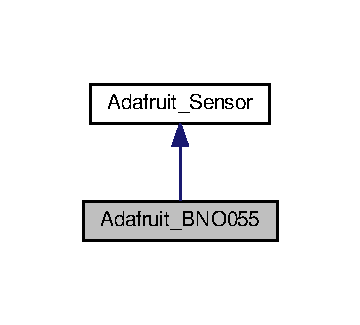
\includegraphics[width=173pt]{classAdafruit__BNO055__inherit__graph}
\end{center}
\end{figure}


Collaboration diagram for Adafruit\+\_\+\+B\+N\+O055\+:
\nopagebreak
\begin{figure}[H]
\begin{center}
\leavevmode
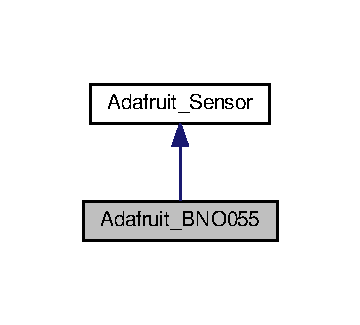
\includegraphics[width=173pt]{classAdafruit__BNO055__coll__graph}
\end{center}
\end{figure}
\subsection*{Classes}
\begin{DoxyCompactItemize}
\item 
struct \hyperlink{structAdafruit__BNO055_1_1adafruit__bno055__rev__info__t}{adafruit\+\_\+bno055\+\_\+rev\+\_\+info\+\_\+t}
\end{DoxyCompactItemize}
\subsection*{Public Types}
\begin{DoxyCompactItemize}
\item 
enum \hyperlink{classAdafruit__BNO055_a37bdd791ec4916fb29933a5b78be0485}{adafruit\+\_\+bno055\+\_\+reg\+\_\+t} \{ \\*
\hyperlink{classAdafruit__BNO055_a37bdd791ec4916fb29933a5b78be0485a4335c5a431c79bdbaa90285529c55ad9}{B\+N\+O055\+\_\+\+P\+A\+G\+E\+\_\+\+I\+D\+\_\+\+A\+D\+DR} = 0\+X07, 
\hyperlink{classAdafruit__BNO055_a37bdd791ec4916fb29933a5b78be0485aa275fa7224eeaf5dee18716a4131e851}{B\+N\+O055\+\_\+\+C\+H\+I\+P\+\_\+\+I\+D\+\_\+\+A\+D\+DR} = 0x00, 
\hyperlink{classAdafruit__BNO055_a37bdd791ec4916fb29933a5b78be0485a149f2f8fc3fce4cfb0aefb815ef00a48}{B\+N\+O055\+\_\+\+A\+C\+C\+E\+L\+\_\+\+R\+E\+V\+\_\+\+I\+D\+\_\+\+A\+D\+DR} = 0x01, 
\hyperlink{classAdafruit__BNO055_a37bdd791ec4916fb29933a5b78be0485a746e1fc48d00c95444cc6842871e1799}{B\+N\+O055\+\_\+\+M\+A\+G\+\_\+\+R\+E\+V\+\_\+\+I\+D\+\_\+\+A\+D\+DR} = 0x02, 
\\*
\hyperlink{classAdafruit__BNO055_a37bdd791ec4916fb29933a5b78be0485ac3e24f4d9b0856d5adf453d48d212229}{B\+N\+O055\+\_\+\+G\+Y\+R\+O\+\_\+\+R\+E\+V\+\_\+\+I\+D\+\_\+\+A\+D\+DR} = 0x03, 
\hyperlink{classAdafruit__BNO055_a37bdd791ec4916fb29933a5b78be0485a6daa86f588765df194d98edcc3507442}{B\+N\+O055\+\_\+\+S\+W\+\_\+\+R\+E\+V\+\_\+\+I\+D\+\_\+\+L\+S\+B\+\_\+\+A\+D\+DR} = 0x04, 
\hyperlink{classAdafruit__BNO055_a37bdd791ec4916fb29933a5b78be0485acdf7f4b1082a3fcbc8d56f59e58ca4cc}{B\+N\+O055\+\_\+\+S\+W\+\_\+\+R\+E\+V\+\_\+\+I\+D\+\_\+\+M\+S\+B\+\_\+\+A\+D\+DR} = 0x05, 
\hyperlink{classAdafruit__BNO055_a37bdd791ec4916fb29933a5b78be0485a099f530e4e69326e7c56b9516bc58ab8}{B\+N\+O055\+\_\+\+B\+L\+\_\+\+R\+E\+V\+\_\+\+I\+D\+\_\+\+A\+D\+DR} = 0\+X06, 
\\*
\hyperlink{classAdafruit__BNO055_a37bdd791ec4916fb29933a5b78be0485a3eec9ae5c1e3ac26884285a04463b5a0}{B\+N\+O055\+\_\+\+A\+C\+C\+E\+L\+\_\+\+D\+A\+T\+A\+\_\+\+X\+\_\+\+L\+S\+B\+\_\+\+A\+D\+DR} = 0\+X08, 
\hyperlink{classAdafruit__BNO055_a37bdd791ec4916fb29933a5b78be0485aed5c07c001912e9747475a3ae7f757f6}{B\+N\+O055\+\_\+\+A\+C\+C\+E\+L\+\_\+\+D\+A\+T\+A\+\_\+\+X\+\_\+\+M\+S\+B\+\_\+\+A\+D\+DR} = 0\+X09, 
\hyperlink{classAdafruit__BNO055_a37bdd791ec4916fb29933a5b78be0485a1a0f230da78da7741f7d084d1ff11c85}{B\+N\+O055\+\_\+\+A\+C\+C\+E\+L\+\_\+\+D\+A\+T\+A\+\_\+\+Y\+\_\+\+L\+S\+B\+\_\+\+A\+D\+DR} = 0\+X0A, 
\hyperlink{classAdafruit__BNO055_a37bdd791ec4916fb29933a5b78be0485a96740da9d72fcc66629ec06b231e7155}{B\+N\+O055\+\_\+\+A\+C\+C\+E\+L\+\_\+\+D\+A\+T\+A\+\_\+\+Y\+\_\+\+M\+S\+B\+\_\+\+A\+D\+DR} = 0\+X0B, 
\\*
\hyperlink{classAdafruit__BNO055_a37bdd791ec4916fb29933a5b78be0485a01bbeb7c8748bc8c8d2fd74d728c441e}{B\+N\+O055\+\_\+\+A\+C\+C\+E\+L\+\_\+\+D\+A\+T\+A\+\_\+\+Z\+\_\+\+L\+S\+B\+\_\+\+A\+D\+DR} = 0\+X0C, 
\hyperlink{classAdafruit__BNO055_a37bdd791ec4916fb29933a5b78be0485a6c1b7b62c2c0ed23a66b7150ba7303d0}{B\+N\+O055\+\_\+\+A\+C\+C\+E\+L\+\_\+\+D\+A\+T\+A\+\_\+\+Z\+\_\+\+M\+S\+B\+\_\+\+A\+D\+DR} = 0\+X0D, 
\hyperlink{classAdafruit__BNO055_a37bdd791ec4916fb29933a5b78be0485a74a340110cfdfa8cee2198101d33b77f}{B\+N\+O055\+\_\+\+M\+A\+G\+\_\+\+D\+A\+T\+A\+\_\+\+X\+\_\+\+L\+S\+B\+\_\+\+A\+D\+DR} = 0\+X0E, 
\hyperlink{classAdafruit__BNO055_a37bdd791ec4916fb29933a5b78be0485abee55ac5b6d232f8f272cbad3418a49d}{B\+N\+O055\+\_\+\+M\+A\+G\+\_\+\+D\+A\+T\+A\+\_\+\+X\+\_\+\+M\+S\+B\+\_\+\+A\+D\+DR} = 0\+X0F, 
\\*
\hyperlink{classAdafruit__BNO055_a37bdd791ec4916fb29933a5b78be0485ad8b1f59d70f8288977b10ab1cf3f271f}{B\+N\+O055\+\_\+\+M\+A\+G\+\_\+\+D\+A\+T\+A\+\_\+\+Y\+\_\+\+L\+S\+B\+\_\+\+A\+D\+DR} = 0\+X10, 
\hyperlink{classAdafruit__BNO055_a37bdd791ec4916fb29933a5b78be0485a327baecdadb03ffa6791ff1798a85353}{B\+N\+O055\+\_\+\+M\+A\+G\+\_\+\+D\+A\+T\+A\+\_\+\+Y\+\_\+\+M\+S\+B\+\_\+\+A\+D\+DR} = 0\+X11, 
\hyperlink{classAdafruit__BNO055_a37bdd791ec4916fb29933a5b78be0485aba0df390c763b57de543b3eab89538d6}{B\+N\+O055\+\_\+\+M\+A\+G\+\_\+\+D\+A\+T\+A\+\_\+\+Z\+\_\+\+L\+S\+B\+\_\+\+A\+D\+DR} = 0\+X12, 
\hyperlink{classAdafruit__BNO055_a37bdd791ec4916fb29933a5b78be0485a8f59e5deeb4839086fc16624c977e934}{B\+N\+O055\+\_\+\+M\+A\+G\+\_\+\+D\+A\+T\+A\+\_\+\+Z\+\_\+\+M\+S\+B\+\_\+\+A\+D\+DR} = 0\+X13, 
\\*
\hyperlink{classAdafruit__BNO055_a37bdd791ec4916fb29933a5b78be0485a270a56500cd5214287b0e95a38f906e1}{B\+N\+O055\+\_\+\+G\+Y\+R\+O\+\_\+\+D\+A\+T\+A\+\_\+\+X\+\_\+\+L\+S\+B\+\_\+\+A\+D\+DR} = 0\+X14, 
\hyperlink{classAdafruit__BNO055_a37bdd791ec4916fb29933a5b78be0485a01f2b6b240d948436fa94a1ce2edf240}{B\+N\+O055\+\_\+\+G\+Y\+R\+O\+\_\+\+D\+A\+T\+A\+\_\+\+X\+\_\+\+M\+S\+B\+\_\+\+A\+D\+DR} = 0\+X15, 
\hyperlink{classAdafruit__BNO055_a37bdd791ec4916fb29933a5b78be0485afc196b018194442a9b2bb96732a07f10}{B\+N\+O055\+\_\+\+G\+Y\+R\+O\+\_\+\+D\+A\+T\+A\+\_\+\+Y\+\_\+\+L\+S\+B\+\_\+\+A\+D\+DR} = 0\+X16, 
\hyperlink{classAdafruit__BNO055_a37bdd791ec4916fb29933a5b78be0485abe31685ab8e47f6b6a1f27455b681b79}{B\+N\+O055\+\_\+\+G\+Y\+R\+O\+\_\+\+D\+A\+T\+A\+\_\+\+Y\+\_\+\+M\+S\+B\+\_\+\+A\+D\+DR} = 0\+X17, 
\\*
\hyperlink{classAdafruit__BNO055_a37bdd791ec4916fb29933a5b78be0485a3b30fae627e7e46a14087af83dfd8d4a}{B\+N\+O055\+\_\+\+G\+Y\+R\+O\+\_\+\+D\+A\+T\+A\+\_\+\+Z\+\_\+\+L\+S\+B\+\_\+\+A\+D\+DR} = 0\+X18, 
\hyperlink{classAdafruit__BNO055_a37bdd791ec4916fb29933a5b78be0485a2e9e8d7a657624f0239b1fced09a2307}{B\+N\+O055\+\_\+\+G\+Y\+R\+O\+\_\+\+D\+A\+T\+A\+\_\+\+Z\+\_\+\+M\+S\+B\+\_\+\+A\+D\+DR} = 0\+X19, 
\hyperlink{classAdafruit__BNO055_a37bdd791ec4916fb29933a5b78be0485ad64633c61f1ba8929e2f65b1bda2254c}{B\+N\+O055\+\_\+\+E\+U\+L\+E\+R\+\_\+\+H\+\_\+\+L\+S\+B\+\_\+\+A\+D\+DR} = 0\+X1A, 
\hyperlink{classAdafruit__BNO055_a37bdd791ec4916fb29933a5b78be0485a37f7984d8007213bc172480e674da53d}{B\+N\+O055\+\_\+\+E\+U\+L\+E\+R\+\_\+\+H\+\_\+\+M\+S\+B\+\_\+\+A\+D\+DR} = 0\+X1B, 
\\*
\hyperlink{classAdafruit__BNO055_a37bdd791ec4916fb29933a5b78be0485a6332dca143b57920f16829ab9753a450}{B\+N\+O055\+\_\+\+E\+U\+L\+E\+R\+\_\+\+R\+\_\+\+L\+S\+B\+\_\+\+A\+D\+DR} = 0\+X1C, 
\hyperlink{classAdafruit__BNO055_a37bdd791ec4916fb29933a5b78be0485a756121c54605abc500d6dc81c6177150}{B\+N\+O055\+\_\+\+E\+U\+L\+E\+R\+\_\+\+R\+\_\+\+M\+S\+B\+\_\+\+A\+D\+DR} = 0\+X1D, 
\hyperlink{classAdafruit__BNO055_a37bdd791ec4916fb29933a5b78be0485a376bfd46c3ed49686bffdb20f8854d29}{B\+N\+O055\+\_\+\+E\+U\+L\+E\+R\+\_\+\+P\+\_\+\+L\+S\+B\+\_\+\+A\+D\+DR} = 0\+X1E, 
\hyperlink{classAdafruit__BNO055_a37bdd791ec4916fb29933a5b78be0485af249fb4963281dd06646ab18b5e7d51f}{B\+N\+O055\+\_\+\+E\+U\+L\+E\+R\+\_\+\+P\+\_\+\+M\+S\+B\+\_\+\+A\+D\+DR} = 0\+X1F, 
\\*
\hyperlink{classAdafruit__BNO055_a37bdd791ec4916fb29933a5b78be0485aaa7d9546054fa74cc8d84028da2de91e}{B\+N\+O055\+\_\+\+Q\+U\+A\+T\+E\+R\+N\+I\+O\+N\+\_\+\+D\+A\+T\+A\+\_\+\+W\+\_\+\+L\+S\+B\+\_\+\+A\+D\+DR} = 0\+X20, 
\hyperlink{classAdafruit__BNO055_a37bdd791ec4916fb29933a5b78be0485a6ebf09724371184d474998af32690bfc}{B\+N\+O055\+\_\+\+Q\+U\+A\+T\+E\+R\+N\+I\+O\+N\+\_\+\+D\+A\+T\+A\+\_\+\+W\+\_\+\+M\+S\+B\+\_\+\+A\+D\+DR} = 0\+X21, 
\hyperlink{classAdafruit__BNO055_a37bdd791ec4916fb29933a5b78be0485a21f3ca8391c91c4f94bc225e8e93590a}{B\+N\+O055\+\_\+\+Q\+U\+A\+T\+E\+R\+N\+I\+O\+N\+\_\+\+D\+A\+T\+A\+\_\+\+X\+\_\+\+L\+S\+B\+\_\+\+A\+D\+DR} = 0\+X22, 
\hyperlink{classAdafruit__BNO055_a37bdd791ec4916fb29933a5b78be0485a7eb2f9da483f396cdaf5997d04024de3}{B\+N\+O055\+\_\+\+Q\+U\+A\+T\+E\+R\+N\+I\+O\+N\+\_\+\+D\+A\+T\+A\+\_\+\+X\+\_\+\+M\+S\+B\+\_\+\+A\+D\+DR} = 0\+X23, 
\\*
\hyperlink{classAdafruit__BNO055_a37bdd791ec4916fb29933a5b78be0485ac91d16d51ddf754e82674c7cd05c7961}{B\+N\+O055\+\_\+\+Q\+U\+A\+T\+E\+R\+N\+I\+O\+N\+\_\+\+D\+A\+T\+A\+\_\+\+Y\+\_\+\+L\+S\+B\+\_\+\+A\+D\+DR} = 0\+X24, 
\hyperlink{classAdafruit__BNO055_a37bdd791ec4916fb29933a5b78be0485a545e6a5c14f42691eb94c3a170fe0e58}{B\+N\+O055\+\_\+\+Q\+U\+A\+T\+E\+R\+N\+I\+O\+N\+\_\+\+D\+A\+T\+A\+\_\+\+Y\+\_\+\+M\+S\+B\+\_\+\+A\+D\+DR} = 0\+X25, 
\hyperlink{classAdafruit__BNO055_a37bdd791ec4916fb29933a5b78be0485a8b0fbf37d2875ebe75d02cd381088dd0}{B\+N\+O055\+\_\+\+Q\+U\+A\+T\+E\+R\+N\+I\+O\+N\+\_\+\+D\+A\+T\+A\+\_\+\+Z\+\_\+\+L\+S\+B\+\_\+\+A\+D\+DR} = 0\+X26, 
\hyperlink{classAdafruit__BNO055_a37bdd791ec4916fb29933a5b78be0485aeaca752822de2be682e2d3aa90719ccf}{B\+N\+O055\+\_\+\+Q\+U\+A\+T\+E\+R\+N\+I\+O\+N\+\_\+\+D\+A\+T\+A\+\_\+\+Z\+\_\+\+M\+S\+B\+\_\+\+A\+D\+DR} = 0\+X27, 
\\*
\hyperlink{classAdafruit__BNO055_a37bdd791ec4916fb29933a5b78be0485a401cdc550521e75a125b9c458a1130e9}{B\+N\+O055\+\_\+\+L\+I\+N\+E\+A\+R\+\_\+\+A\+C\+C\+E\+L\+\_\+\+D\+A\+T\+A\+\_\+\+X\+\_\+\+L\+S\+B\+\_\+\+A\+D\+DR} = 0\+X28, 
\hyperlink{classAdafruit__BNO055_a37bdd791ec4916fb29933a5b78be0485af5f860463f4de5846934cf9ef0eff786}{B\+N\+O055\+\_\+\+L\+I\+N\+E\+A\+R\+\_\+\+A\+C\+C\+E\+L\+\_\+\+D\+A\+T\+A\+\_\+\+X\+\_\+\+M\+S\+B\+\_\+\+A\+D\+DR} = 0\+X29, 
\hyperlink{classAdafruit__BNO055_a37bdd791ec4916fb29933a5b78be0485a74a0688bf1398a3a8b31e9248a93b282}{B\+N\+O055\+\_\+\+L\+I\+N\+E\+A\+R\+\_\+\+A\+C\+C\+E\+L\+\_\+\+D\+A\+T\+A\+\_\+\+Y\+\_\+\+L\+S\+B\+\_\+\+A\+D\+DR} = 0\+X2A, 
\hyperlink{classAdafruit__BNO055_a37bdd791ec4916fb29933a5b78be0485ad0217760f661fabfaf3c20b0beded597}{B\+N\+O055\+\_\+\+L\+I\+N\+E\+A\+R\+\_\+\+A\+C\+C\+E\+L\+\_\+\+D\+A\+T\+A\+\_\+\+Y\+\_\+\+M\+S\+B\+\_\+\+A\+D\+DR} = 0\+X2B, 
\\*
\hyperlink{classAdafruit__BNO055_a37bdd791ec4916fb29933a5b78be0485a61b8e1ec9855716f71be554ede008f2c}{B\+N\+O055\+\_\+\+L\+I\+N\+E\+A\+R\+\_\+\+A\+C\+C\+E\+L\+\_\+\+D\+A\+T\+A\+\_\+\+Z\+\_\+\+L\+S\+B\+\_\+\+A\+D\+DR} = 0\+X2C, 
\hyperlink{classAdafruit__BNO055_a37bdd791ec4916fb29933a5b78be0485ab5094d798297a383266d52c957af640c}{B\+N\+O055\+\_\+\+L\+I\+N\+E\+A\+R\+\_\+\+A\+C\+C\+E\+L\+\_\+\+D\+A\+T\+A\+\_\+\+Z\+\_\+\+M\+S\+B\+\_\+\+A\+D\+DR} = 0\+X2D, 
\hyperlink{classAdafruit__BNO055_a37bdd791ec4916fb29933a5b78be0485a2b026fccd14b8bd074bbac936fc62051}{B\+N\+O055\+\_\+\+G\+R\+A\+V\+I\+T\+Y\+\_\+\+D\+A\+T\+A\+\_\+\+X\+\_\+\+L\+S\+B\+\_\+\+A\+D\+DR} = 0\+X2E, 
\hyperlink{classAdafruit__BNO055_a37bdd791ec4916fb29933a5b78be0485a3ae6282a5d52d11691a28b52da82c61c}{B\+N\+O055\+\_\+\+G\+R\+A\+V\+I\+T\+Y\+\_\+\+D\+A\+T\+A\+\_\+\+X\+\_\+\+M\+S\+B\+\_\+\+A\+D\+DR} = 0\+X2F, 
\\*
\hyperlink{classAdafruit__BNO055_a37bdd791ec4916fb29933a5b78be0485a7c3324352963727f23166ceafdcb01e8}{B\+N\+O055\+\_\+\+G\+R\+A\+V\+I\+T\+Y\+\_\+\+D\+A\+T\+A\+\_\+\+Y\+\_\+\+L\+S\+B\+\_\+\+A\+D\+DR} = 0\+X30, 
\hyperlink{classAdafruit__BNO055_a37bdd791ec4916fb29933a5b78be0485adb200404230c7b63a9ae0048882d10c0}{B\+N\+O055\+\_\+\+G\+R\+A\+V\+I\+T\+Y\+\_\+\+D\+A\+T\+A\+\_\+\+Y\+\_\+\+M\+S\+B\+\_\+\+A\+D\+DR} = 0\+X31, 
\hyperlink{classAdafruit__BNO055_a37bdd791ec4916fb29933a5b78be0485aec7ea2d6e3c15e440f1cdb12692517d7}{B\+N\+O055\+\_\+\+G\+R\+A\+V\+I\+T\+Y\+\_\+\+D\+A\+T\+A\+\_\+\+Z\+\_\+\+L\+S\+B\+\_\+\+A\+D\+DR} = 0\+X32, 
\hyperlink{classAdafruit__BNO055_a37bdd791ec4916fb29933a5b78be0485aff6c1ab944302edba37689e06a22e424}{B\+N\+O055\+\_\+\+G\+R\+A\+V\+I\+T\+Y\+\_\+\+D\+A\+T\+A\+\_\+\+Z\+\_\+\+M\+S\+B\+\_\+\+A\+D\+DR} = 0\+X33, 
\\*
\hyperlink{classAdafruit__BNO055_a37bdd791ec4916fb29933a5b78be0485a4a72b5554806edfc051b59a387d3bd57}{B\+N\+O055\+\_\+\+T\+E\+M\+P\+\_\+\+A\+D\+DR} = 0\+X34, 
\hyperlink{classAdafruit__BNO055_a37bdd791ec4916fb29933a5b78be0485a48c8b7d04d47aedf7dbcb0bc34d1adea}{B\+N\+O055\+\_\+\+C\+A\+L\+I\+B\+\_\+\+S\+T\+A\+T\+\_\+\+A\+D\+DR} = 0\+X35, 
\hyperlink{classAdafruit__BNO055_a37bdd791ec4916fb29933a5b78be0485ab136291bff48f7d6ac0b594da19ca66b}{B\+N\+O055\+\_\+\+S\+E\+L\+F\+T\+E\+S\+T\+\_\+\+R\+E\+S\+U\+L\+T\+\_\+\+A\+D\+DR} = 0\+X36, 
\hyperlink{classAdafruit__BNO055_a37bdd791ec4916fb29933a5b78be0485a8175047d1963d83affff3a32ea40ee23}{B\+N\+O055\+\_\+\+I\+N\+T\+R\+\_\+\+S\+T\+A\+T\+\_\+\+A\+D\+DR} = 0\+X37, 
\\*
\hyperlink{classAdafruit__BNO055_a37bdd791ec4916fb29933a5b78be0485a02cb584cb6378481ca9c25ffb3821f18}{B\+N\+O055\+\_\+\+S\+Y\+S\+\_\+\+C\+L\+K\+\_\+\+S\+T\+A\+T\+\_\+\+A\+D\+DR} = 0\+X38, 
\hyperlink{classAdafruit__BNO055_a37bdd791ec4916fb29933a5b78be0485ad48a64ee8f956b33f1b75b9dbb6a8512}{B\+N\+O055\+\_\+\+S\+Y\+S\+\_\+\+S\+T\+A\+T\+\_\+\+A\+D\+DR} = 0\+X39, 
\hyperlink{classAdafruit__BNO055_a37bdd791ec4916fb29933a5b78be0485a97b93ee49ef0ea754c1e0a92ee5cf9ab}{B\+N\+O055\+\_\+\+S\+Y\+S\+\_\+\+E\+R\+R\+\_\+\+A\+D\+DR} = 0\+X3A, 
\hyperlink{classAdafruit__BNO055_a37bdd791ec4916fb29933a5b78be0485a20338b0135c683192b19c5977c433c74}{B\+N\+O055\+\_\+\+U\+N\+I\+T\+\_\+\+S\+E\+L\+\_\+\+A\+D\+DR} = 0\+X3B, 
\\*
\hyperlink{classAdafruit__BNO055_a37bdd791ec4916fb29933a5b78be0485aaa731a4abc302c65dd00653ea5194682}{B\+N\+O055\+\_\+\+D\+A\+T\+A\+\_\+\+S\+E\+L\+E\+C\+T\+\_\+\+A\+D\+DR} = 0\+X3C, 
\hyperlink{classAdafruit__BNO055_a37bdd791ec4916fb29933a5b78be0485ac04456f6b816356de9c9ffc7d0f328b1}{B\+N\+O055\+\_\+\+O\+P\+R\+\_\+\+M\+O\+D\+E\+\_\+\+A\+D\+DR} = 0\+X3D, 
\hyperlink{classAdafruit__BNO055_a37bdd791ec4916fb29933a5b78be0485a8796ceaf4ce33b9bd553c0bd77ec6cfa}{B\+N\+O055\+\_\+\+P\+W\+R\+\_\+\+M\+O\+D\+E\+\_\+\+A\+D\+DR} = 0\+X3E, 
\hyperlink{classAdafruit__BNO055_a37bdd791ec4916fb29933a5b78be0485acce68cf3512455d31a574820832f7d21}{B\+N\+O055\+\_\+\+S\+Y\+S\+\_\+\+T\+R\+I\+G\+G\+E\+R\+\_\+\+A\+D\+DR} = 0\+X3F, 
\\*
\hyperlink{classAdafruit__BNO055_a37bdd791ec4916fb29933a5b78be0485ae808e91f7177a54d939d334dd7744cf1}{B\+N\+O055\+\_\+\+T\+E\+M\+P\+\_\+\+S\+O\+U\+R\+C\+E\+\_\+\+A\+D\+DR} = 0\+X40, 
\hyperlink{classAdafruit__BNO055_a37bdd791ec4916fb29933a5b78be0485a3049c470d3a481198488cf2f663a6074}{B\+N\+O055\+\_\+\+A\+X\+I\+S\+\_\+\+M\+A\+P\+\_\+\+C\+O\+N\+F\+I\+G\+\_\+\+A\+D\+DR} = 0\+X41, 
\hyperlink{classAdafruit__BNO055_a37bdd791ec4916fb29933a5b78be0485a13c8e7798197d4a92ee1fe5c54c5f62e}{B\+N\+O055\+\_\+\+A\+X\+I\+S\+\_\+\+M\+A\+P\+\_\+\+S\+I\+G\+N\+\_\+\+A\+D\+DR} = 0\+X42, 
\hyperlink{classAdafruit__BNO055_a37bdd791ec4916fb29933a5b78be0485a277c5f87b88608f0d67156902e8e4c49}{B\+N\+O055\+\_\+\+S\+I\+C\+\_\+\+M\+A\+T\+R\+I\+X\+\_\+0\+\_\+\+L\+S\+B\+\_\+\+A\+D\+DR} = 0\+X43, 
\\*
\hyperlink{classAdafruit__BNO055_a37bdd791ec4916fb29933a5b78be0485a8de4bd54412e0c83a69afdc133f2b67c}{B\+N\+O055\+\_\+\+S\+I\+C\+\_\+\+M\+A\+T\+R\+I\+X\+\_\+0\+\_\+\+M\+S\+B\+\_\+\+A\+D\+DR} = 0\+X44, 
\hyperlink{classAdafruit__BNO055_a37bdd791ec4916fb29933a5b78be0485a6c14a9bc4b62fdd6f5a04e2f62f67450}{B\+N\+O055\+\_\+\+S\+I\+C\+\_\+\+M\+A\+T\+R\+I\+X\+\_\+1\+\_\+\+L\+S\+B\+\_\+\+A\+D\+DR} = 0\+X45, 
\hyperlink{classAdafruit__BNO055_a37bdd791ec4916fb29933a5b78be0485a2c8c6710f3a9c3886e2d08f35349294a}{B\+N\+O055\+\_\+\+S\+I\+C\+\_\+\+M\+A\+T\+R\+I\+X\+\_\+1\+\_\+\+M\+S\+B\+\_\+\+A\+D\+DR} = 0\+X46, 
\hyperlink{classAdafruit__BNO055_a37bdd791ec4916fb29933a5b78be0485a269a0d34a06b7c50fa18b36de61139ff}{B\+N\+O055\+\_\+\+S\+I\+C\+\_\+\+M\+A\+T\+R\+I\+X\+\_\+2\+\_\+\+L\+S\+B\+\_\+\+A\+D\+DR} = 0\+X47, 
\\*
\hyperlink{classAdafruit__BNO055_a37bdd791ec4916fb29933a5b78be0485ae4e393f0e82ca0b5ef78956b2fd472f4}{B\+N\+O055\+\_\+\+S\+I\+C\+\_\+\+M\+A\+T\+R\+I\+X\+\_\+2\+\_\+\+M\+S\+B\+\_\+\+A\+D\+DR} = 0\+X48, 
\hyperlink{classAdafruit__BNO055_a37bdd791ec4916fb29933a5b78be0485a45e8f4cab9f41d41d595da04a41f646c}{B\+N\+O055\+\_\+\+S\+I\+C\+\_\+\+M\+A\+T\+R\+I\+X\+\_\+3\+\_\+\+L\+S\+B\+\_\+\+A\+D\+DR} = 0\+X49, 
\hyperlink{classAdafruit__BNO055_a37bdd791ec4916fb29933a5b78be0485a429768195916acbb17d564b42f75a378}{B\+N\+O055\+\_\+\+S\+I\+C\+\_\+\+M\+A\+T\+R\+I\+X\+\_\+3\+\_\+\+M\+S\+B\+\_\+\+A\+D\+DR} = 0\+X4A, 
\hyperlink{classAdafruit__BNO055_a37bdd791ec4916fb29933a5b78be0485acd90c3ff1db748a26e063e1dddfa31e6}{B\+N\+O055\+\_\+\+S\+I\+C\+\_\+\+M\+A\+T\+R\+I\+X\+\_\+4\+\_\+\+L\+S\+B\+\_\+\+A\+D\+DR} = 0\+X4B, 
\\*
\hyperlink{classAdafruit__BNO055_a37bdd791ec4916fb29933a5b78be0485aa13d2f6f97aa439c20c10da8ecbb939a}{B\+N\+O055\+\_\+\+S\+I\+C\+\_\+\+M\+A\+T\+R\+I\+X\+\_\+4\+\_\+\+M\+S\+B\+\_\+\+A\+D\+DR} = 0\+X4C, 
\hyperlink{classAdafruit__BNO055_a37bdd791ec4916fb29933a5b78be0485a68888cdf8631ef9a5730e440d22ccdf8}{B\+N\+O055\+\_\+\+S\+I\+C\+\_\+\+M\+A\+T\+R\+I\+X\+\_\+5\+\_\+\+L\+S\+B\+\_\+\+A\+D\+DR} = 0\+X4D, 
\hyperlink{classAdafruit__BNO055_a37bdd791ec4916fb29933a5b78be0485af4bbb8c54001f70f042c2b177d5105c0}{B\+N\+O055\+\_\+\+S\+I\+C\+\_\+\+M\+A\+T\+R\+I\+X\+\_\+5\+\_\+\+M\+S\+B\+\_\+\+A\+D\+DR} = 0\+X4E, 
\hyperlink{classAdafruit__BNO055_a37bdd791ec4916fb29933a5b78be0485a3f724412df24569625bae17d7a306108}{B\+N\+O055\+\_\+\+S\+I\+C\+\_\+\+M\+A\+T\+R\+I\+X\+\_\+6\+\_\+\+L\+S\+B\+\_\+\+A\+D\+DR} = 0\+X4F, 
\\*
\hyperlink{classAdafruit__BNO055_a37bdd791ec4916fb29933a5b78be0485a1a2a7c04e1bf22d8217c04c39dd628b5}{B\+N\+O055\+\_\+\+S\+I\+C\+\_\+\+M\+A\+T\+R\+I\+X\+\_\+6\+\_\+\+M\+S\+B\+\_\+\+A\+D\+DR} = 0\+X50, 
\hyperlink{classAdafruit__BNO055_a37bdd791ec4916fb29933a5b78be0485aa381f9bc320ce3d4c08f4dad9d50abe2}{B\+N\+O055\+\_\+\+S\+I\+C\+\_\+\+M\+A\+T\+R\+I\+X\+\_\+7\+\_\+\+L\+S\+B\+\_\+\+A\+D\+DR} = 0\+X51, 
\hyperlink{classAdafruit__BNO055_a37bdd791ec4916fb29933a5b78be0485a40ae97b7686a7f3b0d3dfae1befa0b9d}{B\+N\+O055\+\_\+\+S\+I\+C\+\_\+\+M\+A\+T\+R\+I\+X\+\_\+7\+\_\+\+M\+S\+B\+\_\+\+A\+D\+DR} = 0\+X52, 
\hyperlink{classAdafruit__BNO055_a37bdd791ec4916fb29933a5b78be0485a16984212653726337ffef8dc676fecfc}{B\+N\+O055\+\_\+\+S\+I\+C\+\_\+\+M\+A\+T\+R\+I\+X\+\_\+8\+\_\+\+L\+S\+B\+\_\+\+A\+D\+DR} = 0\+X53, 
\\*
\hyperlink{classAdafruit__BNO055_a37bdd791ec4916fb29933a5b78be0485acd02e469aecce234f301c2dfd4da2ed6}{B\+N\+O055\+\_\+\+S\+I\+C\+\_\+\+M\+A\+T\+R\+I\+X\+\_\+8\+\_\+\+M\+S\+B\+\_\+\+A\+D\+DR} = 0\+X54, 
\hyperlink{classAdafruit__BNO055_a37bdd791ec4916fb29933a5b78be0485a355e8ebc21269e6622a39796d60dbad5}{A\+C\+C\+E\+L\+\_\+\+O\+F\+F\+S\+E\+T\+\_\+\+X\+\_\+\+L\+S\+B\+\_\+\+A\+D\+DR} = 0\+X55, 
\hyperlink{classAdafruit__BNO055_a37bdd791ec4916fb29933a5b78be0485ab879121437e4fa4ddc2860cdd7bf3adf}{A\+C\+C\+E\+L\+\_\+\+O\+F\+F\+S\+E\+T\+\_\+\+X\+\_\+\+M\+S\+B\+\_\+\+A\+D\+DR} = 0\+X56, 
\hyperlink{classAdafruit__BNO055_a37bdd791ec4916fb29933a5b78be0485a06f50b821ad2520459e8092054a8b73a}{A\+C\+C\+E\+L\+\_\+\+O\+F\+F\+S\+E\+T\+\_\+\+Y\+\_\+\+L\+S\+B\+\_\+\+A\+D\+DR} = 0\+X57, 
\\*
\hyperlink{classAdafruit__BNO055_a37bdd791ec4916fb29933a5b78be0485af68acdeca7fdd2f62b82d269f7337975}{A\+C\+C\+E\+L\+\_\+\+O\+F\+F\+S\+E\+T\+\_\+\+Y\+\_\+\+M\+S\+B\+\_\+\+A\+D\+DR} = 0\+X58, 
\hyperlink{classAdafruit__BNO055_a37bdd791ec4916fb29933a5b78be0485afe669b51b1a24ec855cade38dd90c14f}{A\+C\+C\+E\+L\+\_\+\+O\+F\+F\+S\+E\+T\+\_\+\+Z\+\_\+\+L\+S\+B\+\_\+\+A\+D\+DR} = 0\+X59, 
\hyperlink{classAdafruit__BNO055_a37bdd791ec4916fb29933a5b78be0485a3e83f024a1cd15203011c9fb6ff82c20}{A\+C\+C\+E\+L\+\_\+\+O\+F\+F\+S\+E\+T\+\_\+\+Z\+\_\+\+M\+S\+B\+\_\+\+A\+D\+DR} = 0\+X5A, 
\hyperlink{classAdafruit__BNO055_a37bdd791ec4916fb29933a5b78be0485a5f08403caae91da3c1400663d0a699d9}{M\+A\+G\+\_\+\+O\+F\+F\+S\+E\+T\+\_\+\+X\+\_\+\+L\+S\+B\+\_\+\+A\+D\+DR} = 0\+X5B, 
\\*
\hyperlink{classAdafruit__BNO055_a37bdd791ec4916fb29933a5b78be0485a821605b292b685e8a1adaa8c47e51f82}{M\+A\+G\+\_\+\+O\+F\+F\+S\+E\+T\+\_\+\+X\+\_\+\+M\+S\+B\+\_\+\+A\+D\+DR} = 0\+X5C, 
\hyperlink{classAdafruit__BNO055_a37bdd791ec4916fb29933a5b78be0485a70945d5d295324d9d51e72de2a53627b}{M\+A\+G\+\_\+\+O\+F\+F\+S\+E\+T\+\_\+\+Y\+\_\+\+L\+S\+B\+\_\+\+A\+D\+DR} = 0\+X5D, 
\hyperlink{classAdafruit__BNO055_a37bdd791ec4916fb29933a5b78be0485a4d1a875e3f6d2cf79bb54d5ac0ac2f33}{M\+A\+G\+\_\+\+O\+F\+F\+S\+E\+T\+\_\+\+Y\+\_\+\+M\+S\+B\+\_\+\+A\+D\+DR} = 0\+X5E, 
\hyperlink{classAdafruit__BNO055_a37bdd791ec4916fb29933a5b78be0485acbd993f302ad780c35962b82627f4354}{M\+A\+G\+\_\+\+O\+F\+F\+S\+E\+T\+\_\+\+Z\+\_\+\+L\+S\+B\+\_\+\+A\+D\+DR} = 0\+X5F, 
\\*
\hyperlink{classAdafruit__BNO055_a37bdd791ec4916fb29933a5b78be0485a7d306e69d9028202556b60ec7aac5495}{M\+A\+G\+\_\+\+O\+F\+F\+S\+E\+T\+\_\+\+Z\+\_\+\+M\+S\+B\+\_\+\+A\+D\+DR} = 0\+X60, 
\hyperlink{classAdafruit__BNO055_a37bdd791ec4916fb29933a5b78be0485a27cee1097050facde2ff2a8cbfa97208}{G\+Y\+R\+O\+\_\+\+O\+F\+F\+S\+E\+T\+\_\+\+X\+\_\+\+L\+S\+B\+\_\+\+A\+D\+DR} = 0\+X61, 
\hyperlink{classAdafruit__BNO055_a37bdd791ec4916fb29933a5b78be0485a4c76d89b177bd0f11545e11236c8639b}{G\+Y\+R\+O\+\_\+\+O\+F\+F\+S\+E\+T\+\_\+\+X\+\_\+\+M\+S\+B\+\_\+\+A\+D\+DR} = 0\+X62, 
\hyperlink{classAdafruit__BNO055_a37bdd791ec4916fb29933a5b78be0485a3df1fb42f0a6124038a9363d730c05d8}{G\+Y\+R\+O\+\_\+\+O\+F\+F\+S\+E\+T\+\_\+\+Y\+\_\+\+L\+S\+B\+\_\+\+A\+D\+DR} = 0\+X63, 
\\*
\hyperlink{classAdafruit__BNO055_a37bdd791ec4916fb29933a5b78be0485a7fd08ded7a83052ab3c4a52ca9bcfa35}{G\+Y\+R\+O\+\_\+\+O\+F\+F\+S\+E\+T\+\_\+\+Y\+\_\+\+M\+S\+B\+\_\+\+A\+D\+DR} = 0\+X64, 
\hyperlink{classAdafruit__BNO055_a37bdd791ec4916fb29933a5b78be0485a81c2b9e5ecc14b329c0a21d6e363c8c7}{G\+Y\+R\+O\+\_\+\+O\+F\+F\+S\+E\+T\+\_\+\+Z\+\_\+\+L\+S\+B\+\_\+\+A\+D\+DR} = 0\+X65, 
\hyperlink{classAdafruit__BNO055_a37bdd791ec4916fb29933a5b78be0485a8927bab6ef05496739e3f54e866df55b}{G\+Y\+R\+O\+\_\+\+O\+F\+F\+S\+E\+T\+\_\+\+Z\+\_\+\+M\+S\+B\+\_\+\+A\+D\+DR} = 0\+X66, 
\hyperlink{classAdafruit__BNO055_a37bdd791ec4916fb29933a5b78be0485a367bdee20e01c777c2e6c760523b800e}{A\+C\+C\+E\+L\+\_\+\+R\+A\+D\+I\+U\+S\+\_\+\+L\+S\+B\+\_\+\+A\+D\+DR} = 0\+X67, 
\\*
\hyperlink{classAdafruit__BNO055_a37bdd791ec4916fb29933a5b78be0485a4bce0759850a331000a48cdd0490403f}{A\+C\+C\+E\+L\+\_\+\+R\+A\+D\+I\+U\+S\+\_\+\+M\+S\+B\+\_\+\+A\+D\+DR} = 0\+X68, 
\hyperlink{classAdafruit__BNO055_a37bdd791ec4916fb29933a5b78be0485aadc1cd6166e834e0e58c496b21260e56}{M\+A\+G\+\_\+\+R\+A\+D\+I\+U\+S\+\_\+\+L\+S\+B\+\_\+\+A\+D\+DR} = 0\+X69, 
\hyperlink{classAdafruit__BNO055_a37bdd791ec4916fb29933a5b78be0485a8b021b2977145e0c7fd1c006983380d3}{M\+A\+G\+\_\+\+R\+A\+D\+I\+U\+S\+\_\+\+M\+S\+B\+\_\+\+A\+D\+DR} = 0\+X6A
 \}
\item 
enum \hyperlink{classAdafruit__BNO055_ae61dcad8ce3c5e6ffd701011cf75ca4a}{adafruit\+\_\+bno055\+\_\+powermode\+\_\+t} \{ \hyperlink{classAdafruit__BNO055_ae61dcad8ce3c5e6ffd701011cf75ca4aa460773e8dd4c41a8328260ebdd0911d6}{P\+O\+W\+E\+R\+\_\+\+M\+O\+D\+E\+\_\+\+N\+O\+R\+M\+AL} = 0\+X00, 
\hyperlink{classAdafruit__BNO055_ae61dcad8ce3c5e6ffd701011cf75ca4aa3793d3ac7ca6a2935624bbaba817eacf}{P\+O\+W\+E\+R\+\_\+\+M\+O\+D\+E\+\_\+\+L\+O\+W\+P\+O\+W\+ER} = 0\+X01, 
\hyperlink{classAdafruit__BNO055_ae61dcad8ce3c5e6ffd701011cf75ca4aae81c9f7bed51e3d51440a7c9b0c1c279}{P\+O\+W\+E\+R\+\_\+\+M\+O\+D\+E\+\_\+\+S\+U\+S\+P\+E\+ND} = 0\+X02
 \}
\item 
enum \hyperlink{classAdafruit__BNO055_a1288643630f474aba977e4b1aa34456f}{adafruit\+\_\+bno055\+\_\+opmode\+\_\+t} \{ \\*
\hyperlink{classAdafruit__BNO055_a1288643630f474aba977e4b1aa34456fa155bb4a42e3b4e5afcccc2c03826b96d}{O\+P\+E\+R\+A\+T\+I\+O\+N\+\_\+\+M\+O\+D\+E\+\_\+\+C\+O\+N\+F\+IG} = 0\+X00, 
\hyperlink{classAdafruit__BNO055_a1288643630f474aba977e4b1aa34456fa8f203109f6e08ea5bcb41ab54dd78cd4}{O\+P\+E\+R\+A\+T\+I\+O\+N\+\_\+\+M\+O\+D\+E\+\_\+\+A\+C\+C\+O\+N\+LY} = 0\+X01, 
\hyperlink{classAdafruit__BNO055_a1288643630f474aba977e4b1aa34456fad952ddf383c28de87203eaaad6b3e3e3}{O\+P\+E\+R\+A\+T\+I\+O\+N\+\_\+\+M\+O\+D\+E\+\_\+\+M\+A\+G\+O\+N\+LY} = 0\+X02, 
\hyperlink{classAdafruit__BNO055_a1288643630f474aba977e4b1aa34456fad0188a6d093269ea90aaaffa22e6ca6c}{O\+P\+E\+R\+A\+T\+I\+O\+N\+\_\+\+M\+O\+D\+E\+\_\+\+G\+Y\+R\+O\+N\+LY} = 0\+X03, 
\\*
\hyperlink{classAdafruit__BNO055_a1288643630f474aba977e4b1aa34456fae7b4432a87b21598f23c741c2d505ea4}{O\+P\+E\+R\+A\+T\+I\+O\+N\+\_\+\+M\+O\+D\+E\+\_\+\+A\+C\+C\+M\+AG} = 0\+X04, 
\hyperlink{classAdafruit__BNO055_a1288643630f474aba977e4b1aa34456faafbedaef065fd0f91f50f361b6390492}{O\+P\+E\+R\+A\+T\+I\+O\+N\+\_\+\+M\+O\+D\+E\+\_\+\+A\+C\+C\+G\+Y\+RO} = 0\+X05, 
\hyperlink{classAdafruit__BNO055_a1288643630f474aba977e4b1aa34456fad72d05ef92677db29066f5378756889b}{O\+P\+E\+R\+A\+T\+I\+O\+N\+\_\+\+M\+O\+D\+E\+\_\+\+M\+A\+G\+G\+Y\+RO} = 0\+X06, 
\hyperlink{classAdafruit__BNO055_a1288643630f474aba977e4b1aa34456fa660e0108467f0ea5c870f56c63bef640}{O\+P\+E\+R\+A\+T\+I\+O\+N\+\_\+\+M\+O\+D\+E\+\_\+\+A\+MG} = 0\+X07, 
\\*
\hyperlink{classAdafruit__BNO055_a1288643630f474aba977e4b1aa34456fa3bbe664efb9d7f9d80d20fc86b33f07f}{O\+P\+E\+R\+A\+T\+I\+O\+N\+\_\+\+M\+O\+D\+E\+\_\+\+I\+M\+U\+P\+L\+US} = 0\+X08, 
\hyperlink{classAdafruit__BNO055_a1288643630f474aba977e4b1aa34456fab11e169be1995261b4327cf5f14edb43}{O\+P\+E\+R\+A\+T\+I\+O\+N\+\_\+\+M\+O\+D\+E\+\_\+\+C\+O\+M\+P\+A\+SS} = 0\+X09, 
\hyperlink{classAdafruit__BNO055_a1288643630f474aba977e4b1aa34456faab8557f93c86cdbf42b2ddf974914f9e}{O\+P\+E\+R\+A\+T\+I\+O\+N\+\_\+\+M\+O\+D\+E\+\_\+\+M4G} = 0\+X0A, 
\hyperlink{classAdafruit__BNO055_a1288643630f474aba977e4b1aa34456faeb24103996e52515df04fb244c7a886c}{O\+P\+E\+R\+A\+T\+I\+O\+N\+\_\+\+M\+O\+D\+E\+\_\+\+N\+D\+O\+F\+\_\+\+F\+M\+C\+\_\+\+O\+FF} = 0\+X0B, 
\\*
\hyperlink{classAdafruit__BNO055_a1288643630f474aba977e4b1aa34456fa6ff2e99593b4ccefa7315c08df794405}{O\+P\+E\+R\+A\+T\+I\+O\+N\+\_\+\+M\+O\+D\+E\+\_\+\+N\+D\+OF} = 0\+X0C
 \}
\item 
enum \hyperlink{classAdafruit__BNO055_a14148c0000d1f13e4438c6dca1e386f2}{adafruit\+\_\+bno055\+\_\+axis\+\_\+remap\+\_\+config\+\_\+t} \{ \\*
\hyperlink{classAdafruit__BNO055_a14148c0000d1f13e4438c6dca1e386f2a8e817092a5d22121af7f86bf93180747}{R\+E\+M\+A\+P\+\_\+\+C\+O\+N\+F\+I\+G\+\_\+\+P0} = 0x21, 
\hyperlink{classAdafruit__BNO055_a14148c0000d1f13e4438c6dca1e386f2a0c30da353c8ed59f5a1cf075a8e8ceba}{R\+E\+M\+A\+P\+\_\+\+C\+O\+N\+F\+I\+G\+\_\+\+P1} = 0x24, 
\hyperlink{classAdafruit__BNO055_a14148c0000d1f13e4438c6dca1e386f2af3ef7ad245f765374601269b41991382}{R\+E\+M\+A\+P\+\_\+\+C\+O\+N\+F\+I\+G\+\_\+\+P2} = 0x24, 
\hyperlink{classAdafruit__BNO055_a14148c0000d1f13e4438c6dca1e386f2a6486a669c1c0804a91f71c20061199b7}{R\+E\+M\+A\+P\+\_\+\+C\+O\+N\+F\+I\+G\+\_\+\+P3} = 0x21, 
\\*
\hyperlink{classAdafruit__BNO055_a14148c0000d1f13e4438c6dca1e386f2aa588d28a9820c0245711cde409b23b45}{R\+E\+M\+A\+P\+\_\+\+C\+O\+N\+F\+I\+G\+\_\+\+P4} = 0x24, 
\hyperlink{classAdafruit__BNO055_a14148c0000d1f13e4438c6dca1e386f2a1b4d622113e09fdae9c1bb26f382da93}{R\+E\+M\+A\+P\+\_\+\+C\+O\+N\+F\+I\+G\+\_\+\+P5} = 0x21, 
\hyperlink{classAdafruit__BNO055_a14148c0000d1f13e4438c6dca1e386f2a8a40b7bb1ac85d97f6aa5c2992d9508b}{R\+E\+M\+A\+P\+\_\+\+C\+O\+N\+F\+I\+G\+\_\+\+P6} = 0x21, 
\hyperlink{classAdafruit__BNO055_a14148c0000d1f13e4438c6dca1e386f2a2c855fbe9e915b8f846d2fb76595fee9}{R\+E\+M\+A\+P\+\_\+\+C\+O\+N\+F\+I\+G\+\_\+\+P7} = 0x24
 \}
\item 
enum \hyperlink{classAdafruit__BNO055_a2456a57a97fb940f07b08319580b2e2f}{adafruit\+\_\+bno055\+\_\+axis\+\_\+remap\+\_\+sign\+\_\+t} \{ \\*
\hyperlink{classAdafruit__BNO055_a2456a57a97fb940f07b08319580b2e2fa5404965af5a7b32681f3bb1027e68353}{R\+E\+M\+A\+P\+\_\+\+S\+I\+G\+N\+\_\+\+P0} = 0x04, 
\hyperlink{classAdafruit__BNO055_a2456a57a97fb940f07b08319580b2e2faced743dfcd5f5bf5e9a41be47eb8cb67}{R\+E\+M\+A\+P\+\_\+\+S\+I\+G\+N\+\_\+\+P1} = 0x00, 
\hyperlink{classAdafruit__BNO055_a2456a57a97fb940f07b08319580b2e2fa8da49877f98a9ee4edde173216cce8e3}{R\+E\+M\+A\+P\+\_\+\+S\+I\+G\+N\+\_\+\+P2} = 0x06, 
\hyperlink{classAdafruit__BNO055_a2456a57a97fb940f07b08319580b2e2fa9028255038e953d91171b3840c5191c9}{R\+E\+M\+A\+P\+\_\+\+S\+I\+G\+N\+\_\+\+P3} = 0x02, 
\\*
\hyperlink{classAdafruit__BNO055_a2456a57a97fb940f07b08319580b2e2fa05d7712bc1c8d3b3e1aac382e5d21eb3}{R\+E\+M\+A\+P\+\_\+\+S\+I\+G\+N\+\_\+\+P4} = 0x03, 
\hyperlink{classAdafruit__BNO055_a2456a57a97fb940f07b08319580b2e2fad1bbfd659ea8e2dbdf957a26381ec771}{R\+E\+M\+A\+P\+\_\+\+S\+I\+G\+N\+\_\+\+P5} = 0x01, 
\hyperlink{classAdafruit__BNO055_a2456a57a97fb940f07b08319580b2e2fab725b0e2dc1b7d7feabb20dc8e4376c3}{R\+E\+M\+A\+P\+\_\+\+S\+I\+G\+N\+\_\+\+P6} = 0x07, 
\hyperlink{classAdafruit__BNO055_a2456a57a97fb940f07b08319580b2e2faff37eaad5a9abf43dee7059b22ab9c38}{R\+E\+M\+A\+P\+\_\+\+S\+I\+G\+N\+\_\+\+P7} = 0x05
 \}
\item 
enum \hyperlink{classAdafruit__BNO055_aca6c5acffc9a752e5309ff2bb21f3e25}{adafruit\+\_\+vector\+\_\+type\+\_\+t} \{ \\*
\hyperlink{classAdafruit__BNO055_aca6c5acffc9a752e5309ff2bb21f3e25a7683862660e6744c7b986635b8a1c275}{V\+E\+C\+T\+O\+R\+\_\+\+A\+C\+C\+E\+L\+E\+R\+O\+M\+E\+T\+ER} = B\+N\+O055\+\_\+\+A\+C\+C\+E\+L\+\_\+\+D\+A\+T\+A\+\_\+\+X\+\_\+\+L\+S\+B\+\_\+\+A\+D\+DR, 
\hyperlink{classAdafruit__BNO055_aca6c5acffc9a752e5309ff2bb21f3e25a1c60f2563c7ef6aae996bebed41081bd}{V\+E\+C\+T\+O\+R\+\_\+\+M\+A\+G\+N\+E\+T\+O\+M\+E\+T\+ER} = B\+N\+O055\+\_\+\+M\+A\+G\+\_\+\+D\+A\+T\+A\+\_\+\+X\+\_\+\+L\+S\+B\+\_\+\+A\+D\+DR, 
\hyperlink{classAdafruit__BNO055_aca6c5acffc9a752e5309ff2bb21f3e25a02367b4ed33bd911181d1fb0c1ceb1f0}{V\+E\+C\+T\+O\+R\+\_\+\+G\+Y\+R\+O\+S\+C\+O\+PE} = B\+N\+O055\+\_\+\+G\+Y\+R\+O\+\_\+\+D\+A\+T\+A\+\_\+\+X\+\_\+\+L\+S\+B\+\_\+\+A\+D\+DR, 
\hyperlink{classAdafruit__BNO055_aca6c5acffc9a752e5309ff2bb21f3e25af512e6567f6decb1c18af65b5cb1d539}{V\+E\+C\+T\+O\+R\+\_\+\+E\+U\+L\+ER} = B\+N\+O055\+\_\+\+E\+U\+L\+E\+R\+\_\+\+H\+\_\+\+L\+S\+B\+\_\+\+A\+D\+DR, 
\\*
\hyperlink{classAdafruit__BNO055_aca6c5acffc9a752e5309ff2bb21f3e25a8bef16d23fcf2d87d568273a1c1d022d}{V\+E\+C\+T\+O\+R\+\_\+\+L\+I\+N\+E\+A\+R\+A\+C\+C\+EL} = B\+N\+O055\+\_\+\+L\+I\+N\+E\+A\+R\+\_\+\+A\+C\+C\+E\+L\+\_\+\+D\+A\+T\+A\+\_\+\+X\+\_\+\+L\+S\+B\+\_\+\+A\+D\+DR, 
\hyperlink{classAdafruit__BNO055_aca6c5acffc9a752e5309ff2bb21f3e25a0bcfa0920b42abb820f6a4563cb4ef08}{V\+E\+C\+T\+O\+R\+\_\+\+G\+R\+A\+V\+I\+TY} = B\+N\+O055\+\_\+\+G\+R\+A\+V\+I\+T\+Y\+\_\+\+D\+A\+T\+A\+\_\+\+X\+\_\+\+L\+S\+B\+\_\+\+A\+D\+DR
 \}
\end{DoxyCompactItemize}
\subsection*{Public Member Functions}
\begin{DoxyCompactItemize}
\item 
\hyperlink{classAdafruit__BNO055_a8aa7f36e4a0c4040c453ab55899bdd87}{Adafruit\+\_\+\+B\+N\+O055} (int32\+\_\+t sensor\+ID=-\/1, uint8\+\_\+t address=\hyperlink{Adafruit__BNO055_8h_ac3cdd930d950b35e2041e394d5f44693}{B\+N\+O055\+\_\+\+A\+D\+D\+R\+E\+S\+S\+\_\+A})
\begin{DoxyCompactList}\small\item\em Instantiates a new \hyperlink{classAdafruit__BNO055}{Adafruit\+\_\+\+B\+N\+O055} class. \end{DoxyCompactList}\item 
bool \hyperlink{classAdafruit__BNO055_aeea25ebb2984c57ffd1292e87ba336cb}{begin} (\hyperlink{classAdafruit__BNO055_a1288643630f474aba977e4b1aa34456f}{adafruit\+\_\+bno055\+\_\+opmode\+\_\+t} mode=\hyperlink{classAdafruit__BNO055_a1288643630f474aba977e4b1aa34456fa6ff2e99593b4ccefa7315c08df794405}{O\+P\+E\+R\+A\+T\+I\+O\+N\+\_\+\+M\+O\+D\+E\+\_\+\+N\+D\+OF})
\begin{DoxyCompactList}\small\item\em Sets up the HW. \end{DoxyCompactList}\item 
void \hyperlink{classAdafruit__BNO055_a899d247370c86febc01ca431eabac3f4}{set\+Mode} (\hyperlink{classAdafruit__BNO055_a1288643630f474aba977e4b1aa34456f}{adafruit\+\_\+bno055\+\_\+opmode\+\_\+t} mode)
\begin{DoxyCompactList}\small\item\em Puts the chip in the specified operating mode. \end{DoxyCompactList}\item 
void \hyperlink{classAdafruit__BNO055_ae0bdc276735792dd219c6dfe041d9d91}{set\+Axis\+Remap} (\hyperlink{classAdafruit__BNO055_a14148c0000d1f13e4438c6dca1e386f2}{adafruit\+\_\+bno055\+\_\+axis\+\_\+remap\+\_\+config\+\_\+t} remapcode)
\begin{DoxyCompactList}\small\item\em Changes the chip\textquotesingle{}s axis remap. \end{DoxyCompactList}\item 
void \hyperlink{classAdafruit__BNO055_ad154221f5c790321a978c74d6af92e2d}{set\+Axis\+Sign} (\hyperlink{classAdafruit__BNO055_a2456a57a97fb940f07b08319580b2e2f}{adafruit\+\_\+bno055\+\_\+axis\+\_\+remap\+\_\+sign\+\_\+t} remapsign)
\begin{DoxyCompactList}\small\item\em Changes the chip\textquotesingle{}s axis signs. \end{DoxyCompactList}\item 
void \hyperlink{classAdafruit__BNO055_ab0754eee135fdd3f952d9d2df3dfbf7a}{get\+Rev\+Info} (\hyperlink{structAdafruit__BNO055_1_1adafruit__bno055__rev__info__t}{adafruit\+\_\+bno055\+\_\+rev\+\_\+info\+\_\+t} $\ast$)
\begin{DoxyCompactList}\small\item\em Gets the chip revision numbers. \end{DoxyCompactList}\item 
void \hyperlink{classAdafruit__BNO055_ab243d2116594eb63ac85d4187a2aed6a}{display\+Rev\+Info} (void)
\item 
void \hyperlink{classAdafruit__BNO055_a88343dd2f31190dfbb8dcea569e5ed97}{set\+Ext\+Crystal\+Use} (boolean usextal)
\begin{DoxyCompactList}\small\item\em Use the external 32.\+768\+K\+Hz crystal. \end{DoxyCompactList}\item 
void \hyperlink{classAdafruit__BNO055_aa8b5c135d6b1e654066c24062ddf79b0}{get\+System\+Status} (uint8\+\_\+t $\ast$system\+\_\+status, uint8\+\_\+t $\ast$self\+\_\+test\+\_\+result, uint8\+\_\+t $\ast$system\+\_\+error)
\begin{DoxyCompactList}\small\item\em Gets the latest system status info. \end{DoxyCompactList}\item 
void \hyperlink{classAdafruit__BNO055_a535fe4ebfbea4509dae60ab5644baf72}{display\+System\+Status} (void)
\item 
void \hyperlink{classAdafruit__BNO055_a34cb7b7421d4d9597ccfc31470c2c3f7}{get\+Calibration} (uint8\+\_\+t $\ast$system, uint8\+\_\+t $\ast$gyro, uint8\+\_\+t $\ast$accel, uint8\+\_\+t $\ast$mag)
\begin{DoxyCompactList}\small\item\em Gets current calibration state. Each value should be a uint8\+\_\+t pointer and it will be set to 0 if not calibrated and 3 if fully calibrated. \end{DoxyCompactList}\item 
\hyperlink{classimu_1_1Vector}{imu\+::\+Vector}$<$ 3 $>$ \hyperlink{classAdafruit__BNO055_aa352ee195ee844ba5c1ba61b010e4517}{get\+Vector} (\hyperlink{classAdafruit__BNO055_aca6c5acffc9a752e5309ff2bb21f3e25}{adafruit\+\_\+vector\+\_\+type\+\_\+t} vector\+\_\+type)
\begin{DoxyCompactList}\small\item\em Gets a vector reading from the specified source. \end{DoxyCompactList}\item 
\hyperlink{classimu_1_1Quaternion}{imu\+::\+Quaternion} \hyperlink{classAdafruit__BNO055_a2ff039fc32f35334a37d6ca38779dc63}{get\+Quat} (void)
\begin{DoxyCompactList}\small\item\em Gets a quaternion reading from the specified source. \end{DoxyCompactList}\item 
int8\+\_\+t \hyperlink{classAdafruit__BNO055_a24cc55621072b056be8adf6754ef74eb}{get\+Temp} (void)
\begin{DoxyCompactList}\small\item\em Gets the temperature in degrees celsius. \end{DoxyCompactList}\item 
bool \hyperlink{classAdafruit__BNO055_a8c91811617bd61d7c130ae8b79dd58ee}{get\+Event} (\hyperlink{structsensors__event__t}{sensors\+\_\+event\+\_\+t} $\ast$)
\begin{DoxyCompactList}\small\item\em Reads the sensor and returns the data as a \hyperlink{structsensors__event__t}{sensors\+\_\+event\+\_\+t}. \end{DoxyCompactList}\item 
void \hyperlink{classAdafruit__BNO055_a1a0849285f6cebde09b4812d9683010c}{get\+Sensor} (\hyperlink{structsensor__t}{sensor\+\_\+t} $\ast$)
\begin{DoxyCompactList}\small\item\em Provides the \hyperlink{structsensor__t}{sensor\+\_\+t} data for this sensor. \end{DoxyCompactList}\item 
bool \hyperlink{classAdafruit__BNO055_a9ef7b25de21d0a0c3a561bc74d8eb59a}{get\+Sensor\+Offsets} (uint8\+\_\+t $\ast$calib\+Data)
\begin{DoxyCompactList}\small\item\em Reads the sensor\textquotesingle{}s offset registers into a byte array. \end{DoxyCompactList}\item 
bool \hyperlink{classAdafruit__BNO055_ab5325dfe2c54d13f103b9fec89188107}{get\+Sensor\+Offsets} (\hyperlink{structadafruit__bno055__offsets__t}{adafruit\+\_\+bno055\+\_\+offsets\+\_\+t} \&offsets\+\_\+type)
\begin{DoxyCompactList}\small\item\em Reads the sensor\textquotesingle{}s offset registers into an offset struct. \end{DoxyCompactList}\item 
void \hyperlink{classAdafruit__BNO055_a0061212193d496480ea03f2bf65c146b}{set\+Sensor\+Offsets} (const uint8\+\_\+t $\ast$calib\+Data)
\begin{DoxyCompactList}\small\item\em Writes an array of calibration values to the sensor\textquotesingle{}s offset registers. \end{DoxyCompactList}\item 
void \hyperlink{classAdafruit__BNO055_a5bf6f9bf48b4dc750e0d33a7d71127c6}{set\+Sensor\+Offsets} (const \hyperlink{structadafruit__bno055__offsets__t}{adafruit\+\_\+bno055\+\_\+offsets\+\_\+t} \&offsets\+\_\+type)
\begin{DoxyCompactList}\small\item\em Writes to the sensor\textquotesingle{}s offset registers from an offset struct. \end{DoxyCompactList}\item 
bool \hyperlink{classAdafruit__BNO055_a52ca278d8a1a45f383de07ea0669f9b9}{is\+Fully\+Calibrated} (void)
\begin{DoxyCompactList}\small\item\em Checks of all cal status values are set to 3 (fully calibrated) \end{DoxyCompactList}\end{DoxyCompactItemize}
\subsection*{Private Member Functions}
\begin{DoxyCompactItemize}
\item 
byte \hyperlink{classAdafruit__BNO055_a6247e63696145d19a0a5c53dcfd5fa0c}{read8} (\hyperlink{classAdafruit__BNO055_a37bdd791ec4916fb29933a5b78be0485}{adafruit\+\_\+bno055\+\_\+reg\+\_\+t})
\begin{DoxyCompactList}\small\item\em Reads an 8 bit value over I2C. \end{DoxyCompactList}\item 
bool \hyperlink{classAdafruit__BNO055_a334c0a59391abc93b4eeeb7a7b1d2b7f}{read\+Len} (\hyperlink{classAdafruit__BNO055_a37bdd791ec4916fb29933a5b78be0485}{adafruit\+\_\+bno055\+\_\+reg\+\_\+t}, byte $\ast$buffer, uint8\+\_\+t len)
\begin{DoxyCompactList}\small\item\em Reads the specified number of bytes over I2C. \end{DoxyCompactList}\item 
bool \hyperlink{classAdafruit__BNO055_a593f880b8b7c088a8c2829adb8d53fc2}{write8} (\hyperlink{classAdafruit__BNO055_a37bdd791ec4916fb29933a5b78be0485}{adafruit\+\_\+bno055\+\_\+reg\+\_\+t}, byte value)
\begin{DoxyCompactList}\small\item\em Writes an 8 bit value over I2C. \end{DoxyCompactList}\end{DoxyCompactItemize}
\subsection*{Private Attributes}
\begin{DoxyCompactItemize}
\item 
uint8\+\_\+t \hyperlink{classAdafruit__BNO055_ad95a29d56e6ac5fcb573ed579553a42c}{\+\_\+address}
\item 
int32\+\_\+t \hyperlink{classAdafruit__BNO055_acc0316c669b1af8741e04e1aa63d1118}{\+\_\+sensor\+ID}
\item 
\hyperlink{classAdafruit__BNO055_a1288643630f474aba977e4b1aa34456f}{adafruit\+\_\+bno055\+\_\+opmode\+\_\+t} \hyperlink{classAdafruit__BNO055_a1c26defe5670d925e5f735dba0b2a952}{\+\_\+mode}
\end{DoxyCompactItemize}


\subsection{Member Enumeration Documentation}
\index{Adafruit\+\_\+\+B\+N\+O055@{Adafruit\+\_\+\+B\+N\+O055}!adafruit\+\_\+bno055\+\_\+axis\+\_\+remap\+\_\+config\+\_\+t@{adafruit\+\_\+bno055\+\_\+axis\+\_\+remap\+\_\+config\+\_\+t}}
\index{adafruit\+\_\+bno055\+\_\+axis\+\_\+remap\+\_\+config\+\_\+t@{adafruit\+\_\+bno055\+\_\+axis\+\_\+remap\+\_\+config\+\_\+t}!Adafruit\+\_\+\+B\+N\+O055@{Adafruit\+\_\+\+B\+N\+O055}}
\subsubsection[{\texorpdfstring{adafruit\+\_\+bno055\+\_\+axis\+\_\+remap\+\_\+config\+\_\+t}{adafruit_bno055_axis_remap_config_t}}]{\setlength{\rightskip}{0pt plus 5cm}enum {\bf Adafruit\+\_\+\+B\+N\+O055\+::adafruit\+\_\+bno055\+\_\+axis\+\_\+remap\+\_\+config\+\_\+t}}\hypertarget{classAdafruit__BNO055_a14148c0000d1f13e4438c6dca1e386f2}{}\label{classAdafruit__BNO055_a14148c0000d1f13e4438c6dca1e386f2}
\begin{Desc}
\item[Enumerator]\par
\begin{description}
\index{R\+E\+M\+A\+P\+\_\+\+C\+O\+N\+F\+I\+G\+\_\+\+P0@{R\+E\+M\+A\+P\+\_\+\+C\+O\+N\+F\+I\+G\+\_\+\+P0}!Adafruit\+\_\+\+B\+N\+O055@{Adafruit\+\_\+\+B\+N\+O055}}\index{Adafruit\+\_\+\+B\+N\+O055@{Adafruit\+\_\+\+B\+N\+O055}!R\+E\+M\+A\+P\+\_\+\+C\+O\+N\+F\+I\+G\+\_\+\+P0@{R\+E\+M\+A\+P\+\_\+\+C\+O\+N\+F\+I\+G\+\_\+\+P0}}\item[{\em 
R\+E\+M\+A\+P\+\_\+\+C\+O\+N\+F\+I\+G\+\_\+\+P0\hypertarget{classAdafruit__BNO055_a14148c0000d1f13e4438c6dca1e386f2a8e817092a5d22121af7f86bf93180747}{}\label{classAdafruit__BNO055_a14148c0000d1f13e4438c6dca1e386f2a8e817092a5d22121af7f86bf93180747}
}]\index{R\+E\+M\+A\+P\+\_\+\+C\+O\+N\+F\+I\+G\+\_\+\+P1@{R\+E\+M\+A\+P\+\_\+\+C\+O\+N\+F\+I\+G\+\_\+\+P1}!Adafruit\+\_\+\+B\+N\+O055@{Adafruit\+\_\+\+B\+N\+O055}}\index{Adafruit\+\_\+\+B\+N\+O055@{Adafruit\+\_\+\+B\+N\+O055}!R\+E\+M\+A\+P\+\_\+\+C\+O\+N\+F\+I\+G\+\_\+\+P1@{R\+E\+M\+A\+P\+\_\+\+C\+O\+N\+F\+I\+G\+\_\+\+P1}}\item[{\em 
R\+E\+M\+A\+P\+\_\+\+C\+O\+N\+F\+I\+G\+\_\+\+P1\hypertarget{classAdafruit__BNO055_a14148c0000d1f13e4438c6dca1e386f2a0c30da353c8ed59f5a1cf075a8e8ceba}{}\label{classAdafruit__BNO055_a14148c0000d1f13e4438c6dca1e386f2a0c30da353c8ed59f5a1cf075a8e8ceba}
}]\index{R\+E\+M\+A\+P\+\_\+\+C\+O\+N\+F\+I\+G\+\_\+\+P2@{R\+E\+M\+A\+P\+\_\+\+C\+O\+N\+F\+I\+G\+\_\+\+P2}!Adafruit\+\_\+\+B\+N\+O055@{Adafruit\+\_\+\+B\+N\+O055}}\index{Adafruit\+\_\+\+B\+N\+O055@{Adafruit\+\_\+\+B\+N\+O055}!R\+E\+M\+A\+P\+\_\+\+C\+O\+N\+F\+I\+G\+\_\+\+P2@{R\+E\+M\+A\+P\+\_\+\+C\+O\+N\+F\+I\+G\+\_\+\+P2}}\item[{\em 
R\+E\+M\+A\+P\+\_\+\+C\+O\+N\+F\+I\+G\+\_\+\+P2\hypertarget{classAdafruit__BNO055_a14148c0000d1f13e4438c6dca1e386f2af3ef7ad245f765374601269b41991382}{}\label{classAdafruit__BNO055_a14148c0000d1f13e4438c6dca1e386f2af3ef7ad245f765374601269b41991382}
}]\index{R\+E\+M\+A\+P\+\_\+\+C\+O\+N\+F\+I\+G\+\_\+\+P3@{R\+E\+M\+A\+P\+\_\+\+C\+O\+N\+F\+I\+G\+\_\+\+P3}!Adafruit\+\_\+\+B\+N\+O055@{Adafruit\+\_\+\+B\+N\+O055}}\index{Adafruit\+\_\+\+B\+N\+O055@{Adafruit\+\_\+\+B\+N\+O055}!R\+E\+M\+A\+P\+\_\+\+C\+O\+N\+F\+I\+G\+\_\+\+P3@{R\+E\+M\+A\+P\+\_\+\+C\+O\+N\+F\+I\+G\+\_\+\+P3}}\item[{\em 
R\+E\+M\+A\+P\+\_\+\+C\+O\+N\+F\+I\+G\+\_\+\+P3\hypertarget{classAdafruit__BNO055_a14148c0000d1f13e4438c6dca1e386f2a6486a669c1c0804a91f71c20061199b7}{}\label{classAdafruit__BNO055_a14148c0000d1f13e4438c6dca1e386f2a6486a669c1c0804a91f71c20061199b7}
}]\index{R\+E\+M\+A\+P\+\_\+\+C\+O\+N\+F\+I\+G\+\_\+\+P4@{R\+E\+M\+A\+P\+\_\+\+C\+O\+N\+F\+I\+G\+\_\+\+P4}!Adafruit\+\_\+\+B\+N\+O055@{Adafruit\+\_\+\+B\+N\+O055}}\index{Adafruit\+\_\+\+B\+N\+O055@{Adafruit\+\_\+\+B\+N\+O055}!R\+E\+M\+A\+P\+\_\+\+C\+O\+N\+F\+I\+G\+\_\+\+P4@{R\+E\+M\+A\+P\+\_\+\+C\+O\+N\+F\+I\+G\+\_\+\+P4}}\item[{\em 
R\+E\+M\+A\+P\+\_\+\+C\+O\+N\+F\+I\+G\+\_\+\+P4\hypertarget{classAdafruit__BNO055_a14148c0000d1f13e4438c6dca1e386f2aa588d28a9820c0245711cde409b23b45}{}\label{classAdafruit__BNO055_a14148c0000d1f13e4438c6dca1e386f2aa588d28a9820c0245711cde409b23b45}
}]\index{R\+E\+M\+A\+P\+\_\+\+C\+O\+N\+F\+I\+G\+\_\+\+P5@{R\+E\+M\+A\+P\+\_\+\+C\+O\+N\+F\+I\+G\+\_\+\+P5}!Adafruit\+\_\+\+B\+N\+O055@{Adafruit\+\_\+\+B\+N\+O055}}\index{Adafruit\+\_\+\+B\+N\+O055@{Adafruit\+\_\+\+B\+N\+O055}!R\+E\+M\+A\+P\+\_\+\+C\+O\+N\+F\+I\+G\+\_\+\+P5@{R\+E\+M\+A\+P\+\_\+\+C\+O\+N\+F\+I\+G\+\_\+\+P5}}\item[{\em 
R\+E\+M\+A\+P\+\_\+\+C\+O\+N\+F\+I\+G\+\_\+\+P5\hypertarget{classAdafruit__BNO055_a14148c0000d1f13e4438c6dca1e386f2a1b4d622113e09fdae9c1bb26f382da93}{}\label{classAdafruit__BNO055_a14148c0000d1f13e4438c6dca1e386f2a1b4d622113e09fdae9c1bb26f382da93}
}]\index{R\+E\+M\+A\+P\+\_\+\+C\+O\+N\+F\+I\+G\+\_\+\+P6@{R\+E\+M\+A\+P\+\_\+\+C\+O\+N\+F\+I\+G\+\_\+\+P6}!Adafruit\+\_\+\+B\+N\+O055@{Adafruit\+\_\+\+B\+N\+O055}}\index{Adafruit\+\_\+\+B\+N\+O055@{Adafruit\+\_\+\+B\+N\+O055}!R\+E\+M\+A\+P\+\_\+\+C\+O\+N\+F\+I\+G\+\_\+\+P6@{R\+E\+M\+A\+P\+\_\+\+C\+O\+N\+F\+I\+G\+\_\+\+P6}}\item[{\em 
R\+E\+M\+A\+P\+\_\+\+C\+O\+N\+F\+I\+G\+\_\+\+P6\hypertarget{classAdafruit__BNO055_a14148c0000d1f13e4438c6dca1e386f2a8a40b7bb1ac85d97f6aa5c2992d9508b}{}\label{classAdafruit__BNO055_a14148c0000d1f13e4438c6dca1e386f2a8a40b7bb1ac85d97f6aa5c2992d9508b}
}]\index{R\+E\+M\+A\+P\+\_\+\+C\+O\+N\+F\+I\+G\+\_\+\+P7@{R\+E\+M\+A\+P\+\_\+\+C\+O\+N\+F\+I\+G\+\_\+\+P7}!Adafruit\+\_\+\+B\+N\+O055@{Adafruit\+\_\+\+B\+N\+O055}}\index{Adafruit\+\_\+\+B\+N\+O055@{Adafruit\+\_\+\+B\+N\+O055}!R\+E\+M\+A\+P\+\_\+\+C\+O\+N\+F\+I\+G\+\_\+\+P7@{R\+E\+M\+A\+P\+\_\+\+C\+O\+N\+F\+I\+G\+\_\+\+P7}}\item[{\em 
R\+E\+M\+A\+P\+\_\+\+C\+O\+N\+F\+I\+G\+\_\+\+P7\hypertarget{classAdafruit__BNO055_a14148c0000d1f13e4438c6dca1e386f2a2c855fbe9e915b8f846d2fb76595fee9}{}\label{classAdafruit__BNO055_a14148c0000d1f13e4438c6dca1e386f2a2c855fbe9e915b8f846d2fb76595fee9}
}]\end{description}
\end{Desc}
\index{Adafruit\+\_\+\+B\+N\+O055@{Adafruit\+\_\+\+B\+N\+O055}!adafruit\+\_\+bno055\+\_\+axis\+\_\+remap\+\_\+sign\+\_\+t@{adafruit\+\_\+bno055\+\_\+axis\+\_\+remap\+\_\+sign\+\_\+t}}
\index{adafruit\+\_\+bno055\+\_\+axis\+\_\+remap\+\_\+sign\+\_\+t@{adafruit\+\_\+bno055\+\_\+axis\+\_\+remap\+\_\+sign\+\_\+t}!Adafruit\+\_\+\+B\+N\+O055@{Adafruit\+\_\+\+B\+N\+O055}}
\subsubsection[{\texorpdfstring{adafruit\+\_\+bno055\+\_\+axis\+\_\+remap\+\_\+sign\+\_\+t}{adafruit_bno055_axis_remap_sign_t}}]{\setlength{\rightskip}{0pt plus 5cm}enum {\bf Adafruit\+\_\+\+B\+N\+O055\+::adafruit\+\_\+bno055\+\_\+axis\+\_\+remap\+\_\+sign\+\_\+t}}\hypertarget{classAdafruit__BNO055_a2456a57a97fb940f07b08319580b2e2f}{}\label{classAdafruit__BNO055_a2456a57a97fb940f07b08319580b2e2f}
\begin{Desc}
\item[Enumerator]\par
\begin{description}
\index{R\+E\+M\+A\+P\+\_\+\+S\+I\+G\+N\+\_\+\+P0@{R\+E\+M\+A\+P\+\_\+\+S\+I\+G\+N\+\_\+\+P0}!Adafruit\+\_\+\+B\+N\+O055@{Adafruit\+\_\+\+B\+N\+O055}}\index{Adafruit\+\_\+\+B\+N\+O055@{Adafruit\+\_\+\+B\+N\+O055}!R\+E\+M\+A\+P\+\_\+\+S\+I\+G\+N\+\_\+\+P0@{R\+E\+M\+A\+P\+\_\+\+S\+I\+G\+N\+\_\+\+P0}}\item[{\em 
R\+E\+M\+A\+P\+\_\+\+S\+I\+G\+N\+\_\+\+P0\hypertarget{classAdafruit__BNO055_a2456a57a97fb940f07b08319580b2e2fa5404965af5a7b32681f3bb1027e68353}{}\label{classAdafruit__BNO055_a2456a57a97fb940f07b08319580b2e2fa5404965af5a7b32681f3bb1027e68353}
}]\index{R\+E\+M\+A\+P\+\_\+\+S\+I\+G\+N\+\_\+\+P1@{R\+E\+M\+A\+P\+\_\+\+S\+I\+G\+N\+\_\+\+P1}!Adafruit\+\_\+\+B\+N\+O055@{Adafruit\+\_\+\+B\+N\+O055}}\index{Adafruit\+\_\+\+B\+N\+O055@{Adafruit\+\_\+\+B\+N\+O055}!R\+E\+M\+A\+P\+\_\+\+S\+I\+G\+N\+\_\+\+P1@{R\+E\+M\+A\+P\+\_\+\+S\+I\+G\+N\+\_\+\+P1}}\item[{\em 
R\+E\+M\+A\+P\+\_\+\+S\+I\+G\+N\+\_\+\+P1\hypertarget{classAdafruit__BNO055_a2456a57a97fb940f07b08319580b2e2faced743dfcd5f5bf5e9a41be47eb8cb67}{}\label{classAdafruit__BNO055_a2456a57a97fb940f07b08319580b2e2faced743dfcd5f5bf5e9a41be47eb8cb67}
}]\index{R\+E\+M\+A\+P\+\_\+\+S\+I\+G\+N\+\_\+\+P2@{R\+E\+M\+A\+P\+\_\+\+S\+I\+G\+N\+\_\+\+P2}!Adafruit\+\_\+\+B\+N\+O055@{Adafruit\+\_\+\+B\+N\+O055}}\index{Adafruit\+\_\+\+B\+N\+O055@{Adafruit\+\_\+\+B\+N\+O055}!R\+E\+M\+A\+P\+\_\+\+S\+I\+G\+N\+\_\+\+P2@{R\+E\+M\+A\+P\+\_\+\+S\+I\+G\+N\+\_\+\+P2}}\item[{\em 
R\+E\+M\+A\+P\+\_\+\+S\+I\+G\+N\+\_\+\+P2\hypertarget{classAdafruit__BNO055_a2456a57a97fb940f07b08319580b2e2fa8da49877f98a9ee4edde173216cce8e3}{}\label{classAdafruit__BNO055_a2456a57a97fb940f07b08319580b2e2fa8da49877f98a9ee4edde173216cce8e3}
}]\index{R\+E\+M\+A\+P\+\_\+\+S\+I\+G\+N\+\_\+\+P3@{R\+E\+M\+A\+P\+\_\+\+S\+I\+G\+N\+\_\+\+P3}!Adafruit\+\_\+\+B\+N\+O055@{Adafruit\+\_\+\+B\+N\+O055}}\index{Adafruit\+\_\+\+B\+N\+O055@{Adafruit\+\_\+\+B\+N\+O055}!R\+E\+M\+A\+P\+\_\+\+S\+I\+G\+N\+\_\+\+P3@{R\+E\+M\+A\+P\+\_\+\+S\+I\+G\+N\+\_\+\+P3}}\item[{\em 
R\+E\+M\+A\+P\+\_\+\+S\+I\+G\+N\+\_\+\+P3\hypertarget{classAdafruit__BNO055_a2456a57a97fb940f07b08319580b2e2fa9028255038e953d91171b3840c5191c9}{}\label{classAdafruit__BNO055_a2456a57a97fb940f07b08319580b2e2fa9028255038e953d91171b3840c5191c9}
}]\index{R\+E\+M\+A\+P\+\_\+\+S\+I\+G\+N\+\_\+\+P4@{R\+E\+M\+A\+P\+\_\+\+S\+I\+G\+N\+\_\+\+P4}!Adafruit\+\_\+\+B\+N\+O055@{Adafruit\+\_\+\+B\+N\+O055}}\index{Adafruit\+\_\+\+B\+N\+O055@{Adafruit\+\_\+\+B\+N\+O055}!R\+E\+M\+A\+P\+\_\+\+S\+I\+G\+N\+\_\+\+P4@{R\+E\+M\+A\+P\+\_\+\+S\+I\+G\+N\+\_\+\+P4}}\item[{\em 
R\+E\+M\+A\+P\+\_\+\+S\+I\+G\+N\+\_\+\+P4\hypertarget{classAdafruit__BNO055_a2456a57a97fb940f07b08319580b2e2fa05d7712bc1c8d3b3e1aac382e5d21eb3}{}\label{classAdafruit__BNO055_a2456a57a97fb940f07b08319580b2e2fa05d7712bc1c8d3b3e1aac382e5d21eb3}
}]\index{R\+E\+M\+A\+P\+\_\+\+S\+I\+G\+N\+\_\+\+P5@{R\+E\+M\+A\+P\+\_\+\+S\+I\+G\+N\+\_\+\+P5}!Adafruit\+\_\+\+B\+N\+O055@{Adafruit\+\_\+\+B\+N\+O055}}\index{Adafruit\+\_\+\+B\+N\+O055@{Adafruit\+\_\+\+B\+N\+O055}!R\+E\+M\+A\+P\+\_\+\+S\+I\+G\+N\+\_\+\+P5@{R\+E\+M\+A\+P\+\_\+\+S\+I\+G\+N\+\_\+\+P5}}\item[{\em 
R\+E\+M\+A\+P\+\_\+\+S\+I\+G\+N\+\_\+\+P5\hypertarget{classAdafruit__BNO055_a2456a57a97fb940f07b08319580b2e2fad1bbfd659ea8e2dbdf957a26381ec771}{}\label{classAdafruit__BNO055_a2456a57a97fb940f07b08319580b2e2fad1bbfd659ea8e2dbdf957a26381ec771}
}]\index{R\+E\+M\+A\+P\+\_\+\+S\+I\+G\+N\+\_\+\+P6@{R\+E\+M\+A\+P\+\_\+\+S\+I\+G\+N\+\_\+\+P6}!Adafruit\+\_\+\+B\+N\+O055@{Adafruit\+\_\+\+B\+N\+O055}}\index{Adafruit\+\_\+\+B\+N\+O055@{Adafruit\+\_\+\+B\+N\+O055}!R\+E\+M\+A\+P\+\_\+\+S\+I\+G\+N\+\_\+\+P6@{R\+E\+M\+A\+P\+\_\+\+S\+I\+G\+N\+\_\+\+P6}}\item[{\em 
R\+E\+M\+A\+P\+\_\+\+S\+I\+G\+N\+\_\+\+P6\hypertarget{classAdafruit__BNO055_a2456a57a97fb940f07b08319580b2e2fab725b0e2dc1b7d7feabb20dc8e4376c3}{}\label{classAdafruit__BNO055_a2456a57a97fb940f07b08319580b2e2fab725b0e2dc1b7d7feabb20dc8e4376c3}
}]\index{R\+E\+M\+A\+P\+\_\+\+S\+I\+G\+N\+\_\+\+P7@{R\+E\+M\+A\+P\+\_\+\+S\+I\+G\+N\+\_\+\+P7}!Adafruit\+\_\+\+B\+N\+O055@{Adafruit\+\_\+\+B\+N\+O055}}\index{Adafruit\+\_\+\+B\+N\+O055@{Adafruit\+\_\+\+B\+N\+O055}!R\+E\+M\+A\+P\+\_\+\+S\+I\+G\+N\+\_\+\+P7@{R\+E\+M\+A\+P\+\_\+\+S\+I\+G\+N\+\_\+\+P7}}\item[{\em 
R\+E\+M\+A\+P\+\_\+\+S\+I\+G\+N\+\_\+\+P7\hypertarget{classAdafruit__BNO055_a2456a57a97fb940f07b08319580b2e2faff37eaad5a9abf43dee7059b22ab9c38}{}\label{classAdafruit__BNO055_a2456a57a97fb940f07b08319580b2e2faff37eaad5a9abf43dee7059b22ab9c38}
}]\end{description}
\end{Desc}
\index{Adafruit\+\_\+\+B\+N\+O055@{Adafruit\+\_\+\+B\+N\+O055}!adafruit\+\_\+bno055\+\_\+opmode\+\_\+t@{adafruit\+\_\+bno055\+\_\+opmode\+\_\+t}}
\index{adafruit\+\_\+bno055\+\_\+opmode\+\_\+t@{adafruit\+\_\+bno055\+\_\+opmode\+\_\+t}!Adafruit\+\_\+\+B\+N\+O055@{Adafruit\+\_\+\+B\+N\+O055}}
\subsubsection[{\texorpdfstring{adafruit\+\_\+bno055\+\_\+opmode\+\_\+t}{adafruit_bno055_opmode_t}}]{\setlength{\rightskip}{0pt plus 5cm}enum {\bf Adafruit\+\_\+\+B\+N\+O055\+::adafruit\+\_\+bno055\+\_\+opmode\+\_\+t}}\hypertarget{classAdafruit__BNO055_a1288643630f474aba977e4b1aa34456f}{}\label{classAdafruit__BNO055_a1288643630f474aba977e4b1aa34456f}
\begin{Desc}
\item[Enumerator]\par
\begin{description}
\index{O\+P\+E\+R\+A\+T\+I\+O\+N\+\_\+\+M\+O\+D\+E\+\_\+\+C\+O\+N\+F\+IG@{O\+P\+E\+R\+A\+T\+I\+O\+N\+\_\+\+M\+O\+D\+E\+\_\+\+C\+O\+N\+F\+IG}!Adafruit\+\_\+\+B\+N\+O055@{Adafruit\+\_\+\+B\+N\+O055}}\index{Adafruit\+\_\+\+B\+N\+O055@{Adafruit\+\_\+\+B\+N\+O055}!O\+P\+E\+R\+A\+T\+I\+O\+N\+\_\+\+M\+O\+D\+E\+\_\+\+C\+O\+N\+F\+IG@{O\+P\+E\+R\+A\+T\+I\+O\+N\+\_\+\+M\+O\+D\+E\+\_\+\+C\+O\+N\+F\+IG}}\item[{\em 
O\+P\+E\+R\+A\+T\+I\+O\+N\+\_\+\+M\+O\+D\+E\+\_\+\+C\+O\+N\+F\+IG\hypertarget{classAdafruit__BNO055_a1288643630f474aba977e4b1aa34456fa155bb4a42e3b4e5afcccc2c03826b96d}{}\label{classAdafruit__BNO055_a1288643630f474aba977e4b1aa34456fa155bb4a42e3b4e5afcccc2c03826b96d}
}]\index{O\+P\+E\+R\+A\+T\+I\+O\+N\+\_\+\+M\+O\+D\+E\+\_\+\+A\+C\+C\+O\+N\+LY@{O\+P\+E\+R\+A\+T\+I\+O\+N\+\_\+\+M\+O\+D\+E\+\_\+\+A\+C\+C\+O\+N\+LY}!Adafruit\+\_\+\+B\+N\+O055@{Adafruit\+\_\+\+B\+N\+O055}}\index{Adafruit\+\_\+\+B\+N\+O055@{Adafruit\+\_\+\+B\+N\+O055}!O\+P\+E\+R\+A\+T\+I\+O\+N\+\_\+\+M\+O\+D\+E\+\_\+\+A\+C\+C\+O\+N\+LY@{O\+P\+E\+R\+A\+T\+I\+O\+N\+\_\+\+M\+O\+D\+E\+\_\+\+A\+C\+C\+O\+N\+LY}}\item[{\em 
O\+P\+E\+R\+A\+T\+I\+O\+N\+\_\+\+M\+O\+D\+E\+\_\+\+A\+C\+C\+O\+N\+LY\hypertarget{classAdafruit__BNO055_a1288643630f474aba977e4b1aa34456fa8f203109f6e08ea5bcb41ab54dd78cd4}{}\label{classAdafruit__BNO055_a1288643630f474aba977e4b1aa34456fa8f203109f6e08ea5bcb41ab54dd78cd4}
}]\index{O\+P\+E\+R\+A\+T\+I\+O\+N\+\_\+\+M\+O\+D\+E\+\_\+\+M\+A\+G\+O\+N\+LY@{O\+P\+E\+R\+A\+T\+I\+O\+N\+\_\+\+M\+O\+D\+E\+\_\+\+M\+A\+G\+O\+N\+LY}!Adafruit\+\_\+\+B\+N\+O055@{Adafruit\+\_\+\+B\+N\+O055}}\index{Adafruit\+\_\+\+B\+N\+O055@{Adafruit\+\_\+\+B\+N\+O055}!O\+P\+E\+R\+A\+T\+I\+O\+N\+\_\+\+M\+O\+D\+E\+\_\+\+M\+A\+G\+O\+N\+LY@{O\+P\+E\+R\+A\+T\+I\+O\+N\+\_\+\+M\+O\+D\+E\+\_\+\+M\+A\+G\+O\+N\+LY}}\item[{\em 
O\+P\+E\+R\+A\+T\+I\+O\+N\+\_\+\+M\+O\+D\+E\+\_\+\+M\+A\+G\+O\+N\+LY\hypertarget{classAdafruit__BNO055_a1288643630f474aba977e4b1aa34456fad952ddf383c28de87203eaaad6b3e3e3}{}\label{classAdafruit__BNO055_a1288643630f474aba977e4b1aa34456fad952ddf383c28de87203eaaad6b3e3e3}
}]\index{O\+P\+E\+R\+A\+T\+I\+O\+N\+\_\+\+M\+O\+D\+E\+\_\+\+G\+Y\+R\+O\+N\+LY@{O\+P\+E\+R\+A\+T\+I\+O\+N\+\_\+\+M\+O\+D\+E\+\_\+\+G\+Y\+R\+O\+N\+LY}!Adafruit\+\_\+\+B\+N\+O055@{Adafruit\+\_\+\+B\+N\+O055}}\index{Adafruit\+\_\+\+B\+N\+O055@{Adafruit\+\_\+\+B\+N\+O055}!O\+P\+E\+R\+A\+T\+I\+O\+N\+\_\+\+M\+O\+D\+E\+\_\+\+G\+Y\+R\+O\+N\+LY@{O\+P\+E\+R\+A\+T\+I\+O\+N\+\_\+\+M\+O\+D\+E\+\_\+\+G\+Y\+R\+O\+N\+LY}}\item[{\em 
O\+P\+E\+R\+A\+T\+I\+O\+N\+\_\+\+M\+O\+D\+E\+\_\+\+G\+Y\+R\+O\+N\+LY\hypertarget{classAdafruit__BNO055_a1288643630f474aba977e4b1aa34456fad0188a6d093269ea90aaaffa22e6ca6c}{}\label{classAdafruit__BNO055_a1288643630f474aba977e4b1aa34456fad0188a6d093269ea90aaaffa22e6ca6c}
}]\index{O\+P\+E\+R\+A\+T\+I\+O\+N\+\_\+\+M\+O\+D\+E\+\_\+\+A\+C\+C\+M\+AG@{O\+P\+E\+R\+A\+T\+I\+O\+N\+\_\+\+M\+O\+D\+E\+\_\+\+A\+C\+C\+M\+AG}!Adafruit\+\_\+\+B\+N\+O055@{Adafruit\+\_\+\+B\+N\+O055}}\index{Adafruit\+\_\+\+B\+N\+O055@{Adafruit\+\_\+\+B\+N\+O055}!O\+P\+E\+R\+A\+T\+I\+O\+N\+\_\+\+M\+O\+D\+E\+\_\+\+A\+C\+C\+M\+AG@{O\+P\+E\+R\+A\+T\+I\+O\+N\+\_\+\+M\+O\+D\+E\+\_\+\+A\+C\+C\+M\+AG}}\item[{\em 
O\+P\+E\+R\+A\+T\+I\+O\+N\+\_\+\+M\+O\+D\+E\+\_\+\+A\+C\+C\+M\+AG\hypertarget{classAdafruit__BNO055_a1288643630f474aba977e4b1aa34456fae7b4432a87b21598f23c741c2d505ea4}{}\label{classAdafruit__BNO055_a1288643630f474aba977e4b1aa34456fae7b4432a87b21598f23c741c2d505ea4}
}]\index{O\+P\+E\+R\+A\+T\+I\+O\+N\+\_\+\+M\+O\+D\+E\+\_\+\+A\+C\+C\+G\+Y\+RO@{O\+P\+E\+R\+A\+T\+I\+O\+N\+\_\+\+M\+O\+D\+E\+\_\+\+A\+C\+C\+G\+Y\+RO}!Adafruit\+\_\+\+B\+N\+O055@{Adafruit\+\_\+\+B\+N\+O055}}\index{Adafruit\+\_\+\+B\+N\+O055@{Adafruit\+\_\+\+B\+N\+O055}!O\+P\+E\+R\+A\+T\+I\+O\+N\+\_\+\+M\+O\+D\+E\+\_\+\+A\+C\+C\+G\+Y\+RO@{O\+P\+E\+R\+A\+T\+I\+O\+N\+\_\+\+M\+O\+D\+E\+\_\+\+A\+C\+C\+G\+Y\+RO}}\item[{\em 
O\+P\+E\+R\+A\+T\+I\+O\+N\+\_\+\+M\+O\+D\+E\+\_\+\+A\+C\+C\+G\+Y\+RO\hypertarget{classAdafruit__BNO055_a1288643630f474aba977e4b1aa34456faafbedaef065fd0f91f50f361b6390492}{}\label{classAdafruit__BNO055_a1288643630f474aba977e4b1aa34456faafbedaef065fd0f91f50f361b6390492}
}]\index{O\+P\+E\+R\+A\+T\+I\+O\+N\+\_\+\+M\+O\+D\+E\+\_\+\+M\+A\+G\+G\+Y\+RO@{O\+P\+E\+R\+A\+T\+I\+O\+N\+\_\+\+M\+O\+D\+E\+\_\+\+M\+A\+G\+G\+Y\+RO}!Adafruit\+\_\+\+B\+N\+O055@{Adafruit\+\_\+\+B\+N\+O055}}\index{Adafruit\+\_\+\+B\+N\+O055@{Adafruit\+\_\+\+B\+N\+O055}!O\+P\+E\+R\+A\+T\+I\+O\+N\+\_\+\+M\+O\+D\+E\+\_\+\+M\+A\+G\+G\+Y\+RO@{O\+P\+E\+R\+A\+T\+I\+O\+N\+\_\+\+M\+O\+D\+E\+\_\+\+M\+A\+G\+G\+Y\+RO}}\item[{\em 
O\+P\+E\+R\+A\+T\+I\+O\+N\+\_\+\+M\+O\+D\+E\+\_\+\+M\+A\+G\+G\+Y\+RO\hypertarget{classAdafruit__BNO055_a1288643630f474aba977e4b1aa34456fad72d05ef92677db29066f5378756889b}{}\label{classAdafruit__BNO055_a1288643630f474aba977e4b1aa34456fad72d05ef92677db29066f5378756889b}
}]\index{O\+P\+E\+R\+A\+T\+I\+O\+N\+\_\+\+M\+O\+D\+E\+\_\+\+A\+MG@{O\+P\+E\+R\+A\+T\+I\+O\+N\+\_\+\+M\+O\+D\+E\+\_\+\+A\+MG}!Adafruit\+\_\+\+B\+N\+O055@{Adafruit\+\_\+\+B\+N\+O055}}\index{Adafruit\+\_\+\+B\+N\+O055@{Adafruit\+\_\+\+B\+N\+O055}!O\+P\+E\+R\+A\+T\+I\+O\+N\+\_\+\+M\+O\+D\+E\+\_\+\+A\+MG@{O\+P\+E\+R\+A\+T\+I\+O\+N\+\_\+\+M\+O\+D\+E\+\_\+\+A\+MG}}\item[{\em 
O\+P\+E\+R\+A\+T\+I\+O\+N\+\_\+\+M\+O\+D\+E\+\_\+\+A\+MG\hypertarget{classAdafruit__BNO055_a1288643630f474aba977e4b1aa34456fa660e0108467f0ea5c870f56c63bef640}{}\label{classAdafruit__BNO055_a1288643630f474aba977e4b1aa34456fa660e0108467f0ea5c870f56c63bef640}
}]\index{O\+P\+E\+R\+A\+T\+I\+O\+N\+\_\+\+M\+O\+D\+E\+\_\+\+I\+M\+U\+P\+L\+US@{O\+P\+E\+R\+A\+T\+I\+O\+N\+\_\+\+M\+O\+D\+E\+\_\+\+I\+M\+U\+P\+L\+US}!Adafruit\+\_\+\+B\+N\+O055@{Adafruit\+\_\+\+B\+N\+O055}}\index{Adafruit\+\_\+\+B\+N\+O055@{Adafruit\+\_\+\+B\+N\+O055}!O\+P\+E\+R\+A\+T\+I\+O\+N\+\_\+\+M\+O\+D\+E\+\_\+\+I\+M\+U\+P\+L\+US@{O\+P\+E\+R\+A\+T\+I\+O\+N\+\_\+\+M\+O\+D\+E\+\_\+\+I\+M\+U\+P\+L\+US}}\item[{\em 
O\+P\+E\+R\+A\+T\+I\+O\+N\+\_\+\+M\+O\+D\+E\+\_\+\+I\+M\+U\+P\+L\+US\hypertarget{classAdafruit__BNO055_a1288643630f474aba977e4b1aa34456fa3bbe664efb9d7f9d80d20fc86b33f07f}{}\label{classAdafruit__BNO055_a1288643630f474aba977e4b1aa34456fa3bbe664efb9d7f9d80d20fc86b33f07f}
}]\index{O\+P\+E\+R\+A\+T\+I\+O\+N\+\_\+\+M\+O\+D\+E\+\_\+\+C\+O\+M\+P\+A\+SS@{O\+P\+E\+R\+A\+T\+I\+O\+N\+\_\+\+M\+O\+D\+E\+\_\+\+C\+O\+M\+P\+A\+SS}!Adafruit\+\_\+\+B\+N\+O055@{Adafruit\+\_\+\+B\+N\+O055}}\index{Adafruit\+\_\+\+B\+N\+O055@{Adafruit\+\_\+\+B\+N\+O055}!O\+P\+E\+R\+A\+T\+I\+O\+N\+\_\+\+M\+O\+D\+E\+\_\+\+C\+O\+M\+P\+A\+SS@{O\+P\+E\+R\+A\+T\+I\+O\+N\+\_\+\+M\+O\+D\+E\+\_\+\+C\+O\+M\+P\+A\+SS}}\item[{\em 
O\+P\+E\+R\+A\+T\+I\+O\+N\+\_\+\+M\+O\+D\+E\+\_\+\+C\+O\+M\+P\+A\+SS\hypertarget{classAdafruit__BNO055_a1288643630f474aba977e4b1aa34456fab11e169be1995261b4327cf5f14edb43}{}\label{classAdafruit__BNO055_a1288643630f474aba977e4b1aa34456fab11e169be1995261b4327cf5f14edb43}
}]\index{O\+P\+E\+R\+A\+T\+I\+O\+N\+\_\+\+M\+O\+D\+E\+\_\+\+M4G@{O\+P\+E\+R\+A\+T\+I\+O\+N\+\_\+\+M\+O\+D\+E\+\_\+\+M4G}!Adafruit\+\_\+\+B\+N\+O055@{Adafruit\+\_\+\+B\+N\+O055}}\index{Adafruit\+\_\+\+B\+N\+O055@{Adafruit\+\_\+\+B\+N\+O055}!O\+P\+E\+R\+A\+T\+I\+O\+N\+\_\+\+M\+O\+D\+E\+\_\+\+M4G@{O\+P\+E\+R\+A\+T\+I\+O\+N\+\_\+\+M\+O\+D\+E\+\_\+\+M4G}}\item[{\em 
O\+P\+E\+R\+A\+T\+I\+O\+N\+\_\+\+M\+O\+D\+E\+\_\+\+M4G\hypertarget{classAdafruit__BNO055_a1288643630f474aba977e4b1aa34456faab8557f93c86cdbf42b2ddf974914f9e}{}\label{classAdafruit__BNO055_a1288643630f474aba977e4b1aa34456faab8557f93c86cdbf42b2ddf974914f9e}
}]\index{O\+P\+E\+R\+A\+T\+I\+O\+N\+\_\+\+M\+O\+D\+E\+\_\+\+N\+D\+O\+F\+\_\+\+F\+M\+C\+\_\+\+O\+FF@{O\+P\+E\+R\+A\+T\+I\+O\+N\+\_\+\+M\+O\+D\+E\+\_\+\+N\+D\+O\+F\+\_\+\+F\+M\+C\+\_\+\+O\+FF}!Adafruit\+\_\+\+B\+N\+O055@{Adafruit\+\_\+\+B\+N\+O055}}\index{Adafruit\+\_\+\+B\+N\+O055@{Adafruit\+\_\+\+B\+N\+O055}!O\+P\+E\+R\+A\+T\+I\+O\+N\+\_\+\+M\+O\+D\+E\+\_\+\+N\+D\+O\+F\+\_\+\+F\+M\+C\+\_\+\+O\+FF@{O\+P\+E\+R\+A\+T\+I\+O\+N\+\_\+\+M\+O\+D\+E\+\_\+\+N\+D\+O\+F\+\_\+\+F\+M\+C\+\_\+\+O\+FF}}\item[{\em 
O\+P\+E\+R\+A\+T\+I\+O\+N\+\_\+\+M\+O\+D\+E\+\_\+\+N\+D\+O\+F\+\_\+\+F\+M\+C\+\_\+\+O\+FF\hypertarget{classAdafruit__BNO055_a1288643630f474aba977e4b1aa34456faeb24103996e52515df04fb244c7a886c}{}\label{classAdafruit__BNO055_a1288643630f474aba977e4b1aa34456faeb24103996e52515df04fb244c7a886c}
}]\index{O\+P\+E\+R\+A\+T\+I\+O\+N\+\_\+\+M\+O\+D\+E\+\_\+\+N\+D\+OF@{O\+P\+E\+R\+A\+T\+I\+O\+N\+\_\+\+M\+O\+D\+E\+\_\+\+N\+D\+OF}!Adafruit\+\_\+\+B\+N\+O055@{Adafruit\+\_\+\+B\+N\+O055}}\index{Adafruit\+\_\+\+B\+N\+O055@{Adafruit\+\_\+\+B\+N\+O055}!O\+P\+E\+R\+A\+T\+I\+O\+N\+\_\+\+M\+O\+D\+E\+\_\+\+N\+D\+OF@{O\+P\+E\+R\+A\+T\+I\+O\+N\+\_\+\+M\+O\+D\+E\+\_\+\+N\+D\+OF}}\item[{\em 
O\+P\+E\+R\+A\+T\+I\+O\+N\+\_\+\+M\+O\+D\+E\+\_\+\+N\+D\+OF\hypertarget{classAdafruit__BNO055_a1288643630f474aba977e4b1aa34456fa6ff2e99593b4ccefa7315c08df794405}{}\label{classAdafruit__BNO055_a1288643630f474aba977e4b1aa34456fa6ff2e99593b4ccefa7315c08df794405}
}]\end{description}
\end{Desc}
\index{Adafruit\+\_\+\+B\+N\+O055@{Adafruit\+\_\+\+B\+N\+O055}!adafruit\+\_\+bno055\+\_\+powermode\+\_\+t@{adafruit\+\_\+bno055\+\_\+powermode\+\_\+t}}
\index{adafruit\+\_\+bno055\+\_\+powermode\+\_\+t@{adafruit\+\_\+bno055\+\_\+powermode\+\_\+t}!Adafruit\+\_\+\+B\+N\+O055@{Adafruit\+\_\+\+B\+N\+O055}}
\subsubsection[{\texorpdfstring{adafruit\+\_\+bno055\+\_\+powermode\+\_\+t}{adafruit_bno055_powermode_t}}]{\setlength{\rightskip}{0pt plus 5cm}enum {\bf Adafruit\+\_\+\+B\+N\+O055\+::adafruit\+\_\+bno055\+\_\+powermode\+\_\+t}}\hypertarget{classAdafruit__BNO055_ae61dcad8ce3c5e6ffd701011cf75ca4a}{}\label{classAdafruit__BNO055_ae61dcad8ce3c5e6ffd701011cf75ca4a}
\begin{Desc}
\item[Enumerator]\par
\begin{description}
\index{P\+O\+W\+E\+R\+\_\+\+M\+O\+D\+E\+\_\+\+N\+O\+R\+M\+AL@{P\+O\+W\+E\+R\+\_\+\+M\+O\+D\+E\+\_\+\+N\+O\+R\+M\+AL}!Adafruit\+\_\+\+B\+N\+O055@{Adafruit\+\_\+\+B\+N\+O055}}\index{Adafruit\+\_\+\+B\+N\+O055@{Adafruit\+\_\+\+B\+N\+O055}!P\+O\+W\+E\+R\+\_\+\+M\+O\+D\+E\+\_\+\+N\+O\+R\+M\+AL@{P\+O\+W\+E\+R\+\_\+\+M\+O\+D\+E\+\_\+\+N\+O\+R\+M\+AL}}\item[{\em 
P\+O\+W\+E\+R\+\_\+\+M\+O\+D\+E\+\_\+\+N\+O\+R\+M\+AL\hypertarget{classAdafruit__BNO055_ae61dcad8ce3c5e6ffd701011cf75ca4aa460773e8dd4c41a8328260ebdd0911d6}{}\label{classAdafruit__BNO055_ae61dcad8ce3c5e6ffd701011cf75ca4aa460773e8dd4c41a8328260ebdd0911d6}
}]\index{P\+O\+W\+E\+R\+\_\+\+M\+O\+D\+E\+\_\+\+L\+O\+W\+P\+O\+W\+ER@{P\+O\+W\+E\+R\+\_\+\+M\+O\+D\+E\+\_\+\+L\+O\+W\+P\+O\+W\+ER}!Adafruit\+\_\+\+B\+N\+O055@{Adafruit\+\_\+\+B\+N\+O055}}\index{Adafruit\+\_\+\+B\+N\+O055@{Adafruit\+\_\+\+B\+N\+O055}!P\+O\+W\+E\+R\+\_\+\+M\+O\+D\+E\+\_\+\+L\+O\+W\+P\+O\+W\+ER@{P\+O\+W\+E\+R\+\_\+\+M\+O\+D\+E\+\_\+\+L\+O\+W\+P\+O\+W\+ER}}\item[{\em 
P\+O\+W\+E\+R\+\_\+\+M\+O\+D\+E\+\_\+\+L\+O\+W\+P\+O\+W\+ER\hypertarget{classAdafruit__BNO055_ae61dcad8ce3c5e6ffd701011cf75ca4aa3793d3ac7ca6a2935624bbaba817eacf}{}\label{classAdafruit__BNO055_ae61dcad8ce3c5e6ffd701011cf75ca4aa3793d3ac7ca6a2935624bbaba817eacf}
}]\index{P\+O\+W\+E\+R\+\_\+\+M\+O\+D\+E\+\_\+\+S\+U\+S\+P\+E\+ND@{P\+O\+W\+E\+R\+\_\+\+M\+O\+D\+E\+\_\+\+S\+U\+S\+P\+E\+ND}!Adafruit\+\_\+\+B\+N\+O055@{Adafruit\+\_\+\+B\+N\+O055}}\index{Adafruit\+\_\+\+B\+N\+O055@{Adafruit\+\_\+\+B\+N\+O055}!P\+O\+W\+E\+R\+\_\+\+M\+O\+D\+E\+\_\+\+S\+U\+S\+P\+E\+ND@{P\+O\+W\+E\+R\+\_\+\+M\+O\+D\+E\+\_\+\+S\+U\+S\+P\+E\+ND}}\item[{\em 
P\+O\+W\+E\+R\+\_\+\+M\+O\+D\+E\+\_\+\+S\+U\+S\+P\+E\+ND\hypertarget{classAdafruit__BNO055_ae61dcad8ce3c5e6ffd701011cf75ca4aae81c9f7bed51e3d51440a7c9b0c1c279}{}\label{classAdafruit__BNO055_ae61dcad8ce3c5e6ffd701011cf75ca4aae81c9f7bed51e3d51440a7c9b0c1c279}
}]\end{description}
\end{Desc}
\index{Adafruit\+\_\+\+B\+N\+O055@{Adafruit\+\_\+\+B\+N\+O055}!adafruit\+\_\+bno055\+\_\+reg\+\_\+t@{adafruit\+\_\+bno055\+\_\+reg\+\_\+t}}
\index{adafruit\+\_\+bno055\+\_\+reg\+\_\+t@{adafruit\+\_\+bno055\+\_\+reg\+\_\+t}!Adafruit\+\_\+\+B\+N\+O055@{Adafruit\+\_\+\+B\+N\+O055}}
\subsubsection[{\texorpdfstring{adafruit\+\_\+bno055\+\_\+reg\+\_\+t}{adafruit_bno055_reg_t}}]{\setlength{\rightskip}{0pt plus 5cm}enum {\bf Adafruit\+\_\+\+B\+N\+O055\+::adafruit\+\_\+bno055\+\_\+reg\+\_\+t}}\hypertarget{classAdafruit__BNO055_a37bdd791ec4916fb29933a5b78be0485}{}\label{classAdafruit__BNO055_a37bdd791ec4916fb29933a5b78be0485}
\begin{Desc}
\item[Enumerator]\par
\begin{description}
\index{B\+N\+O055\+\_\+\+P\+A\+G\+E\+\_\+\+I\+D\+\_\+\+A\+D\+DR@{B\+N\+O055\+\_\+\+P\+A\+G\+E\+\_\+\+I\+D\+\_\+\+A\+D\+DR}!Adafruit\+\_\+\+B\+N\+O055@{Adafruit\+\_\+\+B\+N\+O055}}\index{Adafruit\+\_\+\+B\+N\+O055@{Adafruit\+\_\+\+B\+N\+O055}!B\+N\+O055\+\_\+\+P\+A\+G\+E\+\_\+\+I\+D\+\_\+\+A\+D\+DR@{B\+N\+O055\+\_\+\+P\+A\+G\+E\+\_\+\+I\+D\+\_\+\+A\+D\+DR}}\item[{\em 
B\+N\+O055\+\_\+\+P\+A\+G\+E\+\_\+\+I\+D\+\_\+\+A\+D\+DR\hypertarget{classAdafruit__BNO055_a37bdd791ec4916fb29933a5b78be0485a4335c5a431c79bdbaa90285529c55ad9}{}\label{classAdafruit__BNO055_a37bdd791ec4916fb29933a5b78be0485a4335c5a431c79bdbaa90285529c55ad9}
}]\index{B\+N\+O055\+\_\+\+C\+H\+I\+P\+\_\+\+I\+D\+\_\+\+A\+D\+DR@{B\+N\+O055\+\_\+\+C\+H\+I\+P\+\_\+\+I\+D\+\_\+\+A\+D\+DR}!Adafruit\+\_\+\+B\+N\+O055@{Adafruit\+\_\+\+B\+N\+O055}}\index{Adafruit\+\_\+\+B\+N\+O055@{Adafruit\+\_\+\+B\+N\+O055}!B\+N\+O055\+\_\+\+C\+H\+I\+P\+\_\+\+I\+D\+\_\+\+A\+D\+DR@{B\+N\+O055\+\_\+\+C\+H\+I\+P\+\_\+\+I\+D\+\_\+\+A\+D\+DR}}\item[{\em 
B\+N\+O055\+\_\+\+C\+H\+I\+P\+\_\+\+I\+D\+\_\+\+A\+D\+DR\hypertarget{classAdafruit__BNO055_a37bdd791ec4916fb29933a5b78be0485aa275fa7224eeaf5dee18716a4131e851}{}\label{classAdafruit__BNO055_a37bdd791ec4916fb29933a5b78be0485aa275fa7224eeaf5dee18716a4131e851}
}]\index{B\+N\+O055\+\_\+\+A\+C\+C\+E\+L\+\_\+\+R\+E\+V\+\_\+\+I\+D\+\_\+\+A\+D\+DR@{B\+N\+O055\+\_\+\+A\+C\+C\+E\+L\+\_\+\+R\+E\+V\+\_\+\+I\+D\+\_\+\+A\+D\+DR}!Adafruit\+\_\+\+B\+N\+O055@{Adafruit\+\_\+\+B\+N\+O055}}\index{Adafruit\+\_\+\+B\+N\+O055@{Adafruit\+\_\+\+B\+N\+O055}!B\+N\+O055\+\_\+\+A\+C\+C\+E\+L\+\_\+\+R\+E\+V\+\_\+\+I\+D\+\_\+\+A\+D\+DR@{B\+N\+O055\+\_\+\+A\+C\+C\+E\+L\+\_\+\+R\+E\+V\+\_\+\+I\+D\+\_\+\+A\+D\+DR}}\item[{\em 
B\+N\+O055\+\_\+\+A\+C\+C\+E\+L\+\_\+\+R\+E\+V\+\_\+\+I\+D\+\_\+\+A\+D\+DR\hypertarget{classAdafruit__BNO055_a37bdd791ec4916fb29933a5b78be0485a149f2f8fc3fce4cfb0aefb815ef00a48}{}\label{classAdafruit__BNO055_a37bdd791ec4916fb29933a5b78be0485a149f2f8fc3fce4cfb0aefb815ef00a48}
}]\index{B\+N\+O055\+\_\+\+M\+A\+G\+\_\+\+R\+E\+V\+\_\+\+I\+D\+\_\+\+A\+D\+DR@{B\+N\+O055\+\_\+\+M\+A\+G\+\_\+\+R\+E\+V\+\_\+\+I\+D\+\_\+\+A\+D\+DR}!Adafruit\+\_\+\+B\+N\+O055@{Adafruit\+\_\+\+B\+N\+O055}}\index{Adafruit\+\_\+\+B\+N\+O055@{Adafruit\+\_\+\+B\+N\+O055}!B\+N\+O055\+\_\+\+M\+A\+G\+\_\+\+R\+E\+V\+\_\+\+I\+D\+\_\+\+A\+D\+DR@{B\+N\+O055\+\_\+\+M\+A\+G\+\_\+\+R\+E\+V\+\_\+\+I\+D\+\_\+\+A\+D\+DR}}\item[{\em 
B\+N\+O055\+\_\+\+M\+A\+G\+\_\+\+R\+E\+V\+\_\+\+I\+D\+\_\+\+A\+D\+DR\hypertarget{classAdafruit__BNO055_a37bdd791ec4916fb29933a5b78be0485a746e1fc48d00c95444cc6842871e1799}{}\label{classAdafruit__BNO055_a37bdd791ec4916fb29933a5b78be0485a746e1fc48d00c95444cc6842871e1799}
}]\index{B\+N\+O055\+\_\+\+G\+Y\+R\+O\+\_\+\+R\+E\+V\+\_\+\+I\+D\+\_\+\+A\+D\+DR@{B\+N\+O055\+\_\+\+G\+Y\+R\+O\+\_\+\+R\+E\+V\+\_\+\+I\+D\+\_\+\+A\+D\+DR}!Adafruit\+\_\+\+B\+N\+O055@{Adafruit\+\_\+\+B\+N\+O055}}\index{Adafruit\+\_\+\+B\+N\+O055@{Adafruit\+\_\+\+B\+N\+O055}!B\+N\+O055\+\_\+\+G\+Y\+R\+O\+\_\+\+R\+E\+V\+\_\+\+I\+D\+\_\+\+A\+D\+DR@{B\+N\+O055\+\_\+\+G\+Y\+R\+O\+\_\+\+R\+E\+V\+\_\+\+I\+D\+\_\+\+A\+D\+DR}}\item[{\em 
B\+N\+O055\+\_\+\+G\+Y\+R\+O\+\_\+\+R\+E\+V\+\_\+\+I\+D\+\_\+\+A\+D\+DR\hypertarget{classAdafruit__BNO055_a37bdd791ec4916fb29933a5b78be0485ac3e24f4d9b0856d5adf453d48d212229}{}\label{classAdafruit__BNO055_a37bdd791ec4916fb29933a5b78be0485ac3e24f4d9b0856d5adf453d48d212229}
}]\index{B\+N\+O055\+\_\+\+S\+W\+\_\+\+R\+E\+V\+\_\+\+I\+D\+\_\+\+L\+S\+B\+\_\+\+A\+D\+DR@{B\+N\+O055\+\_\+\+S\+W\+\_\+\+R\+E\+V\+\_\+\+I\+D\+\_\+\+L\+S\+B\+\_\+\+A\+D\+DR}!Adafruit\+\_\+\+B\+N\+O055@{Adafruit\+\_\+\+B\+N\+O055}}\index{Adafruit\+\_\+\+B\+N\+O055@{Adafruit\+\_\+\+B\+N\+O055}!B\+N\+O055\+\_\+\+S\+W\+\_\+\+R\+E\+V\+\_\+\+I\+D\+\_\+\+L\+S\+B\+\_\+\+A\+D\+DR@{B\+N\+O055\+\_\+\+S\+W\+\_\+\+R\+E\+V\+\_\+\+I\+D\+\_\+\+L\+S\+B\+\_\+\+A\+D\+DR}}\item[{\em 
B\+N\+O055\+\_\+\+S\+W\+\_\+\+R\+E\+V\+\_\+\+I\+D\+\_\+\+L\+S\+B\+\_\+\+A\+D\+DR\hypertarget{classAdafruit__BNO055_a37bdd791ec4916fb29933a5b78be0485a6daa86f588765df194d98edcc3507442}{}\label{classAdafruit__BNO055_a37bdd791ec4916fb29933a5b78be0485a6daa86f588765df194d98edcc3507442}
}]\index{B\+N\+O055\+\_\+\+S\+W\+\_\+\+R\+E\+V\+\_\+\+I\+D\+\_\+\+M\+S\+B\+\_\+\+A\+D\+DR@{B\+N\+O055\+\_\+\+S\+W\+\_\+\+R\+E\+V\+\_\+\+I\+D\+\_\+\+M\+S\+B\+\_\+\+A\+D\+DR}!Adafruit\+\_\+\+B\+N\+O055@{Adafruit\+\_\+\+B\+N\+O055}}\index{Adafruit\+\_\+\+B\+N\+O055@{Adafruit\+\_\+\+B\+N\+O055}!B\+N\+O055\+\_\+\+S\+W\+\_\+\+R\+E\+V\+\_\+\+I\+D\+\_\+\+M\+S\+B\+\_\+\+A\+D\+DR@{B\+N\+O055\+\_\+\+S\+W\+\_\+\+R\+E\+V\+\_\+\+I\+D\+\_\+\+M\+S\+B\+\_\+\+A\+D\+DR}}\item[{\em 
B\+N\+O055\+\_\+\+S\+W\+\_\+\+R\+E\+V\+\_\+\+I\+D\+\_\+\+M\+S\+B\+\_\+\+A\+D\+DR\hypertarget{classAdafruit__BNO055_a37bdd791ec4916fb29933a5b78be0485acdf7f4b1082a3fcbc8d56f59e58ca4cc}{}\label{classAdafruit__BNO055_a37bdd791ec4916fb29933a5b78be0485acdf7f4b1082a3fcbc8d56f59e58ca4cc}
}]\index{B\+N\+O055\+\_\+\+B\+L\+\_\+\+R\+E\+V\+\_\+\+I\+D\+\_\+\+A\+D\+DR@{B\+N\+O055\+\_\+\+B\+L\+\_\+\+R\+E\+V\+\_\+\+I\+D\+\_\+\+A\+D\+DR}!Adafruit\+\_\+\+B\+N\+O055@{Adafruit\+\_\+\+B\+N\+O055}}\index{Adafruit\+\_\+\+B\+N\+O055@{Adafruit\+\_\+\+B\+N\+O055}!B\+N\+O055\+\_\+\+B\+L\+\_\+\+R\+E\+V\+\_\+\+I\+D\+\_\+\+A\+D\+DR@{B\+N\+O055\+\_\+\+B\+L\+\_\+\+R\+E\+V\+\_\+\+I\+D\+\_\+\+A\+D\+DR}}\item[{\em 
B\+N\+O055\+\_\+\+B\+L\+\_\+\+R\+E\+V\+\_\+\+I\+D\+\_\+\+A\+D\+DR\hypertarget{classAdafruit__BNO055_a37bdd791ec4916fb29933a5b78be0485a099f530e4e69326e7c56b9516bc58ab8}{}\label{classAdafruit__BNO055_a37bdd791ec4916fb29933a5b78be0485a099f530e4e69326e7c56b9516bc58ab8}
}]\index{B\+N\+O055\+\_\+\+A\+C\+C\+E\+L\+\_\+\+D\+A\+T\+A\+\_\+\+X\+\_\+\+L\+S\+B\+\_\+\+A\+D\+DR@{B\+N\+O055\+\_\+\+A\+C\+C\+E\+L\+\_\+\+D\+A\+T\+A\+\_\+\+X\+\_\+\+L\+S\+B\+\_\+\+A\+D\+DR}!Adafruit\+\_\+\+B\+N\+O055@{Adafruit\+\_\+\+B\+N\+O055}}\index{Adafruit\+\_\+\+B\+N\+O055@{Adafruit\+\_\+\+B\+N\+O055}!B\+N\+O055\+\_\+\+A\+C\+C\+E\+L\+\_\+\+D\+A\+T\+A\+\_\+\+X\+\_\+\+L\+S\+B\+\_\+\+A\+D\+DR@{B\+N\+O055\+\_\+\+A\+C\+C\+E\+L\+\_\+\+D\+A\+T\+A\+\_\+\+X\+\_\+\+L\+S\+B\+\_\+\+A\+D\+DR}}\item[{\em 
B\+N\+O055\+\_\+\+A\+C\+C\+E\+L\+\_\+\+D\+A\+T\+A\+\_\+\+X\+\_\+\+L\+S\+B\+\_\+\+A\+D\+DR\hypertarget{classAdafruit__BNO055_a37bdd791ec4916fb29933a5b78be0485a3eec9ae5c1e3ac26884285a04463b5a0}{}\label{classAdafruit__BNO055_a37bdd791ec4916fb29933a5b78be0485a3eec9ae5c1e3ac26884285a04463b5a0}
}]\index{B\+N\+O055\+\_\+\+A\+C\+C\+E\+L\+\_\+\+D\+A\+T\+A\+\_\+\+X\+\_\+\+M\+S\+B\+\_\+\+A\+D\+DR@{B\+N\+O055\+\_\+\+A\+C\+C\+E\+L\+\_\+\+D\+A\+T\+A\+\_\+\+X\+\_\+\+M\+S\+B\+\_\+\+A\+D\+DR}!Adafruit\+\_\+\+B\+N\+O055@{Adafruit\+\_\+\+B\+N\+O055}}\index{Adafruit\+\_\+\+B\+N\+O055@{Adafruit\+\_\+\+B\+N\+O055}!B\+N\+O055\+\_\+\+A\+C\+C\+E\+L\+\_\+\+D\+A\+T\+A\+\_\+\+X\+\_\+\+M\+S\+B\+\_\+\+A\+D\+DR@{B\+N\+O055\+\_\+\+A\+C\+C\+E\+L\+\_\+\+D\+A\+T\+A\+\_\+\+X\+\_\+\+M\+S\+B\+\_\+\+A\+D\+DR}}\item[{\em 
B\+N\+O055\+\_\+\+A\+C\+C\+E\+L\+\_\+\+D\+A\+T\+A\+\_\+\+X\+\_\+\+M\+S\+B\+\_\+\+A\+D\+DR\hypertarget{classAdafruit__BNO055_a37bdd791ec4916fb29933a5b78be0485aed5c07c001912e9747475a3ae7f757f6}{}\label{classAdafruit__BNO055_a37bdd791ec4916fb29933a5b78be0485aed5c07c001912e9747475a3ae7f757f6}
}]\index{B\+N\+O055\+\_\+\+A\+C\+C\+E\+L\+\_\+\+D\+A\+T\+A\+\_\+\+Y\+\_\+\+L\+S\+B\+\_\+\+A\+D\+DR@{B\+N\+O055\+\_\+\+A\+C\+C\+E\+L\+\_\+\+D\+A\+T\+A\+\_\+\+Y\+\_\+\+L\+S\+B\+\_\+\+A\+D\+DR}!Adafruit\+\_\+\+B\+N\+O055@{Adafruit\+\_\+\+B\+N\+O055}}\index{Adafruit\+\_\+\+B\+N\+O055@{Adafruit\+\_\+\+B\+N\+O055}!B\+N\+O055\+\_\+\+A\+C\+C\+E\+L\+\_\+\+D\+A\+T\+A\+\_\+\+Y\+\_\+\+L\+S\+B\+\_\+\+A\+D\+DR@{B\+N\+O055\+\_\+\+A\+C\+C\+E\+L\+\_\+\+D\+A\+T\+A\+\_\+\+Y\+\_\+\+L\+S\+B\+\_\+\+A\+D\+DR}}\item[{\em 
B\+N\+O055\+\_\+\+A\+C\+C\+E\+L\+\_\+\+D\+A\+T\+A\+\_\+\+Y\+\_\+\+L\+S\+B\+\_\+\+A\+D\+DR\hypertarget{classAdafruit__BNO055_a37bdd791ec4916fb29933a5b78be0485a1a0f230da78da7741f7d084d1ff11c85}{}\label{classAdafruit__BNO055_a37bdd791ec4916fb29933a5b78be0485a1a0f230da78da7741f7d084d1ff11c85}
}]\index{B\+N\+O055\+\_\+\+A\+C\+C\+E\+L\+\_\+\+D\+A\+T\+A\+\_\+\+Y\+\_\+\+M\+S\+B\+\_\+\+A\+D\+DR@{B\+N\+O055\+\_\+\+A\+C\+C\+E\+L\+\_\+\+D\+A\+T\+A\+\_\+\+Y\+\_\+\+M\+S\+B\+\_\+\+A\+D\+DR}!Adafruit\+\_\+\+B\+N\+O055@{Adafruit\+\_\+\+B\+N\+O055}}\index{Adafruit\+\_\+\+B\+N\+O055@{Adafruit\+\_\+\+B\+N\+O055}!B\+N\+O055\+\_\+\+A\+C\+C\+E\+L\+\_\+\+D\+A\+T\+A\+\_\+\+Y\+\_\+\+M\+S\+B\+\_\+\+A\+D\+DR@{B\+N\+O055\+\_\+\+A\+C\+C\+E\+L\+\_\+\+D\+A\+T\+A\+\_\+\+Y\+\_\+\+M\+S\+B\+\_\+\+A\+D\+DR}}\item[{\em 
B\+N\+O055\+\_\+\+A\+C\+C\+E\+L\+\_\+\+D\+A\+T\+A\+\_\+\+Y\+\_\+\+M\+S\+B\+\_\+\+A\+D\+DR\hypertarget{classAdafruit__BNO055_a37bdd791ec4916fb29933a5b78be0485a96740da9d72fcc66629ec06b231e7155}{}\label{classAdafruit__BNO055_a37bdd791ec4916fb29933a5b78be0485a96740da9d72fcc66629ec06b231e7155}
}]\index{B\+N\+O055\+\_\+\+A\+C\+C\+E\+L\+\_\+\+D\+A\+T\+A\+\_\+\+Z\+\_\+\+L\+S\+B\+\_\+\+A\+D\+DR@{B\+N\+O055\+\_\+\+A\+C\+C\+E\+L\+\_\+\+D\+A\+T\+A\+\_\+\+Z\+\_\+\+L\+S\+B\+\_\+\+A\+D\+DR}!Adafruit\+\_\+\+B\+N\+O055@{Adafruit\+\_\+\+B\+N\+O055}}\index{Adafruit\+\_\+\+B\+N\+O055@{Adafruit\+\_\+\+B\+N\+O055}!B\+N\+O055\+\_\+\+A\+C\+C\+E\+L\+\_\+\+D\+A\+T\+A\+\_\+\+Z\+\_\+\+L\+S\+B\+\_\+\+A\+D\+DR@{B\+N\+O055\+\_\+\+A\+C\+C\+E\+L\+\_\+\+D\+A\+T\+A\+\_\+\+Z\+\_\+\+L\+S\+B\+\_\+\+A\+D\+DR}}\item[{\em 
B\+N\+O055\+\_\+\+A\+C\+C\+E\+L\+\_\+\+D\+A\+T\+A\+\_\+\+Z\+\_\+\+L\+S\+B\+\_\+\+A\+D\+DR\hypertarget{classAdafruit__BNO055_a37bdd791ec4916fb29933a5b78be0485a01bbeb7c8748bc8c8d2fd74d728c441e}{}\label{classAdafruit__BNO055_a37bdd791ec4916fb29933a5b78be0485a01bbeb7c8748bc8c8d2fd74d728c441e}
}]\index{B\+N\+O055\+\_\+\+A\+C\+C\+E\+L\+\_\+\+D\+A\+T\+A\+\_\+\+Z\+\_\+\+M\+S\+B\+\_\+\+A\+D\+DR@{B\+N\+O055\+\_\+\+A\+C\+C\+E\+L\+\_\+\+D\+A\+T\+A\+\_\+\+Z\+\_\+\+M\+S\+B\+\_\+\+A\+D\+DR}!Adafruit\+\_\+\+B\+N\+O055@{Adafruit\+\_\+\+B\+N\+O055}}\index{Adafruit\+\_\+\+B\+N\+O055@{Adafruit\+\_\+\+B\+N\+O055}!B\+N\+O055\+\_\+\+A\+C\+C\+E\+L\+\_\+\+D\+A\+T\+A\+\_\+\+Z\+\_\+\+M\+S\+B\+\_\+\+A\+D\+DR@{B\+N\+O055\+\_\+\+A\+C\+C\+E\+L\+\_\+\+D\+A\+T\+A\+\_\+\+Z\+\_\+\+M\+S\+B\+\_\+\+A\+D\+DR}}\item[{\em 
B\+N\+O055\+\_\+\+A\+C\+C\+E\+L\+\_\+\+D\+A\+T\+A\+\_\+\+Z\+\_\+\+M\+S\+B\+\_\+\+A\+D\+DR\hypertarget{classAdafruit__BNO055_a37bdd791ec4916fb29933a5b78be0485a6c1b7b62c2c0ed23a66b7150ba7303d0}{}\label{classAdafruit__BNO055_a37bdd791ec4916fb29933a5b78be0485a6c1b7b62c2c0ed23a66b7150ba7303d0}
}]\index{B\+N\+O055\+\_\+\+M\+A\+G\+\_\+\+D\+A\+T\+A\+\_\+\+X\+\_\+\+L\+S\+B\+\_\+\+A\+D\+DR@{B\+N\+O055\+\_\+\+M\+A\+G\+\_\+\+D\+A\+T\+A\+\_\+\+X\+\_\+\+L\+S\+B\+\_\+\+A\+D\+DR}!Adafruit\+\_\+\+B\+N\+O055@{Adafruit\+\_\+\+B\+N\+O055}}\index{Adafruit\+\_\+\+B\+N\+O055@{Adafruit\+\_\+\+B\+N\+O055}!B\+N\+O055\+\_\+\+M\+A\+G\+\_\+\+D\+A\+T\+A\+\_\+\+X\+\_\+\+L\+S\+B\+\_\+\+A\+D\+DR@{B\+N\+O055\+\_\+\+M\+A\+G\+\_\+\+D\+A\+T\+A\+\_\+\+X\+\_\+\+L\+S\+B\+\_\+\+A\+D\+DR}}\item[{\em 
B\+N\+O055\+\_\+\+M\+A\+G\+\_\+\+D\+A\+T\+A\+\_\+\+X\+\_\+\+L\+S\+B\+\_\+\+A\+D\+DR\hypertarget{classAdafruit__BNO055_a37bdd791ec4916fb29933a5b78be0485a74a340110cfdfa8cee2198101d33b77f}{}\label{classAdafruit__BNO055_a37bdd791ec4916fb29933a5b78be0485a74a340110cfdfa8cee2198101d33b77f}
}]\index{B\+N\+O055\+\_\+\+M\+A\+G\+\_\+\+D\+A\+T\+A\+\_\+\+X\+\_\+\+M\+S\+B\+\_\+\+A\+D\+DR@{B\+N\+O055\+\_\+\+M\+A\+G\+\_\+\+D\+A\+T\+A\+\_\+\+X\+\_\+\+M\+S\+B\+\_\+\+A\+D\+DR}!Adafruit\+\_\+\+B\+N\+O055@{Adafruit\+\_\+\+B\+N\+O055}}\index{Adafruit\+\_\+\+B\+N\+O055@{Adafruit\+\_\+\+B\+N\+O055}!B\+N\+O055\+\_\+\+M\+A\+G\+\_\+\+D\+A\+T\+A\+\_\+\+X\+\_\+\+M\+S\+B\+\_\+\+A\+D\+DR@{B\+N\+O055\+\_\+\+M\+A\+G\+\_\+\+D\+A\+T\+A\+\_\+\+X\+\_\+\+M\+S\+B\+\_\+\+A\+D\+DR}}\item[{\em 
B\+N\+O055\+\_\+\+M\+A\+G\+\_\+\+D\+A\+T\+A\+\_\+\+X\+\_\+\+M\+S\+B\+\_\+\+A\+D\+DR\hypertarget{classAdafruit__BNO055_a37bdd791ec4916fb29933a5b78be0485abee55ac5b6d232f8f272cbad3418a49d}{}\label{classAdafruit__BNO055_a37bdd791ec4916fb29933a5b78be0485abee55ac5b6d232f8f272cbad3418a49d}
}]\index{B\+N\+O055\+\_\+\+M\+A\+G\+\_\+\+D\+A\+T\+A\+\_\+\+Y\+\_\+\+L\+S\+B\+\_\+\+A\+D\+DR@{B\+N\+O055\+\_\+\+M\+A\+G\+\_\+\+D\+A\+T\+A\+\_\+\+Y\+\_\+\+L\+S\+B\+\_\+\+A\+D\+DR}!Adafruit\+\_\+\+B\+N\+O055@{Adafruit\+\_\+\+B\+N\+O055}}\index{Adafruit\+\_\+\+B\+N\+O055@{Adafruit\+\_\+\+B\+N\+O055}!B\+N\+O055\+\_\+\+M\+A\+G\+\_\+\+D\+A\+T\+A\+\_\+\+Y\+\_\+\+L\+S\+B\+\_\+\+A\+D\+DR@{B\+N\+O055\+\_\+\+M\+A\+G\+\_\+\+D\+A\+T\+A\+\_\+\+Y\+\_\+\+L\+S\+B\+\_\+\+A\+D\+DR}}\item[{\em 
B\+N\+O055\+\_\+\+M\+A\+G\+\_\+\+D\+A\+T\+A\+\_\+\+Y\+\_\+\+L\+S\+B\+\_\+\+A\+D\+DR\hypertarget{classAdafruit__BNO055_a37bdd791ec4916fb29933a5b78be0485ad8b1f59d70f8288977b10ab1cf3f271f}{}\label{classAdafruit__BNO055_a37bdd791ec4916fb29933a5b78be0485ad8b1f59d70f8288977b10ab1cf3f271f}
}]\index{B\+N\+O055\+\_\+\+M\+A\+G\+\_\+\+D\+A\+T\+A\+\_\+\+Y\+\_\+\+M\+S\+B\+\_\+\+A\+D\+DR@{B\+N\+O055\+\_\+\+M\+A\+G\+\_\+\+D\+A\+T\+A\+\_\+\+Y\+\_\+\+M\+S\+B\+\_\+\+A\+D\+DR}!Adafruit\+\_\+\+B\+N\+O055@{Adafruit\+\_\+\+B\+N\+O055}}\index{Adafruit\+\_\+\+B\+N\+O055@{Adafruit\+\_\+\+B\+N\+O055}!B\+N\+O055\+\_\+\+M\+A\+G\+\_\+\+D\+A\+T\+A\+\_\+\+Y\+\_\+\+M\+S\+B\+\_\+\+A\+D\+DR@{B\+N\+O055\+\_\+\+M\+A\+G\+\_\+\+D\+A\+T\+A\+\_\+\+Y\+\_\+\+M\+S\+B\+\_\+\+A\+D\+DR}}\item[{\em 
B\+N\+O055\+\_\+\+M\+A\+G\+\_\+\+D\+A\+T\+A\+\_\+\+Y\+\_\+\+M\+S\+B\+\_\+\+A\+D\+DR\hypertarget{classAdafruit__BNO055_a37bdd791ec4916fb29933a5b78be0485a327baecdadb03ffa6791ff1798a85353}{}\label{classAdafruit__BNO055_a37bdd791ec4916fb29933a5b78be0485a327baecdadb03ffa6791ff1798a85353}
}]\index{B\+N\+O055\+\_\+\+M\+A\+G\+\_\+\+D\+A\+T\+A\+\_\+\+Z\+\_\+\+L\+S\+B\+\_\+\+A\+D\+DR@{B\+N\+O055\+\_\+\+M\+A\+G\+\_\+\+D\+A\+T\+A\+\_\+\+Z\+\_\+\+L\+S\+B\+\_\+\+A\+D\+DR}!Adafruit\+\_\+\+B\+N\+O055@{Adafruit\+\_\+\+B\+N\+O055}}\index{Adafruit\+\_\+\+B\+N\+O055@{Adafruit\+\_\+\+B\+N\+O055}!B\+N\+O055\+\_\+\+M\+A\+G\+\_\+\+D\+A\+T\+A\+\_\+\+Z\+\_\+\+L\+S\+B\+\_\+\+A\+D\+DR@{B\+N\+O055\+\_\+\+M\+A\+G\+\_\+\+D\+A\+T\+A\+\_\+\+Z\+\_\+\+L\+S\+B\+\_\+\+A\+D\+DR}}\item[{\em 
B\+N\+O055\+\_\+\+M\+A\+G\+\_\+\+D\+A\+T\+A\+\_\+\+Z\+\_\+\+L\+S\+B\+\_\+\+A\+D\+DR\hypertarget{classAdafruit__BNO055_a37bdd791ec4916fb29933a5b78be0485aba0df390c763b57de543b3eab89538d6}{}\label{classAdafruit__BNO055_a37bdd791ec4916fb29933a5b78be0485aba0df390c763b57de543b3eab89538d6}
}]\index{B\+N\+O055\+\_\+\+M\+A\+G\+\_\+\+D\+A\+T\+A\+\_\+\+Z\+\_\+\+M\+S\+B\+\_\+\+A\+D\+DR@{B\+N\+O055\+\_\+\+M\+A\+G\+\_\+\+D\+A\+T\+A\+\_\+\+Z\+\_\+\+M\+S\+B\+\_\+\+A\+D\+DR}!Adafruit\+\_\+\+B\+N\+O055@{Adafruit\+\_\+\+B\+N\+O055}}\index{Adafruit\+\_\+\+B\+N\+O055@{Adafruit\+\_\+\+B\+N\+O055}!B\+N\+O055\+\_\+\+M\+A\+G\+\_\+\+D\+A\+T\+A\+\_\+\+Z\+\_\+\+M\+S\+B\+\_\+\+A\+D\+DR@{B\+N\+O055\+\_\+\+M\+A\+G\+\_\+\+D\+A\+T\+A\+\_\+\+Z\+\_\+\+M\+S\+B\+\_\+\+A\+D\+DR}}\item[{\em 
B\+N\+O055\+\_\+\+M\+A\+G\+\_\+\+D\+A\+T\+A\+\_\+\+Z\+\_\+\+M\+S\+B\+\_\+\+A\+D\+DR\hypertarget{classAdafruit__BNO055_a37bdd791ec4916fb29933a5b78be0485a8f59e5deeb4839086fc16624c977e934}{}\label{classAdafruit__BNO055_a37bdd791ec4916fb29933a5b78be0485a8f59e5deeb4839086fc16624c977e934}
}]\index{B\+N\+O055\+\_\+\+G\+Y\+R\+O\+\_\+\+D\+A\+T\+A\+\_\+\+X\+\_\+\+L\+S\+B\+\_\+\+A\+D\+DR@{B\+N\+O055\+\_\+\+G\+Y\+R\+O\+\_\+\+D\+A\+T\+A\+\_\+\+X\+\_\+\+L\+S\+B\+\_\+\+A\+D\+DR}!Adafruit\+\_\+\+B\+N\+O055@{Adafruit\+\_\+\+B\+N\+O055}}\index{Adafruit\+\_\+\+B\+N\+O055@{Adafruit\+\_\+\+B\+N\+O055}!B\+N\+O055\+\_\+\+G\+Y\+R\+O\+\_\+\+D\+A\+T\+A\+\_\+\+X\+\_\+\+L\+S\+B\+\_\+\+A\+D\+DR@{B\+N\+O055\+\_\+\+G\+Y\+R\+O\+\_\+\+D\+A\+T\+A\+\_\+\+X\+\_\+\+L\+S\+B\+\_\+\+A\+D\+DR}}\item[{\em 
B\+N\+O055\+\_\+\+G\+Y\+R\+O\+\_\+\+D\+A\+T\+A\+\_\+\+X\+\_\+\+L\+S\+B\+\_\+\+A\+D\+DR\hypertarget{classAdafruit__BNO055_a37bdd791ec4916fb29933a5b78be0485a270a56500cd5214287b0e95a38f906e1}{}\label{classAdafruit__BNO055_a37bdd791ec4916fb29933a5b78be0485a270a56500cd5214287b0e95a38f906e1}
}]\index{B\+N\+O055\+\_\+\+G\+Y\+R\+O\+\_\+\+D\+A\+T\+A\+\_\+\+X\+\_\+\+M\+S\+B\+\_\+\+A\+D\+DR@{B\+N\+O055\+\_\+\+G\+Y\+R\+O\+\_\+\+D\+A\+T\+A\+\_\+\+X\+\_\+\+M\+S\+B\+\_\+\+A\+D\+DR}!Adafruit\+\_\+\+B\+N\+O055@{Adafruit\+\_\+\+B\+N\+O055}}\index{Adafruit\+\_\+\+B\+N\+O055@{Adafruit\+\_\+\+B\+N\+O055}!B\+N\+O055\+\_\+\+G\+Y\+R\+O\+\_\+\+D\+A\+T\+A\+\_\+\+X\+\_\+\+M\+S\+B\+\_\+\+A\+D\+DR@{B\+N\+O055\+\_\+\+G\+Y\+R\+O\+\_\+\+D\+A\+T\+A\+\_\+\+X\+\_\+\+M\+S\+B\+\_\+\+A\+D\+DR}}\item[{\em 
B\+N\+O055\+\_\+\+G\+Y\+R\+O\+\_\+\+D\+A\+T\+A\+\_\+\+X\+\_\+\+M\+S\+B\+\_\+\+A\+D\+DR\hypertarget{classAdafruit__BNO055_a37bdd791ec4916fb29933a5b78be0485a01f2b6b240d948436fa94a1ce2edf240}{}\label{classAdafruit__BNO055_a37bdd791ec4916fb29933a5b78be0485a01f2b6b240d948436fa94a1ce2edf240}
}]\index{B\+N\+O055\+\_\+\+G\+Y\+R\+O\+\_\+\+D\+A\+T\+A\+\_\+\+Y\+\_\+\+L\+S\+B\+\_\+\+A\+D\+DR@{B\+N\+O055\+\_\+\+G\+Y\+R\+O\+\_\+\+D\+A\+T\+A\+\_\+\+Y\+\_\+\+L\+S\+B\+\_\+\+A\+D\+DR}!Adafruit\+\_\+\+B\+N\+O055@{Adafruit\+\_\+\+B\+N\+O055}}\index{Adafruit\+\_\+\+B\+N\+O055@{Adafruit\+\_\+\+B\+N\+O055}!B\+N\+O055\+\_\+\+G\+Y\+R\+O\+\_\+\+D\+A\+T\+A\+\_\+\+Y\+\_\+\+L\+S\+B\+\_\+\+A\+D\+DR@{B\+N\+O055\+\_\+\+G\+Y\+R\+O\+\_\+\+D\+A\+T\+A\+\_\+\+Y\+\_\+\+L\+S\+B\+\_\+\+A\+D\+DR}}\item[{\em 
B\+N\+O055\+\_\+\+G\+Y\+R\+O\+\_\+\+D\+A\+T\+A\+\_\+\+Y\+\_\+\+L\+S\+B\+\_\+\+A\+D\+DR\hypertarget{classAdafruit__BNO055_a37bdd791ec4916fb29933a5b78be0485afc196b018194442a9b2bb96732a07f10}{}\label{classAdafruit__BNO055_a37bdd791ec4916fb29933a5b78be0485afc196b018194442a9b2bb96732a07f10}
}]\index{B\+N\+O055\+\_\+\+G\+Y\+R\+O\+\_\+\+D\+A\+T\+A\+\_\+\+Y\+\_\+\+M\+S\+B\+\_\+\+A\+D\+DR@{B\+N\+O055\+\_\+\+G\+Y\+R\+O\+\_\+\+D\+A\+T\+A\+\_\+\+Y\+\_\+\+M\+S\+B\+\_\+\+A\+D\+DR}!Adafruit\+\_\+\+B\+N\+O055@{Adafruit\+\_\+\+B\+N\+O055}}\index{Adafruit\+\_\+\+B\+N\+O055@{Adafruit\+\_\+\+B\+N\+O055}!B\+N\+O055\+\_\+\+G\+Y\+R\+O\+\_\+\+D\+A\+T\+A\+\_\+\+Y\+\_\+\+M\+S\+B\+\_\+\+A\+D\+DR@{B\+N\+O055\+\_\+\+G\+Y\+R\+O\+\_\+\+D\+A\+T\+A\+\_\+\+Y\+\_\+\+M\+S\+B\+\_\+\+A\+D\+DR}}\item[{\em 
B\+N\+O055\+\_\+\+G\+Y\+R\+O\+\_\+\+D\+A\+T\+A\+\_\+\+Y\+\_\+\+M\+S\+B\+\_\+\+A\+D\+DR\hypertarget{classAdafruit__BNO055_a37bdd791ec4916fb29933a5b78be0485abe31685ab8e47f6b6a1f27455b681b79}{}\label{classAdafruit__BNO055_a37bdd791ec4916fb29933a5b78be0485abe31685ab8e47f6b6a1f27455b681b79}
}]\index{B\+N\+O055\+\_\+\+G\+Y\+R\+O\+\_\+\+D\+A\+T\+A\+\_\+\+Z\+\_\+\+L\+S\+B\+\_\+\+A\+D\+DR@{B\+N\+O055\+\_\+\+G\+Y\+R\+O\+\_\+\+D\+A\+T\+A\+\_\+\+Z\+\_\+\+L\+S\+B\+\_\+\+A\+D\+DR}!Adafruit\+\_\+\+B\+N\+O055@{Adafruit\+\_\+\+B\+N\+O055}}\index{Adafruit\+\_\+\+B\+N\+O055@{Adafruit\+\_\+\+B\+N\+O055}!B\+N\+O055\+\_\+\+G\+Y\+R\+O\+\_\+\+D\+A\+T\+A\+\_\+\+Z\+\_\+\+L\+S\+B\+\_\+\+A\+D\+DR@{B\+N\+O055\+\_\+\+G\+Y\+R\+O\+\_\+\+D\+A\+T\+A\+\_\+\+Z\+\_\+\+L\+S\+B\+\_\+\+A\+D\+DR}}\item[{\em 
B\+N\+O055\+\_\+\+G\+Y\+R\+O\+\_\+\+D\+A\+T\+A\+\_\+\+Z\+\_\+\+L\+S\+B\+\_\+\+A\+D\+DR\hypertarget{classAdafruit__BNO055_a37bdd791ec4916fb29933a5b78be0485a3b30fae627e7e46a14087af83dfd8d4a}{}\label{classAdafruit__BNO055_a37bdd791ec4916fb29933a5b78be0485a3b30fae627e7e46a14087af83dfd8d4a}
}]\index{B\+N\+O055\+\_\+\+G\+Y\+R\+O\+\_\+\+D\+A\+T\+A\+\_\+\+Z\+\_\+\+M\+S\+B\+\_\+\+A\+D\+DR@{B\+N\+O055\+\_\+\+G\+Y\+R\+O\+\_\+\+D\+A\+T\+A\+\_\+\+Z\+\_\+\+M\+S\+B\+\_\+\+A\+D\+DR}!Adafruit\+\_\+\+B\+N\+O055@{Adafruit\+\_\+\+B\+N\+O055}}\index{Adafruit\+\_\+\+B\+N\+O055@{Adafruit\+\_\+\+B\+N\+O055}!B\+N\+O055\+\_\+\+G\+Y\+R\+O\+\_\+\+D\+A\+T\+A\+\_\+\+Z\+\_\+\+M\+S\+B\+\_\+\+A\+D\+DR@{B\+N\+O055\+\_\+\+G\+Y\+R\+O\+\_\+\+D\+A\+T\+A\+\_\+\+Z\+\_\+\+M\+S\+B\+\_\+\+A\+D\+DR}}\item[{\em 
B\+N\+O055\+\_\+\+G\+Y\+R\+O\+\_\+\+D\+A\+T\+A\+\_\+\+Z\+\_\+\+M\+S\+B\+\_\+\+A\+D\+DR\hypertarget{classAdafruit__BNO055_a37bdd791ec4916fb29933a5b78be0485a2e9e8d7a657624f0239b1fced09a2307}{}\label{classAdafruit__BNO055_a37bdd791ec4916fb29933a5b78be0485a2e9e8d7a657624f0239b1fced09a2307}
}]\index{B\+N\+O055\+\_\+\+E\+U\+L\+E\+R\+\_\+\+H\+\_\+\+L\+S\+B\+\_\+\+A\+D\+DR@{B\+N\+O055\+\_\+\+E\+U\+L\+E\+R\+\_\+\+H\+\_\+\+L\+S\+B\+\_\+\+A\+D\+DR}!Adafruit\+\_\+\+B\+N\+O055@{Adafruit\+\_\+\+B\+N\+O055}}\index{Adafruit\+\_\+\+B\+N\+O055@{Adafruit\+\_\+\+B\+N\+O055}!B\+N\+O055\+\_\+\+E\+U\+L\+E\+R\+\_\+\+H\+\_\+\+L\+S\+B\+\_\+\+A\+D\+DR@{B\+N\+O055\+\_\+\+E\+U\+L\+E\+R\+\_\+\+H\+\_\+\+L\+S\+B\+\_\+\+A\+D\+DR}}\item[{\em 
B\+N\+O055\+\_\+\+E\+U\+L\+E\+R\+\_\+\+H\+\_\+\+L\+S\+B\+\_\+\+A\+D\+DR\hypertarget{classAdafruit__BNO055_a37bdd791ec4916fb29933a5b78be0485ad64633c61f1ba8929e2f65b1bda2254c}{}\label{classAdafruit__BNO055_a37bdd791ec4916fb29933a5b78be0485ad64633c61f1ba8929e2f65b1bda2254c}
}]\index{B\+N\+O055\+\_\+\+E\+U\+L\+E\+R\+\_\+\+H\+\_\+\+M\+S\+B\+\_\+\+A\+D\+DR@{B\+N\+O055\+\_\+\+E\+U\+L\+E\+R\+\_\+\+H\+\_\+\+M\+S\+B\+\_\+\+A\+D\+DR}!Adafruit\+\_\+\+B\+N\+O055@{Adafruit\+\_\+\+B\+N\+O055}}\index{Adafruit\+\_\+\+B\+N\+O055@{Adafruit\+\_\+\+B\+N\+O055}!B\+N\+O055\+\_\+\+E\+U\+L\+E\+R\+\_\+\+H\+\_\+\+M\+S\+B\+\_\+\+A\+D\+DR@{B\+N\+O055\+\_\+\+E\+U\+L\+E\+R\+\_\+\+H\+\_\+\+M\+S\+B\+\_\+\+A\+D\+DR}}\item[{\em 
B\+N\+O055\+\_\+\+E\+U\+L\+E\+R\+\_\+\+H\+\_\+\+M\+S\+B\+\_\+\+A\+D\+DR\hypertarget{classAdafruit__BNO055_a37bdd791ec4916fb29933a5b78be0485a37f7984d8007213bc172480e674da53d}{}\label{classAdafruit__BNO055_a37bdd791ec4916fb29933a5b78be0485a37f7984d8007213bc172480e674da53d}
}]\index{B\+N\+O055\+\_\+\+E\+U\+L\+E\+R\+\_\+\+R\+\_\+\+L\+S\+B\+\_\+\+A\+D\+DR@{B\+N\+O055\+\_\+\+E\+U\+L\+E\+R\+\_\+\+R\+\_\+\+L\+S\+B\+\_\+\+A\+D\+DR}!Adafruit\+\_\+\+B\+N\+O055@{Adafruit\+\_\+\+B\+N\+O055}}\index{Adafruit\+\_\+\+B\+N\+O055@{Adafruit\+\_\+\+B\+N\+O055}!B\+N\+O055\+\_\+\+E\+U\+L\+E\+R\+\_\+\+R\+\_\+\+L\+S\+B\+\_\+\+A\+D\+DR@{B\+N\+O055\+\_\+\+E\+U\+L\+E\+R\+\_\+\+R\+\_\+\+L\+S\+B\+\_\+\+A\+D\+DR}}\item[{\em 
B\+N\+O055\+\_\+\+E\+U\+L\+E\+R\+\_\+\+R\+\_\+\+L\+S\+B\+\_\+\+A\+D\+DR\hypertarget{classAdafruit__BNO055_a37bdd791ec4916fb29933a5b78be0485a6332dca143b57920f16829ab9753a450}{}\label{classAdafruit__BNO055_a37bdd791ec4916fb29933a5b78be0485a6332dca143b57920f16829ab9753a450}
}]\index{B\+N\+O055\+\_\+\+E\+U\+L\+E\+R\+\_\+\+R\+\_\+\+M\+S\+B\+\_\+\+A\+D\+DR@{B\+N\+O055\+\_\+\+E\+U\+L\+E\+R\+\_\+\+R\+\_\+\+M\+S\+B\+\_\+\+A\+D\+DR}!Adafruit\+\_\+\+B\+N\+O055@{Adafruit\+\_\+\+B\+N\+O055}}\index{Adafruit\+\_\+\+B\+N\+O055@{Adafruit\+\_\+\+B\+N\+O055}!B\+N\+O055\+\_\+\+E\+U\+L\+E\+R\+\_\+\+R\+\_\+\+M\+S\+B\+\_\+\+A\+D\+DR@{B\+N\+O055\+\_\+\+E\+U\+L\+E\+R\+\_\+\+R\+\_\+\+M\+S\+B\+\_\+\+A\+D\+DR}}\item[{\em 
B\+N\+O055\+\_\+\+E\+U\+L\+E\+R\+\_\+\+R\+\_\+\+M\+S\+B\+\_\+\+A\+D\+DR\hypertarget{classAdafruit__BNO055_a37bdd791ec4916fb29933a5b78be0485a756121c54605abc500d6dc81c6177150}{}\label{classAdafruit__BNO055_a37bdd791ec4916fb29933a5b78be0485a756121c54605abc500d6dc81c6177150}
}]\index{B\+N\+O055\+\_\+\+E\+U\+L\+E\+R\+\_\+\+P\+\_\+\+L\+S\+B\+\_\+\+A\+D\+DR@{B\+N\+O055\+\_\+\+E\+U\+L\+E\+R\+\_\+\+P\+\_\+\+L\+S\+B\+\_\+\+A\+D\+DR}!Adafruit\+\_\+\+B\+N\+O055@{Adafruit\+\_\+\+B\+N\+O055}}\index{Adafruit\+\_\+\+B\+N\+O055@{Adafruit\+\_\+\+B\+N\+O055}!B\+N\+O055\+\_\+\+E\+U\+L\+E\+R\+\_\+\+P\+\_\+\+L\+S\+B\+\_\+\+A\+D\+DR@{B\+N\+O055\+\_\+\+E\+U\+L\+E\+R\+\_\+\+P\+\_\+\+L\+S\+B\+\_\+\+A\+D\+DR}}\item[{\em 
B\+N\+O055\+\_\+\+E\+U\+L\+E\+R\+\_\+\+P\+\_\+\+L\+S\+B\+\_\+\+A\+D\+DR\hypertarget{classAdafruit__BNO055_a37bdd791ec4916fb29933a5b78be0485a376bfd46c3ed49686bffdb20f8854d29}{}\label{classAdafruit__BNO055_a37bdd791ec4916fb29933a5b78be0485a376bfd46c3ed49686bffdb20f8854d29}
}]\index{B\+N\+O055\+\_\+\+E\+U\+L\+E\+R\+\_\+\+P\+\_\+\+M\+S\+B\+\_\+\+A\+D\+DR@{B\+N\+O055\+\_\+\+E\+U\+L\+E\+R\+\_\+\+P\+\_\+\+M\+S\+B\+\_\+\+A\+D\+DR}!Adafruit\+\_\+\+B\+N\+O055@{Adafruit\+\_\+\+B\+N\+O055}}\index{Adafruit\+\_\+\+B\+N\+O055@{Adafruit\+\_\+\+B\+N\+O055}!B\+N\+O055\+\_\+\+E\+U\+L\+E\+R\+\_\+\+P\+\_\+\+M\+S\+B\+\_\+\+A\+D\+DR@{B\+N\+O055\+\_\+\+E\+U\+L\+E\+R\+\_\+\+P\+\_\+\+M\+S\+B\+\_\+\+A\+D\+DR}}\item[{\em 
B\+N\+O055\+\_\+\+E\+U\+L\+E\+R\+\_\+\+P\+\_\+\+M\+S\+B\+\_\+\+A\+D\+DR\hypertarget{classAdafruit__BNO055_a37bdd791ec4916fb29933a5b78be0485af249fb4963281dd06646ab18b5e7d51f}{}\label{classAdafruit__BNO055_a37bdd791ec4916fb29933a5b78be0485af249fb4963281dd06646ab18b5e7d51f}
}]\index{B\+N\+O055\+\_\+\+Q\+U\+A\+T\+E\+R\+N\+I\+O\+N\+\_\+\+D\+A\+T\+A\+\_\+\+W\+\_\+\+L\+S\+B\+\_\+\+A\+D\+DR@{B\+N\+O055\+\_\+\+Q\+U\+A\+T\+E\+R\+N\+I\+O\+N\+\_\+\+D\+A\+T\+A\+\_\+\+W\+\_\+\+L\+S\+B\+\_\+\+A\+D\+DR}!Adafruit\+\_\+\+B\+N\+O055@{Adafruit\+\_\+\+B\+N\+O055}}\index{Adafruit\+\_\+\+B\+N\+O055@{Adafruit\+\_\+\+B\+N\+O055}!B\+N\+O055\+\_\+\+Q\+U\+A\+T\+E\+R\+N\+I\+O\+N\+\_\+\+D\+A\+T\+A\+\_\+\+W\+\_\+\+L\+S\+B\+\_\+\+A\+D\+DR@{B\+N\+O055\+\_\+\+Q\+U\+A\+T\+E\+R\+N\+I\+O\+N\+\_\+\+D\+A\+T\+A\+\_\+\+W\+\_\+\+L\+S\+B\+\_\+\+A\+D\+DR}}\item[{\em 
B\+N\+O055\+\_\+\+Q\+U\+A\+T\+E\+R\+N\+I\+O\+N\+\_\+\+D\+A\+T\+A\+\_\+\+W\+\_\+\+L\+S\+B\+\_\+\+A\+D\+DR\hypertarget{classAdafruit__BNO055_a37bdd791ec4916fb29933a5b78be0485aaa7d9546054fa74cc8d84028da2de91e}{}\label{classAdafruit__BNO055_a37bdd791ec4916fb29933a5b78be0485aaa7d9546054fa74cc8d84028da2de91e}
}]\index{B\+N\+O055\+\_\+\+Q\+U\+A\+T\+E\+R\+N\+I\+O\+N\+\_\+\+D\+A\+T\+A\+\_\+\+W\+\_\+\+M\+S\+B\+\_\+\+A\+D\+DR@{B\+N\+O055\+\_\+\+Q\+U\+A\+T\+E\+R\+N\+I\+O\+N\+\_\+\+D\+A\+T\+A\+\_\+\+W\+\_\+\+M\+S\+B\+\_\+\+A\+D\+DR}!Adafruit\+\_\+\+B\+N\+O055@{Adafruit\+\_\+\+B\+N\+O055}}\index{Adafruit\+\_\+\+B\+N\+O055@{Adafruit\+\_\+\+B\+N\+O055}!B\+N\+O055\+\_\+\+Q\+U\+A\+T\+E\+R\+N\+I\+O\+N\+\_\+\+D\+A\+T\+A\+\_\+\+W\+\_\+\+M\+S\+B\+\_\+\+A\+D\+DR@{B\+N\+O055\+\_\+\+Q\+U\+A\+T\+E\+R\+N\+I\+O\+N\+\_\+\+D\+A\+T\+A\+\_\+\+W\+\_\+\+M\+S\+B\+\_\+\+A\+D\+DR}}\item[{\em 
B\+N\+O055\+\_\+\+Q\+U\+A\+T\+E\+R\+N\+I\+O\+N\+\_\+\+D\+A\+T\+A\+\_\+\+W\+\_\+\+M\+S\+B\+\_\+\+A\+D\+DR\hypertarget{classAdafruit__BNO055_a37bdd791ec4916fb29933a5b78be0485a6ebf09724371184d474998af32690bfc}{}\label{classAdafruit__BNO055_a37bdd791ec4916fb29933a5b78be0485a6ebf09724371184d474998af32690bfc}
}]\index{B\+N\+O055\+\_\+\+Q\+U\+A\+T\+E\+R\+N\+I\+O\+N\+\_\+\+D\+A\+T\+A\+\_\+\+X\+\_\+\+L\+S\+B\+\_\+\+A\+D\+DR@{B\+N\+O055\+\_\+\+Q\+U\+A\+T\+E\+R\+N\+I\+O\+N\+\_\+\+D\+A\+T\+A\+\_\+\+X\+\_\+\+L\+S\+B\+\_\+\+A\+D\+DR}!Adafruit\+\_\+\+B\+N\+O055@{Adafruit\+\_\+\+B\+N\+O055}}\index{Adafruit\+\_\+\+B\+N\+O055@{Adafruit\+\_\+\+B\+N\+O055}!B\+N\+O055\+\_\+\+Q\+U\+A\+T\+E\+R\+N\+I\+O\+N\+\_\+\+D\+A\+T\+A\+\_\+\+X\+\_\+\+L\+S\+B\+\_\+\+A\+D\+DR@{B\+N\+O055\+\_\+\+Q\+U\+A\+T\+E\+R\+N\+I\+O\+N\+\_\+\+D\+A\+T\+A\+\_\+\+X\+\_\+\+L\+S\+B\+\_\+\+A\+D\+DR}}\item[{\em 
B\+N\+O055\+\_\+\+Q\+U\+A\+T\+E\+R\+N\+I\+O\+N\+\_\+\+D\+A\+T\+A\+\_\+\+X\+\_\+\+L\+S\+B\+\_\+\+A\+D\+DR\hypertarget{classAdafruit__BNO055_a37bdd791ec4916fb29933a5b78be0485a21f3ca8391c91c4f94bc225e8e93590a}{}\label{classAdafruit__BNO055_a37bdd791ec4916fb29933a5b78be0485a21f3ca8391c91c4f94bc225e8e93590a}
}]\index{B\+N\+O055\+\_\+\+Q\+U\+A\+T\+E\+R\+N\+I\+O\+N\+\_\+\+D\+A\+T\+A\+\_\+\+X\+\_\+\+M\+S\+B\+\_\+\+A\+D\+DR@{B\+N\+O055\+\_\+\+Q\+U\+A\+T\+E\+R\+N\+I\+O\+N\+\_\+\+D\+A\+T\+A\+\_\+\+X\+\_\+\+M\+S\+B\+\_\+\+A\+D\+DR}!Adafruit\+\_\+\+B\+N\+O055@{Adafruit\+\_\+\+B\+N\+O055}}\index{Adafruit\+\_\+\+B\+N\+O055@{Adafruit\+\_\+\+B\+N\+O055}!B\+N\+O055\+\_\+\+Q\+U\+A\+T\+E\+R\+N\+I\+O\+N\+\_\+\+D\+A\+T\+A\+\_\+\+X\+\_\+\+M\+S\+B\+\_\+\+A\+D\+DR@{B\+N\+O055\+\_\+\+Q\+U\+A\+T\+E\+R\+N\+I\+O\+N\+\_\+\+D\+A\+T\+A\+\_\+\+X\+\_\+\+M\+S\+B\+\_\+\+A\+D\+DR}}\item[{\em 
B\+N\+O055\+\_\+\+Q\+U\+A\+T\+E\+R\+N\+I\+O\+N\+\_\+\+D\+A\+T\+A\+\_\+\+X\+\_\+\+M\+S\+B\+\_\+\+A\+D\+DR\hypertarget{classAdafruit__BNO055_a37bdd791ec4916fb29933a5b78be0485a7eb2f9da483f396cdaf5997d04024de3}{}\label{classAdafruit__BNO055_a37bdd791ec4916fb29933a5b78be0485a7eb2f9da483f396cdaf5997d04024de3}
}]\index{B\+N\+O055\+\_\+\+Q\+U\+A\+T\+E\+R\+N\+I\+O\+N\+\_\+\+D\+A\+T\+A\+\_\+\+Y\+\_\+\+L\+S\+B\+\_\+\+A\+D\+DR@{B\+N\+O055\+\_\+\+Q\+U\+A\+T\+E\+R\+N\+I\+O\+N\+\_\+\+D\+A\+T\+A\+\_\+\+Y\+\_\+\+L\+S\+B\+\_\+\+A\+D\+DR}!Adafruit\+\_\+\+B\+N\+O055@{Adafruit\+\_\+\+B\+N\+O055}}\index{Adafruit\+\_\+\+B\+N\+O055@{Adafruit\+\_\+\+B\+N\+O055}!B\+N\+O055\+\_\+\+Q\+U\+A\+T\+E\+R\+N\+I\+O\+N\+\_\+\+D\+A\+T\+A\+\_\+\+Y\+\_\+\+L\+S\+B\+\_\+\+A\+D\+DR@{B\+N\+O055\+\_\+\+Q\+U\+A\+T\+E\+R\+N\+I\+O\+N\+\_\+\+D\+A\+T\+A\+\_\+\+Y\+\_\+\+L\+S\+B\+\_\+\+A\+D\+DR}}\item[{\em 
B\+N\+O055\+\_\+\+Q\+U\+A\+T\+E\+R\+N\+I\+O\+N\+\_\+\+D\+A\+T\+A\+\_\+\+Y\+\_\+\+L\+S\+B\+\_\+\+A\+D\+DR\hypertarget{classAdafruit__BNO055_a37bdd791ec4916fb29933a5b78be0485ac91d16d51ddf754e82674c7cd05c7961}{}\label{classAdafruit__BNO055_a37bdd791ec4916fb29933a5b78be0485ac91d16d51ddf754e82674c7cd05c7961}
}]\index{B\+N\+O055\+\_\+\+Q\+U\+A\+T\+E\+R\+N\+I\+O\+N\+\_\+\+D\+A\+T\+A\+\_\+\+Y\+\_\+\+M\+S\+B\+\_\+\+A\+D\+DR@{B\+N\+O055\+\_\+\+Q\+U\+A\+T\+E\+R\+N\+I\+O\+N\+\_\+\+D\+A\+T\+A\+\_\+\+Y\+\_\+\+M\+S\+B\+\_\+\+A\+D\+DR}!Adafruit\+\_\+\+B\+N\+O055@{Adafruit\+\_\+\+B\+N\+O055}}\index{Adafruit\+\_\+\+B\+N\+O055@{Adafruit\+\_\+\+B\+N\+O055}!B\+N\+O055\+\_\+\+Q\+U\+A\+T\+E\+R\+N\+I\+O\+N\+\_\+\+D\+A\+T\+A\+\_\+\+Y\+\_\+\+M\+S\+B\+\_\+\+A\+D\+DR@{B\+N\+O055\+\_\+\+Q\+U\+A\+T\+E\+R\+N\+I\+O\+N\+\_\+\+D\+A\+T\+A\+\_\+\+Y\+\_\+\+M\+S\+B\+\_\+\+A\+D\+DR}}\item[{\em 
B\+N\+O055\+\_\+\+Q\+U\+A\+T\+E\+R\+N\+I\+O\+N\+\_\+\+D\+A\+T\+A\+\_\+\+Y\+\_\+\+M\+S\+B\+\_\+\+A\+D\+DR\hypertarget{classAdafruit__BNO055_a37bdd791ec4916fb29933a5b78be0485a545e6a5c14f42691eb94c3a170fe0e58}{}\label{classAdafruit__BNO055_a37bdd791ec4916fb29933a5b78be0485a545e6a5c14f42691eb94c3a170fe0e58}
}]\index{B\+N\+O055\+\_\+\+Q\+U\+A\+T\+E\+R\+N\+I\+O\+N\+\_\+\+D\+A\+T\+A\+\_\+\+Z\+\_\+\+L\+S\+B\+\_\+\+A\+D\+DR@{B\+N\+O055\+\_\+\+Q\+U\+A\+T\+E\+R\+N\+I\+O\+N\+\_\+\+D\+A\+T\+A\+\_\+\+Z\+\_\+\+L\+S\+B\+\_\+\+A\+D\+DR}!Adafruit\+\_\+\+B\+N\+O055@{Adafruit\+\_\+\+B\+N\+O055}}\index{Adafruit\+\_\+\+B\+N\+O055@{Adafruit\+\_\+\+B\+N\+O055}!B\+N\+O055\+\_\+\+Q\+U\+A\+T\+E\+R\+N\+I\+O\+N\+\_\+\+D\+A\+T\+A\+\_\+\+Z\+\_\+\+L\+S\+B\+\_\+\+A\+D\+DR@{B\+N\+O055\+\_\+\+Q\+U\+A\+T\+E\+R\+N\+I\+O\+N\+\_\+\+D\+A\+T\+A\+\_\+\+Z\+\_\+\+L\+S\+B\+\_\+\+A\+D\+DR}}\item[{\em 
B\+N\+O055\+\_\+\+Q\+U\+A\+T\+E\+R\+N\+I\+O\+N\+\_\+\+D\+A\+T\+A\+\_\+\+Z\+\_\+\+L\+S\+B\+\_\+\+A\+D\+DR\hypertarget{classAdafruit__BNO055_a37bdd791ec4916fb29933a5b78be0485a8b0fbf37d2875ebe75d02cd381088dd0}{}\label{classAdafruit__BNO055_a37bdd791ec4916fb29933a5b78be0485a8b0fbf37d2875ebe75d02cd381088dd0}
}]\index{B\+N\+O055\+\_\+\+Q\+U\+A\+T\+E\+R\+N\+I\+O\+N\+\_\+\+D\+A\+T\+A\+\_\+\+Z\+\_\+\+M\+S\+B\+\_\+\+A\+D\+DR@{B\+N\+O055\+\_\+\+Q\+U\+A\+T\+E\+R\+N\+I\+O\+N\+\_\+\+D\+A\+T\+A\+\_\+\+Z\+\_\+\+M\+S\+B\+\_\+\+A\+D\+DR}!Adafruit\+\_\+\+B\+N\+O055@{Adafruit\+\_\+\+B\+N\+O055}}\index{Adafruit\+\_\+\+B\+N\+O055@{Adafruit\+\_\+\+B\+N\+O055}!B\+N\+O055\+\_\+\+Q\+U\+A\+T\+E\+R\+N\+I\+O\+N\+\_\+\+D\+A\+T\+A\+\_\+\+Z\+\_\+\+M\+S\+B\+\_\+\+A\+D\+DR@{B\+N\+O055\+\_\+\+Q\+U\+A\+T\+E\+R\+N\+I\+O\+N\+\_\+\+D\+A\+T\+A\+\_\+\+Z\+\_\+\+M\+S\+B\+\_\+\+A\+D\+DR}}\item[{\em 
B\+N\+O055\+\_\+\+Q\+U\+A\+T\+E\+R\+N\+I\+O\+N\+\_\+\+D\+A\+T\+A\+\_\+\+Z\+\_\+\+M\+S\+B\+\_\+\+A\+D\+DR\hypertarget{classAdafruit__BNO055_a37bdd791ec4916fb29933a5b78be0485aeaca752822de2be682e2d3aa90719ccf}{}\label{classAdafruit__BNO055_a37bdd791ec4916fb29933a5b78be0485aeaca752822de2be682e2d3aa90719ccf}
}]\index{B\+N\+O055\+\_\+\+L\+I\+N\+E\+A\+R\+\_\+\+A\+C\+C\+E\+L\+\_\+\+D\+A\+T\+A\+\_\+\+X\+\_\+\+L\+S\+B\+\_\+\+A\+D\+DR@{B\+N\+O055\+\_\+\+L\+I\+N\+E\+A\+R\+\_\+\+A\+C\+C\+E\+L\+\_\+\+D\+A\+T\+A\+\_\+\+X\+\_\+\+L\+S\+B\+\_\+\+A\+D\+DR}!Adafruit\+\_\+\+B\+N\+O055@{Adafruit\+\_\+\+B\+N\+O055}}\index{Adafruit\+\_\+\+B\+N\+O055@{Adafruit\+\_\+\+B\+N\+O055}!B\+N\+O055\+\_\+\+L\+I\+N\+E\+A\+R\+\_\+\+A\+C\+C\+E\+L\+\_\+\+D\+A\+T\+A\+\_\+\+X\+\_\+\+L\+S\+B\+\_\+\+A\+D\+DR@{B\+N\+O055\+\_\+\+L\+I\+N\+E\+A\+R\+\_\+\+A\+C\+C\+E\+L\+\_\+\+D\+A\+T\+A\+\_\+\+X\+\_\+\+L\+S\+B\+\_\+\+A\+D\+DR}}\item[{\em 
B\+N\+O055\+\_\+\+L\+I\+N\+E\+A\+R\+\_\+\+A\+C\+C\+E\+L\+\_\+\+D\+A\+T\+A\+\_\+\+X\+\_\+\+L\+S\+B\+\_\+\+A\+D\+DR\hypertarget{classAdafruit__BNO055_a37bdd791ec4916fb29933a5b78be0485a401cdc550521e75a125b9c458a1130e9}{}\label{classAdafruit__BNO055_a37bdd791ec4916fb29933a5b78be0485a401cdc550521e75a125b9c458a1130e9}
}]\index{B\+N\+O055\+\_\+\+L\+I\+N\+E\+A\+R\+\_\+\+A\+C\+C\+E\+L\+\_\+\+D\+A\+T\+A\+\_\+\+X\+\_\+\+M\+S\+B\+\_\+\+A\+D\+DR@{B\+N\+O055\+\_\+\+L\+I\+N\+E\+A\+R\+\_\+\+A\+C\+C\+E\+L\+\_\+\+D\+A\+T\+A\+\_\+\+X\+\_\+\+M\+S\+B\+\_\+\+A\+D\+DR}!Adafruit\+\_\+\+B\+N\+O055@{Adafruit\+\_\+\+B\+N\+O055}}\index{Adafruit\+\_\+\+B\+N\+O055@{Adafruit\+\_\+\+B\+N\+O055}!B\+N\+O055\+\_\+\+L\+I\+N\+E\+A\+R\+\_\+\+A\+C\+C\+E\+L\+\_\+\+D\+A\+T\+A\+\_\+\+X\+\_\+\+M\+S\+B\+\_\+\+A\+D\+DR@{B\+N\+O055\+\_\+\+L\+I\+N\+E\+A\+R\+\_\+\+A\+C\+C\+E\+L\+\_\+\+D\+A\+T\+A\+\_\+\+X\+\_\+\+M\+S\+B\+\_\+\+A\+D\+DR}}\item[{\em 
B\+N\+O055\+\_\+\+L\+I\+N\+E\+A\+R\+\_\+\+A\+C\+C\+E\+L\+\_\+\+D\+A\+T\+A\+\_\+\+X\+\_\+\+M\+S\+B\+\_\+\+A\+D\+DR\hypertarget{classAdafruit__BNO055_a37bdd791ec4916fb29933a5b78be0485af5f860463f4de5846934cf9ef0eff786}{}\label{classAdafruit__BNO055_a37bdd791ec4916fb29933a5b78be0485af5f860463f4de5846934cf9ef0eff786}
}]\index{B\+N\+O055\+\_\+\+L\+I\+N\+E\+A\+R\+\_\+\+A\+C\+C\+E\+L\+\_\+\+D\+A\+T\+A\+\_\+\+Y\+\_\+\+L\+S\+B\+\_\+\+A\+D\+DR@{B\+N\+O055\+\_\+\+L\+I\+N\+E\+A\+R\+\_\+\+A\+C\+C\+E\+L\+\_\+\+D\+A\+T\+A\+\_\+\+Y\+\_\+\+L\+S\+B\+\_\+\+A\+D\+DR}!Adafruit\+\_\+\+B\+N\+O055@{Adafruit\+\_\+\+B\+N\+O055}}\index{Adafruit\+\_\+\+B\+N\+O055@{Adafruit\+\_\+\+B\+N\+O055}!B\+N\+O055\+\_\+\+L\+I\+N\+E\+A\+R\+\_\+\+A\+C\+C\+E\+L\+\_\+\+D\+A\+T\+A\+\_\+\+Y\+\_\+\+L\+S\+B\+\_\+\+A\+D\+DR@{B\+N\+O055\+\_\+\+L\+I\+N\+E\+A\+R\+\_\+\+A\+C\+C\+E\+L\+\_\+\+D\+A\+T\+A\+\_\+\+Y\+\_\+\+L\+S\+B\+\_\+\+A\+D\+DR}}\item[{\em 
B\+N\+O055\+\_\+\+L\+I\+N\+E\+A\+R\+\_\+\+A\+C\+C\+E\+L\+\_\+\+D\+A\+T\+A\+\_\+\+Y\+\_\+\+L\+S\+B\+\_\+\+A\+D\+DR\hypertarget{classAdafruit__BNO055_a37bdd791ec4916fb29933a5b78be0485a74a0688bf1398a3a8b31e9248a93b282}{}\label{classAdafruit__BNO055_a37bdd791ec4916fb29933a5b78be0485a74a0688bf1398a3a8b31e9248a93b282}
}]\index{B\+N\+O055\+\_\+\+L\+I\+N\+E\+A\+R\+\_\+\+A\+C\+C\+E\+L\+\_\+\+D\+A\+T\+A\+\_\+\+Y\+\_\+\+M\+S\+B\+\_\+\+A\+D\+DR@{B\+N\+O055\+\_\+\+L\+I\+N\+E\+A\+R\+\_\+\+A\+C\+C\+E\+L\+\_\+\+D\+A\+T\+A\+\_\+\+Y\+\_\+\+M\+S\+B\+\_\+\+A\+D\+DR}!Adafruit\+\_\+\+B\+N\+O055@{Adafruit\+\_\+\+B\+N\+O055}}\index{Adafruit\+\_\+\+B\+N\+O055@{Adafruit\+\_\+\+B\+N\+O055}!B\+N\+O055\+\_\+\+L\+I\+N\+E\+A\+R\+\_\+\+A\+C\+C\+E\+L\+\_\+\+D\+A\+T\+A\+\_\+\+Y\+\_\+\+M\+S\+B\+\_\+\+A\+D\+DR@{B\+N\+O055\+\_\+\+L\+I\+N\+E\+A\+R\+\_\+\+A\+C\+C\+E\+L\+\_\+\+D\+A\+T\+A\+\_\+\+Y\+\_\+\+M\+S\+B\+\_\+\+A\+D\+DR}}\item[{\em 
B\+N\+O055\+\_\+\+L\+I\+N\+E\+A\+R\+\_\+\+A\+C\+C\+E\+L\+\_\+\+D\+A\+T\+A\+\_\+\+Y\+\_\+\+M\+S\+B\+\_\+\+A\+D\+DR\hypertarget{classAdafruit__BNO055_a37bdd791ec4916fb29933a5b78be0485ad0217760f661fabfaf3c20b0beded597}{}\label{classAdafruit__BNO055_a37bdd791ec4916fb29933a5b78be0485ad0217760f661fabfaf3c20b0beded597}
}]\index{B\+N\+O055\+\_\+\+L\+I\+N\+E\+A\+R\+\_\+\+A\+C\+C\+E\+L\+\_\+\+D\+A\+T\+A\+\_\+\+Z\+\_\+\+L\+S\+B\+\_\+\+A\+D\+DR@{B\+N\+O055\+\_\+\+L\+I\+N\+E\+A\+R\+\_\+\+A\+C\+C\+E\+L\+\_\+\+D\+A\+T\+A\+\_\+\+Z\+\_\+\+L\+S\+B\+\_\+\+A\+D\+DR}!Adafruit\+\_\+\+B\+N\+O055@{Adafruit\+\_\+\+B\+N\+O055}}\index{Adafruit\+\_\+\+B\+N\+O055@{Adafruit\+\_\+\+B\+N\+O055}!B\+N\+O055\+\_\+\+L\+I\+N\+E\+A\+R\+\_\+\+A\+C\+C\+E\+L\+\_\+\+D\+A\+T\+A\+\_\+\+Z\+\_\+\+L\+S\+B\+\_\+\+A\+D\+DR@{B\+N\+O055\+\_\+\+L\+I\+N\+E\+A\+R\+\_\+\+A\+C\+C\+E\+L\+\_\+\+D\+A\+T\+A\+\_\+\+Z\+\_\+\+L\+S\+B\+\_\+\+A\+D\+DR}}\item[{\em 
B\+N\+O055\+\_\+\+L\+I\+N\+E\+A\+R\+\_\+\+A\+C\+C\+E\+L\+\_\+\+D\+A\+T\+A\+\_\+\+Z\+\_\+\+L\+S\+B\+\_\+\+A\+D\+DR\hypertarget{classAdafruit__BNO055_a37bdd791ec4916fb29933a5b78be0485a61b8e1ec9855716f71be554ede008f2c}{}\label{classAdafruit__BNO055_a37bdd791ec4916fb29933a5b78be0485a61b8e1ec9855716f71be554ede008f2c}
}]\index{B\+N\+O055\+\_\+\+L\+I\+N\+E\+A\+R\+\_\+\+A\+C\+C\+E\+L\+\_\+\+D\+A\+T\+A\+\_\+\+Z\+\_\+\+M\+S\+B\+\_\+\+A\+D\+DR@{B\+N\+O055\+\_\+\+L\+I\+N\+E\+A\+R\+\_\+\+A\+C\+C\+E\+L\+\_\+\+D\+A\+T\+A\+\_\+\+Z\+\_\+\+M\+S\+B\+\_\+\+A\+D\+DR}!Adafruit\+\_\+\+B\+N\+O055@{Adafruit\+\_\+\+B\+N\+O055}}\index{Adafruit\+\_\+\+B\+N\+O055@{Adafruit\+\_\+\+B\+N\+O055}!B\+N\+O055\+\_\+\+L\+I\+N\+E\+A\+R\+\_\+\+A\+C\+C\+E\+L\+\_\+\+D\+A\+T\+A\+\_\+\+Z\+\_\+\+M\+S\+B\+\_\+\+A\+D\+DR@{B\+N\+O055\+\_\+\+L\+I\+N\+E\+A\+R\+\_\+\+A\+C\+C\+E\+L\+\_\+\+D\+A\+T\+A\+\_\+\+Z\+\_\+\+M\+S\+B\+\_\+\+A\+D\+DR}}\item[{\em 
B\+N\+O055\+\_\+\+L\+I\+N\+E\+A\+R\+\_\+\+A\+C\+C\+E\+L\+\_\+\+D\+A\+T\+A\+\_\+\+Z\+\_\+\+M\+S\+B\+\_\+\+A\+D\+DR\hypertarget{classAdafruit__BNO055_a37bdd791ec4916fb29933a5b78be0485ab5094d798297a383266d52c957af640c}{}\label{classAdafruit__BNO055_a37bdd791ec4916fb29933a5b78be0485ab5094d798297a383266d52c957af640c}
}]\index{B\+N\+O055\+\_\+\+G\+R\+A\+V\+I\+T\+Y\+\_\+\+D\+A\+T\+A\+\_\+\+X\+\_\+\+L\+S\+B\+\_\+\+A\+D\+DR@{B\+N\+O055\+\_\+\+G\+R\+A\+V\+I\+T\+Y\+\_\+\+D\+A\+T\+A\+\_\+\+X\+\_\+\+L\+S\+B\+\_\+\+A\+D\+DR}!Adafruit\+\_\+\+B\+N\+O055@{Adafruit\+\_\+\+B\+N\+O055}}\index{Adafruit\+\_\+\+B\+N\+O055@{Adafruit\+\_\+\+B\+N\+O055}!B\+N\+O055\+\_\+\+G\+R\+A\+V\+I\+T\+Y\+\_\+\+D\+A\+T\+A\+\_\+\+X\+\_\+\+L\+S\+B\+\_\+\+A\+D\+DR@{B\+N\+O055\+\_\+\+G\+R\+A\+V\+I\+T\+Y\+\_\+\+D\+A\+T\+A\+\_\+\+X\+\_\+\+L\+S\+B\+\_\+\+A\+D\+DR}}\item[{\em 
B\+N\+O055\+\_\+\+G\+R\+A\+V\+I\+T\+Y\+\_\+\+D\+A\+T\+A\+\_\+\+X\+\_\+\+L\+S\+B\+\_\+\+A\+D\+DR\hypertarget{classAdafruit__BNO055_a37bdd791ec4916fb29933a5b78be0485a2b026fccd14b8bd074bbac936fc62051}{}\label{classAdafruit__BNO055_a37bdd791ec4916fb29933a5b78be0485a2b026fccd14b8bd074bbac936fc62051}
}]\index{B\+N\+O055\+\_\+\+G\+R\+A\+V\+I\+T\+Y\+\_\+\+D\+A\+T\+A\+\_\+\+X\+\_\+\+M\+S\+B\+\_\+\+A\+D\+DR@{B\+N\+O055\+\_\+\+G\+R\+A\+V\+I\+T\+Y\+\_\+\+D\+A\+T\+A\+\_\+\+X\+\_\+\+M\+S\+B\+\_\+\+A\+D\+DR}!Adafruit\+\_\+\+B\+N\+O055@{Adafruit\+\_\+\+B\+N\+O055}}\index{Adafruit\+\_\+\+B\+N\+O055@{Adafruit\+\_\+\+B\+N\+O055}!B\+N\+O055\+\_\+\+G\+R\+A\+V\+I\+T\+Y\+\_\+\+D\+A\+T\+A\+\_\+\+X\+\_\+\+M\+S\+B\+\_\+\+A\+D\+DR@{B\+N\+O055\+\_\+\+G\+R\+A\+V\+I\+T\+Y\+\_\+\+D\+A\+T\+A\+\_\+\+X\+\_\+\+M\+S\+B\+\_\+\+A\+D\+DR}}\item[{\em 
B\+N\+O055\+\_\+\+G\+R\+A\+V\+I\+T\+Y\+\_\+\+D\+A\+T\+A\+\_\+\+X\+\_\+\+M\+S\+B\+\_\+\+A\+D\+DR\hypertarget{classAdafruit__BNO055_a37bdd791ec4916fb29933a5b78be0485a3ae6282a5d52d11691a28b52da82c61c}{}\label{classAdafruit__BNO055_a37bdd791ec4916fb29933a5b78be0485a3ae6282a5d52d11691a28b52da82c61c}
}]\index{B\+N\+O055\+\_\+\+G\+R\+A\+V\+I\+T\+Y\+\_\+\+D\+A\+T\+A\+\_\+\+Y\+\_\+\+L\+S\+B\+\_\+\+A\+D\+DR@{B\+N\+O055\+\_\+\+G\+R\+A\+V\+I\+T\+Y\+\_\+\+D\+A\+T\+A\+\_\+\+Y\+\_\+\+L\+S\+B\+\_\+\+A\+D\+DR}!Adafruit\+\_\+\+B\+N\+O055@{Adafruit\+\_\+\+B\+N\+O055}}\index{Adafruit\+\_\+\+B\+N\+O055@{Adafruit\+\_\+\+B\+N\+O055}!B\+N\+O055\+\_\+\+G\+R\+A\+V\+I\+T\+Y\+\_\+\+D\+A\+T\+A\+\_\+\+Y\+\_\+\+L\+S\+B\+\_\+\+A\+D\+DR@{B\+N\+O055\+\_\+\+G\+R\+A\+V\+I\+T\+Y\+\_\+\+D\+A\+T\+A\+\_\+\+Y\+\_\+\+L\+S\+B\+\_\+\+A\+D\+DR}}\item[{\em 
B\+N\+O055\+\_\+\+G\+R\+A\+V\+I\+T\+Y\+\_\+\+D\+A\+T\+A\+\_\+\+Y\+\_\+\+L\+S\+B\+\_\+\+A\+D\+DR\hypertarget{classAdafruit__BNO055_a37bdd791ec4916fb29933a5b78be0485a7c3324352963727f23166ceafdcb01e8}{}\label{classAdafruit__BNO055_a37bdd791ec4916fb29933a5b78be0485a7c3324352963727f23166ceafdcb01e8}
}]\index{B\+N\+O055\+\_\+\+G\+R\+A\+V\+I\+T\+Y\+\_\+\+D\+A\+T\+A\+\_\+\+Y\+\_\+\+M\+S\+B\+\_\+\+A\+D\+DR@{B\+N\+O055\+\_\+\+G\+R\+A\+V\+I\+T\+Y\+\_\+\+D\+A\+T\+A\+\_\+\+Y\+\_\+\+M\+S\+B\+\_\+\+A\+D\+DR}!Adafruit\+\_\+\+B\+N\+O055@{Adafruit\+\_\+\+B\+N\+O055}}\index{Adafruit\+\_\+\+B\+N\+O055@{Adafruit\+\_\+\+B\+N\+O055}!B\+N\+O055\+\_\+\+G\+R\+A\+V\+I\+T\+Y\+\_\+\+D\+A\+T\+A\+\_\+\+Y\+\_\+\+M\+S\+B\+\_\+\+A\+D\+DR@{B\+N\+O055\+\_\+\+G\+R\+A\+V\+I\+T\+Y\+\_\+\+D\+A\+T\+A\+\_\+\+Y\+\_\+\+M\+S\+B\+\_\+\+A\+D\+DR}}\item[{\em 
B\+N\+O055\+\_\+\+G\+R\+A\+V\+I\+T\+Y\+\_\+\+D\+A\+T\+A\+\_\+\+Y\+\_\+\+M\+S\+B\+\_\+\+A\+D\+DR\hypertarget{classAdafruit__BNO055_a37bdd791ec4916fb29933a5b78be0485adb200404230c7b63a9ae0048882d10c0}{}\label{classAdafruit__BNO055_a37bdd791ec4916fb29933a5b78be0485adb200404230c7b63a9ae0048882d10c0}
}]\index{B\+N\+O055\+\_\+\+G\+R\+A\+V\+I\+T\+Y\+\_\+\+D\+A\+T\+A\+\_\+\+Z\+\_\+\+L\+S\+B\+\_\+\+A\+D\+DR@{B\+N\+O055\+\_\+\+G\+R\+A\+V\+I\+T\+Y\+\_\+\+D\+A\+T\+A\+\_\+\+Z\+\_\+\+L\+S\+B\+\_\+\+A\+D\+DR}!Adafruit\+\_\+\+B\+N\+O055@{Adafruit\+\_\+\+B\+N\+O055}}\index{Adafruit\+\_\+\+B\+N\+O055@{Adafruit\+\_\+\+B\+N\+O055}!B\+N\+O055\+\_\+\+G\+R\+A\+V\+I\+T\+Y\+\_\+\+D\+A\+T\+A\+\_\+\+Z\+\_\+\+L\+S\+B\+\_\+\+A\+D\+DR@{B\+N\+O055\+\_\+\+G\+R\+A\+V\+I\+T\+Y\+\_\+\+D\+A\+T\+A\+\_\+\+Z\+\_\+\+L\+S\+B\+\_\+\+A\+D\+DR}}\item[{\em 
B\+N\+O055\+\_\+\+G\+R\+A\+V\+I\+T\+Y\+\_\+\+D\+A\+T\+A\+\_\+\+Z\+\_\+\+L\+S\+B\+\_\+\+A\+D\+DR\hypertarget{classAdafruit__BNO055_a37bdd791ec4916fb29933a5b78be0485aec7ea2d6e3c15e440f1cdb12692517d7}{}\label{classAdafruit__BNO055_a37bdd791ec4916fb29933a5b78be0485aec7ea2d6e3c15e440f1cdb12692517d7}
}]\index{B\+N\+O055\+\_\+\+G\+R\+A\+V\+I\+T\+Y\+\_\+\+D\+A\+T\+A\+\_\+\+Z\+\_\+\+M\+S\+B\+\_\+\+A\+D\+DR@{B\+N\+O055\+\_\+\+G\+R\+A\+V\+I\+T\+Y\+\_\+\+D\+A\+T\+A\+\_\+\+Z\+\_\+\+M\+S\+B\+\_\+\+A\+D\+DR}!Adafruit\+\_\+\+B\+N\+O055@{Adafruit\+\_\+\+B\+N\+O055}}\index{Adafruit\+\_\+\+B\+N\+O055@{Adafruit\+\_\+\+B\+N\+O055}!B\+N\+O055\+\_\+\+G\+R\+A\+V\+I\+T\+Y\+\_\+\+D\+A\+T\+A\+\_\+\+Z\+\_\+\+M\+S\+B\+\_\+\+A\+D\+DR@{B\+N\+O055\+\_\+\+G\+R\+A\+V\+I\+T\+Y\+\_\+\+D\+A\+T\+A\+\_\+\+Z\+\_\+\+M\+S\+B\+\_\+\+A\+D\+DR}}\item[{\em 
B\+N\+O055\+\_\+\+G\+R\+A\+V\+I\+T\+Y\+\_\+\+D\+A\+T\+A\+\_\+\+Z\+\_\+\+M\+S\+B\+\_\+\+A\+D\+DR\hypertarget{classAdafruit__BNO055_a37bdd791ec4916fb29933a5b78be0485aff6c1ab944302edba37689e06a22e424}{}\label{classAdafruit__BNO055_a37bdd791ec4916fb29933a5b78be0485aff6c1ab944302edba37689e06a22e424}
}]\index{B\+N\+O055\+\_\+\+T\+E\+M\+P\+\_\+\+A\+D\+DR@{B\+N\+O055\+\_\+\+T\+E\+M\+P\+\_\+\+A\+D\+DR}!Adafruit\+\_\+\+B\+N\+O055@{Adafruit\+\_\+\+B\+N\+O055}}\index{Adafruit\+\_\+\+B\+N\+O055@{Adafruit\+\_\+\+B\+N\+O055}!B\+N\+O055\+\_\+\+T\+E\+M\+P\+\_\+\+A\+D\+DR@{B\+N\+O055\+\_\+\+T\+E\+M\+P\+\_\+\+A\+D\+DR}}\item[{\em 
B\+N\+O055\+\_\+\+T\+E\+M\+P\+\_\+\+A\+D\+DR\hypertarget{classAdafruit__BNO055_a37bdd791ec4916fb29933a5b78be0485a4a72b5554806edfc051b59a387d3bd57}{}\label{classAdafruit__BNO055_a37bdd791ec4916fb29933a5b78be0485a4a72b5554806edfc051b59a387d3bd57}
}]\index{B\+N\+O055\+\_\+\+C\+A\+L\+I\+B\+\_\+\+S\+T\+A\+T\+\_\+\+A\+D\+DR@{B\+N\+O055\+\_\+\+C\+A\+L\+I\+B\+\_\+\+S\+T\+A\+T\+\_\+\+A\+D\+DR}!Adafruit\+\_\+\+B\+N\+O055@{Adafruit\+\_\+\+B\+N\+O055}}\index{Adafruit\+\_\+\+B\+N\+O055@{Adafruit\+\_\+\+B\+N\+O055}!B\+N\+O055\+\_\+\+C\+A\+L\+I\+B\+\_\+\+S\+T\+A\+T\+\_\+\+A\+D\+DR@{B\+N\+O055\+\_\+\+C\+A\+L\+I\+B\+\_\+\+S\+T\+A\+T\+\_\+\+A\+D\+DR}}\item[{\em 
B\+N\+O055\+\_\+\+C\+A\+L\+I\+B\+\_\+\+S\+T\+A\+T\+\_\+\+A\+D\+DR\hypertarget{classAdafruit__BNO055_a37bdd791ec4916fb29933a5b78be0485a48c8b7d04d47aedf7dbcb0bc34d1adea}{}\label{classAdafruit__BNO055_a37bdd791ec4916fb29933a5b78be0485a48c8b7d04d47aedf7dbcb0bc34d1adea}
}]\index{B\+N\+O055\+\_\+\+S\+E\+L\+F\+T\+E\+S\+T\+\_\+\+R\+E\+S\+U\+L\+T\+\_\+\+A\+D\+DR@{B\+N\+O055\+\_\+\+S\+E\+L\+F\+T\+E\+S\+T\+\_\+\+R\+E\+S\+U\+L\+T\+\_\+\+A\+D\+DR}!Adafruit\+\_\+\+B\+N\+O055@{Adafruit\+\_\+\+B\+N\+O055}}\index{Adafruit\+\_\+\+B\+N\+O055@{Adafruit\+\_\+\+B\+N\+O055}!B\+N\+O055\+\_\+\+S\+E\+L\+F\+T\+E\+S\+T\+\_\+\+R\+E\+S\+U\+L\+T\+\_\+\+A\+D\+DR@{B\+N\+O055\+\_\+\+S\+E\+L\+F\+T\+E\+S\+T\+\_\+\+R\+E\+S\+U\+L\+T\+\_\+\+A\+D\+DR}}\item[{\em 
B\+N\+O055\+\_\+\+S\+E\+L\+F\+T\+E\+S\+T\+\_\+\+R\+E\+S\+U\+L\+T\+\_\+\+A\+D\+DR\hypertarget{classAdafruit__BNO055_a37bdd791ec4916fb29933a5b78be0485ab136291bff48f7d6ac0b594da19ca66b}{}\label{classAdafruit__BNO055_a37bdd791ec4916fb29933a5b78be0485ab136291bff48f7d6ac0b594da19ca66b}
}]\index{B\+N\+O055\+\_\+\+I\+N\+T\+R\+\_\+\+S\+T\+A\+T\+\_\+\+A\+D\+DR@{B\+N\+O055\+\_\+\+I\+N\+T\+R\+\_\+\+S\+T\+A\+T\+\_\+\+A\+D\+DR}!Adafruit\+\_\+\+B\+N\+O055@{Adafruit\+\_\+\+B\+N\+O055}}\index{Adafruit\+\_\+\+B\+N\+O055@{Adafruit\+\_\+\+B\+N\+O055}!B\+N\+O055\+\_\+\+I\+N\+T\+R\+\_\+\+S\+T\+A\+T\+\_\+\+A\+D\+DR@{B\+N\+O055\+\_\+\+I\+N\+T\+R\+\_\+\+S\+T\+A\+T\+\_\+\+A\+D\+DR}}\item[{\em 
B\+N\+O055\+\_\+\+I\+N\+T\+R\+\_\+\+S\+T\+A\+T\+\_\+\+A\+D\+DR\hypertarget{classAdafruit__BNO055_a37bdd791ec4916fb29933a5b78be0485a8175047d1963d83affff3a32ea40ee23}{}\label{classAdafruit__BNO055_a37bdd791ec4916fb29933a5b78be0485a8175047d1963d83affff3a32ea40ee23}
}]\index{B\+N\+O055\+\_\+\+S\+Y\+S\+\_\+\+C\+L\+K\+\_\+\+S\+T\+A\+T\+\_\+\+A\+D\+DR@{B\+N\+O055\+\_\+\+S\+Y\+S\+\_\+\+C\+L\+K\+\_\+\+S\+T\+A\+T\+\_\+\+A\+D\+DR}!Adafruit\+\_\+\+B\+N\+O055@{Adafruit\+\_\+\+B\+N\+O055}}\index{Adafruit\+\_\+\+B\+N\+O055@{Adafruit\+\_\+\+B\+N\+O055}!B\+N\+O055\+\_\+\+S\+Y\+S\+\_\+\+C\+L\+K\+\_\+\+S\+T\+A\+T\+\_\+\+A\+D\+DR@{B\+N\+O055\+\_\+\+S\+Y\+S\+\_\+\+C\+L\+K\+\_\+\+S\+T\+A\+T\+\_\+\+A\+D\+DR}}\item[{\em 
B\+N\+O055\+\_\+\+S\+Y\+S\+\_\+\+C\+L\+K\+\_\+\+S\+T\+A\+T\+\_\+\+A\+D\+DR\hypertarget{classAdafruit__BNO055_a37bdd791ec4916fb29933a5b78be0485a02cb584cb6378481ca9c25ffb3821f18}{}\label{classAdafruit__BNO055_a37bdd791ec4916fb29933a5b78be0485a02cb584cb6378481ca9c25ffb3821f18}
}]\index{B\+N\+O055\+\_\+\+S\+Y\+S\+\_\+\+S\+T\+A\+T\+\_\+\+A\+D\+DR@{B\+N\+O055\+\_\+\+S\+Y\+S\+\_\+\+S\+T\+A\+T\+\_\+\+A\+D\+DR}!Adafruit\+\_\+\+B\+N\+O055@{Adafruit\+\_\+\+B\+N\+O055}}\index{Adafruit\+\_\+\+B\+N\+O055@{Adafruit\+\_\+\+B\+N\+O055}!B\+N\+O055\+\_\+\+S\+Y\+S\+\_\+\+S\+T\+A\+T\+\_\+\+A\+D\+DR@{B\+N\+O055\+\_\+\+S\+Y\+S\+\_\+\+S\+T\+A\+T\+\_\+\+A\+D\+DR}}\item[{\em 
B\+N\+O055\+\_\+\+S\+Y\+S\+\_\+\+S\+T\+A\+T\+\_\+\+A\+D\+DR\hypertarget{classAdafruit__BNO055_a37bdd791ec4916fb29933a5b78be0485ad48a64ee8f956b33f1b75b9dbb6a8512}{}\label{classAdafruit__BNO055_a37bdd791ec4916fb29933a5b78be0485ad48a64ee8f956b33f1b75b9dbb6a8512}
}]\index{B\+N\+O055\+\_\+\+S\+Y\+S\+\_\+\+E\+R\+R\+\_\+\+A\+D\+DR@{B\+N\+O055\+\_\+\+S\+Y\+S\+\_\+\+E\+R\+R\+\_\+\+A\+D\+DR}!Adafruit\+\_\+\+B\+N\+O055@{Adafruit\+\_\+\+B\+N\+O055}}\index{Adafruit\+\_\+\+B\+N\+O055@{Adafruit\+\_\+\+B\+N\+O055}!B\+N\+O055\+\_\+\+S\+Y\+S\+\_\+\+E\+R\+R\+\_\+\+A\+D\+DR@{B\+N\+O055\+\_\+\+S\+Y\+S\+\_\+\+E\+R\+R\+\_\+\+A\+D\+DR}}\item[{\em 
B\+N\+O055\+\_\+\+S\+Y\+S\+\_\+\+E\+R\+R\+\_\+\+A\+D\+DR\hypertarget{classAdafruit__BNO055_a37bdd791ec4916fb29933a5b78be0485a97b93ee49ef0ea754c1e0a92ee5cf9ab}{}\label{classAdafruit__BNO055_a37bdd791ec4916fb29933a5b78be0485a97b93ee49ef0ea754c1e0a92ee5cf9ab}
}]\index{B\+N\+O055\+\_\+\+U\+N\+I\+T\+\_\+\+S\+E\+L\+\_\+\+A\+D\+DR@{B\+N\+O055\+\_\+\+U\+N\+I\+T\+\_\+\+S\+E\+L\+\_\+\+A\+D\+DR}!Adafruit\+\_\+\+B\+N\+O055@{Adafruit\+\_\+\+B\+N\+O055}}\index{Adafruit\+\_\+\+B\+N\+O055@{Adafruit\+\_\+\+B\+N\+O055}!B\+N\+O055\+\_\+\+U\+N\+I\+T\+\_\+\+S\+E\+L\+\_\+\+A\+D\+DR@{B\+N\+O055\+\_\+\+U\+N\+I\+T\+\_\+\+S\+E\+L\+\_\+\+A\+D\+DR}}\item[{\em 
B\+N\+O055\+\_\+\+U\+N\+I\+T\+\_\+\+S\+E\+L\+\_\+\+A\+D\+DR\hypertarget{classAdafruit__BNO055_a37bdd791ec4916fb29933a5b78be0485a20338b0135c683192b19c5977c433c74}{}\label{classAdafruit__BNO055_a37bdd791ec4916fb29933a5b78be0485a20338b0135c683192b19c5977c433c74}
}]\index{B\+N\+O055\+\_\+\+D\+A\+T\+A\+\_\+\+S\+E\+L\+E\+C\+T\+\_\+\+A\+D\+DR@{B\+N\+O055\+\_\+\+D\+A\+T\+A\+\_\+\+S\+E\+L\+E\+C\+T\+\_\+\+A\+D\+DR}!Adafruit\+\_\+\+B\+N\+O055@{Adafruit\+\_\+\+B\+N\+O055}}\index{Adafruit\+\_\+\+B\+N\+O055@{Adafruit\+\_\+\+B\+N\+O055}!B\+N\+O055\+\_\+\+D\+A\+T\+A\+\_\+\+S\+E\+L\+E\+C\+T\+\_\+\+A\+D\+DR@{B\+N\+O055\+\_\+\+D\+A\+T\+A\+\_\+\+S\+E\+L\+E\+C\+T\+\_\+\+A\+D\+DR}}\item[{\em 
B\+N\+O055\+\_\+\+D\+A\+T\+A\+\_\+\+S\+E\+L\+E\+C\+T\+\_\+\+A\+D\+DR\hypertarget{classAdafruit__BNO055_a37bdd791ec4916fb29933a5b78be0485aaa731a4abc302c65dd00653ea5194682}{}\label{classAdafruit__BNO055_a37bdd791ec4916fb29933a5b78be0485aaa731a4abc302c65dd00653ea5194682}
}]\index{B\+N\+O055\+\_\+\+O\+P\+R\+\_\+\+M\+O\+D\+E\+\_\+\+A\+D\+DR@{B\+N\+O055\+\_\+\+O\+P\+R\+\_\+\+M\+O\+D\+E\+\_\+\+A\+D\+DR}!Adafruit\+\_\+\+B\+N\+O055@{Adafruit\+\_\+\+B\+N\+O055}}\index{Adafruit\+\_\+\+B\+N\+O055@{Adafruit\+\_\+\+B\+N\+O055}!B\+N\+O055\+\_\+\+O\+P\+R\+\_\+\+M\+O\+D\+E\+\_\+\+A\+D\+DR@{B\+N\+O055\+\_\+\+O\+P\+R\+\_\+\+M\+O\+D\+E\+\_\+\+A\+D\+DR}}\item[{\em 
B\+N\+O055\+\_\+\+O\+P\+R\+\_\+\+M\+O\+D\+E\+\_\+\+A\+D\+DR\hypertarget{classAdafruit__BNO055_a37bdd791ec4916fb29933a5b78be0485ac04456f6b816356de9c9ffc7d0f328b1}{}\label{classAdafruit__BNO055_a37bdd791ec4916fb29933a5b78be0485ac04456f6b816356de9c9ffc7d0f328b1}
}]\index{B\+N\+O055\+\_\+\+P\+W\+R\+\_\+\+M\+O\+D\+E\+\_\+\+A\+D\+DR@{B\+N\+O055\+\_\+\+P\+W\+R\+\_\+\+M\+O\+D\+E\+\_\+\+A\+D\+DR}!Adafruit\+\_\+\+B\+N\+O055@{Adafruit\+\_\+\+B\+N\+O055}}\index{Adafruit\+\_\+\+B\+N\+O055@{Adafruit\+\_\+\+B\+N\+O055}!B\+N\+O055\+\_\+\+P\+W\+R\+\_\+\+M\+O\+D\+E\+\_\+\+A\+D\+DR@{B\+N\+O055\+\_\+\+P\+W\+R\+\_\+\+M\+O\+D\+E\+\_\+\+A\+D\+DR}}\item[{\em 
B\+N\+O055\+\_\+\+P\+W\+R\+\_\+\+M\+O\+D\+E\+\_\+\+A\+D\+DR\hypertarget{classAdafruit__BNO055_a37bdd791ec4916fb29933a5b78be0485a8796ceaf4ce33b9bd553c0bd77ec6cfa}{}\label{classAdafruit__BNO055_a37bdd791ec4916fb29933a5b78be0485a8796ceaf4ce33b9bd553c0bd77ec6cfa}
}]\index{B\+N\+O055\+\_\+\+S\+Y\+S\+\_\+\+T\+R\+I\+G\+G\+E\+R\+\_\+\+A\+D\+DR@{B\+N\+O055\+\_\+\+S\+Y\+S\+\_\+\+T\+R\+I\+G\+G\+E\+R\+\_\+\+A\+D\+DR}!Adafruit\+\_\+\+B\+N\+O055@{Adafruit\+\_\+\+B\+N\+O055}}\index{Adafruit\+\_\+\+B\+N\+O055@{Adafruit\+\_\+\+B\+N\+O055}!B\+N\+O055\+\_\+\+S\+Y\+S\+\_\+\+T\+R\+I\+G\+G\+E\+R\+\_\+\+A\+D\+DR@{B\+N\+O055\+\_\+\+S\+Y\+S\+\_\+\+T\+R\+I\+G\+G\+E\+R\+\_\+\+A\+D\+DR}}\item[{\em 
B\+N\+O055\+\_\+\+S\+Y\+S\+\_\+\+T\+R\+I\+G\+G\+E\+R\+\_\+\+A\+D\+DR\hypertarget{classAdafruit__BNO055_a37bdd791ec4916fb29933a5b78be0485acce68cf3512455d31a574820832f7d21}{}\label{classAdafruit__BNO055_a37bdd791ec4916fb29933a5b78be0485acce68cf3512455d31a574820832f7d21}
}]\index{B\+N\+O055\+\_\+\+T\+E\+M\+P\+\_\+\+S\+O\+U\+R\+C\+E\+\_\+\+A\+D\+DR@{B\+N\+O055\+\_\+\+T\+E\+M\+P\+\_\+\+S\+O\+U\+R\+C\+E\+\_\+\+A\+D\+DR}!Adafruit\+\_\+\+B\+N\+O055@{Adafruit\+\_\+\+B\+N\+O055}}\index{Adafruit\+\_\+\+B\+N\+O055@{Adafruit\+\_\+\+B\+N\+O055}!B\+N\+O055\+\_\+\+T\+E\+M\+P\+\_\+\+S\+O\+U\+R\+C\+E\+\_\+\+A\+D\+DR@{B\+N\+O055\+\_\+\+T\+E\+M\+P\+\_\+\+S\+O\+U\+R\+C\+E\+\_\+\+A\+D\+DR}}\item[{\em 
B\+N\+O055\+\_\+\+T\+E\+M\+P\+\_\+\+S\+O\+U\+R\+C\+E\+\_\+\+A\+D\+DR\hypertarget{classAdafruit__BNO055_a37bdd791ec4916fb29933a5b78be0485ae808e91f7177a54d939d334dd7744cf1}{}\label{classAdafruit__BNO055_a37bdd791ec4916fb29933a5b78be0485ae808e91f7177a54d939d334dd7744cf1}
}]\index{B\+N\+O055\+\_\+\+A\+X\+I\+S\+\_\+\+M\+A\+P\+\_\+\+C\+O\+N\+F\+I\+G\+\_\+\+A\+D\+DR@{B\+N\+O055\+\_\+\+A\+X\+I\+S\+\_\+\+M\+A\+P\+\_\+\+C\+O\+N\+F\+I\+G\+\_\+\+A\+D\+DR}!Adafruit\+\_\+\+B\+N\+O055@{Adafruit\+\_\+\+B\+N\+O055}}\index{Adafruit\+\_\+\+B\+N\+O055@{Adafruit\+\_\+\+B\+N\+O055}!B\+N\+O055\+\_\+\+A\+X\+I\+S\+\_\+\+M\+A\+P\+\_\+\+C\+O\+N\+F\+I\+G\+\_\+\+A\+D\+DR@{B\+N\+O055\+\_\+\+A\+X\+I\+S\+\_\+\+M\+A\+P\+\_\+\+C\+O\+N\+F\+I\+G\+\_\+\+A\+D\+DR}}\item[{\em 
B\+N\+O055\+\_\+\+A\+X\+I\+S\+\_\+\+M\+A\+P\+\_\+\+C\+O\+N\+F\+I\+G\+\_\+\+A\+D\+DR\hypertarget{classAdafruit__BNO055_a37bdd791ec4916fb29933a5b78be0485a3049c470d3a481198488cf2f663a6074}{}\label{classAdafruit__BNO055_a37bdd791ec4916fb29933a5b78be0485a3049c470d3a481198488cf2f663a6074}
}]\index{B\+N\+O055\+\_\+\+A\+X\+I\+S\+\_\+\+M\+A\+P\+\_\+\+S\+I\+G\+N\+\_\+\+A\+D\+DR@{B\+N\+O055\+\_\+\+A\+X\+I\+S\+\_\+\+M\+A\+P\+\_\+\+S\+I\+G\+N\+\_\+\+A\+D\+DR}!Adafruit\+\_\+\+B\+N\+O055@{Adafruit\+\_\+\+B\+N\+O055}}\index{Adafruit\+\_\+\+B\+N\+O055@{Adafruit\+\_\+\+B\+N\+O055}!B\+N\+O055\+\_\+\+A\+X\+I\+S\+\_\+\+M\+A\+P\+\_\+\+S\+I\+G\+N\+\_\+\+A\+D\+DR@{B\+N\+O055\+\_\+\+A\+X\+I\+S\+\_\+\+M\+A\+P\+\_\+\+S\+I\+G\+N\+\_\+\+A\+D\+DR}}\item[{\em 
B\+N\+O055\+\_\+\+A\+X\+I\+S\+\_\+\+M\+A\+P\+\_\+\+S\+I\+G\+N\+\_\+\+A\+D\+DR\hypertarget{classAdafruit__BNO055_a37bdd791ec4916fb29933a5b78be0485a13c8e7798197d4a92ee1fe5c54c5f62e}{}\label{classAdafruit__BNO055_a37bdd791ec4916fb29933a5b78be0485a13c8e7798197d4a92ee1fe5c54c5f62e}
}]\index{B\+N\+O055\+\_\+\+S\+I\+C\+\_\+\+M\+A\+T\+R\+I\+X\+\_\+0\+\_\+\+L\+S\+B\+\_\+\+A\+D\+DR@{B\+N\+O055\+\_\+\+S\+I\+C\+\_\+\+M\+A\+T\+R\+I\+X\+\_\+0\+\_\+\+L\+S\+B\+\_\+\+A\+D\+DR}!Adafruit\+\_\+\+B\+N\+O055@{Adafruit\+\_\+\+B\+N\+O055}}\index{Adafruit\+\_\+\+B\+N\+O055@{Adafruit\+\_\+\+B\+N\+O055}!B\+N\+O055\+\_\+\+S\+I\+C\+\_\+\+M\+A\+T\+R\+I\+X\+\_\+0\+\_\+\+L\+S\+B\+\_\+\+A\+D\+DR@{B\+N\+O055\+\_\+\+S\+I\+C\+\_\+\+M\+A\+T\+R\+I\+X\+\_\+0\+\_\+\+L\+S\+B\+\_\+\+A\+D\+DR}}\item[{\em 
B\+N\+O055\+\_\+\+S\+I\+C\+\_\+\+M\+A\+T\+R\+I\+X\+\_\+0\+\_\+\+L\+S\+B\+\_\+\+A\+D\+DR\hypertarget{classAdafruit__BNO055_a37bdd791ec4916fb29933a5b78be0485a277c5f87b88608f0d67156902e8e4c49}{}\label{classAdafruit__BNO055_a37bdd791ec4916fb29933a5b78be0485a277c5f87b88608f0d67156902e8e4c49}
}]\index{B\+N\+O055\+\_\+\+S\+I\+C\+\_\+\+M\+A\+T\+R\+I\+X\+\_\+0\+\_\+\+M\+S\+B\+\_\+\+A\+D\+DR@{B\+N\+O055\+\_\+\+S\+I\+C\+\_\+\+M\+A\+T\+R\+I\+X\+\_\+0\+\_\+\+M\+S\+B\+\_\+\+A\+D\+DR}!Adafruit\+\_\+\+B\+N\+O055@{Adafruit\+\_\+\+B\+N\+O055}}\index{Adafruit\+\_\+\+B\+N\+O055@{Adafruit\+\_\+\+B\+N\+O055}!B\+N\+O055\+\_\+\+S\+I\+C\+\_\+\+M\+A\+T\+R\+I\+X\+\_\+0\+\_\+\+M\+S\+B\+\_\+\+A\+D\+DR@{B\+N\+O055\+\_\+\+S\+I\+C\+\_\+\+M\+A\+T\+R\+I\+X\+\_\+0\+\_\+\+M\+S\+B\+\_\+\+A\+D\+DR}}\item[{\em 
B\+N\+O055\+\_\+\+S\+I\+C\+\_\+\+M\+A\+T\+R\+I\+X\+\_\+0\+\_\+\+M\+S\+B\+\_\+\+A\+D\+DR\hypertarget{classAdafruit__BNO055_a37bdd791ec4916fb29933a5b78be0485a8de4bd54412e0c83a69afdc133f2b67c}{}\label{classAdafruit__BNO055_a37bdd791ec4916fb29933a5b78be0485a8de4bd54412e0c83a69afdc133f2b67c}
}]\index{B\+N\+O055\+\_\+\+S\+I\+C\+\_\+\+M\+A\+T\+R\+I\+X\+\_\+1\+\_\+\+L\+S\+B\+\_\+\+A\+D\+DR@{B\+N\+O055\+\_\+\+S\+I\+C\+\_\+\+M\+A\+T\+R\+I\+X\+\_\+1\+\_\+\+L\+S\+B\+\_\+\+A\+D\+DR}!Adafruit\+\_\+\+B\+N\+O055@{Adafruit\+\_\+\+B\+N\+O055}}\index{Adafruit\+\_\+\+B\+N\+O055@{Adafruit\+\_\+\+B\+N\+O055}!B\+N\+O055\+\_\+\+S\+I\+C\+\_\+\+M\+A\+T\+R\+I\+X\+\_\+1\+\_\+\+L\+S\+B\+\_\+\+A\+D\+DR@{B\+N\+O055\+\_\+\+S\+I\+C\+\_\+\+M\+A\+T\+R\+I\+X\+\_\+1\+\_\+\+L\+S\+B\+\_\+\+A\+D\+DR}}\item[{\em 
B\+N\+O055\+\_\+\+S\+I\+C\+\_\+\+M\+A\+T\+R\+I\+X\+\_\+1\+\_\+\+L\+S\+B\+\_\+\+A\+D\+DR\hypertarget{classAdafruit__BNO055_a37bdd791ec4916fb29933a5b78be0485a6c14a9bc4b62fdd6f5a04e2f62f67450}{}\label{classAdafruit__BNO055_a37bdd791ec4916fb29933a5b78be0485a6c14a9bc4b62fdd6f5a04e2f62f67450}
}]\index{B\+N\+O055\+\_\+\+S\+I\+C\+\_\+\+M\+A\+T\+R\+I\+X\+\_\+1\+\_\+\+M\+S\+B\+\_\+\+A\+D\+DR@{B\+N\+O055\+\_\+\+S\+I\+C\+\_\+\+M\+A\+T\+R\+I\+X\+\_\+1\+\_\+\+M\+S\+B\+\_\+\+A\+D\+DR}!Adafruit\+\_\+\+B\+N\+O055@{Adafruit\+\_\+\+B\+N\+O055}}\index{Adafruit\+\_\+\+B\+N\+O055@{Adafruit\+\_\+\+B\+N\+O055}!B\+N\+O055\+\_\+\+S\+I\+C\+\_\+\+M\+A\+T\+R\+I\+X\+\_\+1\+\_\+\+M\+S\+B\+\_\+\+A\+D\+DR@{B\+N\+O055\+\_\+\+S\+I\+C\+\_\+\+M\+A\+T\+R\+I\+X\+\_\+1\+\_\+\+M\+S\+B\+\_\+\+A\+D\+DR}}\item[{\em 
B\+N\+O055\+\_\+\+S\+I\+C\+\_\+\+M\+A\+T\+R\+I\+X\+\_\+1\+\_\+\+M\+S\+B\+\_\+\+A\+D\+DR\hypertarget{classAdafruit__BNO055_a37bdd791ec4916fb29933a5b78be0485a2c8c6710f3a9c3886e2d08f35349294a}{}\label{classAdafruit__BNO055_a37bdd791ec4916fb29933a5b78be0485a2c8c6710f3a9c3886e2d08f35349294a}
}]\index{B\+N\+O055\+\_\+\+S\+I\+C\+\_\+\+M\+A\+T\+R\+I\+X\+\_\+2\+\_\+\+L\+S\+B\+\_\+\+A\+D\+DR@{B\+N\+O055\+\_\+\+S\+I\+C\+\_\+\+M\+A\+T\+R\+I\+X\+\_\+2\+\_\+\+L\+S\+B\+\_\+\+A\+D\+DR}!Adafruit\+\_\+\+B\+N\+O055@{Adafruit\+\_\+\+B\+N\+O055}}\index{Adafruit\+\_\+\+B\+N\+O055@{Adafruit\+\_\+\+B\+N\+O055}!B\+N\+O055\+\_\+\+S\+I\+C\+\_\+\+M\+A\+T\+R\+I\+X\+\_\+2\+\_\+\+L\+S\+B\+\_\+\+A\+D\+DR@{B\+N\+O055\+\_\+\+S\+I\+C\+\_\+\+M\+A\+T\+R\+I\+X\+\_\+2\+\_\+\+L\+S\+B\+\_\+\+A\+D\+DR}}\item[{\em 
B\+N\+O055\+\_\+\+S\+I\+C\+\_\+\+M\+A\+T\+R\+I\+X\+\_\+2\+\_\+\+L\+S\+B\+\_\+\+A\+D\+DR\hypertarget{classAdafruit__BNO055_a37bdd791ec4916fb29933a5b78be0485a269a0d34a06b7c50fa18b36de61139ff}{}\label{classAdafruit__BNO055_a37bdd791ec4916fb29933a5b78be0485a269a0d34a06b7c50fa18b36de61139ff}
}]\index{B\+N\+O055\+\_\+\+S\+I\+C\+\_\+\+M\+A\+T\+R\+I\+X\+\_\+2\+\_\+\+M\+S\+B\+\_\+\+A\+D\+DR@{B\+N\+O055\+\_\+\+S\+I\+C\+\_\+\+M\+A\+T\+R\+I\+X\+\_\+2\+\_\+\+M\+S\+B\+\_\+\+A\+D\+DR}!Adafruit\+\_\+\+B\+N\+O055@{Adafruit\+\_\+\+B\+N\+O055}}\index{Adafruit\+\_\+\+B\+N\+O055@{Adafruit\+\_\+\+B\+N\+O055}!B\+N\+O055\+\_\+\+S\+I\+C\+\_\+\+M\+A\+T\+R\+I\+X\+\_\+2\+\_\+\+M\+S\+B\+\_\+\+A\+D\+DR@{B\+N\+O055\+\_\+\+S\+I\+C\+\_\+\+M\+A\+T\+R\+I\+X\+\_\+2\+\_\+\+M\+S\+B\+\_\+\+A\+D\+DR}}\item[{\em 
B\+N\+O055\+\_\+\+S\+I\+C\+\_\+\+M\+A\+T\+R\+I\+X\+\_\+2\+\_\+\+M\+S\+B\+\_\+\+A\+D\+DR\hypertarget{classAdafruit__BNO055_a37bdd791ec4916fb29933a5b78be0485ae4e393f0e82ca0b5ef78956b2fd472f4}{}\label{classAdafruit__BNO055_a37bdd791ec4916fb29933a5b78be0485ae4e393f0e82ca0b5ef78956b2fd472f4}
}]\index{B\+N\+O055\+\_\+\+S\+I\+C\+\_\+\+M\+A\+T\+R\+I\+X\+\_\+3\+\_\+\+L\+S\+B\+\_\+\+A\+D\+DR@{B\+N\+O055\+\_\+\+S\+I\+C\+\_\+\+M\+A\+T\+R\+I\+X\+\_\+3\+\_\+\+L\+S\+B\+\_\+\+A\+D\+DR}!Adafruit\+\_\+\+B\+N\+O055@{Adafruit\+\_\+\+B\+N\+O055}}\index{Adafruit\+\_\+\+B\+N\+O055@{Adafruit\+\_\+\+B\+N\+O055}!B\+N\+O055\+\_\+\+S\+I\+C\+\_\+\+M\+A\+T\+R\+I\+X\+\_\+3\+\_\+\+L\+S\+B\+\_\+\+A\+D\+DR@{B\+N\+O055\+\_\+\+S\+I\+C\+\_\+\+M\+A\+T\+R\+I\+X\+\_\+3\+\_\+\+L\+S\+B\+\_\+\+A\+D\+DR}}\item[{\em 
B\+N\+O055\+\_\+\+S\+I\+C\+\_\+\+M\+A\+T\+R\+I\+X\+\_\+3\+\_\+\+L\+S\+B\+\_\+\+A\+D\+DR\hypertarget{classAdafruit__BNO055_a37bdd791ec4916fb29933a5b78be0485a45e8f4cab9f41d41d595da04a41f646c}{}\label{classAdafruit__BNO055_a37bdd791ec4916fb29933a5b78be0485a45e8f4cab9f41d41d595da04a41f646c}
}]\index{B\+N\+O055\+\_\+\+S\+I\+C\+\_\+\+M\+A\+T\+R\+I\+X\+\_\+3\+\_\+\+M\+S\+B\+\_\+\+A\+D\+DR@{B\+N\+O055\+\_\+\+S\+I\+C\+\_\+\+M\+A\+T\+R\+I\+X\+\_\+3\+\_\+\+M\+S\+B\+\_\+\+A\+D\+DR}!Adafruit\+\_\+\+B\+N\+O055@{Adafruit\+\_\+\+B\+N\+O055}}\index{Adafruit\+\_\+\+B\+N\+O055@{Adafruit\+\_\+\+B\+N\+O055}!B\+N\+O055\+\_\+\+S\+I\+C\+\_\+\+M\+A\+T\+R\+I\+X\+\_\+3\+\_\+\+M\+S\+B\+\_\+\+A\+D\+DR@{B\+N\+O055\+\_\+\+S\+I\+C\+\_\+\+M\+A\+T\+R\+I\+X\+\_\+3\+\_\+\+M\+S\+B\+\_\+\+A\+D\+DR}}\item[{\em 
B\+N\+O055\+\_\+\+S\+I\+C\+\_\+\+M\+A\+T\+R\+I\+X\+\_\+3\+\_\+\+M\+S\+B\+\_\+\+A\+D\+DR\hypertarget{classAdafruit__BNO055_a37bdd791ec4916fb29933a5b78be0485a429768195916acbb17d564b42f75a378}{}\label{classAdafruit__BNO055_a37bdd791ec4916fb29933a5b78be0485a429768195916acbb17d564b42f75a378}
}]\index{B\+N\+O055\+\_\+\+S\+I\+C\+\_\+\+M\+A\+T\+R\+I\+X\+\_\+4\+\_\+\+L\+S\+B\+\_\+\+A\+D\+DR@{B\+N\+O055\+\_\+\+S\+I\+C\+\_\+\+M\+A\+T\+R\+I\+X\+\_\+4\+\_\+\+L\+S\+B\+\_\+\+A\+D\+DR}!Adafruit\+\_\+\+B\+N\+O055@{Adafruit\+\_\+\+B\+N\+O055}}\index{Adafruit\+\_\+\+B\+N\+O055@{Adafruit\+\_\+\+B\+N\+O055}!B\+N\+O055\+\_\+\+S\+I\+C\+\_\+\+M\+A\+T\+R\+I\+X\+\_\+4\+\_\+\+L\+S\+B\+\_\+\+A\+D\+DR@{B\+N\+O055\+\_\+\+S\+I\+C\+\_\+\+M\+A\+T\+R\+I\+X\+\_\+4\+\_\+\+L\+S\+B\+\_\+\+A\+D\+DR}}\item[{\em 
B\+N\+O055\+\_\+\+S\+I\+C\+\_\+\+M\+A\+T\+R\+I\+X\+\_\+4\+\_\+\+L\+S\+B\+\_\+\+A\+D\+DR\hypertarget{classAdafruit__BNO055_a37bdd791ec4916fb29933a5b78be0485acd90c3ff1db748a26e063e1dddfa31e6}{}\label{classAdafruit__BNO055_a37bdd791ec4916fb29933a5b78be0485acd90c3ff1db748a26e063e1dddfa31e6}
}]\index{B\+N\+O055\+\_\+\+S\+I\+C\+\_\+\+M\+A\+T\+R\+I\+X\+\_\+4\+\_\+\+M\+S\+B\+\_\+\+A\+D\+DR@{B\+N\+O055\+\_\+\+S\+I\+C\+\_\+\+M\+A\+T\+R\+I\+X\+\_\+4\+\_\+\+M\+S\+B\+\_\+\+A\+D\+DR}!Adafruit\+\_\+\+B\+N\+O055@{Adafruit\+\_\+\+B\+N\+O055}}\index{Adafruit\+\_\+\+B\+N\+O055@{Adafruit\+\_\+\+B\+N\+O055}!B\+N\+O055\+\_\+\+S\+I\+C\+\_\+\+M\+A\+T\+R\+I\+X\+\_\+4\+\_\+\+M\+S\+B\+\_\+\+A\+D\+DR@{B\+N\+O055\+\_\+\+S\+I\+C\+\_\+\+M\+A\+T\+R\+I\+X\+\_\+4\+\_\+\+M\+S\+B\+\_\+\+A\+D\+DR}}\item[{\em 
B\+N\+O055\+\_\+\+S\+I\+C\+\_\+\+M\+A\+T\+R\+I\+X\+\_\+4\+\_\+\+M\+S\+B\+\_\+\+A\+D\+DR\hypertarget{classAdafruit__BNO055_a37bdd791ec4916fb29933a5b78be0485aa13d2f6f97aa439c20c10da8ecbb939a}{}\label{classAdafruit__BNO055_a37bdd791ec4916fb29933a5b78be0485aa13d2f6f97aa439c20c10da8ecbb939a}
}]\index{B\+N\+O055\+\_\+\+S\+I\+C\+\_\+\+M\+A\+T\+R\+I\+X\+\_\+5\+\_\+\+L\+S\+B\+\_\+\+A\+D\+DR@{B\+N\+O055\+\_\+\+S\+I\+C\+\_\+\+M\+A\+T\+R\+I\+X\+\_\+5\+\_\+\+L\+S\+B\+\_\+\+A\+D\+DR}!Adafruit\+\_\+\+B\+N\+O055@{Adafruit\+\_\+\+B\+N\+O055}}\index{Adafruit\+\_\+\+B\+N\+O055@{Adafruit\+\_\+\+B\+N\+O055}!B\+N\+O055\+\_\+\+S\+I\+C\+\_\+\+M\+A\+T\+R\+I\+X\+\_\+5\+\_\+\+L\+S\+B\+\_\+\+A\+D\+DR@{B\+N\+O055\+\_\+\+S\+I\+C\+\_\+\+M\+A\+T\+R\+I\+X\+\_\+5\+\_\+\+L\+S\+B\+\_\+\+A\+D\+DR}}\item[{\em 
B\+N\+O055\+\_\+\+S\+I\+C\+\_\+\+M\+A\+T\+R\+I\+X\+\_\+5\+\_\+\+L\+S\+B\+\_\+\+A\+D\+DR\hypertarget{classAdafruit__BNO055_a37bdd791ec4916fb29933a5b78be0485a68888cdf8631ef9a5730e440d22ccdf8}{}\label{classAdafruit__BNO055_a37bdd791ec4916fb29933a5b78be0485a68888cdf8631ef9a5730e440d22ccdf8}
}]\index{B\+N\+O055\+\_\+\+S\+I\+C\+\_\+\+M\+A\+T\+R\+I\+X\+\_\+5\+\_\+\+M\+S\+B\+\_\+\+A\+D\+DR@{B\+N\+O055\+\_\+\+S\+I\+C\+\_\+\+M\+A\+T\+R\+I\+X\+\_\+5\+\_\+\+M\+S\+B\+\_\+\+A\+D\+DR}!Adafruit\+\_\+\+B\+N\+O055@{Adafruit\+\_\+\+B\+N\+O055}}\index{Adafruit\+\_\+\+B\+N\+O055@{Adafruit\+\_\+\+B\+N\+O055}!B\+N\+O055\+\_\+\+S\+I\+C\+\_\+\+M\+A\+T\+R\+I\+X\+\_\+5\+\_\+\+M\+S\+B\+\_\+\+A\+D\+DR@{B\+N\+O055\+\_\+\+S\+I\+C\+\_\+\+M\+A\+T\+R\+I\+X\+\_\+5\+\_\+\+M\+S\+B\+\_\+\+A\+D\+DR}}\item[{\em 
B\+N\+O055\+\_\+\+S\+I\+C\+\_\+\+M\+A\+T\+R\+I\+X\+\_\+5\+\_\+\+M\+S\+B\+\_\+\+A\+D\+DR\hypertarget{classAdafruit__BNO055_a37bdd791ec4916fb29933a5b78be0485af4bbb8c54001f70f042c2b177d5105c0}{}\label{classAdafruit__BNO055_a37bdd791ec4916fb29933a5b78be0485af4bbb8c54001f70f042c2b177d5105c0}
}]\index{B\+N\+O055\+\_\+\+S\+I\+C\+\_\+\+M\+A\+T\+R\+I\+X\+\_\+6\+\_\+\+L\+S\+B\+\_\+\+A\+D\+DR@{B\+N\+O055\+\_\+\+S\+I\+C\+\_\+\+M\+A\+T\+R\+I\+X\+\_\+6\+\_\+\+L\+S\+B\+\_\+\+A\+D\+DR}!Adafruit\+\_\+\+B\+N\+O055@{Adafruit\+\_\+\+B\+N\+O055}}\index{Adafruit\+\_\+\+B\+N\+O055@{Adafruit\+\_\+\+B\+N\+O055}!B\+N\+O055\+\_\+\+S\+I\+C\+\_\+\+M\+A\+T\+R\+I\+X\+\_\+6\+\_\+\+L\+S\+B\+\_\+\+A\+D\+DR@{B\+N\+O055\+\_\+\+S\+I\+C\+\_\+\+M\+A\+T\+R\+I\+X\+\_\+6\+\_\+\+L\+S\+B\+\_\+\+A\+D\+DR}}\item[{\em 
B\+N\+O055\+\_\+\+S\+I\+C\+\_\+\+M\+A\+T\+R\+I\+X\+\_\+6\+\_\+\+L\+S\+B\+\_\+\+A\+D\+DR\hypertarget{classAdafruit__BNO055_a37bdd791ec4916fb29933a5b78be0485a3f724412df24569625bae17d7a306108}{}\label{classAdafruit__BNO055_a37bdd791ec4916fb29933a5b78be0485a3f724412df24569625bae17d7a306108}
}]\index{B\+N\+O055\+\_\+\+S\+I\+C\+\_\+\+M\+A\+T\+R\+I\+X\+\_\+6\+\_\+\+M\+S\+B\+\_\+\+A\+D\+DR@{B\+N\+O055\+\_\+\+S\+I\+C\+\_\+\+M\+A\+T\+R\+I\+X\+\_\+6\+\_\+\+M\+S\+B\+\_\+\+A\+D\+DR}!Adafruit\+\_\+\+B\+N\+O055@{Adafruit\+\_\+\+B\+N\+O055}}\index{Adafruit\+\_\+\+B\+N\+O055@{Adafruit\+\_\+\+B\+N\+O055}!B\+N\+O055\+\_\+\+S\+I\+C\+\_\+\+M\+A\+T\+R\+I\+X\+\_\+6\+\_\+\+M\+S\+B\+\_\+\+A\+D\+DR@{B\+N\+O055\+\_\+\+S\+I\+C\+\_\+\+M\+A\+T\+R\+I\+X\+\_\+6\+\_\+\+M\+S\+B\+\_\+\+A\+D\+DR}}\item[{\em 
B\+N\+O055\+\_\+\+S\+I\+C\+\_\+\+M\+A\+T\+R\+I\+X\+\_\+6\+\_\+\+M\+S\+B\+\_\+\+A\+D\+DR\hypertarget{classAdafruit__BNO055_a37bdd791ec4916fb29933a5b78be0485a1a2a7c04e1bf22d8217c04c39dd628b5}{}\label{classAdafruit__BNO055_a37bdd791ec4916fb29933a5b78be0485a1a2a7c04e1bf22d8217c04c39dd628b5}
}]\index{B\+N\+O055\+\_\+\+S\+I\+C\+\_\+\+M\+A\+T\+R\+I\+X\+\_\+7\+\_\+\+L\+S\+B\+\_\+\+A\+D\+DR@{B\+N\+O055\+\_\+\+S\+I\+C\+\_\+\+M\+A\+T\+R\+I\+X\+\_\+7\+\_\+\+L\+S\+B\+\_\+\+A\+D\+DR}!Adafruit\+\_\+\+B\+N\+O055@{Adafruit\+\_\+\+B\+N\+O055}}\index{Adafruit\+\_\+\+B\+N\+O055@{Adafruit\+\_\+\+B\+N\+O055}!B\+N\+O055\+\_\+\+S\+I\+C\+\_\+\+M\+A\+T\+R\+I\+X\+\_\+7\+\_\+\+L\+S\+B\+\_\+\+A\+D\+DR@{B\+N\+O055\+\_\+\+S\+I\+C\+\_\+\+M\+A\+T\+R\+I\+X\+\_\+7\+\_\+\+L\+S\+B\+\_\+\+A\+D\+DR}}\item[{\em 
B\+N\+O055\+\_\+\+S\+I\+C\+\_\+\+M\+A\+T\+R\+I\+X\+\_\+7\+\_\+\+L\+S\+B\+\_\+\+A\+D\+DR\hypertarget{classAdafruit__BNO055_a37bdd791ec4916fb29933a5b78be0485aa381f9bc320ce3d4c08f4dad9d50abe2}{}\label{classAdafruit__BNO055_a37bdd791ec4916fb29933a5b78be0485aa381f9bc320ce3d4c08f4dad9d50abe2}
}]\index{B\+N\+O055\+\_\+\+S\+I\+C\+\_\+\+M\+A\+T\+R\+I\+X\+\_\+7\+\_\+\+M\+S\+B\+\_\+\+A\+D\+DR@{B\+N\+O055\+\_\+\+S\+I\+C\+\_\+\+M\+A\+T\+R\+I\+X\+\_\+7\+\_\+\+M\+S\+B\+\_\+\+A\+D\+DR}!Adafruit\+\_\+\+B\+N\+O055@{Adafruit\+\_\+\+B\+N\+O055}}\index{Adafruit\+\_\+\+B\+N\+O055@{Adafruit\+\_\+\+B\+N\+O055}!B\+N\+O055\+\_\+\+S\+I\+C\+\_\+\+M\+A\+T\+R\+I\+X\+\_\+7\+\_\+\+M\+S\+B\+\_\+\+A\+D\+DR@{B\+N\+O055\+\_\+\+S\+I\+C\+\_\+\+M\+A\+T\+R\+I\+X\+\_\+7\+\_\+\+M\+S\+B\+\_\+\+A\+D\+DR}}\item[{\em 
B\+N\+O055\+\_\+\+S\+I\+C\+\_\+\+M\+A\+T\+R\+I\+X\+\_\+7\+\_\+\+M\+S\+B\+\_\+\+A\+D\+DR\hypertarget{classAdafruit__BNO055_a37bdd791ec4916fb29933a5b78be0485a40ae97b7686a7f3b0d3dfae1befa0b9d}{}\label{classAdafruit__BNO055_a37bdd791ec4916fb29933a5b78be0485a40ae97b7686a7f3b0d3dfae1befa0b9d}
}]\index{B\+N\+O055\+\_\+\+S\+I\+C\+\_\+\+M\+A\+T\+R\+I\+X\+\_\+8\+\_\+\+L\+S\+B\+\_\+\+A\+D\+DR@{B\+N\+O055\+\_\+\+S\+I\+C\+\_\+\+M\+A\+T\+R\+I\+X\+\_\+8\+\_\+\+L\+S\+B\+\_\+\+A\+D\+DR}!Adafruit\+\_\+\+B\+N\+O055@{Adafruit\+\_\+\+B\+N\+O055}}\index{Adafruit\+\_\+\+B\+N\+O055@{Adafruit\+\_\+\+B\+N\+O055}!B\+N\+O055\+\_\+\+S\+I\+C\+\_\+\+M\+A\+T\+R\+I\+X\+\_\+8\+\_\+\+L\+S\+B\+\_\+\+A\+D\+DR@{B\+N\+O055\+\_\+\+S\+I\+C\+\_\+\+M\+A\+T\+R\+I\+X\+\_\+8\+\_\+\+L\+S\+B\+\_\+\+A\+D\+DR}}\item[{\em 
B\+N\+O055\+\_\+\+S\+I\+C\+\_\+\+M\+A\+T\+R\+I\+X\+\_\+8\+\_\+\+L\+S\+B\+\_\+\+A\+D\+DR\hypertarget{classAdafruit__BNO055_a37bdd791ec4916fb29933a5b78be0485a16984212653726337ffef8dc676fecfc}{}\label{classAdafruit__BNO055_a37bdd791ec4916fb29933a5b78be0485a16984212653726337ffef8dc676fecfc}
}]\index{B\+N\+O055\+\_\+\+S\+I\+C\+\_\+\+M\+A\+T\+R\+I\+X\+\_\+8\+\_\+\+M\+S\+B\+\_\+\+A\+D\+DR@{B\+N\+O055\+\_\+\+S\+I\+C\+\_\+\+M\+A\+T\+R\+I\+X\+\_\+8\+\_\+\+M\+S\+B\+\_\+\+A\+D\+DR}!Adafruit\+\_\+\+B\+N\+O055@{Adafruit\+\_\+\+B\+N\+O055}}\index{Adafruit\+\_\+\+B\+N\+O055@{Adafruit\+\_\+\+B\+N\+O055}!B\+N\+O055\+\_\+\+S\+I\+C\+\_\+\+M\+A\+T\+R\+I\+X\+\_\+8\+\_\+\+M\+S\+B\+\_\+\+A\+D\+DR@{B\+N\+O055\+\_\+\+S\+I\+C\+\_\+\+M\+A\+T\+R\+I\+X\+\_\+8\+\_\+\+M\+S\+B\+\_\+\+A\+D\+DR}}\item[{\em 
B\+N\+O055\+\_\+\+S\+I\+C\+\_\+\+M\+A\+T\+R\+I\+X\+\_\+8\+\_\+\+M\+S\+B\+\_\+\+A\+D\+DR\hypertarget{classAdafruit__BNO055_a37bdd791ec4916fb29933a5b78be0485acd02e469aecce234f301c2dfd4da2ed6}{}\label{classAdafruit__BNO055_a37bdd791ec4916fb29933a5b78be0485acd02e469aecce234f301c2dfd4da2ed6}
}]\index{A\+C\+C\+E\+L\+\_\+\+O\+F\+F\+S\+E\+T\+\_\+\+X\+\_\+\+L\+S\+B\+\_\+\+A\+D\+DR@{A\+C\+C\+E\+L\+\_\+\+O\+F\+F\+S\+E\+T\+\_\+\+X\+\_\+\+L\+S\+B\+\_\+\+A\+D\+DR}!Adafruit\+\_\+\+B\+N\+O055@{Adafruit\+\_\+\+B\+N\+O055}}\index{Adafruit\+\_\+\+B\+N\+O055@{Adafruit\+\_\+\+B\+N\+O055}!A\+C\+C\+E\+L\+\_\+\+O\+F\+F\+S\+E\+T\+\_\+\+X\+\_\+\+L\+S\+B\+\_\+\+A\+D\+DR@{A\+C\+C\+E\+L\+\_\+\+O\+F\+F\+S\+E\+T\+\_\+\+X\+\_\+\+L\+S\+B\+\_\+\+A\+D\+DR}}\item[{\em 
A\+C\+C\+E\+L\+\_\+\+O\+F\+F\+S\+E\+T\+\_\+\+X\+\_\+\+L\+S\+B\+\_\+\+A\+D\+DR\hypertarget{classAdafruit__BNO055_a37bdd791ec4916fb29933a5b78be0485a355e8ebc21269e6622a39796d60dbad5}{}\label{classAdafruit__BNO055_a37bdd791ec4916fb29933a5b78be0485a355e8ebc21269e6622a39796d60dbad5}
}]\index{A\+C\+C\+E\+L\+\_\+\+O\+F\+F\+S\+E\+T\+\_\+\+X\+\_\+\+M\+S\+B\+\_\+\+A\+D\+DR@{A\+C\+C\+E\+L\+\_\+\+O\+F\+F\+S\+E\+T\+\_\+\+X\+\_\+\+M\+S\+B\+\_\+\+A\+D\+DR}!Adafruit\+\_\+\+B\+N\+O055@{Adafruit\+\_\+\+B\+N\+O055}}\index{Adafruit\+\_\+\+B\+N\+O055@{Adafruit\+\_\+\+B\+N\+O055}!A\+C\+C\+E\+L\+\_\+\+O\+F\+F\+S\+E\+T\+\_\+\+X\+\_\+\+M\+S\+B\+\_\+\+A\+D\+DR@{A\+C\+C\+E\+L\+\_\+\+O\+F\+F\+S\+E\+T\+\_\+\+X\+\_\+\+M\+S\+B\+\_\+\+A\+D\+DR}}\item[{\em 
A\+C\+C\+E\+L\+\_\+\+O\+F\+F\+S\+E\+T\+\_\+\+X\+\_\+\+M\+S\+B\+\_\+\+A\+D\+DR\hypertarget{classAdafruit__BNO055_a37bdd791ec4916fb29933a5b78be0485ab879121437e4fa4ddc2860cdd7bf3adf}{}\label{classAdafruit__BNO055_a37bdd791ec4916fb29933a5b78be0485ab879121437e4fa4ddc2860cdd7bf3adf}
}]\index{A\+C\+C\+E\+L\+\_\+\+O\+F\+F\+S\+E\+T\+\_\+\+Y\+\_\+\+L\+S\+B\+\_\+\+A\+D\+DR@{A\+C\+C\+E\+L\+\_\+\+O\+F\+F\+S\+E\+T\+\_\+\+Y\+\_\+\+L\+S\+B\+\_\+\+A\+D\+DR}!Adafruit\+\_\+\+B\+N\+O055@{Adafruit\+\_\+\+B\+N\+O055}}\index{Adafruit\+\_\+\+B\+N\+O055@{Adafruit\+\_\+\+B\+N\+O055}!A\+C\+C\+E\+L\+\_\+\+O\+F\+F\+S\+E\+T\+\_\+\+Y\+\_\+\+L\+S\+B\+\_\+\+A\+D\+DR@{A\+C\+C\+E\+L\+\_\+\+O\+F\+F\+S\+E\+T\+\_\+\+Y\+\_\+\+L\+S\+B\+\_\+\+A\+D\+DR}}\item[{\em 
A\+C\+C\+E\+L\+\_\+\+O\+F\+F\+S\+E\+T\+\_\+\+Y\+\_\+\+L\+S\+B\+\_\+\+A\+D\+DR\hypertarget{classAdafruit__BNO055_a37bdd791ec4916fb29933a5b78be0485a06f50b821ad2520459e8092054a8b73a}{}\label{classAdafruit__BNO055_a37bdd791ec4916fb29933a5b78be0485a06f50b821ad2520459e8092054a8b73a}
}]\index{A\+C\+C\+E\+L\+\_\+\+O\+F\+F\+S\+E\+T\+\_\+\+Y\+\_\+\+M\+S\+B\+\_\+\+A\+D\+DR@{A\+C\+C\+E\+L\+\_\+\+O\+F\+F\+S\+E\+T\+\_\+\+Y\+\_\+\+M\+S\+B\+\_\+\+A\+D\+DR}!Adafruit\+\_\+\+B\+N\+O055@{Adafruit\+\_\+\+B\+N\+O055}}\index{Adafruit\+\_\+\+B\+N\+O055@{Adafruit\+\_\+\+B\+N\+O055}!A\+C\+C\+E\+L\+\_\+\+O\+F\+F\+S\+E\+T\+\_\+\+Y\+\_\+\+M\+S\+B\+\_\+\+A\+D\+DR@{A\+C\+C\+E\+L\+\_\+\+O\+F\+F\+S\+E\+T\+\_\+\+Y\+\_\+\+M\+S\+B\+\_\+\+A\+D\+DR}}\item[{\em 
A\+C\+C\+E\+L\+\_\+\+O\+F\+F\+S\+E\+T\+\_\+\+Y\+\_\+\+M\+S\+B\+\_\+\+A\+D\+DR\hypertarget{classAdafruit__BNO055_a37bdd791ec4916fb29933a5b78be0485af68acdeca7fdd2f62b82d269f7337975}{}\label{classAdafruit__BNO055_a37bdd791ec4916fb29933a5b78be0485af68acdeca7fdd2f62b82d269f7337975}
}]\index{A\+C\+C\+E\+L\+\_\+\+O\+F\+F\+S\+E\+T\+\_\+\+Z\+\_\+\+L\+S\+B\+\_\+\+A\+D\+DR@{A\+C\+C\+E\+L\+\_\+\+O\+F\+F\+S\+E\+T\+\_\+\+Z\+\_\+\+L\+S\+B\+\_\+\+A\+D\+DR}!Adafruit\+\_\+\+B\+N\+O055@{Adafruit\+\_\+\+B\+N\+O055}}\index{Adafruit\+\_\+\+B\+N\+O055@{Adafruit\+\_\+\+B\+N\+O055}!A\+C\+C\+E\+L\+\_\+\+O\+F\+F\+S\+E\+T\+\_\+\+Z\+\_\+\+L\+S\+B\+\_\+\+A\+D\+DR@{A\+C\+C\+E\+L\+\_\+\+O\+F\+F\+S\+E\+T\+\_\+\+Z\+\_\+\+L\+S\+B\+\_\+\+A\+D\+DR}}\item[{\em 
A\+C\+C\+E\+L\+\_\+\+O\+F\+F\+S\+E\+T\+\_\+\+Z\+\_\+\+L\+S\+B\+\_\+\+A\+D\+DR\hypertarget{classAdafruit__BNO055_a37bdd791ec4916fb29933a5b78be0485afe669b51b1a24ec855cade38dd90c14f}{}\label{classAdafruit__BNO055_a37bdd791ec4916fb29933a5b78be0485afe669b51b1a24ec855cade38dd90c14f}
}]\index{A\+C\+C\+E\+L\+\_\+\+O\+F\+F\+S\+E\+T\+\_\+\+Z\+\_\+\+M\+S\+B\+\_\+\+A\+D\+DR@{A\+C\+C\+E\+L\+\_\+\+O\+F\+F\+S\+E\+T\+\_\+\+Z\+\_\+\+M\+S\+B\+\_\+\+A\+D\+DR}!Adafruit\+\_\+\+B\+N\+O055@{Adafruit\+\_\+\+B\+N\+O055}}\index{Adafruit\+\_\+\+B\+N\+O055@{Adafruit\+\_\+\+B\+N\+O055}!A\+C\+C\+E\+L\+\_\+\+O\+F\+F\+S\+E\+T\+\_\+\+Z\+\_\+\+M\+S\+B\+\_\+\+A\+D\+DR@{A\+C\+C\+E\+L\+\_\+\+O\+F\+F\+S\+E\+T\+\_\+\+Z\+\_\+\+M\+S\+B\+\_\+\+A\+D\+DR}}\item[{\em 
A\+C\+C\+E\+L\+\_\+\+O\+F\+F\+S\+E\+T\+\_\+\+Z\+\_\+\+M\+S\+B\+\_\+\+A\+D\+DR\hypertarget{classAdafruit__BNO055_a37bdd791ec4916fb29933a5b78be0485a3e83f024a1cd15203011c9fb6ff82c20}{}\label{classAdafruit__BNO055_a37bdd791ec4916fb29933a5b78be0485a3e83f024a1cd15203011c9fb6ff82c20}
}]\index{M\+A\+G\+\_\+\+O\+F\+F\+S\+E\+T\+\_\+\+X\+\_\+\+L\+S\+B\+\_\+\+A\+D\+DR@{M\+A\+G\+\_\+\+O\+F\+F\+S\+E\+T\+\_\+\+X\+\_\+\+L\+S\+B\+\_\+\+A\+D\+DR}!Adafruit\+\_\+\+B\+N\+O055@{Adafruit\+\_\+\+B\+N\+O055}}\index{Adafruit\+\_\+\+B\+N\+O055@{Adafruit\+\_\+\+B\+N\+O055}!M\+A\+G\+\_\+\+O\+F\+F\+S\+E\+T\+\_\+\+X\+\_\+\+L\+S\+B\+\_\+\+A\+D\+DR@{M\+A\+G\+\_\+\+O\+F\+F\+S\+E\+T\+\_\+\+X\+\_\+\+L\+S\+B\+\_\+\+A\+D\+DR}}\item[{\em 
M\+A\+G\+\_\+\+O\+F\+F\+S\+E\+T\+\_\+\+X\+\_\+\+L\+S\+B\+\_\+\+A\+D\+DR\hypertarget{classAdafruit__BNO055_a37bdd791ec4916fb29933a5b78be0485a5f08403caae91da3c1400663d0a699d9}{}\label{classAdafruit__BNO055_a37bdd791ec4916fb29933a5b78be0485a5f08403caae91da3c1400663d0a699d9}
}]\index{M\+A\+G\+\_\+\+O\+F\+F\+S\+E\+T\+\_\+\+X\+\_\+\+M\+S\+B\+\_\+\+A\+D\+DR@{M\+A\+G\+\_\+\+O\+F\+F\+S\+E\+T\+\_\+\+X\+\_\+\+M\+S\+B\+\_\+\+A\+D\+DR}!Adafruit\+\_\+\+B\+N\+O055@{Adafruit\+\_\+\+B\+N\+O055}}\index{Adafruit\+\_\+\+B\+N\+O055@{Adafruit\+\_\+\+B\+N\+O055}!M\+A\+G\+\_\+\+O\+F\+F\+S\+E\+T\+\_\+\+X\+\_\+\+M\+S\+B\+\_\+\+A\+D\+DR@{M\+A\+G\+\_\+\+O\+F\+F\+S\+E\+T\+\_\+\+X\+\_\+\+M\+S\+B\+\_\+\+A\+D\+DR}}\item[{\em 
M\+A\+G\+\_\+\+O\+F\+F\+S\+E\+T\+\_\+\+X\+\_\+\+M\+S\+B\+\_\+\+A\+D\+DR\hypertarget{classAdafruit__BNO055_a37bdd791ec4916fb29933a5b78be0485a821605b292b685e8a1adaa8c47e51f82}{}\label{classAdafruit__BNO055_a37bdd791ec4916fb29933a5b78be0485a821605b292b685e8a1adaa8c47e51f82}
}]\index{M\+A\+G\+\_\+\+O\+F\+F\+S\+E\+T\+\_\+\+Y\+\_\+\+L\+S\+B\+\_\+\+A\+D\+DR@{M\+A\+G\+\_\+\+O\+F\+F\+S\+E\+T\+\_\+\+Y\+\_\+\+L\+S\+B\+\_\+\+A\+D\+DR}!Adafruit\+\_\+\+B\+N\+O055@{Adafruit\+\_\+\+B\+N\+O055}}\index{Adafruit\+\_\+\+B\+N\+O055@{Adafruit\+\_\+\+B\+N\+O055}!M\+A\+G\+\_\+\+O\+F\+F\+S\+E\+T\+\_\+\+Y\+\_\+\+L\+S\+B\+\_\+\+A\+D\+DR@{M\+A\+G\+\_\+\+O\+F\+F\+S\+E\+T\+\_\+\+Y\+\_\+\+L\+S\+B\+\_\+\+A\+D\+DR}}\item[{\em 
M\+A\+G\+\_\+\+O\+F\+F\+S\+E\+T\+\_\+\+Y\+\_\+\+L\+S\+B\+\_\+\+A\+D\+DR\hypertarget{classAdafruit__BNO055_a37bdd791ec4916fb29933a5b78be0485a70945d5d295324d9d51e72de2a53627b}{}\label{classAdafruit__BNO055_a37bdd791ec4916fb29933a5b78be0485a70945d5d295324d9d51e72de2a53627b}
}]\index{M\+A\+G\+\_\+\+O\+F\+F\+S\+E\+T\+\_\+\+Y\+\_\+\+M\+S\+B\+\_\+\+A\+D\+DR@{M\+A\+G\+\_\+\+O\+F\+F\+S\+E\+T\+\_\+\+Y\+\_\+\+M\+S\+B\+\_\+\+A\+D\+DR}!Adafruit\+\_\+\+B\+N\+O055@{Adafruit\+\_\+\+B\+N\+O055}}\index{Adafruit\+\_\+\+B\+N\+O055@{Adafruit\+\_\+\+B\+N\+O055}!M\+A\+G\+\_\+\+O\+F\+F\+S\+E\+T\+\_\+\+Y\+\_\+\+M\+S\+B\+\_\+\+A\+D\+DR@{M\+A\+G\+\_\+\+O\+F\+F\+S\+E\+T\+\_\+\+Y\+\_\+\+M\+S\+B\+\_\+\+A\+D\+DR}}\item[{\em 
M\+A\+G\+\_\+\+O\+F\+F\+S\+E\+T\+\_\+\+Y\+\_\+\+M\+S\+B\+\_\+\+A\+D\+DR\hypertarget{classAdafruit__BNO055_a37bdd791ec4916fb29933a5b78be0485a4d1a875e3f6d2cf79bb54d5ac0ac2f33}{}\label{classAdafruit__BNO055_a37bdd791ec4916fb29933a5b78be0485a4d1a875e3f6d2cf79bb54d5ac0ac2f33}
}]\index{M\+A\+G\+\_\+\+O\+F\+F\+S\+E\+T\+\_\+\+Z\+\_\+\+L\+S\+B\+\_\+\+A\+D\+DR@{M\+A\+G\+\_\+\+O\+F\+F\+S\+E\+T\+\_\+\+Z\+\_\+\+L\+S\+B\+\_\+\+A\+D\+DR}!Adafruit\+\_\+\+B\+N\+O055@{Adafruit\+\_\+\+B\+N\+O055}}\index{Adafruit\+\_\+\+B\+N\+O055@{Adafruit\+\_\+\+B\+N\+O055}!M\+A\+G\+\_\+\+O\+F\+F\+S\+E\+T\+\_\+\+Z\+\_\+\+L\+S\+B\+\_\+\+A\+D\+DR@{M\+A\+G\+\_\+\+O\+F\+F\+S\+E\+T\+\_\+\+Z\+\_\+\+L\+S\+B\+\_\+\+A\+D\+DR}}\item[{\em 
M\+A\+G\+\_\+\+O\+F\+F\+S\+E\+T\+\_\+\+Z\+\_\+\+L\+S\+B\+\_\+\+A\+D\+DR\hypertarget{classAdafruit__BNO055_a37bdd791ec4916fb29933a5b78be0485acbd993f302ad780c35962b82627f4354}{}\label{classAdafruit__BNO055_a37bdd791ec4916fb29933a5b78be0485acbd993f302ad780c35962b82627f4354}
}]\index{M\+A\+G\+\_\+\+O\+F\+F\+S\+E\+T\+\_\+\+Z\+\_\+\+M\+S\+B\+\_\+\+A\+D\+DR@{M\+A\+G\+\_\+\+O\+F\+F\+S\+E\+T\+\_\+\+Z\+\_\+\+M\+S\+B\+\_\+\+A\+D\+DR}!Adafruit\+\_\+\+B\+N\+O055@{Adafruit\+\_\+\+B\+N\+O055}}\index{Adafruit\+\_\+\+B\+N\+O055@{Adafruit\+\_\+\+B\+N\+O055}!M\+A\+G\+\_\+\+O\+F\+F\+S\+E\+T\+\_\+\+Z\+\_\+\+M\+S\+B\+\_\+\+A\+D\+DR@{M\+A\+G\+\_\+\+O\+F\+F\+S\+E\+T\+\_\+\+Z\+\_\+\+M\+S\+B\+\_\+\+A\+D\+DR}}\item[{\em 
M\+A\+G\+\_\+\+O\+F\+F\+S\+E\+T\+\_\+\+Z\+\_\+\+M\+S\+B\+\_\+\+A\+D\+DR\hypertarget{classAdafruit__BNO055_a37bdd791ec4916fb29933a5b78be0485a7d306e69d9028202556b60ec7aac5495}{}\label{classAdafruit__BNO055_a37bdd791ec4916fb29933a5b78be0485a7d306e69d9028202556b60ec7aac5495}
}]\index{G\+Y\+R\+O\+\_\+\+O\+F\+F\+S\+E\+T\+\_\+\+X\+\_\+\+L\+S\+B\+\_\+\+A\+D\+DR@{G\+Y\+R\+O\+\_\+\+O\+F\+F\+S\+E\+T\+\_\+\+X\+\_\+\+L\+S\+B\+\_\+\+A\+D\+DR}!Adafruit\+\_\+\+B\+N\+O055@{Adafruit\+\_\+\+B\+N\+O055}}\index{Adafruit\+\_\+\+B\+N\+O055@{Adafruit\+\_\+\+B\+N\+O055}!G\+Y\+R\+O\+\_\+\+O\+F\+F\+S\+E\+T\+\_\+\+X\+\_\+\+L\+S\+B\+\_\+\+A\+D\+DR@{G\+Y\+R\+O\+\_\+\+O\+F\+F\+S\+E\+T\+\_\+\+X\+\_\+\+L\+S\+B\+\_\+\+A\+D\+DR}}\item[{\em 
G\+Y\+R\+O\+\_\+\+O\+F\+F\+S\+E\+T\+\_\+\+X\+\_\+\+L\+S\+B\+\_\+\+A\+D\+DR\hypertarget{classAdafruit__BNO055_a37bdd791ec4916fb29933a5b78be0485a27cee1097050facde2ff2a8cbfa97208}{}\label{classAdafruit__BNO055_a37bdd791ec4916fb29933a5b78be0485a27cee1097050facde2ff2a8cbfa97208}
}]\index{G\+Y\+R\+O\+\_\+\+O\+F\+F\+S\+E\+T\+\_\+\+X\+\_\+\+M\+S\+B\+\_\+\+A\+D\+DR@{G\+Y\+R\+O\+\_\+\+O\+F\+F\+S\+E\+T\+\_\+\+X\+\_\+\+M\+S\+B\+\_\+\+A\+D\+DR}!Adafruit\+\_\+\+B\+N\+O055@{Adafruit\+\_\+\+B\+N\+O055}}\index{Adafruit\+\_\+\+B\+N\+O055@{Adafruit\+\_\+\+B\+N\+O055}!G\+Y\+R\+O\+\_\+\+O\+F\+F\+S\+E\+T\+\_\+\+X\+\_\+\+M\+S\+B\+\_\+\+A\+D\+DR@{G\+Y\+R\+O\+\_\+\+O\+F\+F\+S\+E\+T\+\_\+\+X\+\_\+\+M\+S\+B\+\_\+\+A\+D\+DR}}\item[{\em 
G\+Y\+R\+O\+\_\+\+O\+F\+F\+S\+E\+T\+\_\+\+X\+\_\+\+M\+S\+B\+\_\+\+A\+D\+DR\hypertarget{classAdafruit__BNO055_a37bdd791ec4916fb29933a5b78be0485a4c76d89b177bd0f11545e11236c8639b}{}\label{classAdafruit__BNO055_a37bdd791ec4916fb29933a5b78be0485a4c76d89b177bd0f11545e11236c8639b}
}]\index{G\+Y\+R\+O\+\_\+\+O\+F\+F\+S\+E\+T\+\_\+\+Y\+\_\+\+L\+S\+B\+\_\+\+A\+D\+DR@{G\+Y\+R\+O\+\_\+\+O\+F\+F\+S\+E\+T\+\_\+\+Y\+\_\+\+L\+S\+B\+\_\+\+A\+D\+DR}!Adafruit\+\_\+\+B\+N\+O055@{Adafruit\+\_\+\+B\+N\+O055}}\index{Adafruit\+\_\+\+B\+N\+O055@{Adafruit\+\_\+\+B\+N\+O055}!G\+Y\+R\+O\+\_\+\+O\+F\+F\+S\+E\+T\+\_\+\+Y\+\_\+\+L\+S\+B\+\_\+\+A\+D\+DR@{G\+Y\+R\+O\+\_\+\+O\+F\+F\+S\+E\+T\+\_\+\+Y\+\_\+\+L\+S\+B\+\_\+\+A\+D\+DR}}\item[{\em 
G\+Y\+R\+O\+\_\+\+O\+F\+F\+S\+E\+T\+\_\+\+Y\+\_\+\+L\+S\+B\+\_\+\+A\+D\+DR\hypertarget{classAdafruit__BNO055_a37bdd791ec4916fb29933a5b78be0485a3df1fb42f0a6124038a9363d730c05d8}{}\label{classAdafruit__BNO055_a37bdd791ec4916fb29933a5b78be0485a3df1fb42f0a6124038a9363d730c05d8}
}]\index{G\+Y\+R\+O\+\_\+\+O\+F\+F\+S\+E\+T\+\_\+\+Y\+\_\+\+M\+S\+B\+\_\+\+A\+D\+DR@{G\+Y\+R\+O\+\_\+\+O\+F\+F\+S\+E\+T\+\_\+\+Y\+\_\+\+M\+S\+B\+\_\+\+A\+D\+DR}!Adafruit\+\_\+\+B\+N\+O055@{Adafruit\+\_\+\+B\+N\+O055}}\index{Adafruit\+\_\+\+B\+N\+O055@{Adafruit\+\_\+\+B\+N\+O055}!G\+Y\+R\+O\+\_\+\+O\+F\+F\+S\+E\+T\+\_\+\+Y\+\_\+\+M\+S\+B\+\_\+\+A\+D\+DR@{G\+Y\+R\+O\+\_\+\+O\+F\+F\+S\+E\+T\+\_\+\+Y\+\_\+\+M\+S\+B\+\_\+\+A\+D\+DR}}\item[{\em 
G\+Y\+R\+O\+\_\+\+O\+F\+F\+S\+E\+T\+\_\+\+Y\+\_\+\+M\+S\+B\+\_\+\+A\+D\+DR\hypertarget{classAdafruit__BNO055_a37bdd791ec4916fb29933a5b78be0485a7fd08ded7a83052ab3c4a52ca9bcfa35}{}\label{classAdafruit__BNO055_a37bdd791ec4916fb29933a5b78be0485a7fd08ded7a83052ab3c4a52ca9bcfa35}
}]\index{G\+Y\+R\+O\+\_\+\+O\+F\+F\+S\+E\+T\+\_\+\+Z\+\_\+\+L\+S\+B\+\_\+\+A\+D\+DR@{G\+Y\+R\+O\+\_\+\+O\+F\+F\+S\+E\+T\+\_\+\+Z\+\_\+\+L\+S\+B\+\_\+\+A\+D\+DR}!Adafruit\+\_\+\+B\+N\+O055@{Adafruit\+\_\+\+B\+N\+O055}}\index{Adafruit\+\_\+\+B\+N\+O055@{Adafruit\+\_\+\+B\+N\+O055}!G\+Y\+R\+O\+\_\+\+O\+F\+F\+S\+E\+T\+\_\+\+Z\+\_\+\+L\+S\+B\+\_\+\+A\+D\+DR@{G\+Y\+R\+O\+\_\+\+O\+F\+F\+S\+E\+T\+\_\+\+Z\+\_\+\+L\+S\+B\+\_\+\+A\+D\+DR}}\item[{\em 
G\+Y\+R\+O\+\_\+\+O\+F\+F\+S\+E\+T\+\_\+\+Z\+\_\+\+L\+S\+B\+\_\+\+A\+D\+DR\hypertarget{classAdafruit__BNO055_a37bdd791ec4916fb29933a5b78be0485a81c2b9e5ecc14b329c0a21d6e363c8c7}{}\label{classAdafruit__BNO055_a37bdd791ec4916fb29933a5b78be0485a81c2b9e5ecc14b329c0a21d6e363c8c7}
}]\index{G\+Y\+R\+O\+\_\+\+O\+F\+F\+S\+E\+T\+\_\+\+Z\+\_\+\+M\+S\+B\+\_\+\+A\+D\+DR@{G\+Y\+R\+O\+\_\+\+O\+F\+F\+S\+E\+T\+\_\+\+Z\+\_\+\+M\+S\+B\+\_\+\+A\+D\+DR}!Adafruit\+\_\+\+B\+N\+O055@{Adafruit\+\_\+\+B\+N\+O055}}\index{Adafruit\+\_\+\+B\+N\+O055@{Adafruit\+\_\+\+B\+N\+O055}!G\+Y\+R\+O\+\_\+\+O\+F\+F\+S\+E\+T\+\_\+\+Z\+\_\+\+M\+S\+B\+\_\+\+A\+D\+DR@{G\+Y\+R\+O\+\_\+\+O\+F\+F\+S\+E\+T\+\_\+\+Z\+\_\+\+M\+S\+B\+\_\+\+A\+D\+DR}}\item[{\em 
G\+Y\+R\+O\+\_\+\+O\+F\+F\+S\+E\+T\+\_\+\+Z\+\_\+\+M\+S\+B\+\_\+\+A\+D\+DR\hypertarget{classAdafruit__BNO055_a37bdd791ec4916fb29933a5b78be0485a8927bab6ef05496739e3f54e866df55b}{}\label{classAdafruit__BNO055_a37bdd791ec4916fb29933a5b78be0485a8927bab6ef05496739e3f54e866df55b}
}]\index{A\+C\+C\+E\+L\+\_\+\+R\+A\+D\+I\+U\+S\+\_\+\+L\+S\+B\+\_\+\+A\+D\+DR@{A\+C\+C\+E\+L\+\_\+\+R\+A\+D\+I\+U\+S\+\_\+\+L\+S\+B\+\_\+\+A\+D\+DR}!Adafruit\+\_\+\+B\+N\+O055@{Adafruit\+\_\+\+B\+N\+O055}}\index{Adafruit\+\_\+\+B\+N\+O055@{Adafruit\+\_\+\+B\+N\+O055}!A\+C\+C\+E\+L\+\_\+\+R\+A\+D\+I\+U\+S\+\_\+\+L\+S\+B\+\_\+\+A\+D\+DR@{A\+C\+C\+E\+L\+\_\+\+R\+A\+D\+I\+U\+S\+\_\+\+L\+S\+B\+\_\+\+A\+D\+DR}}\item[{\em 
A\+C\+C\+E\+L\+\_\+\+R\+A\+D\+I\+U\+S\+\_\+\+L\+S\+B\+\_\+\+A\+D\+DR\hypertarget{classAdafruit__BNO055_a37bdd791ec4916fb29933a5b78be0485a367bdee20e01c777c2e6c760523b800e}{}\label{classAdafruit__BNO055_a37bdd791ec4916fb29933a5b78be0485a367bdee20e01c777c2e6c760523b800e}
}]\index{A\+C\+C\+E\+L\+\_\+\+R\+A\+D\+I\+U\+S\+\_\+\+M\+S\+B\+\_\+\+A\+D\+DR@{A\+C\+C\+E\+L\+\_\+\+R\+A\+D\+I\+U\+S\+\_\+\+M\+S\+B\+\_\+\+A\+D\+DR}!Adafruit\+\_\+\+B\+N\+O055@{Adafruit\+\_\+\+B\+N\+O055}}\index{Adafruit\+\_\+\+B\+N\+O055@{Adafruit\+\_\+\+B\+N\+O055}!A\+C\+C\+E\+L\+\_\+\+R\+A\+D\+I\+U\+S\+\_\+\+M\+S\+B\+\_\+\+A\+D\+DR@{A\+C\+C\+E\+L\+\_\+\+R\+A\+D\+I\+U\+S\+\_\+\+M\+S\+B\+\_\+\+A\+D\+DR}}\item[{\em 
A\+C\+C\+E\+L\+\_\+\+R\+A\+D\+I\+U\+S\+\_\+\+M\+S\+B\+\_\+\+A\+D\+DR\hypertarget{classAdafruit__BNO055_a37bdd791ec4916fb29933a5b78be0485a4bce0759850a331000a48cdd0490403f}{}\label{classAdafruit__BNO055_a37bdd791ec4916fb29933a5b78be0485a4bce0759850a331000a48cdd0490403f}
}]\index{M\+A\+G\+\_\+\+R\+A\+D\+I\+U\+S\+\_\+\+L\+S\+B\+\_\+\+A\+D\+DR@{M\+A\+G\+\_\+\+R\+A\+D\+I\+U\+S\+\_\+\+L\+S\+B\+\_\+\+A\+D\+DR}!Adafruit\+\_\+\+B\+N\+O055@{Adafruit\+\_\+\+B\+N\+O055}}\index{Adafruit\+\_\+\+B\+N\+O055@{Adafruit\+\_\+\+B\+N\+O055}!M\+A\+G\+\_\+\+R\+A\+D\+I\+U\+S\+\_\+\+L\+S\+B\+\_\+\+A\+D\+DR@{M\+A\+G\+\_\+\+R\+A\+D\+I\+U\+S\+\_\+\+L\+S\+B\+\_\+\+A\+D\+DR}}\item[{\em 
M\+A\+G\+\_\+\+R\+A\+D\+I\+U\+S\+\_\+\+L\+S\+B\+\_\+\+A\+D\+DR\hypertarget{classAdafruit__BNO055_a37bdd791ec4916fb29933a5b78be0485aadc1cd6166e834e0e58c496b21260e56}{}\label{classAdafruit__BNO055_a37bdd791ec4916fb29933a5b78be0485aadc1cd6166e834e0e58c496b21260e56}
}]\index{M\+A\+G\+\_\+\+R\+A\+D\+I\+U\+S\+\_\+\+M\+S\+B\+\_\+\+A\+D\+DR@{M\+A\+G\+\_\+\+R\+A\+D\+I\+U\+S\+\_\+\+M\+S\+B\+\_\+\+A\+D\+DR}!Adafruit\+\_\+\+B\+N\+O055@{Adafruit\+\_\+\+B\+N\+O055}}\index{Adafruit\+\_\+\+B\+N\+O055@{Adafruit\+\_\+\+B\+N\+O055}!M\+A\+G\+\_\+\+R\+A\+D\+I\+U\+S\+\_\+\+M\+S\+B\+\_\+\+A\+D\+DR@{M\+A\+G\+\_\+\+R\+A\+D\+I\+U\+S\+\_\+\+M\+S\+B\+\_\+\+A\+D\+DR}}\item[{\em 
M\+A\+G\+\_\+\+R\+A\+D\+I\+U\+S\+\_\+\+M\+S\+B\+\_\+\+A\+D\+DR\hypertarget{classAdafruit__BNO055_a37bdd791ec4916fb29933a5b78be0485a8b021b2977145e0c7fd1c006983380d3}{}\label{classAdafruit__BNO055_a37bdd791ec4916fb29933a5b78be0485a8b021b2977145e0c7fd1c006983380d3}
}]\end{description}
\end{Desc}
\index{Adafruit\+\_\+\+B\+N\+O055@{Adafruit\+\_\+\+B\+N\+O055}!adafruit\+\_\+vector\+\_\+type\+\_\+t@{adafruit\+\_\+vector\+\_\+type\+\_\+t}}
\index{adafruit\+\_\+vector\+\_\+type\+\_\+t@{adafruit\+\_\+vector\+\_\+type\+\_\+t}!Adafruit\+\_\+\+B\+N\+O055@{Adafruit\+\_\+\+B\+N\+O055}}
\subsubsection[{\texorpdfstring{adafruit\+\_\+vector\+\_\+type\+\_\+t}{adafruit_vector_type_t}}]{\setlength{\rightskip}{0pt plus 5cm}enum {\bf Adafruit\+\_\+\+B\+N\+O055\+::adafruit\+\_\+vector\+\_\+type\+\_\+t}}\hypertarget{classAdafruit__BNO055_aca6c5acffc9a752e5309ff2bb21f3e25}{}\label{classAdafruit__BNO055_aca6c5acffc9a752e5309ff2bb21f3e25}
\begin{Desc}
\item[Enumerator]\par
\begin{description}
\index{V\+E\+C\+T\+O\+R\+\_\+\+A\+C\+C\+E\+L\+E\+R\+O\+M\+E\+T\+ER@{V\+E\+C\+T\+O\+R\+\_\+\+A\+C\+C\+E\+L\+E\+R\+O\+M\+E\+T\+ER}!Adafruit\+\_\+\+B\+N\+O055@{Adafruit\+\_\+\+B\+N\+O055}}\index{Adafruit\+\_\+\+B\+N\+O055@{Adafruit\+\_\+\+B\+N\+O055}!V\+E\+C\+T\+O\+R\+\_\+\+A\+C\+C\+E\+L\+E\+R\+O\+M\+E\+T\+ER@{V\+E\+C\+T\+O\+R\+\_\+\+A\+C\+C\+E\+L\+E\+R\+O\+M\+E\+T\+ER}}\item[{\em 
V\+E\+C\+T\+O\+R\+\_\+\+A\+C\+C\+E\+L\+E\+R\+O\+M\+E\+T\+ER\hypertarget{classAdafruit__BNO055_aca6c5acffc9a752e5309ff2bb21f3e25a7683862660e6744c7b986635b8a1c275}{}\label{classAdafruit__BNO055_aca6c5acffc9a752e5309ff2bb21f3e25a7683862660e6744c7b986635b8a1c275}
}]\index{V\+E\+C\+T\+O\+R\+\_\+\+M\+A\+G\+N\+E\+T\+O\+M\+E\+T\+ER@{V\+E\+C\+T\+O\+R\+\_\+\+M\+A\+G\+N\+E\+T\+O\+M\+E\+T\+ER}!Adafruit\+\_\+\+B\+N\+O055@{Adafruit\+\_\+\+B\+N\+O055}}\index{Adafruit\+\_\+\+B\+N\+O055@{Adafruit\+\_\+\+B\+N\+O055}!V\+E\+C\+T\+O\+R\+\_\+\+M\+A\+G\+N\+E\+T\+O\+M\+E\+T\+ER@{V\+E\+C\+T\+O\+R\+\_\+\+M\+A\+G\+N\+E\+T\+O\+M\+E\+T\+ER}}\item[{\em 
V\+E\+C\+T\+O\+R\+\_\+\+M\+A\+G\+N\+E\+T\+O\+M\+E\+T\+ER\hypertarget{classAdafruit__BNO055_aca6c5acffc9a752e5309ff2bb21f3e25a1c60f2563c7ef6aae996bebed41081bd}{}\label{classAdafruit__BNO055_aca6c5acffc9a752e5309ff2bb21f3e25a1c60f2563c7ef6aae996bebed41081bd}
}]\index{V\+E\+C\+T\+O\+R\+\_\+\+G\+Y\+R\+O\+S\+C\+O\+PE@{V\+E\+C\+T\+O\+R\+\_\+\+G\+Y\+R\+O\+S\+C\+O\+PE}!Adafruit\+\_\+\+B\+N\+O055@{Adafruit\+\_\+\+B\+N\+O055}}\index{Adafruit\+\_\+\+B\+N\+O055@{Adafruit\+\_\+\+B\+N\+O055}!V\+E\+C\+T\+O\+R\+\_\+\+G\+Y\+R\+O\+S\+C\+O\+PE@{V\+E\+C\+T\+O\+R\+\_\+\+G\+Y\+R\+O\+S\+C\+O\+PE}}\item[{\em 
V\+E\+C\+T\+O\+R\+\_\+\+G\+Y\+R\+O\+S\+C\+O\+PE\hypertarget{classAdafruit__BNO055_aca6c5acffc9a752e5309ff2bb21f3e25a02367b4ed33bd911181d1fb0c1ceb1f0}{}\label{classAdafruit__BNO055_aca6c5acffc9a752e5309ff2bb21f3e25a02367b4ed33bd911181d1fb0c1ceb1f0}
}]\index{V\+E\+C\+T\+O\+R\+\_\+\+E\+U\+L\+ER@{V\+E\+C\+T\+O\+R\+\_\+\+E\+U\+L\+ER}!Adafruit\+\_\+\+B\+N\+O055@{Adafruit\+\_\+\+B\+N\+O055}}\index{Adafruit\+\_\+\+B\+N\+O055@{Adafruit\+\_\+\+B\+N\+O055}!V\+E\+C\+T\+O\+R\+\_\+\+E\+U\+L\+ER@{V\+E\+C\+T\+O\+R\+\_\+\+E\+U\+L\+ER}}\item[{\em 
V\+E\+C\+T\+O\+R\+\_\+\+E\+U\+L\+ER\hypertarget{classAdafruit__BNO055_aca6c5acffc9a752e5309ff2bb21f3e25af512e6567f6decb1c18af65b5cb1d539}{}\label{classAdafruit__BNO055_aca6c5acffc9a752e5309ff2bb21f3e25af512e6567f6decb1c18af65b5cb1d539}
}]\index{V\+E\+C\+T\+O\+R\+\_\+\+L\+I\+N\+E\+A\+R\+A\+C\+C\+EL@{V\+E\+C\+T\+O\+R\+\_\+\+L\+I\+N\+E\+A\+R\+A\+C\+C\+EL}!Adafruit\+\_\+\+B\+N\+O055@{Adafruit\+\_\+\+B\+N\+O055}}\index{Adafruit\+\_\+\+B\+N\+O055@{Adafruit\+\_\+\+B\+N\+O055}!V\+E\+C\+T\+O\+R\+\_\+\+L\+I\+N\+E\+A\+R\+A\+C\+C\+EL@{V\+E\+C\+T\+O\+R\+\_\+\+L\+I\+N\+E\+A\+R\+A\+C\+C\+EL}}\item[{\em 
V\+E\+C\+T\+O\+R\+\_\+\+L\+I\+N\+E\+A\+R\+A\+C\+C\+EL\hypertarget{classAdafruit__BNO055_aca6c5acffc9a752e5309ff2bb21f3e25a8bef16d23fcf2d87d568273a1c1d022d}{}\label{classAdafruit__BNO055_aca6c5acffc9a752e5309ff2bb21f3e25a8bef16d23fcf2d87d568273a1c1d022d}
}]\index{V\+E\+C\+T\+O\+R\+\_\+\+G\+R\+A\+V\+I\+TY@{V\+E\+C\+T\+O\+R\+\_\+\+G\+R\+A\+V\+I\+TY}!Adafruit\+\_\+\+B\+N\+O055@{Adafruit\+\_\+\+B\+N\+O055}}\index{Adafruit\+\_\+\+B\+N\+O055@{Adafruit\+\_\+\+B\+N\+O055}!V\+E\+C\+T\+O\+R\+\_\+\+G\+R\+A\+V\+I\+TY@{V\+E\+C\+T\+O\+R\+\_\+\+G\+R\+A\+V\+I\+TY}}\item[{\em 
V\+E\+C\+T\+O\+R\+\_\+\+G\+R\+A\+V\+I\+TY\hypertarget{classAdafruit__BNO055_aca6c5acffc9a752e5309ff2bb21f3e25a0bcfa0920b42abb820f6a4563cb4ef08}{}\label{classAdafruit__BNO055_aca6c5acffc9a752e5309ff2bb21f3e25a0bcfa0920b42abb820f6a4563cb4ef08}
}]\end{description}
\end{Desc}


\subsection{Constructor \& Destructor Documentation}
\index{Adafruit\+\_\+\+B\+N\+O055@{Adafruit\+\_\+\+B\+N\+O055}!Adafruit\+\_\+\+B\+N\+O055@{Adafruit\+\_\+\+B\+N\+O055}}
\index{Adafruit\+\_\+\+B\+N\+O055@{Adafruit\+\_\+\+B\+N\+O055}!Adafruit\+\_\+\+B\+N\+O055@{Adafruit\+\_\+\+B\+N\+O055}}
\subsubsection[{\texorpdfstring{Adafruit\+\_\+\+B\+N\+O055(int32\+\_\+t sensor\+I\+D=-\/1, uint8\+\_\+t address=\+B\+N\+O055\+\_\+\+A\+D\+D\+R\+E\+S\+S\+\_\+\+A)}{Adafruit_BNO055(int32_t sensorID=-1, uint8_t address=BNO055_ADDRESS_A)}}]{\setlength{\rightskip}{0pt plus 5cm}Adafruit\+\_\+\+B\+N\+O055\+::\+Adafruit\+\_\+\+B\+N\+O055 (
\begin{DoxyParamCaption}
\item[{int32\+\_\+t}]{sensor\+ID = {\ttfamily -\/1}, }
\item[{uint8\+\_\+t}]{address = {\ttfamily {\bf B\+N\+O055\+\_\+\+A\+D\+D\+R\+E\+S\+S\+\_\+A}}}
\end{DoxyParamCaption}
)}\hypertarget{classAdafruit__BNO055_a8aa7f36e4a0c4040c453ab55899bdd87}{}\label{classAdafruit__BNO055_a8aa7f36e4a0c4040c453ab55899bdd87}


Instantiates a new \hyperlink{classAdafruit__BNO055}{Adafruit\+\_\+\+B\+N\+O055} class. 



\subsection{Member Function Documentation}
\index{Adafruit\+\_\+\+B\+N\+O055@{Adafruit\+\_\+\+B\+N\+O055}!begin@{begin}}
\index{begin@{begin}!Adafruit\+\_\+\+B\+N\+O055@{Adafruit\+\_\+\+B\+N\+O055}}
\subsubsection[{\texorpdfstring{begin(adafruit\+\_\+bno055\+\_\+opmode\+\_\+t mode=\+O\+P\+E\+R\+A\+T\+I\+O\+N\+\_\+\+M\+O\+D\+E\+\_\+\+N\+D\+O\+F)}{begin(adafruit_bno055_opmode_t mode=OPERATION_MODE_NDOF)}}]{\setlength{\rightskip}{0pt plus 5cm}bool Adafruit\+\_\+\+B\+N\+O055\+::begin (
\begin{DoxyParamCaption}
\item[{{\bf adafruit\+\_\+bno055\+\_\+opmode\+\_\+t}}]{mode = {\ttfamily {\bf O\+P\+E\+R\+A\+T\+I\+O\+N\+\_\+\+M\+O\+D\+E\+\_\+\+N\+D\+OF}}}
\end{DoxyParamCaption}
)}\hypertarget{classAdafruit__BNO055_aeea25ebb2984c57ffd1292e87ba336cb}{}\label{classAdafruit__BNO055_aeea25ebb2984c57ffd1292e87ba336cb}


Sets up the HW. 

\index{Adafruit\+\_\+\+B\+N\+O055@{Adafruit\+\_\+\+B\+N\+O055}!display\+Rev\+Info@{display\+Rev\+Info}}
\index{display\+Rev\+Info@{display\+Rev\+Info}!Adafruit\+\_\+\+B\+N\+O055@{Adafruit\+\_\+\+B\+N\+O055}}
\subsubsection[{\texorpdfstring{display\+Rev\+Info(void)}{displayRevInfo(void)}}]{\setlength{\rightskip}{0pt plus 5cm}void Adafruit\+\_\+\+B\+N\+O055\+::display\+Rev\+Info (
\begin{DoxyParamCaption}
\item[{void}]{}
\end{DoxyParamCaption}
)}\hypertarget{classAdafruit__BNO055_ab243d2116594eb63ac85d4187a2aed6a}{}\label{classAdafruit__BNO055_ab243d2116594eb63ac85d4187a2aed6a}
\index{Adafruit\+\_\+\+B\+N\+O055@{Adafruit\+\_\+\+B\+N\+O055}!display\+System\+Status@{display\+System\+Status}}
\index{display\+System\+Status@{display\+System\+Status}!Adafruit\+\_\+\+B\+N\+O055@{Adafruit\+\_\+\+B\+N\+O055}}
\subsubsection[{\texorpdfstring{display\+System\+Status(void)}{displaySystemStatus(void)}}]{\setlength{\rightskip}{0pt plus 5cm}void Adafruit\+\_\+\+B\+N\+O055\+::display\+System\+Status (
\begin{DoxyParamCaption}
\item[{void}]{}
\end{DoxyParamCaption}
)}\hypertarget{classAdafruit__BNO055_a535fe4ebfbea4509dae60ab5644baf72}{}\label{classAdafruit__BNO055_a535fe4ebfbea4509dae60ab5644baf72}
\index{Adafruit\+\_\+\+B\+N\+O055@{Adafruit\+\_\+\+B\+N\+O055}!get\+Calibration@{get\+Calibration}}
\index{get\+Calibration@{get\+Calibration}!Adafruit\+\_\+\+B\+N\+O055@{Adafruit\+\_\+\+B\+N\+O055}}
\subsubsection[{\texorpdfstring{get\+Calibration(uint8\+\_\+t $\ast$system, uint8\+\_\+t $\ast$gyro, uint8\+\_\+t $\ast$accel, uint8\+\_\+t $\ast$mag)}{getCalibration(uint8_t *system, uint8_t *gyro, uint8_t *accel, uint8_t *mag)}}]{\setlength{\rightskip}{0pt plus 5cm}void Adafruit\+\_\+\+B\+N\+O055\+::get\+Calibration (
\begin{DoxyParamCaption}
\item[{uint8\+\_\+t $\ast$}]{system, }
\item[{uint8\+\_\+t $\ast$}]{gyro, }
\item[{uint8\+\_\+t $\ast$}]{accel, }
\item[{uint8\+\_\+t $\ast$}]{mag}
\end{DoxyParamCaption}
)}\hypertarget{classAdafruit__BNO055_a34cb7b7421d4d9597ccfc31470c2c3f7}{}\label{classAdafruit__BNO055_a34cb7b7421d4d9597ccfc31470c2c3f7}


Gets current calibration state. Each value should be a uint8\+\_\+t pointer and it will be set to 0 if not calibrated and 3 if fully calibrated. 

\index{Adafruit\+\_\+\+B\+N\+O055@{Adafruit\+\_\+\+B\+N\+O055}!get\+Event@{get\+Event}}
\index{get\+Event@{get\+Event}!Adafruit\+\_\+\+B\+N\+O055@{Adafruit\+\_\+\+B\+N\+O055}}
\subsubsection[{\texorpdfstring{get\+Event(sensors\+\_\+event\+\_\+t $\ast$)}{getEvent(sensors_event_t *)}}]{\setlength{\rightskip}{0pt plus 5cm}bool Adafruit\+\_\+\+B\+N\+O055\+::get\+Event (
\begin{DoxyParamCaption}
\item[{{\bf sensors\+\_\+event\+\_\+t} $\ast$}]{event}
\end{DoxyParamCaption}
)\hspace{0.3cm}{\ttfamily [virtual]}}\hypertarget{classAdafruit__BNO055_a8c91811617bd61d7c130ae8b79dd58ee}{}\label{classAdafruit__BNO055_a8c91811617bd61d7c130ae8b79dd58ee}


Reads the sensor and returns the data as a \hyperlink{structsensors__event__t}{sensors\+\_\+event\+\_\+t}. 



Implements \hyperlink{classAdafruit__Sensor_a0636562b9bc853b796ecc87b5d4b1bec}{Adafruit\+\_\+\+Sensor}.

\index{Adafruit\+\_\+\+B\+N\+O055@{Adafruit\+\_\+\+B\+N\+O055}!get\+Quat@{get\+Quat}}
\index{get\+Quat@{get\+Quat}!Adafruit\+\_\+\+B\+N\+O055@{Adafruit\+\_\+\+B\+N\+O055}}
\subsubsection[{\texorpdfstring{get\+Quat(void)}{getQuat(void)}}]{\setlength{\rightskip}{0pt plus 5cm}{\bf imu\+::\+Quaternion} Adafruit\+\_\+\+B\+N\+O055\+::get\+Quat (
\begin{DoxyParamCaption}
\item[{void}]{}
\end{DoxyParamCaption}
)}\hypertarget{classAdafruit__BNO055_a2ff039fc32f35334a37d6ca38779dc63}{}\label{classAdafruit__BNO055_a2ff039fc32f35334a37d6ca38779dc63}


Gets a quaternion reading from the specified source. 

\index{Adafruit\+\_\+\+B\+N\+O055@{Adafruit\+\_\+\+B\+N\+O055}!get\+Rev\+Info@{get\+Rev\+Info}}
\index{get\+Rev\+Info@{get\+Rev\+Info}!Adafruit\+\_\+\+B\+N\+O055@{Adafruit\+\_\+\+B\+N\+O055}}
\subsubsection[{\texorpdfstring{get\+Rev\+Info(adafruit\+\_\+bno055\+\_\+rev\+\_\+info\+\_\+t $\ast$)}{getRevInfo(adafruit_bno055_rev_info_t *)}}]{\setlength{\rightskip}{0pt plus 5cm}void Adafruit\+\_\+\+B\+N\+O055\+::get\+Rev\+Info (
\begin{DoxyParamCaption}
\item[{{\bf adafruit\+\_\+bno055\+\_\+rev\+\_\+info\+\_\+t} $\ast$}]{info}
\end{DoxyParamCaption}
)}\hypertarget{classAdafruit__BNO055_ab0754eee135fdd3f952d9d2df3dfbf7a}{}\label{classAdafruit__BNO055_ab0754eee135fdd3f952d9d2df3dfbf7a}


Gets the chip revision numbers. 

\index{Adafruit\+\_\+\+B\+N\+O055@{Adafruit\+\_\+\+B\+N\+O055}!get\+Sensor@{get\+Sensor}}
\index{get\+Sensor@{get\+Sensor}!Adafruit\+\_\+\+B\+N\+O055@{Adafruit\+\_\+\+B\+N\+O055}}
\subsubsection[{\texorpdfstring{get\+Sensor(sensor\+\_\+t $\ast$)}{getSensor(sensor_t *)}}]{\setlength{\rightskip}{0pt plus 5cm}void Adafruit\+\_\+\+B\+N\+O055\+::get\+Sensor (
\begin{DoxyParamCaption}
\item[{{\bf sensor\+\_\+t} $\ast$}]{sensor}
\end{DoxyParamCaption}
)\hspace{0.3cm}{\ttfamily [virtual]}}\hypertarget{classAdafruit__BNO055_a1a0849285f6cebde09b4812d9683010c}{}\label{classAdafruit__BNO055_a1a0849285f6cebde09b4812d9683010c}


Provides the \hyperlink{structsensor__t}{sensor\+\_\+t} data for this sensor. 



Implements \hyperlink{classAdafruit__Sensor_a19e844c1eb2dc37cb72705d5572c4676}{Adafruit\+\_\+\+Sensor}.

\index{Adafruit\+\_\+\+B\+N\+O055@{Adafruit\+\_\+\+B\+N\+O055}!get\+Sensor\+Offsets@{get\+Sensor\+Offsets}}
\index{get\+Sensor\+Offsets@{get\+Sensor\+Offsets}!Adafruit\+\_\+\+B\+N\+O055@{Adafruit\+\_\+\+B\+N\+O055}}
\subsubsection[{\texorpdfstring{get\+Sensor\+Offsets(uint8\+\_\+t $\ast$calib\+Data)}{getSensorOffsets(uint8_t *calibData)}}]{\setlength{\rightskip}{0pt plus 5cm}bool Adafruit\+\_\+\+B\+N\+O055\+::get\+Sensor\+Offsets (
\begin{DoxyParamCaption}
\item[{uint8\+\_\+t $\ast$}]{calib\+Data}
\end{DoxyParamCaption}
)}\hypertarget{classAdafruit__BNO055_a9ef7b25de21d0a0c3a561bc74d8eb59a}{}\label{classAdafruit__BNO055_a9ef7b25de21d0a0c3a561bc74d8eb59a}


Reads the sensor\textquotesingle{}s offset registers into a byte array. 

\index{Adafruit\+\_\+\+B\+N\+O055@{Adafruit\+\_\+\+B\+N\+O055}!get\+Sensor\+Offsets@{get\+Sensor\+Offsets}}
\index{get\+Sensor\+Offsets@{get\+Sensor\+Offsets}!Adafruit\+\_\+\+B\+N\+O055@{Adafruit\+\_\+\+B\+N\+O055}}
\subsubsection[{\texorpdfstring{get\+Sensor\+Offsets(adafruit\+\_\+bno055\+\_\+offsets\+\_\+t \&offsets\+\_\+type)}{getSensorOffsets(adafruit_bno055_offsets_t &offsets_type)}}]{\setlength{\rightskip}{0pt plus 5cm}bool Adafruit\+\_\+\+B\+N\+O055\+::get\+Sensor\+Offsets (
\begin{DoxyParamCaption}
\item[{{\bf adafruit\+\_\+bno055\+\_\+offsets\+\_\+t} \&}]{offsets\+\_\+type}
\end{DoxyParamCaption}
)}\hypertarget{classAdafruit__BNO055_ab5325dfe2c54d13f103b9fec89188107}{}\label{classAdafruit__BNO055_ab5325dfe2c54d13f103b9fec89188107}


Reads the sensor\textquotesingle{}s offset registers into an offset struct. 

\index{Adafruit\+\_\+\+B\+N\+O055@{Adafruit\+\_\+\+B\+N\+O055}!get\+System\+Status@{get\+System\+Status}}
\index{get\+System\+Status@{get\+System\+Status}!Adafruit\+\_\+\+B\+N\+O055@{Adafruit\+\_\+\+B\+N\+O055}}
\subsubsection[{\texorpdfstring{get\+System\+Status(uint8\+\_\+t $\ast$system\+\_\+status, uint8\+\_\+t $\ast$self\+\_\+test\+\_\+result, uint8\+\_\+t $\ast$system\+\_\+error)}{getSystemStatus(uint8_t *system_status, uint8_t *self_test_result, uint8_t *system_error)}}]{\setlength{\rightskip}{0pt plus 5cm}void Adafruit\+\_\+\+B\+N\+O055\+::get\+System\+Status (
\begin{DoxyParamCaption}
\item[{uint8\+\_\+t $\ast$}]{system\+\_\+status, }
\item[{uint8\+\_\+t $\ast$}]{self\+\_\+test\+\_\+result, }
\item[{uint8\+\_\+t $\ast$}]{system\+\_\+error}
\end{DoxyParamCaption}
)}\hypertarget{classAdafruit__BNO055_aa8b5c135d6b1e654066c24062ddf79b0}{}\label{classAdafruit__BNO055_aa8b5c135d6b1e654066c24062ddf79b0}


Gets the latest system status info. 

\index{Adafruit\+\_\+\+B\+N\+O055@{Adafruit\+\_\+\+B\+N\+O055}!get\+Temp@{get\+Temp}}
\index{get\+Temp@{get\+Temp}!Adafruit\+\_\+\+B\+N\+O055@{Adafruit\+\_\+\+B\+N\+O055}}
\subsubsection[{\texorpdfstring{get\+Temp(void)}{getTemp(void)}}]{\setlength{\rightskip}{0pt plus 5cm}int8\+\_\+t Adafruit\+\_\+\+B\+N\+O055\+::get\+Temp (
\begin{DoxyParamCaption}
\item[{void}]{}
\end{DoxyParamCaption}
)}\hypertarget{classAdafruit__BNO055_a24cc55621072b056be8adf6754ef74eb}{}\label{classAdafruit__BNO055_a24cc55621072b056be8adf6754ef74eb}


Gets the temperature in degrees celsius. 

\index{Adafruit\+\_\+\+B\+N\+O055@{Adafruit\+\_\+\+B\+N\+O055}!get\+Vector@{get\+Vector}}
\index{get\+Vector@{get\+Vector}!Adafruit\+\_\+\+B\+N\+O055@{Adafruit\+\_\+\+B\+N\+O055}}
\subsubsection[{\texorpdfstring{get\+Vector(adafruit\+\_\+vector\+\_\+type\+\_\+t vector\+\_\+type)}{getVector(adafruit_vector_type_t vector_type)}}]{\setlength{\rightskip}{0pt plus 5cm}{\bf imu\+::\+Vector}$<$ 3 $>$ Adafruit\+\_\+\+B\+N\+O055\+::get\+Vector (
\begin{DoxyParamCaption}
\item[{{\bf adafruit\+\_\+vector\+\_\+type\+\_\+t}}]{vector\+\_\+type}
\end{DoxyParamCaption}
)}\hypertarget{classAdafruit__BNO055_aa352ee195ee844ba5c1ba61b010e4517}{}\label{classAdafruit__BNO055_aa352ee195ee844ba5c1ba61b010e4517}


Gets a vector reading from the specified source. 

\index{Adafruit\+\_\+\+B\+N\+O055@{Adafruit\+\_\+\+B\+N\+O055}!is\+Fully\+Calibrated@{is\+Fully\+Calibrated}}
\index{is\+Fully\+Calibrated@{is\+Fully\+Calibrated}!Adafruit\+\_\+\+B\+N\+O055@{Adafruit\+\_\+\+B\+N\+O055}}
\subsubsection[{\texorpdfstring{is\+Fully\+Calibrated(void)}{isFullyCalibrated(void)}}]{\setlength{\rightskip}{0pt plus 5cm}bool Adafruit\+\_\+\+B\+N\+O055\+::is\+Fully\+Calibrated (
\begin{DoxyParamCaption}
\item[{void}]{}
\end{DoxyParamCaption}
)}\hypertarget{classAdafruit__BNO055_a52ca278d8a1a45f383de07ea0669f9b9}{}\label{classAdafruit__BNO055_a52ca278d8a1a45f383de07ea0669f9b9}


Checks of all cal status values are set to 3 (fully calibrated) 

\index{Adafruit\+\_\+\+B\+N\+O055@{Adafruit\+\_\+\+B\+N\+O055}!read8@{read8}}
\index{read8@{read8}!Adafruit\+\_\+\+B\+N\+O055@{Adafruit\+\_\+\+B\+N\+O055}}
\subsubsection[{\texorpdfstring{read8(adafruit\+\_\+bno055\+\_\+reg\+\_\+t)}{read8(adafruit_bno055_reg_t)}}]{\setlength{\rightskip}{0pt plus 5cm}byte Adafruit\+\_\+\+B\+N\+O055\+::read8 (
\begin{DoxyParamCaption}
\item[{{\bf adafruit\+\_\+bno055\+\_\+reg\+\_\+t}}]{reg}
\end{DoxyParamCaption}
)\hspace{0.3cm}{\ttfamily [private]}}\hypertarget{classAdafruit__BNO055_a6247e63696145d19a0a5c53dcfd5fa0c}{}\label{classAdafruit__BNO055_a6247e63696145d19a0a5c53dcfd5fa0c}


Reads an 8 bit value over I2C. 

\index{Adafruit\+\_\+\+B\+N\+O055@{Adafruit\+\_\+\+B\+N\+O055}!read\+Len@{read\+Len}}
\index{read\+Len@{read\+Len}!Adafruit\+\_\+\+B\+N\+O055@{Adafruit\+\_\+\+B\+N\+O055}}
\subsubsection[{\texorpdfstring{read\+Len(adafruit\+\_\+bno055\+\_\+reg\+\_\+t, byte $\ast$buffer, uint8\+\_\+t len)}{readLen(adafruit_bno055_reg_t, byte *buffer, uint8_t len)}}]{\setlength{\rightskip}{0pt plus 5cm}bool Adafruit\+\_\+\+B\+N\+O055\+::read\+Len (
\begin{DoxyParamCaption}
\item[{{\bf adafruit\+\_\+bno055\+\_\+reg\+\_\+t}}]{reg, }
\item[{byte $\ast$}]{buffer, }
\item[{uint8\+\_\+t}]{len}
\end{DoxyParamCaption}
)\hspace{0.3cm}{\ttfamily [private]}}\hypertarget{classAdafruit__BNO055_a334c0a59391abc93b4eeeb7a7b1d2b7f}{}\label{classAdafruit__BNO055_a334c0a59391abc93b4eeeb7a7b1d2b7f}


Reads the specified number of bytes over I2C. 

\index{Adafruit\+\_\+\+B\+N\+O055@{Adafruit\+\_\+\+B\+N\+O055}!set\+Axis\+Remap@{set\+Axis\+Remap}}
\index{set\+Axis\+Remap@{set\+Axis\+Remap}!Adafruit\+\_\+\+B\+N\+O055@{Adafruit\+\_\+\+B\+N\+O055}}
\subsubsection[{\texorpdfstring{set\+Axis\+Remap(adafruit\+\_\+bno055\+\_\+axis\+\_\+remap\+\_\+config\+\_\+t remapcode)}{setAxisRemap(adafruit_bno055_axis_remap_config_t remapcode)}}]{\setlength{\rightskip}{0pt plus 5cm}void Adafruit\+\_\+\+B\+N\+O055\+::set\+Axis\+Remap (
\begin{DoxyParamCaption}
\item[{{\bf adafruit\+\_\+bno055\+\_\+axis\+\_\+remap\+\_\+config\+\_\+t}}]{remapcode}
\end{DoxyParamCaption}
)}\hypertarget{classAdafruit__BNO055_ae0bdc276735792dd219c6dfe041d9d91}{}\label{classAdafruit__BNO055_ae0bdc276735792dd219c6dfe041d9d91}


Changes the chip\textquotesingle{}s axis remap. 

\index{Adafruit\+\_\+\+B\+N\+O055@{Adafruit\+\_\+\+B\+N\+O055}!set\+Axis\+Sign@{set\+Axis\+Sign}}
\index{set\+Axis\+Sign@{set\+Axis\+Sign}!Adafruit\+\_\+\+B\+N\+O055@{Adafruit\+\_\+\+B\+N\+O055}}
\subsubsection[{\texorpdfstring{set\+Axis\+Sign(adafruit\+\_\+bno055\+\_\+axis\+\_\+remap\+\_\+sign\+\_\+t remapsign)}{setAxisSign(adafruit_bno055_axis_remap_sign_t remapsign)}}]{\setlength{\rightskip}{0pt plus 5cm}void Adafruit\+\_\+\+B\+N\+O055\+::set\+Axis\+Sign (
\begin{DoxyParamCaption}
\item[{{\bf adafruit\+\_\+bno055\+\_\+axis\+\_\+remap\+\_\+sign\+\_\+t}}]{remapsign}
\end{DoxyParamCaption}
)}\hypertarget{classAdafruit__BNO055_ad154221f5c790321a978c74d6af92e2d}{}\label{classAdafruit__BNO055_ad154221f5c790321a978c74d6af92e2d}


Changes the chip\textquotesingle{}s axis signs. 

\index{Adafruit\+\_\+\+B\+N\+O055@{Adafruit\+\_\+\+B\+N\+O055}!set\+Ext\+Crystal\+Use@{set\+Ext\+Crystal\+Use}}
\index{set\+Ext\+Crystal\+Use@{set\+Ext\+Crystal\+Use}!Adafruit\+\_\+\+B\+N\+O055@{Adafruit\+\_\+\+B\+N\+O055}}
\subsubsection[{\texorpdfstring{set\+Ext\+Crystal\+Use(boolean usextal)}{setExtCrystalUse(boolean usextal)}}]{\setlength{\rightskip}{0pt plus 5cm}void Adafruit\+\_\+\+B\+N\+O055\+::set\+Ext\+Crystal\+Use (
\begin{DoxyParamCaption}
\item[{boolean}]{usextal}
\end{DoxyParamCaption}
)}\hypertarget{classAdafruit__BNO055_a88343dd2f31190dfbb8dcea569e5ed97}{}\label{classAdafruit__BNO055_a88343dd2f31190dfbb8dcea569e5ed97}


Use the external 32.\+768\+K\+Hz crystal. 

\index{Adafruit\+\_\+\+B\+N\+O055@{Adafruit\+\_\+\+B\+N\+O055}!set\+Mode@{set\+Mode}}
\index{set\+Mode@{set\+Mode}!Adafruit\+\_\+\+B\+N\+O055@{Adafruit\+\_\+\+B\+N\+O055}}
\subsubsection[{\texorpdfstring{set\+Mode(adafruit\+\_\+bno055\+\_\+opmode\+\_\+t mode)}{setMode(adafruit_bno055_opmode_t mode)}}]{\setlength{\rightskip}{0pt plus 5cm}void Adafruit\+\_\+\+B\+N\+O055\+::set\+Mode (
\begin{DoxyParamCaption}
\item[{{\bf adafruit\+\_\+bno055\+\_\+opmode\+\_\+t}}]{mode}
\end{DoxyParamCaption}
)}\hypertarget{classAdafruit__BNO055_a899d247370c86febc01ca431eabac3f4}{}\label{classAdafruit__BNO055_a899d247370c86febc01ca431eabac3f4}


Puts the chip in the specified operating mode. 

\index{Adafruit\+\_\+\+B\+N\+O055@{Adafruit\+\_\+\+B\+N\+O055}!set\+Sensor\+Offsets@{set\+Sensor\+Offsets}}
\index{set\+Sensor\+Offsets@{set\+Sensor\+Offsets}!Adafruit\+\_\+\+B\+N\+O055@{Adafruit\+\_\+\+B\+N\+O055}}
\subsubsection[{\texorpdfstring{set\+Sensor\+Offsets(const uint8\+\_\+t $\ast$calib\+Data)}{setSensorOffsets(const uint8_t *calibData)}}]{\setlength{\rightskip}{0pt plus 5cm}void Adafruit\+\_\+\+B\+N\+O055\+::set\+Sensor\+Offsets (
\begin{DoxyParamCaption}
\item[{const uint8\+\_\+t $\ast$}]{calib\+Data}
\end{DoxyParamCaption}
)}\hypertarget{classAdafruit__BNO055_a0061212193d496480ea03f2bf65c146b}{}\label{classAdafruit__BNO055_a0061212193d496480ea03f2bf65c146b}


Writes an array of calibration values to the sensor\textquotesingle{}s offset registers. 

\index{Adafruit\+\_\+\+B\+N\+O055@{Adafruit\+\_\+\+B\+N\+O055}!set\+Sensor\+Offsets@{set\+Sensor\+Offsets}}
\index{set\+Sensor\+Offsets@{set\+Sensor\+Offsets}!Adafruit\+\_\+\+B\+N\+O055@{Adafruit\+\_\+\+B\+N\+O055}}
\subsubsection[{\texorpdfstring{set\+Sensor\+Offsets(const adafruit\+\_\+bno055\+\_\+offsets\+\_\+t \&offsets\+\_\+type)}{setSensorOffsets(const adafruit_bno055_offsets_t &offsets_type)}}]{\setlength{\rightskip}{0pt plus 5cm}void Adafruit\+\_\+\+B\+N\+O055\+::set\+Sensor\+Offsets (
\begin{DoxyParamCaption}
\item[{const {\bf adafruit\+\_\+bno055\+\_\+offsets\+\_\+t} \&}]{offsets\+\_\+type}
\end{DoxyParamCaption}
)}\hypertarget{classAdafruit__BNO055_a5bf6f9bf48b4dc750e0d33a7d71127c6}{}\label{classAdafruit__BNO055_a5bf6f9bf48b4dc750e0d33a7d71127c6}


Writes to the sensor\textquotesingle{}s offset registers from an offset struct. 

\index{Adafruit\+\_\+\+B\+N\+O055@{Adafruit\+\_\+\+B\+N\+O055}!write8@{write8}}
\index{write8@{write8}!Adafruit\+\_\+\+B\+N\+O055@{Adafruit\+\_\+\+B\+N\+O055}}
\subsubsection[{\texorpdfstring{write8(adafruit\+\_\+bno055\+\_\+reg\+\_\+t, byte value)}{write8(adafruit_bno055_reg_t, byte value)}}]{\setlength{\rightskip}{0pt plus 5cm}bool Adafruit\+\_\+\+B\+N\+O055\+::write8 (
\begin{DoxyParamCaption}
\item[{{\bf adafruit\+\_\+bno055\+\_\+reg\+\_\+t}}]{reg, }
\item[{byte}]{value}
\end{DoxyParamCaption}
)\hspace{0.3cm}{\ttfamily [private]}}\hypertarget{classAdafruit__BNO055_a593f880b8b7c088a8c2829adb8d53fc2}{}\label{classAdafruit__BNO055_a593f880b8b7c088a8c2829adb8d53fc2}


Writes an 8 bit value over I2C. 



\subsection{Member Data Documentation}
\index{Adafruit\+\_\+\+B\+N\+O055@{Adafruit\+\_\+\+B\+N\+O055}!\+\_\+address@{\+\_\+address}}
\index{\+\_\+address@{\+\_\+address}!Adafruit\+\_\+\+B\+N\+O055@{Adafruit\+\_\+\+B\+N\+O055}}
\subsubsection[{\texorpdfstring{\+\_\+address}{_address}}]{\setlength{\rightskip}{0pt plus 5cm}uint8\+\_\+t Adafruit\+\_\+\+B\+N\+O055\+::\+\_\+address\hspace{0.3cm}{\ttfamily [private]}}\hypertarget{classAdafruit__BNO055_ad95a29d56e6ac5fcb573ed579553a42c}{}\label{classAdafruit__BNO055_ad95a29d56e6ac5fcb573ed579553a42c}
\index{Adafruit\+\_\+\+B\+N\+O055@{Adafruit\+\_\+\+B\+N\+O055}!\+\_\+mode@{\+\_\+mode}}
\index{\+\_\+mode@{\+\_\+mode}!Adafruit\+\_\+\+B\+N\+O055@{Adafruit\+\_\+\+B\+N\+O055}}
\subsubsection[{\texorpdfstring{\+\_\+mode}{_mode}}]{\setlength{\rightskip}{0pt plus 5cm}{\bf adafruit\+\_\+bno055\+\_\+opmode\+\_\+t} Adafruit\+\_\+\+B\+N\+O055\+::\+\_\+mode\hspace{0.3cm}{\ttfamily [private]}}\hypertarget{classAdafruit__BNO055_a1c26defe5670d925e5f735dba0b2a952}{}\label{classAdafruit__BNO055_a1c26defe5670d925e5f735dba0b2a952}
\index{Adafruit\+\_\+\+B\+N\+O055@{Adafruit\+\_\+\+B\+N\+O055}!\+\_\+sensor\+ID@{\+\_\+sensor\+ID}}
\index{\+\_\+sensor\+ID@{\+\_\+sensor\+ID}!Adafruit\+\_\+\+B\+N\+O055@{Adafruit\+\_\+\+B\+N\+O055}}
\subsubsection[{\texorpdfstring{\+\_\+sensor\+ID}{_sensorID}}]{\setlength{\rightskip}{0pt plus 5cm}int32\+\_\+t Adafruit\+\_\+\+B\+N\+O055\+::\+\_\+sensor\+ID\hspace{0.3cm}{\ttfamily [private]}}\hypertarget{classAdafruit__BNO055_acc0316c669b1af8741e04e1aa63d1118}{}\label{classAdafruit__BNO055_acc0316c669b1af8741e04e1aa63d1118}


The documentation for this class was generated from the following files\+:\begin{DoxyCompactItemize}
\item 
src/hammerhead/hardware\+\_\+stack/hammerhead\+\_\+arduino/\+N\+U\+C\+\_\+nano/\hyperlink{Adafruit__BNO055_8h}{Adafruit\+\_\+\+B\+N\+O055.\+h}\item 
src/hammerhead/hardware\+\_\+stack/hammerhead\+\_\+arduino/\+N\+U\+C\+\_\+nano/\hyperlink{Adafruit__BNO055_8cpp}{Adafruit\+\_\+\+B\+N\+O055.\+cpp}\end{DoxyCompactItemize}

\hypertarget{structadafruit__bno055__offsets__t}{}\section{adafruit\+\_\+bno055\+\_\+offsets\+\_\+t Struct Reference}
\label{structadafruit__bno055__offsets__t}\index{adafruit\+\_\+bno055\+\_\+offsets\+\_\+t@{adafruit\+\_\+bno055\+\_\+offsets\+\_\+t}}


{\ttfamily \#include $<$Adafruit\+\_\+\+B\+N\+O055.\+h$>$}

\subsection*{Public Attributes}
\begin{DoxyCompactItemize}
\item 
int16\+\_\+t \hyperlink{structadafruit__bno055__offsets__t_a780dba7b02a272e404f7b106447917c1}{accel\+\_\+offset\+\_\+x}
\item 
int16\+\_\+t \hyperlink{structadafruit__bno055__offsets__t_aece1106c578d9d3b12c11817d301414f}{accel\+\_\+offset\+\_\+y}
\item 
int16\+\_\+t \hyperlink{structadafruit__bno055__offsets__t_a1896c9286039905a69dc86bfca3940bc}{accel\+\_\+offset\+\_\+z}
\item 
int16\+\_\+t \hyperlink{structadafruit__bno055__offsets__t_a0f424e0edf4c5dbfd876a936d5707548}{mag\+\_\+offset\+\_\+x}
\item 
int16\+\_\+t \hyperlink{structadafruit__bno055__offsets__t_ad5fb6f2cb2b5fc0f213a451f45c08786}{mag\+\_\+offset\+\_\+y}
\item 
int16\+\_\+t \hyperlink{structadafruit__bno055__offsets__t_ae459af922307a2d61c7775f50f2c9dcc}{mag\+\_\+offset\+\_\+z}
\item 
int16\+\_\+t \hyperlink{structadafruit__bno055__offsets__t_ac2fdd217eb5429fa19419b5fe07c315c}{gyro\+\_\+offset\+\_\+x}
\item 
int16\+\_\+t \hyperlink{structadafruit__bno055__offsets__t_aa7c8de9501cb39de5252d54cc4a6fa28}{gyro\+\_\+offset\+\_\+y}
\item 
int16\+\_\+t \hyperlink{structadafruit__bno055__offsets__t_ae5c2c41cd0ec245931e563cd0986e3c1}{gyro\+\_\+offset\+\_\+z}
\item 
int16\+\_\+t \hyperlink{structadafruit__bno055__offsets__t_a5b7cb188b0937e4218caddc3fd5b43cd}{accel\+\_\+radius}
\item 
int16\+\_\+t \hyperlink{structadafruit__bno055__offsets__t_ad0a4020e407ba70f2802f04c5fd840b6}{mag\+\_\+radius}
\end{DoxyCompactItemize}


\subsection{Member Data Documentation}
\index{adafruit\+\_\+bno055\+\_\+offsets\+\_\+t@{adafruit\+\_\+bno055\+\_\+offsets\+\_\+t}!accel\+\_\+offset\+\_\+x@{accel\+\_\+offset\+\_\+x}}
\index{accel\+\_\+offset\+\_\+x@{accel\+\_\+offset\+\_\+x}!adafruit\+\_\+bno055\+\_\+offsets\+\_\+t@{adafruit\+\_\+bno055\+\_\+offsets\+\_\+t}}
\subsubsection[{\texorpdfstring{accel\+\_\+offset\+\_\+x}{accel_offset_x}}]{\setlength{\rightskip}{0pt plus 5cm}int16\+\_\+t adafruit\+\_\+bno055\+\_\+offsets\+\_\+t\+::accel\+\_\+offset\+\_\+x}\hypertarget{structadafruit__bno055__offsets__t_a780dba7b02a272e404f7b106447917c1}{}\label{structadafruit__bno055__offsets__t_a780dba7b02a272e404f7b106447917c1}
\index{adafruit\+\_\+bno055\+\_\+offsets\+\_\+t@{adafruit\+\_\+bno055\+\_\+offsets\+\_\+t}!accel\+\_\+offset\+\_\+y@{accel\+\_\+offset\+\_\+y}}
\index{accel\+\_\+offset\+\_\+y@{accel\+\_\+offset\+\_\+y}!adafruit\+\_\+bno055\+\_\+offsets\+\_\+t@{adafruit\+\_\+bno055\+\_\+offsets\+\_\+t}}
\subsubsection[{\texorpdfstring{accel\+\_\+offset\+\_\+y}{accel_offset_y}}]{\setlength{\rightskip}{0pt plus 5cm}int16\+\_\+t adafruit\+\_\+bno055\+\_\+offsets\+\_\+t\+::accel\+\_\+offset\+\_\+y}\hypertarget{structadafruit__bno055__offsets__t_aece1106c578d9d3b12c11817d301414f}{}\label{structadafruit__bno055__offsets__t_aece1106c578d9d3b12c11817d301414f}
\index{adafruit\+\_\+bno055\+\_\+offsets\+\_\+t@{adafruit\+\_\+bno055\+\_\+offsets\+\_\+t}!accel\+\_\+offset\+\_\+z@{accel\+\_\+offset\+\_\+z}}
\index{accel\+\_\+offset\+\_\+z@{accel\+\_\+offset\+\_\+z}!adafruit\+\_\+bno055\+\_\+offsets\+\_\+t@{adafruit\+\_\+bno055\+\_\+offsets\+\_\+t}}
\subsubsection[{\texorpdfstring{accel\+\_\+offset\+\_\+z}{accel_offset_z}}]{\setlength{\rightskip}{0pt plus 5cm}int16\+\_\+t adafruit\+\_\+bno055\+\_\+offsets\+\_\+t\+::accel\+\_\+offset\+\_\+z}\hypertarget{structadafruit__bno055__offsets__t_a1896c9286039905a69dc86bfca3940bc}{}\label{structadafruit__bno055__offsets__t_a1896c9286039905a69dc86bfca3940bc}
\index{adafruit\+\_\+bno055\+\_\+offsets\+\_\+t@{adafruit\+\_\+bno055\+\_\+offsets\+\_\+t}!accel\+\_\+radius@{accel\+\_\+radius}}
\index{accel\+\_\+radius@{accel\+\_\+radius}!adafruit\+\_\+bno055\+\_\+offsets\+\_\+t@{adafruit\+\_\+bno055\+\_\+offsets\+\_\+t}}
\subsubsection[{\texorpdfstring{accel\+\_\+radius}{accel_radius}}]{\setlength{\rightskip}{0pt plus 5cm}int16\+\_\+t adafruit\+\_\+bno055\+\_\+offsets\+\_\+t\+::accel\+\_\+radius}\hypertarget{structadafruit__bno055__offsets__t_a5b7cb188b0937e4218caddc3fd5b43cd}{}\label{structadafruit__bno055__offsets__t_a5b7cb188b0937e4218caddc3fd5b43cd}
\index{adafruit\+\_\+bno055\+\_\+offsets\+\_\+t@{adafruit\+\_\+bno055\+\_\+offsets\+\_\+t}!gyro\+\_\+offset\+\_\+x@{gyro\+\_\+offset\+\_\+x}}
\index{gyro\+\_\+offset\+\_\+x@{gyro\+\_\+offset\+\_\+x}!adafruit\+\_\+bno055\+\_\+offsets\+\_\+t@{adafruit\+\_\+bno055\+\_\+offsets\+\_\+t}}
\subsubsection[{\texorpdfstring{gyro\+\_\+offset\+\_\+x}{gyro_offset_x}}]{\setlength{\rightskip}{0pt plus 5cm}int16\+\_\+t adafruit\+\_\+bno055\+\_\+offsets\+\_\+t\+::gyro\+\_\+offset\+\_\+x}\hypertarget{structadafruit__bno055__offsets__t_ac2fdd217eb5429fa19419b5fe07c315c}{}\label{structadafruit__bno055__offsets__t_ac2fdd217eb5429fa19419b5fe07c315c}
\index{adafruit\+\_\+bno055\+\_\+offsets\+\_\+t@{adafruit\+\_\+bno055\+\_\+offsets\+\_\+t}!gyro\+\_\+offset\+\_\+y@{gyro\+\_\+offset\+\_\+y}}
\index{gyro\+\_\+offset\+\_\+y@{gyro\+\_\+offset\+\_\+y}!adafruit\+\_\+bno055\+\_\+offsets\+\_\+t@{adafruit\+\_\+bno055\+\_\+offsets\+\_\+t}}
\subsubsection[{\texorpdfstring{gyro\+\_\+offset\+\_\+y}{gyro_offset_y}}]{\setlength{\rightskip}{0pt plus 5cm}int16\+\_\+t adafruit\+\_\+bno055\+\_\+offsets\+\_\+t\+::gyro\+\_\+offset\+\_\+y}\hypertarget{structadafruit__bno055__offsets__t_aa7c8de9501cb39de5252d54cc4a6fa28}{}\label{structadafruit__bno055__offsets__t_aa7c8de9501cb39de5252d54cc4a6fa28}
\index{adafruit\+\_\+bno055\+\_\+offsets\+\_\+t@{adafruit\+\_\+bno055\+\_\+offsets\+\_\+t}!gyro\+\_\+offset\+\_\+z@{gyro\+\_\+offset\+\_\+z}}
\index{gyro\+\_\+offset\+\_\+z@{gyro\+\_\+offset\+\_\+z}!adafruit\+\_\+bno055\+\_\+offsets\+\_\+t@{adafruit\+\_\+bno055\+\_\+offsets\+\_\+t}}
\subsubsection[{\texorpdfstring{gyro\+\_\+offset\+\_\+z}{gyro_offset_z}}]{\setlength{\rightskip}{0pt plus 5cm}int16\+\_\+t adafruit\+\_\+bno055\+\_\+offsets\+\_\+t\+::gyro\+\_\+offset\+\_\+z}\hypertarget{structadafruit__bno055__offsets__t_ae5c2c41cd0ec245931e563cd0986e3c1}{}\label{structadafruit__bno055__offsets__t_ae5c2c41cd0ec245931e563cd0986e3c1}
\index{adafruit\+\_\+bno055\+\_\+offsets\+\_\+t@{adafruit\+\_\+bno055\+\_\+offsets\+\_\+t}!mag\+\_\+offset\+\_\+x@{mag\+\_\+offset\+\_\+x}}
\index{mag\+\_\+offset\+\_\+x@{mag\+\_\+offset\+\_\+x}!adafruit\+\_\+bno055\+\_\+offsets\+\_\+t@{adafruit\+\_\+bno055\+\_\+offsets\+\_\+t}}
\subsubsection[{\texorpdfstring{mag\+\_\+offset\+\_\+x}{mag_offset_x}}]{\setlength{\rightskip}{0pt plus 5cm}int16\+\_\+t adafruit\+\_\+bno055\+\_\+offsets\+\_\+t\+::mag\+\_\+offset\+\_\+x}\hypertarget{structadafruit__bno055__offsets__t_a0f424e0edf4c5dbfd876a936d5707548}{}\label{structadafruit__bno055__offsets__t_a0f424e0edf4c5dbfd876a936d5707548}
\index{adafruit\+\_\+bno055\+\_\+offsets\+\_\+t@{adafruit\+\_\+bno055\+\_\+offsets\+\_\+t}!mag\+\_\+offset\+\_\+y@{mag\+\_\+offset\+\_\+y}}
\index{mag\+\_\+offset\+\_\+y@{mag\+\_\+offset\+\_\+y}!adafruit\+\_\+bno055\+\_\+offsets\+\_\+t@{adafruit\+\_\+bno055\+\_\+offsets\+\_\+t}}
\subsubsection[{\texorpdfstring{mag\+\_\+offset\+\_\+y}{mag_offset_y}}]{\setlength{\rightskip}{0pt plus 5cm}int16\+\_\+t adafruit\+\_\+bno055\+\_\+offsets\+\_\+t\+::mag\+\_\+offset\+\_\+y}\hypertarget{structadafruit__bno055__offsets__t_ad5fb6f2cb2b5fc0f213a451f45c08786}{}\label{structadafruit__bno055__offsets__t_ad5fb6f2cb2b5fc0f213a451f45c08786}
\index{adafruit\+\_\+bno055\+\_\+offsets\+\_\+t@{adafruit\+\_\+bno055\+\_\+offsets\+\_\+t}!mag\+\_\+offset\+\_\+z@{mag\+\_\+offset\+\_\+z}}
\index{mag\+\_\+offset\+\_\+z@{mag\+\_\+offset\+\_\+z}!adafruit\+\_\+bno055\+\_\+offsets\+\_\+t@{adafruit\+\_\+bno055\+\_\+offsets\+\_\+t}}
\subsubsection[{\texorpdfstring{mag\+\_\+offset\+\_\+z}{mag_offset_z}}]{\setlength{\rightskip}{0pt plus 5cm}int16\+\_\+t adafruit\+\_\+bno055\+\_\+offsets\+\_\+t\+::mag\+\_\+offset\+\_\+z}\hypertarget{structadafruit__bno055__offsets__t_ae459af922307a2d61c7775f50f2c9dcc}{}\label{structadafruit__bno055__offsets__t_ae459af922307a2d61c7775f50f2c9dcc}
\index{adafruit\+\_\+bno055\+\_\+offsets\+\_\+t@{adafruit\+\_\+bno055\+\_\+offsets\+\_\+t}!mag\+\_\+radius@{mag\+\_\+radius}}
\index{mag\+\_\+radius@{mag\+\_\+radius}!adafruit\+\_\+bno055\+\_\+offsets\+\_\+t@{adafruit\+\_\+bno055\+\_\+offsets\+\_\+t}}
\subsubsection[{\texorpdfstring{mag\+\_\+radius}{mag_radius}}]{\setlength{\rightskip}{0pt plus 5cm}int16\+\_\+t adafruit\+\_\+bno055\+\_\+offsets\+\_\+t\+::mag\+\_\+radius}\hypertarget{structadafruit__bno055__offsets__t_ad0a4020e407ba70f2802f04c5fd840b6}{}\label{structadafruit__bno055__offsets__t_ad0a4020e407ba70f2802f04c5fd840b6}


The documentation for this struct was generated from the following file\+:\begin{DoxyCompactItemize}
\item 
src/hammerhead/hardware\+\_\+stack/hammerhead\+\_\+arduino/\+N\+U\+C\+\_\+nano/\hyperlink{Adafruit__BNO055_8h}{Adafruit\+\_\+\+B\+N\+O055.\+h}\end{DoxyCompactItemize}

\hypertarget{structAdafruit__BNO055_1_1adafruit__bno055__rev__info__t}{}\section{Adafruit\+\_\+\+B\+N\+O055\+:\+:adafruit\+\_\+bno055\+\_\+rev\+\_\+info\+\_\+t Struct Reference}
\label{structAdafruit__BNO055_1_1adafruit__bno055__rev__info__t}\index{Adafruit\+\_\+\+B\+N\+O055\+::adafruit\+\_\+bno055\+\_\+rev\+\_\+info\+\_\+t@{Adafruit\+\_\+\+B\+N\+O055\+::adafruit\+\_\+bno055\+\_\+rev\+\_\+info\+\_\+t}}


{\ttfamily \#include $<$Adafruit\+\_\+\+B\+N\+O055.\+h$>$}

\subsection*{Public Attributes}
\begin{DoxyCompactItemize}
\item 
uint8\+\_\+t \hyperlink{structAdafruit__BNO055_1_1adafruit__bno055__rev__info__t_ad16ef1827302a09c31bcb264ff4579e7}{accel\+\_\+rev}
\item 
uint8\+\_\+t \hyperlink{structAdafruit__BNO055_1_1adafruit__bno055__rev__info__t_ae6ce4bc850654ade8d9978a1354e0532}{mag\+\_\+rev}
\item 
uint8\+\_\+t \hyperlink{structAdafruit__BNO055_1_1adafruit__bno055__rev__info__t_aa93ab742ae73adbec81c47195da38c8c}{gyro\+\_\+rev}
\item 
uint16\+\_\+t \hyperlink{structAdafruit__BNO055_1_1adafruit__bno055__rev__info__t_a2699cc1023a026c17db56f6e2fe289ac}{sw\+\_\+rev}
\item 
uint8\+\_\+t \hyperlink{structAdafruit__BNO055_1_1adafruit__bno055__rev__info__t_a17b2372a03dfcb8eaf9a8fab9d511e48}{bl\+\_\+rev}
\end{DoxyCompactItemize}


\subsection{Member Data Documentation}
\index{Adafruit\+\_\+\+B\+N\+O055\+::adafruit\+\_\+bno055\+\_\+rev\+\_\+info\+\_\+t@{Adafruit\+\_\+\+B\+N\+O055\+::adafruit\+\_\+bno055\+\_\+rev\+\_\+info\+\_\+t}!accel\+\_\+rev@{accel\+\_\+rev}}
\index{accel\+\_\+rev@{accel\+\_\+rev}!Adafruit\+\_\+\+B\+N\+O055\+::adafruit\+\_\+bno055\+\_\+rev\+\_\+info\+\_\+t@{Adafruit\+\_\+\+B\+N\+O055\+::adafruit\+\_\+bno055\+\_\+rev\+\_\+info\+\_\+t}}
\subsubsection[{\texorpdfstring{accel\+\_\+rev}{accel_rev}}]{\setlength{\rightskip}{0pt plus 5cm}uint8\+\_\+t Adafruit\+\_\+\+B\+N\+O055\+::adafruit\+\_\+bno055\+\_\+rev\+\_\+info\+\_\+t\+::accel\+\_\+rev}\hypertarget{structAdafruit__BNO055_1_1adafruit__bno055__rev__info__t_ad16ef1827302a09c31bcb264ff4579e7}{}\label{structAdafruit__BNO055_1_1adafruit__bno055__rev__info__t_ad16ef1827302a09c31bcb264ff4579e7}
\index{Adafruit\+\_\+\+B\+N\+O055\+::adafruit\+\_\+bno055\+\_\+rev\+\_\+info\+\_\+t@{Adafruit\+\_\+\+B\+N\+O055\+::adafruit\+\_\+bno055\+\_\+rev\+\_\+info\+\_\+t}!bl\+\_\+rev@{bl\+\_\+rev}}
\index{bl\+\_\+rev@{bl\+\_\+rev}!Adafruit\+\_\+\+B\+N\+O055\+::adafruit\+\_\+bno055\+\_\+rev\+\_\+info\+\_\+t@{Adafruit\+\_\+\+B\+N\+O055\+::adafruit\+\_\+bno055\+\_\+rev\+\_\+info\+\_\+t}}
\subsubsection[{\texorpdfstring{bl\+\_\+rev}{bl_rev}}]{\setlength{\rightskip}{0pt plus 5cm}uint8\+\_\+t Adafruit\+\_\+\+B\+N\+O055\+::adafruit\+\_\+bno055\+\_\+rev\+\_\+info\+\_\+t\+::bl\+\_\+rev}\hypertarget{structAdafruit__BNO055_1_1adafruit__bno055__rev__info__t_a17b2372a03dfcb8eaf9a8fab9d511e48}{}\label{structAdafruit__BNO055_1_1adafruit__bno055__rev__info__t_a17b2372a03dfcb8eaf9a8fab9d511e48}
\index{Adafruit\+\_\+\+B\+N\+O055\+::adafruit\+\_\+bno055\+\_\+rev\+\_\+info\+\_\+t@{Adafruit\+\_\+\+B\+N\+O055\+::adafruit\+\_\+bno055\+\_\+rev\+\_\+info\+\_\+t}!gyro\+\_\+rev@{gyro\+\_\+rev}}
\index{gyro\+\_\+rev@{gyro\+\_\+rev}!Adafruit\+\_\+\+B\+N\+O055\+::adafruit\+\_\+bno055\+\_\+rev\+\_\+info\+\_\+t@{Adafruit\+\_\+\+B\+N\+O055\+::adafruit\+\_\+bno055\+\_\+rev\+\_\+info\+\_\+t}}
\subsubsection[{\texorpdfstring{gyro\+\_\+rev}{gyro_rev}}]{\setlength{\rightskip}{0pt plus 5cm}uint8\+\_\+t Adafruit\+\_\+\+B\+N\+O055\+::adafruit\+\_\+bno055\+\_\+rev\+\_\+info\+\_\+t\+::gyro\+\_\+rev}\hypertarget{structAdafruit__BNO055_1_1adafruit__bno055__rev__info__t_aa93ab742ae73adbec81c47195da38c8c}{}\label{structAdafruit__BNO055_1_1adafruit__bno055__rev__info__t_aa93ab742ae73adbec81c47195da38c8c}
\index{Adafruit\+\_\+\+B\+N\+O055\+::adafruit\+\_\+bno055\+\_\+rev\+\_\+info\+\_\+t@{Adafruit\+\_\+\+B\+N\+O055\+::adafruit\+\_\+bno055\+\_\+rev\+\_\+info\+\_\+t}!mag\+\_\+rev@{mag\+\_\+rev}}
\index{mag\+\_\+rev@{mag\+\_\+rev}!Adafruit\+\_\+\+B\+N\+O055\+::adafruit\+\_\+bno055\+\_\+rev\+\_\+info\+\_\+t@{Adafruit\+\_\+\+B\+N\+O055\+::adafruit\+\_\+bno055\+\_\+rev\+\_\+info\+\_\+t}}
\subsubsection[{\texorpdfstring{mag\+\_\+rev}{mag_rev}}]{\setlength{\rightskip}{0pt plus 5cm}uint8\+\_\+t Adafruit\+\_\+\+B\+N\+O055\+::adafruit\+\_\+bno055\+\_\+rev\+\_\+info\+\_\+t\+::mag\+\_\+rev}\hypertarget{structAdafruit__BNO055_1_1adafruit__bno055__rev__info__t_ae6ce4bc850654ade8d9978a1354e0532}{}\label{structAdafruit__BNO055_1_1adafruit__bno055__rev__info__t_ae6ce4bc850654ade8d9978a1354e0532}
\index{Adafruit\+\_\+\+B\+N\+O055\+::adafruit\+\_\+bno055\+\_\+rev\+\_\+info\+\_\+t@{Adafruit\+\_\+\+B\+N\+O055\+::adafruit\+\_\+bno055\+\_\+rev\+\_\+info\+\_\+t}!sw\+\_\+rev@{sw\+\_\+rev}}
\index{sw\+\_\+rev@{sw\+\_\+rev}!Adafruit\+\_\+\+B\+N\+O055\+::adafruit\+\_\+bno055\+\_\+rev\+\_\+info\+\_\+t@{Adafruit\+\_\+\+B\+N\+O055\+::adafruit\+\_\+bno055\+\_\+rev\+\_\+info\+\_\+t}}
\subsubsection[{\texorpdfstring{sw\+\_\+rev}{sw_rev}}]{\setlength{\rightskip}{0pt plus 5cm}uint16\+\_\+t Adafruit\+\_\+\+B\+N\+O055\+::adafruit\+\_\+bno055\+\_\+rev\+\_\+info\+\_\+t\+::sw\+\_\+rev}\hypertarget{structAdafruit__BNO055_1_1adafruit__bno055__rev__info__t_a2699cc1023a026c17db56f6e2fe289ac}{}\label{structAdafruit__BNO055_1_1adafruit__bno055__rev__info__t_a2699cc1023a026c17db56f6e2fe289ac}


The documentation for this struct was generated from the following file\+:\begin{DoxyCompactItemize}
\item 
src/hammerhead/hardware\+\_\+stack/hammerhead\+\_\+arduino/\+N\+U\+C\+\_\+nano/\hyperlink{Adafruit__BNO055_8h}{Adafruit\+\_\+\+B\+N\+O055.\+h}\end{DoxyCompactItemize}

\hypertarget{classAdafruit__Sensor}{}\section{Adafruit\+\_\+\+Sensor Class Reference}
\label{classAdafruit__Sensor}\index{Adafruit\+\_\+\+Sensor@{Adafruit\+\_\+\+Sensor}}


{\ttfamily \#include $<$Adafruit\+\_\+\+Sensor.\+h$>$}



Inheritance diagram for Adafruit\+\_\+\+Sensor\+:\nopagebreak
\begin{figure}[H]
\begin{center}
\leavevmode
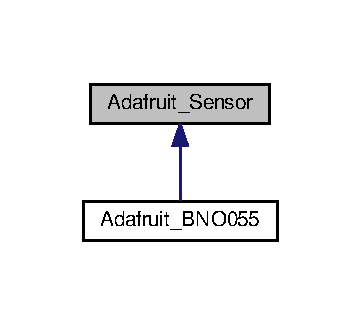
\includegraphics[width=173pt]{classAdafruit__Sensor__inherit__graph}
\end{center}
\end{figure}
\subsection*{Public Member Functions}
\begin{DoxyCompactItemize}
\item 
\hyperlink{classAdafruit__Sensor_a1d06c6f2b9d014894f47102fc1effddf}{Adafruit\+\_\+\+Sensor} ()
\item 
virtual \hyperlink{classAdafruit__Sensor_ac98df73e0cd9367a226b96668417e2e6}{$\sim$\+Adafruit\+\_\+\+Sensor} ()
\item 
virtual void \hyperlink{classAdafruit__Sensor_ace6c1f26eeb956f95801b9fc1841f3a0}{enable\+Auto\+Range} (bool enabled)
\item 
virtual bool \hyperlink{classAdafruit__Sensor_a0636562b9bc853b796ecc87b5d4b1bec}{get\+Event} (\hyperlink{structsensors__event__t}{sensors\+\_\+event\+\_\+t} $\ast$)=0
\item 
virtual void \hyperlink{classAdafruit__Sensor_a19e844c1eb2dc37cb72705d5572c4676}{get\+Sensor} (\hyperlink{structsensor__t}{sensor\+\_\+t} $\ast$)=0
\end{DoxyCompactItemize}
\subsection*{Private Attributes}
\begin{DoxyCompactItemize}
\item 
bool \hyperlink{classAdafruit__Sensor_a79419e4b6898903c0de4aa80133f01ae}{\+\_\+auto\+Range}
\end{DoxyCompactItemize}


\subsection{Constructor \& Destructor Documentation}
\index{Adafruit\+\_\+\+Sensor@{Adafruit\+\_\+\+Sensor}!Adafruit\+\_\+\+Sensor@{Adafruit\+\_\+\+Sensor}}
\index{Adafruit\+\_\+\+Sensor@{Adafruit\+\_\+\+Sensor}!Adafruit\+\_\+\+Sensor@{Adafruit\+\_\+\+Sensor}}
\subsubsection[{\texorpdfstring{Adafruit\+\_\+\+Sensor()}{Adafruit_Sensor()}}]{\setlength{\rightskip}{0pt plus 5cm}Adafruit\+\_\+\+Sensor\+::\+Adafruit\+\_\+\+Sensor (
\begin{DoxyParamCaption}
{}
\end{DoxyParamCaption}
)\hspace{0.3cm}{\ttfamily [inline]}}\hypertarget{classAdafruit__Sensor_a1d06c6f2b9d014894f47102fc1effddf}{}\label{classAdafruit__Sensor_a1d06c6f2b9d014894f47102fc1effddf}
\index{Adafruit\+\_\+\+Sensor@{Adafruit\+\_\+\+Sensor}!````~Adafruit\+\_\+\+Sensor@{$\sim$\+Adafruit\+\_\+\+Sensor}}
\index{````~Adafruit\+\_\+\+Sensor@{$\sim$\+Adafruit\+\_\+\+Sensor}!Adafruit\+\_\+\+Sensor@{Adafruit\+\_\+\+Sensor}}
\subsubsection[{\texorpdfstring{$\sim$\+Adafruit\+\_\+\+Sensor()}{~Adafruit_Sensor()}}]{\setlength{\rightskip}{0pt plus 5cm}virtual Adafruit\+\_\+\+Sensor\+::$\sim$\+Adafruit\+\_\+\+Sensor (
\begin{DoxyParamCaption}
{}
\end{DoxyParamCaption}
)\hspace{0.3cm}{\ttfamily [inline]}, {\ttfamily [virtual]}}\hypertarget{classAdafruit__Sensor_ac98df73e0cd9367a226b96668417e2e6}{}\label{classAdafruit__Sensor_ac98df73e0cd9367a226b96668417e2e6}


\subsection{Member Function Documentation}
\index{Adafruit\+\_\+\+Sensor@{Adafruit\+\_\+\+Sensor}!enable\+Auto\+Range@{enable\+Auto\+Range}}
\index{enable\+Auto\+Range@{enable\+Auto\+Range}!Adafruit\+\_\+\+Sensor@{Adafruit\+\_\+\+Sensor}}
\subsubsection[{\texorpdfstring{enable\+Auto\+Range(bool enabled)}{enableAutoRange(bool enabled)}}]{\setlength{\rightskip}{0pt plus 5cm}virtual void Adafruit\+\_\+\+Sensor\+::enable\+Auto\+Range (
\begin{DoxyParamCaption}
\item[{bool}]{enabled}
\end{DoxyParamCaption}
)\hspace{0.3cm}{\ttfamily [inline]}, {\ttfamily [virtual]}}\hypertarget{classAdafruit__Sensor_ace6c1f26eeb956f95801b9fc1841f3a0}{}\label{classAdafruit__Sensor_ace6c1f26eeb956f95801b9fc1841f3a0}
\index{Adafruit\+\_\+\+Sensor@{Adafruit\+\_\+\+Sensor}!get\+Event@{get\+Event}}
\index{get\+Event@{get\+Event}!Adafruit\+\_\+\+Sensor@{Adafruit\+\_\+\+Sensor}}
\subsubsection[{\texorpdfstring{get\+Event(sensors\+\_\+event\+\_\+t $\ast$)=0}{getEvent(sensors_event_t *)=0}}]{\setlength{\rightskip}{0pt plus 5cm}virtual bool Adafruit\+\_\+\+Sensor\+::get\+Event (
\begin{DoxyParamCaption}
\item[{{\bf sensors\+\_\+event\+\_\+t} $\ast$}]{}
\end{DoxyParamCaption}
)\hspace{0.3cm}{\ttfamily [pure virtual]}}\hypertarget{classAdafruit__Sensor_a0636562b9bc853b796ecc87b5d4b1bec}{}\label{classAdafruit__Sensor_a0636562b9bc853b796ecc87b5d4b1bec}


Implemented in \hyperlink{classAdafruit__BNO055_a8c91811617bd61d7c130ae8b79dd58ee}{Adafruit\+\_\+\+B\+N\+O055}.

\index{Adafruit\+\_\+\+Sensor@{Adafruit\+\_\+\+Sensor}!get\+Sensor@{get\+Sensor}}
\index{get\+Sensor@{get\+Sensor}!Adafruit\+\_\+\+Sensor@{Adafruit\+\_\+\+Sensor}}
\subsubsection[{\texorpdfstring{get\+Sensor(sensor\+\_\+t $\ast$)=0}{getSensor(sensor_t *)=0}}]{\setlength{\rightskip}{0pt plus 5cm}virtual void Adafruit\+\_\+\+Sensor\+::get\+Sensor (
\begin{DoxyParamCaption}
\item[{{\bf sensor\+\_\+t} $\ast$}]{}
\end{DoxyParamCaption}
)\hspace{0.3cm}{\ttfamily [pure virtual]}}\hypertarget{classAdafruit__Sensor_a19e844c1eb2dc37cb72705d5572c4676}{}\label{classAdafruit__Sensor_a19e844c1eb2dc37cb72705d5572c4676}


Implemented in \hyperlink{classAdafruit__BNO055_a1a0849285f6cebde09b4812d9683010c}{Adafruit\+\_\+\+B\+N\+O055}.



\subsection{Member Data Documentation}
\index{Adafruit\+\_\+\+Sensor@{Adafruit\+\_\+\+Sensor}!\+\_\+auto\+Range@{\+\_\+auto\+Range}}
\index{\+\_\+auto\+Range@{\+\_\+auto\+Range}!Adafruit\+\_\+\+Sensor@{Adafruit\+\_\+\+Sensor}}
\subsubsection[{\texorpdfstring{\+\_\+auto\+Range}{_autoRange}}]{\setlength{\rightskip}{0pt plus 5cm}bool Adafruit\+\_\+\+Sensor\+::\+\_\+auto\+Range\hspace{0.3cm}{\ttfamily [private]}}\hypertarget{classAdafruit__Sensor_a79419e4b6898903c0de4aa80133f01ae}{}\label{classAdafruit__Sensor_a79419e4b6898903c0de4aa80133f01ae}


The documentation for this class was generated from the following file\+:\begin{DoxyCompactItemize}
\item 
src/hammerhead/hardware\+\_\+stack/hammerhead\+\_\+arduino/\+N\+U\+C\+\_\+nano/\hyperlink{Adafruit__Sensor_8h}{Adafruit\+\_\+\+Sensor.\+h}\end{DoxyCompactItemize}

\hypertarget{classAlignBin}{}\section{Align\+Bin Class Reference}
\label{classAlignBin}\index{Align\+Bin@{Align\+Bin}}


{\ttfamily \#include $<$Align\+Bin.\+h$>$}

\subsection*{Public Member Functions}
\begin{DoxyCompactItemize}
\item 
\hyperlink{classAlignBin_a26fa4825f5622fa0448735154ec4366a}{Align\+Bin} ()
\item 
\hyperlink{classAlignBin_a9c29537d13848018a211141798f40e58}{$\sim$\+Align\+Bin} ()
\item 
bool \hyperlink{classAlignBin_a7b952f6038c2c39e23284d1fe37988b6}{find\+Bins} (Mat, bool)
\item 
bool \hyperlink{classAlignBin_a7b178f98348112e3648f260bfcb4528d}{find\+Bin\+To\+Choose} (int l\+Bins, Mat labels\+Bins, Mat stats\+Bins, Rect \hyperlink{BinsTask_8cpp_a5e48b467c036f0138a4336c5f73dd0ef}{crop\+Rect}, int \&max\+\_\+area\+\_\+index)
\item 
void \hyperlink{classAlignBin_a7f071885a59bf92b4f84a3d7ed94d3fa}{update\+Inner\+Crop} (Mat stats\+Bins, int index)
\item 
void \hyperlink{classAlignBin_a1b74035bb712d1b2337f8b07c1096d08}{initialize\+Inner\+Crop} (Mat stats\+Bins, int index)
\end{DoxyCompactItemize}
\subsection*{Public Attributes}
\begin{DoxyCompactItemize}
\item 
double \hyperlink{classAlignBin_af984c9ffbeeebfae750ac2237c518ec2}{max\+\_\+cols} = 648
\item 
double \hyperlink{classAlignBin_a193530ae6dfca9e25a6b77e19b6f4f52}{max\+\_\+rows} = 488
\item 
double \hyperlink{classAlignBin_a130959da7ec516d944a30541c1d674f7}{B\+I\+N\+\_\+\+I\+N\+N\+E\+R\+\_\+\+C\+R\+O\+P\+\_\+\+R\+A\+T\+IO} = 2
\item 
double \hyperlink{classAlignBin_a5c32224007789c06f6be5714512ca506}{B\+I\+N\+\_\+\+A\+R\+E\+A\+\_\+\+T\+H\+R\+E\+S\+H\+O\+LD} = 0.\+022
\item 
double \hyperlink{classAlignBin_adedde6dfe9b6e35c372fa034cf401351}{B\+I\+N\+\_\+\+R\+E\+Q\+U\+I\+R\+E\+D\+\_\+\+R\+A\+T\+IO} = 4
\item 
double \hyperlink{classAlignBin_ad994bd3d6dcef6be1f1aca871e6ed1e1}{bins\+\_\+offset\+\_\+x} = 0.\+2
\item 
double \hyperlink{classAlignBin_ae70b486d82daa5ee833b7cd2bd7a8747}{bins\+\_\+offset\+\_\+y} = 0.\+1
\item 
Rect \hyperlink{classAlignBin_af344ab74a824162b23ca841b8a4048df}{bin\+\_\+outer\+\_\+crop}
\item 
bool \hyperlink{classAlignBin_a4bf78a8707f32a306a8871c438c93fc5}{bin\+\_\+found} = false
\item 
Rect \hyperlink{classAlignBin_a0f14b89a2a1f3567525de7c8295aca56}{bin\+\_\+inner\+\_\+crop}
\item 
int \hyperlink{classAlignBin_a261b3b8844de979b325428c812885d84}{bin\+\_\+not\+\_\+found\+\_\+ctr}
\item 
int \hyperlink{classAlignBin_abc20afd816e513b776e6a14ecd522379}{bin\+\_\+area\+\_\+exceeded\+\_\+ctr}
\item 
int \hyperlink{classAlignBin_a17f0142a68dbcdd10faf27361e5e4098}{bin\+\_\+found\+\_\+confidence}
\item 
int \hyperlink{classAlignBin_abf0dbeda76c43acd0a2b486ec177d9d2}{HL} =25
\item 
int \hyperlink{classAlignBin_a30665e4f9a2b3dc078436dc07651aa37}{HH} =155
\item 
int \hyperlink{classAlignBin_ac78c5993ded5dd986f1589783d7b3348}{S\+L1} =95
\item 
int \hyperlink{classAlignBin_ac3181b9b9b8c4c4e38728bf0f971f65a}{S\+H1} =255
\item 
int \hyperlink{classAlignBin_acb43ad409fe61135fe1eba9c0347f3e9}{V\+L1} =0
\item 
int \hyperlink{classAlignBin_a7c8ef2534ea4a97c0bb68468cda0a5f7}{V\+H1} =150
\item 
int \hyperlink{classAlignBin_a0a7000cecbb77704fb06e3d8112e131e}{V\+L2} =0
\item 
int \hyperlink{classAlignBin_a46ca3a67b1c4ae0a99c76ee620c72738}{V\+H2} =70
\item 
int \hyperlink{classAlignBin_af75c44f0d561a2052044bab2edd8b54b}{S\+L2} =0
\item 
int \hyperlink{classAlignBin_af2a1645fc1d755f97bc92700808c452d}{S\+H2} =255
\item 
bool \hyperlink{classAlignBin_aebcf51aa09f21c5451b84c7ebb6968db}{last\+\_\+bin\+\_\+found} = false
\item 
Point \hyperlink{classAlignBin_aa3f546821744ade1859388e68a6b862a}{bin\+Center}
\item 
Mat \hyperlink{classAlignBin_a8493275959cec5434ecd656157cb72f0}{draw}
\item 
Mat \hyperlink{classAlignBin_a798e130d7fb332d98fc23f628b62b6ab}{thresh}
\end{DoxyCompactItemize}


\subsection{Constructor \& Destructor Documentation}
\index{Align\+Bin@{Align\+Bin}!Align\+Bin@{Align\+Bin}}
\index{Align\+Bin@{Align\+Bin}!Align\+Bin@{Align\+Bin}}
\subsubsection[{\texorpdfstring{Align\+Bin()}{AlignBin()}}]{\setlength{\rightskip}{0pt plus 5cm}Align\+Bin\+::\+Align\+Bin (
\begin{DoxyParamCaption}
{}
\end{DoxyParamCaption}
)}\hypertarget{classAlignBin_a26fa4825f5622fa0448735154ec4366a}{}\label{classAlignBin_a26fa4825f5622fa0448735154ec4366a}
\index{Align\+Bin@{Align\+Bin}!````~Align\+Bin@{$\sim$\+Align\+Bin}}
\index{````~Align\+Bin@{$\sim$\+Align\+Bin}!Align\+Bin@{Align\+Bin}}
\subsubsection[{\texorpdfstring{$\sim$\+Align\+Bin()}{~AlignBin()}}]{\setlength{\rightskip}{0pt plus 5cm}Align\+Bin\+::$\sim$\+Align\+Bin (
\begin{DoxyParamCaption}
{}
\end{DoxyParamCaption}
)}\hypertarget{classAlignBin_a9c29537d13848018a211141798f40e58}{}\label{classAlignBin_a9c29537d13848018a211141798f40e58}


\subsection{Member Function Documentation}
\index{Align\+Bin@{Align\+Bin}!find\+Bins@{find\+Bins}}
\index{find\+Bins@{find\+Bins}!Align\+Bin@{Align\+Bin}}
\subsubsection[{\texorpdfstring{find\+Bins(\+Mat, bool)}{findBins(Mat, bool)}}]{\setlength{\rightskip}{0pt plus 5cm}bool Align\+Bin\+::find\+Bins (
\begin{DoxyParamCaption}
\item[{Mat}]{orig, }
\item[{bool}]{initial}
\end{DoxyParamCaption}
)}\hypertarget{classAlignBin_a7b952f6038c2c39e23284d1fe37988b6}{}\label{classAlignBin_a7b952f6038c2c39e23284d1fe37988b6}
\index{Align\+Bin@{Align\+Bin}!find\+Bin\+To\+Choose@{find\+Bin\+To\+Choose}}
\index{find\+Bin\+To\+Choose@{find\+Bin\+To\+Choose}!Align\+Bin@{Align\+Bin}}
\subsubsection[{\texorpdfstring{find\+Bin\+To\+Choose(int l\+Bins, Mat labels\+Bins, Mat stats\+Bins, Rect crop\+Rect, int \&max\+\_\+area\+\_\+index)}{findBinToChoose(int lBins, Mat labelsBins, Mat statsBins, Rect cropRect, int &max_area_index)}}]{\setlength{\rightskip}{0pt plus 5cm}bool Align\+Bin\+::find\+Bin\+To\+Choose (
\begin{DoxyParamCaption}
\item[{int}]{l\+Bins, }
\item[{Mat}]{labels\+Bins, }
\item[{Mat}]{stats\+Bins, }
\item[{Rect}]{crop\+Rect, }
\item[{int \&}]{max\+\_\+area\+\_\+index}
\end{DoxyParamCaption}
)}\hypertarget{classAlignBin_a7b178f98348112e3648f260bfcb4528d}{}\label{classAlignBin_a7b178f98348112e3648f260bfcb4528d}
\index{Align\+Bin@{Align\+Bin}!initialize\+Inner\+Crop@{initialize\+Inner\+Crop}}
\index{initialize\+Inner\+Crop@{initialize\+Inner\+Crop}!Align\+Bin@{Align\+Bin}}
\subsubsection[{\texorpdfstring{initialize\+Inner\+Crop(\+Mat stats\+Bins, int index)}{initializeInnerCrop(Mat statsBins, int index)}}]{\setlength{\rightskip}{0pt plus 5cm}void Align\+Bin\+::initialize\+Inner\+Crop (
\begin{DoxyParamCaption}
\item[{Mat}]{stats\+Bins, }
\item[{int}]{index}
\end{DoxyParamCaption}
)}\hypertarget{classAlignBin_a1b74035bb712d1b2337f8b07c1096d08}{}\label{classAlignBin_a1b74035bb712d1b2337f8b07c1096d08}
\index{Align\+Bin@{Align\+Bin}!update\+Inner\+Crop@{update\+Inner\+Crop}}
\index{update\+Inner\+Crop@{update\+Inner\+Crop}!Align\+Bin@{Align\+Bin}}
\subsubsection[{\texorpdfstring{update\+Inner\+Crop(\+Mat stats\+Bins, int index)}{updateInnerCrop(Mat statsBins, int index)}}]{\setlength{\rightskip}{0pt plus 5cm}void Align\+Bin\+::update\+Inner\+Crop (
\begin{DoxyParamCaption}
\item[{Mat}]{stats\+Bins, }
\item[{int}]{index}
\end{DoxyParamCaption}
)}\hypertarget{classAlignBin_a7f071885a59bf92b4f84a3d7ed94d3fa}{}\label{classAlignBin_a7f071885a59bf92b4f84a3d7ed94d3fa}


\subsection{Member Data Documentation}
\index{Align\+Bin@{Align\+Bin}!bin\+\_\+area\+\_\+exceeded\+\_\+ctr@{bin\+\_\+area\+\_\+exceeded\+\_\+ctr}}
\index{bin\+\_\+area\+\_\+exceeded\+\_\+ctr@{bin\+\_\+area\+\_\+exceeded\+\_\+ctr}!Align\+Bin@{Align\+Bin}}
\subsubsection[{\texorpdfstring{bin\+\_\+area\+\_\+exceeded\+\_\+ctr}{bin_area_exceeded_ctr}}]{\setlength{\rightskip}{0pt plus 5cm}int Align\+Bin\+::bin\+\_\+area\+\_\+exceeded\+\_\+ctr}\hypertarget{classAlignBin_abc20afd816e513b776e6a14ecd522379}{}\label{classAlignBin_abc20afd816e513b776e6a14ecd522379}
\index{Align\+Bin@{Align\+Bin}!B\+I\+N\+\_\+\+A\+R\+E\+A\+\_\+\+T\+H\+R\+E\+S\+H\+O\+LD@{B\+I\+N\+\_\+\+A\+R\+E\+A\+\_\+\+T\+H\+R\+E\+S\+H\+O\+LD}}
\index{B\+I\+N\+\_\+\+A\+R\+E\+A\+\_\+\+T\+H\+R\+E\+S\+H\+O\+LD@{B\+I\+N\+\_\+\+A\+R\+E\+A\+\_\+\+T\+H\+R\+E\+S\+H\+O\+LD}!Align\+Bin@{Align\+Bin}}
\subsubsection[{\texorpdfstring{B\+I\+N\+\_\+\+A\+R\+E\+A\+\_\+\+T\+H\+R\+E\+S\+H\+O\+LD}{BIN_AREA_THRESHOLD}}]{\setlength{\rightskip}{0pt plus 5cm}double Align\+Bin\+::\+B\+I\+N\+\_\+\+A\+R\+E\+A\+\_\+\+T\+H\+R\+E\+S\+H\+O\+LD = 0.\+022}\hypertarget{classAlignBin_a5c32224007789c06f6be5714512ca506}{}\label{classAlignBin_a5c32224007789c06f6be5714512ca506}
\index{Align\+Bin@{Align\+Bin}!bin\+\_\+found@{bin\+\_\+found}}
\index{bin\+\_\+found@{bin\+\_\+found}!Align\+Bin@{Align\+Bin}}
\subsubsection[{\texorpdfstring{bin\+\_\+found}{bin_found}}]{\setlength{\rightskip}{0pt plus 5cm}bool Align\+Bin\+::bin\+\_\+found = false}\hypertarget{classAlignBin_a4bf78a8707f32a306a8871c438c93fc5}{}\label{classAlignBin_a4bf78a8707f32a306a8871c438c93fc5}
\index{Align\+Bin@{Align\+Bin}!bin\+\_\+found\+\_\+confidence@{bin\+\_\+found\+\_\+confidence}}
\index{bin\+\_\+found\+\_\+confidence@{bin\+\_\+found\+\_\+confidence}!Align\+Bin@{Align\+Bin}}
\subsubsection[{\texorpdfstring{bin\+\_\+found\+\_\+confidence}{bin_found_confidence}}]{\setlength{\rightskip}{0pt plus 5cm}int Align\+Bin\+::bin\+\_\+found\+\_\+confidence}\hypertarget{classAlignBin_a17f0142a68dbcdd10faf27361e5e4098}{}\label{classAlignBin_a17f0142a68dbcdd10faf27361e5e4098}
\index{Align\+Bin@{Align\+Bin}!bin\+\_\+inner\+\_\+crop@{bin\+\_\+inner\+\_\+crop}}
\index{bin\+\_\+inner\+\_\+crop@{bin\+\_\+inner\+\_\+crop}!Align\+Bin@{Align\+Bin}}
\subsubsection[{\texorpdfstring{bin\+\_\+inner\+\_\+crop}{bin_inner_crop}}]{\setlength{\rightskip}{0pt plus 5cm}Rect Align\+Bin\+::bin\+\_\+inner\+\_\+crop}\hypertarget{classAlignBin_a0f14b89a2a1f3567525de7c8295aca56}{}\label{classAlignBin_a0f14b89a2a1f3567525de7c8295aca56}
\index{Align\+Bin@{Align\+Bin}!B\+I\+N\+\_\+\+I\+N\+N\+E\+R\+\_\+\+C\+R\+O\+P\+\_\+\+R\+A\+T\+IO@{B\+I\+N\+\_\+\+I\+N\+N\+E\+R\+\_\+\+C\+R\+O\+P\+\_\+\+R\+A\+T\+IO}}
\index{B\+I\+N\+\_\+\+I\+N\+N\+E\+R\+\_\+\+C\+R\+O\+P\+\_\+\+R\+A\+T\+IO@{B\+I\+N\+\_\+\+I\+N\+N\+E\+R\+\_\+\+C\+R\+O\+P\+\_\+\+R\+A\+T\+IO}!Align\+Bin@{Align\+Bin}}
\subsubsection[{\texorpdfstring{B\+I\+N\+\_\+\+I\+N\+N\+E\+R\+\_\+\+C\+R\+O\+P\+\_\+\+R\+A\+T\+IO}{BIN_INNER_CROP_RATIO}}]{\setlength{\rightskip}{0pt plus 5cm}double Align\+Bin\+::\+B\+I\+N\+\_\+\+I\+N\+N\+E\+R\+\_\+\+C\+R\+O\+P\+\_\+\+R\+A\+T\+IO = 2}\hypertarget{classAlignBin_a130959da7ec516d944a30541c1d674f7}{}\label{classAlignBin_a130959da7ec516d944a30541c1d674f7}
\index{Align\+Bin@{Align\+Bin}!bin\+\_\+not\+\_\+found\+\_\+ctr@{bin\+\_\+not\+\_\+found\+\_\+ctr}}
\index{bin\+\_\+not\+\_\+found\+\_\+ctr@{bin\+\_\+not\+\_\+found\+\_\+ctr}!Align\+Bin@{Align\+Bin}}
\subsubsection[{\texorpdfstring{bin\+\_\+not\+\_\+found\+\_\+ctr}{bin_not_found_ctr}}]{\setlength{\rightskip}{0pt plus 5cm}int Align\+Bin\+::bin\+\_\+not\+\_\+found\+\_\+ctr}\hypertarget{classAlignBin_a261b3b8844de979b325428c812885d84}{}\label{classAlignBin_a261b3b8844de979b325428c812885d84}
\index{Align\+Bin@{Align\+Bin}!bin\+\_\+outer\+\_\+crop@{bin\+\_\+outer\+\_\+crop}}
\index{bin\+\_\+outer\+\_\+crop@{bin\+\_\+outer\+\_\+crop}!Align\+Bin@{Align\+Bin}}
\subsubsection[{\texorpdfstring{bin\+\_\+outer\+\_\+crop}{bin_outer_crop}}]{\setlength{\rightskip}{0pt plus 5cm}Rect Align\+Bin\+::bin\+\_\+outer\+\_\+crop}\hypertarget{classAlignBin_af344ab74a824162b23ca841b8a4048df}{}\label{classAlignBin_af344ab74a824162b23ca841b8a4048df}
{\bfseries Initial value\+:}
\begin{DoxyCode}
= Rect(Point(\hyperlink{classAlignBin_ad994bd3d6dcef6be1f1aca871e6ed1e1}{bins\_offset\_x}*\hyperlink{classAlignBin_af984c9ffbeeebfae750ac2237c518ec2}{max\_cols},0.4*\hyperlink{classAlignBin_a193530ae6dfca9e25a6b77e19b6f4f52}{max\_rows}),
                Point((1.0-\hyperlink{classAlignBin_ad994bd3d6dcef6be1f1aca871e6ed1e1}{bins\_offset\_x})*max\_cols,(1.0-
      \hyperlink{classAlignBin_ae70b486d82daa5ee833b7cd2bd7a8747}{bins\_offset\_y})*\hyperlink{classAlignBin_a193530ae6dfca9e25a6b77e19b6f4f52}{max\_rows}))
\end{DoxyCode}
\index{Align\+Bin@{Align\+Bin}!B\+I\+N\+\_\+\+R\+E\+Q\+U\+I\+R\+E\+D\+\_\+\+R\+A\+T\+IO@{B\+I\+N\+\_\+\+R\+E\+Q\+U\+I\+R\+E\+D\+\_\+\+R\+A\+T\+IO}}
\index{B\+I\+N\+\_\+\+R\+E\+Q\+U\+I\+R\+E\+D\+\_\+\+R\+A\+T\+IO@{B\+I\+N\+\_\+\+R\+E\+Q\+U\+I\+R\+E\+D\+\_\+\+R\+A\+T\+IO}!Align\+Bin@{Align\+Bin}}
\subsubsection[{\texorpdfstring{B\+I\+N\+\_\+\+R\+E\+Q\+U\+I\+R\+E\+D\+\_\+\+R\+A\+T\+IO}{BIN_REQUIRED_RATIO}}]{\setlength{\rightskip}{0pt plus 5cm}double Align\+Bin\+::\+B\+I\+N\+\_\+\+R\+E\+Q\+U\+I\+R\+E\+D\+\_\+\+R\+A\+T\+IO = 4}\hypertarget{classAlignBin_adedde6dfe9b6e35c372fa034cf401351}{}\label{classAlignBin_adedde6dfe9b6e35c372fa034cf401351}
\index{Align\+Bin@{Align\+Bin}!bin\+Center@{bin\+Center}}
\index{bin\+Center@{bin\+Center}!Align\+Bin@{Align\+Bin}}
\subsubsection[{\texorpdfstring{bin\+Center}{binCenter}}]{\setlength{\rightskip}{0pt plus 5cm}Point Align\+Bin\+::bin\+Center}\hypertarget{classAlignBin_aa3f546821744ade1859388e68a6b862a}{}\label{classAlignBin_aa3f546821744ade1859388e68a6b862a}
\index{Align\+Bin@{Align\+Bin}!bins\+\_\+offset\+\_\+x@{bins\+\_\+offset\+\_\+x}}
\index{bins\+\_\+offset\+\_\+x@{bins\+\_\+offset\+\_\+x}!Align\+Bin@{Align\+Bin}}
\subsubsection[{\texorpdfstring{bins\+\_\+offset\+\_\+x}{bins_offset_x}}]{\setlength{\rightskip}{0pt plus 5cm}double Align\+Bin\+::bins\+\_\+offset\+\_\+x = 0.\+2}\hypertarget{classAlignBin_ad994bd3d6dcef6be1f1aca871e6ed1e1}{}\label{classAlignBin_ad994bd3d6dcef6be1f1aca871e6ed1e1}
\index{Align\+Bin@{Align\+Bin}!bins\+\_\+offset\+\_\+y@{bins\+\_\+offset\+\_\+y}}
\index{bins\+\_\+offset\+\_\+y@{bins\+\_\+offset\+\_\+y}!Align\+Bin@{Align\+Bin}}
\subsubsection[{\texorpdfstring{bins\+\_\+offset\+\_\+y}{bins_offset_y}}]{\setlength{\rightskip}{0pt plus 5cm}double Align\+Bin\+::bins\+\_\+offset\+\_\+y = 0.\+1}\hypertarget{classAlignBin_ae70b486d82daa5ee833b7cd2bd7a8747}{}\label{classAlignBin_ae70b486d82daa5ee833b7cd2bd7a8747}
\index{Align\+Bin@{Align\+Bin}!draw@{draw}}
\index{draw@{draw}!Align\+Bin@{Align\+Bin}}
\subsubsection[{\texorpdfstring{draw}{draw}}]{\setlength{\rightskip}{0pt plus 5cm}Mat Align\+Bin\+::draw}\hypertarget{classAlignBin_a8493275959cec5434ecd656157cb72f0}{}\label{classAlignBin_a8493275959cec5434ecd656157cb72f0}
\index{Align\+Bin@{Align\+Bin}!HH@{HH}}
\index{HH@{HH}!Align\+Bin@{Align\+Bin}}
\subsubsection[{\texorpdfstring{HH}{HH}}]{\setlength{\rightskip}{0pt plus 5cm}int Align\+Bin\+::\+HH =155}\hypertarget{classAlignBin_a30665e4f9a2b3dc078436dc07651aa37}{}\label{classAlignBin_a30665e4f9a2b3dc078436dc07651aa37}
\index{Align\+Bin@{Align\+Bin}!HL@{HL}}
\index{HL@{HL}!Align\+Bin@{Align\+Bin}}
\subsubsection[{\texorpdfstring{HL}{HL}}]{\setlength{\rightskip}{0pt plus 5cm}int Align\+Bin\+::\+HL =25}\hypertarget{classAlignBin_abf0dbeda76c43acd0a2b486ec177d9d2}{}\label{classAlignBin_abf0dbeda76c43acd0a2b486ec177d9d2}
\index{Align\+Bin@{Align\+Bin}!last\+\_\+bin\+\_\+found@{last\+\_\+bin\+\_\+found}}
\index{last\+\_\+bin\+\_\+found@{last\+\_\+bin\+\_\+found}!Align\+Bin@{Align\+Bin}}
\subsubsection[{\texorpdfstring{last\+\_\+bin\+\_\+found}{last_bin_found}}]{\setlength{\rightskip}{0pt plus 5cm}bool Align\+Bin\+::last\+\_\+bin\+\_\+found = false}\hypertarget{classAlignBin_aebcf51aa09f21c5451b84c7ebb6968db}{}\label{classAlignBin_aebcf51aa09f21c5451b84c7ebb6968db}
\index{Align\+Bin@{Align\+Bin}!max\+\_\+cols@{max\+\_\+cols}}
\index{max\+\_\+cols@{max\+\_\+cols}!Align\+Bin@{Align\+Bin}}
\subsubsection[{\texorpdfstring{max\+\_\+cols}{max_cols}}]{\setlength{\rightskip}{0pt plus 5cm}double Align\+Bin\+::max\+\_\+cols = 648}\hypertarget{classAlignBin_af984c9ffbeeebfae750ac2237c518ec2}{}\label{classAlignBin_af984c9ffbeeebfae750ac2237c518ec2}
\index{Align\+Bin@{Align\+Bin}!max\+\_\+rows@{max\+\_\+rows}}
\index{max\+\_\+rows@{max\+\_\+rows}!Align\+Bin@{Align\+Bin}}
\subsubsection[{\texorpdfstring{max\+\_\+rows}{max_rows}}]{\setlength{\rightskip}{0pt plus 5cm}double Align\+Bin\+::max\+\_\+rows = 488}\hypertarget{classAlignBin_a193530ae6dfca9e25a6b77e19b6f4f52}{}\label{classAlignBin_a193530ae6dfca9e25a6b77e19b6f4f52}
\index{Align\+Bin@{Align\+Bin}!S\+H1@{S\+H1}}
\index{S\+H1@{S\+H1}!Align\+Bin@{Align\+Bin}}
\subsubsection[{\texorpdfstring{S\+H1}{SH1}}]{\setlength{\rightskip}{0pt plus 5cm}int Align\+Bin\+::\+S\+H1 =255}\hypertarget{classAlignBin_ac3181b9b9b8c4c4e38728bf0f971f65a}{}\label{classAlignBin_ac3181b9b9b8c4c4e38728bf0f971f65a}
\index{Align\+Bin@{Align\+Bin}!S\+H2@{S\+H2}}
\index{S\+H2@{S\+H2}!Align\+Bin@{Align\+Bin}}
\subsubsection[{\texorpdfstring{S\+H2}{SH2}}]{\setlength{\rightskip}{0pt plus 5cm}int Align\+Bin\+::\+S\+H2 =255}\hypertarget{classAlignBin_af2a1645fc1d755f97bc92700808c452d}{}\label{classAlignBin_af2a1645fc1d755f97bc92700808c452d}
\index{Align\+Bin@{Align\+Bin}!S\+L1@{S\+L1}}
\index{S\+L1@{S\+L1}!Align\+Bin@{Align\+Bin}}
\subsubsection[{\texorpdfstring{S\+L1}{SL1}}]{\setlength{\rightskip}{0pt plus 5cm}int Align\+Bin\+::\+S\+L1 =95}\hypertarget{classAlignBin_ac78c5993ded5dd986f1589783d7b3348}{}\label{classAlignBin_ac78c5993ded5dd986f1589783d7b3348}
\index{Align\+Bin@{Align\+Bin}!S\+L2@{S\+L2}}
\index{S\+L2@{S\+L2}!Align\+Bin@{Align\+Bin}}
\subsubsection[{\texorpdfstring{S\+L2}{SL2}}]{\setlength{\rightskip}{0pt plus 5cm}int Align\+Bin\+::\+S\+L2 =0}\hypertarget{classAlignBin_af75c44f0d561a2052044bab2edd8b54b}{}\label{classAlignBin_af75c44f0d561a2052044bab2edd8b54b}
\index{Align\+Bin@{Align\+Bin}!thresh@{thresh}}
\index{thresh@{thresh}!Align\+Bin@{Align\+Bin}}
\subsubsection[{\texorpdfstring{thresh}{thresh}}]{\setlength{\rightskip}{0pt plus 5cm}Mat Align\+Bin\+::thresh}\hypertarget{classAlignBin_a798e130d7fb332d98fc23f628b62b6ab}{}\label{classAlignBin_a798e130d7fb332d98fc23f628b62b6ab}
\index{Align\+Bin@{Align\+Bin}!V\+H1@{V\+H1}}
\index{V\+H1@{V\+H1}!Align\+Bin@{Align\+Bin}}
\subsubsection[{\texorpdfstring{V\+H1}{VH1}}]{\setlength{\rightskip}{0pt plus 5cm}int Align\+Bin\+::\+V\+H1 =150}\hypertarget{classAlignBin_a7c8ef2534ea4a97c0bb68468cda0a5f7}{}\label{classAlignBin_a7c8ef2534ea4a97c0bb68468cda0a5f7}
\index{Align\+Bin@{Align\+Bin}!V\+H2@{V\+H2}}
\index{V\+H2@{V\+H2}!Align\+Bin@{Align\+Bin}}
\subsubsection[{\texorpdfstring{V\+H2}{VH2}}]{\setlength{\rightskip}{0pt plus 5cm}int Align\+Bin\+::\+V\+H2 =70}\hypertarget{classAlignBin_a46ca3a67b1c4ae0a99c76ee620c72738}{}\label{classAlignBin_a46ca3a67b1c4ae0a99c76ee620c72738}
\index{Align\+Bin@{Align\+Bin}!V\+L1@{V\+L1}}
\index{V\+L1@{V\+L1}!Align\+Bin@{Align\+Bin}}
\subsubsection[{\texorpdfstring{V\+L1}{VL1}}]{\setlength{\rightskip}{0pt plus 5cm}int Align\+Bin\+::\+V\+L1 =0}\hypertarget{classAlignBin_acb43ad409fe61135fe1eba9c0347f3e9}{}\label{classAlignBin_acb43ad409fe61135fe1eba9c0347f3e9}
\index{Align\+Bin@{Align\+Bin}!V\+L2@{V\+L2}}
\index{V\+L2@{V\+L2}!Align\+Bin@{Align\+Bin}}
\subsubsection[{\texorpdfstring{V\+L2}{VL2}}]{\setlength{\rightskip}{0pt plus 5cm}int Align\+Bin\+::\+V\+L2 =0}\hypertarget{classAlignBin_a0a7000cecbb77704fb06e3d8112e131e}{}\label{classAlignBin_a0a7000cecbb77704fb06e3d8112e131e}


The documentation for this class was generated from the following files\+:\begin{DoxyCompactItemize}
\item 
src/hammerhead/mission\+\_\+stack/path\+\_\+planner/include/path\+\_\+planner/\hyperlink{AlignBin_8h}{Align\+Bin.\+h}\item 
src/hammerhead/mission\+\_\+stack/path\+\_\+planner/src/\hyperlink{AlignBin_8cpp}{Align\+Bin.\+cpp}\end{DoxyCompactItemize}

\hypertarget{classBinsTask}{}\section{Bins\+Task Class Reference}
\label{classBinsTask}\index{Bins\+Task@{Bins\+Task}}


{\ttfamily \#include $<$Bins\+Task.\+h$>$}

\subsection*{Public Member Functions}
\begin{DoxyCompactItemize}
\item 
\hyperlink{classBinsTask_ae281a44a4350b89efee5c1b43fba81ea}{Bins\+Task} ()
\item 
\hyperlink{classBinsTask_a2c2428c70f54f1ca73e107afeb5f9c3b}{$\sim$\+Bins\+Task} ()
\item 
double \hyperlink{classBinsTask_a11bae31515c6203ee470e5000a481fb2}{find\+Time\+Difference} (\hyperlink{thruster__driver_8cpp_ad3e807c387dc076de974ff7eac67ad81}{Time\+Point}, \hyperlink{thruster__driver_8cpp_ad3e807c387dc076de974ff7eac67ad81}{Time\+Point})
\item 
bool \hyperlink{classBinsTask_a0a9b80db60310bbc553dcc6bb0fd7969}{do\+Tasks} (Mat src, Vec3i \&control\+Setpoint, bool \&timeout)
\item 
bool \hyperlink{classBinsTask_a7a06b66c2f28876fe5803b545d92b2af}{set\+State} (Mat \hyperlink{classBinsTask_aedf5f6032dcea5fbab09caed34cf80ac}{orig}, Vec3i \&control\+Setpoint, \hyperlink{BinsTask_8h_adc6e5733fc3c22f0a7b2914188c49c90}{state} \hyperlink{classBinsTask_a582b4e240c7018b7119f20c66860a6cf}{currentstate})
\item 
void \hyperlink{classBinsTask_a83fc283bddeb24b6bc4772e372d6ff2f}{reset} ()
\item 
int \hyperlink{classBinsTask_a26bee7a25e6dd7ae137caaf6e386b981}{firstbinsearch} (int \hyperlink{BinsTask_8cpp_ac559c47f5c7d297de44ad8e157f30eec}{confidence\+Ctr}, Mat \hyperlink{classBinsTask_aedf5f6032dcea5fbab09caed34cf80ac}{orig}, Mat dispimg, Vec3i \&motion\+Target)
\item 
int \hyperlink{classBinsTask_a83227b34e66b476dcac18ef8be3912a0}{height\+Adjust} (int \hyperlink{BinsTask_8cpp_ac559c47f5c7d297de44ad8e157f30eec}{confidence\+Ctr}, Mat \hyperlink{classBinsTask_aedf5f6032dcea5fbab09caed34cf80ac}{orig}, Mat dispimg, Vec3i \&motion\+Target)
\item 
int \hyperlink{classBinsTask_adbcab6aaf2d23d8ccd14e19a9de5c788}{rightbinsearch} (int \hyperlink{BinsTask_8cpp_ac559c47f5c7d297de44ad8e157f30eec}{confidence\+Ctr}, Mat \hyperlink{classBinsTask_aedf5f6032dcea5fbab09caed34cf80ac}{orig}, Mat dispimg, Rect \&crop, Vec3i \&motion\+Target)
\item 
int \hyperlink{classBinsTask_a22689994f60be64be9a708fca637fe64}{leftbinsearch} (int \hyperlink{BinsTask_8cpp_ac559c47f5c7d297de44ad8e157f30eec}{confidence\+Ctr}, Mat \hyperlink{classBinsTask_aedf5f6032dcea5fbab09caed34cf80ac}{orig}, Mat dispimg, Rect \&crop, Vec3i \&motion\+Target)
\item 
int \hyperlink{classBinsTask_ad6bc9c1bb7dfe3a0eba2c12daf9b8251}{descendtodropball} (int \hyperlink{BinsTask_8cpp_ac559c47f5c7d297de44ad8e157f30eec}{confidence\+Ctr}, Mat \hyperlink{classBinsTask_aedf5f6032dcea5fbab09caed34cf80ac}{orig}, Mat dispimg, Vec3i \&motion\+Target)
\item 
int \hyperlink{classBinsTask_a9d4fa38c0a887e585584a58d9c89d588}{finddropbin} (int \hyperlink{BinsTask_8cpp_ac559c47f5c7d297de44ad8e157f30eec}{confidence\+Ctr}, Mat \hyperlink{classBinsTask_aedf5f6032dcea5fbab09caed34cf80ac}{orig}, Mat dispimg, Vec3i \&motion\+Target)
\item 
Point \hyperlink{classBinsTask_ae9a46f2485c946548ec25d19967bdd82}{find\+Bin\+Center} (Rect bound\+Box)
\item 
Rect \hyperlink{classBinsTask_a759535380ae45df16970bed852d95531}{find\+Bluebin} (Mat \hyperlink{classBinsTask_aedf5f6032dcea5fbab09caed34cf80ac}{orig}, bool use\+Mat\+Surrounding)
\item 
Rect \hyperlink{classBinsTask_a9d0f57751e1cf8ce9ed4ea831d326616}{find\+Redbin} (Mat \hyperlink{classBinsTask_aedf5f6032dcea5fbab09caed34cf80ac}{orig}, bool use\+Mat\+Surrounding)
\item 
Mat \hyperlink{classBinsTask_af47b3fa7a02c4dc69641894331773efc}{segment\+Red} (Mat img)
\item 
Mat \hyperlink{classBinsTask_a5bdedfc0921b5ec486c12ffa53398b20}{segment\+Blue} (Mat img)
\item 
Mat \hyperlink{classBinsTask_ad53d8e8e2152cdb8fdd80ca379a1377c}{segment\+Green} (Mat img)
\end{DoxyCompactItemize}
\subsection*{Public Attributes}
\begin{DoxyCompactItemize}
\item 
\hyperlink{thruster__driver_8cpp_ad3e807c387dc076de974ff7eac67ad81}{Time\+Point} \hyperlink{classBinsTask_a0f9b188187c02eaf4081c896bed1a1d8}{start\+Time}
\item 
\hyperlink{BinsTask_8h_aa849c9e7a5801c9746b10a3667604f1e}{bincolor} \hyperlink{classBinsTask_ac52fdf90cc77856e4fd389b627e0f9e6}{current\+Bin}
\item 
\hyperlink{BinsTask_8h_adc6e5733fc3c22f0a7b2914188c49c90}{state} \hyperlink{classBinsTask_a582b4e240c7018b7119f20c66860a6cf}{currentstate}
\item 
int \hyperlink{classBinsTask_ad227a105c8a9d4fbd4b11ac8292013cc}{timelimit}
\item 
bool \hyperlink{classBinsTask_a9376c8b742619429bf6e71818aa4813c}{state\+Complete}
\item 
bool \hyperlink{classBinsTask_a96feda59c1d8c1657a93b8541703c6f3}{state\+Transition}
\item 
vector$<$ \hyperlink{BinsTask_8h_adc6e5733fc3c22f0a7b2914188c49c90}{state} $>$ \hyperlink{classBinsTask_abd44d0fdbe28dbd619f841a2d0c36be4}{state\+List}
\item 
vector$<$ int $>$ \hyperlink{classBinsTask_a7faea4476a80bd6350abb38efe438888}{state\+Timeouts}
\item 
unsigned int \hyperlink{classBinsTask_aa69dd4866994a26d64c45aaf2d778527}{state\+Counter}
\item 
Mat \hyperlink{classBinsTask_aedf5f6032dcea5fbab09caed34cf80ac}{orig}
\item 
Mat \hyperlink{classBinsTask_ab446e684e463435b9e2a3b5fa9a046a3}{maindisp}
\end{DoxyCompactItemize}


\subsection{Constructor \& Destructor Documentation}
\index{Bins\+Task@{Bins\+Task}!Bins\+Task@{Bins\+Task}}
\index{Bins\+Task@{Bins\+Task}!Bins\+Task@{Bins\+Task}}
\subsubsection[{\texorpdfstring{Bins\+Task()}{BinsTask()}}]{\setlength{\rightskip}{0pt plus 5cm}Bins\+Task\+::\+Bins\+Task (
\begin{DoxyParamCaption}
{}
\end{DoxyParamCaption}
)}\hypertarget{classBinsTask_ae281a44a4350b89efee5c1b43fba81ea}{}\label{classBinsTask_ae281a44a4350b89efee5c1b43fba81ea}
\index{Bins\+Task@{Bins\+Task}!````~Bins\+Task@{$\sim$\+Bins\+Task}}
\index{````~Bins\+Task@{$\sim$\+Bins\+Task}!Bins\+Task@{Bins\+Task}}
\subsubsection[{\texorpdfstring{$\sim$\+Bins\+Task()}{~BinsTask()}}]{\setlength{\rightskip}{0pt plus 5cm}Bins\+Task\+::$\sim$\+Bins\+Task (
\begin{DoxyParamCaption}
{}
\end{DoxyParamCaption}
)}\hypertarget{classBinsTask_a2c2428c70f54f1ca73e107afeb5f9c3b}{}\label{classBinsTask_a2c2428c70f54f1ca73e107afeb5f9c3b}


\subsection{Member Function Documentation}
\index{Bins\+Task@{Bins\+Task}!descendtodropball@{descendtodropball}}
\index{descendtodropball@{descendtodropball}!Bins\+Task@{Bins\+Task}}
\subsubsection[{\texorpdfstring{descendtodropball(int confidence\+Ctr, Mat orig, Mat dispimg, Vec3i \&motion\+Target)}{descendtodropball(int confidenceCtr, Mat orig, Mat dispimg, Vec3i &motionTarget)}}]{\setlength{\rightskip}{0pt plus 5cm}int Bins\+Task\+::descendtodropball (
\begin{DoxyParamCaption}
\item[{int}]{confidence\+Ctr, }
\item[{Mat}]{orig, }
\item[{Mat}]{dispimg, }
\item[{Vec3i \&}]{motion\+Target}
\end{DoxyParamCaption}
)}\hypertarget{classBinsTask_ad6bc9c1bb7dfe3a0eba2c12daf9b8251}{}\label{classBinsTask_ad6bc9c1bb7dfe3a0eba2c12daf9b8251}
\index{Bins\+Task@{Bins\+Task}!do\+Tasks@{do\+Tasks}}
\index{do\+Tasks@{do\+Tasks}!Bins\+Task@{Bins\+Task}}
\subsubsection[{\texorpdfstring{do\+Tasks(\+Mat src, Vec3i \&control\+Setpoint, bool \&timeout)}{doTasks(Mat src, Vec3i &controlSetpoint, bool &timeout)}}]{\setlength{\rightskip}{0pt plus 5cm}bool Bins\+Task\+::do\+Tasks (
\begin{DoxyParamCaption}
\item[{Mat}]{src, }
\item[{Vec3i \&}]{control\+Setpoint, }
\item[{bool \&}]{timeout}
\end{DoxyParamCaption}
)}\hypertarget{classBinsTask_a0a9b80db60310bbc553dcc6bb0fd7969}{}\label{classBinsTask_a0a9b80db60310bbc553dcc6bb0fd7969}
\index{Bins\+Task@{Bins\+Task}!find\+Bin\+Center@{find\+Bin\+Center}}
\index{find\+Bin\+Center@{find\+Bin\+Center}!Bins\+Task@{Bins\+Task}}
\subsubsection[{\texorpdfstring{find\+Bin\+Center(\+Rect bound\+Box)}{findBinCenter(Rect boundBox)}}]{\setlength{\rightskip}{0pt plus 5cm}Point Bins\+Task\+::find\+Bin\+Center (
\begin{DoxyParamCaption}
\item[{Rect}]{bound\+Box}
\end{DoxyParamCaption}
)}\hypertarget{classBinsTask_ae9a46f2485c946548ec25d19967bdd82}{}\label{classBinsTask_ae9a46f2485c946548ec25d19967bdd82}
\index{Bins\+Task@{Bins\+Task}!find\+Bluebin@{find\+Bluebin}}
\index{find\+Bluebin@{find\+Bluebin}!Bins\+Task@{Bins\+Task}}
\subsubsection[{\texorpdfstring{find\+Bluebin(\+Mat orig, bool use\+Mat\+Surrounding)}{findBluebin(Mat orig, bool useMatSurrounding)}}]{\setlength{\rightskip}{0pt plus 5cm}Rect Bins\+Task\+::find\+Bluebin (
\begin{DoxyParamCaption}
\item[{Mat}]{orig, }
\item[{bool}]{use\+Mat\+Surrounding = {\ttfamily true}}
\end{DoxyParamCaption}
)}\hypertarget{classBinsTask_a759535380ae45df16970bed852d95531}{}\label{classBinsTask_a759535380ae45df16970bed852d95531}
\index{Bins\+Task@{Bins\+Task}!finddropbin@{finddropbin}}
\index{finddropbin@{finddropbin}!Bins\+Task@{Bins\+Task}}
\subsubsection[{\texorpdfstring{finddropbin(int confidence\+Ctr, Mat orig, Mat dispimg, Vec3i \&motion\+Target)}{finddropbin(int confidenceCtr, Mat orig, Mat dispimg, Vec3i &motionTarget)}}]{\setlength{\rightskip}{0pt plus 5cm}int Bins\+Task\+::finddropbin (
\begin{DoxyParamCaption}
\item[{int}]{confidence\+Ctr, }
\item[{Mat}]{orig, }
\item[{Mat}]{dispimg, }
\item[{Vec3i \&}]{motion\+Target}
\end{DoxyParamCaption}
)}\hypertarget{classBinsTask_a9d4fa38c0a887e585584a58d9c89d588}{}\label{classBinsTask_a9d4fa38c0a887e585584a58d9c89d588}
\index{Bins\+Task@{Bins\+Task}!find\+Redbin@{find\+Redbin}}
\index{find\+Redbin@{find\+Redbin}!Bins\+Task@{Bins\+Task}}
\subsubsection[{\texorpdfstring{find\+Redbin(\+Mat orig, bool use\+Mat\+Surrounding)}{findRedbin(Mat orig, bool useMatSurrounding)}}]{\setlength{\rightskip}{0pt plus 5cm}Rect Bins\+Task\+::find\+Redbin (
\begin{DoxyParamCaption}
\item[{Mat}]{orig, }
\item[{bool}]{use\+Mat\+Surrounding = {\ttfamily false}}
\end{DoxyParamCaption}
)}\hypertarget{classBinsTask_a9d0f57751e1cf8ce9ed4ea831d326616}{}\label{classBinsTask_a9d0f57751e1cf8ce9ed4ea831d326616}
\index{Bins\+Task@{Bins\+Task}!find\+Time\+Difference@{find\+Time\+Difference}}
\index{find\+Time\+Difference@{find\+Time\+Difference}!Bins\+Task@{Bins\+Task}}
\subsubsection[{\texorpdfstring{find\+Time\+Difference(\+Time\+Point, Time\+Point)}{findTimeDifference(TimePoint, TimePoint)}}]{\setlength{\rightskip}{0pt plus 5cm}double Bins\+Task\+::find\+Time\+Difference (
\begin{DoxyParamCaption}
\item[{{\bf Time\+Point}}]{end, }
\item[{{\bf Time\+Point}}]{start}
\end{DoxyParamCaption}
)}\hypertarget{classBinsTask_a11bae31515c6203ee470e5000a481fb2}{}\label{classBinsTask_a11bae31515c6203ee470e5000a481fb2}
\index{Bins\+Task@{Bins\+Task}!firstbinsearch@{firstbinsearch}}
\index{firstbinsearch@{firstbinsearch}!Bins\+Task@{Bins\+Task}}
\subsubsection[{\texorpdfstring{firstbinsearch(int confidence\+Ctr, Mat orig, Mat dispimg, Vec3i \&motion\+Target)}{firstbinsearch(int confidenceCtr, Mat orig, Mat dispimg, Vec3i &motionTarget)}}]{\setlength{\rightskip}{0pt plus 5cm}int Bins\+Task\+::firstbinsearch (
\begin{DoxyParamCaption}
\item[{int}]{confidence\+Ctr, }
\item[{Mat}]{orig, }
\item[{Mat}]{dispimg, }
\item[{Vec3i \&}]{motion\+Target}
\end{DoxyParamCaption}
)}\hypertarget{classBinsTask_a26bee7a25e6dd7ae137caaf6e386b981}{}\label{classBinsTask_a26bee7a25e6dd7ae137caaf6e386b981}
\index{Bins\+Task@{Bins\+Task}!height\+Adjust@{height\+Adjust}}
\index{height\+Adjust@{height\+Adjust}!Bins\+Task@{Bins\+Task}}
\subsubsection[{\texorpdfstring{height\+Adjust(int confidence\+Ctr, Mat orig, Mat dispimg, Vec3i \&motion\+Target)}{heightAdjust(int confidenceCtr, Mat orig, Mat dispimg, Vec3i &motionTarget)}}]{\setlength{\rightskip}{0pt plus 5cm}int Bins\+Task\+::height\+Adjust (
\begin{DoxyParamCaption}
\item[{int}]{confidence\+Ctr, }
\item[{Mat}]{orig, }
\item[{Mat}]{dispimg, }
\item[{Vec3i \&}]{motion\+Target}
\end{DoxyParamCaption}
)}\hypertarget{classBinsTask_a83227b34e66b476dcac18ef8be3912a0}{}\label{classBinsTask_a83227b34e66b476dcac18ef8be3912a0}
\index{Bins\+Task@{Bins\+Task}!leftbinsearch@{leftbinsearch}}
\index{leftbinsearch@{leftbinsearch}!Bins\+Task@{Bins\+Task}}
\subsubsection[{\texorpdfstring{leftbinsearch(int confidence\+Ctr, Mat orig, Mat dispimg, Rect \&crop, Vec3i \&motion\+Target)}{leftbinsearch(int confidenceCtr, Mat orig, Mat dispimg, Rect &crop, Vec3i &motionTarget)}}]{\setlength{\rightskip}{0pt plus 5cm}int Bins\+Task\+::leftbinsearch (
\begin{DoxyParamCaption}
\item[{int}]{confidence\+Ctr, }
\item[{Mat}]{orig, }
\item[{Mat}]{dispimg, }
\item[{Rect \&}]{crop, }
\item[{Vec3i \&}]{motion\+Target}
\end{DoxyParamCaption}
)}\hypertarget{classBinsTask_a22689994f60be64be9a708fca637fe64}{}\label{classBinsTask_a22689994f60be64be9a708fca637fe64}
\index{Bins\+Task@{Bins\+Task}!reset@{reset}}
\index{reset@{reset}!Bins\+Task@{Bins\+Task}}
\subsubsection[{\texorpdfstring{reset()}{reset()}}]{\setlength{\rightskip}{0pt plus 5cm}void Bins\+Task\+::reset (
\begin{DoxyParamCaption}
{}
\end{DoxyParamCaption}
)}\hypertarget{classBinsTask_a83fc283bddeb24b6bc4772e372d6ff2f}{}\label{classBinsTask_a83fc283bddeb24b6bc4772e372d6ff2f}
\index{Bins\+Task@{Bins\+Task}!rightbinsearch@{rightbinsearch}}
\index{rightbinsearch@{rightbinsearch}!Bins\+Task@{Bins\+Task}}
\subsubsection[{\texorpdfstring{rightbinsearch(int confidence\+Ctr, Mat orig, Mat dispimg, Rect \&crop, Vec3i \&motion\+Target)}{rightbinsearch(int confidenceCtr, Mat orig, Mat dispimg, Rect &crop, Vec3i &motionTarget)}}]{\setlength{\rightskip}{0pt plus 5cm}int Bins\+Task\+::rightbinsearch (
\begin{DoxyParamCaption}
\item[{int}]{confidence\+Ctr, }
\item[{Mat}]{orig, }
\item[{Mat}]{dispimg, }
\item[{Rect \&}]{crop, }
\item[{Vec3i \&}]{motion\+Target}
\end{DoxyParamCaption}
)}\hypertarget{classBinsTask_adbcab6aaf2d23d8ccd14e19a9de5c788}{}\label{classBinsTask_adbcab6aaf2d23d8ccd14e19a9de5c788}
\index{Bins\+Task@{Bins\+Task}!segment\+Blue@{segment\+Blue}}
\index{segment\+Blue@{segment\+Blue}!Bins\+Task@{Bins\+Task}}
\subsubsection[{\texorpdfstring{segment\+Blue(\+Mat img)}{segmentBlue(Mat img)}}]{\setlength{\rightskip}{0pt plus 5cm}Mat Bins\+Task\+::segment\+Blue (
\begin{DoxyParamCaption}
\item[{Mat}]{img}
\end{DoxyParamCaption}
)}\hypertarget{classBinsTask_a5bdedfc0921b5ec486c12ffa53398b20}{}\label{classBinsTask_a5bdedfc0921b5ec486c12ffa53398b20}
\index{Bins\+Task@{Bins\+Task}!segment\+Green@{segment\+Green}}
\index{segment\+Green@{segment\+Green}!Bins\+Task@{Bins\+Task}}
\subsubsection[{\texorpdfstring{segment\+Green(\+Mat img)}{segmentGreen(Mat img)}}]{\setlength{\rightskip}{0pt plus 5cm}Mat Bins\+Task\+::segment\+Green (
\begin{DoxyParamCaption}
\item[{Mat}]{img}
\end{DoxyParamCaption}
)}\hypertarget{classBinsTask_ad53d8e8e2152cdb8fdd80ca379a1377c}{}\label{classBinsTask_ad53d8e8e2152cdb8fdd80ca379a1377c}
\index{Bins\+Task@{Bins\+Task}!segment\+Red@{segment\+Red}}
\index{segment\+Red@{segment\+Red}!Bins\+Task@{Bins\+Task}}
\subsubsection[{\texorpdfstring{segment\+Red(\+Mat img)}{segmentRed(Mat img)}}]{\setlength{\rightskip}{0pt plus 5cm}Mat Bins\+Task\+::segment\+Red (
\begin{DoxyParamCaption}
\item[{Mat}]{img}
\end{DoxyParamCaption}
)}\hypertarget{classBinsTask_af47b3fa7a02c4dc69641894331773efc}{}\label{classBinsTask_af47b3fa7a02c4dc69641894331773efc}
\index{Bins\+Task@{Bins\+Task}!set\+State@{set\+State}}
\index{set\+State@{set\+State}!Bins\+Task@{Bins\+Task}}
\subsubsection[{\texorpdfstring{set\+State(\+Mat orig, Vec3i \&control\+Setpoint, state currentstate)}{setState(Mat orig, Vec3i &controlSetpoint, state currentstate)}}]{\setlength{\rightskip}{0pt plus 5cm}bool Bins\+Task\+::set\+State (
\begin{DoxyParamCaption}
\item[{Mat}]{orig, }
\item[{Vec3i \&}]{control\+Setpoint, }
\item[{{\bf state}}]{currentstate}
\end{DoxyParamCaption}
)}\hypertarget{classBinsTask_a7a06b66c2f28876fe5803b545d92b2af}{}\label{classBinsTask_a7a06b66c2f28876fe5803b545d92b2af}


\subsection{Member Data Documentation}
\index{Bins\+Task@{Bins\+Task}!current\+Bin@{current\+Bin}}
\index{current\+Bin@{current\+Bin}!Bins\+Task@{Bins\+Task}}
\subsubsection[{\texorpdfstring{current\+Bin}{currentBin}}]{\setlength{\rightskip}{0pt plus 5cm}{\bf bincolor} Bins\+Task\+::current\+Bin}\hypertarget{classBinsTask_ac52fdf90cc77856e4fd389b627e0f9e6}{}\label{classBinsTask_ac52fdf90cc77856e4fd389b627e0f9e6}
\index{Bins\+Task@{Bins\+Task}!currentstate@{currentstate}}
\index{currentstate@{currentstate}!Bins\+Task@{Bins\+Task}}
\subsubsection[{\texorpdfstring{currentstate}{currentstate}}]{\setlength{\rightskip}{0pt plus 5cm}{\bf state} Bins\+Task\+::currentstate}\hypertarget{classBinsTask_a582b4e240c7018b7119f20c66860a6cf}{}\label{classBinsTask_a582b4e240c7018b7119f20c66860a6cf}
\index{Bins\+Task@{Bins\+Task}!maindisp@{maindisp}}
\index{maindisp@{maindisp}!Bins\+Task@{Bins\+Task}}
\subsubsection[{\texorpdfstring{maindisp}{maindisp}}]{\setlength{\rightskip}{0pt plus 5cm}Mat Bins\+Task\+::maindisp}\hypertarget{classBinsTask_ab446e684e463435b9e2a3b5fa9a046a3}{}\label{classBinsTask_ab446e684e463435b9e2a3b5fa9a046a3}
\index{Bins\+Task@{Bins\+Task}!orig@{orig}}
\index{orig@{orig}!Bins\+Task@{Bins\+Task}}
\subsubsection[{\texorpdfstring{orig}{orig}}]{\setlength{\rightskip}{0pt plus 5cm}Mat Bins\+Task\+::orig}\hypertarget{classBinsTask_aedf5f6032dcea5fbab09caed34cf80ac}{}\label{classBinsTask_aedf5f6032dcea5fbab09caed34cf80ac}
\index{Bins\+Task@{Bins\+Task}!start\+Time@{start\+Time}}
\index{start\+Time@{start\+Time}!Bins\+Task@{Bins\+Task}}
\subsubsection[{\texorpdfstring{start\+Time}{startTime}}]{\setlength{\rightskip}{0pt plus 5cm}{\bf Time\+Point} Bins\+Task\+::start\+Time}\hypertarget{classBinsTask_a0f9b188187c02eaf4081c896bed1a1d8}{}\label{classBinsTask_a0f9b188187c02eaf4081c896bed1a1d8}
\index{Bins\+Task@{Bins\+Task}!state\+Complete@{state\+Complete}}
\index{state\+Complete@{state\+Complete}!Bins\+Task@{Bins\+Task}}
\subsubsection[{\texorpdfstring{state\+Complete}{stateComplete}}]{\setlength{\rightskip}{0pt plus 5cm}bool Bins\+Task\+::state\+Complete}\hypertarget{classBinsTask_a9376c8b742619429bf6e71818aa4813c}{}\label{classBinsTask_a9376c8b742619429bf6e71818aa4813c}
\index{Bins\+Task@{Bins\+Task}!state\+Counter@{state\+Counter}}
\index{state\+Counter@{state\+Counter}!Bins\+Task@{Bins\+Task}}
\subsubsection[{\texorpdfstring{state\+Counter}{stateCounter}}]{\setlength{\rightskip}{0pt plus 5cm}unsigned int Bins\+Task\+::state\+Counter}\hypertarget{classBinsTask_aa69dd4866994a26d64c45aaf2d778527}{}\label{classBinsTask_aa69dd4866994a26d64c45aaf2d778527}
\index{Bins\+Task@{Bins\+Task}!state\+List@{state\+List}}
\index{state\+List@{state\+List}!Bins\+Task@{Bins\+Task}}
\subsubsection[{\texorpdfstring{state\+List}{stateList}}]{\setlength{\rightskip}{0pt plus 5cm}vector$<${\bf state}$>$ Bins\+Task\+::state\+List}\hypertarget{classBinsTask_abd44d0fdbe28dbd619f841a2d0c36be4}{}\label{classBinsTask_abd44d0fdbe28dbd619f841a2d0c36be4}
\index{Bins\+Task@{Bins\+Task}!state\+Timeouts@{state\+Timeouts}}
\index{state\+Timeouts@{state\+Timeouts}!Bins\+Task@{Bins\+Task}}
\subsubsection[{\texorpdfstring{state\+Timeouts}{stateTimeouts}}]{\setlength{\rightskip}{0pt plus 5cm}vector$<$int$>$ Bins\+Task\+::state\+Timeouts}\hypertarget{classBinsTask_a7faea4476a80bd6350abb38efe438888}{}\label{classBinsTask_a7faea4476a80bd6350abb38efe438888}
\index{Bins\+Task@{Bins\+Task}!state\+Transition@{state\+Transition}}
\index{state\+Transition@{state\+Transition}!Bins\+Task@{Bins\+Task}}
\subsubsection[{\texorpdfstring{state\+Transition}{stateTransition}}]{\setlength{\rightskip}{0pt plus 5cm}bool Bins\+Task\+::state\+Transition}\hypertarget{classBinsTask_a96feda59c1d8c1657a93b8541703c6f3}{}\label{classBinsTask_a96feda59c1d8c1657a93b8541703c6f3}
\index{Bins\+Task@{Bins\+Task}!timelimit@{timelimit}}
\index{timelimit@{timelimit}!Bins\+Task@{Bins\+Task}}
\subsubsection[{\texorpdfstring{timelimit}{timelimit}}]{\setlength{\rightskip}{0pt plus 5cm}int Bins\+Task\+::timelimit}\hypertarget{classBinsTask_ad227a105c8a9d4fbd4b11ac8292013cc}{}\label{classBinsTask_ad227a105c8a9d4fbd4b11ac8292013cc}


The documentation for this class was generated from the following files\+:\begin{DoxyCompactItemize}
\item 
src/hammerhead/mission\+\_\+stack/path\+\_\+planner/include/path\+\_\+planner/\hyperlink{BinsTask_8h}{Bins\+Task.\+h}\item 
src/hammerhead/mission\+\_\+stack/path\+\_\+planner/src/\hyperlink{BinsTask_8cpp}{Bins\+Task.\+cpp}\end{DoxyCompactItemize}

\hypertarget{classBlueBinDetector}{}\section{Blue\+Bin\+Detector Class Reference}
\label{classBlueBinDetector}\index{Blue\+Bin\+Detector@{Blue\+Bin\+Detector}}


the below class contains all members and functions for detecting blue bin and its related parameters  




{\ttfamily \#include $<$Blue\+Bin\+Detector.\+h$>$}

\subsection*{Public Member Functions}
\begin{DoxyCompactItemize}
\item 
\hyperlink{classBlueBinDetector_ad082c0687a01c1868cb6e3478ba3f774}{Blue\+Bin\+Detector} ()
\item 
\hyperlink{classBlueBinDetector_a482faf6ce9a83043b1ed0c53f708712e}{$\sim$\+Blue\+Bin\+Detector} ()
\item 
bool \hyperlink{classBlueBinDetector_ab428c2aa1474c1bb0c1aceac4bc4b028}{detect\+Blue\+Bin} (Mat \hyperlink{qualification__task_8cpp_ae544386e0f095e03d639cf884b7a8a1b}{orig})
\begin{DoxyCompactList}\small\item\em function for detecting blue bin and returns true or false based on the same \end{DoxyCompactList}\item 
double \hyperlink{classBlueBinDetector_a5e63ca51780f42539fc2ff6c8cc45c3f}{dist} (Point p1, Point p2)
\begin{DoxyCompactList}\small\item\em function for detecting blue bin center distance from the gate center and returns the same \end{DoxyCompactList}\end{DoxyCompactItemize}
\subsection*{Public Attributes}
\begin{DoxyCompactItemize}
\item 
int \hyperlink{classBlueBinDetector_aa5ee31b4f78070d90c96360e70c2710e}{n\+Centers}
\item 
int \hyperlink{classBlueBinDetector_aa32db58c1084261fc82510a1f7647dd4}{n\+Centers\+Index}
\item 
vector$<$ Point $>$ \hyperlink{classBlueBinDetector_a3f15b441edbe4a372c25a2a14e5dd238}{last\+Centers}
\item 
Point \hyperlink{classBlueBinDetector_aaa3974bddf370c5f3054b8b28018d935}{gate\+Center}
\begin{DoxyCompactList}\small\item\em gate center coordinates \end{DoxyCompactList}\item 
Rect \hyperlink{classBlueBinDetector_a2c467050d739ce4b5f17776dc1acff99}{gate\+Rect}
\begin{DoxyCompactList}\small\item\em rectangle containing the gate \end{DoxyCompactList}\item 
int \hyperlink{classBlueBinDetector_a27c2322e9231eada3fd026d8b4859b55}{scale}
\item 
int \hyperlink{classBlueBinDetector_aaceda035648f9c683f999a0180bc8d06}{delta}
\item 
int \hyperlink{classBlueBinDetector_a28df18b6bb12bdf794a26c10bcf85397}{ddepth}
\begin{DoxyCompactList}\small\item\em respective parameters \end{DoxyCompactList}\item 
int \hyperlink{classBlueBinDetector_af8ec4d3b2864d710e7d9ac9904112d09}{sobel\+ThresholdX}
\item 
int \hyperlink{classBlueBinDetector_ac032afb6b48bac1eeb42b403639f658a}{sobel\+ThresholdY}
\item 
int \hyperlink{classBlueBinDetector_af0495b5bbc1c64cde69868bbbac6abac}{morph\+\_\+size}
\begin{DoxyCompactList}\small\item\em sobel parameters \end{DoxyCompactList}\item 
double \hyperlink{classBlueBinDetector_a3d8f5991f9e6c26469aa38ae3e745d37}{max\+\_\+cols} = 648
\item 
double \hyperlink{classBlueBinDetector_ace70d074bc205720fd99ec320f94a505}{max\+\_\+rows} = 488
\item 
Mat \hyperlink{classBlueBinDetector_a7c504bb250864d343055259170b8fd34}{src}
\item 
Mat \hyperlink{classBlueBinDetector_a65e2e4304509a31a7b8bf9b364d737c4}{temp}
\item 
Mat \hyperlink{classBlueBinDetector_aa0ed8edd7704a48c8800fe540ccba4cf}{cdst}
\item 
Mat \hyperlink{classBlueBinDetector_a019c17d08994bd65639f8f3eacd493ef}{grad\+\_\+x}
\item 
Mat \hyperlink{classBlueBinDetector_a55e3da3811d564d3111050e7357226b7}{grad\+\_\+y}
\item 
Mat \hyperlink{classBlueBinDetector_a87c0a2aee3ddf650aa602338fa39975a}{src\+\_\+gray}
\item 
Mat \hyperlink{classBlueBinDetector_a0986ca569b3c09665b30068dbc4934aa}{abs\+\_\+grad\+\_\+x}
\item 
Mat \hyperlink{classBlueBinDetector_a13cdb9e7f123655fa04c526eaa8fe81e}{abs\+\_\+grad\+\_\+y}
\end{DoxyCompactItemize}


\subsection{Detailed Description}
the below class contains all members and functions for detecting blue bin and its related parameters 

\subsection{Constructor \& Destructor Documentation}
\index{Blue\+Bin\+Detector@{Blue\+Bin\+Detector}!Blue\+Bin\+Detector@{Blue\+Bin\+Detector}}
\index{Blue\+Bin\+Detector@{Blue\+Bin\+Detector}!Blue\+Bin\+Detector@{Blue\+Bin\+Detector}}
\subsubsection[{\texorpdfstring{Blue\+Bin\+Detector()}{BlueBinDetector()}}]{\setlength{\rightskip}{0pt plus 5cm}Blue\+Bin\+Detector\+::\+Blue\+Bin\+Detector (
\begin{DoxyParamCaption}
{}
\end{DoxyParamCaption}
)}\hypertarget{classBlueBinDetector_ad082c0687a01c1868cb6e3478ba3f774}{}\label{classBlueBinDetector_ad082c0687a01c1868cb6e3478ba3f774}
constructor \index{Blue\+Bin\+Detector@{Blue\+Bin\+Detector}!````~Blue\+Bin\+Detector@{$\sim$\+Blue\+Bin\+Detector}}
\index{````~Blue\+Bin\+Detector@{$\sim$\+Blue\+Bin\+Detector}!Blue\+Bin\+Detector@{Blue\+Bin\+Detector}}
\subsubsection[{\texorpdfstring{$\sim$\+Blue\+Bin\+Detector()}{~BlueBinDetector()}}]{\setlength{\rightskip}{0pt plus 5cm}Blue\+Bin\+Detector\+::$\sim$\+Blue\+Bin\+Detector (
\begin{DoxyParamCaption}
{}
\end{DoxyParamCaption}
)}\hypertarget{classBlueBinDetector_a482faf6ce9a83043b1ed0c53f708712e}{}\label{classBlueBinDetector_a482faf6ce9a83043b1ed0c53f708712e}
destructor 

\subsection{Member Function Documentation}
\index{Blue\+Bin\+Detector@{Blue\+Bin\+Detector}!detect\+Blue\+Bin@{detect\+Blue\+Bin}}
\index{detect\+Blue\+Bin@{detect\+Blue\+Bin}!Blue\+Bin\+Detector@{Blue\+Bin\+Detector}}
\subsubsection[{\texorpdfstring{detect\+Blue\+Bin(\+Mat orig)}{detectBlueBin(Mat orig)}}]{\setlength{\rightskip}{0pt plus 5cm}bool Blue\+Bin\+Detector\+::detect\+Blue\+Bin (
\begin{DoxyParamCaption}
\item[{Mat}]{orig}
\end{DoxyParamCaption}
)}\hypertarget{classBlueBinDetector_ab428c2aa1474c1bb0c1aceac4bc4b028}{}\label{classBlueBinDetector_ab428c2aa1474c1bb0c1aceac4bc4b028}


function for detecting blue bin and returns true or false based on the same 


\begin{DoxyParams}[1]{Parameters}
\mbox{\tt in}  & {\em orig} & input feed \\
\hline
\end{DoxyParams}
\index{Blue\+Bin\+Detector@{Blue\+Bin\+Detector}!dist@{dist}}
\index{dist@{dist}!Blue\+Bin\+Detector@{Blue\+Bin\+Detector}}
\subsubsection[{\texorpdfstring{dist(\+Point p1, Point p2)}{dist(Point p1, Point p2)}}]{\setlength{\rightskip}{0pt plus 5cm}double Blue\+Bin\+Detector\+::dist (
\begin{DoxyParamCaption}
\item[{Point}]{p1, }
\item[{Point}]{p2}
\end{DoxyParamCaption}
)}\hypertarget{classBlueBinDetector_a5e63ca51780f42539fc2ff6c8cc45c3f}{}\label{classBlueBinDetector_a5e63ca51780f42539fc2ff6c8cc45c3f}


function for detecting blue bin center distance from the gate center and returns the same 


\begin{DoxyParams}[1]{Parameters}
\mbox{\tt in}  & {\em p1} & gate center\\
\hline
\mbox{\tt in}  & {\em p2} & bin center \\
\hline
\end{DoxyParams}


\subsection{Member Data Documentation}
\index{Blue\+Bin\+Detector@{Blue\+Bin\+Detector}!abs\+\_\+grad\+\_\+x@{abs\+\_\+grad\+\_\+x}}
\index{abs\+\_\+grad\+\_\+x@{abs\+\_\+grad\+\_\+x}!Blue\+Bin\+Detector@{Blue\+Bin\+Detector}}
\subsubsection[{\texorpdfstring{abs\+\_\+grad\+\_\+x}{abs_grad_x}}]{\setlength{\rightskip}{0pt plus 5cm}Mat Blue\+Bin\+Detector\+::abs\+\_\+grad\+\_\+x}\hypertarget{classBlueBinDetector_a0986ca569b3c09665b30068dbc4934aa}{}\label{classBlueBinDetector_a0986ca569b3c09665b30068dbc4934aa}
\index{Blue\+Bin\+Detector@{Blue\+Bin\+Detector}!abs\+\_\+grad\+\_\+y@{abs\+\_\+grad\+\_\+y}}
\index{abs\+\_\+grad\+\_\+y@{abs\+\_\+grad\+\_\+y}!Blue\+Bin\+Detector@{Blue\+Bin\+Detector}}
\subsubsection[{\texorpdfstring{abs\+\_\+grad\+\_\+y}{abs_grad_y}}]{\setlength{\rightskip}{0pt plus 5cm}Mat Blue\+Bin\+Detector\+::abs\+\_\+grad\+\_\+y}\hypertarget{classBlueBinDetector_a13cdb9e7f123655fa04c526eaa8fe81e}{}\label{classBlueBinDetector_a13cdb9e7f123655fa04c526eaa8fe81e}
\index{Blue\+Bin\+Detector@{Blue\+Bin\+Detector}!cdst@{cdst}}
\index{cdst@{cdst}!Blue\+Bin\+Detector@{Blue\+Bin\+Detector}}
\subsubsection[{\texorpdfstring{cdst}{cdst}}]{\setlength{\rightskip}{0pt plus 5cm}Mat Blue\+Bin\+Detector\+::cdst}\hypertarget{classBlueBinDetector_aa0ed8edd7704a48c8800fe540ccba4cf}{}\label{classBlueBinDetector_aa0ed8edd7704a48c8800fe540ccba4cf}
\index{Blue\+Bin\+Detector@{Blue\+Bin\+Detector}!ddepth@{ddepth}}
\index{ddepth@{ddepth}!Blue\+Bin\+Detector@{Blue\+Bin\+Detector}}
\subsubsection[{\texorpdfstring{ddepth}{ddepth}}]{\setlength{\rightskip}{0pt plus 5cm}int Blue\+Bin\+Detector\+::ddepth}\hypertarget{classBlueBinDetector_a28df18b6bb12bdf794a26c10bcf85397}{}\label{classBlueBinDetector_a28df18b6bb12bdf794a26c10bcf85397}


respective parameters 

\index{Blue\+Bin\+Detector@{Blue\+Bin\+Detector}!delta@{delta}}
\index{delta@{delta}!Blue\+Bin\+Detector@{Blue\+Bin\+Detector}}
\subsubsection[{\texorpdfstring{delta}{delta}}]{\setlength{\rightskip}{0pt plus 5cm}int Blue\+Bin\+Detector\+::delta}\hypertarget{classBlueBinDetector_aaceda035648f9c683f999a0180bc8d06}{}\label{classBlueBinDetector_aaceda035648f9c683f999a0180bc8d06}
\index{Blue\+Bin\+Detector@{Blue\+Bin\+Detector}!gate\+Center@{gate\+Center}}
\index{gate\+Center@{gate\+Center}!Blue\+Bin\+Detector@{Blue\+Bin\+Detector}}
\subsubsection[{\texorpdfstring{gate\+Center}{gateCenter}}]{\setlength{\rightskip}{0pt plus 5cm}Point Blue\+Bin\+Detector\+::gate\+Center}\hypertarget{classBlueBinDetector_aaa3974bddf370c5f3054b8b28018d935}{}\label{classBlueBinDetector_aaa3974bddf370c5f3054b8b28018d935}


gate center coordinates 

\index{Blue\+Bin\+Detector@{Blue\+Bin\+Detector}!gate\+Rect@{gate\+Rect}}
\index{gate\+Rect@{gate\+Rect}!Blue\+Bin\+Detector@{Blue\+Bin\+Detector}}
\subsubsection[{\texorpdfstring{gate\+Rect}{gateRect}}]{\setlength{\rightskip}{0pt plus 5cm}Rect Blue\+Bin\+Detector\+::gate\+Rect}\hypertarget{classBlueBinDetector_a2c467050d739ce4b5f17776dc1acff99}{}\label{classBlueBinDetector_a2c467050d739ce4b5f17776dc1acff99}


rectangle containing the gate 

\index{Blue\+Bin\+Detector@{Blue\+Bin\+Detector}!grad\+\_\+x@{grad\+\_\+x}}
\index{grad\+\_\+x@{grad\+\_\+x}!Blue\+Bin\+Detector@{Blue\+Bin\+Detector}}
\subsubsection[{\texorpdfstring{grad\+\_\+x}{grad_x}}]{\setlength{\rightskip}{0pt plus 5cm}Mat Blue\+Bin\+Detector\+::grad\+\_\+x}\hypertarget{classBlueBinDetector_a019c17d08994bd65639f8f3eacd493ef}{}\label{classBlueBinDetector_a019c17d08994bd65639f8f3eacd493ef}
\index{Blue\+Bin\+Detector@{Blue\+Bin\+Detector}!grad\+\_\+y@{grad\+\_\+y}}
\index{grad\+\_\+y@{grad\+\_\+y}!Blue\+Bin\+Detector@{Blue\+Bin\+Detector}}
\subsubsection[{\texorpdfstring{grad\+\_\+y}{grad_y}}]{\setlength{\rightskip}{0pt plus 5cm}Mat Blue\+Bin\+Detector\+::grad\+\_\+y}\hypertarget{classBlueBinDetector_a55e3da3811d564d3111050e7357226b7}{}\label{classBlueBinDetector_a55e3da3811d564d3111050e7357226b7}
\index{Blue\+Bin\+Detector@{Blue\+Bin\+Detector}!last\+Centers@{last\+Centers}}
\index{last\+Centers@{last\+Centers}!Blue\+Bin\+Detector@{Blue\+Bin\+Detector}}
\subsubsection[{\texorpdfstring{last\+Centers}{lastCenters}}]{\setlength{\rightskip}{0pt plus 5cm}vector$<$Point$>$ Blue\+Bin\+Detector\+::last\+Centers}\hypertarget{classBlueBinDetector_a3f15b441edbe4a372c25a2a14e5dd238}{}\label{classBlueBinDetector_a3f15b441edbe4a372c25a2a14e5dd238}
\index{Blue\+Bin\+Detector@{Blue\+Bin\+Detector}!max\+\_\+cols@{max\+\_\+cols}}
\index{max\+\_\+cols@{max\+\_\+cols}!Blue\+Bin\+Detector@{Blue\+Bin\+Detector}}
\subsubsection[{\texorpdfstring{max\+\_\+cols}{max_cols}}]{\setlength{\rightskip}{0pt plus 5cm}double Blue\+Bin\+Detector\+::max\+\_\+cols = 648}\hypertarget{classBlueBinDetector_a3d8f5991f9e6c26469aa38ae3e745d37}{}\label{classBlueBinDetector_a3d8f5991f9e6c26469aa38ae3e745d37}
\index{Blue\+Bin\+Detector@{Blue\+Bin\+Detector}!max\+\_\+rows@{max\+\_\+rows}}
\index{max\+\_\+rows@{max\+\_\+rows}!Blue\+Bin\+Detector@{Blue\+Bin\+Detector}}
\subsubsection[{\texorpdfstring{max\+\_\+rows}{max_rows}}]{\setlength{\rightskip}{0pt plus 5cm}double Blue\+Bin\+Detector\+::max\+\_\+rows = 488}\hypertarget{classBlueBinDetector_ace70d074bc205720fd99ec320f94a505}{}\label{classBlueBinDetector_ace70d074bc205720fd99ec320f94a505}
\index{Blue\+Bin\+Detector@{Blue\+Bin\+Detector}!morph\+\_\+size@{morph\+\_\+size}}
\index{morph\+\_\+size@{morph\+\_\+size}!Blue\+Bin\+Detector@{Blue\+Bin\+Detector}}
\subsubsection[{\texorpdfstring{morph\+\_\+size}{morph_size}}]{\setlength{\rightskip}{0pt plus 5cm}int Blue\+Bin\+Detector\+::morph\+\_\+size}\hypertarget{classBlueBinDetector_af0495b5bbc1c64cde69868bbbac6abac}{}\label{classBlueBinDetector_af0495b5bbc1c64cde69868bbbac6abac}


sobel parameters 

\index{Blue\+Bin\+Detector@{Blue\+Bin\+Detector}!n\+Centers@{n\+Centers}}
\index{n\+Centers@{n\+Centers}!Blue\+Bin\+Detector@{Blue\+Bin\+Detector}}
\subsubsection[{\texorpdfstring{n\+Centers}{nCenters}}]{\setlength{\rightskip}{0pt plus 5cm}int Blue\+Bin\+Detector\+::n\+Centers}\hypertarget{classBlueBinDetector_aa5ee31b4f78070d90c96360e70c2710e}{}\label{classBlueBinDetector_aa5ee31b4f78070d90c96360e70c2710e}
\index{Blue\+Bin\+Detector@{Blue\+Bin\+Detector}!n\+Centers\+Index@{n\+Centers\+Index}}
\index{n\+Centers\+Index@{n\+Centers\+Index}!Blue\+Bin\+Detector@{Blue\+Bin\+Detector}}
\subsubsection[{\texorpdfstring{n\+Centers\+Index}{nCentersIndex}}]{\setlength{\rightskip}{0pt plus 5cm}int Blue\+Bin\+Detector\+::n\+Centers\+Index}\hypertarget{classBlueBinDetector_aa32db58c1084261fc82510a1f7647dd4}{}\label{classBlueBinDetector_aa32db58c1084261fc82510a1f7647dd4}
\index{Blue\+Bin\+Detector@{Blue\+Bin\+Detector}!scale@{scale}}
\index{scale@{scale}!Blue\+Bin\+Detector@{Blue\+Bin\+Detector}}
\subsubsection[{\texorpdfstring{scale}{scale}}]{\setlength{\rightskip}{0pt plus 5cm}int Blue\+Bin\+Detector\+::scale}\hypertarget{classBlueBinDetector_a27c2322e9231eada3fd026d8b4859b55}{}\label{classBlueBinDetector_a27c2322e9231eada3fd026d8b4859b55}
\index{Blue\+Bin\+Detector@{Blue\+Bin\+Detector}!sobel\+ThresholdX@{sobel\+ThresholdX}}
\index{sobel\+ThresholdX@{sobel\+ThresholdX}!Blue\+Bin\+Detector@{Blue\+Bin\+Detector}}
\subsubsection[{\texorpdfstring{sobel\+ThresholdX}{sobelThresholdX}}]{\setlength{\rightskip}{0pt plus 5cm}int Blue\+Bin\+Detector\+::sobel\+ThresholdX}\hypertarget{classBlueBinDetector_af8ec4d3b2864d710e7d9ac9904112d09}{}\label{classBlueBinDetector_af8ec4d3b2864d710e7d9ac9904112d09}
\index{Blue\+Bin\+Detector@{Blue\+Bin\+Detector}!sobel\+ThresholdY@{sobel\+ThresholdY}}
\index{sobel\+ThresholdY@{sobel\+ThresholdY}!Blue\+Bin\+Detector@{Blue\+Bin\+Detector}}
\subsubsection[{\texorpdfstring{sobel\+ThresholdY}{sobelThresholdY}}]{\setlength{\rightskip}{0pt plus 5cm}int Blue\+Bin\+Detector\+::sobel\+ThresholdY}\hypertarget{classBlueBinDetector_ac032afb6b48bac1eeb42b403639f658a}{}\label{classBlueBinDetector_ac032afb6b48bac1eeb42b403639f658a}
\index{Blue\+Bin\+Detector@{Blue\+Bin\+Detector}!src@{src}}
\index{src@{src}!Blue\+Bin\+Detector@{Blue\+Bin\+Detector}}
\subsubsection[{\texorpdfstring{src}{src}}]{\setlength{\rightskip}{0pt plus 5cm}Mat Blue\+Bin\+Detector\+::src}\hypertarget{classBlueBinDetector_a7c504bb250864d343055259170b8fd34}{}\label{classBlueBinDetector_a7c504bb250864d343055259170b8fd34}
\index{Blue\+Bin\+Detector@{Blue\+Bin\+Detector}!src\+\_\+gray@{src\+\_\+gray}}
\index{src\+\_\+gray@{src\+\_\+gray}!Blue\+Bin\+Detector@{Blue\+Bin\+Detector}}
\subsubsection[{\texorpdfstring{src\+\_\+gray}{src_gray}}]{\setlength{\rightskip}{0pt plus 5cm}Mat Blue\+Bin\+Detector\+::src\+\_\+gray}\hypertarget{classBlueBinDetector_a87c0a2aee3ddf650aa602338fa39975a}{}\label{classBlueBinDetector_a87c0a2aee3ddf650aa602338fa39975a}
\index{Blue\+Bin\+Detector@{Blue\+Bin\+Detector}!temp@{temp}}
\index{temp@{temp}!Blue\+Bin\+Detector@{Blue\+Bin\+Detector}}
\subsubsection[{\texorpdfstring{temp}{temp}}]{\setlength{\rightskip}{0pt plus 5cm}Mat Blue\+Bin\+Detector\+::temp}\hypertarget{classBlueBinDetector_a65e2e4304509a31a7b8bf9b364d737c4}{}\label{classBlueBinDetector_a65e2e4304509a31a7b8bf9b364d737c4}


The documentation for this class was generated from the following files\+:\begin{DoxyCompactItemize}
\item 
src/hammerhead/mission\+\_\+stack/path\+\_\+planner/include/path\+\_\+planner/\hyperlink{BlueBinDetector_8h}{Blue\+Bin\+Detector.\+h}\item 
src/hammerhead/mission\+\_\+stack/path\+\_\+planner/src/\hyperlink{BlueBinDetector_8cpp}{Blue\+Bin\+Detector.\+cpp}\end{DoxyCompactItemize}

\hypertarget{structQCPAxisPainterPrivate_1_1CachedLabel}{}\section{Q\+C\+P\+Axis\+Painter\+Private\+:\+:Cached\+Label Struct Reference}
\label{structQCPAxisPainterPrivate_1_1CachedLabel}\index{Q\+C\+P\+Axis\+Painter\+Private\+::\+Cached\+Label@{Q\+C\+P\+Axis\+Painter\+Private\+::\+Cached\+Label}}


{\ttfamily \#include $<$qcustomplot.\+h$>$}

\subsection*{Public Attributes}
\begin{DoxyCompactItemize}
\item 
Q\+PointF \hyperlink{structQCPAxisPainterPrivate_1_1CachedLabel_a5f502db71c92e572f1e6f44f62c59d8e}{offset}
\item 
Q\+Pixmap \hyperlink{structQCPAxisPainterPrivate_1_1CachedLabel_a461597cbd470914a9d24b64d16037a88}{pixmap}
\end{DoxyCompactItemize}


\subsection{Member Data Documentation}
\index{Q\+C\+P\+Axis\+Painter\+Private\+::\+Cached\+Label@{Q\+C\+P\+Axis\+Painter\+Private\+::\+Cached\+Label}!offset@{offset}}
\index{offset@{offset}!Q\+C\+P\+Axis\+Painter\+Private\+::\+Cached\+Label@{Q\+C\+P\+Axis\+Painter\+Private\+::\+Cached\+Label}}
\subsubsection[{\texorpdfstring{offset}{offset}}]{\setlength{\rightskip}{0pt plus 5cm}Q\+PointF Q\+C\+P\+Axis\+Painter\+Private\+::\+Cached\+Label\+::offset}\hypertarget{structQCPAxisPainterPrivate_1_1CachedLabel_a5f502db71c92e572f1e6f44f62c59d8e}{}\label{structQCPAxisPainterPrivate_1_1CachedLabel_a5f502db71c92e572f1e6f44f62c59d8e}
\index{Q\+C\+P\+Axis\+Painter\+Private\+::\+Cached\+Label@{Q\+C\+P\+Axis\+Painter\+Private\+::\+Cached\+Label}!pixmap@{pixmap}}
\index{pixmap@{pixmap}!Q\+C\+P\+Axis\+Painter\+Private\+::\+Cached\+Label@{Q\+C\+P\+Axis\+Painter\+Private\+::\+Cached\+Label}}
\subsubsection[{\texorpdfstring{pixmap}{pixmap}}]{\setlength{\rightskip}{0pt plus 5cm}Q\+Pixmap Q\+C\+P\+Axis\+Painter\+Private\+::\+Cached\+Label\+::pixmap}\hypertarget{structQCPAxisPainterPrivate_1_1CachedLabel_a461597cbd470914a9d24b64d16037a88}{}\label{structQCPAxisPainterPrivate_1_1CachedLabel_a461597cbd470914a9d24b64d16037a88}


The documentation for this struct was generated from the following file\+:\begin{DoxyCompactItemize}
\item 
src/hammerhead/tools/watchdog/include/watchdog/\hyperlink{qcustomplot_8h}{qcustomplot.\+h}\end{DoxyCompactItemize}

\hypertarget{classCommanderWindow}{}\section{Commander\+Window Class Reference}
\label{classCommanderWindow}\index{Commander\+Window@{Commander\+Window}}


{\ttfamily \#include $<$commander\+\_\+window.\+h$>$}



Inheritance diagram for Commander\+Window\+:
\nopagebreak
\begin{figure}[H]
\begin{center}
\leavevmode
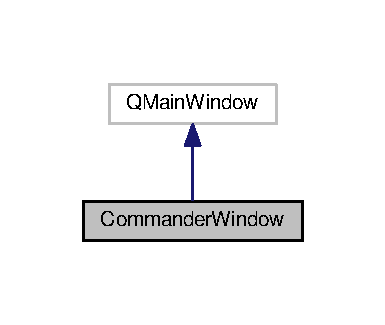
\includegraphics[width=185pt]{classCommanderWindow__inherit__graph}
\end{center}
\end{figure}


Collaboration diagram for Commander\+Window\+:
\nopagebreak
\begin{figure}[H]
\begin{center}
\leavevmode
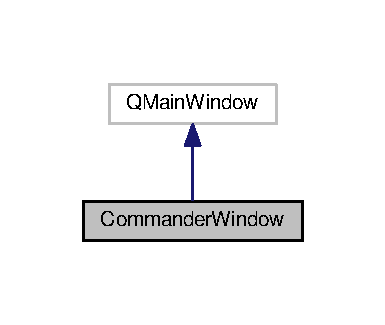
\includegraphics[width=185pt]{classCommanderWindow__coll__graph}
\end{center}
\end{figure}
\subsection*{Public Member Functions}
\begin{DoxyCompactItemize}
\item 
\hyperlink{classCommanderWindow_a722cab557ae14b97b23fb6366be5d21a}{Commander\+Window} (Q\+Widget $\ast$parent=0)
\item 
\hyperlink{classCommanderWindow_a4853aef2189ab44a52d6f07f09b2fa3b}{$\sim$\+Commander\+Window} ()
\item 
bool \hyperlink{classCommanderWindow_ac66b82e4768cd74a68c3e1cb0cf03dd9}{setup\+Tabs} (std\+::string)
\item 
void \hyperlink{classCommanderWindow_a0dccc9dc555a2f2f271ecda8634e4a60}{watch\+Processes} ()
\end{DoxyCompactItemize}
\subsection*{Private Types}
\begin{DoxyCompactItemize}
\item 
typedef std\+::vector$<$ \hyperlink{classProcessWidget}{Process\+Widget} $\ast$ $>$ \hyperlink{classCommanderWindow_a6ce3c6ee250d3bd974b4e84a8cb050e6}{Process\+Vector}
\end{DoxyCompactItemize}
\subsection*{Private Slots}
\begin{DoxyCompactItemize}
\item 
void \hyperlink{classCommanderWindow_a2897a990e756136b27d141dfe834691b}{run\+All\+Btn\+Clicked} ()
\item 
void \hyperlink{classCommanderWindow_a8c18e4ae3655404a6f70edb4bd21db67}{stop\+All\+Btn\+Clicked} ()
\item 
void \hyperlink{classCommanderWindow_acb337a9b8ad91ef99bf793261d7646e5}{quit\+Btn\+Clicked} ()
\end{DoxyCompactItemize}
\subsection*{Private Member Functions}
\begin{DoxyCompactItemize}
\item 
void \hyperlink{classCommanderWindow_afe3aef9b42742cc00abd5d98f4e84713}{add\+Tab\+For\+Section} (\hyperlink{classCommanderWindow_a6ce3c6ee250d3bd974b4e84a8cb050e6}{Process\+Vector}, Q\+String)
\item 
void \hyperlink{classCommanderWindow_a013f15ff4948746b2d5862a319659012}{close\+Event} (Q\+Close\+Event $\ast$)
\end{DoxyCompactItemize}
\subsection*{Private Attributes}
\begin{DoxyCompactItemize}
\item 
Ui\+::\+Commander\+Window $\ast$ \hyperlink{classCommanderWindow_a6f1732d4f0314d6dd622b0b0cbcab14b}{ui}
\item 
\hyperlink{classCommanderWindow_a6ce3c6ee250d3bd974b4e84a8cb050e6}{Process\+Vector} \hyperlink{classCommanderWindow_ace4ad7bb7899523562dd8548b41c4131}{process\+List}
\end{DoxyCompactItemize}


\subsection{Member Typedef Documentation}
\index{Commander\+Window@{Commander\+Window}!Process\+Vector@{Process\+Vector}}
\index{Process\+Vector@{Process\+Vector}!Commander\+Window@{Commander\+Window}}
\subsubsection[{\texorpdfstring{Process\+Vector}{ProcessVector}}]{\setlength{\rightskip}{0pt plus 5cm}typedef std\+::vector$<${\bf Process\+Widget} $\ast$$>$ {\bf Commander\+Window\+::\+Process\+Vector}\hspace{0.3cm}{\ttfamily [private]}}\hypertarget{classCommanderWindow_a6ce3c6ee250d3bd974b4e84a8cb050e6}{}\label{classCommanderWindow_a6ce3c6ee250d3bd974b4e84a8cb050e6}


\subsection{Constructor \& Destructor Documentation}
\index{Commander\+Window@{Commander\+Window}!Commander\+Window@{Commander\+Window}}
\index{Commander\+Window@{Commander\+Window}!Commander\+Window@{Commander\+Window}}
\subsubsection[{\texorpdfstring{Commander\+Window(\+Q\+Widget $\ast$parent=0)}{CommanderWindow(QWidget *parent=0)}}]{\setlength{\rightskip}{0pt plus 5cm}Commander\+Window\+::\+Commander\+Window (
\begin{DoxyParamCaption}
\item[{Q\+Widget $\ast$}]{parent = {\ttfamily 0}}
\end{DoxyParamCaption}
)\hspace{0.3cm}{\ttfamily [explicit]}}\hypertarget{classCommanderWindow_a722cab557ae14b97b23fb6366be5d21a}{}\label{classCommanderWindow_a722cab557ae14b97b23fb6366be5d21a}
This file contains functions for the class \hyperlink{classCommanderWindow}{Commander\+Window}. This is the main UI which has different tabs for categories of processes according to the configuration file. \index{Commander\+Window@{Commander\+Window}!````~Commander\+Window@{$\sim$\+Commander\+Window}}
\index{````~Commander\+Window@{$\sim$\+Commander\+Window}!Commander\+Window@{Commander\+Window}}
\subsubsection[{\texorpdfstring{$\sim$\+Commander\+Window()}{~CommanderWindow()}}]{\setlength{\rightskip}{0pt plus 5cm}Commander\+Window\+::$\sim$\+Commander\+Window (
\begin{DoxyParamCaption}
{}
\end{DoxyParamCaption}
)}\hypertarget{classCommanderWindow_a4853aef2189ab44a52d6f07f09b2fa3b}{}\label{classCommanderWindow_a4853aef2189ab44a52d6f07f09b2fa3b}


\subsection{Member Function Documentation}
\index{Commander\+Window@{Commander\+Window}!add\+Tab\+For\+Section@{add\+Tab\+For\+Section}}
\index{add\+Tab\+For\+Section@{add\+Tab\+For\+Section}!Commander\+Window@{Commander\+Window}}
\subsubsection[{\texorpdfstring{add\+Tab\+For\+Section(\+Process\+Vector, Q\+String)}{addTabForSection(ProcessVector, QString)}}]{\setlength{\rightskip}{0pt plus 5cm}void Commander\+Window\+::add\+Tab\+For\+Section (
\begin{DoxyParamCaption}
\item[{{\bf Process\+Vector}}]{process\+List, }
\item[{Q\+String}]{tab\+Name}
\end{DoxyParamCaption}
)\hspace{0.3cm}{\ttfamily [private]}}\hypertarget{classCommanderWindow_afe3aef9b42742cc00abd5d98f4e84713}{}\label{classCommanderWindow_afe3aef9b42742cc00abd5d98f4e84713}
\index{Commander\+Window@{Commander\+Window}!close\+Event@{close\+Event}}
\index{close\+Event@{close\+Event}!Commander\+Window@{Commander\+Window}}
\subsubsection[{\texorpdfstring{close\+Event(\+Q\+Close\+Event $\ast$)}{closeEvent(QCloseEvent *)}}]{\setlength{\rightskip}{0pt plus 5cm}void Commander\+Window\+::close\+Event (
\begin{DoxyParamCaption}
\item[{Q\+Close\+Event $\ast$}]{event}
\end{DoxyParamCaption}
)\hspace{0.3cm}{\ttfamily [private]}}\hypertarget{classCommanderWindow_a013f15ff4948746b2d5862a319659012}{}\label{classCommanderWindow_a013f15ff4948746b2d5862a319659012}
\index{Commander\+Window@{Commander\+Window}!quit\+Btn\+Clicked@{quit\+Btn\+Clicked}}
\index{quit\+Btn\+Clicked@{quit\+Btn\+Clicked}!Commander\+Window@{Commander\+Window}}
\subsubsection[{\texorpdfstring{quit\+Btn\+Clicked}{quitBtnClicked}}]{\setlength{\rightskip}{0pt plus 5cm}void Commander\+Window\+::quit\+Btn\+Clicked (
\begin{DoxyParamCaption}
{}
\end{DoxyParamCaption}
)\hspace{0.3cm}{\ttfamily [private]}, {\ttfamily [slot]}}\hypertarget{classCommanderWindow_acb337a9b8ad91ef99bf793261d7646e5}{}\label{classCommanderWindow_acb337a9b8ad91ef99bf793261d7646e5}
\index{Commander\+Window@{Commander\+Window}!run\+All\+Btn\+Clicked@{run\+All\+Btn\+Clicked}}
\index{run\+All\+Btn\+Clicked@{run\+All\+Btn\+Clicked}!Commander\+Window@{Commander\+Window}}
\subsubsection[{\texorpdfstring{run\+All\+Btn\+Clicked}{runAllBtnClicked}}]{\setlength{\rightskip}{0pt plus 5cm}void Commander\+Window\+::run\+All\+Btn\+Clicked (
\begin{DoxyParamCaption}
{}
\end{DoxyParamCaption}
)\hspace{0.3cm}{\ttfamily [private]}, {\ttfamily [slot]}}\hypertarget{classCommanderWindow_a2897a990e756136b27d141dfe834691b}{}\label{classCommanderWindow_a2897a990e756136b27d141dfe834691b}
\index{Commander\+Window@{Commander\+Window}!setup\+Tabs@{setup\+Tabs}}
\index{setup\+Tabs@{setup\+Tabs}!Commander\+Window@{Commander\+Window}}
\subsubsection[{\texorpdfstring{setup\+Tabs(std\+::string)}{setupTabs(std::string)}}]{\setlength{\rightskip}{0pt plus 5cm}bool Commander\+Window\+::setup\+Tabs (
\begin{DoxyParamCaption}
\item[{std\+::string}]{conf\+File\+Name}
\end{DoxyParamCaption}
)}\hypertarget{classCommanderWindow_ac66b82e4768cd74a68c3e1cb0cf03dd9}{}\label{classCommanderWindow_ac66b82e4768cd74a68c3e1cb0cf03dd9}
Each tab is associated with a name and id

Finding list of all processes in config file

Finding if tab exists else create new

Making a list of processes according to the tab name \index{Commander\+Window@{Commander\+Window}!stop\+All\+Btn\+Clicked@{stop\+All\+Btn\+Clicked}}
\index{stop\+All\+Btn\+Clicked@{stop\+All\+Btn\+Clicked}!Commander\+Window@{Commander\+Window}}
\subsubsection[{\texorpdfstring{stop\+All\+Btn\+Clicked}{stopAllBtnClicked}}]{\setlength{\rightskip}{0pt plus 5cm}void Commander\+Window\+::stop\+All\+Btn\+Clicked (
\begin{DoxyParamCaption}
{}
\end{DoxyParamCaption}
)\hspace{0.3cm}{\ttfamily [private]}, {\ttfamily [slot]}}\hypertarget{classCommanderWindow_a8c18e4ae3655404a6f70edb4bd21db67}{}\label{classCommanderWindow_a8c18e4ae3655404a6f70edb4bd21db67}
\index{Commander\+Window@{Commander\+Window}!watch\+Processes@{watch\+Processes}}
\index{watch\+Processes@{watch\+Processes}!Commander\+Window@{Commander\+Window}}
\subsubsection[{\texorpdfstring{watch\+Processes()}{watchProcesses()}}]{\setlength{\rightskip}{0pt plus 5cm}void Commander\+Window\+::watch\+Processes (
\begin{DoxyParamCaption}
{}
\end{DoxyParamCaption}
)}\hypertarget{classCommanderWindow_a0dccc9dc555a2f2f271ecda8634e4a60}{}\label{classCommanderWindow_a0dccc9dc555a2f2f271ecda8634e4a60}
The below function is used for watching every process that is running behind 

\subsection{Member Data Documentation}
\index{Commander\+Window@{Commander\+Window}!process\+List@{process\+List}}
\index{process\+List@{process\+List}!Commander\+Window@{Commander\+Window}}
\subsubsection[{\texorpdfstring{process\+List}{processList}}]{\setlength{\rightskip}{0pt plus 5cm}{\bf Process\+Vector} Commander\+Window\+::process\+List\hspace{0.3cm}{\ttfamily [private]}}\hypertarget{classCommanderWindow_ace4ad7bb7899523562dd8548b41c4131}{}\label{classCommanderWindow_ace4ad7bb7899523562dd8548b41c4131}
\index{Commander\+Window@{Commander\+Window}!ui@{ui}}
\index{ui@{ui}!Commander\+Window@{Commander\+Window}}
\subsubsection[{\texorpdfstring{ui}{ui}}]{\setlength{\rightskip}{0pt plus 5cm}Ui\+::\+Commander\+Window$\ast$ Commander\+Window\+::ui\hspace{0.3cm}{\ttfamily [private]}}\hypertarget{classCommanderWindow_a6f1732d4f0314d6dd622b0b0cbcab14b}{}\label{classCommanderWindow_a6f1732d4f0314d6dd622b0b0cbcab14b}


The documentation for this class was generated from the following files\+:\begin{DoxyCompactItemize}
\item 
src/hammerhead/control\+\_\+stack/tiburon\+\_\+commander/include/tiburon\+\_\+commander/\hyperlink{commander__window_8h}{commander\+\_\+window.\+h}\item 
src/hammerhead/control\+\_\+stack/tiburon\+\_\+commander/src/\hyperlink{commander__window_8cpp}{commander\+\_\+window.\+cpp}\end{DoxyCompactItemize}

\hypertarget{classControl}{}\section{Control Class Reference}
\label{classControl}\index{Control@{Control}}


{\ttfamily \#include $<$control.\+h$>$}

\subsection*{Public Member Functions}
\begin{DoxyCompactItemize}
\item 
\hyperlink{classControl_a7bb364fb0c2a6b5d016e2e54b7780bd5}{Control} (ros\+::\+Node\+Handle \+\_\+nh)
\item 
\hyperlink{classControl_aedda1328c4f8b8d49bca8f0812d3bfd1}{$\sim$\+Control} ()
\item 
void \hyperlink{classControl_a82daf30e8fde43c32806596fc7af54a0}{re\+\_\+initialize\+\_\+thrusters} (uint8\+\_\+t a)
\end{DoxyCompactItemize}
\subsection*{Private Types}
\begin{DoxyCompactItemize}
\item 
enum \hyperlink{classControl_aec427881835df23855ec0c97ac878b02}{Mode} \{ \hyperlink{classControl_aec427881835df23855ec0c97ac878b02af5203a07629b0cfbee4beb2ea8ef59ce}{S\+U\+R\+F\+A\+CE}, 
\hyperlink{classControl_aec427881835df23855ec0c97ac878b02afe6afa3b892905cb2e794e4910410672}{H\+O\+V\+ER}, 
\hyperlink{classControl_aec427881835df23855ec0c97ac878b02a90cb3b62282c5e4a7034dbcb0a9a7a56}{M\+O\+V\+E\+M\+E\+NT}
 \}
\item 
enum \hyperlink{classControl_a6cb75f414551e72f7836047be8ce6ef3}{D\+OF} \{ \\*
\hyperlink{classControl_a6cb75f414551e72f7836047be8ce6ef3a66d7da02816f41dfb470959992dda07b}{R\+O\+LL}, 
\hyperlink{classControl_a6cb75f414551e72f7836047be8ce6ef3a3f79f1ec1f3714c97f6406cdf02c9d5d}{P\+I\+T\+CH}, 
\hyperlink{classControl_a6cb75f414551e72f7836047be8ce6ef3a3a87adfa950e9cd62dd62384419d566a}{Y\+AW}, 
\hyperlink{classControl_a6cb75f414551e72f7836047be8ce6ef3a08820406112ab583ae04e42dcd894cae}{S\+U\+R\+GE}, 
\\*
\hyperlink{classControl_a6cb75f414551e72f7836047be8ce6ef3a715319302ea2e70c919a3c0786df3abe}{S\+W\+AY}, 
\hyperlink{classControl_a6cb75f414551e72f7836047be8ce6ef3a2c7e3389f74efe4ea7d499848eed9a42}{H\+E\+A\+VE}
 \}
\end{DoxyCompactItemize}
\subsection*{Private Member Functions}
\begin{DoxyCompactItemize}
\item 
void \hyperlink{classControl_a2256e97ad7be3e6f6904824bc35431a1}{get\+\_\+output} (const synchronizer\+::\+Combined\+::\+Const\+Ptr \&msg)
\item 
void \hyperlink{classControl_a45bba7b17f6c425ad51339e9797d6440}{set\+\_\+\+P\+ID} (const pid\+\_\+controller\+::\+P\+I\+D\+::\+Const\+Ptr \&msg)
\item 
void \hyperlink{classControl_a9b60da70983c874ff9cf2663950dee08}{move\+\_\+\+Cmd} (const hammerhead\+\_\+control\+::\+Move\+Cmd \&msg)
\item 
void \hyperlink{classControl_a7e8067da35d2bdef012d1e2b5533ac35}{move\+\_\+\+Cmds} (const hammerhead\+\_\+control\+::\+Move\+Cmds\+::\+Const\+Ptr \&msg)
\item 
bool \hyperlink{classControl_a6ee8f4ba7ab102861a2d2c3eeeb96201}{increment\+\_\+setpoint} (int a)
\item 
void \hyperlink{classControl_ae6fc47fc2c8a47346e558e4b831cc40f}{set\+\_\+mode} (const std\+\_\+msgs\+::\+U\+Int8 \&msg)
\item 
void \hyperlink{classControl_a8feeefb41dd3d3e460b2719444a6a309}{load\+\_\+next\+\_\+command} (int i)
\item 
void \hyperlink{classControl_a7220c85e82072fc36ce786e16ff04e51}{depth\+\_\+timer\+\_\+callback} (const ros\+::\+Timer\+Event \&event)
\item 
void \hyperlink{classControl_a2a3be58334e32c711f454545c18ee309}{yaw\+\_\+timer\+\_\+callback} (const ros\+::\+Timer\+Event \&event)
\item 
void \hyperlink{classControl_aac079e9acf0dfcb3a587410ca13360f8}{surge\+\_\+timer\+\_\+callback} (const ros\+::\+Timer\+Event \&event)
\item 
void \hyperlink{classControl_a8e578602a9fec51a4d86b4e0cb89653f}{sway\+\_\+timer\+\_\+callback} (const ros\+::\+Timer\+Event \&event)
\item 
void \hyperlink{classControl_a7618be791732b449b3bcc25c2397b7d2}{start\+\_\+next\+\_\+cmd} ()
\item 
void \hyperlink{classControl_ac1f9d1bd071865ab7b189ae2885b1e26}{stop\+\_\+timer} (uint8\+\_\+t a)
\item 
void \hyperlink{classControl_a2a6668b67b265687badf674e56416bef}{disable\+\_\+output} ()
\item 
void \hyperlink{classControl_ad2fd9593f94a996e015097d781a440c3}{enable\+\_\+output} ()
\item 
void \hyperlink{classControl_acbefd0ff411f2ac506880cb77dcb7c50}{reset\+P\+ID} ()
\item 
void \hyperlink{classControl_affda1a8c2f9cebb0ceef8c9970258dd2}{stop\+\_\+and\+\_\+clear\+\_\+tasks} ()
\end{DoxyCompactItemize}
\subsection*{Private Attributes}
\begin{DoxyCompactItemize}
\item 
ros\+::\+Node\+Handle \hyperlink{classControl_a8aa280a2e58b01b8cc3a62f839b28761}{nh}
\item 
ros\+::\+Subscriber \hyperlink{classControl_a0aa8e9ce906bd50de463b07fce71f7b8}{in\+\_\+sub}
\item 
ros\+::\+Subscriber \hyperlink{classControl_aa69c6ea7a8de7db73035a1db99ab3b47}{mode\+\_\+sub}
\item 
ros\+::\+Subscriber \hyperlink{classControl_a3b230d6b582855242669b6fffbb3d949}{move\+\_\+cmd\+\_\+sub}
\item 
ros\+::\+Subscriber \hyperlink{classControl_aef0dbc702813737f7860676376c58e2e}{move\+\_\+cmds\+\_\+sub}
\item 
ros\+::\+Subscriber \hyperlink{classControl_adee654d9ea9ce8b55e7a54f24b9bc8cf}{pid\+\_\+sub}
\item 
ros\+::\+Publisher \hyperlink{classControl_ae5593e99df99f6e78c3c3fba9cefa187}{position\+\_\+pub}
\item 
ros\+::\+Publisher \hyperlink{classControl_a3b6b1a9000c0a6eb5037b43fac65f79a}{tasks\+\_\+status\+\_\+pub}
\item 
ros\+::\+Publisher \hyperlink{classControl_a723ac5a2c2928cebde4b372f9feb4b0f}{thruster\+\_\+speeds}
\item 
ros\+::\+Publisher \hyperlink{classControl_a914384fbf8c6a3e58a485fc91c44d374}{thruster\+\_\+status\+\_\+pub}
\item 
ros\+::\+Timer \hyperlink{classControl_a2fb8968d2bdfa14be8d7c6a1931ac3ad}{depth\+\_\+timer}
\item 
ros\+::\+Timer \hyperlink{classControl_a774bb8a7f0b6355dd487eac011fc54e2}{yaw\+\_\+timer}
\item 
ros\+::\+Timer \hyperlink{classControl_a01b569ce4cb201b75b1304800c5957f1}{surge\+\_\+timer}
\item 
ros\+::\+Timer \hyperlink{classControl_a5b838b01bae62bcd23ddb8089a73b217}{sway\+\_\+timer}
\item 
uint8\+\_\+t \hyperlink{classControl_ac06b4442ca2a5141fe6d8637f0f4a169}{timers\+\_\+list}
\item 
std\+\_\+msgs\+::\+Int8 \hyperlink{classControl_a357ebd67bec91c792a7d904624a21ac6}{thruster\+\_\+stat}
\item 
std\+\_\+msgs\+::\+Int8 \hyperlink{classControl_a33f504fc4fc4d72aece54ac1d54e0dce}{tasks\+\_\+status}
\item 
std\+::queue$<$ hammerhead\+\_\+control\+::\+Move\+Cmd $>$ \hyperlink{classControl_a8253a25dca4732520650a20d04bc444c}{tasks\+\_\+list}
\item 
hammerhead\+\_\+control\+::\+Move\+Cmd \hyperlink{classControl_af74f0b009e6e0835715c5c84e5e9fdd5}{current}
\item 
hammerhead\+\_\+control\+::\+Position \hyperlink{classControl_a01d178fc453eb32517b91e771ef0c865}{pos}
\item 
ros\+::\+Wall\+Time \hyperlink{classControl_a7a1dd562bded08231a44823a213afbee}{combined\+\_\+callback\+\_\+timer}
\item 
float \hyperlink{classControl_af4f6b06288fafd78cd2cb384a1a16310}{forward\+\_\+surge} = 0.\+424
\item 
float \hyperlink{classControl_a365181f0a2e284023f1bffcb91628f67}{backward\+\_\+surge} = -\/0.\+458
\item 
float \hyperlink{classControl_a13598dbba398020d32610a1318217b29}{left\+\_\+sway} = -\/0.\+194
\item 
float \hyperlink{classControl_a944fd0cb50f0ba016a91fac4d6211a4b}{right\+\_\+sway} = 0.\+185
\item 
int \hyperlink{classControl_a5aa7f5d4f2ef0a5b28658ff4d0c42251}{move\+\_\+count} = 0
\item 
int \hyperlink{classControl_a6b9bafba66e817433e5fe291dd603518}{curr\+\_\+move\+\_\+cmd} = 0
\item 
float $\ast$ \hyperlink{classControl_a3c190679233ca3cceaf3f3e2a00fb377}{kp}
\item 
float $\ast$ \hyperlink{classControl_aedb7684fb944d24bdf1d803f823c156c}{ki}
\item 
float $\ast$ \hyperlink{classControl_a9eaa6a8852f1a6674f39104b313568b3}{kd}
\item 
float $\ast$ \hyperlink{classControl_a76848f8d74014150f7fa48c9c76f9942}{in}
\item 
float $\ast$ \hyperlink{classControl_a79e253da9e02d0b1c9bf35824c966cb5}{err}
\item 
float $\ast$ \hyperlink{classControl_aef9f81ebc43231e739a2e58eb6b22605}{err\+\_\+dot}
\item 
float $\ast$ \hyperlink{classControl_ae1e9586e4f965eece100084c550f2b39}{perr}
\item 
float $\ast$ \hyperlink{classControl_a5b9e1402c27f26e5cc84d1e17a2d83b7}{cerr}
\item 
float $\ast$ \hyperlink{classControl_a7aae00ff04e44453c56e0b4c500f902c}{out}
\item 
float $\ast$ \hyperlink{classControl_a68319ff62b7b0a0f2034e6daf6a79aa3}{preout}
\item 
float $\ast$ \hyperlink{classControl_a94f3484d88729c31dfd74b983f7fab0d}{pre\+Set\+Point}
\item 
const float \hyperlink{classControl_aa0dfe0af55adef6ba02ba98cd538de6f}{t\+Max} = 2.\+36
\item 
const float \hyperlink{classControl_a7cccef9b9893cbc515c85be334d34108}{t\+Min} = 0.\+01
\item 
const float \hyperlink{classControl_acc43d71e4a89ff753f7d12f7fa562f7f}{t\+RF} = (\hyperlink{classControl_aa0dfe0af55adef6ba02ba98cd538de6f}{t\+Max} -\/ \hyperlink{classControl_a7cccef9b9893cbc515c85be334d34108}{t\+Min}) / pow((1520 -\/ 1480), 2)
\item 
const float \hyperlink{classControl_a5a5a86dff393624defa3747d2e2a39b3}{t\+RB} = \hyperlink{classControl_acc43d71e4a89ff753f7d12f7fa562f7f}{t\+RF} $\ast$ 0.\+7
\item 
const float \hyperlink{classControl_a918db5567eafcc94052d8f41f94f462e}{pitch\+\_\+tare} = 0
\item 
const float \hyperlink{classControl_ae5285f73379bd5cbc060d99983de2c82}{roll\+\_\+tare} = 8.\+5
\item 
const float \hyperlink{classControl_aea3797b8e27792b1d7887b92da69486e}{surface\+\_\+depth} = 0.\+22
\item 
float \hyperlink{classControl_a9d9f9a31c555e320a948d062f7435edf}{alpha} \mbox{[}8\mbox{]}
\item 
float $\ast$ \hyperlink{classControl_a9d6bd0b67c1a539e3427a6bc87c71939}{Forces}
\item 
thruster\+\_\+controller\+::\+Thruster\+Speeds \hyperlink{classControl_a812e1016b531c2efae35d17b03ec34eb}{F}
\item 
thruster\+\_\+controller\+::\+Thruster\+Speeds \hyperlink{classControl_a575ab1b3c33d659078391792285040d9}{re\+\_\+init}
\item 
const float \hyperlink{classControl_ae28212c8997ed67f06e82356f8a5e67a}{goal\+\_\+lower\+\_\+limit} \mbox{[}6\mbox{]} = \{0, 0, -\/180, -\/5, -\/5, \hyperlink{classControl_aea3797b8e27792b1d7887b92da69486e}{surface\+\_\+depth}\}
\item 
const float \hyperlink{classControl_a3ec640ae9e440c49fe6c917597487856}{goal\+\_\+upper\+\_\+limit} \mbox{[}6\mbox{]} = \{0, 0, 180, 5, 5, 10\}
\item 
const float \hyperlink{classControl_a8a4e9a6981c6adda2ca45420e7b035b8}{speed\+\_\+lower\+\_\+limit} \mbox{[}6\mbox{]} = \{0, 0, -\/30, -\/5, -\/5, -\/1\}
\item 
const float \hyperlink{classControl_a98641c8463a36108205726d108ebf101}{speed\+\_\+upper\+\_\+limit} \mbox{[}6\mbox{]} = \{0, 0, 30, 5, 5, 1\}
\item 
const float \hyperlink{classControl_ab6952c55a537ef9c92a874a72d5781b5}{time\+\_\+limit} \mbox{[}6\mbox{]} = \{0, 0, 100, 40, 40, 4000\}
\item 
float $\ast$ \hyperlink{classControl_abef1251d931160009073651757563fc9}{increment\+\_\+set}
\item 
float $\ast$ \hyperlink{classControl_a42067224edcba565aa68d4bf087e45e8}{curr\+\_\+set}
\item 
float $\ast$ \hyperlink{classControl_ac7a1ee49d8d049924d680f393b43842b}{goal\+\_\+set}
\item 
float $\ast$ \hyperlink{classControl_a4274ca145ba190a4d246b7b28d2553cc}{move\+\_\+time}
\item 
ros\+::\+Wall\+Time \hyperlink{classControl_a6934796a534d791ffea03448b383957b}{yaw\+\_\+start\+\_\+time}
\item 
ros\+::\+Wall\+Time \hyperlink{classControl_ac4d0e192a272517b5921915e65869b7b}{surge\+\_\+start\+\_\+time}
\item 
ros\+::\+Wall\+Time \hyperlink{classControl_a1d05716c729b56329776ab242498d2dd}{sway\+\_\+start\+\_\+time}
\item 
ros\+::\+Wall\+Time \hyperlink{classControl_af1c6dd9d0fe3364d6104754e251de910}{depth\+\_\+start\+\_\+time}
\item 
bool \hyperlink{classControl_a3de70e43f3432be0d75cff773f325421}{thruster\+\_\+status} = 0
\item 
bool \hyperlink{classControl_a91aff903721b3e11bc7e4ea1d621dfbf}{wait\+\_\+for\+\_\+max\+\_\+timer\+\_\+to\+\_\+timeout}
\item 
bool \hyperlink{classControl_aa01779cbcdef554d2e6c77e05d7b521a}{is\+Absolute}
\item 
uint8\+\_\+t \hyperlink{classControl_a8775fce3fa356ec18f05a199e2e018c4}{mode\+\_\+after\+\_\+last\+\_\+cmd}
\item 
uint8\+\_\+t \hyperlink{classControl_ad55ea3c85c8b2d428e7c9a6d92c80f25}{mode}
\end{DoxyCompactItemize}


\subsection{Member Enumeration Documentation}
\index{Control@{Control}!D\+OF@{D\+OF}}
\index{D\+OF@{D\+OF}!Control@{Control}}
\subsubsection[{\texorpdfstring{D\+OF}{DOF}}]{\setlength{\rightskip}{0pt plus 5cm}enum {\bf Control\+::\+D\+OF}\hspace{0.3cm}{\ttfamily [private]}}\hypertarget{classControl_a6cb75f414551e72f7836047be8ce6ef3}{}\label{classControl_a6cb75f414551e72f7836047be8ce6ef3}
\begin{Desc}
\item[Enumerator]\par
\begin{description}
\index{R\+O\+LL@{R\+O\+LL}!Control@{Control}}\index{Control@{Control}!R\+O\+LL@{R\+O\+LL}}\item[{\em 
R\+O\+LL\hypertarget{classControl_a6cb75f414551e72f7836047be8ce6ef3a66d7da02816f41dfb470959992dda07b}{}\label{classControl_a6cb75f414551e72f7836047be8ce6ef3a66d7da02816f41dfb470959992dda07b}
}]\index{P\+I\+T\+CH@{P\+I\+T\+CH}!Control@{Control}}\index{Control@{Control}!P\+I\+T\+CH@{P\+I\+T\+CH}}\item[{\em 
P\+I\+T\+CH\hypertarget{classControl_a6cb75f414551e72f7836047be8ce6ef3a3f79f1ec1f3714c97f6406cdf02c9d5d}{}\label{classControl_a6cb75f414551e72f7836047be8ce6ef3a3f79f1ec1f3714c97f6406cdf02c9d5d}
}]\index{Y\+AW@{Y\+AW}!Control@{Control}}\index{Control@{Control}!Y\+AW@{Y\+AW}}\item[{\em 
Y\+AW\hypertarget{classControl_a6cb75f414551e72f7836047be8ce6ef3a3a87adfa950e9cd62dd62384419d566a}{}\label{classControl_a6cb75f414551e72f7836047be8ce6ef3a3a87adfa950e9cd62dd62384419d566a}
}]\index{S\+U\+R\+GE@{S\+U\+R\+GE}!Control@{Control}}\index{Control@{Control}!S\+U\+R\+GE@{S\+U\+R\+GE}}\item[{\em 
S\+U\+R\+GE\hypertarget{classControl_a6cb75f414551e72f7836047be8ce6ef3a08820406112ab583ae04e42dcd894cae}{}\label{classControl_a6cb75f414551e72f7836047be8ce6ef3a08820406112ab583ae04e42dcd894cae}
}]\index{S\+W\+AY@{S\+W\+AY}!Control@{Control}}\index{Control@{Control}!S\+W\+AY@{S\+W\+AY}}\item[{\em 
S\+W\+AY\hypertarget{classControl_a6cb75f414551e72f7836047be8ce6ef3a715319302ea2e70c919a3c0786df3abe}{}\label{classControl_a6cb75f414551e72f7836047be8ce6ef3a715319302ea2e70c919a3c0786df3abe}
}]\index{H\+E\+A\+VE@{H\+E\+A\+VE}!Control@{Control}}\index{Control@{Control}!H\+E\+A\+VE@{H\+E\+A\+VE}}\item[{\em 
H\+E\+A\+VE\hypertarget{classControl_a6cb75f414551e72f7836047be8ce6ef3a2c7e3389f74efe4ea7d499848eed9a42}{}\label{classControl_a6cb75f414551e72f7836047be8ce6ef3a2c7e3389f74efe4ea7d499848eed9a42}
}]\end{description}
\end{Desc}
\index{Control@{Control}!Mode@{Mode}}
\index{Mode@{Mode}!Control@{Control}}
\subsubsection[{\texorpdfstring{Mode}{Mode}}]{\setlength{\rightskip}{0pt plus 5cm}enum {\bf Control\+::\+Mode}\hspace{0.3cm}{\ttfamily [private]}}\hypertarget{classControl_aec427881835df23855ec0c97ac878b02}{}\label{classControl_aec427881835df23855ec0c97ac878b02}
\begin{Desc}
\item[Enumerator]\par
\begin{description}
\index{S\+U\+R\+F\+A\+CE@{S\+U\+R\+F\+A\+CE}!Control@{Control}}\index{Control@{Control}!S\+U\+R\+F\+A\+CE@{S\+U\+R\+F\+A\+CE}}\item[{\em 
S\+U\+R\+F\+A\+CE\hypertarget{classControl_aec427881835df23855ec0c97ac878b02af5203a07629b0cfbee4beb2ea8ef59ce}{}\label{classControl_aec427881835df23855ec0c97ac878b02af5203a07629b0cfbee4beb2ea8ef59ce}
}]\index{H\+O\+V\+ER@{H\+O\+V\+ER}!Control@{Control}}\index{Control@{Control}!H\+O\+V\+ER@{H\+O\+V\+ER}}\item[{\em 
H\+O\+V\+ER\hypertarget{classControl_aec427881835df23855ec0c97ac878b02afe6afa3b892905cb2e794e4910410672}{}\label{classControl_aec427881835df23855ec0c97ac878b02afe6afa3b892905cb2e794e4910410672}
}]\index{M\+O\+V\+E\+M\+E\+NT@{M\+O\+V\+E\+M\+E\+NT}!Control@{Control}}\index{Control@{Control}!M\+O\+V\+E\+M\+E\+NT@{M\+O\+V\+E\+M\+E\+NT}}\item[{\em 
M\+O\+V\+E\+M\+E\+NT\hypertarget{classControl_aec427881835df23855ec0c97ac878b02a90cb3b62282c5e4a7034dbcb0a9a7a56}{}\label{classControl_aec427881835df23855ec0c97ac878b02a90cb3b62282c5e4a7034dbcb0a9a7a56}
}]\end{description}
\end{Desc}


\subsection{Constructor \& Destructor Documentation}
\index{Control@{Control}!Control@{Control}}
\index{Control@{Control}!Control@{Control}}
\subsubsection[{\texorpdfstring{Control(ros\+::\+Node\+Handle \+\_\+nh)}{Control(ros::NodeHandle _nh)}}]{\setlength{\rightskip}{0pt plus 5cm}Control\+::\+Control (
\begin{DoxyParamCaption}
\item[{ros\+::\+Node\+Handle}]{\+\_\+nh}
\end{DoxyParamCaption}
)\hspace{0.3cm}{\ttfamily [explicit]}}\hypertarget{classControl_a7bb364fb0c2a6b5d016e2e54b7780bd5}{}\label{classControl_a7bb364fb0c2a6b5d016e2e54b7780bd5}
\index{Control@{Control}!````~Control@{$\sim$\+Control}}
\index{````~Control@{$\sim$\+Control}!Control@{Control}}
\subsubsection[{\texorpdfstring{$\sim$\+Control()}{~Control()}}]{\setlength{\rightskip}{0pt plus 5cm}Control\+::$\sim$\+Control (
\begin{DoxyParamCaption}
{}
\end{DoxyParamCaption}
)}\hypertarget{classControl_aedda1328c4f8b8d49bca8f0812d3bfd1}{}\label{classControl_aedda1328c4f8b8d49bca8f0812d3bfd1}


\subsection{Member Function Documentation}
\index{Control@{Control}!depth\+\_\+timer\+\_\+callback@{depth\+\_\+timer\+\_\+callback}}
\index{depth\+\_\+timer\+\_\+callback@{depth\+\_\+timer\+\_\+callback}!Control@{Control}}
\subsubsection[{\texorpdfstring{depth\+\_\+timer\+\_\+callback(const ros\+::\+Timer\+Event \&event)}{depth_timer_callback(const ros::TimerEvent &event)}}]{\setlength{\rightskip}{0pt plus 5cm}void Control\+::depth\+\_\+timer\+\_\+callback (
\begin{DoxyParamCaption}
\item[{const ros\+::\+Timer\+Event \&}]{event}
\end{DoxyParamCaption}
)\hspace{0.3cm}{\ttfamily [private]}}\hypertarget{classControl_a7220c85e82072fc36ce786e16ff04e51}{}\label{classControl_a7220c85e82072fc36ce786e16ff04e51}
\index{Control@{Control}!disable\+\_\+output@{disable\+\_\+output}}
\index{disable\+\_\+output@{disable\+\_\+output}!Control@{Control}}
\subsubsection[{\texorpdfstring{disable\+\_\+output()}{disable_output()}}]{\setlength{\rightskip}{0pt plus 5cm}void Control\+::disable\+\_\+output (
\begin{DoxyParamCaption}
{}
\end{DoxyParamCaption}
)\hspace{0.3cm}{\ttfamily [private]}}\hypertarget{classControl_a2a6668b67b265687badf674e56416bef}{}\label{classControl_a2a6668b67b265687badf674e56416bef}
\index{Control@{Control}!enable\+\_\+output@{enable\+\_\+output}}
\index{enable\+\_\+output@{enable\+\_\+output}!Control@{Control}}
\subsubsection[{\texorpdfstring{enable\+\_\+output()}{enable_output()}}]{\setlength{\rightskip}{0pt plus 5cm}void Control\+::enable\+\_\+output (
\begin{DoxyParamCaption}
{}
\end{DoxyParamCaption}
)\hspace{0.3cm}{\ttfamily [private]}}\hypertarget{classControl_ad2fd9593f94a996e015097d781a440c3}{}\label{classControl_ad2fd9593f94a996e015097d781a440c3}
\index{Control@{Control}!get\+\_\+output@{get\+\_\+output}}
\index{get\+\_\+output@{get\+\_\+output}!Control@{Control}}
\subsubsection[{\texorpdfstring{get\+\_\+output(const synchronizer\+::\+Combined\+::\+Const\+Ptr \&msg)}{get_output(const synchronizer::Combined::ConstPtr &msg)}}]{\setlength{\rightskip}{0pt plus 5cm}void Control\+::get\+\_\+output (
\begin{DoxyParamCaption}
\item[{const synchronizer\+::\+Combined\+::\+Const\+Ptr \&}]{msg}
\end{DoxyParamCaption}
)\hspace{0.3cm}{\ttfamily [private]}}\hypertarget{classControl_a2256e97ad7be3e6f6904824bc35431a1}{}\label{classControl_a2256e97ad7be3e6f6904824bc35431a1}
\index{Control@{Control}!increment\+\_\+setpoint@{increment\+\_\+setpoint}}
\index{increment\+\_\+setpoint@{increment\+\_\+setpoint}!Control@{Control}}
\subsubsection[{\texorpdfstring{increment\+\_\+setpoint(int a)}{increment_setpoint(int a)}}]{\setlength{\rightskip}{0pt plus 5cm}bool Control\+::increment\+\_\+setpoint (
\begin{DoxyParamCaption}
\item[{int}]{a}
\end{DoxyParamCaption}
)\hspace{0.3cm}{\ttfamily [private]}}\hypertarget{classControl_a6ee8f4ba7ab102861a2d2c3eeeb96201}{}\label{classControl_a6ee8f4ba7ab102861a2d2c3eeeb96201}
\index{Control@{Control}!load\+\_\+next\+\_\+command@{load\+\_\+next\+\_\+command}}
\index{load\+\_\+next\+\_\+command@{load\+\_\+next\+\_\+command}!Control@{Control}}
\subsubsection[{\texorpdfstring{load\+\_\+next\+\_\+command(int i)}{load_next_command(int i)}}]{\setlength{\rightskip}{0pt plus 5cm}void Control\+::load\+\_\+next\+\_\+command (
\begin{DoxyParamCaption}
\item[{int}]{i}
\end{DoxyParamCaption}
)\hspace{0.3cm}{\ttfamily [private]}}\hypertarget{classControl_a8feeefb41dd3d3e460b2719444a6a309}{}\label{classControl_a8feeefb41dd3d3e460b2719444a6a309}
\index{Control@{Control}!move\+\_\+\+Cmd@{move\+\_\+\+Cmd}}
\index{move\+\_\+\+Cmd@{move\+\_\+\+Cmd}!Control@{Control}}
\subsubsection[{\texorpdfstring{move\+\_\+\+Cmd(const hammerhead\+\_\+control\+::\+Move\+Cmd \&msg)}{move_Cmd(const hammerhead_control::MoveCmd &msg)}}]{\setlength{\rightskip}{0pt plus 5cm}void Control\+::move\+\_\+\+Cmd (
\begin{DoxyParamCaption}
\item[{const hammerhead\+\_\+control\+::\+Move\+Cmd \&}]{msg}
\end{DoxyParamCaption}
)\hspace{0.3cm}{\ttfamily [private]}}\hypertarget{classControl_a9b60da70983c874ff9cf2663950dee08}{}\label{classControl_a9b60da70983c874ff9cf2663950dee08}
\index{Control@{Control}!move\+\_\+\+Cmds@{move\+\_\+\+Cmds}}
\index{move\+\_\+\+Cmds@{move\+\_\+\+Cmds}!Control@{Control}}
\subsubsection[{\texorpdfstring{move\+\_\+\+Cmds(const hammerhead\+\_\+control\+::\+Move\+Cmds\+::\+Const\+Ptr \&msg)}{move_Cmds(const hammerhead_control::MoveCmds::ConstPtr &msg)}}]{\setlength{\rightskip}{0pt plus 5cm}void Control\+::move\+\_\+\+Cmds (
\begin{DoxyParamCaption}
\item[{const hammerhead\+\_\+control\+::\+Move\+Cmds\+::\+Const\+Ptr \&}]{msg}
\end{DoxyParamCaption}
)\hspace{0.3cm}{\ttfamily [private]}}\hypertarget{classControl_a7e8067da35d2bdef012d1e2b5533ac35}{}\label{classControl_a7e8067da35d2bdef012d1e2b5533ac35}
\index{Control@{Control}!re\+\_\+initialize\+\_\+thrusters@{re\+\_\+initialize\+\_\+thrusters}}
\index{re\+\_\+initialize\+\_\+thrusters@{re\+\_\+initialize\+\_\+thrusters}!Control@{Control}}
\subsubsection[{\texorpdfstring{re\+\_\+initialize\+\_\+thrusters(uint8\+\_\+t a)}{re_initialize_thrusters(uint8_t a)}}]{\setlength{\rightskip}{0pt plus 5cm}void Control\+::re\+\_\+initialize\+\_\+thrusters (
\begin{DoxyParamCaption}
\item[{uint8\+\_\+t}]{a}
\end{DoxyParamCaption}
)}\hypertarget{classControl_a82daf30e8fde43c32806596fc7af54a0}{}\label{classControl_a82daf30e8fde43c32806596fc7af54a0}
\index{Control@{Control}!reset\+P\+ID@{reset\+P\+ID}}
\index{reset\+P\+ID@{reset\+P\+ID}!Control@{Control}}
\subsubsection[{\texorpdfstring{reset\+P\+I\+D()}{resetPID()}}]{\setlength{\rightskip}{0pt plus 5cm}void Control\+::reset\+P\+ID (
\begin{DoxyParamCaption}
{}
\end{DoxyParamCaption}
)\hspace{0.3cm}{\ttfamily [private]}}\hypertarget{classControl_acbefd0ff411f2ac506880cb77dcb7c50}{}\label{classControl_acbefd0ff411f2ac506880cb77dcb7c50}
\index{Control@{Control}!set\+\_\+mode@{set\+\_\+mode}}
\index{set\+\_\+mode@{set\+\_\+mode}!Control@{Control}}
\subsubsection[{\texorpdfstring{set\+\_\+mode(const std\+\_\+msgs\+::\+U\+Int8 \&msg)}{set_mode(const std_msgs::UInt8 &msg)}}]{\setlength{\rightskip}{0pt plus 5cm}void Control\+::set\+\_\+mode (
\begin{DoxyParamCaption}
\item[{const std\+\_\+msgs\+::\+U\+Int8 \&}]{msg}
\end{DoxyParamCaption}
)\hspace{0.3cm}{\ttfamily [private]}}\hypertarget{classControl_ae6fc47fc2c8a47346e558e4b831cc40f}{}\label{classControl_ae6fc47fc2c8a47346e558e4b831cc40f}
\index{Control@{Control}!set\+\_\+\+P\+ID@{set\+\_\+\+P\+ID}}
\index{set\+\_\+\+P\+ID@{set\+\_\+\+P\+ID}!Control@{Control}}
\subsubsection[{\texorpdfstring{set\+\_\+\+P\+I\+D(const pid\+\_\+controller\+::\+P\+I\+D\+::\+Const\+Ptr \&msg)}{set_PID(const pid_controller::PID::ConstPtr &msg)}}]{\setlength{\rightskip}{0pt plus 5cm}void Control\+::set\+\_\+\+P\+ID (
\begin{DoxyParamCaption}
\item[{const pid\+\_\+controller\+::\+P\+I\+D\+::\+Const\+Ptr \&}]{msg}
\end{DoxyParamCaption}
)\hspace{0.3cm}{\ttfamily [private]}}\hypertarget{classControl_a45bba7b17f6c425ad51339e9797d6440}{}\label{classControl_a45bba7b17f6c425ad51339e9797d6440}
\index{Control@{Control}!start\+\_\+next\+\_\+cmd@{start\+\_\+next\+\_\+cmd}}
\index{start\+\_\+next\+\_\+cmd@{start\+\_\+next\+\_\+cmd}!Control@{Control}}
\subsubsection[{\texorpdfstring{start\+\_\+next\+\_\+cmd()}{start_next_cmd()}}]{\setlength{\rightskip}{0pt plus 5cm}void Control\+::start\+\_\+next\+\_\+cmd (
\begin{DoxyParamCaption}
{}
\end{DoxyParamCaption}
)\hspace{0.3cm}{\ttfamily [private]}}\hypertarget{classControl_a7618be791732b449b3bcc25c2397b7d2}{}\label{classControl_a7618be791732b449b3bcc25c2397b7d2}
\index{Control@{Control}!stop\+\_\+and\+\_\+clear\+\_\+tasks@{stop\+\_\+and\+\_\+clear\+\_\+tasks}}
\index{stop\+\_\+and\+\_\+clear\+\_\+tasks@{stop\+\_\+and\+\_\+clear\+\_\+tasks}!Control@{Control}}
\subsubsection[{\texorpdfstring{stop\+\_\+and\+\_\+clear\+\_\+tasks()}{stop_and_clear_tasks()}}]{\setlength{\rightskip}{0pt plus 5cm}void Control\+::stop\+\_\+and\+\_\+clear\+\_\+tasks (
\begin{DoxyParamCaption}
{}
\end{DoxyParamCaption}
)\hspace{0.3cm}{\ttfamily [private]}}\hypertarget{classControl_affda1a8c2f9cebb0ceef8c9970258dd2}{}\label{classControl_affda1a8c2f9cebb0ceef8c9970258dd2}
\index{Control@{Control}!stop\+\_\+timer@{stop\+\_\+timer}}
\index{stop\+\_\+timer@{stop\+\_\+timer}!Control@{Control}}
\subsubsection[{\texorpdfstring{stop\+\_\+timer(uint8\+\_\+t a)}{stop_timer(uint8_t a)}}]{\setlength{\rightskip}{0pt plus 5cm}void Control\+::stop\+\_\+timer (
\begin{DoxyParamCaption}
\item[{uint8\+\_\+t}]{a}
\end{DoxyParamCaption}
)\hspace{0.3cm}{\ttfamily [private]}}\hypertarget{classControl_ac1f9d1bd071865ab7b189ae2885b1e26}{}\label{classControl_ac1f9d1bd071865ab7b189ae2885b1e26}
\index{Control@{Control}!surge\+\_\+timer\+\_\+callback@{surge\+\_\+timer\+\_\+callback}}
\index{surge\+\_\+timer\+\_\+callback@{surge\+\_\+timer\+\_\+callback}!Control@{Control}}
\subsubsection[{\texorpdfstring{surge\+\_\+timer\+\_\+callback(const ros\+::\+Timer\+Event \&event)}{surge_timer_callback(const ros::TimerEvent &event)}}]{\setlength{\rightskip}{0pt plus 5cm}void Control\+::surge\+\_\+timer\+\_\+callback (
\begin{DoxyParamCaption}
\item[{const ros\+::\+Timer\+Event \&}]{event}
\end{DoxyParamCaption}
)\hspace{0.3cm}{\ttfamily [private]}}\hypertarget{classControl_aac079e9acf0dfcb3a587410ca13360f8}{}\label{classControl_aac079e9acf0dfcb3a587410ca13360f8}
\index{Control@{Control}!sway\+\_\+timer\+\_\+callback@{sway\+\_\+timer\+\_\+callback}}
\index{sway\+\_\+timer\+\_\+callback@{sway\+\_\+timer\+\_\+callback}!Control@{Control}}
\subsubsection[{\texorpdfstring{sway\+\_\+timer\+\_\+callback(const ros\+::\+Timer\+Event \&event)}{sway_timer_callback(const ros::TimerEvent &event)}}]{\setlength{\rightskip}{0pt plus 5cm}void Control\+::sway\+\_\+timer\+\_\+callback (
\begin{DoxyParamCaption}
\item[{const ros\+::\+Timer\+Event \&}]{event}
\end{DoxyParamCaption}
)\hspace{0.3cm}{\ttfamily [private]}}\hypertarget{classControl_a8e578602a9fec51a4d86b4e0cb89653f}{}\label{classControl_a8e578602a9fec51a4d86b4e0cb89653f}
\index{Control@{Control}!yaw\+\_\+timer\+\_\+callback@{yaw\+\_\+timer\+\_\+callback}}
\index{yaw\+\_\+timer\+\_\+callback@{yaw\+\_\+timer\+\_\+callback}!Control@{Control}}
\subsubsection[{\texorpdfstring{yaw\+\_\+timer\+\_\+callback(const ros\+::\+Timer\+Event \&event)}{yaw_timer_callback(const ros::TimerEvent &event)}}]{\setlength{\rightskip}{0pt plus 5cm}void Control\+::yaw\+\_\+timer\+\_\+callback (
\begin{DoxyParamCaption}
\item[{const ros\+::\+Timer\+Event \&}]{event}
\end{DoxyParamCaption}
)\hspace{0.3cm}{\ttfamily [private]}}\hypertarget{classControl_a2a3be58334e32c711f454545c18ee309}{}\label{classControl_a2a3be58334e32c711f454545c18ee309}


\subsection{Member Data Documentation}
\index{Control@{Control}!alpha@{alpha}}
\index{alpha@{alpha}!Control@{Control}}
\subsubsection[{\texorpdfstring{alpha}{alpha}}]{\setlength{\rightskip}{0pt plus 5cm}float Control\+::alpha\mbox{[}8\mbox{]}\hspace{0.3cm}{\ttfamily [private]}}\hypertarget{classControl_a9d9f9a31c555e320a948d062f7435edf}{}\label{classControl_a9d9f9a31c555e320a948d062f7435edf}
\index{Control@{Control}!backward\+\_\+surge@{backward\+\_\+surge}}
\index{backward\+\_\+surge@{backward\+\_\+surge}!Control@{Control}}
\subsubsection[{\texorpdfstring{backward\+\_\+surge}{backward_surge}}]{\setlength{\rightskip}{0pt plus 5cm}float Control\+::backward\+\_\+surge = -\/0.\+458\hspace{0.3cm}{\ttfamily [private]}}\hypertarget{classControl_a365181f0a2e284023f1bffcb91628f67}{}\label{classControl_a365181f0a2e284023f1bffcb91628f67}
\index{Control@{Control}!cerr@{cerr}}
\index{cerr@{cerr}!Control@{Control}}
\subsubsection[{\texorpdfstring{cerr}{cerr}}]{\setlength{\rightskip}{0pt plus 5cm}float $\ast$ Control\+::cerr\hspace{0.3cm}{\ttfamily [private]}}\hypertarget{classControl_a5b9e1402c27f26e5cc84d1e17a2d83b7}{}\label{classControl_a5b9e1402c27f26e5cc84d1e17a2d83b7}
\index{Control@{Control}!combined\+\_\+callback\+\_\+timer@{combined\+\_\+callback\+\_\+timer}}
\index{combined\+\_\+callback\+\_\+timer@{combined\+\_\+callback\+\_\+timer}!Control@{Control}}
\subsubsection[{\texorpdfstring{combined\+\_\+callback\+\_\+timer}{combined_callback_timer}}]{\setlength{\rightskip}{0pt plus 5cm}ros\+::\+Wall\+Time Control\+::combined\+\_\+callback\+\_\+timer\hspace{0.3cm}{\ttfamily [private]}}\hypertarget{classControl_a7a1dd562bded08231a44823a213afbee}{}\label{classControl_a7a1dd562bded08231a44823a213afbee}
\index{Control@{Control}!curr\+\_\+move\+\_\+cmd@{curr\+\_\+move\+\_\+cmd}}
\index{curr\+\_\+move\+\_\+cmd@{curr\+\_\+move\+\_\+cmd}!Control@{Control}}
\subsubsection[{\texorpdfstring{curr\+\_\+move\+\_\+cmd}{curr_move_cmd}}]{\setlength{\rightskip}{0pt plus 5cm}int Control\+::curr\+\_\+move\+\_\+cmd = 0\hspace{0.3cm}{\ttfamily [private]}}\hypertarget{classControl_a6b9bafba66e817433e5fe291dd603518}{}\label{classControl_a6b9bafba66e817433e5fe291dd603518}
\index{Control@{Control}!curr\+\_\+set@{curr\+\_\+set}}
\index{curr\+\_\+set@{curr\+\_\+set}!Control@{Control}}
\subsubsection[{\texorpdfstring{curr\+\_\+set}{curr_set}}]{\setlength{\rightskip}{0pt plus 5cm}float$\ast$ Control\+::curr\+\_\+set\hspace{0.3cm}{\ttfamily [private]}}\hypertarget{classControl_a42067224edcba565aa68d4bf087e45e8}{}\label{classControl_a42067224edcba565aa68d4bf087e45e8}
\index{Control@{Control}!current@{current}}
\index{current@{current}!Control@{Control}}
\subsubsection[{\texorpdfstring{current}{current}}]{\setlength{\rightskip}{0pt plus 5cm}hammerhead\+\_\+control\+::\+Move\+Cmd Control\+::current\hspace{0.3cm}{\ttfamily [private]}}\hypertarget{classControl_af74f0b009e6e0835715c5c84e5e9fdd5}{}\label{classControl_af74f0b009e6e0835715c5c84e5e9fdd5}
\index{Control@{Control}!depth\+\_\+start\+\_\+time@{depth\+\_\+start\+\_\+time}}
\index{depth\+\_\+start\+\_\+time@{depth\+\_\+start\+\_\+time}!Control@{Control}}
\subsubsection[{\texorpdfstring{depth\+\_\+start\+\_\+time}{depth_start_time}}]{\setlength{\rightskip}{0pt plus 5cm}ros\+::\+Wall\+Time Control\+::depth\+\_\+start\+\_\+time\hspace{0.3cm}{\ttfamily [private]}}\hypertarget{classControl_af1c6dd9d0fe3364d6104754e251de910}{}\label{classControl_af1c6dd9d0fe3364d6104754e251de910}
\index{Control@{Control}!depth\+\_\+timer@{depth\+\_\+timer}}
\index{depth\+\_\+timer@{depth\+\_\+timer}!Control@{Control}}
\subsubsection[{\texorpdfstring{depth\+\_\+timer}{depth_timer}}]{\setlength{\rightskip}{0pt plus 5cm}ros\+::\+Timer Control\+::depth\+\_\+timer\hspace{0.3cm}{\ttfamily [private]}}\hypertarget{classControl_a2fb8968d2bdfa14be8d7c6a1931ac3ad}{}\label{classControl_a2fb8968d2bdfa14be8d7c6a1931ac3ad}
\index{Control@{Control}!err@{err}}
\index{err@{err}!Control@{Control}}
\subsubsection[{\texorpdfstring{err}{err}}]{\setlength{\rightskip}{0pt plus 5cm}float $\ast$ Control\+::err\hspace{0.3cm}{\ttfamily [private]}}\hypertarget{classControl_a79e253da9e02d0b1c9bf35824c966cb5}{}\label{classControl_a79e253da9e02d0b1c9bf35824c966cb5}
\index{Control@{Control}!err\+\_\+dot@{err\+\_\+dot}}
\index{err\+\_\+dot@{err\+\_\+dot}!Control@{Control}}
\subsubsection[{\texorpdfstring{err\+\_\+dot}{err_dot}}]{\setlength{\rightskip}{0pt plus 5cm}float $\ast$ Control\+::err\+\_\+dot\hspace{0.3cm}{\ttfamily [private]}}\hypertarget{classControl_aef9f81ebc43231e739a2e58eb6b22605}{}\label{classControl_aef9f81ebc43231e739a2e58eb6b22605}
\index{Control@{Control}!F@{F}}
\index{F@{F}!Control@{Control}}
\subsubsection[{\texorpdfstring{F}{F}}]{\setlength{\rightskip}{0pt plus 5cm}thruster\+\_\+controller\+::\+Thruster\+Speeds Control\+::F\hspace{0.3cm}{\ttfamily [private]}}\hypertarget{classControl_a812e1016b531c2efae35d17b03ec34eb}{}\label{classControl_a812e1016b531c2efae35d17b03ec34eb}
\index{Control@{Control}!Forces@{Forces}}
\index{Forces@{Forces}!Control@{Control}}
\subsubsection[{\texorpdfstring{Forces}{Forces}}]{\setlength{\rightskip}{0pt plus 5cm}float$\ast$ Control\+::\+Forces\hspace{0.3cm}{\ttfamily [private]}}\hypertarget{classControl_a9d6bd0b67c1a539e3427a6bc87c71939}{}\label{classControl_a9d6bd0b67c1a539e3427a6bc87c71939}
\index{Control@{Control}!forward\+\_\+surge@{forward\+\_\+surge}}
\index{forward\+\_\+surge@{forward\+\_\+surge}!Control@{Control}}
\subsubsection[{\texorpdfstring{forward\+\_\+surge}{forward_surge}}]{\setlength{\rightskip}{0pt plus 5cm}float Control\+::forward\+\_\+surge = 0.\+424\hspace{0.3cm}{\ttfamily [private]}}\hypertarget{classControl_af4f6b06288fafd78cd2cb384a1a16310}{}\label{classControl_af4f6b06288fafd78cd2cb384a1a16310}
\index{Control@{Control}!goal\+\_\+lower\+\_\+limit@{goal\+\_\+lower\+\_\+limit}}
\index{goal\+\_\+lower\+\_\+limit@{goal\+\_\+lower\+\_\+limit}!Control@{Control}}
\subsubsection[{\texorpdfstring{goal\+\_\+lower\+\_\+limit}{goal_lower_limit}}]{\setlength{\rightskip}{0pt plus 5cm}const float Control\+::goal\+\_\+lower\+\_\+limit\mbox{[}6\mbox{]} = \{0, 0, -\/180, -\/5, -\/5, {\bf surface\+\_\+depth}\}\hspace{0.3cm}{\ttfamily [private]}}\hypertarget{classControl_ae28212c8997ed67f06e82356f8a5e67a}{}\label{classControl_ae28212c8997ed67f06e82356f8a5e67a}
\index{Control@{Control}!goal\+\_\+set@{goal\+\_\+set}}
\index{goal\+\_\+set@{goal\+\_\+set}!Control@{Control}}
\subsubsection[{\texorpdfstring{goal\+\_\+set}{goal_set}}]{\setlength{\rightskip}{0pt plus 5cm}float$\ast$ Control\+::goal\+\_\+set\hspace{0.3cm}{\ttfamily [private]}}\hypertarget{classControl_ac7a1ee49d8d049924d680f393b43842b}{}\label{classControl_ac7a1ee49d8d049924d680f393b43842b}
\index{Control@{Control}!goal\+\_\+upper\+\_\+limit@{goal\+\_\+upper\+\_\+limit}}
\index{goal\+\_\+upper\+\_\+limit@{goal\+\_\+upper\+\_\+limit}!Control@{Control}}
\subsubsection[{\texorpdfstring{goal\+\_\+upper\+\_\+limit}{goal_upper_limit}}]{\setlength{\rightskip}{0pt plus 5cm}const float Control\+::goal\+\_\+upper\+\_\+limit\mbox{[}6\mbox{]} = \{0, 0, 180, 5, 5, 10\}\hspace{0.3cm}{\ttfamily [private]}}\hypertarget{classControl_a3ec640ae9e440c49fe6c917597487856}{}\label{classControl_a3ec640ae9e440c49fe6c917597487856}
\index{Control@{Control}!in@{in}}
\index{in@{in}!Control@{Control}}
\subsubsection[{\texorpdfstring{in}{in}}]{\setlength{\rightskip}{0pt plus 5cm}float $\ast$ Control\+::in\hspace{0.3cm}{\ttfamily [private]}}\hypertarget{classControl_a76848f8d74014150f7fa48c9c76f9942}{}\label{classControl_a76848f8d74014150f7fa48c9c76f9942}
\index{Control@{Control}!in\+\_\+sub@{in\+\_\+sub}}
\index{in\+\_\+sub@{in\+\_\+sub}!Control@{Control}}
\subsubsection[{\texorpdfstring{in\+\_\+sub}{in_sub}}]{\setlength{\rightskip}{0pt plus 5cm}ros\+::\+Subscriber Control\+::in\+\_\+sub\hspace{0.3cm}{\ttfamily [private]}}\hypertarget{classControl_a0aa8e9ce906bd50de463b07fce71f7b8}{}\label{classControl_a0aa8e9ce906bd50de463b07fce71f7b8}
\index{Control@{Control}!increment\+\_\+set@{increment\+\_\+set}}
\index{increment\+\_\+set@{increment\+\_\+set}!Control@{Control}}
\subsubsection[{\texorpdfstring{increment\+\_\+set}{increment_set}}]{\setlength{\rightskip}{0pt plus 5cm}float$\ast$ Control\+::increment\+\_\+set\hspace{0.3cm}{\ttfamily [private]}}\hypertarget{classControl_abef1251d931160009073651757563fc9}{}\label{classControl_abef1251d931160009073651757563fc9}
\index{Control@{Control}!is\+Absolute@{is\+Absolute}}
\index{is\+Absolute@{is\+Absolute}!Control@{Control}}
\subsubsection[{\texorpdfstring{is\+Absolute}{isAbsolute}}]{\setlength{\rightskip}{0pt plus 5cm}bool Control\+::is\+Absolute\hspace{0.3cm}{\ttfamily [private]}}\hypertarget{classControl_aa01779cbcdef554d2e6c77e05d7b521a}{}\label{classControl_aa01779cbcdef554d2e6c77e05d7b521a}
\index{Control@{Control}!kd@{kd}}
\index{kd@{kd}!Control@{Control}}
\subsubsection[{\texorpdfstring{kd}{kd}}]{\setlength{\rightskip}{0pt plus 5cm}float $\ast$ Control\+::kd\hspace{0.3cm}{\ttfamily [private]}}\hypertarget{classControl_a9eaa6a8852f1a6674f39104b313568b3}{}\label{classControl_a9eaa6a8852f1a6674f39104b313568b3}
\index{Control@{Control}!ki@{ki}}
\index{ki@{ki}!Control@{Control}}
\subsubsection[{\texorpdfstring{ki}{ki}}]{\setlength{\rightskip}{0pt plus 5cm}float $\ast$ Control\+::ki\hspace{0.3cm}{\ttfamily [private]}}\hypertarget{classControl_aedb7684fb944d24bdf1d803f823c156c}{}\label{classControl_aedb7684fb944d24bdf1d803f823c156c}
\index{Control@{Control}!kp@{kp}}
\index{kp@{kp}!Control@{Control}}
\subsubsection[{\texorpdfstring{kp}{kp}}]{\setlength{\rightskip}{0pt plus 5cm}float$\ast$ Control\+::kp\hspace{0.3cm}{\ttfamily [private]}}\hypertarget{classControl_a3c190679233ca3cceaf3f3e2a00fb377}{}\label{classControl_a3c190679233ca3cceaf3f3e2a00fb377}
\index{Control@{Control}!left\+\_\+sway@{left\+\_\+sway}}
\index{left\+\_\+sway@{left\+\_\+sway}!Control@{Control}}
\subsubsection[{\texorpdfstring{left\+\_\+sway}{left_sway}}]{\setlength{\rightskip}{0pt plus 5cm}float Control\+::left\+\_\+sway = -\/0.\+194\hspace{0.3cm}{\ttfamily [private]}}\hypertarget{classControl_a13598dbba398020d32610a1318217b29}{}\label{classControl_a13598dbba398020d32610a1318217b29}
\index{Control@{Control}!mode@{mode}}
\index{mode@{mode}!Control@{Control}}
\subsubsection[{\texorpdfstring{mode}{mode}}]{\setlength{\rightskip}{0pt plus 5cm}uint8\+\_\+t Control\+::mode\hspace{0.3cm}{\ttfamily [private]}}\hypertarget{classControl_ad55ea3c85c8b2d428e7c9a6d92c80f25}{}\label{classControl_ad55ea3c85c8b2d428e7c9a6d92c80f25}
\index{Control@{Control}!mode\+\_\+after\+\_\+last\+\_\+cmd@{mode\+\_\+after\+\_\+last\+\_\+cmd}}
\index{mode\+\_\+after\+\_\+last\+\_\+cmd@{mode\+\_\+after\+\_\+last\+\_\+cmd}!Control@{Control}}
\subsubsection[{\texorpdfstring{mode\+\_\+after\+\_\+last\+\_\+cmd}{mode_after_last_cmd}}]{\setlength{\rightskip}{0pt plus 5cm}uint8\+\_\+t Control\+::mode\+\_\+after\+\_\+last\+\_\+cmd\hspace{0.3cm}{\ttfamily [private]}}\hypertarget{classControl_a8775fce3fa356ec18f05a199e2e018c4}{}\label{classControl_a8775fce3fa356ec18f05a199e2e018c4}
\index{Control@{Control}!mode\+\_\+sub@{mode\+\_\+sub}}
\index{mode\+\_\+sub@{mode\+\_\+sub}!Control@{Control}}
\subsubsection[{\texorpdfstring{mode\+\_\+sub}{mode_sub}}]{\setlength{\rightskip}{0pt plus 5cm}ros\+::\+Subscriber Control\+::mode\+\_\+sub\hspace{0.3cm}{\ttfamily [private]}}\hypertarget{classControl_aa69c6ea7a8de7db73035a1db99ab3b47}{}\label{classControl_aa69c6ea7a8de7db73035a1db99ab3b47}
\index{Control@{Control}!move\+\_\+cmd\+\_\+sub@{move\+\_\+cmd\+\_\+sub}}
\index{move\+\_\+cmd\+\_\+sub@{move\+\_\+cmd\+\_\+sub}!Control@{Control}}
\subsubsection[{\texorpdfstring{move\+\_\+cmd\+\_\+sub}{move_cmd_sub}}]{\setlength{\rightskip}{0pt plus 5cm}ros\+::\+Subscriber Control\+::move\+\_\+cmd\+\_\+sub\hspace{0.3cm}{\ttfamily [private]}}\hypertarget{classControl_a3b230d6b582855242669b6fffbb3d949}{}\label{classControl_a3b230d6b582855242669b6fffbb3d949}
\index{Control@{Control}!move\+\_\+cmds\+\_\+sub@{move\+\_\+cmds\+\_\+sub}}
\index{move\+\_\+cmds\+\_\+sub@{move\+\_\+cmds\+\_\+sub}!Control@{Control}}
\subsubsection[{\texorpdfstring{move\+\_\+cmds\+\_\+sub}{move_cmds_sub}}]{\setlength{\rightskip}{0pt plus 5cm}ros\+::\+Subscriber Control\+::move\+\_\+cmds\+\_\+sub\hspace{0.3cm}{\ttfamily [private]}}\hypertarget{classControl_aef0dbc702813737f7860676376c58e2e}{}\label{classControl_aef0dbc702813737f7860676376c58e2e}
\index{Control@{Control}!move\+\_\+count@{move\+\_\+count}}
\index{move\+\_\+count@{move\+\_\+count}!Control@{Control}}
\subsubsection[{\texorpdfstring{move\+\_\+count}{move_count}}]{\setlength{\rightskip}{0pt plus 5cm}int Control\+::move\+\_\+count = 0\hspace{0.3cm}{\ttfamily [private]}}\hypertarget{classControl_a5aa7f5d4f2ef0a5b28658ff4d0c42251}{}\label{classControl_a5aa7f5d4f2ef0a5b28658ff4d0c42251}
\index{Control@{Control}!move\+\_\+time@{move\+\_\+time}}
\index{move\+\_\+time@{move\+\_\+time}!Control@{Control}}
\subsubsection[{\texorpdfstring{move\+\_\+time}{move_time}}]{\setlength{\rightskip}{0pt plus 5cm}float$\ast$ Control\+::move\+\_\+time\hspace{0.3cm}{\ttfamily [private]}}\hypertarget{classControl_a4274ca145ba190a4d246b7b28d2553cc}{}\label{classControl_a4274ca145ba190a4d246b7b28d2553cc}
\index{Control@{Control}!nh@{nh}}
\index{nh@{nh}!Control@{Control}}
\subsubsection[{\texorpdfstring{nh}{nh}}]{\setlength{\rightskip}{0pt plus 5cm}ros\+::\+Node\+Handle Control\+::nh\hspace{0.3cm}{\ttfamily [private]}}\hypertarget{classControl_a8aa280a2e58b01b8cc3a62f839b28761}{}\label{classControl_a8aa280a2e58b01b8cc3a62f839b28761}
\index{Control@{Control}!out@{out}}
\index{out@{out}!Control@{Control}}
\subsubsection[{\texorpdfstring{out}{out}}]{\setlength{\rightskip}{0pt plus 5cm}float $\ast$ Control\+::out\hspace{0.3cm}{\ttfamily [private]}}\hypertarget{classControl_a7aae00ff04e44453c56e0b4c500f902c}{}\label{classControl_a7aae00ff04e44453c56e0b4c500f902c}
\index{Control@{Control}!perr@{perr}}
\index{perr@{perr}!Control@{Control}}
\subsubsection[{\texorpdfstring{perr}{perr}}]{\setlength{\rightskip}{0pt plus 5cm}float $\ast$ Control\+::perr\hspace{0.3cm}{\ttfamily [private]}}\hypertarget{classControl_ae1e9586e4f965eece100084c550f2b39}{}\label{classControl_ae1e9586e4f965eece100084c550f2b39}
\index{Control@{Control}!pid\+\_\+sub@{pid\+\_\+sub}}
\index{pid\+\_\+sub@{pid\+\_\+sub}!Control@{Control}}
\subsubsection[{\texorpdfstring{pid\+\_\+sub}{pid_sub}}]{\setlength{\rightskip}{0pt plus 5cm}ros\+::\+Subscriber Control\+::pid\+\_\+sub\hspace{0.3cm}{\ttfamily [private]}}\hypertarget{classControl_adee654d9ea9ce8b55e7a54f24b9bc8cf}{}\label{classControl_adee654d9ea9ce8b55e7a54f24b9bc8cf}
\index{Control@{Control}!pitch\+\_\+tare@{pitch\+\_\+tare}}
\index{pitch\+\_\+tare@{pitch\+\_\+tare}!Control@{Control}}
\subsubsection[{\texorpdfstring{pitch\+\_\+tare}{pitch_tare}}]{\setlength{\rightskip}{0pt plus 5cm}const float Control\+::pitch\+\_\+tare = 0\hspace{0.3cm}{\ttfamily [private]}}\hypertarget{classControl_a918db5567eafcc94052d8f41f94f462e}{}\label{classControl_a918db5567eafcc94052d8f41f94f462e}
\index{Control@{Control}!pos@{pos}}
\index{pos@{pos}!Control@{Control}}
\subsubsection[{\texorpdfstring{pos}{pos}}]{\setlength{\rightskip}{0pt plus 5cm}hammerhead\+\_\+control\+::\+Position Control\+::pos\hspace{0.3cm}{\ttfamily [private]}}\hypertarget{classControl_a01d178fc453eb32517b91e771ef0c865}{}\label{classControl_a01d178fc453eb32517b91e771ef0c865}
\index{Control@{Control}!position\+\_\+pub@{position\+\_\+pub}}
\index{position\+\_\+pub@{position\+\_\+pub}!Control@{Control}}
\subsubsection[{\texorpdfstring{position\+\_\+pub}{position_pub}}]{\setlength{\rightskip}{0pt plus 5cm}ros\+::\+Publisher Control\+::position\+\_\+pub\hspace{0.3cm}{\ttfamily [private]}}\hypertarget{classControl_ae5593e99df99f6e78c3c3fba9cefa187}{}\label{classControl_ae5593e99df99f6e78c3c3fba9cefa187}
\index{Control@{Control}!preout@{preout}}
\index{preout@{preout}!Control@{Control}}
\subsubsection[{\texorpdfstring{preout}{preout}}]{\setlength{\rightskip}{0pt plus 5cm}float $\ast$ Control\+::preout\hspace{0.3cm}{\ttfamily [private]}}\hypertarget{classControl_a68319ff62b7b0a0f2034e6daf6a79aa3}{}\label{classControl_a68319ff62b7b0a0f2034e6daf6a79aa3}
\index{Control@{Control}!pre\+Set\+Point@{pre\+Set\+Point}}
\index{pre\+Set\+Point@{pre\+Set\+Point}!Control@{Control}}
\subsubsection[{\texorpdfstring{pre\+Set\+Point}{preSetPoint}}]{\setlength{\rightskip}{0pt plus 5cm}float $\ast$ Control\+::pre\+Set\+Point\hspace{0.3cm}{\ttfamily [private]}}\hypertarget{classControl_a94f3484d88729c31dfd74b983f7fab0d}{}\label{classControl_a94f3484d88729c31dfd74b983f7fab0d}
\index{Control@{Control}!re\+\_\+init@{re\+\_\+init}}
\index{re\+\_\+init@{re\+\_\+init}!Control@{Control}}
\subsubsection[{\texorpdfstring{re\+\_\+init}{re_init}}]{\setlength{\rightskip}{0pt plus 5cm}thruster\+\_\+controller\+::\+Thruster\+Speeds Control\+::re\+\_\+init\hspace{0.3cm}{\ttfamily [private]}}\hypertarget{classControl_a575ab1b3c33d659078391792285040d9}{}\label{classControl_a575ab1b3c33d659078391792285040d9}
\index{Control@{Control}!right\+\_\+sway@{right\+\_\+sway}}
\index{right\+\_\+sway@{right\+\_\+sway}!Control@{Control}}
\subsubsection[{\texorpdfstring{right\+\_\+sway}{right_sway}}]{\setlength{\rightskip}{0pt plus 5cm}float Control\+::right\+\_\+sway = 0.\+185\hspace{0.3cm}{\ttfamily [private]}}\hypertarget{classControl_a944fd0cb50f0ba016a91fac4d6211a4b}{}\label{classControl_a944fd0cb50f0ba016a91fac4d6211a4b}
\index{Control@{Control}!roll\+\_\+tare@{roll\+\_\+tare}}
\index{roll\+\_\+tare@{roll\+\_\+tare}!Control@{Control}}
\subsubsection[{\texorpdfstring{roll\+\_\+tare}{roll_tare}}]{\setlength{\rightskip}{0pt plus 5cm}const float Control\+::roll\+\_\+tare = 8.\+5\hspace{0.3cm}{\ttfamily [private]}}\hypertarget{classControl_ae5285f73379bd5cbc060d99983de2c82}{}\label{classControl_ae5285f73379bd5cbc060d99983de2c82}
\index{Control@{Control}!speed\+\_\+lower\+\_\+limit@{speed\+\_\+lower\+\_\+limit}}
\index{speed\+\_\+lower\+\_\+limit@{speed\+\_\+lower\+\_\+limit}!Control@{Control}}
\subsubsection[{\texorpdfstring{speed\+\_\+lower\+\_\+limit}{speed_lower_limit}}]{\setlength{\rightskip}{0pt plus 5cm}const float Control\+::speed\+\_\+lower\+\_\+limit\mbox{[}6\mbox{]} = \{0, 0, -\/30, -\/5, -\/5, -\/1\}\hspace{0.3cm}{\ttfamily [private]}}\hypertarget{classControl_a8a4e9a6981c6adda2ca45420e7b035b8}{}\label{classControl_a8a4e9a6981c6adda2ca45420e7b035b8}
\index{Control@{Control}!speed\+\_\+upper\+\_\+limit@{speed\+\_\+upper\+\_\+limit}}
\index{speed\+\_\+upper\+\_\+limit@{speed\+\_\+upper\+\_\+limit}!Control@{Control}}
\subsubsection[{\texorpdfstring{speed\+\_\+upper\+\_\+limit}{speed_upper_limit}}]{\setlength{\rightskip}{0pt plus 5cm}const float Control\+::speed\+\_\+upper\+\_\+limit\mbox{[}6\mbox{]} = \{0, 0, 30, 5, 5, 1\}\hspace{0.3cm}{\ttfamily [private]}}\hypertarget{classControl_a98641c8463a36108205726d108ebf101}{}\label{classControl_a98641c8463a36108205726d108ebf101}
\index{Control@{Control}!surface\+\_\+depth@{surface\+\_\+depth}}
\index{surface\+\_\+depth@{surface\+\_\+depth}!Control@{Control}}
\subsubsection[{\texorpdfstring{surface\+\_\+depth}{surface_depth}}]{\setlength{\rightskip}{0pt plus 5cm}const float Control\+::surface\+\_\+depth = 0.\+22\hspace{0.3cm}{\ttfamily [private]}}\hypertarget{classControl_aea3797b8e27792b1d7887b92da69486e}{}\label{classControl_aea3797b8e27792b1d7887b92da69486e}
\index{Control@{Control}!surge\+\_\+start\+\_\+time@{surge\+\_\+start\+\_\+time}}
\index{surge\+\_\+start\+\_\+time@{surge\+\_\+start\+\_\+time}!Control@{Control}}
\subsubsection[{\texorpdfstring{surge\+\_\+start\+\_\+time}{surge_start_time}}]{\setlength{\rightskip}{0pt plus 5cm}ros\+::\+Wall\+Time Control\+::surge\+\_\+start\+\_\+time\hspace{0.3cm}{\ttfamily [private]}}\hypertarget{classControl_ac4d0e192a272517b5921915e65869b7b}{}\label{classControl_ac4d0e192a272517b5921915e65869b7b}
\index{Control@{Control}!surge\+\_\+timer@{surge\+\_\+timer}}
\index{surge\+\_\+timer@{surge\+\_\+timer}!Control@{Control}}
\subsubsection[{\texorpdfstring{surge\+\_\+timer}{surge_timer}}]{\setlength{\rightskip}{0pt plus 5cm}ros\+::\+Timer Control\+::surge\+\_\+timer\hspace{0.3cm}{\ttfamily [private]}}\hypertarget{classControl_a01b569ce4cb201b75b1304800c5957f1}{}\label{classControl_a01b569ce4cb201b75b1304800c5957f1}
\index{Control@{Control}!sway\+\_\+start\+\_\+time@{sway\+\_\+start\+\_\+time}}
\index{sway\+\_\+start\+\_\+time@{sway\+\_\+start\+\_\+time}!Control@{Control}}
\subsubsection[{\texorpdfstring{sway\+\_\+start\+\_\+time}{sway_start_time}}]{\setlength{\rightskip}{0pt plus 5cm}ros\+::\+Wall\+Time Control\+::sway\+\_\+start\+\_\+time\hspace{0.3cm}{\ttfamily [private]}}\hypertarget{classControl_a1d05716c729b56329776ab242498d2dd}{}\label{classControl_a1d05716c729b56329776ab242498d2dd}
\index{Control@{Control}!sway\+\_\+timer@{sway\+\_\+timer}}
\index{sway\+\_\+timer@{sway\+\_\+timer}!Control@{Control}}
\subsubsection[{\texorpdfstring{sway\+\_\+timer}{sway_timer}}]{\setlength{\rightskip}{0pt plus 5cm}ros\+::\+Timer Control\+::sway\+\_\+timer\hspace{0.3cm}{\ttfamily [private]}}\hypertarget{classControl_a5b838b01bae62bcd23ddb8089a73b217}{}\label{classControl_a5b838b01bae62bcd23ddb8089a73b217}
\index{Control@{Control}!tasks\+\_\+list@{tasks\+\_\+list}}
\index{tasks\+\_\+list@{tasks\+\_\+list}!Control@{Control}}
\subsubsection[{\texorpdfstring{tasks\+\_\+list}{tasks_list}}]{\setlength{\rightskip}{0pt plus 5cm}std\+::queue$<$hammerhead\+\_\+control\+::\+Move\+Cmd$>$ Control\+::tasks\+\_\+list\hspace{0.3cm}{\ttfamily [private]}}\hypertarget{classControl_a8253a25dca4732520650a20d04bc444c}{}\label{classControl_a8253a25dca4732520650a20d04bc444c}
\index{Control@{Control}!tasks\+\_\+status@{tasks\+\_\+status}}
\index{tasks\+\_\+status@{tasks\+\_\+status}!Control@{Control}}
\subsubsection[{\texorpdfstring{tasks\+\_\+status}{tasks_status}}]{\setlength{\rightskip}{0pt plus 5cm}std\+\_\+msgs\+::\+Int8 Control\+::tasks\+\_\+status\hspace{0.3cm}{\ttfamily [private]}}\hypertarget{classControl_a33f504fc4fc4d72aece54ac1d54e0dce}{}\label{classControl_a33f504fc4fc4d72aece54ac1d54e0dce}
\index{Control@{Control}!tasks\+\_\+status\+\_\+pub@{tasks\+\_\+status\+\_\+pub}}
\index{tasks\+\_\+status\+\_\+pub@{tasks\+\_\+status\+\_\+pub}!Control@{Control}}
\subsubsection[{\texorpdfstring{tasks\+\_\+status\+\_\+pub}{tasks_status_pub}}]{\setlength{\rightskip}{0pt plus 5cm}ros\+::\+Publisher Control\+::tasks\+\_\+status\+\_\+pub\hspace{0.3cm}{\ttfamily [private]}}\hypertarget{classControl_a3b6b1a9000c0a6eb5037b43fac65f79a}{}\label{classControl_a3b6b1a9000c0a6eb5037b43fac65f79a}
\index{Control@{Control}!thruster\+\_\+speeds@{thruster\+\_\+speeds}}
\index{thruster\+\_\+speeds@{thruster\+\_\+speeds}!Control@{Control}}
\subsubsection[{\texorpdfstring{thruster\+\_\+speeds}{thruster_speeds}}]{\setlength{\rightskip}{0pt plus 5cm}ros\+::\+Publisher Control\+::thruster\+\_\+speeds\hspace{0.3cm}{\ttfamily [private]}}\hypertarget{classControl_a723ac5a2c2928cebde4b372f9feb4b0f}{}\label{classControl_a723ac5a2c2928cebde4b372f9feb4b0f}
\index{Control@{Control}!thruster\+\_\+stat@{thruster\+\_\+stat}}
\index{thruster\+\_\+stat@{thruster\+\_\+stat}!Control@{Control}}
\subsubsection[{\texorpdfstring{thruster\+\_\+stat}{thruster_stat}}]{\setlength{\rightskip}{0pt plus 5cm}std\+\_\+msgs\+::\+Int8 Control\+::thruster\+\_\+stat\hspace{0.3cm}{\ttfamily [private]}}\hypertarget{classControl_a357ebd67bec91c792a7d904624a21ac6}{}\label{classControl_a357ebd67bec91c792a7d904624a21ac6}
\index{Control@{Control}!thruster\+\_\+status@{thruster\+\_\+status}}
\index{thruster\+\_\+status@{thruster\+\_\+status}!Control@{Control}}
\subsubsection[{\texorpdfstring{thruster\+\_\+status}{thruster_status}}]{\setlength{\rightskip}{0pt plus 5cm}bool Control\+::thruster\+\_\+status = 0\hspace{0.3cm}{\ttfamily [private]}}\hypertarget{classControl_a3de70e43f3432be0d75cff773f325421}{}\label{classControl_a3de70e43f3432be0d75cff773f325421}
\index{Control@{Control}!thruster\+\_\+status\+\_\+pub@{thruster\+\_\+status\+\_\+pub}}
\index{thruster\+\_\+status\+\_\+pub@{thruster\+\_\+status\+\_\+pub}!Control@{Control}}
\subsubsection[{\texorpdfstring{thruster\+\_\+status\+\_\+pub}{thruster_status_pub}}]{\setlength{\rightskip}{0pt plus 5cm}ros\+::\+Publisher Control\+::thruster\+\_\+status\+\_\+pub\hspace{0.3cm}{\ttfamily [private]}}\hypertarget{classControl_a914384fbf8c6a3e58a485fc91c44d374}{}\label{classControl_a914384fbf8c6a3e58a485fc91c44d374}
\index{Control@{Control}!time\+\_\+limit@{time\+\_\+limit}}
\index{time\+\_\+limit@{time\+\_\+limit}!Control@{Control}}
\subsubsection[{\texorpdfstring{time\+\_\+limit}{time_limit}}]{\setlength{\rightskip}{0pt plus 5cm}const float Control\+::time\+\_\+limit\mbox{[}6\mbox{]} = \{0, 0, 100, 40, 40, 4000\}\hspace{0.3cm}{\ttfamily [private]}}\hypertarget{classControl_ab6952c55a537ef9c92a874a72d5781b5}{}\label{classControl_ab6952c55a537ef9c92a874a72d5781b5}
\index{Control@{Control}!timers\+\_\+list@{timers\+\_\+list}}
\index{timers\+\_\+list@{timers\+\_\+list}!Control@{Control}}
\subsubsection[{\texorpdfstring{timers\+\_\+list}{timers_list}}]{\setlength{\rightskip}{0pt plus 5cm}uint8\+\_\+t Control\+::timers\+\_\+list\hspace{0.3cm}{\ttfamily [private]}}\hypertarget{classControl_ac06b4442ca2a5141fe6d8637f0f4a169}{}\label{classControl_ac06b4442ca2a5141fe6d8637f0f4a169}
\index{Control@{Control}!t\+Max@{t\+Max}}
\index{t\+Max@{t\+Max}!Control@{Control}}
\subsubsection[{\texorpdfstring{t\+Max}{tMax}}]{\setlength{\rightskip}{0pt plus 5cm}const float Control\+::t\+Max = 2.\+36\hspace{0.3cm}{\ttfamily [private]}}\hypertarget{classControl_aa0dfe0af55adef6ba02ba98cd538de6f}{}\label{classControl_aa0dfe0af55adef6ba02ba98cd538de6f}
\index{Control@{Control}!t\+Min@{t\+Min}}
\index{t\+Min@{t\+Min}!Control@{Control}}
\subsubsection[{\texorpdfstring{t\+Min}{tMin}}]{\setlength{\rightskip}{0pt plus 5cm}const float Control\+::t\+Min = 0.\+01\hspace{0.3cm}{\ttfamily [private]}}\hypertarget{classControl_a7cccef9b9893cbc515c85be334d34108}{}\label{classControl_a7cccef9b9893cbc515c85be334d34108}
\index{Control@{Control}!t\+RB@{t\+RB}}
\index{t\+RB@{t\+RB}!Control@{Control}}
\subsubsection[{\texorpdfstring{t\+RB}{tRB}}]{\setlength{\rightskip}{0pt plus 5cm}const float Control\+::t\+RB = {\bf t\+RF} $\ast$ 0.\+7\hspace{0.3cm}{\ttfamily [private]}}\hypertarget{classControl_a5a5a86dff393624defa3747d2e2a39b3}{}\label{classControl_a5a5a86dff393624defa3747d2e2a39b3}
\index{Control@{Control}!t\+RF@{t\+RF}}
\index{t\+RF@{t\+RF}!Control@{Control}}
\subsubsection[{\texorpdfstring{t\+RF}{tRF}}]{\setlength{\rightskip}{0pt plus 5cm}const float Control\+::t\+RF = ({\bf t\+Max} -\/ {\bf t\+Min}) / pow((1520 -\/ 1480), 2)\hspace{0.3cm}{\ttfamily [private]}}\hypertarget{classControl_acc43d71e4a89ff753f7d12f7fa562f7f}{}\label{classControl_acc43d71e4a89ff753f7d12f7fa562f7f}
\index{Control@{Control}!wait\+\_\+for\+\_\+max\+\_\+timer\+\_\+to\+\_\+timeout@{wait\+\_\+for\+\_\+max\+\_\+timer\+\_\+to\+\_\+timeout}}
\index{wait\+\_\+for\+\_\+max\+\_\+timer\+\_\+to\+\_\+timeout@{wait\+\_\+for\+\_\+max\+\_\+timer\+\_\+to\+\_\+timeout}!Control@{Control}}
\subsubsection[{\texorpdfstring{wait\+\_\+for\+\_\+max\+\_\+timer\+\_\+to\+\_\+timeout}{wait_for_max_timer_to_timeout}}]{\setlength{\rightskip}{0pt plus 5cm}bool Control\+::wait\+\_\+for\+\_\+max\+\_\+timer\+\_\+to\+\_\+timeout\hspace{0.3cm}{\ttfamily [private]}}\hypertarget{classControl_a91aff903721b3e11bc7e4ea1d621dfbf}{}\label{classControl_a91aff903721b3e11bc7e4ea1d621dfbf}
\index{Control@{Control}!yaw\+\_\+start\+\_\+time@{yaw\+\_\+start\+\_\+time}}
\index{yaw\+\_\+start\+\_\+time@{yaw\+\_\+start\+\_\+time}!Control@{Control}}
\subsubsection[{\texorpdfstring{yaw\+\_\+start\+\_\+time}{yaw_start_time}}]{\setlength{\rightskip}{0pt plus 5cm}ros\+::\+Wall\+Time Control\+::yaw\+\_\+start\+\_\+time\hspace{0.3cm}{\ttfamily [private]}}\hypertarget{classControl_a6934796a534d791ffea03448b383957b}{}\label{classControl_a6934796a534d791ffea03448b383957b}
\index{Control@{Control}!yaw\+\_\+timer@{yaw\+\_\+timer}}
\index{yaw\+\_\+timer@{yaw\+\_\+timer}!Control@{Control}}
\subsubsection[{\texorpdfstring{yaw\+\_\+timer}{yaw_timer}}]{\setlength{\rightskip}{0pt plus 5cm}ros\+::\+Timer Control\+::yaw\+\_\+timer\hspace{0.3cm}{\ttfamily [private]}}\hypertarget{classControl_a774bb8a7f0b6355dd487eac011fc54e2}{}\label{classControl_a774bb8a7f0b6355dd487eac011fc54e2}


The documentation for this class was generated from the following files\+:\begin{DoxyCompactItemize}
\item 
src/hammerhead/mission\+\_\+stack/hammerhead\+\_\+control/include/hammerhead\+\_\+control/\hyperlink{control_8h}{control.\+h}\item 
src/hammerhead/mission\+\_\+stack/hammerhead\+\_\+control/src/\hyperlink{control_8cpp}{control.\+cpp}\end{DoxyCompactItemize}

\hypertarget{classFindBlueBin}{}\section{Find\+Blue\+Bin Class Reference}
\label{classFindBlueBin}\index{Find\+Blue\+Bin@{Find\+Blue\+Bin}}


{\ttfamily \#include $<$Find\+Blue\+Bin.\+h$>$}

\subsection*{Public Member Functions}
\begin{DoxyCompactItemize}
\item 
\hyperlink{classFindBlueBin_a15529364387c5c3f901b6adeb4d23534}{Find\+Blue\+Bin} (int, int)
\item 
\hyperlink{classFindBlueBin_a616687b3a366380ca736bd606d4609ac}{$\sim$\+Find\+Blue\+Bin} ()
\item 
double \hyperlink{classFindBlueBin_a72f533d6fbce5872c5fa20260c3192bc}{find\+Time\+Difference} (\hyperlink{thruster__driver_8cpp_ad3e807c387dc076de974ff7eac67ad81}{Time\+Point}, \hyperlink{thruster__driver_8cpp_ad3e807c387dc076de974ff7eac67ad81}{Time\+Point})
\item 
void \hyperlink{classFindBlueBin_a136cd022a0ebacfb92ebf5c650c1019f}{find\+Next} ()
\end{DoxyCompactItemize}
\subsection*{Public Attributes}
\begin{DoxyCompactItemize}
\item 
const int \hyperlink{classFindBlueBin_a00f192288de5462ada0bda7831e70a05}{I\+N\+I\+T\+I\+A\+L\+\_\+\+D\+E\+P\+T\+H\+\_\+\+T\+I\+ME} = 2
\item 
const int \hyperlink{classFindBlueBin_a7f21bd0be4b937df8d0e0f958bd7ab0c}{I\+N\+I\+T\+I\+A\+L\+\_\+\+F\+O\+R\+W\+A\+R\+D\+\_\+\+T\+I\+ME} = 30
\item 
const int \hyperlink{classFindBlueBin_a9e4fcb40e6f23a68cabd6b751196e4d7}{S\+W\+A\+Y\+\_\+\+W\+A\+I\+T\+\_\+\+T\+I\+ME} = 3
\item 
const int \hyperlink{classFindBlueBin_aad2d5185183373a050f5ac35debb96ad}{S\+W\+A\+Y\+\_\+\+T\+I\+ME} = 10
\item 
int \hyperlink{classFindBlueBin_acebf23fe690d76daa05e0213b779b05a}{S\+W\+A\+Y\+\_\+\+M\+AX} = 5
\item 
\hyperlink{thruster__driver_8cpp_ad3e807c387dc076de974ff7eac67ad81}{Time\+Point} \hyperlink{classFindBlueBin_a7c674712cc11c967d384d53ad50d4510}{start\+Time}
\item 
int \hyperlink{classFindBlueBin_ab8e089264c94424db4809d1e25ccdd71}{current\+Mode}
\item 
int \hyperlink{classFindBlueBin_aa40a2e59ce218d3da4e08cbe3d0828d5}{next\+Mode}
\item 
bool \hyperlink{classFindBlueBin_a16e154133cd0bd892857b86319d6e877}{initial\+Depth\+Started}
\item 
bool \hyperlink{classFindBlueBin_ab6072c5d983e08093828725fe7399786}{initial\+Depth\+Complete}
\item 
bool \hyperlink{classFindBlueBin_a2dc11d69f95da206902d0433f515383f}{initial\+Forward\+Started}
\item 
bool \hyperlink{classFindBlueBin_a8265d0d8e75f90f904df47041b16df86}{initial\+Forward\+Complete}
\item 
bool \hyperlink{classFindBlueBin_a234b002d35a26565afe53744fed13eb6}{wait\+Before\+Sway\+Started}
\item 
bool \hyperlink{classFindBlueBin_ad9e1037722ff8a74b3ca6a326f612f8f}{wait\+Before\+Sway\+Completed}
\item 
bool \hyperlink{classFindBlueBin_aaeb71c1eb1cd445cdd9188668b53e750}{sway\+Started}
\item 
bool \hyperlink{classFindBlueBin_ab64bd6b7d53ecf879bedb985024c656c}{sway\+Completed}
\item 
bool \hyperlink{classFindBlueBin_a38b6d4ff6a8ed1430a97d00798f30584}{ready\+To\+Start\+Search}
\item 
bool \hyperlink{classFindBlueBin_acd06e830dab7bde49178a75e177bbfd7}{search\+Started}
\item 
bool \hyperlink{classFindBlueBin_a294ec1cda09b5079b9da6bacff277879}{search\+Complete}
\item 
int \hyperlink{classFindBlueBin_a6996aaf08ce5635d8495dc2fd6791b78}{forward\+Speed}
\item 
int \hyperlink{classFindBlueBin_a988fac1b40d10541d411bcb0f64abe5b}{side\+Speed}
\end{DoxyCompactItemize}


\subsection{Constructor \& Destructor Documentation}
\index{Find\+Blue\+Bin@{Find\+Blue\+Bin}!Find\+Blue\+Bin@{Find\+Blue\+Bin}}
\index{Find\+Blue\+Bin@{Find\+Blue\+Bin}!Find\+Blue\+Bin@{Find\+Blue\+Bin}}
\subsubsection[{\texorpdfstring{Find\+Blue\+Bin(int, int)}{FindBlueBin(int, int)}}]{\setlength{\rightskip}{0pt plus 5cm}Find\+Blue\+Bin\+::\+Find\+Blue\+Bin (
\begin{DoxyParamCaption}
\item[{int}]{next, }
\item[{int}]{sway\+Range}
\end{DoxyParamCaption}
)}\hypertarget{classFindBlueBin_a15529364387c5c3f901b6adeb4d23534}{}\label{classFindBlueBin_a15529364387c5c3f901b6adeb4d23534}
\index{Find\+Blue\+Bin@{Find\+Blue\+Bin}!````~Find\+Blue\+Bin@{$\sim$\+Find\+Blue\+Bin}}
\index{````~Find\+Blue\+Bin@{$\sim$\+Find\+Blue\+Bin}!Find\+Blue\+Bin@{Find\+Blue\+Bin}}
\subsubsection[{\texorpdfstring{$\sim$\+Find\+Blue\+Bin()}{~FindBlueBin()}}]{\setlength{\rightskip}{0pt plus 5cm}Find\+Blue\+Bin\+::$\sim$\+Find\+Blue\+Bin (
\begin{DoxyParamCaption}
{}
\end{DoxyParamCaption}
)}\hypertarget{classFindBlueBin_a616687b3a366380ca736bd606d4609ac}{}\label{classFindBlueBin_a616687b3a366380ca736bd606d4609ac}


\subsection{Member Function Documentation}
\index{Find\+Blue\+Bin@{Find\+Blue\+Bin}!find\+Next@{find\+Next}}
\index{find\+Next@{find\+Next}!Find\+Blue\+Bin@{Find\+Blue\+Bin}}
\subsubsection[{\texorpdfstring{find\+Next()}{findNext()}}]{\setlength{\rightskip}{0pt plus 5cm}void Find\+Blue\+Bin\+::find\+Next (
\begin{DoxyParamCaption}
{}
\end{DoxyParamCaption}
)}\hypertarget{classFindBlueBin_a136cd022a0ebacfb92ebf5c650c1019f}{}\label{classFindBlueBin_a136cd022a0ebacfb92ebf5c650c1019f}
\index{Find\+Blue\+Bin@{Find\+Blue\+Bin}!find\+Time\+Difference@{find\+Time\+Difference}}
\index{find\+Time\+Difference@{find\+Time\+Difference}!Find\+Blue\+Bin@{Find\+Blue\+Bin}}
\subsubsection[{\texorpdfstring{find\+Time\+Difference(\+Time\+Point, Time\+Point)}{findTimeDifference(TimePoint, TimePoint)}}]{\setlength{\rightskip}{0pt plus 5cm}double Find\+Blue\+Bin\+::find\+Time\+Difference (
\begin{DoxyParamCaption}
\item[{{\bf Time\+Point}}]{end, }
\item[{{\bf Time\+Point}}]{start}
\end{DoxyParamCaption}
)}\hypertarget{classFindBlueBin_a72f533d6fbce5872c5fa20260c3192bc}{}\label{classFindBlueBin_a72f533d6fbce5872c5fa20260c3192bc}


\subsection{Member Data Documentation}
\index{Find\+Blue\+Bin@{Find\+Blue\+Bin}!current\+Mode@{current\+Mode}}
\index{current\+Mode@{current\+Mode}!Find\+Blue\+Bin@{Find\+Blue\+Bin}}
\subsubsection[{\texorpdfstring{current\+Mode}{currentMode}}]{\setlength{\rightskip}{0pt plus 5cm}int Find\+Blue\+Bin\+::current\+Mode}\hypertarget{classFindBlueBin_ab8e089264c94424db4809d1e25ccdd71}{}\label{classFindBlueBin_ab8e089264c94424db4809d1e25ccdd71}
\index{Find\+Blue\+Bin@{Find\+Blue\+Bin}!forward\+Speed@{forward\+Speed}}
\index{forward\+Speed@{forward\+Speed}!Find\+Blue\+Bin@{Find\+Blue\+Bin}}
\subsubsection[{\texorpdfstring{forward\+Speed}{forwardSpeed}}]{\setlength{\rightskip}{0pt plus 5cm}int Find\+Blue\+Bin\+::forward\+Speed}\hypertarget{classFindBlueBin_a6996aaf08ce5635d8495dc2fd6791b78}{}\label{classFindBlueBin_a6996aaf08ce5635d8495dc2fd6791b78}
\index{Find\+Blue\+Bin@{Find\+Blue\+Bin}!I\+N\+I\+T\+I\+A\+L\+\_\+\+D\+E\+P\+T\+H\+\_\+\+T\+I\+ME@{I\+N\+I\+T\+I\+A\+L\+\_\+\+D\+E\+P\+T\+H\+\_\+\+T\+I\+ME}}
\index{I\+N\+I\+T\+I\+A\+L\+\_\+\+D\+E\+P\+T\+H\+\_\+\+T\+I\+ME@{I\+N\+I\+T\+I\+A\+L\+\_\+\+D\+E\+P\+T\+H\+\_\+\+T\+I\+ME}!Find\+Blue\+Bin@{Find\+Blue\+Bin}}
\subsubsection[{\texorpdfstring{I\+N\+I\+T\+I\+A\+L\+\_\+\+D\+E\+P\+T\+H\+\_\+\+T\+I\+ME}{INITIAL_DEPTH_TIME}}]{\setlength{\rightskip}{0pt plus 5cm}const int Find\+Blue\+Bin\+::\+I\+N\+I\+T\+I\+A\+L\+\_\+\+D\+E\+P\+T\+H\+\_\+\+T\+I\+ME = 2}\hypertarget{classFindBlueBin_a00f192288de5462ada0bda7831e70a05}{}\label{classFindBlueBin_a00f192288de5462ada0bda7831e70a05}
\index{Find\+Blue\+Bin@{Find\+Blue\+Bin}!I\+N\+I\+T\+I\+A\+L\+\_\+\+F\+O\+R\+W\+A\+R\+D\+\_\+\+T\+I\+ME@{I\+N\+I\+T\+I\+A\+L\+\_\+\+F\+O\+R\+W\+A\+R\+D\+\_\+\+T\+I\+ME}}
\index{I\+N\+I\+T\+I\+A\+L\+\_\+\+F\+O\+R\+W\+A\+R\+D\+\_\+\+T\+I\+ME@{I\+N\+I\+T\+I\+A\+L\+\_\+\+F\+O\+R\+W\+A\+R\+D\+\_\+\+T\+I\+ME}!Find\+Blue\+Bin@{Find\+Blue\+Bin}}
\subsubsection[{\texorpdfstring{I\+N\+I\+T\+I\+A\+L\+\_\+\+F\+O\+R\+W\+A\+R\+D\+\_\+\+T\+I\+ME}{INITIAL_FORWARD_TIME}}]{\setlength{\rightskip}{0pt plus 5cm}const int Find\+Blue\+Bin\+::\+I\+N\+I\+T\+I\+A\+L\+\_\+\+F\+O\+R\+W\+A\+R\+D\+\_\+\+T\+I\+ME = 30}\hypertarget{classFindBlueBin_a7f21bd0be4b937df8d0e0f958bd7ab0c}{}\label{classFindBlueBin_a7f21bd0be4b937df8d0e0f958bd7ab0c}
\index{Find\+Blue\+Bin@{Find\+Blue\+Bin}!initial\+Depth\+Complete@{initial\+Depth\+Complete}}
\index{initial\+Depth\+Complete@{initial\+Depth\+Complete}!Find\+Blue\+Bin@{Find\+Blue\+Bin}}
\subsubsection[{\texorpdfstring{initial\+Depth\+Complete}{initialDepthComplete}}]{\setlength{\rightskip}{0pt plus 5cm}bool Find\+Blue\+Bin\+::initial\+Depth\+Complete}\hypertarget{classFindBlueBin_ab6072c5d983e08093828725fe7399786}{}\label{classFindBlueBin_ab6072c5d983e08093828725fe7399786}
\index{Find\+Blue\+Bin@{Find\+Blue\+Bin}!initial\+Depth\+Started@{initial\+Depth\+Started}}
\index{initial\+Depth\+Started@{initial\+Depth\+Started}!Find\+Blue\+Bin@{Find\+Blue\+Bin}}
\subsubsection[{\texorpdfstring{initial\+Depth\+Started}{initialDepthStarted}}]{\setlength{\rightskip}{0pt plus 5cm}bool Find\+Blue\+Bin\+::initial\+Depth\+Started}\hypertarget{classFindBlueBin_a16e154133cd0bd892857b86319d6e877}{}\label{classFindBlueBin_a16e154133cd0bd892857b86319d6e877}
\index{Find\+Blue\+Bin@{Find\+Blue\+Bin}!initial\+Forward\+Complete@{initial\+Forward\+Complete}}
\index{initial\+Forward\+Complete@{initial\+Forward\+Complete}!Find\+Blue\+Bin@{Find\+Blue\+Bin}}
\subsubsection[{\texorpdfstring{initial\+Forward\+Complete}{initialForwardComplete}}]{\setlength{\rightskip}{0pt plus 5cm}bool Find\+Blue\+Bin\+::initial\+Forward\+Complete}\hypertarget{classFindBlueBin_a8265d0d8e75f90f904df47041b16df86}{}\label{classFindBlueBin_a8265d0d8e75f90f904df47041b16df86}
\index{Find\+Blue\+Bin@{Find\+Blue\+Bin}!initial\+Forward\+Started@{initial\+Forward\+Started}}
\index{initial\+Forward\+Started@{initial\+Forward\+Started}!Find\+Blue\+Bin@{Find\+Blue\+Bin}}
\subsubsection[{\texorpdfstring{initial\+Forward\+Started}{initialForwardStarted}}]{\setlength{\rightskip}{0pt plus 5cm}bool Find\+Blue\+Bin\+::initial\+Forward\+Started}\hypertarget{classFindBlueBin_a2dc11d69f95da206902d0433f515383f}{}\label{classFindBlueBin_a2dc11d69f95da206902d0433f515383f}
\index{Find\+Blue\+Bin@{Find\+Blue\+Bin}!next\+Mode@{next\+Mode}}
\index{next\+Mode@{next\+Mode}!Find\+Blue\+Bin@{Find\+Blue\+Bin}}
\subsubsection[{\texorpdfstring{next\+Mode}{nextMode}}]{\setlength{\rightskip}{0pt plus 5cm}int Find\+Blue\+Bin\+::next\+Mode}\hypertarget{classFindBlueBin_aa40a2e59ce218d3da4e08cbe3d0828d5}{}\label{classFindBlueBin_aa40a2e59ce218d3da4e08cbe3d0828d5}
\index{Find\+Blue\+Bin@{Find\+Blue\+Bin}!ready\+To\+Start\+Search@{ready\+To\+Start\+Search}}
\index{ready\+To\+Start\+Search@{ready\+To\+Start\+Search}!Find\+Blue\+Bin@{Find\+Blue\+Bin}}
\subsubsection[{\texorpdfstring{ready\+To\+Start\+Search}{readyToStartSearch}}]{\setlength{\rightskip}{0pt plus 5cm}bool Find\+Blue\+Bin\+::ready\+To\+Start\+Search}\hypertarget{classFindBlueBin_a38b6d4ff6a8ed1430a97d00798f30584}{}\label{classFindBlueBin_a38b6d4ff6a8ed1430a97d00798f30584}
\index{Find\+Blue\+Bin@{Find\+Blue\+Bin}!search\+Complete@{search\+Complete}}
\index{search\+Complete@{search\+Complete}!Find\+Blue\+Bin@{Find\+Blue\+Bin}}
\subsubsection[{\texorpdfstring{search\+Complete}{searchComplete}}]{\setlength{\rightskip}{0pt plus 5cm}bool Find\+Blue\+Bin\+::search\+Complete}\hypertarget{classFindBlueBin_a294ec1cda09b5079b9da6bacff277879}{}\label{classFindBlueBin_a294ec1cda09b5079b9da6bacff277879}
\index{Find\+Blue\+Bin@{Find\+Blue\+Bin}!search\+Started@{search\+Started}}
\index{search\+Started@{search\+Started}!Find\+Blue\+Bin@{Find\+Blue\+Bin}}
\subsubsection[{\texorpdfstring{search\+Started}{searchStarted}}]{\setlength{\rightskip}{0pt plus 5cm}bool Find\+Blue\+Bin\+::search\+Started}\hypertarget{classFindBlueBin_acd06e830dab7bde49178a75e177bbfd7}{}\label{classFindBlueBin_acd06e830dab7bde49178a75e177bbfd7}
\index{Find\+Blue\+Bin@{Find\+Blue\+Bin}!side\+Speed@{side\+Speed}}
\index{side\+Speed@{side\+Speed}!Find\+Blue\+Bin@{Find\+Blue\+Bin}}
\subsubsection[{\texorpdfstring{side\+Speed}{sideSpeed}}]{\setlength{\rightskip}{0pt plus 5cm}int Find\+Blue\+Bin\+::side\+Speed}\hypertarget{classFindBlueBin_a988fac1b40d10541d411bcb0f64abe5b}{}\label{classFindBlueBin_a988fac1b40d10541d411bcb0f64abe5b}
\index{Find\+Blue\+Bin@{Find\+Blue\+Bin}!start\+Time@{start\+Time}}
\index{start\+Time@{start\+Time}!Find\+Blue\+Bin@{Find\+Blue\+Bin}}
\subsubsection[{\texorpdfstring{start\+Time}{startTime}}]{\setlength{\rightskip}{0pt plus 5cm}{\bf Time\+Point} Find\+Blue\+Bin\+::start\+Time}\hypertarget{classFindBlueBin_a7c674712cc11c967d384d53ad50d4510}{}\label{classFindBlueBin_a7c674712cc11c967d384d53ad50d4510}
\index{Find\+Blue\+Bin@{Find\+Blue\+Bin}!S\+W\+A\+Y\+\_\+\+M\+AX@{S\+W\+A\+Y\+\_\+\+M\+AX}}
\index{S\+W\+A\+Y\+\_\+\+M\+AX@{S\+W\+A\+Y\+\_\+\+M\+AX}!Find\+Blue\+Bin@{Find\+Blue\+Bin}}
\subsubsection[{\texorpdfstring{S\+W\+A\+Y\+\_\+\+M\+AX}{SWAY_MAX}}]{\setlength{\rightskip}{0pt plus 5cm}int Find\+Blue\+Bin\+::\+S\+W\+A\+Y\+\_\+\+M\+AX = 5}\hypertarget{classFindBlueBin_acebf23fe690d76daa05e0213b779b05a}{}\label{classFindBlueBin_acebf23fe690d76daa05e0213b779b05a}
\index{Find\+Blue\+Bin@{Find\+Blue\+Bin}!S\+W\+A\+Y\+\_\+\+T\+I\+ME@{S\+W\+A\+Y\+\_\+\+T\+I\+ME}}
\index{S\+W\+A\+Y\+\_\+\+T\+I\+ME@{S\+W\+A\+Y\+\_\+\+T\+I\+ME}!Find\+Blue\+Bin@{Find\+Blue\+Bin}}
\subsubsection[{\texorpdfstring{S\+W\+A\+Y\+\_\+\+T\+I\+ME}{SWAY_TIME}}]{\setlength{\rightskip}{0pt plus 5cm}const int Find\+Blue\+Bin\+::\+S\+W\+A\+Y\+\_\+\+T\+I\+ME = 10}\hypertarget{classFindBlueBin_aad2d5185183373a050f5ac35debb96ad}{}\label{classFindBlueBin_aad2d5185183373a050f5ac35debb96ad}
\index{Find\+Blue\+Bin@{Find\+Blue\+Bin}!S\+W\+A\+Y\+\_\+\+W\+A\+I\+T\+\_\+\+T\+I\+ME@{S\+W\+A\+Y\+\_\+\+W\+A\+I\+T\+\_\+\+T\+I\+ME}}
\index{S\+W\+A\+Y\+\_\+\+W\+A\+I\+T\+\_\+\+T\+I\+ME@{S\+W\+A\+Y\+\_\+\+W\+A\+I\+T\+\_\+\+T\+I\+ME}!Find\+Blue\+Bin@{Find\+Blue\+Bin}}
\subsubsection[{\texorpdfstring{S\+W\+A\+Y\+\_\+\+W\+A\+I\+T\+\_\+\+T\+I\+ME}{SWAY_WAIT_TIME}}]{\setlength{\rightskip}{0pt plus 5cm}const int Find\+Blue\+Bin\+::\+S\+W\+A\+Y\+\_\+\+W\+A\+I\+T\+\_\+\+T\+I\+ME = 3}\hypertarget{classFindBlueBin_a9e4fcb40e6f23a68cabd6b751196e4d7}{}\label{classFindBlueBin_a9e4fcb40e6f23a68cabd6b751196e4d7}
\index{Find\+Blue\+Bin@{Find\+Blue\+Bin}!sway\+Completed@{sway\+Completed}}
\index{sway\+Completed@{sway\+Completed}!Find\+Blue\+Bin@{Find\+Blue\+Bin}}
\subsubsection[{\texorpdfstring{sway\+Completed}{swayCompleted}}]{\setlength{\rightskip}{0pt plus 5cm}bool Find\+Blue\+Bin\+::sway\+Completed}\hypertarget{classFindBlueBin_ab64bd6b7d53ecf879bedb985024c656c}{}\label{classFindBlueBin_ab64bd6b7d53ecf879bedb985024c656c}
\index{Find\+Blue\+Bin@{Find\+Blue\+Bin}!sway\+Started@{sway\+Started}}
\index{sway\+Started@{sway\+Started}!Find\+Blue\+Bin@{Find\+Blue\+Bin}}
\subsubsection[{\texorpdfstring{sway\+Started}{swayStarted}}]{\setlength{\rightskip}{0pt plus 5cm}bool Find\+Blue\+Bin\+::sway\+Started}\hypertarget{classFindBlueBin_aaeb71c1eb1cd445cdd9188668b53e750}{}\label{classFindBlueBin_aaeb71c1eb1cd445cdd9188668b53e750}
\index{Find\+Blue\+Bin@{Find\+Blue\+Bin}!wait\+Before\+Sway\+Completed@{wait\+Before\+Sway\+Completed}}
\index{wait\+Before\+Sway\+Completed@{wait\+Before\+Sway\+Completed}!Find\+Blue\+Bin@{Find\+Blue\+Bin}}
\subsubsection[{\texorpdfstring{wait\+Before\+Sway\+Completed}{waitBeforeSwayCompleted}}]{\setlength{\rightskip}{0pt plus 5cm}bool Find\+Blue\+Bin\+::wait\+Before\+Sway\+Completed}\hypertarget{classFindBlueBin_ad9e1037722ff8a74b3ca6a326f612f8f}{}\label{classFindBlueBin_ad9e1037722ff8a74b3ca6a326f612f8f}
\index{Find\+Blue\+Bin@{Find\+Blue\+Bin}!wait\+Before\+Sway\+Started@{wait\+Before\+Sway\+Started}}
\index{wait\+Before\+Sway\+Started@{wait\+Before\+Sway\+Started}!Find\+Blue\+Bin@{Find\+Blue\+Bin}}
\subsubsection[{\texorpdfstring{wait\+Before\+Sway\+Started}{waitBeforeSwayStarted}}]{\setlength{\rightskip}{0pt plus 5cm}bool Find\+Blue\+Bin\+::wait\+Before\+Sway\+Started}\hypertarget{classFindBlueBin_a234b002d35a26565afe53744fed13eb6}{}\label{classFindBlueBin_a234b002d35a26565afe53744fed13eb6}


The documentation for this class was generated from the following files\+:\begin{DoxyCompactItemize}
\item 
src/hammerhead/mission\+\_\+stack/path\+\_\+planner/include/path\+\_\+planner/\hyperlink{FindBlueBin_8h}{Find\+Blue\+Bin.\+h}\item 
src/hammerhead/mission\+\_\+stack/path\+\_\+planner/src/\hyperlink{FindBlueBin_8cpp}{Find\+Blue\+Bin.\+cpp}\end{DoxyCompactItemize}

\hypertarget{classFindGate}{}\section{Find\+Gate Class Reference}
\label{classFindGate}\index{Find\+Gate@{Find\+Gate}}


the below class contains all variables and functions for finding the gate  




{\ttfamily \#include $<$Find\+Gate.\+h$>$}

\subsection*{Public Member Functions}
\begin{DoxyCompactItemize}
\item 
\hyperlink{classFindGate_a2ecdab312288376cc4322dffe2c3eda7}{Find\+Gate} (int, int)
\begin{DoxyCompactList}\small\item\em parameterised constructor ; initialises all the int and bool parameters of the class \end{DoxyCompactList}\item 
\hyperlink{classFindGate_ae4bc3021eab556eb048e0c60ac21e35a}{$\sim$\+Find\+Gate} ()
\item 
double \hyperlink{classFindGate_abce66efcd84add5565a4a60e696eb2a0}{find\+Time\+Difference} (\hyperlink{thruster__driver_8cpp_ad3e807c387dc076de974ff7eac67ad81}{Time\+Point}, \hyperlink{thruster__driver_8cpp_ad3e807c387dc076de974ff7eac67ad81}{Time\+Point})
\begin{DoxyCompactList}\small\item\em function for finding out time difference between auv moving commands for finding the gate and returns the same \end{DoxyCompactList}\item 
void \hyperlink{classFindGate_ab6a173a3ec0bdebb810f1a93edc9600a}{find\+Next} ()
\begin{DoxyCompactList}\small\item\em function which checks the corresponding auv command and executes it accordingly \end{DoxyCompactList}\end{DoxyCompactItemize}
\subsection*{Public Attributes}
\begin{DoxyCompactItemize}
\item 
const int \hyperlink{classFindGate_aefa2cbabe772d795fc89b719d5b7b07b}{I\+N\+I\+T\+I\+A\+L\+\_\+\+D\+E\+P\+T\+H\+\_\+\+T\+I\+ME} = 2
\item 
const int \hyperlink{classFindGate_a4e5c71e49c224a5c993992af395e8414}{I\+N\+I\+T\+I\+A\+L\+\_\+\+F\+O\+R\+W\+A\+R\+D\+\_\+\+T\+I\+ME} = 20
\item 
const int \hyperlink{classFindGate_aea19ad63039e8990faf996913045df18}{S\+W\+A\+Y\+\_\+\+W\+A\+I\+T\+\_\+\+T\+I\+ME} = 3
\item 
const int \hyperlink{classFindGate_a9bb2ff9887a1360773a9832dd82a504b}{S\+W\+A\+Y\+\_\+\+T\+I\+ME} = 10
\item 
int \hyperlink{classFindGate_a9981995de1e3e38543ffc7453d355811}{S\+W\+A\+Y\+\_\+\+M\+AX} = 5
\item 
\hyperlink{thruster__driver_8cpp_ad3e807c387dc076de974ff7eac67ad81}{Time\+Point} \hyperlink{classFindGate_a0d8cf044b11e48fbb8b818a765403a1b}{start\+Time}
\item 
int \hyperlink{classFindGate_ab1d5b0bf433c8951f34e32601ead4288}{current\+Mode}
\item 
int \hyperlink{classFindGate_ab83928fee09b28f4b2ca1d48055312b4}{next\+Mode}
\item 
bool \hyperlink{classFindGate_a7383fb5fa0105e867b19df0ee00665aa}{initial\+Depth\+Started}
\item 
bool \hyperlink{classFindGate_ab4738da2fe9810aa63d2244a51849e99}{initial\+Depth\+Complete}
\item 
bool \hyperlink{classFindGate_adffee48ee4ac5a6815c56f21698d9487}{initial\+Forward\+Started}
\item 
bool \hyperlink{classFindGate_ad6f1e723ed69d5704b9f610133a67ca8}{initial\+Forward\+Complete}
\item 
bool \hyperlink{classFindGate_ab9f4c3d8f8d3a862561f48e41808a5c6}{wait\+Before\+Sway\+Started}
\item 
bool \hyperlink{classFindGate_aff3c61e521e111ac987278ef7383cb5f}{wait\+Before\+Sway\+Completed}
\item 
bool \hyperlink{classFindGate_a6b7960689fa102c97a9c18425871de04}{sway\+Started}
\item 
bool \hyperlink{classFindGate_a0aa651dcfa539ce3bd16613e1673b9d8}{sway\+Completed}
\item 
bool \hyperlink{classFindGate_a1cfd9eed2de5d70c4e5ef9adb83f49af}{ready\+To\+Start\+Search}
\item 
bool \hyperlink{classFindGate_ade3103932cb97bd39051af6173964fe8}{search\+Started}
\item 
bool \hyperlink{classFindGate_ade660eb6ac2d3dceb601c56cd3483a0d}{search\+Complete}
\item 
int \hyperlink{classFindGate_a0cd54dd6dca1a20954cfca669dd057d0}{forward\+Speed}
\item 
int \hyperlink{classFindGate_ab49c41270d25e7199254678b2045885a}{side\+Speed}
\end{DoxyCompactItemize}


\subsection{Detailed Description}
the below class contains all variables and functions for finding the gate 

\subsection{Constructor \& Destructor Documentation}
\index{Find\+Gate@{Find\+Gate}!Find\+Gate@{Find\+Gate}}
\index{Find\+Gate@{Find\+Gate}!Find\+Gate@{Find\+Gate}}
\subsubsection[{\texorpdfstring{Find\+Gate(int, int)}{FindGate(int, int)}}]{\setlength{\rightskip}{0pt plus 5cm}Find\+Gate\+::\+Find\+Gate (
\begin{DoxyParamCaption}
\item[{int}]{next, }
\item[{int}]{sway\+Range}
\end{DoxyParamCaption}
)}\hypertarget{classFindGate_a2ecdab312288376cc4322dffe2c3eda7}{}\label{classFindGate_a2ecdab312288376cc4322dffe2c3eda7}


parameterised constructor ; initialises all the int and bool parameters of the class 


\begin{DoxyParams}[1]{Parameters}
\mbox{\tt in}  & {\em int(1)} & next mode of the auv\\
\hline
\mbox{\tt in}  & {\em int(2)} & sway range \\
\hline
\end{DoxyParams}
\index{Find\+Gate@{Find\+Gate}!````~Find\+Gate@{$\sim$\+Find\+Gate}}
\index{````~Find\+Gate@{$\sim$\+Find\+Gate}!Find\+Gate@{Find\+Gate}}
\subsubsection[{\texorpdfstring{$\sim$\+Find\+Gate()}{~FindGate()}}]{\setlength{\rightskip}{0pt plus 5cm}Find\+Gate\+::$\sim$\+Find\+Gate (
\begin{DoxyParamCaption}
{}
\end{DoxyParamCaption}
)}\hypertarget{classFindGate_ae4bc3021eab556eb048e0c60ac21e35a}{}\label{classFindGate_ae4bc3021eab556eb048e0c60ac21e35a}
destructor 

\subsection{Member Function Documentation}
\index{Find\+Gate@{Find\+Gate}!find\+Next@{find\+Next}}
\index{find\+Next@{find\+Next}!Find\+Gate@{Find\+Gate}}
\subsubsection[{\texorpdfstring{find\+Next()}{findNext()}}]{\setlength{\rightskip}{0pt plus 5cm}void Find\+Gate\+::find\+Next (
\begin{DoxyParamCaption}
{}
\end{DoxyParamCaption}
)}\hypertarget{classFindGate_ab6a173a3ec0bdebb810f1a93edc9600a}{}\label{classFindGate_ab6a173a3ec0bdebb810f1a93edc9600a}


function which checks the corresponding auv command and executes it accordingly 

\index{Find\+Gate@{Find\+Gate}!find\+Time\+Difference@{find\+Time\+Difference}}
\index{find\+Time\+Difference@{find\+Time\+Difference}!Find\+Gate@{Find\+Gate}}
\subsubsection[{\texorpdfstring{find\+Time\+Difference(\+Time\+Point, Time\+Point)}{findTimeDifference(TimePoint, TimePoint)}}]{\setlength{\rightskip}{0pt plus 5cm}double Find\+Gate\+::find\+Time\+Difference (
\begin{DoxyParamCaption}
\item[{{\bf Time\+Point}}]{end, }
\item[{{\bf Time\+Point}}]{start}
\end{DoxyParamCaption}
)}\hypertarget{classFindGate_abce66efcd84add5565a4a60e696eb2a0}{}\label{classFindGate_abce66efcd84add5565a4a60e696eb2a0}


function for finding out time difference between auv moving commands for finding the gate and returns the same 


\begin{DoxyParams}[1]{Parameters}
\mbox{\tt in}  & {\em Time\+Point(1)} & current clock time\\
\hline
\mbox{\tt in}  & {\em Time\+Point(2)} & start time of auv command \\
\hline
\end{DoxyParams}


\subsection{Member Data Documentation}
\index{Find\+Gate@{Find\+Gate}!current\+Mode@{current\+Mode}}
\index{current\+Mode@{current\+Mode}!Find\+Gate@{Find\+Gate}}
\subsubsection[{\texorpdfstring{current\+Mode}{currentMode}}]{\setlength{\rightskip}{0pt plus 5cm}int Find\+Gate\+::current\+Mode}\hypertarget{classFindGate_ab1d5b0bf433c8951f34e32601ead4288}{}\label{classFindGate_ab1d5b0bf433c8951f34e32601ead4288}
\index{Find\+Gate@{Find\+Gate}!forward\+Speed@{forward\+Speed}}
\index{forward\+Speed@{forward\+Speed}!Find\+Gate@{Find\+Gate}}
\subsubsection[{\texorpdfstring{forward\+Speed}{forwardSpeed}}]{\setlength{\rightskip}{0pt plus 5cm}int Find\+Gate\+::forward\+Speed}\hypertarget{classFindGate_a0cd54dd6dca1a20954cfca669dd057d0}{}\label{classFindGate_a0cd54dd6dca1a20954cfca669dd057d0}
\index{Find\+Gate@{Find\+Gate}!I\+N\+I\+T\+I\+A\+L\+\_\+\+D\+E\+P\+T\+H\+\_\+\+T\+I\+ME@{I\+N\+I\+T\+I\+A\+L\+\_\+\+D\+E\+P\+T\+H\+\_\+\+T\+I\+ME}}
\index{I\+N\+I\+T\+I\+A\+L\+\_\+\+D\+E\+P\+T\+H\+\_\+\+T\+I\+ME@{I\+N\+I\+T\+I\+A\+L\+\_\+\+D\+E\+P\+T\+H\+\_\+\+T\+I\+ME}!Find\+Gate@{Find\+Gate}}
\subsubsection[{\texorpdfstring{I\+N\+I\+T\+I\+A\+L\+\_\+\+D\+E\+P\+T\+H\+\_\+\+T\+I\+ME}{INITIAL_DEPTH_TIME}}]{\setlength{\rightskip}{0pt plus 5cm}const int Find\+Gate\+::\+I\+N\+I\+T\+I\+A\+L\+\_\+\+D\+E\+P\+T\+H\+\_\+\+T\+I\+ME = 2}\hypertarget{classFindGate_aefa2cbabe772d795fc89b719d5b7b07b}{}\label{classFindGate_aefa2cbabe772d795fc89b719d5b7b07b}
\index{Find\+Gate@{Find\+Gate}!I\+N\+I\+T\+I\+A\+L\+\_\+\+F\+O\+R\+W\+A\+R\+D\+\_\+\+T\+I\+ME@{I\+N\+I\+T\+I\+A\+L\+\_\+\+F\+O\+R\+W\+A\+R\+D\+\_\+\+T\+I\+ME}}
\index{I\+N\+I\+T\+I\+A\+L\+\_\+\+F\+O\+R\+W\+A\+R\+D\+\_\+\+T\+I\+ME@{I\+N\+I\+T\+I\+A\+L\+\_\+\+F\+O\+R\+W\+A\+R\+D\+\_\+\+T\+I\+ME}!Find\+Gate@{Find\+Gate}}
\subsubsection[{\texorpdfstring{I\+N\+I\+T\+I\+A\+L\+\_\+\+F\+O\+R\+W\+A\+R\+D\+\_\+\+T\+I\+ME}{INITIAL_FORWARD_TIME}}]{\setlength{\rightskip}{0pt plus 5cm}const int Find\+Gate\+::\+I\+N\+I\+T\+I\+A\+L\+\_\+\+F\+O\+R\+W\+A\+R\+D\+\_\+\+T\+I\+ME = 20}\hypertarget{classFindGate_a4e5c71e49c224a5c993992af395e8414}{}\label{classFindGate_a4e5c71e49c224a5c993992af395e8414}
\index{Find\+Gate@{Find\+Gate}!initial\+Depth\+Complete@{initial\+Depth\+Complete}}
\index{initial\+Depth\+Complete@{initial\+Depth\+Complete}!Find\+Gate@{Find\+Gate}}
\subsubsection[{\texorpdfstring{initial\+Depth\+Complete}{initialDepthComplete}}]{\setlength{\rightskip}{0pt plus 5cm}bool Find\+Gate\+::initial\+Depth\+Complete}\hypertarget{classFindGate_ab4738da2fe9810aa63d2244a51849e99}{}\label{classFindGate_ab4738da2fe9810aa63d2244a51849e99}
\index{Find\+Gate@{Find\+Gate}!initial\+Depth\+Started@{initial\+Depth\+Started}}
\index{initial\+Depth\+Started@{initial\+Depth\+Started}!Find\+Gate@{Find\+Gate}}
\subsubsection[{\texorpdfstring{initial\+Depth\+Started}{initialDepthStarted}}]{\setlength{\rightskip}{0pt plus 5cm}bool Find\+Gate\+::initial\+Depth\+Started}\hypertarget{classFindGate_a7383fb5fa0105e867b19df0ee00665aa}{}\label{classFindGate_a7383fb5fa0105e867b19df0ee00665aa}
\index{Find\+Gate@{Find\+Gate}!initial\+Forward\+Complete@{initial\+Forward\+Complete}}
\index{initial\+Forward\+Complete@{initial\+Forward\+Complete}!Find\+Gate@{Find\+Gate}}
\subsubsection[{\texorpdfstring{initial\+Forward\+Complete}{initialForwardComplete}}]{\setlength{\rightskip}{0pt plus 5cm}bool Find\+Gate\+::initial\+Forward\+Complete}\hypertarget{classFindGate_ad6f1e723ed69d5704b9f610133a67ca8}{}\label{classFindGate_ad6f1e723ed69d5704b9f610133a67ca8}
\index{Find\+Gate@{Find\+Gate}!initial\+Forward\+Started@{initial\+Forward\+Started}}
\index{initial\+Forward\+Started@{initial\+Forward\+Started}!Find\+Gate@{Find\+Gate}}
\subsubsection[{\texorpdfstring{initial\+Forward\+Started}{initialForwardStarted}}]{\setlength{\rightskip}{0pt plus 5cm}bool Find\+Gate\+::initial\+Forward\+Started}\hypertarget{classFindGate_adffee48ee4ac5a6815c56f21698d9487}{}\label{classFindGate_adffee48ee4ac5a6815c56f21698d9487}
\index{Find\+Gate@{Find\+Gate}!next\+Mode@{next\+Mode}}
\index{next\+Mode@{next\+Mode}!Find\+Gate@{Find\+Gate}}
\subsubsection[{\texorpdfstring{next\+Mode}{nextMode}}]{\setlength{\rightskip}{0pt plus 5cm}int Find\+Gate\+::next\+Mode}\hypertarget{classFindGate_ab83928fee09b28f4b2ca1d48055312b4}{}\label{classFindGate_ab83928fee09b28f4b2ca1d48055312b4}
\index{Find\+Gate@{Find\+Gate}!ready\+To\+Start\+Search@{ready\+To\+Start\+Search}}
\index{ready\+To\+Start\+Search@{ready\+To\+Start\+Search}!Find\+Gate@{Find\+Gate}}
\subsubsection[{\texorpdfstring{ready\+To\+Start\+Search}{readyToStartSearch}}]{\setlength{\rightskip}{0pt plus 5cm}bool Find\+Gate\+::ready\+To\+Start\+Search}\hypertarget{classFindGate_a1cfd9eed2de5d70c4e5ef9adb83f49af}{}\label{classFindGate_a1cfd9eed2de5d70c4e5ef9adb83f49af}
\index{Find\+Gate@{Find\+Gate}!search\+Complete@{search\+Complete}}
\index{search\+Complete@{search\+Complete}!Find\+Gate@{Find\+Gate}}
\subsubsection[{\texorpdfstring{search\+Complete}{searchComplete}}]{\setlength{\rightskip}{0pt plus 5cm}bool Find\+Gate\+::search\+Complete}\hypertarget{classFindGate_ade660eb6ac2d3dceb601c56cd3483a0d}{}\label{classFindGate_ade660eb6ac2d3dceb601c56cd3483a0d}
\index{Find\+Gate@{Find\+Gate}!search\+Started@{search\+Started}}
\index{search\+Started@{search\+Started}!Find\+Gate@{Find\+Gate}}
\subsubsection[{\texorpdfstring{search\+Started}{searchStarted}}]{\setlength{\rightskip}{0pt plus 5cm}bool Find\+Gate\+::search\+Started}\hypertarget{classFindGate_ade3103932cb97bd39051af6173964fe8}{}\label{classFindGate_ade3103932cb97bd39051af6173964fe8}
\index{Find\+Gate@{Find\+Gate}!side\+Speed@{side\+Speed}}
\index{side\+Speed@{side\+Speed}!Find\+Gate@{Find\+Gate}}
\subsubsection[{\texorpdfstring{side\+Speed}{sideSpeed}}]{\setlength{\rightskip}{0pt plus 5cm}int Find\+Gate\+::side\+Speed}\hypertarget{classFindGate_ab49c41270d25e7199254678b2045885a}{}\label{classFindGate_ab49c41270d25e7199254678b2045885a}
\index{Find\+Gate@{Find\+Gate}!start\+Time@{start\+Time}}
\index{start\+Time@{start\+Time}!Find\+Gate@{Find\+Gate}}
\subsubsection[{\texorpdfstring{start\+Time}{startTime}}]{\setlength{\rightskip}{0pt plus 5cm}{\bf Time\+Point} Find\+Gate\+::start\+Time}\hypertarget{classFindGate_a0d8cf044b11e48fbb8b818a765403a1b}{}\label{classFindGate_a0d8cf044b11e48fbb8b818a765403a1b}
\index{Find\+Gate@{Find\+Gate}!S\+W\+A\+Y\+\_\+\+M\+AX@{S\+W\+A\+Y\+\_\+\+M\+AX}}
\index{S\+W\+A\+Y\+\_\+\+M\+AX@{S\+W\+A\+Y\+\_\+\+M\+AX}!Find\+Gate@{Find\+Gate}}
\subsubsection[{\texorpdfstring{S\+W\+A\+Y\+\_\+\+M\+AX}{SWAY_MAX}}]{\setlength{\rightskip}{0pt plus 5cm}int Find\+Gate\+::\+S\+W\+A\+Y\+\_\+\+M\+AX = 5}\hypertarget{classFindGate_a9981995de1e3e38543ffc7453d355811}{}\label{classFindGate_a9981995de1e3e38543ffc7453d355811}
\index{Find\+Gate@{Find\+Gate}!S\+W\+A\+Y\+\_\+\+T\+I\+ME@{S\+W\+A\+Y\+\_\+\+T\+I\+ME}}
\index{S\+W\+A\+Y\+\_\+\+T\+I\+ME@{S\+W\+A\+Y\+\_\+\+T\+I\+ME}!Find\+Gate@{Find\+Gate}}
\subsubsection[{\texorpdfstring{S\+W\+A\+Y\+\_\+\+T\+I\+ME}{SWAY_TIME}}]{\setlength{\rightskip}{0pt plus 5cm}const int Find\+Gate\+::\+S\+W\+A\+Y\+\_\+\+T\+I\+ME = 10}\hypertarget{classFindGate_a9bb2ff9887a1360773a9832dd82a504b}{}\label{classFindGate_a9bb2ff9887a1360773a9832dd82a504b}
\index{Find\+Gate@{Find\+Gate}!S\+W\+A\+Y\+\_\+\+W\+A\+I\+T\+\_\+\+T\+I\+ME@{S\+W\+A\+Y\+\_\+\+W\+A\+I\+T\+\_\+\+T\+I\+ME}}
\index{S\+W\+A\+Y\+\_\+\+W\+A\+I\+T\+\_\+\+T\+I\+ME@{S\+W\+A\+Y\+\_\+\+W\+A\+I\+T\+\_\+\+T\+I\+ME}!Find\+Gate@{Find\+Gate}}
\subsubsection[{\texorpdfstring{S\+W\+A\+Y\+\_\+\+W\+A\+I\+T\+\_\+\+T\+I\+ME}{SWAY_WAIT_TIME}}]{\setlength{\rightskip}{0pt plus 5cm}const int Find\+Gate\+::\+S\+W\+A\+Y\+\_\+\+W\+A\+I\+T\+\_\+\+T\+I\+ME = 3}\hypertarget{classFindGate_aea19ad63039e8990faf996913045df18}{}\label{classFindGate_aea19ad63039e8990faf996913045df18}
\index{Find\+Gate@{Find\+Gate}!sway\+Completed@{sway\+Completed}}
\index{sway\+Completed@{sway\+Completed}!Find\+Gate@{Find\+Gate}}
\subsubsection[{\texorpdfstring{sway\+Completed}{swayCompleted}}]{\setlength{\rightskip}{0pt plus 5cm}bool Find\+Gate\+::sway\+Completed}\hypertarget{classFindGate_a0aa651dcfa539ce3bd16613e1673b9d8}{}\label{classFindGate_a0aa651dcfa539ce3bd16613e1673b9d8}
\index{Find\+Gate@{Find\+Gate}!sway\+Started@{sway\+Started}}
\index{sway\+Started@{sway\+Started}!Find\+Gate@{Find\+Gate}}
\subsubsection[{\texorpdfstring{sway\+Started}{swayStarted}}]{\setlength{\rightskip}{0pt plus 5cm}bool Find\+Gate\+::sway\+Started}\hypertarget{classFindGate_a6b7960689fa102c97a9c18425871de04}{}\label{classFindGate_a6b7960689fa102c97a9c18425871de04}
\index{Find\+Gate@{Find\+Gate}!wait\+Before\+Sway\+Completed@{wait\+Before\+Sway\+Completed}}
\index{wait\+Before\+Sway\+Completed@{wait\+Before\+Sway\+Completed}!Find\+Gate@{Find\+Gate}}
\subsubsection[{\texorpdfstring{wait\+Before\+Sway\+Completed}{waitBeforeSwayCompleted}}]{\setlength{\rightskip}{0pt plus 5cm}bool Find\+Gate\+::wait\+Before\+Sway\+Completed}\hypertarget{classFindGate_aff3c61e521e111ac987278ef7383cb5f}{}\label{classFindGate_aff3c61e521e111ac987278ef7383cb5f}
\index{Find\+Gate@{Find\+Gate}!wait\+Before\+Sway\+Started@{wait\+Before\+Sway\+Started}}
\index{wait\+Before\+Sway\+Started@{wait\+Before\+Sway\+Started}!Find\+Gate@{Find\+Gate}}
\subsubsection[{\texorpdfstring{wait\+Before\+Sway\+Started}{waitBeforeSwayStarted}}]{\setlength{\rightskip}{0pt plus 5cm}bool Find\+Gate\+::wait\+Before\+Sway\+Started}\hypertarget{classFindGate_ab9f4c3d8f8d3a862561f48e41808a5c6}{}\label{classFindGate_ab9f4c3d8f8d3a862561f48e41808a5c6}


The documentation for this class was generated from the following files\+:\begin{DoxyCompactItemize}
\item 
src/hammerhead/mission\+\_\+stack/path\+\_\+planner/include/path\+\_\+planner/\hyperlink{FindGate_8h}{Find\+Gate.\+h}\item 
src/hammerhead/mission\+\_\+stack/path\+\_\+planner/src/\hyperlink{FindGate_8cpp}{Find\+Gate.\+cpp}\end{DoxyCompactItemize}

\hypertarget{classGateDetector}{}\section{Gate\+Detector Class Reference}
\label{classGateDetector}\index{Gate\+Detector@{Gate\+Detector}}


{\ttfamily \#include $<$Gate\+Detector.\+h$>$}

\subsection*{Public Member Functions}
\begin{DoxyCompactItemize}
\item 
\hyperlink{classGateDetector_a1b77579b6a41d523fe7ab9f3696050da}{Gate\+Detector} ()
\item 
\hyperlink{classGateDetector_a28bdb879e84b651f87a98085998547b4}{$\sim$\+Gate\+Detector} ()
\item 
bool \hyperlink{classGateDetector_ae854ee30952a3fb59a122d52a64b3b7a}{detect\+Gate} (Mat \hyperlink{qualification__task_8cpp_ae544386e0f095e03d639cf884b7a8a1b}{orig})
\item 
double \hyperlink{classGateDetector_acc50c293920790d445bfaea70e17b0b9}{dist} (Point p1, Point p2)
\end{DoxyCompactItemize}
\subsection*{Public Attributes}
\begin{DoxyCompactItemize}
\item 
int \hyperlink{classGateDetector_a3d49703c7ba15e0e1fe7b08350fa8017}{n\+Centers}
\item 
int \hyperlink{classGateDetector_a27ea44bd6f8d3d091418f677a7fdf197}{n\+Centers\+Index}
\item 
vector$<$ Point $>$ \hyperlink{classGateDetector_ad395280c51d04b4225609fc53f4e0c00}{last\+Centers}
\item 
Point \hyperlink{classGateDetector_af7c6c03cabdcf80173ac28ffc3a48d0c}{gate\+Center}
\item 
Rect \hyperlink{classGateDetector_aca9cf954786aeb5a0df7f7ed095b15ec}{gate\+Rect}
\item 
int \hyperlink{classGateDetector_ab8d04467e6fef95ccd54c01796c0a337}{scale}
\item 
int \hyperlink{classGateDetector_a1f21719afcda03c5ffbee39e9ce1fa90}{delta}
\item 
int \hyperlink{classGateDetector_a2da9b04c7980d392ea0bcde4b33699ab}{ddepth}
\item 
int \hyperlink{classGateDetector_a2279feb12600170f8340dfdc123a9165}{sobel\+ThresholdX}
\item 
int \hyperlink{classGateDetector_ac39590c247ad5e79466e3ce419a273d7}{sobel\+ThresholdY}
\item 
int \hyperlink{classGateDetector_ac31f77e36cc6ec62aa4b975e6b883f69}{morph\+\_\+size}
\item 
double \hyperlink{classGateDetector_a735ed4a366a55021e9e9d28c749f6b8e}{max\+\_\+cols} = 648
\item 
double \hyperlink{classGateDetector_a92e764eba1b8dce823a0605d6c333797}{max\+\_\+rows} = 488
\item 
Mat \hyperlink{classGateDetector_a491a2cf8e4a54f5f9dd40c6db70071b6}{src}
\item 
Mat \hyperlink{classGateDetector_a15e463a88c0732623798929ba696f693}{temp}
\item 
Mat \hyperlink{classGateDetector_af10ae6041a8ef84096ca56db35c41589}{cdst}
\item 
Mat \hyperlink{classGateDetector_aa4741858496c4f6e88690731d2aaceb0}{grad\+\_\+x}
\item 
Mat \hyperlink{classGateDetector_aa97f7b7861a99fb55505b3dc6a2c0e65}{grad\+\_\+y}
\item 
Mat \hyperlink{classGateDetector_ad66d72fc2bd9f66ef5fbf9e012d2deea}{src\+\_\+gray}
\item 
Mat \hyperlink{classGateDetector_a43f0a1989a295d2425f4a827cf566895}{abs\+\_\+grad\+\_\+x}
\item 
Mat \hyperlink{classGateDetector_a2ea407b651147e92ebf628ec23844634}{abs\+\_\+grad\+\_\+y}
\end{DoxyCompactItemize}


\subsection{Constructor \& Destructor Documentation}
\index{Gate\+Detector@{Gate\+Detector}!Gate\+Detector@{Gate\+Detector}}
\index{Gate\+Detector@{Gate\+Detector}!Gate\+Detector@{Gate\+Detector}}
\subsubsection[{\texorpdfstring{Gate\+Detector()}{GateDetector()}}]{\setlength{\rightskip}{0pt plus 5cm}Gate\+Detector\+::\+Gate\+Detector (
\begin{DoxyParamCaption}
{}
\end{DoxyParamCaption}
)}\hypertarget{classGateDetector_a1b77579b6a41d523fe7ab9f3696050da}{}\label{classGateDetector_a1b77579b6a41d523fe7ab9f3696050da}
\index{Gate\+Detector@{Gate\+Detector}!````~Gate\+Detector@{$\sim$\+Gate\+Detector}}
\index{````~Gate\+Detector@{$\sim$\+Gate\+Detector}!Gate\+Detector@{Gate\+Detector}}
\subsubsection[{\texorpdfstring{$\sim$\+Gate\+Detector()}{~GateDetector()}}]{\setlength{\rightskip}{0pt plus 5cm}Gate\+Detector\+::$\sim$\+Gate\+Detector (
\begin{DoxyParamCaption}
{}
\end{DoxyParamCaption}
)}\hypertarget{classGateDetector_a28bdb879e84b651f87a98085998547b4}{}\label{classGateDetector_a28bdb879e84b651f87a98085998547b4}


\subsection{Member Function Documentation}
\index{Gate\+Detector@{Gate\+Detector}!detect\+Gate@{detect\+Gate}}
\index{detect\+Gate@{detect\+Gate}!Gate\+Detector@{Gate\+Detector}}
\subsubsection[{\texorpdfstring{detect\+Gate(\+Mat orig)}{detectGate(Mat orig)}}]{\setlength{\rightskip}{0pt plus 5cm}bool Gate\+Detector\+::detect\+Gate (
\begin{DoxyParamCaption}
\item[{Mat}]{orig}
\end{DoxyParamCaption}
)}\hypertarget{classGateDetector_ae854ee30952a3fb59a122d52a64b3b7a}{}\label{classGateDetector_ae854ee30952a3fb59a122d52a64b3b7a}
\index{Gate\+Detector@{Gate\+Detector}!dist@{dist}}
\index{dist@{dist}!Gate\+Detector@{Gate\+Detector}}
\subsubsection[{\texorpdfstring{dist(\+Point p1, Point p2)}{dist(Point p1, Point p2)}}]{\setlength{\rightskip}{0pt plus 5cm}double Gate\+Detector\+::dist (
\begin{DoxyParamCaption}
\item[{Point}]{p1, }
\item[{Point}]{p2}
\end{DoxyParamCaption}
)}\hypertarget{classGateDetector_acc50c293920790d445bfaea70e17b0b9}{}\label{classGateDetector_acc50c293920790d445bfaea70e17b0b9}


\subsection{Member Data Documentation}
\index{Gate\+Detector@{Gate\+Detector}!abs\+\_\+grad\+\_\+x@{abs\+\_\+grad\+\_\+x}}
\index{abs\+\_\+grad\+\_\+x@{abs\+\_\+grad\+\_\+x}!Gate\+Detector@{Gate\+Detector}}
\subsubsection[{\texorpdfstring{abs\+\_\+grad\+\_\+x}{abs_grad_x}}]{\setlength{\rightskip}{0pt plus 5cm}Mat Gate\+Detector\+::abs\+\_\+grad\+\_\+x}\hypertarget{classGateDetector_a43f0a1989a295d2425f4a827cf566895}{}\label{classGateDetector_a43f0a1989a295d2425f4a827cf566895}
\index{Gate\+Detector@{Gate\+Detector}!abs\+\_\+grad\+\_\+y@{abs\+\_\+grad\+\_\+y}}
\index{abs\+\_\+grad\+\_\+y@{abs\+\_\+grad\+\_\+y}!Gate\+Detector@{Gate\+Detector}}
\subsubsection[{\texorpdfstring{abs\+\_\+grad\+\_\+y}{abs_grad_y}}]{\setlength{\rightskip}{0pt plus 5cm}Mat Gate\+Detector\+::abs\+\_\+grad\+\_\+y}\hypertarget{classGateDetector_a2ea407b651147e92ebf628ec23844634}{}\label{classGateDetector_a2ea407b651147e92ebf628ec23844634}
\index{Gate\+Detector@{Gate\+Detector}!cdst@{cdst}}
\index{cdst@{cdst}!Gate\+Detector@{Gate\+Detector}}
\subsubsection[{\texorpdfstring{cdst}{cdst}}]{\setlength{\rightskip}{0pt plus 5cm}Mat Gate\+Detector\+::cdst}\hypertarget{classGateDetector_af10ae6041a8ef84096ca56db35c41589}{}\label{classGateDetector_af10ae6041a8ef84096ca56db35c41589}
\index{Gate\+Detector@{Gate\+Detector}!ddepth@{ddepth}}
\index{ddepth@{ddepth}!Gate\+Detector@{Gate\+Detector}}
\subsubsection[{\texorpdfstring{ddepth}{ddepth}}]{\setlength{\rightskip}{0pt plus 5cm}int Gate\+Detector\+::ddepth}\hypertarget{classGateDetector_a2da9b04c7980d392ea0bcde4b33699ab}{}\label{classGateDetector_a2da9b04c7980d392ea0bcde4b33699ab}
\index{Gate\+Detector@{Gate\+Detector}!delta@{delta}}
\index{delta@{delta}!Gate\+Detector@{Gate\+Detector}}
\subsubsection[{\texorpdfstring{delta}{delta}}]{\setlength{\rightskip}{0pt plus 5cm}int Gate\+Detector\+::delta}\hypertarget{classGateDetector_a1f21719afcda03c5ffbee39e9ce1fa90}{}\label{classGateDetector_a1f21719afcda03c5ffbee39e9ce1fa90}
\index{Gate\+Detector@{Gate\+Detector}!gate\+Center@{gate\+Center}}
\index{gate\+Center@{gate\+Center}!Gate\+Detector@{Gate\+Detector}}
\subsubsection[{\texorpdfstring{gate\+Center}{gateCenter}}]{\setlength{\rightskip}{0pt plus 5cm}Point Gate\+Detector\+::gate\+Center}\hypertarget{classGateDetector_af7c6c03cabdcf80173ac28ffc3a48d0c}{}\label{classGateDetector_af7c6c03cabdcf80173ac28ffc3a48d0c}
\index{Gate\+Detector@{Gate\+Detector}!gate\+Rect@{gate\+Rect}}
\index{gate\+Rect@{gate\+Rect}!Gate\+Detector@{Gate\+Detector}}
\subsubsection[{\texorpdfstring{gate\+Rect}{gateRect}}]{\setlength{\rightskip}{0pt plus 5cm}Rect Gate\+Detector\+::gate\+Rect}\hypertarget{classGateDetector_aca9cf954786aeb5a0df7f7ed095b15ec}{}\label{classGateDetector_aca9cf954786aeb5a0df7f7ed095b15ec}
\index{Gate\+Detector@{Gate\+Detector}!grad\+\_\+x@{grad\+\_\+x}}
\index{grad\+\_\+x@{grad\+\_\+x}!Gate\+Detector@{Gate\+Detector}}
\subsubsection[{\texorpdfstring{grad\+\_\+x}{grad_x}}]{\setlength{\rightskip}{0pt plus 5cm}Mat Gate\+Detector\+::grad\+\_\+x}\hypertarget{classGateDetector_aa4741858496c4f6e88690731d2aaceb0}{}\label{classGateDetector_aa4741858496c4f6e88690731d2aaceb0}
\index{Gate\+Detector@{Gate\+Detector}!grad\+\_\+y@{grad\+\_\+y}}
\index{grad\+\_\+y@{grad\+\_\+y}!Gate\+Detector@{Gate\+Detector}}
\subsubsection[{\texorpdfstring{grad\+\_\+y}{grad_y}}]{\setlength{\rightskip}{0pt plus 5cm}Mat Gate\+Detector\+::grad\+\_\+y}\hypertarget{classGateDetector_aa97f7b7861a99fb55505b3dc6a2c0e65}{}\label{classGateDetector_aa97f7b7861a99fb55505b3dc6a2c0e65}
\index{Gate\+Detector@{Gate\+Detector}!last\+Centers@{last\+Centers}}
\index{last\+Centers@{last\+Centers}!Gate\+Detector@{Gate\+Detector}}
\subsubsection[{\texorpdfstring{last\+Centers}{lastCenters}}]{\setlength{\rightskip}{0pt plus 5cm}vector$<$Point$>$ Gate\+Detector\+::last\+Centers}\hypertarget{classGateDetector_ad395280c51d04b4225609fc53f4e0c00}{}\label{classGateDetector_ad395280c51d04b4225609fc53f4e0c00}
\index{Gate\+Detector@{Gate\+Detector}!max\+\_\+cols@{max\+\_\+cols}}
\index{max\+\_\+cols@{max\+\_\+cols}!Gate\+Detector@{Gate\+Detector}}
\subsubsection[{\texorpdfstring{max\+\_\+cols}{max_cols}}]{\setlength{\rightskip}{0pt plus 5cm}double Gate\+Detector\+::max\+\_\+cols = 648}\hypertarget{classGateDetector_a735ed4a366a55021e9e9d28c749f6b8e}{}\label{classGateDetector_a735ed4a366a55021e9e9d28c749f6b8e}
\index{Gate\+Detector@{Gate\+Detector}!max\+\_\+rows@{max\+\_\+rows}}
\index{max\+\_\+rows@{max\+\_\+rows}!Gate\+Detector@{Gate\+Detector}}
\subsubsection[{\texorpdfstring{max\+\_\+rows}{max_rows}}]{\setlength{\rightskip}{0pt plus 5cm}double Gate\+Detector\+::max\+\_\+rows = 488}\hypertarget{classGateDetector_a92e764eba1b8dce823a0605d6c333797}{}\label{classGateDetector_a92e764eba1b8dce823a0605d6c333797}
\index{Gate\+Detector@{Gate\+Detector}!morph\+\_\+size@{morph\+\_\+size}}
\index{morph\+\_\+size@{morph\+\_\+size}!Gate\+Detector@{Gate\+Detector}}
\subsubsection[{\texorpdfstring{morph\+\_\+size}{morph_size}}]{\setlength{\rightskip}{0pt plus 5cm}int Gate\+Detector\+::morph\+\_\+size}\hypertarget{classGateDetector_ac31f77e36cc6ec62aa4b975e6b883f69}{}\label{classGateDetector_ac31f77e36cc6ec62aa4b975e6b883f69}
\index{Gate\+Detector@{Gate\+Detector}!n\+Centers@{n\+Centers}}
\index{n\+Centers@{n\+Centers}!Gate\+Detector@{Gate\+Detector}}
\subsubsection[{\texorpdfstring{n\+Centers}{nCenters}}]{\setlength{\rightskip}{0pt plus 5cm}int Gate\+Detector\+::n\+Centers}\hypertarget{classGateDetector_a3d49703c7ba15e0e1fe7b08350fa8017}{}\label{classGateDetector_a3d49703c7ba15e0e1fe7b08350fa8017}
\index{Gate\+Detector@{Gate\+Detector}!n\+Centers\+Index@{n\+Centers\+Index}}
\index{n\+Centers\+Index@{n\+Centers\+Index}!Gate\+Detector@{Gate\+Detector}}
\subsubsection[{\texorpdfstring{n\+Centers\+Index}{nCentersIndex}}]{\setlength{\rightskip}{0pt plus 5cm}int Gate\+Detector\+::n\+Centers\+Index}\hypertarget{classGateDetector_a27ea44bd6f8d3d091418f677a7fdf197}{}\label{classGateDetector_a27ea44bd6f8d3d091418f677a7fdf197}
\index{Gate\+Detector@{Gate\+Detector}!scale@{scale}}
\index{scale@{scale}!Gate\+Detector@{Gate\+Detector}}
\subsubsection[{\texorpdfstring{scale}{scale}}]{\setlength{\rightskip}{0pt plus 5cm}int Gate\+Detector\+::scale}\hypertarget{classGateDetector_ab8d04467e6fef95ccd54c01796c0a337}{}\label{classGateDetector_ab8d04467e6fef95ccd54c01796c0a337}
\index{Gate\+Detector@{Gate\+Detector}!sobel\+ThresholdX@{sobel\+ThresholdX}}
\index{sobel\+ThresholdX@{sobel\+ThresholdX}!Gate\+Detector@{Gate\+Detector}}
\subsubsection[{\texorpdfstring{sobel\+ThresholdX}{sobelThresholdX}}]{\setlength{\rightskip}{0pt plus 5cm}int Gate\+Detector\+::sobel\+ThresholdX}\hypertarget{classGateDetector_a2279feb12600170f8340dfdc123a9165}{}\label{classGateDetector_a2279feb12600170f8340dfdc123a9165}
\index{Gate\+Detector@{Gate\+Detector}!sobel\+ThresholdY@{sobel\+ThresholdY}}
\index{sobel\+ThresholdY@{sobel\+ThresholdY}!Gate\+Detector@{Gate\+Detector}}
\subsubsection[{\texorpdfstring{sobel\+ThresholdY}{sobelThresholdY}}]{\setlength{\rightskip}{0pt plus 5cm}int Gate\+Detector\+::sobel\+ThresholdY}\hypertarget{classGateDetector_ac39590c247ad5e79466e3ce419a273d7}{}\label{classGateDetector_ac39590c247ad5e79466e3ce419a273d7}
\index{Gate\+Detector@{Gate\+Detector}!src@{src}}
\index{src@{src}!Gate\+Detector@{Gate\+Detector}}
\subsubsection[{\texorpdfstring{src}{src}}]{\setlength{\rightskip}{0pt plus 5cm}Mat Gate\+Detector\+::src}\hypertarget{classGateDetector_a491a2cf8e4a54f5f9dd40c6db70071b6}{}\label{classGateDetector_a491a2cf8e4a54f5f9dd40c6db70071b6}
\index{Gate\+Detector@{Gate\+Detector}!src\+\_\+gray@{src\+\_\+gray}}
\index{src\+\_\+gray@{src\+\_\+gray}!Gate\+Detector@{Gate\+Detector}}
\subsubsection[{\texorpdfstring{src\+\_\+gray}{src_gray}}]{\setlength{\rightskip}{0pt plus 5cm}Mat Gate\+Detector\+::src\+\_\+gray}\hypertarget{classGateDetector_ad66d72fc2bd9f66ef5fbf9e012d2deea}{}\label{classGateDetector_ad66d72fc2bd9f66ef5fbf9e012d2deea}
\index{Gate\+Detector@{Gate\+Detector}!temp@{temp}}
\index{temp@{temp}!Gate\+Detector@{Gate\+Detector}}
\subsubsection[{\texorpdfstring{temp}{temp}}]{\setlength{\rightskip}{0pt plus 5cm}Mat Gate\+Detector\+::temp}\hypertarget{classGateDetector_a15e463a88c0732623798929ba696f693}{}\label{classGateDetector_a15e463a88c0732623798929ba696f693}


The documentation for this class was generated from the following files\+:\begin{DoxyCompactItemize}
\item 
src/hammerhead/mission\+\_\+stack/path\+\_\+planner/include/path\+\_\+planner/\hyperlink{GateDetector_8h}{Gate\+Detector.\+h}\item 
src/hammerhead/mission\+\_\+stack/path\+\_\+planner/src/\hyperlink{GateDetector_8cpp}{Gate\+Detector.\+cpp}\end{DoxyCompactItemize}

\hypertarget{classI2Cdev}{}\section{I2\+Cdev Class Reference}
\label{classI2Cdev}\index{I2\+Cdev@{I2\+Cdev}}


{\ttfamily \#include $<$I2\+Cdev.\+h$>$}

\subsection*{Public Member Functions}
\begin{DoxyCompactItemize}
\item 
\hyperlink{classI2Cdev_a0a466e2323d9f719a1ecc9fa11ac5c84}{I2\+Cdev} ()
\end{DoxyCompactItemize}
\subsection*{Static Public Member Functions}
\begin{DoxyCompactItemize}
\item 
static int8\+\_\+t \hyperlink{classI2Cdev_abe6d8ea07027d362419de86188981559}{read\+Bit} (uint8\+\_\+t dev\+Addr, uint8\+\_\+t reg\+Addr, uint8\+\_\+t bit\+Num, uint8\+\_\+t $\ast$data, uint16\+\_\+t timeout=\hyperlink{classI2Cdev_ae2125796e0948127fc15031650111e82}{I2\+Cdev\+::read\+Timeout})
\item 
static int8\+\_\+t \hyperlink{classI2Cdev_aaaa3b9ef9500a7d69ccc3d0ccaae33c4}{read\+BitW} (uint8\+\_\+t dev\+Addr, uint8\+\_\+t reg\+Addr, uint8\+\_\+t bit\+Num, uint16\+\_\+t $\ast$data, uint16\+\_\+t timeout=\hyperlink{classI2Cdev_ae2125796e0948127fc15031650111e82}{I2\+Cdev\+::read\+Timeout})
\item 
static int8\+\_\+t \hyperlink{classI2Cdev_a8e5e9742072bb80db06ccd46f52e2b6d}{read\+Bits} (uint8\+\_\+t dev\+Addr, uint8\+\_\+t reg\+Addr, uint8\+\_\+t bit\+Start, uint8\+\_\+t length, uint8\+\_\+t $\ast$data, uint16\+\_\+t timeout=\hyperlink{classI2Cdev_ae2125796e0948127fc15031650111e82}{I2\+Cdev\+::read\+Timeout})
\item 
static int8\+\_\+t \hyperlink{classI2Cdev_a1f417ba3e5ce99832e07c31522c97f87}{read\+BitsW} (uint8\+\_\+t dev\+Addr, uint8\+\_\+t reg\+Addr, uint8\+\_\+t bit\+Start, uint8\+\_\+t length, uint16\+\_\+t $\ast$data, uint16\+\_\+t timeout=\hyperlink{classI2Cdev_ae2125796e0948127fc15031650111e82}{I2\+Cdev\+::read\+Timeout})
\item 
static int8\+\_\+t \hyperlink{classI2Cdev_ad3fb41ce124a29f93749d99611c75c33}{read\+Byte} (uint8\+\_\+t dev\+Addr, uint8\+\_\+t reg\+Addr, uint8\+\_\+t $\ast$data, uint16\+\_\+t timeout=\hyperlink{classI2Cdev_ae2125796e0948127fc15031650111e82}{I2\+Cdev\+::read\+Timeout})
\item 
static int8\+\_\+t \hyperlink{classI2Cdev_a545cd48b1e806e7e467b542c9e38e8c8}{read\+Word} (uint8\+\_\+t dev\+Addr, uint8\+\_\+t reg\+Addr, uint16\+\_\+t $\ast$data, uint16\+\_\+t timeout=\hyperlink{classI2Cdev_ae2125796e0948127fc15031650111e82}{I2\+Cdev\+::read\+Timeout})
\item 
static int8\+\_\+t \hyperlink{classI2Cdev_aca9c503da5cffd6ac6f8eff9b195c5f4}{read\+Bytes} (uint8\+\_\+t dev\+Addr, uint8\+\_\+t reg\+Addr, uint8\+\_\+t length, uint8\+\_\+t $\ast$data, uint16\+\_\+t timeout=\hyperlink{classI2Cdev_ae2125796e0948127fc15031650111e82}{I2\+Cdev\+::read\+Timeout})
\item 
static int8\+\_\+t \hyperlink{classI2Cdev_a1b3d895dc6a00cbb5fb3b0441b2e35de}{read\+Words} (uint8\+\_\+t dev\+Addr, uint8\+\_\+t reg\+Addr, uint8\+\_\+t length, uint16\+\_\+t $\ast$data, uint16\+\_\+t timeout=\hyperlink{classI2Cdev_ae2125796e0948127fc15031650111e82}{I2\+Cdev\+::read\+Timeout})
\item 
static bool \hyperlink{classI2Cdev_aa68890af87de5471d32e583ebbd91acb}{write\+Bit} (uint8\+\_\+t dev\+Addr, uint8\+\_\+t reg\+Addr, uint8\+\_\+t bit\+Num, uint8\+\_\+t data)
\item 
static bool \hyperlink{classI2Cdev_a1b5fbedfadec5d429c81ee84d27e658d}{write\+BitW} (uint8\+\_\+t dev\+Addr, uint8\+\_\+t reg\+Addr, uint8\+\_\+t bit\+Num, uint16\+\_\+t data)
\item 
static bool \hyperlink{classI2Cdev_a913371251b6a41520c080115650e1b59}{write\+Bits} (uint8\+\_\+t dev\+Addr, uint8\+\_\+t reg\+Addr, uint8\+\_\+t bit\+Start, uint8\+\_\+t length, uint8\+\_\+t data)
\item 
static bool \hyperlink{classI2Cdev_a8f8652a1328224cce867eed665a45c4d}{write\+BitsW} (uint8\+\_\+t dev\+Addr, uint8\+\_\+t reg\+Addr, uint8\+\_\+t bit\+Start, uint8\+\_\+t length, uint16\+\_\+t data)
\item 
static bool \hyperlink{classI2Cdev_aeb297637ef985cd562da465ba61b7042}{write\+Byte} (uint8\+\_\+t dev\+Addr, uint8\+\_\+t reg\+Addr, uint8\+\_\+t data)
\item 
static bool \hyperlink{classI2Cdev_acbe68a802d6a177301736e60bedd1def}{write\+Word} (uint8\+\_\+t dev\+Addr, uint8\+\_\+t reg\+Addr, uint16\+\_\+t data)
\item 
static bool \hyperlink{classI2Cdev_aa4e39cac6c0eac5112f9132084bcc93e}{write\+Bytes} (uint8\+\_\+t dev\+Addr, uint8\+\_\+t reg\+Addr, uint8\+\_\+t length, uint8\+\_\+t $\ast$data)
\item 
static bool \hyperlink{classI2Cdev_aae37c0526e4b4730a5b2ffd752fd8b21}{write\+Words} (uint8\+\_\+t dev\+Addr, uint8\+\_\+t reg\+Addr, uint8\+\_\+t length, uint16\+\_\+t $\ast$data)
\end{DoxyCompactItemize}
\subsection*{Static Public Attributes}
\begin{DoxyCompactItemize}
\item 
static uint16\+\_\+t \hyperlink{classI2Cdev_ae2125796e0948127fc15031650111e82}{read\+Timeout} = \hyperlink{I2Cdev_8h_ad9726bb02451bb8f59d3d2729e4cd20e}{I2\+C\+D\+E\+V\+\_\+\+D\+E\+F\+A\+U\+L\+T\+\_\+\+R\+E\+A\+D\+\_\+\+T\+I\+M\+E\+O\+UT}
\end{DoxyCompactItemize}


\subsection{Constructor \& Destructor Documentation}
\index{I2\+Cdev@{I2\+Cdev}!I2\+Cdev@{I2\+Cdev}}
\index{I2\+Cdev@{I2\+Cdev}!I2\+Cdev@{I2\+Cdev}}
\subsubsection[{\texorpdfstring{I2\+Cdev()}{I2Cdev()}}]{\setlength{\rightskip}{0pt plus 5cm}I2\+Cdev\+::\+I2\+Cdev (
\begin{DoxyParamCaption}
{}
\end{DoxyParamCaption}
)}\hypertarget{classI2Cdev_a0a466e2323d9f719a1ecc9fa11ac5c84}{}\label{classI2Cdev_a0a466e2323d9f719a1ecc9fa11ac5c84}
Default constructor. 

\subsection{Member Function Documentation}
\index{I2\+Cdev@{I2\+Cdev}!read\+Bit@{read\+Bit}}
\index{read\+Bit@{read\+Bit}!I2\+Cdev@{I2\+Cdev}}
\subsubsection[{\texorpdfstring{read\+Bit(uint8\+\_\+t dev\+Addr, uint8\+\_\+t reg\+Addr, uint8\+\_\+t bit\+Num, uint8\+\_\+t $\ast$data, uint16\+\_\+t timeout=\+I2\+Cdev\+::read\+Timeout)}{readBit(uint8_t devAddr, uint8_t regAddr, uint8_t bitNum, uint8_t *data, uint16_t timeout=I2Cdev::readTimeout)}}]{\setlength{\rightskip}{0pt plus 5cm}int8\+\_\+t I2\+Cdev\+::read\+Bit (
\begin{DoxyParamCaption}
\item[{uint8\+\_\+t}]{dev\+Addr, }
\item[{uint8\+\_\+t}]{reg\+Addr, }
\item[{uint8\+\_\+t}]{bit\+Num, }
\item[{uint8\+\_\+t $\ast$}]{data, }
\item[{uint16\+\_\+t}]{timeout = {\ttfamily {\bf I2\+Cdev\+::read\+Timeout}}}
\end{DoxyParamCaption}
)\hspace{0.3cm}{\ttfamily [static]}}\hypertarget{classI2Cdev_abe6d8ea07027d362419de86188981559}{}\label{classI2Cdev_abe6d8ea07027d362419de86188981559}
Read a single bit from an 8-\/bit device register. 
\begin{DoxyParams}{Parameters}
{\em dev\+Addr} & I2C slave device address \\
\hline
{\em reg\+Addr} & Register reg\+Addr to read from \\
\hline
{\em bit\+Num} & Bit position to read (0-\/7) \\
\hline
{\em data} & Container for single bit value \\
\hline
{\em timeout} & Optional read timeout in milliseconds (0 to disable, leave off to use default class value in \hyperlink{classI2Cdev_ae2125796e0948127fc15031650111e82}{I2\+Cdev\+::read\+Timeout}) \\
\hline
\end{DoxyParams}
\begin{DoxyReturn}{Returns}
Status of read operation (true = success) 
\end{DoxyReturn}
\index{I2\+Cdev@{I2\+Cdev}!read\+Bits@{read\+Bits}}
\index{read\+Bits@{read\+Bits}!I2\+Cdev@{I2\+Cdev}}
\subsubsection[{\texorpdfstring{read\+Bits(uint8\+\_\+t dev\+Addr, uint8\+\_\+t reg\+Addr, uint8\+\_\+t bit\+Start, uint8\+\_\+t length, uint8\+\_\+t $\ast$data, uint16\+\_\+t timeout=\+I2\+Cdev\+::read\+Timeout)}{readBits(uint8_t devAddr, uint8_t regAddr, uint8_t bitStart, uint8_t length, uint8_t *data, uint16_t timeout=I2Cdev::readTimeout)}}]{\setlength{\rightskip}{0pt plus 5cm}int8\+\_\+t I2\+Cdev\+::read\+Bits (
\begin{DoxyParamCaption}
\item[{uint8\+\_\+t}]{dev\+Addr, }
\item[{uint8\+\_\+t}]{reg\+Addr, }
\item[{uint8\+\_\+t}]{bit\+Start, }
\item[{uint8\+\_\+t}]{length, }
\item[{uint8\+\_\+t $\ast$}]{data, }
\item[{uint16\+\_\+t}]{timeout = {\ttfamily {\bf I2\+Cdev\+::read\+Timeout}}}
\end{DoxyParamCaption}
)\hspace{0.3cm}{\ttfamily [static]}}\hypertarget{classI2Cdev_a8e5e9742072bb80db06ccd46f52e2b6d}{}\label{classI2Cdev_a8e5e9742072bb80db06ccd46f52e2b6d}
Read multiple bits from an 8-\/bit device register. 
\begin{DoxyParams}{Parameters}
{\em dev\+Addr} & I2C slave device address \\
\hline
{\em reg\+Addr} & Register reg\+Addr to read from \\
\hline
{\em bit\+Start} & First bit position to read (0-\/7) \\
\hline
{\em length} & Number of bits to read (not more than 8) \\
\hline
{\em data} & Container for right-\/aligned value (i.\+e. \textquotesingle{}101\textquotesingle{} read from any bit\+Start position will equal 0x05) \\
\hline
{\em timeout} & Optional read timeout in milliseconds (0 to disable, leave off to use default class value in \hyperlink{classI2Cdev_ae2125796e0948127fc15031650111e82}{I2\+Cdev\+::read\+Timeout}) \\
\hline
\end{DoxyParams}
\begin{DoxyReturn}{Returns}
Status of read operation (true = success) 
\end{DoxyReturn}
\index{I2\+Cdev@{I2\+Cdev}!read\+BitsW@{read\+BitsW}}
\index{read\+BitsW@{read\+BitsW}!I2\+Cdev@{I2\+Cdev}}
\subsubsection[{\texorpdfstring{read\+Bits\+W(uint8\+\_\+t dev\+Addr, uint8\+\_\+t reg\+Addr, uint8\+\_\+t bit\+Start, uint8\+\_\+t length, uint16\+\_\+t $\ast$data, uint16\+\_\+t timeout=\+I2\+Cdev\+::read\+Timeout)}{readBitsW(uint8_t devAddr, uint8_t regAddr, uint8_t bitStart, uint8_t length, uint16_t *data, uint16_t timeout=I2Cdev::readTimeout)}}]{\setlength{\rightskip}{0pt plus 5cm}int8\+\_\+t I2\+Cdev\+::read\+BitsW (
\begin{DoxyParamCaption}
\item[{uint8\+\_\+t}]{dev\+Addr, }
\item[{uint8\+\_\+t}]{reg\+Addr, }
\item[{uint8\+\_\+t}]{bit\+Start, }
\item[{uint8\+\_\+t}]{length, }
\item[{uint16\+\_\+t $\ast$}]{data, }
\item[{uint16\+\_\+t}]{timeout = {\ttfamily {\bf I2\+Cdev\+::read\+Timeout}}}
\end{DoxyParamCaption}
)\hspace{0.3cm}{\ttfamily [static]}}\hypertarget{classI2Cdev_a1f417ba3e5ce99832e07c31522c97f87}{}\label{classI2Cdev_a1f417ba3e5ce99832e07c31522c97f87}
Read multiple bits from a 16-\/bit device register. 
\begin{DoxyParams}{Parameters}
{\em dev\+Addr} & I2C slave device address \\
\hline
{\em reg\+Addr} & Register reg\+Addr to read from \\
\hline
{\em bit\+Start} & First bit position to read (0-\/15) \\
\hline
{\em length} & Number of bits to read (not more than 16) \\
\hline
{\em data} & Container for right-\/aligned value (i.\+e. \textquotesingle{}101\textquotesingle{} read from any bit\+Start position will equal 0x05) \\
\hline
{\em timeout} & Optional read timeout in milliseconds (0 to disable, leave off to use default class value in \hyperlink{classI2Cdev_ae2125796e0948127fc15031650111e82}{I2\+Cdev\+::read\+Timeout}) \\
\hline
\end{DoxyParams}
\begin{DoxyReturn}{Returns}
Status of read operation (1 = success, 0 = failure, -\/1 = timeout) 
\end{DoxyReturn}
\index{I2\+Cdev@{I2\+Cdev}!read\+BitW@{read\+BitW}}
\index{read\+BitW@{read\+BitW}!I2\+Cdev@{I2\+Cdev}}
\subsubsection[{\texorpdfstring{read\+Bit\+W(uint8\+\_\+t dev\+Addr, uint8\+\_\+t reg\+Addr, uint8\+\_\+t bit\+Num, uint16\+\_\+t $\ast$data, uint16\+\_\+t timeout=\+I2\+Cdev\+::read\+Timeout)}{readBitW(uint8_t devAddr, uint8_t regAddr, uint8_t bitNum, uint16_t *data, uint16_t timeout=I2Cdev::readTimeout)}}]{\setlength{\rightskip}{0pt plus 5cm}int8\+\_\+t I2\+Cdev\+::read\+BitW (
\begin{DoxyParamCaption}
\item[{uint8\+\_\+t}]{dev\+Addr, }
\item[{uint8\+\_\+t}]{reg\+Addr, }
\item[{uint8\+\_\+t}]{bit\+Num, }
\item[{uint16\+\_\+t $\ast$}]{data, }
\item[{uint16\+\_\+t}]{timeout = {\ttfamily {\bf I2\+Cdev\+::read\+Timeout}}}
\end{DoxyParamCaption}
)\hspace{0.3cm}{\ttfamily [static]}}\hypertarget{classI2Cdev_aaaa3b9ef9500a7d69ccc3d0ccaae33c4}{}\label{classI2Cdev_aaaa3b9ef9500a7d69ccc3d0ccaae33c4}
Read a single bit from a 16-\/bit device register. 
\begin{DoxyParams}{Parameters}
{\em dev\+Addr} & I2C slave device address \\
\hline
{\em reg\+Addr} & Register reg\+Addr to read from \\
\hline
{\em bit\+Num} & Bit position to read (0-\/15) \\
\hline
{\em data} & Container for single bit value \\
\hline
{\em timeout} & Optional read timeout in milliseconds (0 to disable, leave off to use default class value in \hyperlink{classI2Cdev_ae2125796e0948127fc15031650111e82}{I2\+Cdev\+::read\+Timeout}) \\
\hline
\end{DoxyParams}
\begin{DoxyReturn}{Returns}
Status of read operation (true = success) 
\end{DoxyReturn}
\index{I2\+Cdev@{I2\+Cdev}!read\+Byte@{read\+Byte}}
\index{read\+Byte@{read\+Byte}!I2\+Cdev@{I2\+Cdev}}
\subsubsection[{\texorpdfstring{read\+Byte(uint8\+\_\+t dev\+Addr, uint8\+\_\+t reg\+Addr, uint8\+\_\+t $\ast$data, uint16\+\_\+t timeout=\+I2\+Cdev\+::read\+Timeout)}{readByte(uint8_t devAddr, uint8_t regAddr, uint8_t *data, uint16_t timeout=I2Cdev::readTimeout)}}]{\setlength{\rightskip}{0pt plus 5cm}int8\+\_\+t I2\+Cdev\+::read\+Byte (
\begin{DoxyParamCaption}
\item[{uint8\+\_\+t}]{dev\+Addr, }
\item[{uint8\+\_\+t}]{reg\+Addr, }
\item[{uint8\+\_\+t $\ast$}]{data, }
\item[{uint16\+\_\+t}]{timeout = {\ttfamily {\bf I2\+Cdev\+::read\+Timeout}}}
\end{DoxyParamCaption}
)\hspace{0.3cm}{\ttfamily [static]}}\hypertarget{classI2Cdev_ad3fb41ce124a29f93749d99611c75c33}{}\label{classI2Cdev_ad3fb41ce124a29f93749d99611c75c33}
Read single byte from an 8-\/bit device register. 
\begin{DoxyParams}{Parameters}
{\em dev\+Addr} & I2C slave device address \\
\hline
{\em reg\+Addr} & Register reg\+Addr to read from \\
\hline
{\em data} & Container for byte value read from device \\
\hline
{\em timeout} & Optional read timeout in milliseconds (0 to disable, leave off to use default class value in \hyperlink{classI2Cdev_ae2125796e0948127fc15031650111e82}{I2\+Cdev\+::read\+Timeout}) \\
\hline
\end{DoxyParams}
\begin{DoxyReturn}{Returns}
Status of read operation (true = success) 
\end{DoxyReturn}
\index{I2\+Cdev@{I2\+Cdev}!read\+Bytes@{read\+Bytes}}
\index{read\+Bytes@{read\+Bytes}!I2\+Cdev@{I2\+Cdev}}
\subsubsection[{\texorpdfstring{read\+Bytes(uint8\+\_\+t dev\+Addr, uint8\+\_\+t reg\+Addr, uint8\+\_\+t length, uint8\+\_\+t $\ast$data, uint16\+\_\+t timeout=\+I2\+Cdev\+::read\+Timeout)}{readBytes(uint8_t devAddr, uint8_t regAddr, uint8_t length, uint8_t *data, uint16_t timeout=I2Cdev::readTimeout)}}]{\setlength{\rightskip}{0pt plus 5cm}int8\+\_\+t I2\+Cdev\+::read\+Bytes (
\begin{DoxyParamCaption}
\item[{uint8\+\_\+t}]{dev\+Addr, }
\item[{uint8\+\_\+t}]{reg\+Addr, }
\item[{uint8\+\_\+t}]{length, }
\item[{uint8\+\_\+t $\ast$}]{data, }
\item[{uint16\+\_\+t}]{timeout = {\ttfamily {\bf I2\+Cdev\+::read\+Timeout}}}
\end{DoxyParamCaption}
)\hspace{0.3cm}{\ttfamily [static]}}\hypertarget{classI2Cdev_aca9c503da5cffd6ac6f8eff9b195c5f4}{}\label{classI2Cdev_aca9c503da5cffd6ac6f8eff9b195c5f4}
Read multiple bytes from an 8-\/bit device register. 
\begin{DoxyParams}{Parameters}
{\em dev\+Addr} & I2C slave device address \\
\hline
{\em reg\+Addr} & First register reg\+Addr to read from \\
\hline
{\em length} & Number of bytes to read \\
\hline
{\em data} & Buffer to store read data in \\
\hline
{\em timeout} & Optional read timeout in milliseconds (0 to disable, leave off to use default class value in \hyperlink{classI2Cdev_ae2125796e0948127fc15031650111e82}{I2\+Cdev\+::read\+Timeout}) \\
\hline
\end{DoxyParams}
\begin{DoxyReturn}{Returns}
Number of bytes read (-\/1 indicates failure) 
\end{DoxyReturn}
\index{I2\+Cdev@{I2\+Cdev}!read\+Word@{read\+Word}}
\index{read\+Word@{read\+Word}!I2\+Cdev@{I2\+Cdev}}
\subsubsection[{\texorpdfstring{read\+Word(uint8\+\_\+t dev\+Addr, uint8\+\_\+t reg\+Addr, uint16\+\_\+t $\ast$data, uint16\+\_\+t timeout=\+I2\+Cdev\+::read\+Timeout)}{readWord(uint8_t devAddr, uint8_t regAddr, uint16_t *data, uint16_t timeout=I2Cdev::readTimeout)}}]{\setlength{\rightskip}{0pt plus 5cm}int8\+\_\+t I2\+Cdev\+::read\+Word (
\begin{DoxyParamCaption}
\item[{uint8\+\_\+t}]{dev\+Addr, }
\item[{uint8\+\_\+t}]{reg\+Addr, }
\item[{uint16\+\_\+t $\ast$}]{data, }
\item[{uint16\+\_\+t}]{timeout = {\ttfamily {\bf I2\+Cdev\+::read\+Timeout}}}
\end{DoxyParamCaption}
)\hspace{0.3cm}{\ttfamily [static]}}\hypertarget{classI2Cdev_a545cd48b1e806e7e467b542c9e38e8c8}{}\label{classI2Cdev_a545cd48b1e806e7e467b542c9e38e8c8}
Read single word from a 16-\/bit device register. 
\begin{DoxyParams}{Parameters}
{\em dev\+Addr} & I2C slave device address \\
\hline
{\em reg\+Addr} & Register reg\+Addr to read from \\
\hline
{\em data} & Container for word value read from device \\
\hline
{\em timeout} & Optional read timeout in milliseconds (0 to disable, leave off to use default class value in \hyperlink{classI2Cdev_ae2125796e0948127fc15031650111e82}{I2\+Cdev\+::read\+Timeout}) \\
\hline
\end{DoxyParams}
\begin{DoxyReturn}{Returns}
Status of read operation (true = success) 
\end{DoxyReturn}
\index{I2\+Cdev@{I2\+Cdev}!read\+Words@{read\+Words}}
\index{read\+Words@{read\+Words}!I2\+Cdev@{I2\+Cdev}}
\subsubsection[{\texorpdfstring{read\+Words(uint8\+\_\+t dev\+Addr, uint8\+\_\+t reg\+Addr, uint8\+\_\+t length, uint16\+\_\+t $\ast$data, uint16\+\_\+t timeout=\+I2\+Cdev\+::read\+Timeout)}{readWords(uint8_t devAddr, uint8_t regAddr, uint8_t length, uint16_t *data, uint16_t timeout=I2Cdev::readTimeout)}}]{\setlength{\rightskip}{0pt plus 5cm}int8\+\_\+t I2\+Cdev\+::read\+Words (
\begin{DoxyParamCaption}
\item[{uint8\+\_\+t}]{dev\+Addr, }
\item[{uint8\+\_\+t}]{reg\+Addr, }
\item[{uint8\+\_\+t}]{length, }
\item[{uint16\+\_\+t $\ast$}]{data, }
\item[{uint16\+\_\+t}]{timeout = {\ttfamily {\bf I2\+Cdev\+::read\+Timeout}}}
\end{DoxyParamCaption}
)\hspace{0.3cm}{\ttfamily [static]}}\hypertarget{classI2Cdev_a1b3d895dc6a00cbb5fb3b0441b2e35de}{}\label{classI2Cdev_a1b3d895dc6a00cbb5fb3b0441b2e35de}
Read multiple words from a 16-\/bit device register. 
\begin{DoxyParams}{Parameters}
{\em dev\+Addr} & I2C slave device address \\
\hline
{\em reg\+Addr} & First register reg\+Addr to read from \\
\hline
{\em length} & Number of words to read \\
\hline
{\em data} & Buffer to store read data in \\
\hline
{\em timeout} & Optional read timeout in milliseconds (0 to disable, leave off to use default class value in \hyperlink{classI2Cdev_ae2125796e0948127fc15031650111e82}{I2\+Cdev\+::read\+Timeout}) \\
\hline
\end{DoxyParams}
\begin{DoxyReturn}{Returns}
Number of words read (0 indicates failure) 
\end{DoxyReturn}
\index{I2\+Cdev@{I2\+Cdev}!write\+Bit@{write\+Bit}}
\index{write\+Bit@{write\+Bit}!I2\+Cdev@{I2\+Cdev}}
\subsubsection[{\texorpdfstring{write\+Bit(uint8\+\_\+t dev\+Addr, uint8\+\_\+t reg\+Addr, uint8\+\_\+t bit\+Num, uint8\+\_\+t data)}{writeBit(uint8_t devAddr, uint8_t regAddr, uint8_t bitNum, uint8_t data)}}]{\setlength{\rightskip}{0pt plus 5cm}bool I2\+Cdev\+::write\+Bit (
\begin{DoxyParamCaption}
\item[{uint8\+\_\+t}]{dev\+Addr, }
\item[{uint8\+\_\+t}]{reg\+Addr, }
\item[{uint8\+\_\+t}]{bit\+Num, }
\item[{uint8\+\_\+t}]{data}
\end{DoxyParamCaption}
)\hspace{0.3cm}{\ttfamily [static]}}\hypertarget{classI2Cdev_aa68890af87de5471d32e583ebbd91acb}{}\label{classI2Cdev_aa68890af87de5471d32e583ebbd91acb}
write a single bit in an 8-\/bit device register. 
\begin{DoxyParams}{Parameters}
{\em dev\+Addr} & I2C slave device address \\
\hline
{\em reg\+Addr} & Register reg\+Addr to write to \\
\hline
{\em bit\+Num} & Bit position to write (0-\/7) \\
\hline
{\em value} & New bit value to write \\
\hline
\end{DoxyParams}
\begin{DoxyReturn}{Returns}
Status of operation (true = success) 
\end{DoxyReturn}
\index{I2\+Cdev@{I2\+Cdev}!write\+Bits@{write\+Bits}}
\index{write\+Bits@{write\+Bits}!I2\+Cdev@{I2\+Cdev}}
\subsubsection[{\texorpdfstring{write\+Bits(uint8\+\_\+t dev\+Addr, uint8\+\_\+t reg\+Addr, uint8\+\_\+t bit\+Start, uint8\+\_\+t length, uint8\+\_\+t data)}{writeBits(uint8_t devAddr, uint8_t regAddr, uint8_t bitStart, uint8_t length, uint8_t data)}}]{\setlength{\rightskip}{0pt plus 5cm}bool I2\+Cdev\+::write\+Bits (
\begin{DoxyParamCaption}
\item[{uint8\+\_\+t}]{dev\+Addr, }
\item[{uint8\+\_\+t}]{reg\+Addr, }
\item[{uint8\+\_\+t}]{bit\+Start, }
\item[{uint8\+\_\+t}]{length, }
\item[{uint8\+\_\+t}]{data}
\end{DoxyParamCaption}
)\hspace{0.3cm}{\ttfamily [static]}}\hypertarget{classI2Cdev_a913371251b6a41520c080115650e1b59}{}\label{classI2Cdev_a913371251b6a41520c080115650e1b59}
Write multiple bits in an 8-\/bit device register. 
\begin{DoxyParams}{Parameters}
{\em dev\+Addr} & I2C slave device address \\
\hline
{\em reg\+Addr} & Register reg\+Addr to write to \\
\hline
{\em bit\+Start} & First bit position to write (0-\/7) \\
\hline
{\em length} & Number of bits to write (not more than 8) \\
\hline
{\em data} & Right-\/aligned value to write \\
\hline
\end{DoxyParams}
\begin{DoxyReturn}{Returns}
Status of operation (true = success) 
\end{DoxyReturn}
\index{I2\+Cdev@{I2\+Cdev}!write\+BitsW@{write\+BitsW}}
\index{write\+BitsW@{write\+BitsW}!I2\+Cdev@{I2\+Cdev}}
\subsubsection[{\texorpdfstring{write\+Bits\+W(uint8\+\_\+t dev\+Addr, uint8\+\_\+t reg\+Addr, uint8\+\_\+t bit\+Start, uint8\+\_\+t length, uint16\+\_\+t data)}{writeBitsW(uint8_t devAddr, uint8_t regAddr, uint8_t bitStart, uint8_t length, uint16_t data)}}]{\setlength{\rightskip}{0pt plus 5cm}bool I2\+Cdev\+::write\+BitsW (
\begin{DoxyParamCaption}
\item[{uint8\+\_\+t}]{dev\+Addr, }
\item[{uint8\+\_\+t}]{reg\+Addr, }
\item[{uint8\+\_\+t}]{bit\+Start, }
\item[{uint8\+\_\+t}]{length, }
\item[{uint16\+\_\+t}]{data}
\end{DoxyParamCaption}
)\hspace{0.3cm}{\ttfamily [static]}}\hypertarget{classI2Cdev_a8f8652a1328224cce867eed665a45c4d}{}\label{classI2Cdev_a8f8652a1328224cce867eed665a45c4d}
Write multiple bits in a 16-\/bit device register. 
\begin{DoxyParams}{Parameters}
{\em dev\+Addr} & I2C slave device address \\
\hline
{\em reg\+Addr} & Register reg\+Addr to write to \\
\hline
{\em bit\+Start} & First bit position to write (0-\/15) \\
\hline
{\em length} & Number of bits to write (not more than 16) \\
\hline
{\em data} & Right-\/aligned value to write \\
\hline
\end{DoxyParams}
\begin{DoxyReturn}{Returns}
Status of operation (true = success) 
\end{DoxyReturn}
\index{I2\+Cdev@{I2\+Cdev}!write\+BitW@{write\+BitW}}
\index{write\+BitW@{write\+BitW}!I2\+Cdev@{I2\+Cdev}}
\subsubsection[{\texorpdfstring{write\+Bit\+W(uint8\+\_\+t dev\+Addr, uint8\+\_\+t reg\+Addr, uint8\+\_\+t bit\+Num, uint16\+\_\+t data)}{writeBitW(uint8_t devAddr, uint8_t regAddr, uint8_t bitNum, uint16_t data)}}]{\setlength{\rightskip}{0pt plus 5cm}bool I2\+Cdev\+::write\+BitW (
\begin{DoxyParamCaption}
\item[{uint8\+\_\+t}]{dev\+Addr, }
\item[{uint8\+\_\+t}]{reg\+Addr, }
\item[{uint8\+\_\+t}]{bit\+Num, }
\item[{uint16\+\_\+t}]{data}
\end{DoxyParamCaption}
)\hspace{0.3cm}{\ttfamily [static]}}\hypertarget{classI2Cdev_a1b5fbedfadec5d429c81ee84d27e658d}{}\label{classI2Cdev_a1b5fbedfadec5d429c81ee84d27e658d}
write a single bit in a 16-\/bit device register. 
\begin{DoxyParams}{Parameters}
{\em dev\+Addr} & I2C slave device address \\
\hline
{\em reg\+Addr} & Register reg\+Addr to write to \\
\hline
{\em bit\+Num} & Bit position to write (0-\/15) \\
\hline
{\em value} & New bit value to write \\
\hline
\end{DoxyParams}
\begin{DoxyReturn}{Returns}
Status of operation (true = success) 
\end{DoxyReturn}
\index{I2\+Cdev@{I2\+Cdev}!write\+Byte@{write\+Byte}}
\index{write\+Byte@{write\+Byte}!I2\+Cdev@{I2\+Cdev}}
\subsubsection[{\texorpdfstring{write\+Byte(uint8\+\_\+t dev\+Addr, uint8\+\_\+t reg\+Addr, uint8\+\_\+t data)}{writeByte(uint8_t devAddr, uint8_t regAddr, uint8_t data)}}]{\setlength{\rightskip}{0pt plus 5cm}bool I2\+Cdev\+::write\+Byte (
\begin{DoxyParamCaption}
\item[{uint8\+\_\+t}]{dev\+Addr, }
\item[{uint8\+\_\+t}]{reg\+Addr, }
\item[{uint8\+\_\+t}]{data}
\end{DoxyParamCaption}
)\hspace{0.3cm}{\ttfamily [static]}}\hypertarget{classI2Cdev_aeb297637ef985cd562da465ba61b7042}{}\label{classI2Cdev_aeb297637ef985cd562da465ba61b7042}
Write single byte to an 8-\/bit device register. 
\begin{DoxyParams}{Parameters}
{\em dev\+Addr} & I2C slave device address \\
\hline
{\em reg\+Addr} & Register address to write to \\
\hline
{\em data} & New byte value to write \\
\hline
\end{DoxyParams}
\begin{DoxyReturn}{Returns}
Status of operation (true = success) 
\end{DoxyReturn}
\index{I2\+Cdev@{I2\+Cdev}!write\+Bytes@{write\+Bytes}}
\index{write\+Bytes@{write\+Bytes}!I2\+Cdev@{I2\+Cdev}}
\subsubsection[{\texorpdfstring{write\+Bytes(uint8\+\_\+t dev\+Addr, uint8\+\_\+t reg\+Addr, uint8\+\_\+t length, uint8\+\_\+t $\ast$data)}{writeBytes(uint8_t devAddr, uint8_t regAddr, uint8_t length, uint8_t *data)}}]{\setlength{\rightskip}{0pt plus 5cm}bool I2\+Cdev\+::write\+Bytes (
\begin{DoxyParamCaption}
\item[{uint8\+\_\+t}]{dev\+Addr, }
\item[{uint8\+\_\+t}]{reg\+Addr, }
\item[{uint8\+\_\+t}]{length, }
\item[{uint8\+\_\+t $\ast$}]{data}
\end{DoxyParamCaption}
)\hspace{0.3cm}{\ttfamily [static]}}\hypertarget{classI2Cdev_aa4e39cac6c0eac5112f9132084bcc93e}{}\label{classI2Cdev_aa4e39cac6c0eac5112f9132084bcc93e}
Write multiple bytes to an 8-\/bit device register. 
\begin{DoxyParams}{Parameters}
{\em dev\+Addr} & I2C slave device address \\
\hline
{\em reg\+Addr} & First register address to write to \\
\hline
{\em length} & Number of bytes to write \\
\hline
{\em data} & Buffer to copy new data from \\
\hline
\end{DoxyParams}
\begin{DoxyReturn}{Returns}
Status of operation (true = success) 
\end{DoxyReturn}
\index{I2\+Cdev@{I2\+Cdev}!write\+Word@{write\+Word}}
\index{write\+Word@{write\+Word}!I2\+Cdev@{I2\+Cdev}}
\subsubsection[{\texorpdfstring{write\+Word(uint8\+\_\+t dev\+Addr, uint8\+\_\+t reg\+Addr, uint16\+\_\+t data)}{writeWord(uint8_t devAddr, uint8_t regAddr, uint16_t data)}}]{\setlength{\rightskip}{0pt plus 5cm}bool I2\+Cdev\+::write\+Word (
\begin{DoxyParamCaption}
\item[{uint8\+\_\+t}]{dev\+Addr, }
\item[{uint8\+\_\+t}]{reg\+Addr, }
\item[{uint16\+\_\+t}]{data}
\end{DoxyParamCaption}
)\hspace{0.3cm}{\ttfamily [static]}}\hypertarget{classI2Cdev_acbe68a802d6a177301736e60bedd1def}{}\label{classI2Cdev_acbe68a802d6a177301736e60bedd1def}
Write single word to a 16-\/bit device register. 
\begin{DoxyParams}{Parameters}
{\em dev\+Addr} & I2C slave device address \\
\hline
{\em reg\+Addr} & Register address to write to \\
\hline
{\em data} & New word value to write \\
\hline
\end{DoxyParams}
\begin{DoxyReturn}{Returns}
Status of operation (true = success) 
\end{DoxyReturn}
\index{I2\+Cdev@{I2\+Cdev}!write\+Words@{write\+Words}}
\index{write\+Words@{write\+Words}!I2\+Cdev@{I2\+Cdev}}
\subsubsection[{\texorpdfstring{write\+Words(uint8\+\_\+t dev\+Addr, uint8\+\_\+t reg\+Addr, uint8\+\_\+t length, uint16\+\_\+t $\ast$data)}{writeWords(uint8_t devAddr, uint8_t regAddr, uint8_t length, uint16_t *data)}}]{\setlength{\rightskip}{0pt plus 5cm}bool I2\+Cdev\+::write\+Words (
\begin{DoxyParamCaption}
\item[{uint8\+\_\+t}]{dev\+Addr, }
\item[{uint8\+\_\+t}]{reg\+Addr, }
\item[{uint8\+\_\+t}]{length, }
\item[{uint16\+\_\+t $\ast$}]{data}
\end{DoxyParamCaption}
)\hspace{0.3cm}{\ttfamily [static]}}\hypertarget{classI2Cdev_aae37c0526e4b4730a5b2ffd752fd8b21}{}\label{classI2Cdev_aae37c0526e4b4730a5b2ffd752fd8b21}
Write multiple words to a 16-\/bit device register. 
\begin{DoxyParams}{Parameters}
{\em dev\+Addr} & I2C slave device address \\
\hline
{\em reg\+Addr} & First register address to write to \\
\hline
{\em length} & Number of words to write \\
\hline
{\em data} & Buffer to copy new data from \\
\hline
\end{DoxyParams}
\begin{DoxyReturn}{Returns}
Status of operation (true = success) 
\end{DoxyReturn}


\subsection{Member Data Documentation}
\index{I2\+Cdev@{I2\+Cdev}!read\+Timeout@{read\+Timeout}}
\index{read\+Timeout@{read\+Timeout}!I2\+Cdev@{I2\+Cdev}}
\subsubsection[{\texorpdfstring{read\+Timeout}{readTimeout}}]{\setlength{\rightskip}{0pt plus 5cm}uint16\+\_\+t I2\+Cdev\+::read\+Timeout = {\bf I2\+C\+D\+E\+V\+\_\+\+D\+E\+F\+A\+U\+L\+T\+\_\+\+R\+E\+A\+D\+\_\+\+T\+I\+M\+E\+O\+UT}\hspace{0.3cm}{\ttfamily [static]}}\hypertarget{classI2Cdev_ae2125796e0948127fc15031650111e82}{}\label{classI2Cdev_ae2125796e0948127fc15031650111e82}
Default timeout value for read operations. Set this to 0 to disable timeout detection. 

The documentation for this class was generated from the following files\+:\begin{DoxyCompactItemize}
\item 
src/hammerhead/hardware\+\_\+stack/hammerhead\+\_\+arduino/\+M\+P\+U\+\_\+nano/\hyperlink{I2Cdev_8h}{I2\+Cdev.\+h}\item 
src/hammerhead/hardware\+\_\+stack/hammerhead\+\_\+arduino/\+M\+P\+U\+\_\+nano/\hyperlink{I2Cdev_8cpp}{I2\+Cdev.\+cpp}\end{DoxyCompactItemize}

\hypertarget{classKalman}{}\section{Kalman Class Reference}
\label{classKalman}\index{Kalman@{Kalman}}


{\ttfamily \#include $<$Kalman.\+h$>$}

\subsection*{Public Member Functions}
\begin{DoxyCompactItemize}
\item 
\hyperlink{classKalman_a0b487a843716cd64125c1206370cf03c}{Kalman} ()
\item 
double \hyperlink{classKalman_a720bb38b4fa44cedebf7c4855d003bcc}{get\+Angle} (double new\+Angle, double new\+Rate, double dt)
\item 
void \hyperlink{classKalman_ae8a2a72ec8c607f46cffbaab5fcfd709}{set\+Angle} (double new\+Angle)
\item 
double \hyperlink{classKalman_ab4809aa70b7b7f1dfaa54b9ae76bec88}{get\+Rate} ()
\item 
void \hyperlink{classKalman_ab60764d397da6e7b7866b6aac75ed49b}{set\+Qangle} (double new\+Q\+\_\+angle)
\item 
void \hyperlink{classKalman_af6a4ddd9e434ae21775b164c36ec96b1}{set\+Qbias} (double new\+Q\+\_\+bias)
\item 
void \hyperlink{classKalman_a2c5f903b6b5c3363011a99fc67c7eca4}{set\+Rmeasure} (double new\+R\+\_\+measure)
\item 
double \hyperlink{classKalman_a6f6ebe93d38c7ed5cd4c52b10058d492}{get\+Qangle} ()
\item 
double \hyperlink{classKalman_a85dbaf1f6c52963617feec27614d717a}{get\+Qbias} ()
\item 
double \hyperlink{classKalman_abb2619fece12565633090130d83ec1b5}{get\+Rmeasure} ()
\end{DoxyCompactItemize}
\subsection*{Private Attributes}
\begin{DoxyCompactItemize}
\item 
double \hyperlink{classKalman_a7a1ffc6062fb608ffe5a11d44448a470}{Q\+\_\+angle}
\item 
double \hyperlink{classKalman_aba0f9cef0c1c9372ce621c8d2ec2ba6d}{Q\+\_\+bias}
\item 
double \hyperlink{classKalman_a350737f427ea4edfe487bfd1535f7c5e}{R\+\_\+measure}
\item 
double \hyperlink{classKalman_a1acd59b2cf5441053260e4bc3a00ac8d}{angle}
\item 
double \hyperlink{classKalman_ad2e5e0640b3a38f00600fb4b0222ed8b}{bias}
\item 
double \hyperlink{classKalman_a4dd9f5879c03b4c32ea3fe602c777f67}{rate}
\item 
double \hyperlink{classKalman_a07325296146183dee3defbe79c31274d}{P} \mbox{[}2\mbox{]}\mbox{[}2\mbox{]}
\item 
double \hyperlink{classKalman_a894f41b2f66730f20e229ccf10e80688}{K} \mbox{[}2\mbox{]}
\item 
double \hyperlink{classKalman_a35803b99122580ce2538fcc6c10c58f8}{y}
\item 
double \hyperlink{classKalman_aa1723b7b23799feaf0bf6fab81200ab3}{S}
\end{DoxyCompactItemize}


\subsection{Constructor \& Destructor Documentation}
\index{Kalman@{Kalman}!Kalman@{Kalman}}
\index{Kalman@{Kalman}!Kalman@{Kalman}}
\subsubsection[{\texorpdfstring{Kalman()}{Kalman()}}]{\setlength{\rightskip}{0pt plus 5cm}Kalman\+::\+Kalman (
\begin{DoxyParamCaption}
{}
\end{DoxyParamCaption}
)\hspace{0.3cm}{\ttfamily [inline]}}\hypertarget{classKalman_a0b487a843716cd64125c1206370cf03c}{}\label{classKalman_a0b487a843716cd64125c1206370cf03c}


\subsection{Member Function Documentation}
\index{Kalman@{Kalman}!get\+Angle@{get\+Angle}}
\index{get\+Angle@{get\+Angle}!Kalman@{Kalman}}
\subsubsection[{\texorpdfstring{get\+Angle(double new\+Angle, double new\+Rate, double dt)}{getAngle(double newAngle, double newRate, double dt)}}]{\setlength{\rightskip}{0pt plus 5cm}double Kalman\+::get\+Angle (
\begin{DoxyParamCaption}
\item[{double}]{new\+Angle, }
\item[{double}]{new\+Rate, }
\item[{double}]{dt}
\end{DoxyParamCaption}
)\hspace{0.3cm}{\ttfamily [inline]}}\hypertarget{classKalman_a720bb38b4fa44cedebf7c4855d003bcc}{}\label{classKalman_a720bb38b4fa44cedebf7c4855d003bcc}
\index{Kalman@{Kalman}!get\+Qangle@{get\+Qangle}}
\index{get\+Qangle@{get\+Qangle}!Kalman@{Kalman}}
\subsubsection[{\texorpdfstring{get\+Qangle()}{getQangle()}}]{\setlength{\rightskip}{0pt plus 5cm}double Kalman\+::get\+Qangle (
\begin{DoxyParamCaption}
{}
\end{DoxyParamCaption}
)\hspace{0.3cm}{\ttfamily [inline]}}\hypertarget{classKalman_a6f6ebe93d38c7ed5cd4c52b10058d492}{}\label{classKalman_a6f6ebe93d38c7ed5cd4c52b10058d492}
\index{Kalman@{Kalman}!get\+Qbias@{get\+Qbias}}
\index{get\+Qbias@{get\+Qbias}!Kalman@{Kalman}}
\subsubsection[{\texorpdfstring{get\+Qbias()}{getQbias()}}]{\setlength{\rightskip}{0pt plus 5cm}double Kalman\+::get\+Qbias (
\begin{DoxyParamCaption}
{}
\end{DoxyParamCaption}
)\hspace{0.3cm}{\ttfamily [inline]}}\hypertarget{classKalman_a85dbaf1f6c52963617feec27614d717a}{}\label{classKalman_a85dbaf1f6c52963617feec27614d717a}
\index{Kalman@{Kalman}!get\+Rate@{get\+Rate}}
\index{get\+Rate@{get\+Rate}!Kalman@{Kalman}}
\subsubsection[{\texorpdfstring{get\+Rate()}{getRate()}}]{\setlength{\rightskip}{0pt plus 5cm}double Kalman\+::get\+Rate (
\begin{DoxyParamCaption}
{}
\end{DoxyParamCaption}
)\hspace{0.3cm}{\ttfamily [inline]}}\hypertarget{classKalman_ab4809aa70b7b7f1dfaa54b9ae76bec88}{}\label{classKalman_ab4809aa70b7b7f1dfaa54b9ae76bec88}
\index{Kalman@{Kalman}!get\+Rmeasure@{get\+Rmeasure}}
\index{get\+Rmeasure@{get\+Rmeasure}!Kalman@{Kalman}}
\subsubsection[{\texorpdfstring{get\+Rmeasure()}{getRmeasure()}}]{\setlength{\rightskip}{0pt plus 5cm}double Kalman\+::get\+Rmeasure (
\begin{DoxyParamCaption}
{}
\end{DoxyParamCaption}
)\hspace{0.3cm}{\ttfamily [inline]}}\hypertarget{classKalman_abb2619fece12565633090130d83ec1b5}{}\label{classKalman_abb2619fece12565633090130d83ec1b5}
\index{Kalman@{Kalman}!set\+Angle@{set\+Angle}}
\index{set\+Angle@{set\+Angle}!Kalman@{Kalman}}
\subsubsection[{\texorpdfstring{set\+Angle(double new\+Angle)}{setAngle(double newAngle)}}]{\setlength{\rightskip}{0pt plus 5cm}void Kalman\+::set\+Angle (
\begin{DoxyParamCaption}
\item[{double}]{new\+Angle}
\end{DoxyParamCaption}
)\hspace{0.3cm}{\ttfamily [inline]}}\hypertarget{classKalman_ae8a2a72ec8c607f46cffbaab5fcfd709}{}\label{classKalman_ae8a2a72ec8c607f46cffbaab5fcfd709}
\index{Kalman@{Kalman}!set\+Qangle@{set\+Qangle}}
\index{set\+Qangle@{set\+Qangle}!Kalman@{Kalman}}
\subsubsection[{\texorpdfstring{set\+Qangle(double new\+Q\+\_\+angle)}{setQangle(double newQ_angle)}}]{\setlength{\rightskip}{0pt plus 5cm}void Kalman\+::set\+Qangle (
\begin{DoxyParamCaption}
\item[{double}]{new\+Q\+\_\+angle}
\end{DoxyParamCaption}
)\hspace{0.3cm}{\ttfamily [inline]}}\hypertarget{classKalman_ab60764d397da6e7b7866b6aac75ed49b}{}\label{classKalman_ab60764d397da6e7b7866b6aac75ed49b}
\index{Kalman@{Kalman}!set\+Qbias@{set\+Qbias}}
\index{set\+Qbias@{set\+Qbias}!Kalman@{Kalman}}
\subsubsection[{\texorpdfstring{set\+Qbias(double new\+Q\+\_\+bias)}{setQbias(double newQ_bias)}}]{\setlength{\rightskip}{0pt plus 5cm}void Kalman\+::set\+Qbias (
\begin{DoxyParamCaption}
\item[{double}]{new\+Q\+\_\+bias}
\end{DoxyParamCaption}
)\hspace{0.3cm}{\ttfamily [inline]}}\hypertarget{classKalman_af6a4ddd9e434ae21775b164c36ec96b1}{}\label{classKalman_af6a4ddd9e434ae21775b164c36ec96b1}
\index{Kalman@{Kalman}!set\+Rmeasure@{set\+Rmeasure}}
\index{set\+Rmeasure@{set\+Rmeasure}!Kalman@{Kalman}}
\subsubsection[{\texorpdfstring{set\+Rmeasure(double new\+R\+\_\+measure)}{setRmeasure(double newR_measure)}}]{\setlength{\rightskip}{0pt plus 5cm}void Kalman\+::set\+Rmeasure (
\begin{DoxyParamCaption}
\item[{double}]{new\+R\+\_\+measure}
\end{DoxyParamCaption}
)\hspace{0.3cm}{\ttfamily [inline]}}\hypertarget{classKalman_a2c5f903b6b5c3363011a99fc67c7eca4}{}\label{classKalman_a2c5f903b6b5c3363011a99fc67c7eca4}


\subsection{Member Data Documentation}
\index{Kalman@{Kalman}!angle@{angle}}
\index{angle@{angle}!Kalman@{Kalman}}
\subsubsection[{\texorpdfstring{angle}{angle}}]{\setlength{\rightskip}{0pt plus 5cm}double Kalman\+::angle\hspace{0.3cm}{\ttfamily [private]}}\hypertarget{classKalman_a1acd59b2cf5441053260e4bc3a00ac8d}{}\label{classKalman_a1acd59b2cf5441053260e4bc3a00ac8d}
\index{Kalman@{Kalman}!bias@{bias}}
\index{bias@{bias}!Kalman@{Kalman}}
\subsubsection[{\texorpdfstring{bias}{bias}}]{\setlength{\rightskip}{0pt plus 5cm}double Kalman\+::bias\hspace{0.3cm}{\ttfamily [private]}}\hypertarget{classKalman_ad2e5e0640b3a38f00600fb4b0222ed8b}{}\label{classKalman_ad2e5e0640b3a38f00600fb4b0222ed8b}
\index{Kalman@{Kalman}!K@{K}}
\index{K@{K}!Kalman@{Kalman}}
\subsubsection[{\texorpdfstring{K}{K}}]{\setlength{\rightskip}{0pt plus 5cm}double Kalman\+::K\mbox{[}2\mbox{]}\hspace{0.3cm}{\ttfamily [private]}}\hypertarget{classKalman_a894f41b2f66730f20e229ccf10e80688}{}\label{classKalman_a894f41b2f66730f20e229ccf10e80688}
\index{Kalman@{Kalman}!P@{P}}
\index{P@{P}!Kalman@{Kalman}}
\subsubsection[{\texorpdfstring{P}{P}}]{\setlength{\rightskip}{0pt plus 5cm}double Kalman\+::P\mbox{[}2\mbox{]}\mbox{[}2\mbox{]}\hspace{0.3cm}{\ttfamily [private]}}\hypertarget{classKalman_a07325296146183dee3defbe79c31274d}{}\label{classKalman_a07325296146183dee3defbe79c31274d}
\index{Kalman@{Kalman}!Q\+\_\+angle@{Q\+\_\+angle}}
\index{Q\+\_\+angle@{Q\+\_\+angle}!Kalman@{Kalman}}
\subsubsection[{\texorpdfstring{Q\+\_\+angle}{Q_angle}}]{\setlength{\rightskip}{0pt plus 5cm}double Kalman\+::\+Q\+\_\+angle\hspace{0.3cm}{\ttfamily [private]}}\hypertarget{classKalman_a7a1ffc6062fb608ffe5a11d44448a470}{}\label{classKalman_a7a1ffc6062fb608ffe5a11d44448a470}
\index{Kalman@{Kalman}!Q\+\_\+bias@{Q\+\_\+bias}}
\index{Q\+\_\+bias@{Q\+\_\+bias}!Kalman@{Kalman}}
\subsubsection[{\texorpdfstring{Q\+\_\+bias}{Q_bias}}]{\setlength{\rightskip}{0pt plus 5cm}double Kalman\+::\+Q\+\_\+bias\hspace{0.3cm}{\ttfamily [private]}}\hypertarget{classKalman_aba0f9cef0c1c9372ce621c8d2ec2ba6d}{}\label{classKalman_aba0f9cef0c1c9372ce621c8d2ec2ba6d}
\index{Kalman@{Kalman}!R\+\_\+measure@{R\+\_\+measure}}
\index{R\+\_\+measure@{R\+\_\+measure}!Kalman@{Kalman}}
\subsubsection[{\texorpdfstring{R\+\_\+measure}{R_measure}}]{\setlength{\rightskip}{0pt plus 5cm}double Kalman\+::\+R\+\_\+measure\hspace{0.3cm}{\ttfamily [private]}}\hypertarget{classKalman_a350737f427ea4edfe487bfd1535f7c5e}{}\label{classKalman_a350737f427ea4edfe487bfd1535f7c5e}
\index{Kalman@{Kalman}!rate@{rate}}
\index{rate@{rate}!Kalman@{Kalman}}
\subsubsection[{\texorpdfstring{rate}{rate}}]{\setlength{\rightskip}{0pt plus 5cm}double Kalman\+::rate\hspace{0.3cm}{\ttfamily [private]}}\hypertarget{classKalman_a4dd9f5879c03b4c32ea3fe602c777f67}{}\label{classKalman_a4dd9f5879c03b4c32ea3fe602c777f67}
\index{Kalman@{Kalman}!S@{S}}
\index{S@{S}!Kalman@{Kalman}}
\subsubsection[{\texorpdfstring{S}{S}}]{\setlength{\rightskip}{0pt plus 5cm}double Kalman\+::S\hspace{0.3cm}{\ttfamily [private]}}\hypertarget{classKalman_aa1723b7b23799feaf0bf6fab81200ab3}{}\label{classKalman_aa1723b7b23799feaf0bf6fab81200ab3}
\index{Kalman@{Kalman}!y@{y}}
\index{y@{y}!Kalman@{Kalman}}
\subsubsection[{\texorpdfstring{y}{y}}]{\setlength{\rightskip}{0pt plus 5cm}double Kalman\+::y\hspace{0.3cm}{\ttfamily [private]}}\hypertarget{classKalman_a35803b99122580ce2538fcc6c10c58f8}{}\label{classKalman_a35803b99122580ce2538fcc6c10c58f8}


The documentation for this class was generated from the following file\+:\begin{DoxyCompactItemize}
\item 
src/hammerhead/hardware\+\_\+stack/hammerhead\+\_\+arduino/\+M\+P\+U\+\_\+nano/\hyperlink{Kalman_8h}{Kalman.\+h}\end{DoxyCompactItemize}

\hypertarget{classimu_1_1Matrix}{}\section{imu\+:\+:Matrix$<$ N $>$ Class Template Reference}
\label{classimu_1_1Matrix}\index{imu\+::\+Matrix$<$ N $>$@{imu\+::\+Matrix$<$ N $>$}}


{\ttfamily \#include $<$matrix.\+h$>$}

\subsection*{Public Member Functions}
\begin{DoxyCompactItemize}
\item 
\hyperlink{classimu_1_1Matrix_a5b649193b96374840dc3530e91f0bec0}{Matrix} ()
\item 
\hyperlink{classimu_1_1Matrix_aea80f956257e689fb022c168d100525c}{Matrix} (const \hyperlink{classimu_1_1Matrix}{Matrix} \&m)
\item 
\hyperlink{classimu_1_1Matrix_a1834e4aa47ea76f7fdfeb3bd16f1e9a9}{$\sim$\+Matrix} ()
\item 
\hyperlink{classimu_1_1Matrix}{Matrix} \& \hyperlink{classimu_1_1Matrix_acbc2e0a21a8106f8e28002a73c9dc5ed}{operator=} (const \hyperlink{classimu_1_1Matrix}{Matrix} \&m)
\item 
\hyperlink{classimu_1_1Vector}{Vector}$<$ N $>$ \hyperlink{classimu_1_1Matrix_aac05eaf563a894229c0ebacec7d2f659}{row\+\_\+to\+\_\+vector} (int i) const 
\item 
\hyperlink{classimu_1_1Vector}{Vector}$<$ N $>$ \hyperlink{classimu_1_1Matrix_a6dccc34f3d6d830398637a87557a8331}{col\+\_\+to\+\_\+vector} (int j) const 
\item 
void \hyperlink{classimu_1_1Matrix_a51e6e291b74346c646de155669cfd5d0}{vector\+\_\+to\+\_\+row} (const \hyperlink{classimu_1_1Vector}{Vector}$<$ N $>$ \&v, int i)
\item 
void \hyperlink{classimu_1_1Matrix_a63a6b95f49c96e547815608f66e7d694}{vector\+\_\+to\+\_\+col} (const \hyperlink{classimu_1_1Vector}{Vector}$<$ N $>$ \&v, int j)
\item 
double \hyperlink{classimu_1_1Matrix_ac3d96b8d6c731dca601ac57e883215cf}{operator()} (int i, int j) const 
\item 
double \& \hyperlink{classimu_1_1Matrix_a0167d4b04dcc4e88f6604a51bbbb20e2}{operator()} (int i, int j)
\item 
double \hyperlink{classimu_1_1Matrix_a9f22094377ec58e22d61ea9c979bf9d2}{cell} (int i, int j) const 
\item 
double \& \hyperlink{classimu_1_1Matrix_a2e5d133e189ac2c6b9cd02c1587434bc}{cell} (int i, int j)
\item 
\hyperlink{classimu_1_1Matrix}{Matrix} \hyperlink{classimu_1_1Matrix_aab8526254c59de63d8d5fc070a4f3d66}{operator+} (const \hyperlink{classimu_1_1Matrix}{Matrix} \&m) const 
\item 
\hyperlink{classimu_1_1Matrix}{Matrix} \hyperlink{classimu_1_1Matrix_a83222cfc16dec545c6b6cda58d2cfe5f}{operator-\/} (const \hyperlink{classimu_1_1Matrix}{Matrix} \&m) const 
\item 
\hyperlink{classimu_1_1Matrix}{Matrix} \hyperlink{classimu_1_1Matrix_ad57146483b36392decdc7686f14ebc81}{operator$\ast$} (double scalar) const 
\item 
\hyperlink{classimu_1_1Matrix}{Matrix} \hyperlink{classimu_1_1Matrix_a3a29e72ac4f55faab5d07347bc1073f0}{operator$\ast$} (const \hyperlink{classimu_1_1Matrix}{Matrix} \&m) const 
\item 
\hyperlink{classimu_1_1Matrix}{Matrix} \hyperlink{classimu_1_1Matrix_a2a5f06791fb045e0e0e5d23082c63045}{transpose} () const 
\item 
\hyperlink{classimu_1_1Matrix}{Matrix}$<$ N-\/1 $>$ \hyperlink{classimu_1_1Matrix_a54c5515c94fc8642ae5b8dfa050c8990}{minor\+\_\+matrix} (int row, int col) const 
\item 
double \hyperlink{classimu_1_1Matrix_ac6a728e41ce761ab1b321ffbd44ebd08}{determinant} () const 
\item 
\hyperlink{classimu_1_1Matrix}{Matrix} \hyperlink{classimu_1_1Matrix_a64ddf2c7e3a9a6dda6e87d4b95ec9201}{invert} () const 
\item 
double \hyperlink{classimu_1_1Matrix_abb46783f1d2e8cd542578bc968aff5bf}{trace} () const 
\item 
{\footnotesize template$<$$>$ }\\double \hyperlink{classimu_1_1Matrix_a636a2e6b35d8ffa89d63869d182df66c}{determinant} () const
\end{DoxyCompactItemize}
\subsection*{Private Attributes}
\begin{DoxyCompactItemize}
\item 
double \hyperlink{classimu_1_1Matrix_a54929193dd34fcafcf52bffe95eb0f3c}{\+\_\+cell\+\_\+data} \mbox{[}N $\ast$N\mbox{]}
\end{DoxyCompactItemize}


\subsection{Constructor \& Destructor Documentation}
\index{imu\+::\+Matrix@{imu\+::\+Matrix}!Matrix@{Matrix}}
\index{Matrix@{Matrix}!imu\+::\+Matrix@{imu\+::\+Matrix}}
\subsubsection[{\texorpdfstring{Matrix()}{Matrix()}}]{\setlength{\rightskip}{0pt plus 5cm}template$<$uint8\+\_\+t N$>$ {\bf imu\+::\+Matrix}$<$ N $>$\+::{\bf Matrix} (
\begin{DoxyParamCaption}
{}
\end{DoxyParamCaption}
)\hspace{0.3cm}{\ttfamily [inline]}}\hypertarget{classimu_1_1Matrix_a5b649193b96374840dc3530e91f0bec0}{}\label{classimu_1_1Matrix_a5b649193b96374840dc3530e91f0bec0}
\index{imu\+::\+Matrix@{imu\+::\+Matrix}!Matrix@{Matrix}}
\index{Matrix@{Matrix}!imu\+::\+Matrix@{imu\+::\+Matrix}}
\subsubsection[{\texorpdfstring{Matrix(const Matrix \&m)}{Matrix(const Matrix &m)}}]{\setlength{\rightskip}{0pt plus 5cm}template$<$uint8\+\_\+t N$>$ {\bf imu\+::\+Matrix}$<$ N $>$\+::{\bf Matrix} (
\begin{DoxyParamCaption}
\item[{const {\bf Matrix}$<$ N $>$ \&}]{m}
\end{DoxyParamCaption}
)\hspace{0.3cm}{\ttfamily [inline]}}\hypertarget{classimu_1_1Matrix_aea80f956257e689fb022c168d100525c}{}\label{classimu_1_1Matrix_aea80f956257e689fb022c168d100525c}
\index{imu\+::\+Matrix@{imu\+::\+Matrix}!````~Matrix@{$\sim$\+Matrix}}
\index{````~Matrix@{$\sim$\+Matrix}!imu\+::\+Matrix@{imu\+::\+Matrix}}
\subsubsection[{\texorpdfstring{$\sim$\+Matrix()}{~Matrix()}}]{\setlength{\rightskip}{0pt plus 5cm}template$<$uint8\+\_\+t N$>$ {\bf imu\+::\+Matrix}$<$ N $>$\+::$\sim${\bf Matrix} (
\begin{DoxyParamCaption}
{}
\end{DoxyParamCaption}
)\hspace{0.3cm}{\ttfamily [inline]}}\hypertarget{classimu_1_1Matrix_a1834e4aa47ea76f7fdfeb3bd16f1e9a9}{}\label{classimu_1_1Matrix_a1834e4aa47ea76f7fdfeb3bd16f1e9a9}


\subsection{Member Function Documentation}
\index{imu\+::\+Matrix@{imu\+::\+Matrix}!cell@{cell}}
\index{cell@{cell}!imu\+::\+Matrix@{imu\+::\+Matrix}}
\subsubsection[{\texorpdfstring{cell(int i, int j) const }{cell(int i, int j) const }}]{\setlength{\rightskip}{0pt plus 5cm}template$<$uint8\+\_\+t N$>$ double {\bf imu\+::\+Matrix}$<$ N $>$\+::cell (
\begin{DoxyParamCaption}
\item[{int}]{i, }
\item[{int}]{j}
\end{DoxyParamCaption}
) const\hspace{0.3cm}{\ttfamily [inline]}}\hypertarget{classimu_1_1Matrix_a9f22094377ec58e22d61ea9c979bf9d2}{}\label{classimu_1_1Matrix_a9f22094377ec58e22d61ea9c979bf9d2}
\index{imu\+::\+Matrix@{imu\+::\+Matrix}!cell@{cell}}
\index{cell@{cell}!imu\+::\+Matrix@{imu\+::\+Matrix}}
\subsubsection[{\texorpdfstring{cell(int i, int j)}{cell(int i, int j)}}]{\setlength{\rightskip}{0pt plus 5cm}template$<$uint8\+\_\+t N$>$ double\& {\bf imu\+::\+Matrix}$<$ N $>$\+::cell (
\begin{DoxyParamCaption}
\item[{int}]{i, }
\item[{int}]{j}
\end{DoxyParamCaption}
)\hspace{0.3cm}{\ttfamily [inline]}}\hypertarget{classimu_1_1Matrix_a2e5d133e189ac2c6b9cd02c1587434bc}{}\label{classimu_1_1Matrix_a2e5d133e189ac2c6b9cd02c1587434bc}
\index{imu\+::\+Matrix@{imu\+::\+Matrix}!col\+\_\+to\+\_\+vector@{col\+\_\+to\+\_\+vector}}
\index{col\+\_\+to\+\_\+vector@{col\+\_\+to\+\_\+vector}!imu\+::\+Matrix@{imu\+::\+Matrix}}
\subsubsection[{\texorpdfstring{col\+\_\+to\+\_\+vector(int j) const }{col_to_vector(int j) const }}]{\setlength{\rightskip}{0pt plus 5cm}template$<$uint8\+\_\+t N$>$ {\bf Vector}$<$N$>$ {\bf imu\+::\+Matrix}$<$ N $>$\+::col\+\_\+to\+\_\+vector (
\begin{DoxyParamCaption}
\item[{int}]{j}
\end{DoxyParamCaption}
) const\hspace{0.3cm}{\ttfamily [inline]}}\hypertarget{classimu_1_1Matrix_a6dccc34f3d6d830398637a87557a8331}{}\label{classimu_1_1Matrix_a6dccc34f3d6d830398637a87557a8331}
\index{imu\+::\+Matrix@{imu\+::\+Matrix}!determinant@{determinant}}
\index{determinant@{determinant}!imu\+::\+Matrix@{imu\+::\+Matrix}}
\subsubsection[{\texorpdfstring{determinant() const }{determinant() const }}]{\setlength{\rightskip}{0pt plus 5cm}template$<$uint8\+\_\+t N$>$ double {\bf imu\+::\+Matrix}$<$ N $>$\+::determinant (
\begin{DoxyParamCaption}
{}
\end{DoxyParamCaption}
) const\hspace{0.3cm}{\ttfamily [inline]}}\hypertarget{classimu_1_1Matrix_ac6a728e41ce761ab1b321ffbd44ebd08}{}\label{classimu_1_1Matrix_ac6a728e41ce761ab1b321ffbd44ebd08}
\index{imu\+::\+Matrix@{imu\+::\+Matrix}!determinant@{determinant}}
\index{determinant@{determinant}!imu\+::\+Matrix@{imu\+::\+Matrix}}
\subsubsection[{\texorpdfstring{determinant() const}{determinant() const}}]{\setlength{\rightskip}{0pt plus 5cm}template$<$$>$ double {\bf imu\+::\+Matrix}$<$ 1 $>$\+::determinant (
\begin{DoxyParamCaption}
{}
\end{DoxyParamCaption}
) const\hspace{0.3cm}{\ttfamily [inline]}}\hypertarget{classimu_1_1Matrix_a636a2e6b35d8ffa89d63869d182df66c}{}\label{classimu_1_1Matrix_a636a2e6b35d8ffa89d63869d182df66c}
\index{imu\+::\+Matrix@{imu\+::\+Matrix}!invert@{invert}}
\index{invert@{invert}!imu\+::\+Matrix@{imu\+::\+Matrix}}
\subsubsection[{\texorpdfstring{invert() const }{invert() const }}]{\setlength{\rightskip}{0pt plus 5cm}template$<$uint8\+\_\+t N$>$ {\bf Matrix} {\bf imu\+::\+Matrix}$<$ N $>$\+::invert (
\begin{DoxyParamCaption}
{}
\end{DoxyParamCaption}
) const\hspace{0.3cm}{\ttfamily [inline]}}\hypertarget{classimu_1_1Matrix_a64ddf2c7e3a9a6dda6e87d4b95ec9201}{}\label{classimu_1_1Matrix_a64ddf2c7e3a9a6dda6e87d4b95ec9201}
\index{imu\+::\+Matrix@{imu\+::\+Matrix}!minor\+\_\+matrix@{minor\+\_\+matrix}}
\index{minor\+\_\+matrix@{minor\+\_\+matrix}!imu\+::\+Matrix@{imu\+::\+Matrix}}
\subsubsection[{\texorpdfstring{minor\+\_\+matrix(int row, int col) const }{minor_matrix(int row, int col) const }}]{\setlength{\rightskip}{0pt plus 5cm}template$<$uint8\+\_\+t N$>$ {\bf Matrix}$<$N-\/1$>$ {\bf imu\+::\+Matrix}$<$ N $>$\+::minor\+\_\+matrix (
\begin{DoxyParamCaption}
\item[{int}]{row, }
\item[{int}]{col}
\end{DoxyParamCaption}
) const\hspace{0.3cm}{\ttfamily [inline]}}\hypertarget{classimu_1_1Matrix_a54c5515c94fc8642ae5b8dfa050c8990}{}\label{classimu_1_1Matrix_a54c5515c94fc8642ae5b8dfa050c8990}
\index{imu\+::\+Matrix@{imu\+::\+Matrix}!operator()@{operator()}}
\index{operator()@{operator()}!imu\+::\+Matrix@{imu\+::\+Matrix}}
\subsubsection[{\texorpdfstring{operator()(int i, int j) const }{operator()(int i, int j) const }}]{\setlength{\rightskip}{0pt plus 5cm}template$<$uint8\+\_\+t N$>$ double {\bf imu\+::\+Matrix}$<$ N $>$\+::operator() (
\begin{DoxyParamCaption}
\item[{int}]{i, }
\item[{int}]{j}
\end{DoxyParamCaption}
) const\hspace{0.3cm}{\ttfamily [inline]}}\hypertarget{classimu_1_1Matrix_ac3d96b8d6c731dca601ac57e883215cf}{}\label{classimu_1_1Matrix_ac3d96b8d6c731dca601ac57e883215cf}
\index{imu\+::\+Matrix@{imu\+::\+Matrix}!operator()@{operator()}}
\index{operator()@{operator()}!imu\+::\+Matrix@{imu\+::\+Matrix}}
\subsubsection[{\texorpdfstring{operator()(int i, int j)}{operator()(int i, int j)}}]{\setlength{\rightskip}{0pt plus 5cm}template$<$uint8\+\_\+t N$>$ double\& {\bf imu\+::\+Matrix}$<$ N $>$\+::operator() (
\begin{DoxyParamCaption}
\item[{int}]{i, }
\item[{int}]{j}
\end{DoxyParamCaption}
)\hspace{0.3cm}{\ttfamily [inline]}}\hypertarget{classimu_1_1Matrix_a0167d4b04dcc4e88f6604a51bbbb20e2}{}\label{classimu_1_1Matrix_a0167d4b04dcc4e88f6604a51bbbb20e2}
\index{imu\+::\+Matrix@{imu\+::\+Matrix}!operator$\ast$@{operator$\ast$}}
\index{operator$\ast$@{operator$\ast$}!imu\+::\+Matrix@{imu\+::\+Matrix}}
\subsubsection[{\texorpdfstring{operator$\ast$(double scalar) const }{operator*(double scalar) const }}]{\setlength{\rightskip}{0pt plus 5cm}template$<$uint8\+\_\+t N$>$ {\bf Matrix} {\bf imu\+::\+Matrix}$<$ N $>$\+::operator$\ast$ (
\begin{DoxyParamCaption}
\item[{double}]{scalar}
\end{DoxyParamCaption}
) const\hspace{0.3cm}{\ttfamily [inline]}}\hypertarget{classimu_1_1Matrix_ad57146483b36392decdc7686f14ebc81}{}\label{classimu_1_1Matrix_ad57146483b36392decdc7686f14ebc81}
\index{imu\+::\+Matrix@{imu\+::\+Matrix}!operator$\ast$@{operator$\ast$}}
\index{operator$\ast$@{operator$\ast$}!imu\+::\+Matrix@{imu\+::\+Matrix}}
\subsubsection[{\texorpdfstring{operator$\ast$(const Matrix \&m) const }{operator*(const Matrix &m) const }}]{\setlength{\rightskip}{0pt plus 5cm}template$<$uint8\+\_\+t N$>$ {\bf Matrix} {\bf imu\+::\+Matrix}$<$ N $>$\+::operator$\ast$ (
\begin{DoxyParamCaption}
\item[{const {\bf Matrix}$<$ N $>$ \&}]{m}
\end{DoxyParamCaption}
) const\hspace{0.3cm}{\ttfamily [inline]}}\hypertarget{classimu_1_1Matrix_a3a29e72ac4f55faab5d07347bc1073f0}{}\label{classimu_1_1Matrix_a3a29e72ac4f55faab5d07347bc1073f0}
\index{imu\+::\+Matrix@{imu\+::\+Matrix}!operator+@{operator+}}
\index{operator+@{operator+}!imu\+::\+Matrix@{imu\+::\+Matrix}}
\subsubsection[{\texorpdfstring{operator+(const Matrix \&m) const }{operator+(const Matrix &m) const }}]{\setlength{\rightskip}{0pt plus 5cm}template$<$uint8\+\_\+t N$>$ {\bf Matrix} {\bf imu\+::\+Matrix}$<$ N $>$\+::operator+ (
\begin{DoxyParamCaption}
\item[{const {\bf Matrix}$<$ N $>$ \&}]{m}
\end{DoxyParamCaption}
) const\hspace{0.3cm}{\ttfamily [inline]}}\hypertarget{classimu_1_1Matrix_aab8526254c59de63d8d5fc070a4f3d66}{}\label{classimu_1_1Matrix_aab8526254c59de63d8d5fc070a4f3d66}
\index{imu\+::\+Matrix@{imu\+::\+Matrix}!operator-\/@{operator-\/}}
\index{operator-\/@{operator-\/}!imu\+::\+Matrix@{imu\+::\+Matrix}}
\subsubsection[{\texorpdfstring{operator-\/(const Matrix \&m) const }{operator-(const Matrix &m) const }}]{\setlength{\rightskip}{0pt plus 5cm}template$<$uint8\+\_\+t N$>$ {\bf Matrix} {\bf imu\+::\+Matrix}$<$ N $>$\+::operator-\/ (
\begin{DoxyParamCaption}
\item[{const {\bf Matrix}$<$ N $>$ \&}]{m}
\end{DoxyParamCaption}
) const\hspace{0.3cm}{\ttfamily [inline]}}\hypertarget{classimu_1_1Matrix_a83222cfc16dec545c6b6cda58d2cfe5f}{}\label{classimu_1_1Matrix_a83222cfc16dec545c6b6cda58d2cfe5f}
\index{imu\+::\+Matrix@{imu\+::\+Matrix}!operator=@{operator=}}
\index{operator=@{operator=}!imu\+::\+Matrix@{imu\+::\+Matrix}}
\subsubsection[{\texorpdfstring{operator=(const Matrix \&m)}{operator=(const Matrix &m)}}]{\setlength{\rightskip}{0pt plus 5cm}template$<$uint8\+\_\+t N$>$ {\bf Matrix}\& {\bf imu\+::\+Matrix}$<$ N $>$\+::operator= (
\begin{DoxyParamCaption}
\item[{const {\bf Matrix}$<$ N $>$ \&}]{m}
\end{DoxyParamCaption}
)\hspace{0.3cm}{\ttfamily [inline]}}\hypertarget{classimu_1_1Matrix_acbc2e0a21a8106f8e28002a73c9dc5ed}{}\label{classimu_1_1Matrix_acbc2e0a21a8106f8e28002a73c9dc5ed}
\index{imu\+::\+Matrix@{imu\+::\+Matrix}!row\+\_\+to\+\_\+vector@{row\+\_\+to\+\_\+vector}}
\index{row\+\_\+to\+\_\+vector@{row\+\_\+to\+\_\+vector}!imu\+::\+Matrix@{imu\+::\+Matrix}}
\subsubsection[{\texorpdfstring{row\+\_\+to\+\_\+vector(int i) const }{row_to_vector(int i) const }}]{\setlength{\rightskip}{0pt plus 5cm}template$<$uint8\+\_\+t N$>$ {\bf Vector}$<$N$>$ {\bf imu\+::\+Matrix}$<$ N $>$\+::row\+\_\+to\+\_\+vector (
\begin{DoxyParamCaption}
\item[{int}]{i}
\end{DoxyParamCaption}
) const\hspace{0.3cm}{\ttfamily [inline]}}\hypertarget{classimu_1_1Matrix_aac05eaf563a894229c0ebacec7d2f659}{}\label{classimu_1_1Matrix_aac05eaf563a894229c0ebacec7d2f659}
\index{imu\+::\+Matrix@{imu\+::\+Matrix}!trace@{trace}}
\index{trace@{trace}!imu\+::\+Matrix@{imu\+::\+Matrix}}
\subsubsection[{\texorpdfstring{trace() const }{trace() const }}]{\setlength{\rightskip}{0pt plus 5cm}template$<$uint8\+\_\+t N$>$ double {\bf imu\+::\+Matrix}$<$ N $>$\+::trace (
\begin{DoxyParamCaption}
{}
\end{DoxyParamCaption}
) const\hspace{0.3cm}{\ttfamily [inline]}}\hypertarget{classimu_1_1Matrix_abb46783f1d2e8cd542578bc968aff5bf}{}\label{classimu_1_1Matrix_abb46783f1d2e8cd542578bc968aff5bf}
\index{imu\+::\+Matrix@{imu\+::\+Matrix}!transpose@{transpose}}
\index{transpose@{transpose}!imu\+::\+Matrix@{imu\+::\+Matrix}}
\subsubsection[{\texorpdfstring{transpose() const }{transpose() const }}]{\setlength{\rightskip}{0pt plus 5cm}template$<$uint8\+\_\+t N$>$ {\bf Matrix} {\bf imu\+::\+Matrix}$<$ N $>$\+::transpose (
\begin{DoxyParamCaption}
{}
\end{DoxyParamCaption}
) const\hspace{0.3cm}{\ttfamily [inline]}}\hypertarget{classimu_1_1Matrix_a2a5f06791fb045e0e0e5d23082c63045}{}\label{classimu_1_1Matrix_a2a5f06791fb045e0e0e5d23082c63045}
\index{imu\+::\+Matrix@{imu\+::\+Matrix}!vector\+\_\+to\+\_\+col@{vector\+\_\+to\+\_\+col}}
\index{vector\+\_\+to\+\_\+col@{vector\+\_\+to\+\_\+col}!imu\+::\+Matrix@{imu\+::\+Matrix}}
\subsubsection[{\texorpdfstring{vector\+\_\+to\+\_\+col(const Vector$<$ N $>$ \&v, int j)}{vector_to_col(const Vector< N > &v, int j)}}]{\setlength{\rightskip}{0pt plus 5cm}template$<$uint8\+\_\+t N$>$ void {\bf imu\+::\+Matrix}$<$ N $>$\+::vector\+\_\+to\+\_\+col (
\begin{DoxyParamCaption}
\item[{const {\bf Vector}$<$ N $>$ \&}]{v, }
\item[{int}]{j}
\end{DoxyParamCaption}
)\hspace{0.3cm}{\ttfamily [inline]}}\hypertarget{classimu_1_1Matrix_a63a6b95f49c96e547815608f66e7d694}{}\label{classimu_1_1Matrix_a63a6b95f49c96e547815608f66e7d694}
\index{imu\+::\+Matrix@{imu\+::\+Matrix}!vector\+\_\+to\+\_\+row@{vector\+\_\+to\+\_\+row}}
\index{vector\+\_\+to\+\_\+row@{vector\+\_\+to\+\_\+row}!imu\+::\+Matrix@{imu\+::\+Matrix}}
\subsubsection[{\texorpdfstring{vector\+\_\+to\+\_\+row(const Vector$<$ N $>$ \&v, int i)}{vector_to_row(const Vector< N > &v, int i)}}]{\setlength{\rightskip}{0pt plus 5cm}template$<$uint8\+\_\+t N$>$ void {\bf imu\+::\+Matrix}$<$ N $>$\+::vector\+\_\+to\+\_\+row (
\begin{DoxyParamCaption}
\item[{const {\bf Vector}$<$ N $>$ \&}]{v, }
\item[{int}]{i}
\end{DoxyParamCaption}
)\hspace{0.3cm}{\ttfamily [inline]}}\hypertarget{classimu_1_1Matrix_a51e6e291b74346c646de155669cfd5d0}{}\label{classimu_1_1Matrix_a51e6e291b74346c646de155669cfd5d0}


\subsection{Member Data Documentation}
\index{imu\+::\+Matrix@{imu\+::\+Matrix}!\+\_\+cell\+\_\+data@{\+\_\+cell\+\_\+data}}
\index{\+\_\+cell\+\_\+data@{\+\_\+cell\+\_\+data}!imu\+::\+Matrix@{imu\+::\+Matrix}}
\subsubsection[{\texorpdfstring{\+\_\+cell\+\_\+data}{_cell_data}}]{\setlength{\rightskip}{0pt plus 5cm}template$<$uint8\+\_\+t N$>$ double {\bf imu\+::\+Matrix}$<$ N $>$\+::\+\_\+cell\+\_\+data\mbox{[}N $\ast$N\mbox{]}\hspace{0.3cm}{\ttfamily [private]}}\hypertarget{classimu_1_1Matrix_a54929193dd34fcafcf52bffe95eb0f3c}{}\label{classimu_1_1Matrix_a54929193dd34fcafcf52bffe95eb0f3c}


The documentation for this class was generated from the following file\+:\begin{DoxyCompactItemize}
\item 
src/hammerhead/hardware\+\_\+stack/hammerhead\+\_\+arduino/\+N\+U\+C\+\_\+nano/utility/\hyperlink{matrix_8h}{matrix.\+h}\end{DoxyCompactItemize}

\hypertarget{classMPU6050}{}\section{M\+P\+U6050 Class Reference}
\label{classMPU6050}\index{M\+P\+U6050@{M\+P\+U6050}}


{\ttfamily \#include $<$M\+P\+U6050.\+h$>$}

\subsection*{Public Member Functions}
\begin{DoxyCompactItemize}
\item 
\hyperlink{classMPU6050_a7c0146d45537e4bd7a0d4c1c476fdab7}{M\+P\+U6050} ()
\item 
\hyperlink{classMPU6050_a94df4ec1565317ba5279122b3bf7e056}{M\+P\+U6050} (uint8\+\_\+t address)
\item 
void \hyperlink{classMPU6050_abd8fc6c18adf158011118fbccc7e7054}{initialize} ()
\item 
bool \hyperlink{classMPU6050_a95ffab7b44fce3834236e0813687d11a}{test\+Connection} ()
\item 
uint8\+\_\+t \hyperlink{classMPU6050_af6e9af8e2222889fd5458e2ae12c55c8}{get\+Aux\+V\+D\+D\+I\+O\+Level} ()
\item 
void \hyperlink{classMPU6050_a7c666c20e26869bc80646f1b2c3d69bc}{set\+Aux\+V\+D\+D\+I\+O\+Level} (uint8\+\_\+t level)
\item 
uint8\+\_\+t \hyperlink{classMPU6050_a887a173e079980505763ffd1aa9fec05}{get\+Rate} ()
\item 
void \hyperlink{classMPU6050_a7d03801d6b656e8e12cd3c1dd97824a8}{set\+Rate} (uint8\+\_\+t rate)
\item 
uint8\+\_\+t \hyperlink{classMPU6050_a902a7d486cd6ac21f8c378634dc6f59a}{get\+External\+Frame\+Sync} ()
\item 
void \hyperlink{classMPU6050_a77b36f41c531a11b5a835fc75a9aefe6}{set\+External\+Frame\+Sync} (uint8\+\_\+t sync)
\item 
uint8\+\_\+t \hyperlink{classMPU6050_a9f2737fe22955fd85b2575ba8da874c6}{get\+D\+L\+P\+F\+Mode} ()
\item 
void \hyperlink{classMPU6050_a7a782ade8af2f88dfef7171487f59a3b}{set\+D\+L\+P\+F\+Mode} (uint8\+\_\+t bandwidth)
\item 
uint8\+\_\+t \hyperlink{classMPU6050_acb1fa088d43d76230106a3226f343013}{get\+Full\+Scale\+Gyro\+Range} ()
\item 
void \hyperlink{classMPU6050_a72afc0b6f221c9336f635b5637c62dae}{set\+Full\+Scale\+Gyro\+Range} (uint8\+\_\+t range)
\item 
uint8\+\_\+t \hyperlink{classMPU6050_a0cfaa7fbf63fb5867e003d490eb3fd96}{get\+Accel\+X\+Self\+Test\+Factory\+Trim} ()
\item 
uint8\+\_\+t \hyperlink{classMPU6050_ae219dc9651d4d42a918e553b03e4e7bf}{get\+Accel\+Y\+Self\+Test\+Factory\+Trim} ()
\item 
uint8\+\_\+t \hyperlink{classMPU6050_a455f63be2ea810cac26d583da6915050}{get\+Accel\+Z\+Self\+Test\+Factory\+Trim} ()
\item 
uint8\+\_\+t \hyperlink{classMPU6050_a9e50a2644c5ac8c9ac4270c86fd18a93}{get\+Gyro\+X\+Self\+Test\+Factory\+Trim} ()
\item 
uint8\+\_\+t \hyperlink{classMPU6050_ae3e0610d6d3bb8162c4d5c99e0f53106}{get\+Gyro\+Y\+Self\+Test\+Factory\+Trim} ()
\item 
uint8\+\_\+t \hyperlink{classMPU6050_a6aecb64dc804f1238e56626ae13b4c79}{get\+Gyro\+Z\+Self\+Test\+Factory\+Trim} ()
\item 
bool \hyperlink{classMPU6050_a8fc7eab1302281f6e4bc953379f3237b}{get\+Accel\+X\+Self\+Test} ()
\item 
void \hyperlink{classMPU6050_ac2ab843dc9d241056ed0f891195cdbf9}{set\+Accel\+X\+Self\+Test} (bool enabled)
\item 
bool \hyperlink{classMPU6050_a2523e798db3baf9cb9dbf347af16639b}{get\+Accel\+Y\+Self\+Test} ()
\item 
void \hyperlink{classMPU6050_ad5847430ab297959e4d0e9b81ba2e3ba}{set\+Accel\+Y\+Self\+Test} (bool enabled)
\item 
bool \hyperlink{classMPU6050_a57710638eeb6176cf14a8c444bda5300}{get\+Accel\+Z\+Self\+Test} ()
\item 
void \hyperlink{classMPU6050_a8eb8ba039af9a47e0475a3835b87f404}{set\+Accel\+Z\+Self\+Test} (bool enabled)
\item 
uint8\+\_\+t \hyperlink{classMPU6050_a0fe2dad60c170cee7d614e08f243ffd0}{get\+Full\+Scale\+Accel\+Range} ()
\item 
void \hyperlink{classMPU6050_a64eb78e8e359c541beaf8664db3421d1}{set\+Full\+Scale\+Accel\+Range} (uint8\+\_\+t range)
\item 
uint8\+\_\+t \hyperlink{classMPU6050_a4c3b84a906fcb5a65870fa557f797f4a}{get\+D\+H\+P\+F\+Mode} ()
\item 
void \hyperlink{classMPU6050_a44cc43aaad1e52c1ba3142d4490af611}{set\+D\+H\+P\+F\+Mode} (uint8\+\_\+t mode)
\item 
uint8\+\_\+t \hyperlink{classMPU6050_ac7f5c0511fe9d0f3525a3757498daed7}{get\+Freefall\+Detection\+Threshold} ()
\item 
void \hyperlink{classMPU6050_af704e1a4eb01522b146abeba78c32716}{set\+Freefall\+Detection\+Threshold} (uint8\+\_\+t threshold)
\item 
uint8\+\_\+t \hyperlink{classMPU6050_a3cff6b9613ad01aa1a51c287f5c5e329}{get\+Freefall\+Detection\+Duration} ()
\item 
void \hyperlink{classMPU6050_a41eeb40a654465966d260e3d31c4de4b}{set\+Freefall\+Detection\+Duration} (uint8\+\_\+t duration)
\item 
uint8\+\_\+t \hyperlink{classMPU6050_ab7a825b1b8b86cebda308289630795e7}{get\+Motion\+Detection\+Threshold} ()
\item 
void \hyperlink{classMPU6050_aa23c8d66502345c30915e69975fd2cc9}{set\+Motion\+Detection\+Threshold} (uint8\+\_\+t threshold)
\item 
uint8\+\_\+t \hyperlink{classMPU6050_a8ba035c2ae4a05d7e51b0d29e4924fb0}{get\+Motion\+Detection\+Duration} ()
\item 
void \hyperlink{classMPU6050_a6d81616aaa47539217057891c91ff08f}{set\+Motion\+Detection\+Duration} (uint8\+\_\+t duration)
\item 
uint8\+\_\+t \hyperlink{classMPU6050_ad941c1e844dc9230675c115734599ea3}{get\+Zero\+Motion\+Detection\+Threshold} ()
\item 
void \hyperlink{classMPU6050_a347a51fd25de20b9ead4659015ef793b}{set\+Zero\+Motion\+Detection\+Threshold} (uint8\+\_\+t threshold)
\item 
uint8\+\_\+t \hyperlink{classMPU6050_a04c0fcdcd0157b6dbf74d4901424801e}{get\+Zero\+Motion\+Detection\+Duration} ()
\item 
void \hyperlink{classMPU6050_a6d25a21e1673682f096399b719c66d2c}{set\+Zero\+Motion\+Detection\+Duration} (uint8\+\_\+t duration)
\item 
bool \hyperlink{classMPU6050_a913c2095001e204b5b09f8382a86d2ca}{get\+Temp\+F\+I\+F\+O\+Enabled} ()
\item 
void \hyperlink{classMPU6050_ae528a25b4997ad0e3091a012e4e4419e}{set\+Temp\+F\+I\+F\+O\+Enabled} (bool enabled)
\item 
bool \hyperlink{classMPU6050_ada9a553176b57815f23fb7d71bb85c9d}{get\+X\+Gyro\+F\+I\+F\+O\+Enabled} ()
\item 
void \hyperlink{classMPU6050_a53a03d1f255a62f01375c870cdc85767}{set\+X\+Gyro\+F\+I\+F\+O\+Enabled} (bool enabled)
\item 
bool \hyperlink{classMPU6050_a86c85d5b5c93df82394435b868e17463}{get\+Y\+Gyro\+F\+I\+F\+O\+Enabled} ()
\item 
void \hyperlink{classMPU6050_a16eb12bbf07bc17a9d852941d834175e}{set\+Y\+Gyro\+F\+I\+F\+O\+Enabled} (bool enabled)
\item 
bool \hyperlink{classMPU6050_adbbbd131c74f37dd545403633eb317ff}{get\+Z\+Gyro\+F\+I\+F\+O\+Enabled} ()
\item 
void \hyperlink{classMPU6050_af5b5bc39b66466ba910f6eef1259444c}{set\+Z\+Gyro\+F\+I\+F\+O\+Enabled} (bool enabled)
\item 
bool \hyperlink{classMPU6050_ace244415128ad7a38293ad6808b7face}{get\+Accel\+F\+I\+F\+O\+Enabled} ()
\item 
void \hyperlink{classMPU6050_afccbee85f5cdc95098f6d62d8d417c3f}{set\+Accel\+F\+I\+F\+O\+Enabled} (bool enabled)
\item 
bool \hyperlink{classMPU6050_a3c2e29508607a655221a2fa4f4219b4d}{get\+Slave2\+F\+I\+F\+O\+Enabled} ()
\item 
void \hyperlink{classMPU6050_a38a10ac4f30b96718ec021dc0db8587b}{set\+Slave2\+F\+I\+F\+O\+Enabled} (bool enabled)
\item 
bool \hyperlink{classMPU6050_afd6a9b55a589c83c9a0fb0b5b2a88234}{get\+Slave1\+F\+I\+F\+O\+Enabled} ()
\item 
void \hyperlink{classMPU6050_a5d432fa2fb8b2227f50aa5c7b5befb66}{set\+Slave1\+F\+I\+F\+O\+Enabled} (bool enabled)
\item 
bool \hyperlink{classMPU6050_a6aa7aa2e3fac06f8b5ab9ee127255a5e}{get\+Slave0\+F\+I\+F\+O\+Enabled} ()
\item 
void \hyperlink{classMPU6050_a97fbf27e1b827f9dfc3c28ff376b54c4}{set\+Slave0\+F\+I\+F\+O\+Enabled} (bool enabled)
\item 
bool \hyperlink{classMPU6050_aa88483068837bd9bc9c9f6c59a7a79b7}{get\+Multi\+Master\+Enabled} ()
\item 
void \hyperlink{classMPU6050_a039f5724974c5bf3f373ed9be031441c}{set\+Multi\+Master\+Enabled} (bool enabled)
\item 
bool \hyperlink{classMPU6050_a4e2ebda47b85b4c5463f041c790bf5c0}{get\+Wait\+For\+External\+Sensor\+Enabled} ()
\item 
void \hyperlink{classMPU6050_a20dc4bdedbe1550580c28a6d090291be}{set\+Wait\+For\+External\+Sensor\+Enabled} (bool enabled)
\item 
bool \hyperlink{classMPU6050_a9d75ec63e2320ecfb84a2b082397f900}{get\+Slave3\+F\+I\+F\+O\+Enabled} ()
\item 
void \hyperlink{classMPU6050_a6ed713870c7f6d085ded91a45515a36c}{set\+Slave3\+F\+I\+F\+O\+Enabled} (bool enabled)
\item 
bool \hyperlink{classMPU6050_a6b3c3aab80fcaa384303f9df2a59d7eb}{get\+Slave\+Read\+Write\+Transition\+Enabled} ()
\item 
void \hyperlink{classMPU6050_a3413efbf2f4e8a27aa8768d9bc34d663}{set\+Slave\+Read\+Write\+Transition\+Enabled} (bool enabled)
\item 
uint8\+\_\+t \hyperlink{classMPU6050_a4cda448ef5c5736bd14188947342d636}{get\+Master\+Clock\+Speed} ()
\item 
void \hyperlink{classMPU6050_a8a4779ea709ff0633f9798369478400b}{set\+Master\+Clock\+Speed} (uint8\+\_\+t speed)
\item 
uint8\+\_\+t \hyperlink{classMPU6050_af75b9f7ccac48515c7544238db0e6863}{get\+Slave\+Address} (uint8\+\_\+t num)
\item 
void \hyperlink{classMPU6050_a3c07eb2c59fff3ddc7186319ee40ba6f}{set\+Slave\+Address} (uint8\+\_\+t num, uint8\+\_\+t address)
\item 
uint8\+\_\+t \hyperlink{classMPU6050_ae7e9ead9645bcef326eb579c6ab5d5ff}{get\+Slave\+Register} (uint8\+\_\+t num)
\item 
void \hyperlink{classMPU6050_a62851e982059a2462d52c210ad764a1c}{set\+Slave\+Register} (uint8\+\_\+t num, uint8\+\_\+t reg)
\item 
bool \hyperlink{classMPU6050_a5f14bde83fe00b27dec6776fc44e89c2}{get\+Slave\+Enabled} (uint8\+\_\+t num)
\item 
void \hyperlink{classMPU6050_afaffa021d7bb41f3a288827080602eee}{set\+Slave\+Enabled} (uint8\+\_\+t num, bool enabled)
\item 
bool \hyperlink{classMPU6050_a18e8f3d053a68f0e5ecf497c87ecac8a}{get\+Slave\+Word\+Byte\+Swap} (uint8\+\_\+t num)
\item 
void \hyperlink{classMPU6050_abeb1f83652066d7543fd3283af794364}{set\+Slave\+Word\+Byte\+Swap} (uint8\+\_\+t num, bool enabled)
\item 
bool \hyperlink{classMPU6050_adb99955fa66300b1f0bedfcdd8187412}{get\+Slave\+Write\+Mode} (uint8\+\_\+t num)
\item 
void \hyperlink{classMPU6050_a3d9bfcb5394c7a382009cd2dc91ce801}{set\+Slave\+Write\+Mode} (uint8\+\_\+t num, bool mode)
\item 
bool \hyperlink{classMPU6050_a32ce8023bb80afc5d55811de70c7214f}{get\+Slave\+Word\+Group\+Offset} (uint8\+\_\+t num)
\item 
void \hyperlink{classMPU6050_a32602ab86f70b70d3313628fc6c010ae}{set\+Slave\+Word\+Group\+Offset} (uint8\+\_\+t num, bool enabled)
\item 
uint8\+\_\+t \hyperlink{classMPU6050_a54c2a48b3cb79106bcaf75accf6cd311}{get\+Slave\+Data\+Length} (uint8\+\_\+t num)
\item 
void \hyperlink{classMPU6050_ab4151353f433c533246d938fc3b78458}{set\+Slave\+Data\+Length} (uint8\+\_\+t num, uint8\+\_\+t length)
\item 
uint8\+\_\+t \hyperlink{classMPU6050_a4278dec5fec25be9a6f45b51a3373ad2}{get\+Slave4\+Address} ()
\item 
void \hyperlink{classMPU6050_a6985da2cbc37be3fefbe3c16bf8d34a6}{set\+Slave4\+Address} (uint8\+\_\+t address)
\item 
uint8\+\_\+t \hyperlink{classMPU6050_a7bd548cb60ecceb27c72f026ec0a60f8}{get\+Slave4\+Register} ()
\item 
void \hyperlink{classMPU6050_ae54dc358da048e61a1ac68012300fdaa}{set\+Slave4\+Register} (uint8\+\_\+t reg)
\item 
void \hyperlink{classMPU6050_a17147a6f477be79f58889e9e6329392f}{set\+Slave4\+Output\+Byte} (uint8\+\_\+t data)
\item 
bool \hyperlink{classMPU6050_a4b9e13d6776ba99e042773873557bedd}{get\+Slave4\+Enabled} ()
\item 
void \hyperlink{classMPU6050_a04be2a8c3af6ef174f97769b9b5164a9}{set\+Slave4\+Enabled} (bool enabled)
\item 
bool \hyperlink{classMPU6050_a051549bcfa2eeb848c8557fc3efe74da}{get\+Slave4\+Interrupt\+Enabled} ()
\item 
void \hyperlink{classMPU6050_a7d7498ebc26f8a1fe8c9dcf40cd5d265}{set\+Slave4\+Interrupt\+Enabled} (bool enabled)
\item 
bool \hyperlink{classMPU6050_a8d5a5e73907c78960154b92656127372}{get\+Slave4\+Write\+Mode} ()
\item 
void \hyperlink{classMPU6050_af1402fe7f3e1cc0dedb6714351cbca4e}{set\+Slave4\+Write\+Mode} (bool mode)
\item 
uint8\+\_\+t \hyperlink{classMPU6050_a9a4585b3c9e61478db198011107a56a9}{get\+Slave4\+Master\+Delay} ()
\item 
void \hyperlink{classMPU6050_ac154934a43c599cdc564fb29c22c45eb}{set\+Slave4\+Master\+Delay} (uint8\+\_\+t delay)
\item 
uint8\+\_\+t \hyperlink{classMPU6050_a9bc93f34bc3d85cbe6010b4a3a88c5a7}{get\+Slate4\+Input\+Byte} ()
\item 
bool \hyperlink{classMPU6050_af2820067b73f177d985ed81e894281b0}{get\+Passthrough\+Status} ()
\item 
bool \hyperlink{classMPU6050_a105aefe645e7021f9ba4397e9df4114c}{get\+Slave4\+Is\+Done} ()
\item 
bool \hyperlink{classMPU6050_acd775c72f85dabfc6f8fba43da096c6d}{get\+Lost\+Arbitration} ()
\item 
bool \hyperlink{classMPU6050_ae9882b425cbdced4de325b608d896e10}{get\+Slave4\+Nack} ()
\item 
bool \hyperlink{classMPU6050_a55f24d2f2b13d6e28a7c8b6bf2913520}{get\+Slave3\+Nack} ()
\item 
bool \hyperlink{classMPU6050_af4b5101dab501d6df2e0cae909120771}{get\+Slave2\+Nack} ()
\item 
bool \hyperlink{classMPU6050_a65cc9d75ff347b146414685fb83fa451}{get\+Slave1\+Nack} ()
\item 
bool \hyperlink{classMPU6050_a74511edfcada3fb21c3327a0c846c72a}{get\+Slave0\+Nack} ()
\item 
bool \hyperlink{classMPU6050_a58da1dfb39eb34e3a09a9b0bf4d87f29}{get\+Interrupt\+Mode} ()
\item 
void \hyperlink{classMPU6050_a003a098a1521c5ef4df50c0a8a2d47ab}{set\+Interrupt\+Mode} (bool mode)
\item 
bool \hyperlink{classMPU6050_af66e6c7b1885dcf452e73371790fddfd}{get\+Interrupt\+Drive} ()
\item 
void \hyperlink{classMPU6050_a9d9d6aeea346e6f6fad8e4a428cf3301}{set\+Interrupt\+Drive} (bool drive)
\item 
bool \hyperlink{classMPU6050_a5502c4c2a9bc4ea9267e128b7743923d}{get\+Interrupt\+Latch} ()
\item 
void \hyperlink{classMPU6050_abf9ccf9eb6c7156e6660abb76734920a}{set\+Interrupt\+Latch} (bool latch)
\item 
bool \hyperlink{classMPU6050_a9a098a607e20c64b60e155da35b8264f}{get\+Interrupt\+Latch\+Clear} ()
\item 
void \hyperlink{classMPU6050_a2fa64c7030242aac18bd6727e8ca4a54}{set\+Interrupt\+Latch\+Clear} (bool clear)
\item 
bool \hyperlink{classMPU6050_a60fc85d4f27f99d07ffb9543d5e5f347}{get\+F\+Sync\+Interrupt\+Level} ()
\item 
void \hyperlink{classMPU6050_a2b1c75cfc29e8ff8205f4ff33a426716}{set\+F\+Sync\+Interrupt\+Level} (bool level)
\item 
bool \hyperlink{classMPU6050_a4c01f9ab83b64dbbc6b62e658c3d3d9b}{get\+F\+Sync\+Interrupt\+Enabled} ()
\item 
void \hyperlink{classMPU6050_a96aa409e02cdb7d3671890c70b44f167}{set\+F\+Sync\+Interrupt\+Enabled} (bool enabled)
\item 
bool \hyperlink{classMPU6050_aed33db318a770d0020eb8b84058650f3}{get\+I2\+C\+Bypass\+Enabled} ()
\item 
void \hyperlink{classMPU6050_aa828160756a50f414aa3f5f5f0353c70}{set\+I2\+C\+Bypass\+Enabled} (bool enabled)
\item 
bool \hyperlink{classMPU6050_ada96c33957bf20c04ca598a3537358ef}{get\+Clock\+Output\+Enabled} ()
\item 
void \hyperlink{classMPU6050_a71ec4642b6f6c937bbf6a24fea4179e5}{set\+Clock\+Output\+Enabled} (bool enabled)
\item 
uint8\+\_\+t \hyperlink{classMPU6050_a295c9600579557df065aff88bc7a1d83}{get\+Int\+Enabled} ()
\item 
void \hyperlink{classMPU6050_ac7bcf24249dd5000320a8ec0ffe488c6}{set\+Int\+Enabled} (uint8\+\_\+t enabled)
\item 
bool \hyperlink{classMPU6050_a500bb2df2e46eaecd3fb2ba7304a5ed3}{get\+Int\+Freefall\+Enabled} ()
\item 
void \hyperlink{classMPU6050_a01a24a05f06463d5277e1670d6260e03}{set\+Int\+Freefall\+Enabled} (bool enabled)
\item 
bool \hyperlink{classMPU6050_a7de31a8e9f22765329d9f9e02db2f1f0}{get\+Int\+Motion\+Enabled} ()
\item 
void \hyperlink{classMPU6050_a2d2d1d3b03198a09c83a48ec3bc20bd8}{set\+Int\+Motion\+Enabled} (bool enabled)
\item 
bool \hyperlink{classMPU6050_ab3cc9bcaca6cec61e7f3f0c6c8a37db5}{get\+Int\+Zero\+Motion\+Enabled} ()
\item 
void \hyperlink{classMPU6050_a5e36e3acace6e545718d7997169cff9b}{set\+Int\+Zero\+Motion\+Enabled} (bool enabled)
\item 
bool \hyperlink{classMPU6050_a55f99c88cc84901f245924ed5e3fe47e}{get\+Int\+F\+I\+F\+O\+Buffer\+Overflow\+Enabled} ()
\item 
void \hyperlink{classMPU6050_a83710a6b1e07f3b385239cc06f275cdb}{set\+Int\+F\+I\+F\+O\+Buffer\+Overflow\+Enabled} (bool enabled)
\item 
bool \hyperlink{classMPU6050_a282ae29e029d88604a59c92bdf9ce252}{get\+Int\+I2\+C\+Master\+Enabled} ()
\item 
void \hyperlink{classMPU6050_af238656844a3727fa96a8d434b55473e}{set\+Int\+I2\+C\+Master\+Enabled} (bool enabled)
\item 
bool \hyperlink{classMPU6050_ae15f6043a74c9c9bf9754824802ce8d3}{get\+Int\+Data\+Ready\+Enabled} ()
\item 
void \hyperlink{classMPU6050_a67a11be7fc7ab6b1186469b94ea33dda}{set\+Int\+Data\+Ready\+Enabled} (bool enabled)
\item 
uint8\+\_\+t \hyperlink{classMPU6050_a550a735623cb1de950c72cd6931ee804}{get\+Int\+Status} ()
\item 
bool \hyperlink{classMPU6050_a06bbc2116235b7cc5e28c877e0576749}{get\+Int\+Freefall\+Status} ()
\item 
bool \hyperlink{classMPU6050_ac0c0836aa0d237cac92d11591efd0d9f}{get\+Int\+Motion\+Status} ()
\item 
bool \hyperlink{classMPU6050_afa73a5ffdc423736ae88702a469ba3a0}{get\+Int\+Zero\+Motion\+Status} ()
\item 
bool \hyperlink{classMPU6050_aa31427588f059c69d93ddb00ba257b12}{get\+Int\+F\+I\+F\+O\+Buffer\+Overflow\+Status} ()
\item 
bool \hyperlink{classMPU6050_a31d6c2b03fc2d6ce82d67d142f316851}{get\+Int\+I2\+C\+Master\+Status} ()
\item 
bool \hyperlink{classMPU6050_ae4f434eb51a15b536e2e8f89a776872b}{get\+Int\+Data\+Ready\+Status} ()
\item 
void \hyperlink{classMPU6050_aabfd2920e748016383e8124a4b32ad31}{get\+Motion9} (int16\+\_\+t $\ast$ax, int16\+\_\+t $\ast$ay, int16\+\_\+t $\ast$az, int16\+\_\+t $\ast$gx, int16\+\_\+t $\ast$gy, int16\+\_\+t $\ast$gz, int16\+\_\+t $\ast$mx, int16\+\_\+t $\ast$my, int16\+\_\+t $\ast$mz)
\item 
void \hyperlink{classMPU6050_a574d3093dc131e4251a9b37adf208ca7}{get\+Motion6} (int16\+\_\+t $\ast$ax, int16\+\_\+t $\ast$ay, int16\+\_\+t $\ast$az, int16\+\_\+t $\ast$gx, int16\+\_\+t $\ast$gy, int16\+\_\+t $\ast$gz)
\item 
void \hyperlink{classMPU6050_a658dfc7e35b7fdba360a75f137bde33a}{get\+Acceleration} (int16\+\_\+t $\ast$\hyperlink{qualification__task_8cpp_a6150e0515f7202e2fb518f7206ed97dc}{x}, int16\+\_\+t $\ast$y, int16\+\_\+t $\ast$z)
\item 
int16\+\_\+t \hyperlink{classMPU6050_aa68475158c22128e5459c4c5e19439dc}{get\+AccelerationX} ()
\item 
int16\+\_\+t \hyperlink{classMPU6050_a27240b90d3e03c85b7a619b794bb1756}{get\+AccelerationY} ()
\item 
int16\+\_\+t \hyperlink{classMPU6050_acf5f5a20c10d99a1bdedf139f897bfdf}{get\+AccelerationZ} ()
\item 
int16\+\_\+t \hyperlink{classMPU6050_aedfa4f1e6507f48c0a09545345a87875}{get\+Temperature} ()
\item 
void \hyperlink{classMPU6050_a8ca85b87e7e0230921062fce7889b0d1}{get\+Rotation} (int16\+\_\+t $\ast$\hyperlink{qualification__task_8cpp_a6150e0515f7202e2fb518f7206ed97dc}{x}, int16\+\_\+t $\ast$y, int16\+\_\+t $\ast$z)
\item 
int16\+\_\+t \hyperlink{classMPU6050_a268f52843a24992ff06a3f12392de584}{get\+RotationX} ()
\item 
int16\+\_\+t \hyperlink{classMPU6050_a97cbe7f10dd27e07bd78d1c25e4286b5}{get\+RotationY} ()
\item 
int16\+\_\+t \hyperlink{classMPU6050_ae0fee1ba996a2b6f914df6fc34e7da48}{get\+RotationZ} ()
\item 
uint8\+\_\+t \hyperlink{classMPU6050_a7f786ab4264f40e5a95e8937ec9adcc2}{get\+External\+Sensor\+Byte} (int position)
\item 
uint16\+\_\+t \hyperlink{classMPU6050_aaee15e48af7ba78660b5754f3bb5f37a}{get\+External\+Sensor\+Word} (int position)
\item 
uint32\+\_\+t \hyperlink{classMPU6050_afd8983f0911e37015434bebc85185fb2}{get\+External\+Sensor\+D\+Word} (int position)
\item 
uint8\+\_\+t \hyperlink{classMPU6050_af6e4fd231a9db99bd4270cf640eeae46}{get\+Motion\+Status} ()
\item 
bool \hyperlink{classMPU6050_a446d235905783c5b90637a6b6792ac76}{get\+X\+Neg\+Motion\+Detected} ()
\item 
bool \hyperlink{classMPU6050_a410af58f5ff5f74e4ef8d61495908226}{get\+X\+Pos\+Motion\+Detected} ()
\item 
bool \hyperlink{classMPU6050_a6c45be7b4aa9081c83ee0f4081bf0827}{get\+Y\+Neg\+Motion\+Detected} ()
\item 
bool \hyperlink{classMPU6050_ad959ec84b9fe9f7e416b7af252f37abc}{get\+Y\+Pos\+Motion\+Detected} ()
\item 
bool \hyperlink{classMPU6050_a3601b732eb15644212b8f29cf396e142}{get\+Z\+Neg\+Motion\+Detected} ()
\item 
bool \hyperlink{classMPU6050_a33c766cd415fc5780417b1ed76717875}{get\+Z\+Pos\+Motion\+Detected} ()
\item 
bool \hyperlink{classMPU6050_a384765351b5c4bd2b6efec9ed71ad1b7}{get\+Zero\+Motion\+Detected} ()
\item 
void \hyperlink{classMPU6050_a34a1def575f6abcd464afe954de8a461}{set\+Slave\+Output\+Byte} (uint8\+\_\+t num, uint8\+\_\+t data)
\item 
bool \hyperlink{classMPU6050_a0e5cb13838298609b5260fd1558f8c92}{get\+External\+Shadow\+Delay\+Enabled} ()
\item 
void \hyperlink{classMPU6050_a9160193d883871037c6535a9d3e02ee2}{set\+External\+Shadow\+Delay\+Enabled} (bool enabled)
\item 
bool \hyperlink{classMPU6050_ae84fd795630f9ab5e8d6b19a616a11ce}{get\+Slave\+Delay\+Enabled} (uint8\+\_\+t num)
\item 
void \hyperlink{classMPU6050_a471929d7cf9049357c345633d22412a9}{set\+Slave\+Delay\+Enabled} (uint8\+\_\+t num, bool enabled)
\item 
void \hyperlink{classMPU6050_af1599c0d70f07fd3e28683d571842c22}{reset\+Gyroscope\+Path} ()
\item 
void \hyperlink{classMPU6050_a99ee74708c12f32e48ef5ec69ac9f4a9}{reset\+Accelerometer\+Path} ()
\item 
void \hyperlink{classMPU6050_a559c2d091d36a4e0489bc639916ddbb6}{reset\+Temperature\+Path} ()
\item 
uint8\+\_\+t \hyperlink{classMPU6050_aae903df2accc687423f9cd0a78f9cd32}{get\+Accelerometer\+Power\+On\+Delay} ()
\item 
void \hyperlink{classMPU6050_a2bbde7653d2d2d37e16e515599f3b08b}{set\+Accelerometer\+Power\+On\+Delay} (uint8\+\_\+t delay)
\item 
uint8\+\_\+t \hyperlink{classMPU6050_af6d6fa9869636989a8b29c4827ad7de8}{get\+Freefall\+Detection\+Counter\+Decrement} ()
\item 
void \hyperlink{classMPU6050_a18dd79b7c53600e9ce97eed4bfe6cf15}{set\+Freefall\+Detection\+Counter\+Decrement} (uint8\+\_\+t decrement)
\item 
uint8\+\_\+t \hyperlink{classMPU6050_a0ed8de8eb440dbfdec829297527b0da6}{get\+Motion\+Detection\+Counter\+Decrement} ()
\item 
void \hyperlink{classMPU6050_a74cc3ea727afa5d4406175085e60d08c}{set\+Motion\+Detection\+Counter\+Decrement} (uint8\+\_\+t decrement)
\item 
bool \hyperlink{classMPU6050_ae2687a09ebe0d7fbbf74f560e0dd9a44}{get\+F\+I\+F\+O\+Enabled} ()
\item 
void \hyperlink{classMPU6050_a78e58ab27986db6999af775ed4d43091}{set\+F\+I\+F\+O\+Enabled} (bool enabled)
\item 
bool \hyperlink{classMPU6050_a6b45e538f2082eb1b1975ed56e3e21bc}{get\+I2\+C\+Master\+Mode\+Enabled} ()
\item 
void \hyperlink{classMPU6050_a6503f0fdfefa0fd287a75032667b7b69}{set\+I2\+C\+Master\+Mode\+Enabled} (bool enabled)
\item 
void \hyperlink{classMPU6050_a269710b7bca814bbf67e7bb38c381650}{switch\+S\+P\+I\+Enabled} (bool enabled)
\item 
void \hyperlink{classMPU6050_aafa0dc38b7ea2acd1aecd5d9df8cbd08}{reset\+F\+I\+FO} ()
\item 
void \hyperlink{classMPU6050_a96332c394f1b7efd44c83a4ff690e732}{reset\+I2\+C\+Master} ()
\item 
void \hyperlink{classMPU6050_a9a271104d3302abc4af005c69a930094}{reset\+Sensors} ()
\item 
void \hyperlink{classMPU6050_a7100b6d276c3c8664cf00d768b7b0dee}{reset} ()
\item 
bool \hyperlink{classMPU6050_a196404ef04b959083d4bf5e6f1cd8b98}{get\+Sleep\+Enabled} ()
\item 
void \hyperlink{classMPU6050_a15ec5f8e7daf235f507c1d8b96af051a}{set\+Sleep\+Enabled} (bool enabled)
\item 
bool \hyperlink{classMPU6050_a89afc5235b9088c696e2cc7841f5259a}{get\+Wake\+Cycle\+Enabled} ()
\item 
void \hyperlink{classMPU6050_a340eade71cf6286f6904c2021330944e}{set\+Wake\+Cycle\+Enabled} (bool enabled)
\item 
bool \hyperlink{classMPU6050_a31f588beab6760258212c65725eba336}{get\+Temp\+Sensor\+Enabled} ()
\item 
void \hyperlink{classMPU6050_a0113871802e88c80fe69ce1f607987ff}{set\+Temp\+Sensor\+Enabled} (bool enabled)
\item 
uint8\+\_\+t \hyperlink{classMPU6050_a8ed670258a805807b5102cdc5d0996a8}{get\+Clock\+Source} ()
\item 
void \hyperlink{classMPU6050_a4c1cd147d038e024bdeaa053c4d77734}{set\+Clock\+Source} (uint8\+\_\+t source)
\item 
uint8\+\_\+t \hyperlink{classMPU6050_a249a905ae4572a462414f2d94236258a}{get\+Wake\+Frequency} ()
\item 
void \hyperlink{classMPU6050_a62495e89f4787e6b18f0f795cef2b7cd}{set\+Wake\+Frequency} (uint8\+\_\+t frequency)
\item 
bool \hyperlink{classMPU6050_a99261a04739fdb7a9a1c5b67ce3e710e}{get\+Standby\+X\+Accel\+Enabled} ()
\item 
void \hyperlink{classMPU6050_af4df87fd2e87f41d06706cfd5bbc2a2c}{set\+Standby\+X\+Accel\+Enabled} (bool enabled)
\item 
bool \hyperlink{classMPU6050_a104f2ec438d745f8fdeec202bae09b48}{get\+Standby\+Y\+Accel\+Enabled} ()
\item 
void \hyperlink{classMPU6050_a7ce7d3299479eb66518acf0697132835}{set\+Standby\+Y\+Accel\+Enabled} (bool enabled)
\item 
bool \hyperlink{classMPU6050_adae85612e047c4c7f0c3b7110fc92956}{get\+Standby\+Z\+Accel\+Enabled} ()
\item 
void \hyperlink{classMPU6050_ac5fd917549d2ed0f12b8a17167271199}{set\+Standby\+Z\+Accel\+Enabled} (bool enabled)
\item 
bool \hyperlink{classMPU6050_acb5fde4167aa54fbbe84706d577a48a6}{get\+Standby\+X\+Gyro\+Enabled} ()
\item 
void \hyperlink{classMPU6050_ac1c6d8f623a9ca00a4ddc50f6615b977}{set\+Standby\+X\+Gyro\+Enabled} (bool enabled)
\item 
bool \hyperlink{classMPU6050_aaad2985f8d22aec123f1e1dabcdd427a}{get\+Standby\+Y\+Gyro\+Enabled} ()
\item 
void \hyperlink{classMPU6050_ab0973d64b7132188539b07991f7ea1f0}{set\+Standby\+Y\+Gyro\+Enabled} (bool enabled)
\item 
bool \hyperlink{classMPU6050_a20f7804db1a980a3c425ae44c33d420b}{get\+Standby\+Z\+Gyro\+Enabled} ()
\item 
void \hyperlink{classMPU6050_ada7c8a873fe157703dcdc08e25b48e32}{set\+Standby\+Z\+Gyro\+Enabled} (bool enabled)
\item 
uint16\+\_\+t \hyperlink{classMPU6050_ad96c7a75a39327ebaae01386bcbc58dd}{get\+F\+I\+F\+O\+Count} ()
\item 
uint8\+\_\+t \hyperlink{classMPU6050_a7733011d30d5b64564f6b5422d8639ae}{get\+F\+I\+F\+O\+Byte} ()
\item 
void \hyperlink{classMPU6050_a66da5bc38aa82404117d1ef5306c951a}{set\+F\+I\+F\+O\+Byte} (uint8\+\_\+t data)
\item 
void \hyperlink{classMPU6050_aba36dcb767b5cd8965053987aaa08a6a}{get\+F\+I\+F\+O\+Bytes} (uint8\+\_\+t $\ast$data, uint8\+\_\+t length)
\item 
uint8\+\_\+t \hyperlink{classMPU6050_a35ae3c8894b3258e642043886801e031}{get\+Device\+ID} ()
\item 
void \hyperlink{classMPU6050_aaefb4b3d93cf4b78d56cd63b10ea0e97}{set\+Device\+ID} (uint8\+\_\+t id)
\item 
uint8\+\_\+t \hyperlink{classMPU6050_a6eb099e3dc96eb4d113cf81804256e8c}{get\+O\+T\+P\+Bank\+Valid} ()
\item 
void \hyperlink{classMPU6050_a074024a7818b2998b3f1c99064bea3a0}{set\+O\+T\+P\+Bank\+Valid} (bool enabled)
\item 
int8\+\_\+t \hyperlink{classMPU6050_afb6b0de954cc89e161e5ac389102af0c}{get\+X\+Gyro\+Offset\+TC} ()
\item 
void \hyperlink{classMPU6050_a571bb0b54080a1def63fb4166b7f7f59}{set\+X\+Gyro\+Offset\+TC} (int8\+\_\+t offset)
\item 
int8\+\_\+t \hyperlink{classMPU6050_aeec244d6f9d33f45260ff459fabb9622}{get\+Y\+Gyro\+Offset\+TC} ()
\item 
void \hyperlink{classMPU6050_a5a671929be9a7d6ff5e433aa0eaa0c90}{set\+Y\+Gyro\+Offset\+TC} (int8\+\_\+t offset)
\item 
int8\+\_\+t \hyperlink{classMPU6050_afb9254a04feb7909cb808e94fa4fc44c}{get\+Z\+Gyro\+Offset\+TC} ()
\item 
void \hyperlink{classMPU6050_a1d9fc7f1058c4ab9a8a586e3fc30d12d}{set\+Z\+Gyro\+Offset\+TC} (int8\+\_\+t offset)
\item 
int8\+\_\+t \hyperlink{classMPU6050_a9c9332a5050be54fa47f321be01d524b}{get\+X\+Fine\+Gain} ()
\item 
void \hyperlink{classMPU6050_a73d4473d134cf5f7c516ff38faa2b4a8}{set\+X\+Fine\+Gain} (int8\+\_\+t gain)
\item 
int8\+\_\+t \hyperlink{classMPU6050_ad471fd5499dd2fbf730c066a8893420d}{get\+Y\+Fine\+Gain} ()
\item 
void \hyperlink{classMPU6050_a7f97e86dcfa1d491d8f809112c6fb40b}{set\+Y\+Fine\+Gain} (int8\+\_\+t gain)
\item 
int8\+\_\+t \hyperlink{classMPU6050_a13c980e62e6e7774299fea1c827b6e7a}{get\+Z\+Fine\+Gain} ()
\item 
void \hyperlink{classMPU6050_a98107dec68994cfc8c8cb1d0d78d2b6b}{set\+Z\+Fine\+Gain} (int8\+\_\+t gain)
\item 
int16\+\_\+t \hyperlink{classMPU6050_afdfe715ced419d117c2c47007d631f9e}{get\+X\+Accel\+Offset} ()
\item 
void \hyperlink{classMPU6050_a447144e025f55b1dc96d7c209c5defd6}{set\+X\+Accel\+Offset} (int16\+\_\+t offset)
\item 
int16\+\_\+t \hyperlink{classMPU6050_a7753d3c3f5d9e341f1ed0712079a0d12}{get\+Y\+Accel\+Offset} ()
\item 
void \hyperlink{classMPU6050_a6214fa36c8881f3b02a3e7033678bfb3}{set\+Y\+Accel\+Offset} (int16\+\_\+t offset)
\item 
int16\+\_\+t \hyperlink{classMPU6050_ac9a45355c735a09501b6a58c92fb752c}{get\+Z\+Accel\+Offset} ()
\item 
void \hyperlink{classMPU6050_a4d1868b660d695eae912ef73407e21e8}{set\+Z\+Accel\+Offset} (int16\+\_\+t offset)
\item 
int16\+\_\+t \hyperlink{classMPU6050_a4c1b9f42f59b11936da86b2a1b099981}{get\+X\+Gyro\+Offset} ()
\item 
void \hyperlink{classMPU6050_a7097c12d38a23fb0a286460619998470}{set\+X\+Gyro\+Offset} (int16\+\_\+t offset)
\item 
int16\+\_\+t \hyperlink{classMPU6050_a1874f796bd3ad97c5a72ab559b33e4a7}{get\+Y\+Gyro\+Offset} ()
\item 
void \hyperlink{classMPU6050_a9a725bf3be4e1a74e5f655194bf22bde}{set\+Y\+Gyro\+Offset} (int16\+\_\+t offset)
\item 
int16\+\_\+t \hyperlink{classMPU6050_aec9b1f7b83d8850858f4200b3afa79fd}{get\+Z\+Gyro\+Offset} ()
\item 
void \hyperlink{classMPU6050_aacf6f5599adbfb8ec685f2b96db6905e}{set\+Z\+Gyro\+Offset} (int16\+\_\+t offset)
\item 
bool \hyperlink{classMPU6050_a4d02c38682aa566b6204df3f81fbcb68}{get\+Int\+P\+L\+L\+Ready\+Enabled} ()
\item 
void \hyperlink{classMPU6050_aef44106927c1b986588f36bffaebea54}{set\+Int\+P\+L\+L\+Ready\+Enabled} (bool enabled)
\item 
bool \hyperlink{classMPU6050_a3af3f3c0a16b5b68cf6301cb0ac3f392}{get\+Int\+D\+M\+P\+Enabled} ()
\item 
void \hyperlink{classMPU6050_a889d29900cb0dd16e0199c13822f0f88}{set\+Int\+D\+M\+P\+Enabled} (bool enabled)
\item 
bool \hyperlink{classMPU6050_a3a86756b7fe164e454f4801c30cdbffe}{get\+D\+M\+P\+Int5\+Status} ()
\item 
bool \hyperlink{classMPU6050_a9d406fd5027e7a6b0e33f5bfafc67627}{get\+D\+M\+P\+Int4\+Status} ()
\item 
bool \hyperlink{classMPU6050_a1ac1a70c4d207c93359b43e743d34839}{get\+D\+M\+P\+Int3\+Status} ()
\item 
bool \hyperlink{classMPU6050_acaf41d1789aa02814af0319f71c57a9f}{get\+D\+M\+P\+Int2\+Status} ()
\item 
bool \hyperlink{classMPU6050_a82a5a98ad80c69209ef0f423287b2f76}{get\+D\+M\+P\+Int1\+Status} ()
\item 
bool \hyperlink{classMPU6050_a2b597f3f6b4188cbdb3feb2cd8dd3469}{get\+D\+M\+P\+Int0\+Status} ()
\item 
bool \hyperlink{classMPU6050_a559de8cd420d329c93f215938e8483e2}{get\+Int\+P\+L\+L\+Ready\+Status} ()
\item 
bool \hyperlink{classMPU6050_a715e66c52a2272b54782058772b50d61}{get\+Int\+D\+M\+P\+Status} ()
\item 
bool \hyperlink{classMPU6050_a2a17e3062b1f321d260fd70f308c6a06}{get\+D\+M\+P\+Enabled} ()
\item 
void \hyperlink{classMPU6050_abb6bf6db86b84700c7f13bd838d63755}{set\+D\+M\+P\+Enabled} (bool enabled)
\item 
void \hyperlink{classMPU6050_a7a9706f177e84b295739198e6b2ded95}{reset\+D\+MP} ()
\item 
void \hyperlink{classMPU6050_aa0c1753f6d2dacb1942fbef156a075bc}{set\+Memory\+Bank} (uint8\+\_\+t bank, bool prefetch\+Enabled=false, bool user\+Bank=false)
\item 
void \hyperlink{classMPU6050_a45013abb39103e858d432cc720bc351a}{set\+Memory\+Start\+Address} (uint8\+\_\+t address)
\item 
uint8\+\_\+t \hyperlink{classMPU6050_a4fb50ebcff2f4e686e3fbbafb70a1f75}{read\+Memory\+Byte} ()
\item 
void \hyperlink{classMPU6050_a20de45af9109402f0cfe785f8fdbf439}{write\+Memory\+Byte} (uint8\+\_\+t data)
\item 
void \hyperlink{classMPU6050_a04d8d5e7b62605aed15f07f52afa74ca}{read\+Memory\+Block} (uint8\+\_\+t $\ast$data, uint16\+\_\+t data\+Size, uint8\+\_\+t bank=0, uint8\+\_\+t address=0)
\item 
bool \hyperlink{classMPU6050_aae135772b45e1c7968b55f4f01b3757f}{write\+Memory\+Block} (const uint8\+\_\+t $\ast$data, uint16\+\_\+t data\+Size, uint8\+\_\+t bank=0, uint8\+\_\+t address=0, bool verify=true, bool use\+Prog\+Mem=false)
\item 
bool \hyperlink{classMPU6050_a201dc0aa819f451584c575c5a7590e10}{write\+Prog\+Memory\+Block} (const uint8\+\_\+t $\ast$data, uint16\+\_\+t data\+Size, uint8\+\_\+t bank=0, uint8\+\_\+t address=0, bool verify=true)
\item 
bool \hyperlink{classMPU6050_abe4f64f68164116b2ec94fe1d987929a}{write\+D\+M\+P\+Configuration\+Set} (const uint8\+\_\+t $\ast$data, uint16\+\_\+t data\+Size, bool use\+Prog\+Mem=false)
\item 
bool \hyperlink{classMPU6050_a160a3d018a81eb85a33874a43f44b3ea}{write\+Prog\+D\+M\+P\+Configuration\+Set} (const uint8\+\_\+t $\ast$data, uint16\+\_\+t data\+Size)
\item 
uint8\+\_\+t \hyperlink{classMPU6050_a421cdf4cea9fea87decbd69084ba4956}{get\+D\+M\+P\+Config1} ()
\item 
void \hyperlink{classMPU6050_a0126b95e4074de16bb61d9c4e4cf837f}{set\+D\+M\+P\+Config1} (uint8\+\_\+t config)
\item 
uint8\+\_\+t \hyperlink{classMPU6050_a29594027f88c291708a38fba67c4ecd5}{get\+D\+M\+P\+Config2} ()
\item 
void \hyperlink{classMPU6050_aea90c3e6a6666f070f7833a913cfa821}{set\+D\+M\+P\+Config2} (uint8\+\_\+t config)
\end{DoxyCompactItemize}
\subsection*{Private Attributes}
\begin{DoxyCompactItemize}
\item 
uint8\+\_\+t \hyperlink{classMPU6050_ad248bbf6e9da395ab67f7049b50ae474}{dev\+Addr}
\item 
uint8\+\_\+t \hyperlink{classMPU6050_ad2000cad671bb7b293e26f2d463d4cea}{buffer} \mbox{[}14\mbox{]}
\end{DoxyCompactItemize}


\subsection{Constructor \& Destructor Documentation}
\index{M\+P\+U6050@{M\+P\+U6050}!M\+P\+U6050@{M\+P\+U6050}}
\index{M\+P\+U6050@{M\+P\+U6050}!M\+P\+U6050@{M\+P\+U6050}}
\subsubsection[{\texorpdfstring{M\+P\+U6050()}{MPU6050()}}]{\setlength{\rightskip}{0pt plus 5cm}M\+P\+U6050\+::\+M\+P\+U6050 (
\begin{DoxyParamCaption}
{}
\end{DoxyParamCaption}
)}\hypertarget{classMPU6050_a7c0146d45537e4bd7a0d4c1c476fdab7}{}\label{classMPU6050_a7c0146d45537e4bd7a0d4c1c476fdab7}
Default constructor, uses default I2C address. \begin{DoxySeeAlso}{See also}
\hyperlink{MPU6050_8h_ae5cf60bf2cbc13d21384c215c4f05149}{M\+P\+U6050\+\_\+\+D\+E\+F\+A\+U\+L\+T\+\_\+\+A\+D\+D\+R\+E\+SS} 
\end{DoxySeeAlso}
\index{M\+P\+U6050@{M\+P\+U6050}!M\+P\+U6050@{M\+P\+U6050}}
\index{M\+P\+U6050@{M\+P\+U6050}!M\+P\+U6050@{M\+P\+U6050}}
\subsubsection[{\texorpdfstring{M\+P\+U6050(uint8\+\_\+t address)}{MPU6050(uint8_t address)}}]{\setlength{\rightskip}{0pt plus 5cm}M\+P\+U6050\+::\+M\+P\+U6050 (
\begin{DoxyParamCaption}
\item[{uint8\+\_\+t}]{address}
\end{DoxyParamCaption}
)}\hypertarget{classMPU6050_a94df4ec1565317ba5279122b3bf7e056}{}\label{classMPU6050_a94df4ec1565317ba5279122b3bf7e056}
Specific address constructor. 
\begin{DoxyParams}{Parameters}
{\em address} & I2C address \\
\hline
\end{DoxyParams}
\begin{DoxySeeAlso}{See also}
\hyperlink{MPU6050_8h_ae5cf60bf2cbc13d21384c215c4f05149}{M\+P\+U6050\+\_\+\+D\+E\+F\+A\+U\+L\+T\+\_\+\+A\+D\+D\+R\+E\+SS} 

\hyperlink{MPU6050_8h_ad9c8593ecb6f9a2865b8080add402cc6}{M\+P\+U6050\+\_\+\+A\+D\+D\+R\+E\+S\+S\+\_\+\+A\+D0\+\_\+\+L\+OW} 

\hyperlink{MPU6050_8h_ad6e414ff4b69bb789ac93215a28c8d9c}{M\+P\+U6050\+\_\+\+A\+D\+D\+R\+E\+S\+S\+\_\+\+A\+D0\+\_\+\+H\+I\+GH} 
\end{DoxySeeAlso}


\subsection{Member Function Documentation}
\index{M\+P\+U6050@{M\+P\+U6050}!get\+Acceleration@{get\+Acceleration}}
\index{get\+Acceleration@{get\+Acceleration}!M\+P\+U6050@{M\+P\+U6050}}
\subsubsection[{\texorpdfstring{get\+Acceleration(int16\+\_\+t $\ast$x, int16\+\_\+t $\ast$y, int16\+\_\+t $\ast$z)}{getAcceleration(int16_t *x, int16_t *y, int16_t *z)}}]{\setlength{\rightskip}{0pt plus 5cm}void M\+P\+U6050\+::get\+Acceleration (
\begin{DoxyParamCaption}
\item[{int16\+\_\+t $\ast$}]{x, }
\item[{int16\+\_\+t $\ast$}]{y, }
\item[{int16\+\_\+t $\ast$}]{z}
\end{DoxyParamCaption}
)}\hypertarget{classMPU6050_a658dfc7e35b7fdba360a75f137bde33a}{}\label{classMPU6050_a658dfc7e35b7fdba360a75f137bde33a}
Get 3-\/axis accelerometer readings. These registers store the most recent accelerometer measurements. Accelerometer measurements are written to these registers at the Sample Rate as defined in Register 25.

The accelerometer measurement registers, along with the temperature measurement registers, gyroscope measurement registers, and external sensor data registers, are composed of two sets of registers\+: an internal register set and a user-\/facing read register set.

The data within the accelerometer sensors\textquotesingle{} internal register set is always updated at the Sample Rate. Meanwhile, the user-\/facing read register set duplicates the internal register set\textquotesingle{}s data values whenever the serial interface is idle. This guarantees that a burst read of sensor registers will read measurements from the same sampling instant. Note that if burst reads are not used, the user is responsible for ensuring a set of single byte reads correspond to a single sampling instant by checking the Data Ready interrupt.

Each 16-\/bit accelerometer measurement has a full scale defined in A\+C\+C\+E\+L\+\_\+\+FS (Register 28). For each full scale setting, the accelerometers\textquotesingle{} sensitivity per L\+SB in A\+C\+C\+E\+L\+\_\+x\+O\+UT is shown in the table below\+:


\begin{DoxyPre}
AFS\_SEL | Full Scale Range | LSB Sensitivity
--------+------------------+----------------
0       | +/- 2g           | 8192 LSB/mg
1       | +/- 4g           | 4096 LSB/mg
2       | +/- 8g           | 2048 LSB/mg
3       | +/- 16g          | 1024 LSB/mg
\end{DoxyPre}



\begin{DoxyParams}{Parameters}
{\em x} & 16-\/bit signed integer container for X-\/axis acceleration \\
\hline
{\em y} & 16-\/bit signed integer container for Y-\/axis acceleration \\
\hline
{\em z} & 16-\/bit signed integer container for Z-\/axis acceleration \\
\hline
\end{DoxyParams}
\begin{DoxySeeAlso}{See also}
\hyperlink{MPU6050_8h_abf19d88e8e460df1c49750393ee4b72c}{M\+P\+U6050\+\_\+\+R\+A\+\_\+\+G\+Y\+R\+O\+\_\+\+X\+O\+U\+T\+\_\+H} 
\end{DoxySeeAlso}
\index{M\+P\+U6050@{M\+P\+U6050}!get\+AccelerationX@{get\+AccelerationX}}
\index{get\+AccelerationX@{get\+AccelerationX}!M\+P\+U6050@{M\+P\+U6050}}
\subsubsection[{\texorpdfstring{get\+Acceleration\+X()}{getAccelerationX()}}]{\setlength{\rightskip}{0pt plus 5cm}int16\+\_\+t M\+P\+U6050\+::get\+AccelerationX (
\begin{DoxyParamCaption}
{}
\end{DoxyParamCaption}
)}\hypertarget{classMPU6050_aa68475158c22128e5459c4c5e19439dc}{}\label{classMPU6050_aa68475158c22128e5459c4c5e19439dc}
Get X-\/axis accelerometer reading. \begin{DoxyReturn}{Returns}
X-\/axis acceleration measurement in 16-\/bit 2\textquotesingle{}s complement format 
\end{DoxyReturn}
\begin{DoxySeeAlso}{See also}
\hyperlink{classMPU6050_a574d3093dc131e4251a9b37adf208ca7}{get\+Motion6()} 

\hyperlink{MPU6050_8h_a9f08bfd13152053c226e5efb57e1c209}{M\+P\+U6050\+\_\+\+R\+A\+\_\+\+A\+C\+C\+E\+L\+\_\+\+X\+O\+U\+T\+\_\+H} 
\end{DoxySeeAlso}
\index{M\+P\+U6050@{M\+P\+U6050}!get\+AccelerationY@{get\+AccelerationY}}
\index{get\+AccelerationY@{get\+AccelerationY}!M\+P\+U6050@{M\+P\+U6050}}
\subsubsection[{\texorpdfstring{get\+Acceleration\+Y()}{getAccelerationY()}}]{\setlength{\rightskip}{0pt plus 5cm}int16\+\_\+t M\+P\+U6050\+::get\+AccelerationY (
\begin{DoxyParamCaption}
{}
\end{DoxyParamCaption}
)}\hypertarget{classMPU6050_a27240b90d3e03c85b7a619b794bb1756}{}\label{classMPU6050_a27240b90d3e03c85b7a619b794bb1756}
Get Y-\/axis accelerometer reading. \begin{DoxyReturn}{Returns}
Y-\/axis acceleration measurement in 16-\/bit 2\textquotesingle{}s complement format 
\end{DoxyReturn}
\begin{DoxySeeAlso}{See also}
\hyperlink{classMPU6050_a574d3093dc131e4251a9b37adf208ca7}{get\+Motion6()} 

\hyperlink{MPU6050_8h_accc9b8669e7b799c8630e8a84cd24692}{M\+P\+U6050\+\_\+\+R\+A\+\_\+\+A\+C\+C\+E\+L\+\_\+\+Y\+O\+U\+T\+\_\+H} 
\end{DoxySeeAlso}
\index{M\+P\+U6050@{M\+P\+U6050}!get\+AccelerationZ@{get\+AccelerationZ}}
\index{get\+AccelerationZ@{get\+AccelerationZ}!M\+P\+U6050@{M\+P\+U6050}}
\subsubsection[{\texorpdfstring{get\+Acceleration\+Z()}{getAccelerationZ()}}]{\setlength{\rightskip}{0pt plus 5cm}int16\+\_\+t M\+P\+U6050\+::get\+AccelerationZ (
\begin{DoxyParamCaption}
{}
\end{DoxyParamCaption}
)}\hypertarget{classMPU6050_acf5f5a20c10d99a1bdedf139f897bfdf}{}\label{classMPU6050_acf5f5a20c10d99a1bdedf139f897bfdf}
Get Z-\/axis accelerometer reading. \begin{DoxyReturn}{Returns}
Z-\/axis acceleration measurement in 16-\/bit 2\textquotesingle{}s complement format 
\end{DoxyReturn}
\begin{DoxySeeAlso}{See also}
\hyperlink{classMPU6050_a574d3093dc131e4251a9b37adf208ca7}{get\+Motion6()} 

\hyperlink{MPU6050_8h_a2244ed0bf9c94ab5cde2bba541bfa22f}{M\+P\+U6050\+\_\+\+R\+A\+\_\+\+A\+C\+C\+E\+L\+\_\+\+Z\+O\+U\+T\+\_\+H} 
\end{DoxySeeAlso}
\index{M\+P\+U6050@{M\+P\+U6050}!get\+Accelerometer\+Power\+On\+Delay@{get\+Accelerometer\+Power\+On\+Delay}}
\index{get\+Accelerometer\+Power\+On\+Delay@{get\+Accelerometer\+Power\+On\+Delay}!M\+P\+U6050@{M\+P\+U6050}}
\subsubsection[{\texorpdfstring{get\+Accelerometer\+Power\+On\+Delay()}{getAccelerometerPowerOnDelay()}}]{\setlength{\rightskip}{0pt plus 5cm}uint8\+\_\+t M\+P\+U6050\+::get\+Accelerometer\+Power\+On\+Delay (
\begin{DoxyParamCaption}
{}
\end{DoxyParamCaption}
)}\hypertarget{classMPU6050_aae903df2accc687423f9cd0a78f9cd32}{}\label{classMPU6050_aae903df2accc687423f9cd0a78f9cd32}
Get accelerometer power-\/on delay. The accelerometer data path provides samples to the sensor registers, Motion detection, Zero Motion detection, and Free Fall detection modules. The signal path contains filters which must be flushed on wake-\/up with new samples before the detection modules begin operations. The default wake-\/up delay, of 4ms can be lengthened by up to 3ms. This additional delay is specified in A\+C\+C\+E\+L\+\_\+\+O\+N\+\_\+\+D\+E\+L\+AY in units of 1 L\+SB = 1 ms. The user may select any value above zero unless instructed otherwise by Inven\+Sense. Please refer to Section 8 of the M\+P\+U-\/6000/\+M\+P\+U-\/6050 Product Specification document for further information regarding the detection modules. \begin{DoxyReturn}{Returns}
Current accelerometer power-\/on delay 
\end{DoxyReturn}
\begin{DoxySeeAlso}{See also}
\hyperlink{MPU6050_8h_ae83e3eb48f0803227db54291fdf0ea80}{M\+P\+U6050\+\_\+\+R\+A\+\_\+\+M\+O\+T\+\_\+\+D\+E\+T\+E\+C\+T\+\_\+\+C\+T\+RL} 

\hyperlink{MPU6050_8h_a31babac49d185160595482b1a41a9db3}{M\+P\+U6050\+\_\+\+D\+E\+T\+E\+C\+T\+\_\+\+A\+C\+C\+E\+L\+\_\+\+O\+N\+\_\+\+D\+E\+L\+A\+Y\+\_\+\+B\+IT} 
\end{DoxySeeAlso}
\index{M\+P\+U6050@{M\+P\+U6050}!get\+Accel\+F\+I\+F\+O\+Enabled@{get\+Accel\+F\+I\+F\+O\+Enabled}}
\index{get\+Accel\+F\+I\+F\+O\+Enabled@{get\+Accel\+F\+I\+F\+O\+Enabled}!M\+P\+U6050@{M\+P\+U6050}}
\subsubsection[{\texorpdfstring{get\+Accel\+F\+I\+F\+O\+Enabled()}{getAccelFIFOEnabled()}}]{\setlength{\rightskip}{0pt plus 5cm}bool M\+P\+U6050\+::get\+Accel\+F\+I\+F\+O\+Enabled (
\begin{DoxyParamCaption}
{}
\end{DoxyParamCaption}
)}\hypertarget{classMPU6050_ace244415128ad7a38293ad6808b7face}{}\label{classMPU6050_ace244415128ad7a38293ad6808b7face}
Get accelerometer F\+I\+FO enabled value. When set to 1, this bit enables A\+C\+C\+E\+L\+\_\+\+X\+O\+U\+T\+\_\+H, A\+C\+C\+E\+L\+\_\+\+X\+O\+U\+T\+\_\+L, A\+C\+C\+E\+L\+\_\+\+Y\+O\+U\+T\+\_\+H, A\+C\+C\+E\+L\+\_\+\+Y\+O\+U\+T\+\_\+L, A\+C\+C\+E\+L\+\_\+\+Z\+O\+U\+T\+\_\+H, and A\+C\+C\+E\+L\+\_\+\+Z\+O\+U\+T\+\_\+L (Registers 59 to 64) to be written into the F\+I\+FO buffer. \begin{DoxyReturn}{Returns}
Current accelerometer F\+I\+FO enabled value 
\end{DoxyReturn}
\begin{DoxySeeAlso}{See also}
\hyperlink{MPU6050_8h_a1166fe50f4792f3266e15dc3273e375d}{M\+P\+U6050\+\_\+\+R\+A\+\_\+\+F\+I\+F\+O\+\_\+\+EN} 
\end{DoxySeeAlso}
\index{M\+P\+U6050@{M\+P\+U6050}!get\+Accel\+X\+Self\+Test@{get\+Accel\+X\+Self\+Test}}
\index{get\+Accel\+X\+Self\+Test@{get\+Accel\+X\+Self\+Test}!M\+P\+U6050@{M\+P\+U6050}}
\subsubsection[{\texorpdfstring{get\+Accel\+X\+Self\+Test()}{getAccelXSelfTest()}}]{\setlength{\rightskip}{0pt plus 5cm}bool M\+P\+U6050\+::get\+Accel\+X\+Self\+Test (
\begin{DoxyParamCaption}
{}
\end{DoxyParamCaption}
)}\hypertarget{classMPU6050_a8fc7eab1302281f6e4bc953379f3237b}{}\label{classMPU6050_a8fc7eab1302281f6e4bc953379f3237b}
Get self-\/test enabled setting for accelerometer X axis. \begin{DoxyReturn}{Returns}
Self-\/test enabled value 
\end{DoxyReturn}
\begin{DoxySeeAlso}{See also}
\hyperlink{MPU6050_8h_a48b7d7b24a70b247e373bc5965a5dcc7}{M\+P\+U6050\+\_\+\+R\+A\+\_\+\+A\+C\+C\+E\+L\+\_\+\+C\+O\+N\+F\+IG} 
\end{DoxySeeAlso}
\index{M\+P\+U6050@{M\+P\+U6050}!get\+Accel\+X\+Self\+Test\+Factory\+Trim@{get\+Accel\+X\+Self\+Test\+Factory\+Trim}}
\index{get\+Accel\+X\+Self\+Test\+Factory\+Trim@{get\+Accel\+X\+Self\+Test\+Factory\+Trim}!M\+P\+U6050@{M\+P\+U6050}}
\subsubsection[{\texorpdfstring{get\+Accel\+X\+Self\+Test\+Factory\+Trim()}{getAccelXSelfTestFactoryTrim()}}]{\setlength{\rightskip}{0pt plus 5cm}uint8\+\_\+t M\+P\+U6050\+::get\+Accel\+X\+Self\+Test\+Factory\+Trim (
\begin{DoxyParamCaption}
{}
\end{DoxyParamCaption}
)}\hypertarget{classMPU6050_a0cfaa7fbf63fb5867e003d490eb3fd96}{}\label{classMPU6050_a0cfaa7fbf63fb5867e003d490eb3fd96}
Get self-\/test factory trim value for accelerometer X axis. \begin{DoxyReturn}{Returns}
factory trim value 
\end{DoxyReturn}
\begin{DoxySeeAlso}{See also}
\hyperlink{MPU6050_8h_a7ec394e32416951b6882ebe6ae924965}{M\+P\+U6050\+\_\+\+R\+A\+\_\+\+S\+E\+L\+F\+\_\+\+T\+E\+S\+T\+\_\+X} 
\end{DoxySeeAlso}
\index{M\+P\+U6050@{M\+P\+U6050}!get\+Accel\+Y\+Self\+Test@{get\+Accel\+Y\+Self\+Test}}
\index{get\+Accel\+Y\+Self\+Test@{get\+Accel\+Y\+Self\+Test}!M\+P\+U6050@{M\+P\+U6050}}
\subsubsection[{\texorpdfstring{get\+Accel\+Y\+Self\+Test()}{getAccelYSelfTest()}}]{\setlength{\rightskip}{0pt plus 5cm}bool M\+P\+U6050\+::get\+Accel\+Y\+Self\+Test (
\begin{DoxyParamCaption}
{}
\end{DoxyParamCaption}
)}\hypertarget{classMPU6050_a2523e798db3baf9cb9dbf347af16639b}{}\label{classMPU6050_a2523e798db3baf9cb9dbf347af16639b}
Get self-\/test enabled value for accelerometer Y axis. \begin{DoxyReturn}{Returns}
Self-\/test enabled value 
\end{DoxyReturn}
\begin{DoxySeeAlso}{See also}
\hyperlink{MPU6050_8h_a48b7d7b24a70b247e373bc5965a5dcc7}{M\+P\+U6050\+\_\+\+R\+A\+\_\+\+A\+C\+C\+E\+L\+\_\+\+C\+O\+N\+F\+IG} 
\end{DoxySeeAlso}
\index{M\+P\+U6050@{M\+P\+U6050}!get\+Accel\+Y\+Self\+Test\+Factory\+Trim@{get\+Accel\+Y\+Self\+Test\+Factory\+Trim}}
\index{get\+Accel\+Y\+Self\+Test\+Factory\+Trim@{get\+Accel\+Y\+Self\+Test\+Factory\+Trim}!M\+P\+U6050@{M\+P\+U6050}}
\subsubsection[{\texorpdfstring{get\+Accel\+Y\+Self\+Test\+Factory\+Trim()}{getAccelYSelfTestFactoryTrim()}}]{\setlength{\rightskip}{0pt plus 5cm}uint8\+\_\+t M\+P\+U6050\+::get\+Accel\+Y\+Self\+Test\+Factory\+Trim (
\begin{DoxyParamCaption}
{}
\end{DoxyParamCaption}
)}\hypertarget{classMPU6050_ae219dc9651d4d42a918e553b03e4e7bf}{}\label{classMPU6050_ae219dc9651d4d42a918e553b03e4e7bf}
Get self-\/test factory trim value for accelerometer Y axis. \begin{DoxyReturn}{Returns}
factory trim value 
\end{DoxyReturn}
\begin{DoxySeeAlso}{See also}
\hyperlink{MPU6050_8h_afaeebb6ab18231c171fed704574987e7}{M\+P\+U6050\+\_\+\+R\+A\+\_\+\+S\+E\+L\+F\+\_\+\+T\+E\+S\+T\+\_\+Y} 
\end{DoxySeeAlso}
\index{M\+P\+U6050@{M\+P\+U6050}!get\+Accel\+Z\+Self\+Test@{get\+Accel\+Z\+Self\+Test}}
\index{get\+Accel\+Z\+Self\+Test@{get\+Accel\+Z\+Self\+Test}!M\+P\+U6050@{M\+P\+U6050}}
\subsubsection[{\texorpdfstring{get\+Accel\+Z\+Self\+Test()}{getAccelZSelfTest()}}]{\setlength{\rightskip}{0pt plus 5cm}bool M\+P\+U6050\+::get\+Accel\+Z\+Self\+Test (
\begin{DoxyParamCaption}
{}
\end{DoxyParamCaption}
)}\hypertarget{classMPU6050_a57710638eeb6176cf14a8c444bda5300}{}\label{classMPU6050_a57710638eeb6176cf14a8c444bda5300}
Get self-\/test enabled value for accelerometer Z axis. \begin{DoxyReturn}{Returns}
Self-\/test enabled value 
\end{DoxyReturn}
\begin{DoxySeeAlso}{See also}
\hyperlink{MPU6050_8h_a48b7d7b24a70b247e373bc5965a5dcc7}{M\+P\+U6050\+\_\+\+R\+A\+\_\+\+A\+C\+C\+E\+L\+\_\+\+C\+O\+N\+F\+IG} 
\end{DoxySeeAlso}
\index{M\+P\+U6050@{M\+P\+U6050}!get\+Accel\+Z\+Self\+Test\+Factory\+Trim@{get\+Accel\+Z\+Self\+Test\+Factory\+Trim}}
\index{get\+Accel\+Z\+Self\+Test\+Factory\+Trim@{get\+Accel\+Z\+Self\+Test\+Factory\+Trim}!M\+P\+U6050@{M\+P\+U6050}}
\subsubsection[{\texorpdfstring{get\+Accel\+Z\+Self\+Test\+Factory\+Trim()}{getAccelZSelfTestFactoryTrim()}}]{\setlength{\rightskip}{0pt plus 5cm}uint8\+\_\+t M\+P\+U6050\+::get\+Accel\+Z\+Self\+Test\+Factory\+Trim (
\begin{DoxyParamCaption}
{}
\end{DoxyParamCaption}
)}\hypertarget{classMPU6050_a455f63be2ea810cac26d583da6915050}{}\label{classMPU6050_a455f63be2ea810cac26d583da6915050}
Get self-\/test factory trim value for accelerometer Z axis. \begin{DoxyReturn}{Returns}
factory trim value 
\end{DoxyReturn}
\begin{DoxySeeAlso}{See also}
\hyperlink{MPU6050_8h_a87df5ed3b1736da250e8127810adf44d}{M\+P\+U6050\+\_\+\+R\+A\+\_\+\+S\+E\+L\+F\+\_\+\+T\+E\+S\+T\+\_\+Z} 
\end{DoxySeeAlso}
\index{M\+P\+U6050@{M\+P\+U6050}!get\+Aux\+V\+D\+D\+I\+O\+Level@{get\+Aux\+V\+D\+D\+I\+O\+Level}}
\index{get\+Aux\+V\+D\+D\+I\+O\+Level@{get\+Aux\+V\+D\+D\+I\+O\+Level}!M\+P\+U6050@{M\+P\+U6050}}
\subsubsection[{\texorpdfstring{get\+Aux\+V\+D\+D\+I\+O\+Level()}{getAuxVDDIOLevel()}}]{\setlength{\rightskip}{0pt plus 5cm}uint8\+\_\+t M\+P\+U6050\+::get\+Aux\+V\+D\+D\+I\+O\+Level (
\begin{DoxyParamCaption}
{}
\end{DoxyParamCaption}
)}\hypertarget{classMPU6050_af6e9af8e2222889fd5458e2ae12c55c8}{}\label{classMPU6050_af6e9af8e2222889fd5458e2ae12c55c8}
Get the auxiliary I2C supply voltage level. When set to 1, the auxiliary I2C bus high logic level is V\+DD. When cleared to 0, the auxiliary I2C bus high logic level is V\+L\+O\+G\+IC. This does not apply to the M\+P\+U-\/6000, which does not have a V\+L\+O\+G\+IC pin. \begin{DoxyReturn}{Returns}
I2C supply voltage level (0=V\+L\+O\+G\+IC, 1=V\+DD) 
\end{DoxyReturn}
\index{M\+P\+U6050@{M\+P\+U6050}!get\+Clock\+Output\+Enabled@{get\+Clock\+Output\+Enabled}}
\index{get\+Clock\+Output\+Enabled@{get\+Clock\+Output\+Enabled}!M\+P\+U6050@{M\+P\+U6050}}
\subsubsection[{\texorpdfstring{get\+Clock\+Output\+Enabled()}{getClockOutputEnabled()}}]{\setlength{\rightskip}{0pt plus 5cm}bool M\+P\+U6050\+::get\+Clock\+Output\+Enabled (
\begin{DoxyParamCaption}
{}
\end{DoxyParamCaption}
)}\hypertarget{classMPU6050_ada96c33957bf20c04ca598a3537358ef}{}\label{classMPU6050_ada96c33957bf20c04ca598a3537358ef}
Get reference clock output enabled status. When this bit is equal to 1, a reference clock output is provided at the C\+L\+K\+O\+UT pin. When this bit is equal to 0, the clock output is disabled. For further information regarding C\+L\+K\+O\+UT, please refer to the M\+P\+U-\/60\+X0 Product Specification document. \begin{DoxyReturn}{Returns}
Current reference clock output enabled status 
\end{DoxyReturn}
\begin{DoxySeeAlso}{See also}
\hyperlink{MPU6050_8h_a82344e1daef2bac2e0d938319528be6c}{M\+P\+U6050\+\_\+\+R\+A\+\_\+\+I\+N\+T\+\_\+\+P\+I\+N\+\_\+\+C\+FG} 

\hyperlink{MPU6050_8h_af6f983ee1d32777d725f259c7806f15a}{M\+P\+U6050\+\_\+\+I\+N\+T\+C\+F\+G\+\_\+\+C\+L\+K\+O\+U\+T\+\_\+\+E\+N\+\_\+\+B\+IT} 
\end{DoxySeeAlso}
\index{M\+P\+U6050@{M\+P\+U6050}!get\+Clock\+Source@{get\+Clock\+Source}}
\index{get\+Clock\+Source@{get\+Clock\+Source}!M\+P\+U6050@{M\+P\+U6050}}
\subsubsection[{\texorpdfstring{get\+Clock\+Source()}{getClockSource()}}]{\setlength{\rightskip}{0pt plus 5cm}uint8\+\_\+t M\+P\+U6050\+::get\+Clock\+Source (
\begin{DoxyParamCaption}
{}
\end{DoxyParamCaption}
)}\hypertarget{classMPU6050_a8ed670258a805807b5102cdc5d0996a8}{}\label{classMPU6050_a8ed670258a805807b5102cdc5d0996a8}
Get clock source setting. \begin{DoxyReturn}{Returns}
Current clock source setting 
\end{DoxyReturn}
\begin{DoxySeeAlso}{See also}
\hyperlink{MPU6050_8h_ac6c83146165a2307ac7155d4fa566df4}{M\+P\+U6050\+\_\+\+R\+A\+\_\+\+P\+W\+R\+\_\+\+M\+G\+M\+T\+\_\+1} 

\hyperlink{MPU6050_8h_a77a4abb41f9adaa799cccf6402443cb9}{M\+P\+U6050\+\_\+\+P\+W\+R1\+\_\+\+C\+L\+K\+S\+E\+L\+\_\+\+B\+IT} 

\hyperlink{MPU6050_8h_a211c99bb94df09b85cf838b2a5eb7167}{M\+P\+U6050\+\_\+\+P\+W\+R1\+\_\+\+C\+L\+K\+S\+E\+L\+\_\+\+L\+E\+N\+G\+TH} 
\end{DoxySeeAlso}
\index{M\+P\+U6050@{M\+P\+U6050}!get\+Device\+ID@{get\+Device\+ID}}
\index{get\+Device\+ID@{get\+Device\+ID}!M\+P\+U6050@{M\+P\+U6050}}
\subsubsection[{\texorpdfstring{get\+Device\+I\+D()}{getDeviceID()}}]{\setlength{\rightskip}{0pt plus 5cm}uint8\+\_\+t M\+P\+U6050\+::get\+Device\+ID (
\begin{DoxyParamCaption}
{}
\end{DoxyParamCaption}
)}\hypertarget{classMPU6050_a35ae3c8894b3258e642043886801e031}{}\label{classMPU6050_a35ae3c8894b3258e642043886801e031}
Get Device ID. This register is used to verify the identity of the device (0b110100, 0x34). \begin{DoxyReturn}{Returns}
Device ID (6 bits only! should be 0x34) 
\end{DoxyReturn}
\begin{DoxySeeAlso}{See also}
\hyperlink{MPU6050_8h_a83d60aa4c37e954266ecd17ae02ec174}{M\+P\+U6050\+\_\+\+R\+A\+\_\+\+W\+H\+O\+\_\+\+A\+M\+\_\+I} 

\hyperlink{MPU6050_8h_a3c136677cedb8e974669e70018326ea1}{M\+P\+U6050\+\_\+\+W\+H\+O\+\_\+\+A\+M\+\_\+\+I\+\_\+\+B\+IT} 

\hyperlink{MPU6050_8h_ab07bf191f71bdb7f5edcd2b41f6c0709}{M\+P\+U6050\+\_\+\+W\+H\+O\+\_\+\+A\+M\+\_\+\+I\+\_\+\+L\+E\+N\+G\+TH} 
\end{DoxySeeAlso}
\index{M\+P\+U6050@{M\+P\+U6050}!get\+D\+H\+P\+F\+Mode@{get\+D\+H\+P\+F\+Mode}}
\index{get\+D\+H\+P\+F\+Mode@{get\+D\+H\+P\+F\+Mode}!M\+P\+U6050@{M\+P\+U6050}}
\subsubsection[{\texorpdfstring{get\+D\+H\+P\+F\+Mode()}{getDHPFMode()}}]{\setlength{\rightskip}{0pt plus 5cm}uint8\+\_\+t M\+P\+U6050\+::get\+D\+H\+P\+F\+Mode (
\begin{DoxyParamCaption}
{}
\end{DoxyParamCaption}
)}\hypertarget{classMPU6050_a4c3b84a906fcb5a65870fa557f797f4a}{}\label{classMPU6050_a4c3b84a906fcb5a65870fa557f797f4a}
Get the high-\/pass filter configuration. The D\+H\+PF is a filter module in the path leading to motion detectors (Free Fall, Motion threshold, and Zero Motion). The high pass filter output is not available to the data registers (see Figure in Section 8 of the M\+P\+U-\/6000/ M\+P\+U-\/6050 Product Specification document).

The high pass filter has three modes\+:


\begin{DoxyPre}
   Reset: The filter output settles to zero within one sample. This
          effectively disables the high pass filter. This mode may be toggled
          to quickly settle the filter.\end{DoxyPre}



\begin{DoxyPre}   On:    The high pass filter will pass signals above the cut off frequency.\end{DoxyPre}



\begin{DoxyPre}   Hold:  When triggered, the filter holds the present sample. The filter
          output will be the difference between the input sample and the held
          sample.
\end{DoxyPre}



\begin{DoxyPre}
ACCEL\_HPF | Filter Mode | Cut-off Frequency
----------+-------------+------------------
0         | Reset       | None
1         | On          | 5Hz
2         | On          | 2.5Hz
3         | On          | 1.25Hz
4         | On          | 0.63Hz
7         | Hold        | None
\end{DoxyPre}


\begin{DoxyReturn}{Returns}
Current high-\/pass filter configuration 
\end{DoxyReturn}
\begin{DoxySeeAlso}{See also}
\hyperlink{MPU6050_8h_aa27e7511d60ab2f0d99b4bb138539e25}{M\+P\+U6050\+\_\+\+D\+H\+P\+F\+\_\+\+R\+E\+S\+ET} 

\hyperlink{MPU6050_8h_a48b7d7b24a70b247e373bc5965a5dcc7}{M\+P\+U6050\+\_\+\+R\+A\+\_\+\+A\+C\+C\+E\+L\+\_\+\+C\+O\+N\+F\+IG} 
\end{DoxySeeAlso}
\index{M\+P\+U6050@{M\+P\+U6050}!get\+D\+L\+P\+F\+Mode@{get\+D\+L\+P\+F\+Mode}}
\index{get\+D\+L\+P\+F\+Mode@{get\+D\+L\+P\+F\+Mode}!M\+P\+U6050@{M\+P\+U6050}}
\subsubsection[{\texorpdfstring{get\+D\+L\+P\+F\+Mode()}{getDLPFMode()}}]{\setlength{\rightskip}{0pt plus 5cm}uint8\+\_\+t M\+P\+U6050\+::get\+D\+L\+P\+F\+Mode (
\begin{DoxyParamCaption}
{}
\end{DoxyParamCaption}
)}\hypertarget{classMPU6050_a9f2737fe22955fd85b2575ba8da874c6}{}\label{classMPU6050_a9f2737fe22955fd85b2575ba8da874c6}
Get digital low-\/pass filter configuration. The D\+L\+P\+F\+\_\+\+C\+FG parameter sets the digital low pass filter configuration. It also determines the internal sampling rate used by the device as shown in the table below.

Note\+: The accelerometer output rate is 1k\+Hz. This means that for a Sample Rate greater than 1k\+Hz, the same accelerometer sample may be output to the F\+I\+FO, D\+MP, and sensor registers more than once.


\begin{DoxyPre}
         |   ACCELEROMETER    |           GYROSCOPE
DLPF\_CFG | Bandwidth | Delay  | Bandwidth | Delay  | Sample Rate
---------+-----------+--------+-----------+--------+-------------
0        | 260Hz     | 0ms    | 256Hz     | 0.98ms | 8kHz
1        | 184Hz     | 2.0ms  | 188Hz     | 1.9ms  | 1kHz
2        | 94Hz      | 3.0ms  | 98Hz      | 2.8ms  | 1kHz
3        | 44Hz      | 4.9ms  | 42Hz      | 4.8ms  | 1kHz
4        | 21Hz      | 8.5ms  | 20Hz      | 8.3ms  | 1kHz
5        | 10Hz      | 13.8ms | 10Hz      | 13.4ms | 1kHz
6        | 5Hz       | 19.0ms | 5Hz       | 18.6ms | 1kHz
7        |   -- Reserved --   |   -- Reserved --   | Reserved
\end{DoxyPre}


\begin{DoxyReturn}{Returns}
D\+L\+FP configuration 
\end{DoxyReturn}
\begin{DoxySeeAlso}{See also}
\hyperlink{MPU6050_8h_a51c78b27e0368d91c94209dbeca4df90}{M\+P\+U6050\+\_\+\+R\+A\+\_\+\+C\+O\+N\+F\+IG} 

\hyperlink{MPU6050_8h_adf909a696e2ebf9ba3dba9570ae02af2}{M\+P\+U6050\+\_\+\+C\+F\+G\+\_\+\+D\+L\+P\+F\+\_\+\+C\+F\+G\+\_\+\+B\+IT} 

\hyperlink{MPU6050_8h_a119feeb54b957c50e0beba3f6aa2458f}{M\+P\+U6050\+\_\+\+C\+F\+G\+\_\+\+D\+L\+P\+F\+\_\+\+C\+F\+G\+\_\+\+L\+E\+N\+G\+TH} 
\end{DoxySeeAlso}
\index{M\+P\+U6050@{M\+P\+U6050}!get\+D\+M\+P\+Config1@{get\+D\+M\+P\+Config1}}
\index{get\+D\+M\+P\+Config1@{get\+D\+M\+P\+Config1}!M\+P\+U6050@{M\+P\+U6050}}
\subsubsection[{\texorpdfstring{get\+D\+M\+P\+Config1()}{getDMPConfig1()}}]{\setlength{\rightskip}{0pt plus 5cm}uint8\+\_\+t M\+P\+U6050\+::get\+D\+M\+P\+Config1 (
\begin{DoxyParamCaption}
{}
\end{DoxyParamCaption}
)}\hypertarget{classMPU6050_a421cdf4cea9fea87decbd69084ba4956}{}\label{classMPU6050_a421cdf4cea9fea87decbd69084ba4956}
\index{M\+P\+U6050@{M\+P\+U6050}!get\+D\+M\+P\+Config2@{get\+D\+M\+P\+Config2}}
\index{get\+D\+M\+P\+Config2@{get\+D\+M\+P\+Config2}!M\+P\+U6050@{M\+P\+U6050}}
\subsubsection[{\texorpdfstring{get\+D\+M\+P\+Config2()}{getDMPConfig2()}}]{\setlength{\rightskip}{0pt plus 5cm}uint8\+\_\+t M\+P\+U6050\+::get\+D\+M\+P\+Config2 (
\begin{DoxyParamCaption}
{}
\end{DoxyParamCaption}
)}\hypertarget{classMPU6050_a29594027f88c291708a38fba67c4ecd5}{}\label{classMPU6050_a29594027f88c291708a38fba67c4ecd5}
\index{M\+P\+U6050@{M\+P\+U6050}!get\+D\+M\+P\+Enabled@{get\+D\+M\+P\+Enabled}}
\index{get\+D\+M\+P\+Enabled@{get\+D\+M\+P\+Enabled}!M\+P\+U6050@{M\+P\+U6050}}
\subsubsection[{\texorpdfstring{get\+D\+M\+P\+Enabled()}{getDMPEnabled()}}]{\setlength{\rightskip}{0pt plus 5cm}bool M\+P\+U6050\+::get\+D\+M\+P\+Enabled (
\begin{DoxyParamCaption}
{}
\end{DoxyParamCaption}
)}\hypertarget{classMPU6050_a2a17e3062b1f321d260fd70f308c6a06}{}\label{classMPU6050_a2a17e3062b1f321d260fd70f308c6a06}
\index{M\+P\+U6050@{M\+P\+U6050}!get\+D\+M\+P\+Int0\+Status@{get\+D\+M\+P\+Int0\+Status}}
\index{get\+D\+M\+P\+Int0\+Status@{get\+D\+M\+P\+Int0\+Status}!M\+P\+U6050@{M\+P\+U6050}}
\subsubsection[{\texorpdfstring{get\+D\+M\+P\+Int0\+Status()}{getDMPInt0Status()}}]{\setlength{\rightskip}{0pt plus 5cm}bool M\+P\+U6050\+::get\+D\+M\+P\+Int0\+Status (
\begin{DoxyParamCaption}
{}
\end{DoxyParamCaption}
)}\hypertarget{classMPU6050_a2b597f3f6b4188cbdb3feb2cd8dd3469}{}\label{classMPU6050_a2b597f3f6b4188cbdb3feb2cd8dd3469}
\index{M\+P\+U6050@{M\+P\+U6050}!get\+D\+M\+P\+Int1\+Status@{get\+D\+M\+P\+Int1\+Status}}
\index{get\+D\+M\+P\+Int1\+Status@{get\+D\+M\+P\+Int1\+Status}!M\+P\+U6050@{M\+P\+U6050}}
\subsubsection[{\texorpdfstring{get\+D\+M\+P\+Int1\+Status()}{getDMPInt1Status()}}]{\setlength{\rightskip}{0pt plus 5cm}bool M\+P\+U6050\+::get\+D\+M\+P\+Int1\+Status (
\begin{DoxyParamCaption}
{}
\end{DoxyParamCaption}
)}\hypertarget{classMPU6050_a82a5a98ad80c69209ef0f423287b2f76}{}\label{classMPU6050_a82a5a98ad80c69209ef0f423287b2f76}
\index{M\+P\+U6050@{M\+P\+U6050}!get\+D\+M\+P\+Int2\+Status@{get\+D\+M\+P\+Int2\+Status}}
\index{get\+D\+M\+P\+Int2\+Status@{get\+D\+M\+P\+Int2\+Status}!M\+P\+U6050@{M\+P\+U6050}}
\subsubsection[{\texorpdfstring{get\+D\+M\+P\+Int2\+Status()}{getDMPInt2Status()}}]{\setlength{\rightskip}{0pt plus 5cm}bool M\+P\+U6050\+::get\+D\+M\+P\+Int2\+Status (
\begin{DoxyParamCaption}
{}
\end{DoxyParamCaption}
)}\hypertarget{classMPU6050_acaf41d1789aa02814af0319f71c57a9f}{}\label{classMPU6050_acaf41d1789aa02814af0319f71c57a9f}
\index{M\+P\+U6050@{M\+P\+U6050}!get\+D\+M\+P\+Int3\+Status@{get\+D\+M\+P\+Int3\+Status}}
\index{get\+D\+M\+P\+Int3\+Status@{get\+D\+M\+P\+Int3\+Status}!M\+P\+U6050@{M\+P\+U6050}}
\subsubsection[{\texorpdfstring{get\+D\+M\+P\+Int3\+Status()}{getDMPInt3Status()}}]{\setlength{\rightskip}{0pt plus 5cm}bool M\+P\+U6050\+::get\+D\+M\+P\+Int3\+Status (
\begin{DoxyParamCaption}
{}
\end{DoxyParamCaption}
)}\hypertarget{classMPU6050_a1ac1a70c4d207c93359b43e743d34839}{}\label{classMPU6050_a1ac1a70c4d207c93359b43e743d34839}
\index{M\+P\+U6050@{M\+P\+U6050}!get\+D\+M\+P\+Int4\+Status@{get\+D\+M\+P\+Int4\+Status}}
\index{get\+D\+M\+P\+Int4\+Status@{get\+D\+M\+P\+Int4\+Status}!M\+P\+U6050@{M\+P\+U6050}}
\subsubsection[{\texorpdfstring{get\+D\+M\+P\+Int4\+Status()}{getDMPInt4Status()}}]{\setlength{\rightskip}{0pt plus 5cm}bool M\+P\+U6050\+::get\+D\+M\+P\+Int4\+Status (
\begin{DoxyParamCaption}
{}
\end{DoxyParamCaption}
)}\hypertarget{classMPU6050_a9d406fd5027e7a6b0e33f5bfafc67627}{}\label{classMPU6050_a9d406fd5027e7a6b0e33f5bfafc67627}
\index{M\+P\+U6050@{M\+P\+U6050}!get\+D\+M\+P\+Int5\+Status@{get\+D\+M\+P\+Int5\+Status}}
\index{get\+D\+M\+P\+Int5\+Status@{get\+D\+M\+P\+Int5\+Status}!M\+P\+U6050@{M\+P\+U6050}}
\subsubsection[{\texorpdfstring{get\+D\+M\+P\+Int5\+Status()}{getDMPInt5Status()}}]{\setlength{\rightskip}{0pt plus 5cm}bool M\+P\+U6050\+::get\+D\+M\+P\+Int5\+Status (
\begin{DoxyParamCaption}
{}
\end{DoxyParamCaption}
)}\hypertarget{classMPU6050_a3a86756b7fe164e454f4801c30cdbffe}{}\label{classMPU6050_a3a86756b7fe164e454f4801c30cdbffe}
\index{M\+P\+U6050@{M\+P\+U6050}!get\+External\+Frame\+Sync@{get\+External\+Frame\+Sync}}
\index{get\+External\+Frame\+Sync@{get\+External\+Frame\+Sync}!M\+P\+U6050@{M\+P\+U6050}}
\subsubsection[{\texorpdfstring{get\+External\+Frame\+Sync()}{getExternalFrameSync()}}]{\setlength{\rightskip}{0pt plus 5cm}uint8\+\_\+t M\+P\+U6050\+::get\+External\+Frame\+Sync (
\begin{DoxyParamCaption}
{}
\end{DoxyParamCaption}
)}\hypertarget{classMPU6050_a902a7d486cd6ac21f8c378634dc6f59a}{}\label{classMPU6050_a902a7d486cd6ac21f8c378634dc6f59a}
Get external F\+S\+Y\+NC configuration. Configures the external Frame Synchronization (F\+S\+Y\+NC) pin sampling. An external signal connected to the F\+S\+Y\+NC pin can be sampled by configuring E\+X\+T\+\_\+\+S\+Y\+N\+C\+\_\+\+S\+ET. Signal changes to the F\+S\+Y\+NC pin are latched so that short strobes may be captured. The latched F\+S\+Y\+NC signal will be sampled at the Sampling Rate, as defined in register 25. After sampling, the latch will reset to the current F\+S\+Y\+NC signal state.

The sampled value will be reported in place of the least significant bit in a sensor data register determined by the value of E\+X\+T\+\_\+\+S\+Y\+N\+C\+\_\+\+S\+ET according to the following table.


\begin{DoxyPre}
EXT\_SYNC\_SET | FSYNC Bit Location
-------------+-------------------
0            | Input disabled
1            | TEMP\_OUT\_L[0]
2            | GYRO\_XOUT\_L[0]
3            | GYRO\_YOUT\_L[0]
4            | GYRO\_ZOUT\_L[0]
5            | ACCEL\_XOUT\_L[0]
6            | ACCEL\_YOUT\_L[0]
7            | ACCEL\_ZOUT\_L[0]
\end{DoxyPre}


\begin{DoxyReturn}{Returns}
F\+S\+Y\+NC configuration value 
\end{DoxyReturn}
\index{M\+P\+U6050@{M\+P\+U6050}!get\+External\+Sensor\+Byte@{get\+External\+Sensor\+Byte}}
\index{get\+External\+Sensor\+Byte@{get\+External\+Sensor\+Byte}!M\+P\+U6050@{M\+P\+U6050}}
\subsubsection[{\texorpdfstring{get\+External\+Sensor\+Byte(int position)}{getExternalSensorByte(int position)}}]{\setlength{\rightskip}{0pt plus 5cm}uint8\+\_\+t M\+P\+U6050\+::get\+External\+Sensor\+Byte (
\begin{DoxyParamCaption}
\item[{int}]{position}
\end{DoxyParamCaption}
)}\hypertarget{classMPU6050_a7f786ab4264f40e5a95e8937ec9adcc2}{}\label{classMPU6050_a7f786ab4264f40e5a95e8937ec9adcc2}
Read single byte from external sensor data register. These registers store data read from external sensors by the Slave 0, 1, 2, and 3 on the auxiliary I2C interface. Data read by Slave 4 is stored in I2\+C\+\_\+\+S\+L\+V4\+\_\+\+DI (Register 53).

External sensor data is written to these registers at the Sample Rate as defined in Register 25. This access rate can be reduced by using the Slave Delay Enable registers (Register 103).

External sensor data registers, along with the gyroscope measurement registers, accelerometer measurement registers, and temperature measurement registers, are composed of two sets of registers\+: an internal register set and a user-\/facing read register set.

The data within the external sensors\textquotesingle{} internal register set is always updated at the Sample Rate (or the reduced access rate) whenever the serial interface is idle. This guarantees that a burst read of sensor registers will read measurements from the same sampling instant. Note that if burst reads are not used, the user is responsible for ensuring a set of single byte reads correspond to a single sampling instant by checking the Data Ready interrupt.

Data is placed in these external sensor data registers according to I2\+C\+\_\+\+S\+L\+V0\+\_\+\+C\+T\+RL, I2\+C\+\_\+\+S\+L\+V1\+\_\+\+C\+T\+RL, I2\+C\+\_\+\+S\+L\+V2\+\_\+\+C\+T\+RL, and I2\+C\+\_\+\+S\+L\+V3\+\_\+\+C\+T\+RL (Registers 39, 42, 45, and 48). When more than zero bytes are read (I2\+C\+\_\+\+S\+L\+Vx\+\_\+\+L\+EN $>$ 0) from an enabled slave (I2\+C\+\_\+\+S\+L\+Vx\+\_\+\+EN = 1), the slave is read at the Sample Rate (as defined in Register 25) or delayed rate (if specified in Register 52 and 103). During each Sample cycle, slave reads are performed in order of Slave number. If all slaves are enabled with more than zero bytes to be read, the order will be Slave 0, followed by Slave 1, Slave 2, and Slave 3.

Each enabled slave will have E\+X\+T\+\_\+\+S\+E\+N\+S\+\_\+\+D\+A\+TA registers associated with it by number of bytes read (I2\+C\+\_\+\+S\+L\+Vx\+\_\+\+L\+EN) in order of slave number, starting from E\+X\+T\+\_\+\+S\+E\+N\+S\+\_\+\+D\+A\+T\+A\+\_\+00. Note that this means enabling or disabling a slave may change the higher numbered slaves\textquotesingle{} associated registers. Furthermore, if fewer total bytes are being read from the external sensors as a result of such a change, then the data remaining in the registers which no longer have an associated slave device (i.\+e. high numbered registers) will remain in these previously allocated registers unless reset.

If the sum of the read lengths of all S\+L\+Vx transactions exceed the number of available E\+X\+T\+\_\+\+S\+E\+N\+S\+\_\+\+D\+A\+TA registers, the excess bytes will be dropped. There are 24 E\+X\+T\+\_\+\+S\+E\+N\+S\+\_\+\+D\+A\+TA registers and hence the total read lengths between all the slaves cannot be greater than 24 or some bytes will be lost.

Note\+: Slave 4\textquotesingle{}s behavior is distinct from that of Slaves 0-\/3. For further information regarding the characteristics of Slave 4, please refer to Registers 49 to 53.

E\+X\+A\+M\+P\+LE\+: Suppose that Slave 0 is enabled with 4 bytes to be read (I2\+C\+\_\+\+S\+L\+V0\+\_\+\+EN = 1 and I2\+C\+\_\+\+S\+L\+V0\+\_\+\+L\+EN = 4) while Slave 1 is enabled with 2 bytes to be read so that I2\+C\+\_\+\+S\+L\+V1\+\_\+\+EN = 1 and I2\+C\+\_\+\+S\+L\+V1\+\_\+\+L\+EN = 2. In such a situation, E\+X\+T\+\_\+\+S\+E\+N\+S\+\_\+\+D\+A\+TA \+\_\+00 through \+\_\+03 will be associated with Slave 0, while E\+X\+T\+\_\+\+S\+E\+N\+S\+\_\+\+D\+A\+TA \+\_\+04 and 05 will be associated with Slave 1. If Slave 2 is enabled as well, registers starting from E\+X\+T\+\_\+\+S\+E\+N\+S\+\_\+\+D\+A\+T\+A\+\_\+06 will be allocated to Slave 2.

If Slave 2 is disabled while Slave 3 is enabled in this same situation, then registers starting from E\+X\+T\+\_\+\+S\+E\+N\+S\+\_\+\+D\+A\+T\+A\+\_\+06 will be allocated to Slave 3 instead.

R\+E\+G\+I\+S\+T\+ER A\+L\+L\+O\+C\+A\+T\+I\+ON F\+OR D\+Y\+N\+A\+M\+IC D\+I\+S\+A\+B\+LE VS. N\+O\+R\+M\+AL D\+I\+S\+A\+B\+LE\+: If a slave is disabled at any time, the space initially allocated to the slave in the E\+X\+T\+\_\+\+S\+E\+N\+S\+\_\+\+D\+A\+TA register, will remain associated with that slave. This is to avoid dynamic adjustment of the register allocation.

The allocation of the E\+X\+T\+\_\+\+S\+E\+N\+S\+\_\+\+D\+A\+TA registers is recomputed only when (1) all slaves are disabled, or (2) the I2\+C\+\_\+\+M\+S\+T\+\_\+\+R\+ST bit is set (Register 106).

This above is also true if one of the slaves gets N\+A\+C\+Ked and stops functioning.


\begin{DoxyParams}{Parameters}
{\em position} & Starting position (0-\/23) \\
\hline
\end{DoxyParams}
\begin{DoxyReturn}{Returns}
Byte read from register 
\end{DoxyReturn}
\index{M\+P\+U6050@{M\+P\+U6050}!get\+External\+Sensor\+D\+Word@{get\+External\+Sensor\+D\+Word}}
\index{get\+External\+Sensor\+D\+Word@{get\+External\+Sensor\+D\+Word}!M\+P\+U6050@{M\+P\+U6050}}
\subsubsection[{\texorpdfstring{get\+External\+Sensor\+D\+Word(int position)}{getExternalSensorDWord(int position)}}]{\setlength{\rightskip}{0pt plus 5cm}uint32\+\_\+t M\+P\+U6050\+::get\+External\+Sensor\+D\+Word (
\begin{DoxyParamCaption}
\item[{int}]{position}
\end{DoxyParamCaption}
)}\hypertarget{classMPU6050_afd8983f0911e37015434bebc85185fb2}{}\label{classMPU6050_afd8983f0911e37015434bebc85185fb2}
Read double word (4 bytes) from external sensor data registers. 
\begin{DoxyParams}{Parameters}
{\em position} & Starting position (0-\/20) \\
\hline
\end{DoxyParams}
\begin{DoxyReturn}{Returns}
Double word read from registers 
\end{DoxyReturn}
\begin{DoxySeeAlso}{See also}
\hyperlink{classMPU6050_a7f786ab4264f40e5a95e8937ec9adcc2}{get\+External\+Sensor\+Byte()} 
\end{DoxySeeAlso}
\index{M\+P\+U6050@{M\+P\+U6050}!get\+External\+Sensor\+Word@{get\+External\+Sensor\+Word}}
\index{get\+External\+Sensor\+Word@{get\+External\+Sensor\+Word}!M\+P\+U6050@{M\+P\+U6050}}
\subsubsection[{\texorpdfstring{get\+External\+Sensor\+Word(int position)}{getExternalSensorWord(int position)}}]{\setlength{\rightskip}{0pt plus 5cm}uint16\+\_\+t M\+P\+U6050\+::get\+External\+Sensor\+Word (
\begin{DoxyParamCaption}
\item[{int}]{position}
\end{DoxyParamCaption}
)}\hypertarget{classMPU6050_aaee15e48af7ba78660b5754f3bb5f37a}{}\label{classMPU6050_aaee15e48af7ba78660b5754f3bb5f37a}
Read word (2 bytes) from external sensor data registers. 
\begin{DoxyParams}{Parameters}
{\em position} & Starting position (0-\/21) \\
\hline
\end{DoxyParams}
\begin{DoxyReturn}{Returns}
Word read from register 
\end{DoxyReturn}
\begin{DoxySeeAlso}{See also}
\hyperlink{classMPU6050_a7f786ab4264f40e5a95e8937ec9adcc2}{get\+External\+Sensor\+Byte()} 
\end{DoxySeeAlso}
\index{M\+P\+U6050@{M\+P\+U6050}!get\+External\+Shadow\+Delay\+Enabled@{get\+External\+Shadow\+Delay\+Enabled}}
\index{get\+External\+Shadow\+Delay\+Enabled@{get\+External\+Shadow\+Delay\+Enabled}!M\+P\+U6050@{M\+P\+U6050}}
\subsubsection[{\texorpdfstring{get\+External\+Shadow\+Delay\+Enabled()}{getExternalShadowDelayEnabled()}}]{\setlength{\rightskip}{0pt plus 5cm}bool M\+P\+U6050\+::get\+External\+Shadow\+Delay\+Enabled (
\begin{DoxyParamCaption}
{}
\end{DoxyParamCaption}
)}\hypertarget{classMPU6050_a0e5cb13838298609b5260fd1558f8c92}{}\label{classMPU6050_a0e5cb13838298609b5260fd1558f8c92}
Get external data shadow delay enabled status. This register is used to specify the timing of external sensor data shadowing. When D\+E\+L\+A\+Y\+\_\+\+E\+S\+\_\+\+S\+H\+A\+D\+OW is set to 1, shadowing of external sensor data is delayed until all data has been received. \begin{DoxyReturn}{Returns}
Current external data shadow delay enabled status. 
\end{DoxyReturn}
\begin{DoxySeeAlso}{See also}
\hyperlink{MPU6050_8h_a95960b2c82d00341b6174272e2fb3e07}{M\+P\+U6050\+\_\+\+R\+A\+\_\+\+I2\+C\+\_\+\+M\+S\+T\+\_\+\+D\+E\+L\+A\+Y\+\_\+\+C\+T\+RL} 

\hyperlink{MPU6050_8h_a77b25de3f3dbdb1aec3201cab7d88980}{M\+P\+U6050\+\_\+\+D\+E\+L\+A\+Y\+C\+T\+R\+L\+\_\+\+D\+E\+L\+A\+Y\+\_\+\+E\+S\+\_\+\+S\+H\+A\+D\+O\+W\+\_\+\+B\+IT} 
\end{DoxySeeAlso}
\index{M\+P\+U6050@{M\+P\+U6050}!get\+F\+I\+F\+O\+Byte@{get\+F\+I\+F\+O\+Byte}}
\index{get\+F\+I\+F\+O\+Byte@{get\+F\+I\+F\+O\+Byte}!M\+P\+U6050@{M\+P\+U6050}}
\subsubsection[{\texorpdfstring{get\+F\+I\+F\+O\+Byte()}{getFIFOByte()}}]{\setlength{\rightskip}{0pt plus 5cm}uint8\+\_\+t M\+P\+U6050\+::get\+F\+I\+F\+O\+Byte (
\begin{DoxyParamCaption}
{}
\end{DoxyParamCaption}
)}\hypertarget{classMPU6050_a7733011d30d5b64564f6b5422d8639ae}{}\label{classMPU6050_a7733011d30d5b64564f6b5422d8639ae}
Get byte from F\+I\+FO buffer. This register is used to read and write data from the F\+I\+FO buffer. Data is written to the F\+I\+FO in order of register number (from lowest to highest). If all the F\+I\+FO enable flags (see below) are enabled and all External Sensor Data registers (Registers 73 to 96) are associated with a Slave device, the contents of registers 59 through 96 will be written in order at the Sample Rate.

The contents of the sensor data registers (Registers 59 to 96) are written into the F\+I\+FO buffer when their corresponding F\+I\+FO enable flags are set to 1 in F\+I\+F\+O\+\_\+\+EN (Register 35). An additional flag for the sensor data registers associated with I2C Slave 3 can be found in I2\+C\+\_\+\+M\+S\+T\+\_\+\+C\+T\+RL (Register 36).

If the F\+I\+FO buffer has overflowed, the status bit F\+I\+F\+O\+\_\+\+O\+F\+L\+O\+W\+\_\+\+I\+NT is automatically set to 1. This bit is located in I\+N\+T\+\_\+\+S\+T\+A\+T\+US (Register 58). When the F\+I\+FO buffer has overflowed, the oldest data will be lost and new data will be written to the F\+I\+FO.

If the F\+I\+FO buffer is empty, reading this register will return the last byte that was previously read from the F\+I\+FO until new data is available. The user should check F\+I\+F\+O\+\_\+\+C\+O\+U\+NT to ensure that the F\+I\+FO buffer is not read when empty.

\begin{DoxyReturn}{Returns}
Byte from F\+I\+FO buffer 
\end{DoxyReturn}
\index{M\+P\+U6050@{M\+P\+U6050}!get\+F\+I\+F\+O\+Bytes@{get\+F\+I\+F\+O\+Bytes}}
\index{get\+F\+I\+F\+O\+Bytes@{get\+F\+I\+F\+O\+Bytes}!M\+P\+U6050@{M\+P\+U6050}}
\subsubsection[{\texorpdfstring{get\+F\+I\+F\+O\+Bytes(uint8\+\_\+t $\ast$data, uint8\+\_\+t length)}{getFIFOBytes(uint8_t *data, uint8_t length)}}]{\setlength{\rightskip}{0pt plus 5cm}void M\+P\+U6050\+::get\+F\+I\+F\+O\+Bytes (
\begin{DoxyParamCaption}
\item[{uint8\+\_\+t $\ast$}]{data, }
\item[{uint8\+\_\+t}]{length}
\end{DoxyParamCaption}
)}\hypertarget{classMPU6050_aba36dcb767b5cd8965053987aaa08a6a}{}\label{classMPU6050_aba36dcb767b5cd8965053987aaa08a6a}
\index{M\+P\+U6050@{M\+P\+U6050}!get\+F\+I\+F\+O\+Count@{get\+F\+I\+F\+O\+Count}}
\index{get\+F\+I\+F\+O\+Count@{get\+F\+I\+F\+O\+Count}!M\+P\+U6050@{M\+P\+U6050}}
\subsubsection[{\texorpdfstring{get\+F\+I\+F\+O\+Count()}{getFIFOCount()}}]{\setlength{\rightskip}{0pt plus 5cm}uint16\+\_\+t M\+P\+U6050\+::get\+F\+I\+F\+O\+Count (
\begin{DoxyParamCaption}
{}
\end{DoxyParamCaption}
)}\hypertarget{classMPU6050_ad96c7a75a39327ebaae01386bcbc58dd}{}\label{classMPU6050_ad96c7a75a39327ebaae01386bcbc58dd}
Get current F\+I\+FO buffer size. This value indicates the number of bytes stored in the F\+I\+FO buffer. This number is in turn the number of bytes that can be read from the F\+I\+FO buffer and it is directly proportional to the number of samples available given the set of sensor data bound to be stored in the F\+I\+FO (register 35 and 36). \begin{DoxyReturn}{Returns}
Current F\+I\+FO buffer size 
\end{DoxyReturn}
\index{M\+P\+U6050@{M\+P\+U6050}!get\+F\+I\+F\+O\+Enabled@{get\+F\+I\+F\+O\+Enabled}}
\index{get\+F\+I\+F\+O\+Enabled@{get\+F\+I\+F\+O\+Enabled}!M\+P\+U6050@{M\+P\+U6050}}
\subsubsection[{\texorpdfstring{get\+F\+I\+F\+O\+Enabled()}{getFIFOEnabled()}}]{\setlength{\rightskip}{0pt plus 5cm}bool M\+P\+U6050\+::get\+F\+I\+F\+O\+Enabled (
\begin{DoxyParamCaption}
{}
\end{DoxyParamCaption}
)}\hypertarget{classMPU6050_ae2687a09ebe0d7fbbf74f560e0dd9a44}{}\label{classMPU6050_ae2687a09ebe0d7fbbf74f560e0dd9a44}
Get F\+I\+FO enabled status. When this bit is set to 0, the F\+I\+FO buffer is disabled. The F\+I\+FO buffer cannot be written to or read from while disabled. The F\+I\+FO buffer\textquotesingle{}s state does not change unless the M\+P\+U-\/60\+X0 is power cycled. \begin{DoxyReturn}{Returns}
Current F\+I\+FO enabled status 
\end{DoxyReturn}
\begin{DoxySeeAlso}{See also}
\hyperlink{MPU6050_8h_acd4c638a6f677a42ecb9a3d7612d087a}{M\+P\+U6050\+\_\+\+R\+A\+\_\+\+U\+S\+E\+R\+\_\+\+C\+T\+RL} 

\hyperlink{MPU6050_8h_a4d287b028bfb7d4f40a8da106ed74d66}{M\+P\+U6050\+\_\+\+U\+S\+E\+R\+C\+T\+R\+L\+\_\+\+F\+I\+F\+O\+\_\+\+E\+N\+\_\+\+B\+IT} 
\end{DoxySeeAlso}
\index{M\+P\+U6050@{M\+P\+U6050}!get\+Freefall\+Detection\+Counter\+Decrement@{get\+Freefall\+Detection\+Counter\+Decrement}}
\index{get\+Freefall\+Detection\+Counter\+Decrement@{get\+Freefall\+Detection\+Counter\+Decrement}!M\+P\+U6050@{M\+P\+U6050}}
\subsubsection[{\texorpdfstring{get\+Freefall\+Detection\+Counter\+Decrement()}{getFreefallDetectionCounterDecrement()}}]{\setlength{\rightskip}{0pt plus 5cm}uint8\+\_\+t M\+P\+U6050\+::get\+Freefall\+Detection\+Counter\+Decrement (
\begin{DoxyParamCaption}
{}
\end{DoxyParamCaption}
)}\hypertarget{classMPU6050_af6d6fa9869636989a8b29c4827ad7de8}{}\label{classMPU6050_af6d6fa9869636989a8b29c4827ad7de8}
Get Free Fall detection counter decrement configuration. Detection is registered by the Free Fall detection module after accelerometer measurements meet their respective threshold conditions over a specified number of samples. When the threshold conditions are met, the corresponding detection counter increments by 1. The user may control the rate at which the detection counter decrements when the threshold condition is not met by configuring F\+F\+\_\+\+C\+O\+U\+NT. The decrement rate can be set according to the following table\+:


\begin{DoxyPre}
FF\_COUNT | Counter Decrement
---------+------------------
0        | Reset
1        | 1
2        | 2
3        | 4
\end{DoxyPre}


When F\+F\+\_\+\+C\+O\+U\+NT is configured to 0 (reset), any non-\/qualifying sample will reset the counter to 0. For further information on Free Fall detection, please refer to Registers 29 to 32.

\begin{DoxyReturn}{Returns}
Current decrement configuration 
\end{DoxyReturn}
\begin{DoxySeeAlso}{See also}
\hyperlink{MPU6050_8h_ae83e3eb48f0803227db54291fdf0ea80}{M\+P\+U6050\+\_\+\+R\+A\+\_\+\+M\+O\+T\+\_\+\+D\+E\+T\+E\+C\+T\+\_\+\+C\+T\+RL} 

\hyperlink{MPU6050_8h_a77e346aef05647d9d492077e0297d67b}{M\+P\+U6050\+\_\+\+D\+E\+T\+E\+C\+T\+\_\+\+F\+F\+\_\+\+C\+O\+U\+N\+T\+\_\+\+B\+IT} 
\end{DoxySeeAlso}
\index{M\+P\+U6050@{M\+P\+U6050}!get\+Freefall\+Detection\+Duration@{get\+Freefall\+Detection\+Duration}}
\index{get\+Freefall\+Detection\+Duration@{get\+Freefall\+Detection\+Duration}!M\+P\+U6050@{M\+P\+U6050}}
\subsubsection[{\texorpdfstring{get\+Freefall\+Detection\+Duration()}{getFreefallDetectionDuration()}}]{\setlength{\rightskip}{0pt plus 5cm}uint8\+\_\+t M\+P\+U6050\+::get\+Freefall\+Detection\+Duration (
\begin{DoxyParamCaption}
{}
\end{DoxyParamCaption}
)}\hypertarget{classMPU6050_a3cff6b9613ad01aa1a51c287f5c5e329}{}\label{classMPU6050_a3cff6b9613ad01aa1a51c287f5c5e329}
Get free-\/fall event duration threshold. This register configures the duration counter threshold for Free Fall event detection. The duration counter ticks at 1k\+Hz, therefore F\+F\+\_\+\+D\+UR has a unit of 1 L\+SB = 1 ms.

The Free Fall duration counter increments while the absolute value of the accelerometer measurements are each less than the detection threshold (Register 29). The Free Fall interrupt is triggered when the Free Fall duration counter reaches the time specified in this register.

For more details on the Free Fall detection interrupt, see Section 8.\+2 of the M\+P\+U-\/6000/\+M\+P\+U-\/6050 Product Specification document as well as Registers 56 and 58 of this document.

\begin{DoxyReturn}{Returns}
Current free-\/fall duration threshold value (L\+SB = 1ms) 
\end{DoxyReturn}
\begin{DoxySeeAlso}{See also}
\hyperlink{MPU6050_8h_aaf242278f1dd87556bdeeab589b01fd7}{M\+P\+U6050\+\_\+\+R\+A\+\_\+\+F\+F\+\_\+\+D\+UR} 
\end{DoxySeeAlso}
\index{M\+P\+U6050@{M\+P\+U6050}!get\+Freefall\+Detection\+Threshold@{get\+Freefall\+Detection\+Threshold}}
\index{get\+Freefall\+Detection\+Threshold@{get\+Freefall\+Detection\+Threshold}!M\+P\+U6050@{M\+P\+U6050}}
\subsubsection[{\texorpdfstring{get\+Freefall\+Detection\+Threshold()}{getFreefallDetectionThreshold()}}]{\setlength{\rightskip}{0pt plus 5cm}uint8\+\_\+t M\+P\+U6050\+::get\+Freefall\+Detection\+Threshold (
\begin{DoxyParamCaption}
{}
\end{DoxyParamCaption}
)}\hypertarget{classMPU6050_ac7f5c0511fe9d0f3525a3757498daed7}{}\label{classMPU6050_ac7f5c0511fe9d0f3525a3757498daed7}
Get free-\/fall event acceleration threshold. This register configures the detection threshold for Free Fall event detection. The unit of F\+F\+\_\+\+T\+HR is 1\+L\+SB = 2mg. Free Fall is detected when the absolute value of the accelerometer measurements for the three axes are each less than the detection threshold. This condition increments the Free Fall duration counter (Register 30). The Free Fall interrupt is triggered when the Free Fall duration counter reaches the time specified in F\+F\+\_\+\+D\+UR.

For more details on the Free Fall detection interrupt, see Section 8.\+2 of the M\+P\+U-\/6000/\+M\+P\+U-\/6050 Product Specification document as well as Registers 56 and 58 of this document.

\begin{DoxyReturn}{Returns}
Current free-\/fall acceleration threshold value (L\+SB = 2mg) 
\end{DoxyReturn}
\begin{DoxySeeAlso}{See also}
\hyperlink{MPU6050_8h_a391a4a95c33895c6926b9459cea5f3cd}{M\+P\+U6050\+\_\+\+R\+A\+\_\+\+F\+F\+\_\+\+T\+HR} 
\end{DoxySeeAlso}
\index{M\+P\+U6050@{M\+P\+U6050}!get\+F\+Sync\+Interrupt\+Enabled@{get\+F\+Sync\+Interrupt\+Enabled}}
\index{get\+F\+Sync\+Interrupt\+Enabled@{get\+F\+Sync\+Interrupt\+Enabled}!M\+P\+U6050@{M\+P\+U6050}}
\subsubsection[{\texorpdfstring{get\+F\+Sync\+Interrupt\+Enabled()}{getFSyncInterruptEnabled()}}]{\setlength{\rightskip}{0pt plus 5cm}bool M\+P\+U6050\+::get\+F\+Sync\+Interrupt\+Enabled (
\begin{DoxyParamCaption}
{}
\end{DoxyParamCaption}
)}\hypertarget{classMPU6050_a4c01f9ab83b64dbbc6b62e658c3d3d9b}{}\label{classMPU6050_a4c01f9ab83b64dbbc6b62e658c3d3d9b}
Get F\+S\+Y\+NC pin interrupt enabled setting. Will be set 0 for disabled, 1 for enabled. \begin{DoxyReturn}{Returns}
Current interrupt enabled setting 
\end{DoxyReturn}
\begin{DoxySeeAlso}{See also}
\hyperlink{MPU6050_8h_a82344e1daef2bac2e0d938319528be6c}{M\+P\+U6050\+\_\+\+R\+A\+\_\+\+I\+N\+T\+\_\+\+P\+I\+N\+\_\+\+C\+FG} 

\hyperlink{MPU6050_8h_a39963ea6d8b9cbeebc4daf40f8872fed}{M\+P\+U6050\+\_\+\+I\+N\+T\+C\+F\+G\+\_\+\+F\+S\+Y\+N\+C\+\_\+\+I\+N\+T\+\_\+\+E\+N\+\_\+\+B\+IT} 
\end{DoxySeeAlso}
\index{M\+P\+U6050@{M\+P\+U6050}!get\+F\+Sync\+Interrupt\+Level@{get\+F\+Sync\+Interrupt\+Level}}
\index{get\+F\+Sync\+Interrupt\+Level@{get\+F\+Sync\+Interrupt\+Level}!M\+P\+U6050@{M\+P\+U6050}}
\subsubsection[{\texorpdfstring{get\+F\+Sync\+Interrupt\+Level()}{getFSyncInterruptLevel()}}]{\setlength{\rightskip}{0pt plus 5cm}bool M\+P\+U6050\+::get\+F\+Sync\+Interrupt\+Level (
\begin{DoxyParamCaption}
{}
\end{DoxyParamCaption}
)}\hypertarget{classMPU6050_a60fc85d4f27f99d07ffb9543d5e5f347}{}\label{classMPU6050_a60fc85d4f27f99d07ffb9543d5e5f347}
Get F\+S\+Y\+NC interrupt logic level mode. \begin{DoxyReturn}{Returns}
Current F\+S\+Y\+NC interrupt mode (0=active-\/high, 1=active-\/low) 
\end{DoxyReturn}
\begin{DoxySeeAlso}{See also}
get\+F\+Sync\+Interrupt\+Mode() 

\hyperlink{MPU6050_8h_a82344e1daef2bac2e0d938319528be6c}{M\+P\+U6050\+\_\+\+R\+A\+\_\+\+I\+N\+T\+\_\+\+P\+I\+N\+\_\+\+C\+FG} 

\hyperlink{MPU6050_8h_a1696357738f5b7e4bc50ec4170be3324}{M\+P\+U6050\+\_\+\+I\+N\+T\+C\+F\+G\+\_\+\+F\+S\+Y\+N\+C\+\_\+\+I\+N\+T\+\_\+\+L\+E\+V\+E\+L\+\_\+\+B\+IT} 
\end{DoxySeeAlso}
\index{M\+P\+U6050@{M\+P\+U6050}!get\+Full\+Scale\+Accel\+Range@{get\+Full\+Scale\+Accel\+Range}}
\index{get\+Full\+Scale\+Accel\+Range@{get\+Full\+Scale\+Accel\+Range}!M\+P\+U6050@{M\+P\+U6050}}
\subsubsection[{\texorpdfstring{get\+Full\+Scale\+Accel\+Range()}{getFullScaleAccelRange()}}]{\setlength{\rightskip}{0pt plus 5cm}uint8\+\_\+t M\+P\+U6050\+::get\+Full\+Scale\+Accel\+Range (
\begin{DoxyParamCaption}
{}
\end{DoxyParamCaption}
)}\hypertarget{classMPU6050_a0fe2dad60c170cee7d614e08f243ffd0}{}\label{classMPU6050_a0fe2dad60c170cee7d614e08f243ffd0}
Get full-\/scale accelerometer range. The F\+S\+\_\+\+S\+EL parameter allows setting the full-\/scale range of the accelerometer sensors, as described in the table below.


\begin{DoxyPre}
0 = +/- 2g
1 = +/- 4g
2 = +/- 8g
3 = +/- 16g
\end{DoxyPre}


\begin{DoxyReturn}{Returns}
Current full-\/scale accelerometer range setting 
\end{DoxyReturn}
\begin{DoxySeeAlso}{See also}
\hyperlink{MPU6050_8h_aeb63b8456cc4d715ce1fbe29ca5b1722}{M\+P\+U6050\+\_\+\+A\+C\+C\+E\+L\+\_\+\+F\+S\+\_\+2} 

\hyperlink{MPU6050_8h_a48b7d7b24a70b247e373bc5965a5dcc7}{M\+P\+U6050\+\_\+\+R\+A\+\_\+\+A\+C\+C\+E\+L\+\_\+\+C\+O\+N\+F\+IG} 

\hyperlink{MPU6050_8h_a86a744acedbe8a5ec7c82792e050d911}{M\+P\+U6050\+\_\+\+A\+C\+O\+N\+F\+I\+G\+\_\+\+A\+F\+S\+\_\+\+S\+E\+L\+\_\+\+B\+IT} 

\hyperlink{MPU6050_8h_ac2d0f6933b5cee0ffe5bc049eb54536f}{M\+P\+U6050\+\_\+\+A\+C\+O\+N\+F\+I\+G\+\_\+\+A\+F\+S\+\_\+\+S\+E\+L\+\_\+\+L\+E\+N\+G\+TH} 
\end{DoxySeeAlso}
\index{M\+P\+U6050@{M\+P\+U6050}!get\+Full\+Scale\+Gyro\+Range@{get\+Full\+Scale\+Gyro\+Range}}
\index{get\+Full\+Scale\+Gyro\+Range@{get\+Full\+Scale\+Gyro\+Range}!M\+P\+U6050@{M\+P\+U6050}}
\subsubsection[{\texorpdfstring{get\+Full\+Scale\+Gyro\+Range()}{getFullScaleGyroRange()}}]{\setlength{\rightskip}{0pt plus 5cm}uint8\+\_\+t M\+P\+U6050\+::get\+Full\+Scale\+Gyro\+Range (
\begin{DoxyParamCaption}
{}
\end{DoxyParamCaption}
)}\hypertarget{classMPU6050_acb1fa088d43d76230106a3226f343013}{}\label{classMPU6050_acb1fa088d43d76230106a3226f343013}
Get full-\/scale gyroscope range. The F\+S\+\_\+\+S\+EL parameter allows setting the full-\/scale range of the gyro sensors, as described in the table below.


\begin{DoxyPre}
0 = +/- 250 degrees/sec
1 = +/- 500 degrees/sec
2 = +/- 1000 degrees/sec
3 = +/- 2000 degrees/sec
\end{DoxyPre}


\begin{DoxyReturn}{Returns}
Current full-\/scale gyroscope range setting 
\end{DoxyReturn}
\begin{DoxySeeAlso}{See also}
\hyperlink{MPU6050_8h_aac5b35a3fa5792b38fe7118bc72fb442}{M\+P\+U6050\+\_\+\+G\+Y\+R\+O\+\_\+\+F\+S\+\_\+250} 

\hyperlink{MPU6050_8h_a004871ad77398075d79e9111989007dc}{M\+P\+U6050\+\_\+\+R\+A\+\_\+\+G\+Y\+R\+O\+\_\+\+C\+O\+N\+F\+IG} 

\hyperlink{MPU6050_8h_afd6d2bc756768007166a6c3941569c80}{M\+P\+U6050\+\_\+\+G\+C\+O\+N\+F\+I\+G\+\_\+\+F\+S\+\_\+\+S\+E\+L\+\_\+\+B\+IT} 

\hyperlink{MPU6050_8h_a9ffad45588f9e6c49842bbe8c57335f6}{M\+P\+U6050\+\_\+\+G\+C\+O\+N\+F\+I\+G\+\_\+\+F\+S\+\_\+\+S\+E\+L\+\_\+\+L\+E\+N\+G\+TH} 
\end{DoxySeeAlso}
\index{M\+P\+U6050@{M\+P\+U6050}!get\+Gyro\+X\+Self\+Test\+Factory\+Trim@{get\+Gyro\+X\+Self\+Test\+Factory\+Trim}}
\index{get\+Gyro\+X\+Self\+Test\+Factory\+Trim@{get\+Gyro\+X\+Self\+Test\+Factory\+Trim}!M\+P\+U6050@{M\+P\+U6050}}
\subsubsection[{\texorpdfstring{get\+Gyro\+X\+Self\+Test\+Factory\+Trim()}{getGyroXSelfTestFactoryTrim()}}]{\setlength{\rightskip}{0pt plus 5cm}uint8\+\_\+t M\+P\+U6050\+::get\+Gyro\+X\+Self\+Test\+Factory\+Trim (
\begin{DoxyParamCaption}
{}
\end{DoxyParamCaption}
)}\hypertarget{classMPU6050_a9e50a2644c5ac8c9ac4270c86fd18a93}{}\label{classMPU6050_a9e50a2644c5ac8c9ac4270c86fd18a93}
Get self-\/test factory trim value for gyro X axis. \begin{DoxyReturn}{Returns}
factory trim value 
\end{DoxyReturn}
\begin{DoxySeeAlso}{See also}
\hyperlink{MPU6050_8h_a7ec394e32416951b6882ebe6ae924965}{M\+P\+U6050\+\_\+\+R\+A\+\_\+\+S\+E\+L\+F\+\_\+\+T\+E\+S\+T\+\_\+X} 
\end{DoxySeeAlso}
\index{M\+P\+U6050@{M\+P\+U6050}!get\+Gyro\+Y\+Self\+Test\+Factory\+Trim@{get\+Gyro\+Y\+Self\+Test\+Factory\+Trim}}
\index{get\+Gyro\+Y\+Self\+Test\+Factory\+Trim@{get\+Gyro\+Y\+Self\+Test\+Factory\+Trim}!M\+P\+U6050@{M\+P\+U6050}}
\subsubsection[{\texorpdfstring{get\+Gyro\+Y\+Self\+Test\+Factory\+Trim()}{getGyroYSelfTestFactoryTrim()}}]{\setlength{\rightskip}{0pt plus 5cm}uint8\+\_\+t M\+P\+U6050\+::get\+Gyro\+Y\+Self\+Test\+Factory\+Trim (
\begin{DoxyParamCaption}
{}
\end{DoxyParamCaption}
)}\hypertarget{classMPU6050_ae3e0610d6d3bb8162c4d5c99e0f53106}{}\label{classMPU6050_ae3e0610d6d3bb8162c4d5c99e0f53106}
Get self-\/test factory trim value for gyro Y axis. \begin{DoxyReturn}{Returns}
factory trim value 
\end{DoxyReturn}
\begin{DoxySeeAlso}{See also}
\hyperlink{MPU6050_8h_afaeebb6ab18231c171fed704574987e7}{M\+P\+U6050\+\_\+\+R\+A\+\_\+\+S\+E\+L\+F\+\_\+\+T\+E\+S\+T\+\_\+Y} 
\end{DoxySeeAlso}
\index{M\+P\+U6050@{M\+P\+U6050}!get\+Gyro\+Z\+Self\+Test\+Factory\+Trim@{get\+Gyro\+Z\+Self\+Test\+Factory\+Trim}}
\index{get\+Gyro\+Z\+Self\+Test\+Factory\+Trim@{get\+Gyro\+Z\+Self\+Test\+Factory\+Trim}!M\+P\+U6050@{M\+P\+U6050}}
\subsubsection[{\texorpdfstring{get\+Gyro\+Z\+Self\+Test\+Factory\+Trim()}{getGyroZSelfTestFactoryTrim()}}]{\setlength{\rightskip}{0pt plus 5cm}uint8\+\_\+t M\+P\+U6050\+::get\+Gyro\+Z\+Self\+Test\+Factory\+Trim (
\begin{DoxyParamCaption}
{}
\end{DoxyParamCaption}
)}\hypertarget{classMPU6050_a6aecb64dc804f1238e56626ae13b4c79}{}\label{classMPU6050_a6aecb64dc804f1238e56626ae13b4c79}
Get self-\/test factory trim value for gyro Z axis. \begin{DoxyReturn}{Returns}
factory trim value 
\end{DoxyReturn}
\begin{DoxySeeAlso}{See also}
\hyperlink{MPU6050_8h_a87df5ed3b1736da250e8127810adf44d}{M\+P\+U6050\+\_\+\+R\+A\+\_\+\+S\+E\+L\+F\+\_\+\+T\+E\+S\+T\+\_\+Z} 
\end{DoxySeeAlso}
\index{M\+P\+U6050@{M\+P\+U6050}!get\+I2\+C\+Bypass\+Enabled@{get\+I2\+C\+Bypass\+Enabled}}
\index{get\+I2\+C\+Bypass\+Enabled@{get\+I2\+C\+Bypass\+Enabled}!M\+P\+U6050@{M\+P\+U6050}}
\subsubsection[{\texorpdfstring{get\+I2\+C\+Bypass\+Enabled()}{getI2CBypassEnabled()}}]{\setlength{\rightskip}{0pt plus 5cm}bool M\+P\+U6050\+::get\+I2\+C\+Bypass\+Enabled (
\begin{DoxyParamCaption}
{}
\end{DoxyParamCaption}
)}\hypertarget{classMPU6050_aed33db318a770d0020eb8b84058650f3}{}\label{classMPU6050_aed33db318a770d0020eb8b84058650f3}
Get I2C bypass enabled status. When this bit is equal to 1 and I2\+C\+\_\+\+M\+S\+T\+\_\+\+EN (Register 106 bit\mbox{[}5\mbox{]}) is equal to 0, the host application processor will be able to directly access the auxiliary I2C bus of the M\+P\+U-\/60\+X0. When this bit is equal to 0, the host application processor will not be able to directly access the auxiliary I2C bus of the M\+P\+U-\/60\+X0 regardless of the state of I2\+C\+\_\+\+M\+S\+T\+\_\+\+EN (Register 106 bit\mbox{[}5\mbox{]}). \begin{DoxyReturn}{Returns}
Current I2C bypass enabled status 
\end{DoxyReturn}
\begin{DoxySeeAlso}{See also}
\hyperlink{MPU6050_8h_a82344e1daef2bac2e0d938319528be6c}{M\+P\+U6050\+\_\+\+R\+A\+\_\+\+I\+N\+T\+\_\+\+P\+I\+N\+\_\+\+C\+FG} 

\hyperlink{MPU6050_8h_ab3dd639412ccf5b69cfb66346d0b6b99}{M\+P\+U6050\+\_\+\+I\+N\+T\+C\+F\+G\+\_\+\+I2\+C\+\_\+\+B\+Y\+P\+A\+S\+S\+\_\+\+E\+N\+\_\+\+B\+IT} 
\end{DoxySeeAlso}
\index{M\+P\+U6050@{M\+P\+U6050}!get\+I2\+C\+Master\+Mode\+Enabled@{get\+I2\+C\+Master\+Mode\+Enabled}}
\index{get\+I2\+C\+Master\+Mode\+Enabled@{get\+I2\+C\+Master\+Mode\+Enabled}!M\+P\+U6050@{M\+P\+U6050}}
\subsubsection[{\texorpdfstring{get\+I2\+C\+Master\+Mode\+Enabled()}{getI2CMasterModeEnabled()}}]{\setlength{\rightskip}{0pt plus 5cm}bool M\+P\+U6050\+::get\+I2\+C\+Master\+Mode\+Enabled (
\begin{DoxyParamCaption}
{}
\end{DoxyParamCaption}
)}\hypertarget{classMPU6050_a6b45e538f2082eb1b1975ed56e3e21bc}{}\label{classMPU6050_a6b45e538f2082eb1b1975ed56e3e21bc}
Get I2C Master Mode enabled status. When this mode is enabled, the M\+P\+U-\/60\+X0 acts as the I2C Master to the external sensor slave devices on the auxiliary I2C bus. When this bit is cleared to 0, the auxiliary I2C bus lines (A\+U\+X\+\_\+\+DA and A\+U\+X\+\_\+\+CL) are logically driven by the primary I2C bus (S\+DA and S\+CL). This is a precondition to enabling Bypass Mode. For further information regarding Bypass Mode, please refer to Register 55. \begin{DoxyReturn}{Returns}
Current I2C Master Mode enabled status 
\end{DoxyReturn}
\begin{DoxySeeAlso}{See also}
\hyperlink{MPU6050_8h_acd4c638a6f677a42ecb9a3d7612d087a}{M\+P\+U6050\+\_\+\+R\+A\+\_\+\+U\+S\+E\+R\+\_\+\+C\+T\+RL} 

\hyperlink{MPU6050_8h_a1974fd2b8e743e0c5517ff903da5f99a}{M\+P\+U6050\+\_\+\+U\+S\+E\+R\+C\+T\+R\+L\+\_\+\+I2\+C\+\_\+\+M\+S\+T\+\_\+\+E\+N\+\_\+\+B\+IT} 
\end{DoxySeeAlso}
\index{M\+P\+U6050@{M\+P\+U6050}!get\+Int\+Data\+Ready\+Enabled@{get\+Int\+Data\+Ready\+Enabled}}
\index{get\+Int\+Data\+Ready\+Enabled@{get\+Int\+Data\+Ready\+Enabled}!M\+P\+U6050@{M\+P\+U6050}}
\subsubsection[{\texorpdfstring{get\+Int\+Data\+Ready\+Enabled()}{getIntDataReadyEnabled()}}]{\setlength{\rightskip}{0pt plus 5cm}bool M\+P\+U6050\+::get\+Int\+Data\+Ready\+Enabled (
\begin{DoxyParamCaption}
{}
\end{DoxyParamCaption}
)}\hypertarget{classMPU6050_ae15f6043a74c9c9bf9754824802ce8d3}{}\label{classMPU6050_ae15f6043a74c9c9bf9754824802ce8d3}
Get Data Ready interrupt enabled setting. This event occurs each time a write operation to all of the sensor registers has been completed. Will be set 0 for disabled, 1 for enabled. \begin{DoxyReturn}{Returns}
Current interrupt enabled status 
\end{DoxyReturn}
\begin{DoxySeeAlso}{See also}
\hyperlink{MPU6050_8h_a1de9d9557aa7420c746721999df4a377}{M\+P\+U6050\+\_\+\+R\+A\+\_\+\+I\+N\+T\+\_\+\+E\+N\+A\+B\+LE} 

\hyperlink{MPU6050_8h_af58fafd4db7755e66e0beab54e88c41d}{M\+P\+U6050\+\_\+\+I\+N\+T\+E\+R\+R\+U\+P\+T\+\_\+\+D\+A\+T\+A\+\_\+\+R\+D\+Y\+\_\+\+B\+IT} 
\end{DoxySeeAlso}
\index{M\+P\+U6050@{M\+P\+U6050}!get\+Int\+Data\+Ready\+Status@{get\+Int\+Data\+Ready\+Status}}
\index{get\+Int\+Data\+Ready\+Status@{get\+Int\+Data\+Ready\+Status}!M\+P\+U6050@{M\+P\+U6050}}
\subsubsection[{\texorpdfstring{get\+Int\+Data\+Ready\+Status()}{getIntDataReadyStatus()}}]{\setlength{\rightskip}{0pt plus 5cm}bool M\+P\+U6050\+::get\+Int\+Data\+Ready\+Status (
\begin{DoxyParamCaption}
{}
\end{DoxyParamCaption}
)}\hypertarget{classMPU6050_ae4f434eb51a15b536e2e8f89a776872b}{}\label{classMPU6050_ae4f434eb51a15b536e2e8f89a776872b}
Get Data Ready interrupt status. This bit automatically sets to 1 when a Data Ready interrupt has been generated. The bit clears to 0 after the register has been read. \begin{DoxyReturn}{Returns}
Current interrupt status 
\end{DoxyReturn}
\begin{DoxySeeAlso}{See also}
\hyperlink{MPU6050_8h_a8337320c5ccc92def830e968d2e19d75}{M\+P\+U6050\+\_\+\+R\+A\+\_\+\+I\+N\+T\+\_\+\+S\+T\+A\+T\+US} 

\hyperlink{MPU6050_8h_af58fafd4db7755e66e0beab54e88c41d}{M\+P\+U6050\+\_\+\+I\+N\+T\+E\+R\+R\+U\+P\+T\+\_\+\+D\+A\+T\+A\+\_\+\+R\+D\+Y\+\_\+\+B\+IT} 
\end{DoxySeeAlso}
\index{M\+P\+U6050@{M\+P\+U6050}!get\+Int\+D\+M\+P\+Enabled@{get\+Int\+D\+M\+P\+Enabled}}
\index{get\+Int\+D\+M\+P\+Enabled@{get\+Int\+D\+M\+P\+Enabled}!M\+P\+U6050@{M\+P\+U6050}}
\subsubsection[{\texorpdfstring{get\+Int\+D\+M\+P\+Enabled()}{getIntDMPEnabled()}}]{\setlength{\rightskip}{0pt plus 5cm}bool M\+P\+U6050\+::get\+Int\+D\+M\+P\+Enabled (
\begin{DoxyParamCaption}
{}
\end{DoxyParamCaption}
)}\hypertarget{classMPU6050_a3af3f3c0a16b5b68cf6301cb0ac3f392}{}\label{classMPU6050_a3af3f3c0a16b5b68cf6301cb0ac3f392}
\index{M\+P\+U6050@{M\+P\+U6050}!get\+Int\+D\+M\+P\+Status@{get\+Int\+D\+M\+P\+Status}}
\index{get\+Int\+D\+M\+P\+Status@{get\+Int\+D\+M\+P\+Status}!M\+P\+U6050@{M\+P\+U6050}}
\subsubsection[{\texorpdfstring{get\+Int\+D\+M\+P\+Status()}{getIntDMPStatus()}}]{\setlength{\rightskip}{0pt plus 5cm}bool M\+P\+U6050\+::get\+Int\+D\+M\+P\+Status (
\begin{DoxyParamCaption}
{}
\end{DoxyParamCaption}
)}\hypertarget{classMPU6050_a715e66c52a2272b54782058772b50d61}{}\label{classMPU6050_a715e66c52a2272b54782058772b50d61}
\index{M\+P\+U6050@{M\+P\+U6050}!get\+Int\+Enabled@{get\+Int\+Enabled}}
\index{get\+Int\+Enabled@{get\+Int\+Enabled}!M\+P\+U6050@{M\+P\+U6050}}
\subsubsection[{\texorpdfstring{get\+Int\+Enabled()}{getIntEnabled()}}]{\setlength{\rightskip}{0pt plus 5cm}uint8\+\_\+t M\+P\+U6050\+::get\+Int\+Enabled (
\begin{DoxyParamCaption}
{}
\end{DoxyParamCaption}
)}\hypertarget{classMPU6050_a295c9600579557df065aff88bc7a1d83}{}\label{classMPU6050_a295c9600579557df065aff88bc7a1d83}
Get full interrupt enabled status. Full register byte for all interrupts, for quick reading. Each bit will be set 0 for disabled, 1 for enabled. \begin{DoxyReturn}{Returns}
Current interrupt enabled status 
\end{DoxyReturn}
\begin{DoxySeeAlso}{See also}
\hyperlink{MPU6050_8h_a1de9d9557aa7420c746721999df4a377}{M\+P\+U6050\+\_\+\+R\+A\+\_\+\+I\+N\+T\+\_\+\+E\+N\+A\+B\+LE} 

\hyperlink{MPU6050_8h_a95b5ee3f5f796515c31f0b59f9ce0019}{M\+P\+U6050\+\_\+\+I\+N\+T\+E\+R\+R\+U\+P\+T\+\_\+\+F\+F\+\_\+\+B\+IT} 
\end{DoxySeeAlso}
\index{M\+P\+U6050@{M\+P\+U6050}!get\+Interrupt\+Drive@{get\+Interrupt\+Drive}}
\index{get\+Interrupt\+Drive@{get\+Interrupt\+Drive}!M\+P\+U6050@{M\+P\+U6050}}
\subsubsection[{\texorpdfstring{get\+Interrupt\+Drive()}{getInterruptDrive()}}]{\setlength{\rightskip}{0pt plus 5cm}bool M\+P\+U6050\+::get\+Interrupt\+Drive (
\begin{DoxyParamCaption}
{}
\end{DoxyParamCaption}
)}\hypertarget{classMPU6050_af66e6c7b1885dcf452e73371790fddfd}{}\label{classMPU6050_af66e6c7b1885dcf452e73371790fddfd}
Get interrupt drive mode. Will be set 0 for push-\/pull, 1 for open-\/drain. \begin{DoxyReturn}{Returns}
Current interrupt drive mode (0=push-\/pull, 1=open-\/drain) 
\end{DoxyReturn}
\begin{DoxySeeAlso}{See also}
\hyperlink{MPU6050_8h_a82344e1daef2bac2e0d938319528be6c}{M\+P\+U6050\+\_\+\+R\+A\+\_\+\+I\+N\+T\+\_\+\+P\+I\+N\+\_\+\+C\+FG} 

\hyperlink{MPU6050_8h_ae8cef0becbc209ac15fea3d86261d324}{M\+P\+U6050\+\_\+\+I\+N\+T\+C\+F\+G\+\_\+\+I\+N\+T\+\_\+\+O\+P\+E\+N\+\_\+\+B\+IT} 
\end{DoxySeeAlso}
\index{M\+P\+U6050@{M\+P\+U6050}!get\+Interrupt\+Latch@{get\+Interrupt\+Latch}}
\index{get\+Interrupt\+Latch@{get\+Interrupt\+Latch}!M\+P\+U6050@{M\+P\+U6050}}
\subsubsection[{\texorpdfstring{get\+Interrupt\+Latch()}{getInterruptLatch()}}]{\setlength{\rightskip}{0pt plus 5cm}bool M\+P\+U6050\+::get\+Interrupt\+Latch (
\begin{DoxyParamCaption}
{}
\end{DoxyParamCaption}
)}\hypertarget{classMPU6050_a5502c4c2a9bc4ea9267e128b7743923d}{}\label{classMPU6050_a5502c4c2a9bc4ea9267e128b7743923d}
Get interrupt latch mode. Will be set 0 for 50us-\/pulse, 1 for latch-\/until-\/int-\/cleared. \begin{DoxyReturn}{Returns}
Current latch mode (0=50us-\/pulse, 1=latch-\/until-\/int-\/cleared) 
\end{DoxyReturn}
\begin{DoxySeeAlso}{See also}
\hyperlink{MPU6050_8h_a82344e1daef2bac2e0d938319528be6c}{M\+P\+U6050\+\_\+\+R\+A\+\_\+\+I\+N\+T\+\_\+\+P\+I\+N\+\_\+\+C\+FG} 

\hyperlink{MPU6050_8h_a5704a7815c0fa6dcbfd4666a70e89d90}{M\+P\+U6050\+\_\+\+I\+N\+T\+C\+F\+G\+\_\+\+L\+A\+T\+C\+H\+\_\+\+I\+N\+T\+\_\+\+E\+N\+\_\+\+B\+IT} 
\end{DoxySeeAlso}
\index{M\+P\+U6050@{M\+P\+U6050}!get\+Interrupt\+Latch\+Clear@{get\+Interrupt\+Latch\+Clear}}
\index{get\+Interrupt\+Latch\+Clear@{get\+Interrupt\+Latch\+Clear}!M\+P\+U6050@{M\+P\+U6050}}
\subsubsection[{\texorpdfstring{get\+Interrupt\+Latch\+Clear()}{getInterruptLatchClear()}}]{\setlength{\rightskip}{0pt plus 5cm}bool M\+P\+U6050\+::get\+Interrupt\+Latch\+Clear (
\begin{DoxyParamCaption}
{}
\end{DoxyParamCaption}
)}\hypertarget{classMPU6050_a9a098a607e20c64b60e155da35b8264f}{}\label{classMPU6050_a9a098a607e20c64b60e155da35b8264f}
Get interrupt latch clear mode. Will be set 0 for status-\/read-\/only, 1 for any-\/register-\/read. \begin{DoxyReturn}{Returns}
Current latch clear mode (0=status-\/read-\/only, 1=any-\/register-\/read) 
\end{DoxyReturn}
\begin{DoxySeeAlso}{See also}
\hyperlink{MPU6050_8h_a82344e1daef2bac2e0d938319528be6c}{M\+P\+U6050\+\_\+\+R\+A\+\_\+\+I\+N\+T\+\_\+\+P\+I\+N\+\_\+\+C\+FG} 

\hyperlink{MPU6050_8h_a45b83ab5dc3f439636f6e5c591f1d5b1}{M\+P\+U6050\+\_\+\+I\+N\+T\+C\+F\+G\+\_\+\+I\+N\+T\+\_\+\+R\+D\+\_\+\+C\+L\+E\+A\+R\+\_\+\+B\+IT} 
\end{DoxySeeAlso}
\index{M\+P\+U6050@{M\+P\+U6050}!get\+Interrupt\+Mode@{get\+Interrupt\+Mode}}
\index{get\+Interrupt\+Mode@{get\+Interrupt\+Mode}!M\+P\+U6050@{M\+P\+U6050}}
\subsubsection[{\texorpdfstring{get\+Interrupt\+Mode()}{getInterruptMode()}}]{\setlength{\rightskip}{0pt plus 5cm}bool M\+P\+U6050\+::get\+Interrupt\+Mode (
\begin{DoxyParamCaption}
{}
\end{DoxyParamCaption}
)}\hypertarget{classMPU6050_a58da1dfb39eb34e3a09a9b0bf4d87f29}{}\label{classMPU6050_a58da1dfb39eb34e3a09a9b0bf4d87f29}
Get interrupt logic level mode. Will be set 0 for active-\/high, 1 for active-\/low. \begin{DoxyReturn}{Returns}
Current interrupt mode (0=active-\/high, 1=active-\/low) 
\end{DoxyReturn}
\begin{DoxySeeAlso}{See also}
\hyperlink{MPU6050_8h_a82344e1daef2bac2e0d938319528be6c}{M\+P\+U6050\+\_\+\+R\+A\+\_\+\+I\+N\+T\+\_\+\+P\+I\+N\+\_\+\+C\+FG} 

\hyperlink{MPU6050_8h_a0ca358b8171fd08fd631434ee8ff2339}{M\+P\+U6050\+\_\+\+I\+N\+T\+C\+F\+G\+\_\+\+I\+N\+T\+\_\+\+L\+E\+V\+E\+L\+\_\+\+B\+IT} 
\end{DoxySeeAlso}
\index{M\+P\+U6050@{M\+P\+U6050}!get\+Int\+F\+I\+F\+O\+Buffer\+Overflow\+Enabled@{get\+Int\+F\+I\+F\+O\+Buffer\+Overflow\+Enabled}}
\index{get\+Int\+F\+I\+F\+O\+Buffer\+Overflow\+Enabled@{get\+Int\+F\+I\+F\+O\+Buffer\+Overflow\+Enabled}!M\+P\+U6050@{M\+P\+U6050}}
\subsubsection[{\texorpdfstring{get\+Int\+F\+I\+F\+O\+Buffer\+Overflow\+Enabled()}{getIntFIFOBufferOverflowEnabled()}}]{\setlength{\rightskip}{0pt plus 5cm}bool M\+P\+U6050\+::get\+Int\+F\+I\+F\+O\+Buffer\+Overflow\+Enabled (
\begin{DoxyParamCaption}
{}
\end{DoxyParamCaption}
)}\hypertarget{classMPU6050_a55f99c88cc84901f245924ed5e3fe47e}{}\label{classMPU6050_a55f99c88cc84901f245924ed5e3fe47e}
Get F\+I\+FO Buffer Overflow interrupt enabled status. Will be set 0 for disabled, 1 for enabled. \begin{DoxyReturn}{Returns}
Current interrupt enabled status 
\end{DoxyReturn}
\begin{DoxySeeAlso}{See also}
\hyperlink{MPU6050_8h_a1de9d9557aa7420c746721999df4a377}{M\+P\+U6050\+\_\+\+R\+A\+\_\+\+I\+N\+T\+\_\+\+E\+N\+A\+B\+LE} 

\hyperlink{MPU6050_8h_a9d13e0ea2a96e5d234b7efa3de74d6bf}{M\+P\+U6050\+\_\+\+I\+N\+T\+E\+R\+R\+U\+P\+T\+\_\+\+F\+I\+F\+O\+\_\+\+O\+F\+L\+O\+W\+\_\+\+B\+IT} 
\end{DoxySeeAlso}
\index{M\+P\+U6050@{M\+P\+U6050}!get\+Int\+F\+I\+F\+O\+Buffer\+Overflow\+Status@{get\+Int\+F\+I\+F\+O\+Buffer\+Overflow\+Status}}
\index{get\+Int\+F\+I\+F\+O\+Buffer\+Overflow\+Status@{get\+Int\+F\+I\+F\+O\+Buffer\+Overflow\+Status}!M\+P\+U6050@{M\+P\+U6050}}
\subsubsection[{\texorpdfstring{get\+Int\+F\+I\+F\+O\+Buffer\+Overflow\+Status()}{getIntFIFOBufferOverflowStatus()}}]{\setlength{\rightskip}{0pt plus 5cm}bool M\+P\+U6050\+::get\+Int\+F\+I\+F\+O\+Buffer\+Overflow\+Status (
\begin{DoxyParamCaption}
{}
\end{DoxyParamCaption}
)}\hypertarget{classMPU6050_aa31427588f059c69d93ddb00ba257b12}{}\label{classMPU6050_aa31427588f059c69d93ddb00ba257b12}
Get F\+I\+FO Buffer Overflow interrupt status. This bit automatically sets to 1 when a Free Fall interrupt has been generated. The bit clears to 0 after the register has been read. \begin{DoxyReturn}{Returns}
Current interrupt status 
\end{DoxyReturn}
\begin{DoxySeeAlso}{See also}
\hyperlink{MPU6050_8h_a8337320c5ccc92def830e968d2e19d75}{M\+P\+U6050\+\_\+\+R\+A\+\_\+\+I\+N\+T\+\_\+\+S\+T\+A\+T\+US} 

\hyperlink{MPU6050_8h_a9d13e0ea2a96e5d234b7efa3de74d6bf}{M\+P\+U6050\+\_\+\+I\+N\+T\+E\+R\+R\+U\+P\+T\+\_\+\+F\+I\+F\+O\+\_\+\+O\+F\+L\+O\+W\+\_\+\+B\+IT} 
\end{DoxySeeAlso}
\index{M\+P\+U6050@{M\+P\+U6050}!get\+Int\+Freefall\+Enabled@{get\+Int\+Freefall\+Enabled}}
\index{get\+Int\+Freefall\+Enabled@{get\+Int\+Freefall\+Enabled}!M\+P\+U6050@{M\+P\+U6050}}
\subsubsection[{\texorpdfstring{get\+Int\+Freefall\+Enabled()}{getIntFreefallEnabled()}}]{\setlength{\rightskip}{0pt plus 5cm}bool M\+P\+U6050\+::get\+Int\+Freefall\+Enabled (
\begin{DoxyParamCaption}
{}
\end{DoxyParamCaption}
)}\hypertarget{classMPU6050_a500bb2df2e46eaecd3fb2ba7304a5ed3}{}\label{classMPU6050_a500bb2df2e46eaecd3fb2ba7304a5ed3}
Get Free Fall interrupt enabled status. Will be set 0 for disabled, 1 for enabled. \begin{DoxyReturn}{Returns}
Current interrupt enabled status 
\end{DoxyReturn}
\begin{DoxySeeAlso}{See also}
\hyperlink{MPU6050_8h_a1de9d9557aa7420c746721999df4a377}{M\+P\+U6050\+\_\+\+R\+A\+\_\+\+I\+N\+T\+\_\+\+E\+N\+A\+B\+LE} 

\hyperlink{MPU6050_8h_a95b5ee3f5f796515c31f0b59f9ce0019}{M\+P\+U6050\+\_\+\+I\+N\+T\+E\+R\+R\+U\+P\+T\+\_\+\+F\+F\+\_\+\+B\+IT} 
\end{DoxySeeAlso}
\index{M\+P\+U6050@{M\+P\+U6050}!get\+Int\+Freefall\+Status@{get\+Int\+Freefall\+Status}}
\index{get\+Int\+Freefall\+Status@{get\+Int\+Freefall\+Status}!M\+P\+U6050@{M\+P\+U6050}}
\subsubsection[{\texorpdfstring{get\+Int\+Freefall\+Status()}{getIntFreefallStatus()}}]{\setlength{\rightskip}{0pt plus 5cm}bool M\+P\+U6050\+::get\+Int\+Freefall\+Status (
\begin{DoxyParamCaption}
{}
\end{DoxyParamCaption}
)}\hypertarget{classMPU6050_a06bbc2116235b7cc5e28c877e0576749}{}\label{classMPU6050_a06bbc2116235b7cc5e28c877e0576749}
Get Free Fall interrupt status. This bit automatically sets to 1 when a Free Fall interrupt has been generated. The bit clears to 0 after the register has been read. \begin{DoxyReturn}{Returns}
Current interrupt status 
\end{DoxyReturn}
\begin{DoxySeeAlso}{See also}
\hyperlink{MPU6050_8h_a8337320c5ccc92def830e968d2e19d75}{M\+P\+U6050\+\_\+\+R\+A\+\_\+\+I\+N\+T\+\_\+\+S\+T\+A\+T\+US} 

\hyperlink{MPU6050_8h_a95b5ee3f5f796515c31f0b59f9ce0019}{M\+P\+U6050\+\_\+\+I\+N\+T\+E\+R\+R\+U\+P\+T\+\_\+\+F\+F\+\_\+\+B\+IT} 
\end{DoxySeeAlso}
\index{M\+P\+U6050@{M\+P\+U6050}!get\+Int\+I2\+C\+Master\+Enabled@{get\+Int\+I2\+C\+Master\+Enabled}}
\index{get\+Int\+I2\+C\+Master\+Enabled@{get\+Int\+I2\+C\+Master\+Enabled}!M\+P\+U6050@{M\+P\+U6050}}
\subsubsection[{\texorpdfstring{get\+Int\+I2\+C\+Master\+Enabled()}{getIntI2CMasterEnabled()}}]{\setlength{\rightskip}{0pt plus 5cm}bool M\+P\+U6050\+::get\+Int\+I2\+C\+Master\+Enabled (
\begin{DoxyParamCaption}
{}
\end{DoxyParamCaption}
)}\hypertarget{classMPU6050_a282ae29e029d88604a59c92bdf9ce252}{}\label{classMPU6050_a282ae29e029d88604a59c92bdf9ce252}
Get I2C Master interrupt enabled status. This enables any of the I2C Master interrupt sources to generate an interrupt. Will be set 0 for disabled, 1 for enabled. \begin{DoxyReturn}{Returns}
Current interrupt enabled status 
\end{DoxyReturn}
\begin{DoxySeeAlso}{See also}
\hyperlink{MPU6050_8h_a1de9d9557aa7420c746721999df4a377}{M\+P\+U6050\+\_\+\+R\+A\+\_\+\+I\+N\+T\+\_\+\+E\+N\+A\+B\+LE} 

\hyperlink{MPU6050_8h_afb0bff7cde199d7806469f93b6e59b02}{M\+P\+U6050\+\_\+\+I\+N\+T\+E\+R\+R\+U\+P\+T\+\_\+\+I2\+C\+\_\+\+M\+S\+T\+\_\+\+I\+N\+T\+\_\+\+B\+IT} 
\end{DoxySeeAlso}
\index{M\+P\+U6050@{M\+P\+U6050}!get\+Int\+I2\+C\+Master\+Status@{get\+Int\+I2\+C\+Master\+Status}}
\index{get\+Int\+I2\+C\+Master\+Status@{get\+Int\+I2\+C\+Master\+Status}!M\+P\+U6050@{M\+P\+U6050}}
\subsubsection[{\texorpdfstring{get\+Int\+I2\+C\+Master\+Status()}{getIntI2CMasterStatus()}}]{\setlength{\rightskip}{0pt plus 5cm}bool M\+P\+U6050\+::get\+Int\+I2\+C\+Master\+Status (
\begin{DoxyParamCaption}
{}
\end{DoxyParamCaption}
)}\hypertarget{classMPU6050_a31d6c2b03fc2d6ce82d67d142f316851}{}\label{classMPU6050_a31d6c2b03fc2d6ce82d67d142f316851}
Get I2C Master interrupt status. This bit automatically sets to 1 when an I2C Master interrupt has been generated. For a list of I2C Master interrupts, please refer to Register 54. The bit clears to 0 after the register has been read. \begin{DoxyReturn}{Returns}
Current interrupt status 
\end{DoxyReturn}
\begin{DoxySeeAlso}{See also}
\hyperlink{MPU6050_8h_a8337320c5ccc92def830e968d2e19d75}{M\+P\+U6050\+\_\+\+R\+A\+\_\+\+I\+N\+T\+\_\+\+S\+T\+A\+T\+US} 

\hyperlink{MPU6050_8h_afb0bff7cde199d7806469f93b6e59b02}{M\+P\+U6050\+\_\+\+I\+N\+T\+E\+R\+R\+U\+P\+T\+\_\+\+I2\+C\+\_\+\+M\+S\+T\+\_\+\+I\+N\+T\+\_\+\+B\+IT} 
\end{DoxySeeAlso}
\index{M\+P\+U6050@{M\+P\+U6050}!get\+Int\+Motion\+Enabled@{get\+Int\+Motion\+Enabled}}
\index{get\+Int\+Motion\+Enabled@{get\+Int\+Motion\+Enabled}!M\+P\+U6050@{M\+P\+U6050}}
\subsubsection[{\texorpdfstring{get\+Int\+Motion\+Enabled()}{getIntMotionEnabled()}}]{\setlength{\rightskip}{0pt plus 5cm}bool M\+P\+U6050\+::get\+Int\+Motion\+Enabled (
\begin{DoxyParamCaption}
{}
\end{DoxyParamCaption}
)}\hypertarget{classMPU6050_a7de31a8e9f22765329d9f9e02db2f1f0}{}\label{classMPU6050_a7de31a8e9f22765329d9f9e02db2f1f0}
Get Motion Detection interrupt enabled status. Will be set 0 for disabled, 1 for enabled. \begin{DoxyReturn}{Returns}
Current interrupt enabled status 
\end{DoxyReturn}
\begin{DoxySeeAlso}{See also}
\hyperlink{MPU6050_8h_a1de9d9557aa7420c746721999df4a377}{M\+P\+U6050\+\_\+\+R\+A\+\_\+\+I\+N\+T\+\_\+\+E\+N\+A\+B\+LE} 

\hyperlink{MPU6050_8h_a510f9a47269818529f7dc7f7d5e662ae}{M\+P\+U6050\+\_\+\+I\+N\+T\+E\+R\+R\+U\+P\+T\+\_\+\+M\+O\+T\+\_\+\+B\+IT} 
\end{DoxySeeAlso}
\index{M\+P\+U6050@{M\+P\+U6050}!get\+Int\+Motion\+Status@{get\+Int\+Motion\+Status}}
\index{get\+Int\+Motion\+Status@{get\+Int\+Motion\+Status}!M\+P\+U6050@{M\+P\+U6050}}
\subsubsection[{\texorpdfstring{get\+Int\+Motion\+Status()}{getIntMotionStatus()}}]{\setlength{\rightskip}{0pt plus 5cm}bool M\+P\+U6050\+::get\+Int\+Motion\+Status (
\begin{DoxyParamCaption}
{}
\end{DoxyParamCaption}
)}\hypertarget{classMPU6050_ac0c0836aa0d237cac92d11591efd0d9f}{}\label{classMPU6050_ac0c0836aa0d237cac92d11591efd0d9f}
Get Motion Detection interrupt status. This bit automatically sets to 1 when a Motion Detection interrupt has been generated. The bit clears to 0 after the register has been read. \begin{DoxyReturn}{Returns}
Current interrupt status 
\end{DoxyReturn}
\begin{DoxySeeAlso}{See also}
\hyperlink{MPU6050_8h_a8337320c5ccc92def830e968d2e19d75}{M\+P\+U6050\+\_\+\+R\+A\+\_\+\+I\+N\+T\+\_\+\+S\+T\+A\+T\+US} 

\hyperlink{MPU6050_8h_a510f9a47269818529f7dc7f7d5e662ae}{M\+P\+U6050\+\_\+\+I\+N\+T\+E\+R\+R\+U\+P\+T\+\_\+\+M\+O\+T\+\_\+\+B\+IT} 
\end{DoxySeeAlso}
\index{M\+P\+U6050@{M\+P\+U6050}!get\+Int\+P\+L\+L\+Ready\+Enabled@{get\+Int\+P\+L\+L\+Ready\+Enabled}}
\index{get\+Int\+P\+L\+L\+Ready\+Enabled@{get\+Int\+P\+L\+L\+Ready\+Enabled}!M\+P\+U6050@{M\+P\+U6050}}
\subsubsection[{\texorpdfstring{get\+Int\+P\+L\+L\+Ready\+Enabled()}{getIntPLLReadyEnabled()}}]{\setlength{\rightskip}{0pt plus 5cm}bool M\+P\+U6050\+::get\+Int\+P\+L\+L\+Ready\+Enabled (
\begin{DoxyParamCaption}
{}
\end{DoxyParamCaption}
)}\hypertarget{classMPU6050_a4d02c38682aa566b6204df3f81fbcb68}{}\label{classMPU6050_a4d02c38682aa566b6204df3f81fbcb68}
\index{M\+P\+U6050@{M\+P\+U6050}!get\+Int\+P\+L\+L\+Ready\+Status@{get\+Int\+P\+L\+L\+Ready\+Status}}
\index{get\+Int\+P\+L\+L\+Ready\+Status@{get\+Int\+P\+L\+L\+Ready\+Status}!M\+P\+U6050@{M\+P\+U6050}}
\subsubsection[{\texorpdfstring{get\+Int\+P\+L\+L\+Ready\+Status()}{getIntPLLReadyStatus()}}]{\setlength{\rightskip}{0pt plus 5cm}bool M\+P\+U6050\+::get\+Int\+P\+L\+L\+Ready\+Status (
\begin{DoxyParamCaption}
{}
\end{DoxyParamCaption}
)}\hypertarget{classMPU6050_a559de8cd420d329c93f215938e8483e2}{}\label{classMPU6050_a559de8cd420d329c93f215938e8483e2}
\index{M\+P\+U6050@{M\+P\+U6050}!get\+Int\+Status@{get\+Int\+Status}}
\index{get\+Int\+Status@{get\+Int\+Status}!M\+P\+U6050@{M\+P\+U6050}}
\subsubsection[{\texorpdfstring{get\+Int\+Status()}{getIntStatus()}}]{\setlength{\rightskip}{0pt plus 5cm}uint8\+\_\+t M\+P\+U6050\+::get\+Int\+Status (
\begin{DoxyParamCaption}
{}
\end{DoxyParamCaption}
)}\hypertarget{classMPU6050_a550a735623cb1de950c72cd6931ee804}{}\label{classMPU6050_a550a735623cb1de950c72cd6931ee804}
Get full set of interrupt status bits. These bits clear to 0 after the register has been read. Very useful for getting multiple I\+NT statuses, since each single bit read clears all of them because it has to read the whole byte. \begin{DoxyReturn}{Returns}
Current interrupt status 
\end{DoxyReturn}
\begin{DoxySeeAlso}{See also}
\hyperlink{MPU6050_8h_a8337320c5ccc92def830e968d2e19d75}{M\+P\+U6050\+\_\+\+R\+A\+\_\+\+I\+N\+T\+\_\+\+S\+T\+A\+T\+US} 
\end{DoxySeeAlso}
\index{M\+P\+U6050@{M\+P\+U6050}!get\+Int\+Zero\+Motion\+Enabled@{get\+Int\+Zero\+Motion\+Enabled}}
\index{get\+Int\+Zero\+Motion\+Enabled@{get\+Int\+Zero\+Motion\+Enabled}!M\+P\+U6050@{M\+P\+U6050}}
\subsubsection[{\texorpdfstring{get\+Int\+Zero\+Motion\+Enabled()}{getIntZeroMotionEnabled()}}]{\setlength{\rightskip}{0pt plus 5cm}bool M\+P\+U6050\+::get\+Int\+Zero\+Motion\+Enabled (
\begin{DoxyParamCaption}
{}
\end{DoxyParamCaption}
)}\hypertarget{classMPU6050_ab3cc9bcaca6cec61e7f3f0c6c8a37db5}{}\label{classMPU6050_ab3cc9bcaca6cec61e7f3f0c6c8a37db5}
Get Zero Motion Detection interrupt enabled status. Will be set 0 for disabled, 1 for enabled. \begin{DoxyReturn}{Returns}
Current interrupt enabled status 
\end{DoxyReturn}
\begin{DoxySeeAlso}{See also}
\hyperlink{MPU6050_8h_a1de9d9557aa7420c746721999df4a377}{M\+P\+U6050\+\_\+\+R\+A\+\_\+\+I\+N\+T\+\_\+\+E\+N\+A\+B\+LE} 

\hyperlink{MPU6050_8h_aa4a24f325b4449adf83ce8458bb31a08}{M\+P\+U6050\+\_\+\+I\+N\+T\+E\+R\+R\+U\+P\+T\+\_\+\+Z\+M\+O\+T\+\_\+\+B\+IT} 
\end{DoxySeeAlso}
\index{M\+P\+U6050@{M\+P\+U6050}!get\+Int\+Zero\+Motion\+Status@{get\+Int\+Zero\+Motion\+Status}}
\index{get\+Int\+Zero\+Motion\+Status@{get\+Int\+Zero\+Motion\+Status}!M\+P\+U6050@{M\+P\+U6050}}
\subsubsection[{\texorpdfstring{get\+Int\+Zero\+Motion\+Status()}{getIntZeroMotionStatus()}}]{\setlength{\rightskip}{0pt plus 5cm}bool M\+P\+U6050\+::get\+Int\+Zero\+Motion\+Status (
\begin{DoxyParamCaption}
{}
\end{DoxyParamCaption}
)}\hypertarget{classMPU6050_afa73a5ffdc423736ae88702a469ba3a0}{}\label{classMPU6050_afa73a5ffdc423736ae88702a469ba3a0}
Get Zero Motion Detection interrupt status. This bit automatically sets to 1 when a Zero Motion Detection interrupt has been generated. The bit clears to 0 after the register has been read. \begin{DoxyReturn}{Returns}
Current interrupt status 
\end{DoxyReturn}
\begin{DoxySeeAlso}{See also}
\hyperlink{MPU6050_8h_a8337320c5ccc92def830e968d2e19d75}{M\+P\+U6050\+\_\+\+R\+A\+\_\+\+I\+N\+T\+\_\+\+S\+T\+A\+T\+US} 

\hyperlink{MPU6050_8h_aa4a24f325b4449adf83ce8458bb31a08}{M\+P\+U6050\+\_\+\+I\+N\+T\+E\+R\+R\+U\+P\+T\+\_\+\+Z\+M\+O\+T\+\_\+\+B\+IT} 
\end{DoxySeeAlso}
\index{M\+P\+U6050@{M\+P\+U6050}!get\+Lost\+Arbitration@{get\+Lost\+Arbitration}}
\index{get\+Lost\+Arbitration@{get\+Lost\+Arbitration}!M\+P\+U6050@{M\+P\+U6050}}
\subsubsection[{\texorpdfstring{get\+Lost\+Arbitration()}{getLostArbitration()}}]{\setlength{\rightskip}{0pt plus 5cm}bool M\+P\+U6050\+::get\+Lost\+Arbitration (
\begin{DoxyParamCaption}
{}
\end{DoxyParamCaption}
)}\hypertarget{classMPU6050_acd775c72f85dabfc6f8fba43da096c6d}{}\label{classMPU6050_acd775c72f85dabfc6f8fba43da096c6d}
Get master arbitration lost status. This bit automatically sets to 1 when the I2C Master has lost arbitration of the auxiliary I2C bus (an error condition). This triggers an interrupt if the I2\+C\+\_\+\+M\+S\+T\+\_\+\+I\+N\+T\+\_\+\+EN bit in the I\+N\+T\+\_\+\+E\+N\+A\+B\+LE register (Register 56) is asserted. \begin{DoxyReturn}{Returns}
Master arbitration lost status 
\end{DoxyReturn}
\begin{DoxySeeAlso}{See also}
\hyperlink{MPU6050_8h_a5ef54580f436c198fb84d01288fbef49}{M\+P\+U6050\+\_\+\+R\+A\+\_\+\+I2\+C\+\_\+\+M\+S\+T\+\_\+\+S\+T\+A\+T\+US} 
\end{DoxySeeAlso}
\index{M\+P\+U6050@{M\+P\+U6050}!get\+Master\+Clock\+Speed@{get\+Master\+Clock\+Speed}}
\index{get\+Master\+Clock\+Speed@{get\+Master\+Clock\+Speed}!M\+P\+U6050@{M\+P\+U6050}}
\subsubsection[{\texorpdfstring{get\+Master\+Clock\+Speed()}{getMasterClockSpeed()}}]{\setlength{\rightskip}{0pt plus 5cm}uint8\+\_\+t M\+P\+U6050\+::get\+Master\+Clock\+Speed (
\begin{DoxyParamCaption}
{}
\end{DoxyParamCaption}
)}\hypertarget{classMPU6050_a4cda448ef5c5736bd14188947342d636}{}\label{classMPU6050_a4cda448ef5c5736bd14188947342d636}
Get I2C master clock speed. I2\+C\+\_\+\+M\+S\+T\+\_\+\+C\+LK is a 4 bit unsigned value which configures a divider on the M\+P\+U-\/60\+X0 internal 8\+M\+Hz clock. It sets the I2C master clock speed according to the following table\+:


\begin{DoxyPre}
I2C\_MST\_CLK | I2C Master Clock Speed | 8MHz Clock Divider
------------+------------------------+-------------------
0           | 348kHz                 | 23
1           | 333kHz                 | 24
2           | 320kHz                 | 25
3           | 308kHz                 | 26
4           | 296kHz                 | 27
5           | 286kHz                 | 28
6           | 276kHz                 | 29
7           | 267kHz                 | 30
8           | 258kHz                 | 31
9           | 500kHz                 | 16
10          | 471kHz                 | 17
11          | 444kHz                 | 18
12          | 421kHz                 | 19
13          | 400kHz                 | 20
14          | 381kHz                 | 21
15          | 364kHz                 | 22
\end{DoxyPre}


\begin{DoxyReturn}{Returns}
Current I2C master clock speed 
\end{DoxyReturn}
\begin{DoxySeeAlso}{See also}
\hyperlink{MPU6050_8h_ae4804708dd5f21dbca1ff1815b883504}{M\+P\+U6050\+\_\+\+R\+A\+\_\+\+I2\+C\+\_\+\+M\+S\+T\+\_\+\+C\+T\+RL} 
\end{DoxySeeAlso}
\index{M\+P\+U6050@{M\+P\+U6050}!get\+Motion6@{get\+Motion6}}
\index{get\+Motion6@{get\+Motion6}!M\+P\+U6050@{M\+P\+U6050}}
\subsubsection[{\texorpdfstring{get\+Motion6(int16\+\_\+t $\ast$ax, int16\+\_\+t $\ast$ay, int16\+\_\+t $\ast$az, int16\+\_\+t $\ast$gx, int16\+\_\+t $\ast$gy, int16\+\_\+t $\ast$gz)}{getMotion6(int16_t *ax, int16_t *ay, int16_t *az, int16_t *gx, int16_t *gy, int16_t *gz)}}]{\setlength{\rightskip}{0pt plus 5cm}void M\+P\+U6050\+::get\+Motion6 (
\begin{DoxyParamCaption}
\item[{int16\+\_\+t $\ast$}]{ax, }
\item[{int16\+\_\+t $\ast$}]{ay, }
\item[{int16\+\_\+t $\ast$}]{az, }
\item[{int16\+\_\+t $\ast$}]{gx, }
\item[{int16\+\_\+t $\ast$}]{gy, }
\item[{int16\+\_\+t $\ast$}]{gz}
\end{DoxyParamCaption}
)}\hypertarget{classMPU6050_a574d3093dc131e4251a9b37adf208ca7}{}\label{classMPU6050_a574d3093dc131e4251a9b37adf208ca7}
Get raw 6-\/axis motion sensor readings (accel/gyro). Retrieves all currently available motion sensor values. 
\begin{DoxyParams}{Parameters}
{\em ax} & 16-\/bit signed integer container for accelerometer X-\/axis value \\
\hline
{\em ay} & 16-\/bit signed integer container for accelerometer Y-\/axis value \\
\hline
{\em az} & 16-\/bit signed integer container for accelerometer Z-\/axis value \\
\hline
{\em gx} & 16-\/bit signed integer container for gyroscope X-\/axis value \\
\hline
{\em gy} & 16-\/bit signed integer container for gyroscope Y-\/axis value \\
\hline
{\em gz} & 16-\/bit signed integer container for gyroscope Z-\/axis value \\
\hline
\end{DoxyParams}
\begin{DoxySeeAlso}{See also}
\hyperlink{classMPU6050_a658dfc7e35b7fdba360a75f137bde33a}{get\+Acceleration()} 

\hyperlink{classMPU6050_a8ca85b87e7e0230921062fce7889b0d1}{get\+Rotation()} 

\hyperlink{MPU6050_8h_a9f08bfd13152053c226e5efb57e1c209}{M\+P\+U6050\+\_\+\+R\+A\+\_\+\+A\+C\+C\+E\+L\+\_\+\+X\+O\+U\+T\+\_\+H} 
\end{DoxySeeAlso}
\index{M\+P\+U6050@{M\+P\+U6050}!get\+Motion9@{get\+Motion9}}
\index{get\+Motion9@{get\+Motion9}!M\+P\+U6050@{M\+P\+U6050}}
\subsubsection[{\texorpdfstring{get\+Motion9(int16\+\_\+t $\ast$ax, int16\+\_\+t $\ast$ay, int16\+\_\+t $\ast$az, int16\+\_\+t $\ast$gx, int16\+\_\+t $\ast$gy, int16\+\_\+t $\ast$gz, int16\+\_\+t $\ast$mx, int16\+\_\+t $\ast$my, int16\+\_\+t $\ast$mz)}{getMotion9(int16_t *ax, int16_t *ay, int16_t *az, int16_t *gx, int16_t *gy, int16_t *gz, int16_t *mx, int16_t *my, int16_t *mz)}}]{\setlength{\rightskip}{0pt plus 5cm}void M\+P\+U6050\+::get\+Motion9 (
\begin{DoxyParamCaption}
\item[{int16\+\_\+t $\ast$}]{ax, }
\item[{int16\+\_\+t $\ast$}]{ay, }
\item[{int16\+\_\+t $\ast$}]{az, }
\item[{int16\+\_\+t $\ast$}]{gx, }
\item[{int16\+\_\+t $\ast$}]{gy, }
\item[{int16\+\_\+t $\ast$}]{gz, }
\item[{int16\+\_\+t $\ast$}]{mx, }
\item[{int16\+\_\+t $\ast$}]{my, }
\item[{int16\+\_\+t $\ast$}]{mz}
\end{DoxyParamCaption}
)}\hypertarget{classMPU6050_aabfd2920e748016383e8124a4b32ad31}{}\label{classMPU6050_aabfd2920e748016383e8124a4b32ad31}
Get raw 9-\/axis motion sensor readings (accel/gyro/compass). F\+U\+N\+C\+T\+I\+ON N\+OT F\+U\+L\+LY I\+M\+P\+L\+E\+M\+E\+N\+T\+ED Y\+ET. 
\begin{DoxyParams}{Parameters}
{\em ax} & 16-\/bit signed integer container for accelerometer X-\/axis value \\
\hline
{\em ay} & 16-\/bit signed integer container for accelerometer Y-\/axis value \\
\hline
{\em az} & 16-\/bit signed integer container for accelerometer Z-\/axis value \\
\hline
{\em gx} & 16-\/bit signed integer container for gyroscope X-\/axis value \\
\hline
{\em gy} & 16-\/bit signed integer container for gyroscope Y-\/axis value \\
\hline
{\em gz} & 16-\/bit signed integer container for gyroscope Z-\/axis value \\
\hline
{\em mx} & 16-\/bit signed integer container for magnetometer X-\/axis value \\
\hline
{\em my} & 16-\/bit signed integer container for magnetometer Y-\/axis value \\
\hline
{\em mz} & 16-\/bit signed integer container for magnetometer Z-\/axis value \\
\hline
\end{DoxyParams}
\begin{DoxySeeAlso}{See also}
\hyperlink{classMPU6050_a574d3093dc131e4251a9b37adf208ca7}{get\+Motion6()} 

\hyperlink{classMPU6050_a658dfc7e35b7fdba360a75f137bde33a}{get\+Acceleration()} 

\hyperlink{classMPU6050_a8ca85b87e7e0230921062fce7889b0d1}{get\+Rotation()} 

\hyperlink{MPU6050_8h_a9f08bfd13152053c226e5efb57e1c209}{M\+P\+U6050\+\_\+\+R\+A\+\_\+\+A\+C\+C\+E\+L\+\_\+\+X\+O\+U\+T\+\_\+H} 
\end{DoxySeeAlso}
\index{M\+P\+U6050@{M\+P\+U6050}!get\+Motion\+Detection\+Counter\+Decrement@{get\+Motion\+Detection\+Counter\+Decrement}}
\index{get\+Motion\+Detection\+Counter\+Decrement@{get\+Motion\+Detection\+Counter\+Decrement}!M\+P\+U6050@{M\+P\+U6050}}
\subsubsection[{\texorpdfstring{get\+Motion\+Detection\+Counter\+Decrement()}{getMotionDetectionCounterDecrement()}}]{\setlength{\rightskip}{0pt plus 5cm}uint8\+\_\+t M\+P\+U6050\+::get\+Motion\+Detection\+Counter\+Decrement (
\begin{DoxyParamCaption}
{}
\end{DoxyParamCaption}
)}\hypertarget{classMPU6050_a0ed8de8eb440dbfdec829297527b0da6}{}\label{classMPU6050_a0ed8de8eb440dbfdec829297527b0da6}
Get Motion detection counter decrement configuration. Detection is registered by the Motion detection module after accelerometer measurements meet their respective threshold conditions over a specified number of samples. When the threshold conditions are met, the corresponding detection counter increments by 1. The user may control the rate at which the detection counter decrements when the threshold condition is not met by configuring M\+O\+T\+\_\+\+C\+O\+U\+NT. The decrement rate can be set according to the following table\+:


\begin{DoxyPre}
MOT\_COUNT | Counter Decrement
----------+------------------
0         | Reset
1         | 1
2         | 2
3         | 4
\end{DoxyPre}


When M\+O\+T\+\_\+\+C\+O\+U\+NT is configured to 0 (reset), any non-\/qualifying sample will reset the counter to 0. For further information on Motion detection, please refer to Registers 29 to 32. \index{M\+P\+U6050@{M\+P\+U6050}!get\+Motion\+Detection\+Duration@{get\+Motion\+Detection\+Duration}}
\index{get\+Motion\+Detection\+Duration@{get\+Motion\+Detection\+Duration}!M\+P\+U6050@{M\+P\+U6050}}
\subsubsection[{\texorpdfstring{get\+Motion\+Detection\+Duration()}{getMotionDetectionDuration()}}]{\setlength{\rightskip}{0pt plus 5cm}uint8\+\_\+t M\+P\+U6050\+::get\+Motion\+Detection\+Duration (
\begin{DoxyParamCaption}
{}
\end{DoxyParamCaption}
)}\hypertarget{classMPU6050_a8ba035c2ae4a05d7e51b0d29e4924fb0}{}\label{classMPU6050_a8ba035c2ae4a05d7e51b0d29e4924fb0}
Get motion detection event duration threshold. This register configures the duration counter threshold for Motion interrupt generation. The duration counter ticks at 1 k\+Hz, therefore M\+O\+T\+\_\+\+D\+UR has a unit of 1\+L\+SB = 1ms. The Motion detection duration counter increments when the absolute value of any of the accelerometer measurements exceeds the Motion detection threshold (Register 31). The Motion detection interrupt is triggered when the Motion detection counter reaches the time count specified in this register.

For more details on the Motion detection interrupt, see Section 8.\+3 of the M\+P\+U-\/6000/\+M\+P\+U-\/6050 Product Specification document.

\begin{DoxyReturn}{Returns}
Current motion detection duration threshold value (L\+SB = 1ms) 
\end{DoxyReturn}
\begin{DoxySeeAlso}{See also}
\hyperlink{MPU6050_8h_a25ce9fe346237d22b62881257458fdf4}{M\+P\+U6050\+\_\+\+R\+A\+\_\+\+M\+O\+T\+\_\+\+D\+UR} 
\end{DoxySeeAlso}
\index{M\+P\+U6050@{M\+P\+U6050}!get\+Motion\+Detection\+Threshold@{get\+Motion\+Detection\+Threshold}}
\index{get\+Motion\+Detection\+Threshold@{get\+Motion\+Detection\+Threshold}!M\+P\+U6050@{M\+P\+U6050}}
\subsubsection[{\texorpdfstring{get\+Motion\+Detection\+Threshold()}{getMotionDetectionThreshold()}}]{\setlength{\rightskip}{0pt plus 5cm}uint8\+\_\+t M\+P\+U6050\+::get\+Motion\+Detection\+Threshold (
\begin{DoxyParamCaption}
{}
\end{DoxyParamCaption}
)}\hypertarget{classMPU6050_ab7a825b1b8b86cebda308289630795e7}{}\label{classMPU6050_ab7a825b1b8b86cebda308289630795e7}
Get motion detection event acceleration threshold. This register configures the detection threshold for Motion interrupt generation. The unit of M\+O\+T\+\_\+\+T\+HR is 1\+L\+SB = 2mg. Motion is detected when the absolute value of any of the accelerometer measurements exceeds this Motion detection threshold. This condition increments the Motion detection duration counter (Register 32). The Motion detection interrupt is triggered when the Motion Detection counter reaches the time count specified in M\+O\+T\+\_\+\+D\+UR (Register 32).

The Motion interrupt will indicate the axis and polarity of detected motion in M\+O\+T\+\_\+\+D\+E\+T\+E\+C\+T\+\_\+\+S\+T\+A\+T\+US (Register 97).

For more details on the Motion detection interrupt, see Section 8.\+3 of the M\+P\+U-\/6000/\+M\+P\+U-\/6050 Product Specification document as well as Registers 56 and 58 of this document.

\begin{DoxyReturn}{Returns}
Current motion detection acceleration threshold value (L\+SB = 2mg) 
\end{DoxyReturn}
\begin{DoxySeeAlso}{See also}
\hyperlink{MPU6050_8h_a444c7d6d710bcc30f1ad98f703f9921e}{M\+P\+U6050\+\_\+\+R\+A\+\_\+\+M\+O\+T\+\_\+\+T\+HR} 
\end{DoxySeeAlso}
\index{M\+P\+U6050@{M\+P\+U6050}!get\+Motion\+Status@{get\+Motion\+Status}}
\index{get\+Motion\+Status@{get\+Motion\+Status}!M\+P\+U6050@{M\+P\+U6050}}
\subsubsection[{\texorpdfstring{get\+Motion\+Status()}{getMotionStatus()}}]{\setlength{\rightskip}{0pt plus 5cm}uint8\+\_\+t M\+P\+U6050\+::get\+Motion\+Status (
\begin{DoxyParamCaption}
{}
\end{DoxyParamCaption}
)}\hypertarget{classMPU6050_af6e4fd231a9db99bd4270cf640eeae46}{}\label{classMPU6050_af6e4fd231a9db99bd4270cf640eeae46}
Get full motion detection status register content (all bits). \begin{DoxyReturn}{Returns}
Motion detection status byte 
\end{DoxyReturn}
\begin{DoxySeeAlso}{See also}
\hyperlink{MPU6050_8h_a5b725ca4941b1a73f8e4df3d7164d514}{M\+P\+U6050\+\_\+\+R\+A\+\_\+\+M\+O\+T\+\_\+\+D\+E\+T\+E\+C\+T\+\_\+\+S\+T\+A\+T\+US} 
\end{DoxySeeAlso}
\index{M\+P\+U6050@{M\+P\+U6050}!get\+Multi\+Master\+Enabled@{get\+Multi\+Master\+Enabled}}
\index{get\+Multi\+Master\+Enabled@{get\+Multi\+Master\+Enabled}!M\+P\+U6050@{M\+P\+U6050}}
\subsubsection[{\texorpdfstring{get\+Multi\+Master\+Enabled()}{getMultiMasterEnabled()}}]{\setlength{\rightskip}{0pt plus 5cm}bool M\+P\+U6050\+::get\+Multi\+Master\+Enabled (
\begin{DoxyParamCaption}
{}
\end{DoxyParamCaption}
)}\hypertarget{classMPU6050_aa88483068837bd9bc9c9f6c59a7a79b7}{}\label{classMPU6050_aa88483068837bd9bc9c9f6c59a7a79b7}
Get multi-\/master enabled value. Multi-\/master capability allows multiple I2C masters to operate on the same bus. In circuits where multi-\/master capability is required, set M\+U\+L\+T\+\_\+\+M\+S\+T\+\_\+\+EN to 1. This will increase current drawn by approximately 30uA.

In circuits where multi-\/master capability is required, the state of the I2C bus must always be monitored by each separate I2C Master. Before an I2C Master can assume arbitration of the bus, it must first confirm that no other I2C Master has arbitration of the bus. When M\+U\+L\+T\+\_\+\+M\+S\+T\+\_\+\+EN is set to 1, the M\+P\+U-\/60\+X0\textquotesingle{}s bus arbitration detection logic is turned on, enabling it to detect when the bus is available.

\begin{DoxyReturn}{Returns}
Current multi-\/master enabled value 
\end{DoxyReturn}
\begin{DoxySeeAlso}{See also}
\hyperlink{MPU6050_8h_ae4804708dd5f21dbca1ff1815b883504}{M\+P\+U6050\+\_\+\+R\+A\+\_\+\+I2\+C\+\_\+\+M\+S\+T\+\_\+\+C\+T\+RL} 
\end{DoxySeeAlso}
\index{M\+P\+U6050@{M\+P\+U6050}!get\+O\+T\+P\+Bank\+Valid@{get\+O\+T\+P\+Bank\+Valid}}
\index{get\+O\+T\+P\+Bank\+Valid@{get\+O\+T\+P\+Bank\+Valid}!M\+P\+U6050@{M\+P\+U6050}}
\subsubsection[{\texorpdfstring{get\+O\+T\+P\+Bank\+Valid()}{getOTPBankValid()}}]{\setlength{\rightskip}{0pt plus 5cm}uint8\+\_\+t M\+P\+U6050\+::get\+O\+T\+P\+Bank\+Valid (
\begin{DoxyParamCaption}
{}
\end{DoxyParamCaption}
)}\hypertarget{classMPU6050_a6eb099e3dc96eb4d113cf81804256e8c}{}\label{classMPU6050_a6eb099e3dc96eb4d113cf81804256e8c}
\index{M\+P\+U6050@{M\+P\+U6050}!get\+Passthrough\+Status@{get\+Passthrough\+Status}}
\index{get\+Passthrough\+Status@{get\+Passthrough\+Status}!M\+P\+U6050@{M\+P\+U6050}}
\subsubsection[{\texorpdfstring{get\+Passthrough\+Status()}{getPassthroughStatus()}}]{\setlength{\rightskip}{0pt plus 5cm}bool M\+P\+U6050\+::get\+Passthrough\+Status (
\begin{DoxyParamCaption}
{}
\end{DoxyParamCaption}
)}\hypertarget{classMPU6050_af2820067b73f177d985ed81e894281b0}{}\label{classMPU6050_af2820067b73f177d985ed81e894281b0}
Get F\+S\+Y\+NC interrupt status. This bit reflects the status of the F\+S\+Y\+NC interrupt from an external device into the M\+P\+U-\/60\+X0. This is used as a way to pass an external interrupt through the M\+P\+U-\/60\+X0 to the host application processor. When set to 1, this bit will cause an interrupt if F\+S\+Y\+N\+C\+\_\+\+I\+N\+T\+\_\+\+EN is asserted in I\+N\+T\+\_\+\+P\+I\+N\+\_\+\+C\+FG (Register 55). \begin{DoxyReturn}{Returns}
F\+S\+Y\+NC interrupt status 
\end{DoxyReturn}
\begin{DoxySeeAlso}{See also}
\hyperlink{MPU6050_8h_a5ef54580f436c198fb84d01288fbef49}{M\+P\+U6050\+\_\+\+R\+A\+\_\+\+I2\+C\+\_\+\+M\+S\+T\+\_\+\+S\+T\+A\+T\+US} 
\end{DoxySeeAlso}
\index{M\+P\+U6050@{M\+P\+U6050}!get\+Rate@{get\+Rate}}
\index{get\+Rate@{get\+Rate}!M\+P\+U6050@{M\+P\+U6050}}
\subsubsection[{\texorpdfstring{get\+Rate()}{getRate()}}]{\setlength{\rightskip}{0pt plus 5cm}uint8\+\_\+t M\+P\+U6050\+::get\+Rate (
\begin{DoxyParamCaption}
{}
\end{DoxyParamCaption}
)}\hypertarget{classMPU6050_a887a173e079980505763ffd1aa9fec05}{}\label{classMPU6050_a887a173e079980505763ffd1aa9fec05}
Get gyroscope output rate divider. The sensor register output, F\+I\+FO output, D\+MP sampling, Motion detection, Zero Motion detection, and Free Fall detection are all based on the Sample Rate. The Sample Rate is generated by dividing the gyroscope output rate by S\+M\+P\+L\+R\+T\+\_\+\+D\+IV\+:

Sample Rate = Gyroscope Output Rate / (1 + S\+M\+P\+L\+R\+T\+\_\+\+D\+IV)

where Gyroscope Output Rate = 8k\+Hz when the D\+L\+PF is disabled (D\+L\+P\+F\+\_\+\+C\+FG = 0 or 7), and 1k\+Hz when the D\+L\+PF is enabled (see Register 26).

Note\+: The accelerometer output rate is 1k\+Hz. This means that for a Sample Rate greater than 1k\+Hz, the same accelerometer sample may be output to the F\+I\+FO, D\+MP, and sensor registers more than once.

For a diagram of the gyroscope and accelerometer signal paths, see Section 8 of the M\+P\+U-\/6000/\+M\+P\+U-\/6050 Product Specification document.

\begin{DoxyReturn}{Returns}
Current sample rate 
\end{DoxyReturn}
\begin{DoxySeeAlso}{See also}
\hyperlink{MPU6050_8h_a12d24140bc78ba2db5a2e11ab32abeda}{M\+P\+U6050\+\_\+\+R\+A\+\_\+\+S\+M\+P\+L\+R\+T\+\_\+\+D\+IV} 
\end{DoxySeeAlso}
\index{M\+P\+U6050@{M\+P\+U6050}!get\+Rotation@{get\+Rotation}}
\index{get\+Rotation@{get\+Rotation}!M\+P\+U6050@{M\+P\+U6050}}
\subsubsection[{\texorpdfstring{get\+Rotation(int16\+\_\+t $\ast$x, int16\+\_\+t $\ast$y, int16\+\_\+t $\ast$z)}{getRotation(int16_t *x, int16_t *y, int16_t *z)}}]{\setlength{\rightskip}{0pt plus 5cm}void M\+P\+U6050\+::get\+Rotation (
\begin{DoxyParamCaption}
\item[{int16\+\_\+t $\ast$}]{x, }
\item[{int16\+\_\+t $\ast$}]{y, }
\item[{int16\+\_\+t $\ast$}]{z}
\end{DoxyParamCaption}
)}\hypertarget{classMPU6050_a8ca85b87e7e0230921062fce7889b0d1}{}\label{classMPU6050_a8ca85b87e7e0230921062fce7889b0d1}
Get 3-\/axis gyroscope readings. These gyroscope measurement registers, along with the accelerometer measurement registers, temperature measurement registers, and external sensor data registers, are composed of two sets of registers\+: an internal register set and a user-\/facing read register set. The data within the gyroscope sensors\textquotesingle{} internal register set is always updated at the Sample Rate. Meanwhile, the user-\/facing read register set duplicates the internal register set\textquotesingle{}s data values whenever the serial interface is idle. This guarantees that a burst read of sensor registers will read measurements from the same sampling instant. Note that if burst reads are not used, the user is responsible for ensuring a set of single byte reads correspond to a single sampling instant by checking the Data Ready interrupt.

Each 16-\/bit gyroscope measurement has a full scale defined in F\+S\+\_\+\+S\+EL (Register 27). For each full scale setting, the gyroscopes\textquotesingle{} sensitivity per L\+SB in G\+Y\+R\+O\+\_\+x\+O\+UT is shown in the table below\+:


\begin{DoxyPre}
FS\_SEL | Full Scale Range   | LSB Sensitivity
-------+--------------------+----------------
0      | +/- 250 degrees/s  | 131 LSB/deg/s
1      | +/- 500 degrees/s  | 65.5 LSB/deg/s
2      | +/- 1000 degrees/s | 32.8 LSB/deg/s
3      | +/- 2000 degrees/s | 16.4 LSB/deg/s
\end{DoxyPre}



\begin{DoxyParams}{Parameters}
{\em x} & 16-\/bit signed integer container for X-\/axis rotation \\
\hline
{\em y} & 16-\/bit signed integer container for Y-\/axis rotation \\
\hline
{\em z} & 16-\/bit signed integer container for Z-\/axis rotation \\
\hline
\end{DoxyParams}
\begin{DoxySeeAlso}{See also}
\hyperlink{classMPU6050_a574d3093dc131e4251a9b37adf208ca7}{get\+Motion6()} 

\hyperlink{MPU6050_8h_abf19d88e8e460df1c49750393ee4b72c}{M\+P\+U6050\+\_\+\+R\+A\+\_\+\+G\+Y\+R\+O\+\_\+\+X\+O\+U\+T\+\_\+H} 
\end{DoxySeeAlso}
\index{M\+P\+U6050@{M\+P\+U6050}!get\+RotationX@{get\+RotationX}}
\index{get\+RotationX@{get\+RotationX}!M\+P\+U6050@{M\+P\+U6050}}
\subsubsection[{\texorpdfstring{get\+Rotation\+X()}{getRotationX()}}]{\setlength{\rightskip}{0pt plus 5cm}int16\+\_\+t M\+P\+U6050\+::get\+RotationX (
\begin{DoxyParamCaption}
{}
\end{DoxyParamCaption}
)}\hypertarget{classMPU6050_a268f52843a24992ff06a3f12392de584}{}\label{classMPU6050_a268f52843a24992ff06a3f12392de584}
Get X-\/axis gyroscope reading. \begin{DoxyReturn}{Returns}
X-\/axis rotation measurement in 16-\/bit 2\textquotesingle{}s complement format 
\end{DoxyReturn}
\begin{DoxySeeAlso}{See also}
\hyperlink{classMPU6050_a574d3093dc131e4251a9b37adf208ca7}{get\+Motion6()} 

\hyperlink{MPU6050_8h_abf19d88e8e460df1c49750393ee4b72c}{M\+P\+U6050\+\_\+\+R\+A\+\_\+\+G\+Y\+R\+O\+\_\+\+X\+O\+U\+T\+\_\+H} 
\end{DoxySeeAlso}
\index{M\+P\+U6050@{M\+P\+U6050}!get\+RotationY@{get\+RotationY}}
\index{get\+RotationY@{get\+RotationY}!M\+P\+U6050@{M\+P\+U6050}}
\subsubsection[{\texorpdfstring{get\+Rotation\+Y()}{getRotationY()}}]{\setlength{\rightskip}{0pt plus 5cm}int16\+\_\+t M\+P\+U6050\+::get\+RotationY (
\begin{DoxyParamCaption}
{}
\end{DoxyParamCaption}
)}\hypertarget{classMPU6050_a97cbe7f10dd27e07bd78d1c25e4286b5}{}\label{classMPU6050_a97cbe7f10dd27e07bd78d1c25e4286b5}
Get Y-\/axis gyroscope reading. \begin{DoxyReturn}{Returns}
Y-\/axis rotation measurement in 16-\/bit 2\textquotesingle{}s complement format 
\end{DoxyReturn}
\begin{DoxySeeAlso}{See also}
\hyperlink{classMPU6050_a574d3093dc131e4251a9b37adf208ca7}{get\+Motion6()} 

\hyperlink{MPU6050_8h_a97729ffd27bd81b9af5b42a598f91736}{M\+P\+U6050\+\_\+\+R\+A\+\_\+\+G\+Y\+R\+O\+\_\+\+Y\+O\+U\+T\+\_\+H} 
\end{DoxySeeAlso}
\index{M\+P\+U6050@{M\+P\+U6050}!get\+RotationZ@{get\+RotationZ}}
\index{get\+RotationZ@{get\+RotationZ}!M\+P\+U6050@{M\+P\+U6050}}
\subsubsection[{\texorpdfstring{get\+Rotation\+Z()}{getRotationZ()}}]{\setlength{\rightskip}{0pt plus 5cm}int16\+\_\+t M\+P\+U6050\+::get\+RotationZ (
\begin{DoxyParamCaption}
{}
\end{DoxyParamCaption}
)}\hypertarget{classMPU6050_ae0fee1ba996a2b6f914df6fc34e7da48}{}\label{classMPU6050_ae0fee1ba996a2b6f914df6fc34e7da48}
Get Z-\/axis gyroscope reading. \begin{DoxyReturn}{Returns}
Z-\/axis rotation measurement in 16-\/bit 2\textquotesingle{}s complement format 
\end{DoxyReturn}
\begin{DoxySeeAlso}{See also}
\hyperlink{classMPU6050_a574d3093dc131e4251a9b37adf208ca7}{get\+Motion6()} 

\hyperlink{MPU6050_8h_ac134c8894ef3aa4715e796f7a3a56383}{M\+P\+U6050\+\_\+\+R\+A\+\_\+\+G\+Y\+R\+O\+\_\+\+Z\+O\+U\+T\+\_\+H} 
\end{DoxySeeAlso}
\index{M\+P\+U6050@{M\+P\+U6050}!get\+Slate4\+Input\+Byte@{get\+Slate4\+Input\+Byte}}
\index{get\+Slate4\+Input\+Byte@{get\+Slate4\+Input\+Byte}!M\+P\+U6050@{M\+P\+U6050}}
\subsubsection[{\texorpdfstring{get\+Slate4\+Input\+Byte()}{getSlate4InputByte()}}]{\setlength{\rightskip}{0pt plus 5cm}uint8\+\_\+t M\+P\+U6050\+::get\+Slate4\+Input\+Byte (
\begin{DoxyParamCaption}
{}
\end{DoxyParamCaption}
)}\hypertarget{classMPU6050_a9bc93f34bc3d85cbe6010b4a3a88c5a7}{}\label{classMPU6050_a9bc93f34bc3d85cbe6010b4a3a88c5a7}
Get last available byte read from Slave 4. This register stores the data read from Slave 4. This field is populated after a read transaction. \begin{DoxyReturn}{Returns}
Last available byte read from to Slave 4 
\end{DoxyReturn}
\begin{DoxySeeAlso}{See also}
\hyperlink{MPU6050_8h_a80d3591c47d0482c0adcf176e1994a65}{M\+P\+U6050\+\_\+\+R\+A\+\_\+\+I2\+C\+\_\+\+S\+L\+V4\+\_\+\+DI} 
\end{DoxySeeAlso}
\index{M\+P\+U6050@{M\+P\+U6050}!get\+Slave0\+F\+I\+F\+O\+Enabled@{get\+Slave0\+F\+I\+F\+O\+Enabled}}
\index{get\+Slave0\+F\+I\+F\+O\+Enabled@{get\+Slave0\+F\+I\+F\+O\+Enabled}!M\+P\+U6050@{M\+P\+U6050}}
\subsubsection[{\texorpdfstring{get\+Slave0\+F\+I\+F\+O\+Enabled()}{getSlave0FIFOEnabled()}}]{\setlength{\rightskip}{0pt plus 5cm}bool M\+P\+U6050\+::get\+Slave0\+F\+I\+F\+O\+Enabled (
\begin{DoxyParamCaption}
{}
\end{DoxyParamCaption}
)}\hypertarget{classMPU6050_a6aa7aa2e3fac06f8b5ab9ee127255a5e}{}\label{classMPU6050_a6aa7aa2e3fac06f8b5ab9ee127255a5e}
Get Slave 0 F\+I\+FO enabled value. When set to 1, this bit enables E\+X\+T\+\_\+\+S\+E\+N\+S\+\_\+\+D\+A\+TA registers (Registers 73 to 96) associated with Slave 0 to be written into the F\+I\+FO buffer. \begin{DoxyReturn}{Returns}
Current Slave 0 F\+I\+FO enabled value 
\end{DoxyReturn}
\begin{DoxySeeAlso}{See also}
\hyperlink{MPU6050_8h_a1166fe50f4792f3266e15dc3273e375d}{M\+P\+U6050\+\_\+\+R\+A\+\_\+\+F\+I\+F\+O\+\_\+\+EN} 
\end{DoxySeeAlso}
\index{M\+P\+U6050@{M\+P\+U6050}!get\+Slave0\+Nack@{get\+Slave0\+Nack}}
\index{get\+Slave0\+Nack@{get\+Slave0\+Nack}!M\+P\+U6050@{M\+P\+U6050}}
\subsubsection[{\texorpdfstring{get\+Slave0\+Nack()}{getSlave0Nack()}}]{\setlength{\rightskip}{0pt plus 5cm}bool M\+P\+U6050\+::get\+Slave0\+Nack (
\begin{DoxyParamCaption}
{}
\end{DoxyParamCaption}
)}\hypertarget{classMPU6050_a74511edfcada3fb21c3327a0c846c72a}{}\label{classMPU6050_a74511edfcada3fb21c3327a0c846c72a}
Get Slave 0 N\+A\+CK status. This bit automatically sets to 1 when the I2C Master receives a N\+A\+CK in a transaction with Slave 0. This triggers an interrupt if the I2\+C\+\_\+\+M\+S\+T\+\_\+\+I\+N\+T\+\_\+\+EN bit in the I\+N\+T\+\_\+\+E\+N\+A\+B\+LE register (Register 56) is asserted. \begin{DoxyReturn}{Returns}
Slave 0 N\+A\+CK interrupt status 
\end{DoxyReturn}
\begin{DoxySeeAlso}{See also}
\hyperlink{MPU6050_8h_a5ef54580f436c198fb84d01288fbef49}{M\+P\+U6050\+\_\+\+R\+A\+\_\+\+I2\+C\+\_\+\+M\+S\+T\+\_\+\+S\+T\+A\+T\+US} 
\end{DoxySeeAlso}
\index{M\+P\+U6050@{M\+P\+U6050}!get\+Slave1\+F\+I\+F\+O\+Enabled@{get\+Slave1\+F\+I\+F\+O\+Enabled}}
\index{get\+Slave1\+F\+I\+F\+O\+Enabled@{get\+Slave1\+F\+I\+F\+O\+Enabled}!M\+P\+U6050@{M\+P\+U6050}}
\subsubsection[{\texorpdfstring{get\+Slave1\+F\+I\+F\+O\+Enabled()}{getSlave1FIFOEnabled()}}]{\setlength{\rightskip}{0pt plus 5cm}bool M\+P\+U6050\+::get\+Slave1\+F\+I\+F\+O\+Enabled (
\begin{DoxyParamCaption}
{}
\end{DoxyParamCaption}
)}\hypertarget{classMPU6050_afd6a9b55a589c83c9a0fb0b5b2a88234}{}\label{classMPU6050_afd6a9b55a589c83c9a0fb0b5b2a88234}
Get Slave 1 F\+I\+FO enabled value. When set to 1, this bit enables E\+X\+T\+\_\+\+S\+E\+N\+S\+\_\+\+D\+A\+TA registers (Registers 73 to 96) associated with Slave 1 to be written into the F\+I\+FO buffer. \begin{DoxyReturn}{Returns}
Current Slave 1 F\+I\+FO enabled value 
\end{DoxyReturn}
\begin{DoxySeeAlso}{See also}
\hyperlink{MPU6050_8h_a1166fe50f4792f3266e15dc3273e375d}{M\+P\+U6050\+\_\+\+R\+A\+\_\+\+F\+I\+F\+O\+\_\+\+EN} 
\end{DoxySeeAlso}
\index{M\+P\+U6050@{M\+P\+U6050}!get\+Slave1\+Nack@{get\+Slave1\+Nack}}
\index{get\+Slave1\+Nack@{get\+Slave1\+Nack}!M\+P\+U6050@{M\+P\+U6050}}
\subsubsection[{\texorpdfstring{get\+Slave1\+Nack()}{getSlave1Nack()}}]{\setlength{\rightskip}{0pt plus 5cm}bool M\+P\+U6050\+::get\+Slave1\+Nack (
\begin{DoxyParamCaption}
{}
\end{DoxyParamCaption}
)}\hypertarget{classMPU6050_a65cc9d75ff347b146414685fb83fa451}{}\label{classMPU6050_a65cc9d75ff347b146414685fb83fa451}
Get Slave 1 N\+A\+CK status. This bit automatically sets to 1 when the I2C Master receives a N\+A\+CK in a transaction with Slave 1. This triggers an interrupt if the I2\+C\+\_\+\+M\+S\+T\+\_\+\+I\+N\+T\+\_\+\+EN bit in the I\+N\+T\+\_\+\+E\+N\+A\+B\+LE register (Register 56) is asserted. \begin{DoxyReturn}{Returns}
Slave 1 N\+A\+CK interrupt status 
\end{DoxyReturn}
\begin{DoxySeeAlso}{See also}
\hyperlink{MPU6050_8h_a5ef54580f436c198fb84d01288fbef49}{M\+P\+U6050\+\_\+\+R\+A\+\_\+\+I2\+C\+\_\+\+M\+S\+T\+\_\+\+S\+T\+A\+T\+US} 
\end{DoxySeeAlso}
\index{M\+P\+U6050@{M\+P\+U6050}!get\+Slave2\+F\+I\+F\+O\+Enabled@{get\+Slave2\+F\+I\+F\+O\+Enabled}}
\index{get\+Slave2\+F\+I\+F\+O\+Enabled@{get\+Slave2\+F\+I\+F\+O\+Enabled}!M\+P\+U6050@{M\+P\+U6050}}
\subsubsection[{\texorpdfstring{get\+Slave2\+F\+I\+F\+O\+Enabled()}{getSlave2FIFOEnabled()}}]{\setlength{\rightskip}{0pt plus 5cm}bool M\+P\+U6050\+::get\+Slave2\+F\+I\+F\+O\+Enabled (
\begin{DoxyParamCaption}
{}
\end{DoxyParamCaption}
)}\hypertarget{classMPU6050_a3c2e29508607a655221a2fa4f4219b4d}{}\label{classMPU6050_a3c2e29508607a655221a2fa4f4219b4d}
Get Slave 2 F\+I\+FO enabled value. When set to 1, this bit enables E\+X\+T\+\_\+\+S\+E\+N\+S\+\_\+\+D\+A\+TA registers (Registers 73 to 96) associated with Slave 2 to be written into the F\+I\+FO buffer. \begin{DoxyReturn}{Returns}
Current Slave 2 F\+I\+FO enabled value 
\end{DoxyReturn}
\begin{DoxySeeAlso}{See also}
\hyperlink{MPU6050_8h_a1166fe50f4792f3266e15dc3273e375d}{M\+P\+U6050\+\_\+\+R\+A\+\_\+\+F\+I\+F\+O\+\_\+\+EN} 
\end{DoxySeeAlso}
\index{M\+P\+U6050@{M\+P\+U6050}!get\+Slave2\+Nack@{get\+Slave2\+Nack}}
\index{get\+Slave2\+Nack@{get\+Slave2\+Nack}!M\+P\+U6050@{M\+P\+U6050}}
\subsubsection[{\texorpdfstring{get\+Slave2\+Nack()}{getSlave2Nack()}}]{\setlength{\rightskip}{0pt plus 5cm}bool M\+P\+U6050\+::get\+Slave2\+Nack (
\begin{DoxyParamCaption}
{}
\end{DoxyParamCaption}
)}\hypertarget{classMPU6050_af4b5101dab501d6df2e0cae909120771}{}\label{classMPU6050_af4b5101dab501d6df2e0cae909120771}
Get Slave 2 N\+A\+CK status. This bit automatically sets to 1 when the I2C Master receives a N\+A\+CK in a transaction with Slave 2. This triggers an interrupt if the I2\+C\+\_\+\+M\+S\+T\+\_\+\+I\+N\+T\+\_\+\+EN bit in the I\+N\+T\+\_\+\+E\+N\+A\+B\+LE register (Register 56) is asserted. \begin{DoxyReturn}{Returns}
Slave 2 N\+A\+CK interrupt status 
\end{DoxyReturn}
\begin{DoxySeeAlso}{See also}
\hyperlink{MPU6050_8h_a5ef54580f436c198fb84d01288fbef49}{M\+P\+U6050\+\_\+\+R\+A\+\_\+\+I2\+C\+\_\+\+M\+S\+T\+\_\+\+S\+T\+A\+T\+US} 
\end{DoxySeeAlso}
\index{M\+P\+U6050@{M\+P\+U6050}!get\+Slave3\+F\+I\+F\+O\+Enabled@{get\+Slave3\+F\+I\+F\+O\+Enabled}}
\index{get\+Slave3\+F\+I\+F\+O\+Enabled@{get\+Slave3\+F\+I\+F\+O\+Enabled}!M\+P\+U6050@{M\+P\+U6050}}
\subsubsection[{\texorpdfstring{get\+Slave3\+F\+I\+F\+O\+Enabled()}{getSlave3FIFOEnabled()}}]{\setlength{\rightskip}{0pt plus 5cm}bool M\+P\+U6050\+::get\+Slave3\+F\+I\+F\+O\+Enabled (
\begin{DoxyParamCaption}
{}
\end{DoxyParamCaption}
)}\hypertarget{classMPU6050_a9d75ec63e2320ecfb84a2b082397f900}{}\label{classMPU6050_a9d75ec63e2320ecfb84a2b082397f900}
Get Slave 3 F\+I\+FO enabled value. When set to 1, this bit enables E\+X\+T\+\_\+\+S\+E\+N\+S\+\_\+\+D\+A\+TA registers (Registers 73 to 96) associated with Slave 3 to be written into the F\+I\+FO buffer. \begin{DoxyReturn}{Returns}
Current Slave 3 F\+I\+FO enabled value 
\end{DoxyReturn}
\begin{DoxySeeAlso}{See also}
M\+P\+U6050\+\_\+\+R\+A\+\_\+\+M\+S\+T\+\_\+\+C\+T\+RL 
\end{DoxySeeAlso}
\index{M\+P\+U6050@{M\+P\+U6050}!get\+Slave3\+Nack@{get\+Slave3\+Nack}}
\index{get\+Slave3\+Nack@{get\+Slave3\+Nack}!M\+P\+U6050@{M\+P\+U6050}}
\subsubsection[{\texorpdfstring{get\+Slave3\+Nack()}{getSlave3Nack()}}]{\setlength{\rightskip}{0pt plus 5cm}bool M\+P\+U6050\+::get\+Slave3\+Nack (
\begin{DoxyParamCaption}
{}
\end{DoxyParamCaption}
)}\hypertarget{classMPU6050_a55f24d2f2b13d6e28a7c8b6bf2913520}{}\label{classMPU6050_a55f24d2f2b13d6e28a7c8b6bf2913520}
Get Slave 3 N\+A\+CK status. This bit automatically sets to 1 when the I2C Master receives a N\+A\+CK in a transaction with Slave 3. This triggers an interrupt if the I2\+C\+\_\+\+M\+S\+T\+\_\+\+I\+N\+T\+\_\+\+EN bit in the I\+N\+T\+\_\+\+E\+N\+A\+B\+LE register (Register 56) is asserted. \begin{DoxyReturn}{Returns}
Slave 3 N\+A\+CK interrupt status 
\end{DoxyReturn}
\begin{DoxySeeAlso}{See also}
\hyperlink{MPU6050_8h_a5ef54580f436c198fb84d01288fbef49}{M\+P\+U6050\+\_\+\+R\+A\+\_\+\+I2\+C\+\_\+\+M\+S\+T\+\_\+\+S\+T\+A\+T\+US} 
\end{DoxySeeAlso}
\index{M\+P\+U6050@{M\+P\+U6050}!get\+Slave4\+Address@{get\+Slave4\+Address}}
\index{get\+Slave4\+Address@{get\+Slave4\+Address}!M\+P\+U6050@{M\+P\+U6050}}
\subsubsection[{\texorpdfstring{get\+Slave4\+Address()}{getSlave4Address()}}]{\setlength{\rightskip}{0pt plus 5cm}uint8\+\_\+t M\+P\+U6050\+::get\+Slave4\+Address (
\begin{DoxyParamCaption}
{}
\end{DoxyParamCaption}
)}\hypertarget{classMPU6050_a4278dec5fec25be9a6f45b51a3373ad2}{}\label{classMPU6050_a4278dec5fec25be9a6f45b51a3373ad2}
Get the I2C address of Slave 4. Note that Bit 7 (M\+SB) controls read/write mode. If Bit 7 is set, it\textquotesingle{}s a read operation, and if it is cleared, then it\textquotesingle{}s a write operation. The remaining bits (6-\/0) are the 7-\/bit device address of the slave device.

\begin{DoxyReturn}{Returns}
Current address for Slave 4 
\end{DoxyReturn}
\begin{DoxySeeAlso}{See also}
\hyperlink{classMPU6050_af75b9f7ccac48515c7544238db0e6863}{get\+Slave\+Address()} 

\hyperlink{MPU6050_8h_a3a3a4854870a5f354e50fbc4eae196c0}{M\+P\+U6050\+\_\+\+R\+A\+\_\+\+I2\+C\+\_\+\+S\+L\+V4\+\_\+\+A\+D\+DR} 
\end{DoxySeeAlso}
\index{M\+P\+U6050@{M\+P\+U6050}!get\+Slave4\+Enabled@{get\+Slave4\+Enabled}}
\index{get\+Slave4\+Enabled@{get\+Slave4\+Enabled}!M\+P\+U6050@{M\+P\+U6050}}
\subsubsection[{\texorpdfstring{get\+Slave4\+Enabled()}{getSlave4Enabled()}}]{\setlength{\rightskip}{0pt plus 5cm}bool M\+P\+U6050\+::get\+Slave4\+Enabled (
\begin{DoxyParamCaption}
{}
\end{DoxyParamCaption}
)}\hypertarget{classMPU6050_a4b9e13d6776ba99e042773873557bedd}{}\label{classMPU6050_a4b9e13d6776ba99e042773873557bedd}
Get the enabled value for the Slave 4. When set to 1, this bit enables Slave 4 for data transfer operations. When cleared to 0, this bit disables Slave 4 from data transfer operations. \begin{DoxyReturn}{Returns}
Current enabled value for Slave 4 
\end{DoxyReturn}
\begin{DoxySeeAlso}{See also}
\hyperlink{MPU6050_8h_a2b6fbfceb145ba1c8b19f51475fd7a5d}{M\+P\+U6050\+\_\+\+R\+A\+\_\+\+I2\+C\+\_\+\+S\+L\+V4\+\_\+\+C\+T\+RL} 
\end{DoxySeeAlso}
\index{M\+P\+U6050@{M\+P\+U6050}!get\+Slave4\+Interrupt\+Enabled@{get\+Slave4\+Interrupt\+Enabled}}
\index{get\+Slave4\+Interrupt\+Enabled@{get\+Slave4\+Interrupt\+Enabled}!M\+P\+U6050@{M\+P\+U6050}}
\subsubsection[{\texorpdfstring{get\+Slave4\+Interrupt\+Enabled()}{getSlave4InterruptEnabled()}}]{\setlength{\rightskip}{0pt plus 5cm}bool M\+P\+U6050\+::get\+Slave4\+Interrupt\+Enabled (
\begin{DoxyParamCaption}
{}
\end{DoxyParamCaption}
)}\hypertarget{classMPU6050_a051549bcfa2eeb848c8557fc3efe74da}{}\label{classMPU6050_a051549bcfa2eeb848c8557fc3efe74da}
Get the enabled value for Slave 4 transaction interrupts. When set to 1, this bit enables the generation of an interrupt signal upon completion of a Slave 4 transaction. When cleared to 0, this bit disables the generation of an interrupt signal upon completion of a Slave 4 transaction. The interrupt status can be observed in Register 54.

\begin{DoxyReturn}{Returns}
Current enabled value for Slave 4 transaction interrupts. 
\end{DoxyReturn}
\begin{DoxySeeAlso}{See also}
\hyperlink{MPU6050_8h_a2b6fbfceb145ba1c8b19f51475fd7a5d}{M\+P\+U6050\+\_\+\+R\+A\+\_\+\+I2\+C\+\_\+\+S\+L\+V4\+\_\+\+C\+T\+RL} 
\end{DoxySeeAlso}
\index{M\+P\+U6050@{M\+P\+U6050}!get\+Slave4\+Is\+Done@{get\+Slave4\+Is\+Done}}
\index{get\+Slave4\+Is\+Done@{get\+Slave4\+Is\+Done}!M\+P\+U6050@{M\+P\+U6050}}
\subsubsection[{\texorpdfstring{get\+Slave4\+Is\+Done()}{getSlave4IsDone()}}]{\setlength{\rightskip}{0pt plus 5cm}bool M\+P\+U6050\+::get\+Slave4\+Is\+Done (
\begin{DoxyParamCaption}
{}
\end{DoxyParamCaption}
)}\hypertarget{classMPU6050_a105aefe645e7021f9ba4397e9df4114c}{}\label{classMPU6050_a105aefe645e7021f9ba4397e9df4114c}
Get Slave 4 transaction done status. Automatically sets to 1 when a Slave 4 transaction has completed. This triggers an interrupt if the I2\+C\+\_\+\+M\+S\+T\+\_\+\+I\+N\+T\+\_\+\+EN bit in the I\+N\+T\+\_\+\+E\+N\+A\+B\+LE register (Register 56) is asserted and if the S\+L\+V\+\_\+4\+\_\+\+D\+O\+N\+E\+\_\+\+I\+NT bit is asserted in the I2\+C\+\_\+\+S\+L\+V4\+\_\+\+C\+T\+RL register (Register 52). \begin{DoxyReturn}{Returns}
Slave 4 transaction done status 
\end{DoxyReturn}
\begin{DoxySeeAlso}{See also}
\hyperlink{MPU6050_8h_a5ef54580f436c198fb84d01288fbef49}{M\+P\+U6050\+\_\+\+R\+A\+\_\+\+I2\+C\+\_\+\+M\+S\+T\+\_\+\+S\+T\+A\+T\+US} 
\end{DoxySeeAlso}
\index{M\+P\+U6050@{M\+P\+U6050}!get\+Slave4\+Master\+Delay@{get\+Slave4\+Master\+Delay}}
\index{get\+Slave4\+Master\+Delay@{get\+Slave4\+Master\+Delay}!M\+P\+U6050@{M\+P\+U6050}}
\subsubsection[{\texorpdfstring{get\+Slave4\+Master\+Delay()}{getSlave4MasterDelay()}}]{\setlength{\rightskip}{0pt plus 5cm}uint8\+\_\+t M\+P\+U6050\+::get\+Slave4\+Master\+Delay (
\begin{DoxyParamCaption}
{}
\end{DoxyParamCaption}
)}\hypertarget{classMPU6050_a9a4585b3c9e61478db198011107a56a9}{}\label{classMPU6050_a9a4585b3c9e61478db198011107a56a9}
Get Slave 4 master delay value. This configures the reduced access rate of I2C slaves relative to the Sample Rate. When a slave\textquotesingle{}s access rate is decreased relative to the Sample Rate, the slave is accessed every\+: \begin{DoxyVerb}1 / (1 + I2C_MST_DLY) samples
\end{DoxyVerb}


This base Sample Rate in turn is determined by S\+M\+P\+L\+R\+T\+\_\+\+D\+IV (register 25) and D\+L\+P\+F\+\_\+\+C\+FG (register 26). Whether a slave\textquotesingle{}s access rate is reduced relative to the Sample Rate is determined by I2\+C\+\_\+\+M\+S\+T\+\_\+\+D\+E\+L\+A\+Y\+\_\+\+C\+T\+RL (register 103). For further information regarding the Sample Rate, please refer to register 25.

\begin{DoxyReturn}{Returns}
Current Slave 4 master delay value 
\end{DoxyReturn}
\begin{DoxySeeAlso}{See also}
\hyperlink{MPU6050_8h_a2b6fbfceb145ba1c8b19f51475fd7a5d}{M\+P\+U6050\+\_\+\+R\+A\+\_\+\+I2\+C\+\_\+\+S\+L\+V4\+\_\+\+C\+T\+RL} 
\end{DoxySeeAlso}
\index{M\+P\+U6050@{M\+P\+U6050}!get\+Slave4\+Nack@{get\+Slave4\+Nack}}
\index{get\+Slave4\+Nack@{get\+Slave4\+Nack}!M\+P\+U6050@{M\+P\+U6050}}
\subsubsection[{\texorpdfstring{get\+Slave4\+Nack()}{getSlave4Nack()}}]{\setlength{\rightskip}{0pt plus 5cm}bool M\+P\+U6050\+::get\+Slave4\+Nack (
\begin{DoxyParamCaption}
{}
\end{DoxyParamCaption}
)}\hypertarget{classMPU6050_ae9882b425cbdced4de325b608d896e10}{}\label{classMPU6050_ae9882b425cbdced4de325b608d896e10}
Get Slave 4 N\+A\+CK status. This bit automatically sets to 1 when the I2C Master receives a N\+A\+CK in a transaction with Slave 4. This triggers an interrupt if the I2\+C\+\_\+\+M\+S\+T\+\_\+\+I\+N\+T\+\_\+\+EN bit in the I\+N\+T\+\_\+\+E\+N\+A\+B\+LE register (Register 56) is asserted. \begin{DoxyReturn}{Returns}
Slave 4 N\+A\+CK interrupt status 
\end{DoxyReturn}
\begin{DoxySeeAlso}{See also}
\hyperlink{MPU6050_8h_a5ef54580f436c198fb84d01288fbef49}{M\+P\+U6050\+\_\+\+R\+A\+\_\+\+I2\+C\+\_\+\+M\+S\+T\+\_\+\+S\+T\+A\+T\+US} 
\end{DoxySeeAlso}
\index{M\+P\+U6050@{M\+P\+U6050}!get\+Slave4\+Register@{get\+Slave4\+Register}}
\index{get\+Slave4\+Register@{get\+Slave4\+Register}!M\+P\+U6050@{M\+P\+U6050}}
\subsubsection[{\texorpdfstring{get\+Slave4\+Register()}{getSlave4Register()}}]{\setlength{\rightskip}{0pt plus 5cm}uint8\+\_\+t M\+P\+U6050\+::get\+Slave4\+Register (
\begin{DoxyParamCaption}
{}
\end{DoxyParamCaption}
)}\hypertarget{classMPU6050_a7bd548cb60ecceb27c72f026ec0a60f8}{}\label{classMPU6050_a7bd548cb60ecceb27c72f026ec0a60f8}
Get the active internal register for the Slave 4. Read/write operations for this slave will be done to whatever internal register address is stored in this M\+PU register.

\begin{DoxyReturn}{Returns}
Current active register for Slave 4 
\end{DoxyReturn}
\begin{DoxySeeAlso}{See also}
\hyperlink{MPU6050_8h_a5b2f24136f2f68b5d42652d16208d9d0}{M\+P\+U6050\+\_\+\+R\+A\+\_\+\+I2\+C\+\_\+\+S\+L\+V4\+\_\+\+R\+EG} 
\end{DoxySeeAlso}
\index{M\+P\+U6050@{M\+P\+U6050}!get\+Slave4\+Write\+Mode@{get\+Slave4\+Write\+Mode}}
\index{get\+Slave4\+Write\+Mode@{get\+Slave4\+Write\+Mode}!M\+P\+U6050@{M\+P\+U6050}}
\subsubsection[{\texorpdfstring{get\+Slave4\+Write\+Mode()}{getSlave4WriteMode()}}]{\setlength{\rightskip}{0pt plus 5cm}bool M\+P\+U6050\+::get\+Slave4\+Write\+Mode (
\begin{DoxyParamCaption}
{}
\end{DoxyParamCaption}
)}\hypertarget{classMPU6050_a8d5a5e73907c78960154b92656127372}{}\label{classMPU6050_a8d5a5e73907c78960154b92656127372}
Get write mode for Slave 4. When set to 1, the transaction will read or write data only. When cleared to 0, the transaction will write a register address prior to reading or writing data. This should equal 0 when specifying the register address within the Slave device to/from which the ensuing data transaction will take place.

\begin{DoxyReturn}{Returns}
Current write mode for Slave 4 (0 = register address + data, 1 = data only) 
\end{DoxyReturn}
\begin{DoxySeeAlso}{See also}
\hyperlink{MPU6050_8h_a2b6fbfceb145ba1c8b19f51475fd7a5d}{M\+P\+U6050\+\_\+\+R\+A\+\_\+\+I2\+C\+\_\+\+S\+L\+V4\+\_\+\+C\+T\+RL} 
\end{DoxySeeAlso}
\index{M\+P\+U6050@{M\+P\+U6050}!get\+Slave\+Address@{get\+Slave\+Address}}
\index{get\+Slave\+Address@{get\+Slave\+Address}!M\+P\+U6050@{M\+P\+U6050}}
\subsubsection[{\texorpdfstring{get\+Slave\+Address(uint8\+\_\+t num)}{getSlaveAddress(uint8_t num)}}]{\setlength{\rightskip}{0pt plus 5cm}uint8\+\_\+t M\+P\+U6050\+::get\+Slave\+Address (
\begin{DoxyParamCaption}
\item[{uint8\+\_\+t}]{num}
\end{DoxyParamCaption}
)}\hypertarget{classMPU6050_af75b9f7ccac48515c7544238db0e6863}{}\label{classMPU6050_af75b9f7ccac48515c7544238db0e6863}
Get the I2C address of the specified slave (0-\/3). Note that Bit 7 (M\+SB) controls read/write mode. If Bit 7 is set, it\textquotesingle{}s a read operation, and if it is cleared, then it\textquotesingle{}s a write operation. The remaining bits (6-\/0) are the 7-\/bit device address of the slave device.

In read mode, the result of the read is placed in the lowest available E\+X\+T\+\_\+\+S\+E\+N\+S\+\_\+\+D\+A\+TA register. For further information regarding the allocation of read results, please refer to the E\+X\+T\+\_\+\+S\+E\+N\+S\+\_\+\+D\+A\+TA register description (Registers 73 -\/ 96).

The M\+P\+U-\/6050 supports a total of five slaves, but Slave 4 has unique characteristics, and so it has its own functions (get\+Slave4$\ast$ and set\+Slave4$\ast$).

I2C data transactions are performed at the Sample Rate, as defined in Register 25. The user is responsible for ensuring that I2C data transactions to and from each enabled Slave can be completed within a single period of the Sample Rate.

The I2C slave access rate can be reduced relative to the Sample Rate. This reduced access rate is determined by I2\+C\+\_\+\+M\+S\+T\+\_\+\+D\+LY (Register 52). Whether a slave\textquotesingle{}s access rate is reduced relative to the Sample Rate is determined by I2\+C\+\_\+\+M\+S\+T\+\_\+\+D\+E\+L\+A\+Y\+\_\+\+C\+T\+RL (Register 103).

The processing order for the slaves is fixed. The sequence followed for processing the slaves is Slave 0, Slave 1, Slave 2, Slave 3 and Slave 4. If a particular Slave is disabled it will be skipped.

Each slave can either be accessed at the sample rate or at a reduced sample rate. In a case where some slaves are accessed at the Sample Rate and some slaves are accessed at the reduced rate, the sequence of accessing the slaves (Slave 0 to Slave 4) is still followed. However, the reduced rate slaves will be skipped if their access rate dictates that they should not be accessed during that particular cycle. For further information regarding the reduced access rate, please refer to Register 52. Whether a slave is accessed at the Sample Rate or at the reduced rate is determined by the Delay Enable bits in Register 103.


\begin{DoxyParams}{Parameters}
{\em num} & Slave number (0-\/3) \\
\hline
\end{DoxyParams}
\begin{DoxyReturn}{Returns}
Current address for specified slave 
\end{DoxyReturn}
\begin{DoxySeeAlso}{See also}
\hyperlink{MPU6050_8h_a423463fce914683217f05e3ca686364c}{M\+P\+U6050\+\_\+\+R\+A\+\_\+\+I2\+C\+\_\+\+S\+L\+V0\+\_\+\+A\+D\+DR} 
\end{DoxySeeAlso}
\index{M\+P\+U6050@{M\+P\+U6050}!get\+Slave\+Data\+Length@{get\+Slave\+Data\+Length}}
\index{get\+Slave\+Data\+Length@{get\+Slave\+Data\+Length}!M\+P\+U6050@{M\+P\+U6050}}
\subsubsection[{\texorpdfstring{get\+Slave\+Data\+Length(uint8\+\_\+t num)}{getSlaveDataLength(uint8_t num)}}]{\setlength{\rightskip}{0pt plus 5cm}uint8\+\_\+t M\+P\+U6050\+::get\+Slave\+Data\+Length (
\begin{DoxyParamCaption}
\item[{uint8\+\_\+t}]{num}
\end{DoxyParamCaption}
)}\hypertarget{classMPU6050_a54c2a48b3cb79106bcaf75accf6cd311}{}\label{classMPU6050_a54c2a48b3cb79106bcaf75accf6cd311}
Get number of bytes to read for the specified slave (0-\/3). Specifies the number of bytes transferred to and from Slave 0. Clearing this bit to 0 is equivalent to disabling the register by writing 0 to I2\+C\+\_\+\+S\+L\+V0\+\_\+\+EN. 
\begin{DoxyParams}{Parameters}
{\em num} & Slave number (0-\/3) \\
\hline
\end{DoxyParams}
\begin{DoxyReturn}{Returns}
Number of bytes to read for specified slave 
\end{DoxyReturn}
\begin{DoxySeeAlso}{See also}
\hyperlink{MPU6050_8h_a70ce4d71982a1e3fb2be9b71f40da786}{M\+P\+U6050\+\_\+\+R\+A\+\_\+\+I2\+C\+\_\+\+S\+L\+V0\+\_\+\+C\+T\+RL} 
\end{DoxySeeAlso}
\index{M\+P\+U6050@{M\+P\+U6050}!get\+Slave\+Delay\+Enabled@{get\+Slave\+Delay\+Enabled}}
\index{get\+Slave\+Delay\+Enabled@{get\+Slave\+Delay\+Enabled}!M\+P\+U6050@{M\+P\+U6050}}
\subsubsection[{\texorpdfstring{get\+Slave\+Delay\+Enabled(uint8\+\_\+t num)}{getSlaveDelayEnabled(uint8_t num)}}]{\setlength{\rightskip}{0pt plus 5cm}bool M\+P\+U6050\+::get\+Slave\+Delay\+Enabled (
\begin{DoxyParamCaption}
\item[{uint8\+\_\+t}]{num}
\end{DoxyParamCaption}
)}\hypertarget{classMPU6050_ae84fd795630f9ab5e8d6b19a616a11ce}{}\label{classMPU6050_ae84fd795630f9ab5e8d6b19a616a11ce}
Get slave delay enabled status. When a particular slave delay is enabled, the rate of access for the that slave device is reduced. When a slave\textquotesingle{}s access rate is decreased relative to the Sample Rate, the slave is accessed every\+: \begin{DoxyVerb}1 / (1 + I2C_MST_DLY) Samples
\end{DoxyVerb}


This base Sample Rate in turn is determined by S\+M\+P\+L\+R\+T\+\_\+\+D\+IV (register $\ast$ 25) and D\+L\+P\+F\+\_\+\+C\+FG (register 26).

For further information regarding I2\+C\+\_\+\+M\+S\+T\+\_\+\+D\+LY, please refer to register 52. For further information regarding the Sample Rate, please refer to register 25.


\begin{DoxyParams}{Parameters}
{\em num} & Slave number (0-\/4) \\
\hline
\end{DoxyParams}
\begin{DoxyReturn}{Returns}
Current slave delay enabled status. 
\end{DoxyReturn}
\begin{DoxySeeAlso}{See also}
\hyperlink{MPU6050_8h_a95960b2c82d00341b6174272e2fb3e07}{M\+P\+U6050\+\_\+\+R\+A\+\_\+\+I2\+C\+\_\+\+M\+S\+T\+\_\+\+D\+E\+L\+A\+Y\+\_\+\+C\+T\+RL} 

\hyperlink{MPU6050_8h_ae79610c4ceb7d51823836a1242e81f28}{M\+P\+U6050\+\_\+\+D\+E\+L\+A\+Y\+C\+T\+R\+L\+\_\+\+I2\+C\+\_\+\+S\+L\+V0\+\_\+\+D\+L\+Y\+\_\+\+E\+N\+\_\+\+B\+IT} 
\end{DoxySeeAlso}
\index{M\+P\+U6050@{M\+P\+U6050}!get\+Slave\+Enabled@{get\+Slave\+Enabled}}
\index{get\+Slave\+Enabled@{get\+Slave\+Enabled}!M\+P\+U6050@{M\+P\+U6050}}
\subsubsection[{\texorpdfstring{get\+Slave\+Enabled(uint8\+\_\+t num)}{getSlaveEnabled(uint8_t num)}}]{\setlength{\rightskip}{0pt plus 5cm}bool M\+P\+U6050\+::get\+Slave\+Enabled (
\begin{DoxyParamCaption}
\item[{uint8\+\_\+t}]{num}
\end{DoxyParamCaption}
)}\hypertarget{classMPU6050_a5f14bde83fe00b27dec6776fc44e89c2}{}\label{classMPU6050_a5f14bde83fe00b27dec6776fc44e89c2}
Get the enabled value for the specified slave (0-\/3). When set to 1, this bit enables Slave 0 for data transfer operations. When cleared to 0, this bit disables Slave 0 from data transfer operations. 
\begin{DoxyParams}{Parameters}
{\em num} & Slave number (0-\/3) \\
\hline
\end{DoxyParams}
\begin{DoxyReturn}{Returns}
Current enabled value for specified slave 
\end{DoxyReturn}
\begin{DoxySeeAlso}{See also}
\hyperlink{MPU6050_8h_a70ce4d71982a1e3fb2be9b71f40da786}{M\+P\+U6050\+\_\+\+R\+A\+\_\+\+I2\+C\+\_\+\+S\+L\+V0\+\_\+\+C\+T\+RL} 
\end{DoxySeeAlso}
\index{M\+P\+U6050@{M\+P\+U6050}!get\+Slave\+Read\+Write\+Transition\+Enabled@{get\+Slave\+Read\+Write\+Transition\+Enabled}}
\index{get\+Slave\+Read\+Write\+Transition\+Enabled@{get\+Slave\+Read\+Write\+Transition\+Enabled}!M\+P\+U6050@{M\+P\+U6050}}
\subsubsection[{\texorpdfstring{get\+Slave\+Read\+Write\+Transition\+Enabled()}{getSlaveReadWriteTransitionEnabled()}}]{\setlength{\rightskip}{0pt plus 5cm}bool M\+P\+U6050\+::get\+Slave\+Read\+Write\+Transition\+Enabled (
\begin{DoxyParamCaption}
{}
\end{DoxyParamCaption}
)}\hypertarget{classMPU6050_a6b3c3aab80fcaa384303f9df2a59d7eb}{}\label{classMPU6050_a6b3c3aab80fcaa384303f9df2a59d7eb}
Get slave read/write transition enabled value. The I2\+C\+\_\+\+M\+S\+T\+\_\+\+P\+\_\+\+N\+SR bit configures the I2C Master\textquotesingle{}s transition from one slave read to the next slave read. If the bit equals 0, there will be a restart between reads. If the bit equals 1, there will be a stop followed by a start of the following read. When a write transaction follows a read transaction, the stop followed by a start of the successive write will be always used.

\begin{DoxyReturn}{Returns}
Current slave read/write transition enabled value 
\end{DoxyReturn}
\begin{DoxySeeAlso}{See also}
\hyperlink{MPU6050_8h_ae4804708dd5f21dbca1ff1815b883504}{M\+P\+U6050\+\_\+\+R\+A\+\_\+\+I2\+C\+\_\+\+M\+S\+T\+\_\+\+C\+T\+RL} 
\end{DoxySeeAlso}
\index{M\+P\+U6050@{M\+P\+U6050}!get\+Slave\+Register@{get\+Slave\+Register}}
\index{get\+Slave\+Register@{get\+Slave\+Register}!M\+P\+U6050@{M\+P\+U6050}}
\subsubsection[{\texorpdfstring{get\+Slave\+Register(uint8\+\_\+t num)}{getSlaveRegister(uint8_t num)}}]{\setlength{\rightskip}{0pt plus 5cm}uint8\+\_\+t M\+P\+U6050\+::get\+Slave\+Register (
\begin{DoxyParamCaption}
\item[{uint8\+\_\+t}]{num}
\end{DoxyParamCaption}
)}\hypertarget{classMPU6050_ae7e9ead9645bcef326eb579c6ab5d5ff}{}\label{classMPU6050_ae7e9ead9645bcef326eb579c6ab5d5ff}
Get the active internal register for the specified slave (0-\/3). Read/write operations for this slave will be done to whatever internal register address is stored in this M\+PU register.

The M\+P\+U-\/6050 supports a total of five slaves, but Slave 4 has unique characteristics, and so it has its own functions.


\begin{DoxyParams}{Parameters}
{\em num} & Slave number (0-\/3) \\
\hline
\end{DoxyParams}
\begin{DoxyReturn}{Returns}
Current active register for specified slave 
\end{DoxyReturn}
\begin{DoxySeeAlso}{See also}
\hyperlink{MPU6050_8h_ae9fc1bc0eb0c568846328de91127ca80}{M\+P\+U6050\+\_\+\+R\+A\+\_\+\+I2\+C\+\_\+\+S\+L\+V0\+\_\+\+R\+EG} 
\end{DoxySeeAlso}
\index{M\+P\+U6050@{M\+P\+U6050}!get\+Slave\+Word\+Byte\+Swap@{get\+Slave\+Word\+Byte\+Swap}}
\index{get\+Slave\+Word\+Byte\+Swap@{get\+Slave\+Word\+Byte\+Swap}!M\+P\+U6050@{M\+P\+U6050}}
\subsubsection[{\texorpdfstring{get\+Slave\+Word\+Byte\+Swap(uint8\+\_\+t num)}{getSlaveWordByteSwap(uint8_t num)}}]{\setlength{\rightskip}{0pt plus 5cm}bool M\+P\+U6050\+::get\+Slave\+Word\+Byte\+Swap (
\begin{DoxyParamCaption}
\item[{uint8\+\_\+t}]{num}
\end{DoxyParamCaption}
)}\hypertarget{classMPU6050_a18e8f3d053a68f0e5ecf497c87ecac8a}{}\label{classMPU6050_a18e8f3d053a68f0e5ecf497c87ecac8a}
Get word pair byte-\/swapping enabled for the specified slave (0-\/3). When set to 1, this bit enables byte swapping. When byte swapping is enabled, the high and low bytes of a word pair are swapped. Please refer to I2\+C\+\_\+\+S\+L\+V0\+\_\+\+G\+RP for the pairing convention of the word pairs. When cleared to 0, bytes transferred to and from Slave 0 will be written to E\+X\+T\+\_\+\+S\+E\+N\+S\+\_\+\+D\+A\+TA registers in the order they were transferred.


\begin{DoxyParams}{Parameters}
{\em num} & Slave number (0-\/3) \\
\hline
\end{DoxyParams}
\begin{DoxyReturn}{Returns}
Current word pair byte-\/swapping enabled value for specified slave 
\end{DoxyReturn}
\begin{DoxySeeAlso}{See also}
\hyperlink{MPU6050_8h_a70ce4d71982a1e3fb2be9b71f40da786}{M\+P\+U6050\+\_\+\+R\+A\+\_\+\+I2\+C\+\_\+\+S\+L\+V0\+\_\+\+C\+T\+RL} 
\end{DoxySeeAlso}
\index{M\+P\+U6050@{M\+P\+U6050}!get\+Slave\+Word\+Group\+Offset@{get\+Slave\+Word\+Group\+Offset}}
\index{get\+Slave\+Word\+Group\+Offset@{get\+Slave\+Word\+Group\+Offset}!M\+P\+U6050@{M\+P\+U6050}}
\subsubsection[{\texorpdfstring{get\+Slave\+Word\+Group\+Offset(uint8\+\_\+t num)}{getSlaveWordGroupOffset(uint8_t num)}}]{\setlength{\rightskip}{0pt plus 5cm}bool M\+P\+U6050\+::get\+Slave\+Word\+Group\+Offset (
\begin{DoxyParamCaption}
\item[{uint8\+\_\+t}]{num}
\end{DoxyParamCaption}
)}\hypertarget{classMPU6050_a32ce8023bb80afc5d55811de70c7214f}{}\label{classMPU6050_a32ce8023bb80afc5d55811de70c7214f}
Get word pair grouping order offset for the specified slave (0-\/3). This sets specifies the grouping order of word pairs received from registers. When cleared to 0, bytes from register addresses 0 and 1, 2 and 3, etc (even, then odd register addresses) are paired to form a word. When set to 1, bytes from register addresses are paired 1 and 2, 3 and 4, etc. (odd, then even register addresses) are paired to form a word.


\begin{DoxyParams}{Parameters}
{\em num} & Slave number (0-\/3) \\
\hline
\end{DoxyParams}
\begin{DoxyReturn}{Returns}
Current word pair grouping order offset for specified slave 
\end{DoxyReturn}
\begin{DoxySeeAlso}{See also}
\hyperlink{MPU6050_8h_a70ce4d71982a1e3fb2be9b71f40da786}{M\+P\+U6050\+\_\+\+R\+A\+\_\+\+I2\+C\+\_\+\+S\+L\+V0\+\_\+\+C\+T\+RL} 
\end{DoxySeeAlso}
\index{M\+P\+U6050@{M\+P\+U6050}!get\+Slave\+Write\+Mode@{get\+Slave\+Write\+Mode}}
\index{get\+Slave\+Write\+Mode@{get\+Slave\+Write\+Mode}!M\+P\+U6050@{M\+P\+U6050}}
\subsubsection[{\texorpdfstring{get\+Slave\+Write\+Mode(uint8\+\_\+t num)}{getSlaveWriteMode(uint8_t num)}}]{\setlength{\rightskip}{0pt plus 5cm}bool M\+P\+U6050\+::get\+Slave\+Write\+Mode (
\begin{DoxyParamCaption}
\item[{uint8\+\_\+t}]{num}
\end{DoxyParamCaption}
)}\hypertarget{classMPU6050_adb99955fa66300b1f0bedfcdd8187412}{}\label{classMPU6050_adb99955fa66300b1f0bedfcdd8187412}
Get write mode for the specified slave (0-\/3). When set to 1, the transaction will read or write data only. When cleared to 0, the transaction will write a register address prior to reading or writing data. This should equal 0 when specifying the register address within the Slave device to/from which the ensuing data transaction will take place.


\begin{DoxyParams}{Parameters}
{\em num} & Slave number (0-\/3) \\
\hline
\end{DoxyParams}
\begin{DoxyReturn}{Returns}
Current write mode for specified slave (0 = register address + data, 1 = data only) 
\end{DoxyReturn}
\begin{DoxySeeAlso}{See also}
\hyperlink{MPU6050_8h_a70ce4d71982a1e3fb2be9b71f40da786}{M\+P\+U6050\+\_\+\+R\+A\+\_\+\+I2\+C\+\_\+\+S\+L\+V0\+\_\+\+C\+T\+RL} 
\end{DoxySeeAlso}
\index{M\+P\+U6050@{M\+P\+U6050}!get\+Sleep\+Enabled@{get\+Sleep\+Enabled}}
\index{get\+Sleep\+Enabled@{get\+Sleep\+Enabled}!M\+P\+U6050@{M\+P\+U6050}}
\subsubsection[{\texorpdfstring{get\+Sleep\+Enabled()}{getSleepEnabled()}}]{\setlength{\rightskip}{0pt plus 5cm}bool M\+P\+U6050\+::get\+Sleep\+Enabled (
\begin{DoxyParamCaption}
{}
\end{DoxyParamCaption}
)}\hypertarget{classMPU6050_a196404ef04b959083d4bf5e6f1cd8b98}{}\label{classMPU6050_a196404ef04b959083d4bf5e6f1cd8b98}
Get sleep mode status. Setting the S\+L\+E\+EP bit in the register puts the device into very low power sleep mode. In this mode, only the serial interface and internal registers remain active, allowing for a very low standby current. Clearing this bit puts the device back into normal mode. To save power, the individual standby selections for each of the gyros should be used if any gyro axis is not used by the application. \begin{DoxyReturn}{Returns}
Current sleep mode enabled status 
\end{DoxyReturn}
\begin{DoxySeeAlso}{See also}
\hyperlink{MPU6050_8h_ac6c83146165a2307ac7155d4fa566df4}{M\+P\+U6050\+\_\+\+R\+A\+\_\+\+P\+W\+R\+\_\+\+M\+G\+M\+T\+\_\+1} 

\hyperlink{MPU6050_8h_a303276044c71a042bb43d24a888104d9}{M\+P\+U6050\+\_\+\+P\+W\+R1\+\_\+\+S\+L\+E\+E\+P\+\_\+\+B\+IT} 
\end{DoxySeeAlso}
\index{M\+P\+U6050@{M\+P\+U6050}!get\+Standby\+X\+Accel\+Enabled@{get\+Standby\+X\+Accel\+Enabled}}
\index{get\+Standby\+X\+Accel\+Enabled@{get\+Standby\+X\+Accel\+Enabled}!M\+P\+U6050@{M\+P\+U6050}}
\subsubsection[{\texorpdfstring{get\+Standby\+X\+Accel\+Enabled()}{getStandbyXAccelEnabled()}}]{\setlength{\rightskip}{0pt plus 5cm}bool M\+P\+U6050\+::get\+Standby\+X\+Accel\+Enabled (
\begin{DoxyParamCaption}
{}
\end{DoxyParamCaption}
)}\hypertarget{classMPU6050_a99261a04739fdb7a9a1c5b67ce3e710e}{}\label{classMPU6050_a99261a04739fdb7a9a1c5b67ce3e710e}
Get X-\/axis accelerometer standby enabled status. If enabled, the X-\/axis will not gather or report data (or use power). \begin{DoxyReturn}{Returns}
Current X-\/axis standby enabled status 
\end{DoxyReturn}
\begin{DoxySeeAlso}{See also}
\hyperlink{MPU6050_8h_aace6ce286da4d5f8c8f5ba6f80688e13}{M\+P\+U6050\+\_\+\+R\+A\+\_\+\+P\+W\+R\+\_\+\+M\+G\+M\+T\+\_\+2} 

\hyperlink{MPU6050_8h_a94e69b1bac91c18489c5f1d59d9dcc54}{M\+P\+U6050\+\_\+\+P\+W\+R2\+\_\+\+S\+T\+B\+Y\+\_\+\+X\+A\+\_\+\+B\+IT} 
\end{DoxySeeAlso}
\index{M\+P\+U6050@{M\+P\+U6050}!get\+Standby\+X\+Gyro\+Enabled@{get\+Standby\+X\+Gyro\+Enabled}}
\index{get\+Standby\+X\+Gyro\+Enabled@{get\+Standby\+X\+Gyro\+Enabled}!M\+P\+U6050@{M\+P\+U6050}}
\subsubsection[{\texorpdfstring{get\+Standby\+X\+Gyro\+Enabled()}{getStandbyXGyroEnabled()}}]{\setlength{\rightskip}{0pt plus 5cm}bool M\+P\+U6050\+::get\+Standby\+X\+Gyro\+Enabled (
\begin{DoxyParamCaption}
{}
\end{DoxyParamCaption}
)}\hypertarget{classMPU6050_acb5fde4167aa54fbbe84706d577a48a6}{}\label{classMPU6050_acb5fde4167aa54fbbe84706d577a48a6}
Get X-\/axis gyroscope standby enabled status. If enabled, the X-\/axis will not gather or report data (or use power). \begin{DoxyReturn}{Returns}
Current X-\/axis standby enabled status 
\end{DoxyReturn}
\begin{DoxySeeAlso}{See also}
\hyperlink{MPU6050_8h_aace6ce286da4d5f8c8f5ba6f80688e13}{M\+P\+U6050\+\_\+\+R\+A\+\_\+\+P\+W\+R\+\_\+\+M\+G\+M\+T\+\_\+2} 

\hyperlink{MPU6050_8h_aab0f2205a6568a80659bfafbe770cae8}{M\+P\+U6050\+\_\+\+P\+W\+R2\+\_\+\+S\+T\+B\+Y\+\_\+\+X\+G\+\_\+\+B\+IT} 
\end{DoxySeeAlso}
\index{M\+P\+U6050@{M\+P\+U6050}!get\+Standby\+Y\+Accel\+Enabled@{get\+Standby\+Y\+Accel\+Enabled}}
\index{get\+Standby\+Y\+Accel\+Enabled@{get\+Standby\+Y\+Accel\+Enabled}!M\+P\+U6050@{M\+P\+U6050}}
\subsubsection[{\texorpdfstring{get\+Standby\+Y\+Accel\+Enabled()}{getStandbyYAccelEnabled()}}]{\setlength{\rightskip}{0pt plus 5cm}bool M\+P\+U6050\+::get\+Standby\+Y\+Accel\+Enabled (
\begin{DoxyParamCaption}
{}
\end{DoxyParamCaption}
)}\hypertarget{classMPU6050_a104f2ec438d745f8fdeec202bae09b48}{}\label{classMPU6050_a104f2ec438d745f8fdeec202bae09b48}
Get Y-\/axis accelerometer standby enabled status. If enabled, the Y-\/axis will not gather or report data (or use power). \begin{DoxyReturn}{Returns}
Current Y-\/axis standby enabled status 
\end{DoxyReturn}
\begin{DoxySeeAlso}{See also}
\hyperlink{MPU6050_8h_aace6ce286da4d5f8c8f5ba6f80688e13}{M\+P\+U6050\+\_\+\+R\+A\+\_\+\+P\+W\+R\+\_\+\+M\+G\+M\+T\+\_\+2} 

\hyperlink{MPU6050_8h_affa59453badce23273e2a6470da072d3}{M\+P\+U6050\+\_\+\+P\+W\+R2\+\_\+\+S\+T\+B\+Y\+\_\+\+Y\+A\+\_\+\+B\+IT} 
\end{DoxySeeAlso}
\index{M\+P\+U6050@{M\+P\+U6050}!get\+Standby\+Y\+Gyro\+Enabled@{get\+Standby\+Y\+Gyro\+Enabled}}
\index{get\+Standby\+Y\+Gyro\+Enabled@{get\+Standby\+Y\+Gyro\+Enabled}!M\+P\+U6050@{M\+P\+U6050}}
\subsubsection[{\texorpdfstring{get\+Standby\+Y\+Gyro\+Enabled()}{getStandbyYGyroEnabled()}}]{\setlength{\rightskip}{0pt plus 5cm}bool M\+P\+U6050\+::get\+Standby\+Y\+Gyro\+Enabled (
\begin{DoxyParamCaption}
{}
\end{DoxyParamCaption}
)}\hypertarget{classMPU6050_aaad2985f8d22aec123f1e1dabcdd427a}{}\label{classMPU6050_aaad2985f8d22aec123f1e1dabcdd427a}
Get Y-\/axis gyroscope standby enabled status. If enabled, the Y-\/axis will not gather or report data (or use power). \begin{DoxyReturn}{Returns}
Current Y-\/axis standby enabled status 
\end{DoxyReturn}
\begin{DoxySeeAlso}{See also}
\hyperlink{MPU6050_8h_aace6ce286da4d5f8c8f5ba6f80688e13}{M\+P\+U6050\+\_\+\+R\+A\+\_\+\+P\+W\+R\+\_\+\+M\+G\+M\+T\+\_\+2} 

\hyperlink{MPU6050_8h_a81afc3f43cd9caf0739a3d3432718506}{M\+P\+U6050\+\_\+\+P\+W\+R2\+\_\+\+S\+T\+B\+Y\+\_\+\+Y\+G\+\_\+\+B\+IT} 
\end{DoxySeeAlso}
\index{M\+P\+U6050@{M\+P\+U6050}!get\+Standby\+Z\+Accel\+Enabled@{get\+Standby\+Z\+Accel\+Enabled}}
\index{get\+Standby\+Z\+Accel\+Enabled@{get\+Standby\+Z\+Accel\+Enabled}!M\+P\+U6050@{M\+P\+U6050}}
\subsubsection[{\texorpdfstring{get\+Standby\+Z\+Accel\+Enabled()}{getStandbyZAccelEnabled()}}]{\setlength{\rightskip}{0pt plus 5cm}bool M\+P\+U6050\+::get\+Standby\+Z\+Accel\+Enabled (
\begin{DoxyParamCaption}
{}
\end{DoxyParamCaption}
)}\hypertarget{classMPU6050_adae85612e047c4c7f0c3b7110fc92956}{}\label{classMPU6050_adae85612e047c4c7f0c3b7110fc92956}
Get Z-\/axis accelerometer standby enabled status. If enabled, the Z-\/axis will not gather or report data (or use power). \begin{DoxyReturn}{Returns}
Current Z-\/axis standby enabled status 
\end{DoxyReturn}
\begin{DoxySeeAlso}{See also}
\hyperlink{MPU6050_8h_aace6ce286da4d5f8c8f5ba6f80688e13}{M\+P\+U6050\+\_\+\+R\+A\+\_\+\+P\+W\+R\+\_\+\+M\+G\+M\+T\+\_\+2} 

\hyperlink{MPU6050_8h_a913262cf8ad43c4dcb28aa31521fac23}{M\+P\+U6050\+\_\+\+P\+W\+R2\+\_\+\+S\+T\+B\+Y\+\_\+\+Z\+A\+\_\+\+B\+IT} 
\end{DoxySeeAlso}
\index{M\+P\+U6050@{M\+P\+U6050}!get\+Standby\+Z\+Gyro\+Enabled@{get\+Standby\+Z\+Gyro\+Enabled}}
\index{get\+Standby\+Z\+Gyro\+Enabled@{get\+Standby\+Z\+Gyro\+Enabled}!M\+P\+U6050@{M\+P\+U6050}}
\subsubsection[{\texorpdfstring{get\+Standby\+Z\+Gyro\+Enabled()}{getStandbyZGyroEnabled()}}]{\setlength{\rightskip}{0pt plus 5cm}bool M\+P\+U6050\+::get\+Standby\+Z\+Gyro\+Enabled (
\begin{DoxyParamCaption}
{}
\end{DoxyParamCaption}
)}\hypertarget{classMPU6050_a20f7804db1a980a3c425ae44c33d420b}{}\label{classMPU6050_a20f7804db1a980a3c425ae44c33d420b}
Get Z-\/axis gyroscope standby enabled status. If enabled, the Z-\/axis will not gather or report data (or use power). \begin{DoxyReturn}{Returns}
Current Z-\/axis standby enabled status 
\end{DoxyReturn}
\begin{DoxySeeAlso}{See also}
\hyperlink{MPU6050_8h_aace6ce286da4d5f8c8f5ba6f80688e13}{M\+P\+U6050\+\_\+\+R\+A\+\_\+\+P\+W\+R\+\_\+\+M\+G\+M\+T\+\_\+2} 

\hyperlink{MPU6050_8h_a6da4d8df0e058732364f3353c30527c5}{M\+P\+U6050\+\_\+\+P\+W\+R2\+\_\+\+S\+T\+B\+Y\+\_\+\+Z\+G\+\_\+\+B\+IT} 
\end{DoxySeeAlso}
\index{M\+P\+U6050@{M\+P\+U6050}!get\+Temperature@{get\+Temperature}}
\index{get\+Temperature@{get\+Temperature}!M\+P\+U6050@{M\+P\+U6050}}
\subsubsection[{\texorpdfstring{get\+Temperature()}{getTemperature()}}]{\setlength{\rightskip}{0pt plus 5cm}int16\+\_\+t M\+P\+U6050\+::get\+Temperature (
\begin{DoxyParamCaption}
{}
\end{DoxyParamCaption}
)}\hypertarget{classMPU6050_aedfa4f1e6507f48c0a09545345a87875}{}\label{classMPU6050_aedfa4f1e6507f48c0a09545345a87875}
Get current internal temperature. \begin{DoxyReturn}{Returns}
Temperature reading in 16-\/bit 2\textquotesingle{}s complement format 
\end{DoxyReturn}
\begin{DoxySeeAlso}{See also}
\hyperlink{MPU6050_8h_aa4318f7e67df92b06d81356b38048a6d}{M\+P\+U6050\+\_\+\+R\+A\+\_\+\+T\+E\+M\+P\+\_\+\+O\+U\+T\+\_\+H} 
\end{DoxySeeAlso}
\index{M\+P\+U6050@{M\+P\+U6050}!get\+Temp\+F\+I\+F\+O\+Enabled@{get\+Temp\+F\+I\+F\+O\+Enabled}}
\index{get\+Temp\+F\+I\+F\+O\+Enabled@{get\+Temp\+F\+I\+F\+O\+Enabled}!M\+P\+U6050@{M\+P\+U6050}}
\subsubsection[{\texorpdfstring{get\+Temp\+F\+I\+F\+O\+Enabled()}{getTempFIFOEnabled()}}]{\setlength{\rightskip}{0pt plus 5cm}bool M\+P\+U6050\+::get\+Temp\+F\+I\+F\+O\+Enabled (
\begin{DoxyParamCaption}
{}
\end{DoxyParamCaption}
)}\hypertarget{classMPU6050_a913c2095001e204b5b09f8382a86d2ca}{}\label{classMPU6050_a913c2095001e204b5b09f8382a86d2ca}
Get temperature F\+I\+FO enabled value. When set to 1, this bit enables T\+E\+M\+P\+\_\+\+O\+U\+T\+\_\+H and T\+E\+M\+P\+\_\+\+O\+U\+T\+\_\+L (Registers 65 and 66) to be written into the F\+I\+FO buffer. \begin{DoxyReturn}{Returns}
Current temperature F\+I\+FO enabled value 
\end{DoxyReturn}
\begin{DoxySeeAlso}{See also}
\hyperlink{MPU6050_8h_a1166fe50f4792f3266e15dc3273e375d}{M\+P\+U6050\+\_\+\+R\+A\+\_\+\+F\+I\+F\+O\+\_\+\+EN} 
\end{DoxySeeAlso}
\index{M\+P\+U6050@{M\+P\+U6050}!get\+Temp\+Sensor\+Enabled@{get\+Temp\+Sensor\+Enabled}}
\index{get\+Temp\+Sensor\+Enabled@{get\+Temp\+Sensor\+Enabled}!M\+P\+U6050@{M\+P\+U6050}}
\subsubsection[{\texorpdfstring{get\+Temp\+Sensor\+Enabled()}{getTempSensorEnabled()}}]{\setlength{\rightskip}{0pt plus 5cm}bool M\+P\+U6050\+::get\+Temp\+Sensor\+Enabled (
\begin{DoxyParamCaption}
{}
\end{DoxyParamCaption}
)}\hypertarget{classMPU6050_a31f588beab6760258212c65725eba336}{}\label{classMPU6050_a31f588beab6760258212c65725eba336}
Get temperature sensor enabled status. \hyperlink{classControl}{Control} the usage of the internal temperature sensor.

Note\+: this register stores the {\itshape disabled} value, but for consistency with the rest of the code, the function is named and used with standard true/false values to indicate whether the sensor is enabled or disabled, respectively.

\begin{DoxyReturn}{Returns}
Current temperature sensor enabled status 
\end{DoxyReturn}
\begin{DoxySeeAlso}{See also}
\hyperlink{MPU6050_8h_ac6c83146165a2307ac7155d4fa566df4}{M\+P\+U6050\+\_\+\+R\+A\+\_\+\+P\+W\+R\+\_\+\+M\+G\+M\+T\+\_\+1} 

\hyperlink{MPU6050_8h_af87944da0c9b3b0a14ed2f0049fe0ec2}{M\+P\+U6050\+\_\+\+P\+W\+R1\+\_\+\+T\+E\+M\+P\+\_\+\+D\+I\+S\+\_\+\+B\+IT} 
\end{DoxySeeAlso}
\index{M\+P\+U6050@{M\+P\+U6050}!get\+Wait\+For\+External\+Sensor\+Enabled@{get\+Wait\+For\+External\+Sensor\+Enabled}}
\index{get\+Wait\+For\+External\+Sensor\+Enabled@{get\+Wait\+For\+External\+Sensor\+Enabled}!M\+P\+U6050@{M\+P\+U6050}}
\subsubsection[{\texorpdfstring{get\+Wait\+For\+External\+Sensor\+Enabled()}{getWaitForExternalSensorEnabled()}}]{\setlength{\rightskip}{0pt plus 5cm}bool M\+P\+U6050\+::get\+Wait\+For\+External\+Sensor\+Enabled (
\begin{DoxyParamCaption}
{}
\end{DoxyParamCaption}
)}\hypertarget{classMPU6050_a4e2ebda47b85b4c5463f041c790bf5c0}{}\label{classMPU6050_a4e2ebda47b85b4c5463f041c790bf5c0}
Get wait-\/for-\/external-\/sensor-\/data enabled value. When the W\+A\+I\+T\+\_\+\+F\+O\+R\+\_\+\+ES bit is set to 1, the Data Ready interrupt will be delayed until External Sensor data from the Slave Devices are loaded into the E\+X\+T\+\_\+\+S\+E\+N\+S\+\_\+\+D\+A\+TA registers. This is used to ensure that both the internal sensor data (i.\+e. from gyro and accel) and external sensor data have been loaded to their respective data registers (i.\+e. the data is synced) when the Data Ready interrupt is triggered.

\begin{DoxyReturn}{Returns}
Current wait-\/for-\/external-\/sensor-\/data enabled value 
\end{DoxyReturn}
\begin{DoxySeeAlso}{See also}
\hyperlink{MPU6050_8h_ae4804708dd5f21dbca1ff1815b883504}{M\+P\+U6050\+\_\+\+R\+A\+\_\+\+I2\+C\+\_\+\+M\+S\+T\+\_\+\+C\+T\+RL} 
\end{DoxySeeAlso}
\index{M\+P\+U6050@{M\+P\+U6050}!get\+Wake\+Cycle\+Enabled@{get\+Wake\+Cycle\+Enabled}}
\index{get\+Wake\+Cycle\+Enabled@{get\+Wake\+Cycle\+Enabled}!M\+P\+U6050@{M\+P\+U6050}}
\subsubsection[{\texorpdfstring{get\+Wake\+Cycle\+Enabled()}{getWakeCycleEnabled()}}]{\setlength{\rightskip}{0pt plus 5cm}bool M\+P\+U6050\+::get\+Wake\+Cycle\+Enabled (
\begin{DoxyParamCaption}
{}
\end{DoxyParamCaption}
)}\hypertarget{classMPU6050_a89afc5235b9088c696e2cc7841f5259a}{}\label{classMPU6050_a89afc5235b9088c696e2cc7841f5259a}
Get wake cycle enabled status. When this bit is set to 1 and S\+L\+E\+EP is disabled, the M\+P\+U-\/60\+X0 will cycle between sleep mode and waking up to take a single sample of data from active sensors at a rate determined by L\+P\+\_\+\+W\+A\+K\+E\+\_\+\+C\+T\+RL (register 108). \begin{DoxyReturn}{Returns}
Current sleep mode enabled status 
\end{DoxyReturn}
\begin{DoxySeeAlso}{See also}
\hyperlink{MPU6050_8h_ac6c83146165a2307ac7155d4fa566df4}{M\+P\+U6050\+\_\+\+R\+A\+\_\+\+P\+W\+R\+\_\+\+M\+G\+M\+T\+\_\+1} 

\hyperlink{MPU6050_8h_a78ae6e61ebfd0704101e073b268151d4}{M\+P\+U6050\+\_\+\+P\+W\+R1\+\_\+\+C\+Y\+C\+L\+E\+\_\+\+B\+IT} 
\end{DoxySeeAlso}
\index{M\+P\+U6050@{M\+P\+U6050}!get\+Wake\+Frequency@{get\+Wake\+Frequency}}
\index{get\+Wake\+Frequency@{get\+Wake\+Frequency}!M\+P\+U6050@{M\+P\+U6050}}
\subsubsection[{\texorpdfstring{get\+Wake\+Frequency()}{getWakeFrequency()}}]{\setlength{\rightskip}{0pt plus 5cm}uint8\+\_\+t M\+P\+U6050\+::get\+Wake\+Frequency (
\begin{DoxyParamCaption}
{}
\end{DoxyParamCaption}
)}\hypertarget{classMPU6050_a249a905ae4572a462414f2d94236258a}{}\label{classMPU6050_a249a905ae4572a462414f2d94236258a}
Get wake frequency in Accel-\/\+Only Low Power Mode. The M\+P\+U-\/60\+X0 can be put into Accerlerometer Only Low Power Mode by setting P\+W\+R\+S\+EL to 1 in the Power Management 1 register (Register 107). In this mode, the device will power off all devices except for the primary I2C interface, waking only the accelerometer at fixed intervals to take a single measurement. The frequency of wake-\/ups can be configured with L\+P\+\_\+\+W\+A\+K\+E\+\_\+\+C\+T\+RL as shown below\+:


\begin{DoxyPre}
LP\_WAKE\_CTRL | Wake-up Frequency
-------------+------------------
0            | 1.25 Hz
1            | 2.5 Hz
2            | 5 Hz
3            | 10 Hz
\end{DoxyPre}


For further information regarding the M\+P\+U-\/60\+X0\textquotesingle{}s power modes, please refer to Register 107.

\begin{DoxyReturn}{Returns}
Current wake frequency 
\end{DoxyReturn}
\begin{DoxySeeAlso}{See also}
\hyperlink{MPU6050_8h_aace6ce286da4d5f8c8f5ba6f80688e13}{M\+P\+U6050\+\_\+\+R\+A\+\_\+\+P\+W\+R\+\_\+\+M\+G\+M\+T\+\_\+2} 
\end{DoxySeeAlso}
\index{M\+P\+U6050@{M\+P\+U6050}!get\+X\+Accel\+Offset@{get\+X\+Accel\+Offset}}
\index{get\+X\+Accel\+Offset@{get\+X\+Accel\+Offset}!M\+P\+U6050@{M\+P\+U6050}}
\subsubsection[{\texorpdfstring{get\+X\+Accel\+Offset()}{getXAccelOffset()}}]{\setlength{\rightskip}{0pt plus 5cm}int16\+\_\+t M\+P\+U6050\+::get\+X\+Accel\+Offset (
\begin{DoxyParamCaption}
{}
\end{DoxyParamCaption}
)}\hypertarget{classMPU6050_afdfe715ced419d117c2c47007d631f9e}{}\label{classMPU6050_afdfe715ced419d117c2c47007d631f9e}
\index{M\+P\+U6050@{M\+P\+U6050}!get\+X\+Fine\+Gain@{get\+X\+Fine\+Gain}}
\index{get\+X\+Fine\+Gain@{get\+X\+Fine\+Gain}!M\+P\+U6050@{M\+P\+U6050}}
\subsubsection[{\texorpdfstring{get\+X\+Fine\+Gain()}{getXFineGain()}}]{\setlength{\rightskip}{0pt plus 5cm}int8\+\_\+t M\+P\+U6050\+::get\+X\+Fine\+Gain (
\begin{DoxyParamCaption}
{}
\end{DoxyParamCaption}
)}\hypertarget{classMPU6050_a9c9332a5050be54fa47f321be01d524b}{}\label{classMPU6050_a9c9332a5050be54fa47f321be01d524b}
\index{M\+P\+U6050@{M\+P\+U6050}!get\+X\+Gyro\+F\+I\+F\+O\+Enabled@{get\+X\+Gyro\+F\+I\+F\+O\+Enabled}}
\index{get\+X\+Gyro\+F\+I\+F\+O\+Enabled@{get\+X\+Gyro\+F\+I\+F\+O\+Enabled}!M\+P\+U6050@{M\+P\+U6050}}
\subsubsection[{\texorpdfstring{get\+X\+Gyro\+F\+I\+F\+O\+Enabled()}{getXGyroFIFOEnabled()}}]{\setlength{\rightskip}{0pt plus 5cm}bool M\+P\+U6050\+::get\+X\+Gyro\+F\+I\+F\+O\+Enabled (
\begin{DoxyParamCaption}
{}
\end{DoxyParamCaption}
)}\hypertarget{classMPU6050_ada9a553176b57815f23fb7d71bb85c9d}{}\label{classMPU6050_ada9a553176b57815f23fb7d71bb85c9d}
Get gyroscope X-\/axis F\+I\+FO enabled value. When set to 1, this bit enables G\+Y\+R\+O\+\_\+\+X\+O\+U\+T\+\_\+H and G\+Y\+R\+O\+\_\+\+X\+O\+U\+T\+\_\+L (Registers 67 and 68) to be written into the F\+I\+FO buffer. \begin{DoxyReturn}{Returns}
Current gyroscope X-\/axis F\+I\+FO enabled value 
\end{DoxyReturn}
\begin{DoxySeeAlso}{See also}
\hyperlink{MPU6050_8h_a1166fe50f4792f3266e15dc3273e375d}{M\+P\+U6050\+\_\+\+R\+A\+\_\+\+F\+I\+F\+O\+\_\+\+EN} 
\end{DoxySeeAlso}
\index{M\+P\+U6050@{M\+P\+U6050}!get\+X\+Gyro\+Offset@{get\+X\+Gyro\+Offset}}
\index{get\+X\+Gyro\+Offset@{get\+X\+Gyro\+Offset}!M\+P\+U6050@{M\+P\+U6050}}
\subsubsection[{\texorpdfstring{get\+X\+Gyro\+Offset()}{getXGyroOffset()}}]{\setlength{\rightskip}{0pt plus 5cm}int16\+\_\+t M\+P\+U6050\+::get\+X\+Gyro\+Offset (
\begin{DoxyParamCaption}
{}
\end{DoxyParamCaption}
)}\hypertarget{classMPU6050_a4c1b9f42f59b11936da86b2a1b099981}{}\label{classMPU6050_a4c1b9f42f59b11936da86b2a1b099981}
\index{M\+P\+U6050@{M\+P\+U6050}!get\+X\+Gyro\+Offset\+TC@{get\+X\+Gyro\+Offset\+TC}}
\index{get\+X\+Gyro\+Offset\+TC@{get\+X\+Gyro\+Offset\+TC}!M\+P\+U6050@{M\+P\+U6050}}
\subsubsection[{\texorpdfstring{get\+X\+Gyro\+Offset\+T\+C()}{getXGyroOffsetTC()}}]{\setlength{\rightskip}{0pt plus 5cm}int8\+\_\+t M\+P\+U6050\+::get\+X\+Gyro\+Offset\+TC (
\begin{DoxyParamCaption}
{}
\end{DoxyParamCaption}
)}\hypertarget{classMPU6050_afb6b0de954cc89e161e5ac389102af0c}{}\label{classMPU6050_afb6b0de954cc89e161e5ac389102af0c}
\index{M\+P\+U6050@{M\+P\+U6050}!get\+X\+Neg\+Motion\+Detected@{get\+X\+Neg\+Motion\+Detected}}
\index{get\+X\+Neg\+Motion\+Detected@{get\+X\+Neg\+Motion\+Detected}!M\+P\+U6050@{M\+P\+U6050}}
\subsubsection[{\texorpdfstring{get\+X\+Neg\+Motion\+Detected()}{getXNegMotionDetected()}}]{\setlength{\rightskip}{0pt plus 5cm}bool M\+P\+U6050\+::get\+X\+Neg\+Motion\+Detected (
\begin{DoxyParamCaption}
{}
\end{DoxyParamCaption}
)}\hypertarget{classMPU6050_a446d235905783c5b90637a6b6792ac76}{}\label{classMPU6050_a446d235905783c5b90637a6b6792ac76}
Get X-\/axis negative motion detection interrupt status. \begin{DoxyReturn}{Returns}
Motion detection status 
\end{DoxyReturn}
\begin{DoxySeeAlso}{See also}
\hyperlink{MPU6050_8h_a5b725ca4941b1a73f8e4df3d7164d514}{M\+P\+U6050\+\_\+\+R\+A\+\_\+\+M\+O\+T\+\_\+\+D\+E\+T\+E\+C\+T\+\_\+\+S\+T\+A\+T\+US} 

\hyperlink{MPU6050_8h_a4aad48766db4bb295d0d1f4a7857b8c3}{M\+P\+U6050\+\_\+\+M\+O\+T\+I\+O\+N\+\_\+\+M\+O\+T\+\_\+\+X\+N\+E\+G\+\_\+\+B\+IT} 
\end{DoxySeeAlso}
\index{M\+P\+U6050@{M\+P\+U6050}!get\+X\+Pos\+Motion\+Detected@{get\+X\+Pos\+Motion\+Detected}}
\index{get\+X\+Pos\+Motion\+Detected@{get\+X\+Pos\+Motion\+Detected}!M\+P\+U6050@{M\+P\+U6050}}
\subsubsection[{\texorpdfstring{get\+X\+Pos\+Motion\+Detected()}{getXPosMotionDetected()}}]{\setlength{\rightskip}{0pt plus 5cm}bool M\+P\+U6050\+::get\+X\+Pos\+Motion\+Detected (
\begin{DoxyParamCaption}
{}
\end{DoxyParamCaption}
)}\hypertarget{classMPU6050_a410af58f5ff5f74e4ef8d61495908226}{}\label{classMPU6050_a410af58f5ff5f74e4ef8d61495908226}
Get X-\/axis positive motion detection interrupt status. \begin{DoxyReturn}{Returns}
Motion detection status 
\end{DoxyReturn}
\begin{DoxySeeAlso}{See also}
\hyperlink{MPU6050_8h_a5b725ca4941b1a73f8e4df3d7164d514}{M\+P\+U6050\+\_\+\+R\+A\+\_\+\+M\+O\+T\+\_\+\+D\+E\+T\+E\+C\+T\+\_\+\+S\+T\+A\+T\+US} 

\hyperlink{MPU6050_8h_aa8e676899573e11b356291e335cbe340}{M\+P\+U6050\+\_\+\+M\+O\+T\+I\+O\+N\+\_\+\+M\+O\+T\+\_\+\+X\+P\+O\+S\+\_\+\+B\+IT} 
\end{DoxySeeAlso}
\index{M\+P\+U6050@{M\+P\+U6050}!get\+Y\+Accel\+Offset@{get\+Y\+Accel\+Offset}}
\index{get\+Y\+Accel\+Offset@{get\+Y\+Accel\+Offset}!M\+P\+U6050@{M\+P\+U6050}}
\subsubsection[{\texorpdfstring{get\+Y\+Accel\+Offset()}{getYAccelOffset()}}]{\setlength{\rightskip}{0pt plus 5cm}int16\+\_\+t M\+P\+U6050\+::get\+Y\+Accel\+Offset (
\begin{DoxyParamCaption}
{}
\end{DoxyParamCaption}
)}\hypertarget{classMPU6050_a7753d3c3f5d9e341f1ed0712079a0d12}{}\label{classMPU6050_a7753d3c3f5d9e341f1ed0712079a0d12}
\index{M\+P\+U6050@{M\+P\+U6050}!get\+Y\+Fine\+Gain@{get\+Y\+Fine\+Gain}}
\index{get\+Y\+Fine\+Gain@{get\+Y\+Fine\+Gain}!M\+P\+U6050@{M\+P\+U6050}}
\subsubsection[{\texorpdfstring{get\+Y\+Fine\+Gain()}{getYFineGain()}}]{\setlength{\rightskip}{0pt plus 5cm}int8\+\_\+t M\+P\+U6050\+::get\+Y\+Fine\+Gain (
\begin{DoxyParamCaption}
{}
\end{DoxyParamCaption}
)}\hypertarget{classMPU6050_ad471fd5499dd2fbf730c066a8893420d}{}\label{classMPU6050_ad471fd5499dd2fbf730c066a8893420d}
\index{M\+P\+U6050@{M\+P\+U6050}!get\+Y\+Gyro\+F\+I\+F\+O\+Enabled@{get\+Y\+Gyro\+F\+I\+F\+O\+Enabled}}
\index{get\+Y\+Gyro\+F\+I\+F\+O\+Enabled@{get\+Y\+Gyro\+F\+I\+F\+O\+Enabled}!M\+P\+U6050@{M\+P\+U6050}}
\subsubsection[{\texorpdfstring{get\+Y\+Gyro\+F\+I\+F\+O\+Enabled()}{getYGyroFIFOEnabled()}}]{\setlength{\rightskip}{0pt plus 5cm}bool M\+P\+U6050\+::get\+Y\+Gyro\+F\+I\+F\+O\+Enabled (
\begin{DoxyParamCaption}
{}
\end{DoxyParamCaption}
)}\hypertarget{classMPU6050_a86c85d5b5c93df82394435b868e17463}{}\label{classMPU6050_a86c85d5b5c93df82394435b868e17463}
Get gyroscope Y-\/axis F\+I\+FO enabled value. When set to 1, this bit enables G\+Y\+R\+O\+\_\+\+Y\+O\+U\+T\+\_\+H and G\+Y\+R\+O\+\_\+\+Y\+O\+U\+T\+\_\+L (Registers 69 and 70) to be written into the F\+I\+FO buffer. \begin{DoxyReturn}{Returns}
Current gyroscope Y-\/axis F\+I\+FO enabled value 
\end{DoxyReturn}
\begin{DoxySeeAlso}{See also}
\hyperlink{MPU6050_8h_a1166fe50f4792f3266e15dc3273e375d}{M\+P\+U6050\+\_\+\+R\+A\+\_\+\+F\+I\+F\+O\+\_\+\+EN} 
\end{DoxySeeAlso}
\index{M\+P\+U6050@{M\+P\+U6050}!get\+Y\+Gyro\+Offset@{get\+Y\+Gyro\+Offset}}
\index{get\+Y\+Gyro\+Offset@{get\+Y\+Gyro\+Offset}!M\+P\+U6050@{M\+P\+U6050}}
\subsubsection[{\texorpdfstring{get\+Y\+Gyro\+Offset()}{getYGyroOffset()}}]{\setlength{\rightskip}{0pt plus 5cm}int16\+\_\+t M\+P\+U6050\+::get\+Y\+Gyro\+Offset (
\begin{DoxyParamCaption}
{}
\end{DoxyParamCaption}
)}\hypertarget{classMPU6050_a1874f796bd3ad97c5a72ab559b33e4a7}{}\label{classMPU6050_a1874f796bd3ad97c5a72ab559b33e4a7}
\index{M\+P\+U6050@{M\+P\+U6050}!get\+Y\+Gyro\+Offset\+TC@{get\+Y\+Gyro\+Offset\+TC}}
\index{get\+Y\+Gyro\+Offset\+TC@{get\+Y\+Gyro\+Offset\+TC}!M\+P\+U6050@{M\+P\+U6050}}
\subsubsection[{\texorpdfstring{get\+Y\+Gyro\+Offset\+T\+C()}{getYGyroOffsetTC()}}]{\setlength{\rightskip}{0pt plus 5cm}int8\+\_\+t M\+P\+U6050\+::get\+Y\+Gyro\+Offset\+TC (
\begin{DoxyParamCaption}
{}
\end{DoxyParamCaption}
)}\hypertarget{classMPU6050_aeec244d6f9d33f45260ff459fabb9622}{}\label{classMPU6050_aeec244d6f9d33f45260ff459fabb9622}
\index{M\+P\+U6050@{M\+P\+U6050}!get\+Y\+Neg\+Motion\+Detected@{get\+Y\+Neg\+Motion\+Detected}}
\index{get\+Y\+Neg\+Motion\+Detected@{get\+Y\+Neg\+Motion\+Detected}!M\+P\+U6050@{M\+P\+U6050}}
\subsubsection[{\texorpdfstring{get\+Y\+Neg\+Motion\+Detected()}{getYNegMotionDetected()}}]{\setlength{\rightskip}{0pt plus 5cm}bool M\+P\+U6050\+::get\+Y\+Neg\+Motion\+Detected (
\begin{DoxyParamCaption}
{}
\end{DoxyParamCaption}
)}\hypertarget{classMPU6050_a6c45be7b4aa9081c83ee0f4081bf0827}{}\label{classMPU6050_a6c45be7b4aa9081c83ee0f4081bf0827}
Get Y-\/axis negative motion detection interrupt status. \begin{DoxyReturn}{Returns}
Motion detection status 
\end{DoxyReturn}
\begin{DoxySeeAlso}{See also}
\hyperlink{MPU6050_8h_a5b725ca4941b1a73f8e4df3d7164d514}{M\+P\+U6050\+\_\+\+R\+A\+\_\+\+M\+O\+T\+\_\+\+D\+E\+T\+E\+C\+T\+\_\+\+S\+T\+A\+T\+US} 

\hyperlink{MPU6050_8h_a5273d39ef8f5d87e931609fee90d4120}{M\+P\+U6050\+\_\+\+M\+O\+T\+I\+O\+N\+\_\+\+M\+O\+T\+\_\+\+Y\+N\+E\+G\+\_\+\+B\+IT} 
\end{DoxySeeAlso}
\index{M\+P\+U6050@{M\+P\+U6050}!get\+Y\+Pos\+Motion\+Detected@{get\+Y\+Pos\+Motion\+Detected}}
\index{get\+Y\+Pos\+Motion\+Detected@{get\+Y\+Pos\+Motion\+Detected}!M\+P\+U6050@{M\+P\+U6050}}
\subsubsection[{\texorpdfstring{get\+Y\+Pos\+Motion\+Detected()}{getYPosMotionDetected()}}]{\setlength{\rightskip}{0pt plus 5cm}bool M\+P\+U6050\+::get\+Y\+Pos\+Motion\+Detected (
\begin{DoxyParamCaption}
{}
\end{DoxyParamCaption}
)}\hypertarget{classMPU6050_ad959ec84b9fe9f7e416b7af252f37abc}{}\label{classMPU6050_ad959ec84b9fe9f7e416b7af252f37abc}
Get Y-\/axis positive motion detection interrupt status. \begin{DoxyReturn}{Returns}
Motion detection status 
\end{DoxyReturn}
\begin{DoxySeeAlso}{See also}
\hyperlink{MPU6050_8h_a5b725ca4941b1a73f8e4df3d7164d514}{M\+P\+U6050\+\_\+\+R\+A\+\_\+\+M\+O\+T\+\_\+\+D\+E\+T\+E\+C\+T\+\_\+\+S\+T\+A\+T\+US} 

\hyperlink{MPU6050_8h_ae1473d5aa4b8f0dbda1e15b205c23bcf}{M\+P\+U6050\+\_\+\+M\+O\+T\+I\+O\+N\+\_\+\+M\+O\+T\+\_\+\+Y\+P\+O\+S\+\_\+\+B\+IT} 
\end{DoxySeeAlso}
\index{M\+P\+U6050@{M\+P\+U6050}!get\+Z\+Accel\+Offset@{get\+Z\+Accel\+Offset}}
\index{get\+Z\+Accel\+Offset@{get\+Z\+Accel\+Offset}!M\+P\+U6050@{M\+P\+U6050}}
\subsubsection[{\texorpdfstring{get\+Z\+Accel\+Offset()}{getZAccelOffset()}}]{\setlength{\rightskip}{0pt plus 5cm}int16\+\_\+t M\+P\+U6050\+::get\+Z\+Accel\+Offset (
\begin{DoxyParamCaption}
{}
\end{DoxyParamCaption}
)}\hypertarget{classMPU6050_ac9a45355c735a09501b6a58c92fb752c}{}\label{classMPU6050_ac9a45355c735a09501b6a58c92fb752c}
\index{M\+P\+U6050@{M\+P\+U6050}!get\+Zero\+Motion\+Detected@{get\+Zero\+Motion\+Detected}}
\index{get\+Zero\+Motion\+Detected@{get\+Zero\+Motion\+Detected}!M\+P\+U6050@{M\+P\+U6050}}
\subsubsection[{\texorpdfstring{get\+Zero\+Motion\+Detected()}{getZeroMotionDetected()}}]{\setlength{\rightskip}{0pt plus 5cm}bool M\+P\+U6050\+::get\+Zero\+Motion\+Detected (
\begin{DoxyParamCaption}
{}
\end{DoxyParamCaption}
)}\hypertarget{classMPU6050_a384765351b5c4bd2b6efec9ed71ad1b7}{}\label{classMPU6050_a384765351b5c4bd2b6efec9ed71ad1b7}
Get zero motion detection interrupt status. \begin{DoxyReturn}{Returns}
Motion detection status 
\end{DoxyReturn}
\begin{DoxySeeAlso}{See also}
\hyperlink{MPU6050_8h_a5b725ca4941b1a73f8e4df3d7164d514}{M\+P\+U6050\+\_\+\+R\+A\+\_\+\+M\+O\+T\+\_\+\+D\+E\+T\+E\+C\+T\+\_\+\+S\+T\+A\+T\+US} 

\hyperlink{MPU6050_8h_a851e3f5ae43d03ef3d59916a731a8c6a}{M\+P\+U6050\+\_\+\+M\+O\+T\+I\+O\+N\+\_\+\+M\+O\+T\+\_\+\+Z\+R\+M\+O\+T\+\_\+\+B\+IT} 
\end{DoxySeeAlso}
\index{M\+P\+U6050@{M\+P\+U6050}!get\+Zero\+Motion\+Detection\+Duration@{get\+Zero\+Motion\+Detection\+Duration}}
\index{get\+Zero\+Motion\+Detection\+Duration@{get\+Zero\+Motion\+Detection\+Duration}!M\+P\+U6050@{M\+P\+U6050}}
\subsubsection[{\texorpdfstring{get\+Zero\+Motion\+Detection\+Duration()}{getZeroMotionDetectionDuration()}}]{\setlength{\rightskip}{0pt plus 5cm}uint8\+\_\+t M\+P\+U6050\+::get\+Zero\+Motion\+Detection\+Duration (
\begin{DoxyParamCaption}
{}
\end{DoxyParamCaption}
)}\hypertarget{classMPU6050_a04c0fcdcd0157b6dbf74d4901424801e}{}\label{classMPU6050_a04c0fcdcd0157b6dbf74d4901424801e}
Get zero motion detection event duration threshold. This register configures the duration counter threshold for Zero Motion interrupt generation. The duration counter ticks at 16 Hz, therefore Z\+R\+M\+O\+T\+\_\+\+D\+UR has a unit of 1 L\+SB = 64 ms. The Zero Motion duration counter increments while the absolute value of the accelerometer measurements are each less than the detection threshold (Register 33). The Zero Motion interrupt is triggered when the Zero Motion duration counter reaches the time count specified in this register.

For more details on the Zero Motion detection interrupt, see Section 8.\+4 of the M\+P\+U-\/6000/\+M\+P\+U-\/6050 Product Specification document, as well as Registers 56 and 58 of this document.

\begin{DoxyReturn}{Returns}
Current zero motion detection duration threshold value (L\+SB = 64ms) 
\end{DoxyReturn}
\begin{DoxySeeAlso}{See also}
\hyperlink{MPU6050_8h_a57ad8b9e0c77ec27d41b60405ab57e1c}{M\+P\+U6050\+\_\+\+R\+A\+\_\+\+Z\+R\+M\+O\+T\+\_\+\+D\+UR} 
\end{DoxySeeAlso}
\index{M\+P\+U6050@{M\+P\+U6050}!get\+Zero\+Motion\+Detection\+Threshold@{get\+Zero\+Motion\+Detection\+Threshold}}
\index{get\+Zero\+Motion\+Detection\+Threshold@{get\+Zero\+Motion\+Detection\+Threshold}!M\+P\+U6050@{M\+P\+U6050}}
\subsubsection[{\texorpdfstring{get\+Zero\+Motion\+Detection\+Threshold()}{getZeroMotionDetectionThreshold()}}]{\setlength{\rightskip}{0pt plus 5cm}uint8\+\_\+t M\+P\+U6050\+::get\+Zero\+Motion\+Detection\+Threshold (
\begin{DoxyParamCaption}
{}
\end{DoxyParamCaption}
)}\hypertarget{classMPU6050_ad941c1e844dc9230675c115734599ea3}{}\label{classMPU6050_ad941c1e844dc9230675c115734599ea3}
Get zero motion detection event acceleration threshold. This register configures the detection threshold for Zero Motion interrupt generation. The unit of Z\+R\+M\+O\+T\+\_\+\+T\+HR is 1\+L\+SB = 2mg. Zero Motion is detected when the absolute value of the accelerometer measurements for the 3 axes are each less than the detection threshold. This condition increments the Zero Motion duration counter (Register 34). The Zero Motion interrupt is triggered when the Zero Motion duration counter reaches the time count specified in Z\+R\+M\+O\+T\+\_\+\+D\+UR (Register 34).

Unlike Free Fall or Motion detection, Zero Motion detection triggers an interrupt both when Zero Motion is first detected and when Zero Motion is no longer detected.

When a zero motion event is detected, a Zero Motion Status will be indicated in the M\+O\+T\+\_\+\+D\+E\+T\+E\+C\+T\+\_\+\+S\+T\+A\+T\+US register (Register 97). When a motion-\/to-\/zero-\/motion condition is detected, the status bit is set to 1. When a zero-\/motion-\/to-\/ motion condition is detected, the status bit is set to 0.

For more details on the Zero Motion detection interrupt, see Section 8.\+4 of the M\+P\+U-\/6000/\+M\+P\+U-\/6050 Product Specification document as well as Registers 56 and 58 of this document.

\begin{DoxyReturn}{Returns}
Current zero motion detection acceleration threshold value (L\+SB = 2mg) 
\end{DoxyReturn}
\begin{DoxySeeAlso}{See also}
\hyperlink{MPU6050_8h_a866eb43544165dc8c777d82bab9860e6}{M\+P\+U6050\+\_\+\+R\+A\+\_\+\+Z\+R\+M\+O\+T\+\_\+\+T\+HR} 
\end{DoxySeeAlso}
\index{M\+P\+U6050@{M\+P\+U6050}!get\+Z\+Fine\+Gain@{get\+Z\+Fine\+Gain}}
\index{get\+Z\+Fine\+Gain@{get\+Z\+Fine\+Gain}!M\+P\+U6050@{M\+P\+U6050}}
\subsubsection[{\texorpdfstring{get\+Z\+Fine\+Gain()}{getZFineGain()}}]{\setlength{\rightskip}{0pt plus 5cm}int8\+\_\+t M\+P\+U6050\+::get\+Z\+Fine\+Gain (
\begin{DoxyParamCaption}
{}
\end{DoxyParamCaption}
)}\hypertarget{classMPU6050_a13c980e62e6e7774299fea1c827b6e7a}{}\label{classMPU6050_a13c980e62e6e7774299fea1c827b6e7a}
\index{M\+P\+U6050@{M\+P\+U6050}!get\+Z\+Gyro\+F\+I\+F\+O\+Enabled@{get\+Z\+Gyro\+F\+I\+F\+O\+Enabled}}
\index{get\+Z\+Gyro\+F\+I\+F\+O\+Enabled@{get\+Z\+Gyro\+F\+I\+F\+O\+Enabled}!M\+P\+U6050@{M\+P\+U6050}}
\subsubsection[{\texorpdfstring{get\+Z\+Gyro\+F\+I\+F\+O\+Enabled()}{getZGyroFIFOEnabled()}}]{\setlength{\rightskip}{0pt plus 5cm}bool M\+P\+U6050\+::get\+Z\+Gyro\+F\+I\+F\+O\+Enabled (
\begin{DoxyParamCaption}
{}
\end{DoxyParamCaption}
)}\hypertarget{classMPU6050_adbbbd131c74f37dd545403633eb317ff}{}\label{classMPU6050_adbbbd131c74f37dd545403633eb317ff}
Get gyroscope Z-\/axis F\+I\+FO enabled value. When set to 1, this bit enables G\+Y\+R\+O\+\_\+\+Z\+O\+U\+T\+\_\+H and G\+Y\+R\+O\+\_\+\+Z\+O\+U\+T\+\_\+L (Registers 71 and 72) to be written into the F\+I\+FO buffer. \begin{DoxyReturn}{Returns}
Current gyroscope Z-\/axis F\+I\+FO enabled value 
\end{DoxyReturn}
\begin{DoxySeeAlso}{See also}
\hyperlink{MPU6050_8h_a1166fe50f4792f3266e15dc3273e375d}{M\+P\+U6050\+\_\+\+R\+A\+\_\+\+F\+I\+F\+O\+\_\+\+EN} 
\end{DoxySeeAlso}
\index{M\+P\+U6050@{M\+P\+U6050}!get\+Z\+Gyro\+Offset@{get\+Z\+Gyro\+Offset}}
\index{get\+Z\+Gyro\+Offset@{get\+Z\+Gyro\+Offset}!M\+P\+U6050@{M\+P\+U6050}}
\subsubsection[{\texorpdfstring{get\+Z\+Gyro\+Offset()}{getZGyroOffset()}}]{\setlength{\rightskip}{0pt plus 5cm}int16\+\_\+t M\+P\+U6050\+::get\+Z\+Gyro\+Offset (
\begin{DoxyParamCaption}
{}
\end{DoxyParamCaption}
)}\hypertarget{classMPU6050_aec9b1f7b83d8850858f4200b3afa79fd}{}\label{classMPU6050_aec9b1f7b83d8850858f4200b3afa79fd}
\index{M\+P\+U6050@{M\+P\+U6050}!get\+Z\+Gyro\+Offset\+TC@{get\+Z\+Gyro\+Offset\+TC}}
\index{get\+Z\+Gyro\+Offset\+TC@{get\+Z\+Gyro\+Offset\+TC}!M\+P\+U6050@{M\+P\+U6050}}
\subsubsection[{\texorpdfstring{get\+Z\+Gyro\+Offset\+T\+C()}{getZGyroOffsetTC()}}]{\setlength{\rightskip}{0pt plus 5cm}int8\+\_\+t M\+P\+U6050\+::get\+Z\+Gyro\+Offset\+TC (
\begin{DoxyParamCaption}
{}
\end{DoxyParamCaption}
)}\hypertarget{classMPU6050_afb9254a04feb7909cb808e94fa4fc44c}{}\label{classMPU6050_afb9254a04feb7909cb808e94fa4fc44c}
\index{M\+P\+U6050@{M\+P\+U6050}!get\+Z\+Neg\+Motion\+Detected@{get\+Z\+Neg\+Motion\+Detected}}
\index{get\+Z\+Neg\+Motion\+Detected@{get\+Z\+Neg\+Motion\+Detected}!M\+P\+U6050@{M\+P\+U6050}}
\subsubsection[{\texorpdfstring{get\+Z\+Neg\+Motion\+Detected()}{getZNegMotionDetected()}}]{\setlength{\rightskip}{0pt plus 5cm}bool M\+P\+U6050\+::get\+Z\+Neg\+Motion\+Detected (
\begin{DoxyParamCaption}
{}
\end{DoxyParamCaption}
)}\hypertarget{classMPU6050_a3601b732eb15644212b8f29cf396e142}{}\label{classMPU6050_a3601b732eb15644212b8f29cf396e142}
Get Z-\/axis negative motion detection interrupt status. \begin{DoxyReturn}{Returns}
Motion detection status 
\end{DoxyReturn}
\begin{DoxySeeAlso}{See also}
\hyperlink{MPU6050_8h_a5b725ca4941b1a73f8e4df3d7164d514}{M\+P\+U6050\+\_\+\+R\+A\+\_\+\+M\+O\+T\+\_\+\+D\+E\+T\+E\+C\+T\+\_\+\+S\+T\+A\+T\+US} 

\hyperlink{MPU6050_8h_acdf23f184c06ec12587582b4a0ad60a8}{M\+P\+U6050\+\_\+\+M\+O\+T\+I\+O\+N\+\_\+\+M\+O\+T\+\_\+\+Z\+N\+E\+G\+\_\+\+B\+IT} 
\end{DoxySeeAlso}
\index{M\+P\+U6050@{M\+P\+U6050}!get\+Z\+Pos\+Motion\+Detected@{get\+Z\+Pos\+Motion\+Detected}}
\index{get\+Z\+Pos\+Motion\+Detected@{get\+Z\+Pos\+Motion\+Detected}!M\+P\+U6050@{M\+P\+U6050}}
\subsubsection[{\texorpdfstring{get\+Z\+Pos\+Motion\+Detected()}{getZPosMotionDetected()}}]{\setlength{\rightskip}{0pt plus 5cm}bool M\+P\+U6050\+::get\+Z\+Pos\+Motion\+Detected (
\begin{DoxyParamCaption}
{}
\end{DoxyParamCaption}
)}\hypertarget{classMPU6050_a33c766cd415fc5780417b1ed76717875}{}\label{classMPU6050_a33c766cd415fc5780417b1ed76717875}
Get Z-\/axis positive motion detection interrupt status. \begin{DoxyReturn}{Returns}
Motion detection status 
\end{DoxyReturn}
\begin{DoxySeeAlso}{See also}
\hyperlink{MPU6050_8h_a5b725ca4941b1a73f8e4df3d7164d514}{M\+P\+U6050\+\_\+\+R\+A\+\_\+\+M\+O\+T\+\_\+\+D\+E\+T\+E\+C\+T\+\_\+\+S\+T\+A\+T\+US} 

\hyperlink{MPU6050_8h_a21646cdd13cd4d72bc18ec615774e9c5}{M\+P\+U6050\+\_\+\+M\+O\+T\+I\+O\+N\+\_\+\+M\+O\+T\+\_\+\+Z\+P\+O\+S\+\_\+\+B\+IT} 
\end{DoxySeeAlso}
\index{M\+P\+U6050@{M\+P\+U6050}!initialize@{initialize}}
\index{initialize@{initialize}!M\+P\+U6050@{M\+P\+U6050}}
\subsubsection[{\texorpdfstring{initialize()}{initialize()}}]{\setlength{\rightskip}{0pt plus 5cm}void M\+P\+U6050\+::initialize (
\begin{DoxyParamCaption}
{}
\end{DoxyParamCaption}
)}\hypertarget{classMPU6050_abd8fc6c18adf158011118fbccc7e7054}{}\label{classMPU6050_abd8fc6c18adf158011118fbccc7e7054}
Power on and prepare for general usage. This will activate the device and take it out of sleep mode (which must be done after start-\/up). This function also sets both the accelerometer and the gyroscope to their most sensitive settings, namely +/-\/ 2g and +/-\/ 250 degrees/sec, and sets the clock source to use the X Gyro for reference, which is slightly better than the default internal clock source. \index{M\+P\+U6050@{M\+P\+U6050}!read\+Memory\+Block@{read\+Memory\+Block}}
\index{read\+Memory\+Block@{read\+Memory\+Block}!M\+P\+U6050@{M\+P\+U6050}}
\subsubsection[{\texorpdfstring{read\+Memory\+Block(uint8\+\_\+t $\ast$data, uint16\+\_\+t data\+Size, uint8\+\_\+t bank=0, uint8\+\_\+t address=0)}{readMemoryBlock(uint8_t *data, uint16_t dataSize, uint8_t bank=0, uint8_t address=0)}}]{\setlength{\rightskip}{0pt plus 5cm}void M\+P\+U6050\+::read\+Memory\+Block (
\begin{DoxyParamCaption}
\item[{uint8\+\_\+t $\ast$}]{data, }
\item[{uint16\+\_\+t}]{data\+Size, }
\item[{uint8\+\_\+t}]{bank = {\ttfamily 0}, }
\item[{uint8\+\_\+t}]{address = {\ttfamily 0}}
\end{DoxyParamCaption}
)}\hypertarget{classMPU6050_a04d8d5e7b62605aed15f07f52afa74ca}{}\label{classMPU6050_a04d8d5e7b62605aed15f07f52afa74ca}
\index{M\+P\+U6050@{M\+P\+U6050}!read\+Memory\+Byte@{read\+Memory\+Byte}}
\index{read\+Memory\+Byte@{read\+Memory\+Byte}!M\+P\+U6050@{M\+P\+U6050}}
\subsubsection[{\texorpdfstring{read\+Memory\+Byte()}{readMemoryByte()}}]{\setlength{\rightskip}{0pt plus 5cm}uint8\+\_\+t M\+P\+U6050\+::read\+Memory\+Byte (
\begin{DoxyParamCaption}
{}
\end{DoxyParamCaption}
)}\hypertarget{classMPU6050_a4fb50ebcff2f4e686e3fbbafb70a1f75}{}\label{classMPU6050_a4fb50ebcff2f4e686e3fbbafb70a1f75}
\index{M\+P\+U6050@{M\+P\+U6050}!reset@{reset}}
\index{reset@{reset}!M\+P\+U6050@{M\+P\+U6050}}
\subsubsection[{\texorpdfstring{reset()}{reset()}}]{\setlength{\rightskip}{0pt plus 5cm}void M\+P\+U6050\+::reset (
\begin{DoxyParamCaption}
{}
\end{DoxyParamCaption}
)}\hypertarget{classMPU6050_a7100b6d276c3c8664cf00d768b7b0dee}{}\label{classMPU6050_a7100b6d276c3c8664cf00d768b7b0dee}
Trigger a full device reset. A small delay of $\sim$50ms may be desirable after triggering a reset. \begin{DoxySeeAlso}{See also}
\hyperlink{MPU6050_8h_ac6c83146165a2307ac7155d4fa566df4}{M\+P\+U6050\+\_\+\+R\+A\+\_\+\+P\+W\+R\+\_\+\+M\+G\+M\+T\+\_\+1} 

\hyperlink{MPU6050_8h_a7b0ecc568c76cb52b57dd31487c2379e}{M\+P\+U6050\+\_\+\+P\+W\+R1\+\_\+\+D\+E\+V\+I\+C\+E\+\_\+\+R\+E\+S\+E\+T\+\_\+\+B\+IT} 
\end{DoxySeeAlso}
\index{M\+P\+U6050@{M\+P\+U6050}!reset\+Accelerometer\+Path@{reset\+Accelerometer\+Path}}
\index{reset\+Accelerometer\+Path@{reset\+Accelerometer\+Path}!M\+P\+U6050@{M\+P\+U6050}}
\subsubsection[{\texorpdfstring{reset\+Accelerometer\+Path()}{resetAccelerometerPath()}}]{\setlength{\rightskip}{0pt plus 5cm}void M\+P\+U6050\+::reset\+Accelerometer\+Path (
\begin{DoxyParamCaption}
{}
\end{DoxyParamCaption}
)}\hypertarget{classMPU6050_a99ee74708c12f32e48ef5ec69ac9f4a9}{}\label{classMPU6050_a99ee74708c12f32e48ef5ec69ac9f4a9}
Reset accelerometer signal path. The reset will revert the signal path analog to digital converters and filters to their power up configurations. \begin{DoxySeeAlso}{See also}
\hyperlink{MPU6050_8h_accbe0fc25de063494eac9fda35ed1ca5}{M\+P\+U6050\+\_\+\+R\+A\+\_\+\+S\+I\+G\+N\+A\+L\+\_\+\+P\+A\+T\+H\+\_\+\+R\+E\+S\+ET} 

\hyperlink{MPU6050_8h_aac6a4cb8f1df1d5e7981c276dddf17ab}{M\+P\+U6050\+\_\+\+P\+A\+T\+H\+R\+E\+S\+E\+T\+\_\+\+A\+C\+C\+E\+L\+\_\+\+R\+E\+S\+E\+T\+\_\+\+B\+IT} 
\end{DoxySeeAlso}
\index{M\+P\+U6050@{M\+P\+U6050}!reset\+D\+MP@{reset\+D\+MP}}
\index{reset\+D\+MP@{reset\+D\+MP}!M\+P\+U6050@{M\+P\+U6050}}
\subsubsection[{\texorpdfstring{reset\+D\+M\+P()}{resetDMP()}}]{\setlength{\rightskip}{0pt plus 5cm}void M\+P\+U6050\+::reset\+D\+MP (
\begin{DoxyParamCaption}
{}
\end{DoxyParamCaption}
)}\hypertarget{classMPU6050_a7a9706f177e84b295739198e6b2ded95}{}\label{classMPU6050_a7a9706f177e84b295739198e6b2ded95}
\index{M\+P\+U6050@{M\+P\+U6050}!reset\+F\+I\+FO@{reset\+F\+I\+FO}}
\index{reset\+F\+I\+FO@{reset\+F\+I\+FO}!M\+P\+U6050@{M\+P\+U6050}}
\subsubsection[{\texorpdfstring{reset\+F\+I\+F\+O()}{resetFIFO()}}]{\setlength{\rightskip}{0pt plus 5cm}void M\+P\+U6050\+::reset\+F\+I\+FO (
\begin{DoxyParamCaption}
{}
\end{DoxyParamCaption}
)}\hypertarget{classMPU6050_aafa0dc38b7ea2acd1aecd5d9df8cbd08}{}\label{classMPU6050_aafa0dc38b7ea2acd1aecd5d9df8cbd08}
Reset the F\+I\+FO. This bit resets the F\+I\+FO buffer when set to 1 while F\+I\+F\+O\+\_\+\+EN equals 0. This bit automatically clears to 0 after the reset has been triggered. \begin{DoxySeeAlso}{See also}
\hyperlink{MPU6050_8h_acd4c638a6f677a42ecb9a3d7612d087a}{M\+P\+U6050\+\_\+\+R\+A\+\_\+\+U\+S\+E\+R\+\_\+\+C\+T\+RL} 

\hyperlink{MPU6050_8h_ad13b067b38b832477c0139266a863204}{M\+P\+U6050\+\_\+\+U\+S\+E\+R\+C\+T\+R\+L\+\_\+\+F\+I\+F\+O\+\_\+\+R\+E\+S\+E\+T\+\_\+\+B\+IT} 
\end{DoxySeeAlso}
\index{M\+P\+U6050@{M\+P\+U6050}!reset\+Gyroscope\+Path@{reset\+Gyroscope\+Path}}
\index{reset\+Gyroscope\+Path@{reset\+Gyroscope\+Path}!M\+P\+U6050@{M\+P\+U6050}}
\subsubsection[{\texorpdfstring{reset\+Gyroscope\+Path()}{resetGyroscopePath()}}]{\setlength{\rightskip}{0pt plus 5cm}void M\+P\+U6050\+::reset\+Gyroscope\+Path (
\begin{DoxyParamCaption}
{}
\end{DoxyParamCaption}
)}\hypertarget{classMPU6050_af1599c0d70f07fd3e28683d571842c22}{}\label{classMPU6050_af1599c0d70f07fd3e28683d571842c22}
Reset gyroscope signal path. The reset will revert the signal path analog to digital converters and filters to their power up configurations. \begin{DoxySeeAlso}{See also}
\hyperlink{MPU6050_8h_accbe0fc25de063494eac9fda35ed1ca5}{M\+P\+U6050\+\_\+\+R\+A\+\_\+\+S\+I\+G\+N\+A\+L\+\_\+\+P\+A\+T\+H\+\_\+\+R\+E\+S\+ET} 

\hyperlink{MPU6050_8h_ac83827506ea3a6c8ed40a0c6e97e2417}{M\+P\+U6050\+\_\+\+P\+A\+T\+H\+R\+E\+S\+E\+T\+\_\+\+G\+Y\+R\+O\+\_\+\+R\+E\+S\+E\+T\+\_\+\+B\+IT} 
\end{DoxySeeAlso}
\index{M\+P\+U6050@{M\+P\+U6050}!reset\+I2\+C\+Master@{reset\+I2\+C\+Master}}
\index{reset\+I2\+C\+Master@{reset\+I2\+C\+Master}!M\+P\+U6050@{M\+P\+U6050}}
\subsubsection[{\texorpdfstring{reset\+I2\+C\+Master()}{resetI2CMaster()}}]{\setlength{\rightskip}{0pt plus 5cm}void M\+P\+U6050\+::reset\+I2\+C\+Master (
\begin{DoxyParamCaption}
{}
\end{DoxyParamCaption}
)}\hypertarget{classMPU6050_a96332c394f1b7efd44c83a4ff690e732}{}\label{classMPU6050_a96332c394f1b7efd44c83a4ff690e732}
Reset the I2C Master. This bit resets the I2C Master when set to 1 while I2\+C\+\_\+\+M\+S\+T\+\_\+\+EN equals 0. This bit automatically clears to 0 after the reset has been triggered. \begin{DoxySeeAlso}{See also}
\hyperlink{MPU6050_8h_acd4c638a6f677a42ecb9a3d7612d087a}{M\+P\+U6050\+\_\+\+R\+A\+\_\+\+U\+S\+E\+R\+\_\+\+C\+T\+RL} 

\hyperlink{MPU6050_8h_abca1324e14bfff124823daecc1df2479}{M\+P\+U6050\+\_\+\+U\+S\+E\+R\+C\+T\+R\+L\+\_\+\+I2\+C\+\_\+\+M\+S\+T\+\_\+\+R\+E\+S\+E\+T\+\_\+\+B\+IT} 
\end{DoxySeeAlso}
\index{M\+P\+U6050@{M\+P\+U6050}!reset\+Sensors@{reset\+Sensors}}
\index{reset\+Sensors@{reset\+Sensors}!M\+P\+U6050@{M\+P\+U6050}}
\subsubsection[{\texorpdfstring{reset\+Sensors()}{resetSensors()}}]{\setlength{\rightskip}{0pt plus 5cm}void M\+P\+U6050\+::reset\+Sensors (
\begin{DoxyParamCaption}
{}
\end{DoxyParamCaption}
)}\hypertarget{classMPU6050_a9a271104d3302abc4af005c69a930094}{}\label{classMPU6050_a9a271104d3302abc4af005c69a930094}
Reset all sensor registers and signal paths. When set to 1, this bit resets the signal paths for all sensors (gyroscopes, accelerometers, and temperature sensor). This operation will also clear the sensor registers. This bit automatically clears to 0 after the reset has been triggered.

When resetting only the signal path (and not the sensor registers), please use Register 104, S\+I\+G\+N\+A\+L\+\_\+\+P\+A\+T\+H\+\_\+\+R\+E\+S\+ET.

\begin{DoxySeeAlso}{See also}
\hyperlink{MPU6050_8h_acd4c638a6f677a42ecb9a3d7612d087a}{M\+P\+U6050\+\_\+\+R\+A\+\_\+\+U\+S\+E\+R\+\_\+\+C\+T\+RL} 

\hyperlink{MPU6050_8h_a19d39a5b4f64b95d9003c087ccbc6a67}{M\+P\+U6050\+\_\+\+U\+S\+E\+R\+C\+T\+R\+L\+\_\+\+S\+I\+G\+\_\+\+C\+O\+N\+D\+\_\+\+R\+E\+S\+E\+T\+\_\+\+B\+IT} 
\end{DoxySeeAlso}
\index{M\+P\+U6050@{M\+P\+U6050}!reset\+Temperature\+Path@{reset\+Temperature\+Path}}
\index{reset\+Temperature\+Path@{reset\+Temperature\+Path}!M\+P\+U6050@{M\+P\+U6050}}
\subsubsection[{\texorpdfstring{reset\+Temperature\+Path()}{resetTemperaturePath()}}]{\setlength{\rightskip}{0pt plus 5cm}void M\+P\+U6050\+::reset\+Temperature\+Path (
\begin{DoxyParamCaption}
{}
\end{DoxyParamCaption}
)}\hypertarget{classMPU6050_a559c2d091d36a4e0489bc639916ddbb6}{}\label{classMPU6050_a559c2d091d36a4e0489bc639916ddbb6}
Reset temperature sensor signal path. The reset will revert the signal path analog to digital converters and filters to their power up configurations. \begin{DoxySeeAlso}{See also}
\hyperlink{MPU6050_8h_accbe0fc25de063494eac9fda35ed1ca5}{M\+P\+U6050\+\_\+\+R\+A\+\_\+\+S\+I\+G\+N\+A\+L\+\_\+\+P\+A\+T\+H\+\_\+\+R\+E\+S\+ET} 

\hyperlink{MPU6050_8h_a4ef510137ee58f16813c0326b196e5a6}{M\+P\+U6050\+\_\+\+P\+A\+T\+H\+R\+E\+S\+E\+T\+\_\+\+T\+E\+M\+P\+\_\+\+R\+E\+S\+E\+T\+\_\+\+B\+IT} 
\end{DoxySeeAlso}
\index{M\+P\+U6050@{M\+P\+U6050}!set\+Accelerometer\+Power\+On\+Delay@{set\+Accelerometer\+Power\+On\+Delay}}
\index{set\+Accelerometer\+Power\+On\+Delay@{set\+Accelerometer\+Power\+On\+Delay}!M\+P\+U6050@{M\+P\+U6050}}
\subsubsection[{\texorpdfstring{set\+Accelerometer\+Power\+On\+Delay(uint8\+\_\+t delay)}{setAccelerometerPowerOnDelay(uint8_t delay)}}]{\setlength{\rightskip}{0pt plus 5cm}void M\+P\+U6050\+::set\+Accelerometer\+Power\+On\+Delay (
\begin{DoxyParamCaption}
\item[{uint8\+\_\+t}]{delay}
\end{DoxyParamCaption}
)}\hypertarget{classMPU6050_a2bbde7653d2d2d37e16e515599f3b08b}{}\label{classMPU6050_a2bbde7653d2d2d37e16e515599f3b08b}
Set accelerometer power-\/on delay. 
\begin{DoxyParams}{Parameters}
{\em delay} & New accelerometer power-\/on delay (0-\/3) \\
\hline
\end{DoxyParams}
\begin{DoxySeeAlso}{See also}
\hyperlink{classMPU6050_aae903df2accc687423f9cd0a78f9cd32}{get\+Accelerometer\+Power\+On\+Delay()} 

\hyperlink{MPU6050_8h_ae83e3eb48f0803227db54291fdf0ea80}{M\+P\+U6050\+\_\+\+R\+A\+\_\+\+M\+O\+T\+\_\+\+D\+E\+T\+E\+C\+T\+\_\+\+C\+T\+RL} 

\hyperlink{MPU6050_8h_a31babac49d185160595482b1a41a9db3}{M\+P\+U6050\+\_\+\+D\+E\+T\+E\+C\+T\+\_\+\+A\+C\+C\+E\+L\+\_\+\+O\+N\+\_\+\+D\+E\+L\+A\+Y\+\_\+\+B\+IT} 
\end{DoxySeeAlso}
\index{M\+P\+U6050@{M\+P\+U6050}!set\+Accel\+F\+I\+F\+O\+Enabled@{set\+Accel\+F\+I\+F\+O\+Enabled}}
\index{set\+Accel\+F\+I\+F\+O\+Enabled@{set\+Accel\+F\+I\+F\+O\+Enabled}!M\+P\+U6050@{M\+P\+U6050}}
\subsubsection[{\texorpdfstring{set\+Accel\+F\+I\+F\+O\+Enabled(bool enabled)}{setAccelFIFOEnabled(bool enabled)}}]{\setlength{\rightskip}{0pt plus 5cm}void M\+P\+U6050\+::set\+Accel\+F\+I\+F\+O\+Enabled (
\begin{DoxyParamCaption}
\item[{bool}]{enabled}
\end{DoxyParamCaption}
)}\hypertarget{classMPU6050_afccbee85f5cdc95098f6d62d8d417c3f}{}\label{classMPU6050_afccbee85f5cdc95098f6d62d8d417c3f}
Set accelerometer F\+I\+FO enabled value. 
\begin{DoxyParams}{Parameters}
{\em enabled} & New accelerometer F\+I\+FO enabled value \\
\hline
\end{DoxyParams}
\begin{DoxySeeAlso}{See also}
\hyperlink{classMPU6050_ace244415128ad7a38293ad6808b7face}{get\+Accel\+F\+I\+F\+O\+Enabled()} 

\hyperlink{MPU6050_8h_a1166fe50f4792f3266e15dc3273e375d}{M\+P\+U6050\+\_\+\+R\+A\+\_\+\+F\+I\+F\+O\+\_\+\+EN} 
\end{DoxySeeAlso}
\index{M\+P\+U6050@{M\+P\+U6050}!set\+Accel\+X\+Self\+Test@{set\+Accel\+X\+Self\+Test}}
\index{set\+Accel\+X\+Self\+Test@{set\+Accel\+X\+Self\+Test}!M\+P\+U6050@{M\+P\+U6050}}
\subsubsection[{\texorpdfstring{set\+Accel\+X\+Self\+Test(bool enabled)}{setAccelXSelfTest(bool enabled)}}]{\setlength{\rightskip}{0pt plus 5cm}void M\+P\+U6050\+::set\+Accel\+X\+Self\+Test (
\begin{DoxyParamCaption}
\item[{bool}]{enabled}
\end{DoxyParamCaption}
)}\hypertarget{classMPU6050_ac2ab843dc9d241056ed0f891195cdbf9}{}\label{classMPU6050_ac2ab843dc9d241056ed0f891195cdbf9}
Get self-\/test enabled setting for accelerometer X axis. 
\begin{DoxyParams}{Parameters}
{\em enabled} & Self-\/test enabled value \\
\hline
\end{DoxyParams}
\begin{DoxySeeAlso}{See also}
\hyperlink{MPU6050_8h_a48b7d7b24a70b247e373bc5965a5dcc7}{M\+P\+U6050\+\_\+\+R\+A\+\_\+\+A\+C\+C\+E\+L\+\_\+\+C\+O\+N\+F\+IG} 
\end{DoxySeeAlso}
\index{M\+P\+U6050@{M\+P\+U6050}!set\+Accel\+Y\+Self\+Test@{set\+Accel\+Y\+Self\+Test}}
\index{set\+Accel\+Y\+Self\+Test@{set\+Accel\+Y\+Self\+Test}!M\+P\+U6050@{M\+P\+U6050}}
\subsubsection[{\texorpdfstring{set\+Accel\+Y\+Self\+Test(bool enabled)}{setAccelYSelfTest(bool enabled)}}]{\setlength{\rightskip}{0pt plus 5cm}void M\+P\+U6050\+::set\+Accel\+Y\+Self\+Test (
\begin{DoxyParamCaption}
\item[{bool}]{enabled}
\end{DoxyParamCaption}
)}\hypertarget{classMPU6050_ad5847430ab297959e4d0e9b81ba2e3ba}{}\label{classMPU6050_ad5847430ab297959e4d0e9b81ba2e3ba}
Get self-\/test enabled value for accelerometer Y axis. 
\begin{DoxyParams}{Parameters}
{\em enabled} & Self-\/test enabled value \\
\hline
\end{DoxyParams}
\begin{DoxySeeAlso}{See also}
\hyperlink{MPU6050_8h_a48b7d7b24a70b247e373bc5965a5dcc7}{M\+P\+U6050\+\_\+\+R\+A\+\_\+\+A\+C\+C\+E\+L\+\_\+\+C\+O\+N\+F\+IG} 
\end{DoxySeeAlso}
\index{M\+P\+U6050@{M\+P\+U6050}!set\+Accel\+Z\+Self\+Test@{set\+Accel\+Z\+Self\+Test}}
\index{set\+Accel\+Z\+Self\+Test@{set\+Accel\+Z\+Self\+Test}!M\+P\+U6050@{M\+P\+U6050}}
\subsubsection[{\texorpdfstring{set\+Accel\+Z\+Self\+Test(bool enabled)}{setAccelZSelfTest(bool enabled)}}]{\setlength{\rightskip}{0pt plus 5cm}void M\+P\+U6050\+::set\+Accel\+Z\+Self\+Test (
\begin{DoxyParamCaption}
\item[{bool}]{enabled}
\end{DoxyParamCaption}
)}\hypertarget{classMPU6050_a8eb8ba039af9a47e0475a3835b87f404}{}\label{classMPU6050_a8eb8ba039af9a47e0475a3835b87f404}
Set self-\/test enabled value for accelerometer Z axis. 
\begin{DoxyParams}{Parameters}
{\em enabled} & Self-\/test enabled value \\
\hline
\end{DoxyParams}
\begin{DoxySeeAlso}{See also}
\hyperlink{MPU6050_8h_a48b7d7b24a70b247e373bc5965a5dcc7}{M\+P\+U6050\+\_\+\+R\+A\+\_\+\+A\+C\+C\+E\+L\+\_\+\+C\+O\+N\+F\+IG} 
\end{DoxySeeAlso}
\index{M\+P\+U6050@{M\+P\+U6050}!set\+Aux\+V\+D\+D\+I\+O\+Level@{set\+Aux\+V\+D\+D\+I\+O\+Level}}
\index{set\+Aux\+V\+D\+D\+I\+O\+Level@{set\+Aux\+V\+D\+D\+I\+O\+Level}!M\+P\+U6050@{M\+P\+U6050}}
\subsubsection[{\texorpdfstring{set\+Aux\+V\+D\+D\+I\+O\+Level(uint8\+\_\+t level)}{setAuxVDDIOLevel(uint8_t level)}}]{\setlength{\rightskip}{0pt plus 5cm}void M\+P\+U6050\+::set\+Aux\+V\+D\+D\+I\+O\+Level (
\begin{DoxyParamCaption}
\item[{uint8\+\_\+t}]{level}
\end{DoxyParamCaption}
)}\hypertarget{classMPU6050_a7c666c20e26869bc80646f1b2c3d69bc}{}\label{classMPU6050_a7c666c20e26869bc80646f1b2c3d69bc}
Set the auxiliary I2C supply voltage level. When set to 1, the auxiliary I2C bus high logic level is V\+DD. When cleared to 0, the auxiliary I2C bus high logic level is V\+L\+O\+G\+IC. This does not apply to the M\+P\+U-\/6000, which does not have a V\+L\+O\+G\+IC pin. 
\begin{DoxyParams}{Parameters}
{\em level} & I2C supply voltage level (0=V\+L\+O\+G\+IC, 1=V\+DD) \\
\hline
\end{DoxyParams}
\index{M\+P\+U6050@{M\+P\+U6050}!set\+Clock\+Output\+Enabled@{set\+Clock\+Output\+Enabled}}
\index{set\+Clock\+Output\+Enabled@{set\+Clock\+Output\+Enabled}!M\+P\+U6050@{M\+P\+U6050}}
\subsubsection[{\texorpdfstring{set\+Clock\+Output\+Enabled(bool enabled)}{setClockOutputEnabled(bool enabled)}}]{\setlength{\rightskip}{0pt plus 5cm}void M\+P\+U6050\+::set\+Clock\+Output\+Enabled (
\begin{DoxyParamCaption}
\item[{bool}]{enabled}
\end{DoxyParamCaption}
)}\hypertarget{classMPU6050_a71ec4642b6f6c937bbf6a24fea4179e5}{}\label{classMPU6050_a71ec4642b6f6c937bbf6a24fea4179e5}
Set reference clock output enabled status. When this bit is equal to 1, a reference clock output is provided at the C\+L\+K\+O\+UT pin. When this bit is equal to 0, the clock output is disabled. For further information regarding C\+L\+K\+O\+UT, please refer to the M\+P\+U-\/60\+X0 Product Specification document. 
\begin{DoxyParams}{Parameters}
{\em enabled} & New reference clock output enabled status \\
\hline
\end{DoxyParams}
\begin{DoxySeeAlso}{See also}
\hyperlink{MPU6050_8h_a82344e1daef2bac2e0d938319528be6c}{M\+P\+U6050\+\_\+\+R\+A\+\_\+\+I\+N\+T\+\_\+\+P\+I\+N\+\_\+\+C\+FG} 

\hyperlink{MPU6050_8h_af6f983ee1d32777d725f259c7806f15a}{M\+P\+U6050\+\_\+\+I\+N\+T\+C\+F\+G\+\_\+\+C\+L\+K\+O\+U\+T\+\_\+\+E\+N\+\_\+\+B\+IT} 
\end{DoxySeeAlso}
\index{M\+P\+U6050@{M\+P\+U6050}!set\+Clock\+Source@{set\+Clock\+Source}}
\index{set\+Clock\+Source@{set\+Clock\+Source}!M\+P\+U6050@{M\+P\+U6050}}
\subsubsection[{\texorpdfstring{set\+Clock\+Source(uint8\+\_\+t source)}{setClockSource(uint8_t source)}}]{\setlength{\rightskip}{0pt plus 5cm}void M\+P\+U6050\+::set\+Clock\+Source (
\begin{DoxyParamCaption}
\item[{uint8\+\_\+t}]{source}
\end{DoxyParamCaption}
)}\hypertarget{classMPU6050_a4c1cd147d038e024bdeaa053c4d77734}{}\label{classMPU6050_a4c1cd147d038e024bdeaa053c4d77734}
Set clock source setting. An internal 8\+M\+Hz oscillator, gyroscope based clock, or external sources can be selected as the M\+P\+U-\/60\+X0 clock source. When the internal 8 M\+Hz oscillator or an external source is chosen as the clock source, the M\+P\+U-\/60\+X0 can operate in low power modes with the gyroscopes disabled.

Upon power up, the M\+P\+U-\/60\+X0 clock source defaults to the internal oscillator. However, it is highly recommended that the device be configured to use one of the gyroscopes (or an external clock source) as the clock reference for improved stability. The clock source can be selected according to the following table\+:


\begin{DoxyPre}
CLK\_SEL | Clock Source
--------+--------------------------------------
0       | Internal oscillator
1       | PLL with X Gyro reference
2       | PLL with Y Gyro reference
3       | PLL with Z Gyro reference
4       | PLL with external 32.768kHz reference
5       | PLL with external 19.2MHz reference
6       | Reserved
7       | Stops the clock and keeps the timing generator in reset
\end{DoxyPre}



\begin{DoxyParams}{Parameters}
{\em source} & New clock source setting \\
\hline
\end{DoxyParams}
\begin{DoxySeeAlso}{See also}
\hyperlink{classMPU6050_a8ed670258a805807b5102cdc5d0996a8}{get\+Clock\+Source()} 

\hyperlink{MPU6050_8h_ac6c83146165a2307ac7155d4fa566df4}{M\+P\+U6050\+\_\+\+R\+A\+\_\+\+P\+W\+R\+\_\+\+M\+G\+M\+T\+\_\+1} 

\hyperlink{MPU6050_8h_a77a4abb41f9adaa799cccf6402443cb9}{M\+P\+U6050\+\_\+\+P\+W\+R1\+\_\+\+C\+L\+K\+S\+E\+L\+\_\+\+B\+IT} 

\hyperlink{MPU6050_8h_a211c99bb94df09b85cf838b2a5eb7167}{M\+P\+U6050\+\_\+\+P\+W\+R1\+\_\+\+C\+L\+K\+S\+E\+L\+\_\+\+L\+E\+N\+G\+TH} 
\end{DoxySeeAlso}
\index{M\+P\+U6050@{M\+P\+U6050}!set\+Device\+ID@{set\+Device\+ID}}
\index{set\+Device\+ID@{set\+Device\+ID}!M\+P\+U6050@{M\+P\+U6050}}
\subsubsection[{\texorpdfstring{set\+Device\+I\+D(uint8\+\_\+t id)}{setDeviceID(uint8_t id)}}]{\setlength{\rightskip}{0pt plus 5cm}void M\+P\+U6050\+::set\+Device\+ID (
\begin{DoxyParamCaption}
\item[{uint8\+\_\+t}]{id}
\end{DoxyParamCaption}
)}\hypertarget{classMPU6050_aaefb4b3d93cf4b78d56cd63b10ea0e97}{}\label{classMPU6050_aaefb4b3d93cf4b78d56cd63b10ea0e97}
Set Device ID. Write a new ID into the W\+H\+O\+\_\+\+A\+M\+\_\+I register (no idea why this should ever be necessary though). 
\begin{DoxyParams}{Parameters}
{\em id} & New device ID to set. \\
\hline
\end{DoxyParams}
\begin{DoxySeeAlso}{See also}
\hyperlink{classMPU6050_a35ae3c8894b3258e642043886801e031}{get\+Device\+I\+D()} 

\hyperlink{MPU6050_8h_a83d60aa4c37e954266ecd17ae02ec174}{M\+P\+U6050\+\_\+\+R\+A\+\_\+\+W\+H\+O\+\_\+\+A\+M\+\_\+I} 

\hyperlink{MPU6050_8h_a3c136677cedb8e974669e70018326ea1}{M\+P\+U6050\+\_\+\+W\+H\+O\+\_\+\+A\+M\+\_\+\+I\+\_\+\+B\+IT} 

\hyperlink{MPU6050_8h_ab07bf191f71bdb7f5edcd2b41f6c0709}{M\+P\+U6050\+\_\+\+W\+H\+O\+\_\+\+A\+M\+\_\+\+I\+\_\+\+L\+E\+N\+G\+TH} 
\end{DoxySeeAlso}
\index{M\+P\+U6050@{M\+P\+U6050}!set\+D\+H\+P\+F\+Mode@{set\+D\+H\+P\+F\+Mode}}
\index{set\+D\+H\+P\+F\+Mode@{set\+D\+H\+P\+F\+Mode}!M\+P\+U6050@{M\+P\+U6050}}
\subsubsection[{\texorpdfstring{set\+D\+H\+P\+F\+Mode(uint8\+\_\+t mode)}{setDHPFMode(uint8_t mode)}}]{\setlength{\rightskip}{0pt plus 5cm}void M\+P\+U6050\+::set\+D\+H\+P\+F\+Mode (
\begin{DoxyParamCaption}
\item[{uint8\+\_\+t}]{bandwidth}
\end{DoxyParamCaption}
)}\hypertarget{classMPU6050_a44cc43aaad1e52c1ba3142d4490af611}{}\label{classMPU6050_a44cc43aaad1e52c1ba3142d4490af611}
Set the high-\/pass filter configuration. 
\begin{DoxyParams}{Parameters}
{\em bandwidth} & New high-\/pass filter configuration \\
\hline
\end{DoxyParams}
\begin{DoxySeeAlso}{See also}
\hyperlink{classMPU6050_a44cc43aaad1e52c1ba3142d4490af611}{set\+D\+H\+P\+F\+Mode()} 

\hyperlink{MPU6050_8h_aa27e7511d60ab2f0d99b4bb138539e25}{M\+P\+U6050\+\_\+\+D\+H\+P\+F\+\_\+\+R\+E\+S\+ET} 

\hyperlink{MPU6050_8h_a48b7d7b24a70b247e373bc5965a5dcc7}{M\+P\+U6050\+\_\+\+R\+A\+\_\+\+A\+C\+C\+E\+L\+\_\+\+C\+O\+N\+F\+IG} 
\end{DoxySeeAlso}
\index{M\+P\+U6050@{M\+P\+U6050}!set\+D\+L\+P\+F\+Mode@{set\+D\+L\+P\+F\+Mode}}
\index{set\+D\+L\+P\+F\+Mode@{set\+D\+L\+P\+F\+Mode}!M\+P\+U6050@{M\+P\+U6050}}
\subsubsection[{\texorpdfstring{set\+D\+L\+P\+F\+Mode(uint8\+\_\+t bandwidth)}{setDLPFMode(uint8_t bandwidth)}}]{\setlength{\rightskip}{0pt plus 5cm}void M\+P\+U6050\+::set\+D\+L\+P\+F\+Mode (
\begin{DoxyParamCaption}
\item[{uint8\+\_\+t}]{mode}
\end{DoxyParamCaption}
)}\hypertarget{classMPU6050_a7a782ade8af2f88dfef7171487f59a3b}{}\label{classMPU6050_a7a782ade8af2f88dfef7171487f59a3b}
Set digital low-\/pass filter configuration. 
\begin{DoxyParams}{Parameters}
{\em mode} & New D\+L\+FP configuration setting \\
\hline
\end{DoxyParams}
\begin{DoxySeeAlso}{See also}
get\+D\+L\+P\+F\+Bandwidth() 

\hyperlink{MPU6050_8h_a69e8618585558f2ef5cec3116726ca60}{M\+P\+U6050\+\_\+\+D\+L\+P\+F\+\_\+\+B\+W\+\_\+256} 

\hyperlink{MPU6050_8h_a51c78b27e0368d91c94209dbeca4df90}{M\+P\+U6050\+\_\+\+R\+A\+\_\+\+C\+O\+N\+F\+IG} 

\hyperlink{MPU6050_8h_adf909a696e2ebf9ba3dba9570ae02af2}{M\+P\+U6050\+\_\+\+C\+F\+G\+\_\+\+D\+L\+P\+F\+\_\+\+C\+F\+G\+\_\+\+B\+IT} 

\hyperlink{MPU6050_8h_a119feeb54b957c50e0beba3f6aa2458f}{M\+P\+U6050\+\_\+\+C\+F\+G\+\_\+\+D\+L\+P\+F\+\_\+\+C\+F\+G\+\_\+\+L\+E\+N\+G\+TH} 
\end{DoxySeeAlso}
\index{M\+P\+U6050@{M\+P\+U6050}!set\+D\+M\+P\+Config1@{set\+D\+M\+P\+Config1}}
\index{set\+D\+M\+P\+Config1@{set\+D\+M\+P\+Config1}!M\+P\+U6050@{M\+P\+U6050}}
\subsubsection[{\texorpdfstring{set\+D\+M\+P\+Config1(uint8\+\_\+t config)}{setDMPConfig1(uint8_t config)}}]{\setlength{\rightskip}{0pt plus 5cm}void M\+P\+U6050\+::set\+D\+M\+P\+Config1 (
\begin{DoxyParamCaption}
\item[{uint8\+\_\+t}]{config}
\end{DoxyParamCaption}
)}\hypertarget{classMPU6050_a0126b95e4074de16bb61d9c4e4cf837f}{}\label{classMPU6050_a0126b95e4074de16bb61d9c4e4cf837f}
\index{M\+P\+U6050@{M\+P\+U6050}!set\+D\+M\+P\+Config2@{set\+D\+M\+P\+Config2}}
\index{set\+D\+M\+P\+Config2@{set\+D\+M\+P\+Config2}!M\+P\+U6050@{M\+P\+U6050}}
\subsubsection[{\texorpdfstring{set\+D\+M\+P\+Config2(uint8\+\_\+t config)}{setDMPConfig2(uint8_t config)}}]{\setlength{\rightskip}{0pt plus 5cm}void M\+P\+U6050\+::set\+D\+M\+P\+Config2 (
\begin{DoxyParamCaption}
\item[{uint8\+\_\+t}]{config}
\end{DoxyParamCaption}
)}\hypertarget{classMPU6050_aea90c3e6a6666f070f7833a913cfa821}{}\label{classMPU6050_aea90c3e6a6666f070f7833a913cfa821}
\index{M\+P\+U6050@{M\+P\+U6050}!set\+D\+M\+P\+Enabled@{set\+D\+M\+P\+Enabled}}
\index{set\+D\+M\+P\+Enabled@{set\+D\+M\+P\+Enabled}!M\+P\+U6050@{M\+P\+U6050}}
\subsubsection[{\texorpdfstring{set\+D\+M\+P\+Enabled(bool enabled)}{setDMPEnabled(bool enabled)}}]{\setlength{\rightskip}{0pt plus 5cm}void M\+P\+U6050\+::set\+D\+M\+P\+Enabled (
\begin{DoxyParamCaption}
\item[{bool}]{enabled}
\end{DoxyParamCaption}
)}\hypertarget{classMPU6050_abb6bf6db86b84700c7f13bd838d63755}{}\label{classMPU6050_abb6bf6db86b84700c7f13bd838d63755}
\index{M\+P\+U6050@{M\+P\+U6050}!set\+External\+Frame\+Sync@{set\+External\+Frame\+Sync}}
\index{set\+External\+Frame\+Sync@{set\+External\+Frame\+Sync}!M\+P\+U6050@{M\+P\+U6050}}
\subsubsection[{\texorpdfstring{set\+External\+Frame\+Sync(uint8\+\_\+t sync)}{setExternalFrameSync(uint8_t sync)}}]{\setlength{\rightskip}{0pt plus 5cm}void M\+P\+U6050\+::set\+External\+Frame\+Sync (
\begin{DoxyParamCaption}
\item[{uint8\+\_\+t}]{sync}
\end{DoxyParamCaption}
)}\hypertarget{classMPU6050_a77b36f41c531a11b5a835fc75a9aefe6}{}\label{classMPU6050_a77b36f41c531a11b5a835fc75a9aefe6}
Set external F\+S\+Y\+NC configuration. \begin{DoxySeeAlso}{See also}
\hyperlink{classMPU6050_a902a7d486cd6ac21f8c378634dc6f59a}{get\+External\+Frame\+Sync()} 

\hyperlink{MPU6050_8h_a51c78b27e0368d91c94209dbeca4df90}{M\+P\+U6050\+\_\+\+R\+A\+\_\+\+C\+O\+N\+F\+IG} 
\end{DoxySeeAlso}

\begin{DoxyParams}{Parameters}
{\em sync} & New F\+S\+Y\+NC configuration value \\
\hline
\end{DoxyParams}
\index{M\+P\+U6050@{M\+P\+U6050}!set\+External\+Shadow\+Delay\+Enabled@{set\+External\+Shadow\+Delay\+Enabled}}
\index{set\+External\+Shadow\+Delay\+Enabled@{set\+External\+Shadow\+Delay\+Enabled}!M\+P\+U6050@{M\+P\+U6050}}
\subsubsection[{\texorpdfstring{set\+External\+Shadow\+Delay\+Enabled(bool enabled)}{setExternalShadowDelayEnabled(bool enabled)}}]{\setlength{\rightskip}{0pt plus 5cm}void M\+P\+U6050\+::set\+External\+Shadow\+Delay\+Enabled (
\begin{DoxyParamCaption}
\item[{bool}]{enabled}
\end{DoxyParamCaption}
)}\hypertarget{classMPU6050_a9160193d883871037c6535a9d3e02ee2}{}\label{classMPU6050_a9160193d883871037c6535a9d3e02ee2}
Set external data shadow delay enabled status. 
\begin{DoxyParams}{Parameters}
{\em enabled} & New external data shadow delay enabled status. \\
\hline
\end{DoxyParams}
\begin{DoxySeeAlso}{See also}
\hyperlink{classMPU6050_a0e5cb13838298609b5260fd1558f8c92}{get\+External\+Shadow\+Delay\+Enabled()} 

\hyperlink{MPU6050_8h_a95960b2c82d00341b6174272e2fb3e07}{M\+P\+U6050\+\_\+\+R\+A\+\_\+\+I2\+C\+\_\+\+M\+S\+T\+\_\+\+D\+E\+L\+A\+Y\+\_\+\+C\+T\+RL} 

\hyperlink{MPU6050_8h_a77b25de3f3dbdb1aec3201cab7d88980}{M\+P\+U6050\+\_\+\+D\+E\+L\+A\+Y\+C\+T\+R\+L\+\_\+\+D\+E\+L\+A\+Y\+\_\+\+E\+S\+\_\+\+S\+H\+A\+D\+O\+W\+\_\+\+B\+IT} 
\end{DoxySeeAlso}
\index{M\+P\+U6050@{M\+P\+U6050}!set\+F\+I\+F\+O\+Byte@{set\+F\+I\+F\+O\+Byte}}
\index{set\+F\+I\+F\+O\+Byte@{set\+F\+I\+F\+O\+Byte}!M\+P\+U6050@{M\+P\+U6050}}
\subsubsection[{\texorpdfstring{set\+F\+I\+F\+O\+Byte(uint8\+\_\+t data)}{setFIFOByte(uint8_t data)}}]{\setlength{\rightskip}{0pt plus 5cm}void M\+P\+U6050\+::set\+F\+I\+F\+O\+Byte (
\begin{DoxyParamCaption}
\item[{uint8\+\_\+t}]{data}
\end{DoxyParamCaption}
)}\hypertarget{classMPU6050_a66da5bc38aa82404117d1ef5306c951a}{}\label{classMPU6050_a66da5bc38aa82404117d1ef5306c951a}
Write byte to F\+I\+FO buffer. \begin{DoxySeeAlso}{See also}
\hyperlink{classMPU6050_a7733011d30d5b64564f6b5422d8639ae}{get\+F\+I\+F\+O\+Byte()} 

\hyperlink{MPU6050_8h_a4fd3a14925375c3112b830d6d1dd1fe9}{M\+P\+U6050\+\_\+\+R\+A\+\_\+\+F\+I\+F\+O\+\_\+\+R\+\_\+W} 
\end{DoxySeeAlso}
\index{M\+P\+U6050@{M\+P\+U6050}!set\+F\+I\+F\+O\+Enabled@{set\+F\+I\+F\+O\+Enabled}}
\index{set\+F\+I\+F\+O\+Enabled@{set\+F\+I\+F\+O\+Enabled}!M\+P\+U6050@{M\+P\+U6050}}
\subsubsection[{\texorpdfstring{set\+F\+I\+F\+O\+Enabled(bool enabled)}{setFIFOEnabled(bool enabled)}}]{\setlength{\rightskip}{0pt plus 5cm}void M\+P\+U6050\+::set\+F\+I\+F\+O\+Enabled (
\begin{DoxyParamCaption}
\item[{bool}]{enabled}
\end{DoxyParamCaption}
)}\hypertarget{classMPU6050_a78e58ab27986db6999af775ed4d43091}{}\label{classMPU6050_a78e58ab27986db6999af775ed4d43091}
Set F\+I\+FO enabled status. 
\begin{DoxyParams}{Parameters}
{\em enabled} & New F\+I\+FO enabled status \\
\hline
\end{DoxyParams}
\begin{DoxySeeAlso}{See also}
\hyperlink{classMPU6050_ae2687a09ebe0d7fbbf74f560e0dd9a44}{get\+F\+I\+F\+O\+Enabled()} 

\hyperlink{MPU6050_8h_acd4c638a6f677a42ecb9a3d7612d087a}{M\+P\+U6050\+\_\+\+R\+A\+\_\+\+U\+S\+E\+R\+\_\+\+C\+T\+RL} 

\hyperlink{MPU6050_8h_a4d287b028bfb7d4f40a8da106ed74d66}{M\+P\+U6050\+\_\+\+U\+S\+E\+R\+C\+T\+R\+L\+\_\+\+F\+I\+F\+O\+\_\+\+E\+N\+\_\+\+B\+IT} 
\end{DoxySeeAlso}
\index{M\+P\+U6050@{M\+P\+U6050}!set\+Freefall\+Detection\+Counter\+Decrement@{set\+Freefall\+Detection\+Counter\+Decrement}}
\index{set\+Freefall\+Detection\+Counter\+Decrement@{set\+Freefall\+Detection\+Counter\+Decrement}!M\+P\+U6050@{M\+P\+U6050}}
\subsubsection[{\texorpdfstring{set\+Freefall\+Detection\+Counter\+Decrement(uint8\+\_\+t decrement)}{setFreefallDetectionCounterDecrement(uint8_t decrement)}}]{\setlength{\rightskip}{0pt plus 5cm}void M\+P\+U6050\+::set\+Freefall\+Detection\+Counter\+Decrement (
\begin{DoxyParamCaption}
\item[{uint8\+\_\+t}]{decrement}
\end{DoxyParamCaption}
)}\hypertarget{classMPU6050_a18dd79b7c53600e9ce97eed4bfe6cf15}{}\label{classMPU6050_a18dd79b7c53600e9ce97eed4bfe6cf15}
Set Free Fall detection counter decrement configuration. 
\begin{DoxyParams}{Parameters}
{\em decrement} & New decrement configuration value \\
\hline
\end{DoxyParams}
\begin{DoxySeeAlso}{See also}
\hyperlink{classMPU6050_af6d6fa9869636989a8b29c4827ad7de8}{get\+Freefall\+Detection\+Counter\+Decrement()} 

\hyperlink{MPU6050_8h_ae83e3eb48f0803227db54291fdf0ea80}{M\+P\+U6050\+\_\+\+R\+A\+\_\+\+M\+O\+T\+\_\+\+D\+E\+T\+E\+C\+T\+\_\+\+C\+T\+RL} 

\hyperlink{MPU6050_8h_a77e346aef05647d9d492077e0297d67b}{M\+P\+U6050\+\_\+\+D\+E\+T\+E\+C\+T\+\_\+\+F\+F\+\_\+\+C\+O\+U\+N\+T\+\_\+\+B\+IT} 
\end{DoxySeeAlso}
\index{M\+P\+U6050@{M\+P\+U6050}!set\+Freefall\+Detection\+Duration@{set\+Freefall\+Detection\+Duration}}
\index{set\+Freefall\+Detection\+Duration@{set\+Freefall\+Detection\+Duration}!M\+P\+U6050@{M\+P\+U6050}}
\subsubsection[{\texorpdfstring{set\+Freefall\+Detection\+Duration(uint8\+\_\+t duration)}{setFreefallDetectionDuration(uint8_t duration)}}]{\setlength{\rightskip}{0pt plus 5cm}void M\+P\+U6050\+::set\+Freefall\+Detection\+Duration (
\begin{DoxyParamCaption}
\item[{uint8\+\_\+t}]{duration}
\end{DoxyParamCaption}
)}\hypertarget{classMPU6050_a41eeb40a654465966d260e3d31c4de4b}{}\label{classMPU6050_a41eeb40a654465966d260e3d31c4de4b}
Get free-\/fall event duration threshold. 
\begin{DoxyParams}{Parameters}
{\em duration} & New free-\/fall duration threshold value (L\+SB = 1ms) \\
\hline
\end{DoxyParams}
\begin{DoxySeeAlso}{See also}
\hyperlink{classMPU6050_a3cff6b9613ad01aa1a51c287f5c5e329}{get\+Freefall\+Detection\+Duration()} 

\hyperlink{MPU6050_8h_aaf242278f1dd87556bdeeab589b01fd7}{M\+P\+U6050\+\_\+\+R\+A\+\_\+\+F\+F\+\_\+\+D\+UR} 
\end{DoxySeeAlso}
\index{M\+P\+U6050@{M\+P\+U6050}!set\+Freefall\+Detection\+Threshold@{set\+Freefall\+Detection\+Threshold}}
\index{set\+Freefall\+Detection\+Threshold@{set\+Freefall\+Detection\+Threshold}!M\+P\+U6050@{M\+P\+U6050}}
\subsubsection[{\texorpdfstring{set\+Freefall\+Detection\+Threshold(uint8\+\_\+t threshold)}{setFreefallDetectionThreshold(uint8_t threshold)}}]{\setlength{\rightskip}{0pt plus 5cm}void M\+P\+U6050\+::set\+Freefall\+Detection\+Threshold (
\begin{DoxyParamCaption}
\item[{uint8\+\_\+t}]{threshold}
\end{DoxyParamCaption}
)}\hypertarget{classMPU6050_af704e1a4eb01522b146abeba78c32716}{}\label{classMPU6050_af704e1a4eb01522b146abeba78c32716}
Get free-\/fall event acceleration threshold. 
\begin{DoxyParams}{Parameters}
{\em threshold} & New free-\/fall acceleration threshold value (L\+SB = 2mg) \\
\hline
\end{DoxyParams}
\begin{DoxySeeAlso}{See also}
\hyperlink{classMPU6050_ac7f5c0511fe9d0f3525a3757498daed7}{get\+Freefall\+Detection\+Threshold()} 

\hyperlink{MPU6050_8h_a391a4a95c33895c6926b9459cea5f3cd}{M\+P\+U6050\+\_\+\+R\+A\+\_\+\+F\+F\+\_\+\+T\+HR} 
\end{DoxySeeAlso}
\index{M\+P\+U6050@{M\+P\+U6050}!set\+F\+Sync\+Interrupt\+Enabled@{set\+F\+Sync\+Interrupt\+Enabled}}
\index{set\+F\+Sync\+Interrupt\+Enabled@{set\+F\+Sync\+Interrupt\+Enabled}!M\+P\+U6050@{M\+P\+U6050}}
\subsubsection[{\texorpdfstring{set\+F\+Sync\+Interrupt\+Enabled(bool enabled)}{setFSyncInterruptEnabled(bool enabled)}}]{\setlength{\rightskip}{0pt plus 5cm}void M\+P\+U6050\+::set\+F\+Sync\+Interrupt\+Enabled (
\begin{DoxyParamCaption}
\item[{bool}]{enabled}
\end{DoxyParamCaption}
)}\hypertarget{classMPU6050_a96aa409e02cdb7d3671890c70b44f167}{}\label{classMPU6050_a96aa409e02cdb7d3671890c70b44f167}
Set F\+S\+Y\+NC pin interrupt enabled setting. 
\begin{DoxyParams}{Parameters}
{\em enabled} & New F\+S\+Y\+NC pin interrupt enabled setting \\
\hline
\end{DoxyParams}
\begin{DoxySeeAlso}{See also}
\hyperlink{classMPU6050_a4c01f9ab83b64dbbc6b62e658c3d3d9b}{get\+F\+Sync\+Interrupt\+Enabled()} 

\hyperlink{MPU6050_8h_a82344e1daef2bac2e0d938319528be6c}{M\+P\+U6050\+\_\+\+R\+A\+\_\+\+I\+N\+T\+\_\+\+P\+I\+N\+\_\+\+C\+FG} 

\hyperlink{MPU6050_8h_a39963ea6d8b9cbeebc4daf40f8872fed}{M\+P\+U6050\+\_\+\+I\+N\+T\+C\+F\+G\+\_\+\+F\+S\+Y\+N\+C\+\_\+\+I\+N\+T\+\_\+\+E\+N\+\_\+\+B\+IT} 
\end{DoxySeeAlso}
\index{M\+P\+U6050@{M\+P\+U6050}!set\+F\+Sync\+Interrupt\+Level@{set\+F\+Sync\+Interrupt\+Level}}
\index{set\+F\+Sync\+Interrupt\+Level@{set\+F\+Sync\+Interrupt\+Level}!M\+P\+U6050@{M\+P\+U6050}}
\subsubsection[{\texorpdfstring{set\+F\+Sync\+Interrupt\+Level(bool level)}{setFSyncInterruptLevel(bool level)}}]{\setlength{\rightskip}{0pt plus 5cm}void M\+P\+U6050\+::set\+F\+Sync\+Interrupt\+Level (
\begin{DoxyParamCaption}
\item[{bool}]{level}
\end{DoxyParamCaption}
)}\hypertarget{classMPU6050_a2b1c75cfc29e8ff8205f4ff33a426716}{}\label{classMPU6050_a2b1c75cfc29e8ff8205f4ff33a426716}
Set F\+S\+Y\+NC interrupt logic level mode. 
\begin{DoxyParams}{Parameters}
{\em mode} & New F\+S\+Y\+NC interrupt mode (0=active-\/high, 1=active-\/low) \\
\hline
\end{DoxyParams}
\begin{DoxySeeAlso}{See also}
get\+F\+Sync\+Interrupt\+Mode() 

\hyperlink{MPU6050_8h_a82344e1daef2bac2e0d938319528be6c}{M\+P\+U6050\+\_\+\+R\+A\+\_\+\+I\+N\+T\+\_\+\+P\+I\+N\+\_\+\+C\+FG} 

\hyperlink{MPU6050_8h_a1696357738f5b7e4bc50ec4170be3324}{M\+P\+U6050\+\_\+\+I\+N\+T\+C\+F\+G\+\_\+\+F\+S\+Y\+N\+C\+\_\+\+I\+N\+T\+\_\+\+L\+E\+V\+E\+L\+\_\+\+B\+IT} 
\end{DoxySeeAlso}
\index{M\+P\+U6050@{M\+P\+U6050}!set\+Full\+Scale\+Accel\+Range@{set\+Full\+Scale\+Accel\+Range}}
\index{set\+Full\+Scale\+Accel\+Range@{set\+Full\+Scale\+Accel\+Range}!M\+P\+U6050@{M\+P\+U6050}}
\subsubsection[{\texorpdfstring{set\+Full\+Scale\+Accel\+Range(uint8\+\_\+t range)}{setFullScaleAccelRange(uint8_t range)}}]{\setlength{\rightskip}{0pt plus 5cm}void M\+P\+U6050\+::set\+Full\+Scale\+Accel\+Range (
\begin{DoxyParamCaption}
\item[{uint8\+\_\+t}]{range}
\end{DoxyParamCaption}
)}\hypertarget{classMPU6050_a64eb78e8e359c541beaf8664db3421d1}{}\label{classMPU6050_a64eb78e8e359c541beaf8664db3421d1}
Set full-\/scale accelerometer range. 
\begin{DoxyParams}{Parameters}
{\em range} & New full-\/scale accelerometer range setting \\
\hline
\end{DoxyParams}
\begin{DoxySeeAlso}{See also}
\hyperlink{classMPU6050_a0fe2dad60c170cee7d614e08f243ffd0}{get\+Full\+Scale\+Accel\+Range()} 
\end{DoxySeeAlso}
\index{M\+P\+U6050@{M\+P\+U6050}!set\+Full\+Scale\+Gyro\+Range@{set\+Full\+Scale\+Gyro\+Range}}
\index{set\+Full\+Scale\+Gyro\+Range@{set\+Full\+Scale\+Gyro\+Range}!M\+P\+U6050@{M\+P\+U6050}}
\subsubsection[{\texorpdfstring{set\+Full\+Scale\+Gyro\+Range(uint8\+\_\+t range)}{setFullScaleGyroRange(uint8_t range)}}]{\setlength{\rightskip}{0pt plus 5cm}void M\+P\+U6050\+::set\+Full\+Scale\+Gyro\+Range (
\begin{DoxyParamCaption}
\item[{uint8\+\_\+t}]{range}
\end{DoxyParamCaption}
)}\hypertarget{classMPU6050_a72afc0b6f221c9336f635b5637c62dae}{}\label{classMPU6050_a72afc0b6f221c9336f635b5637c62dae}
Set full-\/scale gyroscope range. 
\begin{DoxyParams}{Parameters}
{\em range} & New full-\/scale gyroscope range value \\
\hline
\end{DoxyParams}
\begin{DoxySeeAlso}{See also}
get\+Full\+Scale\+Range() 

\hyperlink{MPU6050_8h_aac5b35a3fa5792b38fe7118bc72fb442}{M\+P\+U6050\+\_\+\+G\+Y\+R\+O\+\_\+\+F\+S\+\_\+250} 

\hyperlink{MPU6050_8h_a004871ad77398075d79e9111989007dc}{M\+P\+U6050\+\_\+\+R\+A\+\_\+\+G\+Y\+R\+O\+\_\+\+C\+O\+N\+F\+IG} 

\hyperlink{MPU6050_8h_afd6d2bc756768007166a6c3941569c80}{M\+P\+U6050\+\_\+\+G\+C\+O\+N\+F\+I\+G\+\_\+\+F\+S\+\_\+\+S\+E\+L\+\_\+\+B\+IT} 

\hyperlink{MPU6050_8h_a9ffad45588f9e6c49842bbe8c57335f6}{M\+P\+U6050\+\_\+\+G\+C\+O\+N\+F\+I\+G\+\_\+\+F\+S\+\_\+\+S\+E\+L\+\_\+\+L\+E\+N\+G\+TH} 
\end{DoxySeeAlso}
\index{M\+P\+U6050@{M\+P\+U6050}!set\+I2\+C\+Bypass\+Enabled@{set\+I2\+C\+Bypass\+Enabled}}
\index{set\+I2\+C\+Bypass\+Enabled@{set\+I2\+C\+Bypass\+Enabled}!M\+P\+U6050@{M\+P\+U6050}}
\subsubsection[{\texorpdfstring{set\+I2\+C\+Bypass\+Enabled(bool enabled)}{setI2CBypassEnabled(bool enabled)}}]{\setlength{\rightskip}{0pt plus 5cm}void M\+P\+U6050\+::set\+I2\+C\+Bypass\+Enabled (
\begin{DoxyParamCaption}
\item[{bool}]{enabled}
\end{DoxyParamCaption}
)}\hypertarget{classMPU6050_aa828160756a50f414aa3f5f5f0353c70}{}\label{classMPU6050_aa828160756a50f414aa3f5f5f0353c70}
Set I2C bypass enabled status. When this bit is equal to 1 and I2\+C\+\_\+\+M\+S\+T\+\_\+\+EN (Register 106 bit\mbox{[}5\mbox{]}) is equal to 0, the host application processor will be able to directly access the auxiliary I2C bus of the M\+P\+U-\/60\+X0. When this bit is equal to 0, the host application processor will not be able to directly access the auxiliary I2C bus of the M\+P\+U-\/60\+X0 regardless of the state of I2\+C\+\_\+\+M\+S\+T\+\_\+\+EN (Register 106 bit\mbox{[}5\mbox{]}). 
\begin{DoxyParams}{Parameters}
{\em enabled} & New I2C bypass enabled status \\
\hline
\end{DoxyParams}
\begin{DoxySeeAlso}{See also}
\hyperlink{MPU6050_8h_a82344e1daef2bac2e0d938319528be6c}{M\+P\+U6050\+\_\+\+R\+A\+\_\+\+I\+N\+T\+\_\+\+P\+I\+N\+\_\+\+C\+FG} 

\hyperlink{MPU6050_8h_ab3dd639412ccf5b69cfb66346d0b6b99}{M\+P\+U6050\+\_\+\+I\+N\+T\+C\+F\+G\+\_\+\+I2\+C\+\_\+\+B\+Y\+P\+A\+S\+S\+\_\+\+E\+N\+\_\+\+B\+IT} 
\end{DoxySeeAlso}
\index{M\+P\+U6050@{M\+P\+U6050}!set\+I2\+C\+Master\+Mode\+Enabled@{set\+I2\+C\+Master\+Mode\+Enabled}}
\index{set\+I2\+C\+Master\+Mode\+Enabled@{set\+I2\+C\+Master\+Mode\+Enabled}!M\+P\+U6050@{M\+P\+U6050}}
\subsubsection[{\texorpdfstring{set\+I2\+C\+Master\+Mode\+Enabled(bool enabled)}{setI2CMasterModeEnabled(bool enabled)}}]{\setlength{\rightskip}{0pt plus 5cm}void M\+P\+U6050\+::set\+I2\+C\+Master\+Mode\+Enabled (
\begin{DoxyParamCaption}
\item[{bool}]{enabled}
\end{DoxyParamCaption}
)}\hypertarget{classMPU6050_a6503f0fdfefa0fd287a75032667b7b69}{}\label{classMPU6050_a6503f0fdfefa0fd287a75032667b7b69}
Set I2C Master Mode enabled status. 
\begin{DoxyParams}{Parameters}
{\em enabled} & New I2C Master Mode enabled status \\
\hline
\end{DoxyParams}
\begin{DoxySeeAlso}{See also}
\hyperlink{classMPU6050_a6b45e538f2082eb1b1975ed56e3e21bc}{get\+I2\+C\+Master\+Mode\+Enabled()} 

\hyperlink{MPU6050_8h_acd4c638a6f677a42ecb9a3d7612d087a}{M\+P\+U6050\+\_\+\+R\+A\+\_\+\+U\+S\+E\+R\+\_\+\+C\+T\+RL} 

\hyperlink{MPU6050_8h_a1974fd2b8e743e0c5517ff903da5f99a}{M\+P\+U6050\+\_\+\+U\+S\+E\+R\+C\+T\+R\+L\+\_\+\+I2\+C\+\_\+\+M\+S\+T\+\_\+\+E\+N\+\_\+\+B\+IT} 
\end{DoxySeeAlso}
\index{M\+P\+U6050@{M\+P\+U6050}!set\+Int\+Data\+Ready\+Enabled@{set\+Int\+Data\+Ready\+Enabled}}
\index{set\+Int\+Data\+Ready\+Enabled@{set\+Int\+Data\+Ready\+Enabled}!M\+P\+U6050@{M\+P\+U6050}}
\subsubsection[{\texorpdfstring{set\+Int\+Data\+Ready\+Enabled(bool enabled)}{setIntDataReadyEnabled(bool enabled)}}]{\setlength{\rightskip}{0pt plus 5cm}void M\+P\+U6050\+::set\+Int\+Data\+Ready\+Enabled (
\begin{DoxyParamCaption}
\item[{bool}]{enabled}
\end{DoxyParamCaption}
)}\hypertarget{classMPU6050_a67a11be7fc7ab6b1186469b94ea33dda}{}\label{classMPU6050_a67a11be7fc7ab6b1186469b94ea33dda}
Set Data Ready interrupt enabled status. 
\begin{DoxyParams}{Parameters}
{\em enabled} & New interrupt enabled status \\
\hline
\end{DoxyParams}
\begin{DoxySeeAlso}{See also}
\hyperlink{classMPU6050_ae15f6043a74c9c9bf9754824802ce8d3}{get\+Int\+Data\+Ready\+Enabled()} 

M\+P\+U6050\+\_\+\+R\+A\+\_\+\+I\+N\+T\+\_\+\+C\+FG 

\hyperlink{MPU6050_8h_af58fafd4db7755e66e0beab54e88c41d}{M\+P\+U6050\+\_\+\+I\+N\+T\+E\+R\+R\+U\+P\+T\+\_\+\+D\+A\+T\+A\+\_\+\+R\+D\+Y\+\_\+\+B\+IT} 
\end{DoxySeeAlso}
\index{M\+P\+U6050@{M\+P\+U6050}!set\+Int\+D\+M\+P\+Enabled@{set\+Int\+D\+M\+P\+Enabled}}
\index{set\+Int\+D\+M\+P\+Enabled@{set\+Int\+D\+M\+P\+Enabled}!M\+P\+U6050@{M\+P\+U6050}}
\subsubsection[{\texorpdfstring{set\+Int\+D\+M\+P\+Enabled(bool enabled)}{setIntDMPEnabled(bool enabled)}}]{\setlength{\rightskip}{0pt plus 5cm}void M\+P\+U6050\+::set\+Int\+D\+M\+P\+Enabled (
\begin{DoxyParamCaption}
\item[{bool}]{enabled}
\end{DoxyParamCaption}
)}\hypertarget{classMPU6050_a889d29900cb0dd16e0199c13822f0f88}{}\label{classMPU6050_a889d29900cb0dd16e0199c13822f0f88}
\index{M\+P\+U6050@{M\+P\+U6050}!set\+Int\+Enabled@{set\+Int\+Enabled}}
\index{set\+Int\+Enabled@{set\+Int\+Enabled}!M\+P\+U6050@{M\+P\+U6050}}
\subsubsection[{\texorpdfstring{set\+Int\+Enabled(uint8\+\_\+t enabled)}{setIntEnabled(uint8_t enabled)}}]{\setlength{\rightskip}{0pt plus 5cm}void M\+P\+U6050\+::set\+Int\+Enabled (
\begin{DoxyParamCaption}
\item[{uint8\+\_\+t}]{enabled}
\end{DoxyParamCaption}
)}\hypertarget{classMPU6050_ac7bcf24249dd5000320a8ec0ffe488c6}{}\label{classMPU6050_ac7bcf24249dd5000320a8ec0ffe488c6}
Set full interrupt enabled status. Full register byte for all interrupts, for quick reading. Each bit should be set 0 for disabled, 1 for enabled. 
\begin{DoxyParams}{Parameters}
{\em enabled} & New interrupt enabled status \\
\hline
\end{DoxyParams}
\begin{DoxySeeAlso}{See also}
\hyperlink{classMPU6050_a500bb2df2e46eaecd3fb2ba7304a5ed3}{get\+Int\+Freefall\+Enabled()} 

\hyperlink{MPU6050_8h_a1de9d9557aa7420c746721999df4a377}{M\+P\+U6050\+\_\+\+R\+A\+\_\+\+I\+N\+T\+\_\+\+E\+N\+A\+B\+LE} 

\hyperlink{MPU6050_8h_a95b5ee3f5f796515c31f0b59f9ce0019}{M\+P\+U6050\+\_\+\+I\+N\+T\+E\+R\+R\+U\+P\+T\+\_\+\+F\+F\+\_\+\+B\+IT} 
\end{DoxySeeAlso}
\index{M\+P\+U6050@{M\+P\+U6050}!set\+Interrupt\+Drive@{set\+Interrupt\+Drive}}
\index{set\+Interrupt\+Drive@{set\+Interrupt\+Drive}!M\+P\+U6050@{M\+P\+U6050}}
\subsubsection[{\texorpdfstring{set\+Interrupt\+Drive(bool drive)}{setInterruptDrive(bool drive)}}]{\setlength{\rightskip}{0pt plus 5cm}void M\+P\+U6050\+::set\+Interrupt\+Drive (
\begin{DoxyParamCaption}
\item[{bool}]{drive}
\end{DoxyParamCaption}
)}\hypertarget{classMPU6050_a9d9d6aeea346e6f6fad8e4a428cf3301}{}\label{classMPU6050_a9d9d6aeea346e6f6fad8e4a428cf3301}
Set interrupt drive mode. 
\begin{DoxyParams}{Parameters}
{\em drive} & New interrupt drive mode (0=push-\/pull, 1=open-\/drain) \\
\hline
\end{DoxyParams}
\begin{DoxySeeAlso}{See also}
\hyperlink{classMPU6050_af66e6c7b1885dcf452e73371790fddfd}{get\+Interrupt\+Drive()} 

\hyperlink{MPU6050_8h_a82344e1daef2bac2e0d938319528be6c}{M\+P\+U6050\+\_\+\+R\+A\+\_\+\+I\+N\+T\+\_\+\+P\+I\+N\+\_\+\+C\+FG} 

\hyperlink{MPU6050_8h_ae8cef0becbc209ac15fea3d86261d324}{M\+P\+U6050\+\_\+\+I\+N\+T\+C\+F\+G\+\_\+\+I\+N\+T\+\_\+\+O\+P\+E\+N\+\_\+\+B\+IT} 
\end{DoxySeeAlso}
\index{M\+P\+U6050@{M\+P\+U6050}!set\+Interrupt\+Latch@{set\+Interrupt\+Latch}}
\index{set\+Interrupt\+Latch@{set\+Interrupt\+Latch}!M\+P\+U6050@{M\+P\+U6050}}
\subsubsection[{\texorpdfstring{set\+Interrupt\+Latch(bool latch)}{setInterruptLatch(bool latch)}}]{\setlength{\rightskip}{0pt plus 5cm}void M\+P\+U6050\+::set\+Interrupt\+Latch (
\begin{DoxyParamCaption}
\item[{bool}]{latch}
\end{DoxyParamCaption}
)}\hypertarget{classMPU6050_abf9ccf9eb6c7156e6660abb76734920a}{}\label{classMPU6050_abf9ccf9eb6c7156e6660abb76734920a}
Set interrupt latch mode. 
\begin{DoxyParams}{Parameters}
{\em latch} & New latch mode (0=50us-\/pulse, 1=latch-\/until-\/int-\/cleared) \\
\hline
\end{DoxyParams}
\begin{DoxySeeAlso}{See also}
\hyperlink{classMPU6050_a5502c4c2a9bc4ea9267e128b7743923d}{get\+Interrupt\+Latch()} 

\hyperlink{MPU6050_8h_a82344e1daef2bac2e0d938319528be6c}{M\+P\+U6050\+\_\+\+R\+A\+\_\+\+I\+N\+T\+\_\+\+P\+I\+N\+\_\+\+C\+FG} 

\hyperlink{MPU6050_8h_a5704a7815c0fa6dcbfd4666a70e89d90}{M\+P\+U6050\+\_\+\+I\+N\+T\+C\+F\+G\+\_\+\+L\+A\+T\+C\+H\+\_\+\+I\+N\+T\+\_\+\+E\+N\+\_\+\+B\+IT} 
\end{DoxySeeAlso}
\index{M\+P\+U6050@{M\+P\+U6050}!set\+Interrupt\+Latch\+Clear@{set\+Interrupt\+Latch\+Clear}}
\index{set\+Interrupt\+Latch\+Clear@{set\+Interrupt\+Latch\+Clear}!M\+P\+U6050@{M\+P\+U6050}}
\subsubsection[{\texorpdfstring{set\+Interrupt\+Latch\+Clear(bool clear)}{setInterruptLatchClear(bool clear)}}]{\setlength{\rightskip}{0pt plus 5cm}void M\+P\+U6050\+::set\+Interrupt\+Latch\+Clear (
\begin{DoxyParamCaption}
\item[{bool}]{clear}
\end{DoxyParamCaption}
)}\hypertarget{classMPU6050_a2fa64c7030242aac18bd6727e8ca4a54}{}\label{classMPU6050_a2fa64c7030242aac18bd6727e8ca4a54}
Set interrupt latch clear mode. 
\begin{DoxyParams}{Parameters}
{\em clear} & New latch clear mode (0=status-\/read-\/only, 1=any-\/register-\/read) \\
\hline
\end{DoxyParams}
\begin{DoxySeeAlso}{See also}
\hyperlink{classMPU6050_a9a098a607e20c64b60e155da35b8264f}{get\+Interrupt\+Latch\+Clear()} 

\hyperlink{MPU6050_8h_a82344e1daef2bac2e0d938319528be6c}{M\+P\+U6050\+\_\+\+R\+A\+\_\+\+I\+N\+T\+\_\+\+P\+I\+N\+\_\+\+C\+FG} 

\hyperlink{MPU6050_8h_a45b83ab5dc3f439636f6e5c591f1d5b1}{M\+P\+U6050\+\_\+\+I\+N\+T\+C\+F\+G\+\_\+\+I\+N\+T\+\_\+\+R\+D\+\_\+\+C\+L\+E\+A\+R\+\_\+\+B\+IT} 
\end{DoxySeeAlso}
\index{M\+P\+U6050@{M\+P\+U6050}!set\+Interrupt\+Mode@{set\+Interrupt\+Mode}}
\index{set\+Interrupt\+Mode@{set\+Interrupt\+Mode}!M\+P\+U6050@{M\+P\+U6050}}
\subsubsection[{\texorpdfstring{set\+Interrupt\+Mode(bool mode)}{setInterruptMode(bool mode)}}]{\setlength{\rightskip}{0pt plus 5cm}void M\+P\+U6050\+::set\+Interrupt\+Mode (
\begin{DoxyParamCaption}
\item[{bool}]{mode}
\end{DoxyParamCaption}
)}\hypertarget{classMPU6050_a003a098a1521c5ef4df50c0a8a2d47ab}{}\label{classMPU6050_a003a098a1521c5ef4df50c0a8a2d47ab}
Set interrupt logic level mode. 
\begin{DoxyParams}{Parameters}
{\em mode} & New interrupt mode (0=active-\/high, 1=active-\/low) \\
\hline
\end{DoxyParams}
\begin{DoxySeeAlso}{See also}
\hyperlink{classMPU6050_a58da1dfb39eb34e3a09a9b0bf4d87f29}{get\+Interrupt\+Mode()} 

\hyperlink{MPU6050_8h_a82344e1daef2bac2e0d938319528be6c}{M\+P\+U6050\+\_\+\+R\+A\+\_\+\+I\+N\+T\+\_\+\+P\+I\+N\+\_\+\+C\+FG} 

\hyperlink{MPU6050_8h_a0ca358b8171fd08fd631434ee8ff2339}{M\+P\+U6050\+\_\+\+I\+N\+T\+C\+F\+G\+\_\+\+I\+N\+T\+\_\+\+L\+E\+V\+E\+L\+\_\+\+B\+IT} 
\end{DoxySeeAlso}
\index{M\+P\+U6050@{M\+P\+U6050}!set\+Int\+F\+I\+F\+O\+Buffer\+Overflow\+Enabled@{set\+Int\+F\+I\+F\+O\+Buffer\+Overflow\+Enabled}}
\index{set\+Int\+F\+I\+F\+O\+Buffer\+Overflow\+Enabled@{set\+Int\+F\+I\+F\+O\+Buffer\+Overflow\+Enabled}!M\+P\+U6050@{M\+P\+U6050}}
\subsubsection[{\texorpdfstring{set\+Int\+F\+I\+F\+O\+Buffer\+Overflow\+Enabled(bool enabled)}{setIntFIFOBufferOverflowEnabled(bool enabled)}}]{\setlength{\rightskip}{0pt plus 5cm}void M\+P\+U6050\+::set\+Int\+F\+I\+F\+O\+Buffer\+Overflow\+Enabled (
\begin{DoxyParamCaption}
\item[{bool}]{enabled}
\end{DoxyParamCaption}
)}\hypertarget{classMPU6050_a83710a6b1e07f3b385239cc06f275cdb}{}\label{classMPU6050_a83710a6b1e07f3b385239cc06f275cdb}
Set F\+I\+FO Buffer Overflow interrupt enabled status. 
\begin{DoxyParams}{Parameters}
{\em enabled} & New interrupt enabled status \\
\hline
\end{DoxyParams}
\begin{DoxySeeAlso}{See also}
\hyperlink{classMPU6050_a55f99c88cc84901f245924ed5e3fe47e}{get\+Int\+F\+I\+F\+O\+Buffer\+Overflow\+Enabled()} 

\hyperlink{MPU6050_8h_a1de9d9557aa7420c746721999df4a377}{M\+P\+U6050\+\_\+\+R\+A\+\_\+\+I\+N\+T\+\_\+\+E\+N\+A\+B\+LE} 

\hyperlink{MPU6050_8h_a9d13e0ea2a96e5d234b7efa3de74d6bf}{M\+P\+U6050\+\_\+\+I\+N\+T\+E\+R\+R\+U\+P\+T\+\_\+\+F\+I\+F\+O\+\_\+\+O\+F\+L\+O\+W\+\_\+\+B\+IT} 
\end{DoxySeeAlso}
\index{M\+P\+U6050@{M\+P\+U6050}!set\+Int\+Freefall\+Enabled@{set\+Int\+Freefall\+Enabled}}
\index{set\+Int\+Freefall\+Enabled@{set\+Int\+Freefall\+Enabled}!M\+P\+U6050@{M\+P\+U6050}}
\subsubsection[{\texorpdfstring{set\+Int\+Freefall\+Enabled(bool enabled)}{setIntFreefallEnabled(bool enabled)}}]{\setlength{\rightskip}{0pt plus 5cm}void M\+P\+U6050\+::set\+Int\+Freefall\+Enabled (
\begin{DoxyParamCaption}
\item[{bool}]{enabled}
\end{DoxyParamCaption}
)}\hypertarget{classMPU6050_a01a24a05f06463d5277e1670d6260e03}{}\label{classMPU6050_a01a24a05f06463d5277e1670d6260e03}
Set Free Fall interrupt enabled status. 
\begin{DoxyParams}{Parameters}
{\em enabled} & New interrupt enabled status \\
\hline
\end{DoxyParams}
\begin{DoxySeeAlso}{See also}
\hyperlink{classMPU6050_a500bb2df2e46eaecd3fb2ba7304a5ed3}{get\+Int\+Freefall\+Enabled()} 

\hyperlink{MPU6050_8h_a1de9d9557aa7420c746721999df4a377}{M\+P\+U6050\+\_\+\+R\+A\+\_\+\+I\+N\+T\+\_\+\+E\+N\+A\+B\+LE} 

\hyperlink{MPU6050_8h_a95b5ee3f5f796515c31f0b59f9ce0019}{M\+P\+U6050\+\_\+\+I\+N\+T\+E\+R\+R\+U\+P\+T\+\_\+\+F\+F\+\_\+\+B\+IT} 
\end{DoxySeeAlso}
\index{M\+P\+U6050@{M\+P\+U6050}!set\+Int\+I2\+C\+Master\+Enabled@{set\+Int\+I2\+C\+Master\+Enabled}}
\index{set\+Int\+I2\+C\+Master\+Enabled@{set\+Int\+I2\+C\+Master\+Enabled}!M\+P\+U6050@{M\+P\+U6050}}
\subsubsection[{\texorpdfstring{set\+Int\+I2\+C\+Master\+Enabled(bool enabled)}{setIntI2CMasterEnabled(bool enabled)}}]{\setlength{\rightskip}{0pt plus 5cm}void M\+P\+U6050\+::set\+Int\+I2\+C\+Master\+Enabled (
\begin{DoxyParamCaption}
\item[{bool}]{enabled}
\end{DoxyParamCaption}
)}\hypertarget{classMPU6050_af238656844a3727fa96a8d434b55473e}{}\label{classMPU6050_af238656844a3727fa96a8d434b55473e}
Set I2C Master interrupt enabled status. 
\begin{DoxyParams}{Parameters}
{\em enabled} & New interrupt enabled status \\
\hline
\end{DoxyParams}
\begin{DoxySeeAlso}{See also}
\hyperlink{classMPU6050_a282ae29e029d88604a59c92bdf9ce252}{get\+Int\+I2\+C\+Master\+Enabled()} 

\hyperlink{MPU6050_8h_a1de9d9557aa7420c746721999df4a377}{M\+P\+U6050\+\_\+\+R\+A\+\_\+\+I\+N\+T\+\_\+\+E\+N\+A\+B\+LE} 

\hyperlink{MPU6050_8h_afb0bff7cde199d7806469f93b6e59b02}{M\+P\+U6050\+\_\+\+I\+N\+T\+E\+R\+R\+U\+P\+T\+\_\+\+I2\+C\+\_\+\+M\+S\+T\+\_\+\+I\+N\+T\+\_\+\+B\+IT} 
\end{DoxySeeAlso}
\index{M\+P\+U6050@{M\+P\+U6050}!set\+Int\+Motion\+Enabled@{set\+Int\+Motion\+Enabled}}
\index{set\+Int\+Motion\+Enabled@{set\+Int\+Motion\+Enabled}!M\+P\+U6050@{M\+P\+U6050}}
\subsubsection[{\texorpdfstring{set\+Int\+Motion\+Enabled(bool enabled)}{setIntMotionEnabled(bool enabled)}}]{\setlength{\rightskip}{0pt plus 5cm}void M\+P\+U6050\+::set\+Int\+Motion\+Enabled (
\begin{DoxyParamCaption}
\item[{bool}]{enabled}
\end{DoxyParamCaption}
)}\hypertarget{classMPU6050_a2d2d1d3b03198a09c83a48ec3bc20bd8}{}\label{classMPU6050_a2d2d1d3b03198a09c83a48ec3bc20bd8}
Set Motion Detection interrupt enabled status. 
\begin{DoxyParams}{Parameters}
{\em enabled} & New interrupt enabled status \\
\hline
\end{DoxyParams}
\begin{DoxySeeAlso}{See also}
\hyperlink{classMPU6050_a7de31a8e9f22765329d9f9e02db2f1f0}{get\+Int\+Motion\+Enabled()} 

\hyperlink{MPU6050_8h_a1de9d9557aa7420c746721999df4a377}{M\+P\+U6050\+\_\+\+R\+A\+\_\+\+I\+N\+T\+\_\+\+E\+N\+A\+B\+LE} 

\hyperlink{MPU6050_8h_a510f9a47269818529f7dc7f7d5e662ae}{M\+P\+U6050\+\_\+\+I\+N\+T\+E\+R\+R\+U\+P\+T\+\_\+\+M\+O\+T\+\_\+\+B\+IT} 
\end{DoxySeeAlso}
\index{M\+P\+U6050@{M\+P\+U6050}!set\+Int\+P\+L\+L\+Ready\+Enabled@{set\+Int\+P\+L\+L\+Ready\+Enabled}}
\index{set\+Int\+P\+L\+L\+Ready\+Enabled@{set\+Int\+P\+L\+L\+Ready\+Enabled}!M\+P\+U6050@{M\+P\+U6050}}
\subsubsection[{\texorpdfstring{set\+Int\+P\+L\+L\+Ready\+Enabled(bool enabled)}{setIntPLLReadyEnabled(bool enabled)}}]{\setlength{\rightskip}{0pt plus 5cm}void M\+P\+U6050\+::set\+Int\+P\+L\+L\+Ready\+Enabled (
\begin{DoxyParamCaption}
\item[{bool}]{enabled}
\end{DoxyParamCaption}
)}\hypertarget{classMPU6050_aef44106927c1b986588f36bffaebea54}{}\label{classMPU6050_aef44106927c1b986588f36bffaebea54}
\index{M\+P\+U6050@{M\+P\+U6050}!set\+Int\+Zero\+Motion\+Enabled@{set\+Int\+Zero\+Motion\+Enabled}}
\index{set\+Int\+Zero\+Motion\+Enabled@{set\+Int\+Zero\+Motion\+Enabled}!M\+P\+U6050@{M\+P\+U6050}}
\subsubsection[{\texorpdfstring{set\+Int\+Zero\+Motion\+Enabled(bool enabled)}{setIntZeroMotionEnabled(bool enabled)}}]{\setlength{\rightskip}{0pt plus 5cm}void M\+P\+U6050\+::set\+Int\+Zero\+Motion\+Enabled (
\begin{DoxyParamCaption}
\item[{bool}]{enabled}
\end{DoxyParamCaption}
)}\hypertarget{classMPU6050_a5e36e3acace6e545718d7997169cff9b}{}\label{classMPU6050_a5e36e3acace6e545718d7997169cff9b}
Set Zero Motion Detection interrupt enabled status. 
\begin{DoxyParams}{Parameters}
{\em enabled} & New interrupt enabled status \\
\hline
\end{DoxyParams}
\begin{DoxySeeAlso}{See also}
\hyperlink{classMPU6050_ab3cc9bcaca6cec61e7f3f0c6c8a37db5}{get\+Int\+Zero\+Motion\+Enabled()} 

\hyperlink{MPU6050_8h_a1de9d9557aa7420c746721999df4a377}{M\+P\+U6050\+\_\+\+R\+A\+\_\+\+I\+N\+T\+\_\+\+E\+N\+A\+B\+LE} 

\hyperlink{MPU6050_8h_aa4a24f325b4449adf83ce8458bb31a08}{M\+P\+U6050\+\_\+\+I\+N\+T\+E\+R\+R\+U\+P\+T\+\_\+\+Z\+M\+O\+T\+\_\+\+B\+IT} 
\end{DoxySeeAlso}
\index{M\+P\+U6050@{M\+P\+U6050}!set\+Master\+Clock\+Speed@{set\+Master\+Clock\+Speed}}
\index{set\+Master\+Clock\+Speed@{set\+Master\+Clock\+Speed}!M\+P\+U6050@{M\+P\+U6050}}
\subsubsection[{\texorpdfstring{set\+Master\+Clock\+Speed(uint8\+\_\+t speed)}{setMasterClockSpeed(uint8_t speed)}}]{\setlength{\rightskip}{0pt plus 5cm}void M\+P\+U6050\+::set\+Master\+Clock\+Speed (
\begin{DoxyParamCaption}
\item[{uint8\+\_\+t}]{speed}
\end{DoxyParamCaption}
)}\hypertarget{classMPU6050_a8a4779ea709ff0633f9798369478400b}{}\label{classMPU6050_a8a4779ea709ff0633f9798369478400b}
Set I2C master clock speed.  speed Current I2C master clock speed \begin{DoxySeeAlso}{See also}
\hyperlink{MPU6050_8h_ae4804708dd5f21dbca1ff1815b883504}{M\+P\+U6050\+\_\+\+R\+A\+\_\+\+I2\+C\+\_\+\+M\+S\+T\+\_\+\+C\+T\+RL} 
\end{DoxySeeAlso}
\index{M\+P\+U6050@{M\+P\+U6050}!set\+Memory\+Bank@{set\+Memory\+Bank}}
\index{set\+Memory\+Bank@{set\+Memory\+Bank}!M\+P\+U6050@{M\+P\+U6050}}
\subsubsection[{\texorpdfstring{set\+Memory\+Bank(uint8\+\_\+t bank, bool prefetch\+Enabled=false, bool user\+Bank=false)}{setMemoryBank(uint8_t bank, bool prefetchEnabled=false, bool userBank=false)}}]{\setlength{\rightskip}{0pt plus 5cm}void M\+P\+U6050\+::set\+Memory\+Bank (
\begin{DoxyParamCaption}
\item[{uint8\+\_\+t}]{bank, }
\item[{bool}]{prefetch\+Enabled = {\ttfamily false}, }
\item[{bool}]{user\+Bank = {\ttfamily false}}
\end{DoxyParamCaption}
)}\hypertarget{classMPU6050_aa0c1753f6d2dacb1942fbef156a075bc}{}\label{classMPU6050_aa0c1753f6d2dacb1942fbef156a075bc}
\index{M\+P\+U6050@{M\+P\+U6050}!set\+Memory\+Start\+Address@{set\+Memory\+Start\+Address}}
\index{set\+Memory\+Start\+Address@{set\+Memory\+Start\+Address}!M\+P\+U6050@{M\+P\+U6050}}
\subsubsection[{\texorpdfstring{set\+Memory\+Start\+Address(uint8\+\_\+t address)}{setMemoryStartAddress(uint8_t address)}}]{\setlength{\rightskip}{0pt plus 5cm}void M\+P\+U6050\+::set\+Memory\+Start\+Address (
\begin{DoxyParamCaption}
\item[{uint8\+\_\+t}]{address}
\end{DoxyParamCaption}
)}\hypertarget{classMPU6050_a45013abb39103e858d432cc720bc351a}{}\label{classMPU6050_a45013abb39103e858d432cc720bc351a}
\index{M\+P\+U6050@{M\+P\+U6050}!set\+Motion\+Detection\+Counter\+Decrement@{set\+Motion\+Detection\+Counter\+Decrement}}
\index{set\+Motion\+Detection\+Counter\+Decrement@{set\+Motion\+Detection\+Counter\+Decrement}!M\+P\+U6050@{M\+P\+U6050}}
\subsubsection[{\texorpdfstring{set\+Motion\+Detection\+Counter\+Decrement(uint8\+\_\+t decrement)}{setMotionDetectionCounterDecrement(uint8_t decrement)}}]{\setlength{\rightskip}{0pt plus 5cm}void M\+P\+U6050\+::set\+Motion\+Detection\+Counter\+Decrement (
\begin{DoxyParamCaption}
\item[{uint8\+\_\+t}]{decrement}
\end{DoxyParamCaption}
)}\hypertarget{classMPU6050_a74cc3ea727afa5d4406175085e60d08c}{}\label{classMPU6050_a74cc3ea727afa5d4406175085e60d08c}
Set Motion detection counter decrement configuration. 
\begin{DoxyParams}{Parameters}
{\em decrement} & New decrement configuration value \\
\hline
\end{DoxyParams}
\begin{DoxySeeAlso}{See also}
\hyperlink{classMPU6050_a0ed8de8eb440dbfdec829297527b0da6}{get\+Motion\+Detection\+Counter\+Decrement()} 

\hyperlink{MPU6050_8h_ae83e3eb48f0803227db54291fdf0ea80}{M\+P\+U6050\+\_\+\+R\+A\+\_\+\+M\+O\+T\+\_\+\+D\+E\+T\+E\+C\+T\+\_\+\+C\+T\+RL} 

\hyperlink{MPU6050_8h_a43d8fcac0f570c3333ef3236764c8315}{M\+P\+U6050\+\_\+\+D\+E\+T\+E\+C\+T\+\_\+\+M\+O\+T\+\_\+\+C\+O\+U\+N\+T\+\_\+\+B\+IT} 
\end{DoxySeeAlso}
\index{M\+P\+U6050@{M\+P\+U6050}!set\+Motion\+Detection\+Duration@{set\+Motion\+Detection\+Duration}}
\index{set\+Motion\+Detection\+Duration@{set\+Motion\+Detection\+Duration}!M\+P\+U6050@{M\+P\+U6050}}
\subsubsection[{\texorpdfstring{set\+Motion\+Detection\+Duration(uint8\+\_\+t duration)}{setMotionDetectionDuration(uint8_t duration)}}]{\setlength{\rightskip}{0pt plus 5cm}void M\+P\+U6050\+::set\+Motion\+Detection\+Duration (
\begin{DoxyParamCaption}
\item[{uint8\+\_\+t}]{duration}
\end{DoxyParamCaption}
)}\hypertarget{classMPU6050_a6d81616aaa47539217057891c91ff08f}{}\label{classMPU6050_a6d81616aaa47539217057891c91ff08f}
Set motion detection event duration threshold. 
\begin{DoxyParams}{Parameters}
{\em duration} & New motion detection duration threshold value (L\+SB = 1ms) \\
\hline
\end{DoxyParams}
\begin{DoxySeeAlso}{See also}
\hyperlink{classMPU6050_a8ba035c2ae4a05d7e51b0d29e4924fb0}{get\+Motion\+Detection\+Duration()} 

\hyperlink{MPU6050_8h_a25ce9fe346237d22b62881257458fdf4}{M\+P\+U6050\+\_\+\+R\+A\+\_\+\+M\+O\+T\+\_\+\+D\+UR} 
\end{DoxySeeAlso}
\index{M\+P\+U6050@{M\+P\+U6050}!set\+Motion\+Detection\+Threshold@{set\+Motion\+Detection\+Threshold}}
\index{set\+Motion\+Detection\+Threshold@{set\+Motion\+Detection\+Threshold}!M\+P\+U6050@{M\+P\+U6050}}
\subsubsection[{\texorpdfstring{set\+Motion\+Detection\+Threshold(uint8\+\_\+t threshold)}{setMotionDetectionThreshold(uint8_t threshold)}}]{\setlength{\rightskip}{0pt plus 5cm}void M\+P\+U6050\+::set\+Motion\+Detection\+Threshold (
\begin{DoxyParamCaption}
\item[{uint8\+\_\+t}]{threshold}
\end{DoxyParamCaption}
)}\hypertarget{classMPU6050_aa23c8d66502345c30915e69975fd2cc9}{}\label{classMPU6050_aa23c8d66502345c30915e69975fd2cc9}
Set motion detection event acceleration threshold. 
\begin{DoxyParams}{Parameters}
{\em threshold} & New motion detection acceleration threshold value (L\+SB = 2mg) \\
\hline
\end{DoxyParams}
\begin{DoxySeeAlso}{See also}
\hyperlink{classMPU6050_ab7a825b1b8b86cebda308289630795e7}{get\+Motion\+Detection\+Threshold()} 

\hyperlink{MPU6050_8h_a444c7d6d710bcc30f1ad98f703f9921e}{M\+P\+U6050\+\_\+\+R\+A\+\_\+\+M\+O\+T\+\_\+\+T\+HR} 
\end{DoxySeeAlso}
\index{M\+P\+U6050@{M\+P\+U6050}!set\+Multi\+Master\+Enabled@{set\+Multi\+Master\+Enabled}}
\index{set\+Multi\+Master\+Enabled@{set\+Multi\+Master\+Enabled}!M\+P\+U6050@{M\+P\+U6050}}
\subsubsection[{\texorpdfstring{set\+Multi\+Master\+Enabled(bool enabled)}{setMultiMasterEnabled(bool enabled)}}]{\setlength{\rightskip}{0pt plus 5cm}void M\+P\+U6050\+::set\+Multi\+Master\+Enabled (
\begin{DoxyParamCaption}
\item[{bool}]{enabled}
\end{DoxyParamCaption}
)}\hypertarget{classMPU6050_a039f5724974c5bf3f373ed9be031441c}{}\label{classMPU6050_a039f5724974c5bf3f373ed9be031441c}
Set multi-\/master enabled value. 
\begin{DoxyParams}{Parameters}
{\em enabled} & New multi-\/master enabled value \\
\hline
\end{DoxyParams}
\begin{DoxySeeAlso}{See also}
\hyperlink{classMPU6050_aa88483068837bd9bc9c9f6c59a7a79b7}{get\+Multi\+Master\+Enabled()} 

\hyperlink{MPU6050_8h_ae4804708dd5f21dbca1ff1815b883504}{M\+P\+U6050\+\_\+\+R\+A\+\_\+\+I2\+C\+\_\+\+M\+S\+T\+\_\+\+C\+T\+RL} 
\end{DoxySeeAlso}
\index{M\+P\+U6050@{M\+P\+U6050}!set\+O\+T\+P\+Bank\+Valid@{set\+O\+T\+P\+Bank\+Valid}}
\index{set\+O\+T\+P\+Bank\+Valid@{set\+O\+T\+P\+Bank\+Valid}!M\+P\+U6050@{M\+P\+U6050}}
\subsubsection[{\texorpdfstring{set\+O\+T\+P\+Bank\+Valid(bool enabled)}{setOTPBankValid(bool enabled)}}]{\setlength{\rightskip}{0pt plus 5cm}void M\+P\+U6050\+::set\+O\+T\+P\+Bank\+Valid (
\begin{DoxyParamCaption}
\item[{bool}]{enabled}
\end{DoxyParamCaption}
)}\hypertarget{classMPU6050_a074024a7818b2998b3f1c99064bea3a0}{}\label{classMPU6050_a074024a7818b2998b3f1c99064bea3a0}
\index{M\+P\+U6050@{M\+P\+U6050}!set\+Rate@{set\+Rate}}
\index{set\+Rate@{set\+Rate}!M\+P\+U6050@{M\+P\+U6050}}
\subsubsection[{\texorpdfstring{set\+Rate(uint8\+\_\+t rate)}{setRate(uint8_t rate)}}]{\setlength{\rightskip}{0pt plus 5cm}void M\+P\+U6050\+::set\+Rate (
\begin{DoxyParamCaption}
\item[{uint8\+\_\+t}]{rate}
\end{DoxyParamCaption}
)}\hypertarget{classMPU6050_a7d03801d6b656e8e12cd3c1dd97824a8}{}\label{classMPU6050_a7d03801d6b656e8e12cd3c1dd97824a8}
Set gyroscope sample rate divider. 
\begin{DoxyParams}{Parameters}
{\em rate} & New sample rate divider \\
\hline
\end{DoxyParams}
\begin{DoxySeeAlso}{See also}
\hyperlink{classMPU6050_a887a173e079980505763ffd1aa9fec05}{get\+Rate()} 

\hyperlink{MPU6050_8h_a12d24140bc78ba2db5a2e11ab32abeda}{M\+P\+U6050\+\_\+\+R\+A\+\_\+\+S\+M\+P\+L\+R\+T\+\_\+\+D\+IV} 
\end{DoxySeeAlso}
\index{M\+P\+U6050@{M\+P\+U6050}!set\+Slave0\+F\+I\+F\+O\+Enabled@{set\+Slave0\+F\+I\+F\+O\+Enabled}}
\index{set\+Slave0\+F\+I\+F\+O\+Enabled@{set\+Slave0\+F\+I\+F\+O\+Enabled}!M\+P\+U6050@{M\+P\+U6050}}
\subsubsection[{\texorpdfstring{set\+Slave0\+F\+I\+F\+O\+Enabled(bool enabled)}{setSlave0FIFOEnabled(bool enabled)}}]{\setlength{\rightskip}{0pt plus 5cm}void M\+P\+U6050\+::set\+Slave0\+F\+I\+F\+O\+Enabled (
\begin{DoxyParamCaption}
\item[{bool}]{enabled}
\end{DoxyParamCaption}
)}\hypertarget{classMPU6050_a97fbf27e1b827f9dfc3c28ff376b54c4}{}\label{classMPU6050_a97fbf27e1b827f9dfc3c28ff376b54c4}
Set Slave 0 F\+I\+FO enabled value. 
\begin{DoxyParams}{Parameters}
{\em enabled} & New Slave 0 F\+I\+FO enabled value \\
\hline
\end{DoxyParams}
\begin{DoxySeeAlso}{See also}
\hyperlink{classMPU6050_a6aa7aa2e3fac06f8b5ab9ee127255a5e}{get\+Slave0\+F\+I\+F\+O\+Enabled()} 

\hyperlink{MPU6050_8h_a1166fe50f4792f3266e15dc3273e375d}{M\+P\+U6050\+\_\+\+R\+A\+\_\+\+F\+I\+F\+O\+\_\+\+EN} 
\end{DoxySeeAlso}
\index{M\+P\+U6050@{M\+P\+U6050}!set\+Slave1\+F\+I\+F\+O\+Enabled@{set\+Slave1\+F\+I\+F\+O\+Enabled}}
\index{set\+Slave1\+F\+I\+F\+O\+Enabled@{set\+Slave1\+F\+I\+F\+O\+Enabled}!M\+P\+U6050@{M\+P\+U6050}}
\subsubsection[{\texorpdfstring{set\+Slave1\+F\+I\+F\+O\+Enabled(bool enabled)}{setSlave1FIFOEnabled(bool enabled)}}]{\setlength{\rightskip}{0pt plus 5cm}void M\+P\+U6050\+::set\+Slave1\+F\+I\+F\+O\+Enabled (
\begin{DoxyParamCaption}
\item[{bool}]{enabled}
\end{DoxyParamCaption}
)}\hypertarget{classMPU6050_a5d432fa2fb8b2227f50aa5c7b5befb66}{}\label{classMPU6050_a5d432fa2fb8b2227f50aa5c7b5befb66}
Set Slave 1 F\+I\+FO enabled value. 
\begin{DoxyParams}{Parameters}
{\em enabled} & New Slave 1 F\+I\+FO enabled value \\
\hline
\end{DoxyParams}
\begin{DoxySeeAlso}{See also}
\hyperlink{classMPU6050_afd6a9b55a589c83c9a0fb0b5b2a88234}{get\+Slave1\+F\+I\+F\+O\+Enabled()} 

\hyperlink{MPU6050_8h_a1166fe50f4792f3266e15dc3273e375d}{M\+P\+U6050\+\_\+\+R\+A\+\_\+\+F\+I\+F\+O\+\_\+\+EN} 
\end{DoxySeeAlso}
\index{M\+P\+U6050@{M\+P\+U6050}!set\+Slave2\+F\+I\+F\+O\+Enabled@{set\+Slave2\+F\+I\+F\+O\+Enabled}}
\index{set\+Slave2\+F\+I\+F\+O\+Enabled@{set\+Slave2\+F\+I\+F\+O\+Enabled}!M\+P\+U6050@{M\+P\+U6050}}
\subsubsection[{\texorpdfstring{set\+Slave2\+F\+I\+F\+O\+Enabled(bool enabled)}{setSlave2FIFOEnabled(bool enabled)}}]{\setlength{\rightskip}{0pt plus 5cm}void M\+P\+U6050\+::set\+Slave2\+F\+I\+F\+O\+Enabled (
\begin{DoxyParamCaption}
\item[{bool}]{enabled}
\end{DoxyParamCaption}
)}\hypertarget{classMPU6050_a38a10ac4f30b96718ec021dc0db8587b}{}\label{classMPU6050_a38a10ac4f30b96718ec021dc0db8587b}
Set Slave 2 F\+I\+FO enabled value. 
\begin{DoxyParams}{Parameters}
{\em enabled} & New Slave 2 F\+I\+FO enabled value \\
\hline
\end{DoxyParams}
\begin{DoxySeeAlso}{See also}
\hyperlink{classMPU6050_a3c2e29508607a655221a2fa4f4219b4d}{get\+Slave2\+F\+I\+F\+O\+Enabled()} 

\hyperlink{MPU6050_8h_a1166fe50f4792f3266e15dc3273e375d}{M\+P\+U6050\+\_\+\+R\+A\+\_\+\+F\+I\+F\+O\+\_\+\+EN} 
\end{DoxySeeAlso}
\index{M\+P\+U6050@{M\+P\+U6050}!set\+Slave3\+F\+I\+F\+O\+Enabled@{set\+Slave3\+F\+I\+F\+O\+Enabled}}
\index{set\+Slave3\+F\+I\+F\+O\+Enabled@{set\+Slave3\+F\+I\+F\+O\+Enabled}!M\+P\+U6050@{M\+P\+U6050}}
\subsubsection[{\texorpdfstring{set\+Slave3\+F\+I\+F\+O\+Enabled(bool enabled)}{setSlave3FIFOEnabled(bool enabled)}}]{\setlength{\rightskip}{0pt plus 5cm}void M\+P\+U6050\+::set\+Slave3\+F\+I\+F\+O\+Enabled (
\begin{DoxyParamCaption}
\item[{bool}]{enabled}
\end{DoxyParamCaption}
)}\hypertarget{classMPU6050_a6ed713870c7f6d085ded91a45515a36c}{}\label{classMPU6050_a6ed713870c7f6d085ded91a45515a36c}
Set Slave 3 F\+I\+FO enabled value. 
\begin{DoxyParams}{Parameters}
{\em enabled} & New Slave 3 F\+I\+FO enabled value \\
\hline
\end{DoxyParams}
\begin{DoxySeeAlso}{See also}
\hyperlink{classMPU6050_a9d75ec63e2320ecfb84a2b082397f900}{get\+Slave3\+F\+I\+F\+O\+Enabled()} 

M\+P\+U6050\+\_\+\+R\+A\+\_\+\+M\+S\+T\+\_\+\+C\+T\+RL 
\end{DoxySeeAlso}
\index{M\+P\+U6050@{M\+P\+U6050}!set\+Slave4\+Address@{set\+Slave4\+Address}}
\index{set\+Slave4\+Address@{set\+Slave4\+Address}!M\+P\+U6050@{M\+P\+U6050}}
\subsubsection[{\texorpdfstring{set\+Slave4\+Address(uint8\+\_\+t address)}{setSlave4Address(uint8_t address)}}]{\setlength{\rightskip}{0pt plus 5cm}void M\+P\+U6050\+::set\+Slave4\+Address (
\begin{DoxyParamCaption}
\item[{uint8\+\_\+t}]{address}
\end{DoxyParamCaption}
)}\hypertarget{classMPU6050_a6985da2cbc37be3fefbe3c16bf8d34a6}{}\label{classMPU6050_a6985da2cbc37be3fefbe3c16bf8d34a6}
Set the I2C address of Slave 4. 
\begin{DoxyParams}{Parameters}
{\em address} & New address for Slave 4 \\
\hline
\end{DoxyParams}
\begin{DoxySeeAlso}{See also}
\hyperlink{classMPU6050_a4278dec5fec25be9a6f45b51a3373ad2}{get\+Slave4\+Address()} 

\hyperlink{MPU6050_8h_a3a3a4854870a5f354e50fbc4eae196c0}{M\+P\+U6050\+\_\+\+R\+A\+\_\+\+I2\+C\+\_\+\+S\+L\+V4\+\_\+\+A\+D\+DR} 
\end{DoxySeeAlso}
\index{M\+P\+U6050@{M\+P\+U6050}!set\+Slave4\+Enabled@{set\+Slave4\+Enabled}}
\index{set\+Slave4\+Enabled@{set\+Slave4\+Enabled}!M\+P\+U6050@{M\+P\+U6050}}
\subsubsection[{\texorpdfstring{set\+Slave4\+Enabled(bool enabled)}{setSlave4Enabled(bool enabled)}}]{\setlength{\rightskip}{0pt plus 5cm}void M\+P\+U6050\+::set\+Slave4\+Enabled (
\begin{DoxyParamCaption}
\item[{bool}]{enabled}
\end{DoxyParamCaption}
)}\hypertarget{classMPU6050_a04be2a8c3af6ef174f97769b9b5164a9}{}\label{classMPU6050_a04be2a8c3af6ef174f97769b9b5164a9}
Set the enabled value for Slave 4. 
\begin{DoxyParams}{Parameters}
{\em enabled} & New enabled value for Slave 4 \\
\hline
\end{DoxyParams}
\begin{DoxySeeAlso}{See also}
\hyperlink{classMPU6050_a4b9e13d6776ba99e042773873557bedd}{get\+Slave4\+Enabled()} 

\hyperlink{MPU6050_8h_a2b6fbfceb145ba1c8b19f51475fd7a5d}{M\+P\+U6050\+\_\+\+R\+A\+\_\+\+I2\+C\+\_\+\+S\+L\+V4\+\_\+\+C\+T\+RL} 
\end{DoxySeeAlso}
\index{M\+P\+U6050@{M\+P\+U6050}!set\+Slave4\+Interrupt\+Enabled@{set\+Slave4\+Interrupt\+Enabled}}
\index{set\+Slave4\+Interrupt\+Enabled@{set\+Slave4\+Interrupt\+Enabled}!M\+P\+U6050@{M\+P\+U6050}}
\subsubsection[{\texorpdfstring{set\+Slave4\+Interrupt\+Enabled(bool enabled)}{setSlave4InterruptEnabled(bool enabled)}}]{\setlength{\rightskip}{0pt plus 5cm}void M\+P\+U6050\+::set\+Slave4\+Interrupt\+Enabled (
\begin{DoxyParamCaption}
\item[{bool}]{enabled}
\end{DoxyParamCaption}
)}\hypertarget{classMPU6050_a7d7498ebc26f8a1fe8c9dcf40cd5d265}{}\label{classMPU6050_a7d7498ebc26f8a1fe8c9dcf40cd5d265}
Set the enabled value for Slave 4 transaction interrupts. 
\begin{DoxyParams}{Parameters}
{\em enabled} & New enabled value for Slave 4 transaction interrupts. \\
\hline
\end{DoxyParams}
\begin{DoxySeeAlso}{See also}
\hyperlink{classMPU6050_a051549bcfa2eeb848c8557fc3efe74da}{get\+Slave4\+Interrupt\+Enabled()} 

\hyperlink{MPU6050_8h_a2b6fbfceb145ba1c8b19f51475fd7a5d}{M\+P\+U6050\+\_\+\+R\+A\+\_\+\+I2\+C\+\_\+\+S\+L\+V4\+\_\+\+C\+T\+RL} 
\end{DoxySeeAlso}
\index{M\+P\+U6050@{M\+P\+U6050}!set\+Slave4\+Master\+Delay@{set\+Slave4\+Master\+Delay}}
\index{set\+Slave4\+Master\+Delay@{set\+Slave4\+Master\+Delay}!M\+P\+U6050@{M\+P\+U6050}}
\subsubsection[{\texorpdfstring{set\+Slave4\+Master\+Delay(uint8\+\_\+t delay)}{setSlave4MasterDelay(uint8_t delay)}}]{\setlength{\rightskip}{0pt plus 5cm}void M\+P\+U6050\+::set\+Slave4\+Master\+Delay (
\begin{DoxyParamCaption}
\item[{uint8\+\_\+t}]{delay}
\end{DoxyParamCaption}
)}\hypertarget{classMPU6050_ac154934a43c599cdc564fb29c22c45eb}{}\label{classMPU6050_ac154934a43c599cdc564fb29c22c45eb}
Set Slave 4 master delay value. 
\begin{DoxyParams}{Parameters}
{\em delay} & New Slave 4 master delay value \\
\hline
\end{DoxyParams}
\begin{DoxySeeAlso}{See also}
\hyperlink{classMPU6050_a9a4585b3c9e61478db198011107a56a9}{get\+Slave4\+Master\+Delay()} 

\hyperlink{MPU6050_8h_a2b6fbfceb145ba1c8b19f51475fd7a5d}{M\+P\+U6050\+\_\+\+R\+A\+\_\+\+I2\+C\+\_\+\+S\+L\+V4\+\_\+\+C\+T\+RL} 
\end{DoxySeeAlso}
\index{M\+P\+U6050@{M\+P\+U6050}!set\+Slave4\+Output\+Byte@{set\+Slave4\+Output\+Byte}}
\index{set\+Slave4\+Output\+Byte@{set\+Slave4\+Output\+Byte}!M\+P\+U6050@{M\+P\+U6050}}
\subsubsection[{\texorpdfstring{set\+Slave4\+Output\+Byte(uint8\+\_\+t data)}{setSlave4OutputByte(uint8_t data)}}]{\setlength{\rightskip}{0pt plus 5cm}void M\+P\+U6050\+::set\+Slave4\+Output\+Byte (
\begin{DoxyParamCaption}
\item[{uint8\+\_\+t}]{data}
\end{DoxyParamCaption}
)}\hypertarget{classMPU6050_a17147a6f477be79f58889e9e6329392f}{}\label{classMPU6050_a17147a6f477be79f58889e9e6329392f}
Set new byte to write to Slave 4. This register stores the data to be written into the Slave 4. If I2\+C\+\_\+\+S\+L\+V4\+\_\+\+RW is set 1 (set to read), this register has no effect. 
\begin{DoxyParams}{Parameters}
{\em data} & New byte to write to Slave 4 \\
\hline
\end{DoxyParams}
\begin{DoxySeeAlso}{See also}
\hyperlink{MPU6050_8h_a433e4202ff24b4d90e695d5154a6f9eb}{M\+P\+U6050\+\_\+\+R\+A\+\_\+\+I2\+C\+\_\+\+S\+L\+V4\+\_\+\+DO} 
\end{DoxySeeAlso}
\index{M\+P\+U6050@{M\+P\+U6050}!set\+Slave4\+Register@{set\+Slave4\+Register}}
\index{set\+Slave4\+Register@{set\+Slave4\+Register}!M\+P\+U6050@{M\+P\+U6050}}
\subsubsection[{\texorpdfstring{set\+Slave4\+Register(uint8\+\_\+t reg)}{setSlave4Register(uint8_t reg)}}]{\setlength{\rightskip}{0pt plus 5cm}void M\+P\+U6050\+::set\+Slave4\+Register (
\begin{DoxyParamCaption}
\item[{uint8\+\_\+t}]{reg}
\end{DoxyParamCaption}
)}\hypertarget{classMPU6050_ae54dc358da048e61a1ac68012300fdaa}{}\label{classMPU6050_ae54dc358da048e61a1ac68012300fdaa}
Set the active internal register for Slave 4. 
\begin{DoxyParams}{Parameters}
{\em reg} & New active register for Slave 4 \\
\hline
\end{DoxyParams}
\begin{DoxySeeAlso}{See also}
\hyperlink{classMPU6050_a7bd548cb60ecceb27c72f026ec0a60f8}{get\+Slave4\+Register()} 

\hyperlink{MPU6050_8h_a5b2f24136f2f68b5d42652d16208d9d0}{M\+P\+U6050\+\_\+\+R\+A\+\_\+\+I2\+C\+\_\+\+S\+L\+V4\+\_\+\+R\+EG} 
\end{DoxySeeAlso}
\index{M\+P\+U6050@{M\+P\+U6050}!set\+Slave4\+Write\+Mode@{set\+Slave4\+Write\+Mode}}
\index{set\+Slave4\+Write\+Mode@{set\+Slave4\+Write\+Mode}!M\+P\+U6050@{M\+P\+U6050}}
\subsubsection[{\texorpdfstring{set\+Slave4\+Write\+Mode(bool mode)}{setSlave4WriteMode(bool mode)}}]{\setlength{\rightskip}{0pt plus 5cm}void M\+P\+U6050\+::set\+Slave4\+Write\+Mode (
\begin{DoxyParamCaption}
\item[{bool}]{mode}
\end{DoxyParamCaption}
)}\hypertarget{classMPU6050_af1402fe7f3e1cc0dedb6714351cbca4e}{}\label{classMPU6050_af1402fe7f3e1cc0dedb6714351cbca4e}
Set write mode for the Slave 4. 
\begin{DoxyParams}{Parameters}
{\em mode} & New write mode for Slave 4 (0 = register address + data, 1 = data only) \\
\hline
\end{DoxyParams}
\begin{DoxySeeAlso}{See also}
\hyperlink{classMPU6050_a8d5a5e73907c78960154b92656127372}{get\+Slave4\+Write\+Mode()} 

\hyperlink{MPU6050_8h_a2b6fbfceb145ba1c8b19f51475fd7a5d}{M\+P\+U6050\+\_\+\+R\+A\+\_\+\+I2\+C\+\_\+\+S\+L\+V4\+\_\+\+C\+T\+RL} 
\end{DoxySeeAlso}
\index{M\+P\+U6050@{M\+P\+U6050}!set\+Slave\+Address@{set\+Slave\+Address}}
\index{set\+Slave\+Address@{set\+Slave\+Address}!M\+P\+U6050@{M\+P\+U6050}}
\subsubsection[{\texorpdfstring{set\+Slave\+Address(uint8\+\_\+t num, uint8\+\_\+t address)}{setSlaveAddress(uint8_t num, uint8_t address)}}]{\setlength{\rightskip}{0pt plus 5cm}void M\+P\+U6050\+::set\+Slave\+Address (
\begin{DoxyParamCaption}
\item[{uint8\+\_\+t}]{num, }
\item[{uint8\+\_\+t}]{address}
\end{DoxyParamCaption}
)}\hypertarget{classMPU6050_a3c07eb2c59fff3ddc7186319ee40ba6f}{}\label{classMPU6050_a3c07eb2c59fff3ddc7186319ee40ba6f}
Set the I2C address of the specified slave (0-\/3). 
\begin{DoxyParams}{Parameters}
{\em num} & Slave number (0-\/3) \\
\hline
{\em address} & New address for specified slave \\
\hline
\end{DoxyParams}
\begin{DoxySeeAlso}{See also}
\hyperlink{classMPU6050_af75b9f7ccac48515c7544238db0e6863}{get\+Slave\+Address()} 

\hyperlink{MPU6050_8h_a423463fce914683217f05e3ca686364c}{M\+P\+U6050\+\_\+\+R\+A\+\_\+\+I2\+C\+\_\+\+S\+L\+V0\+\_\+\+A\+D\+DR} 
\end{DoxySeeAlso}
\index{M\+P\+U6050@{M\+P\+U6050}!set\+Slave\+Data\+Length@{set\+Slave\+Data\+Length}}
\index{set\+Slave\+Data\+Length@{set\+Slave\+Data\+Length}!M\+P\+U6050@{M\+P\+U6050}}
\subsubsection[{\texorpdfstring{set\+Slave\+Data\+Length(uint8\+\_\+t num, uint8\+\_\+t length)}{setSlaveDataLength(uint8_t num, uint8_t length)}}]{\setlength{\rightskip}{0pt plus 5cm}void M\+P\+U6050\+::set\+Slave\+Data\+Length (
\begin{DoxyParamCaption}
\item[{uint8\+\_\+t}]{num, }
\item[{uint8\+\_\+t}]{length}
\end{DoxyParamCaption}
)}\hypertarget{classMPU6050_ab4151353f433c533246d938fc3b78458}{}\label{classMPU6050_ab4151353f433c533246d938fc3b78458}
Set number of bytes to read for the specified slave (0-\/3). 
\begin{DoxyParams}{Parameters}
{\em num} & Slave number (0-\/3) \\
\hline
{\em length} & Number of bytes to read for specified slave \\
\hline
\end{DoxyParams}
\begin{DoxySeeAlso}{See also}
\hyperlink{classMPU6050_a54c2a48b3cb79106bcaf75accf6cd311}{get\+Slave\+Data\+Length()} 

\hyperlink{MPU6050_8h_a70ce4d71982a1e3fb2be9b71f40da786}{M\+P\+U6050\+\_\+\+R\+A\+\_\+\+I2\+C\+\_\+\+S\+L\+V0\+\_\+\+C\+T\+RL} 
\end{DoxySeeAlso}
\index{M\+P\+U6050@{M\+P\+U6050}!set\+Slave\+Delay\+Enabled@{set\+Slave\+Delay\+Enabled}}
\index{set\+Slave\+Delay\+Enabled@{set\+Slave\+Delay\+Enabled}!M\+P\+U6050@{M\+P\+U6050}}
\subsubsection[{\texorpdfstring{set\+Slave\+Delay\+Enabled(uint8\+\_\+t num, bool enabled)}{setSlaveDelayEnabled(uint8_t num, bool enabled)}}]{\setlength{\rightskip}{0pt plus 5cm}void M\+P\+U6050\+::set\+Slave\+Delay\+Enabled (
\begin{DoxyParamCaption}
\item[{uint8\+\_\+t}]{num, }
\item[{bool}]{enabled}
\end{DoxyParamCaption}
)}\hypertarget{classMPU6050_a471929d7cf9049357c345633d22412a9}{}\label{classMPU6050_a471929d7cf9049357c345633d22412a9}
Set slave delay enabled status. 
\begin{DoxyParams}{Parameters}
{\em num} & Slave number (0-\/4) \\
\hline
{\em enabled} & New slave delay enabled status. \\
\hline
\end{DoxyParams}
\begin{DoxySeeAlso}{See also}
\hyperlink{MPU6050_8h_a95960b2c82d00341b6174272e2fb3e07}{M\+P\+U6050\+\_\+\+R\+A\+\_\+\+I2\+C\+\_\+\+M\+S\+T\+\_\+\+D\+E\+L\+A\+Y\+\_\+\+C\+T\+RL} 

\hyperlink{MPU6050_8h_ae79610c4ceb7d51823836a1242e81f28}{M\+P\+U6050\+\_\+\+D\+E\+L\+A\+Y\+C\+T\+R\+L\+\_\+\+I2\+C\+\_\+\+S\+L\+V0\+\_\+\+D\+L\+Y\+\_\+\+E\+N\+\_\+\+B\+IT} 
\end{DoxySeeAlso}
\index{M\+P\+U6050@{M\+P\+U6050}!set\+Slave\+Enabled@{set\+Slave\+Enabled}}
\index{set\+Slave\+Enabled@{set\+Slave\+Enabled}!M\+P\+U6050@{M\+P\+U6050}}
\subsubsection[{\texorpdfstring{set\+Slave\+Enabled(uint8\+\_\+t num, bool enabled)}{setSlaveEnabled(uint8_t num, bool enabled)}}]{\setlength{\rightskip}{0pt plus 5cm}void M\+P\+U6050\+::set\+Slave\+Enabled (
\begin{DoxyParamCaption}
\item[{uint8\+\_\+t}]{num, }
\item[{bool}]{enabled}
\end{DoxyParamCaption}
)}\hypertarget{classMPU6050_afaffa021d7bb41f3a288827080602eee}{}\label{classMPU6050_afaffa021d7bb41f3a288827080602eee}
Set the enabled value for the specified slave (0-\/3). 
\begin{DoxyParams}{Parameters}
{\em num} & Slave number (0-\/3) \\
\hline
{\em enabled} & New enabled value for specified slave \\
\hline
\end{DoxyParams}
\begin{DoxySeeAlso}{See also}
\hyperlink{classMPU6050_a5f14bde83fe00b27dec6776fc44e89c2}{get\+Slave\+Enabled()} 

\hyperlink{MPU6050_8h_a70ce4d71982a1e3fb2be9b71f40da786}{M\+P\+U6050\+\_\+\+R\+A\+\_\+\+I2\+C\+\_\+\+S\+L\+V0\+\_\+\+C\+T\+RL} 
\end{DoxySeeAlso}
\index{M\+P\+U6050@{M\+P\+U6050}!set\+Slave\+Output\+Byte@{set\+Slave\+Output\+Byte}}
\index{set\+Slave\+Output\+Byte@{set\+Slave\+Output\+Byte}!M\+P\+U6050@{M\+P\+U6050}}
\subsubsection[{\texorpdfstring{set\+Slave\+Output\+Byte(uint8\+\_\+t num, uint8\+\_\+t data)}{setSlaveOutputByte(uint8_t num, uint8_t data)}}]{\setlength{\rightskip}{0pt plus 5cm}void M\+P\+U6050\+::set\+Slave\+Output\+Byte (
\begin{DoxyParamCaption}
\item[{uint8\+\_\+t}]{num, }
\item[{uint8\+\_\+t}]{data}
\end{DoxyParamCaption}
)}\hypertarget{classMPU6050_a34a1def575f6abcd464afe954de8a461}{}\label{classMPU6050_a34a1def575f6abcd464afe954de8a461}
Write byte to Data Output container for specified slave. This register holds the output data written into Slave when Slave is set to write mode. For further information regarding Slave control, please refer to Registers 37 to 39 and immediately following. 
\begin{DoxyParams}{Parameters}
{\em num} & Slave number (0-\/3) \\
\hline
{\em data} & Byte to write \\
\hline
\end{DoxyParams}
\begin{DoxySeeAlso}{See also}
\hyperlink{MPU6050_8h_a53ca9562881303b665299907726fb753}{M\+P\+U6050\+\_\+\+R\+A\+\_\+\+I2\+C\+\_\+\+S\+L\+V0\+\_\+\+DO} 
\end{DoxySeeAlso}
\index{M\+P\+U6050@{M\+P\+U6050}!set\+Slave\+Read\+Write\+Transition\+Enabled@{set\+Slave\+Read\+Write\+Transition\+Enabled}}
\index{set\+Slave\+Read\+Write\+Transition\+Enabled@{set\+Slave\+Read\+Write\+Transition\+Enabled}!M\+P\+U6050@{M\+P\+U6050}}
\subsubsection[{\texorpdfstring{set\+Slave\+Read\+Write\+Transition\+Enabled(bool enabled)}{setSlaveReadWriteTransitionEnabled(bool enabled)}}]{\setlength{\rightskip}{0pt plus 5cm}void M\+P\+U6050\+::set\+Slave\+Read\+Write\+Transition\+Enabled (
\begin{DoxyParamCaption}
\item[{bool}]{enabled}
\end{DoxyParamCaption}
)}\hypertarget{classMPU6050_a3413efbf2f4e8a27aa8768d9bc34d663}{}\label{classMPU6050_a3413efbf2f4e8a27aa8768d9bc34d663}
Set slave read/write transition enabled value. 
\begin{DoxyParams}{Parameters}
{\em enabled} & New slave read/write transition enabled value \\
\hline
\end{DoxyParams}
\begin{DoxySeeAlso}{See also}
\hyperlink{classMPU6050_a6b3c3aab80fcaa384303f9df2a59d7eb}{get\+Slave\+Read\+Write\+Transition\+Enabled()} 

\hyperlink{MPU6050_8h_ae4804708dd5f21dbca1ff1815b883504}{M\+P\+U6050\+\_\+\+R\+A\+\_\+\+I2\+C\+\_\+\+M\+S\+T\+\_\+\+C\+T\+RL} 
\end{DoxySeeAlso}
\index{M\+P\+U6050@{M\+P\+U6050}!set\+Slave\+Register@{set\+Slave\+Register}}
\index{set\+Slave\+Register@{set\+Slave\+Register}!M\+P\+U6050@{M\+P\+U6050}}
\subsubsection[{\texorpdfstring{set\+Slave\+Register(uint8\+\_\+t num, uint8\+\_\+t reg)}{setSlaveRegister(uint8_t num, uint8_t reg)}}]{\setlength{\rightskip}{0pt plus 5cm}void M\+P\+U6050\+::set\+Slave\+Register (
\begin{DoxyParamCaption}
\item[{uint8\+\_\+t}]{num, }
\item[{uint8\+\_\+t}]{reg}
\end{DoxyParamCaption}
)}\hypertarget{classMPU6050_a62851e982059a2462d52c210ad764a1c}{}\label{classMPU6050_a62851e982059a2462d52c210ad764a1c}
Set the active internal register for the specified slave (0-\/3). 
\begin{DoxyParams}{Parameters}
{\em num} & Slave number (0-\/3) \\
\hline
{\em reg} & New active register for specified slave \\
\hline
\end{DoxyParams}
\begin{DoxySeeAlso}{See also}
\hyperlink{classMPU6050_ae7e9ead9645bcef326eb579c6ab5d5ff}{get\+Slave\+Register()} 

\hyperlink{MPU6050_8h_ae9fc1bc0eb0c568846328de91127ca80}{M\+P\+U6050\+\_\+\+R\+A\+\_\+\+I2\+C\+\_\+\+S\+L\+V0\+\_\+\+R\+EG} 
\end{DoxySeeAlso}
\index{M\+P\+U6050@{M\+P\+U6050}!set\+Slave\+Word\+Byte\+Swap@{set\+Slave\+Word\+Byte\+Swap}}
\index{set\+Slave\+Word\+Byte\+Swap@{set\+Slave\+Word\+Byte\+Swap}!M\+P\+U6050@{M\+P\+U6050}}
\subsubsection[{\texorpdfstring{set\+Slave\+Word\+Byte\+Swap(uint8\+\_\+t num, bool enabled)}{setSlaveWordByteSwap(uint8_t num, bool enabled)}}]{\setlength{\rightskip}{0pt plus 5cm}void M\+P\+U6050\+::set\+Slave\+Word\+Byte\+Swap (
\begin{DoxyParamCaption}
\item[{uint8\+\_\+t}]{num, }
\item[{bool}]{enabled}
\end{DoxyParamCaption}
)}\hypertarget{classMPU6050_abeb1f83652066d7543fd3283af794364}{}\label{classMPU6050_abeb1f83652066d7543fd3283af794364}
Set word pair byte-\/swapping enabled for the specified slave (0-\/3). 
\begin{DoxyParams}{Parameters}
{\em num} & Slave number (0-\/3) \\
\hline
{\em enabled} & New word pair byte-\/swapping enabled value for specified slave \\
\hline
\end{DoxyParams}
\begin{DoxySeeAlso}{See also}
\hyperlink{classMPU6050_a18e8f3d053a68f0e5ecf497c87ecac8a}{get\+Slave\+Word\+Byte\+Swap()} 

\hyperlink{MPU6050_8h_a70ce4d71982a1e3fb2be9b71f40da786}{M\+P\+U6050\+\_\+\+R\+A\+\_\+\+I2\+C\+\_\+\+S\+L\+V0\+\_\+\+C\+T\+RL} 
\end{DoxySeeAlso}
\index{M\+P\+U6050@{M\+P\+U6050}!set\+Slave\+Word\+Group\+Offset@{set\+Slave\+Word\+Group\+Offset}}
\index{set\+Slave\+Word\+Group\+Offset@{set\+Slave\+Word\+Group\+Offset}!M\+P\+U6050@{M\+P\+U6050}}
\subsubsection[{\texorpdfstring{set\+Slave\+Word\+Group\+Offset(uint8\+\_\+t num, bool enabled)}{setSlaveWordGroupOffset(uint8_t num, bool enabled)}}]{\setlength{\rightskip}{0pt plus 5cm}void M\+P\+U6050\+::set\+Slave\+Word\+Group\+Offset (
\begin{DoxyParamCaption}
\item[{uint8\+\_\+t}]{num, }
\item[{bool}]{enabled}
\end{DoxyParamCaption}
)}\hypertarget{classMPU6050_a32602ab86f70b70d3313628fc6c010ae}{}\label{classMPU6050_a32602ab86f70b70d3313628fc6c010ae}
Set word pair grouping order offset for the specified slave (0-\/3). 
\begin{DoxyParams}{Parameters}
{\em num} & Slave number (0-\/3) \\
\hline
{\em enabled} & New word pair grouping order offset for specified slave \\
\hline
\end{DoxyParams}
\begin{DoxySeeAlso}{See also}
\hyperlink{classMPU6050_a32ce8023bb80afc5d55811de70c7214f}{get\+Slave\+Word\+Group\+Offset()} 

\hyperlink{MPU6050_8h_a70ce4d71982a1e3fb2be9b71f40da786}{M\+P\+U6050\+\_\+\+R\+A\+\_\+\+I2\+C\+\_\+\+S\+L\+V0\+\_\+\+C\+T\+RL} 
\end{DoxySeeAlso}
\index{M\+P\+U6050@{M\+P\+U6050}!set\+Slave\+Write\+Mode@{set\+Slave\+Write\+Mode}}
\index{set\+Slave\+Write\+Mode@{set\+Slave\+Write\+Mode}!M\+P\+U6050@{M\+P\+U6050}}
\subsubsection[{\texorpdfstring{set\+Slave\+Write\+Mode(uint8\+\_\+t num, bool mode)}{setSlaveWriteMode(uint8_t num, bool mode)}}]{\setlength{\rightskip}{0pt plus 5cm}void M\+P\+U6050\+::set\+Slave\+Write\+Mode (
\begin{DoxyParamCaption}
\item[{uint8\+\_\+t}]{num, }
\item[{bool}]{mode}
\end{DoxyParamCaption}
)}\hypertarget{classMPU6050_a3d9bfcb5394c7a382009cd2dc91ce801}{}\label{classMPU6050_a3d9bfcb5394c7a382009cd2dc91ce801}
Set write mode for the specified slave (0-\/3). 
\begin{DoxyParams}{Parameters}
{\em num} & Slave number (0-\/3) \\
\hline
{\em mode} & New write mode for specified slave (0 = register address + data, 1 = data only) \\
\hline
\end{DoxyParams}
\begin{DoxySeeAlso}{See also}
\hyperlink{classMPU6050_adb99955fa66300b1f0bedfcdd8187412}{get\+Slave\+Write\+Mode()} 

\hyperlink{MPU6050_8h_a70ce4d71982a1e3fb2be9b71f40da786}{M\+P\+U6050\+\_\+\+R\+A\+\_\+\+I2\+C\+\_\+\+S\+L\+V0\+\_\+\+C\+T\+RL} 
\end{DoxySeeAlso}
\index{M\+P\+U6050@{M\+P\+U6050}!set\+Sleep\+Enabled@{set\+Sleep\+Enabled}}
\index{set\+Sleep\+Enabled@{set\+Sleep\+Enabled}!M\+P\+U6050@{M\+P\+U6050}}
\subsubsection[{\texorpdfstring{set\+Sleep\+Enabled(bool enabled)}{setSleepEnabled(bool enabled)}}]{\setlength{\rightskip}{0pt plus 5cm}void M\+P\+U6050\+::set\+Sleep\+Enabled (
\begin{DoxyParamCaption}
\item[{bool}]{enabled}
\end{DoxyParamCaption}
)}\hypertarget{classMPU6050_a15ec5f8e7daf235f507c1d8b96af051a}{}\label{classMPU6050_a15ec5f8e7daf235f507c1d8b96af051a}
Set sleep mode status. 
\begin{DoxyParams}{Parameters}
{\em enabled} & New sleep mode enabled status \\
\hline
\end{DoxyParams}
\begin{DoxySeeAlso}{See also}
\hyperlink{classMPU6050_a196404ef04b959083d4bf5e6f1cd8b98}{get\+Sleep\+Enabled()} 

\hyperlink{MPU6050_8h_ac6c83146165a2307ac7155d4fa566df4}{M\+P\+U6050\+\_\+\+R\+A\+\_\+\+P\+W\+R\+\_\+\+M\+G\+M\+T\+\_\+1} 

\hyperlink{MPU6050_8h_a303276044c71a042bb43d24a888104d9}{M\+P\+U6050\+\_\+\+P\+W\+R1\+\_\+\+S\+L\+E\+E\+P\+\_\+\+B\+IT} 
\end{DoxySeeAlso}
\index{M\+P\+U6050@{M\+P\+U6050}!set\+Standby\+X\+Accel\+Enabled@{set\+Standby\+X\+Accel\+Enabled}}
\index{set\+Standby\+X\+Accel\+Enabled@{set\+Standby\+X\+Accel\+Enabled}!M\+P\+U6050@{M\+P\+U6050}}
\subsubsection[{\texorpdfstring{set\+Standby\+X\+Accel\+Enabled(bool enabled)}{setStandbyXAccelEnabled(bool enabled)}}]{\setlength{\rightskip}{0pt plus 5cm}void M\+P\+U6050\+::set\+Standby\+X\+Accel\+Enabled (
\begin{DoxyParamCaption}
\item[{bool}]{enabled}
\end{DoxyParamCaption}
)}\hypertarget{classMPU6050_af4df87fd2e87f41d06706cfd5bbc2a2c}{}\label{classMPU6050_af4df87fd2e87f41d06706cfd5bbc2a2c}
Set X-\/axis accelerometer standby enabled status. 
\begin{DoxyParams}{Parameters}
{\em New} & X-\/axis standby enabled status \\
\hline
\end{DoxyParams}
\begin{DoxySeeAlso}{See also}
\hyperlink{classMPU6050_a99261a04739fdb7a9a1c5b67ce3e710e}{get\+Standby\+X\+Accel\+Enabled()} 

\hyperlink{MPU6050_8h_aace6ce286da4d5f8c8f5ba6f80688e13}{M\+P\+U6050\+\_\+\+R\+A\+\_\+\+P\+W\+R\+\_\+\+M\+G\+M\+T\+\_\+2} 

\hyperlink{MPU6050_8h_a94e69b1bac91c18489c5f1d59d9dcc54}{M\+P\+U6050\+\_\+\+P\+W\+R2\+\_\+\+S\+T\+B\+Y\+\_\+\+X\+A\+\_\+\+B\+IT} 
\end{DoxySeeAlso}
\index{M\+P\+U6050@{M\+P\+U6050}!set\+Standby\+X\+Gyro\+Enabled@{set\+Standby\+X\+Gyro\+Enabled}}
\index{set\+Standby\+X\+Gyro\+Enabled@{set\+Standby\+X\+Gyro\+Enabled}!M\+P\+U6050@{M\+P\+U6050}}
\subsubsection[{\texorpdfstring{set\+Standby\+X\+Gyro\+Enabled(bool enabled)}{setStandbyXGyroEnabled(bool enabled)}}]{\setlength{\rightskip}{0pt plus 5cm}void M\+P\+U6050\+::set\+Standby\+X\+Gyro\+Enabled (
\begin{DoxyParamCaption}
\item[{bool}]{enabled}
\end{DoxyParamCaption}
)}\hypertarget{classMPU6050_ac1c6d8f623a9ca00a4ddc50f6615b977}{}\label{classMPU6050_ac1c6d8f623a9ca00a4ddc50f6615b977}
Set X-\/axis gyroscope standby enabled status. 
\begin{DoxyParams}{Parameters}
{\em New} & X-\/axis standby enabled status \\
\hline
\end{DoxyParams}
\begin{DoxySeeAlso}{See also}
\hyperlink{classMPU6050_acb5fde4167aa54fbbe84706d577a48a6}{get\+Standby\+X\+Gyro\+Enabled()} 

\hyperlink{MPU6050_8h_aace6ce286da4d5f8c8f5ba6f80688e13}{M\+P\+U6050\+\_\+\+R\+A\+\_\+\+P\+W\+R\+\_\+\+M\+G\+M\+T\+\_\+2} 

\hyperlink{MPU6050_8h_aab0f2205a6568a80659bfafbe770cae8}{M\+P\+U6050\+\_\+\+P\+W\+R2\+\_\+\+S\+T\+B\+Y\+\_\+\+X\+G\+\_\+\+B\+IT} 
\end{DoxySeeAlso}
\index{M\+P\+U6050@{M\+P\+U6050}!set\+Standby\+Y\+Accel\+Enabled@{set\+Standby\+Y\+Accel\+Enabled}}
\index{set\+Standby\+Y\+Accel\+Enabled@{set\+Standby\+Y\+Accel\+Enabled}!M\+P\+U6050@{M\+P\+U6050}}
\subsubsection[{\texorpdfstring{set\+Standby\+Y\+Accel\+Enabled(bool enabled)}{setStandbyYAccelEnabled(bool enabled)}}]{\setlength{\rightskip}{0pt plus 5cm}void M\+P\+U6050\+::set\+Standby\+Y\+Accel\+Enabled (
\begin{DoxyParamCaption}
\item[{bool}]{enabled}
\end{DoxyParamCaption}
)}\hypertarget{classMPU6050_a7ce7d3299479eb66518acf0697132835}{}\label{classMPU6050_a7ce7d3299479eb66518acf0697132835}
Set Y-\/axis accelerometer standby enabled status. 
\begin{DoxyParams}{Parameters}
{\em New} & Y-\/axis standby enabled status \\
\hline
\end{DoxyParams}
\begin{DoxySeeAlso}{See also}
\hyperlink{classMPU6050_a104f2ec438d745f8fdeec202bae09b48}{get\+Standby\+Y\+Accel\+Enabled()} 

\hyperlink{MPU6050_8h_aace6ce286da4d5f8c8f5ba6f80688e13}{M\+P\+U6050\+\_\+\+R\+A\+\_\+\+P\+W\+R\+\_\+\+M\+G\+M\+T\+\_\+2} 

\hyperlink{MPU6050_8h_affa59453badce23273e2a6470da072d3}{M\+P\+U6050\+\_\+\+P\+W\+R2\+\_\+\+S\+T\+B\+Y\+\_\+\+Y\+A\+\_\+\+B\+IT} 
\end{DoxySeeAlso}
\index{M\+P\+U6050@{M\+P\+U6050}!set\+Standby\+Y\+Gyro\+Enabled@{set\+Standby\+Y\+Gyro\+Enabled}}
\index{set\+Standby\+Y\+Gyro\+Enabled@{set\+Standby\+Y\+Gyro\+Enabled}!M\+P\+U6050@{M\+P\+U6050}}
\subsubsection[{\texorpdfstring{set\+Standby\+Y\+Gyro\+Enabled(bool enabled)}{setStandbyYGyroEnabled(bool enabled)}}]{\setlength{\rightskip}{0pt plus 5cm}void M\+P\+U6050\+::set\+Standby\+Y\+Gyro\+Enabled (
\begin{DoxyParamCaption}
\item[{bool}]{enabled}
\end{DoxyParamCaption}
)}\hypertarget{classMPU6050_ab0973d64b7132188539b07991f7ea1f0}{}\label{classMPU6050_ab0973d64b7132188539b07991f7ea1f0}
Set Y-\/axis gyroscope standby enabled status. 
\begin{DoxyParams}{Parameters}
{\em New} & Y-\/axis standby enabled status \\
\hline
\end{DoxyParams}
\begin{DoxySeeAlso}{See also}
\hyperlink{classMPU6050_aaad2985f8d22aec123f1e1dabcdd427a}{get\+Standby\+Y\+Gyro\+Enabled()} 

\hyperlink{MPU6050_8h_aace6ce286da4d5f8c8f5ba6f80688e13}{M\+P\+U6050\+\_\+\+R\+A\+\_\+\+P\+W\+R\+\_\+\+M\+G\+M\+T\+\_\+2} 

\hyperlink{MPU6050_8h_a81afc3f43cd9caf0739a3d3432718506}{M\+P\+U6050\+\_\+\+P\+W\+R2\+\_\+\+S\+T\+B\+Y\+\_\+\+Y\+G\+\_\+\+B\+IT} 
\end{DoxySeeAlso}
\index{M\+P\+U6050@{M\+P\+U6050}!set\+Standby\+Z\+Accel\+Enabled@{set\+Standby\+Z\+Accel\+Enabled}}
\index{set\+Standby\+Z\+Accel\+Enabled@{set\+Standby\+Z\+Accel\+Enabled}!M\+P\+U6050@{M\+P\+U6050}}
\subsubsection[{\texorpdfstring{set\+Standby\+Z\+Accel\+Enabled(bool enabled)}{setStandbyZAccelEnabled(bool enabled)}}]{\setlength{\rightskip}{0pt plus 5cm}void M\+P\+U6050\+::set\+Standby\+Z\+Accel\+Enabled (
\begin{DoxyParamCaption}
\item[{bool}]{enabled}
\end{DoxyParamCaption}
)}\hypertarget{classMPU6050_ac5fd917549d2ed0f12b8a17167271199}{}\label{classMPU6050_ac5fd917549d2ed0f12b8a17167271199}
Set Z-\/axis accelerometer standby enabled status. 
\begin{DoxyParams}{Parameters}
{\em New} & Z-\/axis standby enabled status \\
\hline
\end{DoxyParams}
\begin{DoxySeeAlso}{See also}
\hyperlink{classMPU6050_adae85612e047c4c7f0c3b7110fc92956}{get\+Standby\+Z\+Accel\+Enabled()} 

\hyperlink{MPU6050_8h_aace6ce286da4d5f8c8f5ba6f80688e13}{M\+P\+U6050\+\_\+\+R\+A\+\_\+\+P\+W\+R\+\_\+\+M\+G\+M\+T\+\_\+2} 

\hyperlink{MPU6050_8h_a913262cf8ad43c4dcb28aa31521fac23}{M\+P\+U6050\+\_\+\+P\+W\+R2\+\_\+\+S\+T\+B\+Y\+\_\+\+Z\+A\+\_\+\+B\+IT} 
\end{DoxySeeAlso}
\index{M\+P\+U6050@{M\+P\+U6050}!set\+Standby\+Z\+Gyro\+Enabled@{set\+Standby\+Z\+Gyro\+Enabled}}
\index{set\+Standby\+Z\+Gyro\+Enabled@{set\+Standby\+Z\+Gyro\+Enabled}!M\+P\+U6050@{M\+P\+U6050}}
\subsubsection[{\texorpdfstring{set\+Standby\+Z\+Gyro\+Enabled(bool enabled)}{setStandbyZGyroEnabled(bool enabled)}}]{\setlength{\rightskip}{0pt plus 5cm}void M\+P\+U6050\+::set\+Standby\+Z\+Gyro\+Enabled (
\begin{DoxyParamCaption}
\item[{bool}]{enabled}
\end{DoxyParamCaption}
)}\hypertarget{classMPU6050_ada7c8a873fe157703dcdc08e25b48e32}{}\label{classMPU6050_ada7c8a873fe157703dcdc08e25b48e32}
Set Z-\/axis gyroscope standby enabled status. 
\begin{DoxyParams}{Parameters}
{\em New} & Z-\/axis standby enabled status \\
\hline
\end{DoxyParams}
\begin{DoxySeeAlso}{See also}
\hyperlink{classMPU6050_a20f7804db1a980a3c425ae44c33d420b}{get\+Standby\+Z\+Gyro\+Enabled()} 

\hyperlink{MPU6050_8h_aace6ce286da4d5f8c8f5ba6f80688e13}{M\+P\+U6050\+\_\+\+R\+A\+\_\+\+P\+W\+R\+\_\+\+M\+G\+M\+T\+\_\+2} 

\hyperlink{MPU6050_8h_a6da4d8df0e058732364f3353c30527c5}{M\+P\+U6050\+\_\+\+P\+W\+R2\+\_\+\+S\+T\+B\+Y\+\_\+\+Z\+G\+\_\+\+B\+IT} 
\end{DoxySeeAlso}
\index{M\+P\+U6050@{M\+P\+U6050}!set\+Temp\+F\+I\+F\+O\+Enabled@{set\+Temp\+F\+I\+F\+O\+Enabled}}
\index{set\+Temp\+F\+I\+F\+O\+Enabled@{set\+Temp\+F\+I\+F\+O\+Enabled}!M\+P\+U6050@{M\+P\+U6050}}
\subsubsection[{\texorpdfstring{set\+Temp\+F\+I\+F\+O\+Enabled(bool enabled)}{setTempFIFOEnabled(bool enabled)}}]{\setlength{\rightskip}{0pt plus 5cm}void M\+P\+U6050\+::set\+Temp\+F\+I\+F\+O\+Enabled (
\begin{DoxyParamCaption}
\item[{bool}]{enabled}
\end{DoxyParamCaption}
)}\hypertarget{classMPU6050_ae528a25b4997ad0e3091a012e4e4419e}{}\label{classMPU6050_ae528a25b4997ad0e3091a012e4e4419e}
Set temperature F\+I\+FO enabled value. 
\begin{DoxyParams}{Parameters}
{\em enabled} & New temperature F\+I\+FO enabled value \\
\hline
\end{DoxyParams}
\begin{DoxySeeAlso}{See also}
\hyperlink{classMPU6050_a913c2095001e204b5b09f8382a86d2ca}{get\+Temp\+F\+I\+F\+O\+Enabled()} 

\hyperlink{MPU6050_8h_a1166fe50f4792f3266e15dc3273e375d}{M\+P\+U6050\+\_\+\+R\+A\+\_\+\+F\+I\+F\+O\+\_\+\+EN} 
\end{DoxySeeAlso}
\index{M\+P\+U6050@{M\+P\+U6050}!set\+Temp\+Sensor\+Enabled@{set\+Temp\+Sensor\+Enabled}}
\index{set\+Temp\+Sensor\+Enabled@{set\+Temp\+Sensor\+Enabled}!M\+P\+U6050@{M\+P\+U6050}}
\subsubsection[{\texorpdfstring{set\+Temp\+Sensor\+Enabled(bool enabled)}{setTempSensorEnabled(bool enabled)}}]{\setlength{\rightskip}{0pt plus 5cm}void M\+P\+U6050\+::set\+Temp\+Sensor\+Enabled (
\begin{DoxyParamCaption}
\item[{bool}]{enabled}
\end{DoxyParamCaption}
)}\hypertarget{classMPU6050_a0113871802e88c80fe69ce1f607987ff}{}\label{classMPU6050_a0113871802e88c80fe69ce1f607987ff}
Set temperature sensor enabled status. Note\+: this register stores the {\itshape disabled} value, but for consistency with the rest of the code, the function is named and used with standard true/false values to indicate whether the sensor is enabled or disabled, respectively.


\begin{DoxyParams}{Parameters}
{\em enabled} & New temperature sensor enabled status \\
\hline
\end{DoxyParams}
\begin{DoxySeeAlso}{See also}
\hyperlink{classMPU6050_a31f588beab6760258212c65725eba336}{get\+Temp\+Sensor\+Enabled()} 

\hyperlink{MPU6050_8h_ac6c83146165a2307ac7155d4fa566df4}{M\+P\+U6050\+\_\+\+R\+A\+\_\+\+P\+W\+R\+\_\+\+M\+G\+M\+T\+\_\+1} 

\hyperlink{MPU6050_8h_af87944da0c9b3b0a14ed2f0049fe0ec2}{M\+P\+U6050\+\_\+\+P\+W\+R1\+\_\+\+T\+E\+M\+P\+\_\+\+D\+I\+S\+\_\+\+B\+IT} 
\end{DoxySeeAlso}
\index{M\+P\+U6050@{M\+P\+U6050}!set\+Wait\+For\+External\+Sensor\+Enabled@{set\+Wait\+For\+External\+Sensor\+Enabled}}
\index{set\+Wait\+For\+External\+Sensor\+Enabled@{set\+Wait\+For\+External\+Sensor\+Enabled}!M\+P\+U6050@{M\+P\+U6050}}
\subsubsection[{\texorpdfstring{set\+Wait\+For\+External\+Sensor\+Enabled(bool enabled)}{setWaitForExternalSensorEnabled(bool enabled)}}]{\setlength{\rightskip}{0pt plus 5cm}void M\+P\+U6050\+::set\+Wait\+For\+External\+Sensor\+Enabled (
\begin{DoxyParamCaption}
\item[{bool}]{enabled}
\end{DoxyParamCaption}
)}\hypertarget{classMPU6050_a20dc4bdedbe1550580c28a6d090291be}{}\label{classMPU6050_a20dc4bdedbe1550580c28a6d090291be}
Set wait-\/for-\/external-\/sensor-\/data enabled value. 
\begin{DoxyParams}{Parameters}
{\em enabled} & New wait-\/for-\/external-\/sensor-\/data enabled value \\
\hline
\end{DoxyParams}
\begin{DoxySeeAlso}{See also}
\hyperlink{classMPU6050_a4e2ebda47b85b4c5463f041c790bf5c0}{get\+Wait\+For\+External\+Sensor\+Enabled()} 

\hyperlink{MPU6050_8h_ae4804708dd5f21dbca1ff1815b883504}{M\+P\+U6050\+\_\+\+R\+A\+\_\+\+I2\+C\+\_\+\+M\+S\+T\+\_\+\+C\+T\+RL} 
\end{DoxySeeAlso}
\index{M\+P\+U6050@{M\+P\+U6050}!set\+Wake\+Cycle\+Enabled@{set\+Wake\+Cycle\+Enabled}}
\index{set\+Wake\+Cycle\+Enabled@{set\+Wake\+Cycle\+Enabled}!M\+P\+U6050@{M\+P\+U6050}}
\subsubsection[{\texorpdfstring{set\+Wake\+Cycle\+Enabled(bool enabled)}{setWakeCycleEnabled(bool enabled)}}]{\setlength{\rightskip}{0pt plus 5cm}void M\+P\+U6050\+::set\+Wake\+Cycle\+Enabled (
\begin{DoxyParamCaption}
\item[{bool}]{enabled}
\end{DoxyParamCaption}
)}\hypertarget{classMPU6050_a340eade71cf6286f6904c2021330944e}{}\label{classMPU6050_a340eade71cf6286f6904c2021330944e}
Set wake cycle enabled status. 
\begin{DoxyParams}{Parameters}
{\em enabled} & New sleep mode enabled status \\
\hline
\end{DoxyParams}
\begin{DoxySeeAlso}{See also}
\hyperlink{classMPU6050_a89afc5235b9088c696e2cc7841f5259a}{get\+Wake\+Cycle\+Enabled()} 

\hyperlink{MPU6050_8h_ac6c83146165a2307ac7155d4fa566df4}{M\+P\+U6050\+\_\+\+R\+A\+\_\+\+P\+W\+R\+\_\+\+M\+G\+M\+T\+\_\+1} 

\hyperlink{MPU6050_8h_a78ae6e61ebfd0704101e073b268151d4}{M\+P\+U6050\+\_\+\+P\+W\+R1\+\_\+\+C\+Y\+C\+L\+E\+\_\+\+B\+IT} 
\end{DoxySeeAlso}
\index{M\+P\+U6050@{M\+P\+U6050}!set\+Wake\+Frequency@{set\+Wake\+Frequency}}
\index{set\+Wake\+Frequency@{set\+Wake\+Frequency}!M\+P\+U6050@{M\+P\+U6050}}
\subsubsection[{\texorpdfstring{set\+Wake\+Frequency(uint8\+\_\+t frequency)}{setWakeFrequency(uint8_t frequency)}}]{\setlength{\rightskip}{0pt plus 5cm}void M\+P\+U6050\+::set\+Wake\+Frequency (
\begin{DoxyParamCaption}
\item[{uint8\+\_\+t}]{frequency}
\end{DoxyParamCaption}
)}\hypertarget{classMPU6050_a62495e89f4787e6b18f0f795cef2b7cd}{}\label{classMPU6050_a62495e89f4787e6b18f0f795cef2b7cd}
Set wake frequency in Accel-\/\+Only Low Power Mode. 
\begin{DoxyParams}{Parameters}
{\em frequency} & New wake frequency \\
\hline
\end{DoxyParams}
\begin{DoxySeeAlso}{See also}
\hyperlink{MPU6050_8h_aace6ce286da4d5f8c8f5ba6f80688e13}{M\+P\+U6050\+\_\+\+R\+A\+\_\+\+P\+W\+R\+\_\+\+M\+G\+M\+T\+\_\+2} 
\end{DoxySeeAlso}
\index{M\+P\+U6050@{M\+P\+U6050}!set\+X\+Accel\+Offset@{set\+X\+Accel\+Offset}}
\index{set\+X\+Accel\+Offset@{set\+X\+Accel\+Offset}!M\+P\+U6050@{M\+P\+U6050}}
\subsubsection[{\texorpdfstring{set\+X\+Accel\+Offset(int16\+\_\+t offset)}{setXAccelOffset(int16_t offset)}}]{\setlength{\rightskip}{0pt plus 5cm}void M\+P\+U6050\+::set\+X\+Accel\+Offset (
\begin{DoxyParamCaption}
\item[{int16\+\_\+t}]{offset}
\end{DoxyParamCaption}
)}\hypertarget{classMPU6050_a447144e025f55b1dc96d7c209c5defd6}{}\label{classMPU6050_a447144e025f55b1dc96d7c209c5defd6}
\index{M\+P\+U6050@{M\+P\+U6050}!set\+X\+Fine\+Gain@{set\+X\+Fine\+Gain}}
\index{set\+X\+Fine\+Gain@{set\+X\+Fine\+Gain}!M\+P\+U6050@{M\+P\+U6050}}
\subsubsection[{\texorpdfstring{set\+X\+Fine\+Gain(int8\+\_\+t gain)}{setXFineGain(int8_t gain)}}]{\setlength{\rightskip}{0pt plus 5cm}void M\+P\+U6050\+::set\+X\+Fine\+Gain (
\begin{DoxyParamCaption}
\item[{int8\+\_\+t}]{gain}
\end{DoxyParamCaption}
)}\hypertarget{classMPU6050_a73d4473d134cf5f7c516ff38faa2b4a8}{}\label{classMPU6050_a73d4473d134cf5f7c516ff38faa2b4a8}
\index{M\+P\+U6050@{M\+P\+U6050}!set\+X\+Gyro\+F\+I\+F\+O\+Enabled@{set\+X\+Gyro\+F\+I\+F\+O\+Enabled}}
\index{set\+X\+Gyro\+F\+I\+F\+O\+Enabled@{set\+X\+Gyro\+F\+I\+F\+O\+Enabled}!M\+P\+U6050@{M\+P\+U6050}}
\subsubsection[{\texorpdfstring{set\+X\+Gyro\+F\+I\+F\+O\+Enabled(bool enabled)}{setXGyroFIFOEnabled(bool enabled)}}]{\setlength{\rightskip}{0pt plus 5cm}void M\+P\+U6050\+::set\+X\+Gyro\+F\+I\+F\+O\+Enabled (
\begin{DoxyParamCaption}
\item[{bool}]{enabled}
\end{DoxyParamCaption}
)}\hypertarget{classMPU6050_a53a03d1f255a62f01375c870cdc85767}{}\label{classMPU6050_a53a03d1f255a62f01375c870cdc85767}
Set gyroscope X-\/axis F\+I\+FO enabled value. 
\begin{DoxyParams}{Parameters}
{\em enabled} & New gyroscope X-\/axis F\+I\+FO enabled value \\
\hline
\end{DoxyParams}
\begin{DoxySeeAlso}{See also}
\hyperlink{classMPU6050_ada9a553176b57815f23fb7d71bb85c9d}{get\+X\+Gyro\+F\+I\+F\+O\+Enabled()} 

\hyperlink{MPU6050_8h_a1166fe50f4792f3266e15dc3273e375d}{M\+P\+U6050\+\_\+\+R\+A\+\_\+\+F\+I\+F\+O\+\_\+\+EN} 
\end{DoxySeeAlso}
\index{M\+P\+U6050@{M\+P\+U6050}!set\+X\+Gyro\+Offset@{set\+X\+Gyro\+Offset}}
\index{set\+X\+Gyro\+Offset@{set\+X\+Gyro\+Offset}!M\+P\+U6050@{M\+P\+U6050}}
\subsubsection[{\texorpdfstring{set\+X\+Gyro\+Offset(int16\+\_\+t offset)}{setXGyroOffset(int16_t offset)}}]{\setlength{\rightskip}{0pt plus 5cm}void M\+P\+U6050\+::set\+X\+Gyro\+Offset (
\begin{DoxyParamCaption}
\item[{int16\+\_\+t}]{offset}
\end{DoxyParamCaption}
)}\hypertarget{classMPU6050_a7097c12d38a23fb0a286460619998470}{}\label{classMPU6050_a7097c12d38a23fb0a286460619998470}
\index{M\+P\+U6050@{M\+P\+U6050}!set\+X\+Gyro\+Offset\+TC@{set\+X\+Gyro\+Offset\+TC}}
\index{set\+X\+Gyro\+Offset\+TC@{set\+X\+Gyro\+Offset\+TC}!M\+P\+U6050@{M\+P\+U6050}}
\subsubsection[{\texorpdfstring{set\+X\+Gyro\+Offset\+T\+C(int8\+\_\+t offset)}{setXGyroOffsetTC(int8_t offset)}}]{\setlength{\rightskip}{0pt plus 5cm}void M\+P\+U6050\+::set\+X\+Gyro\+Offset\+TC (
\begin{DoxyParamCaption}
\item[{int8\+\_\+t}]{offset}
\end{DoxyParamCaption}
)}\hypertarget{classMPU6050_a571bb0b54080a1def63fb4166b7f7f59}{}\label{classMPU6050_a571bb0b54080a1def63fb4166b7f7f59}
\index{M\+P\+U6050@{M\+P\+U6050}!set\+Y\+Accel\+Offset@{set\+Y\+Accel\+Offset}}
\index{set\+Y\+Accel\+Offset@{set\+Y\+Accel\+Offset}!M\+P\+U6050@{M\+P\+U6050}}
\subsubsection[{\texorpdfstring{set\+Y\+Accel\+Offset(int16\+\_\+t offset)}{setYAccelOffset(int16_t offset)}}]{\setlength{\rightskip}{0pt plus 5cm}void M\+P\+U6050\+::set\+Y\+Accel\+Offset (
\begin{DoxyParamCaption}
\item[{int16\+\_\+t}]{offset}
\end{DoxyParamCaption}
)}\hypertarget{classMPU6050_a6214fa36c8881f3b02a3e7033678bfb3}{}\label{classMPU6050_a6214fa36c8881f3b02a3e7033678bfb3}
\index{M\+P\+U6050@{M\+P\+U6050}!set\+Y\+Fine\+Gain@{set\+Y\+Fine\+Gain}}
\index{set\+Y\+Fine\+Gain@{set\+Y\+Fine\+Gain}!M\+P\+U6050@{M\+P\+U6050}}
\subsubsection[{\texorpdfstring{set\+Y\+Fine\+Gain(int8\+\_\+t gain)}{setYFineGain(int8_t gain)}}]{\setlength{\rightskip}{0pt plus 5cm}void M\+P\+U6050\+::set\+Y\+Fine\+Gain (
\begin{DoxyParamCaption}
\item[{int8\+\_\+t}]{gain}
\end{DoxyParamCaption}
)}\hypertarget{classMPU6050_a7f97e86dcfa1d491d8f809112c6fb40b}{}\label{classMPU6050_a7f97e86dcfa1d491d8f809112c6fb40b}
\index{M\+P\+U6050@{M\+P\+U6050}!set\+Y\+Gyro\+F\+I\+F\+O\+Enabled@{set\+Y\+Gyro\+F\+I\+F\+O\+Enabled}}
\index{set\+Y\+Gyro\+F\+I\+F\+O\+Enabled@{set\+Y\+Gyro\+F\+I\+F\+O\+Enabled}!M\+P\+U6050@{M\+P\+U6050}}
\subsubsection[{\texorpdfstring{set\+Y\+Gyro\+F\+I\+F\+O\+Enabled(bool enabled)}{setYGyroFIFOEnabled(bool enabled)}}]{\setlength{\rightskip}{0pt plus 5cm}void M\+P\+U6050\+::set\+Y\+Gyro\+F\+I\+F\+O\+Enabled (
\begin{DoxyParamCaption}
\item[{bool}]{enabled}
\end{DoxyParamCaption}
)}\hypertarget{classMPU6050_a16eb12bbf07bc17a9d852941d834175e}{}\label{classMPU6050_a16eb12bbf07bc17a9d852941d834175e}
Set gyroscope Y-\/axis F\+I\+FO enabled value. 
\begin{DoxyParams}{Parameters}
{\em enabled} & New gyroscope Y-\/axis F\+I\+FO enabled value \\
\hline
\end{DoxyParams}
\begin{DoxySeeAlso}{See also}
\hyperlink{classMPU6050_a86c85d5b5c93df82394435b868e17463}{get\+Y\+Gyro\+F\+I\+F\+O\+Enabled()} 

\hyperlink{MPU6050_8h_a1166fe50f4792f3266e15dc3273e375d}{M\+P\+U6050\+\_\+\+R\+A\+\_\+\+F\+I\+F\+O\+\_\+\+EN} 
\end{DoxySeeAlso}
\index{M\+P\+U6050@{M\+P\+U6050}!set\+Y\+Gyro\+Offset@{set\+Y\+Gyro\+Offset}}
\index{set\+Y\+Gyro\+Offset@{set\+Y\+Gyro\+Offset}!M\+P\+U6050@{M\+P\+U6050}}
\subsubsection[{\texorpdfstring{set\+Y\+Gyro\+Offset(int16\+\_\+t offset)}{setYGyroOffset(int16_t offset)}}]{\setlength{\rightskip}{0pt plus 5cm}void M\+P\+U6050\+::set\+Y\+Gyro\+Offset (
\begin{DoxyParamCaption}
\item[{int16\+\_\+t}]{offset}
\end{DoxyParamCaption}
)}\hypertarget{classMPU6050_a9a725bf3be4e1a74e5f655194bf22bde}{}\label{classMPU6050_a9a725bf3be4e1a74e5f655194bf22bde}
\index{M\+P\+U6050@{M\+P\+U6050}!set\+Y\+Gyro\+Offset\+TC@{set\+Y\+Gyro\+Offset\+TC}}
\index{set\+Y\+Gyro\+Offset\+TC@{set\+Y\+Gyro\+Offset\+TC}!M\+P\+U6050@{M\+P\+U6050}}
\subsubsection[{\texorpdfstring{set\+Y\+Gyro\+Offset\+T\+C(int8\+\_\+t offset)}{setYGyroOffsetTC(int8_t offset)}}]{\setlength{\rightskip}{0pt plus 5cm}void M\+P\+U6050\+::set\+Y\+Gyro\+Offset\+TC (
\begin{DoxyParamCaption}
\item[{int8\+\_\+t}]{offset}
\end{DoxyParamCaption}
)}\hypertarget{classMPU6050_a5a671929be9a7d6ff5e433aa0eaa0c90}{}\label{classMPU6050_a5a671929be9a7d6ff5e433aa0eaa0c90}
\index{M\+P\+U6050@{M\+P\+U6050}!set\+Z\+Accel\+Offset@{set\+Z\+Accel\+Offset}}
\index{set\+Z\+Accel\+Offset@{set\+Z\+Accel\+Offset}!M\+P\+U6050@{M\+P\+U6050}}
\subsubsection[{\texorpdfstring{set\+Z\+Accel\+Offset(int16\+\_\+t offset)}{setZAccelOffset(int16_t offset)}}]{\setlength{\rightskip}{0pt plus 5cm}void M\+P\+U6050\+::set\+Z\+Accel\+Offset (
\begin{DoxyParamCaption}
\item[{int16\+\_\+t}]{offset}
\end{DoxyParamCaption}
)}\hypertarget{classMPU6050_a4d1868b660d695eae912ef73407e21e8}{}\label{classMPU6050_a4d1868b660d695eae912ef73407e21e8}
\index{M\+P\+U6050@{M\+P\+U6050}!set\+Zero\+Motion\+Detection\+Duration@{set\+Zero\+Motion\+Detection\+Duration}}
\index{set\+Zero\+Motion\+Detection\+Duration@{set\+Zero\+Motion\+Detection\+Duration}!M\+P\+U6050@{M\+P\+U6050}}
\subsubsection[{\texorpdfstring{set\+Zero\+Motion\+Detection\+Duration(uint8\+\_\+t duration)}{setZeroMotionDetectionDuration(uint8_t duration)}}]{\setlength{\rightskip}{0pt plus 5cm}void M\+P\+U6050\+::set\+Zero\+Motion\+Detection\+Duration (
\begin{DoxyParamCaption}
\item[{uint8\+\_\+t}]{duration}
\end{DoxyParamCaption}
)}\hypertarget{classMPU6050_a6d25a21e1673682f096399b719c66d2c}{}\label{classMPU6050_a6d25a21e1673682f096399b719c66d2c}
Set zero motion detection event duration threshold. 
\begin{DoxyParams}{Parameters}
{\em duration} & New zero motion detection duration threshold value (L\+SB = 1ms) \\
\hline
\end{DoxyParams}
\begin{DoxySeeAlso}{See also}
\hyperlink{classMPU6050_a04c0fcdcd0157b6dbf74d4901424801e}{get\+Zero\+Motion\+Detection\+Duration()} 

\hyperlink{MPU6050_8h_a57ad8b9e0c77ec27d41b60405ab57e1c}{M\+P\+U6050\+\_\+\+R\+A\+\_\+\+Z\+R\+M\+O\+T\+\_\+\+D\+UR} 
\end{DoxySeeAlso}
\index{M\+P\+U6050@{M\+P\+U6050}!set\+Zero\+Motion\+Detection\+Threshold@{set\+Zero\+Motion\+Detection\+Threshold}}
\index{set\+Zero\+Motion\+Detection\+Threshold@{set\+Zero\+Motion\+Detection\+Threshold}!M\+P\+U6050@{M\+P\+U6050}}
\subsubsection[{\texorpdfstring{set\+Zero\+Motion\+Detection\+Threshold(uint8\+\_\+t threshold)}{setZeroMotionDetectionThreshold(uint8_t threshold)}}]{\setlength{\rightskip}{0pt plus 5cm}void M\+P\+U6050\+::set\+Zero\+Motion\+Detection\+Threshold (
\begin{DoxyParamCaption}
\item[{uint8\+\_\+t}]{threshold}
\end{DoxyParamCaption}
)}\hypertarget{classMPU6050_a347a51fd25de20b9ead4659015ef793b}{}\label{classMPU6050_a347a51fd25de20b9ead4659015ef793b}
Set zero motion detection event acceleration threshold. 
\begin{DoxyParams}{Parameters}
{\em threshold} & New zero motion detection acceleration threshold value (L\+SB = 2mg) \\
\hline
\end{DoxyParams}
\begin{DoxySeeAlso}{See also}
\hyperlink{classMPU6050_ad941c1e844dc9230675c115734599ea3}{get\+Zero\+Motion\+Detection\+Threshold()} 

\hyperlink{MPU6050_8h_a866eb43544165dc8c777d82bab9860e6}{M\+P\+U6050\+\_\+\+R\+A\+\_\+\+Z\+R\+M\+O\+T\+\_\+\+T\+HR} 
\end{DoxySeeAlso}
\index{M\+P\+U6050@{M\+P\+U6050}!set\+Z\+Fine\+Gain@{set\+Z\+Fine\+Gain}}
\index{set\+Z\+Fine\+Gain@{set\+Z\+Fine\+Gain}!M\+P\+U6050@{M\+P\+U6050}}
\subsubsection[{\texorpdfstring{set\+Z\+Fine\+Gain(int8\+\_\+t gain)}{setZFineGain(int8_t gain)}}]{\setlength{\rightskip}{0pt plus 5cm}void M\+P\+U6050\+::set\+Z\+Fine\+Gain (
\begin{DoxyParamCaption}
\item[{int8\+\_\+t}]{gain}
\end{DoxyParamCaption}
)}\hypertarget{classMPU6050_a98107dec68994cfc8c8cb1d0d78d2b6b}{}\label{classMPU6050_a98107dec68994cfc8c8cb1d0d78d2b6b}
\index{M\+P\+U6050@{M\+P\+U6050}!set\+Z\+Gyro\+F\+I\+F\+O\+Enabled@{set\+Z\+Gyro\+F\+I\+F\+O\+Enabled}}
\index{set\+Z\+Gyro\+F\+I\+F\+O\+Enabled@{set\+Z\+Gyro\+F\+I\+F\+O\+Enabled}!M\+P\+U6050@{M\+P\+U6050}}
\subsubsection[{\texorpdfstring{set\+Z\+Gyro\+F\+I\+F\+O\+Enabled(bool enabled)}{setZGyroFIFOEnabled(bool enabled)}}]{\setlength{\rightskip}{0pt plus 5cm}void M\+P\+U6050\+::set\+Z\+Gyro\+F\+I\+F\+O\+Enabled (
\begin{DoxyParamCaption}
\item[{bool}]{enabled}
\end{DoxyParamCaption}
)}\hypertarget{classMPU6050_af5b5bc39b66466ba910f6eef1259444c}{}\label{classMPU6050_af5b5bc39b66466ba910f6eef1259444c}
Set gyroscope Z-\/axis F\+I\+FO enabled value. 
\begin{DoxyParams}{Parameters}
{\em enabled} & New gyroscope Z-\/axis F\+I\+FO enabled value \\
\hline
\end{DoxyParams}
\begin{DoxySeeAlso}{See also}
\hyperlink{classMPU6050_adbbbd131c74f37dd545403633eb317ff}{get\+Z\+Gyro\+F\+I\+F\+O\+Enabled()} 

\hyperlink{MPU6050_8h_a1166fe50f4792f3266e15dc3273e375d}{M\+P\+U6050\+\_\+\+R\+A\+\_\+\+F\+I\+F\+O\+\_\+\+EN} 
\end{DoxySeeAlso}
\index{M\+P\+U6050@{M\+P\+U6050}!set\+Z\+Gyro\+Offset@{set\+Z\+Gyro\+Offset}}
\index{set\+Z\+Gyro\+Offset@{set\+Z\+Gyro\+Offset}!M\+P\+U6050@{M\+P\+U6050}}
\subsubsection[{\texorpdfstring{set\+Z\+Gyro\+Offset(int16\+\_\+t offset)}{setZGyroOffset(int16_t offset)}}]{\setlength{\rightskip}{0pt plus 5cm}void M\+P\+U6050\+::set\+Z\+Gyro\+Offset (
\begin{DoxyParamCaption}
\item[{int16\+\_\+t}]{offset}
\end{DoxyParamCaption}
)}\hypertarget{classMPU6050_aacf6f5599adbfb8ec685f2b96db6905e}{}\label{classMPU6050_aacf6f5599adbfb8ec685f2b96db6905e}
\index{M\+P\+U6050@{M\+P\+U6050}!set\+Z\+Gyro\+Offset\+TC@{set\+Z\+Gyro\+Offset\+TC}}
\index{set\+Z\+Gyro\+Offset\+TC@{set\+Z\+Gyro\+Offset\+TC}!M\+P\+U6050@{M\+P\+U6050}}
\subsubsection[{\texorpdfstring{set\+Z\+Gyro\+Offset\+T\+C(int8\+\_\+t offset)}{setZGyroOffsetTC(int8_t offset)}}]{\setlength{\rightskip}{0pt plus 5cm}void M\+P\+U6050\+::set\+Z\+Gyro\+Offset\+TC (
\begin{DoxyParamCaption}
\item[{int8\+\_\+t}]{offset}
\end{DoxyParamCaption}
)}\hypertarget{classMPU6050_a1d9fc7f1058c4ab9a8a586e3fc30d12d}{}\label{classMPU6050_a1d9fc7f1058c4ab9a8a586e3fc30d12d}
\index{M\+P\+U6050@{M\+P\+U6050}!switch\+S\+P\+I\+Enabled@{switch\+S\+P\+I\+Enabled}}
\index{switch\+S\+P\+I\+Enabled@{switch\+S\+P\+I\+Enabled}!M\+P\+U6050@{M\+P\+U6050}}
\subsubsection[{\texorpdfstring{switch\+S\+P\+I\+Enabled(bool enabled)}{switchSPIEnabled(bool enabled)}}]{\setlength{\rightskip}{0pt plus 5cm}void M\+P\+U6050\+::switch\+S\+P\+I\+Enabled (
\begin{DoxyParamCaption}
\item[{bool}]{enabled}
\end{DoxyParamCaption}
)}\hypertarget{classMPU6050_a269710b7bca814bbf67e7bb38c381650}{}\label{classMPU6050_a269710b7bca814bbf67e7bb38c381650}
Switch from I2C to S\+PI mode (M\+P\+U-\/6000 only) If this is set, the primary S\+PI interface will be enabled in place of the disabled primary I2C interface. \index{M\+P\+U6050@{M\+P\+U6050}!test\+Connection@{test\+Connection}}
\index{test\+Connection@{test\+Connection}!M\+P\+U6050@{M\+P\+U6050}}
\subsubsection[{\texorpdfstring{test\+Connection()}{testConnection()}}]{\setlength{\rightskip}{0pt plus 5cm}bool M\+P\+U6050\+::test\+Connection (
\begin{DoxyParamCaption}
{}
\end{DoxyParamCaption}
)}\hypertarget{classMPU6050_a95ffab7b44fce3834236e0813687d11a}{}\label{classMPU6050_a95ffab7b44fce3834236e0813687d11a}
Verify the I2C connection. Make sure the device is connected and responds as expected. \begin{DoxyReturn}{Returns}
True if connection is valid, false otherwise 
\end{DoxyReturn}
\index{M\+P\+U6050@{M\+P\+U6050}!write\+D\+M\+P\+Configuration\+Set@{write\+D\+M\+P\+Configuration\+Set}}
\index{write\+D\+M\+P\+Configuration\+Set@{write\+D\+M\+P\+Configuration\+Set}!M\+P\+U6050@{M\+P\+U6050}}
\subsubsection[{\texorpdfstring{write\+D\+M\+P\+Configuration\+Set(const uint8\+\_\+t $\ast$data, uint16\+\_\+t data\+Size, bool use\+Prog\+Mem=false)}{writeDMPConfigurationSet(const uint8_t *data, uint16_t dataSize, bool useProgMem=false)}}]{\setlength{\rightskip}{0pt plus 5cm}bool M\+P\+U6050\+::write\+D\+M\+P\+Configuration\+Set (
\begin{DoxyParamCaption}
\item[{const uint8\+\_\+t $\ast$}]{data, }
\item[{uint16\+\_\+t}]{data\+Size, }
\item[{bool}]{use\+Prog\+Mem = {\ttfamily false}}
\end{DoxyParamCaption}
)}\hypertarget{classMPU6050_abe4f64f68164116b2ec94fe1d987929a}{}\label{classMPU6050_abe4f64f68164116b2ec94fe1d987929a}
\index{M\+P\+U6050@{M\+P\+U6050}!write\+Memory\+Block@{write\+Memory\+Block}}
\index{write\+Memory\+Block@{write\+Memory\+Block}!M\+P\+U6050@{M\+P\+U6050}}
\subsubsection[{\texorpdfstring{write\+Memory\+Block(const uint8\+\_\+t $\ast$data, uint16\+\_\+t data\+Size, uint8\+\_\+t bank=0, uint8\+\_\+t address=0, bool verify=true, bool use\+Prog\+Mem=false)}{writeMemoryBlock(const uint8_t *data, uint16_t dataSize, uint8_t bank=0, uint8_t address=0, bool verify=true, bool useProgMem=false)}}]{\setlength{\rightskip}{0pt plus 5cm}bool M\+P\+U6050\+::write\+Memory\+Block (
\begin{DoxyParamCaption}
\item[{const uint8\+\_\+t $\ast$}]{data, }
\item[{uint16\+\_\+t}]{data\+Size, }
\item[{uint8\+\_\+t}]{bank = {\ttfamily 0}, }
\item[{uint8\+\_\+t}]{address = {\ttfamily 0}, }
\item[{bool}]{verify = {\ttfamily true}, }
\item[{bool}]{use\+Prog\+Mem = {\ttfamily false}}
\end{DoxyParamCaption}
)}\hypertarget{classMPU6050_aae135772b45e1c7968b55f4f01b3757f}{}\label{classMPU6050_aae135772b45e1c7968b55f4f01b3757f}
\index{M\+P\+U6050@{M\+P\+U6050}!write\+Memory\+Byte@{write\+Memory\+Byte}}
\index{write\+Memory\+Byte@{write\+Memory\+Byte}!M\+P\+U6050@{M\+P\+U6050}}
\subsubsection[{\texorpdfstring{write\+Memory\+Byte(uint8\+\_\+t data)}{writeMemoryByte(uint8_t data)}}]{\setlength{\rightskip}{0pt plus 5cm}void M\+P\+U6050\+::write\+Memory\+Byte (
\begin{DoxyParamCaption}
\item[{uint8\+\_\+t}]{data}
\end{DoxyParamCaption}
)}\hypertarget{classMPU6050_a20de45af9109402f0cfe785f8fdbf439}{}\label{classMPU6050_a20de45af9109402f0cfe785f8fdbf439}
\index{M\+P\+U6050@{M\+P\+U6050}!write\+Prog\+D\+M\+P\+Configuration\+Set@{write\+Prog\+D\+M\+P\+Configuration\+Set}}
\index{write\+Prog\+D\+M\+P\+Configuration\+Set@{write\+Prog\+D\+M\+P\+Configuration\+Set}!M\+P\+U6050@{M\+P\+U6050}}
\subsubsection[{\texorpdfstring{write\+Prog\+D\+M\+P\+Configuration\+Set(const uint8\+\_\+t $\ast$data, uint16\+\_\+t data\+Size)}{writeProgDMPConfigurationSet(const uint8_t *data, uint16_t dataSize)}}]{\setlength{\rightskip}{0pt plus 5cm}bool M\+P\+U6050\+::write\+Prog\+D\+M\+P\+Configuration\+Set (
\begin{DoxyParamCaption}
\item[{const uint8\+\_\+t $\ast$}]{data, }
\item[{uint16\+\_\+t}]{data\+Size}
\end{DoxyParamCaption}
)}\hypertarget{classMPU6050_a160a3d018a81eb85a33874a43f44b3ea}{}\label{classMPU6050_a160a3d018a81eb85a33874a43f44b3ea}
\index{M\+P\+U6050@{M\+P\+U6050}!write\+Prog\+Memory\+Block@{write\+Prog\+Memory\+Block}}
\index{write\+Prog\+Memory\+Block@{write\+Prog\+Memory\+Block}!M\+P\+U6050@{M\+P\+U6050}}
\subsubsection[{\texorpdfstring{write\+Prog\+Memory\+Block(const uint8\+\_\+t $\ast$data, uint16\+\_\+t data\+Size, uint8\+\_\+t bank=0, uint8\+\_\+t address=0, bool verify=true)}{writeProgMemoryBlock(const uint8_t *data, uint16_t dataSize, uint8_t bank=0, uint8_t address=0, bool verify=true)}}]{\setlength{\rightskip}{0pt plus 5cm}bool M\+P\+U6050\+::write\+Prog\+Memory\+Block (
\begin{DoxyParamCaption}
\item[{const uint8\+\_\+t $\ast$}]{data, }
\item[{uint16\+\_\+t}]{data\+Size, }
\item[{uint8\+\_\+t}]{bank = {\ttfamily 0}, }
\item[{uint8\+\_\+t}]{address = {\ttfamily 0}, }
\item[{bool}]{verify = {\ttfamily true}}
\end{DoxyParamCaption}
)}\hypertarget{classMPU6050_a201dc0aa819f451584c575c5a7590e10}{}\label{classMPU6050_a201dc0aa819f451584c575c5a7590e10}


\subsection{Member Data Documentation}
\index{M\+P\+U6050@{M\+P\+U6050}!buffer@{buffer}}
\index{buffer@{buffer}!M\+P\+U6050@{M\+P\+U6050}}
\subsubsection[{\texorpdfstring{buffer}{buffer}}]{\setlength{\rightskip}{0pt plus 5cm}uint8\+\_\+t M\+P\+U6050\+::buffer\mbox{[}14\mbox{]}\hspace{0.3cm}{\ttfamily [private]}}\hypertarget{classMPU6050_ad2000cad671bb7b293e26f2d463d4cea}{}\label{classMPU6050_ad2000cad671bb7b293e26f2d463d4cea}
\index{M\+P\+U6050@{M\+P\+U6050}!dev\+Addr@{dev\+Addr}}
\index{dev\+Addr@{dev\+Addr}!M\+P\+U6050@{M\+P\+U6050}}
\subsubsection[{\texorpdfstring{dev\+Addr}{devAddr}}]{\setlength{\rightskip}{0pt plus 5cm}uint8\+\_\+t M\+P\+U6050\+::dev\+Addr\hspace{0.3cm}{\ttfamily [private]}}\hypertarget{classMPU6050_ad248bbf6e9da395ab67f7049b50ae474}{}\label{classMPU6050_ad248bbf6e9da395ab67f7049b50ae474}


The documentation for this class was generated from the following files\+:\begin{DoxyCompactItemize}
\item 
src/hammerhead/hardware\+\_\+stack/hammerhead\+\_\+arduino/\+M\+P\+U\+\_\+nano/\hyperlink{MPU6050_8h}{M\+P\+U6050.\+h}\item 
src/hammerhead/hardware\+\_\+stack/hammerhead\+\_\+arduino/\+M\+P\+U\+\_\+nano/\hyperlink{MPU6050_8cpp}{M\+P\+U6050.\+cpp}\end{DoxyCompactItemize}

\hypertarget{classMS5837}{}\section{M\+S5837 Class Reference}
\label{classMS5837}\index{M\+S5837@{M\+S5837}}


{\ttfamily \#include $<$M\+S5837.\+h$>$}

\subsection*{Public Member Functions}
\begin{DoxyCompactItemize}
\item 
\hyperlink{classMS5837_af137d8f2b22895a4fe0c3e059d1ba5a3}{M\+S5837} ()
\item 
bool \hyperlink{classMS5837_accd5fa071ae977c796e4fb0648954499}{init} ()
\item 
void \hyperlink{classMS5837_af8b0b1e168f39a9b99fa5918a6ef8f04}{set\+Model} (uint8\+\_\+t model)
\item 
void \hyperlink{classMS5837_a40ad0394fa84d49afa62ae63c411aa8f}{set\+Fluid\+Density} (float density)
\item 
void \hyperlink{classMS5837_a69b945b55b93c96173e8369fec1d9100}{read} ()
\item 
float \hyperlink{classMS5837_a14b4dd5598dc65e2d3f7c185e940af88}{pressure} (float conversion=1.\+0f)
\item 
float \hyperlink{classMS5837_a554d181ffc4329c1e292ca87e0a810f0}{temperature} ()
\item 
float \hyperlink{classMS5837_af5ec680e29a8cdaed429b9fb91d813e6}{depth} ()
\item 
float \hyperlink{classMS5837_af3c24ba068ed52a2918c784b3d608c8a}{altitude} ()
\end{DoxyCompactItemize}
\subsection*{Static Public Attributes}
\begin{DoxyCompactItemize}
\item 
static const float \hyperlink{classMS5837_ae54d04a637682f68502e79d221bf00e3}{Pa} = 100.\+0f
\item 
static const float \hyperlink{classMS5837_afaf021ab4e8b402a642c383f35ff4258}{bar} = 0.\+001f
\item 
static const float \hyperlink{classMS5837_a300724fab62674ab5e32a8b1861d3bba}{mbar} = 1.\+0f
\item 
static const uint8\+\_\+t \hyperlink{classMS5837_abc4a4367230b5ee53fbaf8060231a4bb}{M\+S5837\+\_\+30\+BA} = 0
\item 
static const uint8\+\_\+t \hyperlink{classMS5837_a5b94f94735c695d94882f689fc55e853}{M\+S5837\+\_\+02\+BA} = 1
\end{DoxyCompactItemize}
\subsection*{Private Member Functions}
\begin{DoxyCompactItemize}
\item 
void \hyperlink{classMS5837_a91e004ee3023d2bdad2107103f88258c}{calculate} ()
\item 
uint8\+\_\+t \hyperlink{classMS5837_aec790e19fb1b8edc3ad801a2f42ed082}{crc4} (uint16\+\_\+t n\+\_\+prom\mbox{[}$\,$\mbox{]})
\end{DoxyCompactItemize}
\subsection*{Private Attributes}
\begin{DoxyCompactItemize}
\item 
uint16\+\_\+t \hyperlink{classMS5837_a6eac2b695dcb0cc600dade313983428a}{C} \mbox{[}8\mbox{]}
\item 
uint32\+\_\+t \hyperlink{classMS5837_af2f3b0328ad5efb89c653e3e4ca21e14}{D1}
\item 
uint32\+\_\+t \hyperlink{classMS5837_a20f2ac1f695dc7a5abb3dab0a40168b4}{D2}
\item 
int32\+\_\+t \hyperlink{classMS5837_a0b7861f997783664961579d4a70f1831}{T\+E\+MP}
\item 
int32\+\_\+t \hyperlink{classMS5837_a74fac4ed16bfe7a34e44a695e2801429}{P}
\item 
uint8\+\_\+t \hyperlink{classMS5837_a204d77f46bded1a3a82b03b9e2999c66}{\+\_\+model}
\item 
float \hyperlink{classMS5837_a7c05bd9e8a4e12e8a0220f5eeb566c32}{fluid\+Density}
\end{DoxyCompactItemize}


\subsection{Constructor \& Destructor Documentation}
\index{M\+S5837@{M\+S5837}!M\+S5837@{M\+S5837}}
\index{M\+S5837@{M\+S5837}!M\+S5837@{M\+S5837}}
\subsubsection[{\texorpdfstring{M\+S5837()}{MS5837()}}]{\setlength{\rightskip}{0pt plus 5cm}M\+S5837\+::\+M\+S5837 (
\begin{DoxyParamCaption}
{}
\end{DoxyParamCaption}
)}\hypertarget{classMS5837_af137d8f2b22895a4fe0c3e059d1ba5a3}{}\label{classMS5837_af137d8f2b22895a4fe0c3e059d1ba5a3}


\subsection{Member Function Documentation}
\index{M\+S5837@{M\+S5837}!altitude@{altitude}}
\index{altitude@{altitude}!M\+S5837@{M\+S5837}}
\subsubsection[{\texorpdfstring{altitude()}{altitude()}}]{\setlength{\rightskip}{0pt plus 5cm}float M\+S5837\+::altitude (
\begin{DoxyParamCaption}
{}
\end{DoxyParamCaption}
)}\hypertarget{classMS5837_af3c24ba068ed52a2918c784b3d608c8a}{}\label{classMS5837_af3c24ba068ed52a2918c784b3d608c8a}
Altitude returned in meters (valid for operation in air only). \index{M\+S5837@{M\+S5837}!calculate@{calculate}}
\index{calculate@{calculate}!M\+S5837@{M\+S5837}}
\subsubsection[{\texorpdfstring{calculate()}{calculate()}}]{\setlength{\rightskip}{0pt plus 5cm}void M\+S5837\+::calculate (
\begin{DoxyParamCaption}
{}
\end{DoxyParamCaption}
)\hspace{0.3cm}{\ttfamily [private]}}\hypertarget{classMS5837_a91e004ee3023d2bdad2107103f88258c}{}\label{classMS5837_a91e004ee3023d2bdad2107103f88258c}
Performs calculations per the sensor data sheet for conversion and second order compensation. \index{M\+S5837@{M\+S5837}!crc4@{crc4}}
\index{crc4@{crc4}!M\+S5837@{M\+S5837}}
\subsubsection[{\texorpdfstring{crc4(uint16\+\_\+t n\+\_\+prom[])}{crc4(uint16_t n_prom[])}}]{\setlength{\rightskip}{0pt plus 5cm}uint8\+\_\+t M\+S5837\+::crc4 (
\begin{DoxyParamCaption}
\item[{uint16\+\_\+t}]{n\+\_\+prom\mbox{[}$\,$\mbox{]}}
\end{DoxyParamCaption}
)\hspace{0.3cm}{\ttfamily [private]}}\hypertarget{classMS5837_aec790e19fb1b8edc3ad801a2f42ed082}{}\label{classMS5837_aec790e19fb1b8edc3ad801a2f42ed082}
\index{M\+S5837@{M\+S5837}!depth@{depth}}
\index{depth@{depth}!M\+S5837@{M\+S5837}}
\subsubsection[{\texorpdfstring{depth()}{depth()}}]{\setlength{\rightskip}{0pt plus 5cm}float M\+S5837\+::depth (
\begin{DoxyParamCaption}
{}
\end{DoxyParamCaption}
)}\hypertarget{classMS5837_af5ec680e29a8cdaed429b9fb91d813e6}{}\label{classMS5837_af5ec680e29a8cdaed429b9fb91d813e6}
Depth returned in meters (valid for operation in incompressible liquids only. Uses density that is set for fresh or seawater. \index{M\+S5837@{M\+S5837}!init@{init}}
\index{init@{init}!M\+S5837@{M\+S5837}}
\subsubsection[{\texorpdfstring{init()}{init()}}]{\setlength{\rightskip}{0pt plus 5cm}bool M\+S5837\+::init (
\begin{DoxyParamCaption}
{}
\end{DoxyParamCaption}
)}\hypertarget{classMS5837_accd5fa071ae977c796e4fb0648954499}{}\label{classMS5837_accd5fa071ae977c796e4fb0648954499}
\index{M\+S5837@{M\+S5837}!pressure@{pressure}}
\index{pressure@{pressure}!M\+S5837@{M\+S5837}}
\subsubsection[{\texorpdfstring{pressure(float conversion=1.\+0f)}{pressure(float conversion=1.0f)}}]{\setlength{\rightskip}{0pt plus 5cm}float M\+S5837\+::pressure (
\begin{DoxyParamCaption}
\item[{float}]{conversion = {\ttfamily 1.0f}}
\end{DoxyParamCaption}
)}\hypertarget{classMS5837_a14b4dd5598dc65e2d3f7c185e940af88}{}\label{classMS5837_a14b4dd5598dc65e2d3f7c185e940af88}
Pressure returned in mbar or mbar$\ast$conversion rate. \index{M\+S5837@{M\+S5837}!read@{read}}
\index{read@{read}!M\+S5837@{M\+S5837}}
\subsubsection[{\texorpdfstring{read()}{read()}}]{\setlength{\rightskip}{0pt plus 5cm}void M\+S5837\+::read (
\begin{DoxyParamCaption}
{}
\end{DoxyParamCaption}
)}\hypertarget{classMS5837_a69b945b55b93c96173e8369fec1d9100}{}\label{classMS5837_a69b945b55b93c96173e8369fec1d9100}
The read from I2C takes up to 40 ms, so use sparingly is possible. \index{M\+S5837@{M\+S5837}!set\+Fluid\+Density@{set\+Fluid\+Density}}
\index{set\+Fluid\+Density@{set\+Fluid\+Density}!M\+S5837@{M\+S5837}}
\subsubsection[{\texorpdfstring{set\+Fluid\+Density(float density)}{setFluidDensity(float density)}}]{\setlength{\rightskip}{0pt plus 5cm}void M\+S5837\+::set\+Fluid\+Density (
\begin{DoxyParamCaption}
\item[{float}]{density}
\end{DoxyParamCaption}
)}\hypertarget{classMS5837_a40ad0394fa84d49afa62ae63c411aa8f}{}\label{classMS5837_a40ad0394fa84d49afa62ae63c411aa8f}
Provide the density of the working fluid in kg/m$^\wedge$3. Default is for seawater. Should be 997 for freshwater. \index{M\+S5837@{M\+S5837}!set\+Model@{set\+Model}}
\index{set\+Model@{set\+Model}!M\+S5837@{M\+S5837}}
\subsubsection[{\texorpdfstring{set\+Model(uint8\+\_\+t model)}{setModel(uint8_t model)}}]{\setlength{\rightskip}{0pt plus 5cm}void M\+S5837\+::set\+Model (
\begin{DoxyParamCaption}
\item[{uint8\+\_\+t}]{model}
\end{DoxyParamCaption}
)}\hypertarget{classMS5837_af8b0b1e168f39a9b99fa5918a6ef8f04}{}\label{classMS5837_af8b0b1e168f39a9b99fa5918a6ef8f04}
Set model of \hyperlink{classMS5837}{M\+S5837} sensor. Valid options are \hyperlink{classMS5837_abc4a4367230b5ee53fbaf8060231a4bb}{M\+S5837\+::\+M\+S5837\+\_\+30\+BA} (default) and \hyperlink{classMS5837_a5b94f94735c695d94882f689fc55e853}{M\+S5837\+::\+M\+S5837\+\_\+02\+BA}. \index{M\+S5837@{M\+S5837}!temperature@{temperature}}
\index{temperature@{temperature}!M\+S5837@{M\+S5837}}
\subsubsection[{\texorpdfstring{temperature()}{temperature()}}]{\setlength{\rightskip}{0pt plus 5cm}float M\+S5837\+::temperature (
\begin{DoxyParamCaption}
{}
\end{DoxyParamCaption}
)}\hypertarget{classMS5837_a554d181ffc4329c1e292ca87e0a810f0}{}\label{classMS5837_a554d181ffc4329c1e292ca87e0a810f0}
Temperature returned in deg C. 

\subsection{Member Data Documentation}
\index{M\+S5837@{M\+S5837}!\+\_\+model@{\+\_\+model}}
\index{\+\_\+model@{\+\_\+model}!M\+S5837@{M\+S5837}}
\subsubsection[{\texorpdfstring{\+\_\+model}{_model}}]{\setlength{\rightskip}{0pt plus 5cm}uint8\+\_\+t M\+S5837\+::\+\_\+model\hspace{0.3cm}{\ttfamily [private]}}\hypertarget{classMS5837_a204d77f46bded1a3a82b03b9e2999c66}{}\label{classMS5837_a204d77f46bded1a3a82b03b9e2999c66}
\index{M\+S5837@{M\+S5837}!bar@{bar}}
\index{bar@{bar}!M\+S5837@{M\+S5837}}
\subsubsection[{\texorpdfstring{bar}{bar}}]{\setlength{\rightskip}{0pt plus 5cm}const float M\+S5837\+::bar = 0.\+001f\hspace{0.3cm}{\ttfamily [static]}}\hypertarget{classMS5837_afaf021ab4e8b402a642c383f35ff4258}{}\label{classMS5837_afaf021ab4e8b402a642c383f35ff4258}
\index{M\+S5837@{M\+S5837}!C@{C}}
\index{C@{C}!M\+S5837@{M\+S5837}}
\subsubsection[{\texorpdfstring{C}{C}}]{\setlength{\rightskip}{0pt plus 5cm}uint16\+\_\+t M\+S5837\+::C\mbox{[}8\mbox{]}\hspace{0.3cm}{\ttfamily [private]}}\hypertarget{classMS5837_a6eac2b695dcb0cc600dade313983428a}{}\label{classMS5837_a6eac2b695dcb0cc600dade313983428a}
\index{M\+S5837@{M\+S5837}!D1@{D1}}
\index{D1@{D1}!M\+S5837@{M\+S5837}}
\subsubsection[{\texorpdfstring{D1}{D1}}]{\setlength{\rightskip}{0pt plus 5cm}uint32\+\_\+t M\+S5837\+::\+D1\hspace{0.3cm}{\ttfamily [private]}}\hypertarget{classMS5837_af2f3b0328ad5efb89c653e3e4ca21e14}{}\label{classMS5837_af2f3b0328ad5efb89c653e3e4ca21e14}
\index{M\+S5837@{M\+S5837}!D2@{D2}}
\index{D2@{D2}!M\+S5837@{M\+S5837}}
\subsubsection[{\texorpdfstring{D2}{D2}}]{\setlength{\rightskip}{0pt plus 5cm}uint32\+\_\+t M\+S5837\+::\+D2\hspace{0.3cm}{\ttfamily [private]}}\hypertarget{classMS5837_a20f2ac1f695dc7a5abb3dab0a40168b4}{}\label{classMS5837_a20f2ac1f695dc7a5abb3dab0a40168b4}
\index{M\+S5837@{M\+S5837}!fluid\+Density@{fluid\+Density}}
\index{fluid\+Density@{fluid\+Density}!M\+S5837@{M\+S5837}}
\subsubsection[{\texorpdfstring{fluid\+Density}{fluidDensity}}]{\setlength{\rightskip}{0pt plus 5cm}float M\+S5837\+::fluid\+Density\hspace{0.3cm}{\ttfamily [private]}}\hypertarget{classMS5837_a7c05bd9e8a4e12e8a0220f5eeb566c32}{}\label{classMS5837_a7c05bd9e8a4e12e8a0220f5eeb566c32}
\index{M\+S5837@{M\+S5837}!mbar@{mbar}}
\index{mbar@{mbar}!M\+S5837@{M\+S5837}}
\subsubsection[{\texorpdfstring{mbar}{mbar}}]{\setlength{\rightskip}{0pt plus 5cm}const float M\+S5837\+::mbar = 1.\+0f\hspace{0.3cm}{\ttfamily [static]}}\hypertarget{classMS5837_a300724fab62674ab5e32a8b1861d3bba}{}\label{classMS5837_a300724fab62674ab5e32a8b1861d3bba}
\index{M\+S5837@{M\+S5837}!M\+S5837\+\_\+02\+BA@{M\+S5837\+\_\+02\+BA}}
\index{M\+S5837\+\_\+02\+BA@{M\+S5837\+\_\+02\+BA}!M\+S5837@{M\+S5837}}
\subsubsection[{\texorpdfstring{M\+S5837\+\_\+02\+BA}{MS5837_02BA}}]{\setlength{\rightskip}{0pt plus 5cm}const uint8\+\_\+t M\+S5837\+::\+M\+S5837\+\_\+02\+BA = 1\hspace{0.3cm}{\ttfamily [static]}}\hypertarget{classMS5837_a5b94f94735c695d94882f689fc55e853}{}\label{classMS5837_a5b94f94735c695d94882f689fc55e853}
\index{M\+S5837@{M\+S5837}!M\+S5837\+\_\+30\+BA@{M\+S5837\+\_\+30\+BA}}
\index{M\+S5837\+\_\+30\+BA@{M\+S5837\+\_\+30\+BA}!M\+S5837@{M\+S5837}}
\subsubsection[{\texorpdfstring{M\+S5837\+\_\+30\+BA}{MS5837_30BA}}]{\setlength{\rightskip}{0pt plus 5cm}const uint8\+\_\+t M\+S5837\+::\+M\+S5837\+\_\+30\+BA = 0\hspace{0.3cm}{\ttfamily [static]}}\hypertarget{classMS5837_abc4a4367230b5ee53fbaf8060231a4bb}{}\label{classMS5837_abc4a4367230b5ee53fbaf8060231a4bb}
\index{M\+S5837@{M\+S5837}!P@{P}}
\index{P@{P}!M\+S5837@{M\+S5837}}
\subsubsection[{\texorpdfstring{P}{P}}]{\setlength{\rightskip}{0pt plus 5cm}int32\+\_\+t M\+S5837\+::P\hspace{0.3cm}{\ttfamily [private]}}\hypertarget{classMS5837_a74fac4ed16bfe7a34e44a695e2801429}{}\label{classMS5837_a74fac4ed16bfe7a34e44a695e2801429}
\index{M\+S5837@{M\+S5837}!Pa@{Pa}}
\index{Pa@{Pa}!M\+S5837@{M\+S5837}}
\subsubsection[{\texorpdfstring{Pa}{Pa}}]{\setlength{\rightskip}{0pt plus 5cm}const float M\+S5837\+::\+Pa = 100.\+0f\hspace{0.3cm}{\ttfamily [static]}}\hypertarget{classMS5837_ae54d04a637682f68502e79d221bf00e3}{}\label{classMS5837_ae54d04a637682f68502e79d221bf00e3}
\index{M\+S5837@{M\+S5837}!T\+E\+MP@{T\+E\+MP}}
\index{T\+E\+MP@{T\+E\+MP}!M\+S5837@{M\+S5837}}
\subsubsection[{\texorpdfstring{T\+E\+MP}{TEMP}}]{\setlength{\rightskip}{0pt plus 5cm}int32\+\_\+t M\+S5837\+::\+T\+E\+MP\hspace{0.3cm}{\ttfamily [private]}}\hypertarget{classMS5837_a0b7861f997783664961579d4a70f1831}{}\label{classMS5837_a0b7861f997783664961579d4a70f1831}


The documentation for this class was generated from the following files\+:\begin{DoxyCompactItemize}
\item 
src/hammerhead/hardware\+\_\+stack/hammerhead\+\_\+arduino/\+N\+U\+C\+\_\+nano/\hyperlink{MS5837_8h}{M\+S5837.\+h}\item 
src/hammerhead/hardware\+\_\+stack/hammerhead\+\_\+arduino/\+N\+U\+C\+\_\+nano/\hyperlink{MS5837_8cpp}{M\+S5837.\+cpp}\end{DoxyCompactItemize}

\hypertarget{classOutputWidget}{}\section{Output\+Widget Class Reference}
\label{classOutputWidget}\index{Output\+Widget@{Output\+Widget}}


{\ttfamily \#include $<$output\+\_\+widget.\+h$>$}



Inheritance diagram for Output\+Widget\+:\nopagebreak
\begin{figure}[H]
\begin{center}
\leavevmode
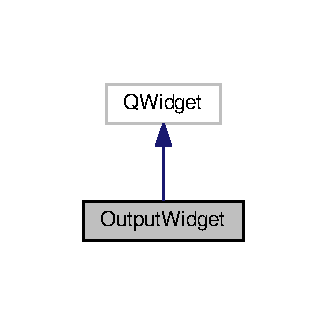
\includegraphics[width=157pt]{classOutputWidget__inherit__graph}
\end{center}
\end{figure}


Collaboration diagram for Output\+Widget\+:\nopagebreak
\begin{figure}[H]
\begin{center}
\leavevmode
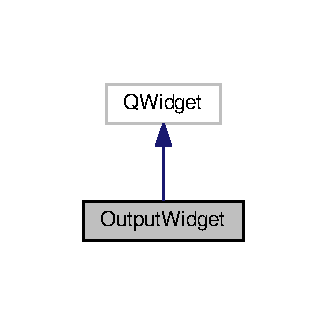
\includegraphics[width=157pt]{classOutputWidget__coll__graph}
\end{center}
\end{figure}
\subsection*{Public Member Functions}
\begin{DoxyCompactItemize}
\item 
\hyperlink{classOutputWidget_a61df9bcea97f4c62b2d564d20bdbae91}{Output\+Widget} (Q\+Widget $\ast$parent=0)
\item 
\hyperlink{classOutputWidget_a7f00baf23905815aa3a846f0df8555bc}{$\sim$\+Output\+Widget} ()
\item 
void \hyperlink{classOutputWidget_a7dbe34186990f08c4ef33b026f4f65b3}{display\+Output} (Q\+Byte\+Array)
\item 
void \hyperlink{classOutputWidget_a75340d5f04a62332cfd52802090b52c4}{clear\+Box} ()
\end{DoxyCompactItemize}
\subsection*{Private Attributes}
\begin{DoxyCompactItemize}
\item 
Ui\+::\+Output\+Widget $\ast$ \hyperlink{classOutputWidget_a09fac2c2bd657cdc445274aad6654e7a}{ui}
\end{DoxyCompactItemize}


\subsection{Constructor \& Destructor Documentation}
\index{Output\+Widget@{Output\+Widget}!Output\+Widget@{Output\+Widget}}
\index{Output\+Widget@{Output\+Widget}!Output\+Widget@{Output\+Widget}}
\subsubsection[{\texorpdfstring{Output\+Widget(\+Q\+Widget $\ast$parent=0)}{OutputWidget(QWidget *parent=0)}}]{\setlength{\rightskip}{0pt plus 5cm}Output\+Widget\+::\+Output\+Widget (
\begin{DoxyParamCaption}
\item[{Q\+Widget $\ast$}]{parent = {\ttfamily 0}}
\end{DoxyParamCaption}
)}\hypertarget{classOutputWidget_a61df9bcea97f4c62b2d564d20bdbae91}{}\label{classOutputWidget_a61df9bcea97f4c62b2d564d20bdbae91}
This file contains functions for the class \hyperlink{classOutputWidget}{Output\+Widget} which is used to view the log of the associated process. \index{Output\+Widget@{Output\+Widget}!````~Output\+Widget@{$\sim$\+Output\+Widget}}
\index{````~Output\+Widget@{$\sim$\+Output\+Widget}!Output\+Widget@{Output\+Widget}}
\subsubsection[{\texorpdfstring{$\sim$\+Output\+Widget()}{~OutputWidget()}}]{\setlength{\rightskip}{0pt plus 5cm}Output\+Widget\+::$\sim$\+Output\+Widget (
\begin{DoxyParamCaption}
{}
\end{DoxyParamCaption}
)}\hypertarget{classOutputWidget_a7f00baf23905815aa3a846f0df8555bc}{}\label{classOutputWidget_a7f00baf23905815aa3a846f0df8555bc}


\subsection{Member Function Documentation}
\index{Output\+Widget@{Output\+Widget}!clear\+Box@{clear\+Box}}
\index{clear\+Box@{clear\+Box}!Output\+Widget@{Output\+Widget}}
\subsubsection[{\texorpdfstring{clear\+Box()}{clearBox()}}]{\setlength{\rightskip}{0pt plus 5cm}void Output\+Widget\+::clear\+Box (
\begin{DoxyParamCaption}
{}
\end{DoxyParamCaption}
)}\hypertarget{classOutputWidget_a75340d5f04a62332cfd52802090b52c4}{}\label{classOutputWidget_a75340d5f04a62332cfd52802090b52c4}
\index{Output\+Widget@{Output\+Widget}!display\+Output@{display\+Output}}
\index{display\+Output@{display\+Output}!Output\+Widget@{Output\+Widget}}
\subsubsection[{\texorpdfstring{display\+Output(\+Q\+Byte\+Array)}{displayOutput(QByteArray)}}]{\setlength{\rightskip}{0pt plus 5cm}void Output\+Widget\+::display\+Output (
\begin{DoxyParamCaption}
\item[{Q\+Byte\+Array}]{data}
\end{DoxyParamCaption}
)}\hypertarget{classOutputWidget_a7dbe34186990f08c4ef33b026f4f65b3}{}\label{classOutputWidget_a7dbe34186990f08c4ef33b026f4f65b3}
$<$ Accepts the input Q\+Byte\+Array and formats it for display in \hyperlink{classOutputWidget}{Output\+Widget} 

\subsection{Member Data Documentation}
\index{Output\+Widget@{Output\+Widget}!ui@{ui}}
\index{ui@{ui}!Output\+Widget@{Output\+Widget}}
\subsubsection[{\texorpdfstring{ui}{ui}}]{\setlength{\rightskip}{0pt plus 5cm}Ui\+::\+Output\+Widget$\ast$ Output\+Widget\+::ui\hspace{0.3cm}{\ttfamily [private]}}\hypertarget{classOutputWidget_a09fac2c2bd657cdc445274aad6654e7a}{}\label{classOutputWidget_a09fac2c2bd657cdc445274aad6654e7a}


The documentation for this class was generated from the following files\+:\begin{DoxyCompactItemize}
\item 
src/hammerhead/control\+\_\+stack/tiburon\+\_\+commander/include/tiburon\+\_\+commander/\hyperlink{output__widget_8h}{output\+\_\+widget.\+h}\item 
src/hammerhead/control\+\_\+stack/tiburon\+\_\+commander/src/\hyperlink{output__widget_8cpp}{output\+\_\+widget.\+cpp}\end{DoxyCompactItemize}

\hypertarget{classPathPlanner}{}\section{Path\+Planner Class Reference}
\label{classPathPlanner}\index{Path\+Planner@{Path\+Planner}}


{\ttfamily \#include $<$Path\+Planner.\+h$>$}



Collaboration diagram for Path\+Planner\+:\nopagebreak
\begin{figure}[H]
\begin{center}
\leavevmode
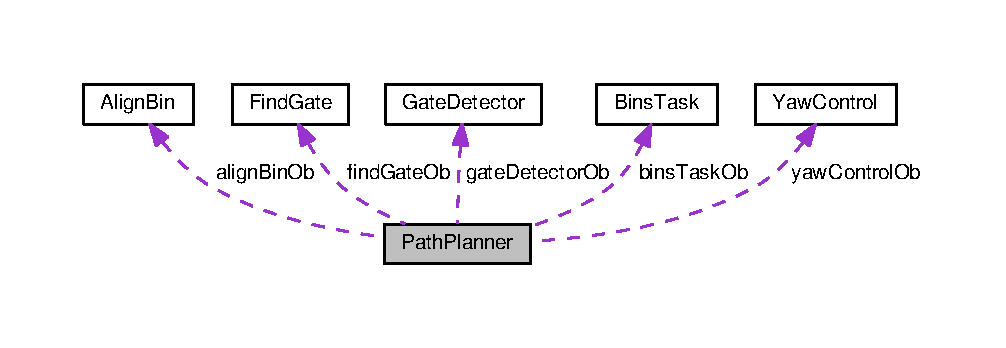
\includegraphics[width=350pt]{classPathPlanner__coll__graph}
\end{center}
\end{figure}
\subsection*{Public Member Functions}
\begin{DoxyCompactItemize}
\item 
\hyperlink{classPathPlanner_a64afb30132b2f7079bc24bfc7c97810d}{Path\+Planner} (ros\+::\+Node\+Handle \+\_\+nh, int, int)
\item 
\hyperlink{classPathPlanner_a61bd61f848e519df56b75eddd3732ab8}{$\sim$\+Path\+Planner} ()
\item 
void \hyperlink{classPathPlanner_a9606656f6008c9915c351e87e3b3db1f}{publish\+Setpoints} ()
\item 
void \hyperlink{classPathPlanner_a67e0129f08f6df984e407992d3804890}{find\+Setpoints} ()
\item 
void \hyperlink{classPathPlanner_ada3d9b80cf5f40c329046ca149e8ba8f}{front\+Camera\+Callback} (const sensor\+\_\+msgs\+::\+Image\+Const\+Ptr \&msg)
\item 
void \hyperlink{classPathPlanner_a9473e9625d617bd0c5b900245195feac}{bottom\+Camera\+Callback} (const sensor\+\_\+msgs\+::\+Image\+Const\+Ptr \&msg)
\item 
void \hyperlink{classPathPlanner_a9b5d663206c906f2fc991153fea7bff0}{vectornav\+Callback} (const vectornav\+::\+Vector\+Nav\+Data\+::\+Const\+Ptr \&msg)
\item 
double \hyperlink{classPathPlanner_a006986912bf894921948056bf8ed1b5a}{find\+Time\+Difference} (\hyperlink{thruster__driver_8cpp_ad3e807c387dc076de974ff7eac67ad81}{Time\+Point}, \hyperlink{thruster__driver_8cpp_ad3e807c387dc076de974ff7eac67ad81}{Time\+Point})
\item 
void \hyperlink{classPathPlanner_ac2818eba3b1035732ca548c87d12d30d}{ball\+Drop\+Sequence} ()
\item 
void \hyperlink{classPathPlanner_a225c5c983e296b81c97c74b94ec2bea0}{ball\+Pickup\+Sequence} ()
\end{DoxyCompactItemize}
\subsection*{Public Attributes}
\begin{DoxyCompactItemize}
\item 
ros\+::\+Node\+Handle \hyperlink{classPathPlanner_a3728ed52563a28d32c19efc157771e96}{nh}
\item 
image\+\_\+transport\+::\+Image\+Transport \hyperlink{classPathPlanner_afdf6f6e68086d7992206f84d37b56c84}{it}
\item 
image\+\_\+transport\+::\+Publisher \hyperlink{classPathPlanner_a8a5f65b9ca4a6ddd19e046c46ad7e349}{front\+Debug\+Pub}
\item 
image\+\_\+transport\+::\+Publisher \hyperlink{classPathPlanner_aae9f1307dab87b0979497f41553dc34e}{bottom\+Debug\+Pub}
\item 
ros\+::\+Publisher \hyperlink{classPathPlanner_ac2cd91552262491438a806f3229fe5f8}{setpoint\+Pub}
\item 
ros\+::\+Publisher \hyperlink{classPathPlanner_a5950dcdaa13fde281ad87bc06bb4221c}{drop\+\_\+pub}
\item 
ros\+::\+Publisher \hyperlink{classPathPlanner_a6ad35bcf1143889a2273362476028445}{breach\+Pub}
\item 
ros\+::\+Publisher \hyperlink{classPathPlanner_af0db2ddfb46fd54f8c8b942b44f67e75}{descend\+\_\+pub}
\item 
ros\+::\+Publisher \hyperlink{classPathPlanner_a8afd938d26553fae883bd02ed0d44458}{ascend\+\_\+pub}
\item 
ros\+::\+Subscriber \hyperlink{classPathPlanner_ae5bf7f525a1723eef45c2887e8b3fbae}{front\+Camera\+Sub}
\item 
ros\+::\+Subscriber \hyperlink{classPathPlanner_a180b062cc5656e45a1f789689cc5d130}{bottom\+Camera\+Sub}
\item 
ros\+::\+Subscriber \hyperlink{classPathPlanner_a0527b6b13cdffd139aa4e2acbcb8cc32}{vectornav\+Sub}
\item 
pid\+\_\+controller\+::\+Setpoint \hyperlink{classPathPlanner_a6b892ed37642ddc634c9dd245f20ca40}{sp}
\item 
sensor\+\_\+msgs\+::\+Image\+Ptr \hyperlink{classPathPlanner_a54f52fe7a3bad416e15f326b807692e2}{front\+Debug\+Msg}
\item 
sensor\+\_\+msgs\+::\+Image\+Ptr \hyperlink{classPathPlanner_a351514e893a8b37984aa678f6ede8211}{bottom\+Debug\+Msg}
\item 
std\+\_\+msgs\+::\+Int8 \hyperlink{classPathPlanner_ad7a30801fb56f1f2a5bf02d99b21ca5a}{descend\+Msg}
\item 
std\+\_\+msgs\+::\+Int8 \hyperlink{classPathPlanner_a5abd76dde4ea570d1f558336ac13f3e4}{ascend\+Msg}
\item 
std\+\_\+msgs\+::\+Int8 \hyperlink{classPathPlanner_aca9f8a364babea5db6c9ff8cc98addbc}{drop\+Msg}
\item 
std\+\_\+msgs\+::\+Bool \hyperlink{classPathPlanner_a1ac63d92d2bee1644f7b2e80d6cc5c09}{breach\+Msg}
\item 
\hyperlink{classFindGate}{Find\+Gate} $\ast$ \hyperlink{classPathPlanner_a411050611aa7ccad2bcbfe8aa8c8698f}{find\+Gate\+Ob}
\item 
\hyperlink{classGateDetector}{Gate\+Detector} $\ast$ \hyperlink{classPathPlanner_af11812439e12931a6f3d744e358e91e4}{gate\+Detector\+Ob}
\item 
\hyperlink{classYawControl}{Yaw\+Control} $\ast$ \hyperlink{classPathPlanner_a8abc38307d93b4feecb14a8ece4764a6}{yaw\+Control\+Ob}
\item 
\hyperlink{classAlignBin}{Align\+Bin} $\ast$ \hyperlink{classPathPlanner_a2953c40a460f99cf2b767b5ab5cb7f3e}{align\+Bin\+Ob}
\item 
\hyperlink{classBinsTask}{Bins\+Task} $\ast$ \hyperlink{classPathPlanner_ab66992788cfdfc1a443bfa97af547100}{bins\+Task\+Ob}
\item 
bool \hyperlink{classPathPlanner_a54e431dfde30e0b15a372c5a16c8dd6c}{U\+S\+E\+\_\+\+Y\+A\+W\+\_\+\+C\+O\+R\+R\+E\+C\+T\+I\+ON} = false
\item 
bool \hyperlink{classPathPlanner_a15a968b0bc50d230bbc22e9099377504}{pause\+Yaw\+Correction}
\item 
const int \hyperlink{classPathPlanner_ada301b950a4d1b14acd2477fbc5f73df}{M\+A\+X\+\_\+\+F\+I\+N\+D\+\_\+\+G\+A\+T\+E\+\_\+\+F\+R\+A\+M\+ES} = 50
\item 
const int \hyperlink{classPathPlanner_ab80757ecd2962cc2e5bd64c300e31628}{C\+O\+R\+R\+E\+C\+T\+\_\+\+Y\+A\+W\+\_\+\+F\+R\+A\+M\+ES} = 75
\item 
const int \hyperlink{classPathPlanner_a11a499117aadaae4036d58bd4b63d7ac}{G\+A\+T\+E\+\_\+\+C\+R\+O\+S\+S\+\_\+\+T\+I\+ME} = 30
\item 
const int \hyperlink{classPathPlanner_a12b219c458ee64a02f3255f76ad63be6}{F\+O\+R\+W\+A\+R\+D\+\_\+\+S\+E\+A\+R\+C\+H\+\_\+\+T\+I\+ME} = 10
\item 
const int \hyperlink{classPathPlanner_a683836da96618f1a2d6e153ef74e55a8}{B\+A\+S\+E\+\_\+\+Y\+A\+W\+\_\+\+S\+E\+A\+R\+C\+H\+\_\+\+A\+N\+G\+LE} = 15
\item 
int \hyperlink{classPathPlanner_a1807065a92d2188817a495bf89195132}{gate\+Frame\+Count}
\item 
\hyperlink{thruster__driver_8cpp_ad3e807c387dc076de974ff7eac67ad81}{Time\+Point} \hyperlink{classPathPlanner_a69d65cdba15fc71183ac337212b9c33f}{start\+\_\+1}
\item 
\hyperlink{thruster__driver_8cpp_ad3e807c387dc076de974ff7eac67ad81}{Time\+Point} \hyperlink{classPathPlanner_afbb083470238dda8254a9d60032ae6d3}{start\+\_\+2}
\item 
bool \hyperlink{classPathPlanner_a4bd99311cef29b79bc2d016ad0977d76}{gate\+Search\+Started}
\item 
bool \hyperlink{classPathPlanner_a3ed3d7942b9417d48ff9aa520493a241}{gate\+Found}
\item 
bool \hyperlink{classPathPlanner_afa8a249b6baf8ec217082eca1c1dc0f9}{gate\+Aligned}
\item 
bool \hyperlink{classPathPlanner_a30b4a90a40e1725347b19a521fd2e085}{gate\+Reached}
\item 
bool \hyperlink{classPathPlanner_ae30224fe26e2e73e0ffff2469ce0d885}{gate\+Final\+Yaw\+Aligned}
\item 
bool \hyperlink{classPathPlanner_a7231798c51e6e722389795cca59ec16e}{gate\+Final\+Aligned}
\item 
bool \hyperlink{classPathPlanner_a07768a73e0b9edc93611d12df1d2f20d}{gate\+Crossed}
\item 
bool \hyperlink{classPathPlanner_acbee7c3c100b1b1b7d0f946100953db7}{return\+To\+Center}
\item 
bool \hyperlink{classPathPlanner_ac649564f82726f564a0e4b1446886c5d}{found\+Bin}
\item 
bool \hyperlink{classPathPlanner_a30fb3f87413d9204db076f92b8df064f}{reached\+Bin}
\item 
bool \hyperlink{classPathPlanner_a61566d814449039efd5feaec4ebd217a}{aligned\+With\+Bin}
\item 
bool \hyperlink{classPathPlanner_a7c037b4370ae019db2950d0bbb20b885}{bin\+Task\+Complete}
\item 
bool \hyperlink{classPathPlanner_a8550d5f0f5e6840d74c482e8c9ec4f17}{gate\+Detected\+Last}
\item 
bool \hyperlink{classPathPlanner_ac4737618f7b977a760c4044c8c11d978}{going\+Forward\+To\+Search} = true
\item 
int \hyperlink{classPathPlanner_a5882e35e164ea48ba9c45325bd0eeb74}{going\+Forward\+Count} = 0
\item 
const int \hyperlink{classPathPlanner_ab562d2e58308fd42088587858d7193ab}{image\+Width} = 648
\item 
const int \hyperlink{classPathPlanner_a83b54a87f884285d41642702c46368a8}{image\+Height} = 488
\item 
const double \hyperlink{classPathPlanner_aa95f3eb27d53bdf487145755a0cb85c9}{img\+Area} = \hyperlink{classPathPlanner_ab562d2e58308fd42088587858d7193ab}{image\+Width} $\ast$ \hyperlink{classPathPlanner_a83b54a87f884285d41642702c46368a8}{image\+Height}
\item 
double \hyperlink{classPathPlanner_a069162f445adcdef1e916ce8d43fd34a}{current\+Yaw}
\item 
double \hyperlink{classPathPlanner_a074f33607f0c0bb7a303e80d52ce79b4}{heading\+Diff}
\item 
double \hyperlink{classPathPlanner_ab3c86e85339eedec45c050955ca9a6b9}{stored\+Yaw}
\item 
double \hyperlink{classPathPlanner_a60f7621c34683c9e3b64d89a36358c48}{yaw\+Change} = 0
\item 
int \hyperlink{classPathPlanner_a43393934c97970d243fbb219ee8c909d}{yaw\+Change\+Dir} = 1
\item 
int \hyperlink{classPathPlanner_a2312e73d3f37acf470f448afaa262afe}{yaw\+Jump} = 3
\item 
\hyperlink{thruster__driver_8cpp_ad3e807c387dc076de974ff7eac67ad81}{Time\+Point} \hyperlink{classPathPlanner_a201a2c207e4abfee915a7acd5c9cae0e}{start\+Time}
\item 
\hyperlink{thruster__driver_8cpp_ad3e807c387dc076de974ff7eac67ad81}{Time\+Point} \hyperlink{classPathPlanner_aec7cfd25a48b711818991f5f449a050b}{last\+Front\+Camera\+Callback\+Time}
\item 
\hyperlink{thruster__driver_8cpp_ad3e807c387dc076de974ff7eac67ad81}{Time\+Point} \hyperlink{classPathPlanner_a4d3c427f732be34f6662f311436a3f5e}{gate\+Cross\+Timer}
\item 
\hyperlink{thruster__driver_8cpp_ad3e807c387dc076de974ff7eac67ad81}{Time\+Point} \hyperlink{classPathPlanner_a579c296b95e4dcb2f7e7b56b90082184}{sway\+Check\+Time}
\item 
\hyperlink{thruster__driver_8cpp_ad3e807c387dc076de974ff7eac67ad81}{Time\+Point} \hyperlink{classPathPlanner_a449a30ac5feb833004e42156124aeb35}{sway\+Return\+Timer}
\item 
\hyperlink{thruster__driver_8cpp_ad3e807c387dc076de974ff7eac67ad81}{Time\+Point} \hyperlink{classPathPlanner_a4802cdb753da4fa47854e33f3220db84}{prev\+Command\+Time}
\item 
\hyperlink{thruster__driver_8cpp_ad3e807c387dc076de974ff7eac67ad81}{Time\+Point} \hyperlink{classPathPlanner_a5b503e6eba34d4925b07749f3162f659}{last\+Yaw\+Correct\+Time}
\item 
\hyperlink{thruster__driver_8cpp_ad3e807c387dc076de974ff7eac67ad81}{Time\+Point} \hyperlink{classPathPlanner_ab851d5039b0392d1895ee42960e29b2d}{height\+Changed\+Last}
\item 
\hyperlink{thruster__driver_8cpp_ad3e807c387dc076de974ff7eac67ad81}{Time\+Point} \hyperlink{classPathPlanner_af31adaae522a828711bb1c800176cbb9}{yaw\+Changed\+Last}
\item 
\hyperlink{thruster__driver_8cpp_ad3e807c387dc076de974ff7eac67ad81}{Time\+Point} \hyperlink{classPathPlanner_a2164113fa9ab422003bffad0454f5bb0}{forward\+Search}
\item 
Vec3i \hyperlink{classPathPlanner_aede3f213d16ed3f67ba27380de436fa7}{bins\+Setpoint}
\item 
bool \hyperlink{classPathPlanner_a5edcf4d5b37bc7d9969710fd7abb6ba7}{bin\+Task\+Timeout}
\item 
int \hyperlink{classPathPlanner_a4c5f3c04540a24807a55c4292f2f4216}{bin\+\_\+not\+\_\+found\+\_\+ctr} = 0
\item 
double \hyperlink{classPathPlanner_acbca3bbb98637d73964596d2ac0ff38b}{right\+Sway\+Units}
\item 
vector$<$ \hyperlink{PathPlanner_8h_aa4d42044193f96ecc0d82daab68fb0e6}{task} $>$ \hyperlink{classPathPlanner_afaaad3d73c413de1915e48dd7f9ef263}{tasks}
\item 
vector$<$ \hyperlink{BinsTask_8h_adc6e5733fc3c22f0a7b2914188c49c90}{state} $>$ \hyperlink{classPathPlanner_aef62d7f3ef83d7170d87bfe689d1eecd}{state\+List}
\item 
vector$<$ int $>$ \hyperlink{classPathPlanner_ac1db41115e7596c58fbc5e0a80b7e4cb}{state\+Timeouts}
\end{DoxyCompactItemize}


\subsection{Constructor \& Destructor Documentation}
\index{Path\+Planner@{Path\+Planner}!Path\+Planner@{Path\+Planner}}
\index{Path\+Planner@{Path\+Planner}!Path\+Planner@{Path\+Planner}}
\subsubsection[{\texorpdfstring{Path\+Planner(ros\+::\+Node\+Handle \+\_\+nh, int, int)}{PathPlanner(ros::NodeHandle _nh, int, int)}}]{\setlength{\rightskip}{0pt plus 5cm}Path\+Planner\+::\+Path\+Planner (
\begin{DoxyParamCaption}
\item[{ros\+::\+Node\+Handle}]{\+\_\+nh, }
\item[{int}]{next\+Sway\+Mode, }
\item[{int}]{sway\+Range}
\end{DoxyParamCaption}
)\hspace{0.3cm}{\ttfamily [explicit]}}\hypertarget{classPathPlanner_a64afb30132b2f7079bc24bfc7c97810d}{}\label{classPathPlanner_a64afb30132b2f7079bc24bfc7c97810d}
\index{Path\+Planner@{Path\+Planner}!````~Path\+Planner@{$\sim$\+Path\+Planner}}
\index{````~Path\+Planner@{$\sim$\+Path\+Planner}!Path\+Planner@{Path\+Planner}}
\subsubsection[{\texorpdfstring{$\sim$\+Path\+Planner()}{~PathPlanner()}}]{\setlength{\rightskip}{0pt plus 5cm}Path\+Planner\+::$\sim$\+Path\+Planner (
\begin{DoxyParamCaption}
{}
\end{DoxyParamCaption}
)}\hypertarget{classPathPlanner_a61bd61f848e519df56b75eddd3732ab8}{}\label{classPathPlanner_a61bd61f848e519df56b75eddd3732ab8}


\subsection{Member Function Documentation}
\index{Path\+Planner@{Path\+Planner}!ball\+Drop\+Sequence@{ball\+Drop\+Sequence}}
\index{ball\+Drop\+Sequence@{ball\+Drop\+Sequence}!Path\+Planner@{Path\+Planner}}
\subsubsection[{\texorpdfstring{ball\+Drop\+Sequence()}{ballDropSequence()}}]{\setlength{\rightskip}{0pt plus 5cm}void Path\+Planner\+::ball\+Drop\+Sequence (
\begin{DoxyParamCaption}
{}
\end{DoxyParamCaption}
)}\hypertarget{classPathPlanner_ac2818eba3b1035732ca548c87d12d30d}{}\label{classPathPlanner_ac2818eba3b1035732ca548c87d12d30d}
\index{Path\+Planner@{Path\+Planner}!ball\+Pickup\+Sequence@{ball\+Pickup\+Sequence}}
\index{ball\+Pickup\+Sequence@{ball\+Pickup\+Sequence}!Path\+Planner@{Path\+Planner}}
\subsubsection[{\texorpdfstring{ball\+Pickup\+Sequence()}{ballPickupSequence()}}]{\setlength{\rightskip}{0pt plus 5cm}void Path\+Planner\+::ball\+Pickup\+Sequence (
\begin{DoxyParamCaption}
{}
\end{DoxyParamCaption}
)}\hypertarget{classPathPlanner_a225c5c983e296b81c97c74b94ec2bea0}{}\label{classPathPlanner_a225c5c983e296b81c97c74b94ec2bea0}
\index{Path\+Planner@{Path\+Planner}!bottom\+Camera\+Callback@{bottom\+Camera\+Callback}}
\index{bottom\+Camera\+Callback@{bottom\+Camera\+Callback}!Path\+Planner@{Path\+Planner}}
\subsubsection[{\texorpdfstring{bottom\+Camera\+Callback(const sensor\+\_\+msgs\+::\+Image\+Const\+Ptr \&msg)}{bottomCameraCallback(const sensor_msgs::ImageConstPtr &msg)}}]{\setlength{\rightskip}{0pt plus 5cm}void Path\+Planner\+::bottom\+Camera\+Callback (
\begin{DoxyParamCaption}
\item[{const sensor\+\_\+msgs\+::\+Image\+Const\+Ptr \&}]{msg}
\end{DoxyParamCaption}
)}\hypertarget{classPathPlanner_a9473e9625d617bd0c5b900245195feac}{}\label{classPathPlanner_a9473e9625d617bd0c5b900245195feac}
\index{Path\+Planner@{Path\+Planner}!find\+Setpoints@{find\+Setpoints}}
\index{find\+Setpoints@{find\+Setpoints}!Path\+Planner@{Path\+Planner}}
\subsubsection[{\texorpdfstring{find\+Setpoints()}{findSetpoints()}}]{\setlength{\rightskip}{0pt plus 5cm}void Path\+Planner\+::find\+Setpoints (
\begin{DoxyParamCaption}
{}
\end{DoxyParamCaption}
)}\hypertarget{classPathPlanner_a67e0129f08f6df984e407992d3804890}{}\label{classPathPlanner_a67e0129f08f6df984e407992d3804890}
\index{Path\+Planner@{Path\+Planner}!find\+Time\+Difference@{find\+Time\+Difference}}
\index{find\+Time\+Difference@{find\+Time\+Difference}!Path\+Planner@{Path\+Planner}}
\subsubsection[{\texorpdfstring{find\+Time\+Difference(\+Time\+Point, Time\+Point)}{findTimeDifference(TimePoint, TimePoint)}}]{\setlength{\rightskip}{0pt plus 5cm}double Path\+Planner\+::find\+Time\+Difference (
\begin{DoxyParamCaption}
\item[{{\bf Time\+Point}}]{end, }
\item[{{\bf Time\+Point}}]{start}
\end{DoxyParamCaption}
)}\hypertarget{classPathPlanner_a006986912bf894921948056bf8ed1b5a}{}\label{classPathPlanner_a006986912bf894921948056bf8ed1b5a}
\index{Path\+Planner@{Path\+Planner}!front\+Camera\+Callback@{front\+Camera\+Callback}}
\index{front\+Camera\+Callback@{front\+Camera\+Callback}!Path\+Planner@{Path\+Planner}}
\subsubsection[{\texorpdfstring{front\+Camera\+Callback(const sensor\+\_\+msgs\+::\+Image\+Const\+Ptr \&msg)}{frontCameraCallback(const sensor_msgs::ImageConstPtr &msg)}}]{\setlength{\rightskip}{0pt plus 5cm}void Path\+Planner\+::front\+Camera\+Callback (
\begin{DoxyParamCaption}
\item[{const sensor\+\_\+msgs\+::\+Image\+Const\+Ptr \&}]{msg}
\end{DoxyParamCaption}
)}\hypertarget{classPathPlanner_ada3d9b80cf5f40c329046ca149e8ba8f}{}\label{classPathPlanner_ada3d9b80cf5f40c329046ca149e8ba8f}
\index{Path\+Planner@{Path\+Planner}!publish\+Setpoints@{publish\+Setpoints}}
\index{publish\+Setpoints@{publish\+Setpoints}!Path\+Planner@{Path\+Planner}}
\subsubsection[{\texorpdfstring{publish\+Setpoints()}{publishSetpoints()}}]{\setlength{\rightskip}{0pt plus 5cm}void Path\+Planner\+::publish\+Setpoints (
\begin{DoxyParamCaption}
{}
\end{DoxyParamCaption}
)}\hypertarget{classPathPlanner_a9606656f6008c9915c351e87e3b3db1f}{}\label{classPathPlanner_a9606656f6008c9915c351e87e3b3db1f}
\index{Path\+Planner@{Path\+Planner}!vectornav\+Callback@{vectornav\+Callback}}
\index{vectornav\+Callback@{vectornav\+Callback}!Path\+Planner@{Path\+Planner}}
\subsubsection[{\texorpdfstring{vectornav\+Callback(const vectornav\+::\+Vector\+Nav\+Data\+::\+Const\+Ptr \&msg)}{vectornavCallback(const vectornav::VectorNavData::ConstPtr &msg)}}]{\setlength{\rightskip}{0pt plus 5cm}void Path\+Planner\+::vectornav\+Callback (
\begin{DoxyParamCaption}
\item[{const vectornav\+::\+Vector\+Nav\+Data\+::\+Const\+Ptr \&}]{msg}
\end{DoxyParamCaption}
)}\hypertarget{classPathPlanner_a9b5d663206c906f2fc991153fea7bff0}{}\label{classPathPlanner_a9b5d663206c906f2fc991153fea7bff0}


\subsection{Member Data Documentation}
\index{Path\+Planner@{Path\+Planner}!align\+Bin\+Ob@{align\+Bin\+Ob}}
\index{align\+Bin\+Ob@{align\+Bin\+Ob}!Path\+Planner@{Path\+Planner}}
\subsubsection[{\texorpdfstring{align\+Bin\+Ob}{alignBinOb}}]{\setlength{\rightskip}{0pt plus 5cm}{\bf Align\+Bin}$\ast$ Path\+Planner\+::align\+Bin\+Ob}\hypertarget{classPathPlanner_a2953c40a460f99cf2b767b5ab5cb7f3e}{}\label{classPathPlanner_a2953c40a460f99cf2b767b5ab5cb7f3e}
\index{Path\+Planner@{Path\+Planner}!aligned\+With\+Bin@{aligned\+With\+Bin}}
\index{aligned\+With\+Bin@{aligned\+With\+Bin}!Path\+Planner@{Path\+Planner}}
\subsubsection[{\texorpdfstring{aligned\+With\+Bin}{alignedWithBin}}]{\setlength{\rightskip}{0pt plus 5cm}bool Path\+Planner\+::aligned\+With\+Bin}\hypertarget{classPathPlanner_a61566d814449039efd5feaec4ebd217a}{}\label{classPathPlanner_a61566d814449039efd5feaec4ebd217a}
\index{Path\+Planner@{Path\+Planner}!ascend\+\_\+pub@{ascend\+\_\+pub}}
\index{ascend\+\_\+pub@{ascend\+\_\+pub}!Path\+Planner@{Path\+Planner}}
\subsubsection[{\texorpdfstring{ascend\+\_\+pub}{ascend_pub}}]{\setlength{\rightskip}{0pt plus 5cm}ros\+::\+Publisher Path\+Planner\+::ascend\+\_\+pub}\hypertarget{classPathPlanner_a8afd938d26553fae883bd02ed0d44458}{}\label{classPathPlanner_a8afd938d26553fae883bd02ed0d44458}
\index{Path\+Planner@{Path\+Planner}!ascend\+Msg@{ascend\+Msg}}
\index{ascend\+Msg@{ascend\+Msg}!Path\+Planner@{Path\+Planner}}
\subsubsection[{\texorpdfstring{ascend\+Msg}{ascendMsg}}]{\setlength{\rightskip}{0pt plus 5cm}std\+\_\+msgs\+::\+Int8 Path\+Planner\+::ascend\+Msg}\hypertarget{classPathPlanner_a5abd76dde4ea570d1f558336ac13f3e4}{}\label{classPathPlanner_a5abd76dde4ea570d1f558336ac13f3e4}
\index{Path\+Planner@{Path\+Planner}!B\+A\+S\+E\+\_\+\+Y\+A\+W\+\_\+\+S\+E\+A\+R\+C\+H\+\_\+\+A\+N\+G\+LE@{B\+A\+S\+E\+\_\+\+Y\+A\+W\+\_\+\+S\+E\+A\+R\+C\+H\+\_\+\+A\+N\+G\+LE}}
\index{B\+A\+S\+E\+\_\+\+Y\+A\+W\+\_\+\+S\+E\+A\+R\+C\+H\+\_\+\+A\+N\+G\+LE@{B\+A\+S\+E\+\_\+\+Y\+A\+W\+\_\+\+S\+E\+A\+R\+C\+H\+\_\+\+A\+N\+G\+LE}!Path\+Planner@{Path\+Planner}}
\subsubsection[{\texorpdfstring{B\+A\+S\+E\+\_\+\+Y\+A\+W\+\_\+\+S\+E\+A\+R\+C\+H\+\_\+\+A\+N\+G\+LE}{BASE_YAW_SEARCH_ANGLE}}]{\setlength{\rightskip}{0pt plus 5cm}const int Path\+Planner\+::\+B\+A\+S\+E\+\_\+\+Y\+A\+W\+\_\+\+S\+E\+A\+R\+C\+H\+\_\+\+A\+N\+G\+LE = 15}\hypertarget{classPathPlanner_a683836da96618f1a2d6e153ef74e55a8}{}\label{classPathPlanner_a683836da96618f1a2d6e153ef74e55a8}
\index{Path\+Planner@{Path\+Planner}!bin\+\_\+not\+\_\+found\+\_\+ctr@{bin\+\_\+not\+\_\+found\+\_\+ctr}}
\index{bin\+\_\+not\+\_\+found\+\_\+ctr@{bin\+\_\+not\+\_\+found\+\_\+ctr}!Path\+Planner@{Path\+Planner}}
\subsubsection[{\texorpdfstring{bin\+\_\+not\+\_\+found\+\_\+ctr}{bin_not_found_ctr}}]{\setlength{\rightskip}{0pt plus 5cm}int Path\+Planner\+::bin\+\_\+not\+\_\+found\+\_\+ctr = 0}\hypertarget{classPathPlanner_a4c5f3c04540a24807a55c4292f2f4216}{}\label{classPathPlanner_a4c5f3c04540a24807a55c4292f2f4216}
\index{Path\+Planner@{Path\+Planner}!bins\+Setpoint@{bins\+Setpoint}}
\index{bins\+Setpoint@{bins\+Setpoint}!Path\+Planner@{Path\+Planner}}
\subsubsection[{\texorpdfstring{bins\+Setpoint}{binsSetpoint}}]{\setlength{\rightskip}{0pt plus 5cm}Vec3i Path\+Planner\+::bins\+Setpoint}\hypertarget{classPathPlanner_aede3f213d16ed3f67ba27380de436fa7}{}\label{classPathPlanner_aede3f213d16ed3f67ba27380de436fa7}
\index{Path\+Planner@{Path\+Planner}!bins\+Task\+Ob@{bins\+Task\+Ob}}
\index{bins\+Task\+Ob@{bins\+Task\+Ob}!Path\+Planner@{Path\+Planner}}
\subsubsection[{\texorpdfstring{bins\+Task\+Ob}{binsTaskOb}}]{\setlength{\rightskip}{0pt plus 5cm}{\bf Bins\+Task}$\ast$ Path\+Planner\+::bins\+Task\+Ob}\hypertarget{classPathPlanner_ab66992788cfdfc1a443bfa97af547100}{}\label{classPathPlanner_ab66992788cfdfc1a443bfa97af547100}
\index{Path\+Planner@{Path\+Planner}!bin\+Task\+Complete@{bin\+Task\+Complete}}
\index{bin\+Task\+Complete@{bin\+Task\+Complete}!Path\+Planner@{Path\+Planner}}
\subsubsection[{\texorpdfstring{bin\+Task\+Complete}{binTaskComplete}}]{\setlength{\rightskip}{0pt plus 5cm}bool Path\+Planner\+::bin\+Task\+Complete}\hypertarget{classPathPlanner_a7c037b4370ae019db2950d0bbb20b885}{}\label{classPathPlanner_a7c037b4370ae019db2950d0bbb20b885}
\index{Path\+Planner@{Path\+Planner}!bin\+Task\+Timeout@{bin\+Task\+Timeout}}
\index{bin\+Task\+Timeout@{bin\+Task\+Timeout}!Path\+Planner@{Path\+Planner}}
\subsubsection[{\texorpdfstring{bin\+Task\+Timeout}{binTaskTimeout}}]{\setlength{\rightskip}{0pt plus 5cm}bool Path\+Planner\+::bin\+Task\+Timeout}\hypertarget{classPathPlanner_a5edcf4d5b37bc7d9969710fd7abb6ba7}{}\label{classPathPlanner_a5edcf4d5b37bc7d9969710fd7abb6ba7}
\index{Path\+Planner@{Path\+Planner}!bottom\+Camera\+Sub@{bottom\+Camera\+Sub}}
\index{bottom\+Camera\+Sub@{bottom\+Camera\+Sub}!Path\+Planner@{Path\+Planner}}
\subsubsection[{\texorpdfstring{bottom\+Camera\+Sub}{bottomCameraSub}}]{\setlength{\rightskip}{0pt plus 5cm}ros\+::\+Subscriber Path\+Planner\+::bottom\+Camera\+Sub}\hypertarget{classPathPlanner_a180b062cc5656e45a1f789689cc5d130}{}\label{classPathPlanner_a180b062cc5656e45a1f789689cc5d130}
\index{Path\+Planner@{Path\+Planner}!bottom\+Debug\+Msg@{bottom\+Debug\+Msg}}
\index{bottom\+Debug\+Msg@{bottom\+Debug\+Msg}!Path\+Planner@{Path\+Planner}}
\subsubsection[{\texorpdfstring{bottom\+Debug\+Msg}{bottomDebugMsg}}]{\setlength{\rightskip}{0pt plus 5cm}sensor\+\_\+msgs\+::\+Image\+Ptr Path\+Planner\+::bottom\+Debug\+Msg}\hypertarget{classPathPlanner_a351514e893a8b37984aa678f6ede8211}{}\label{classPathPlanner_a351514e893a8b37984aa678f6ede8211}
\index{Path\+Planner@{Path\+Planner}!bottom\+Debug\+Pub@{bottom\+Debug\+Pub}}
\index{bottom\+Debug\+Pub@{bottom\+Debug\+Pub}!Path\+Planner@{Path\+Planner}}
\subsubsection[{\texorpdfstring{bottom\+Debug\+Pub}{bottomDebugPub}}]{\setlength{\rightskip}{0pt plus 5cm}image\+\_\+transport\+::\+Publisher Path\+Planner\+::bottom\+Debug\+Pub}\hypertarget{classPathPlanner_aae9f1307dab87b0979497f41553dc34e}{}\label{classPathPlanner_aae9f1307dab87b0979497f41553dc34e}
\index{Path\+Planner@{Path\+Planner}!breach\+Msg@{breach\+Msg}}
\index{breach\+Msg@{breach\+Msg}!Path\+Planner@{Path\+Planner}}
\subsubsection[{\texorpdfstring{breach\+Msg}{breachMsg}}]{\setlength{\rightskip}{0pt plus 5cm}std\+\_\+msgs\+::\+Bool Path\+Planner\+::breach\+Msg}\hypertarget{classPathPlanner_a1ac63d92d2bee1644f7b2e80d6cc5c09}{}\label{classPathPlanner_a1ac63d92d2bee1644f7b2e80d6cc5c09}
\index{Path\+Planner@{Path\+Planner}!breach\+Pub@{breach\+Pub}}
\index{breach\+Pub@{breach\+Pub}!Path\+Planner@{Path\+Planner}}
\subsubsection[{\texorpdfstring{breach\+Pub}{breachPub}}]{\setlength{\rightskip}{0pt plus 5cm}ros\+::\+Publisher Path\+Planner\+::breach\+Pub}\hypertarget{classPathPlanner_a6ad35bcf1143889a2273362476028445}{}\label{classPathPlanner_a6ad35bcf1143889a2273362476028445}
\index{Path\+Planner@{Path\+Planner}!C\+O\+R\+R\+E\+C\+T\+\_\+\+Y\+A\+W\+\_\+\+F\+R\+A\+M\+ES@{C\+O\+R\+R\+E\+C\+T\+\_\+\+Y\+A\+W\+\_\+\+F\+R\+A\+M\+ES}}
\index{C\+O\+R\+R\+E\+C\+T\+\_\+\+Y\+A\+W\+\_\+\+F\+R\+A\+M\+ES@{C\+O\+R\+R\+E\+C\+T\+\_\+\+Y\+A\+W\+\_\+\+F\+R\+A\+M\+ES}!Path\+Planner@{Path\+Planner}}
\subsubsection[{\texorpdfstring{C\+O\+R\+R\+E\+C\+T\+\_\+\+Y\+A\+W\+\_\+\+F\+R\+A\+M\+ES}{CORRECT_YAW_FRAMES}}]{\setlength{\rightskip}{0pt plus 5cm}const int Path\+Planner\+::\+C\+O\+R\+R\+E\+C\+T\+\_\+\+Y\+A\+W\+\_\+\+F\+R\+A\+M\+ES = 75}\hypertarget{classPathPlanner_ab80757ecd2962cc2e5bd64c300e31628}{}\label{classPathPlanner_ab80757ecd2962cc2e5bd64c300e31628}
\index{Path\+Planner@{Path\+Planner}!current\+Yaw@{current\+Yaw}}
\index{current\+Yaw@{current\+Yaw}!Path\+Planner@{Path\+Planner}}
\subsubsection[{\texorpdfstring{current\+Yaw}{currentYaw}}]{\setlength{\rightskip}{0pt plus 5cm}double Path\+Planner\+::current\+Yaw}\hypertarget{classPathPlanner_a069162f445adcdef1e916ce8d43fd34a}{}\label{classPathPlanner_a069162f445adcdef1e916ce8d43fd34a}
\index{Path\+Planner@{Path\+Planner}!descend\+\_\+pub@{descend\+\_\+pub}}
\index{descend\+\_\+pub@{descend\+\_\+pub}!Path\+Planner@{Path\+Planner}}
\subsubsection[{\texorpdfstring{descend\+\_\+pub}{descend_pub}}]{\setlength{\rightskip}{0pt plus 5cm}ros\+::\+Publisher Path\+Planner\+::descend\+\_\+pub}\hypertarget{classPathPlanner_af0db2ddfb46fd54f8c8b942b44f67e75}{}\label{classPathPlanner_af0db2ddfb46fd54f8c8b942b44f67e75}
\index{Path\+Planner@{Path\+Planner}!descend\+Msg@{descend\+Msg}}
\index{descend\+Msg@{descend\+Msg}!Path\+Planner@{Path\+Planner}}
\subsubsection[{\texorpdfstring{descend\+Msg}{descendMsg}}]{\setlength{\rightskip}{0pt plus 5cm}std\+\_\+msgs\+::\+Int8 Path\+Planner\+::descend\+Msg}\hypertarget{classPathPlanner_ad7a30801fb56f1f2a5bf02d99b21ca5a}{}\label{classPathPlanner_ad7a30801fb56f1f2a5bf02d99b21ca5a}
\index{Path\+Planner@{Path\+Planner}!drop\+\_\+pub@{drop\+\_\+pub}}
\index{drop\+\_\+pub@{drop\+\_\+pub}!Path\+Planner@{Path\+Planner}}
\subsubsection[{\texorpdfstring{drop\+\_\+pub}{drop_pub}}]{\setlength{\rightskip}{0pt plus 5cm}ros\+::\+Publisher Path\+Planner\+::drop\+\_\+pub}\hypertarget{classPathPlanner_a5950dcdaa13fde281ad87bc06bb4221c}{}\label{classPathPlanner_a5950dcdaa13fde281ad87bc06bb4221c}
\index{Path\+Planner@{Path\+Planner}!drop\+Msg@{drop\+Msg}}
\index{drop\+Msg@{drop\+Msg}!Path\+Planner@{Path\+Planner}}
\subsubsection[{\texorpdfstring{drop\+Msg}{dropMsg}}]{\setlength{\rightskip}{0pt plus 5cm}std\+\_\+msgs\+::\+Int8 Path\+Planner\+::drop\+Msg}\hypertarget{classPathPlanner_aca9f8a364babea5db6c9ff8cc98addbc}{}\label{classPathPlanner_aca9f8a364babea5db6c9ff8cc98addbc}
\index{Path\+Planner@{Path\+Planner}!find\+Gate\+Ob@{find\+Gate\+Ob}}
\index{find\+Gate\+Ob@{find\+Gate\+Ob}!Path\+Planner@{Path\+Planner}}
\subsubsection[{\texorpdfstring{find\+Gate\+Ob}{findGateOb}}]{\setlength{\rightskip}{0pt plus 5cm}{\bf Find\+Gate}$\ast$ Path\+Planner\+::find\+Gate\+Ob}\hypertarget{classPathPlanner_a411050611aa7ccad2bcbfe8aa8c8698f}{}\label{classPathPlanner_a411050611aa7ccad2bcbfe8aa8c8698f}
\index{Path\+Planner@{Path\+Planner}!F\+O\+R\+W\+A\+R\+D\+\_\+\+S\+E\+A\+R\+C\+H\+\_\+\+T\+I\+ME@{F\+O\+R\+W\+A\+R\+D\+\_\+\+S\+E\+A\+R\+C\+H\+\_\+\+T\+I\+ME}}
\index{F\+O\+R\+W\+A\+R\+D\+\_\+\+S\+E\+A\+R\+C\+H\+\_\+\+T\+I\+ME@{F\+O\+R\+W\+A\+R\+D\+\_\+\+S\+E\+A\+R\+C\+H\+\_\+\+T\+I\+ME}!Path\+Planner@{Path\+Planner}}
\subsubsection[{\texorpdfstring{F\+O\+R\+W\+A\+R\+D\+\_\+\+S\+E\+A\+R\+C\+H\+\_\+\+T\+I\+ME}{FORWARD_SEARCH_TIME}}]{\setlength{\rightskip}{0pt plus 5cm}const int Path\+Planner\+::\+F\+O\+R\+W\+A\+R\+D\+\_\+\+S\+E\+A\+R\+C\+H\+\_\+\+T\+I\+ME = 10}\hypertarget{classPathPlanner_a12b219c458ee64a02f3255f76ad63be6}{}\label{classPathPlanner_a12b219c458ee64a02f3255f76ad63be6}
\index{Path\+Planner@{Path\+Planner}!forward\+Search@{forward\+Search}}
\index{forward\+Search@{forward\+Search}!Path\+Planner@{Path\+Planner}}
\subsubsection[{\texorpdfstring{forward\+Search}{forwardSearch}}]{\setlength{\rightskip}{0pt plus 5cm}{\bf Time\+Point} Path\+Planner\+::forward\+Search}\hypertarget{classPathPlanner_a2164113fa9ab422003bffad0454f5bb0}{}\label{classPathPlanner_a2164113fa9ab422003bffad0454f5bb0}
\index{Path\+Planner@{Path\+Planner}!found\+Bin@{found\+Bin}}
\index{found\+Bin@{found\+Bin}!Path\+Planner@{Path\+Planner}}
\subsubsection[{\texorpdfstring{found\+Bin}{foundBin}}]{\setlength{\rightskip}{0pt plus 5cm}bool Path\+Planner\+::found\+Bin}\hypertarget{classPathPlanner_ac649564f82726f564a0e4b1446886c5d}{}\label{classPathPlanner_ac649564f82726f564a0e4b1446886c5d}
\index{Path\+Planner@{Path\+Planner}!front\+Camera\+Sub@{front\+Camera\+Sub}}
\index{front\+Camera\+Sub@{front\+Camera\+Sub}!Path\+Planner@{Path\+Planner}}
\subsubsection[{\texorpdfstring{front\+Camera\+Sub}{frontCameraSub}}]{\setlength{\rightskip}{0pt plus 5cm}ros\+::\+Subscriber Path\+Planner\+::front\+Camera\+Sub}\hypertarget{classPathPlanner_ae5bf7f525a1723eef45c2887e8b3fbae}{}\label{classPathPlanner_ae5bf7f525a1723eef45c2887e8b3fbae}
\index{Path\+Planner@{Path\+Planner}!front\+Debug\+Msg@{front\+Debug\+Msg}}
\index{front\+Debug\+Msg@{front\+Debug\+Msg}!Path\+Planner@{Path\+Planner}}
\subsubsection[{\texorpdfstring{front\+Debug\+Msg}{frontDebugMsg}}]{\setlength{\rightskip}{0pt plus 5cm}sensor\+\_\+msgs\+::\+Image\+Ptr Path\+Planner\+::front\+Debug\+Msg}\hypertarget{classPathPlanner_a54f52fe7a3bad416e15f326b807692e2}{}\label{classPathPlanner_a54f52fe7a3bad416e15f326b807692e2}
\index{Path\+Planner@{Path\+Planner}!front\+Debug\+Pub@{front\+Debug\+Pub}}
\index{front\+Debug\+Pub@{front\+Debug\+Pub}!Path\+Planner@{Path\+Planner}}
\subsubsection[{\texorpdfstring{front\+Debug\+Pub}{frontDebugPub}}]{\setlength{\rightskip}{0pt plus 5cm}image\+\_\+transport\+::\+Publisher Path\+Planner\+::front\+Debug\+Pub}\hypertarget{classPathPlanner_a8a5f65b9ca4a6ddd19e046c46ad7e349}{}\label{classPathPlanner_a8a5f65b9ca4a6ddd19e046c46ad7e349}
\index{Path\+Planner@{Path\+Planner}!G\+A\+T\+E\+\_\+\+C\+R\+O\+S\+S\+\_\+\+T\+I\+ME@{G\+A\+T\+E\+\_\+\+C\+R\+O\+S\+S\+\_\+\+T\+I\+ME}}
\index{G\+A\+T\+E\+\_\+\+C\+R\+O\+S\+S\+\_\+\+T\+I\+ME@{G\+A\+T\+E\+\_\+\+C\+R\+O\+S\+S\+\_\+\+T\+I\+ME}!Path\+Planner@{Path\+Planner}}
\subsubsection[{\texorpdfstring{G\+A\+T\+E\+\_\+\+C\+R\+O\+S\+S\+\_\+\+T\+I\+ME}{GATE_CROSS_TIME}}]{\setlength{\rightskip}{0pt plus 5cm}const int Path\+Planner\+::\+G\+A\+T\+E\+\_\+\+C\+R\+O\+S\+S\+\_\+\+T\+I\+ME = 30}\hypertarget{classPathPlanner_a11a499117aadaae4036d58bd4b63d7ac}{}\label{classPathPlanner_a11a499117aadaae4036d58bd4b63d7ac}
\index{Path\+Planner@{Path\+Planner}!gate\+Aligned@{gate\+Aligned}}
\index{gate\+Aligned@{gate\+Aligned}!Path\+Planner@{Path\+Planner}}
\subsubsection[{\texorpdfstring{gate\+Aligned}{gateAligned}}]{\setlength{\rightskip}{0pt plus 5cm}bool Path\+Planner\+::gate\+Aligned}\hypertarget{classPathPlanner_afa8a249b6baf8ec217082eca1c1dc0f9}{}\label{classPathPlanner_afa8a249b6baf8ec217082eca1c1dc0f9}
\index{Path\+Planner@{Path\+Planner}!gate\+Crossed@{gate\+Crossed}}
\index{gate\+Crossed@{gate\+Crossed}!Path\+Planner@{Path\+Planner}}
\subsubsection[{\texorpdfstring{gate\+Crossed}{gateCrossed}}]{\setlength{\rightskip}{0pt plus 5cm}bool Path\+Planner\+::gate\+Crossed}\hypertarget{classPathPlanner_a07768a73e0b9edc93611d12df1d2f20d}{}\label{classPathPlanner_a07768a73e0b9edc93611d12df1d2f20d}
\index{Path\+Planner@{Path\+Planner}!gate\+Cross\+Timer@{gate\+Cross\+Timer}}
\index{gate\+Cross\+Timer@{gate\+Cross\+Timer}!Path\+Planner@{Path\+Planner}}
\subsubsection[{\texorpdfstring{gate\+Cross\+Timer}{gateCrossTimer}}]{\setlength{\rightskip}{0pt plus 5cm}{\bf Time\+Point} Path\+Planner\+::gate\+Cross\+Timer}\hypertarget{classPathPlanner_a4d3c427f732be34f6662f311436a3f5e}{}\label{classPathPlanner_a4d3c427f732be34f6662f311436a3f5e}
\index{Path\+Planner@{Path\+Planner}!gate\+Detected\+Last@{gate\+Detected\+Last}}
\index{gate\+Detected\+Last@{gate\+Detected\+Last}!Path\+Planner@{Path\+Planner}}
\subsubsection[{\texorpdfstring{gate\+Detected\+Last}{gateDetectedLast}}]{\setlength{\rightskip}{0pt plus 5cm}bool Path\+Planner\+::gate\+Detected\+Last}\hypertarget{classPathPlanner_a8550d5f0f5e6840d74c482e8c9ec4f17}{}\label{classPathPlanner_a8550d5f0f5e6840d74c482e8c9ec4f17}
\index{Path\+Planner@{Path\+Planner}!gate\+Detector\+Ob@{gate\+Detector\+Ob}}
\index{gate\+Detector\+Ob@{gate\+Detector\+Ob}!Path\+Planner@{Path\+Planner}}
\subsubsection[{\texorpdfstring{gate\+Detector\+Ob}{gateDetectorOb}}]{\setlength{\rightskip}{0pt plus 5cm}{\bf Gate\+Detector}$\ast$ Path\+Planner\+::gate\+Detector\+Ob}\hypertarget{classPathPlanner_af11812439e12931a6f3d744e358e91e4}{}\label{classPathPlanner_af11812439e12931a6f3d744e358e91e4}
\index{Path\+Planner@{Path\+Planner}!gate\+Final\+Aligned@{gate\+Final\+Aligned}}
\index{gate\+Final\+Aligned@{gate\+Final\+Aligned}!Path\+Planner@{Path\+Planner}}
\subsubsection[{\texorpdfstring{gate\+Final\+Aligned}{gateFinalAligned}}]{\setlength{\rightskip}{0pt plus 5cm}bool Path\+Planner\+::gate\+Final\+Aligned}\hypertarget{classPathPlanner_a7231798c51e6e722389795cca59ec16e}{}\label{classPathPlanner_a7231798c51e6e722389795cca59ec16e}
\index{Path\+Planner@{Path\+Planner}!gate\+Final\+Yaw\+Aligned@{gate\+Final\+Yaw\+Aligned}}
\index{gate\+Final\+Yaw\+Aligned@{gate\+Final\+Yaw\+Aligned}!Path\+Planner@{Path\+Planner}}
\subsubsection[{\texorpdfstring{gate\+Final\+Yaw\+Aligned}{gateFinalYawAligned}}]{\setlength{\rightskip}{0pt plus 5cm}bool Path\+Planner\+::gate\+Final\+Yaw\+Aligned}\hypertarget{classPathPlanner_ae30224fe26e2e73e0ffff2469ce0d885}{}\label{classPathPlanner_ae30224fe26e2e73e0ffff2469ce0d885}
\index{Path\+Planner@{Path\+Planner}!gate\+Found@{gate\+Found}}
\index{gate\+Found@{gate\+Found}!Path\+Planner@{Path\+Planner}}
\subsubsection[{\texorpdfstring{gate\+Found}{gateFound}}]{\setlength{\rightskip}{0pt plus 5cm}bool Path\+Planner\+::gate\+Found}\hypertarget{classPathPlanner_a3ed3d7942b9417d48ff9aa520493a241}{}\label{classPathPlanner_a3ed3d7942b9417d48ff9aa520493a241}
\index{Path\+Planner@{Path\+Planner}!gate\+Frame\+Count@{gate\+Frame\+Count}}
\index{gate\+Frame\+Count@{gate\+Frame\+Count}!Path\+Planner@{Path\+Planner}}
\subsubsection[{\texorpdfstring{gate\+Frame\+Count}{gateFrameCount}}]{\setlength{\rightskip}{0pt plus 5cm}int Path\+Planner\+::gate\+Frame\+Count}\hypertarget{classPathPlanner_a1807065a92d2188817a495bf89195132}{}\label{classPathPlanner_a1807065a92d2188817a495bf89195132}
\index{Path\+Planner@{Path\+Planner}!gate\+Reached@{gate\+Reached}}
\index{gate\+Reached@{gate\+Reached}!Path\+Planner@{Path\+Planner}}
\subsubsection[{\texorpdfstring{gate\+Reached}{gateReached}}]{\setlength{\rightskip}{0pt plus 5cm}bool Path\+Planner\+::gate\+Reached}\hypertarget{classPathPlanner_a30b4a90a40e1725347b19a521fd2e085}{}\label{classPathPlanner_a30b4a90a40e1725347b19a521fd2e085}
\index{Path\+Planner@{Path\+Planner}!gate\+Search\+Started@{gate\+Search\+Started}}
\index{gate\+Search\+Started@{gate\+Search\+Started}!Path\+Planner@{Path\+Planner}}
\subsubsection[{\texorpdfstring{gate\+Search\+Started}{gateSearchStarted}}]{\setlength{\rightskip}{0pt plus 5cm}bool Path\+Planner\+::gate\+Search\+Started}\hypertarget{classPathPlanner_a4bd99311cef29b79bc2d016ad0977d76}{}\label{classPathPlanner_a4bd99311cef29b79bc2d016ad0977d76}
\index{Path\+Planner@{Path\+Planner}!going\+Forward\+Count@{going\+Forward\+Count}}
\index{going\+Forward\+Count@{going\+Forward\+Count}!Path\+Planner@{Path\+Planner}}
\subsubsection[{\texorpdfstring{going\+Forward\+Count}{goingForwardCount}}]{\setlength{\rightskip}{0pt plus 5cm}int Path\+Planner\+::going\+Forward\+Count = 0}\hypertarget{classPathPlanner_a5882e35e164ea48ba9c45325bd0eeb74}{}\label{classPathPlanner_a5882e35e164ea48ba9c45325bd0eeb74}
\index{Path\+Planner@{Path\+Planner}!going\+Forward\+To\+Search@{going\+Forward\+To\+Search}}
\index{going\+Forward\+To\+Search@{going\+Forward\+To\+Search}!Path\+Planner@{Path\+Planner}}
\subsubsection[{\texorpdfstring{going\+Forward\+To\+Search}{goingForwardToSearch}}]{\setlength{\rightskip}{0pt plus 5cm}bool Path\+Planner\+::going\+Forward\+To\+Search = true}\hypertarget{classPathPlanner_ac4737618f7b977a760c4044c8c11d978}{}\label{classPathPlanner_ac4737618f7b977a760c4044c8c11d978}
\index{Path\+Planner@{Path\+Planner}!heading\+Diff@{heading\+Diff}}
\index{heading\+Diff@{heading\+Diff}!Path\+Planner@{Path\+Planner}}
\subsubsection[{\texorpdfstring{heading\+Diff}{headingDiff}}]{\setlength{\rightskip}{0pt plus 5cm}double Path\+Planner\+::heading\+Diff}\hypertarget{classPathPlanner_a074f33607f0c0bb7a303e80d52ce79b4}{}\label{classPathPlanner_a074f33607f0c0bb7a303e80d52ce79b4}
\index{Path\+Planner@{Path\+Planner}!height\+Changed\+Last@{height\+Changed\+Last}}
\index{height\+Changed\+Last@{height\+Changed\+Last}!Path\+Planner@{Path\+Planner}}
\subsubsection[{\texorpdfstring{height\+Changed\+Last}{heightChangedLast}}]{\setlength{\rightskip}{0pt plus 5cm}{\bf Time\+Point} Path\+Planner\+::height\+Changed\+Last}\hypertarget{classPathPlanner_ab851d5039b0392d1895ee42960e29b2d}{}\label{classPathPlanner_ab851d5039b0392d1895ee42960e29b2d}
\index{Path\+Planner@{Path\+Planner}!image\+Height@{image\+Height}}
\index{image\+Height@{image\+Height}!Path\+Planner@{Path\+Planner}}
\subsubsection[{\texorpdfstring{image\+Height}{imageHeight}}]{\setlength{\rightskip}{0pt plus 5cm}const int Path\+Planner\+::image\+Height = 488}\hypertarget{classPathPlanner_a83b54a87f884285d41642702c46368a8}{}\label{classPathPlanner_a83b54a87f884285d41642702c46368a8}
\index{Path\+Planner@{Path\+Planner}!image\+Width@{image\+Width}}
\index{image\+Width@{image\+Width}!Path\+Planner@{Path\+Planner}}
\subsubsection[{\texorpdfstring{image\+Width}{imageWidth}}]{\setlength{\rightskip}{0pt plus 5cm}const int Path\+Planner\+::image\+Width = 648}\hypertarget{classPathPlanner_ab562d2e58308fd42088587858d7193ab}{}\label{classPathPlanner_ab562d2e58308fd42088587858d7193ab}
\index{Path\+Planner@{Path\+Planner}!img\+Area@{img\+Area}}
\index{img\+Area@{img\+Area}!Path\+Planner@{Path\+Planner}}
\subsubsection[{\texorpdfstring{img\+Area}{imgArea}}]{\setlength{\rightskip}{0pt plus 5cm}const double Path\+Planner\+::img\+Area = {\bf image\+Width} $\ast$ {\bf image\+Height}}\hypertarget{classPathPlanner_aa95f3eb27d53bdf487145755a0cb85c9}{}\label{classPathPlanner_aa95f3eb27d53bdf487145755a0cb85c9}
\index{Path\+Planner@{Path\+Planner}!it@{it}}
\index{it@{it}!Path\+Planner@{Path\+Planner}}
\subsubsection[{\texorpdfstring{it}{it}}]{\setlength{\rightskip}{0pt plus 5cm}image\+\_\+transport\+::\+Image\+Transport Path\+Planner\+::it}\hypertarget{classPathPlanner_afdf6f6e68086d7992206f84d37b56c84}{}\label{classPathPlanner_afdf6f6e68086d7992206f84d37b56c84}
\index{Path\+Planner@{Path\+Planner}!last\+Front\+Camera\+Callback\+Time@{last\+Front\+Camera\+Callback\+Time}}
\index{last\+Front\+Camera\+Callback\+Time@{last\+Front\+Camera\+Callback\+Time}!Path\+Planner@{Path\+Planner}}
\subsubsection[{\texorpdfstring{last\+Front\+Camera\+Callback\+Time}{lastFrontCameraCallbackTime}}]{\setlength{\rightskip}{0pt plus 5cm}{\bf Time\+Point} Path\+Planner\+::last\+Front\+Camera\+Callback\+Time}\hypertarget{classPathPlanner_aec7cfd25a48b711818991f5f449a050b}{}\label{classPathPlanner_aec7cfd25a48b711818991f5f449a050b}
\index{Path\+Planner@{Path\+Planner}!last\+Yaw\+Correct\+Time@{last\+Yaw\+Correct\+Time}}
\index{last\+Yaw\+Correct\+Time@{last\+Yaw\+Correct\+Time}!Path\+Planner@{Path\+Planner}}
\subsubsection[{\texorpdfstring{last\+Yaw\+Correct\+Time}{lastYawCorrectTime}}]{\setlength{\rightskip}{0pt plus 5cm}{\bf Time\+Point} Path\+Planner\+::last\+Yaw\+Correct\+Time}\hypertarget{classPathPlanner_a5b503e6eba34d4925b07749f3162f659}{}\label{classPathPlanner_a5b503e6eba34d4925b07749f3162f659}
\index{Path\+Planner@{Path\+Planner}!M\+A\+X\+\_\+\+F\+I\+N\+D\+\_\+\+G\+A\+T\+E\+\_\+\+F\+R\+A\+M\+ES@{M\+A\+X\+\_\+\+F\+I\+N\+D\+\_\+\+G\+A\+T\+E\+\_\+\+F\+R\+A\+M\+ES}}
\index{M\+A\+X\+\_\+\+F\+I\+N\+D\+\_\+\+G\+A\+T\+E\+\_\+\+F\+R\+A\+M\+ES@{M\+A\+X\+\_\+\+F\+I\+N\+D\+\_\+\+G\+A\+T\+E\+\_\+\+F\+R\+A\+M\+ES}!Path\+Planner@{Path\+Planner}}
\subsubsection[{\texorpdfstring{M\+A\+X\+\_\+\+F\+I\+N\+D\+\_\+\+G\+A\+T\+E\+\_\+\+F\+R\+A\+M\+ES}{MAX_FIND_GATE_FRAMES}}]{\setlength{\rightskip}{0pt plus 5cm}const int Path\+Planner\+::\+M\+A\+X\+\_\+\+F\+I\+N\+D\+\_\+\+G\+A\+T\+E\+\_\+\+F\+R\+A\+M\+ES = 50}\hypertarget{classPathPlanner_ada301b950a4d1b14acd2477fbc5f73df}{}\label{classPathPlanner_ada301b950a4d1b14acd2477fbc5f73df}
\index{Path\+Planner@{Path\+Planner}!nh@{nh}}
\index{nh@{nh}!Path\+Planner@{Path\+Planner}}
\subsubsection[{\texorpdfstring{nh}{nh}}]{\setlength{\rightskip}{0pt plus 5cm}ros\+::\+Node\+Handle Path\+Planner\+::nh}\hypertarget{classPathPlanner_a3728ed52563a28d32c19efc157771e96}{}\label{classPathPlanner_a3728ed52563a28d32c19efc157771e96}
\index{Path\+Planner@{Path\+Planner}!pause\+Yaw\+Correction@{pause\+Yaw\+Correction}}
\index{pause\+Yaw\+Correction@{pause\+Yaw\+Correction}!Path\+Planner@{Path\+Planner}}
\subsubsection[{\texorpdfstring{pause\+Yaw\+Correction}{pauseYawCorrection}}]{\setlength{\rightskip}{0pt plus 5cm}bool Path\+Planner\+::pause\+Yaw\+Correction}\hypertarget{classPathPlanner_a15a968b0bc50d230bbc22e9099377504}{}\label{classPathPlanner_a15a968b0bc50d230bbc22e9099377504}
\index{Path\+Planner@{Path\+Planner}!prev\+Command\+Time@{prev\+Command\+Time}}
\index{prev\+Command\+Time@{prev\+Command\+Time}!Path\+Planner@{Path\+Planner}}
\subsubsection[{\texorpdfstring{prev\+Command\+Time}{prevCommandTime}}]{\setlength{\rightskip}{0pt plus 5cm}{\bf Time\+Point} Path\+Planner\+::prev\+Command\+Time}\hypertarget{classPathPlanner_a4802cdb753da4fa47854e33f3220db84}{}\label{classPathPlanner_a4802cdb753da4fa47854e33f3220db84}
\index{Path\+Planner@{Path\+Planner}!reached\+Bin@{reached\+Bin}}
\index{reached\+Bin@{reached\+Bin}!Path\+Planner@{Path\+Planner}}
\subsubsection[{\texorpdfstring{reached\+Bin}{reachedBin}}]{\setlength{\rightskip}{0pt plus 5cm}bool Path\+Planner\+::reached\+Bin}\hypertarget{classPathPlanner_a30fb3f87413d9204db076f92b8df064f}{}\label{classPathPlanner_a30fb3f87413d9204db076f92b8df064f}
\index{Path\+Planner@{Path\+Planner}!return\+To\+Center@{return\+To\+Center}}
\index{return\+To\+Center@{return\+To\+Center}!Path\+Planner@{Path\+Planner}}
\subsubsection[{\texorpdfstring{return\+To\+Center}{returnToCenter}}]{\setlength{\rightskip}{0pt plus 5cm}bool Path\+Planner\+::return\+To\+Center}\hypertarget{classPathPlanner_acbee7c3c100b1b1b7d0f946100953db7}{}\label{classPathPlanner_acbee7c3c100b1b1b7d0f946100953db7}
\index{Path\+Planner@{Path\+Planner}!right\+Sway\+Units@{right\+Sway\+Units}}
\index{right\+Sway\+Units@{right\+Sway\+Units}!Path\+Planner@{Path\+Planner}}
\subsubsection[{\texorpdfstring{right\+Sway\+Units}{rightSwayUnits}}]{\setlength{\rightskip}{0pt plus 5cm}double Path\+Planner\+::right\+Sway\+Units}\hypertarget{classPathPlanner_acbca3bbb98637d73964596d2ac0ff38b}{}\label{classPathPlanner_acbca3bbb98637d73964596d2ac0ff38b}
\index{Path\+Planner@{Path\+Planner}!setpoint\+Pub@{setpoint\+Pub}}
\index{setpoint\+Pub@{setpoint\+Pub}!Path\+Planner@{Path\+Planner}}
\subsubsection[{\texorpdfstring{setpoint\+Pub}{setpointPub}}]{\setlength{\rightskip}{0pt plus 5cm}ros\+::\+Publisher Path\+Planner\+::setpoint\+Pub}\hypertarget{classPathPlanner_ac2cd91552262491438a806f3229fe5f8}{}\label{classPathPlanner_ac2cd91552262491438a806f3229fe5f8}
\index{Path\+Planner@{Path\+Planner}!sp@{sp}}
\index{sp@{sp}!Path\+Planner@{Path\+Planner}}
\subsubsection[{\texorpdfstring{sp}{sp}}]{\setlength{\rightskip}{0pt plus 5cm}pid\+\_\+controller\+::\+Setpoint Path\+Planner\+::sp}\hypertarget{classPathPlanner_a6b892ed37642ddc634c9dd245f20ca40}{}\label{classPathPlanner_a6b892ed37642ddc634c9dd245f20ca40}
\index{Path\+Planner@{Path\+Planner}!start\+\_\+1@{start\+\_\+1}}
\index{start\+\_\+1@{start\+\_\+1}!Path\+Planner@{Path\+Planner}}
\subsubsection[{\texorpdfstring{start\+\_\+1}{start_1}}]{\setlength{\rightskip}{0pt plus 5cm}{\bf Time\+Point} Path\+Planner\+::start\+\_\+1}\hypertarget{classPathPlanner_a69d65cdba15fc71183ac337212b9c33f}{}\label{classPathPlanner_a69d65cdba15fc71183ac337212b9c33f}
\index{Path\+Planner@{Path\+Planner}!start\+\_\+2@{start\+\_\+2}}
\index{start\+\_\+2@{start\+\_\+2}!Path\+Planner@{Path\+Planner}}
\subsubsection[{\texorpdfstring{start\+\_\+2}{start_2}}]{\setlength{\rightskip}{0pt plus 5cm}{\bf Time\+Point} Path\+Planner\+::start\+\_\+2}\hypertarget{classPathPlanner_afbb083470238dda8254a9d60032ae6d3}{}\label{classPathPlanner_afbb083470238dda8254a9d60032ae6d3}
\index{Path\+Planner@{Path\+Planner}!start\+Time@{start\+Time}}
\index{start\+Time@{start\+Time}!Path\+Planner@{Path\+Planner}}
\subsubsection[{\texorpdfstring{start\+Time}{startTime}}]{\setlength{\rightskip}{0pt plus 5cm}{\bf Time\+Point} Path\+Planner\+::start\+Time}\hypertarget{classPathPlanner_a201a2c207e4abfee915a7acd5c9cae0e}{}\label{classPathPlanner_a201a2c207e4abfee915a7acd5c9cae0e}
\index{Path\+Planner@{Path\+Planner}!state\+List@{state\+List}}
\index{state\+List@{state\+List}!Path\+Planner@{Path\+Planner}}
\subsubsection[{\texorpdfstring{state\+List}{stateList}}]{\setlength{\rightskip}{0pt plus 5cm}vector$<${\bf state}$>$ Path\+Planner\+::state\+List}\hypertarget{classPathPlanner_aef62d7f3ef83d7170d87bfe689d1eecd}{}\label{classPathPlanner_aef62d7f3ef83d7170d87bfe689d1eecd}
\index{Path\+Planner@{Path\+Planner}!state\+Timeouts@{state\+Timeouts}}
\index{state\+Timeouts@{state\+Timeouts}!Path\+Planner@{Path\+Planner}}
\subsubsection[{\texorpdfstring{state\+Timeouts}{stateTimeouts}}]{\setlength{\rightskip}{0pt plus 5cm}vector$<$int$>$ Path\+Planner\+::state\+Timeouts}\hypertarget{classPathPlanner_ac1db41115e7596c58fbc5e0a80b7e4cb}{}\label{classPathPlanner_ac1db41115e7596c58fbc5e0a80b7e4cb}
\index{Path\+Planner@{Path\+Planner}!stored\+Yaw@{stored\+Yaw}}
\index{stored\+Yaw@{stored\+Yaw}!Path\+Planner@{Path\+Planner}}
\subsubsection[{\texorpdfstring{stored\+Yaw}{storedYaw}}]{\setlength{\rightskip}{0pt plus 5cm}double Path\+Planner\+::stored\+Yaw}\hypertarget{classPathPlanner_ab3c86e85339eedec45c050955ca9a6b9}{}\label{classPathPlanner_ab3c86e85339eedec45c050955ca9a6b9}
\index{Path\+Planner@{Path\+Planner}!sway\+Check\+Time@{sway\+Check\+Time}}
\index{sway\+Check\+Time@{sway\+Check\+Time}!Path\+Planner@{Path\+Planner}}
\subsubsection[{\texorpdfstring{sway\+Check\+Time}{swayCheckTime}}]{\setlength{\rightskip}{0pt plus 5cm}{\bf Time\+Point} Path\+Planner\+::sway\+Check\+Time}\hypertarget{classPathPlanner_a579c296b95e4dcb2f7e7b56b90082184}{}\label{classPathPlanner_a579c296b95e4dcb2f7e7b56b90082184}
\index{Path\+Planner@{Path\+Planner}!sway\+Return\+Timer@{sway\+Return\+Timer}}
\index{sway\+Return\+Timer@{sway\+Return\+Timer}!Path\+Planner@{Path\+Planner}}
\subsubsection[{\texorpdfstring{sway\+Return\+Timer}{swayReturnTimer}}]{\setlength{\rightskip}{0pt plus 5cm}{\bf Time\+Point} Path\+Planner\+::sway\+Return\+Timer}\hypertarget{classPathPlanner_a449a30ac5feb833004e42156124aeb35}{}\label{classPathPlanner_a449a30ac5feb833004e42156124aeb35}
\index{Path\+Planner@{Path\+Planner}!tasks@{tasks}}
\index{tasks@{tasks}!Path\+Planner@{Path\+Planner}}
\subsubsection[{\texorpdfstring{tasks}{tasks}}]{\setlength{\rightskip}{0pt plus 5cm}vector$<${\bf task}$>$ Path\+Planner\+::tasks}\hypertarget{classPathPlanner_afaaad3d73c413de1915e48dd7f9ef263}{}\label{classPathPlanner_afaaad3d73c413de1915e48dd7f9ef263}
\index{Path\+Planner@{Path\+Planner}!U\+S\+E\+\_\+\+Y\+A\+W\+\_\+\+C\+O\+R\+R\+E\+C\+T\+I\+ON@{U\+S\+E\+\_\+\+Y\+A\+W\+\_\+\+C\+O\+R\+R\+E\+C\+T\+I\+ON}}
\index{U\+S\+E\+\_\+\+Y\+A\+W\+\_\+\+C\+O\+R\+R\+E\+C\+T\+I\+ON@{U\+S\+E\+\_\+\+Y\+A\+W\+\_\+\+C\+O\+R\+R\+E\+C\+T\+I\+ON}!Path\+Planner@{Path\+Planner}}
\subsubsection[{\texorpdfstring{U\+S\+E\+\_\+\+Y\+A\+W\+\_\+\+C\+O\+R\+R\+E\+C\+T\+I\+ON}{USE_YAW_CORRECTION}}]{\setlength{\rightskip}{0pt plus 5cm}bool Path\+Planner\+::\+U\+S\+E\+\_\+\+Y\+A\+W\+\_\+\+C\+O\+R\+R\+E\+C\+T\+I\+ON = false}\hypertarget{classPathPlanner_a54e431dfde30e0b15a372c5a16c8dd6c}{}\label{classPathPlanner_a54e431dfde30e0b15a372c5a16c8dd6c}
\index{Path\+Planner@{Path\+Planner}!vectornav\+Sub@{vectornav\+Sub}}
\index{vectornav\+Sub@{vectornav\+Sub}!Path\+Planner@{Path\+Planner}}
\subsubsection[{\texorpdfstring{vectornav\+Sub}{vectornavSub}}]{\setlength{\rightskip}{0pt plus 5cm}ros\+::\+Subscriber Path\+Planner\+::vectornav\+Sub}\hypertarget{classPathPlanner_a0527b6b13cdffd139aa4e2acbcb8cc32}{}\label{classPathPlanner_a0527b6b13cdffd139aa4e2acbcb8cc32}
\index{Path\+Planner@{Path\+Planner}!yaw\+Change@{yaw\+Change}}
\index{yaw\+Change@{yaw\+Change}!Path\+Planner@{Path\+Planner}}
\subsubsection[{\texorpdfstring{yaw\+Change}{yawChange}}]{\setlength{\rightskip}{0pt plus 5cm}double Path\+Planner\+::yaw\+Change = 0}\hypertarget{classPathPlanner_a60f7621c34683c9e3b64d89a36358c48}{}\label{classPathPlanner_a60f7621c34683c9e3b64d89a36358c48}
\index{Path\+Planner@{Path\+Planner}!yaw\+Change\+Dir@{yaw\+Change\+Dir}}
\index{yaw\+Change\+Dir@{yaw\+Change\+Dir}!Path\+Planner@{Path\+Planner}}
\subsubsection[{\texorpdfstring{yaw\+Change\+Dir}{yawChangeDir}}]{\setlength{\rightskip}{0pt plus 5cm}int Path\+Planner\+::yaw\+Change\+Dir = 1}\hypertarget{classPathPlanner_a43393934c97970d243fbb219ee8c909d}{}\label{classPathPlanner_a43393934c97970d243fbb219ee8c909d}
\index{Path\+Planner@{Path\+Planner}!yaw\+Changed\+Last@{yaw\+Changed\+Last}}
\index{yaw\+Changed\+Last@{yaw\+Changed\+Last}!Path\+Planner@{Path\+Planner}}
\subsubsection[{\texorpdfstring{yaw\+Changed\+Last}{yawChangedLast}}]{\setlength{\rightskip}{0pt plus 5cm}{\bf Time\+Point} Path\+Planner\+::yaw\+Changed\+Last}\hypertarget{classPathPlanner_af31adaae522a828711bb1c800176cbb9}{}\label{classPathPlanner_af31adaae522a828711bb1c800176cbb9}
\index{Path\+Planner@{Path\+Planner}!yaw\+Control\+Ob@{yaw\+Control\+Ob}}
\index{yaw\+Control\+Ob@{yaw\+Control\+Ob}!Path\+Planner@{Path\+Planner}}
\subsubsection[{\texorpdfstring{yaw\+Control\+Ob}{yawControlOb}}]{\setlength{\rightskip}{0pt plus 5cm}{\bf Yaw\+Control}$\ast$ Path\+Planner\+::yaw\+Control\+Ob}\hypertarget{classPathPlanner_a8abc38307d93b4feecb14a8ece4764a6}{}\label{classPathPlanner_a8abc38307d93b4feecb14a8ece4764a6}
\index{Path\+Planner@{Path\+Planner}!yaw\+Jump@{yaw\+Jump}}
\index{yaw\+Jump@{yaw\+Jump}!Path\+Planner@{Path\+Planner}}
\subsubsection[{\texorpdfstring{yaw\+Jump}{yawJump}}]{\setlength{\rightskip}{0pt plus 5cm}int Path\+Planner\+::yaw\+Jump = 3}\hypertarget{classPathPlanner_a2312e73d3f37acf470f448afaa262afe}{}\label{classPathPlanner_a2312e73d3f37acf470f448afaa262afe}


The documentation for this class was generated from the following files\+:\begin{DoxyCompactItemize}
\item 
src/hammerhead/mission\+\_\+stack/path\+\_\+planner/include/path\+\_\+planner/\hyperlink{PathPlanner_8h}{Path\+Planner.\+h}\item 
src/hammerhead/mission\+\_\+stack/path\+\_\+planner/src/\hyperlink{PathPlanner_8cpp}{Path\+Planner.\+cpp}\end{DoxyCompactItemize}

\hypertarget{classPIDController}{}\section{P\+I\+D\+Controller Class Reference}
\label{classPIDController}\index{P\+I\+D\+Controller@{P\+I\+D\+Controller}}


{\ttfamily \#include $<$pid\+\_\+control.\+h$>$}



Inheritance diagram for P\+I\+D\+Controller\+:
\nopagebreak
\begin{figure}[H]
\begin{center}
\leavevmode
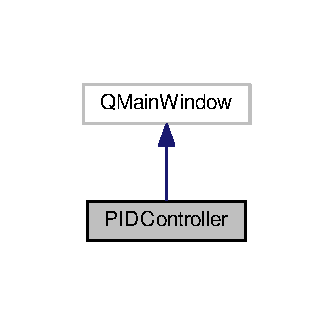
\includegraphics[width=160pt]{classPIDController__inherit__graph}
\end{center}
\end{figure}


Collaboration diagram for P\+I\+D\+Controller\+:
\nopagebreak
\begin{figure}[H]
\begin{center}
\leavevmode
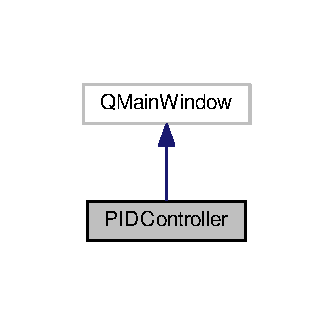
\includegraphics[width=160pt]{classPIDController__coll__graph}
\end{center}
\end{figure}
\subsection*{Public Member Functions}
\begin{DoxyCompactItemize}
\item 
\hyperlink{classPIDController_a940e36980116e998daa85ddd4dc42af6}{P\+I\+D\+Controller} (ros\+::\+Node\+Handle \+\_\+nh, Q\+Widget $\ast$parent=0)
\item 
\hyperlink{classPIDController_a690e7ad4796e5c5143aa4b90f2f6677b}{$\sim$\+P\+I\+D\+Controller} ()
\end{DoxyCompactItemize}
\subsection*{Private Slots}
\begin{DoxyCompactItemize}
\item 
void \hyperlink{classPIDController_ade90bc131741e00557e451e6b9d1648a}{publish\+\_\+pid} (void)
\item 
void \hyperlink{classPIDController_a279b52c4397a08bf3f7b86e7c54be220}{publish\+\_\+sp} (void)
\item 
void \hyperlink{classPIDController_a19820873ff56f5ff1b90c99ee4e0f52a}{on\+\_\+save\+\_\+clicked} ()
\end{DoxyCompactItemize}
\subsection*{Private Member Functions}
\begin{DoxyCompactItemize}
\item 
void \hyperlink{classPIDController_a41e8633c307a58f92df4c83bd08245c7}{set\+Labels} ()
\end{DoxyCompactItemize}
\subsection*{Private Attributes}
\begin{DoxyCompactItemize}
\item 
Ui\+::\+P\+I\+D\+Controller $\ast$ \hyperlink{classPIDController_a7e321e72a5082ba2c08b5ab05bea4009}{ui}
\item 
ros\+::\+Node\+Handle \hyperlink{classPIDController_a8ea098f5941b9a06d144d48a14d97ca4}{nh}
\item 
pid\+\_\+controller\+::\+P\+ID \hyperlink{classPIDController_a5f63a9fbeb425aade050320b98d2fcd0}{pid\+Msg}
\item 
pid\+\_\+controller\+::\+Setpoint \hyperlink{classPIDController_ac855862250d6358a44640f65245d8d6e}{sp\+Msg}
\item 
ros\+::\+Publisher \hyperlink{classPIDController_a4277721bfad5b5cd838312b62aadb1f8}{pid\+Pub}
\item 
ros\+::\+Publisher \hyperlink{classPIDController_aeb778d197e52ca65c1a593deddec0e78}{sp\+Pub}
\end{DoxyCompactItemize}


\subsection{Constructor \& Destructor Documentation}
\index{P\+I\+D\+Controller@{P\+I\+D\+Controller}!P\+I\+D\+Controller@{P\+I\+D\+Controller}}
\index{P\+I\+D\+Controller@{P\+I\+D\+Controller}!P\+I\+D\+Controller@{P\+I\+D\+Controller}}
\subsubsection[{\texorpdfstring{P\+I\+D\+Controller(ros\+::\+Node\+Handle \+\_\+nh, Q\+Widget $\ast$parent=0)}{PIDController(ros::NodeHandle _nh, QWidget *parent=0)}}]{\setlength{\rightskip}{0pt plus 5cm}P\+I\+D\+Controller\+::\+P\+I\+D\+Controller (
\begin{DoxyParamCaption}
\item[{ros\+::\+Node\+Handle}]{\+\_\+nh, }
\item[{Q\+Widget $\ast$}]{parent = {\ttfamily 0}}
\end{DoxyParamCaption}
)\hspace{0.3cm}{\ttfamily [explicit]}}\hypertarget{classPIDController_a940e36980116e998daa85ddd4dc42af6}{}\label{classPIDController_a940e36980116e998daa85ddd4dc42af6}
This class contains functions for the class \hyperlink{classThrusterControl}{Thruster\+Control}. This is the UI which can be used to control the thrusters manually. It reads the config file and reverses thrusters accordingly. On exit, it saves reverse status to file. $<$For publishing the values of Kp,Ki and Kd

$<$For publishing the set point values \index{P\+I\+D\+Controller@{P\+I\+D\+Controller}!````~P\+I\+D\+Controller@{$\sim$\+P\+I\+D\+Controller}}
\index{````~P\+I\+D\+Controller@{$\sim$\+P\+I\+D\+Controller}!P\+I\+D\+Controller@{P\+I\+D\+Controller}}
\subsubsection[{\texorpdfstring{$\sim$\+P\+I\+D\+Controller()}{~PIDController()}}]{\setlength{\rightskip}{0pt plus 5cm}P\+I\+D\+Controller\+::$\sim$\+P\+I\+D\+Controller (
\begin{DoxyParamCaption}
{}
\end{DoxyParamCaption}
)}\hypertarget{classPIDController_a690e7ad4796e5c5143aa4b90f2f6677b}{}\label{classPIDController_a690e7ad4796e5c5143aa4b90f2f6677b}
The below functions writes the values of Kp,Ki and Kd set using the slider in the G\+UI 

\subsection{Member Function Documentation}
\index{P\+I\+D\+Controller@{P\+I\+D\+Controller}!on\+\_\+save\+\_\+clicked@{on\+\_\+save\+\_\+clicked}}
\index{on\+\_\+save\+\_\+clicked@{on\+\_\+save\+\_\+clicked}!P\+I\+D\+Controller@{P\+I\+D\+Controller}}
\subsubsection[{\texorpdfstring{on\+\_\+save\+\_\+clicked}{on_save_clicked}}]{\setlength{\rightskip}{0pt plus 5cm}void P\+I\+D\+Controller\+::on\+\_\+save\+\_\+clicked (
\begin{DoxyParamCaption}
{}
\end{DoxyParamCaption}
)\hspace{0.3cm}{\ttfamily [private]}, {\ttfamily [slot]}}\hypertarget{classPIDController_a19820873ff56f5ff1b90c99ee4e0f52a}{}\label{classPIDController_a19820873ff56f5ff1b90c99ee4e0f52a}
The below function saves the values of Kp,Ki,Kd of all D\+OF in the config file \index{P\+I\+D\+Controller@{P\+I\+D\+Controller}!publish\+\_\+pid@{publish\+\_\+pid}}
\index{publish\+\_\+pid@{publish\+\_\+pid}!P\+I\+D\+Controller@{P\+I\+D\+Controller}}
\subsubsection[{\texorpdfstring{publish\+\_\+pid}{publish_pid}}]{\setlength{\rightskip}{0pt plus 5cm}void P\+I\+D\+Controller\+::publish\+\_\+pid (
\begin{DoxyParamCaption}
\item[{void}]{}
\end{DoxyParamCaption}
)\hspace{0.3cm}{\ttfamily [private]}, {\ttfamily [slot]}}\hypertarget{classPIDController_ade90bc131741e00557e451e6b9d1648a}{}\label{classPIDController_ade90bc131741e00557e451e6b9d1648a}
$<$msg data order\+: kp,ki,kd

$<$setting labels\+: \index{P\+I\+D\+Controller@{P\+I\+D\+Controller}!publish\+\_\+sp@{publish\+\_\+sp}}
\index{publish\+\_\+sp@{publish\+\_\+sp}!P\+I\+D\+Controller@{P\+I\+D\+Controller}}
\subsubsection[{\texorpdfstring{publish\+\_\+sp}{publish_sp}}]{\setlength{\rightskip}{0pt plus 5cm}void P\+I\+D\+Controller\+::publish\+\_\+sp (
\begin{DoxyParamCaption}
\item[{void}]{}
\end{DoxyParamCaption}
)\hspace{0.3cm}{\ttfamily [private]}, {\ttfamily [slot]}}\hypertarget{classPIDController_a279b52c4397a08bf3f7b86e7c54be220}{}\label{classPIDController_a279b52c4397a08bf3f7b86e7c54be220}
$<$setpoints msg data order\+: surge, sway, heave, yaw

$<$setting labels \index{P\+I\+D\+Controller@{P\+I\+D\+Controller}!set\+Labels@{set\+Labels}}
\index{set\+Labels@{set\+Labels}!P\+I\+D\+Controller@{P\+I\+D\+Controller}}
\subsubsection[{\texorpdfstring{set\+Labels()}{setLabels()}}]{\setlength{\rightskip}{0pt plus 5cm}void P\+I\+D\+Controller\+::set\+Labels (
\begin{DoxyParamCaption}
{}
\end{DoxyParamCaption}
)\hspace{0.3cm}{\ttfamily [private]}}\hypertarget{classPIDController_a41e8633c307a58f92df4c83bd08245c7}{}\label{classPIDController_a41e8633c307a58f92df4c83bd08245c7}


\subsection{Member Data Documentation}
\index{P\+I\+D\+Controller@{P\+I\+D\+Controller}!nh@{nh}}
\index{nh@{nh}!P\+I\+D\+Controller@{P\+I\+D\+Controller}}
\subsubsection[{\texorpdfstring{nh}{nh}}]{\setlength{\rightskip}{0pt plus 5cm}ros\+::\+Node\+Handle P\+I\+D\+Controller\+::nh\hspace{0.3cm}{\ttfamily [private]}}\hypertarget{classPIDController_a8ea098f5941b9a06d144d48a14d97ca4}{}\label{classPIDController_a8ea098f5941b9a06d144d48a14d97ca4}
\index{P\+I\+D\+Controller@{P\+I\+D\+Controller}!pid\+Msg@{pid\+Msg}}
\index{pid\+Msg@{pid\+Msg}!P\+I\+D\+Controller@{P\+I\+D\+Controller}}
\subsubsection[{\texorpdfstring{pid\+Msg}{pidMsg}}]{\setlength{\rightskip}{0pt plus 5cm}pid\+\_\+controller\+::\+P\+ID P\+I\+D\+Controller\+::pid\+Msg\hspace{0.3cm}{\ttfamily [private]}}\hypertarget{classPIDController_a5f63a9fbeb425aade050320b98d2fcd0}{}\label{classPIDController_a5f63a9fbeb425aade050320b98d2fcd0}
\index{P\+I\+D\+Controller@{P\+I\+D\+Controller}!pid\+Pub@{pid\+Pub}}
\index{pid\+Pub@{pid\+Pub}!P\+I\+D\+Controller@{P\+I\+D\+Controller}}
\subsubsection[{\texorpdfstring{pid\+Pub}{pidPub}}]{\setlength{\rightskip}{0pt plus 5cm}ros\+::\+Publisher P\+I\+D\+Controller\+::pid\+Pub\hspace{0.3cm}{\ttfamily [private]}}\hypertarget{classPIDController_a4277721bfad5b5cd838312b62aadb1f8}{}\label{classPIDController_a4277721bfad5b5cd838312b62aadb1f8}
\index{P\+I\+D\+Controller@{P\+I\+D\+Controller}!sp\+Msg@{sp\+Msg}}
\index{sp\+Msg@{sp\+Msg}!P\+I\+D\+Controller@{P\+I\+D\+Controller}}
\subsubsection[{\texorpdfstring{sp\+Msg}{spMsg}}]{\setlength{\rightskip}{0pt plus 5cm}pid\+\_\+controller\+::\+Setpoint P\+I\+D\+Controller\+::sp\+Msg\hspace{0.3cm}{\ttfamily [private]}}\hypertarget{classPIDController_ac855862250d6358a44640f65245d8d6e}{}\label{classPIDController_ac855862250d6358a44640f65245d8d6e}
\index{P\+I\+D\+Controller@{P\+I\+D\+Controller}!sp\+Pub@{sp\+Pub}}
\index{sp\+Pub@{sp\+Pub}!P\+I\+D\+Controller@{P\+I\+D\+Controller}}
\subsubsection[{\texorpdfstring{sp\+Pub}{spPub}}]{\setlength{\rightskip}{0pt plus 5cm}ros\+::\+Publisher P\+I\+D\+Controller\+::sp\+Pub\hspace{0.3cm}{\ttfamily [private]}}\hypertarget{classPIDController_aeb778d197e52ca65c1a593deddec0e78}{}\label{classPIDController_aeb778d197e52ca65c1a593deddec0e78}
\index{P\+I\+D\+Controller@{P\+I\+D\+Controller}!ui@{ui}}
\index{ui@{ui}!P\+I\+D\+Controller@{P\+I\+D\+Controller}}
\subsubsection[{\texorpdfstring{ui}{ui}}]{\setlength{\rightskip}{0pt plus 5cm}Ui\+::\+P\+I\+D\+Controller$\ast$ P\+I\+D\+Controller\+::ui\hspace{0.3cm}{\ttfamily [private]}}\hypertarget{classPIDController_a7e321e72a5082ba2c08b5ab05bea4009}{}\label{classPIDController_a7e321e72a5082ba2c08b5ab05bea4009}


The documentation for this class was generated from the following files\+:\begin{DoxyCompactItemize}
\item 
src/hammerhead/control\+\_\+stack/pid\+\_\+controller/include/pid\+\_\+controller/\hyperlink{pid__control_8h}{pid\+\_\+control.\+h}\item 
src/hammerhead/control\+\_\+stack/pid\+\_\+controller/src/\hyperlink{pid__control_8cpp}{pid\+\_\+control.\+cpp}\end{DoxyCompactItemize}

\hypertarget{classProcessWidget}{}\section{Process\+Widget Class Reference}
\label{classProcessWidget}\index{Process\+Widget@{Process\+Widget}}


{\ttfamily \#include $<$process\+\_\+widget.\+h$>$}



Inheritance diagram for Process\+Widget\+:\nopagebreak
\begin{figure}[H]
\begin{center}
\leavevmode
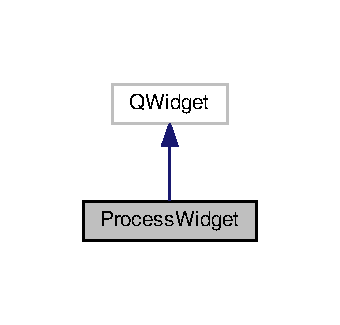
\includegraphics[width=163pt]{classProcessWidget__inherit__graph}
\end{center}
\end{figure}


Collaboration diagram for Process\+Widget\+:\nopagebreak
\begin{figure}[H]
\begin{center}
\leavevmode
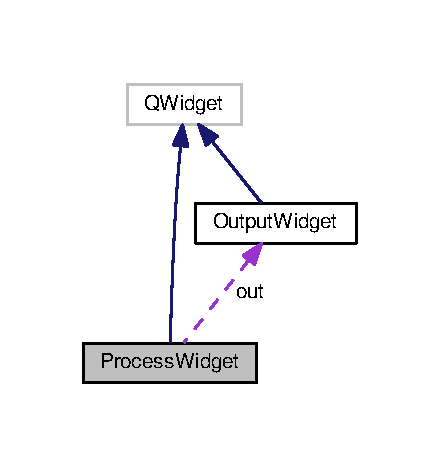
\includegraphics[width=211pt]{classProcessWidget__coll__graph}
\end{center}
\end{figure}
\subsection*{Public Slots}
\begin{DoxyCompactItemize}
\item 
void \hyperlink{classProcessWidget_a56fb109b399232b285cbea288631d18b}{update\+Text} ()
\item 
void \hyperlink{classProcessWidget_aa998c907c732bf27822ae53a8e83850c}{update\+Error} ()
\item 
void \hyperlink{classProcessWidget_afc941023cc434c5de6cc07059245d393}{run\+Btn\+Clicked} ()
\item 
void \hyperlink{classProcessWidget_af03bf5d00a16b15dfeb27d9865dc0b72}{view\+Btn\+Clicked} ()
\end{DoxyCompactItemize}
\subsection*{Public Member Functions}
\begin{DoxyCompactItemize}
\item 
\hyperlink{classProcessWidget_ae3da0e6b25935685f5da927b6b7c05aa}{Process\+Widget} (Q\+Widget $\ast$parent=0)
\item 
\hyperlink{classProcessWidget_a12d26ab48582d37d9209eefe6a04f17a}{$\sim$\+Process\+Widget} ()
\item 
void \hyperlink{classProcessWidget_ac64bea13457eb2e6ea8d96f557023c88}{set\+Details} (std\+::string)
\item 
void \hyperlink{classProcessWidget_a3aebd2c194252ace80ff5874284664f5}{watch\+Process} ()
\item 
bool \hyperlink{classProcessWidget_a4691c640971189f15ee2083b638b1597}{run\+Cb\+Is\+Checked} ()
\end{DoxyCompactItemize}
\subsection*{Public Attributes}
\begin{DoxyCompactItemize}
\item 
Q\+String \hyperlink{classProcessWidget_ae998aedcb05257a11f3f34c975cbb1d8}{p\+Name}
\item 
Q\+String \hyperlink{classProcessWidget_a78ee040355ce578865206d6a2a908510}{p\+Run\+Setting}
\item 
Q\+String \hyperlink{classProcessWidget_a6090de412650269c0d44c12b3ab4e703}{p\+Tab\+Name}
\item 
Q\+String \hyperlink{classProcessWidget_aed23b6c8eb79de37c6a9d5b5702c57b2}{p\+Host}
\item 
Q\+String \hyperlink{classProcessWidget_a02341ab7f2cd0a53bb43f6dc99bd7914}{p\+Command}
\item 
bool \hyperlink{classProcessWidget_a64e6cbfebad2038641bc7eca4455ff0a}{process\+Running}
\end{DoxyCompactItemize}
\subsection*{Private Member Functions}
\begin{DoxyCompactItemize}
\item 
void \hyperlink{classProcessWidget_a4b0910c658e29fce3ed74d531ccbe579}{run\+Process} ()
\item 
void \hyperlink{classProcessWidget_ad9dafd969ab93bde534ce54e3e3ba730}{stop\+Process} ()
\end{DoxyCompactItemize}
\subsection*{Private Attributes}
\begin{DoxyCompactItemize}
\item 
Q\+Process $\ast$ \hyperlink{classProcessWidget_ac04a45f46527d12b462a60ea80da6914}{process} = N\+U\+LL
\item 
\hyperlink{classOutputWidget}{Output\+Widget} $\ast$ \hyperlink{classProcessWidget_aed494ef2ff44e1063b0cafb8c295cac5}{out} = N\+U\+LL
\item 
Ui\+::\+Process\+Widget $\ast$ \hyperlink{classProcessWidget_a6ed6d8fb5b1ddbe9e02ab952e13d7f56}{ui}
\item 
Q\+Process\+::\+Process\+State \hyperlink{classProcessWidget_a7999f134191b91a86a8f241706c80ca1}{state} = Q\+Process\+::\+Not\+Running
\item 
Q\+Process\+::\+Process\+State \hyperlink{classProcessWidget_a635b866d7b1de59bd7bc13e0d2daa3ad}{last\+State} = Q\+Process\+::\+Not\+Running
\end{DoxyCompactItemize}


\subsection{Constructor \& Destructor Documentation}
\index{Process\+Widget@{Process\+Widget}!Process\+Widget@{Process\+Widget}}
\index{Process\+Widget@{Process\+Widget}!Process\+Widget@{Process\+Widget}}
\subsubsection[{\texorpdfstring{Process\+Widget(\+Q\+Widget $\ast$parent=0)}{ProcessWidget(QWidget *parent=0)}}]{\setlength{\rightskip}{0pt plus 5cm}Process\+Widget\+::\+Process\+Widget (
\begin{DoxyParamCaption}
\item[{Q\+Widget $\ast$}]{parent = {\ttfamily 0}}
\end{DoxyParamCaption}
)}\hypertarget{classProcessWidget_ae3da0e6b25935685f5da927b6b7c05aa}{}\label{classProcessWidget_ae3da0e6b25935685f5da927b6b7c05aa}
This file contains functions for the class \hyperlink{classProcessWidget}{Process\+Widget}. Each process in the configuration file is associated with a widget which can be used to start, stop, and view the status of the process. \index{Process\+Widget@{Process\+Widget}!````~Process\+Widget@{$\sim$\+Process\+Widget}}
\index{````~Process\+Widget@{$\sim$\+Process\+Widget}!Process\+Widget@{Process\+Widget}}
\subsubsection[{\texorpdfstring{$\sim$\+Process\+Widget()}{~ProcessWidget()}}]{\setlength{\rightskip}{0pt plus 5cm}Process\+Widget\+::$\sim$\+Process\+Widget (
\begin{DoxyParamCaption}
{}
\end{DoxyParamCaption}
)}\hypertarget{classProcessWidget_a12d26ab48582d37d9209eefe6a04f17a}{}\label{classProcessWidget_a12d26ab48582d37d9209eefe6a04f17a}


\subsection{Member Function Documentation}
\index{Process\+Widget@{Process\+Widget}!run\+Btn\+Clicked@{run\+Btn\+Clicked}}
\index{run\+Btn\+Clicked@{run\+Btn\+Clicked}!Process\+Widget@{Process\+Widget}}
\subsubsection[{\texorpdfstring{run\+Btn\+Clicked}{runBtnClicked}}]{\setlength{\rightskip}{0pt plus 5cm}void Process\+Widget\+::run\+Btn\+Clicked (
\begin{DoxyParamCaption}
{}
\end{DoxyParamCaption}
)\hspace{0.3cm}{\ttfamily [slot]}}\hypertarget{classProcessWidget_afc941023cc434c5de6cc07059245d393}{}\label{classProcessWidget_afc941023cc434c5de6cc07059245d393}
\index{Process\+Widget@{Process\+Widget}!run\+Cb\+Is\+Checked@{run\+Cb\+Is\+Checked}}
\index{run\+Cb\+Is\+Checked@{run\+Cb\+Is\+Checked}!Process\+Widget@{Process\+Widget}}
\subsubsection[{\texorpdfstring{run\+Cb\+Is\+Checked()}{runCbIsChecked()}}]{\setlength{\rightskip}{0pt plus 5cm}bool Process\+Widget\+::run\+Cb\+Is\+Checked (
\begin{DoxyParamCaption}
{}
\end{DoxyParamCaption}
)}\hypertarget{classProcessWidget_a4691c640971189f15ee2083b638b1597}{}\label{classProcessWidget_a4691c640971189f15ee2083b638b1597}
\index{Process\+Widget@{Process\+Widget}!run\+Process@{run\+Process}}
\index{run\+Process@{run\+Process}!Process\+Widget@{Process\+Widget}}
\subsubsection[{\texorpdfstring{run\+Process()}{runProcess()}}]{\setlength{\rightskip}{0pt plus 5cm}void Process\+Widget\+::run\+Process (
\begin{DoxyParamCaption}
{}
\end{DoxyParamCaption}
)\hspace{0.3cm}{\ttfamily [private]}}\hypertarget{classProcessWidget_a4b0910c658e29fce3ed74d531ccbe579}{}\label{classProcessWidget_a4b0910c658e29fce3ed74d531ccbe579}
\index{Process\+Widget@{Process\+Widget}!set\+Details@{set\+Details}}
\index{set\+Details@{set\+Details}!Process\+Widget@{Process\+Widget}}
\subsubsection[{\texorpdfstring{set\+Details(std\+::string)}{setDetails(std::string)}}]{\setlength{\rightskip}{0pt plus 5cm}void Process\+Widget\+::set\+Details (
\begin{DoxyParamCaption}
\item[{std\+::string}]{details}
\end{DoxyParamCaption}
)}\hypertarget{classProcessWidget_ac64bea13457eb2e6ea8d96f557023c88}{}\label{classProcessWidget_ac64bea13457eb2e6ea8d96f557023c88}
$<$ Accepts the string containing process name, command, etc., and sets the variables accordingly.\index{Process\+Widget@{Process\+Widget}!stop\+Process@{stop\+Process}}
\index{stop\+Process@{stop\+Process}!Process\+Widget@{Process\+Widget}}
\subsubsection[{\texorpdfstring{stop\+Process()}{stopProcess()}}]{\setlength{\rightskip}{0pt plus 5cm}void Process\+Widget\+::stop\+Process (
\begin{DoxyParamCaption}
{}
\end{DoxyParamCaption}
)\hspace{0.3cm}{\ttfamily [private]}}\hypertarget{classProcessWidget_ad9dafd969ab93bde534ce54e3e3ba730}{}\label{classProcessWidget_ad9dafd969ab93bde534ce54e3e3ba730}
\index{Process\+Widget@{Process\+Widget}!update\+Error@{update\+Error}}
\index{update\+Error@{update\+Error}!Process\+Widget@{Process\+Widget}}
\subsubsection[{\texorpdfstring{update\+Error}{updateError}}]{\setlength{\rightskip}{0pt plus 5cm}void Process\+Widget\+::update\+Error (
\begin{DoxyParamCaption}
{}
\end{DoxyParamCaption}
)\hspace{0.3cm}{\ttfamily [slot]}}\hypertarget{classProcessWidget_aa998c907c732bf27822ae53a8e83850c}{}\label{classProcessWidget_aa998c907c732bf27822ae53a8e83850c}
\index{Process\+Widget@{Process\+Widget}!update\+Text@{update\+Text}}
\index{update\+Text@{update\+Text}!Process\+Widget@{Process\+Widget}}
\subsubsection[{\texorpdfstring{update\+Text}{updateText}}]{\setlength{\rightskip}{0pt plus 5cm}void Process\+Widget\+::update\+Text (
\begin{DoxyParamCaption}
{}
\end{DoxyParamCaption}
)\hspace{0.3cm}{\ttfamily [slot]}}\hypertarget{classProcessWidget_a56fb109b399232b285cbea288631d18b}{}\label{classProcessWidget_a56fb109b399232b285cbea288631d18b}
\index{Process\+Widget@{Process\+Widget}!view\+Btn\+Clicked@{view\+Btn\+Clicked}}
\index{view\+Btn\+Clicked@{view\+Btn\+Clicked}!Process\+Widget@{Process\+Widget}}
\subsubsection[{\texorpdfstring{view\+Btn\+Clicked}{viewBtnClicked}}]{\setlength{\rightskip}{0pt plus 5cm}void Process\+Widget\+::view\+Btn\+Clicked (
\begin{DoxyParamCaption}
{}
\end{DoxyParamCaption}
)\hspace{0.3cm}{\ttfamily [slot]}}\hypertarget{classProcessWidget_af03bf5d00a16b15dfeb27d9865dc0b72}{}\label{classProcessWidget_af03bf5d00a16b15dfeb27d9865dc0b72}
\index{Process\+Widget@{Process\+Widget}!watch\+Process@{watch\+Process}}
\index{watch\+Process@{watch\+Process}!Process\+Widget@{Process\+Widget}}
\subsubsection[{\texorpdfstring{watch\+Process()}{watchProcess()}}]{\setlength{\rightskip}{0pt plus 5cm}void Process\+Widget\+::watch\+Process (
\begin{DoxyParamCaption}
{}
\end{DoxyParamCaption}
)}\hypertarget{classProcessWidget_a3aebd2c194252ace80ff5874284664f5}{}\label{classProcessWidget_a3aebd2c194252ace80ff5874284664f5}


\subsection{Member Data Documentation}
\index{Process\+Widget@{Process\+Widget}!last\+State@{last\+State}}
\index{last\+State@{last\+State}!Process\+Widget@{Process\+Widget}}
\subsubsection[{\texorpdfstring{last\+State}{lastState}}]{\setlength{\rightskip}{0pt plus 5cm}Q\+Process\+::\+Process\+State Process\+Widget\+::last\+State = Q\+Process\+::\+Not\+Running\hspace{0.3cm}{\ttfamily [private]}}\hypertarget{classProcessWidget_a635b866d7b1de59bd7bc13e0d2daa3ad}{}\label{classProcessWidget_a635b866d7b1de59bd7bc13e0d2daa3ad}
\index{Process\+Widget@{Process\+Widget}!out@{out}}
\index{out@{out}!Process\+Widget@{Process\+Widget}}
\subsubsection[{\texorpdfstring{out}{out}}]{\setlength{\rightskip}{0pt plus 5cm}{\bf Output\+Widget}$\ast$ Process\+Widget\+::out = N\+U\+LL\hspace{0.3cm}{\ttfamily [private]}}\hypertarget{classProcessWidget_aed494ef2ff44e1063b0cafb8c295cac5}{}\label{classProcessWidget_aed494ef2ff44e1063b0cafb8c295cac5}
\index{Process\+Widget@{Process\+Widget}!p\+Command@{p\+Command}}
\index{p\+Command@{p\+Command}!Process\+Widget@{Process\+Widget}}
\subsubsection[{\texorpdfstring{p\+Command}{pCommand}}]{\setlength{\rightskip}{0pt plus 5cm}Q\+String Process\+Widget\+::p\+Command}\hypertarget{classProcessWidget_a02341ab7f2cd0a53bb43f6dc99bd7914}{}\label{classProcessWidget_a02341ab7f2cd0a53bb43f6dc99bd7914}
\index{Process\+Widget@{Process\+Widget}!p\+Host@{p\+Host}}
\index{p\+Host@{p\+Host}!Process\+Widget@{Process\+Widget}}
\subsubsection[{\texorpdfstring{p\+Host}{pHost}}]{\setlength{\rightskip}{0pt plus 5cm}Q\+String Process\+Widget\+::p\+Host}\hypertarget{classProcessWidget_aed23b6c8eb79de37c6a9d5b5702c57b2}{}\label{classProcessWidget_aed23b6c8eb79de37c6a9d5b5702c57b2}
\index{Process\+Widget@{Process\+Widget}!p\+Name@{p\+Name}}
\index{p\+Name@{p\+Name}!Process\+Widget@{Process\+Widget}}
\subsubsection[{\texorpdfstring{p\+Name}{pName}}]{\setlength{\rightskip}{0pt plus 5cm}Q\+String Process\+Widget\+::p\+Name}\hypertarget{classProcessWidget_ae998aedcb05257a11f3f34c975cbb1d8}{}\label{classProcessWidget_ae998aedcb05257a11f3f34c975cbb1d8}
\index{Process\+Widget@{Process\+Widget}!process@{process}}
\index{process@{process}!Process\+Widget@{Process\+Widget}}
\subsubsection[{\texorpdfstring{process}{process}}]{\setlength{\rightskip}{0pt plus 5cm}Q\+Process$\ast$ Process\+Widget\+::process = N\+U\+LL\hspace{0.3cm}{\ttfamily [private]}}\hypertarget{classProcessWidget_ac04a45f46527d12b462a60ea80da6914}{}\label{classProcessWidget_ac04a45f46527d12b462a60ea80da6914}
\index{Process\+Widget@{Process\+Widget}!process\+Running@{process\+Running}}
\index{process\+Running@{process\+Running}!Process\+Widget@{Process\+Widget}}
\subsubsection[{\texorpdfstring{process\+Running}{processRunning}}]{\setlength{\rightskip}{0pt plus 5cm}bool Process\+Widget\+::process\+Running}\hypertarget{classProcessWidget_a64e6cbfebad2038641bc7eca4455ff0a}{}\label{classProcessWidget_a64e6cbfebad2038641bc7eca4455ff0a}
\index{Process\+Widget@{Process\+Widget}!p\+Run\+Setting@{p\+Run\+Setting}}
\index{p\+Run\+Setting@{p\+Run\+Setting}!Process\+Widget@{Process\+Widget}}
\subsubsection[{\texorpdfstring{p\+Run\+Setting}{pRunSetting}}]{\setlength{\rightskip}{0pt plus 5cm}Q\+String Process\+Widget\+::p\+Run\+Setting}\hypertarget{classProcessWidget_a78ee040355ce578865206d6a2a908510}{}\label{classProcessWidget_a78ee040355ce578865206d6a2a908510}
\index{Process\+Widget@{Process\+Widget}!p\+Tab\+Name@{p\+Tab\+Name}}
\index{p\+Tab\+Name@{p\+Tab\+Name}!Process\+Widget@{Process\+Widget}}
\subsubsection[{\texorpdfstring{p\+Tab\+Name}{pTabName}}]{\setlength{\rightskip}{0pt plus 5cm}Q\+String Process\+Widget\+::p\+Tab\+Name}\hypertarget{classProcessWidget_a6090de412650269c0d44c12b3ab4e703}{}\label{classProcessWidget_a6090de412650269c0d44c12b3ab4e703}
\index{Process\+Widget@{Process\+Widget}!state@{state}}
\index{state@{state}!Process\+Widget@{Process\+Widget}}
\subsubsection[{\texorpdfstring{state}{state}}]{\setlength{\rightskip}{0pt plus 5cm}Q\+Process\+::\+Process\+State Process\+Widget\+::state = Q\+Process\+::\+Not\+Running\hspace{0.3cm}{\ttfamily [private]}}\hypertarget{classProcessWidget_a7999f134191b91a86a8f241706c80ca1}{}\label{classProcessWidget_a7999f134191b91a86a8f241706c80ca1}
\index{Process\+Widget@{Process\+Widget}!ui@{ui}}
\index{ui@{ui}!Process\+Widget@{Process\+Widget}}
\subsubsection[{\texorpdfstring{ui}{ui}}]{\setlength{\rightskip}{0pt plus 5cm}Ui\+::\+Process\+Widget$\ast$ Process\+Widget\+::ui\hspace{0.3cm}{\ttfamily [private]}}\hypertarget{classProcessWidget_a6ed6d8fb5b1ddbe9e02ab952e13d7f56}{}\label{classProcessWidget_a6ed6d8fb5b1ddbe9e02ab952e13d7f56}


The documentation for this class was generated from the following files\+:\begin{DoxyCompactItemize}
\item 
src/hammerhead/control\+\_\+stack/tiburon\+\_\+commander/include/tiburon\+\_\+commander/\hyperlink{process__widget_8h}{process\+\_\+widget.\+h}\item 
src/hammerhead/control\+\_\+stack/tiburon\+\_\+commander/src/\hyperlink{process__widget_8cpp}{process\+\_\+widget.\+cpp}\end{DoxyCompactItemize}

\hypertarget{classQCPAbstractItem}{}\section{Q\+C\+P\+Abstract\+Item Class Reference}
\label{classQCPAbstractItem}\index{Q\+C\+P\+Abstract\+Item@{Q\+C\+P\+Abstract\+Item}}


The abstract base class for all items in a plot.  




{\ttfamily \#include $<$qcustomplot.\+h$>$}



Inheritance diagram for Q\+C\+P\+Abstract\+Item\+:
\nopagebreak
\begin{figure}[H]
\begin{center}
\leavevmode
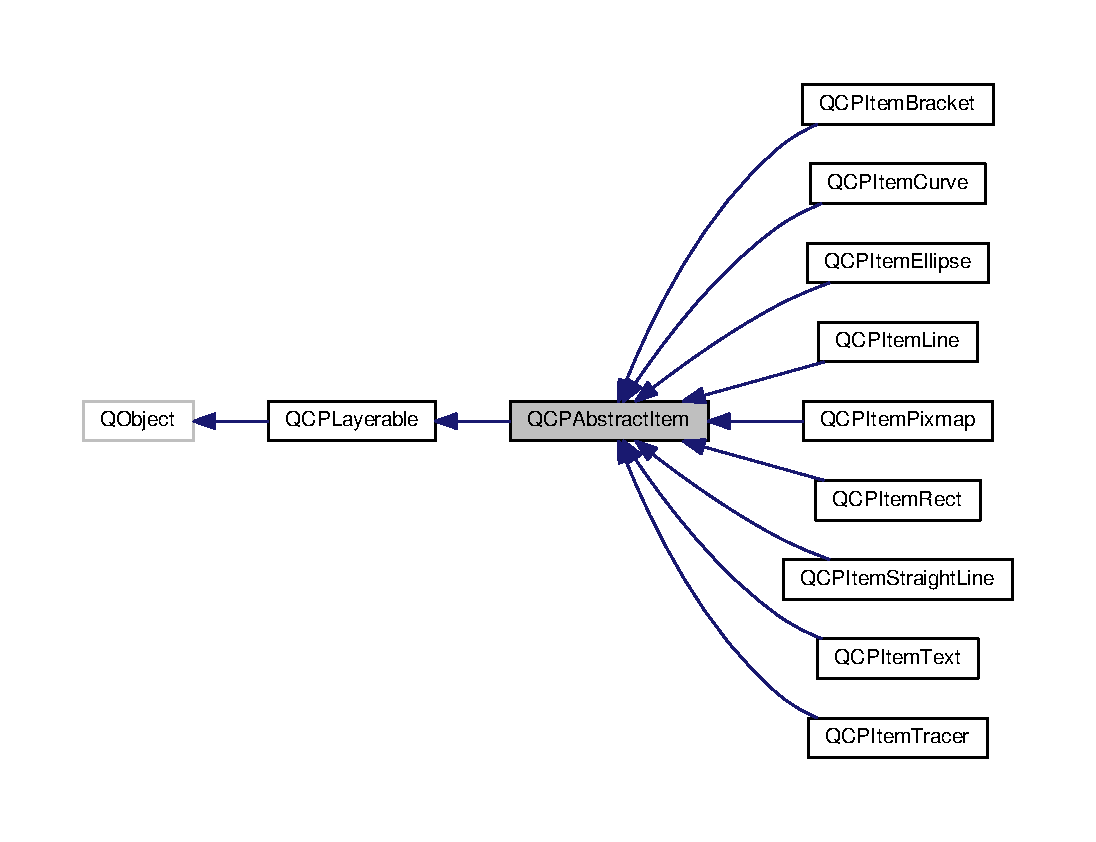
\includegraphics[width=350pt]{classQCPAbstractItem__inherit__graph}
\end{center}
\end{figure}


Collaboration diagram for Q\+C\+P\+Abstract\+Item\+:
\nopagebreak
\begin{figure}[H]
\begin{center}
\leavevmode
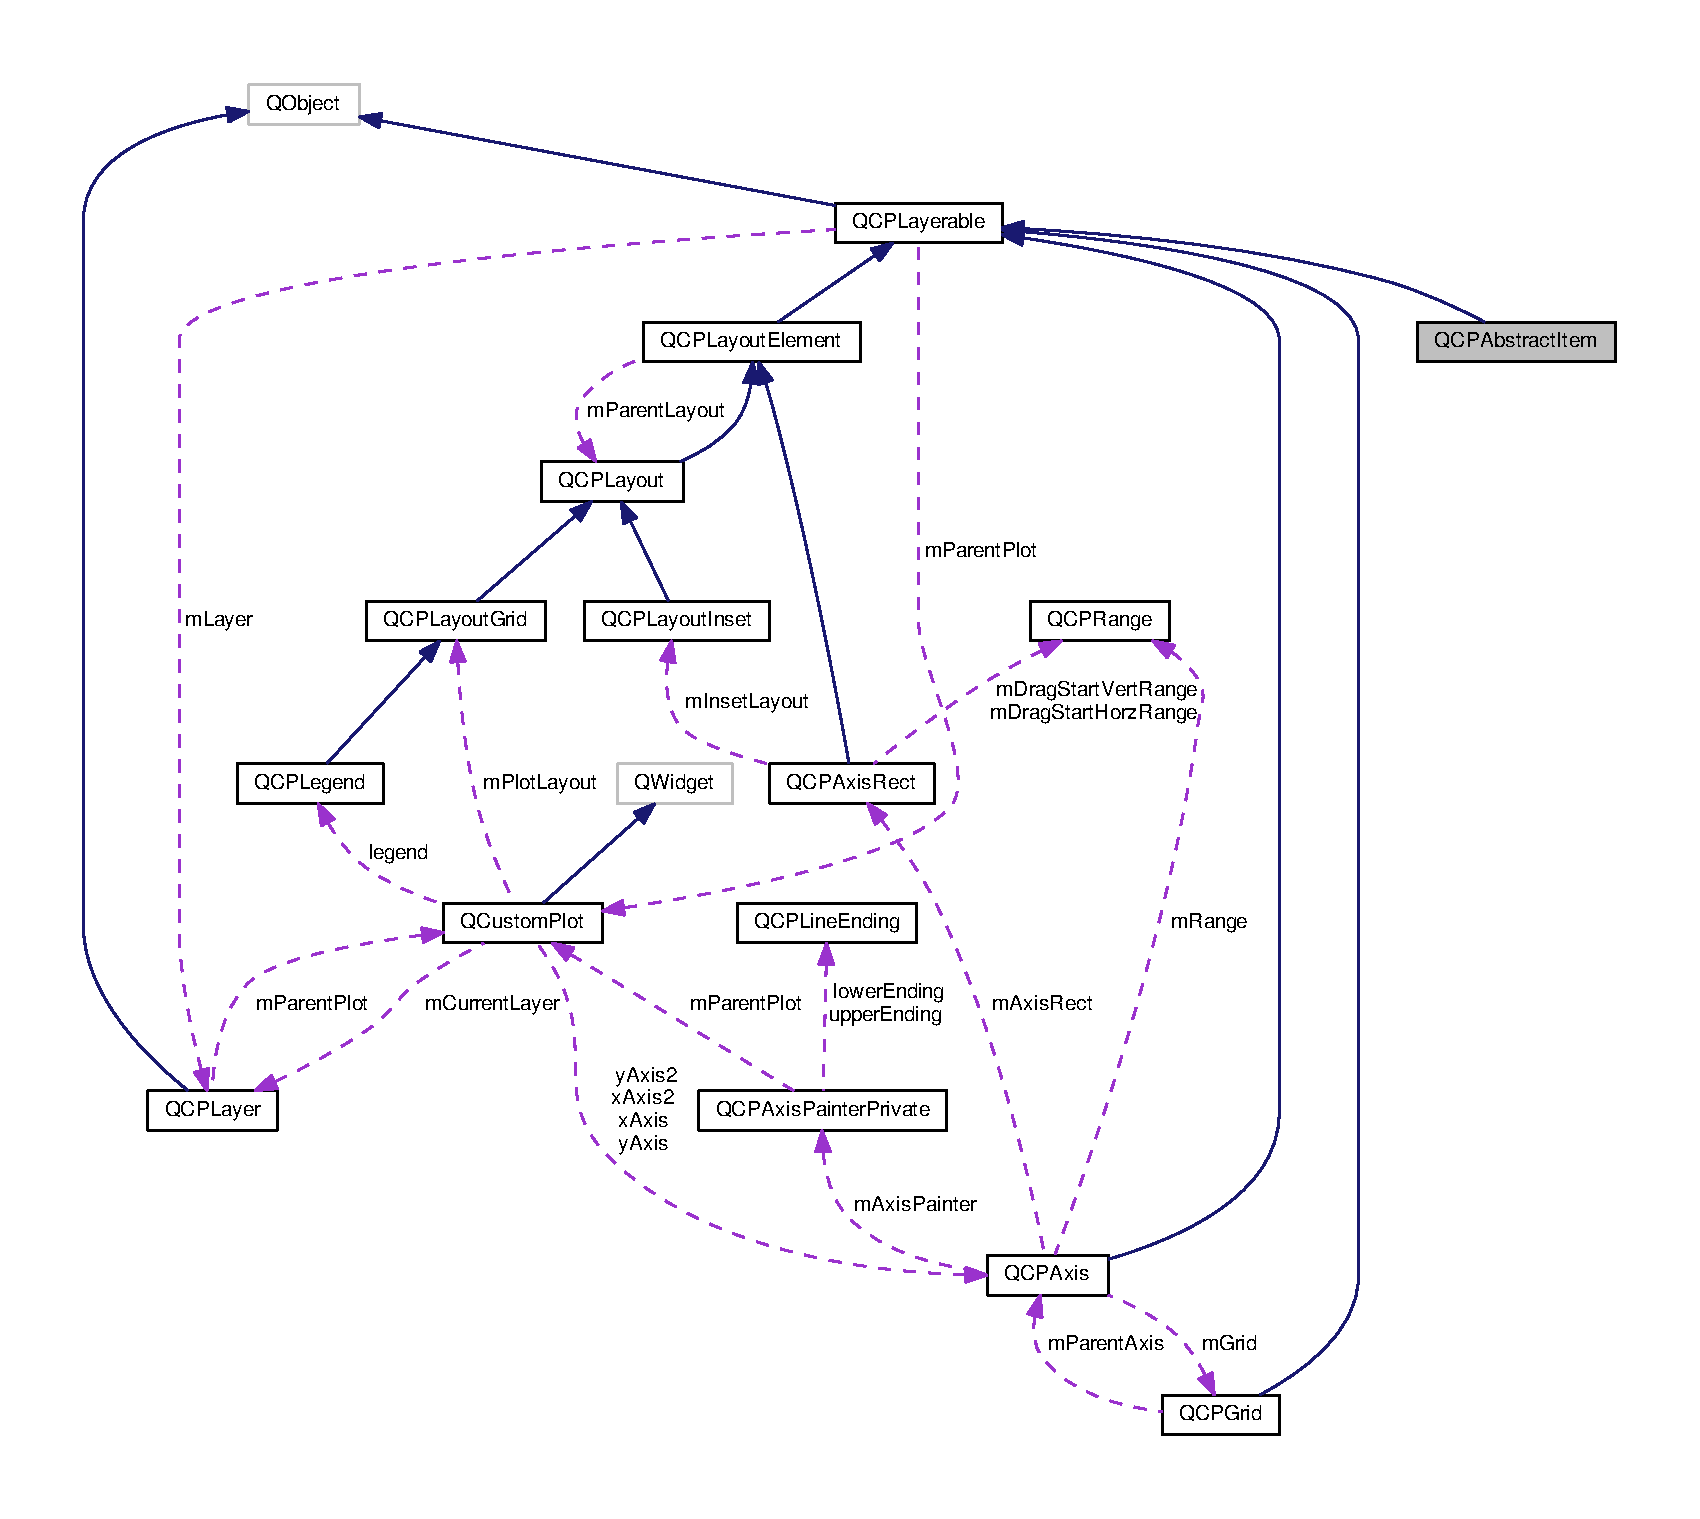
\includegraphics[width=350pt]{classQCPAbstractItem__coll__graph}
\end{center}
\end{figure}
\subsection*{Signals}
\begin{DoxyCompactItemize}
\item 
void \hyperlink{classQCPAbstractItem_aa5cffb034fc65dbb91c77e02c1c14251}{selection\+Changed} (bool \hyperlink{classQCPAbstractItem_a225865808640d8d9a7dd19f09a2e93f2}{selected})
\item 
void \hyperlink{classQCPAbstractItem_a5b266c11aac61cb511901f3911dac2a3}{selectable\+Changed} (bool \hyperlink{classQCPAbstractItem_a9189e752025533e1595eaade0009a3bc}{selectable})
\end{DoxyCompactItemize}
\subsection*{Public Member Functions}
\begin{DoxyCompactItemize}
\item 
\hyperlink{classQCPAbstractItem_a9922507d8b4503a1fe1ed0b1030e23b6}{Q\+C\+P\+Abstract\+Item} (\hyperlink{classQCustomPlot}{Q\+Custom\+Plot} $\ast$\hyperlink{classQCPLayerable_ab7e0e94461566093d36ffc0f5312b109}{parent\+Plot})
\item 
virtual \hyperlink{classQCPAbstractItem_a375bd1b7d3218b04a6ff7ff06fff917c}{$\sim$\+Q\+C\+P\+Abstract\+Item} ()
\item 
bool \hyperlink{classQCPAbstractItem_a5b0ea171823033bcb8aee81f4a034871}{clip\+To\+Axis\+Rect} () const 
\item 
\hyperlink{classQCPAxisRect}{Q\+C\+P\+Axis\+Rect} $\ast$ \hyperlink{classQCPAbstractItem_a37f86618740b5047eae23eedb2de061a}{clip\+Axis\+Rect} () const 
\item 
bool \hyperlink{classQCPAbstractItem_a9189e752025533e1595eaade0009a3bc}{selectable} () const 
\item 
bool \hyperlink{classQCPAbstractItem_a225865808640d8d9a7dd19f09a2e93f2}{selected} () const 
\item 
void \hyperlink{classQCPAbstractItem_a39e05b9d4176b9accafc746d16ca6a06}{set\+Clip\+To\+Axis\+Rect} (bool clip)
\item 
void \hyperlink{classQCPAbstractItem_a7dc75fcbcd10206fe0b75d757ea7a347}{set\+Clip\+Axis\+Rect} (\hyperlink{classQCPAxisRect}{Q\+C\+P\+Axis\+Rect} $\ast$rect)
\item 
Q\+\_\+\+S\+L\+OT void \hyperlink{classQCPAbstractItem_a8a8e32a55bc478b849756a78c2d87fd2}{set\+Selectable} (bool \hyperlink{classQCPAbstractItem_a9189e752025533e1595eaade0009a3bc}{selectable})
\item 
Q\+\_\+\+S\+L\+OT void \hyperlink{classQCPAbstractItem_a203de94ad586cc44d16c9565f49d3378}{set\+Selected} (bool \hyperlink{classQCPAbstractItem_a225865808640d8d9a7dd19f09a2e93f2}{selected})
\item 
virtual double \hyperlink{classQCPAbstractItem_a96d522d10ffc0413b9a366c6f7f0476b}{select\+Test} (const Q\+PointF \&pos, bool only\+Selectable, Q\+Variant $\ast$details=0) const =0
\item 
Q\+List$<$ \hyperlink{classQCPItemPosition}{Q\+C\+P\+Item\+Position} $\ast$ $>$ \hyperlink{classQCPAbstractItem_adf6a680cc29a6bce8345c3b6af3a91a1}{positions} () const 
\item 
Q\+List$<$ \hyperlink{classQCPItemAnchor}{Q\+C\+P\+Item\+Anchor} $\ast$ $>$ \hyperlink{classQCPAbstractItem_a8454b9941960b840608a5a1e00b1977d}{anchors} () const 
\item 
\hyperlink{classQCPItemPosition}{Q\+C\+P\+Item\+Position} $\ast$ \hyperlink{classQCPAbstractItem_af71345bd150f87fa1d2442837b87bb59}{position} (const Q\+String \&name) const 
\item 
\hyperlink{classQCPItemAnchor}{Q\+C\+P\+Item\+Anchor} $\ast$ \hyperlink{classQCPAbstractItem_abed974cba7cc02608c71dad4638e008d}{anchor} (const Q\+String \&name) const 
\item 
bool \hyperlink{classQCPAbstractItem_acbce9e5ba5252541d19db0c40303357a}{has\+Anchor} (const Q\+String \&name) const 
\end{DoxyCompactItemize}
\subsection*{Protected Member Functions}
\begin{DoxyCompactItemize}
\item 
virtual \hyperlink{namespaceQCP_a2ad6bb6281c7c2d593d4277b44c2b037}{Q\+C\+P\+::\+Interaction} \hyperlink{classQCPAbstractItem_a777b5d384936396ad9c3ceb3d3453f1c}{selection\+Category} () const 
\item 
virtual Q\+Rect \hyperlink{classQCPAbstractItem_a538e25ff8856534582f5b2b400a46405}{clip\+Rect} () const 
\item 
virtual void \hyperlink{classQCPAbstractItem_a0839031abdd71067e2256a4d53c7a011}{apply\+Default\+Antialiasing\+Hint} (\hyperlink{classQCPPainter}{Q\+C\+P\+Painter} $\ast$painter) const 
\item 
virtual void \hyperlink{classQCPAbstractItem_ad0dc056f650c3ca73414e6b4f01674ef}{draw} (\hyperlink{classQCPPainter}{Q\+C\+P\+Painter} $\ast$painter)=0
\item 
virtual void \hyperlink{classQCPAbstractItem_aaf92af7b9893712959a6c073d334d88d}{select\+Event} (Q\+Mouse\+Event $\ast$event, bool additive, const Q\+Variant \&details, bool $\ast$selection\+State\+Changed)
\item 
virtual void \hyperlink{classQCPAbstractItem_a91f090d6763cfedb0749219c63788ae9}{deselect\+Event} (bool $\ast$selection\+State\+Changed)
\item 
virtual Q\+PointF \hyperlink{classQCPAbstractItem_a94bde62b8a2fc133666dcbb8035deeed}{anchor\+Pixel\+Point} (int anchor\+Id) const 
\item 
double \hyperlink{classQCPAbstractItem_acdca343717d625b8abb3c3e38c0ed39d}{dist\+Sqr\+To\+Line} (const Q\+PointF \&start, const Q\+PointF \&end, const Q\+PointF \&point) const 
\item 
double \hyperlink{classQCPAbstractItem_a4c0e14c4e92df91174cb7183fb363069}{rect\+Select\+Test} (const Q\+RectF \&rect, const Q\+PointF \&pos, bool filled\+Rect) const 
\item 
\hyperlink{classQCPItemPosition}{Q\+C\+P\+Item\+Position} $\ast$ \hyperlink{classQCPAbstractItem_a75036d39c4d4e2e1a7dd145fff915d32}{create\+Position} (const Q\+String \&name)
\item 
\hyperlink{classQCPItemAnchor}{Q\+C\+P\+Item\+Anchor} $\ast$ \hyperlink{classQCPAbstractItem_af3fc92527802078ca395138748b629a7}{create\+Anchor} (const Q\+String \&name, int anchor\+Id)
\end{DoxyCompactItemize}
\subsection*{Protected Attributes}
\begin{DoxyCompactItemize}
\item 
bool \hyperlink{classQCPAbstractItem_ad2a70ff6b658fcb84a9427f69d3f587d}{m\+Clip\+To\+Axis\+Rect}
\item 
Q\+Pointer$<$ \hyperlink{classQCPAxisRect}{Q\+C\+P\+Axis\+Rect} $>$ \hyperlink{classQCPAbstractItem_a3e57cfe7da4b1ac3d6fa7281ea437361}{m\+Clip\+Axis\+Rect}
\item 
Q\+List$<$ \hyperlink{classQCPItemPosition}{Q\+C\+P\+Item\+Position} $\ast$ $>$ \hyperlink{classQCPAbstractItem_af94ff71b6a15ea6d028ab8bd8eccd012}{m\+Positions}
\item 
Q\+List$<$ \hyperlink{classQCPItemAnchor}{Q\+C\+P\+Item\+Anchor} $\ast$ $>$ \hyperlink{classQCPAbstractItem_a909a3abab783de302ebf0a0e6f2bbc15}{m\+Anchors}
\item 
bool \hyperlink{classQCPAbstractItem_ad81eb35c8726a0f458db9df9732e0e41}{m\+Selectable}
\item 
bool \hyperlink{classQCPAbstractItem_a4bdb3457dad1d268c0f78a44152b9645}{m\+Selected}
\end{DoxyCompactItemize}
\subsection*{Friends}
\begin{DoxyCompactItemize}
\item 
class \hyperlink{classQCPAbstractItem_a1cdf9df76adcfae45261690aa0ca2198}{Q\+Custom\+Plot}
\item 
class \hyperlink{classQCPAbstractItem_a61767d414fd57af9eb1741b34268c7fc}{Q\+C\+P\+Item\+Anchor}
\end{DoxyCompactItemize}


\subsection{Detailed Description}
The abstract base class for all items in a plot. 

In \hyperlink{classQCustomPlot}{Q\+Custom\+Plot}, items are supplemental graphical elements that are neither plottables (\hyperlink{classQCPAbstractPlottable}{Q\+C\+P\+Abstract\+Plottable}) nor axes (\hyperlink{classQCPAxis}{Q\+C\+P\+Axis}). While plottables are always tied to two axes and thus plot coordinates, items can also be placed in absolute coordinates independent of any axes. Each specific item has at least one \hyperlink{classQCPItemPosition}{Q\+C\+P\+Item\+Position} member which controls the positioning. Some items are defined by more than one coordinate and thus have two or more \hyperlink{classQCPItemPosition}{Q\+C\+P\+Item\+Position} members (For example, \hyperlink{classQCPItemRect}{Q\+C\+P\+Item\+Rect} has {\itshape top\+Left} and {\itshape bottom\+Right}).

This abstract base class defines a very basic interface like visibility and clipping. Since this class is abstract, it can\textquotesingle{}t be instantiated. Use one of the subclasses or create a subclass yourself to create new items.

The built-\/in items are\+: \tabulinesep=1mm
\begin{longtabu} spread 0pt [c]{*2{|X[-1]}|}
\hline
\hyperlink{classQCPItemLine}{Q\+C\+P\+Item\+Line}&A line defined by a start and an end point. May have different ending styles on each side (e.\+g. arrows). \\\cline{1-2}
\hyperlink{classQCPItemStraightLine}{Q\+C\+P\+Item\+Straight\+Line}&A straight line defined by a start and a direction point. Unlike \hyperlink{classQCPItemLine}{Q\+C\+P\+Item\+Line}, the straight line is infinitely long and has no endings. \\\cline{1-2}
\hyperlink{classQCPItemCurve}{Q\+C\+P\+Item\+Curve}&A curve defined by start, end and two intermediate control points. May have different ending styles on each side (e.\+g. arrows). \\\cline{1-2}
\hyperlink{classQCPItemRect}{Q\+C\+P\+Item\+Rect}&A rectangle \\\cline{1-2}
\hyperlink{classQCPItemEllipse}{Q\+C\+P\+Item\+Ellipse}&An ellipse \\\cline{1-2}
\hyperlink{classQCPItemPixmap}{Q\+C\+P\+Item\+Pixmap}&An arbitrary pixmap \\\cline{1-2}
\hyperlink{classQCPItemText}{Q\+C\+P\+Item\+Text}&A text label \\\cline{1-2}
\hyperlink{classQCPItemBracket}{Q\+C\+P\+Item\+Bracket}&A bracket which may be used to reference/highlight certain parts in the plot. \\\cline{1-2}
\hyperlink{classQCPItemTracer}{Q\+C\+P\+Item\+Tracer}&An item that can be attached to a \hyperlink{classQCPGraph}{Q\+C\+P\+Graph} and sticks to its data points, given a key coordinate. \\\cline{1-2}
\end{longtabu}
\hypertarget{classQCPAbstractItem_items-clipping}{}\subsection{Clipping}\label{classQCPAbstractItem_items-clipping}
Items are by default clipped to the main axis rect (they are only visible inside the axis rect). To make an item visible outside that axis rect, disable clipping via \hyperlink{classQCPAbstractItem_a39e05b9d4176b9accafc746d16ca6a06}{set\+Clip\+To\+Axis\+Rect(false)}.

On the other hand if you want the item to be clipped to a different axis rect, specify it via \hyperlink{classQCPAbstractItem_a7dc75fcbcd10206fe0b75d757ea7a347}{set\+Clip\+Axis\+Rect}. This clip\+Axis\+Rect property of an item is only used for clipping behaviour, and in principle is independent of the coordinate axes the item might be tied to via its position members (\hyperlink{classQCPItemPosition_a2185f45c75ac8cb9be89daeaaad50e37}{Q\+C\+P\+Item\+Position\+::set\+Axes}). However, it is common that the axis rect for clipping also contains the axes used for the item positions.\hypertarget{classQCPAbstractItem_items-using}{}\subsection{Using items}\label{classQCPAbstractItem_items-using}
First you instantiate the item you want to use and add it to the plot\+: 
\begin{DoxyCodeInclude}
\end{DoxyCodeInclude}
by default, the positions of the item are bound to the x-\/ and y-\/\+Axis of the plot. So we can just set the plot coordinates where the line should start/end\+: 
\begin{DoxyCodeInclude}
\end{DoxyCodeInclude}
If we don\textquotesingle{}t want the line to be positioned in plot coordinates but a different coordinate system, e.\+g. absolute pixel positions on the \hyperlink{classQCustomPlot}{Q\+Custom\+Plot} surface, we need to change the position type like this\+: 
\begin{DoxyCodeInclude}
\end{DoxyCodeInclude}
Then we can set the coordinates, this time in pixels\+: 
\begin{DoxyCodeInclude}
\end{DoxyCodeInclude}
and make the line visible on the entire \hyperlink{classQCustomPlot}{Q\+Custom\+Plot}, by disabling clipping to the axis rect\+: 
\begin{DoxyCodeInclude}
\end{DoxyCodeInclude}
 For more advanced plots, it is even possible to set different types and parent anchors per X/Y coordinate of an item position, using for example \hyperlink{classQCPItemPosition_a2113b2351d6d00457fb3559a4e20c3ea}{Q\+C\+P\+Item\+Position\+::set\+TypeX} or \hyperlink{classQCPItemPosition_add71461a973927c74e42179480916d9c}{Q\+C\+P\+Item\+Position\+::set\+Parent\+AnchorX}. For details, see the documentation of \hyperlink{classQCPItemPosition}{Q\+C\+P\+Item\+Position}.\hypertarget{classQCPAbstractItem_items-subclassing}{}\subsection{Creating own items}\label{classQCPAbstractItem_items-subclassing}
To create an own item, you implement a subclass of \hyperlink{classQCPAbstractItem}{Q\+C\+P\+Abstract\+Item}. These are the pure virtual functions, you must implement\+: \begin{DoxyItemize}
\item \hyperlink{classQCPAbstractItem_a96d522d10ffc0413b9a366c6f7f0476b}{select\+Test} \item \hyperlink{classQCPAbstractItem_ad0dc056f650c3ca73414e6b4f01674ef}{draw}\end{DoxyItemize}
See the documentation of those functions for what they need to do.\hypertarget{classQCPAbstractItem_items-positioning}{}\subsubsection{Allowing the item to be positioned}\label{classQCPAbstractItem_items-positioning}
As mentioned, item positions are represented by \hyperlink{classQCPItemPosition}{Q\+C\+P\+Item\+Position} members. Let\textquotesingle{}s assume the new item shall have only one point as its position (as opposed to two like a rect or multiple like a polygon). You then add a public member of type \hyperlink{classQCPItemPosition}{Q\+C\+P\+Item\+Position} like so\+:


\begin{DoxyCode}
\hyperlink{classQCPItemPosition}{QCPItemPosition} * \textcolor{keyword}{const} myPosition;
\end{DoxyCode}


the const makes sure the pointer itself can\textquotesingle{}t be modified from the user of your new item (the \hyperlink{classQCPItemPosition}{Q\+C\+P\+Item\+Position} instance it points to, can be modified, of course). The initialization of this pointer is made easy with the \hyperlink{classQCPAbstractItem_a75036d39c4d4e2e1a7dd145fff915d32}{create\+Position} function. Just assign the return value of this function to each \hyperlink{classQCPItemPosition}{Q\+C\+P\+Item\+Position} in the constructor of your item. \hyperlink{classQCPAbstractItem_a75036d39c4d4e2e1a7dd145fff915d32}{create\+Position} takes a string which is the name of the position, typically this is identical to the variable name. For example, the constructor of Q\+C\+P\+Item\+Example could look like this\+:


\begin{DoxyCode}
QCPItemExample::QCPItemExample(\hyperlink{classQCustomPlot}{QCustomPlot} *\hyperlink{classQCPLayerable_ab7e0e94461566093d36ffc0f5312b109}{parentPlot}) :
  \hyperlink{classQCPAbstractItem}{QCPAbstractItem}(parentPlot),
  myPosition(\hyperlink{classQCPAbstractItem_a75036d39c4d4e2e1a7dd145fff915d32}{createPosition}(\textcolor{stringliteral}{"myPosition"}))
\{
  \textcolor{comment}{// other constructor code}
\}
\end{DoxyCode}
\hypertarget{classQCPAbstractItem_items-drawing}{}\subsubsection{The draw function}\label{classQCPAbstractItem_items-drawing}
To give your item a visual representation, reimplement the \hyperlink{classQCPAbstractItem_ad0dc056f650c3ca73414e6b4f01674ef}{draw} function and use the passed \hyperlink{classQCPPainter}{Q\+C\+P\+Painter} to draw the item. You can retrieve the item position in pixel coordinates from the position member(s) via \hyperlink{classQCPItemPosition_ae490f9c76ee2ba33752c495d3b6e8fb5}{Q\+C\+P\+Item\+Position\+::pixel\+Point}.

To optimize performance you should calculate a bounding rect first (don\textquotesingle{}t forget to take the pen width into account), check whether it intersects the \hyperlink{classQCPAbstractItem_a538e25ff8856534582f5b2b400a46405}{clip\+Rect}, and only draw the item at all if this is the case.\hypertarget{classQCPAbstractItem_items-selection}{}\subsubsection{The select\+Test function}\label{classQCPAbstractItem_items-selection}
Your implementation of the \hyperlink{classQCPAbstractItem_a96d522d10ffc0413b9a366c6f7f0476b}{select\+Test} function may use the helpers \hyperlink{classQCPAbstractItem_acdca343717d625b8abb3c3e38c0ed39d}{dist\+Sqr\+To\+Line} and \hyperlink{classQCPAbstractItem_a4c0e14c4e92df91174cb7183fb363069}{rect\+Select\+Test}. With these, the implementation of the selection test becomes significantly simpler for most items. See the documentation of \hyperlink{classQCPAbstractItem_a96d522d10ffc0413b9a366c6f7f0476b}{select\+Test} for what the function parameters mean and what the function should return.\hypertarget{classQCPAbstractItem_anchors}{}\subsubsection{Providing anchors}\label{classQCPAbstractItem_anchors}
Providing anchors (\hyperlink{classQCPItemAnchor}{Q\+C\+P\+Item\+Anchor}) starts off like adding a position. First you create a public member, e.\+g.


\begin{DoxyCode}
\hyperlink{classQCPItemAnchor}{QCPItemAnchor} * \textcolor{keyword}{const} bottom;
\end{DoxyCode}


and create it in the constructor with the \hyperlink{classQCPAbstractItem_af3fc92527802078ca395138748b629a7}{create\+Anchor} function, assigning it a name and an anchor id (an integer enumerating all anchors on the item, you may create an own enum for this). Since anchors can be placed anywhere, relative to the item\textquotesingle{}s position(s), your item needs to provide the position of every anchor with the reimplementation of the \hyperlink{classQCPAbstractItem_a94bde62b8a2fc133666dcbb8035deeed}{anchor\+Pixel\+Point}(int anchor\+Id) function.

In essence the \hyperlink{classQCPItemAnchor}{Q\+C\+P\+Item\+Anchor} is merely an intermediary that itself asks your item for the pixel position when anything attached to the anchor needs to know the coordinates. 

\subsection{Constructor \& Destructor Documentation}
\index{Q\+C\+P\+Abstract\+Item@{Q\+C\+P\+Abstract\+Item}!Q\+C\+P\+Abstract\+Item@{Q\+C\+P\+Abstract\+Item}}
\index{Q\+C\+P\+Abstract\+Item@{Q\+C\+P\+Abstract\+Item}!Q\+C\+P\+Abstract\+Item@{Q\+C\+P\+Abstract\+Item}}
\subsubsection[{\texorpdfstring{Q\+C\+P\+Abstract\+Item(\+Q\+Custom\+Plot $\ast$parent\+Plot)}{QCPAbstractItem(QCustomPlot *parentPlot)}}]{\setlength{\rightskip}{0pt plus 5cm}Q\+C\+P\+Abstract\+Item\+::\+Q\+C\+P\+Abstract\+Item (
\begin{DoxyParamCaption}
\item[{{\bf Q\+Custom\+Plot} $\ast$}]{parent\+Plot}
\end{DoxyParamCaption}
)}\hypertarget{classQCPAbstractItem_a9922507d8b4503a1fe1ed0b1030e23b6}{}\label{classQCPAbstractItem_a9922507d8b4503a1fe1ed0b1030e23b6}
Base class constructor which initializes base class members. \index{Q\+C\+P\+Abstract\+Item@{Q\+C\+P\+Abstract\+Item}!````~Q\+C\+P\+Abstract\+Item@{$\sim$\+Q\+C\+P\+Abstract\+Item}}
\index{````~Q\+C\+P\+Abstract\+Item@{$\sim$\+Q\+C\+P\+Abstract\+Item}!Q\+C\+P\+Abstract\+Item@{Q\+C\+P\+Abstract\+Item}}
\subsubsection[{\texorpdfstring{$\sim$\+Q\+C\+P\+Abstract\+Item()}{~QCPAbstractItem()}}]{\setlength{\rightskip}{0pt plus 5cm}Q\+C\+P\+Abstract\+Item\+::$\sim$\+Q\+C\+P\+Abstract\+Item (
\begin{DoxyParamCaption}
{}
\end{DoxyParamCaption}
)\hspace{0.3cm}{\ttfamily [virtual]}}\hypertarget{classQCPAbstractItem_a375bd1b7d3218b04a6ff7ff06fff917c}{}\label{classQCPAbstractItem_a375bd1b7d3218b04a6ff7ff06fff917c}


\subsection{Member Function Documentation}
\index{Q\+C\+P\+Abstract\+Item@{Q\+C\+P\+Abstract\+Item}!anchor@{anchor}}
\index{anchor@{anchor}!Q\+C\+P\+Abstract\+Item@{Q\+C\+P\+Abstract\+Item}}
\subsubsection[{\texorpdfstring{anchor(const Q\+String \&name) const }{anchor(const QString &name) const }}]{\setlength{\rightskip}{0pt plus 5cm}{\bf Q\+C\+P\+Item\+Anchor} $\ast$ Q\+C\+P\+Abstract\+Item\+::anchor (
\begin{DoxyParamCaption}
\item[{const Q\+String \&}]{name}
\end{DoxyParamCaption}
) const}\hypertarget{classQCPAbstractItem_abed974cba7cc02608c71dad4638e008d}{}\label{classQCPAbstractItem_abed974cba7cc02608c71dad4638e008d}
Returns the \hyperlink{classQCPItemAnchor}{Q\+C\+P\+Item\+Anchor} with the specified {\itshape name}. If this item doesn\textquotesingle{}t have an anchor by that name, returns 0.

This function provides an alternative way to access item anchors. Normally, you access anchors direcly by their member pointers (which typically have the same variable name as {\itshape name}).

\begin{DoxySeeAlso}{See also}
\hyperlink{classQCPAbstractItem_a8454b9941960b840608a5a1e00b1977d}{anchors}, \hyperlink{classQCPAbstractItem_af71345bd150f87fa1d2442837b87bb59}{position} 
\end{DoxySeeAlso}
\index{Q\+C\+P\+Abstract\+Item@{Q\+C\+P\+Abstract\+Item}!anchor\+Pixel\+Point@{anchor\+Pixel\+Point}}
\index{anchor\+Pixel\+Point@{anchor\+Pixel\+Point}!Q\+C\+P\+Abstract\+Item@{Q\+C\+P\+Abstract\+Item}}
\subsubsection[{\texorpdfstring{anchor\+Pixel\+Point(int anchor\+Id) const }{anchorPixelPoint(int anchorId) const }}]{\setlength{\rightskip}{0pt plus 5cm}Q\+PointF Q\+C\+P\+Abstract\+Item\+::anchor\+Pixel\+Point (
\begin{DoxyParamCaption}
\item[{int}]{anchor\+Id}
\end{DoxyParamCaption}
) const\hspace{0.3cm}{\ttfamily [protected]}, {\ttfamily [virtual]}}\hypertarget{classQCPAbstractItem_a94bde62b8a2fc133666dcbb8035deeed}{}\label{classQCPAbstractItem_a94bde62b8a2fc133666dcbb8035deeed}


Reimplemented in \hyperlink{classQCPItemBracket_ac76827e3acba5faee81f149af4047a39}{Q\+C\+P\+Item\+Bracket}, \hyperlink{classQCPItemPixmap_a88abce3c1027f371cddcf6dad35ffbb1}{Q\+C\+P\+Item\+Pixmap}, \hyperlink{classQCPItemEllipse_ad3c607304dba081e2f778b6a81b903bb}{Q\+C\+P\+Item\+Ellipse}, \hyperlink{classQCPItemText_ad248f988534a9d07bc7c220a2457142a}{Q\+C\+P\+Item\+Text}, and \hyperlink{classQCPItemRect_ae0973f8281fb52361b0c99ee899be07e}{Q\+C\+P\+Item\+Rect}.

\index{Q\+C\+P\+Abstract\+Item@{Q\+C\+P\+Abstract\+Item}!anchors@{anchors}}
\index{anchors@{anchors}!Q\+C\+P\+Abstract\+Item@{Q\+C\+P\+Abstract\+Item}}
\subsubsection[{\texorpdfstring{anchors() const }{anchors() const }}]{\setlength{\rightskip}{0pt plus 5cm}Q\+List$<$ {\bf Q\+C\+P\+Item\+Anchor} $\ast$ $>$ Q\+C\+P\+Abstract\+Item\+::anchors (
\begin{DoxyParamCaption}
{}
\end{DoxyParamCaption}
) const\hspace{0.3cm}{\ttfamily [inline]}}\hypertarget{classQCPAbstractItem_a8454b9941960b840608a5a1e00b1977d}{}\label{classQCPAbstractItem_a8454b9941960b840608a5a1e00b1977d}
Returns all anchors of the item in a list. Note that since a position (\hyperlink{classQCPItemPosition}{Q\+C\+P\+Item\+Position}) is always also an anchor, the list will also contain the positions of this item.

\begin{DoxySeeAlso}{See also}
\hyperlink{classQCPAbstractItem_adf6a680cc29a6bce8345c3b6af3a91a1}{positions}, \hyperlink{classQCPAbstractItem_abed974cba7cc02608c71dad4638e008d}{anchor} 
\end{DoxySeeAlso}
\index{Q\+C\+P\+Abstract\+Item@{Q\+C\+P\+Abstract\+Item}!apply\+Default\+Antialiasing\+Hint@{apply\+Default\+Antialiasing\+Hint}}
\index{apply\+Default\+Antialiasing\+Hint@{apply\+Default\+Antialiasing\+Hint}!Q\+C\+P\+Abstract\+Item@{Q\+C\+P\+Abstract\+Item}}
\subsubsection[{\texorpdfstring{apply\+Default\+Antialiasing\+Hint(\+Q\+C\+P\+Painter $\ast$painter) const }{applyDefaultAntialiasingHint(QCPPainter *painter) const }}]{\setlength{\rightskip}{0pt plus 5cm}void Q\+C\+P\+Abstract\+Item\+::apply\+Default\+Antialiasing\+Hint (
\begin{DoxyParamCaption}
\item[{{\bf Q\+C\+P\+Painter} $\ast$}]{painter}
\end{DoxyParamCaption}
) const\hspace{0.3cm}{\ttfamily [protected]}, {\ttfamily [virtual]}}\hypertarget{classQCPAbstractItem_a0839031abdd71067e2256a4d53c7a011}{}\label{classQCPAbstractItem_a0839031abdd71067e2256a4d53c7a011}


Implements \hyperlink{classQCPLayerable_afdf83ddc6a265cbf4c89fe99d3d93473}{Q\+C\+P\+Layerable}.

\index{Q\+C\+P\+Abstract\+Item@{Q\+C\+P\+Abstract\+Item}!clip\+Axis\+Rect@{clip\+Axis\+Rect}}
\index{clip\+Axis\+Rect@{clip\+Axis\+Rect}!Q\+C\+P\+Abstract\+Item@{Q\+C\+P\+Abstract\+Item}}
\subsubsection[{\texorpdfstring{clip\+Axis\+Rect() const }{clipAxisRect() const }}]{\setlength{\rightskip}{0pt plus 5cm}{\bf Q\+C\+P\+Axis\+Rect} $\ast$ Q\+C\+P\+Abstract\+Item\+::clip\+Axis\+Rect (
\begin{DoxyParamCaption}
{}
\end{DoxyParamCaption}
) const}\hypertarget{classQCPAbstractItem_a37f86618740b5047eae23eedb2de061a}{}\label{classQCPAbstractItem_a37f86618740b5047eae23eedb2de061a}
\index{Q\+C\+P\+Abstract\+Item@{Q\+C\+P\+Abstract\+Item}!clip\+Rect@{clip\+Rect}}
\index{clip\+Rect@{clip\+Rect}!Q\+C\+P\+Abstract\+Item@{Q\+C\+P\+Abstract\+Item}}
\subsubsection[{\texorpdfstring{clip\+Rect() const }{clipRect() const }}]{\setlength{\rightskip}{0pt plus 5cm}Q\+Rect Q\+C\+P\+Abstract\+Item\+::clip\+Rect (
\begin{DoxyParamCaption}
{}
\end{DoxyParamCaption}
) const\hspace{0.3cm}{\ttfamily [protected]}, {\ttfamily [virtual]}}\hypertarget{classQCPAbstractItem_a538e25ff8856534582f5b2b400a46405}{}\label{classQCPAbstractItem_a538e25ff8856534582f5b2b400a46405}


Reimplemented from \hyperlink{classQCPLayerable_a07a8f746640c3704b09910df297afcba}{Q\+C\+P\+Layerable}.

\index{Q\+C\+P\+Abstract\+Item@{Q\+C\+P\+Abstract\+Item}!clip\+To\+Axis\+Rect@{clip\+To\+Axis\+Rect}}
\index{clip\+To\+Axis\+Rect@{clip\+To\+Axis\+Rect}!Q\+C\+P\+Abstract\+Item@{Q\+C\+P\+Abstract\+Item}}
\subsubsection[{\texorpdfstring{clip\+To\+Axis\+Rect() const }{clipToAxisRect() const }}]{\setlength{\rightskip}{0pt plus 5cm}bool Q\+C\+P\+Abstract\+Item\+::clip\+To\+Axis\+Rect (
\begin{DoxyParamCaption}
{}
\end{DoxyParamCaption}
) const\hspace{0.3cm}{\ttfamily [inline]}}\hypertarget{classQCPAbstractItem_a5b0ea171823033bcb8aee81f4a034871}{}\label{classQCPAbstractItem_a5b0ea171823033bcb8aee81f4a034871}
\index{Q\+C\+P\+Abstract\+Item@{Q\+C\+P\+Abstract\+Item}!create\+Anchor@{create\+Anchor}}
\index{create\+Anchor@{create\+Anchor}!Q\+C\+P\+Abstract\+Item@{Q\+C\+P\+Abstract\+Item}}
\subsubsection[{\texorpdfstring{create\+Anchor(const Q\+String \&name, int anchor\+Id)}{createAnchor(const QString &name, int anchorId)}}]{\setlength{\rightskip}{0pt plus 5cm}{\bf Q\+C\+P\+Item\+Anchor} $\ast$ Q\+C\+P\+Abstract\+Item\+::create\+Anchor (
\begin{DoxyParamCaption}
\item[{const Q\+String \&}]{name, }
\item[{int}]{anchor\+Id}
\end{DoxyParamCaption}
)\hspace{0.3cm}{\ttfamily [protected]}}\hypertarget{classQCPAbstractItem_af3fc92527802078ca395138748b629a7}{}\label{classQCPAbstractItem_af3fc92527802078ca395138748b629a7}
\index{Q\+C\+P\+Abstract\+Item@{Q\+C\+P\+Abstract\+Item}!create\+Position@{create\+Position}}
\index{create\+Position@{create\+Position}!Q\+C\+P\+Abstract\+Item@{Q\+C\+P\+Abstract\+Item}}
\subsubsection[{\texorpdfstring{create\+Position(const Q\+String \&name)}{createPosition(const QString &name)}}]{\setlength{\rightskip}{0pt plus 5cm}{\bf Q\+C\+P\+Item\+Position} $\ast$ Q\+C\+P\+Abstract\+Item\+::create\+Position (
\begin{DoxyParamCaption}
\item[{const Q\+String \&}]{name}
\end{DoxyParamCaption}
)\hspace{0.3cm}{\ttfamily [protected]}}\hypertarget{classQCPAbstractItem_a75036d39c4d4e2e1a7dd145fff915d32}{}\label{classQCPAbstractItem_a75036d39c4d4e2e1a7dd145fff915d32}
\index{Q\+C\+P\+Abstract\+Item@{Q\+C\+P\+Abstract\+Item}!deselect\+Event@{deselect\+Event}}
\index{deselect\+Event@{deselect\+Event}!Q\+C\+P\+Abstract\+Item@{Q\+C\+P\+Abstract\+Item}}
\subsubsection[{\texorpdfstring{deselect\+Event(bool $\ast$selection\+State\+Changed)}{deselectEvent(bool *selectionStateChanged)}}]{\setlength{\rightskip}{0pt plus 5cm}void Q\+C\+P\+Abstract\+Item\+::deselect\+Event (
\begin{DoxyParamCaption}
\item[{bool $\ast$}]{selection\+State\+Changed}
\end{DoxyParamCaption}
)\hspace{0.3cm}{\ttfamily [protected]}, {\ttfamily [virtual]}}\hypertarget{classQCPAbstractItem_a91f090d6763cfedb0749219c63788ae9}{}\label{classQCPAbstractItem_a91f090d6763cfedb0749219c63788ae9}


Reimplemented from \hyperlink{classQCPLayerable_ae546370644a5551c76af739afc008bee}{Q\+C\+P\+Layerable}.

\index{Q\+C\+P\+Abstract\+Item@{Q\+C\+P\+Abstract\+Item}!dist\+Sqr\+To\+Line@{dist\+Sqr\+To\+Line}}
\index{dist\+Sqr\+To\+Line@{dist\+Sqr\+To\+Line}!Q\+C\+P\+Abstract\+Item@{Q\+C\+P\+Abstract\+Item}}
\subsubsection[{\texorpdfstring{dist\+Sqr\+To\+Line(const Q\+Point\+F \&start, const Q\+Point\+F \&end, const Q\+Point\+F \&point) const }{distSqrToLine(const QPointF &start, const QPointF &end, const QPointF &point) const }}]{\setlength{\rightskip}{0pt plus 5cm}double Q\+C\+P\+Abstract\+Item\+::dist\+Sqr\+To\+Line (
\begin{DoxyParamCaption}
\item[{const Q\+PointF \&}]{start, }
\item[{const Q\+PointF \&}]{end, }
\item[{const Q\+PointF \&}]{point}
\end{DoxyParamCaption}
) const\hspace{0.3cm}{\ttfamily [protected]}}\hypertarget{classQCPAbstractItem_acdca343717d625b8abb3c3e38c0ed39d}{}\label{classQCPAbstractItem_acdca343717d625b8abb3c3e38c0ed39d}
\index{Q\+C\+P\+Abstract\+Item@{Q\+C\+P\+Abstract\+Item}!draw@{draw}}
\index{draw@{draw}!Q\+C\+P\+Abstract\+Item@{Q\+C\+P\+Abstract\+Item}}
\subsubsection[{\texorpdfstring{draw(\+Q\+C\+P\+Painter $\ast$painter)=0}{draw(QCPPainter *painter)=0}}]{\setlength{\rightskip}{0pt plus 5cm}void Q\+C\+P\+Abstract\+Item\+::draw (
\begin{DoxyParamCaption}
\item[{{\bf Q\+C\+P\+Painter} $\ast$}]{painter}
\end{DoxyParamCaption}
)\hspace{0.3cm}{\ttfamily [protected]}, {\ttfamily [pure virtual]}}\hypertarget{classQCPAbstractItem_ad0dc056f650c3ca73414e6b4f01674ef}{}\label{classQCPAbstractItem_ad0dc056f650c3ca73414e6b4f01674ef}


Implements \hyperlink{classQCPLayerable_aecf2f7087482d4b6a78cb2770e5ed12d}{Q\+C\+P\+Layerable}.



Implemented in \hyperlink{classQCPItemBracket_a8343cf0559c64886add7aa7f4b22f1a6}{Q\+C\+P\+Item\+Bracket}, \hyperlink{classQCPItemTracer_aaaf49b48382c730ec9be0e74c2538315}{Q\+C\+P\+Item\+Tracer}, \hyperlink{classQCPItemPixmap_a879e8076c2db01a38b34cfa73ec95d2f}{Q\+C\+P\+Item\+Pixmap}, \hyperlink{classQCPItemEllipse_afe97ec827adb05f000fe007783faae3c}{Q\+C\+P\+Item\+Ellipse}, \hyperlink{classQCPItemText_a8793adb271ab79b4cf391dc55e9987f1}{Q\+C\+P\+Item\+Text}, \hyperlink{classQCPItemRect_a18cd583638b876cdd50f1a155ec182aa}{Q\+C\+P\+Item\+Rect}, \hyperlink{classQCPItemCurve_a56cb5b72cd02db2eda598274a39839a9}{Q\+C\+P\+Item\+Curve}, \hyperlink{classQCPItemLine_a1fc045dd33919f8006df0692aeb0e84a}{Q\+C\+P\+Item\+Line}, and \hyperlink{classQCPItemStraightLine_a2daa1e1253216c26565d56a2d5530170}{Q\+C\+P\+Item\+Straight\+Line}.

\index{Q\+C\+P\+Abstract\+Item@{Q\+C\+P\+Abstract\+Item}!has\+Anchor@{has\+Anchor}}
\index{has\+Anchor@{has\+Anchor}!Q\+C\+P\+Abstract\+Item@{Q\+C\+P\+Abstract\+Item}}
\subsubsection[{\texorpdfstring{has\+Anchor(const Q\+String \&name) const }{hasAnchor(const QString &name) const }}]{\setlength{\rightskip}{0pt plus 5cm}bool Q\+C\+P\+Abstract\+Item\+::has\+Anchor (
\begin{DoxyParamCaption}
\item[{const Q\+String \&}]{name}
\end{DoxyParamCaption}
) const}\hypertarget{classQCPAbstractItem_acbce9e5ba5252541d19db0c40303357a}{}\label{classQCPAbstractItem_acbce9e5ba5252541d19db0c40303357a}
Returns whether this item has an anchor with the specified {\itshape name}.

Note that you can check for positions with this function, too. This is because every position is also an anchor (\hyperlink{classQCPItemPosition}{Q\+C\+P\+Item\+Position} inherits from \hyperlink{classQCPItemAnchor}{Q\+C\+P\+Item\+Anchor}).

\begin{DoxySeeAlso}{See also}
\hyperlink{classQCPAbstractItem_abed974cba7cc02608c71dad4638e008d}{anchor}, \hyperlink{classQCPAbstractItem_af71345bd150f87fa1d2442837b87bb59}{position} 
\end{DoxySeeAlso}
\index{Q\+C\+P\+Abstract\+Item@{Q\+C\+P\+Abstract\+Item}!position@{position}}
\index{position@{position}!Q\+C\+P\+Abstract\+Item@{Q\+C\+P\+Abstract\+Item}}
\subsubsection[{\texorpdfstring{position(const Q\+String \&name) const }{position(const QString &name) const }}]{\setlength{\rightskip}{0pt plus 5cm}{\bf Q\+C\+P\+Item\+Position} $\ast$ Q\+C\+P\+Abstract\+Item\+::position (
\begin{DoxyParamCaption}
\item[{const Q\+String \&}]{name}
\end{DoxyParamCaption}
) const}\hypertarget{classQCPAbstractItem_af71345bd150f87fa1d2442837b87bb59}{}\label{classQCPAbstractItem_af71345bd150f87fa1d2442837b87bb59}
Returns the \hyperlink{classQCPItemPosition}{Q\+C\+P\+Item\+Position} with the specified {\itshape name}. If this item doesn\textquotesingle{}t have a position by that name, returns 0.

This function provides an alternative way to access item positions. Normally, you access positions direcly by their member pointers (which typically have the same variable name as {\itshape name}).

\begin{DoxySeeAlso}{See also}
\hyperlink{classQCPAbstractItem_adf6a680cc29a6bce8345c3b6af3a91a1}{positions}, \hyperlink{classQCPAbstractItem_abed974cba7cc02608c71dad4638e008d}{anchor} 
\end{DoxySeeAlso}
\index{Q\+C\+P\+Abstract\+Item@{Q\+C\+P\+Abstract\+Item}!positions@{positions}}
\index{positions@{positions}!Q\+C\+P\+Abstract\+Item@{Q\+C\+P\+Abstract\+Item}}
\subsubsection[{\texorpdfstring{positions() const }{positions() const }}]{\setlength{\rightskip}{0pt plus 5cm}Q\+List$<$ {\bf Q\+C\+P\+Item\+Position} $\ast$ $>$ Q\+C\+P\+Abstract\+Item\+::positions (
\begin{DoxyParamCaption}
{}
\end{DoxyParamCaption}
) const\hspace{0.3cm}{\ttfamily [inline]}}\hypertarget{classQCPAbstractItem_adf6a680cc29a6bce8345c3b6af3a91a1}{}\label{classQCPAbstractItem_adf6a680cc29a6bce8345c3b6af3a91a1}
Returns all positions of the item in a list.

\begin{DoxySeeAlso}{See also}
\hyperlink{classQCPAbstractItem_a8454b9941960b840608a5a1e00b1977d}{anchors}, \hyperlink{classQCPAbstractItem_af71345bd150f87fa1d2442837b87bb59}{position} 
\end{DoxySeeAlso}
\index{Q\+C\+P\+Abstract\+Item@{Q\+C\+P\+Abstract\+Item}!rect\+Select\+Test@{rect\+Select\+Test}}
\index{rect\+Select\+Test@{rect\+Select\+Test}!Q\+C\+P\+Abstract\+Item@{Q\+C\+P\+Abstract\+Item}}
\subsubsection[{\texorpdfstring{rect\+Select\+Test(const Q\+Rect\+F \&rect, const Q\+Point\+F \&pos, bool filled\+Rect) const }{rectSelectTest(const QRectF &rect, const QPointF &pos, bool filledRect) const }}]{\setlength{\rightskip}{0pt plus 5cm}double Q\+C\+P\+Abstract\+Item\+::rect\+Select\+Test (
\begin{DoxyParamCaption}
\item[{const Q\+RectF \&}]{rect, }
\item[{const Q\+PointF \&}]{pos, }
\item[{bool}]{filled\+Rect}
\end{DoxyParamCaption}
) const\hspace{0.3cm}{\ttfamily [protected]}}\hypertarget{classQCPAbstractItem_a4c0e14c4e92df91174cb7183fb363069}{}\label{classQCPAbstractItem_a4c0e14c4e92df91174cb7183fb363069}
\index{Q\+C\+P\+Abstract\+Item@{Q\+C\+P\+Abstract\+Item}!selectable@{selectable}}
\index{selectable@{selectable}!Q\+C\+P\+Abstract\+Item@{Q\+C\+P\+Abstract\+Item}}
\subsubsection[{\texorpdfstring{selectable() const }{selectable() const }}]{\setlength{\rightskip}{0pt plus 5cm}bool Q\+C\+P\+Abstract\+Item\+::selectable (
\begin{DoxyParamCaption}
{}
\end{DoxyParamCaption}
) const\hspace{0.3cm}{\ttfamily [inline]}}\hypertarget{classQCPAbstractItem_a9189e752025533e1595eaade0009a3bc}{}\label{classQCPAbstractItem_a9189e752025533e1595eaade0009a3bc}
\index{Q\+C\+P\+Abstract\+Item@{Q\+C\+P\+Abstract\+Item}!selectable\+Changed@{selectable\+Changed}}
\index{selectable\+Changed@{selectable\+Changed}!Q\+C\+P\+Abstract\+Item@{Q\+C\+P\+Abstract\+Item}}
\subsubsection[{\texorpdfstring{selectable\+Changed}{selectableChanged}}]{\setlength{\rightskip}{0pt plus 5cm}void Q\+C\+P\+Abstract\+Item\+::selectable\+Changed (
\begin{DoxyParamCaption}
\item[{bool}]{selectable}
\end{DoxyParamCaption}
)\hspace{0.3cm}{\ttfamily [signal]}}\hypertarget{classQCPAbstractItem_a5b266c11aac61cb511901f3911dac2a3}{}\label{classQCPAbstractItem_a5b266c11aac61cb511901f3911dac2a3}
\index{Q\+C\+P\+Abstract\+Item@{Q\+C\+P\+Abstract\+Item}!selected@{selected}}
\index{selected@{selected}!Q\+C\+P\+Abstract\+Item@{Q\+C\+P\+Abstract\+Item}}
\subsubsection[{\texorpdfstring{selected() const }{selected() const }}]{\setlength{\rightskip}{0pt plus 5cm}bool Q\+C\+P\+Abstract\+Item\+::selected (
\begin{DoxyParamCaption}
{}
\end{DoxyParamCaption}
) const\hspace{0.3cm}{\ttfamily [inline]}}\hypertarget{classQCPAbstractItem_a225865808640d8d9a7dd19f09a2e93f2}{}\label{classQCPAbstractItem_a225865808640d8d9a7dd19f09a2e93f2}
\index{Q\+C\+P\+Abstract\+Item@{Q\+C\+P\+Abstract\+Item}!select\+Event@{select\+Event}}
\index{select\+Event@{select\+Event}!Q\+C\+P\+Abstract\+Item@{Q\+C\+P\+Abstract\+Item}}
\subsubsection[{\texorpdfstring{select\+Event(\+Q\+Mouse\+Event $\ast$event, bool additive, const Q\+Variant \&details, bool $\ast$selection\+State\+Changed)}{selectEvent(QMouseEvent *event, bool additive, const QVariant &details, bool *selectionStateChanged)}}]{\setlength{\rightskip}{0pt plus 5cm}void Q\+C\+P\+Abstract\+Item\+::select\+Event (
\begin{DoxyParamCaption}
\item[{Q\+Mouse\+Event $\ast$}]{event, }
\item[{bool}]{additive, }
\item[{const Q\+Variant \&}]{details, }
\item[{bool $\ast$}]{selection\+State\+Changed}
\end{DoxyParamCaption}
)\hspace{0.3cm}{\ttfamily [protected]}, {\ttfamily [virtual]}}\hypertarget{classQCPAbstractItem_aaf92af7b9893712959a6c073d334d88d}{}\label{classQCPAbstractItem_aaf92af7b9893712959a6c073d334d88d}


Reimplemented from \hyperlink{classQCPLayerable_a7498c2d0d081cf7cad0fb3bb93aa0e91}{Q\+C\+P\+Layerable}.

\index{Q\+C\+P\+Abstract\+Item@{Q\+C\+P\+Abstract\+Item}!selection\+Category@{selection\+Category}}
\index{selection\+Category@{selection\+Category}!Q\+C\+P\+Abstract\+Item@{Q\+C\+P\+Abstract\+Item}}
\subsubsection[{\texorpdfstring{selection\+Category() const }{selectionCategory() const }}]{\setlength{\rightskip}{0pt plus 5cm}{\bf Q\+C\+P\+::\+Interaction} Q\+C\+P\+Abstract\+Item\+::selection\+Category (
\begin{DoxyParamCaption}
{}
\end{DoxyParamCaption}
) const\hspace{0.3cm}{\ttfamily [protected]}, {\ttfamily [virtual]}}\hypertarget{classQCPAbstractItem_a777b5d384936396ad9c3ceb3d3453f1c}{}\label{classQCPAbstractItem_a777b5d384936396ad9c3ceb3d3453f1c}


Reimplemented from \hyperlink{classQCPLayerable_aa4035e586b7f317a06ba7e74e242a5ea}{Q\+C\+P\+Layerable}.

\index{Q\+C\+P\+Abstract\+Item@{Q\+C\+P\+Abstract\+Item}!selection\+Changed@{selection\+Changed}}
\index{selection\+Changed@{selection\+Changed}!Q\+C\+P\+Abstract\+Item@{Q\+C\+P\+Abstract\+Item}}
\subsubsection[{\texorpdfstring{selection\+Changed}{selectionChanged}}]{\setlength{\rightskip}{0pt plus 5cm}void Q\+C\+P\+Abstract\+Item\+::selection\+Changed (
\begin{DoxyParamCaption}
\item[{bool}]{selected}
\end{DoxyParamCaption}
)\hspace{0.3cm}{\ttfamily [signal]}}\hypertarget{classQCPAbstractItem_aa5cffb034fc65dbb91c77e02c1c14251}{}\label{classQCPAbstractItem_aa5cffb034fc65dbb91c77e02c1c14251}
This signal is emitted when the selection state of this item has changed, either by user interaction or by a direct call to \hyperlink{classQCPAbstractItem_a203de94ad586cc44d16c9565f49d3378}{set\+Selected}. \index{Q\+C\+P\+Abstract\+Item@{Q\+C\+P\+Abstract\+Item}!select\+Test@{select\+Test}}
\index{select\+Test@{select\+Test}!Q\+C\+P\+Abstract\+Item@{Q\+C\+P\+Abstract\+Item}}
\subsubsection[{\texorpdfstring{select\+Test(const Q\+Point\+F \&pos, bool only\+Selectable, Q\+Variant $\ast$details=0) const =0}{selectTest(const QPointF &pos, bool onlySelectable, QVariant *details=0) const =0}}]{\setlength{\rightskip}{0pt plus 5cm}virtual double Q\+C\+P\+Abstract\+Item\+::select\+Test (
\begin{DoxyParamCaption}
\item[{const Q\+PointF \&}]{pos, }
\item[{bool}]{only\+Selectable, }
\item[{Q\+Variant $\ast$}]{details = {\ttfamily 0}}
\end{DoxyParamCaption}
) const\hspace{0.3cm}{\ttfamily [pure virtual]}}\hypertarget{classQCPAbstractItem_a96d522d10ffc0413b9a366c6f7f0476b}{}\label{classQCPAbstractItem_a96d522d10ffc0413b9a366c6f7f0476b}
This function is used to decide whether a click hits a layerable object or not.

{\itshape pos} is a point in pixel coordinates on the \hyperlink{classQCustomPlot}{Q\+Custom\+Plot} surface. This function returns the shortest pixel distance of this point to the object. If the object is either invisible or the distance couldn\textquotesingle{}t be determined, -\/1.\+0 is returned. Further, if {\itshape only\+Selectable} is true and the object is not selectable, -\/1.\+0 is returned, too.

If the object is represented not by single lines but by an area like a \hyperlink{classQCPItemText}{Q\+C\+P\+Item\+Text} or the bars of a \hyperlink{classQCPBars}{Q\+C\+P\+Bars} plottable, a click inside the area should also be considered a hit. In these cases this function thus returns a constant value greater zero but still below the parent plot\textquotesingle{}s selection tolerance. (typically the selection\+Tolerance multiplied by 0.\+99).

Providing a constant value for area objects allows selecting line objects even when they are obscured by such area objects, by clicking close to the lines (i.\+e. closer than 0.\+99$\ast$selection\+Tolerance).

The actual setting of the selection state is not done by this function. This is handled by the parent \hyperlink{classQCustomPlot}{Q\+Custom\+Plot} when the mouse\+Release\+Event occurs, and the finally selected object is notified via the select\+Event/deselect\+Event methods.

{\itshape details} is an optional output parameter. Every layerable subclass may place any information in {\itshape details}. This information will be passed to \hyperlink{classQCPAbstractItem_aaf92af7b9893712959a6c073d334d88d}{select\+Event} when the parent \hyperlink{classQCustomPlot}{Q\+Custom\+Plot} decides on the basis of this select\+Test call, that the object was successfully selected. The subsequent call to \hyperlink{classQCPAbstractItem_aaf92af7b9893712959a6c073d334d88d}{select\+Event} will carry the {\itshape details}. This is useful for multi-\/part objects (like \hyperlink{classQCPAxis}{Q\+C\+P\+Axis}). This way, a possibly complex calculation to decide which part was clicked is only done once in \hyperlink{classQCPAbstractItem_a96d522d10ffc0413b9a366c6f7f0476b}{select\+Test}. The result (i.\+e. the actually clicked part) can then be placed in {\itshape details}. So in the subsequent \hyperlink{classQCPAbstractItem_aaf92af7b9893712959a6c073d334d88d}{select\+Event}, the decision which part was selected doesn\textquotesingle{}t have to be done a second time for a single selection operation.

You may pass 0 as {\itshape details} to indicate that you are not interested in those selection details.

\begin{DoxySeeAlso}{See also}
\hyperlink{classQCPAbstractItem_aaf92af7b9893712959a6c073d334d88d}{select\+Event}, \hyperlink{classQCPAbstractItem_a91f090d6763cfedb0749219c63788ae9}{deselect\+Event}, \hyperlink{classQCustomPlot_a5ee1e2f6ae27419deca53e75907c27e5}{Q\+Custom\+Plot\+::set\+Interactions} 
\end{DoxySeeAlso}


Reimplemented from \hyperlink{classQCPLayerable_a4001c4d0dfec55598efa4d531f2179a9}{Q\+C\+P\+Layerable}.



Implemented in \hyperlink{classQCPItemBracket_aa6933caff1d42c54bcebc769ef88c798}{Q\+C\+P\+Item\+Bracket}, \hyperlink{classQCPItemTracer_ae71f3728421c83c188c117279ca050fd}{Q\+C\+P\+Item\+Tracer}, \hyperlink{classQCPItemPixmap_a9f8436aa141fa0fb504191c882c2f4d9}{Q\+C\+P\+Item\+Pixmap}, \hyperlink{classQCPItemEllipse_acd7e5f9528630b2ab5987e2a5782eb7c}{Q\+C\+P\+Item\+Ellipse}, \hyperlink{classQCPItemText_a285b95bb6634c2e4f7768abb7a8bc69c}{Q\+C\+P\+Item\+Text}, \hyperlink{classQCPItemRect_af13b0797079b40b73d1c7286b76f18ac}{Q\+C\+P\+Item\+Rect}, \hyperlink{classQCPItemCurve_a741375c11667b5f9c95b2683f93ee514}{Q\+C\+P\+Item\+Curve}, \hyperlink{classQCPItemLine_a7541e5d9378ca121d07b0df3b24f7178}{Q\+C\+P\+Item\+Line}, and \hyperlink{classQCPItemStraightLine_a64cc3796f58ce856012732603edb2f1c}{Q\+C\+P\+Item\+Straight\+Line}.

\index{Q\+C\+P\+Abstract\+Item@{Q\+C\+P\+Abstract\+Item}!set\+Clip\+Axis\+Rect@{set\+Clip\+Axis\+Rect}}
\index{set\+Clip\+Axis\+Rect@{set\+Clip\+Axis\+Rect}!Q\+C\+P\+Abstract\+Item@{Q\+C\+P\+Abstract\+Item}}
\subsubsection[{\texorpdfstring{set\+Clip\+Axis\+Rect(\+Q\+C\+P\+Axis\+Rect $\ast$rect)}{setClipAxisRect(QCPAxisRect *rect)}}]{\setlength{\rightskip}{0pt plus 5cm}void Q\+C\+P\+Abstract\+Item\+::set\+Clip\+Axis\+Rect (
\begin{DoxyParamCaption}
\item[{{\bf Q\+C\+P\+Axis\+Rect} $\ast$}]{rect}
\end{DoxyParamCaption}
)}\hypertarget{classQCPAbstractItem_a7dc75fcbcd10206fe0b75d757ea7a347}{}\label{classQCPAbstractItem_a7dc75fcbcd10206fe0b75d757ea7a347}
Sets the clip axis rect. It defines the rect that will be used to clip the item when \hyperlink{classQCPAbstractItem_a39e05b9d4176b9accafc746d16ca6a06}{set\+Clip\+To\+Axis\+Rect} is set to true.

\begin{DoxySeeAlso}{See also}
\hyperlink{classQCPAbstractItem_a39e05b9d4176b9accafc746d16ca6a06}{set\+Clip\+To\+Axis\+Rect} 
\end{DoxySeeAlso}
\index{Q\+C\+P\+Abstract\+Item@{Q\+C\+P\+Abstract\+Item}!set\+Clip\+To\+Axis\+Rect@{set\+Clip\+To\+Axis\+Rect}}
\index{set\+Clip\+To\+Axis\+Rect@{set\+Clip\+To\+Axis\+Rect}!Q\+C\+P\+Abstract\+Item@{Q\+C\+P\+Abstract\+Item}}
\subsubsection[{\texorpdfstring{set\+Clip\+To\+Axis\+Rect(bool clip)}{setClipToAxisRect(bool clip)}}]{\setlength{\rightskip}{0pt plus 5cm}void Q\+C\+P\+Abstract\+Item\+::set\+Clip\+To\+Axis\+Rect (
\begin{DoxyParamCaption}
\item[{bool}]{clip}
\end{DoxyParamCaption}
)}\hypertarget{classQCPAbstractItem_a39e05b9d4176b9accafc746d16ca6a06}{}\label{classQCPAbstractItem_a39e05b9d4176b9accafc746d16ca6a06}
Sets whether the item shall be clipped to an axis rect or whether it shall be visible on the entire \hyperlink{classQCustomPlot}{Q\+Custom\+Plot}. The axis rect can be set with \hyperlink{classQCPAbstractItem_a7dc75fcbcd10206fe0b75d757ea7a347}{set\+Clip\+Axis\+Rect}.

\begin{DoxySeeAlso}{See also}
\hyperlink{classQCPAbstractItem_a7dc75fcbcd10206fe0b75d757ea7a347}{set\+Clip\+Axis\+Rect} 
\end{DoxySeeAlso}
\index{Q\+C\+P\+Abstract\+Item@{Q\+C\+P\+Abstract\+Item}!set\+Selectable@{set\+Selectable}}
\index{set\+Selectable@{set\+Selectable}!Q\+C\+P\+Abstract\+Item@{Q\+C\+P\+Abstract\+Item}}
\subsubsection[{\texorpdfstring{set\+Selectable(bool selectable)}{setSelectable(bool selectable)}}]{\setlength{\rightskip}{0pt plus 5cm}void Q\+C\+P\+Abstract\+Item\+::set\+Selectable (
\begin{DoxyParamCaption}
\item[{bool}]{selectable}
\end{DoxyParamCaption}
)}\hypertarget{classQCPAbstractItem_a8a8e32a55bc478b849756a78c2d87fd2}{}\label{classQCPAbstractItem_a8a8e32a55bc478b849756a78c2d87fd2}
Sets whether the user can (de-\/)select this item by clicking on the \hyperlink{classQCustomPlot}{Q\+Custom\+Plot} surface. (When \hyperlink{classQCustomPlot_a5ee1e2f6ae27419deca53e75907c27e5}{Q\+Custom\+Plot\+::set\+Interactions} contains Q\+Custom\+Plot\+::i\+Select\+Items.)

However, even when {\itshape selectable} was set to false, it is possible to set the selection manually, by calling \hyperlink{classQCPAbstractItem_a203de94ad586cc44d16c9565f49d3378}{set\+Selected}.

\begin{DoxySeeAlso}{See also}
\hyperlink{classQCustomPlot_a5ee1e2f6ae27419deca53e75907c27e5}{Q\+Custom\+Plot\+::set\+Interactions}, \hyperlink{classQCPAbstractItem_a203de94ad586cc44d16c9565f49d3378}{set\+Selected} 
\end{DoxySeeAlso}
\index{Q\+C\+P\+Abstract\+Item@{Q\+C\+P\+Abstract\+Item}!set\+Selected@{set\+Selected}}
\index{set\+Selected@{set\+Selected}!Q\+C\+P\+Abstract\+Item@{Q\+C\+P\+Abstract\+Item}}
\subsubsection[{\texorpdfstring{set\+Selected(bool selected)}{setSelected(bool selected)}}]{\setlength{\rightskip}{0pt plus 5cm}void Q\+C\+P\+Abstract\+Item\+::set\+Selected (
\begin{DoxyParamCaption}
\item[{bool}]{selected}
\end{DoxyParamCaption}
)}\hypertarget{classQCPAbstractItem_a203de94ad586cc44d16c9565f49d3378}{}\label{classQCPAbstractItem_a203de94ad586cc44d16c9565f49d3378}
Sets whether this item is selected or not. When selected, it might use a different visual appearance (e.\+g. pen and brush), this depends on the specific item though.

The entire selection mechanism for items is handled automatically when \hyperlink{classQCustomPlot_a5ee1e2f6ae27419deca53e75907c27e5}{Q\+Custom\+Plot\+::set\+Interactions} contains Q\+Custom\+Plot\+::i\+Select\+Items. You only need to call this function when you wish to change the selection state manually.

This function can change the selection state even when \hyperlink{classQCPAbstractItem_a8a8e32a55bc478b849756a78c2d87fd2}{set\+Selectable} was set to false.

emits the \hyperlink{classQCPAbstractItem_aa5cffb034fc65dbb91c77e02c1c14251}{selection\+Changed} signal when {\itshape selected} is different from the previous selection state.

\begin{DoxySeeAlso}{See also}
\hyperlink{classQCPAbstractItem_a8a8e32a55bc478b849756a78c2d87fd2}{set\+Selectable}, \hyperlink{classQCPAbstractItem_a96d522d10ffc0413b9a366c6f7f0476b}{select\+Test} 
\end{DoxySeeAlso}


\subsection{Friends And Related Function Documentation}
\index{Q\+C\+P\+Abstract\+Item@{Q\+C\+P\+Abstract\+Item}!Q\+C\+P\+Item\+Anchor@{Q\+C\+P\+Item\+Anchor}}
\index{Q\+C\+P\+Item\+Anchor@{Q\+C\+P\+Item\+Anchor}!Q\+C\+P\+Abstract\+Item@{Q\+C\+P\+Abstract\+Item}}
\subsubsection[{\texorpdfstring{Q\+C\+P\+Item\+Anchor}{QCPItemAnchor}}]{\setlength{\rightskip}{0pt plus 5cm}friend class {\bf Q\+C\+P\+Item\+Anchor}\hspace{0.3cm}{\ttfamily [friend]}}\hypertarget{classQCPAbstractItem_a61767d414fd57af9eb1741b34268c7fc}{}\label{classQCPAbstractItem_a61767d414fd57af9eb1741b34268c7fc}
\index{Q\+C\+P\+Abstract\+Item@{Q\+C\+P\+Abstract\+Item}!Q\+Custom\+Plot@{Q\+Custom\+Plot}}
\index{Q\+Custom\+Plot@{Q\+Custom\+Plot}!Q\+C\+P\+Abstract\+Item@{Q\+C\+P\+Abstract\+Item}}
\subsubsection[{\texorpdfstring{Q\+Custom\+Plot}{QCustomPlot}}]{\setlength{\rightskip}{0pt plus 5cm}friend class {\bf Q\+Custom\+Plot}\hspace{0.3cm}{\ttfamily [friend]}}\hypertarget{classQCPAbstractItem_a1cdf9df76adcfae45261690aa0ca2198}{}\label{classQCPAbstractItem_a1cdf9df76adcfae45261690aa0ca2198}


\subsection{Member Data Documentation}
\index{Q\+C\+P\+Abstract\+Item@{Q\+C\+P\+Abstract\+Item}!m\+Anchors@{m\+Anchors}}
\index{m\+Anchors@{m\+Anchors}!Q\+C\+P\+Abstract\+Item@{Q\+C\+P\+Abstract\+Item}}
\subsubsection[{\texorpdfstring{m\+Anchors}{mAnchors}}]{\setlength{\rightskip}{0pt plus 5cm}Q\+List$<${\bf Q\+C\+P\+Item\+Anchor}$\ast$$>$ Q\+C\+P\+Abstract\+Item\+::m\+Anchors\hspace{0.3cm}{\ttfamily [protected]}}\hypertarget{classQCPAbstractItem_a909a3abab783de302ebf0a0e6f2bbc15}{}\label{classQCPAbstractItem_a909a3abab783de302ebf0a0e6f2bbc15}
\index{Q\+C\+P\+Abstract\+Item@{Q\+C\+P\+Abstract\+Item}!m\+Clip\+Axis\+Rect@{m\+Clip\+Axis\+Rect}}
\index{m\+Clip\+Axis\+Rect@{m\+Clip\+Axis\+Rect}!Q\+C\+P\+Abstract\+Item@{Q\+C\+P\+Abstract\+Item}}
\subsubsection[{\texorpdfstring{m\+Clip\+Axis\+Rect}{mClipAxisRect}}]{\setlength{\rightskip}{0pt plus 5cm}Q\+Pointer$<${\bf Q\+C\+P\+Axis\+Rect}$>$ Q\+C\+P\+Abstract\+Item\+::m\+Clip\+Axis\+Rect\hspace{0.3cm}{\ttfamily [protected]}}\hypertarget{classQCPAbstractItem_a3e57cfe7da4b1ac3d6fa7281ea437361}{}\label{classQCPAbstractItem_a3e57cfe7da4b1ac3d6fa7281ea437361}
\index{Q\+C\+P\+Abstract\+Item@{Q\+C\+P\+Abstract\+Item}!m\+Clip\+To\+Axis\+Rect@{m\+Clip\+To\+Axis\+Rect}}
\index{m\+Clip\+To\+Axis\+Rect@{m\+Clip\+To\+Axis\+Rect}!Q\+C\+P\+Abstract\+Item@{Q\+C\+P\+Abstract\+Item}}
\subsubsection[{\texorpdfstring{m\+Clip\+To\+Axis\+Rect}{mClipToAxisRect}}]{\setlength{\rightskip}{0pt plus 5cm}bool Q\+C\+P\+Abstract\+Item\+::m\+Clip\+To\+Axis\+Rect\hspace{0.3cm}{\ttfamily [protected]}}\hypertarget{classQCPAbstractItem_ad2a70ff6b658fcb84a9427f69d3f587d}{}\label{classQCPAbstractItem_ad2a70ff6b658fcb84a9427f69d3f587d}
\index{Q\+C\+P\+Abstract\+Item@{Q\+C\+P\+Abstract\+Item}!m\+Positions@{m\+Positions}}
\index{m\+Positions@{m\+Positions}!Q\+C\+P\+Abstract\+Item@{Q\+C\+P\+Abstract\+Item}}
\subsubsection[{\texorpdfstring{m\+Positions}{mPositions}}]{\setlength{\rightskip}{0pt plus 5cm}Q\+List$<${\bf Q\+C\+P\+Item\+Position}$\ast$$>$ Q\+C\+P\+Abstract\+Item\+::m\+Positions\hspace{0.3cm}{\ttfamily [protected]}}\hypertarget{classQCPAbstractItem_af94ff71b6a15ea6d028ab8bd8eccd012}{}\label{classQCPAbstractItem_af94ff71b6a15ea6d028ab8bd8eccd012}
\index{Q\+C\+P\+Abstract\+Item@{Q\+C\+P\+Abstract\+Item}!m\+Selectable@{m\+Selectable}}
\index{m\+Selectable@{m\+Selectable}!Q\+C\+P\+Abstract\+Item@{Q\+C\+P\+Abstract\+Item}}
\subsubsection[{\texorpdfstring{m\+Selectable}{mSelectable}}]{\setlength{\rightskip}{0pt plus 5cm}bool Q\+C\+P\+Abstract\+Item\+::m\+Selectable\hspace{0.3cm}{\ttfamily [protected]}}\hypertarget{classQCPAbstractItem_ad81eb35c8726a0f458db9df9732e0e41}{}\label{classQCPAbstractItem_ad81eb35c8726a0f458db9df9732e0e41}
\index{Q\+C\+P\+Abstract\+Item@{Q\+C\+P\+Abstract\+Item}!m\+Selected@{m\+Selected}}
\index{m\+Selected@{m\+Selected}!Q\+C\+P\+Abstract\+Item@{Q\+C\+P\+Abstract\+Item}}
\subsubsection[{\texorpdfstring{m\+Selected}{mSelected}}]{\setlength{\rightskip}{0pt plus 5cm}bool Q\+C\+P\+Abstract\+Item\+::m\+Selected\hspace{0.3cm}{\ttfamily [protected]}}\hypertarget{classQCPAbstractItem_a4bdb3457dad1d268c0f78a44152b9645}{}\label{classQCPAbstractItem_a4bdb3457dad1d268c0f78a44152b9645}


The documentation for this class was generated from the following files\+:\begin{DoxyCompactItemize}
\item 
src/hammerhead/tools/watchdog/include/watchdog/\hyperlink{qcustomplot_8h}{qcustomplot.\+h}\item 
src/hammerhead/tools/watchdog/src/\hyperlink{qcustomplot_8cpp}{qcustomplot.\+cpp}\end{DoxyCompactItemize}

\hypertarget{classQCPAbstractLegendItem}{}\section{Q\+C\+P\+Abstract\+Legend\+Item Class Reference}
\label{classQCPAbstractLegendItem}\index{Q\+C\+P\+Abstract\+Legend\+Item@{Q\+C\+P\+Abstract\+Legend\+Item}}


The abstract base class for all entries in a \hyperlink{classQCPLegend}{Q\+C\+P\+Legend}.  




{\ttfamily \#include $<$qcustomplot.\+h$>$}



Inheritance diagram for Q\+C\+P\+Abstract\+Legend\+Item\+:\nopagebreak
\begin{figure}[H]
\begin{center}
\leavevmode
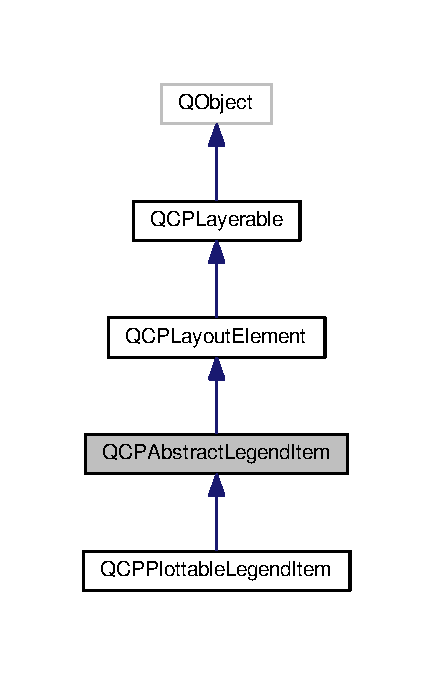
\includegraphics[width=208pt]{classQCPAbstractLegendItem__inherit__graph}
\end{center}
\end{figure}


Collaboration diagram for Q\+C\+P\+Abstract\+Legend\+Item\+:\nopagebreak
\begin{figure}[H]
\begin{center}
\leavevmode
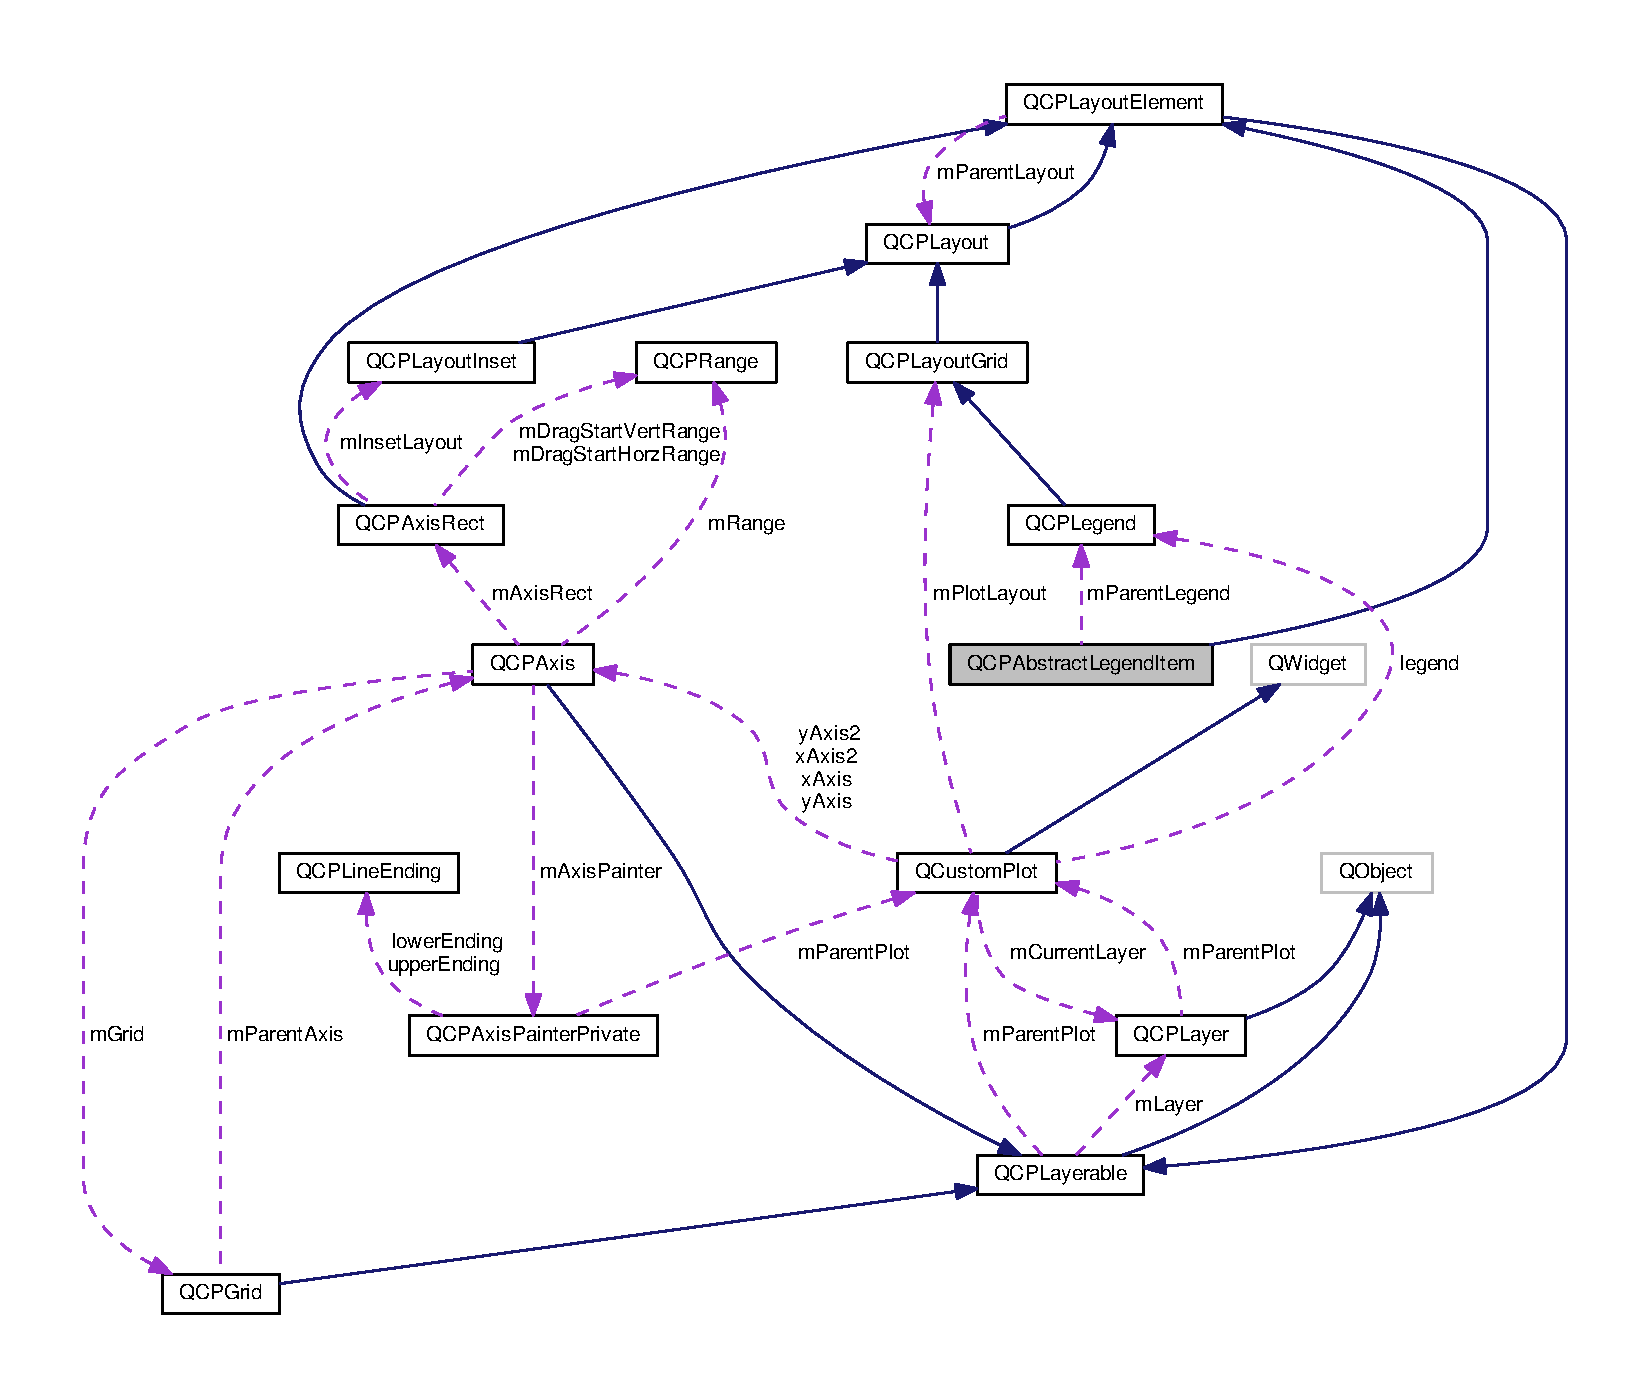
\includegraphics[width=350pt]{classQCPAbstractLegendItem__coll__graph}
\end{center}
\end{figure}
\subsection*{Signals}
\begin{DoxyCompactItemize}
\item 
void \hyperlink{classQCPAbstractLegendItem_a7cb61fdfbaf69c590bacb8f9e7099d9e}{selection\+Changed} (bool \hyperlink{classQCPAbstractLegendItem_ac776e68e3367704452131c6aa9908bb9}{selected})
\item 
void \hyperlink{classQCPAbstractLegendItem_abc4d779b938cc9235f9196737dbaa6bd}{selectable\+Changed} (bool \hyperlink{classQCPAbstractLegendItem_a0a0205f33f37edae50826c24cb8f1983}{selectable})
\end{DoxyCompactItemize}
\subsection*{Public Member Functions}
\begin{DoxyCompactItemize}
\item 
\hyperlink{classQCPAbstractLegendItem_afaff87610e8da0fa238ecf552872d774}{Q\+C\+P\+Abstract\+Legend\+Item} (\hyperlink{classQCPLegend}{Q\+C\+P\+Legend} $\ast$parent)
\item 
\hyperlink{classQCPLegend}{Q\+C\+P\+Legend} $\ast$ \hyperlink{classQCPAbstractLegendItem_afcd683e43058f99a47d6546eedffc5c1}{parent\+Legend} () const 
\item 
Q\+Font \hyperlink{classQCPAbstractLegendItem_ae476404706638d84fadc01021df2b19e}{font} () const 
\item 
Q\+Color \hyperlink{classQCPAbstractLegendItem_a444caef8565ac8d8653269f14d82b42d}{text\+Color} () const 
\item 
Q\+Font \hyperlink{classQCPAbstractLegendItem_afccfe665eb8483cec924a9c0a53ddf2b}{selected\+Font} () const 
\item 
Q\+Color \hyperlink{classQCPAbstractLegendItem_a076db1717257b82875b12a15ecf99ba3}{selected\+Text\+Color} () const 
\item 
bool \hyperlink{classQCPAbstractLegendItem_a0a0205f33f37edae50826c24cb8f1983}{selectable} () const 
\item 
bool \hyperlink{classQCPAbstractLegendItem_ac776e68e3367704452131c6aa9908bb9}{selected} () const 
\item 
void \hyperlink{classQCPAbstractLegendItem_a409c53455d8112f71d70c0c43eb10265}{set\+Font} (const Q\+Font \&\hyperlink{classQCPAbstractLegendItem_ae476404706638d84fadc01021df2b19e}{font})
\item 
void \hyperlink{classQCPAbstractLegendItem_a6ebace6aaffaedcdab2d74e88acc2d1e}{set\+Text\+Color} (const Q\+Color \&color)
\item 
void \hyperlink{classQCPAbstractLegendItem_a91db5aee48617a9d3206e61376807365}{set\+Selected\+Font} (const Q\+Font \&\hyperlink{classQCPAbstractLegendItem_ae476404706638d84fadc01021df2b19e}{font})
\item 
void \hyperlink{classQCPAbstractLegendItem_a4d01d008ee1a5bfe9905b0397a421936}{set\+Selected\+Text\+Color} (const Q\+Color \&color)
\item 
Q\+\_\+\+S\+L\+OT void \hyperlink{classQCPAbstractLegendItem_a9913ef48730551b696e7f98a2391c599}{set\+Selectable} (bool \hyperlink{classQCPAbstractLegendItem_a0a0205f33f37edae50826c24cb8f1983}{selectable})
\item 
Q\+\_\+\+S\+L\+OT void \hyperlink{classQCPAbstractLegendItem_a6eed93b0ab99cb3eabb043fb08179c2b}{set\+Selected} (bool \hyperlink{classQCPAbstractLegendItem_ac776e68e3367704452131c6aa9908bb9}{selected})
\item 
virtual double \hyperlink{classQCPAbstractLegendItem_ad0480d5cad34627a294a2921caa4a62f}{select\+Test} (const Q\+PointF \&pos, bool only\+Selectable, Q\+Variant $\ast$details=0) const 
\end{DoxyCompactItemize}
\subsection*{Protected Member Functions}
\begin{DoxyCompactItemize}
\item 
virtual \hyperlink{namespaceQCP_a2ad6bb6281c7c2d593d4277b44c2b037}{Q\+C\+P\+::\+Interaction} \hyperlink{classQCPAbstractLegendItem_a53a80054ab329beaca072fb08c08944b}{selection\+Category} () const 
\item 
virtual void \hyperlink{classQCPAbstractLegendItem_a71c3baeda42ba78d2cccd97e74110a5e}{apply\+Default\+Antialiasing\+Hint} (\hyperlink{classQCPPainter}{Q\+C\+P\+Painter} $\ast$painter) const 
\item 
virtual Q\+Rect \hyperlink{classQCPAbstractLegendItem_abcb540c331b49ef7ee0ea1abbd0dcac3}{clip\+Rect} () const 
\item 
virtual void \hyperlink{classQCPAbstractLegendItem_a97dedc084c672359710f16b31d046d1d}{draw} (\hyperlink{classQCPPainter}{Q\+C\+P\+Painter} $\ast$painter)=0
\item 
virtual void \hyperlink{classQCPAbstractLegendItem_abcfe9e335d99c7fac74e03d26723c1b7}{select\+Event} (Q\+Mouse\+Event $\ast$event, bool additive, const Q\+Variant \&details, bool $\ast$selection\+State\+Changed)
\item 
virtual void \hyperlink{classQCPAbstractLegendItem_ae64e667e7c5b85cd92c9b91928faef28}{deselect\+Event} (bool $\ast$selection\+State\+Changed)
\end{DoxyCompactItemize}
\subsection*{Protected Attributes}
\begin{DoxyCompactItemize}
\item 
\hyperlink{classQCPLegend}{Q\+C\+P\+Legend} $\ast$ \hyperlink{classQCPAbstractLegendItem_aafcd9fc6fcb10f4a8d46037011afafe8}{m\+Parent\+Legend}
\item 
Q\+Font \hyperlink{classQCPAbstractLegendItem_ae916a78ac0d2a60e20a17ca2f24f9754}{m\+Font}
\item 
Q\+Color \hyperlink{classQCPAbstractLegendItem_a974b21e9930227d281344bd2242d289d}{m\+Text\+Color}
\item 
Q\+Font \hyperlink{classQCPAbstractLegendItem_ab971df604306b192875a7d097feb1e21}{m\+Selected\+Font}
\item 
Q\+Color \hyperlink{classQCPAbstractLegendItem_a4965c13854d970b24c284f0a4f005fbd}{m\+Selected\+Text\+Color}
\item 
bool \hyperlink{classQCPAbstractLegendItem_aa84029f57b1b32f642fb7db63c3fc2c2}{m\+Selectable}
\item 
bool \hyperlink{classQCPAbstractLegendItem_ae58ebebbd0c36cc6fe897483369984d2}{m\+Selected}
\end{DoxyCompactItemize}
\subsection*{Friends}
\begin{DoxyCompactItemize}
\item 
class \hyperlink{classQCPAbstractLegendItem_a8429035e7adfbd7f05805a6530ad5e3b}{Q\+C\+P\+Legend}
\end{DoxyCompactItemize}
\subsection*{Additional Inherited Members}


\subsection{Detailed Description}
The abstract base class for all entries in a \hyperlink{classQCPLegend}{Q\+C\+P\+Legend}. 

It defines a very basic interface for entries in a \hyperlink{classQCPLegend}{Q\+C\+P\+Legend}. For representing plottables in the legend, the subclass \hyperlink{classQCPPlottableLegendItem}{Q\+C\+P\+Plottable\+Legend\+Item} is more suitable.

Only derive directly from this class when you need absolute freedom (e.\+g. a custom legend entry that\textquotesingle{}s not even associated with a plottable).

You must implement the following pure virtual functions\+: \begin{DoxyItemize}
\item \hyperlink{classQCPAbstractLegendItem_a97dedc084c672359710f16b31d046d1d}{draw} (from \hyperlink{classQCPLayerable}{Q\+C\+P\+Layerable})\end{DoxyItemize}
You inherit the following members you may use\+: \tabulinesep=1mm
\begin{longtabu} spread 0pt [c]{*2{|X[-1]}|}
\hline
\hyperlink{classQCPLegend}{Q\+C\+P\+Legend} $\ast${\bfseries m\+Parent\+Legend}  &A pointer to the parent \hyperlink{classQCPLegend}{Q\+C\+P\+Legend}. \\\cline{1-2}
Q\+Font {\bfseries m\+Font}  &The generic font of the item. You should use this font for all or at least the most prominent text of the item.  \\\cline{1-2}
\end{longtabu}


\subsection{Constructor \& Destructor Documentation}
\index{Q\+C\+P\+Abstract\+Legend\+Item@{Q\+C\+P\+Abstract\+Legend\+Item}!Q\+C\+P\+Abstract\+Legend\+Item@{Q\+C\+P\+Abstract\+Legend\+Item}}
\index{Q\+C\+P\+Abstract\+Legend\+Item@{Q\+C\+P\+Abstract\+Legend\+Item}!Q\+C\+P\+Abstract\+Legend\+Item@{Q\+C\+P\+Abstract\+Legend\+Item}}
\subsubsection[{\texorpdfstring{Q\+C\+P\+Abstract\+Legend\+Item(\+Q\+C\+P\+Legend $\ast$parent)}{QCPAbstractLegendItem(QCPLegend *parent)}}]{\setlength{\rightskip}{0pt plus 5cm}Q\+C\+P\+Abstract\+Legend\+Item\+::\+Q\+C\+P\+Abstract\+Legend\+Item (
\begin{DoxyParamCaption}
\item[{{\bf Q\+C\+P\+Legend} $\ast$}]{parent}
\end{DoxyParamCaption}
)\hspace{0.3cm}{\ttfamily [explicit]}}\hypertarget{classQCPAbstractLegendItem_afaff87610e8da0fa238ecf552872d774}{}\label{classQCPAbstractLegendItem_afaff87610e8da0fa238ecf552872d774}
Constructs a \hyperlink{classQCPAbstractLegendItem}{Q\+C\+P\+Abstract\+Legend\+Item} and associates it with the \hyperlink{classQCPLegend}{Q\+C\+P\+Legend} {\itshape parent}. This does not cause the item to be added to {\itshape parent}, so \hyperlink{classQCPLegend_a3ab274de52d2951faea45a6d975e6b3f}{Q\+C\+P\+Legend\+::add\+Item} must be called separately. 

\subsection{Member Function Documentation}
\index{Q\+C\+P\+Abstract\+Legend\+Item@{Q\+C\+P\+Abstract\+Legend\+Item}!apply\+Default\+Antialiasing\+Hint@{apply\+Default\+Antialiasing\+Hint}}
\index{apply\+Default\+Antialiasing\+Hint@{apply\+Default\+Antialiasing\+Hint}!Q\+C\+P\+Abstract\+Legend\+Item@{Q\+C\+P\+Abstract\+Legend\+Item}}
\subsubsection[{\texorpdfstring{apply\+Default\+Antialiasing\+Hint(\+Q\+C\+P\+Painter $\ast$painter) const }{applyDefaultAntialiasingHint(QCPPainter *painter) const }}]{\setlength{\rightskip}{0pt plus 5cm}void Q\+C\+P\+Abstract\+Legend\+Item\+::apply\+Default\+Antialiasing\+Hint (
\begin{DoxyParamCaption}
\item[{{\bf Q\+C\+P\+Painter} $\ast$}]{painter}
\end{DoxyParamCaption}
) const\hspace{0.3cm}{\ttfamily [protected]}, {\ttfamily [virtual]}}\hypertarget{classQCPAbstractLegendItem_a71c3baeda42ba78d2cccd97e74110a5e}{}\label{classQCPAbstractLegendItem_a71c3baeda42ba78d2cccd97e74110a5e}


Reimplemented from \hyperlink{classQCPLayoutElement_ad6d2b4bb0291c2441b2e1ca3d5296df5}{Q\+C\+P\+Layout\+Element}.

\index{Q\+C\+P\+Abstract\+Legend\+Item@{Q\+C\+P\+Abstract\+Legend\+Item}!clip\+Rect@{clip\+Rect}}
\index{clip\+Rect@{clip\+Rect}!Q\+C\+P\+Abstract\+Legend\+Item@{Q\+C\+P\+Abstract\+Legend\+Item}}
\subsubsection[{\texorpdfstring{clip\+Rect() const }{clipRect() const }}]{\setlength{\rightskip}{0pt plus 5cm}Q\+Rect Q\+C\+P\+Abstract\+Legend\+Item\+::clip\+Rect (
\begin{DoxyParamCaption}
{}
\end{DoxyParamCaption}
) const\hspace{0.3cm}{\ttfamily [protected]}, {\ttfamily [virtual]}}\hypertarget{classQCPAbstractLegendItem_abcb540c331b49ef7ee0ea1abbd0dcac3}{}\label{classQCPAbstractLegendItem_abcb540c331b49ef7ee0ea1abbd0dcac3}


Reimplemented from \hyperlink{classQCPLayerable_a07a8f746640c3704b09910df297afcba}{Q\+C\+P\+Layerable}.

\index{Q\+C\+P\+Abstract\+Legend\+Item@{Q\+C\+P\+Abstract\+Legend\+Item}!deselect\+Event@{deselect\+Event}}
\index{deselect\+Event@{deselect\+Event}!Q\+C\+P\+Abstract\+Legend\+Item@{Q\+C\+P\+Abstract\+Legend\+Item}}
\subsubsection[{\texorpdfstring{deselect\+Event(bool $\ast$selection\+State\+Changed)}{deselectEvent(bool *selectionStateChanged)}}]{\setlength{\rightskip}{0pt plus 5cm}void Q\+C\+P\+Abstract\+Legend\+Item\+::deselect\+Event (
\begin{DoxyParamCaption}
\item[{bool $\ast$}]{selection\+State\+Changed}
\end{DoxyParamCaption}
)\hspace{0.3cm}{\ttfamily [protected]}, {\ttfamily [virtual]}}\hypertarget{classQCPAbstractLegendItem_ae64e667e7c5b85cd92c9b91928faef28}{}\label{classQCPAbstractLegendItem_ae64e667e7c5b85cd92c9b91928faef28}


Reimplemented from \hyperlink{classQCPLayerable_ae546370644a5551c76af739afc008bee}{Q\+C\+P\+Layerable}.

\index{Q\+C\+P\+Abstract\+Legend\+Item@{Q\+C\+P\+Abstract\+Legend\+Item}!draw@{draw}}
\index{draw@{draw}!Q\+C\+P\+Abstract\+Legend\+Item@{Q\+C\+P\+Abstract\+Legend\+Item}}
\subsubsection[{\texorpdfstring{draw(\+Q\+C\+P\+Painter $\ast$painter)=0}{draw(QCPPainter *painter)=0}}]{\setlength{\rightskip}{0pt plus 5cm}virtual void Q\+C\+P\+Abstract\+Legend\+Item\+::draw (
\begin{DoxyParamCaption}
\item[{{\bf Q\+C\+P\+Painter} $\ast$}]{painter}
\end{DoxyParamCaption}
)\hspace{0.3cm}{\ttfamily [protected]}, {\ttfamily [pure virtual]}}\hypertarget{classQCPAbstractLegendItem_a97dedc084c672359710f16b31d046d1d}{}\label{classQCPAbstractLegendItem_a97dedc084c672359710f16b31d046d1d}


Reimplemented from \hyperlink{classQCPLayoutElement_a547bcc1e6e2be5645ca781efe0834653}{Q\+C\+P\+Layout\+Element}.



Implemented in \hyperlink{classQCPPlottableLegendItem_a68a781c3de4f9959fdf82075052d43aa}{Q\+C\+P\+Plottable\+Legend\+Item}.

\index{Q\+C\+P\+Abstract\+Legend\+Item@{Q\+C\+P\+Abstract\+Legend\+Item}!font@{font}}
\index{font@{font}!Q\+C\+P\+Abstract\+Legend\+Item@{Q\+C\+P\+Abstract\+Legend\+Item}}
\subsubsection[{\texorpdfstring{font() const }{font() const }}]{\setlength{\rightskip}{0pt plus 5cm}Q\+Font Q\+C\+P\+Abstract\+Legend\+Item\+::font (
\begin{DoxyParamCaption}
{}
\end{DoxyParamCaption}
) const\hspace{0.3cm}{\ttfamily [inline]}}\hypertarget{classQCPAbstractLegendItem_ae476404706638d84fadc01021df2b19e}{}\label{classQCPAbstractLegendItem_ae476404706638d84fadc01021df2b19e}
\index{Q\+C\+P\+Abstract\+Legend\+Item@{Q\+C\+P\+Abstract\+Legend\+Item}!parent\+Legend@{parent\+Legend}}
\index{parent\+Legend@{parent\+Legend}!Q\+C\+P\+Abstract\+Legend\+Item@{Q\+C\+P\+Abstract\+Legend\+Item}}
\subsubsection[{\texorpdfstring{parent\+Legend() const }{parentLegend() const }}]{\setlength{\rightskip}{0pt plus 5cm}{\bf Q\+C\+P\+Legend}$\ast$ Q\+C\+P\+Abstract\+Legend\+Item\+::parent\+Legend (
\begin{DoxyParamCaption}
{}
\end{DoxyParamCaption}
) const\hspace{0.3cm}{\ttfamily [inline]}}\hypertarget{classQCPAbstractLegendItem_afcd683e43058f99a47d6546eedffc5c1}{}\label{classQCPAbstractLegendItem_afcd683e43058f99a47d6546eedffc5c1}
\index{Q\+C\+P\+Abstract\+Legend\+Item@{Q\+C\+P\+Abstract\+Legend\+Item}!selectable@{selectable}}
\index{selectable@{selectable}!Q\+C\+P\+Abstract\+Legend\+Item@{Q\+C\+P\+Abstract\+Legend\+Item}}
\subsubsection[{\texorpdfstring{selectable() const }{selectable() const }}]{\setlength{\rightskip}{0pt plus 5cm}bool Q\+C\+P\+Abstract\+Legend\+Item\+::selectable (
\begin{DoxyParamCaption}
{}
\end{DoxyParamCaption}
) const\hspace{0.3cm}{\ttfamily [inline]}}\hypertarget{classQCPAbstractLegendItem_a0a0205f33f37edae50826c24cb8f1983}{}\label{classQCPAbstractLegendItem_a0a0205f33f37edae50826c24cb8f1983}
\index{Q\+C\+P\+Abstract\+Legend\+Item@{Q\+C\+P\+Abstract\+Legend\+Item}!selectable\+Changed@{selectable\+Changed}}
\index{selectable\+Changed@{selectable\+Changed}!Q\+C\+P\+Abstract\+Legend\+Item@{Q\+C\+P\+Abstract\+Legend\+Item}}
\subsubsection[{\texorpdfstring{selectable\+Changed}{selectableChanged}}]{\setlength{\rightskip}{0pt plus 5cm}void Q\+C\+P\+Abstract\+Legend\+Item\+::selectable\+Changed (
\begin{DoxyParamCaption}
\item[{bool}]{selectable}
\end{DoxyParamCaption}
)\hspace{0.3cm}{\ttfamily [signal]}}\hypertarget{classQCPAbstractLegendItem_abc4d779b938cc9235f9196737dbaa6bd}{}\label{classQCPAbstractLegendItem_abc4d779b938cc9235f9196737dbaa6bd}
\index{Q\+C\+P\+Abstract\+Legend\+Item@{Q\+C\+P\+Abstract\+Legend\+Item}!selected@{selected}}
\index{selected@{selected}!Q\+C\+P\+Abstract\+Legend\+Item@{Q\+C\+P\+Abstract\+Legend\+Item}}
\subsubsection[{\texorpdfstring{selected() const }{selected() const }}]{\setlength{\rightskip}{0pt plus 5cm}bool Q\+C\+P\+Abstract\+Legend\+Item\+::selected (
\begin{DoxyParamCaption}
{}
\end{DoxyParamCaption}
) const\hspace{0.3cm}{\ttfamily [inline]}}\hypertarget{classQCPAbstractLegendItem_ac776e68e3367704452131c6aa9908bb9}{}\label{classQCPAbstractLegendItem_ac776e68e3367704452131c6aa9908bb9}
\index{Q\+C\+P\+Abstract\+Legend\+Item@{Q\+C\+P\+Abstract\+Legend\+Item}!selected\+Font@{selected\+Font}}
\index{selected\+Font@{selected\+Font}!Q\+C\+P\+Abstract\+Legend\+Item@{Q\+C\+P\+Abstract\+Legend\+Item}}
\subsubsection[{\texorpdfstring{selected\+Font() const }{selectedFont() const }}]{\setlength{\rightskip}{0pt plus 5cm}Q\+Font Q\+C\+P\+Abstract\+Legend\+Item\+::selected\+Font (
\begin{DoxyParamCaption}
{}
\end{DoxyParamCaption}
) const\hspace{0.3cm}{\ttfamily [inline]}}\hypertarget{classQCPAbstractLegendItem_afccfe665eb8483cec924a9c0a53ddf2b}{}\label{classQCPAbstractLegendItem_afccfe665eb8483cec924a9c0a53ddf2b}
\index{Q\+C\+P\+Abstract\+Legend\+Item@{Q\+C\+P\+Abstract\+Legend\+Item}!selected\+Text\+Color@{selected\+Text\+Color}}
\index{selected\+Text\+Color@{selected\+Text\+Color}!Q\+C\+P\+Abstract\+Legend\+Item@{Q\+C\+P\+Abstract\+Legend\+Item}}
\subsubsection[{\texorpdfstring{selected\+Text\+Color() const }{selectedTextColor() const }}]{\setlength{\rightskip}{0pt plus 5cm}Q\+Color Q\+C\+P\+Abstract\+Legend\+Item\+::selected\+Text\+Color (
\begin{DoxyParamCaption}
{}
\end{DoxyParamCaption}
) const\hspace{0.3cm}{\ttfamily [inline]}}\hypertarget{classQCPAbstractLegendItem_a076db1717257b82875b12a15ecf99ba3}{}\label{classQCPAbstractLegendItem_a076db1717257b82875b12a15ecf99ba3}
\index{Q\+C\+P\+Abstract\+Legend\+Item@{Q\+C\+P\+Abstract\+Legend\+Item}!select\+Event@{select\+Event}}
\index{select\+Event@{select\+Event}!Q\+C\+P\+Abstract\+Legend\+Item@{Q\+C\+P\+Abstract\+Legend\+Item}}
\subsubsection[{\texorpdfstring{select\+Event(\+Q\+Mouse\+Event $\ast$event, bool additive, const Q\+Variant \&details, bool $\ast$selection\+State\+Changed)}{selectEvent(QMouseEvent *event, bool additive, const QVariant &details, bool *selectionStateChanged)}}]{\setlength{\rightskip}{0pt plus 5cm}void Q\+C\+P\+Abstract\+Legend\+Item\+::select\+Event (
\begin{DoxyParamCaption}
\item[{Q\+Mouse\+Event $\ast$}]{event, }
\item[{bool}]{additive, }
\item[{const Q\+Variant \&}]{details, }
\item[{bool $\ast$}]{selection\+State\+Changed}
\end{DoxyParamCaption}
)\hspace{0.3cm}{\ttfamily [protected]}, {\ttfamily [virtual]}}\hypertarget{classQCPAbstractLegendItem_abcfe9e335d99c7fac74e03d26723c1b7}{}\label{classQCPAbstractLegendItem_abcfe9e335d99c7fac74e03d26723c1b7}


Reimplemented from \hyperlink{classQCPLayerable_a7498c2d0d081cf7cad0fb3bb93aa0e91}{Q\+C\+P\+Layerable}.

\index{Q\+C\+P\+Abstract\+Legend\+Item@{Q\+C\+P\+Abstract\+Legend\+Item}!selection\+Category@{selection\+Category}}
\index{selection\+Category@{selection\+Category}!Q\+C\+P\+Abstract\+Legend\+Item@{Q\+C\+P\+Abstract\+Legend\+Item}}
\subsubsection[{\texorpdfstring{selection\+Category() const }{selectionCategory() const }}]{\setlength{\rightskip}{0pt plus 5cm}{\bf Q\+C\+P\+::\+Interaction} Q\+C\+P\+Abstract\+Legend\+Item\+::selection\+Category (
\begin{DoxyParamCaption}
{}
\end{DoxyParamCaption}
) const\hspace{0.3cm}{\ttfamily [protected]}, {\ttfamily [virtual]}}\hypertarget{classQCPAbstractLegendItem_a53a80054ab329beaca072fb08c08944b}{}\label{classQCPAbstractLegendItem_a53a80054ab329beaca072fb08c08944b}


Reimplemented from \hyperlink{classQCPLayerable_aa4035e586b7f317a06ba7e74e242a5ea}{Q\+C\+P\+Layerable}.

\index{Q\+C\+P\+Abstract\+Legend\+Item@{Q\+C\+P\+Abstract\+Legend\+Item}!selection\+Changed@{selection\+Changed}}
\index{selection\+Changed@{selection\+Changed}!Q\+C\+P\+Abstract\+Legend\+Item@{Q\+C\+P\+Abstract\+Legend\+Item}}
\subsubsection[{\texorpdfstring{selection\+Changed}{selectionChanged}}]{\setlength{\rightskip}{0pt plus 5cm}void Q\+C\+P\+Abstract\+Legend\+Item\+::selection\+Changed (
\begin{DoxyParamCaption}
\item[{bool}]{selected}
\end{DoxyParamCaption}
)\hspace{0.3cm}{\ttfamily [signal]}}\hypertarget{classQCPAbstractLegendItem_a7cb61fdfbaf69c590bacb8f9e7099d9e}{}\label{classQCPAbstractLegendItem_a7cb61fdfbaf69c590bacb8f9e7099d9e}
This signal is emitted when the selection state of this legend item has changed, either by user interaction or by a direct call to \hyperlink{classQCPAbstractLegendItem_a6eed93b0ab99cb3eabb043fb08179c2b}{set\+Selected}. \index{Q\+C\+P\+Abstract\+Legend\+Item@{Q\+C\+P\+Abstract\+Legend\+Item}!select\+Test@{select\+Test}}
\index{select\+Test@{select\+Test}!Q\+C\+P\+Abstract\+Legend\+Item@{Q\+C\+P\+Abstract\+Legend\+Item}}
\subsubsection[{\texorpdfstring{select\+Test(const Q\+Point\+F \&pos, bool only\+Selectable, Q\+Variant $\ast$details=0) const }{selectTest(const QPointF &pos, bool onlySelectable, QVariant *details=0) const }}]{\setlength{\rightskip}{0pt plus 5cm}double Q\+C\+P\+Abstract\+Legend\+Item\+::select\+Test (
\begin{DoxyParamCaption}
\item[{const Q\+PointF \&}]{pos, }
\item[{bool}]{only\+Selectable, }
\item[{Q\+Variant $\ast$}]{details = {\ttfamily 0}}
\end{DoxyParamCaption}
) const\hspace{0.3cm}{\ttfamily [virtual]}}\hypertarget{classQCPAbstractLegendItem_ad0480d5cad34627a294a2921caa4a62f}{}\label{classQCPAbstractLegendItem_ad0480d5cad34627a294a2921caa4a62f}
Layout elements are sensitive to events inside their outer rect. If {\itshape pos} is within the outer rect, this method returns a value corresponding to 0.\+99 times the parent plot\textquotesingle{}s selection tolerance. However, layout elements are not selectable by default. So if {\itshape only\+Selectable} is true, -\/1.\+0 is returned.

See \hyperlink{classQCPLayerable_a4001c4d0dfec55598efa4d531f2179a9}{Q\+C\+P\+Layerable\+::select\+Test} for a general explanation of this virtual method.

\hyperlink{classQCPLayoutElement}{Q\+C\+P\+Layout\+Element} subclasses may reimplement this method to provide more specific selection test behaviour. 

Reimplemented from \hyperlink{classQCPLayoutElement_a9fcf5d0ea19f2c23b2b528bce2c6f095}{Q\+C\+P\+Layout\+Element}.

\index{Q\+C\+P\+Abstract\+Legend\+Item@{Q\+C\+P\+Abstract\+Legend\+Item}!set\+Font@{set\+Font}}
\index{set\+Font@{set\+Font}!Q\+C\+P\+Abstract\+Legend\+Item@{Q\+C\+P\+Abstract\+Legend\+Item}}
\subsubsection[{\texorpdfstring{set\+Font(const Q\+Font \&font)}{setFont(const QFont &font)}}]{\setlength{\rightskip}{0pt plus 5cm}void Q\+C\+P\+Abstract\+Legend\+Item\+::set\+Font (
\begin{DoxyParamCaption}
\item[{const Q\+Font \&}]{font}
\end{DoxyParamCaption}
)}\hypertarget{classQCPAbstractLegendItem_a409c53455d8112f71d70c0c43eb10265}{}\label{classQCPAbstractLegendItem_a409c53455d8112f71d70c0c43eb10265}
Sets the default font of this specific legend item to {\itshape font}.

\begin{DoxySeeAlso}{See also}
\hyperlink{classQCPAbstractLegendItem_a6ebace6aaffaedcdab2d74e88acc2d1e}{set\+Text\+Color}, \hyperlink{classQCPLegend_aa4cda8499e3cb0f3be415edc02984c73}{Q\+C\+P\+Legend\+::set\+Font} 
\end{DoxySeeAlso}
\index{Q\+C\+P\+Abstract\+Legend\+Item@{Q\+C\+P\+Abstract\+Legend\+Item}!set\+Selectable@{set\+Selectable}}
\index{set\+Selectable@{set\+Selectable}!Q\+C\+P\+Abstract\+Legend\+Item@{Q\+C\+P\+Abstract\+Legend\+Item}}
\subsubsection[{\texorpdfstring{set\+Selectable(bool selectable)}{setSelectable(bool selectable)}}]{\setlength{\rightskip}{0pt plus 5cm}void Q\+C\+P\+Abstract\+Legend\+Item\+::set\+Selectable (
\begin{DoxyParamCaption}
\item[{bool}]{selectable}
\end{DoxyParamCaption}
)}\hypertarget{classQCPAbstractLegendItem_a9913ef48730551b696e7f98a2391c599}{}\label{classQCPAbstractLegendItem_a9913ef48730551b696e7f98a2391c599}
Sets whether this specific legend item is selectable.

\begin{DoxySeeAlso}{See also}
set\+Selected\+Parts, \hyperlink{classQCustomPlot_a5ee1e2f6ae27419deca53e75907c27e5}{Q\+Custom\+Plot\+::set\+Interactions} 
\end{DoxySeeAlso}
\index{Q\+C\+P\+Abstract\+Legend\+Item@{Q\+C\+P\+Abstract\+Legend\+Item}!set\+Selected@{set\+Selected}}
\index{set\+Selected@{set\+Selected}!Q\+C\+P\+Abstract\+Legend\+Item@{Q\+C\+P\+Abstract\+Legend\+Item}}
\subsubsection[{\texorpdfstring{set\+Selected(bool selected)}{setSelected(bool selected)}}]{\setlength{\rightskip}{0pt plus 5cm}void Q\+C\+P\+Abstract\+Legend\+Item\+::set\+Selected (
\begin{DoxyParamCaption}
\item[{bool}]{selected}
\end{DoxyParamCaption}
)}\hypertarget{classQCPAbstractLegendItem_a6eed93b0ab99cb3eabb043fb08179c2b}{}\label{classQCPAbstractLegendItem_a6eed93b0ab99cb3eabb043fb08179c2b}
Sets whether this specific legend item is selected.

It is possible to set the selection state of this item by calling this function directly, even if set\+Selectable is set to false.

\begin{DoxySeeAlso}{See also}
set\+Selectable\+Parts, \hyperlink{classQCustomPlot_a5ee1e2f6ae27419deca53e75907c27e5}{Q\+Custom\+Plot\+::set\+Interactions} 
\end{DoxySeeAlso}
\index{Q\+C\+P\+Abstract\+Legend\+Item@{Q\+C\+P\+Abstract\+Legend\+Item}!set\+Selected\+Font@{set\+Selected\+Font}}
\index{set\+Selected\+Font@{set\+Selected\+Font}!Q\+C\+P\+Abstract\+Legend\+Item@{Q\+C\+P\+Abstract\+Legend\+Item}}
\subsubsection[{\texorpdfstring{set\+Selected\+Font(const Q\+Font \&font)}{setSelectedFont(const QFont &font)}}]{\setlength{\rightskip}{0pt plus 5cm}void Q\+C\+P\+Abstract\+Legend\+Item\+::set\+Selected\+Font (
\begin{DoxyParamCaption}
\item[{const Q\+Font \&}]{font}
\end{DoxyParamCaption}
)}\hypertarget{classQCPAbstractLegendItem_a91db5aee48617a9d3206e61376807365}{}\label{classQCPAbstractLegendItem_a91db5aee48617a9d3206e61376807365}
When this legend item is selected, {\itshape font} is used to draw generic text, instead of the normal font set with \hyperlink{classQCPAbstractLegendItem_a409c53455d8112f71d70c0c43eb10265}{set\+Font}.

\begin{DoxySeeAlso}{See also}
\hyperlink{classQCPAbstractLegendItem_a409c53455d8112f71d70c0c43eb10265}{set\+Font}, \hyperlink{classQCPLegend_ab580a01c3c0a239374ed66c29edf5ad2}{Q\+C\+P\+Legend\+::set\+Selected\+Font} 
\end{DoxySeeAlso}
\index{Q\+C\+P\+Abstract\+Legend\+Item@{Q\+C\+P\+Abstract\+Legend\+Item}!set\+Selected\+Text\+Color@{set\+Selected\+Text\+Color}}
\index{set\+Selected\+Text\+Color@{set\+Selected\+Text\+Color}!Q\+C\+P\+Abstract\+Legend\+Item@{Q\+C\+P\+Abstract\+Legend\+Item}}
\subsubsection[{\texorpdfstring{set\+Selected\+Text\+Color(const Q\+Color \&color)}{setSelectedTextColor(const QColor &color)}}]{\setlength{\rightskip}{0pt plus 5cm}void Q\+C\+P\+Abstract\+Legend\+Item\+::set\+Selected\+Text\+Color (
\begin{DoxyParamCaption}
\item[{const Q\+Color \&}]{color}
\end{DoxyParamCaption}
)}\hypertarget{classQCPAbstractLegendItem_a4d01d008ee1a5bfe9905b0397a421936}{}\label{classQCPAbstractLegendItem_a4d01d008ee1a5bfe9905b0397a421936}
When this legend item is selected, {\itshape color} is used to draw generic text, instead of the normal color set with \hyperlink{classQCPAbstractLegendItem_a6ebace6aaffaedcdab2d74e88acc2d1e}{set\+Text\+Color}.

\begin{DoxySeeAlso}{See also}
\hyperlink{classQCPAbstractLegendItem_a6ebace6aaffaedcdab2d74e88acc2d1e}{set\+Text\+Color}, \hyperlink{classQCPLegend_a7674dfc7a1f30e1abd1018c0ed45e0bc}{Q\+C\+P\+Legend\+::set\+Selected\+Text\+Color} 
\end{DoxySeeAlso}
\index{Q\+C\+P\+Abstract\+Legend\+Item@{Q\+C\+P\+Abstract\+Legend\+Item}!set\+Text\+Color@{set\+Text\+Color}}
\index{set\+Text\+Color@{set\+Text\+Color}!Q\+C\+P\+Abstract\+Legend\+Item@{Q\+C\+P\+Abstract\+Legend\+Item}}
\subsubsection[{\texorpdfstring{set\+Text\+Color(const Q\+Color \&color)}{setTextColor(const QColor &color)}}]{\setlength{\rightskip}{0pt plus 5cm}void Q\+C\+P\+Abstract\+Legend\+Item\+::set\+Text\+Color (
\begin{DoxyParamCaption}
\item[{const Q\+Color \&}]{color}
\end{DoxyParamCaption}
)}\hypertarget{classQCPAbstractLegendItem_a6ebace6aaffaedcdab2d74e88acc2d1e}{}\label{classQCPAbstractLegendItem_a6ebace6aaffaedcdab2d74e88acc2d1e}
Sets the default text color of this specific legend item to {\itshape color}.

\begin{DoxySeeAlso}{See also}
\hyperlink{classQCPAbstractLegendItem_a409c53455d8112f71d70c0c43eb10265}{set\+Font}, \hyperlink{classQCPLegend_ae1eb239ff4a4632fe1b6c3e668d845c6}{Q\+C\+P\+Legend\+::set\+Text\+Color} 
\end{DoxySeeAlso}
\index{Q\+C\+P\+Abstract\+Legend\+Item@{Q\+C\+P\+Abstract\+Legend\+Item}!text\+Color@{text\+Color}}
\index{text\+Color@{text\+Color}!Q\+C\+P\+Abstract\+Legend\+Item@{Q\+C\+P\+Abstract\+Legend\+Item}}
\subsubsection[{\texorpdfstring{text\+Color() const }{textColor() const }}]{\setlength{\rightskip}{0pt plus 5cm}Q\+Color Q\+C\+P\+Abstract\+Legend\+Item\+::text\+Color (
\begin{DoxyParamCaption}
{}
\end{DoxyParamCaption}
) const\hspace{0.3cm}{\ttfamily [inline]}}\hypertarget{classQCPAbstractLegendItem_a444caef8565ac8d8653269f14d82b42d}{}\label{classQCPAbstractLegendItem_a444caef8565ac8d8653269f14d82b42d}


\subsection{Friends And Related Function Documentation}
\index{Q\+C\+P\+Abstract\+Legend\+Item@{Q\+C\+P\+Abstract\+Legend\+Item}!Q\+C\+P\+Legend@{Q\+C\+P\+Legend}}
\index{Q\+C\+P\+Legend@{Q\+C\+P\+Legend}!Q\+C\+P\+Abstract\+Legend\+Item@{Q\+C\+P\+Abstract\+Legend\+Item}}
\subsubsection[{\texorpdfstring{Q\+C\+P\+Legend}{QCPLegend}}]{\setlength{\rightskip}{0pt plus 5cm}friend class {\bf Q\+C\+P\+Legend}\hspace{0.3cm}{\ttfamily [friend]}}\hypertarget{classQCPAbstractLegendItem_a8429035e7adfbd7f05805a6530ad5e3b}{}\label{classQCPAbstractLegendItem_a8429035e7adfbd7f05805a6530ad5e3b}


\subsection{Member Data Documentation}
\index{Q\+C\+P\+Abstract\+Legend\+Item@{Q\+C\+P\+Abstract\+Legend\+Item}!m\+Font@{m\+Font}}
\index{m\+Font@{m\+Font}!Q\+C\+P\+Abstract\+Legend\+Item@{Q\+C\+P\+Abstract\+Legend\+Item}}
\subsubsection[{\texorpdfstring{m\+Font}{mFont}}]{\setlength{\rightskip}{0pt plus 5cm}Q\+Font Q\+C\+P\+Abstract\+Legend\+Item\+::m\+Font\hspace{0.3cm}{\ttfamily [protected]}}\hypertarget{classQCPAbstractLegendItem_ae916a78ac0d2a60e20a17ca2f24f9754}{}\label{classQCPAbstractLegendItem_ae916a78ac0d2a60e20a17ca2f24f9754}
\index{Q\+C\+P\+Abstract\+Legend\+Item@{Q\+C\+P\+Abstract\+Legend\+Item}!m\+Parent\+Legend@{m\+Parent\+Legend}}
\index{m\+Parent\+Legend@{m\+Parent\+Legend}!Q\+C\+P\+Abstract\+Legend\+Item@{Q\+C\+P\+Abstract\+Legend\+Item}}
\subsubsection[{\texorpdfstring{m\+Parent\+Legend}{mParentLegend}}]{\setlength{\rightskip}{0pt plus 5cm}{\bf Q\+C\+P\+Legend}$\ast$ Q\+C\+P\+Abstract\+Legend\+Item\+::m\+Parent\+Legend\hspace{0.3cm}{\ttfamily [protected]}}\hypertarget{classQCPAbstractLegendItem_aafcd9fc6fcb10f4a8d46037011afafe8}{}\label{classQCPAbstractLegendItem_aafcd9fc6fcb10f4a8d46037011afafe8}
\index{Q\+C\+P\+Abstract\+Legend\+Item@{Q\+C\+P\+Abstract\+Legend\+Item}!m\+Selectable@{m\+Selectable}}
\index{m\+Selectable@{m\+Selectable}!Q\+C\+P\+Abstract\+Legend\+Item@{Q\+C\+P\+Abstract\+Legend\+Item}}
\subsubsection[{\texorpdfstring{m\+Selectable}{mSelectable}}]{\setlength{\rightskip}{0pt plus 5cm}bool Q\+C\+P\+Abstract\+Legend\+Item\+::m\+Selectable\hspace{0.3cm}{\ttfamily [protected]}}\hypertarget{classQCPAbstractLegendItem_aa84029f57b1b32f642fb7db63c3fc2c2}{}\label{classQCPAbstractLegendItem_aa84029f57b1b32f642fb7db63c3fc2c2}
\index{Q\+C\+P\+Abstract\+Legend\+Item@{Q\+C\+P\+Abstract\+Legend\+Item}!m\+Selected@{m\+Selected}}
\index{m\+Selected@{m\+Selected}!Q\+C\+P\+Abstract\+Legend\+Item@{Q\+C\+P\+Abstract\+Legend\+Item}}
\subsubsection[{\texorpdfstring{m\+Selected}{mSelected}}]{\setlength{\rightskip}{0pt plus 5cm}bool Q\+C\+P\+Abstract\+Legend\+Item\+::m\+Selected\hspace{0.3cm}{\ttfamily [protected]}}\hypertarget{classQCPAbstractLegendItem_ae58ebebbd0c36cc6fe897483369984d2}{}\label{classQCPAbstractLegendItem_ae58ebebbd0c36cc6fe897483369984d2}
\index{Q\+C\+P\+Abstract\+Legend\+Item@{Q\+C\+P\+Abstract\+Legend\+Item}!m\+Selected\+Font@{m\+Selected\+Font}}
\index{m\+Selected\+Font@{m\+Selected\+Font}!Q\+C\+P\+Abstract\+Legend\+Item@{Q\+C\+P\+Abstract\+Legend\+Item}}
\subsubsection[{\texorpdfstring{m\+Selected\+Font}{mSelectedFont}}]{\setlength{\rightskip}{0pt plus 5cm}Q\+Font Q\+C\+P\+Abstract\+Legend\+Item\+::m\+Selected\+Font\hspace{0.3cm}{\ttfamily [protected]}}\hypertarget{classQCPAbstractLegendItem_ab971df604306b192875a7d097feb1e21}{}\label{classQCPAbstractLegendItem_ab971df604306b192875a7d097feb1e21}
\index{Q\+C\+P\+Abstract\+Legend\+Item@{Q\+C\+P\+Abstract\+Legend\+Item}!m\+Selected\+Text\+Color@{m\+Selected\+Text\+Color}}
\index{m\+Selected\+Text\+Color@{m\+Selected\+Text\+Color}!Q\+C\+P\+Abstract\+Legend\+Item@{Q\+C\+P\+Abstract\+Legend\+Item}}
\subsubsection[{\texorpdfstring{m\+Selected\+Text\+Color}{mSelectedTextColor}}]{\setlength{\rightskip}{0pt plus 5cm}Q\+Color Q\+C\+P\+Abstract\+Legend\+Item\+::m\+Selected\+Text\+Color\hspace{0.3cm}{\ttfamily [protected]}}\hypertarget{classQCPAbstractLegendItem_a4965c13854d970b24c284f0a4f005fbd}{}\label{classQCPAbstractLegendItem_a4965c13854d970b24c284f0a4f005fbd}
\index{Q\+C\+P\+Abstract\+Legend\+Item@{Q\+C\+P\+Abstract\+Legend\+Item}!m\+Text\+Color@{m\+Text\+Color}}
\index{m\+Text\+Color@{m\+Text\+Color}!Q\+C\+P\+Abstract\+Legend\+Item@{Q\+C\+P\+Abstract\+Legend\+Item}}
\subsubsection[{\texorpdfstring{m\+Text\+Color}{mTextColor}}]{\setlength{\rightskip}{0pt plus 5cm}Q\+Color Q\+C\+P\+Abstract\+Legend\+Item\+::m\+Text\+Color\hspace{0.3cm}{\ttfamily [protected]}}\hypertarget{classQCPAbstractLegendItem_a974b21e9930227d281344bd2242d289d}{}\label{classQCPAbstractLegendItem_a974b21e9930227d281344bd2242d289d}


The documentation for this class was generated from the following files\+:\begin{DoxyCompactItemize}
\item 
src/hammerhead/tools/watchdog/include/watchdog/\hyperlink{qcustomplot_8h}{qcustomplot.\+h}\item 
src/hammerhead/tools/watchdog/src/\hyperlink{qcustomplot_8cpp}{qcustomplot.\+cpp}\end{DoxyCompactItemize}

\hypertarget{classQCPAbstractPlottable}{}\section{Q\+C\+P\+Abstract\+Plottable Class Reference}
\label{classQCPAbstractPlottable}\index{Q\+C\+P\+Abstract\+Plottable@{Q\+C\+P\+Abstract\+Plottable}}


The abstract base class for all data representing objects in a plot.  




{\ttfamily \#include $<$qcustomplot.\+h$>$}



Inheritance diagram for Q\+C\+P\+Abstract\+Plottable\+:
\nopagebreak
\begin{figure}[H]
\begin{center}
\leavevmode
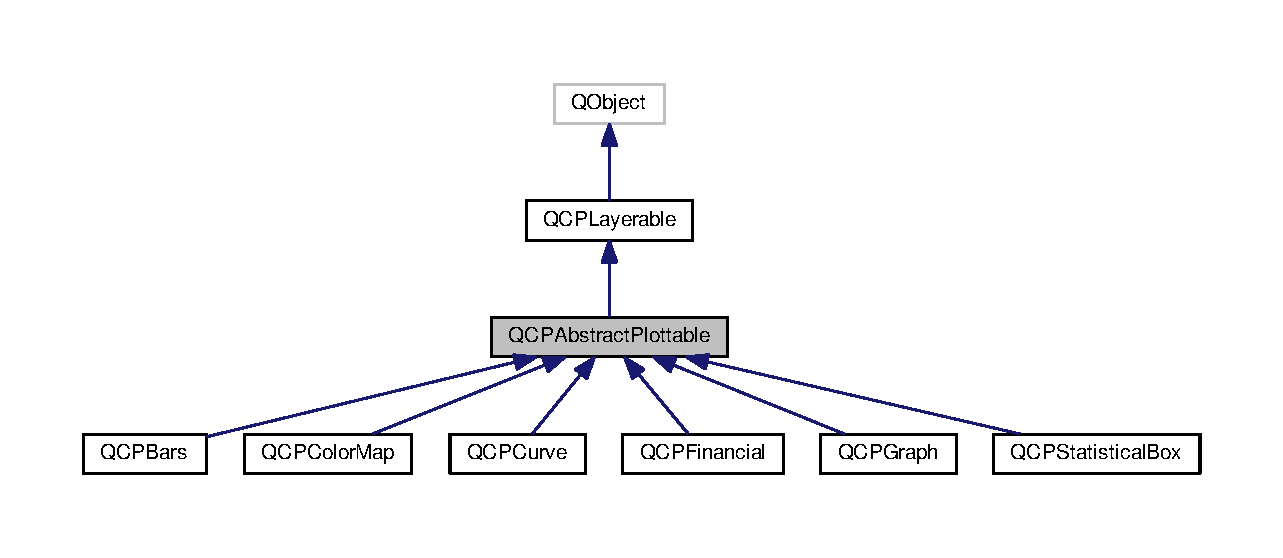
\includegraphics[width=350pt]{classQCPAbstractPlottable__inherit__graph}
\end{center}
\end{figure}


Collaboration diagram for Q\+C\+P\+Abstract\+Plottable\+:
\nopagebreak
\begin{figure}[H]
\begin{center}
\leavevmode
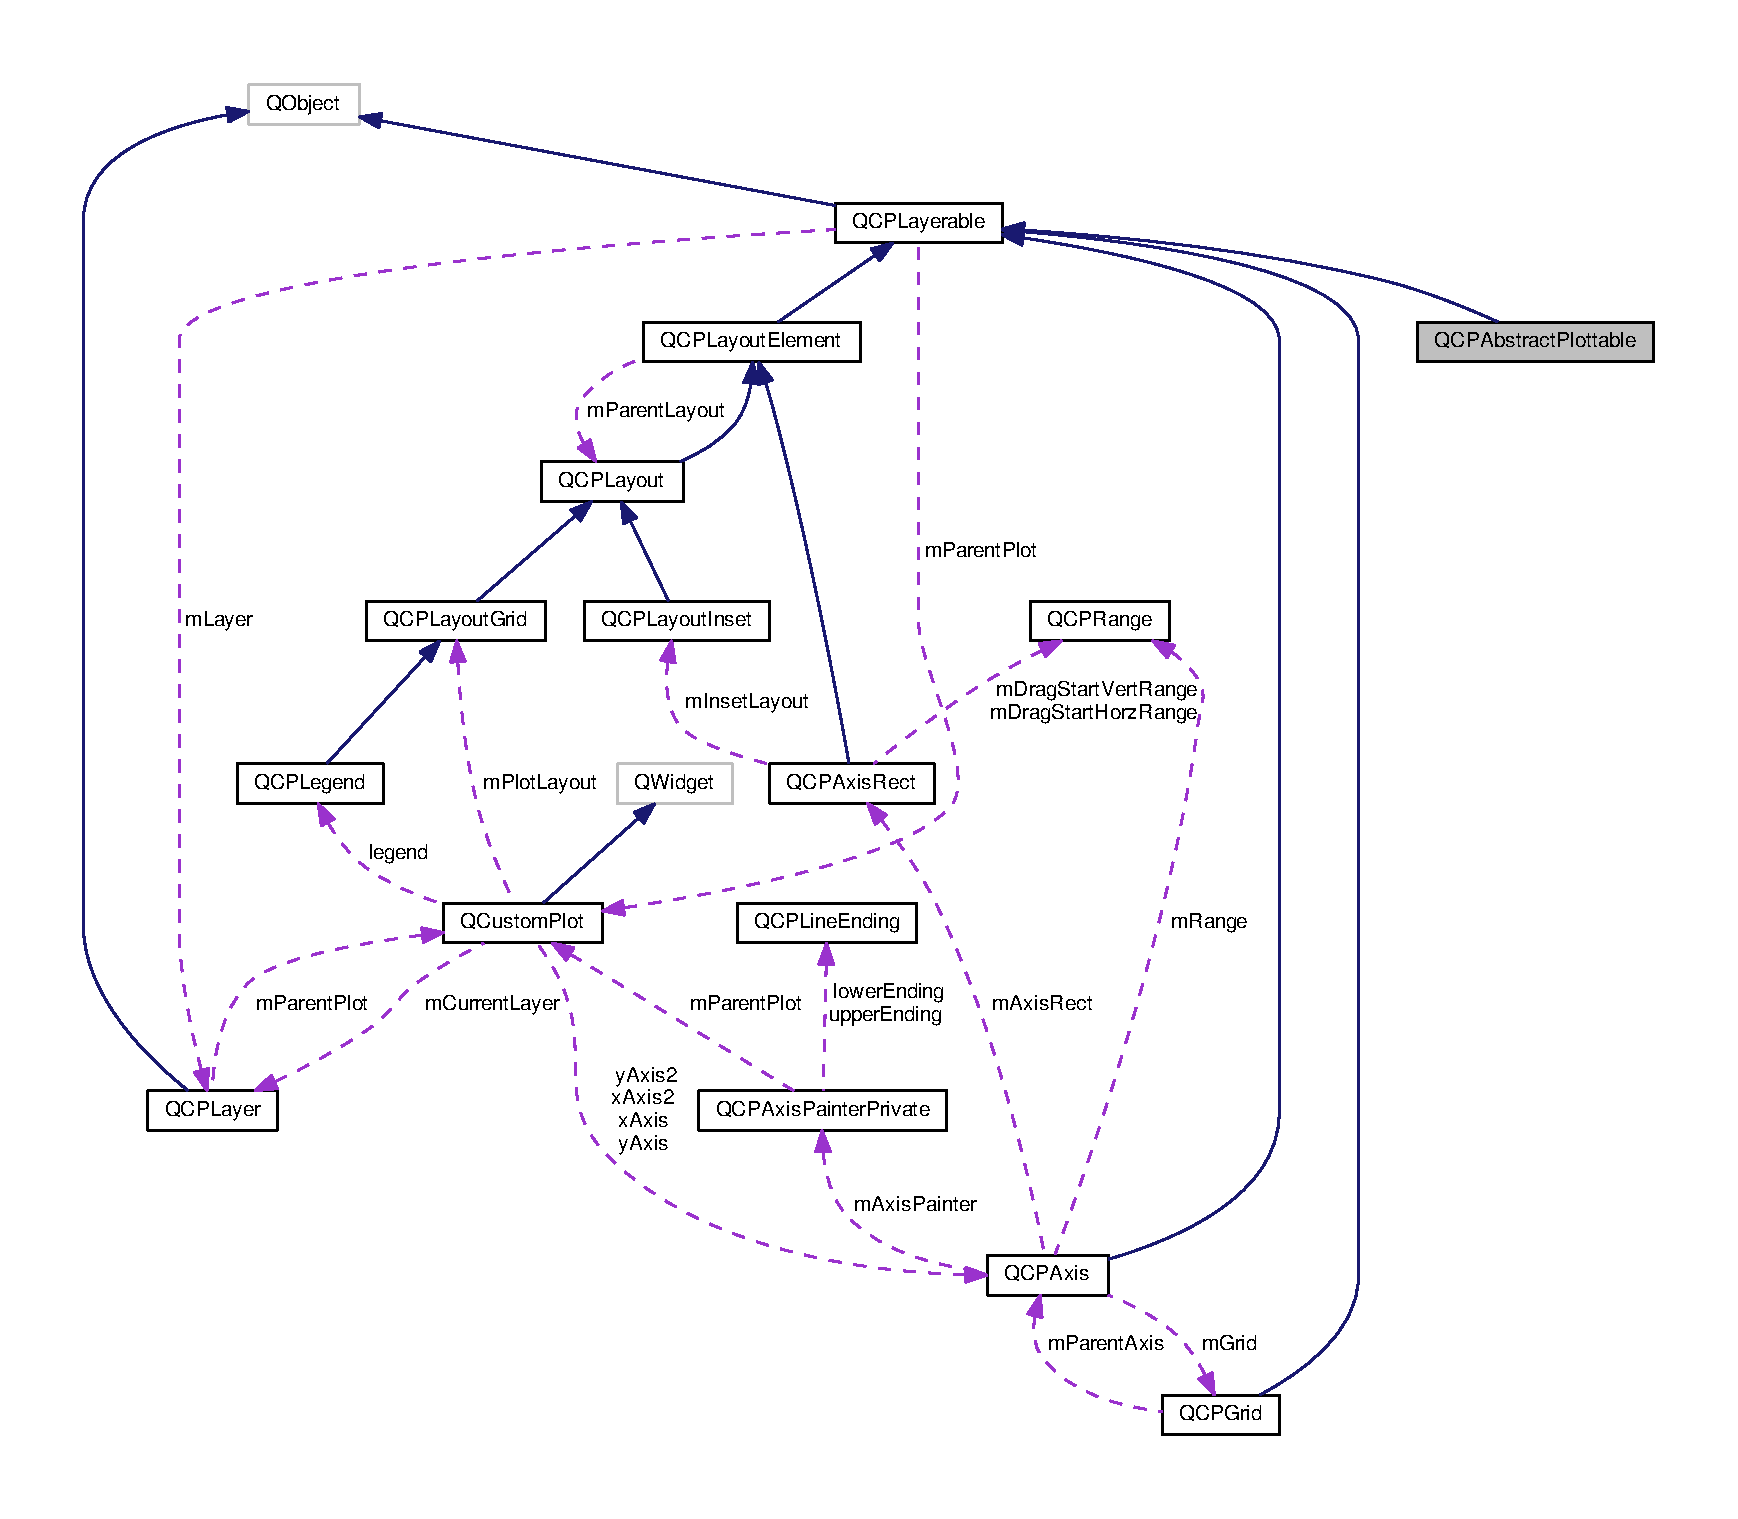
\includegraphics[width=350pt]{classQCPAbstractPlottable__coll__graph}
\end{center}
\end{figure}
\subsection*{Signals}
\begin{DoxyCompactItemize}
\item 
void \hyperlink{classQCPAbstractPlottable_a3af66432b1dca93b28e00e78a8c7c1d9}{selection\+Changed} (bool \hyperlink{classQCPAbstractPlottable_ab901903adcb0e29467d63de72340ab29}{selected})
\item 
void \hyperlink{classQCPAbstractPlottable_a0059caa3f3581f3959660fef8cbb71c4}{selectable\+Changed} (bool \hyperlink{classQCPAbstractPlottable_af895574da1ec0d050711b6c9deda296a}{selectable})
\end{DoxyCompactItemize}
\subsection*{Public Member Functions}
\begin{DoxyCompactItemize}
\item 
\hyperlink{classQCPAbstractPlottable_af78a036e40db6f53a31abadc5323715a}{Q\+C\+P\+Abstract\+Plottable} (\hyperlink{classQCPAxis}{Q\+C\+P\+Axis} $\ast$\hyperlink{classQCPAbstractPlottable_a72c7a09c22963f2c943f07112b311103}{key\+Axis}, \hyperlink{classQCPAxis}{Q\+C\+P\+Axis} $\ast$\hyperlink{classQCPAbstractPlottable_a3106f9d34d330a6097a8ec5905e5b519}{value\+Axis})
\item 
Q\+String \hyperlink{classQCPAbstractPlottable_a1affc1972938e4364a9325e4e4e4dcea}{name} () const 
\item 
bool \hyperlink{classQCPAbstractPlottable_a68d1c358db03faae376ec47c589abf27}{antialiased\+Fill} () const 
\item 
bool \hyperlink{classQCPAbstractPlottable_aefc379bcc011660a5371ecc6088a97eb}{antialiased\+Scatters} () const 
\item 
bool \hyperlink{classQCPAbstractPlottable_a630cfb27ff99ab4373b09631748fcf4a}{antialiased\+Error\+Bars} () const 
\item 
Q\+Pen \hyperlink{classQCPAbstractPlottable_a41d060007cc6b3037c9c04d22d0c0398}{pen} () const 
\item 
Q\+Pen \hyperlink{classQCPAbstractPlottable_a006065572c5add883a944ea4cda699f3}{selected\+Pen} () const 
\item 
Q\+Brush \hyperlink{classQCPAbstractPlottable_aa74cdceb9c7286ef116fbfa58e0326e7}{brush} () const 
\item 
Q\+Brush \hyperlink{classQCPAbstractPlottable_a403745791879916431adc872b49207e5}{selected\+Brush} () const 
\item 
\hyperlink{classQCPAxis}{Q\+C\+P\+Axis} $\ast$ \hyperlink{classQCPAbstractPlottable_a72c7a09c22963f2c943f07112b311103}{key\+Axis} () const 
\item 
\hyperlink{classQCPAxis}{Q\+C\+P\+Axis} $\ast$ \hyperlink{classQCPAbstractPlottable_a3106f9d34d330a6097a8ec5905e5b519}{value\+Axis} () const 
\item 
bool \hyperlink{classQCPAbstractPlottable_af895574da1ec0d050711b6c9deda296a}{selectable} () const 
\item 
bool \hyperlink{classQCPAbstractPlottable_ab901903adcb0e29467d63de72340ab29}{selected} () const 
\item 
void \hyperlink{classQCPAbstractPlottable_ab79c7ba76bc7fa89a4b3580e12149f1f}{set\+Name} (const Q\+String \&\hyperlink{classQCPAbstractPlottable_a1affc1972938e4364a9325e4e4e4dcea}{name})
\item 
void \hyperlink{classQCPAbstractPlottable_a089d6b5577120239b55c39ed27c39536}{set\+Antialiased\+Fill} (bool enabled)
\item 
void \hyperlink{classQCPAbstractPlottable_a2f03f067ede2ed4da6f7d0e4777a3f02}{set\+Antialiased\+Scatters} (bool enabled)
\item 
void \hyperlink{classQCPAbstractPlottable_a757beb744b96cf1855cca5ab9d3ecf52}{set\+Antialiased\+Error\+Bars} (bool enabled)
\item 
void \hyperlink{classQCPAbstractPlottable_ab74b09ae4c0e7e13142fe4b5bf46cac7}{set\+Pen} (const Q\+Pen \&\hyperlink{classQCPAbstractPlottable_a41d060007cc6b3037c9c04d22d0c0398}{pen})
\item 
void \hyperlink{classQCPAbstractPlottable_a6911603cad23ab0469b108224517516f}{set\+Selected\+Pen} (const Q\+Pen \&\hyperlink{classQCPAbstractPlottable_a41d060007cc6b3037c9c04d22d0c0398}{pen})
\item 
void \hyperlink{classQCPAbstractPlottable_a7a4b92144dca6453a1f0f210e27edc74}{set\+Brush} (const Q\+Brush \&\hyperlink{classQCPAbstractPlottable_aa74cdceb9c7286ef116fbfa58e0326e7}{brush})
\item 
void \hyperlink{classQCPAbstractPlottable_ae8c816874089f7a44001e8618e81a9dc}{set\+Selected\+Brush} (const Q\+Brush \&\hyperlink{classQCPAbstractPlottable_aa74cdceb9c7286ef116fbfa58e0326e7}{brush})
\item 
void \hyperlink{classQCPAbstractPlottable_a8524fa2994c63c0913ebd9bb2ffa3920}{set\+Key\+Axis} (\hyperlink{classQCPAxis}{Q\+C\+P\+Axis} $\ast$axis)
\item 
void \hyperlink{classQCPAbstractPlottable_a71626a07367e241ec62ad2c34baf21cb}{set\+Value\+Axis} (\hyperlink{classQCPAxis}{Q\+C\+P\+Axis} $\ast$axis)
\item 
Q\+\_\+\+S\+L\+OT void \hyperlink{classQCPAbstractPlottable_a22c69299eb5569e0f6bf084877a37dc4}{set\+Selectable} (bool \hyperlink{classQCPAbstractPlottable_af895574da1ec0d050711b6c9deda296a}{selectable})
\item 
Q\+\_\+\+S\+L\+OT void \hyperlink{classQCPAbstractPlottable_afbd5428c2952f59d952e11ab5cd79176}{set\+Selected} (bool \hyperlink{classQCPAbstractPlottable_ab901903adcb0e29467d63de72340ab29}{selected})
\item 
virtual void \hyperlink{classQCPAbstractPlottable_a86e5b8fd4b6ff4f4084e7ea4c573fc53}{clear\+Data} ()=0
\item 
virtual double \hyperlink{classQCPAbstractPlottable_a38efe9641d972992a3d44204bc80ec1d}{select\+Test} (const Q\+PointF \&pos, bool only\+Selectable, Q\+Variant $\ast$details=0) const =0
\item 
virtual bool \hyperlink{classQCPAbstractPlottable_a70f8cabfd808f7d5204b9f18c45c13f5}{add\+To\+Legend} ()
\item 
virtual bool \hyperlink{classQCPAbstractPlottable_aa1f350e510326d012b9a9c9249736c83}{remove\+From\+Legend} () const 
\item 
void \hyperlink{classQCPAbstractPlottable_a7e8fc3be43c27ccacd70a7bf9d74a5cd}{rescale\+Axes} (bool only\+Enlarge=false) const 
\item 
void \hyperlink{classQCPAbstractPlottable_a1acecfcca3e7fcda00fcbaa3c886386f}{rescale\+Key\+Axis} (bool only\+Enlarge=false) const 
\item 
void \hyperlink{classQCPAbstractPlottable_abfd0805eb1d955c0111a990246658324}{rescale\+Value\+Axis} (bool only\+Enlarge=false) const 
\end{DoxyCompactItemize}
\subsection*{Protected Types}
\begin{DoxyCompactItemize}
\item 
enum \hyperlink{classQCPAbstractPlottable_a661743478a1d3c09d28ec2711d7653d8}{Sign\+Domain} \{ \hyperlink{classQCPAbstractPlottable_a661743478a1d3c09d28ec2711d7653d8a0fc9a70796ef60ad18ddd18056e6dc63}{sd\+Negative}, 
\hyperlink{classQCPAbstractPlottable_a661743478a1d3c09d28ec2711d7653d8a082b98cfb91a7363a3b5cd17b0c1cd60}{sd\+Both}, 
\hyperlink{classQCPAbstractPlottable_a661743478a1d3c09d28ec2711d7653d8a02951859f243a4d24e779cfbb5471030}{sd\+Positive}
 \}
\end{DoxyCompactItemize}
\subsection*{Protected Member Functions}
\begin{DoxyCompactItemize}
\item 
virtual Q\+Rect \hyperlink{classQCPAbstractPlottable_ac01960b0827913922f5364d559c124ed}{clip\+Rect} () const 
\item 
virtual void \hyperlink{classQCPAbstractPlottable_acbab5e30dcd04fd302b4a5902ac2c482}{draw} (\hyperlink{classQCPPainter}{Q\+C\+P\+Painter} $\ast$painter)=0
\item 
virtual \hyperlink{namespaceQCP_a2ad6bb6281c7c2d593d4277b44c2b037}{Q\+C\+P\+::\+Interaction} \hyperlink{classQCPAbstractPlottable_a5eef607bcc2aee8bfe2380a8710f6c64}{selection\+Category} () const 
\item 
void \hyperlink{classQCPAbstractPlottable_a76e9d6cc7972dc1528f526d163766aca}{apply\+Default\+Antialiasing\+Hint} (\hyperlink{classQCPPainter}{Q\+C\+P\+Painter} $\ast$painter) const 
\item 
virtual void \hyperlink{classQCPAbstractPlottable_a16aaad02456aa23a759efd1ac90c79bf}{select\+Event} (Q\+Mouse\+Event $\ast$event, bool additive, const Q\+Variant \&details, bool $\ast$selection\+State\+Changed)
\item 
virtual void \hyperlink{classQCPAbstractPlottable_a6fa0d0f95560ea8b01ee13f296dab2b1}{deselect\+Event} (bool $\ast$selection\+State\+Changed)
\item 
virtual void \hyperlink{classQCPAbstractPlottable_a9a450783fd9ed539e589999fd390cdf7}{draw\+Legend\+Icon} (\hyperlink{classQCPPainter}{Q\+C\+P\+Painter} $\ast$painter, const Q\+RectF \&rect) const =0
\item 
virtual \hyperlink{classQCPRange}{Q\+C\+P\+Range} \hyperlink{classQCPAbstractPlottable_a345d702b2e7e12c8cfdddff65ba85e8c}{get\+Key\+Range} (bool \&found\+Range, \hyperlink{classQCPAbstractPlottable_a661743478a1d3c09d28ec2711d7653d8}{Sign\+Domain} in\+Sign\+Domain=\hyperlink{classQCPAbstractPlottable_a661743478a1d3c09d28ec2711d7653d8a082b98cfb91a7363a3b5cd17b0c1cd60}{sd\+Both}) const =0
\item 
virtual \hyperlink{classQCPRange}{Q\+C\+P\+Range} \hyperlink{classQCPAbstractPlottable_aa3331b415b5939fe4df60b78831b2799}{get\+Value\+Range} (bool \&found\+Range, \hyperlink{classQCPAbstractPlottable_a661743478a1d3c09d28ec2711d7653d8}{Sign\+Domain} in\+Sign\+Domain=\hyperlink{classQCPAbstractPlottable_a661743478a1d3c09d28ec2711d7653d8a082b98cfb91a7363a3b5cd17b0c1cd60}{sd\+Both}) const =0
\item 
void \hyperlink{classQCPAbstractPlottable_ade710a776104b14c1c835168ce1bfc5c}{coords\+To\+Pixels} (double key, double value, double \&\hyperlink{qualification__task_8cpp_a6150e0515f7202e2fb518f7206ed97dc}{x}, double \&y) const 
\item 
const Q\+PointF \hyperlink{classQCPAbstractPlottable_a9fd1c9df8391781f05b0be22fbe91e13}{coords\+To\+Pixels} (double key, double value) const 
\item 
void \hyperlink{classQCPAbstractPlottable_a10408828446e9e0681c46d65120f382e}{pixels\+To\+Coords} (double \hyperlink{qualification__task_8cpp_a6150e0515f7202e2fb518f7206ed97dc}{x}, double y, double \&key, double \&value) const 
\item 
void \hyperlink{classQCPAbstractPlottable_a3e2c361cfcdfd5d803ada4d333a07e15}{pixels\+To\+Coords} (const Q\+PointF \&pixel\+Pos, double \&key, double \&value) const 
\item 
Q\+Pen \hyperlink{classQCPAbstractPlottable_a19276ed2382a3a06464417b8788b1451}{main\+Pen} () const 
\item 
Q\+Brush \hyperlink{classQCPAbstractPlottable_ae74c123832da180c17e22203e748d9b7}{main\+Brush} () const 
\item 
void \hyperlink{classQCPAbstractPlottable_ac08a480155895e674dbfe5a5670e0ff3}{apply\+Fill\+Antialiasing\+Hint} (\hyperlink{classQCPPainter}{Q\+C\+P\+Painter} $\ast$painter) const 
\item 
void \hyperlink{classQCPAbstractPlottable_a753272ee225a62827e90c3e1e78de4b1}{apply\+Scatters\+Antialiasing\+Hint} (\hyperlink{classQCPPainter}{Q\+C\+P\+Painter} $\ast$painter) const 
\item 
void \hyperlink{classQCPAbstractPlottable_af687bfe6160255960558eb71f1f81e73}{apply\+Error\+Bars\+Antialiasing\+Hint} (\hyperlink{classQCPPainter}{Q\+C\+P\+Painter} $\ast$painter) const 
\item 
double \hyperlink{classQCPAbstractPlottable_a5ea1cab44ca912dcdc96ed81ec5bed5d}{dist\+Sqr\+To\+Line} (const Q\+PointF \&start, const Q\+PointF \&end, const Q\+PointF \&point) const 
\end{DoxyCompactItemize}
\subsection*{Protected Attributes}
\begin{DoxyCompactItemize}
\item 
Q\+String \hyperlink{classQCPAbstractPlottable_ac29ffef424e2488675930de18cde612a}{m\+Name}
\item 
bool \hyperlink{classQCPAbstractPlottable_a152ac765bedf927fb240545d11d453ea}{m\+Antialiased\+Fill}
\item 
bool \hyperlink{classQCPAbstractPlottable_aa115755e525a8e3a86dc683f9cab755b}{m\+Antialiased\+Scatters}
\item 
bool \hyperlink{classQCPAbstractPlottable_ad48660b2bd301576e92fb033d8f455ea}{m\+Antialiased\+Error\+Bars}
\item 
Q\+Pen \hyperlink{classQCPAbstractPlottable_a67bc0622fd1b9fa14e54c14922dcec66}{m\+Pen}
\item 
Q\+Pen \hyperlink{classQCPAbstractPlottable_a10619472f5d5e10e9519a599f1cf5576}{m\+Selected\+Pen}
\item 
Q\+Brush \hyperlink{classQCPAbstractPlottable_a33f00674c0161c13315ab9da0895418e}{m\+Brush}
\item 
Q\+Brush \hyperlink{classQCPAbstractPlottable_aea3c0da30c7a8be23ad5f2d9bca36762}{m\+Selected\+Brush}
\item 
Q\+Pointer$<$ \hyperlink{classQCPAxis}{Q\+C\+P\+Axis} $>$ \hyperlink{classQCPAbstractPlottable_a426f42e254d0f8ce5436a868c61a6827}{m\+Key\+Axis}
\item 
Q\+Pointer$<$ \hyperlink{classQCPAxis}{Q\+C\+P\+Axis} $>$ \hyperlink{classQCPAbstractPlottable_a2901452ca4aea911a1827717934a4bda}{m\+Value\+Axis}
\item 
bool \hyperlink{classQCPAbstractPlottable_aceee52342c8e75727abcbd164986fdcb}{m\+Selectable}
\item 
bool \hyperlink{classQCPAbstractPlottable_a43f68a0603e9bcd016bdfa6d9d5c41c9}{m\+Selected}
\end{DoxyCompactItemize}
\subsection*{Friends}
\begin{DoxyCompactItemize}
\item 
class \hyperlink{classQCPAbstractPlottable_a1cdf9df76adcfae45261690aa0ca2198}{Q\+Custom\+Plot}
\item 
class \hyperlink{classQCPAbstractPlottable_af123edeca169ec7a31958a1d714e1a8a}{Q\+C\+P\+Axis}
\item 
class \hyperlink{classQCPAbstractPlottable_a104c78e91302afd6842a903e472f552f}{Q\+C\+P\+Plottable\+Legend\+Item}
\end{DoxyCompactItemize}


\subsection{Detailed Description}
The abstract base class for all data representing objects in a plot. 

It defines a very basic interface like name, pen, brush, visibility etc. Since this class is abstract, it can\textquotesingle{}t be instantiated. Use one of the subclasses or create a subclass yourself to create new ways of displaying data (see \char`\"{}\+Creating own plottables\char`\"{} below).

All further specifics are in the subclasses, for example\+: \begin{DoxyItemize}
\item A normal graph with possibly a line, scatter points and error bars\+: \hyperlink{classQCPGraph}{Q\+C\+P\+Graph} (typically created with \hyperlink{classQCustomPlot_a6fb2873d35a8a8089842d81a70a54167}{Q\+Custom\+Plot\+::add\+Graph}) \item A parametric curve\+: \hyperlink{classQCPCurve}{Q\+C\+P\+Curve} \item A bar chart\+: \hyperlink{classQCPBars}{Q\+C\+P\+Bars} \item A statistical box plot\+: \hyperlink{classQCPStatisticalBox}{Q\+C\+P\+Statistical\+Box} \item A color encoded two-\/dimensional map\+: \hyperlink{classQCPColorMap}{Q\+C\+P\+Color\+Map} \item An O\+H\+L\+C/\+Candlestick chart\+: \hyperlink{classQCPFinancial}{Q\+C\+P\+Financial}\end{DoxyItemize}
\hypertarget{classQCPAbstractPlottable_plottables-subclassing}{}\subsection{Creating own plottables}\label{classQCPAbstractPlottable_plottables-subclassing}
To create an own plottable, you implement a subclass of \hyperlink{classQCPAbstractPlottable}{Q\+C\+P\+Abstract\+Plottable}. These are the pure virtual functions, you must implement\+: \begin{DoxyItemize}
\item \hyperlink{classQCPAbstractPlottable_a86e5b8fd4b6ff4f4084e7ea4c573fc53}{clear\+Data} \item \hyperlink{classQCPAbstractPlottable_a38efe9641d972992a3d44204bc80ec1d}{select\+Test} \item \hyperlink{classQCPAbstractPlottable_acbab5e30dcd04fd302b4a5902ac2c482}{draw} \item \hyperlink{classQCPAbstractPlottable_a9a450783fd9ed539e589999fd390cdf7}{draw\+Legend\+Icon} \item \hyperlink{classQCPAbstractPlottable_a345d702b2e7e12c8cfdddff65ba85e8c}{get\+Key\+Range} \item \hyperlink{classQCPAbstractPlottable_aa3331b415b5939fe4df60b78831b2799}{get\+Value\+Range}\end{DoxyItemize}
See the documentation of those functions for what they need to do.

For drawing your plot, you can use the \hyperlink{classQCPAbstractPlottable_ade710a776104b14c1c835168ce1bfc5c}{coords\+To\+Pixels} functions to translate a point in plot coordinates to pixel coordinates. This function is quite convenient, because it takes the orientation of the key and value axes into account for you (x and y are swapped when the key axis is vertical and the value axis horizontal). If you are worried about performance (i.\+e. you need to translate many points in a loop like \hyperlink{classQCPGraph}{Q\+C\+P\+Graph}), you can directly use \hyperlink{classQCPAxis_a985ae693b842fb0422b4390fe36d299a}{Q\+C\+P\+Axis\+::coord\+To\+Pixel}. However, you must then take care about the orientation of the axis yourself.

Here are some important members you inherit from \hyperlink{classQCPAbstractPlottable}{Q\+C\+P\+Abstract\+Plottable}\+: \tabulinesep=1mm
\begin{longtabu} spread 0pt [c]{*2{|X[-1]}|}
\hline
\hyperlink{classQCustomPlot}{Q\+Custom\+Plot} $\ast${\bfseries m\+Parent\+Plot}  &A pointer to the parent \hyperlink{classQCustomPlot}{Q\+Custom\+Plot} instance. The parent plot is inferred from the axes that are passed in the constructor. \\\cline{1-2}
Q\+String {\bfseries m\+Name}  &The name of the plottable. \\\cline{1-2}
Q\+Pen {\bfseries m\+Pen}  &The generic pen of the plottable. You should use this pen for the most prominent data representing lines in the plottable (e.\+g \hyperlink{classQCPGraph}{Q\+C\+P\+Graph} uses this pen for its graph lines and scatters) \\\cline{1-2}
Q\+Pen {\bfseries m\+Selected\+Pen}  &The generic pen that should be used when the plottable is selected (hint\+: \hyperlink{classQCPAbstractPlottable_a19276ed2382a3a06464417b8788b1451}{main\+Pen} gives you the right pen, depending on selection state). \\\cline{1-2}
Q\+Brush {\bfseries m\+Brush}  &The generic brush of the plottable. You should use this brush for the most prominent fillable structures in the plottable (e.\+g. \hyperlink{classQCPGraph}{Q\+C\+P\+Graph} uses this brush to control filling under the graph) \\\cline{1-2}
Q\+Brush {\bfseries m\+Selected\+Brush}  &The generic brush that should be used when the plottable is selected (hint\+: \hyperlink{classQCPAbstractPlottable_ae74c123832da180c17e22203e748d9b7}{main\+Brush} gives you the right brush, depending on selection state). \\\cline{1-2}
Q\+Pointer$<$\+Q\+C\+P\+Axis$>${\bfseries m\+Key\+Axis}, {\bfseries m\+Value\+Axis}  &The key and value axes this plottable is attached to. Call their \hyperlink{classQCPAxis_a985ae693b842fb0422b4390fe36d299a}{Q\+C\+P\+Axis\+::coord\+To\+Pixel} functions to translate coordinates to pixels in either the key or value dimension. Make sure to check whether the pointer is null before using it. If one of the axes is null, don\textquotesingle{}t draw the plottable. \\\cline{1-2}
bool {\bfseries m\+Selected}  &indicates whether the plottable is selected or not.  \\\cline{1-2}
\end{longtabu}


\subsection{Member Enumeration Documentation}
\index{Q\+C\+P\+Abstract\+Plottable@{Q\+C\+P\+Abstract\+Plottable}!Sign\+Domain@{Sign\+Domain}}
\index{Sign\+Domain@{Sign\+Domain}!Q\+C\+P\+Abstract\+Plottable@{Q\+C\+P\+Abstract\+Plottable}}
\subsubsection[{\texorpdfstring{Sign\+Domain}{SignDomain}}]{\setlength{\rightskip}{0pt plus 5cm}enum {\bf Q\+C\+P\+Abstract\+Plottable\+::\+Sign\+Domain}\hspace{0.3cm}{\ttfamily [protected]}}\hypertarget{classQCPAbstractPlottable_a661743478a1d3c09d28ec2711d7653d8}{}\label{classQCPAbstractPlottable_a661743478a1d3c09d28ec2711d7653d8}
Represents negative and positive sign domain for passing to \hyperlink{classQCPAbstractPlottable_a345d702b2e7e12c8cfdddff65ba85e8c}{get\+Key\+Range} and \hyperlink{classQCPAbstractPlottable_aa3331b415b5939fe4df60b78831b2799}{get\+Value\+Range}. \begin{Desc}
\item[Enumerator]\par
\begin{description}
\index{sd\+Negative@{sd\+Negative}!Q\+C\+P\+Abstract\+Plottable@{Q\+C\+P\+Abstract\+Plottable}}\index{Q\+C\+P\+Abstract\+Plottable@{Q\+C\+P\+Abstract\+Plottable}!sd\+Negative@{sd\+Negative}}\item[{\em 
sd\+Negative\hypertarget{classQCPAbstractPlottable_a661743478a1d3c09d28ec2711d7653d8a0fc9a70796ef60ad18ddd18056e6dc63}{}\label{classQCPAbstractPlottable_a661743478a1d3c09d28ec2711d7653d8a0fc9a70796ef60ad18ddd18056e6dc63}
}]The negative sign domain, i.\+e. numbers smaller than zero. \index{sd\+Both@{sd\+Both}!Q\+C\+P\+Abstract\+Plottable@{Q\+C\+P\+Abstract\+Plottable}}\index{Q\+C\+P\+Abstract\+Plottable@{Q\+C\+P\+Abstract\+Plottable}!sd\+Both@{sd\+Both}}\item[{\em 
sd\+Both\hypertarget{classQCPAbstractPlottable_a661743478a1d3c09d28ec2711d7653d8a082b98cfb91a7363a3b5cd17b0c1cd60}{}\label{classQCPAbstractPlottable_a661743478a1d3c09d28ec2711d7653d8a082b98cfb91a7363a3b5cd17b0c1cd60}
}]Both sign domains, including zero, i.\+e. all (rational) numbers. \index{sd\+Positive@{sd\+Positive}!Q\+C\+P\+Abstract\+Plottable@{Q\+C\+P\+Abstract\+Plottable}}\index{Q\+C\+P\+Abstract\+Plottable@{Q\+C\+P\+Abstract\+Plottable}!sd\+Positive@{sd\+Positive}}\item[{\em 
sd\+Positive\hypertarget{classQCPAbstractPlottable_a661743478a1d3c09d28ec2711d7653d8a02951859f243a4d24e779cfbb5471030}{}\label{classQCPAbstractPlottable_a661743478a1d3c09d28ec2711d7653d8a02951859f243a4d24e779cfbb5471030}
}]The positive sign domain, i.\+e. numbers greater than zero. \end{description}
\end{Desc}


\subsection{Constructor \& Destructor Documentation}
\index{Q\+C\+P\+Abstract\+Plottable@{Q\+C\+P\+Abstract\+Plottable}!Q\+C\+P\+Abstract\+Plottable@{Q\+C\+P\+Abstract\+Plottable}}
\index{Q\+C\+P\+Abstract\+Plottable@{Q\+C\+P\+Abstract\+Plottable}!Q\+C\+P\+Abstract\+Plottable@{Q\+C\+P\+Abstract\+Plottable}}
\subsubsection[{\texorpdfstring{Q\+C\+P\+Abstract\+Plottable(\+Q\+C\+P\+Axis $\ast$key\+Axis, Q\+C\+P\+Axis $\ast$value\+Axis)}{QCPAbstractPlottable(QCPAxis *keyAxis, QCPAxis *valueAxis)}}]{\setlength{\rightskip}{0pt plus 5cm}Q\+C\+P\+Abstract\+Plottable\+::\+Q\+C\+P\+Abstract\+Plottable (
\begin{DoxyParamCaption}
\item[{{\bf Q\+C\+P\+Axis} $\ast$}]{key\+Axis, }
\item[{{\bf Q\+C\+P\+Axis} $\ast$}]{value\+Axis}
\end{DoxyParamCaption}
)}\hypertarget{classQCPAbstractPlottable_af78a036e40db6f53a31abadc5323715a}{}\label{classQCPAbstractPlottable_af78a036e40db6f53a31abadc5323715a}
Constructs an abstract plottable which uses {\itshape key\+Axis} as its key axis (\char`\"{}x\char`\"{}) and {\itshape value\+Axis} as its value axis (\char`\"{}y\char`\"{}). {\itshape key\+Axis} and {\itshape value\+Axis} must reside in the same \hyperlink{classQCustomPlot}{Q\+Custom\+Plot} instance and have perpendicular orientations. If either of these restrictions is violated, a corresponding message is printed to the debug output (q\+Debug), the construction is not aborted, though.

Since \hyperlink{classQCPAbstractPlottable}{Q\+C\+P\+Abstract\+Plottable} is an abstract class that defines the basic interface to plottables, it can\textquotesingle{}t be directly instantiated.

You probably want one of the subclasses like \hyperlink{classQCPGraph}{Q\+C\+P\+Graph} or \hyperlink{classQCPCurve}{Q\+C\+P\+Curve} instead. 

\subsection{Member Function Documentation}
\index{Q\+C\+P\+Abstract\+Plottable@{Q\+C\+P\+Abstract\+Plottable}!add\+To\+Legend@{add\+To\+Legend}}
\index{add\+To\+Legend@{add\+To\+Legend}!Q\+C\+P\+Abstract\+Plottable@{Q\+C\+P\+Abstract\+Plottable}}
\subsubsection[{\texorpdfstring{add\+To\+Legend()}{addToLegend()}}]{\setlength{\rightskip}{0pt plus 5cm}bool Q\+C\+P\+Abstract\+Plottable\+::add\+To\+Legend (
\begin{DoxyParamCaption}
{}
\end{DoxyParamCaption}
)\hspace{0.3cm}{\ttfamily [virtual]}}\hypertarget{classQCPAbstractPlottable_a70f8cabfd808f7d5204b9f18c45c13f5}{}\label{classQCPAbstractPlottable_a70f8cabfd808f7d5204b9f18c45c13f5}
Adds this plottable to the legend of the parent \hyperlink{classQCustomPlot}{Q\+Custom\+Plot} (\hyperlink{classQCustomPlot_a4eadcd237dc6a09938b68b16877fa6af}{Q\+Custom\+Plot\+::legend}).

Normally, a \hyperlink{classQCPPlottableLegendItem}{Q\+C\+P\+Plottable\+Legend\+Item} is created and inserted into the legend. If the plottable needs a more specialized representation in the legend, this function will take this into account and instead create the specialized subclass of \hyperlink{classQCPAbstractLegendItem}{Q\+C\+P\+Abstract\+Legend\+Item}.

Returns true on success, i.\+e. when the legend exists and a legend item associated with this plottable isn\textquotesingle{}t already in the legend.

\begin{DoxySeeAlso}{See also}
\hyperlink{classQCPAbstractPlottable_aa1f350e510326d012b9a9c9249736c83}{remove\+From\+Legend}, \hyperlink{classQCPLegend_a3ab274de52d2951faea45a6d975e6b3f}{Q\+C\+P\+Legend\+::add\+Item} 
\end{DoxySeeAlso}
\index{Q\+C\+P\+Abstract\+Plottable@{Q\+C\+P\+Abstract\+Plottable}!antialiased\+Error\+Bars@{antialiased\+Error\+Bars}}
\index{antialiased\+Error\+Bars@{antialiased\+Error\+Bars}!Q\+C\+P\+Abstract\+Plottable@{Q\+C\+P\+Abstract\+Plottable}}
\subsubsection[{\texorpdfstring{antialiased\+Error\+Bars() const }{antialiasedErrorBars() const }}]{\setlength{\rightskip}{0pt plus 5cm}bool Q\+C\+P\+Abstract\+Plottable\+::antialiased\+Error\+Bars (
\begin{DoxyParamCaption}
{}
\end{DoxyParamCaption}
) const\hspace{0.3cm}{\ttfamily [inline]}}\hypertarget{classQCPAbstractPlottable_a630cfb27ff99ab4373b09631748fcf4a}{}\label{classQCPAbstractPlottable_a630cfb27ff99ab4373b09631748fcf4a}
\index{Q\+C\+P\+Abstract\+Plottable@{Q\+C\+P\+Abstract\+Plottable}!antialiased\+Fill@{antialiased\+Fill}}
\index{antialiased\+Fill@{antialiased\+Fill}!Q\+C\+P\+Abstract\+Plottable@{Q\+C\+P\+Abstract\+Plottable}}
\subsubsection[{\texorpdfstring{antialiased\+Fill() const }{antialiasedFill() const }}]{\setlength{\rightskip}{0pt plus 5cm}bool Q\+C\+P\+Abstract\+Plottable\+::antialiased\+Fill (
\begin{DoxyParamCaption}
{}
\end{DoxyParamCaption}
) const\hspace{0.3cm}{\ttfamily [inline]}}\hypertarget{classQCPAbstractPlottable_a68d1c358db03faae376ec47c589abf27}{}\label{classQCPAbstractPlottable_a68d1c358db03faae376ec47c589abf27}
\index{Q\+C\+P\+Abstract\+Plottable@{Q\+C\+P\+Abstract\+Plottable}!antialiased\+Scatters@{antialiased\+Scatters}}
\index{antialiased\+Scatters@{antialiased\+Scatters}!Q\+C\+P\+Abstract\+Plottable@{Q\+C\+P\+Abstract\+Plottable}}
\subsubsection[{\texorpdfstring{antialiased\+Scatters() const }{antialiasedScatters() const }}]{\setlength{\rightskip}{0pt plus 5cm}bool Q\+C\+P\+Abstract\+Plottable\+::antialiased\+Scatters (
\begin{DoxyParamCaption}
{}
\end{DoxyParamCaption}
) const\hspace{0.3cm}{\ttfamily [inline]}}\hypertarget{classQCPAbstractPlottable_aefc379bcc011660a5371ecc6088a97eb}{}\label{classQCPAbstractPlottable_aefc379bcc011660a5371ecc6088a97eb}
\index{Q\+C\+P\+Abstract\+Plottable@{Q\+C\+P\+Abstract\+Plottable}!apply\+Default\+Antialiasing\+Hint@{apply\+Default\+Antialiasing\+Hint}}
\index{apply\+Default\+Antialiasing\+Hint@{apply\+Default\+Antialiasing\+Hint}!Q\+C\+P\+Abstract\+Plottable@{Q\+C\+P\+Abstract\+Plottable}}
\subsubsection[{\texorpdfstring{apply\+Default\+Antialiasing\+Hint(\+Q\+C\+P\+Painter $\ast$painter) const }{applyDefaultAntialiasingHint(QCPPainter *painter) const }}]{\setlength{\rightskip}{0pt plus 5cm}void Q\+C\+P\+Abstract\+Plottable\+::apply\+Default\+Antialiasing\+Hint (
\begin{DoxyParamCaption}
\item[{{\bf Q\+C\+P\+Painter} $\ast$}]{painter}
\end{DoxyParamCaption}
) const\hspace{0.3cm}{\ttfamily [protected]}, {\ttfamily [virtual]}}\hypertarget{classQCPAbstractPlottable_a76e9d6cc7972dc1528f526d163766aca}{}\label{classQCPAbstractPlottable_a76e9d6cc7972dc1528f526d163766aca}


Implements \hyperlink{classQCPLayerable_afdf83ddc6a265cbf4c89fe99d3d93473}{Q\+C\+P\+Layerable}.

\index{Q\+C\+P\+Abstract\+Plottable@{Q\+C\+P\+Abstract\+Plottable}!apply\+Error\+Bars\+Antialiasing\+Hint@{apply\+Error\+Bars\+Antialiasing\+Hint}}
\index{apply\+Error\+Bars\+Antialiasing\+Hint@{apply\+Error\+Bars\+Antialiasing\+Hint}!Q\+C\+P\+Abstract\+Plottable@{Q\+C\+P\+Abstract\+Plottable}}
\subsubsection[{\texorpdfstring{apply\+Error\+Bars\+Antialiasing\+Hint(\+Q\+C\+P\+Painter $\ast$painter) const }{applyErrorBarsAntialiasingHint(QCPPainter *painter) const }}]{\setlength{\rightskip}{0pt plus 5cm}void Q\+C\+P\+Abstract\+Plottable\+::apply\+Error\+Bars\+Antialiasing\+Hint (
\begin{DoxyParamCaption}
\item[{{\bf Q\+C\+P\+Painter} $\ast$}]{painter}
\end{DoxyParamCaption}
) const\hspace{0.3cm}{\ttfamily [protected]}}\hypertarget{classQCPAbstractPlottable_af687bfe6160255960558eb71f1f81e73}{}\label{classQCPAbstractPlottable_af687bfe6160255960558eb71f1f81e73}
\index{Q\+C\+P\+Abstract\+Plottable@{Q\+C\+P\+Abstract\+Plottable}!apply\+Fill\+Antialiasing\+Hint@{apply\+Fill\+Antialiasing\+Hint}}
\index{apply\+Fill\+Antialiasing\+Hint@{apply\+Fill\+Antialiasing\+Hint}!Q\+C\+P\+Abstract\+Plottable@{Q\+C\+P\+Abstract\+Plottable}}
\subsubsection[{\texorpdfstring{apply\+Fill\+Antialiasing\+Hint(\+Q\+C\+P\+Painter $\ast$painter) const }{applyFillAntialiasingHint(QCPPainter *painter) const }}]{\setlength{\rightskip}{0pt plus 5cm}void Q\+C\+P\+Abstract\+Plottable\+::apply\+Fill\+Antialiasing\+Hint (
\begin{DoxyParamCaption}
\item[{{\bf Q\+C\+P\+Painter} $\ast$}]{painter}
\end{DoxyParamCaption}
) const\hspace{0.3cm}{\ttfamily [protected]}}\hypertarget{classQCPAbstractPlottable_ac08a480155895e674dbfe5a5670e0ff3}{}\label{classQCPAbstractPlottable_ac08a480155895e674dbfe5a5670e0ff3}
\index{Q\+C\+P\+Abstract\+Plottable@{Q\+C\+P\+Abstract\+Plottable}!apply\+Scatters\+Antialiasing\+Hint@{apply\+Scatters\+Antialiasing\+Hint}}
\index{apply\+Scatters\+Antialiasing\+Hint@{apply\+Scatters\+Antialiasing\+Hint}!Q\+C\+P\+Abstract\+Plottable@{Q\+C\+P\+Abstract\+Plottable}}
\subsubsection[{\texorpdfstring{apply\+Scatters\+Antialiasing\+Hint(\+Q\+C\+P\+Painter $\ast$painter) const }{applyScattersAntialiasingHint(QCPPainter *painter) const }}]{\setlength{\rightskip}{0pt plus 5cm}void Q\+C\+P\+Abstract\+Plottable\+::apply\+Scatters\+Antialiasing\+Hint (
\begin{DoxyParamCaption}
\item[{{\bf Q\+C\+P\+Painter} $\ast$}]{painter}
\end{DoxyParamCaption}
) const\hspace{0.3cm}{\ttfamily [protected]}}\hypertarget{classQCPAbstractPlottable_a753272ee225a62827e90c3e1e78de4b1}{}\label{classQCPAbstractPlottable_a753272ee225a62827e90c3e1e78de4b1}
\index{Q\+C\+P\+Abstract\+Plottable@{Q\+C\+P\+Abstract\+Plottable}!brush@{brush}}
\index{brush@{brush}!Q\+C\+P\+Abstract\+Plottable@{Q\+C\+P\+Abstract\+Plottable}}
\subsubsection[{\texorpdfstring{brush() const }{brush() const }}]{\setlength{\rightskip}{0pt plus 5cm}Q\+Brush Q\+C\+P\+Abstract\+Plottable\+::brush (
\begin{DoxyParamCaption}
{}
\end{DoxyParamCaption}
) const\hspace{0.3cm}{\ttfamily [inline]}}\hypertarget{classQCPAbstractPlottable_aa74cdceb9c7286ef116fbfa58e0326e7}{}\label{classQCPAbstractPlottable_aa74cdceb9c7286ef116fbfa58e0326e7}
\index{Q\+C\+P\+Abstract\+Plottable@{Q\+C\+P\+Abstract\+Plottable}!clear\+Data@{clear\+Data}}
\index{clear\+Data@{clear\+Data}!Q\+C\+P\+Abstract\+Plottable@{Q\+C\+P\+Abstract\+Plottable}}
\subsubsection[{\texorpdfstring{clear\+Data()=0}{clearData()=0}}]{\setlength{\rightskip}{0pt plus 5cm}void Q\+C\+P\+Abstract\+Plottable\+::clear\+Data (
\begin{DoxyParamCaption}
{}
\end{DoxyParamCaption}
)\hspace{0.3cm}{\ttfamily [pure virtual]}}\hypertarget{classQCPAbstractPlottable_a86e5b8fd4b6ff4f4084e7ea4c573fc53}{}\label{classQCPAbstractPlottable_a86e5b8fd4b6ff4f4084e7ea4c573fc53}
Clears all data in the plottable. 

Implemented in \hyperlink{classQCPFinancial_a11fd49928c33e55e27b7319c6927864a}{Q\+C\+P\+Financial}, \hyperlink{classQCPColorMap_a0545dce5383766885912331705a8e099}{Q\+C\+P\+Color\+Map}, \hyperlink{classQCPStatisticalBox_a19112994449df0c20287858436cc68e3}{Q\+C\+P\+Statistical\+Box}, \hyperlink{classQCPBars_a11dbbd707132f07f862dff13c5789c2b}{Q\+C\+P\+Bars}, \hyperlink{classQCPCurve_ae0462c61dbfbac07db0736ec64110241}{Q\+C\+P\+Curve}, and \hyperlink{classQCPGraph_ad4e94a4e44e5e76fbec81a72a977157d}{Q\+C\+P\+Graph}.

\index{Q\+C\+P\+Abstract\+Plottable@{Q\+C\+P\+Abstract\+Plottable}!clip\+Rect@{clip\+Rect}}
\index{clip\+Rect@{clip\+Rect}!Q\+C\+P\+Abstract\+Plottable@{Q\+C\+P\+Abstract\+Plottable}}
\subsubsection[{\texorpdfstring{clip\+Rect() const }{clipRect() const }}]{\setlength{\rightskip}{0pt plus 5cm}Q\+Rect Q\+C\+P\+Abstract\+Plottable\+::clip\+Rect (
\begin{DoxyParamCaption}
{}
\end{DoxyParamCaption}
) const\hspace{0.3cm}{\ttfamily [protected]}, {\ttfamily [virtual]}}\hypertarget{classQCPAbstractPlottable_ac01960b0827913922f5364d559c124ed}{}\label{classQCPAbstractPlottable_ac01960b0827913922f5364d559c124ed}


Reimplemented from \hyperlink{classQCPLayerable_a07a8f746640c3704b09910df297afcba}{Q\+C\+P\+Layerable}.

\index{Q\+C\+P\+Abstract\+Plottable@{Q\+C\+P\+Abstract\+Plottable}!coords\+To\+Pixels@{coords\+To\+Pixels}}
\index{coords\+To\+Pixels@{coords\+To\+Pixels}!Q\+C\+P\+Abstract\+Plottable@{Q\+C\+P\+Abstract\+Plottable}}
\subsubsection[{\texorpdfstring{coords\+To\+Pixels(double key, double value, double \&x, double \&y) const }{coordsToPixels(double key, double value, double &x, double &y) const }}]{\setlength{\rightskip}{0pt plus 5cm}void Q\+C\+P\+Abstract\+Plottable\+::coords\+To\+Pixels (
\begin{DoxyParamCaption}
\item[{double}]{key, }
\item[{double}]{value, }
\item[{double \&}]{x, }
\item[{double \&}]{y}
\end{DoxyParamCaption}
) const\hspace{0.3cm}{\ttfamily [protected]}}\hypertarget{classQCPAbstractPlottable_ade710a776104b14c1c835168ce1bfc5c}{}\label{classQCPAbstractPlottable_ade710a776104b14c1c835168ce1bfc5c}
\index{Q\+C\+P\+Abstract\+Plottable@{Q\+C\+P\+Abstract\+Plottable}!coords\+To\+Pixels@{coords\+To\+Pixels}}
\index{coords\+To\+Pixels@{coords\+To\+Pixels}!Q\+C\+P\+Abstract\+Plottable@{Q\+C\+P\+Abstract\+Plottable}}
\subsubsection[{\texorpdfstring{coords\+To\+Pixels(double key, double value) const }{coordsToPixels(double key, double value) const }}]{\setlength{\rightskip}{0pt plus 5cm}const Q\+PointF Q\+C\+P\+Abstract\+Plottable\+::coords\+To\+Pixels (
\begin{DoxyParamCaption}
\item[{double}]{key, }
\item[{double}]{value}
\end{DoxyParamCaption}
) const\hspace{0.3cm}{\ttfamily [protected]}}\hypertarget{classQCPAbstractPlottable_a9fd1c9df8391781f05b0be22fbe91e13}{}\label{classQCPAbstractPlottable_a9fd1c9df8391781f05b0be22fbe91e13}
\index{Q\+C\+P\+Abstract\+Plottable@{Q\+C\+P\+Abstract\+Plottable}!deselect\+Event@{deselect\+Event}}
\index{deselect\+Event@{deselect\+Event}!Q\+C\+P\+Abstract\+Plottable@{Q\+C\+P\+Abstract\+Plottable}}
\subsubsection[{\texorpdfstring{deselect\+Event(bool $\ast$selection\+State\+Changed)}{deselectEvent(bool *selectionStateChanged)}}]{\setlength{\rightskip}{0pt plus 5cm}void Q\+C\+P\+Abstract\+Plottable\+::deselect\+Event (
\begin{DoxyParamCaption}
\item[{bool $\ast$}]{selection\+State\+Changed}
\end{DoxyParamCaption}
)\hspace{0.3cm}{\ttfamily [protected]}, {\ttfamily [virtual]}}\hypertarget{classQCPAbstractPlottable_a6fa0d0f95560ea8b01ee13f296dab2b1}{}\label{classQCPAbstractPlottable_a6fa0d0f95560ea8b01ee13f296dab2b1}


Reimplemented from \hyperlink{classQCPLayerable_ae546370644a5551c76af739afc008bee}{Q\+C\+P\+Layerable}.

\index{Q\+C\+P\+Abstract\+Plottable@{Q\+C\+P\+Abstract\+Plottable}!dist\+Sqr\+To\+Line@{dist\+Sqr\+To\+Line}}
\index{dist\+Sqr\+To\+Line@{dist\+Sqr\+To\+Line}!Q\+C\+P\+Abstract\+Plottable@{Q\+C\+P\+Abstract\+Plottable}}
\subsubsection[{\texorpdfstring{dist\+Sqr\+To\+Line(const Q\+Point\+F \&start, const Q\+Point\+F \&end, const Q\+Point\+F \&point) const }{distSqrToLine(const QPointF &start, const QPointF &end, const QPointF &point) const }}]{\setlength{\rightskip}{0pt plus 5cm}double Q\+C\+P\+Abstract\+Plottable\+::dist\+Sqr\+To\+Line (
\begin{DoxyParamCaption}
\item[{const Q\+PointF \&}]{start, }
\item[{const Q\+PointF \&}]{end, }
\item[{const Q\+PointF \&}]{point}
\end{DoxyParamCaption}
) const\hspace{0.3cm}{\ttfamily [protected]}}\hypertarget{classQCPAbstractPlottable_a5ea1cab44ca912dcdc96ed81ec5bed5d}{}\label{classQCPAbstractPlottable_a5ea1cab44ca912dcdc96ed81ec5bed5d}
\index{Q\+C\+P\+Abstract\+Plottable@{Q\+C\+P\+Abstract\+Plottable}!draw@{draw}}
\index{draw@{draw}!Q\+C\+P\+Abstract\+Plottable@{Q\+C\+P\+Abstract\+Plottable}}
\subsubsection[{\texorpdfstring{draw(\+Q\+C\+P\+Painter $\ast$painter)=0}{draw(QCPPainter *painter)=0}}]{\setlength{\rightskip}{0pt plus 5cm}virtual void Q\+C\+P\+Abstract\+Plottable\+::draw (
\begin{DoxyParamCaption}
\item[{{\bf Q\+C\+P\+Painter} $\ast$}]{painter}
\end{DoxyParamCaption}
)\hspace{0.3cm}{\ttfamily [protected]}, {\ttfamily [pure virtual]}}\hypertarget{classQCPAbstractPlottable_acbab5e30dcd04fd302b4a5902ac2c482}{}\label{classQCPAbstractPlottable_acbab5e30dcd04fd302b4a5902ac2c482}


Implements \hyperlink{classQCPLayerable_aecf2f7087482d4b6a78cb2770e5ed12d}{Q\+C\+P\+Layerable}.



Implemented in \hyperlink{classQCPFinancial_ad71a59a1b42616594831e04e52c92120}{Q\+C\+P\+Financial}, \hyperlink{classQCPColorMap_a3b0f45a3177be9522d5e9b8cd8ae122d}{Q\+C\+P\+Color\+Map}, \hyperlink{classQCPStatisticalBox_a753b62761217dd6b92f8a29e286a1317}{Q\+C\+P\+Statistical\+Box}, \hyperlink{classQCPBars_a42b894e34dac799f90ff3700706b31df}{Q\+C\+P\+Bars}, \hyperlink{classQCPCurve_a2361302d2fc6ec669849bd3bca00c4b2}{Q\+C\+P\+Curve}, and \hyperlink{classQCPGraph_a659218cc62c2a7786213d9dd429c1c8d}{Q\+C\+P\+Graph}.

\index{Q\+C\+P\+Abstract\+Plottable@{Q\+C\+P\+Abstract\+Plottable}!draw\+Legend\+Icon@{draw\+Legend\+Icon}}
\index{draw\+Legend\+Icon@{draw\+Legend\+Icon}!Q\+C\+P\+Abstract\+Plottable@{Q\+C\+P\+Abstract\+Plottable}}
\subsubsection[{\texorpdfstring{draw\+Legend\+Icon(\+Q\+C\+P\+Painter $\ast$painter, const Q\+Rect\+F \&rect) const =0}{drawLegendIcon(QCPPainter *painter, const QRectF &rect) const =0}}]{\setlength{\rightskip}{0pt plus 5cm}void Q\+C\+P\+Abstract\+Plottable\+::draw\+Legend\+Icon (
\begin{DoxyParamCaption}
\item[{{\bf Q\+C\+P\+Painter} $\ast$}]{painter, }
\item[{const Q\+RectF \&}]{rect}
\end{DoxyParamCaption}
) const\hspace{0.3cm}{\ttfamily [protected]}, {\ttfamily [pure virtual]}}\hypertarget{classQCPAbstractPlottable_a9a450783fd9ed539e589999fd390cdf7}{}\label{classQCPAbstractPlottable_a9a450783fd9ed539e589999fd390cdf7}


Implemented in \hyperlink{classQCPFinancial_aca85e8435b092cc8c3e5de65fcfb22c8}{Q\+C\+P\+Financial}, \hyperlink{classQCPColorMap_a7d5eee89f6b8eaf2f11f1d94e32215b2}{Q\+C\+P\+Color\+Map}, \hyperlink{classQCPStatisticalBox_a51764ed423fa02d3ef63f6848851ec33}{Q\+C\+P\+Statistical\+Box}, \hyperlink{classQCPBars_ad4fb35d2ab7d2aa460a6612aff3e7a15}{Q\+C\+P\+Bars}, \hyperlink{classQCPCurve_aaee24451e0044d1debfa1fee92c58d7b}{Q\+C\+P\+Curve}, and \hyperlink{classQCPGraph_a32115df0e940cf8ca7b687873c2d02ee}{Q\+C\+P\+Graph}.

\index{Q\+C\+P\+Abstract\+Plottable@{Q\+C\+P\+Abstract\+Plottable}!get\+Key\+Range@{get\+Key\+Range}}
\index{get\+Key\+Range@{get\+Key\+Range}!Q\+C\+P\+Abstract\+Plottable@{Q\+C\+P\+Abstract\+Plottable}}
\subsubsection[{\texorpdfstring{get\+Key\+Range(bool \&found\+Range, Sign\+Domain in\+Sign\+Domain=sd\+Both) const =0}{getKeyRange(bool &foundRange, SignDomain inSignDomain=sdBoth) const =0}}]{\setlength{\rightskip}{0pt plus 5cm}{\bf Q\+C\+P\+Range} Q\+C\+P\+Abstract\+Plottable\+::get\+Key\+Range (
\begin{DoxyParamCaption}
\item[{bool \&}]{found\+Range, }
\item[{{\bf Sign\+Domain}}]{in\+Sign\+Domain = {\ttfamily {\bf sd\+Both}}}
\end{DoxyParamCaption}
) const\hspace{0.3cm}{\ttfamily [protected]}, {\ttfamily [pure virtual]}}\hypertarget{classQCPAbstractPlottable_a345d702b2e7e12c8cfdddff65ba85e8c}{}\label{classQCPAbstractPlottable_a345d702b2e7e12c8cfdddff65ba85e8c}


Implemented in \hyperlink{classQCPFinancial_acc747f4a9b4fddfb14eb9d803349a534}{Q\+C\+P\+Financial}, \hyperlink{classQCPColorMap_a0d89371f8707f12e22737b863f1a5126}{Q\+C\+P\+Color\+Map}, \hyperlink{classQCPStatisticalBox_ad700fdce0f456dd22a3679d61e9896a4}{Q\+C\+P\+Statistical\+Box}, \hyperlink{classQCPBars_a93cfdc8a535f36aeb087acca49c00662}{Q\+C\+P\+Bars}, \hyperlink{classQCPCurve_ad6a9559e16ab43586df18ae376d54481}{Q\+C\+P\+Curve}, and \hyperlink{classQCPGraph_afc246ce6201ff564ac440efaec52ab11}{Q\+C\+P\+Graph}.

\index{Q\+C\+P\+Abstract\+Plottable@{Q\+C\+P\+Abstract\+Plottable}!get\+Value\+Range@{get\+Value\+Range}}
\index{get\+Value\+Range@{get\+Value\+Range}!Q\+C\+P\+Abstract\+Plottable@{Q\+C\+P\+Abstract\+Plottable}}
\subsubsection[{\texorpdfstring{get\+Value\+Range(bool \&found\+Range, Sign\+Domain in\+Sign\+Domain=sd\+Both) const =0}{getValueRange(bool &foundRange, SignDomain inSignDomain=sdBoth) const =0}}]{\setlength{\rightskip}{0pt plus 5cm}{\bf Q\+C\+P\+Range} Q\+C\+P\+Abstract\+Plottable\+::get\+Value\+Range (
\begin{DoxyParamCaption}
\item[{bool \&}]{found\+Range, }
\item[{{\bf Sign\+Domain}}]{in\+Sign\+Domain = {\ttfamily {\bf sd\+Both}}}
\end{DoxyParamCaption}
) const\hspace{0.3cm}{\ttfamily [protected]}, {\ttfamily [pure virtual]}}\hypertarget{classQCPAbstractPlottable_aa3331b415b5939fe4df60b78831b2799}{}\label{classQCPAbstractPlottable_aa3331b415b5939fe4df60b78831b2799}


Implemented in \hyperlink{classQCPFinancial_ab2b5f3ef9a503ba32ead32081333f4e7}{Q\+C\+P\+Financial}, \hyperlink{classQCPColorMap_ac1b906e05ca9b61680e61b74b3825a22}{Q\+C\+P\+Color\+Map}, \hyperlink{classQCPStatisticalBox_adeef8c9a0361683c776bca2fbff292b7}{Q\+C\+P\+Statistical\+Box}, \hyperlink{classQCPBars_ada96e20309570d1488c165596cb2647f}{Q\+C\+P\+Bars}, \hyperlink{classQCPCurve_a1d6eec81aab9ae6182bb7c040bcb2dbc}{Q\+C\+P\+Curve}, and \hyperlink{classQCPGraph_a856e90b8ab6b31c344b14a863ab9e5d2}{Q\+C\+P\+Graph}.

\index{Q\+C\+P\+Abstract\+Plottable@{Q\+C\+P\+Abstract\+Plottable}!key\+Axis@{key\+Axis}}
\index{key\+Axis@{key\+Axis}!Q\+C\+P\+Abstract\+Plottable@{Q\+C\+P\+Abstract\+Plottable}}
\subsubsection[{\texorpdfstring{key\+Axis() const }{keyAxis() const }}]{\setlength{\rightskip}{0pt plus 5cm}{\bf Q\+C\+P\+Axis}$\ast$ Q\+C\+P\+Abstract\+Plottable\+::key\+Axis (
\begin{DoxyParamCaption}
{}
\end{DoxyParamCaption}
) const\hspace{0.3cm}{\ttfamily [inline]}}\hypertarget{classQCPAbstractPlottable_a72c7a09c22963f2c943f07112b311103}{}\label{classQCPAbstractPlottable_a72c7a09c22963f2c943f07112b311103}
\index{Q\+C\+P\+Abstract\+Plottable@{Q\+C\+P\+Abstract\+Plottable}!main\+Brush@{main\+Brush}}
\index{main\+Brush@{main\+Brush}!Q\+C\+P\+Abstract\+Plottable@{Q\+C\+P\+Abstract\+Plottable}}
\subsubsection[{\texorpdfstring{main\+Brush() const }{mainBrush() const }}]{\setlength{\rightskip}{0pt plus 5cm}Q\+Brush Q\+C\+P\+Abstract\+Plottable\+::main\+Brush (
\begin{DoxyParamCaption}
{}
\end{DoxyParamCaption}
) const\hspace{0.3cm}{\ttfamily [protected]}}\hypertarget{classQCPAbstractPlottable_ae74c123832da180c17e22203e748d9b7}{}\label{classQCPAbstractPlottable_ae74c123832da180c17e22203e748d9b7}
\index{Q\+C\+P\+Abstract\+Plottable@{Q\+C\+P\+Abstract\+Plottable}!main\+Pen@{main\+Pen}}
\index{main\+Pen@{main\+Pen}!Q\+C\+P\+Abstract\+Plottable@{Q\+C\+P\+Abstract\+Plottable}}
\subsubsection[{\texorpdfstring{main\+Pen() const }{mainPen() const }}]{\setlength{\rightskip}{0pt plus 5cm}Q\+Pen Q\+C\+P\+Abstract\+Plottable\+::main\+Pen (
\begin{DoxyParamCaption}
{}
\end{DoxyParamCaption}
) const\hspace{0.3cm}{\ttfamily [protected]}}\hypertarget{classQCPAbstractPlottable_a19276ed2382a3a06464417b8788b1451}{}\label{classQCPAbstractPlottable_a19276ed2382a3a06464417b8788b1451}
\index{Q\+C\+P\+Abstract\+Plottable@{Q\+C\+P\+Abstract\+Plottable}!name@{name}}
\index{name@{name}!Q\+C\+P\+Abstract\+Plottable@{Q\+C\+P\+Abstract\+Plottable}}
\subsubsection[{\texorpdfstring{name() const }{name() const }}]{\setlength{\rightskip}{0pt plus 5cm}Q\+String Q\+C\+P\+Abstract\+Plottable\+::name (
\begin{DoxyParamCaption}
{}
\end{DoxyParamCaption}
) const\hspace{0.3cm}{\ttfamily [inline]}}\hypertarget{classQCPAbstractPlottable_a1affc1972938e4364a9325e4e4e4dcea}{}\label{classQCPAbstractPlottable_a1affc1972938e4364a9325e4e4e4dcea}
\index{Q\+C\+P\+Abstract\+Plottable@{Q\+C\+P\+Abstract\+Plottable}!pen@{pen}}
\index{pen@{pen}!Q\+C\+P\+Abstract\+Plottable@{Q\+C\+P\+Abstract\+Plottable}}
\subsubsection[{\texorpdfstring{pen() const }{pen() const }}]{\setlength{\rightskip}{0pt plus 5cm}Q\+Pen Q\+C\+P\+Abstract\+Plottable\+::pen (
\begin{DoxyParamCaption}
{}
\end{DoxyParamCaption}
) const\hspace{0.3cm}{\ttfamily [inline]}}\hypertarget{classQCPAbstractPlottable_a41d060007cc6b3037c9c04d22d0c0398}{}\label{classQCPAbstractPlottable_a41d060007cc6b3037c9c04d22d0c0398}
\index{Q\+C\+P\+Abstract\+Plottable@{Q\+C\+P\+Abstract\+Plottable}!pixels\+To\+Coords@{pixels\+To\+Coords}}
\index{pixels\+To\+Coords@{pixels\+To\+Coords}!Q\+C\+P\+Abstract\+Plottable@{Q\+C\+P\+Abstract\+Plottable}}
\subsubsection[{\texorpdfstring{pixels\+To\+Coords(double x, double y, double \&key, double \&value) const }{pixelsToCoords(double x, double y, double &key, double &value) const }}]{\setlength{\rightskip}{0pt plus 5cm}void Q\+C\+P\+Abstract\+Plottable\+::pixels\+To\+Coords (
\begin{DoxyParamCaption}
\item[{double}]{x, }
\item[{double}]{y, }
\item[{double \&}]{key, }
\item[{double \&}]{value}
\end{DoxyParamCaption}
) const\hspace{0.3cm}{\ttfamily [protected]}}\hypertarget{classQCPAbstractPlottable_a10408828446e9e0681c46d65120f382e}{}\label{classQCPAbstractPlottable_a10408828446e9e0681c46d65120f382e}
\index{Q\+C\+P\+Abstract\+Plottable@{Q\+C\+P\+Abstract\+Plottable}!pixels\+To\+Coords@{pixels\+To\+Coords}}
\index{pixels\+To\+Coords@{pixels\+To\+Coords}!Q\+C\+P\+Abstract\+Plottable@{Q\+C\+P\+Abstract\+Plottable}}
\subsubsection[{\texorpdfstring{pixels\+To\+Coords(const Q\+Point\+F \&pixel\+Pos, double \&key, double \&value) const }{pixelsToCoords(const QPointF &pixelPos, double &key, double &value) const }}]{\setlength{\rightskip}{0pt plus 5cm}void Q\+C\+P\+Abstract\+Plottable\+::pixels\+To\+Coords (
\begin{DoxyParamCaption}
\item[{const Q\+PointF \&}]{pixel\+Pos, }
\item[{double \&}]{key, }
\item[{double \&}]{value}
\end{DoxyParamCaption}
) const\hspace{0.3cm}{\ttfamily [protected]}}\hypertarget{classQCPAbstractPlottable_a3e2c361cfcdfd5d803ada4d333a07e15}{}\label{classQCPAbstractPlottable_a3e2c361cfcdfd5d803ada4d333a07e15}
\index{Q\+C\+P\+Abstract\+Plottable@{Q\+C\+P\+Abstract\+Plottable}!remove\+From\+Legend@{remove\+From\+Legend}}
\index{remove\+From\+Legend@{remove\+From\+Legend}!Q\+C\+P\+Abstract\+Plottable@{Q\+C\+P\+Abstract\+Plottable}}
\subsubsection[{\texorpdfstring{remove\+From\+Legend() const }{removeFromLegend() const }}]{\setlength{\rightskip}{0pt plus 5cm}bool Q\+C\+P\+Abstract\+Plottable\+::remove\+From\+Legend (
\begin{DoxyParamCaption}
{}
\end{DoxyParamCaption}
) const\hspace{0.3cm}{\ttfamily [virtual]}}\hypertarget{classQCPAbstractPlottable_aa1f350e510326d012b9a9c9249736c83}{}\label{classQCPAbstractPlottable_aa1f350e510326d012b9a9c9249736c83}
Removes the plottable from the legend of the parent \hyperlink{classQCustomPlot}{Q\+Custom\+Plot}. This means the \hyperlink{classQCPAbstractLegendItem}{Q\+C\+P\+Abstract\+Legend\+Item} (usually a \hyperlink{classQCPPlottableLegendItem}{Q\+C\+P\+Plottable\+Legend\+Item}) that is associated with this plottable is removed.

Returns true on success, i.\+e. if the legend exists and a legend item associated with this plottable was found and removed.

\begin{DoxySeeAlso}{See also}
\hyperlink{classQCPAbstractPlottable_a70f8cabfd808f7d5204b9f18c45c13f5}{add\+To\+Legend}, \hyperlink{classQCPLegend_ac91595c3eaa746fe6321d2eb952c63bb}{Q\+C\+P\+Legend\+::remove\+Item} 
\end{DoxySeeAlso}
\index{Q\+C\+P\+Abstract\+Plottable@{Q\+C\+P\+Abstract\+Plottable}!rescale\+Axes@{rescale\+Axes}}
\index{rescale\+Axes@{rescale\+Axes}!Q\+C\+P\+Abstract\+Plottable@{Q\+C\+P\+Abstract\+Plottable}}
\subsubsection[{\texorpdfstring{rescale\+Axes(bool only\+Enlarge=false) const }{rescaleAxes(bool onlyEnlarge=false) const }}]{\setlength{\rightskip}{0pt plus 5cm}void Q\+C\+P\+Abstract\+Plottable\+::rescale\+Axes (
\begin{DoxyParamCaption}
\item[{bool}]{only\+Enlarge = {\ttfamily false}}
\end{DoxyParamCaption}
) const}\hypertarget{classQCPAbstractPlottable_a7e8fc3be43c27ccacd70a7bf9d74a5cd}{}\label{classQCPAbstractPlottable_a7e8fc3be43c27ccacd70a7bf9d74a5cd}
Rescales the key and value axes associated with this plottable to contain all displayed data, so the whole plottable is visible. If the scaling of an axis is logarithmic, rescale\+Axes will make sure not to rescale to an illegal range i.\+e. a range containing different signs and/or zero. Instead it will stay in the current sign domain and ignore all parts of the plottable that lie outside of that domain.

{\itshape only\+Enlarge} makes sure the ranges are only expanded, never reduced. So it\textquotesingle{}s possible to show multiple plottables in their entirety by multiple calls to rescale\+Axes where the first call has {\itshape only\+Enlarge} set to false (the default), and all subsequent set to true.

\begin{DoxySeeAlso}{See also}
\hyperlink{classQCPAbstractPlottable_a1acecfcca3e7fcda00fcbaa3c886386f}{rescale\+Key\+Axis}, \hyperlink{classQCPAbstractPlottable_abfd0805eb1d955c0111a990246658324}{rescale\+Value\+Axis}, \hyperlink{classQCustomPlot_ad86528f2cee6c7e446dea4a6e8839935}{Q\+Custom\+Plot\+::rescale\+Axes}, \hyperlink{classQCPAxis_a499345f02ebce4b23d8ccec96e58daa9}{Q\+C\+P\+Axis\+::rescale} 
\end{DoxySeeAlso}
\index{Q\+C\+P\+Abstract\+Plottable@{Q\+C\+P\+Abstract\+Plottable}!rescale\+Key\+Axis@{rescale\+Key\+Axis}}
\index{rescale\+Key\+Axis@{rescale\+Key\+Axis}!Q\+C\+P\+Abstract\+Plottable@{Q\+C\+P\+Abstract\+Plottable}}
\subsubsection[{\texorpdfstring{rescale\+Key\+Axis(bool only\+Enlarge=false) const }{rescaleKeyAxis(bool onlyEnlarge=false) const }}]{\setlength{\rightskip}{0pt plus 5cm}void Q\+C\+P\+Abstract\+Plottable\+::rescale\+Key\+Axis (
\begin{DoxyParamCaption}
\item[{bool}]{only\+Enlarge = {\ttfamily false}}
\end{DoxyParamCaption}
) const}\hypertarget{classQCPAbstractPlottable_a1acecfcca3e7fcda00fcbaa3c886386f}{}\label{classQCPAbstractPlottable_a1acecfcca3e7fcda00fcbaa3c886386f}
Rescales the key axis of the plottable so the whole plottable is visible.

See \hyperlink{classQCPAbstractPlottable_a7e8fc3be43c27ccacd70a7bf9d74a5cd}{rescale\+Axes} for detailed behaviour. \index{Q\+C\+P\+Abstract\+Plottable@{Q\+C\+P\+Abstract\+Plottable}!rescale\+Value\+Axis@{rescale\+Value\+Axis}}
\index{rescale\+Value\+Axis@{rescale\+Value\+Axis}!Q\+C\+P\+Abstract\+Plottable@{Q\+C\+P\+Abstract\+Plottable}}
\subsubsection[{\texorpdfstring{rescale\+Value\+Axis(bool only\+Enlarge=false) const }{rescaleValueAxis(bool onlyEnlarge=false) const }}]{\setlength{\rightskip}{0pt plus 5cm}void Q\+C\+P\+Abstract\+Plottable\+::rescale\+Value\+Axis (
\begin{DoxyParamCaption}
\item[{bool}]{only\+Enlarge = {\ttfamily false}}
\end{DoxyParamCaption}
) const}\hypertarget{classQCPAbstractPlottable_abfd0805eb1d955c0111a990246658324}{}\label{classQCPAbstractPlottable_abfd0805eb1d955c0111a990246658324}
Rescales the value axis of the plottable so the whole plottable is visible.

Returns true if the axis was actually scaled. This might not be the case if this plottable has an invalid range, e.\+g. because it has no data points.

See \hyperlink{classQCPAbstractPlottable_a7e8fc3be43c27ccacd70a7bf9d74a5cd}{rescale\+Axes} for detailed behaviour. \index{Q\+C\+P\+Abstract\+Plottable@{Q\+C\+P\+Abstract\+Plottable}!selectable@{selectable}}
\index{selectable@{selectable}!Q\+C\+P\+Abstract\+Plottable@{Q\+C\+P\+Abstract\+Plottable}}
\subsubsection[{\texorpdfstring{selectable() const }{selectable() const }}]{\setlength{\rightskip}{0pt plus 5cm}bool Q\+C\+P\+Abstract\+Plottable\+::selectable (
\begin{DoxyParamCaption}
{}
\end{DoxyParamCaption}
) const\hspace{0.3cm}{\ttfamily [inline]}}\hypertarget{classQCPAbstractPlottable_af895574da1ec0d050711b6c9deda296a}{}\label{classQCPAbstractPlottable_af895574da1ec0d050711b6c9deda296a}
\index{Q\+C\+P\+Abstract\+Plottable@{Q\+C\+P\+Abstract\+Plottable}!selectable\+Changed@{selectable\+Changed}}
\index{selectable\+Changed@{selectable\+Changed}!Q\+C\+P\+Abstract\+Plottable@{Q\+C\+P\+Abstract\+Plottable}}
\subsubsection[{\texorpdfstring{selectable\+Changed}{selectableChanged}}]{\setlength{\rightskip}{0pt plus 5cm}void Q\+C\+P\+Abstract\+Plottable\+::selectable\+Changed (
\begin{DoxyParamCaption}
\item[{bool}]{selectable}
\end{DoxyParamCaption}
)\hspace{0.3cm}{\ttfamily [signal]}}\hypertarget{classQCPAbstractPlottable_a0059caa3f3581f3959660fef8cbb71c4}{}\label{classQCPAbstractPlottable_a0059caa3f3581f3959660fef8cbb71c4}
This signal is emitted when the selectability of this plottable has changed.

\begin{DoxySeeAlso}{See also}
\hyperlink{classQCPAbstractPlottable_a22c69299eb5569e0f6bf084877a37dc4}{set\+Selectable} 
\end{DoxySeeAlso}
\index{Q\+C\+P\+Abstract\+Plottable@{Q\+C\+P\+Abstract\+Plottable}!selected@{selected}}
\index{selected@{selected}!Q\+C\+P\+Abstract\+Plottable@{Q\+C\+P\+Abstract\+Plottable}}
\subsubsection[{\texorpdfstring{selected() const }{selected() const }}]{\setlength{\rightskip}{0pt plus 5cm}bool Q\+C\+P\+Abstract\+Plottable\+::selected (
\begin{DoxyParamCaption}
{}
\end{DoxyParamCaption}
) const\hspace{0.3cm}{\ttfamily [inline]}}\hypertarget{classQCPAbstractPlottable_ab901903adcb0e29467d63de72340ab29}{}\label{classQCPAbstractPlottable_ab901903adcb0e29467d63de72340ab29}
\index{Q\+C\+P\+Abstract\+Plottable@{Q\+C\+P\+Abstract\+Plottable}!selected\+Brush@{selected\+Brush}}
\index{selected\+Brush@{selected\+Brush}!Q\+C\+P\+Abstract\+Plottable@{Q\+C\+P\+Abstract\+Plottable}}
\subsubsection[{\texorpdfstring{selected\+Brush() const }{selectedBrush() const }}]{\setlength{\rightskip}{0pt plus 5cm}Q\+Brush Q\+C\+P\+Abstract\+Plottable\+::selected\+Brush (
\begin{DoxyParamCaption}
{}
\end{DoxyParamCaption}
) const\hspace{0.3cm}{\ttfamily [inline]}}\hypertarget{classQCPAbstractPlottable_a403745791879916431adc872b49207e5}{}\label{classQCPAbstractPlottable_a403745791879916431adc872b49207e5}
\index{Q\+C\+P\+Abstract\+Plottable@{Q\+C\+P\+Abstract\+Plottable}!selected\+Pen@{selected\+Pen}}
\index{selected\+Pen@{selected\+Pen}!Q\+C\+P\+Abstract\+Plottable@{Q\+C\+P\+Abstract\+Plottable}}
\subsubsection[{\texorpdfstring{selected\+Pen() const }{selectedPen() const }}]{\setlength{\rightskip}{0pt plus 5cm}Q\+Pen Q\+C\+P\+Abstract\+Plottable\+::selected\+Pen (
\begin{DoxyParamCaption}
{}
\end{DoxyParamCaption}
) const\hspace{0.3cm}{\ttfamily [inline]}}\hypertarget{classQCPAbstractPlottable_a006065572c5add883a944ea4cda699f3}{}\label{classQCPAbstractPlottable_a006065572c5add883a944ea4cda699f3}
\index{Q\+C\+P\+Abstract\+Plottable@{Q\+C\+P\+Abstract\+Plottable}!select\+Event@{select\+Event}}
\index{select\+Event@{select\+Event}!Q\+C\+P\+Abstract\+Plottable@{Q\+C\+P\+Abstract\+Plottable}}
\subsubsection[{\texorpdfstring{select\+Event(\+Q\+Mouse\+Event $\ast$event, bool additive, const Q\+Variant \&details, bool $\ast$selection\+State\+Changed)}{selectEvent(QMouseEvent *event, bool additive, const QVariant &details, bool *selectionStateChanged)}}]{\setlength{\rightskip}{0pt plus 5cm}void Q\+C\+P\+Abstract\+Plottable\+::select\+Event (
\begin{DoxyParamCaption}
\item[{Q\+Mouse\+Event $\ast$}]{event, }
\item[{bool}]{additive, }
\item[{const Q\+Variant \&}]{details, }
\item[{bool $\ast$}]{selection\+State\+Changed}
\end{DoxyParamCaption}
)\hspace{0.3cm}{\ttfamily [protected]}, {\ttfamily [virtual]}}\hypertarget{classQCPAbstractPlottable_a16aaad02456aa23a759efd1ac90c79bf}{}\label{classQCPAbstractPlottable_a16aaad02456aa23a759efd1ac90c79bf}


Reimplemented from \hyperlink{classQCPLayerable_a7498c2d0d081cf7cad0fb3bb93aa0e91}{Q\+C\+P\+Layerable}.

\index{Q\+C\+P\+Abstract\+Plottable@{Q\+C\+P\+Abstract\+Plottable}!selection\+Category@{selection\+Category}}
\index{selection\+Category@{selection\+Category}!Q\+C\+P\+Abstract\+Plottable@{Q\+C\+P\+Abstract\+Plottable}}
\subsubsection[{\texorpdfstring{selection\+Category() const }{selectionCategory() const }}]{\setlength{\rightskip}{0pt plus 5cm}{\bf Q\+C\+P\+::\+Interaction} Q\+C\+P\+Abstract\+Plottable\+::selection\+Category (
\begin{DoxyParamCaption}
{}
\end{DoxyParamCaption}
) const\hspace{0.3cm}{\ttfamily [protected]}, {\ttfamily [virtual]}}\hypertarget{classQCPAbstractPlottable_a5eef607bcc2aee8bfe2380a8710f6c64}{}\label{classQCPAbstractPlottable_a5eef607bcc2aee8bfe2380a8710f6c64}


Reimplemented from \hyperlink{classQCPLayerable_aa4035e586b7f317a06ba7e74e242a5ea}{Q\+C\+P\+Layerable}.

\index{Q\+C\+P\+Abstract\+Plottable@{Q\+C\+P\+Abstract\+Plottable}!selection\+Changed@{selection\+Changed}}
\index{selection\+Changed@{selection\+Changed}!Q\+C\+P\+Abstract\+Plottable@{Q\+C\+P\+Abstract\+Plottable}}
\subsubsection[{\texorpdfstring{selection\+Changed}{selectionChanged}}]{\setlength{\rightskip}{0pt plus 5cm}void Q\+C\+P\+Abstract\+Plottable\+::selection\+Changed (
\begin{DoxyParamCaption}
\item[{bool}]{selected}
\end{DoxyParamCaption}
)\hspace{0.3cm}{\ttfamily [signal]}}\hypertarget{classQCPAbstractPlottable_a3af66432b1dca93b28e00e78a8c7c1d9}{}\label{classQCPAbstractPlottable_a3af66432b1dca93b28e00e78a8c7c1d9}
This signal is emitted when the selection state of this plottable has changed, either by user interaction or by a direct call to \hyperlink{classQCPAbstractPlottable_afbd5428c2952f59d952e11ab5cd79176}{set\+Selected}. \index{Q\+C\+P\+Abstract\+Plottable@{Q\+C\+P\+Abstract\+Plottable}!select\+Test@{select\+Test}}
\index{select\+Test@{select\+Test}!Q\+C\+P\+Abstract\+Plottable@{Q\+C\+P\+Abstract\+Plottable}}
\subsubsection[{\texorpdfstring{select\+Test(const Q\+Point\+F \&pos, bool only\+Selectable, Q\+Variant $\ast$details=0) const =0}{selectTest(const QPointF &pos, bool onlySelectable, QVariant *details=0) const =0}}]{\setlength{\rightskip}{0pt plus 5cm}virtual double Q\+C\+P\+Abstract\+Plottable\+::select\+Test (
\begin{DoxyParamCaption}
\item[{const Q\+PointF \&}]{pos, }
\item[{bool}]{only\+Selectable, }
\item[{Q\+Variant $\ast$}]{details = {\ttfamily 0}}
\end{DoxyParamCaption}
) const\hspace{0.3cm}{\ttfamily [pure virtual]}}\hypertarget{classQCPAbstractPlottable_a38efe9641d972992a3d44204bc80ec1d}{}\label{classQCPAbstractPlottable_a38efe9641d972992a3d44204bc80ec1d}
This function is used to decide whether a click hits a layerable object or not.

{\itshape pos} is a point in pixel coordinates on the \hyperlink{classQCustomPlot}{Q\+Custom\+Plot} surface. This function returns the shortest pixel distance of this point to the object. If the object is either invisible or the distance couldn\textquotesingle{}t be determined, -\/1.\+0 is returned. Further, if {\itshape only\+Selectable} is true and the object is not selectable, -\/1.\+0 is returned, too.

If the object is represented not by single lines but by an area like a \hyperlink{classQCPItemText}{Q\+C\+P\+Item\+Text} or the bars of a \hyperlink{classQCPBars}{Q\+C\+P\+Bars} plottable, a click inside the area should also be considered a hit. In these cases this function thus returns a constant value greater zero but still below the parent plot\textquotesingle{}s selection tolerance. (typically the selection\+Tolerance multiplied by 0.\+99).

Providing a constant value for area objects allows selecting line objects even when they are obscured by such area objects, by clicking close to the lines (i.\+e. closer than 0.\+99$\ast$selection\+Tolerance).

The actual setting of the selection state is not done by this function. This is handled by the parent \hyperlink{classQCustomPlot}{Q\+Custom\+Plot} when the mouse\+Release\+Event occurs, and the finally selected object is notified via the select\+Event/deselect\+Event methods.

{\itshape details} is an optional output parameter. Every layerable subclass may place any information in {\itshape details}. This information will be passed to \hyperlink{classQCPAbstractPlottable_a16aaad02456aa23a759efd1ac90c79bf}{select\+Event} when the parent \hyperlink{classQCustomPlot}{Q\+Custom\+Plot} decides on the basis of this select\+Test call, that the object was successfully selected. The subsequent call to \hyperlink{classQCPAbstractPlottable_a16aaad02456aa23a759efd1ac90c79bf}{select\+Event} will carry the {\itshape details}. This is useful for multi-\/part objects (like \hyperlink{classQCPAxis}{Q\+C\+P\+Axis}). This way, a possibly complex calculation to decide which part was clicked is only done once in \hyperlink{classQCPAbstractPlottable_a38efe9641d972992a3d44204bc80ec1d}{select\+Test}. The result (i.\+e. the actually clicked part) can then be placed in {\itshape details}. So in the subsequent \hyperlink{classQCPAbstractPlottable_a16aaad02456aa23a759efd1ac90c79bf}{select\+Event}, the decision which part was selected doesn\textquotesingle{}t have to be done a second time for a single selection operation.

You may pass 0 as {\itshape details} to indicate that you are not interested in those selection details.

\begin{DoxySeeAlso}{See also}
\hyperlink{classQCPAbstractPlottable_a16aaad02456aa23a759efd1ac90c79bf}{select\+Event}, \hyperlink{classQCPAbstractPlottable_a6fa0d0f95560ea8b01ee13f296dab2b1}{deselect\+Event}, \hyperlink{classQCustomPlot_a5ee1e2f6ae27419deca53e75907c27e5}{Q\+Custom\+Plot\+::set\+Interactions} 
\end{DoxySeeAlso}


Reimplemented from \hyperlink{classQCPLayerable_a4001c4d0dfec55598efa4d531f2179a9}{Q\+C\+P\+Layerable}.



Implemented in \hyperlink{classQCPFinancial_adf6cff00a55f775487d375fe4df5e95b}{Q\+C\+P\+Financial}, \hyperlink{classQCPColorMap_a4088dc7bcbe9bba605c84a912ba660ff}{Q\+C\+P\+Color\+Map}, \hyperlink{classQCPStatisticalBox_a7d3ac843dc48a085740fdfc4319a89cc}{Q\+C\+P\+Statistical\+Box}, \hyperlink{classQCPBars_a0d37a9feb1d0baf73ce6e809db214445}{Q\+C\+P\+Bars}, \hyperlink{classQCPCurve_a5af9949e725704811bbc81ecd5970b8e}{Q\+C\+P\+Curve}, and \hyperlink{classQCPGraph_abc9ff375aabcf2d21cca33d6baf85772}{Q\+C\+P\+Graph}.

\index{Q\+C\+P\+Abstract\+Plottable@{Q\+C\+P\+Abstract\+Plottable}!set\+Antialiased\+Error\+Bars@{set\+Antialiased\+Error\+Bars}}
\index{set\+Antialiased\+Error\+Bars@{set\+Antialiased\+Error\+Bars}!Q\+C\+P\+Abstract\+Plottable@{Q\+C\+P\+Abstract\+Plottable}}
\subsubsection[{\texorpdfstring{set\+Antialiased\+Error\+Bars(bool enabled)}{setAntialiasedErrorBars(bool enabled)}}]{\setlength{\rightskip}{0pt plus 5cm}void Q\+C\+P\+Abstract\+Plottable\+::set\+Antialiased\+Error\+Bars (
\begin{DoxyParamCaption}
\item[{bool}]{enabled}
\end{DoxyParamCaption}
)}\hypertarget{classQCPAbstractPlottable_a757beb744b96cf1855cca5ab9d3ecf52}{}\label{classQCPAbstractPlottable_a757beb744b96cf1855cca5ab9d3ecf52}
Sets whether the error bars of this plottable are drawn antialiased or not.

Note that this setting may be overridden by \hyperlink{classQCustomPlot_af6f91e5eab1be85f67c556e98c3745e8}{Q\+Custom\+Plot\+::set\+Antialiased\+Elements} and \hyperlink{classQCustomPlot_ae10d685b5eabea2999fb8775ca173c24}{Q\+Custom\+Plot\+::set\+Not\+Antialiased\+Elements}. \index{Q\+C\+P\+Abstract\+Plottable@{Q\+C\+P\+Abstract\+Plottable}!set\+Antialiased\+Fill@{set\+Antialiased\+Fill}}
\index{set\+Antialiased\+Fill@{set\+Antialiased\+Fill}!Q\+C\+P\+Abstract\+Plottable@{Q\+C\+P\+Abstract\+Plottable}}
\subsubsection[{\texorpdfstring{set\+Antialiased\+Fill(bool enabled)}{setAntialiasedFill(bool enabled)}}]{\setlength{\rightskip}{0pt plus 5cm}void Q\+C\+P\+Abstract\+Plottable\+::set\+Antialiased\+Fill (
\begin{DoxyParamCaption}
\item[{bool}]{enabled}
\end{DoxyParamCaption}
)}\hypertarget{classQCPAbstractPlottable_a089d6b5577120239b55c39ed27c39536}{}\label{classQCPAbstractPlottable_a089d6b5577120239b55c39ed27c39536}
Sets whether fills of this plottable are drawn antialiased or not.

Note that this setting may be overridden by \hyperlink{classQCustomPlot_af6f91e5eab1be85f67c556e98c3745e8}{Q\+Custom\+Plot\+::set\+Antialiased\+Elements} and \hyperlink{classQCustomPlot_ae10d685b5eabea2999fb8775ca173c24}{Q\+Custom\+Plot\+::set\+Not\+Antialiased\+Elements}. \index{Q\+C\+P\+Abstract\+Plottable@{Q\+C\+P\+Abstract\+Plottable}!set\+Antialiased\+Scatters@{set\+Antialiased\+Scatters}}
\index{set\+Antialiased\+Scatters@{set\+Antialiased\+Scatters}!Q\+C\+P\+Abstract\+Plottable@{Q\+C\+P\+Abstract\+Plottable}}
\subsubsection[{\texorpdfstring{set\+Antialiased\+Scatters(bool enabled)}{setAntialiasedScatters(bool enabled)}}]{\setlength{\rightskip}{0pt plus 5cm}void Q\+C\+P\+Abstract\+Plottable\+::set\+Antialiased\+Scatters (
\begin{DoxyParamCaption}
\item[{bool}]{enabled}
\end{DoxyParamCaption}
)}\hypertarget{classQCPAbstractPlottable_a2f03f067ede2ed4da6f7d0e4777a3f02}{}\label{classQCPAbstractPlottable_a2f03f067ede2ed4da6f7d0e4777a3f02}
Sets whether the scatter symbols of this plottable are drawn antialiased or not.

Note that this setting may be overridden by \hyperlink{classQCustomPlot_af6f91e5eab1be85f67c556e98c3745e8}{Q\+Custom\+Plot\+::set\+Antialiased\+Elements} and \hyperlink{classQCustomPlot_ae10d685b5eabea2999fb8775ca173c24}{Q\+Custom\+Plot\+::set\+Not\+Antialiased\+Elements}. \index{Q\+C\+P\+Abstract\+Plottable@{Q\+C\+P\+Abstract\+Plottable}!set\+Brush@{set\+Brush}}
\index{set\+Brush@{set\+Brush}!Q\+C\+P\+Abstract\+Plottable@{Q\+C\+P\+Abstract\+Plottable}}
\subsubsection[{\texorpdfstring{set\+Brush(const Q\+Brush \&brush)}{setBrush(const QBrush &brush)}}]{\setlength{\rightskip}{0pt plus 5cm}void Q\+C\+P\+Abstract\+Plottable\+::set\+Brush (
\begin{DoxyParamCaption}
\item[{const Q\+Brush \&}]{brush}
\end{DoxyParamCaption}
)}\hypertarget{classQCPAbstractPlottable_a7a4b92144dca6453a1f0f210e27edc74}{}\label{classQCPAbstractPlottable_a7a4b92144dca6453a1f0f210e27edc74}
The brush is used to draw basic fills of the plottable representation in the plot. The Fill can be a color, gradient or texture, see the usage of Q\+Brush.

For example, the \hyperlink{classQCPGraph}{Q\+C\+P\+Graph} subclass draws the fill under the graph with this brush, when it\textquotesingle{}s not set to Qt\+::\+No\+Brush.

\begin{DoxySeeAlso}{See also}
\hyperlink{classQCPAbstractPlottable_ab74b09ae4c0e7e13142fe4b5bf46cac7}{set\+Pen} 
\end{DoxySeeAlso}
\index{Q\+C\+P\+Abstract\+Plottable@{Q\+C\+P\+Abstract\+Plottable}!set\+Key\+Axis@{set\+Key\+Axis}}
\index{set\+Key\+Axis@{set\+Key\+Axis}!Q\+C\+P\+Abstract\+Plottable@{Q\+C\+P\+Abstract\+Plottable}}
\subsubsection[{\texorpdfstring{set\+Key\+Axis(\+Q\+C\+P\+Axis $\ast$axis)}{setKeyAxis(QCPAxis *axis)}}]{\setlength{\rightskip}{0pt plus 5cm}void Q\+C\+P\+Abstract\+Plottable\+::set\+Key\+Axis (
\begin{DoxyParamCaption}
\item[{{\bf Q\+C\+P\+Axis} $\ast$}]{axis}
\end{DoxyParamCaption}
)}\hypertarget{classQCPAbstractPlottable_a8524fa2994c63c0913ebd9bb2ffa3920}{}\label{classQCPAbstractPlottable_a8524fa2994c63c0913ebd9bb2ffa3920}
The key axis of a plottable can be set to any axis of a \hyperlink{classQCustomPlot}{Q\+Custom\+Plot}, as long as it is orthogonal to the plottable\textquotesingle{}s value axis. This function performs no checks to make sure this is the case. The typical mathematical choice is to use the x-\/axis (\hyperlink{classQCustomPlot_a9a79cd0158a4c7f30cbc702f0fd800e4}{Q\+Custom\+Plot\+::x\+Axis}) as key axis and the y-\/axis (\hyperlink{classQCustomPlot_af6fea5679725b152c14facd920b19367}{Q\+Custom\+Plot\+::y\+Axis}) as value axis.

Normally, the key and value axes are set in the constructor of the plottable (or \hyperlink{classQCustomPlot_a6fb2873d35a8a8089842d81a70a54167}{Q\+Custom\+Plot\+::add\+Graph} when working with Q\+C\+P\+Graphs through the dedicated graph interface).

\begin{DoxySeeAlso}{See also}
\hyperlink{classQCPAbstractPlottable_a71626a07367e241ec62ad2c34baf21cb}{set\+Value\+Axis} 
\end{DoxySeeAlso}
\index{Q\+C\+P\+Abstract\+Plottable@{Q\+C\+P\+Abstract\+Plottable}!set\+Name@{set\+Name}}
\index{set\+Name@{set\+Name}!Q\+C\+P\+Abstract\+Plottable@{Q\+C\+P\+Abstract\+Plottable}}
\subsubsection[{\texorpdfstring{set\+Name(const Q\+String \&name)}{setName(const QString &name)}}]{\setlength{\rightskip}{0pt plus 5cm}void Q\+C\+P\+Abstract\+Plottable\+::set\+Name (
\begin{DoxyParamCaption}
\item[{const Q\+String \&}]{name}
\end{DoxyParamCaption}
)}\hypertarget{classQCPAbstractPlottable_ab79c7ba76bc7fa89a4b3580e12149f1f}{}\label{classQCPAbstractPlottable_ab79c7ba76bc7fa89a4b3580e12149f1f}
The name is the textual representation of this plottable as it is displayed in the legend (\hyperlink{classQCPLegend}{Q\+C\+P\+Legend}). It may contain any U\+T\+F-\/8 characters, including newlines. \index{Q\+C\+P\+Abstract\+Plottable@{Q\+C\+P\+Abstract\+Plottable}!set\+Pen@{set\+Pen}}
\index{set\+Pen@{set\+Pen}!Q\+C\+P\+Abstract\+Plottable@{Q\+C\+P\+Abstract\+Plottable}}
\subsubsection[{\texorpdfstring{set\+Pen(const Q\+Pen \&pen)}{setPen(const QPen &pen)}}]{\setlength{\rightskip}{0pt plus 5cm}void Q\+C\+P\+Abstract\+Plottable\+::set\+Pen (
\begin{DoxyParamCaption}
\item[{const Q\+Pen \&}]{pen}
\end{DoxyParamCaption}
)}\hypertarget{classQCPAbstractPlottable_ab74b09ae4c0e7e13142fe4b5bf46cac7}{}\label{classQCPAbstractPlottable_ab74b09ae4c0e7e13142fe4b5bf46cac7}
The pen is used to draw basic lines that make up the plottable representation in the plot.

For example, the \hyperlink{classQCPGraph}{Q\+C\+P\+Graph} subclass draws its graph lines with this pen.

\begin{DoxySeeAlso}{See also}
\hyperlink{classQCPAbstractPlottable_a7a4b92144dca6453a1f0f210e27edc74}{set\+Brush} 
\end{DoxySeeAlso}
\index{Q\+C\+P\+Abstract\+Plottable@{Q\+C\+P\+Abstract\+Plottable}!set\+Selectable@{set\+Selectable}}
\index{set\+Selectable@{set\+Selectable}!Q\+C\+P\+Abstract\+Plottable@{Q\+C\+P\+Abstract\+Plottable}}
\subsubsection[{\texorpdfstring{set\+Selectable(bool selectable)}{setSelectable(bool selectable)}}]{\setlength{\rightskip}{0pt plus 5cm}void Q\+C\+P\+Abstract\+Plottable\+::set\+Selectable (
\begin{DoxyParamCaption}
\item[{bool}]{selectable}
\end{DoxyParamCaption}
)}\hypertarget{classQCPAbstractPlottable_a22c69299eb5569e0f6bf084877a37dc4}{}\label{classQCPAbstractPlottable_a22c69299eb5569e0f6bf084877a37dc4}
Sets whether the user can (de-\/)select this plottable by clicking on the \hyperlink{classQCustomPlot}{Q\+Custom\+Plot} surface. (When \hyperlink{classQCustomPlot_a5ee1e2f6ae27419deca53e75907c27e5}{Q\+Custom\+Plot\+::set\+Interactions} contains i\+Select\+Plottables.)

However, even when {\itshape selectable} was set to false, it is possible to set the selection manually, by calling \hyperlink{classQCPAbstractPlottable_afbd5428c2952f59d952e11ab5cd79176}{set\+Selected} directly.

\begin{DoxySeeAlso}{See also}
\hyperlink{classQCPAbstractPlottable_afbd5428c2952f59d952e11ab5cd79176}{set\+Selected} 
\end{DoxySeeAlso}
\index{Q\+C\+P\+Abstract\+Plottable@{Q\+C\+P\+Abstract\+Plottable}!set\+Selected@{set\+Selected}}
\index{set\+Selected@{set\+Selected}!Q\+C\+P\+Abstract\+Plottable@{Q\+C\+P\+Abstract\+Plottable}}
\subsubsection[{\texorpdfstring{set\+Selected(bool selected)}{setSelected(bool selected)}}]{\setlength{\rightskip}{0pt plus 5cm}void Q\+C\+P\+Abstract\+Plottable\+::set\+Selected (
\begin{DoxyParamCaption}
\item[{bool}]{selected}
\end{DoxyParamCaption}
)}\hypertarget{classQCPAbstractPlottable_afbd5428c2952f59d952e11ab5cd79176}{}\label{classQCPAbstractPlottable_afbd5428c2952f59d952e11ab5cd79176}
Sets whether this plottable is selected or not. When selected, it uses a different pen and brush to draw its lines and fills, see \hyperlink{classQCPAbstractPlottable_a6911603cad23ab0469b108224517516f}{set\+Selected\+Pen} and \hyperlink{classQCPAbstractPlottable_ae8c816874089f7a44001e8618e81a9dc}{set\+Selected\+Brush}.

The entire selection mechanism for plottables is handled automatically when \hyperlink{classQCustomPlot_a5ee1e2f6ae27419deca53e75907c27e5}{Q\+Custom\+Plot\+::set\+Interactions} contains i\+Select\+Plottables. You only need to call this function when you wish to change the selection state manually.

This function can change the selection state even when \hyperlink{classQCPAbstractPlottable_a22c69299eb5569e0f6bf084877a37dc4}{set\+Selectable} was set to false.

emits the \hyperlink{classQCPAbstractPlottable_a3af66432b1dca93b28e00e78a8c7c1d9}{selection\+Changed} signal when {\itshape selected} is different from the previous selection state.

\begin{DoxySeeAlso}{See also}
\hyperlink{classQCPAbstractPlottable_a22c69299eb5569e0f6bf084877a37dc4}{set\+Selectable}, \hyperlink{classQCPAbstractPlottable_a38efe9641d972992a3d44204bc80ec1d}{select\+Test} 
\end{DoxySeeAlso}
\index{Q\+C\+P\+Abstract\+Plottable@{Q\+C\+P\+Abstract\+Plottable}!set\+Selected\+Brush@{set\+Selected\+Brush}}
\index{set\+Selected\+Brush@{set\+Selected\+Brush}!Q\+C\+P\+Abstract\+Plottable@{Q\+C\+P\+Abstract\+Plottable}}
\subsubsection[{\texorpdfstring{set\+Selected\+Brush(const Q\+Brush \&brush)}{setSelectedBrush(const QBrush &brush)}}]{\setlength{\rightskip}{0pt plus 5cm}void Q\+C\+P\+Abstract\+Plottable\+::set\+Selected\+Brush (
\begin{DoxyParamCaption}
\item[{const Q\+Brush \&}]{brush}
\end{DoxyParamCaption}
)}\hypertarget{classQCPAbstractPlottable_ae8c816874089f7a44001e8618e81a9dc}{}\label{classQCPAbstractPlottable_ae8c816874089f7a44001e8618e81a9dc}
When the plottable is selected, this brush is used to draw fills instead of the normal brush set via \hyperlink{classQCPAbstractPlottable_a7a4b92144dca6453a1f0f210e27edc74}{set\+Brush}.

\begin{DoxySeeAlso}{See also}
\hyperlink{classQCPAbstractPlottable_afbd5428c2952f59d952e11ab5cd79176}{set\+Selected}, \hyperlink{classQCPAbstractPlottable_a22c69299eb5569e0f6bf084877a37dc4}{set\+Selectable}, \hyperlink{classQCPAbstractPlottable_a6911603cad23ab0469b108224517516f}{set\+Selected\+Pen}, \hyperlink{classQCPAbstractPlottable_a38efe9641d972992a3d44204bc80ec1d}{select\+Test} 
\end{DoxySeeAlso}
\index{Q\+C\+P\+Abstract\+Plottable@{Q\+C\+P\+Abstract\+Plottable}!set\+Selected\+Pen@{set\+Selected\+Pen}}
\index{set\+Selected\+Pen@{set\+Selected\+Pen}!Q\+C\+P\+Abstract\+Plottable@{Q\+C\+P\+Abstract\+Plottable}}
\subsubsection[{\texorpdfstring{set\+Selected\+Pen(const Q\+Pen \&pen)}{setSelectedPen(const QPen &pen)}}]{\setlength{\rightskip}{0pt plus 5cm}void Q\+C\+P\+Abstract\+Plottable\+::set\+Selected\+Pen (
\begin{DoxyParamCaption}
\item[{const Q\+Pen \&}]{pen}
\end{DoxyParamCaption}
)}\hypertarget{classQCPAbstractPlottable_a6911603cad23ab0469b108224517516f}{}\label{classQCPAbstractPlottable_a6911603cad23ab0469b108224517516f}
When the plottable is selected, this pen is used to draw basic lines instead of the normal pen set via \hyperlink{classQCPAbstractPlottable_ab74b09ae4c0e7e13142fe4b5bf46cac7}{set\+Pen}.

\begin{DoxySeeAlso}{See also}
\hyperlink{classQCPAbstractPlottable_afbd5428c2952f59d952e11ab5cd79176}{set\+Selected}, \hyperlink{classQCPAbstractPlottable_a22c69299eb5569e0f6bf084877a37dc4}{set\+Selectable}, \hyperlink{classQCPAbstractPlottable_ae8c816874089f7a44001e8618e81a9dc}{set\+Selected\+Brush}, \hyperlink{classQCPAbstractPlottable_a38efe9641d972992a3d44204bc80ec1d}{select\+Test} 
\end{DoxySeeAlso}
\index{Q\+C\+P\+Abstract\+Plottable@{Q\+C\+P\+Abstract\+Plottable}!set\+Value\+Axis@{set\+Value\+Axis}}
\index{set\+Value\+Axis@{set\+Value\+Axis}!Q\+C\+P\+Abstract\+Plottable@{Q\+C\+P\+Abstract\+Plottable}}
\subsubsection[{\texorpdfstring{set\+Value\+Axis(\+Q\+C\+P\+Axis $\ast$axis)}{setValueAxis(QCPAxis *axis)}}]{\setlength{\rightskip}{0pt plus 5cm}void Q\+C\+P\+Abstract\+Plottable\+::set\+Value\+Axis (
\begin{DoxyParamCaption}
\item[{{\bf Q\+C\+P\+Axis} $\ast$}]{axis}
\end{DoxyParamCaption}
)}\hypertarget{classQCPAbstractPlottable_a71626a07367e241ec62ad2c34baf21cb}{}\label{classQCPAbstractPlottable_a71626a07367e241ec62ad2c34baf21cb}
The value axis of a plottable can be set to any axis of a \hyperlink{classQCustomPlot}{Q\+Custom\+Plot}, as long as it is orthogonal to the plottable\textquotesingle{}s key axis. This function performs no checks to make sure this is the case. The typical mathematical choice is to use the x-\/axis (\hyperlink{classQCustomPlot_a9a79cd0158a4c7f30cbc702f0fd800e4}{Q\+Custom\+Plot\+::x\+Axis}) as key axis and the y-\/axis (\hyperlink{classQCustomPlot_af6fea5679725b152c14facd920b19367}{Q\+Custom\+Plot\+::y\+Axis}) as value axis.

Normally, the key and value axes are set in the constructor of the plottable (or \hyperlink{classQCustomPlot_a6fb2873d35a8a8089842d81a70a54167}{Q\+Custom\+Plot\+::add\+Graph} when working with Q\+C\+P\+Graphs through the dedicated graph interface).

\begin{DoxySeeAlso}{See also}
\hyperlink{classQCPAbstractPlottable_a8524fa2994c63c0913ebd9bb2ffa3920}{set\+Key\+Axis} 
\end{DoxySeeAlso}
\index{Q\+C\+P\+Abstract\+Plottable@{Q\+C\+P\+Abstract\+Plottable}!value\+Axis@{value\+Axis}}
\index{value\+Axis@{value\+Axis}!Q\+C\+P\+Abstract\+Plottable@{Q\+C\+P\+Abstract\+Plottable}}
\subsubsection[{\texorpdfstring{value\+Axis() const }{valueAxis() const }}]{\setlength{\rightskip}{0pt plus 5cm}{\bf Q\+C\+P\+Axis}$\ast$ Q\+C\+P\+Abstract\+Plottable\+::value\+Axis (
\begin{DoxyParamCaption}
{}
\end{DoxyParamCaption}
) const\hspace{0.3cm}{\ttfamily [inline]}}\hypertarget{classQCPAbstractPlottable_a3106f9d34d330a6097a8ec5905e5b519}{}\label{classQCPAbstractPlottable_a3106f9d34d330a6097a8ec5905e5b519}


\subsection{Friends And Related Function Documentation}
\index{Q\+C\+P\+Abstract\+Plottable@{Q\+C\+P\+Abstract\+Plottable}!Q\+C\+P\+Axis@{Q\+C\+P\+Axis}}
\index{Q\+C\+P\+Axis@{Q\+C\+P\+Axis}!Q\+C\+P\+Abstract\+Plottable@{Q\+C\+P\+Abstract\+Plottable}}
\subsubsection[{\texorpdfstring{Q\+C\+P\+Axis}{QCPAxis}}]{\setlength{\rightskip}{0pt plus 5cm}friend class {\bf Q\+C\+P\+Axis}\hspace{0.3cm}{\ttfamily [friend]}}\hypertarget{classQCPAbstractPlottable_af123edeca169ec7a31958a1d714e1a8a}{}\label{classQCPAbstractPlottable_af123edeca169ec7a31958a1d714e1a8a}
\index{Q\+C\+P\+Abstract\+Plottable@{Q\+C\+P\+Abstract\+Plottable}!Q\+C\+P\+Plottable\+Legend\+Item@{Q\+C\+P\+Plottable\+Legend\+Item}}
\index{Q\+C\+P\+Plottable\+Legend\+Item@{Q\+C\+P\+Plottable\+Legend\+Item}!Q\+C\+P\+Abstract\+Plottable@{Q\+C\+P\+Abstract\+Plottable}}
\subsubsection[{\texorpdfstring{Q\+C\+P\+Plottable\+Legend\+Item}{QCPPlottableLegendItem}}]{\setlength{\rightskip}{0pt plus 5cm}friend class {\bf Q\+C\+P\+Plottable\+Legend\+Item}\hspace{0.3cm}{\ttfamily [friend]}}\hypertarget{classQCPAbstractPlottable_a104c78e91302afd6842a903e472f552f}{}\label{classQCPAbstractPlottable_a104c78e91302afd6842a903e472f552f}
\index{Q\+C\+P\+Abstract\+Plottable@{Q\+C\+P\+Abstract\+Plottable}!Q\+Custom\+Plot@{Q\+Custom\+Plot}}
\index{Q\+Custom\+Plot@{Q\+Custom\+Plot}!Q\+C\+P\+Abstract\+Plottable@{Q\+C\+P\+Abstract\+Plottable}}
\subsubsection[{\texorpdfstring{Q\+Custom\+Plot}{QCustomPlot}}]{\setlength{\rightskip}{0pt plus 5cm}friend class {\bf Q\+Custom\+Plot}\hspace{0.3cm}{\ttfamily [friend]}}\hypertarget{classQCPAbstractPlottable_a1cdf9df76adcfae45261690aa0ca2198}{}\label{classQCPAbstractPlottable_a1cdf9df76adcfae45261690aa0ca2198}


\subsection{Member Data Documentation}
\index{Q\+C\+P\+Abstract\+Plottable@{Q\+C\+P\+Abstract\+Plottable}!m\+Antialiased\+Error\+Bars@{m\+Antialiased\+Error\+Bars}}
\index{m\+Antialiased\+Error\+Bars@{m\+Antialiased\+Error\+Bars}!Q\+C\+P\+Abstract\+Plottable@{Q\+C\+P\+Abstract\+Plottable}}
\subsubsection[{\texorpdfstring{m\+Antialiased\+Error\+Bars}{mAntialiasedErrorBars}}]{\setlength{\rightskip}{0pt plus 5cm}bool Q\+C\+P\+Abstract\+Plottable\+::m\+Antialiased\+Error\+Bars\hspace{0.3cm}{\ttfamily [protected]}}\hypertarget{classQCPAbstractPlottable_ad48660b2bd301576e92fb033d8f455ea}{}\label{classQCPAbstractPlottable_ad48660b2bd301576e92fb033d8f455ea}
\index{Q\+C\+P\+Abstract\+Plottable@{Q\+C\+P\+Abstract\+Plottable}!m\+Antialiased\+Fill@{m\+Antialiased\+Fill}}
\index{m\+Antialiased\+Fill@{m\+Antialiased\+Fill}!Q\+C\+P\+Abstract\+Plottable@{Q\+C\+P\+Abstract\+Plottable}}
\subsubsection[{\texorpdfstring{m\+Antialiased\+Fill}{mAntialiasedFill}}]{\setlength{\rightskip}{0pt plus 5cm}bool Q\+C\+P\+Abstract\+Plottable\+::m\+Antialiased\+Fill\hspace{0.3cm}{\ttfamily [protected]}}\hypertarget{classQCPAbstractPlottable_a152ac765bedf927fb240545d11d453ea}{}\label{classQCPAbstractPlottable_a152ac765bedf927fb240545d11d453ea}
\index{Q\+C\+P\+Abstract\+Plottable@{Q\+C\+P\+Abstract\+Plottable}!m\+Antialiased\+Scatters@{m\+Antialiased\+Scatters}}
\index{m\+Antialiased\+Scatters@{m\+Antialiased\+Scatters}!Q\+C\+P\+Abstract\+Plottable@{Q\+C\+P\+Abstract\+Plottable}}
\subsubsection[{\texorpdfstring{m\+Antialiased\+Scatters}{mAntialiasedScatters}}]{\setlength{\rightskip}{0pt plus 5cm}bool Q\+C\+P\+Abstract\+Plottable\+::m\+Antialiased\+Scatters\hspace{0.3cm}{\ttfamily [protected]}}\hypertarget{classQCPAbstractPlottable_aa115755e525a8e3a86dc683f9cab755b}{}\label{classQCPAbstractPlottable_aa115755e525a8e3a86dc683f9cab755b}
\index{Q\+C\+P\+Abstract\+Plottable@{Q\+C\+P\+Abstract\+Plottable}!m\+Brush@{m\+Brush}}
\index{m\+Brush@{m\+Brush}!Q\+C\+P\+Abstract\+Plottable@{Q\+C\+P\+Abstract\+Plottable}}
\subsubsection[{\texorpdfstring{m\+Brush}{mBrush}}]{\setlength{\rightskip}{0pt plus 5cm}Q\+Brush Q\+C\+P\+Abstract\+Plottable\+::m\+Brush\hspace{0.3cm}{\ttfamily [protected]}}\hypertarget{classQCPAbstractPlottable_a33f00674c0161c13315ab9da0895418e}{}\label{classQCPAbstractPlottable_a33f00674c0161c13315ab9da0895418e}
\index{Q\+C\+P\+Abstract\+Plottable@{Q\+C\+P\+Abstract\+Plottable}!m\+Key\+Axis@{m\+Key\+Axis}}
\index{m\+Key\+Axis@{m\+Key\+Axis}!Q\+C\+P\+Abstract\+Plottable@{Q\+C\+P\+Abstract\+Plottable}}
\subsubsection[{\texorpdfstring{m\+Key\+Axis}{mKeyAxis}}]{\setlength{\rightskip}{0pt plus 5cm}Q\+Pointer$<${\bf Q\+C\+P\+Axis}$>$ Q\+C\+P\+Abstract\+Plottable\+::m\+Key\+Axis\hspace{0.3cm}{\ttfamily [protected]}}\hypertarget{classQCPAbstractPlottable_a426f42e254d0f8ce5436a868c61a6827}{}\label{classQCPAbstractPlottable_a426f42e254d0f8ce5436a868c61a6827}
\index{Q\+C\+P\+Abstract\+Plottable@{Q\+C\+P\+Abstract\+Plottable}!m\+Name@{m\+Name}}
\index{m\+Name@{m\+Name}!Q\+C\+P\+Abstract\+Plottable@{Q\+C\+P\+Abstract\+Plottable}}
\subsubsection[{\texorpdfstring{m\+Name}{mName}}]{\setlength{\rightskip}{0pt plus 5cm}Q\+String Q\+C\+P\+Abstract\+Plottable\+::m\+Name\hspace{0.3cm}{\ttfamily [protected]}}\hypertarget{classQCPAbstractPlottable_ac29ffef424e2488675930de18cde612a}{}\label{classQCPAbstractPlottable_ac29ffef424e2488675930de18cde612a}
\index{Q\+C\+P\+Abstract\+Plottable@{Q\+C\+P\+Abstract\+Plottable}!m\+Pen@{m\+Pen}}
\index{m\+Pen@{m\+Pen}!Q\+C\+P\+Abstract\+Plottable@{Q\+C\+P\+Abstract\+Plottable}}
\subsubsection[{\texorpdfstring{m\+Pen}{mPen}}]{\setlength{\rightskip}{0pt plus 5cm}Q\+Pen Q\+C\+P\+Abstract\+Plottable\+::m\+Pen\hspace{0.3cm}{\ttfamily [protected]}}\hypertarget{classQCPAbstractPlottable_a67bc0622fd1b9fa14e54c14922dcec66}{}\label{classQCPAbstractPlottable_a67bc0622fd1b9fa14e54c14922dcec66}
\index{Q\+C\+P\+Abstract\+Plottable@{Q\+C\+P\+Abstract\+Plottable}!m\+Selectable@{m\+Selectable}}
\index{m\+Selectable@{m\+Selectable}!Q\+C\+P\+Abstract\+Plottable@{Q\+C\+P\+Abstract\+Plottable}}
\subsubsection[{\texorpdfstring{m\+Selectable}{mSelectable}}]{\setlength{\rightskip}{0pt plus 5cm}bool Q\+C\+P\+Abstract\+Plottable\+::m\+Selectable\hspace{0.3cm}{\ttfamily [protected]}}\hypertarget{classQCPAbstractPlottable_aceee52342c8e75727abcbd164986fdcb}{}\label{classQCPAbstractPlottable_aceee52342c8e75727abcbd164986fdcb}
\index{Q\+C\+P\+Abstract\+Plottable@{Q\+C\+P\+Abstract\+Plottable}!m\+Selected@{m\+Selected}}
\index{m\+Selected@{m\+Selected}!Q\+C\+P\+Abstract\+Plottable@{Q\+C\+P\+Abstract\+Plottable}}
\subsubsection[{\texorpdfstring{m\+Selected}{mSelected}}]{\setlength{\rightskip}{0pt plus 5cm}bool Q\+C\+P\+Abstract\+Plottable\+::m\+Selected\hspace{0.3cm}{\ttfamily [protected]}}\hypertarget{classQCPAbstractPlottable_a43f68a0603e9bcd016bdfa6d9d5c41c9}{}\label{classQCPAbstractPlottable_a43f68a0603e9bcd016bdfa6d9d5c41c9}
\index{Q\+C\+P\+Abstract\+Plottable@{Q\+C\+P\+Abstract\+Plottable}!m\+Selected\+Brush@{m\+Selected\+Brush}}
\index{m\+Selected\+Brush@{m\+Selected\+Brush}!Q\+C\+P\+Abstract\+Plottable@{Q\+C\+P\+Abstract\+Plottable}}
\subsubsection[{\texorpdfstring{m\+Selected\+Brush}{mSelectedBrush}}]{\setlength{\rightskip}{0pt plus 5cm}Q\+Brush Q\+C\+P\+Abstract\+Plottable\+::m\+Selected\+Brush\hspace{0.3cm}{\ttfamily [protected]}}\hypertarget{classQCPAbstractPlottable_aea3c0da30c7a8be23ad5f2d9bca36762}{}\label{classQCPAbstractPlottable_aea3c0da30c7a8be23ad5f2d9bca36762}
\index{Q\+C\+P\+Abstract\+Plottable@{Q\+C\+P\+Abstract\+Plottable}!m\+Selected\+Pen@{m\+Selected\+Pen}}
\index{m\+Selected\+Pen@{m\+Selected\+Pen}!Q\+C\+P\+Abstract\+Plottable@{Q\+C\+P\+Abstract\+Plottable}}
\subsubsection[{\texorpdfstring{m\+Selected\+Pen}{mSelectedPen}}]{\setlength{\rightskip}{0pt plus 5cm}Q\+Pen Q\+C\+P\+Abstract\+Plottable\+::m\+Selected\+Pen\hspace{0.3cm}{\ttfamily [protected]}}\hypertarget{classQCPAbstractPlottable_a10619472f5d5e10e9519a599f1cf5576}{}\label{classQCPAbstractPlottable_a10619472f5d5e10e9519a599f1cf5576}
\index{Q\+C\+P\+Abstract\+Plottable@{Q\+C\+P\+Abstract\+Plottable}!m\+Value\+Axis@{m\+Value\+Axis}}
\index{m\+Value\+Axis@{m\+Value\+Axis}!Q\+C\+P\+Abstract\+Plottable@{Q\+C\+P\+Abstract\+Plottable}}
\subsubsection[{\texorpdfstring{m\+Value\+Axis}{mValueAxis}}]{\setlength{\rightskip}{0pt plus 5cm}Q\+Pointer$<${\bf Q\+C\+P\+Axis}$>$ Q\+C\+P\+Abstract\+Plottable\+::m\+Value\+Axis\hspace{0.3cm}{\ttfamily [protected]}}\hypertarget{classQCPAbstractPlottable_a2901452ca4aea911a1827717934a4bda}{}\label{classQCPAbstractPlottable_a2901452ca4aea911a1827717934a4bda}


The documentation for this class was generated from the following files\+:\begin{DoxyCompactItemize}
\item 
src/hammerhead/tools/watchdog/include/watchdog/\hyperlink{qcustomplot_8h}{qcustomplot.\+h}\item 
src/hammerhead/tools/watchdog/src/\hyperlink{qcustomplot_8cpp}{qcustomplot.\+cpp}\end{DoxyCompactItemize}

\hypertarget{classQCPAxis}{}\section{Q\+C\+P\+Axis Class Reference}
\label{classQCPAxis}\index{Q\+C\+P\+Axis@{Q\+C\+P\+Axis}}


Manages a single axis inside a \hyperlink{classQCustomPlot}{Q\+Custom\+Plot}.  




{\ttfamily \#include $<$qcustomplot.\+h$>$}



Inheritance diagram for Q\+C\+P\+Axis\+:\nopagebreak
\begin{figure}[H]
\begin{center}
\leavevmode
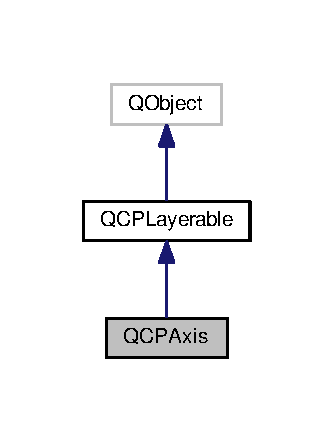
\includegraphics[width=160pt]{classQCPAxis__inherit__graph}
\end{center}
\end{figure}


Collaboration diagram for Q\+C\+P\+Axis\+:\nopagebreak
\begin{figure}[H]
\begin{center}
\leavevmode
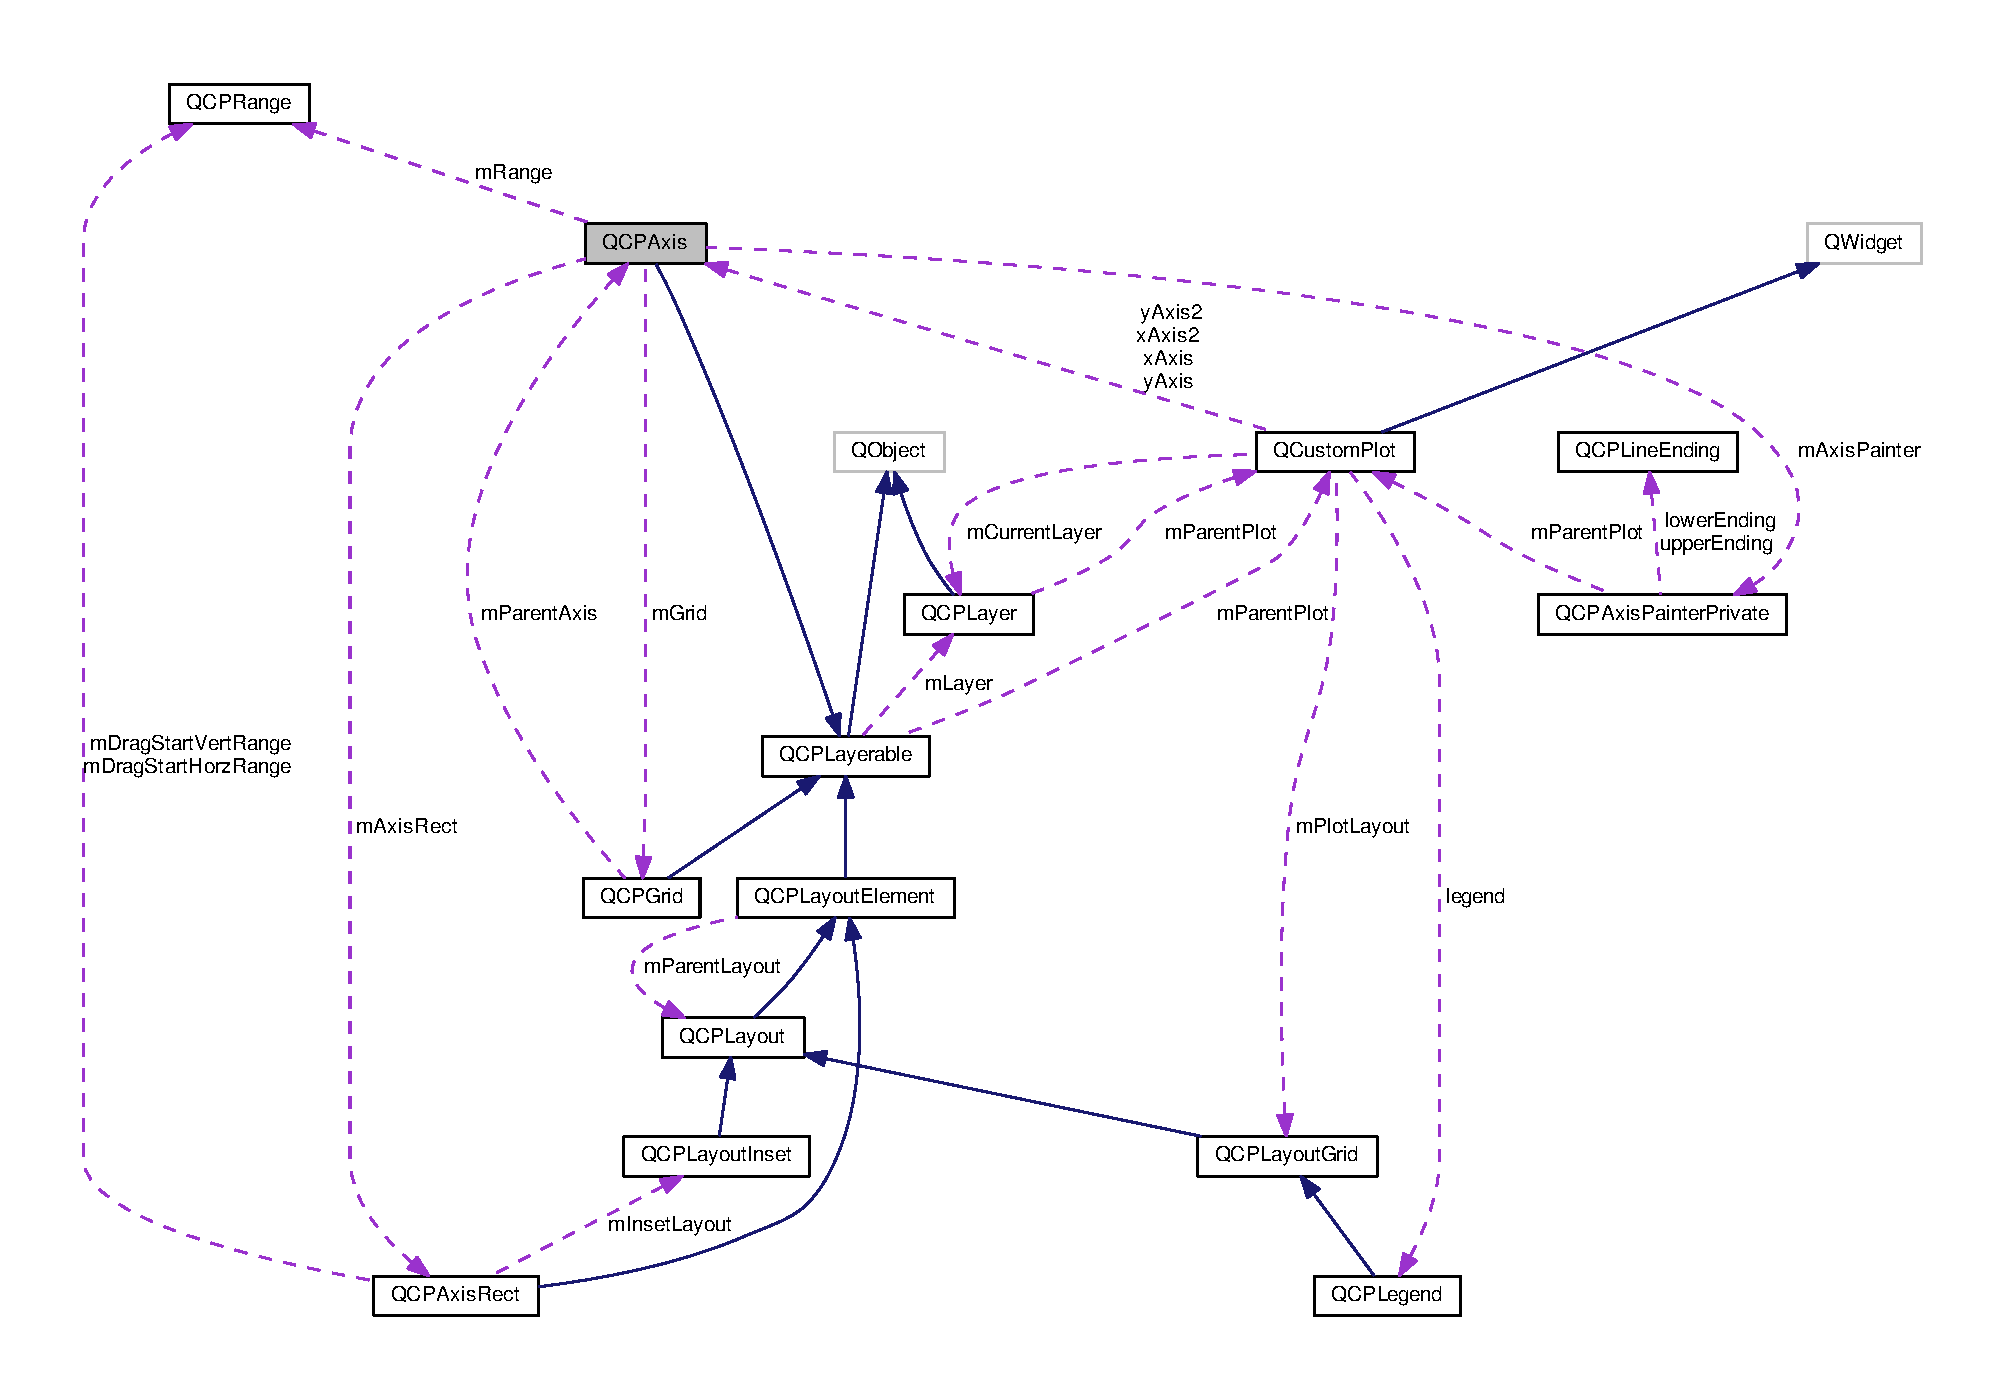
\includegraphics[width=350pt]{classQCPAxis__coll__graph}
\end{center}
\end{figure}
\subsection*{Public Types}
\begin{DoxyCompactItemize}
\item 
enum \hyperlink{classQCPAxis_ae2bcc1728b382f10f064612b368bc18a}{Axis\+Type} \{ \hyperlink{classQCPAxis_ae2bcc1728b382f10f064612b368bc18aaf84aa6cac6fb6099f54a2cbf7546b730}{at\+Left} = 0x01, 
\hyperlink{classQCPAxis_ae2bcc1728b382f10f064612b368bc18aadf5509f7d29199ef2f263b1dd224b345}{at\+Right} = 0x02, 
\hyperlink{classQCPAxis_ae2bcc1728b382f10f064612b368bc18aac0ece2b680d3f545e701f75af1655977}{at\+Top} = 0x04, 
\hyperlink{classQCPAxis_ae2bcc1728b382f10f064612b368bc18aa220d68888516b6c3b493d144f1ba438f}{at\+Bottom} = 0x08
 \}
\item 
enum \hyperlink{classQCPAxis_a4a7da0166f755f5abac23b765d184cad}{Label\+Type} \{ \hyperlink{classQCPAxis_a4a7da0166f755f5abac23b765d184cada7f1eacf3b73adaefd334bea04e094b7e}{lt\+Number}, 
\hyperlink{classQCPAxis_a4a7da0166f755f5abac23b765d184cadafc70594a9d877124dd11ccc187d4ac52}{lt\+Date\+Time}
 \}
\item 
enum \hyperlink{classQCPAxis_a24b13374b9b8f75f47eed2ea78c37db9}{Label\+Side} \{ \hyperlink{classQCPAxis_a24b13374b9b8f75f47eed2ea78c37db9aae7b027ac2839cf4ad611df30236fc3f}{ls\+Inside}, 
\hyperlink{classQCPAxis_a24b13374b9b8f75f47eed2ea78c37db9a2eadb509fc0c9a8b35b85c86ec9f3c7a}{ls\+Outside}
 \}
\item 
enum \hyperlink{classQCPAxis_a36d8e8658dbaa179bf2aeb973db2d6f0}{Scale\+Type} \{ \hyperlink{classQCPAxis_a36d8e8658dbaa179bf2aeb973db2d6f0aff6e30a11a828bc850caffab0ff994f6}{st\+Linear}, 
\hyperlink{classQCPAxis_a36d8e8658dbaa179bf2aeb973db2d6f0abf5b785ad976618816dc6f79b73216d4}{st\+Logarithmic}
 \}
\item 
enum \hyperlink{classQCPAxis_abee4c7a54c468b1385dfce2c898b115f}{Selectable\+Part} \{ \hyperlink{classQCPAxis_abee4c7a54c468b1385dfce2c898b115fae0df8123a5528d5ccf87cb7794f971ea}{sp\+None} = 0, 
\hyperlink{classQCPAxis_abee4c7a54c468b1385dfce2c898b115fa8949d2c1a31eccae9be7ed32e7a1ae38}{sp\+Axis} = 0x001, 
\hyperlink{classQCPAxis_abee4c7a54c468b1385dfce2c898b115fa584e0a3dc4d064880647619f4bd4e771}{sp\+Tick\+Labels} = 0x002, 
\hyperlink{classQCPAxis_abee4c7a54c468b1385dfce2c898b115fa851e0600e0d08b4f5fee9361e3fedabd}{sp\+Axis\+Label} = 0x004
 \}
\end{DoxyCompactItemize}
\subsection*{Signals}
\begin{DoxyCompactItemize}
\item 
void \hyperlink{classQCPAxis_af46d99613d29518795134ec4928e3873}{ticks\+Request} ()
\item 
void \hyperlink{classQCPAxis_a0894084e4c16a1736534c4095746f910}{range\+Changed} (const \hyperlink{classQCPRange}{Q\+C\+P\+Range} \&new\+Range)
\item 
void \hyperlink{classQCPAxis_aac8576288e8e31f16186124bc10dd10d}{range\+Changed} (const \hyperlink{classQCPRange}{Q\+C\+P\+Range} \&new\+Range, const \hyperlink{classQCPRange}{Q\+C\+P\+Range} \&old\+Range)
\item 
void \hyperlink{classQCPAxis_a3505ed8a93bd2e349d858d84996bf767}{scale\+Type\+Changed} (\hyperlink{classQCPAxis_a36d8e8658dbaa179bf2aeb973db2d6f0}{Q\+C\+P\+Axis\+::\+Scale\+Type} \hyperlink{classQCPAxis_a8563e13407bc0616da7f7c84e02de170}{scale\+Type})
\item 
void \hyperlink{classQCPAxis_a62b598abeee7174a05f9d542cc85b1f5}{selection\+Changed} (const Q\+C\+P\+Axis\+::\+Selectable\+Parts \&parts)
\item 
void \hyperlink{classQCPAxis_aa5ff1fd851139028a3bb4efcb31de9fc}{selectable\+Changed} (const Q\+C\+P\+Axis\+::\+Selectable\+Parts \&parts)
\end{DoxyCompactItemize}
\subsection*{Public Member Functions}
\begin{DoxyCompactItemize}
\item 
\hyperlink{classQCPAxis_ac62c042968bae0e6d474fcfc57c9b71f}{Q\+C\+P\+Axis} (\hyperlink{classQCPAxisRect}{Q\+C\+P\+Axis\+Rect} $\ast$parent, \hyperlink{classQCPAxis_ae2bcc1728b382f10f064612b368bc18a}{Axis\+Type} type)
\item 
virtual \hyperlink{classQCPAxis_a7cfa27ea9da0bb1fe0ae995572c0b85d}{$\sim$\+Q\+C\+P\+Axis} ()
\item 
\hyperlink{classQCPAxis_ae2bcc1728b382f10f064612b368bc18a}{Axis\+Type} \hyperlink{classQCPAxis_a593c37bf6aa4990326dc09e24f45db7f}{axis\+Type} () const 
\item 
\hyperlink{classQCPAxisRect}{Q\+C\+P\+Axis\+Rect} $\ast$ \hyperlink{classQCPAxis_aada3102af43b029e3879bcbf2bddfabb}{axis\+Rect} () const 
\item 
\hyperlink{classQCPAxis_a36d8e8658dbaa179bf2aeb973db2d6f0}{Scale\+Type} \hyperlink{classQCPAxis_a8563e13407bc0616da7f7c84e02de170}{scale\+Type} () const 
\item 
double \hyperlink{classQCPAxis_ac937d2a602f865aff2ab6c1e288739f6}{scale\+Log\+Base} () const 
\item 
const \hyperlink{classQCPRange}{Q\+C\+P\+Range} \hyperlink{classQCPAxis_ab1ea79a4f5ea4cf42620f8f51c477ac4}{range} () const 
\item 
bool \hyperlink{classQCPAxis_ade26dc7994ccd8a11f64fd83377ee021}{range\+Reversed} () const 
\item 
bool \hyperlink{classQCPAxis_afc7f20e30dc2865ff6c39f3281f330c2}{auto\+Ticks} () const 
\item 
int \hyperlink{classQCPAxis_ac87454a1342f5d2939ab59e68b4d515b}{auto\+Tick\+Count} () const 
\item 
bool \hyperlink{classQCPAxis_a7169da316ac25dec1606784152fbf2c1}{auto\+Tick\+Labels} () const 
\item 
bool \hyperlink{classQCPAxis_ae762920261b0c24beb56b893e5a2471d}{auto\+Tick\+Step} () const 
\item 
bool \hyperlink{classQCPAxis_ab9a950e16f373fe5c4b79078bb97c171}{auto\+Sub\+Ticks} () const 
\item 
bool \hyperlink{classQCPAxis_a61c504ec7c5bed9a63edf45345995d10}{ticks} () const 
\item 
bool \hyperlink{classQCPAxis_a9a78fcccd98a73d37b3d991df7b6ef1d}{tick\+Labels} () const 
\item 
int \hyperlink{classQCPAxis_af7bc2fac3f95949ecd0204d20dc1463b}{tick\+Label\+Padding} () const 
\item 
\hyperlink{classQCPAxis_a4a7da0166f755f5abac23b765d184cad}{Label\+Type} \hyperlink{classQCPAxis_a8a6f58a1ce12cfc4fadd379167668e8d}{tick\+Label\+Type} () const 
\item 
Q\+Font \hyperlink{classQCPAxis_af6d7ad17f3398b114a413f7a3dc5ef9d}{tick\+Label\+Font} () const 
\item 
Q\+Color \hyperlink{classQCPAxis_ac86d0636aa55ddd94df171f609897a32}{tick\+Label\+Color} () const 
\item 
double \hyperlink{classQCPAxis_ab9199d72b8c4c06cc6c9b928c30d00d2}{tick\+Label\+Rotation} () const 
\item 
\hyperlink{classQCPAxis_a24b13374b9b8f75f47eed2ea78c37db9}{Label\+Side} \hyperlink{classQCPAxis_a0a33835705406506b02a445b1ba32357}{tick\+Label\+Side} () const 
\item 
Q\+String \hyperlink{classQCPAxis_a132b54ae184a12ed24c9af24f53dc70b}{date\+Time\+Format} () const 
\item 
Qt\+::\+Time\+Spec \hyperlink{classQCPAxis_afdd04c56ed29a9d948f840fc76f0d383}{date\+Time\+Spec} () const 
\item 
Q\+String \hyperlink{classQCPAxis_ae6729b40845b29ffa5a440aa53cec215}{number\+Format} () const 
\item 
int \hyperlink{classQCPAxis_a91cb2825060ac79a889296377fe0c7c1}{number\+Precision} () const 
\item 
double \hyperlink{classQCPAxis_a0e6120d24266544441ab691f316a1b03}{tick\+Step} () const 
\item 
Q\+Vector$<$ double $>$ \hyperlink{classQCPAxis_a5b00b14f480f926df976cc6c52309e78}{tick\+Vector} () const 
\item 
Q\+Vector$<$ Q\+String $>$ \hyperlink{classQCPAxis_a64e6fa81f943ad33dcaf3fa606687b93}{tick\+Vector\+Labels} () const 
\item 
int \hyperlink{classQCPAxis_a59265d65c5034695ac2578bccbbb0f4a}{tick\+Length\+In} () const 
\item 
int \hyperlink{classQCPAxis_ae1b3d7473f50ba8544b2027c1cdc80f2}{tick\+Length\+Out} () const 
\item 
int \hyperlink{classQCPAxis_a290b4c1375476826daa10e914cb71dab}{sub\+Tick\+Count} () const 
\item 
int \hyperlink{classQCPAxis_a052e6ab2ada7e87fa5e5831dcbd4a517}{sub\+Tick\+Length\+In} () const 
\item 
int \hyperlink{classQCPAxis_a091fdf8d1b3f9660e38b854578efb9bc}{sub\+Tick\+Length\+Out} () const 
\item 
Q\+Pen \hyperlink{classQCPAxis_a4f6a7cd46fb104b1dad93e29cc78fe74}{base\+Pen} () const 
\item 
Q\+Pen \hyperlink{classQCPAxis_a5eb206da4265c6c083db71d692da3bc4}{tick\+Pen} () const 
\item 
Q\+Pen \hyperlink{classQCPAxis_a2e8bce6dd03e393dbdf6bb427461a726}{sub\+Tick\+Pen} () const 
\item 
Q\+Font \hyperlink{classQCPAxis_ae8029ae0b32e9d4d73dddcdd0a08c838}{label\+Font} () const 
\item 
Q\+Color \hyperlink{classQCPAxis_a7854c2875e3b8d86b210d108bd87aeb9}{label\+Color} () const 
\item 
Q\+String \hyperlink{classQCPAxis_ab3486dca5a6e9e3ca0e32678272ba549}{label} () const 
\item 
int \hyperlink{classQCPAxis_a59c9a0e362dec811491fc9a0709d2afa}{label\+Padding} () const 
\item 
int \hyperlink{classQCPAxis_abb85015a9467ec176e70698307ec833a}{padding} () const 
\item 
int \hyperlink{classQCPAxis_aebc032ac6eea164a02859c017f52d5e7}{offset} () const 
\item 
Selectable\+Parts \hyperlink{classQCPAxis_a08323248a1cba4750ef07ceea159e0b3}{selected\+Parts} () const 
\item 
Selectable\+Parts \hyperlink{classQCPAxis_ad2bff3d2ed3d35c10d44c0c02441bd2c}{selectable\+Parts} () const 
\item 
Q\+Font \hyperlink{classQCPAxis_ae245bb3dcd0ec71eee38437de6e719f7}{selected\+Tick\+Label\+Font} () const 
\item 
Q\+Font \hyperlink{classQCPAxis_a078bbc88b33595a5308350c2889c96d4}{selected\+Label\+Font} () const 
\item 
Q\+Color \hyperlink{classQCPAxis_a5a3af4bd1a820bb7c6d4c85e1d8d452f}{selected\+Tick\+Label\+Color} () const 
\item 
Q\+Color \hyperlink{classQCPAxis_a8cf8de6ac7f1ca617e05412f669ed229}{selected\+Label\+Color} () const 
\item 
Q\+Pen \hyperlink{classQCPAxis_a5a3919ad7b60c2789b04c7e72387cfd6}{selected\+Base\+Pen} () const 
\item 
Q\+Pen \hyperlink{classQCPAxis_a9f86ef82e1d1a908ab4c68cfa5fe4175}{selected\+Tick\+Pen} () const 
\item 
Q\+Pen \hyperlink{classQCPAxis_a1b264fdfef48c22aba36e76de7856784}{selected\+Sub\+Tick\+Pen} () const 
\item 
\hyperlink{classQCPLineEnding}{Q\+C\+P\+Line\+Ending} \hyperlink{classQCPAxis_ac85aebbedf67d7bc9e1e5c182151536b}{lower\+Ending} () const 
\item 
\hyperlink{classQCPLineEnding}{Q\+C\+P\+Line\+Ending} \hyperlink{classQCPAxis_aad503ac95ee34e614ffee0bd66473e1a}{upper\+Ending} () const 
\item 
\hyperlink{classQCPGrid}{Q\+C\+P\+Grid} $\ast$ \hyperlink{classQCPAxis_ac4fb913cce3072b5e75a4635e0f6cd04}{grid} () const 
\item 
Q\+\_\+\+S\+L\+OT void \hyperlink{classQCPAxis_adef29cae617af4f519f6c40d1a866ca6}{set\+Scale\+Type} (\hyperlink{classQCPAxis_a36d8e8658dbaa179bf2aeb973db2d6f0}{Q\+C\+P\+Axis\+::\+Scale\+Type} type)
\item 
void \hyperlink{classQCPAxis_a726186054be90487885a748aa1b42188}{set\+Scale\+Log\+Base} (double base)
\item 
Q\+\_\+\+S\+L\+OT void \hyperlink{classQCPAxis_aebdfea5d44c3a0ad2b4700cd4d25b641}{set\+Range} (const \hyperlink{classQCPRange}{Q\+C\+P\+Range} \&\hyperlink{classQCPAxis_ab1ea79a4f5ea4cf42620f8f51c477ac4}{range})
\item 
void \hyperlink{classQCPAxis_a57d6ee9e9009fe88cb19db476ec70bca}{set\+Range} (double lower, double upper)
\item 
void \hyperlink{classQCPAxis_acf60e5b2d631fbc8c4548c3d579cb6d0}{set\+Range} (double position, double size, Qt\+::\+Alignment\+Flag alignment)
\item 
void \hyperlink{classQCPAxis_afcf51227d337db28d1a9ce9a4d1bc91a}{set\+Range\+Lower} (double lower)
\item 
void \hyperlink{classQCPAxis_acd3ca1247aa867b540cd5ec30ccd3bef}{set\+Range\+Upper} (double upper)
\item 
void \hyperlink{classQCPAxis_a2172fdb196b1a0dc3f40992fcad8e9e1}{set\+Range\+Reversed} (bool reversed)
\item 
void \hyperlink{classQCPAxis_ae867c23d3a6a7bd4d09cc66c5d018f63}{set\+Auto\+Ticks} (bool on)
\item 
void \hyperlink{classQCPAxis_a7c7111cbeac9ec5fcb40f93a1ef51a0b}{set\+Auto\+Tick\+Count} (int approximate\+Count)
\item 
void \hyperlink{classQCPAxis_aaa47e3a6bac0c20d4beb9028f01bc1a1}{set\+Auto\+Tick\+Labels} (bool on)
\item 
void \hyperlink{classQCPAxis_a99fe77b034e06f5b723995beab96e741}{set\+Auto\+Tick\+Step} (bool on)
\item 
void \hyperlink{classQCPAxis_adcbdec7a60054b88571e89599f4a45bf}{set\+Auto\+Sub\+Ticks} (bool on)
\item 
void \hyperlink{classQCPAxis_ac891409315bc379e3b1abdb162c1a011}{set\+Ticks} (bool show)
\item 
void \hyperlink{classQCPAxis_a04ba16e1f6f78d70f938519576ed32c8}{set\+Tick\+Labels} (bool show)
\item 
void \hyperlink{classQCPAxis_af302c479af9dbc2e9f0e44e07c0012ee}{set\+Tick\+Label\+Padding} (int \hyperlink{classQCPAxis_abb85015a9467ec176e70698307ec833a}{padding})
\item 
void \hyperlink{classQCPAxis_a54f24f5ce8feea25209388a863d7e448}{set\+Tick\+Label\+Type} (\hyperlink{classQCPAxis_a4a7da0166f755f5abac23b765d184cad}{Label\+Type} type)
\item 
void \hyperlink{classQCPAxis_a2b8690c4e8dbc39d9185d2b398ce7a6c}{set\+Tick\+Label\+Font} (const Q\+Font \&font)
\item 
void \hyperlink{classQCPAxis_a395e445c3fe496b935bee7b911ecfd1c}{set\+Tick\+Label\+Color} (const Q\+Color \&color)
\item 
void \hyperlink{classQCPAxis_a1bddd4413df8a576b7ad4b067fb33375}{set\+Tick\+Label\+Rotation} (double degrees)
\item 
void \hyperlink{classQCPAxis_a13ec644fc6e22715744c92c6dfa4f0fa}{set\+Tick\+Label\+Side} (\hyperlink{classQCPAxis_a24b13374b9b8f75f47eed2ea78c37db9}{Label\+Side} side)
\item 
void \hyperlink{classQCPAxis_a2ee0191daa03524a682113e63e05f7a7}{set\+Date\+Time\+Format} (const Q\+String \&format)
\item 
void \hyperlink{classQCPAxis_a262e06731debed7eee11fa6a81d67eaf}{set\+Date\+Time\+Spec} (const Qt\+::\+Time\+Spec \&time\+Spec)
\item 
void \hyperlink{classQCPAxis_ae585a54dc2aac662e90a2ca82f002590}{set\+Number\+Format} (const Q\+String \&format\+Code)
\item 
void \hyperlink{classQCPAxis_a21dc8023ad7500382ad9574b48137e63}{set\+Number\+Precision} (int precision)
\item 
void \hyperlink{classQCPAxis_af727db0acc6492c4c774c0700e738205}{set\+Tick\+Step} (double step)
\item 
void \hyperlink{classQCPAxis_a871db94c5d796c80fcbe1a9d4506e27e}{set\+Tick\+Vector} (const Q\+Vector$<$ double $>$ \&vec)
\item 
void \hyperlink{classQCPAxis_a921d3ba3853ca3bd2cce3459f7a243ed}{set\+Tick\+Vector\+Labels} (const Q\+Vector$<$ Q\+String $>$ \&vec)
\item 
void \hyperlink{classQCPAxis_a62ec40bebe3540e9c1479a8fd2be3b0d}{set\+Tick\+Length} (int inside, int outside=0)
\item 
void \hyperlink{classQCPAxis_afae1a37a99611366275a51204d991739}{set\+Tick\+Length\+In} (int inside)
\item 
void \hyperlink{classQCPAxis_a3b8a0debd1ffedd2c22d0592dfbb4e62}{set\+Tick\+Length\+Out} (int outside)
\item 
void \hyperlink{classQCPAxis_a4b1554ead9d7f9799650d51383e326dd}{set\+Sub\+Tick\+Count} (int \hyperlink{test_8cpp_ad43c3812e6d13e0518d9f8b8f463ffcf}{count})
\item 
void \hyperlink{classQCPAxis_ab702d6fd42fc620607435339a1c2a2e1}{set\+Sub\+Tick\+Length} (int inside, int outside=0)
\item 
void \hyperlink{classQCPAxis_ac46fa2a993a9f5789540977610acf1de}{set\+Sub\+Tick\+Length\+In} (int inside)
\item 
void \hyperlink{classQCPAxis_a4c6dfc3963492ed72a77724012df5f23}{set\+Sub\+Tick\+Length\+Out} (int outside)
\item 
void \hyperlink{classQCPAxis_a778d45fb71b3c7ab3bb7079e18b058e4}{set\+Base\+Pen} (const Q\+Pen \&pen)
\item 
void \hyperlink{classQCPAxis_ad80923bcc1c5da4c4db602c5325e797e}{set\+Tick\+Pen} (const Q\+Pen \&pen)
\item 
void \hyperlink{classQCPAxis_aede4028ae7516bd51a60618a8233f9cf}{set\+Sub\+Tick\+Pen} (const Q\+Pen \&pen)
\item 
void \hyperlink{classQCPAxis_a71ac1a47f7547e490a8c4311d1433cf3}{set\+Label\+Font} (const Q\+Font \&font)
\item 
void \hyperlink{classQCPAxis_a6c906fe56d75f0122335b9f79b999608}{set\+Label\+Color} (const Q\+Color \&color)
\item 
void \hyperlink{classQCPAxis_a33bcc382c111c9f31bb0687352a2dea4}{set\+Label} (const Q\+String \&str)
\item 
void \hyperlink{classQCPAxis_a4391192a766e5d20cfe5cbc17607a7a2}{set\+Label\+Padding} (int \hyperlink{classQCPAxis_abb85015a9467ec176e70698307ec833a}{padding})
\item 
void \hyperlink{classQCPAxis_a5691441cb3de9e9844855d339c0db279}{set\+Padding} (int \hyperlink{classQCPAxis_abb85015a9467ec176e70698307ec833a}{padding})
\item 
void \hyperlink{classQCPAxis_a04a652603cbe50eba9969ee6d68873c3}{set\+Offset} (int \hyperlink{classQCPAxis_aebc032ac6eea164a02859c017f52d5e7}{offset})
\item 
void \hyperlink{classQCPAxis_a845ccb560b7bc5281098a5be494145f6}{set\+Selected\+Tick\+Label\+Font} (const Q\+Font \&font)
\item 
void \hyperlink{classQCPAxis_a02ec2a75d4d8401eaab834fbc6803d30}{set\+Selected\+Label\+Font} (const Q\+Font \&font)
\item 
void \hyperlink{classQCPAxis_a9bdbf5e63ab15187f3a1de9440129227}{set\+Selected\+Tick\+Label\+Color} (const Q\+Color \&color)
\item 
void \hyperlink{classQCPAxis_a5d502dec597c634f491fdd73d151c72d}{set\+Selected\+Label\+Color} (const Q\+Color \&color)
\item 
void \hyperlink{classQCPAxis_aeb917a909215605b95ef2be843de1ee8}{set\+Selected\+Base\+Pen} (const Q\+Pen \&pen)
\item 
void \hyperlink{classQCPAxis_a8360502685eb782edbf04019c9345cdc}{set\+Selected\+Tick\+Pen} (const Q\+Pen \&pen)
\item 
void \hyperlink{classQCPAxis_a2a00a7166600155eac26843132eb9576}{set\+Selected\+Sub\+Tick\+Pen} (const Q\+Pen \&pen)
\item 
Q\+\_\+\+S\+L\+OT void \hyperlink{classQCPAxis_a513f9b9e326c505d9bec54880031b085}{set\+Selectable\+Parts} (const Q\+C\+P\+Axis\+::\+Selectable\+Parts \&\hyperlink{classQCPAxis_ad2bff3d2ed3d35c10d44c0c02441bd2c}{selectable\+Parts})
\item 
Q\+\_\+\+S\+L\+OT void \hyperlink{classQCPAxis_ab9d7a69277dcbed9119b3c1f25ca19c3}{set\+Selected\+Parts} (const Q\+C\+P\+Axis\+::\+Selectable\+Parts \&\hyperlink{classQCPAxis_a08323248a1cba4750ef07ceea159e0b3}{selected\+Parts})
\item 
void \hyperlink{classQCPAxis_a08af1c72db9ae4dc8cb8a973d44405ab}{set\+Lower\+Ending} (const \hyperlink{classQCPLineEnding}{Q\+C\+P\+Line\+Ending} \&ending)
\item 
void \hyperlink{classQCPAxis_a69119b892fc306f651763596685aa377}{set\+Upper\+Ending} (const \hyperlink{classQCPLineEnding}{Q\+C\+P\+Line\+Ending} \&ending)
\item 
virtual double \hyperlink{classQCPAxis_a2877a6230920c118be65c6113089f467}{select\+Test} (const Q\+PointF \&pos, bool only\+Selectable, Q\+Variant $\ast$details=0) const 
\item 
Qt\+::\+Orientation \hyperlink{classQCPAxis_a57483f2f60145ddc9e63f3af53959265}{orientation} () const 
\item 
void \hyperlink{classQCPAxis_a18f3a68f2b691af1fd34b6593c886630}{move\+Range} (double diff)
\item 
void \hyperlink{classQCPAxis_a7072ff96fe690148f1bbcdb4f773ea1c}{scale\+Range} (double factor, double center)
\item 
void \hyperlink{classQCPAxis_af4bbd446dcaee5a83ac30ce9bcd6e125}{set\+Scale\+Ratio} (const \hyperlink{classQCPAxis}{Q\+C\+P\+Axis} $\ast$other\+Axis, double ratio=1.\+0)
\item 
void \hyperlink{classQCPAxis_a499345f02ebce4b23d8ccec96e58daa9}{rescale} (bool only\+Visible\+Plottables=false)
\item 
double \hyperlink{classQCPAxis_ae9289ef7043b9d966af88eaa95b037d1}{pixel\+To\+Coord} (double value) const 
\item 
double \hyperlink{classQCPAxis_a985ae693b842fb0422b4390fe36d299a}{coord\+To\+Pixel} (double value) const 
\item 
\hyperlink{classQCPAxis_abee4c7a54c468b1385dfce2c898b115f}{Selectable\+Part} \hyperlink{classQCPAxis_ab2965a8ab1da948b897f1c006080760b}{get\+Part\+At} (const Q\+PointF \&pos) const 
\item 
Q\+List$<$ \hyperlink{classQCPAbstractPlottable}{Q\+C\+P\+Abstract\+Plottable} $\ast$ $>$ \hyperlink{classQCPAxis_a4f7404494cccdbfc00e1e865b7ed16a4}{plottables} () const 
\item 
Q\+List$<$ \hyperlink{classQCPGraph}{Q\+C\+P\+Graph} $\ast$ $>$ \hyperlink{classQCPAxis_ad3919e7d7400f55446ea82018fe5e3a8}{graphs} () const 
\item 
Q\+List$<$ \hyperlink{classQCPAbstractItem}{Q\+C\+P\+Abstract\+Item} $\ast$ $>$ \hyperlink{classQCPAxis_ae437656a5fd1a03721a8f2d7aab460fe}{items} () const 
\end{DoxyCompactItemize}
\subsection*{Static Public Member Functions}
\begin{DoxyCompactItemize}
\item 
static \hyperlink{classQCPAxis_ae2bcc1728b382f10f064612b368bc18a}{Axis\+Type} \hyperlink{classQCPAxis_ac0a6b77bd52bec6c81cd62d167cfeba6}{margin\+Side\+To\+Axis\+Type} (\hyperlink{namespaceQCP_a7e487e3e2ccb62ab7771065bab7cae54}{Q\+C\+P\+::\+Margin\+Side} side)
\item 
static Qt\+::\+Orientation \hyperlink{classQCPAxis_a9a68b3e45f1b1e33d4d807822342516c}{orientation} (\hyperlink{classQCPAxis_ae2bcc1728b382f10f064612b368bc18a}{Axis\+Type} type)
\item 
static \hyperlink{classQCPAxis_ae2bcc1728b382f10f064612b368bc18a}{Axis\+Type} \hyperlink{classQCPAxis_aa85ba73dfee6483e23825461b725e363}{opposite} (\hyperlink{classQCPAxis_ae2bcc1728b382f10f064612b368bc18a}{Axis\+Type} type)
\end{DoxyCompactItemize}
\subsection*{Protected Member Functions}
\begin{DoxyCompactItemize}
\item 
virtual void \hyperlink{classQCPAxis_a57d9e961bae7d62f5b4e1f143e660c78}{setup\+Tick\+Vectors} ()
\item 
virtual void \hyperlink{classQCPAxis_a626eef437c874148df1a5ac78506d463}{generate\+Auto\+Ticks} ()
\item 
virtual int \hyperlink{classQCPAxis_a3c5c045019fcdc0843a3e064eda7478a}{calculate\+Auto\+Sub\+Tick\+Count} (double \hyperlink{classQCPAxis_a0e6120d24266544441ab691f316a1b03}{tick\+Step}) const 
\item 
virtual int \hyperlink{classQCPAxis_a47bdb0a55de6759489ee47665199aebb}{calculate\+Margin} ()
\item 
virtual void \hyperlink{classQCPAxis_a13bde39eb1e0b7c14a02935689be8aba}{apply\+Default\+Antialiasing\+Hint} (\hyperlink{classQCPPainter}{Q\+C\+P\+Painter} $\ast$painter) const 
\item 
virtual void \hyperlink{classQCPAxis_a258b1e783eda5cd14ec5552c696a424e}{draw} (\hyperlink{classQCPPainter}{Q\+C\+P\+Painter} $\ast$painter)
\item 
virtual \hyperlink{namespaceQCP_a2ad6bb6281c7c2d593d4277b44c2b037}{Q\+C\+P\+::\+Interaction} \hyperlink{classQCPAxis_aca53b2f365dfc1257cba9e62395aa68f}{selection\+Category} () const 
\item 
virtual void \hyperlink{classQCPAxis_aa8a5fe80e2898ec08ada26b5fbee9eca}{select\+Event} (Q\+Mouse\+Event $\ast$event, bool additive, const Q\+Variant \&details, bool $\ast$selection\+State\+Changed)
\item 
virtual void \hyperlink{classQCPAxis_a53512242cde6ec21943a3ba10dbf78c3}{deselect\+Event} (bool $\ast$selection\+State\+Changed)
\item 
void \hyperlink{classQCPAxis_a06320a944d1120732cc0d72fe1306d8b}{visible\+Tick\+Bounds} (int \&low\+Index, int \&high\+Index) const 
\item 
double \hyperlink{classQCPAxis_a1385765db2419ee5fb5505a6cf9130fb}{base\+Log} (double value) const 
\item 
double \hyperlink{classQCPAxis_a97d69f021a05126fcb978d0aefea47b8}{base\+Pow} (double value) const 
\item 
Q\+Pen \hyperlink{classQCPAxis_a3eb0681d31baf579bb73b86a0153cb02}{get\+Base\+Pen} () const 
\item 
Q\+Pen \hyperlink{classQCPAxis_a7f503910be40fb1717e1635be3ef17e1}{get\+Tick\+Pen} () const 
\item 
Q\+Pen \hyperlink{classQCPAxis_ab4f7e60a40eb051c775afcaeab895c85}{get\+Sub\+Tick\+Pen} () const 
\item 
Q\+Font \hyperlink{classQCPAxis_aef30b66668986523225089a67280ec7a}{get\+Tick\+Label\+Font} () const 
\item 
Q\+Font \hyperlink{classQCPAxis_ab0768eb2879efb202645d19ff789e63e}{get\+Label\+Font} () const 
\item 
Q\+Color \hyperlink{classQCPAxis_a0f8583f7ac24ccc70d39fdd2389cad6e}{get\+Tick\+Label\+Color} () const 
\item 
Q\+Color \hyperlink{classQCPAxis_a42bd69b9e9c571f13624079be18ccdc1}{get\+Label\+Color} () const 
\end{DoxyCompactItemize}
\subsection*{Protected Attributes}
\begin{DoxyCompactItemize}
\item 
\hyperlink{classQCPAxis_ae2bcc1728b382f10f064612b368bc18a}{Axis\+Type} \hyperlink{classQCPAxis_ae704bf9f2c2b026f08dd4ccad79c616e}{m\+Axis\+Type}
\item 
\hyperlink{classQCPAxisRect}{Q\+C\+P\+Axis\+Rect} $\ast$ \hyperlink{classQCPAxis_a6f150b65a202f32936997960e331dfcb}{m\+Axis\+Rect}
\item 
int \hyperlink{classQCPAxis_a52a805a4f03231210e0880db7f77e098}{m\+Padding}
\item 
Qt\+::\+Orientation \hyperlink{classQCPAxis_a048e1792fa86f4f86df55200b3f0be36}{m\+Orientation}
\item 
Selectable\+Parts \hyperlink{classQCPAxis_ab9042d8a095998f27a28b39411d8b9c3}{m\+Selectable\+Parts}
\item 
Selectable\+Parts \hyperlink{classQCPAxis_a8f1eb0abfe2ae64652aa46b360e841e4}{m\+Selected\+Parts}
\item 
Q\+Pen \hyperlink{classQCPAxis_ad6b4a0aee9558fb35529e960b8fef72d}{m\+Base\+Pen}
\item 
Q\+Pen \hyperlink{classQCPAxis_a80baa4e3c16f9b6edf3eccacd2a50fde}{m\+Selected\+Base\+Pen}
\item 
Q\+String \hyperlink{classQCPAxis_ae8001dbdfc47685c1cf7b98b044460e6}{m\+Label}
\item 
Q\+Font \hyperlink{classQCPAxis_a37442d470e30e19b81ecaf979a34d046}{m\+Label\+Font}
\item 
Q\+Font \hyperlink{classQCPAxis_ae48fe3489afadc0b3cd003233e2bf19f}{m\+Selected\+Label\+Font}
\item 
Q\+Color \hyperlink{classQCPAxis_a457a003bb1c2b6ab73e5a173ba7558fd}{m\+Label\+Color}
\item 
Q\+Color \hyperlink{classQCPAxis_a94f57de3ba024471ca206d83cf2258dd}{m\+Selected\+Label\+Color}
\item 
bool \hyperlink{classQCPAxis_a3e4315be072026644e69009557a2fa11}{m\+Tick\+Labels}
\item 
bool \hyperlink{classQCPAxis_a721e496b342f272078c5ff84564e472f}{m\+Auto\+Tick\+Labels}
\item 
\hyperlink{classQCPAxis_a4a7da0166f755f5abac23b765d184cad}{Label\+Type} \hyperlink{classQCPAxis_a6e056c1cb1aab0eddebfebbcb78c8f90}{m\+Tick\+Label\+Type}
\item 
Q\+Font \hyperlink{classQCPAxis_add79d1e39c4ed65869a1e9cc79043f3f}{m\+Tick\+Label\+Font}
\item 
Q\+Font \hyperlink{classQCPAxis_a4f2e4919da9615dac612662c249b1119}{m\+Selected\+Tick\+Label\+Font}
\item 
Q\+Color \hyperlink{classQCPAxis_a6384a749b3b56a97df081d8082321ab4}{m\+Tick\+Label\+Color}
\item 
Q\+Color \hyperlink{classQCPAxis_a3bcad40902f45dc4c991a2c3e4d31d70}{m\+Selected\+Tick\+Label\+Color}
\item 
Q\+String \hyperlink{classQCPAxis_a0b7ad83550d71daab4cfee2918e168e0}{m\+Date\+Time\+Format}
\item 
Qt\+::\+Time\+Spec \hyperlink{classQCPAxis_af73bec228c1a3203dc8aef1e84a46759}{m\+Date\+Time\+Spec}
\item 
int \hyperlink{classQCPAxis_acd76e8c783384d99ccc4a13797eec188}{m\+Number\+Precision}
\item 
Q\+Latin1\+Char \hyperlink{classQCPAxis_a39594313deef458f425bba25cd337a8a}{m\+Number\+Format\+Char}
\item 
bool \hyperlink{classQCPAxis_af03809bee3f3e35fcc38d25b6dd5003b}{m\+Number\+Beautiful\+Powers}
\item 
bool \hyperlink{classQCPAxis_ab111e74bba22e06848897c932fc549fe}{m\+Ticks}
\item 
double \hyperlink{classQCPAxis_a4fe96830fc5a2711e20fe5edccfe2ed3}{m\+Tick\+Step}
\item 
int \hyperlink{classQCPAxis_ad70198e6ae2801fc409bc3caec707da9}{m\+Sub\+Tick\+Count}
\item 
int \hyperlink{classQCPAxis_a499fbb67111e4b204738f6c1aa28d842}{m\+Auto\+Tick\+Count}
\item 
bool \hyperlink{classQCPAxis_aac23adcbae246bf165d4539ad65ac9f9}{m\+Auto\+Ticks}
\item 
bool \hyperlink{classQCPAxis_aada8934a5c44978653031782aa37d101}{m\+Auto\+Tick\+Step}
\item 
bool \hyperlink{classQCPAxis_aaae980b0d193d959674e314dbb6c2c3b}{m\+Auto\+Sub\+Ticks}
\item 
Q\+Pen \hyperlink{classQCPAxis_a1d52c78c856d8bd1f331d4ec4e63d944}{m\+Tick\+Pen}
\item 
Q\+Pen \hyperlink{classQCPAxis_a9524593dbc75a5c5b29dbd1cb4b37df5}{m\+Selected\+Tick\+Pen}
\item 
Q\+Pen \hyperlink{classQCPAxis_a32ef56d3a417866720eb12667d27dbd1}{m\+Sub\+Tick\+Pen}
\item 
Q\+Pen \hyperlink{classQCPAxis_aa5cc6afc5dc2a365f5abbd36eb04a1dc}{m\+Selected\+Sub\+Tick\+Pen}
\item 
\hyperlink{classQCPRange}{Q\+C\+P\+Range} \hyperlink{classQCPAxis_a1ee36773c49062d751560e11f90845f7}{m\+Range}
\item 
bool \hyperlink{classQCPAxis_a5cb034f57aa3d773a9ca55a0931dbf7b}{m\+Range\+Reversed}
\item 
\hyperlink{classQCPAxis_a36d8e8658dbaa179bf2aeb973db2d6f0}{Scale\+Type} \hyperlink{classQCPAxis_ad706039549cbbbec5fcb2baf7894e04d}{m\+Scale\+Type}
\item 
double \hyperlink{classQCPAxis_abc727ddb4af745151755d1b5e60d03c3}{m\+Scale\+Log\+Base}
\item 
double \hyperlink{classQCPAxis_a93e068984b475467929e7f6768754227}{m\+Scale\+Log\+Base\+Log\+Inv}
\item 
\hyperlink{classQCPGrid}{Q\+C\+P\+Grid} $\ast$ \hyperlink{classQCPAxis_a17bffb94aaa40311f259c6ac7bcb5d5f}{m\+Grid}
\item 
\hyperlink{classQCPAxisPainterPrivate}{Q\+C\+P\+Axis\+Painter\+Private} $\ast$ \hyperlink{classQCPAxis_aeeae00935bd2dab82d64f32544a90913}{m\+Axis\+Painter}
\item 
int \hyperlink{classQCPAxis_aebb24ba8734b7e054efc6e1ecc5414c7}{m\+Lowest\+Visible\+Tick}
\item 
int \hyperlink{classQCPAxis_abb3b3ccce7e9779fef2be91ce1a46ef0}{m\+Highest\+Visible\+Tick}
\item 
Q\+Vector$<$ double $>$ \hyperlink{classQCPAxis_aae0f9b9973b85be601200f00f5825087}{m\+Tick\+Vector}
\item 
Q\+Vector$<$ Q\+String $>$ \hyperlink{classQCPAxis_aeee4bd0fca3f587eafe33843d1cb4f82}{m\+Tick\+Vector\+Labels}
\item 
Q\+Vector$<$ double $>$ \hyperlink{classQCPAxis_a28353081e0ff35c3fe5ced923a287faa}{m\+Sub\+Tick\+Vector}
\item 
bool \hyperlink{classQCPAxis_a2cde37b6e385f47e11322df4ac1b0e9b}{m\+Cached\+Margin\+Valid}
\item 
int \hyperlink{classQCPAxis_a48ace55cbd54f7241e7f1b06fd369b64}{m\+Cached\+Margin}
\end{DoxyCompactItemize}
\subsection*{Friends}
\begin{DoxyCompactItemize}
\item 
class \hyperlink{classQCPAxis_a1cdf9df76adcfae45261690aa0ca2198}{Q\+Custom\+Plot}
\item 
class \hyperlink{classQCPAxis_a061e177f585549fc31f780852e2bd6fe}{Q\+C\+P\+Grid}
\item 
class \hyperlink{classQCPAxis_acbf20ecb140f66c5fd1bc64ae0762990}{Q\+C\+P\+Axis\+Rect}
\end{DoxyCompactItemize}


\subsection{Detailed Description}
Manages a single axis inside a \hyperlink{classQCustomPlot}{Q\+Custom\+Plot}. 

Usually doesn\textquotesingle{}t need to be instantiated externally. Access Q\+Custom\+Plot\textquotesingle{}s default four axes via \hyperlink{classQCustomPlot_a9a79cd0158a4c7f30cbc702f0fd800e4}{Q\+Custom\+Plot\+::x\+Axis} (bottom), \hyperlink{classQCustomPlot_af6fea5679725b152c14facd920b19367}{Q\+Custom\+Plot\+::y\+Axis} (left), \hyperlink{classQCustomPlot_ada41599f22cad901c030f3dcbdd82fd9}{Q\+Custom\+Plot\+::x\+Axis2} (top) and \hyperlink{classQCustomPlot_af13fdc5bce7d0fabd640f13ba805c0b7}{Q\+Custom\+Plot\+::y\+Axis2} (right).

Axes are always part of an axis rect, see \hyperlink{classQCPAxisRect}{Q\+C\+P\+Axis\+Rect}.  \begin{center}Naming convention of axis parts\end{center}  ~\newline
  \begin{center}Overview of the spacings and paddings that define the geometry of an axis. The dashed gray line on the left represents the \hyperlink{classQCustomPlot}{Q\+Custom\+Plot} widget border.\end{center}  

\subsection{Member Enumeration Documentation}
\index{Q\+C\+P\+Axis@{Q\+C\+P\+Axis}!Axis\+Type@{Axis\+Type}}
\index{Axis\+Type@{Axis\+Type}!Q\+C\+P\+Axis@{Q\+C\+P\+Axis}}
\subsubsection[{\texorpdfstring{Axis\+Type}{AxisType}}]{\setlength{\rightskip}{0pt plus 5cm}enum {\bf Q\+C\+P\+Axis\+::\+Axis\+Type}}\hypertarget{classQCPAxis_ae2bcc1728b382f10f064612b368bc18a}{}\label{classQCPAxis_ae2bcc1728b382f10f064612b368bc18a}
Defines at which side of the axis rect the axis will appear. This also affects how the tick marks are drawn, on which side the labels are placed etc. \begin{Desc}
\item[Enumerator]\par
\begin{description}
\index{at\+Left@{at\+Left}!Q\+C\+P\+Axis@{Q\+C\+P\+Axis}}\index{Q\+C\+P\+Axis@{Q\+C\+P\+Axis}!at\+Left@{at\+Left}}\item[{\em 
at\+Left\hypertarget{classQCPAxis_ae2bcc1728b382f10f064612b368bc18aaf84aa6cac6fb6099f54a2cbf7546b730}{}\label{classQCPAxis_ae2bcc1728b382f10f064612b368bc18aaf84aa6cac6fb6099f54a2cbf7546b730}
}]{\ttfamily 0x01} Axis is vertical and on the left side of the axis rect \index{at\+Right@{at\+Right}!Q\+C\+P\+Axis@{Q\+C\+P\+Axis}}\index{Q\+C\+P\+Axis@{Q\+C\+P\+Axis}!at\+Right@{at\+Right}}\item[{\em 
at\+Right\hypertarget{classQCPAxis_ae2bcc1728b382f10f064612b368bc18aadf5509f7d29199ef2f263b1dd224b345}{}\label{classQCPAxis_ae2bcc1728b382f10f064612b368bc18aadf5509f7d29199ef2f263b1dd224b345}
}]{\ttfamily 0x02} Axis is vertical and on the right side of the axis rect \index{at\+Top@{at\+Top}!Q\+C\+P\+Axis@{Q\+C\+P\+Axis}}\index{Q\+C\+P\+Axis@{Q\+C\+P\+Axis}!at\+Top@{at\+Top}}\item[{\em 
at\+Top\hypertarget{classQCPAxis_ae2bcc1728b382f10f064612b368bc18aac0ece2b680d3f545e701f75af1655977}{}\label{classQCPAxis_ae2bcc1728b382f10f064612b368bc18aac0ece2b680d3f545e701f75af1655977}
}]{\ttfamily 0x04} Axis is horizontal and on the top side of the axis rect \index{at\+Bottom@{at\+Bottom}!Q\+C\+P\+Axis@{Q\+C\+P\+Axis}}\index{Q\+C\+P\+Axis@{Q\+C\+P\+Axis}!at\+Bottom@{at\+Bottom}}\item[{\em 
at\+Bottom\hypertarget{classQCPAxis_ae2bcc1728b382f10f064612b368bc18aa220d68888516b6c3b493d144f1ba438f}{}\label{classQCPAxis_ae2bcc1728b382f10f064612b368bc18aa220d68888516b6c3b493d144f1ba438f}
}]{\ttfamily 0x08} Axis is horizontal and on the bottom side of the axis rect \end{description}
\end{Desc}
\index{Q\+C\+P\+Axis@{Q\+C\+P\+Axis}!Label\+Side@{Label\+Side}}
\index{Label\+Side@{Label\+Side}!Q\+C\+P\+Axis@{Q\+C\+P\+Axis}}
\subsubsection[{\texorpdfstring{Label\+Side}{LabelSide}}]{\setlength{\rightskip}{0pt plus 5cm}enum {\bf Q\+C\+P\+Axis\+::\+Label\+Side}}\hypertarget{classQCPAxis_a24b13374b9b8f75f47eed2ea78c37db9}{}\label{classQCPAxis_a24b13374b9b8f75f47eed2ea78c37db9}
Defines on which side of the axis the tick labels (numbers) shall appear.

\begin{DoxySeeAlso}{See also}
\hyperlink{classQCPAxis_a13ec644fc6e22715744c92c6dfa4f0fa}{set\+Tick\+Label\+Side} 
\end{DoxySeeAlso}
\begin{Desc}
\item[Enumerator]\par
\begin{description}
\index{ls\+Inside@{ls\+Inside}!Q\+C\+P\+Axis@{Q\+C\+P\+Axis}}\index{Q\+C\+P\+Axis@{Q\+C\+P\+Axis}!ls\+Inside@{ls\+Inside}}\item[{\em 
ls\+Inside\hypertarget{classQCPAxis_a24b13374b9b8f75f47eed2ea78c37db9aae7b027ac2839cf4ad611df30236fc3f}{}\label{classQCPAxis_a24b13374b9b8f75f47eed2ea78c37db9aae7b027ac2839cf4ad611df30236fc3f}
}]Tick labels will be displayed inside the axis rect and clipped to the inner axis rect. \index{ls\+Outside@{ls\+Outside}!Q\+C\+P\+Axis@{Q\+C\+P\+Axis}}\index{Q\+C\+P\+Axis@{Q\+C\+P\+Axis}!ls\+Outside@{ls\+Outside}}\item[{\em 
ls\+Outside\hypertarget{classQCPAxis_a24b13374b9b8f75f47eed2ea78c37db9a2eadb509fc0c9a8b35b85c86ec9f3c7a}{}\label{classQCPAxis_a24b13374b9b8f75f47eed2ea78c37db9a2eadb509fc0c9a8b35b85c86ec9f3c7a}
}]Tick labels will be displayed outside the axis rect. \end{description}
\end{Desc}
\index{Q\+C\+P\+Axis@{Q\+C\+P\+Axis}!Label\+Type@{Label\+Type}}
\index{Label\+Type@{Label\+Type}!Q\+C\+P\+Axis@{Q\+C\+P\+Axis}}
\subsubsection[{\texorpdfstring{Label\+Type}{LabelType}}]{\setlength{\rightskip}{0pt plus 5cm}enum {\bf Q\+C\+P\+Axis\+::\+Label\+Type}}\hypertarget{classQCPAxis_a4a7da0166f755f5abac23b765d184cad}{}\label{classQCPAxis_a4a7da0166f755f5abac23b765d184cad}
When automatic tick label generation is enabled (\hyperlink{classQCPAxis_aaa47e3a6bac0c20d4beb9028f01bc1a1}{set\+Auto\+Tick\+Labels}), defines how the coordinate of the tick is interpreted, i.\+e. translated into a string.

\begin{DoxySeeAlso}{See also}
\hyperlink{classQCPAxis_a54f24f5ce8feea25209388a863d7e448}{set\+Tick\+Label\+Type} 
\end{DoxySeeAlso}
\begin{Desc}
\item[Enumerator]\par
\begin{description}
\index{lt\+Number@{lt\+Number}!Q\+C\+P\+Axis@{Q\+C\+P\+Axis}}\index{Q\+C\+P\+Axis@{Q\+C\+P\+Axis}!lt\+Number@{lt\+Number}}\item[{\em 
lt\+Number\hypertarget{classQCPAxis_a4a7da0166f755f5abac23b765d184cada7f1eacf3b73adaefd334bea04e094b7e}{}\label{classQCPAxis_a4a7da0166f755f5abac23b765d184cada7f1eacf3b73adaefd334bea04e094b7e}
}]Tick coordinate is regarded as normal number and will be displayed as such. (see \hyperlink{classQCPAxis_ae585a54dc2aac662e90a2ca82f002590}{set\+Number\+Format}) \index{lt\+Date\+Time@{lt\+Date\+Time}!Q\+C\+P\+Axis@{Q\+C\+P\+Axis}}\index{Q\+C\+P\+Axis@{Q\+C\+P\+Axis}!lt\+Date\+Time@{lt\+Date\+Time}}\item[{\em 
lt\+Date\+Time\hypertarget{classQCPAxis_a4a7da0166f755f5abac23b765d184cadafc70594a9d877124dd11ccc187d4ac52}{}\label{classQCPAxis_a4a7da0166f755f5abac23b765d184cadafc70594a9d877124dd11ccc187d4ac52}
}]Tick coordinate is regarded as a date/time (seconds since 1970-\/01-\/01\+T00\+:00\+:00 U\+TC) and will be displayed and formatted as such. (for details, see \hyperlink{classQCPAxis_a2ee0191daa03524a682113e63e05f7a7}{set\+Date\+Time\+Format}) \end{description}
\end{Desc}
\index{Q\+C\+P\+Axis@{Q\+C\+P\+Axis}!Scale\+Type@{Scale\+Type}}
\index{Scale\+Type@{Scale\+Type}!Q\+C\+P\+Axis@{Q\+C\+P\+Axis}}
\subsubsection[{\texorpdfstring{Scale\+Type}{ScaleType}}]{\setlength{\rightskip}{0pt plus 5cm}enum {\bf Q\+C\+P\+Axis\+::\+Scale\+Type}}\hypertarget{classQCPAxis_a36d8e8658dbaa179bf2aeb973db2d6f0}{}\label{classQCPAxis_a36d8e8658dbaa179bf2aeb973db2d6f0}
Defines the scale of an axis. \begin{DoxySeeAlso}{See also}
\hyperlink{classQCPAxis_adef29cae617af4f519f6c40d1a866ca6}{set\+Scale\+Type} 
\end{DoxySeeAlso}
\begin{Desc}
\item[Enumerator]\par
\begin{description}
\index{st\+Linear@{st\+Linear}!Q\+C\+P\+Axis@{Q\+C\+P\+Axis}}\index{Q\+C\+P\+Axis@{Q\+C\+P\+Axis}!st\+Linear@{st\+Linear}}\item[{\em 
st\+Linear\hypertarget{classQCPAxis_a36d8e8658dbaa179bf2aeb973db2d6f0aff6e30a11a828bc850caffab0ff994f6}{}\label{classQCPAxis_a36d8e8658dbaa179bf2aeb973db2d6f0aff6e30a11a828bc850caffab0ff994f6}
}]Linear scaling. \index{st\+Logarithmic@{st\+Logarithmic}!Q\+C\+P\+Axis@{Q\+C\+P\+Axis}}\index{Q\+C\+P\+Axis@{Q\+C\+P\+Axis}!st\+Logarithmic@{st\+Logarithmic}}\item[{\em 
st\+Logarithmic\hypertarget{classQCPAxis_a36d8e8658dbaa179bf2aeb973db2d6f0abf5b785ad976618816dc6f79b73216d4}{}\label{classQCPAxis_a36d8e8658dbaa179bf2aeb973db2d6f0abf5b785ad976618816dc6f79b73216d4}
}]Logarithmic scaling with correspondingly transformed plots and (major) tick marks at every base power (see \hyperlink{classQCPAxis_a726186054be90487885a748aa1b42188}{set\+Scale\+Log\+Base}). \end{description}
\end{Desc}
\index{Q\+C\+P\+Axis@{Q\+C\+P\+Axis}!Selectable\+Part@{Selectable\+Part}}
\index{Selectable\+Part@{Selectable\+Part}!Q\+C\+P\+Axis@{Q\+C\+P\+Axis}}
\subsubsection[{\texorpdfstring{Selectable\+Part}{SelectablePart}}]{\setlength{\rightskip}{0pt plus 5cm}enum {\bf Q\+C\+P\+Axis\+::\+Selectable\+Part}}\hypertarget{classQCPAxis_abee4c7a54c468b1385dfce2c898b115f}{}\label{classQCPAxis_abee4c7a54c468b1385dfce2c898b115f}
Defines the selectable parts of an axis. \begin{DoxySeeAlso}{See also}
\hyperlink{classQCPAxis_a513f9b9e326c505d9bec54880031b085}{set\+Selectable\+Parts}, \hyperlink{classQCPAxis_ab9d7a69277dcbed9119b3c1f25ca19c3}{set\+Selected\+Parts} 
\end{DoxySeeAlso}
\begin{Desc}
\item[Enumerator]\par
\begin{description}
\index{sp\+None@{sp\+None}!Q\+C\+P\+Axis@{Q\+C\+P\+Axis}}\index{Q\+C\+P\+Axis@{Q\+C\+P\+Axis}!sp\+None@{sp\+None}}\item[{\em 
sp\+None\hypertarget{classQCPAxis_abee4c7a54c468b1385dfce2c898b115fae0df8123a5528d5ccf87cb7794f971ea}{}\label{classQCPAxis_abee4c7a54c468b1385dfce2c898b115fae0df8123a5528d5ccf87cb7794f971ea}
}]None of the selectable parts. \index{sp\+Axis@{sp\+Axis}!Q\+C\+P\+Axis@{Q\+C\+P\+Axis}}\index{Q\+C\+P\+Axis@{Q\+C\+P\+Axis}!sp\+Axis@{sp\+Axis}}\item[{\em 
sp\+Axis\hypertarget{classQCPAxis_abee4c7a54c468b1385dfce2c898b115fa8949d2c1a31eccae9be7ed32e7a1ae38}{}\label{classQCPAxis_abee4c7a54c468b1385dfce2c898b115fa8949d2c1a31eccae9be7ed32e7a1ae38}
}]The axis backbone and tick marks. \index{sp\+Tick\+Labels@{sp\+Tick\+Labels}!Q\+C\+P\+Axis@{Q\+C\+P\+Axis}}\index{Q\+C\+P\+Axis@{Q\+C\+P\+Axis}!sp\+Tick\+Labels@{sp\+Tick\+Labels}}\item[{\em 
sp\+Tick\+Labels\hypertarget{classQCPAxis_abee4c7a54c468b1385dfce2c898b115fa584e0a3dc4d064880647619f4bd4e771}{}\label{classQCPAxis_abee4c7a54c468b1385dfce2c898b115fa584e0a3dc4d064880647619f4bd4e771}
}]Tick labels (numbers) of this axis (as a whole, not individually) \index{sp\+Axis\+Label@{sp\+Axis\+Label}!Q\+C\+P\+Axis@{Q\+C\+P\+Axis}}\index{Q\+C\+P\+Axis@{Q\+C\+P\+Axis}!sp\+Axis\+Label@{sp\+Axis\+Label}}\item[{\em 
sp\+Axis\+Label\hypertarget{classQCPAxis_abee4c7a54c468b1385dfce2c898b115fa851e0600e0d08b4f5fee9361e3fedabd}{}\label{classQCPAxis_abee4c7a54c468b1385dfce2c898b115fa851e0600e0d08b4f5fee9361e3fedabd}
}]The axis label. \end{description}
\end{Desc}


\subsection{Constructor \& Destructor Documentation}
\index{Q\+C\+P\+Axis@{Q\+C\+P\+Axis}!Q\+C\+P\+Axis@{Q\+C\+P\+Axis}}
\index{Q\+C\+P\+Axis@{Q\+C\+P\+Axis}!Q\+C\+P\+Axis@{Q\+C\+P\+Axis}}
\subsubsection[{\texorpdfstring{Q\+C\+P\+Axis(\+Q\+C\+P\+Axis\+Rect $\ast$parent, Axis\+Type type)}{QCPAxis(QCPAxisRect *parent, AxisType type)}}]{\setlength{\rightskip}{0pt plus 5cm}Q\+C\+P\+Axis\+::\+Q\+C\+P\+Axis (
\begin{DoxyParamCaption}
\item[{{\bf Q\+C\+P\+Axis\+Rect} $\ast$}]{parent, }
\item[{{\bf Axis\+Type}}]{type}
\end{DoxyParamCaption}
)\hspace{0.3cm}{\ttfamily [explicit]}}\hypertarget{classQCPAxis_ac62c042968bae0e6d474fcfc57c9b71f}{}\label{classQCPAxis_ac62c042968bae0e6d474fcfc57c9b71f}
Constructs an Axis instance of Type {\itshape type} for the axis rect {\itshape parent}.

Usually it isn\textquotesingle{}t necessary to instantiate axes directly, because you can let \hyperlink{classQCustomPlot}{Q\+Custom\+Plot} create them for you with \hyperlink{classQCPAxisRect_a2dc336092ccc57d44a46194c8a23e4f4}{Q\+C\+P\+Axis\+Rect\+::add\+Axis}. If you want to use own Q\+C\+P\+Axis-\/subclasses however, create them manually and then inject them also via \hyperlink{classQCPAxisRect_a2dc336092ccc57d44a46194c8a23e4f4}{Q\+C\+P\+Axis\+Rect\+::add\+Axis}. \index{Q\+C\+P\+Axis@{Q\+C\+P\+Axis}!````~Q\+C\+P\+Axis@{$\sim$\+Q\+C\+P\+Axis}}
\index{````~Q\+C\+P\+Axis@{$\sim$\+Q\+C\+P\+Axis}!Q\+C\+P\+Axis@{Q\+C\+P\+Axis}}
\subsubsection[{\texorpdfstring{$\sim$\+Q\+C\+P\+Axis()}{~QCPAxis()}}]{\setlength{\rightskip}{0pt plus 5cm}Q\+C\+P\+Axis\+::$\sim$\+Q\+C\+P\+Axis (
\begin{DoxyParamCaption}
{}
\end{DoxyParamCaption}
)\hspace{0.3cm}{\ttfamily [virtual]}}\hypertarget{classQCPAxis_a7cfa27ea9da0bb1fe0ae995572c0b85d}{}\label{classQCPAxis_a7cfa27ea9da0bb1fe0ae995572c0b85d}


\subsection{Member Function Documentation}
\index{Q\+C\+P\+Axis@{Q\+C\+P\+Axis}!apply\+Default\+Antialiasing\+Hint@{apply\+Default\+Antialiasing\+Hint}}
\index{apply\+Default\+Antialiasing\+Hint@{apply\+Default\+Antialiasing\+Hint}!Q\+C\+P\+Axis@{Q\+C\+P\+Axis}}
\subsubsection[{\texorpdfstring{apply\+Default\+Antialiasing\+Hint(\+Q\+C\+P\+Painter $\ast$painter) const }{applyDefaultAntialiasingHint(QCPPainter *painter) const }}]{\setlength{\rightskip}{0pt plus 5cm}void Q\+C\+P\+Axis\+::apply\+Default\+Antialiasing\+Hint (
\begin{DoxyParamCaption}
\item[{{\bf Q\+C\+P\+Painter} $\ast$}]{painter}
\end{DoxyParamCaption}
) const\hspace{0.3cm}{\ttfamily [protected]}, {\ttfamily [virtual]}}\hypertarget{classQCPAxis_a13bde39eb1e0b7c14a02935689be8aba}{}\label{classQCPAxis_a13bde39eb1e0b7c14a02935689be8aba}


Implements \hyperlink{classQCPLayerable_afdf83ddc6a265cbf4c89fe99d3d93473}{Q\+C\+P\+Layerable}.

\index{Q\+C\+P\+Axis@{Q\+C\+P\+Axis}!auto\+Sub\+Ticks@{auto\+Sub\+Ticks}}
\index{auto\+Sub\+Ticks@{auto\+Sub\+Ticks}!Q\+C\+P\+Axis@{Q\+C\+P\+Axis}}
\subsubsection[{\texorpdfstring{auto\+Sub\+Ticks() const }{autoSubTicks() const }}]{\setlength{\rightskip}{0pt plus 5cm}bool Q\+C\+P\+Axis\+::auto\+Sub\+Ticks (
\begin{DoxyParamCaption}
{}
\end{DoxyParamCaption}
) const\hspace{0.3cm}{\ttfamily [inline]}}\hypertarget{classQCPAxis_ab9a950e16f373fe5c4b79078bb97c171}{}\label{classQCPAxis_ab9a950e16f373fe5c4b79078bb97c171}
\index{Q\+C\+P\+Axis@{Q\+C\+P\+Axis}!auto\+Tick\+Count@{auto\+Tick\+Count}}
\index{auto\+Tick\+Count@{auto\+Tick\+Count}!Q\+C\+P\+Axis@{Q\+C\+P\+Axis}}
\subsubsection[{\texorpdfstring{auto\+Tick\+Count() const }{autoTickCount() const }}]{\setlength{\rightskip}{0pt plus 5cm}int Q\+C\+P\+Axis\+::auto\+Tick\+Count (
\begin{DoxyParamCaption}
{}
\end{DoxyParamCaption}
) const\hspace{0.3cm}{\ttfamily [inline]}}\hypertarget{classQCPAxis_ac87454a1342f5d2939ab59e68b4d515b}{}\label{classQCPAxis_ac87454a1342f5d2939ab59e68b4d515b}
\index{Q\+C\+P\+Axis@{Q\+C\+P\+Axis}!auto\+Tick\+Labels@{auto\+Tick\+Labels}}
\index{auto\+Tick\+Labels@{auto\+Tick\+Labels}!Q\+C\+P\+Axis@{Q\+C\+P\+Axis}}
\subsubsection[{\texorpdfstring{auto\+Tick\+Labels() const }{autoTickLabels() const }}]{\setlength{\rightskip}{0pt plus 5cm}bool Q\+C\+P\+Axis\+::auto\+Tick\+Labels (
\begin{DoxyParamCaption}
{}
\end{DoxyParamCaption}
) const\hspace{0.3cm}{\ttfamily [inline]}}\hypertarget{classQCPAxis_a7169da316ac25dec1606784152fbf2c1}{}\label{classQCPAxis_a7169da316ac25dec1606784152fbf2c1}
\index{Q\+C\+P\+Axis@{Q\+C\+P\+Axis}!auto\+Ticks@{auto\+Ticks}}
\index{auto\+Ticks@{auto\+Ticks}!Q\+C\+P\+Axis@{Q\+C\+P\+Axis}}
\subsubsection[{\texorpdfstring{auto\+Ticks() const }{autoTicks() const }}]{\setlength{\rightskip}{0pt plus 5cm}bool Q\+C\+P\+Axis\+::auto\+Ticks (
\begin{DoxyParamCaption}
{}
\end{DoxyParamCaption}
) const\hspace{0.3cm}{\ttfamily [inline]}}\hypertarget{classQCPAxis_afc7f20e30dc2865ff6c39f3281f330c2}{}\label{classQCPAxis_afc7f20e30dc2865ff6c39f3281f330c2}
\index{Q\+C\+P\+Axis@{Q\+C\+P\+Axis}!auto\+Tick\+Step@{auto\+Tick\+Step}}
\index{auto\+Tick\+Step@{auto\+Tick\+Step}!Q\+C\+P\+Axis@{Q\+C\+P\+Axis}}
\subsubsection[{\texorpdfstring{auto\+Tick\+Step() const }{autoTickStep() const }}]{\setlength{\rightskip}{0pt plus 5cm}bool Q\+C\+P\+Axis\+::auto\+Tick\+Step (
\begin{DoxyParamCaption}
{}
\end{DoxyParamCaption}
) const\hspace{0.3cm}{\ttfamily [inline]}}\hypertarget{classQCPAxis_ae762920261b0c24beb56b893e5a2471d}{}\label{classQCPAxis_ae762920261b0c24beb56b893e5a2471d}
\index{Q\+C\+P\+Axis@{Q\+C\+P\+Axis}!axis\+Rect@{axis\+Rect}}
\index{axis\+Rect@{axis\+Rect}!Q\+C\+P\+Axis@{Q\+C\+P\+Axis}}
\subsubsection[{\texorpdfstring{axis\+Rect() const }{axisRect() const }}]{\setlength{\rightskip}{0pt plus 5cm}{\bf Q\+C\+P\+Axis\+Rect}$\ast$ Q\+C\+P\+Axis\+::axis\+Rect (
\begin{DoxyParamCaption}
{}
\end{DoxyParamCaption}
) const\hspace{0.3cm}{\ttfamily [inline]}}\hypertarget{classQCPAxis_aada3102af43b029e3879bcbf2bddfabb}{}\label{classQCPAxis_aada3102af43b029e3879bcbf2bddfabb}
\index{Q\+C\+P\+Axis@{Q\+C\+P\+Axis}!axis\+Type@{axis\+Type}}
\index{axis\+Type@{axis\+Type}!Q\+C\+P\+Axis@{Q\+C\+P\+Axis}}
\subsubsection[{\texorpdfstring{axis\+Type() const }{axisType() const }}]{\setlength{\rightskip}{0pt plus 5cm}{\bf Axis\+Type} Q\+C\+P\+Axis\+::axis\+Type (
\begin{DoxyParamCaption}
{}
\end{DoxyParamCaption}
) const\hspace{0.3cm}{\ttfamily [inline]}}\hypertarget{classQCPAxis_a593c37bf6aa4990326dc09e24f45db7f}{}\label{classQCPAxis_a593c37bf6aa4990326dc09e24f45db7f}
\index{Q\+C\+P\+Axis@{Q\+C\+P\+Axis}!base\+Log@{base\+Log}}
\index{base\+Log@{base\+Log}!Q\+C\+P\+Axis@{Q\+C\+P\+Axis}}
\subsubsection[{\texorpdfstring{base\+Log(double value) const }{baseLog(double value) const }}]{\setlength{\rightskip}{0pt plus 5cm}double Q\+C\+P\+Axis\+::base\+Log (
\begin{DoxyParamCaption}
\item[{double}]{value}
\end{DoxyParamCaption}
) const\hspace{0.3cm}{\ttfamily [protected]}}\hypertarget{classQCPAxis_a1385765db2419ee5fb5505a6cf9130fb}{}\label{classQCPAxis_a1385765db2419ee5fb5505a6cf9130fb}
\index{Q\+C\+P\+Axis@{Q\+C\+P\+Axis}!base\+Pen@{base\+Pen}}
\index{base\+Pen@{base\+Pen}!Q\+C\+P\+Axis@{Q\+C\+P\+Axis}}
\subsubsection[{\texorpdfstring{base\+Pen() const }{basePen() const }}]{\setlength{\rightskip}{0pt plus 5cm}Q\+Pen Q\+C\+P\+Axis\+::base\+Pen (
\begin{DoxyParamCaption}
{}
\end{DoxyParamCaption}
) const\hspace{0.3cm}{\ttfamily [inline]}}\hypertarget{classQCPAxis_a4f6a7cd46fb104b1dad93e29cc78fe74}{}\label{classQCPAxis_a4f6a7cd46fb104b1dad93e29cc78fe74}
\index{Q\+C\+P\+Axis@{Q\+C\+P\+Axis}!base\+Pow@{base\+Pow}}
\index{base\+Pow@{base\+Pow}!Q\+C\+P\+Axis@{Q\+C\+P\+Axis}}
\subsubsection[{\texorpdfstring{base\+Pow(double value) const }{basePow(double value) const }}]{\setlength{\rightskip}{0pt plus 5cm}double Q\+C\+P\+Axis\+::base\+Pow (
\begin{DoxyParamCaption}
\item[{double}]{value}
\end{DoxyParamCaption}
) const\hspace{0.3cm}{\ttfamily [protected]}}\hypertarget{classQCPAxis_a97d69f021a05126fcb978d0aefea47b8}{}\label{classQCPAxis_a97d69f021a05126fcb978d0aefea47b8}
\index{Q\+C\+P\+Axis@{Q\+C\+P\+Axis}!calculate\+Auto\+Sub\+Tick\+Count@{calculate\+Auto\+Sub\+Tick\+Count}}
\index{calculate\+Auto\+Sub\+Tick\+Count@{calculate\+Auto\+Sub\+Tick\+Count}!Q\+C\+P\+Axis@{Q\+C\+P\+Axis}}
\subsubsection[{\texorpdfstring{calculate\+Auto\+Sub\+Tick\+Count(double tick\+Step) const }{calculateAutoSubTickCount(double tickStep) const }}]{\setlength{\rightskip}{0pt plus 5cm}int Q\+C\+P\+Axis\+::calculate\+Auto\+Sub\+Tick\+Count (
\begin{DoxyParamCaption}
\item[{double}]{tick\+Step}
\end{DoxyParamCaption}
) const\hspace{0.3cm}{\ttfamily [protected]}, {\ttfamily [virtual]}}\hypertarget{classQCPAxis_a3c5c045019fcdc0843a3e064eda7478a}{}\label{classQCPAxis_a3c5c045019fcdc0843a3e064eda7478a}
\index{Q\+C\+P\+Axis@{Q\+C\+P\+Axis}!calculate\+Margin@{calculate\+Margin}}
\index{calculate\+Margin@{calculate\+Margin}!Q\+C\+P\+Axis@{Q\+C\+P\+Axis}}
\subsubsection[{\texorpdfstring{calculate\+Margin()}{calculateMargin()}}]{\setlength{\rightskip}{0pt plus 5cm}int Q\+C\+P\+Axis\+::calculate\+Margin (
\begin{DoxyParamCaption}
{}
\end{DoxyParamCaption}
)\hspace{0.3cm}{\ttfamily [protected]}, {\ttfamily [virtual]}}\hypertarget{classQCPAxis_a47bdb0a55de6759489ee47665199aebb}{}\label{classQCPAxis_a47bdb0a55de6759489ee47665199aebb}
\index{Q\+C\+P\+Axis@{Q\+C\+P\+Axis}!coord\+To\+Pixel@{coord\+To\+Pixel}}
\index{coord\+To\+Pixel@{coord\+To\+Pixel}!Q\+C\+P\+Axis@{Q\+C\+P\+Axis}}
\subsubsection[{\texorpdfstring{coord\+To\+Pixel(double value) const }{coordToPixel(double value) const }}]{\setlength{\rightskip}{0pt plus 5cm}double Q\+C\+P\+Axis\+::coord\+To\+Pixel (
\begin{DoxyParamCaption}
\item[{double}]{value}
\end{DoxyParamCaption}
) const}\hypertarget{classQCPAxis_a985ae693b842fb0422b4390fe36d299a}{}\label{classQCPAxis_a985ae693b842fb0422b4390fe36d299a}
Transforms {\itshape value}, in coordinates of the axis, to pixel coordinates of the \hyperlink{classQCustomPlot}{Q\+Custom\+Plot} widget. \index{Q\+C\+P\+Axis@{Q\+C\+P\+Axis}!date\+Time\+Format@{date\+Time\+Format}}
\index{date\+Time\+Format@{date\+Time\+Format}!Q\+C\+P\+Axis@{Q\+C\+P\+Axis}}
\subsubsection[{\texorpdfstring{date\+Time\+Format() const }{dateTimeFormat() const }}]{\setlength{\rightskip}{0pt plus 5cm}Q\+String Q\+C\+P\+Axis\+::date\+Time\+Format (
\begin{DoxyParamCaption}
{}
\end{DoxyParamCaption}
) const\hspace{0.3cm}{\ttfamily [inline]}}\hypertarget{classQCPAxis_a132b54ae184a12ed24c9af24f53dc70b}{}\label{classQCPAxis_a132b54ae184a12ed24c9af24f53dc70b}
\index{Q\+C\+P\+Axis@{Q\+C\+P\+Axis}!date\+Time\+Spec@{date\+Time\+Spec}}
\index{date\+Time\+Spec@{date\+Time\+Spec}!Q\+C\+P\+Axis@{Q\+C\+P\+Axis}}
\subsubsection[{\texorpdfstring{date\+Time\+Spec() const }{dateTimeSpec() const }}]{\setlength{\rightskip}{0pt plus 5cm}Qt\+::\+Time\+Spec Q\+C\+P\+Axis\+::date\+Time\+Spec (
\begin{DoxyParamCaption}
{}
\end{DoxyParamCaption}
) const\hspace{0.3cm}{\ttfamily [inline]}}\hypertarget{classQCPAxis_afdd04c56ed29a9d948f840fc76f0d383}{}\label{classQCPAxis_afdd04c56ed29a9d948f840fc76f0d383}
\index{Q\+C\+P\+Axis@{Q\+C\+P\+Axis}!deselect\+Event@{deselect\+Event}}
\index{deselect\+Event@{deselect\+Event}!Q\+C\+P\+Axis@{Q\+C\+P\+Axis}}
\subsubsection[{\texorpdfstring{deselect\+Event(bool $\ast$selection\+State\+Changed)}{deselectEvent(bool *selectionStateChanged)}}]{\setlength{\rightskip}{0pt plus 5cm}void Q\+C\+P\+Axis\+::deselect\+Event (
\begin{DoxyParamCaption}
\item[{bool $\ast$}]{selection\+State\+Changed}
\end{DoxyParamCaption}
)\hspace{0.3cm}{\ttfamily [protected]}, {\ttfamily [virtual]}}\hypertarget{classQCPAxis_a53512242cde6ec21943a3ba10dbf78c3}{}\label{classQCPAxis_a53512242cde6ec21943a3ba10dbf78c3}


Reimplemented from \hyperlink{classQCPLayerable_ae546370644a5551c76af739afc008bee}{Q\+C\+P\+Layerable}.

\index{Q\+C\+P\+Axis@{Q\+C\+P\+Axis}!draw@{draw}}
\index{draw@{draw}!Q\+C\+P\+Axis@{Q\+C\+P\+Axis}}
\subsubsection[{\texorpdfstring{draw(\+Q\+C\+P\+Painter $\ast$painter)}{draw(QCPPainter *painter)}}]{\setlength{\rightskip}{0pt plus 5cm}void Q\+C\+P\+Axis\+::draw (
\begin{DoxyParamCaption}
\item[{{\bf Q\+C\+P\+Painter} $\ast$}]{painter}
\end{DoxyParamCaption}
)\hspace{0.3cm}{\ttfamily [protected]}, {\ttfamily [virtual]}}\hypertarget{classQCPAxis_a258b1e783eda5cd14ec5552c696a424e}{}\label{classQCPAxis_a258b1e783eda5cd14ec5552c696a424e}


Implements \hyperlink{classQCPLayerable_aecf2f7087482d4b6a78cb2770e5ed12d}{Q\+C\+P\+Layerable}.

\index{Q\+C\+P\+Axis@{Q\+C\+P\+Axis}!generate\+Auto\+Ticks@{generate\+Auto\+Ticks}}
\index{generate\+Auto\+Ticks@{generate\+Auto\+Ticks}!Q\+C\+P\+Axis@{Q\+C\+P\+Axis}}
\subsubsection[{\texorpdfstring{generate\+Auto\+Ticks()}{generateAutoTicks()}}]{\setlength{\rightskip}{0pt plus 5cm}void Q\+C\+P\+Axis\+::generate\+Auto\+Ticks (
\begin{DoxyParamCaption}
{}
\end{DoxyParamCaption}
)\hspace{0.3cm}{\ttfamily [protected]}, {\ttfamily [virtual]}}\hypertarget{classQCPAxis_a626eef437c874148df1a5ac78506d463}{}\label{classQCPAxis_a626eef437c874148df1a5ac78506d463}
\index{Q\+C\+P\+Axis@{Q\+C\+P\+Axis}!get\+Base\+Pen@{get\+Base\+Pen}}
\index{get\+Base\+Pen@{get\+Base\+Pen}!Q\+C\+P\+Axis@{Q\+C\+P\+Axis}}
\subsubsection[{\texorpdfstring{get\+Base\+Pen() const }{getBasePen() const }}]{\setlength{\rightskip}{0pt plus 5cm}Q\+Pen Q\+C\+P\+Axis\+::get\+Base\+Pen (
\begin{DoxyParamCaption}
{}
\end{DoxyParamCaption}
) const\hspace{0.3cm}{\ttfamily [protected]}}\hypertarget{classQCPAxis_a3eb0681d31baf579bb73b86a0153cb02}{}\label{classQCPAxis_a3eb0681d31baf579bb73b86a0153cb02}
\index{Q\+C\+P\+Axis@{Q\+C\+P\+Axis}!get\+Label\+Color@{get\+Label\+Color}}
\index{get\+Label\+Color@{get\+Label\+Color}!Q\+C\+P\+Axis@{Q\+C\+P\+Axis}}
\subsubsection[{\texorpdfstring{get\+Label\+Color() const }{getLabelColor() const }}]{\setlength{\rightskip}{0pt plus 5cm}Q\+Color Q\+C\+P\+Axis\+::get\+Label\+Color (
\begin{DoxyParamCaption}
{}
\end{DoxyParamCaption}
) const\hspace{0.3cm}{\ttfamily [protected]}}\hypertarget{classQCPAxis_a42bd69b9e9c571f13624079be18ccdc1}{}\label{classQCPAxis_a42bd69b9e9c571f13624079be18ccdc1}
\index{Q\+C\+P\+Axis@{Q\+C\+P\+Axis}!get\+Label\+Font@{get\+Label\+Font}}
\index{get\+Label\+Font@{get\+Label\+Font}!Q\+C\+P\+Axis@{Q\+C\+P\+Axis}}
\subsubsection[{\texorpdfstring{get\+Label\+Font() const }{getLabelFont() const }}]{\setlength{\rightskip}{0pt plus 5cm}Q\+Font Q\+C\+P\+Axis\+::get\+Label\+Font (
\begin{DoxyParamCaption}
{}
\end{DoxyParamCaption}
) const\hspace{0.3cm}{\ttfamily [protected]}}\hypertarget{classQCPAxis_ab0768eb2879efb202645d19ff789e63e}{}\label{classQCPAxis_ab0768eb2879efb202645d19ff789e63e}
\index{Q\+C\+P\+Axis@{Q\+C\+P\+Axis}!get\+Part\+At@{get\+Part\+At}}
\index{get\+Part\+At@{get\+Part\+At}!Q\+C\+P\+Axis@{Q\+C\+P\+Axis}}
\subsubsection[{\texorpdfstring{get\+Part\+At(const Q\+Point\+F \&pos) const }{getPartAt(const QPointF &pos) const }}]{\setlength{\rightskip}{0pt plus 5cm}{\bf Q\+C\+P\+Axis\+::\+Selectable\+Part} Q\+C\+P\+Axis\+::get\+Part\+At (
\begin{DoxyParamCaption}
\item[{const Q\+PointF \&}]{pos}
\end{DoxyParamCaption}
) const}\hypertarget{classQCPAxis_ab2965a8ab1da948b897f1c006080760b}{}\label{classQCPAxis_ab2965a8ab1da948b897f1c006080760b}
Returns the part of the axis that is hit by {\itshape pos} (in pixels). The return value of this function is independent of the user-\/selectable parts defined with \hyperlink{classQCPAxis_a513f9b9e326c505d9bec54880031b085}{set\+Selectable\+Parts}. Further, this function does not change the current selection state of the axis.

If the axis is not visible (\hyperlink{classQCPLayerable_a3bed99ddc396b48ce3ebfdc0418744f8}{set\+Visible}), this function always returns \hyperlink{classQCPAxis_abee4c7a54c468b1385dfce2c898b115fae0df8123a5528d5ccf87cb7794f971ea}{sp\+None}.

\begin{DoxySeeAlso}{See also}
\hyperlink{classQCPAxis_ab9d7a69277dcbed9119b3c1f25ca19c3}{set\+Selected\+Parts}, \hyperlink{classQCPAxis_a513f9b9e326c505d9bec54880031b085}{set\+Selectable\+Parts}, \hyperlink{classQCustomPlot_a5ee1e2f6ae27419deca53e75907c27e5}{Q\+Custom\+Plot\+::set\+Interactions} 
\end{DoxySeeAlso}
\index{Q\+C\+P\+Axis@{Q\+C\+P\+Axis}!get\+Sub\+Tick\+Pen@{get\+Sub\+Tick\+Pen}}
\index{get\+Sub\+Tick\+Pen@{get\+Sub\+Tick\+Pen}!Q\+C\+P\+Axis@{Q\+C\+P\+Axis}}
\subsubsection[{\texorpdfstring{get\+Sub\+Tick\+Pen() const }{getSubTickPen() const }}]{\setlength{\rightskip}{0pt plus 5cm}Q\+Pen Q\+C\+P\+Axis\+::get\+Sub\+Tick\+Pen (
\begin{DoxyParamCaption}
{}
\end{DoxyParamCaption}
) const\hspace{0.3cm}{\ttfamily [protected]}}\hypertarget{classQCPAxis_ab4f7e60a40eb051c775afcaeab895c85}{}\label{classQCPAxis_ab4f7e60a40eb051c775afcaeab895c85}
\index{Q\+C\+P\+Axis@{Q\+C\+P\+Axis}!get\+Tick\+Label\+Color@{get\+Tick\+Label\+Color}}
\index{get\+Tick\+Label\+Color@{get\+Tick\+Label\+Color}!Q\+C\+P\+Axis@{Q\+C\+P\+Axis}}
\subsubsection[{\texorpdfstring{get\+Tick\+Label\+Color() const }{getTickLabelColor() const }}]{\setlength{\rightskip}{0pt plus 5cm}Q\+Color Q\+C\+P\+Axis\+::get\+Tick\+Label\+Color (
\begin{DoxyParamCaption}
{}
\end{DoxyParamCaption}
) const\hspace{0.3cm}{\ttfamily [protected]}}\hypertarget{classQCPAxis_a0f8583f7ac24ccc70d39fdd2389cad6e}{}\label{classQCPAxis_a0f8583f7ac24ccc70d39fdd2389cad6e}
\index{Q\+C\+P\+Axis@{Q\+C\+P\+Axis}!get\+Tick\+Label\+Font@{get\+Tick\+Label\+Font}}
\index{get\+Tick\+Label\+Font@{get\+Tick\+Label\+Font}!Q\+C\+P\+Axis@{Q\+C\+P\+Axis}}
\subsubsection[{\texorpdfstring{get\+Tick\+Label\+Font() const }{getTickLabelFont() const }}]{\setlength{\rightskip}{0pt plus 5cm}Q\+Font Q\+C\+P\+Axis\+::get\+Tick\+Label\+Font (
\begin{DoxyParamCaption}
{}
\end{DoxyParamCaption}
) const\hspace{0.3cm}{\ttfamily [protected]}}\hypertarget{classQCPAxis_aef30b66668986523225089a67280ec7a}{}\label{classQCPAxis_aef30b66668986523225089a67280ec7a}
\index{Q\+C\+P\+Axis@{Q\+C\+P\+Axis}!get\+Tick\+Pen@{get\+Tick\+Pen}}
\index{get\+Tick\+Pen@{get\+Tick\+Pen}!Q\+C\+P\+Axis@{Q\+C\+P\+Axis}}
\subsubsection[{\texorpdfstring{get\+Tick\+Pen() const }{getTickPen() const }}]{\setlength{\rightskip}{0pt plus 5cm}Q\+Pen Q\+C\+P\+Axis\+::get\+Tick\+Pen (
\begin{DoxyParamCaption}
{}
\end{DoxyParamCaption}
) const\hspace{0.3cm}{\ttfamily [protected]}}\hypertarget{classQCPAxis_a7f503910be40fb1717e1635be3ef17e1}{}\label{classQCPAxis_a7f503910be40fb1717e1635be3ef17e1}
\index{Q\+C\+P\+Axis@{Q\+C\+P\+Axis}!graphs@{graphs}}
\index{graphs@{graphs}!Q\+C\+P\+Axis@{Q\+C\+P\+Axis}}
\subsubsection[{\texorpdfstring{graphs() const }{graphs() const }}]{\setlength{\rightskip}{0pt plus 5cm}Q\+List$<$ {\bf Q\+C\+P\+Graph} $\ast$ $>$ Q\+C\+P\+Axis\+::graphs (
\begin{DoxyParamCaption}
{}
\end{DoxyParamCaption}
) const}\hypertarget{classQCPAxis_ad3919e7d7400f55446ea82018fe5e3a8}{}\label{classQCPAxis_ad3919e7d7400f55446ea82018fe5e3a8}
Returns a list of all the graphs that have this axis as key or value axis.

\begin{DoxySeeAlso}{See also}
\hyperlink{classQCPAxis_a4f7404494cccdbfc00e1e865b7ed16a4}{plottables}, \hyperlink{classQCPAxis_ae437656a5fd1a03721a8f2d7aab460fe}{items} 
\end{DoxySeeAlso}
\index{Q\+C\+P\+Axis@{Q\+C\+P\+Axis}!grid@{grid}}
\index{grid@{grid}!Q\+C\+P\+Axis@{Q\+C\+P\+Axis}}
\subsubsection[{\texorpdfstring{grid() const }{grid() const }}]{\setlength{\rightskip}{0pt plus 5cm}{\bf Q\+C\+P\+Grid} $\ast$ Q\+C\+P\+Axis\+::grid (
\begin{DoxyParamCaption}
{}
\end{DoxyParamCaption}
) const\hspace{0.3cm}{\ttfamily [inline]}}\hypertarget{classQCPAxis_ac4fb913cce3072b5e75a4635e0f6cd04}{}\label{classQCPAxis_ac4fb913cce3072b5e75a4635e0f6cd04}
Returns the \hyperlink{classQCPGrid}{Q\+C\+P\+Grid} instance belonging to this axis. Access it to set details about the way the grid is displayed. \index{Q\+C\+P\+Axis@{Q\+C\+P\+Axis}!items@{items}}
\index{items@{items}!Q\+C\+P\+Axis@{Q\+C\+P\+Axis}}
\subsubsection[{\texorpdfstring{items() const }{items() const }}]{\setlength{\rightskip}{0pt plus 5cm}Q\+List$<$ {\bf Q\+C\+P\+Abstract\+Item} $\ast$ $>$ Q\+C\+P\+Axis\+::items (
\begin{DoxyParamCaption}
{}
\end{DoxyParamCaption}
) const}\hypertarget{classQCPAxis_ae437656a5fd1a03721a8f2d7aab460fe}{}\label{classQCPAxis_ae437656a5fd1a03721a8f2d7aab460fe}
Returns a list of all the items that are associated with this axis. An item is considered associated with an axis if at least one of its positions uses the axis as key or value axis.

\begin{DoxySeeAlso}{See also}
\hyperlink{classQCPAxis_a4f7404494cccdbfc00e1e865b7ed16a4}{plottables}, \hyperlink{classQCPAxis_ad3919e7d7400f55446ea82018fe5e3a8}{graphs} 
\end{DoxySeeAlso}
\index{Q\+C\+P\+Axis@{Q\+C\+P\+Axis}!label@{label}}
\index{label@{label}!Q\+C\+P\+Axis@{Q\+C\+P\+Axis}}
\subsubsection[{\texorpdfstring{label() const }{label() const }}]{\setlength{\rightskip}{0pt plus 5cm}Q\+String Q\+C\+P\+Axis\+::label (
\begin{DoxyParamCaption}
{}
\end{DoxyParamCaption}
) const\hspace{0.3cm}{\ttfamily [inline]}}\hypertarget{classQCPAxis_ab3486dca5a6e9e3ca0e32678272ba549}{}\label{classQCPAxis_ab3486dca5a6e9e3ca0e32678272ba549}
\index{Q\+C\+P\+Axis@{Q\+C\+P\+Axis}!label\+Color@{label\+Color}}
\index{label\+Color@{label\+Color}!Q\+C\+P\+Axis@{Q\+C\+P\+Axis}}
\subsubsection[{\texorpdfstring{label\+Color() const }{labelColor() const }}]{\setlength{\rightskip}{0pt plus 5cm}Q\+Color Q\+C\+P\+Axis\+::label\+Color (
\begin{DoxyParamCaption}
{}
\end{DoxyParamCaption}
) const\hspace{0.3cm}{\ttfamily [inline]}}\hypertarget{classQCPAxis_a7854c2875e3b8d86b210d108bd87aeb9}{}\label{classQCPAxis_a7854c2875e3b8d86b210d108bd87aeb9}
\index{Q\+C\+P\+Axis@{Q\+C\+P\+Axis}!label\+Font@{label\+Font}}
\index{label\+Font@{label\+Font}!Q\+C\+P\+Axis@{Q\+C\+P\+Axis}}
\subsubsection[{\texorpdfstring{label\+Font() const }{labelFont() const }}]{\setlength{\rightskip}{0pt plus 5cm}Q\+Font Q\+C\+P\+Axis\+::label\+Font (
\begin{DoxyParamCaption}
{}
\end{DoxyParamCaption}
) const\hspace{0.3cm}{\ttfamily [inline]}}\hypertarget{classQCPAxis_ae8029ae0b32e9d4d73dddcdd0a08c838}{}\label{classQCPAxis_ae8029ae0b32e9d4d73dddcdd0a08c838}
\index{Q\+C\+P\+Axis@{Q\+C\+P\+Axis}!label\+Padding@{label\+Padding}}
\index{label\+Padding@{label\+Padding}!Q\+C\+P\+Axis@{Q\+C\+P\+Axis}}
\subsubsection[{\texorpdfstring{label\+Padding() const }{labelPadding() const }}]{\setlength{\rightskip}{0pt plus 5cm}int Q\+C\+P\+Axis\+::label\+Padding (
\begin{DoxyParamCaption}
{}
\end{DoxyParamCaption}
) const}\hypertarget{classQCPAxis_a59c9a0e362dec811491fc9a0709d2afa}{}\label{classQCPAxis_a59c9a0e362dec811491fc9a0709d2afa}
\index{Q\+C\+P\+Axis@{Q\+C\+P\+Axis}!lower\+Ending@{lower\+Ending}}
\index{lower\+Ending@{lower\+Ending}!Q\+C\+P\+Axis@{Q\+C\+P\+Axis}}
\subsubsection[{\texorpdfstring{lower\+Ending() const }{lowerEnding() const }}]{\setlength{\rightskip}{0pt plus 5cm}{\bf Q\+C\+P\+Line\+Ending} Q\+C\+P\+Axis\+::lower\+Ending (
\begin{DoxyParamCaption}
{}
\end{DoxyParamCaption}
) const}\hypertarget{classQCPAxis_ac85aebbedf67d7bc9e1e5c182151536b}{}\label{classQCPAxis_ac85aebbedf67d7bc9e1e5c182151536b}
\index{Q\+C\+P\+Axis@{Q\+C\+P\+Axis}!margin\+Side\+To\+Axis\+Type@{margin\+Side\+To\+Axis\+Type}}
\index{margin\+Side\+To\+Axis\+Type@{margin\+Side\+To\+Axis\+Type}!Q\+C\+P\+Axis@{Q\+C\+P\+Axis}}
\subsubsection[{\texorpdfstring{margin\+Side\+To\+Axis\+Type(\+Q\+C\+P\+::\+Margin\+Side side)}{marginSideToAxisType(QCP::MarginSide side)}}]{\setlength{\rightskip}{0pt plus 5cm}{\bf Q\+C\+P\+Axis\+::\+Axis\+Type} Q\+C\+P\+Axis\+::margin\+Side\+To\+Axis\+Type (
\begin{DoxyParamCaption}
\item[{{\bf Q\+C\+P\+::\+Margin\+Side}}]{side}
\end{DoxyParamCaption}
)\hspace{0.3cm}{\ttfamily [static]}}\hypertarget{classQCPAxis_ac0a6b77bd52bec6c81cd62d167cfeba6}{}\label{classQCPAxis_ac0a6b77bd52bec6c81cd62d167cfeba6}
Transforms a margin side to the logically corresponding axis type. (\hyperlink{namespaceQCP_a7e487e3e2ccb62ab7771065bab7cae54a9500c8bfcc9e80b9dff0a8e00e867f07}{Q\+C\+P\+::ms\+Left} to \hyperlink{classQCPAxis_ae2bcc1728b382f10f064612b368bc18aaf84aa6cac6fb6099f54a2cbf7546b730}{Q\+C\+P\+Axis\+::at\+Left}, \hyperlink{namespaceQCP_a7e487e3e2ccb62ab7771065bab7cae54a93c719593bb2b94ed244d52c86d83b65}{Q\+C\+P\+::ms\+Right} to \hyperlink{classQCPAxis_ae2bcc1728b382f10f064612b368bc18aadf5509f7d29199ef2f263b1dd224b345}{Q\+C\+P\+Axis\+::at\+Right}, etc.) \index{Q\+C\+P\+Axis@{Q\+C\+P\+Axis}!move\+Range@{move\+Range}}
\index{move\+Range@{move\+Range}!Q\+C\+P\+Axis@{Q\+C\+P\+Axis}}
\subsubsection[{\texorpdfstring{move\+Range(double diff)}{moveRange(double diff)}}]{\setlength{\rightskip}{0pt plus 5cm}void Q\+C\+P\+Axis\+::move\+Range (
\begin{DoxyParamCaption}
\item[{double}]{diff}
\end{DoxyParamCaption}
)}\hypertarget{classQCPAxis_a18f3a68f2b691af1fd34b6593c886630}{}\label{classQCPAxis_a18f3a68f2b691af1fd34b6593c886630}
If the scale type (\hyperlink{classQCPAxis_adef29cae617af4f519f6c40d1a866ca6}{set\+Scale\+Type}) is \hyperlink{classQCPAxis_a36d8e8658dbaa179bf2aeb973db2d6f0aff6e30a11a828bc850caffab0ff994f6}{st\+Linear}, {\itshape diff} is added to the lower and upper bounds of the range. The range is simply moved by {\itshape diff}.

If the scale type is \hyperlink{classQCPAxis_a36d8e8658dbaa179bf2aeb973db2d6f0abf5b785ad976618816dc6f79b73216d4}{st\+Logarithmic}, the range bounds are multiplied by {\itshape diff}. This corresponds to an apparent \char`\"{}linear\char`\"{} move in logarithmic scaling by a distance of log(diff). \index{Q\+C\+P\+Axis@{Q\+C\+P\+Axis}!number\+Format@{number\+Format}}
\index{number\+Format@{number\+Format}!Q\+C\+P\+Axis@{Q\+C\+P\+Axis}}
\subsubsection[{\texorpdfstring{number\+Format() const }{numberFormat() const }}]{\setlength{\rightskip}{0pt plus 5cm}Q\+String Q\+C\+P\+Axis\+::number\+Format (
\begin{DoxyParamCaption}
{}
\end{DoxyParamCaption}
) const}\hypertarget{classQCPAxis_ae6729b40845b29ffa5a440aa53cec215}{}\label{classQCPAxis_ae6729b40845b29ffa5a440aa53cec215}
\index{Q\+C\+P\+Axis@{Q\+C\+P\+Axis}!number\+Precision@{number\+Precision}}
\index{number\+Precision@{number\+Precision}!Q\+C\+P\+Axis@{Q\+C\+P\+Axis}}
\subsubsection[{\texorpdfstring{number\+Precision() const }{numberPrecision() const }}]{\setlength{\rightskip}{0pt plus 5cm}int Q\+C\+P\+Axis\+::number\+Precision (
\begin{DoxyParamCaption}
{}
\end{DoxyParamCaption}
) const\hspace{0.3cm}{\ttfamily [inline]}}\hypertarget{classQCPAxis_a91cb2825060ac79a889296377fe0c7c1}{}\label{classQCPAxis_a91cb2825060ac79a889296377fe0c7c1}
\index{Q\+C\+P\+Axis@{Q\+C\+P\+Axis}!offset@{offset}}
\index{offset@{offset}!Q\+C\+P\+Axis@{Q\+C\+P\+Axis}}
\subsubsection[{\texorpdfstring{offset() const }{offset() const }}]{\setlength{\rightskip}{0pt plus 5cm}int Q\+C\+P\+Axis\+::offset (
\begin{DoxyParamCaption}
{}
\end{DoxyParamCaption}
) const}\hypertarget{classQCPAxis_aebc032ac6eea164a02859c017f52d5e7}{}\label{classQCPAxis_aebc032ac6eea164a02859c017f52d5e7}
\index{Q\+C\+P\+Axis@{Q\+C\+P\+Axis}!opposite@{opposite}}
\index{opposite@{opposite}!Q\+C\+P\+Axis@{Q\+C\+P\+Axis}}
\subsubsection[{\texorpdfstring{opposite(\+Axis\+Type type)}{opposite(AxisType type)}}]{\setlength{\rightskip}{0pt plus 5cm}{\bf Q\+C\+P\+Axis\+::\+Axis\+Type} Q\+C\+P\+Axis\+::opposite (
\begin{DoxyParamCaption}
\item[{{\bf Q\+C\+P\+Axis\+::\+Axis\+Type}}]{type}
\end{DoxyParamCaption}
)\hspace{0.3cm}{\ttfamily [static]}}\hypertarget{classQCPAxis_aa85ba73dfee6483e23825461b725e363}{}\label{classQCPAxis_aa85ba73dfee6483e23825461b725e363}
Returns the axis type that describes the opposite axis of an axis with the specified {\itshape type}. \index{Q\+C\+P\+Axis@{Q\+C\+P\+Axis}!orientation@{orientation}}
\index{orientation@{orientation}!Q\+C\+P\+Axis@{Q\+C\+P\+Axis}}
\subsubsection[{\texorpdfstring{orientation() const }{orientation() const }}]{\setlength{\rightskip}{0pt plus 5cm}Qt\+::\+Orientation Q\+C\+P\+Axis\+::orientation (
\begin{DoxyParamCaption}
{}
\end{DoxyParamCaption}
) const\hspace{0.3cm}{\ttfamily [inline]}}\hypertarget{classQCPAxis_a57483f2f60145ddc9e63f3af53959265}{}\label{classQCPAxis_a57483f2f60145ddc9e63f3af53959265}
Returns the orientation of this axis. The axis orientation (horizontal or vertical) is deduced from the axis type (left, top, right or bottom).

\begin{DoxySeeAlso}{See also}
\hyperlink{classQCPAxis_a9a68b3e45f1b1e33d4d807822342516c}{orientation(\+Axis\+Type type)} 
\end{DoxySeeAlso}
\index{Q\+C\+P\+Axis@{Q\+C\+P\+Axis}!orientation@{orientation}}
\index{orientation@{orientation}!Q\+C\+P\+Axis@{Q\+C\+P\+Axis}}
\subsubsection[{\texorpdfstring{orientation(\+Axis\+Type type)}{orientation(AxisType type)}}]{\setlength{\rightskip}{0pt plus 5cm}static Qt\+::\+Orientation Q\+C\+P\+Axis\+::orientation (
\begin{DoxyParamCaption}
\item[{{\bf Axis\+Type}}]{type}
\end{DoxyParamCaption}
)\hspace{0.3cm}{\ttfamily [inline]}, {\ttfamily [static]}}\hypertarget{classQCPAxis_a9a68b3e45f1b1e33d4d807822342516c}{}\label{classQCPAxis_a9a68b3e45f1b1e33d4d807822342516c}
Returns the orientation of the specified axis type

\begin{DoxySeeAlso}{See also}
\hyperlink{classQCPAxis_a57483f2f60145ddc9e63f3af53959265}{orientation()} 
\end{DoxySeeAlso}
\index{Q\+C\+P\+Axis@{Q\+C\+P\+Axis}!padding@{padding}}
\index{padding@{padding}!Q\+C\+P\+Axis@{Q\+C\+P\+Axis}}
\subsubsection[{\texorpdfstring{padding() const }{padding() const }}]{\setlength{\rightskip}{0pt plus 5cm}int Q\+C\+P\+Axis\+::padding (
\begin{DoxyParamCaption}
{}
\end{DoxyParamCaption}
) const\hspace{0.3cm}{\ttfamily [inline]}}\hypertarget{classQCPAxis_abb85015a9467ec176e70698307ec833a}{}\label{classQCPAxis_abb85015a9467ec176e70698307ec833a}
\index{Q\+C\+P\+Axis@{Q\+C\+P\+Axis}!pixel\+To\+Coord@{pixel\+To\+Coord}}
\index{pixel\+To\+Coord@{pixel\+To\+Coord}!Q\+C\+P\+Axis@{Q\+C\+P\+Axis}}
\subsubsection[{\texorpdfstring{pixel\+To\+Coord(double value) const }{pixelToCoord(double value) const }}]{\setlength{\rightskip}{0pt plus 5cm}double Q\+C\+P\+Axis\+::pixel\+To\+Coord (
\begin{DoxyParamCaption}
\item[{double}]{value}
\end{DoxyParamCaption}
) const}\hypertarget{classQCPAxis_ae9289ef7043b9d966af88eaa95b037d1}{}\label{classQCPAxis_ae9289ef7043b9d966af88eaa95b037d1}
Transforms {\itshape value}, in pixel coordinates of the \hyperlink{classQCustomPlot}{Q\+Custom\+Plot} widget, to axis coordinates. \index{Q\+C\+P\+Axis@{Q\+C\+P\+Axis}!plottables@{plottables}}
\index{plottables@{plottables}!Q\+C\+P\+Axis@{Q\+C\+P\+Axis}}
\subsubsection[{\texorpdfstring{plottables() const }{plottables() const }}]{\setlength{\rightskip}{0pt plus 5cm}Q\+List$<$ {\bf Q\+C\+P\+Abstract\+Plottable} $\ast$ $>$ Q\+C\+P\+Axis\+::plottables (
\begin{DoxyParamCaption}
{}
\end{DoxyParamCaption}
) const}\hypertarget{classQCPAxis_a4f7404494cccdbfc00e1e865b7ed16a4}{}\label{classQCPAxis_a4f7404494cccdbfc00e1e865b7ed16a4}
Returns a list of all the plottables that have this axis as key or value axis.

If you are only interested in plottables of type \hyperlink{classQCPGraph}{Q\+C\+P\+Graph}, see \hyperlink{classQCPAxis_ad3919e7d7400f55446ea82018fe5e3a8}{graphs}.

\begin{DoxySeeAlso}{See also}
\hyperlink{classQCPAxis_ad3919e7d7400f55446ea82018fe5e3a8}{graphs}, \hyperlink{classQCPAxis_ae437656a5fd1a03721a8f2d7aab460fe}{items} 
\end{DoxySeeAlso}
\index{Q\+C\+P\+Axis@{Q\+C\+P\+Axis}!range@{range}}
\index{range@{range}!Q\+C\+P\+Axis@{Q\+C\+P\+Axis}}
\subsubsection[{\texorpdfstring{range() const }{range() const }}]{\setlength{\rightskip}{0pt plus 5cm}const {\bf Q\+C\+P\+Range} Q\+C\+P\+Axis\+::range (
\begin{DoxyParamCaption}
{}
\end{DoxyParamCaption}
) const\hspace{0.3cm}{\ttfamily [inline]}}\hypertarget{classQCPAxis_ab1ea79a4f5ea4cf42620f8f51c477ac4}{}\label{classQCPAxis_ab1ea79a4f5ea4cf42620f8f51c477ac4}
\index{Q\+C\+P\+Axis@{Q\+C\+P\+Axis}!range\+Changed@{range\+Changed}}
\index{range\+Changed@{range\+Changed}!Q\+C\+P\+Axis@{Q\+C\+P\+Axis}}
\subsubsection[{\texorpdfstring{range\+Changed}{rangeChanged}}]{\setlength{\rightskip}{0pt plus 5cm}void Q\+C\+P\+Axis\+::range\+Changed (
\begin{DoxyParamCaption}
\item[{const {\bf Q\+C\+P\+Range} \&}]{new\+Range}
\end{DoxyParamCaption}
)\hspace{0.3cm}{\ttfamily [signal]}}\hypertarget{classQCPAxis_a0894084e4c16a1736534c4095746f910}{}\label{classQCPAxis_a0894084e4c16a1736534c4095746f910}
This signal is emitted when the range of this axis has changed. You can connect it to the \hyperlink{classQCPAxis_aebdfea5d44c3a0ad2b4700cd4d25b641}{set\+Range} slot of another axis to communicate the new range to the other axis, in order for it to be synchronized.

You may also manipulate/correct the range with \hyperlink{classQCPAxis_aebdfea5d44c3a0ad2b4700cd4d25b641}{set\+Range} in a slot connected to this signal. This is useful if for example a maximum range span shall not be exceeded, or if the lower/upper range shouldn\textquotesingle{}t go beyond certain values. For example, the following slot would limit the x axis to only positive ranges\+: 
\begin{DoxyCode}
\textcolor{keywordflow}{if} (newRange.lower < 0)
  plot->xAxis->setRange(0, newRange.size());
\end{DoxyCode}
 \index{Q\+C\+P\+Axis@{Q\+C\+P\+Axis}!range\+Changed@{range\+Changed}}
\index{range\+Changed@{range\+Changed}!Q\+C\+P\+Axis@{Q\+C\+P\+Axis}}
\subsubsection[{\texorpdfstring{range\+Changed}{rangeChanged}}]{\setlength{\rightskip}{0pt plus 5cm}void Q\+C\+P\+Axis\+::range\+Changed (
\begin{DoxyParamCaption}
\item[{const {\bf Q\+C\+P\+Range} \&}]{new\+Range, }
\item[{const {\bf Q\+C\+P\+Range} \&}]{old\+Range}
\end{DoxyParamCaption}
)\hspace{0.3cm}{\ttfamily [signal]}}\hypertarget{classQCPAxis_aac8576288e8e31f16186124bc10dd10d}{}\label{classQCPAxis_aac8576288e8e31f16186124bc10dd10d}
This is an overloaded member function, provided for convenience. It differs from the above function only in what argument(s) it accepts.

Additionally to the new range, this signal also provides the previous range held by the axis as {\itshape old\+Range}. \index{Q\+C\+P\+Axis@{Q\+C\+P\+Axis}!range\+Reversed@{range\+Reversed}}
\index{range\+Reversed@{range\+Reversed}!Q\+C\+P\+Axis@{Q\+C\+P\+Axis}}
\subsubsection[{\texorpdfstring{range\+Reversed() const }{rangeReversed() const }}]{\setlength{\rightskip}{0pt plus 5cm}bool Q\+C\+P\+Axis\+::range\+Reversed (
\begin{DoxyParamCaption}
{}
\end{DoxyParamCaption}
) const\hspace{0.3cm}{\ttfamily [inline]}}\hypertarget{classQCPAxis_ade26dc7994ccd8a11f64fd83377ee021}{}\label{classQCPAxis_ade26dc7994ccd8a11f64fd83377ee021}
\index{Q\+C\+P\+Axis@{Q\+C\+P\+Axis}!rescale@{rescale}}
\index{rescale@{rescale}!Q\+C\+P\+Axis@{Q\+C\+P\+Axis}}
\subsubsection[{\texorpdfstring{rescale(bool only\+Visible\+Plottables=false)}{rescale(bool onlyVisiblePlottables=false)}}]{\setlength{\rightskip}{0pt plus 5cm}void Q\+C\+P\+Axis\+::rescale (
\begin{DoxyParamCaption}
\item[{bool}]{only\+Visible\+Plottables = {\ttfamily false}}
\end{DoxyParamCaption}
)}\hypertarget{classQCPAxis_a499345f02ebce4b23d8ccec96e58daa9}{}\label{classQCPAxis_a499345f02ebce4b23d8ccec96e58daa9}
Changes the axis range such that all plottables associated with this axis are fully visible in that dimension.

\begin{DoxySeeAlso}{See also}
\hyperlink{classQCPAbstractPlottable_a7e8fc3be43c27ccacd70a7bf9d74a5cd}{Q\+C\+P\+Abstract\+Plottable\+::rescale\+Axes}, \hyperlink{classQCustomPlot_ad86528f2cee6c7e446dea4a6e8839935}{Q\+Custom\+Plot\+::rescale\+Axes} 
\end{DoxySeeAlso}
\index{Q\+C\+P\+Axis@{Q\+C\+P\+Axis}!scale\+Log\+Base@{scale\+Log\+Base}}
\index{scale\+Log\+Base@{scale\+Log\+Base}!Q\+C\+P\+Axis@{Q\+C\+P\+Axis}}
\subsubsection[{\texorpdfstring{scale\+Log\+Base() const }{scaleLogBase() const }}]{\setlength{\rightskip}{0pt plus 5cm}double Q\+C\+P\+Axis\+::scale\+Log\+Base (
\begin{DoxyParamCaption}
{}
\end{DoxyParamCaption}
) const\hspace{0.3cm}{\ttfamily [inline]}}\hypertarget{classQCPAxis_ac937d2a602f865aff2ab6c1e288739f6}{}\label{classQCPAxis_ac937d2a602f865aff2ab6c1e288739f6}
\index{Q\+C\+P\+Axis@{Q\+C\+P\+Axis}!scale\+Range@{scale\+Range}}
\index{scale\+Range@{scale\+Range}!Q\+C\+P\+Axis@{Q\+C\+P\+Axis}}
\subsubsection[{\texorpdfstring{scale\+Range(double factor, double center)}{scaleRange(double factor, double center)}}]{\setlength{\rightskip}{0pt plus 5cm}void Q\+C\+P\+Axis\+::scale\+Range (
\begin{DoxyParamCaption}
\item[{double}]{factor, }
\item[{double}]{center}
\end{DoxyParamCaption}
)}\hypertarget{classQCPAxis_a7072ff96fe690148f1bbcdb4f773ea1c}{}\label{classQCPAxis_a7072ff96fe690148f1bbcdb4f773ea1c}
Scales the range of this axis by {\itshape factor} around the coordinate {\itshape center}. For example, if {\itshape factor} is 2.\+0, {\itshape center} is 1.\+0, then the axis range will double its size, and the point at coordinate 1.\+0 won\textquotesingle{}t have changed its position in the \hyperlink{classQCustomPlot}{Q\+Custom\+Plot} widget (i.\+e. coordinates around 1.\+0 will have moved symmetrically closer to 1.\+0). \index{Q\+C\+P\+Axis@{Q\+C\+P\+Axis}!scale\+Type@{scale\+Type}}
\index{scale\+Type@{scale\+Type}!Q\+C\+P\+Axis@{Q\+C\+P\+Axis}}
\subsubsection[{\texorpdfstring{scale\+Type() const }{scaleType() const }}]{\setlength{\rightskip}{0pt plus 5cm}{\bf Scale\+Type} Q\+C\+P\+Axis\+::scale\+Type (
\begin{DoxyParamCaption}
{}
\end{DoxyParamCaption}
) const\hspace{0.3cm}{\ttfamily [inline]}}\hypertarget{classQCPAxis_a8563e13407bc0616da7f7c84e02de170}{}\label{classQCPAxis_a8563e13407bc0616da7f7c84e02de170}
\index{Q\+C\+P\+Axis@{Q\+C\+P\+Axis}!scale\+Type\+Changed@{scale\+Type\+Changed}}
\index{scale\+Type\+Changed@{scale\+Type\+Changed}!Q\+C\+P\+Axis@{Q\+C\+P\+Axis}}
\subsubsection[{\texorpdfstring{scale\+Type\+Changed}{scaleTypeChanged}}]{\setlength{\rightskip}{0pt plus 5cm}void Q\+C\+P\+Axis\+::scale\+Type\+Changed (
\begin{DoxyParamCaption}
\item[{{\bf Q\+C\+P\+Axis\+::\+Scale\+Type}}]{scale\+Type}
\end{DoxyParamCaption}
)\hspace{0.3cm}{\ttfamily [signal]}}\hypertarget{classQCPAxis_a3505ed8a93bd2e349d858d84996bf767}{}\label{classQCPAxis_a3505ed8a93bd2e349d858d84996bf767}
This signal is emitted when the scale type changes, by calls to \hyperlink{classQCPAxis_adef29cae617af4f519f6c40d1a866ca6}{set\+Scale\+Type} \index{Q\+C\+P\+Axis@{Q\+C\+P\+Axis}!selectable\+Changed@{selectable\+Changed}}
\index{selectable\+Changed@{selectable\+Changed}!Q\+C\+P\+Axis@{Q\+C\+P\+Axis}}
\subsubsection[{\texorpdfstring{selectable\+Changed}{selectableChanged}}]{\setlength{\rightskip}{0pt plus 5cm}void Q\+C\+P\+Axis\+::selectable\+Changed (
\begin{DoxyParamCaption}
\item[{const Q\+C\+P\+Axis\+::\+Selectable\+Parts \&}]{parts}
\end{DoxyParamCaption}
)\hspace{0.3cm}{\ttfamily [signal]}}\hypertarget{classQCPAxis_aa5ff1fd851139028a3bb4efcb31de9fc}{}\label{classQCPAxis_aa5ff1fd851139028a3bb4efcb31de9fc}
This signal is emitted when the selectability changes, by calls to \hyperlink{classQCPAxis_a513f9b9e326c505d9bec54880031b085}{set\+Selectable\+Parts} \index{Q\+C\+P\+Axis@{Q\+C\+P\+Axis}!selectable\+Parts@{selectable\+Parts}}
\index{selectable\+Parts@{selectable\+Parts}!Q\+C\+P\+Axis@{Q\+C\+P\+Axis}}
\subsubsection[{\texorpdfstring{selectable\+Parts() const }{selectableParts() const }}]{\setlength{\rightskip}{0pt plus 5cm}Selectable\+Parts Q\+C\+P\+Axis\+::selectable\+Parts (
\begin{DoxyParamCaption}
{}
\end{DoxyParamCaption}
) const\hspace{0.3cm}{\ttfamily [inline]}}\hypertarget{classQCPAxis_ad2bff3d2ed3d35c10d44c0c02441bd2c}{}\label{classQCPAxis_ad2bff3d2ed3d35c10d44c0c02441bd2c}
\index{Q\+C\+P\+Axis@{Q\+C\+P\+Axis}!selected\+Base\+Pen@{selected\+Base\+Pen}}
\index{selected\+Base\+Pen@{selected\+Base\+Pen}!Q\+C\+P\+Axis@{Q\+C\+P\+Axis}}
\subsubsection[{\texorpdfstring{selected\+Base\+Pen() const }{selectedBasePen() const }}]{\setlength{\rightskip}{0pt plus 5cm}Q\+Pen Q\+C\+P\+Axis\+::selected\+Base\+Pen (
\begin{DoxyParamCaption}
{}
\end{DoxyParamCaption}
) const\hspace{0.3cm}{\ttfamily [inline]}}\hypertarget{classQCPAxis_a5a3919ad7b60c2789b04c7e72387cfd6}{}\label{classQCPAxis_a5a3919ad7b60c2789b04c7e72387cfd6}
\index{Q\+C\+P\+Axis@{Q\+C\+P\+Axis}!selected\+Label\+Color@{selected\+Label\+Color}}
\index{selected\+Label\+Color@{selected\+Label\+Color}!Q\+C\+P\+Axis@{Q\+C\+P\+Axis}}
\subsubsection[{\texorpdfstring{selected\+Label\+Color() const }{selectedLabelColor() const }}]{\setlength{\rightskip}{0pt plus 5cm}Q\+Color Q\+C\+P\+Axis\+::selected\+Label\+Color (
\begin{DoxyParamCaption}
{}
\end{DoxyParamCaption}
) const\hspace{0.3cm}{\ttfamily [inline]}}\hypertarget{classQCPAxis_a8cf8de6ac7f1ca617e05412f669ed229}{}\label{classQCPAxis_a8cf8de6ac7f1ca617e05412f669ed229}
\index{Q\+C\+P\+Axis@{Q\+C\+P\+Axis}!selected\+Label\+Font@{selected\+Label\+Font}}
\index{selected\+Label\+Font@{selected\+Label\+Font}!Q\+C\+P\+Axis@{Q\+C\+P\+Axis}}
\subsubsection[{\texorpdfstring{selected\+Label\+Font() const }{selectedLabelFont() const }}]{\setlength{\rightskip}{0pt plus 5cm}Q\+Font Q\+C\+P\+Axis\+::selected\+Label\+Font (
\begin{DoxyParamCaption}
{}
\end{DoxyParamCaption}
) const\hspace{0.3cm}{\ttfamily [inline]}}\hypertarget{classQCPAxis_a078bbc88b33595a5308350c2889c96d4}{}\label{classQCPAxis_a078bbc88b33595a5308350c2889c96d4}
\index{Q\+C\+P\+Axis@{Q\+C\+P\+Axis}!selected\+Parts@{selected\+Parts}}
\index{selected\+Parts@{selected\+Parts}!Q\+C\+P\+Axis@{Q\+C\+P\+Axis}}
\subsubsection[{\texorpdfstring{selected\+Parts() const }{selectedParts() const }}]{\setlength{\rightskip}{0pt plus 5cm}Selectable\+Parts Q\+C\+P\+Axis\+::selected\+Parts (
\begin{DoxyParamCaption}
{}
\end{DoxyParamCaption}
) const\hspace{0.3cm}{\ttfamily [inline]}}\hypertarget{classQCPAxis_a08323248a1cba4750ef07ceea159e0b3}{}\label{classQCPAxis_a08323248a1cba4750ef07ceea159e0b3}
\index{Q\+C\+P\+Axis@{Q\+C\+P\+Axis}!selected\+Sub\+Tick\+Pen@{selected\+Sub\+Tick\+Pen}}
\index{selected\+Sub\+Tick\+Pen@{selected\+Sub\+Tick\+Pen}!Q\+C\+P\+Axis@{Q\+C\+P\+Axis}}
\subsubsection[{\texorpdfstring{selected\+Sub\+Tick\+Pen() const }{selectedSubTickPen() const }}]{\setlength{\rightskip}{0pt plus 5cm}Q\+Pen Q\+C\+P\+Axis\+::selected\+Sub\+Tick\+Pen (
\begin{DoxyParamCaption}
{}
\end{DoxyParamCaption}
) const\hspace{0.3cm}{\ttfamily [inline]}}\hypertarget{classQCPAxis_a1b264fdfef48c22aba36e76de7856784}{}\label{classQCPAxis_a1b264fdfef48c22aba36e76de7856784}
\index{Q\+C\+P\+Axis@{Q\+C\+P\+Axis}!selected\+Tick\+Label\+Color@{selected\+Tick\+Label\+Color}}
\index{selected\+Tick\+Label\+Color@{selected\+Tick\+Label\+Color}!Q\+C\+P\+Axis@{Q\+C\+P\+Axis}}
\subsubsection[{\texorpdfstring{selected\+Tick\+Label\+Color() const }{selectedTickLabelColor() const }}]{\setlength{\rightskip}{0pt plus 5cm}Q\+Color Q\+C\+P\+Axis\+::selected\+Tick\+Label\+Color (
\begin{DoxyParamCaption}
{}
\end{DoxyParamCaption}
) const\hspace{0.3cm}{\ttfamily [inline]}}\hypertarget{classQCPAxis_a5a3af4bd1a820bb7c6d4c85e1d8d452f}{}\label{classQCPAxis_a5a3af4bd1a820bb7c6d4c85e1d8d452f}
\index{Q\+C\+P\+Axis@{Q\+C\+P\+Axis}!selected\+Tick\+Label\+Font@{selected\+Tick\+Label\+Font}}
\index{selected\+Tick\+Label\+Font@{selected\+Tick\+Label\+Font}!Q\+C\+P\+Axis@{Q\+C\+P\+Axis}}
\subsubsection[{\texorpdfstring{selected\+Tick\+Label\+Font() const }{selectedTickLabelFont() const }}]{\setlength{\rightskip}{0pt plus 5cm}Q\+Font Q\+C\+P\+Axis\+::selected\+Tick\+Label\+Font (
\begin{DoxyParamCaption}
{}
\end{DoxyParamCaption}
) const\hspace{0.3cm}{\ttfamily [inline]}}\hypertarget{classQCPAxis_ae245bb3dcd0ec71eee38437de6e719f7}{}\label{classQCPAxis_ae245bb3dcd0ec71eee38437de6e719f7}
\index{Q\+C\+P\+Axis@{Q\+C\+P\+Axis}!selected\+Tick\+Pen@{selected\+Tick\+Pen}}
\index{selected\+Tick\+Pen@{selected\+Tick\+Pen}!Q\+C\+P\+Axis@{Q\+C\+P\+Axis}}
\subsubsection[{\texorpdfstring{selected\+Tick\+Pen() const }{selectedTickPen() const }}]{\setlength{\rightskip}{0pt plus 5cm}Q\+Pen Q\+C\+P\+Axis\+::selected\+Tick\+Pen (
\begin{DoxyParamCaption}
{}
\end{DoxyParamCaption}
) const\hspace{0.3cm}{\ttfamily [inline]}}\hypertarget{classQCPAxis_a9f86ef82e1d1a908ab4c68cfa5fe4175}{}\label{classQCPAxis_a9f86ef82e1d1a908ab4c68cfa5fe4175}
\index{Q\+C\+P\+Axis@{Q\+C\+P\+Axis}!select\+Event@{select\+Event}}
\index{select\+Event@{select\+Event}!Q\+C\+P\+Axis@{Q\+C\+P\+Axis}}
\subsubsection[{\texorpdfstring{select\+Event(\+Q\+Mouse\+Event $\ast$event, bool additive, const Q\+Variant \&details, bool $\ast$selection\+State\+Changed)}{selectEvent(QMouseEvent *event, bool additive, const QVariant &details, bool *selectionStateChanged)}}]{\setlength{\rightskip}{0pt plus 5cm}void Q\+C\+P\+Axis\+::select\+Event (
\begin{DoxyParamCaption}
\item[{Q\+Mouse\+Event $\ast$}]{event, }
\item[{bool}]{additive, }
\item[{const Q\+Variant \&}]{details, }
\item[{bool $\ast$}]{selection\+State\+Changed}
\end{DoxyParamCaption}
)\hspace{0.3cm}{\ttfamily [protected]}, {\ttfamily [virtual]}}\hypertarget{classQCPAxis_aa8a5fe80e2898ec08ada26b5fbee9eca}{}\label{classQCPAxis_aa8a5fe80e2898ec08ada26b5fbee9eca}


Reimplemented from \hyperlink{classQCPLayerable_a7498c2d0d081cf7cad0fb3bb93aa0e91}{Q\+C\+P\+Layerable}.

\index{Q\+C\+P\+Axis@{Q\+C\+P\+Axis}!selection\+Category@{selection\+Category}}
\index{selection\+Category@{selection\+Category}!Q\+C\+P\+Axis@{Q\+C\+P\+Axis}}
\subsubsection[{\texorpdfstring{selection\+Category() const }{selectionCategory() const }}]{\setlength{\rightskip}{0pt plus 5cm}{\bf Q\+C\+P\+::\+Interaction} Q\+C\+P\+Axis\+::selection\+Category (
\begin{DoxyParamCaption}
{}
\end{DoxyParamCaption}
) const\hspace{0.3cm}{\ttfamily [protected]}, {\ttfamily [virtual]}}\hypertarget{classQCPAxis_aca53b2f365dfc1257cba9e62395aa68f}{}\label{classQCPAxis_aca53b2f365dfc1257cba9e62395aa68f}


Reimplemented from \hyperlink{classQCPLayerable_aa4035e586b7f317a06ba7e74e242a5ea}{Q\+C\+P\+Layerable}.

\index{Q\+C\+P\+Axis@{Q\+C\+P\+Axis}!selection\+Changed@{selection\+Changed}}
\index{selection\+Changed@{selection\+Changed}!Q\+C\+P\+Axis@{Q\+C\+P\+Axis}}
\subsubsection[{\texorpdfstring{selection\+Changed}{selectionChanged}}]{\setlength{\rightskip}{0pt plus 5cm}void Q\+C\+P\+Axis\+::selection\+Changed (
\begin{DoxyParamCaption}
\item[{const Q\+C\+P\+Axis\+::\+Selectable\+Parts \&}]{parts}
\end{DoxyParamCaption}
)\hspace{0.3cm}{\ttfamily [signal]}}\hypertarget{classQCPAxis_a62b598abeee7174a05f9d542cc85b1f5}{}\label{classQCPAxis_a62b598abeee7174a05f9d542cc85b1f5}
This signal is emitted when the selection state of this axis has changed, either by user interaction or by a direct call to \hyperlink{classQCPAxis_ab9d7a69277dcbed9119b3c1f25ca19c3}{set\+Selected\+Parts}. \index{Q\+C\+P\+Axis@{Q\+C\+P\+Axis}!select\+Test@{select\+Test}}
\index{select\+Test@{select\+Test}!Q\+C\+P\+Axis@{Q\+C\+P\+Axis}}
\subsubsection[{\texorpdfstring{select\+Test(const Q\+Point\+F \&pos, bool only\+Selectable, Q\+Variant $\ast$details=0) const }{selectTest(const QPointF &pos, bool onlySelectable, QVariant *details=0) const }}]{\setlength{\rightskip}{0pt plus 5cm}double Q\+C\+P\+Axis\+::select\+Test (
\begin{DoxyParamCaption}
\item[{const Q\+PointF \&}]{pos, }
\item[{bool}]{only\+Selectable, }
\item[{Q\+Variant $\ast$}]{details = {\ttfamily 0}}
\end{DoxyParamCaption}
) const\hspace{0.3cm}{\ttfamily [virtual]}}\hypertarget{classQCPAxis_a2877a6230920c118be65c6113089f467}{}\label{classQCPAxis_a2877a6230920c118be65c6113089f467}
This function is used to decide whether a click hits a layerable object or not.

{\itshape pos} is a point in pixel coordinates on the \hyperlink{classQCustomPlot}{Q\+Custom\+Plot} surface. This function returns the shortest pixel distance of this point to the object. If the object is either invisible or the distance couldn\textquotesingle{}t be determined, -\/1.\+0 is returned. Further, if {\itshape only\+Selectable} is true and the object is not selectable, -\/1.\+0 is returned, too.

If the object is represented not by single lines but by an area like a \hyperlink{classQCPItemText}{Q\+C\+P\+Item\+Text} or the bars of a \hyperlink{classQCPBars}{Q\+C\+P\+Bars} plottable, a click inside the area should also be considered a hit. In these cases this function thus returns a constant value greater zero but still below the parent plot\textquotesingle{}s selection tolerance. (typically the selection\+Tolerance multiplied by 0.\+99).

Providing a constant value for area objects allows selecting line objects even when they are obscured by such area objects, by clicking close to the lines (i.\+e. closer than 0.\+99$\ast$selection\+Tolerance).

The actual setting of the selection state is not done by this function. This is handled by the parent \hyperlink{classQCustomPlot}{Q\+Custom\+Plot} when the mouse\+Release\+Event occurs, and the finally selected object is notified via the select\+Event/deselect\+Event methods.

{\itshape details} is an optional output parameter. Every layerable subclass may place any information in {\itshape details}. This information will be passed to \hyperlink{classQCPAxis_aa8a5fe80e2898ec08ada26b5fbee9eca}{select\+Event} when the parent \hyperlink{classQCustomPlot}{Q\+Custom\+Plot} decides on the basis of this select\+Test call, that the object was successfully selected. The subsequent call to \hyperlink{classQCPAxis_aa8a5fe80e2898ec08ada26b5fbee9eca}{select\+Event} will carry the {\itshape details}. This is useful for multi-\/part objects (like \hyperlink{classQCPAxis}{Q\+C\+P\+Axis}). This way, a possibly complex calculation to decide which part was clicked is only done once in \hyperlink{classQCPAxis_a2877a6230920c118be65c6113089f467}{select\+Test}. The result (i.\+e. the actually clicked part) can then be placed in {\itshape details}. So in the subsequent \hyperlink{classQCPAxis_aa8a5fe80e2898ec08ada26b5fbee9eca}{select\+Event}, the decision which part was selected doesn\textquotesingle{}t have to be done a second time for a single selection operation.

You may pass 0 as {\itshape details} to indicate that you are not interested in those selection details.

\begin{DoxySeeAlso}{See also}
\hyperlink{classQCPAxis_aa8a5fe80e2898ec08ada26b5fbee9eca}{select\+Event}, \hyperlink{classQCPAxis_a53512242cde6ec21943a3ba10dbf78c3}{deselect\+Event}, \hyperlink{classQCustomPlot_a5ee1e2f6ae27419deca53e75907c27e5}{Q\+Custom\+Plot\+::set\+Interactions} 
\end{DoxySeeAlso}


Reimplemented from \hyperlink{classQCPLayerable_a4001c4d0dfec55598efa4d531f2179a9}{Q\+C\+P\+Layerable}.

\index{Q\+C\+P\+Axis@{Q\+C\+P\+Axis}!set\+Auto\+Sub\+Ticks@{set\+Auto\+Sub\+Ticks}}
\index{set\+Auto\+Sub\+Ticks@{set\+Auto\+Sub\+Ticks}!Q\+C\+P\+Axis@{Q\+C\+P\+Axis}}
\subsubsection[{\texorpdfstring{set\+Auto\+Sub\+Ticks(bool on)}{setAutoSubTicks(bool on)}}]{\setlength{\rightskip}{0pt plus 5cm}void Q\+C\+P\+Axis\+::set\+Auto\+Sub\+Ticks (
\begin{DoxyParamCaption}
\item[{bool}]{on}
\end{DoxyParamCaption}
)}\hypertarget{classQCPAxis_adcbdec7a60054b88571e89599f4a45bf}{}\label{classQCPAxis_adcbdec7a60054b88571e89599f4a45bf}
Sets whether the number of sub ticks in one tick interval is determined automatically. This works, as long as the tick step mantissa is a multiple of 0.\+5. When \hyperlink{classQCPAxis_a99fe77b034e06f5b723995beab96e741}{set\+Auto\+Tick\+Step} is enabled, this is always the case.

When {\itshape on} is set to false, you may set the sub tick count with \hyperlink{classQCPAxis_a4b1554ead9d7f9799650d51383e326dd}{set\+Sub\+Tick\+Count} manually.

\begin{DoxySeeAlso}{See also}
\hyperlink{classQCPAxis_a7c7111cbeac9ec5fcb40f93a1ef51a0b}{set\+Auto\+Tick\+Count}, \hyperlink{classQCPAxis_ae867c23d3a6a7bd4d09cc66c5d018f63}{set\+Auto\+Ticks}, \hyperlink{classQCPAxis_a99fe77b034e06f5b723995beab96e741}{set\+Auto\+Tick\+Step} 
\end{DoxySeeAlso}
\index{Q\+C\+P\+Axis@{Q\+C\+P\+Axis}!set\+Auto\+Tick\+Count@{set\+Auto\+Tick\+Count}}
\index{set\+Auto\+Tick\+Count@{set\+Auto\+Tick\+Count}!Q\+C\+P\+Axis@{Q\+C\+P\+Axis}}
\subsubsection[{\texorpdfstring{set\+Auto\+Tick\+Count(int approximate\+Count)}{setAutoTickCount(int approximateCount)}}]{\setlength{\rightskip}{0pt plus 5cm}void Q\+C\+P\+Axis\+::set\+Auto\+Tick\+Count (
\begin{DoxyParamCaption}
\item[{int}]{approximate\+Count}
\end{DoxyParamCaption}
)}\hypertarget{classQCPAxis_a7c7111cbeac9ec5fcb40f93a1ef51a0b}{}\label{classQCPAxis_a7c7111cbeac9ec5fcb40f93a1ef51a0b}
When \hyperlink{classQCPAxis_a99fe77b034e06f5b723995beab96e741}{set\+Auto\+Tick\+Step} is true, {\itshape approximate\+Count} determines how many ticks should be generated in the visible range, approximately.

It\textquotesingle{}s not guaranteed that this number of ticks is met exactly, but approximately within a tolerance of about two.

Only values greater than zero are accepted as {\itshape approximate\+Count}.

\begin{DoxySeeAlso}{See also}
\hyperlink{classQCPAxis_a99fe77b034e06f5b723995beab96e741}{set\+Auto\+Tick\+Step}, \hyperlink{classQCPAxis_ae867c23d3a6a7bd4d09cc66c5d018f63}{set\+Auto\+Ticks}, \hyperlink{classQCPAxis_adcbdec7a60054b88571e89599f4a45bf}{set\+Auto\+Sub\+Ticks} 
\end{DoxySeeAlso}
\index{Q\+C\+P\+Axis@{Q\+C\+P\+Axis}!set\+Auto\+Tick\+Labels@{set\+Auto\+Tick\+Labels}}
\index{set\+Auto\+Tick\+Labels@{set\+Auto\+Tick\+Labels}!Q\+C\+P\+Axis@{Q\+C\+P\+Axis}}
\subsubsection[{\texorpdfstring{set\+Auto\+Tick\+Labels(bool on)}{setAutoTickLabels(bool on)}}]{\setlength{\rightskip}{0pt plus 5cm}void Q\+C\+P\+Axis\+::set\+Auto\+Tick\+Labels (
\begin{DoxyParamCaption}
\item[{bool}]{on}
\end{DoxyParamCaption}
)}\hypertarget{classQCPAxis_aaa47e3a6bac0c20d4beb9028f01bc1a1}{}\label{classQCPAxis_aaa47e3a6bac0c20d4beb9028f01bc1a1}
Sets whether the tick labels are generated automatically. Depending on the tick label type (\hyperlink{classQCPAxis_a4a7da0166f755f5abac23b765d184cada7f1eacf3b73adaefd334bea04e094b7e}{lt\+Number} or \hyperlink{classQCPAxis_a4a7da0166f755f5abac23b765d184cadafc70594a9d877124dd11ccc187d4ac52}{lt\+Date\+Time}), the labels will either show the coordinate as floating point number (\hyperlink{classQCPAxis_ae585a54dc2aac662e90a2ca82f002590}{set\+Number\+Format}), or a date/time formatted according to \hyperlink{classQCPAxis_a2ee0191daa03524a682113e63e05f7a7}{set\+Date\+Time\+Format}.

If {\itshape on} is set to false, you should provide the tick labels via \hyperlink{classQCPAxis_a921d3ba3853ca3bd2cce3459f7a243ed}{set\+Tick\+Vector\+Labels}. This is usually used in a combination with \hyperlink{classQCPAxis_ae867c23d3a6a7bd4d09cc66c5d018f63}{set\+Auto\+Ticks} set to false for complete control over tick positions and labels, e.\+g. when the ticks should be at multiples of pi and show \char`\"{}2pi\char`\"{}, \char`\"{}3pi\char`\"{} etc. as tick labels.

If you need dynamically calculated tick vectors (and possibly tick label vectors), set the vectors in a slot connected to the \hyperlink{classQCPAxis_af46d99613d29518795134ec4928e3873}{ticks\+Request} signal.

\begin{DoxySeeAlso}{See also}
\hyperlink{classQCPAxis_ae867c23d3a6a7bd4d09cc66c5d018f63}{set\+Auto\+Ticks} 
\end{DoxySeeAlso}
\index{Q\+C\+P\+Axis@{Q\+C\+P\+Axis}!set\+Auto\+Ticks@{set\+Auto\+Ticks}}
\index{set\+Auto\+Ticks@{set\+Auto\+Ticks}!Q\+C\+P\+Axis@{Q\+C\+P\+Axis}}
\subsubsection[{\texorpdfstring{set\+Auto\+Ticks(bool on)}{setAutoTicks(bool on)}}]{\setlength{\rightskip}{0pt plus 5cm}void Q\+C\+P\+Axis\+::set\+Auto\+Ticks (
\begin{DoxyParamCaption}
\item[{bool}]{on}
\end{DoxyParamCaption}
)}\hypertarget{classQCPAxis_ae867c23d3a6a7bd4d09cc66c5d018f63}{}\label{classQCPAxis_ae867c23d3a6a7bd4d09cc66c5d018f63}
Sets whether the tick positions should be calculated automatically (either from an automatically generated tick step or a tick step provided manually via \hyperlink{classQCPAxis_af727db0acc6492c4c774c0700e738205}{set\+Tick\+Step}, see \hyperlink{classQCPAxis_a99fe77b034e06f5b723995beab96e741}{set\+Auto\+Tick\+Step}).

If {\itshape on} is set to false, you must provide the tick positions manually via \hyperlink{classQCPAxis_a871db94c5d796c80fcbe1a9d4506e27e}{set\+Tick\+Vector}. For these manual ticks you may let \hyperlink{classQCPAxis}{Q\+C\+P\+Axis} generate the appropriate labels automatically by leaving \hyperlink{classQCPAxis_aaa47e3a6bac0c20d4beb9028f01bc1a1}{set\+Auto\+Tick\+Labels} set to true. If you also wish to control the displayed labels manually, set \hyperlink{classQCPAxis_aaa47e3a6bac0c20d4beb9028f01bc1a1}{set\+Auto\+Tick\+Labels} to false and provide the label strings with \hyperlink{classQCPAxis_a921d3ba3853ca3bd2cce3459f7a243ed}{set\+Tick\+Vector\+Labels}.

If you need dynamically calculated tick vectors (and possibly tick label vectors), set the vectors in a slot connected to the \hyperlink{classQCPAxis_af46d99613d29518795134ec4928e3873}{ticks\+Request} signal.

\begin{DoxySeeAlso}{See also}
\hyperlink{classQCPAxis_aaa47e3a6bac0c20d4beb9028f01bc1a1}{set\+Auto\+Tick\+Labels}, \hyperlink{classQCPAxis_adcbdec7a60054b88571e89599f4a45bf}{set\+Auto\+Sub\+Ticks}, \hyperlink{classQCPAxis_a7c7111cbeac9ec5fcb40f93a1ef51a0b}{set\+Auto\+Tick\+Count}, \hyperlink{classQCPAxis_a99fe77b034e06f5b723995beab96e741}{set\+Auto\+Tick\+Step} 
\end{DoxySeeAlso}
\index{Q\+C\+P\+Axis@{Q\+C\+P\+Axis}!set\+Auto\+Tick\+Step@{set\+Auto\+Tick\+Step}}
\index{set\+Auto\+Tick\+Step@{set\+Auto\+Tick\+Step}!Q\+C\+P\+Axis@{Q\+C\+P\+Axis}}
\subsubsection[{\texorpdfstring{set\+Auto\+Tick\+Step(bool on)}{setAutoTickStep(bool on)}}]{\setlength{\rightskip}{0pt plus 5cm}void Q\+C\+P\+Axis\+::set\+Auto\+Tick\+Step (
\begin{DoxyParamCaption}
\item[{bool}]{on}
\end{DoxyParamCaption}
)}\hypertarget{classQCPAxis_a99fe77b034e06f5b723995beab96e741}{}\label{classQCPAxis_a99fe77b034e06f5b723995beab96e741}
Sets whether the tick step, i.\+e. the interval between two (major) ticks, is calculated automatically. If {\itshape on} is set to true, the axis finds a tick step that is reasonable for human readable plots.

The number of ticks the algorithm aims for within the visible range can be specified with \hyperlink{classQCPAxis_a7c7111cbeac9ec5fcb40f93a1ef51a0b}{set\+Auto\+Tick\+Count}.

If {\itshape on} is set to false, you may set the tick step manually with \hyperlink{classQCPAxis_af727db0acc6492c4c774c0700e738205}{set\+Tick\+Step}.

\begin{DoxySeeAlso}{See also}
\hyperlink{classQCPAxis_ae867c23d3a6a7bd4d09cc66c5d018f63}{set\+Auto\+Ticks}, \hyperlink{classQCPAxis_adcbdec7a60054b88571e89599f4a45bf}{set\+Auto\+Sub\+Ticks}, \hyperlink{classQCPAxis_a7c7111cbeac9ec5fcb40f93a1ef51a0b}{set\+Auto\+Tick\+Count} 
\end{DoxySeeAlso}
\index{Q\+C\+P\+Axis@{Q\+C\+P\+Axis}!set\+Base\+Pen@{set\+Base\+Pen}}
\index{set\+Base\+Pen@{set\+Base\+Pen}!Q\+C\+P\+Axis@{Q\+C\+P\+Axis}}
\subsubsection[{\texorpdfstring{set\+Base\+Pen(const Q\+Pen \&pen)}{setBasePen(const QPen &pen)}}]{\setlength{\rightskip}{0pt plus 5cm}void Q\+C\+P\+Axis\+::set\+Base\+Pen (
\begin{DoxyParamCaption}
\item[{const Q\+Pen \&}]{pen}
\end{DoxyParamCaption}
)}\hypertarget{classQCPAxis_a778d45fb71b3c7ab3bb7079e18b058e4}{}\label{classQCPAxis_a778d45fb71b3c7ab3bb7079e18b058e4}
Sets the pen, the axis base line is drawn with.

\begin{DoxySeeAlso}{See also}
\hyperlink{classQCPAxis_ad80923bcc1c5da4c4db602c5325e797e}{set\+Tick\+Pen}, \hyperlink{classQCPAxis_aede4028ae7516bd51a60618a8233f9cf}{set\+Sub\+Tick\+Pen} 
\end{DoxySeeAlso}
\index{Q\+C\+P\+Axis@{Q\+C\+P\+Axis}!set\+Date\+Time\+Format@{set\+Date\+Time\+Format}}
\index{set\+Date\+Time\+Format@{set\+Date\+Time\+Format}!Q\+C\+P\+Axis@{Q\+C\+P\+Axis}}
\subsubsection[{\texorpdfstring{set\+Date\+Time\+Format(const Q\+String \&format)}{setDateTimeFormat(const QString &format)}}]{\setlength{\rightskip}{0pt plus 5cm}void Q\+C\+P\+Axis\+::set\+Date\+Time\+Format (
\begin{DoxyParamCaption}
\item[{const Q\+String \&}]{format}
\end{DoxyParamCaption}
)}\hypertarget{classQCPAxis_a2ee0191daa03524a682113e63e05f7a7}{}\label{classQCPAxis_a2ee0191daa03524a682113e63e05f7a7}
Sets the format in which dates and times are displayed as tick labels, if \hyperlink{classQCPAxis_a54f24f5ce8feea25209388a863d7e448}{set\+Tick\+Label\+Type} is \hyperlink{classQCPAxis_a4a7da0166f755f5abac23b765d184cadafc70594a9d877124dd11ccc187d4ac52}{lt\+Date\+Time}. for details about the {\itshape format} string, see the documentation of Q\+Date\+Time\+::to\+String().

Newlines can be inserted with \char`\"{}\textbackslash{}n\char`\"{}.

\begin{DoxySeeAlso}{See also}
\hyperlink{classQCPAxis_a262e06731debed7eee11fa6a81d67eaf}{set\+Date\+Time\+Spec} 
\end{DoxySeeAlso}
\index{Q\+C\+P\+Axis@{Q\+C\+P\+Axis}!set\+Date\+Time\+Spec@{set\+Date\+Time\+Spec}}
\index{set\+Date\+Time\+Spec@{set\+Date\+Time\+Spec}!Q\+C\+P\+Axis@{Q\+C\+P\+Axis}}
\subsubsection[{\texorpdfstring{set\+Date\+Time\+Spec(const Qt\+::\+Time\+Spec \&time\+Spec)}{setDateTimeSpec(const Qt::TimeSpec &timeSpec)}}]{\setlength{\rightskip}{0pt plus 5cm}void Q\+C\+P\+Axis\+::set\+Date\+Time\+Spec (
\begin{DoxyParamCaption}
\item[{const Qt\+::\+Time\+Spec \&}]{time\+Spec}
\end{DoxyParamCaption}
)}\hypertarget{classQCPAxis_a262e06731debed7eee11fa6a81d67eaf}{}\label{classQCPAxis_a262e06731debed7eee11fa6a81d67eaf}
Sets the time spec that is used for the date time values when \hyperlink{classQCPAxis_a54f24f5ce8feea25209388a863d7e448}{set\+Tick\+Label\+Type} is \hyperlink{classQCPAxis_a4a7da0166f755f5abac23b765d184cadafc70594a9d877124dd11ccc187d4ac52}{lt\+Date\+Time}.

The default value of Q\+Date\+Time objects (and also \hyperlink{classQCustomPlot}{Q\+Custom\+Plot}) is {\ttfamily Qt\+::\+Local\+Time}. However, if the date time values passed to \hyperlink{classQCustomPlot}{Q\+Custom\+Plot} are given in the U\+TC spec, set {\itshape time\+Spec} to {\ttfamily Qt\+::\+U\+TC} to get the correct axis labels.

\begin{DoxySeeAlso}{See also}
\hyperlink{classQCPAxis_a2ee0191daa03524a682113e63e05f7a7}{set\+Date\+Time\+Format} 
\end{DoxySeeAlso}
\index{Q\+C\+P\+Axis@{Q\+C\+P\+Axis}!set\+Label@{set\+Label}}
\index{set\+Label@{set\+Label}!Q\+C\+P\+Axis@{Q\+C\+P\+Axis}}
\subsubsection[{\texorpdfstring{set\+Label(const Q\+String \&str)}{setLabel(const QString &str)}}]{\setlength{\rightskip}{0pt plus 5cm}void Q\+C\+P\+Axis\+::set\+Label (
\begin{DoxyParamCaption}
\item[{const Q\+String \&}]{str}
\end{DoxyParamCaption}
)}\hypertarget{classQCPAxis_a33bcc382c111c9f31bb0687352a2dea4}{}\label{classQCPAxis_a33bcc382c111c9f31bb0687352a2dea4}
Sets the text of the axis label that will be shown below/above or next to the axis, depending on its orientation. To disable axis labels, pass an empty string as {\itshape str}. \index{Q\+C\+P\+Axis@{Q\+C\+P\+Axis}!set\+Label\+Color@{set\+Label\+Color}}
\index{set\+Label\+Color@{set\+Label\+Color}!Q\+C\+P\+Axis@{Q\+C\+P\+Axis}}
\subsubsection[{\texorpdfstring{set\+Label\+Color(const Q\+Color \&color)}{setLabelColor(const QColor &color)}}]{\setlength{\rightskip}{0pt plus 5cm}void Q\+C\+P\+Axis\+::set\+Label\+Color (
\begin{DoxyParamCaption}
\item[{const Q\+Color \&}]{color}
\end{DoxyParamCaption}
)}\hypertarget{classQCPAxis_a6c906fe56d75f0122335b9f79b999608}{}\label{classQCPAxis_a6c906fe56d75f0122335b9f79b999608}
Sets the color of the axis label.

\begin{DoxySeeAlso}{See also}
\hyperlink{classQCPAxis_a71ac1a47f7547e490a8c4311d1433cf3}{set\+Label\+Font} 
\end{DoxySeeAlso}
\index{Q\+C\+P\+Axis@{Q\+C\+P\+Axis}!set\+Label\+Font@{set\+Label\+Font}}
\index{set\+Label\+Font@{set\+Label\+Font}!Q\+C\+P\+Axis@{Q\+C\+P\+Axis}}
\subsubsection[{\texorpdfstring{set\+Label\+Font(const Q\+Font \&font)}{setLabelFont(const QFont &font)}}]{\setlength{\rightskip}{0pt plus 5cm}void Q\+C\+P\+Axis\+::set\+Label\+Font (
\begin{DoxyParamCaption}
\item[{const Q\+Font \&}]{font}
\end{DoxyParamCaption}
)}\hypertarget{classQCPAxis_a71ac1a47f7547e490a8c4311d1433cf3}{}\label{classQCPAxis_a71ac1a47f7547e490a8c4311d1433cf3}
Sets the font of the axis label.

\begin{DoxySeeAlso}{See also}
\hyperlink{classQCPAxis_a6c906fe56d75f0122335b9f79b999608}{set\+Label\+Color} 
\end{DoxySeeAlso}
\index{Q\+C\+P\+Axis@{Q\+C\+P\+Axis}!set\+Label\+Padding@{set\+Label\+Padding}}
\index{set\+Label\+Padding@{set\+Label\+Padding}!Q\+C\+P\+Axis@{Q\+C\+P\+Axis}}
\subsubsection[{\texorpdfstring{set\+Label\+Padding(int padding)}{setLabelPadding(int padding)}}]{\setlength{\rightskip}{0pt plus 5cm}void Q\+C\+P\+Axis\+::set\+Label\+Padding (
\begin{DoxyParamCaption}
\item[{int}]{padding}
\end{DoxyParamCaption}
)}\hypertarget{classQCPAxis_a4391192a766e5d20cfe5cbc17607a7a2}{}\label{classQCPAxis_a4391192a766e5d20cfe5cbc17607a7a2}
Sets the distance between the tick labels and the axis label.

\begin{DoxySeeAlso}{See also}
\hyperlink{classQCPAxis_af302c479af9dbc2e9f0e44e07c0012ee}{set\+Tick\+Label\+Padding}, \hyperlink{classQCPAxis_a5691441cb3de9e9844855d339c0db279}{set\+Padding} 
\end{DoxySeeAlso}
\index{Q\+C\+P\+Axis@{Q\+C\+P\+Axis}!set\+Lower\+Ending@{set\+Lower\+Ending}}
\index{set\+Lower\+Ending@{set\+Lower\+Ending}!Q\+C\+P\+Axis@{Q\+C\+P\+Axis}}
\subsubsection[{\texorpdfstring{set\+Lower\+Ending(const Q\+C\+P\+Line\+Ending \&ending)}{setLowerEnding(const QCPLineEnding &ending)}}]{\setlength{\rightskip}{0pt plus 5cm}void Q\+C\+P\+Axis\+::set\+Lower\+Ending (
\begin{DoxyParamCaption}
\item[{const {\bf Q\+C\+P\+Line\+Ending} \&}]{ending}
\end{DoxyParamCaption}
)}\hypertarget{classQCPAxis_a08af1c72db9ae4dc8cb8a973d44405ab}{}\label{classQCPAxis_a08af1c72db9ae4dc8cb8a973d44405ab}
Sets the style for the lower axis ending. See the documentation of \hyperlink{classQCPLineEnding}{Q\+C\+P\+Line\+Ending} for available styles.

For horizontal axes, this method refers to the left ending, for vertical axes the bottom ending. Note that this meaning does not change when the axis range is reversed with \hyperlink{classQCPAxis_a2172fdb196b1a0dc3f40992fcad8e9e1}{set\+Range\+Reversed}.

\begin{DoxySeeAlso}{See also}
\hyperlink{classQCPAxis_a69119b892fc306f651763596685aa377}{set\+Upper\+Ending} 
\end{DoxySeeAlso}
\index{Q\+C\+P\+Axis@{Q\+C\+P\+Axis}!set\+Number\+Format@{set\+Number\+Format}}
\index{set\+Number\+Format@{set\+Number\+Format}!Q\+C\+P\+Axis@{Q\+C\+P\+Axis}}
\subsubsection[{\texorpdfstring{set\+Number\+Format(const Q\+String \&format\+Code)}{setNumberFormat(const QString &formatCode)}}]{\setlength{\rightskip}{0pt plus 5cm}void Q\+C\+P\+Axis\+::set\+Number\+Format (
\begin{DoxyParamCaption}
\item[{const Q\+String \&}]{format\+Code}
\end{DoxyParamCaption}
)}\hypertarget{classQCPAxis_ae585a54dc2aac662e90a2ca82f002590}{}\label{classQCPAxis_ae585a54dc2aac662e90a2ca82f002590}
Sets the number format for the numbers drawn as tick labels (if tick label type is \hyperlink{classQCPAxis_a4a7da0166f755f5abac23b765d184cada7f1eacf3b73adaefd334bea04e094b7e}{lt\+Number}). This {\itshape format\+Code} is an extended version of the format code used e.\+g. by Q\+String\+::number() and Q\+Locale\+::to\+String(). For reference about that, see the \char`\"{}\+Argument Formats\char`\"{} section in the detailed description of the Q\+String class. {\itshape format\+Code} is a string of one, two or three characters. The first character is identical to the normal format code used by Qt. In short, this means\+: \textquotesingle{}e\textquotesingle{}/\textquotesingle{}E\textquotesingle{} scientific format, \textquotesingle{}f\textquotesingle{} fixed format, \textquotesingle{}g\textquotesingle{}/\textquotesingle{}G\textquotesingle{} scientific or fixed, whichever is shorter.

The second and third characters are optional and specific to \hyperlink{classQCustomPlot}{Q\+Custom\+Plot}\+:~\newline
If the first char was \textquotesingle{}e\textquotesingle{} or \textquotesingle{}g\textquotesingle{}, numbers are/might be displayed in the scientific format, e.\+g. \char`\"{}5.\+5e9\char`\"{}, which is ugly in a plot. So when the second char of {\itshape format\+Code} is set to \textquotesingle{}b\textquotesingle{} (for \char`\"{}beautiful\char`\"{}), those exponential numbers are formatted in a more natural way, i.\+e. \char`\"{}5.\+5
\mbox{[}multiplication sign\mbox{]} 10 \mbox{[}superscript\mbox{]} 9\char`\"{}. By default, the multiplication sign is a centered dot. If instead a cross should be shown (as is usual in the U\+SA), the third char of {\itshape format\+Code} can be set to \textquotesingle{}c\textquotesingle{}. The inserted multiplication signs are the U\+T\+F-\/8 characters 215 (0x\+D7) for the cross and 183 (0x\+B7) for the dot.

If the scale type (\hyperlink{classQCPAxis_adef29cae617af4f519f6c40d1a866ca6}{set\+Scale\+Type}) is \hyperlink{classQCPAxis_a36d8e8658dbaa179bf2aeb973db2d6f0abf5b785ad976618816dc6f79b73216d4}{st\+Logarithmic} and the {\itshape format\+Code} uses the \textquotesingle{}b\textquotesingle{} option (beautifully typeset decimal powers), the display usually is \char`\"{}1 \mbox{[}multiplication sign\mbox{]} 10
\mbox{[}superscript\mbox{]} n\char`\"{}, which looks unnatural for logarithmic scaling (the \char`\"{}1 \mbox{[}multiplication sign\mbox{]}\char`\"{} part). To only display the decimal power, set the number precision to zero with \hyperlink{classQCPAxis_a21dc8023ad7500382ad9574b48137e63}{set\+Number\+Precision}.

Examples for {\itshape format\+Code\+:} \begin{DoxyItemize}
\item {\ttfamily g} normal format code behaviour. If number is small, fixed format is used, if number is large, normal scientific format is used \item {\ttfamily gb} If number is small, fixed format is used, if number is large, scientific format is used with beautifully typeset decimal powers and a dot as multiplication sign \item {\ttfamily ebc} All numbers are in scientific format with beautifully typeset decimal power and a cross as multiplication sign \item {\ttfamily fb} illegal format code, since fixed format doesn\textquotesingle{}t support (or need) beautifully typeset decimal powers. Format code will be reduced to \textquotesingle{}f\textquotesingle{}. \item {\ttfamily hello} illegal format code, since first char is not \textquotesingle{}e\textquotesingle{}, \textquotesingle{}E\textquotesingle{}, \textquotesingle{}f\textquotesingle{}, \textquotesingle{}g\textquotesingle{} or \textquotesingle{}G\textquotesingle{}. Current format code will not be changed. \end{DoxyItemize}
\index{Q\+C\+P\+Axis@{Q\+C\+P\+Axis}!set\+Number\+Precision@{set\+Number\+Precision}}
\index{set\+Number\+Precision@{set\+Number\+Precision}!Q\+C\+P\+Axis@{Q\+C\+P\+Axis}}
\subsubsection[{\texorpdfstring{set\+Number\+Precision(int precision)}{setNumberPrecision(int precision)}}]{\setlength{\rightskip}{0pt plus 5cm}void Q\+C\+P\+Axis\+::set\+Number\+Precision (
\begin{DoxyParamCaption}
\item[{int}]{precision}
\end{DoxyParamCaption}
)}\hypertarget{classQCPAxis_a21dc8023ad7500382ad9574b48137e63}{}\label{classQCPAxis_a21dc8023ad7500382ad9574b48137e63}
Sets the precision of the tick label numbers. See Q\+Locale\+::to\+String(double i, char f, int prec) for details. The effect of precisions are most notably for number Formats starting with \textquotesingle{}e\textquotesingle{}, see \hyperlink{classQCPAxis_ae585a54dc2aac662e90a2ca82f002590}{set\+Number\+Format}

If the scale type (\hyperlink{classQCPAxis_adef29cae617af4f519f6c40d1a866ca6}{set\+Scale\+Type}) is \hyperlink{classQCPAxis_a36d8e8658dbaa179bf2aeb973db2d6f0abf5b785ad976618816dc6f79b73216d4}{st\+Logarithmic} and the number format (\hyperlink{classQCPAxis_ae585a54dc2aac662e90a2ca82f002590}{set\+Number\+Format}) uses the \textquotesingle{}b\textquotesingle{} format code (beautifully typeset decimal powers), the display usually is \char`\"{}1 \mbox{[}multiplication sign\mbox{]} 10 \mbox{[}superscript\mbox{]} n\char`\"{}, which looks unnatural for logarithmic scaling (the redundant \char`\"{}1 \mbox{[}multiplication sign\mbox{]}\char`\"{} part). To only display the decimal power \char`\"{}10
\mbox{[}superscript\mbox{]} n\char`\"{}, set {\itshape precision} to zero. \index{Q\+C\+P\+Axis@{Q\+C\+P\+Axis}!set\+Offset@{set\+Offset}}
\index{set\+Offset@{set\+Offset}!Q\+C\+P\+Axis@{Q\+C\+P\+Axis}}
\subsubsection[{\texorpdfstring{set\+Offset(int offset)}{setOffset(int offset)}}]{\setlength{\rightskip}{0pt plus 5cm}void Q\+C\+P\+Axis\+::set\+Offset (
\begin{DoxyParamCaption}
\item[{int}]{offset}
\end{DoxyParamCaption}
)}\hypertarget{classQCPAxis_a04a652603cbe50eba9969ee6d68873c3}{}\label{classQCPAxis_a04a652603cbe50eba9969ee6d68873c3}
Sets the offset the axis has to its axis rect side.

If an axis rect side has multiple axes and automatic margin calculation is enabled for that side, only the offset of the inner most axis has meaning (even if it is set to be invisible). The offset of the other, outer axes is controlled automatically, to place them at appropriate positions. \index{Q\+C\+P\+Axis@{Q\+C\+P\+Axis}!set\+Padding@{set\+Padding}}
\index{set\+Padding@{set\+Padding}!Q\+C\+P\+Axis@{Q\+C\+P\+Axis}}
\subsubsection[{\texorpdfstring{set\+Padding(int padding)}{setPadding(int padding)}}]{\setlength{\rightskip}{0pt plus 5cm}void Q\+C\+P\+Axis\+::set\+Padding (
\begin{DoxyParamCaption}
\item[{int}]{padding}
\end{DoxyParamCaption}
)}\hypertarget{classQCPAxis_a5691441cb3de9e9844855d339c0db279}{}\label{classQCPAxis_a5691441cb3de9e9844855d339c0db279}
Sets the padding of the axis.

When \hyperlink{classQCPLayoutElement_accfda49994e3e6d51ed14504abf9d27d}{Q\+C\+P\+Axis\+Rect\+::set\+Auto\+Margins} is enabled, the padding is the additional outer most space, that is left blank.

The axis padding has no meaning if \hyperlink{classQCPLayoutElement_accfda49994e3e6d51ed14504abf9d27d}{Q\+C\+P\+Axis\+Rect\+::set\+Auto\+Margins} is disabled.

\begin{DoxySeeAlso}{See also}
\hyperlink{classQCPAxis_a4391192a766e5d20cfe5cbc17607a7a2}{set\+Label\+Padding}, \hyperlink{classQCPAxis_af302c479af9dbc2e9f0e44e07c0012ee}{set\+Tick\+Label\+Padding} 
\end{DoxySeeAlso}
\index{Q\+C\+P\+Axis@{Q\+C\+P\+Axis}!set\+Range@{set\+Range}}
\index{set\+Range@{set\+Range}!Q\+C\+P\+Axis@{Q\+C\+P\+Axis}}
\subsubsection[{\texorpdfstring{set\+Range(const Q\+C\+P\+Range \&range)}{setRange(const QCPRange &range)}}]{\setlength{\rightskip}{0pt plus 5cm}void Q\+C\+P\+Axis\+::set\+Range (
\begin{DoxyParamCaption}
\item[{const {\bf Q\+C\+P\+Range} \&}]{range}
\end{DoxyParamCaption}
)}\hypertarget{classQCPAxis_aebdfea5d44c3a0ad2b4700cd4d25b641}{}\label{classQCPAxis_aebdfea5d44c3a0ad2b4700cd4d25b641}
Sets the range of the axis.

This slot may be connected with the \hyperlink{classQCPAxis_a0894084e4c16a1736534c4095746f910}{range\+Changed} signal of another axis so this axis is always synchronized with the other axis range, when it changes.

To invert the direction of an axis, use \hyperlink{classQCPAxis_a2172fdb196b1a0dc3f40992fcad8e9e1}{set\+Range\+Reversed}. \index{Q\+C\+P\+Axis@{Q\+C\+P\+Axis}!set\+Range@{set\+Range}}
\index{set\+Range@{set\+Range}!Q\+C\+P\+Axis@{Q\+C\+P\+Axis}}
\subsubsection[{\texorpdfstring{set\+Range(double lower, double upper)}{setRange(double lower, double upper)}}]{\setlength{\rightskip}{0pt plus 5cm}void Q\+C\+P\+Axis\+::set\+Range (
\begin{DoxyParamCaption}
\item[{double}]{lower, }
\item[{double}]{upper}
\end{DoxyParamCaption}
)}\hypertarget{classQCPAxis_a57d6ee9e9009fe88cb19db476ec70bca}{}\label{classQCPAxis_a57d6ee9e9009fe88cb19db476ec70bca}
This is an overloaded member function, provided for convenience. It differs from the above function only in what argument(s) it accepts.

Sets the lower and upper bound of the axis range.

To invert the direction of an axis, use \hyperlink{classQCPAxis_a2172fdb196b1a0dc3f40992fcad8e9e1}{set\+Range\+Reversed}.

There is also a slot to set a range, see \hyperlink{classQCPAxis_aebdfea5d44c3a0ad2b4700cd4d25b641}{set\+Range(const Q\+C\+P\+Range \&range)}. \index{Q\+C\+P\+Axis@{Q\+C\+P\+Axis}!set\+Range@{set\+Range}}
\index{set\+Range@{set\+Range}!Q\+C\+P\+Axis@{Q\+C\+P\+Axis}}
\subsubsection[{\texorpdfstring{set\+Range(double position, double size, Qt\+::\+Alignment\+Flag alignment)}{setRange(double position, double size, Qt::AlignmentFlag alignment)}}]{\setlength{\rightskip}{0pt plus 5cm}void Q\+C\+P\+Axis\+::set\+Range (
\begin{DoxyParamCaption}
\item[{double}]{position, }
\item[{double}]{size, }
\item[{Qt\+::\+Alignment\+Flag}]{alignment}
\end{DoxyParamCaption}
)}\hypertarget{classQCPAxis_acf60e5b2d631fbc8c4548c3d579cb6d0}{}\label{classQCPAxis_acf60e5b2d631fbc8c4548c3d579cb6d0}
This is an overloaded member function, provided for convenience. It differs from the above function only in what argument(s) it accepts.

Sets the range of the axis.

The {\itshape position} coordinate indicates together with the {\itshape alignment} parameter, where the new range will be positioned. {\itshape size} defines the size of the new axis range. {\itshape alignment} may be Qt\+::\+Align\+Left, Qt\+::\+Align\+Right or Qt\+::\+Align\+Center. This will cause the left border, right border, or center of the range to be aligned with {\itshape position}. Any other values of {\itshape alignment} will default to Qt\+::\+Align\+Center. \index{Q\+C\+P\+Axis@{Q\+C\+P\+Axis}!set\+Range\+Lower@{set\+Range\+Lower}}
\index{set\+Range\+Lower@{set\+Range\+Lower}!Q\+C\+P\+Axis@{Q\+C\+P\+Axis}}
\subsubsection[{\texorpdfstring{set\+Range\+Lower(double lower)}{setRangeLower(double lower)}}]{\setlength{\rightskip}{0pt plus 5cm}void Q\+C\+P\+Axis\+::set\+Range\+Lower (
\begin{DoxyParamCaption}
\item[{double}]{lower}
\end{DoxyParamCaption}
)}\hypertarget{classQCPAxis_afcf51227d337db28d1a9ce9a4d1bc91a}{}\label{classQCPAxis_afcf51227d337db28d1a9ce9a4d1bc91a}
Sets the lower bound of the axis range. The upper bound is not changed. \begin{DoxySeeAlso}{See also}
\hyperlink{classQCPAxis_aebdfea5d44c3a0ad2b4700cd4d25b641}{set\+Range} 
\end{DoxySeeAlso}
\index{Q\+C\+P\+Axis@{Q\+C\+P\+Axis}!set\+Range\+Reversed@{set\+Range\+Reversed}}
\index{set\+Range\+Reversed@{set\+Range\+Reversed}!Q\+C\+P\+Axis@{Q\+C\+P\+Axis}}
\subsubsection[{\texorpdfstring{set\+Range\+Reversed(bool reversed)}{setRangeReversed(bool reversed)}}]{\setlength{\rightskip}{0pt plus 5cm}void Q\+C\+P\+Axis\+::set\+Range\+Reversed (
\begin{DoxyParamCaption}
\item[{bool}]{reversed}
\end{DoxyParamCaption}
)}\hypertarget{classQCPAxis_a2172fdb196b1a0dc3f40992fcad8e9e1}{}\label{classQCPAxis_a2172fdb196b1a0dc3f40992fcad8e9e1}
Sets whether the axis range (direction) is displayed reversed. Normally, the values on horizontal axes increase left to right, on vertical axes bottom to top. When {\itshape reversed} is set to true, the direction of increasing values is inverted.

Note that the range and data interface stays the same for reversed axes, e.\+g. the {\itshape lower} part of the \hyperlink{classQCPAxis_aebdfea5d44c3a0ad2b4700cd4d25b641}{set\+Range} interface will still reference the mathematically smaller number than the {\itshape upper} part. \index{Q\+C\+P\+Axis@{Q\+C\+P\+Axis}!set\+Range\+Upper@{set\+Range\+Upper}}
\index{set\+Range\+Upper@{set\+Range\+Upper}!Q\+C\+P\+Axis@{Q\+C\+P\+Axis}}
\subsubsection[{\texorpdfstring{set\+Range\+Upper(double upper)}{setRangeUpper(double upper)}}]{\setlength{\rightskip}{0pt plus 5cm}void Q\+C\+P\+Axis\+::set\+Range\+Upper (
\begin{DoxyParamCaption}
\item[{double}]{upper}
\end{DoxyParamCaption}
)}\hypertarget{classQCPAxis_acd3ca1247aa867b540cd5ec30ccd3bef}{}\label{classQCPAxis_acd3ca1247aa867b540cd5ec30ccd3bef}
Sets the upper bound of the axis range. The lower bound is not changed. \begin{DoxySeeAlso}{See also}
\hyperlink{classQCPAxis_aebdfea5d44c3a0ad2b4700cd4d25b641}{set\+Range} 
\end{DoxySeeAlso}
\index{Q\+C\+P\+Axis@{Q\+C\+P\+Axis}!set\+Scale\+Log\+Base@{set\+Scale\+Log\+Base}}
\index{set\+Scale\+Log\+Base@{set\+Scale\+Log\+Base}!Q\+C\+P\+Axis@{Q\+C\+P\+Axis}}
\subsubsection[{\texorpdfstring{set\+Scale\+Log\+Base(double base)}{setScaleLogBase(double base)}}]{\setlength{\rightskip}{0pt plus 5cm}void Q\+C\+P\+Axis\+::set\+Scale\+Log\+Base (
\begin{DoxyParamCaption}
\item[{double}]{base}
\end{DoxyParamCaption}
)}\hypertarget{classQCPAxis_a726186054be90487885a748aa1b42188}{}\label{classQCPAxis_a726186054be90487885a748aa1b42188}
If \hyperlink{classQCPAxis_adef29cae617af4f519f6c40d1a866ca6}{set\+Scale\+Type} is set to \hyperlink{classQCPAxis_a36d8e8658dbaa179bf2aeb973db2d6f0abf5b785ad976618816dc6f79b73216d4}{st\+Logarithmic}, {\itshape base} will be the logarithm base of the scaling. In logarithmic axis scaling, major tick marks appear at all powers of {\itshape base}.

Properties like tick step (\hyperlink{classQCPAxis_af727db0acc6492c4c774c0700e738205}{set\+Tick\+Step}) don\textquotesingle{}t apply in logarithmic scaling. If you wish a decimal base but less major ticks, consider choosing {\itshape base} 100, 1000 or even higher. \index{Q\+C\+P\+Axis@{Q\+C\+P\+Axis}!set\+Scale\+Ratio@{set\+Scale\+Ratio}}
\index{set\+Scale\+Ratio@{set\+Scale\+Ratio}!Q\+C\+P\+Axis@{Q\+C\+P\+Axis}}
\subsubsection[{\texorpdfstring{set\+Scale\+Ratio(const Q\+C\+P\+Axis $\ast$other\+Axis, double ratio=1.\+0)}{setScaleRatio(const QCPAxis *otherAxis, double ratio=1.0)}}]{\setlength{\rightskip}{0pt plus 5cm}void Q\+C\+P\+Axis\+::set\+Scale\+Ratio (
\begin{DoxyParamCaption}
\item[{const {\bf Q\+C\+P\+Axis} $\ast$}]{other\+Axis, }
\item[{double}]{ratio = {\ttfamily 1.0}}
\end{DoxyParamCaption}
)}\hypertarget{classQCPAxis_af4bbd446dcaee5a83ac30ce9bcd6e125}{}\label{classQCPAxis_af4bbd446dcaee5a83ac30ce9bcd6e125}
Scales the range of this axis to have a certain scale {\itshape ratio} to {\itshape other\+Axis}. The scaling will be done around the center of the current axis range.

For example, if {\itshape ratio} is 1, this axis is the {\itshape y\+Axis} and {\itshape other\+Axis} is {\itshape x\+Axis}, graphs plotted with those axes will appear in a 1\+:1 aspect ratio, independent of the aspect ratio the axis rect has.

This is an operation that changes the range of this axis once, it doesn\textquotesingle{}t fix the scale ratio indefinitely. Note that calling this function in the constructor of the \hyperlink{classQCustomPlot}{Q\+Custom\+Plot}\textquotesingle{}s parent won\textquotesingle{}t have the desired effect, since the widget dimensions aren\textquotesingle{}t defined yet, and a resize\+Event will follow. \index{Q\+C\+P\+Axis@{Q\+C\+P\+Axis}!set\+Scale\+Type@{set\+Scale\+Type}}
\index{set\+Scale\+Type@{set\+Scale\+Type}!Q\+C\+P\+Axis@{Q\+C\+P\+Axis}}
\subsubsection[{\texorpdfstring{set\+Scale\+Type(\+Q\+C\+P\+Axis\+::\+Scale\+Type type)}{setScaleType(QCPAxis::ScaleType type)}}]{\setlength{\rightskip}{0pt plus 5cm}void Q\+C\+P\+Axis\+::set\+Scale\+Type (
\begin{DoxyParamCaption}
\item[{{\bf Q\+C\+P\+Axis\+::\+Scale\+Type}}]{type}
\end{DoxyParamCaption}
)}\hypertarget{classQCPAxis_adef29cae617af4f519f6c40d1a866ca6}{}\label{classQCPAxis_adef29cae617af4f519f6c40d1a866ca6}
Sets whether the axis uses a linear scale or a logarithmic scale. If {\itshape type} is set to \hyperlink{classQCPAxis_a36d8e8658dbaa179bf2aeb973db2d6f0abf5b785ad976618816dc6f79b73216d4}{st\+Logarithmic}, the logarithm base can be set with \hyperlink{classQCPAxis_a726186054be90487885a748aa1b42188}{set\+Scale\+Log\+Base}. In logarithmic axis scaling, major tick marks appear at all powers of the logarithm base. Properties like tick step (\hyperlink{classQCPAxis_af727db0acc6492c4c774c0700e738205}{set\+Tick\+Step}) don\textquotesingle{}t apply in logarithmic scaling. If you wish a decimal base but less major ticks, consider choosing a logarithm base of 100, 1000 or even higher.

If {\itshape type} is \hyperlink{classQCPAxis_a36d8e8658dbaa179bf2aeb973db2d6f0abf5b785ad976618816dc6f79b73216d4}{st\+Logarithmic} and the number format (\hyperlink{classQCPAxis_ae585a54dc2aac662e90a2ca82f002590}{set\+Number\+Format}) uses the \textquotesingle{}b\textquotesingle{} option (beautifully typeset decimal powers), the display usually is \char`\"{}1 \mbox{[}multiplication sign\mbox{]} 10
\mbox{[}superscript\mbox{]} n\char`\"{}, which looks unnatural for logarithmic scaling (the \char`\"{}1 \mbox{[}multiplication sign\mbox{]}\char`\"{} part). To only display the decimal power, set the number precision to zero with \hyperlink{classQCPAxis_a21dc8023ad7500382ad9574b48137e63}{set\+Number\+Precision}. \index{Q\+C\+P\+Axis@{Q\+C\+P\+Axis}!set\+Selectable\+Parts@{set\+Selectable\+Parts}}
\index{set\+Selectable\+Parts@{set\+Selectable\+Parts}!Q\+C\+P\+Axis@{Q\+C\+P\+Axis}}
\subsubsection[{\texorpdfstring{set\+Selectable\+Parts(const Q\+C\+P\+Axis\+::\+Selectable\+Parts \&selectable\+Parts)}{setSelectableParts(const QCPAxis::SelectableParts &selectableParts)}}]{\setlength{\rightskip}{0pt plus 5cm}void Q\+C\+P\+Axis\+::set\+Selectable\+Parts (
\begin{DoxyParamCaption}
\item[{const Q\+C\+P\+Axis\+::\+Selectable\+Parts \&}]{selectable\+Parts}
\end{DoxyParamCaption}
)}\hypertarget{classQCPAxis_a513f9b9e326c505d9bec54880031b085}{}\label{classQCPAxis_a513f9b9e326c505d9bec54880031b085}
Sets whether the user can (de-\/)select the parts in {\itshape selectable} by clicking on the \hyperlink{classQCustomPlot}{Q\+Custom\+Plot} surface. (When \hyperlink{classQCustomPlot_a5ee1e2f6ae27419deca53e75907c27e5}{Q\+Custom\+Plot\+::set\+Interactions} contains i\+Select\+Axes.)

However, even when {\itshape selectable} is set to a value not allowing the selection of a specific part, it is still possible to set the selection of this part manually, by calling \hyperlink{classQCPAxis_ab9d7a69277dcbed9119b3c1f25ca19c3}{set\+Selected\+Parts} directly.

\begin{DoxySeeAlso}{See also}
\hyperlink{classQCPAxis_abee4c7a54c468b1385dfce2c898b115f}{Selectable\+Part}, \hyperlink{classQCPAxis_ab9d7a69277dcbed9119b3c1f25ca19c3}{set\+Selected\+Parts} 
\end{DoxySeeAlso}
\index{Q\+C\+P\+Axis@{Q\+C\+P\+Axis}!set\+Selected\+Base\+Pen@{set\+Selected\+Base\+Pen}}
\index{set\+Selected\+Base\+Pen@{set\+Selected\+Base\+Pen}!Q\+C\+P\+Axis@{Q\+C\+P\+Axis}}
\subsubsection[{\texorpdfstring{set\+Selected\+Base\+Pen(const Q\+Pen \&pen)}{setSelectedBasePen(const QPen &pen)}}]{\setlength{\rightskip}{0pt plus 5cm}void Q\+C\+P\+Axis\+::set\+Selected\+Base\+Pen (
\begin{DoxyParamCaption}
\item[{const Q\+Pen \&}]{pen}
\end{DoxyParamCaption}
)}\hypertarget{classQCPAxis_aeb917a909215605b95ef2be843de1ee8}{}\label{classQCPAxis_aeb917a909215605b95ef2be843de1ee8}
Sets the pen that is used to draw the axis base line when selected.

\begin{DoxySeeAlso}{See also}
\hyperlink{classQCPAxis_a778d45fb71b3c7ab3bb7079e18b058e4}{set\+Base\+Pen}, \hyperlink{classQCPAxis_a513f9b9e326c505d9bec54880031b085}{set\+Selectable\+Parts}, \hyperlink{classQCPAxis_ab9d7a69277dcbed9119b3c1f25ca19c3}{set\+Selected\+Parts}, \hyperlink{classQCustomPlot_a5ee1e2f6ae27419deca53e75907c27e5}{Q\+Custom\+Plot\+::set\+Interactions} 
\end{DoxySeeAlso}
\index{Q\+C\+P\+Axis@{Q\+C\+P\+Axis}!set\+Selected\+Label\+Color@{set\+Selected\+Label\+Color}}
\index{set\+Selected\+Label\+Color@{set\+Selected\+Label\+Color}!Q\+C\+P\+Axis@{Q\+C\+P\+Axis}}
\subsubsection[{\texorpdfstring{set\+Selected\+Label\+Color(const Q\+Color \&color)}{setSelectedLabelColor(const QColor &color)}}]{\setlength{\rightskip}{0pt plus 5cm}void Q\+C\+P\+Axis\+::set\+Selected\+Label\+Color (
\begin{DoxyParamCaption}
\item[{const Q\+Color \&}]{color}
\end{DoxyParamCaption}
)}\hypertarget{classQCPAxis_a5d502dec597c634f491fdd73d151c72d}{}\label{classQCPAxis_a5d502dec597c634f491fdd73d151c72d}
Sets the color that is used for the axis label when it is selected.

\begin{DoxySeeAlso}{See also}
\hyperlink{classQCPAxis_a6c906fe56d75f0122335b9f79b999608}{set\+Label\+Color}, \hyperlink{classQCPAxis_a513f9b9e326c505d9bec54880031b085}{set\+Selectable\+Parts}, \hyperlink{classQCPAxis_ab9d7a69277dcbed9119b3c1f25ca19c3}{set\+Selected\+Parts}, \hyperlink{classQCustomPlot_a5ee1e2f6ae27419deca53e75907c27e5}{Q\+Custom\+Plot\+::set\+Interactions} 
\end{DoxySeeAlso}
\index{Q\+C\+P\+Axis@{Q\+C\+P\+Axis}!set\+Selected\+Label\+Font@{set\+Selected\+Label\+Font}}
\index{set\+Selected\+Label\+Font@{set\+Selected\+Label\+Font}!Q\+C\+P\+Axis@{Q\+C\+P\+Axis}}
\subsubsection[{\texorpdfstring{set\+Selected\+Label\+Font(const Q\+Font \&font)}{setSelectedLabelFont(const QFont &font)}}]{\setlength{\rightskip}{0pt plus 5cm}void Q\+C\+P\+Axis\+::set\+Selected\+Label\+Font (
\begin{DoxyParamCaption}
\item[{const Q\+Font \&}]{font}
\end{DoxyParamCaption}
)}\hypertarget{classQCPAxis_a02ec2a75d4d8401eaab834fbc6803d30}{}\label{classQCPAxis_a02ec2a75d4d8401eaab834fbc6803d30}
Sets the font that is used for the axis label when it is selected.

\begin{DoxySeeAlso}{See also}
\hyperlink{classQCPAxis_a71ac1a47f7547e490a8c4311d1433cf3}{set\+Label\+Font}, \hyperlink{classQCPAxis_a513f9b9e326c505d9bec54880031b085}{set\+Selectable\+Parts}, \hyperlink{classQCPAxis_ab9d7a69277dcbed9119b3c1f25ca19c3}{set\+Selected\+Parts}, \hyperlink{classQCustomPlot_a5ee1e2f6ae27419deca53e75907c27e5}{Q\+Custom\+Plot\+::set\+Interactions} 
\end{DoxySeeAlso}
\index{Q\+C\+P\+Axis@{Q\+C\+P\+Axis}!set\+Selected\+Parts@{set\+Selected\+Parts}}
\index{set\+Selected\+Parts@{set\+Selected\+Parts}!Q\+C\+P\+Axis@{Q\+C\+P\+Axis}}
\subsubsection[{\texorpdfstring{set\+Selected\+Parts(const Q\+C\+P\+Axis\+::\+Selectable\+Parts \&selected\+Parts)}{setSelectedParts(const QCPAxis::SelectableParts &selectedParts)}}]{\setlength{\rightskip}{0pt plus 5cm}void Q\+C\+P\+Axis\+::set\+Selected\+Parts (
\begin{DoxyParamCaption}
\item[{const Q\+C\+P\+Axis\+::\+Selectable\+Parts \&}]{selected\+Parts}
\end{DoxyParamCaption}
)}\hypertarget{classQCPAxis_ab9d7a69277dcbed9119b3c1f25ca19c3}{}\label{classQCPAxis_ab9d7a69277dcbed9119b3c1f25ca19c3}
Sets the selected state of the respective axis parts described by \hyperlink{classQCPAxis_abee4c7a54c468b1385dfce2c898b115f}{Selectable\+Part}. When a part is selected, it uses a different pen/font.

The entire selection mechanism for axes is handled automatically when \hyperlink{classQCustomPlot_a5ee1e2f6ae27419deca53e75907c27e5}{Q\+Custom\+Plot\+::set\+Interactions} contains i\+Select\+Axes. You only need to call this function when you wish to change the selection state manually.

This function can change the selection state of a part, independent of the \hyperlink{classQCPAxis_a513f9b9e326c505d9bec54880031b085}{set\+Selectable\+Parts} setting.

emits the \hyperlink{classQCPAxis_a62b598abeee7174a05f9d542cc85b1f5}{selection\+Changed} signal when {\itshape selected} is different from the previous selection state.

\begin{DoxySeeAlso}{See also}
\hyperlink{classQCPAxis_abee4c7a54c468b1385dfce2c898b115f}{Selectable\+Part}, \hyperlink{classQCPAxis_a513f9b9e326c505d9bec54880031b085}{set\+Selectable\+Parts}, \hyperlink{classQCPAxis_a2877a6230920c118be65c6113089f467}{select\+Test}, \hyperlink{classQCPAxis_aeb917a909215605b95ef2be843de1ee8}{set\+Selected\+Base\+Pen}, \hyperlink{classQCPAxis_a8360502685eb782edbf04019c9345cdc}{set\+Selected\+Tick\+Pen}, \hyperlink{classQCPAxis_a2a00a7166600155eac26843132eb9576}{set\+Selected\+Sub\+Tick\+Pen}, \hyperlink{classQCPAxis_a845ccb560b7bc5281098a5be494145f6}{set\+Selected\+Tick\+Label\+Font}, \hyperlink{classQCPAxis_a02ec2a75d4d8401eaab834fbc6803d30}{set\+Selected\+Label\+Font}, \hyperlink{classQCPAxis_a9bdbf5e63ab15187f3a1de9440129227}{set\+Selected\+Tick\+Label\+Color}, \hyperlink{classQCPAxis_a5d502dec597c634f491fdd73d151c72d}{set\+Selected\+Label\+Color} 
\end{DoxySeeAlso}
\index{Q\+C\+P\+Axis@{Q\+C\+P\+Axis}!set\+Selected\+Sub\+Tick\+Pen@{set\+Selected\+Sub\+Tick\+Pen}}
\index{set\+Selected\+Sub\+Tick\+Pen@{set\+Selected\+Sub\+Tick\+Pen}!Q\+C\+P\+Axis@{Q\+C\+P\+Axis}}
\subsubsection[{\texorpdfstring{set\+Selected\+Sub\+Tick\+Pen(const Q\+Pen \&pen)}{setSelectedSubTickPen(const QPen &pen)}}]{\setlength{\rightskip}{0pt plus 5cm}void Q\+C\+P\+Axis\+::set\+Selected\+Sub\+Tick\+Pen (
\begin{DoxyParamCaption}
\item[{const Q\+Pen \&}]{pen}
\end{DoxyParamCaption}
)}\hypertarget{classQCPAxis_a2a00a7166600155eac26843132eb9576}{}\label{classQCPAxis_a2a00a7166600155eac26843132eb9576}
Sets the pen that is used to draw the subticks when selected.

\begin{DoxySeeAlso}{See also}
\hyperlink{classQCPAxis_aede4028ae7516bd51a60618a8233f9cf}{set\+Sub\+Tick\+Pen}, \hyperlink{classQCPAxis_a513f9b9e326c505d9bec54880031b085}{set\+Selectable\+Parts}, \hyperlink{classQCPAxis_ab9d7a69277dcbed9119b3c1f25ca19c3}{set\+Selected\+Parts}, \hyperlink{classQCustomPlot_a5ee1e2f6ae27419deca53e75907c27e5}{Q\+Custom\+Plot\+::set\+Interactions} 
\end{DoxySeeAlso}
\index{Q\+C\+P\+Axis@{Q\+C\+P\+Axis}!set\+Selected\+Tick\+Label\+Color@{set\+Selected\+Tick\+Label\+Color}}
\index{set\+Selected\+Tick\+Label\+Color@{set\+Selected\+Tick\+Label\+Color}!Q\+C\+P\+Axis@{Q\+C\+P\+Axis}}
\subsubsection[{\texorpdfstring{set\+Selected\+Tick\+Label\+Color(const Q\+Color \&color)}{setSelectedTickLabelColor(const QColor &color)}}]{\setlength{\rightskip}{0pt plus 5cm}void Q\+C\+P\+Axis\+::set\+Selected\+Tick\+Label\+Color (
\begin{DoxyParamCaption}
\item[{const Q\+Color \&}]{color}
\end{DoxyParamCaption}
)}\hypertarget{classQCPAxis_a9bdbf5e63ab15187f3a1de9440129227}{}\label{classQCPAxis_a9bdbf5e63ab15187f3a1de9440129227}
Sets the color that is used for tick labels when they are selected.

\begin{DoxySeeAlso}{See also}
\hyperlink{classQCPAxis_a395e445c3fe496b935bee7b911ecfd1c}{set\+Tick\+Label\+Color}, \hyperlink{classQCPAxis_a513f9b9e326c505d9bec54880031b085}{set\+Selectable\+Parts}, \hyperlink{classQCPAxis_ab9d7a69277dcbed9119b3c1f25ca19c3}{set\+Selected\+Parts}, \hyperlink{classQCustomPlot_a5ee1e2f6ae27419deca53e75907c27e5}{Q\+Custom\+Plot\+::set\+Interactions} 
\end{DoxySeeAlso}
\index{Q\+C\+P\+Axis@{Q\+C\+P\+Axis}!set\+Selected\+Tick\+Label\+Font@{set\+Selected\+Tick\+Label\+Font}}
\index{set\+Selected\+Tick\+Label\+Font@{set\+Selected\+Tick\+Label\+Font}!Q\+C\+P\+Axis@{Q\+C\+P\+Axis}}
\subsubsection[{\texorpdfstring{set\+Selected\+Tick\+Label\+Font(const Q\+Font \&font)}{setSelectedTickLabelFont(const QFont &font)}}]{\setlength{\rightskip}{0pt plus 5cm}void Q\+C\+P\+Axis\+::set\+Selected\+Tick\+Label\+Font (
\begin{DoxyParamCaption}
\item[{const Q\+Font \&}]{font}
\end{DoxyParamCaption}
)}\hypertarget{classQCPAxis_a845ccb560b7bc5281098a5be494145f6}{}\label{classQCPAxis_a845ccb560b7bc5281098a5be494145f6}
Sets the font that is used for tick labels when they are selected.

\begin{DoxySeeAlso}{See also}
\hyperlink{classQCPAxis_a2b8690c4e8dbc39d9185d2b398ce7a6c}{set\+Tick\+Label\+Font}, \hyperlink{classQCPAxis_a513f9b9e326c505d9bec54880031b085}{set\+Selectable\+Parts}, \hyperlink{classQCPAxis_ab9d7a69277dcbed9119b3c1f25ca19c3}{set\+Selected\+Parts}, \hyperlink{classQCustomPlot_a5ee1e2f6ae27419deca53e75907c27e5}{Q\+Custom\+Plot\+::set\+Interactions} 
\end{DoxySeeAlso}
\index{Q\+C\+P\+Axis@{Q\+C\+P\+Axis}!set\+Selected\+Tick\+Pen@{set\+Selected\+Tick\+Pen}}
\index{set\+Selected\+Tick\+Pen@{set\+Selected\+Tick\+Pen}!Q\+C\+P\+Axis@{Q\+C\+P\+Axis}}
\subsubsection[{\texorpdfstring{set\+Selected\+Tick\+Pen(const Q\+Pen \&pen)}{setSelectedTickPen(const QPen &pen)}}]{\setlength{\rightskip}{0pt plus 5cm}void Q\+C\+P\+Axis\+::set\+Selected\+Tick\+Pen (
\begin{DoxyParamCaption}
\item[{const Q\+Pen \&}]{pen}
\end{DoxyParamCaption}
)}\hypertarget{classQCPAxis_a8360502685eb782edbf04019c9345cdc}{}\label{classQCPAxis_a8360502685eb782edbf04019c9345cdc}
Sets the pen that is used to draw the (major) ticks when selected.

\begin{DoxySeeAlso}{See also}
\hyperlink{classQCPAxis_ad80923bcc1c5da4c4db602c5325e797e}{set\+Tick\+Pen}, \hyperlink{classQCPAxis_a513f9b9e326c505d9bec54880031b085}{set\+Selectable\+Parts}, \hyperlink{classQCPAxis_ab9d7a69277dcbed9119b3c1f25ca19c3}{set\+Selected\+Parts}, \hyperlink{classQCustomPlot_a5ee1e2f6ae27419deca53e75907c27e5}{Q\+Custom\+Plot\+::set\+Interactions} 
\end{DoxySeeAlso}
\index{Q\+C\+P\+Axis@{Q\+C\+P\+Axis}!set\+Sub\+Tick\+Count@{set\+Sub\+Tick\+Count}}
\index{set\+Sub\+Tick\+Count@{set\+Sub\+Tick\+Count}!Q\+C\+P\+Axis@{Q\+C\+P\+Axis}}
\subsubsection[{\texorpdfstring{set\+Sub\+Tick\+Count(int count)}{setSubTickCount(int count)}}]{\setlength{\rightskip}{0pt plus 5cm}void Q\+C\+P\+Axis\+::set\+Sub\+Tick\+Count (
\begin{DoxyParamCaption}
\item[{int}]{count}
\end{DoxyParamCaption}
)}\hypertarget{classQCPAxis_a4b1554ead9d7f9799650d51383e326dd}{}\label{classQCPAxis_a4b1554ead9d7f9799650d51383e326dd}
Sets the number of sub ticks in one (major) tick step. A sub tick count of three for example, divides the tick intervals in four sub intervals.

By default, the number of sub ticks is chosen automatically in a reasonable manner as long as the mantissa of the tick step is a multiple of 0.\+5. When \hyperlink{classQCPAxis_a99fe77b034e06f5b723995beab96e741}{set\+Auto\+Tick\+Step} is enabled, this is always the case.

If you want to disable automatic sub tick count and use this function to set the count manually, see \hyperlink{classQCPAxis_adcbdec7a60054b88571e89599f4a45bf}{set\+Auto\+Sub\+Ticks}. \index{Q\+C\+P\+Axis@{Q\+C\+P\+Axis}!set\+Sub\+Tick\+Length@{set\+Sub\+Tick\+Length}}
\index{set\+Sub\+Tick\+Length@{set\+Sub\+Tick\+Length}!Q\+C\+P\+Axis@{Q\+C\+P\+Axis}}
\subsubsection[{\texorpdfstring{set\+Sub\+Tick\+Length(int inside, int outside=0)}{setSubTickLength(int inside, int outside=0)}}]{\setlength{\rightskip}{0pt plus 5cm}void Q\+C\+P\+Axis\+::set\+Sub\+Tick\+Length (
\begin{DoxyParamCaption}
\item[{int}]{inside, }
\item[{int}]{outside = {\ttfamily 0}}
\end{DoxyParamCaption}
)}\hypertarget{classQCPAxis_ab702d6fd42fc620607435339a1c2a2e1}{}\label{classQCPAxis_ab702d6fd42fc620607435339a1c2a2e1}
Sets the length of the subticks in pixels. {\itshape inside} is the length the subticks will reach inside the plot and {\itshape outside} is the length they will reach outside the plot. If {\itshape outside} is greater than zero, the tick labels and axis label will increase their distance to the axis accordingly, so they won\textquotesingle{}t collide with the ticks.

\begin{DoxySeeAlso}{See also}
\hyperlink{classQCPAxis_a62ec40bebe3540e9c1479a8fd2be3b0d}{set\+Tick\+Length}, \hyperlink{classQCPAxis_ac46fa2a993a9f5789540977610acf1de}{set\+Sub\+Tick\+Length\+In}, \hyperlink{classQCPAxis_a4c6dfc3963492ed72a77724012df5f23}{set\+Sub\+Tick\+Length\+Out} 
\end{DoxySeeAlso}
\index{Q\+C\+P\+Axis@{Q\+C\+P\+Axis}!set\+Sub\+Tick\+Length\+In@{set\+Sub\+Tick\+Length\+In}}
\index{set\+Sub\+Tick\+Length\+In@{set\+Sub\+Tick\+Length\+In}!Q\+C\+P\+Axis@{Q\+C\+P\+Axis}}
\subsubsection[{\texorpdfstring{set\+Sub\+Tick\+Length\+In(int inside)}{setSubTickLengthIn(int inside)}}]{\setlength{\rightskip}{0pt plus 5cm}void Q\+C\+P\+Axis\+::set\+Sub\+Tick\+Length\+In (
\begin{DoxyParamCaption}
\item[{int}]{inside}
\end{DoxyParamCaption}
)}\hypertarget{classQCPAxis_ac46fa2a993a9f5789540977610acf1de}{}\label{classQCPAxis_ac46fa2a993a9f5789540977610acf1de}
Sets the length of the inward subticks in pixels. {\itshape inside} is the length the subticks will reach inside the plot.

\begin{DoxySeeAlso}{See also}
\hyperlink{classQCPAxis_a4c6dfc3963492ed72a77724012df5f23}{set\+Sub\+Tick\+Length\+Out}, \hyperlink{classQCPAxis_ab702d6fd42fc620607435339a1c2a2e1}{set\+Sub\+Tick\+Length}, \hyperlink{classQCPAxis_a62ec40bebe3540e9c1479a8fd2be3b0d}{set\+Tick\+Length} 
\end{DoxySeeAlso}
\index{Q\+C\+P\+Axis@{Q\+C\+P\+Axis}!set\+Sub\+Tick\+Length\+Out@{set\+Sub\+Tick\+Length\+Out}}
\index{set\+Sub\+Tick\+Length\+Out@{set\+Sub\+Tick\+Length\+Out}!Q\+C\+P\+Axis@{Q\+C\+P\+Axis}}
\subsubsection[{\texorpdfstring{set\+Sub\+Tick\+Length\+Out(int outside)}{setSubTickLengthOut(int outside)}}]{\setlength{\rightskip}{0pt plus 5cm}void Q\+C\+P\+Axis\+::set\+Sub\+Tick\+Length\+Out (
\begin{DoxyParamCaption}
\item[{int}]{outside}
\end{DoxyParamCaption}
)}\hypertarget{classQCPAxis_a4c6dfc3963492ed72a77724012df5f23}{}\label{classQCPAxis_a4c6dfc3963492ed72a77724012df5f23}
Sets the length of the outward subticks in pixels. {\itshape outside} is the length the subticks will reach outside the plot. If {\itshape outside} is greater than zero, the tick labels will increase their distance to the axis accordingly, so they won\textquotesingle{}t collide with the ticks.

\begin{DoxySeeAlso}{See also}
\hyperlink{classQCPAxis_ac46fa2a993a9f5789540977610acf1de}{set\+Sub\+Tick\+Length\+In}, \hyperlink{classQCPAxis_ab702d6fd42fc620607435339a1c2a2e1}{set\+Sub\+Tick\+Length}, \hyperlink{classQCPAxis_a62ec40bebe3540e9c1479a8fd2be3b0d}{set\+Tick\+Length} 
\end{DoxySeeAlso}
\index{Q\+C\+P\+Axis@{Q\+C\+P\+Axis}!set\+Sub\+Tick\+Pen@{set\+Sub\+Tick\+Pen}}
\index{set\+Sub\+Tick\+Pen@{set\+Sub\+Tick\+Pen}!Q\+C\+P\+Axis@{Q\+C\+P\+Axis}}
\subsubsection[{\texorpdfstring{set\+Sub\+Tick\+Pen(const Q\+Pen \&pen)}{setSubTickPen(const QPen &pen)}}]{\setlength{\rightskip}{0pt plus 5cm}void Q\+C\+P\+Axis\+::set\+Sub\+Tick\+Pen (
\begin{DoxyParamCaption}
\item[{const Q\+Pen \&}]{pen}
\end{DoxyParamCaption}
)}\hypertarget{classQCPAxis_aede4028ae7516bd51a60618a8233f9cf}{}\label{classQCPAxis_aede4028ae7516bd51a60618a8233f9cf}
Sets the pen, subtick marks will be drawn with.

\begin{DoxySeeAlso}{See also}
\hyperlink{classQCPAxis_a4b1554ead9d7f9799650d51383e326dd}{set\+Sub\+Tick\+Count}, \hyperlink{classQCPAxis_ab702d6fd42fc620607435339a1c2a2e1}{set\+Sub\+Tick\+Length}, \hyperlink{classQCPAxis_a778d45fb71b3c7ab3bb7079e18b058e4}{set\+Base\+Pen} 
\end{DoxySeeAlso}
\index{Q\+C\+P\+Axis@{Q\+C\+P\+Axis}!set\+Tick\+Label\+Color@{set\+Tick\+Label\+Color}}
\index{set\+Tick\+Label\+Color@{set\+Tick\+Label\+Color}!Q\+C\+P\+Axis@{Q\+C\+P\+Axis}}
\subsubsection[{\texorpdfstring{set\+Tick\+Label\+Color(const Q\+Color \&color)}{setTickLabelColor(const QColor &color)}}]{\setlength{\rightskip}{0pt plus 5cm}void Q\+C\+P\+Axis\+::set\+Tick\+Label\+Color (
\begin{DoxyParamCaption}
\item[{const Q\+Color \&}]{color}
\end{DoxyParamCaption}
)}\hypertarget{classQCPAxis_a395e445c3fe496b935bee7b911ecfd1c}{}\label{classQCPAxis_a395e445c3fe496b935bee7b911ecfd1c}
Sets the color of the tick labels.

\begin{DoxySeeAlso}{See also}
\hyperlink{classQCPAxis_a04ba16e1f6f78d70f938519576ed32c8}{set\+Tick\+Labels}, \hyperlink{classQCPAxis_a2b8690c4e8dbc39d9185d2b398ce7a6c}{set\+Tick\+Label\+Font} 
\end{DoxySeeAlso}
\index{Q\+C\+P\+Axis@{Q\+C\+P\+Axis}!set\+Tick\+Label\+Font@{set\+Tick\+Label\+Font}}
\index{set\+Tick\+Label\+Font@{set\+Tick\+Label\+Font}!Q\+C\+P\+Axis@{Q\+C\+P\+Axis}}
\subsubsection[{\texorpdfstring{set\+Tick\+Label\+Font(const Q\+Font \&font)}{setTickLabelFont(const QFont &font)}}]{\setlength{\rightskip}{0pt plus 5cm}void Q\+C\+P\+Axis\+::set\+Tick\+Label\+Font (
\begin{DoxyParamCaption}
\item[{const Q\+Font \&}]{font}
\end{DoxyParamCaption}
)}\hypertarget{classQCPAxis_a2b8690c4e8dbc39d9185d2b398ce7a6c}{}\label{classQCPAxis_a2b8690c4e8dbc39d9185d2b398ce7a6c}
Sets the font of the tick labels.

\begin{DoxySeeAlso}{See also}
\hyperlink{classQCPAxis_a04ba16e1f6f78d70f938519576ed32c8}{set\+Tick\+Labels}, \hyperlink{classQCPAxis_a395e445c3fe496b935bee7b911ecfd1c}{set\+Tick\+Label\+Color} 
\end{DoxySeeAlso}
\index{Q\+C\+P\+Axis@{Q\+C\+P\+Axis}!set\+Tick\+Label\+Padding@{set\+Tick\+Label\+Padding}}
\index{set\+Tick\+Label\+Padding@{set\+Tick\+Label\+Padding}!Q\+C\+P\+Axis@{Q\+C\+P\+Axis}}
\subsubsection[{\texorpdfstring{set\+Tick\+Label\+Padding(int padding)}{setTickLabelPadding(int padding)}}]{\setlength{\rightskip}{0pt plus 5cm}void Q\+C\+P\+Axis\+::set\+Tick\+Label\+Padding (
\begin{DoxyParamCaption}
\item[{int}]{padding}
\end{DoxyParamCaption}
)}\hypertarget{classQCPAxis_af302c479af9dbc2e9f0e44e07c0012ee}{}\label{classQCPAxis_af302c479af9dbc2e9f0e44e07c0012ee}
Sets the distance between the axis base line (including any outward ticks) and the tick labels. \begin{DoxySeeAlso}{See also}
\hyperlink{classQCPAxis_a4391192a766e5d20cfe5cbc17607a7a2}{set\+Label\+Padding}, \hyperlink{classQCPAxis_a5691441cb3de9e9844855d339c0db279}{set\+Padding} 
\end{DoxySeeAlso}
\index{Q\+C\+P\+Axis@{Q\+C\+P\+Axis}!set\+Tick\+Label\+Rotation@{set\+Tick\+Label\+Rotation}}
\index{set\+Tick\+Label\+Rotation@{set\+Tick\+Label\+Rotation}!Q\+C\+P\+Axis@{Q\+C\+P\+Axis}}
\subsubsection[{\texorpdfstring{set\+Tick\+Label\+Rotation(double degrees)}{setTickLabelRotation(double degrees)}}]{\setlength{\rightskip}{0pt plus 5cm}void Q\+C\+P\+Axis\+::set\+Tick\+Label\+Rotation (
\begin{DoxyParamCaption}
\item[{double}]{degrees}
\end{DoxyParamCaption}
)}\hypertarget{classQCPAxis_a1bddd4413df8a576b7ad4b067fb33375}{}\label{classQCPAxis_a1bddd4413df8a576b7ad4b067fb33375}
Sets the rotation of the tick labels. If {\itshape degrees} is zero, the labels are drawn normally. Else, the tick labels are drawn rotated by {\itshape degrees} clockwise. The specified angle is bound to values from -\/90 to 90 degrees.

If {\itshape degrees} is exactly -\/90, 0 or 90, the tick labels are centered on the tick coordinate. For other angles, the label is drawn with an offset such that it seems to point toward or away from the tick mark. \index{Q\+C\+P\+Axis@{Q\+C\+P\+Axis}!set\+Tick\+Labels@{set\+Tick\+Labels}}
\index{set\+Tick\+Labels@{set\+Tick\+Labels}!Q\+C\+P\+Axis@{Q\+C\+P\+Axis}}
\subsubsection[{\texorpdfstring{set\+Tick\+Labels(bool show)}{setTickLabels(bool show)}}]{\setlength{\rightskip}{0pt plus 5cm}void Q\+C\+P\+Axis\+::set\+Tick\+Labels (
\begin{DoxyParamCaption}
\item[{bool}]{show}
\end{DoxyParamCaption}
)}\hypertarget{classQCPAxis_a04ba16e1f6f78d70f938519576ed32c8}{}\label{classQCPAxis_a04ba16e1f6f78d70f938519576ed32c8}
Sets whether tick labels are displayed. Tick labels are the numbers drawn next to tick marks. \index{Q\+C\+P\+Axis@{Q\+C\+P\+Axis}!set\+Tick\+Label\+Side@{set\+Tick\+Label\+Side}}
\index{set\+Tick\+Label\+Side@{set\+Tick\+Label\+Side}!Q\+C\+P\+Axis@{Q\+C\+P\+Axis}}
\subsubsection[{\texorpdfstring{set\+Tick\+Label\+Side(\+Label\+Side side)}{setTickLabelSide(LabelSide side)}}]{\setlength{\rightskip}{0pt plus 5cm}void Q\+C\+P\+Axis\+::set\+Tick\+Label\+Side (
\begin{DoxyParamCaption}
\item[{{\bf Label\+Side}}]{side}
\end{DoxyParamCaption}
)}\hypertarget{classQCPAxis_a13ec644fc6e22715744c92c6dfa4f0fa}{}\label{classQCPAxis_a13ec644fc6e22715744c92c6dfa4f0fa}
Sets whether the tick labels (numbers) shall appear inside or outside the axis rect.

The usual and default setting is \hyperlink{classQCPAxis_a24b13374b9b8f75f47eed2ea78c37db9a2eadb509fc0c9a8b35b85c86ec9f3c7a}{ls\+Outside}. Very compact plots sometimes require tick labels to be inside the axis rect, to save space. If {\itshape side} is set to \hyperlink{classQCPAxis_a24b13374b9b8f75f47eed2ea78c37db9aae7b027ac2839cf4ad611df30236fc3f}{ls\+Inside}, the tick labels appear on the inside are additionally clipped to the axis rect. \index{Q\+C\+P\+Axis@{Q\+C\+P\+Axis}!set\+Tick\+Label\+Type@{set\+Tick\+Label\+Type}}
\index{set\+Tick\+Label\+Type@{set\+Tick\+Label\+Type}!Q\+C\+P\+Axis@{Q\+C\+P\+Axis}}
\subsubsection[{\texorpdfstring{set\+Tick\+Label\+Type(\+Label\+Type type)}{setTickLabelType(LabelType type)}}]{\setlength{\rightskip}{0pt plus 5cm}void Q\+C\+P\+Axis\+::set\+Tick\+Label\+Type (
\begin{DoxyParamCaption}
\item[{{\bf Label\+Type}}]{type}
\end{DoxyParamCaption}
)}\hypertarget{classQCPAxis_a54f24f5ce8feea25209388a863d7e448}{}\label{classQCPAxis_a54f24f5ce8feea25209388a863d7e448}
Sets whether the tick labels display numbers or dates/times.

If {\itshape type} is set to \hyperlink{classQCPAxis_a4a7da0166f755f5abac23b765d184cada7f1eacf3b73adaefd334bea04e094b7e}{lt\+Number}, the format specifications of \hyperlink{classQCPAxis_ae585a54dc2aac662e90a2ca82f002590}{set\+Number\+Format} apply.

If {\itshape type} is set to \hyperlink{classQCPAxis_a4a7da0166f755f5abac23b765d184cadafc70594a9d877124dd11ccc187d4ac52}{lt\+Date\+Time}, the format specifications of \hyperlink{classQCPAxis_a2ee0191daa03524a682113e63e05f7a7}{set\+Date\+Time\+Format} apply.

In \hyperlink{classQCustomPlot}{Q\+Custom\+Plot}, date/time coordinates are {\ttfamily double} numbers representing the seconds since 1970-\/01-\/01\+T00\+:00\+:00 U\+TC. This format can be retrieved from Q\+Date\+Time objects with the Q\+Date\+Time\+::to\+Time\+\_\+t() function. Since this only gives a resolution of one second, there is also the Q\+Date\+Time\+::to\+M\+Secs\+Since\+Epoch() function which returns the timespan described above in milliseconds. Divide its return value by 1000.\+0 to get a value with the format needed for date/time plotting, with a resolution of one millisecond.

Using the to\+M\+Secs\+Since\+Epoch function allows dates that go back to 2nd January 4713 B.\+C. (represented by a negative number), unlike the to\+Time\+\_\+t function, which works with unsigned integers and thus only goes back to 1st January 1970. So both for range and accuracy, use of to\+M\+Secs\+Since\+Epoch()/1000.0 should be preferred as key coordinate for date/time axes.

\begin{DoxySeeAlso}{See also}
\hyperlink{classQCPAxis_a04ba16e1f6f78d70f938519576ed32c8}{set\+Tick\+Labels} 
\end{DoxySeeAlso}
\index{Q\+C\+P\+Axis@{Q\+C\+P\+Axis}!set\+Tick\+Length@{set\+Tick\+Length}}
\index{set\+Tick\+Length@{set\+Tick\+Length}!Q\+C\+P\+Axis@{Q\+C\+P\+Axis}}
\subsubsection[{\texorpdfstring{set\+Tick\+Length(int inside, int outside=0)}{setTickLength(int inside, int outside=0)}}]{\setlength{\rightskip}{0pt plus 5cm}void Q\+C\+P\+Axis\+::set\+Tick\+Length (
\begin{DoxyParamCaption}
\item[{int}]{inside, }
\item[{int}]{outside = {\ttfamily 0}}
\end{DoxyParamCaption}
)}\hypertarget{classQCPAxis_a62ec40bebe3540e9c1479a8fd2be3b0d}{}\label{classQCPAxis_a62ec40bebe3540e9c1479a8fd2be3b0d}
Sets the length of the ticks in pixels. {\itshape inside} is the length the ticks will reach inside the plot and {\itshape outside} is the length they will reach outside the plot. If {\itshape outside} is greater than zero, the tick labels and axis label will increase their distance to the axis accordingly, so they won\textquotesingle{}t collide with the ticks.

\begin{DoxySeeAlso}{See also}
\hyperlink{classQCPAxis_ab702d6fd42fc620607435339a1c2a2e1}{set\+Sub\+Tick\+Length}, \hyperlink{classQCPAxis_afae1a37a99611366275a51204d991739}{set\+Tick\+Length\+In}, \hyperlink{classQCPAxis_a3b8a0debd1ffedd2c22d0592dfbb4e62}{set\+Tick\+Length\+Out} 
\end{DoxySeeAlso}
\index{Q\+C\+P\+Axis@{Q\+C\+P\+Axis}!set\+Tick\+Length\+In@{set\+Tick\+Length\+In}}
\index{set\+Tick\+Length\+In@{set\+Tick\+Length\+In}!Q\+C\+P\+Axis@{Q\+C\+P\+Axis}}
\subsubsection[{\texorpdfstring{set\+Tick\+Length\+In(int inside)}{setTickLengthIn(int inside)}}]{\setlength{\rightskip}{0pt plus 5cm}void Q\+C\+P\+Axis\+::set\+Tick\+Length\+In (
\begin{DoxyParamCaption}
\item[{int}]{inside}
\end{DoxyParamCaption}
)}\hypertarget{classQCPAxis_afae1a37a99611366275a51204d991739}{}\label{classQCPAxis_afae1a37a99611366275a51204d991739}
Sets the length of the inward ticks in pixels. {\itshape inside} is the length the ticks will reach inside the plot.

\begin{DoxySeeAlso}{See also}
\hyperlink{classQCPAxis_a3b8a0debd1ffedd2c22d0592dfbb4e62}{set\+Tick\+Length\+Out}, \hyperlink{classQCPAxis_a62ec40bebe3540e9c1479a8fd2be3b0d}{set\+Tick\+Length}, \hyperlink{classQCPAxis_ab702d6fd42fc620607435339a1c2a2e1}{set\+Sub\+Tick\+Length} 
\end{DoxySeeAlso}
\index{Q\+C\+P\+Axis@{Q\+C\+P\+Axis}!set\+Tick\+Length\+Out@{set\+Tick\+Length\+Out}}
\index{set\+Tick\+Length\+Out@{set\+Tick\+Length\+Out}!Q\+C\+P\+Axis@{Q\+C\+P\+Axis}}
\subsubsection[{\texorpdfstring{set\+Tick\+Length\+Out(int outside)}{setTickLengthOut(int outside)}}]{\setlength{\rightskip}{0pt plus 5cm}void Q\+C\+P\+Axis\+::set\+Tick\+Length\+Out (
\begin{DoxyParamCaption}
\item[{int}]{outside}
\end{DoxyParamCaption}
)}\hypertarget{classQCPAxis_a3b8a0debd1ffedd2c22d0592dfbb4e62}{}\label{classQCPAxis_a3b8a0debd1ffedd2c22d0592dfbb4e62}
Sets the length of the outward ticks in pixels. {\itshape outside} is the length the ticks will reach outside the plot. If {\itshape outside} is greater than zero, the tick labels and axis label will increase their distance to the axis accordingly, so they won\textquotesingle{}t collide with the ticks.

\begin{DoxySeeAlso}{See also}
\hyperlink{classQCPAxis_afae1a37a99611366275a51204d991739}{set\+Tick\+Length\+In}, \hyperlink{classQCPAxis_a62ec40bebe3540e9c1479a8fd2be3b0d}{set\+Tick\+Length}, \hyperlink{classQCPAxis_ab702d6fd42fc620607435339a1c2a2e1}{set\+Sub\+Tick\+Length} 
\end{DoxySeeAlso}
\index{Q\+C\+P\+Axis@{Q\+C\+P\+Axis}!set\+Tick\+Pen@{set\+Tick\+Pen}}
\index{set\+Tick\+Pen@{set\+Tick\+Pen}!Q\+C\+P\+Axis@{Q\+C\+P\+Axis}}
\subsubsection[{\texorpdfstring{set\+Tick\+Pen(const Q\+Pen \&pen)}{setTickPen(const QPen &pen)}}]{\setlength{\rightskip}{0pt plus 5cm}void Q\+C\+P\+Axis\+::set\+Tick\+Pen (
\begin{DoxyParamCaption}
\item[{const Q\+Pen \&}]{pen}
\end{DoxyParamCaption}
)}\hypertarget{classQCPAxis_ad80923bcc1c5da4c4db602c5325e797e}{}\label{classQCPAxis_ad80923bcc1c5da4c4db602c5325e797e}
Sets the pen, tick marks will be drawn with.

\begin{DoxySeeAlso}{See also}
\hyperlink{classQCPAxis_a62ec40bebe3540e9c1479a8fd2be3b0d}{set\+Tick\+Length}, \hyperlink{classQCPAxis_a778d45fb71b3c7ab3bb7079e18b058e4}{set\+Base\+Pen} 
\end{DoxySeeAlso}
\index{Q\+C\+P\+Axis@{Q\+C\+P\+Axis}!set\+Ticks@{set\+Ticks}}
\index{set\+Ticks@{set\+Ticks}!Q\+C\+P\+Axis@{Q\+C\+P\+Axis}}
\subsubsection[{\texorpdfstring{set\+Ticks(bool show)}{setTicks(bool show)}}]{\setlength{\rightskip}{0pt plus 5cm}void Q\+C\+P\+Axis\+::set\+Ticks (
\begin{DoxyParamCaption}
\item[{bool}]{show}
\end{DoxyParamCaption}
)}\hypertarget{classQCPAxis_ac891409315bc379e3b1abdb162c1a011}{}\label{classQCPAxis_ac891409315bc379e3b1abdb162c1a011}
Sets whether tick marks are displayed.

Note that setting {\itshape show} to false does not imply that tick labels are invisible, too. To achieve that, see \hyperlink{classQCPAxis_a04ba16e1f6f78d70f938519576ed32c8}{set\+Tick\+Labels}. \index{Q\+C\+P\+Axis@{Q\+C\+P\+Axis}!set\+Tick\+Step@{set\+Tick\+Step}}
\index{set\+Tick\+Step@{set\+Tick\+Step}!Q\+C\+P\+Axis@{Q\+C\+P\+Axis}}
\subsubsection[{\texorpdfstring{set\+Tick\+Step(double step)}{setTickStep(double step)}}]{\setlength{\rightskip}{0pt plus 5cm}void Q\+C\+P\+Axis\+::set\+Tick\+Step (
\begin{DoxyParamCaption}
\item[{double}]{step}
\end{DoxyParamCaption}
)}\hypertarget{classQCPAxis_af727db0acc6492c4c774c0700e738205}{}\label{classQCPAxis_af727db0acc6492c4c774c0700e738205}
If \hyperlink{classQCPAxis_a99fe77b034e06f5b723995beab96e741}{set\+Auto\+Tick\+Step} is set to false, use this function to set the tick step manually. The tick step is the interval between (major) ticks, in plot coordinates. \begin{DoxySeeAlso}{See also}
\hyperlink{classQCPAxis_a4b1554ead9d7f9799650d51383e326dd}{set\+Sub\+Tick\+Count} 
\end{DoxySeeAlso}
\index{Q\+C\+P\+Axis@{Q\+C\+P\+Axis}!set\+Tick\+Vector@{set\+Tick\+Vector}}
\index{set\+Tick\+Vector@{set\+Tick\+Vector}!Q\+C\+P\+Axis@{Q\+C\+P\+Axis}}
\subsubsection[{\texorpdfstring{set\+Tick\+Vector(const Q\+Vector$<$ double $>$ \&vec)}{setTickVector(const QVector< double > &vec)}}]{\setlength{\rightskip}{0pt plus 5cm}void Q\+C\+P\+Axis\+::set\+Tick\+Vector (
\begin{DoxyParamCaption}
\item[{const Q\+Vector$<$ double $>$ \&}]{vec}
\end{DoxyParamCaption}
)}\hypertarget{classQCPAxis_a871db94c5d796c80fcbe1a9d4506e27e}{}\label{classQCPAxis_a871db94c5d796c80fcbe1a9d4506e27e}
If you want full control over what ticks (and possibly labels) the axes show, this function is used to set the coordinates at which ticks will appear.\hyperlink{classQCPAxis_ae867c23d3a6a7bd4d09cc66c5d018f63}{set\+Auto\+Ticks} must be disabled, else the provided tick vector will be overwritten with automatically generated tick coordinates upon replot. The labels of the ticks can be generated automatically when \hyperlink{classQCPAxis_aaa47e3a6bac0c20d4beb9028f01bc1a1}{set\+Auto\+Tick\+Labels} is left enabled. If it is disabled, you can set the labels manually with \hyperlink{classQCPAxis_a921d3ba3853ca3bd2cce3459f7a243ed}{set\+Tick\+Vector\+Labels}.

{\itshape vec} is a vector containing the positions of the ticks, in plot coordinates.

\begin{DoxyWarning}{Warning}
{\itshape vec} must be sorted in ascending order, no additional checks are made to ensure this.
\end{DoxyWarning}
\begin{DoxySeeAlso}{See also}
\hyperlink{classQCPAxis_a921d3ba3853ca3bd2cce3459f7a243ed}{set\+Tick\+Vector\+Labels} 
\end{DoxySeeAlso}
\index{Q\+C\+P\+Axis@{Q\+C\+P\+Axis}!set\+Tick\+Vector\+Labels@{set\+Tick\+Vector\+Labels}}
\index{set\+Tick\+Vector\+Labels@{set\+Tick\+Vector\+Labels}!Q\+C\+P\+Axis@{Q\+C\+P\+Axis}}
\subsubsection[{\texorpdfstring{set\+Tick\+Vector\+Labels(const Q\+Vector$<$ Q\+String $>$ \&vec)}{setTickVectorLabels(const QVector< QString > &vec)}}]{\setlength{\rightskip}{0pt plus 5cm}void Q\+C\+P\+Axis\+::set\+Tick\+Vector\+Labels (
\begin{DoxyParamCaption}
\item[{const Q\+Vector$<$ Q\+String $>$ \&}]{vec}
\end{DoxyParamCaption}
)}\hypertarget{classQCPAxis_a921d3ba3853ca3bd2cce3459f7a243ed}{}\label{classQCPAxis_a921d3ba3853ca3bd2cce3459f7a243ed}
If you want full control over what ticks and labels the axes show, this function is used to set a number of Q\+Strings that will be displayed at the tick positions which you need to provide with \hyperlink{classQCPAxis_a871db94c5d796c80fcbe1a9d4506e27e}{set\+Tick\+Vector}. These two vectors should have the same size. (Note that you need to disable \hyperlink{classQCPAxis_ae867c23d3a6a7bd4d09cc66c5d018f63}{set\+Auto\+Ticks} and \hyperlink{classQCPAxis_aaa47e3a6bac0c20d4beb9028f01bc1a1}{set\+Auto\+Tick\+Labels} first.)

{\itshape vec} is a vector containing the labels of the ticks. The entries correspond to the respective indices in the tick vector, passed via \hyperlink{classQCPAxis_a871db94c5d796c80fcbe1a9d4506e27e}{set\+Tick\+Vector}.

\begin{DoxySeeAlso}{See also}
\hyperlink{classQCPAxis_a871db94c5d796c80fcbe1a9d4506e27e}{set\+Tick\+Vector} 
\end{DoxySeeAlso}
\index{Q\+C\+P\+Axis@{Q\+C\+P\+Axis}!set\+Upper\+Ending@{set\+Upper\+Ending}}
\index{set\+Upper\+Ending@{set\+Upper\+Ending}!Q\+C\+P\+Axis@{Q\+C\+P\+Axis}}
\subsubsection[{\texorpdfstring{set\+Upper\+Ending(const Q\+C\+P\+Line\+Ending \&ending)}{setUpperEnding(const QCPLineEnding &ending)}}]{\setlength{\rightskip}{0pt plus 5cm}void Q\+C\+P\+Axis\+::set\+Upper\+Ending (
\begin{DoxyParamCaption}
\item[{const {\bf Q\+C\+P\+Line\+Ending} \&}]{ending}
\end{DoxyParamCaption}
)}\hypertarget{classQCPAxis_a69119b892fc306f651763596685aa377}{}\label{classQCPAxis_a69119b892fc306f651763596685aa377}
Sets the style for the upper axis ending. See the documentation of \hyperlink{classQCPLineEnding}{Q\+C\+P\+Line\+Ending} for available styles.

For horizontal axes, this method refers to the right ending, for vertical axes the top ending. Note that this meaning does not change when the axis range is reversed with \hyperlink{classQCPAxis_a2172fdb196b1a0dc3f40992fcad8e9e1}{set\+Range\+Reversed}.

\begin{DoxySeeAlso}{See also}
\hyperlink{classQCPAxis_a08af1c72db9ae4dc8cb8a973d44405ab}{set\+Lower\+Ending} 
\end{DoxySeeAlso}
\index{Q\+C\+P\+Axis@{Q\+C\+P\+Axis}!setup\+Tick\+Vectors@{setup\+Tick\+Vectors}}
\index{setup\+Tick\+Vectors@{setup\+Tick\+Vectors}!Q\+C\+P\+Axis@{Q\+C\+P\+Axis}}
\subsubsection[{\texorpdfstring{setup\+Tick\+Vectors()}{setupTickVectors()}}]{\setlength{\rightskip}{0pt plus 5cm}void Q\+C\+P\+Axis\+::setup\+Tick\+Vectors (
\begin{DoxyParamCaption}
{}
\end{DoxyParamCaption}
)\hspace{0.3cm}{\ttfamily [protected]}, {\ttfamily [virtual]}}\hypertarget{classQCPAxis_a57d9e961bae7d62f5b4e1f143e660c78}{}\label{classQCPAxis_a57d9e961bae7d62f5b4e1f143e660c78}
\index{Q\+C\+P\+Axis@{Q\+C\+P\+Axis}!sub\+Tick\+Count@{sub\+Tick\+Count}}
\index{sub\+Tick\+Count@{sub\+Tick\+Count}!Q\+C\+P\+Axis@{Q\+C\+P\+Axis}}
\subsubsection[{\texorpdfstring{sub\+Tick\+Count() const }{subTickCount() const }}]{\setlength{\rightskip}{0pt plus 5cm}int Q\+C\+P\+Axis\+::sub\+Tick\+Count (
\begin{DoxyParamCaption}
{}
\end{DoxyParamCaption}
) const\hspace{0.3cm}{\ttfamily [inline]}}\hypertarget{classQCPAxis_a290b4c1375476826daa10e914cb71dab}{}\label{classQCPAxis_a290b4c1375476826daa10e914cb71dab}
\index{Q\+C\+P\+Axis@{Q\+C\+P\+Axis}!sub\+Tick\+Length\+In@{sub\+Tick\+Length\+In}}
\index{sub\+Tick\+Length\+In@{sub\+Tick\+Length\+In}!Q\+C\+P\+Axis@{Q\+C\+P\+Axis}}
\subsubsection[{\texorpdfstring{sub\+Tick\+Length\+In() const }{subTickLengthIn() const }}]{\setlength{\rightskip}{0pt plus 5cm}int Q\+C\+P\+Axis\+::sub\+Tick\+Length\+In (
\begin{DoxyParamCaption}
{}
\end{DoxyParamCaption}
) const}\hypertarget{classQCPAxis_a052e6ab2ada7e87fa5e5831dcbd4a517}{}\label{classQCPAxis_a052e6ab2ada7e87fa5e5831dcbd4a517}
\index{Q\+C\+P\+Axis@{Q\+C\+P\+Axis}!sub\+Tick\+Length\+Out@{sub\+Tick\+Length\+Out}}
\index{sub\+Tick\+Length\+Out@{sub\+Tick\+Length\+Out}!Q\+C\+P\+Axis@{Q\+C\+P\+Axis}}
\subsubsection[{\texorpdfstring{sub\+Tick\+Length\+Out() const }{subTickLengthOut() const }}]{\setlength{\rightskip}{0pt plus 5cm}int Q\+C\+P\+Axis\+::sub\+Tick\+Length\+Out (
\begin{DoxyParamCaption}
{}
\end{DoxyParamCaption}
) const}\hypertarget{classQCPAxis_a091fdf8d1b3f9660e38b854578efb9bc}{}\label{classQCPAxis_a091fdf8d1b3f9660e38b854578efb9bc}
\index{Q\+C\+P\+Axis@{Q\+C\+P\+Axis}!sub\+Tick\+Pen@{sub\+Tick\+Pen}}
\index{sub\+Tick\+Pen@{sub\+Tick\+Pen}!Q\+C\+P\+Axis@{Q\+C\+P\+Axis}}
\subsubsection[{\texorpdfstring{sub\+Tick\+Pen() const }{subTickPen() const }}]{\setlength{\rightskip}{0pt plus 5cm}Q\+Pen Q\+C\+P\+Axis\+::sub\+Tick\+Pen (
\begin{DoxyParamCaption}
{}
\end{DoxyParamCaption}
) const\hspace{0.3cm}{\ttfamily [inline]}}\hypertarget{classQCPAxis_a2e8bce6dd03e393dbdf6bb427461a726}{}\label{classQCPAxis_a2e8bce6dd03e393dbdf6bb427461a726}
\index{Q\+C\+P\+Axis@{Q\+C\+P\+Axis}!tick\+Label\+Color@{tick\+Label\+Color}}
\index{tick\+Label\+Color@{tick\+Label\+Color}!Q\+C\+P\+Axis@{Q\+C\+P\+Axis}}
\subsubsection[{\texorpdfstring{tick\+Label\+Color() const }{tickLabelColor() const }}]{\setlength{\rightskip}{0pt plus 5cm}Q\+Color Q\+C\+P\+Axis\+::tick\+Label\+Color (
\begin{DoxyParamCaption}
{}
\end{DoxyParamCaption}
) const\hspace{0.3cm}{\ttfamily [inline]}}\hypertarget{classQCPAxis_ac86d0636aa55ddd94df171f609897a32}{}\label{classQCPAxis_ac86d0636aa55ddd94df171f609897a32}
\index{Q\+C\+P\+Axis@{Q\+C\+P\+Axis}!tick\+Label\+Font@{tick\+Label\+Font}}
\index{tick\+Label\+Font@{tick\+Label\+Font}!Q\+C\+P\+Axis@{Q\+C\+P\+Axis}}
\subsubsection[{\texorpdfstring{tick\+Label\+Font() const }{tickLabelFont() const }}]{\setlength{\rightskip}{0pt plus 5cm}Q\+Font Q\+C\+P\+Axis\+::tick\+Label\+Font (
\begin{DoxyParamCaption}
{}
\end{DoxyParamCaption}
) const\hspace{0.3cm}{\ttfamily [inline]}}\hypertarget{classQCPAxis_af6d7ad17f3398b114a413f7a3dc5ef9d}{}\label{classQCPAxis_af6d7ad17f3398b114a413f7a3dc5ef9d}
\index{Q\+C\+P\+Axis@{Q\+C\+P\+Axis}!tick\+Label\+Padding@{tick\+Label\+Padding}}
\index{tick\+Label\+Padding@{tick\+Label\+Padding}!Q\+C\+P\+Axis@{Q\+C\+P\+Axis}}
\subsubsection[{\texorpdfstring{tick\+Label\+Padding() const }{tickLabelPadding() const }}]{\setlength{\rightskip}{0pt plus 5cm}int Q\+C\+P\+Axis\+::tick\+Label\+Padding (
\begin{DoxyParamCaption}
{}
\end{DoxyParamCaption}
) const}\hypertarget{classQCPAxis_af7bc2fac3f95949ecd0204d20dc1463b}{}\label{classQCPAxis_af7bc2fac3f95949ecd0204d20dc1463b}
\index{Q\+C\+P\+Axis@{Q\+C\+P\+Axis}!tick\+Label\+Rotation@{tick\+Label\+Rotation}}
\index{tick\+Label\+Rotation@{tick\+Label\+Rotation}!Q\+C\+P\+Axis@{Q\+C\+P\+Axis}}
\subsubsection[{\texorpdfstring{tick\+Label\+Rotation() const }{tickLabelRotation() const }}]{\setlength{\rightskip}{0pt plus 5cm}double Q\+C\+P\+Axis\+::tick\+Label\+Rotation (
\begin{DoxyParamCaption}
{}
\end{DoxyParamCaption}
) const}\hypertarget{classQCPAxis_ab9199d72b8c4c06cc6c9b928c30d00d2}{}\label{classQCPAxis_ab9199d72b8c4c06cc6c9b928c30d00d2}
\index{Q\+C\+P\+Axis@{Q\+C\+P\+Axis}!tick\+Labels@{tick\+Labels}}
\index{tick\+Labels@{tick\+Labels}!Q\+C\+P\+Axis@{Q\+C\+P\+Axis}}
\subsubsection[{\texorpdfstring{tick\+Labels() const }{tickLabels() const }}]{\setlength{\rightskip}{0pt plus 5cm}bool Q\+C\+P\+Axis\+::tick\+Labels (
\begin{DoxyParamCaption}
{}
\end{DoxyParamCaption}
) const\hspace{0.3cm}{\ttfamily [inline]}}\hypertarget{classQCPAxis_a9a78fcccd98a73d37b3d991df7b6ef1d}{}\label{classQCPAxis_a9a78fcccd98a73d37b3d991df7b6ef1d}
\index{Q\+C\+P\+Axis@{Q\+C\+P\+Axis}!tick\+Label\+Side@{tick\+Label\+Side}}
\index{tick\+Label\+Side@{tick\+Label\+Side}!Q\+C\+P\+Axis@{Q\+C\+P\+Axis}}
\subsubsection[{\texorpdfstring{tick\+Label\+Side() const }{tickLabelSide() const }}]{\setlength{\rightskip}{0pt plus 5cm}{\bf Q\+C\+P\+Axis\+::\+Label\+Side} Q\+C\+P\+Axis\+::tick\+Label\+Side (
\begin{DoxyParamCaption}
{}
\end{DoxyParamCaption}
) const}\hypertarget{classQCPAxis_a0a33835705406506b02a445b1ba32357}{}\label{classQCPAxis_a0a33835705406506b02a445b1ba32357}
\index{Q\+C\+P\+Axis@{Q\+C\+P\+Axis}!tick\+Label\+Type@{tick\+Label\+Type}}
\index{tick\+Label\+Type@{tick\+Label\+Type}!Q\+C\+P\+Axis@{Q\+C\+P\+Axis}}
\subsubsection[{\texorpdfstring{tick\+Label\+Type() const }{tickLabelType() const }}]{\setlength{\rightskip}{0pt plus 5cm}{\bf Label\+Type} Q\+C\+P\+Axis\+::tick\+Label\+Type (
\begin{DoxyParamCaption}
{}
\end{DoxyParamCaption}
) const\hspace{0.3cm}{\ttfamily [inline]}}\hypertarget{classQCPAxis_a8a6f58a1ce12cfc4fadd379167668e8d}{}\label{classQCPAxis_a8a6f58a1ce12cfc4fadd379167668e8d}
\index{Q\+C\+P\+Axis@{Q\+C\+P\+Axis}!tick\+Length\+In@{tick\+Length\+In}}
\index{tick\+Length\+In@{tick\+Length\+In}!Q\+C\+P\+Axis@{Q\+C\+P\+Axis}}
\subsubsection[{\texorpdfstring{tick\+Length\+In() const }{tickLengthIn() const }}]{\setlength{\rightskip}{0pt plus 5cm}int Q\+C\+P\+Axis\+::tick\+Length\+In (
\begin{DoxyParamCaption}
{}
\end{DoxyParamCaption}
) const}\hypertarget{classQCPAxis_a59265d65c5034695ac2578bccbbb0f4a}{}\label{classQCPAxis_a59265d65c5034695ac2578bccbbb0f4a}
\index{Q\+C\+P\+Axis@{Q\+C\+P\+Axis}!tick\+Length\+Out@{tick\+Length\+Out}}
\index{tick\+Length\+Out@{tick\+Length\+Out}!Q\+C\+P\+Axis@{Q\+C\+P\+Axis}}
\subsubsection[{\texorpdfstring{tick\+Length\+Out() const }{tickLengthOut() const }}]{\setlength{\rightskip}{0pt plus 5cm}int Q\+C\+P\+Axis\+::tick\+Length\+Out (
\begin{DoxyParamCaption}
{}
\end{DoxyParamCaption}
) const}\hypertarget{classQCPAxis_ae1b3d7473f50ba8544b2027c1cdc80f2}{}\label{classQCPAxis_ae1b3d7473f50ba8544b2027c1cdc80f2}
\index{Q\+C\+P\+Axis@{Q\+C\+P\+Axis}!tick\+Pen@{tick\+Pen}}
\index{tick\+Pen@{tick\+Pen}!Q\+C\+P\+Axis@{Q\+C\+P\+Axis}}
\subsubsection[{\texorpdfstring{tick\+Pen() const }{tickPen() const }}]{\setlength{\rightskip}{0pt plus 5cm}Q\+Pen Q\+C\+P\+Axis\+::tick\+Pen (
\begin{DoxyParamCaption}
{}
\end{DoxyParamCaption}
) const\hspace{0.3cm}{\ttfamily [inline]}}\hypertarget{classQCPAxis_a5eb206da4265c6c083db71d692da3bc4}{}\label{classQCPAxis_a5eb206da4265c6c083db71d692da3bc4}
\index{Q\+C\+P\+Axis@{Q\+C\+P\+Axis}!ticks@{ticks}}
\index{ticks@{ticks}!Q\+C\+P\+Axis@{Q\+C\+P\+Axis}}
\subsubsection[{\texorpdfstring{ticks() const }{ticks() const }}]{\setlength{\rightskip}{0pt plus 5cm}bool Q\+C\+P\+Axis\+::ticks (
\begin{DoxyParamCaption}
{}
\end{DoxyParamCaption}
) const\hspace{0.3cm}{\ttfamily [inline]}}\hypertarget{classQCPAxis_a61c504ec7c5bed9a63edf45345995d10}{}\label{classQCPAxis_a61c504ec7c5bed9a63edf45345995d10}
\index{Q\+C\+P\+Axis@{Q\+C\+P\+Axis}!ticks\+Request@{ticks\+Request}}
\index{ticks\+Request@{ticks\+Request}!Q\+C\+P\+Axis@{Q\+C\+P\+Axis}}
\subsubsection[{\texorpdfstring{ticks\+Request}{ticksRequest}}]{\setlength{\rightskip}{0pt plus 5cm}void Q\+C\+P\+Axis\+::ticks\+Request (
\begin{DoxyParamCaption}
{}
\end{DoxyParamCaption}
)\hspace{0.3cm}{\ttfamily [signal]}}\hypertarget{classQCPAxis_af46d99613d29518795134ec4928e3873}{}\label{classQCPAxis_af46d99613d29518795134ec4928e3873}
This signal is emitted when \hyperlink{classQCPAxis_ae867c23d3a6a7bd4d09cc66c5d018f63}{set\+Auto\+Ticks} is false and the axis is about to generate tick labels for a replot.

Modifying the tick positions can be done with \hyperlink{classQCPAxis_a871db94c5d796c80fcbe1a9d4506e27e}{set\+Tick\+Vector}. If you also want to control the tick labels, set \hyperlink{classQCPAxis_aaa47e3a6bac0c20d4beb9028f01bc1a1}{set\+Auto\+Tick\+Labels} to false and also provide the labels with \hyperlink{classQCPAxis_a921d3ba3853ca3bd2cce3459f7a243ed}{set\+Tick\+Vector\+Labels}.

If you only want static ticks you probably don\textquotesingle{}t need this signal, since you can just set the tick vector (and possibly tick label vector) once. However, if you want to provide ticks (and maybe labels) dynamically, e.\+g. depending on the current axis range, connect a slot to this signal and set the vector/vectors there. \index{Q\+C\+P\+Axis@{Q\+C\+P\+Axis}!tick\+Step@{tick\+Step}}
\index{tick\+Step@{tick\+Step}!Q\+C\+P\+Axis@{Q\+C\+P\+Axis}}
\subsubsection[{\texorpdfstring{tick\+Step() const }{tickStep() const }}]{\setlength{\rightskip}{0pt plus 5cm}double Q\+C\+P\+Axis\+::tick\+Step (
\begin{DoxyParamCaption}
{}
\end{DoxyParamCaption}
) const\hspace{0.3cm}{\ttfamily [inline]}}\hypertarget{classQCPAxis_a0e6120d24266544441ab691f316a1b03}{}\label{classQCPAxis_a0e6120d24266544441ab691f316a1b03}
\index{Q\+C\+P\+Axis@{Q\+C\+P\+Axis}!tick\+Vector@{tick\+Vector}}
\index{tick\+Vector@{tick\+Vector}!Q\+C\+P\+Axis@{Q\+C\+P\+Axis}}
\subsubsection[{\texorpdfstring{tick\+Vector() const }{tickVector() const }}]{\setlength{\rightskip}{0pt plus 5cm}Q\+Vector$<$double$>$ Q\+C\+P\+Axis\+::tick\+Vector (
\begin{DoxyParamCaption}
{}
\end{DoxyParamCaption}
) const\hspace{0.3cm}{\ttfamily [inline]}}\hypertarget{classQCPAxis_a5b00b14f480f926df976cc6c52309e78}{}\label{classQCPAxis_a5b00b14f480f926df976cc6c52309e78}
\index{Q\+C\+P\+Axis@{Q\+C\+P\+Axis}!tick\+Vector\+Labels@{tick\+Vector\+Labels}}
\index{tick\+Vector\+Labels@{tick\+Vector\+Labels}!Q\+C\+P\+Axis@{Q\+C\+P\+Axis}}
\subsubsection[{\texorpdfstring{tick\+Vector\+Labels() const }{tickVectorLabels() const }}]{\setlength{\rightskip}{0pt plus 5cm}Q\+Vector$<$Q\+String$>$ Q\+C\+P\+Axis\+::tick\+Vector\+Labels (
\begin{DoxyParamCaption}
{}
\end{DoxyParamCaption}
) const\hspace{0.3cm}{\ttfamily [inline]}}\hypertarget{classQCPAxis_a64e6fa81f943ad33dcaf3fa606687b93}{}\label{classQCPAxis_a64e6fa81f943ad33dcaf3fa606687b93}
\index{Q\+C\+P\+Axis@{Q\+C\+P\+Axis}!upper\+Ending@{upper\+Ending}}
\index{upper\+Ending@{upper\+Ending}!Q\+C\+P\+Axis@{Q\+C\+P\+Axis}}
\subsubsection[{\texorpdfstring{upper\+Ending() const }{upperEnding() const }}]{\setlength{\rightskip}{0pt plus 5cm}{\bf Q\+C\+P\+Line\+Ending} Q\+C\+P\+Axis\+::upper\+Ending (
\begin{DoxyParamCaption}
{}
\end{DoxyParamCaption}
) const}\hypertarget{classQCPAxis_aad503ac95ee34e614ffee0bd66473e1a}{}\label{classQCPAxis_aad503ac95ee34e614ffee0bd66473e1a}
\index{Q\+C\+P\+Axis@{Q\+C\+P\+Axis}!visible\+Tick\+Bounds@{visible\+Tick\+Bounds}}
\index{visible\+Tick\+Bounds@{visible\+Tick\+Bounds}!Q\+C\+P\+Axis@{Q\+C\+P\+Axis}}
\subsubsection[{\texorpdfstring{visible\+Tick\+Bounds(int \&low\+Index, int \&high\+Index) const }{visibleTickBounds(int &lowIndex, int &highIndex) const }}]{\setlength{\rightskip}{0pt plus 5cm}void Q\+C\+P\+Axis\+::visible\+Tick\+Bounds (
\begin{DoxyParamCaption}
\item[{int \&}]{low\+Index, }
\item[{int \&}]{high\+Index}
\end{DoxyParamCaption}
) const\hspace{0.3cm}{\ttfamily [protected]}}\hypertarget{classQCPAxis_a06320a944d1120732cc0d72fe1306d8b}{}\label{classQCPAxis_a06320a944d1120732cc0d72fe1306d8b}


\subsection{Friends And Related Function Documentation}
\index{Q\+C\+P\+Axis@{Q\+C\+P\+Axis}!Q\+C\+P\+Axis\+Rect@{Q\+C\+P\+Axis\+Rect}}
\index{Q\+C\+P\+Axis\+Rect@{Q\+C\+P\+Axis\+Rect}!Q\+C\+P\+Axis@{Q\+C\+P\+Axis}}
\subsubsection[{\texorpdfstring{Q\+C\+P\+Axis\+Rect}{QCPAxisRect}}]{\setlength{\rightskip}{0pt plus 5cm}friend class {\bf Q\+C\+P\+Axis\+Rect}\hspace{0.3cm}{\ttfamily [friend]}}\hypertarget{classQCPAxis_acbf20ecb140f66c5fd1bc64ae0762990}{}\label{classQCPAxis_acbf20ecb140f66c5fd1bc64ae0762990}
\index{Q\+C\+P\+Axis@{Q\+C\+P\+Axis}!Q\+C\+P\+Grid@{Q\+C\+P\+Grid}}
\index{Q\+C\+P\+Grid@{Q\+C\+P\+Grid}!Q\+C\+P\+Axis@{Q\+C\+P\+Axis}}
\subsubsection[{\texorpdfstring{Q\+C\+P\+Grid}{QCPGrid}}]{\setlength{\rightskip}{0pt plus 5cm}friend class {\bf Q\+C\+P\+Grid}\hspace{0.3cm}{\ttfamily [friend]}}\hypertarget{classQCPAxis_a061e177f585549fc31f780852e2bd6fe}{}\label{classQCPAxis_a061e177f585549fc31f780852e2bd6fe}
\index{Q\+C\+P\+Axis@{Q\+C\+P\+Axis}!Q\+Custom\+Plot@{Q\+Custom\+Plot}}
\index{Q\+Custom\+Plot@{Q\+Custom\+Plot}!Q\+C\+P\+Axis@{Q\+C\+P\+Axis}}
\subsubsection[{\texorpdfstring{Q\+Custom\+Plot}{QCustomPlot}}]{\setlength{\rightskip}{0pt plus 5cm}friend class {\bf Q\+Custom\+Plot}\hspace{0.3cm}{\ttfamily [friend]}}\hypertarget{classQCPAxis_a1cdf9df76adcfae45261690aa0ca2198}{}\label{classQCPAxis_a1cdf9df76adcfae45261690aa0ca2198}


\subsection{Member Data Documentation}
\index{Q\+C\+P\+Axis@{Q\+C\+P\+Axis}!m\+Auto\+Sub\+Ticks@{m\+Auto\+Sub\+Ticks}}
\index{m\+Auto\+Sub\+Ticks@{m\+Auto\+Sub\+Ticks}!Q\+C\+P\+Axis@{Q\+C\+P\+Axis}}
\subsubsection[{\texorpdfstring{m\+Auto\+Sub\+Ticks}{mAutoSubTicks}}]{\setlength{\rightskip}{0pt plus 5cm}bool Q\+C\+P\+Axis\+::m\+Auto\+Sub\+Ticks\hspace{0.3cm}{\ttfamily [protected]}}\hypertarget{classQCPAxis_aaae980b0d193d959674e314dbb6c2c3b}{}\label{classQCPAxis_aaae980b0d193d959674e314dbb6c2c3b}
\index{Q\+C\+P\+Axis@{Q\+C\+P\+Axis}!m\+Auto\+Tick\+Count@{m\+Auto\+Tick\+Count}}
\index{m\+Auto\+Tick\+Count@{m\+Auto\+Tick\+Count}!Q\+C\+P\+Axis@{Q\+C\+P\+Axis}}
\subsubsection[{\texorpdfstring{m\+Auto\+Tick\+Count}{mAutoTickCount}}]{\setlength{\rightskip}{0pt plus 5cm}int Q\+C\+P\+Axis\+::m\+Auto\+Tick\+Count\hspace{0.3cm}{\ttfamily [protected]}}\hypertarget{classQCPAxis_a499fbb67111e4b204738f6c1aa28d842}{}\label{classQCPAxis_a499fbb67111e4b204738f6c1aa28d842}
\index{Q\+C\+P\+Axis@{Q\+C\+P\+Axis}!m\+Auto\+Tick\+Labels@{m\+Auto\+Tick\+Labels}}
\index{m\+Auto\+Tick\+Labels@{m\+Auto\+Tick\+Labels}!Q\+C\+P\+Axis@{Q\+C\+P\+Axis}}
\subsubsection[{\texorpdfstring{m\+Auto\+Tick\+Labels}{mAutoTickLabels}}]{\setlength{\rightskip}{0pt plus 5cm}bool Q\+C\+P\+Axis\+::m\+Auto\+Tick\+Labels\hspace{0.3cm}{\ttfamily [protected]}}\hypertarget{classQCPAxis_a721e496b342f272078c5ff84564e472f}{}\label{classQCPAxis_a721e496b342f272078c5ff84564e472f}
\index{Q\+C\+P\+Axis@{Q\+C\+P\+Axis}!m\+Auto\+Ticks@{m\+Auto\+Ticks}}
\index{m\+Auto\+Ticks@{m\+Auto\+Ticks}!Q\+C\+P\+Axis@{Q\+C\+P\+Axis}}
\subsubsection[{\texorpdfstring{m\+Auto\+Ticks}{mAutoTicks}}]{\setlength{\rightskip}{0pt plus 5cm}bool Q\+C\+P\+Axis\+::m\+Auto\+Ticks\hspace{0.3cm}{\ttfamily [protected]}}\hypertarget{classQCPAxis_aac23adcbae246bf165d4539ad65ac9f9}{}\label{classQCPAxis_aac23adcbae246bf165d4539ad65ac9f9}
\index{Q\+C\+P\+Axis@{Q\+C\+P\+Axis}!m\+Auto\+Tick\+Step@{m\+Auto\+Tick\+Step}}
\index{m\+Auto\+Tick\+Step@{m\+Auto\+Tick\+Step}!Q\+C\+P\+Axis@{Q\+C\+P\+Axis}}
\subsubsection[{\texorpdfstring{m\+Auto\+Tick\+Step}{mAutoTickStep}}]{\setlength{\rightskip}{0pt plus 5cm}bool Q\+C\+P\+Axis\+::m\+Auto\+Tick\+Step\hspace{0.3cm}{\ttfamily [protected]}}\hypertarget{classQCPAxis_aada8934a5c44978653031782aa37d101}{}\label{classQCPAxis_aada8934a5c44978653031782aa37d101}
\index{Q\+C\+P\+Axis@{Q\+C\+P\+Axis}!m\+Axis\+Painter@{m\+Axis\+Painter}}
\index{m\+Axis\+Painter@{m\+Axis\+Painter}!Q\+C\+P\+Axis@{Q\+C\+P\+Axis}}
\subsubsection[{\texorpdfstring{m\+Axis\+Painter}{mAxisPainter}}]{\setlength{\rightskip}{0pt plus 5cm}{\bf Q\+C\+P\+Axis\+Painter\+Private}$\ast$ Q\+C\+P\+Axis\+::m\+Axis\+Painter\hspace{0.3cm}{\ttfamily [protected]}}\hypertarget{classQCPAxis_aeeae00935bd2dab82d64f32544a90913}{}\label{classQCPAxis_aeeae00935bd2dab82d64f32544a90913}
\index{Q\+C\+P\+Axis@{Q\+C\+P\+Axis}!m\+Axis\+Rect@{m\+Axis\+Rect}}
\index{m\+Axis\+Rect@{m\+Axis\+Rect}!Q\+C\+P\+Axis@{Q\+C\+P\+Axis}}
\subsubsection[{\texorpdfstring{m\+Axis\+Rect}{mAxisRect}}]{\setlength{\rightskip}{0pt plus 5cm}{\bf Q\+C\+P\+Axis\+Rect}$\ast$ Q\+C\+P\+Axis\+::m\+Axis\+Rect\hspace{0.3cm}{\ttfamily [protected]}}\hypertarget{classQCPAxis_a6f150b65a202f32936997960e331dfcb}{}\label{classQCPAxis_a6f150b65a202f32936997960e331dfcb}
\index{Q\+C\+P\+Axis@{Q\+C\+P\+Axis}!m\+Axis\+Type@{m\+Axis\+Type}}
\index{m\+Axis\+Type@{m\+Axis\+Type}!Q\+C\+P\+Axis@{Q\+C\+P\+Axis}}
\subsubsection[{\texorpdfstring{m\+Axis\+Type}{mAxisType}}]{\setlength{\rightskip}{0pt plus 5cm}{\bf Axis\+Type} Q\+C\+P\+Axis\+::m\+Axis\+Type\hspace{0.3cm}{\ttfamily [protected]}}\hypertarget{classQCPAxis_ae704bf9f2c2b026f08dd4ccad79c616e}{}\label{classQCPAxis_ae704bf9f2c2b026f08dd4ccad79c616e}
\index{Q\+C\+P\+Axis@{Q\+C\+P\+Axis}!m\+Base\+Pen@{m\+Base\+Pen}}
\index{m\+Base\+Pen@{m\+Base\+Pen}!Q\+C\+P\+Axis@{Q\+C\+P\+Axis}}
\subsubsection[{\texorpdfstring{m\+Base\+Pen}{mBasePen}}]{\setlength{\rightskip}{0pt plus 5cm}Q\+Pen Q\+C\+P\+Axis\+::m\+Base\+Pen\hspace{0.3cm}{\ttfamily [protected]}}\hypertarget{classQCPAxis_ad6b4a0aee9558fb35529e960b8fef72d}{}\label{classQCPAxis_ad6b4a0aee9558fb35529e960b8fef72d}
\index{Q\+C\+P\+Axis@{Q\+C\+P\+Axis}!m\+Cached\+Margin@{m\+Cached\+Margin}}
\index{m\+Cached\+Margin@{m\+Cached\+Margin}!Q\+C\+P\+Axis@{Q\+C\+P\+Axis}}
\subsubsection[{\texorpdfstring{m\+Cached\+Margin}{mCachedMargin}}]{\setlength{\rightskip}{0pt plus 5cm}int Q\+C\+P\+Axis\+::m\+Cached\+Margin\hspace{0.3cm}{\ttfamily [protected]}}\hypertarget{classQCPAxis_a48ace55cbd54f7241e7f1b06fd369b64}{}\label{classQCPAxis_a48ace55cbd54f7241e7f1b06fd369b64}
\index{Q\+C\+P\+Axis@{Q\+C\+P\+Axis}!m\+Cached\+Margin\+Valid@{m\+Cached\+Margin\+Valid}}
\index{m\+Cached\+Margin\+Valid@{m\+Cached\+Margin\+Valid}!Q\+C\+P\+Axis@{Q\+C\+P\+Axis}}
\subsubsection[{\texorpdfstring{m\+Cached\+Margin\+Valid}{mCachedMarginValid}}]{\setlength{\rightskip}{0pt plus 5cm}bool Q\+C\+P\+Axis\+::m\+Cached\+Margin\+Valid\hspace{0.3cm}{\ttfamily [protected]}}\hypertarget{classQCPAxis_a2cde37b6e385f47e11322df4ac1b0e9b}{}\label{classQCPAxis_a2cde37b6e385f47e11322df4ac1b0e9b}
\index{Q\+C\+P\+Axis@{Q\+C\+P\+Axis}!m\+Date\+Time\+Format@{m\+Date\+Time\+Format}}
\index{m\+Date\+Time\+Format@{m\+Date\+Time\+Format}!Q\+C\+P\+Axis@{Q\+C\+P\+Axis}}
\subsubsection[{\texorpdfstring{m\+Date\+Time\+Format}{mDateTimeFormat}}]{\setlength{\rightskip}{0pt plus 5cm}Q\+String Q\+C\+P\+Axis\+::m\+Date\+Time\+Format\hspace{0.3cm}{\ttfamily [protected]}}\hypertarget{classQCPAxis_a0b7ad83550d71daab4cfee2918e168e0}{}\label{classQCPAxis_a0b7ad83550d71daab4cfee2918e168e0}
\index{Q\+C\+P\+Axis@{Q\+C\+P\+Axis}!m\+Date\+Time\+Spec@{m\+Date\+Time\+Spec}}
\index{m\+Date\+Time\+Spec@{m\+Date\+Time\+Spec}!Q\+C\+P\+Axis@{Q\+C\+P\+Axis}}
\subsubsection[{\texorpdfstring{m\+Date\+Time\+Spec}{mDateTimeSpec}}]{\setlength{\rightskip}{0pt plus 5cm}Qt\+::\+Time\+Spec Q\+C\+P\+Axis\+::m\+Date\+Time\+Spec\hspace{0.3cm}{\ttfamily [protected]}}\hypertarget{classQCPAxis_af73bec228c1a3203dc8aef1e84a46759}{}\label{classQCPAxis_af73bec228c1a3203dc8aef1e84a46759}
\index{Q\+C\+P\+Axis@{Q\+C\+P\+Axis}!m\+Grid@{m\+Grid}}
\index{m\+Grid@{m\+Grid}!Q\+C\+P\+Axis@{Q\+C\+P\+Axis}}
\subsubsection[{\texorpdfstring{m\+Grid}{mGrid}}]{\setlength{\rightskip}{0pt plus 5cm}{\bf Q\+C\+P\+Grid}$\ast$ Q\+C\+P\+Axis\+::m\+Grid\hspace{0.3cm}{\ttfamily [protected]}}\hypertarget{classQCPAxis_a17bffb94aaa40311f259c6ac7bcb5d5f}{}\label{classQCPAxis_a17bffb94aaa40311f259c6ac7bcb5d5f}
\index{Q\+C\+P\+Axis@{Q\+C\+P\+Axis}!m\+Highest\+Visible\+Tick@{m\+Highest\+Visible\+Tick}}
\index{m\+Highest\+Visible\+Tick@{m\+Highest\+Visible\+Tick}!Q\+C\+P\+Axis@{Q\+C\+P\+Axis}}
\subsubsection[{\texorpdfstring{m\+Highest\+Visible\+Tick}{mHighestVisibleTick}}]{\setlength{\rightskip}{0pt plus 5cm}int Q\+C\+P\+Axis\+::m\+Highest\+Visible\+Tick\hspace{0.3cm}{\ttfamily [protected]}}\hypertarget{classQCPAxis_abb3b3ccce7e9779fef2be91ce1a46ef0}{}\label{classQCPAxis_abb3b3ccce7e9779fef2be91ce1a46ef0}
\index{Q\+C\+P\+Axis@{Q\+C\+P\+Axis}!m\+Label@{m\+Label}}
\index{m\+Label@{m\+Label}!Q\+C\+P\+Axis@{Q\+C\+P\+Axis}}
\subsubsection[{\texorpdfstring{m\+Label}{mLabel}}]{\setlength{\rightskip}{0pt plus 5cm}Q\+String Q\+C\+P\+Axis\+::m\+Label\hspace{0.3cm}{\ttfamily [protected]}}\hypertarget{classQCPAxis_ae8001dbdfc47685c1cf7b98b044460e6}{}\label{classQCPAxis_ae8001dbdfc47685c1cf7b98b044460e6}
\index{Q\+C\+P\+Axis@{Q\+C\+P\+Axis}!m\+Label\+Color@{m\+Label\+Color}}
\index{m\+Label\+Color@{m\+Label\+Color}!Q\+C\+P\+Axis@{Q\+C\+P\+Axis}}
\subsubsection[{\texorpdfstring{m\+Label\+Color}{mLabelColor}}]{\setlength{\rightskip}{0pt plus 5cm}Q\+Color Q\+C\+P\+Axis\+::m\+Label\+Color\hspace{0.3cm}{\ttfamily [protected]}}\hypertarget{classQCPAxis_a457a003bb1c2b6ab73e5a173ba7558fd}{}\label{classQCPAxis_a457a003bb1c2b6ab73e5a173ba7558fd}
\index{Q\+C\+P\+Axis@{Q\+C\+P\+Axis}!m\+Label\+Font@{m\+Label\+Font}}
\index{m\+Label\+Font@{m\+Label\+Font}!Q\+C\+P\+Axis@{Q\+C\+P\+Axis}}
\subsubsection[{\texorpdfstring{m\+Label\+Font}{mLabelFont}}]{\setlength{\rightskip}{0pt plus 5cm}Q\+Font Q\+C\+P\+Axis\+::m\+Label\+Font\hspace{0.3cm}{\ttfamily [protected]}}\hypertarget{classQCPAxis_a37442d470e30e19b81ecaf979a34d046}{}\label{classQCPAxis_a37442d470e30e19b81ecaf979a34d046}
\index{Q\+C\+P\+Axis@{Q\+C\+P\+Axis}!m\+Lowest\+Visible\+Tick@{m\+Lowest\+Visible\+Tick}}
\index{m\+Lowest\+Visible\+Tick@{m\+Lowest\+Visible\+Tick}!Q\+C\+P\+Axis@{Q\+C\+P\+Axis}}
\subsubsection[{\texorpdfstring{m\+Lowest\+Visible\+Tick}{mLowestVisibleTick}}]{\setlength{\rightskip}{0pt plus 5cm}int Q\+C\+P\+Axis\+::m\+Lowest\+Visible\+Tick\hspace{0.3cm}{\ttfamily [protected]}}\hypertarget{classQCPAxis_aebb24ba8734b7e054efc6e1ecc5414c7}{}\label{classQCPAxis_aebb24ba8734b7e054efc6e1ecc5414c7}
\index{Q\+C\+P\+Axis@{Q\+C\+P\+Axis}!m\+Number\+Beautiful\+Powers@{m\+Number\+Beautiful\+Powers}}
\index{m\+Number\+Beautiful\+Powers@{m\+Number\+Beautiful\+Powers}!Q\+C\+P\+Axis@{Q\+C\+P\+Axis}}
\subsubsection[{\texorpdfstring{m\+Number\+Beautiful\+Powers}{mNumberBeautifulPowers}}]{\setlength{\rightskip}{0pt plus 5cm}bool Q\+C\+P\+Axis\+::m\+Number\+Beautiful\+Powers\hspace{0.3cm}{\ttfamily [protected]}}\hypertarget{classQCPAxis_af03809bee3f3e35fcc38d25b6dd5003b}{}\label{classQCPAxis_af03809bee3f3e35fcc38d25b6dd5003b}
\index{Q\+C\+P\+Axis@{Q\+C\+P\+Axis}!m\+Number\+Format\+Char@{m\+Number\+Format\+Char}}
\index{m\+Number\+Format\+Char@{m\+Number\+Format\+Char}!Q\+C\+P\+Axis@{Q\+C\+P\+Axis}}
\subsubsection[{\texorpdfstring{m\+Number\+Format\+Char}{mNumberFormatChar}}]{\setlength{\rightskip}{0pt plus 5cm}Q\+Latin1\+Char Q\+C\+P\+Axis\+::m\+Number\+Format\+Char\hspace{0.3cm}{\ttfamily [protected]}}\hypertarget{classQCPAxis_a39594313deef458f425bba25cd337a8a}{}\label{classQCPAxis_a39594313deef458f425bba25cd337a8a}
\index{Q\+C\+P\+Axis@{Q\+C\+P\+Axis}!m\+Number\+Precision@{m\+Number\+Precision}}
\index{m\+Number\+Precision@{m\+Number\+Precision}!Q\+C\+P\+Axis@{Q\+C\+P\+Axis}}
\subsubsection[{\texorpdfstring{m\+Number\+Precision}{mNumberPrecision}}]{\setlength{\rightskip}{0pt plus 5cm}int Q\+C\+P\+Axis\+::m\+Number\+Precision\hspace{0.3cm}{\ttfamily [protected]}}\hypertarget{classQCPAxis_acd76e8c783384d99ccc4a13797eec188}{}\label{classQCPAxis_acd76e8c783384d99ccc4a13797eec188}
\index{Q\+C\+P\+Axis@{Q\+C\+P\+Axis}!m\+Orientation@{m\+Orientation}}
\index{m\+Orientation@{m\+Orientation}!Q\+C\+P\+Axis@{Q\+C\+P\+Axis}}
\subsubsection[{\texorpdfstring{m\+Orientation}{mOrientation}}]{\setlength{\rightskip}{0pt plus 5cm}Qt\+::\+Orientation Q\+C\+P\+Axis\+::m\+Orientation\hspace{0.3cm}{\ttfamily [protected]}}\hypertarget{classQCPAxis_a048e1792fa86f4f86df55200b3f0be36}{}\label{classQCPAxis_a048e1792fa86f4f86df55200b3f0be36}
\index{Q\+C\+P\+Axis@{Q\+C\+P\+Axis}!m\+Padding@{m\+Padding}}
\index{m\+Padding@{m\+Padding}!Q\+C\+P\+Axis@{Q\+C\+P\+Axis}}
\subsubsection[{\texorpdfstring{m\+Padding}{mPadding}}]{\setlength{\rightskip}{0pt plus 5cm}int Q\+C\+P\+Axis\+::m\+Padding\hspace{0.3cm}{\ttfamily [protected]}}\hypertarget{classQCPAxis_a52a805a4f03231210e0880db7f77e098}{}\label{classQCPAxis_a52a805a4f03231210e0880db7f77e098}
\index{Q\+C\+P\+Axis@{Q\+C\+P\+Axis}!m\+Range@{m\+Range}}
\index{m\+Range@{m\+Range}!Q\+C\+P\+Axis@{Q\+C\+P\+Axis}}
\subsubsection[{\texorpdfstring{m\+Range}{mRange}}]{\setlength{\rightskip}{0pt plus 5cm}{\bf Q\+C\+P\+Range} Q\+C\+P\+Axis\+::m\+Range\hspace{0.3cm}{\ttfamily [protected]}}\hypertarget{classQCPAxis_a1ee36773c49062d751560e11f90845f7}{}\label{classQCPAxis_a1ee36773c49062d751560e11f90845f7}
\index{Q\+C\+P\+Axis@{Q\+C\+P\+Axis}!m\+Range\+Reversed@{m\+Range\+Reversed}}
\index{m\+Range\+Reversed@{m\+Range\+Reversed}!Q\+C\+P\+Axis@{Q\+C\+P\+Axis}}
\subsubsection[{\texorpdfstring{m\+Range\+Reversed}{mRangeReversed}}]{\setlength{\rightskip}{0pt plus 5cm}bool Q\+C\+P\+Axis\+::m\+Range\+Reversed\hspace{0.3cm}{\ttfamily [protected]}}\hypertarget{classQCPAxis_a5cb034f57aa3d773a9ca55a0931dbf7b}{}\label{classQCPAxis_a5cb034f57aa3d773a9ca55a0931dbf7b}
\index{Q\+C\+P\+Axis@{Q\+C\+P\+Axis}!m\+Scale\+Log\+Base@{m\+Scale\+Log\+Base}}
\index{m\+Scale\+Log\+Base@{m\+Scale\+Log\+Base}!Q\+C\+P\+Axis@{Q\+C\+P\+Axis}}
\subsubsection[{\texorpdfstring{m\+Scale\+Log\+Base}{mScaleLogBase}}]{\setlength{\rightskip}{0pt plus 5cm}double Q\+C\+P\+Axis\+::m\+Scale\+Log\+Base\hspace{0.3cm}{\ttfamily [protected]}}\hypertarget{classQCPAxis_abc727ddb4af745151755d1b5e60d03c3}{}\label{classQCPAxis_abc727ddb4af745151755d1b5e60d03c3}
\index{Q\+C\+P\+Axis@{Q\+C\+P\+Axis}!m\+Scale\+Log\+Base\+Log\+Inv@{m\+Scale\+Log\+Base\+Log\+Inv}}
\index{m\+Scale\+Log\+Base\+Log\+Inv@{m\+Scale\+Log\+Base\+Log\+Inv}!Q\+C\+P\+Axis@{Q\+C\+P\+Axis}}
\subsubsection[{\texorpdfstring{m\+Scale\+Log\+Base\+Log\+Inv}{mScaleLogBaseLogInv}}]{\setlength{\rightskip}{0pt plus 5cm}double Q\+C\+P\+Axis\+::m\+Scale\+Log\+Base\+Log\+Inv\hspace{0.3cm}{\ttfamily [protected]}}\hypertarget{classQCPAxis_a93e068984b475467929e7f6768754227}{}\label{classQCPAxis_a93e068984b475467929e7f6768754227}
\index{Q\+C\+P\+Axis@{Q\+C\+P\+Axis}!m\+Scale\+Type@{m\+Scale\+Type}}
\index{m\+Scale\+Type@{m\+Scale\+Type}!Q\+C\+P\+Axis@{Q\+C\+P\+Axis}}
\subsubsection[{\texorpdfstring{m\+Scale\+Type}{mScaleType}}]{\setlength{\rightskip}{0pt plus 5cm}{\bf Scale\+Type} Q\+C\+P\+Axis\+::m\+Scale\+Type\hspace{0.3cm}{\ttfamily [protected]}}\hypertarget{classQCPAxis_ad706039549cbbbec5fcb2baf7894e04d}{}\label{classQCPAxis_ad706039549cbbbec5fcb2baf7894e04d}
\index{Q\+C\+P\+Axis@{Q\+C\+P\+Axis}!m\+Selectable\+Parts@{m\+Selectable\+Parts}}
\index{m\+Selectable\+Parts@{m\+Selectable\+Parts}!Q\+C\+P\+Axis@{Q\+C\+P\+Axis}}
\subsubsection[{\texorpdfstring{m\+Selectable\+Parts}{mSelectableParts}}]{\setlength{\rightskip}{0pt plus 5cm}Selectable\+Parts Q\+C\+P\+Axis\+::m\+Selectable\+Parts\hspace{0.3cm}{\ttfamily [protected]}}\hypertarget{classQCPAxis_ab9042d8a095998f27a28b39411d8b9c3}{}\label{classQCPAxis_ab9042d8a095998f27a28b39411d8b9c3}
\index{Q\+C\+P\+Axis@{Q\+C\+P\+Axis}!m\+Selected\+Base\+Pen@{m\+Selected\+Base\+Pen}}
\index{m\+Selected\+Base\+Pen@{m\+Selected\+Base\+Pen}!Q\+C\+P\+Axis@{Q\+C\+P\+Axis}}
\subsubsection[{\texorpdfstring{m\+Selected\+Base\+Pen}{mSelectedBasePen}}]{\setlength{\rightskip}{0pt plus 5cm}Q\+Pen Q\+C\+P\+Axis\+::m\+Selected\+Base\+Pen\hspace{0.3cm}{\ttfamily [protected]}}\hypertarget{classQCPAxis_a80baa4e3c16f9b6edf3eccacd2a50fde}{}\label{classQCPAxis_a80baa4e3c16f9b6edf3eccacd2a50fde}
\index{Q\+C\+P\+Axis@{Q\+C\+P\+Axis}!m\+Selected\+Label\+Color@{m\+Selected\+Label\+Color}}
\index{m\+Selected\+Label\+Color@{m\+Selected\+Label\+Color}!Q\+C\+P\+Axis@{Q\+C\+P\+Axis}}
\subsubsection[{\texorpdfstring{m\+Selected\+Label\+Color}{mSelectedLabelColor}}]{\setlength{\rightskip}{0pt plus 5cm}Q\+Color Q\+C\+P\+Axis\+::m\+Selected\+Label\+Color\hspace{0.3cm}{\ttfamily [protected]}}\hypertarget{classQCPAxis_a94f57de3ba024471ca206d83cf2258dd}{}\label{classQCPAxis_a94f57de3ba024471ca206d83cf2258dd}
\index{Q\+C\+P\+Axis@{Q\+C\+P\+Axis}!m\+Selected\+Label\+Font@{m\+Selected\+Label\+Font}}
\index{m\+Selected\+Label\+Font@{m\+Selected\+Label\+Font}!Q\+C\+P\+Axis@{Q\+C\+P\+Axis}}
\subsubsection[{\texorpdfstring{m\+Selected\+Label\+Font}{mSelectedLabelFont}}]{\setlength{\rightskip}{0pt plus 5cm}Q\+Font Q\+C\+P\+Axis\+::m\+Selected\+Label\+Font\hspace{0.3cm}{\ttfamily [protected]}}\hypertarget{classQCPAxis_ae48fe3489afadc0b3cd003233e2bf19f}{}\label{classQCPAxis_ae48fe3489afadc0b3cd003233e2bf19f}
\index{Q\+C\+P\+Axis@{Q\+C\+P\+Axis}!m\+Selected\+Parts@{m\+Selected\+Parts}}
\index{m\+Selected\+Parts@{m\+Selected\+Parts}!Q\+C\+P\+Axis@{Q\+C\+P\+Axis}}
\subsubsection[{\texorpdfstring{m\+Selected\+Parts}{mSelectedParts}}]{\setlength{\rightskip}{0pt plus 5cm}Selectable\+Parts Q\+C\+P\+Axis\+::m\+Selected\+Parts\hspace{0.3cm}{\ttfamily [protected]}}\hypertarget{classQCPAxis_a8f1eb0abfe2ae64652aa46b360e841e4}{}\label{classQCPAxis_a8f1eb0abfe2ae64652aa46b360e841e4}
\index{Q\+C\+P\+Axis@{Q\+C\+P\+Axis}!m\+Selected\+Sub\+Tick\+Pen@{m\+Selected\+Sub\+Tick\+Pen}}
\index{m\+Selected\+Sub\+Tick\+Pen@{m\+Selected\+Sub\+Tick\+Pen}!Q\+C\+P\+Axis@{Q\+C\+P\+Axis}}
\subsubsection[{\texorpdfstring{m\+Selected\+Sub\+Tick\+Pen}{mSelectedSubTickPen}}]{\setlength{\rightskip}{0pt plus 5cm}Q\+Pen Q\+C\+P\+Axis\+::m\+Selected\+Sub\+Tick\+Pen\hspace{0.3cm}{\ttfamily [protected]}}\hypertarget{classQCPAxis_aa5cc6afc5dc2a365f5abbd36eb04a1dc}{}\label{classQCPAxis_aa5cc6afc5dc2a365f5abbd36eb04a1dc}
\index{Q\+C\+P\+Axis@{Q\+C\+P\+Axis}!m\+Selected\+Tick\+Label\+Color@{m\+Selected\+Tick\+Label\+Color}}
\index{m\+Selected\+Tick\+Label\+Color@{m\+Selected\+Tick\+Label\+Color}!Q\+C\+P\+Axis@{Q\+C\+P\+Axis}}
\subsubsection[{\texorpdfstring{m\+Selected\+Tick\+Label\+Color}{mSelectedTickLabelColor}}]{\setlength{\rightskip}{0pt plus 5cm}Q\+Color Q\+C\+P\+Axis\+::m\+Selected\+Tick\+Label\+Color\hspace{0.3cm}{\ttfamily [protected]}}\hypertarget{classQCPAxis_a3bcad40902f45dc4c991a2c3e4d31d70}{}\label{classQCPAxis_a3bcad40902f45dc4c991a2c3e4d31d70}
\index{Q\+C\+P\+Axis@{Q\+C\+P\+Axis}!m\+Selected\+Tick\+Label\+Font@{m\+Selected\+Tick\+Label\+Font}}
\index{m\+Selected\+Tick\+Label\+Font@{m\+Selected\+Tick\+Label\+Font}!Q\+C\+P\+Axis@{Q\+C\+P\+Axis}}
\subsubsection[{\texorpdfstring{m\+Selected\+Tick\+Label\+Font}{mSelectedTickLabelFont}}]{\setlength{\rightskip}{0pt plus 5cm}Q\+Font Q\+C\+P\+Axis\+::m\+Selected\+Tick\+Label\+Font\hspace{0.3cm}{\ttfamily [protected]}}\hypertarget{classQCPAxis_a4f2e4919da9615dac612662c249b1119}{}\label{classQCPAxis_a4f2e4919da9615dac612662c249b1119}
\index{Q\+C\+P\+Axis@{Q\+C\+P\+Axis}!m\+Selected\+Tick\+Pen@{m\+Selected\+Tick\+Pen}}
\index{m\+Selected\+Tick\+Pen@{m\+Selected\+Tick\+Pen}!Q\+C\+P\+Axis@{Q\+C\+P\+Axis}}
\subsubsection[{\texorpdfstring{m\+Selected\+Tick\+Pen}{mSelectedTickPen}}]{\setlength{\rightskip}{0pt plus 5cm}Q\+Pen Q\+C\+P\+Axis\+::m\+Selected\+Tick\+Pen\hspace{0.3cm}{\ttfamily [protected]}}\hypertarget{classQCPAxis_a9524593dbc75a5c5b29dbd1cb4b37df5}{}\label{classQCPAxis_a9524593dbc75a5c5b29dbd1cb4b37df5}
\index{Q\+C\+P\+Axis@{Q\+C\+P\+Axis}!m\+Sub\+Tick\+Count@{m\+Sub\+Tick\+Count}}
\index{m\+Sub\+Tick\+Count@{m\+Sub\+Tick\+Count}!Q\+C\+P\+Axis@{Q\+C\+P\+Axis}}
\subsubsection[{\texorpdfstring{m\+Sub\+Tick\+Count}{mSubTickCount}}]{\setlength{\rightskip}{0pt plus 5cm}int Q\+C\+P\+Axis\+::m\+Sub\+Tick\+Count\hspace{0.3cm}{\ttfamily [protected]}}\hypertarget{classQCPAxis_ad70198e6ae2801fc409bc3caec707da9}{}\label{classQCPAxis_ad70198e6ae2801fc409bc3caec707da9}
\index{Q\+C\+P\+Axis@{Q\+C\+P\+Axis}!m\+Sub\+Tick\+Pen@{m\+Sub\+Tick\+Pen}}
\index{m\+Sub\+Tick\+Pen@{m\+Sub\+Tick\+Pen}!Q\+C\+P\+Axis@{Q\+C\+P\+Axis}}
\subsubsection[{\texorpdfstring{m\+Sub\+Tick\+Pen}{mSubTickPen}}]{\setlength{\rightskip}{0pt plus 5cm}Q\+Pen Q\+C\+P\+Axis\+::m\+Sub\+Tick\+Pen\hspace{0.3cm}{\ttfamily [protected]}}\hypertarget{classQCPAxis_a32ef56d3a417866720eb12667d27dbd1}{}\label{classQCPAxis_a32ef56d3a417866720eb12667d27dbd1}
\index{Q\+C\+P\+Axis@{Q\+C\+P\+Axis}!m\+Sub\+Tick\+Vector@{m\+Sub\+Tick\+Vector}}
\index{m\+Sub\+Tick\+Vector@{m\+Sub\+Tick\+Vector}!Q\+C\+P\+Axis@{Q\+C\+P\+Axis}}
\subsubsection[{\texorpdfstring{m\+Sub\+Tick\+Vector}{mSubTickVector}}]{\setlength{\rightskip}{0pt plus 5cm}Q\+Vector$<$double$>$ Q\+C\+P\+Axis\+::m\+Sub\+Tick\+Vector\hspace{0.3cm}{\ttfamily [protected]}}\hypertarget{classQCPAxis_a28353081e0ff35c3fe5ced923a287faa}{}\label{classQCPAxis_a28353081e0ff35c3fe5ced923a287faa}
\index{Q\+C\+P\+Axis@{Q\+C\+P\+Axis}!m\+Tick\+Label\+Color@{m\+Tick\+Label\+Color}}
\index{m\+Tick\+Label\+Color@{m\+Tick\+Label\+Color}!Q\+C\+P\+Axis@{Q\+C\+P\+Axis}}
\subsubsection[{\texorpdfstring{m\+Tick\+Label\+Color}{mTickLabelColor}}]{\setlength{\rightskip}{0pt plus 5cm}Q\+Color Q\+C\+P\+Axis\+::m\+Tick\+Label\+Color\hspace{0.3cm}{\ttfamily [protected]}}\hypertarget{classQCPAxis_a6384a749b3b56a97df081d8082321ab4}{}\label{classQCPAxis_a6384a749b3b56a97df081d8082321ab4}
\index{Q\+C\+P\+Axis@{Q\+C\+P\+Axis}!m\+Tick\+Label\+Font@{m\+Tick\+Label\+Font}}
\index{m\+Tick\+Label\+Font@{m\+Tick\+Label\+Font}!Q\+C\+P\+Axis@{Q\+C\+P\+Axis}}
\subsubsection[{\texorpdfstring{m\+Tick\+Label\+Font}{mTickLabelFont}}]{\setlength{\rightskip}{0pt plus 5cm}Q\+Font Q\+C\+P\+Axis\+::m\+Tick\+Label\+Font\hspace{0.3cm}{\ttfamily [protected]}}\hypertarget{classQCPAxis_add79d1e39c4ed65869a1e9cc79043f3f}{}\label{classQCPAxis_add79d1e39c4ed65869a1e9cc79043f3f}
\index{Q\+C\+P\+Axis@{Q\+C\+P\+Axis}!m\+Tick\+Labels@{m\+Tick\+Labels}}
\index{m\+Tick\+Labels@{m\+Tick\+Labels}!Q\+C\+P\+Axis@{Q\+C\+P\+Axis}}
\subsubsection[{\texorpdfstring{m\+Tick\+Labels}{mTickLabels}}]{\setlength{\rightskip}{0pt plus 5cm}bool Q\+C\+P\+Axis\+::m\+Tick\+Labels\hspace{0.3cm}{\ttfamily [protected]}}\hypertarget{classQCPAxis_a3e4315be072026644e69009557a2fa11}{}\label{classQCPAxis_a3e4315be072026644e69009557a2fa11}
\index{Q\+C\+P\+Axis@{Q\+C\+P\+Axis}!m\+Tick\+Label\+Type@{m\+Tick\+Label\+Type}}
\index{m\+Tick\+Label\+Type@{m\+Tick\+Label\+Type}!Q\+C\+P\+Axis@{Q\+C\+P\+Axis}}
\subsubsection[{\texorpdfstring{m\+Tick\+Label\+Type}{mTickLabelType}}]{\setlength{\rightskip}{0pt plus 5cm}{\bf Label\+Type} Q\+C\+P\+Axis\+::m\+Tick\+Label\+Type\hspace{0.3cm}{\ttfamily [protected]}}\hypertarget{classQCPAxis_a6e056c1cb1aab0eddebfebbcb78c8f90}{}\label{classQCPAxis_a6e056c1cb1aab0eddebfebbcb78c8f90}
\index{Q\+C\+P\+Axis@{Q\+C\+P\+Axis}!m\+Tick\+Pen@{m\+Tick\+Pen}}
\index{m\+Tick\+Pen@{m\+Tick\+Pen}!Q\+C\+P\+Axis@{Q\+C\+P\+Axis}}
\subsubsection[{\texorpdfstring{m\+Tick\+Pen}{mTickPen}}]{\setlength{\rightskip}{0pt plus 5cm}Q\+Pen Q\+C\+P\+Axis\+::m\+Tick\+Pen\hspace{0.3cm}{\ttfamily [protected]}}\hypertarget{classQCPAxis_a1d52c78c856d8bd1f331d4ec4e63d944}{}\label{classQCPAxis_a1d52c78c856d8bd1f331d4ec4e63d944}
\index{Q\+C\+P\+Axis@{Q\+C\+P\+Axis}!m\+Ticks@{m\+Ticks}}
\index{m\+Ticks@{m\+Ticks}!Q\+C\+P\+Axis@{Q\+C\+P\+Axis}}
\subsubsection[{\texorpdfstring{m\+Ticks}{mTicks}}]{\setlength{\rightskip}{0pt plus 5cm}bool Q\+C\+P\+Axis\+::m\+Ticks\hspace{0.3cm}{\ttfamily [protected]}}\hypertarget{classQCPAxis_ab111e74bba22e06848897c932fc549fe}{}\label{classQCPAxis_ab111e74bba22e06848897c932fc549fe}
\index{Q\+C\+P\+Axis@{Q\+C\+P\+Axis}!m\+Tick\+Step@{m\+Tick\+Step}}
\index{m\+Tick\+Step@{m\+Tick\+Step}!Q\+C\+P\+Axis@{Q\+C\+P\+Axis}}
\subsubsection[{\texorpdfstring{m\+Tick\+Step}{mTickStep}}]{\setlength{\rightskip}{0pt plus 5cm}double Q\+C\+P\+Axis\+::m\+Tick\+Step\hspace{0.3cm}{\ttfamily [protected]}}\hypertarget{classQCPAxis_a4fe96830fc5a2711e20fe5edccfe2ed3}{}\label{classQCPAxis_a4fe96830fc5a2711e20fe5edccfe2ed3}
\index{Q\+C\+P\+Axis@{Q\+C\+P\+Axis}!m\+Tick\+Vector@{m\+Tick\+Vector}}
\index{m\+Tick\+Vector@{m\+Tick\+Vector}!Q\+C\+P\+Axis@{Q\+C\+P\+Axis}}
\subsubsection[{\texorpdfstring{m\+Tick\+Vector}{mTickVector}}]{\setlength{\rightskip}{0pt plus 5cm}Q\+Vector$<$double$>$ Q\+C\+P\+Axis\+::m\+Tick\+Vector\hspace{0.3cm}{\ttfamily [protected]}}\hypertarget{classQCPAxis_aae0f9b9973b85be601200f00f5825087}{}\label{classQCPAxis_aae0f9b9973b85be601200f00f5825087}
\index{Q\+C\+P\+Axis@{Q\+C\+P\+Axis}!m\+Tick\+Vector\+Labels@{m\+Tick\+Vector\+Labels}}
\index{m\+Tick\+Vector\+Labels@{m\+Tick\+Vector\+Labels}!Q\+C\+P\+Axis@{Q\+C\+P\+Axis}}
\subsubsection[{\texorpdfstring{m\+Tick\+Vector\+Labels}{mTickVectorLabels}}]{\setlength{\rightskip}{0pt plus 5cm}Q\+Vector$<$Q\+String$>$ Q\+C\+P\+Axis\+::m\+Tick\+Vector\+Labels\hspace{0.3cm}{\ttfamily [protected]}}\hypertarget{classQCPAxis_aeee4bd0fca3f587eafe33843d1cb4f82}{}\label{classQCPAxis_aeee4bd0fca3f587eafe33843d1cb4f82}


The documentation for this class was generated from the following files\+:\begin{DoxyCompactItemize}
\item 
src/hammerhead/tools/watchdog/include/watchdog/\hyperlink{qcustomplot_8h}{qcustomplot.\+h}\item 
src/hammerhead/tools/watchdog/src/\hyperlink{qcustomplot_8cpp}{qcustomplot.\+cpp}\end{DoxyCompactItemize}

\hypertarget{classQCPAxisPainterPrivate}{}\section{Q\+C\+P\+Axis\+Painter\+Private Class Reference}
\label{classQCPAxisPainterPrivate}\index{Q\+C\+P\+Axis\+Painter\+Private@{Q\+C\+P\+Axis\+Painter\+Private}}


{\ttfamily \#include $<$qcustomplot.\+h$>$}



Collaboration diagram for Q\+C\+P\+Axis\+Painter\+Private\+:
\nopagebreak
\begin{figure}[H]
\begin{center}
\leavevmode
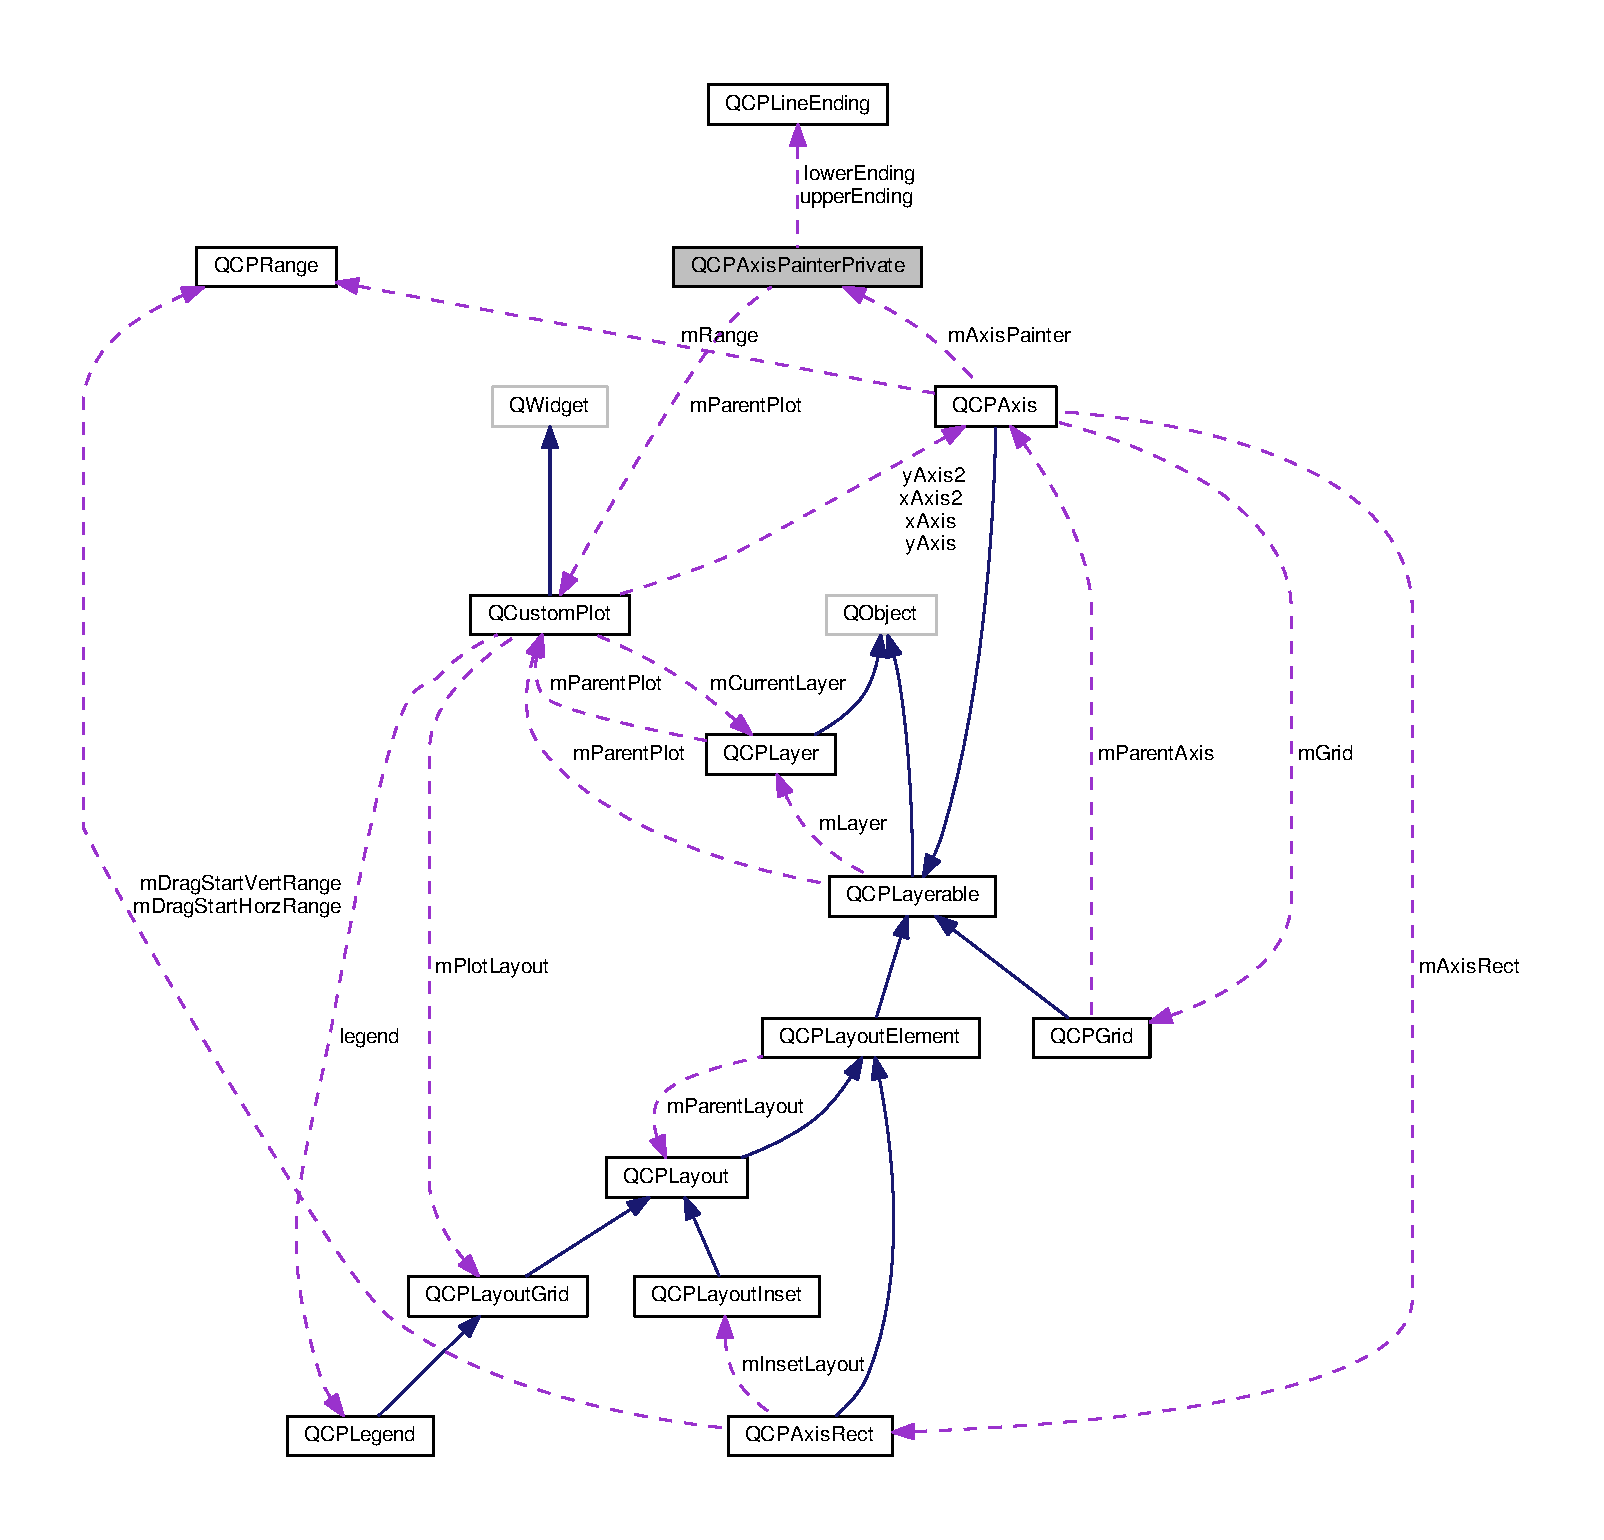
\includegraphics[width=350pt]{classQCPAxisPainterPrivate__coll__graph}
\end{center}
\end{figure}
\subsection*{Classes}
\begin{DoxyCompactItemize}
\item 
struct \hyperlink{structQCPAxisPainterPrivate_1_1CachedLabel}{Cached\+Label}
\item 
struct \hyperlink{structQCPAxisPainterPrivate_1_1TickLabelData}{Tick\+Label\+Data}
\end{DoxyCompactItemize}
\subsection*{Public Member Functions}
\begin{DoxyCompactItemize}
\item 
\hyperlink{classQCPAxisPainterPrivate_a0f14aa5c4aa83dbcd68984a7c73bf94f}{Q\+C\+P\+Axis\+Painter\+Private} (\hyperlink{classQCustomPlot}{Q\+Custom\+Plot} $\ast$parent\+Plot)
\item 
virtual \hyperlink{classQCPAxisPainterPrivate_a7c7f95313f0f78c3c3975f822a5fea35}{$\sim$\+Q\+C\+P\+Axis\+Painter\+Private} ()
\item 
virtual void \hyperlink{classQCPAxisPainterPrivate_a0207a99bdf9c4f70af20928898ddc2fc}{draw} (\hyperlink{classQCPPainter}{Q\+C\+P\+Painter} $\ast$painter)
\item 
virtual int \hyperlink{classQCPAxisPainterPrivate_a8b2dc0bd2ccbf6bd450733ec9e410a38}{size} () const 
\item 
void \hyperlink{classQCPAxisPainterPrivate_a7b6806e32c44384fd0ae4dcdaa72b1b5}{clear\+Cache} ()
\item 
Q\+Rect \hyperlink{classQCPAxisPainterPrivate_aaf93529ac60215ea020cdff5635c3e80}{axis\+Selection\+Box} () const 
\item 
Q\+Rect \hyperlink{classQCPAxisPainterPrivate_af02fc189ab8460c202eb4138c9aca516}{tick\+Labels\+Selection\+Box} () const 
\item 
Q\+Rect \hyperlink{classQCPAxisPainterPrivate_ae907476bf8cf0ecd17620575e17c06b1}{label\+Selection\+Box} () const 
\end{DoxyCompactItemize}
\subsection*{Public Attributes}
\begin{DoxyCompactItemize}
\item 
\hyperlink{classQCPAxis_ae2bcc1728b382f10f064612b368bc18a}{Q\+C\+P\+Axis\+::\+Axis\+Type} \hyperlink{classQCPAxisPainterPrivate_ae04594e97417336933d807c86d353098}{type}
\item 
Q\+Pen \hyperlink{classQCPAxisPainterPrivate_ab4affb27ae3485fecb7466622cabcbb2}{base\+Pen}
\item 
\hyperlink{classQCPLineEnding}{Q\+C\+P\+Line\+Ending} \hyperlink{classQCPAxisPainterPrivate_a077696dd1e7efb96e4c199f521433e24}{lower\+Ending}
\item 
\hyperlink{classQCPLineEnding}{Q\+C\+P\+Line\+Ending} \hyperlink{classQCPAxisPainterPrivate_af764be913be5f924700ac9bbb8c01139}{upper\+Ending}
\item 
int \hyperlink{classQCPAxisPainterPrivate_a3f7465372df132bf7814345ea697dd34}{label\+Padding}
\item 
Q\+Font \hyperlink{classQCPAxisPainterPrivate_add1ff1030fbc36112c19b1468ad82d55}{label\+Font}
\item 
Q\+Color \hyperlink{classQCPAxisPainterPrivate_a5c36467daf057da0cf0792f3c5a06089}{label\+Color}
\item 
Q\+String \hyperlink{classQCPAxisPainterPrivate_afe004c322f92543c0467afc02da6cf6d}{label}
\item 
int \hyperlink{classQCPAxisPainterPrivate_a264cfa080e84e536cf2d1ab9c5d5cc5f}{tick\+Label\+Padding}
\item 
double \hyperlink{classQCPAxisPainterPrivate_ae6ade9232a8e400924009e8edca94bac}{tick\+Label\+Rotation}
\item 
\hyperlink{classQCPAxis_a24b13374b9b8f75f47eed2ea78c37db9}{Q\+C\+P\+Axis\+::\+Label\+Side} \hyperlink{classQCPAxisPainterPrivate_a9d27f7625fcfbeb3a60193d0c18fc7e9}{tick\+Label\+Side}
\item 
bool \hyperlink{classQCPAxisPainterPrivate_a546d22b10ddb5ca8582b7deb90223a91}{substitute\+Exponent}
\item 
bool \hyperlink{classQCPAxisPainterPrivate_a0deb7524009140f00a774dfd286d002c}{number\+Multiply\+Cross}
\item 
int \hyperlink{classQCPAxisPainterPrivate_ae7360ff805fc6097019de8b35ffbd7e7}{tick\+Length\+In}
\item 
int \hyperlink{classQCPAxisPainterPrivate_acbebb1f868906200f968627bc907b77d}{tick\+Length\+Out}
\item 
int \hyperlink{classQCPAxisPainterPrivate_af11f7d83021c9cb3b0e76fe7814c6110}{sub\+Tick\+Length\+In}
\item 
int \hyperlink{classQCPAxisPainterPrivate_a5f1afddc3dc7ccc4d5adcbcd8f0c2218}{sub\+Tick\+Length\+Out}
\item 
Q\+Pen \hyperlink{classQCPAxisPainterPrivate_a389dde97f02fdee23965e4736e7d8c62}{tick\+Pen}
\item 
Q\+Pen \hyperlink{classQCPAxisPainterPrivate_a9b9cf594cd16575f52ecda9abef4e412}{sub\+Tick\+Pen}
\item 
Q\+Font \hyperlink{classQCPAxisPainterPrivate_a06cb4b185feb1e560e01d65887e4d80d}{tick\+Label\+Font}
\item 
Q\+Color \hyperlink{classQCPAxisPainterPrivate_a88032cf15c997e3956b79617b859e8ad}{tick\+Label\+Color}
\item 
Q\+Rect \hyperlink{classQCPAxisPainterPrivate_afcd55b0e1ecd689fffd2b1fc75dc7732}{axis\+Rect}
\item 
Q\+Rect \hyperlink{classQCPAxisPainterPrivate_a8627dc6b40781e3291bb508e4ac574d6}{viewport\+Rect}
\item 
double \hyperlink{classQCPAxisPainterPrivate_aea226a1e39357d71f66d85093e30a830}{offset}
\item 
bool \hyperlink{classQCPAxisPainterPrivate_a68353c2eeabd00d96a2e36a0b3809cb2}{abbreviate\+Decimal\+Powers}
\item 
bool \hyperlink{classQCPAxisPainterPrivate_a06d0ef3f4f1b567feb84196fc3b140da}{reversed\+Endings}
\item 
Q\+Vector$<$ double $>$ \hyperlink{classQCPAxisPainterPrivate_afcde7484bbcc1004b8f59ab984ada6f9}{sub\+Tick\+Positions}
\item 
Q\+Vector$<$ double $>$ \hyperlink{classQCPAxisPainterPrivate_ae55e3dc2cf2af8d8a6e7235ccab54786}{tick\+Positions}
\item 
Q\+Vector$<$ Q\+String $>$ \hyperlink{classQCPAxisPainterPrivate_ad0a4998ca358ba751e84fca45a025abd}{tick\+Labels}
\end{DoxyCompactItemize}
\subsection*{Protected Member Functions}
\begin{DoxyCompactItemize}
\item 
virtual Q\+Byte\+Array \hyperlink{classQCPAxisPainterPrivate_a91a023bbefe1c3bf330570c0b985de84}{generate\+Label\+Parameter\+Hash} () const 
\item 
virtual void \hyperlink{classQCPAxisPainterPrivate_af8fe7350c19575bc33ca770f9b3a15fd}{place\+Tick\+Label} (\hyperlink{classQCPPainter}{Q\+C\+P\+Painter} $\ast$painter, double position, int distance\+To\+Axis, const Q\+String \&text, Q\+Size $\ast$tick\+Labels\+Size)
\item 
virtual void \hyperlink{classQCPAxisPainterPrivate_ad8f2f12cd35b8189e8bf96679e873933}{draw\+Tick\+Label} (\hyperlink{classQCPPainter}{Q\+C\+P\+Painter} $\ast$painter, double \hyperlink{qualification__task_8cpp_a6150e0515f7202e2fb518f7206ed97dc}{x}, double y, const \hyperlink{structQCPAxisPainterPrivate_1_1TickLabelData}{Tick\+Label\+Data} \&label\+Data) const 
\item 
virtual \hyperlink{structQCPAxisPainterPrivate_1_1TickLabelData}{Tick\+Label\+Data} \hyperlink{classQCPAxisPainterPrivate_ad9f24fbcbf9d8c92b34d9d00b010e6a3}{get\+Tick\+Label\+Data} (const Q\+Font \&font, const Q\+String \&text) const 
\item 
virtual Q\+PointF \hyperlink{classQCPAxisPainterPrivate_a6b02e6fd70cc65f726ca8cb3e6f16de4}{get\+Tick\+Label\+Draw\+Offset} (const \hyperlink{structQCPAxisPainterPrivate_1_1TickLabelData}{Tick\+Label\+Data} \&label\+Data) const 
\item 
virtual void \hyperlink{classQCPAxisPainterPrivate_a8a7c82303e272485621fde78a5b674f9}{get\+Max\+Tick\+Label\+Size} (const Q\+Font \&font, const Q\+String \&text, Q\+Size $\ast$tick\+Labels\+Size) const 
\end{DoxyCompactItemize}
\subsection*{Protected Attributes}
\begin{DoxyCompactItemize}
\item 
\hyperlink{classQCustomPlot}{Q\+Custom\+Plot} $\ast$ \hyperlink{classQCPAxisPainterPrivate_a882029a5f2d4abd71289d415c9b90a28}{m\+Parent\+Plot}
\item 
Q\+Byte\+Array \hyperlink{classQCPAxisPainterPrivate_aab8be59df22ed4e43e3a6d511cbc466a}{m\+Label\+Parameter\+Hash}
\item 
Q\+Cache$<$ Q\+String, \hyperlink{structQCPAxisPainterPrivate_1_1CachedLabel}{Cached\+Label} $>$ \hyperlink{classQCPAxisPainterPrivate_a07ac270ea0c0ae084debd48d6a740e35}{m\+Label\+Cache}
\item 
Q\+Rect \hyperlink{classQCPAxisPainterPrivate_a9d7586f4923994488bdd006415b13f5f}{m\+Axis\+Selection\+Box}
\item 
Q\+Rect \hyperlink{classQCPAxisPainterPrivate_a0adaf5f1d89be0f32dc4a904d157e5a9}{m\+Tick\+Labels\+Selection\+Box}
\item 
Q\+Rect \hyperlink{classQCPAxisPainterPrivate_abac9a47048d537f72ca147b6f29d30f1}{m\+Label\+Selection\+Box}
\end{DoxyCompactItemize}


\subsection{Constructor \& Destructor Documentation}
\index{Q\+C\+P\+Axis\+Painter\+Private@{Q\+C\+P\+Axis\+Painter\+Private}!Q\+C\+P\+Axis\+Painter\+Private@{Q\+C\+P\+Axis\+Painter\+Private}}
\index{Q\+C\+P\+Axis\+Painter\+Private@{Q\+C\+P\+Axis\+Painter\+Private}!Q\+C\+P\+Axis\+Painter\+Private@{Q\+C\+P\+Axis\+Painter\+Private}}
\subsubsection[{\texorpdfstring{Q\+C\+P\+Axis\+Painter\+Private(\+Q\+Custom\+Plot $\ast$parent\+Plot)}{QCPAxisPainterPrivate(QCustomPlot *parentPlot)}}]{\setlength{\rightskip}{0pt plus 5cm}Q\+C\+P\+Axis\+Painter\+Private\+::\+Q\+C\+P\+Axis\+Painter\+Private (
\begin{DoxyParamCaption}
\item[{{\bf Q\+Custom\+Plot} $\ast$}]{parent\+Plot}
\end{DoxyParamCaption}
)\hspace{0.3cm}{\ttfamily [explicit]}}\hypertarget{classQCPAxisPainterPrivate_a0f14aa5c4aa83dbcd68984a7c73bf94f}{}\label{classQCPAxisPainterPrivate_a0f14aa5c4aa83dbcd68984a7c73bf94f}
Constructs a \hyperlink{classQCPAxisPainterPrivate}{Q\+C\+P\+Axis\+Painter\+Private} instance. Make sure to not create a new instance on every redraw, to utilize the caching mechanisms. \index{Q\+C\+P\+Axis\+Painter\+Private@{Q\+C\+P\+Axis\+Painter\+Private}!````~Q\+C\+P\+Axis\+Painter\+Private@{$\sim$\+Q\+C\+P\+Axis\+Painter\+Private}}
\index{````~Q\+C\+P\+Axis\+Painter\+Private@{$\sim$\+Q\+C\+P\+Axis\+Painter\+Private}!Q\+C\+P\+Axis\+Painter\+Private@{Q\+C\+P\+Axis\+Painter\+Private}}
\subsubsection[{\texorpdfstring{$\sim$\+Q\+C\+P\+Axis\+Painter\+Private()}{~QCPAxisPainterPrivate()}}]{\setlength{\rightskip}{0pt plus 5cm}Q\+C\+P\+Axis\+Painter\+Private\+::$\sim$\+Q\+C\+P\+Axis\+Painter\+Private (
\begin{DoxyParamCaption}
{}
\end{DoxyParamCaption}
)\hspace{0.3cm}{\ttfamily [virtual]}}\hypertarget{classQCPAxisPainterPrivate_a7c7f95313f0f78c3c3975f822a5fea35}{}\label{classQCPAxisPainterPrivate_a7c7f95313f0f78c3c3975f822a5fea35}


\subsection{Member Function Documentation}
\index{Q\+C\+P\+Axis\+Painter\+Private@{Q\+C\+P\+Axis\+Painter\+Private}!axis\+Selection\+Box@{axis\+Selection\+Box}}
\index{axis\+Selection\+Box@{axis\+Selection\+Box}!Q\+C\+P\+Axis\+Painter\+Private@{Q\+C\+P\+Axis\+Painter\+Private}}
\subsubsection[{\texorpdfstring{axis\+Selection\+Box() const }{axisSelectionBox() const }}]{\setlength{\rightskip}{0pt plus 5cm}Q\+Rect Q\+C\+P\+Axis\+Painter\+Private\+::axis\+Selection\+Box (
\begin{DoxyParamCaption}
{}
\end{DoxyParamCaption}
) const\hspace{0.3cm}{\ttfamily [inline]}}\hypertarget{classQCPAxisPainterPrivate_aaf93529ac60215ea020cdff5635c3e80}{}\label{classQCPAxisPainterPrivate_aaf93529ac60215ea020cdff5635c3e80}
\index{Q\+C\+P\+Axis\+Painter\+Private@{Q\+C\+P\+Axis\+Painter\+Private}!clear\+Cache@{clear\+Cache}}
\index{clear\+Cache@{clear\+Cache}!Q\+C\+P\+Axis\+Painter\+Private@{Q\+C\+P\+Axis\+Painter\+Private}}
\subsubsection[{\texorpdfstring{clear\+Cache()}{clearCache()}}]{\setlength{\rightskip}{0pt plus 5cm}void Q\+C\+P\+Axis\+Painter\+Private\+::clear\+Cache (
\begin{DoxyParamCaption}
{}
\end{DoxyParamCaption}
)}\hypertarget{classQCPAxisPainterPrivate_a7b6806e32c44384fd0ae4dcdaa72b1b5}{}\label{classQCPAxisPainterPrivate_a7b6806e32c44384fd0ae4dcdaa72b1b5}
\index{Q\+C\+P\+Axis\+Painter\+Private@{Q\+C\+P\+Axis\+Painter\+Private}!draw@{draw}}
\index{draw@{draw}!Q\+C\+P\+Axis\+Painter\+Private@{Q\+C\+P\+Axis\+Painter\+Private}}
\subsubsection[{\texorpdfstring{draw(\+Q\+C\+P\+Painter $\ast$painter)}{draw(QCPPainter *painter)}}]{\setlength{\rightskip}{0pt plus 5cm}void Q\+C\+P\+Axis\+Painter\+Private\+::draw (
\begin{DoxyParamCaption}
\item[{{\bf Q\+C\+P\+Painter} $\ast$}]{painter}
\end{DoxyParamCaption}
)\hspace{0.3cm}{\ttfamily [virtual]}}\hypertarget{classQCPAxisPainterPrivate_a0207a99bdf9c4f70af20928898ddc2fc}{}\label{classQCPAxisPainterPrivate_a0207a99bdf9c4f70af20928898ddc2fc}
\index{Q\+C\+P\+Axis\+Painter\+Private@{Q\+C\+P\+Axis\+Painter\+Private}!draw\+Tick\+Label@{draw\+Tick\+Label}}
\index{draw\+Tick\+Label@{draw\+Tick\+Label}!Q\+C\+P\+Axis\+Painter\+Private@{Q\+C\+P\+Axis\+Painter\+Private}}
\subsubsection[{\texorpdfstring{draw\+Tick\+Label(\+Q\+C\+P\+Painter $\ast$painter, double x, double y, const Tick\+Label\+Data \&label\+Data) const }{drawTickLabel(QCPPainter *painter, double x, double y, const TickLabelData &labelData) const }}]{\setlength{\rightskip}{0pt plus 5cm}void Q\+C\+P\+Axis\+Painter\+Private\+::draw\+Tick\+Label (
\begin{DoxyParamCaption}
\item[{{\bf Q\+C\+P\+Painter} $\ast$}]{painter, }
\item[{double}]{x, }
\item[{double}]{y, }
\item[{const {\bf Tick\+Label\+Data} \&}]{label\+Data}
\end{DoxyParamCaption}
) const\hspace{0.3cm}{\ttfamily [protected]}, {\ttfamily [virtual]}}\hypertarget{classQCPAxisPainterPrivate_ad8f2f12cd35b8189e8bf96679e873933}{}\label{classQCPAxisPainterPrivate_ad8f2f12cd35b8189e8bf96679e873933}
\index{Q\+C\+P\+Axis\+Painter\+Private@{Q\+C\+P\+Axis\+Painter\+Private}!generate\+Label\+Parameter\+Hash@{generate\+Label\+Parameter\+Hash}}
\index{generate\+Label\+Parameter\+Hash@{generate\+Label\+Parameter\+Hash}!Q\+C\+P\+Axis\+Painter\+Private@{Q\+C\+P\+Axis\+Painter\+Private}}
\subsubsection[{\texorpdfstring{generate\+Label\+Parameter\+Hash() const }{generateLabelParameterHash() const }}]{\setlength{\rightskip}{0pt plus 5cm}Q\+Byte\+Array Q\+C\+P\+Axis\+Painter\+Private\+::generate\+Label\+Parameter\+Hash (
\begin{DoxyParamCaption}
{}
\end{DoxyParamCaption}
) const\hspace{0.3cm}{\ttfamily [protected]}, {\ttfamily [virtual]}}\hypertarget{classQCPAxisPainterPrivate_a91a023bbefe1c3bf330570c0b985de84}{}\label{classQCPAxisPainterPrivate_a91a023bbefe1c3bf330570c0b985de84}
\index{Q\+C\+P\+Axis\+Painter\+Private@{Q\+C\+P\+Axis\+Painter\+Private}!get\+Max\+Tick\+Label\+Size@{get\+Max\+Tick\+Label\+Size}}
\index{get\+Max\+Tick\+Label\+Size@{get\+Max\+Tick\+Label\+Size}!Q\+C\+P\+Axis\+Painter\+Private@{Q\+C\+P\+Axis\+Painter\+Private}}
\subsubsection[{\texorpdfstring{get\+Max\+Tick\+Label\+Size(const Q\+Font \&font, const Q\+String \&text, Q\+Size $\ast$tick\+Labels\+Size) const }{getMaxTickLabelSize(const QFont &font, const QString &text, QSize *tickLabelsSize) const }}]{\setlength{\rightskip}{0pt plus 5cm}void Q\+C\+P\+Axis\+Painter\+Private\+::get\+Max\+Tick\+Label\+Size (
\begin{DoxyParamCaption}
\item[{const Q\+Font \&}]{font, }
\item[{const Q\+String \&}]{text, }
\item[{Q\+Size $\ast$}]{tick\+Labels\+Size}
\end{DoxyParamCaption}
) const\hspace{0.3cm}{\ttfamily [protected]}, {\ttfamily [virtual]}}\hypertarget{classQCPAxisPainterPrivate_a8a7c82303e272485621fde78a5b674f9}{}\label{classQCPAxisPainterPrivate_a8a7c82303e272485621fde78a5b674f9}
\index{Q\+C\+P\+Axis\+Painter\+Private@{Q\+C\+P\+Axis\+Painter\+Private}!get\+Tick\+Label\+Data@{get\+Tick\+Label\+Data}}
\index{get\+Tick\+Label\+Data@{get\+Tick\+Label\+Data}!Q\+C\+P\+Axis\+Painter\+Private@{Q\+C\+P\+Axis\+Painter\+Private}}
\subsubsection[{\texorpdfstring{get\+Tick\+Label\+Data(const Q\+Font \&font, const Q\+String \&text) const }{getTickLabelData(const QFont &font, const QString &text) const }}]{\setlength{\rightskip}{0pt plus 5cm}{\bf Q\+C\+P\+Axis\+Painter\+Private\+::\+Tick\+Label\+Data} Q\+C\+P\+Axis\+Painter\+Private\+::get\+Tick\+Label\+Data (
\begin{DoxyParamCaption}
\item[{const Q\+Font \&}]{font, }
\item[{const Q\+String \&}]{text}
\end{DoxyParamCaption}
) const\hspace{0.3cm}{\ttfamily [protected]}, {\ttfamily [virtual]}}\hypertarget{classQCPAxisPainterPrivate_ad9f24fbcbf9d8c92b34d9d00b010e6a3}{}\label{classQCPAxisPainterPrivate_ad9f24fbcbf9d8c92b34d9d00b010e6a3}
\index{Q\+C\+P\+Axis\+Painter\+Private@{Q\+C\+P\+Axis\+Painter\+Private}!get\+Tick\+Label\+Draw\+Offset@{get\+Tick\+Label\+Draw\+Offset}}
\index{get\+Tick\+Label\+Draw\+Offset@{get\+Tick\+Label\+Draw\+Offset}!Q\+C\+P\+Axis\+Painter\+Private@{Q\+C\+P\+Axis\+Painter\+Private}}
\subsubsection[{\texorpdfstring{get\+Tick\+Label\+Draw\+Offset(const Tick\+Label\+Data \&label\+Data) const }{getTickLabelDrawOffset(const TickLabelData &labelData) const }}]{\setlength{\rightskip}{0pt plus 5cm}Q\+PointF Q\+C\+P\+Axis\+Painter\+Private\+::get\+Tick\+Label\+Draw\+Offset (
\begin{DoxyParamCaption}
\item[{const {\bf Tick\+Label\+Data} \&}]{label\+Data}
\end{DoxyParamCaption}
) const\hspace{0.3cm}{\ttfamily [protected]}, {\ttfamily [virtual]}}\hypertarget{classQCPAxisPainterPrivate_a6b02e6fd70cc65f726ca8cb3e6f16de4}{}\label{classQCPAxisPainterPrivate_a6b02e6fd70cc65f726ca8cb3e6f16de4}
\index{Q\+C\+P\+Axis\+Painter\+Private@{Q\+C\+P\+Axis\+Painter\+Private}!label\+Selection\+Box@{label\+Selection\+Box}}
\index{label\+Selection\+Box@{label\+Selection\+Box}!Q\+C\+P\+Axis\+Painter\+Private@{Q\+C\+P\+Axis\+Painter\+Private}}
\subsubsection[{\texorpdfstring{label\+Selection\+Box() const }{labelSelectionBox() const }}]{\setlength{\rightskip}{0pt plus 5cm}Q\+Rect Q\+C\+P\+Axis\+Painter\+Private\+::label\+Selection\+Box (
\begin{DoxyParamCaption}
{}
\end{DoxyParamCaption}
) const\hspace{0.3cm}{\ttfamily [inline]}}\hypertarget{classQCPAxisPainterPrivate_ae907476bf8cf0ecd17620575e17c06b1}{}\label{classQCPAxisPainterPrivate_ae907476bf8cf0ecd17620575e17c06b1}
\index{Q\+C\+P\+Axis\+Painter\+Private@{Q\+C\+P\+Axis\+Painter\+Private}!place\+Tick\+Label@{place\+Tick\+Label}}
\index{place\+Tick\+Label@{place\+Tick\+Label}!Q\+C\+P\+Axis\+Painter\+Private@{Q\+C\+P\+Axis\+Painter\+Private}}
\subsubsection[{\texorpdfstring{place\+Tick\+Label(\+Q\+C\+P\+Painter $\ast$painter, double position, int distance\+To\+Axis, const Q\+String \&text, Q\+Size $\ast$tick\+Labels\+Size)}{placeTickLabel(QCPPainter *painter, double position, int distanceToAxis, const QString &text, QSize *tickLabelsSize)}}]{\setlength{\rightskip}{0pt plus 5cm}void Q\+C\+P\+Axis\+Painter\+Private\+::place\+Tick\+Label (
\begin{DoxyParamCaption}
\item[{{\bf Q\+C\+P\+Painter} $\ast$}]{painter, }
\item[{double}]{position, }
\item[{int}]{distance\+To\+Axis, }
\item[{const Q\+String \&}]{text, }
\item[{Q\+Size $\ast$}]{tick\+Labels\+Size}
\end{DoxyParamCaption}
)\hspace{0.3cm}{\ttfamily [protected]}, {\ttfamily [virtual]}}\hypertarget{classQCPAxisPainterPrivate_af8fe7350c19575bc33ca770f9b3a15fd}{}\label{classQCPAxisPainterPrivate_af8fe7350c19575bc33ca770f9b3a15fd}
\index{Q\+C\+P\+Axis\+Painter\+Private@{Q\+C\+P\+Axis\+Painter\+Private}!size@{size}}
\index{size@{size}!Q\+C\+P\+Axis\+Painter\+Private@{Q\+C\+P\+Axis\+Painter\+Private}}
\subsubsection[{\texorpdfstring{size() const }{size() const }}]{\setlength{\rightskip}{0pt plus 5cm}int Q\+C\+P\+Axis\+Painter\+Private\+::size (
\begin{DoxyParamCaption}
{}
\end{DoxyParamCaption}
) const\hspace{0.3cm}{\ttfamily [virtual]}}\hypertarget{classQCPAxisPainterPrivate_a8b2dc0bd2ccbf6bd450733ec9e410a38}{}\label{classQCPAxisPainterPrivate_a8b2dc0bd2ccbf6bd450733ec9e410a38}
\index{Q\+C\+P\+Axis\+Painter\+Private@{Q\+C\+P\+Axis\+Painter\+Private}!tick\+Labels\+Selection\+Box@{tick\+Labels\+Selection\+Box}}
\index{tick\+Labels\+Selection\+Box@{tick\+Labels\+Selection\+Box}!Q\+C\+P\+Axis\+Painter\+Private@{Q\+C\+P\+Axis\+Painter\+Private}}
\subsubsection[{\texorpdfstring{tick\+Labels\+Selection\+Box() const }{tickLabelsSelectionBox() const }}]{\setlength{\rightskip}{0pt plus 5cm}Q\+Rect Q\+C\+P\+Axis\+Painter\+Private\+::tick\+Labels\+Selection\+Box (
\begin{DoxyParamCaption}
{}
\end{DoxyParamCaption}
) const\hspace{0.3cm}{\ttfamily [inline]}}\hypertarget{classQCPAxisPainterPrivate_af02fc189ab8460c202eb4138c9aca516}{}\label{classQCPAxisPainterPrivate_af02fc189ab8460c202eb4138c9aca516}


\subsection{Member Data Documentation}
\index{Q\+C\+P\+Axis\+Painter\+Private@{Q\+C\+P\+Axis\+Painter\+Private}!abbreviate\+Decimal\+Powers@{abbreviate\+Decimal\+Powers}}
\index{abbreviate\+Decimal\+Powers@{abbreviate\+Decimal\+Powers}!Q\+C\+P\+Axis\+Painter\+Private@{Q\+C\+P\+Axis\+Painter\+Private}}
\subsubsection[{\texorpdfstring{abbreviate\+Decimal\+Powers}{abbreviateDecimalPowers}}]{\setlength{\rightskip}{0pt plus 5cm}bool Q\+C\+P\+Axis\+Painter\+Private\+::abbreviate\+Decimal\+Powers}\hypertarget{classQCPAxisPainterPrivate_a68353c2eeabd00d96a2e36a0b3809cb2}{}\label{classQCPAxisPainterPrivate_a68353c2eeabd00d96a2e36a0b3809cb2}
\index{Q\+C\+P\+Axis\+Painter\+Private@{Q\+C\+P\+Axis\+Painter\+Private}!axis\+Rect@{axis\+Rect}}
\index{axis\+Rect@{axis\+Rect}!Q\+C\+P\+Axis\+Painter\+Private@{Q\+C\+P\+Axis\+Painter\+Private}}
\subsubsection[{\texorpdfstring{axis\+Rect}{axisRect}}]{\setlength{\rightskip}{0pt plus 5cm}Q\+Rect Q\+C\+P\+Axis\+Painter\+Private\+::axis\+Rect}\hypertarget{classQCPAxisPainterPrivate_afcd55b0e1ecd689fffd2b1fc75dc7732}{}\label{classQCPAxisPainterPrivate_afcd55b0e1ecd689fffd2b1fc75dc7732}
\index{Q\+C\+P\+Axis\+Painter\+Private@{Q\+C\+P\+Axis\+Painter\+Private}!base\+Pen@{base\+Pen}}
\index{base\+Pen@{base\+Pen}!Q\+C\+P\+Axis\+Painter\+Private@{Q\+C\+P\+Axis\+Painter\+Private}}
\subsubsection[{\texorpdfstring{base\+Pen}{basePen}}]{\setlength{\rightskip}{0pt plus 5cm}Q\+Pen Q\+C\+P\+Axis\+Painter\+Private\+::base\+Pen}\hypertarget{classQCPAxisPainterPrivate_ab4affb27ae3485fecb7466622cabcbb2}{}\label{classQCPAxisPainterPrivate_ab4affb27ae3485fecb7466622cabcbb2}
\index{Q\+C\+P\+Axis\+Painter\+Private@{Q\+C\+P\+Axis\+Painter\+Private}!label@{label}}
\index{label@{label}!Q\+C\+P\+Axis\+Painter\+Private@{Q\+C\+P\+Axis\+Painter\+Private}}
\subsubsection[{\texorpdfstring{label}{label}}]{\setlength{\rightskip}{0pt plus 5cm}Q\+String Q\+C\+P\+Axis\+Painter\+Private\+::label}\hypertarget{classQCPAxisPainterPrivate_afe004c322f92543c0467afc02da6cf6d}{}\label{classQCPAxisPainterPrivate_afe004c322f92543c0467afc02da6cf6d}
\index{Q\+C\+P\+Axis\+Painter\+Private@{Q\+C\+P\+Axis\+Painter\+Private}!label\+Color@{label\+Color}}
\index{label\+Color@{label\+Color}!Q\+C\+P\+Axis\+Painter\+Private@{Q\+C\+P\+Axis\+Painter\+Private}}
\subsubsection[{\texorpdfstring{label\+Color}{labelColor}}]{\setlength{\rightskip}{0pt plus 5cm}Q\+Color Q\+C\+P\+Axis\+Painter\+Private\+::label\+Color}\hypertarget{classQCPAxisPainterPrivate_a5c36467daf057da0cf0792f3c5a06089}{}\label{classQCPAxisPainterPrivate_a5c36467daf057da0cf0792f3c5a06089}
\index{Q\+C\+P\+Axis\+Painter\+Private@{Q\+C\+P\+Axis\+Painter\+Private}!label\+Font@{label\+Font}}
\index{label\+Font@{label\+Font}!Q\+C\+P\+Axis\+Painter\+Private@{Q\+C\+P\+Axis\+Painter\+Private}}
\subsubsection[{\texorpdfstring{label\+Font}{labelFont}}]{\setlength{\rightskip}{0pt plus 5cm}Q\+Font Q\+C\+P\+Axis\+Painter\+Private\+::label\+Font}\hypertarget{classQCPAxisPainterPrivate_add1ff1030fbc36112c19b1468ad82d55}{}\label{classQCPAxisPainterPrivate_add1ff1030fbc36112c19b1468ad82d55}
\index{Q\+C\+P\+Axis\+Painter\+Private@{Q\+C\+P\+Axis\+Painter\+Private}!label\+Padding@{label\+Padding}}
\index{label\+Padding@{label\+Padding}!Q\+C\+P\+Axis\+Painter\+Private@{Q\+C\+P\+Axis\+Painter\+Private}}
\subsubsection[{\texorpdfstring{label\+Padding}{labelPadding}}]{\setlength{\rightskip}{0pt plus 5cm}int Q\+C\+P\+Axis\+Painter\+Private\+::label\+Padding}\hypertarget{classQCPAxisPainterPrivate_a3f7465372df132bf7814345ea697dd34}{}\label{classQCPAxisPainterPrivate_a3f7465372df132bf7814345ea697dd34}
\index{Q\+C\+P\+Axis\+Painter\+Private@{Q\+C\+P\+Axis\+Painter\+Private}!lower\+Ending@{lower\+Ending}}
\index{lower\+Ending@{lower\+Ending}!Q\+C\+P\+Axis\+Painter\+Private@{Q\+C\+P\+Axis\+Painter\+Private}}
\subsubsection[{\texorpdfstring{lower\+Ending}{lowerEnding}}]{\setlength{\rightskip}{0pt plus 5cm}{\bf Q\+C\+P\+Line\+Ending} Q\+C\+P\+Axis\+Painter\+Private\+::lower\+Ending}\hypertarget{classQCPAxisPainterPrivate_a077696dd1e7efb96e4c199f521433e24}{}\label{classQCPAxisPainterPrivate_a077696dd1e7efb96e4c199f521433e24}
\index{Q\+C\+P\+Axis\+Painter\+Private@{Q\+C\+P\+Axis\+Painter\+Private}!m\+Axis\+Selection\+Box@{m\+Axis\+Selection\+Box}}
\index{m\+Axis\+Selection\+Box@{m\+Axis\+Selection\+Box}!Q\+C\+P\+Axis\+Painter\+Private@{Q\+C\+P\+Axis\+Painter\+Private}}
\subsubsection[{\texorpdfstring{m\+Axis\+Selection\+Box}{mAxisSelectionBox}}]{\setlength{\rightskip}{0pt plus 5cm}Q\+Rect Q\+C\+P\+Axis\+Painter\+Private\+::m\+Axis\+Selection\+Box\hspace{0.3cm}{\ttfamily [protected]}}\hypertarget{classQCPAxisPainterPrivate_a9d7586f4923994488bdd006415b13f5f}{}\label{classQCPAxisPainterPrivate_a9d7586f4923994488bdd006415b13f5f}
\index{Q\+C\+P\+Axis\+Painter\+Private@{Q\+C\+P\+Axis\+Painter\+Private}!m\+Label\+Cache@{m\+Label\+Cache}}
\index{m\+Label\+Cache@{m\+Label\+Cache}!Q\+C\+P\+Axis\+Painter\+Private@{Q\+C\+P\+Axis\+Painter\+Private}}
\subsubsection[{\texorpdfstring{m\+Label\+Cache}{mLabelCache}}]{\setlength{\rightskip}{0pt plus 5cm}Q\+Cache$<$Q\+String, {\bf Cached\+Label}$>$ Q\+C\+P\+Axis\+Painter\+Private\+::m\+Label\+Cache\hspace{0.3cm}{\ttfamily [protected]}}\hypertarget{classQCPAxisPainterPrivate_a07ac270ea0c0ae084debd48d6a740e35}{}\label{classQCPAxisPainterPrivate_a07ac270ea0c0ae084debd48d6a740e35}
\index{Q\+C\+P\+Axis\+Painter\+Private@{Q\+C\+P\+Axis\+Painter\+Private}!m\+Label\+Parameter\+Hash@{m\+Label\+Parameter\+Hash}}
\index{m\+Label\+Parameter\+Hash@{m\+Label\+Parameter\+Hash}!Q\+C\+P\+Axis\+Painter\+Private@{Q\+C\+P\+Axis\+Painter\+Private}}
\subsubsection[{\texorpdfstring{m\+Label\+Parameter\+Hash}{mLabelParameterHash}}]{\setlength{\rightskip}{0pt plus 5cm}Q\+Byte\+Array Q\+C\+P\+Axis\+Painter\+Private\+::m\+Label\+Parameter\+Hash\hspace{0.3cm}{\ttfamily [protected]}}\hypertarget{classQCPAxisPainterPrivate_aab8be59df22ed4e43e3a6d511cbc466a}{}\label{classQCPAxisPainterPrivate_aab8be59df22ed4e43e3a6d511cbc466a}
\index{Q\+C\+P\+Axis\+Painter\+Private@{Q\+C\+P\+Axis\+Painter\+Private}!m\+Label\+Selection\+Box@{m\+Label\+Selection\+Box}}
\index{m\+Label\+Selection\+Box@{m\+Label\+Selection\+Box}!Q\+C\+P\+Axis\+Painter\+Private@{Q\+C\+P\+Axis\+Painter\+Private}}
\subsubsection[{\texorpdfstring{m\+Label\+Selection\+Box}{mLabelSelectionBox}}]{\setlength{\rightskip}{0pt plus 5cm}Q\+Rect Q\+C\+P\+Axis\+Painter\+Private\+::m\+Label\+Selection\+Box\hspace{0.3cm}{\ttfamily [protected]}}\hypertarget{classQCPAxisPainterPrivate_abac9a47048d537f72ca147b6f29d30f1}{}\label{classQCPAxisPainterPrivate_abac9a47048d537f72ca147b6f29d30f1}
\index{Q\+C\+P\+Axis\+Painter\+Private@{Q\+C\+P\+Axis\+Painter\+Private}!m\+Parent\+Plot@{m\+Parent\+Plot}}
\index{m\+Parent\+Plot@{m\+Parent\+Plot}!Q\+C\+P\+Axis\+Painter\+Private@{Q\+C\+P\+Axis\+Painter\+Private}}
\subsubsection[{\texorpdfstring{m\+Parent\+Plot}{mParentPlot}}]{\setlength{\rightskip}{0pt plus 5cm}{\bf Q\+Custom\+Plot}$\ast$ Q\+C\+P\+Axis\+Painter\+Private\+::m\+Parent\+Plot\hspace{0.3cm}{\ttfamily [protected]}}\hypertarget{classQCPAxisPainterPrivate_a882029a5f2d4abd71289d415c9b90a28}{}\label{classQCPAxisPainterPrivate_a882029a5f2d4abd71289d415c9b90a28}
\index{Q\+C\+P\+Axis\+Painter\+Private@{Q\+C\+P\+Axis\+Painter\+Private}!m\+Tick\+Labels\+Selection\+Box@{m\+Tick\+Labels\+Selection\+Box}}
\index{m\+Tick\+Labels\+Selection\+Box@{m\+Tick\+Labels\+Selection\+Box}!Q\+C\+P\+Axis\+Painter\+Private@{Q\+C\+P\+Axis\+Painter\+Private}}
\subsubsection[{\texorpdfstring{m\+Tick\+Labels\+Selection\+Box}{mTickLabelsSelectionBox}}]{\setlength{\rightskip}{0pt plus 5cm}Q\+Rect Q\+C\+P\+Axis\+Painter\+Private\+::m\+Tick\+Labels\+Selection\+Box\hspace{0.3cm}{\ttfamily [protected]}}\hypertarget{classQCPAxisPainterPrivate_a0adaf5f1d89be0f32dc4a904d157e5a9}{}\label{classQCPAxisPainterPrivate_a0adaf5f1d89be0f32dc4a904d157e5a9}
\index{Q\+C\+P\+Axis\+Painter\+Private@{Q\+C\+P\+Axis\+Painter\+Private}!number\+Multiply\+Cross@{number\+Multiply\+Cross}}
\index{number\+Multiply\+Cross@{number\+Multiply\+Cross}!Q\+C\+P\+Axis\+Painter\+Private@{Q\+C\+P\+Axis\+Painter\+Private}}
\subsubsection[{\texorpdfstring{number\+Multiply\+Cross}{numberMultiplyCross}}]{\setlength{\rightskip}{0pt plus 5cm}bool Q\+C\+P\+Axis\+Painter\+Private\+::number\+Multiply\+Cross}\hypertarget{classQCPAxisPainterPrivate_a0deb7524009140f00a774dfd286d002c}{}\label{classQCPAxisPainterPrivate_a0deb7524009140f00a774dfd286d002c}
\index{Q\+C\+P\+Axis\+Painter\+Private@{Q\+C\+P\+Axis\+Painter\+Private}!offset@{offset}}
\index{offset@{offset}!Q\+C\+P\+Axis\+Painter\+Private@{Q\+C\+P\+Axis\+Painter\+Private}}
\subsubsection[{\texorpdfstring{offset}{offset}}]{\setlength{\rightskip}{0pt plus 5cm}double Q\+C\+P\+Axis\+Painter\+Private\+::offset}\hypertarget{classQCPAxisPainterPrivate_aea226a1e39357d71f66d85093e30a830}{}\label{classQCPAxisPainterPrivate_aea226a1e39357d71f66d85093e30a830}
\index{Q\+C\+P\+Axis\+Painter\+Private@{Q\+C\+P\+Axis\+Painter\+Private}!reversed\+Endings@{reversed\+Endings}}
\index{reversed\+Endings@{reversed\+Endings}!Q\+C\+P\+Axis\+Painter\+Private@{Q\+C\+P\+Axis\+Painter\+Private}}
\subsubsection[{\texorpdfstring{reversed\+Endings}{reversedEndings}}]{\setlength{\rightskip}{0pt plus 5cm}bool Q\+C\+P\+Axis\+Painter\+Private\+::reversed\+Endings}\hypertarget{classQCPAxisPainterPrivate_a06d0ef3f4f1b567feb84196fc3b140da}{}\label{classQCPAxisPainterPrivate_a06d0ef3f4f1b567feb84196fc3b140da}
\index{Q\+C\+P\+Axis\+Painter\+Private@{Q\+C\+P\+Axis\+Painter\+Private}!substitute\+Exponent@{substitute\+Exponent}}
\index{substitute\+Exponent@{substitute\+Exponent}!Q\+C\+P\+Axis\+Painter\+Private@{Q\+C\+P\+Axis\+Painter\+Private}}
\subsubsection[{\texorpdfstring{substitute\+Exponent}{substituteExponent}}]{\setlength{\rightskip}{0pt plus 5cm}bool Q\+C\+P\+Axis\+Painter\+Private\+::substitute\+Exponent}\hypertarget{classQCPAxisPainterPrivate_a546d22b10ddb5ca8582b7deb90223a91}{}\label{classQCPAxisPainterPrivate_a546d22b10ddb5ca8582b7deb90223a91}
\index{Q\+C\+P\+Axis\+Painter\+Private@{Q\+C\+P\+Axis\+Painter\+Private}!sub\+Tick\+Length\+In@{sub\+Tick\+Length\+In}}
\index{sub\+Tick\+Length\+In@{sub\+Tick\+Length\+In}!Q\+C\+P\+Axis\+Painter\+Private@{Q\+C\+P\+Axis\+Painter\+Private}}
\subsubsection[{\texorpdfstring{sub\+Tick\+Length\+In}{subTickLengthIn}}]{\setlength{\rightskip}{0pt plus 5cm}int Q\+C\+P\+Axis\+Painter\+Private\+::sub\+Tick\+Length\+In}\hypertarget{classQCPAxisPainterPrivate_af11f7d83021c9cb3b0e76fe7814c6110}{}\label{classQCPAxisPainterPrivate_af11f7d83021c9cb3b0e76fe7814c6110}
\index{Q\+C\+P\+Axis\+Painter\+Private@{Q\+C\+P\+Axis\+Painter\+Private}!sub\+Tick\+Length\+Out@{sub\+Tick\+Length\+Out}}
\index{sub\+Tick\+Length\+Out@{sub\+Tick\+Length\+Out}!Q\+C\+P\+Axis\+Painter\+Private@{Q\+C\+P\+Axis\+Painter\+Private}}
\subsubsection[{\texorpdfstring{sub\+Tick\+Length\+Out}{subTickLengthOut}}]{\setlength{\rightskip}{0pt plus 5cm}int Q\+C\+P\+Axis\+Painter\+Private\+::sub\+Tick\+Length\+Out}\hypertarget{classQCPAxisPainterPrivate_a5f1afddc3dc7ccc4d5adcbcd8f0c2218}{}\label{classQCPAxisPainterPrivate_a5f1afddc3dc7ccc4d5adcbcd8f0c2218}
\index{Q\+C\+P\+Axis\+Painter\+Private@{Q\+C\+P\+Axis\+Painter\+Private}!sub\+Tick\+Pen@{sub\+Tick\+Pen}}
\index{sub\+Tick\+Pen@{sub\+Tick\+Pen}!Q\+C\+P\+Axis\+Painter\+Private@{Q\+C\+P\+Axis\+Painter\+Private}}
\subsubsection[{\texorpdfstring{sub\+Tick\+Pen}{subTickPen}}]{\setlength{\rightskip}{0pt plus 5cm}Q\+Pen Q\+C\+P\+Axis\+Painter\+Private\+::sub\+Tick\+Pen}\hypertarget{classQCPAxisPainterPrivate_a9b9cf594cd16575f52ecda9abef4e412}{}\label{classQCPAxisPainterPrivate_a9b9cf594cd16575f52ecda9abef4e412}
\index{Q\+C\+P\+Axis\+Painter\+Private@{Q\+C\+P\+Axis\+Painter\+Private}!sub\+Tick\+Positions@{sub\+Tick\+Positions}}
\index{sub\+Tick\+Positions@{sub\+Tick\+Positions}!Q\+C\+P\+Axis\+Painter\+Private@{Q\+C\+P\+Axis\+Painter\+Private}}
\subsubsection[{\texorpdfstring{sub\+Tick\+Positions}{subTickPositions}}]{\setlength{\rightskip}{0pt plus 5cm}Q\+Vector$<$double$>$ Q\+C\+P\+Axis\+Painter\+Private\+::sub\+Tick\+Positions}\hypertarget{classQCPAxisPainterPrivate_afcde7484bbcc1004b8f59ab984ada6f9}{}\label{classQCPAxisPainterPrivate_afcde7484bbcc1004b8f59ab984ada6f9}
\index{Q\+C\+P\+Axis\+Painter\+Private@{Q\+C\+P\+Axis\+Painter\+Private}!tick\+Label\+Color@{tick\+Label\+Color}}
\index{tick\+Label\+Color@{tick\+Label\+Color}!Q\+C\+P\+Axis\+Painter\+Private@{Q\+C\+P\+Axis\+Painter\+Private}}
\subsubsection[{\texorpdfstring{tick\+Label\+Color}{tickLabelColor}}]{\setlength{\rightskip}{0pt plus 5cm}Q\+Color Q\+C\+P\+Axis\+Painter\+Private\+::tick\+Label\+Color}\hypertarget{classQCPAxisPainterPrivate_a88032cf15c997e3956b79617b859e8ad}{}\label{classQCPAxisPainterPrivate_a88032cf15c997e3956b79617b859e8ad}
\index{Q\+C\+P\+Axis\+Painter\+Private@{Q\+C\+P\+Axis\+Painter\+Private}!tick\+Label\+Font@{tick\+Label\+Font}}
\index{tick\+Label\+Font@{tick\+Label\+Font}!Q\+C\+P\+Axis\+Painter\+Private@{Q\+C\+P\+Axis\+Painter\+Private}}
\subsubsection[{\texorpdfstring{tick\+Label\+Font}{tickLabelFont}}]{\setlength{\rightskip}{0pt plus 5cm}Q\+Font Q\+C\+P\+Axis\+Painter\+Private\+::tick\+Label\+Font}\hypertarget{classQCPAxisPainterPrivate_a06cb4b185feb1e560e01d65887e4d80d}{}\label{classQCPAxisPainterPrivate_a06cb4b185feb1e560e01d65887e4d80d}
\index{Q\+C\+P\+Axis\+Painter\+Private@{Q\+C\+P\+Axis\+Painter\+Private}!tick\+Label\+Padding@{tick\+Label\+Padding}}
\index{tick\+Label\+Padding@{tick\+Label\+Padding}!Q\+C\+P\+Axis\+Painter\+Private@{Q\+C\+P\+Axis\+Painter\+Private}}
\subsubsection[{\texorpdfstring{tick\+Label\+Padding}{tickLabelPadding}}]{\setlength{\rightskip}{0pt plus 5cm}int Q\+C\+P\+Axis\+Painter\+Private\+::tick\+Label\+Padding}\hypertarget{classQCPAxisPainterPrivate_a264cfa080e84e536cf2d1ab9c5d5cc5f}{}\label{classQCPAxisPainterPrivate_a264cfa080e84e536cf2d1ab9c5d5cc5f}
\index{Q\+C\+P\+Axis\+Painter\+Private@{Q\+C\+P\+Axis\+Painter\+Private}!tick\+Label\+Rotation@{tick\+Label\+Rotation}}
\index{tick\+Label\+Rotation@{tick\+Label\+Rotation}!Q\+C\+P\+Axis\+Painter\+Private@{Q\+C\+P\+Axis\+Painter\+Private}}
\subsubsection[{\texorpdfstring{tick\+Label\+Rotation}{tickLabelRotation}}]{\setlength{\rightskip}{0pt plus 5cm}double Q\+C\+P\+Axis\+Painter\+Private\+::tick\+Label\+Rotation}\hypertarget{classQCPAxisPainterPrivate_ae6ade9232a8e400924009e8edca94bac}{}\label{classQCPAxisPainterPrivate_ae6ade9232a8e400924009e8edca94bac}
\index{Q\+C\+P\+Axis\+Painter\+Private@{Q\+C\+P\+Axis\+Painter\+Private}!tick\+Labels@{tick\+Labels}}
\index{tick\+Labels@{tick\+Labels}!Q\+C\+P\+Axis\+Painter\+Private@{Q\+C\+P\+Axis\+Painter\+Private}}
\subsubsection[{\texorpdfstring{tick\+Labels}{tickLabels}}]{\setlength{\rightskip}{0pt plus 5cm}Q\+Vector$<$Q\+String$>$ Q\+C\+P\+Axis\+Painter\+Private\+::tick\+Labels}\hypertarget{classQCPAxisPainterPrivate_ad0a4998ca358ba751e84fca45a025abd}{}\label{classQCPAxisPainterPrivate_ad0a4998ca358ba751e84fca45a025abd}
\index{Q\+C\+P\+Axis\+Painter\+Private@{Q\+C\+P\+Axis\+Painter\+Private}!tick\+Label\+Side@{tick\+Label\+Side}}
\index{tick\+Label\+Side@{tick\+Label\+Side}!Q\+C\+P\+Axis\+Painter\+Private@{Q\+C\+P\+Axis\+Painter\+Private}}
\subsubsection[{\texorpdfstring{tick\+Label\+Side}{tickLabelSide}}]{\setlength{\rightskip}{0pt plus 5cm}{\bf Q\+C\+P\+Axis\+::\+Label\+Side} Q\+C\+P\+Axis\+Painter\+Private\+::tick\+Label\+Side}\hypertarget{classQCPAxisPainterPrivate_a9d27f7625fcfbeb3a60193d0c18fc7e9}{}\label{classQCPAxisPainterPrivate_a9d27f7625fcfbeb3a60193d0c18fc7e9}
\index{Q\+C\+P\+Axis\+Painter\+Private@{Q\+C\+P\+Axis\+Painter\+Private}!tick\+Length\+In@{tick\+Length\+In}}
\index{tick\+Length\+In@{tick\+Length\+In}!Q\+C\+P\+Axis\+Painter\+Private@{Q\+C\+P\+Axis\+Painter\+Private}}
\subsubsection[{\texorpdfstring{tick\+Length\+In}{tickLengthIn}}]{\setlength{\rightskip}{0pt plus 5cm}int Q\+C\+P\+Axis\+Painter\+Private\+::tick\+Length\+In}\hypertarget{classQCPAxisPainterPrivate_ae7360ff805fc6097019de8b35ffbd7e7}{}\label{classQCPAxisPainterPrivate_ae7360ff805fc6097019de8b35ffbd7e7}
\index{Q\+C\+P\+Axis\+Painter\+Private@{Q\+C\+P\+Axis\+Painter\+Private}!tick\+Length\+Out@{tick\+Length\+Out}}
\index{tick\+Length\+Out@{tick\+Length\+Out}!Q\+C\+P\+Axis\+Painter\+Private@{Q\+C\+P\+Axis\+Painter\+Private}}
\subsubsection[{\texorpdfstring{tick\+Length\+Out}{tickLengthOut}}]{\setlength{\rightskip}{0pt plus 5cm}int Q\+C\+P\+Axis\+Painter\+Private\+::tick\+Length\+Out}\hypertarget{classQCPAxisPainterPrivate_acbebb1f868906200f968627bc907b77d}{}\label{classQCPAxisPainterPrivate_acbebb1f868906200f968627bc907b77d}
\index{Q\+C\+P\+Axis\+Painter\+Private@{Q\+C\+P\+Axis\+Painter\+Private}!tick\+Pen@{tick\+Pen}}
\index{tick\+Pen@{tick\+Pen}!Q\+C\+P\+Axis\+Painter\+Private@{Q\+C\+P\+Axis\+Painter\+Private}}
\subsubsection[{\texorpdfstring{tick\+Pen}{tickPen}}]{\setlength{\rightskip}{0pt plus 5cm}Q\+Pen Q\+C\+P\+Axis\+Painter\+Private\+::tick\+Pen}\hypertarget{classQCPAxisPainterPrivate_a389dde97f02fdee23965e4736e7d8c62}{}\label{classQCPAxisPainterPrivate_a389dde97f02fdee23965e4736e7d8c62}
\index{Q\+C\+P\+Axis\+Painter\+Private@{Q\+C\+P\+Axis\+Painter\+Private}!tick\+Positions@{tick\+Positions}}
\index{tick\+Positions@{tick\+Positions}!Q\+C\+P\+Axis\+Painter\+Private@{Q\+C\+P\+Axis\+Painter\+Private}}
\subsubsection[{\texorpdfstring{tick\+Positions}{tickPositions}}]{\setlength{\rightskip}{0pt plus 5cm}Q\+Vector$<$double$>$ Q\+C\+P\+Axis\+Painter\+Private\+::tick\+Positions}\hypertarget{classQCPAxisPainterPrivate_ae55e3dc2cf2af8d8a6e7235ccab54786}{}\label{classQCPAxisPainterPrivate_ae55e3dc2cf2af8d8a6e7235ccab54786}
\index{Q\+C\+P\+Axis\+Painter\+Private@{Q\+C\+P\+Axis\+Painter\+Private}!type@{type}}
\index{type@{type}!Q\+C\+P\+Axis\+Painter\+Private@{Q\+C\+P\+Axis\+Painter\+Private}}
\subsubsection[{\texorpdfstring{type}{type}}]{\setlength{\rightskip}{0pt plus 5cm}{\bf Q\+C\+P\+Axis\+::\+Axis\+Type} Q\+C\+P\+Axis\+Painter\+Private\+::type}\hypertarget{classQCPAxisPainterPrivate_ae04594e97417336933d807c86d353098}{}\label{classQCPAxisPainterPrivate_ae04594e97417336933d807c86d353098}
\index{Q\+C\+P\+Axis\+Painter\+Private@{Q\+C\+P\+Axis\+Painter\+Private}!upper\+Ending@{upper\+Ending}}
\index{upper\+Ending@{upper\+Ending}!Q\+C\+P\+Axis\+Painter\+Private@{Q\+C\+P\+Axis\+Painter\+Private}}
\subsubsection[{\texorpdfstring{upper\+Ending}{upperEnding}}]{\setlength{\rightskip}{0pt plus 5cm}{\bf Q\+C\+P\+Line\+Ending} Q\+C\+P\+Axis\+Painter\+Private\+::upper\+Ending}\hypertarget{classQCPAxisPainterPrivate_af764be913be5f924700ac9bbb8c01139}{}\label{classQCPAxisPainterPrivate_af764be913be5f924700ac9bbb8c01139}
\index{Q\+C\+P\+Axis\+Painter\+Private@{Q\+C\+P\+Axis\+Painter\+Private}!viewport\+Rect@{viewport\+Rect}}
\index{viewport\+Rect@{viewport\+Rect}!Q\+C\+P\+Axis\+Painter\+Private@{Q\+C\+P\+Axis\+Painter\+Private}}
\subsubsection[{\texorpdfstring{viewport\+Rect}{viewportRect}}]{\setlength{\rightskip}{0pt plus 5cm}Q\+Rect Q\+C\+P\+Axis\+Painter\+Private\+::viewport\+Rect}\hypertarget{classQCPAxisPainterPrivate_a8627dc6b40781e3291bb508e4ac574d6}{}\label{classQCPAxisPainterPrivate_a8627dc6b40781e3291bb508e4ac574d6}


The documentation for this class was generated from the following files\+:\begin{DoxyCompactItemize}
\item 
src/hammerhead/tools/watchdog/include/watchdog/\hyperlink{qcustomplot_8h}{qcustomplot.\+h}\item 
src/hammerhead/tools/watchdog/src/\hyperlink{qcustomplot_8cpp}{qcustomplot.\+cpp}\end{DoxyCompactItemize}

\hypertarget{classQCPAxisRect}{}\section{Q\+C\+P\+Axis\+Rect Class Reference}
\label{classQCPAxisRect}\index{Q\+C\+P\+Axis\+Rect@{Q\+C\+P\+Axis\+Rect}}


Holds multiple axes and arranges them in a rectangular shape.  




{\ttfamily \#include $<$qcustomplot.\+h$>$}



Inheritance diagram for Q\+C\+P\+Axis\+Rect\+:\nopagebreak
\begin{figure}[H]
\begin{center}
\leavevmode
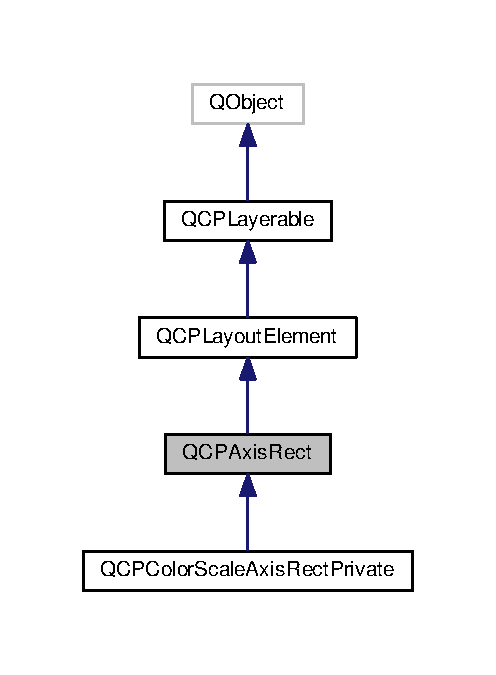
\includegraphics[width=238pt]{classQCPAxisRect__inherit__graph}
\end{center}
\end{figure}


Collaboration diagram for Q\+C\+P\+Axis\+Rect\+:\nopagebreak
\begin{figure}[H]
\begin{center}
\leavevmode
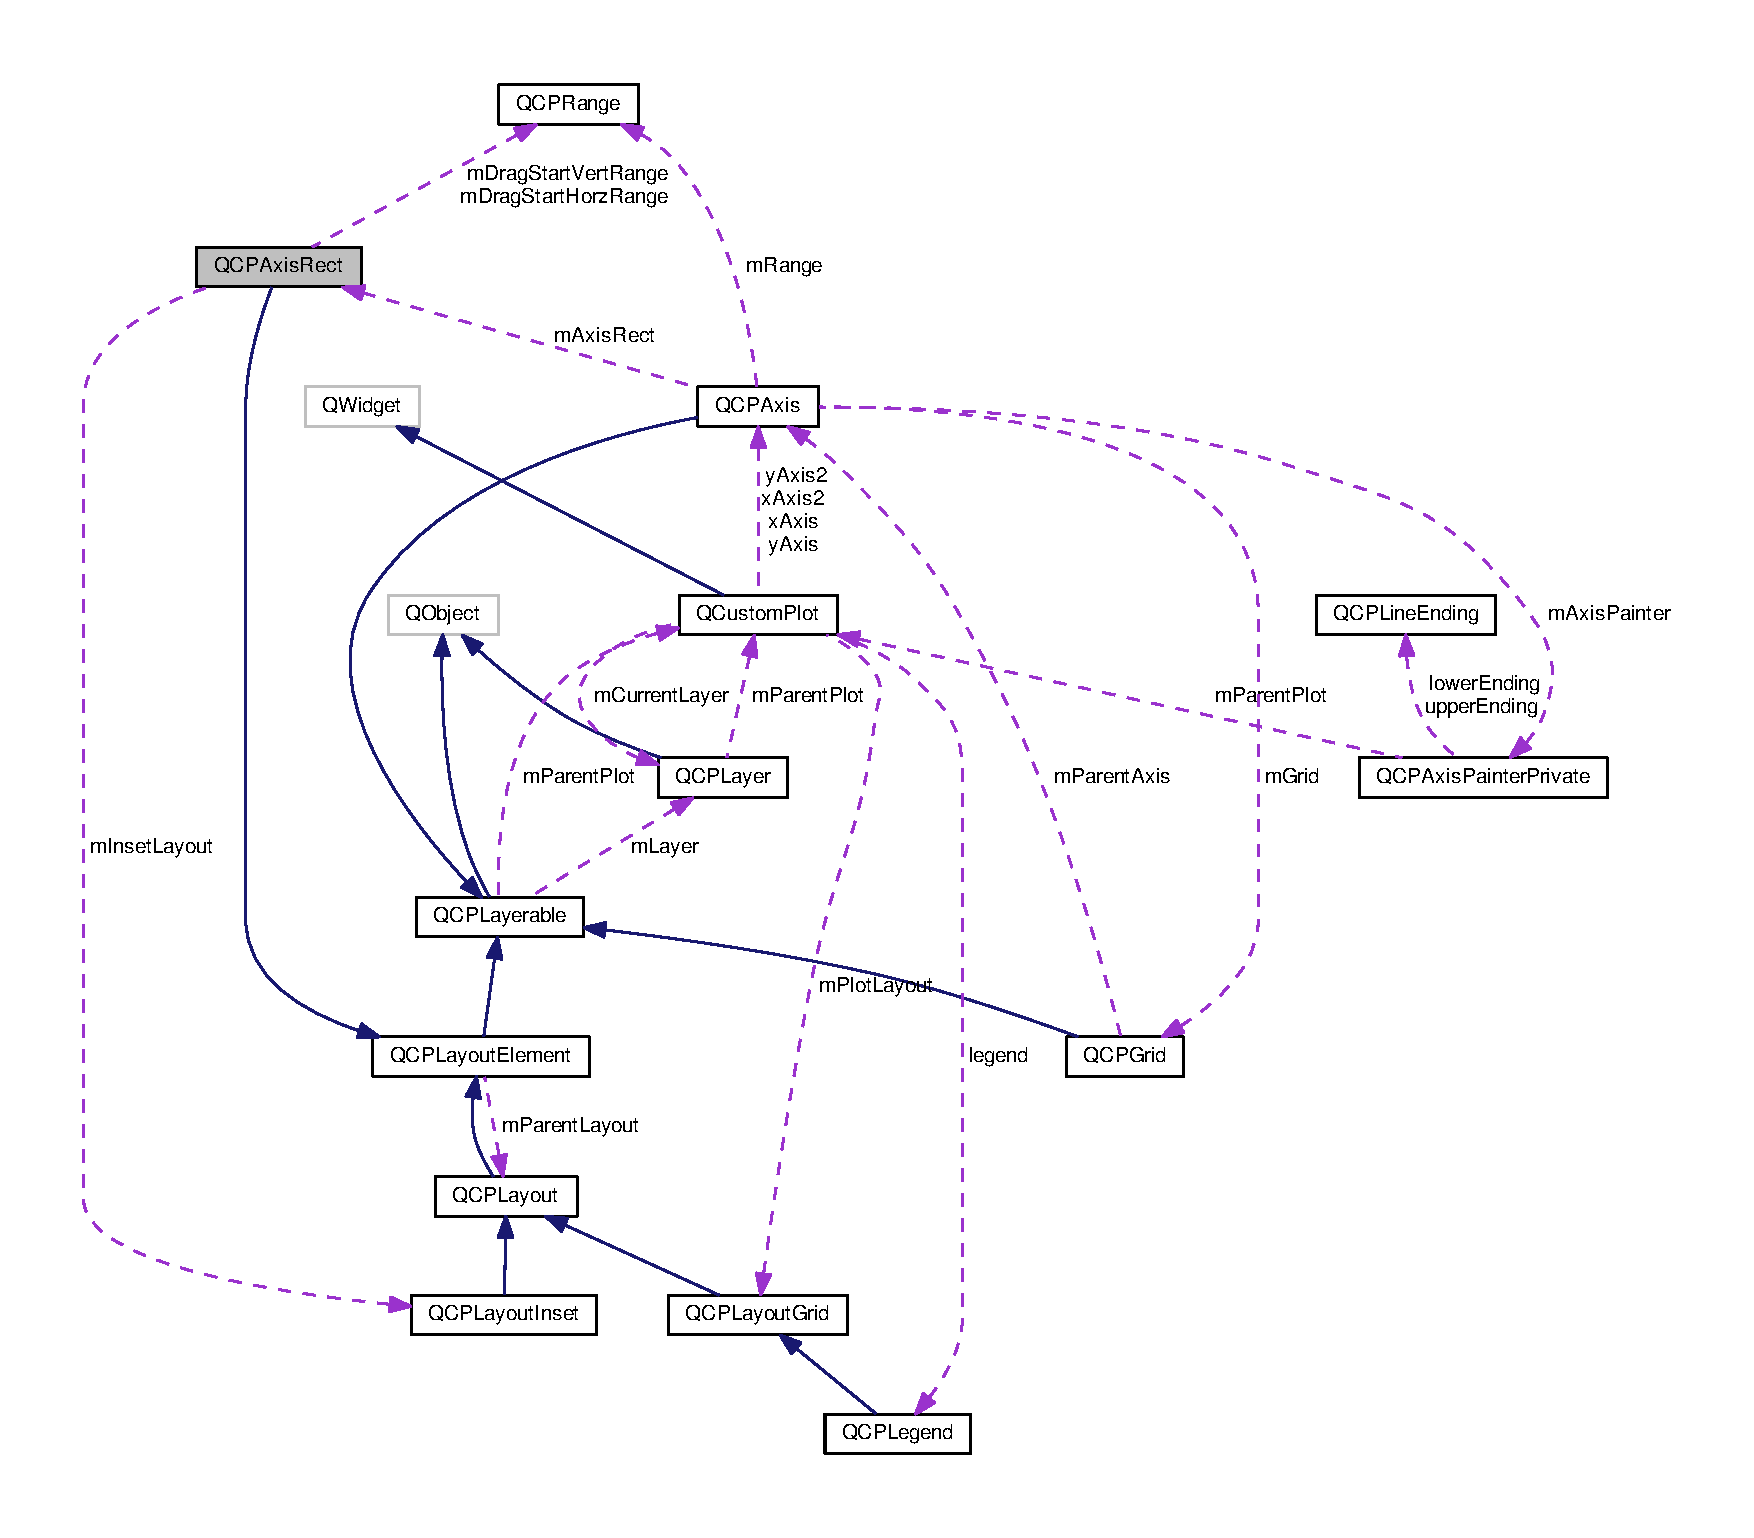
\includegraphics[width=350pt]{classQCPAxisRect__coll__graph}
\end{center}
\end{figure}
\subsection*{Public Member Functions}
\begin{DoxyCompactItemize}
\item 
\hyperlink{classQCPAxisRect_a60b31dece805462c1b82eea2e69ba042}{Q\+C\+P\+Axis\+Rect} (\hyperlink{classQCustomPlot}{Q\+Custom\+Plot} $\ast$\hyperlink{classQCPLayerable_ab7e0e94461566093d36ffc0f5312b109}{parent\+Plot}, bool setup\+Default\+Axes=true)
\item 
virtual \hyperlink{classQCPAxisRect_a463c44b1856ddbf82eb3f7b582839cd0}{$\sim$\+Q\+C\+P\+Axis\+Rect} ()
\item 
Q\+Pixmap \hyperlink{classQCPAxisRect_a0daa1dadd2a62dbfa37b7f742edd0059}{background} () const 
\item 
bool \hyperlink{classQCPAxisRect_a67c18777b88fe9c81dee3dd2b5f50e5c}{background\+Scaled} () const 
\item 
Qt\+::\+Aspect\+Ratio\+Mode \hyperlink{classQCPAxisRect_a3d0f42d6be11a0b3d4576402a2b0032d}{background\+Scaled\+Mode} () const 
\item 
Qt\+::\+Orientations \hyperlink{classQCPAxisRect_af24b46954ce27a26b23770cdb8319080}{range\+Drag} () const 
\item 
Qt\+::\+Orientations \hyperlink{classQCPAxisRect_a3397fc60e5df29089090bc236e9f05f6}{range\+Zoom} () const 
\item 
\hyperlink{classQCPAxis}{Q\+C\+P\+Axis} $\ast$ \hyperlink{classQCPAxisRect_a6d7c22cfc54fac7a3d6ef80b133a8574}{range\+Drag\+Axis} (Qt\+::\+Orientation orientation)
\item 
\hyperlink{classQCPAxis}{Q\+C\+P\+Axis} $\ast$ \hyperlink{classQCPAxisRect_a679c63f2b8daccfe6ec5110dce3dd3b6}{range\+Zoom\+Axis} (Qt\+::\+Orientation orientation)
\item 
double \hyperlink{classQCPAxisRect_ae4e6c4d143aacc88d2d3c56f117c2fe1}{range\+Zoom\+Factor} (Qt\+::\+Orientation orientation)
\item 
void \hyperlink{classQCPAxisRect_af615ab5e52b8e0a9a0eff415b6559db5}{set\+Background} (const Q\+Pixmap \&pm)
\item 
void \hyperlink{classQCPAxisRect_ac48a2d5d9b7732e73b86605c69c5e4c1}{set\+Background} (const Q\+Pixmap \&pm, bool scaled, Qt\+::\+Aspect\+Ratio\+Mode mode=Qt\+::\+Keep\+Aspect\+Ratio\+By\+Expanding)
\item 
void \hyperlink{classQCPAxisRect_a22a22b8668735438dc06f9a55fe46b33}{set\+Background} (const Q\+Brush \&brush)
\item 
void \hyperlink{classQCPAxisRect_ae6d36c3e0e968ffb991170a018e7b503}{set\+Background\+Scaled} (bool scaled)
\item 
void \hyperlink{classQCPAxisRect_a5ef77ea829c9de7ba248e473f48f7305}{set\+Background\+Scaled\+Mode} (Qt\+::\+Aspect\+Ratio\+Mode mode)
\item 
void \hyperlink{classQCPAxisRect_ae6aef2f7211ba6097c925dcd26008418}{set\+Range\+Drag} (Qt\+::\+Orientations orientations)
\item 
void \hyperlink{classQCPAxisRect_a7960a9d222f1c31d558b064b60f86a31}{set\+Range\+Zoom} (Qt\+::\+Orientations orientations)
\item 
void \hyperlink{classQCPAxisRect_a648cce336bd99daac4a5ca3e5743775d}{set\+Range\+Drag\+Axes} (\hyperlink{classQCPAxis}{Q\+C\+P\+Axis} $\ast$horizontal, \hyperlink{classQCPAxis}{Q\+C\+P\+Axis} $\ast$vertical)
\item 
void \hyperlink{classQCPAxisRect_a9442cca2aa358405f39a64d51eca13d2}{set\+Range\+Zoom\+Axes} (\hyperlink{classQCPAxis}{Q\+C\+P\+Axis} $\ast$horizontal, \hyperlink{classQCPAxis}{Q\+C\+P\+Axis} $\ast$vertical)
\item 
void \hyperlink{classQCPAxisRect_a895d7ac745ea614e04056244b3c138ac}{set\+Range\+Zoom\+Factor} (double horizontal\+Factor, double vertical\+Factor)
\item 
void \hyperlink{classQCPAxisRect_ae83d187b03fc6fa4f00765ad50cd3fc3}{set\+Range\+Zoom\+Factor} (double factor)
\item 
int \hyperlink{classQCPAxisRect_a16e3e4646e52e4b5d5b865076c29ae58}{axis\+Count} (\hyperlink{classQCPAxis_ae2bcc1728b382f10f064612b368bc18a}{Q\+C\+P\+Axis\+::\+Axis\+Type} type) const 
\item 
\hyperlink{classQCPAxis}{Q\+C\+P\+Axis} $\ast$ \hyperlink{classQCPAxisRect_a560de44e47a4af0f86c59102a094b1e4}{axis} (\hyperlink{classQCPAxis_ae2bcc1728b382f10f064612b368bc18a}{Q\+C\+P\+Axis\+::\+Axis\+Type} type, int index=0) const 
\item 
Q\+List$<$ \hyperlink{classQCPAxis}{Q\+C\+P\+Axis} $\ast$ $>$ \hyperlink{classQCPAxisRect_a66654d51ca611ef036ded36250cd2518}{axes} (Q\+C\+P\+Axis\+::\+Axis\+Types types) const 
\item 
Q\+List$<$ \hyperlink{classQCPAxis}{Q\+C\+P\+Axis} $\ast$ $>$ \hyperlink{classQCPAxisRect_a18dcdc0dd6c7520bc9f3d15a7a3feec2}{axes} () const 
\item 
\hyperlink{classQCPAxis}{Q\+C\+P\+Axis} $\ast$ \hyperlink{classQCPAxisRect_a2dc336092ccc57d44a46194c8a23e4f4}{add\+Axis} (\hyperlink{classQCPAxis_ae2bcc1728b382f10f064612b368bc18a}{Q\+C\+P\+Axis\+::\+Axis\+Type} type, \hyperlink{classQCPAxis}{Q\+C\+P\+Axis} $\ast$\hyperlink{classQCPAxisRect_a560de44e47a4af0f86c59102a094b1e4}{axis}=0)
\item 
Q\+List$<$ \hyperlink{classQCPAxis}{Q\+C\+P\+Axis} $\ast$ $>$ \hyperlink{classQCPAxisRect_a792e1f3d9cb1591fca135bb0de9b81fc}{add\+Axes} (Q\+C\+P\+Axis\+::\+Axis\+Types types)
\item 
bool \hyperlink{classQCPAxisRect_a03c39cd9704f0d36fb6cf980cdddcbaa}{remove\+Axis} (\hyperlink{classQCPAxis}{Q\+C\+P\+Axis} $\ast$\hyperlink{classQCPAxisRect_a560de44e47a4af0f86c59102a094b1e4}{axis})
\item 
\hyperlink{classQCPLayoutInset}{Q\+C\+P\+Layout\+Inset} $\ast$ \hyperlink{classQCPAxisRect_a4114887c7141b59650b7488f930993e5}{inset\+Layout} () const 
\item 
void \hyperlink{classQCPAxisRect_a5fa906175447b14206954f77fc7f1ef4}{setup\+Full\+Axes\+Box} (bool connect\+Ranges=false)
\item 
Q\+List$<$ \hyperlink{classQCPAbstractPlottable}{Q\+C\+P\+Abstract\+Plottable} $\ast$ $>$ \hyperlink{classQCPAxisRect_a5b0d629c8de5572945eeae79a142296e}{plottables} () const 
\item 
Q\+List$<$ \hyperlink{classQCPGraph}{Q\+C\+P\+Graph} $\ast$ $>$ \hyperlink{classQCPAxisRect_afa4ff90901d9275f670e24b40e3c1b25}{graphs} () const 
\item 
Q\+List$<$ \hyperlink{classQCPAbstractItem}{Q\+C\+P\+Abstract\+Item} $\ast$ $>$ \hyperlink{classQCPAxisRect_a0f17ed539962cfcbaca8ce0b1776c840}{items} () const 
\item 
int \hyperlink{classQCPAxisRect_a55b3ecf72a3a65b053f7651b88db458d}{left} () const 
\item 
int \hyperlink{classQCPAxisRect_a6d0f989fc552aa2b563cf82f8fc81e61}{right} () const 
\item 
int \hyperlink{classQCPAxisRect_ac45aef1eb75cea46b241b6303028a607}{top} () const 
\item 
int \hyperlink{classQCPAxisRect_af2b5982ebe7e6f781b9bf1cc371a60d8}{bottom} () const 
\item 
int \hyperlink{classQCPAxisRect_a45bf5c17f4ca29131b7eb0db06efc259}{width} () const 
\item 
int \hyperlink{classQCPAxisRect_a1c55c4f3bef40cf01b21820316c8469e}{height} () const 
\item 
Q\+Size \hyperlink{classQCPAxisRect_a871b9fe49e92b39a3cbe29a59e458536}{size} () const 
\item 
Q\+Point \hyperlink{classQCPAxisRect_a88acbe716bcf5072790a6f95637c40d8}{top\+Left} () const 
\item 
Q\+Point \hyperlink{classQCPAxisRect_a232409546394c23b59407bc62fa460a8}{top\+Right} () const 
\item 
Q\+Point \hyperlink{classQCPAxisRect_a724b0333971ea6a338f0dbd814dc97ae}{bottom\+Left} () const 
\item 
Q\+Point \hyperlink{classQCPAxisRect_a49ea3c7dff834b47e266cbf3d79f78b9}{bottom\+Right} () const 
\item 
Q\+Point \hyperlink{classQCPAxisRect_aea5e6042bca198424fa1bc02fc282e59}{center} () const 
\item 
virtual void \hyperlink{classQCPAxisRect_a255080a017df9083a60a321ef2ba9ed8}{update} (\hyperlink{classQCPLayoutElement_a0d83360e05735735aaf6d7983c56374d}{Update\+Phase} phase)
\item 
virtual Q\+List$<$ \hyperlink{classQCPLayoutElement}{Q\+C\+P\+Layout\+Element} $\ast$ $>$ \hyperlink{classQCPAxisRect_a2bda6bf2b5b5797f92583cecd01c8949}{elements} (bool recursive) const 
\end{DoxyCompactItemize}
\subsection*{Protected Member Functions}
\begin{DoxyCompactItemize}
\item 
virtual void \hyperlink{classQCPAxisRect_a9a6dd0763701cbc7d01f899bcbb3f9ca}{apply\+Default\+Antialiasing\+Hint} (\hyperlink{classQCPPainter}{Q\+C\+P\+Painter} $\ast$painter) const 
\item 
virtual void \hyperlink{classQCPAxisRect_afb1bbbbda8345cd2710d92ee48440b53}{draw} (\hyperlink{classQCPPainter}{Q\+C\+P\+Painter} $\ast$painter)
\item 
virtual int \hyperlink{classQCPAxisRect_ae79f18302e6507586aa8c032a5f9ed1c}{calculate\+Auto\+Margin} (\hyperlink{namespaceQCP_a7e487e3e2ccb62ab7771065bab7cae54}{Q\+C\+P\+::\+Margin\+Side} side)
\item 
virtual void \hyperlink{classQCPAxisRect_a77501dbeccdac7256f7979b05077c04e}{mouse\+Press\+Event} (Q\+Mouse\+Event $\ast$event)
\item 
virtual void \hyperlink{classQCPAxisRect_a4baf3d5dd69166788f6ceda0ea182c6e}{mouse\+Move\+Event} (Q\+Mouse\+Event $\ast$event)
\item 
virtual void \hyperlink{classQCPAxisRect_adf6c99780cea55ab39459a6eaad3a94a}{mouse\+Release\+Event} (Q\+Mouse\+Event $\ast$event)
\item 
virtual void \hyperlink{classQCPAxisRect_a5acf41fc30aa68ea263246ecfad85c31}{wheel\+Event} (Q\+Wheel\+Event $\ast$event)
\item 
void \hyperlink{classQCPAxisRect_ab49d338d1ce74b476fcead5b32cf06dc}{draw\+Background} (\hyperlink{classQCPPainter}{Q\+C\+P\+Painter} $\ast$painter)
\item 
void \hyperlink{classQCPAxisRect_a6024ccdc74f5dc0e8a0fe482e5b28a20}{update\+Axes\+Offset} (\hyperlink{classQCPAxis_ae2bcc1728b382f10f064612b368bc18a}{Q\+C\+P\+Axis\+::\+Axis\+Type} type)
\end{DoxyCompactItemize}
\subsection*{Protected Attributes}
\begin{DoxyCompactItemize}
\item 
Q\+Brush \hyperlink{classQCPAxisRect_a5748e1a37f63c428e38b0a7724b46259}{m\+Background\+Brush}
\item 
Q\+Pixmap \hyperlink{classQCPAxisRect_a38fb1a15f43228a0c124553649303722}{m\+Background\+Pixmap}
\item 
Q\+Pixmap \hyperlink{classQCPAxisRect_aa74b9415598d59b49290e41e42d7ee27}{m\+Scaled\+Background\+Pixmap}
\item 
bool \hyperlink{classQCPAxisRect_a5ad835f0fae5d7cc5ada9e063641dbf1}{m\+Background\+Scaled}
\item 
Qt\+::\+Aspect\+Ratio\+Mode \hyperlink{classQCPAxisRect_a859fd368e794663e346b4f53f35078e9}{m\+Background\+Scaled\+Mode}
\item 
\hyperlink{classQCPLayoutInset}{Q\+C\+P\+Layout\+Inset} $\ast$ \hyperlink{classQCPAxisRect_a255240399e0fd24baad80cbbe46f698a}{m\+Inset\+Layout}
\item 
Qt\+::\+Orientations \hyperlink{classQCPAxisRect_aa9f107f66ca3469ad50ee6cea7c9e237}{m\+Range\+Drag}
\item 
Qt\+::\+Orientations \hyperlink{classQCPAxisRect_a215eff671d48df2edccc36e7f976f28c}{m\+Range\+Zoom}
\item 
Q\+Pointer$<$ \hyperlink{classQCPAxis}{Q\+C\+P\+Axis} $>$ \hyperlink{classQCPAxisRect_aeaaa38c6d2030dd5f84461e2596e41e3}{m\+Range\+Drag\+Horz\+Axis}
\item 
Q\+Pointer$<$ \hyperlink{classQCPAxis}{Q\+C\+P\+Axis} $>$ \hyperlink{classQCPAxisRect_a3e41dffec18987366f2a8ffd80689c12}{m\+Range\+Drag\+Vert\+Axis}
\item 
Q\+Pointer$<$ \hyperlink{classQCPAxis}{Q\+C\+P\+Axis} $>$ \hyperlink{classQCPAxisRect_ae22f882bab20518559f3fbb84243d0ab}{m\+Range\+Zoom\+Horz\+Axis}
\item 
Q\+Pointer$<$ \hyperlink{classQCPAxis}{Q\+C\+P\+Axis} $>$ \hyperlink{classQCPAxisRect_a8b9acd16a203a9692bd35a9465f54bc1}{m\+Range\+Zoom\+Vert\+Axis}
\item 
double \hyperlink{classQCPAxisRect_ad08d0250ed7b99de387d0ea6c7fd4dc1}{m\+Range\+Zoom\+Factor\+Horz}
\item 
double \hyperlink{classQCPAxisRect_a32f063629581d5bf82b12769940b34ad}{m\+Range\+Zoom\+Factor\+Vert}
\item 
\hyperlink{classQCPRange}{Q\+C\+P\+Range} \hyperlink{classQCPAxisRect_a41936cf473ec638bec382f5a40cdb1f3}{m\+Drag\+Start\+Horz\+Range}
\item 
\hyperlink{classQCPRange}{Q\+C\+P\+Range} \hyperlink{classQCPAxisRect_a1a5ae4c74b8bd46baf91bf4e4f4165f0}{m\+Drag\+Start\+Vert\+Range}
\item 
Q\+C\+P\+::\+Antialiased\+Elements \hyperlink{classQCPAxisRect_aa4a24f76360cfebe1bcf17a77fa7521b}{m\+A\+A\+Drag\+Backup}
\item 
Q\+C\+P\+::\+Antialiased\+Elements \hyperlink{classQCPAxisRect_a6fcb12e052e276d57efbb128be31d6f5}{m\+Not\+A\+A\+Drag\+Backup}
\item 
Q\+Point \hyperlink{classQCPAxisRect_a032896b28f83a58010d8d533b78c49df}{m\+Drag\+Start}
\item 
bool \hyperlink{classQCPAxisRect_ab49a6698194cf0e9e38a1d734c0888a8}{m\+Dragging}
\item 
Q\+Hash$<$ \hyperlink{classQCPAxis_ae2bcc1728b382f10f064612b368bc18a}{Q\+C\+P\+Axis\+::\+Axis\+Type}, Q\+List$<$ \hyperlink{classQCPAxis}{Q\+C\+P\+Axis} $\ast$ $>$ $>$ \hyperlink{classQCPAxisRect_afe7a24d2a2bea98fc552fa826350ba81}{m\+Axes}
\end{DoxyCompactItemize}
\subsection*{Friends}
\begin{DoxyCompactItemize}
\item 
class \hyperlink{classQCPAxisRect_a1cdf9df76adcfae45261690aa0ca2198}{Q\+Custom\+Plot}
\end{DoxyCompactItemize}
\subsection*{Additional Inherited Members}


\subsection{Detailed Description}
Holds multiple axes and arranges them in a rectangular shape. 

This class represents an axis rect, a rectangular area that is bounded on all sides with an arbitrary number of axes.

Initially \hyperlink{classQCustomPlot}{Q\+Custom\+Plot} has one axis rect, accessible via \hyperlink{classQCustomPlot_a4a37a1add5fe63060ac518cf0a4c4050}{Q\+Custom\+Plot\+::axis\+Rect()}. However, the layout system allows to have multiple axis rects, e.\+g. arranged in a grid layout (\hyperlink{classQCustomPlot_afd280d4d621ae64a106543a545c508d7}{Q\+Custom\+Plot\+::plot\+Layout}).

By default, \hyperlink{classQCPAxisRect}{Q\+C\+P\+Axis\+Rect} comes with four axes, at bottom, top, left and right. They can be accessed via \hyperlink{classQCPAxisRect_a560de44e47a4af0f86c59102a094b1e4}{axis} by providing the respective axis type (\hyperlink{classQCPAxis_ae2bcc1728b382f10f064612b368bc18a}{Q\+C\+P\+Axis\+::\+Axis\+Type}) and index. If you need all axes in the axis rect, use \hyperlink{classQCPAxisRect_a66654d51ca611ef036ded36250cd2518}{axes}. The top and right axes are set to be invisible initially (\hyperlink{classQCPLayerable_a3bed99ddc396b48ce3ebfdc0418744f8}{Q\+C\+P\+Axis\+::set\+Visible}). To add more axes to a side, use \hyperlink{classQCPAxisRect_a2dc336092ccc57d44a46194c8a23e4f4}{add\+Axis} or \hyperlink{classQCPAxisRect_a792e1f3d9cb1591fca135bb0de9b81fc}{add\+Axes}. To remove an axis, use \hyperlink{classQCPAxisRect_a03c39cd9704f0d36fb6cf980cdddcbaa}{remove\+Axis}.

The axis rect layerable itself only draws a background pixmap or color, if specified (\hyperlink{classQCPAxisRect_af615ab5e52b8e0a9a0eff415b6559db5}{set\+Background}). It is placed on the \char`\"{}background\char`\"{} layer initially (see \hyperlink{classQCPLayer}{Q\+C\+P\+Layer} for an explanation of the \hyperlink{classQCustomPlot}{Q\+Custom\+Plot} layer system). The axes that are held by the axis rect can be placed on other layers, independently of the axis rect.

Every axis rect has a child layout of type \hyperlink{classQCPLayoutInset}{Q\+C\+P\+Layout\+Inset}. It is accessible via \hyperlink{classQCPAxisRect_a4114887c7141b59650b7488f930993e5}{inset\+Layout} and can be used to have other layout elements (or even other layouts with multiple elements) hovering inside the axis rect.

If an axis rect is clicked and dragged, it processes this by moving certain axis ranges. The behaviour can be controlled with \hyperlink{classQCPAxisRect_ae6aef2f7211ba6097c925dcd26008418}{set\+Range\+Drag} and \hyperlink{classQCPAxisRect_a648cce336bd99daac4a5ca3e5743775d}{set\+Range\+Drag\+Axes}. If the mouse wheel is scrolled while the cursor is on the axis rect, certain axes are scaled. This is controllable via \hyperlink{classQCPAxisRect_a7960a9d222f1c31d558b064b60f86a31}{set\+Range\+Zoom}, \hyperlink{classQCPAxisRect_a9442cca2aa358405f39a64d51eca13d2}{set\+Range\+Zoom\+Axes} and \hyperlink{classQCPAxisRect_a895d7ac745ea614e04056244b3c138ac}{set\+Range\+Zoom\+Factor}. These interactions are only enabled if \hyperlink{classQCustomPlot_a5ee1e2f6ae27419deca53e75907c27e5}{Q\+Custom\+Plot\+::set\+Interactions} contains \hyperlink{namespaceQCP_a2ad6bb6281c7c2d593d4277b44c2b037a2c4432b9aceafb94000be8d1b589ef18}{Q\+C\+P\+::i\+Range\+Drag} and \hyperlink{namespaceQCP_a2ad6bb6281c7c2d593d4277b44c2b037abee1e94353525a636aeaf0ba32b72e14}{Q\+C\+P\+::i\+Range\+Zoom}.

 \begin{center}Overview of the spacings and paddings that define the geometry of an axis. The dashed line on the far left indicates the viewport/widget border.\end{center}  

\subsection{Constructor \& Destructor Documentation}
\index{Q\+C\+P\+Axis\+Rect@{Q\+C\+P\+Axis\+Rect}!Q\+C\+P\+Axis\+Rect@{Q\+C\+P\+Axis\+Rect}}
\index{Q\+C\+P\+Axis\+Rect@{Q\+C\+P\+Axis\+Rect}!Q\+C\+P\+Axis\+Rect@{Q\+C\+P\+Axis\+Rect}}
\subsubsection[{\texorpdfstring{Q\+C\+P\+Axis\+Rect(\+Q\+Custom\+Plot $\ast$parent\+Plot, bool setup\+Default\+Axes=true)}{QCPAxisRect(QCustomPlot *parentPlot, bool setupDefaultAxes=true)}}]{\setlength{\rightskip}{0pt plus 5cm}Q\+C\+P\+Axis\+Rect\+::\+Q\+C\+P\+Axis\+Rect (
\begin{DoxyParamCaption}
\item[{{\bf Q\+Custom\+Plot} $\ast$}]{parent\+Plot, }
\item[{bool}]{setup\+Default\+Axes = {\ttfamily true}}
\end{DoxyParamCaption}
)\hspace{0.3cm}{\ttfamily [explicit]}}\hypertarget{classQCPAxisRect_a60b31dece805462c1b82eea2e69ba042}{}\label{classQCPAxisRect_a60b31dece805462c1b82eea2e69ba042}
Creates a \hyperlink{classQCPAxisRect}{Q\+C\+P\+Axis\+Rect} instance and sets default values. An axis is added for each of the four sides, the top and right axes are set invisible initially. \index{Q\+C\+P\+Axis\+Rect@{Q\+C\+P\+Axis\+Rect}!````~Q\+C\+P\+Axis\+Rect@{$\sim$\+Q\+C\+P\+Axis\+Rect}}
\index{````~Q\+C\+P\+Axis\+Rect@{$\sim$\+Q\+C\+P\+Axis\+Rect}!Q\+C\+P\+Axis\+Rect@{Q\+C\+P\+Axis\+Rect}}
\subsubsection[{\texorpdfstring{$\sim$\+Q\+C\+P\+Axis\+Rect()}{~QCPAxisRect()}}]{\setlength{\rightskip}{0pt plus 5cm}Q\+C\+P\+Axis\+Rect\+::$\sim$\+Q\+C\+P\+Axis\+Rect (
\begin{DoxyParamCaption}
{}
\end{DoxyParamCaption}
)\hspace{0.3cm}{\ttfamily [virtual]}}\hypertarget{classQCPAxisRect_a463c44b1856ddbf82eb3f7b582839cd0}{}\label{classQCPAxisRect_a463c44b1856ddbf82eb3f7b582839cd0}


\subsection{Member Function Documentation}
\index{Q\+C\+P\+Axis\+Rect@{Q\+C\+P\+Axis\+Rect}!add\+Axes@{add\+Axes}}
\index{add\+Axes@{add\+Axes}!Q\+C\+P\+Axis\+Rect@{Q\+C\+P\+Axis\+Rect}}
\subsubsection[{\texorpdfstring{add\+Axes(\+Q\+C\+P\+Axis\+::\+Axis\+Types types)}{addAxes(QCPAxis::AxisTypes types)}}]{\setlength{\rightskip}{0pt plus 5cm}Q\+List$<$ {\bf Q\+C\+P\+Axis} $\ast$ $>$ Q\+C\+P\+Axis\+Rect\+::add\+Axes (
\begin{DoxyParamCaption}
\item[{Q\+C\+P\+Axis\+::\+Axis\+Types}]{types}
\end{DoxyParamCaption}
)}\hypertarget{classQCPAxisRect_a792e1f3d9cb1591fca135bb0de9b81fc}{}\label{classQCPAxisRect_a792e1f3d9cb1591fca135bb0de9b81fc}
Adds a new axis with \hyperlink{classQCPAxisRect_a2dc336092ccc57d44a46194c8a23e4f4}{add\+Axis} to each axis rect side specified in {\itshape types}. This may be an {\ttfamily or}-\/combination of \hyperlink{classQCPAxis_ae2bcc1728b382f10f064612b368bc18a}{Q\+C\+P\+Axis\+::\+Axis\+Type}, so axes can be added to multiple sides at once.

Returns a list of the added axes.

\begin{DoxySeeAlso}{See also}
\hyperlink{classQCPAxisRect_a2dc336092ccc57d44a46194c8a23e4f4}{add\+Axis}, \hyperlink{classQCPAxisRect_a5fa906175447b14206954f77fc7f1ef4}{setup\+Full\+Axes\+Box} 
\end{DoxySeeAlso}
\index{Q\+C\+P\+Axis\+Rect@{Q\+C\+P\+Axis\+Rect}!add\+Axis@{add\+Axis}}
\index{add\+Axis@{add\+Axis}!Q\+C\+P\+Axis\+Rect@{Q\+C\+P\+Axis\+Rect}}
\subsubsection[{\texorpdfstring{add\+Axis(\+Q\+C\+P\+Axis\+::\+Axis\+Type type, Q\+C\+P\+Axis $\ast$axis=0)}{addAxis(QCPAxis::AxisType type, QCPAxis *axis=0)}}]{\setlength{\rightskip}{0pt plus 5cm}{\bf Q\+C\+P\+Axis} $\ast$ Q\+C\+P\+Axis\+Rect\+::add\+Axis (
\begin{DoxyParamCaption}
\item[{{\bf Q\+C\+P\+Axis\+::\+Axis\+Type}}]{type, }
\item[{{\bf Q\+C\+P\+Axis} $\ast$}]{axis = {\ttfamily 0}}
\end{DoxyParamCaption}
)}\hypertarget{classQCPAxisRect_a2dc336092ccc57d44a46194c8a23e4f4}{}\label{classQCPAxisRect_a2dc336092ccc57d44a46194c8a23e4f4}
Adds a new axis to the axis rect side specified with {\itshape type}, and returns it. If {\itshape axis} is 0, a new \hyperlink{classQCPAxis}{Q\+C\+P\+Axis} instance is created internally.

You may inject \hyperlink{classQCPAxis}{Q\+C\+P\+Axis} instances (or sublasses of \hyperlink{classQCPAxis}{Q\+C\+P\+Axis}) by setting {\itshape axis} to an axis that was previously created outside \hyperlink{classQCustomPlot}{Q\+Custom\+Plot}. It is important to note that \hyperlink{classQCustomPlot}{Q\+Custom\+Plot} takes ownership of the axis, so you may not delete it afterwards. Further, the {\itshape axis} must have been created with this axis rect as parent and with the same axis type as specified in {\itshape type}. If this is not the case, a debug output is generated, the axis is not added, and the method returns 0.

This method can not be used to move {\itshape axis} between axis rects. The same {\itshape axis} instance must not be added multiple times to the same or different axis rects.

If an axis rect side already contains one or more axes, the lower and upper endings of the new axis (\hyperlink{classQCPAxis_a08af1c72db9ae4dc8cb8a973d44405ab}{Q\+C\+P\+Axis\+::set\+Lower\+Ending}, \hyperlink{classQCPAxis_a69119b892fc306f651763596685aa377}{Q\+C\+P\+Axis\+::set\+Upper\+Ending}) are set to \hyperlink{classQCPLineEnding_a5ef16e6876b4b74959c7261d8d4c2cd5a126c390f0c359fcd8df1fc5e38d26d5b}{Q\+C\+P\+Line\+Ending\+::es\+Half\+Bar}.

\begin{DoxySeeAlso}{See also}
\hyperlink{classQCPAxisRect_a792e1f3d9cb1591fca135bb0de9b81fc}{add\+Axes}, \hyperlink{classQCPAxisRect_a5fa906175447b14206954f77fc7f1ef4}{setup\+Full\+Axes\+Box} 
\end{DoxySeeAlso}
\index{Q\+C\+P\+Axis\+Rect@{Q\+C\+P\+Axis\+Rect}!apply\+Default\+Antialiasing\+Hint@{apply\+Default\+Antialiasing\+Hint}}
\index{apply\+Default\+Antialiasing\+Hint@{apply\+Default\+Antialiasing\+Hint}!Q\+C\+P\+Axis\+Rect@{Q\+C\+P\+Axis\+Rect}}
\subsubsection[{\texorpdfstring{apply\+Default\+Antialiasing\+Hint(\+Q\+C\+P\+Painter $\ast$painter) const }{applyDefaultAntialiasingHint(QCPPainter *painter) const }}]{\setlength{\rightskip}{0pt plus 5cm}void Q\+C\+P\+Axis\+Rect\+::apply\+Default\+Antialiasing\+Hint (
\begin{DoxyParamCaption}
\item[{{\bf Q\+C\+P\+Painter} $\ast$}]{painter}
\end{DoxyParamCaption}
) const\hspace{0.3cm}{\ttfamily [protected]}, {\ttfamily [virtual]}}\hypertarget{classQCPAxisRect_a9a6dd0763701cbc7d01f899bcbb3f9ca}{}\label{classQCPAxisRect_a9a6dd0763701cbc7d01f899bcbb3f9ca}


Reimplemented from \hyperlink{classQCPLayoutElement_ad6d2b4bb0291c2441b2e1ca3d5296df5}{Q\+C\+P\+Layout\+Element}.

\index{Q\+C\+P\+Axis\+Rect@{Q\+C\+P\+Axis\+Rect}!axes@{axes}}
\index{axes@{axes}!Q\+C\+P\+Axis\+Rect@{Q\+C\+P\+Axis\+Rect}}
\subsubsection[{\texorpdfstring{axes(\+Q\+C\+P\+Axis\+::\+Axis\+Types types) const }{axes(QCPAxis::AxisTypes types) const }}]{\setlength{\rightskip}{0pt plus 5cm}Q\+List$<$ {\bf Q\+C\+P\+Axis} $\ast$ $>$ Q\+C\+P\+Axis\+Rect\+::axes (
\begin{DoxyParamCaption}
\item[{Q\+C\+P\+Axis\+::\+Axis\+Types}]{types}
\end{DoxyParamCaption}
) const}\hypertarget{classQCPAxisRect_a66654d51ca611ef036ded36250cd2518}{}\label{classQCPAxisRect_a66654d51ca611ef036ded36250cd2518}
Returns all axes on the axis rect sides specified with {\itshape types}.

{\itshape types} may be a single \hyperlink{classQCPAxis_ae2bcc1728b382f10f064612b368bc18a}{Q\+C\+P\+Axis\+::\+Axis\+Type} or an {\ttfamily or}-\/combination, to get the axes of multiple sides.

\begin{DoxySeeAlso}{See also}
\hyperlink{classQCPAxisRect_a560de44e47a4af0f86c59102a094b1e4}{axis} 
\end{DoxySeeAlso}
\index{Q\+C\+P\+Axis\+Rect@{Q\+C\+P\+Axis\+Rect}!axes@{axes}}
\index{axes@{axes}!Q\+C\+P\+Axis\+Rect@{Q\+C\+P\+Axis\+Rect}}
\subsubsection[{\texorpdfstring{axes() const }{axes() const }}]{\setlength{\rightskip}{0pt plus 5cm}Q\+List$<$ {\bf Q\+C\+P\+Axis} $\ast$ $>$ Q\+C\+P\+Axis\+Rect\+::axes (
\begin{DoxyParamCaption}
{}
\end{DoxyParamCaption}
) const}\hypertarget{classQCPAxisRect_a18dcdc0dd6c7520bc9f3d15a7a3feec2}{}\label{classQCPAxisRect_a18dcdc0dd6c7520bc9f3d15a7a3feec2}
This is an overloaded member function, provided for convenience. It differs from the above function only in what argument(s) it accepts.

Returns all axes of this axis rect. \index{Q\+C\+P\+Axis\+Rect@{Q\+C\+P\+Axis\+Rect}!axis@{axis}}
\index{axis@{axis}!Q\+C\+P\+Axis\+Rect@{Q\+C\+P\+Axis\+Rect}}
\subsubsection[{\texorpdfstring{axis(\+Q\+C\+P\+Axis\+::\+Axis\+Type type, int index=0) const }{axis(QCPAxis::AxisType type, int index=0) const }}]{\setlength{\rightskip}{0pt plus 5cm}{\bf Q\+C\+P\+Axis} $\ast$ Q\+C\+P\+Axis\+Rect\+::axis (
\begin{DoxyParamCaption}
\item[{{\bf Q\+C\+P\+Axis\+::\+Axis\+Type}}]{type, }
\item[{int}]{index = {\ttfamily 0}}
\end{DoxyParamCaption}
) const}\hypertarget{classQCPAxisRect_a560de44e47a4af0f86c59102a094b1e4}{}\label{classQCPAxisRect_a560de44e47a4af0f86c59102a094b1e4}
Returns the axis with the given {\itshape index} on the axis rect side specified with {\itshape type}.

\begin{DoxySeeAlso}{See also}
\hyperlink{classQCPAxisRect_a16e3e4646e52e4b5d5b865076c29ae58}{axis\+Count}, \hyperlink{classQCPAxisRect_a66654d51ca611ef036ded36250cd2518}{axes} 
\end{DoxySeeAlso}
\index{Q\+C\+P\+Axis\+Rect@{Q\+C\+P\+Axis\+Rect}!axis\+Count@{axis\+Count}}
\index{axis\+Count@{axis\+Count}!Q\+C\+P\+Axis\+Rect@{Q\+C\+P\+Axis\+Rect}}
\subsubsection[{\texorpdfstring{axis\+Count(\+Q\+C\+P\+Axis\+::\+Axis\+Type type) const }{axisCount(QCPAxis::AxisType type) const }}]{\setlength{\rightskip}{0pt plus 5cm}int Q\+C\+P\+Axis\+Rect\+::axis\+Count (
\begin{DoxyParamCaption}
\item[{{\bf Q\+C\+P\+Axis\+::\+Axis\+Type}}]{type}
\end{DoxyParamCaption}
) const}\hypertarget{classQCPAxisRect_a16e3e4646e52e4b5d5b865076c29ae58}{}\label{classQCPAxisRect_a16e3e4646e52e4b5d5b865076c29ae58}
Returns the number of axes on the axis rect side specified with {\itshape type}.

\begin{DoxySeeAlso}{See also}
\hyperlink{classQCPAxisRect_a560de44e47a4af0f86c59102a094b1e4}{axis} 
\end{DoxySeeAlso}
\index{Q\+C\+P\+Axis\+Rect@{Q\+C\+P\+Axis\+Rect}!background@{background}}
\index{background@{background}!Q\+C\+P\+Axis\+Rect@{Q\+C\+P\+Axis\+Rect}}
\subsubsection[{\texorpdfstring{background() const }{background() const }}]{\setlength{\rightskip}{0pt plus 5cm}Q\+Pixmap Q\+C\+P\+Axis\+Rect\+::background (
\begin{DoxyParamCaption}
{}
\end{DoxyParamCaption}
) const\hspace{0.3cm}{\ttfamily [inline]}}\hypertarget{classQCPAxisRect_a0daa1dadd2a62dbfa37b7f742edd0059}{}\label{classQCPAxisRect_a0daa1dadd2a62dbfa37b7f742edd0059}
\index{Q\+C\+P\+Axis\+Rect@{Q\+C\+P\+Axis\+Rect}!background\+Scaled@{background\+Scaled}}
\index{background\+Scaled@{background\+Scaled}!Q\+C\+P\+Axis\+Rect@{Q\+C\+P\+Axis\+Rect}}
\subsubsection[{\texorpdfstring{background\+Scaled() const }{backgroundScaled() const }}]{\setlength{\rightskip}{0pt plus 5cm}bool Q\+C\+P\+Axis\+Rect\+::background\+Scaled (
\begin{DoxyParamCaption}
{}
\end{DoxyParamCaption}
) const\hspace{0.3cm}{\ttfamily [inline]}}\hypertarget{classQCPAxisRect_a67c18777b88fe9c81dee3dd2b5f50e5c}{}\label{classQCPAxisRect_a67c18777b88fe9c81dee3dd2b5f50e5c}
\index{Q\+C\+P\+Axis\+Rect@{Q\+C\+P\+Axis\+Rect}!background\+Scaled\+Mode@{background\+Scaled\+Mode}}
\index{background\+Scaled\+Mode@{background\+Scaled\+Mode}!Q\+C\+P\+Axis\+Rect@{Q\+C\+P\+Axis\+Rect}}
\subsubsection[{\texorpdfstring{background\+Scaled\+Mode() const }{backgroundScaledMode() const }}]{\setlength{\rightskip}{0pt plus 5cm}Qt\+::\+Aspect\+Ratio\+Mode Q\+C\+P\+Axis\+Rect\+::background\+Scaled\+Mode (
\begin{DoxyParamCaption}
{}
\end{DoxyParamCaption}
) const\hspace{0.3cm}{\ttfamily [inline]}}\hypertarget{classQCPAxisRect_a3d0f42d6be11a0b3d4576402a2b0032d}{}\label{classQCPAxisRect_a3d0f42d6be11a0b3d4576402a2b0032d}
\index{Q\+C\+P\+Axis\+Rect@{Q\+C\+P\+Axis\+Rect}!bottom@{bottom}}
\index{bottom@{bottom}!Q\+C\+P\+Axis\+Rect@{Q\+C\+P\+Axis\+Rect}}
\subsubsection[{\texorpdfstring{bottom() const }{bottom() const }}]{\setlength{\rightskip}{0pt plus 5cm}int Q\+C\+P\+Axis\+Rect\+::bottom (
\begin{DoxyParamCaption}
{}
\end{DoxyParamCaption}
) const\hspace{0.3cm}{\ttfamily [inline]}}\hypertarget{classQCPAxisRect_af2b5982ebe7e6f781b9bf1cc371a60d8}{}\label{classQCPAxisRect_af2b5982ebe7e6f781b9bf1cc371a60d8}
Returns the pixel position of the bottom border of this axis rect. Margins are not taken into account here, so the returned value is with respect to the inner \hyperlink{classQCPLayoutElement_affdfea003469aac3d0fac5f4e06171bc}{rect}. \index{Q\+C\+P\+Axis\+Rect@{Q\+C\+P\+Axis\+Rect}!bottom\+Left@{bottom\+Left}}
\index{bottom\+Left@{bottom\+Left}!Q\+C\+P\+Axis\+Rect@{Q\+C\+P\+Axis\+Rect}}
\subsubsection[{\texorpdfstring{bottom\+Left() const }{bottomLeft() const }}]{\setlength{\rightskip}{0pt plus 5cm}Q\+Point Q\+C\+P\+Axis\+Rect\+::bottom\+Left (
\begin{DoxyParamCaption}
{}
\end{DoxyParamCaption}
) const\hspace{0.3cm}{\ttfamily [inline]}}\hypertarget{classQCPAxisRect_a724b0333971ea6a338f0dbd814dc97ae}{}\label{classQCPAxisRect_a724b0333971ea6a338f0dbd814dc97ae}
Returns the bottom left corner of this axis rect in pixels. Margins are not taken into account here, so the returned value is with respect to the inner \hyperlink{classQCPLayoutElement_affdfea003469aac3d0fac5f4e06171bc}{rect}. \index{Q\+C\+P\+Axis\+Rect@{Q\+C\+P\+Axis\+Rect}!bottom\+Right@{bottom\+Right}}
\index{bottom\+Right@{bottom\+Right}!Q\+C\+P\+Axis\+Rect@{Q\+C\+P\+Axis\+Rect}}
\subsubsection[{\texorpdfstring{bottom\+Right() const }{bottomRight() const }}]{\setlength{\rightskip}{0pt plus 5cm}Q\+Point Q\+C\+P\+Axis\+Rect\+::bottom\+Right (
\begin{DoxyParamCaption}
{}
\end{DoxyParamCaption}
) const\hspace{0.3cm}{\ttfamily [inline]}}\hypertarget{classQCPAxisRect_a49ea3c7dff834b47e266cbf3d79f78b9}{}\label{classQCPAxisRect_a49ea3c7dff834b47e266cbf3d79f78b9}
Returns the bottom right corner of this axis rect in pixels. Margins are not taken into account here, so the returned value is with respect to the inner \hyperlink{classQCPLayoutElement_affdfea003469aac3d0fac5f4e06171bc}{rect}. \index{Q\+C\+P\+Axis\+Rect@{Q\+C\+P\+Axis\+Rect}!calculate\+Auto\+Margin@{calculate\+Auto\+Margin}}
\index{calculate\+Auto\+Margin@{calculate\+Auto\+Margin}!Q\+C\+P\+Axis\+Rect@{Q\+C\+P\+Axis\+Rect}}
\subsubsection[{\texorpdfstring{calculate\+Auto\+Margin(\+Q\+C\+P\+::\+Margin\+Side side)}{calculateAutoMargin(QCP::MarginSide side)}}]{\setlength{\rightskip}{0pt plus 5cm}int Q\+C\+P\+Axis\+Rect\+::calculate\+Auto\+Margin (
\begin{DoxyParamCaption}
\item[{{\bf Q\+C\+P\+::\+Margin\+Side}}]{side}
\end{DoxyParamCaption}
)\hspace{0.3cm}{\ttfamily [protected]}, {\ttfamily [virtual]}}\hypertarget{classQCPAxisRect_ae79f18302e6507586aa8c032a5f9ed1c}{}\label{classQCPAxisRect_ae79f18302e6507586aa8c032a5f9ed1c}


Reimplemented from \hyperlink{classQCPLayoutElement_a005c9f0fe84bc1591a2cf2c46fd477b4}{Q\+C\+P\+Layout\+Element}.

\index{Q\+C\+P\+Axis\+Rect@{Q\+C\+P\+Axis\+Rect}!center@{center}}
\index{center@{center}!Q\+C\+P\+Axis\+Rect@{Q\+C\+P\+Axis\+Rect}}
\subsubsection[{\texorpdfstring{center() const }{center() const }}]{\setlength{\rightskip}{0pt plus 5cm}Q\+Point Q\+C\+P\+Axis\+Rect\+::center (
\begin{DoxyParamCaption}
{}
\end{DoxyParamCaption}
) const\hspace{0.3cm}{\ttfamily [inline]}}\hypertarget{classQCPAxisRect_aea5e6042bca198424fa1bc02fc282e59}{}\label{classQCPAxisRect_aea5e6042bca198424fa1bc02fc282e59}
Returns the center of this axis rect in pixels. Margins are not taken into account here, so the returned value is with respect to the inner \hyperlink{classQCPLayoutElement_affdfea003469aac3d0fac5f4e06171bc}{rect}. \index{Q\+C\+P\+Axis\+Rect@{Q\+C\+P\+Axis\+Rect}!draw@{draw}}
\index{draw@{draw}!Q\+C\+P\+Axis\+Rect@{Q\+C\+P\+Axis\+Rect}}
\subsubsection[{\texorpdfstring{draw(\+Q\+C\+P\+Painter $\ast$painter)}{draw(QCPPainter *painter)}}]{\setlength{\rightskip}{0pt plus 5cm}void Q\+C\+P\+Axis\+Rect\+::draw (
\begin{DoxyParamCaption}
\item[{{\bf Q\+C\+P\+Painter} $\ast$}]{painter}
\end{DoxyParamCaption}
)\hspace{0.3cm}{\ttfamily [protected]}, {\ttfamily [virtual]}}\hypertarget{classQCPAxisRect_afb1bbbbda8345cd2710d92ee48440b53}{}\label{classQCPAxisRect_afb1bbbbda8345cd2710d92ee48440b53}


Reimplemented from \hyperlink{classQCPLayoutElement_a547bcc1e6e2be5645ca781efe0834653}{Q\+C\+P\+Layout\+Element}.



Reimplemented in \hyperlink{classQCPColorScaleAxisRectPrivate_adb67bfe9057a9dd9a85f548c274e6d98}{Q\+C\+P\+Color\+Scale\+Axis\+Rect\+Private}.

\index{Q\+C\+P\+Axis\+Rect@{Q\+C\+P\+Axis\+Rect}!draw\+Background@{draw\+Background}}
\index{draw\+Background@{draw\+Background}!Q\+C\+P\+Axis\+Rect@{Q\+C\+P\+Axis\+Rect}}
\subsubsection[{\texorpdfstring{draw\+Background(\+Q\+C\+P\+Painter $\ast$painter)}{drawBackground(QCPPainter *painter)}}]{\setlength{\rightskip}{0pt plus 5cm}void Q\+C\+P\+Axis\+Rect\+::draw\+Background (
\begin{DoxyParamCaption}
\item[{{\bf Q\+C\+P\+Painter} $\ast$}]{painter}
\end{DoxyParamCaption}
)\hspace{0.3cm}{\ttfamily [protected]}}\hypertarget{classQCPAxisRect_ab49d338d1ce74b476fcead5b32cf06dc}{}\label{classQCPAxisRect_ab49d338d1ce74b476fcead5b32cf06dc}
\index{Q\+C\+P\+Axis\+Rect@{Q\+C\+P\+Axis\+Rect}!elements@{elements}}
\index{elements@{elements}!Q\+C\+P\+Axis\+Rect@{Q\+C\+P\+Axis\+Rect}}
\subsubsection[{\texorpdfstring{elements(bool recursive) const }{elements(bool recursive) const }}]{\setlength{\rightskip}{0pt plus 5cm}Q\+List$<$ {\bf Q\+C\+P\+Layout\+Element} $\ast$ $>$ Q\+C\+P\+Axis\+Rect\+::elements (
\begin{DoxyParamCaption}
\item[{bool}]{recursive}
\end{DoxyParamCaption}
) const\hspace{0.3cm}{\ttfamily [virtual]}}\hypertarget{classQCPAxisRect_a2bda6bf2b5b5797f92583cecd01c8949}{}\label{classQCPAxisRect_a2bda6bf2b5b5797f92583cecd01c8949}
Returns a list of all child elements in this layout element. If {\itshape recursive} is true, all sub-\/child elements are included in the list, too.

\begin{DoxyWarning}{Warning}
There may be entries with value 0 in the returned list. (For example, \hyperlink{classQCPLayoutGrid}{Q\+C\+P\+Layout\+Grid} may have empty cells which yield 0 at the respective index.) 
\end{DoxyWarning}


Reimplemented from \hyperlink{classQCPLayoutElement_a311d60d78e62ef8eaaedb1b6ceb9e788}{Q\+C\+P\+Layout\+Element}.

\index{Q\+C\+P\+Axis\+Rect@{Q\+C\+P\+Axis\+Rect}!graphs@{graphs}}
\index{graphs@{graphs}!Q\+C\+P\+Axis\+Rect@{Q\+C\+P\+Axis\+Rect}}
\subsubsection[{\texorpdfstring{graphs() const }{graphs() const }}]{\setlength{\rightskip}{0pt plus 5cm}Q\+List$<$ {\bf Q\+C\+P\+Graph} $\ast$ $>$ Q\+C\+P\+Axis\+Rect\+::graphs (
\begin{DoxyParamCaption}
{}
\end{DoxyParamCaption}
) const}\hypertarget{classQCPAxisRect_afa4ff90901d9275f670e24b40e3c1b25}{}\label{classQCPAxisRect_afa4ff90901d9275f670e24b40e3c1b25}
Returns a list of all the graphs that are associated with this axis rect.

A graph is considered associated with an axis rect if its key or value axis (or both) is in this axis rect.

\begin{DoxySeeAlso}{See also}
\hyperlink{classQCPAxisRect_a5b0d629c8de5572945eeae79a142296e}{plottables}, \hyperlink{classQCPAxisRect_a0f17ed539962cfcbaca8ce0b1776c840}{items} 
\end{DoxySeeAlso}
\index{Q\+C\+P\+Axis\+Rect@{Q\+C\+P\+Axis\+Rect}!height@{height}}
\index{height@{height}!Q\+C\+P\+Axis\+Rect@{Q\+C\+P\+Axis\+Rect}}
\subsubsection[{\texorpdfstring{height() const }{height() const }}]{\setlength{\rightskip}{0pt plus 5cm}int Q\+C\+P\+Axis\+Rect\+::height (
\begin{DoxyParamCaption}
{}
\end{DoxyParamCaption}
) const\hspace{0.3cm}{\ttfamily [inline]}}\hypertarget{classQCPAxisRect_a1c55c4f3bef40cf01b21820316c8469e}{}\label{classQCPAxisRect_a1c55c4f3bef40cf01b21820316c8469e}
Returns the pixel height of this axis rect. Margins are not taken into account here, so the returned value is with respect to the inner \hyperlink{classQCPLayoutElement_affdfea003469aac3d0fac5f4e06171bc}{rect}. \index{Q\+C\+P\+Axis\+Rect@{Q\+C\+P\+Axis\+Rect}!inset\+Layout@{inset\+Layout}}
\index{inset\+Layout@{inset\+Layout}!Q\+C\+P\+Axis\+Rect@{Q\+C\+P\+Axis\+Rect}}
\subsubsection[{\texorpdfstring{inset\+Layout() const }{insetLayout() const }}]{\setlength{\rightskip}{0pt plus 5cm}{\bf Q\+C\+P\+Layout\+Inset} $\ast$ Q\+C\+P\+Axis\+Rect\+::inset\+Layout (
\begin{DoxyParamCaption}
{}
\end{DoxyParamCaption}
) const\hspace{0.3cm}{\ttfamily [inline]}}\hypertarget{classQCPAxisRect_a4114887c7141b59650b7488f930993e5}{}\label{classQCPAxisRect_a4114887c7141b59650b7488f930993e5}
Returns the inset layout of this axis rect. It can be used to place other layout elements (or even layouts with multiple other elements) inside/on top of an axis rect.

\begin{DoxySeeAlso}{See also}
\hyperlink{classQCPLayoutInset}{Q\+C\+P\+Layout\+Inset} 
\end{DoxySeeAlso}
\index{Q\+C\+P\+Axis\+Rect@{Q\+C\+P\+Axis\+Rect}!items@{items}}
\index{items@{items}!Q\+C\+P\+Axis\+Rect@{Q\+C\+P\+Axis\+Rect}}
\subsubsection[{\texorpdfstring{items() const }{items() const }}]{\setlength{\rightskip}{0pt plus 5cm}Q\+List$<$ {\bf Q\+C\+P\+Abstract\+Item} $\ast$ $>$ Q\+C\+P\+Axis\+Rect\+::items (
\begin{DoxyParamCaption}
{}
\end{DoxyParamCaption}
) const}\hypertarget{classQCPAxisRect_a0f17ed539962cfcbaca8ce0b1776c840}{}\label{classQCPAxisRect_a0f17ed539962cfcbaca8ce0b1776c840}
Returns a list of all the items that are associated with this axis rect.

An item is considered associated with an axis rect if any of its positions has key or value axis set to an axis that is in this axis rect, or if any of its positions has \hyperlink{classQCPItemPosition_a0cd9b326fb324710169e92e8ca0041c2}{Q\+C\+P\+Item\+Position\+::set\+Axis\+Rect} set to the axis rect, or if the clip axis rect (\hyperlink{classQCPAbstractItem_a7dc75fcbcd10206fe0b75d757ea7a347}{Q\+C\+P\+Abstract\+Item\+::set\+Clip\+Axis\+Rect}) is set to this axis rect.

\begin{DoxySeeAlso}{See also}
\hyperlink{classQCPAxisRect_a5b0d629c8de5572945eeae79a142296e}{plottables}, \hyperlink{classQCPAxisRect_afa4ff90901d9275f670e24b40e3c1b25}{graphs} 
\end{DoxySeeAlso}
\index{Q\+C\+P\+Axis\+Rect@{Q\+C\+P\+Axis\+Rect}!left@{left}}
\index{left@{left}!Q\+C\+P\+Axis\+Rect@{Q\+C\+P\+Axis\+Rect}}
\subsubsection[{\texorpdfstring{left() const }{left() const }}]{\setlength{\rightskip}{0pt plus 5cm}int Q\+C\+P\+Axis\+Rect\+::left (
\begin{DoxyParamCaption}
{}
\end{DoxyParamCaption}
) const\hspace{0.3cm}{\ttfamily [inline]}}\hypertarget{classQCPAxisRect_a55b3ecf72a3a65b053f7651b88db458d}{}\label{classQCPAxisRect_a55b3ecf72a3a65b053f7651b88db458d}
Returns the pixel position of the left border of this axis rect. Margins are not taken into account here, so the returned value is with respect to the inner \hyperlink{classQCPLayoutElement_affdfea003469aac3d0fac5f4e06171bc}{rect}. \index{Q\+C\+P\+Axis\+Rect@{Q\+C\+P\+Axis\+Rect}!mouse\+Move\+Event@{mouse\+Move\+Event}}
\index{mouse\+Move\+Event@{mouse\+Move\+Event}!Q\+C\+P\+Axis\+Rect@{Q\+C\+P\+Axis\+Rect}}
\subsubsection[{\texorpdfstring{mouse\+Move\+Event(\+Q\+Mouse\+Event $\ast$event)}{mouseMoveEvent(QMouseEvent *event)}}]{\setlength{\rightskip}{0pt plus 5cm}void Q\+C\+P\+Axis\+Rect\+::mouse\+Move\+Event (
\begin{DoxyParamCaption}
\item[{Q\+Mouse\+Event $\ast$}]{event}
\end{DoxyParamCaption}
)\hspace{0.3cm}{\ttfamily [protected]}, {\ttfamily [virtual]}}\hypertarget{classQCPAxisRect_a4baf3d5dd69166788f6ceda0ea182c6e}{}\label{classQCPAxisRect_a4baf3d5dd69166788f6ceda0ea182c6e}
This event is called, if the mouse is moved inside the outer rect of this layout element. 

Reimplemented from \hyperlink{classQCPLayoutElement_a14f4acf58cdb8dd2c6c571479c4c4a40}{Q\+C\+P\+Layout\+Element}.

\index{Q\+C\+P\+Axis\+Rect@{Q\+C\+P\+Axis\+Rect}!mouse\+Press\+Event@{mouse\+Press\+Event}}
\index{mouse\+Press\+Event@{mouse\+Press\+Event}!Q\+C\+P\+Axis\+Rect@{Q\+C\+P\+Axis\+Rect}}
\subsubsection[{\texorpdfstring{mouse\+Press\+Event(\+Q\+Mouse\+Event $\ast$event)}{mousePressEvent(QMouseEvent *event)}}]{\setlength{\rightskip}{0pt plus 5cm}void Q\+C\+P\+Axis\+Rect\+::mouse\+Press\+Event (
\begin{DoxyParamCaption}
\item[{Q\+Mouse\+Event $\ast$}]{event}
\end{DoxyParamCaption}
)\hspace{0.3cm}{\ttfamily [protected]}, {\ttfamily [virtual]}}\hypertarget{classQCPAxisRect_a77501dbeccdac7256f7979b05077c04e}{}\label{classQCPAxisRect_a77501dbeccdac7256f7979b05077c04e}
This event is called, if the mouse was pressed while being inside the outer rect of this layout element. 

Reimplemented from \hyperlink{classQCPLayoutElement_a2d82ea21fe0ee628f177bd824bc51a71}{Q\+C\+P\+Layout\+Element}.

\index{Q\+C\+P\+Axis\+Rect@{Q\+C\+P\+Axis\+Rect}!mouse\+Release\+Event@{mouse\+Release\+Event}}
\index{mouse\+Release\+Event@{mouse\+Release\+Event}!Q\+C\+P\+Axis\+Rect@{Q\+C\+P\+Axis\+Rect}}
\subsubsection[{\texorpdfstring{mouse\+Release\+Event(\+Q\+Mouse\+Event $\ast$event)}{mouseReleaseEvent(QMouseEvent *event)}}]{\setlength{\rightskip}{0pt plus 5cm}void Q\+C\+P\+Axis\+Rect\+::mouse\+Release\+Event (
\begin{DoxyParamCaption}
\item[{Q\+Mouse\+Event $\ast$}]{event}
\end{DoxyParamCaption}
)\hspace{0.3cm}{\ttfamily [protected]}, {\ttfamily [virtual]}}\hypertarget{classQCPAxisRect_adf6c99780cea55ab39459a6eaad3a94a}{}\label{classQCPAxisRect_adf6c99780cea55ab39459a6eaad3a94a}
This event is called, if the mouse was previously pressed inside the outer rect of this layout element and is now released. 

Reimplemented from \hyperlink{classQCPLayoutElement_ae526ac828cce1e5bb94eaa85776d7404}{Q\+C\+P\+Layout\+Element}.

\index{Q\+C\+P\+Axis\+Rect@{Q\+C\+P\+Axis\+Rect}!plottables@{plottables}}
\index{plottables@{plottables}!Q\+C\+P\+Axis\+Rect@{Q\+C\+P\+Axis\+Rect}}
\subsubsection[{\texorpdfstring{plottables() const }{plottables() const }}]{\setlength{\rightskip}{0pt plus 5cm}Q\+List$<$ {\bf Q\+C\+P\+Abstract\+Plottable} $\ast$ $>$ Q\+C\+P\+Axis\+Rect\+::plottables (
\begin{DoxyParamCaption}
{}
\end{DoxyParamCaption}
) const}\hypertarget{classQCPAxisRect_a5b0d629c8de5572945eeae79a142296e}{}\label{classQCPAxisRect_a5b0d629c8de5572945eeae79a142296e}
Returns a list of all the plottables that are associated with this axis rect.

A plottable is considered associated with an axis rect if its key or value axis (or both) is in this axis rect.

\begin{DoxySeeAlso}{See also}
\hyperlink{classQCPAxisRect_afa4ff90901d9275f670e24b40e3c1b25}{graphs}, \hyperlink{classQCPAxisRect_a0f17ed539962cfcbaca8ce0b1776c840}{items} 
\end{DoxySeeAlso}
\index{Q\+C\+P\+Axis\+Rect@{Q\+C\+P\+Axis\+Rect}!range\+Drag@{range\+Drag}}
\index{range\+Drag@{range\+Drag}!Q\+C\+P\+Axis\+Rect@{Q\+C\+P\+Axis\+Rect}}
\subsubsection[{\texorpdfstring{range\+Drag() const }{rangeDrag() const }}]{\setlength{\rightskip}{0pt plus 5cm}Qt\+::\+Orientations Q\+C\+P\+Axis\+Rect\+::range\+Drag (
\begin{DoxyParamCaption}
{}
\end{DoxyParamCaption}
) const\hspace{0.3cm}{\ttfamily [inline]}}\hypertarget{classQCPAxisRect_af24b46954ce27a26b23770cdb8319080}{}\label{classQCPAxisRect_af24b46954ce27a26b23770cdb8319080}
\index{Q\+C\+P\+Axis\+Rect@{Q\+C\+P\+Axis\+Rect}!range\+Drag\+Axis@{range\+Drag\+Axis}}
\index{range\+Drag\+Axis@{range\+Drag\+Axis}!Q\+C\+P\+Axis\+Rect@{Q\+C\+P\+Axis\+Rect}}
\subsubsection[{\texorpdfstring{range\+Drag\+Axis(\+Qt\+::\+Orientation orientation)}{rangeDragAxis(Qt::Orientation orientation)}}]{\setlength{\rightskip}{0pt plus 5cm}{\bf Q\+C\+P\+Axis} $\ast$ Q\+C\+P\+Axis\+Rect\+::range\+Drag\+Axis (
\begin{DoxyParamCaption}
\item[{Qt\+::\+Orientation}]{orientation}
\end{DoxyParamCaption}
)}\hypertarget{classQCPAxisRect_a6d7c22cfc54fac7a3d6ef80b133a8574}{}\label{classQCPAxisRect_a6d7c22cfc54fac7a3d6ef80b133a8574}
Returns the range drag axis of the {\itshape orientation} provided.

\begin{DoxySeeAlso}{See also}
\hyperlink{classQCPAxisRect_a648cce336bd99daac4a5ca3e5743775d}{set\+Range\+Drag\+Axes} 
\end{DoxySeeAlso}
\index{Q\+C\+P\+Axis\+Rect@{Q\+C\+P\+Axis\+Rect}!range\+Zoom@{range\+Zoom}}
\index{range\+Zoom@{range\+Zoom}!Q\+C\+P\+Axis\+Rect@{Q\+C\+P\+Axis\+Rect}}
\subsubsection[{\texorpdfstring{range\+Zoom() const }{rangeZoom() const }}]{\setlength{\rightskip}{0pt plus 5cm}Qt\+::\+Orientations Q\+C\+P\+Axis\+Rect\+::range\+Zoom (
\begin{DoxyParamCaption}
{}
\end{DoxyParamCaption}
) const\hspace{0.3cm}{\ttfamily [inline]}}\hypertarget{classQCPAxisRect_a3397fc60e5df29089090bc236e9f05f6}{}\label{classQCPAxisRect_a3397fc60e5df29089090bc236e9f05f6}
\index{Q\+C\+P\+Axis\+Rect@{Q\+C\+P\+Axis\+Rect}!range\+Zoom\+Axis@{range\+Zoom\+Axis}}
\index{range\+Zoom\+Axis@{range\+Zoom\+Axis}!Q\+C\+P\+Axis\+Rect@{Q\+C\+P\+Axis\+Rect}}
\subsubsection[{\texorpdfstring{range\+Zoom\+Axis(\+Qt\+::\+Orientation orientation)}{rangeZoomAxis(Qt::Orientation orientation)}}]{\setlength{\rightskip}{0pt plus 5cm}{\bf Q\+C\+P\+Axis} $\ast$ Q\+C\+P\+Axis\+Rect\+::range\+Zoom\+Axis (
\begin{DoxyParamCaption}
\item[{Qt\+::\+Orientation}]{orientation}
\end{DoxyParamCaption}
)}\hypertarget{classQCPAxisRect_a679c63f2b8daccfe6ec5110dce3dd3b6}{}\label{classQCPAxisRect_a679c63f2b8daccfe6ec5110dce3dd3b6}
Returns the range zoom axis of the {\itshape orientation} provided.

\begin{DoxySeeAlso}{See also}
\hyperlink{classQCPAxisRect_a9442cca2aa358405f39a64d51eca13d2}{set\+Range\+Zoom\+Axes} 
\end{DoxySeeAlso}
\index{Q\+C\+P\+Axis\+Rect@{Q\+C\+P\+Axis\+Rect}!range\+Zoom\+Factor@{range\+Zoom\+Factor}}
\index{range\+Zoom\+Factor@{range\+Zoom\+Factor}!Q\+C\+P\+Axis\+Rect@{Q\+C\+P\+Axis\+Rect}}
\subsubsection[{\texorpdfstring{range\+Zoom\+Factor(\+Qt\+::\+Orientation orientation)}{rangeZoomFactor(Qt::Orientation orientation)}}]{\setlength{\rightskip}{0pt plus 5cm}double Q\+C\+P\+Axis\+Rect\+::range\+Zoom\+Factor (
\begin{DoxyParamCaption}
\item[{Qt\+::\+Orientation}]{orientation}
\end{DoxyParamCaption}
)}\hypertarget{classQCPAxisRect_ae4e6c4d143aacc88d2d3c56f117c2fe1}{}\label{classQCPAxisRect_ae4e6c4d143aacc88d2d3c56f117c2fe1}
Returns the range zoom factor of the {\itshape orientation} provided.

\begin{DoxySeeAlso}{See also}
\hyperlink{classQCPAxisRect_a895d7ac745ea614e04056244b3c138ac}{set\+Range\+Zoom\+Factor} 
\end{DoxySeeAlso}
\index{Q\+C\+P\+Axis\+Rect@{Q\+C\+P\+Axis\+Rect}!remove\+Axis@{remove\+Axis}}
\index{remove\+Axis@{remove\+Axis}!Q\+C\+P\+Axis\+Rect@{Q\+C\+P\+Axis\+Rect}}
\subsubsection[{\texorpdfstring{remove\+Axis(\+Q\+C\+P\+Axis $\ast$axis)}{removeAxis(QCPAxis *axis)}}]{\setlength{\rightskip}{0pt plus 5cm}bool Q\+C\+P\+Axis\+Rect\+::remove\+Axis (
\begin{DoxyParamCaption}
\item[{{\bf Q\+C\+P\+Axis} $\ast$}]{axis}
\end{DoxyParamCaption}
)}\hypertarget{classQCPAxisRect_a03c39cd9704f0d36fb6cf980cdddcbaa}{}\label{classQCPAxisRect_a03c39cd9704f0d36fb6cf980cdddcbaa}
Removes the specified {\itshape axis} from the axis rect and deletes it.

Returns true on success, i.\+e. if {\itshape axis} was a valid axis in this axis rect.

\begin{DoxySeeAlso}{See also}
\hyperlink{classQCPAxisRect_a2dc336092ccc57d44a46194c8a23e4f4}{add\+Axis} 
\end{DoxySeeAlso}
\index{Q\+C\+P\+Axis\+Rect@{Q\+C\+P\+Axis\+Rect}!right@{right}}
\index{right@{right}!Q\+C\+P\+Axis\+Rect@{Q\+C\+P\+Axis\+Rect}}
\subsubsection[{\texorpdfstring{right() const }{right() const }}]{\setlength{\rightskip}{0pt plus 5cm}int Q\+C\+P\+Axis\+Rect\+::right (
\begin{DoxyParamCaption}
{}
\end{DoxyParamCaption}
) const\hspace{0.3cm}{\ttfamily [inline]}}\hypertarget{classQCPAxisRect_a6d0f989fc552aa2b563cf82f8fc81e61}{}\label{classQCPAxisRect_a6d0f989fc552aa2b563cf82f8fc81e61}
Returns the pixel position of the right border of this axis rect. Margins are not taken into account here, so the returned value is with respect to the inner \hyperlink{classQCPLayoutElement_affdfea003469aac3d0fac5f4e06171bc}{rect}. \index{Q\+C\+P\+Axis\+Rect@{Q\+C\+P\+Axis\+Rect}!set\+Background@{set\+Background}}
\index{set\+Background@{set\+Background}!Q\+C\+P\+Axis\+Rect@{Q\+C\+P\+Axis\+Rect}}
\subsubsection[{\texorpdfstring{set\+Background(const Q\+Pixmap \&pm)}{setBackground(const QPixmap &pm)}}]{\setlength{\rightskip}{0pt plus 5cm}void Q\+C\+P\+Axis\+Rect\+::set\+Background (
\begin{DoxyParamCaption}
\item[{const Q\+Pixmap \&}]{pm}
\end{DoxyParamCaption}
)}\hypertarget{classQCPAxisRect_af615ab5e52b8e0a9a0eff415b6559db5}{}\label{classQCPAxisRect_af615ab5e52b8e0a9a0eff415b6559db5}
Sets {\itshape pm} as the axis background pixmap. The axis background pixmap will be drawn inside the axis rect. Since axis rects place themselves on the \char`\"{}background\char`\"{} layer by default, the axis rect backgrounds are usually drawn below everything else.

For cases where the provided pixmap doesn\textquotesingle{}t have the same size as the axis rect, scaling can be enabled with \hyperlink{classQCPAxisRect_ae6d36c3e0e968ffb991170a018e7b503}{set\+Background\+Scaled} and the scaling mode (i.\+e. whether and how the aspect ratio is preserved) can be set with \hyperlink{classQCPAxisRect_a5ef77ea829c9de7ba248e473f48f7305}{set\+Background\+Scaled\+Mode}. To set all these options in one call, consider using the overloaded version of this function.

Below the pixmap, the axis rect may be optionally filled with a brush, if specified with \hyperlink{classQCPAxisRect_a22a22b8668735438dc06f9a55fe46b33}{set\+Background(const Q\+Brush \&brush)}.

\begin{DoxySeeAlso}{See also}
\hyperlink{classQCPAxisRect_ae6d36c3e0e968ffb991170a018e7b503}{set\+Background\+Scaled}, \hyperlink{classQCPAxisRect_a5ef77ea829c9de7ba248e473f48f7305}{set\+Background\+Scaled\+Mode}, \hyperlink{classQCPAxisRect_a22a22b8668735438dc06f9a55fe46b33}{set\+Background(const Q\+Brush \&brush)} 
\end{DoxySeeAlso}
\index{Q\+C\+P\+Axis\+Rect@{Q\+C\+P\+Axis\+Rect}!set\+Background@{set\+Background}}
\index{set\+Background@{set\+Background}!Q\+C\+P\+Axis\+Rect@{Q\+C\+P\+Axis\+Rect}}
\subsubsection[{\texorpdfstring{set\+Background(const Q\+Pixmap \&pm, bool scaled, Qt\+::\+Aspect\+Ratio\+Mode mode=\+Qt\+::\+Keep\+Aspect\+Ratio\+By\+Expanding)}{setBackground(const QPixmap &pm, bool scaled, Qt::AspectRatioMode mode=Qt::KeepAspectRatioByExpanding)}}]{\setlength{\rightskip}{0pt plus 5cm}void Q\+C\+P\+Axis\+Rect\+::set\+Background (
\begin{DoxyParamCaption}
\item[{const Q\+Pixmap \&}]{pm, }
\item[{bool}]{scaled, }
\item[{Qt\+::\+Aspect\+Ratio\+Mode}]{mode = {\ttfamily Qt\+:\+:KeepAspectRatioByExpanding}}
\end{DoxyParamCaption}
)}\hypertarget{classQCPAxisRect_ac48a2d5d9b7732e73b86605c69c5e4c1}{}\label{classQCPAxisRect_ac48a2d5d9b7732e73b86605c69c5e4c1}
This is an overloaded member function, provided for convenience. It differs from the above function only in what argument(s) it accepts.

Allows setting the background pixmap of the axis rect, whether it shall be scaled and how it shall be scaled in one call.

\begin{DoxySeeAlso}{See also}
\hyperlink{classQCPAxisRect_af615ab5e52b8e0a9a0eff415b6559db5}{set\+Background(const Q\+Pixmap \&pm)}, \hyperlink{classQCPAxisRect_ae6d36c3e0e968ffb991170a018e7b503}{set\+Background\+Scaled}, \hyperlink{classQCPAxisRect_a5ef77ea829c9de7ba248e473f48f7305}{set\+Background\+Scaled\+Mode} 
\end{DoxySeeAlso}
\index{Q\+C\+P\+Axis\+Rect@{Q\+C\+P\+Axis\+Rect}!set\+Background@{set\+Background}}
\index{set\+Background@{set\+Background}!Q\+C\+P\+Axis\+Rect@{Q\+C\+P\+Axis\+Rect}}
\subsubsection[{\texorpdfstring{set\+Background(const Q\+Brush \&brush)}{setBackground(const QBrush &brush)}}]{\setlength{\rightskip}{0pt plus 5cm}void Q\+C\+P\+Axis\+Rect\+::set\+Background (
\begin{DoxyParamCaption}
\item[{const Q\+Brush \&}]{brush}
\end{DoxyParamCaption}
)}\hypertarget{classQCPAxisRect_a22a22b8668735438dc06f9a55fe46b33}{}\label{classQCPAxisRect_a22a22b8668735438dc06f9a55fe46b33}
This is an overloaded member function, provided for convenience. It differs from the above function only in what argument(s) it accepts.

Sets {\itshape brush} as the background brush. The axis rect background will be filled with this brush. Since axis rects place themselves on the \char`\"{}background\char`\"{} layer by default, the axis rect backgrounds are usually drawn below everything else.

The brush will be drawn before (under) any background pixmap, which may be specified with \hyperlink{classQCPAxisRect_af615ab5e52b8e0a9a0eff415b6559db5}{set\+Background(const Q\+Pixmap \&pm)}.

To disable drawing of a background brush, set {\itshape brush} to Qt\+::\+No\+Brush.

\begin{DoxySeeAlso}{See also}
\hyperlink{classQCPAxisRect_af615ab5e52b8e0a9a0eff415b6559db5}{set\+Background(const Q\+Pixmap \&pm)} 
\end{DoxySeeAlso}
\index{Q\+C\+P\+Axis\+Rect@{Q\+C\+P\+Axis\+Rect}!set\+Background\+Scaled@{set\+Background\+Scaled}}
\index{set\+Background\+Scaled@{set\+Background\+Scaled}!Q\+C\+P\+Axis\+Rect@{Q\+C\+P\+Axis\+Rect}}
\subsubsection[{\texorpdfstring{set\+Background\+Scaled(bool scaled)}{setBackgroundScaled(bool scaled)}}]{\setlength{\rightskip}{0pt plus 5cm}void Q\+C\+P\+Axis\+Rect\+::set\+Background\+Scaled (
\begin{DoxyParamCaption}
\item[{bool}]{scaled}
\end{DoxyParamCaption}
)}\hypertarget{classQCPAxisRect_ae6d36c3e0e968ffb991170a018e7b503}{}\label{classQCPAxisRect_ae6d36c3e0e968ffb991170a018e7b503}
Sets whether the axis background pixmap shall be scaled to fit the axis rect or not. If {\itshape scaled} is set to true, you may control whether and how the aspect ratio of the original pixmap is preserved with \hyperlink{classQCPAxisRect_a5ef77ea829c9de7ba248e473f48f7305}{set\+Background\+Scaled\+Mode}.

Note that the scaled version of the original pixmap is buffered, so there is no performance penalty on replots. (Except when the axis rect dimensions are changed continuously.)

\begin{DoxySeeAlso}{See also}
\hyperlink{classQCPAxisRect_af615ab5e52b8e0a9a0eff415b6559db5}{set\+Background}, \hyperlink{classQCPAxisRect_a5ef77ea829c9de7ba248e473f48f7305}{set\+Background\+Scaled\+Mode} 
\end{DoxySeeAlso}
\index{Q\+C\+P\+Axis\+Rect@{Q\+C\+P\+Axis\+Rect}!set\+Background\+Scaled\+Mode@{set\+Background\+Scaled\+Mode}}
\index{set\+Background\+Scaled\+Mode@{set\+Background\+Scaled\+Mode}!Q\+C\+P\+Axis\+Rect@{Q\+C\+P\+Axis\+Rect}}
\subsubsection[{\texorpdfstring{set\+Background\+Scaled\+Mode(\+Qt\+::\+Aspect\+Ratio\+Mode mode)}{setBackgroundScaledMode(Qt::AspectRatioMode mode)}}]{\setlength{\rightskip}{0pt plus 5cm}void Q\+C\+P\+Axis\+Rect\+::set\+Background\+Scaled\+Mode (
\begin{DoxyParamCaption}
\item[{Qt\+::\+Aspect\+Ratio\+Mode}]{mode}
\end{DoxyParamCaption}
)}\hypertarget{classQCPAxisRect_a5ef77ea829c9de7ba248e473f48f7305}{}\label{classQCPAxisRect_a5ef77ea829c9de7ba248e473f48f7305}
If scaling of the axis background pixmap is enabled (\hyperlink{classQCPAxisRect_ae6d36c3e0e968ffb991170a018e7b503}{set\+Background\+Scaled}), use this function to define whether and how the aspect ratio of the original pixmap passed to \hyperlink{classQCPAxisRect_af615ab5e52b8e0a9a0eff415b6559db5}{set\+Background} is preserved. \begin{DoxySeeAlso}{See also}
\hyperlink{classQCPAxisRect_af615ab5e52b8e0a9a0eff415b6559db5}{set\+Background}, \hyperlink{classQCPAxisRect_ae6d36c3e0e968ffb991170a018e7b503}{set\+Background\+Scaled} 
\end{DoxySeeAlso}
\index{Q\+C\+P\+Axis\+Rect@{Q\+C\+P\+Axis\+Rect}!set\+Range\+Drag@{set\+Range\+Drag}}
\index{set\+Range\+Drag@{set\+Range\+Drag}!Q\+C\+P\+Axis\+Rect@{Q\+C\+P\+Axis\+Rect}}
\subsubsection[{\texorpdfstring{set\+Range\+Drag(\+Qt\+::\+Orientations orientations)}{setRangeDrag(Qt::Orientations orientations)}}]{\setlength{\rightskip}{0pt plus 5cm}void Q\+C\+P\+Axis\+Rect\+::set\+Range\+Drag (
\begin{DoxyParamCaption}
\item[{Qt\+::\+Orientations}]{orientations}
\end{DoxyParamCaption}
)}\hypertarget{classQCPAxisRect_ae6aef2f7211ba6097c925dcd26008418}{}\label{classQCPAxisRect_ae6aef2f7211ba6097c925dcd26008418}
Sets which axis orientation may be range dragged by the user with mouse interaction. What orientation corresponds to which specific axis can be set with \hyperlink{classQCPAxisRect_a648cce336bd99daac4a5ca3e5743775d}{set\+Range\+Drag\+Axes(\+Q\+C\+P\+Axis $\ast$horizontal, Q\+C\+P\+Axis $\ast$vertical)}. By default, the horizontal axis is the bottom axis (x\+Axis) and the vertical axis is the left axis (y\+Axis).

To disable range dragging entirely, pass 0 as {\itshape orientations} or remove \hyperlink{namespaceQCP_a2ad6bb6281c7c2d593d4277b44c2b037a2c4432b9aceafb94000be8d1b589ef18}{Q\+C\+P\+::i\+Range\+Drag} from \hyperlink{classQCustomPlot_a5ee1e2f6ae27419deca53e75907c27e5}{Q\+Custom\+Plot\+::set\+Interactions}. To enable range dragging for both directions, pass {\ttfamily Qt\+::\+Horizontal $\vert$ Qt\+::\+Vertical} as {\itshape orientations}.

In addition to setting {\itshape orientations} to a non-\/zero value, make sure \hyperlink{classQCustomPlot_a5ee1e2f6ae27419deca53e75907c27e5}{Q\+Custom\+Plot\+::set\+Interactions} contains \hyperlink{namespaceQCP_a2ad6bb6281c7c2d593d4277b44c2b037a2c4432b9aceafb94000be8d1b589ef18}{Q\+C\+P\+::i\+Range\+Drag} to enable the range dragging interaction.

\begin{DoxySeeAlso}{See also}
\hyperlink{classQCPAxisRect_a7960a9d222f1c31d558b064b60f86a31}{set\+Range\+Zoom}, \hyperlink{classQCPAxisRect_a648cce336bd99daac4a5ca3e5743775d}{set\+Range\+Drag\+Axes}, \hyperlink{classQCustomPlot_a775bdcb6329d44701aeaa6135b0e5265}{Q\+Custom\+Plot\+::set\+No\+Antialiasing\+On\+Drag} 
\end{DoxySeeAlso}
\index{Q\+C\+P\+Axis\+Rect@{Q\+C\+P\+Axis\+Rect}!set\+Range\+Drag\+Axes@{set\+Range\+Drag\+Axes}}
\index{set\+Range\+Drag\+Axes@{set\+Range\+Drag\+Axes}!Q\+C\+P\+Axis\+Rect@{Q\+C\+P\+Axis\+Rect}}
\subsubsection[{\texorpdfstring{set\+Range\+Drag\+Axes(\+Q\+C\+P\+Axis $\ast$horizontal, Q\+C\+P\+Axis $\ast$vertical)}{setRangeDragAxes(QCPAxis *horizontal, QCPAxis *vertical)}}]{\setlength{\rightskip}{0pt plus 5cm}void Q\+C\+P\+Axis\+Rect\+::set\+Range\+Drag\+Axes (
\begin{DoxyParamCaption}
\item[{{\bf Q\+C\+P\+Axis} $\ast$}]{horizontal, }
\item[{{\bf Q\+C\+P\+Axis} $\ast$}]{vertical}
\end{DoxyParamCaption}
)}\hypertarget{classQCPAxisRect_a648cce336bd99daac4a5ca3e5743775d}{}\label{classQCPAxisRect_a648cce336bd99daac4a5ca3e5743775d}
Sets the axes whose range will be dragged when \hyperlink{classQCPAxisRect_ae6aef2f7211ba6097c925dcd26008418}{set\+Range\+Drag} enables mouse range dragging on the \hyperlink{classQCustomPlot}{Q\+Custom\+Plot} widget.

\begin{DoxySeeAlso}{See also}
\hyperlink{classQCPAxisRect_a9442cca2aa358405f39a64d51eca13d2}{set\+Range\+Zoom\+Axes} 
\end{DoxySeeAlso}
\index{Q\+C\+P\+Axis\+Rect@{Q\+C\+P\+Axis\+Rect}!set\+Range\+Zoom@{set\+Range\+Zoom}}
\index{set\+Range\+Zoom@{set\+Range\+Zoom}!Q\+C\+P\+Axis\+Rect@{Q\+C\+P\+Axis\+Rect}}
\subsubsection[{\texorpdfstring{set\+Range\+Zoom(\+Qt\+::\+Orientations orientations)}{setRangeZoom(Qt::Orientations orientations)}}]{\setlength{\rightskip}{0pt plus 5cm}void Q\+C\+P\+Axis\+Rect\+::set\+Range\+Zoom (
\begin{DoxyParamCaption}
\item[{Qt\+::\+Orientations}]{orientations}
\end{DoxyParamCaption}
)}\hypertarget{classQCPAxisRect_a7960a9d222f1c31d558b064b60f86a31}{}\label{classQCPAxisRect_a7960a9d222f1c31d558b064b60f86a31}
Sets which axis orientation may be zoomed by the user with the mouse wheel. What orientation corresponds to which specific axis can be set with \hyperlink{classQCPAxisRect_a9442cca2aa358405f39a64d51eca13d2}{set\+Range\+Zoom\+Axes}(\hyperlink{classQCPAxis}{Q\+C\+P\+Axis} $\ast$horizontal, \hyperlink{classQCPAxis}{Q\+C\+P\+Axis} $\ast$vertical). By default, the horizontal axis is the bottom axis (x\+Axis) and the vertical axis is the left axis (y\+Axis).

To disable range zooming entirely, pass 0 as {\itshape orientations} or remove \hyperlink{namespaceQCP_a2ad6bb6281c7c2d593d4277b44c2b037abee1e94353525a636aeaf0ba32b72e14}{Q\+C\+P\+::i\+Range\+Zoom} from \hyperlink{classQCustomPlot_a5ee1e2f6ae27419deca53e75907c27e5}{Q\+Custom\+Plot\+::set\+Interactions}. To enable range zooming for both directions, pass {\ttfamily Qt\+::\+Horizontal $\vert$ Qt\+::\+Vertical} as {\itshape orientations}.

In addition to setting {\itshape orientations} to a non-\/zero value, make sure \hyperlink{classQCustomPlot_a5ee1e2f6ae27419deca53e75907c27e5}{Q\+Custom\+Plot\+::set\+Interactions} contains \hyperlink{namespaceQCP_a2ad6bb6281c7c2d593d4277b44c2b037abee1e94353525a636aeaf0ba32b72e14}{Q\+C\+P\+::i\+Range\+Zoom} to enable the range zooming interaction.

\begin{DoxySeeAlso}{See also}
\hyperlink{classQCPAxisRect_a895d7ac745ea614e04056244b3c138ac}{set\+Range\+Zoom\+Factor}, \hyperlink{classQCPAxisRect_a9442cca2aa358405f39a64d51eca13d2}{set\+Range\+Zoom\+Axes}, \hyperlink{classQCPAxisRect_ae6aef2f7211ba6097c925dcd26008418}{set\+Range\+Drag} 
\end{DoxySeeAlso}
\index{Q\+C\+P\+Axis\+Rect@{Q\+C\+P\+Axis\+Rect}!set\+Range\+Zoom\+Axes@{set\+Range\+Zoom\+Axes}}
\index{set\+Range\+Zoom\+Axes@{set\+Range\+Zoom\+Axes}!Q\+C\+P\+Axis\+Rect@{Q\+C\+P\+Axis\+Rect}}
\subsubsection[{\texorpdfstring{set\+Range\+Zoom\+Axes(\+Q\+C\+P\+Axis $\ast$horizontal, Q\+C\+P\+Axis $\ast$vertical)}{setRangeZoomAxes(QCPAxis *horizontal, QCPAxis *vertical)}}]{\setlength{\rightskip}{0pt plus 5cm}void Q\+C\+P\+Axis\+Rect\+::set\+Range\+Zoom\+Axes (
\begin{DoxyParamCaption}
\item[{{\bf Q\+C\+P\+Axis} $\ast$}]{horizontal, }
\item[{{\bf Q\+C\+P\+Axis} $\ast$}]{vertical}
\end{DoxyParamCaption}
)}\hypertarget{classQCPAxisRect_a9442cca2aa358405f39a64d51eca13d2}{}\label{classQCPAxisRect_a9442cca2aa358405f39a64d51eca13d2}
Sets the axes whose range will be zoomed when \hyperlink{classQCPAxisRect_a7960a9d222f1c31d558b064b60f86a31}{set\+Range\+Zoom} enables mouse wheel zooming on the \hyperlink{classQCustomPlot}{Q\+Custom\+Plot} widget. The two axes can be zoomed with different strengths, when different factors are passed to \hyperlink{classQCPAxisRect_a895d7ac745ea614e04056244b3c138ac}{set\+Range\+Zoom\+Factor(double horizontal\+Factor, double vertical\+Factor)}.

\begin{DoxySeeAlso}{See also}
\hyperlink{classQCPAxisRect_a648cce336bd99daac4a5ca3e5743775d}{set\+Range\+Drag\+Axes} 
\end{DoxySeeAlso}
\index{Q\+C\+P\+Axis\+Rect@{Q\+C\+P\+Axis\+Rect}!set\+Range\+Zoom\+Factor@{set\+Range\+Zoom\+Factor}}
\index{set\+Range\+Zoom\+Factor@{set\+Range\+Zoom\+Factor}!Q\+C\+P\+Axis\+Rect@{Q\+C\+P\+Axis\+Rect}}
\subsubsection[{\texorpdfstring{set\+Range\+Zoom\+Factor(double horizontal\+Factor, double vertical\+Factor)}{setRangeZoomFactor(double horizontalFactor, double verticalFactor)}}]{\setlength{\rightskip}{0pt plus 5cm}void Q\+C\+P\+Axis\+Rect\+::set\+Range\+Zoom\+Factor (
\begin{DoxyParamCaption}
\item[{double}]{horizontal\+Factor, }
\item[{double}]{vertical\+Factor}
\end{DoxyParamCaption}
)}\hypertarget{classQCPAxisRect_a895d7ac745ea614e04056244b3c138ac}{}\label{classQCPAxisRect_a895d7ac745ea614e04056244b3c138ac}
Sets how strong one rotation step of the mouse wheel zooms, when range zoom was activated with \hyperlink{classQCPAxisRect_a7960a9d222f1c31d558b064b60f86a31}{set\+Range\+Zoom}. The two parameters {\itshape horizontal\+Factor} and {\itshape vertical\+Factor} provide a way to let the horizontal axis zoom at different rates than the vertical axis. Which axis is horizontal and which is vertical, can be set with \hyperlink{classQCPAxisRect_a9442cca2aa358405f39a64d51eca13d2}{set\+Range\+Zoom\+Axes}.

When the zoom factor is greater than one, scrolling the mouse wheel backwards (towards the user) will zoom in (make the currently visible range smaller). For zoom factors smaller than one, the same scrolling direction will zoom out. \index{Q\+C\+P\+Axis\+Rect@{Q\+C\+P\+Axis\+Rect}!set\+Range\+Zoom\+Factor@{set\+Range\+Zoom\+Factor}}
\index{set\+Range\+Zoom\+Factor@{set\+Range\+Zoom\+Factor}!Q\+C\+P\+Axis\+Rect@{Q\+C\+P\+Axis\+Rect}}
\subsubsection[{\texorpdfstring{set\+Range\+Zoom\+Factor(double factor)}{setRangeZoomFactor(double factor)}}]{\setlength{\rightskip}{0pt plus 5cm}void Q\+C\+P\+Axis\+Rect\+::set\+Range\+Zoom\+Factor (
\begin{DoxyParamCaption}
\item[{double}]{factor}
\end{DoxyParamCaption}
)}\hypertarget{classQCPAxisRect_ae83d187b03fc6fa4f00765ad50cd3fc3}{}\label{classQCPAxisRect_ae83d187b03fc6fa4f00765ad50cd3fc3}
This is an overloaded member function, provided for convenience. It differs from the above function only in what argument(s) it accepts.

Sets both the horizontal and vertical zoom {\itshape factor}. \index{Q\+C\+P\+Axis\+Rect@{Q\+C\+P\+Axis\+Rect}!setup\+Full\+Axes\+Box@{setup\+Full\+Axes\+Box}}
\index{setup\+Full\+Axes\+Box@{setup\+Full\+Axes\+Box}!Q\+C\+P\+Axis\+Rect@{Q\+C\+P\+Axis\+Rect}}
\subsubsection[{\texorpdfstring{setup\+Full\+Axes\+Box(bool connect\+Ranges=false)}{setupFullAxesBox(bool connectRanges=false)}}]{\setlength{\rightskip}{0pt plus 5cm}void Q\+C\+P\+Axis\+Rect\+::setup\+Full\+Axes\+Box (
\begin{DoxyParamCaption}
\item[{bool}]{connect\+Ranges = {\ttfamily false}}
\end{DoxyParamCaption}
)}\hypertarget{classQCPAxisRect_a5fa906175447b14206954f77fc7f1ef4}{}\label{classQCPAxisRect_a5fa906175447b14206954f77fc7f1ef4}
Convenience function to create an axis on each side that doesn\textquotesingle{}t have any axes yet and set their visibility to true. Further, the top/right axes are assigned the following properties of the bottom/left axes\+:

\begin{DoxyItemize}
\item range (\hyperlink{classQCPAxis_aebdfea5d44c3a0ad2b4700cd4d25b641}{Q\+C\+P\+Axis\+::set\+Range}) \item range reversed (\hyperlink{classQCPAxis_a2172fdb196b1a0dc3f40992fcad8e9e1}{Q\+C\+P\+Axis\+::set\+Range\+Reversed}) \item scale type (\hyperlink{classQCPAxis_adef29cae617af4f519f6c40d1a866ca6}{Q\+C\+P\+Axis\+::set\+Scale\+Type}) \item scale log base (\hyperlink{classQCPAxis_a726186054be90487885a748aa1b42188}{Q\+C\+P\+Axis\+::set\+Scale\+Log\+Base}) \item ticks (\hyperlink{classQCPAxis_ac891409315bc379e3b1abdb162c1a011}{Q\+C\+P\+Axis\+::set\+Ticks}) \item auto (major) tick count (\hyperlink{classQCPAxis_a7c7111cbeac9ec5fcb40f93a1ef51a0b}{Q\+C\+P\+Axis\+::set\+Auto\+Tick\+Count}) \item sub tick count (\hyperlink{classQCPAxis_a4b1554ead9d7f9799650d51383e326dd}{Q\+C\+P\+Axis\+::set\+Sub\+Tick\+Count}) \item auto sub ticks (\hyperlink{classQCPAxis_adcbdec7a60054b88571e89599f4a45bf}{Q\+C\+P\+Axis\+::set\+Auto\+Sub\+Ticks}) \item tick step (\hyperlink{classQCPAxis_af727db0acc6492c4c774c0700e738205}{Q\+C\+P\+Axis\+::set\+Tick\+Step}) \item auto tick step (\hyperlink{classQCPAxis_a99fe77b034e06f5b723995beab96e741}{Q\+C\+P\+Axis\+::set\+Auto\+Tick\+Step}) \item number format (\hyperlink{classQCPAxis_ae585a54dc2aac662e90a2ca82f002590}{Q\+C\+P\+Axis\+::set\+Number\+Format}) \item number precision (\hyperlink{classQCPAxis_a21dc8023ad7500382ad9574b48137e63}{Q\+C\+P\+Axis\+::set\+Number\+Precision}) \item tick label type (\hyperlink{classQCPAxis_a54f24f5ce8feea25209388a863d7e448}{Q\+C\+P\+Axis\+::set\+Tick\+Label\+Type}) \item date time format (\hyperlink{classQCPAxis_a2ee0191daa03524a682113e63e05f7a7}{Q\+C\+P\+Axis\+::set\+Date\+Time\+Format}) \item date time spec (\hyperlink{classQCPAxis_a262e06731debed7eee11fa6a81d67eaf}{Q\+C\+P\+Axis\+::set\+Date\+Time\+Spec})\end{DoxyItemize}
Tick labels (\hyperlink{classQCPAxis_a04ba16e1f6f78d70f938519576ed32c8}{Q\+C\+P\+Axis\+::set\+Tick\+Labels}) of the right and top axes are set to false.

If {\itshape connect\+Ranges} is true, the \hyperlink{classQCPAxis_a0894084e4c16a1736534c4095746f910}{range\+Changed} signals of the bottom and left axes are connected to the \hyperlink{classQCPAxis_aebdfea5d44c3a0ad2b4700cd4d25b641}{Q\+C\+P\+Axis\+::set\+Range} slots of the top and right axes. \index{Q\+C\+P\+Axis\+Rect@{Q\+C\+P\+Axis\+Rect}!size@{size}}
\index{size@{size}!Q\+C\+P\+Axis\+Rect@{Q\+C\+P\+Axis\+Rect}}
\subsubsection[{\texorpdfstring{size() const }{size() const }}]{\setlength{\rightskip}{0pt plus 5cm}Q\+Size Q\+C\+P\+Axis\+Rect\+::size (
\begin{DoxyParamCaption}
{}
\end{DoxyParamCaption}
) const\hspace{0.3cm}{\ttfamily [inline]}}\hypertarget{classQCPAxisRect_a871b9fe49e92b39a3cbe29a59e458536}{}\label{classQCPAxisRect_a871b9fe49e92b39a3cbe29a59e458536}
Returns the pixel size of this axis rect. Margins are not taken into account here, so the returned value is with respect to the inner \hyperlink{classQCPLayoutElement_affdfea003469aac3d0fac5f4e06171bc}{rect}. \index{Q\+C\+P\+Axis\+Rect@{Q\+C\+P\+Axis\+Rect}!top@{top}}
\index{top@{top}!Q\+C\+P\+Axis\+Rect@{Q\+C\+P\+Axis\+Rect}}
\subsubsection[{\texorpdfstring{top() const }{top() const }}]{\setlength{\rightskip}{0pt plus 5cm}int Q\+C\+P\+Axis\+Rect\+::top (
\begin{DoxyParamCaption}
{}
\end{DoxyParamCaption}
) const\hspace{0.3cm}{\ttfamily [inline]}}\hypertarget{classQCPAxisRect_ac45aef1eb75cea46b241b6303028a607}{}\label{classQCPAxisRect_ac45aef1eb75cea46b241b6303028a607}
Returns the pixel position of the top border of this axis rect. Margins are not taken into account here, so the returned value is with respect to the inner \hyperlink{classQCPLayoutElement_affdfea003469aac3d0fac5f4e06171bc}{rect}. \index{Q\+C\+P\+Axis\+Rect@{Q\+C\+P\+Axis\+Rect}!top\+Left@{top\+Left}}
\index{top\+Left@{top\+Left}!Q\+C\+P\+Axis\+Rect@{Q\+C\+P\+Axis\+Rect}}
\subsubsection[{\texorpdfstring{top\+Left() const }{topLeft() const }}]{\setlength{\rightskip}{0pt plus 5cm}Q\+Point Q\+C\+P\+Axis\+Rect\+::top\+Left (
\begin{DoxyParamCaption}
{}
\end{DoxyParamCaption}
) const\hspace{0.3cm}{\ttfamily [inline]}}\hypertarget{classQCPAxisRect_a88acbe716bcf5072790a6f95637c40d8}{}\label{classQCPAxisRect_a88acbe716bcf5072790a6f95637c40d8}
Returns the top left corner of this axis rect in pixels. Margins are not taken into account here, so the returned value is with respect to the inner \hyperlink{classQCPLayoutElement_affdfea003469aac3d0fac5f4e06171bc}{rect}. \index{Q\+C\+P\+Axis\+Rect@{Q\+C\+P\+Axis\+Rect}!top\+Right@{top\+Right}}
\index{top\+Right@{top\+Right}!Q\+C\+P\+Axis\+Rect@{Q\+C\+P\+Axis\+Rect}}
\subsubsection[{\texorpdfstring{top\+Right() const }{topRight() const }}]{\setlength{\rightskip}{0pt plus 5cm}Q\+Point Q\+C\+P\+Axis\+Rect\+::top\+Right (
\begin{DoxyParamCaption}
{}
\end{DoxyParamCaption}
) const\hspace{0.3cm}{\ttfamily [inline]}}\hypertarget{classQCPAxisRect_a232409546394c23b59407bc62fa460a8}{}\label{classQCPAxisRect_a232409546394c23b59407bc62fa460a8}
Returns the top right corner of this axis rect in pixels. Margins are not taken into account here, so the returned value is with respect to the inner \hyperlink{classQCPLayoutElement_affdfea003469aac3d0fac5f4e06171bc}{rect}. \index{Q\+C\+P\+Axis\+Rect@{Q\+C\+P\+Axis\+Rect}!update@{update}}
\index{update@{update}!Q\+C\+P\+Axis\+Rect@{Q\+C\+P\+Axis\+Rect}}
\subsubsection[{\texorpdfstring{update(\+Update\+Phase phase)}{update(UpdatePhase phase)}}]{\setlength{\rightskip}{0pt plus 5cm}void Q\+C\+P\+Axis\+Rect\+::update (
\begin{DoxyParamCaption}
\item[{{\bf Update\+Phase}}]{phase}
\end{DoxyParamCaption}
)\hspace{0.3cm}{\ttfamily [virtual]}}\hypertarget{classQCPAxisRect_a255080a017df9083a60a321ef2ba9ed8}{}\label{classQCPAxisRect_a255080a017df9083a60a321ef2ba9ed8}
This method is called automatically upon replot and doesn\textquotesingle{}t need to be called by users of \hyperlink{classQCPAxisRect}{Q\+C\+P\+Axis\+Rect}.

Calls the base class implementation to update the margins (see \hyperlink{classQCPLayoutElement_a929c2ec62e0e0e1d8418eaa802e2af9b}{Q\+C\+P\+Layout\+Element\+::update}), and finally passes the \hyperlink{classQCPLayoutElement_affdfea003469aac3d0fac5f4e06171bc}{rect} to the inset layout (\hyperlink{classQCPAxisRect_a4114887c7141b59650b7488f930993e5}{inset\+Layout}) and calls its Q\+C\+P\+Inset\+Layout\+::update function. 

Reimplemented from \hyperlink{classQCPLayoutElement_a929c2ec62e0e0e1d8418eaa802e2af9b}{Q\+C\+P\+Layout\+Element}.

\index{Q\+C\+P\+Axis\+Rect@{Q\+C\+P\+Axis\+Rect}!update\+Axes\+Offset@{update\+Axes\+Offset}}
\index{update\+Axes\+Offset@{update\+Axes\+Offset}!Q\+C\+P\+Axis\+Rect@{Q\+C\+P\+Axis\+Rect}}
\subsubsection[{\texorpdfstring{update\+Axes\+Offset(\+Q\+C\+P\+Axis\+::\+Axis\+Type type)}{updateAxesOffset(QCPAxis::AxisType type)}}]{\setlength{\rightskip}{0pt plus 5cm}void Q\+C\+P\+Axis\+Rect\+::update\+Axes\+Offset (
\begin{DoxyParamCaption}
\item[{{\bf Q\+C\+P\+Axis\+::\+Axis\+Type}}]{type}
\end{DoxyParamCaption}
)\hspace{0.3cm}{\ttfamily [protected]}}\hypertarget{classQCPAxisRect_a6024ccdc74f5dc0e8a0fe482e5b28a20}{}\label{classQCPAxisRect_a6024ccdc74f5dc0e8a0fe482e5b28a20}
\index{Q\+C\+P\+Axis\+Rect@{Q\+C\+P\+Axis\+Rect}!wheel\+Event@{wheel\+Event}}
\index{wheel\+Event@{wheel\+Event}!Q\+C\+P\+Axis\+Rect@{Q\+C\+P\+Axis\+Rect}}
\subsubsection[{\texorpdfstring{wheel\+Event(\+Q\+Wheel\+Event $\ast$event)}{wheelEvent(QWheelEvent *event)}}]{\setlength{\rightskip}{0pt plus 5cm}void Q\+C\+P\+Axis\+Rect\+::wheel\+Event (
\begin{DoxyParamCaption}
\item[{Q\+Wheel\+Event $\ast$}]{event}
\end{DoxyParamCaption}
)\hspace{0.3cm}{\ttfamily [protected]}, {\ttfamily [virtual]}}\hypertarget{classQCPAxisRect_a5acf41fc30aa68ea263246ecfad85c31}{}\label{classQCPAxisRect_a5acf41fc30aa68ea263246ecfad85c31}
This event is called, if the mouse wheel is scrolled while the cursor is inside the rect of this layout element. 

Reimplemented from \hyperlink{classQCPLayoutElement_a300521d2fd18a893c1b85f6be11ce2bf}{Q\+C\+P\+Layout\+Element}.

\index{Q\+C\+P\+Axis\+Rect@{Q\+C\+P\+Axis\+Rect}!width@{width}}
\index{width@{width}!Q\+C\+P\+Axis\+Rect@{Q\+C\+P\+Axis\+Rect}}
\subsubsection[{\texorpdfstring{width() const }{width() const }}]{\setlength{\rightskip}{0pt plus 5cm}int Q\+C\+P\+Axis\+Rect\+::width (
\begin{DoxyParamCaption}
{}
\end{DoxyParamCaption}
) const\hspace{0.3cm}{\ttfamily [inline]}}\hypertarget{classQCPAxisRect_a45bf5c17f4ca29131b7eb0db06efc259}{}\label{classQCPAxisRect_a45bf5c17f4ca29131b7eb0db06efc259}
Returns the pixel width of this axis rect. Margins are not taken into account here, so the returned value is with respect to the inner \hyperlink{classQCPLayoutElement_affdfea003469aac3d0fac5f4e06171bc}{rect}. 

\subsection{Friends And Related Function Documentation}
\index{Q\+C\+P\+Axis\+Rect@{Q\+C\+P\+Axis\+Rect}!Q\+Custom\+Plot@{Q\+Custom\+Plot}}
\index{Q\+Custom\+Plot@{Q\+Custom\+Plot}!Q\+C\+P\+Axis\+Rect@{Q\+C\+P\+Axis\+Rect}}
\subsubsection[{\texorpdfstring{Q\+Custom\+Plot}{QCustomPlot}}]{\setlength{\rightskip}{0pt plus 5cm}friend class {\bf Q\+Custom\+Plot}\hspace{0.3cm}{\ttfamily [friend]}}\hypertarget{classQCPAxisRect_a1cdf9df76adcfae45261690aa0ca2198}{}\label{classQCPAxisRect_a1cdf9df76adcfae45261690aa0ca2198}


\subsection{Member Data Documentation}
\index{Q\+C\+P\+Axis\+Rect@{Q\+C\+P\+Axis\+Rect}!m\+A\+A\+Drag\+Backup@{m\+A\+A\+Drag\+Backup}}
\index{m\+A\+A\+Drag\+Backup@{m\+A\+A\+Drag\+Backup}!Q\+C\+P\+Axis\+Rect@{Q\+C\+P\+Axis\+Rect}}
\subsubsection[{\texorpdfstring{m\+A\+A\+Drag\+Backup}{mAADragBackup}}]{\setlength{\rightskip}{0pt plus 5cm}Q\+C\+P\+::\+Antialiased\+Elements Q\+C\+P\+Axis\+Rect\+::m\+A\+A\+Drag\+Backup\hspace{0.3cm}{\ttfamily [protected]}}\hypertarget{classQCPAxisRect_aa4a24f76360cfebe1bcf17a77fa7521b}{}\label{classQCPAxisRect_aa4a24f76360cfebe1bcf17a77fa7521b}
\index{Q\+C\+P\+Axis\+Rect@{Q\+C\+P\+Axis\+Rect}!m\+Axes@{m\+Axes}}
\index{m\+Axes@{m\+Axes}!Q\+C\+P\+Axis\+Rect@{Q\+C\+P\+Axis\+Rect}}
\subsubsection[{\texorpdfstring{m\+Axes}{mAxes}}]{\setlength{\rightskip}{0pt plus 5cm}Q\+Hash$<${\bf Q\+C\+P\+Axis\+::\+Axis\+Type}, Q\+List$<${\bf Q\+C\+P\+Axis}$\ast$$>$ $>$ Q\+C\+P\+Axis\+Rect\+::m\+Axes\hspace{0.3cm}{\ttfamily [protected]}}\hypertarget{classQCPAxisRect_afe7a24d2a2bea98fc552fa826350ba81}{}\label{classQCPAxisRect_afe7a24d2a2bea98fc552fa826350ba81}
\index{Q\+C\+P\+Axis\+Rect@{Q\+C\+P\+Axis\+Rect}!m\+Background\+Brush@{m\+Background\+Brush}}
\index{m\+Background\+Brush@{m\+Background\+Brush}!Q\+C\+P\+Axis\+Rect@{Q\+C\+P\+Axis\+Rect}}
\subsubsection[{\texorpdfstring{m\+Background\+Brush}{mBackgroundBrush}}]{\setlength{\rightskip}{0pt plus 5cm}Q\+Brush Q\+C\+P\+Axis\+Rect\+::m\+Background\+Brush\hspace{0.3cm}{\ttfamily [protected]}}\hypertarget{classQCPAxisRect_a5748e1a37f63c428e38b0a7724b46259}{}\label{classQCPAxisRect_a5748e1a37f63c428e38b0a7724b46259}
\index{Q\+C\+P\+Axis\+Rect@{Q\+C\+P\+Axis\+Rect}!m\+Background\+Pixmap@{m\+Background\+Pixmap}}
\index{m\+Background\+Pixmap@{m\+Background\+Pixmap}!Q\+C\+P\+Axis\+Rect@{Q\+C\+P\+Axis\+Rect}}
\subsubsection[{\texorpdfstring{m\+Background\+Pixmap}{mBackgroundPixmap}}]{\setlength{\rightskip}{0pt plus 5cm}Q\+Pixmap Q\+C\+P\+Axis\+Rect\+::m\+Background\+Pixmap\hspace{0.3cm}{\ttfamily [protected]}}\hypertarget{classQCPAxisRect_a38fb1a15f43228a0c124553649303722}{}\label{classQCPAxisRect_a38fb1a15f43228a0c124553649303722}
\index{Q\+C\+P\+Axis\+Rect@{Q\+C\+P\+Axis\+Rect}!m\+Background\+Scaled@{m\+Background\+Scaled}}
\index{m\+Background\+Scaled@{m\+Background\+Scaled}!Q\+C\+P\+Axis\+Rect@{Q\+C\+P\+Axis\+Rect}}
\subsubsection[{\texorpdfstring{m\+Background\+Scaled}{mBackgroundScaled}}]{\setlength{\rightskip}{0pt plus 5cm}bool Q\+C\+P\+Axis\+Rect\+::m\+Background\+Scaled\hspace{0.3cm}{\ttfamily [protected]}}\hypertarget{classQCPAxisRect_a5ad835f0fae5d7cc5ada9e063641dbf1}{}\label{classQCPAxisRect_a5ad835f0fae5d7cc5ada9e063641dbf1}
\index{Q\+C\+P\+Axis\+Rect@{Q\+C\+P\+Axis\+Rect}!m\+Background\+Scaled\+Mode@{m\+Background\+Scaled\+Mode}}
\index{m\+Background\+Scaled\+Mode@{m\+Background\+Scaled\+Mode}!Q\+C\+P\+Axis\+Rect@{Q\+C\+P\+Axis\+Rect}}
\subsubsection[{\texorpdfstring{m\+Background\+Scaled\+Mode}{mBackgroundScaledMode}}]{\setlength{\rightskip}{0pt plus 5cm}Qt\+::\+Aspect\+Ratio\+Mode Q\+C\+P\+Axis\+Rect\+::m\+Background\+Scaled\+Mode\hspace{0.3cm}{\ttfamily [protected]}}\hypertarget{classQCPAxisRect_a859fd368e794663e346b4f53f35078e9}{}\label{classQCPAxisRect_a859fd368e794663e346b4f53f35078e9}
\index{Q\+C\+P\+Axis\+Rect@{Q\+C\+P\+Axis\+Rect}!m\+Dragging@{m\+Dragging}}
\index{m\+Dragging@{m\+Dragging}!Q\+C\+P\+Axis\+Rect@{Q\+C\+P\+Axis\+Rect}}
\subsubsection[{\texorpdfstring{m\+Dragging}{mDragging}}]{\setlength{\rightskip}{0pt plus 5cm}bool Q\+C\+P\+Axis\+Rect\+::m\+Dragging\hspace{0.3cm}{\ttfamily [protected]}}\hypertarget{classQCPAxisRect_ab49a6698194cf0e9e38a1d734c0888a8}{}\label{classQCPAxisRect_ab49a6698194cf0e9e38a1d734c0888a8}
\index{Q\+C\+P\+Axis\+Rect@{Q\+C\+P\+Axis\+Rect}!m\+Drag\+Start@{m\+Drag\+Start}}
\index{m\+Drag\+Start@{m\+Drag\+Start}!Q\+C\+P\+Axis\+Rect@{Q\+C\+P\+Axis\+Rect}}
\subsubsection[{\texorpdfstring{m\+Drag\+Start}{mDragStart}}]{\setlength{\rightskip}{0pt plus 5cm}Q\+Point Q\+C\+P\+Axis\+Rect\+::m\+Drag\+Start\hspace{0.3cm}{\ttfamily [protected]}}\hypertarget{classQCPAxisRect_a032896b28f83a58010d8d533b78c49df}{}\label{classQCPAxisRect_a032896b28f83a58010d8d533b78c49df}
\index{Q\+C\+P\+Axis\+Rect@{Q\+C\+P\+Axis\+Rect}!m\+Drag\+Start\+Horz\+Range@{m\+Drag\+Start\+Horz\+Range}}
\index{m\+Drag\+Start\+Horz\+Range@{m\+Drag\+Start\+Horz\+Range}!Q\+C\+P\+Axis\+Rect@{Q\+C\+P\+Axis\+Rect}}
\subsubsection[{\texorpdfstring{m\+Drag\+Start\+Horz\+Range}{mDragStartHorzRange}}]{\setlength{\rightskip}{0pt plus 5cm}{\bf Q\+C\+P\+Range} Q\+C\+P\+Axis\+Rect\+::m\+Drag\+Start\+Horz\+Range\hspace{0.3cm}{\ttfamily [protected]}}\hypertarget{classQCPAxisRect_a41936cf473ec638bec382f5a40cdb1f3}{}\label{classQCPAxisRect_a41936cf473ec638bec382f5a40cdb1f3}
\index{Q\+C\+P\+Axis\+Rect@{Q\+C\+P\+Axis\+Rect}!m\+Drag\+Start\+Vert\+Range@{m\+Drag\+Start\+Vert\+Range}}
\index{m\+Drag\+Start\+Vert\+Range@{m\+Drag\+Start\+Vert\+Range}!Q\+C\+P\+Axis\+Rect@{Q\+C\+P\+Axis\+Rect}}
\subsubsection[{\texorpdfstring{m\+Drag\+Start\+Vert\+Range}{mDragStartVertRange}}]{\setlength{\rightskip}{0pt plus 5cm}{\bf Q\+C\+P\+Range} Q\+C\+P\+Axis\+Rect\+::m\+Drag\+Start\+Vert\+Range\hspace{0.3cm}{\ttfamily [protected]}}\hypertarget{classQCPAxisRect_a1a5ae4c74b8bd46baf91bf4e4f4165f0}{}\label{classQCPAxisRect_a1a5ae4c74b8bd46baf91bf4e4f4165f0}
\index{Q\+C\+P\+Axis\+Rect@{Q\+C\+P\+Axis\+Rect}!m\+Inset\+Layout@{m\+Inset\+Layout}}
\index{m\+Inset\+Layout@{m\+Inset\+Layout}!Q\+C\+P\+Axis\+Rect@{Q\+C\+P\+Axis\+Rect}}
\subsubsection[{\texorpdfstring{m\+Inset\+Layout}{mInsetLayout}}]{\setlength{\rightskip}{0pt plus 5cm}{\bf Q\+C\+P\+Layout\+Inset}$\ast$ Q\+C\+P\+Axis\+Rect\+::m\+Inset\+Layout\hspace{0.3cm}{\ttfamily [protected]}}\hypertarget{classQCPAxisRect_a255240399e0fd24baad80cbbe46f698a}{}\label{classQCPAxisRect_a255240399e0fd24baad80cbbe46f698a}
\index{Q\+C\+P\+Axis\+Rect@{Q\+C\+P\+Axis\+Rect}!m\+Not\+A\+A\+Drag\+Backup@{m\+Not\+A\+A\+Drag\+Backup}}
\index{m\+Not\+A\+A\+Drag\+Backup@{m\+Not\+A\+A\+Drag\+Backup}!Q\+C\+P\+Axis\+Rect@{Q\+C\+P\+Axis\+Rect}}
\subsubsection[{\texorpdfstring{m\+Not\+A\+A\+Drag\+Backup}{mNotAADragBackup}}]{\setlength{\rightskip}{0pt plus 5cm}Q\+C\+P\+::\+Antialiased\+Elements Q\+C\+P\+Axis\+Rect\+::m\+Not\+A\+A\+Drag\+Backup\hspace{0.3cm}{\ttfamily [protected]}}\hypertarget{classQCPAxisRect_a6fcb12e052e276d57efbb128be31d6f5}{}\label{classQCPAxisRect_a6fcb12e052e276d57efbb128be31d6f5}
\index{Q\+C\+P\+Axis\+Rect@{Q\+C\+P\+Axis\+Rect}!m\+Range\+Drag@{m\+Range\+Drag}}
\index{m\+Range\+Drag@{m\+Range\+Drag}!Q\+C\+P\+Axis\+Rect@{Q\+C\+P\+Axis\+Rect}}
\subsubsection[{\texorpdfstring{m\+Range\+Drag}{mRangeDrag}}]{\setlength{\rightskip}{0pt plus 5cm}Qt\+::\+Orientations Q\+C\+P\+Axis\+Rect\+::m\+Range\+Drag\hspace{0.3cm}{\ttfamily [protected]}}\hypertarget{classQCPAxisRect_aa9f107f66ca3469ad50ee6cea7c9e237}{}\label{classQCPAxisRect_aa9f107f66ca3469ad50ee6cea7c9e237}
\index{Q\+C\+P\+Axis\+Rect@{Q\+C\+P\+Axis\+Rect}!m\+Range\+Drag\+Horz\+Axis@{m\+Range\+Drag\+Horz\+Axis}}
\index{m\+Range\+Drag\+Horz\+Axis@{m\+Range\+Drag\+Horz\+Axis}!Q\+C\+P\+Axis\+Rect@{Q\+C\+P\+Axis\+Rect}}
\subsubsection[{\texorpdfstring{m\+Range\+Drag\+Horz\+Axis}{mRangeDragHorzAxis}}]{\setlength{\rightskip}{0pt plus 5cm}Q\+Pointer$<${\bf Q\+C\+P\+Axis}$>$ Q\+C\+P\+Axis\+Rect\+::m\+Range\+Drag\+Horz\+Axis\hspace{0.3cm}{\ttfamily [protected]}}\hypertarget{classQCPAxisRect_aeaaa38c6d2030dd5f84461e2596e41e3}{}\label{classQCPAxisRect_aeaaa38c6d2030dd5f84461e2596e41e3}
\index{Q\+C\+P\+Axis\+Rect@{Q\+C\+P\+Axis\+Rect}!m\+Range\+Drag\+Vert\+Axis@{m\+Range\+Drag\+Vert\+Axis}}
\index{m\+Range\+Drag\+Vert\+Axis@{m\+Range\+Drag\+Vert\+Axis}!Q\+C\+P\+Axis\+Rect@{Q\+C\+P\+Axis\+Rect}}
\subsubsection[{\texorpdfstring{m\+Range\+Drag\+Vert\+Axis}{mRangeDragVertAxis}}]{\setlength{\rightskip}{0pt plus 5cm}Q\+Pointer$<${\bf Q\+C\+P\+Axis}$>$ Q\+C\+P\+Axis\+Rect\+::m\+Range\+Drag\+Vert\+Axis\hspace{0.3cm}{\ttfamily [protected]}}\hypertarget{classQCPAxisRect_a3e41dffec18987366f2a8ffd80689c12}{}\label{classQCPAxisRect_a3e41dffec18987366f2a8ffd80689c12}
\index{Q\+C\+P\+Axis\+Rect@{Q\+C\+P\+Axis\+Rect}!m\+Range\+Zoom@{m\+Range\+Zoom}}
\index{m\+Range\+Zoom@{m\+Range\+Zoom}!Q\+C\+P\+Axis\+Rect@{Q\+C\+P\+Axis\+Rect}}
\subsubsection[{\texorpdfstring{m\+Range\+Zoom}{mRangeZoom}}]{\setlength{\rightskip}{0pt plus 5cm}Qt\+::\+Orientations Q\+C\+P\+Axis\+Rect\+::m\+Range\+Zoom\hspace{0.3cm}{\ttfamily [protected]}}\hypertarget{classQCPAxisRect_a215eff671d48df2edccc36e7f976f28c}{}\label{classQCPAxisRect_a215eff671d48df2edccc36e7f976f28c}
\index{Q\+C\+P\+Axis\+Rect@{Q\+C\+P\+Axis\+Rect}!m\+Range\+Zoom\+Factor\+Horz@{m\+Range\+Zoom\+Factor\+Horz}}
\index{m\+Range\+Zoom\+Factor\+Horz@{m\+Range\+Zoom\+Factor\+Horz}!Q\+C\+P\+Axis\+Rect@{Q\+C\+P\+Axis\+Rect}}
\subsubsection[{\texorpdfstring{m\+Range\+Zoom\+Factor\+Horz}{mRangeZoomFactorHorz}}]{\setlength{\rightskip}{0pt plus 5cm}double Q\+C\+P\+Axis\+Rect\+::m\+Range\+Zoom\+Factor\+Horz\hspace{0.3cm}{\ttfamily [protected]}}\hypertarget{classQCPAxisRect_ad08d0250ed7b99de387d0ea6c7fd4dc1}{}\label{classQCPAxisRect_ad08d0250ed7b99de387d0ea6c7fd4dc1}
\index{Q\+C\+P\+Axis\+Rect@{Q\+C\+P\+Axis\+Rect}!m\+Range\+Zoom\+Factor\+Vert@{m\+Range\+Zoom\+Factor\+Vert}}
\index{m\+Range\+Zoom\+Factor\+Vert@{m\+Range\+Zoom\+Factor\+Vert}!Q\+C\+P\+Axis\+Rect@{Q\+C\+P\+Axis\+Rect}}
\subsubsection[{\texorpdfstring{m\+Range\+Zoom\+Factor\+Vert}{mRangeZoomFactorVert}}]{\setlength{\rightskip}{0pt plus 5cm}double Q\+C\+P\+Axis\+Rect\+::m\+Range\+Zoom\+Factor\+Vert\hspace{0.3cm}{\ttfamily [protected]}}\hypertarget{classQCPAxisRect_a32f063629581d5bf82b12769940b34ad}{}\label{classQCPAxisRect_a32f063629581d5bf82b12769940b34ad}
\index{Q\+C\+P\+Axis\+Rect@{Q\+C\+P\+Axis\+Rect}!m\+Range\+Zoom\+Horz\+Axis@{m\+Range\+Zoom\+Horz\+Axis}}
\index{m\+Range\+Zoom\+Horz\+Axis@{m\+Range\+Zoom\+Horz\+Axis}!Q\+C\+P\+Axis\+Rect@{Q\+C\+P\+Axis\+Rect}}
\subsubsection[{\texorpdfstring{m\+Range\+Zoom\+Horz\+Axis}{mRangeZoomHorzAxis}}]{\setlength{\rightskip}{0pt plus 5cm}Q\+Pointer$<${\bf Q\+C\+P\+Axis}$>$ Q\+C\+P\+Axis\+Rect\+::m\+Range\+Zoom\+Horz\+Axis\hspace{0.3cm}{\ttfamily [protected]}}\hypertarget{classQCPAxisRect_ae22f882bab20518559f3fbb84243d0ab}{}\label{classQCPAxisRect_ae22f882bab20518559f3fbb84243d0ab}
\index{Q\+C\+P\+Axis\+Rect@{Q\+C\+P\+Axis\+Rect}!m\+Range\+Zoom\+Vert\+Axis@{m\+Range\+Zoom\+Vert\+Axis}}
\index{m\+Range\+Zoom\+Vert\+Axis@{m\+Range\+Zoom\+Vert\+Axis}!Q\+C\+P\+Axis\+Rect@{Q\+C\+P\+Axis\+Rect}}
\subsubsection[{\texorpdfstring{m\+Range\+Zoom\+Vert\+Axis}{mRangeZoomVertAxis}}]{\setlength{\rightskip}{0pt plus 5cm}Q\+Pointer$<${\bf Q\+C\+P\+Axis}$>$ Q\+C\+P\+Axis\+Rect\+::m\+Range\+Zoom\+Vert\+Axis\hspace{0.3cm}{\ttfamily [protected]}}\hypertarget{classQCPAxisRect_a8b9acd16a203a9692bd35a9465f54bc1}{}\label{classQCPAxisRect_a8b9acd16a203a9692bd35a9465f54bc1}
\index{Q\+C\+P\+Axis\+Rect@{Q\+C\+P\+Axis\+Rect}!m\+Scaled\+Background\+Pixmap@{m\+Scaled\+Background\+Pixmap}}
\index{m\+Scaled\+Background\+Pixmap@{m\+Scaled\+Background\+Pixmap}!Q\+C\+P\+Axis\+Rect@{Q\+C\+P\+Axis\+Rect}}
\subsubsection[{\texorpdfstring{m\+Scaled\+Background\+Pixmap}{mScaledBackgroundPixmap}}]{\setlength{\rightskip}{0pt plus 5cm}Q\+Pixmap Q\+C\+P\+Axis\+Rect\+::m\+Scaled\+Background\+Pixmap\hspace{0.3cm}{\ttfamily [protected]}}\hypertarget{classQCPAxisRect_aa74b9415598d59b49290e41e42d7ee27}{}\label{classQCPAxisRect_aa74b9415598d59b49290e41e42d7ee27}


The documentation for this class was generated from the following files\+:\begin{DoxyCompactItemize}
\item 
src/hammerhead/tools/watchdog/include/watchdog/\hyperlink{qcustomplot_8h}{qcustomplot.\+h}\item 
src/hammerhead/tools/watchdog/src/\hyperlink{qcustomplot_8cpp}{qcustomplot.\+cpp}\end{DoxyCompactItemize}

\hypertarget{classQCPBarData}{}\section{Q\+C\+P\+Bar\+Data Class Reference}
\label{classQCPBarData}\index{Q\+C\+P\+Bar\+Data@{Q\+C\+P\+Bar\+Data}}


Holds the data of one single data point (one bar) for \hyperlink{classQCPBars}{Q\+C\+P\+Bars}.  




{\ttfamily \#include $<$qcustomplot.\+h$>$}

\subsection*{Public Member Functions}
\begin{DoxyCompactItemize}
\item 
\hyperlink{classQCPBarData_a8d214eda9ef41bc6da2a908a09623836}{Q\+C\+P\+Bar\+Data} ()
\item 
\hyperlink{classQCPBarData_ac0bb7ede5373a7b18713418fa78f972d}{Q\+C\+P\+Bar\+Data} (double \hyperlink{classQCPBarData_afe544b035ef19027ea3d65adeaf81b42}{key}, double \hyperlink{classQCPBarData_acab57005d8916d61b64e9ddef6113b60}{value})
\end{DoxyCompactItemize}
\subsection*{Public Attributes}
\begin{DoxyCompactItemize}
\item 
double \hyperlink{classQCPBarData_afe544b035ef19027ea3d65adeaf81b42}{key}
\item 
double \hyperlink{classQCPBarData_acab57005d8916d61b64e9ddef6113b60}{value}
\end{DoxyCompactItemize}


\subsection{Detailed Description}
Holds the data of one single data point (one bar) for \hyperlink{classQCPBars}{Q\+C\+P\+Bars}. 

The container for storing multiple data points is \hyperlink{qcustomplot_8h_aa846c77472cae93def9f1609d0c57191}{Q\+C\+P\+Bar\+Data\+Map}.

The stored data is\+: \begin{DoxyItemize}
\item {\itshape key\+:} coordinate on the key axis of this bar \item {\itshape value\+:} height coordinate on the value axis of this bar\end{DoxyItemize}
\begin{DoxySeeAlso}{See also}
Q\+C\+P\+Bar\+Dataa\+Map 
\end{DoxySeeAlso}


\subsection{Constructor \& Destructor Documentation}
\index{Q\+C\+P\+Bar\+Data@{Q\+C\+P\+Bar\+Data}!Q\+C\+P\+Bar\+Data@{Q\+C\+P\+Bar\+Data}}
\index{Q\+C\+P\+Bar\+Data@{Q\+C\+P\+Bar\+Data}!Q\+C\+P\+Bar\+Data@{Q\+C\+P\+Bar\+Data}}
\subsubsection[{\texorpdfstring{Q\+C\+P\+Bar\+Data()}{QCPBarData()}}]{\setlength{\rightskip}{0pt plus 5cm}Q\+C\+P\+Bar\+Data\+::\+Q\+C\+P\+Bar\+Data (
\begin{DoxyParamCaption}
{}
\end{DoxyParamCaption}
)}\hypertarget{classQCPBarData_a8d214eda9ef41bc6da2a908a09623836}{}\label{classQCPBarData_a8d214eda9ef41bc6da2a908a09623836}
Constructs a bar data point with key and value set to zero. \index{Q\+C\+P\+Bar\+Data@{Q\+C\+P\+Bar\+Data}!Q\+C\+P\+Bar\+Data@{Q\+C\+P\+Bar\+Data}}
\index{Q\+C\+P\+Bar\+Data@{Q\+C\+P\+Bar\+Data}!Q\+C\+P\+Bar\+Data@{Q\+C\+P\+Bar\+Data}}
\subsubsection[{\texorpdfstring{Q\+C\+P\+Bar\+Data(double key, double value)}{QCPBarData(double key, double value)}}]{\setlength{\rightskip}{0pt plus 5cm}Q\+C\+P\+Bar\+Data\+::\+Q\+C\+P\+Bar\+Data (
\begin{DoxyParamCaption}
\item[{double}]{key, }
\item[{double}]{value}
\end{DoxyParamCaption}
)}\hypertarget{classQCPBarData_ac0bb7ede5373a7b18713418fa78f972d}{}\label{classQCPBarData_ac0bb7ede5373a7b18713418fa78f972d}
Constructs a bar data point with the specified {\itshape key} and {\itshape value}. 

\subsection{Member Data Documentation}
\index{Q\+C\+P\+Bar\+Data@{Q\+C\+P\+Bar\+Data}!key@{key}}
\index{key@{key}!Q\+C\+P\+Bar\+Data@{Q\+C\+P\+Bar\+Data}}
\subsubsection[{\texorpdfstring{key}{key}}]{\setlength{\rightskip}{0pt plus 5cm}double Q\+C\+P\+Bar\+Data\+::key}\hypertarget{classQCPBarData_afe544b035ef19027ea3d65adeaf81b42}{}\label{classQCPBarData_afe544b035ef19027ea3d65adeaf81b42}
\index{Q\+C\+P\+Bar\+Data@{Q\+C\+P\+Bar\+Data}!value@{value}}
\index{value@{value}!Q\+C\+P\+Bar\+Data@{Q\+C\+P\+Bar\+Data}}
\subsubsection[{\texorpdfstring{value}{value}}]{\setlength{\rightskip}{0pt plus 5cm}double Q\+C\+P\+Bar\+Data\+::value}\hypertarget{classQCPBarData_acab57005d8916d61b64e9ddef6113b60}{}\label{classQCPBarData_acab57005d8916d61b64e9ddef6113b60}


The documentation for this class was generated from the following files\+:\begin{DoxyCompactItemize}
\item 
src/hammerhead/tools/watchdog/include/watchdog/\hyperlink{qcustomplot_8h}{qcustomplot.\+h}\item 
src/hammerhead/tools/watchdog/src/\hyperlink{qcustomplot_8cpp}{qcustomplot.\+cpp}\end{DoxyCompactItemize}

\hypertarget{classQCPBars}{}\section{Q\+C\+P\+Bars Class Reference}
\label{classQCPBars}\index{Q\+C\+P\+Bars@{Q\+C\+P\+Bars}}


A plottable representing a bar chart in a plot.  




{\ttfamily \#include $<$qcustomplot.\+h$>$}



Inheritance diagram for Q\+C\+P\+Bars\+:
\nopagebreak
\begin{figure}[H]
\begin{center}
\leavevmode
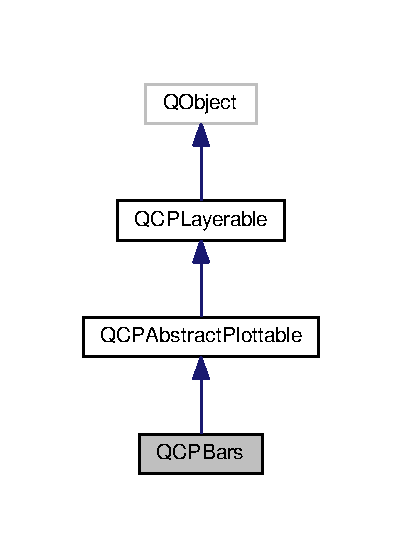
\includegraphics[width=193pt]{classQCPBars__inherit__graph}
\end{center}
\end{figure}


Collaboration diagram for Q\+C\+P\+Bars\+:
\nopagebreak
\begin{figure}[H]
\begin{center}
\leavevmode
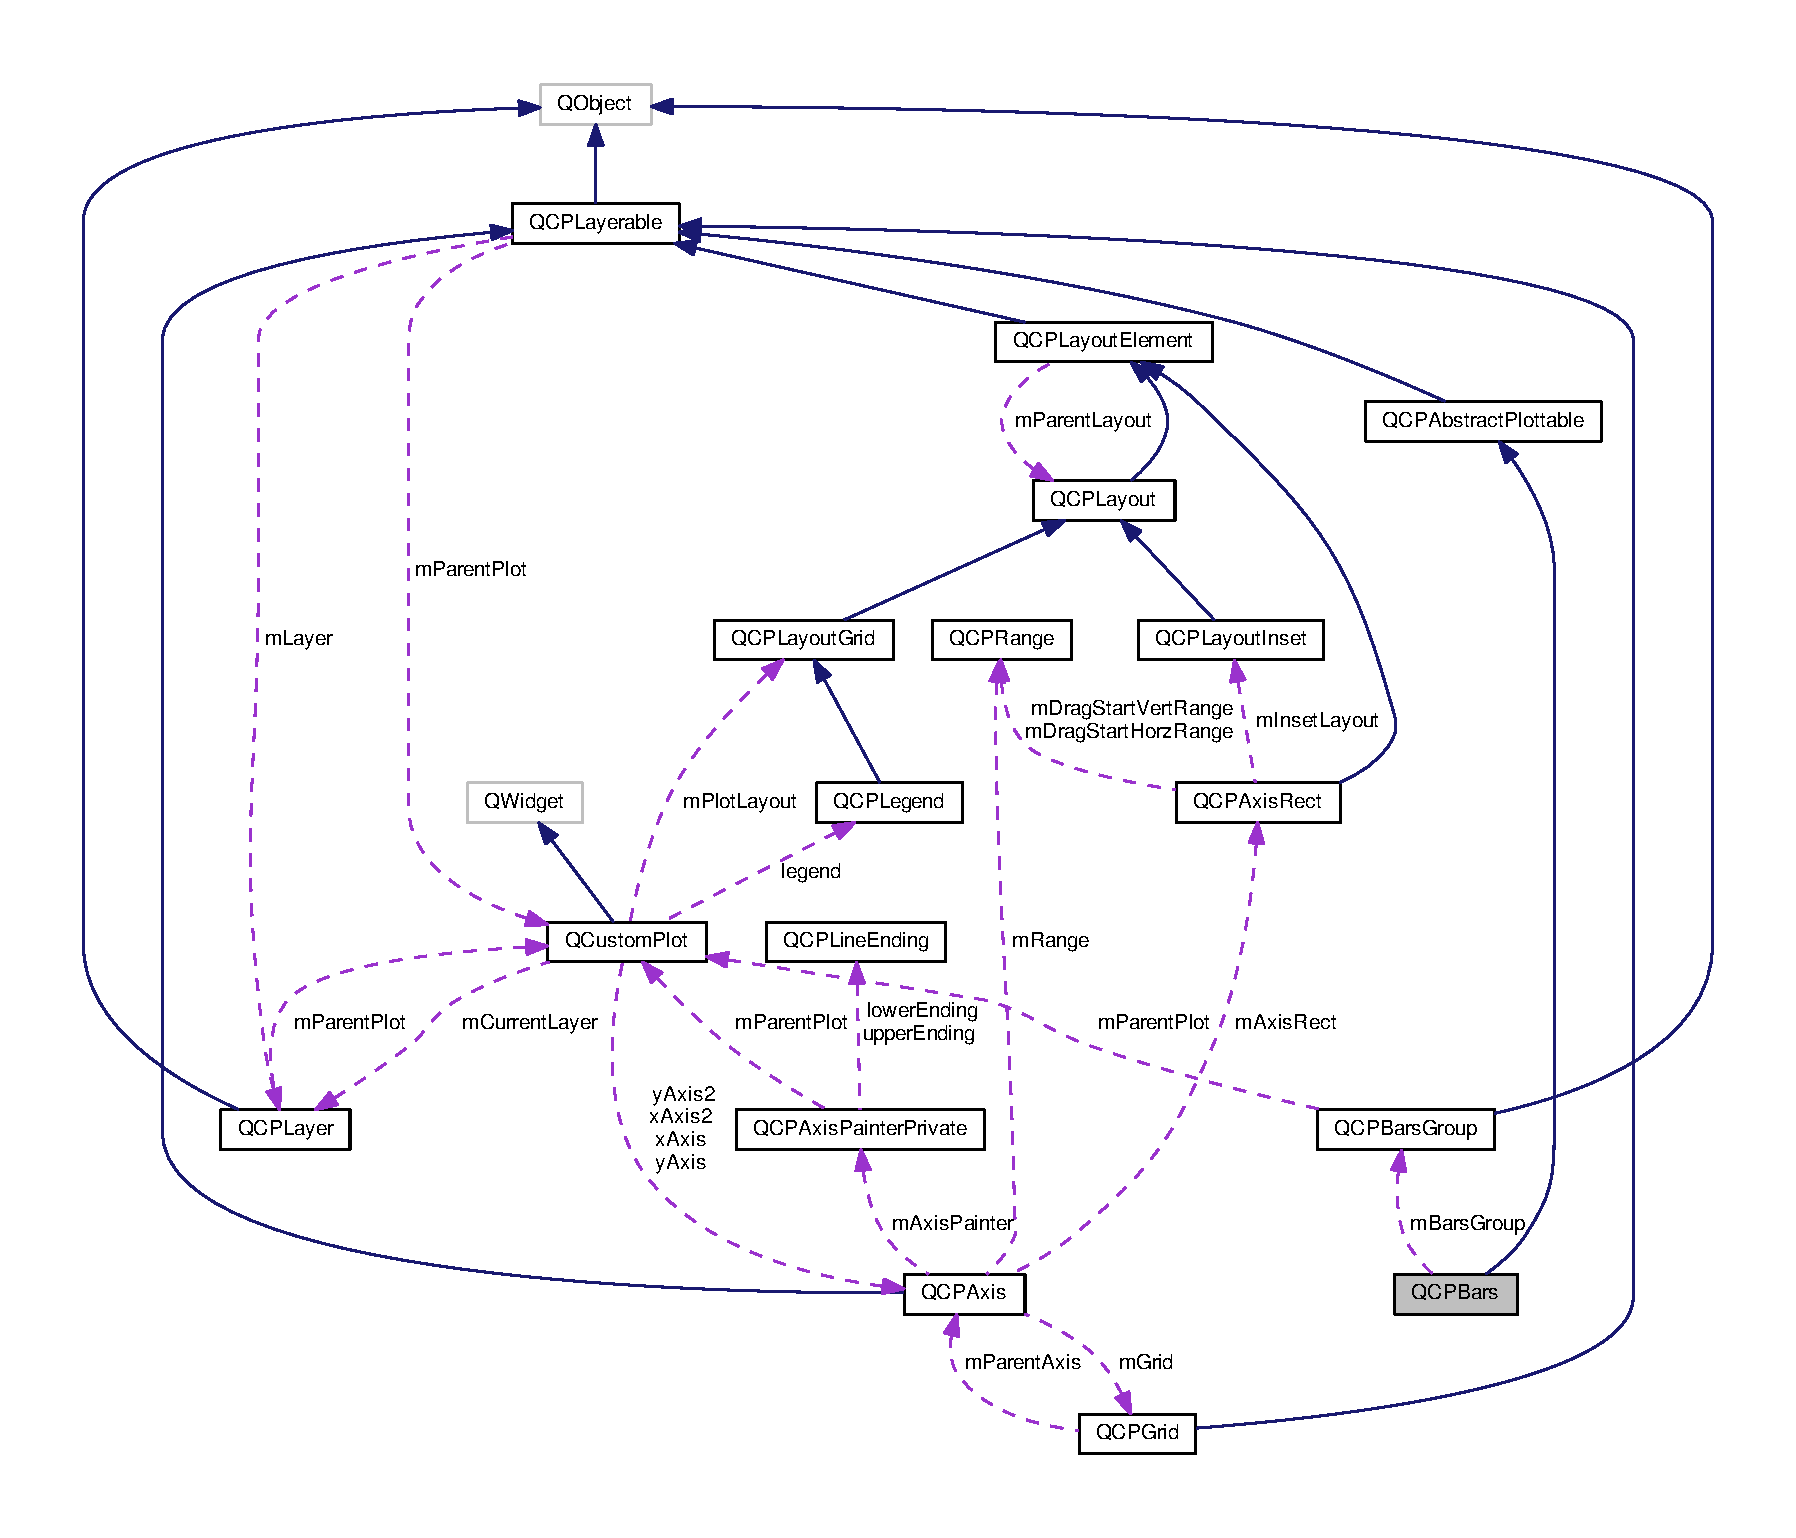
\includegraphics[width=350pt]{classQCPBars__coll__graph}
\end{center}
\end{figure}
\subsection*{Public Types}
\begin{DoxyCompactItemize}
\item 
enum \hyperlink{classQCPBars_a65dbbf1ab41cbe993d71521096ed4649}{Width\+Type} \{ \hyperlink{classQCPBars_a65dbbf1ab41cbe993d71521096ed4649ab74315c9aa77df593c58dd25dfc0de35}{wt\+Absolute}, 
\hyperlink{classQCPBars_a65dbbf1ab41cbe993d71521096ed4649a90bc09899361ad3422ff277f7c790ffe}{wt\+Axis\+Rect\+Ratio}, 
\hyperlink{classQCPBars_a65dbbf1ab41cbe993d71521096ed4649aad3cc60ae1bfb1160a30237bee9eaf10}{wt\+Plot\+Coords}
 \}
\end{DoxyCompactItemize}
\subsection*{Public Member Functions}
\begin{DoxyCompactItemize}
\item 
\hyperlink{classQCPBars_a64006999ad9dff308f40df41cef176ad}{Q\+C\+P\+Bars} (\hyperlink{classQCPAxis}{Q\+C\+P\+Axis} $\ast$\hyperlink{classQCPAbstractPlottable_a72c7a09c22963f2c943f07112b311103}{key\+Axis}, \hyperlink{classQCPAxis}{Q\+C\+P\+Axis} $\ast$\hyperlink{classQCPAbstractPlottable_a3106f9d34d330a6097a8ec5905e5b519}{value\+Axis})
\item 
virtual \hyperlink{classQCPBars_a4d880e28031ef120603f543379be2f22}{$\sim$\+Q\+C\+P\+Bars} ()
\item 
double \hyperlink{classQCPBars_a42798c38abd5f5db22bd45d77f429625}{width} () const 
\item 
\hyperlink{classQCPBars_a65dbbf1ab41cbe993d71521096ed4649}{Width\+Type} \hyperlink{classQCPBars_a8606651ada5804075f6affd04c88dd05}{width\+Type} () const 
\item 
\hyperlink{classQCPBarsGroup}{Q\+C\+P\+Bars\+Group} $\ast$ \hyperlink{classQCPBars_a6d6b2b17619a0ba9c7a88bb2b90fc178}{bars\+Group} () const 
\item 
double \hyperlink{classQCPBars_a3c8686a74396883fd1da87b2e325b043}{base\+Value} () const 
\item 
\hyperlink{classQCPBars}{Q\+C\+P\+Bars} $\ast$ \hyperlink{classQCPBars_a2c46a686cbad95f180ca3c2e88263961}{bar\+Below} () const 
\item 
\hyperlink{classQCPBars}{Q\+C\+P\+Bars} $\ast$ \hyperlink{classQCPBars_a9ca48a6577586825d85bdc1fbf410803}{bar\+Above} () const 
\item 
\hyperlink{qcustomplot_8h_aa846c77472cae93def9f1609d0c57191}{Q\+C\+P\+Bar\+Data\+Map} $\ast$ \hyperlink{classQCPBars_ac05c21de37f677545d06fd852ef8a743}{data} () const 
\item 
void \hyperlink{classQCPBars_afec6116579d44d5b706e0fa5e5332507}{set\+Width} (double \hyperlink{classQCPBars_a42798c38abd5f5db22bd45d77f429625}{width})
\item 
void \hyperlink{classQCPBars_adcaa3b41281bb2c0f7949b341592fcc0}{set\+Width\+Type} (\hyperlink{classQCPBars_a65dbbf1ab41cbe993d71521096ed4649}{Width\+Type} \hyperlink{classQCPBars_a8606651ada5804075f6affd04c88dd05}{width\+Type})
\item 
void \hyperlink{classQCPBars_aedd1709061f0b307c47ddb45e172ef9a}{set\+Bars\+Group} (\hyperlink{classQCPBarsGroup}{Q\+C\+P\+Bars\+Group} $\ast$\hyperlink{classQCPBars_a6d6b2b17619a0ba9c7a88bb2b90fc178}{bars\+Group})
\item 
void \hyperlink{classQCPBars_a574ec7eb7537566df1a28ff085d75623}{set\+Base\+Value} (double \hyperlink{classQCPBars_a3c8686a74396883fd1da87b2e325b043}{base\+Value})
\item 
void \hyperlink{classQCPBars_aa3435aab19e0a49e4e7b41bd36a8d96b}{set\+Data} (\hyperlink{qcustomplot_8h_aa846c77472cae93def9f1609d0c57191}{Q\+C\+P\+Bar\+Data\+Map} $\ast$\hyperlink{classQCPBars_ac05c21de37f677545d06fd852ef8a743}{data}, bool copy=false)
\item 
void \hyperlink{classQCPBars_a3efded5df4a82ecb201f7c28099fa2e5}{set\+Data} (const Q\+Vector$<$ double $>$ \&key, const Q\+Vector$<$ double $>$ \&value)
\item 
void \hyperlink{classQCPBars_a69fc371346980f19177c3d1ecdad78ee}{move\+Below} (\hyperlink{classQCPBars}{Q\+C\+P\+Bars} $\ast$bars)
\item 
void \hyperlink{classQCPBars_ac22e00a6a41509538c21b04f0a57318c}{move\+Above} (\hyperlink{classQCPBars}{Q\+C\+P\+Bars} $\ast$bars)
\item 
void \hyperlink{classQCPBars_a1f29cf08615040993209147fa68de3f2}{add\+Data} (const \hyperlink{qcustomplot_8h_aa846c77472cae93def9f1609d0c57191}{Q\+C\+P\+Bar\+Data\+Map} \&data\+Map)
\item 
void \hyperlink{classQCPBars_a142158b1addefd53259002dd3ab22c3a}{add\+Data} (const \hyperlink{classQCPBarData}{Q\+C\+P\+Bar\+Data} \&\hyperlink{classQCPBars_ac05c21de37f677545d06fd852ef8a743}{data})
\item 
void \hyperlink{classQCPBars_a684dd105403a5497fda42f2094fecbb7}{add\+Data} (double key, double value)
\item 
void \hyperlink{classQCPBars_a3679a0a9decab0fa03f8f4c6e3344d52}{add\+Data} (const Q\+Vector$<$ double $>$ \&keys, const Q\+Vector$<$ double $>$ \&values)
\item 
void \hyperlink{classQCPBars_a9d12779a3fad4820aad2c428f368298d}{remove\+Data\+Before} (double key)
\item 
void \hyperlink{classQCPBars_a99de6e7abbbf03fb41fa604c7f08aa8b}{remove\+Data\+After} (double key)
\item 
void \hyperlink{classQCPBars_a1fe9bcb57d670defea1bb65cadf43765}{remove\+Data} (double from\+Key, double to\+Key)
\item 
void \hyperlink{classQCPBars_a837cc9848ad3edd40a6130b508493f93}{remove\+Data} (double key)
\item 
virtual void \hyperlink{classQCPBars_a11dbbd707132f07f862dff13c5789c2b}{clear\+Data} ()
\item 
virtual double \hyperlink{classQCPBars_a0d37a9feb1d0baf73ce6e809db214445}{select\+Test} (const Q\+PointF \&pos, bool only\+Selectable, Q\+Variant $\ast$details=0) const 
\end{DoxyCompactItemize}
\subsection*{Protected Member Functions}
\begin{DoxyCompactItemize}
\item 
virtual void \hyperlink{classQCPBars_a42b894e34dac799f90ff3700706b31df}{draw} (\hyperlink{classQCPPainter}{Q\+C\+P\+Painter} $\ast$painter)
\item 
virtual void \hyperlink{classQCPBars_ad4fb35d2ab7d2aa460a6612aff3e7a15}{draw\+Legend\+Icon} (\hyperlink{classQCPPainter}{Q\+C\+P\+Painter} $\ast$painter, const Q\+RectF \&rect) const 
\item 
virtual \hyperlink{classQCPRange}{Q\+C\+P\+Range} \hyperlink{classQCPBars_a93cfdc8a535f36aeb087acca49c00662}{get\+Key\+Range} (bool \&found\+Range, \hyperlink{classQCPAbstractPlottable_a661743478a1d3c09d28ec2711d7653d8}{Sign\+Domain} in\+Sign\+Domain=\hyperlink{classQCPAbstractPlottable_a661743478a1d3c09d28ec2711d7653d8a082b98cfb91a7363a3b5cd17b0c1cd60}{sd\+Both}) const 
\item 
virtual \hyperlink{classQCPRange}{Q\+C\+P\+Range} \hyperlink{classQCPBars_ada96e20309570d1488c165596cb2647f}{get\+Value\+Range} (bool \&found\+Range, \hyperlink{classQCPAbstractPlottable_a661743478a1d3c09d28ec2711d7653d8}{Sign\+Domain} in\+Sign\+Domain=\hyperlink{classQCPAbstractPlottable_a661743478a1d3c09d28ec2711d7653d8a082b98cfb91a7363a3b5cd17b0c1cd60}{sd\+Both}) const 
\item 
void \hyperlink{classQCPBars_af73d2032be0a64d2692bb76b08c79ec2}{get\+Visible\+Data\+Bounds} (Q\+C\+P\+Bar\+Data\+Map\+::const\+\_\+iterator \&lower, Q\+C\+P\+Bar\+Data\+Map\+::const\+\_\+iterator \&upper\+End) const 
\item 
Q\+PolygonF \hyperlink{classQCPBars_a1d118a76662cfd691a78c6f573e3f78c}{get\+Bar\+Polygon} (double key, double value) const 
\item 
void \hyperlink{classQCPBars_a794eefe4fb29b9b40583654ccbf460dc}{get\+Pixel\+Width} (double key, double \&lower, double \&upper) const 
\item 
double \hyperlink{classQCPBars_ae9b0c2fad9f29030c84bb6e62a4b605f}{get\+Stacked\+Base\+Value} (double key, bool positive) const 
\end{DoxyCompactItemize}
\subsection*{Static Protected Member Functions}
\begin{DoxyCompactItemize}
\item 
static void \hyperlink{classQCPBars_a6ea37802cd22f97235cab614b14b9f19}{connect\+Bars} (\hyperlink{classQCPBars}{Q\+C\+P\+Bars} $\ast$lower, \hyperlink{classQCPBars}{Q\+C\+P\+Bars} $\ast$upper)
\end{DoxyCompactItemize}
\subsection*{Protected Attributes}
\begin{DoxyCompactItemize}
\item 
\hyperlink{qcustomplot_8h_aa846c77472cae93def9f1609d0c57191}{Q\+C\+P\+Bar\+Data\+Map} $\ast$ \hyperlink{classQCPBars_aef28d29d51ef84b608ecd22c55d531ff}{m\+Data}
\item 
double \hyperlink{classQCPBars_a7c4e0f2246f8133f48a9c3f24cf5b920}{m\+Width}
\item 
\hyperlink{classQCPBars_a65dbbf1ab41cbe993d71521096ed4649}{Width\+Type} \hyperlink{classQCPBars_a94dba1309496c7601d01e2c59715cbb3}{m\+Width\+Type}
\item 
\hyperlink{classQCPBarsGroup}{Q\+C\+P\+Bars\+Group} $\ast$ \hyperlink{classQCPBars_a9f59c255f3739182ca9744dff75beaa9}{m\+Bars\+Group}
\item 
double \hyperlink{classQCPBars_aa0515cf47fa6044cc28e59b1ae5ec759}{m\+Base\+Value}
\item 
Q\+Pointer$<$ \hyperlink{classQCPBars}{Q\+C\+P\+Bars} $>$ \hyperlink{classQCPBars_ad51db970eed7e286f2753b0216fc56de}{m\+Bar\+Below}
\item 
Q\+Pointer$<$ \hyperlink{classQCPBars}{Q\+C\+P\+Bars} $>$ \hyperlink{classQCPBars_a0c1c46076c41a478dbb373cfd35929aa}{m\+Bar\+Above}
\end{DoxyCompactItemize}
\subsection*{Friends}
\begin{DoxyCompactItemize}
\item 
class \hyperlink{classQCPBars_a1cdf9df76adcfae45261690aa0ca2198}{Q\+Custom\+Plot}
\item 
class \hyperlink{classQCPBars_a8429035e7adfbd7f05805a6530ad5e3b}{Q\+C\+P\+Legend}
\item 
class \hyperlink{classQCPBars_ae1051b4d58a2786cb420367a586e2fee}{Q\+C\+P\+Bars\+Group}
\end{DoxyCompactItemize}
\subsection*{Additional Inherited Members}


\subsection{Detailed Description}
A plottable representing a bar chart in a plot. 



To plot data, assign it with the \hyperlink{classQCPBars_aa3435aab19e0a49e4e7b41bd36a8d96b}{set\+Data} or \hyperlink{classQCPBars_a1f29cf08615040993209147fa68de3f2}{add\+Data} functions.\hypertarget{classQCPStatisticalBox_appearance}{}\subsection{Changing the appearance}\label{classQCPStatisticalBox_appearance}
The appearance of the bars is determined by the pen and the brush (\hyperlink{classQCPAbstractPlottable_ab74b09ae4c0e7e13142fe4b5bf46cac7}{set\+Pen}, \hyperlink{classQCPAbstractPlottable_a7a4b92144dca6453a1f0f210e27edc74}{set\+Brush}). The width of the individual bars can be controlled with \hyperlink{classQCPBars_adcaa3b41281bb2c0f7949b341592fcc0}{set\+Width\+Type} and \hyperlink{classQCPBars_afec6116579d44d5b706e0fa5e5332507}{set\+Width}.

Bar charts are stackable. This means, two \hyperlink{classQCPBars}{Q\+C\+P\+Bars} plottables can be placed on top of each other (see \hyperlink{classQCPBars_ac22e00a6a41509538c21b04f0a57318c}{Q\+C\+P\+Bars\+::move\+Above}). So when two bars are at the same key position, they will appear stacked.

If you would like to group multiple \hyperlink{classQCPBars}{Q\+C\+P\+Bars} plottables together so they appear side by side as shown below, use \hyperlink{classQCPBarsGroup}{Q\+C\+P\+Bars\+Group}.

\hypertarget{classQCPStatisticalBox_usage}{}\subsection{Usage}\label{classQCPStatisticalBox_usage}
Like all data representing objects in \hyperlink{classQCustomPlot}{Q\+Custom\+Plot}, the \hyperlink{classQCPBars}{Q\+C\+P\+Bars} is a plottable (\hyperlink{classQCPAbstractPlottable}{Q\+C\+P\+Abstract\+Plottable}). So the plottable-\/interface of \hyperlink{classQCustomPlot}{Q\+Custom\+Plot} applies (\hyperlink{classQCustomPlot_a32de81ff53e263e785b83b52ecd99d6f}{Q\+Custom\+Plot\+::plottable}, \hyperlink{classQCustomPlot_ab7ad9174f701f9c6f64e378df77927a6}{Q\+Custom\+Plot\+::add\+Plottable}, \hyperlink{classQCustomPlot_af3dafd56884208474f311d6226513ab2}{Q\+Custom\+Plot\+::remove\+Plottable}, etc.)

Usually, you first create an instance\+: 
\begin{DoxyCodeInclude}
\end{DoxyCodeInclude}
add it to the custom\+Plot with \hyperlink{classQCustomPlot_ab7ad9174f701f9c6f64e378df77927a6}{Q\+Custom\+Plot\+::add\+Plottable}\+: 
\begin{DoxyCodeInclude}
\end{DoxyCodeInclude}
and then modify the properties of the newly created plottable, e.\+g.\+: 
\begin{DoxyCodeInclude}
\end{DoxyCodeInclude}


\subsection{Member Enumeration Documentation}
\index{Q\+C\+P\+Bars@{Q\+C\+P\+Bars}!Width\+Type@{Width\+Type}}
\index{Width\+Type@{Width\+Type}!Q\+C\+P\+Bars@{Q\+C\+P\+Bars}}
\subsubsection[{\texorpdfstring{Width\+Type}{WidthType}}]{\setlength{\rightskip}{0pt plus 5cm}enum {\bf Q\+C\+P\+Bars\+::\+Width\+Type}}\hypertarget{classQCPBars_a65dbbf1ab41cbe993d71521096ed4649}{}\label{classQCPBars_a65dbbf1ab41cbe993d71521096ed4649}
Defines the ways the width of the bar can be specified. Thus it defines what the number passed to \hyperlink{classQCPBars_afec6116579d44d5b706e0fa5e5332507}{set\+Width} actually means.

\begin{DoxySeeAlso}{See also}
\hyperlink{classQCPBars_adcaa3b41281bb2c0f7949b341592fcc0}{set\+Width\+Type}, \hyperlink{classQCPBars_afec6116579d44d5b706e0fa5e5332507}{set\+Width} 
\end{DoxySeeAlso}
\begin{Desc}
\item[Enumerator]\par
\begin{description}
\index{wt\+Absolute@{wt\+Absolute}!Q\+C\+P\+Bars@{Q\+C\+P\+Bars}}\index{Q\+C\+P\+Bars@{Q\+C\+P\+Bars}!wt\+Absolute@{wt\+Absolute}}\item[{\em 
wt\+Absolute\hypertarget{classQCPBars_a65dbbf1ab41cbe993d71521096ed4649ab74315c9aa77df593c58dd25dfc0de35}{}\label{classQCPBars_a65dbbf1ab41cbe993d71521096ed4649ab74315c9aa77df593c58dd25dfc0de35}
}]Bar width is in absolute pixels. \index{wt\+Axis\+Rect\+Ratio@{wt\+Axis\+Rect\+Ratio}!Q\+C\+P\+Bars@{Q\+C\+P\+Bars}}\index{Q\+C\+P\+Bars@{Q\+C\+P\+Bars}!wt\+Axis\+Rect\+Ratio@{wt\+Axis\+Rect\+Ratio}}\item[{\em 
wt\+Axis\+Rect\+Ratio\hypertarget{classQCPBars_a65dbbf1ab41cbe993d71521096ed4649a90bc09899361ad3422ff277f7c790ffe}{}\label{classQCPBars_a65dbbf1ab41cbe993d71521096ed4649a90bc09899361ad3422ff277f7c790ffe}
}]Bar width is given by a fraction of the axis rect size. \index{wt\+Plot\+Coords@{wt\+Plot\+Coords}!Q\+C\+P\+Bars@{Q\+C\+P\+Bars}}\index{Q\+C\+P\+Bars@{Q\+C\+P\+Bars}!wt\+Plot\+Coords@{wt\+Plot\+Coords}}\item[{\em 
wt\+Plot\+Coords\hypertarget{classQCPBars_a65dbbf1ab41cbe993d71521096ed4649aad3cc60ae1bfb1160a30237bee9eaf10}{}\label{classQCPBars_a65dbbf1ab41cbe993d71521096ed4649aad3cc60ae1bfb1160a30237bee9eaf10}
}]Bar width is in key coordinates and thus scales with the key axis range. \end{description}
\end{Desc}


\subsection{Constructor \& Destructor Documentation}
\index{Q\+C\+P\+Bars@{Q\+C\+P\+Bars}!Q\+C\+P\+Bars@{Q\+C\+P\+Bars}}
\index{Q\+C\+P\+Bars@{Q\+C\+P\+Bars}!Q\+C\+P\+Bars@{Q\+C\+P\+Bars}}
\subsubsection[{\texorpdfstring{Q\+C\+P\+Bars(\+Q\+C\+P\+Axis $\ast$key\+Axis, Q\+C\+P\+Axis $\ast$value\+Axis)}{QCPBars(QCPAxis *keyAxis, QCPAxis *valueAxis)}}]{\setlength{\rightskip}{0pt plus 5cm}Q\+C\+P\+Bars\+::\+Q\+C\+P\+Bars (
\begin{DoxyParamCaption}
\item[{{\bf Q\+C\+P\+Axis} $\ast$}]{key\+Axis, }
\item[{{\bf Q\+C\+P\+Axis} $\ast$}]{value\+Axis}
\end{DoxyParamCaption}
)\hspace{0.3cm}{\ttfamily [explicit]}}\hypertarget{classQCPBars_a64006999ad9dff308f40df41cef176ad}{}\label{classQCPBars_a64006999ad9dff308f40df41cef176ad}
Constructs a bar chart which uses {\itshape key\+Axis} as its key axis (\char`\"{}x\char`\"{}) and {\itshape value\+Axis} as its value axis (\char`\"{}y\char`\"{}). {\itshape key\+Axis} and {\itshape value\+Axis} must reside in the same \hyperlink{classQCustomPlot}{Q\+Custom\+Plot} instance and not have the same orientation. If either of these restrictions is violated, a corresponding message is printed to the debug output (q\+Debug), the construction is not aborted, though.

The constructed \hyperlink{classQCPBars}{Q\+C\+P\+Bars} can be added to the plot with \hyperlink{classQCustomPlot_ab7ad9174f701f9c6f64e378df77927a6}{Q\+Custom\+Plot\+::add\+Plottable}, \hyperlink{classQCustomPlot}{Q\+Custom\+Plot} then takes ownership of the bar chart. \index{Q\+C\+P\+Bars@{Q\+C\+P\+Bars}!````~Q\+C\+P\+Bars@{$\sim$\+Q\+C\+P\+Bars}}
\index{````~Q\+C\+P\+Bars@{$\sim$\+Q\+C\+P\+Bars}!Q\+C\+P\+Bars@{Q\+C\+P\+Bars}}
\subsubsection[{\texorpdfstring{$\sim$\+Q\+C\+P\+Bars()}{~QCPBars()}}]{\setlength{\rightskip}{0pt plus 5cm}Q\+C\+P\+Bars\+::$\sim$\+Q\+C\+P\+Bars (
\begin{DoxyParamCaption}
{}
\end{DoxyParamCaption}
)\hspace{0.3cm}{\ttfamily [virtual]}}\hypertarget{classQCPBars_a4d880e28031ef120603f543379be2f22}{}\label{classQCPBars_a4d880e28031ef120603f543379be2f22}


\subsection{Member Function Documentation}
\index{Q\+C\+P\+Bars@{Q\+C\+P\+Bars}!add\+Data@{add\+Data}}
\index{add\+Data@{add\+Data}!Q\+C\+P\+Bars@{Q\+C\+P\+Bars}}
\subsubsection[{\texorpdfstring{add\+Data(const Q\+C\+P\+Bar\+Data\+Map \&data\+Map)}{addData(const QCPBarDataMap &dataMap)}}]{\setlength{\rightskip}{0pt plus 5cm}void Q\+C\+P\+Bars\+::add\+Data (
\begin{DoxyParamCaption}
\item[{const {\bf Q\+C\+P\+Bar\+Data\+Map} \&}]{data\+Map}
\end{DoxyParamCaption}
)}\hypertarget{classQCPBars_a1f29cf08615040993209147fa68de3f2}{}\label{classQCPBars_a1f29cf08615040993209147fa68de3f2}
Adds the provided data points in {\itshape data\+Map} to the current data. \begin{DoxySeeAlso}{See also}
\hyperlink{classQCPBars_a1fe9bcb57d670defea1bb65cadf43765}{remove\+Data} 
\end{DoxySeeAlso}
\index{Q\+C\+P\+Bars@{Q\+C\+P\+Bars}!add\+Data@{add\+Data}}
\index{add\+Data@{add\+Data}!Q\+C\+P\+Bars@{Q\+C\+P\+Bars}}
\subsubsection[{\texorpdfstring{add\+Data(const Q\+C\+P\+Bar\+Data \&data)}{addData(const QCPBarData &data)}}]{\setlength{\rightskip}{0pt plus 5cm}void Q\+C\+P\+Bars\+::add\+Data (
\begin{DoxyParamCaption}
\item[{const {\bf Q\+C\+P\+Bar\+Data} \&}]{data}
\end{DoxyParamCaption}
)}\hypertarget{classQCPBars_a142158b1addefd53259002dd3ab22c3a}{}\label{classQCPBars_a142158b1addefd53259002dd3ab22c3a}
This is an overloaded member function, provided for convenience. It differs from the above function only in what argument(s) it accepts. Adds the provided single data point in {\itshape data} to the current data. \begin{DoxySeeAlso}{See also}
\hyperlink{classQCPBars_a1fe9bcb57d670defea1bb65cadf43765}{remove\+Data} 
\end{DoxySeeAlso}
\index{Q\+C\+P\+Bars@{Q\+C\+P\+Bars}!add\+Data@{add\+Data}}
\index{add\+Data@{add\+Data}!Q\+C\+P\+Bars@{Q\+C\+P\+Bars}}
\subsubsection[{\texorpdfstring{add\+Data(double key, double value)}{addData(double key, double value)}}]{\setlength{\rightskip}{0pt plus 5cm}void Q\+C\+P\+Bars\+::add\+Data (
\begin{DoxyParamCaption}
\item[{double}]{key, }
\item[{double}]{value}
\end{DoxyParamCaption}
)}\hypertarget{classQCPBars_a684dd105403a5497fda42f2094fecbb7}{}\label{classQCPBars_a684dd105403a5497fda42f2094fecbb7}
This is an overloaded member function, provided for convenience. It differs from the above function only in what argument(s) it accepts. Adds the provided single data point as {\itshape key} and {\itshape value} tuple to the current data \begin{DoxySeeAlso}{See also}
\hyperlink{classQCPBars_a1fe9bcb57d670defea1bb65cadf43765}{remove\+Data} 
\end{DoxySeeAlso}
\index{Q\+C\+P\+Bars@{Q\+C\+P\+Bars}!add\+Data@{add\+Data}}
\index{add\+Data@{add\+Data}!Q\+C\+P\+Bars@{Q\+C\+P\+Bars}}
\subsubsection[{\texorpdfstring{add\+Data(const Q\+Vector$<$ double $>$ \&keys, const Q\+Vector$<$ double $>$ \&values)}{addData(const QVector< double > &keys, const QVector< double > &values)}}]{\setlength{\rightskip}{0pt plus 5cm}void Q\+C\+P\+Bars\+::add\+Data (
\begin{DoxyParamCaption}
\item[{const Q\+Vector$<$ double $>$ \&}]{keys, }
\item[{const Q\+Vector$<$ double $>$ \&}]{values}
\end{DoxyParamCaption}
)}\hypertarget{classQCPBars_a3679a0a9decab0fa03f8f4c6e3344d52}{}\label{classQCPBars_a3679a0a9decab0fa03f8f4c6e3344d52}
This is an overloaded member function, provided for convenience. It differs from the above function only in what argument(s) it accepts. Adds the provided data points as {\itshape key} and {\itshape value} tuples to the current data. \begin{DoxySeeAlso}{See also}
\hyperlink{classQCPBars_a1fe9bcb57d670defea1bb65cadf43765}{remove\+Data} 
\end{DoxySeeAlso}
\index{Q\+C\+P\+Bars@{Q\+C\+P\+Bars}!bar\+Above@{bar\+Above}}
\index{bar\+Above@{bar\+Above}!Q\+C\+P\+Bars@{Q\+C\+P\+Bars}}
\subsubsection[{\texorpdfstring{bar\+Above() const }{barAbove() const }}]{\setlength{\rightskip}{0pt plus 5cm}{\bf Q\+C\+P\+Bars} $\ast$ Q\+C\+P\+Bars\+::bar\+Above (
\begin{DoxyParamCaption}
{}
\end{DoxyParamCaption}
) const\hspace{0.3cm}{\ttfamily [inline]}}\hypertarget{classQCPBars_a9ca48a6577586825d85bdc1fbf410803}{}\label{classQCPBars_a9ca48a6577586825d85bdc1fbf410803}
Returns the bars plottable that is directly above this bars plottable. If there is no such plottable, returns 0.

\begin{DoxySeeAlso}{See also}
\hyperlink{classQCPBars_a2c46a686cbad95f180ca3c2e88263961}{bar\+Below}, \hyperlink{classQCPBars_a69fc371346980f19177c3d1ecdad78ee}{move\+Below}, \hyperlink{classQCPBars_ac22e00a6a41509538c21b04f0a57318c}{move\+Above} 
\end{DoxySeeAlso}
\index{Q\+C\+P\+Bars@{Q\+C\+P\+Bars}!bar\+Below@{bar\+Below}}
\index{bar\+Below@{bar\+Below}!Q\+C\+P\+Bars@{Q\+C\+P\+Bars}}
\subsubsection[{\texorpdfstring{bar\+Below() const }{barBelow() const }}]{\setlength{\rightskip}{0pt plus 5cm}{\bf Q\+C\+P\+Bars} $\ast$ Q\+C\+P\+Bars\+::bar\+Below (
\begin{DoxyParamCaption}
{}
\end{DoxyParamCaption}
) const\hspace{0.3cm}{\ttfamily [inline]}}\hypertarget{classQCPBars_a2c46a686cbad95f180ca3c2e88263961}{}\label{classQCPBars_a2c46a686cbad95f180ca3c2e88263961}
Returns the bars plottable that is directly below this bars plottable. If there is no such plottable, returns 0.

\begin{DoxySeeAlso}{See also}
\hyperlink{classQCPBars_a9ca48a6577586825d85bdc1fbf410803}{bar\+Above}, \hyperlink{classQCPBars_a69fc371346980f19177c3d1ecdad78ee}{move\+Below}, \hyperlink{classQCPBars_ac22e00a6a41509538c21b04f0a57318c}{move\+Above} 
\end{DoxySeeAlso}
\index{Q\+C\+P\+Bars@{Q\+C\+P\+Bars}!bars\+Group@{bars\+Group}}
\index{bars\+Group@{bars\+Group}!Q\+C\+P\+Bars@{Q\+C\+P\+Bars}}
\subsubsection[{\texorpdfstring{bars\+Group() const }{barsGroup() const }}]{\setlength{\rightskip}{0pt plus 5cm}{\bf Q\+C\+P\+Bars\+Group}$\ast$ Q\+C\+P\+Bars\+::bars\+Group (
\begin{DoxyParamCaption}
{}
\end{DoxyParamCaption}
) const\hspace{0.3cm}{\ttfamily [inline]}}\hypertarget{classQCPBars_a6d6b2b17619a0ba9c7a88bb2b90fc178}{}\label{classQCPBars_a6d6b2b17619a0ba9c7a88bb2b90fc178}
\index{Q\+C\+P\+Bars@{Q\+C\+P\+Bars}!base\+Value@{base\+Value}}
\index{base\+Value@{base\+Value}!Q\+C\+P\+Bars@{Q\+C\+P\+Bars}}
\subsubsection[{\texorpdfstring{base\+Value() const }{baseValue() const }}]{\setlength{\rightskip}{0pt plus 5cm}double Q\+C\+P\+Bars\+::base\+Value (
\begin{DoxyParamCaption}
{}
\end{DoxyParamCaption}
) const\hspace{0.3cm}{\ttfamily [inline]}}\hypertarget{classQCPBars_a3c8686a74396883fd1da87b2e325b043}{}\label{classQCPBars_a3c8686a74396883fd1da87b2e325b043}
\index{Q\+C\+P\+Bars@{Q\+C\+P\+Bars}!clear\+Data@{clear\+Data}}
\index{clear\+Data@{clear\+Data}!Q\+C\+P\+Bars@{Q\+C\+P\+Bars}}
\subsubsection[{\texorpdfstring{clear\+Data()}{clearData()}}]{\setlength{\rightskip}{0pt plus 5cm}void Q\+C\+P\+Bars\+::clear\+Data (
\begin{DoxyParamCaption}
{}
\end{DoxyParamCaption}
)\hspace{0.3cm}{\ttfamily [virtual]}}\hypertarget{classQCPBars_a11dbbd707132f07f862dff13c5789c2b}{}\label{classQCPBars_a11dbbd707132f07f862dff13c5789c2b}
Removes all data points. \begin{DoxySeeAlso}{See also}
\hyperlink{classQCPBars_a1fe9bcb57d670defea1bb65cadf43765}{remove\+Data}, \hyperlink{classQCPBars_a99de6e7abbbf03fb41fa604c7f08aa8b}{remove\+Data\+After}, \hyperlink{classQCPBars_a9d12779a3fad4820aad2c428f368298d}{remove\+Data\+Before} 
\end{DoxySeeAlso}


Implements \hyperlink{classQCPAbstractPlottable_a86e5b8fd4b6ff4f4084e7ea4c573fc53}{Q\+C\+P\+Abstract\+Plottable}.

\index{Q\+C\+P\+Bars@{Q\+C\+P\+Bars}!connect\+Bars@{connect\+Bars}}
\index{connect\+Bars@{connect\+Bars}!Q\+C\+P\+Bars@{Q\+C\+P\+Bars}}
\subsubsection[{\texorpdfstring{connect\+Bars(\+Q\+C\+P\+Bars $\ast$lower, Q\+C\+P\+Bars $\ast$upper)}{connectBars(QCPBars *lower, QCPBars *upper)}}]{\setlength{\rightskip}{0pt plus 5cm}void Q\+C\+P\+Bars\+::connect\+Bars (
\begin{DoxyParamCaption}
\item[{{\bf Q\+C\+P\+Bars} $\ast$}]{lower, }
\item[{{\bf Q\+C\+P\+Bars} $\ast$}]{upper}
\end{DoxyParamCaption}
)\hspace{0.3cm}{\ttfamily [static]}, {\ttfamily [protected]}}\hypertarget{classQCPBars_a6ea37802cd22f97235cab614b14b9f19}{}\label{classQCPBars_a6ea37802cd22f97235cab614b14b9f19}
\index{Q\+C\+P\+Bars@{Q\+C\+P\+Bars}!data@{data}}
\index{data@{data}!Q\+C\+P\+Bars@{Q\+C\+P\+Bars}}
\subsubsection[{\texorpdfstring{data() const }{data() const }}]{\setlength{\rightskip}{0pt plus 5cm}{\bf Q\+C\+P\+Bar\+Data\+Map}$\ast$ Q\+C\+P\+Bars\+::data (
\begin{DoxyParamCaption}
{}
\end{DoxyParamCaption}
) const\hspace{0.3cm}{\ttfamily [inline]}}\hypertarget{classQCPBars_ac05c21de37f677545d06fd852ef8a743}{}\label{classQCPBars_ac05c21de37f677545d06fd852ef8a743}
\index{Q\+C\+P\+Bars@{Q\+C\+P\+Bars}!draw@{draw}}
\index{draw@{draw}!Q\+C\+P\+Bars@{Q\+C\+P\+Bars}}
\subsubsection[{\texorpdfstring{draw(\+Q\+C\+P\+Painter $\ast$painter)}{draw(QCPPainter *painter)}}]{\setlength{\rightskip}{0pt plus 5cm}void Q\+C\+P\+Bars\+::draw (
\begin{DoxyParamCaption}
\item[{{\bf Q\+C\+P\+Painter} $\ast$}]{painter}
\end{DoxyParamCaption}
)\hspace{0.3cm}{\ttfamily [protected]}, {\ttfamily [virtual]}}\hypertarget{classQCPBars_a42b894e34dac799f90ff3700706b31df}{}\label{classQCPBars_a42b894e34dac799f90ff3700706b31df}


Implements \hyperlink{classQCPAbstractPlottable_acbab5e30dcd04fd302b4a5902ac2c482}{Q\+C\+P\+Abstract\+Plottable}.

\index{Q\+C\+P\+Bars@{Q\+C\+P\+Bars}!draw\+Legend\+Icon@{draw\+Legend\+Icon}}
\index{draw\+Legend\+Icon@{draw\+Legend\+Icon}!Q\+C\+P\+Bars@{Q\+C\+P\+Bars}}
\subsubsection[{\texorpdfstring{draw\+Legend\+Icon(\+Q\+C\+P\+Painter $\ast$painter, const Q\+Rect\+F \&rect) const }{drawLegendIcon(QCPPainter *painter, const QRectF &rect) const }}]{\setlength{\rightskip}{0pt plus 5cm}void Q\+C\+P\+Bars\+::draw\+Legend\+Icon (
\begin{DoxyParamCaption}
\item[{{\bf Q\+C\+P\+Painter} $\ast$}]{painter, }
\item[{const Q\+RectF \&}]{rect}
\end{DoxyParamCaption}
) const\hspace{0.3cm}{\ttfamily [protected]}, {\ttfamily [virtual]}}\hypertarget{classQCPBars_ad4fb35d2ab7d2aa460a6612aff3e7a15}{}\label{classQCPBars_ad4fb35d2ab7d2aa460a6612aff3e7a15}


Implements \hyperlink{classQCPAbstractPlottable_a9a450783fd9ed539e589999fd390cdf7}{Q\+C\+P\+Abstract\+Plottable}.

\index{Q\+C\+P\+Bars@{Q\+C\+P\+Bars}!get\+Bar\+Polygon@{get\+Bar\+Polygon}}
\index{get\+Bar\+Polygon@{get\+Bar\+Polygon}!Q\+C\+P\+Bars@{Q\+C\+P\+Bars}}
\subsubsection[{\texorpdfstring{get\+Bar\+Polygon(double key, double value) const }{getBarPolygon(double key, double value) const }}]{\setlength{\rightskip}{0pt plus 5cm}Q\+PolygonF Q\+C\+P\+Bars\+::get\+Bar\+Polygon (
\begin{DoxyParamCaption}
\item[{double}]{key, }
\item[{double}]{value}
\end{DoxyParamCaption}
) const\hspace{0.3cm}{\ttfamily [protected]}}\hypertarget{classQCPBars_a1d118a76662cfd691a78c6f573e3f78c}{}\label{classQCPBars_a1d118a76662cfd691a78c6f573e3f78c}
\index{Q\+C\+P\+Bars@{Q\+C\+P\+Bars}!get\+Key\+Range@{get\+Key\+Range}}
\index{get\+Key\+Range@{get\+Key\+Range}!Q\+C\+P\+Bars@{Q\+C\+P\+Bars}}
\subsubsection[{\texorpdfstring{get\+Key\+Range(bool \&found\+Range, Sign\+Domain in\+Sign\+Domain=sd\+Both) const }{getKeyRange(bool &foundRange, SignDomain inSignDomain=sdBoth) const }}]{\setlength{\rightskip}{0pt plus 5cm}{\bf Q\+C\+P\+Range} Q\+C\+P\+Bars\+::get\+Key\+Range (
\begin{DoxyParamCaption}
\item[{bool \&}]{found\+Range, }
\item[{{\bf Sign\+Domain}}]{in\+Sign\+Domain = {\ttfamily {\bf sd\+Both}}}
\end{DoxyParamCaption}
) const\hspace{0.3cm}{\ttfamily [protected]}, {\ttfamily [virtual]}}\hypertarget{classQCPBars_a93cfdc8a535f36aeb087acca49c00662}{}\label{classQCPBars_a93cfdc8a535f36aeb087acca49c00662}


Implements \hyperlink{classQCPAbstractPlottable_a345d702b2e7e12c8cfdddff65ba85e8c}{Q\+C\+P\+Abstract\+Plottable}.

\index{Q\+C\+P\+Bars@{Q\+C\+P\+Bars}!get\+Pixel\+Width@{get\+Pixel\+Width}}
\index{get\+Pixel\+Width@{get\+Pixel\+Width}!Q\+C\+P\+Bars@{Q\+C\+P\+Bars}}
\subsubsection[{\texorpdfstring{get\+Pixel\+Width(double key, double \&lower, double \&upper) const }{getPixelWidth(double key, double &lower, double &upper) const }}]{\setlength{\rightskip}{0pt plus 5cm}void Q\+C\+P\+Bars\+::get\+Pixel\+Width (
\begin{DoxyParamCaption}
\item[{double}]{key, }
\item[{double \&}]{lower, }
\item[{double \&}]{upper}
\end{DoxyParamCaption}
) const\hspace{0.3cm}{\ttfamily [protected]}}\hypertarget{classQCPBars_a794eefe4fb29b9b40583654ccbf460dc}{}\label{classQCPBars_a794eefe4fb29b9b40583654ccbf460dc}
\index{Q\+C\+P\+Bars@{Q\+C\+P\+Bars}!get\+Stacked\+Base\+Value@{get\+Stacked\+Base\+Value}}
\index{get\+Stacked\+Base\+Value@{get\+Stacked\+Base\+Value}!Q\+C\+P\+Bars@{Q\+C\+P\+Bars}}
\subsubsection[{\texorpdfstring{get\+Stacked\+Base\+Value(double key, bool positive) const }{getStackedBaseValue(double key, bool positive) const }}]{\setlength{\rightskip}{0pt plus 5cm}double Q\+C\+P\+Bars\+::get\+Stacked\+Base\+Value (
\begin{DoxyParamCaption}
\item[{double}]{key, }
\item[{bool}]{positive}
\end{DoxyParamCaption}
) const\hspace{0.3cm}{\ttfamily [protected]}}\hypertarget{classQCPBars_ae9b0c2fad9f29030c84bb6e62a4b605f}{}\label{classQCPBars_ae9b0c2fad9f29030c84bb6e62a4b605f}
\index{Q\+C\+P\+Bars@{Q\+C\+P\+Bars}!get\+Value\+Range@{get\+Value\+Range}}
\index{get\+Value\+Range@{get\+Value\+Range}!Q\+C\+P\+Bars@{Q\+C\+P\+Bars}}
\subsubsection[{\texorpdfstring{get\+Value\+Range(bool \&found\+Range, Sign\+Domain in\+Sign\+Domain=sd\+Both) const }{getValueRange(bool &foundRange, SignDomain inSignDomain=sdBoth) const }}]{\setlength{\rightskip}{0pt plus 5cm}{\bf Q\+C\+P\+Range} Q\+C\+P\+Bars\+::get\+Value\+Range (
\begin{DoxyParamCaption}
\item[{bool \&}]{found\+Range, }
\item[{{\bf Sign\+Domain}}]{in\+Sign\+Domain = {\ttfamily {\bf sd\+Both}}}
\end{DoxyParamCaption}
) const\hspace{0.3cm}{\ttfamily [protected]}, {\ttfamily [virtual]}}\hypertarget{classQCPBars_ada96e20309570d1488c165596cb2647f}{}\label{classQCPBars_ada96e20309570d1488c165596cb2647f}


Implements \hyperlink{classQCPAbstractPlottable_aa3331b415b5939fe4df60b78831b2799}{Q\+C\+P\+Abstract\+Plottable}.

\index{Q\+C\+P\+Bars@{Q\+C\+P\+Bars}!get\+Visible\+Data\+Bounds@{get\+Visible\+Data\+Bounds}}
\index{get\+Visible\+Data\+Bounds@{get\+Visible\+Data\+Bounds}!Q\+C\+P\+Bars@{Q\+C\+P\+Bars}}
\subsubsection[{\texorpdfstring{get\+Visible\+Data\+Bounds(\+Q\+C\+P\+Bar\+Data\+Map\+::const\+\_\+iterator \&lower, Q\+C\+P\+Bar\+Data\+Map\+::const\+\_\+iterator \&upper\+End) const }{getVisibleDataBounds(QCPBarDataMap::const_iterator &lower, QCPBarDataMap::const_iterator &upperEnd) const }}]{\setlength{\rightskip}{0pt plus 5cm}void Q\+C\+P\+Bars\+::get\+Visible\+Data\+Bounds (
\begin{DoxyParamCaption}
\item[{Q\+C\+P\+Bar\+Data\+Map\+::const\+\_\+iterator \&}]{lower, }
\item[{Q\+C\+P\+Bar\+Data\+Map\+::const\+\_\+iterator \&}]{upper\+End}
\end{DoxyParamCaption}
) const\hspace{0.3cm}{\ttfamily [protected]}}\hypertarget{classQCPBars_af73d2032be0a64d2692bb76b08c79ec2}{}\label{classQCPBars_af73d2032be0a64d2692bb76b08c79ec2}
\index{Q\+C\+P\+Bars@{Q\+C\+P\+Bars}!move\+Above@{move\+Above}}
\index{move\+Above@{move\+Above}!Q\+C\+P\+Bars@{Q\+C\+P\+Bars}}
\subsubsection[{\texorpdfstring{move\+Above(\+Q\+C\+P\+Bars $\ast$bars)}{moveAbove(QCPBars *bars)}}]{\setlength{\rightskip}{0pt plus 5cm}void Q\+C\+P\+Bars\+::move\+Above (
\begin{DoxyParamCaption}
\item[{{\bf Q\+C\+P\+Bars} $\ast$}]{bars}
\end{DoxyParamCaption}
)}\hypertarget{classQCPBars_ac22e00a6a41509538c21b04f0a57318c}{}\label{classQCPBars_ac22e00a6a41509538c21b04f0a57318c}
Moves this bars plottable above {\itshape bars}. In other words, the bars of this plottable will appear above the bars of {\itshape bars}. The move target {\itshape bars} must use the same key and value axis as this plottable.

Inserting into and removing from existing bar stacking is handled gracefully. If {\itshape bars} already has a bars object below itself, this bars object is inserted between the two. If this bars object is already between two other bars, the two other bars will be stacked on top of each other after the operation.

To remove this bars plottable from any stacking, set {\itshape bars} to 0.

\begin{DoxySeeAlso}{See also}
\hyperlink{classQCPBars_a69fc371346980f19177c3d1ecdad78ee}{move\+Below}, \hyperlink{classQCPBars_a2c46a686cbad95f180ca3c2e88263961}{bar\+Below}, \hyperlink{classQCPBars_a9ca48a6577586825d85bdc1fbf410803}{bar\+Above} 
\end{DoxySeeAlso}
\index{Q\+C\+P\+Bars@{Q\+C\+P\+Bars}!move\+Below@{move\+Below}}
\index{move\+Below@{move\+Below}!Q\+C\+P\+Bars@{Q\+C\+P\+Bars}}
\subsubsection[{\texorpdfstring{move\+Below(\+Q\+C\+P\+Bars $\ast$bars)}{moveBelow(QCPBars *bars)}}]{\setlength{\rightskip}{0pt plus 5cm}void Q\+C\+P\+Bars\+::move\+Below (
\begin{DoxyParamCaption}
\item[{{\bf Q\+C\+P\+Bars} $\ast$}]{bars}
\end{DoxyParamCaption}
)}\hypertarget{classQCPBars_a69fc371346980f19177c3d1ecdad78ee}{}\label{classQCPBars_a69fc371346980f19177c3d1ecdad78ee}
Moves this bars plottable below {\itshape bars}. In other words, the bars of this plottable will appear below the bars of {\itshape bars}. The move target {\itshape bars} must use the same key and value axis as this plottable.

Inserting into and removing from existing bar stacking is handled gracefully. If {\itshape bars} already has a bars object below itself, this bars object is inserted between the two. If this bars object is already between two other bars, the two other bars will be stacked on top of each other after the operation.

To remove this bars plottable from any stacking, set {\itshape bars} to 0.

\begin{DoxySeeAlso}{See also}
\hyperlink{classQCPBars_a69fc371346980f19177c3d1ecdad78ee}{move\+Below}, \hyperlink{classQCPBars_a9ca48a6577586825d85bdc1fbf410803}{bar\+Above}, \hyperlink{classQCPBars_a2c46a686cbad95f180ca3c2e88263961}{bar\+Below} 
\end{DoxySeeAlso}
\index{Q\+C\+P\+Bars@{Q\+C\+P\+Bars}!remove\+Data@{remove\+Data}}
\index{remove\+Data@{remove\+Data}!Q\+C\+P\+Bars@{Q\+C\+P\+Bars}}
\subsubsection[{\texorpdfstring{remove\+Data(double from\+Key, double to\+Key)}{removeData(double fromKey, double toKey)}}]{\setlength{\rightskip}{0pt plus 5cm}void Q\+C\+P\+Bars\+::remove\+Data (
\begin{DoxyParamCaption}
\item[{double}]{from\+Key, }
\item[{double}]{to\+Key}
\end{DoxyParamCaption}
)}\hypertarget{classQCPBars_a1fe9bcb57d670defea1bb65cadf43765}{}\label{classQCPBars_a1fe9bcb57d670defea1bb65cadf43765}
Removes all data points with key between {\itshape from\+Key} and {\itshape to\+Key}. if {\itshape from\+Key} is greater or equal to {\itshape to\+Key}, the function does nothing. To remove a single data point with known key, use \hyperlink{classQCPBars_a837cc9848ad3edd40a6130b508493f93}{remove\+Data(double key)}.

\begin{DoxySeeAlso}{See also}
\hyperlink{classQCPBars_a1f29cf08615040993209147fa68de3f2}{add\+Data}, \hyperlink{classQCPBars_a11dbbd707132f07f862dff13c5789c2b}{clear\+Data} 
\end{DoxySeeAlso}
\index{Q\+C\+P\+Bars@{Q\+C\+P\+Bars}!remove\+Data@{remove\+Data}}
\index{remove\+Data@{remove\+Data}!Q\+C\+P\+Bars@{Q\+C\+P\+Bars}}
\subsubsection[{\texorpdfstring{remove\+Data(double key)}{removeData(double key)}}]{\setlength{\rightskip}{0pt plus 5cm}void Q\+C\+P\+Bars\+::remove\+Data (
\begin{DoxyParamCaption}
\item[{double}]{key}
\end{DoxyParamCaption}
)}\hypertarget{classQCPBars_a837cc9848ad3edd40a6130b508493f93}{}\label{classQCPBars_a837cc9848ad3edd40a6130b508493f93}
This is an overloaded member function, provided for convenience. It differs from the above function only in what argument(s) it accepts.

Removes a single data point at {\itshape key}. If the position is not known with absolute precision, consider using \hyperlink{classQCPBars_a1fe9bcb57d670defea1bb65cadf43765}{remove\+Data(double from\+Key, double to\+Key)} with a small fuzziness interval around the suspected position, depeding on the precision with which the key is known.

\begin{DoxySeeAlso}{See also}
\hyperlink{classQCPBars_a1f29cf08615040993209147fa68de3f2}{add\+Data}, \hyperlink{classQCPBars_a11dbbd707132f07f862dff13c5789c2b}{clear\+Data} 
\end{DoxySeeAlso}
\index{Q\+C\+P\+Bars@{Q\+C\+P\+Bars}!remove\+Data\+After@{remove\+Data\+After}}
\index{remove\+Data\+After@{remove\+Data\+After}!Q\+C\+P\+Bars@{Q\+C\+P\+Bars}}
\subsubsection[{\texorpdfstring{remove\+Data\+After(double key)}{removeDataAfter(double key)}}]{\setlength{\rightskip}{0pt plus 5cm}void Q\+C\+P\+Bars\+::remove\+Data\+After (
\begin{DoxyParamCaption}
\item[{double}]{key}
\end{DoxyParamCaption}
)}\hypertarget{classQCPBars_a99de6e7abbbf03fb41fa604c7f08aa8b}{}\label{classQCPBars_a99de6e7abbbf03fb41fa604c7f08aa8b}
Removes all data points with key greater than {\itshape key}. \begin{DoxySeeAlso}{See also}
\hyperlink{classQCPBars_a1f29cf08615040993209147fa68de3f2}{add\+Data}, \hyperlink{classQCPBars_a11dbbd707132f07f862dff13c5789c2b}{clear\+Data} 
\end{DoxySeeAlso}
\index{Q\+C\+P\+Bars@{Q\+C\+P\+Bars}!remove\+Data\+Before@{remove\+Data\+Before}}
\index{remove\+Data\+Before@{remove\+Data\+Before}!Q\+C\+P\+Bars@{Q\+C\+P\+Bars}}
\subsubsection[{\texorpdfstring{remove\+Data\+Before(double key)}{removeDataBefore(double key)}}]{\setlength{\rightskip}{0pt plus 5cm}void Q\+C\+P\+Bars\+::remove\+Data\+Before (
\begin{DoxyParamCaption}
\item[{double}]{key}
\end{DoxyParamCaption}
)}\hypertarget{classQCPBars_a9d12779a3fad4820aad2c428f368298d}{}\label{classQCPBars_a9d12779a3fad4820aad2c428f368298d}
Removes all data points with key smaller than {\itshape key}. \begin{DoxySeeAlso}{See also}
\hyperlink{classQCPBars_a1f29cf08615040993209147fa68de3f2}{add\+Data}, \hyperlink{classQCPBars_a11dbbd707132f07f862dff13c5789c2b}{clear\+Data} 
\end{DoxySeeAlso}
\index{Q\+C\+P\+Bars@{Q\+C\+P\+Bars}!select\+Test@{select\+Test}}
\index{select\+Test@{select\+Test}!Q\+C\+P\+Bars@{Q\+C\+P\+Bars}}
\subsubsection[{\texorpdfstring{select\+Test(const Q\+Point\+F \&pos, bool only\+Selectable, Q\+Variant $\ast$details=0) const }{selectTest(const QPointF &pos, bool onlySelectable, QVariant *details=0) const }}]{\setlength{\rightskip}{0pt plus 5cm}double Q\+C\+P\+Bars\+::select\+Test (
\begin{DoxyParamCaption}
\item[{const Q\+PointF \&}]{pos, }
\item[{bool}]{only\+Selectable, }
\item[{Q\+Variant $\ast$}]{details = {\ttfamily 0}}
\end{DoxyParamCaption}
) const\hspace{0.3cm}{\ttfamily [virtual]}}\hypertarget{classQCPBars_a0d37a9feb1d0baf73ce6e809db214445}{}\label{classQCPBars_a0d37a9feb1d0baf73ce6e809db214445}
This function is used to decide whether a click hits a layerable object or not.

{\itshape pos} is a point in pixel coordinates on the \hyperlink{classQCustomPlot}{Q\+Custom\+Plot} surface. This function returns the shortest pixel distance of this point to the object. If the object is either invisible or the distance couldn\textquotesingle{}t be determined, -\/1.\+0 is returned. Further, if {\itshape only\+Selectable} is true and the object is not selectable, -\/1.\+0 is returned, too.

If the object is represented not by single lines but by an area like a \hyperlink{classQCPItemText}{Q\+C\+P\+Item\+Text} or the bars of a \hyperlink{classQCPBars}{Q\+C\+P\+Bars} plottable, a click inside the area should also be considered a hit. In these cases this function thus returns a constant value greater zero but still below the parent plot\textquotesingle{}s selection tolerance. (typically the selection\+Tolerance multiplied by 0.\+99).

Providing a constant value for area objects allows selecting line objects even when they are obscured by such area objects, by clicking close to the lines (i.\+e. closer than 0.\+99$\ast$selection\+Tolerance).

The actual setting of the selection state is not done by this function. This is handled by the parent \hyperlink{classQCustomPlot}{Q\+Custom\+Plot} when the mouse\+Release\+Event occurs, and the finally selected object is notified via the select\+Event/deselect\+Event methods.

{\itshape details} is an optional output parameter. Every layerable subclass may place any information in {\itshape details}. This information will be passed to \hyperlink{classQCPAbstractPlottable_a16aaad02456aa23a759efd1ac90c79bf}{select\+Event} when the parent \hyperlink{classQCustomPlot}{Q\+Custom\+Plot} decides on the basis of this select\+Test call, that the object was successfully selected. The subsequent call to \hyperlink{classQCPAbstractPlottable_a16aaad02456aa23a759efd1ac90c79bf}{select\+Event} will carry the {\itshape details}. This is useful for multi-\/part objects (like \hyperlink{classQCPAxis}{Q\+C\+P\+Axis}). This way, a possibly complex calculation to decide which part was clicked is only done once in \hyperlink{classQCPBars_a0d37a9feb1d0baf73ce6e809db214445}{select\+Test}. The result (i.\+e. the actually clicked part) can then be placed in {\itshape details}. So in the subsequent \hyperlink{classQCPAbstractPlottable_a16aaad02456aa23a759efd1ac90c79bf}{select\+Event}, the decision which part was selected doesn\textquotesingle{}t have to be done a second time for a single selection operation.

You may pass 0 as {\itshape details} to indicate that you are not interested in those selection details.

\begin{DoxySeeAlso}{See also}
\hyperlink{classQCPAbstractPlottable_a16aaad02456aa23a759efd1ac90c79bf}{select\+Event}, \hyperlink{classQCPAbstractPlottable_a6fa0d0f95560ea8b01ee13f296dab2b1}{deselect\+Event}, \hyperlink{classQCustomPlot_a5ee1e2f6ae27419deca53e75907c27e5}{Q\+Custom\+Plot\+::set\+Interactions} 
\end{DoxySeeAlso}


Implements \hyperlink{classQCPAbstractPlottable_a38efe9641d972992a3d44204bc80ec1d}{Q\+C\+P\+Abstract\+Plottable}.

\index{Q\+C\+P\+Bars@{Q\+C\+P\+Bars}!set\+Bars\+Group@{set\+Bars\+Group}}
\index{set\+Bars\+Group@{set\+Bars\+Group}!Q\+C\+P\+Bars@{Q\+C\+P\+Bars}}
\subsubsection[{\texorpdfstring{set\+Bars\+Group(\+Q\+C\+P\+Bars\+Group $\ast$bars\+Group)}{setBarsGroup(QCPBarsGroup *barsGroup)}}]{\setlength{\rightskip}{0pt plus 5cm}void Q\+C\+P\+Bars\+::set\+Bars\+Group (
\begin{DoxyParamCaption}
\item[{{\bf Q\+C\+P\+Bars\+Group} $\ast$}]{bars\+Group}
\end{DoxyParamCaption}
)}\hypertarget{classQCPBars_aedd1709061f0b307c47ddb45e172ef9a}{}\label{classQCPBars_aedd1709061f0b307c47ddb45e172ef9a}
Sets to which \hyperlink{classQCPBarsGroup}{Q\+C\+P\+Bars\+Group} this \hyperlink{classQCPBars}{Q\+C\+P\+Bars} instance belongs to. Alternatively, you can also use \hyperlink{classQCPBarsGroup_a809ed63cc4ff7cd5b0b8c96b470163d3}{Q\+C\+P\+Bars\+Group\+::append}.

To remove this \hyperlink{classQCPBars}{Q\+C\+P\+Bars} from any group, set {\itshape bars\+Group} to 0. \index{Q\+C\+P\+Bars@{Q\+C\+P\+Bars}!set\+Base\+Value@{set\+Base\+Value}}
\index{set\+Base\+Value@{set\+Base\+Value}!Q\+C\+P\+Bars@{Q\+C\+P\+Bars}}
\subsubsection[{\texorpdfstring{set\+Base\+Value(double base\+Value)}{setBaseValue(double baseValue)}}]{\setlength{\rightskip}{0pt plus 5cm}void Q\+C\+P\+Bars\+::set\+Base\+Value (
\begin{DoxyParamCaption}
\item[{double}]{base\+Value}
\end{DoxyParamCaption}
)}\hypertarget{classQCPBars_a574ec7eb7537566df1a28ff085d75623}{}\label{classQCPBars_a574ec7eb7537566df1a28ff085d75623}
Sets the base value of this bars plottable.

The base value defines where on the value coordinate the bars start. How far the bars extend from the base value is given by their individual value data. For example, if the base value is set to 1, a bar with data value 2 will have its lowest point at value coordinate 1 and highest point at 3.

For stacked bars, only the base value of the bottom-\/most \hyperlink{classQCPBars}{Q\+C\+P\+Bars} has meaning.

The default base value is 0. \index{Q\+C\+P\+Bars@{Q\+C\+P\+Bars}!set\+Data@{set\+Data}}
\index{set\+Data@{set\+Data}!Q\+C\+P\+Bars@{Q\+C\+P\+Bars}}
\subsubsection[{\texorpdfstring{set\+Data(\+Q\+C\+P\+Bar\+Data\+Map $\ast$data, bool copy=false)}{setData(QCPBarDataMap *data, bool copy=false)}}]{\setlength{\rightskip}{0pt plus 5cm}void Q\+C\+P\+Bars\+::set\+Data (
\begin{DoxyParamCaption}
\item[{{\bf Q\+C\+P\+Bar\+Data\+Map} $\ast$}]{data, }
\item[{bool}]{copy = {\ttfamily false}}
\end{DoxyParamCaption}
)}\hypertarget{classQCPBars_aa3435aab19e0a49e4e7b41bd36a8d96b}{}\label{classQCPBars_aa3435aab19e0a49e4e7b41bd36a8d96b}
Replaces the current data with the provided {\itshape data}.

If {\itshape copy} is set to true, data points in {\itshape data} will only be copied. if false, the plottable takes ownership of the passed data and replaces the internal data pointer with it. This is significantly faster than copying for large datasets. \index{Q\+C\+P\+Bars@{Q\+C\+P\+Bars}!set\+Data@{set\+Data}}
\index{set\+Data@{set\+Data}!Q\+C\+P\+Bars@{Q\+C\+P\+Bars}}
\subsubsection[{\texorpdfstring{set\+Data(const Q\+Vector$<$ double $>$ \&key, const Q\+Vector$<$ double $>$ \&value)}{setData(const QVector< double > &key, const QVector< double > &value)}}]{\setlength{\rightskip}{0pt plus 5cm}void Q\+C\+P\+Bars\+::set\+Data (
\begin{DoxyParamCaption}
\item[{const Q\+Vector$<$ double $>$ \&}]{key, }
\item[{const Q\+Vector$<$ double $>$ \&}]{value}
\end{DoxyParamCaption}
)}\hypertarget{classQCPBars_a3efded5df4a82ecb201f7c28099fa2e5}{}\label{classQCPBars_a3efded5df4a82ecb201f7c28099fa2e5}
This is an overloaded member function, provided for convenience. It differs from the above function only in what argument(s) it accepts.

Replaces the current data with the provided points in {\itshape key} and {\itshape value} tuples. The provided vectors should have equal length. Else, the number of added points will be the size of the smallest vector. \index{Q\+C\+P\+Bars@{Q\+C\+P\+Bars}!set\+Width@{set\+Width}}
\index{set\+Width@{set\+Width}!Q\+C\+P\+Bars@{Q\+C\+P\+Bars}}
\subsubsection[{\texorpdfstring{set\+Width(double width)}{setWidth(double width)}}]{\setlength{\rightskip}{0pt plus 5cm}void Q\+C\+P\+Bars\+::set\+Width (
\begin{DoxyParamCaption}
\item[{double}]{width}
\end{DoxyParamCaption}
)}\hypertarget{classQCPBars_afec6116579d44d5b706e0fa5e5332507}{}\label{classQCPBars_afec6116579d44d5b706e0fa5e5332507}
Sets the width of the bars.

How the number passed as {\itshape width} is interpreted (e.\+g. screen pixels, plot coordinates,...), depends on the currently set width type, see \hyperlink{classQCPBars_adcaa3b41281bb2c0f7949b341592fcc0}{set\+Width\+Type} and \hyperlink{classQCPBars_a65dbbf1ab41cbe993d71521096ed4649}{Width\+Type}. \index{Q\+C\+P\+Bars@{Q\+C\+P\+Bars}!set\+Width\+Type@{set\+Width\+Type}}
\index{set\+Width\+Type@{set\+Width\+Type}!Q\+C\+P\+Bars@{Q\+C\+P\+Bars}}
\subsubsection[{\texorpdfstring{set\+Width\+Type(\+Width\+Type width\+Type)}{setWidthType(WidthType widthType)}}]{\setlength{\rightskip}{0pt plus 5cm}void Q\+C\+P\+Bars\+::set\+Width\+Type (
\begin{DoxyParamCaption}
\item[{{\bf Q\+C\+P\+Bars\+::\+Width\+Type}}]{width\+Type}
\end{DoxyParamCaption}
)}\hypertarget{classQCPBars_adcaa3b41281bb2c0f7949b341592fcc0}{}\label{classQCPBars_adcaa3b41281bb2c0f7949b341592fcc0}
Sets how the width of the bars is defined. See the documentation of \hyperlink{classQCPBars_a65dbbf1ab41cbe993d71521096ed4649}{Width\+Type} for an explanation of the possible values for {\itshape width\+Type}.

The default value is \hyperlink{classQCPBars_a65dbbf1ab41cbe993d71521096ed4649aad3cc60ae1bfb1160a30237bee9eaf10}{wt\+Plot\+Coords}.

\begin{DoxySeeAlso}{See also}
\hyperlink{classQCPBars_afec6116579d44d5b706e0fa5e5332507}{set\+Width} 
\end{DoxySeeAlso}
\index{Q\+C\+P\+Bars@{Q\+C\+P\+Bars}!width@{width}}
\index{width@{width}!Q\+C\+P\+Bars@{Q\+C\+P\+Bars}}
\subsubsection[{\texorpdfstring{width() const }{width() const }}]{\setlength{\rightskip}{0pt plus 5cm}double Q\+C\+P\+Bars\+::width (
\begin{DoxyParamCaption}
{}
\end{DoxyParamCaption}
) const\hspace{0.3cm}{\ttfamily [inline]}}\hypertarget{classQCPBars_a42798c38abd5f5db22bd45d77f429625}{}\label{classQCPBars_a42798c38abd5f5db22bd45d77f429625}
\index{Q\+C\+P\+Bars@{Q\+C\+P\+Bars}!width\+Type@{width\+Type}}
\index{width\+Type@{width\+Type}!Q\+C\+P\+Bars@{Q\+C\+P\+Bars}}
\subsubsection[{\texorpdfstring{width\+Type() const }{widthType() const }}]{\setlength{\rightskip}{0pt plus 5cm}{\bf Width\+Type} Q\+C\+P\+Bars\+::width\+Type (
\begin{DoxyParamCaption}
{}
\end{DoxyParamCaption}
) const\hspace{0.3cm}{\ttfamily [inline]}}\hypertarget{classQCPBars_a8606651ada5804075f6affd04c88dd05}{}\label{classQCPBars_a8606651ada5804075f6affd04c88dd05}


\subsection{Friends And Related Function Documentation}
\index{Q\+C\+P\+Bars@{Q\+C\+P\+Bars}!Q\+C\+P\+Bars\+Group@{Q\+C\+P\+Bars\+Group}}
\index{Q\+C\+P\+Bars\+Group@{Q\+C\+P\+Bars\+Group}!Q\+C\+P\+Bars@{Q\+C\+P\+Bars}}
\subsubsection[{\texorpdfstring{Q\+C\+P\+Bars\+Group}{QCPBarsGroup}}]{\setlength{\rightskip}{0pt plus 5cm}friend class {\bf Q\+C\+P\+Bars\+Group}\hspace{0.3cm}{\ttfamily [friend]}}\hypertarget{classQCPBars_ae1051b4d58a2786cb420367a586e2fee}{}\label{classQCPBars_ae1051b4d58a2786cb420367a586e2fee}
\index{Q\+C\+P\+Bars@{Q\+C\+P\+Bars}!Q\+C\+P\+Legend@{Q\+C\+P\+Legend}}
\index{Q\+C\+P\+Legend@{Q\+C\+P\+Legend}!Q\+C\+P\+Bars@{Q\+C\+P\+Bars}}
\subsubsection[{\texorpdfstring{Q\+C\+P\+Legend}{QCPLegend}}]{\setlength{\rightskip}{0pt plus 5cm}friend class {\bf Q\+C\+P\+Legend}\hspace{0.3cm}{\ttfamily [friend]}}\hypertarget{classQCPBars_a8429035e7adfbd7f05805a6530ad5e3b}{}\label{classQCPBars_a8429035e7adfbd7f05805a6530ad5e3b}
\index{Q\+C\+P\+Bars@{Q\+C\+P\+Bars}!Q\+Custom\+Plot@{Q\+Custom\+Plot}}
\index{Q\+Custom\+Plot@{Q\+Custom\+Plot}!Q\+C\+P\+Bars@{Q\+C\+P\+Bars}}
\subsubsection[{\texorpdfstring{Q\+Custom\+Plot}{QCustomPlot}}]{\setlength{\rightskip}{0pt plus 5cm}friend class {\bf Q\+Custom\+Plot}\hspace{0.3cm}{\ttfamily [friend]}}\hypertarget{classQCPBars_a1cdf9df76adcfae45261690aa0ca2198}{}\label{classQCPBars_a1cdf9df76adcfae45261690aa0ca2198}


\subsection{Member Data Documentation}
\index{Q\+C\+P\+Bars@{Q\+C\+P\+Bars}!m\+Bar\+Above@{m\+Bar\+Above}}
\index{m\+Bar\+Above@{m\+Bar\+Above}!Q\+C\+P\+Bars@{Q\+C\+P\+Bars}}
\subsubsection[{\texorpdfstring{m\+Bar\+Above}{mBarAbove}}]{\setlength{\rightskip}{0pt plus 5cm}Q\+Pointer$<${\bf Q\+C\+P\+Bars}$>$ Q\+C\+P\+Bars\+::m\+Bar\+Above\hspace{0.3cm}{\ttfamily [protected]}}\hypertarget{classQCPBars_a0c1c46076c41a478dbb373cfd35929aa}{}\label{classQCPBars_a0c1c46076c41a478dbb373cfd35929aa}
\index{Q\+C\+P\+Bars@{Q\+C\+P\+Bars}!m\+Bar\+Below@{m\+Bar\+Below}}
\index{m\+Bar\+Below@{m\+Bar\+Below}!Q\+C\+P\+Bars@{Q\+C\+P\+Bars}}
\subsubsection[{\texorpdfstring{m\+Bar\+Below}{mBarBelow}}]{\setlength{\rightskip}{0pt plus 5cm}Q\+Pointer$<${\bf Q\+C\+P\+Bars}$>$ Q\+C\+P\+Bars\+::m\+Bar\+Below\hspace{0.3cm}{\ttfamily [protected]}}\hypertarget{classQCPBars_ad51db970eed7e286f2753b0216fc56de}{}\label{classQCPBars_ad51db970eed7e286f2753b0216fc56de}
\index{Q\+C\+P\+Bars@{Q\+C\+P\+Bars}!m\+Bars\+Group@{m\+Bars\+Group}}
\index{m\+Bars\+Group@{m\+Bars\+Group}!Q\+C\+P\+Bars@{Q\+C\+P\+Bars}}
\subsubsection[{\texorpdfstring{m\+Bars\+Group}{mBarsGroup}}]{\setlength{\rightskip}{0pt plus 5cm}{\bf Q\+C\+P\+Bars\+Group}$\ast$ Q\+C\+P\+Bars\+::m\+Bars\+Group\hspace{0.3cm}{\ttfamily [protected]}}\hypertarget{classQCPBars_a9f59c255f3739182ca9744dff75beaa9}{}\label{classQCPBars_a9f59c255f3739182ca9744dff75beaa9}
\index{Q\+C\+P\+Bars@{Q\+C\+P\+Bars}!m\+Base\+Value@{m\+Base\+Value}}
\index{m\+Base\+Value@{m\+Base\+Value}!Q\+C\+P\+Bars@{Q\+C\+P\+Bars}}
\subsubsection[{\texorpdfstring{m\+Base\+Value}{mBaseValue}}]{\setlength{\rightskip}{0pt plus 5cm}double Q\+C\+P\+Bars\+::m\+Base\+Value\hspace{0.3cm}{\ttfamily [protected]}}\hypertarget{classQCPBars_aa0515cf47fa6044cc28e59b1ae5ec759}{}\label{classQCPBars_aa0515cf47fa6044cc28e59b1ae5ec759}
\index{Q\+C\+P\+Bars@{Q\+C\+P\+Bars}!m\+Data@{m\+Data}}
\index{m\+Data@{m\+Data}!Q\+C\+P\+Bars@{Q\+C\+P\+Bars}}
\subsubsection[{\texorpdfstring{m\+Data}{mData}}]{\setlength{\rightskip}{0pt plus 5cm}{\bf Q\+C\+P\+Bar\+Data\+Map}$\ast$ Q\+C\+P\+Bars\+::m\+Data\hspace{0.3cm}{\ttfamily [protected]}}\hypertarget{classQCPBars_aef28d29d51ef84b608ecd22c55d531ff}{}\label{classQCPBars_aef28d29d51ef84b608ecd22c55d531ff}
\index{Q\+C\+P\+Bars@{Q\+C\+P\+Bars}!m\+Width@{m\+Width}}
\index{m\+Width@{m\+Width}!Q\+C\+P\+Bars@{Q\+C\+P\+Bars}}
\subsubsection[{\texorpdfstring{m\+Width}{mWidth}}]{\setlength{\rightskip}{0pt plus 5cm}double Q\+C\+P\+Bars\+::m\+Width\hspace{0.3cm}{\ttfamily [protected]}}\hypertarget{classQCPBars_a7c4e0f2246f8133f48a9c3f24cf5b920}{}\label{classQCPBars_a7c4e0f2246f8133f48a9c3f24cf5b920}
\index{Q\+C\+P\+Bars@{Q\+C\+P\+Bars}!m\+Width\+Type@{m\+Width\+Type}}
\index{m\+Width\+Type@{m\+Width\+Type}!Q\+C\+P\+Bars@{Q\+C\+P\+Bars}}
\subsubsection[{\texorpdfstring{m\+Width\+Type}{mWidthType}}]{\setlength{\rightskip}{0pt plus 5cm}{\bf Width\+Type} Q\+C\+P\+Bars\+::m\+Width\+Type\hspace{0.3cm}{\ttfamily [protected]}}\hypertarget{classQCPBars_a94dba1309496c7601d01e2c59715cbb3}{}\label{classQCPBars_a94dba1309496c7601d01e2c59715cbb3}


The documentation for this class was generated from the following files\+:\begin{DoxyCompactItemize}
\item 
src/hammerhead/tools/watchdog/include/watchdog/\hyperlink{qcustomplot_8h}{qcustomplot.\+h}\item 
src/hammerhead/tools/watchdog/src/\hyperlink{qcustomplot_8cpp}{qcustomplot.\+cpp}\end{DoxyCompactItemize}

\hypertarget{classQCPBarsGroup}{}\section{Q\+C\+P\+Bars\+Group Class Reference}
\label{classQCPBarsGroup}\index{Q\+C\+P\+Bars\+Group@{Q\+C\+P\+Bars\+Group}}


Groups multiple \hyperlink{classQCPBars}{Q\+C\+P\+Bars} together so they appear side by side.  




{\ttfamily \#include $<$qcustomplot.\+h$>$}



Inheritance diagram for Q\+C\+P\+Bars\+Group\+:
\nopagebreak
\begin{figure}[H]
\begin{center}
\leavevmode
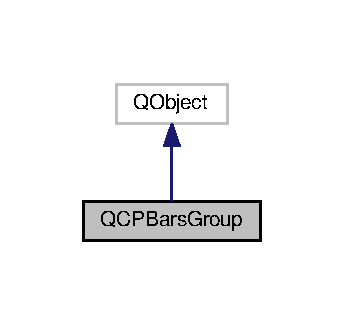
\includegraphics[width=165pt]{classQCPBarsGroup__inherit__graph}
\end{center}
\end{figure}


Collaboration diagram for Q\+C\+P\+Bars\+Group\+:
\nopagebreak
\begin{figure}[H]
\begin{center}
\leavevmode
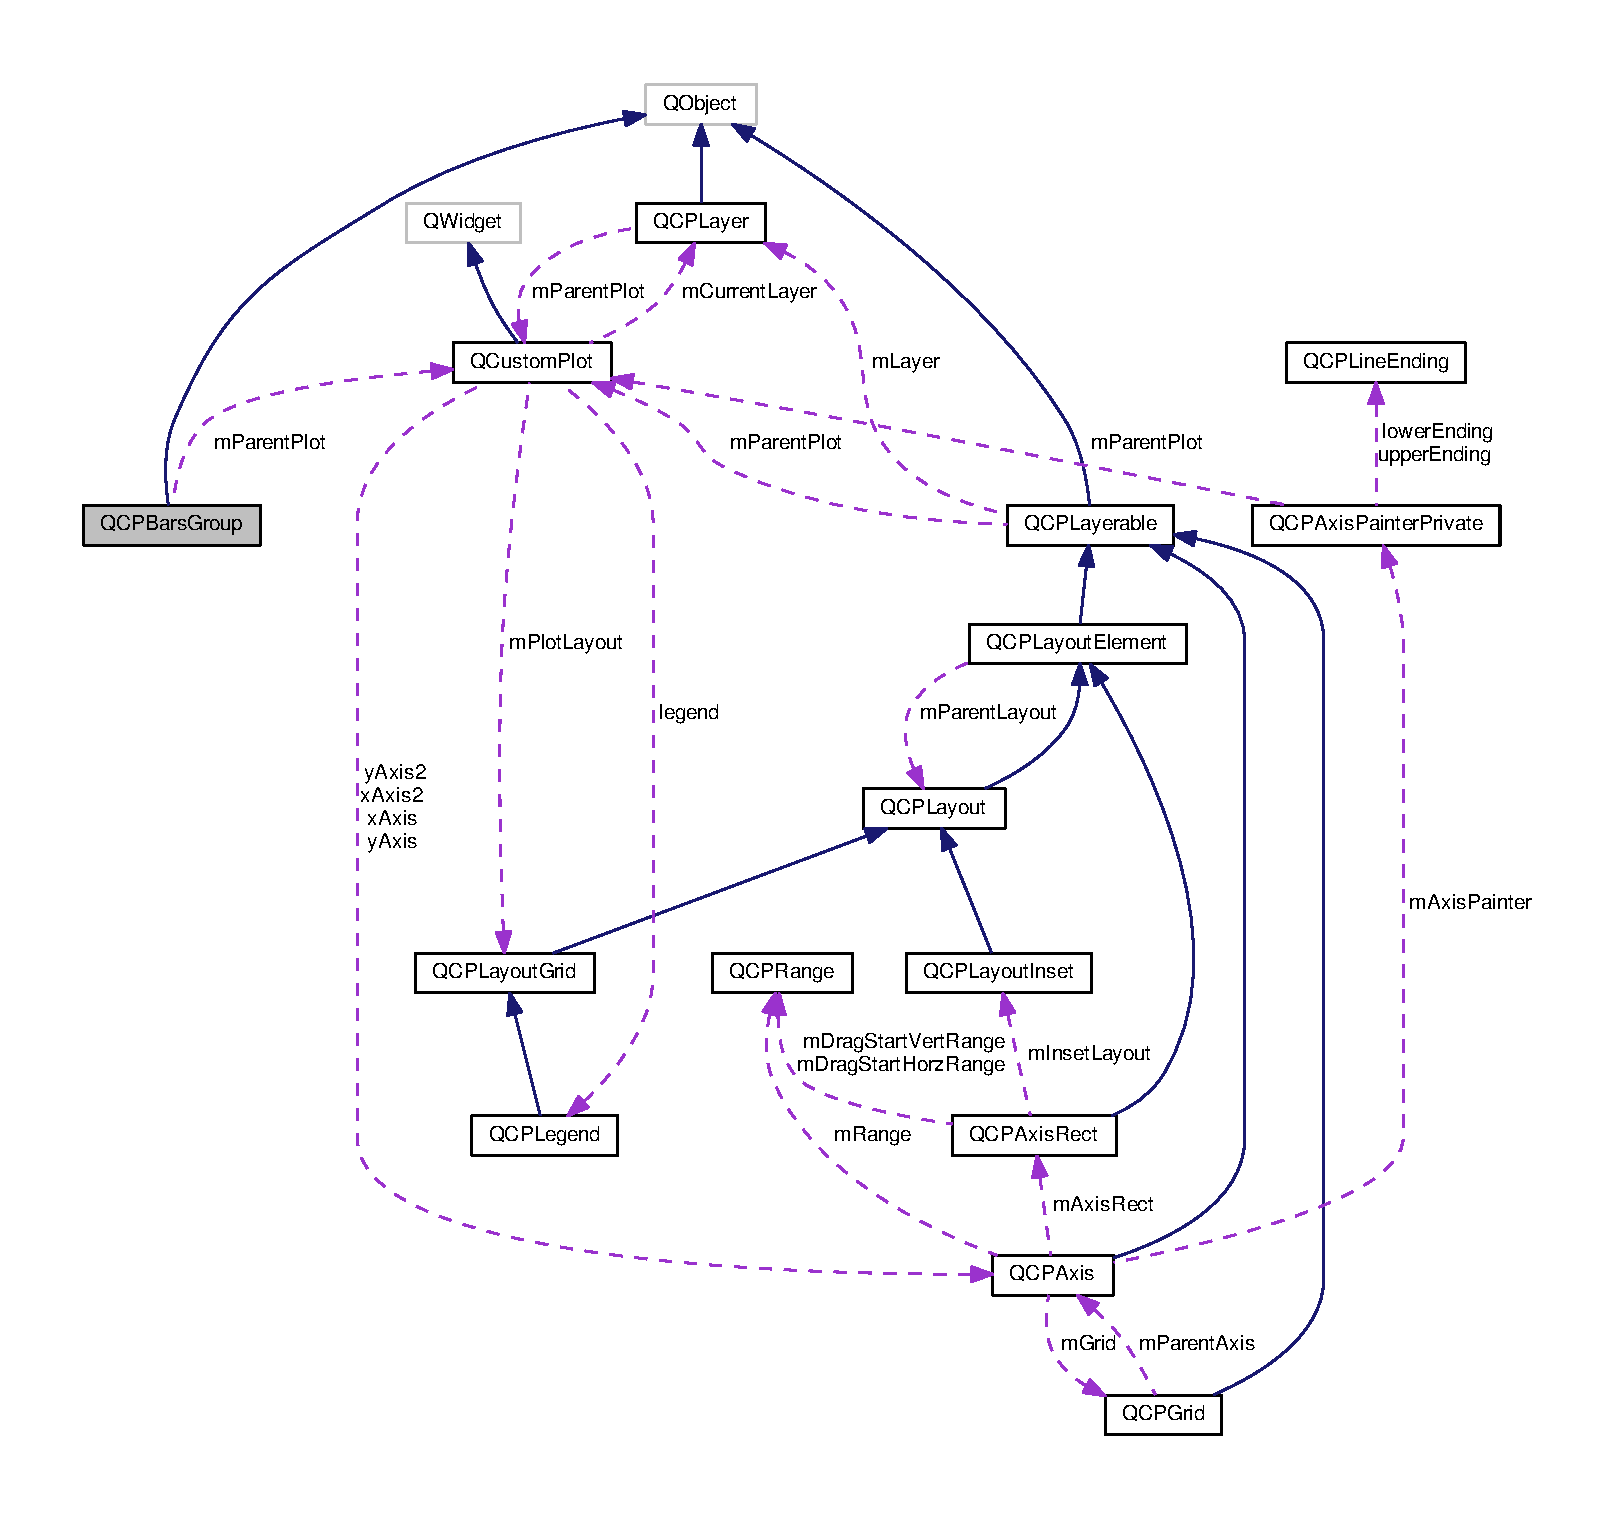
\includegraphics[width=350pt]{classQCPBarsGroup__coll__graph}
\end{center}
\end{figure}
\subsection*{Public Types}
\begin{DoxyCompactItemize}
\item 
enum \hyperlink{classQCPBarsGroup_a4c0521120a97e60bbca37677a37075b6}{Spacing\+Type} \{ \hyperlink{classQCPBarsGroup_a4c0521120a97e60bbca37677a37075b6ab53fa3efaf14867dd0f14d41d64e42ac}{st\+Absolute}, 
\hyperlink{classQCPBarsGroup_a4c0521120a97e60bbca37677a37075b6ae94b05c27bc985dcdd8b1e1b7f163d26}{st\+Axis\+Rect\+Ratio}, 
\hyperlink{classQCPBarsGroup_a4c0521120a97e60bbca37677a37075b6ad369cee6287e0a86e8c2b643a3168c54}{st\+Plot\+Coords}
 \}
\end{DoxyCompactItemize}
\subsection*{Public Member Functions}
\begin{DoxyCompactItemize}
\item 
\hyperlink{classQCPBarsGroup_aa4e043b9a22c6c5ea0f93740aca063e1}{Q\+C\+P\+Bars\+Group} (\hyperlink{classQCustomPlot}{Q\+Custom\+Plot} $\ast$parent\+Plot)
\item 
\hyperlink{classQCPBarsGroup_adb9475bcb6a5f18c8918e17d939d8dbd}{$\sim$\+Q\+C\+P\+Bars\+Group} ()
\item 
\hyperlink{classQCPBarsGroup_a4c0521120a97e60bbca37677a37075b6}{Spacing\+Type} \hyperlink{classQCPBarsGroup_a1bb562f669d47bd7d3cdd2da1f7d8f00}{spacing\+Type} () const 
\item 
double \hyperlink{classQCPBarsGroup_a730bffefcac6c97aaf60e6f64dd3bcd9}{spacing} () const 
\item 
void \hyperlink{classQCPBarsGroup_a2c7e2d61b10594a4555b615e1fcaf49e}{set\+Spacing\+Type} (\hyperlink{classQCPBarsGroup_a4c0521120a97e60bbca37677a37075b6}{Spacing\+Type} \hyperlink{classQCPBarsGroup_a1bb562f669d47bd7d3cdd2da1f7d8f00}{spacing\+Type})
\item 
void \hyperlink{classQCPBarsGroup_aa553d327479d72a0c3dafcc724a190e2}{set\+Spacing} (double \hyperlink{classQCPBarsGroup_a730bffefcac6c97aaf60e6f64dd3bcd9}{spacing})
\item 
Q\+List$<$ \hyperlink{classQCPBars}{Q\+C\+P\+Bars} $\ast$ $>$ \hyperlink{classQCPBarsGroup_a7c72ed1f8cd962c93b8c42ab96cd91ec}{bars} () const 
\item 
\hyperlink{classQCPBars}{Q\+C\+P\+Bars} $\ast$ \hyperlink{classQCPBarsGroup_a72d022790b7c93151c95c28eefaf51b4}{bars} (int index) const 
\item 
int \hyperlink{classQCPBarsGroup_af07364189c5717a158ec95b609687532}{size} () const 
\item 
bool \hyperlink{classQCPBarsGroup_a1d89da4e9176f4f77105e9a4afd44e2b}{is\+Empty} () const 
\item 
void \hyperlink{classQCPBarsGroup_a3ddf23928c6cd89530bd34ab7ba7b177}{clear} ()
\item 
bool \hyperlink{classQCPBarsGroup_adb4837894167e629e42e200db056fac3}{contains} (\hyperlink{classQCPBars}{Q\+C\+P\+Bars} $\ast$\hyperlink{classQCPBarsGroup_a7c72ed1f8cd962c93b8c42ab96cd91ec}{bars}) const 
\item 
void \hyperlink{classQCPBarsGroup_a809ed63cc4ff7cd5b0b8c96b470163d3}{append} (\hyperlink{classQCPBars}{Q\+C\+P\+Bars} $\ast$\hyperlink{classQCPBarsGroup_a7c72ed1f8cd962c93b8c42ab96cd91ec}{bars})
\item 
void \hyperlink{classQCPBarsGroup_a309a5f7233db189f3ea9c2d04ece6c13}{insert} (int i, \hyperlink{classQCPBars}{Q\+C\+P\+Bars} $\ast$\hyperlink{classQCPBarsGroup_a7c72ed1f8cd962c93b8c42ab96cd91ec}{bars})
\item 
void \hyperlink{classQCPBarsGroup_a215e28a5944f1159013a0e19169220e7}{remove} (\hyperlink{classQCPBars}{Q\+C\+P\+Bars} $\ast$\hyperlink{classQCPBarsGroup_a7c72ed1f8cd962c93b8c42ab96cd91ec}{bars})
\end{DoxyCompactItemize}
\subsection*{Protected Member Functions}
\begin{DoxyCompactItemize}
\item 
void \hyperlink{classQCPBarsGroup_a7b00514f19ad58d0bb3fd5246a67fae2}{register\+Bars} (\hyperlink{classQCPBars}{Q\+C\+P\+Bars} $\ast$\hyperlink{classQCPBarsGroup_a7c72ed1f8cd962c93b8c42ab96cd91ec}{bars})
\item 
void \hyperlink{classQCPBarsGroup_ac7073cdd7b1a40c6cb4b5f908145f8c4}{unregister\+Bars} (\hyperlink{classQCPBars}{Q\+C\+P\+Bars} $\ast$\hyperlink{classQCPBarsGroup_a7c72ed1f8cd962c93b8c42ab96cd91ec}{bars})
\item 
double \hyperlink{classQCPBarsGroup_a8e2ca6002e7bab49670144d048a2bcc9}{key\+Pixel\+Offset} (const \hyperlink{classQCPBars}{Q\+C\+P\+Bars} $\ast$\hyperlink{classQCPBarsGroup_a7c72ed1f8cd962c93b8c42ab96cd91ec}{bars}, double key\+Coord)
\item 
double \hyperlink{classQCPBarsGroup_a0beccd41bc3841a4c5b284823bc7d2de}{get\+Pixel\+Spacing} (const \hyperlink{classQCPBars}{Q\+C\+P\+Bars} $\ast$\hyperlink{classQCPBarsGroup_a7c72ed1f8cd962c93b8c42ab96cd91ec}{bars}, double key\+Coord)
\end{DoxyCompactItemize}
\subsection*{Protected Attributes}
\begin{DoxyCompactItemize}
\item 
\hyperlink{classQCustomPlot}{Q\+Custom\+Plot} $\ast$ \hyperlink{classQCPBarsGroup_a973d408cfbf88db95115aec71877f9e7}{m\+Parent\+Plot}
\item 
\hyperlink{classQCPBarsGroup_a4c0521120a97e60bbca37677a37075b6}{Spacing\+Type} \hyperlink{classQCPBarsGroup_a6794ee1a9c81864d627bff6a4b2d64ec}{m\+Spacing\+Type}
\item 
double \hyperlink{classQCPBarsGroup_a56471d7f548ca6141b7a5bf9629f7ece}{m\+Spacing}
\item 
Q\+List$<$ \hyperlink{classQCPBars}{Q\+C\+P\+Bars} $\ast$ $>$ \hyperlink{classQCPBarsGroup_affdb1e9233c277ff5a4c0a1121cf1fc0}{m\+Bars}
\end{DoxyCompactItemize}
\subsection*{Friends}
\begin{DoxyCompactItemize}
\item 
class \hyperlink{classQCPBarsGroup_a721b87c7cdb8e83a90d77fc8a22e7195}{Q\+C\+P\+Bars}
\end{DoxyCompactItemize}


\subsection{Detailed Description}
Groups multiple \hyperlink{classQCPBars}{Q\+C\+P\+Bars} together so they appear side by side. 



When showing multiple \hyperlink{classQCPBars}{Q\+C\+P\+Bars} in one plot which have bars at identical keys, it may be desirable to have them appearing next to each other at each key. This is what adding the respective \hyperlink{classQCPBars}{Q\+C\+P\+Bars} plottables to a \hyperlink{classQCPBarsGroup}{Q\+C\+P\+Bars\+Group} achieves. (An alternative approach is to stack them on top of each other, see \hyperlink{classQCPBars_ac22e00a6a41509538c21b04f0a57318c}{Q\+C\+P\+Bars\+::move\+Above}.)\hypertarget{classQCPBarsGroup_qcpbarsgroup-usage}{}\subsection{Usage}\label{classQCPBarsGroup_qcpbarsgroup-usage}
To add a \hyperlink{classQCPBars}{Q\+C\+P\+Bars} plottable to the group, create a new group and then add the respective bars intances\+: 
\begin{DoxyCodeInclude}
\end{DoxyCodeInclude}
Alternatively to appending to the group like shown above, you can also set the group on the \hyperlink{classQCPBars}{Q\+C\+P\+Bars} plottable via \hyperlink{classQCPBars_aedd1709061f0b307c47ddb45e172ef9a}{Q\+C\+P\+Bars\+::set\+Bars\+Group}.

The spacing between the bars can be configured via \hyperlink{classQCPBarsGroup_a2c7e2d61b10594a4555b615e1fcaf49e}{set\+Spacing\+Type} and \hyperlink{classQCPBarsGroup_aa553d327479d72a0c3dafcc724a190e2}{set\+Spacing}. The bars in this group appear in the plot in the order they were appended. To insert a bars plottable at a certain index position, or to reposition a bars plottable which is already in the group, use \hyperlink{classQCPBarsGroup_a309a5f7233db189f3ea9c2d04ece6c13}{insert}.

To remove specific bars from the group, use either \hyperlink{classQCPBarsGroup_a215e28a5944f1159013a0e19169220e7}{remove} or call \hyperlink{classQCPBars_aedd1709061f0b307c47ddb45e172ef9a}{Q\+C\+P\+Bars\+:\+:set\+Bars\+Group(0)} on the respective bars plottable.

To clear the entire group, call \hyperlink{classQCPBarsGroup_a3ddf23928c6cd89530bd34ab7ba7b177}{clear}, or simply delete the group.\hypertarget{classQCPBarsGroup_qcpbarsgroup-example}{}\subsection{Example}\label{classQCPBarsGroup_qcpbarsgroup-example}
The image above is generated with the following code\+: 
\begin{DoxyCodeInclude}
\end{DoxyCodeInclude}


\subsection{Member Enumeration Documentation}
\index{Q\+C\+P\+Bars\+Group@{Q\+C\+P\+Bars\+Group}!Spacing\+Type@{Spacing\+Type}}
\index{Spacing\+Type@{Spacing\+Type}!Q\+C\+P\+Bars\+Group@{Q\+C\+P\+Bars\+Group}}
\subsubsection[{\texorpdfstring{Spacing\+Type}{SpacingType}}]{\setlength{\rightskip}{0pt plus 5cm}enum {\bf Q\+C\+P\+Bars\+Group\+::\+Spacing\+Type}}\hypertarget{classQCPBarsGroup_a4c0521120a97e60bbca37677a37075b6}{}\label{classQCPBarsGroup_a4c0521120a97e60bbca37677a37075b6}
Defines the ways the spacing between bars in the group can be specified. Thus it defines what the number passed to \hyperlink{classQCPBarsGroup_aa553d327479d72a0c3dafcc724a190e2}{set\+Spacing} actually means.

\begin{DoxySeeAlso}{See also}
\hyperlink{classQCPBarsGroup_a2c7e2d61b10594a4555b615e1fcaf49e}{set\+Spacing\+Type}, \hyperlink{classQCPBarsGroup_aa553d327479d72a0c3dafcc724a190e2}{set\+Spacing} 
\end{DoxySeeAlso}
\begin{Desc}
\item[Enumerator]\par
\begin{description}
\index{st\+Absolute@{st\+Absolute}!Q\+C\+P\+Bars\+Group@{Q\+C\+P\+Bars\+Group}}\index{Q\+C\+P\+Bars\+Group@{Q\+C\+P\+Bars\+Group}!st\+Absolute@{st\+Absolute}}\item[{\em 
st\+Absolute\hypertarget{classQCPBarsGroup_a4c0521120a97e60bbca37677a37075b6ab53fa3efaf14867dd0f14d41d64e42ac}{}\label{classQCPBarsGroup_a4c0521120a97e60bbca37677a37075b6ab53fa3efaf14867dd0f14d41d64e42ac}
}]Bar spacing is in absolute pixels. \index{st\+Axis\+Rect\+Ratio@{st\+Axis\+Rect\+Ratio}!Q\+C\+P\+Bars\+Group@{Q\+C\+P\+Bars\+Group}}\index{Q\+C\+P\+Bars\+Group@{Q\+C\+P\+Bars\+Group}!st\+Axis\+Rect\+Ratio@{st\+Axis\+Rect\+Ratio}}\item[{\em 
st\+Axis\+Rect\+Ratio\hypertarget{classQCPBarsGroup_a4c0521120a97e60bbca37677a37075b6ae94b05c27bc985dcdd8b1e1b7f163d26}{}\label{classQCPBarsGroup_a4c0521120a97e60bbca37677a37075b6ae94b05c27bc985dcdd8b1e1b7f163d26}
}]Bar spacing is given by a fraction of the axis rect size. \index{st\+Plot\+Coords@{st\+Plot\+Coords}!Q\+C\+P\+Bars\+Group@{Q\+C\+P\+Bars\+Group}}\index{Q\+C\+P\+Bars\+Group@{Q\+C\+P\+Bars\+Group}!st\+Plot\+Coords@{st\+Plot\+Coords}}\item[{\em 
st\+Plot\+Coords\hypertarget{classQCPBarsGroup_a4c0521120a97e60bbca37677a37075b6ad369cee6287e0a86e8c2b643a3168c54}{}\label{classQCPBarsGroup_a4c0521120a97e60bbca37677a37075b6ad369cee6287e0a86e8c2b643a3168c54}
}]Bar spacing is in key coordinates and thus scales with the key axis range. \end{description}
\end{Desc}


\subsection{Constructor \& Destructor Documentation}
\index{Q\+C\+P\+Bars\+Group@{Q\+C\+P\+Bars\+Group}!Q\+C\+P\+Bars\+Group@{Q\+C\+P\+Bars\+Group}}
\index{Q\+C\+P\+Bars\+Group@{Q\+C\+P\+Bars\+Group}!Q\+C\+P\+Bars\+Group@{Q\+C\+P\+Bars\+Group}}
\subsubsection[{\texorpdfstring{Q\+C\+P\+Bars\+Group(\+Q\+Custom\+Plot $\ast$parent\+Plot)}{QCPBarsGroup(QCustomPlot *parentPlot)}}]{\setlength{\rightskip}{0pt plus 5cm}Q\+C\+P\+Bars\+Group\+::\+Q\+C\+P\+Bars\+Group (
\begin{DoxyParamCaption}
\item[{{\bf Q\+Custom\+Plot} $\ast$}]{parent\+Plot}
\end{DoxyParamCaption}
)}\hypertarget{classQCPBarsGroup_aa4e043b9a22c6c5ea0f93740aca063e1}{}\label{classQCPBarsGroup_aa4e043b9a22c6c5ea0f93740aca063e1}
Constructs a new bars group for the specified \hyperlink{classQCustomPlot}{Q\+Custom\+Plot} instance. \index{Q\+C\+P\+Bars\+Group@{Q\+C\+P\+Bars\+Group}!````~Q\+C\+P\+Bars\+Group@{$\sim$\+Q\+C\+P\+Bars\+Group}}
\index{````~Q\+C\+P\+Bars\+Group@{$\sim$\+Q\+C\+P\+Bars\+Group}!Q\+C\+P\+Bars\+Group@{Q\+C\+P\+Bars\+Group}}
\subsubsection[{\texorpdfstring{$\sim$\+Q\+C\+P\+Bars\+Group()}{~QCPBarsGroup()}}]{\setlength{\rightskip}{0pt plus 5cm}Q\+C\+P\+Bars\+Group\+::$\sim$\+Q\+C\+P\+Bars\+Group (
\begin{DoxyParamCaption}
{}
\end{DoxyParamCaption}
)}\hypertarget{classQCPBarsGroup_adb9475bcb6a5f18c8918e17d939d8dbd}{}\label{classQCPBarsGroup_adb9475bcb6a5f18c8918e17d939d8dbd}


\subsection{Member Function Documentation}
\index{Q\+C\+P\+Bars\+Group@{Q\+C\+P\+Bars\+Group}!append@{append}}
\index{append@{append}!Q\+C\+P\+Bars\+Group@{Q\+C\+P\+Bars\+Group}}
\subsubsection[{\texorpdfstring{append(\+Q\+C\+P\+Bars $\ast$bars)}{append(QCPBars *bars)}}]{\setlength{\rightskip}{0pt plus 5cm}void Q\+C\+P\+Bars\+Group\+::append (
\begin{DoxyParamCaption}
\item[{{\bf Q\+C\+P\+Bars} $\ast$}]{bars}
\end{DoxyParamCaption}
)}\hypertarget{classQCPBarsGroup_a809ed63cc4ff7cd5b0b8c96b470163d3}{}\label{classQCPBarsGroup_a809ed63cc4ff7cd5b0b8c96b470163d3}
Adds the specified {\itshape bars} plottable to this group. Alternatively, you can also use \hyperlink{classQCPBars_aedd1709061f0b307c47ddb45e172ef9a}{Q\+C\+P\+Bars\+::set\+Bars\+Group} on the {\itshape bars} instance.

\begin{DoxySeeAlso}{See also}
\hyperlink{classQCPBarsGroup_a309a5f7233db189f3ea9c2d04ece6c13}{insert}, \hyperlink{classQCPBarsGroup_a215e28a5944f1159013a0e19169220e7}{remove} 
\end{DoxySeeAlso}
\index{Q\+C\+P\+Bars\+Group@{Q\+C\+P\+Bars\+Group}!bars@{bars}}
\index{bars@{bars}!Q\+C\+P\+Bars\+Group@{Q\+C\+P\+Bars\+Group}}
\subsubsection[{\texorpdfstring{bars() const }{bars() const }}]{\setlength{\rightskip}{0pt plus 5cm}Q\+List$<$ {\bf Q\+C\+P\+Bars} $\ast$ $>$ Q\+C\+P\+Bars\+Group\+::bars (
\begin{DoxyParamCaption}
{}
\end{DoxyParamCaption}
) const\hspace{0.3cm}{\ttfamily [inline]}}\hypertarget{classQCPBarsGroup_a7c72ed1f8cd962c93b8c42ab96cd91ec}{}\label{classQCPBarsGroup_a7c72ed1f8cd962c93b8c42ab96cd91ec}
Returns all bars currently in this group.

\begin{DoxySeeAlso}{See also}
bars(int index) 
\end{DoxySeeAlso}
\index{Q\+C\+P\+Bars\+Group@{Q\+C\+P\+Bars\+Group}!bars@{bars}}
\index{bars@{bars}!Q\+C\+P\+Bars\+Group@{Q\+C\+P\+Bars\+Group}}
\subsubsection[{\texorpdfstring{bars(int index) const }{bars(int index) const }}]{\setlength{\rightskip}{0pt plus 5cm}{\bf Q\+C\+P\+Bars} $\ast$ Q\+C\+P\+Bars\+Group\+::bars (
\begin{DoxyParamCaption}
\item[{int}]{index}
\end{DoxyParamCaption}
) const}\hypertarget{classQCPBarsGroup_a72d022790b7c93151c95c28eefaf51b4}{}\label{classQCPBarsGroup_a72d022790b7c93151c95c28eefaf51b4}
Returns the \hyperlink{classQCPBars}{Q\+C\+P\+Bars} instance with the specified {\itshape index} in this group. If no such \hyperlink{classQCPBars}{Q\+C\+P\+Bars} exists, returns 0.

\begin{DoxySeeAlso}{See also}
\hyperlink{classQCPBarsGroup_a7c72ed1f8cd962c93b8c42ab96cd91ec}{bars()}, \hyperlink{classQCPBarsGroup_af07364189c5717a158ec95b609687532}{size} 
\end{DoxySeeAlso}
\index{Q\+C\+P\+Bars\+Group@{Q\+C\+P\+Bars\+Group}!clear@{clear}}
\index{clear@{clear}!Q\+C\+P\+Bars\+Group@{Q\+C\+P\+Bars\+Group}}
\subsubsection[{\texorpdfstring{clear()}{clear()}}]{\setlength{\rightskip}{0pt plus 5cm}void Q\+C\+P\+Bars\+Group\+::clear (
\begin{DoxyParamCaption}
{}
\end{DoxyParamCaption}
)}\hypertarget{classQCPBarsGroup_a3ddf23928c6cd89530bd34ab7ba7b177}{}\label{classQCPBarsGroup_a3ddf23928c6cd89530bd34ab7ba7b177}
Removes all \hyperlink{classQCPBars}{Q\+C\+P\+Bars} plottables from this group.

\begin{DoxySeeAlso}{See also}
\hyperlink{classQCPBarsGroup_a1d89da4e9176f4f77105e9a4afd44e2b}{is\+Empty} 
\end{DoxySeeAlso}
\index{Q\+C\+P\+Bars\+Group@{Q\+C\+P\+Bars\+Group}!contains@{contains}}
\index{contains@{contains}!Q\+C\+P\+Bars\+Group@{Q\+C\+P\+Bars\+Group}}
\subsubsection[{\texorpdfstring{contains(\+Q\+C\+P\+Bars $\ast$bars) const }{contains(QCPBars *bars) const }}]{\setlength{\rightskip}{0pt plus 5cm}bool Q\+C\+P\+Bars\+Group\+::contains (
\begin{DoxyParamCaption}
\item[{{\bf Q\+C\+P\+Bars} $\ast$}]{bars}
\end{DoxyParamCaption}
) const\hspace{0.3cm}{\ttfamily [inline]}}\hypertarget{classQCPBarsGroup_adb4837894167e629e42e200db056fac3}{}\label{classQCPBarsGroup_adb4837894167e629e42e200db056fac3}
Returns whether the specified {\itshape bars} plottable is part of this group. \index{Q\+C\+P\+Bars\+Group@{Q\+C\+P\+Bars\+Group}!get\+Pixel\+Spacing@{get\+Pixel\+Spacing}}
\index{get\+Pixel\+Spacing@{get\+Pixel\+Spacing}!Q\+C\+P\+Bars\+Group@{Q\+C\+P\+Bars\+Group}}
\subsubsection[{\texorpdfstring{get\+Pixel\+Spacing(const Q\+C\+P\+Bars $\ast$bars, double key\+Coord)}{getPixelSpacing(const QCPBars *bars, double keyCoord)}}]{\setlength{\rightskip}{0pt plus 5cm}double Q\+C\+P\+Bars\+Group\+::get\+Pixel\+Spacing (
\begin{DoxyParamCaption}
\item[{const {\bf Q\+C\+P\+Bars} $\ast$}]{bars, }
\item[{double}]{key\+Coord}
\end{DoxyParamCaption}
)\hspace{0.3cm}{\ttfamily [protected]}}\hypertarget{classQCPBarsGroup_a0beccd41bc3841a4c5b284823bc7d2de}{}\label{classQCPBarsGroup_a0beccd41bc3841a4c5b284823bc7d2de}
\index{Q\+C\+P\+Bars\+Group@{Q\+C\+P\+Bars\+Group}!insert@{insert}}
\index{insert@{insert}!Q\+C\+P\+Bars\+Group@{Q\+C\+P\+Bars\+Group}}
\subsubsection[{\texorpdfstring{insert(int i, Q\+C\+P\+Bars $\ast$bars)}{insert(int i, QCPBars *bars)}}]{\setlength{\rightskip}{0pt plus 5cm}void Q\+C\+P\+Bars\+Group\+::insert (
\begin{DoxyParamCaption}
\item[{int}]{i, }
\item[{{\bf Q\+C\+P\+Bars} $\ast$}]{bars}
\end{DoxyParamCaption}
)}\hypertarget{classQCPBarsGroup_a309a5f7233db189f3ea9c2d04ece6c13}{}\label{classQCPBarsGroup_a309a5f7233db189f3ea9c2d04ece6c13}
Inserts the specified {\itshape bars} plottable into this group at the specified index position {\itshape i}. This gives you full control over the ordering of the bars.

{\itshape bars} may already be part of this group. In that case, {\itshape bars} is just moved to the new index position.

\begin{DoxySeeAlso}{See also}
\hyperlink{classQCPBarsGroup_a809ed63cc4ff7cd5b0b8c96b470163d3}{append}, \hyperlink{classQCPBarsGroup_a215e28a5944f1159013a0e19169220e7}{remove} 
\end{DoxySeeAlso}
\index{Q\+C\+P\+Bars\+Group@{Q\+C\+P\+Bars\+Group}!is\+Empty@{is\+Empty}}
\index{is\+Empty@{is\+Empty}!Q\+C\+P\+Bars\+Group@{Q\+C\+P\+Bars\+Group}}
\subsubsection[{\texorpdfstring{is\+Empty() const }{isEmpty() const }}]{\setlength{\rightskip}{0pt plus 5cm}bool Q\+C\+P\+Bars\+Group\+::is\+Empty (
\begin{DoxyParamCaption}
{}
\end{DoxyParamCaption}
) const\hspace{0.3cm}{\ttfamily [inline]}}\hypertarget{classQCPBarsGroup_a1d89da4e9176f4f77105e9a4afd44e2b}{}\label{classQCPBarsGroup_a1d89da4e9176f4f77105e9a4afd44e2b}
Returns whether this bars group is empty.

\begin{DoxySeeAlso}{See also}
\hyperlink{classQCPBarsGroup_af07364189c5717a158ec95b609687532}{size} 
\end{DoxySeeAlso}
\index{Q\+C\+P\+Bars\+Group@{Q\+C\+P\+Bars\+Group}!key\+Pixel\+Offset@{key\+Pixel\+Offset}}
\index{key\+Pixel\+Offset@{key\+Pixel\+Offset}!Q\+C\+P\+Bars\+Group@{Q\+C\+P\+Bars\+Group}}
\subsubsection[{\texorpdfstring{key\+Pixel\+Offset(const Q\+C\+P\+Bars $\ast$bars, double key\+Coord)}{keyPixelOffset(const QCPBars *bars, double keyCoord)}}]{\setlength{\rightskip}{0pt plus 5cm}double Q\+C\+P\+Bars\+Group\+::key\+Pixel\+Offset (
\begin{DoxyParamCaption}
\item[{const {\bf Q\+C\+P\+Bars} $\ast$}]{bars, }
\item[{double}]{key\+Coord}
\end{DoxyParamCaption}
)\hspace{0.3cm}{\ttfamily [protected]}}\hypertarget{classQCPBarsGroup_a8e2ca6002e7bab49670144d048a2bcc9}{}\label{classQCPBarsGroup_a8e2ca6002e7bab49670144d048a2bcc9}
\index{Q\+C\+P\+Bars\+Group@{Q\+C\+P\+Bars\+Group}!register\+Bars@{register\+Bars}}
\index{register\+Bars@{register\+Bars}!Q\+C\+P\+Bars\+Group@{Q\+C\+P\+Bars\+Group}}
\subsubsection[{\texorpdfstring{register\+Bars(\+Q\+C\+P\+Bars $\ast$bars)}{registerBars(QCPBars *bars)}}]{\setlength{\rightskip}{0pt plus 5cm}void Q\+C\+P\+Bars\+Group\+::register\+Bars (
\begin{DoxyParamCaption}
\item[{{\bf Q\+C\+P\+Bars} $\ast$}]{bars}
\end{DoxyParamCaption}
)\hspace{0.3cm}{\ttfamily [protected]}}\hypertarget{classQCPBarsGroup_a7b00514f19ad58d0bb3fd5246a67fae2}{}\label{classQCPBarsGroup_a7b00514f19ad58d0bb3fd5246a67fae2}
\index{Q\+C\+P\+Bars\+Group@{Q\+C\+P\+Bars\+Group}!remove@{remove}}
\index{remove@{remove}!Q\+C\+P\+Bars\+Group@{Q\+C\+P\+Bars\+Group}}
\subsubsection[{\texorpdfstring{remove(\+Q\+C\+P\+Bars $\ast$bars)}{remove(QCPBars *bars)}}]{\setlength{\rightskip}{0pt plus 5cm}void Q\+C\+P\+Bars\+Group\+::remove (
\begin{DoxyParamCaption}
\item[{{\bf Q\+C\+P\+Bars} $\ast$}]{bars}
\end{DoxyParamCaption}
)}\hypertarget{classQCPBarsGroup_a215e28a5944f1159013a0e19169220e7}{}\label{classQCPBarsGroup_a215e28a5944f1159013a0e19169220e7}
Removes the specified {\itshape bars} plottable from this group.

\begin{DoxySeeAlso}{See also}
\hyperlink{classQCPBarsGroup_adb4837894167e629e42e200db056fac3}{contains}, \hyperlink{classQCPBarsGroup_a3ddf23928c6cd89530bd34ab7ba7b177}{clear} 
\end{DoxySeeAlso}
\index{Q\+C\+P\+Bars\+Group@{Q\+C\+P\+Bars\+Group}!set\+Spacing@{set\+Spacing}}
\index{set\+Spacing@{set\+Spacing}!Q\+C\+P\+Bars\+Group@{Q\+C\+P\+Bars\+Group}}
\subsubsection[{\texorpdfstring{set\+Spacing(double spacing)}{setSpacing(double spacing)}}]{\setlength{\rightskip}{0pt plus 5cm}void Q\+C\+P\+Bars\+Group\+::set\+Spacing (
\begin{DoxyParamCaption}
\item[{double}]{spacing}
\end{DoxyParamCaption}
)}\hypertarget{classQCPBarsGroup_aa553d327479d72a0c3dafcc724a190e2}{}\label{classQCPBarsGroup_aa553d327479d72a0c3dafcc724a190e2}
Sets the spacing between adjacent bars. What the number passed as {\itshape spacing} actually means, is defined by the current \hyperlink{classQCPBarsGroup_a4c0521120a97e60bbca37677a37075b6}{Spacing\+Type}, which can be set with \hyperlink{classQCPBarsGroup_a2c7e2d61b10594a4555b615e1fcaf49e}{set\+Spacing\+Type}.

\begin{DoxySeeAlso}{See also}
\hyperlink{classQCPBarsGroup_a2c7e2d61b10594a4555b615e1fcaf49e}{set\+Spacing\+Type} 
\end{DoxySeeAlso}
\index{Q\+C\+P\+Bars\+Group@{Q\+C\+P\+Bars\+Group}!set\+Spacing\+Type@{set\+Spacing\+Type}}
\index{set\+Spacing\+Type@{set\+Spacing\+Type}!Q\+C\+P\+Bars\+Group@{Q\+C\+P\+Bars\+Group}}
\subsubsection[{\texorpdfstring{set\+Spacing\+Type(\+Spacing\+Type spacing\+Type)}{setSpacingType(SpacingType spacingType)}}]{\setlength{\rightskip}{0pt plus 5cm}void Q\+C\+P\+Bars\+Group\+::set\+Spacing\+Type (
\begin{DoxyParamCaption}
\item[{{\bf Spacing\+Type}}]{spacing\+Type}
\end{DoxyParamCaption}
)}\hypertarget{classQCPBarsGroup_a2c7e2d61b10594a4555b615e1fcaf49e}{}\label{classQCPBarsGroup_a2c7e2d61b10594a4555b615e1fcaf49e}
Sets how the spacing between adjacent bars is interpreted. See \hyperlink{classQCPBarsGroup_a4c0521120a97e60bbca37677a37075b6}{Spacing\+Type}.

The actual spacing can then be specified with \hyperlink{classQCPBarsGroup_aa553d327479d72a0c3dafcc724a190e2}{set\+Spacing}.

\begin{DoxySeeAlso}{See also}
\hyperlink{classQCPBarsGroup_aa553d327479d72a0c3dafcc724a190e2}{set\+Spacing} 
\end{DoxySeeAlso}
\index{Q\+C\+P\+Bars\+Group@{Q\+C\+P\+Bars\+Group}!size@{size}}
\index{size@{size}!Q\+C\+P\+Bars\+Group@{Q\+C\+P\+Bars\+Group}}
\subsubsection[{\texorpdfstring{size() const }{size() const }}]{\setlength{\rightskip}{0pt plus 5cm}int Q\+C\+P\+Bars\+Group\+::size (
\begin{DoxyParamCaption}
{}
\end{DoxyParamCaption}
) const\hspace{0.3cm}{\ttfamily [inline]}}\hypertarget{classQCPBarsGroup_af07364189c5717a158ec95b609687532}{}\label{classQCPBarsGroup_af07364189c5717a158ec95b609687532}
Returns the number of \hyperlink{classQCPBars}{Q\+C\+P\+Bars} plottables that are part of this group. \index{Q\+C\+P\+Bars\+Group@{Q\+C\+P\+Bars\+Group}!spacing@{spacing}}
\index{spacing@{spacing}!Q\+C\+P\+Bars\+Group@{Q\+C\+P\+Bars\+Group}}
\subsubsection[{\texorpdfstring{spacing() const }{spacing() const }}]{\setlength{\rightskip}{0pt plus 5cm}double Q\+C\+P\+Bars\+Group\+::spacing (
\begin{DoxyParamCaption}
{}
\end{DoxyParamCaption}
) const\hspace{0.3cm}{\ttfamily [inline]}}\hypertarget{classQCPBarsGroup_a730bffefcac6c97aaf60e6f64dd3bcd9}{}\label{classQCPBarsGroup_a730bffefcac6c97aaf60e6f64dd3bcd9}
\index{Q\+C\+P\+Bars\+Group@{Q\+C\+P\+Bars\+Group}!spacing\+Type@{spacing\+Type}}
\index{spacing\+Type@{spacing\+Type}!Q\+C\+P\+Bars\+Group@{Q\+C\+P\+Bars\+Group}}
\subsubsection[{\texorpdfstring{spacing\+Type() const }{spacingType() const }}]{\setlength{\rightskip}{0pt plus 5cm}{\bf Spacing\+Type} Q\+C\+P\+Bars\+Group\+::spacing\+Type (
\begin{DoxyParamCaption}
{}
\end{DoxyParamCaption}
) const\hspace{0.3cm}{\ttfamily [inline]}}\hypertarget{classQCPBarsGroup_a1bb562f669d47bd7d3cdd2da1f7d8f00}{}\label{classQCPBarsGroup_a1bb562f669d47bd7d3cdd2da1f7d8f00}
\index{Q\+C\+P\+Bars\+Group@{Q\+C\+P\+Bars\+Group}!unregister\+Bars@{unregister\+Bars}}
\index{unregister\+Bars@{unregister\+Bars}!Q\+C\+P\+Bars\+Group@{Q\+C\+P\+Bars\+Group}}
\subsubsection[{\texorpdfstring{unregister\+Bars(\+Q\+C\+P\+Bars $\ast$bars)}{unregisterBars(QCPBars *bars)}}]{\setlength{\rightskip}{0pt plus 5cm}void Q\+C\+P\+Bars\+Group\+::unregister\+Bars (
\begin{DoxyParamCaption}
\item[{{\bf Q\+C\+P\+Bars} $\ast$}]{bars}
\end{DoxyParamCaption}
)\hspace{0.3cm}{\ttfamily [protected]}}\hypertarget{classQCPBarsGroup_ac7073cdd7b1a40c6cb4b5f908145f8c4}{}\label{classQCPBarsGroup_ac7073cdd7b1a40c6cb4b5f908145f8c4}


\subsection{Friends And Related Function Documentation}
\index{Q\+C\+P\+Bars\+Group@{Q\+C\+P\+Bars\+Group}!Q\+C\+P\+Bars@{Q\+C\+P\+Bars}}
\index{Q\+C\+P\+Bars@{Q\+C\+P\+Bars}!Q\+C\+P\+Bars\+Group@{Q\+C\+P\+Bars\+Group}}
\subsubsection[{\texorpdfstring{Q\+C\+P\+Bars}{QCPBars}}]{\setlength{\rightskip}{0pt plus 5cm}friend class {\bf Q\+C\+P\+Bars}\hspace{0.3cm}{\ttfamily [friend]}}\hypertarget{classQCPBarsGroup_a721b87c7cdb8e83a90d77fc8a22e7195}{}\label{classQCPBarsGroup_a721b87c7cdb8e83a90d77fc8a22e7195}


\subsection{Member Data Documentation}
\index{Q\+C\+P\+Bars\+Group@{Q\+C\+P\+Bars\+Group}!m\+Bars@{m\+Bars}}
\index{m\+Bars@{m\+Bars}!Q\+C\+P\+Bars\+Group@{Q\+C\+P\+Bars\+Group}}
\subsubsection[{\texorpdfstring{m\+Bars}{mBars}}]{\setlength{\rightskip}{0pt plus 5cm}Q\+List$<${\bf Q\+C\+P\+Bars}$\ast$$>$ Q\+C\+P\+Bars\+Group\+::m\+Bars\hspace{0.3cm}{\ttfamily [protected]}}\hypertarget{classQCPBarsGroup_affdb1e9233c277ff5a4c0a1121cf1fc0}{}\label{classQCPBarsGroup_affdb1e9233c277ff5a4c0a1121cf1fc0}
\index{Q\+C\+P\+Bars\+Group@{Q\+C\+P\+Bars\+Group}!m\+Parent\+Plot@{m\+Parent\+Plot}}
\index{m\+Parent\+Plot@{m\+Parent\+Plot}!Q\+C\+P\+Bars\+Group@{Q\+C\+P\+Bars\+Group}}
\subsubsection[{\texorpdfstring{m\+Parent\+Plot}{mParentPlot}}]{\setlength{\rightskip}{0pt plus 5cm}{\bf Q\+Custom\+Plot}$\ast$ Q\+C\+P\+Bars\+Group\+::m\+Parent\+Plot\hspace{0.3cm}{\ttfamily [protected]}}\hypertarget{classQCPBarsGroup_a973d408cfbf88db95115aec71877f9e7}{}\label{classQCPBarsGroup_a973d408cfbf88db95115aec71877f9e7}
\index{Q\+C\+P\+Bars\+Group@{Q\+C\+P\+Bars\+Group}!m\+Spacing@{m\+Spacing}}
\index{m\+Spacing@{m\+Spacing}!Q\+C\+P\+Bars\+Group@{Q\+C\+P\+Bars\+Group}}
\subsubsection[{\texorpdfstring{m\+Spacing}{mSpacing}}]{\setlength{\rightskip}{0pt plus 5cm}double Q\+C\+P\+Bars\+Group\+::m\+Spacing\hspace{0.3cm}{\ttfamily [protected]}}\hypertarget{classQCPBarsGroup_a56471d7f548ca6141b7a5bf9629f7ece}{}\label{classQCPBarsGroup_a56471d7f548ca6141b7a5bf9629f7ece}
\index{Q\+C\+P\+Bars\+Group@{Q\+C\+P\+Bars\+Group}!m\+Spacing\+Type@{m\+Spacing\+Type}}
\index{m\+Spacing\+Type@{m\+Spacing\+Type}!Q\+C\+P\+Bars\+Group@{Q\+C\+P\+Bars\+Group}}
\subsubsection[{\texorpdfstring{m\+Spacing\+Type}{mSpacingType}}]{\setlength{\rightskip}{0pt plus 5cm}{\bf Spacing\+Type} Q\+C\+P\+Bars\+Group\+::m\+Spacing\+Type\hspace{0.3cm}{\ttfamily [protected]}}\hypertarget{classQCPBarsGroup_a6794ee1a9c81864d627bff6a4b2d64ec}{}\label{classQCPBarsGroup_a6794ee1a9c81864d627bff6a4b2d64ec}


The documentation for this class was generated from the following files\+:\begin{DoxyCompactItemize}
\item 
src/hammerhead/tools/watchdog/include/watchdog/\hyperlink{qcustomplot_8h}{qcustomplot.\+h}\item 
src/hammerhead/tools/watchdog/src/\hyperlink{qcustomplot_8cpp}{qcustomplot.\+cpp}\end{DoxyCompactItemize}

\hypertarget{classQCPColorGradient}{}\section{Q\+C\+P\+Color\+Gradient Class Reference}
\label{classQCPColorGradient}\index{Q\+C\+P\+Color\+Gradient@{Q\+C\+P\+Color\+Gradient}}


Defines a color gradient for use with e.\+g. \hyperlink{classQCPColorMap}{Q\+C\+P\+Color\+Map}.  




{\ttfamily \#include $<$qcustomplot.\+h$>$}

\subsection*{Public Types}
\begin{DoxyCompactItemize}
\item 
enum \hyperlink{classQCPColorGradient_ac5dca17cc24336e6ca176610e7f77fc1}{Color\+Interpolation} \{ \hyperlink{classQCPColorGradient_ac5dca17cc24336e6ca176610e7f77fc1a5e30f725c9cfe93999e268a9f92afbe7}{ci\+R\+GB}, 
\hyperlink{classQCPColorGradient_ac5dca17cc24336e6ca176610e7f77fc1af14ae62fcae11ecc07234eeaec5856cb}{ci\+H\+SV}
 \}
\item 
enum \hyperlink{classQCPColorGradient_aed6569828fee337023670272910c9072}{Gradient\+Preset} \{ \\*
\hyperlink{classQCPColorGradient_aed6569828fee337023670272910c9072add11ae369a86f3b1b6205ec72e5021fb}{gp\+Grayscale}, 
\hyperlink{classQCPColorGradient_aed6569828fee337023670272910c9072a4f42e534cf6cff5a29a5388094d099b5}{gp\+Hot}, 
\hyperlink{classQCPColorGradient_aed6569828fee337023670272910c9072aec8c001f62c0d5cb853db5fd85309557}{gp\+Cold}, 
\hyperlink{classQCPColorGradient_aed6569828fee337023670272910c9072a1bb89351b6def7d220973443fe059c62}{gp\+Night}, 
\\*
\hyperlink{classQCPColorGradient_aed6569828fee337023670272910c9072a9e72663bf6b94b65945f7843f24e0721}{gp\+Candy}, 
\hyperlink{classQCPColorGradient_aed6569828fee337023670272910c9072a382f0b07cec1a59d8a533438aea815d2}{gp\+Geography}, 
\hyperlink{classQCPColorGradient_aed6569828fee337023670272910c9072a4297f4f9e212a819cd65e8e34567182b}{gp\+Ion}, 
\hyperlink{classQCPColorGradient_aed6569828fee337023670272910c9072af1676b129f9f458ace453f280c731cf7}{gp\+Thermal}, 
\\*
\hyperlink{classQCPColorGradient_aed6569828fee337023670272910c9072ab7414ce4e36dc3e82e0132a7f0f41b52}{gp\+Polar}, 
\hyperlink{classQCPColorGradient_aed6569828fee337023670272910c9072ad63adc100ef46f6b4a8a6deacec4642f}{gp\+Spectrum}, 
\hyperlink{classQCPColorGradient_aed6569828fee337023670272910c9072a5f8a9e67b64c17ddfe4f069fe2b9fb02}{gp\+Jet}, 
\hyperlink{classQCPColorGradient_aed6569828fee337023670272910c9072a30efe58407acfb67939032f70213a130}{gp\+Hues}
 \}
\end{DoxyCompactItemize}
\subsection*{Public Member Functions}
\begin{DoxyCompactItemize}
\item 
\hyperlink{classQCPColorGradient_a546e44df5fa1846400a582c041361c85}{Q\+C\+P\+Color\+Gradient} (\hyperlink{classQCPColorGradient_aed6569828fee337023670272910c9072}{Gradient\+Preset} preset=\hyperlink{classQCPColorGradient_aed6569828fee337023670272910c9072aec8c001f62c0d5cb853db5fd85309557}{gp\+Cold})
\item 
bool \hyperlink{classQCPColorGradient_aada47d8206bf2cec77462653bf471c13}{operator==} (const \hyperlink{classQCPColorGradient}{Q\+C\+P\+Color\+Gradient} \&other) const 
\item 
bool \hyperlink{classQCPColorGradient_ac641f5d2dc1686201d3cb602c871791d}{operator!=} (const \hyperlink{classQCPColorGradient}{Q\+C\+P\+Color\+Gradient} \&other) const 
\item 
int \hyperlink{classQCPColorGradient_ae7537a8e6d0fed3f1928328062bb0f4e}{level\+Count} () const 
\item 
Q\+Map$<$ double, Q\+Color $>$ \hyperlink{classQCPColorGradient_a64f8aba7826f9c6363aacff8376cef37}{color\+Stops} () const 
\item 
\hyperlink{classQCPColorGradient_ac5dca17cc24336e6ca176610e7f77fc1}{Color\+Interpolation} \hyperlink{classQCPColorGradient_a731616fabe6f2e33f71f58dd382359d8}{color\+Interpolation} () const 
\item 
bool \hyperlink{classQCPColorGradient_a860b7048f877195d2a0fb8d5a7cf5d73}{periodic} () const 
\item 
void \hyperlink{classQCPColorGradient_a18da587eb4f7fc788ea28ba15b6a12de}{set\+Level\+Count} (int n)
\item 
void \hyperlink{classQCPColorGradient_a724e828aa6f0ba5011a9392477c35d3a}{set\+Color\+Stops} (const Q\+Map$<$ double, Q\+Color $>$ \&\hyperlink{classQCPColorGradient_a64f8aba7826f9c6363aacff8376cef37}{color\+Stops})
\item 
void \hyperlink{classQCPColorGradient_a3b48be5e78079db1bb2a1188a4c3390e}{set\+Color\+Stop\+At} (double position, const Q\+Color \&\hyperlink{classQCPColorGradient_a0599545c859268b025d2060dea741cea}{color})
\item 
void \hyperlink{classQCPColorGradient_aa13fda86406e1d896a465a409ae63b38}{set\+Color\+Interpolation} (\hyperlink{classQCPColorGradient_ac5dca17cc24336e6ca176610e7f77fc1}{Color\+Interpolation} interpolation)
\item 
void \hyperlink{classQCPColorGradient_a39d6448155fc00a219f239220d14bb39}{set\+Periodic} (bool enabled)
\item 
void \hyperlink{classQCPColorGradient_aaf423ceb943e177b0ed2c48c811d83dc}{colorize} (const double $\ast$data, const \hyperlink{classQCPRange}{Q\+C\+P\+Range} \&range, Q\+Rgb $\ast$scan\+Line, int n, int data\+Index\+Factor=1, bool logarithmic=false)
\item 
Q\+Rgb \hyperlink{classQCPColorGradient_a0599545c859268b025d2060dea741cea}{color} (double position, const \hyperlink{classQCPRange}{Q\+C\+P\+Range} \&range, bool logarithmic=false)
\item 
void \hyperlink{classQCPColorGradient_aa0aeec1528241728b9671bf8e60b1622}{load\+Preset} (\hyperlink{classQCPColorGradient_aed6569828fee337023670272910c9072}{Gradient\+Preset} preset)
\item 
void \hyperlink{classQCPColorGradient_a939213e85f0d1279519d555c5fcfb6ad}{clear\+Color\+Stops} ()
\item 
\hyperlink{classQCPColorGradient}{Q\+C\+P\+Color\+Gradient} \hyperlink{classQCPColorGradient_abe04e1d1ccab3d7aa78f2924faed4916}{inverted} () const 
\end{DoxyCompactItemize}
\subsection*{Protected Member Functions}
\begin{DoxyCompactItemize}
\item 
void \hyperlink{classQCPColorGradient_a353f15ab3ab586eebf1f6b58c3e2707b}{update\+Color\+Buffer} ()
\end{DoxyCompactItemize}
\subsection*{Protected Attributes}
\begin{DoxyCompactItemize}
\item 
int \hyperlink{classQCPColorGradient_a98fb68e359904b2c991fcae3e38a211a}{m\+Level\+Count}
\item 
Q\+Map$<$ double, Q\+Color $>$ \hyperlink{classQCPColorGradient_a9e11a2b0974ef289d12c324822bc3a3e}{m\+Color\+Stops}
\item 
\hyperlink{classQCPColorGradient_ac5dca17cc24336e6ca176610e7f77fc1}{Color\+Interpolation} \hyperlink{classQCPColorGradient_a028cef73d863800a9ee93ffd641cce01}{m\+Color\+Interpolation}
\item 
bool \hyperlink{classQCPColorGradient_a4b07deeb20ca1ee2d5ea7e01bf0420af}{m\+Periodic}
\item 
Q\+Vector$<$ Q\+Rgb $>$ \hyperlink{classQCPColorGradient_af8b5f0739faa5f8295154d47ce38ecff}{m\+Color\+Buffer}
\item 
bool \hyperlink{classQCPColorGradient_abacf55e11f67d6722a687af1bb2687bd}{m\+Color\+Buffer\+Invalidated}
\end{DoxyCompactItemize}


\subsection{Detailed Description}
Defines a color gradient for use with e.\+g. \hyperlink{classQCPColorMap}{Q\+C\+P\+Color\+Map}. 

This class describes a color gradient which can be used to encode data with color. For example, \hyperlink{classQCPColorMap}{Q\+C\+P\+Color\+Map} and \hyperlink{classQCPColorScale}{Q\+C\+P\+Color\+Scale} have \hyperlink{classQCPColorMap_a7313c78360471cead3576341a2c50377}{set\+Gradient} methods which take an instance of this class. Colors are set with \hyperlink{classQCPColorGradient_a3b48be5e78079db1bb2a1188a4c3390e}{set\+Color\+Stop\+At(double position, const Q\+Color \&color)} with a {\itshape position} from 0 to 1. In between these defined color positions, the color will be interpolated linearly either in R\+GB or H\+SV space, see \hyperlink{classQCPColorGradient_aa13fda86406e1d896a465a409ae63b38}{set\+Color\+Interpolation}.

Alternatively, load one of the preset color gradients shown in the image below, with \hyperlink{classQCPColorGradient_aa0aeec1528241728b9671bf8e60b1622}{load\+Preset}, or by directly specifying the preset in the constructor.



The fact that the \hyperlink{classQCPColorGradient}{ructor} allows directly converting a \hyperlink{classQCPColorGradient_aed6569828fee337023670272910c9072}{Gradient\+Preset} to a \hyperlink{classQCPColorGradient}{Q\+C\+P\+Color\+Gradient}, you can also directly pass \hyperlink{classQCPColorGradient_aed6569828fee337023670272910c9072}{Gradient\+Preset} to all the {\itshape set\+Gradient} methods, e.\+g.\+: 
\begin{DoxyCodeInclude}
\end{DoxyCodeInclude}
 The total number of levels used in the gradient can be set with \hyperlink{classQCPColorGradient_a18da587eb4f7fc788ea28ba15b6a12de}{set\+Level\+Count}. Whether the color gradient shall be applied periodically (wrapping around) to data values that lie outside the data range specified on the plottable instance can be controlled with \hyperlink{classQCPColorGradient_a39d6448155fc00a219f239220d14bb39}{set\+Periodic}. 

\subsection{Member Enumeration Documentation}
\index{Q\+C\+P\+Color\+Gradient@{Q\+C\+P\+Color\+Gradient}!Color\+Interpolation@{Color\+Interpolation}}
\index{Color\+Interpolation@{Color\+Interpolation}!Q\+C\+P\+Color\+Gradient@{Q\+C\+P\+Color\+Gradient}}
\subsubsection[{\texorpdfstring{Color\+Interpolation}{ColorInterpolation}}]{\setlength{\rightskip}{0pt plus 5cm}enum {\bf Q\+C\+P\+Color\+Gradient\+::\+Color\+Interpolation}}\hypertarget{classQCPColorGradient_ac5dca17cc24336e6ca176610e7f77fc1}{}\label{classQCPColorGradient_ac5dca17cc24336e6ca176610e7f77fc1}
Defines the color spaces in which color interpolation between gradient stops can be performed.

\begin{DoxySeeAlso}{See also}
\hyperlink{classQCPColorGradient_aa13fda86406e1d896a465a409ae63b38}{set\+Color\+Interpolation} 
\end{DoxySeeAlso}
\begin{Desc}
\item[Enumerator]\par
\begin{description}
\index{ci\+R\+GB@{ci\+R\+GB}!Q\+C\+P\+Color\+Gradient@{Q\+C\+P\+Color\+Gradient}}\index{Q\+C\+P\+Color\+Gradient@{Q\+C\+P\+Color\+Gradient}!ci\+R\+GB@{ci\+R\+GB}}\item[{\em 
ci\+R\+GB\hypertarget{classQCPColorGradient_ac5dca17cc24336e6ca176610e7f77fc1a5e30f725c9cfe93999e268a9f92afbe7}{}\label{classQCPColorGradient_ac5dca17cc24336e6ca176610e7f77fc1a5e30f725c9cfe93999e268a9f92afbe7}
}]Color channels red, green and blue are linearly interpolated. \index{ci\+H\+SV@{ci\+H\+SV}!Q\+C\+P\+Color\+Gradient@{Q\+C\+P\+Color\+Gradient}}\index{Q\+C\+P\+Color\+Gradient@{Q\+C\+P\+Color\+Gradient}!ci\+H\+SV@{ci\+H\+SV}}\item[{\em 
ci\+H\+SV\hypertarget{classQCPColorGradient_ac5dca17cc24336e6ca176610e7f77fc1af14ae62fcae11ecc07234eeaec5856cb}{}\label{classQCPColorGradient_ac5dca17cc24336e6ca176610e7f77fc1af14ae62fcae11ecc07234eeaec5856cb}
}]Color channels hue, saturation and value are linearly interpolated (The hue is interpolated over the shortest angle distance) \end{description}
\end{Desc}
\index{Q\+C\+P\+Color\+Gradient@{Q\+C\+P\+Color\+Gradient}!Gradient\+Preset@{Gradient\+Preset}}
\index{Gradient\+Preset@{Gradient\+Preset}!Q\+C\+P\+Color\+Gradient@{Q\+C\+P\+Color\+Gradient}}
\subsubsection[{\texorpdfstring{Gradient\+Preset}{GradientPreset}}]{\setlength{\rightskip}{0pt plus 5cm}enum {\bf Q\+C\+P\+Color\+Gradient\+::\+Gradient\+Preset}}\hypertarget{classQCPColorGradient_aed6569828fee337023670272910c9072}{}\label{classQCPColorGradient_aed6569828fee337023670272910c9072}
Defines the available presets that can be loaded with \hyperlink{classQCPColorGradient_aa0aeec1528241728b9671bf8e60b1622}{load\+Preset}. See the documentation there for an image of the presets. \begin{Desc}
\item[Enumerator]\par
\begin{description}
\index{gp\+Grayscale@{gp\+Grayscale}!Q\+C\+P\+Color\+Gradient@{Q\+C\+P\+Color\+Gradient}}\index{Q\+C\+P\+Color\+Gradient@{Q\+C\+P\+Color\+Gradient}!gp\+Grayscale@{gp\+Grayscale}}\item[{\em 
gp\+Grayscale\hypertarget{classQCPColorGradient_aed6569828fee337023670272910c9072add11ae369a86f3b1b6205ec72e5021fb}{}\label{classQCPColorGradient_aed6569828fee337023670272910c9072add11ae369a86f3b1b6205ec72e5021fb}
}]Continuous lightness from black to white (suited for non-\/biased data representation) \index{gp\+Hot@{gp\+Hot}!Q\+C\+P\+Color\+Gradient@{Q\+C\+P\+Color\+Gradient}}\index{Q\+C\+P\+Color\+Gradient@{Q\+C\+P\+Color\+Gradient}!gp\+Hot@{gp\+Hot}}\item[{\em 
gp\+Hot\hypertarget{classQCPColorGradient_aed6569828fee337023670272910c9072a4f42e534cf6cff5a29a5388094d099b5}{}\label{classQCPColorGradient_aed6569828fee337023670272910c9072a4f42e534cf6cff5a29a5388094d099b5}
}]Continuous lightness from black over firey colors to white (suited for non-\/biased data representation) \index{gp\+Cold@{gp\+Cold}!Q\+C\+P\+Color\+Gradient@{Q\+C\+P\+Color\+Gradient}}\index{Q\+C\+P\+Color\+Gradient@{Q\+C\+P\+Color\+Gradient}!gp\+Cold@{gp\+Cold}}\item[{\em 
gp\+Cold\hypertarget{classQCPColorGradient_aed6569828fee337023670272910c9072aec8c001f62c0d5cb853db5fd85309557}{}\label{classQCPColorGradient_aed6569828fee337023670272910c9072aec8c001f62c0d5cb853db5fd85309557}
}]Continuous lightness from black over icey colors to white (suited for non-\/biased data representation) \index{gp\+Night@{gp\+Night}!Q\+C\+P\+Color\+Gradient@{Q\+C\+P\+Color\+Gradient}}\index{Q\+C\+P\+Color\+Gradient@{Q\+C\+P\+Color\+Gradient}!gp\+Night@{gp\+Night}}\item[{\em 
gp\+Night\hypertarget{classQCPColorGradient_aed6569828fee337023670272910c9072a1bb89351b6def7d220973443fe059c62}{}\label{classQCPColorGradient_aed6569828fee337023670272910c9072a1bb89351b6def7d220973443fe059c62}
}]Continuous lightness from black over weak blueish colors to white (suited for non-\/biased data representation) \index{gp\+Candy@{gp\+Candy}!Q\+C\+P\+Color\+Gradient@{Q\+C\+P\+Color\+Gradient}}\index{Q\+C\+P\+Color\+Gradient@{Q\+C\+P\+Color\+Gradient}!gp\+Candy@{gp\+Candy}}\item[{\em 
gp\+Candy\hypertarget{classQCPColorGradient_aed6569828fee337023670272910c9072a9e72663bf6b94b65945f7843f24e0721}{}\label{classQCPColorGradient_aed6569828fee337023670272910c9072a9e72663bf6b94b65945f7843f24e0721}
}]Blue over pink to white. \index{gp\+Geography@{gp\+Geography}!Q\+C\+P\+Color\+Gradient@{Q\+C\+P\+Color\+Gradient}}\index{Q\+C\+P\+Color\+Gradient@{Q\+C\+P\+Color\+Gradient}!gp\+Geography@{gp\+Geography}}\item[{\em 
gp\+Geography\hypertarget{classQCPColorGradient_aed6569828fee337023670272910c9072a382f0b07cec1a59d8a533438aea815d2}{}\label{classQCPColorGradient_aed6569828fee337023670272910c9072a382f0b07cec1a59d8a533438aea815d2}
}]Colors suitable to represent different elevations on geographical maps. \index{gp\+Ion@{gp\+Ion}!Q\+C\+P\+Color\+Gradient@{Q\+C\+P\+Color\+Gradient}}\index{Q\+C\+P\+Color\+Gradient@{Q\+C\+P\+Color\+Gradient}!gp\+Ion@{gp\+Ion}}\item[{\em 
gp\+Ion\hypertarget{classQCPColorGradient_aed6569828fee337023670272910c9072a4297f4f9e212a819cd65e8e34567182b}{}\label{classQCPColorGradient_aed6569828fee337023670272910c9072a4297f4f9e212a819cd65e8e34567182b}
}]Half hue spectrum from black over purple to blue and finally green (creates banding illusion but allows more precise magnitude estimates) \index{gp\+Thermal@{gp\+Thermal}!Q\+C\+P\+Color\+Gradient@{Q\+C\+P\+Color\+Gradient}}\index{Q\+C\+P\+Color\+Gradient@{Q\+C\+P\+Color\+Gradient}!gp\+Thermal@{gp\+Thermal}}\item[{\em 
gp\+Thermal\hypertarget{classQCPColorGradient_aed6569828fee337023670272910c9072af1676b129f9f458ace453f280c731cf7}{}\label{classQCPColorGradient_aed6569828fee337023670272910c9072af1676b129f9f458ace453f280c731cf7}
}]Colors suitable for thermal imaging, ranging from dark blue over purple to orange, yellow and white. \index{gp\+Polar@{gp\+Polar}!Q\+C\+P\+Color\+Gradient@{Q\+C\+P\+Color\+Gradient}}\index{Q\+C\+P\+Color\+Gradient@{Q\+C\+P\+Color\+Gradient}!gp\+Polar@{gp\+Polar}}\item[{\em 
gp\+Polar\hypertarget{classQCPColorGradient_aed6569828fee337023670272910c9072ab7414ce4e36dc3e82e0132a7f0f41b52}{}\label{classQCPColorGradient_aed6569828fee337023670272910c9072ab7414ce4e36dc3e82e0132a7f0f41b52}
}]Colors suitable to emphasize polarity around the center, with blue for negative, black in the middle and red for positive values. \index{gp\+Spectrum@{gp\+Spectrum}!Q\+C\+P\+Color\+Gradient@{Q\+C\+P\+Color\+Gradient}}\index{Q\+C\+P\+Color\+Gradient@{Q\+C\+P\+Color\+Gradient}!gp\+Spectrum@{gp\+Spectrum}}\item[{\em 
gp\+Spectrum\hypertarget{classQCPColorGradient_aed6569828fee337023670272910c9072ad63adc100ef46f6b4a8a6deacec4642f}{}\label{classQCPColorGradient_aed6569828fee337023670272910c9072ad63adc100ef46f6b4a8a6deacec4642f}
}]An approximation of the visible light spectrum (creates banding illusion but allows more precise magnitude estimates) \index{gp\+Jet@{gp\+Jet}!Q\+C\+P\+Color\+Gradient@{Q\+C\+P\+Color\+Gradient}}\index{Q\+C\+P\+Color\+Gradient@{Q\+C\+P\+Color\+Gradient}!gp\+Jet@{gp\+Jet}}\item[{\em 
gp\+Jet\hypertarget{classQCPColorGradient_aed6569828fee337023670272910c9072a5f8a9e67b64c17ddfe4f069fe2b9fb02}{}\label{classQCPColorGradient_aed6569828fee337023670272910c9072a5f8a9e67b64c17ddfe4f069fe2b9fb02}
}]Hue variation similar to a spectrum, often used in numerical visualization (creates banding illusion but allows more precise magnitude estimates) \index{gp\+Hues@{gp\+Hues}!Q\+C\+P\+Color\+Gradient@{Q\+C\+P\+Color\+Gradient}}\index{Q\+C\+P\+Color\+Gradient@{Q\+C\+P\+Color\+Gradient}!gp\+Hues@{gp\+Hues}}\item[{\em 
gp\+Hues\hypertarget{classQCPColorGradient_aed6569828fee337023670272910c9072a30efe58407acfb67939032f70213a130}{}\label{classQCPColorGradient_aed6569828fee337023670272910c9072a30efe58407acfb67939032f70213a130}
}]Full hue cycle, with highest and lowest color red (suitable for periodic data, such as angles and phases, see \hyperlink{classQCPColorGradient_a39d6448155fc00a219f239220d14bb39}{set\+Periodic}) \end{description}
\end{Desc}


\subsection{Constructor \& Destructor Documentation}
\index{Q\+C\+P\+Color\+Gradient@{Q\+C\+P\+Color\+Gradient}!Q\+C\+P\+Color\+Gradient@{Q\+C\+P\+Color\+Gradient}}
\index{Q\+C\+P\+Color\+Gradient@{Q\+C\+P\+Color\+Gradient}!Q\+C\+P\+Color\+Gradient@{Q\+C\+P\+Color\+Gradient}}
\subsubsection[{\texorpdfstring{Q\+C\+P\+Color\+Gradient(\+Gradient\+Preset preset=gp\+Cold)}{QCPColorGradient(GradientPreset preset=gpCold)}}]{\setlength{\rightskip}{0pt plus 5cm}Q\+C\+P\+Color\+Gradient\+::\+Q\+C\+P\+Color\+Gradient (
\begin{DoxyParamCaption}
\item[{{\bf Gradient\+Preset}}]{preset = {\ttfamily {\bf gp\+Cold}}}
\end{DoxyParamCaption}
)}\hypertarget{classQCPColorGradient_a546e44df5fa1846400a582c041361c85}{}\label{classQCPColorGradient_a546e44df5fa1846400a582c041361c85}
Constructs a new \hyperlink{classQCPColorGradient}{Q\+C\+P\+Color\+Gradient} initialized with the colors and color interpolation according to {\itshape preset}.

The color level count is initialized to 350. 

\subsection{Member Function Documentation}
\index{Q\+C\+P\+Color\+Gradient@{Q\+C\+P\+Color\+Gradient}!clear\+Color\+Stops@{clear\+Color\+Stops}}
\index{clear\+Color\+Stops@{clear\+Color\+Stops}!Q\+C\+P\+Color\+Gradient@{Q\+C\+P\+Color\+Gradient}}
\subsubsection[{\texorpdfstring{clear\+Color\+Stops()}{clearColorStops()}}]{\setlength{\rightskip}{0pt plus 5cm}void Q\+C\+P\+Color\+Gradient\+::clear\+Color\+Stops (
\begin{DoxyParamCaption}
{}
\end{DoxyParamCaption}
)}\hypertarget{classQCPColorGradient_a939213e85f0d1279519d555c5fcfb6ad}{}\label{classQCPColorGradient_a939213e85f0d1279519d555c5fcfb6ad}
Clears all color stops.

\begin{DoxySeeAlso}{See also}
\hyperlink{classQCPColorGradient_a724e828aa6f0ba5011a9392477c35d3a}{set\+Color\+Stops}, \hyperlink{classQCPColorGradient_a3b48be5e78079db1bb2a1188a4c3390e}{set\+Color\+Stop\+At} 
\end{DoxySeeAlso}
\index{Q\+C\+P\+Color\+Gradient@{Q\+C\+P\+Color\+Gradient}!color@{color}}
\index{color@{color}!Q\+C\+P\+Color\+Gradient@{Q\+C\+P\+Color\+Gradient}}
\subsubsection[{\texorpdfstring{color(double position, const Q\+C\+P\+Range \&range, bool logarithmic=false)}{color(double position, const QCPRange &range, bool logarithmic=false)}}]{\setlength{\rightskip}{0pt plus 5cm}Q\+Rgb Q\+C\+P\+Color\+Gradient\+::color (
\begin{DoxyParamCaption}
\item[{double}]{position, }
\item[{const {\bf Q\+C\+P\+Range} \&}]{range, }
\item[{bool}]{logarithmic = {\ttfamily false}}
\end{DoxyParamCaption}
)}\hypertarget{classQCPColorGradient_a0599545c859268b025d2060dea741cea}{}\label{classQCPColorGradient_a0599545c859268b025d2060dea741cea}
\index{Q\+C\+P\+Color\+Gradient@{Q\+C\+P\+Color\+Gradient}!color\+Interpolation@{color\+Interpolation}}
\index{color\+Interpolation@{color\+Interpolation}!Q\+C\+P\+Color\+Gradient@{Q\+C\+P\+Color\+Gradient}}
\subsubsection[{\texorpdfstring{color\+Interpolation() const }{colorInterpolation() const }}]{\setlength{\rightskip}{0pt plus 5cm}{\bf Color\+Interpolation} Q\+C\+P\+Color\+Gradient\+::color\+Interpolation (
\begin{DoxyParamCaption}
{}
\end{DoxyParamCaption}
) const\hspace{0.3cm}{\ttfamily [inline]}}\hypertarget{classQCPColorGradient_a731616fabe6f2e33f71f58dd382359d8}{}\label{classQCPColorGradient_a731616fabe6f2e33f71f58dd382359d8}
\index{Q\+C\+P\+Color\+Gradient@{Q\+C\+P\+Color\+Gradient}!colorize@{colorize}}
\index{colorize@{colorize}!Q\+C\+P\+Color\+Gradient@{Q\+C\+P\+Color\+Gradient}}
\subsubsection[{\texorpdfstring{colorize(const double $\ast$data, const Q\+C\+P\+Range \&range, Q\+Rgb $\ast$scan\+Line, int n, int data\+Index\+Factor=1, bool logarithmic=false)}{colorize(const double *data, const QCPRange &range, QRgb *scanLine, int n, int dataIndexFactor=1, bool logarithmic=false)}}]{\setlength{\rightskip}{0pt plus 5cm}void Q\+C\+P\+Color\+Gradient\+::colorize (
\begin{DoxyParamCaption}
\item[{const double $\ast$}]{data, }
\item[{const {\bf Q\+C\+P\+Range} \&}]{range, }
\item[{Q\+Rgb $\ast$}]{scan\+Line, }
\item[{int}]{n, }
\item[{int}]{data\+Index\+Factor = {\ttfamily 1}, }
\item[{bool}]{logarithmic = {\ttfamily false}}
\end{DoxyParamCaption}
)}\hypertarget{classQCPColorGradient_aaf423ceb943e177b0ed2c48c811d83dc}{}\label{classQCPColorGradient_aaf423ceb943e177b0ed2c48c811d83dc}
This method is used to quickly convert a {\itshape data} array to colors. The colors will be output in the array {\itshape scan\+Line}. Both {\itshape data} and {\itshape scan\+Line} must have the length {\itshape n} when passed to this function. The data range that shall be used for mapping the data value to the gradient is passed in {\itshape range}. {\itshape logarithmic} indicates whether the data values shall be mapped to colors logarithmically.

if {\itshape data} actually contains 2\+D-\/data linearized via {\ttfamily \mbox{[}row$\ast$column\+Count + column\mbox{]}}, you can set {\itshape data\+Index\+Factor} to {\ttfamily column\+Count} to convert a column instead of a row of the data array, in {\itshape scan\+Line}. {\itshape scan\+Line} will remain a regular (1D) array. This works because {\itshape data} is addressed {\ttfamily data\mbox{[}i$\ast$data\+Index\+Factor\mbox{]}}. \index{Q\+C\+P\+Color\+Gradient@{Q\+C\+P\+Color\+Gradient}!color\+Stops@{color\+Stops}}
\index{color\+Stops@{color\+Stops}!Q\+C\+P\+Color\+Gradient@{Q\+C\+P\+Color\+Gradient}}
\subsubsection[{\texorpdfstring{color\+Stops() const }{colorStops() const }}]{\setlength{\rightskip}{0pt plus 5cm}Q\+Map$<$double, Q\+Color$>$ Q\+C\+P\+Color\+Gradient\+::color\+Stops (
\begin{DoxyParamCaption}
{}
\end{DoxyParamCaption}
) const\hspace{0.3cm}{\ttfamily [inline]}}\hypertarget{classQCPColorGradient_a64f8aba7826f9c6363aacff8376cef37}{}\label{classQCPColorGradient_a64f8aba7826f9c6363aacff8376cef37}
\index{Q\+C\+P\+Color\+Gradient@{Q\+C\+P\+Color\+Gradient}!inverted@{inverted}}
\index{inverted@{inverted}!Q\+C\+P\+Color\+Gradient@{Q\+C\+P\+Color\+Gradient}}
\subsubsection[{\texorpdfstring{inverted() const }{inverted() const }}]{\setlength{\rightskip}{0pt plus 5cm}{\bf Q\+C\+P\+Color\+Gradient} Q\+C\+P\+Color\+Gradient\+::inverted (
\begin{DoxyParamCaption}
{}
\end{DoxyParamCaption}
) const}\hypertarget{classQCPColorGradient_abe04e1d1ccab3d7aa78f2924faed4916}{}\label{classQCPColorGradient_abe04e1d1ccab3d7aa78f2924faed4916}
Returns an inverted gradient. The inverted gradient has all properties as this \hyperlink{classQCPColorGradient}{Q\+C\+P\+Color\+Gradient}, but the order of the color stops is inverted.

\begin{DoxySeeAlso}{See also}
\hyperlink{classQCPColorGradient_a724e828aa6f0ba5011a9392477c35d3a}{set\+Color\+Stops}, \hyperlink{classQCPColorGradient_a3b48be5e78079db1bb2a1188a4c3390e}{set\+Color\+Stop\+At} 
\end{DoxySeeAlso}
\index{Q\+C\+P\+Color\+Gradient@{Q\+C\+P\+Color\+Gradient}!level\+Count@{level\+Count}}
\index{level\+Count@{level\+Count}!Q\+C\+P\+Color\+Gradient@{Q\+C\+P\+Color\+Gradient}}
\subsubsection[{\texorpdfstring{level\+Count() const }{levelCount() const }}]{\setlength{\rightskip}{0pt plus 5cm}int Q\+C\+P\+Color\+Gradient\+::level\+Count (
\begin{DoxyParamCaption}
{}
\end{DoxyParamCaption}
) const\hspace{0.3cm}{\ttfamily [inline]}}\hypertarget{classQCPColorGradient_ae7537a8e6d0fed3f1928328062bb0f4e}{}\label{classQCPColorGradient_ae7537a8e6d0fed3f1928328062bb0f4e}
\index{Q\+C\+P\+Color\+Gradient@{Q\+C\+P\+Color\+Gradient}!load\+Preset@{load\+Preset}}
\index{load\+Preset@{load\+Preset}!Q\+C\+P\+Color\+Gradient@{Q\+C\+P\+Color\+Gradient}}
\subsubsection[{\texorpdfstring{load\+Preset(\+Gradient\+Preset preset)}{loadPreset(GradientPreset preset)}}]{\setlength{\rightskip}{0pt plus 5cm}void Q\+C\+P\+Color\+Gradient\+::load\+Preset (
\begin{DoxyParamCaption}
\item[{{\bf Gradient\+Preset}}]{preset}
\end{DoxyParamCaption}
)}\hypertarget{classQCPColorGradient_aa0aeec1528241728b9671bf8e60b1622}{}\label{classQCPColorGradient_aa0aeec1528241728b9671bf8e60b1622}
Clears the current color stops and loads the specified {\itshape preset}. A preset consists of predefined color stops and the corresponding color interpolation method.

The available presets are\+:  \index{Q\+C\+P\+Color\+Gradient@{Q\+C\+P\+Color\+Gradient}!operator"!=@{operator"!=}}
\index{operator"!=@{operator"!=}!Q\+C\+P\+Color\+Gradient@{Q\+C\+P\+Color\+Gradient}}
\subsubsection[{\texorpdfstring{operator"!=(const Q\+C\+P\+Color\+Gradient \&other) const }{operator!=(const QCPColorGradient &other) const }}]{\setlength{\rightskip}{0pt plus 5cm}bool Q\+C\+P\+Color\+Gradient\+::operator!= (
\begin{DoxyParamCaption}
\item[{const {\bf Q\+C\+P\+Color\+Gradient} \&}]{other}
\end{DoxyParamCaption}
) const\hspace{0.3cm}{\ttfamily [inline]}}\hypertarget{classQCPColorGradient_ac641f5d2dc1686201d3cb602c871791d}{}\label{classQCPColorGradient_ac641f5d2dc1686201d3cb602c871791d}
\index{Q\+C\+P\+Color\+Gradient@{Q\+C\+P\+Color\+Gradient}!operator==@{operator==}}
\index{operator==@{operator==}!Q\+C\+P\+Color\+Gradient@{Q\+C\+P\+Color\+Gradient}}
\subsubsection[{\texorpdfstring{operator==(const Q\+C\+P\+Color\+Gradient \&other) const }{operator==(const QCPColorGradient &other) const }}]{\setlength{\rightskip}{0pt plus 5cm}bool Q\+C\+P\+Color\+Gradient\+::operator== (
\begin{DoxyParamCaption}
\item[{const {\bf Q\+C\+P\+Color\+Gradient} \&}]{other}
\end{DoxyParamCaption}
) const}\hypertarget{classQCPColorGradient_aada47d8206bf2cec77462653bf471c13}{}\label{classQCPColorGradient_aada47d8206bf2cec77462653bf471c13}
\index{Q\+C\+P\+Color\+Gradient@{Q\+C\+P\+Color\+Gradient}!periodic@{periodic}}
\index{periodic@{periodic}!Q\+C\+P\+Color\+Gradient@{Q\+C\+P\+Color\+Gradient}}
\subsubsection[{\texorpdfstring{periodic() const }{periodic() const }}]{\setlength{\rightskip}{0pt plus 5cm}bool Q\+C\+P\+Color\+Gradient\+::periodic (
\begin{DoxyParamCaption}
{}
\end{DoxyParamCaption}
) const\hspace{0.3cm}{\ttfamily [inline]}}\hypertarget{classQCPColorGradient_a860b7048f877195d2a0fb8d5a7cf5d73}{}\label{classQCPColorGradient_a860b7048f877195d2a0fb8d5a7cf5d73}
\index{Q\+C\+P\+Color\+Gradient@{Q\+C\+P\+Color\+Gradient}!set\+Color\+Interpolation@{set\+Color\+Interpolation}}
\index{set\+Color\+Interpolation@{set\+Color\+Interpolation}!Q\+C\+P\+Color\+Gradient@{Q\+C\+P\+Color\+Gradient}}
\subsubsection[{\texorpdfstring{set\+Color\+Interpolation(\+Color\+Interpolation interpolation)}{setColorInterpolation(ColorInterpolation interpolation)}}]{\setlength{\rightskip}{0pt plus 5cm}void Q\+C\+P\+Color\+Gradient\+::set\+Color\+Interpolation (
\begin{DoxyParamCaption}
\item[{{\bf Q\+C\+P\+Color\+Gradient\+::\+Color\+Interpolation}}]{interpolation}
\end{DoxyParamCaption}
)}\hypertarget{classQCPColorGradient_aa13fda86406e1d896a465a409ae63b38}{}\label{classQCPColorGradient_aa13fda86406e1d896a465a409ae63b38}
Sets whether the colors in between the configured color stops (see \hyperlink{classQCPColorGradient_a3b48be5e78079db1bb2a1188a4c3390e}{set\+Color\+Stop\+At}) shall be interpolated linearly in R\+GB or in H\+SV color space.

For example, a sweep in R\+GB space from red to green will have a muddy brown intermediate color, whereas in H\+SV space the intermediate color is yellow. \index{Q\+C\+P\+Color\+Gradient@{Q\+C\+P\+Color\+Gradient}!set\+Color\+Stop\+At@{set\+Color\+Stop\+At}}
\index{set\+Color\+Stop\+At@{set\+Color\+Stop\+At}!Q\+C\+P\+Color\+Gradient@{Q\+C\+P\+Color\+Gradient}}
\subsubsection[{\texorpdfstring{set\+Color\+Stop\+At(double position, const Q\+Color \&color)}{setColorStopAt(double position, const QColor &color)}}]{\setlength{\rightskip}{0pt plus 5cm}void Q\+C\+P\+Color\+Gradient\+::set\+Color\+Stop\+At (
\begin{DoxyParamCaption}
\item[{double}]{position, }
\item[{const Q\+Color \&}]{color}
\end{DoxyParamCaption}
)}\hypertarget{classQCPColorGradient_a3b48be5e78079db1bb2a1188a4c3390e}{}\label{classQCPColorGradient_a3b48be5e78079db1bb2a1188a4c3390e}
Sets the {\itshape color} the gradient will have at the specified {\itshape position} (from 0 to 1). In between these color stops, the color is interpolated according to \hyperlink{classQCPColorGradient_aa13fda86406e1d896a465a409ae63b38}{set\+Color\+Interpolation}.

\begin{DoxySeeAlso}{See also}
\hyperlink{classQCPColorGradient_a724e828aa6f0ba5011a9392477c35d3a}{set\+Color\+Stops}, \hyperlink{classQCPColorGradient_a939213e85f0d1279519d555c5fcfb6ad}{clear\+Color\+Stops} 
\end{DoxySeeAlso}
\index{Q\+C\+P\+Color\+Gradient@{Q\+C\+P\+Color\+Gradient}!set\+Color\+Stops@{set\+Color\+Stops}}
\index{set\+Color\+Stops@{set\+Color\+Stops}!Q\+C\+P\+Color\+Gradient@{Q\+C\+P\+Color\+Gradient}}
\subsubsection[{\texorpdfstring{set\+Color\+Stops(const Q\+Map$<$ double, Q\+Color $>$ \&color\+Stops)}{setColorStops(const QMap< double, QColor > &colorStops)}}]{\setlength{\rightskip}{0pt plus 5cm}void Q\+C\+P\+Color\+Gradient\+::set\+Color\+Stops (
\begin{DoxyParamCaption}
\item[{const Q\+Map$<$ double, Q\+Color $>$ \&}]{color\+Stops}
\end{DoxyParamCaption}
)}\hypertarget{classQCPColorGradient_a724e828aa6f0ba5011a9392477c35d3a}{}\label{classQCPColorGradient_a724e828aa6f0ba5011a9392477c35d3a}
Sets at which positions from 0 to 1 which color shall occur. The positions are the keys, the colors are the values of the passed Q\+Map {\itshape color\+Stops}. In between these color stops, the color is interpolated according to \hyperlink{classQCPColorGradient_aa13fda86406e1d896a465a409ae63b38}{set\+Color\+Interpolation}.

A more convenient way to create a custom gradient may be to clear all color stops with \hyperlink{classQCPColorGradient_a939213e85f0d1279519d555c5fcfb6ad}{clear\+Color\+Stops} and then adding them one by one with \hyperlink{classQCPColorGradient_a3b48be5e78079db1bb2a1188a4c3390e}{set\+Color\+Stop\+At}.

\begin{DoxySeeAlso}{See also}
\hyperlink{classQCPColorGradient_a939213e85f0d1279519d555c5fcfb6ad}{clear\+Color\+Stops} 
\end{DoxySeeAlso}
\index{Q\+C\+P\+Color\+Gradient@{Q\+C\+P\+Color\+Gradient}!set\+Level\+Count@{set\+Level\+Count}}
\index{set\+Level\+Count@{set\+Level\+Count}!Q\+C\+P\+Color\+Gradient@{Q\+C\+P\+Color\+Gradient}}
\subsubsection[{\texorpdfstring{set\+Level\+Count(int n)}{setLevelCount(int n)}}]{\setlength{\rightskip}{0pt plus 5cm}void Q\+C\+P\+Color\+Gradient\+::set\+Level\+Count (
\begin{DoxyParamCaption}
\item[{int}]{n}
\end{DoxyParamCaption}
)}\hypertarget{classQCPColorGradient_a18da587eb4f7fc788ea28ba15b6a12de}{}\label{classQCPColorGradient_a18da587eb4f7fc788ea28ba15b6a12de}
Sets the number of discretization levels of the color gradient to {\itshape n}. The default is 350 which is typically enough to create a smooth appearance.

 \index{Q\+C\+P\+Color\+Gradient@{Q\+C\+P\+Color\+Gradient}!set\+Periodic@{set\+Periodic}}
\index{set\+Periodic@{set\+Periodic}!Q\+C\+P\+Color\+Gradient@{Q\+C\+P\+Color\+Gradient}}
\subsubsection[{\texorpdfstring{set\+Periodic(bool enabled)}{setPeriodic(bool enabled)}}]{\setlength{\rightskip}{0pt plus 5cm}void Q\+C\+P\+Color\+Gradient\+::set\+Periodic (
\begin{DoxyParamCaption}
\item[{bool}]{enabled}
\end{DoxyParamCaption}
)}\hypertarget{classQCPColorGradient_a39d6448155fc00a219f239220d14bb39}{}\label{classQCPColorGradient_a39d6448155fc00a219f239220d14bb39}
Sets whether data points that are outside the configured data range (e.\+g. \hyperlink{classQCPColorMap_a980b42837821159786a85b4b7dcb8774}{Q\+C\+P\+Color\+Map\+::set\+Data\+Range}) are colored by periodically repeating the color gradient or whether they all have the same color, corresponding to the respective gradient boundary color.



As shown in the image above, gradients that have the same start and end color are especially suitable for a periodic gradient mapping, since they produce smooth color transitions throughout the color map. A preset that has this property is \hyperlink{classQCPColorGradient_aed6569828fee337023670272910c9072a30efe58407acfb67939032f70213a130}{gp\+Hues}.

In practice, using periodic color gradients makes sense when the data corresponds to a periodic dimension, such as an angle or a phase. If this is not the case, the color encoding might become ambiguous, because multiple different data values are shown as the same color. \index{Q\+C\+P\+Color\+Gradient@{Q\+C\+P\+Color\+Gradient}!update\+Color\+Buffer@{update\+Color\+Buffer}}
\index{update\+Color\+Buffer@{update\+Color\+Buffer}!Q\+C\+P\+Color\+Gradient@{Q\+C\+P\+Color\+Gradient}}
\subsubsection[{\texorpdfstring{update\+Color\+Buffer()}{updateColorBuffer()}}]{\setlength{\rightskip}{0pt plus 5cm}void Q\+C\+P\+Color\+Gradient\+::update\+Color\+Buffer (
\begin{DoxyParamCaption}
{}
\end{DoxyParamCaption}
)\hspace{0.3cm}{\ttfamily [protected]}}\hypertarget{classQCPColorGradient_a353f15ab3ab586eebf1f6b58c3e2707b}{}\label{classQCPColorGradient_a353f15ab3ab586eebf1f6b58c3e2707b}


\subsection{Member Data Documentation}
\index{Q\+C\+P\+Color\+Gradient@{Q\+C\+P\+Color\+Gradient}!m\+Color\+Buffer@{m\+Color\+Buffer}}
\index{m\+Color\+Buffer@{m\+Color\+Buffer}!Q\+C\+P\+Color\+Gradient@{Q\+C\+P\+Color\+Gradient}}
\subsubsection[{\texorpdfstring{m\+Color\+Buffer}{mColorBuffer}}]{\setlength{\rightskip}{0pt plus 5cm}Q\+Vector$<$Q\+Rgb$>$ Q\+C\+P\+Color\+Gradient\+::m\+Color\+Buffer\hspace{0.3cm}{\ttfamily [protected]}}\hypertarget{classQCPColorGradient_af8b5f0739faa5f8295154d47ce38ecff}{}\label{classQCPColorGradient_af8b5f0739faa5f8295154d47ce38ecff}
\index{Q\+C\+P\+Color\+Gradient@{Q\+C\+P\+Color\+Gradient}!m\+Color\+Buffer\+Invalidated@{m\+Color\+Buffer\+Invalidated}}
\index{m\+Color\+Buffer\+Invalidated@{m\+Color\+Buffer\+Invalidated}!Q\+C\+P\+Color\+Gradient@{Q\+C\+P\+Color\+Gradient}}
\subsubsection[{\texorpdfstring{m\+Color\+Buffer\+Invalidated}{mColorBufferInvalidated}}]{\setlength{\rightskip}{0pt plus 5cm}bool Q\+C\+P\+Color\+Gradient\+::m\+Color\+Buffer\+Invalidated\hspace{0.3cm}{\ttfamily [protected]}}\hypertarget{classQCPColorGradient_abacf55e11f67d6722a687af1bb2687bd}{}\label{classQCPColorGradient_abacf55e11f67d6722a687af1bb2687bd}
\index{Q\+C\+P\+Color\+Gradient@{Q\+C\+P\+Color\+Gradient}!m\+Color\+Interpolation@{m\+Color\+Interpolation}}
\index{m\+Color\+Interpolation@{m\+Color\+Interpolation}!Q\+C\+P\+Color\+Gradient@{Q\+C\+P\+Color\+Gradient}}
\subsubsection[{\texorpdfstring{m\+Color\+Interpolation}{mColorInterpolation}}]{\setlength{\rightskip}{0pt plus 5cm}{\bf Color\+Interpolation} Q\+C\+P\+Color\+Gradient\+::m\+Color\+Interpolation\hspace{0.3cm}{\ttfamily [protected]}}\hypertarget{classQCPColorGradient_a028cef73d863800a9ee93ffd641cce01}{}\label{classQCPColorGradient_a028cef73d863800a9ee93ffd641cce01}
\index{Q\+C\+P\+Color\+Gradient@{Q\+C\+P\+Color\+Gradient}!m\+Color\+Stops@{m\+Color\+Stops}}
\index{m\+Color\+Stops@{m\+Color\+Stops}!Q\+C\+P\+Color\+Gradient@{Q\+C\+P\+Color\+Gradient}}
\subsubsection[{\texorpdfstring{m\+Color\+Stops}{mColorStops}}]{\setlength{\rightskip}{0pt plus 5cm}Q\+Map$<$double, Q\+Color$>$ Q\+C\+P\+Color\+Gradient\+::m\+Color\+Stops\hspace{0.3cm}{\ttfamily [protected]}}\hypertarget{classQCPColorGradient_a9e11a2b0974ef289d12c324822bc3a3e}{}\label{classQCPColorGradient_a9e11a2b0974ef289d12c324822bc3a3e}
\index{Q\+C\+P\+Color\+Gradient@{Q\+C\+P\+Color\+Gradient}!m\+Level\+Count@{m\+Level\+Count}}
\index{m\+Level\+Count@{m\+Level\+Count}!Q\+C\+P\+Color\+Gradient@{Q\+C\+P\+Color\+Gradient}}
\subsubsection[{\texorpdfstring{m\+Level\+Count}{mLevelCount}}]{\setlength{\rightskip}{0pt plus 5cm}int Q\+C\+P\+Color\+Gradient\+::m\+Level\+Count\hspace{0.3cm}{\ttfamily [protected]}}\hypertarget{classQCPColorGradient_a98fb68e359904b2c991fcae3e38a211a}{}\label{classQCPColorGradient_a98fb68e359904b2c991fcae3e38a211a}
\index{Q\+C\+P\+Color\+Gradient@{Q\+C\+P\+Color\+Gradient}!m\+Periodic@{m\+Periodic}}
\index{m\+Periodic@{m\+Periodic}!Q\+C\+P\+Color\+Gradient@{Q\+C\+P\+Color\+Gradient}}
\subsubsection[{\texorpdfstring{m\+Periodic}{mPeriodic}}]{\setlength{\rightskip}{0pt plus 5cm}bool Q\+C\+P\+Color\+Gradient\+::m\+Periodic\hspace{0.3cm}{\ttfamily [protected]}}\hypertarget{classQCPColorGradient_a4b07deeb20ca1ee2d5ea7e01bf0420af}{}\label{classQCPColorGradient_a4b07deeb20ca1ee2d5ea7e01bf0420af}


The documentation for this class was generated from the following files\+:\begin{DoxyCompactItemize}
\item 
src/hammerhead/tools/watchdog/include/watchdog/\hyperlink{qcustomplot_8h}{qcustomplot.\+h}\item 
src/hammerhead/tools/watchdog/src/\hyperlink{qcustomplot_8cpp}{qcustomplot.\+cpp}\end{DoxyCompactItemize}

\hypertarget{classQCPColorMap}{}\section{Q\+C\+P\+Color\+Map Class Reference}
\label{classQCPColorMap}\index{Q\+C\+P\+Color\+Map@{Q\+C\+P\+Color\+Map}}


A plottable representing a two-\/dimensional color map in a plot.  




{\ttfamily \#include $<$qcustomplot.\+h$>$}



Inheritance diagram for Q\+C\+P\+Color\+Map\+:
\nopagebreak
\begin{figure}[H]
\begin{center}
\leavevmode
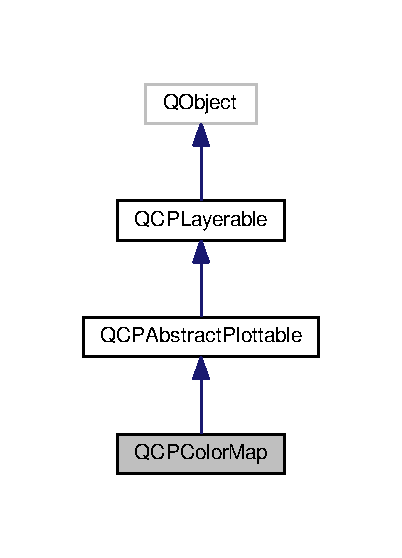
\includegraphics[width=193pt]{classQCPColorMap__inherit__graph}
\end{center}
\end{figure}


Collaboration diagram for Q\+C\+P\+Color\+Map\+:
\nopagebreak
\begin{figure}[H]
\begin{center}
\leavevmode
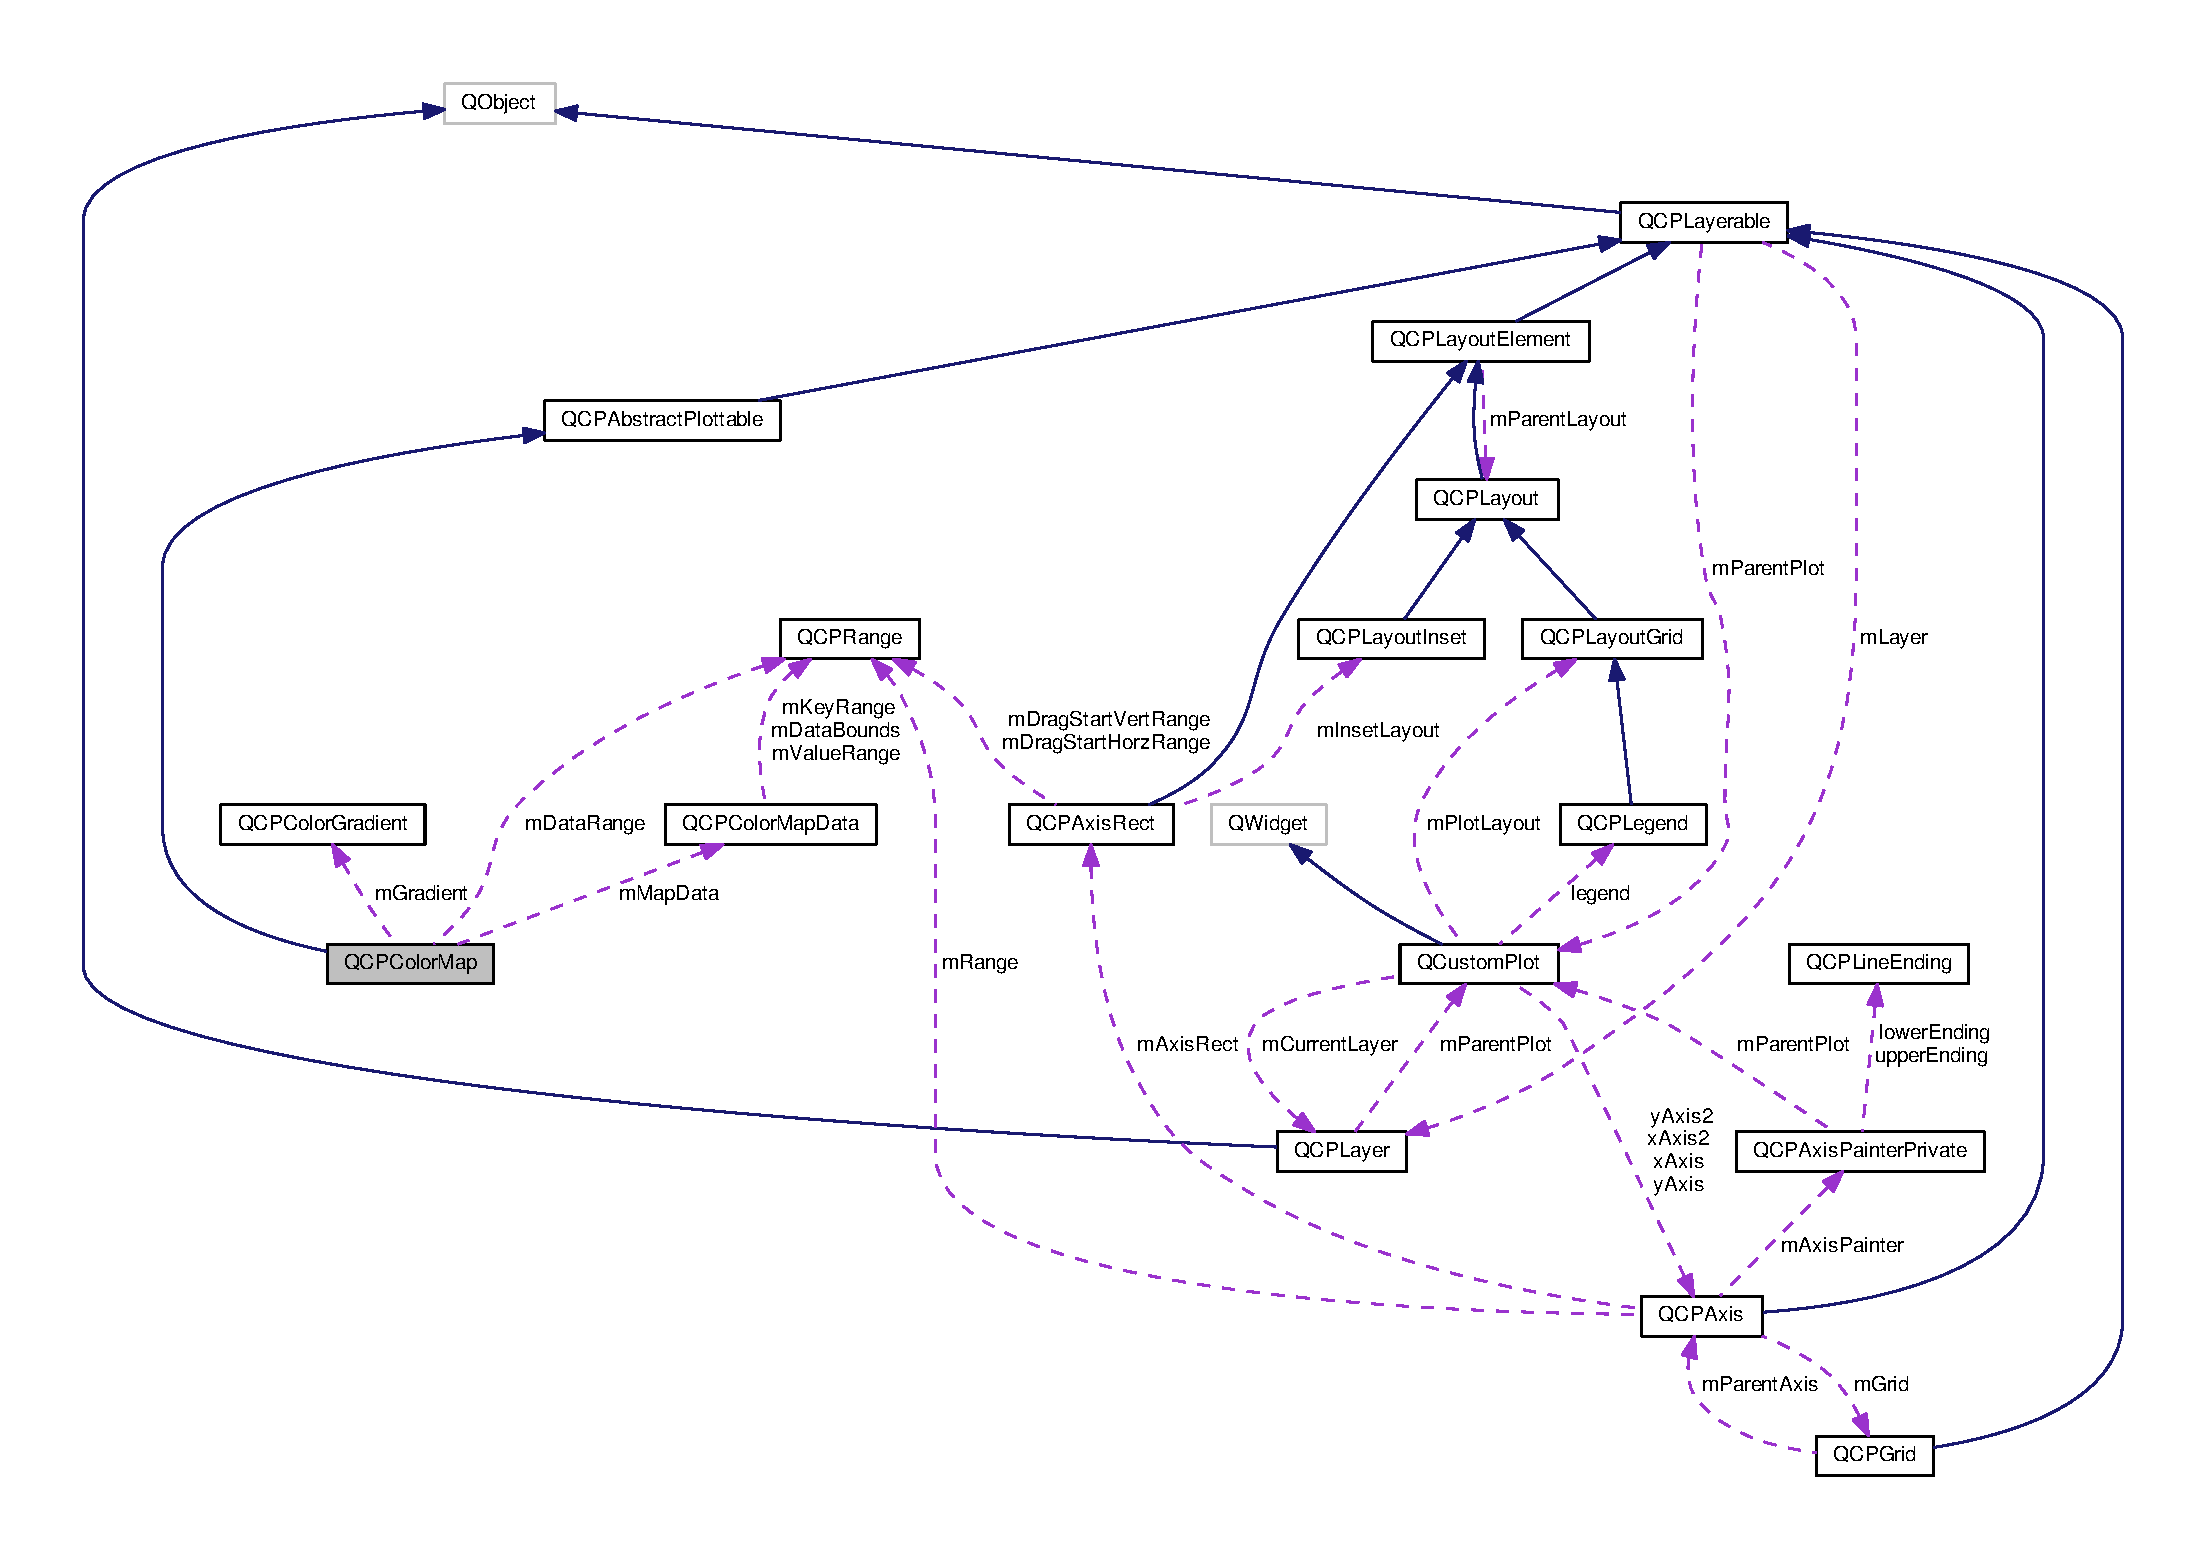
\includegraphics[width=350pt]{classQCPColorMap__coll__graph}
\end{center}
\end{figure}
\subsection*{Signals}
\begin{DoxyCompactItemize}
\item 
void \hyperlink{classQCPColorMap_a482980f2335d09cfb36dd95ba9663197}{data\+Range\+Changed} (\hyperlink{classQCPRange}{Q\+C\+P\+Range} new\+Range)
\item 
void \hyperlink{classQCPColorMap_a978d5d5c9f68cffef8c902b855c04490}{data\+Scale\+Type\+Changed} (\hyperlink{classQCPAxis_a36d8e8658dbaa179bf2aeb973db2d6f0}{Q\+C\+P\+Axis\+::\+Scale\+Type} scale\+Type)
\item 
void \hyperlink{classQCPColorMap_abf4797f86e422ac6e0f732c4ff1a4d49}{gradient\+Changed} (\hyperlink{classQCPColorGradient}{Q\+C\+P\+Color\+Gradient} new\+Gradient)
\end{DoxyCompactItemize}
\subsection*{Public Member Functions}
\begin{DoxyCompactItemize}
\item 
\hyperlink{classQCPColorMap_aa37e976d2ee1e2be6c4cd88a64b36215}{Q\+C\+P\+Color\+Map} (\hyperlink{classQCPAxis}{Q\+C\+P\+Axis} $\ast$\hyperlink{classQCPAbstractPlottable_a72c7a09c22963f2c943f07112b311103}{key\+Axis}, \hyperlink{classQCPAxis}{Q\+C\+P\+Axis} $\ast$\hyperlink{classQCPAbstractPlottable_a3106f9d34d330a6097a8ec5905e5b519}{value\+Axis})
\item 
virtual \hyperlink{classQCPColorMap_ac8a952a40fed62dcee33405b0f4d47ad}{$\sim$\+Q\+C\+P\+Color\+Map} ()
\item 
\hyperlink{classQCPColorMapData}{Q\+C\+P\+Color\+Map\+Data} $\ast$ \hyperlink{classQCPColorMap_a3ae12c9ce842352037cd20ea5267414f}{data} () const 
\item 
\hyperlink{classQCPRange}{Q\+C\+P\+Range} \hyperlink{classQCPColorMap_a37cc8e821e070697e15652f6419fab48}{data\+Range} () const 
\item 
\hyperlink{classQCPAxis_a36d8e8658dbaa179bf2aeb973db2d6f0}{Q\+C\+P\+Axis\+::\+Scale\+Type} \hyperlink{classQCPColorMap_a5ffc703dc603c4fd942f36ea51b8c48d}{data\+Scale\+Type} () const 
\item 
bool \hyperlink{classQCPColorMap_a39019675a7ad00efad7212b96c0ccc95}{interpolate} () const 
\item 
bool \hyperlink{classQCPColorMap_aa1d9aa8db73a5942881f6f6c5afdbb0f}{tight\+Boundary} () const 
\item 
\hyperlink{classQCPColorGradient}{Q\+C\+P\+Color\+Gradient} \hyperlink{classQCPColorMap_a9f967a971474e32345290b79cf107809}{gradient} () const 
\item 
\hyperlink{classQCPColorScale}{Q\+C\+P\+Color\+Scale} $\ast$ \hyperlink{classQCPColorMap_a6bd82e0b042a2ec4d64f40853a3b05e3}{color\+Scale} () const 
\item 
void \hyperlink{classQCPColorMap_a5a23e133a20c4ccad35fd32e6c0f9809}{set\+Data} (\hyperlink{classQCPColorMapData}{Q\+C\+P\+Color\+Map\+Data} $\ast$\hyperlink{classQCPColorMap_a3ae12c9ce842352037cd20ea5267414f}{data}, bool copy=false)
\item 
Q\+\_\+\+S\+L\+OT void \hyperlink{classQCPColorMap_a980b42837821159786a85b4b7dcb8774}{set\+Data\+Range} (const \hyperlink{classQCPRange}{Q\+C\+P\+Range} \&\hyperlink{classQCPColorMap_a37cc8e821e070697e15652f6419fab48}{data\+Range})
\item 
Q\+\_\+\+S\+L\+OT void \hyperlink{classQCPColorMap_a9d20aa08e3c1f20f22908c45b9c06511}{set\+Data\+Scale\+Type} (\hyperlink{classQCPAxis_a36d8e8658dbaa179bf2aeb973db2d6f0}{Q\+C\+P\+Axis\+::\+Scale\+Type} scale\+Type)
\item 
Q\+\_\+\+S\+L\+OT void \hyperlink{classQCPColorMap_a7313c78360471cead3576341a2c50377}{set\+Gradient} (const \hyperlink{classQCPColorGradient}{Q\+C\+P\+Color\+Gradient} \&\hyperlink{classQCPColorMap_a9f967a971474e32345290b79cf107809}{gradient})
\item 
void \hyperlink{classQCPColorMap_a484eaa8a5065cfc386b15375bf98b964}{set\+Interpolate} (bool enabled)
\item 
void \hyperlink{classQCPColorMap_ad03221cc285e5f562a0b13d684b5576d}{set\+Tight\+Boundary} (bool enabled)
\item 
void \hyperlink{classQCPColorMap_aa828921db364fe3c6af4619580ab85fd}{set\+Color\+Scale} (\hyperlink{classQCPColorScale}{Q\+C\+P\+Color\+Scale} $\ast$\hyperlink{classQCPColorMap_a6bd82e0b042a2ec4d64f40853a3b05e3}{color\+Scale})
\item 
void \hyperlink{classQCPColorMap_a856608fa3dd1cc290bcd5f29a5575774}{rescale\+Data\+Range} (bool recalculate\+Data\+Bounds=false)
\item 
Q\+\_\+\+S\+L\+OT void \hyperlink{classQCPColorMap_a5d8158b62d55fcfeaabcb68ce0083e87}{update\+Legend\+Icon} (Qt\+::\+Transformation\+Mode transform\+Mode=Qt\+::\+Smooth\+Transformation, const Q\+Size \&thumb\+Size=Q\+Size(32, 18))
\item 
virtual void \hyperlink{classQCPColorMap_a0545dce5383766885912331705a8e099}{clear\+Data} ()
\item 
virtual double \hyperlink{classQCPColorMap_a4088dc7bcbe9bba605c84a912ba660ff}{select\+Test} (const Q\+PointF \&pos, bool only\+Selectable, Q\+Variant $\ast$details=0) const 
\end{DoxyCompactItemize}
\subsection*{Protected Member Functions}
\begin{DoxyCompactItemize}
\item 
virtual void \hyperlink{classQCPColorMap_a5efcea591bb5486d968af520a4d43c3a}{update\+Map\+Image} ()
\item 
virtual void \hyperlink{classQCPColorMap_a3b0f45a3177be9522d5e9b8cd8ae122d}{draw} (\hyperlink{classQCPPainter}{Q\+C\+P\+Painter} $\ast$painter)
\item 
virtual void \hyperlink{classQCPColorMap_a7d5eee89f6b8eaf2f11f1d94e32215b2}{draw\+Legend\+Icon} (\hyperlink{classQCPPainter}{Q\+C\+P\+Painter} $\ast$painter, const Q\+RectF \&rect) const 
\item 
virtual \hyperlink{classQCPRange}{Q\+C\+P\+Range} \hyperlink{classQCPColorMap_a0d89371f8707f12e22737b863f1a5126}{get\+Key\+Range} (bool \&found\+Range, \hyperlink{classQCPAbstractPlottable_a661743478a1d3c09d28ec2711d7653d8}{Sign\+Domain} in\+Sign\+Domain=\hyperlink{classQCPAbstractPlottable_a661743478a1d3c09d28ec2711d7653d8a082b98cfb91a7363a3b5cd17b0c1cd60}{sd\+Both}) const 
\item 
virtual \hyperlink{classQCPRange}{Q\+C\+P\+Range} \hyperlink{classQCPColorMap_ac1b906e05ca9b61680e61b74b3825a22}{get\+Value\+Range} (bool \&found\+Range, \hyperlink{classQCPAbstractPlottable_a661743478a1d3c09d28ec2711d7653d8}{Sign\+Domain} in\+Sign\+Domain=\hyperlink{classQCPAbstractPlottable_a661743478a1d3c09d28ec2711d7653d8a082b98cfb91a7363a3b5cd17b0c1cd60}{sd\+Both}) const 
\end{DoxyCompactItemize}
\subsection*{Protected Attributes}
\begin{DoxyCompactItemize}
\item 
\hyperlink{classQCPRange}{Q\+C\+P\+Range} \hyperlink{classQCPColorMap_ab87609621d16cd3e9d52ad070b327b08}{m\+Data\+Range}
\item 
\hyperlink{classQCPAxis_a36d8e8658dbaa179bf2aeb973db2d6f0}{Q\+C\+P\+Axis\+::\+Scale\+Type} \hyperlink{classQCPColorMap_ab28a4b2def408f83b9818799d5f18446}{m\+Data\+Scale\+Type}
\item 
\hyperlink{classQCPColorMapData}{Q\+C\+P\+Color\+Map\+Data} $\ast$ \hyperlink{classQCPColorMap_a8709272aa8f0be3ca111bf3866806f8b}{m\+Map\+Data}
\item 
\hyperlink{classQCPColorGradient}{Q\+C\+P\+Color\+Gradient} \hyperlink{classQCPColorMap_aab77fe9a8df6f0486ab3507cc5f278fa}{m\+Gradient}
\item 
bool \hyperlink{classQCPColorMap_af77e5eba9a844592648edeb6fbe834f1}{m\+Interpolate}
\item 
bool \hyperlink{classQCPColorMap_ac2e9425fe4381b496726e1c09f978302}{m\+Tight\+Boundary}
\item 
Q\+Pointer$<$ \hyperlink{classQCPColorScale}{Q\+C\+P\+Color\+Scale} $>$ \hyperlink{classQCPColorMap_a95b4100bacc3387652c988b071ec9db7}{m\+Color\+Scale}
\item 
Q\+Image \hyperlink{classQCPColorMap_a66110813b42eca78b64095b2a1f285a0}{m\+Map\+Image}
\item 
Q\+Image \hyperlink{classQCPColorMap_acad3d52f3572436d5f2e4057911ea8d3}{m\+Undersampled\+Map\+Image}
\item 
Q\+Pixmap \hyperlink{classQCPColorMap_ada522988db02cb531767d38c5029ef60}{m\+Legend\+Icon}
\item 
bool \hyperlink{classQCPColorMap_ac9aea6a5c193d7fa866bc7b26e79ef2c}{m\+Map\+Image\+Invalidated}
\end{DoxyCompactItemize}
\subsection*{Friends}
\begin{DoxyCompactItemize}
\item 
class \hyperlink{classQCPColorMap_a1cdf9df76adcfae45261690aa0ca2198}{Q\+Custom\+Plot}
\item 
class \hyperlink{classQCPColorMap_a8429035e7adfbd7f05805a6530ad5e3b}{Q\+C\+P\+Legend}
\end{DoxyCompactItemize}
\subsection*{Additional Inherited Members}


\subsection{Detailed Description}
A plottable representing a two-\/dimensional color map in a plot. 



The data is stored in the class \hyperlink{classQCPColorMapData}{Q\+C\+P\+Color\+Map\+Data}, which can be accessed via the \hyperlink{classQCPColorMap_a3ae12c9ce842352037cd20ea5267414f}{data()} method.

A color map has three dimensions to represent a data point\+: The {\itshape key} dimension, the {\itshape value} dimension and the {\itshape data} dimension. As with other plottables such as graphs, {\itshape key} and {\itshape value} correspond to two orthogonal axes on the \hyperlink{classQCustomPlot}{Q\+Custom\+Plot} surface that you specify in the Q\+Color\+Map constructor. The {\itshape data} dimension however is encoded as the color of the point at ({\itshape key}, {\itshape value}).

Set the number of points (or {\itshape cells}) in the key/value dimension via \hyperlink{classQCPColorMapData_a0d9ff35c299d0478b682bfbcdd9c097e}{Q\+C\+P\+Color\+Map\+Data\+::set\+Size}. The plot coordinate range over which these points will be displayed is specified via \hyperlink{classQCPColorMapData_aad9c1c7c703c1339489fc730517c83d4}{Q\+C\+P\+Color\+Map\+Data\+::set\+Range}. The first cell will be centered on the lower range boundary and the last cell will be centered on the upper range boundary. The data can be set by either accessing the cells directly with \hyperlink{classQCPColorMapData_a8e75eaf8746596319032a93f3d2d0683}{Q\+C\+P\+Color\+Map\+Data\+::set\+Cell} or by addressing the cells via their plot coordinates with \hyperlink{classQCPColorMapData_afd2083ccfd6987ec94aa7ef8e91ca39a}{Q\+C\+P\+Color\+Map\+Data\+::set\+Data}. If possible, you should prefer set\+Cell, since it doesn\textquotesingle{}t need to do any coordinate transformation and thus performs a bit better.

The cell with index (0, 0) is at the bottom left, if the color map uses normal (i.\+e. not reversed) key and value axes.

To show the user which colors correspond to which {\itshape data} values, a \hyperlink{classQCPColorScale}{Q\+C\+P\+Color\+Scale} is typically placed to the right of the axis rect. See the documentation there for details on how to add and use a color scale.\hypertarget{classQCPStatisticalBox_appearance}{}\subsection{Changing the appearance}\label{classQCPStatisticalBox_appearance}
The central part of the appearance is the color gradient, which can be specified via \hyperlink{classQCPColorMap_a7313c78360471cead3576341a2c50377}{set\+Gradient}. See the documentation of \hyperlink{classQCPColorGradient}{Q\+C\+P\+Color\+Gradient} for details on configuring a color gradient.

The {\itshape data} range that is mapped to the colors of the gradient can be specified with \hyperlink{classQCPColorMap_a980b42837821159786a85b4b7dcb8774}{set\+Data\+Range}. To make the data range encompass the whole data set minimum to maximum, call \hyperlink{classQCPColorMap_a856608fa3dd1cc290bcd5f29a5575774}{rescale\+Data\+Range}.\hypertarget{classQCPStatisticalBox_usage}{}\subsection{Usage}\label{classQCPStatisticalBox_usage}
Like all data representing objects in \hyperlink{classQCustomPlot}{Q\+Custom\+Plot}, the \hyperlink{classQCPColorMap}{Q\+C\+P\+Color\+Map} is a plottable (\hyperlink{classQCPAbstractPlottable}{Q\+C\+P\+Abstract\+Plottable}). So the plottable-\/interface of \hyperlink{classQCustomPlot}{Q\+Custom\+Plot} applies (\hyperlink{classQCustomPlot_a32de81ff53e263e785b83b52ecd99d6f}{Q\+Custom\+Plot\+::plottable}, \hyperlink{classQCustomPlot_ab7ad9174f701f9c6f64e378df77927a6}{Q\+Custom\+Plot\+::add\+Plottable}, \hyperlink{classQCustomPlot_af3dafd56884208474f311d6226513ab2}{Q\+Custom\+Plot\+::remove\+Plottable}, etc.)

Usually, you first create an instance and add it to the custom\+Plot\+: 
\begin{DoxyCodeInclude}
\end{DoxyCodeInclude}
and then modify the properties of the newly created color map, e.\+g.\+: 
\begin{DoxyCodeInclude}
\end{DoxyCodeInclude}
 \begin{DoxyNote}{Note}
The \hyperlink{classQCPColorMap}{Q\+C\+P\+Color\+Map} always displays the data at equal key/value intervals, even if the key or value axis is set to a logarithmic scaling. If you want to use \hyperlink{classQCPColorMap}{Q\+C\+P\+Color\+Map} with logarithmic axes, you shouldn\textquotesingle{}t use the \hyperlink{classQCPColorMapData_afd2083ccfd6987ec94aa7ef8e91ca39a}{Q\+C\+P\+Color\+Map\+Data\+::set\+Data} method as it uses a linear transformation to determine the cell index. Rather directly access the cell index with \hyperlink{classQCPColorMapData_a8e75eaf8746596319032a93f3d2d0683}{Q\+C\+P\+Color\+Map\+Data\+::set\+Cell}. 
\end{DoxyNote}


\subsection{Constructor \& Destructor Documentation}
\index{Q\+C\+P\+Color\+Map@{Q\+C\+P\+Color\+Map}!Q\+C\+P\+Color\+Map@{Q\+C\+P\+Color\+Map}}
\index{Q\+C\+P\+Color\+Map@{Q\+C\+P\+Color\+Map}!Q\+C\+P\+Color\+Map@{Q\+C\+P\+Color\+Map}}
\subsubsection[{\texorpdfstring{Q\+C\+P\+Color\+Map(\+Q\+C\+P\+Axis $\ast$key\+Axis, Q\+C\+P\+Axis $\ast$value\+Axis)}{QCPColorMap(QCPAxis *keyAxis, QCPAxis *valueAxis)}}]{\setlength{\rightskip}{0pt plus 5cm}Q\+C\+P\+Color\+Map\+::\+Q\+C\+P\+Color\+Map (
\begin{DoxyParamCaption}
\item[{{\bf Q\+C\+P\+Axis} $\ast$}]{key\+Axis, }
\item[{{\bf Q\+C\+P\+Axis} $\ast$}]{value\+Axis}
\end{DoxyParamCaption}
)\hspace{0.3cm}{\ttfamily [explicit]}}\hypertarget{classQCPColorMap_aa37e976d2ee1e2be6c4cd88a64b36215}{}\label{classQCPColorMap_aa37e976d2ee1e2be6c4cd88a64b36215}
Constructs a color map with the specified {\itshape key\+Axis} and {\itshape value\+Axis}.

The constructed \hyperlink{classQCPColorMap}{Q\+C\+P\+Color\+Map} can be added to the plot with \hyperlink{classQCustomPlot_ab7ad9174f701f9c6f64e378df77927a6}{Q\+Custom\+Plot\+::add\+Plottable}, \hyperlink{classQCustomPlot}{Q\+Custom\+Plot} then takes ownership of the color map. \index{Q\+C\+P\+Color\+Map@{Q\+C\+P\+Color\+Map}!````~Q\+C\+P\+Color\+Map@{$\sim$\+Q\+C\+P\+Color\+Map}}
\index{````~Q\+C\+P\+Color\+Map@{$\sim$\+Q\+C\+P\+Color\+Map}!Q\+C\+P\+Color\+Map@{Q\+C\+P\+Color\+Map}}
\subsubsection[{\texorpdfstring{$\sim$\+Q\+C\+P\+Color\+Map()}{~QCPColorMap()}}]{\setlength{\rightskip}{0pt plus 5cm}Q\+C\+P\+Color\+Map\+::$\sim$\+Q\+C\+P\+Color\+Map (
\begin{DoxyParamCaption}
{}
\end{DoxyParamCaption}
)\hspace{0.3cm}{\ttfamily [virtual]}}\hypertarget{classQCPColorMap_ac8a952a40fed62dcee33405b0f4d47ad}{}\label{classQCPColorMap_ac8a952a40fed62dcee33405b0f4d47ad}


\subsection{Member Function Documentation}
\index{Q\+C\+P\+Color\+Map@{Q\+C\+P\+Color\+Map}!clear\+Data@{clear\+Data}}
\index{clear\+Data@{clear\+Data}!Q\+C\+P\+Color\+Map@{Q\+C\+P\+Color\+Map}}
\subsubsection[{\texorpdfstring{clear\+Data()}{clearData()}}]{\setlength{\rightskip}{0pt plus 5cm}void Q\+C\+P\+Color\+Map\+::clear\+Data (
\begin{DoxyParamCaption}
{}
\end{DoxyParamCaption}
)\hspace{0.3cm}{\ttfamily [virtual]}}\hypertarget{classQCPColorMap_a0545dce5383766885912331705a8e099}{}\label{classQCPColorMap_a0545dce5383766885912331705a8e099}
Clears the colormap data by calling \hyperlink{classQCPColorMapData_a9910ba830e96955bd5c8e5bef1e77ef3}{Q\+C\+P\+Color\+Map\+Data\+::clear()} on the internal data. This also resizes the map to 0x0 cells. 

Implements \hyperlink{classQCPAbstractPlottable_a86e5b8fd4b6ff4f4084e7ea4c573fc53}{Q\+C\+P\+Abstract\+Plottable}.

\index{Q\+C\+P\+Color\+Map@{Q\+C\+P\+Color\+Map}!color\+Scale@{color\+Scale}}
\index{color\+Scale@{color\+Scale}!Q\+C\+P\+Color\+Map@{Q\+C\+P\+Color\+Map}}
\subsubsection[{\texorpdfstring{color\+Scale() const }{colorScale() const }}]{\setlength{\rightskip}{0pt plus 5cm}{\bf Q\+C\+P\+Color\+Scale}$\ast$ Q\+C\+P\+Color\+Map\+::color\+Scale (
\begin{DoxyParamCaption}
{}
\end{DoxyParamCaption}
) const\hspace{0.3cm}{\ttfamily [inline]}}\hypertarget{classQCPColorMap_a6bd82e0b042a2ec4d64f40853a3b05e3}{}\label{classQCPColorMap_a6bd82e0b042a2ec4d64f40853a3b05e3}
\index{Q\+C\+P\+Color\+Map@{Q\+C\+P\+Color\+Map}!data@{data}}
\index{data@{data}!Q\+C\+P\+Color\+Map@{Q\+C\+P\+Color\+Map}}
\subsubsection[{\texorpdfstring{data() const }{data() const }}]{\setlength{\rightskip}{0pt plus 5cm}{\bf Q\+C\+P\+Color\+Map\+Data} $\ast$ Q\+C\+P\+Color\+Map\+::data (
\begin{DoxyParamCaption}
{}
\end{DoxyParamCaption}
) const\hspace{0.3cm}{\ttfamily [inline]}}\hypertarget{classQCPColorMap_a3ae12c9ce842352037cd20ea5267414f}{}\label{classQCPColorMap_a3ae12c9ce842352037cd20ea5267414f}
Returns a pointer to the internal data storage of type \hyperlink{classQCPColorMapData}{Q\+C\+P\+Color\+Map\+Data}. Access this to modify data points (cells) and the color map key/value range.

\begin{DoxySeeAlso}{See also}
\hyperlink{classQCPColorMap_a5a23e133a20c4ccad35fd32e6c0f9809}{set\+Data} 
\end{DoxySeeAlso}
\index{Q\+C\+P\+Color\+Map@{Q\+C\+P\+Color\+Map}!data\+Range@{data\+Range}}
\index{data\+Range@{data\+Range}!Q\+C\+P\+Color\+Map@{Q\+C\+P\+Color\+Map}}
\subsubsection[{\texorpdfstring{data\+Range() const }{dataRange() const }}]{\setlength{\rightskip}{0pt plus 5cm}{\bf Q\+C\+P\+Range} Q\+C\+P\+Color\+Map\+::data\+Range (
\begin{DoxyParamCaption}
{}
\end{DoxyParamCaption}
) const\hspace{0.3cm}{\ttfamily [inline]}}\hypertarget{classQCPColorMap_a37cc8e821e070697e15652f6419fab48}{}\label{classQCPColorMap_a37cc8e821e070697e15652f6419fab48}
\index{Q\+C\+P\+Color\+Map@{Q\+C\+P\+Color\+Map}!data\+Range\+Changed@{data\+Range\+Changed}}
\index{data\+Range\+Changed@{data\+Range\+Changed}!Q\+C\+P\+Color\+Map@{Q\+C\+P\+Color\+Map}}
\subsubsection[{\texorpdfstring{data\+Range\+Changed}{dataRangeChanged}}]{\setlength{\rightskip}{0pt plus 5cm}void Q\+C\+P\+Color\+Map\+::data\+Range\+Changed (
\begin{DoxyParamCaption}
\item[{{\bf Q\+C\+P\+Range}}]{new\+Range}
\end{DoxyParamCaption}
)\hspace{0.3cm}{\ttfamily [signal]}}\hypertarget{classQCPColorMap_a482980f2335d09cfb36dd95ba9663197}{}\label{classQCPColorMap_a482980f2335d09cfb36dd95ba9663197}
This signal is emitted when the data range changes.

\begin{DoxySeeAlso}{See also}
\hyperlink{classQCPColorMap_a980b42837821159786a85b4b7dcb8774}{set\+Data\+Range} 
\end{DoxySeeAlso}
\index{Q\+C\+P\+Color\+Map@{Q\+C\+P\+Color\+Map}!data\+Scale\+Type@{data\+Scale\+Type}}
\index{data\+Scale\+Type@{data\+Scale\+Type}!Q\+C\+P\+Color\+Map@{Q\+C\+P\+Color\+Map}}
\subsubsection[{\texorpdfstring{data\+Scale\+Type() const }{dataScaleType() const }}]{\setlength{\rightskip}{0pt plus 5cm}{\bf Q\+C\+P\+Axis\+::\+Scale\+Type} Q\+C\+P\+Color\+Map\+::data\+Scale\+Type (
\begin{DoxyParamCaption}
{}
\end{DoxyParamCaption}
) const\hspace{0.3cm}{\ttfamily [inline]}}\hypertarget{classQCPColorMap_a5ffc703dc603c4fd942f36ea51b8c48d}{}\label{classQCPColorMap_a5ffc703dc603c4fd942f36ea51b8c48d}
\index{Q\+C\+P\+Color\+Map@{Q\+C\+P\+Color\+Map}!data\+Scale\+Type\+Changed@{data\+Scale\+Type\+Changed}}
\index{data\+Scale\+Type\+Changed@{data\+Scale\+Type\+Changed}!Q\+C\+P\+Color\+Map@{Q\+C\+P\+Color\+Map}}
\subsubsection[{\texorpdfstring{data\+Scale\+Type\+Changed}{dataScaleTypeChanged}}]{\setlength{\rightskip}{0pt plus 5cm}void Q\+C\+P\+Color\+Map\+::data\+Scale\+Type\+Changed (
\begin{DoxyParamCaption}
\item[{{\bf Q\+C\+P\+Axis\+::\+Scale\+Type}}]{scale\+Type}
\end{DoxyParamCaption}
)\hspace{0.3cm}{\ttfamily [signal]}}\hypertarget{classQCPColorMap_a978d5d5c9f68cffef8c902b855c04490}{}\label{classQCPColorMap_a978d5d5c9f68cffef8c902b855c04490}
This signal is emitted when the data scale type changes.

\begin{DoxySeeAlso}{See also}
\hyperlink{classQCPColorMap_a9d20aa08e3c1f20f22908c45b9c06511}{set\+Data\+Scale\+Type} 
\end{DoxySeeAlso}
\index{Q\+C\+P\+Color\+Map@{Q\+C\+P\+Color\+Map}!draw@{draw}}
\index{draw@{draw}!Q\+C\+P\+Color\+Map@{Q\+C\+P\+Color\+Map}}
\subsubsection[{\texorpdfstring{draw(\+Q\+C\+P\+Painter $\ast$painter)}{draw(QCPPainter *painter)}}]{\setlength{\rightskip}{0pt plus 5cm}void Q\+C\+P\+Color\+Map\+::draw (
\begin{DoxyParamCaption}
\item[{{\bf Q\+C\+P\+Painter} $\ast$}]{painter}
\end{DoxyParamCaption}
)\hspace{0.3cm}{\ttfamily [protected]}, {\ttfamily [virtual]}}\hypertarget{classQCPColorMap_a3b0f45a3177be9522d5e9b8cd8ae122d}{}\label{classQCPColorMap_a3b0f45a3177be9522d5e9b8cd8ae122d}


Implements \hyperlink{classQCPAbstractPlottable_acbab5e30dcd04fd302b4a5902ac2c482}{Q\+C\+P\+Abstract\+Plottable}.

\index{Q\+C\+P\+Color\+Map@{Q\+C\+P\+Color\+Map}!draw\+Legend\+Icon@{draw\+Legend\+Icon}}
\index{draw\+Legend\+Icon@{draw\+Legend\+Icon}!Q\+C\+P\+Color\+Map@{Q\+C\+P\+Color\+Map}}
\subsubsection[{\texorpdfstring{draw\+Legend\+Icon(\+Q\+C\+P\+Painter $\ast$painter, const Q\+Rect\+F \&rect) const }{drawLegendIcon(QCPPainter *painter, const QRectF &rect) const }}]{\setlength{\rightskip}{0pt plus 5cm}void Q\+C\+P\+Color\+Map\+::draw\+Legend\+Icon (
\begin{DoxyParamCaption}
\item[{{\bf Q\+C\+P\+Painter} $\ast$}]{painter, }
\item[{const Q\+RectF \&}]{rect}
\end{DoxyParamCaption}
) const\hspace{0.3cm}{\ttfamily [protected]}, {\ttfamily [virtual]}}\hypertarget{classQCPColorMap_a7d5eee89f6b8eaf2f11f1d94e32215b2}{}\label{classQCPColorMap_a7d5eee89f6b8eaf2f11f1d94e32215b2}


Implements \hyperlink{classQCPAbstractPlottable_a9a450783fd9ed539e589999fd390cdf7}{Q\+C\+P\+Abstract\+Plottable}.

\index{Q\+C\+P\+Color\+Map@{Q\+C\+P\+Color\+Map}!get\+Key\+Range@{get\+Key\+Range}}
\index{get\+Key\+Range@{get\+Key\+Range}!Q\+C\+P\+Color\+Map@{Q\+C\+P\+Color\+Map}}
\subsubsection[{\texorpdfstring{get\+Key\+Range(bool \&found\+Range, Sign\+Domain in\+Sign\+Domain=sd\+Both) const }{getKeyRange(bool &foundRange, SignDomain inSignDomain=sdBoth) const }}]{\setlength{\rightskip}{0pt plus 5cm}{\bf Q\+C\+P\+Range} Q\+C\+P\+Color\+Map\+::get\+Key\+Range (
\begin{DoxyParamCaption}
\item[{bool \&}]{found\+Range, }
\item[{{\bf Sign\+Domain}}]{in\+Sign\+Domain = {\ttfamily {\bf sd\+Both}}}
\end{DoxyParamCaption}
) const\hspace{0.3cm}{\ttfamily [protected]}, {\ttfamily [virtual]}}\hypertarget{classQCPColorMap_a0d89371f8707f12e22737b863f1a5126}{}\label{classQCPColorMap_a0d89371f8707f12e22737b863f1a5126}


Implements \hyperlink{classQCPAbstractPlottable_a345d702b2e7e12c8cfdddff65ba85e8c}{Q\+C\+P\+Abstract\+Plottable}.

\index{Q\+C\+P\+Color\+Map@{Q\+C\+P\+Color\+Map}!get\+Value\+Range@{get\+Value\+Range}}
\index{get\+Value\+Range@{get\+Value\+Range}!Q\+C\+P\+Color\+Map@{Q\+C\+P\+Color\+Map}}
\subsubsection[{\texorpdfstring{get\+Value\+Range(bool \&found\+Range, Sign\+Domain in\+Sign\+Domain=sd\+Both) const }{getValueRange(bool &foundRange, SignDomain inSignDomain=sdBoth) const }}]{\setlength{\rightskip}{0pt plus 5cm}{\bf Q\+C\+P\+Range} Q\+C\+P\+Color\+Map\+::get\+Value\+Range (
\begin{DoxyParamCaption}
\item[{bool \&}]{found\+Range, }
\item[{{\bf Sign\+Domain}}]{in\+Sign\+Domain = {\ttfamily {\bf sd\+Both}}}
\end{DoxyParamCaption}
) const\hspace{0.3cm}{\ttfamily [protected]}, {\ttfamily [virtual]}}\hypertarget{classQCPColorMap_ac1b906e05ca9b61680e61b74b3825a22}{}\label{classQCPColorMap_ac1b906e05ca9b61680e61b74b3825a22}


Implements \hyperlink{classQCPAbstractPlottable_aa3331b415b5939fe4df60b78831b2799}{Q\+C\+P\+Abstract\+Plottable}.

\index{Q\+C\+P\+Color\+Map@{Q\+C\+P\+Color\+Map}!gradient@{gradient}}
\index{gradient@{gradient}!Q\+C\+P\+Color\+Map@{Q\+C\+P\+Color\+Map}}
\subsubsection[{\texorpdfstring{gradient() const }{gradient() const }}]{\setlength{\rightskip}{0pt plus 5cm}{\bf Q\+C\+P\+Color\+Gradient} Q\+C\+P\+Color\+Map\+::gradient (
\begin{DoxyParamCaption}
{}
\end{DoxyParamCaption}
) const\hspace{0.3cm}{\ttfamily [inline]}}\hypertarget{classQCPColorMap_a9f967a971474e32345290b79cf107809}{}\label{classQCPColorMap_a9f967a971474e32345290b79cf107809}
\index{Q\+C\+P\+Color\+Map@{Q\+C\+P\+Color\+Map}!gradient\+Changed@{gradient\+Changed}}
\index{gradient\+Changed@{gradient\+Changed}!Q\+C\+P\+Color\+Map@{Q\+C\+P\+Color\+Map}}
\subsubsection[{\texorpdfstring{gradient\+Changed}{gradientChanged}}]{\setlength{\rightskip}{0pt plus 5cm}void Q\+C\+P\+Color\+Map\+::gradient\+Changed (
\begin{DoxyParamCaption}
\item[{{\bf Q\+C\+P\+Color\+Gradient}}]{new\+Gradient}
\end{DoxyParamCaption}
)\hspace{0.3cm}{\ttfamily [signal]}}\hypertarget{classQCPColorMap_abf4797f86e422ac6e0f732c4ff1a4d49}{}\label{classQCPColorMap_abf4797f86e422ac6e0f732c4ff1a4d49}
This signal is emitted when the gradient changes.

\begin{DoxySeeAlso}{See also}
\hyperlink{classQCPColorMap_a7313c78360471cead3576341a2c50377}{set\+Gradient} 
\end{DoxySeeAlso}
\index{Q\+C\+P\+Color\+Map@{Q\+C\+P\+Color\+Map}!interpolate@{interpolate}}
\index{interpolate@{interpolate}!Q\+C\+P\+Color\+Map@{Q\+C\+P\+Color\+Map}}
\subsubsection[{\texorpdfstring{interpolate() const }{interpolate() const }}]{\setlength{\rightskip}{0pt plus 5cm}bool Q\+C\+P\+Color\+Map\+::interpolate (
\begin{DoxyParamCaption}
{}
\end{DoxyParamCaption}
) const\hspace{0.3cm}{\ttfamily [inline]}}\hypertarget{classQCPColorMap_a39019675a7ad00efad7212b96c0ccc95}{}\label{classQCPColorMap_a39019675a7ad00efad7212b96c0ccc95}
\index{Q\+C\+P\+Color\+Map@{Q\+C\+P\+Color\+Map}!rescale\+Data\+Range@{rescale\+Data\+Range}}
\index{rescale\+Data\+Range@{rescale\+Data\+Range}!Q\+C\+P\+Color\+Map@{Q\+C\+P\+Color\+Map}}
\subsubsection[{\texorpdfstring{rescale\+Data\+Range(bool recalculate\+Data\+Bounds=false)}{rescaleDataRange(bool recalculateDataBounds=false)}}]{\setlength{\rightskip}{0pt plus 5cm}void Q\+C\+P\+Color\+Map\+::rescale\+Data\+Range (
\begin{DoxyParamCaption}
\item[{bool}]{recalculate\+Data\+Bounds = {\ttfamily false}}
\end{DoxyParamCaption}
)}\hypertarget{classQCPColorMap_a856608fa3dd1cc290bcd5f29a5575774}{}\label{classQCPColorMap_a856608fa3dd1cc290bcd5f29a5575774}
Sets the data range (\hyperlink{classQCPColorMap_a980b42837821159786a85b4b7dcb8774}{set\+Data\+Range}) to span the minimum and maximum values that occur in the current data set. This corresponds to the \hyperlink{classQCPAbstractPlottable_a1acecfcca3e7fcda00fcbaa3c886386f}{rescale\+Key\+Axis} or \hyperlink{classQCPAbstractPlottable_abfd0805eb1d955c0111a990246658324}{rescale\+Value\+Axis} methods, only for the third data dimension of the color map.

The minimum and maximum values of the data set are buffered in the internal \hyperlink{classQCPColorMapData}{Q\+C\+P\+Color\+Map\+Data} instance (\hyperlink{classQCPColorMap_a3ae12c9ce842352037cd20ea5267414f}{data}). As data is updated via its \hyperlink{classQCPColorMapData_a8e75eaf8746596319032a93f3d2d0683}{Q\+C\+P\+Color\+Map\+Data\+::set\+Cell} or \hyperlink{classQCPColorMapData_afd2083ccfd6987ec94aa7ef8e91ca39a}{Q\+C\+P\+Color\+Map\+Data\+::set\+Data}, the buffered minimum and maximum values are updated, too. For performance reasons, however, they are only updated in an expanding fashion. So the buffered maximum can only increase and the buffered minimum can only decrease. In consequence, changes to the data that actually lower the maximum of the data set (by overwriting the cell holding the current maximum with a smaller value), aren\textquotesingle{}t recognized and the buffered maximum overestimates the true maximum of the data set. The same happens for the buffered minimum. To recalculate the true minimum and maximum by explicitly looking at each cell, the method \hyperlink{classQCPColorMapData_ab235ade8a4d64bd3adb26a99b3dd57ee}{Q\+C\+P\+Color\+Map\+Data\+::recalculate\+Data\+Bounds} can be used. For convenience, setting the parameter {\itshape recalculate\+Data\+Bounds} calls this method before setting the data range to the buffered minimum and maximum.

\begin{DoxySeeAlso}{See also}
\hyperlink{classQCPColorMap_a980b42837821159786a85b4b7dcb8774}{set\+Data\+Range} 
\end{DoxySeeAlso}
\index{Q\+C\+P\+Color\+Map@{Q\+C\+P\+Color\+Map}!select\+Test@{select\+Test}}
\index{select\+Test@{select\+Test}!Q\+C\+P\+Color\+Map@{Q\+C\+P\+Color\+Map}}
\subsubsection[{\texorpdfstring{select\+Test(const Q\+Point\+F \&pos, bool only\+Selectable, Q\+Variant $\ast$details=0) const }{selectTest(const QPointF &pos, bool onlySelectable, QVariant *details=0) const }}]{\setlength{\rightskip}{0pt plus 5cm}double Q\+C\+P\+Color\+Map\+::select\+Test (
\begin{DoxyParamCaption}
\item[{const Q\+PointF \&}]{pos, }
\item[{bool}]{only\+Selectable, }
\item[{Q\+Variant $\ast$}]{details = {\ttfamily 0}}
\end{DoxyParamCaption}
) const\hspace{0.3cm}{\ttfamily [virtual]}}\hypertarget{classQCPColorMap_a4088dc7bcbe9bba605c84a912ba660ff}{}\label{classQCPColorMap_a4088dc7bcbe9bba605c84a912ba660ff}
This function is used to decide whether a click hits a layerable object or not.

{\itshape pos} is a point in pixel coordinates on the \hyperlink{classQCustomPlot}{Q\+Custom\+Plot} surface. This function returns the shortest pixel distance of this point to the object. If the object is either invisible or the distance couldn\textquotesingle{}t be determined, -\/1.\+0 is returned. Further, if {\itshape only\+Selectable} is true and the object is not selectable, -\/1.\+0 is returned, too.

If the object is represented not by single lines but by an area like a \hyperlink{classQCPItemText}{Q\+C\+P\+Item\+Text} or the bars of a \hyperlink{classQCPBars}{Q\+C\+P\+Bars} plottable, a click inside the area should also be considered a hit. In these cases this function thus returns a constant value greater zero but still below the parent plot\textquotesingle{}s selection tolerance. (typically the selection\+Tolerance multiplied by 0.\+99).

Providing a constant value for area objects allows selecting line objects even when they are obscured by such area objects, by clicking close to the lines (i.\+e. closer than 0.\+99$\ast$selection\+Tolerance).

The actual setting of the selection state is not done by this function. This is handled by the parent \hyperlink{classQCustomPlot}{Q\+Custom\+Plot} when the mouse\+Release\+Event occurs, and the finally selected object is notified via the select\+Event/deselect\+Event methods.

{\itshape details} is an optional output parameter. Every layerable subclass may place any information in {\itshape details}. This information will be passed to \hyperlink{classQCPAbstractPlottable_a16aaad02456aa23a759efd1ac90c79bf}{select\+Event} when the parent \hyperlink{classQCustomPlot}{Q\+Custom\+Plot} decides on the basis of this select\+Test call, that the object was successfully selected. The subsequent call to \hyperlink{classQCPAbstractPlottable_a16aaad02456aa23a759efd1ac90c79bf}{select\+Event} will carry the {\itshape details}. This is useful for multi-\/part objects (like \hyperlink{classQCPAxis}{Q\+C\+P\+Axis}). This way, a possibly complex calculation to decide which part was clicked is only done once in \hyperlink{classQCPColorMap_a4088dc7bcbe9bba605c84a912ba660ff}{select\+Test}. The result (i.\+e. the actually clicked part) can then be placed in {\itshape details}. So in the subsequent \hyperlink{classQCPAbstractPlottable_a16aaad02456aa23a759efd1ac90c79bf}{select\+Event}, the decision which part was selected doesn\textquotesingle{}t have to be done a second time for a single selection operation.

You may pass 0 as {\itshape details} to indicate that you are not interested in those selection details.

\begin{DoxySeeAlso}{See also}
\hyperlink{classQCPAbstractPlottable_a16aaad02456aa23a759efd1ac90c79bf}{select\+Event}, \hyperlink{classQCPAbstractPlottable_a6fa0d0f95560ea8b01ee13f296dab2b1}{deselect\+Event}, \hyperlink{classQCustomPlot_a5ee1e2f6ae27419deca53e75907c27e5}{Q\+Custom\+Plot\+::set\+Interactions} 
\end{DoxySeeAlso}


Implements \hyperlink{classQCPAbstractPlottable_a38efe9641d972992a3d44204bc80ec1d}{Q\+C\+P\+Abstract\+Plottable}.

\index{Q\+C\+P\+Color\+Map@{Q\+C\+P\+Color\+Map}!set\+Color\+Scale@{set\+Color\+Scale}}
\index{set\+Color\+Scale@{set\+Color\+Scale}!Q\+C\+P\+Color\+Map@{Q\+C\+P\+Color\+Map}}
\subsubsection[{\texorpdfstring{set\+Color\+Scale(\+Q\+C\+P\+Color\+Scale $\ast$color\+Scale)}{setColorScale(QCPColorScale *colorScale)}}]{\setlength{\rightskip}{0pt plus 5cm}void Q\+C\+P\+Color\+Map\+::set\+Color\+Scale (
\begin{DoxyParamCaption}
\item[{{\bf Q\+C\+P\+Color\+Scale} $\ast$}]{color\+Scale}
\end{DoxyParamCaption}
)}\hypertarget{classQCPColorMap_aa828921db364fe3c6af4619580ab85fd}{}\label{classQCPColorMap_aa828921db364fe3c6af4619580ab85fd}
Associates the color scale {\itshape color\+Scale} with this color map.

This means that both the color scale and the color map synchronize their gradient, data range and data scale type (\hyperlink{classQCPColorMap_a7313c78360471cead3576341a2c50377}{set\+Gradient}, \hyperlink{classQCPColorMap_a980b42837821159786a85b4b7dcb8774}{set\+Data\+Range}, \hyperlink{classQCPColorMap_a9d20aa08e3c1f20f22908c45b9c06511}{set\+Data\+Scale\+Type}). Multiple color maps can be associated with one single color scale. This causes the color maps to also synchronize those properties, via the mutual color scale.

This function causes the color map to adopt the current color gradient, data range and data scale type of {\itshape color\+Scale}. After this call, you may change these properties at either the color map or the color scale, and the setting will be applied to both.

Pass 0 as {\itshape color\+Scale} to disconnect the color scale from this color map again. \index{Q\+C\+P\+Color\+Map@{Q\+C\+P\+Color\+Map}!set\+Data@{set\+Data}}
\index{set\+Data@{set\+Data}!Q\+C\+P\+Color\+Map@{Q\+C\+P\+Color\+Map}}
\subsubsection[{\texorpdfstring{set\+Data(\+Q\+C\+P\+Color\+Map\+Data $\ast$data, bool copy=false)}{setData(QCPColorMapData *data, bool copy=false)}}]{\setlength{\rightskip}{0pt plus 5cm}void Q\+C\+P\+Color\+Map\+::set\+Data (
\begin{DoxyParamCaption}
\item[{{\bf Q\+C\+P\+Color\+Map\+Data} $\ast$}]{data, }
\item[{bool}]{copy = {\ttfamily false}}
\end{DoxyParamCaption}
)}\hypertarget{classQCPColorMap_a5a23e133a20c4ccad35fd32e6c0f9809}{}\label{classQCPColorMap_a5a23e133a20c4ccad35fd32e6c0f9809}
Replaces the current \hyperlink{classQCPColorMap_a3ae12c9ce842352037cd20ea5267414f}{data} with the provided {\itshape data}.

If {\itshape copy} is set to true, the {\itshape data} object will only be copied. if false, the color map takes ownership of the passed data and replaces the internal data pointer with it. This is significantly faster than copying for large datasets. \index{Q\+C\+P\+Color\+Map@{Q\+C\+P\+Color\+Map}!set\+Data\+Range@{set\+Data\+Range}}
\index{set\+Data\+Range@{set\+Data\+Range}!Q\+C\+P\+Color\+Map@{Q\+C\+P\+Color\+Map}}
\subsubsection[{\texorpdfstring{set\+Data\+Range(const Q\+C\+P\+Range \&data\+Range)}{setDataRange(const QCPRange &dataRange)}}]{\setlength{\rightskip}{0pt plus 5cm}void Q\+C\+P\+Color\+Map\+::set\+Data\+Range (
\begin{DoxyParamCaption}
\item[{const {\bf Q\+C\+P\+Range} \&}]{data\+Range}
\end{DoxyParamCaption}
)}\hypertarget{classQCPColorMap_a980b42837821159786a85b4b7dcb8774}{}\label{classQCPColorMap_a980b42837821159786a85b4b7dcb8774}
Sets the data range of this color map to {\itshape data\+Range}. The data range defines which data values are mapped to the color gradient.

To make the data range span the full range of the data set, use \hyperlink{classQCPColorMap_a856608fa3dd1cc290bcd5f29a5575774}{rescale\+Data\+Range}.

\begin{DoxySeeAlso}{See also}
\hyperlink{classQCPColorScale_abe88633003a26d1e756aa74984587fef}{Q\+C\+P\+Color\+Scale\+::set\+Data\+Range} 
\end{DoxySeeAlso}
\index{Q\+C\+P\+Color\+Map@{Q\+C\+P\+Color\+Map}!set\+Data\+Scale\+Type@{set\+Data\+Scale\+Type}}
\index{set\+Data\+Scale\+Type@{set\+Data\+Scale\+Type}!Q\+C\+P\+Color\+Map@{Q\+C\+P\+Color\+Map}}
\subsubsection[{\texorpdfstring{set\+Data\+Scale\+Type(\+Q\+C\+P\+Axis\+::\+Scale\+Type scale\+Type)}{setDataScaleType(QCPAxis::ScaleType scaleType)}}]{\setlength{\rightskip}{0pt plus 5cm}void Q\+C\+P\+Color\+Map\+::set\+Data\+Scale\+Type (
\begin{DoxyParamCaption}
\item[{{\bf Q\+C\+P\+Axis\+::\+Scale\+Type}}]{scale\+Type}
\end{DoxyParamCaption}
)}\hypertarget{classQCPColorMap_a9d20aa08e3c1f20f22908c45b9c06511}{}\label{classQCPColorMap_a9d20aa08e3c1f20f22908c45b9c06511}
Sets whether the data is correlated with the color gradient linearly or logarithmically.

\begin{DoxySeeAlso}{See also}
\hyperlink{classQCPColorScale_aeb6107d67dd7325145b2498abae67fc3}{Q\+C\+P\+Color\+Scale\+::set\+Data\+Scale\+Type} 
\end{DoxySeeAlso}
\index{Q\+C\+P\+Color\+Map@{Q\+C\+P\+Color\+Map}!set\+Gradient@{set\+Gradient}}
\index{set\+Gradient@{set\+Gradient}!Q\+C\+P\+Color\+Map@{Q\+C\+P\+Color\+Map}}
\subsubsection[{\texorpdfstring{set\+Gradient(const Q\+C\+P\+Color\+Gradient \&gradient)}{setGradient(const QCPColorGradient &gradient)}}]{\setlength{\rightskip}{0pt plus 5cm}void Q\+C\+P\+Color\+Map\+::set\+Gradient (
\begin{DoxyParamCaption}
\item[{const {\bf Q\+C\+P\+Color\+Gradient} \&}]{gradient}
\end{DoxyParamCaption}
)}\hypertarget{classQCPColorMap_a7313c78360471cead3576341a2c50377}{}\label{classQCPColorMap_a7313c78360471cead3576341a2c50377}
Sets the color gradient that is used to represent the data. For more details on how to create an own gradient or use one of the preset gradients, see \hyperlink{classQCPColorGradient}{Q\+C\+P\+Color\+Gradient}.

The colors defined by the gradient will be used to represent data values in the currently set data range, see \hyperlink{classQCPColorMap_a980b42837821159786a85b4b7dcb8774}{set\+Data\+Range}. Data points that are outside this data range will either be colored uniformly with the respective gradient boundary color, or the gradient will repeat, depending on \hyperlink{classQCPColorGradient_a39d6448155fc00a219f239220d14bb39}{Q\+C\+P\+Color\+Gradient\+::set\+Periodic}.

\begin{DoxySeeAlso}{See also}
\hyperlink{classQCPColorScale_a1f29583bb6f1e7f473b62fb712be3940}{Q\+C\+P\+Color\+Scale\+::set\+Gradient} 
\end{DoxySeeAlso}
\index{Q\+C\+P\+Color\+Map@{Q\+C\+P\+Color\+Map}!set\+Interpolate@{set\+Interpolate}}
\index{set\+Interpolate@{set\+Interpolate}!Q\+C\+P\+Color\+Map@{Q\+C\+P\+Color\+Map}}
\subsubsection[{\texorpdfstring{set\+Interpolate(bool enabled)}{setInterpolate(bool enabled)}}]{\setlength{\rightskip}{0pt plus 5cm}void Q\+C\+P\+Color\+Map\+::set\+Interpolate (
\begin{DoxyParamCaption}
\item[{bool}]{enabled}
\end{DoxyParamCaption}
)}\hypertarget{classQCPColorMap_a484eaa8a5065cfc386b15375bf98b964}{}\label{classQCPColorMap_a484eaa8a5065cfc386b15375bf98b964}
Sets whether the color map image shall use bicubic interpolation when displaying the color map shrinked or expanded, and not at a 1\+:1 pixel-\/to-\/data scale.

\index{Q\+C\+P\+Color\+Map@{Q\+C\+P\+Color\+Map}!set\+Tight\+Boundary@{set\+Tight\+Boundary}}
\index{set\+Tight\+Boundary@{set\+Tight\+Boundary}!Q\+C\+P\+Color\+Map@{Q\+C\+P\+Color\+Map}}
\subsubsection[{\texorpdfstring{set\+Tight\+Boundary(bool enabled)}{setTightBoundary(bool enabled)}}]{\setlength{\rightskip}{0pt plus 5cm}void Q\+C\+P\+Color\+Map\+::set\+Tight\+Boundary (
\begin{DoxyParamCaption}
\item[{bool}]{enabled}
\end{DoxyParamCaption}
)}\hypertarget{classQCPColorMap_ad03221cc285e5f562a0b13d684b5576d}{}\label{classQCPColorMap_ad03221cc285e5f562a0b13d684b5576d}
Sets whether the outer most data rows and columns are clipped to the specified key and value range (see \hyperlink{classQCPColorMapData_a0738c485f3c9df9ea1241b7a8bb6a86e}{Q\+C\+P\+Color\+Map\+Data\+::set\+Key\+Range}, \hyperlink{classQCPColorMapData_ada1b2680ba96a5f4175b6d341cf75d23}{Q\+C\+P\+Color\+Map\+Data\+::set\+Value\+Range}).

if {\itshape enabled} is set to false, the data points at the border of the color map are drawn with the same width and height as all other data points. Since the data points are represented by rectangles of one color centered on the data coordinate, this means that the shown color map extends by half a data point over the specified key/value range in each direction.

\index{Q\+C\+P\+Color\+Map@{Q\+C\+P\+Color\+Map}!tight\+Boundary@{tight\+Boundary}}
\index{tight\+Boundary@{tight\+Boundary}!Q\+C\+P\+Color\+Map@{Q\+C\+P\+Color\+Map}}
\subsubsection[{\texorpdfstring{tight\+Boundary() const }{tightBoundary() const }}]{\setlength{\rightskip}{0pt plus 5cm}bool Q\+C\+P\+Color\+Map\+::tight\+Boundary (
\begin{DoxyParamCaption}
{}
\end{DoxyParamCaption}
) const\hspace{0.3cm}{\ttfamily [inline]}}\hypertarget{classQCPColorMap_aa1d9aa8db73a5942881f6f6c5afdbb0f}{}\label{classQCPColorMap_aa1d9aa8db73a5942881f6f6c5afdbb0f}
\index{Q\+C\+P\+Color\+Map@{Q\+C\+P\+Color\+Map}!update\+Legend\+Icon@{update\+Legend\+Icon}}
\index{update\+Legend\+Icon@{update\+Legend\+Icon}!Q\+C\+P\+Color\+Map@{Q\+C\+P\+Color\+Map}}
\subsubsection[{\texorpdfstring{update\+Legend\+Icon(\+Qt\+::\+Transformation\+Mode transform\+Mode=\+Qt\+::\+Smooth\+Transformation, const Q\+Size \&thumb\+Size=\+Q\+Size(32, 18))}{updateLegendIcon(Qt::TransformationMode transformMode=Qt::SmoothTransformation, const QSize &thumbSize=QSize(32, 18))}}]{\setlength{\rightskip}{0pt plus 5cm}void Q\+C\+P\+Color\+Map\+::update\+Legend\+Icon (
\begin{DoxyParamCaption}
\item[{Qt\+::\+Transformation\+Mode}]{transform\+Mode = {\ttfamily Qt\+:\+:SmoothTransformation}, }
\item[{const Q\+Size \&}]{thumb\+Size = {\ttfamily QSize(32,~18)}}
\end{DoxyParamCaption}
)}\hypertarget{classQCPColorMap_a5d8158b62d55fcfeaabcb68ce0083e87}{}\label{classQCPColorMap_a5d8158b62d55fcfeaabcb68ce0083e87}
Takes the current appearance of the color map and updates the legend icon, which is used to represent this color map in the legend (see \hyperlink{classQCPLegend}{Q\+C\+P\+Legend}).

The {\itshape transform\+Mode} specifies whether the rescaling is done by a faster, low quality image scaling algorithm (Qt\+::\+Fast\+Transformation) or by a slower, higher quality algorithm (Qt\+::\+Smooth\+Transformation).

The current color map appearance is scaled down to {\itshape thumb\+Size}. Ideally, this should be equal to the size of the legend icon (see \hyperlink{classQCPLegend_a8b0740cce488bf7010da6beda6898984}{Q\+C\+P\+Legend\+::set\+Icon\+Size}). If it isn\textquotesingle{}t exactly the configured legend icon size, the thumb will be rescaled during drawing of the legend item.

\begin{DoxySeeAlso}{See also}
\hyperlink{classQCPColorMap_a980b42837821159786a85b4b7dcb8774}{set\+Data\+Range} 
\end{DoxySeeAlso}
\index{Q\+C\+P\+Color\+Map@{Q\+C\+P\+Color\+Map}!update\+Map\+Image@{update\+Map\+Image}}
\index{update\+Map\+Image@{update\+Map\+Image}!Q\+C\+P\+Color\+Map@{Q\+C\+P\+Color\+Map}}
\subsubsection[{\texorpdfstring{update\+Map\+Image()}{updateMapImage()}}]{\setlength{\rightskip}{0pt plus 5cm}void Q\+C\+P\+Color\+Map\+::update\+Map\+Image (
\begin{DoxyParamCaption}
{}
\end{DoxyParamCaption}
)\hspace{0.3cm}{\ttfamily [protected]}, {\ttfamily [virtual]}}\hypertarget{classQCPColorMap_a5efcea591bb5486d968af520a4d43c3a}{}\label{classQCPColorMap_a5efcea591bb5486d968af520a4d43c3a}


\subsection{Friends And Related Function Documentation}
\index{Q\+C\+P\+Color\+Map@{Q\+C\+P\+Color\+Map}!Q\+C\+P\+Legend@{Q\+C\+P\+Legend}}
\index{Q\+C\+P\+Legend@{Q\+C\+P\+Legend}!Q\+C\+P\+Color\+Map@{Q\+C\+P\+Color\+Map}}
\subsubsection[{\texorpdfstring{Q\+C\+P\+Legend}{QCPLegend}}]{\setlength{\rightskip}{0pt plus 5cm}friend class {\bf Q\+C\+P\+Legend}\hspace{0.3cm}{\ttfamily [friend]}}\hypertarget{classQCPColorMap_a8429035e7adfbd7f05805a6530ad5e3b}{}\label{classQCPColorMap_a8429035e7adfbd7f05805a6530ad5e3b}
\index{Q\+C\+P\+Color\+Map@{Q\+C\+P\+Color\+Map}!Q\+Custom\+Plot@{Q\+Custom\+Plot}}
\index{Q\+Custom\+Plot@{Q\+Custom\+Plot}!Q\+C\+P\+Color\+Map@{Q\+C\+P\+Color\+Map}}
\subsubsection[{\texorpdfstring{Q\+Custom\+Plot}{QCustomPlot}}]{\setlength{\rightskip}{0pt plus 5cm}friend class {\bf Q\+Custom\+Plot}\hspace{0.3cm}{\ttfamily [friend]}}\hypertarget{classQCPColorMap_a1cdf9df76adcfae45261690aa0ca2198}{}\label{classQCPColorMap_a1cdf9df76adcfae45261690aa0ca2198}


\subsection{Member Data Documentation}
\index{Q\+C\+P\+Color\+Map@{Q\+C\+P\+Color\+Map}!m\+Color\+Scale@{m\+Color\+Scale}}
\index{m\+Color\+Scale@{m\+Color\+Scale}!Q\+C\+P\+Color\+Map@{Q\+C\+P\+Color\+Map}}
\subsubsection[{\texorpdfstring{m\+Color\+Scale}{mColorScale}}]{\setlength{\rightskip}{0pt plus 5cm}Q\+Pointer$<${\bf Q\+C\+P\+Color\+Scale}$>$ Q\+C\+P\+Color\+Map\+::m\+Color\+Scale\hspace{0.3cm}{\ttfamily [protected]}}\hypertarget{classQCPColorMap_a95b4100bacc3387652c988b071ec9db7}{}\label{classQCPColorMap_a95b4100bacc3387652c988b071ec9db7}
\index{Q\+C\+P\+Color\+Map@{Q\+C\+P\+Color\+Map}!m\+Data\+Range@{m\+Data\+Range}}
\index{m\+Data\+Range@{m\+Data\+Range}!Q\+C\+P\+Color\+Map@{Q\+C\+P\+Color\+Map}}
\subsubsection[{\texorpdfstring{m\+Data\+Range}{mDataRange}}]{\setlength{\rightskip}{0pt plus 5cm}{\bf Q\+C\+P\+Range} Q\+C\+P\+Color\+Map\+::m\+Data\+Range\hspace{0.3cm}{\ttfamily [protected]}}\hypertarget{classQCPColorMap_ab87609621d16cd3e9d52ad070b327b08}{}\label{classQCPColorMap_ab87609621d16cd3e9d52ad070b327b08}
\index{Q\+C\+P\+Color\+Map@{Q\+C\+P\+Color\+Map}!m\+Data\+Scale\+Type@{m\+Data\+Scale\+Type}}
\index{m\+Data\+Scale\+Type@{m\+Data\+Scale\+Type}!Q\+C\+P\+Color\+Map@{Q\+C\+P\+Color\+Map}}
\subsubsection[{\texorpdfstring{m\+Data\+Scale\+Type}{mDataScaleType}}]{\setlength{\rightskip}{0pt plus 5cm}{\bf Q\+C\+P\+Axis\+::\+Scale\+Type} Q\+C\+P\+Color\+Map\+::m\+Data\+Scale\+Type\hspace{0.3cm}{\ttfamily [protected]}}\hypertarget{classQCPColorMap_ab28a4b2def408f83b9818799d5f18446}{}\label{classQCPColorMap_ab28a4b2def408f83b9818799d5f18446}
\index{Q\+C\+P\+Color\+Map@{Q\+C\+P\+Color\+Map}!m\+Gradient@{m\+Gradient}}
\index{m\+Gradient@{m\+Gradient}!Q\+C\+P\+Color\+Map@{Q\+C\+P\+Color\+Map}}
\subsubsection[{\texorpdfstring{m\+Gradient}{mGradient}}]{\setlength{\rightskip}{0pt plus 5cm}{\bf Q\+C\+P\+Color\+Gradient} Q\+C\+P\+Color\+Map\+::m\+Gradient\hspace{0.3cm}{\ttfamily [protected]}}\hypertarget{classQCPColorMap_aab77fe9a8df6f0486ab3507cc5f278fa}{}\label{classQCPColorMap_aab77fe9a8df6f0486ab3507cc5f278fa}
\index{Q\+C\+P\+Color\+Map@{Q\+C\+P\+Color\+Map}!m\+Interpolate@{m\+Interpolate}}
\index{m\+Interpolate@{m\+Interpolate}!Q\+C\+P\+Color\+Map@{Q\+C\+P\+Color\+Map}}
\subsubsection[{\texorpdfstring{m\+Interpolate}{mInterpolate}}]{\setlength{\rightskip}{0pt plus 5cm}bool Q\+C\+P\+Color\+Map\+::m\+Interpolate\hspace{0.3cm}{\ttfamily [protected]}}\hypertarget{classQCPColorMap_af77e5eba9a844592648edeb6fbe834f1}{}\label{classQCPColorMap_af77e5eba9a844592648edeb6fbe834f1}
\index{Q\+C\+P\+Color\+Map@{Q\+C\+P\+Color\+Map}!m\+Legend\+Icon@{m\+Legend\+Icon}}
\index{m\+Legend\+Icon@{m\+Legend\+Icon}!Q\+C\+P\+Color\+Map@{Q\+C\+P\+Color\+Map}}
\subsubsection[{\texorpdfstring{m\+Legend\+Icon}{mLegendIcon}}]{\setlength{\rightskip}{0pt plus 5cm}Q\+Pixmap Q\+C\+P\+Color\+Map\+::m\+Legend\+Icon\hspace{0.3cm}{\ttfamily [protected]}}\hypertarget{classQCPColorMap_ada522988db02cb531767d38c5029ef60}{}\label{classQCPColorMap_ada522988db02cb531767d38c5029ef60}
\index{Q\+C\+P\+Color\+Map@{Q\+C\+P\+Color\+Map}!m\+Map\+Data@{m\+Map\+Data}}
\index{m\+Map\+Data@{m\+Map\+Data}!Q\+C\+P\+Color\+Map@{Q\+C\+P\+Color\+Map}}
\subsubsection[{\texorpdfstring{m\+Map\+Data}{mMapData}}]{\setlength{\rightskip}{0pt plus 5cm}{\bf Q\+C\+P\+Color\+Map\+Data}$\ast$ Q\+C\+P\+Color\+Map\+::m\+Map\+Data\hspace{0.3cm}{\ttfamily [protected]}}\hypertarget{classQCPColorMap_a8709272aa8f0be3ca111bf3866806f8b}{}\label{classQCPColorMap_a8709272aa8f0be3ca111bf3866806f8b}
\index{Q\+C\+P\+Color\+Map@{Q\+C\+P\+Color\+Map}!m\+Map\+Image@{m\+Map\+Image}}
\index{m\+Map\+Image@{m\+Map\+Image}!Q\+C\+P\+Color\+Map@{Q\+C\+P\+Color\+Map}}
\subsubsection[{\texorpdfstring{m\+Map\+Image}{mMapImage}}]{\setlength{\rightskip}{0pt plus 5cm}Q\+Image Q\+C\+P\+Color\+Map\+::m\+Map\+Image\hspace{0.3cm}{\ttfamily [protected]}}\hypertarget{classQCPColorMap_a66110813b42eca78b64095b2a1f285a0}{}\label{classQCPColorMap_a66110813b42eca78b64095b2a1f285a0}
\index{Q\+C\+P\+Color\+Map@{Q\+C\+P\+Color\+Map}!m\+Map\+Image\+Invalidated@{m\+Map\+Image\+Invalidated}}
\index{m\+Map\+Image\+Invalidated@{m\+Map\+Image\+Invalidated}!Q\+C\+P\+Color\+Map@{Q\+C\+P\+Color\+Map}}
\subsubsection[{\texorpdfstring{m\+Map\+Image\+Invalidated}{mMapImageInvalidated}}]{\setlength{\rightskip}{0pt plus 5cm}bool Q\+C\+P\+Color\+Map\+::m\+Map\+Image\+Invalidated\hspace{0.3cm}{\ttfamily [protected]}}\hypertarget{classQCPColorMap_ac9aea6a5c193d7fa866bc7b26e79ef2c}{}\label{classQCPColorMap_ac9aea6a5c193d7fa866bc7b26e79ef2c}
\index{Q\+C\+P\+Color\+Map@{Q\+C\+P\+Color\+Map}!m\+Tight\+Boundary@{m\+Tight\+Boundary}}
\index{m\+Tight\+Boundary@{m\+Tight\+Boundary}!Q\+C\+P\+Color\+Map@{Q\+C\+P\+Color\+Map}}
\subsubsection[{\texorpdfstring{m\+Tight\+Boundary}{mTightBoundary}}]{\setlength{\rightskip}{0pt plus 5cm}bool Q\+C\+P\+Color\+Map\+::m\+Tight\+Boundary\hspace{0.3cm}{\ttfamily [protected]}}\hypertarget{classQCPColorMap_ac2e9425fe4381b496726e1c09f978302}{}\label{classQCPColorMap_ac2e9425fe4381b496726e1c09f978302}
\index{Q\+C\+P\+Color\+Map@{Q\+C\+P\+Color\+Map}!m\+Undersampled\+Map\+Image@{m\+Undersampled\+Map\+Image}}
\index{m\+Undersampled\+Map\+Image@{m\+Undersampled\+Map\+Image}!Q\+C\+P\+Color\+Map@{Q\+C\+P\+Color\+Map}}
\subsubsection[{\texorpdfstring{m\+Undersampled\+Map\+Image}{mUndersampledMapImage}}]{\setlength{\rightskip}{0pt plus 5cm}Q\+Image Q\+C\+P\+Color\+Map\+::m\+Undersampled\+Map\+Image\hspace{0.3cm}{\ttfamily [protected]}}\hypertarget{classQCPColorMap_acad3d52f3572436d5f2e4057911ea8d3}{}\label{classQCPColorMap_acad3d52f3572436d5f2e4057911ea8d3}


The documentation for this class was generated from the following files\+:\begin{DoxyCompactItemize}
\item 
src/hammerhead/tools/watchdog/include/watchdog/\hyperlink{qcustomplot_8h}{qcustomplot.\+h}\item 
src/hammerhead/tools/watchdog/src/\hyperlink{qcustomplot_8cpp}{qcustomplot.\+cpp}\end{DoxyCompactItemize}

\hypertarget{classQCPColorMapData}{}\section{Q\+C\+P\+Color\+Map\+Data Class Reference}
\label{classQCPColorMapData}\index{Q\+C\+P\+Color\+Map\+Data@{Q\+C\+P\+Color\+Map\+Data}}


Holds the two-\/dimensional data of a \hyperlink{classQCPColorMap}{Q\+C\+P\+Color\+Map} plottable.  




{\ttfamily \#include $<$qcustomplot.\+h$>$}



Collaboration diagram for Q\+C\+P\+Color\+Map\+Data\+:\nopagebreak
\begin{figure}[H]
\begin{center}
\leavevmode
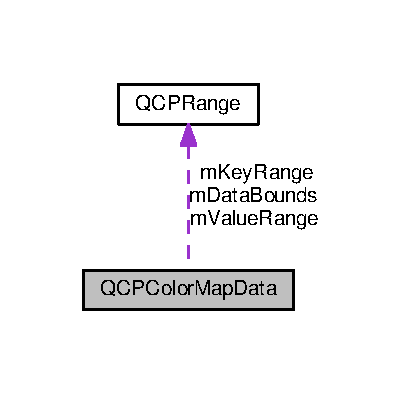
\includegraphics[width=194pt]{classQCPColorMapData__coll__graph}
\end{center}
\end{figure}
\subsection*{Public Member Functions}
\begin{DoxyCompactItemize}
\item 
\hyperlink{classQCPColorMapData_aac9d8eb81e18e240d89d56c01933fd23}{Q\+C\+P\+Color\+Map\+Data} (int \hyperlink{classQCPColorMapData_aa8d7811686fdfea964947715210c4af8}{key\+Size}, int \hyperlink{classQCPColorMapData_ab880be6bc587f34e8d22fe77ef6b57e9}{value\+Size}, const \hyperlink{classQCPRange}{Q\+C\+P\+Range} \&\hyperlink{classQCPColorMapData_a4765180639742460f64ab6c97c745c08}{key\+Range}, const \hyperlink{classQCPRange}{Q\+C\+P\+Range} \&\hyperlink{classQCPColorMapData_a025be4d7ba0494fd7b38a5a56c737f2a}{value\+Range})
\item 
\hyperlink{classQCPColorMapData_a7ac252031d0921520d5bccb6bfa23a8b}{$\sim$\+Q\+C\+P\+Color\+Map\+Data} ()
\item 
\hyperlink{classQCPColorMapData_a7f2145d86473263494abb9bf1de20436}{Q\+C\+P\+Color\+Map\+Data} (const \hyperlink{classQCPColorMapData}{Q\+C\+P\+Color\+Map\+Data} \&other)
\item 
\hyperlink{classQCPColorMapData}{Q\+C\+P\+Color\+Map\+Data} \& \hyperlink{classQCPColorMapData_afdf4dd1b2f5714234fe84709b85c2a8d}{operator=} (const \hyperlink{classQCPColorMapData}{Q\+C\+P\+Color\+Map\+Data} \&other)
\item 
int \hyperlink{classQCPColorMapData_aa8d7811686fdfea964947715210c4af8}{key\+Size} () const 
\item 
int \hyperlink{classQCPColorMapData_ab880be6bc587f34e8d22fe77ef6b57e9}{value\+Size} () const 
\item 
\hyperlink{classQCPRange}{Q\+C\+P\+Range} \hyperlink{classQCPColorMapData_a4765180639742460f64ab6c97c745c08}{key\+Range} () const 
\item 
\hyperlink{classQCPRange}{Q\+C\+P\+Range} \hyperlink{classQCPColorMapData_a025be4d7ba0494fd7b38a5a56c737f2a}{value\+Range} () const 
\item 
\hyperlink{classQCPRange}{Q\+C\+P\+Range} \hyperlink{classQCPColorMapData_a9ff433248ee226ea0c469ae6cc2489fd}{data\+Bounds} () const 
\item 
double \hyperlink{classQCPColorMapData_a2c33807b008cdb9e1394245c294c0eaf}{data} (double key, double value)
\item 
double \hyperlink{classQCPColorMapData_af51ecd21f347adbf87b4cce4e1f5cbd6}{cell} (int key\+Index, int value\+Index)
\item 
void \hyperlink{classQCPColorMapData_a0d9ff35c299d0478b682bfbcdd9c097e}{set\+Size} (int \hyperlink{classQCPColorMapData_aa8d7811686fdfea964947715210c4af8}{key\+Size}, int \hyperlink{classQCPColorMapData_ab880be6bc587f34e8d22fe77ef6b57e9}{value\+Size})
\item 
void \hyperlink{classQCPColorMapData_ac7ef70e383aface34b44dbde49234b6b}{set\+Key\+Size} (int \hyperlink{classQCPColorMapData_aa8d7811686fdfea964947715210c4af8}{key\+Size})
\item 
void \hyperlink{classQCPColorMapData_a0893c9e3914513048b45e3429ffd16f2}{set\+Value\+Size} (int \hyperlink{classQCPColorMapData_ab880be6bc587f34e8d22fe77ef6b57e9}{value\+Size})
\item 
void \hyperlink{classQCPColorMapData_aad9c1c7c703c1339489fc730517c83d4}{set\+Range} (const \hyperlink{classQCPRange}{Q\+C\+P\+Range} \&\hyperlink{classQCPColorMapData_a4765180639742460f64ab6c97c745c08}{key\+Range}, const \hyperlink{classQCPRange}{Q\+C\+P\+Range} \&\hyperlink{classQCPColorMapData_a025be4d7ba0494fd7b38a5a56c737f2a}{value\+Range})
\item 
void \hyperlink{classQCPColorMapData_a0738c485f3c9df9ea1241b7a8bb6a86e}{set\+Key\+Range} (const \hyperlink{classQCPRange}{Q\+C\+P\+Range} \&\hyperlink{classQCPColorMapData_a4765180639742460f64ab6c97c745c08}{key\+Range})
\item 
void \hyperlink{classQCPColorMapData_ada1b2680ba96a5f4175b6d341cf75d23}{set\+Value\+Range} (const \hyperlink{classQCPRange}{Q\+C\+P\+Range} \&\hyperlink{classQCPColorMapData_a025be4d7ba0494fd7b38a5a56c737f2a}{value\+Range})
\item 
void \hyperlink{classQCPColorMapData_afd2083ccfd6987ec94aa7ef8e91ca39a}{set\+Data} (double key, double value, double z)
\item 
void \hyperlink{classQCPColorMapData_a8e75eaf8746596319032a93f3d2d0683}{set\+Cell} (int key\+Index, int value\+Index, double z)
\item 
void \hyperlink{classQCPColorMapData_ab235ade8a4d64bd3adb26a99b3dd57ee}{recalculate\+Data\+Bounds} ()
\item 
void \hyperlink{classQCPColorMapData_a9910ba830e96955bd5c8e5bef1e77ef3}{clear} ()
\item 
void \hyperlink{classQCPColorMapData_a350f783260eb9b5de5c7b5e0d5d3e3c2}{fill} (double z)
\item 
bool \hyperlink{classQCPColorMapData_a986009324aee1fc5f696db46bd03dde5}{is\+Empty} () const 
\item 
void \hyperlink{classQCPColorMapData_a26e33c5ec7094b60136350bcd77d3737}{coord\+To\+Cell} (double key, double value, int $\ast$key\+Index, int $\ast$value\+Index) const 
\item 
void \hyperlink{classQCPColorMapData_ac96d6e84befe7b9951b5da6d4d4a2a47}{cell\+To\+Coord} (int key\+Index, int value\+Index, double $\ast$key, double $\ast$value) const 
\end{DoxyCompactItemize}
\subsection*{Protected Attributes}
\begin{DoxyCompactItemize}
\item 
int \hyperlink{classQCPColorMapData_a354e06462023340fbc03894b22499f6d}{m\+Key\+Size}
\item 
int \hyperlink{classQCPColorMapData_ae8ee9093632a59f55eb4fc06579ed256}{m\+Value\+Size}
\item 
\hyperlink{classQCPRange}{Q\+C\+P\+Range} \hyperlink{classQCPColorMapData_aaaafd0d7d0f153dbd152f3daf34254ee}{m\+Key\+Range}
\item 
\hyperlink{classQCPRange}{Q\+C\+P\+Range} \hyperlink{classQCPColorMapData_a225bb96f10c1a27b51ae59249477dbef}{m\+Value\+Range}
\item 
bool \hyperlink{classQCPColorMapData_a10e91aa89ed05bd177b1f81e07b465b8}{m\+Is\+Empty}
\item 
double $\ast$ \hyperlink{classQCPColorMapData_ac1682862022f575191351c9825187d39}{m\+Data}
\item 
\hyperlink{classQCPRange}{Q\+C\+P\+Range} \hyperlink{classQCPColorMapData_a1798b3dcc0a27091d196bfd156dcb3f2}{m\+Data\+Bounds}
\item 
bool \hyperlink{classQCPColorMapData_ad3cc682da2ac14e5acdbc05cf4d3d93b}{m\+Data\+Modified}
\end{DoxyCompactItemize}
\subsection*{Friends}
\begin{DoxyCompactItemize}
\item 
class \hyperlink{classQCPColorMapData_afa9d9eab63af3e6f20f882c8d7cc9f20}{Q\+C\+P\+Color\+Map}
\end{DoxyCompactItemize}


\subsection{Detailed Description}
Holds the two-\/dimensional data of a \hyperlink{classQCPColorMap}{Q\+C\+P\+Color\+Map} plottable. 

This class is a data storage for \hyperlink{classQCPColorMap}{Q\+C\+P\+Color\+Map}. It holds a two-\/dimensional array, which \hyperlink{classQCPColorMap}{Q\+C\+P\+Color\+Map} then displays as a 2D image in the plot, where the array values are represented by a color, depending on the value.

The size of the array can be controlled via \hyperlink{classQCPColorMapData_a0d9ff35c299d0478b682bfbcdd9c097e}{set\+Size} (or \hyperlink{classQCPColorMapData_ac7ef70e383aface34b44dbde49234b6b}{set\+Key\+Size}, \hyperlink{classQCPColorMapData_a0893c9e3914513048b45e3429ffd16f2}{set\+Value\+Size}). Which plot coordinates these cells correspond to can be configured with \hyperlink{classQCPColorMapData_aad9c1c7c703c1339489fc730517c83d4}{set\+Range} (or \hyperlink{classQCPColorMapData_a0738c485f3c9df9ea1241b7a8bb6a86e}{set\+Key\+Range}, \hyperlink{classQCPColorMapData_ada1b2680ba96a5f4175b6d341cf75d23}{set\+Value\+Range}).

The data cells can be accessed in two ways\+: They can be directly addressed by an integer index with \hyperlink{classQCPColorMapData_a8e75eaf8746596319032a93f3d2d0683}{set\+Cell}. This is the fastest method. Alternatively, they can be addressed by their plot coordinate with \hyperlink{classQCPColorMapData_afd2083ccfd6987ec94aa7ef8e91ca39a}{set\+Data}. plot coordinate to cell index transformations and vice versa are provided by the functions \hyperlink{classQCPColorMapData_a26e33c5ec7094b60136350bcd77d3737}{coord\+To\+Cell} and \hyperlink{classQCPColorMapData_ac96d6e84befe7b9951b5da6d4d4a2a47}{cell\+To\+Coord}.

This class also buffers the minimum and maximum values that are in the data set, to provide \hyperlink{classQCPColorMap_a856608fa3dd1cc290bcd5f29a5575774}{Q\+C\+P\+Color\+Map\+::rescale\+Data\+Range} with the necessary information quickly. Setting a cell to a value that is greater than the current maximum increases this maximum to the new value. However, setting the cell that currently holds the maximum value to a smaller value doesn\textquotesingle{}t decrease the maximum again, because finding the true new maximum would require going through the entire data array, which might be time consuming. The same holds for the data minimum. This functionality is given by \hyperlink{classQCPColorMapData_ab235ade8a4d64bd3adb26a99b3dd57ee}{recalculate\+Data\+Bounds}, such that you can decide when it is sensible to find the true current minimum and maximum. The method \hyperlink{classQCPColorMap_a856608fa3dd1cc290bcd5f29a5575774}{Q\+C\+P\+Color\+Map\+::rescale\+Data\+Range} offers a convenience parameter {\itshape recalculate\+Data\+Bounds} which may be set to true to automatically call \hyperlink{classQCPColorMapData_ab235ade8a4d64bd3adb26a99b3dd57ee}{recalculate\+Data\+Bounds} internally. 

\subsection{Constructor \& Destructor Documentation}
\index{Q\+C\+P\+Color\+Map\+Data@{Q\+C\+P\+Color\+Map\+Data}!Q\+C\+P\+Color\+Map\+Data@{Q\+C\+P\+Color\+Map\+Data}}
\index{Q\+C\+P\+Color\+Map\+Data@{Q\+C\+P\+Color\+Map\+Data}!Q\+C\+P\+Color\+Map\+Data@{Q\+C\+P\+Color\+Map\+Data}}
\subsubsection[{\texorpdfstring{Q\+C\+P\+Color\+Map\+Data(int key\+Size, int value\+Size, const Q\+C\+P\+Range \&key\+Range, const Q\+C\+P\+Range \&value\+Range)}{QCPColorMapData(int keySize, int valueSize, const QCPRange &keyRange, const QCPRange &valueRange)}}]{\setlength{\rightskip}{0pt plus 5cm}Q\+C\+P\+Color\+Map\+Data\+::\+Q\+C\+P\+Color\+Map\+Data (
\begin{DoxyParamCaption}
\item[{int}]{key\+Size, }
\item[{int}]{value\+Size, }
\item[{const {\bf Q\+C\+P\+Range} \&}]{key\+Range, }
\item[{const {\bf Q\+C\+P\+Range} \&}]{value\+Range}
\end{DoxyParamCaption}
)}\hypertarget{classQCPColorMapData_aac9d8eb81e18e240d89d56c01933fd23}{}\label{classQCPColorMapData_aac9d8eb81e18e240d89d56c01933fd23}
Constructs a new \hyperlink{classQCPColorMapData}{Q\+C\+P\+Color\+Map\+Data} instance. The instance has {\itshape key\+Size} cells in the key direction and {\itshape value\+Size} cells in the value direction. These cells will be displayed by the \hyperlink{classQCPColorMap}{Q\+C\+P\+Color\+Map} at the coordinates {\itshape key\+Range} and {\itshape value\+Range}.

\begin{DoxySeeAlso}{See also}
\hyperlink{classQCPColorMapData_a0d9ff35c299d0478b682bfbcdd9c097e}{set\+Size}, \hyperlink{classQCPColorMapData_ac7ef70e383aface34b44dbde49234b6b}{set\+Key\+Size}, \hyperlink{classQCPColorMapData_a0893c9e3914513048b45e3429ffd16f2}{set\+Value\+Size}, \hyperlink{classQCPColorMapData_aad9c1c7c703c1339489fc730517c83d4}{set\+Range}, \hyperlink{classQCPColorMapData_a0738c485f3c9df9ea1241b7a8bb6a86e}{set\+Key\+Range}, \hyperlink{classQCPColorMapData_ada1b2680ba96a5f4175b6d341cf75d23}{set\+Value\+Range} 
\end{DoxySeeAlso}
\index{Q\+C\+P\+Color\+Map\+Data@{Q\+C\+P\+Color\+Map\+Data}!````~Q\+C\+P\+Color\+Map\+Data@{$\sim$\+Q\+C\+P\+Color\+Map\+Data}}
\index{````~Q\+C\+P\+Color\+Map\+Data@{$\sim$\+Q\+C\+P\+Color\+Map\+Data}!Q\+C\+P\+Color\+Map\+Data@{Q\+C\+P\+Color\+Map\+Data}}
\subsubsection[{\texorpdfstring{$\sim$\+Q\+C\+P\+Color\+Map\+Data()}{~QCPColorMapData()}}]{\setlength{\rightskip}{0pt plus 5cm}Q\+C\+P\+Color\+Map\+Data\+::$\sim$\+Q\+C\+P\+Color\+Map\+Data (
\begin{DoxyParamCaption}
{}
\end{DoxyParamCaption}
)}\hypertarget{classQCPColorMapData_a7ac252031d0921520d5bccb6bfa23a8b}{}\label{classQCPColorMapData_a7ac252031d0921520d5bccb6bfa23a8b}
\index{Q\+C\+P\+Color\+Map\+Data@{Q\+C\+P\+Color\+Map\+Data}!Q\+C\+P\+Color\+Map\+Data@{Q\+C\+P\+Color\+Map\+Data}}
\index{Q\+C\+P\+Color\+Map\+Data@{Q\+C\+P\+Color\+Map\+Data}!Q\+C\+P\+Color\+Map\+Data@{Q\+C\+P\+Color\+Map\+Data}}
\subsubsection[{\texorpdfstring{Q\+C\+P\+Color\+Map\+Data(const Q\+C\+P\+Color\+Map\+Data \&other)}{QCPColorMapData(const QCPColorMapData &other)}}]{\setlength{\rightskip}{0pt plus 5cm}Q\+C\+P\+Color\+Map\+Data\+::\+Q\+C\+P\+Color\+Map\+Data (
\begin{DoxyParamCaption}
\item[{const {\bf Q\+C\+P\+Color\+Map\+Data} \&}]{other}
\end{DoxyParamCaption}
)}\hypertarget{classQCPColorMapData_a7f2145d86473263494abb9bf1de20436}{}\label{classQCPColorMapData_a7f2145d86473263494abb9bf1de20436}
Constructs a new \hyperlink{classQCPColorMapData}{Q\+C\+P\+Color\+Map\+Data} instance copying the data and range of {\itshape other}. 

\subsection{Member Function Documentation}
\index{Q\+C\+P\+Color\+Map\+Data@{Q\+C\+P\+Color\+Map\+Data}!cell@{cell}}
\index{cell@{cell}!Q\+C\+P\+Color\+Map\+Data@{Q\+C\+P\+Color\+Map\+Data}}
\subsubsection[{\texorpdfstring{cell(int key\+Index, int value\+Index)}{cell(int keyIndex, int valueIndex)}}]{\setlength{\rightskip}{0pt plus 5cm}double Q\+C\+P\+Color\+Map\+Data\+::cell (
\begin{DoxyParamCaption}
\item[{int}]{key\+Index, }
\item[{int}]{value\+Index}
\end{DoxyParamCaption}
)}\hypertarget{classQCPColorMapData_af51ecd21f347adbf87b4cce4e1f5cbd6}{}\label{classQCPColorMapData_af51ecd21f347adbf87b4cce4e1f5cbd6}
\index{Q\+C\+P\+Color\+Map\+Data@{Q\+C\+P\+Color\+Map\+Data}!cell\+To\+Coord@{cell\+To\+Coord}}
\index{cell\+To\+Coord@{cell\+To\+Coord}!Q\+C\+P\+Color\+Map\+Data@{Q\+C\+P\+Color\+Map\+Data}}
\subsubsection[{\texorpdfstring{cell\+To\+Coord(int key\+Index, int value\+Index, double $\ast$key, double $\ast$value) const }{cellToCoord(int keyIndex, int valueIndex, double *key, double *value) const }}]{\setlength{\rightskip}{0pt plus 5cm}void Q\+C\+P\+Color\+Map\+Data\+::cell\+To\+Coord (
\begin{DoxyParamCaption}
\item[{int}]{key\+Index, }
\item[{int}]{value\+Index, }
\item[{double $\ast$}]{key, }
\item[{double $\ast$}]{value}
\end{DoxyParamCaption}
) const}\hypertarget{classQCPColorMapData_ac96d6e84befe7b9951b5da6d4d4a2a47}{}\label{classQCPColorMapData_ac96d6e84befe7b9951b5da6d4d4a2a47}
Transforms cell indices given by {\itshape key\+Index} and {\itshape value\+Index} to cell indices of this \hyperlink{classQCPColorMapData}{Q\+C\+P\+Color\+Map\+Data} instance. The resulting coordinates are returned via the output parameters {\itshape key} and {\itshape value}.

If you are only interested in a key or value coordinate, you may pass 0 as {\itshape key} or {\itshape value}.

\begin{DoxyNote}{Note}
The \hyperlink{classQCPColorMap}{Q\+C\+P\+Color\+Map} always displays the data at equal key/value intervals, even if the key or value axis is set to a logarithmic scaling. If you want to use \hyperlink{classQCPColorMap}{Q\+C\+P\+Color\+Map} with logarithmic axes, you shouldn\textquotesingle{}t use the \hyperlink{classQCPColorMapData_ac96d6e84befe7b9951b5da6d4d4a2a47}{Q\+C\+P\+Color\+Map\+Data\+::cell\+To\+Coord} method as it uses a linear transformation to determine the cell index.
\end{DoxyNote}
\begin{DoxySeeAlso}{See also}
\hyperlink{classQCPColorMapData_a26e33c5ec7094b60136350bcd77d3737}{coord\+To\+Cell}, \hyperlink{classQCPAxis_ae9289ef7043b9d966af88eaa95b037d1}{Q\+C\+P\+Axis\+::pixel\+To\+Coord} 
\end{DoxySeeAlso}
\index{Q\+C\+P\+Color\+Map\+Data@{Q\+C\+P\+Color\+Map\+Data}!clear@{clear}}
\index{clear@{clear}!Q\+C\+P\+Color\+Map\+Data@{Q\+C\+P\+Color\+Map\+Data}}
\subsubsection[{\texorpdfstring{clear()}{clear()}}]{\setlength{\rightskip}{0pt plus 5cm}void Q\+C\+P\+Color\+Map\+Data\+::clear (
\begin{DoxyParamCaption}
{}
\end{DoxyParamCaption}
)}\hypertarget{classQCPColorMapData_a9910ba830e96955bd5c8e5bef1e77ef3}{}\label{classQCPColorMapData_a9910ba830e96955bd5c8e5bef1e77ef3}
Frees the internal data memory.

This is equivalent to calling \hyperlink{classQCPColorMapData_a0d9ff35c299d0478b682bfbcdd9c097e}{set\+Size(0, 0)}. \index{Q\+C\+P\+Color\+Map\+Data@{Q\+C\+P\+Color\+Map\+Data}!coord\+To\+Cell@{coord\+To\+Cell}}
\index{coord\+To\+Cell@{coord\+To\+Cell}!Q\+C\+P\+Color\+Map\+Data@{Q\+C\+P\+Color\+Map\+Data}}
\subsubsection[{\texorpdfstring{coord\+To\+Cell(double key, double value, int $\ast$key\+Index, int $\ast$value\+Index) const }{coordToCell(double key, double value, int *keyIndex, int *valueIndex) const }}]{\setlength{\rightskip}{0pt plus 5cm}void Q\+C\+P\+Color\+Map\+Data\+::coord\+To\+Cell (
\begin{DoxyParamCaption}
\item[{double}]{key, }
\item[{double}]{value, }
\item[{int $\ast$}]{key\+Index, }
\item[{int $\ast$}]{value\+Index}
\end{DoxyParamCaption}
) const}\hypertarget{classQCPColorMapData_a26e33c5ec7094b60136350bcd77d3737}{}\label{classQCPColorMapData_a26e33c5ec7094b60136350bcd77d3737}
Transforms plot coordinates given by {\itshape key} and {\itshape value} to cell indices of this \hyperlink{classQCPColorMapData}{Q\+C\+P\+Color\+Map\+Data} instance. The resulting cell indices are returned via the output parameters {\itshape key\+Index} and {\itshape value\+Index}.

The retrieved key/value cell indices can then be used for example with \hyperlink{classQCPColorMapData_a8e75eaf8746596319032a93f3d2d0683}{set\+Cell}.

If you are only interested in a key or value index, you may pass 0 as {\itshape value\+Index} or {\itshape key\+Index}.

\begin{DoxyNote}{Note}
The \hyperlink{classQCPColorMap}{Q\+C\+P\+Color\+Map} always displays the data at equal key/value intervals, even if the key or value axis is set to a logarithmic scaling. If you want to use \hyperlink{classQCPColorMap}{Q\+C\+P\+Color\+Map} with logarithmic axes, you shouldn\textquotesingle{}t use the \hyperlink{classQCPColorMapData_a26e33c5ec7094b60136350bcd77d3737}{Q\+C\+P\+Color\+Map\+Data\+::coord\+To\+Cell} method as it uses a linear transformation to determine the cell index.
\end{DoxyNote}
\begin{DoxySeeAlso}{See also}
\hyperlink{classQCPColorMapData_ac96d6e84befe7b9951b5da6d4d4a2a47}{cell\+To\+Coord}, \hyperlink{classQCPAxis_a985ae693b842fb0422b4390fe36d299a}{Q\+C\+P\+Axis\+::coord\+To\+Pixel} 
\end{DoxySeeAlso}
\index{Q\+C\+P\+Color\+Map\+Data@{Q\+C\+P\+Color\+Map\+Data}!data@{data}}
\index{data@{data}!Q\+C\+P\+Color\+Map\+Data@{Q\+C\+P\+Color\+Map\+Data}}
\subsubsection[{\texorpdfstring{data(double key, double value)}{data(double key, double value)}}]{\setlength{\rightskip}{0pt plus 5cm}double Q\+C\+P\+Color\+Map\+Data\+::data (
\begin{DoxyParamCaption}
\item[{double}]{key, }
\item[{double}]{value}
\end{DoxyParamCaption}
)}\hypertarget{classQCPColorMapData_a2c33807b008cdb9e1394245c294c0eaf}{}\label{classQCPColorMapData_a2c33807b008cdb9e1394245c294c0eaf}
\index{Q\+C\+P\+Color\+Map\+Data@{Q\+C\+P\+Color\+Map\+Data}!data\+Bounds@{data\+Bounds}}
\index{data\+Bounds@{data\+Bounds}!Q\+C\+P\+Color\+Map\+Data@{Q\+C\+P\+Color\+Map\+Data}}
\subsubsection[{\texorpdfstring{data\+Bounds() const }{dataBounds() const }}]{\setlength{\rightskip}{0pt plus 5cm}{\bf Q\+C\+P\+Range} Q\+C\+P\+Color\+Map\+Data\+::data\+Bounds (
\begin{DoxyParamCaption}
{}
\end{DoxyParamCaption}
) const\hspace{0.3cm}{\ttfamily [inline]}}\hypertarget{classQCPColorMapData_a9ff433248ee226ea0c469ae6cc2489fd}{}\label{classQCPColorMapData_a9ff433248ee226ea0c469ae6cc2489fd}
\index{Q\+C\+P\+Color\+Map\+Data@{Q\+C\+P\+Color\+Map\+Data}!fill@{fill}}
\index{fill@{fill}!Q\+C\+P\+Color\+Map\+Data@{Q\+C\+P\+Color\+Map\+Data}}
\subsubsection[{\texorpdfstring{fill(double z)}{fill(double z)}}]{\setlength{\rightskip}{0pt plus 5cm}void Q\+C\+P\+Color\+Map\+Data\+::fill (
\begin{DoxyParamCaption}
\item[{double}]{z}
\end{DoxyParamCaption}
)}\hypertarget{classQCPColorMapData_a350f783260eb9b5de5c7b5e0d5d3e3c2}{}\label{classQCPColorMapData_a350f783260eb9b5de5c7b5e0d5d3e3c2}
Sets all cells to the value {\itshape z}. \index{Q\+C\+P\+Color\+Map\+Data@{Q\+C\+P\+Color\+Map\+Data}!is\+Empty@{is\+Empty}}
\index{is\+Empty@{is\+Empty}!Q\+C\+P\+Color\+Map\+Data@{Q\+C\+P\+Color\+Map\+Data}}
\subsubsection[{\texorpdfstring{is\+Empty() const }{isEmpty() const }}]{\setlength{\rightskip}{0pt plus 5cm}bool Q\+C\+P\+Color\+Map\+Data\+::is\+Empty (
\begin{DoxyParamCaption}
{}
\end{DoxyParamCaption}
) const\hspace{0.3cm}{\ttfamily [inline]}}\hypertarget{classQCPColorMapData_a986009324aee1fc5f696db46bd03dde5}{}\label{classQCPColorMapData_a986009324aee1fc5f696db46bd03dde5}
Returns whether this instance carries no data. This is equivalent to having a size where at least one of the dimensions is 0 (see \hyperlink{classQCPColorMapData_a0d9ff35c299d0478b682bfbcdd9c097e}{set\+Size}). \index{Q\+C\+P\+Color\+Map\+Data@{Q\+C\+P\+Color\+Map\+Data}!key\+Range@{key\+Range}}
\index{key\+Range@{key\+Range}!Q\+C\+P\+Color\+Map\+Data@{Q\+C\+P\+Color\+Map\+Data}}
\subsubsection[{\texorpdfstring{key\+Range() const }{keyRange() const }}]{\setlength{\rightskip}{0pt plus 5cm}{\bf Q\+C\+P\+Range} Q\+C\+P\+Color\+Map\+Data\+::key\+Range (
\begin{DoxyParamCaption}
{}
\end{DoxyParamCaption}
) const\hspace{0.3cm}{\ttfamily [inline]}}\hypertarget{classQCPColorMapData_a4765180639742460f64ab6c97c745c08}{}\label{classQCPColorMapData_a4765180639742460f64ab6c97c745c08}
\index{Q\+C\+P\+Color\+Map\+Data@{Q\+C\+P\+Color\+Map\+Data}!key\+Size@{key\+Size}}
\index{key\+Size@{key\+Size}!Q\+C\+P\+Color\+Map\+Data@{Q\+C\+P\+Color\+Map\+Data}}
\subsubsection[{\texorpdfstring{key\+Size() const }{keySize() const }}]{\setlength{\rightskip}{0pt plus 5cm}int Q\+C\+P\+Color\+Map\+Data\+::key\+Size (
\begin{DoxyParamCaption}
{}
\end{DoxyParamCaption}
) const\hspace{0.3cm}{\ttfamily [inline]}}\hypertarget{classQCPColorMapData_aa8d7811686fdfea964947715210c4af8}{}\label{classQCPColorMapData_aa8d7811686fdfea964947715210c4af8}
\index{Q\+C\+P\+Color\+Map\+Data@{Q\+C\+P\+Color\+Map\+Data}!operator=@{operator=}}
\index{operator=@{operator=}!Q\+C\+P\+Color\+Map\+Data@{Q\+C\+P\+Color\+Map\+Data}}
\subsubsection[{\texorpdfstring{operator=(const Q\+C\+P\+Color\+Map\+Data \&other)}{operator=(const QCPColorMapData &other)}}]{\setlength{\rightskip}{0pt plus 5cm}{\bf Q\+C\+P\+Color\+Map\+Data} \& Q\+C\+P\+Color\+Map\+Data\+::operator= (
\begin{DoxyParamCaption}
\item[{const {\bf Q\+C\+P\+Color\+Map\+Data} \&}]{other}
\end{DoxyParamCaption}
)}\hypertarget{classQCPColorMapData_afdf4dd1b2f5714234fe84709b85c2a8d}{}\label{classQCPColorMapData_afdf4dd1b2f5714234fe84709b85c2a8d}
Overwrites this color map data instance with the data stored in {\itshape other}. \index{Q\+C\+P\+Color\+Map\+Data@{Q\+C\+P\+Color\+Map\+Data}!recalculate\+Data\+Bounds@{recalculate\+Data\+Bounds}}
\index{recalculate\+Data\+Bounds@{recalculate\+Data\+Bounds}!Q\+C\+P\+Color\+Map\+Data@{Q\+C\+P\+Color\+Map\+Data}}
\subsubsection[{\texorpdfstring{recalculate\+Data\+Bounds()}{recalculateDataBounds()}}]{\setlength{\rightskip}{0pt plus 5cm}void Q\+C\+P\+Color\+Map\+Data\+::recalculate\+Data\+Bounds (
\begin{DoxyParamCaption}
{}
\end{DoxyParamCaption}
)}\hypertarget{classQCPColorMapData_ab235ade8a4d64bd3adb26a99b3dd57ee}{}\label{classQCPColorMapData_ab235ade8a4d64bd3adb26a99b3dd57ee}
Goes through the data and updates the buffered minimum and maximum data values.

Calling this method is only advised if you are about to call \hyperlink{classQCPColorMap_a856608fa3dd1cc290bcd5f29a5575774}{Q\+C\+P\+Color\+Map\+::rescale\+Data\+Range} and can not guarantee that the cells holding the maximum or minimum data haven\textquotesingle{}t been overwritten with a smaller or larger value respectively, since the buffered maximum/minimum values have been updated the last time. Why this is the case is explained in the class description (\hyperlink{classQCPColorMapData}{Q\+C\+P\+Color\+Map\+Data}).

Note that the method \hyperlink{classQCPColorMap_a856608fa3dd1cc290bcd5f29a5575774}{Q\+C\+P\+Color\+Map\+::rescale\+Data\+Range} provides a parameter {\itshape recalculate\+Data\+Bounds} for convenience. Setting this to true will call this method for you, before doing the rescale. \index{Q\+C\+P\+Color\+Map\+Data@{Q\+C\+P\+Color\+Map\+Data}!set\+Cell@{set\+Cell}}
\index{set\+Cell@{set\+Cell}!Q\+C\+P\+Color\+Map\+Data@{Q\+C\+P\+Color\+Map\+Data}}
\subsubsection[{\texorpdfstring{set\+Cell(int key\+Index, int value\+Index, double z)}{setCell(int keyIndex, int valueIndex, double z)}}]{\setlength{\rightskip}{0pt plus 5cm}void Q\+C\+P\+Color\+Map\+Data\+::set\+Cell (
\begin{DoxyParamCaption}
\item[{int}]{key\+Index, }
\item[{int}]{value\+Index, }
\item[{double}]{z}
\end{DoxyParamCaption}
)}\hypertarget{classQCPColorMapData_a8e75eaf8746596319032a93f3d2d0683}{}\label{classQCPColorMapData_a8e75eaf8746596319032a93f3d2d0683}
Sets the data of the cell with indices {\itshape key\+Index} and {\itshape value\+Index} to {\itshape z}. The indices enumerate the cells starting from zero, up to the map\textquotesingle{}s size-\/1 in the respective dimension (see \hyperlink{classQCPColorMapData_a0d9ff35c299d0478b682bfbcdd9c097e}{set\+Size}).

In the standard plot configuration (horizontal key axis and vertical value axis, both not range-\/reversed), the cell with indices (0, 0) is in the bottom left corner and the cell with indices (key\+Size-\/1, value\+Size-\/1) is in the top right corner of the color map.

\begin{DoxySeeAlso}{See also}
\hyperlink{classQCPColorMapData_afd2083ccfd6987ec94aa7ef8e91ca39a}{set\+Data}, \hyperlink{classQCPColorMapData_a0d9ff35c299d0478b682bfbcdd9c097e}{set\+Size} 
\end{DoxySeeAlso}
\index{Q\+C\+P\+Color\+Map\+Data@{Q\+C\+P\+Color\+Map\+Data}!set\+Data@{set\+Data}}
\index{set\+Data@{set\+Data}!Q\+C\+P\+Color\+Map\+Data@{Q\+C\+P\+Color\+Map\+Data}}
\subsubsection[{\texorpdfstring{set\+Data(double key, double value, double z)}{setData(double key, double value, double z)}}]{\setlength{\rightskip}{0pt plus 5cm}void Q\+C\+P\+Color\+Map\+Data\+::set\+Data (
\begin{DoxyParamCaption}
\item[{double}]{key, }
\item[{double}]{value, }
\item[{double}]{z}
\end{DoxyParamCaption}
)}\hypertarget{classQCPColorMapData_afd2083ccfd6987ec94aa7ef8e91ca39a}{}\label{classQCPColorMapData_afd2083ccfd6987ec94aa7ef8e91ca39a}
Sets the data of the cell, which lies at the plot coordinates given by {\itshape key} and {\itshape value}, to {\itshape z}.

\begin{DoxyNote}{Note}
The \hyperlink{classQCPColorMap}{Q\+C\+P\+Color\+Map} always displays the data at equal key/value intervals, even if the key or value axis is set to a logarithmic scaling. If you want to use \hyperlink{classQCPColorMap}{Q\+C\+P\+Color\+Map} with logarithmic axes, you shouldn\textquotesingle{}t use the \hyperlink{classQCPColorMapData_afd2083ccfd6987ec94aa7ef8e91ca39a}{Q\+C\+P\+Color\+Map\+Data\+::set\+Data} method as it uses a linear transformation to determine the cell index. Rather directly access the cell index with \hyperlink{classQCPColorMapData_a8e75eaf8746596319032a93f3d2d0683}{Q\+C\+P\+Color\+Map\+Data\+::set\+Cell}.
\end{DoxyNote}
\begin{DoxySeeAlso}{See also}
\hyperlink{classQCPColorMapData_a8e75eaf8746596319032a93f3d2d0683}{set\+Cell}, \hyperlink{classQCPColorMapData_aad9c1c7c703c1339489fc730517c83d4}{set\+Range} 
\end{DoxySeeAlso}
\index{Q\+C\+P\+Color\+Map\+Data@{Q\+C\+P\+Color\+Map\+Data}!set\+Key\+Range@{set\+Key\+Range}}
\index{set\+Key\+Range@{set\+Key\+Range}!Q\+C\+P\+Color\+Map\+Data@{Q\+C\+P\+Color\+Map\+Data}}
\subsubsection[{\texorpdfstring{set\+Key\+Range(const Q\+C\+P\+Range \&key\+Range)}{setKeyRange(const QCPRange &keyRange)}}]{\setlength{\rightskip}{0pt plus 5cm}void Q\+C\+P\+Color\+Map\+Data\+::set\+Key\+Range (
\begin{DoxyParamCaption}
\item[{const {\bf Q\+C\+P\+Range} \&}]{key\+Range}
\end{DoxyParamCaption}
)}\hypertarget{classQCPColorMapData_a0738c485f3c9df9ea1241b7a8bb6a86e}{}\label{classQCPColorMapData_a0738c485f3c9df9ea1241b7a8bb6a86e}
Sets the coordinate range the data shall be distributed over in the key dimension. Together with the value range, This defines the rectangular area covered by the color map in plot coordinates.

The outer cells will be centered on the range boundaries given to this function. For example, if the key size (\hyperlink{classQCPColorMapData_ac7ef70e383aface34b44dbde49234b6b}{set\+Key\+Size}) is 3 and {\itshape key\+Range} is set to {\ttfamily \hyperlink{classQCPRange}{Q\+C\+P\+Range(2, 3)}} there will be cells centered on the key coordinates 2, 2.\+5 and 3.

\begin{DoxySeeAlso}{See also}
\hyperlink{classQCPColorMapData_aad9c1c7c703c1339489fc730517c83d4}{set\+Range}, \hyperlink{classQCPColorMapData_ada1b2680ba96a5f4175b6d341cf75d23}{set\+Value\+Range}, \hyperlink{classQCPColorMapData_a0d9ff35c299d0478b682bfbcdd9c097e}{set\+Size} 
\end{DoxySeeAlso}
\index{Q\+C\+P\+Color\+Map\+Data@{Q\+C\+P\+Color\+Map\+Data}!set\+Key\+Size@{set\+Key\+Size}}
\index{set\+Key\+Size@{set\+Key\+Size}!Q\+C\+P\+Color\+Map\+Data@{Q\+C\+P\+Color\+Map\+Data}}
\subsubsection[{\texorpdfstring{set\+Key\+Size(int key\+Size)}{setKeySize(int keySize)}}]{\setlength{\rightskip}{0pt plus 5cm}void Q\+C\+P\+Color\+Map\+Data\+::set\+Key\+Size (
\begin{DoxyParamCaption}
\item[{int}]{key\+Size}
\end{DoxyParamCaption}
)}\hypertarget{classQCPColorMapData_ac7ef70e383aface34b44dbde49234b6b}{}\label{classQCPColorMapData_ac7ef70e383aface34b44dbde49234b6b}
Resizes the data array to have {\itshape key\+Size} cells in the key dimension.

The current data is discarded and the map cells are set to 0, unless the map had already the requested size.

Setting {\itshape key\+Size} to zero frees the internal data array and \hyperlink{classQCPColorMapData_a986009324aee1fc5f696db46bd03dde5}{is\+Empty} returns true.

\begin{DoxySeeAlso}{See also}
\hyperlink{classQCPColorMapData_a0738c485f3c9df9ea1241b7a8bb6a86e}{set\+Key\+Range}, \hyperlink{classQCPColorMapData_a0d9ff35c299d0478b682bfbcdd9c097e}{set\+Size}, \hyperlink{classQCPColorMapData_a0893c9e3914513048b45e3429ffd16f2}{set\+Value\+Size} 
\end{DoxySeeAlso}
\index{Q\+C\+P\+Color\+Map\+Data@{Q\+C\+P\+Color\+Map\+Data}!set\+Range@{set\+Range}}
\index{set\+Range@{set\+Range}!Q\+C\+P\+Color\+Map\+Data@{Q\+C\+P\+Color\+Map\+Data}}
\subsubsection[{\texorpdfstring{set\+Range(const Q\+C\+P\+Range \&key\+Range, const Q\+C\+P\+Range \&value\+Range)}{setRange(const QCPRange &keyRange, const QCPRange &valueRange)}}]{\setlength{\rightskip}{0pt plus 5cm}void Q\+C\+P\+Color\+Map\+Data\+::set\+Range (
\begin{DoxyParamCaption}
\item[{const {\bf Q\+C\+P\+Range} \&}]{key\+Range, }
\item[{const {\bf Q\+C\+P\+Range} \&}]{value\+Range}
\end{DoxyParamCaption}
)}\hypertarget{classQCPColorMapData_aad9c1c7c703c1339489fc730517c83d4}{}\label{classQCPColorMapData_aad9c1c7c703c1339489fc730517c83d4}
Sets the coordinate ranges the data shall be distributed over. This defines the rectangular area covered by the color map in plot coordinates.

The outer cells will be centered on the range boundaries given to this function. For example, if the key size (\hyperlink{classQCPColorMapData_ac7ef70e383aface34b44dbde49234b6b}{set\+Key\+Size}) is 3 and {\itshape key\+Range} is set to {\ttfamily \hyperlink{classQCPRange}{Q\+C\+P\+Range(2, 3)}} there will be cells centered on the key coordinates 2, 2.\+5 and 3.

\begin{DoxySeeAlso}{See also}
\hyperlink{classQCPColorMapData_a0d9ff35c299d0478b682bfbcdd9c097e}{set\+Size} 
\end{DoxySeeAlso}
\index{Q\+C\+P\+Color\+Map\+Data@{Q\+C\+P\+Color\+Map\+Data}!set\+Size@{set\+Size}}
\index{set\+Size@{set\+Size}!Q\+C\+P\+Color\+Map\+Data@{Q\+C\+P\+Color\+Map\+Data}}
\subsubsection[{\texorpdfstring{set\+Size(int key\+Size, int value\+Size)}{setSize(int keySize, int valueSize)}}]{\setlength{\rightskip}{0pt plus 5cm}void Q\+C\+P\+Color\+Map\+Data\+::set\+Size (
\begin{DoxyParamCaption}
\item[{int}]{key\+Size, }
\item[{int}]{value\+Size}
\end{DoxyParamCaption}
)}\hypertarget{classQCPColorMapData_a0d9ff35c299d0478b682bfbcdd9c097e}{}\label{classQCPColorMapData_a0d9ff35c299d0478b682bfbcdd9c097e}
Resizes the data array to have {\itshape key\+Size} cells in the key dimension and {\itshape value\+Size} cells in the value dimension.

The current data is discarded and the map cells are set to 0, unless the map had already the requested size.

Setting at least one of {\itshape key\+Size} or {\itshape value\+Size} to zero frees the internal data array and \hyperlink{classQCPColorMapData_a986009324aee1fc5f696db46bd03dde5}{is\+Empty} returns true.

\begin{DoxySeeAlso}{See also}
\hyperlink{classQCPColorMapData_aad9c1c7c703c1339489fc730517c83d4}{set\+Range}, \hyperlink{classQCPColorMapData_ac7ef70e383aface34b44dbde49234b6b}{set\+Key\+Size}, \hyperlink{classQCPColorMapData_a0893c9e3914513048b45e3429ffd16f2}{set\+Value\+Size} 
\end{DoxySeeAlso}
\index{Q\+C\+P\+Color\+Map\+Data@{Q\+C\+P\+Color\+Map\+Data}!set\+Value\+Range@{set\+Value\+Range}}
\index{set\+Value\+Range@{set\+Value\+Range}!Q\+C\+P\+Color\+Map\+Data@{Q\+C\+P\+Color\+Map\+Data}}
\subsubsection[{\texorpdfstring{set\+Value\+Range(const Q\+C\+P\+Range \&value\+Range)}{setValueRange(const QCPRange &valueRange)}}]{\setlength{\rightskip}{0pt plus 5cm}void Q\+C\+P\+Color\+Map\+Data\+::set\+Value\+Range (
\begin{DoxyParamCaption}
\item[{const {\bf Q\+C\+P\+Range} \&}]{value\+Range}
\end{DoxyParamCaption}
)}\hypertarget{classQCPColorMapData_ada1b2680ba96a5f4175b6d341cf75d23}{}\label{classQCPColorMapData_ada1b2680ba96a5f4175b6d341cf75d23}
Sets the coordinate range the data shall be distributed over in the value dimension. Together with the key range, This defines the rectangular area covered by the color map in plot coordinates.

The outer cells will be centered on the range boundaries given to this function. For example, if the value size (\hyperlink{classQCPColorMapData_a0893c9e3914513048b45e3429ffd16f2}{set\+Value\+Size}) is 3 and {\itshape value\+Range} is set to {\ttfamily \hyperlink{classQCPRange}{Q\+C\+P\+Range(2, 3)}} there will be cells centered on the value coordinates 2, 2.\+5 and 3.

\begin{DoxySeeAlso}{See also}
\hyperlink{classQCPColorMapData_aad9c1c7c703c1339489fc730517c83d4}{set\+Range}, \hyperlink{classQCPColorMapData_a0738c485f3c9df9ea1241b7a8bb6a86e}{set\+Key\+Range}, \hyperlink{classQCPColorMapData_a0d9ff35c299d0478b682bfbcdd9c097e}{set\+Size} 
\end{DoxySeeAlso}
\index{Q\+C\+P\+Color\+Map\+Data@{Q\+C\+P\+Color\+Map\+Data}!set\+Value\+Size@{set\+Value\+Size}}
\index{set\+Value\+Size@{set\+Value\+Size}!Q\+C\+P\+Color\+Map\+Data@{Q\+C\+P\+Color\+Map\+Data}}
\subsubsection[{\texorpdfstring{set\+Value\+Size(int value\+Size)}{setValueSize(int valueSize)}}]{\setlength{\rightskip}{0pt plus 5cm}void Q\+C\+P\+Color\+Map\+Data\+::set\+Value\+Size (
\begin{DoxyParamCaption}
\item[{int}]{value\+Size}
\end{DoxyParamCaption}
)}\hypertarget{classQCPColorMapData_a0893c9e3914513048b45e3429ffd16f2}{}\label{classQCPColorMapData_a0893c9e3914513048b45e3429ffd16f2}
Resizes the data array to have {\itshape value\+Size} cells in the value dimension.

The current data is discarded and the map cells are set to 0, unless the map had already the requested size.

Setting {\itshape value\+Size} to zero frees the internal data array and \hyperlink{classQCPColorMapData_a986009324aee1fc5f696db46bd03dde5}{is\+Empty} returns true.

\begin{DoxySeeAlso}{See also}
\hyperlink{classQCPColorMapData_ada1b2680ba96a5f4175b6d341cf75d23}{set\+Value\+Range}, \hyperlink{classQCPColorMapData_a0d9ff35c299d0478b682bfbcdd9c097e}{set\+Size}, \hyperlink{classQCPColorMapData_ac7ef70e383aface34b44dbde49234b6b}{set\+Key\+Size} 
\end{DoxySeeAlso}
\index{Q\+C\+P\+Color\+Map\+Data@{Q\+C\+P\+Color\+Map\+Data}!value\+Range@{value\+Range}}
\index{value\+Range@{value\+Range}!Q\+C\+P\+Color\+Map\+Data@{Q\+C\+P\+Color\+Map\+Data}}
\subsubsection[{\texorpdfstring{value\+Range() const }{valueRange() const }}]{\setlength{\rightskip}{0pt plus 5cm}{\bf Q\+C\+P\+Range} Q\+C\+P\+Color\+Map\+Data\+::value\+Range (
\begin{DoxyParamCaption}
{}
\end{DoxyParamCaption}
) const\hspace{0.3cm}{\ttfamily [inline]}}\hypertarget{classQCPColorMapData_a025be4d7ba0494fd7b38a5a56c737f2a}{}\label{classQCPColorMapData_a025be4d7ba0494fd7b38a5a56c737f2a}
\index{Q\+C\+P\+Color\+Map\+Data@{Q\+C\+P\+Color\+Map\+Data}!value\+Size@{value\+Size}}
\index{value\+Size@{value\+Size}!Q\+C\+P\+Color\+Map\+Data@{Q\+C\+P\+Color\+Map\+Data}}
\subsubsection[{\texorpdfstring{value\+Size() const }{valueSize() const }}]{\setlength{\rightskip}{0pt plus 5cm}int Q\+C\+P\+Color\+Map\+Data\+::value\+Size (
\begin{DoxyParamCaption}
{}
\end{DoxyParamCaption}
) const\hspace{0.3cm}{\ttfamily [inline]}}\hypertarget{classQCPColorMapData_ab880be6bc587f34e8d22fe77ef6b57e9}{}\label{classQCPColorMapData_ab880be6bc587f34e8d22fe77ef6b57e9}


\subsection{Friends And Related Function Documentation}
\index{Q\+C\+P\+Color\+Map\+Data@{Q\+C\+P\+Color\+Map\+Data}!Q\+C\+P\+Color\+Map@{Q\+C\+P\+Color\+Map}}
\index{Q\+C\+P\+Color\+Map@{Q\+C\+P\+Color\+Map}!Q\+C\+P\+Color\+Map\+Data@{Q\+C\+P\+Color\+Map\+Data}}
\subsubsection[{\texorpdfstring{Q\+C\+P\+Color\+Map}{QCPColorMap}}]{\setlength{\rightskip}{0pt plus 5cm}friend class {\bf Q\+C\+P\+Color\+Map}\hspace{0.3cm}{\ttfamily [friend]}}\hypertarget{classQCPColorMapData_afa9d9eab63af3e6f20f882c8d7cc9f20}{}\label{classQCPColorMapData_afa9d9eab63af3e6f20f882c8d7cc9f20}


\subsection{Member Data Documentation}
\index{Q\+C\+P\+Color\+Map\+Data@{Q\+C\+P\+Color\+Map\+Data}!m\+Data@{m\+Data}}
\index{m\+Data@{m\+Data}!Q\+C\+P\+Color\+Map\+Data@{Q\+C\+P\+Color\+Map\+Data}}
\subsubsection[{\texorpdfstring{m\+Data}{mData}}]{\setlength{\rightskip}{0pt plus 5cm}double$\ast$ Q\+C\+P\+Color\+Map\+Data\+::m\+Data\hspace{0.3cm}{\ttfamily [protected]}}\hypertarget{classQCPColorMapData_ac1682862022f575191351c9825187d39}{}\label{classQCPColorMapData_ac1682862022f575191351c9825187d39}
\index{Q\+C\+P\+Color\+Map\+Data@{Q\+C\+P\+Color\+Map\+Data}!m\+Data\+Bounds@{m\+Data\+Bounds}}
\index{m\+Data\+Bounds@{m\+Data\+Bounds}!Q\+C\+P\+Color\+Map\+Data@{Q\+C\+P\+Color\+Map\+Data}}
\subsubsection[{\texorpdfstring{m\+Data\+Bounds}{mDataBounds}}]{\setlength{\rightskip}{0pt plus 5cm}{\bf Q\+C\+P\+Range} Q\+C\+P\+Color\+Map\+Data\+::m\+Data\+Bounds\hspace{0.3cm}{\ttfamily [protected]}}\hypertarget{classQCPColorMapData_a1798b3dcc0a27091d196bfd156dcb3f2}{}\label{classQCPColorMapData_a1798b3dcc0a27091d196bfd156dcb3f2}
\index{Q\+C\+P\+Color\+Map\+Data@{Q\+C\+P\+Color\+Map\+Data}!m\+Data\+Modified@{m\+Data\+Modified}}
\index{m\+Data\+Modified@{m\+Data\+Modified}!Q\+C\+P\+Color\+Map\+Data@{Q\+C\+P\+Color\+Map\+Data}}
\subsubsection[{\texorpdfstring{m\+Data\+Modified}{mDataModified}}]{\setlength{\rightskip}{0pt plus 5cm}bool Q\+C\+P\+Color\+Map\+Data\+::m\+Data\+Modified\hspace{0.3cm}{\ttfamily [protected]}}\hypertarget{classQCPColorMapData_ad3cc682da2ac14e5acdbc05cf4d3d93b}{}\label{classQCPColorMapData_ad3cc682da2ac14e5acdbc05cf4d3d93b}
\index{Q\+C\+P\+Color\+Map\+Data@{Q\+C\+P\+Color\+Map\+Data}!m\+Is\+Empty@{m\+Is\+Empty}}
\index{m\+Is\+Empty@{m\+Is\+Empty}!Q\+C\+P\+Color\+Map\+Data@{Q\+C\+P\+Color\+Map\+Data}}
\subsubsection[{\texorpdfstring{m\+Is\+Empty}{mIsEmpty}}]{\setlength{\rightskip}{0pt plus 5cm}bool Q\+C\+P\+Color\+Map\+Data\+::m\+Is\+Empty\hspace{0.3cm}{\ttfamily [protected]}}\hypertarget{classQCPColorMapData_a10e91aa89ed05bd177b1f81e07b465b8}{}\label{classQCPColorMapData_a10e91aa89ed05bd177b1f81e07b465b8}
\index{Q\+C\+P\+Color\+Map\+Data@{Q\+C\+P\+Color\+Map\+Data}!m\+Key\+Range@{m\+Key\+Range}}
\index{m\+Key\+Range@{m\+Key\+Range}!Q\+C\+P\+Color\+Map\+Data@{Q\+C\+P\+Color\+Map\+Data}}
\subsubsection[{\texorpdfstring{m\+Key\+Range}{mKeyRange}}]{\setlength{\rightskip}{0pt plus 5cm}{\bf Q\+C\+P\+Range} Q\+C\+P\+Color\+Map\+Data\+::m\+Key\+Range\hspace{0.3cm}{\ttfamily [protected]}}\hypertarget{classQCPColorMapData_aaaafd0d7d0f153dbd152f3daf34254ee}{}\label{classQCPColorMapData_aaaafd0d7d0f153dbd152f3daf34254ee}
\index{Q\+C\+P\+Color\+Map\+Data@{Q\+C\+P\+Color\+Map\+Data}!m\+Key\+Size@{m\+Key\+Size}}
\index{m\+Key\+Size@{m\+Key\+Size}!Q\+C\+P\+Color\+Map\+Data@{Q\+C\+P\+Color\+Map\+Data}}
\subsubsection[{\texorpdfstring{m\+Key\+Size}{mKeySize}}]{\setlength{\rightskip}{0pt plus 5cm}int Q\+C\+P\+Color\+Map\+Data\+::m\+Key\+Size\hspace{0.3cm}{\ttfamily [protected]}}\hypertarget{classQCPColorMapData_a354e06462023340fbc03894b22499f6d}{}\label{classQCPColorMapData_a354e06462023340fbc03894b22499f6d}
\index{Q\+C\+P\+Color\+Map\+Data@{Q\+C\+P\+Color\+Map\+Data}!m\+Value\+Range@{m\+Value\+Range}}
\index{m\+Value\+Range@{m\+Value\+Range}!Q\+C\+P\+Color\+Map\+Data@{Q\+C\+P\+Color\+Map\+Data}}
\subsubsection[{\texorpdfstring{m\+Value\+Range}{mValueRange}}]{\setlength{\rightskip}{0pt plus 5cm}{\bf Q\+C\+P\+Range} Q\+C\+P\+Color\+Map\+Data\+::m\+Value\+Range\hspace{0.3cm}{\ttfamily [protected]}}\hypertarget{classQCPColorMapData_a225bb96f10c1a27b51ae59249477dbef}{}\label{classQCPColorMapData_a225bb96f10c1a27b51ae59249477dbef}
\index{Q\+C\+P\+Color\+Map\+Data@{Q\+C\+P\+Color\+Map\+Data}!m\+Value\+Size@{m\+Value\+Size}}
\index{m\+Value\+Size@{m\+Value\+Size}!Q\+C\+P\+Color\+Map\+Data@{Q\+C\+P\+Color\+Map\+Data}}
\subsubsection[{\texorpdfstring{m\+Value\+Size}{mValueSize}}]{\setlength{\rightskip}{0pt plus 5cm}int Q\+C\+P\+Color\+Map\+Data\+::m\+Value\+Size\hspace{0.3cm}{\ttfamily [protected]}}\hypertarget{classQCPColorMapData_ae8ee9093632a59f55eb4fc06579ed256}{}\label{classQCPColorMapData_ae8ee9093632a59f55eb4fc06579ed256}


The documentation for this class was generated from the following files\+:\begin{DoxyCompactItemize}
\item 
src/hammerhead/tools/watchdog/include/watchdog/\hyperlink{qcustomplot_8h}{qcustomplot.\+h}\item 
src/hammerhead/tools/watchdog/src/\hyperlink{qcustomplot_8cpp}{qcustomplot.\+cpp}\end{DoxyCompactItemize}

\hypertarget{classQCPColorScale}{}\section{Q\+C\+P\+Color\+Scale Class Reference}
\label{classQCPColorScale}\index{Q\+C\+P\+Color\+Scale@{Q\+C\+P\+Color\+Scale}}


A color scale for use with color coding data such as \hyperlink{classQCPColorMap}{Q\+C\+P\+Color\+Map}.  




{\ttfamily \#include $<$qcustomplot.\+h$>$}



Inheritance diagram for Q\+C\+P\+Color\+Scale\+:\nopagebreak
\begin{figure}[H]
\begin{center}
\leavevmode
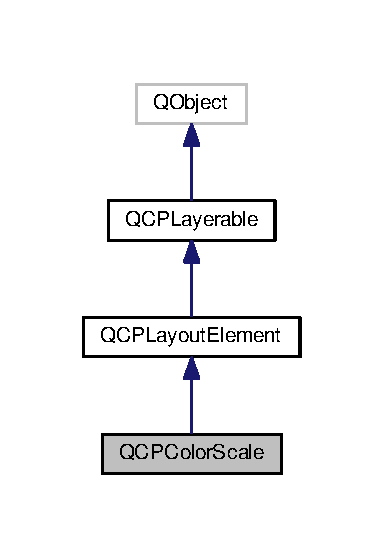
\includegraphics[width=184pt]{classQCPColorScale__inherit__graph}
\end{center}
\end{figure}


Collaboration diagram for Q\+C\+P\+Color\+Scale\+:\nopagebreak
\begin{figure}[H]
\begin{center}
\leavevmode
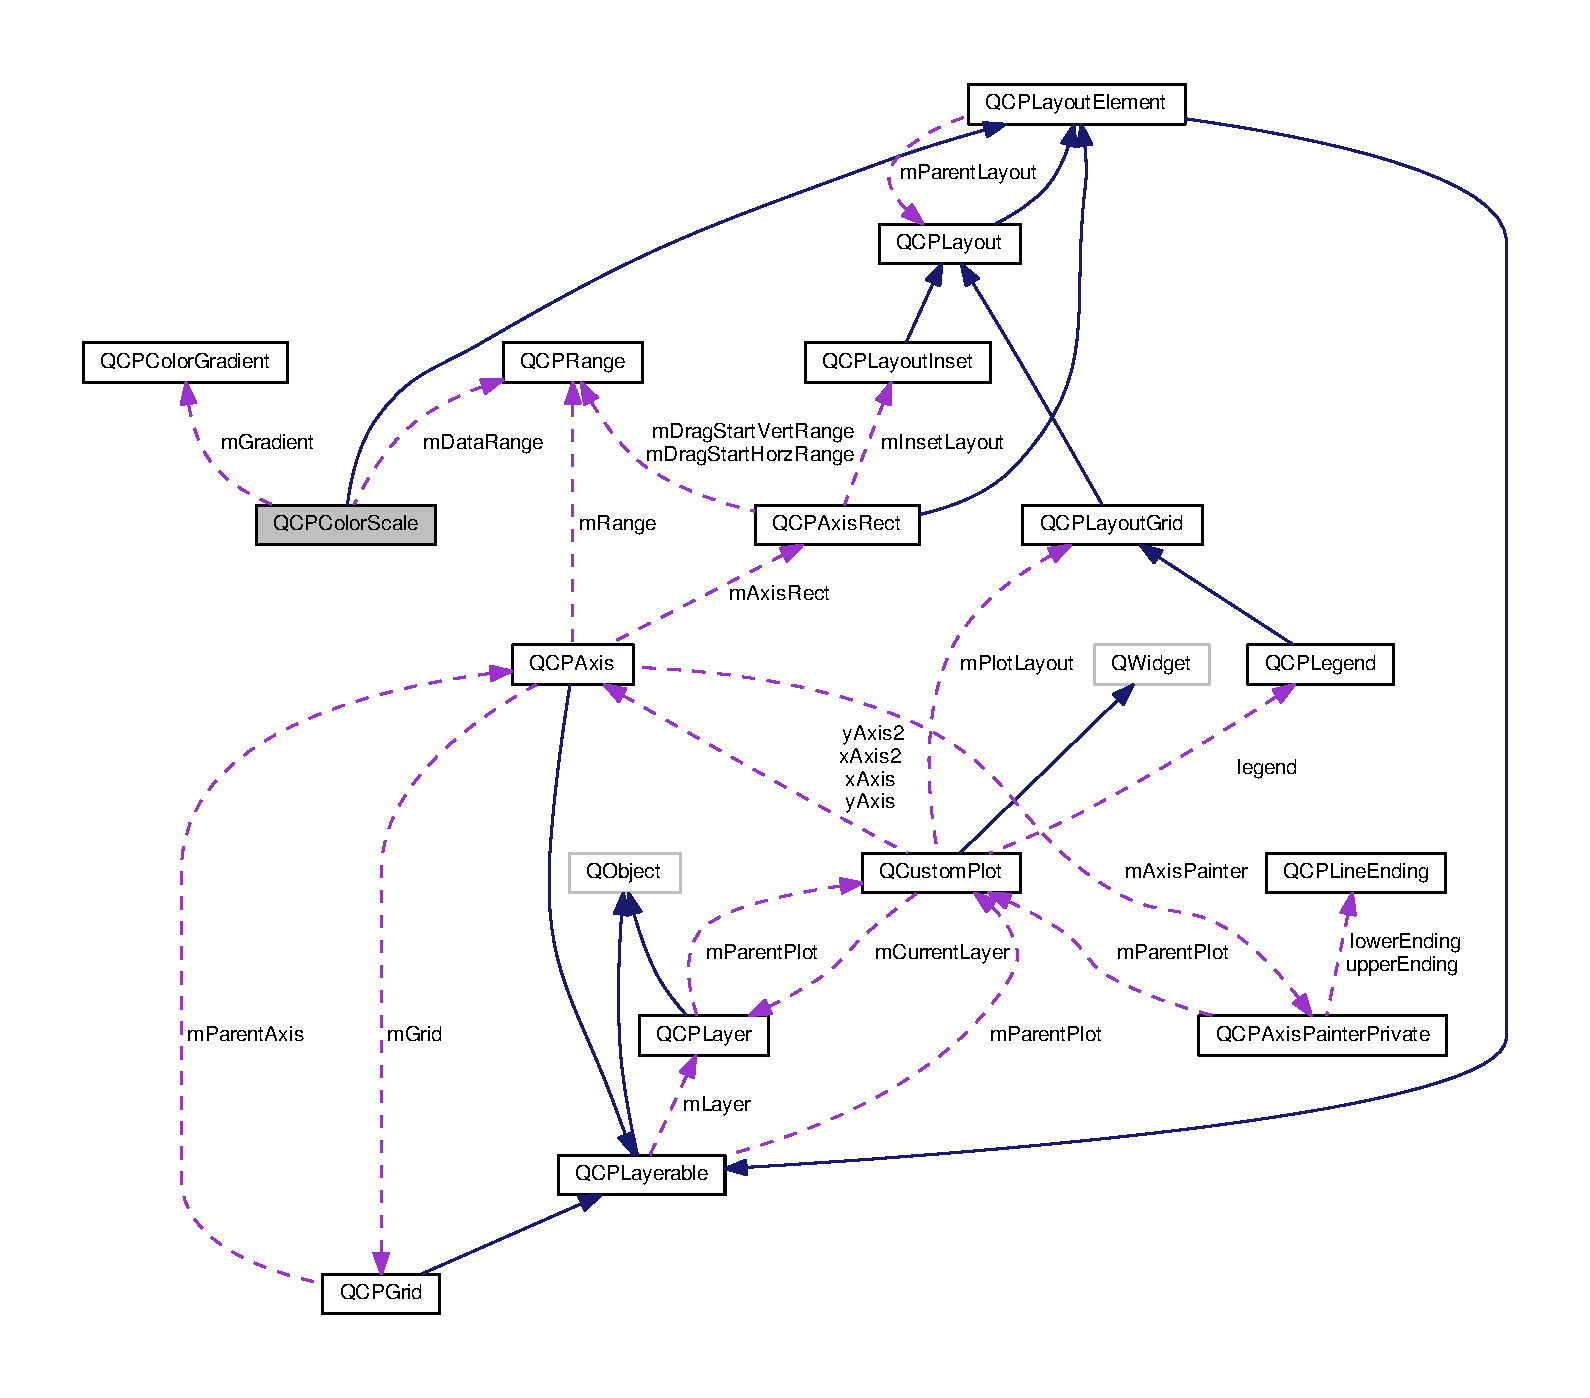
\includegraphics[width=350pt]{classQCPColorScale__coll__graph}
\end{center}
\end{figure}
\subsection*{Signals}
\begin{DoxyCompactItemize}
\item 
void \hyperlink{classQCPColorScale_a293176da9447ec6819be1d901966a257}{data\+Range\+Changed} (\hyperlink{classQCPRange}{Q\+C\+P\+Range} new\+Range)
\item 
void \hyperlink{classQCPColorScale_a61558b962f7791ff2f15a565dcf60181}{data\+Scale\+Type\+Changed} (\hyperlink{classQCPAxis_a36d8e8658dbaa179bf2aeb973db2d6f0}{Q\+C\+P\+Axis\+::\+Scale\+Type} scale\+Type)
\item 
void \hyperlink{classQCPColorScale_a67a5eb06cf551d322885e8635a46378c}{gradient\+Changed} (\hyperlink{classQCPColorGradient}{Q\+C\+P\+Color\+Gradient} new\+Gradient)
\end{DoxyCompactItemize}
\subsection*{Public Member Functions}
\begin{DoxyCompactItemize}
\item 
\hyperlink{classQCPColorScale_aa8debce1be38b54287c04d4f584394b4}{Q\+C\+P\+Color\+Scale} (\hyperlink{classQCustomPlot}{Q\+Custom\+Plot} $\ast$\hyperlink{classQCPLayerable_ab7e0e94461566093d36ffc0f5312b109}{parent\+Plot})
\item 
virtual \hyperlink{classQCPColorScale_a49d8d2d155c15fa315fdc0427194c9ea}{$\sim$\+Q\+C\+P\+Color\+Scale} ()
\item 
\hyperlink{classQCPAxis}{Q\+C\+P\+Axis} $\ast$ \hyperlink{classQCPColorScale_a1205bd67c8a33d5818aac1f6eea016a4}{axis} () const 
\item 
\hyperlink{classQCPAxis_ae2bcc1728b382f10f064612b368bc18a}{Q\+C\+P\+Axis\+::\+Axis\+Type} \hyperlink{classQCPColorScale_a9a5236328c97fbfde01e3d91c4fcce6a}{type} () const 
\item 
\hyperlink{classQCPRange}{Q\+C\+P\+Range} \hyperlink{classQCPColorScale_a52134696d5e04074fff4227d92d96f7b}{data\+Range} () const 
\item 
\hyperlink{classQCPAxis_a36d8e8658dbaa179bf2aeb973db2d6f0}{Q\+C\+P\+Axis\+::\+Scale\+Type} \hyperlink{classQCPColorScale_a9718c004421811be97e683d7f7d7ee61}{data\+Scale\+Type} () const 
\item 
\hyperlink{classQCPColorGradient}{Q\+C\+P\+Color\+Gradient} \hyperlink{classQCPColorScale_ac71a6cd853c97a2dbfd32f67afd399df}{gradient} () const 
\item 
Q\+String \hyperlink{classQCPColorScale_af92a62a6e4401f4c5b5e36cc94351ec9}{label} () const 
\item 
int \hyperlink{classQCPColorScale_a0de546f12105cf8bcb00ce60366d3a3d}{bar\+Width} () const 
\item 
bool \hyperlink{classQCPColorScale_a0d45597064cc40bc8a84d11e870c6b05}{range\+Drag} () const 
\item 
bool \hyperlink{classQCPColorScale_a1123986a10acda3cdc371e4d97b3326c}{range\+Zoom} () const 
\item 
void \hyperlink{classQCPColorScale_a1bf9bdb291927c422dd66b404b206f1f}{set\+Type} (\hyperlink{classQCPAxis_ae2bcc1728b382f10f064612b368bc18a}{Q\+C\+P\+Axis\+::\+Axis\+Type} \hyperlink{classQCPColorScale_a9a5236328c97fbfde01e3d91c4fcce6a}{type})
\item 
Q\+\_\+\+S\+L\+OT void \hyperlink{classQCPColorScale_abe88633003a26d1e756aa74984587fef}{set\+Data\+Range} (const \hyperlink{classQCPRange}{Q\+C\+P\+Range} \&\hyperlink{classQCPColorScale_a52134696d5e04074fff4227d92d96f7b}{data\+Range})
\item 
Q\+\_\+\+S\+L\+OT void \hyperlink{classQCPColorScale_aeb6107d67dd7325145b2498abae67fc3}{set\+Data\+Scale\+Type} (\hyperlink{classQCPAxis_a36d8e8658dbaa179bf2aeb973db2d6f0}{Q\+C\+P\+Axis\+::\+Scale\+Type} scale\+Type)
\item 
Q\+\_\+\+S\+L\+OT void \hyperlink{classQCPColorScale_a1f29583bb6f1e7f473b62fb712be3940}{set\+Gradient} (const \hyperlink{classQCPColorGradient}{Q\+C\+P\+Color\+Gradient} \&\hyperlink{classQCPColorScale_ac71a6cd853c97a2dbfd32f67afd399df}{gradient})
\item 
void \hyperlink{classQCPColorScale_aee124ae8396320cacf8276e9a0fbb8ce}{set\+Label} (const Q\+String \&str)
\item 
void \hyperlink{classQCPColorScale_ab9dcc0c1cd583477496209b1413bcb99}{set\+Bar\+Width} (int width)
\item 
void \hyperlink{classQCPColorScale_a21c51a55e4fd581b6feadca9ee5b38d5}{set\+Range\+Drag} (bool enabled)
\item 
void \hyperlink{classQCPColorScale_a96bd60fb6317ad6821841b539c93eeeb}{set\+Range\+Zoom} (bool enabled)
\item 
Q\+List$<$ \hyperlink{classQCPColorMap}{Q\+C\+P\+Color\+Map} $\ast$ $>$ \hyperlink{classQCPColorScale_a01bb96981614f2556ef7da04531a7a05}{color\+Maps} () const 
\item 
void \hyperlink{classQCPColorScale_a425983db4478543924ddbd04ea20a356}{rescale\+Data\+Range} (bool only\+Visible\+Maps)
\item 
virtual void \hyperlink{classQCPColorScale_ab8f6991ac88243fc582b44b183670334}{update} (\hyperlink{classQCPLayoutElement_a0d83360e05735735aaf6d7983c56374d}{Update\+Phase} phase)
\end{DoxyCompactItemize}
\subsection*{Protected Member Functions}
\begin{DoxyCompactItemize}
\item 
virtual void \hyperlink{classQCPColorScale_a23d530c340c15d2fce6583e7120ee8bd}{apply\+Default\+Antialiasing\+Hint} (\hyperlink{classQCPPainter}{Q\+C\+P\+Painter} $\ast$painter) const 
\item 
virtual void \hyperlink{classQCPColorScale_a5df6ad81b2ad045878d276c2d5be7120}{mouse\+Press\+Event} (Q\+Mouse\+Event $\ast$event)
\item 
virtual void \hyperlink{classQCPColorScale_a3aca469d531ce7b5882de73590aa0de6}{mouse\+Move\+Event} (Q\+Mouse\+Event $\ast$event)
\item 
virtual void \hyperlink{classQCPColorScale_a0916613d20901950fc6d00c6f99fe0a1}{mouse\+Release\+Event} (Q\+Mouse\+Event $\ast$event)
\item 
virtual void \hyperlink{classQCPColorScale_ab398e14c01240f3dc855884fe9e1ee8c}{wheel\+Event} (Q\+Wheel\+Event $\ast$event)
\end{DoxyCompactItemize}
\subsection*{Protected Attributes}
\begin{DoxyCompactItemize}
\item 
\hyperlink{classQCPAxis_ae2bcc1728b382f10f064612b368bc18a}{Q\+C\+P\+Axis\+::\+Axis\+Type} \hyperlink{classQCPColorScale_a7d47ed4ab76f38e50164e9d77fe33789}{m\+Type}
\item 
\hyperlink{classQCPRange}{Q\+C\+P\+Range} \hyperlink{classQCPColorScale_a5d4853feb32cd0077bb2b871687c844b}{m\+Data\+Range}
\item 
\hyperlink{classQCPAxis_a36d8e8658dbaa179bf2aeb973db2d6f0}{Q\+C\+P\+Axis\+::\+Scale\+Type} \hyperlink{classQCPColorScale_a2754d6a78736f64a241e333fbd955372}{m\+Data\+Scale\+Type}
\item 
\hyperlink{classQCPColorGradient}{Q\+C\+P\+Color\+Gradient} \hyperlink{classQCPColorScale_ae195a385032066b5c46cc3301af58922}{m\+Gradient}
\item 
int \hyperlink{classQCPColorScale_a409d2ab78dff1f92da5e6acfb062e811}{m\+Bar\+Width}
\item 
Q\+Pointer$<$ \hyperlink{classQCPColorScaleAxisRectPrivate}{Q\+C\+P\+Color\+Scale\+Axis\+Rect\+Private} $>$ \hyperlink{classQCPColorScale_a6e37f7d49cd614dc50ef1caae60461b9}{m\+Axis\+Rect}
\item 
Q\+Pointer$<$ \hyperlink{classQCPAxis}{Q\+C\+P\+Axis} $>$ \hyperlink{classQCPColorScale_a2efbc90fd31898fe05d2b74a8422b1d5}{m\+Color\+Axis}
\end{DoxyCompactItemize}
\subsection*{Friends}
\begin{DoxyCompactItemize}
\item 
class \hyperlink{classQCPColorScale_a1441d8c09d7227c0c29a8d0a96d55bfe}{Q\+C\+P\+Color\+Scale\+Axis\+Rect\+Private}
\end{DoxyCompactItemize}
\subsection*{Additional Inherited Members}


\subsection{Detailed Description}
A color scale for use with color coding data such as \hyperlink{classQCPColorMap}{Q\+C\+P\+Color\+Map}. 

This layout element can be placed on the plot to correlate a color gradient with data values. It is usually used in combination with one or multiple \hyperlink{classQCPColorMap}{Q\+C\+P\+Color\+Maps}.



The color scale can be either horizontal or vertical, as shown in the image above. The orientation and the side where the numbers appear is controlled with \hyperlink{classQCPColorScale_a1bf9bdb291927c422dd66b404b206f1f}{set\+Type}.

Use \hyperlink{classQCPColorMap_aa828921db364fe3c6af4619580ab85fd}{Q\+C\+P\+Color\+Map\+::set\+Color\+Scale} to connect a color map with a color scale. Once they are connected, they share their gradient, data range and data scale type (\hyperlink{classQCPColorScale_a1f29583bb6f1e7f473b62fb712be3940}{set\+Gradient}, \hyperlink{classQCPColorScale_abe88633003a26d1e756aa74984587fef}{set\+Data\+Range}, \hyperlink{classQCPColorScale_aeb6107d67dd7325145b2498abae67fc3}{set\+Data\+Scale\+Type}). Multiple color maps may be associated with a single color scale, to make them all synchronize these properties.

To have finer control over the number display and axis behaviour, you can directly access the \hyperlink{classQCPColorScale_a1205bd67c8a33d5818aac1f6eea016a4}{axis}. See the documentation of \hyperlink{classQCPAxis}{Q\+C\+P\+Axis} for details about configuring axes. For example, if you want to change the number of automatically generated ticks, call 
\begin{DoxyCodeInclude}
\end{DoxyCodeInclude}
 Placing a color scale next to the main axis rect works like with any other layout element\+: 
\begin{DoxyCodeInclude}
\end{DoxyCodeInclude}
In this case we have placed it to the right of the default axis rect, so it wasn\textquotesingle{}t necessary to call \hyperlink{classQCPColorScale_a1bf9bdb291927c422dd66b404b206f1f}{set\+Type}, since \hyperlink{classQCPAxis_ae2bcc1728b382f10f064612b368bc18aadf5509f7d29199ef2f263b1dd224b345}{Q\+C\+P\+Axis\+::at\+Right} is already the default. The text next to the color scale can be set with \hyperlink{classQCPColorScale_aee124ae8396320cacf8276e9a0fbb8ce}{set\+Label}.

For optimum appearance (like in the image above), it may be desirable to line up the axis rect and the borders of the color scale. Use a \hyperlink{classQCPMarginGroup}{Q\+C\+P\+Margin\+Group} to achieve this\+: 
\begin{DoxyCodeInclude}
\end{DoxyCodeInclude}
 Color scales are initialized with a non-\/zero minimum top and bottom margin (\hyperlink{classQCPLayoutElement_a0a8a17abc16b7923159fcc7608f94673}{set\+Minimum\+Margins}), because vertical color scales are most common and the minimum top/bottom margin makes sure it keeps some distance to the top/bottom widget border. So if you change to a horizontal color scale by setting \hyperlink{classQCPColorScale_a1bf9bdb291927c422dd66b404b206f1f}{set\+Type} to \hyperlink{classQCPAxis_ae2bcc1728b382f10f064612b368bc18aa220d68888516b6c3b493d144f1ba438f}{Q\+C\+P\+Axis\+::at\+Bottom} or \hyperlink{classQCPAxis_ae2bcc1728b382f10f064612b368bc18aac0ece2b680d3f545e701f75af1655977}{Q\+C\+P\+Axis\+::at\+Top}, you might want to also change the minimum margins accordingly, e.\+g. {\ttfamily set\+Minimum\+Margins(\+Q\+Margins(6, 0, 6, 0))}. 

\subsection{Constructor \& Destructor Documentation}
\index{Q\+C\+P\+Color\+Scale@{Q\+C\+P\+Color\+Scale}!Q\+C\+P\+Color\+Scale@{Q\+C\+P\+Color\+Scale}}
\index{Q\+C\+P\+Color\+Scale@{Q\+C\+P\+Color\+Scale}!Q\+C\+P\+Color\+Scale@{Q\+C\+P\+Color\+Scale}}
\subsubsection[{\texorpdfstring{Q\+C\+P\+Color\+Scale(\+Q\+Custom\+Plot $\ast$parent\+Plot)}{QCPColorScale(QCustomPlot *parentPlot)}}]{\setlength{\rightskip}{0pt plus 5cm}Q\+C\+P\+Color\+Scale\+::\+Q\+C\+P\+Color\+Scale (
\begin{DoxyParamCaption}
\item[{{\bf Q\+Custom\+Plot} $\ast$}]{parent\+Plot}
\end{DoxyParamCaption}
)\hspace{0.3cm}{\ttfamily [explicit]}}\hypertarget{classQCPColorScale_aa8debce1be38b54287c04d4f584394b4}{}\label{classQCPColorScale_aa8debce1be38b54287c04d4f584394b4}
Constructs a new \hyperlink{classQCPColorScale}{Q\+C\+P\+Color\+Scale}. \index{Q\+C\+P\+Color\+Scale@{Q\+C\+P\+Color\+Scale}!````~Q\+C\+P\+Color\+Scale@{$\sim$\+Q\+C\+P\+Color\+Scale}}
\index{````~Q\+C\+P\+Color\+Scale@{$\sim$\+Q\+C\+P\+Color\+Scale}!Q\+C\+P\+Color\+Scale@{Q\+C\+P\+Color\+Scale}}
\subsubsection[{\texorpdfstring{$\sim$\+Q\+C\+P\+Color\+Scale()}{~QCPColorScale()}}]{\setlength{\rightskip}{0pt plus 5cm}Q\+C\+P\+Color\+Scale\+::$\sim$\+Q\+C\+P\+Color\+Scale (
\begin{DoxyParamCaption}
{}
\end{DoxyParamCaption}
)\hspace{0.3cm}{\ttfamily [virtual]}}\hypertarget{classQCPColorScale_a49d8d2d155c15fa315fdc0427194c9ea}{}\label{classQCPColorScale_a49d8d2d155c15fa315fdc0427194c9ea}


\subsection{Member Function Documentation}
\index{Q\+C\+P\+Color\+Scale@{Q\+C\+P\+Color\+Scale}!apply\+Default\+Antialiasing\+Hint@{apply\+Default\+Antialiasing\+Hint}}
\index{apply\+Default\+Antialiasing\+Hint@{apply\+Default\+Antialiasing\+Hint}!Q\+C\+P\+Color\+Scale@{Q\+C\+P\+Color\+Scale}}
\subsubsection[{\texorpdfstring{apply\+Default\+Antialiasing\+Hint(\+Q\+C\+P\+Painter $\ast$painter) const }{applyDefaultAntialiasingHint(QCPPainter *painter) const }}]{\setlength{\rightskip}{0pt plus 5cm}void Q\+C\+P\+Color\+Scale\+::apply\+Default\+Antialiasing\+Hint (
\begin{DoxyParamCaption}
\item[{{\bf Q\+C\+P\+Painter} $\ast$}]{painter}
\end{DoxyParamCaption}
) const\hspace{0.3cm}{\ttfamily [protected]}, {\ttfamily [virtual]}}\hypertarget{classQCPColorScale_a23d530c340c15d2fce6583e7120ee8bd}{}\label{classQCPColorScale_a23d530c340c15d2fce6583e7120ee8bd}


Reimplemented from \hyperlink{classQCPLayoutElement_ad6d2b4bb0291c2441b2e1ca3d5296df5}{Q\+C\+P\+Layout\+Element}.

\index{Q\+C\+P\+Color\+Scale@{Q\+C\+P\+Color\+Scale}!axis@{axis}}
\index{axis@{axis}!Q\+C\+P\+Color\+Scale@{Q\+C\+P\+Color\+Scale}}
\subsubsection[{\texorpdfstring{axis() const }{axis() const }}]{\setlength{\rightskip}{0pt plus 5cm}{\bf Q\+C\+P\+Axis} $\ast$ Q\+C\+P\+Color\+Scale\+::axis (
\begin{DoxyParamCaption}
{}
\end{DoxyParamCaption}
) const\hspace{0.3cm}{\ttfamily [inline]}}\hypertarget{classQCPColorScale_a1205bd67c8a33d5818aac1f6eea016a4}{}\label{classQCPColorScale_a1205bd67c8a33d5818aac1f6eea016a4}
Returns the internal \hyperlink{classQCPAxis}{Q\+C\+P\+Axis} instance of this color scale. You can access it to alter the appearance and behaviour of the axis. \hyperlink{classQCPColorScale}{Q\+C\+P\+Color\+Scale} duplicates some properties in its interface for convenience. Those are \hyperlink{classQCPColorScale_abe88633003a26d1e756aa74984587fef}{set\+Data\+Range} (\hyperlink{classQCPAxis_aebdfea5d44c3a0ad2b4700cd4d25b641}{Q\+C\+P\+Axis\+::set\+Range}), \hyperlink{classQCPColorScale_aeb6107d67dd7325145b2498abae67fc3}{set\+Data\+Scale\+Type} (\hyperlink{classQCPAxis_adef29cae617af4f519f6c40d1a866ca6}{Q\+C\+P\+Axis\+::set\+Scale\+Type}), and the method \hyperlink{classQCPColorScale_aee124ae8396320cacf8276e9a0fbb8ce}{set\+Label} (\hyperlink{classQCPAxis_a33bcc382c111c9f31bb0687352a2dea4}{Q\+C\+P\+Axis\+::set\+Label}). As they each are connected, it does not matter whether you use the method on the \hyperlink{classQCPColorScale}{Q\+C\+P\+Color\+Scale} or on its \hyperlink{classQCPAxis}{Q\+C\+P\+Axis}.

If the type of the color scale is changed with \hyperlink{classQCPColorScale_a1bf9bdb291927c422dd66b404b206f1f}{set\+Type}, the axis returned by this method will change, too, to either the left, right, bottom or top axis, depending on which type was set. \index{Q\+C\+P\+Color\+Scale@{Q\+C\+P\+Color\+Scale}!bar\+Width@{bar\+Width}}
\index{bar\+Width@{bar\+Width}!Q\+C\+P\+Color\+Scale@{Q\+C\+P\+Color\+Scale}}
\subsubsection[{\texorpdfstring{bar\+Width() const }{barWidth() const }}]{\setlength{\rightskip}{0pt plus 5cm}int Q\+C\+P\+Color\+Scale\+::bar\+Width (
\begin{DoxyParamCaption}
{}
\end{DoxyParamCaption}
) const\hspace{0.3cm}{\ttfamily [inline]}}\hypertarget{classQCPColorScale_a0de546f12105cf8bcb00ce60366d3a3d}{}\label{classQCPColorScale_a0de546f12105cf8bcb00ce60366d3a3d}
\index{Q\+C\+P\+Color\+Scale@{Q\+C\+P\+Color\+Scale}!color\+Maps@{color\+Maps}}
\index{color\+Maps@{color\+Maps}!Q\+C\+P\+Color\+Scale@{Q\+C\+P\+Color\+Scale}}
\subsubsection[{\texorpdfstring{color\+Maps() const }{colorMaps() const }}]{\setlength{\rightskip}{0pt plus 5cm}Q\+List$<$ {\bf Q\+C\+P\+Color\+Map} $\ast$ $>$ Q\+C\+P\+Color\+Scale\+::color\+Maps (
\begin{DoxyParamCaption}
{}
\end{DoxyParamCaption}
) const}\hypertarget{classQCPColorScale_a01bb96981614f2556ef7da04531a7a05}{}\label{classQCPColorScale_a01bb96981614f2556ef7da04531a7a05}
Returns a list of all the color maps associated with this color scale. \index{Q\+C\+P\+Color\+Scale@{Q\+C\+P\+Color\+Scale}!data\+Range@{data\+Range}}
\index{data\+Range@{data\+Range}!Q\+C\+P\+Color\+Scale@{Q\+C\+P\+Color\+Scale}}
\subsubsection[{\texorpdfstring{data\+Range() const }{dataRange() const }}]{\setlength{\rightskip}{0pt plus 5cm}{\bf Q\+C\+P\+Range} Q\+C\+P\+Color\+Scale\+::data\+Range (
\begin{DoxyParamCaption}
{}
\end{DoxyParamCaption}
) const\hspace{0.3cm}{\ttfamily [inline]}}\hypertarget{classQCPColorScale_a52134696d5e04074fff4227d92d96f7b}{}\label{classQCPColorScale_a52134696d5e04074fff4227d92d96f7b}
\index{Q\+C\+P\+Color\+Scale@{Q\+C\+P\+Color\+Scale}!data\+Range\+Changed@{data\+Range\+Changed}}
\index{data\+Range\+Changed@{data\+Range\+Changed}!Q\+C\+P\+Color\+Scale@{Q\+C\+P\+Color\+Scale}}
\subsubsection[{\texorpdfstring{data\+Range\+Changed}{dataRangeChanged}}]{\setlength{\rightskip}{0pt plus 5cm}void Q\+C\+P\+Color\+Scale\+::data\+Range\+Changed (
\begin{DoxyParamCaption}
\item[{{\bf Q\+C\+P\+Range}}]{new\+Range}
\end{DoxyParamCaption}
)\hspace{0.3cm}{\ttfamily [signal]}}\hypertarget{classQCPColorScale_a293176da9447ec6819be1d901966a257}{}\label{classQCPColorScale_a293176da9447ec6819be1d901966a257}
This signal is emitted when the data range changes.

\begin{DoxySeeAlso}{See also}
\hyperlink{classQCPColorScale_abe88633003a26d1e756aa74984587fef}{set\+Data\+Range} 
\end{DoxySeeAlso}
\index{Q\+C\+P\+Color\+Scale@{Q\+C\+P\+Color\+Scale}!data\+Scale\+Type@{data\+Scale\+Type}}
\index{data\+Scale\+Type@{data\+Scale\+Type}!Q\+C\+P\+Color\+Scale@{Q\+C\+P\+Color\+Scale}}
\subsubsection[{\texorpdfstring{data\+Scale\+Type() const }{dataScaleType() const }}]{\setlength{\rightskip}{0pt plus 5cm}{\bf Q\+C\+P\+Axis\+::\+Scale\+Type} Q\+C\+P\+Color\+Scale\+::data\+Scale\+Type (
\begin{DoxyParamCaption}
{}
\end{DoxyParamCaption}
) const\hspace{0.3cm}{\ttfamily [inline]}}\hypertarget{classQCPColorScale_a9718c004421811be97e683d7f7d7ee61}{}\label{classQCPColorScale_a9718c004421811be97e683d7f7d7ee61}
\index{Q\+C\+P\+Color\+Scale@{Q\+C\+P\+Color\+Scale}!data\+Scale\+Type\+Changed@{data\+Scale\+Type\+Changed}}
\index{data\+Scale\+Type\+Changed@{data\+Scale\+Type\+Changed}!Q\+C\+P\+Color\+Scale@{Q\+C\+P\+Color\+Scale}}
\subsubsection[{\texorpdfstring{data\+Scale\+Type\+Changed}{dataScaleTypeChanged}}]{\setlength{\rightskip}{0pt plus 5cm}void Q\+C\+P\+Color\+Scale\+::data\+Scale\+Type\+Changed (
\begin{DoxyParamCaption}
\item[{{\bf Q\+C\+P\+Axis\+::\+Scale\+Type}}]{scale\+Type}
\end{DoxyParamCaption}
)\hspace{0.3cm}{\ttfamily [signal]}}\hypertarget{classQCPColorScale_a61558b962f7791ff2f15a565dcf60181}{}\label{classQCPColorScale_a61558b962f7791ff2f15a565dcf60181}
This signal is emitted when the data scale type changes.

\begin{DoxySeeAlso}{See also}
\hyperlink{classQCPColorScale_aeb6107d67dd7325145b2498abae67fc3}{set\+Data\+Scale\+Type} 
\end{DoxySeeAlso}
\index{Q\+C\+P\+Color\+Scale@{Q\+C\+P\+Color\+Scale}!gradient@{gradient}}
\index{gradient@{gradient}!Q\+C\+P\+Color\+Scale@{Q\+C\+P\+Color\+Scale}}
\subsubsection[{\texorpdfstring{gradient() const }{gradient() const }}]{\setlength{\rightskip}{0pt plus 5cm}{\bf Q\+C\+P\+Color\+Gradient} Q\+C\+P\+Color\+Scale\+::gradient (
\begin{DoxyParamCaption}
{}
\end{DoxyParamCaption}
) const\hspace{0.3cm}{\ttfamily [inline]}}\hypertarget{classQCPColorScale_ac71a6cd853c97a2dbfd32f67afd399df}{}\label{classQCPColorScale_ac71a6cd853c97a2dbfd32f67afd399df}
\index{Q\+C\+P\+Color\+Scale@{Q\+C\+P\+Color\+Scale}!gradient\+Changed@{gradient\+Changed}}
\index{gradient\+Changed@{gradient\+Changed}!Q\+C\+P\+Color\+Scale@{Q\+C\+P\+Color\+Scale}}
\subsubsection[{\texorpdfstring{gradient\+Changed}{gradientChanged}}]{\setlength{\rightskip}{0pt plus 5cm}void Q\+C\+P\+Color\+Scale\+::gradient\+Changed (
\begin{DoxyParamCaption}
\item[{{\bf Q\+C\+P\+Color\+Gradient}}]{new\+Gradient}
\end{DoxyParamCaption}
)\hspace{0.3cm}{\ttfamily [signal]}}\hypertarget{classQCPColorScale_a67a5eb06cf551d322885e8635a46378c}{}\label{classQCPColorScale_a67a5eb06cf551d322885e8635a46378c}
This signal is emitted when the gradient changes.

\begin{DoxySeeAlso}{See also}
\hyperlink{classQCPColorScale_a1f29583bb6f1e7f473b62fb712be3940}{set\+Gradient} 
\end{DoxySeeAlso}
\index{Q\+C\+P\+Color\+Scale@{Q\+C\+P\+Color\+Scale}!label@{label}}
\index{label@{label}!Q\+C\+P\+Color\+Scale@{Q\+C\+P\+Color\+Scale}}
\subsubsection[{\texorpdfstring{label() const }{label() const }}]{\setlength{\rightskip}{0pt plus 5cm}Q\+String Q\+C\+P\+Color\+Scale\+::label (
\begin{DoxyParamCaption}
{}
\end{DoxyParamCaption}
) const}\hypertarget{classQCPColorScale_af92a62a6e4401f4c5b5e36cc94351ec9}{}\label{classQCPColorScale_af92a62a6e4401f4c5b5e36cc94351ec9}
\index{Q\+C\+P\+Color\+Scale@{Q\+C\+P\+Color\+Scale}!mouse\+Move\+Event@{mouse\+Move\+Event}}
\index{mouse\+Move\+Event@{mouse\+Move\+Event}!Q\+C\+P\+Color\+Scale@{Q\+C\+P\+Color\+Scale}}
\subsubsection[{\texorpdfstring{mouse\+Move\+Event(\+Q\+Mouse\+Event $\ast$event)}{mouseMoveEvent(QMouseEvent *event)}}]{\setlength{\rightskip}{0pt plus 5cm}void Q\+C\+P\+Color\+Scale\+::mouse\+Move\+Event (
\begin{DoxyParamCaption}
\item[{Q\+Mouse\+Event $\ast$}]{event}
\end{DoxyParamCaption}
)\hspace{0.3cm}{\ttfamily [protected]}, {\ttfamily [virtual]}}\hypertarget{classQCPColorScale_a3aca469d531ce7b5882de73590aa0de6}{}\label{classQCPColorScale_a3aca469d531ce7b5882de73590aa0de6}
This event is called, if the mouse is moved inside the outer rect of this layout element. 

Reimplemented from \hyperlink{classQCPLayoutElement_a14f4acf58cdb8dd2c6c571479c4c4a40}{Q\+C\+P\+Layout\+Element}.

\index{Q\+C\+P\+Color\+Scale@{Q\+C\+P\+Color\+Scale}!mouse\+Press\+Event@{mouse\+Press\+Event}}
\index{mouse\+Press\+Event@{mouse\+Press\+Event}!Q\+C\+P\+Color\+Scale@{Q\+C\+P\+Color\+Scale}}
\subsubsection[{\texorpdfstring{mouse\+Press\+Event(\+Q\+Mouse\+Event $\ast$event)}{mousePressEvent(QMouseEvent *event)}}]{\setlength{\rightskip}{0pt plus 5cm}void Q\+C\+P\+Color\+Scale\+::mouse\+Press\+Event (
\begin{DoxyParamCaption}
\item[{Q\+Mouse\+Event $\ast$}]{event}
\end{DoxyParamCaption}
)\hspace{0.3cm}{\ttfamily [protected]}, {\ttfamily [virtual]}}\hypertarget{classQCPColorScale_a5df6ad81b2ad045878d276c2d5be7120}{}\label{classQCPColorScale_a5df6ad81b2ad045878d276c2d5be7120}
This event is called, if the mouse was pressed while being inside the outer rect of this layout element. 

Reimplemented from \hyperlink{classQCPLayoutElement_a2d82ea21fe0ee628f177bd824bc51a71}{Q\+C\+P\+Layout\+Element}.

\index{Q\+C\+P\+Color\+Scale@{Q\+C\+P\+Color\+Scale}!mouse\+Release\+Event@{mouse\+Release\+Event}}
\index{mouse\+Release\+Event@{mouse\+Release\+Event}!Q\+C\+P\+Color\+Scale@{Q\+C\+P\+Color\+Scale}}
\subsubsection[{\texorpdfstring{mouse\+Release\+Event(\+Q\+Mouse\+Event $\ast$event)}{mouseReleaseEvent(QMouseEvent *event)}}]{\setlength{\rightskip}{0pt plus 5cm}void Q\+C\+P\+Color\+Scale\+::mouse\+Release\+Event (
\begin{DoxyParamCaption}
\item[{Q\+Mouse\+Event $\ast$}]{event}
\end{DoxyParamCaption}
)\hspace{0.3cm}{\ttfamily [protected]}, {\ttfamily [virtual]}}\hypertarget{classQCPColorScale_a0916613d20901950fc6d00c6f99fe0a1}{}\label{classQCPColorScale_a0916613d20901950fc6d00c6f99fe0a1}
This event is called, if the mouse was previously pressed inside the outer rect of this layout element and is now released. 

Reimplemented from \hyperlink{classQCPLayoutElement_ae526ac828cce1e5bb94eaa85776d7404}{Q\+C\+P\+Layout\+Element}.

\index{Q\+C\+P\+Color\+Scale@{Q\+C\+P\+Color\+Scale}!range\+Drag@{range\+Drag}}
\index{range\+Drag@{range\+Drag}!Q\+C\+P\+Color\+Scale@{Q\+C\+P\+Color\+Scale}}
\subsubsection[{\texorpdfstring{range\+Drag() const }{rangeDrag() const }}]{\setlength{\rightskip}{0pt plus 5cm}bool Q\+C\+P\+Color\+Scale\+::range\+Drag (
\begin{DoxyParamCaption}
{}
\end{DoxyParamCaption}
) const}\hypertarget{classQCPColorScale_a0d45597064cc40bc8a84d11e870c6b05}{}\label{classQCPColorScale_a0d45597064cc40bc8a84d11e870c6b05}
\index{Q\+C\+P\+Color\+Scale@{Q\+C\+P\+Color\+Scale}!range\+Zoom@{range\+Zoom}}
\index{range\+Zoom@{range\+Zoom}!Q\+C\+P\+Color\+Scale@{Q\+C\+P\+Color\+Scale}}
\subsubsection[{\texorpdfstring{range\+Zoom() const }{rangeZoom() const }}]{\setlength{\rightskip}{0pt plus 5cm}bool Q\+C\+P\+Color\+Scale\+::range\+Zoom (
\begin{DoxyParamCaption}
{}
\end{DoxyParamCaption}
) const}\hypertarget{classQCPColorScale_a1123986a10acda3cdc371e4d97b3326c}{}\label{classQCPColorScale_a1123986a10acda3cdc371e4d97b3326c}
\index{Q\+C\+P\+Color\+Scale@{Q\+C\+P\+Color\+Scale}!rescale\+Data\+Range@{rescale\+Data\+Range}}
\index{rescale\+Data\+Range@{rescale\+Data\+Range}!Q\+C\+P\+Color\+Scale@{Q\+C\+P\+Color\+Scale}}
\subsubsection[{\texorpdfstring{rescale\+Data\+Range(bool only\+Visible\+Maps)}{rescaleDataRange(bool onlyVisibleMaps)}}]{\setlength{\rightskip}{0pt plus 5cm}void Q\+C\+P\+Color\+Scale\+::rescale\+Data\+Range (
\begin{DoxyParamCaption}
\item[{bool}]{only\+Visible\+Maps}
\end{DoxyParamCaption}
)}\hypertarget{classQCPColorScale_a425983db4478543924ddbd04ea20a356}{}\label{classQCPColorScale_a425983db4478543924ddbd04ea20a356}
Changes the data range such that all color maps associated with this color scale are fully mapped to the gradient in the data dimension.

\begin{DoxySeeAlso}{See also}
\hyperlink{classQCPColorScale_abe88633003a26d1e756aa74984587fef}{set\+Data\+Range} 
\end{DoxySeeAlso}
\index{Q\+C\+P\+Color\+Scale@{Q\+C\+P\+Color\+Scale}!set\+Bar\+Width@{set\+Bar\+Width}}
\index{set\+Bar\+Width@{set\+Bar\+Width}!Q\+C\+P\+Color\+Scale@{Q\+C\+P\+Color\+Scale}}
\subsubsection[{\texorpdfstring{set\+Bar\+Width(int width)}{setBarWidth(int width)}}]{\setlength{\rightskip}{0pt plus 5cm}void Q\+C\+P\+Color\+Scale\+::set\+Bar\+Width (
\begin{DoxyParamCaption}
\item[{int}]{width}
\end{DoxyParamCaption}
)}\hypertarget{classQCPColorScale_ab9dcc0c1cd583477496209b1413bcb99}{}\label{classQCPColorScale_ab9dcc0c1cd583477496209b1413bcb99}
Sets the width (or height, for horizontal color scales) the bar where the gradient is displayed will have. \index{Q\+C\+P\+Color\+Scale@{Q\+C\+P\+Color\+Scale}!set\+Data\+Range@{set\+Data\+Range}}
\index{set\+Data\+Range@{set\+Data\+Range}!Q\+C\+P\+Color\+Scale@{Q\+C\+P\+Color\+Scale}}
\subsubsection[{\texorpdfstring{set\+Data\+Range(const Q\+C\+P\+Range \&data\+Range)}{setDataRange(const QCPRange &dataRange)}}]{\setlength{\rightskip}{0pt plus 5cm}void Q\+C\+P\+Color\+Scale\+::set\+Data\+Range (
\begin{DoxyParamCaption}
\item[{const {\bf Q\+C\+P\+Range} \&}]{data\+Range}
\end{DoxyParamCaption}
)}\hypertarget{classQCPColorScale_abe88633003a26d1e756aa74984587fef}{}\label{classQCPColorScale_abe88633003a26d1e756aa74984587fef}
Sets the range spanned by the color gradient and that is shown by the axis in the color scale.

It is equivalent to calling \hyperlink{classQCPColorMap_a980b42837821159786a85b4b7dcb8774}{Q\+C\+P\+Color\+Map\+::set\+Data\+Range} on any of the connected color maps. It is also equivalent to directly accessing the \hyperlink{classQCPColorScale_a1205bd67c8a33d5818aac1f6eea016a4}{axis} and setting its range with \hyperlink{classQCPAxis_aebdfea5d44c3a0ad2b4700cd4d25b641}{Q\+C\+P\+Axis\+::set\+Range}.

\begin{DoxySeeAlso}{See also}
\hyperlink{classQCPColorScale_aeb6107d67dd7325145b2498abae67fc3}{set\+Data\+Scale\+Type}, \hyperlink{classQCPColorScale_a1f29583bb6f1e7f473b62fb712be3940}{set\+Gradient}, \hyperlink{classQCPColorScale_a425983db4478543924ddbd04ea20a356}{rescale\+Data\+Range} 
\end{DoxySeeAlso}
\index{Q\+C\+P\+Color\+Scale@{Q\+C\+P\+Color\+Scale}!set\+Data\+Scale\+Type@{set\+Data\+Scale\+Type}}
\index{set\+Data\+Scale\+Type@{set\+Data\+Scale\+Type}!Q\+C\+P\+Color\+Scale@{Q\+C\+P\+Color\+Scale}}
\subsubsection[{\texorpdfstring{set\+Data\+Scale\+Type(\+Q\+C\+P\+Axis\+::\+Scale\+Type scale\+Type)}{setDataScaleType(QCPAxis::ScaleType scaleType)}}]{\setlength{\rightskip}{0pt plus 5cm}void Q\+C\+P\+Color\+Scale\+::set\+Data\+Scale\+Type (
\begin{DoxyParamCaption}
\item[{{\bf Q\+C\+P\+Axis\+::\+Scale\+Type}}]{scale\+Type}
\end{DoxyParamCaption}
)}\hypertarget{classQCPColorScale_aeb6107d67dd7325145b2498abae67fc3}{}\label{classQCPColorScale_aeb6107d67dd7325145b2498abae67fc3}
Sets the scale type of the color scale, i.\+e. whether values are linearly associated with colors or logarithmically.

It is equivalent to calling \hyperlink{classQCPColorMap_a9d20aa08e3c1f20f22908c45b9c06511}{Q\+C\+P\+Color\+Map\+::set\+Data\+Scale\+Type} on any of the connected color maps. It is also equivalent to directly accessing the \hyperlink{classQCPColorScale_a1205bd67c8a33d5818aac1f6eea016a4}{axis} and setting its scale type with \hyperlink{classQCPAxis_adef29cae617af4f519f6c40d1a866ca6}{Q\+C\+P\+Axis\+::set\+Scale\+Type}.

\begin{DoxySeeAlso}{See also}
\hyperlink{classQCPColorScale_abe88633003a26d1e756aa74984587fef}{set\+Data\+Range}, \hyperlink{classQCPColorScale_a1f29583bb6f1e7f473b62fb712be3940}{set\+Gradient} 
\end{DoxySeeAlso}
\index{Q\+C\+P\+Color\+Scale@{Q\+C\+P\+Color\+Scale}!set\+Gradient@{set\+Gradient}}
\index{set\+Gradient@{set\+Gradient}!Q\+C\+P\+Color\+Scale@{Q\+C\+P\+Color\+Scale}}
\subsubsection[{\texorpdfstring{set\+Gradient(const Q\+C\+P\+Color\+Gradient \&gradient)}{setGradient(const QCPColorGradient &gradient)}}]{\setlength{\rightskip}{0pt plus 5cm}void Q\+C\+P\+Color\+Scale\+::set\+Gradient (
\begin{DoxyParamCaption}
\item[{const {\bf Q\+C\+P\+Color\+Gradient} \&}]{gradient}
\end{DoxyParamCaption}
)}\hypertarget{classQCPColorScale_a1f29583bb6f1e7f473b62fb712be3940}{}\label{classQCPColorScale_a1f29583bb6f1e7f473b62fb712be3940}
Sets the color gradient that will be used to represent data values.

It is equivalent to calling \hyperlink{classQCPColorMap_a7313c78360471cead3576341a2c50377}{Q\+C\+P\+Color\+Map\+::set\+Gradient} on any of the connected color maps.

\begin{DoxySeeAlso}{See also}
\hyperlink{classQCPColorScale_abe88633003a26d1e756aa74984587fef}{set\+Data\+Range}, \hyperlink{classQCPColorScale_aeb6107d67dd7325145b2498abae67fc3}{set\+Data\+Scale\+Type} 
\end{DoxySeeAlso}
\index{Q\+C\+P\+Color\+Scale@{Q\+C\+P\+Color\+Scale}!set\+Label@{set\+Label}}
\index{set\+Label@{set\+Label}!Q\+C\+P\+Color\+Scale@{Q\+C\+P\+Color\+Scale}}
\subsubsection[{\texorpdfstring{set\+Label(const Q\+String \&str)}{setLabel(const QString &str)}}]{\setlength{\rightskip}{0pt plus 5cm}void Q\+C\+P\+Color\+Scale\+::set\+Label (
\begin{DoxyParamCaption}
\item[{const Q\+String \&}]{str}
\end{DoxyParamCaption}
)}\hypertarget{classQCPColorScale_aee124ae8396320cacf8276e9a0fbb8ce}{}\label{classQCPColorScale_aee124ae8396320cacf8276e9a0fbb8ce}
Sets the axis label of the color scale. This is equivalent to calling \hyperlink{classQCPAxis_a33bcc382c111c9f31bb0687352a2dea4}{Q\+C\+P\+Axis\+::set\+Label} on the internal \hyperlink{classQCPColorScale_a1205bd67c8a33d5818aac1f6eea016a4}{axis}. \index{Q\+C\+P\+Color\+Scale@{Q\+C\+P\+Color\+Scale}!set\+Range\+Drag@{set\+Range\+Drag}}
\index{set\+Range\+Drag@{set\+Range\+Drag}!Q\+C\+P\+Color\+Scale@{Q\+C\+P\+Color\+Scale}}
\subsubsection[{\texorpdfstring{set\+Range\+Drag(bool enabled)}{setRangeDrag(bool enabled)}}]{\setlength{\rightskip}{0pt plus 5cm}void Q\+C\+P\+Color\+Scale\+::set\+Range\+Drag (
\begin{DoxyParamCaption}
\item[{bool}]{enabled}
\end{DoxyParamCaption}
)}\hypertarget{classQCPColorScale_a21c51a55e4fd581b6feadca9ee5b38d5}{}\label{classQCPColorScale_a21c51a55e4fd581b6feadca9ee5b38d5}
Sets whether the user can drag the data range (\hyperlink{classQCPColorScale_abe88633003a26d1e756aa74984587fef}{set\+Data\+Range}).

Note that \hyperlink{namespaceQCP_a2ad6bb6281c7c2d593d4277b44c2b037a2c4432b9aceafb94000be8d1b589ef18}{Q\+C\+P\+::i\+Range\+Drag} must be in the \hyperlink{classQCustomPlot}{Q\+Custom\+Plot}\textquotesingle{}s interactions (\hyperlink{classQCustomPlot_a5ee1e2f6ae27419deca53e75907c27e5}{Q\+Custom\+Plot\+::set\+Interactions}) to allow range dragging. \index{Q\+C\+P\+Color\+Scale@{Q\+C\+P\+Color\+Scale}!set\+Range\+Zoom@{set\+Range\+Zoom}}
\index{set\+Range\+Zoom@{set\+Range\+Zoom}!Q\+C\+P\+Color\+Scale@{Q\+C\+P\+Color\+Scale}}
\subsubsection[{\texorpdfstring{set\+Range\+Zoom(bool enabled)}{setRangeZoom(bool enabled)}}]{\setlength{\rightskip}{0pt plus 5cm}void Q\+C\+P\+Color\+Scale\+::set\+Range\+Zoom (
\begin{DoxyParamCaption}
\item[{bool}]{enabled}
\end{DoxyParamCaption}
)}\hypertarget{classQCPColorScale_a96bd60fb6317ad6821841b539c93eeeb}{}\label{classQCPColorScale_a96bd60fb6317ad6821841b539c93eeeb}
Sets whether the user can zoom the data range (\hyperlink{classQCPColorScale_abe88633003a26d1e756aa74984587fef}{set\+Data\+Range}) by scrolling the mouse wheel.

Note that \hyperlink{namespaceQCP_a2ad6bb6281c7c2d593d4277b44c2b037abee1e94353525a636aeaf0ba32b72e14}{Q\+C\+P\+::i\+Range\+Zoom} must be in the \hyperlink{classQCustomPlot}{Q\+Custom\+Plot}\textquotesingle{}s interactions (\hyperlink{classQCustomPlot_a5ee1e2f6ae27419deca53e75907c27e5}{Q\+Custom\+Plot\+::set\+Interactions}) to allow range dragging. \index{Q\+C\+P\+Color\+Scale@{Q\+C\+P\+Color\+Scale}!set\+Type@{set\+Type}}
\index{set\+Type@{set\+Type}!Q\+C\+P\+Color\+Scale@{Q\+C\+P\+Color\+Scale}}
\subsubsection[{\texorpdfstring{set\+Type(\+Q\+C\+P\+Axis\+::\+Axis\+Type type)}{setType(QCPAxis::AxisType type)}}]{\setlength{\rightskip}{0pt plus 5cm}void Q\+C\+P\+Color\+Scale\+::set\+Type (
\begin{DoxyParamCaption}
\item[{{\bf Q\+C\+P\+Axis\+::\+Axis\+Type}}]{type}
\end{DoxyParamCaption}
)}\hypertarget{classQCPColorScale_a1bf9bdb291927c422dd66b404b206f1f}{}\label{classQCPColorScale_a1bf9bdb291927c422dd66b404b206f1f}
Sets at which side of the color scale the axis is placed, and thus also its orientation.

Note that after setting {\itshape type} to a different value, the axis returned by \hyperlink{classQCPColorScale_a1205bd67c8a33d5818aac1f6eea016a4}{axis()} will be a different one. The new axis will adopt the following properties from the previous axis\+: The range, scale type, log base and label. \index{Q\+C\+P\+Color\+Scale@{Q\+C\+P\+Color\+Scale}!type@{type}}
\index{type@{type}!Q\+C\+P\+Color\+Scale@{Q\+C\+P\+Color\+Scale}}
\subsubsection[{\texorpdfstring{type() const }{type() const }}]{\setlength{\rightskip}{0pt plus 5cm}{\bf Q\+C\+P\+Axis\+::\+Axis\+Type} Q\+C\+P\+Color\+Scale\+::type (
\begin{DoxyParamCaption}
{}
\end{DoxyParamCaption}
) const\hspace{0.3cm}{\ttfamily [inline]}}\hypertarget{classQCPColorScale_a9a5236328c97fbfde01e3d91c4fcce6a}{}\label{classQCPColorScale_a9a5236328c97fbfde01e3d91c4fcce6a}
\index{Q\+C\+P\+Color\+Scale@{Q\+C\+P\+Color\+Scale}!update@{update}}
\index{update@{update}!Q\+C\+P\+Color\+Scale@{Q\+C\+P\+Color\+Scale}}
\subsubsection[{\texorpdfstring{update(\+Update\+Phase phase)}{update(UpdatePhase phase)}}]{\setlength{\rightskip}{0pt plus 5cm}void Q\+C\+P\+Color\+Scale\+::update (
\begin{DoxyParamCaption}
\item[{{\bf Update\+Phase}}]{phase}
\end{DoxyParamCaption}
)\hspace{0.3cm}{\ttfamily [virtual]}}\hypertarget{classQCPColorScale_ab8f6991ac88243fc582b44b183670334}{}\label{classQCPColorScale_ab8f6991ac88243fc582b44b183670334}
Updates the layout element and sub-\/elements. This function is automatically called before every replot by the parent layout element. It is called multiple times, once for every \hyperlink{classQCPLayoutElement_a0d83360e05735735aaf6d7983c56374d}{Update\+Phase}. The phases are run through in the order of the enum values. For details about what happens at the different phases, see the documentation of \hyperlink{classQCPLayoutElement_a0d83360e05735735aaf6d7983c56374d}{Update\+Phase}.

Layout elements that have child elements should call the \hyperlink{classQCPColorScale_ab8f6991ac88243fc582b44b183670334}{update} method of their child elements, and pass the current {\itshape phase} unchanged.

The default implementation executes the automatic margin mechanism in the \hyperlink{classQCPLayoutElement_a0d83360e05735735aaf6d7983c56374da288cb59a92280e47261a341f2813e676}{up\+Margins} phase. Subclasses should make sure to call the base class implementation. 

Reimplemented from \hyperlink{classQCPLayoutElement_a929c2ec62e0e0e1d8418eaa802e2af9b}{Q\+C\+P\+Layout\+Element}.

\index{Q\+C\+P\+Color\+Scale@{Q\+C\+P\+Color\+Scale}!wheel\+Event@{wheel\+Event}}
\index{wheel\+Event@{wheel\+Event}!Q\+C\+P\+Color\+Scale@{Q\+C\+P\+Color\+Scale}}
\subsubsection[{\texorpdfstring{wheel\+Event(\+Q\+Wheel\+Event $\ast$event)}{wheelEvent(QWheelEvent *event)}}]{\setlength{\rightskip}{0pt plus 5cm}void Q\+C\+P\+Color\+Scale\+::wheel\+Event (
\begin{DoxyParamCaption}
\item[{Q\+Wheel\+Event $\ast$}]{event}
\end{DoxyParamCaption}
)\hspace{0.3cm}{\ttfamily [protected]}, {\ttfamily [virtual]}}\hypertarget{classQCPColorScale_ab398e14c01240f3dc855884fe9e1ee8c}{}\label{classQCPColorScale_ab398e14c01240f3dc855884fe9e1ee8c}
This event is called, if the mouse wheel is scrolled while the cursor is inside the rect of this layout element. 

Reimplemented from \hyperlink{classQCPLayoutElement_a300521d2fd18a893c1b85f6be11ce2bf}{Q\+C\+P\+Layout\+Element}.



\subsection{Friends And Related Function Documentation}
\index{Q\+C\+P\+Color\+Scale@{Q\+C\+P\+Color\+Scale}!Q\+C\+P\+Color\+Scale\+Axis\+Rect\+Private@{Q\+C\+P\+Color\+Scale\+Axis\+Rect\+Private}}
\index{Q\+C\+P\+Color\+Scale\+Axis\+Rect\+Private@{Q\+C\+P\+Color\+Scale\+Axis\+Rect\+Private}!Q\+C\+P\+Color\+Scale@{Q\+C\+P\+Color\+Scale}}
\subsubsection[{\texorpdfstring{Q\+C\+P\+Color\+Scale\+Axis\+Rect\+Private}{QCPColorScaleAxisRectPrivate}}]{\setlength{\rightskip}{0pt plus 5cm}friend class {\bf Q\+C\+P\+Color\+Scale\+Axis\+Rect\+Private}\hspace{0.3cm}{\ttfamily [friend]}}\hypertarget{classQCPColorScale_a1441d8c09d7227c0c29a8d0a96d55bfe}{}\label{classQCPColorScale_a1441d8c09d7227c0c29a8d0a96d55bfe}


\subsection{Member Data Documentation}
\index{Q\+C\+P\+Color\+Scale@{Q\+C\+P\+Color\+Scale}!m\+Axis\+Rect@{m\+Axis\+Rect}}
\index{m\+Axis\+Rect@{m\+Axis\+Rect}!Q\+C\+P\+Color\+Scale@{Q\+C\+P\+Color\+Scale}}
\subsubsection[{\texorpdfstring{m\+Axis\+Rect}{mAxisRect}}]{\setlength{\rightskip}{0pt plus 5cm}Q\+Pointer$<${\bf Q\+C\+P\+Color\+Scale\+Axis\+Rect\+Private}$>$ Q\+C\+P\+Color\+Scale\+::m\+Axis\+Rect\hspace{0.3cm}{\ttfamily [protected]}}\hypertarget{classQCPColorScale_a6e37f7d49cd614dc50ef1caae60461b9}{}\label{classQCPColorScale_a6e37f7d49cd614dc50ef1caae60461b9}
\index{Q\+C\+P\+Color\+Scale@{Q\+C\+P\+Color\+Scale}!m\+Bar\+Width@{m\+Bar\+Width}}
\index{m\+Bar\+Width@{m\+Bar\+Width}!Q\+C\+P\+Color\+Scale@{Q\+C\+P\+Color\+Scale}}
\subsubsection[{\texorpdfstring{m\+Bar\+Width}{mBarWidth}}]{\setlength{\rightskip}{0pt plus 5cm}int Q\+C\+P\+Color\+Scale\+::m\+Bar\+Width\hspace{0.3cm}{\ttfamily [protected]}}\hypertarget{classQCPColorScale_a409d2ab78dff1f92da5e6acfb062e811}{}\label{classQCPColorScale_a409d2ab78dff1f92da5e6acfb062e811}
\index{Q\+C\+P\+Color\+Scale@{Q\+C\+P\+Color\+Scale}!m\+Color\+Axis@{m\+Color\+Axis}}
\index{m\+Color\+Axis@{m\+Color\+Axis}!Q\+C\+P\+Color\+Scale@{Q\+C\+P\+Color\+Scale}}
\subsubsection[{\texorpdfstring{m\+Color\+Axis}{mColorAxis}}]{\setlength{\rightskip}{0pt plus 5cm}Q\+Pointer$<${\bf Q\+C\+P\+Axis}$>$ Q\+C\+P\+Color\+Scale\+::m\+Color\+Axis\hspace{0.3cm}{\ttfamily [protected]}}\hypertarget{classQCPColorScale_a2efbc90fd31898fe05d2b74a8422b1d5}{}\label{classQCPColorScale_a2efbc90fd31898fe05d2b74a8422b1d5}
\index{Q\+C\+P\+Color\+Scale@{Q\+C\+P\+Color\+Scale}!m\+Data\+Range@{m\+Data\+Range}}
\index{m\+Data\+Range@{m\+Data\+Range}!Q\+C\+P\+Color\+Scale@{Q\+C\+P\+Color\+Scale}}
\subsubsection[{\texorpdfstring{m\+Data\+Range}{mDataRange}}]{\setlength{\rightskip}{0pt plus 5cm}{\bf Q\+C\+P\+Range} Q\+C\+P\+Color\+Scale\+::m\+Data\+Range\hspace{0.3cm}{\ttfamily [protected]}}\hypertarget{classQCPColorScale_a5d4853feb32cd0077bb2b871687c844b}{}\label{classQCPColorScale_a5d4853feb32cd0077bb2b871687c844b}
\index{Q\+C\+P\+Color\+Scale@{Q\+C\+P\+Color\+Scale}!m\+Data\+Scale\+Type@{m\+Data\+Scale\+Type}}
\index{m\+Data\+Scale\+Type@{m\+Data\+Scale\+Type}!Q\+C\+P\+Color\+Scale@{Q\+C\+P\+Color\+Scale}}
\subsubsection[{\texorpdfstring{m\+Data\+Scale\+Type}{mDataScaleType}}]{\setlength{\rightskip}{0pt plus 5cm}{\bf Q\+C\+P\+Axis\+::\+Scale\+Type} Q\+C\+P\+Color\+Scale\+::m\+Data\+Scale\+Type\hspace{0.3cm}{\ttfamily [protected]}}\hypertarget{classQCPColorScale_a2754d6a78736f64a241e333fbd955372}{}\label{classQCPColorScale_a2754d6a78736f64a241e333fbd955372}
\index{Q\+C\+P\+Color\+Scale@{Q\+C\+P\+Color\+Scale}!m\+Gradient@{m\+Gradient}}
\index{m\+Gradient@{m\+Gradient}!Q\+C\+P\+Color\+Scale@{Q\+C\+P\+Color\+Scale}}
\subsubsection[{\texorpdfstring{m\+Gradient}{mGradient}}]{\setlength{\rightskip}{0pt plus 5cm}{\bf Q\+C\+P\+Color\+Gradient} Q\+C\+P\+Color\+Scale\+::m\+Gradient\hspace{0.3cm}{\ttfamily [protected]}}\hypertarget{classQCPColorScale_ae195a385032066b5c46cc3301af58922}{}\label{classQCPColorScale_ae195a385032066b5c46cc3301af58922}
\index{Q\+C\+P\+Color\+Scale@{Q\+C\+P\+Color\+Scale}!m\+Type@{m\+Type}}
\index{m\+Type@{m\+Type}!Q\+C\+P\+Color\+Scale@{Q\+C\+P\+Color\+Scale}}
\subsubsection[{\texorpdfstring{m\+Type}{mType}}]{\setlength{\rightskip}{0pt plus 5cm}{\bf Q\+C\+P\+Axis\+::\+Axis\+Type} Q\+C\+P\+Color\+Scale\+::m\+Type\hspace{0.3cm}{\ttfamily [protected]}}\hypertarget{classQCPColorScale_a7d47ed4ab76f38e50164e9d77fe33789}{}\label{classQCPColorScale_a7d47ed4ab76f38e50164e9d77fe33789}


The documentation for this class was generated from the following files\+:\begin{DoxyCompactItemize}
\item 
src/hammerhead/tools/watchdog/include/watchdog/\hyperlink{qcustomplot_8h}{qcustomplot.\+h}\item 
src/hammerhead/tools/watchdog/src/\hyperlink{qcustomplot_8cpp}{qcustomplot.\+cpp}\end{DoxyCompactItemize}

\hypertarget{classQCPColorScaleAxisRectPrivate}{}\section{Q\+C\+P\+Color\+Scale\+Axis\+Rect\+Private Class Reference}
\label{classQCPColorScaleAxisRectPrivate}\index{Q\+C\+P\+Color\+Scale\+Axis\+Rect\+Private@{Q\+C\+P\+Color\+Scale\+Axis\+Rect\+Private}}


{\ttfamily \#include $<$qcustomplot.\+h$>$}



Inheritance diagram for Q\+C\+P\+Color\+Scale\+Axis\+Rect\+Private\+:\nopagebreak
\begin{figure}[H]
\begin{center}
\leavevmode
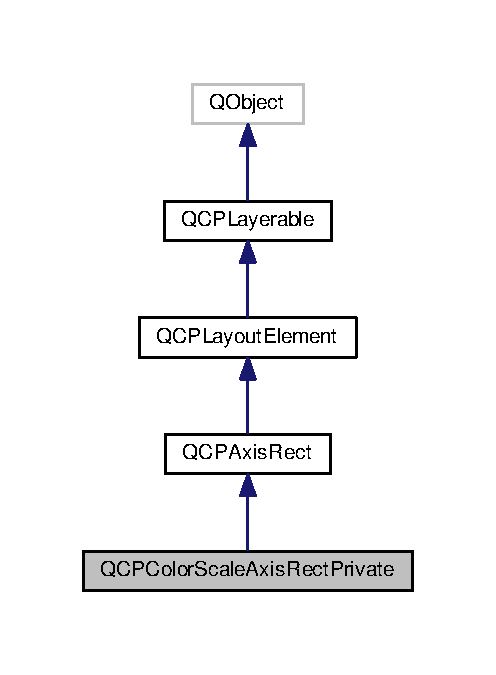
\includegraphics[width=238pt]{classQCPColorScaleAxisRectPrivate__inherit__graph}
\end{center}
\end{figure}


Collaboration diagram for Q\+C\+P\+Color\+Scale\+Axis\+Rect\+Private\+:\nopagebreak
\begin{figure}[H]
\begin{center}
\leavevmode
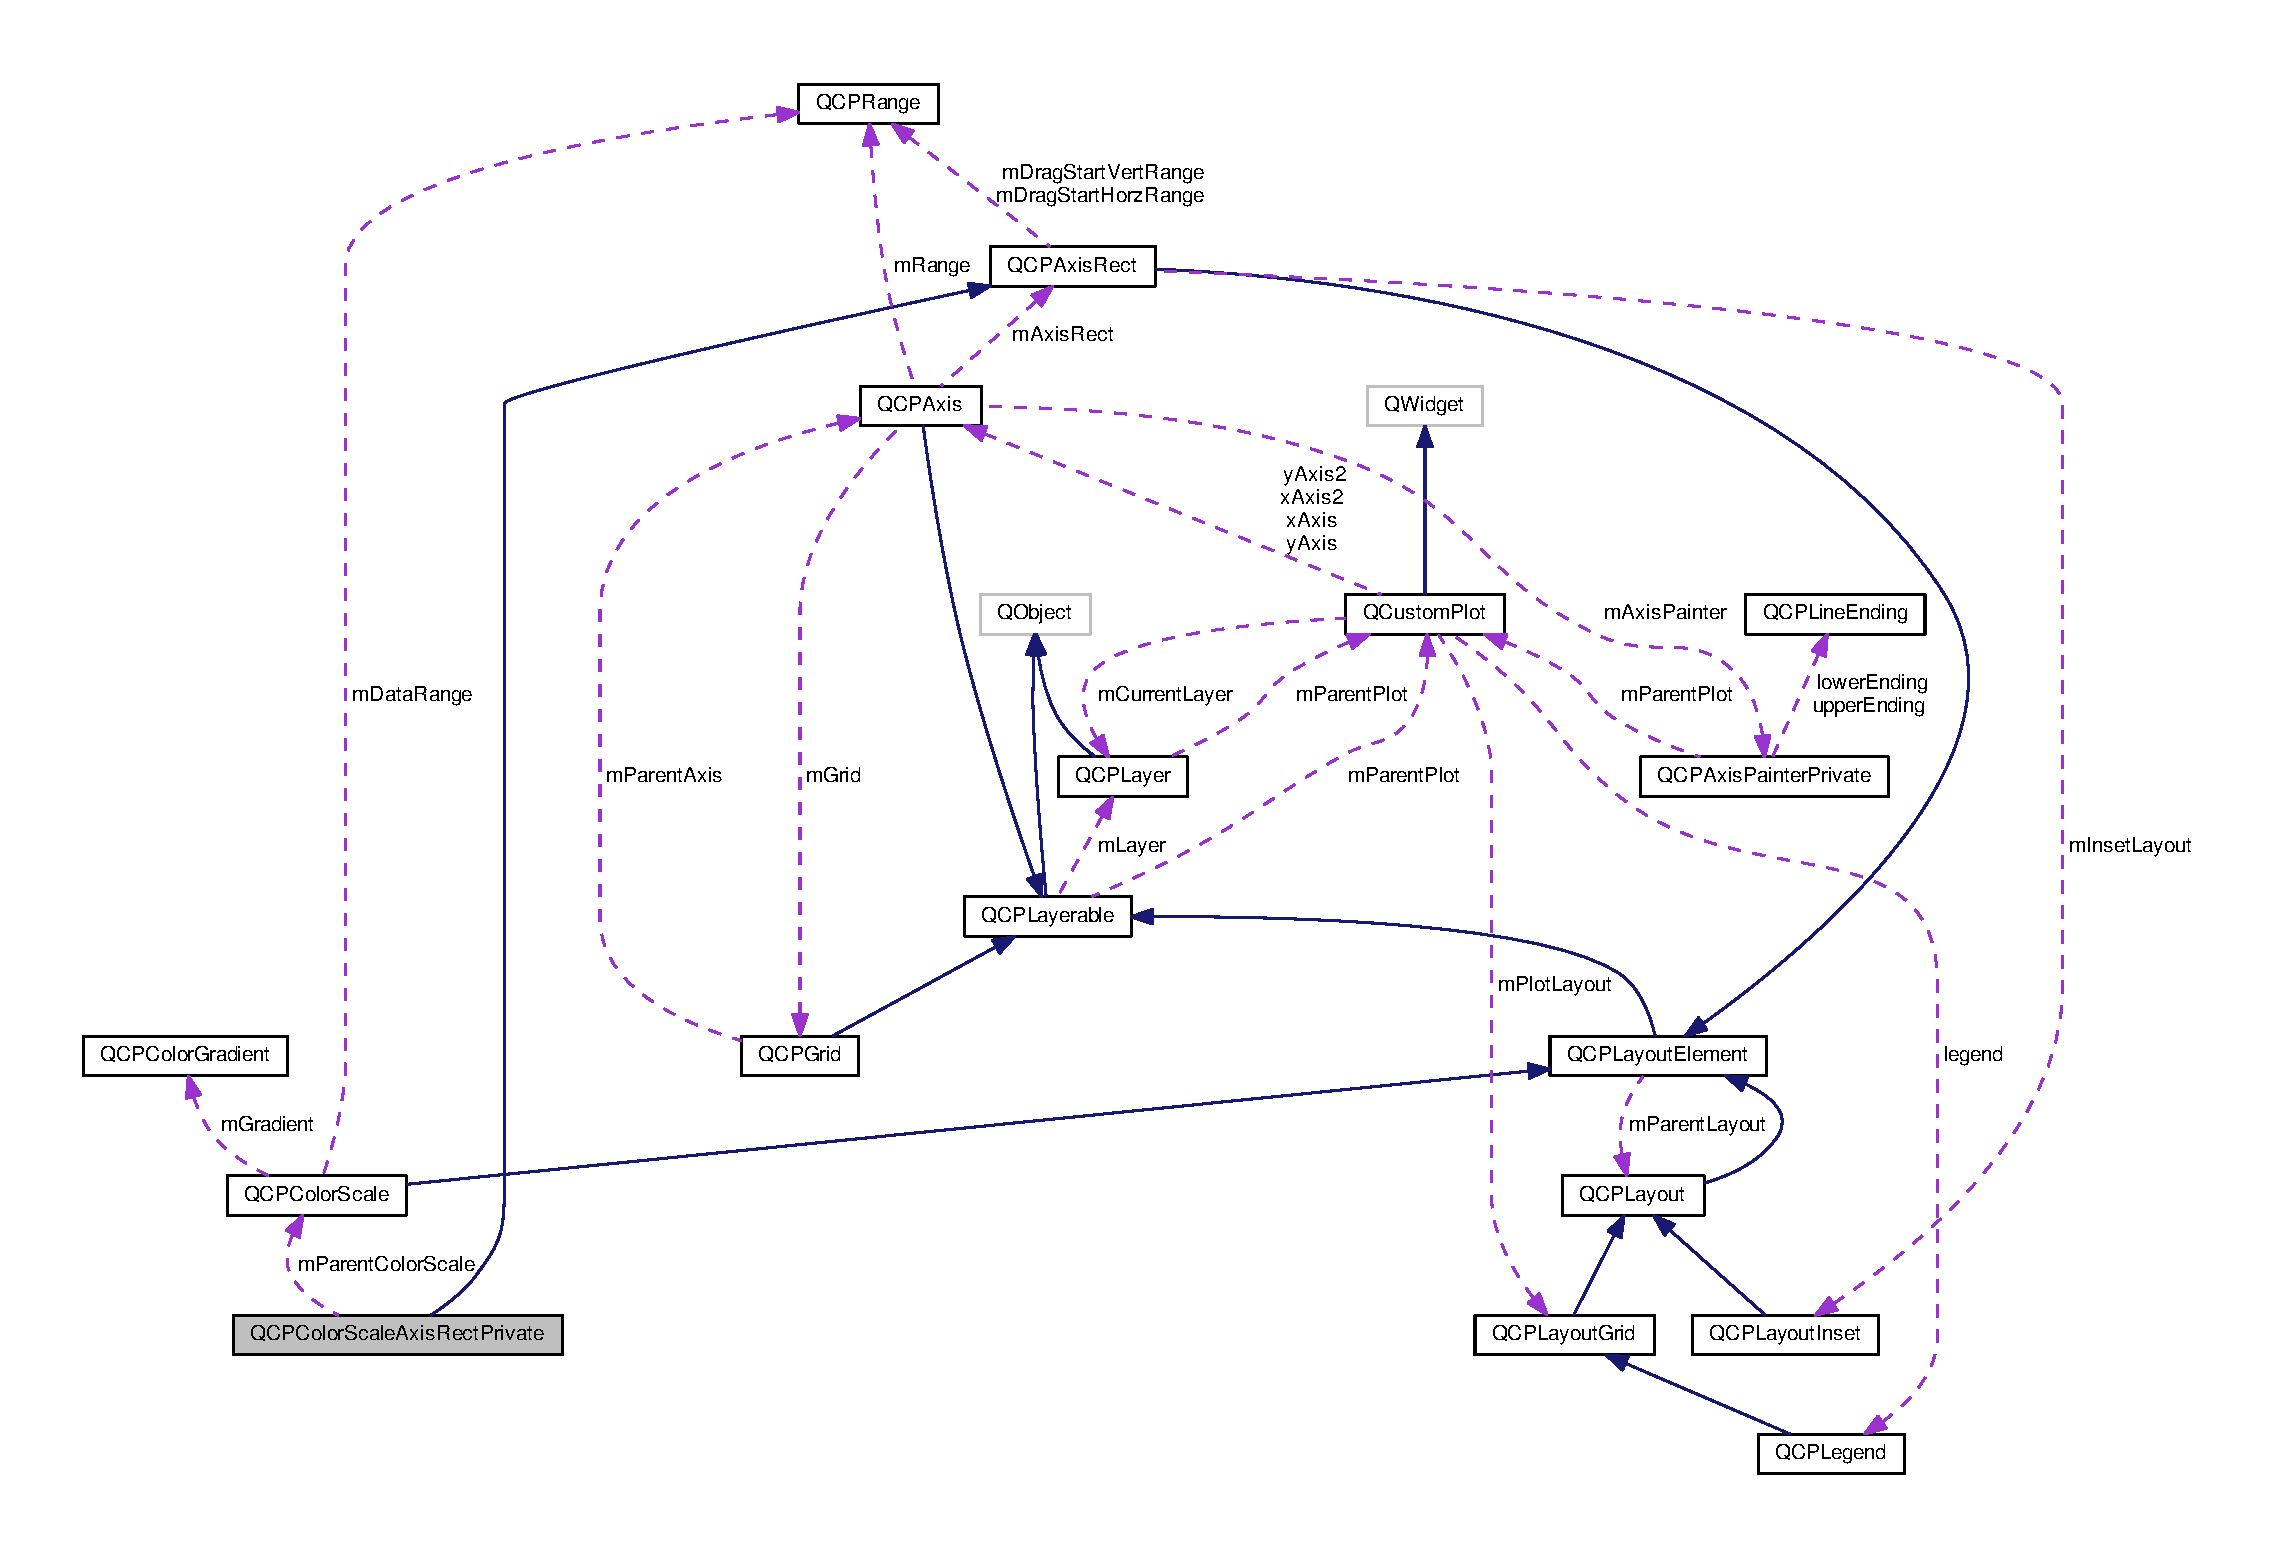
\includegraphics[width=350pt]{classQCPColorScaleAxisRectPrivate__coll__graph}
\end{center}
\end{figure}
\subsection*{Public Member Functions}
\begin{DoxyCompactItemize}
\item 
\hyperlink{classQCPColorScaleAxisRectPrivate_ad3b242f75dd2b33581364a4e668a80db}{Q\+C\+P\+Color\+Scale\+Axis\+Rect\+Private} (\hyperlink{classQCPColorScale}{Q\+C\+P\+Color\+Scale} $\ast$parent\+Color\+Scale)
\end{DoxyCompactItemize}
\subsection*{Protected Member Functions}
\begin{DoxyCompactItemize}
\item 
virtual void \hyperlink{classQCPColorScaleAxisRectPrivate_adb67bfe9057a9dd9a85f548c274e6d98}{draw} (\hyperlink{classQCPPainter}{Q\+C\+P\+Painter} $\ast$painter)
\item 
void \hyperlink{classQCPColorScaleAxisRectPrivate_a73754cab312aeaddea1bfcc67cc079ac}{update\+Gradient\+Image} ()
\item 
Q\+\_\+\+S\+L\+OT void \hyperlink{classQCPColorScaleAxisRectPrivate_a6112ad4291ac1695d37659cb049d598d}{axis\+Selection\+Changed} (Q\+C\+P\+Axis\+::\+Selectable\+Parts selected\+Parts)
\item 
Q\+\_\+\+S\+L\+OT void \hyperlink{classQCPColorScaleAxisRectPrivate_a66d2baed86966bb03a6d7c32dc7d59f7}{axis\+Selectable\+Changed} (Q\+C\+P\+Axis\+::\+Selectable\+Parts selectable\+Parts)
\end{DoxyCompactItemize}
\subsection*{Protected Attributes}
\begin{DoxyCompactItemize}
\item 
\hyperlink{classQCPColorScale}{Q\+C\+P\+Color\+Scale} $\ast$ \hyperlink{classQCPColorScaleAxisRectPrivate_a311c73f51a4cb0b556388197833cf099}{m\+Parent\+Color\+Scale}
\item 
Q\+Image \hyperlink{classQCPColorScaleAxisRectPrivate_ad4f7c8ee1c6012d9950870811773119c}{m\+Gradient\+Image}
\item 
bool \hyperlink{classQCPColorScaleAxisRectPrivate_a2c0b15b071e1f93006b48b5be022a631}{m\+Gradient\+Image\+Invalidated}
\end{DoxyCompactItemize}
\subsection*{Friends}
\begin{DoxyCompactItemize}
\item 
class \hyperlink{classQCPColorScaleAxisRectPrivate_a60f6031408a325ebd1bbbad1ccf9b897}{Q\+C\+P\+Color\+Scale}
\end{DoxyCompactItemize}
\subsection*{Additional Inherited Members}


\subsection{Constructor \& Destructor Documentation}
\index{Q\+C\+P\+Color\+Scale\+Axis\+Rect\+Private@{Q\+C\+P\+Color\+Scale\+Axis\+Rect\+Private}!Q\+C\+P\+Color\+Scale\+Axis\+Rect\+Private@{Q\+C\+P\+Color\+Scale\+Axis\+Rect\+Private}}
\index{Q\+C\+P\+Color\+Scale\+Axis\+Rect\+Private@{Q\+C\+P\+Color\+Scale\+Axis\+Rect\+Private}!Q\+C\+P\+Color\+Scale\+Axis\+Rect\+Private@{Q\+C\+P\+Color\+Scale\+Axis\+Rect\+Private}}
\subsubsection[{\texorpdfstring{Q\+C\+P\+Color\+Scale\+Axis\+Rect\+Private(\+Q\+C\+P\+Color\+Scale $\ast$parent\+Color\+Scale)}{QCPColorScaleAxisRectPrivate(QCPColorScale *parentColorScale)}}]{\setlength{\rightskip}{0pt plus 5cm}Q\+C\+P\+Color\+Scale\+Axis\+Rect\+Private\+::\+Q\+C\+P\+Color\+Scale\+Axis\+Rect\+Private (
\begin{DoxyParamCaption}
\item[{{\bf Q\+C\+P\+Color\+Scale} $\ast$}]{parent\+Color\+Scale}
\end{DoxyParamCaption}
)\hspace{0.3cm}{\ttfamily [explicit]}}\hypertarget{classQCPColorScaleAxisRectPrivate_ad3b242f75dd2b33581364a4e668a80db}{}\label{classQCPColorScaleAxisRectPrivate_ad3b242f75dd2b33581364a4e668a80db}
Creates a new instance, as a child of {\itshape parent\+Color\+Scale}. 

\subsection{Member Function Documentation}
\index{Q\+C\+P\+Color\+Scale\+Axis\+Rect\+Private@{Q\+C\+P\+Color\+Scale\+Axis\+Rect\+Private}!axis\+Selectable\+Changed@{axis\+Selectable\+Changed}}
\index{axis\+Selectable\+Changed@{axis\+Selectable\+Changed}!Q\+C\+P\+Color\+Scale\+Axis\+Rect\+Private@{Q\+C\+P\+Color\+Scale\+Axis\+Rect\+Private}}
\subsubsection[{\texorpdfstring{axis\+Selectable\+Changed(\+Q\+C\+P\+Axis\+::\+Selectable\+Parts selectable\+Parts)}{axisSelectableChanged(QCPAxis::SelectableParts selectableParts)}}]{\setlength{\rightskip}{0pt plus 5cm}void Q\+C\+P\+Color\+Scale\+Axis\+Rect\+Private\+::axis\+Selectable\+Changed (
\begin{DoxyParamCaption}
\item[{Q\+C\+P\+Axis\+::\+Selectable\+Parts}]{selectable\+Parts}
\end{DoxyParamCaption}
)\hspace{0.3cm}{\ttfamily [protected]}}\hypertarget{classQCPColorScaleAxisRectPrivate_a66d2baed86966bb03a6d7c32dc7d59f7}{}\label{classQCPColorScaleAxisRectPrivate_a66d2baed86966bb03a6d7c32dc7d59f7}
\index{Q\+C\+P\+Color\+Scale\+Axis\+Rect\+Private@{Q\+C\+P\+Color\+Scale\+Axis\+Rect\+Private}!axis\+Selection\+Changed@{axis\+Selection\+Changed}}
\index{axis\+Selection\+Changed@{axis\+Selection\+Changed}!Q\+C\+P\+Color\+Scale\+Axis\+Rect\+Private@{Q\+C\+P\+Color\+Scale\+Axis\+Rect\+Private}}
\subsubsection[{\texorpdfstring{axis\+Selection\+Changed(\+Q\+C\+P\+Axis\+::\+Selectable\+Parts selected\+Parts)}{axisSelectionChanged(QCPAxis::SelectableParts selectedParts)}}]{\setlength{\rightskip}{0pt plus 5cm}void Q\+C\+P\+Color\+Scale\+Axis\+Rect\+Private\+::axis\+Selection\+Changed (
\begin{DoxyParamCaption}
\item[{Q\+C\+P\+Axis\+::\+Selectable\+Parts}]{selected\+Parts}
\end{DoxyParamCaption}
)\hspace{0.3cm}{\ttfamily [protected]}}\hypertarget{classQCPColorScaleAxisRectPrivate_a6112ad4291ac1695d37659cb049d598d}{}\label{classQCPColorScaleAxisRectPrivate_a6112ad4291ac1695d37659cb049d598d}
\index{Q\+C\+P\+Color\+Scale\+Axis\+Rect\+Private@{Q\+C\+P\+Color\+Scale\+Axis\+Rect\+Private}!draw@{draw}}
\index{draw@{draw}!Q\+C\+P\+Color\+Scale\+Axis\+Rect\+Private@{Q\+C\+P\+Color\+Scale\+Axis\+Rect\+Private}}
\subsubsection[{\texorpdfstring{draw(\+Q\+C\+P\+Painter $\ast$painter)}{draw(QCPPainter *painter)}}]{\setlength{\rightskip}{0pt plus 5cm}void Q\+C\+P\+Color\+Scale\+Axis\+Rect\+Private\+::draw (
\begin{DoxyParamCaption}
\item[{{\bf Q\+C\+P\+Painter} $\ast$}]{painter}
\end{DoxyParamCaption}
)\hspace{0.3cm}{\ttfamily [protected]}, {\ttfamily [virtual]}}\hypertarget{classQCPColorScaleAxisRectPrivate_adb67bfe9057a9dd9a85f548c274e6d98}{}\label{classQCPColorScaleAxisRectPrivate_adb67bfe9057a9dd9a85f548c274e6d98}


Reimplemented from \hyperlink{classQCPAxisRect_afb1bbbbda8345cd2710d92ee48440b53}{Q\+C\+P\+Axis\+Rect}.

\index{Q\+C\+P\+Color\+Scale\+Axis\+Rect\+Private@{Q\+C\+P\+Color\+Scale\+Axis\+Rect\+Private}!update\+Gradient\+Image@{update\+Gradient\+Image}}
\index{update\+Gradient\+Image@{update\+Gradient\+Image}!Q\+C\+P\+Color\+Scale\+Axis\+Rect\+Private@{Q\+C\+P\+Color\+Scale\+Axis\+Rect\+Private}}
\subsubsection[{\texorpdfstring{update\+Gradient\+Image()}{updateGradientImage()}}]{\setlength{\rightskip}{0pt plus 5cm}void Q\+C\+P\+Color\+Scale\+Axis\+Rect\+Private\+::update\+Gradient\+Image (
\begin{DoxyParamCaption}
{}
\end{DoxyParamCaption}
)\hspace{0.3cm}{\ttfamily [protected]}}\hypertarget{classQCPColorScaleAxisRectPrivate_a73754cab312aeaddea1bfcc67cc079ac}{}\label{classQCPColorScaleAxisRectPrivate_a73754cab312aeaddea1bfcc67cc079ac}


\subsection{Friends And Related Function Documentation}
\index{Q\+C\+P\+Color\+Scale\+Axis\+Rect\+Private@{Q\+C\+P\+Color\+Scale\+Axis\+Rect\+Private}!Q\+C\+P\+Color\+Scale@{Q\+C\+P\+Color\+Scale}}
\index{Q\+C\+P\+Color\+Scale@{Q\+C\+P\+Color\+Scale}!Q\+C\+P\+Color\+Scale\+Axis\+Rect\+Private@{Q\+C\+P\+Color\+Scale\+Axis\+Rect\+Private}}
\subsubsection[{\texorpdfstring{Q\+C\+P\+Color\+Scale}{QCPColorScale}}]{\setlength{\rightskip}{0pt plus 5cm}friend class {\bf Q\+C\+P\+Color\+Scale}\hspace{0.3cm}{\ttfamily [friend]}}\hypertarget{classQCPColorScaleAxisRectPrivate_a60f6031408a325ebd1bbbad1ccf9b897}{}\label{classQCPColorScaleAxisRectPrivate_a60f6031408a325ebd1bbbad1ccf9b897}


\subsection{Member Data Documentation}
\index{Q\+C\+P\+Color\+Scale\+Axis\+Rect\+Private@{Q\+C\+P\+Color\+Scale\+Axis\+Rect\+Private}!m\+Gradient\+Image@{m\+Gradient\+Image}}
\index{m\+Gradient\+Image@{m\+Gradient\+Image}!Q\+C\+P\+Color\+Scale\+Axis\+Rect\+Private@{Q\+C\+P\+Color\+Scale\+Axis\+Rect\+Private}}
\subsubsection[{\texorpdfstring{m\+Gradient\+Image}{mGradientImage}}]{\setlength{\rightskip}{0pt plus 5cm}Q\+Image Q\+C\+P\+Color\+Scale\+Axis\+Rect\+Private\+::m\+Gradient\+Image\hspace{0.3cm}{\ttfamily [protected]}}\hypertarget{classQCPColorScaleAxisRectPrivate_ad4f7c8ee1c6012d9950870811773119c}{}\label{classQCPColorScaleAxisRectPrivate_ad4f7c8ee1c6012d9950870811773119c}
\index{Q\+C\+P\+Color\+Scale\+Axis\+Rect\+Private@{Q\+C\+P\+Color\+Scale\+Axis\+Rect\+Private}!m\+Gradient\+Image\+Invalidated@{m\+Gradient\+Image\+Invalidated}}
\index{m\+Gradient\+Image\+Invalidated@{m\+Gradient\+Image\+Invalidated}!Q\+C\+P\+Color\+Scale\+Axis\+Rect\+Private@{Q\+C\+P\+Color\+Scale\+Axis\+Rect\+Private}}
\subsubsection[{\texorpdfstring{m\+Gradient\+Image\+Invalidated}{mGradientImageInvalidated}}]{\setlength{\rightskip}{0pt plus 5cm}bool Q\+C\+P\+Color\+Scale\+Axis\+Rect\+Private\+::m\+Gradient\+Image\+Invalidated\hspace{0.3cm}{\ttfamily [protected]}}\hypertarget{classQCPColorScaleAxisRectPrivate_a2c0b15b071e1f93006b48b5be022a631}{}\label{classQCPColorScaleAxisRectPrivate_a2c0b15b071e1f93006b48b5be022a631}
\index{Q\+C\+P\+Color\+Scale\+Axis\+Rect\+Private@{Q\+C\+P\+Color\+Scale\+Axis\+Rect\+Private}!m\+Parent\+Color\+Scale@{m\+Parent\+Color\+Scale}}
\index{m\+Parent\+Color\+Scale@{m\+Parent\+Color\+Scale}!Q\+C\+P\+Color\+Scale\+Axis\+Rect\+Private@{Q\+C\+P\+Color\+Scale\+Axis\+Rect\+Private}}
\subsubsection[{\texorpdfstring{m\+Parent\+Color\+Scale}{mParentColorScale}}]{\setlength{\rightskip}{0pt plus 5cm}{\bf Q\+C\+P\+Color\+Scale}$\ast$ Q\+C\+P\+Color\+Scale\+Axis\+Rect\+Private\+::m\+Parent\+Color\+Scale\hspace{0.3cm}{\ttfamily [protected]}}\hypertarget{classQCPColorScaleAxisRectPrivate_a311c73f51a4cb0b556388197833cf099}{}\label{classQCPColorScaleAxisRectPrivate_a311c73f51a4cb0b556388197833cf099}


The documentation for this class was generated from the following files\+:\begin{DoxyCompactItemize}
\item 
src/hammerhead/tools/watchdog/include/watchdog/\hyperlink{qcustomplot_8h}{qcustomplot.\+h}\item 
src/hammerhead/tools/watchdog/src/\hyperlink{qcustomplot_8cpp}{qcustomplot.\+cpp}\end{DoxyCompactItemize}

\hypertarget{classQCPCurve}{}\section{Q\+C\+P\+Curve Class Reference}
\label{classQCPCurve}\index{Q\+C\+P\+Curve@{Q\+C\+P\+Curve}}


A plottable representing a parametric curve in a plot.  




{\ttfamily \#include $<$qcustomplot.\+h$>$}



Inheritance diagram for Q\+C\+P\+Curve\+:\nopagebreak
\begin{figure}[H]
\begin{center}
\leavevmode
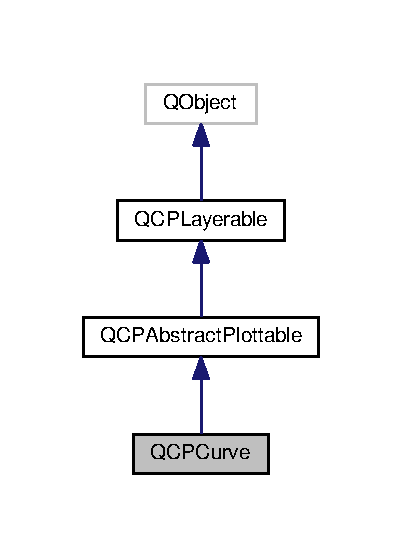
\includegraphics[width=193pt]{classQCPCurve__inherit__graph}
\end{center}
\end{figure}


Collaboration diagram for Q\+C\+P\+Curve\+:\nopagebreak
\begin{figure}[H]
\begin{center}
\leavevmode
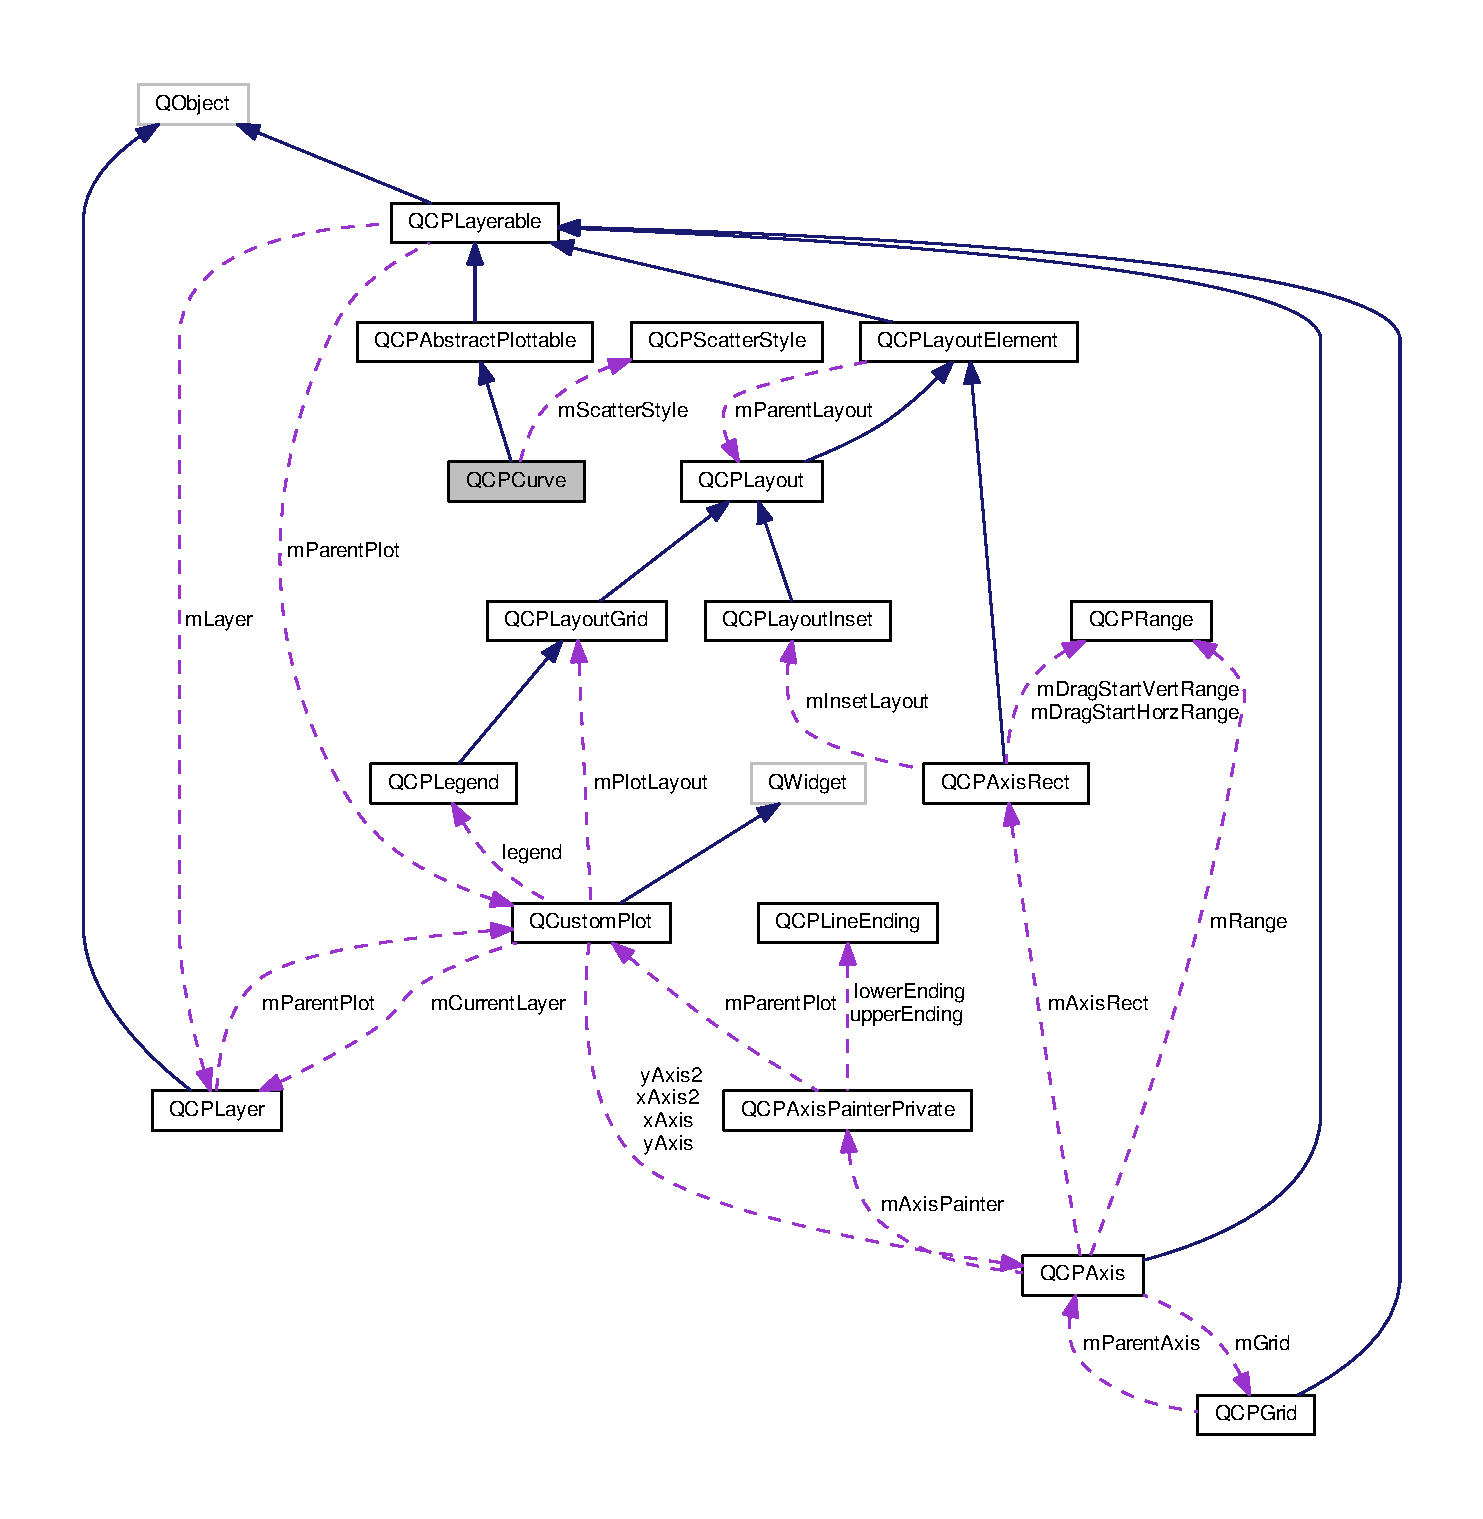
\includegraphics[width=350pt]{classQCPCurve__coll__graph}
\end{center}
\end{figure}
\subsection*{Public Types}
\begin{DoxyCompactItemize}
\item 
enum \hyperlink{classQCPCurve_a2710e9f79302152cff794c6e16cc01f1}{Line\+Style} \{ \hyperlink{classQCPCurve_a2710e9f79302152cff794c6e16cc01f1aec1601a191cdf0b4e761c4c66092cc48}{ls\+None}, 
\hyperlink{classQCPCurve_a2710e9f79302152cff794c6e16cc01f1ade5822ce6fbf131d3df131795c2e1003}{ls\+Line}
 \}
\end{DoxyCompactItemize}
\subsection*{Public Member Functions}
\begin{DoxyCompactItemize}
\item 
\hyperlink{classQCPCurve_a36de58e2652b3fa47bdf9187d421d3ce}{Q\+C\+P\+Curve} (\hyperlink{classQCPAxis}{Q\+C\+P\+Axis} $\ast$\hyperlink{classQCPAbstractPlottable_a72c7a09c22963f2c943f07112b311103}{key\+Axis}, \hyperlink{classQCPAxis}{Q\+C\+P\+Axis} $\ast$\hyperlink{classQCPAbstractPlottable_a3106f9d34d330a6097a8ec5905e5b519}{value\+Axis})
\item 
virtual \hyperlink{classQCPCurve_a99ee5136754884a220cc0bcacfe419a3}{$\sim$\+Q\+C\+P\+Curve} ()
\item 
\hyperlink{qcustomplot_8h_a444d37ec9cb2951b3a7fe443c34d1658}{Q\+C\+P\+Curve\+Data\+Map} $\ast$ \hyperlink{classQCPCurve_a9ac194d35d4f334923aac9df1bf599ca}{data} () const 
\item 
\hyperlink{classQCPScatterStyle}{Q\+C\+P\+Scatter\+Style} \hyperlink{classQCPCurve_a9ab864c9f6ba0cedf65853f59d867a68}{scatter\+Style} () const 
\item 
\hyperlink{classQCPCurve_a2710e9f79302152cff794c6e16cc01f1}{Line\+Style} \hyperlink{classQCPCurve_a0314dd644258949aeb4a95cebde5abaf}{line\+Style} () const 
\item 
void \hyperlink{classQCPCurve_a631ac886708460013b30052f49cbc9da}{set\+Data} (\hyperlink{qcustomplot_8h_a444d37ec9cb2951b3a7fe443c34d1658}{Q\+C\+P\+Curve\+Data\+Map} $\ast$\hyperlink{classQCPCurve_a9ac194d35d4f334923aac9df1bf599ca}{data}, bool copy=false)
\item 
void \hyperlink{classQCPCurve_affe80e011e2ced62a88f614acd6ab8d1}{set\+Data} (const Q\+Vector$<$ double $>$ \&t, const Q\+Vector$<$ double $>$ \&key, const Q\+Vector$<$ double $>$ \&value)
\item 
void \hyperlink{classQCPCurve_a963d4c45777deef15848a8f56172d066}{set\+Data} (const Q\+Vector$<$ double $>$ \&key, const Q\+Vector$<$ double $>$ \&value)
\item 
void \hyperlink{classQCPCurve_a55e43b44709bf50a35500644988aa706}{set\+Scatter\+Style} (const \hyperlink{classQCPScatterStyle}{Q\+C\+P\+Scatter\+Style} \&style)
\item 
void \hyperlink{classQCPCurve_a4a377ec863ff81a1875c3094a6177c19}{set\+Line\+Style} (\hyperlink{classQCPCurve_a2710e9f79302152cff794c6e16cc01f1}{Line\+Style} style)
\item 
void \hyperlink{classQCPCurve_a4e24023c3b9ac75440c7a260172c99af}{add\+Data} (const \hyperlink{qcustomplot_8h_a444d37ec9cb2951b3a7fe443c34d1658}{Q\+C\+P\+Curve\+Data\+Map} \&data\+Map)
\item 
void \hyperlink{classQCPCurve_ad304326aba096911f92452d8bfe0470e}{add\+Data} (const \hyperlink{classQCPCurveData}{Q\+C\+P\+Curve\+Data} \&\hyperlink{classQCPCurve_a9ac194d35d4f334923aac9df1bf599ca}{data})
\item 
void \hyperlink{classQCPCurve_a13398b236f6926014e404eeb5b9f415c}{add\+Data} (double t, double key, double value)
\item 
void \hyperlink{classQCPCurve_ada4762e793cd5707b33f35b8a4b0f8fb}{add\+Data} (double key, double value)
\item 
void \hyperlink{classQCPCurve_a27c8b3dddd4067d626397ee199626722}{add\+Data} (const Q\+Vector$<$ double $>$ \&ts, const Q\+Vector$<$ double $>$ \&keys, const Q\+Vector$<$ double $>$ \&values)
\item 
void \hyperlink{classQCPCurve_af6f4284fbc2f34e676f24dce03c34fe5}{remove\+Data\+Before} (double t)
\item 
void \hyperlink{classQCPCurve_a0365cb947c4e6d405ee22e00191d5f52}{remove\+Data\+After} (double t)
\item 
void \hyperlink{classQCPCurve_ad45bb5479be799163028ef2b776f7221}{remove\+Data} (double fromt, double tot)
\item 
void \hyperlink{classQCPCurve_a30c91acfa591ec534c49fed4c0fca39a}{remove\+Data} (double t)
\item 
virtual void \hyperlink{classQCPCurve_ae0462c61dbfbac07db0736ec64110241}{clear\+Data} ()
\item 
virtual double \hyperlink{classQCPCurve_a5af9949e725704811bbc81ecd5970b8e}{select\+Test} (const Q\+PointF \&pos, bool only\+Selectable, Q\+Variant $\ast$details=0) const 
\end{DoxyCompactItemize}
\subsection*{Protected Member Functions}
\begin{DoxyCompactItemize}
\item 
virtual void \hyperlink{classQCPCurve_a2361302d2fc6ec669849bd3bca00c4b2}{draw} (\hyperlink{classQCPPainter}{Q\+C\+P\+Painter} $\ast$painter)
\item 
virtual void \hyperlink{classQCPCurve_aaee24451e0044d1debfa1fee92c58d7b}{draw\+Legend\+Icon} (\hyperlink{classQCPPainter}{Q\+C\+P\+Painter} $\ast$painter, const Q\+RectF \&rect) const 
\item 
virtual \hyperlink{classQCPRange}{Q\+C\+P\+Range} \hyperlink{classQCPCurve_ad6a9559e16ab43586df18ae376d54481}{get\+Key\+Range} (bool \&found\+Range, \hyperlink{classQCPAbstractPlottable_a661743478a1d3c09d28ec2711d7653d8}{Sign\+Domain} in\+Sign\+Domain=\hyperlink{classQCPAbstractPlottable_a661743478a1d3c09d28ec2711d7653d8a082b98cfb91a7363a3b5cd17b0c1cd60}{sd\+Both}) const 
\item 
virtual \hyperlink{classQCPRange}{Q\+C\+P\+Range} \hyperlink{classQCPCurve_a1d6eec81aab9ae6182bb7c040bcb2dbc}{get\+Value\+Range} (bool \&found\+Range, \hyperlink{classQCPAbstractPlottable_a661743478a1d3c09d28ec2711d7653d8}{Sign\+Domain} in\+Sign\+Domain=\hyperlink{classQCPAbstractPlottable_a661743478a1d3c09d28ec2711d7653d8a082b98cfb91a7363a3b5cd17b0c1cd60}{sd\+Both}) const 
\item 
virtual void \hyperlink{classQCPCurve_a45593f30b81beec4b6130b6b53306087}{draw\+Scatter\+Plot} (\hyperlink{classQCPPainter}{Q\+C\+P\+Painter} $\ast$painter, const Q\+Vector$<$ Q\+PointF $>$ $\ast$point\+Data) const 
\item 
void \hyperlink{classQCPCurve_afa895f8ba9ae34fea6ecea295fd7b1e5}{get\+Curve\+Data} (Q\+Vector$<$ Q\+PointF $>$ $\ast$line\+Data) const 
\item 
int \hyperlink{classQCPCurve_a3af3183f35bd7aebe149f29ae4f1034a}{get\+Region} (double \hyperlink{qualification__task_8cpp_a6150e0515f7202e2fb518f7206ed97dc}{x}, double y, double rect\+Left, double rect\+Top, double rect\+Right, double rect\+Bottom) const 
\item 
Q\+PointF \hyperlink{classQCPCurve_acbcfea8986dde6c0143e3f7e8e76041d}{get\+Optimized\+Point} (int prev\+Region, double prev\+Key, double prev\+Value, double key, double value, double rect\+Left, double rect\+Top, double rect\+Right, double rect\+Bottom) const 
\item 
Q\+Vector$<$ Q\+PointF $>$ \hyperlink{classQCPCurve_aad0b69d9a7a2a5367fcc9fe3edaf9bf4}{get\+Optimized\+Corner\+Points} (int prev\+Region, int current\+Region, double prev\+Key, double prev\+Value, double key, double value, double rect\+Left, double rect\+Top, double rect\+Right, double rect\+Bottom) const 
\item 
bool \hyperlink{classQCPCurve_ae5b232c8201441a940516c745309a685}{may\+Traverse} (int prev\+Region, int current\+Region) const 
\item 
bool \hyperlink{classQCPCurve_ab4ffdf3d62d5bd3a187f6668daf01f85}{get\+Traverse} (double prev\+Key, double prev\+Value, double key, double value, double rect\+Left, double rect\+Top, double rect\+Right, double rect\+Bottom, Q\+PointF \&crossA, Q\+PointF \&crossB) const 
\item 
void \hyperlink{classQCPCurve_abe1721b19669e7127d76d144660fbeb8}{get\+Traverse\+Corner\+Points} (int prev\+Region, int current\+Region, double rect\+Left, double rect\+Top, double rect\+Right, double rect\+Bottom, Q\+Vector$<$ Q\+PointF $>$ \&before\+Traverse, Q\+Vector$<$ Q\+PointF $>$ \&after\+Traverse) const 
\item 
double \hyperlink{classQCPCurve_acd7a68c6f268ce1ab845eaf69fc2c6a6}{point\+Distance} (const Q\+PointF \&pixel\+Point) const 
\end{DoxyCompactItemize}
\subsection*{Protected Attributes}
\begin{DoxyCompactItemize}
\item 
\hyperlink{qcustomplot_8h_a444d37ec9cb2951b3a7fe443c34d1658}{Q\+C\+P\+Curve\+Data\+Map} $\ast$ \hyperlink{classQCPCurve_a88d533e455bca96004b049e99168731b}{m\+Data}
\item 
\hyperlink{classQCPScatterStyle}{Q\+C\+P\+Scatter\+Style} \hyperlink{classQCPCurve_a08f803b4a30b01bbd7a1eab15d0f864f}{m\+Scatter\+Style}
\item 
\hyperlink{classQCPCurve_a2710e9f79302152cff794c6e16cc01f1}{Line\+Style} \hyperlink{classQCPCurve_ae1f35ae2b15aee8e15bcdfec5be95156}{m\+Line\+Style}
\end{DoxyCompactItemize}
\subsection*{Friends}
\begin{DoxyCompactItemize}
\item 
class \hyperlink{classQCPCurve_a1cdf9df76adcfae45261690aa0ca2198}{Q\+Custom\+Plot}
\item 
class \hyperlink{classQCPCurve_a8429035e7adfbd7f05805a6530ad5e3b}{Q\+C\+P\+Legend}
\end{DoxyCompactItemize}
\subsection*{Additional Inherited Members}


\subsection{Detailed Description}
A plottable representing a parametric curve in a plot. 



Unlike \hyperlink{classQCPGraph}{Q\+C\+P\+Graph}, plottables of this type may have multiple points with the same key coordinate, so their visual representation can have {\itshape loops}. This is realized by introducing a third coordinate {\itshape t}, which defines the order of the points described by the other two coordinates {\itshape x} and {\itshape y}.

To plot data, assign it with the \hyperlink{classQCPCurve_a631ac886708460013b30052f49cbc9da}{set\+Data} or \hyperlink{classQCPCurve_a4e24023c3b9ac75440c7a260172c99af}{add\+Data} functions.

Gaps in the curve can be created by adding data points with NaN as key and value ({\ttfamily q\+Q\+Na\+N()} or {\ttfamily std\+::numeric\+\_\+limits$<$double$>$\+::quiet\+\_\+\+Na\+N()}) in between the two data points that shall be separated.\hypertarget{classQCPStatisticalBox_appearance}{}\subsection{Changing the appearance}\label{classQCPStatisticalBox_appearance}
The appearance of the curve is determined by the pen and the brush (\hyperlink{classQCPAbstractPlottable_ab74b09ae4c0e7e13142fe4b5bf46cac7}{set\+Pen}, \hyperlink{classQCPAbstractPlottable_a7a4b92144dca6453a1f0f210e27edc74}{set\+Brush}). \hypertarget{classQCPStatisticalBox_usage}{}\subsection{Usage}\label{classQCPStatisticalBox_usage}
Like all data representing objects in \hyperlink{classQCustomPlot}{Q\+Custom\+Plot}, the \hyperlink{classQCPCurve}{Q\+C\+P\+Curve} is a plottable (\hyperlink{classQCPAbstractPlottable}{Q\+C\+P\+Abstract\+Plottable}). So the plottable-\/interface of \hyperlink{classQCustomPlot}{Q\+Custom\+Plot} applies (\hyperlink{classQCustomPlot_a32de81ff53e263e785b83b52ecd99d6f}{Q\+Custom\+Plot\+::plottable}, \hyperlink{classQCustomPlot_ab7ad9174f701f9c6f64e378df77927a6}{Q\+Custom\+Plot\+::add\+Plottable}, \hyperlink{classQCustomPlot_af3dafd56884208474f311d6226513ab2}{Q\+Custom\+Plot\+::remove\+Plottable}, etc.)

Usually, you first create an instance and add it to the custom\+Plot\+: 
\begin{DoxyCodeInclude}
\end{DoxyCodeInclude}
and then modify the properties of the newly created plottable, e.\+g.\+: 
\begin{DoxyCodeInclude}
\end{DoxyCodeInclude}


\subsection{Member Enumeration Documentation}
\index{Q\+C\+P\+Curve@{Q\+C\+P\+Curve}!Line\+Style@{Line\+Style}}
\index{Line\+Style@{Line\+Style}!Q\+C\+P\+Curve@{Q\+C\+P\+Curve}}
\subsubsection[{\texorpdfstring{Line\+Style}{LineStyle}}]{\setlength{\rightskip}{0pt plus 5cm}enum {\bf Q\+C\+P\+Curve\+::\+Line\+Style}}\hypertarget{classQCPCurve_a2710e9f79302152cff794c6e16cc01f1}{}\label{classQCPCurve_a2710e9f79302152cff794c6e16cc01f1}
Defines how the curve\textquotesingle{}s line is represented visually in the plot. The line is drawn with the current pen of the curve (\hyperlink{classQCPAbstractPlottable_ab74b09ae4c0e7e13142fe4b5bf46cac7}{set\+Pen}). \begin{DoxySeeAlso}{See also}
\hyperlink{classQCPCurve_a4a377ec863ff81a1875c3094a6177c19}{set\+Line\+Style} 
\end{DoxySeeAlso}
\begin{Desc}
\item[Enumerator]\par
\begin{description}
\index{ls\+None@{ls\+None}!Q\+C\+P\+Curve@{Q\+C\+P\+Curve}}\index{Q\+C\+P\+Curve@{Q\+C\+P\+Curve}!ls\+None@{ls\+None}}\item[{\em 
ls\+None\hypertarget{classQCPCurve_a2710e9f79302152cff794c6e16cc01f1aec1601a191cdf0b4e761c4c66092cc48}{}\label{classQCPCurve_a2710e9f79302152cff794c6e16cc01f1aec1601a191cdf0b4e761c4c66092cc48}
}]No line is drawn between data points (e.\+g. only scatters) \index{ls\+Line@{ls\+Line}!Q\+C\+P\+Curve@{Q\+C\+P\+Curve}}\index{Q\+C\+P\+Curve@{Q\+C\+P\+Curve}!ls\+Line@{ls\+Line}}\item[{\em 
ls\+Line\hypertarget{classQCPCurve_a2710e9f79302152cff794c6e16cc01f1ade5822ce6fbf131d3df131795c2e1003}{}\label{classQCPCurve_a2710e9f79302152cff794c6e16cc01f1ade5822ce6fbf131d3df131795c2e1003}
}]Data points are connected with a straight line. \end{description}
\end{Desc}


\subsection{Constructor \& Destructor Documentation}
\index{Q\+C\+P\+Curve@{Q\+C\+P\+Curve}!Q\+C\+P\+Curve@{Q\+C\+P\+Curve}}
\index{Q\+C\+P\+Curve@{Q\+C\+P\+Curve}!Q\+C\+P\+Curve@{Q\+C\+P\+Curve}}
\subsubsection[{\texorpdfstring{Q\+C\+P\+Curve(\+Q\+C\+P\+Axis $\ast$key\+Axis, Q\+C\+P\+Axis $\ast$value\+Axis)}{QCPCurve(QCPAxis *keyAxis, QCPAxis *valueAxis)}}]{\setlength{\rightskip}{0pt plus 5cm}Q\+C\+P\+Curve\+::\+Q\+C\+P\+Curve (
\begin{DoxyParamCaption}
\item[{{\bf Q\+C\+P\+Axis} $\ast$}]{key\+Axis, }
\item[{{\bf Q\+C\+P\+Axis} $\ast$}]{value\+Axis}
\end{DoxyParamCaption}
)\hspace{0.3cm}{\ttfamily [explicit]}}\hypertarget{classQCPCurve_a36de58e2652b3fa47bdf9187d421d3ce}{}\label{classQCPCurve_a36de58e2652b3fa47bdf9187d421d3ce}
Constructs a curve which uses {\itshape key\+Axis} as its key axis (\char`\"{}x\char`\"{}) and {\itshape value\+Axis} as its value axis (\char`\"{}y\char`\"{}). {\itshape key\+Axis} and {\itshape value\+Axis} must reside in the same \hyperlink{classQCustomPlot}{Q\+Custom\+Plot} instance and not have the same orientation. If either of these restrictions is violated, a corresponding message is printed to the debug output (q\+Debug), the construction is not aborted, though.

The constructed \hyperlink{classQCPCurve}{Q\+C\+P\+Curve} can be added to the plot with \hyperlink{classQCustomPlot_ab7ad9174f701f9c6f64e378df77927a6}{Q\+Custom\+Plot\+::add\+Plottable}, \hyperlink{classQCustomPlot}{Q\+Custom\+Plot} then takes ownership of the graph. \index{Q\+C\+P\+Curve@{Q\+C\+P\+Curve}!````~Q\+C\+P\+Curve@{$\sim$\+Q\+C\+P\+Curve}}
\index{````~Q\+C\+P\+Curve@{$\sim$\+Q\+C\+P\+Curve}!Q\+C\+P\+Curve@{Q\+C\+P\+Curve}}
\subsubsection[{\texorpdfstring{$\sim$\+Q\+C\+P\+Curve()}{~QCPCurve()}}]{\setlength{\rightskip}{0pt plus 5cm}Q\+C\+P\+Curve\+::$\sim$\+Q\+C\+P\+Curve (
\begin{DoxyParamCaption}
{}
\end{DoxyParamCaption}
)\hspace{0.3cm}{\ttfamily [virtual]}}\hypertarget{classQCPCurve_a99ee5136754884a220cc0bcacfe419a3}{}\label{classQCPCurve_a99ee5136754884a220cc0bcacfe419a3}


\subsection{Member Function Documentation}
\index{Q\+C\+P\+Curve@{Q\+C\+P\+Curve}!add\+Data@{add\+Data}}
\index{add\+Data@{add\+Data}!Q\+C\+P\+Curve@{Q\+C\+P\+Curve}}
\subsubsection[{\texorpdfstring{add\+Data(const Q\+C\+P\+Curve\+Data\+Map \&data\+Map)}{addData(const QCPCurveDataMap &dataMap)}}]{\setlength{\rightskip}{0pt plus 5cm}void Q\+C\+P\+Curve\+::add\+Data (
\begin{DoxyParamCaption}
\item[{const {\bf Q\+C\+P\+Curve\+Data\+Map} \&}]{data\+Map}
\end{DoxyParamCaption}
)}\hypertarget{classQCPCurve_a4e24023c3b9ac75440c7a260172c99af}{}\label{classQCPCurve_a4e24023c3b9ac75440c7a260172c99af}
Adds the provided data points in {\itshape data\+Map} to the current data. \begin{DoxySeeAlso}{See also}
\hyperlink{classQCPCurve_ad45bb5479be799163028ef2b776f7221}{remove\+Data} 
\end{DoxySeeAlso}
\index{Q\+C\+P\+Curve@{Q\+C\+P\+Curve}!add\+Data@{add\+Data}}
\index{add\+Data@{add\+Data}!Q\+C\+P\+Curve@{Q\+C\+P\+Curve}}
\subsubsection[{\texorpdfstring{add\+Data(const Q\+C\+P\+Curve\+Data \&data)}{addData(const QCPCurveData &data)}}]{\setlength{\rightskip}{0pt plus 5cm}void Q\+C\+P\+Curve\+::add\+Data (
\begin{DoxyParamCaption}
\item[{const {\bf Q\+C\+P\+Curve\+Data} \&}]{data}
\end{DoxyParamCaption}
)}\hypertarget{classQCPCurve_ad304326aba096911f92452d8bfe0470e}{}\label{classQCPCurve_ad304326aba096911f92452d8bfe0470e}
This is an overloaded member function, provided for convenience. It differs from the above function only in what argument(s) it accepts. Adds the provided single data point in {\itshape data} to the current data. \begin{DoxySeeAlso}{See also}
\hyperlink{classQCPCurve_ad45bb5479be799163028ef2b776f7221}{remove\+Data} 
\end{DoxySeeAlso}
\index{Q\+C\+P\+Curve@{Q\+C\+P\+Curve}!add\+Data@{add\+Data}}
\index{add\+Data@{add\+Data}!Q\+C\+P\+Curve@{Q\+C\+P\+Curve}}
\subsubsection[{\texorpdfstring{add\+Data(double t, double key, double value)}{addData(double t, double key, double value)}}]{\setlength{\rightskip}{0pt plus 5cm}void Q\+C\+P\+Curve\+::add\+Data (
\begin{DoxyParamCaption}
\item[{double}]{t, }
\item[{double}]{key, }
\item[{double}]{value}
\end{DoxyParamCaption}
)}\hypertarget{classQCPCurve_a13398b236f6926014e404eeb5b9f415c}{}\label{classQCPCurve_a13398b236f6926014e404eeb5b9f415c}
This is an overloaded member function, provided for convenience. It differs from the above function only in what argument(s) it accepts. Adds the provided single data point as {\itshape t}, {\itshape key} and {\itshape value} tuple to the current data \begin{DoxySeeAlso}{See also}
\hyperlink{classQCPCurve_ad45bb5479be799163028ef2b776f7221}{remove\+Data} 
\end{DoxySeeAlso}
\index{Q\+C\+P\+Curve@{Q\+C\+P\+Curve}!add\+Data@{add\+Data}}
\index{add\+Data@{add\+Data}!Q\+C\+P\+Curve@{Q\+C\+P\+Curve}}
\subsubsection[{\texorpdfstring{add\+Data(double key, double value)}{addData(double key, double value)}}]{\setlength{\rightskip}{0pt plus 5cm}void Q\+C\+P\+Curve\+::add\+Data (
\begin{DoxyParamCaption}
\item[{double}]{key, }
\item[{double}]{value}
\end{DoxyParamCaption}
)}\hypertarget{classQCPCurve_ada4762e793cd5707b33f35b8a4b0f8fb}{}\label{classQCPCurve_ada4762e793cd5707b33f35b8a4b0f8fb}
This is an overloaded member function, provided for convenience. It differs from the above function only in what argument(s) it accepts.

Adds the provided single data point as {\itshape key} and {\itshape value} pair to the current data The t parameter of the data point is set to the t of the last data point plus 1. If there is no last data point, t will be set to 0.

\begin{DoxySeeAlso}{See also}
\hyperlink{classQCPCurve_ad45bb5479be799163028ef2b776f7221}{remove\+Data} 
\end{DoxySeeAlso}
\index{Q\+C\+P\+Curve@{Q\+C\+P\+Curve}!add\+Data@{add\+Data}}
\index{add\+Data@{add\+Data}!Q\+C\+P\+Curve@{Q\+C\+P\+Curve}}
\subsubsection[{\texorpdfstring{add\+Data(const Q\+Vector$<$ double $>$ \&ts, const Q\+Vector$<$ double $>$ \&keys, const Q\+Vector$<$ double $>$ \&values)}{addData(const QVector< double > &ts, const QVector< double > &keys, const QVector< double > &values)}}]{\setlength{\rightskip}{0pt plus 5cm}void Q\+C\+P\+Curve\+::add\+Data (
\begin{DoxyParamCaption}
\item[{const Q\+Vector$<$ double $>$ \&}]{ts, }
\item[{const Q\+Vector$<$ double $>$ \&}]{keys, }
\item[{const Q\+Vector$<$ double $>$ \&}]{values}
\end{DoxyParamCaption}
)}\hypertarget{classQCPCurve_a27c8b3dddd4067d626397ee199626722}{}\label{classQCPCurve_a27c8b3dddd4067d626397ee199626722}
This is an overloaded member function, provided for convenience. It differs from the above function only in what argument(s) it accepts. Adds the provided data points as {\itshape t}, {\itshape key} and {\itshape value} tuples to the current data. \begin{DoxySeeAlso}{See also}
\hyperlink{classQCPCurve_ad45bb5479be799163028ef2b776f7221}{remove\+Data} 
\end{DoxySeeAlso}
\index{Q\+C\+P\+Curve@{Q\+C\+P\+Curve}!clear\+Data@{clear\+Data}}
\index{clear\+Data@{clear\+Data}!Q\+C\+P\+Curve@{Q\+C\+P\+Curve}}
\subsubsection[{\texorpdfstring{clear\+Data()}{clearData()}}]{\setlength{\rightskip}{0pt plus 5cm}void Q\+C\+P\+Curve\+::clear\+Data (
\begin{DoxyParamCaption}
{}
\end{DoxyParamCaption}
)\hspace{0.3cm}{\ttfamily [virtual]}}\hypertarget{classQCPCurve_ae0462c61dbfbac07db0736ec64110241}{}\label{classQCPCurve_ae0462c61dbfbac07db0736ec64110241}
Removes all data points. \begin{DoxySeeAlso}{See also}
\hyperlink{classQCPCurve_ad45bb5479be799163028ef2b776f7221}{remove\+Data}, \hyperlink{classQCPCurve_a0365cb947c4e6d405ee22e00191d5f52}{remove\+Data\+After}, \hyperlink{classQCPCurve_af6f4284fbc2f34e676f24dce03c34fe5}{remove\+Data\+Before} 
\end{DoxySeeAlso}


Implements \hyperlink{classQCPAbstractPlottable_a86e5b8fd4b6ff4f4084e7ea4c573fc53}{Q\+C\+P\+Abstract\+Plottable}.

\index{Q\+C\+P\+Curve@{Q\+C\+P\+Curve}!data@{data}}
\index{data@{data}!Q\+C\+P\+Curve@{Q\+C\+P\+Curve}}
\subsubsection[{\texorpdfstring{data() const }{data() const }}]{\setlength{\rightskip}{0pt plus 5cm}{\bf Q\+C\+P\+Curve\+Data\+Map}$\ast$ Q\+C\+P\+Curve\+::data (
\begin{DoxyParamCaption}
{}
\end{DoxyParamCaption}
) const\hspace{0.3cm}{\ttfamily [inline]}}\hypertarget{classQCPCurve_a9ac194d35d4f334923aac9df1bf599ca}{}\label{classQCPCurve_a9ac194d35d4f334923aac9df1bf599ca}
\index{Q\+C\+P\+Curve@{Q\+C\+P\+Curve}!draw@{draw}}
\index{draw@{draw}!Q\+C\+P\+Curve@{Q\+C\+P\+Curve}}
\subsubsection[{\texorpdfstring{draw(\+Q\+C\+P\+Painter $\ast$painter)}{draw(QCPPainter *painter)}}]{\setlength{\rightskip}{0pt plus 5cm}void Q\+C\+P\+Curve\+::draw (
\begin{DoxyParamCaption}
\item[{{\bf Q\+C\+P\+Painter} $\ast$}]{painter}
\end{DoxyParamCaption}
)\hspace{0.3cm}{\ttfamily [protected]}, {\ttfamily [virtual]}}\hypertarget{classQCPCurve_a2361302d2fc6ec669849bd3bca00c4b2}{}\label{classQCPCurve_a2361302d2fc6ec669849bd3bca00c4b2}


Implements \hyperlink{classQCPAbstractPlottable_acbab5e30dcd04fd302b4a5902ac2c482}{Q\+C\+P\+Abstract\+Plottable}.

\index{Q\+C\+P\+Curve@{Q\+C\+P\+Curve}!draw\+Legend\+Icon@{draw\+Legend\+Icon}}
\index{draw\+Legend\+Icon@{draw\+Legend\+Icon}!Q\+C\+P\+Curve@{Q\+C\+P\+Curve}}
\subsubsection[{\texorpdfstring{draw\+Legend\+Icon(\+Q\+C\+P\+Painter $\ast$painter, const Q\+Rect\+F \&rect) const }{drawLegendIcon(QCPPainter *painter, const QRectF &rect) const }}]{\setlength{\rightskip}{0pt plus 5cm}void Q\+C\+P\+Curve\+::draw\+Legend\+Icon (
\begin{DoxyParamCaption}
\item[{{\bf Q\+C\+P\+Painter} $\ast$}]{painter, }
\item[{const Q\+RectF \&}]{rect}
\end{DoxyParamCaption}
) const\hspace{0.3cm}{\ttfamily [protected]}, {\ttfamily [virtual]}}\hypertarget{classQCPCurve_aaee24451e0044d1debfa1fee92c58d7b}{}\label{classQCPCurve_aaee24451e0044d1debfa1fee92c58d7b}


Implements \hyperlink{classQCPAbstractPlottable_a9a450783fd9ed539e589999fd390cdf7}{Q\+C\+P\+Abstract\+Plottable}.

\index{Q\+C\+P\+Curve@{Q\+C\+P\+Curve}!draw\+Scatter\+Plot@{draw\+Scatter\+Plot}}
\index{draw\+Scatter\+Plot@{draw\+Scatter\+Plot}!Q\+C\+P\+Curve@{Q\+C\+P\+Curve}}
\subsubsection[{\texorpdfstring{draw\+Scatter\+Plot(\+Q\+C\+P\+Painter $\ast$painter, const Q\+Vector$<$ Q\+Point\+F $>$ $\ast$point\+Data) const }{drawScatterPlot(QCPPainter *painter, const QVector< QPointF > *pointData) const }}]{\setlength{\rightskip}{0pt plus 5cm}void Q\+C\+P\+Curve\+::draw\+Scatter\+Plot (
\begin{DoxyParamCaption}
\item[{{\bf Q\+C\+P\+Painter} $\ast$}]{painter, }
\item[{const Q\+Vector$<$ Q\+PointF $>$ $\ast$}]{point\+Data}
\end{DoxyParamCaption}
) const\hspace{0.3cm}{\ttfamily [protected]}, {\ttfamily [virtual]}}\hypertarget{classQCPCurve_a45593f30b81beec4b6130b6b53306087}{}\label{classQCPCurve_a45593f30b81beec4b6130b6b53306087}
\index{Q\+C\+P\+Curve@{Q\+C\+P\+Curve}!get\+Curve\+Data@{get\+Curve\+Data}}
\index{get\+Curve\+Data@{get\+Curve\+Data}!Q\+C\+P\+Curve@{Q\+C\+P\+Curve}}
\subsubsection[{\texorpdfstring{get\+Curve\+Data(\+Q\+Vector$<$ Q\+Point\+F $>$ $\ast$line\+Data) const }{getCurveData(QVector< QPointF > *lineData) const }}]{\setlength{\rightskip}{0pt plus 5cm}void Q\+C\+P\+Curve\+::get\+Curve\+Data (
\begin{DoxyParamCaption}
\item[{Q\+Vector$<$ Q\+PointF $>$ $\ast$}]{line\+Data}
\end{DoxyParamCaption}
) const\hspace{0.3cm}{\ttfamily [protected]}}\hypertarget{classQCPCurve_afa895f8ba9ae34fea6ecea295fd7b1e5}{}\label{classQCPCurve_afa895f8ba9ae34fea6ecea295fd7b1e5}
\index{Q\+C\+P\+Curve@{Q\+C\+P\+Curve}!get\+Key\+Range@{get\+Key\+Range}}
\index{get\+Key\+Range@{get\+Key\+Range}!Q\+C\+P\+Curve@{Q\+C\+P\+Curve}}
\subsubsection[{\texorpdfstring{get\+Key\+Range(bool \&found\+Range, Sign\+Domain in\+Sign\+Domain=sd\+Both) const }{getKeyRange(bool &foundRange, SignDomain inSignDomain=sdBoth) const }}]{\setlength{\rightskip}{0pt plus 5cm}{\bf Q\+C\+P\+Range} Q\+C\+P\+Curve\+::get\+Key\+Range (
\begin{DoxyParamCaption}
\item[{bool \&}]{found\+Range, }
\item[{{\bf Sign\+Domain}}]{in\+Sign\+Domain = {\ttfamily {\bf sd\+Both}}}
\end{DoxyParamCaption}
) const\hspace{0.3cm}{\ttfamily [protected]}, {\ttfamily [virtual]}}\hypertarget{classQCPCurve_ad6a9559e16ab43586df18ae376d54481}{}\label{classQCPCurve_ad6a9559e16ab43586df18ae376d54481}


Implements \hyperlink{classQCPAbstractPlottable_a345d702b2e7e12c8cfdddff65ba85e8c}{Q\+C\+P\+Abstract\+Plottable}.

\index{Q\+C\+P\+Curve@{Q\+C\+P\+Curve}!get\+Optimized\+Corner\+Points@{get\+Optimized\+Corner\+Points}}
\index{get\+Optimized\+Corner\+Points@{get\+Optimized\+Corner\+Points}!Q\+C\+P\+Curve@{Q\+C\+P\+Curve}}
\subsubsection[{\texorpdfstring{get\+Optimized\+Corner\+Points(int prev\+Region, int current\+Region, double prev\+Key, double prev\+Value, double key, double value, double rect\+Left, double rect\+Top, double rect\+Right, double rect\+Bottom) const }{getOptimizedCornerPoints(int prevRegion, int currentRegion, double prevKey, double prevValue, double key, double value, double rectLeft, double rectTop, double rectRight, double rectBottom) const }}]{\setlength{\rightskip}{0pt plus 5cm}Q\+Vector$<$ Q\+PointF $>$ Q\+C\+P\+Curve\+::get\+Optimized\+Corner\+Points (
\begin{DoxyParamCaption}
\item[{int}]{prev\+Region, }
\item[{int}]{current\+Region, }
\item[{double}]{prev\+Key, }
\item[{double}]{prev\+Value, }
\item[{double}]{key, }
\item[{double}]{value, }
\item[{double}]{rect\+Left, }
\item[{double}]{rect\+Top, }
\item[{double}]{rect\+Right, }
\item[{double}]{rect\+Bottom}
\end{DoxyParamCaption}
) const\hspace{0.3cm}{\ttfamily [protected]}}\hypertarget{classQCPCurve_aad0b69d9a7a2a5367fcc9fe3edaf9bf4}{}\label{classQCPCurve_aad0b69d9a7a2a5367fcc9fe3edaf9bf4}
\index{Q\+C\+P\+Curve@{Q\+C\+P\+Curve}!get\+Optimized\+Point@{get\+Optimized\+Point}}
\index{get\+Optimized\+Point@{get\+Optimized\+Point}!Q\+C\+P\+Curve@{Q\+C\+P\+Curve}}
\subsubsection[{\texorpdfstring{get\+Optimized\+Point(int prev\+Region, double prev\+Key, double prev\+Value, double key, double value, double rect\+Left, double rect\+Top, double rect\+Right, double rect\+Bottom) const }{getOptimizedPoint(int prevRegion, double prevKey, double prevValue, double key, double value, double rectLeft, double rectTop, double rectRight, double rectBottom) const }}]{\setlength{\rightskip}{0pt plus 5cm}Q\+PointF Q\+C\+P\+Curve\+::get\+Optimized\+Point (
\begin{DoxyParamCaption}
\item[{int}]{prev\+Region, }
\item[{double}]{prev\+Key, }
\item[{double}]{prev\+Value, }
\item[{double}]{key, }
\item[{double}]{value, }
\item[{double}]{rect\+Left, }
\item[{double}]{rect\+Top, }
\item[{double}]{rect\+Right, }
\item[{double}]{rect\+Bottom}
\end{DoxyParamCaption}
) const\hspace{0.3cm}{\ttfamily [protected]}}\hypertarget{classQCPCurve_acbcfea8986dde6c0143e3f7e8e76041d}{}\label{classQCPCurve_acbcfea8986dde6c0143e3f7e8e76041d}
\index{Q\+C\+P\+Curve@{Q\+C\+P\+Curve}!get\+Region@{get\+Region}}
\index{get\+Region@{get\+Region}!Q\+C\+P\+Curve@{Q\+C\+P\+Curve}}
\subsubsection[{\texorpdfstring{get\+Region(double x, double y, double rect\+Left, double rect\+Top, double rect\+Right, double rect\+Bottom) const }{getRegion(double x, double y, double rectLeft, double rectTop, double rectRight, double rectBottom) const }}]{\setlength{\rightskip}{0pt plus 5cm}int Q\+C\+P\+Curve\+::get\+Region (
\begin{DoxyParamCaption}
\item[{double}]{x, }
\item[{double}]{y, }
\item[{double}]{rect\+Left, }
\item[{double}]{rect\+Top, }
\item[{double}]{rect\+Right, }
\item[{double}]{rect\+Bottom}
\end{DoxyParamCaption}
) const\hspace{0.3cm}{\ttfamily [protected]}}\hypertarget{classQCPCurve_a3af3183f35bd7aebe149f29ae4f1034a}{}\label{classQCPCurve_a3af3183f35bd7aebe149f29ae4f1034a}
\index{Q\+C\+P\+Curve@{Q\+C\+P\+Curve}!get\+Traverse@{get\+Traverse}}
\index{get\+Traverse@{get\+Traverse}!Q\+C\+P\+Curve@{Q\+C\+P\+Curve}}
\subsubsection[{\texorpdfstring{get\+Traverse(double prev\+Key, double prev\+Value, double key, double value, double rect\+Left, double rect\+Top, double rect\+Right, double rect\+Bottom, Q\+Point\+F \&cross\+A, Q\+Point\+F \&cross\+B) const }{getTraverse(double prevKey, double prevValue, double key, double value, double rectLeft, double rectTop, double rectRight, double rectBottom, QPointF &crossA, QPointF &crossB) const }}]{\setlength{\rightskip}{0pt plus 5cm}bool Q\+C\+P\+Curve\+::get\+Traverse (
\begin{DoxyParamCaption}
\item[{double}]{prev\+Key, }
\item[{double}]{prev\+Value, }
\item[{double}]{key, }
\item[{double}]{value, }
\item[{double}]{rect\+Left, }
\item[{double}]{rect\+Top, }
\item[{double}]{rect\+Right, }
\item[{double}]{rect\+Bottom, }
\item[{Q\+PointF \&}]{crossA, }
\item[{Q\+PointF \&}]{crossB}
\end{DoxyParamCaption}
) const\hspace{0.3cm}{\ttfamily [protected]}}\hypertarget{classQCPCurve_ab4ffdf3d62d5bd3a187f6668daf01f85}{}\label{classQCPCurve_ab4ffdf3d62d5bd3a187f6668daf01f85}
\index{Q\+C\+P\+Curve@{Q\+C\+P\+Curve}!get\+Traverse\+Corner\+Points@{get\+Traverse\+Corner\+Points}}
\index{get\+Traverse\+Corner\+Points@{get\+Traverse\+Corner\+Points}!Q\+C\+P\+Curve@{Q\+C\+P\+Curve}}
\subsubsection[{\texorpdfstring{get\+Traverse\+Corner\+Points(int prev\+Region, int current\+Region, double rect\+Left, double rect\+Top, double rect\+Right, double rect\+Bottom, Q\+Vector$<$ Q\+Point\+F $>$ \&before\+Traverse, Q\+Vector$<$ Q\+Point\+F $>$ \&after\+Traverse) const }{getTraverseCornerPoints(int prevRegion, int currentRegion, double rectLeft, double rectTop, double rectRight, double rectBottom, QVector< QPointF > &beforeTraverse, QVector< QPointF > &afterTraverse) const }}]{\setlength{\rightskip}{0pt plus 5cm}void Q\+C\+P\+Curve\+::get\+Traverse\+Corner\+Points (
\begin{DoxyParamCaption}
\item[{int}]{prev\+Region, }
\item[{int}]{current\+Region, }
\item[{double}]{rect\+Left, }
\item[{double}]{rect\+Top, }
\item[{double}]{rect\+Right, }
\item[{double}]{rect\+Bottom, }
\item[{Q\+Vector$<$ Q\+PointF $>$ \&}]{before\+Traverse, }
\item[{Q\+Vector$<$ Q\+PointF $>$ \&}]{after\+Traverse}
\end{DoxyParamCaption}
) const\hspace{0.3cm}{\ttfamily [protected]}}\hypertarget{classQCPCurve_abe1721b19669e7127d76d144660fbeb8}{}\label{classQCPCurve_abe1721b19669e7127d76d144660fbeb8}
\index{Q\+C\+P\+Curve@{Q\+C\+P\+Curve}!get\+Value\+Range@{get\+Value\+Range}}
\index{get\+Value\+Range@{get\+Value\+Range}!Q\+C\+P\+Curve@{Q\+C\+P\+Curve}}
\subsubsection[{\texorpdfstring{get\+Value\+Range(bool \&found\+Range, Sign\+Domain in\+Sign\+Domain=sd\+Both) const }{getValueRange(bool &foundRange, SignDomain inSignDomain=sdBoth) const }}]{\setlength{\rightskip}{0pt plus 5cm}{\bf Q\+C\+P\+Range} Q\+C\+P\+Curve\+::get\+Value\+Range (
\begin{DoxyParamCaption}
\item[{bool \&}]{found\+Range, }
\item[{{\bf Sign\+Domain}}]{in\+Sign\+Domain = {\ttfamily {\bf sd\+Both}}}
\end{DoxyParamCaption}
) const\hspace{0.3cm}{\ttfamily [protected]}, {\ttfamily [virtual]}}\hypertarget{classQCPCurve_a1d6eec81aab9ae6182bb7c040bcb2dbc}{}\label{classQCPCurve_a1d6eec81aab9ae6182bb7c040bcb2dbc}


Implements \hyperlink{classQCPAbstractPlottable_aa3331b415b5939fe4df60b78831b2799}{Q\+C\+P\+Abstract\+Plottable}.

\index{Q\+C\+P\+Curve@{Q\+C\+P\+Curve}!line\+Style@{line\+Style}}
\index{line\+Style@{line\+Style}!Q\+C\+P\+Curve@{Q\+C\+P\+Curve}}
\subsubsection[{\texorpdfstring{line\+Style() const }{lineStyle() const }}]{\setlength{\rightskip}{0pt plus 5cm}{\bf Line\+Style} Q\+C\+P\+Curve\+::line\+Style (
\begin{DoxyParamCaption}
{}
\end{DoxyParamCaption}
) const\hspace{0.3cm}{\ttfamily [inline]}}\hypertarget{classQCPCurve_a0314dd644258949aeb4a95cebde5abaf}{}\label{classQCPCurve_a0314dd644258949aeb4a95cebde5abaf}
\index{Q\+C\+P\+Curve@{Q\+C\+P\+Curve}!may\+Traverse@{may\+Traverse}}
\index{may\+Traverse@{may\+Traverse}!Q\+C\+P\+Curve@{Q\+C\+P\+Curve}}
\subsubsection[{\texorpdfstring{may\+Traverse(int prev\+Region, int current\+Region) const }{mayTraverse(int prevRegion, int currentRegion) const }}]{\setlength{\rightskip}{0pt plus 5cm}bool Q\+C\+P\+Curve\+::may\+Traverse (
\begin{DoxyParamCaption}
\item[{int}]{prev\+Region, }
\item[{int}]{current\+Region}
\end{DoxyParamCaption}
) const\hspace{0.3cm}{\ttfamily [protected]}}\hypertarget{classQCPCurve_ae5b232c8201441a940516c745309a685}{}\label{classQCPCurve_ae5b232c8201441a940516c745309a685}
\index{Q\+C\+P\+Curve@{Q\+C\+P\+Curve}!point\+Distance@{point\+Distance}}
\index{point\+Distance@{point\+Distance}!Q\+C\+P\+Curve@{Q\+C\+P\+Curve}}
\subsubsection[{\texorpdfstring{point\+Distance(const Q\+Point\+F \&pixel\+Point) const }{pointDistance(const QPointF &pixelPoint) const }}]{\setlength{\rightskip}{0pt plus 5cm}double Q\+C\+P\+Curve\+::point\+Distance (
\begin{DoxyParamCaption}
\item[{const Q\+PointF \&}]{pixel\+Point}
\end{DoxyParamCaption}
) const\hspace{0.3cm}{\ttfamily [protected]}}\hypertarget{classQCPCurve_acd7a68c6f268ce1ab845eaf69fc2c6a6}{}\label{classQCPCurve_acd7a68c6f268ce1ab845eaf69fc2c6a6}
\index{Q\+C\+P\+Curve@{Q\+C\+P\+Curve}!remove\+Data@{remove\+Data}}
\index{remove\+Data@{remove\+Data}!Q\+C\+P\+Curve@{Q\+C\+P\+Curve}}
\subsubsection[{\texorpdfstring{remove\+Data(double fromt, double tot)}{removeData(double fromt, double tot)}}]{\setlength{\rightskip}{0pt plus 5cm}void Q\+C\+P\+Curve\+::remove\+Data (
\begin{DoxyParamCaption}
\item[{double}]{fromt, }
\item[{double}]{tot}
\end{DoxyParamCaption}
)}\hypertarget{classQCPCurve_ad45bb5479be799163028ef2b776f7221}{}\label{classQCPCurve_ad45bb5479be799163028ef2b776f7221}
Removes all data points with curve parameter t between {\itshape fromt} and {\itshape tot}. if {\itshape fromt} is greater or equal to {\itshape tot}, the function does nothing. To remove a single data point with known t, use \hyperlink{classQCPCurve_a30c91acfa591ec534c49fed4c0fca39a}{remove\+Data(double t)}.

\begin{DoxySeeAlso}{See also}
\hyperlink{classQCPCurve_a4e24023c3b9ac75440c7a260172c99af}{add\+Data}, \hyperlink{classQCPCurve_ae0462c61dbfbac07db0736ec64110241}{clear\+Data} 
\end{DoxySeeAlso}
\index{Q\+C\+P\+Curve@{Q\+C\+P\+Curve}!remove\+Data@{remove\+Data}}
\index{remove\+Data@{remove\+Data}!Q\+C\+P\+Curve@{Q\+C\+P\+Curve}}
\subsubsection[{\texorpdfstring{remove\+Data(double t)}{removeData(double t)}}]{\setlength{\rightskip}{0pt plus 5cm}void Q\+C\+P\+Curve\+::remove\+Data (
\begin{DoxyParamCaption}
\item[{double}]{t}
\end{DoxyParamCaption}
)}\hypertarget{classQCPCurve_a30c91acfa591ec534c49fed4c0fca39a}{}\label{classQCPCurve_a30c91acfa591ec534c49fed4c0fca39a}
This is an overloaded member function, provided for convenience. It differs from the above function only in what argument(s) it accepts.

Removes a single data point at curve parameter {\itshape t}. If the position is not known with absolute precision, consider using \hyperlink{classQCPCurve_ad45bb5479be799163028ef2b776f7221}{remove\+Data(double fromt, double tot)} with a small fuzziness interval around the suspected position, depeding on the precision with which the curve parameter is known.

\begin{DoxySeeAlso}{See also}
\hyperlink{classQCPCurve_a4e24023c3b9ac75440c7a260172c99af}{add\+Data}, \hyperlink{classQCPCurve_ae0462c61dbfbac07db0736ec64110241}{clear\+Data} 
\end{DoxySeeAlso}
\index{Q\+C\+P\+Curve@{Q\+C\+P\+Curve}!remove\+Data\+After@{remove\+Data\+After}}
\index{remove\+Data\+After@{remove\+Data\+After}!Q\+C\+P\+Curve@{Q\+C\+P\+Curve}}
\subsubsection[{\texorpdfstring{remove\+Data\+After(double t)}{removeDataAfter(double t)}}]{\setlength{\rightskip}{0pt plus 5cm}void Q\+C\+P\+Curve\+::remove\+Data\+After (
\begin{DoxyParamCaption}
\item[{double}]{t}
\end{DoxyParamCaption}
)}\hypertarget{classQCPCurve_a0365cb947c4e6d405ee22e00191d5f52}{}\label{classQCPCurve_a0365cb947c4e6d405ee22e00191d5f52}
Removes all data points with curve parameter t greater than {\itshape t}. \begin{DoxySeeAlso}{See also}
\hyperlink{classQCPCurve_a4e24023c3b9ac75440c7a260172c99af}{add\+Data}, \hyperlink{classQCPCurve_ae0462c61dbfbac07db0736ec64110241}{clear\+Data} 
\end{DoxySeeAlso}
\index{Q\+C\+P\+Curve@{Q\+C\+P\+Curve}!remove\+Data\+Before@{remove\+Data\+Before}}
\index{remove\+Data\+Before@{remove\+Data\+Before}!Q\+C\+P\+Curve@{Q\+C\+P\+Curve}}
\subsubsection[{\texorpdfstring{remove\+Data\+Before(double t)}{removeDataBefore(double t)}}]{\setlength{\rightskip}{0pt plus 5cm}void Q\+C\+P\+Curve\+::remove\+Data\+Before (
\begin{DoxyParamCaption}
\item[{double}]{t}
\end{DoxyParamCaption}
)}\hypertarget{classQCPCurve_af6f4284fbc2f34e676f24dce03c34fe5}{}\label{classQCPCurve_af6f4284fbc2f34e676f24dce03c34fe5}
Removes all data points with curve parameter t smaller than {\itshape t}. \begin{DoxySeeAlso}{See also}
\hyperlink{classQCPCurve_a4e24023c3b9ac75440c7a260172c99af}{add\+Data}, \hyperlink{classQCPCurve_ae0462c61dbfbac07db0736ec64110241}{clear\+Data} 
\end{DoxySeeAlso}
\index{Q\+C\+P\+Curve@{Q\+C\+P\+Curve}!scatter\+Style@{scatter\+Style}}
\index{scatter\+Style@{scatter\+Style}!Q\+C\+P\+Curve@{Q\+C\+P\+Curve}}
\subsubsection[{\texorpdfstring{scatter\+Style() const }{scatterStyle() const }}]{\setlength{\rightskip}{0pt plus 5cm}{\bf Q\+C\+P\+Scatter\+Style} Q\+C\+P\+Curve\+::scatter\+Style (
\begin{DoxyParamCaption}
{}
\end{DoxyParamCaption}
) const\hspace{0.3cm}{\ttfamily [inline]}}\hypertarget{classQCPCurve_a9ab864c9f6ba0cedf65853f59d867a68}{}\label{classQCPCurve_a9ab864c9f6ba0cedf65853f59d867a68}
\index{Q\+C\+P\+Curve@{Q\+C\+P\+Curve}!select\+Test@{select\+Test}}
\index{select\+Test@{select\+Test}!Q\+C\+P\+Curve@{Q\+C\+P\+Curve}}
\subsubsection[{\texorpdfstring{select\+Test(const Q\+Point\+F \&pos, bool only\+Selectable, Q\+Variant $\ast$details=0) const }{selectTest(const QPointF &pos, bool onlySelectable, QVariant *details=0) const }}]{\setlength{\rightskip}{0pt plus 5cm}double Q\+C\+P\+Curve\+::select\+Test (
\begin{DoxyParamCaption}
\item[{const Q\+PointF \&}]{pos, }
\item[{bool}]{only\+Selectable, }
\item[{Q\+Variant $\ast$}]{details = {\ttfamily 0}}
\end{DoxyParamCaption}
) const\hspace{0.3cm}{\ttfamily [virtual]}}\hypertarget{classQCPCurve_a5af9949e725704811bbc81ecd5970b8e}{}\label{classQCPCurve_a5af9949e725704811bbc81ecd5970b8e}
This function is used to decide whether a click hits a layerable object or not.

{\itshape pos} is a point in pixel coordinates on the \hyperlink{classQCustomPlot}{Q\+Custom\+Plot} surface. This function returns the shortest pixel distance of this point to the object. If the object is either invisible or the distance couldn\textquotesingle{}t be determined, -\/1.\+0 is returned. Further, if {\itshape only\+Selectable} is true and the object is not selectable, -\/1.\+0 is returned, too.

If the object is represented not by single lines but by an area like a \hyperlink{classQCPItemText}{Q\+C\+P\+Item\+Text} or the bars of a \hyperlink{classQCPBars}{Q\+C\+P\+Bars} plottable, a click inside the area should also be considered a hit. In these cases this function thus returns a constant value greater zero but still below the parent plot\textquotesingle{}s selection tolerance. (typically the selection\+Tolerance multiplied by 0.\+99).

Providing a constant value for area objects allows selecting line objects even when they are obscured by such area objects, by clicking close to the lines (i.\+e. closer than 0.\+99$\ast$selection\+Tolerance).

The actual setting of the selection state is not done by this function. This is handled by the parent \hyperlink{classQCustomPlot}{Q\+Custom\+Plot} when the mouse\+Release\+Event occurs, and the finally selected object is notified via the select\+Event/deselect\+Event methods.

{\itshape details} is an optional output parameter. Every layerable subclass may place any information in {\itshape details}. This information will be passed to \hyperlink{classQCPAbstractPlottable_a16aaad02456aa23a759efd1ac90c79bf}{select\+Event} when the parent \hyperlink{classQCustomPlot}{Q\+Custom\+Plot} decides on the basis of this select\+Test call, that the object was successfully selected. The subsequent call to \hyperlink{classQCPAbstractPlottable_a16aaad02456aa23a759efd1ac90c79bf}{select\+Event} will carry the {\itshape details}. This is useful for multi-\/part objects (like \hyperlink{classQCPAxis}{Q\+C\+P\+Axis}). This way, a possibly complex calculation to decide which part was clicked is only done once in \hyperlink{classQCPCurve_a5af9949e725704811bbc81ecd5970b8e}{select\+Test}. The result (i.\+e. the actually clicked part) can then be placed in {\itshape details}. So in the subsequent \hyperlink{classQCPAbstractPlottable_a16aaad02456aa23a759efd1ac90c79bf}{select\+Event}, the decision which part was selected doesn\textquotesingle{}t have to be done a second time for a single selection operation.

You may pass 0 as {\itshape details} to indicate that you are not interested in those selection details.

\begin{DoxySeeAlso}{See also}
\hyperlink{classQCPAbstractPlottable_a16aaad02456aa23a759efd1ac90c79bf}{select\+Event}, \hyperlink{classQCPAbstractPlottable_a6fa0d0f95560ea8b01ee13f296dab2b1}{deselect\+Event}, \hyperlink{classQCustomPlot_a5ee1e2f6ae27419deca53e75907c27e5}{Q\+Custom\+Plot\+::set\+Interactions} 
\end{DoxySeeAlso}


Implements \hyperlink{classQCPAbstractPlottable_a38efe9641d972992a3d44204bc80ec1d}{Q\+C\+P\+Abstract\+Plottable}.

\index{Q\+C\+P\+Curve@{Q\+C\+P\+Curve}!set\+Data@{set\+Data}}
\index{set\+Data@{set\+Data}!Q\+C\+P\+Curve@{Q\+C\+P\+Curve}}
\subsubsection[{\texorpdfstring{set\+Data(\+Q\+C\+P\+Curve\+Data\+Map $\ast$data, bool copy=false)}{setData(QCPCurveDataMap *data, bool copy=false)}}]{\setlength{\rightskip}{0pt plus 5cm}void Q\+C\+P\+Curve\+::set\+Data (
\begin{DoxyParamCaption}
\item[{{\bf Q\+C\+P\+Curve\+Data\+Map} $\ast$}]{data, }
\item[{bool}]{copy = {\ttfamily false}}
\end{DoxyParamCaption}
)}\hypertarget{classQCPCurve_a631ac886708460013b30052f49cbc9da}{}\label{classQCPCurve_a631ac886708460013b30052f49cbc9da}
Replaces the current data with the provided {\itshape data}.

If {\itshape copy} is set to true, data points in {\itshape data} will only be copied. if false, the plottable takes ownership of the passed data and replaces the internal data pointer with it. This is significantly faster than copying for large datasets. \index{Q\+C\+P\+Curve@{Q\+C\+P\+Curve}!set\+Data@{set\+Data}}
\index{set\+Data@{set\+Data}!Q\+C\+P\+Curve@{Q\+C\+P\+Curve}}
\subsubsection[{\texorpdfstring{set\+Data(const Q\+Vector$<$ double $>$ \&t, const Q\+Vector$<$ double $>$ \&key, const Q\+Vector$<$ double $>$ \&value)}{setData(const QVector< double > &t, const QVector< double > &key, const QVector< double > &value)}}]{\setlength{\rightskip}{0pt plus 5cm}void Q\+C\+P\+Curve\+::set\+Data (
\begin{DoxyParamCaption}
\item[{const Q\+Vector$<$ double $>$ \&}]{t, }
\item[{const Q\+Vector$<$ double $>$ \&}]{key, }
\item[{const Q\+Vector$<$ double $>$ \&}]{value}
\end{DoxyParamCaption}
)}\hypertarget{classQCPCurve_affe80e011e2ced62a88f614acd6ab8d1}{}\label{classQCPCurve_affe80e011e2ced62a88f614acd6ab8d1}
This is an overloaded member function, provided for convenience. It differs from the above function only in what argument(s) it accepts.

Replaces the current data with the provided points in {\itshape t}, {\itshape key} and {\itshape value} tuples. The provided vectors should have equal length. Else, the number of added points will be the size of the smallest vector. \index{Q\+C\+P\+Curve@{Q\+C\+P\+Curve}!set\+Data@{set\+Data}}
\index{set\+Data@{set\+Data}!Q\+C\+P\+Curve@{Q\+C\+P\+Curve}}
\subsubsection[{\texorpdfstring{set\+Data(const Q\+Vector$<$ double $>$ \&key, const Q\+Vector$<$ double $>$ \&value)}{setData(const QVector< double > &key, const QVector< double > &value)}}]{\setlength{\rightskip}{0pt plus 5cm}void Q\+C\+P\+Curve\+::set\+Data (
\begin{DoxyParamCaption}
\item[{const Q\+Vector$<$ double $>$ \&}]{key, }
\item[{const Q\+Vector$<$ double $>$ \&}]{value}
\end{DoxyParamCaption}
)}\hypertarget{classQCPCurve_a963d4c45777deef15848a8f56172d066}{}\label{classQCPCurve_a963d4c45777deef15848a8f56172d066}
This is an overloaded member function, provided for convenience. It differs from the above function only in what argument(s) it accepts.

Replaces the current data with the provided {\itshape key} and {\itshape value} pairs. The t parameter of each data point will be set to the integer index of the respective key/value pair. \index{Q\+C\+P\+Curve@{Q\+C\+P\+Curve}!set\+Line\+Style@{set\+Line\+Style}}
\index{set\+Line\+Style@{set\+Line\+Style}!Q\+C\+P\+Curve@{Q\+C\+P\+Curve}}
\subsubsection[{\texorpdfstring{set\+Line\+Style(\+Line\+Style style)}{setLineStyle(LineStyle style)}}]{\setlength{\rightskip}{0pt plus 5cm}void Q\+C\+P\+Curve\+::set\+Line\+Style (
\begin{DoxyParamCaption}
\item[{{\bf Q\+C\+P\+Curve\+::\+Line\+Style}}]{style}
\end{DoxyParamCaption}
)}\hypertarget{classQCPCurve_a4a377ec863ff81a1875c3094a6177c19}{}\label{classQCPCurve_a4a377ec863ff81a1875c3094a6177c19}
Sets how the single data points are connected in the plot or how they are represented visually apart from the scatter symbol. For scatter-\/only plots, set {\itshape style} to \hyperlink{classQCPCurve_a2710e9f79302152cff794c6e16cc01f1aec1601a191cdf0b4e761c4c66092cc48}{ls\+None} and \hyperlink{classQCPCurve_a55e43b44709bf50a35500644988aa706}{set\+Scatter\+Style} to the desired scatter style.

\begin{DoxySeeAlso}{See also}
\hyperlink{classQCPCurve_a55e43b44709bf50a35500644988aa706}{set\+Scatter\+Style} 
\end{DoxySeeAlso}
\index{Q\+C\+P\+Curve@{Q\+C\+P\+Curve}!set\+Scatter\+Style@{set\+Scatter\+Style}}
\index{set\+Scatter\+Style@{set\+Scatter\+Style}!Q\+C\+P\+Curve@{Q\+C\+P\+Curve}}
\subsubsection[{\texorpdfstring{set\+Scatter\+Style(const Q\+C\+P\+Scatter\+Style \&style)}{setScatterStyle(const QCPScatterStyle &style)}}]{\setlength{\rightskip}{0pt plus 5cm}void Q\+C\+P\+Curve\+::set\+Scatter\+Style (
\begin{DoxyParamCaption}
\item[{const {\bf Q\+C\+P\+Scatter\+Style} \&}]{style}
\end{DoxyParamCaption}
)}\hypertarget{classQCPCurve_a55e43b44709bf50a35500644988aa706}{}\label{classQCPCurve_a55e43b44709bf50a35500644988aa706}
Sets the visual appearance of single data points in the plot. If set to \hyperlink{classQCPScatterStyle_adb31525af6b680e6f1b7472e43859349abd144c291ca274f77053ec68cab6c022}{Q\+C\+P\+Scatter\+Style\+::ss\+None}, no scatter points are drawn (e.\+g. for line-\/only plots with appropriate line style).

\begin{DoxySeeAlso}{See also}
\hyperlink{classQCPScatterStyle}{Q\+C\+P\+Scatter\+Style}, \hyperlink{classQCPCurve_a4a377ec863ff81a1875c3094a6177c19}{set\+Line\+Style} 
\end{DoxySeeAlso}


\subsection{Friends And Related Function Documentation}
\index{Q\+C\+P\+Curve@{Q\+C\+P\+Curve}!Q\+C\+P\+Legend@{Q\+C\+P\+Legend}}
\index{Q\+C\+P\+Legend@{Q\+C\+P\+Legend}!Q\+C\+P\+Curve@{Q\+C\+P\+Curve}}
\subsubsection[{\texorpdfstring{Q\+C\+P\+Legend}{QCPLegend}}]{\setlength{\rightskip}{0pt plus 5cm}friend class {\bf Q\+C\+P\+Legend}\hspace{0.3cm}{\ttfamily [friend]}}\hypertarget{classQCPCurve_a8429035e7adfbd7f05805a6530ad5e3b}{}\label{classQCPCurve_a8429035e7adfbd7f05805a6530ad5e3b}
\index{Q\+C\+P\+Curve@{Q\+C\+P\+Curve}!Q\+Custom\+Plot@{Q\+Custom\+Plot}}
\index{Q\+Custom\+Plot@{Q\+Custom\+Plot}!Q\+C\+P\+Curve@{Q\+C\+P\+Curve}}
\subsubsection[{\texorpdfstring{Q\+Custom\+Plot}{QCustomPlot}}]{\setlength{\rightskip}{0pt plus 5cm}friend class {\bf Q\+Custom\+Plot}\hspace{0.3cm}{\ttfamily [friend]}}\hypertarget{classQCPCurve_a1cdf9df76adcfae45261690aa0ca2198}{}\label{classQCPCurve_a1cdf9df76adcfae45261690aa0ca2198}


\subsection{Member Data Documentation}
\index{Q\+C\+P\+Curve@{Q\+C\+P\+Curve}!m\+Data@{m\+Data}}
\index{m\+Data@{m\+Data}!Q\+C\+P\+Curve@{Q\+C\+P\+Curve}}
\subsubsection[{\texorpdfstring{m\+Data}{mData}}]{\setlength{\rightskip}{0pt plus 5cm}{\bf Q\+C\+P\+Curve\+Data\+Map}$\ast$ Q\+C\+P\+Curve\+::m\+Data\hspace{0.3cm}{\ttfamily [protected]}}\hypertarget{classQCPCurve_a88d533e455bca96004b049e99168731b}{}\label{classQCPCurve_a88d533e455bca96004b049e99168731b}
\index{Q\+C\+P\+Curve@{Q\+C\+P\+Curve}!m\+Line\+Style@{m\+Line\+Style}}
\index{m\+Line\+Style@{m\+Line\+Style}!Q\+C\+P\+Curve@{Q\+C\+P\+Curve}}
\subsubsection[{\texorpdfstring{m\+Line\+Style}{mLineStyle}}]{\setlength{\rightskip}{0pt plus 5cm}{\bf Line\+Style} Q\+C\+P\+Curve\+::m\+Line\+Style\hspace{0.3cm}{\ttfamily [protected]}}\hypertarget{classQCPCurve_ae1f35ae2b15aee8e15bcdfec5be95156}{}\label{classQCPCurve_ae1f35ae2b15aee8e15bcdfec5be95156}
\index{Q\+C\+P\+Curve@{Q\+C\+P\+Curve}!m\+Scatter\+Style@{m\+Scatter\+Style}}
\index{m\+Scatter\+Style@{m\+Scatter\+Style}!Q\+C\+P\+Curve@{Q\+C\+P\+Curve}}
\subsubsection[{\texorpdfstring{m\+Scatter\+Style}{mScatterStyle}}]{\setlength{\rightskip}{0pt plus 5cm}{\bf Q\+C\+P\+Scatter\+Style} Q\+C\+P\+Curve\+::m\+Scatter\+Style\hspace{0.3cm}{\ttfamily [protected]}}\hypertarget{classQCPCurve_a08f803b4a30b01bbd7a1eab15d0f864f}{}\label{classQCPCurve_a08f803b4a30b01bbd7a1eab15d0f864f}


The documentation for this class was generated from the following files\+:\begin{DoxyCompactItemize}
\item 
src/hammerhead/tools/watchdog/include/watchdog/\hyperlink{qcustomplot_8h}{qcustomplot.\+h}\item 
src/hammerhead/tools/watchdog/src/\hyperlink{qcustomplot_8cpp}{qcustomplot.\+cpp}\end{DoxyCompactItemize}

\hypertarget{classQCPCurveData}{}\section{Q\+C\+P\+Curve\+Data Class Reference}
\label{classQCPCurveData}\index{Q\+C\+P\+Curve\+Data@{Q\+C\+P\+Curve\+Data}}


Holds the data of one single data point for \hyperlink{classQCPCurve}{Q\+C\+P\+Curve}.  




{\ttfamily \#include $<$qcustomplot.\+h$>$}

\subsection*{Public Member Functions}
\begin{DoxyCompactItemize}
\item 
\hyperlink{classQCPCurveData_a48252779b5198a509d99c69ae223fbf8}{Q\+C\+P\+Curve\+Data} ()
\item 
\hyperlink{classQCPCurveData_a3586be0cc6f8db15bcdd0c0d03b0c173}{Q\+C\+P\+Curve\+Data} (double \hyperlink{classQCPCurveData_aecc395525be28e9178a088793beb3ff3}{t}, double \hyperlink{classQCPCurveData_a8a4ec5f2b9a396149fd842e309701bd4}{key}, double \hyperlink{classQCPCurveData_a72b39b8e1dbf7b45382ebd48419b6828}{value})
\end{DoxyCompactItemize}
\subsection*{Public Attributes}
\begin{DoxyCompactItemize}
\item 
double \hyperlink{classQCPCurveData_aecc395525be28e9178a088793beb3ff3}{t}
\item 
double \hyperlink{classQCPCurveData_a8a4ec5f2b9a396149fd842e309701bd4}{key}
\item 
double \hyperlink{classQCPCurveData_a72b39b8e1dbf7b45382ebd48419b6828}{value}
\end{DoxyCompactItemize}


\subsection{Detailed Description}
Holds the data of one single data point for \hyperlink{classQCPCurve}{Q\+C\+P\+Curve}. 

The container for storing multiple data points is \hyperlink{qcustomplot_8h_a444d37ec9cb2951b3a7fe443c34d1658}{Q\+C\+P\+Curve\+Data\+Map}.

The stored data is\+: \begin{DoxyItemize}
\item {\itshape t\+:} the free parameter of the curve at this curve point (cp. the mathematical vector {\itshape (x(t), y(t))}) \item {\itshape key\+:} coordinate on the key axis of this curve point \item {\itshape value\+:} coordinate on the value axis of this curve point\end{DoxyItemize}
\begin{DoxySeeAlso}{See also}
\hyperlink{qcustomplot_8h_a444d37ec9cb2951b3a7fe443c34d1658}{Q\+C\+P\+Curve\+Data\+Map} 
\end{DoxySeeAlso}


\subsection{Constructor \& Destructor Documentation}
\index{Q\+C\+P\+Curve\+Data@{Q\+C\+P\+Curve\+Data}!Q\+C\+P\+Curve\+Data@{Q\+C\+P\+Curve\+Data}}
\index{Q\+C\+P\+Curve\+Data@{Q\+C\+P\+Curve\+Data}!Q\+C\+P\+Curve\+Data@{Q\+C\+P\+Curve\+Data}}
\subsubsection[{\texorpdfstring{Q\+C\+P\+Curve\+Data()}{QCPCurveData()}}]{\setlength{\rightskip}{0pt plus 5cm}Q\+C\+P\+Curve\+Data\+::\+Q\+C\+P\+Curve\+Data (
\begin{DoxyParamCaption}
{}
\end{DoxyParamCaption}
)}\hypertarget{classQCPCurveData_a48252779b5198a509d99c69ae223fbf8}{}\label{classQCPCurveData_a48252779b5198a509d99c69ae223fbf8}
Constructs a curve data point with t, key and value set to zero. \index{Q\+C\+P\+Curve\+Data@{Q\+C\+P\+Curve\+Data}!Q\+C\+P\+Curve\+Data@{Q\+C\+P\+Curve\+Data}}
\index{Q\+C\+P\+Curve\+Data@{Q\+C\+P\+Curve\+Data}!Q\+C\+P\+Curve\+Data@{Q\+C\+P\+Curve\+Data}}
\subsubsection[{\texorpdfstring{Q\+C\+P\+Curve\+Data(double t, double key, double value)}{QCPCurveData(double t, double key, double value)}}]{\setlength{\rightskip}{0pt plus 5cm}Q\+C\+P\+Curve\+Data\+::\+Q\+C\+P\+Curve\+Data (
\begin{DoxyParamCaption}
\item[{double}]{t, }
\item[{double}]{key, }
\item[{double}]{value}
\end{DoxyParamCaption}
)}\hypertarget{classQCPCurveData_a3586be0cc6f8db15bcdd0c0d03b0c173}{}\label{classQCPCurveData_a3586be0cc6f8db15bcdd0c0d03b0c173}
Constructs a curve data point with the specified {\itshape t}, {\itshape key} and {\itshape value}. 

\subsection{Member Data Documentation}
\index{Q\+C\+P\+Curve\+Data@{Q\+C\+P\+Curve\+Data}!key@{key}}
\index{key@{key}!Q\+C\+P\+Curve\+Data@{Q\+C\+P\+Curve\+Data}}
\subsubsection[{\texorpdfstring{key}{key}}]{\setlength{\rightskip}{0pt plus 5cm}double Q\+C\+P\+Curve\+Data\+::key}\hypertarget{classQCPCurveData_a8a4ec5f2b9a396149fd842e309701bd4}{}\label{classQCPCurveData_a8a4ec5f2b9a396149fd842e309701bd4}
\index{Q\+C\+P\+Curve\+Data@{Q\+C\+P\+Curve\+Data}!t@{t}}
\index{t@{t}!Q\+C\+P\+Curve\+Data@{Q\+C\+P\+Curve\+Data}}
\subsubsection[{\texorpdfstring{t}{t}}]{\setlength{\rightskip}{0pt plus 5cm}double Q\+C\+P\+Curve\+Data\+::t}\hypertarget{classQCPCurveData_aecc395525be28e9178a088793beb3ff3}{}\label{classQCPCurveData_aecc395525be28e9178a088793beb3ff3}
\index{Q\+C\+P\+Curve\+Data@{Q\+C\+P\+Curve\+Data}!value@{value}}
\index{value@{value}!Q\+C\+P\+Curve\+Data@{Q\+C\+P\+Curve\+Data}}
\subsubsection[{\texorpdfstring{value}{value}}]{\setlength{\rightskip}{0pt plus 5cm}double Q\+C\+P\+Curve\+Data\+::value}\hypertarget{classQCPCurveData_a72b39b8e1dbf7b45382ebd48419b6828}{}\label{classQCPCurveData_a72b39b8e1dbf7b45382ebd48419b6828}


The documentation for this class was generated from the following files\+:\begin{DoxyCompactItemize}
\item 
src/hammerhead/tools/watchdog/include/watchdog/\hyperlink{qcustomplot_8h}{qcustomplot.\+h}\item 
src/hammerhead/tools/watchdog/src/\hyperlink{qcustomplot_8cpp}{qcustomplot.\+cpp}\end{DoxyCompactItemize}

\hypertarget{classQCPData}{}\section{Q\+C\+P\+Data Class Reference}
\label{classQCPData}\index{Q\+C\+P\+Data@{Q\+C\+P\+Data}}


Holds the data of one single data point for \hyperlink{classQCPGraph}{Q\+C\+P\+Graph}.  




{\ttfamily \#include $<$qcustomplot.\+h$>$}

\subsection*{Public Member Functions}
\begin{DoxyCompactItemize}
\item 
\hyperlink{classQCPData_a1f06d624e36ba0ed72ac36d42aa5c7ee}{Q\+C\+P\+Data} ()
\item 
\hyperlink{classQCPData_aa274181ae8de2a0907ba5464d3c2c103}{Q\+C\+P\+Data} (double \hyperlink{classQCPData_a2f5ba9aca61bb74f88516e148a4cf71b}{key}, double \hyperlink{classQCPData_aefe1ecf8fa2e34ed875b67523e542373}{value})
\end{DoxyCompactItemize}
\subsection*{Public Attributes}
\begin{DoxyCompactItemize}
\item 
double \hyperlink{classQCPData_a2f5ba9aca61bb74f88516e148a4cf71b}{key}
\item 
double \hyperlink{classQCPData_aefe1ecf8fa2e34ed875b67523e542373}{value}
\item 
double \hyperlink{classQCPData_ae468c3808107c2fd23052481156ab5b5}{key\+Error\+Plus}
\item 
double \hyperlink{classQCPData_af107d650b8ee5c3b2961ecddcfb1bccb}{key\+Error\+Minus}
\item 
double \hyperlink{classQCPData_ad26912552d03485ea20d91dcad16aa8f}{value\+Error\+Plus}
\item 
double \hyperlink{classQCPData_a51d8f42bf4d49a1f263531e70cadd6a3}{value\+Error\+Minus}
\end{DoxyCompactItemize}


\subsection{Detailed Description}
Holds the data of one single data point for \hyperlink{classQCPGraph}{Q\+C\+P\+Graph}. 

The container for storing multiple data points is \hyperlink{qcustomplot_8h_a84a9c4a4c2216ccfdcb5f3067cda76e3}{Q\+C\+P\+Data\+Map}.

The stored data is\+: \begin{DoxyItemize}
\item {\itshape key\+:} coordinate on the key axis of this data point \item {\itshape value\+:} coordinate on the value axis of this data point \item {\itshape key\+Error\+Minus\+:} negative error in the key dimension (for error bars) \item {\itshape key\+Error\+Plus\+:} positive error in the key dimension (for error bars) \item {\itshape value\+Error\+Minus\+:} negative error in the value dimension (for error bars) \item {\itshape value\+Error\+Plus\+:} positive error in the value dimension (for error bars)\end{DoxyItemize}
\begin{DoxySeeAlso}{See also}
\hyperlink{qcustomplot_8h_a84a9c4a4c2216ccfdcb5f3067cda76e3}{Q\+C\+P\+Data\+Map} 
\end{DoxySeeAlso}


\subsection{Constructor \& Destructor Documentation}
\index{Q\+C\+P\+Data@{Q\+C\+P\+Data}!Q\+C\+P\+Data@{Q\+C\+P\+Data}}
\index{Q\+C\+P\+Data@{Q\+C\+P\+Data}!Q\+C\+P\+Data@{Q\+C\+P\+Data}}
\subsubsection[{\texorpdfstring{Q\+C\+P\+Data()}{QCPData()}}]{\setlength{\rightskip}{0pt plus 5cm}Q\+C\+P\+Data\+::\+Q\+C\+P\+Data (
\begin{DoxyParamCaption}
{}
\end{DoxyParamCaption}
)}\hypertarget{classQCPData_a1f06d624e36ba0ed72ac36d42aa5c7ee}{}\label{classQCPData_a1f06d624e36ba0ed72ac36d42aa5c7ee}
Constructs a data point with key, value and all errors set to zero. \index{Q\+C\+P\+Data@{Q\+C\+P\+Data}!Q\+C\+P\+Data@{Q\+C\+P\+Data}}
\index{Q\+C\+P\+Data@{Q\+C\+P\+Data}!Q\+C\+P\+Data@{Q\+C\+P\+Data}}
\subsubsection[{\texorpdfstring{Q\+C\+P\+Data(double key, double value)}{QCPData(double key, double value)}}]{\setlength{\rightskip}{0pt plus 5cm}Q\+C\+P\+Data\+::\+Q\+C\+P\+Data (
\begin{DoxyParamCaption}
\item[{double}]{key, }
\item[{double}]{value}
\end{DoxyParamCaption}
)}\hypertarget{classQCPData_aa274181ae8de2a0907ba5464d3c2c103}{}\label{classQCPData_aa274181ae8de2a0907ba5464d3c2c103}
Constructs a data point with the specified {\itshape key} and {\itshape value}. All errors are set to zero. 

\subsection{Member Data Documentation}
\index{Q\+C\+P\+Data@{Q\+C\+P\+Data}!key@{key}}
\index{key@{key}!Q\+C\+P\+Data@{Q\+C\+P\+Data}}
\subsubsection[{\texorpdfstring{key}{key}}]{\setlength{\rightskip}{0pt plus 5cm}double Q\+C\+P\+Data\+::key}\hypertarget{classQCPData_a2f5ba9aca61bb74f88516e148a4cf71b}{}\label{classQCPData_a2f5ba9aca61bb74f88516e148a4cf71b}
\index{Q\+C\+P\+Data@{Q\+C\+P\+Data}!key\+Error\+Minus@{key\+Error\+Minus}}
\index{key\+Error\+Minus@{key\+Error\+Minus}!Q\+C\+P\+Data@{Q\+C\+P\+Data}}
\subsubsection[{\texorpdfstring{key\+Error\+Minus}{keyErrorMinus}}]{\setlength{\rightskip}{0pt plus 5cm}double Q\+C\+P\+Data\+::key\+Error\+Minus}\hypertarget{classQCPData_af107d650b8ee5c3b2961ecddcfb1bccb}{}\label{classQCPData_af107d650b8ee5c3b2961ecddcfb1bccb}
\index{Q\+C\+P\+Data@{Q\+C\+P\+Data}!key\+Error\+Plus@{key\+Error\+Plus}}
\index{key\+Error\+Plus@{key\+Error\+Plus}!Q\+C\+P\+Data@{Q\+C\+P\+Data}}
\subsubsection[{\texorpdfstring{key\+Error\+Plus}{keyErrorPlus}}]{\setlength{\rightskip}{0pt plus 5cm}double Q\+C\+P\+Data\+::key\+Error\+Plus}\hypertarget{classQCPData_ae468c3808107c2fd23052481156ab5b5}{}\label{classQCPData_ae468c3808107c2fd23052481156ab5b5}
\index{Q\+C\+P\+Data@{Q\+C\+P\+Data}!value@{value}}
\index{value@{value}!Q\+C\+P\+Data@{Q\+C\+P\+Data}}
\subsubsection[{\texorpdfstring{value}{value}}]{\setlength{\rightskip}{0pt plus 5cm}double Q\+C\+P\+Data\+::value}\hypertarget{classQCPData_aefe1ecf8fa2e34ed875b67523e542373}{}\label{classQCPData_aefe1ecf8fa2e34ed875b67523e542373}
\index{Q\+C\+P\+Data@{Q\+C\+P\+Data}!value\+Error\+Minus@{value\+Error\+Minus}}
\index{value\+Error\+Minus@{value\+Error\+Minus}!Q\+C\+P\+Data@{Q\+C\+P\+Data}}
\subsubsection[{\texorpdfstring{value\+Error\+Minus}{valueErrorMinus}}]{\setlength{\rightskip}{0pt plus 5cm}double Q\+C\+P\+Data\+::value\+Error\+Minus}\hypertarget{classQCPData_a51d8f42bf4d49a1f263531e70cadd6a3}{}\label{classQCPData_a51d8f42bf4d49a1f263531e70cadd6a3}
\index{Q\+C\+P\+Data@{Q\+C\+P\+Data}!value\+Error\+Plus@{value\+Error\+Plus}}
\index{value\+Error\+Plus@{value\+Error\+Plus}!Q\+C\+P\+Data@{Q\+C\+P\+Data}}
\subsubsection[{\texorpdfstring{value\+Error\+Plus}{valueErrorPlus}}]{\setlength{\rightskip}{0pt plus 5cm}double Q\+C\+P\+Data\+::value\+Error\+Plus}\hypertarget{classQCPData_ad26912552d03485ea20d91dcad16aa8f}{}\label{classQCPData_ad26912552d03485ea20d91dcad16aa8f}


The documentation for this class was generated from the following files\+:\begin{DoxyCompactItemize}
\item 
src/hammerhead/tools/watchdog/include/watchdog/\hyperlink{qcustomplot_8h}{qcustomplot.\+h}\item 
src/hammerhead/tools/watchdog/src/\hyperlink{qcustomplot_8cpp}{qcustomplot.\+cpp}\end{DoxyCompactItemize}

\hypertarget{classQCPFinancial}{}\section{Q\+C\+P\+Financial Class Reference}
\label{classQCPFinancial}\index{Q\+C\+P\+Financial@{Q\+C\+P\+Financial}}


A plottable representing a financial stock chart.  




{\ttfamily \#include $<$qcustomplot.\+h$>$}



Inheritance diagram for Q\+C\+P\+Financial\+:
\nopagebreak
\begin{figure}[H]
\begin{center}
\leavevmode
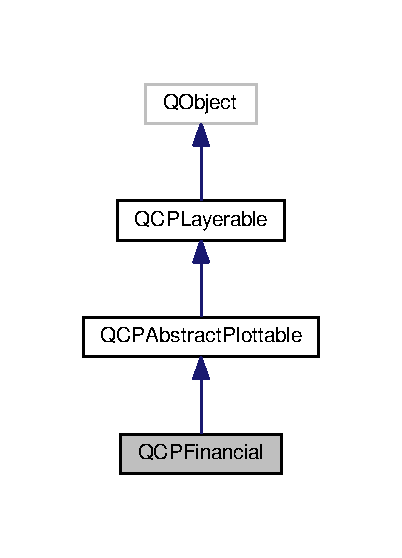
\includegraphics[width=193pt]{classQCPFinancial__inherit__graph}
\end{center}
\end{figure}


Collaboration diagram for Q\+C\+P\+Financial\+:
\nopagebreak
\begin{figure}[H]
\begin{center}
\leavevmode
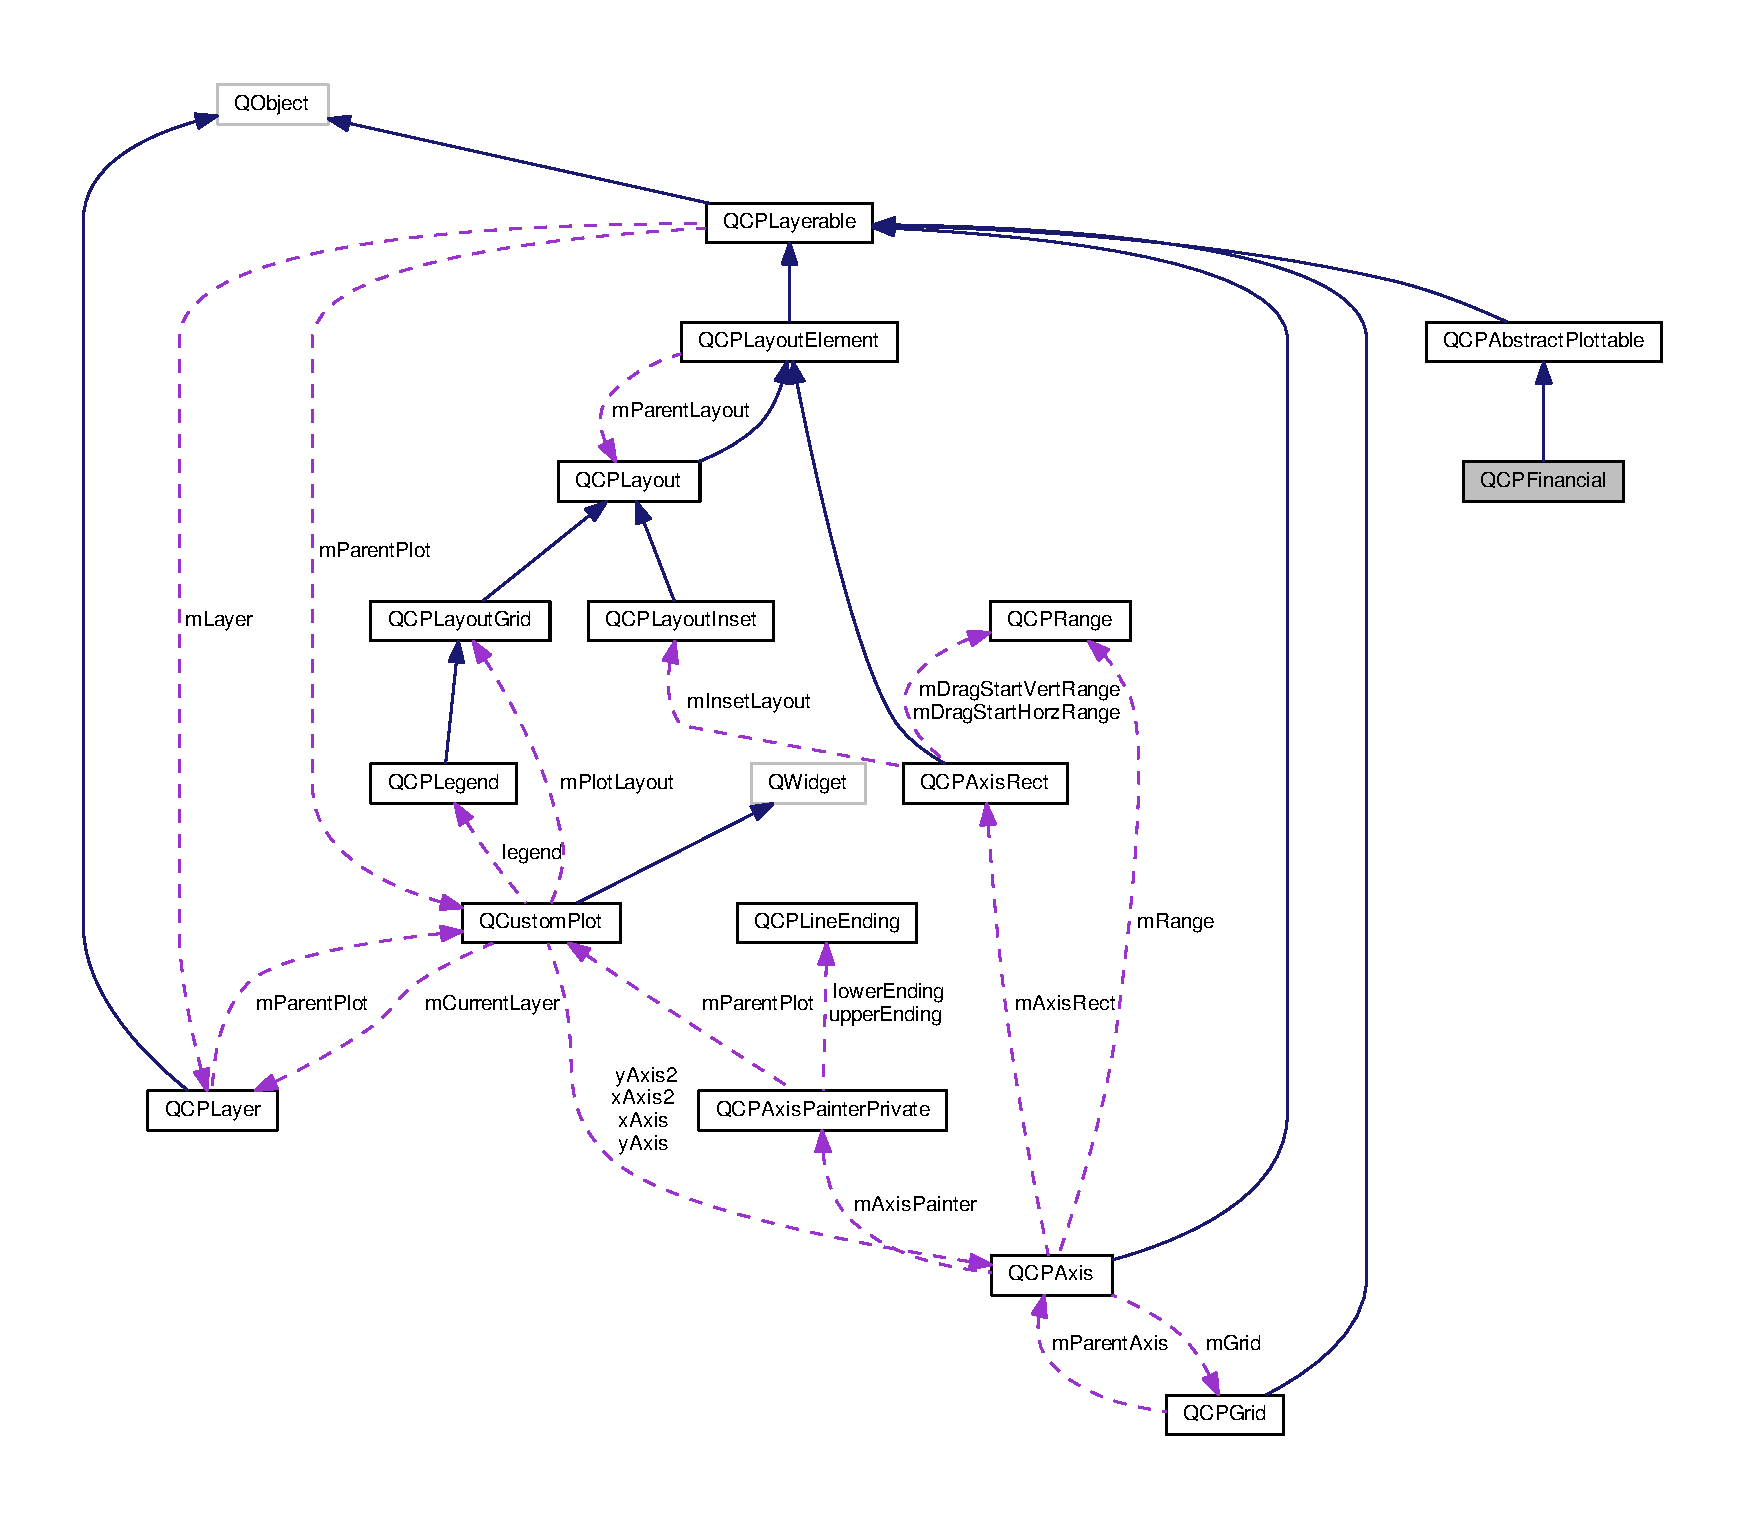
\includegraphics[width=350pt]{classQCPFinancial__coll__graph}
\end{center}
\end{figure}
\subsection*{Public Types}
\begin{DoxyCompactItemize}
\item 
enum \hyperlink{classQCPFinancial_a0f800e21ee98d646dfc6f8f89d10ebfb}{Chart\+Style} \{ \hyperlink{classQCPFinancial_a0f800e21ee98d646dfc6f8f89d10ebfba3a516016c9298d3e95dd82aa203c4390}{cs\+Ohlc}, 
\hyperlink{classQCPFinancial_a0f800e21ee98d646dfc6f8f89d10ebfbac803cbd39f26e3f206bcc7028679e62f}{cs\+Candlestick}
 \}
\end{DoxyCompactItemize}
\subsection*{Public Member Functions}
\begin{DoxyCompactItemize}
\item 
\hyperlink{classQCPFinancial_a4702d5248feeb9d1ec6e3ce725b10b32}{Q\+C\+P\+Financial} (\hyperlink{classQCPAxis}{Q\+C\+P\+Axis} $\ast$\hyperlink{classQCPAbstractPlottable_a72c7a09c22963f2c943f07112b311103}{key\+Axis}, \hyperlink{classQCPAxis}{Q\+C\+P\+Axis} $\ast$\hyperlink{classQCPAbstractPlottable_a3106f9d34d330a6097a8ec5905e5b519}{value\+Axis})
\item 
virtual \hyperlink{classQCPFinancial_ad1fda0d793797b66819fac4682b10f31}{$\sim$\+Q\+C\+P\+Financial} ()
\item 
\hyperlink{qcustomplot_8h_a745c09823fae0974b50beca9bc3b3d7d}{Q\+C\+P\+Financial\+Data\+Map} $\ast$ \hyperlink{classQCPFinancial_a58e05aefa057d16edfcc0334cf81c241}{data} () const 
\item 
\hyperlink{classQCPFinancial_a0f800e21ee98d646dfc6f8f89d10ebfb}{Chart\+Style} \hyperlink{classQCPFinancial_a0888c9308cc5fcb4daa70184f9582412}{chart\+Style} () const 
\item 
double \hyperlink{classQCPFinancial_a71ccaa04cdade0ec08a2117db6e4a4ce}{width} () const 
\item 
bool \hyperlink{classQCPFinancial_a2bab30fc4eee38a0da3a05846b8d7ac7}{two\+Colored} () const 
\item 
Q\+Brush \hyperlink{classQCPFinancial_acb69536a334fae7fc31b2bfd4eca81f5}{brush\+Positive} () const 
\item 
Q\+Brush \hyperlink{classQCPFinancial_a91e09b31ce341c17b917e77fdc68d84e}{brush\+Negative} () const 
\item 
Q\+Pen \hyperlink{classQCPFinancial_a544899bde79d06e17ccefcb9926d87ce}{pen\+Positive} () const 
\item 
Q\+Pen \hyperlink{classQCPFinancial_a557fe911aa04f70c1734c8fa09994148}{pen\+Negative} () const 
\item 
void \hyperlink{classQCPFinancial_adf12a86082f1e488df6a4e8603f8fd6d}{set\+Data} (\hyperlink{qcustomplot_8h_a745c09823fae0974b50beca9bc3b3d7d}{Q\+C\+P\+Financial\+Data\+Map} $\ast$\hyperlink{classQCPFinancial_a58e05aefa057d16edfcc0334cf81c241}{data}, bool copy=false)
\item 
void \hyperlink{classQCPFinancial_a886881339d6447432af55adaad748c3c}{set\+Data} (const Q\+Vector$<$ double $>$ \&key, const Q\+Vector$<$ double $>$ \&open, const Q\+Vector$<$ double $>$ \&high, const Q\+Vector$<$ double $>$ \&low, const Q\+Vector$<$ double $>$ \&close)
\item 
void \hyperlink{classQCPFinancial_a5a59175d36279d71596e64d7bb65596f}{set\+Chart\+Style} (\hyperlink{classQCPFinancial_a0f800e21ee98d646dfc6f8f89d10ebfb}{Chart\+Style} style)
\item 
void \hyperlink{classQCPFinancial_a99633f8bac86a61d534ae5eeb1a3068f}{set\+Width} (double \hyperlink{classQCPFinancial_a71ccaa04cdade0ec08a2117db6e4a4ce}{width})
\item 
void \hyperlink{classQCPFinancial_a138e44aac160a17a9676652e240c5f08}{set\+Two\+Colored} (bool \hyperlink{classQCPFinancial_a2bab30fc4eee38a0da3a05846b8d7ac7}{two\+Colored})
\item 
void \hyperlink{classQCPFinancial_a5ebff2b1764efd07cc44942e67821829}{set\+Brush\+Positive} (const Q\+Brush \&\hyperlink{classQCPAbstractPlottable_aa74cdceb9c7286ef116fbfa58e0326e7}{brush})
\item 
void \hyperlink{classQCPFinancial_a8bbdd87629f9144b3ef51af660c0961a}{set\+Brush\+Negative} (const Q\+Brush \&\hyperlink{classQCPAbstractPlottable_aa74cdceb9c7286ef116fbfa58e0326e7}{brush})
\item 
void \hyperlink{classQCPFinancial_ac58aa3adc7a35aab0088764b840683e5}{set\+Pen\+Positive} (const Q\+Pen \&\hyperlink{classQCPAbstractPlottable_a41d060007cc6b3037c9c04d22d0c0398}{pen})
\item 
void \hyperlink{classQCPFinancial_afe5c07e94ccea01a75b3a2476993c346}{set\+Pen\+Negative} (const Q\+Pen \&\hyperlink{classQCPAbstractPlottable_a41d060007cc6b3037c9c04d22d0c0398}{pen})
\item 
void \hyperlink{classQCPFinancial_a1a83396f97fcc68f2b7aa8d9782feffe}{add\+Data} (const \hyperlink{qcustomplot_8h_a745c09823fae0974b50beca9bc3b3d7d}{Q\+C\+P\+Financial\+Data\+Map} \&data\+Map)
\item 
void \hyperlink{classQCPFinancial_a3b6144b48a6a8e63236fc5bf70d40c00}{add\+Data} (const \hyperlink{classQCPFinancialData}{Q\+C\+P\+Financial\+Data} \&\hyperlink{classQCPFinancial_a58e05aefa057d16edfcc0334cf81c241}{data})
\item 
void \hyperlink{classQCPFinancial_a688bbd052e00a02954ddb0068b378170}{add\+Data} (double key, double open, double high, double low, double close)
\item 
void \hyperlink{classQCPFinancial_aa1abe3bdafb297497f09cdbdc4db3958}{add\+Data} (const Q\+Vector$<$ double $>$ \&key, const Q\+Vector$<$ double $>$ \&open, const Q\+Vector$<$ double $>$ \&high, const Q\+Vector$<$ double $>$ \&low, const Q\+Vector$<$ double $>$ \&close)
\item 
void \hyperlink{classQCPFinancial_a097c0383c7c1e9042ca7f93cb439d15a}{remove\+Data\+Before} (double key)
\item 
void \hyperlink{classQCPFinancial_aa0fcd357005288c833a230c7874825ba}{remove\+Data\+After} (double key)
\item 
void \hyperlink{classQCPFinancial_a048c741d3c8cc5709c2c44b759fdf27c}{remove\+Data} (double from\+Key, double to\+Key)
\item 
void \hyperlink{classQCPFinancial_ae527d8a11290906b083d1ab598c380ea}{remove\+Data} (double key)
\item 
virtual void \hyperlink{classQCPFinancial_a11fd49928c33e55e27b7319c6927864a}{clear\+Data} ()
\item 
virtual double \hyperlink{classQCPFinancial_adf6cff00a55f775487d375fe4df5e95b}{select\+Test} (const Q\+PointF \&pos, bool only\+Selectable, Q\+Variant $\ast$details=0) const 
\end{DoxyCompactItemize}
\subsection*{Static Public Member Functions}
\begin{DoxyCompactItemize}
\item 
static \hyperlink{qcustomplot_8h_a745c09823fae0974b50beca9bc3b3d7d}{Q\+C\+P\+Financial\+Data\+Map} \hyperlink{classQCPFinancial_a0c3453d1c03e320950fdd2df54e3ebc8}{time\+Series\+To\+Ohlc} (const Q\+Vector$<$ double $>$ \&time, const Q\+Vector$<$ double $>$ \&value, double time\+Bin\+Size, double time\+Bin\+Offset=0)
\end{DoxyCompactItemize}
\subsection*{Protected Member Functions}
\begin{DoxyCompactItemize}
\item 
virtual void \hyperlink{classQCPFinancial_ad71a59a1b42616594831e04e52c92120}{draw} (\hyperlink{classQCPPainter}{Q\+C\+P\+Painter} $\ast$painter)
\item 
virtual void \hyperlink{classQCPFinancial_aca85e8435b092cc8c3e5de65fcfb22c8}{draw\+Legend\+Icon} (\hyperlink{classQCPPainter}{Q\+C\+P\+Painter} $\ast$painter, const Q\+RectF \&rect) const 
\item 
virtual \hyperlink{classQCPRange}{Q\+C\+P\+Range} \hyperlink{classQCPFinancial_acc747f4a9b4fddfb14eb9d803349a534}{get\+Key\+Range} (bool \&found\+Range, \hyperlink{classQCPAbstractPlottable_a661743478a1d3c09d28ec2711d7653d8}{Sign\+Domain} in\+Sign\+Domain=\hyperlink{classQCPAbstractPlottable_a661743478a1d3c09d28ec2711d7653d8a082b98cfb91a7363a3b5cd17b0c1cd60}{sd\+Both}) const 
\item 
virtual \hyperlink{classQCPRange}{Q\+C\+P\+Range} \hyperlink{classQCPFinancial_ab2b5f3ef9a503ba32ead32081333f4e7}{get\+Value\+Range} (bool \&found\+Range, \hyperlink{classQCPAbstractPlottable_a661743478a1d3c09d28ec2711d7653d8}{Sign\+Domain} in\+Sign\+Domain=\hyperlink{classQCPAbstractPlottable_a661743478a1d3c09d28ec2711d7653d8a082b98cfb91a7363a3b5cd17b0c1cd60}{sd\+Both}) const 
\item 
void \hyperlink{classQCPFinancial_a3c3007a7434e29d042c77ccf4f497e66}{draw\+Ohlc\+Plot} (\hyperlink{classQCPPainter}{Q\+C\+P\+Painter} $\ast$painter, const Q\+C\+P\+Financial\+Data\+Map\+::const\+\_\+iterator \&begin, const Q\+C\+P\+Financial\+Data\+Map\+::const\+\_\+iterator \&end)
\item 
void \hyperlink{classQCPFinancial_a71f5081da0e5ab9c40a488ad40cff122}{draw\+Candlestick\+Plot} (\hyperlink{classQCPPainter}{Q\+C\+P\+Painter} $\ast$painter, const Q\+C\+P\+Financial\+Data\+Map\+::const\+\_\+iterator \&begin, const Q\+C\+P\+Financial\+Data\+Map\+::const\+\_\+iterator \&end)
\item 
double \hyperlink{classQCPFinancial_a9c7d79351e728a67bfb6821c1d1bd6c0}{ohlc\+Select\+Test} (const Q\+PointF \&pos, const Q\+C\+P\+Financial\+Data\+Map\+::const\+\_\+iterator \&begin, const Q\+C\+P\+Financial\+Data\+Map\+::const\+\_\+iterator \&end) const 
\item 
double \hyperlink{classQCPFinancial_abd0137244a17d5486a01ee442b083333}{candlestick\+Select\+Test} (const Q\+PointF \&pos, const Q\+C\+P\+Financial\+Data\+Map\+::const\+\_\+iterator \&begin, const Q\+C\+P\+Financial\+Data\+Map\+::const\+\_\+iterator \&end) const 
\item 
void \hyperlink{classQCPFinancial_aca2edf9f19fae733cdb6bd4549019b84}{get\+Visible\+Data\+Bounds} (Q\+C\+P\+Financial\+Data\+Map\+::const\+\_\+iterator \&lower, Q\+C\+P\+Financial\+Data\+Map\+::const\+\_\+iterator \&upper) const 
\end{DoxyCompactItemize}
\subsection*{Protected Attributes}
\begin{DoxyCompactItemize}
\item 
\hyperlink{qcustomplot_8h_a745c09823fae0974b50beca9bc3b3d7d}{Q\+C\+P\+Financial\+Data\+Map} $\ast$ \hyperlink{classQCPFinancial_a475f63587ca1077d8c30aaf2b71ae026}{m\+Data}
\item 
\hyperlink{classQCPFinancial_a0f800e21ee98d646dfc6f8f89d10ebfb}{Chart\+Style} \hyperlink{classQCPFinancial_ab65c2ce8d6354451870bb44b894c1e92}{m\+Chart\+Style}
\item 
double \hyperlink{classQCPFinancial_af630e5eb8485146b9c777e63fd1cf993}{m\+Width}
\item 
bool \hyperlink{classQCPFinancial_a6afe919190b884d9bac026cefcc8c0a8}{m\+Two\+Colored}
\item 
Q\+Brush \hyperlink{classQCPFinancial_ab7e6eed16260a2f88ca6bd940dffea79}{m\+Brush\+Positive}
\item 
Q\+Brush \hyperlink{classQCPFinancial_acb0e31874b7a1deb56bd42e8ab3e68f2}{m\+Brush\+Negative}
\item 
Q\+Pen \hyperlink{classQCPFinancial_aa6599186f417ba615caebb3f6c762bd8}{m\+Pen\+Positive}
\item 
Q\+Pen \hyperlink{classQCPFinancial_a263fbfefde2cc19c8d4024a8319c2bbb}{m\+Pen\+Negative}
\end{DoxyCompactItemize}
\subsection*{Friends}
\begin{DoxyCompactItemize}
\item 
class \hyperlink{classQCPFinancial_a1cdf9df76adcfae45261690aa0ca2198}{Q\+Custom\+Plot}
\item 
class \hyperlink{classQCPFinancial_a8429035e7adfbd7f05805a6530ad5e3b}{Q\+C\+P\+Legend}
\end{DoxyCompactItemize}
\subsection*{Additional Inherited Members}


\subsection{Detailed Description}
A plottable representing a financial stock chart. 



This plottable represents time series data binned to certain intervals, mainly used for stock charts. The two common representations O\+H\+LC (Open-\/\+High-\/\+Low-\/\+Close) bars and Candlesticks can be set via \hyperlink{classQCPFinancial_a5a59175d36279d71596e64d7bb65596f}{set\+Chart\+Style}.

The data is passed via \hyperlink{classQCPFinancial_adf12a86082f1e488df6a4e8603f8fd6d}{set\+Data} as a set of open/high/low/close values at certain keys (typically times). This means the data must be already binned appropriately. If data is only available as a series of values (e.\+g. {\itshape price} against {\itshape time}), you can use the static convenience function \hyperlink{classQCPFinancial_a0c3453d1c03e320950fdd2df54e3ebc8}{time\+Series\+To\+Ohlc} to generate binned O\+H\+L\+C-\/data which can then be passed to \hyperlink{classQCPFinancial_adf12a86082f1e488df6a4e8603f8fd6d}{set\+Data}.

The width of the O\+H\+LC bars/candlesticks can be controlled with \hyperlink{classQCPFinancial_a99633f8bac86a61d534ae5eeb1a3068f}{set\+Width} and is given in plot key coordinates. A typical choice is to set it to (or slightly less than) one bin interval width.\hypertarget{classQCPStatisticalBox_appearance}{}\subsection{Changing the appearance}\label{classQCPStatisticalBox_appearance}
Charts can be either single-\/ or two-\/colored (\hyperlink{classQCPFinancial_a138e44aac160a17a9676652e240c5f08}{set\+Two\+Colored}). If set to be single-\/colored, lines are drawn with the plottable\textquotesingle{}s pen (\hyperlink{classQCPAbstractPlottable_ab74b09ae4c0e7e13142fe4b5bf46cac7}{set\+Pen}) and fills with the brush (\hyperlink{classQCPAbstractPlottable_a7a4b92144dca6453a1f0f210e27edc74}{set\+Brush}).

If set to two-\/colored, positive changes of the value during an interval ({\itshape close} $>$= {\itshape open}) are represented with a different pen and brush than negative changes ({\itshape close} $<$ {\itshape open}). These can be configured with \hyperlink{classQCPFinancial_ac58aa3adc7a35aab0088764b840683e5}{set\+Pen\+Positive}, \hyperlink{classQCPFinancial_afe5c07e94ccea01a75b3a2476993c346}{set\+Pen\+Negative}, \hyperlink{classQCPFinancial_a5ebff2b1764efd07cc44942e67821829}{set\+Brush\+Positive}, and \hyperlink{classQCPFinancial_a8bbdd87629f9144b3ef51af660c0961a}{set\+Brush\+Negative}. In two-\/colored mode, the normal plottable pen/brush is ignored. Upon selection however, the normal selected pen/brush (\hyperlink{classQCPAbstractPlottable_a6911603cad23ab0469b108224517516f}{set\+Selected\+Pen}, \hyperlink{classQCPAbstractPlottable_ae8c816874089f7a44001e8618e81a9dc}{set\+Selected\+Brush}) is used, irrespective of whether the chart is single-\/ or two-\/colored. 

\subsection{Member Enumeration Documentation}
\index{Q\+C\+P\+Financial@{Q\+C\+P\+Financial}!Chart\+Style@{Chart\+Style}}
\index{Chart\+Style@{Chart\+Style}!Q\+C\+P\+Financial@{Q\+C\+P\+Financial}}
\subsubsection[{\texorpdfstring{Chart\+Style}{ChartStyle}}]{\setlength{\rightskip}{0pt plus 5cm}enum {\bf Q\+C\+P\+Financial\+::\+Chart\+Style}}\hypertarget{classQCPFinancial_a0f800e21ee98d646dfc6f8f89d10ebfb}{}\label{classQCPFinancial_a0f800e21ee98d646dfc6f8f89d10ebfb}
Defines the possible representations of O\+H\+LC data in the plot.

\begin{DoxySeeAlso}{See also}
\hyperlink{classQCPFinancial_a5a59175d36279d71596e64d7bb65596f}{set\+Chart\+Style} 
\end{DoxySeeAlso}
\begin{Desc}
\item[Enumerator]\par
\begin{description}
\index{cs\+Ohlc@{cs\+Ohlc}!Q\+C\+P\+Financial@{Q\+C\+P\+Financial}}\index{Q\+C\+P\+Financial@{Q\+C\+P\+Financial}!cs\+Ohlc@{cs\+Ohlc}}\item[{\em 
cs\+Ohlc\hypertarget{classQCPFinancial_a0f800e21ee98d646dfc6f8f89d10ebfba3a516016c9298d3e95dd82aa203c4390}{}\label{classQCPFinancial_a0f800e21ee98d646dfc6f8f89d10ebfba3a516016c9298d3e95dd82aa203c4390}
}]Open-\/\+High-\/\+Low-\/\+Close bar representation. \index{cs\+Candlestick@{cs\+Candlestick}!Q\+C\+P\+Financial@{Q\+C\+P\+Financial}}\index{Q\+C\+P\+Financial@{Q\+C\+P\+Financial}!cs\+Candlestick@{cs\+Candlestick}}\item[{\em 
cs\+Candlestick\hypertarget{classQCPFinancial_a0f800e21ee98d646dfc6f8f89d10ebfbac803cbd39f26e3f206bcc7028679e62f}{}\label{classQCPFinancial_a0f800e21ee98d646dfc6f8f89d10ebfbac803cbd39f26e3f206bcc7028679e62f}
}]Candlestick representation. \end{description}
\end{Desc}


\subsection{Constructor \& Destructor Documentation}
\index{Q\+C\+P\+Financial@{Q\+C\+P\+Financial}!Q\+C\+P\+Financial@{Q\+C\+P\+Financial}}
\index{Q\+C\+P\+Financial@{Q\+C\+P\+Financial}!Q\+C\+P\+Financial@{Q\+C\+P\+Financial}}
\subsubsection[{\texorpdfstring{Q\+C\+P\+Financial(\+Q\+C\+P\+Axis $\ast$key\+Axis, Q\+C\+P\+Axis $\ast$value\+Axis)}{QCPFinancial(QCPAxis *keyAxis, QCPAxis *valueAxis)}}]{\setlength{\rightskip}{0pt plus 5cm}Q\+C\+P\+Financial\+::\+Q\+C\+P\+Financial (
\begin{DoxyParamCaption}
\item[{{\bf Q\+C\+P\+Axis} $\ast$}]{key\+Axis, }
\item[{{\bf Q\+C\+P\+Axis} $\ast$}]{value\+Axis}
\end{DoxyParamCaption}
)\hspace{0.3cm}{\ttfamily [explicit]}}\hypertarget{classQCPFinancial_a4702d5248feeb9d1ec6e3ce725b10b32}{}\label{classQCPFinancial_a4702d5248feeb9d1ec6e3ce725b10b32}
Constructs a financial chart which uses {\itshape key\+Axis} as its key axis (\char`\"{}x\char`\"{}) and {\itshape value\+Axis} as its value axis (\char`\"{}y\char`\"{}). {\itshape key\+Axis} and {\itshape value\+Axis} must reside in the same \hyperlink{classQCustomPlot}{Q\+Custom\+Plot} instance and not have the same orientation. If either of these restrictions is violated, a corresponding message is printed to the debug output (q\+Debug), the construction is not aborted, though.

The constructed \hyperlink{classQCPFinancial}{Q\+C\+P\+Financial} can be added to the plot with \hyperlink{classQCustomPlot_ab7ad9174f701f9c6f64e378df77927a6}{Q\+Custom\+Plot\+::add\+Plottable}, \hyperlink{classQCustomPlot}{Q\+Custom\+Plot} then takes ownership of the financial chart. \index{Q\+C\+P\+Financial@{Q\+C\+P\+Financial}!````~Q\+C\+P\+Financial@{$\sim$\+Q\+C\+P\+Financial}}
\index{````~Q\+C\+P\+Financial@{$\sim$\+Q\+C\+P\+Financial}!Q\+C\+P\+Financial@{Q\+C\+P\+Financial}}
\subsubsection[{\texorpdfstring{$\sim$\+Q\+C\+P\+Financial()}{~QCPFinancial()}}]{\setlength{\rightskip}{0pt plus 5cm}Q\+C\+P\+Financial\+::$\sim$\+Q\+C\+P\+Financial (
\begin{DoxyParamCaption}
{}
\end{DoxyParamCaption}
)\hspace{0.3cm}{\ttfamily [virtual]}}\hypertarget{classQCPFinancial_ad1fda0d793797b66819fac4682b10f31}{}\label{classQCPFinancial_ad1fda0d793797b66819fac4682b10f31}


\subsection{Member Function Documentation}
\index{Q\+C\+P\+Financial@{Q\+C\+P\+Financial}!add\+Data@{add\+Data}}
\index{add\+Data@{add\+Data}!Q\+C\+P\+Financial@{Q\+C\+P\+Financial}}
\subsubsection[{\texorpdfstring{add\+Data(const Q\+C\+P\+Financial\+Data\+Map \&data\+Map)}{addData(const QCPFinancialDataMap &dataMap)}}]{\setlength{\rightskip}{0pt plus 5cm}void Q\+C\+P\+Financial\+::add\+Data (
\begin{DoxyParamCaption}
\item[{const {\bf Q\+C\+P\+Financial\+Data\+Map} \&}]{data\+Map}
\end{DoxyParamCaption}
)}\hypertarget{classQCPFinancial_a1a83396f97fcc68f2b7aa8d9782feffe}{}\label{classQCPFinancial_a1a83396f97fcc68f2b7aa8d9782feffe}
Adds the provided data points in {\itshape data\+Map} to the current data.

Alternatively, you can also access and modify the data via the \hyperlink{classQCPFinancial_a58e05aefa057d16edfcc0334cf81c241}{data} method, which returns a pointer to the internal \hyperlink{qcustomplot_8h_a745c09823fae0974b50beca9bc3b3d7d}{Q\+C\+P\+Financial\+Data\+Map}.

\begin{DoxySeeAlso}{See also}
\hyperlink{classQCPFinancial_a048c741d3c8cc5709c2c44b759fdf27c}{remove\+Data} 
\end{DoxySeeAlso}
\index{Q\+C\+P\+Financial@{Q\+C\+P\+Financial}!add\+Data@{add\+Data}}
\index{add\+Data@{add\+Data}!Q\+C\+P\+Financial@{Q\+C\+P\+Financial}}
\subsubsection[{\texorpdfstring{add\+Data(const Q\+C\+P\+Financial\+Data \&data)}{addData(const QCPFinancialData &data)}}]{\setlength{\rightskip}{0pt plus 5cm}void Q\+C\+P\+Financial\+::add\+Data (
\begin{DoxyParamCaption}
\item[{const {\bf Q\+C\+P\+Financial\+Data} \&}]{data}
\end{DoxyParamCaption}
)}\hypertarget{classQCPFinancial_a3b6144b48a6a8e63236fc5bf70d40c00}{}\label{classQCPFinancial_a3b6144b48a6a8e63236fc5bf70d40c00}
This is an overloaded member function, provided for convenience. It differs from the above function only in what argument(s) it accepts.

Adds the provided single data point in {\itshape data} to the current data.

Alternatively, you can also access and modify the data via the \hyperlink{classQCPFinancial_a58e05aefa057d16edfcc0334cf81c241}{data} method, which returns a pointer to the internal \hyperlink{classQCPFinancialData}{Q\+C\+P\+Financial\+Data}.

\begin{DoxySeeAlso}{See also}
\hyperlink{classQCPFinancial_a048c741d3c8cc5709c2c44b759fdf27c}{remove\+Data} 
\end{DoxySeeAlso}
\index{Q\+C\+P\+Financial@{Q\+C\+P\+Financial}!add\+Data@{add\+Data}}
\index{add\+Data@{add\+Data}!Q\+C\+P\+Financial@{Q\+C\+P\+Financial}}
\subsubsection[{\texorpdfstring{add\+Data(double key, double open, double high, double low, double close)}{addData(double key, double open, double high, double low, double close)}}]{\setlength{\rightskip}{0pt plus 5cm}void Q\+C\+P\+Financial\+::add\+Data (
\begin{DoxyParamCaption}
\item[{double}]{key, }
\item[{double}]{open, }
\item[{double}]{high, }
\item[{double}]{low, }
\item[{double}]{close}
\end{DoxyParamCaption}
)}\hypertarget{classQCPFinancial_a688bbd052e00a02954ddb0068b378170}{}\label{classQCPFinancial_a688bbd052e00a02954ddb0068b378170}
This is an overloaded member function, provided for convenience. It differs from the above function only in what argument(s) it accepts.

Adds the provided single data point given by {\itshape key}, {\itshape open}, {\itshape high}, {\itshape low}, and {\itshape close} to the current data.

Alternatively, you can also access and modify the data via the \hyperlink{classQCPFinancial_a58e05aefa057d16edfcc0334cf81c241}{data} method, which returns a pointer to the internal \hyperlink{classQCPFinancialData}{Q\+C\+P\+Financial\+Data}.

\begin{DoxySeeAlso}{See also}
\hyperlink{classQCPFinancial_a048c741d3c8cc5709c2c44b759fdf27c}{remove\+Data} 
\end{DoxySeeAlso}
\index{Q\+C\+P\+Financial@{Q\+C\+P\+Financial}!add\+Data@{add\+Data}}
\index{add\+Data@{add\+Data}!Q\+C\+P\+Financial@{Q\+C\+P\+Financial}}
\subsubsection[{\texorpdfstring{add\+Data(const Q\+Vector$<$ double $>$ \&key, const Q\+Vector$<$ double $>$ \&open, const Q\+Vector$<$ double $>$ \&high, const Q\+Vector$<$ double $>$ \&low, const Q\+Vector$<$ double $>$ \&close)}{addData(const QVector< double > &key, const QVector< double > &open, const QVector< double > &high, const QVector< double > &low, const QVector< double > &close)}}]{\setlength{\rightskip}{0pt plus 5cm}void Q\+C\+P\+Financial\+::add\+Data (
\begin{DoxyParamCaption}
\item[{const Q\+Vector$<$ double $>$ \&}]{key, }
\item[{const Q\+Vector$<$ double $>$ \&}]{open, }
\item[{const Q\+Vector$<$ double $>$ \&}]{high, }
\item[{const Q\+Vector$<$ double $>$ \&}]{low, }
\item[{const Q\+Vector$<$ double $>$ \&}]{close}
\end{DoxyParamCaption}
)}\hypertarget{classQCPFinancial_aa1abe3bdafb297497f09cdbdc4db3958}{}\label{classQCPFinancial_aa1abe3bdafb297497f09cdbdc4db3958}
This is an overloaded member function, provided for convenience. It differs from the above function only in what argument(s) it accepts.

Adds the provided open/high/low/close data to the current data.

Alternatively, you can also access and modify the data via the \hyperlink{classQCPFinancial_a58e05aefa057d16edfcc0334cf81c241}{data} method, which returns a pointer to the internal \hyperlink{classQCPFinancialData}{Q\+C\+P\+Financial\+Data}.

\begin{DoxySeeAlso}{See also}
\hyperlink{classQCPFinancial_a048c741d3c8cc5709c2c44b759fdf27c}{remove\+Data} 
\end{DoxySeeAlso}
\index{Q\+C\+P\+Financial@{Q\+C\+P\+Financial}!brush\+Negative@{brush\+Negative}}
\index{brush\+Negative@{brush\+Negative}!Q\+C\+P\+Financial@{Q\+C\+P\+Financial}}
\subsubsection[{\texorpdfstring{brush\+Negative() const }{brushNegative() const }}]{\setlength{\rightskip}{0pt plus 5cm}Q\+Brush Q\+C\+P\+Financial\+::brush\+Negative (
\begin{DoxyParamCaption}
{}
\end{DoxyParamCaption}
) const\hspace{0.3cm}{\ttfamily [inline]}}\hypertarget{classQCPFinancial_a91e09b31ce341c17b917e77fdc68d84e}{}\label{classQCPFinancial_a91e09b31ce341c17b917e77fdc68d84e}
\index{Q\+C\+P\+Financial@{Q\+C\+P\+Financial}!brush\+Positive@{brush\+Positive}}
\index{brush\+Positive@{brush\+Positive}!Q\+C\+P\+Financial@{Q\+C\+P\+Financial}}
\subsubsection[{\texorpdfstring{brush\+Positive() const }{brushPositive() const }}]{\setlength{\rightskip}{0pt plus 5cm}Q\+Brush Q\+C\+P\+Financial\+::brush\+Positive (
\begin{DoxyParamCaption}
{}
\end{DoxyParamCaption}
) const\hspace{0.3cm}{\ttfamily [inline]}}\hypertarget{classQCPFinancial_acb69536a334fae7fc31b2bfd4eca81f5}{}\label{classQCPFinancial_acb69536a334fae7fc31b2bfd4eca81f5}
\index{Q\+C\+P\+Financial@{Q\+C\+P\+Financial}!candlestick\+Select\+Test@{candlestick\+Select\+Test}}
\index{candlestick\+Select\+Test@{candlestick\+Select\+Test}!Q\+C\+P\+Financial@{Q\+C\+P\+Financial}}
\subsubsection[{\texorpdfstring{candlestick\+Select\+Test(const Q\+Point\+F \&pos, const Q\+C\+P\+Financial\+Data\+Map\+::const\+\_\+iterator \&begin, const Q\+C\+P\+Financial\+Data\+Map\+::const\+\_\+iterator \&end) const }{candlestickSelectTest(const QPointF &pos, const QCPFinancialDataMap::const_iterator &begin, const QCPFinancialDataMap::const_iterator &end) const }}]{\setlength{\rightskip}{0pt plus 5cm}double Q\+C\+P\+Financial\+::candlestick\+Select\+Test (
\begin{DoxyParamCaption}
\item[{const Q\+PointF \&}]{pos, }
\item[{const Q\+C\+P\+Financial\+Data\+Map\+::const\+\_\+iterator \&}]{begin, }
\item[{const Q\+C\+P\+Financial\+Data\+Map\+::const\+\_\+iterator \&}]{end}
\end{DoxyParamCaption}
) const\hspace{0.3cm}{\ttfamily [protected]}}\hypertarget{classQCPFinancial_abd0137244a17d5486a01ee442b083333}{}\label{classQCPFinancial_abd0137244a17d5486a01ee442b083333}
\index{Q\+C\+P\+Financial@{Q\+C\+P\+Financial}!chart\+Style@{chart\+Style}}
\index{chart\+Style@{chart\+Style}!Q\+C\+P\+Financial@{Q\+C\+P\+Financial}}
\subsubsection[{\texorpdfstring{chart\+Style() const }{chartStyle() const }}]{\setlength{\rightskip}{0pt plus 5cm}{\bf Chart\+Style} Q\+C\+P\+Financial\+::chart\+Style (
\begin{DoxyParamCaption}
{}
\end{DoxyParamCaption}
) const\hspace{0.3cm}{\ttfamily [inline]}}\hypertarget{classQCPFinancial_a0888c9308cc5fcb4daa70184f9582412}{}\label{classQCPFinancial_a0888c9308cc5fcb4daa70184f9582412}
\index{Q\+C\+P\+Financial@{Q\+C\+P\+Financial}!clear\+Data@{clear\+Data}}
\index{clear\+Data@{clear\+Data}!Q\+C\+P\+Financial@{Q\+C\+P\+Financial}}
\subsubsection[{\texorpdfstring{clear\+Data()}{clearData()}}]{\setlength{\rightskip}{0pt plus 5cm}void Q\+C\+P\+Financial\+::clear\+Data (
\begin{DoxyParamCaption}
{}
\end{DoxyParamCaption}
)\hspace{0.3cm}{\ttfamily [virtual]}}\hypertarget{classQCPFinancial_a11fd49928c33e55e27b7319c6927864a}{}\label{classQCPFinancial_a11fd49928c33e55e27b7319c6927864a}
Removes all data points.

\begin{DoxySeeAlso}{See also}
\hyperlink{classQCPFinancial_a048c741d3c8cc5709c2c44b759fdf27c}{remove\+Data}, \hyperlink{classQCPFinancial_aa0fcd357005288c833a230c7874825ba}{remove\+Data\+After}, \hyperlink{classQCPFinancial_a097c0383c7c1e9042ca7f93cb439d15a}{remove\+Data\+Before} 
\end{DoxySeeAlso}


Implements \hyperlink{classQCPAbstractPlottable_a86e5b8fd4b6ff4f4084e7ea4c573fc53}{Q\+C\+P\+Abstract\+Plottable}.

\index{Q\+C\+P\+Financial@{Q\+C\+P\+Financial}!data@{data}}
\index{data@{data}!Q\+C\+P\+Financial@{Q\+C\+P\+Financial}}
\subsubsection[{\texorpdfstring{data() const }{data() const }}]{\setlength{\rightskip}{0pt plus 5cm}{\bf Q\+C\+P\+Financial\+Data\+Map} $\ast$ Q\+C\+P\+Financial\+::data (
\begin{DoxyParamCaption}
{}
\end{DoxyParamCaption}
) const\hspace{0.3cm}{\ttfamily [inline]}}\hypertarget{classQCPFinancial_a58e05aefa057d16edfcc0334cf81c241}{}\label{classQCPFinancial_a58e05aefa057d16edfcc0334cf81c241}
Returns a pointer to the internal data storage of type \hyperlink{qcustomplot_8h_a745c09823fae0974b50beca9bc3b3d7d}{Q\+C\+P\+Financial\+Data\+Map}. You may use it to directly manipulate the data, which may be more convenient and faster than using the regular \hyperlink{classQCPFinancial_adf12a86082f1e488df6a4e8603f8fd6d}{set\+Data} or \hyperlink{classQCPFinancial_a1a83396f97fcc68f2b7aa8d9782feffe}{add\+Data} methods, in certain situations. \index{Q\+C\+P\+Financial@{Q\+C\+P\+Financial}!draw@{draw}}
\index{draw@{draw}!Q\+C\+P\+Financial@{Q\+C\+P\+Financial}}
\subsubsection[{\texorpdfstring{draw(\+Q\+C\+P\+Painter $\ast$painter)}{draw(QCPPainter *painter)}}]{\setlength{\rightskip}{0pt plus 5cm}void Q\+C\+P\+Financial\+::draw (
\begin{DoxyParamCaption}
\item[{{\bf Q\+C\+P\+Painter} $\ast$}]{painter}
\end{DoxyParamCaption}
)\hspace{0.3cm}{\ttfamily [protected]}, {\ttfamily [virtual]}}\hypertarget{classQCPFinancial_ad71a59a1b42616594831e04e52c92120}{}\label{classQCPFinancial_ad71a59a1b42616594831e04e52c92120}


Implements \hyperlink{classQCPAbstractPlottable_acbab5e30dcd04fd302b4a5902ac2c482}{Q\+C\+P\+Abstract\+Plottable}.

\index{Q\+C\+P\+Financial@{Q\+C\+P\+Financial}!draw\+Candlestick\+Plot@{draw\+Candlestick\+Plot}}
\index{draw\+Candlestick\+Plot@{draw\+Candlestick\+Plot}!Q\+C\+P\+Financial@{Q\+C\+P\+Financial}}
\subsubsection[{\texorpdfstring{draw\+Candlestick\+Plot(\+Q\+C\+P\+Painter $\ast$painter, const Q\+C\+P\+Financial\+Data\+Map\+::const\+\_\+iterator \&begin, const Q\+C\+P\+Financial\+Data\+Map\+::const\+\_\+iterator \&end)}{drawCandlestickPlot(QCPPainter *painter, const QCPFinancialDataMap::const_iterator &begin, const QCPFinancialDataMap::const_iterator &end)}}]{\setlength{\rightskip}{0pt plus 5cm}void Q\+C\+P\+Financial\+::draw\+Candlestick\+Plot (
\begin{DoxyParamCaption}
\item[{{\bf Q\+C\+P\+Painter} $\ast$}]{painter, }
\item[{const Q\+C\+P\+Financial\+Data\+Map\+::const\+\_\+iterator \&}]{begin, }
\item[{const Q\+C\+P\+Financial\+Data\+Map\+::const\+\_\+iterator \&}]{end}
\end{DoxyParamCaption}
)\hspace{0.3cm}{\ttfamily [protected]}}\hypertarget{classQCPFinancial_a71f5081da0e5ab9c40a488ad40cff122}{}\label{classQCPFinancial_a71f5081da0e5ab9c40a488ad40cff122}
\index{Q\+C\+P\+Financial@{Q\+C\+P\+Financial}!draw\+Legend\+Icon@{draw\+Legend\+Icon}}
\index{draw\+Legend\+Icon@{draw\+Legend\+Icon}!Q\+C\+P\+Financial@{Q\+C\+P\+Financial}}
\subsubsection[{\texorpdfstring{draw\+Legend\+Icon(\+Q\+C\+P\+Painter $\ast$painter, const Q\+Rect\+F \&rect) const }{drawLegendIcon(QCPPainter *painter, const QRectF &rect) const }}]{\setlength{\rightskip}{0pt plus 5cm}void Q\+C\+P\+Financial\+::draw\+Legend\+Icon (
\begin{DoxyParamCaption}
\item[{{\bf Q\+C\+P\+Painter} $\ast$}]{painter, }
\item[{const Q\+RectF \&}]{rect}
\end{DoxyParamCaption}
) const\hspace{0.3cm}{\ttfamily [protected]}, {\ttfamily [virtual]}}\hypertarget{classQCPFinancial_aca85e8435b092cc8c3e5de65fcfb22c8}{}\label{classQCPFinancial_aca85e8435b092cc8c3e5de65fcfb22c8}


Implements \hyperlink{classQCPAbstractPlottable_a9a450783fd9ed539e589999fd390cdf7}{Q\+C\+P\+Abstract\+Plottable}.

\index{Q\+C\+P\+Financial@{Q\+C\+P\+Financial}!draw\+Ohlc\+Plot@{draw\+Ohlc\+Plot}}
\index{draw\+Ohlc\+Plot@{draw\+Ohlc\+Plot}!Q\+C\+P\+Financial@{Q\+C\+P\+Financial}}
\subsubsection[{\texorpdfstring{draw\+Ohlc\+Plot(\+Q\+C\+P\+Painter $\ast$painter, const Q\+C\+P\+Financial\+Data\+Map\+::const\+\_\+iterator \&begin, const Q\+C\+P\+Financial\+Data\+Map\+::const\+\_\+iterator \&end)}{drawOhlcPlot(QCPPainter *painter, const QCPFinancialDataMap::const_iterator &begin, const QCPFinancialDataMap::const_iterator &end)}}]{\setlength{\rightskip}{0pt plus 5cm}void Q\+C\+P\+Financial\+::draw\+Ohlc\+Plot (
\begin{DoxyParamCaption}
\item[{{\bf Q\+C\+P\+Painter} $\ast$}]{painter, }
\item[{const Q\+C\+P\+Financial\+Data\+Map\+::const\+\_\+iterator \&}]{begin, }
\item[{const Q\+C\+P\+Financial\+Data\+Map\+::const\+\_\+iterator \&}]{end}
\end{DoxyParamCaption}
)\hspace{0.3cm}{\ttfamily [protected]}}\hypertarget{classQCPFinancial_a3c3007a7434e29d042c77ccf4f497e66}{}\label{classQCPFinancial_a3c3007a7434e29d042c77ccf4f497e66}
\index{Q\+C\+P\+Financial@{Q\+C\+P\+Financial}!get\+Key\+Range@{get\+Key\+Range}}
\index{get\+Key\+Range@{get\+Key\+Range}!Q\+C\+P\+Financial@{Q\+C\+P\+Financial}}
\subsubsection[{\texorpdfstring{get\+Key\+Range(bool \&found\+Range, Sign\+Domain in\+Sign\+Domain=sd\+Both) const }{getKeyRange(bool &foundRange, SignDomain inSignDomain=sdBoth) const }}]{\setlength{\rightskip}{0pt plus 5cm}{\bf Q\+C\+P\+Range} Q\+C\+P\+Financial\+::get\+Key\+Range (
\begin{DoxyParamCaption}
\item[{bool \&}]{found\+Range, }
\item[{{\bf Q\+C\+P\+Abstract\+Plottable\+::\+Sign\+Domain}}]{in\+Sign\+Domain = {\ttfamily {\bf sd\+Both}}}
\end{DoxyParamCaption}
) const\hspace{0.3cm}{\ttfamily [protected]}, {\ttfamily [virtual]}}\hypertarget{classQCPFinancial_acc747f4a9b4fddfb14eb9d803349a534}{}\label{classQCPFinancial_acc747f4a9b4fddfb14eb9d803349a534}


Implements \hyperlink{classQCPAbstractPlottable_a345d702b2e7e12c8cfdddff65ba85e8c}{Q\+C\+P\+Abstract\+Plottable}.

\index{Q\+C\+P\+Financial@{Q\+C\+P\+Financial}!get\+Value\+Range@{get\+Value\+Range}}
\index{get\+Value\+Range@{get\+Value\+Range}!Q\+C\+P\+Financial@{Q\+C\+P\+Financial}}
\subsubsection[{\texorpdfstring{get\+Value\+Range(bool \&found\+Range, Sign\+Domain in\+Sign\+Domain=sd\+Both) const }{getValueRange(bool &foundRange, SignDomain inSignDomain=sdBoth) const }}]{\setlength{\rightskip}{0pt plus 5cm}{\bf Q\+C\+P\+Range} Q\+C\+P\+Financial\+::get\+Value\+Range (
\begin{DoxyParamCaption}
\item[{bool \&}]{found\+Range, }
\item[{{\bf Q\+C\+P\+Abstract\+Plottable\+::\+Sign\+Domain}}]{in\+Sign\+Domain = {\ttfamily {\bf sd\+Both}}}
\end{DoxyParamCaption}
) const\hspace{0.3cm}{\ttfamily [protected]}, {\ttfamily [virtual]}}\hypertarget{classQCPFinancial_ab2b5f3ef9a503ba32ead32081333f4e7}{}\label{classQCPFinancial_ab2b5f3ef9a503ba32ead32081333f4e7}


Implements \hyperlink{classQCPAbstractPlottable_aa3331b415b5939fe4df60b78831b2799}{Q\+C\+P\+Abstract\+Plottable}.

\index{Q\+C\+P\+Financial@{Q\+C\+P\+Financial}!get\+Visible\+Data\+Bounds@{get\+Visible\+Data\+Bounds}}
\index{get\+Visible\+Data\+Bounds@{get\+Visible\+Data\+Bounds}!Q\+C\+P\+Financial@{Q\+C\+P\+Financial}}
\subsubsection[{\texorpdfstring{get\+Visible\+Data\+Bounds(\+Q\+C\+P\+Financial\+Data\+Map\+::const\+\_\+iterator \&lower, Q\+C\+P\+Financial\+Data\+Map\+::const\+\_\+iterator \&upper) const }{getVisibleDataBounds(QCPFinancialDataMap::const_iterator &lower, QCPFinancialDataMap::const_iterator &upper) const }}]{\setlength{\rightskip}{0pt plus 5cm}void Q\+C\+P\+Financial\+::get\+Visible\+Data\+Bounds (
\begin{DoxyParamCaption}
\item[{Q\+C\+P\+Financial\+Data\+Map\+::const\+\_\+iterator \&}]{lower, }
\item[{Q\+C\+P\+Financial\+Data\+Map\+::const\+\_\+iterator \&}]{upper}
\end{DoxyParamCaption}
) const\hspace{0.3cm}{\ttfamily [protected]}}\hypertarget{classQCPFinancial_aca2edf9f19fae733cdb6bd4549019b84}{}\label{classQCPFinancial_aca2edf9f19fae733cdb6bd4549019b84}
\index{Q\+C\+P\+Financial@{Q\+C\+P\+Financial}!ohlc\+Select\+Test@{ohlc\+Select\+Test}}
\index{ohlc\+Select\+Test@{ohlc\+Select\+Test}!Q\+C\+P\+Financial@{Q\+C\+P\+Financial}}
\subsubsection[{\texorpdfstring{ohlc\+Select\+Test(const Q\+Point\+F \&pos, const Q\+C\+P\+Financial\+Data\+Map\+::const\+\_\+iterator \&begin, const Q\+C\+P\+Financial\+Data\+Map\+::const\+\_\+iterator \&end) const }{ohlcSelectTest(const QPointF &pos, const QCPFinancialDataMap::const_iterator &begin, const QCPFinancialDataMap::const_iterator &end) const }}]{\setlength{\rightskip}{0pt plus 5cm}double Q\+C\+P\+Financial\+::ohlc\+Select\+Test (
\begin{DoxyParamCaption}
\item[{const Q\+PointF \&}]{pos, }
\item[{const Q\+C\+P\+Financial\+Data\+Map\+::const\+\_\+iterator \&}]{begin, }
\item[{const Q\+C\+P\+Financial\+Data\+Map\+::const\+\_\+iterator \&}]{end}
\end{DoxyParamCaption}
) const\hspace{0.3cm}{\ttfamily [protected]}}\hypertarget{classQCPFinancial_a9c7d79351e728a67bfb6821c1d1bd6c0}{}\label{classQCPFinancial_a9c7d79351e728a67bfb6821c1d1bd6c0}
\index{Q\+C\+P\+Financial@{Q\+C\+P\+Financial}!pen\+Negative@{pen\+Negative}}
\index{pen\+Negative@{pen\+Negative}!Q\+C\+P\+Financial@{Q\+C\+P\+Financial}}
\subsubsection[{\texorpdfstring{pen\+Negative() const }{penNegative() const }}]{\setlength{\rightskip}{0pt plus 5cm}Q\+Pen Q\+C\+P\+Financial\+::pen\+Negative (
\begin{DoxyParamCaption}
{}
\end{DoxyParamCaption}
) const\hspace{0.3cm}{\ttfamily [inline]}}\hypertarget{classQCPFinancial_a557fe911aa04f70c1734c8fa09994148}{}\label{classQCPFinancial_a557fe911aa04f70c1734c8fa09994148}
\index{Q\+C\+P\+Financial@{Q\+C\+P\+Financial}!pen\+Positive@{pen\+Positive}}
\index{pen\+Positive@{pen\+Positive}!Q\+C\+P\+Financial@{Q\+C\+P\+Financial}}
\subsubsection[{\texorpdfstring{pen\+Positive() const }{penPositive() const }}]{\setlength{\rightskip}{0pt plus 5cm}Q\+Pen Q\+C\+P\+Financial\+::pen\+Positive (
\begin{DoxyParamCaption}
{}
\end{DoxyParamCaption}
) const\hspace{0.3cm}{\ttfamily [inline]}}\hypertarget{classQCPFinancial_a544899bde79d06e17ccefcb9926d87ce}{}\label{classQCPFinancial_a544899bde79d06e17ccefcb9926d87ce}
\index{Q\+C\+P\+Financial@{Q\+C\+P\+Financial}!remove\+Data@{remove\+Data}}
\index{remove\+Data@{remove\+Data}!Q\+C\+P\+Financial@{Q\+C\+P\+Financial}}
\subsubsection[{\texorpdfstring{remove\+Data(double from\+Key, double to\+Key)}{removeData(double fromKey, double toKey)}}]{\setlength{\rightskip}{0pt plus 5cm}void Q\+C\+P\+Financial\+::remove\+Data (
\begin{DoxyParamCaption}
\item[{double}]{from\+Key, }
\item[{double}]{to\+Key}
\end{DoxyParamCaption}
)}\hypertarget{classQCPFinancial_a048c741d3c8cc5709c2c44b759fdf27c}{}\label{classQCPFinancial_a048c741d3c8cc5709c2c44b759fdf27c}
Removes all data points with keys between {\itshape from\+Key} and {\itshape to\+Key}. if {\itshape from\+Key} is greater or equal to {\itshape to\+Key}, the function does nothing. To remove a single data point with known key, use \hyperlink{classQCPFinancial_ae527d8a11290906b083d1ab598c380ea}{remove\+Data(double key)}.

\begin{DoxySeeAlso}{See also}
\hyperlink{classQCPFinancial_a1a83396f97fcc68f2b7aa8d9782feffe}{add\+Data}, \hyperlink{classQCPFinancial_a11fd49928c33e55e27b7319c6927864a}{clear\+Data} 
\end{DoxySeeAlso}
\index{Q\+C\+P\+Financial@{Q\+C\+P\+Financial}!remove\+Data@{remove\+Data}}
\index{remove\+Data@{remove\+Data}!Q\+C\+P\+Financial@{Q\+C\+P\+Financial}}
\subsubsection[{\texorpdfstring{remove\+Data(double key)}{removeData(double key)}}]{\setlength{\rightskip}{0pt plus 5cm}void Q\+C\+P\+Financial\+::remove\+Data (
\begin{DoxyParamCaption}
\item[{double}]{key}
\end{DoxyParamCaption}
)}\hypertarget{classQCPFinancial_ae527d8a11290906b083d1ab598c380ea}{}\label{classQCPFinancial_ae527d8a11290906b083d1ab598c380ea}
This is an overloaded member function, provided for convenience. It differs from the above function only in what argument(s) it accepts.

Removes a single data point at {\itshape key}. If the position is not known with absolute precision, consider using \hyperlink{classQCPFinancial_a048c741d3c8cc5709c2c44b759fdf27c}{remove\+Data(double from\+Key, double to\+Key)} with a small fuzziness interval around the suspected position, depeding on the precision with which the key is known.

\begin{DoxySeeAlso}{See also}
\hyperlink{classQCPFinancial_a1a83396f97fcc68f2b7aa8d9782feffe}{add\+Data}, \hyperlink{classQCPFinancial_a11fd49928c33e55e27b7319c6927864a}{clear\+Data} 
\end{DoxySeeAlso}
\index{Q\+C\+P\+Financial@{Q\+C\+P\+Financial}!remove\+Data\+After@{remove\+Data\+After}}
\index{remove\+Data\+After@{remove\+Data\+After}!Q\+C\+P\+Financial@{Q\+C\+P\+Financial}}
\subsubsection[{\texorpdfstring{remove\+Data\+After(double key)}{removeDataAfter(double key)}}]{\setlength{\rightskip}{0pt plus 5cm}void Q\+C\+P\+Financial\+::remove\+Data\+After (
\begin{DoxyParamCaption}
\item[{double}]{key}
\end{DoxyParamCaption}
)}\hypertarget{classQCPFinancial_aa0fcd357005288c833a230c7874825ba}{}\label{classQCPFinancial_aa0fcd357005288c833a230c7874825ba}
Removes all data points with keys greater than {\itshape key}.

\begin{DoxySeeAlso}{See also}
\hyperlink{classQCPFinancial_a1a83396f97fcc68f2b7aa8d9782feffe}{add\+Data}, \hyperlink{classQCPFinancial_a11fd49928c33e55e27b7319c6927864a}{clear\+Data} 
\end{DoxySeeAlso}
\index{Q\+C\+P\+Financial@{Q\+C\+P\+Financial}!remove\+Data\+Before@{remove\+Data\+Before}}
\index{remove\+Data\+Before@{remove\+Data\+Before}!Q\+C\+P\+Financial@{Q\+C\+P\+Financial}}
\subsubsection[{\texorpdfstring{remove\+Data\+Before(double key)}{removeDataBefore(double key)}}]{\setlength{\rightskip}{0pt plus 5cm}void Q\+C\+P\+Financial\+::remove\+Data\+Before (
\begin{DoxyParamCaption}
\item[{double}]{key}
\end{DoxyParamCaption}
)}\hypertarget{classQCPFinancial_a097c0383c7c1e9042ca7f93cb439d15a}{}\label{classQCPFinancial_a097c0383c7c1e9042ca7f93cb439d15a}
Removes all data points with keys smaller than {\itshape key}.

\begin{DoxySeeAlso}{See also}
\hyperlink{classQCPFinancial_a1a83396f97fcc68f2b7aa8d9782feffe}{add\+Data}, \hyperlink{classQCPFinancial_a11fd49928c33e55e27b7319c6927864a}{clear\+Data} 
\end{DoxySeeAlso}
\index{Q\+C\+P\+Financial@{Q\+C\+P\+Financial}!select\+Test@{select\+Test}}
\index{select\+Test@{select\+Test}!Q\+C\+P\+Financial@{Q\+C\+P\+Financial}}
\subsubsection[{\texorpdfstring{select\+Test(const Q\+Point\+F \&pos, bool only\+Selectable, Q\+Variant $\ast$details=0) const }{selectTest(const QPointF &pos, bool onlySelectable, QVariant *details=0) const }}]{\setlength{\rightskip}{0pt plus 5cm}double Q\+C\+P\+Financial\+::select\+Test (
\begin{DoxyParamCaption}
\item[{const Q\+PointF \&}]{pos, }
\item[{bool}]{only\+Selectable, }
\item[{Q\+Variant $\ast$}]{details = {\ttfamily 0}}
\end{DoxyParamCaption}
) const\hspace{0.3cm}{\ttfamily [virtual]}}\hypertarget{classQCPFinancial_adf6cff00a55f775487d375fe4df5e95b}{}\label{classQCPFinancial_adf6cff00a55f775487d375fe4df5e95b}
This function is used to decide whether a click hits a layerable object or not.

{\itshape pos} is a point in pixel coordinates on the \hyperlink{classQCustomPlot}{Q\+Custom\+Plot} surface. This function returns the shortest pixel distance of this point to the object. If the object is either invisible or the distance couldn\textquotesingle{}t be determined, -\/1.\+0 is returned. Further, if {\itshape only\+Selectable} is true and the object is not selectable, -\/1.\+0 is returned, too.

If the object is represented not by single lines but by an area like a \hyperlink{classQCPItemText}{Q\+C\+P\+Item\+Text} or the bars of a \hyperlink{classQCPBars}{Q\+C\+P\+Bars} plottable, a click inside the area should also be considered a hit. In these cases this function thus returns a constant value greater zero but still below the parent plot\textquotesingle{}s selection tolerance. (typically the selection\+Tolerance multiplied by 0.\+99).

Providing a constant value for area objects allows selecting line objects even when they are obscured by such area objects, by clicking close to the lines (i.\+e. closer than 0.\+99$\ast$selection\+Tolerance).

The actual setting of the selection state is not done by this function. This is handled by the parent \hyperlink{classQCustomPlot}{Q\+Custom\+Plot} when the mouse\+Release\+Event occurs, and the finally selected object is notified via the select\+Event/deselect\+Event methods.

{\itshape details} is an optional output parameter. Every layerable subclass may place any information in {\itshape details}. This information will be passed to \hyperlink{classQCPAbstractPlottable_a16aaad02456aa23a759efd1ac90c79bf}{select\+Event} when the parent \hyperlink{classQCustomPlot}{Q\+Custom\+Plot} decides on the basis of this select\+Test call, that the object was successfully selected. The subsequent call to \hyperlink{classQCPAbstractPlottable_a16aaad02456aa23a759efd1ac90c79bf}{select\+Event} will carry the {\itshape details}. This is useful for multi-\/part objects (like \hyperlink{classQCPAxis}{Q\+C\+P\+Axis}). This way, a possibly complex calculation to decide which part was clicked is only done once in \hyperlink{classQCPFinancial_adf6cff00a55f775487d375fe4df5e95b}{select\+Test}. The result (i.\+e. the actually clicked part) can then be placed in {\itshape details}. So in the subsequent \hyperlink{classQCPAbstractPlottable_a16aaad02456aa23a759efd1ac90c79bf}{select\+Event}, the decision which part was selected doesn\textquotesingle{}t have to be done a second time for a single selection operation.

You may pass 0 as {\itshape details} to indicate that you are not interested in those selection details.

\begin{DoxySeeAlso}{See also}
\hyperlink{classQCPAbstractPlottable_a16aaad02456aa23a759efd1ac90c79bf}{select\+Event}, \hyperlink{classQCPAbstractPlottable_a6fa0d0f95560ea8b01ee13f296dab2b1}{deselect\+Event}, \hyperlink{classQCustomPlot_a5ee1e2f6ae27419deca53e75907c27e5}{Q\+Custom\+Plot\+::set\+Interactions} 
\end{DoxySeeAlso}


Implements \hyperlink{classQCPAbstractPlottable_a38efe9641d972992a3d44204bc80ec1d}{Q\+C\+P\+Abstract\+Plottable}.

\index{Q\+C\+P\+Financial@{Q\+C\+P\+Financial}!set\+Brush\+Negative@{set\+Brush\+Negative}}
\index{set\+Brush\+Negative@{set\+Brush\+Negative}!Q\+C\+P\+Financial@{Q\+C\+P\+Financial}}
\subsubsection[{\texorpdfstring{set\+Brush\+Negative(const Q\+Brush \&brush)}{setBrushNegative(const QBrush &brush)}}]{\setlength{\rightskip}{0pt plus 5cm}void Q\+C\+P\+Financial\+::set\+Brush\+Negative (
\begin{DoxyParamCaption}
\item[{const Q\+Brush \&}]{brush}
\end{DoxyParamCaption}
)}\hypertarget{classQCPFinancial_a8bbdd87629f9144b3ef51af660c0961a}{}\label{classQCPFinancial_a8bbdd87629f9144b3ef51af660c0961a}
If \hyperlink{classQCPFinancial_a138e44aac160a17a9676652e240c5f08}{set\+Two\+Colored} is set to true, this function controls the brush that is used to draw fills of data points with a negative trend (i.\+e. bars/candlesticks with close $<$ open).

If {\itshape two\+Colored} is false, the normal plottable\textquotesingle{}s pen and brush are used (\hyperlink{classQCPAbstractPlottable_ab74b09ae4c0e7e13142fe4b5bf46cac7}{set\+Pen}, \hyperlink{classQCPAbstractPlottable_a7a4b92144dca6453a1f0f210e27edc74}{set\+Brush}).

\begin{DoxySeeAlso}{See also}
\hyperlink{classQCPFinancial_a5ebff2b1764efd07cc44942e67821829}{set\+Brush\+Positive}, \hyperlink{classQCPFinancial_afe5c07e94ccea01a75b3a2476993c346}{set\+Pen\+Negative}, \hyperlink{classQCPFinancial_ac58aa3adc7a35aab0088764b840683e5}{set\+Pen\+Positive} 
\end{DoxySeeAlso}
\index{Q\+C\+P\+Financial@{Q\+C\+P\+Financial}!set\+Brush\+Positive@{set\+Brush\+Positive}}
\index{set\+Brush\+Positive@{set\+Brush\+Positive}!Q\+C\+P\+Financial@{Q\+C\+P\+Financial}}
\subsubsection[{\texorpdfstring{set\+Brush\+Positive(const Q\+Brush \&brush)}{setBrushPositive(const QBrush &brush)}}]{\setlength{\rightskip}{0pt plus 5cm}void Q\+C\+P\+Financial\+::set\+Brush\+Positive (
\begin{DoxyParamCaption}
\item[{const Q\+Brush \&}]{brush}
\end{DoxyParamCaption}
)}\hypertarget{classQCPFinancial_a5ebff2b1764efd07cc44942e67821829}{}\label{classQCPFinancial_a5ebff2b1764efd07cc44942e67821829}
If \hyperlink{classQCPFinancial_a138e44aac160a17a9676652e240c5f08}{set\+Two\+Colored} is set to true, this function controls the brush that is used to draw fills of data points with a positive trend (i.\+e. bars/candlesticks with close $>$= open).

If {\itshape two\+Colored} is false, the normal plottable\textquotesingle{}s pen and brush are used (\hyperlink{classQCPAbstractPlottable_ab74b09ae4c0e7e13142fe4b5bf46cac7}{set\+Pen}, \hyperlink{classQCPAbstractPlottable_a7a4b92144dca6453a1f0f210e27edc74}{set\+Brush}).

\begin{DoxySeeAlso}{See also}
\hyperlink{classQCPFinancial_a8bbdd87629f9144b3ef51af660c0961a}{set\+Brush\+Negative}, \hyperlink{classQCPFinancial_ac58aa3adc7a35aab0088764b840683e5}{set\+Pen\+Positive}, \hyperlink{classQCPFinancial_afe5c07e94ccea01a75b3a2476993c346}{set\+Pen\+Negative} 
\end{DoxySeeAlso}
\index{Q\+C\+P\+Financial@{Q\+C\+P\+Financial}!set\+Chart\+Style@{set\+Chart\+Style}}
\index{set\+Chart\+Style@{set\+Chart\+Style}!Q\+C\+P\+Financial@{Q\+C\+P\+Financial}}
\subsubsection[{\texorpdfstring{set\+Chart\+Style(\+Chart\+Style style)}{setChartStyle(ChartStyle style)}}]{\setlength{\rightskip}{0pt plus 5cm}void Q\+C\+P\+Financial\+::set\+Chart\+Style (
\begin{DoxyParamCaption}
\item[{{\bf Q\+C\+P\+Financial\+::\+Chart\+Style}}]{style}
\end{DoxyParamCaption}
)}\hypertarget{classQCPFinancial_a5a59175d36279d71596e64d7bb65596f}{}\label{classQCPFinancial_a5a59175d36279d71596e64d7bb65596f}
Sets which representation style shall be used to display the O\+H\+LC data. \index{Q\+C\+P\+Financial@{Q\+C\+P\+Financial}!set\+Data@{set\+Data}}
\index{set\+Data@{set\+Data}!Q\+C\+P\+Financial@{Q\+C\+P\+Financial}}
\subsubsection[{\texorpdfstring{set\+Data(\+Q\+C\+P\+Financial\+Data\+Map $\ast$data, bool copy=false)}{setData(QCPFinancialDataMap *data, bool copy=false)}}]{\setlength{\rightskip}{0pt plus 5cm}void Q\+C\+P\+Financial\+::set\+Data (
\begin{DoxyParamCaption}
\item[{{\bf Q\+C\+P\+Financial\+Data\+Map} $\ast$}]{data, }
\item[{bool}]{copy = {\ttfamily false}}
\end{DoxyParamCaption}
)}\hypertarget{classQCPFinancial_adf12a86082f1e488df6a4e8603f8fd6d}{}\label{classQCPFinancial_adf12a86082f1e488df6a4e8603f8fd6d}
Replaces the current data with the provided {\itshape data}.

If {\itshape copy} is set to true, data points in {\itshape data} will only be copied. if false, the plottable takes ownership of the passed data and replaces the internal data pointer with it. This is significantly faster than copying for large datasets.

Alternatively, you can also access and modify the plottable\textquotesingle{}s data via the \hyperlink{classQCPFinancial_a58e05aefa057d16edfcc0334cf81c241}{data} method, which returns a pointer to the internal \hyperlink{qcustomplot_8h_a745c09823fae0974b50beca9bc3b3d7d}{Q\+C\+P\+Financial\+Data\+Map}.

\begin{DoxySeeAlso}{See also}
\hyperlink{classQCPFinancial_a0c3453d1c03e320950fdd2df54e3ebc8}{time\+Series\+To\+Ohlc} 
\end{DoxySeeAlso}
\index{Q\+C\+P\+Financial@{Q\+C\+P\+Financial}!set\+Data@{set\+Data}}
\index{set\+Data@{set\+Data}!Q\+C\+P\+Financial@{Q\+C\+P\+Financial}}
\subsubsection[{\texorpdfstring{set\+Data(const Q\+Vector$<$ double $>$ \&key, const Q\+Vector$<$ double $>$ \&open, const Q\+Vector$<$ double $>$ \&high, const Q\+Vector$<$ double $>$ \&low, const Q\+Vector$<$ double $>$ \&close)}{setData(const QVector< double > &key, const QVector< double > &open, const QVector< double > &high, const QVector< double > &low, const QVector< double > &close)}}]{\setlength{\rightskip}{0pt plus 5cm}void Q\+C\+P\+Financial\+::set\+Data (
\begin{DoxyParamCaption}
\item[{const Q\+Vector$<$ double $>$ \&}]{key, }
\item[{const Q\+Vector$<$ double $>$ \&}]{open, }
\item[{const Q\+Vector$<$ double $>$ \&}]{high, }
\item[{const Q\+Vector$<$ double $>$ \&}]{low, }
\item[{const Q\+Vector$<$ double $>$ \&}]{close}
\end{DoxyParamCaption}
)}\hypertarget{classQCPFinancial_a886881339d6447432af55adaad748c3c}{}\label{classQCPFinancial_a886881339d6447432af55adaad748c3c}
This is an overloaded member function, provided for convenience. It differs from the above function only in what argument(s) it accepts.

Replaces the current data with the provided open/high/low/close data. The provided vectors should have equal length. Else, the number of added points will be the size of the smallest vector.

\begin{DoxySeeAlso}{See also}
\hyperlink{classQCPFinancial_a0c3453d1c03e320950fdd2df54e3ebc8}{time\+Series\+To\+Ohlc} 
\end{DoxySeeAlso}
\index{Q\+C\+P\+Financial@{Q\+C\+P\+Financial}!set\+Pen\+Negative@{set\+Pen\+Negative}}
\index{set\+Pen\+Negative@{set\+Pen\+Negative}!Q\+C\+P\+Financial@{Q\+C\+P\+Financial}}
\subsubsection[{\texorpdfstring{set\+Pen\+Negative(const Q\+Pen \&pen)}{setPenNegative(const QPen &pen)}}]{\setlength{\rightskip}{0pt plus 5cm}void Q\+C\+P\+Financial\+::set\+Pen\+Negative (
\begin{DoxyParamCaption}
\item[{const Q\+Pen \&}]{pen}
\end{DoxyParamCaption}
)}\hypertarget{classQCPFinancial_afe5c07e94ccea01a75b3a2476993c346}{}\label{classQCPFinancial_afe5c07e94ccea01a75b3a2476993c346}
If \hyperlink{classQCPFinancial_a138e44aac160a17a9676652e240c5f08}{set\+Two\+Colored} is set to true, this function controls the pen that is used to draw outlines of data points with a negative trend (i.\+e. bars/candlesticks with close $<$ open).

If {\itshape two\+Colored} is false, the normal plottable\textquotesingle{}s pen and brush are used (\hyperlink{classQCPAbstractPlottable_ab74b09ae4c0e7e13142fe4b5bf46cac7}{set\+Pen}, \hyperlink{classQCPAbstractPlottable_a7a4b92144dca6453a1f0f210e27edc74}{set\+Brush}).

\begin{DoxySeeAlso}{See also}
\hyperlink{classQCPFinancial_ac58aa3adc7a35aab0088764b840683e5}{set\+Pen\+Positive}, \hyperlink{classQCPFinancial_a8bbdd87629f9144b3ef51af660c0961a}{set\+Brush\+Negative}, \hyperlink{classQCPFinancial_a5ebff2b1764efd07cc44942e67821829}{set\+Brush\+Positive} 
\end{DoxySeeAlso}
\index{Q\+C\+P\+Financial@{Q\+C\+P\+Financial}!set\+Pen\+Positive@{set\+Pen\+Positive}}
\index{set\+Pen\+Positive@{set\+Pen\+Positive}!Q\+C\+P\+Financial@{Q\+C\+P\+Financial}}
\subsubsection[{\texorpdfstring{set\+Pen\+Positive(const Q\+Pen \&pen)}{setPenPositive(const QPen &pen)}}]{\setlength{\rightskip}{0pt plus 5cm}void Q\+C\+P\+Financial\+::set\+Pen\+Positive (
\begin{DoxyParamCaption}
\item[{const Q\+Pen \&}]{pen}
\end{DoxyParamCaption}
)}\hypertarget{classQCPFinancial_ac58aa3adc7a35aab0088764b840683e5}{}\label{classQCPFinancial_ac58aa3adc7a35aab0088764b840683e5}
If \hyperlink{classQCPFinancial_a138e44aac160a17a9676652e240c5f08}{set\+Two\+Colored} is set to true, this function controls the pen that is used to draw outlines of data points with a positive trend (i.\+e. bars/candlesticks with close $>$= open).

If {\itshape two\+Colored} is false, the normal plottable\textquotesingle{}s pen and brush are used (\hyperlink{classQCPAbstractPlottable_ab74b09ae4c0e7e13142fe4b5bf46cac7}{set\+Pen}, \hyperlink{classQCPAbstractPlottable_a7a4b92144dca6453a1f0f210e27edc74}{set\+Brush}).

\begin{DoxySeeAlso}{See also}
\hyperlink{classQCPFinancial_afe5c07e94ccea01a75b3a2476993c346}{set\+Pen\+Negative}, \hyperlink{classQCPFinancial_a5ebff2b1764efd07cc44942e67821829}{set\+Brush\+Positive}, \hyperlink{classQCPFinancial_a8bbdd87629f9144b3ef51af660c0961a}{set\+Brush\+Negative} 
\end{DoxySeeAlso}
\index{Q\+C\+P\+Financial@{Q\+C\+P\+Financial}!set\+Two\+Colored@{set\+Two\+Colored}}
\index{set\+Two\+Colored@{set\+Two\+Colored}!Q\+C\+P\+Financial@{Q\+C\+P\+Financial}}
\subsubsection[{\texorpdfstring{set\+Two\+Colored(bool two\+Colored)}{setTwoColored(bool twoColored)}}]{\setlength{\rightskip}{0pt plus 5cm}void Q\+C\+P\+Financial\+::set\+Two\+Colored (
\begin{DoxyParamCaption}
\item[{bool}]{two\+Colored}
\end{DoxyParamCaption}
)}\hypertarget{classQCPFinancial_a138e44aac160a17a9676652e240c5f08}{}\label{classQCPFinancial_a138e44aac160a17a9676652e240c5f08}
Sets whether this chart shall contrast positive from negative trends per data point by using two separate colors to draw the respective bars/candlesticks.

If {\itshape two\+Colored} is false, the normal plottable\textquotesingle{}s pen and brush are used (\hyperlink{classQCPAbstractPlottable_ab74b09ae4c0e7e13142fe4b5bf46cac7}{set\+Pen}, \hyperlink{classQCPAbstractPlottable_a7a4b92144dca6453a1f0f210e27edc74}{set\+Brush}).

\begin{DoxySeeAlso}{See also}
\hyperlink{classQCPFinancial_ac58aa3adc7a35aab0088764b840683e5}{set\+Pen\+Positive}, \hyperlink{classQCPFinancial_afe5c07e94ccea01a75b3a2476993c346}{set\+Pen\+Negative}, \hyperlink{classQCPFinancial_a5ebff2b1764efd07cc44942e67821829}{set\+Brush\+Positive}, \hyperlink{classQCPFinancial_a8bbdd87629f9144b3ef51af660c0961a}{set\+Brush\+Negative} 
\end{DoxySeeAlso}
\index{Q\+C\+P\+Financial@{Q\+C\+P\+Financial}!set\+Width@{set\+Width}}
\index{set\+Width@{set\+Width}!Q\+C\+P\+Financial@{Q\+C\+P\+Financial}}
\subsubsection[{\texorpdfstring{set\+Width(double width)}{setWidth(double width)}}]{\setlength{\rightskip}{0pt plus 5cm}void Q\+C\+P\+Financial\+::set\+Width (
\begin{DoxyParamCaption}
\item[{double}]{width}
\end{DoxyParamCaption}
)}\hypertarget{classQCPFinancial_a99633f8bac86a61d534ae5eeb1a3068f}{}\label{classQCPFinancial_a99633f8bac86a61d534ae5eeb1a3068f}
Sets the width of the individual bars/candlesticks to {\itshape width} in plot key coordinates.

A typical choice is to set it to (or slightly less than) one bin interval width. \index{Q\+C\+P\+Financial@{Q\+C\+P\+Financial}!time\+Series\+To\+Ohlc@{time\+Series\+To\+Ohlc}}
\index{time\+Series\+To\+Ohlc@{time\+Series\+To\+Ohlc}!Q\+C\+P\+Financial@{Q\+C\+P\+Financial}}
\subsubsection[{\texorpdfstring{time\+Series\+To\+Ohlc(const Q\+Vector$<$ double $>$ \&time, const Q\+Vector$<$ double $>$ \&value, double time\+Bin\+Size, double time\+Bin\+Offset=0)}{timeSeriesToOhlc(const QVector< double > &time, const QVector< double > &value, double timeBinSize, double timeBinOffset=0)}}]{\setlength{\rightskip}{0pt plus 5cm}{\bf Q\+C\+P\+Financial\+Data\+Map} Q\+C\+P\+Financial\+::time\+Series\+To\+Ohlc (
\begin{DoxyParamCaption}
\item[{const Q\+Vector$<$ double $>$ \&}]{time, }
\item[{const Q\+Vector$<$ double $>$ \&}]{value, }
\item[{double}]{time\+Bin\+Size, }
\item[{double}]{time\+Bin\+Offset = {\ttfamily 0}}
\end{DoxyParamCaption}
)\hspace{0.3cm}{\ttfamily [static]}}\hypertarget{classQCPFinancial_a0c3453d1c03e320950fdd2df54e3ebc8}{}\label{classQCPFinancial_a0c3453d1c03e320950fdd2df54e3ebc8}
A convenience function that converts time series data ({\itshape value} against {\itshape time}) to O\+H\+LC binned data points. The return value can then be passed on to \hyperlink{classQCPFinancial_adf12a86082f1e488df6a4e8603f8fd6d}{set\+Data}.

The size of the bins can be controlled with {\itshape time\+Bin\+Size} in the same units as {\itshape time} is given. For example, if the unit of {\itshape time} is seconds and single O\+H\+L\+C/\+Candlesticks should span an hour each, set {\itshape time\+Bin\+Size} to 3600.

{\itshape time\+Bin\+Offset} allows to control precisely at what {\itshape time} coordinate a bin should start. The value passed as {\itshape time\+Bin\+Offset} doesn\textquotesingle{}t need to be in the range encompassed by the {\itshape time} keys. It merely defines the mathematical offset/phase of the bins that will be used to process the data. \index{Q\+C\+P\+Financial@{Q\+C\+P\+Financial}!two\+Colored@{two\+Colored}}
\index{two\+Colored@{two\+Colored}!Q\+C\+P\+Financial@{Q\+C\+P\+Financial}}
\subsubsection[{\texorpdfstring{two\+Colored() const }{twoColored() const }}]{\setlength{\rightskip}{0pt plus 5cm}bool Q\+C\+P\+Financial\+::two\+Colored (
\begin{DoxyParamCaption}
{}
\end{DoxyParamCaption}
) const\hspace{0.3cm}{\ttfamily [inline]}}\hypertarget{classQCPFinancial_a2bab30fc4eee38a0da3a05846b8d7ac7}{}\label{classQCPFinancial_a2bab30fc4eee38a0da3a05846b8d7ac7}
\index{Q\+C\+P\+Financial@{Q\+C\+P\+Financial}!width@{width}}
\index{width@{width}!Q\+C\+P\+Financial@{Q\+C\+P\+Financial}}
\subsubsection[{\texorpdfstring{width() const }{width() const }}]{\setlength{\rightskip}{0pt plus 5cm}double Q\+C\+P\+Financial\+::width (
\begin{DoxyParamCaption}
{}
\end{DoxyParamCaption}
) const\hspace{0.3cm}{\ttfamily [inline]}}\hypertarget{classQCPFinancial_a71ccaa04cdade0ec08a2117db6e4a4ce}{}\label{classQCPFinancial_a71ccaa04cdade0ec08a2117db6e4a4ce}


\subsection{Friends And Related Function Documentation}
\index{Q\+C\+P\+Financial@{Q\+C\+P\+Financial}!Q\+C\+P\+Legend@{Q\+C\+P\+Legend}}
\index{Q\+C\+P\+Legend@{Q\+C\+P\+Legend}!Q\+C\+P\+Financial@{Q\+C\+P\+Financial}}
\subsubsection[{\texorpdfstring{Q\+C\+P\+Legend}{QCPLegend}}]{\setlength{\rightskip}{0pt plus 5cm}friend class {\bf Q\+C\+P\+Legend}\hspace{0.3cm}{\ttfamily [friend]}}\hypertarget{classQCPFinancial_a8429035e7adfbd7f05805a6530ad5e3b}{}\label{classQCPFinancial_a8429035e7adfbd7f05805a6530ad5e3b}
\index{Q\+C\+P\+Financial@{Q\+C\+P\+Financial}!Q\+Custom\+Plot@{Q\+Custom\+Plot}}
\index{Q\+Custom\+Plot@{Q\+Custom\+Plot}!Q\+C\+P\+Financial@{Q\+C\+P\+Financial}}
\subsubsection[{\texorpdfstring{Q\+Custom\+Plot}{QCustomPlot}}]{\setlength{\rightskip}{0pt plus 5cm}friend class {\bf Q\+Custom\+Plot}\hspace{0.3cm}{\ttfamily [friend]}}\hypertarget{classQCPFinancial_a1cdf9df76adcfae45261690aa0ca2198}{}\label{classQCPFinancial_a1cdf9df76adcfae45261690aa0ca2198}


\subsection{Member Data Documentation}
\index{Q\+C\+P\+Financial@{Q\+C\+P\+Financial}!m\+Brush\+Negative@{m\+Brush\+Negative}}
\index{m\+Brush\+Negative@{m\+Brush\+Negative}!Q\+C\+P\+Financial@{Q\+C\+P\+Financial}}
\subsubsection[{\texorpdfstring{m\+Brush\+Negative}{mBrushNegative}}]{\setlength{\rightskip}{0pt plus 5cm}Q\+Brush Q\+C\+P\+Financial\+::m\+Brush\+Negative\hspace{0.3cm}{\ttfamily [protected]}}\hypertarget{classQCPFinancial_acb0e31874b7a1deb56bd42e8ab3e68f2}{}\label{classQCPFinancial_acb0e31874b7a1deb56bd42e8ab3e68f2}
\index{Q\+C\+P\+Financial@{Q\+C\+P\+Financial}!m\+Brush\+Positive@{m\+Brush\+Positive}}
\index{m\+Brush\+Positive@{m\+Brush\+Positive}!Q\+C\+P\+Financial@{Q\+C\+P\+Financial}}
\subsubsection[{\texorpdfstring{m\+Brush\+Positive}{mBrushPositive}}]{\setlength{\rightskip}{0pt plus 5cm}Q\+Brush Q\+C\+P\+Financial\+::m\+Brush\+Positive\hspace{0.3cm}{\ttfamily [protected]}}\hypertarget{classQCPFinancial_ab7e6eed16260a2f88ca6bd940dffea79}{}\label{classQCPFinancial_ab7e6eed16260a2f88ca6bd940dffea79}
\index{Q\+C\+P\+Financial@{Q\+C\+P\+Financial}!m\+Chart\+Style@{m\+Chart\+Style}}
\index{m\+Chart\+Style@{m\+Chart\+Style}!Q\+C\+P\+Financial@{Q\+C\+P\+Financial}}
\subsubsection[{\texorpdfstring{m\+Chart\+Style}{mChartStyle}}]{\setlength{\rightskip}{0pt plus 5cm}{\bf Chart\+Style} Q\+C\+P\+Financial\+::m\+Chart\+Style\hspace{0.3cm}{\ttfamily [protected]}}\hypertarget{classQCPFinancial_ab65c2ce8d6354451870bb44b894c1e92}{}\label{classQCPFinancial_ab65c2ce8d6354451870bb44b894c1e92}
\index{Q\+C\+P\+Financial@{Q\+C\+P\+Financial}!m\+Data@{m\+Data}}
\index{m\+Data@{m\+Data}!Q\+C\+P\+Financial@{Q\+C\+P\+Financial}}
\subsubsection[{\texorpdfstring{m\+Data}{mData}}]{\setlength{\rightskip}{0pt plus 5cm}{\bf Q\+C\+P\+Financial\+Data\+Map}$\ast$ Q\+C\+P\+Financial\+::m\+Data\hspace{0.3cm}{\ttfamily [protected]}}\hypertarget{classQCPFinancial_a475f63587ca1077d8c30aaf2b71ae026}{}\label{classQCPFinancial_a475f63587ca1077d8c30aaf2b71ae026}
\index{Q\+C\+P\+Financial@{Q\+C\+P\+Financial}!m\+Pen\+Negative@{m\+Pen\+Negative}}
\index{m\+Pen\+Negative@{m\+Pen\+Negative}!Q\+C\+P\+Financial@{Q\+C\+P\+Financial}}
\subsubsection[{\texorpdfstring{m\+Pen\+Negative}{mPenNegative}}]{\setlength{\rightskip}{0pt plus 5cm}Q\+Pen Q\+C\+P\+Financial\+::m\+Pen\+Negative\hspace{0.3cm}{\ttfamily [protected]}}\hypertarget{classQCPFinancial_a263fbfefde2cc19c8d4024a8319c2bbb}{}\label{classQCPFinancial_a263fbfefde2cc19c8d4024a8319c2bbb}
\index{Q\+C\+P\+Financial@{Q\+C\+P\+Financial}!m\+Pen\+Positive@{m\+Pen\+Positive}}
\index{m\+Pen\+Positive@{m\+Pen\+Positive}!Q\+C\+P\+Financial@{Q\+C\+P\+Financial}}
\subsubsection[{\texorpdfstring{m\+Pen\+Positive}{mPenPositive}}]{\setlength{\rightskip}{0pt plus 5cm}Q\+Pen Q\+C\+P\+Financial\+::m\+Pen\+Positive\hspace{0.3cm}{\ttfamily [protected]}}\hypertarget{classQCPFinancial_aa6599186f417ba615caebb3f6c762bd8}{}\label{classQCPFinancial_aa6599186f417ba615caebb3f6c762bd8}
\index{Q\+C\+P\+Financial@{Q\+C\+P\+Financial}!m\+Two\+Colored@{m\+Two\+Colored}}
\index{m\+Two\+Colored@{m\+Two\+Colored}!Q\+C\+P\+Financial@{Q\+C\+P\+Financial}}
\subsubsection[{\texorpdfstring{m\+Two\+Colored}{mTwoColored}}]{\setlength{\rightskip}{0pt plus 5cm}bool Q\+C\+P\+Financial\+::m\+Two\+Colored\hspace{0.3cm}{\ttfamily [protected]}}\hypertarget{classQCPFinancial_a6afe919190b884d9bac026cefcc8c0a8}{}\label{classQCPFinancial_a6afe919190b884d9bac026cefcc8c0a8}
\index{Q\+C\+P\+Financial@{Q\+C\+P\+Financial}!m\+Width@{m\+Width}}
\index{m\+Width@{m\+Width}!Q\+C\+P\+Financial@{Q\+C\+P\+Financial}}
\subsubsection[{\texorpdfstring{m\+Width}{mWidth}}]{\setlength{\rightskip}{0pt plus 5cm}double Q\+C\+P\+Financial\+::m\+Width\hspace{0.3cm}{\ttfamily [protected]}}\hypertarget{classQCPFinancial_af630e5eb8485146b9c777e63fd1cf993}{}\label{classQCPFinancial_af630e5eb8485146b9c777e63fd1cf993}


The documentation for this class was generated from the following files\+:\begin{DoxyCompactItemize}
\item 
src/hammerhead/tools/watchdog/include/watchdog/\hyperlink{qcustomplot_8h}{qcustomplot.\+h}\item 
src/hammerhead/tools/watchdog/src/\hyperlink{qcustomplot_8cpp}{qcustomplot.\+cpp}\end{DoxyCompactItemize}

\hypertarget{classQCPFinancialData}{}\section{Q\+C\+P\+Financial\+Data Class Reference}
\label{classQCPFinancialData}\index{Q\+C\+P\+Financial\+Data@{Q\+C\+P\+Financial\+Data}}


Holds the data of one single data point for \hyperlink{classQCPFinancial}{Q\+C\+P\+Financial}.  




{\ttfamily \#include $<$qcustomplot.\+h$>$}

\subsection*{Public Member Functions}
\begin{DoxyCompactItemize}
\item 
\hyperlink{classQCPFinancialData_a1ca53b3a9ae4e9658a4fd1ca57d76ba4}{Q\+C\+P\+Financial\+Data} ()
\item 
\hyperlink{classQCPFinancialData_a069b72c514dfd4fc8e1d5df811e54ca4}{Q\+C\+P\+Financial\+Data} (double \hyperlink{classQCPFinancialData_a18bc92126f28c214b05b0161e5f5958b}{key}, double \hyperlink{classQCPFinancialData_a3059e1e1fbcb9fd243fde0450f238032}{open}, double \hyperlink{classQCPFinancialData_a299a4b241296fb6cd1baf5ab03f7126a}{high}, double \hyperlink{classQCPFinancialData_aecce0fb45a115e3f3a25eea78491ac16}{low}, double \hyperlink{classQCPFinancialData_a45e9b96944c4a08ea6c82a72d3d22df2}{close})
\end{DoxyCompactItemize}
\subsection*{Public Attributes}
\begin{DoxyCompactItemize}
\item 
double \hyperlink{classQCPFinancialData_a18bc92126f28c214b05b0161e5f5958b}{key}
\item 
double \hyperlink{classQCPFinancialData_a3059e1e1fbcb9fd243fde0450f238032}{open}
\item 
double \hyperlink{classQCPFinancialData_a299a4b241296fb6cd1baf5ab03f7126a}{high}
\item 
double \hyperlink{classQCPFinancialData_aecce0fb45a115e3f3a25eea78491ac16}{low}
\item 
double \hyperlink{classQCPFinancialData_a45e9b96944c4a08ea6c82a72d3d22df2}{close}
\end{DoxyCompactItemize}


\subsection{Detailed Description}
Holds the data of one single data point for \hyperlink{classQCPFinancial}{Q\+C\+P\+Financial}. 

The container for storing multiple data points is \hyperlink{qcustomplot_8h_a745c09823fae0974b50beca9bc3b3d7d}{Q\+C\+P\+Financial\+Data\+Map}.

The stored data is\+: \begin{DoxyItemize}
\item {\itshape key\+:} coordinate on the key axis of this data point \item {\itshape open\+:} The opening value at the data point \item {\itshape high\+:} The high/maximum value at the data point \item {\itshape low\+:} The low/minimum value at the data point \item {\itshape close\+:} The closing value at the data point\end{DoxyItemize}
\begin{DoxySeeAlso}{See also}
\hyperlink{qcustomplot_8h_a745c09823fae0974b50beca9bc3b3d7d}{Q\+C\+P\+Financial\+Data\+Map} 
\end{DoxySeeAlso}


\subsection{Constructor \& Destructor Documentation}
\index{Q\+C\+P\+Financial\+Data@{Q\+C\+P\+Financial\+Data}!Q\+C\+P\+Financial\+Data@{Q\+C\+P\+Financial\+Data}}
\index{Q\+C\+P\+Financial\+Data@{Q\+C\+P\+Financial\+Data}!Q\+C\+P\+Financial\+Data@{Q\+C\+P\+Financial\+Data}}
\subsubsection[{\texorpdfstring{Q\+C\+P\+Financial\+Data()}{QCPFinancialData()}}]{\setlength{\rightskip}{0pt plus 5cm}Q\+C\+P\+Financial\+Data\+::\+Q\+C\+P\+Financial\+Data (
\begin{DoxyParamCaption}
{}
\end{DoxyParamCaption}
)}\hypertarget{classQCPFinancialData_a1ca53b3a9ae4e9658a4fd1ca57d76ba4}{}\label{classQCPFinancialData_a1ca53b3a9ae4e9658a4fd1ca57d76ba4}
Constructs a data point with key and all values set to zero. \index{Q\+C\+P\+Financial\+Data@{Q\+C\+P\+Financial\+Data}!Q\+C\+P\+Financial\+Data@{Q\+C\+P\+Financial\+Data}}
\index{Q\+C\+P\+Financial\+Data@{Q\+C\+P\+Financial\+Data}!Q\+C\+P\+Financial\+Data@{Q\+C\+P\+Financial\+Data}}
\subsubsection[{\texorpdfstring{Q\+C\+P\+Financial\+Data(double key, double open, double high, double low, double close)}{QCPFinancialData(double key, double open, double high, double low, double close)}}]{\setlength{\rightskip}{0pt plus 5cm}Q\+C\+P\+Financial\+Data\+::\+Q\+C\+P\+Financial\+Data (
\begin{DoxyParamCaption}
\item[{double}]{key, }
\item[{double}]{open, }
\item[{double}]{high, }
\item[{double}]{low, }
\item[{double}]{close}
\end{DoxyParamCaption}
)}\hypertarget{classQCPFinancialData_a069b72c514dfd4fc8e1d5df811e54ca4}{}\label{classQCPFinancialData_a069b72c514dfd4fc8e1d5df811e54ca4}
Constructs a data point with the specified {\itshape key} and O\+H\+LC values. 

\subsection{Member Data Documentation}
\index{Q\+C\+P\+Financial\+Data@{Q\+C\+P\+Financial\+Data}!close@{close}}
\index{close@{close}!Q\+C\+P\+Financial\+Data@{Q\+C\+P\+Financial\+Data}}
\subsubsection[{\texorpdfstring{close}{close}}]{\setlength{\rightskip}{0pt plus 5cm}double Q\+C\+P\+Financial\+Data\+::close}\hypertarget{classQCPFinancialData_a45e9b96944c4a08ea6c82a72d3d22df2}{}\label{classQCPFinancialData_a45e9b96944c4a08ea6c82a72d3d22df2}
\index{Q\+C\+P\+Financial\+Data@{Q\+C\+P\+Financial\+Data}!high@{high}}
\index{high@{high}!Q\+C\+P\+Financial\+Data@{Q\+C\+P\+Financial\+Data}}
\subsubsection[{\texorpdfstring{high}{high}}]{\setlength{\rightskip}{0pt plus 5cm}double Q\+C\+P\+Financial\+Data\+::high}\hypertarget{classQCPFinancialData_a299a4b241296fb6cd1baf5ab03f7126a}{}\label{classQCPFinancialData_a299a4b241296fb6cd1baf5ab03f7126a}
\index{Q\+C\+P\+Financial\+Data@{Q\+C\+P\+Financial\+Data}!key@{key}}
\index{key@{key}!Q\+C\+P\+Financial\+Data@{Q\+C\+P\+Financial\+Data}}
\subsubsection[{\texorpdfstring{key}{key}}]{\setlength{\rightskip}{0pt plus 5cm}double Q\+C\+P\+Financial\+Data\+::key}\hypertarget{classQCPFinancialData_a18bc92126f28c214b05b0161e5f5958b}{}\label{classQCPFinancialData_a18bc92126f28c214b05b0161e5f5958b}
\index{Q\+C\+P\+Financial\+Data@{Q\+C\+P\+Financial\+Data}!low@{low}}
\index{low@{low}!Q\+C\+P\+Financial\+Data@{Q\+C\+P\+Financial\+Data}}
\subsubsection[{\texorpdfstring{low}{low}}]{\setlength{\rightskip}{0pt plus 5cm}double Q\+C\+P\+Financial\+Data\+::low}\hypertarget{classQCPFinancialData_aecce0fb45a115e3f3a25eea78491ac16}{}\label{classQCPFinancialData_aecce0fb45a115e3f3a25eea78491ac16}
\index{Q\+C\+P\+Financial\+Data@{Q\+C\+P\+Financial\+Data}!open@{open}}
\index{open@{open}!Q\+C\+P\+Financial\+Data@{Q\+C\+P\+Financial\+Data}}
\subsubsection[{\texorpdfstring{open}{open}}]{\setlength{\rightskip}{0pt plus 5cm}double Q\+C\+P\+Financial\+Data\+::open}\hypertarget{classQCPFinancialData_a3059e1e1fbcb9fd243fde0450f238032}{}\label{classQCPFinancialData_a3059e1e1fbcb9fd243fde0450f238032}


The documentation for this class was generated from the following files\+:\begin{DoxyCompactItemize}
\item 
src/hammerhead/tools/watchdog/include/watchdog/\hyperlink{qcustomplot_8h}{qcustomplot.\+h}\item 
src/hammerhead/tools/watchdog/src/\hyperlink{qcustomplot_8cpp}{qcustomplot.\+cpp}\end{DoxyCompactItemize}

\hypertarget{classQCPGraph}{}\section{Q\+C\+P\+Graph Class Reference}
\label{classQCPGraph}\index{Q\+C\+P\+Graph@{Q\+C\+P\+Graph}}


A plottable representing a graph in a plot.  




{\ttfamily \#include $<$qcustomplot.\+h$>$}



Inheritance diagram for Q\+C\+P\+Graph\+:
\nopagebreak
\begin{figure}[H]
\begin{center}
\leavevmode
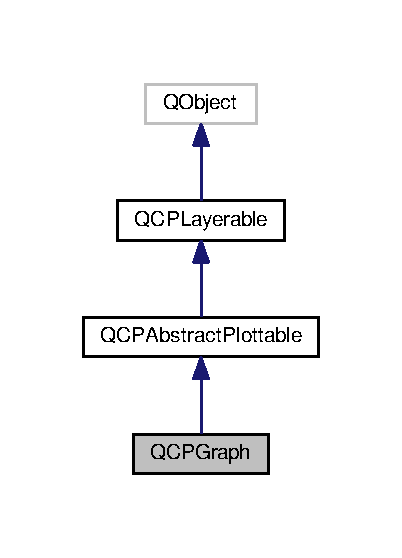
\includegraphics[width=193pt]{classQCPGraph__inherit__graph}
\end{center}
\end{figure}


Collaboration diagram for Q\+C\+P\+Graph\+:
\nopagebreak
\begin{figure}[H]
\begin{center}
\leavevmode
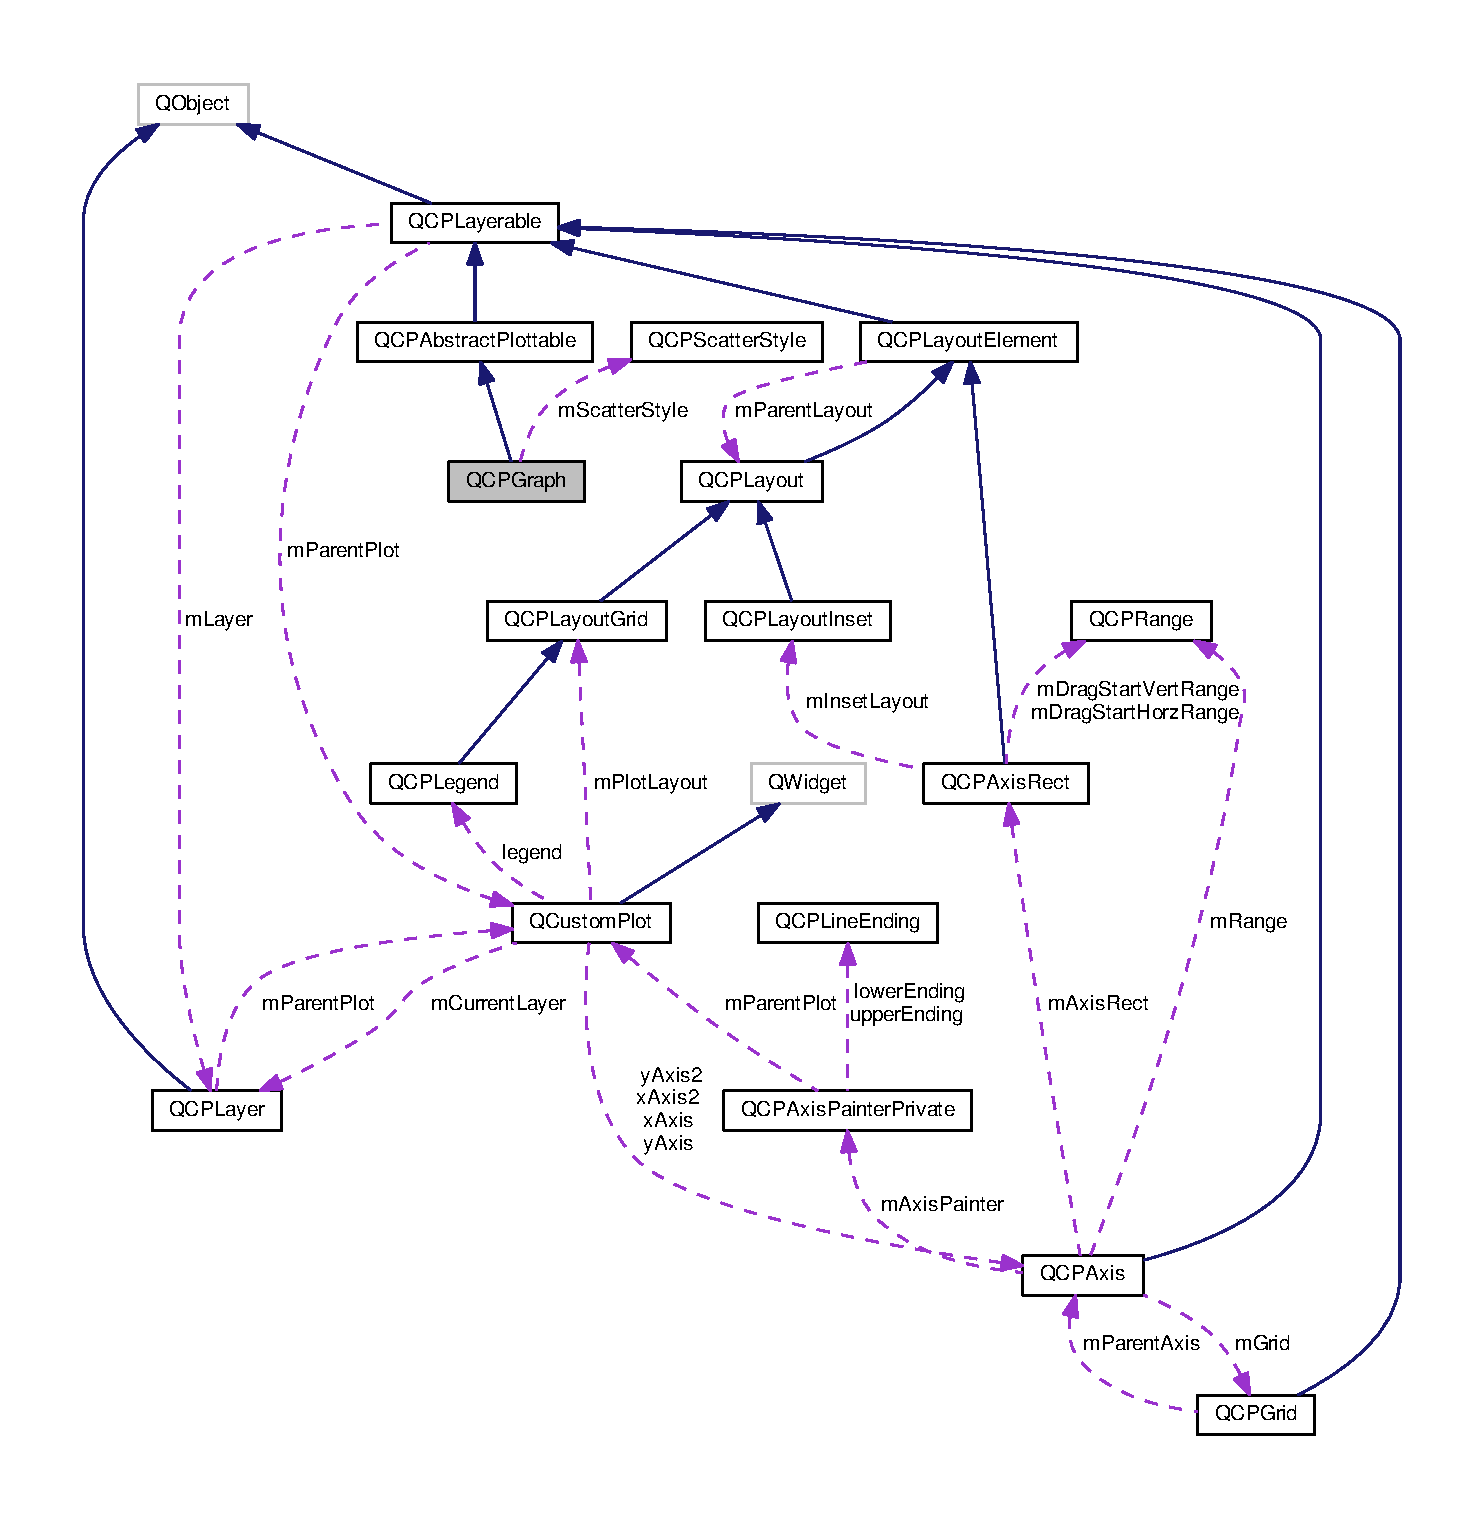
\includegraphics[width=350pt]{classQCPGraph__coll__graph}
\end{center}
\end{figure}
\subsection*{Public Types}
\begin{DoxyCompactItemize}
\item 
enum \hyperlink{classQCPGraph_ad60175cd9b5cac937c5ee685c32c0859}{Line\+Style} \{ \\*
\hyperlink{classQCPGraph_ad60175cd9b5cac937c5ee685c32c0859aea9591b933733cc7b20786b71e60fa04}{ls\+None}, 
\hyperlink{classQCPGraph_ad60175cd9b5cac937c5ee685c32c0859a3c42a27b15aa3c92d399082fad8b7515}{ls\+Line}, 
\hyperlink{classQCPGraph_ad60175cd9b5cac937c5ee685c32c0859ae10568bda57836487d9dec5eba1d6c6e}{ls\+Step\+Left}, 
\hyperlink{classQCPGraph_ad60175cd9b5cac937c5ee685c32c0859a9c37951f7d11aa070100fd16f2935c9e}{ls\+Step\+Right}, 
\\*
\hyperlink{classQCPGraph_ad60175cd9b5cac937c5ee685c32c0859a5adf7b04da215a40a764c21294ea7366}{ls\+Step\+Center}, 
\hyperlink{classQCPGraph_ad60175cd9b5cac937c5ee685c32c0859aa3b358b4ae7cca94aceeb8e529c12ebb}{ls\+Impulse}
 \}
\item 
enum \hyperlink{classQCPGraph_ad23b514404bd2cb3216f57c90904d6af}{Error\+Type} \{ \hyperlink{classQCPGraph_ad23b514404bd2cb3216f57c90904d6afaeae745e7cc1766bb8546e35d4b76a711}{et\+None}, 
\hyperlink{classQCPGraph_ad23b514404bd2cb3216f57c90904d6afa2a5d89cd76fb8b6b18d71b8f6f6c0f43}{et\+Key}, 
\hyperlink{classQCPGraph_ad23b514404bd2cb3216f57c90904d6afa147022ccdc49f6bd48f904cb4f61872e}{et\+Value}, 
\hyperlink{classQCPGraph_ad23b514404bd2cb3216f57c90904d6afa761cb7d61670c1e2efecccd8974409ab}{et\+Both}
 \}
\end{DoxyCompactItemize}
\subsection*{Public Member Functions}
\begin{DoxyCompactItemize}
\item 
\hyperlink{classQCPGraph_a0393a38cf7183cbf46348eb6cf9a5a6c}{Q\+C\+P\+Graph} (\hyperlink{classQCPAxis}{Q\+C\+P\+Axis} $\ast$\hyperlink{classQCPAbstractPlottable_a72c7a09c22963f2c943f07112b311103}{key\+Axis}, \hyperlink{classQCPAxis}{Q\+C\+P\+Axis} $\ast$\hyperlink{classQCPAbstractPlottable_a3106f9d34d330a6097a8ec5905e5b519}{value\+Axis})
\item 
virtual \hyperlink{classQCPGraph_ae9998cfb9d379ac0ef3fbd6995cfbd76}{$\sim$\+Q\+C\+P\+Graph} ()
\item 
\hyperlink{qcustomplot_8h_a84a9c4a4c2216ccfdcb5f3067cda76e3}{Q\+C\+P\+Data\+Map} $\ast$ \hyperlink{classQCPGraph_a2f58436df4f86a2792b776a21642b3d9}{data} () const 
\item 
\hyperlink{classQCPGraph_ad60175cd9b5cac937c5ee685c32c0859}{Line\+Style} \hyperlink{classQCPGraph_ad6db8d31abeac256a285fc68d6b9b9be}{line\+Style} () const 
\item 
\hyperlink{classQCPScatterStyle}{Q\+C\+P\+Scatter\+Style} \hyperlink{classQCPGraph_ae0227c79f4e42a350c2c99fb2fb879db}{scatter\+Style} () const 
\item 
\hyperlink{classQCPGraph_ad23b514404bd2cb3216f57c90904d6af}{Error\+Type} \hyperlink{classQCPGraph_a250bcdf78abac87bc6d46ee6fd99a92d}{error\+Type} () const 
\item 
Q\+Pen \hyperlink{classQCPGraph_a83455e01093bb899f3b59d4a6fdcd57b}{error\+Pen} () const 
\item 
double \hyperlink{classQCPGraph_ae31efdcbc6ba3d73a7aeb83c774f958a}{error\+Bar\+Size} () const 
\item 
bool \hyperlink{classQCPGraph_a04dbc050ff04561658ab1e7f3df37a01}{error\+Bar\+Skip\+Symbol} () const 
\item 
\hyperlink{classQCPGraph}{Q\+C\+P\+Graph} $\ast$ \hyperlink{classQCPGraph_a5369f23863e04a6164f8b66d49fd18f4}{channel\+Fill\+Graph} () const 
\item 
bool \hyperlink{classQCPGraph_ad3bea28ec910eedfa9b788928d610de0}{adaptive\+Sampling} () const 
\item 
void \hyperlink{classQCPGraph_a1df2fd710545c8ba3b2c99a39a27bf8b}{set\+Data} (\hyperlink{qcustomplot_8h_a84a9c4a4c2216ccfdcb5f3067cda76e3}{Q\+C\+P\+Data\+Map} $\ast$\hyperlink{classQCPGraph_a2f58436df4f86a2792b776a21642b3d9}{data}, bool copy=false)
\item 
void \hyperlink{classQCPGraph_a4c55d8ac13bfa42c8c93747820891a76}{set\+Data} (const Q\+Vector$<$ double $>$ \&key, const Q\+Vector$<$ double $>$ \&value)
\item 
void \hyperlink{classQCPGraph_abce9f07c0d722bc3e4fa7bd73c7e5dfa}{set\+Data\+Key\+Error} (const Q\+Vector$<$ double $>$ \&key, const Q\+Vector$<$ double $>$ \&value, const Q\+Vector$<$ double $>$ \&key\+Error)
\item 
void \hyperlink{classQCPGraph_ac15c749c5fedf740d5692c6fe67143b8}{set\+Data\+Key\+Error} (const Q\+Vector$<$ double $>$ \&key, const Q\+Vector$<$ double $>$ \&value, const Q\+Vector$<$ double $>$ \&key\+Error\+Minus, const Q\+Vector$<$ double $>$ \&key\+Error\+Plus)
\item 
void \hyperlink{classQCPGraph_acba6296eadcb36b93267628b8dae3de5}{set\+Data\+Value\+Error} (const Q\+Vector$<$ double $>$ \&key, const Q\+Vector$<$ double $>$ \&value, const Q\+Vector$<$ double $>$ \&value\+Error)
\item 
void \hyperlink{classQCPGraph_a3afbfd7222d739351c69387904776f93}{set\+Data\+Value\+Error} (const Q\+Vector$<$ double $>$ \&key, const Q\+Vector$<$ double $>$ \&value, const Q\+Vector$<$ double $>$ \&value\+Error\+Minus, const Q\+Vector$<$ double $>$ \&value\+Error\+Plus)
\item 
void \hyperlink{classQCPGraph_a873fe46bdb20be5710428e474ade8908}{set\+Data\+Both\+Error} (const Q\+Vector$<$ double $>$ \&key, const Q\+Vector$<$ double $>$ \&value, const Q\+Vector$<$ double $>$ \&key\+Error, const Q\+Vector$<$ double $>$ \&value\+Error)
\item 
void \hyperlink{classQCPGraph_abb75736ecdbf6e6a7501e1da64fb18cf}{set\+Data\+Both\+Error} (const Q\+Vector$<$ double $>$ \&key, const Q\+Vector$<$ double $>$ \&value, const Q\+Vector$<$ double $>$ \&key\+Error\+Minus, const Q\+Vector$<$ double $>$ \&key\+Error\+Plus, const Q\+Vector$<$ double $>$ \&value\+Error\+Minus, const Q\+Vector$<$ double $>$ \&value\+Error\+Plus)
\item 
void \hyperlink{classQCPGraph_a513fecccff5b2a50ce53f665338c60ff}{set\+Line\+Style} (\hyperlink{classQCPGraph_ad60175cd9b5cac937c5ee685c32c0859}{Line\+Style} ls)
\item 
void \hyperlink{classQCPGraph_a12bd17a8ba21983163ec5d8f42a9fea5}{set\+Scatter\+Style} (const \hyperlink{classQCPScatterStyle}{Q\+C\+P\+Scatter\+Style} \&style)
\item 
void \hyperlink{classQCPGraph_ac3614d799c3894f2bc646e99c7f73d38}{set\+Error\+Type} (\hyperlink{classQCPGraph_ad23b514404bd2cb3216f57c90904d6af}{Error\+Type} \hyperlink{classQCPGraph_a250bcdf78abac87bc6d46ee6fd99a92d}{error\+Type})
\item 
void \hyperlink{classQCPGraph_abd4c7f81939e10776ea64603a704f22a}{set\+Error\+Pen} (const Q\+Pen \&\hyperlink{classQCPAbstractPlottable_a41d060007cc6b3037c9c04d22d0c0398}{pen})
\item 
void \hyperlink{classQCPGraph_a10f50c5495ce45ef559ec2066194a335}{set\+Error\+Bar\+Size} (double size)
\item 
void \hyperlink{classQCPGraph_ab1c1ee03d8dd94676a564e5e5f11aac2}{set\+Error\+Bar\+Skip\+Symbol} (bool enabled)
\item 
void \hyperlink{classQCPGraph_a2d03156df1b64037a2e36cfa50351ca3}{set\+Channel\+Fill\+Graph} (\hyperlink{classQCPGraph}{Q\+C\+P\+Graph} $\ast$target\+Graph)
\item 
void \hyperlink{classQCPGraph_ab468cd600160f327836aa0644291e64c}{set\+Adaptive\+Sampling} (bool enabled)
\item 
void \hyperlink{classQCPGraph_aa5c6181d84db72ce4dbe9dc15a34ef4f}{add\+Data} (const \hyperlink{qcustomplot_8h_a84a9c4a4c2216ccfdcb5f3067cda76e3}{Q\+C\+P\+Data\+Map} \&data\+Map)
\item 
void \hyperlink{classQCPGraph_a80cc91e1e0ef77eb50afc5b366d0efd9}{add\+Data} (const \hyperlink{classQCPData}{Q\+C\+P\+Data} \&\hyperlink{classQCPGraph_a2f58436df4f86a2792b776a21642b3d9}{data})
\item 
void \hyperlink{classQCPGraph_a0bf98b1972286cfb7b1c4b7dd6ae2012}{add\+Data} (double key, double value)
\item 
void \hyperlink{classQCPGraph_ab6da6377541fe80d892a9893a92db9c6}{add\+Data} (const Q\+Vector$<$ double $>$ \&keys, const Q\+Vector$<$ double $>$ \&values)
\item 
void \hyperlink{classQCPGraph_a9fe0b3e54e8c7b61319bd03337e21e99}{remove\+Data\+Before} (double key)
\item 
void \hyperlink{classQCPGraph_ae42d645ef617cfc75fc0df58e62c522a}{remove\+Data\+After} (double key)
\item 
void \hyperlink{classQCPGraph_a4a0fde50b7db9db0a85b5c5b6b10098f}{remove\+Data} (double from\+Key, double to\+Key)
\item 
void \hyperlink{classQCPGraph_a4a706020b4318f118381648ef18aca3f}{remove\+Data} (double key)
\item 
virtual void \hyperlink{classQCPGraph_ad4e94a4e44e5e76fbec81a72a977157d}{clear\+Data} ()
\item 
virtual double \hyperlink{classQCPGraph_abc9ff375aabcf2d21cca33d6baf85772}{select\+Test} (const Q\+PointF \&pos, bool only\+Selectable, Q\+Variant $\ast$details=0) const 
\item 
void \hyperlink{classQCPGraph_aa35b75b9032800d783df749c8a004ee9}{rescale\+Axes} (bool only\+Enlarge, bool include\+Error\+Bars) const 
\item 
void \hyperlink{classQCPGraph_a2108a729046b0ab6e0516afb249dab13}{rescale\+Key\+Axis} (bool only\+Enlarge, bool include\+Error\+Bars) const 
\item 
void \hyperlink{classQCPGraph_a2ba0e1df416486d7e74299ef8cf68bba}{rescale\+Value\+Axis} (bool only\+Enlarge, bool include\+Error\+Bars) const 
\end{DoxyCompactItemize}
\subsection*{Protected Member Functions}
\begin{DoxyCompactItemize}
\item 
virtual void \hyperlink{classQCPGraph_a659218cc62c2a7786213d9dd429c1c8d}{draw} (\hyperlink{classQCPPainter}{Q\+C\+P\+Painter} $\ast$painter)
\item 
virtual void \hyperlink{classQCPGraph_a32115df0e940cf8ca7b687873c2d02ee}{draw\+Legend\+Icon} (\hyperlink{classQCPPainter}{Q\+C\+P\+Painter} $\ast$painter, const Q\+RectF \&rect) const 
\item 
virtual \hyperlink{classQCPRange}{Q\+C\+P\+Range} \hyperlink{classQCPGraph_afc246ce6201ff564ac440efaec52ab11}{get\+Key\+Range} (bool \&found\+Range, \hyperlink{classQCPAbstractPlottable_a661743478a1d3c09d28ec2711d7653d8}{Sign\+Domain} in\+Sign\+Domain=\hyperlink{classQCPAbstractPlottable_a661743478a1d3c09d28ec2711d7653d8a082b98cfb91a7363a3b5cd17b0c1cd60}{sd\+Both}) const 
\item 
virtual \hyperlink{classQCPRange}{Q\+C\+P\+Range} \hyperlink{classQCPGraph_a856e90b8ab6b31c344b14a863ab9e5d2}{get\+Value\+Range} (bool \&found\+Range, \hyperlink{classQCPAbstractPlottable_a661743478a1d3c09d28ec2711d7653d8}{Sign\+Domain} in\+Sign\+Domain=\hyperlink{classQCPAbstractPlottable_a661743478a1d3c09d28ec2711d7653d8a082b98cfb91a7363a3b5cd17b0c1cd60}{sd\+Both}) const 
\item 
virtual \hyperlink{classQCPRange}{Q\+C\+P\+Range} \hyperlink{classQCPGraph_aa75c6f028124032416a5cf7145dfba60}{get\+Key\+Range} (bool \&found\+Range, \hyperlink{classQCPAbstractPlottable_a661743478a1d3c09d28ec2711d7653d8}{Sign\+Domain} in\+Sign\+Domain, bool include\+Errors) const 
\item 
virtual \hyperlink{classQCPRange}{Q\+C\+P\+Range} \hyperlink{classQCPGraph_ab964a21d680af93435d68126d8c5ab29}{get\+Value\+Range} (bool \&found\+Range, \hyperlink{classQCPAbstractPlottable_a661743478a1d3c09d28ec2711d7653d8}{Sign\+Domain} in\+Sign\+Domain, bool include\+Errors) const 
\item 
virtual void \hyperlink{classQCPGraph_ad6d07926e6d6b7cfa70258780d47b7a0}{draw\+Fill} (\hyperlink{classQCPPainter}{Q\+C\+P\+Painter} $\ast$painter, Q\+Vector$<$ Q\+PointF $>$ $\ast$line\+Data) const 
\item 
virtual void \hyperlink{classQCPGraph_a6bdc385b122ce06134d4196373ae2250}{draw\+Scatter\+Plot} (\hyperlink{classQCPPainter}{Q\+C\+P\+Painter} $\ast$painter, Q\+Vector$<$ \hyperlink{classQCPData}{Q\+C\+P\+Data} $>$ $\ast$scatter\+Data) const 
\item 
virtual void \hyperlink{classQCPGraph_acebc22c3385829b19a87e6281fe6ade2}{draw\+Line\+Plot} (\hyperlink{classQCPPainter}{Q\+C\+P\+Painter} $\ast$painter, Q\+Vector$<$ Q\+PointF $>$ $\ast$line\+Data) const 
\item 
virtual void \hyperlink{classQCPGraph_abc01180629621f1e47e94559227d3d8c}{draw\+Impulse\+Plot} (\hyperlink{classQCPPainter}{Q\+C\+P\+Painter} $\ast$painter, Q\+Vector$<$ Q\+PointF $>$ $\ast$line\+Data) const 
\item 
void \hyperlink{classQCPGraph_ab420b46ba638dc3252439fe16687b244}{get\+Prepared\+Data} (Q\+Vector$<$ \hyperlink{classQCPData}{Q\+C\+P\+Data} $>$ $\ast$line\+Data, Q\+Vector$<$ \hyperlink{classQCPData}{Q\+C\+P\+Data} $>$ $\ast$scatter\+Data) const 
\item 
void \hyperlink{classQCPGraph_a466c661e015188971c862031af946693}{get\+Plot\+Data} (Q\+Vector$<$ Q\+PointF $>$ $\ast$line\+Data, Q\+Vector$<$ \hyperlink{classQCPData}{Q\+C\+P\+Data} $>$ $\ast$scatter\+Data) const 
\item 
void \hyperlink{classQCPGraph_a45c4214b59ea11aa6d8d112bdc3b0e03}{get\+Scatter\+Plot\+Data} (Q\+Vector$<$ \hyperlink{classQCPData}{Q\+C\+P\+Data} $>$ $\ast$scatter\+Data) const 
\item 
void \hyperlink{classQCPGraph_ae3d82ffd0c9a883482aabf47b0e6b5ee}{get\+Line\+Plot\+Data} (Q\+Vector$<$ Q\+PointF $>$ $\ast$line\+Pixel\+Data, Q\+Vector$<$ \hyperlink{classQCPData}{Q\+C\+P\+Data} $>$ $\ast$scatter\+Data) const 
\item 
void \hyperlink{classQCPGraph_a609cf4a78045b4d2a679bdff7623847e}{get\+Step\+Left\+Plot\+Data} (Q\+Vector$<$ Q\+PointF $>$ $\ast$line\+Pixel\+Data, Q\+Vector$<$ \hyperlink{classQCPData}{Q\+C\+P\+Data} $>$ $\ast$scatter\+Data) const 
\item 
void \hyperlink{classQCPGraph_a3b9b8c8dc7a6fd9be6e253c25ee31809}{get\+Step\+Right\+Plot\+Data} (Q\+Vector$<$ Q\+PointF $>$ $\ast$line\+Pixel\+Data, Q\+Vector$<$ \hyperlink{classQCPData}{Q\+C\+P\+Data} $>$ $\ast$scatter\+Data) const 
\item 
void \hyperlink{classQCPGraph_ad3713e7d8eb85a0afc34a81a5db5cd27}{get\+Step\+Center\+Plot\+Data} (Q\+Vector$<$ Q\+PointF $>$ $\ast$line\+Pixel\+Data, Q\+Vector$<$ \hyperlink{classQCPData}{Q\+C\+P\+Data} $>$ $\ast$scatter\+Data) const 
\item 
void \hyperlink{classQCPGraph_a1ca2b0762505767f116892609fb02062}{get\+Impulse\+Plot\+Data} (Q\+Vector$<$ Q\+PointF $>$ $\ast$line\+Pixel\+Data, Q\+Vector$<$ \hyperlink{classQCPData}{Q\+C\+P\+Data} $>$ $\ast$scatter\+Data) const 
\item 
void \hyperlink{classQCPGraph_a4df6807066ce877705e999773e7ffbc4}{draw\+Error} (\hyperlink{classQCPPainter}{Q\+C\+P\+Painter} $\ast$painter, double \hyperlink{qualification__task_8cpp_a6150e0515f7202e2fb518f7206ed97dc}{x}, double y, const \hyperlink{classQCPData}{Q\+C\+P\+Data} \&\hyperlink{classQCPGraph_a2f58436df4f86a2792b776a21642b3d9}{data}) const 
\item 
void \hyperlink{classQCPGraph_a6a317cb14a83dae0841c7041a63d6d9d}{get\+Visible\+Data\+Bounds} (Q\+C\+P\+Data\+Map\+::const\+\_\+iterator \&lower, Q\+C\+P\+Data\+Map\+::const\+\_\+iterator \&upper) const 
\item 
int \hyperlink{classQCPGraph_a13f6a3aa60227e03ab1f7aa8eec6589f}{count\+Data\+In\+Bounds} (const Q\+C\+P\+Data\+Map\+::const\+\_\+iterator \&lower, const Q\+C\+P\+Data\+Map\+::const\+\_\+iterator \&upper, int max\+Count) const 
\item 
void \hyperlink{classQCPGraph_a5fa7884620d7c54b81dfbd255d97b636}{add\+Fill\+Base\+Points} (Q\+Vector$<$ Q\+PointF $>$ $\ast$line\+Data) const 
\item 
void \hyperlink{classQCPGraph_ad31b49a90e91e538fd9caf011c913a68}{remove\+Fill\+Base\+Points} (Q\+Vector$<$ Q\+PointF $>$ $\ast$line\+Data) const 
\item 
Q\+PointF \hyperlink{classQCPGraph_a41f982e8ceaefe6a53eb7432f26d64b6}{lower\+Fill\+Base\+Point} (double lower\+Key) const 
\item 
Q\+PointF \hyperlink{classQCPGraph_a363d066c179e0f46cc93c12bafb0bfba}{upper\+Fill\+Base\+Point} (double upper\+Key) const 
\item 
const Q\+PolygonF \hyperlink{classQCPGraph_a0374b7268e35cab9802a6be2b5d726d7}{get\+Channel\+Fill\+Polygon} (const Q\+Vector$<$ Q\+PointF $>$ $\ast$line\+Data) const 
\item 
int \hyperlink{classQCPGraph_a6f4e9461d5925be9228fc4760249a04f}{find\+Index\+BelowX} (const Q\+Vector$<$ Q\+PointF $>$ $\ast$\hyperlink{classQCPGraph_a2f58436df4f86a2792b776a21642b3d9}{data}, double \hyperlink{qualification__task_8cpp_a6150e0515f7202e2fb518f7206ed97dc}{x}) const 
\item 
int \hyperlink{classQCPGraph_abab2a75b5e63630432bdd1f3b57f07fa}{find\+Index\+AboveX} (const Q\+Vector$<$ Q\+PointF $>$ $\ast$\hyperlink{classQCPGraph_a2f58436df4f86a2792b776a21642b3d9}{data}, double \hyperlink{qualification__task_8cpp_a6150e0515f7202e2fb518f7206ed97dc}{x}) const 
\item 
int \hyperlink{classQCPGraph_a6c4d556de3d1e02f548401001f72c6ff}{find\+Index\+BelowY} (const Q\+Vector$<$ Q\+PointF $>$ $\ast$\hyperlink{classQCPGraph_a2f58436df4f86a2792b776a21642b3d9}{data}, double y) const 
\item 
int \hyperlink{classQCPGraph_adf50243f1df203883a2187089734bfcb}{find\+Index\+AboveY} (const Q\+Vector$<$ Q\+PointF $>$ $\ast$\hyperlink{classQCPGraph_a2f58436df4f86a2792b776a21642b3d9}{data}, double y) const 
\item 
double \hyperlink{classQCPGraph_af93762a12a481a7edb4b3dd9e330dff1}{point\+Distance} (const Q\+PointF \&pixel\+Point) const 
\end{DoxyCompactItemize}
\subsection*{Protected Attributes}
\begin{DoxyCompactItemize}
\item 
\hyperlink{qcustomplot_8h_a84a9c4a4c2216ccfdcb5f3067cda76e3}{Q\+C\+P\+Data\+Map} $\ast$ \hyperlink{classQCPGraph_a8457c840f69a0ac49f61d30a509c5d08}{m\+Data}
\item 
Q\+Pen \hyperlink{classQCPGraph_aa35681a24165c2831301091a87b662ce}{m\+Error\+Pen}
\item 
\hyperlink{classQCPGraph_ad60175cd9b5cac937c5ee685c32c0859}{Line\+Style} \hyperlink{classQCPGraph_a8604fd98402035a63375849f7341ee25}{m\+Line\+Style}
\item 
\hyperlink{classQCPScatterStyle}{Q\+C\+P\+Scatter\+Style} \hyperlink{classQCPGraph_a4aa36241f166ccd1f75fc8f24e4a3247}{m\+Scatter\+Style}
\item 
\hyperlink{classQCPGraph_ad23b514404bd2cb3216f57c90904d6af}{Error\+Type} \hyperlink{classQCPGraph_a29e64273db201aeadebc61c870720a36}{m\+Error\+Type}
\item 
double \hyperlink{classQCPGraph_a7b51c8d09510f9d195b5e765ccbcf05b}{m\+Error\+Bar\+Size}
\item 
bool \hyperlink{classQCPGraph_acf631d7dbd1055a69ab3b63094868557}{m\+Error\+Bar\+Skip\+Symbol}
\item 
Q\+Pointer$<$ \hyperlink{classQCPGraph}{Q\+C\+P\+Graph} $>$ \hyperlink{classQCPGraph_a2f1777c7accf8244fc640c33f0b04577}{m\+Channel\+Fill\+Graph}
\item 
bool \hyperlink{classQCPGraph_aa951e78aeba714cf443be6da2e52502e}{m\+Adaptive\+Sampling}
\end{DoxyCompactItemize}
\subsection*{Friends}
\begin{DoxyCompactItemize}
\item 
class \hyperlink{classQCPGraph_a1cdf9df76adcfae45261690aa0ca2198}{Q\+Custom\+Plot}
\item 
class \hyperlink{classQCPGraph_a8429035e7adfbd7f05805a6530ad5e3b}{Q\+C\+P\+Legend}
\end{DoxyCompactItemize}
\subsection*{Additional Inherited Members}


\subsection{Detailed Description}
A plottable representing a graph in a plot. 



Usually \hyperlink{classQCustomPlot}{Q\+Custom\+Plot} creates graphs internally via \hyperlink{classQCustomPlot_a6fb2873d35a8a8089842d81a70a54167}{Q\+Custom\+Plot\+::add\+Graph} and the resulting instance is accessed via \hyperlink{classQCustomPlot_a6d3ed93c2bf46ab7fa670d66be4cddaf}{Q\+Custom\+Plot\+::graph}.

To plot data, assign it with the \hyperlink{classQCPGraph_a1df2fd710545c8ba3b2c99a39a27bf8b}{set\+Data} or \hyperlink{classQCPGraph_aa5c6181d84db72ce4dbe9dc15a34ef4f}{add\+Data} functions. Alternatively, you can also access and modify the graph\textquotesingle{}s data via the \hyperlink{classQCPGraph_a2f58436df4f86a2792b776a21642b3d9}{data} method, which returns a pointer to the internal \hyperlink{qcustomplot_8h_a84a9c4a4c2216ccfdcb5f3067cda76e3}{Q\+C\+P\+Data\+Map}.

Graphs are used to display single-\/valued data. Single-\/valued means that there should only be one data point per unique key coordinate. In other words, the graph can\textquotesingle{}t have {\itshape loops}. If you do want to plot non-\/single-\/valued curves, rather use the \hyperlink{classQCPCurve}{Q\+C\+P\+Curve} plottable.

Gaps in the graph line can be created by adding data points with NaN as value ({\ttfamily q\+Q\+Na\+N()} or {\ttfamily std\+::numeric\+\_\+limits$<$double$>$\+::quiet\+\_\+\+Na\+N()}) in between the two data points that shall be separated.\hypertarget{classQCPStatisticalBox_appearance}{}\subsection{Changing the appearance}\label{classQCPStatisticalBox_appearance}
The appearance of the graph is mainly determined by the line style, scatter style, brush and pen of the graph (\hyperlink{classQCPGraph_a513fecccff5b2a50ce53f665338c60ff}{set\+Line\+Style}, \hyperlink{classQCPGraph_a12bd17a8ba21983163ec5d8f42a9fea5}{set\+Scatter\+Style}, \hyperlink{classQCPAbstractPlottable_a7a4b92144dca6453a1f0f210e27edc74}{set\+Brush}, \hyperlink{classQCPAbstractPlottable_ab74b09ae4c0e7e13142fe4b5bf46cac7}{set\+Pen}).\hypertarget{classQCPGraph_filling}{}\subsubsection{Filling under or between graphs}\label{classQCPGraph_filling}
\hyperlink{classQCPGraph}{Q\+C\+P\+Graph} knows two types of fills\+: Normal graph fills towards the zero-\/value-\/line parallel to the key axis of the graph, and fills between two graphs, called channel fills. To enable a fill, just set a brush with \hyperlink{classQCPAbstractPlottable_a7a4b92144dca6453a1f0f210e27edc74}{set\+Brush} which is neither Qt\+::\+No\+Brush nor fully transparent.

By default, a normal fill towards the zero-\/value-\/line will be drawn. To set up a channel fill between this graph and another one, call \hyperlink{classQCPGraph_a2d03156df1b64037a2e36cfa50351ca3}{set\+Channel\+Fill\+Graph} with the other graph as parameter.

\begin{DoxySeeAlso}{See also}
\hyperlink{classQCustomPlot_a6fb2873d35a8a8089842d81a70a54167}{Q\+Custom\+Plot\+::add\+Graph}, \hyperlink{classQCustomPlot_a6d3ed93c2bf46ab7fa670d66be4cddaf}{Q\+Custom\+Plot\+::graph} 
\end{DoxySeeAlso}


\subsection{Member Enumeration Documentation}
\index{Q\+C\+P\+Graph@{Q\+C\+P\+Graph}!Error\+Type@{Error\+Type}}
\index{Error\+Type@{Error\+Type}!Q\+C\+P\+Graph@{Q\+C\+P\+Graph}}
\subsubsection[{\texorpdfstring{Error\+Type}{ErrorType}}]{\setlength{\rightskip}{0pt plus 5cm}enum {\bf Q\+C\+P\+Graph\+::\+Error\+Type}}\hypertarget{classQCPGraph_ad23b514404bd2cb3216f57c90904d6af}{}\label{classQCPGraph_ad23b514404bd2cb3216f57c90904d6af}
Defines what kind of error bars are drawn for each data point \begin{Desc}
\item[Enumerator]\par
\begin{description}
\index{et\+None@{et\+None}!Q\+C\+P\+Graph@{Q\+C\+P\+Graph}}\index{Q\+C\+P\+Graph@{Q\+C\+P\+Graph}!et\+None@{et\+None}}\item[{\em 
et\+None\hypertarget{classQCPGraph_ad23b514404bd2cb3216f57c90904d6afaeae745e7cc1766bb8546e35d4b76a711}{}\label{classQCPGraph_ad23b514404bd2cb3216f57c90904d6afaeae745e7cc1766bb8546e35d4b76a711}
}]No error bars are shown. \index{et\+Key@{et\+Key}!Q\+C\+P\+Graph@{Q\+C\+P\+Graph}}\index{Q\+C\+P\+Graph@{Q\+C\+P\+Graph}!et\+Key@{et\+Key}}\item[{\em 
et\+Key\hypertarget{classQCPGraph_ad23b514404bd2cb3216f57c90904d6afa2a5d89cd76fb8b6b18d71b8f6f6c0f43}{}\label{classQCPGraph_ad23b514404bd2cb3216f57c90904d6afa2a5d89cd76fb8b6b18d71b8f6f6c0f43}
}]Error bars for the key dimension of the data point are shown. \index{et\+Value@{et\+Value}!Q\+C\+P\+Graph@{Q\+C\+P\+Graph}}\index{Q\+C\+P\+Graph@{Q\+C\+P\+Graph}!et\+Value@{et\+Value}}\item[{\em 
et\+Value\hypertarget{classQCPGraph_ad23b514404bd2cb3216f57c90904d6afa147022ccdc49f6bd48f904cb4f61872e}{}\label{classQCPGraph_ad23b514404bd2cb3216f57c90904d6afa147022ccdc49f6bd48f904cb4f61872e}
}]Error bars for the value dimension of the data point are shown. \index{et\+Both@{et\+Both}!Q\+C\+P\+Graph@{Q\+C\+P\+Graph}}\index{Q\+C\+P\+Graph@{Q\+C\+P\+Graph}!et\+Both@{et\+Both}}\item[{\em 
et\+Both\hypertarget{classQCPGraph_ad23b514404bd2cb3216f57c90904d6afa761cb7d61670c1e2efecccd8974409ab}{}\label{classQCPGraph_ad23b514404bd2cb3216f57c90904d6afa761cb7d61670c1e2efecccd8974409ab}
}]Error bars for both key and value dimensions of the data point are shown. \end{description}
\end{Desc}
\index{Q\+C\+P\+Graph@{Q\+C\+P\+Graph}!Line\+Style@{Line\+Style}}
\index{Line\+Style@{Line\+Style}!Q\+C\+P\+Graph@{Q\+C\+P\+Graph}}
\subsubsection[{\texorpdfstring{Line\+Style}{LineStyle}}]{\setlength{\rightskip}{0pt plus 5cm}enum {\bf Q\+C\+P\+Graph\+::\+Line\+Style}}\hypertarget{classQCPGraph_ad60175cd9b5cac937c5ee685c32c0859}{}\label{classQCPGraph_ad60175cd9b5cac937c5ee685c32c0859}
Defines how the graph\textquotesingle{}s line is represented visually in the plot. The line is drawn with the current pen of the graph (\hyperlink{classQCPAbstractPlottable_ab74b09ae4c0e7e13142fe4b5bf46cac7}{set\+Pen}). \begin{DoxySeeAlso}{See also}
\hyperlink{classQCPGraph_a513fecccff5b2a50ce53f665338c60ff}{set\+Line\+Style} 
\end{DoxySeeAlso}
\begin{Desc}
\item[Enumerator]\par
\begin{description}
\index{ls\+None@{ls\+None}!Q\+C\+P\+Graph@{Q\+C\+P\+Graph}}\index{Q\+C\+P\+Graph@{Q\+C\+P\+Graph}!ls\+None@{ls\+None}}\item[{\em 
ls\+None\hypertarget{classQCPGraph_ad60175cd9b5cac937c5ee685c32c0859aea9591b933733cc7b20786b71e60fa04}{}\label{classQCPGraph_ad60175cd9b5cac937c5ee685c32c0859aea9591b933733cc7b20786b71e60fa04}
}]data points are not connected with any lines (e.\+g. data only represented with symbols according to the scatter style, see \hyperlink{classQCPGraph_a12bd17a8ba21983163ec5d8f42a9fea5}{set\+Scatter\+Style}) \index{ls\+Line@{ls\+Line}!Q\+C\+P\+Graph@{Q\+C\+P\+Graph}}\index{Q\+C\+P\+Graph@{Q\+C\+P\+Graph}!ls\+Line@{ls\+Line}}\item[{\em 
ls\+Line\hypertarget{classQCPGraph_ad60175cd9b5cac937c5ee685c32c0859a3c42a27b15aa3c92d399082fad8b7515}{}\label{classQCPGraph_ad60175cd9b5cac937c5ee685c32c0859a3c42a27b15aa3c92d399082fad8b7515}
}]data points are connected by a straight line \index{ls\+Step\+Left@{ls\+Step\+Left}!Q\+C\+P\+Graph@{Q\+C\+P\+Graph}}\index{Q\+C\+P\+Graph@{Q\+C\+P\+Graph}!ls\+Step\+Left@{ls\+Step\+Left}}\item[{\em 
ls\+Step\+Left\hypertarget{classQCPGraph_ad60175cd9b5cac937c5ee685c32c0859ae10568bda57836487d9dec5eba1d6c6e}{}\label{classQCPGraph_ad60175cd9b5cac937c5ee685c32c0859ae10568bda57836487d9dec5eba1d6c6e}
}]line is drawn as steps where the step height is the value of the left data point \index{ls\+Step\+Right@{ls\+Step\+Right}!Q\+C\+P\+Graph@{Q\+C\+P\+Graph}}\index{Q\+C\+P\+Graph@{Q\+C\+P\+Graph}!ls\+Step\+Right@{ls\+Step\+Right}}\item[{\em 
ls\+Step\+Right\hypertarget{classQCPGraph_ad60175cd9b5cac937c5ee685c32c0859a9c37951f7d11aa070100fd16f2935c9e}{}\label{classQCPGraph_ad60175cd9b5cac937c5ee685c32c0859a9c37951f7d11aa070100fd16f2935c9e}
}]line is drawn as steps where the step height is the value of the right data point \index{ls\+Step\+Center@{ls\+Step\+Center}!Q\+C\+P\+Graph@{Q\+C\+P\+Graph}}\index{Q\+C\+P\+Graph@{Q\+C\+P\+Graph}!ls\+Step\+Center@{ls\+Step\+Center}}\item[{\em 
ls\+Step\+Center\hypertarget{classQCPGraph_ad60175cd9b5cac937c5ee685c32c0859a5adf7b04da215a40a764c21294ea7366}{}\label{classQCPGraph_ad60175cd9b5cac937c5ee685c32c0859a5adf7b04da215a40a764c21294ea7366}
}]line is drawn as steps where the step is in between two data points \index{ls\+Impulse@{ls\+Impulse}!Q\+C\+P\+Graph@{Q\+C\+P\+Graph}}\index{Q\+C\+P\+Graph@{Q\+C\+P\+Graph}!ls\+Impulse@{ls\+Impulse}}\item[{\em 
ls\+Impulse\hypertarget{classQCPGraph_ad60175cd9b5cac937c5ee685c32c0859aa3b358b4ae7cca94aceeb8e529c12ebb}{}\label{classQCPGraph_ad60175cd9b5cac937c5ee685c32c0859aa3b358b4ae7cca94aceeb8e529c12ebb}
}]each data point is represented by a line parallel to the value axis, which reaches from the data point to the zero-\/value-\/line \end{description}
\end{Desc}


\subsection{Constructor \& Destructor Documentation}
\index{Q\+C\+P\+Graph@{Q\+C\+P\+Graph}!Q\+C\+P\+Graph@{Q\+C\+P\+Graph}}
\index{Q\+C\+P\+Graph@{Q\+C\+P\+Graph}!Q\+C\+P\+Graph@{Q\+C\+P\+Graph}}
\subsubsection[{\texorpdfstring{Q\+C\+P\+Graph(\+Q\+C\+P\+Axis $\ast$key\+Axis, Q\+C\+P\+Axis $\ast$value\+Axis)}{QCPGraph(QCPAxis *keyAxis, QCPAxis *valueAxis)}}]{\setlength{\rightskip}{0pt plus 5cm}Q\+C\+P\+Graph\+::\+Q\+C\+P\+Graph (
\begin{DoxyParamCaption}
\item[{{\bf Q\+C\+P\+Axis} $\ast$}]{key\+Axis, }
\item[{{\bf Q\+C\+P\+Axis} $\ast$}]{value\+Axis}
\end{DoxyParamCaption}
)\hspace{0.3cm}{\ttfamily [explicit]}}\hypertarget{classQCPGraph_a0393a38cf7183cbf46348eb6cf9a5a6c}{}\label{classQCPGraph_a0393a38cf7183cbf46348eb6cf9a5a6c}
Constructs a graph which uses {\itshape key\+Axis} as its key axis (\char`\"{}x\char`\"{}) and {\itshape value\+Axis} as its value axis (\char`\"{}y\char`\"{}). {\itshape key\+Axis} and {\itshape value\+Axis} must reside in the same \hyperlink{classQCustomPlot}{Q\+Custom\+Plot} instance and not have the same orientation. If either of these restrictions is violated, a corresponding message is printed to the debug output (q\+Debug), the construction is not aborted, though.

The constructed \hyperlink{classQCPGraph}{Q\+C\+P\+Graph} can be added to the plot with \hyperlink{classQCustomPlot_ab7ad9174f701f9c6f64e378df77927a6}{Q\+Custom\+Plot\+::add\+Plottable}, \hyperlink{classQCustomPlot}{Q\+Custom\+Plot} then takes ownership of the graph.

To directly create a graph inside a plot, you can also use the simpler \hyperlink{classQCustomPlot_a6fb2873d35a8a8089842d81a70a54167}{Q\+Custom\+Plot\+::add\+Graph} function. \index{Q\+C\+P\+Graph@{Q\+C\+P\+Graph}!````~Q\+C\+P\+Graph@{$\sim$\+Q\+C\+P\+Graph}}
\index{````~Q\+C\+P\+Graph@{$\sim$\+Q\+C\+P\+Graph}!Q\+C\+P\+Graph@{Q\+C\+P\+Graph}}
\subsubsection[{\texorpdfstring{$\sim$\+Q\+C\+P\+Graph()}{~QCPGraph()}}]{\setlength{\rightskip}{0pt plus 5cm}Q\+C\+P\+Graph\+::$\sim$\+Q\+C\+P\+Graph (
\begin{DoxyParamCaption}
{}
\end{DoxyParamCaption}
)\hspace{0.3cm}{\ttfamily [virtual]}}\hypertarget{classQCPGraph_ae9998cfb9d379ac0ef3fbd6995cfbd76}{}\label{classQCPGraph_ae9998cfb9d379ac0ef3fbd6995cfbd76}


\subsection{Member Function Documentation}
\index{Q\+C\+P\+Graph@{Q\+C\+P\+Graph}!adaptive\+Sampling@{adaptive\+Sampling}}
\index{adaptive\+Sampling@{adaptive\+Sampling}!Q\+C\+P\+Graph@{Q\+C\+P\+Graph}}
\subsubsection[{\texorpdfstring{adaptive\+Sampling() const }{adaptiveSampling() const }}]{\setlength{\rightskip}{0pt plus 5cm}bool Q\+C\+P\+Graph\+::adaptive\+Sampling (
\begin{DoxyParamCaption}
{}
\end{DoxyParamCaption}
) const\hspace{0.3cm}{\ttfamily [inline]}}\hypertarget{classQCPGraph_ad3bea28ec910eedfa9b788928d610de0}{}\label{classQCPGraph_ad3bea28ec910eedfa9b788928d610de0}
\index{Q\+C\+P\+Graph@{Q\+C\+P\+Graph}!add\+Data@{add\+Data}}
\index{add\+Data@{add\+Data}!Q\+C\+P\+Graph@{Q\+C\+P\+Graph}}
\subsubsection[{\texorpdfstring{add\+Data(const Q\+C\+P\+Data\+Map \&data\+Map)}{addData(const QCPDataMap &dataMap)}}]{\setlength{\rightskip}{0pt plus 5cm}void Q\+C\+P\+Graph\+::add\+Data (
\begin{DoxyParamCaption}
\item[{const {\bf Q\+C\+P\+Data\+Map} \&}]{data\+Map}
\end{DoxyParamCaption}
)}\hypertarget{classQCPGraph_aa5c6181d84db72ce4dbe9dc15a34ef4f}{}\label{classQCPGraph_aa5c6181d84db72ce4dbe9dc15a34ef4f}
Adds the provided data points in {\itshape data\+Map} to the current data.

Alternatively, you can also access and modify the graph\textquotesingle{}s data via the \hyperlink{classQCPGraph_a2f58436df4f86a2792b776a21642b3d9}{data} method, which returns a pointer to the internal \hyperlink{qcustomplot_8h_a84a9c4a4c2216ccfdcb5f3067cda76e3}{Q\+C\+P\+Data\+Map}.

\begin{DoxySeeAlso}{See also}
\hyperlink{classQCPGraph_a4a0fde50b7db9db0a85b5c5b6b10098f}{remove\+Data} 
\end{DoxySeeAlso}
\index{Q\+C\+P\+Graph@{Q\+C\+P\+Graph}!add\+Data@{add\+Data}}
\index{add\+Data@{add\+Data}!Q\+C\+P\+Graph@{Q\+C\+P\+Graph}}
\subsubsection[{\texorpdfstring{add\+Data(const Q\+C\+P\+Data \&data)}{addData(const QCPData &data)}}]{\setlength{\rightskip}{0pt plus 5cm}void Q\+C\+P\+Graph\+::add\+Data (
\begin{DoxyParamCaption}
\item[{const {\bf Q\+C\+P\+Data} \&}]{data}
\end{DoxyParamCaption}
)}\hypertarget{classQCPGraph_a80cc91e1e0ef77eb50afc5b366d0efd9}{}\label{classQCPGraph_a80cc91e1e0ef77eb50afc5b366d0efd9}
This is an overloaded member function, provided for convenience. It differs from the above function only in what argument(s) it accepts. Adds the provided single data point in {\itshape data} to the current data.

Alternatively, you can also access and modify the graph\textquotesingle{}s data via the \hyperlink{classQCPGraph_a2f58436df4f86a2792b776a21642b3d9}{data} method, which returns a pointer to the internal \hyperlink{qcustomplot_8h_a84a9c4a4c2216ccfdcb5f3067cda76e3}{Q\+C\+P\+Data\+Map}.

\begin{DoxySeeAlso}{See also}
\hyperlink{classQCPGraph_a4a0fde50b7db9db0a85b5c5b6b10098f}{remove\+Data} 
\end{DoxySeeAlso}
\index{Q\+C\+P\+Graph@{Q\+C\+P\+Graph}!add\+Data@{add\+Data}}
\index{add\+Data@{add\+Data}!Q\+C\+P\+Graph@{Q\+C\+P\+Graph}}
\subsubsection[{\texorpdfstring{add\+Data(double key, double value)}{addData(double key, double value)}}]{\setlength{\rightskip}{0pt plus 5cm}void Q\+C\+P\+Graph\+::add\+Data (
\begin{DoxyParamCaption}
\item[{double}]{key, }
\item[{double}]{value}
\end{DoxyParamCaption}
)}\hypertarget{classQCPGraph_a0bf98b1972286cfb7b1c4b7dd6ae2012}{}\label{classQCPGraph_a0bf98b1972286cfb7b1c4b7dd6ae2012}
This is an overloaded member function, provided for convenience. It differs from the above function only in what argument(s) it accepts. Adds the provided single data point as {\itshape key} and {\itshape value} pair to the current data.

Alternatively, you can also access and modify the graph\textquotesingle{}s data via the \hyperlink{classQCPGraph_a2f58436df4f86a2792b776a21642b3d9}{data} method, which returns a pointer to the internal \hyperlink{qcustomplot_8h_a84a9c4a4c2216ccfdcb5f3067cda76e3}{Q\+C\+P\+Data\+Map}.

\begin{DoxySeeAlso}{See also}
\hyperlink{classQCPGraph_a4a0fde50b7db9db0a85b5c5b6b10098f}{remove\+Data} 
\end{DoxySeeAlso}
\index{Q\+C\+P\+Graph@{Q\+C\+P\+Graph}!add\+Data@{add\+Data}}
\index{add\+Data@{add\+Data}!Q\+C\+P\+Graph@{Q\+C\+P\+Graph}}
\subsubsection[{\texorpdfstring{add\+Data(const Q\+Vector$<$ double $>$ \&keys, const Q\+Vector$<$ double $>$ \&values)}{addData(const QVector< double > &keys, const QVector< double > &values)}}]{\setlength{\rightskip}{0pt plus 5cm}void Q\+C\+P\+Graph\+::add\+Data (
\begin{DoxyParamCaption}
\item[{const Q\+Vector$<$ double $>$ \&}]{keys, }
\item[{const Q\+Vector$<$ double $>$ \&}]{values}
\end{DoxyParamCaption}
)}\hypertarget{classQCPGraph_ab6da6377541fe80d892a9893a92db9c6}{}\label{classQCPGraph_ab6da6377541fe80d892a9893a92db9c6}
This is an overloaded member function, provided for convenience. It differs from the above function only in what argument(s) it accepts. Adds the provided data points as {\itshape key} and {\itshape value} pairs to the current data.

Alternatively, you can also access and modify the graph\textquotesingle{}s data via the \hyperlink{classQCPGraph_a2f58436df4f86a2792b776a21642b3d9}{data} method, which returns a pointer to the internal \hyperlink{qcustomplot_8h_a84a9c4a4c2216ccfdcb5f3067cda76e3}{Q\+C\+P\+Data\+Map}.

\begin{DoxySeeAlso}{See also}
\hyperlink{classQCPGraph_a4a0fde50b7db9db0a85b5c5b6b10098f}{remove\+Data} 
\end{DoxySeeAlso}
\index{Q\+C\+P\+Graph@{Q\+C\+P\+Graph}!add\+Fill\+Base\+Points@{add\+Fill\+Base\+Points}}
\index{add\+Fill\+Base\+Points@{add\+Fill\+Base\+Points}!Q\+C\+P\+Graph@{Q\+C\+P\+Graph}}
\subsubsection[{\texorpdfstring{add\+Fill\+Base\+Points(\+Q\+Vector$<$ Q\+Point\+F $>$ $\ast$line\+Data) const }{addFillBasePoints(QVector< QPointF > *lineData) const }}]{\setlength{\rightskip}{0pt plus 5cm}void Q\+C\+P\+Graph\+::add\+Fill\+Base\+Points (
\begin{DoxyParamCaption}
\item[{Q\+Vector$<$ Q\+PointF $>$ $\ast$}]{line\+Data}
\end{DoxyParamCaption}
) const\hspace{0.3cm}{\ttfamily [protected]}}\hypertarget{classQCPGraph_a5fa7884620d7c54b81dfbd255d97b636}{}\label{classQCPGraph_a5fa7884620d7c54b81dfbd255d97b636}
\index{Q\+C\+P\+Graph@{Q\+C\+P\+Graph}!channel\+Fill\+Graph@{channel\+Fill\+Graph}}
\index{channel\+Fill\+Graph@{channel\+Fill\+Graph}!Q\+C\+P\+Graph@{Q\+C\+P\+Graph}}
\subsubsection[{\texorpdfstring{channel\+Fill\+Graph() const }{channelFillGraph() const }}]{\setlength{\rightskip}{0pt plus 5cm}{\bf Q\+C\+P\+Graph}$\ast$ Q\+C\+P\+Graph\+::channel\+Fill\+Graph (
\begin{DoxyParamCaption}
{}
\end{DoxyParamCaption}
) const\hspace{0.3cm}{\ttfamily [inline]}}\hypertarget{classQCPGraph_a5369f23863e04a6164f8b66d49fd18f4}{}\label{classQCPGraph_a5369f23863e04a6164f8b66d49fd18f4}
\index{Q\+C\+P\+Graph@{Q\+C\+P\+Graph}!clear\+Data@{clear\+Data}}
\index{clear\+Data@{clear\+Data}!Q\+C\+P\+Graph@{Q\+C\+P\+Graph}}
\subsubsection[{\texorpdfstring{clear\+Data()}{clearData()}}]{\setlength{\rightskip}{0pt plus 5cm}void Q\+C\+P\+Graph\+::clear\+Data (
\begin{DoxyParamCaption}
{}
\end{DoxyParamCaption}
)\hspace{0.3cm}{\ttfamily [virtual]}}\hypertarget{classQCPGraph_ad4e94a4e44e5e76fbec81a72a977157d}{}\label{classQCPGraph_ad4e94a4e44e5e76fbec81a72a977157d}
Removes all data points. \begin{DoxySeeAlso}{See also}
\hyperlink{classQCPGraph_a4a0fde50b7db9db0a85b5c5b6b10098f}{remove\+Data}, \hyperlink{classQCPGraph_ae42d645ef617cfc75fc0df58e62c522a}{remove\+Data\+After}, \hyperlink{classQCPGraph_a9fe0b3e54e8c7b61319bd03337e21e99}{remove\+Data\+Before} 
\end{DoxySeeAlso}


Implements \hyperlink{classQCPAbstractPlottable_a86e5b8fd4b6ff4f4084e7ea4c573fc53}{Q\+C\+P\+Abstract\+Plottable}.

\index{Q\+C\+P\+Graph@{Q\+C\+P\+Graph}!count\+Data\+In\+Bounds@{count\+Data\+In\+Bounds}}
\index{count\+Data\+In\+Bounds@{count\+Data\+In\+Bounds}!Q\+C\+P\+Graph@{Q\+C\+P\+Graph}}
\subsubsection[{\texorpdfstring{count\+Data\+In\+Bounds(const Q\+C\+P\+Data\+Map\+::const\+\_\+iterator \&lower, const Q\+C\+P\+Data\+Map\+::const\+\_\+iterator \&upper, int max\+Count) const }{countDataInBounds(const QCPDataMap::const_iterator &lower, const QCPDataMap::const_iterator &upper, int maxCount) const }}]{\setlength{\rightskip}{0pt plus 5cm}int Q\+C\+P\+Graph\+::count\+Data\+In\+Bounds (
\begin{DoxyParamCaption}
\item[{const Q\+C\+P\+Data\+Map\+::const\+\_\+iterator \&}]{lower, }
\item[{const Q\+C\+P\+Data\+Map\+::const\+\_\+iterator \&}]{upper, }
\item[{int}]{max\+Count}
\end{DoxyParamCaption}
) const\hspace{0.3cm}{\ttfamily [protected]}}\hypertarget{classQCPGraph_a13f6a3aa60227e03ab1f7aa8eec6589f}{}\label{classQCPGraph_a13f6a3aa60227e03ab1f7aa8eec6589f}
\index{Q\+C\+P\+Graph@{Q\+C\+P\+Graph}!data@{data}}
\index{data@{data}!Q\+C\+P\+Graph@{Q\+C\+P\+Graph}}
\subsubsection[{\texorpdfstring{data() const }{data() const }}]{\setlength{\rightskip}{0pt plus 5cm}{\bf Q\+C\+P\+Data\+Map} $\ast$ Q\+C\+P\+Graph\+::data (
\begin{DoxyParamCaption}
{}
\end{DoxyParamCaption}
) const\hspace{0.3cm}{\ttfamily [inline]}}\hypertarget{classQCPGraph_a2f58436df4f86a2792b776a21642b3d9}{}\label{classQCPGraph_a2f58436df4f86a2792b776a21642b3d9}
Returns a pointer to the internal data storage of type \hyperlink{qcustomplot_8h_a84a9c4a4c2216ccfdcb5f3067cda76e3}{Q\+C\+P\+Data\+Map}. You may use it to directly manipulate the data, which may be more convenient and faster than using the regular \hyperlink{classQCPGraph_a1df2fd710545c8ba3b2c99a39a27bf8b}{set\+Data} or \hyperlink{classQCPGraph_aa5c6181d84db72ce4dbe9dc15a34ef4f}{add\+Data} methods, in certain situations. \index{Q\+C\+P\+Graph@{Q\+C\+P\+Graph}!draw@{draw}}
\index{draw@{draw}!Q\+C\+P\+Graph@{Q\+C\+P\+Graph}}
\subsubsection[{\texorpdfstring{draw(\+Q\+C\+P\+Painter $\ast$painter)}{draw(QCPPainter *painter)}}]{\setlength{\rightskip}{0pt plus 5cm}void Q\+C\+P\+Graph\+::draw (
\begin{DoxyParamCaption}
\item[{{\bf Q\+C\+P\+Painter} $\ast$}]{painter}
\end{DoxyParamCaption}
)\hspace{0.3cm}{\ttfamily [protected]}, {\ttfamily [virtual]}}\hypertarget{classQCPGraph_a659218cc62c2a7786213d9dd429c1c8d}{}\label{classQCPGraph_a659218cc62c2a7786213d9dd429c1c8d}


Implements \hyperlink{classQCPAbstractPlottable_acbab5e30dcd04fd302b4a5902ac2c482}{Q\+C\+P\+Abstract\+Plottable}.

\index{Q\+C\+P\+Graph@{Q\+C\+P\+Graph}!draw\+Error@{draw\+Error}}
\index{draw\+Error@{draw\+Error}!Q\+C\+P\+Graph@{Q\+C\+P\+Graph}}
\subsubsection[{\texorpdfstring{draw\+Error(\+Q\+C\+P\+Painter $\ast$painter, double x, double y, const Q\+C\+P\+Data \&data) const }{drawError(QCPPainter *painter, double x, double y, const QCPData &data) const }}]{\setlength{\rightskip}{0pt plus 5cm}void Q\+C\+P\+Graph\+::draw\+Error (
\begin{DoxyParamCaption}
\item[{{\bf Q\+C\+P\+Painter} $\ast$}]{painter, }
\item[{double}]{x, }
\item[{double}]{y, }
\item[{const {\bf Q\+C\+P\+Data} \&}]{data}
\end{DoxyParamCaption}
) const\hspace{0.3cm}{\ttfamily [protected]}}\hypertarget{classQCPGraph_a4df6807066ce877705e999773e7ffbc4}{}\label{classQCPGraph_a4df6807066ce877705e999773e7ffbc4}
\index{Q\+C\+P\+Graph@{Q\+C\+P\+Graph}!draw\+Fill@{draw\+Fill}}
\index{draw\+Fill@{draw\+Fill}!Q\+C\+P\+Graph@{Q\+C\+P\+Graph}}
\subsubsection[{\texorpdfstring{draw\+Fill(\+Q\+C\+P\+Painter $\ast$painter, Q\+Vector$<$ Q\+Point\+F $>$ $\ast$line\+Data) const }{drawFill(QCPPainter *painter, QVector< QPointF > *lineData) const }}]{\setlength{\rightskip}{0pt plus 5cm}void Q\+C\+P\+Graph\+::draw\+Fill (
\begin{DoxyParamCaption}
\item[{{\bf Q\+C\+P\+Painter} $\ast$}]{painter, }
\item[{Q\+Vector$<$ Q\+PointF $>$ $\ast$}]{line\+Data}
\end{DoxyParamCaption}
) const\hspace{0.3cm}{\ttfamily [protected]}, {\ttfamily [virtual]}}\hypertarget{classQCPGraph_ad6d07926e6d6b7cfa70258780d47b7a0}{}\label{classQCPGraph_ad6d07926e6d6b7cfa70258780d47b7a0}
\index{Q\+C\+P\+Graph@{Q\+C\+P\+Graph}!draw\+Impulse\+Plot@{draw\+Impulse\+Plot}}
\index{draw\+Impulse\+Plot@{draw\+Impulse\+Plot}!Q\+C\+P\+Graph@{Q\+C\+P\+Graph}}
\subsubsection[{\texorpdfstring{draw\+Impulse\+Plot(\+Q\+C\+P\+Painter $\ast$painter, Q\+Vector$<$ Q\+Point\+F $>$ $\ast$line\+Data) const }{drawImpulsePlot(QCPPainter *painter, QVector< QPointF > *lineData) const }}]{\setlength{\rightskip}{0pt plus 5cm}void Q\+C\+P\+Graph\+::draw\+Impulse\+Plot (
\begin{DoxyParamCaption}
\item[{{\bf Q\+C\+P\+Painter} $\ast$}]{painter, }
\item[{Q\+Vector$<$ Q\+PointF $>$ $\ast$}]{line\+Data}
\end{DoxyParamCaption}
) const\hspace{0.3cm}{\ttfamily [protected]}, {\ttfamily [virtual]}}\hypertarget{classQCPGraph_abc01180629621f1e47e94559227d3d8c}{}\label{classQCPGraph_abc01180629621f1e47e94559227d3d8c}
\index{Q\+C\+P\+Graph@{Q\+C\+P\+Graph}!draw\+Legend\+Icon@{draw\+Legend\+Icon}}
\index{draw\+Legend\+Icon@{draw\+Legend\+Icon}!Q\+C\+P\+Graph@{Q\+C\+P\+Graph}}
\subsubsection[{\texorpdfstring{draw\+Legend\+Icon(\+Q\+C\+P\+Painter $\ast$painter, const Q\+Rect\+F \&rect) const }{drawLegendIcon(QCPPainter *painter, const QRectF &rect) const }}]{\setlength{\rightskip}{0pt plus 5cm}void Q\+C\+P\+Graph\+::draw\+Legend\+Icon (
\begin{DoxyParamCaption}
\item[{{\bf Q\+C\+P\+Painter} $\ast$}]{painter, }
\item[{const Q\+RectF \&}]{rect}
\end{DoxyParamCaption}
) const\hspace{0.3cm}{\ttfamily [protected]}, {\ttfamily [virtual]}}\hypertarget{classQCPGraph_a32115df0e940cf8ca7b687873c2d02ee}{}\label{classQCPGraph_a32115df0e940cf8ca7b687873c2d02ee}


Implements \hyperlink{classQCPAbstractPlottable_a9a450783fd9ed539e589999fd390cdf7}{Q\+C\+P\+Abstract\+Plottable}.

\index{Q\+C\+P\+Graph@{Q\+C\+P\+Graph}!draw\+Line\+Plot@{draw\+Line\+Plot}}
\index{draw\+Line\+Plot@{draw\+Line\+Plot}!Q\+C\+P\+Graph@{Q\+C\+P\+Graph}}
\subsubsection[{\texorpdfstring{draw\+Line\+Plot(\+Q\+C\+P\+Painter $\ast$painter, Q\+Vector$<$ Q\+Point\+F $>$ $\ast$line\+Data) const }{drawLinePlot(QCPPainter *painter, QVector< QPointF > *lineData) const }}]{\setlength{\rightskip}{0pt plus 5cm}void Q\+C\+P\+Graph\+::draw\+Line\+Plot (
\begin{DoxyParamCaption}
\item[{{\bf Q\+C\+P\+Painter} $\ast$}]{painter, }
\item[{Q\+Vector$<$ Q\+PointF $>$ $\ast$}]{line\+Data}
\end{DoxyParamCaption}
) const\hspace{0.3cm}{\ttfamily [protected]}, {\ttfamily [virtual]}}\hypertarget{classQCPGraph_acebc22c3385829b19a87e6281fe6ade2}{}\label{classQCPGraph_acebc22c3385829b19a87e6281fe6ade2}
\index{Q\+C\+P\+Graph@{Q\+C\+P\+Graph}!draw\+Scatter\+Plot@{draw\+Scatter\+Plot}}
\index{draw\+Scatter\+Plot@{draw\+Scatter\+Plot}!Q\+C\+P\+Graph@{Q\+C\+P\+Graph}}
\subsubsection[{\texorpdfstring{draw\+Scatter\+Plot(\+Q\+C\+P\+Painter $\ast$painter, Q\+Vector$<$ Q\+C\+P\+Data $>$ $\ast$scatter\+Data) const }{drawScatterPlot(QCPPainter *painter, QVector< QCPData > *scatterData) const }}]{\setlength{\rightskip}{0pt plus 5cm}void Q\+C\+P\+Graph\+::draw\+Scatter\+Plot (
\begin{DoxyParamCaption}
\item[{{\bf Q\+C\+P\+Painter} $\ast$}]{painter, }
\item[{Q\+Vector$<$ {\bf Q\+C\+P\+Data} $>$ $\ast$}]{scatter\+Data}
\end{DoxyParamCaption}
) const\hspace{0.3cm}{\ttfamily [protected]}, {\ttfamily [virtual]}}\hypertarget{classQCPGraph_a6bdc385b122ce06134d4196373ae2250}{}\label{classQCPGraph_a6bdc385b122ce06134d4196373ae2250}
\index{Q\+C\+P\+Graph@{Q\+C\+P\+Graph}!error\+Bar\+Size@{error\+Bar\+Size}}
\index{error\+Bar\+Size@{error\+Bar\+Size}!Q\+C\+P\+Graph@{Q\+C\+P\+Graph}}
\subsubsection[{\texorpdfstring{error\+Bar\+Size() const }{errorBarSize() const }}]{\setlength{\rightskip}{0pt plus 5cm}double Q\+C\+P\+Graph\+::error\+Bar\+Size (
\begin{DoxyParamCaption}
{}
\end{DoxyParamCaption}
) const\hspace{0.3cm}{\ttfamily [inline]}}\hypertarget{classQCPGraph_ae31efdcbc6ba3d73a7aeb83c774f958a}{}\label{classQCPGraph_ae31efdcbc6ba3d73a7aeb83c774f958a}
\index{Q\+C\+P\+Graph@{Q\+C\+P\+Graph}!error\+Bar\+Skip\+Symbol@{error\+Bar\+Skip\+Symbol}}
\index{error\+Bar\+Skip\+Symbol@{error\+Bar\+Skip\+Symbol}!Q\+C\+P\+Graph@{Q\+C\+P\+Graph}}
\subsubsection[{\texorpdfstring{error\+Bar\+Skip\+Symbol() const }{errorBarSkipSymbol() const }}]{\setlength{\rightskip}{0pt plus 5cm}bool Q\+C\+P\+Graph\+::error\+Bar\+Skip\+Symbol (
\begin{DoxyParamCaption}
{}
\end{DoxyParamCaption}
) const\hspace{0.3cm}{\ttfamily [inline]}}\hypertarget{classQCPGraph_a04dbc050ff04561658ab1e7f3df37a01}{}\label{classQCPGraph_a04dbc050ff04561658ab1e7f3df37a01}
\index{Q\+C\+P\+Graph@{Q\+C\+P\+Graph}!error\+Pen@{error\+Pen}}
\index{error\+Pen@{error\+Pen}!Q\+C\+P\+Graph@{Q\+C\+P\+Graph}}
\subsubsection[{\texorpdfstring{error\+Pen() const }{errorPen() const }}]{\setlength{\rightskip}{0pt plus 5cm}Q\+Pen Q\+C\+P\+Graph\+::error\+Pen (
\begin{DoxyParamCaption}
{}
\end{DoxyParamCaption}
) const\hspace{0.3cm}{\ttfamily [inline]}}\hypertarget{classQCPGraph_a83455e01093bb899f3b59d4a6fdcd57b}{}\label{classQCPGraph_a83455e01093bb899f3b59d4a6fdcd57b}
\index{Q\+C\+P\+Graph@{Q\+C\+P\+Graph}!error\+Type@{error\+Type}}
\index{error\+Type@{error\+Type}!Q\+C\+P\+Graph@{Q\+C\+P\+Graph}}
\subsubsection[{\texorpdfstring{error\+Type() const }{errorType() const }}]{\setlength{\rightskip}{0pt plus 5cm}{\bf Error\+Type} Q\+C\+P\+Graph\+::error\+Type (
\begin{DoxyParamCaption}
{}
\end{DoxyParamCaption}
) const\hspace{0.3cm}{\ttfamily [inline]}}\hypertarget{classQCPGraph_a250bcdf78abac87bc6d46ee6fd99a92d}{}\label{classQCPGraph_a250bcdf78abac87bc6d46ee6fd99a92d}
\index{Q\+C\+P\+Graph@{Q\+C\+P\+Graph}!find\+Index\+AboveX@{find\+Index\+AboveX}}
\index{find\+Index\+AboveX@{find\+Index\+AboveX}!Q\+C\+P\+Graph@{Q\+C\+P\+Graph}}
\subsubsection[{\texorpdfstring{find\+Index\+Above\+X(const Q\+Vector$<$ Q\+Point\+F $>$ $\ast$data, double x) const }{findIndexAboveX(const QVector< QPointF > *data, double x) const }}]{\setlength{\rightskip}{0pt plus 5cm}int Q\+C\+P\+Graph\+::find\+Index\+AboveX (
\begin{DoxyParamCaption}
\item[{const Q\+Vector$<$ Q\+PointF $>$ $\ast$}]{data, }
\item[{double}]{x}
\end{DoxyParamCaption}
) const\hspace{0.3cm}{\ttfamily [protected]}}\hypertarget{classQCPGraph_abab2a75b5e63630432bdd1f3b57f07fa}{}\label{classQCPGraph_abab2a75b5e63630432bdd1f3b57f07fa}
\index{Q\+C\+P\+Graph@{Q\+C\+P\+Graph}!find\+Index\+AboveY@{find\+Index\+AboveY}}
\index{find\+Index\+AboveY@{find\+Index\+AboveY}!Q\+C\+P\+Graph@{Q\+C\+P\+Graph}}
\subsubsection[{\texorpdfstring{find\+Index\+Above\+Y(const Q\+Vector$<$ Q\+Point\+F $>$ $\ast$data, double y) const }{findIndexAboveY(const QVector< QPointF > *data, double y) const }}]{\setlength{\rightskip}{0pt plus 5cm}int Q\+C\+P\+Graph\+::find\+Index\+AboveY (
\begin{DoxyParamCaption}
\item[{const Q\+Vector$<$ Q\+PointF $>$ $\ast$}]{data, }
\item[{double}]{y}
\end{DoxyParamCaption}
) const\hspace{0.3cm}{\ttfamily [protected]}}\hypertarget{classQCPGraph_adf50243f1df203883a2187089734bfcb}{}\label{classQCPGraph_adf50243f1df203883a2187089734bfcb}
\index{Q\+C\+P\+Graph@{Q\+C\+P\+Graph}!find\+Index\+BelowX@{find\+Index\+BelowX}}
\index{find\+Index\+BelowX@{find\+Index\+BelowX}!Q\+C\+P\+Graph@{Q\+C\+P\+Graph}}
\subsubsection[{\texorpdfstring{find\+Index\+Below\+X(const Q\+Vector$<$ Q\+Point\+F $>$ $\ast$data, double x) const }{findIndexBelowX(const QVector< QPointF > *data, double x) const }}]{\setlength{\rightskip}{0pt plus 5cm}int Q\+C\+P\+Graph\+::find\+Index\+BelowX (
\begin{DoxyParamCaption}
\item[{const Q\+Vector$<$ Q\+PointF $>$ $\ast$}]{data, }
\item[{double}]{x}
\end{DoxyParamCaption}
) const\hspace{0.3cm}{\ttfamily [protected]}}\hypertarget{classQCPGraph_a6f4e9461d5925be9228fc4760249a04f}{}\label{classQCPGraph_a6f4e9461d5925be9228fc4760249a04f}
\index{Q\+C\+P\+Graph@{Q\+C\+P\+Graph}!find\+Index\+BelowY@{find\+Index\+BelowY}}
\index{find\+Index\+BelowY@{find\+Index\+BelowY}!Q\+C\+P\+Graph@{Q\+C\+P\+Graph}}
\subsubsection[{\texorpdfstring{find\+Index\+Below\+Y(const Q\+Vector$<$ Q\+Point\+F $>$ $\ast$data, double y) const }{findIndexBelowY(const QVector< QPointF > *data, double y) const }}]{\setlength{\rightskip}{0pt plus 5cm}int Q\+C\+P\+Graph\+::find\+Index\+BelowY (
\begin{DoxyParamCaption}
\item[{const Q\+Vector$<$ Q\+PointF $>$ $\ast$}]{data, }
\item[{double}]{y}
\end{DoxyParamCaption}
) const\hspace{0.3cm}{\ttfamily [protected]}}\hypertarget{classQCPGraph_a6c4d556de3d1e02f548401001f72c6ff}{}\label{classQCPGraph_a6c4d556de3d1e02f548401001f72c6ff}
\index{Q\+C\+P\+Graph@{Q\+C\+P\+Graph}!get\+Channel\+Fill\+Polygon@{get\+Channel\+Fill\+Polygon}}
\index{get\+Channel\+Fill\+Polygon@{get\+Channel\+Fill\+Polygon}!Q\+C\+P\+Graph@{Q\+C\+P\+Graph}}
\subsubsection[{\texorpdfstring{get\+Channel\+Fill\+Polygon(const Q\+Vector$<$ Q\+Point\+F $>$ $\ast$line\+Data) const }{getChannelFillPolygon(const QVector< QPointF > *lineData) const }}]{\setlength{\rightskip}{0pt plus 5cm}const Q\+PolygonF Q\+C\+P\+Graph\+::get\+Channel\+Fill\+Polygon (
\begin{DoxyParamCaption}
\item[{const Q\+Vector$<$ Q\+PointF $>$ $\ast$}]{line\+Data}
\end{DoxyParamCaption}
) const\hspace{0.3cm}{\ttfamily [protected]}}\hypertarget{classQCPGraph_a0374b7268e35cab9802a6be2b5d726d7}{}\label{classQCPGraph_a0374b7268e35cab9802a6be2b5d726d7}
\index{Q\+C\+P\+Graph@{Q\+C\+P\+Graph}!get\+Impulse\+Plot\+Data@{get\+Impulse\+Plot\+Data}}
\index{get\+Impulse\+Plot\+Data@{get\+Impulse\+Plot\+Data}!Q\+C\+P\+Graph@{Q\+C\+P\+Graph}}
\subsubsection[{\texorpdfstring{get\+Impulse\+Plot\+Data(\+Q\+Vector$<$ Q\+Point\+F $>$ $\ast$line\+Pixel\+Data, Q\+Vector$<$ Q\+C\+P\+Data $>$ $\ast$scatter\+Data) const }{getImpulsePlotData(QVector< QPointF > *linePixelData, QVector< QCPData > *scatterData) const }}]{\setlength{\rightskip}{0pt plus 5cm}void Q\+C\+P\+Graph\+::get\+Impulse\+Plot\+Data (
\begin{DoxyParamCaption}
\item[{Q\+Vector$<$ Q\+PointF $>$ $\ast$}]{line\+Pixel\+Data, }
\item[{Q\+Vector$<$ {\bf Q\+C\+P\+Data} $>$ $\ast$}]{scatter\+Data}
\end{DoxyParamCaption}
) const\hspace{0.3cm}{\ttfamily [protected]}}\hypertarget{classQCPGraph_a1ca2b0762505767f116892609fb02062}{}\label{classQCPGraph_a1ca2b0762505767f116892609fb02062}
\index{Q\+C\+P\+Graph@{Q\+C\+P\+Graph}!get\+Key\+Range@{get\+Key\+Range}}
\index{get\+Key\+Range@{get\+Key\+Range}!Q\+C\+P\+Graph@{Q\+C\+P\+Graph}}
\subsubsection[{\texorpdfstring{get\+Key\+Range(bool \&found\+Range, Sign\+Domain in\+Sign\+Domain=sd\+Both) const }{getKeyRange(bool &foundRange, SignDomain inSignDomain=sdBoth) const }}]{\setlength{\rightskip}{0pt plus 5cm}{\bf Q\+C\+P\+Range} Q\+C\+P\+Graph\+::get\+Key\+Range (
\begin{DoxyParamCaption}
\item[{bool \&}]{found\+Range, }
\item[{{\bf Sign\+Domain}}]{in\+Sign\+Domain = {\ttfamily {\bf sd\+Both}}}
\end{DoxyParamCaption}
) const\hspace{0.3cm}{\ttfamily [protected]}, {\ttfamily [virtual]}}\hypertarget{classQCPGraph_afc246ce6201ff564ac440efaec52ab11}{}\label{classQCPGraph_afc246ce6201ff564ac440efaec52ab11}


Implements \hyperlink{classQCPAbstractPlottable_a345d702b2e7e12c8cfdddff65ba85e8c}{Q\+C\+P\+Abstract\+Plottable}.

\index{Q\+C\+P\+Graph@{Q\+C\+P\+Graph}!get\+Key\+Range@{get\+Key\+Range}}
\index{get\+Key\+Range@{get\+Key\+Range}!Q\+C\+P\+Graph@{Q\+C\+P\+Graph}}
\subsubsection[{\texorpdfstring{get\+Key\+Range(bool \&found\+Range, Sign\+Domain in\+Sign\+Domain, bool include\+Errors) const }{getKeyRange(bool &foundRange, SignDomain inSignDomain, bool includeErrors) const }}]{\setlength{\rightskip}{0pt plus 5cm}{\bf Q\+C\+P\+Range} Q\+C\+P\+Graph\+::get\+Key\+Range (
\begin{DoxyParamCaption}
\item[{bool \&}]{found\+Range, }
\item[{{\bf Sign\+Domain}}]{in\+Sign\+Domain, }
\item[{bool}]{include\+Errors}
\end{DoxyParamCaption}
) const\hspace{0.3cm}{\ttfamily [protected]}, {\ttfamily [virtual]}}\hypertarget{classQCPGraph_aa75c6f028124032416a5cf7145dfba60}{}\label{classQCPGraph_aa75c6f028124032416a5cf7145dfba60}
This is an overloaded member function, provided for convenience. It differs from the above function only in what argument(s) it accepts.

Allows to specify whether the error bars should be included in the range calculation.

\begin{DoxySeeAlso}{See also}
get\+Key\+Range(bool \&found\+Range, Sign\+Domain in\+Sign\+Domain) 
\end{DoxySeeAlso}
\index{Q\+C\+P\+Graph@{Q\+C\+P\+Graph}!get\+Line\+Plot\+Data@{get\+Line\+Plot\+Data}}
\index{get\+Line\+Plot\+Data@{get\+Line\+Plot\+Data}!Q\+C\+P\+Graph@{Q\+C\+P\+Graph}}
\subsubsection[{\texorpdfstring{get\+Line\+Plot\+Data(\+Q\+Vector$<$ Q\+Point\+F $>$ $\ast$line\+Pixel\+Data, Q\+Vector$<$ Q\+C\+P\+Data $>$ $\ast$scatter\+Data) const }{getLinePlotData(QVector< QPointF > *linePixelData, QVector< QCPData > *scatterData) const }}]{\setlength{\rightskip}{0pt plus 5cm}void Q\+C\+P\+Graph\+::get\+Line\+Plot\+Data (
\begin{DoxyParamCaption}
\item[{Q\+Vector$<$ Q\+PointF $>$ $\ast$}]{line\+Pixel\+Data, }
\item[{Q\+Vector$<$ {\bf Q\+C\+P\+Data} $>$ $\ast$}]{scatter\+Data}
\end{DoxyParamCaption}
) const\hspace{0.3cm}{\ttfamily [protected]}}\hypertarget{classQCPGraph_ae3d82ffd0c9a883482aabf47b0e6b5ee}{}\label{classQCPGraph_ae3d82ffd0c9a883482aabf47b0e6b5ee}
\index{Q\+C\+P\+Graph@{Q\+C\+P\+Graph}!get\+Plot\+Data@{get\+Plot\+Data}}
\index{get\+Plot\+Data@{get\+Plot\+Data}!Q\+C\+P\+Graph@{Q\+C\+P\+Graph}}
\subsubsection[{\texorpdfstring{get\+Plot\+Data(\+Q\+Vector$<$ Q\+Point\+F $>$ $\ast$line\+Data, Q\+Vector$<$ Q\+C\+P\+Data $>$ $\ast$scatter\+Data) const }{getPlotData(QVector< QPointF > *lineData, QVector< QCPData > *scatterData) const }}]{\setlength{\rightskip}{0pt plus 5cm}void Q\+C\+P\+Graph\+::get\+Plot\+Data (
\begin{DoxyParamCaption}
\item[{Q\+Vector$<$ Q\+PointF $>$ $\ast$}]{line\+Data, }
\item[{Q\+Vector$<$ {\bf Q\+C\+P\+Data} $>$ $\ast$}]{scatter\+Data}
\end{DoxyParamCaption}
) const\hspace{0.3cm}{\ttfamily [protected]}}\hypertarget{classQCPGraph_a466c661e015188971c862031af946693}{}\label{classQCPGraph_a466c661e015188971c862031af946693}
\index{Q\+C\+P\+Graph@{Q\+C\+P\+Graph}!get\+Prepared\+Data@{get\+Prepared\+Data}}
\index{get\+Prepared\+Data@{get\+Prepared\+Data}!Q\+C\+P\+Graph@{Q\+C\+P\+Graph}}
\subsubsection[{\texorpdfstring{get\+Prepared\+Data(\+Q\+Vector$<$ Q\+C\+P\+Data $>$ $\ast$line\+Data, Q\+Vector$<$ Q\+C\+P\+Data $>$ $\ast$scatter\+Data) const }{getPreparedData(QVector< QCPData > *lineData, QVector< QCPData > *scatterData) const }}]{\setlength{\rightskip}{0pt plus 5cm}void Q\+C\+P\+Graph\+::get\+Prepared\+Data (
\begin{DoxyParamCaption}
\item[{Q\+Vector$<$ {\bf Q\+C\+P\+Data} $>$ $\ast$}]{line\+Data, }
\item[{Q\+Vector$<$ {\bf Q\+C\+P\+Data} $>$ $\ast$}]{scatter\+Data}
\end{DoxyParamCaption}
) const\hspace{0.3cm}{\ttfamily [protected]}}\hypertarget{classQCPGraph_ab420b46ba638dc3252439fe16687b244}{}\label{classQCPGraph_ab420b46ba638dc3252439fe16687b244}
\index{Q\+C\+P\+Graph@{Q\+C\+P\+Graph}!get\+Scatter\+Plot\+Data@{get\+Scatter\+Plot\+Data}}
\index{get\+Scatter\+Plot\+Data@{get\+Scatter\+Plot\+Data}!Q\+C\+P\+Graph@{Q\+C\+P\+Graph}}
\subsubsection[{\texorpdfstring{get\+Scatter\+Plot\+Data(\+Q\+Vector$<$ Q\+C\+P\+Data $>$ $\ast$scatter\+Data) const }{getScatterPlotData(QVector< QCPData > *scatterData) const }}]{\setlength{\rightskip}{0pt plus 5cm}void Q\+C\+P\+Graph\+::get\+Scatter\+Plot\+Data (
\begin{DoxyParamCaption}
\item[{Q\+Vector$<$ {\bf Q\+C\+P\+Data} $>$ $\ast$}]{scatter\+Data}
\end{DoxyParamCaption}
) const\hspace{0.3cm}{\ttfamily [protected]}}\hypertarget{classQCPGraph_a45c4214b59ea11aa6d8d112bdc3b0e03}{}\label{classQCPGraph_a45c4214b59ea11aa6d8d112bdc3b0e03}
\index{Q\+C\+P\+Graph@{Q\+C\+P\+Graph}!get\+Step\+Center\+Plot\+Data@{get\+Step\+Center\+Plot\+Data}}
\index{get\+Step\+Center\+Plot\+Data@{get\+Step\+Center\+Plot\+Data}!Q\+C\+P\+Graph@{Q\+C\+P\+Graph}}
\subsubsection[{\texorpdfstring{get\+Step\+Center\+Plot\+Data(\+Q\+Vector$<$ Q\+Point\+F $>$ $\ast$line\+Pixel\+Data, Q\+Vector$<$ Q\+C\+P\+Data $>$ $\ast$scatter\+Data) const }{getStepCenterPlotData(QVector< QPointF > *linePixelData, QVector< QCPData > *scatterData) const }}]{\setlength{\rightskip}{0pt plus 5cm}void Q\+C\+P\+Graph\+::get\+Step\+Center\+Plot\+Data (
\begin{DoxyParamCaption}
\item[{Q\+Vector$<$ Q\+PointF $>$ $\ast$}]{line\+Pixel\+Data, }
\item[{Q\+Vector$<$ {\bf Q\+C\+P\+Data} $>$ $\ast$}]{scatter\+Data}
\end{DoxyParamCaption}
) const\hspace{0.3cm}{\ttfamily [protected]}}\hypertarget{classQCPGraph_ad3713e7d8eb85a0afc34a81a5db5cd27}{}\label{classQCPGraph_ad3713e7d8eb85a0afc34a81a5db5cd27}
\index{Q\+C\+P\+Graph@{Q\+C\+P\+Graph}!get\+Step\+Left\+Plot\+Data@{get\+Step\+Left\+Plot\+Data}}
\index{get\+Step\+Left\+Plot\+Data@{get\+Step\+Left\+Plot\+Data}!Q\+C\+P\+Graph@{Q\+C\+P\+Graph}}
\subsubsection[{\texorpdfstring{get\+Step\+Left\+Plot\+Data(\+Q\+Vector$<$ Q\+Point\+F $>$ $\ast$line\+Pixel\+Data, Q\+Vector$<$ Q\+C\+P\+Data $>$ $\ast$scatter\+Data) const }{getStepLeftPlotData(QVector< QPointF > *linePixelData, QVector< QCPData > *scatterData) const }}]{\setlength{\rightskip}{0pt plus 5cm}void Q\+C\+P\+Graph\+::get\+Step\+Left\+Plot\+Data (
\begin{DoxyParamCaption}
\item[{Q\+Vector$<$ Q\+PointF $>$ $\ast$}]{line\+Pixel\+Data, }
\item[{Q\+Vector$<$ {\bf Q\+C\+P\+Data} $>$ $\ast$}]{scatter\+Data}
\end{DoxyParamCaption}
) const\hspace{0.3cm}{\ttfamily [protected]}}\hypertarget{classQCPGraph_a609cf4a78045b4d2a679bdff7623847e}{}\label{classQCPGraph_a609cf4a78045b4d2a679bdff7623847e}
\index{Q\+C\+P\+Graph@{Q\+C\+P\+Graph}!get\+Step\+Right\+Plot\+Data@{get\+Step\+Right\+Plot\+Data}}
\index{get\+Step\+Right\+Plot\+Data@{get\+Step\+Right\+Plot\+Data}!Q\+C\+P\+Graph@{Q\+C\+P\+Graph}}
\subsubsection[{\texorpdfstring{get\+Step\+Right\+Plot\+Data(\+Q\+Vector$<$ Q\+Point\+F $>$ $\ast$line\+Pixel\+Data, Q\+Vector$<$ Q\+C\+P\+Data $>$ $\ast$scatter\+Data) const }{getStepRightPlotData(QVector< QPointF > *linePixelData, QVector< QCPData > *scatterData) const }}]{\setlength{\rightskip}{0pt plus 5cm}void Q\+C\+P\+Graph\+::get\+Step\+Right\+Plot\+Data (
\begin{DoxyParamCaption}
\item[{Q\+Vector$<$ Q\+PointF $>$ $\ast$}]{line\+Pixel\+Data, }
\item[{Q\+Vector$<$ {\bf Q\+C\+P\+Data} $>$ $\ast$}]{scatter\+Data}
\end{DoxyParamCaption}
) const\hspace{0.3cm}{\ttfamily [protected]}}\hypertarget{classQCPGraph_a3b9b8c8dc7a6fd9be6e253c25ee31809}{}\label{classQCPGraph_a3b9b8c8dc7a6fd9be6e253c25ee31809}
\index{Q\+C\+P\+Graph@{Q\+C\+P\+Graph}!get\+Value\+Range@{get\+Value\+Range}}
\index{get\+Value\+Range@{get\+Value\+Range}!Q\+C\+P\+Graph@{Q\+C\+P\+Graph}}
\subsubsection[{\texorpdfstring{get\+Value\+Range(bool \&found\+Range, Sign\+Domain in\+Sign\+Domain=sd\+Both) const }{getValueRange(bool &foundRange, SignDomain inSignDomain=sdBoth) const }}]{\setlength{\rightskip}{0pt plus 5cm}{\bf Q\+C\+P\+Range} Q\+C\+P\+Graph\+::get\+Value\+Range (
\begin{DoxyParamCaption}
\item[{bool \&}]{found\+Range, }
\item[{{\bf Sign\+Domain}}]{in\+Sign\+Domain = {\ttfamily {\bf sd\+Both}}}
\end{DoxyParamCaption}
) const\hspace{0.3cm}{\ttfamily [protected]}, {\ttfamily [virtual]}}\hypertarget{classQCPGraph_a856e90b8ab6b31c344b14a863ab9e5d2}{}\label{classQCPGraph_a856e90b8ab6b31c344b14a863ab9e5d2}


Implements \hyperlink{classQCPAbstractPlottable_aa3331b415b5939fe4df60b78831b2799}{Q\+C\+P\+Abstract\+Plottable}.

\index{Q\+C\+P\+Graph@{Q\+C\+P\+Graph}!get\+Value\+Range@{get\+Value\+Range}}
\index{get\+Value\+Range@{get\+Value\+Range}!Q\+C\+P\+Graph@{Q\+C\+P\+Graph}}
\subsubsection[{\texorpdfstring{get\+Value\+Range(bool \&found\+Range, Sign\+Domain in\+Sign\+Domain, bool include\+Errors) const }{getValueRange(bool &foundRange, SignDomain inSignDomain, bool includeErrors) const }}]{\setlength{\rightskip}{0pt plus 5cm}{\bf Q\+C\+P\+Range} Q\+C\+P\+Graph\+::get\+Value\+Range (
\begin{DoxyParamCaption}
\item[{bool \&}]{found\+Range, }
\item[{{\bf Sign\+Domain}}]{in\+Sign\+Domain, }
\item[{bool}]{include\+Errors}
\end{DoxyParamCaption}
) const\hspace{0.3cm}{\ttfamily [protected]}, {\ttfamily [virtual]}}\hypertarget{classQCPGraph_ab964a21d680af93435d68126d8c5ab29}{}\label{classQCPGraph_ab964a21d680af93435d68126d8c5ab29}
This is an overloaded member function, provided for convenience. It differs from the above function only in what argument(s) it accepts.

Allows to specify whether the error bars should be included in the range calculation.

\begin{DoxySeeAlso}{See also}
get\+Value\+Range(bool \&found\+Range, Sign\+Domain in\+Sign\+Domain) 
\end{DoxySeeAlso}
\index{Q\+C\+P\+Graph@{Q\+C\+P\+Graph}!get\+Visible\+Data\+Bounds@{get\+Visible\+Data\+Bounds}}
\index{get\+Visible\+Data\+Bounds@{get\+Visible\+Data\+Bounds}!Q\+C\+P\+Graph@{Q\+C\+P\+Graph}}
\subsubsection[{\texorpdfstring{get\+Visible\+Data\+Bounds(\+Q\+C\+P\+Data\+Map\+::const\+\_\+iterator \&lower, Q\+C\+P\+Data\+Map\+::const\+\_\+iterator \&upper) const }{getVisibleDataBounds(QCPDataMap::const_iterator &lower, QCPDataMap::const_iterator &upper) const }}]{\setlength{\rightskip}{0pt plus 5cm}void Q\+C\+P\+Graph\+::get\+Visible\+Data\+Bounds (
\begin{DoxyParamCaption}
\item[{Q\+C\+P\+Data\+Map\+::const\+\_\+iterator \&}]{lower, }
\item[{Q\+C\+P\+Data\+Map\+::const\+\_\+iterator \&}]{upper}
\end{DoxyParamCaption}
) const\hspace{0.3cm}{\ttfamily [protected]}}\hypertarget{classQCPGraph_a6a317cb14a83dae0841c7041a63d6d9d}{}\label{classQCPGraph_a6a317cb14a83dae0841c7041a63d6d9d}
\index{Q\+C\+P\+Graph@{Q\+C\+P\+Graph}!line\+Style@{line\+Style}}
\index{line\+Style@{line\+Style}!Q\+C\+P\+Graph@{Q\+C\+P\+Graph}}
\subsubsection[{\texorpdfstring{line\+Style() const }{lineStyle() const }}]{\setlength{\rightskip}{0pt plus 5cm}{\bf Line\+Style} Q\+C\+P\+Graph\+::line\+Style (
\begin{DoxyParamCaption}
{}
\end{DoxyParamCaption}
) const\hspace{0.3cm}{\ttfamily [inline]}}\hypertarget{classQCPGraph_ad6db8d31abeac256a285fc68d6b9b9be}{}\label{classQCPGraph_ad6db8d31abeac256a285fc68d6b9b9be}
\index{Q\+C\+P\+Graph@{Q\+C\+P\+Graph}!lower\+Fill\+Base\+Point@{lower\+Fill\+Base\+Point}}
\index{lower\+Fill\+Base\+Point@{lower\+Fill\+Base\+Point}!Q\+C\+P\+Graph@{Q\+C\+P\+Graph}}
\subsubsection[{\texorpdfstring{lower\+Fill\+Base\+Point(double lower\+Key) const }{lowerFillBasePoint(double lowerKey) const }}]{\setlength{\rightskip}{0pt plus 5cm}Q\+PointF Q\+C\+P\+Graph\+::lower\+Fill\+Base\+Point (
\begin{DoxyParamCaption}
\item[{double}]{lower\+Key}
\end{DoxyParamCaption}
) const\hspace{0.3cm}{\ttfamily [protected]}}\hypertarget{classQCPGraph_a41f982e8ceaefe6a53eb7432f26d64b6}{}\label{classQCPGraph_a41f982e8ceaefe6a53eb7432f26d64b6}
\index{Q\+C\+P\+Graph@{Q\+C\+P\+Graph}!point\+Distance@{point\+Distance}}
\index{point\+Distance@{point\+Distance}!Q\+C\+P\+Graph@{Q\+C\+P\+Graph}}
\subsubsection[{\texorpdfstring{point\+Distance(const Q\+Point\+F \&pixel\+Point) const }{pointDistance(const QPointF &pixelPoint) const }}]{\setlength{\rightskip}{0pt plus 5cm}double Q\+C\+P\+Graph\+::point\+Distance (
\begin{DoxyParamCaption}
\item[{const Q\+PointF \&}]{pixel\+Point}
\end{DoxyParamCaption}
) const\hspace{0.3cm}{\ttfamily [protected]}}\hypertarget{classQCPGraph_af93762a12a481a7edb4b3dd9e330dff1}{}\label{classQCPGraph_af93762a12a481a7edb4b3dd9e330dff1}
\index{Q\+C\+P\+Graph@{Q\+C\+P\+Graph}!remove\+Data@{remove\+Data}}
\index{remove\+Data@{remove\+Data}!Q\+C\+P\+Graph@{Q\+C\+P\+Graph}}
\subsubsection[{\texorpdfstring{remove\+Data(double from\+Key, double to\+Key)}{removeData(double fromKey, double toKey)}}]{\setlength{\rightskip}{0pt plus 5cm}void Q\+C\+P\+Graph\+::remove\+Data (
\begin{DoxyParamCaption}
\item[{double}]{from\+Key, }
\item[{double}]{to\+Key}
\end{DoxyParamCaption}
)}\hypertarget{classQCPGraph_a4a0fde50b7db9db0a85b5c5b6b10098f}{}\label{classQCPGraph_a4a0fde50b7db9db0a85b5c5b6b10098f}
Removes all data points with keys between {\itshape from\+Key} and {\itshape to\+Key}. if {\itshape from\+Key} is greater or equal to {\itshape to\+Key}, the function does nothing. To remove a single data point with known key, use \hyperlink{classQCPGraph_a4a706020b4318f118381648ef18aca3f}{remove\+Data(double key)}.

\begin{DoxySeeAlso}{See also}
\hyperlink{classQCPGraph_aa5c6181d84db72ce4dbe9dc15a34ef4f}{add\+Data}, \hyperlink{classQCPGraph_ad4e94a4e44e5e76fbec81a72a977157d}{clear\+Data} 
\end{DoxySeeAlso}
\index{Q\+C\+P\+Graph@{Q\+C\+P\+Graph}!remove\+Data@{remove\+Data}}
\index{remove\+Data@{remove\+Data}!Q\+C\+P\+Graph@{Q\+C\+P\+Graph}}
\subsubsection[{\texorpdfstring{remove\+Data(double key)}{removeData(double key)}}]{\setlength{\rightskip}{0pt plus 5cm}void Q\+C\+P\+Graph\+::remove\+Data (
\begin{DoxyParamCaption}
\item[{double}]{key}
\end{DoxyParamCaption}
)}\hypertarget{classQCPGraph_a4a706020b4318f118381648ef18aca3f}{}\label{classQCPGraph_a4a706020b4318f118381648ef18aca3f}
This is an overloaded member function, provided for convenience. It differs from the above function only in what argument(s) it accepts.

Removes a single data point at {\itshape key}. If the position is not known with absolute precision, consider using \hyperlink{classQCPGraph_a4a0fde50b7db9db0a85b5c5b6b10098f}{remove\+Data(double from\+Key, double to\+Key)} with a small fuzziness interval around the suspected position, depeding on the precision with which the key is known.

\begin{DoxySeeAlso}{See also}
\hyperlink{classQCPGraph_aa5c6181d84db72ce4dbe9dc15a34ef4f}{add\+Data}, \hyperlink{classQCPGraph_ad4e94a4e44e5e76fbec81a72a977157d}{clear\+Data} 
\end{DoxySeeAlso}
\index{Q\+C\+P\+Graph@{Q\+C\+P\+Graph}!remove\+Data\+After@{remove\+Data\+After}}
\index{remove\+Data\+After@{remove\+Data\+After}!Q\+C\+P\+Graph@{Q\+C\+P\+Graph}}
\subsubsection[{\texorpdfstring{remove\+Data\+After(double key)}{removeDataAfter(double key)}}]{\setlength{\rightskip}{0pt plus 5cm}void Q\+C\+P\+Graph\+::remove\+Data\+After (
\begin{DoxyParamCaption}
\item[{double}]{key}
\end{DoxyParamCaption}
)}\hypertarget{classQCPGraph_ae42d645ef617cfc75fc0df58e62c522a}{}\label{classQCPGraph_ae42d645ef617cfc75fc0df58e62c522a}
Removes all data points with keys greater than {\itshape key}. \begin{DoxySeeAlso}{See also}
\hyperlink{classQCPGraph_aa5c6181d84db72ce4dbe9dc15a34ef4f}{add\+Data}, \hyperlink{classQCPGraph_ad4e94a4e44e5e76fbec81a72a977157d}{clear\+Data} 
\end{DoxySeeAlso}
\index{Q\+C\+P\+Graph@{Q\+C\+P\+Graph}!remove\+Data\+Before@{remove\+Data\+Before}}
\index{remove\+Data\+Before@{remove\+Data\+Before}!Q\+C\+P\+Graph@{Q\+C\+P\+Graph}}
\subsubsection[{\texorpdfstring{remove\+Data\+Before(double key)}{removeDataBefore(double key)}}]{\setlength{\rightskip}{0pt plus 5cm}void Q\+C\+P\+Graph\+::remove\+Data\+Before (
\begin{DoxyParamCaption}
\item[{double}]{key}
\end{DoxyParamCaption}
)}\hypertarget{classQCPGraph_a9fe0b3e54e8c7b61319bd03337e21e99}{}\label{classQCPGraph_a9fe0b3e54e8c7b61319bd03337e21e99}
Removes all data points with keys smaller than {\itshape key}. \begin{DoxySeeAlso}{See also}
\hyperlink{classQCPGraph_aa5c6181d84db72ce4dbe9dc15a34ef4f}{add\+Data}, \hyperlink{classQCPGraph_ad4e94a4e44e5e76fbec81a72a977157d}{clear\+Data} 
\end{DoxySeeAlso}
\index{Q\+C\+P\+Graph@{Q\+C\+P\+Graph}!remove\+Fill\+Base\+Points@{remove\+Fill\+Base\+Points}}
\index{remove\+Fill\+Base\+Points@{remove\+Fill\+Base\+Points}!Q\+C\+P\+Graph@{Q\+C\+P\+Graph}}
\subsubsection[{\texorpdfstring{remove\+Fill\+Base\+Points(\+Q\+Vector$<$ Q\+Point\+F $>$ $\ast$line\+Data) const }{removeFillBasePoints(QVector< QPointF > *lineData) const }}]{\setlength{\rightskip}{0pt plus 5cm}void Q\+C\+P\+Graph\+::remove\+Fill\+Base\+Points (
\begin{DoxyParamCaption}
\item[{Q\+Vector$<$ Q\+PointF $>$ $\ast$}]{line\+Data}
\end{DoxyParamCaption}
) const\hspace{0.3cm}{\ttfamily [protected]}}\hypertarget{classQCPGraph_ad31b49a90e91e538fd9caf011c913a68}{}\label{classQCPGraph_ad31b49a90e91e538fd9caf011c913a68}
\index{Q\+C\+P\+Graph@{Q\+C\+P\+Graph}!rescale\+Axes@{rescale\+Axes}}
\index{rescale\+Axes@{rescale\+Axes}!Q\+C\+P\+Graph@{Q\+C\+P\+Graph}}
\subsubsection[{\texorpdfstring{rescale\+Axes(bool only\+Enlarge, bool include\+Error\+Bars) const }{rescaleAxes(bool onlyEnlarge, bool includeErrorBars) const }}]{\setlength{\rightskip}{0pt plus 5cm}void Q\+C\+P\+Graph\+::rescale\+Axes (
\begin{DoxyParamCaption}
\item[{bool}]{only\+Enlarge, }
\item[{bool}]{include\+Error\+Bars}
\end{DoxyParamCaption}
) const}\hypertarget{classQCPGraph_aa35b75b9032800d783df749c8a004ee9}{}\label{classQCPGraph_aa35b75b9032800d783df749c8a004ee9}
This is an overloaded member function, provided for convenience. It differs from the above function only in what argument(s) it accepts.

Allows to define whether error bars are taken into consideration when determining the new axis range.

\begin{DoxySeeAlso}{See also}
\hyperlink{classQCPGraph_a2108a729046b0ab6e0516afb249dab13}{rescale\+Key\+Axis}, \hyperlink{classQCPGraph_a2ba0e1df416486d7e74299ef8cf68bba}{rescale\+Value\+Axis}, \hyperlink{classQCPAbstractPlottable_a7e8fc3be43c27ccacd70a7bf9d74a5cd}{Q\+C\+P\+Abstract\+Plottable\+::rescale\+Axes}, \hyperlink{classQCustomPlot_ad86528f2cee6c7e446dea4a6e8839935}{Q\+Custom\+Plot\+::rescale\+Axes} 
\end{DoxySeeAlso}
\index{Q\+C\+P\+Graph@{Q\+C\+P\+Graph}!rescale\+Key\+Axis@{rescale\+Key\+Axis}}
\index{rescale\+Key\+Axis@{rescale\+Key\+Axis}!Q\+C\+P\+Graph@{Q\+C\+P\+Graph}}
\subsubsection[{\texorpdfstring{rescale\+Key\+Axis(bool only\+Enlarge, bool include\+Error\+Bars) const }{rescaleKeyAxis(bool onlyEnlarge, bool includeErrorBars) const }}]{\setlength{\rightskip}{0pt plus 5cm}void Q\+C\+P\+Graph\+::rescale\+Key\+Axis (
\begin{DoxyParamCaption}
\item[{bool}]{only\+Enlarge, }
\item[{bool}]{include\+Error\+Bars}
\end{DoxyParamCaption}
) const}\hypertarget{classQCPGraph_a2108a729046b0ab6e0516afb249dab13}{}\label{classQCPGraph_a2108a729046b0ab6e0516afb249dab13}
This is an overloaded member function, provided for convenience. It differs from the above function only in what argument(s) it accepts.

Allows to define whether error bars (of kind \hyperlink{classQCPGraph_ad23b514404bd2cb3216f57c90904d6afa2a5d89cd76fb8b6b18d71b8f6f6c0f43}{Q\+C\+P\+Graph\+::et\+Key}) are taken into consideration when determining the new axis range.

\begin{DoxySeeAlso}{See also}
\hyperlink{classQCPGraph_aa35b75b9032800d783df749c8a004ee9}{rescale\+Axes}, \hyperlink{classQCPAbstractPlottable_a1acecfcca3e7fcda00fcbaa3c886386f}{Q\+C\+P\+Abstract\+Plottable\+::rescale\+Key\+Axis} 
\end{DoxySeeAlso}
\index{Q\+C\+P\+Graph@{Q\+C\+P\+Graph}!rescale\+Value\+Axis@{rescale\+Value\+Axis}}
\index{rescale\+Value\+Axis@{rescale\+Value\+Axis}!Q\+C\+P\+Graph@{Q\+C\+P\+Graph}}
\subsubsection[{\texorpdfstring{rescale\+Value\+Axis(bool only\+Enlarge, bool include\+Error\+Bars) const }{rescaleValueAxis(bool onlyEnlarge, bool includeErrorBars) const }}]{\setlength{\rightskip}{0pt plus 5cm}void Q\+C\+P\+Graph\+::rescale\+Value\+Axis (
\begin{DoxyParamCaption}
\item[{bool}]{only\+Enlarge, }
\item[{bool}]{include\+Error\+Bars}
\end{DoxyParamCaption}
) const}\hypertarget{classQCPGraph_a2ba0e1df416486d7e74299ef8cf68bba}{}\label{classQCPGraph_a2ba0e1df416486d7e74299ef8cf68bba}
This is an overloaded member function, provided for convenience. It differs from the above function only in what argument(s) it accepts.

Allows to define whether error bars (of kind \hyperlink{classQCPGraph_ad23b514404bd2cb3216f57c90904d6afa147022ccdc49f6bd48f904cb4f61872e}{Q\+C\+P\+Graph\+::et\+Value}) are taken into consideration when determining the new axis range.

\begin{DoxySeeAlso}{See also}
\hyperlink{classQCPGraph_aa35b75b9032800d783df749c8a004ee9}{rescale\+Axes}, \hyperlink{classQCPAbstractPlottable_abfd0805eb1d955c0111a990246658324}{Q\+C\+P\+Abstract\+Plottable\+::rescale\+Value\+Axis} 
\end{DoxySeeAlso}
\index{Q\+C\+P\+Graph@{Q\+C\+P\+Graph}!scatter\+Style@{scatter\+Style}}
\index{scatter\+Style@{scatter\+Style}!Q\+C\+P\+Graph@{Q\+C\+P\+Graph}}
\subsubsection[{\texorpdfstring{scatter\+Style() const }{scatterStyle() const }}]{\setlength{\rightskip}{0pt plus 5cm}{\bf Q\+C\+P\+Scatter\+Style} Q\+C\+P\+Graph\+::scatter\+Style (
\begin{DoxyParamCaption}
{}
\end{DoxyParamCaption}
) const\hspace{0.3cm}{\ttfamily [inline]}}\hypertarget{classQCPGraph_ae0227c79f4e42a350c2c99fb2fb879db}{}\label{classQCPGraph_ae0227c79f4e42a350c2c99fb2fb879db}
\index{Q\+C\+P\+Graph@{Q\+C\+P\+Graph}!select\+Test@{select\+Test}}
\index{select\+Test@{select\+Test}!Q\+C\+P\+Graph@{Q\+C\+P\+Graph}}
\subsubsection[{\texorpdfstring{select\+Test(const Q\+Point\+F \&pos, bool only\+Selectable, Q\+Variant $\ast$details=0) const }{selectTest(const QPointF &pos, bool onlySelectable, QVariant *details=0) const }}]{\setlength{\rightskip}{0pt plus 5cm}double Q\+C\+P\+Graph\+::select\+Test (
\begin{DoxyParamCaption}
\item[{const Q\+PointF \&}]{pos, }
\item[{bool}]{only\+Selectable, }
\item[{Q\+Variant $\ast$}]{details = {\ttfamily 0}}
\end{DoxyParamCaption}
) const\hspace{0.3cm}{\ttfamily [virtual]}}\hypertarget{classQCPGraph_abc9ff375aabcf2d21cca33d6baf85772}{}\label{classQCPGraph_abc9ff375aabcf2d21cca33d6baf85772}
This function is used to decide whether a click hits a layerable object or not.

{\itshape pos} is a point in pixel coordinates on the \hyperlink{classQCustomPlot}{Q\+Custom\+Plot} surface. This function returns the shortest pixel distance of this point to the object. If the object is either invisible or the distance couldn\textquotesingle{}t be determined, -\/1.\+0 is returned. Further, if {\itshape only\+Selectable} is true and the object is not selectable, -\/1.\+0 is returned, too.

If the object is represented not by single lines but by an area like a \hyperlink{classQCPItemText}{Q\+C\+P\+Item\+Text} or the bars of a \hyperlink{classQCPBars}{Q\+C\+P\+Bars} plottable, a click inside the area should also be considered a hit. In these cases this function thus returns a constant value greater zero but still below the parent plot\textquotesingle{}s selection tolerance. (typically the selection\+Tolerance multiplied by 0.\+99).

Providing a constant value for area objects allows selecting line objects even when they are obscured by such area objects, by clicking close to the lines (i.\+e. closer than 0.\+99$\ast$selection\+Tolerance).

The actual setting of the selection state is not done by this function. This is handled by the parent \hyperlink{classQCustomPlot}{Q\+Custom\+Plot} when the mouse\+Release\+Event occurs, and the finally selected object is notified via the select\+Event/deselect\+Event methods.

{\itshape details} is an optional output parameter. Every layerable subclass may place any information in {\itshape details}. This information will be passed to \hyperlink{classQCPAbstractPlottable_a16aaad02456aa23a759efd1ac90c79bf}{select\+Event} when the parent \hyperlink{classQCustomPlot}{Q\+Custom\+Plot} decides on the basis of this select\+Test call, that the object was successfully selected. The subsequent call to \hyperlink{classQCPAbstractPlottable_a16aaad02456aa23a759efd1ac90c79bf}{select\+Event} will carry the {\itshape details}. This is useful for multi-\/part objects (like \hyperlink{classQCPAxis}{Q\+C\+P\+Axis}). This way, a possibly complex calculation to decide which part was clicked is only done once in \hyperlink{classQCPGraph_abc9ff375aabcf2d21cca33d6baf85772}{select\+Test}. The result (i.\+e. the actually clicked part) can then be placed in {\itshape details}. So in the subsequent \hyperlink{classQCPAbstractPlottable_a16aaad02456aa23a759efd1ac90c79bf}{select\+Event}, the decision which part was selected doesn\textquotesingle{}t have to be done a second time for a single selection operation.

You may pass 0 as {\itshape details} to indicate that you are not interested in those selection details.

\begin{DoxySeeAlso}{See also}
\hyperlink{classQCPAbstractPlottable_a16aaad02456aa23a759efd1ac90c79bf}{select\+Event}, \hyperlink{classQCPAbstractPlottable_a6fa0d0f95560ea8b01ee13f296dab2b1}{deselect\+Event}, \hyperlink{classQCustomPlot_a5ee1e2f6ae27419deca53e75907c27e5}{Q\+Custom\+Plot\+::set\+Interactions} 
\end{DoxySeeAlso}


Implements \hyperlink{classQCPAbstractPlottable_a38efe9641d972992a3d44204bc80ec1d}{Q\+C\+P\+Abstract\+Plottable}.

\index{Q\+C\+P\+Graph@{Q\+C\+P\+Graph}!set\+Adaptive\+Sampling@{set\+Adaptive\+Sampling}}
\index{set\+Adaptive\+Sampling@{set\+Adaptive\+Sampling}!Q\+C\+P\+Graph@{Q\+C\+P\+Graph}}
\subsubsection[{\texorpdfstring{set\+Adaptive\+Sampling(bool enabled)}{setAdaptiveSampling(bool enabled)}}]{\setlength{\rightskip}{0pt plus 5cm}void Q\+C\+P\+Graph\+::set\+Adaptive\+Sampling (
\begin{DoxyParamCaption}
\item[{bool}]{enabled}
\end{DoxyParamCaption}
)}\hypertarget{classQCPGraph_ab468cd600160f327836aa0644291e64c}{}\label{classQCPGraph_ab468cd600160f327836aa0644291e64c}
Sets whether adaptive sampling shall be used when plotting this graph. \hyperlink{classQCustomPlot}{Q\+Custom\+Plot}\textquotesingle{}s adaptive sampling technique can drastically improve the replot performance for graphs with a larger number of points (e.\+g. above 10,000), without notably changing the appearance of the graph.

By default, adaptive sampling is enabled. Even if enabled, \hyperlink{classQCustomPlot}{Q\+Custom\+Plot} decides whether adaptive sampling shall actually be used on a per-\/graph basis. So leaving adaptive sampling enabled has no disadvantage in almost all cases.

 As can be seen, line plots experience no visual degradation from adaptive sampling. Outliers are reproduced reliably, as well as the overall shape of the data set. The replot time reduces dramatically though. This allows \hyperlink{classQCustomPlot}{Q\+Custom\+Plot} to display large amounts of data in realtime.

 Care must be taken when using high-\/density scatter plots in combination with adaptive sampling. The adaptive sampling algorithm treats scatter plots more carefully than line plots which still gives a significant reduction of replot times, but not quite as much as for line plots. This is because scatter plots inherently need more data points to be preserved in order to still resemble the original, non-\/adaptive-\/sampling plot. As shown above, the results still aren\textquotesingle{}t quite identical, as banding occurs for the outer data points. This is in fact intentional, such that the boundaries of the data cloud stay visible to the viewer. How strong the banding appears, depends on the point density, i.\+e. the number of points in the plot.

For some situations with scatter plots it might thus be desirable to manually turn adaptive sampling off. For example, when saving the plot to disk. This can be achieved by setting {\itshape enabled} to false before issuing a command like \hyperlink{classQCustomPlot_a7636261aff1f6d25c9da749ece3fc8b8}{Q\+Custom\+Plot\+::save\+Png}, and setting {\itshape enabled} back to true afterwards. \index{Q\+C\+P\+Graph@{Q\+C\+P\+Graph}!set\+Channel\+Fill\+Graph@{set\+Channel\+Fill\+Graph}}
\index{set\+Channel\+Fill\+Graph@{set\+Channel\+Fill\+Graph}!Q\+C\+P\+Graph@{Q\+C\+P\+Graph}}
\subsubsection[{\texorpdfstring{set\+Channel\+Fill\+Graph(\+Q\+C\+P\+Graph $\ast$target\+Graph)}{setChannelFillGraph(QCPGraph *targetGraph)}}]{\setlength{\rightskip}{0pt plus 5cm}void Q\+C\+P\+Graph\+::set\+Channel\+Fill\+Graph (
\begin{DoxyParamCaption}
\item[{{\bf Q\+C\+P\+Graph} $\ast$}]{target\+Graph}
\end{DoxyParamCaption}
)}\hypertarget{classQCPGraph_a2d03156df1b64037a2e36cfa50351ca3}{}\label{classQCPGraph_a2d03156df1b64037a2e36cfa50351ca3}
Sets the target graph for filling the area between this graph and {\itshape target\+Graph} with the current brush (\hyperlink{classQCPAbstractPlottable_a7a4b92144dca6453a1f0f210e27edc74}{set\+Brush}).

When {\itshape target\+Graph} is set to 0, a normal graph fill to the zero-\/value-\/line will be shown. To disable any filling, set the brush to Qt\+::\+No\+Brush.

\begin{DoxySeeAlso}{See also}
\hyperlink{classQCPAbstractPlottable_a7a4b92144dca6453a1f0f210e27edc74}{set\+Brush} 
\end{DoxySeeAlso}
\index{Q\+C\+P\+Graph@{Q\+C\+P\+Graph}!set\+Data@{set\+Data}}
\index{set\+Data@{set\+Data}!Q\+C\+P\+Graph@{Q\+C\+P\+Graph}}
\subsubsection[{\texorpdfstring{set\+Data(\+Q\+C\+P\+Data\+Map $\ast$data, bool copy=false)}{setData(QCPDataMap *data, bool copy=false)}}]{\setlength{\rightskip}{0pt plus 5cm}void Q\+C\+P\+Graph\+::set\+Data (
\begin{DoxyParamCaption}
\item[{{\bf Q\+C\+P\+Data\+Map} $\ast$}]{data, }
\item[{bool}]{copy = {\ttfamily false}}
\end{DoxyParamCaption}
)}\hypertarget{classQCPGraph_a1df2fd710545c8ba3b2c99a39a27bf8b}{}\label{classQCPGraph_a1df2fd710545c8ba3b2c99a39a27bf8b}
Replaces the current data with the provided {\itshape data}.

If {\itshape copy} is set to true, data points in {\itshape data} will only be copied. if false, the graph takes ownership of the passed data and replaces the internal data pointer with it. This is significantly faster than copying for large datasets.

Alternatively, you can also access and modify the graph\textquotesingle{}s data via the \hyperlink{classQCPGraph_a2f58436df4f86a2792b776a21642b3d9}{data} method, which returns a pointer to the internal \hyperlink{qcustomplot_8h_a84a9c4a4c2216ccfdcb5f3067cda76e3}{Q\+C\+P\+Data\+Map}. \index{Q\+C\+P\+Graph@{Q\+C\+P\+Graph}!set\+Data@{set\+Data}}
\index{set\+Data@{set\+Data}!Q\+C\+P\+Graph@{Q\+C\+P\+Graph}}
\subsubsection[{\texorpdfstring{set\+Data(const Q\+Vector$<$ double $>$ \&key, const Q\+Vector$<$ double $>$ \&value)}{setData(const QVector< double > &key, const QVector< double > &value)}}]{\setlength{\rightskip}{0pt plus 5cm}void Q\+C\+P\+Graph\+::set\+Data (
\begin{DoxyParamCaption}
\item[{const Q\+Vector$<$ double $>$ \&}]{key, }
\item[{const Q\+Vector$<$ double $>$ \&}]{value}
\end{DoxyParamCaption}
)}\hypertarget{classQCPGraph_a4c55d8ac13bfa42c8c93747820891a76}{}\label{classQCPGraph_a4c55d8ac13bfa42c8c93747820891a76}
This is an overloaded member function, provided for convenience. It differs from the above function only in what argument(s) it accepts.

Replaces the current data with the provided points in {\itshape key} and {\itshape value} pairs. The provided vectors should have equal length. Else, the number of added points will be the size of the smallest vector. \index{Q\+C\+P\+Graph@{Q\+C\+P\+Graph}!set\+Data\+Both\+Error@{set\+Data\+Both\+Error}}
\index{set\+Data\+Both\+Error@{set\+Data\+Both\+Error}!Q\+C\+P\+Graph@{Q\+C\+P\+Graph}}
\subsubsection[{\texorpdfstring{set\+Data\+Both\+Error(const Q\+Vector$<$ double $>$ \&key, const Q\+Vector$<$ double $>$ \&value, const Q\+Vector$<$ double $>$ \&key\+Error, const Q\+Vector$<$ double $>$ \&value\+Error)}{setDataBothError(const QVector< double > &key, const QVector< double > &value, const QVector< double > &keyError, const QVector< double > &valueError)}}]{\setlength{\rightskip}{0pt plus 5cm}void Q\+C\+P\+Graph\+::set\+Data\+Both\+Error (
\begin{DoxyParamCaption}
\item[{const Q\+Vector$<$ double $>$ \&}]{key, }
\item[{const Q\+Vector$<$ double $>$ \&}]{value, }
\item[{const Q\+Vector$<$ double $>$ \&}]{key\+Error, }
\item[{const Q\+Vector$<$ double $>$ \&}]{value\+Error}
\end{DoxyParamCaption}
)}\hypertarget{classQCPGraph_a873fe46bdb20be5710428e474ade8908}{}\label{classQCPGraph_a873fe46bdb20be5710428e474ade8908}
Replaces the current data with the provided points in {\itshape key} and {\itshape value} pairs. Additionally the symmetrical key and value errors of the data points are set to the values in {\itshape key\+Error} and {\itshape value\+Error}. For error bars to show appropriately, see \hyperlink{classQCPGraph_ac3614d799c3894f2bc646e99c7f73d38}{set\+Error\+Type}. The provided vectors should have equal length. Else, the number of added points will be the size of the smallest vector.

For asymmetrical errors (plus different from minus), see the overloaded version of this function. \index{Q\+C\+P\+Graph@{Q\+C\+P\+Graph}!set\+Data\+Both\+Error@{set\+Data\+Both\+Error}}
\index{set\+Data\+Both\+Error@{set\+Data\+Both\+Error}!Q\+C\+P\+Graph@{Q\+C\+P\+Graph}}
\subsubsection[{\texorpdfstring{set\+Data\+Both\+Error(const Q\+Vector$<$ double $>$ \&key, const Q\+Vector$<$ double $>$ \&value, const Q\+Vector$<$ double $>$ \&key\+Error\+Minus, const Q\+Vector$<$ double $>$ \&key\+Error\+Plus, const Q\+Vector$<$ double $>$ \&value\+Error\+Minus, const Q\+Vector$<$ double $>$ \&value\+Error\+Plus)}{setDataBothError(const QVector< double > &key, const QVector< double > &value, const QVector< double > &keyErrorMinus, const QVector< double > &keyErrorPlus, const QVector< double > &valueErrorMinus, const QVector< double > &valueErrorPlus)}}]{\setlength{\rightskip}{0pt plus 5cm}void Q\+C\+P\+Graph\+::set\+Data\+Both\+Error (
\begin{DoxyParamCaption}
\item[{const Q\+Vector$<$ double $>$ \&}]{key, }
\item[{const Q\+Vector$<$ double $>$ \&}]{value, }
\item[{const Q\+Vector$<$ double $>$ \&}]{key\+Error\+Minus, }
\item[{const Q\+Vector$<$ double $>$ \&}]{key\+Error\+Plus, }
\item[{const Q\+Vector$<$ double $>$ \&}]{value\+Error\+Minus, }
\item[{const Q\+Vector$<$ double $>$ \&}]{value\+Error\+Plus}
\end{DoxyParamCaption}
)}\hypertarget{classQCPGraph_abb75736ecdbf6e6a7501e1da64fb18cf}{}\label{classQCPGraph_abb75736ecdbf6e6a7501e1da64fb18cf}
This is an overloaded member function, provided for convenience. It differs from the above function only in what argument(s) it accepts. Replaces the current data with the provided points in {\itshape key} and {\itshape value} pairs. Additionally the negative key and value errors of the data points are set to the values in {\itshape key\+Error\+Minus} and {\itshape value\+Error\+Minus}. The positive key and value errors are set to the values in {\itshape key\+Error\+Plus} {\itshape value\+Error\+Plus}. For error bars to show appropriately, see \hyperlink{classQCPGraph_ac3614d799c3894f2bc646e99c7f73d38}{set\+Error\+Type}. The provided vectors should have equal length. Else, the number of added points will be the size of the smallest vector. \index{Q\+C\+P\+Graph@{Q\+C\+P\+Graph}!set\+Data\+Key\+Error@{set\+Data\+Key\+Error}}
\index{set\+Data\+Key\+Error@{set\+Data\+Key\+Error}!Q\+C\+P\+Graph@{Q\+C\+P\+Graph}}
\subsubsection[{\texorpdfstring{set\+Data\+Key\+Error(const Q\+Vector$<$ double $>$ \&key, const Q\+Vector$<$ double $>$ \&value, const Q\+Vector$<$ double $>$ \&key\+Error)}{setDataKeyError(const QVector< double > &key, const QVector< double > &value, const QVector< double > &keyError)}}]{\setlength{\rightskip}{0pt plus 5cm}void Q\+C\+P\+Graph\+::set\+Data\+Key\+Error (
\begin{DoxyParamCaption}
\item[{const Q\+Vector$<$ double $>$ \&}]{key, }
\item[{const Q\+Vector$<$ double $>$ \&}]{value, }
\item[{const Q\+Vector$<$ double $>$ \&}]{key\+Error}
\end{DoxyParamCaption}
)}\hypertarget{classQCPGraph_abce9f07c0d722bc3e4fa7bd73c7e5dfa}{}\label{classQCPGraph_abce9f07c0d722bc3e4fa7bd73c7e5dfa}
Replaces the current data with the provided points in {\itshape key} and {\itshape value} pairs. Additionally the symmetrical key error of the data points are set to the values in {\itshape key\+Error}. For error bars to show appropriately, see \hyperlink{classQCPGraph_ac3614d799c3894f2bc646e99c7f73d38}{set\+Error\+Type}. The provided vectors should have equal length. Else, the number of added points will be the size of the smallest vector.

For asymmetrical errors (plus different from minus), see the overloaded version of this function. \index{Q\+C\+P\+Graph@{Q\+C\+P\+Graph}!set\+Data\+Key\+Error@{set\+Data\+Key\+Error}}
\index{set\+Data\+Key\+Error@{set\+Data\+Key\+Error}!Q\+C\+P\+Graph@{Q\+C\+P\+Graph}}
\subsubsection[{\texorpdfstring{set\+Data\+Key\+Error(const Q\+Vector$<$ double $>$ \&key, const Q\+Vector$<$ double $>$ \&value, const Q\+Vector$<$ double $>$ \&key\+Error\+Minus, const Q\+Vector$<$ double $>$ \&key\+Error\+Plus)}{setDataKeyError(const QVector< double > &key, const QVector< double > &value, const QVector< double > &keyErrorMinus, const QVector< double > &keyErrorPlus)}}]{\setlength{\rightskip}{0pt plus 5cm}void Q\+C\+P\+Graph\+::set\+Data\+Key\+Error (
\begin{DoxyParamCaption}
\item[{const Q\+Vector$<$ double $>$ \&}]{key, }
\item[{const Q\+Vector$<$ double $>$ \&}]{value, }
\item[{const Q\+Vector$<$ double $>$ \&}]{key\+Error\+Minus, }
\item[{const Q\+Vector$<$ double $>$ \&}]{key\+Error\+Plus}
\end{DoxyParamCaption}
)}\hypertarget{classQCPGraph_ac15c749c5fedf740d5692c6fe67143b8}{}\label{classQCPGraph_ac15c749c5fedf740d5692c6fe67143b8}
This is an overloaded member function, provided for convenience. It differs from the above function only in what argument(s) it accepts. Replaces the current data with the provided points in {\itshape key} and {\itshape value} pairs. Additionally the negative key error of the data points are set to the values in {\itshape key\+Error\+Minus}, the positive key error to {\itshape key\+Error\+Plus}. For error bars to show appropriately, see \hyperlink{classQCPGraph_ac3614d799c3894f2bc646e99c7f73d38}{set\+Error\+Type}. The provided vectors should have equal length. Else, the number of added points will be the size of the smallest vector. \index{Q\+C\+P\+Graph@{Q\+C\+P\+Graph}!set\+Data\+Value\+Error@{set\+Data\+Value\+Error}}
\index{set\+Data\+Value\+Error@{set\+Data\+Value\+Error}!Q\+C\+P\+Graph@{Q\+C\+P\+Graph}}
\subsubsection[{\texorpdfstring{set\+Data\+Value\+Error(const Q\+Vector$<$ double $>$ \&key, const Q\+Vector$<$ double $>$ \&value, const Q\+Vector$<$ double $>$ \&value\+Error)}{setDataValueError(const QVector< double > &key, const QVector< double > &value, const QVector< double > &valueError)}}]{\setlength{\rightskip}{0pt plus 5cm}void Q\+C\+P\+Graph\+::set\+Data\+Value\+Error (
\begin{DoxyParamCaption}
\item[{const Q\+Vector$<$ double $>$ \&}]{key, }
\item[{const Q\+Vector$<$ double $>$ \&}]{value, }
\item[{const Q\+Vector$<$ double $>$ \&}]{value\+Error}
\end{DoxyParamCaption}
)}\hypertarget{classQCPGraph_acba6296eadcb36b93267628b8dae3de5}{}\label{classQCPGraph_acba6296eadcb36b93267628b8dae3de5}
Replaces the current data with the provided points in {\itshape key} and {\itshape value} pairs. Additionally the symmetrical value error of the data points are set to the values in {\itshape value\+Error}. For error bars to show appropriately, see \hyperlink{classQCPGraph_ac3614d799c3894f2bc646e99c7f73d38}{set\+Error\+Type}. The provided vectors should have equal length. Else, the number of added points will be the size of the smallest vector.

For asymmetrical errors (plus different from minus), see the overloaded version of this function. \index{Q\+C\+P\+Graph@{Q\+C\+P\+Graph}!set\+Data\+Value\+Error@{set\+Data\+Value\+Error}}
\index{set\+Data\+Value\+Error@{set\+Data\+Value\+Error}!Q\+C\+P\+Graph@{Q\+C\+P\+Graph}}
\subsubsection[{\texorpdfstring{set\+Data\+Value\+Error(const Q\+Vector$<$ double $>$ \&key, const Q\+Vector$<$ double $>$ \&value, const Q\+Vector$<$ double $>$ \&value\+Error\+Minus, const Q\+Vector$<$ double $>$ \&value\+Error\+Plus)}{setDataValueError(const QVector< double > &key, const QVector< double > &value, const QVector< double > &valueErrorMinus, const QVector< double > &valueErrorPlus)}}]{\setlength{\rightskip}{0pt plus 5cm}void Q\+C\+P\+Graph\+::set\+Data\+Value\+Error (
\begin{DoxyParamCaption}
\item[{const Q\+Vector$<$ double $>$ \&}]{key, }
\item[{const Q\+Vector$<$ double $>$ \&}]{value, }
\item[{const Q\+Vector$<$ double $>$ \&}]{value\+Error\+Minus, }
\item[{const Q\+Vector$<$ double $>$ \&}]{value\+Error\+Plus}
\end{DoxyParamCaption}
)}\hypertarget{classQCPGraph_a3afbfd7222d739351c69387904776f93}{}\label{classQCPGraph_a3afbfd7222d739351c69387904776f93}
This is an overloaded member function, provided for convenience. It differs from the above function only in what argument(s) it accepts. Replaces the current data with the provided points in {\itshape key} and {\itshape value} pairs. Additionally the negative value error of the data points are set to the values in {\itshape value\+Error\+Minus}, the positive value error to {\itshape value\+Error\+Plus}. For error bars to show appropriately, see \hyperlink{classQCPGraph_ac3614d799c3894f2bc646e99c7f73d38}{set\+Error\+Type}. The provided vectors should have equal length. Else, the number of added points will be the size of the smallest vector. \index{Q\+C\+P\+Graph@{Q\+C\+P\+Graph}!set\+Error\+Bar\+Size@{set\+Error\+Bar\+Size}}
\index{set\+Error\+Bar\+Size@{set\+Error\+Bar\+Size}!Q\+C\+P\+Graph@{Q\+C\+P\+Graph}}
\subsubsection[{\texorpdfstring{set\+Error\+Bar\+Size(double size)}{setErrorBarSize(double size)}}]{\setlength{\rightskip}{0pt plus 5cm}void Q\+C\+P\+Graph\+::set\+Error\+Bar\+Size (
\begin{DoxyParamCaption}
\item[{double}]{size}
\end{DoxyParamCaption}
)}\hypertarget{classQCPGraph_a10f50c5495ce45ef559ec2066194a335}{}\label{classQCPGraph_a10f50c5495ce45ef559ec2066194a335}
Sets the width of the handles at both ends of an error bar in pixels. \index{Q\+C\+P\+Graph@{Q\+C\+P\+Graph}!set\+Error\+Bar\+Skip\+Symbol@{set\+Error\+Bar\+Skip\+Symbol}}
\index{set\+Error\+Bar\+Skip\+Symbol@{set\+Error\+Bar\+Skip\+Symbol}!Q\+C\+P\+Graph@{Q\+C\+P\+Graph}}
\subsubsection[{\texorpdfstring{set\+Error\+Bar\+Skip\+Symbol(bool enabled)}{setErrorBarSkipSymbol(bool enabled)}}]{\setlength{\rightskip}{0pt plus 5cm}void Q\+C\+P\+Graph\+::set\+Error\+Bar\+Skip\+Symbol (
\begin{DoxyParamCaption}
\item[{bool}]{enabled}
\end{DoxyParamCaption}
)}\hypertarget{classQCPGraph_ab1c1ee03d8dd94676a564e5e5f11aac2}{}\label{classQCPGraph_ab1c1ee03d8dd94676a564e5e5f11aac2}
If {\itshape enabled} is set to true, the error bar will not be drawn as a solid line under the scatter symbol but leave some free space around the symbol.

This feature uses the current scatter size (\hyperlink{classQCPScatterStyle_aaefdd031052892c4136129db68596e0f}{Q\+C\+P\+Scatter\+Style\+::set\+Size}) to determine the size of the area to leave blank. So when drawing Pixmaps as scatter points (\hyperlink{classQCPScatterStyle_adb31525af6b680e6f1b7472e43859349a8718b849ca7c307b07b8e091efb0c31e}{Q\+C\+P\+Scatter\+Style\+::ss\+Pixmap}), the scatter size must be set manually to a value corresponding to the size of the Pixmap, if the error bars should leave gaps to its boundaries.

\hyperlink{classQCPGraph_ac3614d799c3894f2bc646e99c7f73d38}{set\+Error\+Type}, set\+Error\+Bar\+Size, set\+Scatter\+Style \index{Q\+C\+P\+Graph@{Q\+C\+P\+Graph}!set\+Error\+Pen@{set\+Error\+Pen}}
\index{set\+Error\+Pen@{set\+Error\+Pen}!Q\+C\+P\+Graph@{Q\+C\+P\+Graph}}
\subsubsection[{\texorpdfstring{set\+Error\+Pen(const Q\+Pen \&pen)}{setErrorPen(const QPen &pen)}}]{\setlength{\rightskip}{0pt plus 5cm}void Q\+C\+P\+Graph\+::set\+Error\+Pen (
\begin{DoxyParamCaption}
\item[{const Q\+Pen \&}]{pen}
\end{DoxyParamCaption}
)}\hypertarget{classQCPGraph_abd4c7f81939e10776ea64603a704f22a}{}\label{classQCPGraph_abd4c7f81939e10776ea64603a704f22a}
Sets the pen with which the error bars will be drawn. \begin{DoxySeeAlso}{See also}
\hyperlink{classQCPGraph_a10f50c5495ce45ef559ec2066194a335}{set\+Error\+Bar\+Size}, \hyperlink{classQCPGraph_ac3614d799c3894f2bc646e99c7f73d38}{set\+Error\+Type} 
\end{DoxySeeAlso}
\index{Q\+C\+P\+Graph@{Q\+C\+P\+Graph}!set\+Error\+Type@{set\+Error\+Type}}
\index{set\+Error\+Type@{set\+Error\+Type}!Q\+C\+P\+Graph@{Q\+C\+P\+Graph}}
\subsubsection[{\texorpdfstring{set\+Error\+Type(\+Error\+Type error\+Type)}{setErrorType(ErrorType errorType)}}]{\setlength{\rightskip}{0pt plus 5cm}void Q\+C\+P\+Graph\+::set\+Error\+Type (
\begin{DoxyParamCaption}
\item[{{\bf Error\+Type}}]{error\+Type}
\end{DoxyParamCaption}
)}\hypertarget{classQCPGraph_ac3614d799c3894f2bc646e99c7f73d38}{}\label{classQCPGraph_ac3614d799c3894f2bc646e99c7f73d38}
Sets which kind of error bars (Key Error, Value Error or both) should be drawn on each data point. If you set {\itshape error\+Type} to something other than \hyperlink{classQCPGraph_ad23b514404bd2cb3216f57c90904d6afaeae745e7cc1766bb8546e35d4b76a711}{et\+None}, make sure to actually pass error data via the specific set\+Data functions along with the data points (e.\+g. \hyperlink{classQCPGraph_acba6296eadcb36b93267628b8dae3de5}{set\+Data\+Value\+Error}, \hyperlink{classQCPGraph_abce9f07c0d722bc3e4fa7bd73c7e5dfa}{set\+Data\+Key\+Error}, \hyperlink{classQCPGraph_a873fe46bdb20be5710428e474ade8908}{set\+Data\+Both\+Error}).

\begin{DoxySeeAlso}{See also}
\hyperlink{classQCPGraph_ad23b514404bd2cb3216f57c90904d6af}{Error\+Type} 
\end{DoxySeeAlso}
\index{Q\+C\+P\+Graph@{Q\+C\+P\+Graph}!set\+Line\+Style@{set\+Line\+Style}}
\index{set\+Line\+Style@{set\+Line\+Style}!Q\+C\+P\+Graph@{Q\+C\+P\+Graph}}
\subsubsection[{\texorpdfstring{set\+Line\+Style(\+Line\+Style ls)}{setLineStyle(LineStyle ls)}}]{\setlength{\rightskip}{0pt plus 5cm}void Q\+C\+P\+Graph\+::set\+Line\+Style (
\begin{DoxyParamCaption}
\item[{{\bf Line\+Style}}]{ls}
\end{DoxyParamCaption}
)}\hypertarget{classQCPGraph_a513fecccff5b2a50ce53f665338c60ff}{}\label{classQCPGraph_a513fecccff5b2a50ce53f665338c60ff}
Sets how the single data points are connected in the plot. For scatter-\/only plots, set {\itshape ls} to \hyperlink{classQCPGraph_ad60175cd9b5cac937c5ee685c32c0859aea9591b933733cc7b20786b71e60fa04}{ls\+None} and \hyperlink{classQCPGraph_a12bd17a8ba21983163ec5d8f42a9fea5}{set\+Scatter\+Style} to the desired scatter style.

\begin{DoxySeeAlso}{See also}
\hyperlink{classQCPGraph_a12bd17a8ba21983163ec5d8f42a9fea5}{set\+Scatter\+Style} 
\end{DoxySeeAlso}
\index{Q\+C\+P\+Graph@{Q\+C\+P\+Graph}!set\+Scatter\+Style@{set\+Scatter\+Style}}
\index{set\+Scatter\+Style@{set\+Scatter\+Style}!Q\+C\+P\+Graph@{Q\+C\+P\+Graph}}
\subsubsection[{\texorpdfstring{set\+Scatter\+Style(const Q\+C\+P\+Scatter\+Style \&style)}{setScatterStyle(const QCPScatterStyle &style)}}]{\setlength{\rightskip}{0pt plus 5cm}void Q\+C\+P\+Graph\+::set\+Scatter\+Style (
\begin{DoxyParamCaption}
\item[{const {\bf Q\+C\+P\+Scatter\+Style} \&}]{style}
\end{DoxyParamCaption}
)}\hypertarget{classQCPGraph_a12bd17a8ba21983163ec5d8f42a9fea5}{}\label{classQCPGraph_a12bd17a8ba21983163ec5d8f42a9fea5}
Sets the visual appearance of single data points in the plot. If set to \hyperlink{classQCPScatterStyle_adb31525af6b680e6f1b7472e43859349abd144c291ca274f77053ec68cab6c022}{Q\+C\+P\+Scatter\+Style\+::ss\+None}, no scatter points are drawn (e.\+g. for line-\/only-\/plots with appropriate line style).

\begin{DoxySeeAlso}{See also}
\hyperlink{classQCPScatterStyle}{Q\+C\+P\+Scatter\+Style}, \hyperlink{classQCPGraph_a513fecccff5b2a50ce53f665338c60ff}{set\+Line\+Style} 
\end{DoxySeeAlso}
\index{Q\+C\+P\+Graph@{Q\+C\+P\+Graph}!upper\+Fill\+Base\+Point@{upper\+Fill\+Base\+Point}}
\index{upper\+Fill\+Base\+Point@{upper\+Fill\+Base\+Point}!Q\+C\+P\+Graph@{Q\+C\+P\+Graph}}
\subsubsection[{\texorpdfstring{upper\+Fill\+Base\+Point(double upper\+Key) const }{upperFillBasePoint(double upperKey) const }}]{\setlength{\rightskip}{0pt plus 5cm}Q\+PointF Q\+C\+P\+Graph\+::upper\+Fill\+Base\+Point (
\begin{DoxyParamCaption}
\item[{double}]{upper\+Key}
\end{DoxyParamCaption}
) const\hspace{0.3cm}{\ttfamily [protected]}}\hypertarget{classQCPGraph_a363d066c179e0f46cc93c12bafb0bfba}{}\label{classQCPGraph_a363d066c179e0f46cc93c12bafb0bfba}


\subsection{Friends And Related Function Documentation}
\index{Q\+C\+P\+Graph@{Q\+C\+P\+Graph}!Q\+C\+P\+Legend@{Q\+C\+P\+Legend}}
\index{Q\+C\+P\+Legend@{Q\+C\+P\+Legend}!Q\+C\+P\+Graph@{Q\+C\+P\+Graph}}
\subsubsection[{\texorpdfstring{Q\+C\+P\+Legend}{QCPLegend}}]{\setlength{\rightskip}{0pt plus 5cm}friend class {\bf Q\+C\+P\+Legend}\hspace{0.3cm}{\ttfamily [friend]}}\hypertarget{classQCPGraph_a8429035e7adfbd7f05805a6530ad5e3b}{}\label{classQCPGraph_a8429035e7adfbd7f05805a6530ad5e3b}
\index{Q\+C\+P\+Graph@{Q\+C\+P\+Graph}!Q\+Custom\+Plot@{Q\+Custom\+Plot}}
\index{Q\+Custom\+Plot@{Q\+Custom\+Plot}!Q\+C\+P\+Graph@{Q\+C\+P\+Graph}}
\subsubsection[{\texorpdfstring{Q\+Custom\+Plot}{QCustomPlot}}]{\setlength{\rightskip}{0pt plus 5cm}friend class {\bf Q\+Custom\+Plot}\hspace{0.3cm}{\ttfamily [friend]}}\hypertarget{classQCPGraph_a1cdf9df76adcfae45261690aa0ca2198}{}\label{classQCPGraph_a1cdf9df76adcfae45261690aa0ca2198}


\subsection{Member Data Documentation}
\index{Q\+C\+P\+Graph@{Q\+C\+P\+Graph}!m\+Adaptive\+Sampling@{m\+Adaptive\+Sampling}}
\index{m\+Adaptive\+Sampling@{m\+Adaptive\+Sampling}!Q\+C\+P\+Graph@{Q\+C\+P\+Graph}}
\subsubsection[{\texorpdfstring{m\+Adaptive\+Sampling}{mAdaptiveSampling}}]{\setlength{\rightskip}{0pt plus 5cm}bool Q\+C\+P\+Graph\+::m\+Adaptive\+Sampling\hspace{0.3cm}{\ttfamily [protected]}}\hypertarget{classQCPGraph_aa951e78aeba714cf443be6da2e52502e}{}\label{classQCPGraph_aa951e78aeba714cf443be6da2e52502e}
\index{Q\+C\+P\+Graph@{Q\+C\+P\+Graph}!m\+Channel\+Fill\+Graph@{m\+Channel\+Fill\+Graph}}
\index{m\+Channel\+Fill\+Graph@{m\+Channel\+Fill\+Graph}!Q\+C\+P\+Graph@{Q\+C\+P\+Graph}}
\subsubsection[{\texorpdfstring{m\+Channel\+Fill\+Graph}{mChannelFillGraph}}]{\setlength{\rightskip}{0pt plus 5cm}Q\+Pointer$<${\bf Q\+C\+P\+Graph}$>$ Q\+C\+P\+Graph\+::m\+Channel\+Fill\+Graph\hspace{0.3cm}{\ttfamily [protected]}}\hypertarget{classQCPGraph_a2f1777c7accf8244fc640c33f0b04577}{}\label{classQCPGraph_a2f1777c7accf8244fc640c33f0b04577}
\index{Q\+C\+P\+Graph@{Q\+C\+P\+Graph}!m\+Data@{m\+Data}}
\index{m\+Data@{m\+Data}!Q\+C\+P\+Graph@{Q\+C\+P\+Graph}}
\subsubsection[{\texorpdfstring{m\+Data}{mData}}]{\setlength{\rightskip}{0pt plus 5cm}{\bf Q\+C\+P\+Data\+Map}$\ast$ Q\+C\+P\+Graph\+::m\+Data\hspace{0.3cm}{\ttfamily [protected]}}\hypertarget{classQCPGraph_a8457c840f69a0ac49f61d30a509c5d08}{}\label{classQCPGraph_a8457c840f69a0ac49f61d30a509c5d08}
\index{Q\+C\+P\+Graph@{Q\+C\+P\+Graph}!m\+Error\+Bar\+Size@{m\+Error\+Bar\+Size}}
\index{m\+Error\+Bar\+Size@{m\+Error\+Bar\+Size}!Q\+C\+P\+Graph@{Q\+C\+P\+Graph}}
\subsubsection[{\texorpdfstring{m\+Error\+Bar\+Size}{mErrorBarSize}}]{\setlength{\rightskip}{0pt plus 5cm}double Q\+C\+P\+Graph\+::m\+Error\+Bar\+Size\hspace{0.3cm}{\ttfamily [protected]}}\hypertarget{classQCPGraph_a7b51c8d09510f9d195b5e765ccbcf05b}{}\label{classQCPGraph_a7b51c8d09510f9d195b5e765ccbcf05b}
\index{Q\+C\+P\+Graph@{Q\+C\+P\+Graph}!m\+Error\+Bar\+Skip\+Symbol@{m\+Error\+Bar\+Skip\+Symbol}}
\index{m\+Error\+Bar\+Skip\+Symbol@{m\+Error\+Bar\+Skip\+Symbol}!Q\+C\+P\+Graph@{Q\+C\+P\+Graph}}
\subsubsection[{\texorpdfstring{m\+Error\+Bar\+Skip\+Symbol}{mErrorBarSkipSymbol}}]{\setlength{\rightskip}{0pt plus 5cm}bool Q\+C\+P\+Graph\+::m\+Error\+Bar\+Skip\+Symbol\hspace{0.3cm}{\ttfamily [protected]}}\hypertarget{classQCPGraph_acf631d7dbd1055a69ab3b63094868557}{}\label{classQCPGraph_acf631d7dbd1055a69ab3b63094868557}
\index{Q\+C\+P\+Graph@{Q\+C\+P\+Graph}!m\+Error\+Pen@{m\+Error\+Pen}}
\index{m\+Error\+Pen@{m\+Error\+Pen}!Q\+C\+P\+Graph@{Q\+C\+P\+Graph}}
\subsubsection[{\texorpdfstring{m\+Error\+Pen}{mErrorPen}}]{\setlength{\rightskip}{0pt plus 5cm}Q\+Pen Q\+C\+P\+Graph\+::m\+Error\+Pen\hspace{0.3cm}{\ttfamily [protected]}}\hypertarget{classQCPGraph_aa35681a24165c2831301091a87b662ce}{}\label{classQCPGraph_aa35681a24165c2831301091a87b662ce}
\index{Q\+C\+P\+Graph@{Q\+C\+P\+Graph}!m\+Error\+Type@{m\+Error\+Type}}
\index{m\+Error\+Type@{m\+Error\+Type}!Q\+C\+P\+Graph@{Q\+C\+P\+Graph}}
\subsubsection[{\texorpdfstring{m\+Error\+Type}{mErrorType}}]{\setlength{\rightskip}{0pt plus 5cm}{\bf Error\+Type} Q\+C\+P\+Graph\+::m\+Error\+Type\hspace{0.3cm}{\ttfamily [protected]}}\hypertarget{classQCPGraph_a29e64273db201aeadebc61c870720a36}{}\label{classQCPGraph_a29e64273db201aeadebc61c870720a36}
\index{Q\+C\+P\+Graph@{Q\+C\+P\+Graph}!m\+Line\+Style@{m\+Line\+Style}}
\index{m\+Line\+Style@{m\+Line\+Style}!Q\+C\+P\+Graph@{Q\+C\+P\+Graph}}
\subsubsection[{\texorpdfstring{m\+Line\+Style}{mLineStyle}}]{\setlength{\rightskip}{0pt plus 5cm}{\bf Line\+Style} Q\+C\+P\+Graph\+::m\+Line\+Style\hspace{0.3cm}{\ttfamily [protected]}}\hypertarget{classQCPGraph_a8604fd98402035a63375849f7341ee25}{}\label{classQCPGraph_a8604fd98402035a63375849f7341ee25}
\index{Q\+C\+P\+Graph@{Q\+C\+P\+Graph}!m\+Scatter\+Style@{m\+Scatter\+Style}}
\index{m\+Scatter\+Style@{m\+Scatter\+Style}!Q\+C\+P\+Graph@{Q\+C\+P\+Graph}}
\subsubsection[{\texorpdfstring{m\+Scatter\+Style}{mScatterStyle}}]{\setlength{\rightskip}{0pt plus 5cm}{\bf Q\+C\+P\+Scatter\+Style} Q\+C\+P\+Graph\+::m\+Scatter\+Style\hspace{0.3cm}{\ttfamily [protected]}}\hypertarget{classQCPGraph_a4aa36241f166ccd1f75fc8f24e4a3247}{}\label{classQCPGraph_a4aa36241f166ccd1f75fc8f24e4a3247}


The documentation for this class was generated from the following files\+:\begin{DoxyCompactItemize}
\item 
src/hammerhead/tools/watchdog/include/watchdog/\hyperlink{qcustomplot_8h}{qcustomplot.\+h}\item 
src/hammerhead/tools/watchdog/src/\hyperlink{qcustomplot_8cpp}{qcustomplot.\+cpp}\end{DoxyCompactItemize}

\hypertarget{classQCPGrid}{}\section{Q\+C\+P\+Grid Class Reference}
\label{classQCPGrid}\index{Q\+C\+P\+Grid@{Q\+C\+P\+Grid}}


Responsible for drawing the grid of a \hyperlink{classQCPAxis}{Q\+C\+P\+Axis}.  




{\ttfamily \#include $<$qcustomplot.\+h$>$}



Inheritance diagram for Q\+C\+P\+Grid\+:
\nopagebreak
\begin{figure}[H]
\begin{center}
\leavevmode
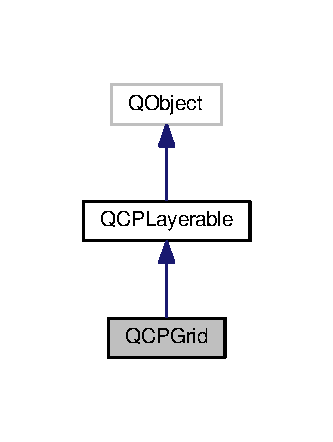
\includegraphics[width=160pt]{classQCPGrid__inherit__graph}
\end{center}
\end{figure}


Collaboration diagram for Q\+C\+P\+Grid\+:
\nopagebreak
\begin{figure}[H]
\begin{center}
\leavevmode
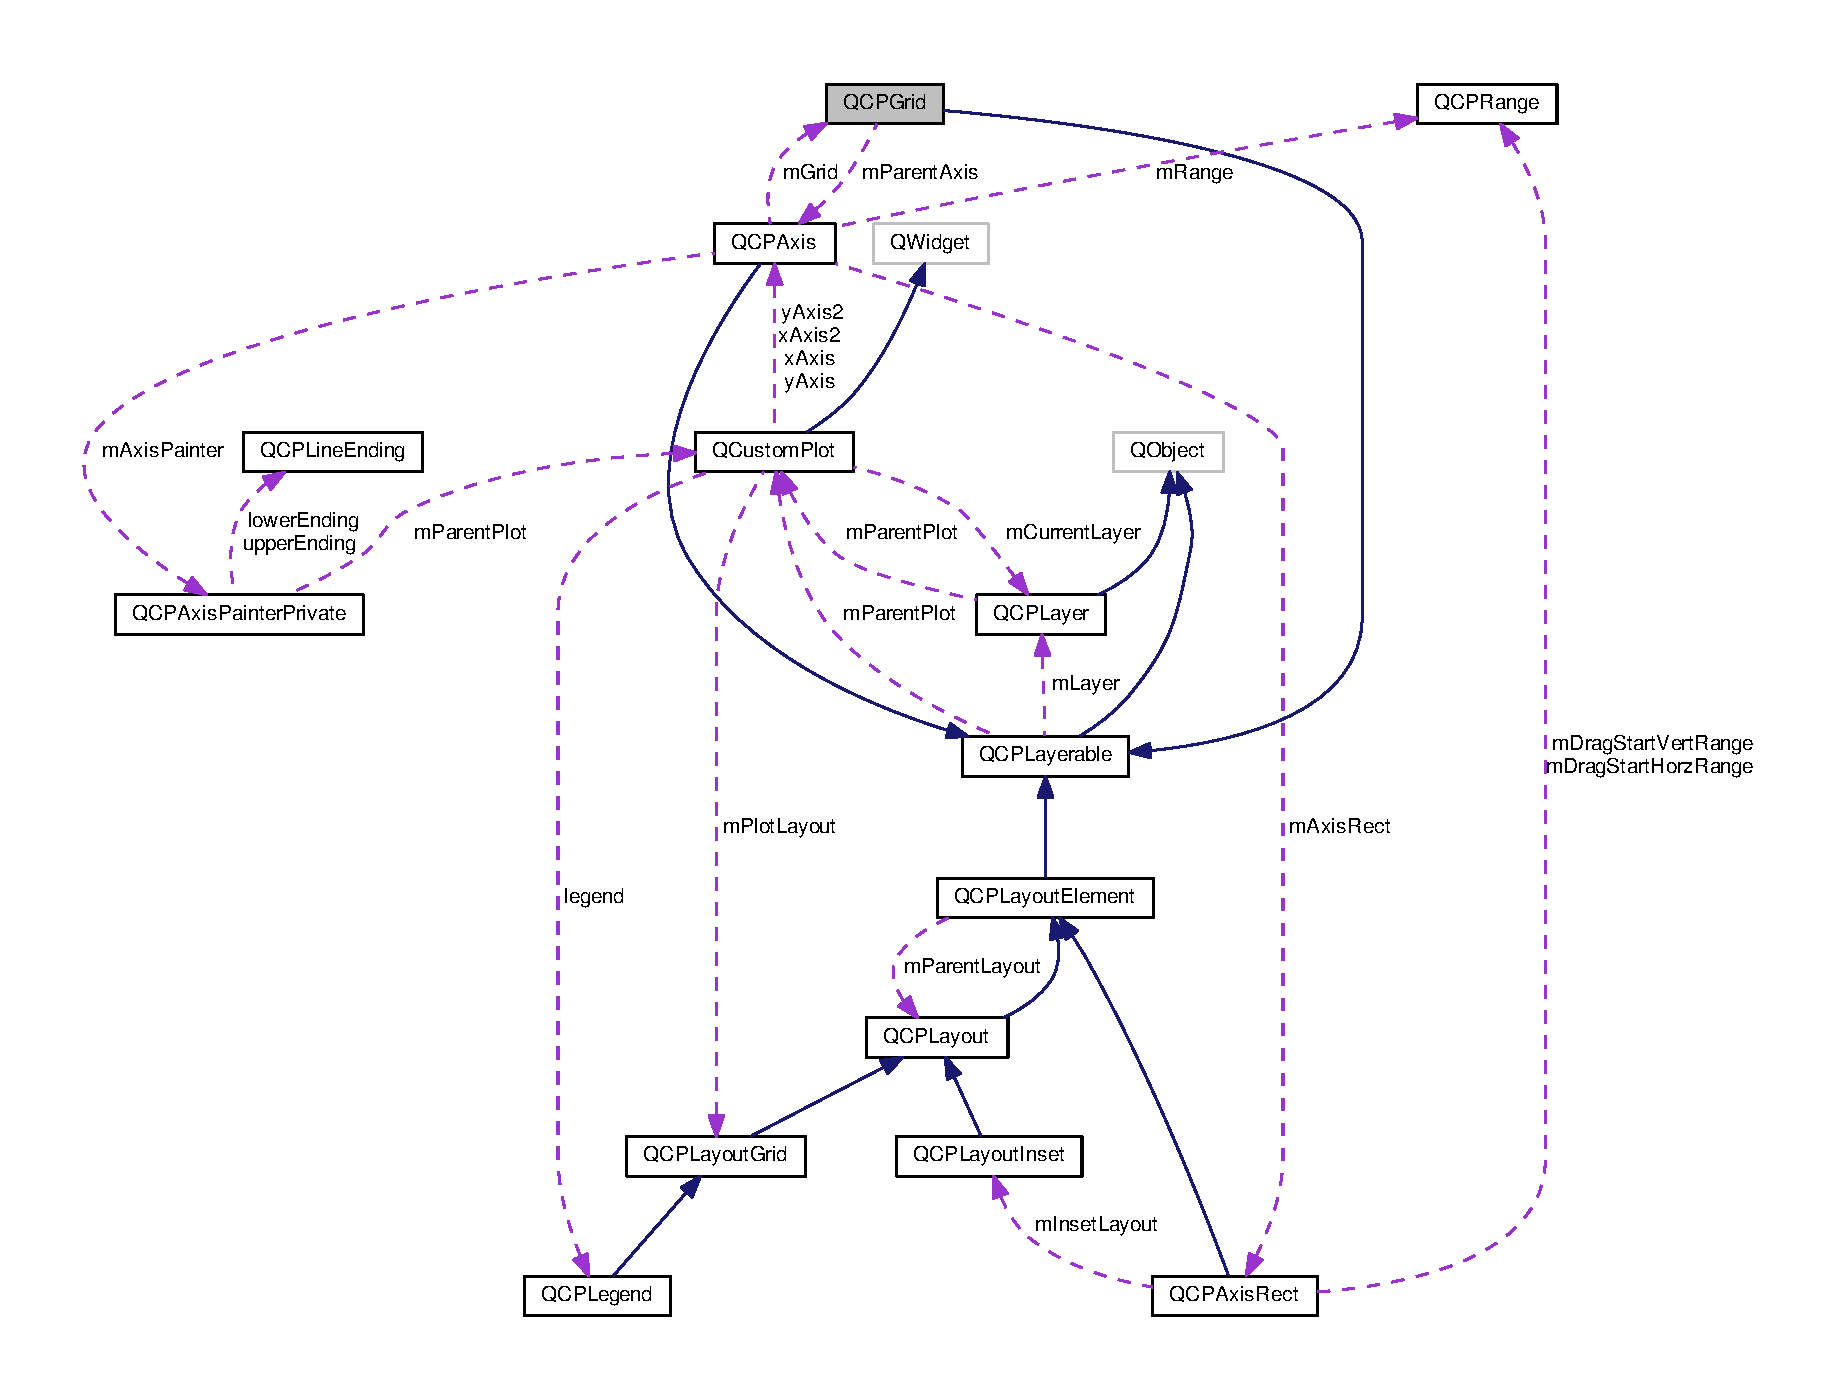
\includegraphics[width=350pt]{classQCPGrid__coll__graph}
\end{center}
\end{figure}
\subsection*{Public Member Functions}
\begin{DoxyCompactItemize}
\item 
\hyperlink{classQCPGrid_acd1cdd2909625388a13048b698494a17}{Q\+C\+P\+Grid} (\hyperlink{classQCPAxis}{Q\+C\+P\+Axis} $\ast$parent\+Axis)
\item 
bool \hyperlink{classQCPGrid_a0a8963e384d53cd77cbab7df96147458}{sub\+Grid\+Visible} () const 
\item 
bool \hyperlink{classQCPGrid_abfa6c638a05b45b2ed31b680fc9b31fc}{antialiased\+Sub\+Grid} () const 
\item 
bool \hyperlink{classQCPGrid_a4dfbc1cee989d8cae1434b765ab2a13b}{antialiased\+Zero\+Line} () const 
\item 
Q\+Pen \hyperlink{classQCPGrid_aca20b67548e3ae31fd02e6398ffd6cb9}{pen} () const 
\item 
Q\+Pen \hyperlink{classQCPGrid_ac698f8c6864b1d8f0e2af97ca4b39cc6}{sub\+Grid\+Pen} () const 
\item 
Q\+Pen \hyperlink{classQCPGrid_a06ea986b651860446e1224d2097259b9}{zero\+Line\+Pen} () const 
\item 
void \hyperlink{classQCPGrid_ad4ad6bf714ec45e08845456355a1b700}{set\+Sub\+Grid\+Visible} (bool \hyperlink{classQCPLayerable_a10a3cc92e0fa63e4a929e61d34e275a7}{visible})
\item 
void \hyperlink{classQCPGrid_a5692310ba183721a413d60951407d114}{set\+Antialiased\+Sub\+Grid} (bool enabled)
\item 
void \hyperlink{classQCPGrid_a3cc6d54647393ee71afb6da56af07aa4}{set\+Antialiased\+Zero\+Line} (bool enabled)
\item 
void \hyperlink{classQCPGrid_aa05ab9816ffb440908171e45e833b593}{set\+Pen} (const Q\+Pen \&\hyperlink{classQCPGrid_aca20b67548e3ae31fd02e6398ffd6cb9}{pen})
\item 
void \hyperlink{classQCPGrid_a9edd3593f384d1f0b0202a39cef4453d}{set\+Sub\+Grid\+Pen} (const Q\+Pen \&\hyperlink{classQCPGrid_aca20b67548e3ae31fd02e6398ffd6cb9}{pen})
\item 
void \hyperlink{classQCPGrid_a209f40fdb252397b418b82d3494d8ea0}{set\+Zero\+Line\+Pen} (const Q\+Pen \&\hyperlink{classQCPGrid_aca20b67548e3ae31fd02e6398ffd6cb9}{pen})
\end{DoxyCompactItemize}
\subsection*{Protected Member Functions}
\begin{DoxyCompactItemize}
\item 
virtual void \hyperlink{classQCPGrid_a9916f5e38b4d6cae446537aeb47c7272}{apply\+Default\+Antialiasing\+Hint} (\hyperlink{classQCPPainter}{Q\+C\+P\+Painter} $\ast$painter) const 
\item 
virtual void \hyperlink{classQCPGrid_ad009c23f96078616aa4f66a750974b23}{draw} (\hyperlink{classQCPPainter}{Q\+C\+P\+Painter} $\ast$painter)
\item 
void \hyperlink{classQCPGrid_a3aff10e993f6625e255c19e4f97a09d8}{draw\+Grid\+Lines} (\hyperlink{classQCPPainter}{Q\+C\+P\+Painter} $\ast$painter) const 
\item 
void \hyperlink{classQCPGrid_afa5d9d12de419e881f381f2ab7cb414d}{draw\+Sub\+Grid\+Lines} (\hyperlink{classQCPPainter}{Q\+C\+P\+Painter} $\ast$painter) const 
\end{DoxyCompactItemize}
\subsection*{Protected Attributes}
\begin{DoxyCompactItemize}
\item 
bool \hyperlink{classQCPGrid_a4e4a0400d6319bb44c06341f6298c87b}{m\+Sub\+Grid\+Visible}
\item 
bool \hyperlink{classQCPGrid_a71b7051f833f0c5de3094998d6afdd87}{m\+Antialiased\+Sub\+Grid}
\item 
bool \hyperlink{classQCPGrid_a8c0df56ae86440408c050895dcdb922b}{m\+Antialiased\+Zero\+Line}
\item 
Q\+Pen \hyperlink{classQCPGrid_a1cdc4a3bccf6a40c2d4360def9fefa40}{m\+Pen}
\item 
Q\+Pen \hyperlink{classQCPGrid_aa9004bc139ad3ea92629f0aaae81d83f}{m\+Sub\+Grid\+Pen}
\item 
Q\+Pen \hyperlink{classQCPGrid_a379481871f17655c27eda30af233554f}{m\+Zero\+Line\+Pen}
\item 
\hyperlink{classQCPAxis}{Q\+C\+P\+Axis} $\ast$ \hyperlink{classQCPGrid_a9a8a76731e6e737b65b929fd1995cc88}{m\+Parent\+Axis}
\end{DoxyCompactItemize}
\subsection*{Friends}
\begin{DoxyCompactItemize}
\item 
class \hyperlink{classQCPGrid_af123edeca169ec7a31958a1d714e1a8a}{Q\+C\+P\+Axis}
\end{DoxyCompactItemize}
\subsection*{Additional Inherited Members}


\subsection{Detailed Description}
Responsible for drawing the grid of a \hyperlink{classQCPAxis}{Q\+C\+P\+Axis}. 

This class is tightly bound to \hyperlink{classQCPAxis}{Q\+C\+P\+Axis}. Every axis owns a grid instance and uses it to draw the grid lines, sub grid lines and zero-\/line. You can interact with the grid of an axis via \hyperlink{classQCPAxis_ac4fb913cce3072b5e75a4635e0f6cd04}{Q\+C\+P\+Axis\+::grid}. Normally, you don\textquotesingle{}t need to create an instance of \hyperlink{classQCPGrid}{Q\+C\+P\+Grid} yourself.

The axis and grid drawing was split into two classes to allow them to be placed on different layers (both \hyperlink{classQCPAxis}{Q\+C\+P\+Axis} and \hyperlink{classQCPGrid}{Q\+C\+P\+Grid} inherit from \hyperlink{classQCPLayerable}{Q\+C\+P\+Layerable}). Thus it is possible to have the grid in the background and the axes in the foreground, and any plottables/items in between. This described situation is the default setup, see the \hyperlink{classQCPLayer}{Q\+C\+P\+Layer} documentation. 

\subsection{Constructor \& Destructor Documentation}
\index{Q\+C\+P\+Grid@{Q\+C\+P\+Grid}!Q\+C\+P\+Grid@{Q\+C\+P\+Grid}}
\index{Q\+C\+P\+Grid@{Q\+C\+P\+Grid}!Q\+C\+P\+Grid@{Q\+C\+P\+Grid}}
\subsubsection[{\texorpdfstring{Q\+C\+P\+Grid(\+Q\+C\+P\+Axis $\ast$parent\+Axis)}{QCPGrid(QCPAxis *parentAxis)}}]{\setlength{\rightskip}{0pt plus 5cm}Q\+C\+P\+Grid\+::\+Q\+C\+P\+Grid (
\begin{DoxyParamCaption}
\item[{{\bf Q\+C\+P\+Axis} $\ast$}]{parent\+Axis}
\end{DoxyParamCaption}
)}\hypertarget{classQCPGrid_acd1cdd2909625388a13048b698494a17}{}\label{classQCPGrid_acd1cdd2909625388a13048b698494a17}
Creates a \hyperlink{classQCPGrid}{Q\+C\+P\+Grid} instance and sets default values.

You shouldn\textquotesingle{}t instantiate grids on their own, since every \hyperlink{classQCPAxis}{Q\+C\+P\+Axis} brings its own \hyperlink{classQCPGrid}{Q\+C\+P\+Grid}. 

\subsection{Member Function Documentation}
\index{Q\+C\+P\+Grid@{Q\+C\+P\+Grid}!antialiased\+Sub\+Grid@{antialiased\+Sub\+Grid}}
\index{antialiased\+Sub\+Grid@{antialiased\+Sub\+Grid}!Q\+C\+P\+Grid@{Q\+C\+P\+Grid}}
\subsubsection[{\texorpdfstring{antialiased\+Sub\+Grid() const }{antialiasedSubGrid() const }}]{\setlength{\rightskip}{0pt plus 5cm}bool Q\+C\+P\+Grid\+::antialiased\+Sub\+Grid (
\begin{DoxyParamCaption}
{}
\end{DoxyParamCaption}
) const\hspace{0.3cm}{\ttfamily [inline]}}\hypertarget{classQCPGrid_abfa6c638a05b45b2ed31b680fc9b31fc}{}\label{classQCPGrid_abfa6c638a05b45b2ed31b680fc9b31fc}
\index{Q\+C\+P\+Grid@{Q\+C\+P\+Grid}!antialiased\+Zero\+Line@{antialiased\+Zero\+Line}}
\index{antialiased\+Zero\+Line@{antialiased\+Zero\+Line}!Q\+C\+P\+Grid@{Q\+C\+P\+Grid}}
\subsubsection[{\texorpdfstring{antialiased\+Zero\+Line() const }{antialiasedZeroLine() const }}]{\setlength{\rightskip}{0pt plus 5cm}bool Q\+C\+P\+Grid\+::antialiased\+Zero\+Line (
\begin{DoxyParamCaption}
{}
\end{DoxyParamCaption}
) const\hspace{0.3cm}{\ttfamily [inline]}}\hypertarget{classQCPGrid_a4dfbc1cee989d8cae1434b765ab2a13b}{}\label{classQCPGrid_a4dfbc1cee989d8cae1434b765ab2a13b}
\index{Q\+C\+P\+Grid@{Q\+C\+P\+Grid}!apply\+Default\+Antialiasing\+Hint@{apply\+Default\+Antialiasing\+Hint}}
\index{apply\+Default\+Antialiasing\+Hint@{apply\+Default\+Antialiasing\+Hint}!Q\+C\+P\+Grid@{Q\+C\+P\+Grid}}
\subsubsection[{\texorpdfstring{apply\+Default\+Antialiasing\+Hint(\+Q\+C\+P\+Painter $\ast$painter) const }{applyDefaultAntialiasingHint(QCPPainter *painter) const }}]{\setlength{\rightskip}{0pt plus 5cm}void Q\+C\+P\+Grid\+::apply\+Default\+Antialiasing\+Hint (
\begin{DoxyParamCaption}
\item[{{\bf Q\+C\+P\+Painter} $\ast$}]{painter}
\end{DoxyParamCaption}
) const\hspace{0.3cm}{\ttfamily [protected]}, {\ttfamily [virtual]}}\hypertarget{classQCPGrid_a9916f5e38b4d6cae446537aeb47c7272}{}\label{classQCPGrid_a9916f5e38b4d6cae446537aeb47c7272}


Implements \hyperlink{classQCPLayerable_afdf83ddc6a265cbf4c89fe99d3d93473}{Q\+C\+P\+Layerable}.

\index{Q\+C\+P\+Grid@{Q\+C\+P\+Grid}!draw@{draw}}
\index{draw@{draw}!Q\+C\+P\+Grid@{Q\+C\+P\+Grid}}
\subsubsection[{\texorpdfstring{draw(\+Q\+C\+P\+Painter $\ast$painter)}{draw(QCPPainter *painter)}}]{\setlength{\rightskip}{0pt plus 5cm}void Q\+C\+P\+Grid\+::draw (
\begin{DoxyParamCaption}
\item[{{\bf Q\+C\+P\+Painter} $\ast$}]{painter}
\end{DoxyParamCaption}
)\hspace{0.3cm}{\ttfamily [protected]}, {\ttfamily [virtual]}}\hypertarget{classQCPGrid_ad009c23f96078616aa4f66a750974b23}{}\label{classQCPGrid_ad009c23f96078616aa4f66a750974b23}


Implements \hyperlink{classQCPLayerable_aecf2f7087482d4b6a78cb2770e5ed12d}{Q\+C\+P\+Layerable}.

\index{Q\+C\+P\+Grid@{Q\+C\+P\+Grid}!draw\+Grid\+Lines@{draw\+Grid\+Lines}}
\index{draw\+Grid\+Lines@{draw\+Grid\+Lines}!Q\+C\+P\+Grid@{Q\+C\+P\+Grid}}
\subsubsection[{\texorpdfstring{draw\+Grid\+Lines(\+Q\+C\+P\+Painter $\ast$painter) const }{drawGridLines(QCPPainter *painter) const }}]{\setlength{\rightskip}{0pt plus 5cm}void Q\+C\+P\+Grid\+::draw\+Grid\+Lines (
\begin{DoxyParamCaption}
\item[{{\bf Q\+C\+P\+Painter} $\ast$}]{painter}
\end{DoxyParamCaption}
) const\hspace{0.3cm}{\ttfamily [protected]}}\hypertarget{classQCPGrid_a3aff10e993f6625e255c19e4f97a09d8}{}\label{classQCPGrid_a3aff10e993f6625e255c19e4f97a09d8}
\index{Q\+C\+P\+Grid@{Q\+C\+P\+Grid}!draw\+Sub\+Grid\+Lines@{draw\+Sub\+Grid\+Lines}}
\index{draw\+Sub\+Grid\+Lines@{draw\+Sub\+Grid\+Lines}!Q\+C\+P\+Grid@{Q\+C\+P\+Grid}}
\subsubsection[{\texorpdfstring{draw\+Sub\+Grid\+Lines(\+Q\+C\+P\+Painter $\ast$painter) const }{drawSubGridLines(QCPPainter *painter) const }}]{\setlength{\rightskip}{0pt plus 5cm}void Q\+C\+P\+Grid\+::draw\+Sub\+Grid\+Lines (
\begin{DoxyParamCaption}
\item[{{\bf Q\+C\+P\+Painter} $\ast$}]{painter}
\end{DoxyParamCaption}
) const\hspace{0.3cm}{\ttfamily [protected]}}\hypertarget{classQCPGrid_afa5d9d12de419e881f381f2ab7cb414d}{}\label{classQCPGrid_afa5d9d12de419e881f381f2ab7cb414d}
\index{Q\+C\+P\+Grid@{Q\+C\+P\+Grid}!pen@{pen}}
\index{pen@{pen}!Q\+C\+P\+Grid@{Q\+C\+P\+Grid}}
\subsubsection[{\texorpdfstring{pen() const }{pen() const }}]{\setlength{\rightskip}{0pt plus 5cm}Q\+Pen Q\+C\+P\+Grid\+::pen (
\begin{DoxyParamCaption}
{}
\end{DoxyParamCaption}
) const\hspace{0.3cm}{\ttfamily [inline]}}\hypertarget{classQCPGrid_aca20b67548e3ae31fd02e6398ffd6cb9}{}\label{classQCPGrid_aca20b67548e3ae31fd02e6398ffd6cb9}
\index{Q\+C\+P\+Grid@{Q\+C\+P\+Grid}!set\+Antialiased\+Sub\+Grid@{set\+Antialiased\+Sub\+Grid}}
\index{set\+Antialiased\+Sub\+Grid@{set\+Antialiased\+Sub\+Grid}!Q\+C\+P\+Grid@{Q\+C\+P\+Grid}}
\subsubsection[{\texorpdfstring{set\+Antialiased\+Sub\+Grid(bool enabled)}{setAntialiasedSubGrid(bool enabled)}}]{\setlength{\rightskip}{0pt plus 5cm}void Q\+C\+P\+Grid\+::set\+Antialiased\+Sub\+Grid (
\begin{DoxyParamCaption}
\item[{bool}]{enabled}
\end{DoxyParamCaption}
)}\hypertarget{classQCPGrid_a5692310ba183721a413d60951407d114}{}\label{classQCPGrid_a5692310ba183721a413d60951407d114}
Sets whether sub grid lines are drawn antialiased. \index{Q\+C\+P\+Grid@{Q\+C\+P\+Grid}!set\+Antialiased\+Zero\+Line@{set\+Antialiased\+Zero\+Line}}
\index{set\+Antialiased\+Zero\+Line@{set\+Antialiased\+Zero\+Line}!Q\+C\+P\+Grid@{Q\+C\+P\+Grid}}
\subsubsection[{\texorpdfstring{set\+Antialiased\+Zero\+Line(bool enabled)}{setAntialiasedZeroLine(bool enabled)}}]{\setlength{\rightskip}{0pt plus 5cm}void Q\+C\+P\+Grid\+::set\+Antialiased\+Zero\+Line (
\begin{DoxyParamCaption}
\item[{bool}]{enabled}
\end{DoxyParamCaption}
)}\hypertarget{classQCPGrid_a3cc6d54647393ee71afb6da56af07aa4}{}\label{classQCPGrid_a3cc6d54647393ee71afb6da56af07aa4}
Sets whether zero lines are drawn antialiased. \index{Q\+C\+P\+Grid@{Q\+C\+P\+Grid}!set\+Pen@{set\+Pen}}
\index{set\+Pen@{set\+Pen}!Q\+C\+P\+Grid@{Q\+C\+P\+Grid}}
\subsubsection[{\texorpdfstring{set\+Pen(const Q\+Pen \&pen)}{setPen(const QPen &pen)}}]{\setlength{\rightskip}{0pt plus 5cm}void Q\+C\+P\+Grid\+::set\+Pen (
\begin{DoxyParamCaption}
\item[{const Q\+Pen \&}]{pen}
\end{DoxyParamCaption}
)}\hypertarget{classQCPGrid_aa05ab9816ffb440908171e45e833b593}{}\label{classQCPGrid_aa05ab9816ffb440908171e45e833b593}
Sets the pen with which (major) grid lines are drawn. \index{Q\+C\+P\+Grid@{Q\+C\+P\+Grid}!set\+Sub\+Grid\+Pen@{set\+Sub\+Grid\+Pen}}
\index{set\+Sub\+Grid\+Pen@{set\+Sub\+Grid\+Pen}!Q\+C\+P\+Grid@{Q\+C\+P\+Grid}}
\subsubsection[{\texorpdfstring{set\+Sub\+Grid\+Pen(const Q\+Pen \&pen)}{setSubGridPen(const QPen &pen)}}]{\setlength{\rightskip}{0pt plus 5cm}void Q\+C\+P\+Grid\+::set\+Sub\+Grid\+Pen (
\begin{DoxyParamCaption}
\item[{const Q\+Pen \&}]{pen}
\end{DoxyParamCaption}
)}\hypertarget{classQCPGrid_a9edd3593f384d1f0b0202a39cef4453d}{}\label{classQCPGrid_a9edd3593f384d1f0b0202a39cef4453d}
Sets the pen with which sub grid lines are drawn. \index{Q\+C\+P\+Grid@{Q\+C\+P\+Grid}!set\+Sub\+Grid\+Visible@{set\+Sub\+Grid\+Visible}}
\index{set\+Sub\+Grid\+Visible@{set\+Sub\+Grid\+Visible}!Q\+C\+P\+Grid@{Q\+C\+P\+Grid}}
\subsubsection[{\texorpdfstring{set\+Sub\+Grid\+Visible(bool visible)}{setSubGridVisible(bool visible)}}]{\setlength{\rightskip}{0pt plus 5cm}void Q\+C\+P\+Grid\+::set\+Sub\+Grid\+Visible (
\begin{DoxyParamCaption}
\item[{bool}]{visible}
\end{DoxyParamCaption}
)}\hypertarget{classQCPGrid_ad4ad6bf714ec45e08845456355a1b700}{}\label{classQCPGrid_ad4ad6bf714ec45e08845456355a1b700}
Sets whether grid lines at sub tick marks are drawn.

\begin{DoxySeeAlso}{See also}
\hyperlink{classQCPGrid_a9edd3593f384d1f0b0202a39cef4453d}{set\+Sub\+Grid\+Pen} 
\end{DoxySeeAlso}
\index{Q\+C\+P\+Grid@{Q\+C\+P\+Grid}!set\+Zero\+Line\+Pen@{set\+Zero\+Line\+Pen}}
\index{set\+Zero\+Line\+Pen@{set\+Zero\+Line\+Pen}!Q\+C\+P\+Grid@{Q\+C\+P\+Grid}}
\subsubsection[{\texorpdfstring{set\+Zero\+Line\+Pen(const Q\+Pen \&pen)}{setZeroLinePen(const QPen &pen)}}]{\setlength{\rightskip}{0pt plus 5cm}void Q\+C\+P\+Grid\+::set\+Zero\+Line\+Pen (
\begin{DoxyParamCaption}
\item[{const Q\+Pen \&}]{pen}
\end{DoxyParamCaption}
)}\hypertarget{classQCPGrid_a209f40fdb252397b418b82d3494d8ea0}{}\label{classQCPGrid_a209f40fdb252397b418b82d3494d8ea0}
Sets the pen with which zero lines are drawn.

Zero lines are lines at value coordinate 0 which may be drawn with a different pen than other grid lines. To disable zero lines and just draw normal grid lines at zero, set {\itshape pen} to Qt\+::\+No\+Pen. \index{Q\+C\+P\+Grid@{Q\+C\+P\+Grid}!sub\+Grid\+Pen@{sub\+Grid\+Pen}}
\index{sub\+Grid\+Pen@{sub\+Grid\+Pen}!Q\+C\+P\+Grid@{Q\+C\+P\+Grid}}
\subsubsection[{\texorpdfstring{sub\+Grid\+Pen() const }{subGridPen() const }}]{\setlength{\rightskip}{0pt plus 5cm}Q\+Pen Q\+C\+P\+Grid\+::sub\+Grid\+Pen (
\begin{DoxyParamCaption}
{}
\end{DoxyParamCaption}
) const\hspace{0.3cm}{\ttfamily [inline]}}\hypertarget{classQCPGrid_ac698f8c6864b1d8f0e2af97ca4b39cc6}{}\label{classQCPGrid_ac698f8c6864b1d8f0e2af97ca4b39cc6}
\index{Q\+C\+P\+Grid@{Q\+C\+P\+Grid}!sub\+Grid\+Visible@{sub\+Grid\+Visible}}
\index{sub\+Grid\+Visible@{sub\+Grid\+Visible}!Q\+C\+P\+Grid@{Q\+C\+P\+Grid}}
\subsubsection[{\texorpdfstring{sub\+Grid\+Visible() const }{subGridVisible() const }}]{\setlength{\rightskip}{0pt plus 5cm}bool Q\+C\+P\+Grid\+::sub\+Grid\+Visible (
\begin{DoxyParamCaption}
{}
\end{DoxyParamCaption}
) const\hspace{0.3cm}{\ttfamily [inline]}}\hypertarget{classQCPGrid_a0a8963e384d53cd77cbab7df96147458}{}\label{classQCPGrid_a0a8963e384d53cd77cbab7df96147458}
\index{Q\+C\+P\+Grid@{Q\+C\+P\+Grid}!zero\+Line\+Pen@{zero\+Line\+Pen}}
\index{zero\+Line\+Pen@{zero\+Line\+Pen}!Q\+C\+P\+Grid@{Q\+C\+P\+Grid}}
\subsubsection[{\texorpdfstring{zero\+Line\+Pen() const }{zeroLinePen() const }}]{\setlength{\rightskip}{0pt plus 5cm}Q\+Pen Q\+C\+P\+Grid\+::zero\+Line\+Pen (
\begin{DoxyParamCaption}
{}
\end{DoxyParamCaption}
) const\hspace{0.3cm}{\ttfamily [inline]}}\hypertarget{classQCPGrid_a06ea986b651860446e1224d2097259b9}{}\label{classQCPGrid_a06ea986b651860446e1224d2097259b9}


\subsection{Friends And Related Function Documentation}
\index{Q\+C\+P\+Grid@{Q\+C\+P\+Grid}!Q\+C\+P\+Axis@{Q\+C\+P\+Axis}}
\index{Q\+C\+P\+Axis@{Q\+C\+P\+Axis}!Q\+C\+P\+Grid@{Q\+C\+P\+Grid}}
\subsubsection[{\texorpdfstring{Q\+C\+P\+Axis}{QCPAxis}}]{\setlength{\rightskip}{0pt plus 5cm}friend class {\bf Q\+C\+P\+Axis}\hspace{0.3cm}{\ttfamily [friend]}}\hypertarget{classQCPGrid_af123edeca169ec7a31958a1d714e1a8a}{}\label{classQCPGrid_af123edeca169ec7a31958a1d714e1a8a}


\subsection{Member Data Documentation}
\index{Q\+C\+P\+Grid@{Q\+C\+P\+Grid}!m\+Antialiased\+Sub\+Grid@{m\+Antialiased\+Sub\+Grid}}
\index{m\+Antialiased\+Sub\+Grid@{m\+Antialiased\+Sub\+Grid}!Q\+C\+P\+Grid@{Q\+C\+P\+Grid}}
\subsubsection[{\texorpdfstring{m\+Antialiased\+Sub\+Grid}{mAntialiasedSubGrid}}]{\setlength{\rightskip}{0pt plus 5cm}bool Q\+C\+P\+Grid\+::m\+Antialiased\+Sub\+Grid\hspace{0.3cm}{\ttfamily [protected]}}\hypertarget{classQCPGrid_a71b7051f833f0c5de3094998d6afdd87}{}\label{classQCPGrid_a71b7051f833f0c5de3094998d6afdd87}
\index{Q\+C\+P\+Grid@{Q\+C\+P\+Grid}!m\+Antialiased\+Zero\+Line@{m\+Antialiased\+Zero\+Line}}
\index{m\+Antialiased\+Zero\+Line@{m\+Antialiased\+Zero\+Line}!Q\+C\+P\+Grid@{Q\+C\+P\+Grid}}
\subsubsection[{\texorpdfstring{m\+Antialiased\+Zero\+Line}{mAntialiasedZeroLine}}]{\setlength{\rightskip}{0pt plus 5cm}bool Q\+C\+P\+Grid\+::m\+Antialiased\+Zero\+Line\hspace{0.3cm}{\ttfamily [protected]}}\hypertarget{classQCPGrid_a8c0df56ae86440408c050895dcdb922b}{}\label{classQCPGrid_a8c0df56ae86440408c050895dcdb922b}
\index{Q\+C\+P\+Grid@{Q\+C\+P\+Grid}!m\+Parent\+Axis@{m\+Parent\+Axis}}
\index{m\+Parent\+Axis@{m\+Parent\+Axis}!Q\+C\+P\+Grid@{Q\+C\+P\+Grid}}
\subsubsection[{\texorpdfstring{m\+Parent\+Axis}{mParentAxis}}]{\setlength{\rightskip}{0pt plus 5cm}{\bf Q\+C\+P\+Axis}$\ast$ Q\+C\+P\+Grid\+::m\+Parent\+Axis\hspace{0.3cm}{\ttfamily [protected]}}\hypertarget{classQCPGrid_a9a8a76731e6e737b65b929fd1995cc88}{}\label{classQCPGrid_a9a8a76731e6e737b65b929fd1995cc88}
\index{Q\+C\+P\+Grid@{Q\+C\+P\+Grid}!m\+Pen@{m\+Pen}}
\index{m\+Pen@{m\+Pen}!Q\+C\+P\+Grid@{Q\+C\+P\+Grid}}
\subsubsection[{\texorpdfstring{m\+Pen}{mPen}}]{\setlength{\rightskip}{0pt plus 5cm}Q\+Pen Q\+C\+P\+Grid\+::m\+Pen\hspace{0.3cm}{\ttfamily [protected]}}\hypertarget{classQCPGrid_a1cdc4a3bccf6a40c2d4360def9fefa40}{}\label{classQCPGrid_a1cdc4a3bccf6a40c2d4360def9fefa40}
\index{Q\+C\+P\+Grid@{Q\+C\+P\+Grid}!m\+Sub\+Grid\+Pen@{m\+Sub\+Grid\+Pen}}
\index{m\+Sub\+Grid\+Pen@{m\+Sub\+Grid\+Pen}!Q\+C\+P\+Grid@{Q\+C\+P\+Grid}}
\subsubsection[{\texorpdfstring{m\+Sub\+Grid\+Pen}{mSubGridPen}}]{\setlength{\rightskip}{0pt plus 5cm}Q\+Pen Q\+C\+P\+Grid\+::m\+Sub\+Grid\+Pen\hspace{0.3cm}{\ttfamily [protected]}}\hypertarget{classQCPGrid_aa9004bc139ad3ea92629f0aaae81d83f}{}\label{classQCPGrid_aa9004bc139ad3ea92629f0aaae81d83f}
\index{Q\+C\+P\+Grid@{Q\+C\+P\+Grid}!m\+Sub\+Grid\+Visible@{m\+Sub\+Grid\+Visible}}
\index{m\+Sub\+Grid\+Visible@{m\+Sub\+Grid\+Visible}!Q\+C\+P\+Grid@{Q\+C\+P\+Grid}}
\subsubsection[{\texorpdfstring{m\+Sub\+Grid\+Visible}{mSubGridVisible}}]{\setlength{\rightskip}{0pt plus 5cm}bool Q\+C\+P\+Grid\+::m\+Sub\+Grid\+Visible\hspace{0.3cm}{\ttfamily [protected]}}\hypertarget{classQCPGrid_a4e4a0400d6319bb44c06341f6298c87b}{}\label{classQCPGrid_a4e4a0400d6319bb44c06341f6298c87b}
\index{Q\+C\+P\+Grid@{Q\+C\+P\+Grid}!m\+Zero\+Line\+Pen@{m\+Zero\+Line\+Pen}}
\index{m\+Zero\+Line\+Pen@{m\+Zero\+Line\+Pen}!Q\+C\+P\+Grid@{Q\+C\+P\+Grid}}
\subsubsection[{\texorpdfstring{m\+Zero\+Line\+Pen}{mZeroLinePen}}]{\setlength{\rightskip}{0pt plus 5cm}Q\+Pen Q\+C\+P\+Grid\+::m\+Zero\+Line\+Pen\hspace{0.3cm}{\ttfamily [protected]}}\hypertarget{classQCPGrid_a379481871f17655c27eda30af233554f}{}\label{classQCPGrid_a379481871f17655c27eda30af233554f}


The documentation for this class was generated from the following files\+:\begin{DoxyCompactItemize}
\item 
src/hammerhead/tools/watchdog/include/watchdog/\hyperlink{qcustomplot_8h}{qcustomplot.\+h}\item 
src/hammerhead/tools/watchdog/src/\hyperlink{qcustomplot_8cpp}{qcustomplot.\+cpp}\end{DoxyCompactItemize}

\hypertarget{classQCPItemAnchor}{}\section{Q\+C\+P\+Item\+Anchor Class Reference}
\label{classQCPItemAnchor}\index{Q\+C\+P\+Item\+Anchor@{Q\+C\+P\+Item\+Anchor}}


An anchor of an item to which positions can be attached to.  




{\ttfamily \#include $<$qcustomplot.\+h$>$}



Inheritance diagram for Q\+C\+P\+Item\+Anchor\+:\nopagebreak
\begin{figure}[H]
\begin{center}
\leavevmode
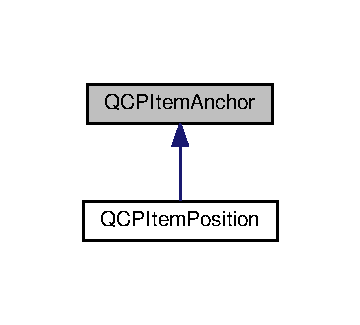
\includegraphics[width=173pt]{classQCPItemAnchor__inherit__graph}
\end{center}
\end{figure}


Collaboration diagram for Q\+C\+P\+Item\+Anchor\+:\nopagebreak
\begin{figure}[H]
\begin{center}
\leavevmode
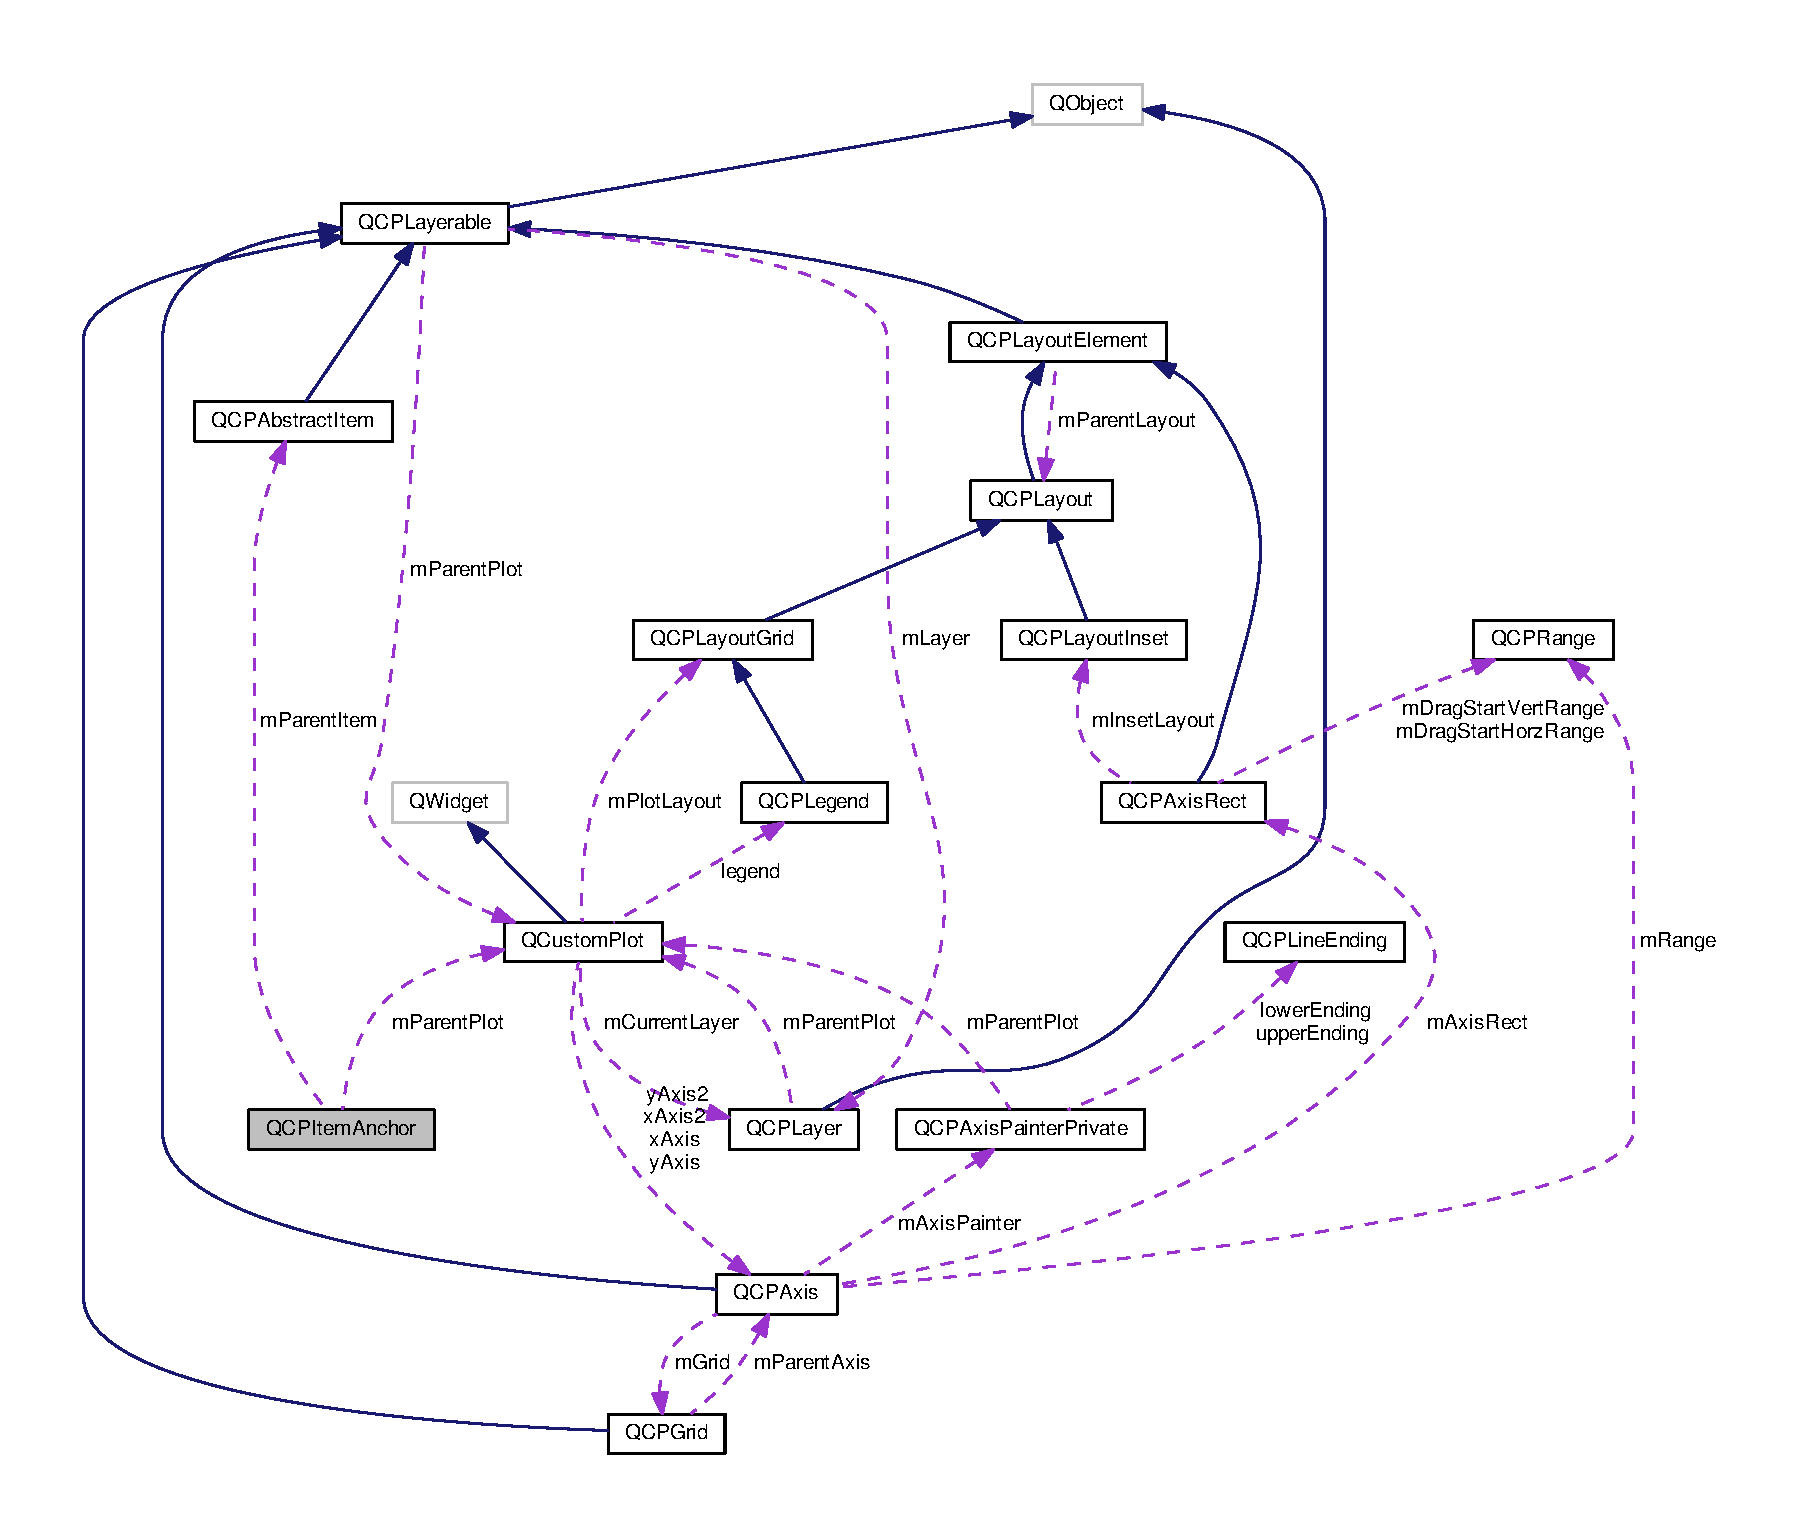
\includegraphics[width=350pt]{classQCPItemAnchor__coll__graph}
\end{center}
\end{figure}
\subsection*{Public Member Functions}
\begin{DoxyCompactItemize}
\item 
\hyperlink{classQCPItemAnchor_aeb6b681d2bf324db40a915d32ec5624f}{Q\+C\+P\+Item\+Anchor} (\hyperlink{classQCustomPlot}{Q\+Custom\+Plot} $\ast$parent\+Plot, \hyperlink{classQCPAbstractItem}{Q\+C\+P\+Abstract\+Item} $\ast$parent\+Item, const Q\+String \hyperlink{classQCPItemAnchor_ac93984042a58c875e76847dc3e5f75fe}{name}, int anchor\+Id=-\/1)
\item 
virtual \hyperlink{classQCPItemAnchor_a1868559407600688ee4d1a4621e81ceb}{$\sim$\+Q\+C\+P\+Item\+Anchor} ()
\item 
Q\+String \hyperlink{classQCPItemAnchor_ac93984042a58c875e76847dc3e5f75fe}{name} () const 
\item 
virtual Q\+PointF \hyperlink{classQCPItemAnchor_ae92def8f9297c5d73f5806c586517bb3}{pixel\+Point} () const 
\end{DoxyCompactItemize}
\subsection*{Protected Member Functions}
\begin{DoxyCompactItemize}
\item 
virtual \hyperlink{classQCPItemPosition}{Q\+C\+P\+Item\+Position} $\ast$ \hyperlink{classQCPItemAnchor_ac54b20120669950255a63587193dbb86}{to\+Q\+C\+P\+Item\+Position} ()
\item 
void \hyperlink{classQCPItemAnchor_aef15daa640debfb11b0aeaa2116c6fbc}{add\+ChildX} (\hyperlink{classQCPItemPosition}{Q\+C\+P\+Item\+Position} $\ast$pos)
\item 
void \hyperlink{classQCPItemAnchor_a230b1d494cda63458e289bbe1b642599}{remove\+ChildX} (\hyperlink{classQCPItemPosition}{Q\+C\+P\+Item\+Position} $\ast$pos)
\item 
void \hyperlink{classQCPItemAnchor_af05dc56f24536f0c7a9a0f57b58cea67}{add\+ChildY} (\hyperlink{classQCPItemPosition}{Q\+C\+P\+Item\+Position} $\ast$pos)
\item 
void \hyperlink{classQCPItemAnchor_aa2394911d8fff3bd958b9f4f1994b64d}{remove\+ChildY} (\hyperlink{classQCPItemPosition}{Q\+C\+P\+Item\+Position} $\ast$pos)
\end{DoxyCompactItemize}
\subsection*{Protected Attributes}
\begin{DoxyCompactItemize}
\item 
Q\+String \hyperlink{classQCPItemAnchor_a23ad4d0ab0d2cbb41a7baf05bcf996ec}{m\+Name}
\item 
\hyperlink{classQCustomPlot}{Q\+Custom\+Plot} $\ast$ \hyperlink{classQCPItemAnchor_a59b968410831ba91a25cc75a77dde6f5}{m\+Parent\+Plot}
\item 
\hyperlink{classQCPAbstractItem}{Q\+C\+P\+Abstract\+Item} $\ast$ \hyperlink{classQCPItemAnchor_a80fad480ad3bb980446ed6ebc00818ae}{m\+Parent\+Item}
\item 
int \hyperlink{classQCPItemAnchor_a00c62070333e8345976b579676ad3997}{m\+Anchor\+Id}
\item 
Q\+Set$<$ \hyperlink{classQCPItemPosition}{Q\+C\+P\+Item\+Position} $\ast$ $>$ \hyperlink{classQCPItemAnchor_a3c0bfd6e50f3b48e2a9b3824695b20f7}{m\+ChildrenX}
\item 
Q\+Set$<$ \hyperlink{classQCPItemPosition}{Q\+C\+P\+Item\+Position} $\ast$ $>$ \hyperlink{classQCPItemAnchor_a3abe4eebd0683454d81c8341df6f7115}{m\+ChildrenY}
\end{DoxyCompactItemize}
\subsection*{Friends}
\begin{DoxyCompactItemize}
\item 
class \hyperlink{classQCPItemAnchor_aa9b8ddc062778e202a0be06a57d18d17}{Q\+C\+P\+Item\+Position}
\end{DoxyCompactItemize}


\subsection{Detailed Description}
An anchor of an item to which positions can be attached to. 

An item (\hyperlink{classQCPAbstractItem}{Q\+C\+P\+Abstract\+Item}) may have one or more anchors. Unlike \hyperlink{classQCPItemPosition}{Q\+C\+P\+Item\+Position}, an anchor doesn\textquotesingle{}t control anything on its item, but provides a way to tie other items via their positions to the anchor.

For example, a \hyperlink{classQCPItemRect}{Q\+C\+P\+Item\+Rect} is defined by its positions {\itshape top\+Left} and {\itshape bottom\+Right}. Additionally it has various anchors like {\itshape top}, {\itshape top\+Right} or {\itshape bottom\+Left} etc. So you can attach the {\itshape start} (which is a \hyperlink{classQCPItemPosition}{Q\+C\+P\+Item\+Position}) of a \hyperlink{classQCPItemLine}{Q\+C\+P\+Item\+Line} to one of the anchors by calling \hyperlink{classQCPItemPosition_ac094d67a95d2dceafa0d50b9db3a7e51}{Q\+C\+P\+Item\+Position\+::set\+Parent\+Anchor} on {\itshape start}, passing the wanted anchor of the \hyperlink{classQCPItemRect}{Q\+C\+P\+Item\+Rect}. This way the start of the line will now always follow the respective anchor location on the rect item.

Note that \hyperlink{classQCPItemPosition}{Q\+C\+P\+Item\+Position} derives from \hyperlink{classQCPItemAnchor}{Q\+C\+P\+Item\+Anchor}, so every position can also serve as an anchor to other positions.

To learn how to provide anchors in your own item subclasses, see the subclassing section of the \hyperlink{classQCPAbstractItem}{Q\+C\+P\+Abstract\+Item} documentation. 

\subsection{Constructor \& Destructor Documentation}
\index{Q\+C\+P\+Item\+Anchor@{Q\+C\+P\+Item\+Anchor}!Q\+C\+P\+Item\+Anchor@{Q\+C\+P\+Item\+Anchor}}
\index{Q\+C\+P\+Item\+Anchor@{Q\+C\+P\+Item\+Anchor}!Q\+C\+P\+Item\+Anchor@{Q\+C\+P\+Item\+Anchor}}
\subsubsection[{\texorpdfstring{Q\+C\+P\+Item\+Anchor(\+Q\+Custom\+Plot $\ast$parent\+Plot, Q\+C\+P\+Abstract\+Item $\ast$parent\+Item, const Q\+String name, int anchor\+Id=-\/1)}{QCPItemAnchor(QCustomPlot *parentPlot, QCPAbstractItem *parentItem, const QString name, int anchorId=-1)}}]{\setlength{\rightskip}{0pt plus 5cm}Q\+C\+P\+Item\+Anchor\+::\+Q\+C\+P\+Item\+Anchor (
\begin{DoxyParamCaption}
\item[{{\bf Q\+Custom\+Plot} $\ast$}]{parent\+Plot, }
\item[{{\bf Q\+C\+P\+Abstract\+Item} $\ast$}]{parent\+Item, }
\item[{const Q\+String}]{name, }
\item[{int}]{anchor\+Id = {\ttfamily -\/1}}
\end{DoxyParamCaption}
)}\hypertarget{classQCPItemAnchor_aeb6b681d2bf324db40a915d32ec5624f}{}\label{classQCPItemAnchor_aeb6b681d2bf324db40a915d32ec5624f}
Creates a new \hyperlink{classQCPItemAnchor}{Q\+C\+P\+Item\+Anchor}. You shouldn\textquotesingle{}t create \hyperlink{classQCPItemAnchor}{Q\+C\+P\+Item\+Anchor} instances directly, even if you want to make a new item subclass. Use \hyperlink{classQCPAbstractItem_af3fc92527802078ca395138748b629a7}{Q\+C\+P\+Abstract\+Item\+::create\+Anchor} instead, as explained in the subclassing section of the \hyperlink{classQCPAbstractItem}{Q\+C\+P\+Abstract\+Item} documentation. \index{Q\+C\+P\+Item\+Anchor@{Q\+C\+P\+Item\+Anchor}!````~Q\+C\+P\+Item\+Anchor@{$\sim$\+Q\+C\+P\+Item\+Anchor}}
\index{````~Q\+C\+P\+Item\+Anchor@{$\sim$\+Q\+C\+P\+Item\+Anchor}!Q\+C\+P\+Item\+Anchor@{Q\+C\+P\+Item\+Anchor}}
\subsubsection[{\texorpdfstring{$\sim$\+Q\+C\+P\+Item\+Anchor()}{~QCPItemAnchor()}}]{\setlength{\rightskip}{0pt plus 5cm}Q\+C\+P\+Item\+Anchor\+::$\sim$\+Q\+C\+P\+Item\+Anchor (
\begin{DoxyParamCaption}
{}
\end{DoxyParamCaption}
)\hspace{0.3cm}{\ttfamily [virtual]}}\hypertarget{classQCPItemAnchor_a1868559407600688ee4d1a4621e81ceb}{}\label{classQCPItemAnchor_a1868559407600688ee4d1a4621e81ceb}


\subsection{Member Function Documentation}
\index{Q\+C\+P\+Item\+Anchor@{Q\+C\+P\+Item\+Anchor}!add\+ChildX@{add\+ChildX}}
\index{add\+ChildX@{add\+ChildX}!Q\+C\+P\+Item\+Anchor@{Q\+C\+P\+Item\+Anchor}}
\subsubsection[{\texorpdfstring{add\+Child\+X(\+Q\+C\+P\+Item\+Position $\ast$pos)}{addChildX(QCPItemPosition *pos)}}]{\setlength{\rightskip}{0pt plus 5cm}void Q\+C\+P\+Item\+Anchor\+::add\+ChildX (
\begin{DoxyParamCaption}
\item[{{\bf Q\+C\+P\+Item\+Position} $\ast$}]{pos}
\end{DoxyParamCaption}
)\hspace{0.3cm}{\ttfamily [protected]}}\hypertarget{classQCPItemAnchor_aef15daa640debfb11b0aeaa2116c6fbc}{}\label{classQCPItemAnchor_aef15daa640debfb11b0aeaa2116c6fbc}
\index{Q\+C\+P\+Item\+Anchor@{Q\+C\+P\+Item\+Anchor}!add\+ChildY@{add\+ChildY}}
\index{add\+ChildY@{add\+ChildY}!Q\+C\+P\+Item\+Anchor@{Q\+C\+P\+Item\+Anchor}}
\subsubsection[{\texorpdfstring{add\+Child\+Y(\+Q\+C\+P\+Item\+Position $\ast$pos)}{addChildY(QCPItemPosition *pos)}}]{\setlength{\rightskip}{0pt plus 5cm}void Q\+C\+P\+Item\+Anchor\+::add\+ChildY (
\begin{DoxyParamCaption}
\item[{{\bf Q\+C\+P\+Item\+Position} $\ast$}]{pos}
\end{DoxyParamCaption}
)\hspace{0.3cm}{\ttfamily [protected]}}\hypertarget{classQCPItemAnchor_af05dc56f24536f0c7a9a0f57b58cea67}{}\label{classQCPItemAnchor_af05dc56f24536f0c7a9a0f57b58cea67}
\index{Q\+C\+P\+Item\+Anchor@{Q\+C\+P\+Item\+Anchor}!name@{name}}
\index{name@{name}!Q\+C\+P\+Item\+Anchor@{Q\+C\+P\+Item\+Anchor}}
\subsubsection[{\texorpdfstring{name() const }{name() const }}]{\setlength{\rightskip}{0pt plus 5cm}Q\+String Q\+C\+P\+Item\+Anchor\+::name (
\begin{DoxyParamCaption}
{}
\end{DoxyParamCaption}
) const\hspace{0.3cm}{\ttfamily [inline]}}\hypertarget{classQCPItemAnchor_ac93984042a58c875e76847dc3e5f75fe}{}\label{classQCPItemAnchor_ac93984042a58c875e76847dc3e5f75fe}
\index{Q\+C\+P\+Item\+Anchor@{Q\+C\+P\+Item\+Anchor}!pixel\+Point@{pixel\+Point}}
\index{pixel\+Point@{pixel\+Point}!Q\+C\+P\+Item\+Anchor@{Q\+C\+P\+Item\+Anchor}}
\subsubsection[{\texorpdfstring{pixel\+Point() const }{pixelPoint() const }}]{\setlength{\rightskip}{0pt plus 5cm}Q\+PointF Q\+C\+P\+Item\+Anchor\+::pixel\+Point (
\begin{DoxyParamCaption}
{}
\end{DoxyParamCaption}
) const\hspace{0.3cm}{\ttfamily [virtual]}}\hypertarget{classQCPItemAnchor_ae92def8f9297c5d73f5806c586517bb3}{}\label{classQCPItemAnchor_ae92def8f9297c5d73f5806c586517bb3}
Returns the final absolute pixel position of the \hyperlink{classQCPItemAnchor}{Q\+C\+P\+Item\+Anchor} on the \hyperlink{classQCustomPlot}{Q\+Custom\+Plot} surface.

The pixel information is internally retrieved via Q\+C\+P\+Abstract\+Item\+::anchor\+Pixel\+Position of the parent item, \hyperlink{classQCPItemAnchor}{Q\+C\+P\+Item\+Anchor} is just an intermediary. 

Reimplemented in \hyperlink{classQCPItemPosition_ae490f9c76ee2ba33752c495d3b6e8fb5}{Q\+C\+P\+Item\+Position}.

\index{Q\+C\+P\+Item\+Anchor@{Q\+C\+P\+Item\+Anchor}!remove\+ChildX@{remove\+ChildX}}
\index{remove\+ChildX@{remove\+ChildX}!Q\+C\+P\+Item\+Anchor@{Q\+C\+P\+Item\+Anchor}}
\subsubsection[{\texorpdfstring{remove\+Child\+X(\+Q\+C\+P\+Item\+Position $\ast$pos)}{removeChildX(QCPItemPosition *pos)}}]{\setlength{\rightskip}{0pt plus 5cm}void Q\+C\+P\+Item\+Anchor\+::remove\+ChildX (
\begin{DoxyParamCaption}
\item[{{\bf Q\+C\+P\+Item\+Position} $\ast$}]{pos}
\end{DoxyParamCaption}
)\hspace{0.3cm}{\ttfamily [protected]}}\hypertarget{classQCPItemAnchor_a230b1d494cda63458e289bbe1b642599}{}\label{classQCPItemAnchor_a230b1d494cda63458e289bbe1b642599}
\index{Q\+C\+P\+Item\+Anchor@{Q\+C\+P\+Item\+Anchor}!remove\+ChildY@{remove\+ChildY}}
\index{remove\+ChildY@{remove\+ChildY}!Q\+C\+P\+Item\+Anchor@{Q\+C\+P\+Item\+Anchor}}
\subsubsection[{\texorpdfstring{remove\+Child\+Y(\+Q\+C\+P\+Item\+Position $\ast$pos)}{removeChildY(QCPItemPosition *pos)}}]{\setlength{\rightskip}{0pt plus 5cm}void Q\+C\+P\+Item\+Anchor\+::remove\+ChildY (
\begin{DoxyParamCaption}
\item[{{\bf Q\+C\+P\+Item\+Position} $\ast$}]{pos}
\end{DoxyParamCaption}
)\hspace{0.3cm}{\ttfamily [protected]}}\hypertarget{classQCPItemAnchor_aa2394911d8fff3bd958b9f4f1994b64d}{}\label{classQCPItemAnchor_aa2394911d8fff3bd958b9f4f1994b64d}
\index{Q\+C\+P\+Item\+Anchor@{Q\+C\+P\+Item\+Anchor}!to\+Q\+C\+P\+Item\+Position@{to\+Q\+C\+P\+Item\+Position}}
\index{to\+Q\+C\+P\+Item\+Position@{to\+Q\+C\+P\+Item\+Position}!Q\+C\+P\+Item\+Anchor@{Q\+C\+P\+Item\+Anchor}}
\subsubsection[{\texorpdfstring{to\+Q\+C\+P\+Item\+Position()}{toQCPItemPosition()}}]{\setlength{\rightskip}{0pt plus 5cm}{\bf Q\+C\+P\+Item\+Position} $\ast$ Q\+C\+P\+Item\+Anchor\+::to\+Q\+C\+P\+Item\+Position (
\begin{DoxyParamCaption}
{}
\end{DoxyParamCaption}
)\hspace{0.3cm}{\ttfamily [inline]}, {\ttfamily [protected]}, {\ttfamily [virtual]}}\hypertarget{classQCPItemAnchor_ac54b20120669950255a63587193dbb86}{}\label{classQCPItemAnchor_ac54b20120669950255a63587193dbb86}
Returns 0 if this instance is merely a \hyperlink{classQCPItemAnchor}{Q\+C\+P\+Item\+Anchor}, and a valid pointer of type Q\+C\+P\+Item\+Position$\ast$ if it actually is a \hyperlink{classQCPItemPosition}{Q\+C\+P\+Item\+Position} (which is a subclass of \hyperlink{classQCPItemAnchor}{Q\+C\+P\+Item\+Anchor}).

This safe downcast functionality could also be achieved with a dynamic\+\_\+cast. However, \hyperlink{classQCustomPlot}{Q\+Custom\+Plot} avoids dynamic\+\_\+cast to work with projects that don\textquotesingle{}t have R\+T\+TI support enabled (e.\+g. -\/fno-\/rtti flag with gcc compiler). 

Reimplemented in \hyperlink{classQCPItemPosition_a577a7efc601df85a20b3e709d1ac320e}{Q\+C\+P\+Item\+Position}.



\subsection{Friends And Related Function Documentation}
\index{Q\+C\+P\+Item\+Anchor@{Q\+C\+P\+Item\+Anchor}!Q\+C\+P\+Item\+Position@{Q\+C\+P\+Item\+Position}}
\index{Q\+C\+P\+Item\+Position@{Q\+C\+P\+Item\+Position}!Q\+C\+P\+Item\+Anchor@{Q\+C\+P\+Item\+Anchor}}
\subsubsection[{\texorpdfstring{Q\+C\+P\+Item\+Position}{QCPItemPosition}}]{\setlength{\rightskip}{0pt plus 5cm}friend class {\bf Q\+C\+P\+Item\+Position}\hspace{0.3cm}{\ttfamily [friend]}}\hypertarget{classQCPItemAnchor_aa9b8ddc062778e202a0be06a57d18d17}{}\label{classQCPItemAnchor_aa9b8ddc062778e202a0be06a57d18d17}


\subsection{Member Data Documentation}
\index{Q\+C\+P\+Item\+Anchor@{Q\+C\+P\+Item\+Anchor}!m\+Anchor\+Id@{m\+Anchor\+Id}}
\index{m\+Anchor\+Id@{m\+Anchor\+Id}!Q\+C\+P\+Item\+Anchor@{Q\+C\+P\+Item\+Anchor}}
\subsubsection[{\texorpdfstring{m\+Anchor\+Id}{mAnchorId}}]{\setlength{\rightskip}{0pt plus 5cm}int Q\+C\+P\+Item\+Anchor\+::m\+Anchor\+Id\hspace{0.3cm}{\ttfamily [protected]}}\hypertarget{classQCPItemAnchor_a00c62070333e8345976b579676ad3997}{}\label{classQCPItemAnchor_a00c62070333e8345976b579676ad3997}
\index{Q\+C\+P\+Item\+Anchor@{Q\+C\+P\+Item\+Anchor}!m\+ChildrenX@{m\+ChildrenX}}
\index{m\+ChildrenX@{m\+ChildrenX}!Q\+C\+P\+Item\+Anchor@{Q\+C\+P\+Item\+Anchor}}
\subsubsection[{\texorpdfstring{m\+ChildrenX}{mChildrenX}}]{\setlength{\rightskip}{0pt plus 5cm}Q\+Set$<${\bf Q\+C\+P\+Item\+Position}$\ast$$>$ Q\+C\+P\+Item\+Anchor\+::m\+ChildrenX\hspace{0.3cm}{\ttfamily [protected]}}\hypertarget{classQCPItemAnchor_a3c0bfd6e50f3b48e2a9b3824695b20f7}{}\label{classQCPItemAnchor_a3c0bfd6e50f3b48e2a9b3824695b20f7}
\index{Q\+C\+P\+Item\+Anchor@{Q\+C\+P\+Item\+Anchor}!m\+ChildrenY@{m\+ChildrenY}}
\index{m\+ChildrenY@{m\+ChildrenY}!Q\+C\+P\+Item\+Anchor@{Q\+C\+P\+Item\+Anchor}}
\subsubsection[{\texorpdfstring{m\+ChildrenY}{mChildrenY}}]{\setlength{\rightskip}{0pt plus 5cm}Q\+Set$<${\bf Q\+C\+P\+Item\+Position}$\ast$$>$ Q\+C\+P\+Item\+Anchor\+::m\+ChildrenY\hspace{0.3cm}{\ttfamily [protected]}}\hypertarget{classQCPItemAnchor_a3abe4eebd0683454d81c8341df6f7115}{}\label{classQCPItemAnchor_a3abe4eebd0683454d81c8341df6f7115}
\index{Q\+C\+P\+Item\+Anchor@{Q\+C\+P\+Item\+Anchor}!m\+Name@{m\+Name}}
\index{m\+Name@{m\+Name}!Q\+C\+P\+Item\+Anchor@{Q\+C\+P\+Item\+Anchor}}
\subsubsection[{\texorpdfstring{m\+Name}{mName}}]{\setlength{\rightskip}{0pt plus 5cm}Q\+String Q\+C\+P\+Item\+Anchor\+::m\+Name\hspace{0.3cm}{\ttfamily [protected]}}\hypertarget{classQCPItemAnchor_a23ad4d0ab0d2cbb41a7baf05bcf996ec}{}\label{classQCPItemAnchor_a23ad4d0ab0d2cbb41a7baf05bcf996ec}
\index{Q\+C\+P\+Item\+Anchor@{Q\+C\+P\+Item\+Anchor}!m\+Parent\+Item@{m\+Parent\+Item}}
\index{m\+Parent\+Item@{m\+Parent\+Item}!Q\+C\+P\+Item\+Anchor@{Q\+C\+P\+Item\+Anchor}}
\subsubsection[{\texorpdfstring{m\+Parent\+Item}{mParentItem}}]{\setlength{\rightskip}{0pt plus 5cm}{\bf Q\+C\+P\+Abstract\+Item}$\ast$ Q\+C\+P\+Item\+Anchor\+::m\+Parent\+Item\hspace{0.3cm}{\ttfamily [protected]}}\hypertarget{classQCPItemAnchor_a80fad480ad3bb980446ed6ebc00818ae}{}\label{classQCPItemAnchor_a80fad480ad3bb980446ed6ebc00818ae}
\index{Q\+C\+P\+Item\+Anchor@{Q\+C\+P\+Item\+Anchor}!m\+Parent\+Plot@{m\+Parent\+Plot}}
\index{m\+Parent\+Plot@{m\+Parent\+Plot}!Q\+C\+P\+Item\+Anchor@{Q\+C\+P\+Item\+Anchor}}
\subsubsection[{\texorpdfstring{m\+Parent\+Plot}{mParentPlot}}]{\setlength{\rightskip}{0pt plus 5cm}{\bf Q\+Custom\+Plot}$\ast$ Q\+C\+P\+Item\+Anchor\+::m\+Parent\+Plot\hspace{0.3cm}{\ttfamily [protected]}}\hypertarget{classQCPItemAnchor_a59b968410831ba91a25cc75a77dde6f5}{}\label{classQCPItemAnchor_a59b968410831ba91a25cc75a77dde6f5}


The documentation for this class was generated from the following files\+:\begin{DoxyCompactItemize}
\item 
src/hammerhead/tools/watchdog/include/watchdog/\hyperlink{qcustomplot_8h}{qcustomplot.\+h}\item 
src/hammerhead/tools/watchdog/src/\hyperlink{qcustomplot_8cpp}{qcustomplot.\+cpp}\end{DoxyCompactItemize}

\hypertarget{classQCPItemBracket}{}\section{Q\+C\+P\+Item\+Bracket Class Reference}
\label{classQCPItemBracket}\index{Q\+C\+P\+Item\+Bracket@{Q\+C\+P\+Item\+Bracket}}


A bracket for referencing/highlighting certain parts in the plot.  




{\ttfamily \#include $<$qcustomplot.\+h$>$}



Inheritance diagram for Q\+C\+P\+Item\+Bracket\+:
\nopagebreak
\begin{figure}[H]
\begin{center}
\leavevmode
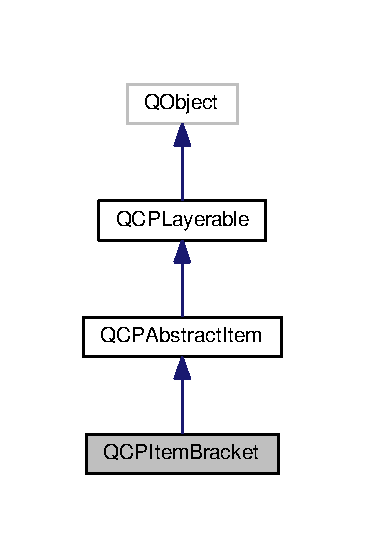
\includegraphics[width=175pt]{classQCPItemBracket__inherit__graph}
\end{center}
\end{figure}


Collaboration diagram for Q\+C\+P\+Item\+Bracket\+:
\nopagebreak
\begin{figure}[H]
\begin{center}
\leavevmode
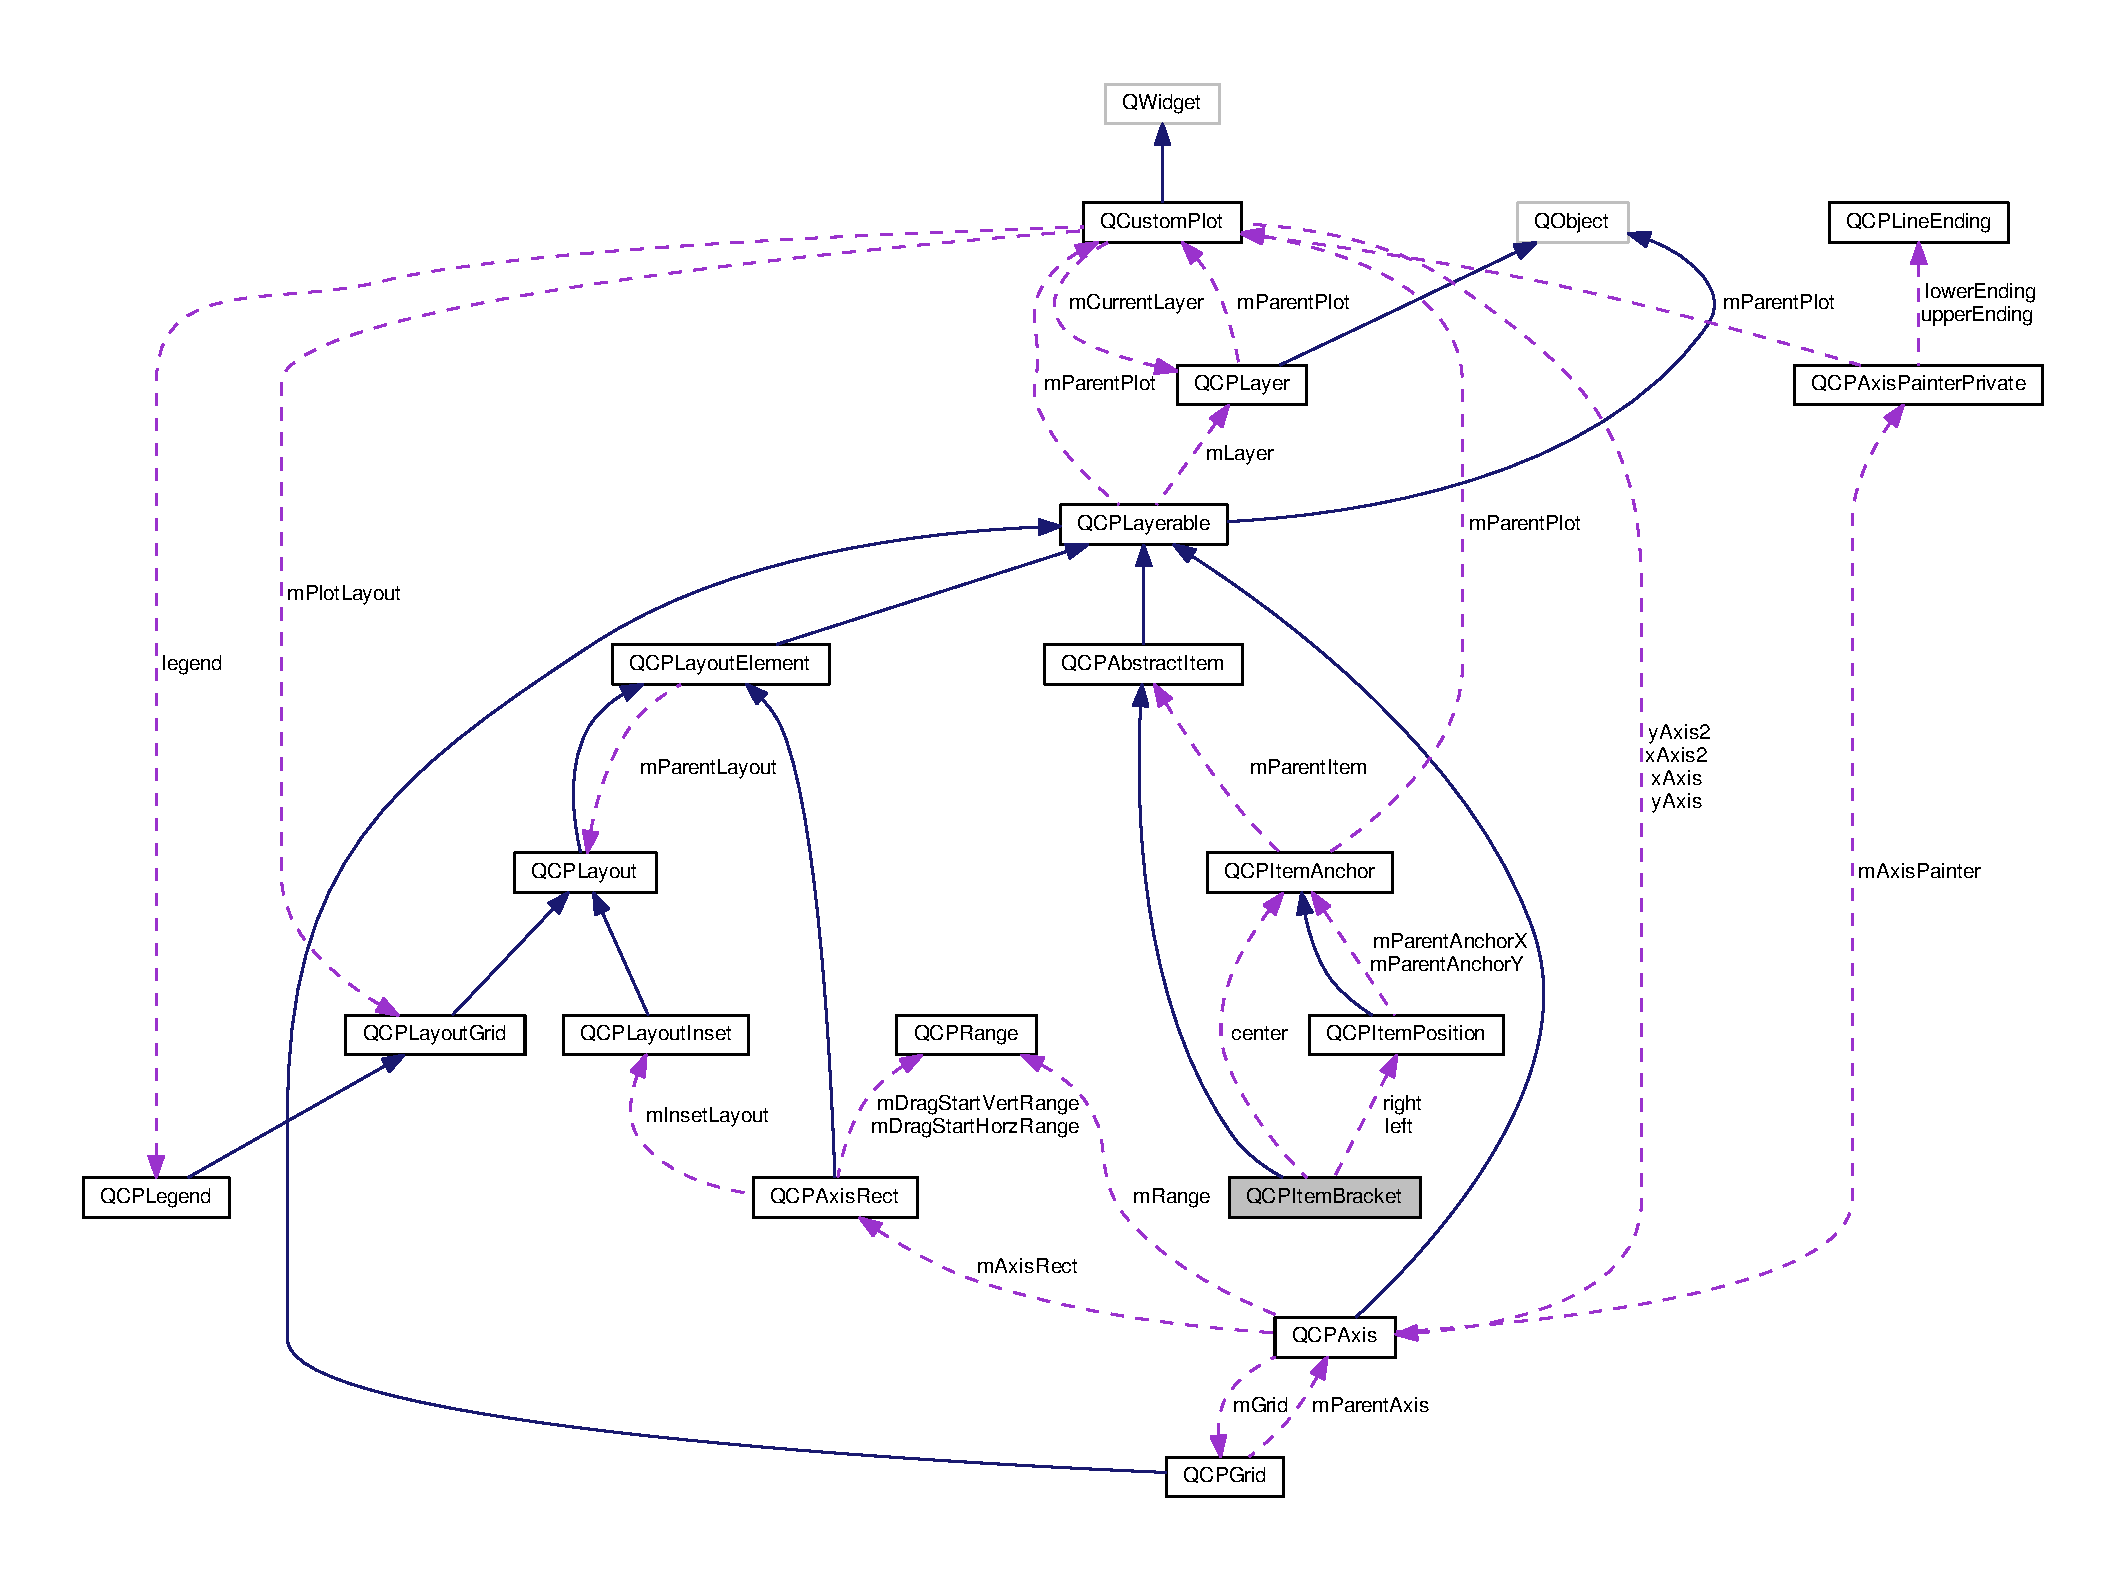
\includegraphics[width=350pt]{classQCPItemBracket__coll__graph}
\end{center}
\end{figure}
\subsection*{Public Types}
\begin{DoxyCompactItemize}
\item 
enum \hyperlink{classQCPItemBracket_a7ac3afd0b24a607054e7212047d59dbd}{Bracket\+Style} \{ \hyperlink{classQCPItemBracket_a7ac3afd0b24a607054e7212047d59dbda7f9df4a7359bfe3dac1dbe4ccf5d220c}{bs\+Square}, 
\hyperlink{classQCPItemBracket_a7ac3afd0b24a607054e7212047d59dbda394627b0830a26ee3e0a02ca67a9f918}{bs\+Round}, 
\hyperlink{classQCPItemBracket_a7ac3afd0b24a607054e7212047d59dbda5024ce4023c2d8de4221f1cd4816acd8}{bs\+Curly}, 
\hyperlink{classQCPItemBracket_a7ac3afd0b24a607054e7212047d59dbda8f29f5ef754e2dc9a9efdedb2face0f3}{bs\+Calligraphic}
 \}
\end{DoxyCompactItemize}
\subsection*{Public Member Functions}
\begin{DoxyCompactItemize}
\item 
\hyperlink{classQCPItemBracket_a44ecfa37a76de5e3549e2d61f9d8ee56}{Q\+C\+P\+Item\+Bracket} (\hyperlink{classQCustomPlot}{Q\+Custom\+Plot} $\ast$\hyperlink{classQCPLayerable_ab7e0e94461566093d36ffc0f5312b109}{parent\+Plot})
\item 
virtual \hyperlink{classQCPItemBracket_ad773c3e8e09868d6f8caeb92c54919f4}{$\sim$\+Q\+C\+P\+Item\+Bracket} ()
\item 
Q\+Pen \hyperlink{classQCPItemBracket_a8963ff4a232b649c83d2461fd3c30d39}{pen} () const 
\item 
Q\+Pen \hyperlink{classQCPItemBracket_a9f6ea5ea9559ef36dfacdadd6e9bdcf0}{selected\+Pen} () const 
\item 
double \hyperlink{classQCPItemBracket_aed5126eafcb1381ee5718499c20ba023}{length} () const 
\item 
\hyperlink{classQCPItemBracket_a7ac3afd0b24a607054e7212047d59dbd}{Bracket\+Style} \hyperlink{classQCPItemBracket_afad726f453f70fe77c0e9c2f260fff97}{style} () const 
\item 
void \hyperlink{classQCPItemBracket_ab13001d9cc5d8f9e56ea15bdda682acb}{set\+Pen} (const Q\+Pen \&\hyperlink{classQCPItemBracket_a8963ff4a232b649c83d2461fd3c30d39}{pen})
\item 
void \hyperlink{classQCPItemBracket_a349785c31122778a520c64891fa204c5}{set\+Selected\+Pen} (const Q\+Pen \&\hyperlink{classQCPItemBracket_a8963ff4a232b649c83d2461fd3c30d39}{pen})
\item 
void \hyperlink{classQCPItemBracket_ac7cfc3da7da9b5c5ac5dfbe4f0351b2a}{set\+Length} (double \hyperlink{classQCPItemBracket_aed5126eafcb1381ee5718499c20ba023}{length})
\item 
void \hyperlink{classQCPItemBracket_a612dffa2373422eef8754d690add3703}{set\+Style} (\hyperlink{classQCPItemBracket_a7ac3afd0b24a607054e7212047d59dbd}{Bracket\+Style} \hyperlink{classQCPItemBracket_afad726f453f70fe77c0e9c2f260fff97}{style})
\item 
virtual double \hyperlink{classQCPItemBracket_aa6933caff1d42c54bcebc769ef88c798}{select\+Test} (const Q\+PointF \&pos, bool only\+Selectable, Q\+Variant $\ast$details=0) const 
\end{DoxyCompactItemize}
\subsection*{Public Attributes}
\begin{DoxyCompactItemize}
\item 
\hyperlink{classQCPItemPosition}{Q\+C\+P\+Item\+Position} $\ast$const \hyperlink{classQCPItemBracket_af6cc6d27d96171778c6927d6edce48b0}{left}
\item 
\hyperlink{classQCPItemPosition}{Q\+C\+P\+Item\+Position} $\ast$const \hyperlink{classQCPItemBracket_afa6c1360b05a50c4e0df37b3cebab6be}{right}
\item 
\hyperlink{classQCPItemAnchor}{Q\+C\+P\+Item\+Anchor} $\ast$const \hyperlink{classQCPItemBracket_a2dbcabdf5f467f28be12a7b25962ffca}{center}
\end{DoxyCompactItemize}
\subsection*{Protected Types}
\begin{DoxyCompactItemize}
\item 
enum \hyperlink{classQCPItemBracket_a7f3a6a56d67f71219ed220553f3dd861}{Anchor\+Index} \{ \hyperlink{classQCPItemBracket_a7f3a6a56d67f71219ed220553f3dd861a17b57ef34cc05eadfe9becd1ad5b5242}{ai\+Center}
 \}
\end{DoxyCompactItemize}
\subsection*{Protected Member Functions}
\begin{DoxyCompactItemize}
\item 
virtual void \hyperlink{classQCPItemBracket_a8343cf0559c64886add7aa7f4b22f1a6}{draw} (\hyperlink{classQCPPainter}{Q\+C\+P\+Painter} $\ast$painter)
\item 
virtual Q\+PointF \hyperlink{classQCPItemBracket_ac76827e3acba5faee81f149af4047a39}{anchor\+Pixel\+Point} (int anchor\+Id) const 
\item 
Q\+Pen \hyperlink{classQCPItemBracket_a8df4ad873bf88a4a7bfb9bbbd490e495}{main\+Pen} () const 
\end{DoxyCompactItemize}
\subsection*{Protected Attributes}
\begin{DoxyCompactItemize}
\item 
Q\+Pen \hyperlink{classQCPItemBracket_a350c864a5853b04343719f5a8be6b675}{m\+Pen}
\item 
Q\+Pen \hyperlink{classQCPItemBracket_adcfb53602d1802d00e2de4fd6df6b291}{m\+Selected\+Pen}
\item 
double \hyperlink{classQCPItemBracket_ab3d99bba8da18eb4d0e0cb23dded33b2}{m\+Length}
\item 
\hyperlink{classQCPItemBracket_a7ac3afd0b24a607054e7212047d59dbd}{Bracket\+Style} \hyperlink{classQCPItemBracket_ac911907184c824d621f274f8e0990080}{m\+Style}
\end{DoxyCompactItemize}
\subsection*{Additional Inherited Members}


\subsection{Detailed Description}
A bracket for referencing/highlighting certain parts in the plot. 

 It has two positions, {\itshape left} and {\itshape right}, which define the span of the bracket. If {\itshape left} is actually farther to the left than {\itshape right}, the bracket is opened to the bottom, as shown in the example image.

The bracket supports multiple styles via \hyperlink{classQCPItemBracket_a612dffa2373422eef8754d690add3703}{set\+Style}. The length, i.\+e. how far the bracket stretches away from the embraced span, can be controlled with \hyperlink{classQCPItemBracket_ac7cfc3da7da9b5c5ac5dfbe4f0351b2a}{set\+Length}.

 \begin{center}Demonstrating the effect of different values for \hyperlink{classQCPItemBracket_ac7cfc3da7da9b5c5ac5dfbe4f0351b2a}{set\+Length}, for styles \hyperlink{classQCPItemBracket_a7ac3afd0b24a607054e7212047d59dbda8f29f5ef754e2dc9a9efdedb2face0f3}{bs\+Calligraphic} and \hyperlink{classQCPItemBracket_a7ac3afd0b24a607054e7212047d59dbda7f9df4a7359bfe3dac1dbe4ccf5d220c}{bs\+Square}. Anchors and positions are displayed for reference.\end{center} 

It provides an anchor {\itshape center}, to allow connection of other items, e.\+g. an arrow (\hyperlink{classQCPItemLine}{Q\+C\+P\+Item\+Line} or \hyperlink{classQCPItemCurve}{Q\+C\+P\+Item\+Curve}) or a text label (\hyperlink{classQCPItemText}{Q\+C\+P\+Item\+Text}), to the bracket. 

\subsection{Member Enumeration Documentation}
\index{Q\+C\+P\+Item\+Bracket@{Q\+C\+P\+Item\+Bracket}!Anchor\+Index@{Anchor\+Index}}
\index{Anchor\+Index@{Anchor\+Index}!Q\+C\+P\+Item\+Bracket@{Q\+C\+P\+Item\+Bracket}}
\subsubsection[{\texorpdfstring{Anchor\+Index}{AnchorIndex}}]{\setlength{\rightskip}{0pt plus 5cm}enum {\bf Q\+C\+P\+Item\+Bracket\+::\+Anchor\+Index}\hspace{0.3cm}{\ttfamily [protected]}}\hypertarget{classQCPItemBracket_a7f3a6a56d67f71219ed220553f3dd861}{}\label{classQCPItemBracket_a7f3a6a56d67f71219ed220553f3dd861}
\begin{Desc}
\item[Enumerator]\par
\begin{description}
\index{ai\+Center@{ai\+Center}!Q\+C\+P\+Item\+Bracket@{Q\+C\+P\+Item\+Bracket}}\index{Q\+C\+P\+Item\+Bracket@{Q\+C\+P\+Item\+Bracket}!ai\+Center@{ai\+Center}}\item[{\em 
ai\+Center\hypertarget{classQCPItemBracket_a7f3a6a56d67f71219ed220553f3dd861a17b57ef34cc05eadfe9becd1ad5b5242}{}\label{classQCPItemBracket_a7f3a6a56d67f71219ed220553f3dd861a17b57ef34cc05eadfe9becd1ad5b5242}
}]\end{description}
\end{Desc}
\index{Q\+C\+P\+Item\+Bracket@{Q\+C\+P\+Item\+Bracket}!Bracket\+Style@{Bracket\+Style}}
\index{Bracket\+Style@{Bracket\+Style}!Q\+C\+P\+Item\+Bracket@{Q\+C\+P\+Item\+Bracket}}
\subsubsection[{\texorpdfstring{Bracket\+Style}{BracketStyle}}]{\setlength{\rightskip}{0pt plus 5cm}enum {\bf Q\+C\+P\+Item\+Bracket\+::\+Bracket\+Style}}\hypertarget{classQCPItemBracket_a7ac3afd0b24a607054e7212047d59dbd}{}\label{classQCPItemBracket_a7ac3afd0b24a607054e7212047d59dbd}
\begin{Desc}
\item[Enumerator]\par
\begin{description}
\index{bs\+Square@{bs\+Square}!Q\+C\+P\+Item\+Bracket@{Q\+C\+P\+Item\+Bracket}}\index{Q\+C\+P\+Item\+Bracket@{Q\+C\+P\+Item\+Bracket}!bs\+Square@{bs\+Square}}\item[{\em 
bs\+Square\hypertarget{classQCPItemBracket_a7ac3afd0b24a607054e7212047d59dbda7f9df4a7359bfe3dac1dbe4ccf5d220c}{}\label{classQCPItemBracket_a7ac3afd0b24a607054e7212047d59dbda7f9df4a7359bfe3dac1dbe4ccf5d220c}
}]A brace with angled edges. \index{bs\+Round@{bs\+Round}!Q\+C\+P\+Item\+Bracket@{Q\+C\+P\+Item\+Bracket}}\index{Q\+C\+P\+Item\+Bracket@{Q\+C\+P\+Item\+Bracket}!bs\+Round@{bs\+Round}}\item[{\em 
bs\+Round\hypertarget{classQCPItemBracket_a7ac3afd0b24a607054e7212047d59dbda394627b0830a26ee3e0a02ca67a9f918}{}\label{classQCPItemBracket_a7ac3afd0b24a607054e7212047d59dbda394627b0830a26ee3e0a02ca67a9f918}
}]A brace with round edges. \index{bs\+Curly@{bs\+Curly}!Q\+C\+P\+Item\+Bracket@{Q\+C\+P\+Item\+Bracket}}\index{Q\+C\+P\+Item\+Bracket@{Q\+C\+P\+Item\+Bracket}!bs\+Curly@{bs\+Curly}}\item[{\em 
bs\+Curly\hypertarget{classQCPItemBracket_a7ac3afd0b24a607054e7212047d59dbda5024ce4023c2d8de4221f1cd4816acd8}{}\label{classQCPItemBracket_a7ac3afd0b24a607054e7212047d59dbda5024ce4023c2d8de4221f1cd4816acd8}
}]A curly brace. \index{bs\+Calligraphic@{bs\+Calligraphic}!Q\+C\+P\+Item\+Bracket@{Q\+C\+P\+Item\+Bracket}}\index{Q\+C\+P\+Item\+Bracket@{Q\+C\+P\+Item\+Bracket}!bs\+Calligraphic@{bs\+Calligraphic}}\item[{\em 
bs\+Calligraphic\hypertarget{classQCPItemBracket_a7ac3afd0b24a607054e7212047d59dbda8f29f5ef754e2dc9a9efdedb2face0f3}{}\label{classQCPItemBracket_a7ac3afd0b24a607054e7212047d59dbda8f29f5ef754e2dc9a9efdedb2face0f3}
}]A curly brace with varying stroke width giving a calligraphic impression. \end{description}
\end{Desc}


\subsection{Constructor \& Destructor Documentation}
\index{Q\+C\+P\+Item\+Bracket@{Q\+C\+P\+Item\+Bracket}!Q\+C\+P\+Item\+Bracket@{Q\+C\+P\+Item\+Bracket}}
\index{Q\+C\+P\+Item\+Bracket@{Q\+C\+P\+Item\+Bracket}!Q\+C\+P\+Item\+Bracket@{Q\+C\+P\+Item\+Bracket}}
\subsubsection[{\texorpdfstring{Q\+C\+P\+Item\+Bracket(\+Q\+Custom\+Plot $\ast$parent\+Plot)}{QCPItemBracket(QCustomPlot *parentPlot)}}]{\setlength{\rightskip}{0pt plus 5cm}Q\+C\+P\+Item\+Bracket\+::\+Q\+C\+P\+Item\+Bracket (
\begin{DoxyParamCaption}
\item[{{\bf Q\+Custom\+Plot} $\ast$}]{parent\+Plot}
\end{DoxyParamCaption}
)}\hypertarget{classQCPItemBracket_a44ecfa37a76de5e3549e2d61f9d8ee56}{}\label{classQCPItemBracket_a44ecfa37a76de5e3549e2d61f9d8ee56}
Creates a bracket item and sets default values.

The constructed item can be added to the plot with \hyperlink{classQCustomPlot_aa500620379262321685cb7a7674cbd2a}{Q\+Custom\+Plot\+::add\+Item}. \index{Q\+C\+P\+Item\+Bracket@{Q\+C\+P\+Item\+Bracket}!````~Q\+C\+P\+Item\+Bracket@{$\sim$\+Q\+C\+P\+Item\+Bracket}}
\index{````~Q\+C\+P\+Item\+Bracket@{$\sim$\+Q\+C\+P\+Item\+Bracket}!Q\+C\+P\+Item\+Bracket@{Q\+C\+P\+Item\+Bracket}}
\subsubsection[{\texorpdfstring{$\sim$\+Q\+C\+P\+Item\+Bracket()}{~QCPItemBracket()}}]{\setlength{\rightskip}{0pt plus 5cm}Q\+C\+P\+Item\+Bracket\+::$\sim$\+Q\+C\+P\+Item\+Bracket (
\begin{DoxyParamCaption}
{}
\end{DoxyParamCaption}
)\hspace{0.3cm}{\ttfamily [virtual]}}\hypertarget{classQCPItemBracket_ad773c3e8e09868d6f8caeb92c54919f4}{}\label{classQCPItemBracket_ad773c3e8e09868d6f8caeb92c54919f4}


\subsection{Member Function Documentation}
\index{Q\+C\+P\+Item\+Bracket@{Q\+C\+P\+Item\+Bracket}!anchor\+Pixel\+Point@{anchor\+Pixel\+Point}}
\index{anchor\+Pixel\+Point@{anchor\+Pixel\+Point}!Q\+C\+P\+Item\+Bracket@{Q\+C\+P\+Item\+Bracket}}
\subsubsection[{\texorpdfstring{anchor\+Pixel\+Point(int anchor\+Id) const }{anchorPixelPoint(int anchorId) const }}]{\setlength{\rightskip}{0pt plus 5cm}Q\+PointF Q\+C\+P\+Item\+Bracket\+::anchor\+Pixel\+Point (
\begin{DoxyParamCaption}
\item[{int}]{anchor\+Id}
\end{DoxyParamCaption}
) const\hspace{0.3cm}{\ttfamily [protected]}, {\ttfamily [virtual]}}\hypertarget{classQCPItemBracket_ac76827e3acba5faee81f149af4047a39}{}\label{classQCPItemBracket_ac76827e3acba5faee81f149af4047a39}


Reimplemented from \hyperlink{classQCPAbstractItem_a94bde62b8a2fc133666dcbb8035deeed}{Q\+C\+P\+Abstract\+Item}.

\index{Q\+C\+P\+Item\+Bracket@{Q\+C\+P\+Item\+Bracket}!draw@{draw}}
\index{draw@{draw}!Q\+C\+P\+Item\+Bracket@{Q\+C\+P\+Item\+Bracket}}
\subsubsection[{\texorpdfstring{draw(\+Q\+C\+P\+Painter $\ast$painter)}{draw(QCPPainter *painter)}}]{\setlength{\rightskip}{0pt plus 5cm}void Q\+C\+P\+Item\+Bracket\+::draw (
\begin{DoxyParamCaption}
\item[{{\bf Q\+C\+P\+Painter} $\ast$}]{painter}
\end{DoxyParamCaption}
)\hspace{0.3cm}{\ttfamily [protected]}, {\ttfamily [virtual]}}\hypertarget{classQCPItemBracket_a8343cf0559c64886add7aa7f4b22f1a6}{}\label{classQCPItemBracket_a8343cf0559c64886add7aa7f4b22f1a6}


Implements \hyperlink{classQCPAbstractItem_ad0dc056f650c3ca73414e6b4f01674ef}{Q\+C\+P\+Abstract\+Item}.

\index{Q\+C\+P\+Item\+Bracket@{Q\+C\+P\+Item\+Bracket}!length@{length}}
\index{length@{length}!Q\+C\+P\+Item\+Bracket@{Q\+C\+P\+Item\+Bracket}}
\subsubsection[{\texorpdfstring{length() const }{length() const }}]{\setlength{\rightskip}{0pt plus 5cm}double Q\+C\+P\+Item\+Bracket\+::length (
\begin{DoxyParamCaption}
{}
\end{DoxyParamCaption}
) const\hspace{0.3cm}{\ttfamily [inline]}}\hypertarget{classQCPItemBracket_aed5126eafcb1381ee5718499c20ba023}{}\label{classQCPItemBracket_aed5126eafcb1381ee5718499c20ba023}
\index{Q\+C\+P\+Item\+Bracket@{Q\+C\+P\+Item\+Bracket}!main\+Pen@{main\+Pen}}
\index{main\+Pen@{main\+Pen}!Q\+C\+P\+Item\+Bracket@{Q\+C\+P\+Item\+Bracket}}
\subsubsection[{\texorpdfstring{main\+Pen() const }{mainPen() const }}]{\setlength{\rightskip}{0pt plus 5cm}Q\+Pen Q\+C\+P\+Item\+Bracket\+::main\+Pen (
\begin{DoxyParamCaption}
{}
\end{DoxyParamCaption}
) const\hspace{0.3cm}{\ttfamily [protected]}}\hypertarget{classQCPItemBracket_a8df4ad873bf88a4a7bfb9bbbd490e495}{}\label{classQCPItemBracket_a8df4ad873bf88a4a7bfb9bbbd490e495}
\index{Q\+C\+P\+Item\+Bracket@{Q\+C\+P\+Item\+Bracket}!pen@{pen}}
\index{pen@{pen}!Q\+C\+P\+Item\+Bracket@{Q\+C\+P\+Item\+Bracket}}
\subsubsection[{\texorpdfstring{pen() const }{pen() const }}]{\setlength{\rightskip}{0pt plus 5cm}Q\+Pen Q\+C\+P\+Item\+Bracket\+::pen (
\begin{DoxyParamCaption}
{}
\end{DoxyParamCaption}
) const\hspace{0.3cm}{\ttfamily [inline]}}\hypertarget{classQCPItemBracket_a8963ff4a232b649c83d2461fd3c30d39}{}\label{classQCPItemBracket_a8963ff4a232b649c83d2461fd3c30d39}
\index{Q\+C\+P\+Item\+Bracket@{Q\+C\+P\+Item\+Bracket}!selected\+Pen@{selected\+Pen}}
\index{selected\+Pen@{selected\+Pen}!Q\+C\+P\+Item\+Bracket@{Q\+C\+P\+Item\+Bracket}}
\subsubsection[{\texorpdfstring{selected\+Pen() const }{selectedPen() const }}]{\setlength{\rightskip}{0pt plus 5cm}Q\+Pen Q\+C\+P\+Item\+Bracket\+::selected\+Pen (
\begin{DoxyParamCaption}
{}
\end{DoxyParamCaption}
) const\hspace{0.3cm}{\ttfamily [inline]}}\hypertarget{classQCPItemBracket_a9f6ea5ea9559ef36dfacdadd6e9bdcf0}{}\label{classQCPItemBracket_a9f6ea5ea9559ef36dfacdadd6e9bdcf0}
\index{Q\+C\+P\+Item\+Bracket@{Q\+C\+P\+Item\+Bracket}!select\+Test@{select\+Test}}
\index{select\+Test@{select\+Test}!Q\+C\+P\+Item\+Bracket@{Q\+C\+P\+Item\+Bracket}}
\subsubsection[{\texorpdfstring{select\+Test(const Q\+Point\+F \&pos, bool only\+Selectable, Q\+Variant $\ast$details=0) const }{selectTest(const QPointF &pos, bool onlySelectable, QVariant *details=0) const }}]{\setlength{\rightskip}{0pt plus 5cm}double Q\+C\+P\+Item\+Bracket\+::select\+Test (
\begin{DoxyParamCaption}
\item[{const Q\+PointF \&}]{pos, }
\item[{bool}]{only\+Selectable, }
\item[{Q\+Variant $\ast$}]{details = {\ttfamily 0}}
\end{DoxyParamCaption}
) const\hspace{0.3cm}{\ttfamily [virtual]}}\hypertarget{classQCPItemBracket_aa6933caff1d42c54bcebc769ef88c798}{}\label{classQCPItemBracket_aa6933caff1d42c54bcebc769ef88c798}
This function is used to decide whether a click hits a layerable object or not.

{\itshape pos} is a point in pixel coordinates on the \hyperlink{classQCustomPlot}{Q\+Custom\+Plot} surface. This function returns the shortest pixel distance of this point to the object. If the object is either invisible or the distance couldn\textquotesingle{}t be determined, -\/1.\+0 is returned. Further, if {\itshape only\+Selectable} is true and the object is not selectable, -\/1.\+0 is returned, too.

If the object is represented not by single lines but by an area like a \hyperlink{classQCPItemText}{Q\+C\+P\+Item\+Text} or the bars of a \hyperlink{classQCPBars}{Q\+C\+P\+Bars} plottable, a click inside the area should also be considered a hit. In these cases this function thus returns a constant value greater zero but still below the parent plot\textquotesingle{}s selection tolerance. (typically the selection\+Tolerance multiplied by 0.\+99).

Providing a constant value for area objects allows selecting line objects even when they are obscured by such area objects, by clicking close to the lines (i.\+e. closer than 0.\+99$\ast$selection\+Tolerance).

The actual setting of the selection state is not done by this function. This is handled by the parent \hyperlink{classQCustomPlot}{Q\+Custom\+Plot} when the mouse\+Release\+Event occurs, and the finally selected object is notified via the select\+Event/deselect\+Event methods.

{\itshape details} is an optional output parameter. Every layerable subclass may place any information in {\itshape details}. This information will be passed to \hyperlink{classQCPAbstractItem_aaf92af7b9893712959a6c073d334d88d}{select\+Event} when the parent \hyperlink{classQCustomPlot}{Q\+Custom\+Plot} decides on the basis of this select\+Test call, that the object was successfully selected. The subsequent call to \hyperlink{classQCPAbstractItem_aaf92af7b9893712959a6c073d334d88d}{select\+Event} will carry the {\itshape details}. This is useful for multi-\/part objects (like \hyperlink{classQCPAxis}{Q\+C\+P\+Axis}). This way, a possibly complex calculation to decide which part was clicked is only done once in \hyperlink{classQCPItemBracket_aa6933caff1d42c54bcebc769ef88c798}{select\+Test}. The result (i.\+e. the actually clicked part) can then be placed in {\itshape details}. So in the subsequent \hyperlink{classQCPAbstractItem_aaf92af7b9893712959a6c073d334d88d}{select\+Event}, the decision which part was selected doesn\textquotesingle{}t have to be done a second time for a single selection operation.

You may pass 0 as {\itshape details} to indicate that you are not interested in those selection details.

\begin{DoxySeeAlso}{See also}
\hyperlink{classQCPAbstractItem_aaf92af7b9893712959a6c073d334d88d}{select\+Event}, \hyperlink{classQCPAbstractItem_a91f090d6763cfedb0749219c63788ae9}{deselect\+Event}, \hyperlink{classQCustomPlot_a5ee1e2f6ae27419deca53e75907c27e5}{Q\+Custom\+Plot\+::set\+Interactions} 
\end{DoxySeeAlso}


Implements \hyperlink{classQCPAbstractItem_a96d522d10ffc0413b9a366c6f7f0476b}{Q\+C\+P\+Abstract\+Item}.

\index{Q\+C\+P\+Item\+Bracket@{Q\+C\+P\+Item\+Bracket}!set\+Length@{set\+Length}}
\index{set\+Length@{set\+Length}!Q\+C\+P\+Item\+Bracket@{Q\+C\+P\+Item\+Bracket}}
\subsubsection[{\texorpdfstring{set\+Length(double length)}{setLength(double length)}}]{\setlength{\rightskip}{0pt plus 5cm}void Q\+C\+P\+Item\+Bracket\+::set\+Length (
\begin{DoxyParamCaption}
\item[{double}]{length}
\end{DoxyParamCaption}
)}\hypertarget{classQCPItemBracket_ac7cfc3da7da9b5c5ac5dfbe4f0351b2a}{}\label{classQCPItemBracket_ac7cfc3da7da9b5c5ac5dfbe4f0351b2a}
Sets the {\itshape length} in pixels how far the bracket extends in the direction towards the embraced span of the bracket (i.\+e. perpendicular to the {\itshape left}-\/{\itshape right}-\/direction)

 \begin{center}Demonstrating the effect of different values for \hyperlink{classQCPItemBracket_ac7cfc3da7da9b5c5ac5dfbe4f0351b2a}{set\+Length}, for styles \hyperlink{classQCPItemBracket_a7ac3afd0b24a607054e7212047d59dbda8f29f5ef754e2dc9a9efdedb2face0f3}{bs\+Calligraphic} and \hyperlink{classQCPItemBracket_a7ac3afd0b24a607054e7212047d59dbda7f9df4a7359bfe3dac1dbe4ccf5d220c}{bs\+Square}. Anchors and positions are displayed for reference.\end{center}  \index{Q\+C\+P\+Item\+Bracket@{Q\+C\+P\+Item\+Bracket}!set\+Pen@{set\+Pen}}
\index{set\+Pen@{set\+Pen}!Q\+C\+P\+Item\+Bracket@{Q\+C\+P\+Item\+Bracket}}
\subsubsection[{\texorpdfstring{set\+Pen(const Q\+Pen \&pen)}{setPen(const QPen &pen)}}]{\setlength{\rightskip}{0pt plus 5cm}void Q\+C\+P\+Item\+Bracket\+::set\+Pen (
\begin{DoxyParamCaption}
\item[{const Q\+Pen \&}]{pen}
\end{DoxyParamCaption}
)}\hypertarget{classQCPItemBracket_ab13001d9cc5d8f9e56ea15bdda682acb}{}\label{classQCPItemBracket_ab13001d9cc5d8f9e56ea15bdda682acb}
Sets the pen that will be used to draw the bracket.

Note that when the style is \hyperlink{classQCPItemBracket_a7ac3afd0b24a607054e7212047d59dbda8f29f5ef754e2dc9a9efdedb2face0f3}{bs\+Calligraphic}, only the color will be taken from the pen, the stroke and width are ignored. To change the apparent stroke width of a calligraphic bracket, use \hyperlink{classQCPItemBracket_ac7cfc3da7da9b5c5ac5dfbe4f0351b2a}{set\+Length}, which has a similar effect.

\begin{DoxySeeAlso}{See also}
\hyperlink{classQCPItemBracket_a349785c31122778a520c64891fa204c5}{set\+Selected\+Pen} 
\end{DoxySeeAlso}
\index{Q\+C\+P\+Item\+Bracket@{Q\+C\+P\+Item\+Bracket}!set\+Selected\+Pen@{set\+Selected\+Pen}}
\index{set\+Selected\+Pen@{set\+Selected\+Pen}!Q\+C\+P\+Item\+Bracket@{Q\+C\+P\+Item\+Bracket}}
\subsubsection[{\texorpdfstring{set\+Selected\+Pen(const Q\+Pen \&pen)}{setSelectedPen(const QPen &pen)}}]{\setlength{\rightskip}{0pt plus 5cm}void Q\+C\+P\+Item\+Bracket\+::set\+Selected\+Pen (
\begin{DoxyParamCaption}
\item[{const Q\+Pen \&}]{pen}
\end{DoxyParamCaption}
)}\hypertarget{classQCPItemBracket_a349785c31122778a520c64891fa204c5}{}\label{classQCPItemBracket_a349785c31122778a520c64891fa204c5}
Sets the pen that will be used to draw the bracket when selected

\begin{DoxySeeAlso}{See also}
\hyperlink{classQCPItemBracket_ab13001d9cc5d8f9e56ea15bdda682acb}{set\+Pen}, \hyperlink{classQCPAbstractItem_a203de94ad586cc44d16c9565f49d3378}{set\+Selected} 
\end{DoxySeeAlso}
\index{Q\+C\+P\+Item\+Bracket@{Q\+C\+P\+Item\+Bracket}!set\+Style@{set\+Style}}
\index{set\+Style@{set\+Style}!Q\+C\+P\+Item\+Bracket@{Q\+C\+P\+Item\+Bracket}}
\subsubsection[{\texorpdfstring{set\+Style(\+Bracket\+Style style)}{setStyle(BracketStyle style)}}]{\setlength{\rightskip}{0pt plus 5cm}void Q\+C\+P\+Item\+Bracket\+::set\+Style (
\begin{DoxyParamCaption}
\item[{{\bf Q\+C\+P\+Item\+Bracket\+::\+Bracket\+Style}}]{style}
\end{DoxyParamCaption}
)}\hypertarget{classQCPItemBracket_a612dffa2373422eef8754d690add3703}{}\label{classQCPItemBracket_a612dffa2373422eef8754d690add3703}
Sets the style of the bracket, i.\+e. the shape/visual appearance.

\begin{DoxySeeAlso}{See also}
\hyperlink{classQCPItemBracket_ab13001d9cc5d8f9e56ea15bdda682acb}{set\+Pen} 
\end{DoxySeeAlso}
\index{Q\+C\+P\+Item\+Bracket@{Q\+C\+P\+Item\+Bracket}!style@{style}}
\index{style@{style}!Q\+C\+P\+Item\+Bracket@{Q\+C\+P\+Item\+Bracket}}
\subsubsection[{\texorpdfstring{style() const }{style() const }}]{\setlength{\rightskip}{0pt plus 5cm}{\bf Bracket\+Style} Q\+C\+P\+Item\+Bracket\+::style (
\begin{DoxyParamCaption}
{}
\end{DoxyParamCaption}
) const\hspace{0.3cm}{\ttfamily [inline]}}\hypertarget{classQCPItemBracket_afad726f453f70fe77c0e9c2f260fff97}{}\label{classQCPItemBracket_afad726f453f70fe77c0e9c2f260fff97}


\subsection{Member Data Documentation}
\index{Q\+C\+P\+Item\+Bracket@{Q\+C\+P\+Item\+Bracket}!center@{center}}
\index{center@{center}!Q\+C\+P\+Item\+Bracket@{Q\+C\+P\+Item\+Bracket}}
\subsubsection[{\texorpdfstring{center}{center}}]{\setlength{\rightskip}{0pt plus 5cm}{\bf Q\+C\+P\+Item\+Anchor}$\ast$ const Q\+C\+P\+Item\+Bracket\+::center}\hypertarget{classQCPItemBracket_a2dbcabdf5f467f28be12a7b25962ffca}{}\label{classQCPItemBracket_a2dbcabdf5f467f28be12a7b25962ffca}
\index{Q\+C\+P\+Item\+Bracket@{Q\+C\+P\+Item\+Bracket}!left@{left}}
\index{left@{left}!Q\+C\+P\+Item\+Bracket@{Q\+C\+P\+Item\+Bracket}}
\subsubsection[{\texorpdfstring{left}{left}}]{\setlength{\rightskip}{0pt plus 5cm}{\bf Q\+C\+P\+Item\+Position}$\ast$ const Q\+C\+P\+Item\+Bracket\+::left}\hypertarget{classQCPItemBracket_af6cc6d27d96171778c6927d6edce48b0}{}\label{classQCPItemBracket_af6cc6d27d96171778c6927d6edce48b0}
\index{Q\+C\+P\+Item\+Bracket@{Q\+C\+P\+Item\+Bracket}!m\+Length@{m\+Length}}
\index{m\+Length@{m\+Length}!Q\+C\+P\+Item\+Bracket@{Q\+C\+P\+Item\+Bracket}}
\subsubsection[{\texorpdfstring{m\+Length}{mLength}}]{\setlength{\rightskip}{0pt plus 5cm}double Q\+C\+P\+Item\+Bracket\+::m\+Length\hspace{0.3cm}{\ttfamily [protected]}}\hypertarget{classQCPItemBracket_ab3d99bba8da18eb4d0e0cb23dded33b2}{}\label{classQCPItemBracket_ab3d99bba8da18eb4d0e0cb23dded33b2}
\index{Q\+C\+P\+Item\+Bracket@{Q\+C\+P\+Item\+Bracket}!m\+Pen@{m\+Pen}}
\index{m\+Pen@{m\+Pen}!Q\+C\+P\+Item\+Bracket@{Q\+C\+P\+Item\+Bracket}}
\subsubsection[{\texorpdfstring{m\+Pen}{mPen}}]{\setlength{\rightskip}{0pt plus 5cm}Q\+Pen Q\+C\+P\+Item\+Bracket\+::m\+Pen\hspace{0.3cm}{\ttfamily [protected]}}\hypertarget{classQCPItemBracket_a350c864a5853b04343719f5a8be6b675}{}\label{classQCPItemBracket_a350c864a5853b04343719f5a8be6b675}
\index{Q\+C\+P\+Item\+Bracket@{Q\+C\+P\+Item\+Bracket}!m\+Selected\+Pen@{m\+Selected\+Pen}}
\index{m\+Selected\+Pen@{m\+Selected\+Pen}!Q\+C\+P\+Item\+Bracket@{Q\+C\+P\+Item\+Bracket}}
\subsubsection[{\texorpdfstring{m\+Selected\+Pen}{mSelectedPen}}]{\setlength{\rightskip}{0pt plus 5cm}Q\+Pen Q\+C\+P\+Item\+Bracket\+::m\+Selected\+Pen\hspace{0.3cm}{\ttfamily [protected]}}\hypertarget{classQCPItemBracket_adcfb53602d1802d00e2de4fd6df6b291}{}\label{classQCPItemBracket_adcfb53602d1802d00e2de4fd6df6b291}
\index{Q\+C\+P\+Item\+Bracket@{Q\+C\+P\+Item\+Bracket}!m\+Style@{m\+Style}}
\index{m\+Style@{m\+Style}!Q\+C\+P\+Item\+Bracket@{Q\+C\+P\+Item\+Bracket}}
\subsubsection[{\texorpdfstring{m\+Style}{mStyle}}]{\setlength{\rightskip}{0pt plus 5cm}{\bf Bracket\+Style} Q\+C\+P\+Item\+Bracket\+::m\+Style\hspace{0.3cm}{\ttfamily [protected]}}\hypertarget{classQCPItemBracket_ac911907184c824d621f274f8e0990080}{}\label{classQCPItemBracket_ac911907184c824d621f274f8e0990080}
\index{Q\+C\+P\+Item\+Bracket@{Q\+C\+P\+Item\+Bracket}!right@{right}}
\index{right@{right}!Q\+C\+P\+Item\+Bracket@{Q\+C\+P\+Item\+Bracket}}
\subsubsection[{\texorpdfstring{right}{right}}]{\setlength{\rightskip}{0pt plus 5cm}{\bf Q\+C\+P\+Item\+Position}$\ast$ const Q\+C\+P\+Item\+Bracket\+::right}\hypertarget{classQCPItemBracket_afa6c1360b05a50c4e0df37b3cebab6be}{}\label{classQCPItemBracket_afa6c1360b05a50c4e0df37b3cebab6be}


The documentation for this class was generated from the following files\+:\begin{DoxyCompactItemize}
\item 
src/hammerhead/tools/watchdog/include/watchdog/\hyperlink{qcustomplot_8h}{qcustomplot.\+h}\item 
src/hammerhead/tools/watchdog/src/\hyperlink{qcustomplot_8cpp}{qcustomplot.\+cpp}\end{DoxyCompactItemize}

\hypertarget{classQCPItemCurve}{}\section{Q\+C\+P\+Item\+Curve Class Reference}
\label{classQCPItemCurve}\index{Q\+C\+P\+Item\+Curve@{Q\+C\+P\+Item\+Curve}}


A curved line from one point to another.  




{\ttfamily \#include $<$qcustomplot.\+h$>$}



Inheritance diagram for Q\+C\+P\+Item\+Curve\+:\nopagebreak
\begin{figure}[H]
\begin{center}
\leavevmode
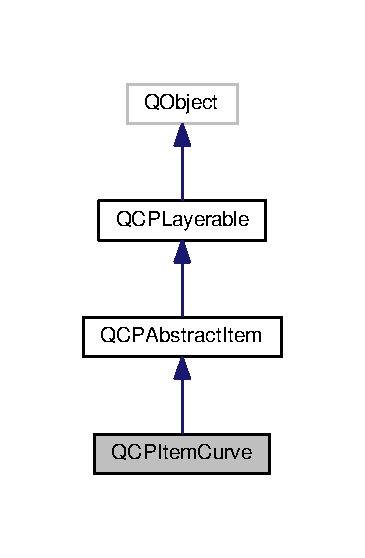
\includegraphics[width=175pt]{classQCPItemCurve__inherit__graph}
\end{center}
\end{figure}


Collaboration diagram for Q\+C\+P\+Item\+Curve\+:\nopagebreak
\begin{figure}[H]
\begin{center}
\leavevmode
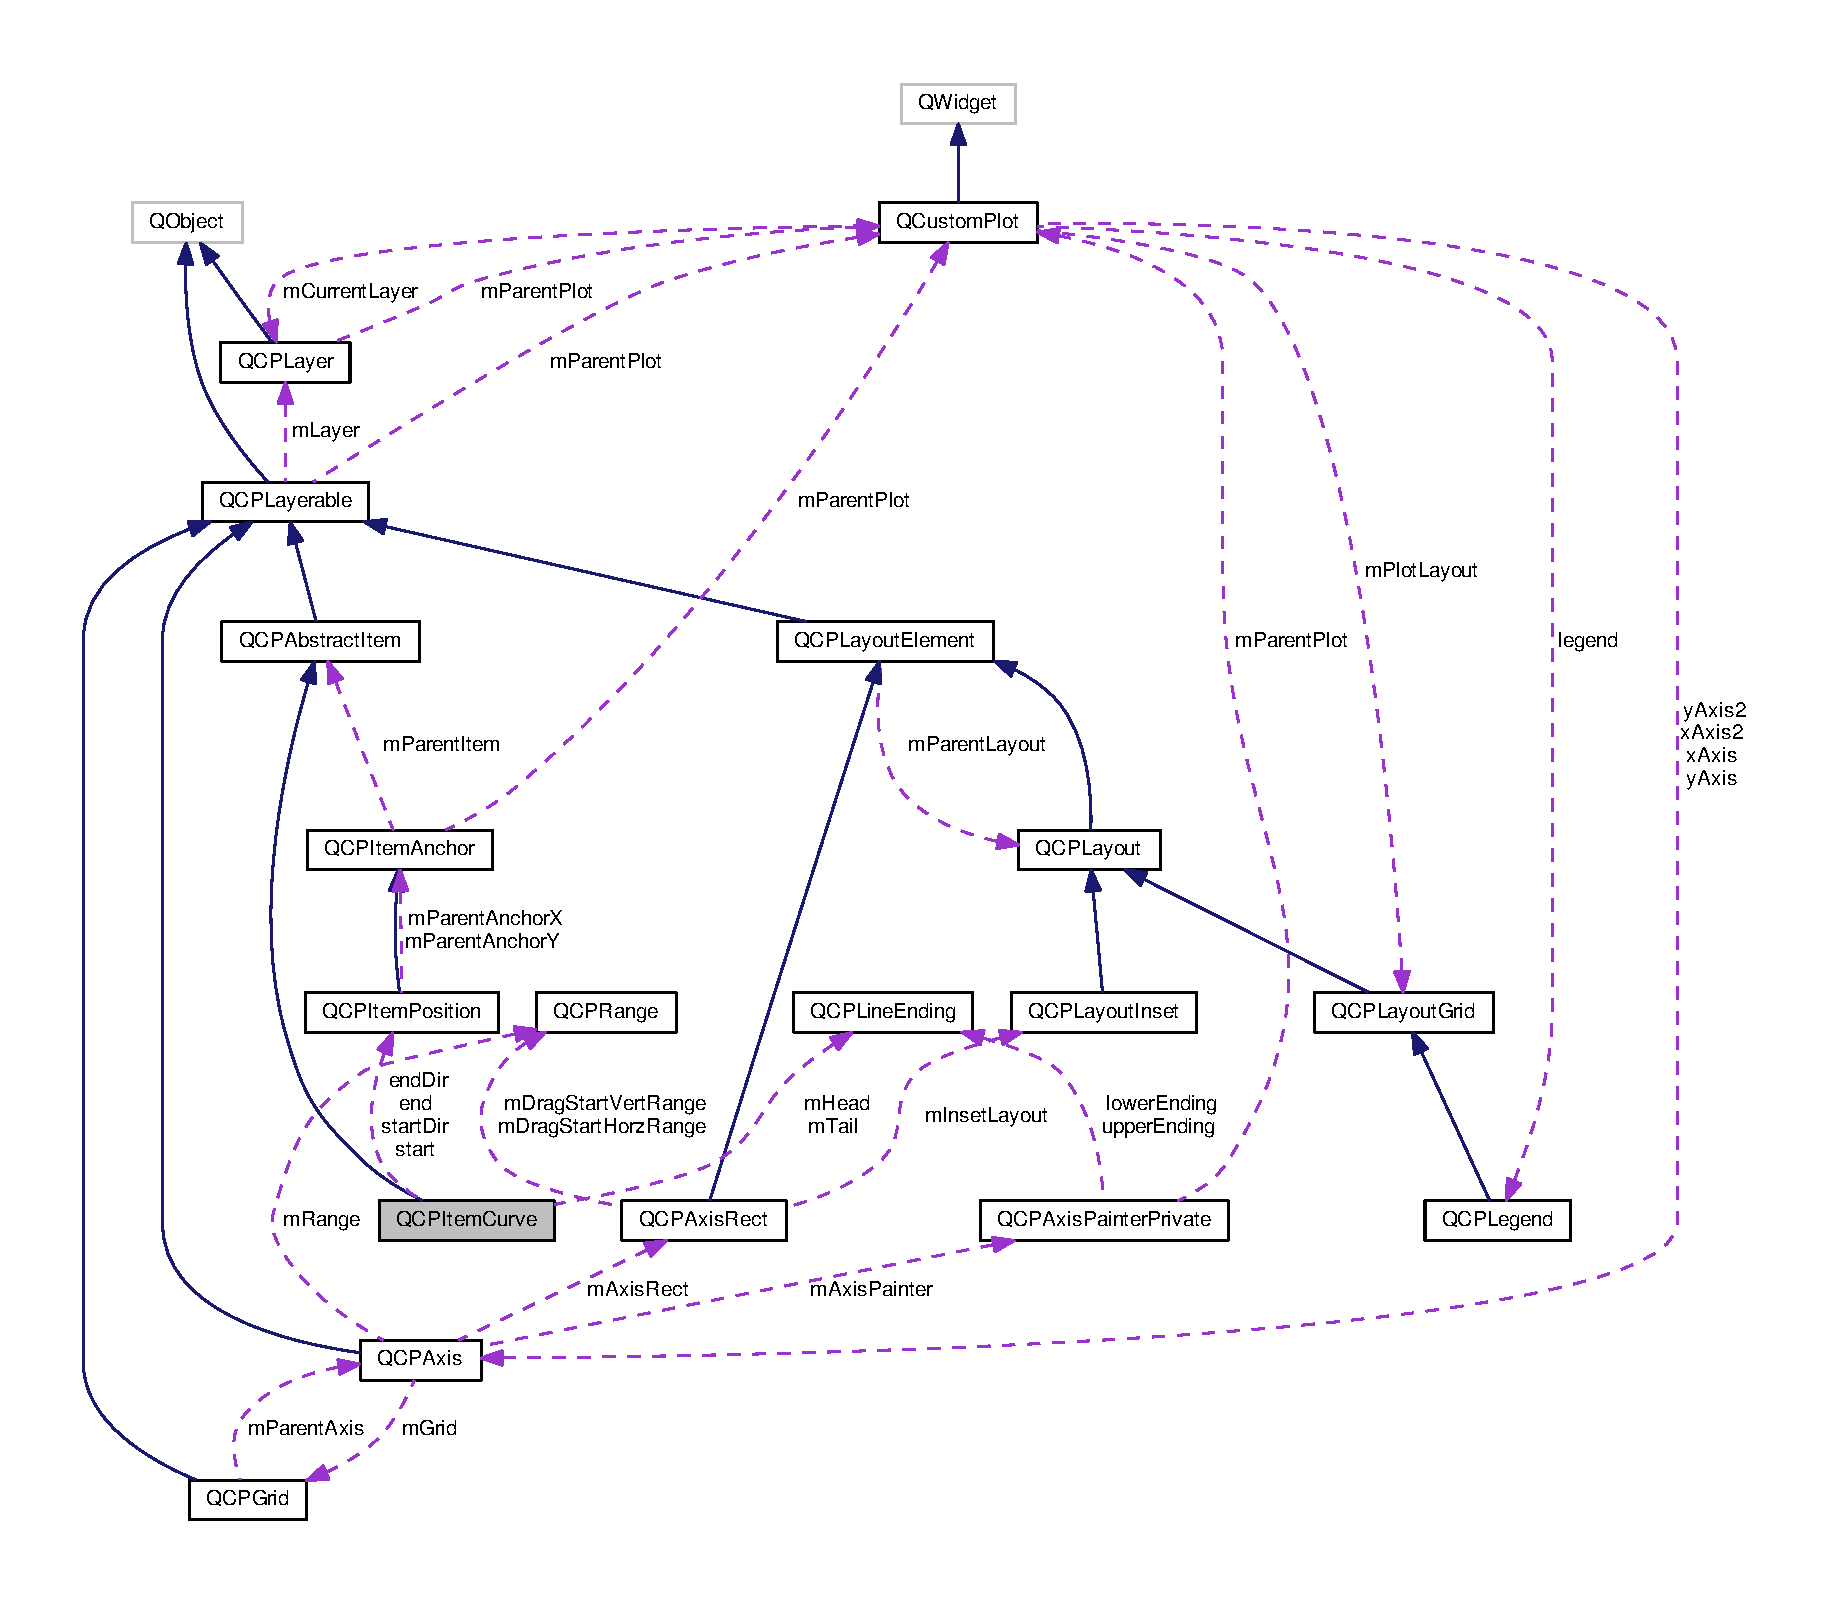
\includegraphics[width=350pt]{classQCPItemCurve__coll__graph}
\end{center}
\end{figure}
\subsection*{Public Member Functions}
\begin{DoxyCompactItemize}
\item 
\hyperlink{classQCPItemCurve_ac9b7508bb5c8827e1a7a6199f8c82bec}{Q\+C\+P\+Item\+Curve} (\hyperlink{classQCustomPlot}{Q\+Custom\+Plot} $\ast$\hyperlink{classQCPLayerable_ab7e0e94461566093d36ffc0f5312b109}{parent\+Plot})
\item 
virtual \hyperlink{classQCPItemCurve_ae36f20fd5deff2f1443a7c53eaa95c81}{$\sim$\+Q\+C\+P\+Item\+Curve} ()
\item 
Q\+Pen \hyperlink{classQCPItemCurve_abc6321e55a9ba1a0c7df407843dfa252}{pen} () const 
\item 
Q\+Pen \hyperlink{classQCPItemCurve_abd8b8be5b13bc4dafec4c1758c281336}{selected\+Pen} () const 
\item 
\hyperlink{classQCPLineEnding}{Q\+C\+P\+Line\+Ending} \hyperlink{classQCPItemCurve_afc067f0d1e60cd04812f2c2c7fdf36c3}{head} () const 
\item 
\hyperlink{classQCPLineEnding}{Q\+C\+P\+Line\+Ending} \hyperlink{classQCPItemCurve_a9adddfcc5275be0cf27e3c0c31c37c1a}{tail} () const 
\item 
void \hyperlink{classQCPItemCurve_a034be908440aec785c34b92843461221}{set\+Pen} (const Q\+Pen \&\hyperlink{classQCPItemCurve_abc6321e55a9ba1a0c7df407843dfa252}{pen})
\item 
void \hyperlink{classQCPItemCurve_a375b917669f868c5a106bf2f1ab7c26d}{set\+Selected\+Pen} (const Q\+Pen \&\hyperlink{classQCPItemCurve_abc6321e55a9ba1a0c7df407843dfa252}{pen})
\item 
void \hyperlink{classQCPItemCurve_a08a30d9cdd63995deea3d9e20430676f}{set\+Head} (const \hyperlink{classQCPLineEnding}{Q\+C\+P\+Line\+Ending} \&\hyperlink{classQCPItemCurve_afc067f0d1e60cd04812f2c2c7fdf36c3}{head})
\item 
void \hyperlink{classQCPItemCurve_ac3488d8b1a6489c845dc5bff3ef71124}{set\+Tail} (const \hyperlink{classQCPLineEnding}{Q\+C\+P\+Line\+Ending} \&\hyperlink{classQCPItemCurve_a9adddfcc5275be0cf27e3c0c31c37c1a}{tail})
\item 
virtual double \hyperlink{classQCPItemCurve_a741375c11667b5f9c95b2683f93ee514}{select\+Test} (const Q\+PointF \&pos, bool only\+Selectable, Q\+Variant $\ast$details=0) const 
\end{DoxyCompactItemize}
\subsection*{Public Attributes}
\begin{DoxyCompactItemize}
\item 
\hyperlink{classQCPItemPosition}{Q\+C\+P\+Item\+Position} $\ast$const \hyperlink{classQCPItemCurve_a20c3b5ea31c33764f4f30c2ec7ae518b}{start}
\item 
\hyperlink{classQCPItemPosition}{Q\+C\+P\+Item\+Position} $\ast$const \hyperlink{classQCPItemCurve_aa124bf66c09cc51c627fb49db8bf8a7b}{start\+Dir}
\item 
\hyperlink{classQCPItemPosition}{Q\+C\+P\+Item\+Position} $\ast$const \hyperlink{classQCPItemCurve_a28181a9dee9cc3c3da83a883221bd2d0}{end\+Dir}
\item 
\hyperlink{classQCPItemPosition}{Q\+C\+P\+Item\+Position} $\ast$const \hyperlink{classQCPItemCurve_a24ecbb195b32a08b42b61c2cf08a1b4d}{end}
\end{DoxyCompactItemize}
\subsection*{Protected Member Functions}
\begin{DoxyCompactItemize}
\item 
virtual void \hyperlink{classQCPItemCurve_a56cb5b72cd02db2eda598274a39839a9}{draw} (\hyperlink{classQCPPainter}{Q\+C\+P\+Painter} $\ast$painter)
\item 
Q\+Pen \hyperlink{classQCPItemCurve_a8089126f5645b6edfbaddea49d1e8390}{main\+Pen} () const 
\end{DoxyCompactItemize}
\subsection*{Protected Attributes}
\begin{DoxyCompactItemize}
\item 
Q\+Pen \hyperlink{classQCPItemCurve_a7ef92988d1db2e4d0311e34c0a57fe42}{m\+Pen}
\item 
Q\+Pen \hyperlink{classQCPItemCurve_ab22cbab261b20be5aa8e4ca252149246}{m\+Selected\+Pen}
\item 
\hyperlink{classQCPLineEnding}{Q\+C\+P\+Line\+Ending} \hyperlink{classQCPItemCurve_af2cc26ff199570940dc96f5ec19a13f8}{m\+Head}
\item 
\hyperlink{classQCPLineEnding}{Q\+C\+P\+Line\+Ending} \hyperlink{classQCPItemCurve_af1dca285b97e3f5b892dab827a79f327}{m\+Tail}
\end{DoxyCompactItemize}
\subsection*{Additional Inherited Members}


\subsection{Detailed Description}
A curved line from one point to another. 

 It has four positions, {\itshape start} and {\itshape end}, which define the end points of the line, and two control points which define the direction the line exits from the start and the direction from which it approaches the end\+: {\itshape start\+Dir} and {\itshape end\+Dir}.

With \hyperlink{classQCPItemCurve_a08a30d9cdd63995deea3d9e20430676f}{set\+Head} and \hyperlink{classQCPItemCurve_ac3488d8b1a6489c845dc5bff3ef71124}{set\+Tail} you may set different line ending styles, e.\+g. to create an arrow.

Often it is desirable for the control points to stay at fixed relative positions to the start/end point. This can be achieved by setting the parent anchor e.\+g. of {\itshape start\+Dir} simply to {\itshape start}, and then specify the desired pixel offset with \hyperlink{classQCPItemPosition_aa988ba4e87ab684c9021017dcaba945f}{Q\+C\+P\+Item\+Position\+::set\+Coords} on {\itshape start\+Dir}. 

\subsection{Constructor \& Destructor Documentation}
\index{Q\+C\+P\+Item\+Curve@{Q\+C\+P\+Item\+Curve}!Q\+C\+P\+Item\+Curve@{Q\+C\+P\+Item\+Curve}}
\index{Q\+C\+P\+Item\+Curve@{Q\+C\+P\+Item\+Curve}!Q\+C\+P\+Item\+Curve@{Q\+C\+P\+Item\+Curve}}
\subsubsection[{\texorpdfstring{Q\+C\+P\+Item\+Curve(\+Q\+Custom\+Plot $\ast$parent\+Plot)}{QCPItemCurve(QCustomPlot *parentPlot)}}]{\setlength{\rightskip}{0pt plus 5cm}Q\+C\+P\+Item\+Curve\+::\+Q\+C\+P\+Item\+Curve (
\begin{DoxyParamCaption}
\item[{{\bf Q\+Custom\+Plot} $\ast$}]{parent\+Plot}
\end{DoxyParamCaption}
)}\hypertarget{classQCPItemCurve_ac9b7508bb5c8827e1a7a6199f8c82bec}{}\label{classQCPItemCurve_ac9b7508bb5c8827e1a7a6199f8c82bec}
Creates a curve item and sets default values.

The constructed item can be added to the plot with \hyperlink{classQCustomPlot_aa500620379262321685cb7a7674cbd2a}{Q\+Custom\+Plot\+::add\+Item}. \index{Q\+C\+P\+Item\+Curve@{Q\+C\+P\+Item\+Curve}!````~Q\+C\+P\+Item\+Curve@{$\sim$\+Q\+C\+P\+Item\+Curve}}
\index{````~Q\+C\+P\+Item\+Curve@{$\sim$\+Q\+C\+P\+Item\+Curve}!Q\+C\+P\+Item\+Curve@{Q\+C\+P\+Item\+Curve}}
\subsubsection[{\texorpdfstring{$\sim$\+Q\+C\+P\+Item\+Curve()}{~QCPItemCurve()}}]{\setlength{\rightskip}{0pt plus 5cm}Q\+C\+P\+Item\+Curve\+::$\sim$\+Q\+C\+P\+Item\+Curve (
\begin{DoxyParamCaption}
{}
\end{DoxyParamCaption}
)\hspace{0.3cm}{\ttfamily [virtual]}}\hypertarget{classQCPItemCurve_ae36f20fd5deff2f1443a7c53eaa95c81}{}\label{classQCPItemCurve_ae36f20fd5deff2f1443a7c53eaa95c81}


\subsection{Member Function Documentation}
\index{Q\+C\+P\+Item\+Curve@{Q\+C\+P\+Item\+Curve}!draw@{draw}}
\index{draw@{draw}!Q\+C\+P\+Item\+Curve@{Q\+C\+P\+Item\+Curve}}
\subsubsection[{\texorpdfstring{draw(\+Q\+C\+P\+Painter $\ast$painter)}{draw(QCPPainter *painter)}}]{\setlength{\rightskip}{0pt plus 5cm}void Q\+C\+P\+Item\+Curve\+::draw (
\begin{DoxyParamCaption}
\item[{{\bf Q\+C\+P\+Painter} $\ast$}]{painter}
\end{DoxyParamCaption}
)\hspace{0.3cm}{\ttfamily [protected]}, {\ttfamily [virtual]}}\hypertarget{classQCPItemCurve_a56cb5b72cd02db2eda598274a39839a9}{}\label{classQCPItemCurve_a56cb5b72cd02db2eda598274a39839a9}


Implements \hyperlink{classQCPAbstractItem_ad0dc056f650c3ca73414e6b4f01674ef}{Q\+C\+P\+Abstract\+Item}.

\index{Q\+C\+P\+Item\+Curve@{Q\+C\+P\+Item\+Curve}!head@{head}}
\index{head@{head}!Q\+C\+P\+Item\+Curve@{Q\+C\+P\+Item\+Curve}}
\subsubsection[{\texorpdfstring{head() const }{head() const }}]{\setlength{\rightskip}{0pt plus 5cm}{\bf Q\+C\+P\+Line\+Ending} Q\+C\+P\+Item\+Curve\+::head (
\begin{DoxyParamCaption}
{}
\end{DoxyParamCaption}
) const\hspace{0.3cm}{\ttfamily [inline]}}\hypertarget{classQCPItemCurve_afc067f0d1e60cd04812f2c2c7fdf36c3}{}\label{classQCPItemCurve_afc067f0d1e60cd04812f2c2c7fdf36c3}
\index{Q\+C\+P\+Item\+Curve@{Q\+C\+P\+Item\+Curve}!main\+Pen@{main\+Pen}}
\index{main\+Pen@{main\+Pen}!Q\+C\+P\+Item\+Curve@{Q\+C\+P\+Item\+Curve}}
\subsubsection[{\texorpdfstring{main\+Pen() const }{mainPen() const }}]{\setlength{\rightskip}{0pt plus 5cm}Q\+Pen Q\+C\+P\+Item\+Curve\+::main\+Pen (
\begin{DoxyParamCaption}
{}
\end{DoxyParamCaption}
) const\hspace{0.3cm}{\ttfamily [protected]}}\hypertarget{classQCPItemCurve_a8089126f5645b6edfbaddea49d1e8390}{}\label{classQCPItemCurve_a8089126f5645b6edfbaddea49d1e8390}
\index{Q\+C\+P\+Item\+Curve@{Q\+C\+P\+Item\+Curve}!pen@{pen}}
\index{pen@{pen}!Q\+C\+P\+Item\+Curve@{Q\+C\+P\+Item\+Curve}}
\subsubsection[{\texorpdfstring{pen() const }{pen() const }}]{\setlength{\rightskip}{0pt plus 5cm}Q\+Pen Q\+C\+P\+Item\+Curve\+::pen (
\begin{DoxyParamCaption}
{}
\end{DoxyParamCaption}
) const\hspace{0.3cm}{\ttfamily [inline]}}\hypertarget{classQCPItemCurve_abc6321e55a9ba1a0c7df407843dfa252}{}\label{classQCPItemCurve_abc6321e55a9ba1a0c7df407843dfa252}
\index{Q\+C\+P\+Item\+Curve@{Q\+C\+P\+Item\+Curve}!selected\+Pen@{selected\+Pen}}
\index{selected\+Pen@{selected\+Pen}!Q\+C\+P\+Item\+Curve@{Q\+C\+P\+Item\+Curve}}
\subsubsection[{\texorpdfstring{selected\+Pen() const }{selectedPen() const }}]{\setlength{\rightskip}{0pt plus 5cm}Q\+Pen Q\+C\+P\+Item\+Curve\+::selected\+Pen (
\begin{DoxyParamCaption}
{}
\end{DoxyParamCaption}
) const\hspace{0.3cm}{\ttfamily [inline]}}\hypertarget{classQCPItemCurve_abd8b8be5b13bc4dafec4c1758c281336}{}\label{classQCPItemCurve_abd8b8be5b13bc4dafec4c1758c281336}
\index{Q\+C\+P\+Item\+Curve@{Q\+C\+P\+Item\+Curve}!select\+Test@{select\+Test}}
\index{select\+Test@{select\+Test}!Q\+C\+P\+Item\+Curve@{Q\+C\+P\+Item\+Curve}}
\subsubsection[{\texorpdfstring{select\+Test(const Q\+Point\+F \&pos, bool only\+Selectable, Q\+Variant $\ast$details=0) const }{selectTest(const QPointF &pos, bool onlySelectable, QVariant *details=0) const }}]{\setlength{\rightskip}{0pt plus 5cm}double Q\+C\+P\+Item\+Curve\+::select\+Test (
\begin{DoxyParamCaption}
\item[{const Q\+PointF \&}]{pos, }
\item[{bool}]{only\+Selectable, }
\item[{Q\+Variant $\ast$}]{details = {\ttfamily 0}}
\end{DoxyParamCaption}
) const\hspace{0.3cm}{\ttfamily [virtual]}}\hypertarget{classQCPItemCurve_a741375c11667b5f9c95b2683f93ee514}{}\label{classQCPItemCurve_a741375c11667b5f9c95b2683f93ee514}
This function is used to decide whether a click hits a layerable object or not.

{\itshape pos} is a point in pixel coordinates on the \hyperlink{classQCustomPlot}{Q\+Custom\+Plot} surface. This function returns the shortest pixel distance of this point to the object. If the object is either invisible or the distance couldn\textquotesingle{}t be determined, -\/1.\+0 is returned. Further, if {\itshape only\+Selectable} is true and the object is not selectable, -\/1.\+0 is returned, too.

If the object is represented not by single lines but by an area like a \hyperlink{classQCPItemText}{Q\+C\+P\+Item\+Text} or the bars of a \hyperlink{classQCPBars}{Q\+C\+P\+Bars} plottable, a click inside the area should also be considered a hit. In these cases this function thus returns a constant value greater zero but still below the parent plot\textquotesingle{}s selection tolerance. (typically the selection\+Tolerance multiplied by 0.\+99).

Providing a constant value for area objects allows selecting line objects even when they are obscured by such area objects, by clicking close to the lines (i.\+e. closer than 0.\+99$\ast$selection\+Tolerance).

The actual setting of the selection state is not done by this function. This is handled by the parent \hyperlink{classQCustomPlot}{Q\+Custom\+Plot} when the mouse\+Release\+Event occurs, and the finally selected object is notified via the select\+Event/deselect\+Event methods.

{\itshape details} is an optional output parameter. Every layerable subclass may place any information in {\itshape details}. This information will be passed to \hyperlink{classQCPAbstractItem_aaf92af7b9893712959a6c073d334d88d}{select\+Event} when the parent \hyperlink{classQCustomPlot}{Q\+Custom\+Plot} decides on the basis of this select\+Test call, that the object was successfully selected. The subsequent call to \hyperlink{classQCPAbstractItem_aaf92af7b9893712959a6c073d334d88d}{select\+Event} will carry the {\itshape details}. This is useful for multi-\/part objects (like \hyperlink{classQCPAxis}{Q\+C\+P\+Axis}). This way, a possibly complex calculation to decide which part was clicked is only done once in \hyperlink{classQCPItemCurve_a741375c11667b5f9c95b2683f93ee514}{select\+Test}. The result (i.\+e. the actually clicked part) can then be placed in {\itshape details}. So in the subsequent \hyperlink{classQCPAbstractItem_aaf92af7b9893712959a6c073d334d88d}{select\+Event}, the decision which part was selected doesn\textquotesingle{}t have to be done a second time for a single selection operation.

You may pass 0 as {\itshape details} to indicate that you are not interested in those selection details.

\begin{DoxySeeAlso}{See also}
\hyperlink{classQCPAbstractItem_aaf92af7b9893712959a6c073d334d88d}{select\+Event}, \hyperlink{classQCPAbstractItem_a91f090d6763cfedb0749219c63788ae9}{deselect\+Event}, \hyperlink{classQCustomPlot_a5ee1e2f6ae27419deca53e75907c27e5}{Q\+Custom\+Plot\+::set\+Interactions} 
\end{DoxySeeAlso}


Implements \hyperlink{classQCPAbstractItem_a96d522d10ffc0413b9a366c6f7f0476b}{Q\+C\+P\+Abstract\+Item}.

\index{Q\+C\+P\+Item\+Curve@{Q\+C\+P\+Item\+Curve}!set\+Head@{set\+Head}}
\index{set\+Head@{set\+Head}!Q\+C\+P\+Item\+Curve@{Q\+C\+P\+Item\+Curve}}
\subsubsection[{\texorpdfstring{set\+Head(const Q\+C\+P\+Line\+Ending \&head)}{setHead(const QCPLineEnding &head)}}]{\setlength{\rightskip}{0pt plus 5cm}void Q\+C\+P\+Item\+Curve\+::set\+Head (
\begin{DoxyParamCaption}
\item[{const {\bf Q\+C\+P\+Line\+Ending} \&}]{head}
\end{DoxyParamCaption}
)}\hypertarget{classQCPItemCurve_a08a30d9cdd63995deea3d9e20430676f}{}\label{classQCPItemCurve_a08a30d9cdd63995deea3d9e20430676f}
Sets the line ending style of the head. The head corresponds to the {\itshape end} position.

Note that due to the overloaded \hyperlink{classQCPLineEnding}{Q\+C\+P\+Line\+Ending} constructor, you may directly specify a \hyperlink{classQCPLineEnding_a5ef16e6876b4b74959c7261d8d4c2cd5}{Q\+C\+P\+Line\+Ending\+::\+Ending\+Style} here, e.\+g.
\begin{DoxyCode}
\hyperlink{classQCPItemCurve_a08a30d9cdd63995deea3d9e20430676f}{setHead}(\hyperlink{classQCPLineEnding_a5ef16e6876b4b74959c7261d8d4c2cd5ab9964d0d03f812d1e79de15edbeb2cbf}{QCPLineEnding::esSpikeArrow}) 
\end{DoxyCode}


\begin{DoxySeeAlso}{See also}
\hyperlink{classQCPItemCurve_ac3488d8b1a6489c845dc5bff3ef71124}{set\+Tail} 
\end{DoxySeeAlso}
\index{Q\+C\+P\+Item\+Curve@{Q\+C\+P\+Item\+Curve}!set\+Pen@{set\+Pen}}
\index{set\+Pen@{set\+Pen}!Q\+C\+P\+Item\+Curve@{Q\+C\+P\+Item\+Curve}}
\subsubsection[{\texorpdfstring{set\+Pen(const Q\+Pen \&pen)}{setPen(const QPen &pen)}}]{\setlength{\rightskip}{0pt plus 5cm}void Q\+C\+P\+Item\+Curve\+::set\+Pen (
\begin{DoxyParamCaption}
\item[{const Q\+Pen \&}]{pen}
\end{DoxyParamCaption}
)}\hypertarget{classQCPItemCurve_a034be908440aec785c34b92843461221}{}\label{classQCPItemCurve_a034be908440aec785c34b92843461221}
Sets the pen that will be used to draw the line

\begin{DoxySeeAlso}{See also}
\hyperlink{classQCPItemCurve_a375b917669f868c5a106bf2f1ab7c26d}{set\+Selected\+Pen} 
\end{DoxySeeAlso}
\index{Q\+C\+P\+Item\+Curve@{Q\+C\+P\+Item\+Curve}!set\+Selected\+Pen@{set\+Selected\+Pen}}
\index{set\+Selected\+Pen@{set\+Selected\+Pen}!Q\+C\+P\+Item\+Curve@{Q\+C\+P\+Item\+Curve}}
\subsubsection[{\texorpdfstring{set\+Selected\+Pen(const Q\+Pen \&pen)}{setSelectedPen(const QPen &pen)}}]{\setlength{\rightskip}{0pt plus 5cm}void Q\+C\+P\+Item\+Curve\+::set\+Selected\+Pen (
\begin{DoxyParamCaption}
\item[{const Q\+Pen \&}]{pen}
\end{DoxyParamCaption}
)}\hypertarget{classQCPItemCurve_a375b917669f868c5a106bf2f1ab7c26d}{}\label{classQCPItemCurve_a375b917669f868c5a106bf2f1ab7c26d}
Sets the pen that will be used to draw the line when selected

\begin{DoxySeeAlso}{See also}
\hyperlink{classQCPItemCurve_a034be908440aec785c34b92843461221}{set\+Pen}, \hyperlink{classQCPAbstractItem_a203de94ad586cc44d16c9565f49d3378}{set\+Selected} 
\end{DoxySeeAlso}
\index{Q\+C\+P\+Item\+Curve@{Q\+C\+P\+Item\+Curve}!set\+Tail@{set\+Tail}}
\index{set\+Tail@{set\+Tail}!Q\+C\+P\+Item\+Curve@{Q\+C\+P\+Item\+Curve}}
\subsubsection[{\texorpdfstring{set\+Tail(const Q\+C\+P\+Line\+Ending \&tail)}{setTail(const QCPLineEnding &tail)}}]{\setlength{\rightskip}{0pt plus 5cm}void Q\+C\+P\+Item\+Curve\+::set\+Tail (
\begin{DoxyParamCaption}
\item[{const {\bf Q\+C\+P\+Line\+Ending} \&}]{tail}
\end{DoxyParamCaption}
)}\hypertarget{classQCPItemCurve_ac3488d8b1a6489c845dc5bff3ef71124}{}\label{classQCPItemCurve_ac3488d8b1a6489c845dc5bff3ef71124}
Sets the line ending style of the tail. The tail corresponds to the {\itshape start} position.

Note that due to the overloaded \hyperlink{classQCPLineEnding}{Q\+C\+P\+Line\+Ending} constructor, you may directly specify a \hyperlink{classQCPLineEnding_a5ef16e6876b4b74959c7261d8d4c2cd5}{Q\+C\+P\+Line\+Ending\+::\+Ending\+Style} here, e.\+g.
\begin{DoxyCode}
\hyperlink{classQCPItemCurve_ac3488d8b1a6489c845dc5bff3ef71124}{setTail}(\hyperlink{classQCPLineEnding_a5ef16e6876b4b74959c7261d8d4c2cd5ab9964d0d03f812d1e79de15edbeb2cbf}{QCPLineEnding::esSpikeArrow}) 
\end{DoxyCode}


\begin{DoxySeeAlso}{See also}
\hyperlink{classQCPItemCurve_a08a30d9cdd63995deea3d9e20430676f}{set\+Head} 
\end{DoxySeeAlso}
\index{Q\+C\+P\+Item\+Curve@{Q\+C\+P\+Item\+Curve}!tail@{tail}}
\index{tail@{tail}!Q\+C\+P\+Item\+Curve@{Q\+C\+P\+Item\+Curve}}
\subsubsection[{\texorpdfstring{tail() const }{tail() const }}]{\setlength{\rightskip}{0pt plus 5cm}{\bf Q\+C\+P\+Line\+Ending} Q\+C\+P\+Item\+Curve\+::tail (
\begin{DoxyParamCaption}
{}
\end{DoxyParamCaption}
) const\hspace{0.3cm}{\ttfamily [inline]}}\hypertarget{classQCPItemCurve_a9adddfcc5275be0cf27e3c0c31c37c1a}{}\label{classQCPItemCurve_a9adddfcc5275be0cf27e3c0c31c37c1a}


\subsection{Member Data Documentation}
\index{Q\+C\+P\+Item\+Curve@{Q\+C\+P\+Item\+Curve}!end@{end}}
\index{end@{end}!Q\+C\+P\+Item\+Curve@{Q\+C\+P\+Item\+Curve}}
\subsubsection[{\texorpdfstring{end}{end}}]{\setlength{\rightskip}{0pt plus 5cm}{\bf Q\+C\+P\+Item\+Position}$\ast$ const Q\+C\+P\+Item\+Curve\+::end}\hypertarget{classQCPItemCurve_a24ecbb195b32a08b42b61c2cf08a1b4d}{}\label{classQCPItemCurve_a24ecbb195b32a08b42b61c2cf08a1b4d}
\index{Q\+C\+P\+Item\+Curve@{Q\+C\+P\+Item\+Curve}!end\+Dir@{end\+Dir}}
\index{end\+Dir@{end\+Dir}!Q\+C\+P\+Item\+Curve@{Q\+C\+P\+Item\+Curve}}
\subsubsection[{\texorpdfstring{end\+Dir}{endDir}}]{\setlength{\rightskip}{0pt plus 5cm}{\bf Q\+C\+P\+Item\+Position}$\ast$ const Q\+C\+P\+Item\+Curve\+::end\+Dir}\hypertarget{classQCPItemCurve_a28181a9dee9cc3c3da83a883221bd2d0}{}\label{classQCPItemCurve_a28181a9dee9cc3c3da83a883221bd2d0}
\index{Q\+C\+P\+Item\+Curve@{Q\+C\+P\+Item\+Curve}!m\+Head@{m\+Head}}
\index{m\+Head@{m\+Head}!Q\+C\+P\+Item\+Curve@{Q\+C\+P\+Item\+Curve}}
\subsubsection[{\texorpdfstring{m\+Head}{mHead}}]{\setlength{\rightskip}{0pt plus 5cm}{\bf Q\+C\+P\+Line\+Ending} Q\+C\+P\+Item\+Curve\+::m\+Head\hspace{0.3cm}{\ttfamily [protected]}}\hypertarget{classQCPItemCurve_af2cc26ff199570940dc96f5ec19a13f8}{}\label{classQCPItemCurve_af2cc26ff199570940dc96f5ec19a13f8}
\index{Q\+C\+P\+Item\+Curve@{Q\+C\+P\+Item\+Curve}!m\+Pen@{m\+Pen}}
\index{m\+Pen@{m\+Pen}!Q\+C\+P\+Item\+Curve@{Q\+C\+P\+Item\+Curve}}
\subsubsection[{\texorpdfstring{m\+Pen}{mPen}}]{\setlength{\rightskip}{0pt plus 5cm}Q\+Pen Q\+C\+P\+Item\+Curve\+::m\+Pen\hspace{0.3cm}{\ttfamily [protected]}}\hypertarget{classQCPItemCurve_a7ef92988d1db2e4d0311e34c0a57fe42}{}\label{classQCPItemCurve_a7ef92988d1db2e4d0311e34c0a57fe42}
\index{Q\+C\+P\+Item\+Curve@{Q\+C\+P\+Item\+Curve}!m\+Selected\+Pen@{m\+Selected\+Pen}}
\index{m\+Selected\+Pen@{m\+Selected\+Pen}!Q\+C\+P\+Item\+Curve@{Q\+C\+P\+Item\+Curve}}
\subsubsection[{\texorpdfstring{m\+Selected\+Pen}{mSelectedPen}}]{\setlength{\rightskip}{0pt plus 5cm}Q\+Pen Q\+C\+P\+Item\+Curve\+::m\+Selected\+Pen\hspace{0.3cm}{\ttfamily [protected]}}\hypertarget{classQCPItemCurve_ab22cbab261b20be5aa8e4ca252149246}{}\label{classQCPItemCurve_ab22cbab261b20be5aa8e4ca252149246}
\index{Q\+C\+P\+Item\+Curve@{Q\+C\+P\+Item\+Curve}!m\+Tail@{m\+Tail}}
\index{m\+Tail@{m\+Tail}!Q\+C\+P\+Item\+Curve@{Q\+C\+P\+Item\+Curve}}
\subsubsection[{\texorpdfstring{m\+Tail}{mTail}}]{\setlength{\rightskip}{0pt plus 5cm}{\bf Q\+C\+P\+Line\+Ending} Q\+C\+P\+Item\+Curve\+::m\+Tail\hspace{0.3cm}{\ttfamily [protected]}}\hypertarget{classQCPItemCurve_af1dca285b97e3f5b892dab827a79f327}{}\label{classQCPItemCurve_af1dca285b97e3f5b892dab827a79f327}
\index{Q\+C\+P\+Item\+Curve@{Q\+C\+P\+Item\+Curve}!start@{start}}
\index{start@{start}!Q\+C\+P\+Item\+Curve@{Q\+C\+P\+Item\+Curve}}
\subsubsection[{\texorpdfstring{start}{start}}]{\setlength{\rightskip}{0pt plus 5cm}{\bf Q\+C\+P\+Item\+Position}$\ast$ const Q\+C\+P\+Item\+Curve\+::start}\hypertarget{classQCPItemCurve_a20c3b5ea31c33764f4f30c2ec7ae518b}{}\label{classQCPItemCurve_a20c3b5ea31c33764f4f30c2ec7ae518b}
\index{Q\+C\+P\+Item\+Curve@{Q\+C\+P\+Item\+Curve}!start\+Dir@{start\+Dir}}
\index{start\+Dir@{start\+Dir}!Q\+C\+P\+Item\+Curve@{Q\+C\+P\+Item\+Curve}}
\subsubsection[{\texorpdfstring{start\+Dir}{startDir}}]{\setlength{\rightskip}{0pt plus 5cm}{\bf Q\+C\+P\+Item\+Position}$\ast$ const Q\+C\+P\+Item\+Curve\+::start\+Dir}\hypertarget{classQCPItemCurve_aa124bf66c09cc51c627fb49db8bf8a7b}{}\label{classQCPItemCurve_aa124bf66c09cc51c627fb49db8bf8a7b}


The documentation for this class was generated from the following files\+:\begin{DoxyCompactItemize}
\item 
src/hammerhead/tools/watchdog/include/watchdog/\hyperlink{qcustomplot_8h}{qcustomplot.\+h}\item 
src/hammerhead/tools/watchdog/src/\hyperlink{qcustomplot_8cpp}{qcustomplot.\+cpp}\end{DoxyCompactItemize}

\hypertarget{classQCPItemEllipse}{}\section{Q\+C\+P\+Item\+Ellipse Class Reference}
\label{classQCPItemEllipse}\index{Q\+C\+P\+Item\+Ellipse@{Q\+C\+P\+Item\+Ellipse}}


An ellipse.  




{\ttfamily \#include $<$qcustomplot.\+h$>$}



Inheritance diagram for Q\+C\+P\+Item\+Ellipse\+:\nopagebreak
\begin{figure}[H]
\begin{center}
\leavevmode
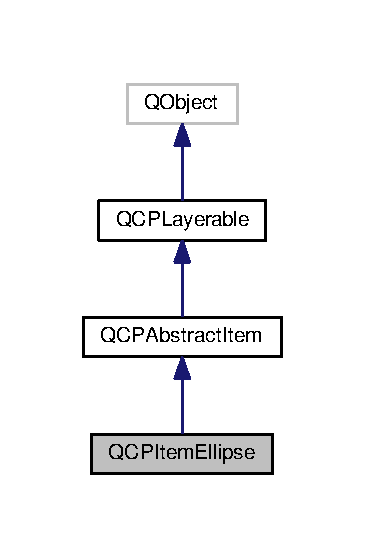
\includegraphics[width=175pt]{classQCPItemEllipse__inherit__graph}
\end{center}
\end{figure}


Collaboration diagram for Q\+C\+P\+Item\+Ellipse\+:\nopagebreak
\begin{figure}[H]
\begin{center}
\leavevmode
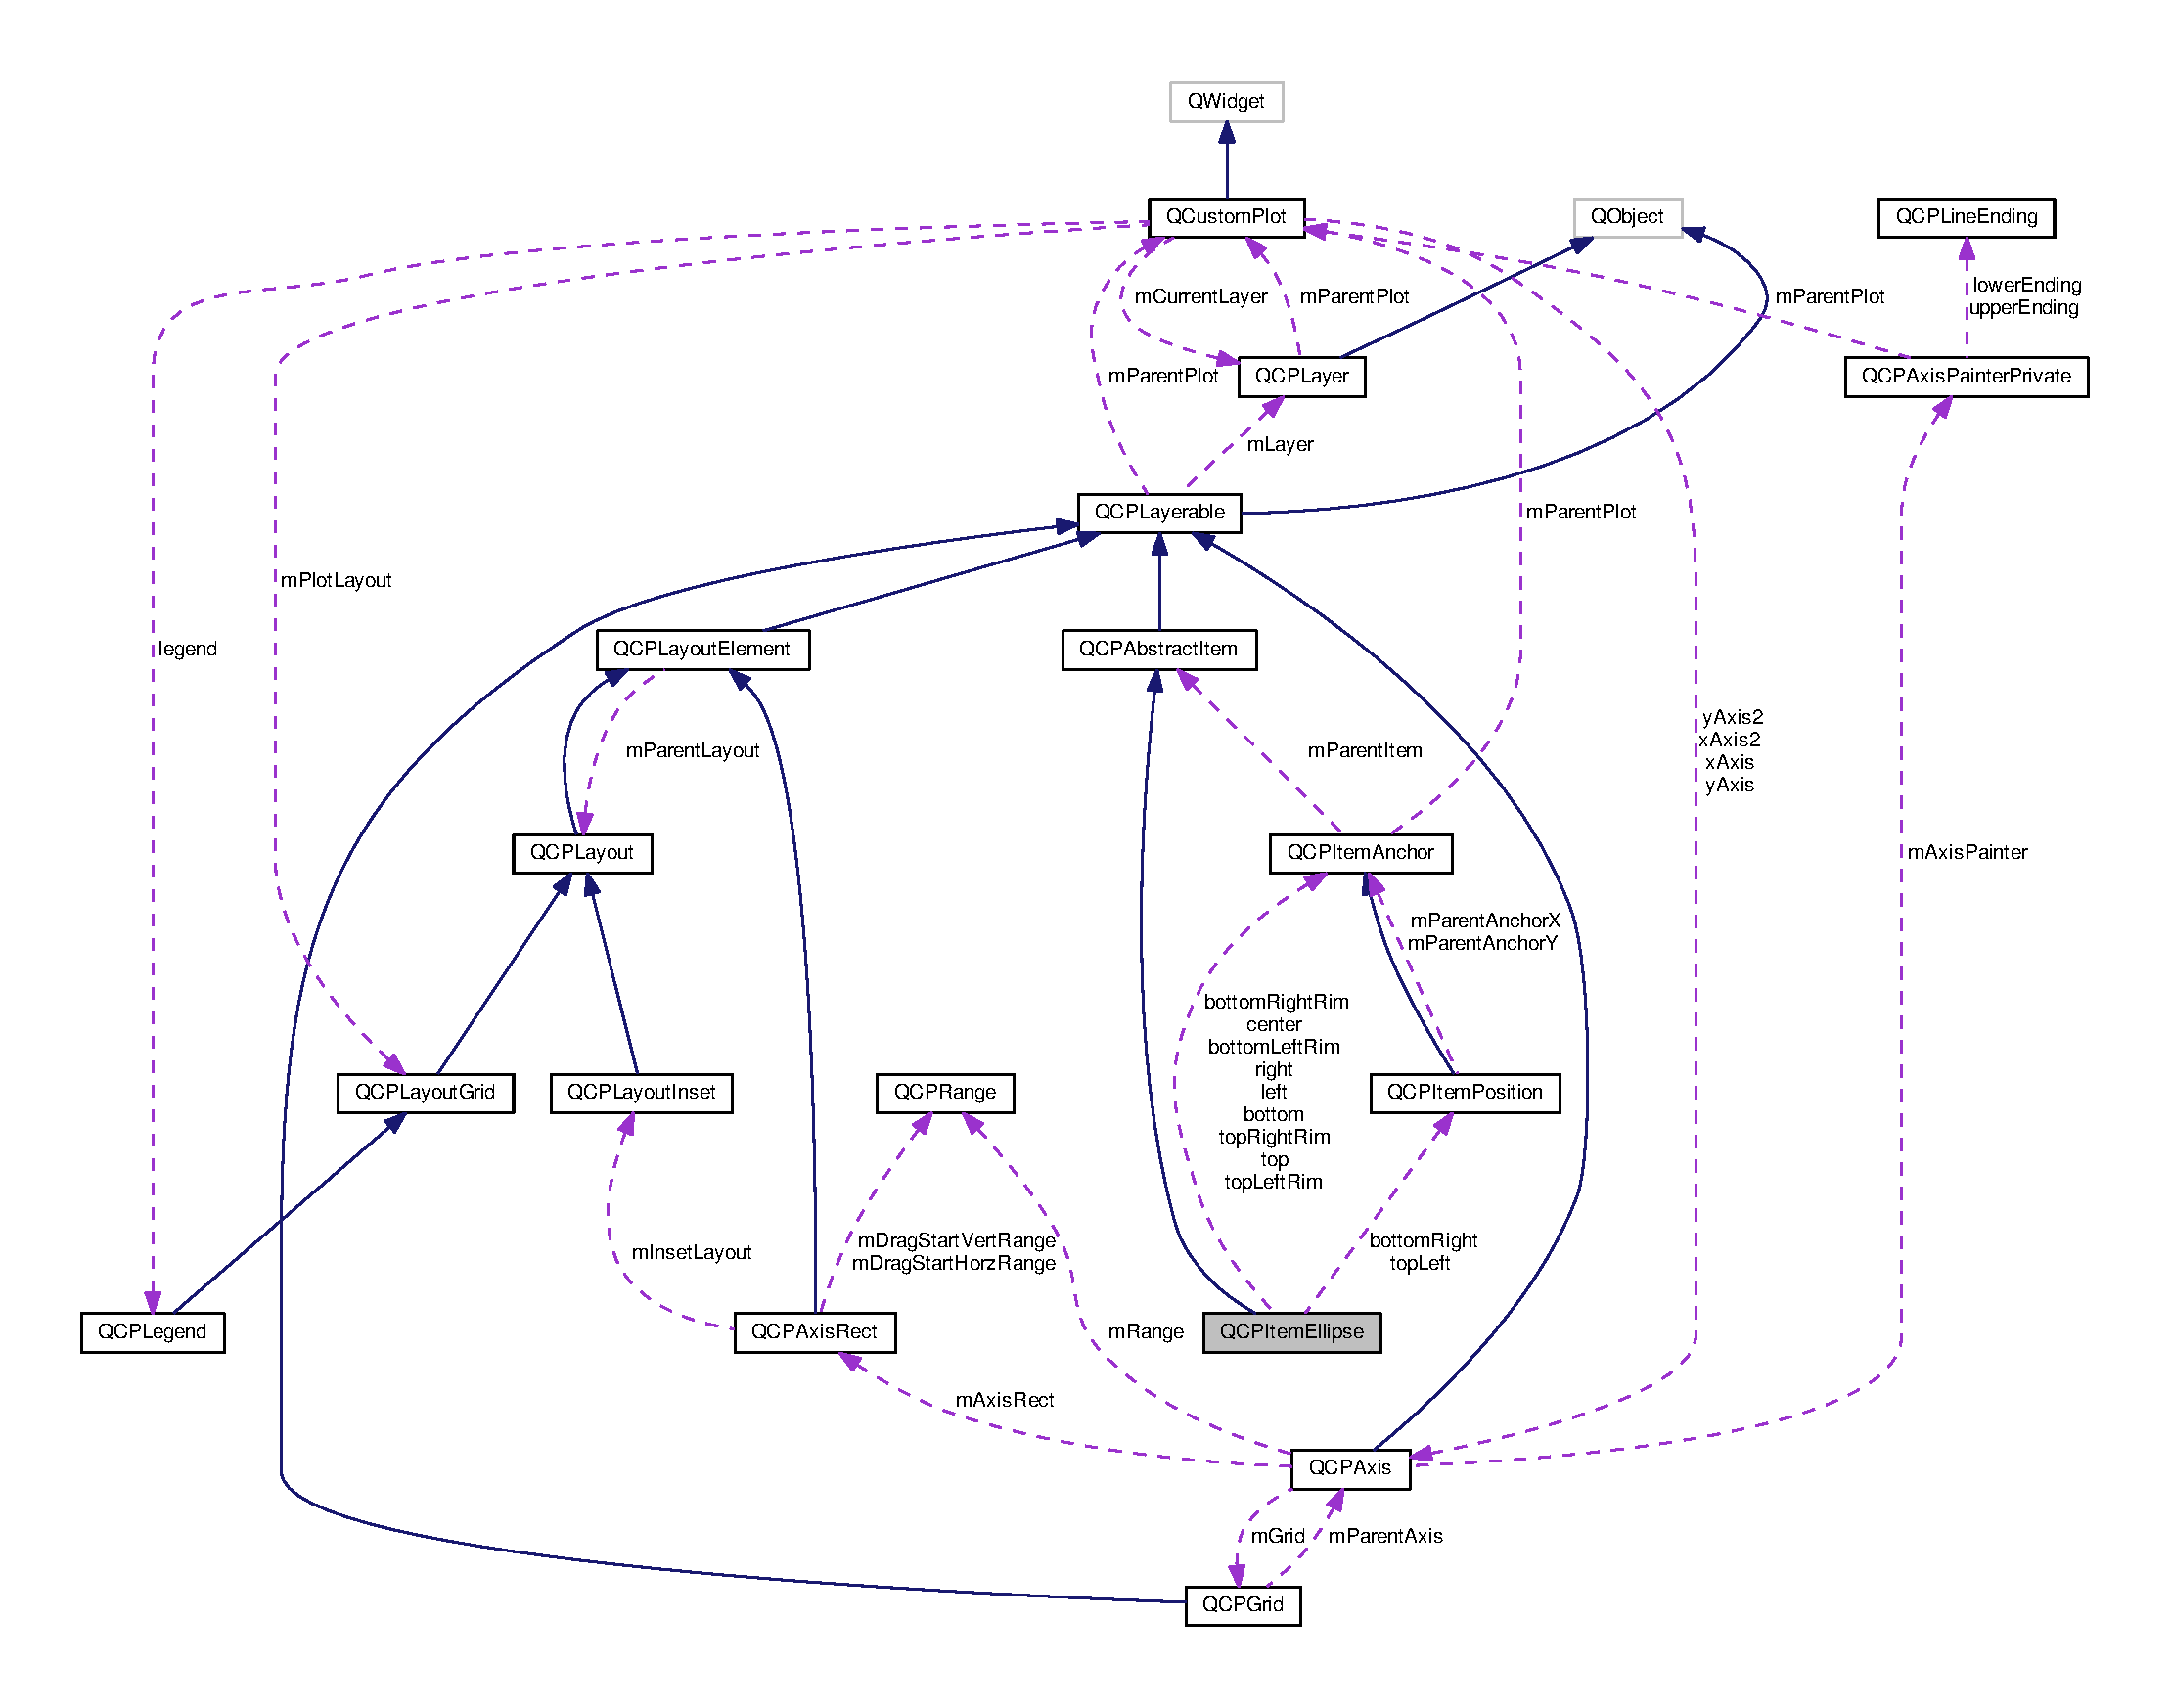
\includegraphics[width=350pt]{classQCPItemEllipse__coll__graph}
\end{center}
\end{figure}
\subsection*{Public Member Functions}
\begin{DoxyCompactItemize}
\item 
\hyperlink{classQCPItemEllipse_a759b77ef002515eba0263b5447ecb3fb}{Q\+C\+P\+Item\+Ellipse} (\hyperlink{classQCustomPlot}{Q\+Custom\+Plot} $\ast$\hyperlink{classQCPLayerable_ab7e0e94461566093d36ffc0f5312b109}{parent\+Plot})
\item 
virtual \hyperlink{classQCPItemEllipse_a3c17073a1805d32b4e09b6ccde0bef76}{$\sim$\+Q\+C\+P\+Item\+Ellipse} ()
\item 
Q\+Pen \hyperlink{classQCPItemEllipse_adb67471eabaf1214c99767f1653ca0ed}{pen} () const 
\item 
Q\+Pen \hyperlink{classQCPItemEllipse_ac52ab52225d238365ff3264b4b69130f}{selected\+Pen} () const 
\item 
Q\+Brush \hyperlink{classQCPItemEllipse_ac012e4fd59fdb1afb6554937bae8f7e1}{brush} () const 
\item 
Q\+Brush \hyperlink{classQCPItemEllipse_a0043e401a912d54ea3195bab0967b394}{selected\+Brush} () const 
\item 
void \hyperlink{classQCPItemEllipse_adb81a663ed2420fcfa011e49f678d1a6}{set\+Pen} (const Q\+Pen \&\hyperlink{classQCPItemEllipse_adb67471eabaf1214c99767f1653ca0ed}{pen})
\item 
void \hyperlink{classQCPItemEllipse_a6c542fba1dc918041c583f58a50dde99}{set\+Selected\+Pen} (const Q\+Pen \&\hyperlink{classQCPItemEllipse_adb67471eabaf1214c99767f1653ca0ed}{pen})
\item 
void \hyperlink{classQCPItemEllipse_a49fc74e6965834e873d027d026def798}{set\+Brush} (const Q\+Brush \&\hyperlink{classQCPItemEllipse_ac012e4fd59fdb1afb6554937bae8f7e1}{brush})
\item 
void \hyperlink{classQCPItemEllipse_a9693501cfaa43a099655c75bed0dab3f}{set\+Selected\+Brush} (const Q\+Brush \&\hyperlink{classQCPItemEllipse_ac012e4fd59fdb1afb6554937bae8f7e1}{brush})
\item 
virtual double \hyperlink{classQCPItemEllipse_acd7e5f9528630b2ab5987e2a5782eb7c}{select\+Test} (const Q\+PointF \&pos, bool only\+Selectable, Q\+Variant $\ast$details=0) const 
\end{DoxyCompactItemize}
\subsection*{Public Attributes}
\begin{DoxyCompactItemize}
\item 
\hyperlink{classQCPItemPosition}{Q\+C\+P\+Item\+Position} $\ast$const \hyperlink{classQCPItemEllipse_a12fd8420c06718d0c8a2303d6a652848}{top\+Left}
\item 
\hyperlink{classQCPItemPosition}{Q\+C\+P\+Item\+Position} $\ast$const \hyperlink{classQCPItemEllipse_ab73c8deafc0d8d1ef7d75b6cdcc37159}{bottom\+Right}
\item 
\hyperlink{classQCPItemAnchor}{Q\+C\+P\+Item\+Anchor} $\ast$const \hyperlink{classQCPItemEllipse_a33ebd2a751b63b9240edc9aa46c19eff}{top\+Left\+Rim}
\item 
\hyperlink{classQCPItemAnchor}{Q\+C\+P\+Item\+Anchor} $\ast$const \hyperlink{classQCPItemEllipse_ad50f907d6f9d1402c6c5d302dca5c5d5}{top}
\item 
\hyperlink{classQCPItemAnchor}{Q\+C\+P\+Item\+Anchor} $\ast$const \hyperlink{classQCPItemEllipse_a744446970b38a4a3bbea46d722b7c54d}{top\+Right\+Rim}
\item 
\hyperlink{classQCPItemAnchor}{Q\+C\+P\+Item\+Anchor} $\ast$const \hyperlink{classQCPItemEllipse_a50091a3bd8761d3ce0d95d9c727e4a82}{right}
\item 
\hyperlink{classQCPItemAnchor}{Q\+C\+P\+Item\+Anchor} $\ast$const \hyperlink{classQCPItemEllipse_a5c8404be601d61b7fafeaaf1c05c4c42}{bottom\+Right\+Rim}
\item 
\hyperlink{classQCPItemAnchor}{Q\+C\+P\+Item\+Anchor} $\ast$const \hyperlink{classQCPItemEllipse_a2dc80ff9f5db600eae0133bdde65066f}{bottom}
\item 
\hyperlink{classQCPItemAnchor}{Q\+C\+P\+Item\+Anchor} $\ast$const \hyperlink{classQCPItemEllipse_a31f31a9e9f9098c90fb47573094276c5}{bottom\+Left\+Rim}
\item 
\hyperlink{classQCPItemAnchor}{Q\+C\+P\+Item\+Anchor} $\ast$const \hyperlink{classQCPItemEllipse_aa259cd03efaedf60cf5b1019b20e4f2b}{left}
\item 
\hyperlink{classQCPItemAnchor}{Q\+C\+P\+Item\+Anchor} $\ast$const \hyperlink{classQCPItemEllipse_a8b6dd0e854f99239c5806ffdf2f590b3}{center}
\end{DoxyCompactItemize}
\subsection*{Protected Types}
\begin{DoxyCompactItemize}
\item 
enum \hyperlink{classQCPItemEllipse_a415009889543169f35b70795f415e45e}{Anchor\+Index} \{ \\*
\hyperlink{classQCPItemEllipse_a415009889543169f35b70795f415e45eab2538849b88921e7fc1dcc15b2a6109d}{ai\+Top\+Left\+Rim}, 
\hyperlink{classQCPItemEllipse_a415009889543169f35b70795f415e45ea83e55b0c1799baac1eecab52bcbe096d}{ai\+Top}, 
\hyperlink{classQCPItemEllipse_a415009889543169f35b70795f415e45ea415d82233c14f0c70c245d50e706e75b}{ai\+Top\+Right\+Rim}, 
\hyperlink{classQCPItemEllipse_a415009889543169f35b70795f415e45ea0f0dcfdf87d9405b53b2129740fb6ba6}{ai\+Right}, 
\\*
\hyperlink{classQCPItemEllipse_a415009889543169f35b70795f415e45eab62732e96d67801d50c6a9bdebc374d0}{ai\+Bottom\+Right\+Rim}, 
\hyperlink{classQCPItemEllipse_a415009889543169f35b70795f415e45ea5894287dedaeec1f48394fd950ccff5b}{ai\+Bottom}, 
\hyperlink{classQCPItemEllipse_a415009889543169f35b70795f415e45ea7b8101bfc590af8ce32961f6545c4f90}{ai\+Bottom\+Left\+Rim}, 
\hyperlink{classQCPItemEllipse_a415009889543169f35b70795f415e45eae74dad00419a0e1f42877510158fb922}{ai\+Left}, 
\\*
\hyperlink{classQCPItemEllipse_a415009889543169f35b70795f415e45ea580ec0e9b9fd1488fccf5783e52c0c02}{ai\+Center}
 \}
\end{DoxyCompactItemize}
\subsection*{Protected Member Functions}
\begin{DoxyCompactItemize}
\item 
virtual void \hyperlink{classQCPItemEllipse_afe97ec827adb05f000fe007783faae3c}{draw} (\hyperlink{classQCPPainter}{Q\+C\+P\+Painter} $\ast$painter)
\item 
virtual Q\+PointF \hyperlink{classQCPItemEllipse_ad3c607304dba081e2f778b6a81b903bb}{anchor\+Pixel\+Point} (int anchor\+Id) const 
\item 
Q\+Pen \hyperlink{classQCPItemEllipse_afc78d49ed5ffa886bccf18f297f83d30}{main\+Pen} () const 
\item 
Q\+Brush \hyperlink{classQCPItemEllipse_a2a9757204877c9d0fd07adfb26d6b1d8}{main\+Brush} () const 
\end{DoxyCompactItemize}
\subsection*{Protected Attributes}
\begin{DoxyCompactItemize}
\item 
Q\+Pen \hyperlink{classQCPItemEllipse_a16ad9389acf028a7e4ac8fd7a550b2e4}{m\+Pen}
\item 
Q\+Pen \hyperlink{classQCPItemEllipse_a57b047abfce6f1a84ed46ca668c90e21}{m\+Selected\+Pen}
\item 
Q\+Brush \hyperlink{classQCPItemEllipse_a6fa59478cd3ad1b10e6c1f6cedc84bd6}{m\+Brush}
\item 
Q\+Brush \hyperlink{classQCPItemEllipse_a2e49d5547478aa36910ed8a2dcc8a5c0}{m\+Selected\+Brush}
\end{DoxyCompactItemize}
\subsection*{Additional Inherited Members}


\subsection{Detailed Description}
An ellipse. 

 It has two positions, {\itshape top\+Left} and {\itshape bottom\+Right}, which define the rect the ellipse will be drawn in. 

\subsection{Member Enumeration Documentation}
\index{Q\+C\+P\+Item\+Ellipse@{Q\+C\+P\+Item\+Ellipse}!Anchor\+Index@{Anchor\+Index}}
\index{Anchor\+Index@{Anchor\+Index}!Q\+C\+P\+Item\+Ellipse@{Q\+C\+P\+Item\+Ellipse}}
\subsubsection[{\texorpdfstring{Anchor\+Index}{AnchorIndex}}]{\setlength{\rightskip}{0pt plus 5cm}enum {\bf Q\+C\+P\+Item\+Ellipse\+::\+Anchor\+Index}\hspace{0.3cm}{\ttfamily [protected]}}\hypertarget{classQCPItemEllipse_a415009889543169f35b70795f415e45e}{}\label{classQCPItemEllipse_a415009889543169f35b70795f415e45e}
\begin{Desc}
\item[Enumerator]\par
\begin{description}
\index{ai\+Top\+Left\+Rim@{ai\+Top\+Left\+Rim}!Q\+C\+P\+Item\+Ellipse@{Q\+C\+P\+Item\+Ellipse}}\index{Q\+C\+P\+Item\+Ellipse@{Q\+C\+P\+Item\+Ellipse}!ai\+Top\+Left\+Rim@{ai\+Top\+Left\+Rim}}\item[{\em 
ai\+Top\+Left\+Rim\hypertarget{classQCPItemEllipse_a415009889543169f35b70795f415e45eab2538849b88921e7fc1dcc15b2a6109d}{}\label{classQCPItemEllipse_a415009889543169f35b70795f415e45eab2538849b88921e7fc1dcc15b2a6109d}
}]\index{ai\+Top@{ai\+Top}!Q\+C\+P\+Item\+Ellipse@{Q\+C\+P\+Item\+Ellipse}}\index{Q\+C\+P\+Item\+Ellipse@{Q\+C\+P\+Item\+Ellipse}!ai\+Top@{ai\+Top}}\item[{\em 
ai\+Top\hypertarget{classQCPItemEllipse_a415009889543169f35b70795f415e45ea83e55b0c1799baac1eecab52bcbe096d}{}\label{classQCPItemEllipse_a415009889543169f35b70795f415e45ea83e55b0c1799baac1eecab52bcbe096d}
}]\index{ai\+Top\+Right\+Rim@{ai\+Top\+Right\+Rim}!Q\+C\+P\+Item\+Ellipse@{Q\+C\+P\+Item\+Ellipse}}\index{Q\+C\+P\+Item\+Ellipse@{Q\+C\+P\+Item\+Ellipse}!ai\+Top\+Right\+Rim@{ai\+Top\+Right\+Rim}}\item[{\em 
ai\+Top\+Right\+Rim\hypertarget{classQCPItemEllipse_a415009889543169f35b70795f415e45ea415d82233c14f0c70c245d50e706e75b}{}\label{classQCPItemEllipse_a415009889543169f35b70795f415e45ea415d82233c14f0c70c245d50e706e75b}
}]\index{ai\+Right@{ai\+Right}!Q\+C\+P\+Item\+Ellipse@{Q\+C\+P\+Item\+Ellipse}}\index{Q\+C\+P\+Item\+Ellipse@{Q\+C\+P\+Item\+Ellipse}!ai\+Right@{ai\+Right}}\item[{\em 
ai\+Right\hypertarget{classQCPItemEllipse_a415009889543169f35b70795f415e45ea0f0dcfdf87d9405b53b2129740fb6ba6}{}\label{classQCPItemEllipse_a415009889543169f35b70795f415e45ea0f0dcfdf87d9405b53b2129740fb6ba6}
}]\index{ai\+Bottom\+Right\+Rim@{ai\+Bottom\+Right\+Rim}!Q\+C\+P\+Item\+Ellipse@{Q\+C\+P\+Item\+Ellipse}}\index{Q\+C\+P\+Item\+Ellipse@{Q\+C\+P\+Item\+Ellipse}!ai\+Bottom\+Right\+Rim@{ai\+Bottom\+Right\+Rim}}\item[{\em 
ai\+Bottom\+Right\+Rim\hypertarget{classQCPItemEllipse_a415009889543169f35b70795f415e45eab62732e96d67801d50c6a9bdebc374d0}{}\label{classQCPItemEllipse_a415009889543169f35b70795f415e45eab62732e96d67801d50c6a9bdebc374d0}
}]\index{ai\+Bottom@{ai\+Bottom}!Q\+C\+P\+Item\+Ellipse@{Q\+C\+P\+Item\+Ellipse}}\index{Q\+C\+P\+Item\+Ellipse@{Q\+C\+P\+Item\+Ellipse}!ai\+Bottom@{ai\+Bottom}}\item[{\em 
ai\+Bottom\hypertarget{classQCPItemEllipse_a415009889543169f35b70795f415e45ea5894287dedaeec1f48394fd950ccff5b}{}\label{classQCPItemEllipse_a415009889543169f35b70795f415e45ea5894287dedaeec1f48394fd950ccff5b}
}]\index{ai\+Bottom\+Left\+Rim@{ai\+Bottom\+Left\+Rim}!Q\+C\+P\+Item\+Ellipse@{Q\+C\+P\+Item\+Ellipse}}\index{Q\+C\+P\+Item\+Ellipse@{Q\+C\+P\+Item\+Ellipse}!ai\+Bottom\+Left\+Rim@{ai\+Bottom\+Left\+Rim}}\item[{\em 
ai\+Bottom\+Left\+Rim\hypertarget{classQCPItemEllipse_a415009889543169f35b70795f415e45ea7b8101bfc590af8ce32961f6545c4f90}{}\label{classQCPItemEllipse_a415009889543169f35b70795f415e45ea7b8101bfc590af8ce32961f6545c4f90}
}]\index{ai\+Left@{ai\+Left}!Q\+C\+P\+Item\+Ellipse@{Q\+C\+P\+Item\+Ellipse}}\index{Q\+C\+P\+Item\+Ellipse@{Q\+C\+P\+Item\+Ellipse}!ai\+Left@{ai\+Left}}\item[{\em 
ai\+Left\hypertarget{classQCPItemEllipse_a415009889543169f35b70795f415e45eae74dad00419a0e1f42877510158fb922}{}\label{classQCPItemEllipse_a415009889543169f35b70795f415e45eae74dad00419a0e1f42877510158fb922}
}]\index{ai\+Center@{ai\+Center}!Q\+C\+P\+Item\+Ellipse@{Q\+C\+P\+Item\+Ellipse}}\index{Q\+C\+P\+Item\+Ellipse@{Q\+C\+P\+Item\+Ellipse}!ai\+Center@{ai\+Center}}\item[{\em 
ai\+Center\hypertarget{classQCPItemEllipse_a415009889543169f35b70795f415e45ea580ec0e9b9fd1488fccf5783e52c0c02}{}\label{classQCPItemEllipse_a415009889543169f35b70795f415e45ea580ec0e9b9fd1488fccf5783e52c0c02}
}]\end{description}
\end{Desc}


\subsection{Constructor \& Destructor Documentation}
\index{Q\+C\+P\+Item\+Ellipse@{Q\+C\+P\+Item\+Ellipse}!Q\+C\+P\+Item\+Ellipse@{Q\+C\+P\+Item\+Ellipse}}
\index{Q\+C\+P\+Item\+Ellipse@{Q\+C\+P\+Item\+Ellipse}!Q\+C\+P\+Item\+Ellipse@{Q\+C\+P\+Item\+Ellipse}}
\subsubsection[{\texorpdfstring{Q\+C\+P\+Item\+Ellipse(\+Q\+Custom\+Plot $\ast$parent\+Plot)}{QCPItemEllipse(QCustomPlot *parentPlot)}}]{\setlength{\rightskip}{0pt plus 5cm}Q\+C\+P\+Item\+Ellipse\+::\+Q\+C\+P\+Item\+Ellipse (
\begin{DoxyParamCaption}
\item[{{\bf Q\+Custom\+Plot} $\ast$}]{parent\+Plot}
\end{DoxyParamCaption}
)}\hypertarget{classQCPItemEllipse_a759b77ef002515eba0263b5447ecb3fb}{}\label{classQCPItemEllipse_a759b77ef002515eba0263b5447ecb3fb}
Creates an ellipse item and sets default values.

The constructed item can be added to the plot with \hyperlink{classQCustomPlot_aa500620379262321685cb7a7674cbd2a}{Q\+Custom\+Plot\+::add\+Item}. \index{Q\+C\+P\+Item\+Ellipse@{Q\+C\+P\+Item\+Ellipse}!````~Q\+C\+P\+Item\+Ellipse@{$\sim$\+Q\+C\+P\+Item\+Ellipse}}
\index{````~Q\+C\+P\+Item\+Ellipse@{$\sim$\+Q\+C\+P\+Item\+Ellipse}!Q\+C\+P\+Item\+Ellipse@{Q\+C\+P\+Item\+Ellipse}}
\subsubsection[{\texorpdfstring{$\sim$\+Q\+C\+P\+Item\+Ellipse()}{~QCPItemEllipse()}}]{\setlength{\rightskip}{0pt plus 5cm}Q\+C\+P\+Item\+Ellipse\+::$\sim$\+Q\+C\+P\+Item\+Ellipse (
\begin{DoxyParamCaption}
{}
\end{DoxyParamCaption}
)\hspace{0.3cm}{\ttfamily [virtual]}}\hypertarget{classQCPItemEllipse_a3c17073a1805d32b4e09b6ccde0bef76}{}\label{classQCPItemEllipse_a3c17073a1805d32b4e09b6ccde0bef76}


\subsection{Member Function Documentation}
\index{Q\+C\+P\+Item\+Ellipse@{Q\+C\+P\+Item\+Ellipse}!anchor\+Pixel\+Point@{anchor\+Pixel\+Point}}
\index{anchor\+Pixel\+Point@{anchor\+Pixel\+Point}!Q\+C\+P\+Item\+Ellipse@{Q\+C\+P\+Item\+Ellipse}}
\subsubsection[{\texorpdfstring{anchor\+Pixel\+Point(int anchor\+Id) const }{anchorPixelPoint(int anchorId) const }}]{\setlength{\rightskip}{0pt plus 5cm}Q\+PointF Q\+C\+P\+Item\+Ellipse\+::anchor\+Pixel\+Point (
\begin{DoxyParamCaption}
\item[{int}]{anchor\+Id}
\end{DoxyParamCaption}
) const\hspace{0.3cm}{\ttfamily [protected]}, {\ttfamily [virtual]}}\hypertarget{classQCPItemEllipse_ad3c607304dba081e2f778b6a81b903bb}{}\label{classQCPItemEllipse_ad3c607304dba081e2f778b6a81b903bb}


Reimplemented from \hyperlink{classQCPAbstractItem_a94bde62b8a2fc133666dcbb8035deeed}{Q\+C\+P\+Abstract\+Item}.

\index{Q\+C\+P\+Item\+Ellipse@{Q\+C\+P\+Item\+Ellipse}!brush@{brush}}
\index{brush@{brush}!Q\+C\+P\+Item\+Ellipse@{Q\+C\+P\+Item\+Ellipse}}
\subsubsection[{\texorpdfstring{brush() const }{brush() const }}]{\setlength{\rightskip}{0pt plus 5cm}Q\+Brush Q\+C\+P\+Item\+Ellipse\+::brush (
\begin{DoxyParamCaption}
{}
\end{DoxyParamCaption}
) const\hspace{0.3cm}{\ttfamily [inline]}}\hypertarget{classQCPItemEllipse_ac012e4fd59fdb1afb6554937bae8f7e1}{}\label{classQCPItemEllipse_ac012e4fd59fdb1afb6554937bae8f7e1}
\index{Q\+C\+P\+Item\+Ellipse@{Q\+C\+P\+Item\+Ellipse}!draw@{draw}}
\index{draw@{draw}!Q\+C\+P\+Item\+Ellipse@{Q\+C\+P\+Item\+Ellipse}}
\subsubsection[{\texorpdfstring{draw(\+Q\+C\+P\+Painter $\ast$painter)}{draw(QCPPainter *painter)}}]{\setlength{\rightskip}{0pt plus 5cm}void Q\+C\+P\+Item\+Ellipse\+::draw (
\begin{DoxyParamCaption}
\item[{{\bf Q\+C\+P\+Painter} $\ast$}]{painter}
\end{DoxyParamCaption}
)\hspace{0.3cm}{\ttfamily [protected]}, {\ttfamily [virtual]}}\hypertarget{classQCPItemEllipse_afe97ec827adb05f000fe007783faae3c}{}\label{classQCPItemEllipse_afe97ec827adb05f000fe007783faae3c}


Implements \hyperlink{classQCPAbstractItem_ad0dc056f650c3ca73414e6b4f01674ef}{Q\+C\+P\+Abstract\+Item}.

\index{Q\+C\+P\+Item\+Ellipse@{Q\+C\+P\+Item\+Ellipse}!main\+Brush@{main\+Brush}}
\index{main\+Brush@{main\+Brush}!Q\+C\+P\+Item\+Ellipse@{Q\+C\+P\+Item\+Ellipse}}
\subsubsection[{\texorpdfstring{main\+Brush() const }{mainBrush() const }}]{\setlength{\rightskip}{0pt plus 5cm}Q\+Brush Q\+C\+P\+Item\+Ellipse\+::main\+Brush (
\begin{DoxyParamCaption}
{}
\end{DoxyParamCaption}
) const\hspace{0.3cm}{\ttfamily [protected]}}\hypertarget{classQCPItemEllipse_a2a9757204877c9d0fd07adfb26d6b1d8}{}\label{classQCPItemEllipse_a2a9757204877c9d0fd07adfb26d6b1d8}
\index{Q\+C\+P\+Item\+Ellipse@{Q\+C\+P\+Item\+Ellipse}!main\+Pen@{main\+Pen}}
\index{main\+Pen@{main\+Pen}!Q\+C\+P\+Item\+Ellipse@{Q\+C\+P\+Item\+Ellipse}}
\subsubsection[{\texorpdfstring{main\+Pen() const }{mainPen() const }}]{\setlength{\rightskip}{0pt plus 5cm}Q\+Pen Q\+C\+P\+Item\+Ellipse\+::main\+Pen (
\begin{DoxyParamCaption}
{}
\end{DoxyParamCaption}
) const\hspace{0.3cm}{\ttfamily [protected]}}\hypertarget{classQCPItemEllipse_afc78d49ed5ffa886bccf18f297f83d30}{}\label{classQCPItemEllipse_afc78d49ed5ffa886bccf18f297f83d30}
\index{Q\+C\+P\+Item\+Ellipse@{Q\+C\+P\+Item\+Ellipse}!pen@{pen}}
\index{pen@{pen}!Q\+C\+P\+Item\+Ellipse@{Q\+C\+P\+Item\+Ellipse}}
\subsubsection[{\texorpdfstring{pen() const }{pen() const }}]{\setlength{\rightskip}{0pt plus 5cm}Q\+Pen Q\+C\+P\+Item\+Ellipse\+::pen (
\begin{DoxyParamCaption}
{}
\end{DoxyParamCaption}
) const\hspace{0.3cm}{\ttfamily [inline]}}\hypertarget{classQCPItemEllipse_adb67471eabaf1214c99767f1653ca0ed}{}\label{classQCPItemEllipse_adb67471eabaf1214c99767f1653ca0ed}
\index{Q\+C\+P\+Item\+Ellipse@{Q\+C\+P\+Item\+Ellipse}!selected\+Brush@{selected\+Brush}}
\index{selected\+Brush@{selected\+Brush}!Q\+C\+P\+Item\+Ellipse@{Q\+C\+P\+Item\+Ellipse}}
\subsubsection[{\texorpdfstring{selected\+Brush() const }{selectedBrush() const }}]{\setlength{\rightskip}{0pt plus 5cm}Q\+Brush Q\+C\+P\+Item\+Ellipse\+::selected\+Brush (
\begin{DoxyParamCaption}
{}
\end{DoxyParamCaption}
) const\hspace{0.3cm}{\ttfamily [inline]}}\hypertarget{classQCPItemEllipse_a0043e401a912d54ea3195bab0967b394}{}\label{classQCPItemEllipse_a0043e401a912d54ea3195bab0967b394}
\index{Q\+C\+P\+Item\+Ellipse@{Q\+C\+P\+Item\+Ellipse}!selected\+Pen@{selected\+Pen}}
\index{selected\+Pen@{selected\+Pen}!Q\+C\+P\+Item\+Ellipse@{Q\+C\+P\+Item\+Ellipse}}
\subsubsection[{\texorpdfstring{selected\+Pen() const }{selectedPen() const }}]{\setlength{\rightskip}{0pt plus 5cm}Q\+Pen Q\+C\+P\+Item\+Ellipse\+::selected\+Pen (
\begin{DoxyParamCaption}
{}
\end{DoxyParamCaption}
) const\hspace{0.3cm}{\ttfamily [inline]}}\hypertarget{classQCPItemEllipse_ac52ab52225d238365ff3264b4b69130f}{}\label{classQCPItemEllipse_ac52ab52225d238365ff3264b4b69130f}
\index{Q\+C\+P\+Item\+Ellipse@{Q\+C\+P\+Item\+Ellipse}!select\+Test@{select\+Test}}
\index{select\+Test@{select\+Test}!Q\+C\+P\+Item\+Ellipse@{Q\+C\+P\+Item\+Ellipse}}
\subsubsection[{\texorpdfstring{select\+Test(const Q\+Point\+F \&pos, bool only\+Selectable, Q\+Variant $\ast$details=0) const }{selectTest(const QPointF &pos, bool onlySelectable, QVariant *details=0) const }}]{\setlength{\rightskip}{0pt plus 5cm}double Q\+C\+P\+Item\+Ellipse\+::select\+Test (
\begin{DoxyParamCaption}
\item[{const Q\+PointF \&}]{pos, }
\item[{bool}]{only\+Selectable, }
\item[{Q\+Variant $\ast$}]{details = {\ttfamily 0}}
\end{DoxyParamCaption}
) const\hspace{0.3cm}{\ttfamily [virtual]}}\hypertarget{classQCPItemEllipse_acd7e5f9528630b2ab5987e2a5782eb7c}{}\label{classQCPItemEllipse_acd7e5f9528630b2ab5987e2a5782eb7c}
This function is used to decide whether a click hits a layerable object or not.

{\itshape pos} is a point in pixel coordinates on the \hyperlink{classQCustomPlot}{Q\+Custom\+Plot} surface. This function returns the shortest pixel distance of this point to the object. If the object is either invisible or the distance couldn\textquotesingle{}t be determined, -\/1.\+0 is returned. Further, if {\itshape only\+Selectable} is true and the object is not selectable, -\/1.\+0 is returned, too.

If the object is represented not by single lines but by an area like a \hyperlink{classQCPItemText}{Q\+C\+P\+Item\+Text} or the bars of a \hyperlink{classQCPBars}{Q\+C\+P\+Bars} plottable, a click inside the area should also be considered a hit. In these cases this function thus returns a constant value greater zero but still below the parent plot\textquotesingle{}s selection tolerance. (typically the selection\+Tolerance multiplied by 0.\+99).

Providing a constant value for area objects allows selecting line objects even when they are obscured by such area objects, by clicking close to the lines (i.\+e. closer than 0.\+99$\ast$selection\+Tolerance).

The actual setting of the selection state is not done by this function. This is handled by the parent \hyperlink{classQCustomPlot}{Q\+Custom\+Plot} when the mouse\+Release\+Event occurs, and the finally selected object is notified via the select\+Event/deselect\+Event methods.

{\itshape details} is an optional output parameter. Every layerable subclass may place any information in {\itshape details}. This information will be passed to \hyperlink{classQCPAbstractItem_aaf92af7b9893712959a6c073d334d88d}{select\+Event} when the parent \hyperlink{classQCustomPlot}{Q\+Custom\+Plot} decides on the basis of this select\+Test call, that the object was successfully selected. The subsequent call to \hyperlink{classQCPAbstractItem_aaf92af7b9893712959a6c073d334d88d}{select\+Event} will carry the {\itshape details}. This is useful for multi-\/part objects (like \hyperlink{classQCPAxis}{Q\+C\+P\+Axis}). This way, a possibly complex calculation to decide which part was clicked is only done once in \hyperlink{classQCPItemEllipse_acd7e5f9528630b2ab5987e2a5782eb7c}{select\+Test}. The result (i.\+e. the actually clicked part) can then be placed in {\itshape details}. So in the subsequent \hyperlink{classQCPAbstractItem_aaf92af7b9893712959a6c073d334d88d}{select\+Event}, the decision which part was selected doesn\textquotesingle{}t have to be done a second time for a single selection operation.

You may pass 0 as {\itshape details} to indicate that you are not interested in those selection details.

\begin{DoxySeeAlso}{See also}
\hyperlink{classQCPAbstractItem_aaf92af7b9893712959a6c073d334d88d}{select\+Event}, \hyperlink{classQCPAbstractItem_a91f090d6763cfedb0749219c63788ae9}{deselect\+Event}, \hyperlink{classQCustomPlot_a5ee1e2f6ae27419deca53e75907c27e5}{Q\+Custom\+Plot\+::set\+Interactions} 
\end{DoxySeeAlso}


Implements \hyperlink{classQCPAbstractItem_a96d522d10ffc0413b9a366c6f7f0476b}{Q\+C\+P\+Abstract\+Item}.

\index{Q\+C\+P\+Item\+Ellipse@{Q\+C\+P\+Item\+Ellipse}!set\+Brush@{set\+Brush}}
\index{set\+Brush@{set\+Brush}!Q\+C\+P\+Item\+Ellipse@{Q\+C\+P\+Item\+Ellipse}}
\subsubsection[{\texorpdfstring{set\+Brush(const Q\+Brush \&brush)}{setBrush(const QBrush &brush)}}]{\setlength{\rightskip}{0pt plus 5cm}void Q\+C\+P\+Item\+Ellipse\+::set\+Brush (
\begin{DoxyParamCaption}
\item[{const Q\+Brush \&}]{brush}
\end{DoxyParamCaption}
)}\hypertarget{classQCPItemEllipse_a49fc74e6965834e873d027d026def798}{}\label{classQCPItemEllipse_a49fc74e6965834e873d027d026def798}
Sets the brush that will be used to fill the ellipse. To disable filling, set {\itshape brush} to Qt\+::\+No\+Brush.

\begin{DoxySeeAlso}{See also}
\hyperlink{classQCPItemEllipse_a9693501cfaa43a099655c75bed0dab3f}{set\+Selected\+Brush}, \hyperlink{classQCPItemEllipse_adb81a663ed2420fcfa011e49f678d1a6}{set\+Pen} 
\end{DoxySeeAlso}
\index{Q\+C\+P\+Item\+Ellipse@{Q\+C\+P\+Item\+Ellipse}!set\+Pen@{set\+Pen}}
\index{set\+Pen@{set\+Pen}!Q\+C\+P\+Item\+Ellipse@{Q\+C\+P\+Item\+Ellipse}}
\subsubsection[{\texorpdfstring{set\+Pen(const Q\+Pen \&pen)}{setPen(const QPen &pen)}}]{\setlength{\rightskip}{0pt plus 5cm}void Q\+C\+P\+Item\+Ellipse\+::set\+Pen (
\begin{DoxyParamCaption}
\item[{const Q\+Pen \&}]{pen}
\end{DoxyParamCaption}
)}\hypertarget{classQCPItemEllipse_adb81a663ed2420fcfa011e49f678d1a6}{}\label{classQCPItemEllipse_adb81a663ed2420fcfa011e49f678d1a6}
Sets the pen that will be used to draw the line of the ellipse

\begin{DoxySeeAlso}{See also}
\hyperlink{classQCPItemEllipse_a6c542fba1dc918041c583f58a50dde99}{set\+Selected\+Pen}, \hyperlink{classQCPItemEllipse_a49fc74e6965834e873d027d026def798}{set\+Brush} 
\end{DoxySeeAlso}
\index{Q\+C\+P\+Item\+Ellipse@{Q\+C\+P\+Item\+Ellipse}!set\+Selected\+Brush@{set\+Selected\+Brush}}
\index{set\+Selected\+Brush@{set\+Selected\+Brush}!Q\+C\+P\+Item\+Ellipse@{Q\+C\+P\+Item\+Ellipse}}
\subsubsection[{\texorpdfstring{set\+Selected\+Brush(const Q\+Brush \&brush)}{setSelectedBrush(const QBrush &brush)}}]{\setlength{\rightskip}{0pt plus 5cm}void Q\+C\+P\+Item\+Ellipse\+::set\+Selected\+Brush (
\begin{DoxyParamCaption}
\item[{const Q\+Brush \&}]{brush}
\end{DoxyParamCaption}
)}\hypertarget{classQCPItemEllipse_a9693501cfaa43a099655c75bed0dab3f}{}\label{classQCPItemEllipse_a9693501cfaa43a099655c75bed0dab3f}
Sets the brush that will be used to fill the ellipse when selected. To disable filling, set {\itshape brush} to Qt\+::\+No\+Brush.

\begin{DoxySeeAlso}{See also}
\hyperlink{classQCPItemEllipse_a49fc74e6965834e873d027d026def798}{set\+Brush} 
\end{DoxySeeAlso}
\index{Q\+C\+P\+Item\+Ellipse@{Q\+C\+P\+Item\+Ellipse}!set\+Selected\+Pen@{set\+Selected\+Pen}}
\index{set\+Selected\+Pen@{set\+Selected\+Pen}!Q\+C\+P\+Item\+Ellipse@{Q\+C\+P\+Item\+Ellipse}}
\subsubsection[{\texorpdfstring{set\+Selected\+Pen(const Q\+Pen \&pen)}{setSelectedPen(const QPen &pen)}}]{\setlength{\rightskip}{0pt plus 5cm}void Q\+C\+P\+Item\+Ellipse\+::set\+Selected\+Pen (
\begin{DoxyParamCaption}
\item[{const Q\+Pen \&}]{pen}
\end{DoxyParamCaption}
)}\hypertarget{classQCPItemEllipse_a6c542fba1dc918041c583f58a50dde99}{}\label{classQCPItemEllipse_a6c542fba1dc918041c583f58a50dde99}
Sets the pen that will be used to draw the line of the ellipse when selected

\begin{DoxySeeAlso}{See also}
\hyperlink{classQCPItemEllipse_adb81a663ed2420fcfa011e49f678d1a6}{set\+Pen}, \hyperlink{classQCPAbstractItem_a203de94ad586cc44d16c9565f49d3378}{set\+Selected} 
\end{DoxySeeAlso}


\subsection{Member Data Documentation}
\index{Q\+C\+P\+Item\+Ellipse@{Q\+C\+P\+Item\+Ellipse}!bottom@{bottom}}
\index{bottom@{bottom}!Q\+C\+P\+Item\+Ellipse@{Q\+C\+P\+Item\+Ellipse}}
\subsubsection[{\texorpdfstring{bottom}{bottom}}]{\setlength{\rightskip}{0pt plus 5cm}{\bf Q\+C\+P\+Item\+Anchor}$\ast$ const Q\+C\+P\+Item\+Ellipse\+::bottom}\hypertarget{classQCPItemEllipse_a2dc80ff9f5db600eae0133bdde65066f}{}\label{classQCPItemEllipse_a2dc80ff9f5db600eae0133bdde65066f}
\index{Q\+C\+P\+Item\+Ellipse@{Q\+C\+P\+Item\+Ellipse}!bottom\+Left\+Rim@{bottom\+Left\+Rim}}
\index{bottom\+Left\+Rim@{bottom\+Left\+Rim}!Q\+C\+P\+Item\+Ellipse@{Q\+C\+P\+Item\+Ellipse}}
\subsubsection[{\texorpdfstring{bottom\+Left\+Rim}{bottomLeftRim}}]{\setlength{\rightskip}{0pt plus 5cm}{\bf Q\+C\+P\+Item\+Anchor}$\ast$ const Q\+C\+P\+Item\+Ellipse\+::bottom\+Left\+Rim}\hypertarget{classQCPItemEllipse_a31f31a9e9f9098c90fb47573094276c5}{}\label{classQCPItemEllipse_a31f31a9e9f9098c90fb47573094276c5}
\index{Q\+C\+P\+Item\+Ellipse@{Q\+C\+P\+Item\+Ellipse}!bottom\+Right@{bottom\+Right}}
\index{bottom\+Right@{bottom\+Right}!Q\+C\+P\+Item\+Ellipse@{Q\+C\+P\+Item\+Ellipse}}
\subsubsection[{\texorpdfstring{bottom\+Right}{bottomRight}}]{\setlength{\rightskip}{0pt plus 5cm}{\bf Q\+C\+P\+Item\+Position}$\ast$ const Q\+C\+P\+Item\+Ellipse\+::bottom\+Right}\hypertarget{classQCPItemEllipse_ab73c8deafc0d8d1ef7d75b6cdcc37159}{}\label{classQCPItemEllipse_ab73c8deafc0d8d1ef7d75b6cdcc37159}
\index{Q\+C\+P\+Item\+Ellipse@{Q\+C\+P\+Item\+Ellipse}!bottom\+Right\+Rim@{bottom\+Right\+Rim}}
\index{bottom\+Right\+Rim@{bottom\+Right\+Rim}!Q\+C\+P\+Item\+Ellipse@{Q\+C\+P\+Item\+Ellipse}}
\subsubsection[{\texorpdfstring{bottom\+Right\+Rim}{bottomRightRim}}]{\setlength{\rightskip}{0pt plus 5cm}{\bf Q\+C\+P\+Item\+Anchor}$\ast$ const Q\+C\+P\+Item\+Ellipse\+::bottom\+Right\+Rim}\hypertarget{classQCPItemEllipse_a5c8404be601d61b7fafeaaf1c05c4c42}{}\label{classQCPItemEllipse_a5c8404be601d61b7fafeaaf1c05c4c42}
\index{Q\+C\+P\+Item\+Ellipse@{Q\+C\+P\+Item\+Ellipse}!center@{center}}
\index{center@{center}!Q\+C\+P\+Item\+Ellipse@{Q\+C\+P\+Item\+Ellipse}}
\subsubsection[{\texorpdfstring{center}{center}}]{\setlength{\rightskip}{0pt plus 5cm}{\bf Q\+C\+P\+Item\+Anchor}$\ast$ const Q\+C\+P\+Item\+Ellipse\+::center}\hypertarget{classQCPItemEllipse_a8b6dd0e854f99239c5806ffdf2f590b3}{}\label{classQCPItemEllipse_a8b6dd0e854f99239c5806ffdf2f590b3}
\index{Q\+C\+P\+Item\+Ellipse@{Q\+C\+P\+Item\+Ellipse}!left@{left}}
\index{left@{left}!Q\+C\+P\+Item\+Ellipse@{Q\+C\+P\+Item\+Ellipse}}
\subsubsection[{\texorpdfstring{left}{left}}]{\setlength{\rightskip}{0pt plus 5cm}{\bf Q\+C\+P\+Item\+Anchor}$\ast$ const Q\+C\+P\+Item\+Ellipse\+::left}\hypertarget{classQCPItemEllipse_aa259cd03efaedf60cf5b1019b20e4f2b}{}\label{classQCPItemEllipse_aa259cd03efaedf60cf5b1019b20e4f2b}
\index{Q\+C\+P\+Item\+Ellipse@{Q\+C\+P\+Item\+Ellipse}!m\+Brush@{m\+Brush}}
\index{m\+Brush@{m\+Brush}!Q\+C\+P\+Item\+Ellipse@{Q\+C\+P\+Item\+Ellipse}}
\subsubsection[{\texorpdfstring{m\+Brush}{mBrush}}]{\setlength{\rightskip}{0pt plus 5cm}Q\+Brush Q\+C\+P\+Item\+Ellipse\+::m\+Brush\hspace{0.3cm}{\ttfamily [protected]}}\hypertarget{classQCPItemEllipse_a6fa59478cd3ad1b10e6c1f6cedc84bd6}{}\label{classQCPItemEllipse_a6fa59478cd3ad1b10e6c1f6cedc84bd6}
\index{Q\+C\+P\+Item\+Ellipse@{Q\+C\+P\+Item\+Ellipse}!m\+Pen@{m\+Pen}}
\index{m\+Pen@{m\+Pen}!Q\+C\+P\+Item\+Ellipse@{Q\+C\+P\+Item\+Ellipse}}
\subsubsection[{\texorpdfstring{m\+Pen}{mPen}}]{\setlength{\rightskip}{0pt plus 5cm}Q\+Pen Q\+C\+P\+Item\+Ellipse\+::m\+Pen\hspace{0.3cm}{\ttfamily [protected]}}\hypertarget{classQCPItemEllipse_a16ad9389acf028a7e4ac8fd7a550b2e4}{}\label{classQCPItemEllipse_a16ad9389acf028a7e4ac8fd7a550b2e4}
\index{Q\+C\+P\+Item\+Ellipse@{Q\+C\+P\+Item\+Ellipse}!m\+Selected\+Brush@{m\+Selected\+Brush}}
\index{m\+Selected\+Brush@{m\+Selected\+Brush}!Q\+C\+P\+Item\+Ellipse@{Q\+C\+P\+Item\+Ellipse}}
\subsubsection[{\texorpdfstring{m\+Selected\+Brush}{mSelectedBrush}}]{\setlength{\rightskip}{0pt plus 5cm}Q\+Brush Q\+C\+P\+Item\+Ellipse\+::m\+Selected\+Brush\hspace{0.3cm}{\ttfamily [protected]}}\hypertarget{classQCPItemEllipse_a2e49d5547478aa36910ed8a2dcc8a5c0}{}\label{classQCPItemEllipse_a2e49d5547478aa36910ed8a2dcc8a5c0}
\index{Q\+C\+P\+Item\+Ellipse@{Q\+C\+P\+Item\+Ellipse}!m\+Selected\+Pen@{m\+Selected\+Pen}}
\index{m\+Selected\+Pen@{m\+Selected\+Pen}!Q\+C\+P\+Item\+Ellipse@{Q\+C\+P\+Item\+Ellipse}}
\subsubsection[{\texorpdfstring{m\+Selected\+Pen}{mSelectedPen}}]{\setlength{\rightskip}{0pt plus 5cm}Q\+Pen Q\+C\+P\+Item\+Ellipse\+::m\+Selected\+Pen\hspace{0.3cm}{\ttfamily [protected]}}\hypertarget{classQCPItemEllipse_a57b047abfce6f1a84ed46ca668c90e21}{}\label{classQCPItemEllipse_a57b047abfce6f1a84ed46ca668c90e21}
\index{Q\+C\+P\+Item\+Ellipse@{Q\+C\+P\+Item\+Ellipse}!right@{right}}
\index{right@{right}!Q\+C\+P\+Item\+Ellipse@{Q\+C\+P\+Item\+Ellipse}}
\subsubsection[{\texorpdfstring{right}{right}}]{\setlength{\rightskip}{0pt plus 5cm}{\bf Q\+C\+P\+Item\+Anchor}$\ast$ const Q\+C\+P\+Item\+Ellipse\+::right}\hypertarget{classQCPItemEllipse_a50091a3bd8761d3ce0d95d9c727e4a82}{}\label{classQCPItemEllipse_a50091a3bd8761d3ce0d95d9c727e4a82}
\index{Q\+C\+P\+Item\+Ellipse@{Q\+C\+P\+Item\+Ellipse}!top@{top}}
\index{top@{top}!Q\+C\+P\+Item\+Ellipse@{Q\+C\+P\+Item\+Ellipse}}
\subsubsection[{\texorpdfstring{top}{top}}]{\setlength{\rightskip}{0pt plus 5cm}{\bf Q\+C\+P\+Item\+Anchor}$\ast$ const Q\+C\+P\+Item\+Ellipse\+::top}\hypertarget{classQCPItemEllipse_ad50f907d6f9d1402c6c5d302dca5c5d5}{}\label{classQCPItemEllipse_ad50f907d6f9d1402c6c5d302dca5c5d5}
\index{Q\+C\+P\+Item\+Ellipse@{Q\+C\+P\+Item\+Ellipse}!top\+Left@{top\+Left}}
\index{top\+Left@{top\+Left}!Q\+C\+P\+Item\+Ellipse@{Q\+C\+P\+Item\+Ellipse}}
\subsubsection[{\texorpdfstring{top\+Left}{topLeft}}]{\setlength{\rightskip}{0pt plus 5cm}{\bf Q\+C\+P\+Item\+Position}$\ast$ const Q\+C\+P\+Item\+Ellipse\+::top\+Left}\hypertarget{classQCPItemEllipse_a12fd8420c06718d0c8a2303d6a652848}{}\label{classQCPItemEllipse_a12fd8420c06718d0c8a2303d6a652848}
\index{Q\+C\+P\+Item\+Ellipse@{Q\+C\+P\+Item\+Ellipse}!top\+Left\+Rim@{top\+Left\+Rim}}
\index{top\+Left\+Rim@{top\+Left\+Rim}!Q\+C\+P\+Item\+Ellipse@{Q\+C\+P\+Item\+Ellipse}}
\subsubsection[{\texorpdfstring{top\+Left\+Rim}{topLeftRim}}]{\setlength{\rightskip}{0pt plus 5cm}{\bf Q\+C\+P\+Item\+Anchor}$\ast$ const Q\+C\+P\+Item\+Ellipse\+::top\+Left\+Rim}\hypertarget{classQCPItemEllipse_a33ebd2a751b63b9240edc9aa46c19eff}{}\label{classQCPItemEllipse_a33ebd2a751b63b9240edc9aa46c19eff}
\index{Q\+C\+P\+Item\+Ellipse@{Q\+C\+P\+Item\+Ellipse}!top\+Right\+Rim@{top\+Right\+Rim}}
\index{top\+Right\+Rim@{top\+Right\+Rim}!Q\+C\+P\+Item\+Ellipse@{Q\+C\+P\+Item\+Ellipse}}
\subsubsection[{\texorpdfstring{top\+Right\+Rim}{topRightRim}}]{\setlength{\rightskip}{0pt plus 5cm}{\bf Q\+C\+P\+Item\+Anchor}$\ast$ const Q\+C\+P\+Item\+Ellipse\+::top\+Right\+Rim}\hypertarget{classQCPItemEllipse_a744446970b38a4a3bbea46d722b7c54d}{}\label{classQCPItemEllipse_a744446970b38a4a3bbea46d722b7c54d}


The documentation for this class was generated from the following files\+:\begin{DoxyCompactItemize}
\item 
src/hammerhead/tools/watchdog/include/watchdog/\hyperlink{qcustomplot_8h}{qcustomplot.\+h}\item 
src/hammerhead/tools/watchdog/src/\hyperlink{qcustomplot_8cpp}{qcustomplot.\+cpp}\end{DoxyCompactItemize}

\hypertarget{classQCPItemLine}{}\section{Q\+C\+P\+Item\+Line Class Reference}
\label{classQCPItemLine}\index{Q\+C\+P\+Item\+Line@{Q\+C\+P\+Item\+Line}}


A line from one point to another.  




{\ttfamily \#include $<$qcustomplot.\+h$>$}



Inheritance diagram for Q\+C\+P\+Item\+Line\+:
\nopagebreak
\begin{figure}[H]
\begin{center}
\leavevmode
\includegraphics[width=175pt]{classQCPItemLine__inherit__graph}
\end{center}
\end{figure}


Collaboration diagram for Q\+C\+P\+Item\+Line\+:
\nopagebreak
\begin{figure}[H]
\begin{center}
\leavevmode
\includegraphics[width=350pt]{classQCPItemLine__coll__graph}
\end{center}
\end{figure}
\subsection*{Public Member Functions}
\begin{DoxyCompactItemize}
\item 
\hyperlink{classQCPItemLine_a17804b7f64961c6accf25b61e85142e3}{Q\+C\+P\+Item\+Line} (\hyperlink{classQCustomPlot}{Q\+Custom\+Plot} $\ast$\hyperlink{classQCPLayerable_ab7e0e94461566093d36ffc0f5312b109}{parent\+Plot})
\item 
virtual \hyperlink{classQCPItemLine_a94b5aaae048171e5306dc4695b991283}{$\sim$\+Q\+C\+P\+Item\+Line} ()
\item 
Q\+Pen \hyperlink{classQCPItemLine_a235779dd079a263bedb20b3daecc40eb}{pen} () const 
\item 
Q\+Pen \hyperlink{classQCPItemLine_a9fde5e95a1a369008252e18f1925650c}{selected\+Pen} () const 
\item 
\hyperlink{classQCPLineEnding}{Q\+C\+P\+Line\+Ending} \hyperlink{classQCPItemLine_a5f6cbc5c763feae9dfbce71748fc43f1}{head} () const 
\item 
\hyperlink{classQCPLineEnding}{Q\+C\+P\+Line\+Ending} \hyperlink{classQCPItemLine_a5d2ca0f784933e80f3e6e1d15dceebb3}{tail} () const 
\item 
void \hyperlink{classQCPItemLine_a572528dab61c1abe205822fbd5db4b27}{set\+Pen} (const Q\+Pen \&\hyperlink{classQCPItemLine_a235779dd079a263bedb20b3daecc40eb}{pen})
\item 
void \hyperlink{classQCPItemLine_a3e2fec44503277e77717e9c24f87f1ea}{set\+Selected\+Pen} (const Q\+Pen \&\hyperlink{classQCPItemLine_a235779dd079a263bedb20b3daecc40eb}{pen})
\item 
void \hyperlink{classQCPItemLine_aebf3d687114d584e0459db6759e2c3c3}{set\+Head} (const \hyperlink{classQCPLineEnding}{Q\+C\+P\+Line\+Ending} \&\hyperlink{classQCPItemLine_a5f6cbc5c763feae9dfbce71748fc43f1}{head})
\item 
void \hyperlink{classQCPItemLine_ac264222c3297a7efe33df9345c811a5f}{set\+Tail} (const \hyperlink{classQCPLineEnding}{Q\+C\+P\+Line\+Ending} \&\hyperlink{classQCPItemLine_a5d2ca0f784933e80f3e6e1d15dceebb3}{tail})
\item 
virtual double \hyperlink{classQCPItemLine_a7541e5d9378ca121d07b0df3b24f7178}{select\+Test} (const Q\+PointF \&pos, bool only\+Selectable, Q\+Variant $\ast$details=0) const 
\end{DoxyCompactItemize}
\subsection*{Public Attributes}
\begin{DoxyCompactItemize}
\item 
\hyperlink{classQCPItemPosition}{Q\+C\+P\+Item\+Position} $\ast$const \hyperlink{classQCPItemLine_a602da607a09498b0f152ada1d6851bc5}{start}
\item 
\hyperlink{classQCPItemPosition}{Q\+C\+P\+Item\+Position} $\ast$const \hyperlink{classQCPItemLine_a15598864c1c22a2497a1979c4980c4e1}{end}
\end{DoxyCompactItemize}
\subsection*{Protected Member Functions}
\begin{DoxyCompactItemize}
\item 
virtual void \hyperlink{classQCPItemLine_a1fc045dd33919f8006df0692aeb0e84a}{draw} (\hyperlink{classQCPPainter}{Q\+C\+P\+Painter} $\ast$painter)
\item 
Q\+LineF \hyperlink{classQCPItemLine_a36e8620019a221ccea4357f0287b81c2}{get\+Rect\+Clipped\+Line} (const Q\+Vector2D \&\hyperlink{classQCPItemLine_a602da607a09498b0f152ada1d6851bc5}{start}, const Q\+Vector2D \&\hyperlink{classQCPItemLine_a15598864c1c22a2497a1979c4980c4e1}{end}, const Q\+Rect \&rect) const 
\item 
Q\+Pen \hyperlink{classQCPItemLine_a7b5bc4ebacb55774b87c91b308ca7912}{main\+Pen} () const 
\end{DoxyCompactItemize}
\subsection*{Protected Attributes}
\begin{DoxyCompactItemize}
\item 
Q\+Pen \hyperlink{classQCPItemLine_abbb544d5bb927dfe4e81a7f3ca4c65ac}{m\+Pen}
\item 
Q\+Pen \hyperlink{classQCPItemLine_aff858ad6dde3b90024814ca4b116f278}{m\+Selected\+Pen}
\item 
\hyperlink{classQCPLineEnding}{Q\+C\+P\+Line\+Ending} \hyperlink{classQCPItemLine_a51603f28ab7ddb1c1a95ea384791d3ed}{m\+Head}
\item 
\hyperlink{classQCPLineEnding}{Q\+C\+P\+Line\+Ending} \hyperlink{classQCPItemLine_ab8ed61dfe15bbb1cbf9b95eae95e242f}{m\+Tail}
\end{DoxyCompactItemize}
\subsection*{Additional Inherited Members}


\subsection{Detailed Description}
A line from one point to another. 

 It has two positions, {\itshape start} and {\itshape end}, which define the end points of the line.

With \hyperlink{classQCPItemLine_aebf3d687114d584e0459db6759e2c3c3}{set\+Head} and \hyperlink{classQCPItemLine_ac264222c3297a7efe33df9345c811a5f}{set\+Tail} you may set different line ending styles, e.\+g. to create an arrow. 

\subsection{Constructor \& Destructor Documentation}
\index{Q\+C\+P\+Item\+Line@{Q\+C\+P\+Item\+Line}!Q\+C\+P\+Item\+Line@{Q\+C\+P\+Item\+Line}}
\index{Q\+C\+P\+Item\+Line@{Q\+C\+P\+Item\+Line}!Q\+C\+P\+Item\+Line@{Q\+C\+P\+Item\+Line}}
\subsubsection[{\texorpdfstring{Q\+C\+P\+Item\+Line(\+Q\+Custom\+Plot $\ast$parent\+Plot)}{QCPItemLine(QCustomPlot *parentPlot)}}]{\setlength{\rightskip}{0pt plus 5cm}Q\+C\+P\+Item\+Line\+::\+Q\+C\+P\+Item\+Line (
\begin{DoxyParamCaption}
\item[{{\bf Q\+Custom\+Plot} $\ast$}]{parent\+Plot}
\end{DoxyParamCaption}
)}\hypertarget{classQCPItemLine_a17804b7f64961c6accf25b61e85142e3}{}\label{classQCPItemLine_a17804b7f64961c6accf25b61e85142e3}
Creates a line item and sets default values.

The constructed item can be added to the plot with \hyperlink{classQCustomPlot_aa500620379262321685cb7a7674cbd2a}{Q\+Custom\+Plot\+::add\+Item}. \index{Q\+C\+P\+Item\+Line@{Q\+C\+P\+Item\+Line}!````~Q\+C\+P\+Item\+Line@{$\sim$\+Q\+C\+P\+Item\+Line}}
\index{````~Q\+C\+P\+Item\+Line@{$\sim$\+Q\+C\+P\+Item\+Line}!Q\+C\+P\+Item\+Line@{Q\+C\+P\+Item\+Line}}
\subsubsection[{\texorpdfstring{$\sim$\+Q\+C\+P\+Item\+Line()}{~QCPItemLine()}}]{\setlength{\rightskip}{0pt plus 5cm}Q\+C\+P\+Item\+Line\+::$\sim$\+Q\+C\+P\+Item\+Line (
\begin{DoxyParamCaption}
{}
\end{DoxyParamCaption}
)\hspace{0.3cm}{\ttfamily [virtual]}}\hypertarget{classQCPItemLine_a94b5aaae048171e5306dc4695b991283}{}\label{classQCPItemLine_a94b5aaae048171e5306dc4695b991283}


\subsection{Member Function Documentation}
\index{Q\+C\+P\+Item\+Line@{Q\+C\+P\+Item\+Line}!draw@{draw}}
\index{draw@{draw}!Q\+C\+P\+Item\+Line@{Q\+C\+P\+Item\+Line}}
\subsubsection[{\texorpdfstring{draw(\+Q\+C\+P\+Painter $\ast$painter)}{draw(QCPPainter *painter)}}]{\setlength{\rightskip}{0pt plus 5cm}void Q\+C\+P\+Item\+Line\+::draw (
\begin{DoxyParamCaption}
\item[{{\bf Q\+C\+P\+Painter} $\ast$}]{painter}
\end{DoxyParamCaption}
)\hspace{0.3cm}{\ttfamily [protected]}, {\ttfamily [virtual]}}\hypertarget{classQCPItemLine_a1fc045dd33919f8006df0692aeb0e84a}{}\label{classQCPItemLine_a1fc045dd33919f8006df0692aeb0e84a}


Implements \hyperlink{classQCPAbstractItem_ad0dc056f650c3ca73414e6b4f01674ef}{Q\+C\+P\+Abstract\+Item}.

\index{Q\+C\+P\+Item\+Line@{Q\+C\+P\+Item\+Line}!get\+Rect\+Clipped\+Line@{get\+Rect\+Clipped\+Line}}
\index{get\+Rect\+Clipped\+Line@{get\+Rect\+Clipped\+Line}!Q\+C\+P\+Item\+Line@{Q\+C\+P\+Item\+Line}}
\subsubsection[{\texorpdfstring{get\+Rect\+Clipped\+Line(const Q\+Vector2\+D \&start, const Q\+Vector2\+D \&end, const Q\+Rect \&rect) const }{getRectClippedLine(const QVector2D &start, const QVector2D &end, const QRect &rect) const }}]{\setlength{\rightskip}{0pt plus 5cm}Q\+LineF Q\+C\+P\+Item\+Line\+::get\+Rect\+Clipped\+Line (
\begin{DoxyParamCaption}
\item[{const Q\+Vector2D \&}]{start, }
\item[{const Q\+Vector2D \&}]{end, }
\item[{const Q\+Rect \&}]{rect}
\end{DoxyParamCaption}
) const\hspace{0.3cm}{\ttfamily [protected]}}\hypertarget{classQCPItemLine_a36e8620019a221ccea4357f0287b81c2}{}\label{classQCPItemLine_a36e8620019a221ccea4357f0287b81c2}
\index{Q\+C\+P\+Item\+Line@{Q\+C\+P\+Item\+Line}!head@{head}}
\index{head@{head}!Q\+C\+P\+Item\+Line@{Q\+C\+P\+Item\+Line}}
\subsubsection[{\texorpdfstring{head() const }{head() const }}]{\setlength{\rightskip}{0pt plus 5cm}{\bf Q\+C\+P\+Line\+Ending} Q\+C\+P\+Item\+Line\+::head (
\begin{DoxyParamCaption}
{}
\end{DoxyParamCaption}
) const\hspace{0.3cm}{\ttfamily [inline]}}\hypertarget{classQCPItemLine_a5f6cbc5c763feae9dfbce71748fc43f1}{}\label{classQCPItemLine_a5f6cbc5c763feae9dfbce71748fc43f1}
\index{Q\+C\+P\+Item\+Line@{Q\+C\+P\+Item\+Line}!main\+Pen@{main\+Pen}}
\index{main\+Pen@{main\+Pen}!Q\+C\+P\+Item\+Line@{Q\+C\+P\+Item\+Line}}
\subsubsection[{\texorpdfstring{main\+Pen() const }{mainPen() const }}]{\setlength{\rightskip}{0pt plus 5cm}Q\+Pen Q\+C\+P\+Item\+Line\+::main\+Pen (
\begin{DoxyParamCaption}
{}
\end{DoxyParamCaption}
) const\hspace{0.3cm}{\ttfamily [protected]}}\hypertarget{classQCPItemLine_a7b5bc4ebacb55774b87c91b308ca7912}{}\label{classQCPItemLine_a7b5bc4ebacb55774b87c91b308ca7912}
\index{Q\+C\+P\+Item\+Line@{Q\+C\+P\+Item\+Line}!pen@{pen}}
\index{pen@{pen}!Q\+C\+P\+Item\+Line@{Q\+C\+P\+Item\+Line}}
\subsubsection[{\texorpdfstring{pen() const }{pen() const }}]{\setlength{\rightskip}{0pt plus 5cm}Q\+Pen Q\+C\+P\+Item\+Line\+::pen (
\begin{DoxyParamCaption}
{}
\end{DoxyParamCaption}
) const\hspace{0.3cm}{\ttfamily [inline]}}\hypertarget{classQCPItemLine_a235779dd079a263bedb20b3daecc40eb}{}\label{classQCPItemLine_a235779dd079a263bedb20b3daecc40eb}
\index{Q\+C\+P\+Item\+Line@{Q\+C\+P\+Item\+Line}!selected\+Pen@{selected\+Pen}}
\index{selected\+Pen@{selected\+Pen}!Q\+C\+P\+Item\+Line@{Q\+C\+P\+Item\+Line}}
\subsubsection[{\texorpdfstring{selected\+Pen() const }{selectedPen() const }}]{\setlength{\rightskip}{0pt plus 5cm}Q\+Pen Q\+C\+P\+Item\+Line\+::selected\+Pen (
\begin{DoxyParamCaption}
{}
\end{DoxyParamCaption}
) const\hspace{0.3cm}{\ttfamily [inline]}}\hypertarget{classQCPItemLine_a9fde5e95a1a369008252e18f1925650c}{}\label{classQCPItemLine_a9fde5e95a1a369008252e18f1925650c}
\index{Q\+C\+P\+Item\+Line@{Q\+C\+P\+Item\+Line}!select\+Test@{select\+Test}}
\index{select\+Test@{select\+Test}!Q\+C\+P\+Item\+Line@{Q\+C\+P\+Item\+Line}}
\subsubsection[{\texorpdfstring{select\+Test(const Q\+Point\+F \&pos, bool only\+Selectable, Q\+Variant $\ast$details=0) const }{selectTest(const QPointF &pos, bool onlySelectable, QVariant *details=0) const }}]{\setlength{\rightskip}{0pt plus 5cm}double Q\+C\+P\+Item\+Line\+::select\+Test (
\begin{DoxyParamCaption}
\item[{const Q\+PointF \&}]{pos, }
\item[{bool}]{only\+Selectable, }
\item[{Q\+Variant $\ast$}]{details = {\ttfamily 0}}
\end{DoxyParamCaption}
) const\hspace{0.3cm}{\ttfamily [virtual]}}\hypertarget{classQCPItemLine_a7541e5d9378ca121d07b0df3b24f7178}{}\label{classQCPItemLine_a7541e5d9378ca121d07b0df3b24f7178}
This function is used to decide whether a click hits a layerable object or not.

{\itshape pos} is a point in pixel coordinates on the \hyperlink{classQCustomPlot}{Q\+Custom\+Plot} surface. This function returns the shortest pixel distance of this point to the object. If the object is either invisible or the distance couldn\textquotesingle{}t be determined, -\/1.\+0 is returned. Further, if {\itshape only\+Selectable} is true and the object is not selectable, -\/1.\+0 is returned, too.

If the object is represented not by single lines but by an area like a \hyperlink{classQCPItemText}{Q\+C\+P\+Item\+Text} or the bars of a \hyperlink{classQCPBars}{Q\+C\+P\+Bars} plottable, a click inside the area should also be considered a hit. In these cases this function thus returns a constant value greater zero but still below the parent plot\textquotesingle{}s selection tolerance. (typically the selection\+Tolerance multiplied by 0.\+99).

Providing a constant value for area objects allows selecting line objects even when they are obscured by such area objects, by clicking close to the lines (i.\+e. closer than 0.\+99$\ast$selection\+Tolerance).

The actual setting of the selection state is not done by this function. This is handled by the parent \hyperlink{classQCustomPlot}{Q\+Custom\+Plot} when the mouse\+Release\+Event occurs, and the finally selected object is notified via the select\+Event/deselect\+Event methods.

{\itshape details} is an optional output parameter. Every layerable subclass may place any information in {\itshape details}. This information will be passed to \hyperlink{classQCPAbstractItem_aaf92af7b9893712959a6c073d334d88d}{select\+Event} when the parent \hyperlink{classQCustomPlot}{Q\+Custom\+Plot} decides on the basis of this select\+Test call, that the object was successfully selected. The subsequent call to \hyperlink{classQCPAbstractItem_aaf92af7b9893712959a6c073d334d88d}{select\+Event} will carry the {\itshape details}. This is useful for multi-\/part objects (like \hyperlink{classQCPAxis}{Q\+C\+P\+Axis}). This way, a possibly complex calculation to decide which part was clicked is only done once in \hyperlink{classQCPItemLine_a7541e5d9378ca121d07b0df3b24f7178}{select\+Test}. The result (i.\+e. the actually clicked part) can then be placed in {\itshape details}. So in the subsequent \hyperlink{classQCPAbstractItem_aaf92af7b9893712959a6c073d334d88d}{select\+Event}, the decision which part was selected doesn\textquotesingle{}t have to be done a second time for a single selection operation.

You may pass 0 as {\itshape details} to indicate that you are not interested in those selection details.

\begin{DoxySeeAlso}{See also}
\hyperlink{classQCPAbstractItem_aaf92af7b9893712959a6c073d334d88d}{select\+Event}, \hyperlink{classQCPAbstractItem_a91f090d6763cfedb0749219c63788ae9}{deselect\+Event}, \hyperlink{classQCustomPlot_a5ee1e2f6ae27419deca53e75907c27e5}{Q\+Custom\+Plot\+::set\+Interactions} 
\end{DoxySeeAlso}


Implements \hyperlink{classQCPAbstractItem_a96d522d10ffc0413b9a366c6f7f0476b}{Q\+C\+P\+Abstract\+Item}.

\index{Q\+C\+P\+Item\+Line@{Q\+C\+P\+Item\+Line}!set\+Head@{set\+Head}}
\index{set\+Head@{set\+Head}!Q\+C\+P\+Item\+Line@{Q\+C\+P\+Item\+Line}}
\subsubsection[{\texorpdfstring{set\+Head(const Q\+C\+P\+Line\+Ending \&head)}{setHead(const QCPLineEnding &head)}}]{\setlength{\rightskip}{0pt plus 5cm}void Q\+C\+P\+Item\+Line\+::set\+Head (
\begin{DoxyParamCaption}
\item[{const {\bf Q\+C\+P\+Line\+Ending} \&}]{head}
\end{DoxyParamCaption}
)}\hypertarget{classQCPItemLine_aebf3d687114d584e0459db6759e2c3c3}{}\label{classQCPItemLine_aebf3d687114d584e0459db6759e2c3c3}
Sets the line ending style of the head. The head corresponds to the {\itshape end} position.

Note that due to the overloaded \hyperlink{classQCPLineEnding}{Q\+C\+P\+Line\+Ending} constructor, you may directly specify a \hyperlink{classQCPLineEnding_a5ef16e6876b4b74959c7261d8d4c2cd5}{Q\+C\+P\+Line\+Ending\+::\+Ending\+Style} here, e.\+g.
\begin{DoxyCode}
\hyperlink{classQCPItemLine_aebf3d687114d584e0459db6759e2c3c3}{setHead}(\hyperlink{classQCPLineEnding_a5ef16e6876b4b74959c7261d8d4c2cd5ab9964d0d03f812d1e79de15edbeb2cbf}{QCPLineEnding::esSpikeArrow}) 
\end{DoxyCode}


\begin{DoxySeeAlso}{See also}
\hyperlink{classQCPItemLine_ac264222c3297a7efe33df9345c811a5f}{set\+Tail} 
\end{DoxySeeAlso}
\index{Q\+C\+P\+Item\+Line@{Q\+C\+P\+Item\+Line}!set\+Pen@{set\+Pen}}
\index{set\+Pen@{set\+Pen}!Q\+C\+P\+Item\+Line@{Q\+C\+P\+Item\+Line}}
\subsubsection[{\texorpdfstring{set\+Pen(const Q\+Pen \&pen)}{setPen(const QPen &pen)}}]{\setlength{\rightskip}{0pt plus 5cm}void Q\+C\+P\+Item\+Line\+::set\+Pen (
\begin{DoxyParamCaption}
\item[{const Q\+Pen \&}]{pen}
\end{DoxyParamCaption}
)}\hypertarget{classQCPItemLine_a572528dab61c1abe205822fbd5db4b27}{}\label{classQCPItemLine_a572528dab61c1abe205822fbd5db4b27}
Sets the pen that will be used to draw the line

\begin{DoxySeeAlso}{See also}
\hyperlink{classQCPItemLine_a3e2fec44503277e77717e9c24f87f1ea}{set\+Selected\+Pen} 
\end{DoxySeeAlso}
\index{Q\+C\+P\+Item\+Line@{Q\+C\+P\+Item\+Line}!set\+Selected\+Pen@{set\+Selected\+Pen}}
\index{set\+Selected\+Pen@{set\+Selected\+Pen}!Q\+C\+P\+Item\+Line@{Q\+C\+P\+Item\+Line}}
\subsubsection[{\texorpdfstring{set\+Selected\+Pen(const Q\+Pen \&pen)}{setSelectedPen(const QPen &pen)}}]{\setlength{\rightskip}{0pt plus 5cm}void Q\+C\+P\+Item\+Line\+::set\+Selected\+Pen (
\begin{DoxyParamCaption}
\item[{const Q\+Pen \&}]{pen}
\end{DoxyParamCaption}
)}\hypertarget{classQCPItemLine_a3e2fec44503277e77717e9c24f87f1ea}{}\label{classQCPItemLine_a3e2fec44503277e77717e9c24f87f1ea}
Sets the pen that will be used to draw the line when selected

\begin{DoxySeeAlso}{See also}
\hyperlink{classQCPItemLine_a572528dab61c1abe205822fbd5db4b27}{set\+Pen}, \hyperlink{classQCPAbstractItem_a203de94ad586cc44d16c9565f49d3378}{set\+Selected} 
\end{DoxySeeAlso}
\index{Q\+C\+P\+Item\+Line@{Q\+C\+P\+Item\+Line}!set\+Tail@{set\+Tail}}
\index{set\+Tail@{set\+Tail}!Q\+C\+P\+Item\+Line@{Q\+C\+P\+Item\+Line}}
\subsubsection[{\texorpdfstring{set\+Tail(const Q\+C\+P\+Line\+Ending \&tail)}{setTail(const QCPLineEnding &tail)}}]{\setlength{\rightskip}{0pt plus 5cm}void Q\+C\+P\+Item\+Line\+::set\+Tail (
\begin{DoxyParamCaption}
\item[{const {\bf Q\+C\+P\+Line\+Ending} \&}]{tail}
\end{DoxyParamCaption}
)}\hypertarget{classQCPItemLine_ac264222c3297a7efe33df9345c811a5f}{}\label{classQCPItemLine_ac264222c3297a7efe33df9345c811a5f}
Sets the line ending style of the tail. The tail corresponds to the {\itshape start} position.

Note that due to the overloaded \hyperlink{classQCPLineEnding}{Q\+C\+P\+Line\+Ending} constructor, you may directly specify a \hyperlink{classQCPLineEnding_a5ef16e6876b4b74959c7261d8d4c2cd5}{Q\+C\+P\+Line\+Ending\+::\+Ending\+Style} here, e.\+g.
\begin{DoxyCode}
\hyperlink{classQCPItemLine_ac264222c3297a7efe33df9345c811a5f}{setTail}(\hyperlink{classQCPLineEnding_a5ef16e6876b4b74959c7261d8d4c2cd5ab9964d0d03f812d1e79de15edbeb2cbf}{QCPLineEnding::esSpikeArrow}) 
\end{DoxyCode}


\begin{DoxySeeAlso}{See also}
\hyperlink{classQCPItemLine_aebf3d687114d584e0459db6759e2c3c3}{set\+Head} 
\end{DoxySeeAlso}
\index{Q\+C\+P\+Item\+Line@{Q\+C\+P\+Item\+Line}!tail@{tail}}
\index{tail@{tail}!Q\+C\+P\+Item\+Line@{Q\+C\+P\+Item\+Line}}
\subsubsection[{\texorpdfstring{tail() const }{tail() const }}]{\setlength{\rightskip}{0pt plus 5cm}{\bf Q\+C\+P\+Line\+Ending} Q\+C\+P\+Item\+Line\+::tail (
\begin{DoxyParamCaption}
{}
\end{DoxyParamCaption}
) const\hspace{0.3cm}{\ttfamily [inline]}}\hypertarget{classQCPItemLine_a5d2ca0f784933e80f3e6e1d15dceebb3}{}\label{classQCPItemLine_a5d2ca0f784933e80f3e6e1d15dceebb3}


\subsection{Member Data Documentation}
\index{Q\+C\+P\+Item\+Line@{Q\+C\+P\+Item\+Line}!end@{end}}
\index{end@{end}!Q\+C\+P\+Item\+Line@{Q\+C\+P\+Item\+Line}}
\subsubsection[{\texorpdfstring{end}{end}}]{\setlength{\rightskip}{0pt plus 5cm}{\bf Q\+C\+P\+Item\+Position}$\ast$ const Q\+C\+P\+Item\+Line\+::end}\hypertarget{classQCPItemLine_a15598864c1c22a2497a1979c4980c4e1}{}\label{classQCPItemLine_a15598864c1c22a2497a1979c4980c4e1}
\index{Q\+C\+P\+Item\+Line@{Q\+C\+P\+Item\+Line}!m\+Head@{m\+Head}}
\index{m\+Head@{m\+Head}!Q\+C\+P\+Item\+Line@{Q\+C\+P\+Item\+Line}}
\subsubsection[{\texorpdfstring{m\+Head}{mHead}}]{\setlength{\rightskip}{0pt plus 5cm}{\bf Q\+C\+P\+Line\+Ending} Q\+C\+P\+Item\+Line\+::m\+Head\hspace{0.3cm}{\ttfamily [protected]}}\hypertarget{classQCPItemLine_a51603f28ab7ddb1c1a95ea384791d3ed}{}\label{classQCPItemLine_a51603f28ab7ddb1c1a95ea384791d3ed}
\index{Q\+C\+P\+Item\+Line@{Q\+C\+P\+Item\+Line}!m\+Pen@{m\+Pen}}
\index{m\+Pen@{m\+Pen}!Q\+C\+P\+Item\+Line@{Q\+C\+P\+Item\+Line}}
\subsubsection[{\texorpdfstring{m\+Pen}{mPen}}]{\setlength{\rightskip}{0pt plus 5cm}Q\+Pen Q\+C\+P\+Item\+Line\+::m\+Pen\hspace{0.3cm}{\ttfamily [protected]}}\hypertarget{classQCPItemLine_abbb544d5bb927dfe4e81a7f3ca4c65ac}{}\label{classQCPItemLine_abbb544d5bb927dfe4e81a7f3ca4c65ac}
\index{Q\+C\+P\+Item\+Line@{Q\+C\+P\+Item\+Line}!m\+Selected\+Pen@{m\+Selected\+Pen}}
\index{m\+Selected\+Pen@{m\+Selected\+Pen}!Q\+C\+P\+Item\+Line@{Q\+C\+P\+Item\+Line}}
\subsubsection[{\texorpdfstring{m\+Selected\+Pen}{mSelectedPen}}]{\setlength{\rightskip}{0pt plus 5cm}Q\+Pen Q\+C\+P\+Item\+Line\+::m\+Selected\+Pen\hspace{0.3cm}{\ttfamily [protected]}}\hypertarget{classQCPItemLine_aff858ad6dde3b90024814ca4b116f278}{}\label{classQCPItemLine_aff858ad6dde3b90024814ca4b116f278}
\index{Q\+C\+P\+Item\+Line@{Q\+C\+P\+Item\+Line}!m\+Tail@{m\+Tail}}
\index{m\+Tail@{m\+Tail}!Q\+C\+P\+Item\+Line@{Q\+C\+P\+Item\+Line}}
\subsubsection[{\texorpdfstring{m\+Tail}{mTail}}]{\setlength{\rightskip}{0pt plus 5cm}{\bf Q\+C\+P\+Line\+Ending} Q\+C\+P\+Item\+Line\+::m\+Tail\hspace{0.3cm}{\ttfamily [protected]}}\hypertarget{classQCPItemLine_ab8ed61dfe15bbb1cbf9b95eae95e242f}{}\label{classQCPItemLine_ab8ed61dfe15bbb1cbf9b95eae95e242f}
\index{Q\+C\+P\+Item\+Line@{Q\+C\+P\+Item\+Line}!start@{start}}
\index{start@{start}!Q\+C\+P\+Item\+Line@{Q\+C\+P\+Item\+Line}}
\subsubsection[{\texorpdfstring{start}{start}}]{\setlength{\rightskip}{0pt plus 5cm}{\bf Q\+C\+P\+Item\+Position}$\ast$ const Q\+C\+P\+Item\+Line\+::start}\hypertarget{classQCPItemLine_a602da607a09498b0f152ada1d6851bc5}{}\label{classQCPItemLine_a602da607a09498b0f152ada1d6851bc5}


The documentation for this class was generated from the following files\+:\begin{DoxyCompactItemize}
\item 
src/hammerhead/tools/watchdog/include/watchdog/\hyperlink{qcustomplot_8h}{qcustomplot.\+h}\item 
src/hammerhead/tools/watchdog/src/\hyperlink{qcustomplot_8cpp}{qcustomplot.\+cpp}\end{DoxyCompactItemize}

\hypertarget{classQCPItemPixmap}{}\section{Q\+C\+P\+Item\+Pixmap Class Reference}
\label{classQCPItemPixmap}\index{Q\+C\+P\+Item\+Pixmap@{Q\+C\+P\+Item\+Pixmap}}


An arbitrary pixmap.  




{\ttfamily \#include $<$qcustomplot.\+h$>$}



Inheritance diagram for Q\+C\+P\+Item\+Pixmap\+:\nopagebreak
\begin{figure}[H]
\begin{center}
\leavevmode
\includegraphics[width=175pt]{classQCPItemPixmap__inherit__graph}
\end{center}
\end{figure}


Collaboration diagram for Q\+C\+P\+Item\+Pixmap\+:\nopagebreak
\begin{figure}[H]
\begin{center}
\leavevmode
\includegraphics[width=350pt]{classQCPItemPixmap__coll__graph}
\end{center}
\end{figure}
\subsection*{Public Member Functions}
\begin{DoxyCompactItemize}
\item 
\hyperlink{classQCPItemPixmap_aa6de42a37261b21a5480e7da122345c3}{Q\+C\+P\+Item\+Pixmap} (\hyperlink{classQCustomPlot}{Q\+Custom\+Plot} $\ast$\hyperlink{classQCPLayerable_ab7e0e94461566093d36ffc0f5312b109}{parent\+Plot})
\item 
virtual \hyperlink{classQCPItemPixmap_a810cac6a409d963cda6ea2d3152f1fd0}{$\sim$\+Q\+C\+P\+Item\+Pixmap} ()
\item 
Q\+Pixmap \hyperlink{classQCPItemPixmap_a73dea89e0eb45127a2705e2c7991b8d8}{pixmap} () const 
\item 
bool \hyperlink{classQCPItemPixmap_a54026b89dff3c60376c2360f01b6fb83}{scaled} () const 
\item 
Qt\+::\+Aspect\+Ratio\+Mode \hyperlink{classQCPItemPixmap_ac5b95c097169e107a61eebbb7c77523c}{aspect\+Ratio\+Mode} () const 
\item 
Qt\+::\+Transformation\+Mode \hyperlink{classQCPItemPixmap_a1d4751a7b9588354fc8e726d891153f7}{transformation\+Mode} () const 
\item 
Q\+Pen \hyperlink{classQCPItemPixmap_ab2b821c80cfade589472e933b9c4361f}{pen} () const 
\item 
Q\+Pen \hyperlink{classQCPItemPixmap_af8e839d7c7b84e214608feda3caec2bc}{selected\+Pen} () const 
\item 
void \hyperlink{classQCPItemPixmap_a726b69ea4025edf48f9b29b6450548a7}{set\+Pixmap} (const Q\+Pixmap \&\hyperlink{classQCPItemPixmap_a73dea89e0eb45127a2705e2c7991b8d8}{pixmap})
\item 
void \hyperlink{classQCPItemPixmap_ab4d44529a1c6c8d37d0ea7560e042777}{set\+Scaled} (bool \hyperlink{classQCPItemPixmap_a54026b89dff3c60376c2360f01b6fb83}{scaled}, Qt\+::\+Aspect\+Ratio\+Mode \hyperlink{classQCPItemPixmap_ac5b95c097169e107a61eebbb7c77523c}{aspect\+Ratio\+Mode}=Qt\+::\+Keep\+Aspect\+Ratio, Qt\+::\+Transformation\+Mode \hyperlink{classQCPItemPixmap_a1d4751a7b9588354fc8e726d891153f7}{transformation\+Mode}=Qt\+::\+Smooth\+Transformation)
\item 
void \hyperlink{classQCPItemPixmap_acdade1305edb4b5cae14f97fd132065f}{set\+Pen} (const Q\+Pen \&\hyperlink{classQCPItemPixmap_ab2b821c80cfade589472e933b9c4361f}{pen})
\item 
void \hyperlink{classQCPItemPixmap_afc5e479e88e53740176ce77cb70dd67a}{set\+Selected\+Pen} (const Q\+Pen \&\hyperlink{classQCPItemPixmap_ab2b821c80cfade589472e933b9c4361f}{pen})
\item 
virtual double \hyperlink{classQCPItemPixmap_a9f8436aa141fa0fb504191c882c2f4d9}{select\+Test} (const Q\+PointF \&pos, bool only\+Selectable, Q\+Variant $\ast$details=0) const 
\end{DoxyCompactItemize}
\subsection*{Public Attributes}
\begin{DoxyCompactItemize}
\item 
\hyperlink{classQCPItemPosition}{Q\+C\+P\+Item\+Position} $\ast$const \hyperlink{classQCPItemPixmap_a43c281ef6ad46f3cf04f365289abe51a}{top\+Left}
\item 
\hyperlink{classQCPItemPosition}{Q\+C\+P\+Item\+Position} $\ast$const \hyperlink{classQCPItemPixmap_abcc38063f9502b876bf6615c45cc0994}{bottom\+Right}
\item 
\hyperlink{classQCPItemAnchor}{Q\+C\+P\+Item\+Anchor} $\ast$const \hyperlink{classQCPItemPixmap_af7a156590b1d59ab21b453c430c56a7c}{top}
\item 
\hyperlink{classQCPItemAnchor}{Q\+C\+P\+Item\+Anchor} $\ast$const \hyperlink{classQCPItemPixmap_a72eabd0010be41a4ec1b22aa983d2aa1}{top\+Right}
\item 
\hyperlink{classQCPItemAnchor}{Q\+C\+P\+Item\+Anchor} $\ast$const \hyperlink{classQCPItemPixmap_ac9c0fd231f9e285765978a05d13f8280}{right}
\item 
\hyperlink{classQCPItemAnchor}{Q\+C\+P\+Item\+Anchor} $\ast$const \hyperlink{classQCPItemPixmap_ad7da77f530868e846151eff8a28fb948}{bottom}
\item 
\hyperlink{classQCPItemAnchor}{Q\+C\+P\+Item\+Anchor} $\ast$const \hyperlink{classQCPItemPixmap_a01943e569233382b3627e24636b0fff2}{bottom\+Left}
\item 
\hyperlink{classQCPItemAnchor}{Q\+C\+P\+Item\+Anchor} $\ast$const \hyperlink{classQCPItemPixmap_a8c85fcb8cb8ce292859a0499d16539b1}{left}
\end{DoxyCompactItemize}
\subsection*{Protected Types}
\begin{DoxyCompactItemize}
\item 
enum \hyperlink{classQCPItemPixmap_a0ea7f65edb7395e02de521915f221174}{Anchor\+Index} \{ \\*
\hyperlink{classQCPItemPixmap_a0ea7f65edb7395e02de521915f221174a90e523ebaed7921ca90cf1b08944ece5}{ai\+Top}, 
\hyperlink{classQCPItemPixmap_a0ea7f65edb7395e02de521915f221174a33c256cdec46fa1587534fcd6e776799}{ai\+Top\+Right}, 
\hyperlink{classQCPItemPixmap_a0ea7f65edb7395e02de521915f221174ab22d91dae59c0d4a65416a0d677b2d05}{ai\+Right}, 
\hyperlink{classQCPItemPixmap_a0ea7f65edb7395e02de521915f221174a04b5e041b4dd0def2b60c5cfea2bc1a4}{ai\+Bottom}, 
\\*
\hyperlink{classQCPItemPixmap_a0ea7f65edb7395e02de521915f221174ae14886b381136898e37e89af5046a1cc}{ai\+Bottom\+Left}, 
\hyperlink{classQCPItemPixmap_a0ea7f65edb7395e02de521915f221174a9efe71239b9409ebe1c2813a37807f2a}{ai\+Left}
 \}
\end{DoxyCompactItemize}
\subsection*{Protected Member Functions}
\begin{DoxyCompactItemize}
\item 
virtual void \hyperlink{classQCPItemPixmap_a879e8076c2db01a38b34cfa73ec95d2f}{draw} (\hyperlink{classQCPPainter}{Q\+C\+P\+Painter} $\ast$painter)
\item 
virtual Q\+PointF \hyperlink{classQCPItemPixmap_a88abce3c1027f371cddcf6dad35ffbb1}{anchor\+Pixel\+Point} (int anchor\+Id) const 
\item 
void \hyperlink{classQCPItemPixmap_a8bced3027b326b290726cd1979c7cfc6}{update\+Scaled\+Pixmap} (Q\+Rect final\+Rect=Q\+Rect(), bool flip\+Horz=false, bool flip\+Vert=false)
\item 
Q\+Rect \hyperlink{classQCPItemPixmap_a245ef0c626cab7096a810442f2f6a2d9}{get\+Final\+Rect} (bool $\ast$flipped\+Horz=0, bool $\ast$flipped\+Vert=0) const 
\item 
Q\+Pen \hyperlink{classQCPItemPixmap_af21085516585c475dc9d839e7f377233}{main\+Pen} () const 
\end{DoxyCompactItemize}
\subsection*{Protected Attributes}
\begin{DoxyCompactItemize}
\item 
Q\+Pixmap \hyperlink{classQCPItemPixmap_a1396cce7f26c7b8e9512906284380c4d}{m\+Pixmap}
\item 
Q\+Pixmap \hyperlink{classQCPItemPixmap_a2ebc66e15b9f1264563d58f29ba1bc00}{m\+Scaled\+Pixmap}
\item 
bool \hyperlink{classQCPItemPixmap_a8fe670a529cd46a9b8afd9fc1203bc3f}{m\+Scaled}
\item 
Qt\+::\+Aspect\+Ratio\+Mode \hyperlink{classQCPItemPixmap_a8dc6b6c1e106ac523efae22d5fe55bab}{m\+Aspect\+Ratio\+Mode}
\item 
Qt\+::\+Transformation\+Mode \hyperlink{classQCPItemPixmap_ac9ecad3b9842363754e32eda2cf821bd}{m\+Transformation\+Mode}
\item 
Q\+Pen \hyperlink{classQCPItemPixmap_acfee1124eb51a1887aaf8de10777c7a1}{m\+Pen}
\item 
Q\+Pen \hyperlink{classQCPItemPixmap_a0949e5bb6a261fc4e9668e28e2effcfa}{m\+Selected\+Pen}
\end{DoxyCompactItemize}
\subsection*{Additional Inherited Members}


\subsection{Detailed Description}
An arbitrary pixmap. 

 It has two positions, {\itshape top\+Left} and {\itshape bottom\+Right}, which define the rectangle the pixmap will be drawn in. Depending on the scale setting (\hyperlink{classQCPItemPixmap_ab4d44529a1c6c8d37d0ea7560e042777}{set\+Scaled}), the pixmap will be either scaled to fit the rectangle or be drawn aligned to the top\+Left position.

If scaling is enabled and {\itshape top\+Left} is further to the bottom/right than {\itshape bottom\+Right} (as shown on the right side of the example image), the pixmap will be flipped in the respective orientations. 

\subsection{Member Enumeration Documentation}
\index{Q\+C\+P\+Item\+Pixmap@{Q\+C\+P\+Item\+Pixmap}!Anchor\+Index@{Anchor\+Index}}
\index{Anchor\+Index@{Anchor\+Index}!Q\+C\+P\+Item\+Pixmap@{Q\+C\+P\+Item\+Pixmap}}
\subsubsection[{\texorpdfstring{Anchor\+Index}{AnchorIndex}}]{\setlength{\rightskip}{0pt plus 5cm}enum {\bf Q\+C\+P\+Item\+Pixmap\+::\+Anchor\+Index}\hspace{0.3cm}{\ttfamily [protected]}}\hypertarget{classQCPItemPixmap_a0ea7f65edb7395e02de521915f221174}{}\label{classQCPItemPixmap_a0ea7f65edb7395e02de521915f221174}
\begin{Desc}
\item[Enumerator]\par
\begin{description}
\index{ai\+Top@{ai\+Top}!Q\+C\+P\+Item\+Pixmap@{Q\+C\+P\+Item\+Pixmap}}\index{Q\+C\+P\+Item\+Pixmap@{Q\+C\+P\+Item\+Pixmap}!ai\+Top@{ai\+Top}}\item[{\em 
ai\+Top\hypertarget{classQCPItemPixmap_a0ea7f65edb7395e02de521915f221174a90e523ebaed7921ca90cf1b08944ece5}{}\label{classQCPItemPixmap_a0ea7f65edb7395e02de521915f221174a90e523ebaed7921ca90cf1b08944ece5}
}]\index{ai\+Top\+Right@{ai\+Top\+Right}!Q\+C\+P\+Item\+Pixmap@{Q\+C\+P\+Item\+Pixmap}}\index{Q\+C\+P\+Item\+Pixmap@{Q\+C\+P\+Item\+Pixmap}!ai\+Top\+Right@{ai\+Top\+Right}}\item[{\em 
ai\+Top\+Right\hypertarget{classQCPItemPixmap_a0ea7f65edb7395e02de521915f221174a33c256cdec46fa1587534fcd6e776799}{}\label{classQCPItemPixmap_a0ea7f65edb7395e02de521915f221174a33c256cdec46fa1587534fcd6e776799}
}]\index{ai\+Right@{ai\+Right}!Q\+C\+P\+Item\+Pixmap@{Q\+C\+P\+Item\+Pixmap}}\index{Q\+C\+P\+Item\+Pixmap@{Q\+C\+P\+Item\+Pixmap}!ai\+Right@{ai\+Right}}\item[{\em 
ai\+Right\hypertarget{classQCPItemPixmap_a0ea7f65edb7395e02de521915f221174ab22d91dae59c0d4a65416a0d677b2d05}{}\label{classQCPItemPixmap_a0ea7f65edb7395e02de521915f221174ab22d91dae59c0d4a65416a0d677b2d05}
}]\index{ai\+Bottom@{ai\+Bottom}!Q\+C\+P\+Item\+Pixmap@{Q\+C\+P\+Item\+Pixmap}}\index{Q\+C\+P\+Item\+Pixmap@{Q\+C\+P\+Item\+Pixmap}!ai\+Bottom@{ai\+Bottom}}\item[{\em 
ai\+Bottom\hypertarget{classQCPItemPixmap_a0ea7f65edb7395e02de521915f221174a04b5e041b4dd0def2b60c5cfea2bc1a4}{}\label{classQCPItemPixmap_a0ea7f65edb7395e02de521915f221174a04b5e041b4dd0def2b60c5cfea2bc1a4}
}]\index{ai\+Bottom\+Left@{ai\+Bottom\+Left}!Q\+C\+P\+Item\+Pixmap@{Q\+C\+P\+Item\+Pixmap}}\index{Q\+C\+P\+Item\+Pixmap@{Q\+C\+P\+Item\+Pixmap}!ai\+Bottom\+Left@{ai\+Bottom\+Left}}\item[{\em 
ai\+Bottom\+Left\hypertarget{classQCPItemPixmap_a0ea7f65edb7395e02de521915f221174ae14886b381136898e37e89af5046a1cc}{}\label{classQCPItemPixmap_a0ea7f65edb7395e02de521915f221174ae14886b381136898e37e89af5046a1cc}
}]\index{ai\+Left@{ai\+Left}!Q\+C\+P\+Item\+Pixmap@{Q\+C\+P\+Item\+Pixmap}}\index{Q\+C\+P\+Item\+Pixmap@{Q\+C\+P\+Item\+Pixmap}!ai\+Left@{ai\+Left}}\item[{\em 
ai\+Left\hypertarget{classQCPItemPixmap_a0ea7f65edb7395e02de521915f221174a9efe71239b9409ebe1c2813a37807f2a}{}\label{classQCPItemPixmap_a0ea7f65edb7395e02de521915f221174a9efe71239b9409ebe1c2813a37807f2a}
}]\end{description}
\end{Desc}


\subsection{Constructor \& Destructor Documentation}
\index{Q\+C\+P\+Item\+Pixmap@{Q\+C\+P\+Item\+Pixmap}!Q\+C\+P\+Item\+Pixmap@{Q\+C\+P\+Item\+Pixmap}}
\index{Q\+C\+P\+Item\+Pixmap@{Q\+C\+P\+Item\+Pixmap}!Q\+C\+P\+Item\+Pixmap@{Q\+C\+P\+Item\+Pixmap}}
\subsubsection[{\texorpdfstring{Q\+C\+P\+Item\+Pixmap(\+Q\+Custom\+Plot $\ast$parent\+Plot)}{QCPItemPixmap(QCustomPlot *parentPlot)}}]{\setlength{\rightskip}{0pt plus 5cm}Q\+C\+P\+Item\+Pixmap\+::\+Q\+C\+P\+Item\+Pixmap (
\begin{DoxyParamCaption}
\item[{{\bf Q\+Custom\+Plot} $\ast$}]{parent\+Plot}
\end{DoxyParamCaption}
)}\hypertarget{classQCPItemPixmap_aa6de42a37261b21a5480e7da122345c3}{}\label{classQCPItemPixmap_aa6de42a37261b21a5480e7da122345c3}
Creates a rectangle item and sets default values.

The constructed item can be added to the plot with \hyperlink{classQCustomPlot_aa500620379262321685cb7a7674cbd2a}{Q\+Custom\+Plot\+::add\+Item}. \index{Q\+C\+P\+Item\+Pixmap@{Q\+C\+P\+Item\+Pixmap}!````~Q\+C\+P\+Item\+Pixmap@{$\sim$\+Q\+C\+P\+Item\+Pixmap}}
\index{````~Q\+C\+P\+Item\+Pixmap@{$\sim$\+Q\+C\+P\+Item\+Pixmap}!Q\+C\+P\+Item\+Pixmap@{Q\+C\+P\+Item\+Pixmap}}
\subsubsection[{\texorpdfstring{$\sim$\+Q\+C\+P\+Item\+Pixmap()}{~QCPItemPixmap()}}]{\setlength{\rightskip}{0pt plus 5cm}Q\+C\+P\+Item\+Pixmap\+::$\sim$\+Q\+C\+P\+Item\+Pixmap (
\begin{DoxyParamCaption}
{}
\end{DoxyParamCaption}
)\hspace{0.3cm}{\ttfamily [virtual]}}\hypertarget{classQCPItemPixmap_a810cac6a409d963cda6ea2d3152f1fd0}{}\label{classQCPItemPixmap_a810cac6a409d963cda6ea2d3152f1fd0}


\subsection{Member Function Documentation}
\index{Q\+C\+P\+Item\+Pixmap@{Q\+C\+P\+Item\+Pixmap}!anchor\+Pixel\+Point@{anchor\+Pixel\+Point}}
\index{anchor\+Pixel\+Point@{anchor\+Pixel\+Point}!Q\+C\+P\+Item\+Pixmap@{Q\+C\+P\+Item\+Pixmap}}
\subsubsection[{\texorpdfstring{anchor\+Pixel\+Point(int anchor\+Id) const }{anchorPixelPoint(int anchorId) const }}]{\setlength{\rightskip}{0pt plus 5cm}Q\+PointF Q\+C\+P\+Item\+Pixmap\+::anchor\+Pixel\+Point (
\begin{DoxyParamCaption}
\item[{int}]{anchor\+Id}
\end{DoxyParamCaption}
) const\hspace{0.3cm}{\ttfamily [protected]}, {\ttfamily [virtual]}}\hypertarget{classQCPItemPixmap_a88abce3c1027f371cddcf6dad35ffbb1}{}\label{classQCPItemPixmap_a88abce3c1027f371cddcf6dad35ffbb1}


Reimplemented from \hyperlink{classQCPAbstractItem_a94bde62b8a2fc133666dcbb8035deeed}{Q\+C\+P\+Abstract\+Item}.

\index{Q\+C\+P\+Item\+Pixmap@{Q\+C\+P\+Item\+Pixmap}!aspect\+Ratio\+Mode@{aspect\+Ratio\+Mode}}
\index{aspect\+Ratio\+Mode@{aspect\+Ratio\+Mode}!Q\+C\+P\+Item\+Pixmap@{Q\+C\+P\+Item\+Pixmap}}
\subsubsection[{\texorpdfstring{aspect\+Ratio\+Mode() const }{aspectRatioMode() const }}]{\setlength{\rightskip}{0pt plus 5cm}Qt\+::\+Aspect\+Ratio\+Mode Q\+C\+P\+Item\+Pixmap\+::aspect\+Ratio\+Mode (
\begin{DoxyParamCaption}
{}
\end{DoxyParamCaption}
) const\hspace{0.3cm}{\ttfamily [inline]}}\hypertarget{classQCPItemPixmap_ac5b95c097169e107a61eebbb7c77523c}{}\label{classQCPItemPixmap_ac5b95c097169e107a61eebbb7c77523c}
\index{Q\+C\+P\+Item\+Pixmap@{Q\+C\+P\+Item\+Pixmap}!draw@{draw}}
\index{draw@{draw}!Q\+C\+P\+Item\+Pixmap@{Q\+C\+P\+Item\+Pixmap}}
\subsubsection[{\texorpdfstring{draw(\+Q\+C\+P\+Painter $\ast$painter)}{draw(QCPPainter *painter)}}]{\setlength{\rightskip}{0pt plus 5cm}void Q\+C\+P\+Item\+Pixmap\+::draw (
\begin{DoxyParamCaption}
\item[{{\bf Q\+C\+P\+Painter} $\ast$}]{painter}
\end{DoxyParamCaption}
)\hspace{0.3cm}{\ttfamily [protected]}, {\ttfamily [virtual]}}\hypertarget{classQCPItemPixmap_a879e8076c2db01a38b34cfa73ec95d2f}{}\label{classQCPItemPixmap_a879e8076c2db01a38b34cfa73ec95d2f}


Implements \hyperlink{classQCPAbstractItem_ad0dc056f650c3ca73414e6b4f01674ef}{Q\+C\+P\+Abstract\+Item}.

\index{Q\+C\+P\+Item\+Pixmap@{Q\+C\+P\+Item\+Pixmap}!get\+Final\+Rect@{get\+Final\+Rect}}
\index{get\+Final\+Rect@{get\+Final\+Rect}!Q\+C\+P\+Item\+Pixmap@{Q\+C\+P\+Item\+Pixmap}}
\subsubsection[{\texorpdfstring{get\+Final\+Rect(bool $\ast$flipped\+Horz=0, bool $\ast$flipped\+Vert=0) const }{getFinalRect(bool *flippedHorz=0, bool *flippedVert=0) const }}]{\setlength{\rightskip}{0pt plus 5cm}Q\+Rect Q\+C\+P\+Item\+Pixmap\+::get\+Final\+Rect (
\begin{DoxyParamCaption}
\item[{bool $\ast$}]{flipped\+Horz = {\ttfamily 0}, }
\item[{bool $\ast$}]{flipped\+Vert = {\ttfamily 0}}
\end{DoxyParamCaption}
) const\hspace{0.3cm}{\ttfamily [protected]}}\hypertarget{classQCPItemPixmap_a245ef0c626cab7096a810442f2f6a2d9}{}\label{classQCPItemPixmap_a245ef0c626cab7096a810442f2f6a2d9}
\index{Q\+C\+P\+Item\+Pixmap@{Q\+C\+P\+Item\+Pixmap}!main\+Pen@{main\+Pen}}
\index{main\+Pen@{main\+Pen}!Q\+C\+P\+Item\+Pixmap@{Q\+C\+P\+Item\+Pixmap}}
\subsubsection[{\texorpdfstring{main\+Pen() const }{mainPen() const }}]{\setlength{\rightskip}{0pt plus 5cm}Q\+Pen Q\+C\+P\+Item\+Pixmap\+::main\+Pen (
\begin{DoxyParamCaption}
{}
\end{DoxyParamCaption}
) const\hspace{0.3cm}{\ttfamily [protected]}}\hypertarget{classQCPItemPixmap_af21085516585c475dc9d839e7f377233}{}\label{classQCPItemPixmap_af21085516585c475dc9d839e7f377233}
\index{Q\+C\+P\+Item\+Pixmap@{Q\+C\+P\+Item\+Pixmap}!pen@{pen}}
\index{pen@{pen}!Q\+C\+P\+Item\+Pixmap@{Q\+C\+P\+Item\+Pixmap}}
\subsubsection[{\texorpdfstring{pen() const }{pen() const }}]{\setlength{\rightskip}{0pt plus 5cm}Q\+Pen Q\+C\+P\+Item\+Pixmap\+::pen (
\begin{DoxyParamCaption}
{}
\end{DoxyParamCaption}
) const\hspace{0.3cm}{\ttfamily [inline]}}\hypertarget{classQCPItemPixmap_ab2b821c80cfade589472e933b9c4361f}{}\label{classQCPItemPixmap_ab2b821c80cfade589472e933b9c4361f}
\index{Q\+C\+P\+Item\+Pixmap@{Q\+C\+P\+Item\+Pixmap}!pixmap@{pixmap}}
\index{pixmap@{pixmap}!Q\+C\+P\+Item\+Pixmap@{Q\+C\+P\+Item\+Pixmap}}
\subsubsection[{\texorpdfstring{pixmap() const }{pixmap() const }}]{\setlength{\rightskip}{0pt plus 5cm}Q\+Pixmap Q\+C\+P\+Item\+Pixmap\+::pixmap (
\begin{DoxyParamCaption}
{}
\end{DoxyParamCaption}
) const\hspace{0.3cm}{\ttfamily [inline]}}\hypertarget{classQCPItemPixmap_a73dea89e0eb45127a2705e2c7991b8d8}{}\label{classQCPItemPixmap_a73dea89e0eb45127a2705e2c7991b8d8}
\index{Q\+C\+P\+Item\+Pixmap@{Q\+C\+P\+Item\+Pixmap}!scaled@{scaled}}
\index{scaled@{scaled}!Q\+C\+P\+Item\+Pixmap@{Q\+C\+P\+Item\+Pixmap}}
\subsubsection[{\texorpdfstring{scaled() const }{scaled() const }}]{\setlength{\rightskip}{0pt plus 5cm}bool Q\+C\+P\+Item\+Pixmap\+::scaled (
\begin{DoxyParamCaption}
{}
\end{DoxyParamCaption}
) const\hspace{0.3cm}{\ttfamily [inline]}}\hypertarget{classQCPItemPixmap_a54026b89dff3c60376c2360f01b6fb83}{}\label{classQCPItemPixmap_a54026b89dff3c60376c2360f01b6fb83}
\index{Q\+C\+P\+Item\+Pixmap@{Q\+C\+P\+Item\+Pixmap}!selected\+Pen@{selected\+Pen}}
\index{selected\+Pen@{selected\+Pen}!Q\+C\+P\+Item\+Pixmap@{Q\+C\+P\+Item\+Pixmap}}
\subsubsection[{\texorpdfstring{selected\+Pen() const }{selectedPen() const }}]{\setlength{\rightskip}{0pt plus 5cm}Q\+Pen Q\+C\+P\+Item\+Pixmap\+::selected\+Pen (
\begin{DoxyParamCaption}
{}
\end{DoxyParamCaption}
) const\hspace{0.3cm}{\ttfamily [inline]}}\hypertarget{classQCPItemPixmap_af8e839d7c7b84e214608feda3caec2bc}{}\label{classQCPItemPixmap_af8e839d7c7b84e214608feda3caec2bc}
\index{Q\+C\+P\+Item\+Pixmap@{Q\+C\+P\+Item\+Pixmap}!select\+Test@{select\+Test}}
\index{select\+Test@{select\+Test}!Q\+C\+P\+Item\+Pixmap@{Q\+C\+P\+Item\+Pixmap}}
\subsubsection[{\texorpdfstring{select\+Test(const Q\+Point\+F \&pos, bool only\+Selectable, Q\+Variant $\ast$details=0) const }{selectTest(const QPointF &pos, bool onlySelectable, QVariant *details=0) const }}]{\setlength{\rightskip}{0pt plus 5cm}double Q\+C\+P\+Item\+Pixmap\+::select\+Test (
\begin{DoxyParamCaption}
\item[{const Q\+PointF \&}]{pos, }
\item[{bool}]{only\+Selectable, }
\item[{Q\+Variant $\ast$}]{details = {\ttfamily 0}}
\end{DoxyParamCaption}
) const\hspace{0.3cm}{\ttfamily [virtual]}}\hypertarget{classQCPItemPixmap_a9f8436aa141fa0fb504191c882c2f4d9}{}\label{classQCPItemPixmap_a9f8436aa141fa0fb504191c882c2f4d9}
This function is used to decide whether a click hits a layerable object or not.

{\itshape pos} is a point in pixel coordinates on the \hyperlink{classQCustomPlot}{Q\+Custom\+Plot} surface. This function returns the shortest pixel distance of this point to the object. If the object is either invisible or the distance couldn\textquotesingle{}t be determined, -\/1.\+0 is returned. Further, if {\itshape only\+Selectable} is true and the object is not selectable, -\/1.\+0 is returned, too.

If the object is represented not by single lines but by an area like a \hyperlink{classQCPItemText}{Q\+C\+P\+Item\+Text} or the bars of a \hyperlink{classQCPBars}{Q\+C\+P\+Bars} plottable, a click inside the area should also be considered a hit. In these cases this function thus returns a constant value greater zero but still below the parent plot\textquotesingle{}s selection tolerance. (typically the selection\+Tolerance multiplied by 0.\+99).

Providing a constant value for area objects allows selecting line objects even when they are obscured by such area objects, by clicking close to the lines (i.\+e. closer than 0.\+99$\ast$selection\+Tolerance).

The actual setting of the selection state is not done by this function. This is handled by the parent \hyperlink{classQCustomPlot}{Q\+Custom\+Plot} when the mouse\+Release\+Event occurs, and the finally selected object is notified via the select\+Event/deselect\+Event methods.

{\itshape details} is an optional output parameter. Every layerable subclass may place any information in {\itshape details}. This information will be passed to \hyperlink{classQCPAbstractItem_aaf92af7b9893712959a6c073d334d88d}{select\+Event} when the parent \hyperlink{classQCustomPlot}{Q\+Custom\+Plot} decides on the basis of this select\+Test call, that the object was successfully selected. The subsequent call to \hyperlink{classQCPAbstractItem_aaf92af7b9893712959a6c073d334d88d}{select\+Event} will carry the {\itshape details}. This is useful for multi-\/part objects (like \hyperlink{classQCPAxis}{Q\+C\+P\+Axis}). This way, a possibly complex calculation to decide which part was clicked is only done once in \hyperlink{classQCPItemPixmap_a9f8436aa141fa0fb504191c882c2f4d9}{select\+Test}. The result (i.\+e. the actually clicked part) can then be placed in {\itshape details}. So in the subsequent \hyperlink{classQCPAbstractItem_aaf92af7b9893712959a6c073d334d88d}{select\+Event}, the decision which part was selected doesn\textquotesingle{}t have to be done a second time for a single selection operation.

You may pass 0 as {\itshape details} to indicate that you are not interested in those selection details.

\begin{DoxySeeAlso}{See also}
\hyperlink{classQCPAbstractItem_aaf92af7b9893712959a6c073d334d88d}{select\+Event}, \hyperlink{classQCPAbstractItem_a91f090d6763cfedb0749219c63788ae9}{deselect\+Event}, \hyperlink{classQCustomPlot_a5ee1e2f6ae27419deca53e75907c27e5}{Q\+Custom\+Plot\+::set\+Interactions} 
\end{DoxySeeAlso}


Implements \hyperlink{classQCPAbstractItem_a96d522d10ffc0413b9a366c6f7f0476b}{Q\+C\+P\+Abstract\+Item}.

\index{Q\+C\+P\+Item\+Pixmap@{Q\+C\+P\+Item\+Pixmap}!set\+Pen@{set\+Pen}}
\index{set\+Pen@{set\+Pen}!Q\+C\+P\+Item\+Pixmap@{Q\+C\+P\+Item\+Pixmap}}
\subsubsection[{\texorpdfstring{set\+Pen(const Q\+Pen \&pen)}{setPen(const QPen &pen)}}]{\setlength{\rightskip}{0pt plus 5cm}void Q\+C\+P\+Item\+Pixmap\+::set\+Pen (
\begin{DoxyParamCaption}
\item[{const Q\+Pen \&}]{pen}
\end{DoxyParamCaption}
)}\hypertarget{classQCPItemPixmap_acdade1305edb4b5cae14f97fd132065f}{}\label{classQCPItemPixmap_acdade1305edb4b5cae14f97fd132065f}
Sets the pen that will be used to draw a border around the pixmap.

\begin{DoxySeeAlso}{See also}
\hyperlink{classQCPItemPixmap_afc5e479e88e53740176ce77cb70dd67a}{set\+Selected\+Pen}, set\+Brush 
\end{DoxySeeAlso}
\index{Q\+C\+P\+Item\+Pixmap@{Q\+C\+P\+Item\+Pixmap}!set\+Pixmap@{set\+Pixmap}}
\index{set\+Pixmap@{set\+Pixmap}!Q\+C\+P\+Item\+Pixmap@{Q\+C\+P\+Item\+Pixmap}}
\subsubsection[{\texorpdfstring{set\+Pixmap(const Q\+Pixmap \&pixmap)}{setPixmap(const QPixmap &pixmap)}}]{\setlength{\rightskip}{0pt plus 5cm}void Q\+C\+P\+Item\+Pixmap\+::set\+Pixmap (
\begin{DoxyParamCaption}
\item[{const Q\+Pixmap \&}]{pixmap}
\end{DoxyParamCaption}
)}\hypertarget{classQCPItemPixmap_a726b69ea4025edf48f9b29b6450548a7}{}\label{classQCPItemPixmap_a726b69ea4025edf48f9b29b6450548a7}
Sets the pixmap that will be displayed. \index{Q\+C\+P\+Item\+Pixmap@{Q\+C\+P\+Item\+Pixmap}!set\+Scaled@{set\+Scaled}}
\index{set\+Scaled@{set\+Scaled}!Q\+C\+P\+Item\+Pixmap@{Q\+C\+P\+Item\+Pixmap}}
\subsubsection[{\texorpdfstring{set\+Scaled(bool scaled, Qt\+::\+Aspect\+Ratio\+Mode aspect\+Ratio\+Mode=\+Qt\+::\+Keep\+Aspect\+Ratio, Qt\+::\+Transformation\+Mode transformation\+Mode=\+Qt\+::\+Smooth\+Transformation)}{setScaled(bool scaled, Qt::AspectRatioMode aspectRatioMode=Qt::KeepAspectRatio, Qt::TransformationMode transformationMode=Qt::SmoothTransformation)}}]{\setlength{\rightskip}{0pt plus 5cm}void Q\+C\+P\+Item\+Pixmap\+::set\+Scaled (
\begin{DoxyParamCaption}
\item[{bool}]{scaled, }
\item[{Qt\+::\+Aspect\+Ratio\+Mode}]{aspect\+Ratio\+Mode = {\ttfamily Qt\+:\+:KeepAspectRatio}, }
\item[{Qt\+::\+Transformation\+Mode}]{transformation\+Mode = {\ttfamily Qt\+:\+:SmoothTransformation}}
\end{DoxyParamCaption}
)}\hypertarget{classQCPItemPixmap_ab4d44529a1c6c8d37d0ea7560e042777}{}\label{classQCPItemPixmap_ab4d44529a1c6c8d37d0ea7560e042777}
Sets whether the pixmap will be scaled to fit the rectangle defined by the {\itshape top\+Left} and {\itshape bottom\+Right} positions. \index{Q\+C\+P\+Item\+Pixmap@{Q\+C\+P\+Item\+Pixmap}!set\+Selected\+Pen@{set\+Selected\+Pen}}
\index{set\+Selected\+Pen@{set\+Selected\+Pen}!Q\+C\+P\+Item\+Pixmap@{Q\+C\+P\+Item\+Pixmap}}
\subsubsection[{\texorpdfstring{set\+Selected\+Pen(const Q\+Pen \&pen)}{setSelectedPen(const QPen &pen)}}]{\setlength{\rightskip}{0pt plus 5cm}void Q\+C\+P\+Item\+Pixmap\+::set\+Selected\+Pen (
\begin{DoxyParamCaption}
\item[{const Q\+Pen \&}]{pen}
\end{DoxyParamCaption}
)}\hypertarget{classQCPItemPixmap_afc5e479e88e53740176ce77cb70dd67a}{}\label{classQCPItemPixmap_afc5e479e88e53740176ce77cb70dd67a}
Sets the pen that will be used to draw a border around the pixmap when selected

\begin{DoxySeeAlso}{See also}
\hyperlink{classQCPItemPixmap_acdade1305edb4b5cae14f97fd132065f}{set\+Pen}, \hyperlink{classQCPAbstractItem_a203de94ad586cc44d16c9565f49d3378}{set\+Selected} 
\end{DoxySeeAlso}
\index{Q\+C\+P\+Item\+Pixmap@{Q\+C\+P\+Item\+Pixmap}!transformation\+Mode@{transformation\+Mode}}
\index{transformation\+Mode@{transformation\+Mode}!Q\+C\+P\+Item\+Pixmap@{Q\+C\+P\+Item\+Pixmap}}
\subsubsection[{\texorpdfstring{transformation\+Mode() const }{transformationMode() const }}]{\setlength{\rightskip}{0pt plus 5cm}Qt\+::\+Transformation\+Mode Q\+C\+P\+Item\+Pixmap\+::transformation\+Mode (
\begin{DoxyParamCaption}
{}
\end{DoxyParamCaption}
) const\hspace{0.3cm}{\ttfamily [inline]}}\hypertarget{classQCPItemPixmap_a1d4751a7b9588354fc8e726d891153f7}{}\label{classQCPItemPixmap_a1d4751a7b9588354fc8e726d891153f7}
\index{Q\+C\+P\+Item\+Pixmap@{Q\+C\+P\+Item\+Pixmap}!update\+Scaled\+Pixmap@{update\+Scaled\+Pixmap}}
\index{update\+Scaled\+Pixmap@{update\+Scaled\+Pixmap}!Q\+C\+P\+Item\+Pixmap@{Q\+C\+P\+Item\+Pixmap}}
\subsubsection[{\texorpdfstring{update\+Scaled\+Pixmap(\+Q\+Rect final\+Rect=\+Q\+Rect(), bool flip\+Horz=false, bool flip\+Vert=false)}{updateScaledPixmap(QRect finalRect=QRect(), bool flipHorz=false, bool flipVert=false)}}]{\setlength{\rightskip}{0pt plus 5cm}void Q\+C\+P\+Item\+Pixmap\+::update\+Scaled\+Pixmap (
\begin{DoxyParamCaption}
\item[{Q\+Rect}]{final\+Rect = {\ttfamily QRect()}, }
\item[{bool}]{flip\+Horz = {\ttfamily false}, }
\item[{bool}]{flip\+Vert = {\ttfamily false}}
\end{DoxyParamCaption}
)\hspace{0.3cm}{\ttfamily [protected]}}\hypertarget{classQCPItemPixmap_a8bced3027b326b290726cd1979c7cfc6}{}\label{classQCPItemPixmap_a8bced3027b326b290726cd1979c7cfc6}


\subsection{Member Data Documentation}
\index{Q\+C\+P\+Item\+Pixmap@{Q\+C\+P\+Item\+Pixmap}!bottom@{bottom}}
\index{bottom@{bottom}!Q\+C\+P\+Item\+Pixmap@{Q\+C\+P\+Item\+Pixmap}}
\subsubsection[{\texorpdfstring{bottom}{bottom}}]{\setlength{\rightskip}{0pt plus 5cm}{\bf Q\+C\+P\+Item\+Anchor}$\ast$ const Q\+C\+P\+Item\+Pixmap\+::bottom}\hypertarget{classQCPItemPixmap_ad7da77f530868e846151eff8a28fb948}{}\label{classQCPItemPixmap_ad7da77f530868e846151eff8a28fb948}
\index{Q\+C\+P\+Item\+Pixmap@{Q\+C\+P\+Item\+Pixmap}!bottom\+Left@{bottom\+Left}}
\index{bottom\+Left@{bottom\+Left}!Q\+C\+P\+Item\+Pixmap@{Q\+C\+P\+Item\+Pixmap}}
\subsubsection[{\texorpdfstring{bottom\+Left}{bottomLeft}}]{\setlength{\rightskip}{0pt plus 5cm}{\bf Q\+C\+P\+Item\+Anchor}$\ast$ const Q\+C\+P\+Item\+Pixmap\+::bottom\+Left}\hypertarget{classQCPItemPixmap_a01943e569233382b3627e24636b0fff2}{}\label{classQCPItemPixmap_a01943e569233382b3627e24636b0fff2}
\index{Q\+C\+P\+Item\+Pixmap@{Q\+C\+P\+Item\+Pixmap}!bottom\+Right@{bottom\+Right}}
\index{bottom\+Right@{bottom\+Right}!Q\+C\+P\+Item\+Pixmap@{Q\+C\+P\+Item\+Pixmap}}
\subsubsection[{\texorpdfstring{bottom\+Right}{bottomRight}}]{\setlength{\rightskip}{0pt plus 5cm}{\bf Q\+C\+P\+Item\+Position}$\ast$ const Q\+C\+P\+Item\+Pixmap\+::bottom\+Right}\hypertarget{classQCPItemPixmap_abcc38063f9502b876bf6615c45cc0994}{}\label{classQCPItemPixmap_abcc38063f9502b876bf6615c45cc0994}
\index{Q\+C\+P\+Item\+Pixmap@{Q\+C\+P\+Item\+Pixmap}!left@{left}}
\index{left@{left}!Q\+C\+P\+Item\+Pixmap@{Q\+C\+P\+Item\+Pixmap}}
\subsubsection[{\texorpdfstring{left}{left}}]{\setlength{\rightskip}{0pt plus 5cm}{\bf Q\+C\+P\+Item\+Anchor}$\ast$ const Q\+C\+P\+Item\+Pixmap\+::left}\hypertarget{classQCPItemPixmap_a8c85fcb8cb8ce292859a0499d16539b1}{}\label{classQCPItemPixmap_a8c85fcb8cb8ce292859a0499d16539b1}
\index{Q\+C\+P\+Item\+Pixmap@{Q\+C\+P\+Item\+Pixmap}!m\+Aspect\+Ratio\+Mode@{m\+Aspect\+Ratio\+Mode}}
\index{m\+Aspect\+Ratio\+Mode@{m\+Aspect\+Ratio\+Mode}!Q\+C\+P\+Item\+Pixmap@{Q\+C\+P\+Item\+Pixmap}}
\subsubsection[{\texorpdfstring{m\+Aspect\+Ratio\+Mode}{mAspectRatioMode}}]{\setlength{\rightskip}{0pt plus 5cm}Qt\+::\+Aspect\+Ratio\+Mode Q\+C\+P\+Item\+Pixmap\+::m\+Aspect\+Ratio\+Mode\hspace{0.3cm}{\ttfamily [protected]}}\hypertarget{classQCPItemPixmap_a8dc6b6c1e106ac523efae22d5fe55bab}{}\label{classQCPItemPixmap_a8dc6b6c1e106ac523efae22d5fe55bab}
\index{Q\+C\+P\+Item\+Pixmap@{Q\+C\+P\+Item\+Pixmap}!m\+Pen@{m\+Pen}}
\index{m\+Pen@{m\+Pen}!Q\+C\+P\+Item\+Pixmap@{Q\+C\+P\+Item\+Pixmap}}
\subsubsection[{\texorpdfstring{m\+Pen}{mPen}}]{\setlength{\rightskip}{0pt plus 5cm}Q\+Pen Q\+C\+P\+Item\+Pixmap\+::m\+Pen\hspace{0.3cm}{\ttfamily [protected]}}\hypertarget{classQCPItemPixmap_acfee1124eb51a1887aaf8de10777c7a1}{}\label{classQCPItemPixmap_acfee1124eb51a1887aaf8de10777c7a1}
\index{Q\+C\+P\+Item\+Pixmap@{Q\+C\+P\+Item\+Pixmap}!m\+Pixmap@{m\+Pixmap}}
\index{m\+Pixmap@{m\+Pixmap}!Q\+C\+P\+Item\+Pixmap@{Q\+C\+P\+Item\+Pixmap}}
\subsubsection[{\texorpdfstring{m\+Pixmap}{mPixmap}}]{\setlength{\rightskip}{0pt plus 5cm}Q\+Pixmap Q\+C\+P\+Item\+Pixmap\+::m\+Pixmap\hspace{0.3cm}{\ttfamily [protected]}}\hypertarget{classQCPItemPixmap_a1396cce7f26c7b8e9512906284380c4d}{}\label{classQCPItemPixmap_a1396cce7f26c7b8e9512906284380c4d}
\index{Q\+C\+P\+Item\+Pixmap@{Q\+C\+P\+Item\+Pixmap}!m\+Scaled@{m\+Scaled}}
\index{m\+Scaled@{m\+Scaled}!Q\+C\+P\+Item\+Pixmap@{Q\+C\+P\+Item\+Pixmap}}
\subsubsection[{\texorpdfstring{m\+Scaled}{mScaled}}]{\setlength{\rightskip}{0pt plus 5cm}bool Q\+C\+P\+Item\+Pixmap\+::m\+Scaled\hspace{0.3cm}{\ttfamily [protected]}}\hypertarget{classQCPItemPixmap_a8fe670a529cd46a9b8afd9fc1203bc3f}{}\label{classQCPItemPixmap_a8fe670a529cd46a9b8afd9fc1203bc3f}
\index{Q\+C\+P\+Item\+Pixmap@{Q\+C\+P\+Item\+Pixmap}!m\+Scaled\+Pixmap@{m\+Scaled\+Pixmap}}
\index{m\+Scaled\+Pixmap@{m\+Scaled\+Pixmap}!Q\+C\+P\+Item\+Pixmap@{Q\+C\+P\+Item\+Pixmap}}
\subsubsection[{\texorpdfstring{m\+Scaled\+Pixmap}{mScaledPixmap}}]{\setlength{\rightskip}{0pt plus 5cm}Q\+Pixmap Q\+C\+P\+Item\+Pixmap\+::m\+Scaled\+Pixmap\hspace{0.3cm}{\ttfamily [protected]}}\hypertarget{classQCPItemPixmap_a2ebc66e15b9f1264563d58f29ba1bc00}{}\label{classQCPItemPixmap_a2ebc66e15b9f1264563d58f29ba1bc00}
\index{Q\+C\+P\+Item\+Pixmap@{Q\+C\+P\+Item\+Pixmap}!m\+Selected\+Pen@{m\+Selected\+Pen}}
\index{m\+Selected\+Pen@{m\+Selected\+Pen}!Q\+C\+P\+Item\+Pixmap@{Q\+C\+P\+Item\+Pixmap}}
\subsubsection[{\texorpdfstring{m\+Selected\+Pen}{mSelectedPen}}]{\setlength{\rightskip}{0pt plus 5cm}Q\+Pen Q\+C\+P\+Item\+Pixmap\+::m\+Selected\+Pen\hspace{0.3cm}{\ttfamily [protected]}}\hypertarget{classQCPItemPixmap_a0949e5bb6a261fc4e9668e28e2effcfa}{}\label{classQCPItemPixmap_a0949e5bb6a261fc4e9668e28e2effcfa}
\index{Q\+C\+P\+Item\+Pixmap@{Q\+C\+P\+Item\+Pixmap}!m\+Transformation\+Mode@{m\+Transformation\+Mode}}
\index{m\+Transformation\+Mode@{m\+Transformation\+Mode}!Q\+C\+P\+Item\+Pixmap@{Q\+C\+P\+Item\+Pixmap}}
\subsubsection[{\texorpdfstring{m\+Transformation\+Mode}{mTransformationMode}}]{\setlength{\rightskip}{0pt plus 5cm}Qt\+::\+Transformation\+Mode Q\+C\+P\+Item\+Pixmap\+::m\+Transformation\+Mode\hspace{0.3cm}{\ttfamily [protected]}}\hypertarget{classQCPItemPixmap_ac9ecad3b9842363754e32eda2cf821bd}{}\label{classQCPItemPixmap_ac9ecad3b9842363754e32eda2cf821bd}
\index{Q\+C\+P\+Item\+Pixmap@{Q\+C\+P\+Item\+Pixmap}!right@{right}}
\index{right@{right}!Q\+C\+P\+Item\+Pixmap@{Q\+C\+P\+Item\+Pixmap}}
\subsubsection[{\texorpdfstring{right}{right}}]{\setlength{\rightskip}{0pt plus 5cm}{\bf Q\+C\+P\+Item\+Anchor}$\ast$ const Q\+C\+P\+Item\+Pixmap\+::right}\hypertarget{classQCPItemPixmap_ac9c0fd231f9e285765978a05d13f8280}{}\label{classQCPItemPixmap_ac9c0fd231f9e285765978a05d13f8280}
\index{Q\+C\+P\+Item\+Pixmap@{Q\+C\+P\+Item\+Pixmap}!top@{top}}
\index{top@{top}!Q\+C\+P\+Item\+Pixmap@{Q\+C\+P\+Item\+Pixmap}}
\subsubsection[{\texorpdfstring{top}{top}}]{\setlength{\rightskip}{0pt plus 5cm}{\bf Q\+C\+P\+Item\+Anchor}$\ast$ const Q\+C\+P\+Item\+Pixmap\+::top}\hypertarget{classQCPItemPixmap_af7a156590b1d59ab21b453c430c56a7c}{}\label{classQCPItemPixmap_af7a156590b1d59ab21b453c430c56a7c}
\index{Q\+C\+P\+Item\+Pixmap@{Q\+C\+P\+Item\+Pixmap}!top\+Left@{top\+Left}}
\index{top\+Left@{top\+Left}!Q\+C\+P\+Item\+Pixmap@{Q\+C\+P\+Item\+Pixmap}}
\subsubsection[{\texorpdfstring{top\+Left}{topLeft}}]{\setlength{\rightskip}{0pt plus 5cm}{\bf Q\+C\+P\+Item\+Position}$\ast$ const Q\+C\+P\+Item\+Pixmap\+::top\+Left}\hypertarget{classQCPItemPixmap_a43c281ef6ad46f3cf04f365289abe51a}{}\label{classQCPItemPixmap_a43c281ef6ad46f3cf04f365289abe51a}
\index{Q\+C\+P\+Item\+Pixmap@{Q\+C\+P\+Item\+Pixmap}!top\+Right@{top\+Right}}
\index{top\+Right@{top\+Right}!Q\+C\+P\+Item\+Pixmap@{Q\+C\+P\+Item\+Pixmap}}
\subsubsection[{\texorpdfstring{top\+Right}{topRight}}]{\setlength{\rightskip}{0pt plus 5cm}{\bf Q\+C\+P\+Item\+Anchor}$\ast$ const Q\+C\+P\+Item\+Pixmap\+::top\+Right}\hypertarget{classQCPItemPixmap_a72eabd0010be41a4ec1b22aa983d2aa1}{}\label{classQCPItemPixmap_a72eabd0010be41a4ec1b22aa983d2aa1}


The documentation for this class was generated from the following files\+:\begin{DoxyCompactItemize}
\item 
src/hammerhead/tools/watchdog/include/watchdog/\hyperlink{qcustomplot_8h}{qcustomplot.\+h}\item 
src/hammerhead/tools/watchdog/src/\hyperlink{qcustomplot_8cpp}{qcustomplot.\+cpp}\end{DoxyCompactItemize}

\hypertarget{classQCPItemPosition}{}\section{Q\+C\+P\+Item\+Position Class Reference}
\label{classQCPItemPosition}\index{Q\+C\+P\+Item\+Position@{Q\+C\+P\+Item\+Position}}


Manages the position of an item.  




{\ttfamily \#include $<$qcustomplot.\+h$>$}



Inheritance diagram for Q\+C\+P\+Item\+Position\+:
\nopagebreak
\begin{figure}[H]
\begin{center}
\leavevmode
\includegraphics[width=173pt]{classQCPItemPosition__inherit__graph}
\end{center}
\end{figure}


Collaboration diagram for Q\+C\+P\+Item\+Position\+:
\nopagebreak
\begin{figure}[H]
\begin{center}
\leavevmode
\includegraphics[width=350pt]{classQCPItemPosition__coll__graph}
\end{center}
\end{figure}
\subsection*{Public Types}
\begin{DoxyCompactItemize}
\item 
enum \hyperlink{classQCPItemPosition_aad9936c22bf43e3d358552f6e86dbdc8}{Position\+Type} \{ \hyperlink{classQCPItemPosition_aad9936c22bf43e3d358552f6e86dbdc8a564f5e53e550ead1ec5fc7fc7d0b73e0}{pt\+Absolute}, 
\hyperlink{classQCPItemPosition_aad9936c22bf43e3d358552f6e86dbdc8ac7d6aa89ceacb39658b0d6da061c789a}{pt\+Viewport\+Ratio}, 
\hyperlink{classQCPItemPosition_aad9936c22bf43e3d358552f6e86dbdc8a01080fd00eaf09fa238ef6b73bbfef75}{pt\+Axis\+Rect\+Ratio}, 
\hyperlink{classQCPItemPosition_aad9936c22bf43e3d358552f6e86dbdc8ad5ffb8dc99ad73263f7010c77342294c}{pt\+Plot\+Coords}
 \}
\end{DoxyCompactItemize}
\subsection*{Public Member Functions}
\begin{DoxyCompactItemize}
\item 
\hyperlink{classQCPItemPosition_a3efc524f37fdcd22907545eb77555ce4}{Q\+C\+P\+Item\+Position} (\hyperlink{classQCustomPlot}{Q\+Custom\+Plot} $\ast$parent\+Plot, \hyperlink{classQCPAbstractItem}{Q\+C\+P\+Abstract\+Item} $\ast$parent\+Item, const Q\+String \hyperlink{classQCPItemAnchor_ac93984042a58c875e76847dc3e5f75fe}{name})
\item 
virtual \hyperlink{classQCPItemPosition_ad8a289016f7a62332f9c865c39ab2047}{$\sim$\+Q\+C\+P\+Item\+Position} ()
\item 
\hyperlink{classQCPItemPosition_aad9936c22bf43e3d358552f6e86dbdc8}{Position\+Type} \hyperlink{classQCPItemPosition_aecb709d72c9aa334a7f62e2c9e0b5d60}{type} () const 
\item 
\hyperlink{classQCPItemPosition_aad9936c22bf43e3d358552f6e86dbdc8}{Position\+Type} \hyperlink{classQCPItemPosition_a3cb68cf9c95be05c66a0f47448e328e5}{typeX} () const 
\item 
\hyperlink{classQCPItemPosition_aad9936c22bf43e3d358552f6e86dbdc8}{Position\+Type} \hyperlink{classQCPItemPosition_a8a2fec9dec1ce006a598b32685fd7ab3}{typeY} () const 
\item 
\hyperlink{classQCPItemAnchor}{Q\+C\+P\+Item\+Anchor} $\ast$ \hyperlink{classQCPItemPosition_a7b4ffab9946945c0e11cd2352dc2e042}{parent\+Anchor} () const 
\item 
\hyperlink{classQCPItemAnchor}{Q\+C\+P\+Item\+Anchor} $\ast$ \hyperlink{classQCPItemPosition_a485abba71c8552086c5f68e95dca7f9a}{parent\+AnchorX} () const 
\item 
\hyperlink{classQCPItemAnchor}{Q\+C\+P\+Item\+Anchor} $\ast$ \hyperlink{classQCPItemPosition_a1502dba801cb20424b7e097399e372de}{parent\+AnchorY} () const 
\item 
double \hyperlink{classQCPItemPosition_ac3cb2bddf5f89e5181830be30b93d090}{key} () const 
\item 
double \hyperlink{classQCPItemPosition_a6817f7356d3a2b63e8446c6b6106dae1}{value} () const 
\item 
Q\+PointF \hyperlink{classQCPItemPosition_a253d7adbb6d46299bd6cbc31aa8819f1}{coords} () const 
\item 
\hyperlink{classQCPAxis}{Q\+C\+P\+Axis} $\ast$ \hyperlink{classQCPItemPosition_ab99de7ae5766d246defb2de9f47eaf51}{key\+Axis} () const 
\item 
\hyperlink{classQCPAxis}{Q\+C\+P\+Axis} $\ast$ \hyperlink{classQCPItemPosition_a8d3a039fb2e69df86b4015daa30dfd2d}{value\+Axis} () const 
\item 
\hyperlink{classQCPAxisRect}{Q\+C\+P\+Axis\+Rect} $\ast$ \hyperlink{classQCPItemPosition_a7f10fa702a324880cc4de958f434cec7}{axis\+Rect} () const 
\item 
virtual Q\+PointF \hyperlink{classQCPItemPosition_ae490f9c76ee2ba33752c495d3b6e8fb5}{pixel\+Point} () const 
\item 
void \hyperlink{classQCPItemPosition_aa476abf71ed8fa4c537457ebb1a754ad}{set\+Type} (\hyperlink{classQCPItemPosition_aad9936c22bf43e3d358552f6e86dbdc8}{Position\+Type} \hyperlink{classQCPItemPosition_aecb709d72c9aa334a7f62e2c9e0b5d60}{type})
\item 
void \hyperlink{classQCPItemPosition_a2113b2351d6d00457fb3559a4e20c3ea}{set\+TypeX} (\hyperlink{classQCPItemPosition_aad9936c22bf43e3d358552f6e86dbdc8}{Position\+Type} \hyperlink{classQCPItemPosition_aecb709d72c9aa334a7f62e2c9e0b5d60}{type})
\item 
void \hyperlink{classQCPItemPosition_ac2a454aa5a54c1615c50686601ec4510}{set\+TypeY} (\hyperlink{classQCPItemPosition_aad9936c22bf43e3d358552f6e86dbdc8}{Position\+Type} \hyperlink{classQCPItemPosition_aecb709d72c9aa334a7f62e2c9e0b5d60}{type})
\item 
bool \hyperlink{classQCPItemPosition_ac094d67a95d2dceafa0d50b9db3a7e51}{set\+Parent\+Anchor} (\hyperlink{classQCPItemAnchor}{Q\+C\+P\+Item\+Anchor} $\ast$\hyperlink{classQCPItemPosition_a7b4ffab9946945c0e11cd2352dc2e042}{parent\+Anchor}, bool keep\+Pixel\+Position=false)
\item 
bool \hyperlink{classQCPItemPosition_add71461a973927c74e42179480916d9c}{set\+Parent\+AnchorX} (\hyperlink{classQCPItemAnchor}{Q\+C\+P\+Item\+Anchor} $\ast$\hyperlink{classQCPItemPosition_a7b4ffab9946945c0e11cd2352dc2e042}{parent\+Anchor}, bool keep\+Pixel\+Position=false)
\item 
bool \hyperlink{classQCPItemPosition_add5ec1db9d19cec58a3b5c9e0a0c3f9d}{set\+Parent\+AnchorY} (\hyperlink{classQCPItemAnchor}{Q\+C\+P\+Item\+Anchor} $\ast$\hyperlink{classQCPItemPosition_a7b4ffab9946945c0e11cd2352dc2e042}{parent\+Anchor}, bool keep\+Pixel\+Position=false)
\item 
void \hyperlink{classQCPItemPosition_aa988ba4e87ab684c9021017dcaba945f}{set\+Coords} (double \hyperlink{classQCPItemPosition_ac3cb2bddf5f89e5181830be30b93d090}{key}, double \hyperlink{classQCPItemPosition_a6817f7356d3a2b63e8446c6b6106dae1}{value})
\item 
void \hyperlink{classQCPItemPosition_acc70b3abc143287f806e5f154e5e07b0}{set\+Coords} (const Q\+PointF \&\hyperlink{classQCPItemPosition_a253d7adbb6d46299bd6cbc31aa8819f1}{coords})
\item 
void \hyperlink{classQCPItemPosition_a2185f45c75ac8cb9be89daeaaad50e37}{set\+Axes} (\hyperlink{classQCPAxis}{Q\+C\+P\+Axis} $\ast$\hyperlink{classQCPItemPosition_ab99de7ae5766d246defb2de9f47eaf51}{key\+Axis}, \hyperlink{classQCPAxis}{Q\+C\+P\+Axis} $\ast$\hyperlink{classQCPItemPosition_a8d3a039fb2e69df86b4015daa30dfd2d}{value\+Axis})
\item 
void \hyperlink{classQCPItemPosition_a0cd9b326fb324710169e92e8ca0041c2}{set\+Axis\+Rect} (\hyperlink{classQCPAxisRect}{Q\+C\+P\+Axis\+Rect} $\ast$\hyperlink{classQCPItemPosition_a7f10fa702a324880cc4de958f434cec7}{axis\+Rect})
\item 
void \hyperlink{classQCPItemPosition_ab404e56d9ac2ac2df0382c57933a71ef}{set\+Pixel\+Point} (const Q\+PointF \&\hyperlink{classQCPItemPosition_ae490f9c76ee2ba33752c495d3b6e8fb5}{pixel\+Point})
\end{DoxyCompactItemize}
\subsection*{Protected Member Functions}
\begin{DoxyCompactItemize}
\item 
virtual \hyperlink{classQCPItemPosition}{Q\+C\+P\+Item\+Position} $\ast$ \hyperlink{classQCPItemPosition_a577a7efc601df85a20b3e709d1ac320e}{to\+Q\+C\+P\+Item\+Position} ()
\end{DoxyCompactItemize}
\subsection*{Protected Attributes}
\begin{DoxyCompactItemize}
\item 
\hyperlink{classQCPItemPosition_aad9936c22bf43e3d358552f6e86dbdc8}{Position\+Type} \hyperlink{classQCPItemPosition_ae2a617dce057c5f3ec6878c1823aa291}{m\+Position\+TypeX}
\item 
\hyperlink{classQCPItemPosition_aad9936c22bf43e3d358552f6e86dbdc8}{Position\+Type} \hyperlink{classQCPItemPosition_a47c96c0ef4380e1af4aaa7c2265c260b}{m\+Position\+TypeY}
\item 
Q\+Pointer$<$ \hyperlink{classQCPAxis}{Q\+C\+P\+Axis} $>$ \hyperlink{classQCPItemPosition_a63967a33933231e92f68c8ce06bfc37e}{m\+Key\+Axis}
\item 
Q\+Pointer$<$ \hyperlink{classQCPAxis}{Q\+C\+P\+Axis} $>$ \hyperlink{classQCPItemPosition_a505dc2da24ba274452c1c817fcaba011}{m\+Value\+Axis}
\item 
Q\+Pointer$<$ \hyperlink{classQCPAxisRect}{Q\+C\+P\+Axis\+Rect} $>$ \hyperlink{classQCPItemPosition_add40fcb8994c247d85f42a126286b740}{m\+Axis\+Rect}
\item 
double \hyperlink{classQCPItemPosition_a4ff3931ad115603dfb4c7000b24bb415}{m\+Key}
\item 
double \hyperlink{classQCPItemPosition_a67bf5df69f587d53731724a7d61c6c3f}{m\+Value}
\item 
\hyperlink{classQCPItemAnchor}{Q\+C\+P\+Item\+Anchor} $\ast$ \hyperlink{classQCPItemPosition_a41b4641d18c90997b9c01bf304181bf0}{m\+Parent\+AnchorX}
\item 
\hyperlink{classQCPItemAnchor}{Q\+C\+P\+Item\+Anchor} $\ast$ \hyperlink{classQCPItemPosition_afc6142a6a09c8fa41c44d3d54fadd737}{m\+Parent\+AnchorY}
\end{DoxyCompactItemize}


\subsection{Detailed Description}
Manages the position of an item. 

Every item has at least one public \hyperlink{classQCPItemPosition}{Q\+C\+P\+Item\+Position} member pointer which provides ways to position the item on the \hyperlink{classQCustomPlot}{Q\+Custom\+Plot} surface. Some items have multiple positions, for example \hyperlink{classQCPItemRect}{Q\+C\+P\+Item\+Rect} has two\+: {\itshape top\+Left} and {\itshape bottom\+Right}.

\hyperlink{classQCPItemPosition}{Q\+C\+P\+Item\+Position} has a type (\hyperlink{classQCPItemPosition_aad9936c22bf43e3d358552f6e86dbdc8}{Position\+Type}) that can be set with \hyperlink{classQCPItemPosition_aa476abf71ed8fa4c537457ebb1a754ad}{set\+Type}. This type defines how coordinates passed to \hyperlink{classQCPItemPosition_aa988ba4e87ab684c9021017dcaba945f}{set\+Coords} are to be interpreted, e.\+g. as absolute pixel coordinates, as plot coordinates of certain axes, etc. For more advanced plots it is also possible to assign different types per X/Y coordinate of the position (see \hyperlink{classQCPItemPosition_a2113b2351d6d00457fb3559a4e20c3ea}{set\+TypeX}, \hyperlink{classQCPItemPosition_ac2a454aa5a54c1615c50686601ec4510}{set\+TypeY}). This way an item could be positioned at a fixed pixel distance from the top in the Y direction, while following a plot coordinate in the X direction.

A \hyperlink{classQCPItemPosition}{Q\+C\+P\+Item\+Position} may have a parent \hyperlink{classQCPItemAnchor}{Q\+C\+P\+Item\+Anchor}, see \hyperlink{classQCPItemPosition_ac094d67a95d2dceafa0d50b9db3a7e51}{set\+Parent\+Anchor}. This way you can tie multiple items together. If the \hyperlink{classQCPItemPosition}{Q\+C\+P\+Item\+Position} has a parent, its coordinates (\hyperlink{classQCPItemPosition_aa988ba4e87ab684c9021017dcaba945f}{set\+Coords}) are considered to be absolute pixels in the reference frame of the parent anchor, where (0, 0) means directly ontop of the parent anchor. For example, You could attach the {\itshape start} position of a \hyperlink{classQCPItemLine}{Q\+C\+P\+Item\+Line} to the {\itshape bottom} anchor of a \hyperlink{classQCPItemText}{Q\+C\+P\+Item\+Text} to make the starting point of the line always be centered under the text label, no matter where the text is moved to. For more advanced plots, it is possible to assign different parent anchors per X/Y coordinate of the position, see \hyperlink{classQCPItemPosition_add71461a973927c74e42179480916d9c}{set\+Parent\+AnchorX}, \hyperlink{classQCPItemPosition_add5ec1db9d19cec58a3b5c9e0a0c3f9d}{set\+Parent\+AnchorY}. This way an item could follow another item in the X direction but stay at a fixed position in the Y direction. Or even follow item A in X, and item B in Y.

Note that every \hyperlink{classQCPItemPosition}{Q\+C\+P\+Item\+Position} inherits from \hyperlink{classQCPItemAnchor}{Q\+C\+P\+Item\+Anchor} and thus can itself be used as parent anchor for other positions.

To set the apparent pixel position on the \hyperlink{classQCustomPlot}{Q\+Custom\+Plot} surface directly, use \hyperlink{classQCPItemPosition_ab404e56d9ac2ac2df0382c57933a71ef}{set\+Pixel\+Point}. This works no matter what type this \hyperlink{classQCPItemPosition}{Q\+C\+P\+Item\+Position} is or what parent-\/child situation it is in, as \hyperlink{classQCPItemPosition_ab404e56d9ac2ac2df0382c57933a71ef}{set\+Pixel\+Point} transforms the coordinates appropriately, to make the position appear at the specified pixel values. 

\subsection{Member Enumeration Documentation}
\index{Q\+C\+P\+Item\+Position@{Q\+C\+P\+Item\+Position}!Position\+Type@{Position\+Type}}
\index{Position\+Type@{Position\+Type}!Q\+C\+P\+Item\+Position@{Q\+C\+P\+Item\+Position}}
\subsubsection[{\texorpdfstring{Position\+Type}{PositionType}}]{\setlength{\rightskip}{0pt plus 5cm}enum {\bf Q\+C\+P\+Item\+Position\+::\+Position\+Type}}\hypertarget{classQCPItemPosition_aad9936c22bf43e3d358552f6e86dbdc8}{}\label{classQCPItemPosition_aad9936c22bf43e3d358552f6e86dbdc8}
Defines the ways an item position can be specified. Thus it defines what the numbers passed to \hyperlink{classQCPItemPosition_aa988ba4e87ab684c9021017dcaba945f}{set\+Coords} actually mean.

\begin{DoxySeeAlso}{See also}
\hyperlink{classQCPItemPosition_aa476abf71ed8fa4c537457ebb1a754ad}{set\+Type} 
\end{DoxySeeAlso}
\begin{Desc}
\item[Enumerator]\par
\begin{description}
\index{pt\+Absolute@{pt\+Absolute}!Q\+C\+P\+Item\+Position@{Q\+C\+P\+Item\+Position}}\index{Q\+C\+P\+Item\+Position@{Q\+C\+P\+Item\+Position}!pt\+Absolute@{pt\+Absolute}}\item[{\em 
pt\+Absolute\hypertarget{classQCPItemPosition_aad9936c22bf43e3d358552f6e86dbdc8a564f5e53e550ead1ec5fc7fc7d0b73e0}{}\label{classQCPItemPosition_aad9936c22bf43e3d358552f6e86dbdc8a564f5e53e550ead1ec5fc7fc7d0b73e0}
}]Static positioning in pixels, starting from the top left corner of the viewport/widget. \index{pt\+Viewport\+Ratio@{pt\+Viewport\+Ratio}!Q\+C\+P\+Item\+Position@{Q\+C\+P\+Item\+Position}}\index{Q\+C\+P\+Item\+Position@{Q\+C\+P\+Item\+Position}!pt\+Viewport\+Ratio@{pt\+Viewport\+Ratio}}\item[{\em 
pt\+Viewport\+Ratio\hypertarget{classQCPItemPosition_aad9936c22bf43e3d358552f6e86dbdc8ac7d6aa89ceacb39658b0d6da061c789a}{}\label{classQCPItemPosition_aad9936c22bf43e3d358552f6e86dbdc8ac7d6aa89ceacb39658b0d6da061c789a}
}]Static positioning given by a fraction of the viewport size. For example, if you call set\+Coords(0, 0), the position will be at the top left corner of the viewport/widget. set\+Coords(1, 1) will be at the bottom right corner, set\+Coords(0.\+5, 0) will be horizontally centered and vertically at the top of the viewport/widget, etc. \index{pt\+Axis\+Rect\+Ratio@{pt\+Axis\+Rect\+Ratio}!Q\+C\+P\+Item\+Position@{Q\+C\+P\+Item\+Position}}\index{Q\+C\+P\+Item\+Position@{Q\+C\+P\+Item\+Position}!pt\+Axis\+Rect\+Ratio@{pt\+Axis\+Rect\+Ratio}}\item[{\em 
pt\+Axis\+Rect\+Ratio\hypertarget{classQCPItemPosition_aad9936c22bf43e3d358552f6e86dbdc8a01080fd00eaf09fa238ef6b73bbfef75}{}\label{classQCPItemPosition_aad9936c22bf43e3d358552f6e86dbdc8a01080fd00eaf09fa238ef6b73bbfef75}
}]Static positioning given by a fraction of the axis rect size (see \hyperlink{classQCPItemPosition_a0cd9b326fb324710169e92e8ca0041c2}{set\+Axis\+Rect}). For example, if you call set\+Coords(0, 0), the position will be at the top left corner of the axis rect. set\+Coords(1, 1) will be at the bottom right corner, set\+Coords(0.\+5, 0) will be horizontally centered and vertically at the top of the axis rect, etc. You can also go beyond the axis rect by providing negative coordinates or coordinates larger than 1. \index{pt\+Plot\+Coords@{pt\+Plot\+Coords}!Q\+C\+P\+Item\+Position@{Q\+C\+P\+Item\+Position}}\index{Q\+C\+P\+Item\+Position@{Q\+C\+P\+Item\+Position}!pt\+Plot\+Coords@{pt\+Plot\+Coords}}\item[{\em 
pt\+Plot\+Coords\hypertarget{classQCPItemPosition_aad9936c22bf43e3d358552f6e86dbdc8ad5ffb8dc99ad73263f7010c77342294c}{}\label{classQCPItemPosition_aad9936c22bf43e3d358552f6e86dbdc8ad5ffb8dc99ad73263f7010c77342294c}
}]Dynamic positioning at a plot coordinate defined by two axes (see \hyperlink{classQCPItemPosition_a2185f45c75ac8cb9be89daeaaad50e37}{set\+Axes}). \end{description}
\end{Desc}


\subsection{Constructor \& Destructor Documentation}
\index{Q\+C\+P\+Item\+Position@{Q\+C\+P\+Item\+Position}!Q\+C\+P\+Item\+Position@{Q\+C\+P\+Item\+Position}}
\index{Q\+C\+P\+Item\+Position@{Q\+C\+P\+Item\+Position}!Q\+C\+P\+Item\+Position@{Q\+C\+P\+Item\+Position}}
\subsubsection[{\texorpdfstring{Q\+C\+P\+Item\+Position(\+Q\+Custom\+Plot $\ast$parent\+Plot, Q\+C\+P\+Abstract\+Item $\ast$parent\+Item, const Q\+String name)}{QCPItemPosition(QCustomPlot *parentPlot, QCPAbstractItem *parentItem, const QString name)}}]{\setlength{\rightskip}{0pt plus 5cm}Q\+C\+P\+Item\+Position\+::\+Q\+C\+P\+Item\+Position (
\begin{DoxyParamCaption}
\item[{{\bf Q\+Custom\+Plot} $\ast$}]{parent\+Plot, }
\item[{{\bf Q\+C\+P\+Abstract\+Item} $\ast$}]{parent\+Item, }
\item[{const Q\+String}]{name}
\end{DoxyParamCaption}
)}\hypertarget{classQCPItemPosition_a3efc524f37fdcd22907545eb77555ce4}{}\label{classQCPItemPosition_a3efc524f37fdcd22907545eb77555ce4}
Creates a new \hyperlink{classQCPItemPosition}{Q\+C\+P\+Item\+Position}. You shouldn\textquotesingle{}t create \hyperlink{classQCPItemPosition}{Q\+C\+P\+Item\+Position} instances directly, even if you want to make a new item subclass. Use \hyperlink{classQCPAbstractItem_a75036d39c4d4e2e1a7dd145fff915d32}{Q\+C\+P\+Abstract\+Item\+::create\+Position} instead, as explained in the subclassing section of the \hyperlink{classQCPAbstractItem}{Q\+C\+P\+Abstract\+Item} documentation. \index{Q\+C\+P\+Item\+Position@{Q\+C\+P\+Item\+Position}!````~Q\+C\+P\+Item\+Position@{$\sim$\+Q\+C\+P\+Item\+Position}}
\index{````~Q\+C\+P\+Item\+Position@{$\sim$\+Q\+C\+P\+Item\+Position}!Q\+C\+P\+Item\+Position@{Q\+C\+P\+Item\+Position}}
\subsubsection[{\texorpdfstring{$\sim$\+Q\+C\+P\+Item\+Position()}{~QCPItemPosition()}}]{\setlength{\rightskip}{0pt plus 5cm}Q\+C\+P\+Item\+Position\+::$\sim$\+Q\+C\+P\+Item\+Position (
\begin{DoxyParamCaption}
{}
\end{DoxyParamCaption}
)\hspace{0.3cm}{\ttfamily [virtual]}}\hypertarget{classQCPItemPosition_ad8a289016f7a62332f9c865c39ab2047}{}\label{classQCPItemPosition_ad8a289016f7a62332f9c865c39ab2047}


\subsection{Member Function Documentation}
\index{Q\+C\+P\+Item\+Position@{Q\+C\+P\+Item\+Position}!axis\+Rect@{axis\+Rect}}
\index{axis\+Rect@{axis\+Rect}!Q\+C\+P\+Item\+Position@{Q\+C\+P\+Item\+Position}}
\subsubsection[{\texorpdfstring{axis\+Rect() const }{axisRect() const }}]{\setlength{\rightskip}{0pt plus 5cm}{\bf Q\+C\+P\+Axis\+Rect} $\ast$ Q\+C\+P\+Item\+Position\+::axis\+Rect (
\begin{DoxyParamCaption}
{}
\end{DoxyParamCaption}
) const}\hypertarget{classQCPItemPosition_a7f10fa702a324880cc4de958f434cec7}{}\label{classQCPItemPosition_a7f10fa702a324880cc4de958f434cec7}
\index{Q\+C\+P\+Item\+Position@{Q\+C\+P\+Item\+Position}!coords@{coords}}
\index{coords@{coords}!Q\+C\+P\+Item\+Position@{Q\+C\+P\+Item\+Position}}
\subsubsection[{\texorpdfstring{coords() const }{coords() const }}]{\setlength{\rightskip}{0pt plus 5cm}Q\+PointF Q\+C\+P\+Item\+Position\+::coords (
\begin{DoxyParamCaption}
{}
\end{DoxyParamCaption}
) const\hspace{0.3cm}{\ttfamily [inline]}}\hypertarget{classQCPItemPosition_a253d7adbb6d46299bd6cbc31aa8819f1}{}\label{classQCPItemPosition_a253d7adbb6d46299bd6cbc31aa8819f1}
\index{Q\+C\+P\+Item\+Position@{Q\+C\+P\+Item\+Position}!key@{key}}
\index{key@{key}!Q\+C\+P\+Item\+Position@{Q\+C\+P\+Item\+Position}}
\subsubsection[{\texorpdfstring{key() const }{key() const }}]{\setlength{\rightskip}{0pt plus 5cm}double Q\+C\+P\+Item\+Position\+::key (
\begin{DoxyParamCaption}
{}
\end{DoxyParamCaption}
) const\hspace{0.3cm}{\ttfamily [inline]}}\hypertarget{classQCPItemPosition_ac3cb2bddf5f89e5181830be30b93d090}{}\label{classQCPItemPosition_ac3cb2bddf5f89e5181830be30b93d090}
\index{Q\+C\+P\+Item\+Position@{Q\+C\+P\+Item\+Position}!key\+Axis@{key\+Axis}}
\index{key\+Axis@{key\+Axis}!Q\+C\+P\+Item\+Position@{Q\+C\+P\+Item\+Position}}
\subsubsection[{\texorpdfstring{key\+Axis() const }{keyAxis() const }}]{\setlength{\rightskip}{0pt plus 5cm}{\bf Q\+C\+P\+Axis}$\ast$ Q\+C\+P\+Item\+Position\+::key\+Axis (
\begin{DoxyParamCaption}
{}
\end{DoxyParamCaption}
) const\hspace{0.3cm}{\ttfamily [inline]}}\hypertarget{classQCPItemPosition_ab99de7ae5766d246defb2de9f47eaf51}{}\label{classQCPItemPosition_ab99de7ae5766d246defb2de9f47eaf51}
\index{Q\+C\+P\+Item\+Position@{Q\+C\+P\+Item\+Position}!parent\+Anchor@{parent\+Anchor}}
\index{parent\+Anchor@{parent\+Anchor}!Q\+C\+P\+Item\+Position@{Q\+C\+P\+Item\+Position}}
\subsubsection[{\texorpdfstring{parent\+Anchor() const }{parentAnchor() const }}]{\setlength{\rightskip}{0pt plus 5cm}{\bf Q\+C\+P\+Item\+Anchor} $\ast$ Q\+C\+P\+Item\+Position\+::parent\+Anchor (
\begin{DoxyParamCaption}
{}
\end{DoxyParamCaption}
) const\hspace{0.3cm}{\ttfamily [inline]}}\hypertarget{classQCPItemPosition_a7b4ffab9946945c0e11cd2352dc2e042}{}\label{classQCPItemPosition_a7b4ffab9946945c0e11cd2352dc2e042}
Returns the current parent anchor.

If different parent anchors were set for X and Y (\hyperlink{classQCPItemPosition_add71461a973927c74e42179480916d9c}{set\+Parent\+AnchorX}, \hyperlink{classQCPItemPosition_add5ec1db9d19cec58a3b5c9e0a0c3f9d}{set\+Parent\+AnchorY}), this method returns the parent anchor of the Y coordinate. In that case rather use {\itshape \hyperlink{classQCPItemPosition_a485abba71c8552086c5f68e95dca7f9a}{parent\+Anchor\+X()}} and {\itshape \hyperlink{classQCPItemPosition_a1502dba801cb20424b7e097399e372de}{parent\+Anchor\+Y()}}.

\begin{DoxySeeAlso}{See also}
\hyperlink{classQCPItemPosition_ac094d67a95d2dceafa0d50b9db3a7e51}{set\+Parent\+Anchor} 
\end{DoxySeeAlso}
\index{Q\+C\+P\+Item\+Position@{Q\+C\+P\+Item\+Position}!parent\+AnchorX@{parent\+AnchorX}}
\index{parent\+AnchorX@{parent\+AnchorX}!Q\+C\+P\+Item\+Position@{Q\+C\+P\+Item\+Position}}
\subsubsection[{\texorpdfstring{parent\+Anchor\+X() const }{parentAnchorX() const }}]{\setlength{\rightskip}{0pt plus 5cm}{\bf Q\+C\+P\+Item\+Anchor}$\ast$ Q\+C\+P\+Item\+Position\+::parent\+AnchorX (
\begin{DoxyParamCaption}
{}
\end{DoxyParamCaption}
) const\hspace{0.3cm}{\ttfamily [inline]}}\hypertarget{classQCPItemPosition_a485abba71c8552086c5f68e95dca7f9a}{}\label{classQCPItemPosition_a485abba71c8552086c5f68e95dca7f9a}
\index{Q\+C\+P\+Item\+Position@{Q\+C\+P\+Item\+Position}!parent\+AnchorY@{parent\+AnchorY}}
\index{parent\+AnchorY@{parent\+AnchorY}!Q\+C\+P\+Item\+Position@{Q\+C\+P\+Item\+Position}}
\subsubsection[{\texorpdfstring{parent\+Anchor\+Y() const }{parentAnchorY() const }}]{\setlength{\rightskip}{0pt plus 5cm}{\bf Q\+C\+P\+Item\+Anchor}$\ast$ Q\+C\+P\+Item\+Position\+::parent\+AnchorY (
\begin{DoxyParamCaption}
{}
\end{DoxyParamCaption}
) const\hspace{0.3cm}{\ttfamily [inline]}}\hypertarget{classQCPItemPosition_a1502dba801cb20424b7e097399e372de}{}\label{classQCPItemPosition_a1502dba801cb20424b7e097399e372de}
\index{Q\+C\+P\+Item\+Position@{Q\+C\+P\+Item\+Position}!pixel\+Point@{pixel\+Point}}
\index{pixel\+Point@{pixel\+Point}!Q\+C\+P\+Item\+Position@{Q\+C\+P\+Item\+Position}}
\subsubsection[{\texorpdfstring{pixel\+Point() const }{pixelPoint() const }}]{\setlength{\rightskip}{0pt plus 5cm}Q\+PointF Q\+C\+P\+Item\+Position\+::pixel\+Point (
\begin{DoxyParamCaption}
{}
\end{DoxyParamCaption}
) const\hspace{0.3cm}{\ttfamily [virtual]}}\hypertarget{classQCPItemPosition_ae490f9c76ee2ba33752c495d3b6e8fb5}{}\label{classQCPItemPosition_ae490f9c76ee2ba33752c495d3b6e8fb5}
Returns the final absolute pixel position of the \hyperlink{classQCPItemPosition}{Q\+C\+P\+Item\+Position} on the \hyperlink{classQCustomPlot}{Q\+Custom\+Plot} surface. It includes all effects of type (\hyperlink{classQCPItemPosition_aa476abf71ed8fa4c537457ebb1a754ad}{set\+Type}) and possible parent anchors (\hyperlink{classQCPItemPosition_ac094d67a95d2dceafa0d50b9db3a7e51}{set\+Parent\+Anchor}).

\begin{DoxySeeAlso}{See also}
\hyperlink{classQCPItemPosition_ab404e56d9ac2ac2df0382c57933a71ef}{set\+Pixel\+Point} 
\end{DoxySeeAlso}


Reimplemented from \hyperlink{classQCPItemAnchor_ae92def8f9297c5d73f5806c586517bb3}{Q\+C\+P\+Item\+Anchor}.

\index{Q\+C\+P\+Item\+Position@{Q\+C\+P\+Item\+Position}!set\+Axes@{set\+Axes}}
\index{set\+Axes@{set\+Axes}!Q\+C\+P\+Item\+Position@{Q\+C\+P\+Item\+Position}}
\subsubsection[{\texorpdfstring{set\+Axes(\+Q\+C\+P\+Axis $\ast$key\+Axis, Q\+C\+P\+Axis $\ast$value\+Axis)}{setAxes(QCPAxis *keyAxis, QCPAxis *valueAxis)}}]{\setlength{\rightskip}{0pt plus 5cm}void Q\+C\+P\+Item\+Position\+::set\+Axes (
\begin{DoxyParamCaption}
\item[{{\bf Q\+C\+P\+Axis} $\ast$}]{key\+Axis, }
\item[{{\bf Q\+C\+P\+Axis} $\ast$}]{value\+Axis}
\end{DoxyParamCaption}
)}\hypertarget{classQCPItemPosition_a2185f45c75ac8cb9be89daeaaad50e37}{}\label{classQCPItemPosition_a2185f45c75ac8cb9be89daeaaad50e37}
When \hyperlink{classQCPItemPosition_aa476abf71ed8fa4c537457ebb1a754ad}{set\+Type} is \hyperlink{classQCPItemPosition_aad9936c22bf43e3d358552f6e86dbdc8ad5ffb8dc99ad73263f7010c77342294c}{pt\+Plot\+Coords}, this function may be used to specify the axes the coordinates set with \hyperlink{classQCPItemPosition_aa988ba4e87ab684c9021017dcaba945f}{set\+Coords} relate to. By default they are set to the initial x\+Axis and y\+Axis of the \hyperlink{classQCustomPlot}{Q\+Custom\+Plot}. \index{Q\+C\+P\+Item\+Position@{Q\+C\+P\+Item\+Position}!set\+Axis\+Rect@{set\+Axis\+Rect}}
\index{set\+Axis\+Rect@{set\+Axis\+Rect}!Q\+C\+P\+Item\+Position@{Q\+C\+P\+Item\+Position}}
\subsubsection[{\texorpdfstring{set\+Axis\+Rect(\+Q\+C\+P\+Axis\+Rect $\ast$axis\+Rect)}{setAxisRect(QCPAxisRect *axisRect)}}]{\setlength{\rightskip}{0pt plus 5cm}void Q\+C\+P\+Item\+Position\+::set\+Axis\+Rect (
\begin{DoxyParamCaption}
\item[{{\bf Q\+C\+P\+Axis\+Rect} $\ast$}]{axis\+Rect}
\end{DoxyParamCaption}
)}\hypertarget{classQCPItemPosition_a0cd9b326fb324710169e92e8ca0041c2}{}\label{classQCPItemPosition_a0cd9b326fb324710169e92e8ca0041c2}
When \hyperlink{classQCPItemPosition_aa476abf71ed8fa4c537457ebb1a754ad}{set\+Type} is \hyperlink{classQCPItemPosition_aad9936c22bf43e3d358552f6e86dbdc8a01080fd00eaf09fa238ef6b73bbfef75}{pt\+Axis\+Rect\+Ratio}, this function may be used to specify the axis rect the coordinates set with \hyperlink{classQCPItemPosition_aa988ba4e87ab684c9021017dcaba945f}{set\+Coords} relate to. By default this is set to the main axis rect of the \hyperlink{classQCustomPlot}{Q\+Custom\+Plot}. \index{Q\+C\+P\+Item\+Position@{Q\+C\+P\+Item\+Position}!set\+Coords@{set\+Coords}}
\index{set\+Coords@{set\+Coords}!Q\+C\+P\+Item\+Position@{Q\+C\+P\+Item\+Position}}
\subsubsection[{\texorpdfstring{set\+Coords(double key, double value)}{setCoords(double key, double value)}}]{\setlength{\rightskip}{0pt plus 5cm}void Q\+C\+P\+Item\+Position\+::set\+Coords (
\begin{DoxyParamCaption}
\item[{double}]{key, }
\item[{double}]{value}
\end{DoxyParamCaption}
)}\hypertarget{classQCPItemPosition_aa988ba4e87ab684c9021017dcaba945f}{}\label{classQCPItemPosition_aa988ba4e87ab684c9021017dcaba945f}
Sets the coordinates of this \hyperlink{classQCPItemPosition}{Q\+C\+P\+Item\+Position}. What the coordinates mean, is defined by the type (\hyperlink{classQCPItemPosition_aa476abf71ed8fa4c537457ebb1a754ad}{set\+Type}, \hyperlink{classQCPItemPosition_a2113b2351d6d00457fb3559a4e20c3ea}{set\+TypeX}, \hyperlink{classQCPItemPosition_ac2a454aa5a54c1615c50686601ec4510}{set\+TypeY}).

For example, if the type is \hyperlink{classQCPItemPosition_aad9936c22bf43e3d358552f6e86dbdc8a564f5e53e550ead1ec5fc7fc7d0b73e0}{pt\+Absolute}, {\itshape key} and {\itshape value} mean the x and y pixel position on the \hyperlink{classQCustomPlot}{Q\+Custom\+Plot} surface. In that case the origin (0, 0) is in the top left corner of the \hyperlink{classQCustomPlot}{Q\+Custom\+Plot} viewport. If the type is \hyperlink{classQCPItemPosition_aad9936c22bf43e3d358552f6e86dbdc8ad5ffb8dc99ad73263f7010c77342294c}{pt\+Plot\+Coords}, {\itshape key} and {\itshape value} mean a point in the plot coordinate system defined by the axes set by \hyperlink{classQCPItemPosition_a2185f45c75ac8cb9be89daeaaad50e37}{set\+Axes}. By default those are the \hyperlink{classQCustomPlot}{Q\+Custom\+Plot}\textquotesingle{}s x\+Axis and y\+Axis. See the documentation of \hyperlink{classQCPItemPosition_aa476abf71ed8fa4c537457ebb1a754ad}{set\+Type} for other available coordinate types and their meaning.

If different types were configured for X and Y (\hyperlink{classQCPItemPosition_a2113b2351d6d00457fb3559a4e20c3ea}{set\+TypeX}, \hyperlink{classQCPItemPosition_ac2a454aa5a54c1615c50686601ec4510}{set\+TypeY}), {\itshape key} and {\itshape value} must also be provided in the different coordinate systems. Here, the X type refers to {\itshape key}, and the Y type refers to {\itshape value}.

\begin{DoxySeeAlso}{See also}
\hyperlink{classQCPItemPosition_ab404e56d9ac2ac2df0382c57933a71ef}{set\+Pixel\+Point} 
\end{DoxySeeAlso}
\index{Q\+C\+P\+Item\+Position@{Q\+C\+P\+Item\+Position}!set\+Coords@{set\+Coords}}
\index{set\+Coords@{set\+Coords}!Q\+C\+P\+Item\+Position@{Q\+C\+P\+Item\+Position}}
\subsubsection[{\texorpdfstring{set\+Coords(const Q\+Point\+F \&coords)}{setCoords(const QPointF &coords)}}]{\setlength{\rightskip}{0pt plus 5cm}void Q\+C\+P\+Item\+Position\+::set\+Coords (
\begin{DoxyParamCaption}
\item[{const Q\+PointF \&}]{pos}
\end{DoxyParamCaption}
)}\hypertarget{classQCPItemPosition_acc70b3abc143287f806e5f154e5e07b0}{}\label{classQCPItemPosition_acc70b3abc143287f806e5f154e5e07b0}
This is an overloaded member function, provided for convenience. It differs from the above function only in what argument(s) it accepts.

Sets the coordinates as a Q\+PointF {\itshape pos} where pos.\+x has the meaning of {\itshape key} and pos.\+y the meaning of {\itshape value} of the \hyperlink{classQCPItemPosition_aa988ba4e87ab684c9021017dcaba945f}{set\+Coords(double key, double value)} method. \index{Q\+C\+P\+Item\+Position@{Q\+C\+P\+Item\+Position}!set\+Parent\+Anchor@{set\+Parent\+Anchor}}
\index{set\+Parent\+Anchor@{set\+Parent\+Anchor}!Q\+C\+P\+Item\+Position@{Q\+C\+P\+Item\+Position}}
\subsubsection[{\texorpdfstring{set\+Parent\+Anchor(\+Q\+C\+P\+Item\+Anchor $\ast$parent\+Anchor, bool keep\+Pixel\+Position=false)}{setParentAnchor(QCPItemAnchor *parentAnchor, bool keepPixelPosition=false)}}]{\setlength{\rightskip}{0pt plus 5cm}bool Q\+C\+P\+Item\+Position\+::set\+Parent\+Anchor (
\begin{DoxyParamCaption}
\item[{{\bf Q\+C\+P\+Item\+Anchor} $\ast$}]{parent\+Anchor, }
\item[{bool}]{keep\+Pixel\+Position = {\ttfamily false}}
\end{DoxyParamCaption}
)}\hypertarget{classQCPItemPosition_ac094d67a95d2dceafa0d50b9db3a7e51}{}\label{classQCPItemPosition_ac094d67a95d2dceafa0d50b9db3a7e51}
Sets the parent of this \hyperlink{classQCPItemPosition}{Q\+C\+P\+Item\+Position} to {\itshape parent\+Anchor}. This means the position will now follow any position changes of the anchor. The local coordinate system of positions with a parent anchor always is absolute pixels, with (0, 0) being exactly on top of the parent anchor. (Hence the type shouldn\textquotesingle{}t be set to \hyperlink{classQCPItemPosition_aad9936c22bf43e3d358552f6e86dbdc8ad5ffb8dc99ad73263f7010c77342294c}{pt\+Plot\+Coords} for positions with parent anchors.)

if {\itshape keep\+Pixel\+Position} is true, the current pixel position of the \hyperlink{classQCPItemPosition}{Q\+C\+P\+Item\+Position} is preserved during reparenting. If it\textquotesingle{}s set to false, the coordinates are set to (0, 0), i.\+e. the position will be exactly on top of the parent anchor.

To remove this \hyperlink{classQCPItemPosition}{Q\+C\+P\+Item\+Position} from any parent anchor, set {\itshape parent\+Anchor} to 0.

If the \hyperlink{classQCPItemPosition}{Q\+C\+P\+Item\+Position} previously had no parent and the type is \hyperlink{classQCPItemPosition_aad9936c22bf43e3d358552f6e86dbdc8ad5ffb8dc99ad73263f7010c77342294c}{pt\+Plot\+Coords}, the type is set to \hyperlink{classQCPItemPosition_aad9936c22bf43e3d358552f6e86dbdc8a564f5e53e550ead1ec5fc7fc7d0b73e0}{pt\+Absolute}, to keep the position in a valid state.

This method sets the parent anchor for both X and Y directions. It is also possible to set different parents for X and Y, see \hyperlink{classQCPItemPosition_add71461a973927c74e42179480916d9c}{set\+Parent\+AnchorX}, \hyperlink{classQCPItemPosition_add5ec1db9d19cec58a3b5c9e0a0c3f9d}{set\+Parent\+AnchorY}. \index{Q\+C\+P\+Item\+Position@{Q\+C\+P\+Item\+Position}!set\+Parent\+AnchorX@{set\+Parent\+AnchorX}}
\index{set\+Parent\+AnchorX@{set\+Parent\+AnchorX}!Q\+C\+P\+Item\+Position@{Q\+C\+P\+Item\+Position}}
\subsubsection[{\texorpdfstring{set\+Parent\+Anchor\+X(\+Q\+C\+P\+Item\+Anchor $\ast$parent\+Anchor, bool keep\+Pixel\+Position=false)}{setParentAnchorX(QCPItemAnchor *parentAnchor, bool keepPixelPosition=false)}}]{\setlength{\rightskip}{0pt plus 5cm}bool Q\+C\+P\+Item\+Position\+::set\+Parent\+AnchorX (
\begin{DoxyParamCaption}
\item[{{\bf Q\+C\+P\+Item\+Anchor} $\ast$}]{parent\+Anchor, }
\item[{bool}]{keep\+Pixel\+Position = {\ttfamily false}}
\end{DoxyParamCaption}
)}\hypertarget{classQCPItemPosition_add71461a973927c74e42179480916d9c}{}\label{classQCPItemPosition_add71461a973927c74e42179480916d9c}
This method sets the parent anchor of the X coordinate to {\itshape parent\+Anchor}.

For a detailed description of what a parent anchor is, see the documentation of \hyperlink{classQCPItemPosition_ac094d67a95d2dceafa0d50b9db3a7e51}{set\+Parent\+Anchor}.

\begin{DoxySeeAlso}{See also}
\hyperlink{classQCPItemPosition_ac094d67a95d2dceafa0d50b9db3a7e51}{set\+Parent\+Anchor}, \hyperlink{classQCPItemPosition_add5ec1db9d19cec58a3b5c9e0a0c3f9d}{set\+Parent\+AnchorY} 
\end{DoxySeeAlso}
\index{Q\+C\+P\+Item\+Position@{Q\+C\+P\+Item\+Position}!set\+Parent\+AnchorY@{set\+Parent\+AnchorY}}
\index{set\+Parent\+AnchorY@{set\+Parent\+AnchorY}!Q\+C\+P\+Item\+Position@{Q\+C\+P\+Item\+Position}}
\subsubsection[{\texorpdfstring{set\+Parent\+Anchor\+Y(\+Q\+C\+P\+Item\+Anchor $\ast$parent\+Anchor, bool keep\+Pixel\+Position=false)}{setParentAnchorY(QCPItemAnchor *parentAnchor, bool keepPixelPosition=false)}}]{\setlength{\rightskip}{0pt plus 5cm}bool Q\+C\+P\+Item\+Position\+::set\+Parent\+AnchorY (
\begin{DoxyParamCaption}
\item[{{\bf Q\+C\+P\+Item\+Anchor} $\ast$}]{parent\+Anchor, }
\item[{bool}]{keep\+Pixel\+Position = {\ttfamily false}}
\end{DoxyParamCaption}
)}\hypertarget{classQCPItemPosition_add5ec1db9d19cec58a3b5c9e0a0c3f9d}{}\label{classQCPItemPosition_add5ec1db9d19cec58a3b5c9e0a0c3f9d}
This method sets the parent anchor of the Y coordinate to {\itshape parent\+Anchor}.

For a detailed description of what a parent anchor is, see the documentation of \hyperlink{classQCPItemPosition_ac094d67a95d2dceafa0d50b9db3a7e51}{set\+Parent\+Anchor}.

\begin{DoxySeeAlso}{See also}
\hyperlink{classQCPItemPosition_ac094d67a95d2dceafa0d50b9db3a7e51}{set\+Parent\+Anchor}, \hyperlink{classQCPItemPosition_add71461a973927c74e42179480916d9c}{set\+Parent\+AnchorX} 
\end{DoxySeeAlso}
\index{Q\+C\+P\+Item\+Position@{Q\+C\+P\+Item\+Position}!set\+Pixel\+Point@{set\+Pixel\+Point}}
\index{set\+Pixel\+Point@{set\+Pixel\+Point}!Q\+C\+P\+Item\+Position@{Q\+C\+P\+Item\+Position}}
\subsubsection[{\texorpdfstring{set\+Pixel\+Point(const Q\+Point\+F \&pixel\+Point)}{setPixelPoint(const QPointF &pixelPoint)}}]{\setlength{\rightskip}{0pt plus 5cm}void Q\+C\+P\+Item\+Position\+::set\+Pixel\+Point (
\begin{DoxyParamCaption}
\item[{const Q\+PointF \&}]{pixel\+Point}
\end{DoxyParamCaption}
)}\hypertarget{classQCPItemPosition_ab404e56d9ac2ac2df0382c57933a71ef}{}\label{classQCPItemPosition_ab404e56d9ac2ac2df0382c57933a71ef}
Sets the apparent pixel position. This works no matter what type (\hyperlink{classQCPItemPosition_aa476abf71ed8fa4c537457ebb1a754ad}{set\+Type}) this \hyperlink{classQCPItemPosition}{Q\+C\+P\+Item\+Position} is or what parent-\/child situation it is in, as coordinates are transformed appropriately, to make the position finally appear at the specified pixel values.

Only if the type is \hyperlink{classQCPItemPosition_aad9936c22bf43e3d358552f6e86dbdc8a564f5e53e550ead1ec5fc7fc7d0b73e0}{pt\+Absolute} and no parent anchor is set, this function\textquotesingle{}s effect is identical to that of \hyperlink{classQCPItemPosition_aa988ba4e87ab684c9021017dcaba945f}{set\+Coords}.

\begin{DoxySeeAlso}{See also}
\hyperlink{classQCPItemPosition_ae490f9c76ee2ba33752c495d3b6e8fb5}{pixel\+Point}, \hyperlink{classQCPItemPosition_aa988ba4e87ab684c9021017dcaba945f}{set\+Coords} 
\end{DoxySeeAlso}
\index{Q\+C\+P\+Item\+Position@{Q\+C\+P\+Item\+Position}!set\+Type@{set\+Type}}
\index{set\+Type@{set\+Type}!Q\+C\+P\+Item\+Position@{Q\+C\+P\+Item\+Position}}
\subsubsection[{\texorpdfstring{set\+Type(\+Position\+Type type)}{setType(PositionType type)}}]{\setlength{\rightskip}{0pt plus 5cm}void Q\+C\+P\+Item\+Position\+::set\+Type (
\begin{DoxyParamCaption}
\item[{{\bf Q\+C\+P\+Item\+Position\+::\+Position\+Type}}]{type}
\end{DoxyParamCaption}
)}\hypertarget{classQCPItemPosition_aa476abf71ed8fa4c537457ebb1a754ad}{}\label{classQCPItemPosition_aa476abf71ed8fa4c537457ebb1a754ad}
Sets the type of the position. The type defines how the coordinates passed to \hyperlink{classQCPItemPosition_aa988ba4e87ab684c9021017dcaba945f}{set\+Coords} should be handled and how the \hyperlink{classQCPItemPosition}{Q\+C\+P\+Item\+Position} should behave in the plot.

The possible values for {\itshape type} can be separated in two main categories\+:

\begin{DoxyItemize}
\item The position is regarded as a point in plot coordinates. This corresponds to \hyperlink{classQCPItemPosition_aad9936c22bf43e3d358552f6e86dbdc8ad5ffb8dc99ad73263f7010c77342294c}{pt\+Plot\+Coords} and requires two axes that define the plot coordinate system. They can be specified with \hyperlink{classQCPItemPosition_a2185f45c75ac8cb9be89daeaaad50e37}{set\+Axes}. By default, the \hyperlink{classQCustomPlot}{Q\+Custom\+Plot}\textquotesingle{}s x-\/ and y\+Axis are used.\end{DoxyItemize}
\begin{DoxyItemize}
\item The position is fixed on the \hyperlink{classQCustomPlot}{Q\+Custom\+Plot} surface, i.\+e. independent of axis ranges. This corresponds to all other types, i.\+e. \hyperlink{classQCPItemPosition_aad9936c22bf43e3d358552f6e86dbdc8a564f5e53e550ead1ec5fc7fc7d0b73e0}{pt\+Absolute}, \hyperlink{classQCPItemPosition_aad9936c22bf43e3d358552f6e86dbdc8ac7d6aa89ceacb39658b0d6da061c789a}{pt\+Viewport\+Ratio} and \hyperlink{classQCPItemPosition_aad9936c22bf43e3d358552f6e86dbdc8a01080fd00eaf09fa238ef6b73bbfef75}{pt\+Axis\+Rect\+Ratio}. They differ only in the way the absolute position is described, see the documentation of \hyperlink{classQCPItemPosition_aad9936c22bf43e3d358552f6e86dbdc8}{Position\+Type} for details. For \hyperlink{classQCPItemPosition_aad9936c22bf43e3d358552f6e86dbdc8a01080fd00eaf09fa238ef6b73bbfef75}{pt\+Axis\+Rect\+Ratio}, note that you can specify the axis rect with \hyperlink{classQCPItemPosition_a0cd9b326fb324710169e92e8ca0041c2}{set\+Axis\+Rect}. By default this is set to the main axis rect.\end{DoxyItemize}
Note that the position type \hyperlink{classQCPItemPosition_aad9936c22bf43e3d358552f6e86dbdc8ad5ffb8dc99ad73263f7010c77342294c}{pt\+Plot\+Coords} is only available (and sensible) when the position has no parent anchor (\hyperlink{classQCPItemPosition_ac094d67a95d2dceafa0d50b9db3a7e51}{set\+Parent\+Anchor}).

If the type is changed, the apparent pixel position on the plot is preserved. This means the coordinates as retrieved with \hyperlink{classQCPItemPosition_a253d7adbb6d46299bd6cbc31aa8819f1}{coords()} and set with \hyperlink{classQCPItemPosition_aa988ba4e87ab684c9021017dcaba945f}{set\+Coords} may change in the process.

This method sets the type for both X and Y directions. It is also possible to set different types for X and Y, see \hyperlink{classQCPItemPosition_a2113b2351d6d00457fb3559a4e20c3ea}{set\+TypeX}, \hyperlink{classQCPItemPosition_ac2a454aa5a54c1615c50686601ec4510}{set\+TypeY}. \index{Q\+C\+P\+Item\+Position@{Q\+C\+P\+Item\+Position}!set\+TypeX@{set\+TypeX}}
\index{set\+TypeX@{set\+TypeX}!Q\+C\+P\+Item\+Position@{Q\+C\+P\+Item\+Position}}
\subsubsection[{\texorpdfstring{set\+Type\+X(\+Position\+Type type)}{setTypeX(PositionType type)}}]{\setlength{\rightskip}{0pt plus 5cm}void Q\+C\+P\+Item\+Position\+::set\+TypeX (
\begin{DoxyParamCaption}
\item[{{\bf Q\+C\+P\+Item\+Position\+::\+Position\+Type}}]{type}
\end{DoxyParamCaption}
)}\hypertarget{classQCPItemPosition_a2113b2351d6d00457fb3559a4e20c3ea}{}\label{classQCPItemPosition_a2113b2351d6d00457fb3559a4e20c3ea}
This method sets the position type of the X coordinate to {\itshape type}.

For a detailed description of what a position type is, see the documentation of \hyperlink{classQCPItemPosition_aa476abf71ed8fa4c537457ebb1a754ad}{set\+Type}.

\begin{DoxySeeAlso}{See also}
\hyperlink{classQCPItemPosition_aa476abf71ed8fa4c537457ebb1a754ad}{set\+Type}, \hyperlink{classQCPItemPosition_ac2a454aa5a54c1615c50686601ec4510}{set\+TypeY} 
\end{DoxySeeAlso}
\index{Q\+C\+P\+Item\+Position@{Q\+C\+P\+Item\+Position}!set\+TypeY@{set\+TypeY}}
\index{set\+TypeY@{set\+TypeY}!Q\+C\+P\+Item\+Position@{Q\+C\+P\+Item\+Position}}
\subsubsection[{\texorpdfstring{set\+Type\+Y(\+Position\+Type type)}{setTypeY(PositionType type)}}]{\setlength{\rightskip}{0pt plus 5cm}void Q\+C\+P\+Item\+Position\+::set\+TypeY (
\begin{DoxyParamCaption}
\item[{{\bf Q\+C\+P\+Item\+Position\+::\+Position\+Type}}]{type}
\end{DoxyParamCaption}
)}\hypertarget{classQCPItemPosition_ac2a454aa5a54c1615c50686601ec4510}{}\label{classQCPItemPosition_ac2a454aa5a54c1615c50686601ec4510}
This method sets the position type of the Y coordinate to {\itshape type}.

For a detailed description of what a position type is, see the documentation of \hyperlink{classQCPItemPosition_aa476abf71ed8fa4c537457ebb1a754ad}{set\+Type}.

\begin{DoxySeeAlso}{See also}
\hyperlink{classQCPItemPosition_aa476abf71ed8fa4c537457ebb1a754ad}{set\+Type}, \hyperlink{classQCPItemPosition_a2113b2351d6d00457fb3559a4e20c3ea}{set\+TypeX} 
\end{DoxySeeAlso}
\index{Q\+C\+P\+Item\+Position@{Q\+C\+P\+Item\+Position}!to\+Q\+C\+P\+Item\+Position@{to\+Q\+C\+P\+Item\+Position}}
\index{to\+Q\+C\+P\+Item\+Position@{to\+Q\+C\+P\+Item\+Position}!Q\+C\+P\+Item\+Position@{Q\+C\+P\+Item\+Position}}
\subsubsection[{\texorpdfstring{to\+Q\+C\+P\+Item\+Position()}{toQCPItemPosition()}}]{\setlength{\rightskip}{0pt plus 5cm}virtual {\bf Q\+C\+P\+Item\+Position}$\ast$ Q\+C\+P\+Item\+Position\+::to\+Q\+C\+P\+Item\+Position (
\begin{DoxyParamCaption}
{}
\end{DoxyParamCaption}
)\hspace{0.3cm}{\ttfamily [inline]}, {\ttfamily [protected]}, {\ttfamily [virtual]}}\hypertarget{classQCPItemPosition_a577a7efc601df85a20b3e709d1ac320e}{}\label{classQCPItemPosition_a577a7efc601df85a20b3e709d1ac320e}
Returns 0 if this instance is merely a \hyperlink{classQCPItemAnchor}{Q\+C\+P\+Item\+Anchor}, and a valid pointer of type Q\+C\+P\+Item\+Position$\ast$ if it actually is a \hyperlink{classQCPItemPosition}{Q\+C\+P\+Item\+Position} (which is a subclass of \hyperlink{classQCPItemAnchor}{Q\+C\+P\+Item\+Anchor}).

This safe downcast functionality could also be achieved with a dynamic\+\_\+cast. However, \hyperlink{classQCustomPlot}{Q\+Custom\+Plot} avoids dynamic\+\_\+cast to work with projects that don\textquotesingle{}t have R\+T\+TI support enabled (e.\+g. -\/fno-\/rtti flag with gcc compiler). 

Reimplemented from \hyperlink{classQCPItemAnchor_ac54b20120669950255a63587193dbb86}{Q\+C\+P\+Item\+Anchor}.

\index{Q\+C\+P\+Item\+Position@{Q\+C\+P\+Item\+Position}!type@{type}}
\index{type@{type}!Q\+C\+P\+Item\+Position@{Q\+C\+P\+Item\+Position}}
\subsubsection[{\texorpdfstring{type() const }{type() const }}]{\setlength{\rightskip}{0pt plus 5cm}{\bf Q\+C\+P\+Item\+Position\+::\+Position\+Type} $\ast$ Q\+C\+P\+Item\+Position\+::type (
\begin{DoxyParamCaption}
{}
\end{DoxyParamCaption}
) const\hspace{0.3cm}{\ttfamily [inline]}}\hypertarget{classQCPItemPosition_aecb709d72c9aa334a7f62e2c9e0b5d60}{}\label{classQCPItemPosition_aecb709d72c9aa334a7f62e2c9e0b5d60}
Returns the current position type.

If different types were set for X and Y (\hyperlink{classQCPItemPosition_a2113b2351d6d00457fb3559a4e20c3ea}{set\+TypeX}, \hyperlink{classQCPItemPosition_ac2a454aa5a54c1615c50686601ec4510}{set\+TypeY}), this method returns the type of the X coordinate. In that case rather use {\itshape \hyperlink{classQCPItemPosition_a3cb68cf9c95be05c66a0f47448e328e5}{type\+X()}} and {\itshape \hyperlink{classQCPItemPosition_a8a2fec9dec1ce006a598b32685fd7ab3}{type\+Y()}}.

\begin{DoxySeeAlso}{See also}
\hyperlink{classQCPItemPosition_aa476abf71ed8fa4c537457ebb1a754ad}{set\+Type} 
\end{DoxySeeAlso}
\index{Q\+C\+P\+Item\+Position@{Q\+C\+P\+Item\+Position}!typeX@{typeX}}
\index{typeX@{typeX}!Q\+C\+P\+Item\+Position@{Q\+C\+P\+Item\+Position}}
\subsubsection[{\texorpdfstring{type\+X() const }{typeX() const }}]{\setlength{\rightskip}{0pt plus 5cm}{\bf Position\+Type} Q\+C\+P\+Item\+Position\+::typeX (
\begin{DoxyParamCaption}
{}
\end{DoxyParamCaption}
) const\hspace{0.3cm}{\ttfamily [inline]}}\hypertarget{classQCPItemPosition_a3cb68cf9c95be05c66a0f47448e328e5}{}\label{classQCPItemPosition_a3cb68cf9c95be05c66a0f47448e328e5}
\index{Q\+C\+P\+Item\+Position@{Q\+C\+P\+Item\+Position}!typeY@{typeY}}
\index{typeY@{typeY}!Q\+C\+P\+Item\+Position@{Q\+C\+P\+Item\+Position}}
\subsubsection[{\texorpdfstring{type\+Y() const }{typeY() const }}]{\setlength{\rightskip}{0pt plus 5cm}{\bf Position\+Type} Q\+C\+P\+Item\+Position\+::typeY (
\begin{DoxyParamCaption}
{}
\end{DoxyParamCaption}
) const\hspace{0.3cm}{\ttfamily [inline]}}\hypertarget{classQCPItemPosition_a8a2fec9dec1ce006a598b32685fd7ab3}{}\label{classQCPItemPosition_a8a2fec9dec1ce006a598b32685fd7ab3}
\index{Q\+C\+P\+Item\+Position@{Q\+C\+P\+Item\+Position}!value@{value}}
\index{value@{value}!Q\+C\+P\+Item\+Position@{Q\+C\+P\+Item\+Position}}
\subsubsection[{\texorpdfstring{value() const }{value() const }}]{\setlength{\rightskip}{0pt plus 5cm}double Q\+C\+P\+Item\+Position\+::value (
\begin{DoxyParamCaption}
{}
\end{DoxyParamCaption}
) const\hspace{0.3cm}{\ttfamily [inline]}}\hypertarget{classQCPItemPosition_a6817f7356d3a2b63e8446c6b6106dae1}{}\label{classQCPItemPosition_a6817f7356d3a2b63e8446c6b6106dae1}
\index{Q\+C\+P\+Item\+Position@{Q\+C\+P\+Item\+Position}!value\+Axis@{value\+Axis}}
\index{value\+Axis@{value\+Axis}!Q\+C\+P\+Item\+Position@{Q\+C\+P\+Item\+Position}}
\subsubsection[{\texorpdfstring{value\+Axis() const }{valueAxis() const }}]{\setlength{\rightskip}{0pt plus 5cm}{\bf Q\+C\+P\+Axis}$\ast$ Q\+C\+P\+Item\+Position\+::value\+Axis (
\begin{DoxyParamCaption}
{}
\end{DoxyParamCaption}
) const\hspace{0.3cm}{\ttfamily [inline]}}\hypertarget{classQCPItemPosition_a8d3a039fb2e69df86b4015daa30dfd2d}{}\label{classQCPItemPosition_a8d3a039fb2e69df86b4015daa30dfd2d}


\subsection{Member Data Documentation}
\index{Q\+C\+P\+Item\+Position@{Q\+C\+P\+Item\+Position}!m\+Axis\+Rect@{m\+Axis\+Rect}}
\index{m\+Axis\+Rect@{m\+Axis\+Rect}!Q\+C\+P\+Item\+Position@{Q\+C\+P\+Item\+Position}}
\subsubsection[{\texorpdfstring{m\+Axis\+Rect}{mAxisRect}}]{\setlength{\rightskip}{0pt plus 5cm}Q\+Pointer$<${\bf Q\+C\+P\+Axis\+Rect}$>$ Q\+C\+P\+Item\+Position\+::m\+Axis\+Rect\hspace{0.3cm}{\ttfamily [protected]}}\hypertarget{classQCPItemPosition_add40fcb8994c247d85f42a126286b740}{}\label{classQCPItemPosition_add40fcb8994c247d85f42a126286b740}
\index{Q\+C\+P\+Item\+Position@{Q\+C\+P\+Item\+Position}!m\+Key@{m\+Key}}
\index{m\+Key@{m\+Key}!Q\+C\+P\+Item\+Position@{Q\+C\+P\+Item\+Position}}
\subsubsection[{\texorpdfstring{m\+Key}{mKey}}]{\setlength{\rightskip}{0pt plus 5cm}double Q\+C\+P\+Item\+Position\+::m\+Key\hspace{0.3cm}{\ttfamily [protected]}}\hypertarget{classQCPItemPosition_a4ff3931ad115603dfb4c7000b24bb415}{}\label{classQCPItemPosition_a4ff3931ad115603dfb4c7000b24bb415}
\index{Q\+C\+P\+Item\+Position@{Q\+C\+P\+Item\+Position}!m\+Key\+Axis@{m\+Key\+Axis}}
\index{m\+Key\+Axis@{m\+Key\+Axis}!Q\+C\+P\+Item\+Position@{Q\+C\+P\+Item\+Position}}
\subsubsection[{\texorpdfstring{m\+Key\+Axis}{mKeyAxis}}]{\setlength{\rightskip}{0pt plus 5cm}Q\+Pointer$<${\bf Q\+C\+P\+Axis}$>$ Q\+C\+P\+Item\+Position\+::m\+Key\+Axis\hspace{0.3cm}{\ttfamily [protected]}}\hypertarget{classQCPItemPosition_a63967a33933231e92f68c8ce06bfc37e}{}\label{classQCPItemPosition_a63967a33933231e92f68c8ce06bfc37e}
\index{Q\+C\+P\+Item\+Position@{Q\+C\+P\+Item\+Position}!m\+Parent\+AnchorX@{m\+Parent\+AnchorX}}
\index{m\+Parent\+AnchorX@{m\+Parent\+AnchorX}!Q\+C\+P\+Item\+Position@{Q\+C\+P\+Item\+Position}}
\subsubsection[{\texorpdfstring{m\+Parent\+AnchorX}{mParentAnchorX}}]{\setlength{\rightskip}{0pt plus 5cm}{\bf Q\+C\+P\+Item\+Anchor}$\ast$ Q\+C\+P\+Item\+Position\+::m\+Parent\+AnchorX\hspace{0.3cm}{\ttfamily [protected]}}\hypertarget{classQCPItemPosition_a41b4641d18c90997b9c01bf304181bf0}{}\label{classQCPItemPosition_a41b4641d18c90997b9c01bf304181bf0}
\index{Q\+C\+P\+Item\+Position@{Q\+C\+P\+Item\+Position}!m\+Parent\+AnchorY@{m\+Parent\+AnchorY}}
\index{m\+Parent\+AnchorY@{m\+Parent\+AnchorY}!Q\+C\+P\+Item\+Position@{Q\+C\+P\+Item\+Position}}
\subsubsection[{\texorpdfstring{m\+Parent\+AnchorY}{mParentAnchorY}}]{\setlength{\rightskip}{0pt plus 5cm}{\bf Q\+C\+P\+Item\+Anchor} $\ast$ Q\+C\+P\+Item\+Position\+::m\+Parent\+AnchorY\hspace{0.3cm}{\ttfamily [protected]}}\hypertarget{classQCPItemPosition_afc6142a6a09c8fa41c44d3d54fadd737}{}\label{classQCPItemPosition_afc6142a6a09c8fa41c44d3d54fadd737}
\index{Q\+C\+P\+Item\+Position@{Q\+C\+P\+Item\+Position}!m\+Position\+TypeX@{m\+Position\+TypeX}}
\index{m\+Position\+TypeX@{m\+Position\+TypeX}!Q\+C\+P\+Item\+Position@{Q\+C\+P\+Item\+Position}}
\subsubsection[{\texorpdfstring{m\+Position\+TypeX}{mPositionTypeX}}]{\setlength{\rightskip}{0pt plus 5cm}{\bf Position\+Type} Q\+C\+P\+Item\+Position\+::m\+Position\+TypeX\hspace{0.3cm}{\ttfamily [protected]}}\hypertarget{classQCPItemPosition_ae2a617dce057c5f3ec6878c1823aa291}{}\label{classQCPItemPosition_ae2a617dce057c5f3ec6878c1823aa291}
\index{Q\+C\+P\+Item\+Position@{Q\+C\+P\+Item\+Position}!m\+Position\+TypeY@{m\+Position\+TypeY}}
\index{m\+Position\+TypeY@{m\+Position\+TypeY}!Q\+C\+P\+Item\+Position@{Q\+C\+P\+Item\+Position}}
\subsubsection[{\texorpdfstring{m\+Position\+TypeY}{mPositionTypeY}}]{\setlength{\rightskip}{0pt plus 5cm}{\bf Position\+Type} Q\+C\+P\+Item\+Position\+::m\+Position\+TypeY\hspace{0.3cm}{\ttfamily [protected]}}\hypertarget{classQCPItemPosition_a47c96c0ef4380e1af4aaa7c2265c260b}{}\label{classQCPItemPosition_a47c96c0ef4380e1af4aaa7c2265c260b}
\index{Q\+C\+P\+Item\+Position@{Q\+C\+P\+Item\+Position}!m\+Value@{m\+Value}}
\index{m\+Value@{m\+Value}!Q\+C\+P\+Item\+Position@{Q\+C\+P\+Item\+Position}}
\subsubsection[{\texorpdfstring{m\+Value}{mValue}}]{\setlength{\rightskip}{0pt plus 5cm}double Q\+C\+P\+Item\+Position\+::m\+Value\hspace{0.3cm}{\ttfamily [protected]}}\hypertarget{classQCPItemPosition_a67bf5df69f587d53731724a7d61c6c3f}{}\label{classQCPItemPosition_a67bf5df69f587d53731724a7d61c6c3f}
\index{Q\+C\+P\+Item\+Position@{Q\+C\+P\+Item\+Position}!m\+Value\+Axis@{m\+Value\+Axis}}
\index{m\+Value\+Axis@{m\+Value\+Axis}!Q\+C\+P\+Item\+Position@{Q\+C\+P\+Item\+Position}}
\subsubsection[{\texorpdfstring{m\+Value\+Axis}{mValueAxis}}]{\setlength{\rightskip}{0pt plus 5cm}Q\+Pointer$<${\bf Q\+C\+P\+Axis}$>$ Q\+C\+P\+Item\+Position\+::m\+Value\+Axis\hspace{0.3cm}{\ttfamily [protected]}}\hypertarget{classQCPItemPosition_a505dc2da24ba274452c1c817fcaba011}{}\label{classQCPItemPosition_a505dc2da24ba274452c1c817fcaba011}


The documentation for this class was generated from the following files\+:\begin{DoxyCompactItemize}
\item 
src/hammerhead/tools/watchdog/include/watchdog/\hyperlink{qcustomplot_8h}{qcustomplot.\+h}\item 
src/hammerhead/tools/watchdog/src/\hyperlink{qcustomplot_8cpp}{qcustomplot.\+cpp}\end{DoxyCompactItemize}

\hypertarget{classQCPItemRect}{}\section{Q\+C\+P\+Item\+Rect Class Reference}
\label{classQCPItemRect}\index{Q\+C\+P\+Item\+Rect@{Q\+C\+P\+Item\+Rect}}


A rectangle.  




{\ttfamily \#include $<$qcustomplot.\+h$>$}



Inheritance diagram for Q\+C\+P\+Item\+Rect\+:
\nopagebreak
\begin{figure}[H]
\begin{center}
\leavevmode
\includegraphics[width=175pt]{classQCPItemRect__inherit__graph}
\end{center}
\end{figure}


Collaboration diagram for Q\+C\+P\+Item\+Rect\+:
\nopagebreak
\begin{figure}[H]
\begin{center}
\leavevmode
\includegraphics[width=350pt]{classQCPItemRect__coll__graph}
\end{center}
\end{figure}
\subsection*{Public Member Functions}
\begin{DoxyCompactItemize}
\item 
\hyperlink{classQCPItemRect_a412ad1579f7a1fba453d0fa28c496cbc}{Q\+C\+P\+Item\+Rect} (\hyperlink{classQCustomPlot}{Q\+Custom\+Plot} $\ast$\hyperlink{classQCPLayerable_ab7e0e94461566093d36ffc0f5312b109}{parent\+Plot})
\item 
virtual \hyperlink{classQCPItemRect_af9e89f80457afc2d0fd2c6527b40a5f2}{$\sim$\+Q\+C\+P\+Item\+Rect} ()
\item 
Q\+Pen \hyperlink{classQCPItemRect_a3cb7b6de5e82cc5a3c99e9de919a55e6}{pen} () const 
\item 
Q\+Pen \hyperlink{classQCPItemRect_a7e701c34e72a4c25647e93fa369f395c}{selected\+Pen} () const 
\item 
Q\+Brush \hyperlink{classQCPItemRect_a03d2d26ffcac78b25b8e90915f9c4abe}{brush} () const 
\item 
Q\+Brush \hyperlink{classQCPItemRect_a3b586228393f5c8efa78c4d2a4b25cbf}{selected\+Brush} () const 
\item 
void \hyperlink{classQCPItemRect_a483c0da5a17e1646cd17ddea2c124e7d}{set\+Pen} (const Q\+Pen \&\hyperlink{classQCPItemRect_a3cb7b6de5e82cc5a3c99e9de919a55e6}{pen})
\item 
void \hyperlink{classQCPItemRect_a52a1bcb2dc753a538e406a2ba3cf21ce}{set\+Selected\+Pen} (const Q\+Pen \&\hyperlink{classQCPItemRect_a3cb7b6de5e82cc5a3c99e9de919a55e6}{pen})
\item 
void \hyperlink{classQCPItemRect_abbd4e346a03513ee466afc25d9c75446}{set\+Brush} (const Q\+Brush \&\hyperlink{classQCPItemRect_a03d2d26ffcac78b25b8e90915f9c4abe}{brush})
\item 
void \hyperlink{classQCPItemRect_abd1792859844118dedee86223cede7af}{set\+Selected\+Brush} (const Q\+Brush \&\hyperlink{classQCPItemRect_a03d2d26ffcac78b25b8e90915f9c4abe}{brush})
\item 
virtual double \hyperlink{classQCPItemRect_af13b0797079b40b73d1c7286b76f18ac}{select\+Test} (const Q\+PointF \&pos, bool only\+Selectable, Q\+Variant $\ast$details=0) const 
\end{DoxyCompactItemize}
\subsection*{Public Attributes}
\begin{DoxyCompactItemize}
\item 
\hyperlink{classQCPItemPosition}{Q\+C\+P\+Item\+Position} $\ast$const \hyperlink{classQCPItemRect_aa70feeef173489b03c3fbe906a5023c4}{top\+Left}
\item 
\hyperlink{classQCPItemPosition}{Q\+C\+P\+Item\+Position} $\ast$const \hyperlink{classQCPItemRect_a409f3bfe615a7e322bb3d4d193d85b26}{bottom\+Right}
\item 
\hyperlink{classQCPItemAnchor}{Q\+C\+P\+Item\+Anchor} $\ast$const \hyperlink{classQCPItemRect_a96e50db552fb297d6fb62614676217bc}{top}
\item 
\hyperlink{classQCPItemAnchor}{Q\+C\+P\+Item\+Anchor} $\ast$const \hyperlink{classQCPItemRect_a77e0eb6e4aa6efee620d35e2c21bdad7}{top\+Right}
\item 
\hyperlink{classQCPItemAnchor}{Q\+C\+P\+Item\+Anchor} $\ast$const \hyperlink{classQCPItemRect_a7979c1915f61ad2609a9cc179c2e445e}{right}
\item 
\hyperlink{classQCPItemAnchor}{Q\+C\+P\+Item\+Anchor} $\ast$const \hyperlink{classQCPItemRect_a99313bf2b338d9f81e19bd38082038aa}{bottom}
\item 
\hyperlink{classQCPItemAnchor}{Q\+C\+P\+Item\+Anchor} $\ast$const \hyperlink{classQCPItemRect_abd8ee63fdf81f0c74bf7ccadee8603da}{bottom\+Left}
\item 
\hyperlink{classQCPItemAnchor}{Q\+C\+P\+Item\+Anchor} $\ast$const \hyperlink{classQCPItemRect_aad0ca1af0c8debfc20d7b47fc942764d}{left}
\end{DoxyCompactItemize}
\subsection*{Protected Types}
\begin{DoxyCompactItemize}
\item 
enum \hyperlink{classQCPItemRect_af0ebba58e6bca4851c4db726691ec0d3}{Anchor\+Index} \{ \\*
\hyperlink{classQCPItemRect_af0ebba58e6bca4851c4db726691ec0d3acaef33243034885d551dc9b8318ad326}{ai\+Top}, 
\hyperlink{classQCPItemRect_af0ebba58e6bca4851c4db726691ec0d3aa94843ce5935b36994005c1e1859ef60}{ai\+Top\+Right}, 
\hyperlink{classQCPItemRect_af0ebba58e6bca4851c4db726691ec0d3a69fa21fde2f44036381296a6f78b4eb4}{ai\+Right}, 
\hyperlink{classQCPItemRect_af0ebba58e6bca4851c4db726691ec0d3a2d294551e07179c4ac0c4e37364a1468}{ai\+Bottom}, 
\\*
\hyperlink{classQCPItemRect_af0ebba58e6bca4851c4db726691ec0d3ab3c42dbb1709a04ba9b03dcbf5a2537a}{ai\+Bottom\+Left}, 
\hyperlink{classQCPItemRect_af0ebba58e6bca4851c4db726691ec0d3a8a095c6d6b2e7665a15d9f40c94b47dc}{ai\+Left}
 \}
\end{DoxyCompactItemize}
\subsection*{Protected Member Functions}
\begin{DoxyCompactItemize}
\item 
virtual void \hyperlink{classQCPItemRect_a18cd583638b876cdd50f1a155ec182aa}{draw} (\hyperlink{classQCPPainter}{Q\+C\+P\+Painter} $\ast$painter)
\item 
virtual Q\+PointF \hyperlink{classQCPItemRect_ae0973f8281fb52361b0c99ee899be07e}{anchor\+Pixel\+Point} (int anchor\+Id) const 
\item 
Q\+Pen \hyperlink{classQCPItemRect_afa0fb7c6328a1e197ecd537de36daf8f}{main\+Pen} () const 
\item 
Q\+Brush \hyperlink{classQCPItemRect_ab0bd8e272e822ec851ba5b0c20e9200e}{main\+Brush} () const 
\end{DoxyCompactItemize}
\subsection*{Protected Attributes}
\begin{DoxyCompactItemize}
\item 
Q\+Pen \hyperlink{classQCPItemRect_aa0d49323628d6752026056bfb52afd86}{m\+Pen}
\item 
Q\+Pen \hyperlink{classQCPItemRect_a73cc0bee61de3c67221ec8c7a76a29ed}{m\+Selected\+Pen}
\item 
Q\+Brush \hyperlink{classQCPItemRect_a2d7f207fada27588b3a52b19234d3c2e}{m\+Brush}
\item 
Q\+Brush \hyperlink{classQCPItemRect_a21b70eee59b6e19ae0bbdf037b13508f}{m\+Selected\+Brush}
\end{DoxyCompactItemize}
\subsection*{Additional Inherited Members}


\subsection{Detailed Description}
A rectangle. 

 It has two positions, {\itshape top\+Left} and {\itshape bottom\+Right}, which define the rectangle. 

\subsection{Member Enumeration Documentation}
\index{Q\+C\+P\+Item\+Rect@{Q\+C\+P\+Item\+Rect}!Anchor\+Index@{Anchor\+Index}}
\index{Anchor\+Index@{Anchor\+Index}!Q\+C\+P\+Item\+Rect@{Q\+C\+P\+Item\+Rect}}
\subsubsection[{\texorpdfstring{Anchor\+Index}{AnchorIndex}}]{\setlength{\rightskip}{0pt plus 5cm}enum {\bf Q\+C\+P\+Item\+Rect\+::\+Anchor\+Index}\hspace{0.3cm}{\ttfamily [protected]}}\hypertarget{classQCPItemRect_af0ebba58e6bca4851c4db726691ec0d3}{}\label{classQCPItemRect_af0ebba58e6bca4851c4db726691ec0d3}
\begin{Desc}
\item[Enumerator]\par
\begin{description}
\index{ai\+Top@{ai\+Top}!Q\+C\+P\+Item\+Rect@{Q\+C\+P\+Item\+Rect}}\index{Q\+C\+P\+Item\+Rect@{Q\+C\+P\+Item\+Rect}!ai\+Top@{ai\+Top}}\item[{\em 
ai\+Top\hypertarget{classQCPItemRect_af0ebba58e6bca4851c4db726691ec0d3acaef33243034885d551dc9b8318ad326}{}\label{classQCPItemRect_af0ebba58e6bca4851c4db726691ec0d3acaef33243034885d551dc9b8318ad326}
}]\index{ai\+Top\+Right@{ai\+Top\+Right}!Q\+C\+P\+Item\+Rect@{Q\+C\+P\+Item\+Rect}}\index{Q\+C\+P\+Item\+Rect@{Q\+C\+P\+Item\+Rect}!ai\+Top\+Right@{ai\+Top\+Right}}\item[{\em 
ai\+Top\+Right\hypertarget{classQCPItemRect_af0ebba58e6bca4851c4db726691ec0d3aa94843ce5935b36994005c1e1859ef60}{}\label{classQCPItemRect_af0ebba58e6bca4851c4db726691ec0d3aa94843ce5935b36994005c1e1859ef60}
}]\index{ai\+Right@{ai\+Right}!Q\+C\+P\+Item\+Rect@{Q\+C\+P\+Item\+Rect}}\index{Q\+C\+P\+Item\+Rect@{Q\+C\+P\+Item\+Rect}!ai\+Right@{ai\+Right}}\item[{\em 
ai\+Right\hypertarget{classQCPItemRect_af0ebba58e6bca4851c4db726691ec0d3a69fa21fde2f44036381296a6f78b4eb4}{}\label{classQCPItemRect_af0ebba58e6bca4851c4db726691ec0d3a69fa21fde2f44036381296a6f78b4eb4}
}]\index{ai\+Bottom@{ai\+Bottom}!Q\+C\+P\+Item\+Rect@{Q\+C\+P\+Item\+Rect}}\index{Q\+C\+P\+Item\+Rect@{Q\+C\+P\+Item\+Rect}!ai\+Bottom@{ai\+Bottom}}\item[{\em 
ai\+Bottom\hypertarget{classQCPItemRect_af0ebba58e6bca4851c4db726691ec0d3a2d294551e07179c4ac0c4e37364a1468}{}\label{classQCPItemRect_af0ebba58e6bca4851c4db726691ec0d3a2d294551e07179c4ac0c4e37364a1468}
}]\index{ai\+Bottom\+Left@{ai\+Bottom\+Left}!Q\+C\+P\+Item\+Rect@{Q\+C\+P\+Item\+Rect}}\index{Q\+C\+P\+Item\+Rect@{Q\+C\+P\+Item\+Rect}!ai\+Bottom\+Left@{ai\+Bottom\+Left}}\item[{\em 
ai\+Bottom\+Left\hypertarget{classQCPItemRect_af0ebba58e6bca4851c4db726691ec0d3ab3c42dbb1709a04ba9b03dcbf5a2537a}{}\label{classQCPItemRect_af0ebba58e6bca4851c4db726691ec0d3ab3c42dbb1709a04ba9b03dcbf5a2537a}
}]\index{ai\+Left@{ai\+Left}!Q\+C\+P\+Item\+Rect@{Q\+C\+P\+Item\+Rect}}\index{Q\+C\+P\+Item\+Rect@{Q\+C\+P\+Item\+Rect}!ai\+Left@{ai\+Left}}\item[{\em 
ai\+Left\hypertarget{classQCPItemRect_af0ebba58e6bca4851c4db726691ec0d3a8a095c6d6b2e7665a15d9f40c94b47dc}{}\label{classQCPItemRect_af0ebba58e6bca4851c4db726691ec0d3a8a095c6d6b2e7665a15d9f40c94b47dc}
}]\end{description}
\end{Desc}


\subsection{Constructor \& Destructor Documentation}
\index{Q\+C\+P\+Item\+Rect@{Q\+C\+P\+Item\+Rect}!Q\+C\+P\+Item\+Rect@{Q\+C\+P\+Item\+Rect}}
\index{Q\+C\+P\+Item\+Rect@{Q\+C\+P\+Item\+Rect}!Q\+C\+P\+Item\+Rect@{Q\+C\+P\+Item\+Rect}}
\subsubsection[{\texorpdfstring{Q\+C\+P\+Item\+Rect(\+Q\+Custom\+Plot $\ast$parent\+Plot)}{QCPItemRect(QCustomPlot *parentPlot)}}]{\setlength{\rightskip}{0pt plus 5cm}Q\+C\+P\+Item\+Rect\+::\+Q\+C\+P\+Item\+Rect (
\begin{DoxyParamCaption}
\item[{{\bf Q\+Custom\+Plot} $\ast$}]{parent\+Plot}
\end{DoxyParamCaption}
)}\hypertarget{classQCPItemRect_a412ad1579f7a1fba453d0fa28c496cbc}{}\label{classQCPItemRect_a412ad1579f7a1fba453d0fa28c496cbc}
Creates a rectangle item and sets default values.

The constructed item can be added to the plot with \hyperlink{classQCustomPlot_aa500620379262321685cb7a7674cbd2a}{Q\+Custom\+Plot\+::add\+Item}. \index{Q\+C\+P\+Item\+Rect@{Q\+C\+P\+Item\+Rect}!````~Q\+C\+P\+Item\+Rect@{$\sim$\+Q\+C\+P\+Item\+Rect}}
\index{````~Q\+C\+P\+Item\+Rect@{$\sim$\+Q\+C\+P\+Item\+Rect}!Q\+C\+P\+Item\+Rect@{Q\+C\+P\+Item\+Rect}}
\subsubsection[{\texorpdfstring{$\sim$\+Q\+C\+P\+Item\+Rect()}{~QCPItemRect()}}]{\setlength{\rightskip}{0pt plus 5cm}Q\+C\+P\+Item\+Rect\+::$\sim$\+Q\+C\+P\+Item\+Rect (
\begin{DoxyParamCaption}
{}
\end{DoxyParamCaption}
)\hspace{0.3cm}{\ttfamily [virtual]}}\hypertarget{classQCPItemRect_af9e89f80457afc2d0fd2c6527b40a5f2}{}\label{classQCPItemRect_af9e89f80457afc2d0fd2c6527b40a5f2}


\subsection{Member Function Documentation}
\index{Q\+C\+P\+Item\+Rect@{Q\+C\+P\+Item\+Rect}!anchor\+Pixel\+Point@{anchor\+Pixel\+Point}}
\index{anchor\+Pixel\+Point@{anchor\+Pixel\+Point}!Q\+C\+P\+Item\+Rect@{Q\+C\+P\+Item\+Rect}}
\subsubsection[{\texorpdfstring{anchor\+Pixel\+Point(int anchor\+Id) const }{anchorPixelPoint(int anchorId) const }}]{\setlength{\rightskip}{0pt plus 5cm}Q\+PointF Q\+C\+P\+Item\+Rect\+::anchor\+Pixel\+Point (
\begin{DoxyParamCaption}
\item[{int}]{anchor\+Id}
\end{DoxyParamCaption}
) const\hspace{0.3cm}{\ttfamily [protected]}, {\ttfamily [virtual]}}\hypertarget{classQCPItemRect_ae0973f8281fb52361b0c99ee899be07e}{}\label{classQCPItemRect_ae0973f8281fb52361b0c99ee899be07e}


Reimplemented from \hyperlink{classQCPAbstractItem_a94bde62b8a2fc133666dcbb8035deeed}{Q\+C\+P\+Abstract\+Item}.

\index{Q\+C\+P\+Item\+Rect@{Q\+C\+P\+Item\+Rect}!brush@{brush}}
\index{brush@{brush}!Q\+C\+P\+Item\+Rect@{Q\+C\+P\+Item\+Rect}}
\subsubsection[{\texorpdfstring{brush() const }{brush() const }}]{\setlength{\rightskip}{0pt plus 5cm}Q\+Brush Q\+C\+P\+Item\+Rect\+::brush (
\begin{DoxyParamCaption}
{}
\end{DoxyParamCaption}
) const\hspace{0.3cm}{\ttfamily [inline]}}\hypertarget{classQCPItemRect_a03d2d26ffcac78b25b8e90915f9c4abe}{}\label{classQCPItemRect_a03d2d26ffcac78b25b8e90915f9c4abe}
\index{Q\+C\+P\+Item\+Rect@{Q\+C\+P\+Item\+Rect}!draw@{draw}}
\index{draw@{draw}!Q\+C\+P\+Item\+Rect@{Q\+C\+P\+Item\+Rect}}
\subsubsection[{\texorpdfstring{draw(\+Q\+C\+P\+Painter $\ast$painter)}{draw(QCPPainter *painter)}}]{\setlength{\rightskip}{0pt plus 5cm}void Q\+C\+P\+Item\+Rect\+::draw (
\begin{DoxyParamCaption}
\item[{{\bf Q\+C\+P\+Painter} $\ast$}]{painter}
\end{DoxyParamCaption}
)\hspace{0.3cm}{\ttfamily [protected]}, {\ttfamily [virtual]}}\hypertarget{classQCPItemRect_a18cd583638b876cdd50f1a155ec182aa}{}\label{classQCPItemRect_a18cd583638b876cdd50f1a155ec182aa}


Implements \hyperlink{classQCPAbstractItem_ad0dc056f650c3ca73414e6b4f01674ef}{Q\+C\+P\+Abstract\+Item}.

\index{Q\+C\+P\+Item\+Rect@{Q\+C\+P\+Item\+Rect}!main\+Brush@{main\+Brush}}
\index{main\+Brush@{main\+Brush}!Q\+C\+P\+Item\+Rect@{Q\+C\+P\+Item\+Rect}}
\subsubsection[{\texorpdfstring{main\+Brush() const }{mainBrush() const }}]{\setlength{\rightskip}{0pt plus 5cm}Q\+Brush Q\+C\+P\+Item\+Rect\+::main\+Brush (
\begin{DoxyParamCaption}
{}
\end{DoxyParamCaption}
) const\hspace{0.3cm}{\ttfamily [protected]}}\hypertarget{classQCPItemRect_ab0bd8e272e822ec851ba5b0c20e9200e}{}\label{classQCPItemRect_ab0bd8e272e822ec851ba5b0c20e9200e}
\index{Q\+C\+P\+Item\+Rect@{Q\+C\+P\+Item\+Rect}!main\+Pen@{main\+Pen}}
\index{main\+Pen@{main\+Pen}!Q\+C\+P\+Item\+Rect@{Q\+C\+P\+Item\+Rect}}
\subsubsection[{\texorpdfstring{main\+Pen() const }{mainPen() const }}]{\setlength{\rightskip}{0pt plus 5cm}Q\+Pen Q\+C\+P\+Item\+Rect\+::main\+Pen (
\begin{DoxyParamCaption}
{}
\end{DoxyParamCaption}
) const\hspace{0.3cm}{\ttfamily [protected]}}\hypertarget{classQCPItemRect_afa0fb7c6328a1e197ecd537de36daf8f}{}\label{classQCPItemRect_afa0fb7c6328a1e197ecd537de36daf8f}
\index{Q\+C\+P\+Item\+Rect@{Q\+C\+P\+Item\+Rect}!pen@{pen}}
\index{pen@{pen}!Q\+C\+P\+Item\+Rect@{Q\+C\+P\+Item\+Rect}}
\subsubsection[{\texorpdfstring{pen() const }{pen() const }}]{\setlength{\rightskip}{0pt plus 5cm}Q\+Pen Q\+C\+P\+Item\+Rect\+::pen (
\begin{DoxyParamCaption}
{}
\end{DoxyParamCaption}
) const\hspace{0.3cm}{\ttfamily [inline]}}\hypertarget{classQCPItemRect_a3cb7b6de5e82cc5a3c99e9de919a55e6}{}\label{classQCPItemRect_a3cb7b6de5e82cc5a3c99e9de919a55e6}
\index{Q\+C\+P\+Item\+Rect@{Q\+C\+P\+Item\+Rect}!selected\+Brush@{selected\+Brush}}
\index{selected\+Brush@{selected\+Brush}!Q\+C\+P\+Item\+Rect@{Q\+C\+P\+Item\+Rect}}
\subsubsection[{\texorpdfstring{selected\+Brush() const }{selectedBrush() const }}]{\setlength{\rightskip}{0pt plus 5cm}Q\+Brush Q\+C\+P\+Item\+Rect\+::selected\+Brush (
\begin{DoxyParamCaption}
{}
\end{DoxyParamCaption}
) const\hspace{0.3cm}{\ttfamily [inline]}}\hypertarget{classQCPItemRect_a3b586228393f5c8efa78c4d2a4b25cbf}{}\label{classQCPItemRect_a3b586228393f5c8efa78c4d2a4b25cbf}
\index{Q\+C\+P\+Item\+Rect@{Q\+C\+P\+Item\+Rect}!selected\+Pen@{selected\+Pen}}
\index{selected\+Pen@{selected\+Pen}!Q\+C\+P\+Item\+Rect@{Q\+C\+P\+Item\+Rect}}
\subsubsection[{\texorpdfstring{selected\+Pen() const }{selectedPen() const }}]{\setlength{\rightskip}{0pt plus 5cm}Q\+Pen Q\+C\+P\+Item\+Rect\+::selected\+Pen (
\begin{DoxyParamCaption}
{}
\end{DoxyParamCaption}
) const\hspace{0.3cm}{\ttfamily [inline]}}\hypertarget{classQCPItemRect_a7e701c34e72a4c25647e93fa369f395c}{}\label{classQCPItemRect_a7e701c34e72a4c25647e93fa369f395c}
\index{Q\+C\+P\+Item\+Rect@{Q\+C\+P\+Item\+Rect}!select\+Test@{select\+Test}}
\index{select\+Test@{select\+Test}!Q\+C\+P\+Item\+Rect@{Q\+C\+P\+Item\+Rect}}
\subsubsection[{\texorpdfstring{select\+Test(const Q\+Point\+F \&pos, bool only\+Selectable, Q\+Variant $\ast$details=0) const }{selectTest(const QPointF &pos, bool onlySelectable, QVariant *details=0) const }}]{\setlength{\rightskip}{0pt plus 5cm}double Q\+C\+P\+Item\+Rect\+::select\+Test (
\begin{DoxyParamCaption}
\item[{const Q\+PointF \&}]{pos, }
\item[{bool}]{only\+Selectable, }
\item[{Q\+Variant $\ast$}]{details = {\ttfamily 0}}
\end{DoxyParamCaption}
) const\hspace{0.3cm}{\ttfamily [virtual]}}\hypertarget{classQCPItemRect_af13b0797079b40b73d1c7286b76f18ac}{}\label{classQCPItemRect_af13b0797079b40b73d1c7286b76f18ac}
This function is used to decide whether a click hits a layerable object or not.

{\itshape pos} is a point in pixel coordinates on the \hyperlink{classQCustomPlot}{Q\+Custom\+Plot} surface. This function returns the shortest pixel distance of this point to the object. If the object is either invisible or the distance couldn\textquotesingle{}t be determined, -\/1.\+0 is returned. Further, if {\itshape only\+Selectable} is true and the object is not selectable, -\/1.\+0 is returned, too.

If the object is represented not by single lines but by an area like a \hyperlink{classQCPItemText}{Q\+C\+P\+Item\+Text} or the bars of a \hyperlink{classQCPBars}{Q\+C\+P\+Bars} plottable, a click inside the area should also be considered a hit. In these cases this function thus returns a constant value greater zero but still below the parent plot\textquotesingle{}s selection tolerance. (typically the selection\+Tolerance multiplied by 0.\+99).

Providing a constant value for area objects allows selecting line objects even when they are obscured by such area objects, by clicking close to the lines (i.\+e. closer than 0.\+99$\ast$selection\+Tolerance).

The actual setting of the selection state is not done by this function. This is handled by the parent \hyperlink{classQCustomPlot}{Q\+Custom\+Plot} when the mouse\+Release\+Event occurs, and the finally selected object is notified via the select\+Event/deselect\+Event methods.

{\itshape details} is an optional output parameter. Every layerable subclass may place any information in {\itshape details}. This information will be passed to \hyperlink{classQCPAbstractItem_aaf92af7b9893712959a6c073d334d88d}{select\+Event} when the parent \hyperlink{classQCustomPlot}{Q\+Custom\+Plot} decides on the basis of this select\+Test call, that the object was successfully selected. The subsequent call to \hyperlink{classQCPAbstractItem_aaf92af7b9893712959a6c073d334d88d}{select\+Event} will carry the {\itshape details}. This is useful for multi-\/part objects (like \hyperlink{classQCPAxis}{Q\+C\+P\+Axis}). This way, a possibly complex calculation to decide which part was clicked is only done once in \hyperlink{classQCPItemRect_af13b0797079b40b73d1c7286b76f18ac}{select\+Test}. The result (i.\+e. the actually clicked part) can then be placed in {\itshape details}. So in the subsequent \hyperlink{classQCPAbstractItem_aaf92af7b9893712959a6c073d334d88d}{select\+Event}, the decision which part was selected doesn\textquotesingle{}t have to be done a second time for a single selection operation.

You may pass 0 as {\itshape details} to indicate that you are not interested in those selection details.

\begin{DoxySeeAlso}{See also}
\hyperlink{classQCPAbstractItem_aaf92af7b9893712959a6c073d334d88d}{select\+Event}, \hyperlink{classQCPAbstractItem_a91f090d6763cfedb0749219c63788ae9}{deselect\+Event}, \hyperlink{classQCustomPlot_a5ee1e2f6ae27419deca53e75907c27e5}{Q\+Custom\+Plot\+::set\+Interactions} 
\end{DoxySeeAlso}


Implements \hyperlink{classQCPAbstractItem_a96d522d10ffc0413b9a366c6f7f0476b}{Q\+C\+P\+Abstract\+Item}.

\index{Q\+C\+P\+Item\+Rect@{Q\+C\+P\+Item\+Rect}!set\+Brush@{set\+Brush}}
\index{set\+Brush@{set\+Brush}!Q\+C\+P\+Item\+Rect@{Q\+C\+P\+Item\+Rect}}
\subsubsection[{\texorpdfstring{set\+Brush(const Q\+Brush \&brush)}{setBrush(const QBrush &brush)}}]{\setlength{\rightskip}{0pt plus 5cm}void Q\+C\+P\+Item\+Rect\+::set\+Brush (
\begin{DoxyParamCaption}
\item[{const Q\+Brush \&}]{brush}
\end{DoxyParamCaption}
)}\hypertarget{classQCPItemRect_abbd4e346a03513ee466afc25d9c75446}{}\label{classQCPItemRect_abbd4e346a03513ee466afc25d9c75446}
Sets the brush that will be used to fill the rectangle. To disable filling, set {\itshape brush} to Qt\+::\+No\+Brush.

\begin{DoxySeeAlso}{See also}
\hyperlink{classQCPItemRect_abd1792859844118dedee86223cede7af}{set\+Selected\+Brush}, \hyperlink{classQCPItemRect_a483c0da5a17e1646cd17ddea2c124e7d}{set\+Pen} 
\end{DoxySeeAlso}
\index{Q\+C\+P\+Item\+Rect@{Q\+C\+P\+Item\+Rect}!set\+Pen@{set\+Pen}}
\index{set\+Pen@{set\+Pen}!Q\+C\+P\+Item\+Rect@{Q\+C\+P\+Item\+Rect}}
\subsubsection[{\texorpdfstring{set\+Pen(const Q\+Pen \&pen)}{setPen(const QPen &pen)}}]{\setlength{\rightskip}{0pt plus 5cm}void Q\+C\+P\+Item\+Rect\+::set\+Pen (
\begin{DoxyParamCaption}
\item[{const Q\+Pen \&}]{pen}
\end{DoxyParamCaption}
)}\hypertarget{classQCPItemRect_a483c0da5a17e1646cd17ddea2c124e7d}{}\label{classQCPItemRect_a483c0da5a17e1646cd17ddea2c124e7d}
Sets the pen that will be used to draw the line of the rectangle

\begin{DoxySeeAlso}{See also}
\hyperlink{classQCPItemRect_a52a1bcb2dc753a538e406a2ba3cf21ce}{set\+Selected\+Pen}, \hyperlink{classQCPItemRect_abbd4e346a03513ee466afc25d9c75446}{set\+Brush} 
\end{DoxySeeAlso}
\index{Q\+C\+P\+Item\+Rect@{Q\+C\+P\+Item\+Rect}!set\+Selected\+Brush@{set\+Selected\+Brush}}
\index{set\+Selected\+Brush@{set\+Selected\+Brush}!Q\+C\+P\+Item\+Rect@{Q\+C\+P\+Item\+Rect}}
\subsubsection[{\texorpdfstring{set\+Selected\+Brush(const Q\+Brush \&brush)}{setSelectedBrush(const QBrush &brush)}}]{\setlength{\rightskip}{0pt plus 5cm}void Q\+C\+P\+Item\+Rect\+::set\+Selected\+Brush (
\begin{DoxyParamCaption}
\item[{const Q\+Brush \&}]{brush}
\end{DoxyParamCaption}
)}\hypertarget{classQCPItemRect_abd1792859844118dedee86223cede7af}{}\label{classQCPItemRect_abd1792859844118dedee86223cede7af}
Sets the brush that will be used to fill the rectangle when selected. To disable filling, set {\itshape brush} to Qt\+::\+No\+Brush.

\begin{DoxySeeAlso}{See also}
\hyperlink{classQCPItemRect_abbd4e346a03513ee466afc25d9c75446}{set\+Brush} 
\end{DoxySeeAlso}
\index{Q\+C\+P\+Item\+Rect@{Q\+C\+P\+Item\+Rect}!set\+Selected\+Pen@{set\+Selected\+Pen}}
\index{set\+Selected\+Pen@{set\+Selected\+Pen}!Q\+C\+P\+Item\+Rect@{Q\+C\+P\+Item\+Rect}}
\subsubsection[{\texorpdfstring{set\+Selected\+Pen(const Q\+Pen \&pen)}{setSelectedPen(const QPen &pen)}}]{\setlength{\rightskip}{0pt plus 5cm}void Q\+C\+P\+Item\+Rect\+::set\+Selected\+Pen (
\begin{DoxyParamCaption}
\item[{const Q\+Pen \&}]{pen}
\end{DoxyParamCaption}
)}\hypertarget{classQCPItemRect_a52a1bcb2dc753a538e406a2ba3cf21ce}{}\label{classQCPItemRect_a52a1bcb2dc753a538e406a2ba3cf21ce}
Sets the pen that will be used to draw the line of the rectangle when selected

\begin{DoxySeeAlso}{See also}
\hyperlink{classQCPItemRect_a483c0da5a17e1646cd17ddea2c124e7d}{set\+Pen}, \hyperlink{classQCPAbstractItem_a203de94ad586cc44d16c9565f49d3378}{set\+Selected} 
\end{DoxySeeAlso}


\subsection{Member Data Documentation}
\index{Q\+C\+P\+Item\+Rect@{Q\+C\+P\+Item\+Rect}!bottom@{bottom}}
\index{bottom@{bottom}!Q\+C\+P\+Item\+Rect@{Q\+C\+P\+Item\+Rect}}
\subsubsection[{\texorpdfstring{bottom}{bottom}}]{\setlength{\rightskip}{0pt plus 5cm}{\bf Q\+C\+P\+Item\+Anchor}$\ast$ const Q\+C\+P\+Item\+Rect\+::bottom}\hypertarget{classQCPItemRect_a99313bf2b338d9f81e19bd38082038aa}{}\label{classQCPItemRect_a99313bf2b338d9f81e19bd38082038aa}
\index{Q\+C\+P\+Item\+Rect@{Q\+C\+P\+Item\+Rect}!bottom\+Left@{bottom\+Left}}
\index{bottom\+Left@{bottom\+Left}!Q\+C\+P\+Item\+Rect@{Q\+C\+P\+Item\+Rect}}
\subsubsection[{\texorpdfstring{bottom\+Left}{bottomLeft}}]{\setlength{\rightskip}{0pt plus 5cm}{\bf Q\+C\+P\+Item\+Anchor}$\ast$ const Q\+C\+P\+Item\+Rect\+::bottom\+Left}\hypertarget{classQCPItemRect_abd8ee63fdf81f0c74bf7ccadee8603da}{}\label{classQCPItemRect_abd8ee63fdf81f0c74bf7ccadee8603da}
\index{Q\+C\+P\+Item\+Rect@{Q\+C\+P\+Item\+Rect}!bottom\+Right@{bottom\+Right}}
\index{bottom\+Right@{bottom\+Right}!Q\+C\+P\+Item\+Rect@{Q\+C\+P\+Item\+Rect}}
\subsubsection[{\texorpdfstring{bottom\+Right}{bottomRight}}]{\setlength{\rightskip}{0pt plus 5cm}{\bf Q\+C\+P\+Item\+Position}$\ast$ const Q\+C\+P\+Item\+Rect\+::bottom\+Right}\hypertarget{classQCPItemRect_a409f3bfe615a7e322bb3d4d193d85b26}{}\label{classQCPItemRect_a409f3bfe615a7e322bb3d4d193d85b26}
\index{Q\+C\+P\+Item\+Rect@{Q\+C\+P\+Item\+Rect}!left@{left}}
\index{left@{left}!Q\+C\+P\+Item\+Rect@{Q\+C\+P\+Item\+Rect}}
\subsubsection[{\texorpdfstring{left}{left}}]{\setlength{\rightskip}{0pt plus 5cm}{\bf Q\+C\+P\+Item\+Anchor}$\ast$ const Q\+C\+P\+Item\+Rect\+::left}\hypertarget{classQCPItemRect_aad0ca1af0c8debfc20d7b47fc942764d}{}\label{classQCPItemRect_aad0ca1af0c8debfc20d7b47fc942764d}
\index{Q\+C\+P\+Item\+Rect@{Q\+C\+P\+Item\+Rect}!m\+Brush@{m\+Brush}}
\index{m\+Brush@{m\+Brush}!Q\+C\+P\+Item\+Rect@{Q\+C\+P\+Item\+Rect}}
\subsubsection[{\texorpdfstring{m\+Brush}{mBrush}}]{\setlength{\rightskip}{0pt plus 5cm}Q\+Brush Q\+C\+P\+Item\+Rect\+::m\+Brush\hspace{0.3cm}{\ttfamily [protected]}}\hypertarget{classQCPItemRect_a2d7f207fada27588b3a52b19234d3c2e}{}\label{classQCPItemRect_a2d7f207fada27588b3a52b19234d3c2e}
\index{Q\+C\+P\+Item\+Rect@{Q\+C\+P\+Item\+Rect}!m\+Pen@{m\+Pen}}
\index{m\+Pen@{m\+Pen}!Q\+C\+P\+Item\+Rect@{Q\+C\+P\+Item\+Rect}}
\subsubsection[{\texorpdfstring{m\+Pen}{mPen}}]{\setlength{\rightskip}{0pt plus 5cm}Q\+Pen Q\+C\+P\+Item\+Rect\+::m\+Pen\hspace{0.3cm}{\ttfamily [protected]}}\hypertarget{classQCPItemRect_aa0d49323628d6752026056bfb52afd86}{}\label{classQCPItemRect_aa0d49323628d6752026056bfb52afd86}
\index{Q\+C\+P\+Item\+Rect@{Q\+C\+P\+Item\+Rect}!m\+Selected\+Brush@{m\+Selected\+Brush}}
\index{m\+Selected\+Brush@{m\+Selected\+Brush}!Q\+C\+P\+Item\+Rect@{Q\+C\+P\+Item\+Rect}}
\subsubsection[{\texorpdfstring{m\+Selected\+Brush}{mSelectedBrush}}]{\setlength{\rightskip}{0pt plus 5cm}Q\+Brush Q\+C\+P\+Item\+Rect\+::m\+Selected\+Brush\hspace{0.3cm}{\ttfamily [protected]}}\hypertarget{classQCPItemRect_a21b70eee59b6e19ae0bbdf037b13508f}{}\label{classQCPItemRect_a21b70eee59b6e19ae0bbdf037b13508f}
\index{Q\+C\+P\+Item\+Rect@{Q\+C\+P\+Item\+Rect}!m\+Selected\+Pen@{m\+Selected\+Pen}}
\index{m\+Selected\+Pen@{m\+Selected\+Pen}!Q\+C\+P\+Item\+Rect@{Q\+C\+P\+Item\+Rect}}
\subsubsection[{\texorpdfstring{m\+Selected\+Pen}{mSelectedPen}}]{\setlength{\rightskip}{0pt plus 5cm}Q\+Pen Q\+C\+P\+Item\+Rect\+::m\+Selected\+Pen\hspace{0.3cm}{\ttfamily [protected]}}\hypertarget{classQCPItemRect_a73cc0bee61de3c67221ec8c7a76a29ed}{}\label{classQCPItemRect_a73cc0bee61de3c67221ec8c7a76a29ed}
\index{Q\+C\+P\+Item\+Rect@{Q\+C\+P\+Item\+Rect}!right@{right}}
\index{right@{right}!Q\+C\+P\+Item\+Rect@{Q\+C\+P\+Item\+Rect}}
\subsubsection[{\texorpdfstring{right}{right}}]{\setlength{\rightskip}{0pt plus 5cm}{\bf Q\+C\+P\+Item\+Anchor}$\ast$ const Q\+C\+P\+Item\+Rect\+::right}\hypertarget{classQCPItemRect_a7979c1915f61ad2609a9cc179c2e445e}{}\label{classQCPItemRect_a7979c1915f61ad2609a9cc179c2e445e}
\index{Q\+C\+P\+Item\+Rect@{Q\+C\+P\+Item\+Rect}!top@{top}}
\index{top@{top}!Q\+C\+P\+Item\+Rect@{Q\+C\+P\+Item\+Rect}}
\subsubsection[{\texorpdfstring{top}{top}}]{\setlength{\rightskip}{0pt plus 5cm}{\bf Q\+C\+P\+Item\+Anchor}$\ast$ const Q\+C\+P\+Item\+Rect\+::top}\hypertarget{classQCPItemRect_a96e50db552fb297d6fb62614676217bc}{}\label{classQCPItemRect_a96e50db552fb297d6fb62614676217bc}
\index{Q\+C\+P\+Item\+Rect@{Q\+C\+P\+Item\+Rect}!top\+Left@{top\+Left}}
\index{top\+Left@{top\+Left}!Q\+C\+P\+Item\+Rect@{Q\+C\+P\+Item\+Rect}}
\subsubsection[{\texorpdfstring{top\+Left}{topLeft}}]{\setlength{\rightskip}{0pt plus 5cm}{\bf Q\+C\+P\+Item\+Position}$\ast$ const Q\+C\+P\+Item\+Rect\+::top\+Left}\hypertarget{classQCPItemRect_aa70feeef173489b03c3fbe906a5023c4}{}\label{classQCPItemRect_aa70feeef173489b03c3fbe906a5023c4}
\index{Q\+C\+P\+Item\+Rect@{Q\+C\+P\+Item\+Rect}!top\+Right@{top\+Right}}
\index{top\+Right@{top\+Right}!Q\+C\+P\+Item\+Rect@{Q\+C\+P\+Item\+Rect}}
\subsubsection[{\texorpdfstring{top\+Right}{topRight}}]{\setlength{\rightskip}{0pt plus 5cm}{\bf Q\+C\+P\+Item\+Anchor}$\ast$ const Q\+C\+P\+Item\+Rect\+::top\+Right}\hypertarget{classQCPItemRect_a77e0eb6e4aa6efee620d35e2c21bdad7}{}\label{classQCPItemRect_a77e0eb6e4aa6efee620d35e2c21bdad7}


The documentation for this class was generated from the following files\+:\begin{DoxyCompactItemize}
\item 
src/hammerhead/tools/watchdog/include/watchdog/\hyperlink{qcustomplot_8h}{qcustomplot.\+h}\item 
src/hammerhead/tools/watchdog/src/\hyperlink{qcustomplot_8cpp}{qcustomplot.\+cpp}\end{DoxyCompactItemize}

\hypertarget{classQCPItemStraightLine}{}\section{Q\+C\+P\+Item\+Straight\+Line Class Reference}
\label{classQCPItemStraightLine}\index{Q\+C\+P\+Item\+Straight\+Line@{Q\+C\+P\+Item\+Straight\+Line}}


A straight line that spans infinitely in both directions.  




{\ttfamily \#include $<$qcustomplot.\+h$>$}



Inheritance diagram for Q\+C\+P\+Item\+Straight\+Line\+:\nopagebreak
\begin{figure}[H]
\begin{center}
\leavevmode
\includegraphics[width=190pt]{classQCPItemStraightLine__inherit__graph}
\end{center}
\end{figure}


Collaboration diagram for Q\+C\+P\+Item\+Straight\+Line\+:\nopagebreak
\begin{figure}[H]
\begin{center}
\leavevmode
\includegraphics[width=350pt]{classQCPItemStraightLine__coll__graph}
\end{center}
\end{figure}
\subsection*{Public Member Functions}
\begin{DoxyCompactItemize}
\item 
\hyperlink{classQCPItemStraightLine_a41fd2e1f006983449eca9830930c3b10}{Q\+C\+P\+Item\+Straight\+Line} (\hyperlink{classQCustomPlot}{Q\+Custom\+Plot} $\ast$\hyperlink{classQCPLayerable_ab7e0e94461566093d36ffc0f5312b109}{parent\+Plot})
\item 
virtual \hyperlink{classQCPItemStraightLine_a1f0730759916ce203baeaad1ad2af3ea}{$\sim$\+Q\+C\+P\+Item\+Straight\+Line} ()
\item 
Q\+Pen \hyperlink{classQCPItemStraightLine_ad858ab1a444391aab778f765453ea222}{pen} () const 
\item 
Q\+Pen \hyperlink{classQCPItemStraightLine_a9e33ae966a7e2ea1083b3b9aeabeaea5}{selected\+Pen} () const 
\item 
void \hyperlink{classQCPItemStraightLine_a9f36c9c9e60d7d9ac084c80380ac8601}{set\+Pen} (const Q\+Pen \&\hyperlink{classQCPItemStraightLine_ad858ab1a444391aab778f765453ea222}{pen})
\item 
void \hyperlink{classQCPItemStraightLine_a5c33559498d33543fa95cf0a36e851ff}{set\+Selected\+Pen} (const Q\+Pen \&\hyperlink{classQCPItemStraightLine_ad858ab1a444391aab778f765453ea222}{pen})
\item 
virtual double \hyperlink{classQCPItemStraightLine_a64cc3796f58ce856012732603edb2f1c}{select\+Test} (const Q\+PointF \&pos, bool only\+Selectable, Q\+Variant $\ast$details=0) const 
\end{DoxyCompactItemize}
\subsection*{Public Attributes}
\begin{DoxyCompactItemize}
\item 
\hyperlink{classQCPItemPosition}{Q\+C\+P\+Item\+Position} $\ast$const \hyperlink{classQCPItemStraightLine_ac131a6ffe456f2cc7364dce541fe0120}{point1}
\item 
\hyperlink{classQCPItemPosition}{Q\+C\+P\+Item\+Position} $\ast$const \hyperlink{classQCPItemStraightLine_ad26c0a732e471f63f75d481dcd48cfc9}{point2}
\end{DoxyCompactItemize}
\subsection*{Protected Member Functions}
\begin{DoxyCompactItemize}
\item 
virtual void \hyperlink{classQCPItemStraightLine_a2daa1e1253216c26565d56a2d5530170}{draw} (\hyperlink{classQCPPainter}{Q\+C\+P\+Painter} $\ast$painter)
\item 
double \hyperlink{classQCPItemStraightLine_adc9b6c5bd33c7f806b748b79dfa25926}{dist\+To\+Straight\+Line} (const Q\+Vector2D \&\hyperlink{classQCPItemStraightLine_ac131a6ffe456f2cc7364dce541fe0120}{point1}, const Q\+Vector2D \&vec, const Q\+Vector2D \&point) const 
\item 
Q\+LineF \hyperlink{classQCPItemStraightLine_af18ac29577b5b96fece15b0ffea70177}{get\+Rect\+Clipped\+Straight\+Line} (const Q\+Vector2D \&\hyperlink{classQCPItemStraightLine_ac131a6ffe456f2cc7364dce541fe0120}{point1}, const Q\+Vector2D \&vec, const Q\+Rect \&rect) const 
\item 
Q\+Pen \hyperlink{classQCPItemStraightLine_a63ef39814c5b560dbb7b13e3fec1d940}{main\+Pen} () const 
\end{DoxyCompactItemize}
\subsection*{Protected Attributes}
\begin{DoxyCompactItemize}
\item 
Q\+Pen \hyperlink{classQCPItemStraightLine_a15106ddc2ebd73ed5c1bc57aa92bee8f}{m\+Pen}
\item 
Q\+Pen \hyperlink{classQCPItemStraightLine_a0307a0d56a018656adbf798bc84c2a4b}{m\+Selected\+Pen}
\end{DoxyCompactItemize}
\subsection*{Additional Inherited Members}


\subsection{Detailed Description}
A straight line that spans infinitely in both directions. 

 It has two positions, {\itshape point1} and {\itshape point2}, which define the straight line. 

\subsection{Constructor \& Destructor Documentation}
\index{Q\+C\+P\+Item\+Straight\+Line@{Q\+C\+P\+Item\+Straight\+Line}!Q\+C\+P\+Item\+Straight\+Line@{Q\+C\+P\+Item\+Straight\+Line}}
\index{Q\+C\+P\+Item\+Straight\+Line@{Q\+C\+P\+Item\+Straight\+Line}!Q\+C\+P\+Item\+Straight\+Line@{Q\+C\+P\+Item\+Straight\+Line}}
\subsubsection[{\texorpdfstring{Q\+C\+P\+Item\+Straight\+Line(\+Q\+Custom\+Plot $\ast$parent\+Plot)}{QCPItemStraightLine(QCustomPlot *parentPlot)}}]{\setlength{\rightskip}{0pt plus 5cm}Q\+C\+P\+Item\+Straight\+Line\+::\+Q\+C\+P\+Item\+Straight\+Line (
\begin{DoxyParamCaption}
\item[{{\bf Q\+Custom\+Plot} $\ast$}]{parent\+Plot}
\end{DoxyParamCaption}
)}\hypertarget{classQCPItemStraightLine_a41fd2e1f006983449eca9830930c3b10}{}\label{classQCPItemStraightLine_a41fd2e1f006983449eca9830930c3b10}
Creates a straight line item and sets default values.

The constructed item can be added to the plot with \hyperlink{classQCustomPlot_aa500620379262321685cb7a7674cbd2a}{Q\+Custom\+Plot\+::add\+Item}. \index{Q\+C\+P\+Item\+Straight\+Line@{Q\+C\+P\+Item\+Straight\+Line}!````~Q\+C\+P\+Item\+Straight\+Line@{$\sim$\+Q\+C\+P\+Item\+Straight\+Line}}
\index{````~Q\+C\+P\+Item\+Straight\+Line@{$\sim$\+Q\+C\+P\+Item\+Straight\+Line}!Q\+C\+P\+Item\+Straight\+Line@{Q\+C\+P\+Item\+Straight\+Line}}
\subsubsection[{\texorpdfstring{$\sim$\+Q\+C\+P\+Item\+Straight\+Line()}{~QCPItemStraightLine()}}]{\setlength{\rightskip}{0pt plus 5cm}Q\+C\+P\+Item\+Straight\+Line\+::$\sim$\+Q\+C\+P\+Item\+Straight\+Line (
\begin{DoxyParamCaption}
{}
\end{DoxyParamCaption}
)\hspace{0.3cm}{\ttfamily [virtual]}}\hypertarget{classQCPItemStraightLine_a1f0730759916ce203baeaad1ad2af3ea}{}\label{classQCPItemStraightLine_a1f0730759916ce203baeaad1ad2af3ea}


\subsection{Member Function Documentation}
\index{Q\+C\+P\+Item\+Straight\+Line@{Q\+C\+P\+Item\+Straight\+Line}!dist\+To\+Straight\+Line@{dist\+To\+Straight\+Line}}
\index{dist\+To\+Straight\+Line@{dist\+To\+Straight\+Line}!Q\+C\+P\+Item\+Straight\+Line@{Q\+C\+P\+Item\+Straight\+Line}}
\subsubsection[{\texorpdfstring{dist\+To\+Straight\+Line(const Q\+Vector2\+D \&point1, const Q\+Vector2\+D \&vec, const Q\+Vector2\+D \&point) const }{distToStraightLine(const QVector2D &point1, const QVector2D &vec, const QVector2D &point) const }}]{\setlength{\rightskip}{0pt plus 5cm}double Q\+C\+P\+Item\+Straight\+Line\+::dist\+To\+Straight\+Line (
\begin{DoxyParamCaption}
\item[{const Q\+Vector2D \&}]{point1, }
\item[{const Q\+Vector2D \&}]{vec, }
\item[{const Q\+Vector2D \&}]{point}
\end{DoxyParamCaption}
) const\hspace{0.3cm}{\ttfamily [protected]}}\hypertarget{classQCPItemStraightLine_adc9b6c5bd33c7f806b748b79dfa25926}{}\label{classQCPItemStraightLine_adc9b6c5bd33c7f806b748b79dfa25926}
\index{Q\+C\+P\+Item\+Straight\+Line@{Q\+C\+P\+Item\+Straight\+Line}!draw@{draw}}
\index{draw@{draw}!Q\+C\+P\+Item\+Straight\+Line@{Q\+C\+P\+Item\+Straight\+Line}}
\subsubsection[{\texorpdfstring{draw(\+Q\+C\+P\+Painter $\ast$painter)}{draw(QCPPainter *painter)}}]{\setlength{\rightskip}{0pt plus 5cm}void Q\+C\+P\+Item\+Straight\+Line\+::draw (
\begin{DoxyParamCaption}
\item[{{\bf Q\+C\+P\+Painter} $\ast$}]{painter}
\end{DoxyParamCaption}
)\hspace{0.3cm}{\ttfamily [protected]}, {\ttfamily [virtual]}}\hypertarget{classQCPItemStraightLine_a2daa1e1253216c26565d56a2d5530170}{}\label{classQCPItemStraightLine_a2daa1e1253216c26565d56a2d5530170}


Implements \hyperlink{classQCPAbstractItem_ad0dc056f650c3ca73414e6b4f01674ef}{Q\+C\+P\+Abstract\+Item}.

\index{Q\+C\+P\+Item\+Straight\+Line@{Q\+C\+P\+Item\+Straight\+Line}!get\+Rect\+Clipped\+Straight\+Line@{get\+Rect\+Clipped\+Straight\+Line}}
\index{get\+Rect\+Clipped\+Straight\+Line@{get\+Rect\+Clipped\+Straight\+Line}!Q\+C\+P\+Item\+Straight\+Line@{Q\+C\+P\+Item\+Straight\+Line}}
\subsubsection[{\texorpdfstring{get\+Rect\+Clipped\+Straight\+Line(const Q\+Vector2\+D \&point1, const Q\+Vector2\+D \&vec, const Q\+Rect \&rect) const }{getRectClippedStraightLine(const QVector2D &point1, const QVector2D &vec, const QRect &rect) const }}]{\setlength{\rightskip}{0pt plus 5cm}Q\+LineF Q\+C\+P\+Item\+Straight\+Line\+::get\+Rect\+Clipped\+Straight\+Line (
\begin{DoxyParamCaption}
\item[{const Q\+Vector2D \&}]{point1, }
\item[{const Q\+Vector2D \&}]{vec, }
\item[{const Q\+Rect \&}]{rect}
\end{DoxyParamCaption}
) const\hspace{0.3cm}{\ttfamily [protected]}}\hypertarget{classQCPItemStraightLine_af18ac29577b5b96fece15b0ffea70177}{}\label{classQCPItemStraightLine_af18ac29577b5b96fece15b0ffea70177}
\index{Q\+C\+P\+Item\+Straight\+Line@{Q\+C\+P\+Item\+Straight\+Line}!main\+Pen@{main\+Pen}}
\index{main\+Pen@{main\+Pen}!Q\+C\+P\+Item\+Straight\+Line@{Q\+C\+P\+Item\+Straight\+Line}}
\subsubsection[{\texorpdfstring{main\+Pen() const }{mainPen() const }}]{\setlength{\rightskip}{0pt plus 5cm}Q\+Pen Q\+C\+P\+Item\+Straight\+Line\+::main\+Pen (
\begin{DoxyParamCaption}
{}
\end{DoxyParamCaption}
) const\hspace{0.3cm}{\ttfamily [protected]}}\hypertarget{classQCPItemStraightLine_a63ef39814c5b560dbb7b13e3fec1d940}{}\label{classQCPItemStraightLine_a63ef39814c5b560dbb7b13e3fec1d940}
\index{Q\+C\+P\+Item\+Straight\+Line@{Q\+C\+P\+Item\+Straight\+Line}!pen@{pen}}
\index{pen@{pen}!Q\+C\+P\+Item\+Straight\+Line@{Q\+C\+P\+Item\+Straight\+Line}}
\subsubsection[{\texorpdfstring{pen() const }{pen() const }}]{\setlength{\rightskip}{0pt plus 5cm}Q\+Pen Q\+C\+P\+Item\+Straight\+Line\+::pen (
\begin{DoxyParamCaption}
{}
\end{DoxyParamCaption}
) const\hspace{0.3cm}{\ttfamily [inline]}}\hypertarget{classQCPItemStraightLine_ad858ab1a444391aab778f765453ea222}{}\label{classQCPItemStraightLine_ad858ab1a444391aab778f765453ea222}
\index{Q\+C\+P\+Item\+Straight\+Line@{Q\+C\+P\+Item\+Straight\+Line}!selected\+Pen@{selected\+Pen}}
\index{selected\+Pen@{selected\+Pen}!Q\+C\+P\+Item\+Straight\+Line@{Q\+C\+P\+Item\+Straight\+Line}}
\subsubsection[{\texorpdfstring{selected\+Pen() const }{selectedPen() const }}]{\setlength{\rightskip}{0pt plus 5cm}Q\+Pen Q\+C\+P\+Item\+Straight\+Line\+::selected\+Pen (
\begin{DoxyParamCaption}
{}
\end{DoxyParamCaption}
) const\hspace{0.3cm}{\ttfamily [inline]}}\hypertarget{classQCPItemStraightLine_a9e33ae966a7e2ea1083b3b9aeabeaea5}{}\label{classQCPItemStraightLine_a9e33ae966a7e2ea1083b3b9aeabeaea5}
\index{Q\+C\+P\+Item\+Straight\+Line@{Q\+C\+P\+Item\+Straight\+Line}!select\+Test@{select\+Test}}
\index{select\+Test@{select\+Test}!Q\+C\+P\+Item\+Straight\+Line@{Q\+C\+P\+Item\+Straight\+Line}}
\subsubsection[{\texorpdfstring{select\+Test(const Q\+Point\+F \&pos, bool only\+Selectable, Q\+Variant $\ast$details=0) const }{selectTest(const QPointF &pos, bool onlySelectable, QVariant *details=0) const }}]{\setlength{\rightskip}{0pt plus 5cm}double Q\+C\+P\+Item\+Straight\+Line\+::select\+Test (
\begin{DoxyParamCaption}
\item[{const Q\+PointF \&}]{pos, }
\item[{bool}]{only\+Selectable, }
\item[{Q\+Variant $\ast$}]{details = {\ttfamily 0}}
\end{DoxyParamCaption}
) const\hspace{0.3cm}{\ttfamily [virtual]}}\hypertarget{classQCPItemStraightLine_a64cc3796f58ce856012732603edb2f1c}{}\label{classQCPItemStraightLine_a64cc3796f58ce856012732603edb2f1c}
This function is used to decide whether a click hits a layerable object or not.

{\itshape pos} is a point in pixel coordinates on the \hyperlink{classQCustomPlot}{Q\+Custom\+Plot} surface. This function returns the shortest pixel distance of this point to the object. If the object is either invisible or the distance couldn\textquotesingle{}t be determined, -\/1.\+0 is returned. Further, if {\itshape only\+Selectable} is true and the object is not selectable, -\/1.\+0 is returned, too.

If the object is represented not by single lines but by an area like a \hyperlink{classQCPItemText}{Q\+C\+P\+Item\+Text} or the bars of a \hyperlink{classQCPBars}{Q\+C\+P\+Bars} plottable, a click inside the area should also be considered a hit. In these cases this function thus returns a constant value greater zero but still below the parent plot\textquotesingle{}s selection tolerance. (typically the selection\+Tolerance multiplied by 0.\+99).

Providing a constant value for area objects allows selecting line objects even when they are obscured by such area objects, by clicking close to the lines (i.\+e. closer than 0.\+99$\ast$selection\+Tolerance).

The actual setting of the selection state is not done by this function. This is handled by the parent \hyperlink{classQCustomPlot}{Q\+Custom\+Plot} when the mouse\+Release\+Event occurs, and the finally selected object is notified via the select\+Event/deselect\+Event methods.

{\itshape details} is an optional output parameter. Every layerable subclass may place any information in {\itshape details}. This information will be passed to \hyperlink{classQCPAbstractItem_aaf92af7b9893712959a6c073d334d88d}{select\+Event} when the parent \hyperlink{classQCustomPlot}{Q\+Custom\+Plot} decides on the basis of this select\+Test call, that the object was successfully selected. The subsequent call to \hyperlink{classQCPAbstractItem_aaf92af7b9893712959a6c073d334d88d}{select\+Event} will carry the {\itshape details}. This is useful for multi-\/part objects (like \hyperlink{classQCPAxis}{Q\+C\+P\+Axis}). This way, a possibly complex calculation to decide which part was clicked is only done once in \hyperlink{classQCPItemStraightLine_a64cc3796f58ce856012732603edb2f1c}{select\+Test}. The result (i.\+e. the actually clicked part) can then be placed in {\itshape details}. So in the subsequent \hyperlink{classQCPAbstractItem_aaf92af7b9893712959a6c073d334d88d}{select\+Event}, the decision which part was selected doesn\textquotesingle{}t have to be done a second time for a single selection operation.

You may pass 0 as {\itshape details} to indicate that you are not interested in those selection details.

\begin{DoxySeeAlso}{See also}
\hyperlink{classQCPAbstractItem_aaf92af7b9893712959a6c073d334d88d}{select\+Event}, \hyperlink{classQCPAbstractItem_a91f090d6763cfedb0749219c63788ae9}{deselect\+Event}, \hyperlink{classQCustomPlot_a5ee1e2f6ae27419deca53e75907c27e5}{Q\+Custom\+Plot\+::set\+Interactions} 
\end{DoxySeeAlso}


Implements \hyperlink{classQCPAbstractItem_a96d522d10ffc0413b9a366c6f7f0476b}{Q\+C\+P\+Abstract\+Item}.

\index{Q\+C\+P\+Item\+Straight\+Line@{Q\+C\+P\+Item\+Straight\+Line}!set\+Pen@{set\+Pen}}
\index{set\+Pen@{set\+Pen}!Q\+C\+P\+Item\+Straight\+Line@{Q\+C\+P\+Item\+Straight\+Line}}
\subsubsection[{\texorpdfstring{set\+Pen(const Q\+Pen \&pen)}{setPen(const QPen &pen)}}]{\setlength{\rightskip}{0pt plus 5cm}void Q\+C\+P\+Item\+Straight\+Line\+::set\+Pen (
\begin{DoxyParamCaption}
\item[{const Q\+Pen \&}]{pen}
\end{DoxyParamCaption}
)}\hypertarget{classQCPItemStraightLine_a9f36c9c9e60d7d9ac084c80380ac8601}{}\label{classQCPItemStraightLine_a9f36c9c9e60d7d9ac084c80380ac8601}
Sets the pen that will be used to draw the line

\begin{DoxySeeAlso}{See also}
\hyperlink{classQCPItemStraightLine_a5c33559498d33543fa95cf0a36e851ff}{set\+Selected\+Pen} 
\end{DoxySeeAlso}
\index{Q\+C\+P\+Item\+Straight\+Line@{Q\+C\+P\+Item\+Straight\+Line}!set\+Selected\+Pen@{set\+Selected\+Pen}}
\index{set\+Selected\+Pen@{set\+Selected\+Pen}!Q\+C\+P\+Item\+Straight\+Line@{Q\+C\+P\+Item\+Straight\+Line}}
\subsubsection[{\texorpdfstring{set\+Selected\+Pen(const Q\+Pen \&pen)}{setSelectedPen(const QPen &pen)}}]{\setlength{\rightskip}{0pt plus 5cm}void Q\+C\+P\+Item\+Straight\+Line\+::set\+Selected\+Pen (
\begin{DoxyParamCaption}
\item[{const Q\+Pen \&}]{pen}
\end{DoxyParamCaption}
)}\hypertarget{classQCPItemStraightLine_a5c33559498d33543fa95cf0a36e851ff}{}\label{classQCPItemStraightLine_a5c33559498d33543fa95cf0a36e851ff}
Sets the pen that will be used to draw the line when selected

\begin{DoxySeeAlso}{See also}
\hyperlink{classQCPItemStraightLine_a9f36c9c9e60d7d9ac084c80380ac8601}{set\+Pen}, \hyperlink{classQCPAbstractItem_a203de94ad586cc44d16c9565f49d3378}{set\+Selected} 
\end{DoxySeeAlso}


\subsection{Member Data Documentation}
\index{Q\+C\+P\+Item\+Straight\+Line@{Q\+C\+P\+Item\+Straight\+Line}!m\+Pen@{m\+Pen}}
\index{m\+Pen@{m\+Pen}!Q\+C\+P\+Item\+Straight\+Line@{Q\+C\+P\+Item\+Straight\+Line}}
\subsubsection[{\texorpdfstring{m\+Pen}{mPen}}]{\setlength{\rightskip}{0pt plus 5cm}Q\+Pen Q\+C\+P\+Item\+Straight\+Line\+::m\+Pen\hspace{0.3cm}{\ttfamily [protected]}}\hypertarget{classQCPItemStraightLine_a15106ddc2ebd73ed5c1bc57aa92bee8f}{}\label{classQCPItemStraightLine_a15106ddc2ebd73ed5c1bc57aa92bee8f}
\index{Q\+C\+P\+Item\+Straight\+Line@{Q\+C\+P\+Item\+Straight\+Line}!m\+Selected\+Pen@{m\+Selected\+Pen}}
\index{m\+Selected\+Pen@{m\+Selected\+Pen}!Q\+C\+P\+Item\+Straight\+Line@{Q\+C\+P\+Item\+Straight\+Line}}
\subsubsection[{\texorpdfstring{m\+Selected\+Pen}{mSelectedPen}}]{\setlength{\rightskip}{0pt plus 5cm}Q\+Pen Q\+C\+P\+Item\+Straight\+Line\+::m\+Selected\+Pen\hspace{0.3cm}{\ttfamily [protected]}}\hypertarget{classQCPItemStraightLine_a0307a0d56a018656adbf798bc84c2a4b}{}\label{classQCPItemStraightLine_a0307a0d56a018656adbf798bc84c2a4b}
\index{Q\+C\+P\+Item\+Straight\+Line@{Q\+C\+P\+Item\+Straight\+Line}!point1@{point1}}
\index{point1@{point1}!Q\+C\+P\+Item\+Straight\+Line@{Q\+C\+P\+Item\+Straight\+Line}}
\subsubsection[{\texorpdfstring{point1}{point1}}]{\setlength{\rightskip}{0pt plus 5cm}{\bf Q\+C\+P\+Item\+Position}$\ast$ const Q\+C\+P\+Item\+Straight\+Line\+::point1}\hypertarget{classQCPItemStraightLine_ac131a6ffe456f2cc7364dce541fe0120}{}\label{classQCPItemStraightLine_ac131a6ffe456f2cc7364dce541fe0120}
\index{Q\+C\+P\+Item\+Straight\+Line@{Q\+C\+P\+Item\+Straight\+Line}!point2@{point2}}
\index{point2@{point2}!Q\+C\+P\+Item\+Straight\+Line@{Q\+C\+P\+Item\+Straight\+Line}}
\subsubsection[{\texorpdfstring{point2}{point2}}]{\setlength{\rightskip}{0pt plus 5cm}{\bf Q\+C\+P\+Item\+Position}$\ast$ const Q\+C\+P\+Item\+Straight\+Line\+::point2}\hypertarget{classQCPItemStraightLine_ad26c0a732e471f63f75d481dcd48cfc9}{}\label{classQCPItemStraightLine_ad26c0a732e471f63f75d481dcd48cfc9}


The documentation for this class was generated from the following files\+:\begin{DoxyCompactItemize}
\item 
src/hammerhead/tools/watchdog/include/watchdog/\hyperlink{qcustomplot_8h}{qcustomplot.\+h}\item 
src/hammerhead/tools/watchdog/src/\hyperlink{qcustomplot_8cpp}{qcustomplot.\+cpp}\end{DoxyCompactItemize}

\hypertarget{classQCPItemText}{}\section{Q\+C\+P\+Item\+Text Class Reference}
\label{classQCPItemText}\index{Q\+C\+P\+Item\+Text@{Q\+C\+P\+Item\+Text}}


A text label.  




{\ttfamily \#include $<$qcustomplot.\+h$>$}



Inheritance diagram for Q\+C\+P\+Item\+Text\+:\nopagebreak
\begin{figure}[H]
\begin{center}
\leavevmode
\includegraphics[width=175pt]{classQCPItemText__inherit__graph}
\end{center}
\end{figure}


Collaboration diagram for Q\+C\+P\+Item\+Text\+:\nopagebreak
\begin{figure}[H]
\begin{center}
\leavevmode
\includegraphics[width=350pt]{classQCPItemText__coll__graph}
\end{center}
\end{figure}
\subsection*{Public Member Functions}
\begin{DoxyCompactItemize}
\item 
\hyperlink{classQCPItemText_a77ff96a2972a00872ff8f8c67143abbe}{Q\+C\+P\+Item\+Text} (\hyperlink{classQCustomPlot}{Q\+Custom\+Plot} $\ast$\hyperlink{classQCPLayerable_ab7e0e94461566093d36ffc0f5312b109}{parent\+Plot})
\item 
virtual \hyperlink{classQCPItemText_a1efd41ca53d49042d4f4b63cf9615cb6}{$\sim$\+Q\+C\+P\+Item\+Text} ()
\item 
Q\+Color \hyperlink{classQCPItemText_ac9cb0a8a27f64d1b40855910ea9ebd03}{color} () const 
\item 
Q\+Color \hyperlink{classQCPItemText_a44f690ec0ba6a32e518f2e923c002e39}{selected\+Color} () const 
\item 
Q\+Pen \hyperlink{classQCPItemText_a552bd02f46dbcb4b4812559036893352}{pen} () const 
\item 
Q\+Pen \hyperlink{classQCPItemText_a70c86ec95133d3e904d1718023fe3c4e}{selected\+Pen} () const 
\item 
Q\+Brush \hyperlink{classQCPItemText_a38b981dfacb703efa8e27346eebcb5a2}{brush} () const 
\item 
Q\+Brush \hyperlink{classQCPItemText_ac6802bbceff1ade0053166c64a5a6966}{selected\+Brush} () const 
\item 
Q\+Font \hyperlink{classQCPItemText_ad34943fd68a9b1451d3e3234d072e418}{font} () const 
\item 
Q\+Font \hyperlink{classQCPItemText_af2e7cacb1975132508714a51c5f48c3b}{selected\+Font} () const 
\item 
Q\+String \hyperlink{classQCPItemText_a9547f7832010486abed0837e75db5330}{text} () const 
\item 
Qt\+::\+Alignment \hyperlink{classQCPItemText_af13c6adc480f268116ae72196eb44b06}{position\+Alignment} () const 
\item 
Qt\+::\+Alignment \hyperlink{classQCPItemText_aaa1d84b3f61f9f2a0cce230e66ef7194}{text\+Alignment} () const 
\item 
double \hyperlink{classQCPItemText_ae8991207fa1697511c1c8af9f3ca0e0a}{rotation} () const 
\item 
Q\+Margins \hyperlink{classQCPItemText_a00e0fa03822ff384bf4921c1c90322ff}{padding} () const 
\item 
void \hyperlink{classQCPItemText_aa51efc0841fe52da9eaf8aff6fc8a8b2}{set\+Color} (const Q\+Color \&\hyperlink{classQCPItemText_ac9cb0a8a27f64d1b40855910ea9ebd03}{color})
\item 
void \hyperlink{classQCPItemText_ae7ba0bdb75c897b028388e45bfd435fa}{set\+Selected\+Color} (const Q\+Color \&\hyperlink{classQCPItemText_ac9cb0a8a27f64d1b40855910ea9ebd03}{color})
\item 
void \hyperlink{classQCPItemText_a9b9ec6eea0eb0603977ff84d4c78d0a3}{set\+Pen} (const Q\+Pen \&\hyperlink{classQCPItemText_a552bd02f46dbcb4b4812559036893352}{pen})
\item 
void \hyperlink{classQCPItemText_a291febe586f0da3f1c392e77bef4aa20}{set\+Selected\+Pen} (const Q\+Pen \&\hyperlink{classQCPItemText_a552bd02f46dbcb4b4812559036893352}{pen})
\item 
void \hyperlink{classQCPItemText_a1c7e131516df2ed8d941ef31240ded8e}{set\+Brush} (const Q\+Brush \&\hyperlink{classQCPItemText_a38b981dfacb703efa8e27346eebcb5a2}{brush})
\item 
void \hyperlink{classQCPItemText_a6b8377eeb2af75eb9528422671ac16cb}{set\+Selected\+Brush} (const Q\+Brush \&\hyperlink{classQCPItemText_a38b981dfacb703efa8e27346eebcb5a2}{brush})
\item 
void \hyperlink{classQCPItemText_a94ad60ebe04f5c07c35e7c2029e96b1f}{set\+Font} (const Q\+Font \&\hyperlink{classQCPItemText_ad34943fd68a9b1451d3e3234d072e418}{font})
\item 
void \hyperlink{classQCPItemText_a0be2841772f83663c4db307928b82816}{set\+Selected\+Font} (const Q\+Font \&\hyperlink{classQCPItemText_ad34943fd68a9b1451d3e3234d072e418}{font})
\item 
void \hyperlink{classQCPItemText_a3dacdda0ac88f99a05b333b977c48747}{set\+Text} (const Q\+String \&\hyperlink{classQCPItemText_a9547f7832010486abed0837e75db5330}{text})
\item 
void \hyperlink{classQCPItemText_a781cdf8c640fc6a055dcff1e675c8c7a}{set\+Position\+Alignment} (Qt\+::\+Alignment alignment)
\item 
void \hyperlink{classQCPItemText_ab5bc0684c4d1bed81949a11b34dba478}{set\+Text\+Alignment} (Qt\+::\+Alignment alignment)
\item 
void \hyperlink{classQCPItemText_a4bcc10cd97952c3f749d75824b5077f0}{set\+Rotation} (double degrees)
\item 
void \hyperlink{classQCPItemText_aeea8a3e01f135f9dd0bb08f51db66310}{set\+Padding} (const Q\+Margins \&\hyperlink{classQCPItemText_a00e0fa03822ff384bf4921c1c90322ff}{padding})
\item 
virtual double \hyperlink{classQCPItemText_a285b95bb6634c2e4f7768abb7a8bc69c}{select\+Test} (const Q\+PointF \&pos, bool only\+Selectable, Q\+Variant $\ast$details=0) const 
\end{DoxyCompactItemize}
\subsection*{Public Attributes}
\begin{DoxyCompactItemize}
\item 
\hyperlink{classQCPItemPosition}{Q\+C\+P\+Item\+Position} $\ast$const \hyperlink{classQCPItemText_a0d228a00e819022b5690c65762721129}{position}
\item 
\hyperlink{classQCPItemAnchor}{Q\+C\+P\+Item\+Anchor} $\ast$const \hyperlink{classQCPItemText_a6354d8762182a3502103fabe5fbb8512}{top\+Left}
\item 
\hyperlink{classQCPItemAnchor}{Q\+C\+P\+Item\+Anchor} $\ast$const \hyperlink{classQCPItemText_a5c87ee162cbbe3d166b97826c8849304}{top}
\item 
\hyperlink{classQCPItemAnchor}{Q\+C\+P\+Item\+Anchor} $\ast$const \hyperlink{classQCPItemText_ad18ac45cb4cc135de1eb78f2e86b6504}{top\+Right}
\item 
\hyperlink{classQCPItemAnchor}{Q\+C\+P\+Item\+Anchor} $\ast$const \hyperlink{classQCPItemText_aef159622ce6502412e782a21ba6d84f2}{right}
\item 
\hyperlink{classQCPItemAnchor}{Q\+C\+P\+Item\+Anchor} $\ast$const \hyperlink{classQCPItemText_a8ad47045c29af43b0312f7d93bb74374}{bottom\+Right}
\item 
\hyperlink{classQCPItemAnchor}{Q\+C\+P\+Item\+Anchor} $\ast$const \hyperlink{classQCPItemText_a94aeec080f877d3d1d0c3d8ffc10e9e6}{bottom}
\item 
\hyperlink{classQCPItemAnchor}{Q\+C\+P\+Item\+Anchor} $\ast$const \hyperlink{classQCPItemText_a6a1c872ad3789ecafcaeac2066e218a0}{bottom\+Left}
\item 
\hyperlink{classQCPItemAnchor}{Q\+C\+P\+Item\+Anchor} $\ast$const \hyperlink{classQCPItemText_ab8c6c6e1df36256986fab1463c0a1d38}{left}
\end{DoxyCompactItemize}
\subsection*{Protected Types}
\begin{DoxyCompactItemize}
\item 
enum \hyperlink{classQCPItemText_a14a84e58f72519c8ae1d7a4a1dd23f21}{Anchor\+Index} \{ \\*
\hyperlink{classQCPItemText_a14a84e58f72519c8ae1d7a4a1dd23f21a30342ee15065715f045cb52eb77b904c}{ai\+Top\+Left}, 
\hyperlink{classQCPItemText_a14a84e58f72519c8ae1d7a4a1dd23f21a55ce9699c71db6d264eb669bb0eb9aff}{ai\+Top}, 
\hyperlink{classQCPItemText_a14a84e58f72519c8ae1d7a4a1dd23f21a7b6ff56fcad4c78db0b793a96fce9580}{ai\+Top\+Right}, 
\hyperlink{classQCPItemText_a14a84e58f72519c8ae1d7a4a1dd23f21ad4faa7def46db6df2fedd1926237b48f}{ai\+Right}, 
\\*
\hyperlink{classQCPItemText_a14a84e58f72519c8ae1d7a4a1dd23f21af2072f259730ef47aa7ad7519f3a0255}{ai\+Bottom\+Right}, 
\hyperlink{classQCPItemText_a14a84e58f72519c8ae1d7a4a1dd23f21a5773ad69b7f4cd2724ba46d8f31b0688}{ai\+Bottom}, 
\hyperlink{classQCPItemText_a14a84e58f72519c8ae1d7a4a1dd23f21a489ec73da5a18c15e98a4f9b17ed301f}{ai\+Bottom\+Left}, 
\hyperlink{classQCPItemText_a14a84e58f72519c8ae1d7a4a1dd23f21a7f1c1b8c574c753e300a4759915a9170}{ai\+Left}
 \}
\end{DoxyCompactItemize}
\subsection*{Protected Member Functions}
\begin{DoxyCompactItemize}
\item 
virtual void \hyperlink{classQCPItemText_a8793adb271ab79b4cf391dc55e9987f1}{draw} (\hyperlink{classQCPPainter}{Q\+C\+P\+Painter} $\ast$painter)
\item 
virtual Q\+PointF \hyperlink{classQCPItemText_ad248f988534a9d07bc7c220a2457142a}{anchor\+Pixel\+Point} (int anchor\+Id) const 
\item 
Q\+PointF \hyperlink{classQCPItemText_aa6e478b1ce198eace89157c4cacc3ddc}{get\+Text\+Draw\+Point} (const Q\+PointF \&pos, const Q\+RectF \&rect, Qt\+::\+Alignment \hyperlink{classQCPItemText_af13c6adc480f268116ae72196eb44b06}{position\+Alignment}) const 
\item 
Q\+Font \hyperlink{classQCPItemText_a23d391bd6471c45e73f45add67ede902}{main\+Font} () const 
\item 
Q\+Color \hyperlink{classQCPItemText_ad7bf17e4945cc86bbf9a36331da059a0}{main\+Color} () const 
\item 
Q\+Pen \hyperlink{classQCPItemText_a9ade32d362b22853659201c738269e2a}{main\+Pen} () const 
\item 
Q\+Brush \hyperlink{classQCPItemText_a10d6585a030633aa79d5ebc5a437f183}{main\+Brush} () const 
\end{DoxyCompactItemize}
\subsection*{Protected Attributes}
\begin{DoxyCompactItemize}
\item 
Q\+Color \hyperlink{classQCPItemText_a8407f284ad867f627878cc26ef433d08}{m\+Color}
\item 
Q\+Color \hyperlink{classQCPItemText_a7eb64e42f5f7998a97d8907ad25933c1}{m\+Selected\+Color}
\item 
Q\+Pen \hyperlink{classQCPItemText_aa02388705dbbff1bf7b8aa872b5f579c}{m\+Pen}
\item 
Q\+Pen \hyperlink{classQCPItemText_a8eaec649606d6ead2d8d4dcb5691777c}{m\+Selected\+Pen}
\item 
Q\+Brush \hyperlink{classQCPItemText_a2535911875faa459b8337f2efccb5cb8}{m\+Brush}
\item 
Q\+Brush \hyperlink{classQCPItemText_a28ccd097b42a216d81db9c6869f54a59}{m\+Selected\+Brush}
\item 
Q\+Font \hyperlink{classQCPItemText_a1dc87fe2a824820d549ffd7e644eef8d}{m\+Font}
\item 
Q\+Font \hyperlink{classQCPItemText_a6702f141fae590b2f4f1ec02fe9f8bd5}{m\+Selected\+Font}
\item 
Q\+String \hyperlink{classQCPItemText_a2dec3e08c11f51639629374ecec3bd62}{m\+Text}
\item 
Qt\+::\+Alignment \hyperlink{classQCPItemText_a6c27f7dc1a962a04b32430cf99f04654}{m\+Position\+Alignment}
\item 
Qt\+::\+Alignment \hyperlink{classQCPItemText_acdb2e50c38e83da00f083771efbd213f}{m\+Text\+Alignment}
\item 
double \hyperlink{classQCPItemText_ac37df0061552225d2277e1ee3b48f2cb}{m\+Rotation}
\item 
Q\+Margins \hyperlink{classQCPItemText_ae7b3ef0ce6046efd4b346d28f2e1fb67}{m\+Padding}
\end{DoxyCompactItemize}
\subsection*{Additional Inherited Members}


\subsection{Detailed Description}
A text label. 

 Its position is defined by the member {\itshape position} and the setting of \hyperlink{classQCPItemText_a781cdf8c640fc6a055dcff1e675c8c7a}{set\+Position\+Alignment}. The latter controls which part of the text rect shall be aligned with {\itshape position}.

The text alignment itself (i.\+e. left, center, right) can be controlled with \hyperlink{classQCPItemText_ab5bc0684c4d1bed81949a11b34dba478}{set\+Text\+Alignment}.

The text may be rotated around the {\itshape position} point with \hyperlink{classQCPItemText_a4bcc10cd97952c3f749d75824b5077f0}{set\+Rotation}. 

\subsection{Member Enumeration Documentation}
\index{Q\+C\+P\+Item\+Text@{Q\+C\+P\+Item\+Text}!Anchor\+Index@{Anchor\+Index}}
\index{Anchor\+Index@{Anchor\+Index}!Q\+C\+P\+Item\+Text@{Q\+C\+P\+Item\+Text}}
\subsubsection[{\texorpdfstring{Anchor\+Index}{AnchorIndex}}]{\setlength{\rightskip}{0pt plus 5cm}enum {\bf Q\+C\+P\+Item\+Text\+::\+Anchor\+Index}\hspace{0.3cm}{\ttfamily [protected]}}\hypertarget{classQCPItemText_a14a84e58f72519c8ae1d7a4a1dd23f21}{}\label{classQCPItemText_a14a84e58f72519c8ae1d7a4a1dd23f21}
\begin{Desc}
\item[Enumerator]\par
\begin{description}
\index{ai\+Top\+Left@{ai\+Top\+Left}!Q\+C\+P\+Item\+Text@{Q\+C\+P\+Item\+Text}}\index{Q\+C\+P\+Item\+Text@{Q\+C\+P\+Item\+Text}!ai\+Top\+Left@{ai\+Top\+Left}}\item[{\em 
ai\+Top\+Left\hypertarget{classQCPItemText_a14a84e58f72519c8ae1d7a4a1dd23f21a30342ee15065715f045cb52eb77b904c}{}\label{classQCPItemText_a14a84e58f72519c8ae1d7a4a1dd23f21a30342ee15065715f045cb52eb77b904c}
}]\index{ai\+Top@{ai\+Top}!Q\+C\+P\+Item\+Text@{Q\+C\+P\+Item\+Text}}\index{Q\+C\+P\+Item\+Text@{Q\+C\+P\+Item\+Text}!ai\+Top@{ai\+Top}}\item[{\em 
ai\+Top\hypertarget{classQCPItemText_a14a84e58f72519c8ae1d7a4a1dd23f21a55ce9699c71db6d264eb669bb0eb9aff}{}\label{classQCPItemText_a14a84e58f72519c8ae1d7a4a1dd23f21a55ce9699c71db6d264eb669bb0eb9aff}
}]\index{ai\+Top\+Right@{ai\+Top\+Right}!Q\+C\+P\+Item\+Text@{Q\+C\+P\+Item\+Text}}\index{Q\+C\+P\+Item\+Text@{Q\+C\+P\+Item\+Text}!ai\+Top\+Right@{ai\+Top\+Right}}\item[{\em 
ai\+Top\+Right\hypertarget{classQCPItemText_a14a84e58f72519c8ae1d7a4a1dd23f21a7b6ff56fcad4c78db0b793a96fce9580}{}\label{classQCPItemText_a14a84e58f72519c8ae1d7a4a1dd23f21a7b6ff56fcad4c78db0b793a96fce9580}
}]\index{ai\+Right@{ai\+Right}!Q\+C\+P\+Item\+Text@{Q\+C\+P\+Item\+Text}}\index{Q\+C\+P\+Item\+Text@{Q\+C\+P\+Item\+Text}!ai\+Right@{ai\+Right}}\item[{\em 
ai\+Right\hypertarget{classQCPItemText_a14a84e58f72519c8ae1d7a4a1dd23f21ad4faa7def46db6df2fedd1926237b48f}{}\label{classQCPItemText_a14a84e58f72519c8ae1d7a4a1dd23f21ad4faa7def46db6df2fedd1926237b48f}
}]\index{ai\+Bottom\+Right@{ai\+Bottom\+Right}!Q\+C\+P\+Item\+Text@{Q\+C\+P\+Item\+Text}}\index{Q\+C\+P\+Item\+Text@{Q\+C\+P\+Item\+Text}!ai\+Bottom\+Right@{ai\+Bottom\+Right}}\item[{\em 
ai\+Bottom\+Right\hypertarget{classQCPItemText_a14a84e58f72519c8ae1d7a4a1dd23f21af2072f259730ef47aa7ad7519f3a0255}{}\label{classQCPItemText_a14a84e58f72519c8ae1d7a4a1dd23f21af2072f259730ef47aa7ad7519f3a0255}
}]\index{ai\+Bottom@{ai\+Bottom}!Q\+C\+P\+Item\+Text@{Q\+C\+P\+Item\+Text}}\index{Q\+C\+P\+Item\+Text@{Q\+C\+P\+Item\+Text}!ai\+Bottom@{ai\+Bottom}}\item[{\em 
ai\+Bottom\hypertarget{classQCPItemText_a14a84e58f72519c8ae1d7a4a1dd23f21a5773ad69b7f4cd2724ba46d8f31b0688}{}\label{classQCPItemText_a14a84e58f72519c8ae1d7a4a1dd23f21a5773ad69b7f4cd2724ba46d8f31b0688}
}]\index{ai\+Bottom\+Left@{ai\+Bottom\+Left}!Q\+C\+P\+Item\+Text@{Q\+C\+P\+Item\+Text}}\index{Q\+C\+P\+Item\+Text@{Q\+C\+P\+Item\+Text}!ai\+Bottom\+Left@{ai\+Bottom\+Left}}\item[{\em 
ai\+Bottom\+Left\hypertarget{classQCPItemText_a14a84e58f72519c8ae1d7a4a1dd23f21a489ec73da5a18c15e98a4f9b17ed301f}{}\label{classQCPItemText_a14a84e58f72519c8ae1d7a4a1dd23f21a489ec73da5a18c15e98a4f9b17ed301f}
}]\index{ai\+Left@{ai\+Left}!Q\+C\+P\+Item\+Text@{Q\+C\+P\+Item\+Text}}\index{Q\+C\+P\+Item\+Text@{Q\+C\+P\+Item\+Text}!ai\+Left@{ai\+Left}}\item[{\em 
ai\+Left\hypertarget{classQCPItemText_a14a84e58f72519c8ae1d7a4a1dd23f21a7f1c1b8c574c753e300a4759915a9170}{}\label{classQCPItemText_a14a84e58f72519c8ae1d7a4a1dd23f21a7f1c1b8c574c753e300a4759915a9170}
}]\end{description}
\end{Desc}


\subsection{Constructor \& Destructor Documentation}
\index{Q\+C\+P\+Item\+Text@{Q\+C\+P\+Item\+Text}!Q\+C\+P\+Item\+Text@{Q\+C\+P\+Item\+Text}}
\index{Q\+C\+P\+Item\+Text@{Q\+C\+P\+Item\+Text}!Q\+C\+P\+Item\+Text@{Q\+C\+P\+Item\+Text}}
\subsubsection[{\texorpdfstring{Q\+C\+P\+Item\+Text(\+Q\+Custom\+Plot $\ast$parent\+Plot)}{QCPItemText(QCustomPlot *parentPlot)}}]{\setlength{\rightskip}{0pt plus 5cm}Q\+C\+P\+Item\+Text\+::\+Q\+C\+P\+Item\+Text (
\begin{DoxyParamCaption}
\item[{{\bf Q\+Custom\+Plot} $\ast$}]{parent\+Plot}
\end{DoxyParamCaption}
)}\hypertarget{classQCPItemText_a77ff96a2972a00872ff8f8c67143abbe}{}\label{classQCPItemText_a77ff96a2972a00872ff8f8c67143abbe}
Creates a text item and sets default values.

The constructed item can be added to the plot with \hyperlink{classQCustomPlot_aa500620379262321685cb7a7674cbd2a}{Q\+Custom\+Plot\+::add\+Item}. \index{Q\+C\+P\+Item\+Text@{Q\+C\+P\+Item\+Text}!````~Q\+C\+P\+Item\+Text@{$\sim$\+Q\+C\+P\+Item\+Text}}
\index{````~Q\+C\+P\+Item\+Text@{$\sim$\+Q\+C\+P\+Item\+Text}!Q\+C\+P\+Item\+Text@{Q\+C\+P\+Item\+Text}}
\subsubsection[{\texorpdfstring{$\sim$\+Q\+C\+P\+Item\+Text()}{~QCPItemText()}}]{\setlength{\rightskip}{0pt plus 5cm}Q\+C\+P\+Item\+Text\+::$\sim$\+Q\+C\+P\+Item\+Text (
\begin{DoxyParamCaption}
{}
\end{DoxyParamCaption}
)\hspace{0.3cm}{\ttfamily [virtual]}}\hypertarget{classQCPItemText_a1efd41ca53d49042d4f4b63cf9615cb6}{}\label{classQCPItemText_a1efd41ca53d49042d4f4b63cf9615cb6}


\subsection{Member Function Documentation}
\index{Q\+C\+P\+Item\+Text@{Q\+C\+P\+Item\+Text}!anchor\+Pixel\+Point@{anchor\+Pixel\+Point}}
\index{anchor\+Pixel\+Point@{anchor\+Pixel\+Point}!Q\+C\+P\+Item\+Text@{Q\+C\+P\+Item\+Text}}
\subsubsection[{\texorpdfstring{anchor\+Pixel\+Point(int anchor\+Id) const }{anchorPixelPoint(int anchorId) const }}]{\setlength{\rightskip}{0pt plus 5cm}Q\+PointF Q\+C\+P\+Item\+Text\+::anchor\+Pixel\+Point (
\begin{DoxyParamCaption}
\item[{int}]{anchor\+Id}
\end{DoxyParamCaption}
) const\hspace{0.3cm}{\ttfamily [protected]}, {\ttfamily [virtual]}}\hypertarget{classQCPItemText_ad248f988534a9d07bc7c220a2457142a}{}\label{classQCPItemText_ad248f988534a9d07bc7c220a2457142a}


Reimplemented from \hyperlink{classQCPAbstractItem_a94bde62b8a2fc133666dcbb8035deeed}{Q\+C\+P\+Abstract\+Item}.

\index{Q\+C\+P\+Item\+Text@{Q\+C\+P\+Item\+Text}!brush@{brush}}
\index{brush@{brush}!Q\+C\+P\+Item\+Text@{Q\+C\+P\+Item\+Text}}
\subsubsection[{\texorpdfstring{brush() const }{brush() const }}]{\setlength{\rightskip}{0pt plus 5cm}Q\+Brush Q\+C\+P\+Item\+Text\+::brush (
\begin{DoxyParamCaption}
{}
\end{DoxyParamCaption}
) const\hspace{0.3cm}{\ttfamily [inline]}}\hypertarget{classQCPItemText_a38b981dfacb703efa8e27346eebcb5a2}{}\label{classQCPItemText_a38b981dfacb703efa8e27346eebcb5a2}
\index{Q\+C\+P\+Item\+Text@{Q\+C\+P\+Item\+Text}!color@{color}}
\index{color@{color}!Q\+C\+P\+Item\+Text@{Q\+C\+P\+Item\+Text}}
\subsubsection[{\texorpdfstring{color() const }{color() const }}]{\setlength{\rightskip}{0pt plus 5cm}Q\+Color Q\+C\+P\+Item\+Text\+::color (
\begin{DoxyParamCaption}
{}
\end{DoxyParamCaption}
) const\hspace{0.3cm}{\ttfamily [inline]}}\hypertarget{classQCPItemText_ac9cb0a8a27f64d1b40855910ea9ebd03}{}\label{classQCPItemText_ac9cb0a8a27f64d1b40855910ea9ebd03}
\index{Q\+C\+P\+Item\+Text@{Q\+C\+P\+Item\+Text}!draw@{draw}}
\index{draw@{draw}!Q\+C\+P\+Item\+Text@{Q\+C\+P\+Item\+Text}}
\subsubsection[{\texorpdfstring{draw(\+Q\+C\+P\+Painter $\ast$painter)}{draw(QCPPainter *painter)}}]{\setlength{\rightskip}{0pt plus 5cm}void Q\+C\+P\+Item\+Text\+::draw (
\begin{DoxyParamCaption}
\item[{{\bf Q\+C\+P\+Painter} $\ast$}]{painter}
\end{DoxyParamCaption}
)\hspace{0.3cm}{\ttfamily [protected]}, {\ttfamily [virtual]}}\hypertarget{classQCPItemText_a8793adb271ab79b4cf391dc55e9987f1}{}\label{classQCPItemText_a8793adb271ab79b4cf391dc55e9987f1}


Implements \hyperlink{classQCPAbstractItem_ad0dc056f650c3ca73414e6b4f01674ef}{Q\+C\+P\+Abstract\+Item}.

\index{Q\+C\+P\+Item\+Text@{Q\+C\+P\+Item\+Text}!font@{font}}
\index{font@{font}!Q\+C\+P\+Item\+Text@{Q\+C\+P\+Item\+Text}}
\subsubsection[{\texorpdfstring{font() const }{font() const }}]{\setlength{\rightskip}{0pt plus 5cm}Q\+Font Q\+C\+P\+Item\+Text\+::font (
\begin{DoxyParamCaption}
{}
\end{DoxyParamCaption}
) const\hspace{0.3cm}{\ttfamily [inline]}}\hypertarget{classQCPItemText_ad34943fd68a9b1451d3e3234d072e418}{}\label{classQCPItemText_ad34943fd68a9b1451d3e3234d072e418}
\index{Q\+C\+P\+Item\+Text@{Q\+C\+P\+Item\+Text}!get\+Text\+Draw\+Point@{get\+Text\+Draw\+Point}}
\index{get\+Text\+Draw\+Point@{get\+Text\+Draw\+Point}!Q\+C\+P\+Item\+Text@{Q\+C\+P\+Item\+Text}}
\subsubsection[{\texorpdfstring{get\+Text\+Draw\+Point(const Q\+Point\+F \&pos, const Q\+Rect\+F \&rect, Qt\+::\+Alignment position\+Alignment) const }{getTextDrawPoint(const QPointF &pos, const QRectF &rect, Qt::Alignment positionAlignment) const }}]{\setlength{\rightskip}{0pt plus 5cm}Q\+PointF Q\+C\+P\+Item\+Text\+::get\+Text\+Draw\+Point (
\begin{DoxyParamCaption}
\item[{const Q\+PointF \&}]{pos, }
\item[{const Q\+RectF \&}]{rect, }
\item[{Qt\+::\+Alignment}]{position\+Alignment}
\end{DoxyParamCaption}
) const\hspace{0.3cm}{\ttfamily [protected]}}\hypertarget{classQCPItemText_aa6e478b1ce198eace89157c4cacc3ddc}{}\label{classQCPItemText_aa6e478b1ce198eace89157c4cacc3ddc}
\index{Q\+C\+P\+Item\+Text@{Q\+C\+P\+Item\+Text}!main\+Brush@{main\+Brush}}
\index{main\+Brush@{main\+Brush}!Q\+C\+P\+Item\+Text@{Q\+C\+P\+Item\+Text}}
\subsubsection[{\texorpdfstring{main\+Brush() const }{mainBrush() const }}]{\setlength{\rightskip}{0pt plus 5cm}Q\+Brush Q\+C\+P\+Item\+Text\+::main\+Brush (
\begin{DoxyParamCaption}
{}
\end{DoxyParamCaption}
) const\hspace{0.3cm}{\ttfamily [protected]}}\hypertarget{classQCPItemText_a10d6585a030633aa79d5ebc5a437f183}{}\label{classQCPItemText_a10d6585a030633aa79d5ebc5a437f183}
\index{Q\+C\+P\+Item\+Text@{Q\+C\+P\+Item\+Text}!main\+Color@{main\+Color}}
\index{main\+Color@{main\+Color}!Q\+C\+P\+Item\+Text@{Q\+C\+P\+Item\+Text}}
\subsubsection[{\texorpdfstring{main\+Color() const }{mainColor() const }}]{\setlength{\rightskip}{0pt plus 5cm}Q\+Color Q\+C\+P\+Item\+Text\+::main\+Color (
\begin{DoxyParamCaption}
{}
\end{DoxyParamCaption}
) const\hspace{0.3cm}{\ttfamily [protected]}}\hypertarget{classQCPItemText_ad7bf17e4945cc86bbf9a36331da059a0}{}\label{classQCPItemText_ad7bf17e4945cc86bbf9a36331da059a0}
\index{Q\+C\+P\+Item\+Text@{Q\+C\+P\+Item\+Text}!main\+Font@{main\+Font}}
\index{main\+Font@{main\+Font}!Q\+C\+P\+Item\+Text@{Q\+C\+P\+Item\+Text}}
\subsubsection[{\texorpdfstring{main\+Font() const }{mainFont() const }}]{\setlength{\rightskip}{0pt plus 5cm}Q\+Font Q\+C\+P\+Item\+Text\+::main\+Font (
\begin{DoxyParamCaption}
{}
\end{DoxyParamCaption}
) const\hspace{0.3cm}{\ttfamily [protected]}}\hypertarget{classQCPItemText_a23d391bd6471c45e73f45add67ede902}{}\label{classQCPItemText_a23d391bd6471c45e73f45add67ede902}
\index{Q\+C\+P\+Item\+Text@{Q\+C\+P\+Item\+Text}!main\+Pen@{main\+Pen}}
\index{main\+Pen@{main\+Pen}!Q\+C\+P\+Item\+Text@{Q\+C\+P\+Item\+Text}}
\subsubsection[{\texorpdfstring{main\+Pen() const }{mainPen() const }}]{\setlength{\rightskip}{0pt plus 5cm}Q\+Pen Q\+C\+P\+Item\+Text\+::main\+Pen (
\begin{DoxyParamCaption}
{}
\end{DoxyParamCaption}
) const\hspace{0.3cm}{\ttfamily [protected]}}\hypertarget{classQCPItemText_a9ade32d362b22853659201c738269e2a}{}\label{classQCPItemText_a9ade32d362b22853659201c738269e2a}
\index{Q\+C\+P\+Item\+Text@{Q\+C\+P\+Item\+Text}!padding@{padding}}
\index{padding@{padding}!Q\+C\+P\+Item\+Text@{Q\+C\+P\+Item\+Text}}
\subsubsection[{\texorpdfstring{padding() const }{padding() const }}]{\setlength{\rightskip}{0pt plus 5cm}Q\+Margins Q\+C\+P\+Item\+Text\+::padding (
\begin{DoxyParamCaption}
{}
\end{DoxyParamCaption}
) const\hspace{0.3cm}{\ttfamily [inline]}}\hypertarget{classQCPItemText_a00e0fa03822ff384bf4921c1c90322ff}{}\label{classQCPItemText_a00e0fa03822ff384bf4921c1c90322ff}
\index{Q\+C\+P\+Item\+Text@{Q\+C\+P\+Item\+Text}!pen@{pen}}
\index{pen@{pen}!Q\+C\+P\+Item\+Text@{Q\+C\+P\+Item\+Text}}
\subsubsection[{\texorpdfstring{pen() const }{pen() const }}]{\setlength{\rightskip}{0pt plus 5cm}Q\+Pen Q\+C\+P\+Item\+Text\+::pen (
\begin{DoxyParamCaption}
{}
\end{DoxyParamCaption}
) const\hspace{0.3cm}{\ttfamily [inline]}}\hypertarget{classQCPItemText_a552bd02f46dbcb4b4812559036893352}{}\label{classQCPItemText_a552bd02f46dbcb4b4812559036893352}
\index{Q\+C\+P\+Item\+Text@{Q\+C\+P\+Item\+Text}!position\+Alignment@{position\+Alignment}}
\index{position\+Alignment@{position\+Alignment}!Q\+C\+P\+Item\+Text@{Q\+C\+P\+Item\+Text}}
\subsubsection[{\texorpdfstring{position\+Alignment() const }{positionAlignment() const }}]{\setlength{\rightskip}{0pt plus 5cm}Qt\+::\+Alignment Q\+C\+P\+Item\+Text\+::position\+Alignment (
\begin{DoxyParamCaption}
{}
\end{DoxyParamCaption}
) const\hspace{0.3cm}{\ttfamily [inline]}}\hypertarget{classQCPItemText_af13c6adc480f268116ae72196eb44b06}{}\label{classQCPItemText_af13c6adc480f268116ae72196eb44b06}
\index{Q\+C\+P\+Item\+Text@{Q\+C\+P\+Item\+Text}!rotation@{rotation}}
\index{rotation@{rotation}!Q\+C\+P\+Item\+Text@{Q\+C\+P\+Item\+Text}}
\subsubsection[{\texorpdfstring{rotation() const }{rotation() const }}]{\setlength{\rightskip}{0pt plus 5cm}double Q\+C\+P\+Item\+Text\+::rotation (
\begin{DoxyParamCaption}
{}
\end{DoxyParamCaption}
) const\hspace{0.3cm}{\ttfamily [inline]}}\hypertarget{classQCPItemText_ae8991207fa1697511c1c8af9f3ca0e0a}{}\label{classQCPItemText_ae8991207fa1697511c1c8af9f3ca0e0a}
\index{Q\+C\+P\+Item\+Text@{Q\+C\+P\+Item\+Text}!selected\+Brush@{selected\+Brush}}
\index{selected\+Brush@{selected\+Brush}!Q\+C\+P\+Item\+Text@{Q\+C\+P\+Item\+Text}}
\subsubsection[{\texorpdfstring{selected\+Brush() const }{selectedBrush() const }}]{\setlength{\rightskip}{0pt plus 5cm}Q\+Brush Q\+C\+P\+Item\+Text\+::selected\+Brush (
\begin{DoxyParamCaption}
{}
\end{DoxyParamCaption}
) const\hspace{0.3cm}{\ttfamily [inline]}}\hypertarget{classQCPItemText_ac6802bbceff1ade0053166c64a5a6966}{}\label{classQCPItemText_ac6802bbceff1ade0053166c64a5a6966}
\index{Q\+C\+P\+Item\+Text@{Q\+C\+P\+Item\+Text}!selected\+Color@{selected\+Color}}
\index{selected\+Color@{selected\+Color}!Q\+C\+P\+Item\+Text@{Q\+C\+P\+Item\+Text}}
\subsubsection[{\texorpdfstring{selected\+Color() const }{selectedColor() const }}]{\setlength{\rightskip}{0pt plus 5cm}Q\+Color Q\+C\+P\+Item\+Text\+::selected\+Color (
\begin{DoxyParamCaption}
{}
\end{DoxyParamCaption}
) const\hspace{0.3cm}{\ttfamily [inline]}}\hypertarget{classQCPItemText_a44f690ec0ba6a32e518f2e923c002e39}{}\label{classQCPItemText_a44f690ec0ba6a32e518f2e923c002e39}
\index{Q\+C\+P\+Item\+Text@{Q\+C\+P\+Item\+Text}!selected\+Font@{selected\+Font}}
\index{selected\+Font@{selected\+Font}!Q\+C\+P\+Item\+Text@{Q\+C\+P\+Item\+Text}}
\subsubsection[{\texorpdfstring{selected\+Font() const }{selectedFont() const }}]{\setlength{\rightskip}{0pt plus 5cm}Q\+Font Q\+C\+P\+Item\+Text\+::selected\+Font (
\begin{DoxyParamCaption}
{}
\end{DoxyParamCaption}
) const\hspace{0.3cm}{\ttfamily [inline]}}\hypertarget{classQCPItemText_af2e7cacb1975132508714a51c5f48c3b}{}\label{classQCPItemText_af2e7cacb1975132508714a51c5f48c3b}
\index{Q\+C\+P\+Item\+Text@{Q\+C\+P\+Item\+Text}!selected\+Pen@{selected\+Pen}}
\index{selected\+Pen@{selected\+Pen}!Q\+C\+P\+Item\+Text@{Q\+C\+P\+Item\+Text}}
\subsubsection[{\texorpdfstring{selected\+Pen() const }{selectedPen() const }}]{\setlength{\rightskip}{0pt plus 5cm}Q\+Pen Q\+C\+P\+Item\+Text\+::selected\+Pen (
\begin{DoxyParamCaption}
{}
\end{DoxyParamCaption}
) const\hspace{0.3cm}{\ttfamily [inline]}}\hypertarget{classQCPItemText_a70c86ec95133d3e904d1718023fe3c4e}{}\label{classQCPItemText_a70c86ec95133d3e904d1718023fe3c4e}
\index{Q\+C\+P\+Item\+Text@{Q\+C\+P\+Item\+Text}!select\+Test@{select\+Test}}
\index{select\+Test@{select\+Test}!Q\+C\+P\+Item\+Text@{Q\+C\+P\+Item\+Text}}
\subsubsection[{\texorpdfstring{select\+Test(const Q\+Point\+F \&pos, bool only\+Selectable, Q\+Variant $\ast$details=0) const }{selectTest(const QPointF &pos, bool onlySelectable, QVariant *details=0) const }}]{\setlength{\rightskip}{0pt plus 5cm}double Q\+C\+P\+Item\+Text\+::select\+Test (
\begin{DoxyParamCaption}
\item[{const Q\+PointF \&}]{pos, }
\item[{bool}]{only\+Selectable, }
\item[{Q\+Variant $\ast$}]{details = {\ttfamily 0}}
\end{DoxyParamCaption}
) const\hspace{0.3cm}{\ttfamily [virtual]}}\hypertarget{classQCPItemText_a285b95bb6634c2e4f7768abb7a8bc69c}{}\label{classQCPItemText_a285b95bb6634c2e4f7768abb7a8bc69c}
This function is used to decide whether a click hits a layerable object or not.

{\itshape pos} is a point in pixel coordinates on the \hyperlink{classQCustomPlot}{Q\+Custom\+Plot} surface. This function returns the shortest pixel distance of this point to the object. If the object is either invisible or the distance couldn\textquotesingle{}t be determined, -\/1.\+0 is returned. Further, if {\itshape only\+Selectable} is true and the object is not selectable, -\/1.\+0 is returned, too.

If the object is represented not by single lines but by an area like a \hyperlink{classQCPItemText}{Q\+C\+P\+Item\+Text} or the bars of a \hyperlink{classQCPBars}{Q\+C\+P\+Bars} plottable, a click inside the area should also be considered a hit. In these cases this function thus returns a constant value greater zero but still below the parent plot\textquotesingle{}s selection tolerance. (typically the selection\+Tolerance multiplied by 0.\+99).

Providing a constant value for area objects allows selecting line objects even when they are obscured by such area objects, by clicking close to the lines (i.\+e. closer than 0.\+99$\ast$selection\+Tolerance).

The actual setting of the selection state is not done by this function. This is handled by the parent \hyperlink{classQCustomPlot}{Q\+Custom\+Plot} when the mouse\+Release\+Event occurs, and the finally selected object is notified via the select\+Event/deselect\+Event methods.

{\itshape details} is an optional output parameter. Every layerable subclass may place any information in {\itshape details}. This information will be passed to \hyperlink{classQCPAbstractItem_aaf92af7b9893712959a6c073d334d88d}{select\+Event} when the parent \hyperlink{classQCustomPlot}{Q\+Custom\+Plot} decides on the basis of this select\+Test call, that the object was successfully selected. The subsequent call to \hyperlink{classQCPAbstractItem_aaf92af7b9893712959a6c073d334d88d}{select\+Event} will carry the {\itshape details}. This is useful for multi-\/part objects (like \hyperlink{classQCPAxis}{Q\+C\+P\+Axis}). This way, a possibly complex calculation to decide which part was clicked is only done once in \hyperlink{classQCPItemText_a285b95bb6634c2e4f7768abb7a8bc69c}{select\+Test}. The result (i.\+e. the actually clicked part) can then be placed in {\itshape details}. So in the subsequent \hyperlink{classQCPAbstractItem_aaf92af7b9893712959a6c073d334d88d}{select\+Event}, the decision which part was selected doesn\textquotesingle{}t have to be done a second time for a single selection operation.

You may pass 0 as {\itshape details} to indicate that you are not interested in those selection details.

\begin{DoxySeeAlso}{See also}
\hyperlink{classQCPAbstractItem_aaf92af7b9893712959a6c073d334d88d}{select\+Event}, \hyperlink{classQCPAbstractItem_a91f090d6763cfedb0749219c63788ae9}{deselect\+Event}, \hyperlink{classQCustomPlot_a5ee1e2f6ae27419deca53e75907c27e5}{Q\+Custom\+Plot\+::set\+Interactions} 
\end{DoxySeeAlso}


Implements \hyperlink{classQCPAbstractItem_a96d522d10ffc0413b9a366c6f7f0476b}{Q\+C\+P\+Abstract\+Item}.

\index{Q\+C\+P\+Item\+Text@{Q\+C\+P\+Item\+Text}!set\+Brush@{set\+Brush}}
\index{set\+Brush@{set\+Brush}!Q\+C\+P\+Item\+Text@{Q\+C\+P\+Item\+Text}}
\subsubsection[{\texorpdfstring{set\+Brush(const Q\+Brush \&brush)}{setBrush(const QBrush &brush)}}]{\setlength{\rightskip}{0pt plus 5cm}void Q\+C\+P\+Item\+Text\+::set\+Brush (
\begin{DoxyParamCaption}
\item[{const Q\+Brush \&}]{brush}
\end{DoxyParamCaption}
)}\hypertarget{classQCPItemText_a1c7e131516df2ed8d941ef31240ded8e}{}\label{classQCPItemText_a1c7e131516df2ed8d941ef31240ded8e}
Sets the brush that will be used do fill the background of the text. To disable the background, set {\itshape brush} to Qt\+::\+No\+Brush.

\begin{DoxySeeAlso}{See also}
\hyperlink{classQCPItemText_a6b8377eeb2af75eb9528422671ac16cb}{set\+Selected\+Brush}, \hyperlink{classQCPItemText_a9b9ec6eea0eb0603977ff84d4c78d0a3}{set\+Pen}, \hyperlink{classQCPItemText_aeea8a3e01f135f9dd0bb08f51db66310}{set\+Padding} 
\end{DoxySeeAlso}
\index{Q\+C\+P\+Item\+Text@{Q\+C\+P\+Item\+Text}!set\+Color@{set\+Color}}
\index{set\+Color@{set\+Color}!Q\+C\+P\+Item\+Text@{Q\+C\+P\+Item\+Text}}
\subsubsection[{\texorpdfstring{set\+Color(const Q\+Color \&color)}{setColor(const QColor &color)}}]{\setlength{\rightskip}{0pt plus 5cm}void Q\+C\+P\+Item\+Text\+::set\+Color (
\begin{DoxyParamCaption}
\item[{const Q\+Color \&}]{color}
\end{DoxyParamCaption}
)}\hypertarget{classQCPItemText_aa51efc0841fe52da9eaf8aff6fc8a8b2}{}\label{classQCPItemText_aa51efc0841fe52da9eaf8aff6fc8a8b2}
Sets the color of the text. \index{Q\+C\+P\+Item\+Text@{Q\+C\+P\+Item\+Text}!set\+Font@{set\+Font}}
\index{set\+Font@{set\+Font}!Q\+C\+P\+Item\+Text@{Q\+C\+P\+Item\+Text}}
\subsubsection[{\texorpdfstring{set\+Font(const Q\+Font \&font)}{setFont(const QFont &font)}}]{\setlength{\rightskip}{0pt plus 5cm}void Q\+C\+P\+Item\+Text\+::set\+Font (
\begin{DoxyParamCaption}
\item[{const Q\+Font \&}]{font}
\end{DoxyParamCaption}
)}\hypertarget{classQCPItemText_a94ad60ebe04f5c07c35e7c2029e96b1f}{}\label{classQCPItemText_a94ad60ebe04f5c07c35e7c2029e96b1f}
Sets the font of the text.

\begin{DoxySeeAlso}{See also}
\hyperlink{classQCPItemText_a0be2841772f83663c4db307928b82816}{set\+Selected\+Font}, \hyperlink{classQCPItemText_aa51efc0841fe52da9eaf8aff6fc8a8b2}{set\+Color} 
\end{DoxySeeAlso}
\index{Q\+C\+P\+Item\+Text@{Q\+C\+P\+Item\+Text}!set\+Padding@{set\+Padding}}
\index{set\+Padding@{set\+Padding}!Q\+C\+P\+Item\+Text@{Q\+C\+P\+Item\+Text}}
\subsubsection[{\texorpdfstring{set\+Padding(const Q\+Margins \&padding)}{setPadding(const QMargins &padding)}}]{\setlength{\rightskip}{0pt plus 5cm}void Q\+C\+P\+Item\+Text\+::set\+Padding (
\begin{DoxyParamCaption}
\item[{const Q\+Margins \&}]{padding}
\end{DoxyParamCaption}
)}\hypertarget{classQCPItemText_aeea8a3e01f135f9dd0bb08f51db66310}{}\label{classQCPItemText_aeea8a3e01f135f9dd0bb08f51db66310}
Sets the distance between the border of the text rectangle and the text. The appearance (and visibility) of the text rectangle can be controlled with \hyperlink{classQCPItemText_a9b9ec6eea0eb0603977ff84d4c78d0a3}{set\+Pen} and \hyperlink{classQCPItemText_a1c7e131516df2ed8d941ef31240ded8e}{set\+Brush}. \index{Q\+C\+P\+Item\+Text@{Q\+C\+P\+Item\+Text}!set\+Pen@{set\+Pen}}
\index{set\+Pen@{set\+Pen}!Q\+C\+P\+Item\+Text@{Q\+C\+P\+Item\+Text}}
\subsubsection[{\texorpdfstring{set\+Pen(const Q\+Pen \&pen)}{setPen(const QPen &pen)}}]{\setlength{\rightskip}{0pt plus 5cm}void Q\+C\+P\+Item\+Text\+::set\+Pen (
\begin{DoxyParamCaption}
\item[{const Q\+Pen \&}]{pen}
\end{DoxyParamCaption}
)}\hypertarget{classQCPItemText_a9b9ec6eea0eb0603977ff84d4c78d0a3}{}\label{classQCPItemText_a9b9ec6eea0eb0603977ff84d4c78d0a3}
Sets the pen that will be used do draw a rectangular border around the text. To disable the border, set {\itshape pen} to Qt\+::\+No\+Pen.

\begin{DoxySeeAlso}{See also}
\hyperlink{classQCPItemText_a291febe586f0da3f1c392e77bef4aa20}{set\+Selected\+Pen}, \hyperlink{classQCPItemText_a1c7e131516df2ed8d941ef31240ded8e}{set\+Brush}, \hyperlink{classQCPItemText_aeea8a3e01f135f9dd0bb08f51db66310}{set\+Padding} 
\end{DoxySeeAlso}
\index{Q\+C\+P\+Item\+Text@{Q\+C\+P\+Item\+Text}!set\+Position\+Alignment@{set\+Position\+Alignment}}
\index{set\+Position\+Alignment@{set\+Position\+Alignment}!Q\+C\+P\+Item\+Text@{Q\+C\+P\+Item\+Text}}
\subsubsection[{\texorpdfstring{set\+Position\+Alignment(\+Qt\+::\+Alignment alignment)}{setPositionAlignment(Qt::Alignment alignment)}}]{\setlength{\rightskip}{0pt plus 5cm}void Q\+C\+P\+Item\+Text\+::set\+Position\+Alignment (
\begin{DoxyParamCaption}
\item[{Qt\+::\+Alignment}]{alignment}
\end{DoxyParamCaption}
)}\hypertarget{classQCPItemText_a781cdf8c640fc6a055dcff1e675c8c7a}{}\label{classQCPItemText_a781cdf8c640fc6a055dcff1e675c8c7a}
Sets which point of the text rect shall be aligned with {\itshape position}.

Examples\+: \begin{DoxyItemize}
\item If {\itshape alignment} is {\ttfamily Qt\+::\+Align\+H\+Center $\vert$ Qt\+::\+Align\+Top}, the text will be positioned such that the top of the text rect will be horizontally centered on {\itshape position}. \item If {\itshape alignment} is {\ttfamily Qt\+::\+Align\+Left $\vert$ Qt\+::\+Align\+Bottom}, {\itshape position} will indicate the bottom left corner of the text rect.\end{DoxyItemize}
If you want to control the alignment of (multi-\/lined) text within the text rect, use \hyperlink{classQCPItemText_ab5bc0684c4d1bed81949a11b34dba478}{set\+Text\+Alignment}. \index{Q\+C\+P\+Item\+Text@{Q\+C\+P\+Item\+Text}!set\+Rotation@{set\+Rotation}}
\index{set\+Rotation@{set\+Rotation}!Q\+C\+P\+Item\+Text@{Q\+C\+P\+Item\+Text}}
\subsubsection[{\texorpdfstring{set\+Rotation(double degrees)}{setRotation(double degrees)}}]{\setlength{\rightskip}{0pt plus 5cm}void Q\+C\+P\+Item\+Text\+::set\+Rotation (
\begin{DoxyParamCaption}
\item[{double}]{degrees}
\end{DoxyParamCaption}
)}\hypertarget{classQCPItemText_a4bcc10cd97952c3f749d75824b5077f0}{}\label{classQCPItemText_a4bcc10cd97952c3f749d75824b5077f0}
Sets the angle in degrees by which the text (and the text rectangle, if visible) will be rotated around {\itshape position}. \index{Q\+C\+P\+Item\+Text@{Q\+C\+P\+Item\+Text}!set\+Selected\+Brush@{set\+Selected\+Brush}}
\index{set\+Selected\+Brush@{set\+Selected\+Brush}!Q\+C\+P\+Item\+Text@{Q\+C\+P\+Item\+Text}}
\subsubsection[{\texorpdfstring{set\+Selected\+Brush(const Q\+Brush \&brush)}{setSelectedBrush(const QBrush &brush)}}]{\setlength{\rightskip}{0pt plus 5cm}void Q\+C\+P\+Item\+Text\+::set\+Selected\+Brush (
\begin{DoxyParamCaption}
\item[{const Q\+Brush \&}]{brush}
\end{DoxyParamCaption}
)}\hypertarget{classQCPItemText_a6b8377eeb2af75eb9528422671ac16cb}{}\label{classQCPItemText_a6b8377eeb2af75eb9528422671ac16cb}
Sets the brush that will be used do fill the background of the text, when the item is selected. To disable the background, set {\itshape brush} to Qt\+::\+No\+Brush.

\begin{DoxySeeAlso}{See also}
\hyperlink{classQCPItemText_a1c7e131516df2ed8d941ef31240ded8e}{set\+Brush} 
\end{DoxySeeAlso}
\index{Q\+C\+P\+Item\+Text@{Q\+C\+P\+Item\+Text}!set\+Selected\+Color@{set\+Selected\+Color}}
\index{set\+Selected\+Color@{set\+Selected\+Color}!Q\+C\+P\+Item\+Text@{Q\+C\+P\+Item\+Text}}
\subsubsection[{\texorpdfstring{set\+Selected\+Color(const Q\+Color \&color)}{setSelectedColor(const QColor &color)}}]{\setlength{\rightskip}{0pt plus 5cm}void Q\+C\+P\+Item\+Text\+::set\+Selected\+Color (
\begin{DoxyParamCaption}
\item[{const Q\+Color \&}]{color}
\end{DoxyParamCaption}
)}\hypertarget{classQCPItemText_ae7ba0bdb75c897b028388e45bfd435fa}{}\label{classQCPItemText_ae7ba0bdb75c897b028388e45bfd435fa}
Sets the color of the text that will be used when the item is selected. \index{Q\+C\+P\+Item\+Text@{Q\+C\+P\+Item\+Text}!set\+Selected\+Font@{set\+Selected\+Font}}
\index{set\+Selected\+Font@{set\+Selected\+Font}!Q\+C\+P\+Item\+Text@{Q\+C\+P\+Item\+Text}}
\subsubsection[{\texorpdfstring{set\+Selected\+Font(const Q\+Font \&font)}{setSelectedFont(const QFont &font)}}]{\setlength{\rightskip}{0pt plus 5cm}void Q\+C\+P\+Item\+Text\+::set\+Selected\+Font (
\begin{DoxyParamCaption}
\item[{const Q\+Font \&}]{font}
\end{DoxyParamCaption}
)}\hypertarget{classQCPItemText_a0be2841772f83663c4db307928b82816}{}\label{classQCPItemText_a0be2841772f83663c4db307928b82816}
Sets the font of the text that will be used when the item is selected.

\begin{DoxySeeAlso}{See also}
\hyperlink{classQCPItemText_a94ad60ebe04f5c07c35e7c2029e96b1f}{set\+Font} 
\end{DoxySeeAlso}
\index{Q\+C\+P\+Item\+Text@{Q\+C\+P\+Item\+Text}!set\+Selected\+Pen@{set\+Selected\+Pen}}
\index{set\+Selected\+Pen@{set\+Selected\+Pen}!Q\+C\+P\+Item\+Text@{Q\+C\+P\+Item\+Text}}
\subsubsection[{\texorpdfstring{set\+Selected\+Pen(const Q\+Pen \&pen)}{setSelectedPen(const QPen &pen)}}]{\setlength{\rightskip}{0pt plus 5cm}void Q\+C\+P\+Item\+Text\+::set\+Selected\+Pen (
\begin{DoxyParamCaption}
\item[{const Q\+Pen \&}]{pen}
\end{DoxyParamCaption}
)}\hypertarget{classQCPItemText_a291febe586f0da3f1c392e77bef4aa20}{}\label{classQCPItemText_a291febe586f0da3f1c392e77bef4aa20}
Sets the pen that will be used do draw a rectangular border around the text, when the item is selected. To disable the border, set {\itshape pen} to Qt\+::\+No\+Pen.

\begin{DoxySeeAlso}{See also}
\hyperlink{classQCPItemText_a9b9ec6eea0eb0603977ff84d4c78d0a3}{set\+Pen} 
\end{DoxySeeAlso}
\index{Q\+C\+P\+Item\+Text@{Q\+C\+P\+Item\+Text}!set\+Text@{set\+Text}}
\index{set\+Text@{set\+Text}!Q\+C\+P\+Item\+Text@{Q\+C\+P\+Item\+Text}}
\subsubsection[{\texorpdfstring{set\+Text(const Q\+String \&text)}{setText(const QString &text)}}]{\setlength{\rightskip}{0pt plus 5cm}void Q\+C\+P\+Item\+Text\+::set\+Text (
\begin{DoxyParamCaption}
\item[{const Q\+String \&}]{text}
\end{DoxyParamCaption}
)}\hypertarget{classQCPItemText_a3dacdda0ac88f99a05b333b977c48747}{}\label{classQCPItemText_a3dacdda0ac88f99a05b333b977c48747}
Sets the text that will be displayed. Multi-\/line texts are supported by inserting a line break character, e.\+g. \textquotesingle{}~\newline
\textquotesingle{}.

\begin{DoxySeeAlso}{See also}
\hyperlink{classQCPItemText_a94ad60ebe04f5c07c35e7c2029e96b1f}{set\+Font}, \hyperlink{classQCPItemText_aa51efc0841fe52da9eaf8aff6fc8a8b2}{set\+Color}, \hyperlink{classQCPItemText_ab5bc0684c4d1bed81949a11b34dba478}{set\+Text\+Alignment} 
\end{DoxySeeAlso}
\index{Q\+C\+P\+Item\+Text@{Q\+C\+P\+Item\+Text}!set\+Text\+Alignment@{set\+Text\+Alignment}}
\index{set\+Text\+Alignment@{set\+Text\+Alignment}!Q\+C\+P\+Item\+Text@{Q\+C\+P\+Item\+Text}}
\subsubsection[{\texorpdfstring{set\+Text\+Alignment(\+Qt\+::\+Alignment alignment)}{setTextAlignment(Qt::Alignment alignment)}}]{\setlength{\rightskip}{0pt plus 5cm}void Q\+C\+P\+Item\+Text\+::set\+Text\+Alignment (
\begin{DoxyParamCaption}
\item[{Qt\+::\+Alignment}]{alignment}
\end{DoxyParamCaption}
)}\hypertarget{classQCPItemText_ab5bc0684c4d1bed81949a11b34dba478}{}\label{classQCPItemText_ab5bc0684c4d1bed81949a11b34dba478}
Controls how (multi-\/lined) text is aligned inside the text rect (typically Qt\+::\+Align\+Left, Qt\+::\+Align\+Center or Qt\+::\+Align\+Right). \index{Q\+C\+P\+Item\+Text@{Q\+C\+P\+Item\+Text}!text@{text}}
\index{text@{text}!Q\+C\+P\+Item\+Text@{Q\+C\+P\+Item\+Text}}
\subsubsection[{\texorpdfstring{text() const }{text() const }}]{\setlength{\rightskip}{0pt plus 5cm}Q\+String Q\+C\+P\+Item\+Text\+::text (
\begin{DoxyParamCaption}
{}
\end{DoxyParamCaption}
) const\hspace{0.3cm}{\ttfamily [inline]}}\hypertarget{classQCPItemText_a9547f7832010486abed0837e75db5330}{}\label{classQCPItemText_a9547f7832010486abed0837e75db5330}
\index{Q\+C\+P\+Item\+Text@{Q\+C\+P\+Item\+Text}!text\+Alignment@{text\+Alignment}}
\index{text\+Alignment@{text\+Alignment}!Q\+C\+P\+Item\+Text@{Q\+C\+P\+Item\+Text}}
\subsubsection[{\texorpdfstring{text\+Alignment() const }{textAlignment() const }}]{\setlength{\rightskip}{0pt plus 5cm}Qt\+::\+Alignment Q\+C\+P\+Item\+Text\+::text\+Alignment (
\begin{DoxyParamCaption}
{}
\end{DoxyParamCaption}
) const\hspace{0.3cm}{\ttfamily [inline]}}\hypertarget{classQCPItemText_aaa1d84b3f61f9f2a0cce230e66ef7194}{}\label{classQCPItemText_aaa1d84b3f61f9f2a0cce230e66ef7194}


\subsection{Member Data Documentation}
\index{Q\+C\+P\+Item\+Text@{Q\+C\+P\+Item\+Text}!bottom@{bottom}}
\index{bottom@{bottom}!Q\+C\+P\+Item\+Text@{Q\+C\+P\+Item\+Text}}
\subsubsection[{\texorpdfstring{bottom}{bottom}}]{\setlength{\rightskip}{0pt plus 5cm}{\bf Q\+C\+P\+Item\+Anchor}$\ast$ const Q\+C\+P\+Item\+Text\+::bottom}\hypertarget{classQCPItemText_a94aeec080f877d3d1d0c3d8ffc10e9e6}{}\label{classQCPItemText_a94aeec080f877d3d1d0c3d8ffc10e9e6}
\index{Q\+C\+P\+Item\+Text@{Q\+C\+P\+Item\+Text}!bottom\+Left@{bottom\+Left}}
\index{bottom\+Left@{bottom\+Left}!Q\+C\+P\+Item\+Text@{Q\+C\+P\+Item\+Text}}
\subsubsection[{\texorpdfstring{bottom\+Left}{bottomLeft}}]{\setlength{\rightskip}{0pt plus 5cm}{\bf Q\+C\+P\+Item\+Anchor}$\ast$ const Q\+C\+P\+Item\+Text\+::bottom\+Left}\hypertarget{classQCPItemText_a6a1c872ad3789ecafcaeac2066e218a0}{}\label{classQCPItemText_a6a1c872ad3789ecafcaeac2066e218a0}
\index{Q\+C\+P\+Item\+Text@{Q\+C\+P\+Item\+Text}!bottom\+Right@{bottom\+Right}}
\index{bottom\+Right@{bottom\+Right}!Q\+C\+P\+Item\+Text@{Q\+C\+P\+Item\+Text}}
\subsubsection[{\texorpdfstring{bottom\+Right}{bottomRight}}]{\setlength{\rightskip}{0pt plus 5cm}{\bf Q\+C\+P\+Item\+Anchor}$\ast$ const Q\+C\+P\+Item\+Text\+::bottom\+Right}\hypertarget{classQCPItemText_a8ad47045c29af43b0312f7d93bb74374}{}\label{classQCPItemText_a8ad47045c29af43b0312f7d93bb74374}
\index{Q\+C\+P\+Item\+Text@{Q\+C\+P\+Item\+Text}!left@{left}}
\index{left@{left}!Q\+C\+P\+Item\+Text@{Q\+C\+P\+Item\+Text}}
\subsubsection[{\texorpdfstring{left}{left}}]{\setlength{\rightskip}{0pt plus 5cm}{\bf Q\+C\+P\+Item\+Anchor}$\ast$ const Q\+C\+P\+Item\+Text\+::left}\hypertarget{classQCPItemText_ab8c6c6e1df36256986fab1463c0a1d38}{}\label{classQCPItemText_ab8c6c6e1df36256986fab1463c0a1d38}
\index{Q\+C\+P\+Item\+Text@{Q\+C\+P\+Item\+Text}!m\+Brush@{m\+Brush}}
\index{m\+Brush@{m\+Brush}!Q\+C\+P\+Item\+Text@{Q\+C\+P\+Item\+Text}}
\subsubsection[{\texorpdfstring{m\+Brush}{mBrush}}]{\setlength{\rightskip}{0pt plus 5cm}Q\+Brush Q\+C\+P\+Item\+Text\+::m\+Brush\hspace{0.3cm}{\ttfamily [protected]}}\hypertarget{classQCPItemText_a2535911875faa459b8337f2efccb5cb8}{}\label{classQCPItemText_a2535911875faa459b8337f2efccb5cb8}
\index{Q\+C\+P\+Item\+Text@{Q\+C\+P\+Item\+Text}!m\+Color@{m\+Color}}
\index{m\+Color@{m\+Color}!Q\+C\+P\+Item\+Text@{Q\+C\+P\+Item\+Text}}
\subsubsection[{\texorpdfstring{m\+Color}{mColor}}]{\setlength{\rightskip}{0pt plus 5cm}Q\+Color Q\+C\+P\+Item\+Text\+::m\+Color\hspace{0.3cm}{\ttfamily [protected]}}\hypertarget{classQCPItemText_a8407f284ad867f627878cc26ef433d08}{}\label{classQCPItemText_a8407f284ad867f627878cc26ef433d08}
\index{Q\+C\+P\+Item\+Text@{Q\+C\+P\+Item\+Text}!m\+Font@{m\+Font}}
\index{m\+Font@{m\+Font}!Q\+C\+P\+Item\+Text@{Q\+C\+P\+Item\+Text}}
\subsubsection[{\texorpdfstring{m\+Font}{mFont}}]{\setlength{\rightskip}{0pt plus 5cm}Q\+Font Q\+C\+P\+Item\+Text\+::m\+Font\hspace{0.3cm}{\ttfamily [protected]}}\hypertarget{classQCPItemText_a1dc87fe2a824820d549ffd7e644eef8d}{}\label{classQCPItemText_a1dc87fe2a824820d549ffd7e644eef8d}
\index{Q\+C\+P\+Item\+Text@{Q\+C\+P\+Item\+Text}!m\+Padding@{m\+Padding}}
\index{m\+Padding@{m\+Padding}!Q\+C\+P\+Item\+Text@{Q\+C\+P\+Item\+Text}}
\subsubsection[{\texorpdfstring{m\+Padding}{mPadding}}]{\setlength{\rightskip}{0pt plus 5cm}Q\+Margins Q\+C\+P\+Item\+Text\+::m\+Padding\hspace{0.3cm}{\ttfamily [protected]}}\hypertarget{classQCPItemText_ae7b3ef0ce6046efd4b346d28f2e1fb67}{}\label{classQCPItemText_ae7b3ef0ce6046efd4b346d28f2e1fb67}
\index{Q\+C\+P\+Item\+Text@{Q\+C\+P\+Item\+Text}!m\+Pen@{m\+Pen}}
\index{m\+Pen@{m\+Pen}!Q\+C\+P\+Item\+Text@{Q\+C\+P\+Item\+Text}}
\subsubsection[{\texorpdfstring{m\+Pen}{mPen}}]{\setlength{\rightskip}{0pt plus 5cm}Q\+Pen Q\+C\+P\+Item\+Text\+::m\+Pen\hspace{0.3cm}{\ttfamily [protected]}}\hypertarget{classQCPItemText_aa02388705dbbff1bf7b8aa872b5f579c}{}\label{classQCPItemText_aa02388705dbbff1bf7b8aa872b5f579c}
\index{Q\+C\+P\+Item\+Text@{Q\+C\+P\+Item\+Text}!m\+Position\+Alignment@{m\+Position\+Alignment}}
\index{m\+Position\+Alignment@{m\+Position\+Alignment}!Q\+C\+P\+Item\+Text@{Q\+C\+P\+Item\+Text}}
\subsubsection[{\texorpdfstring{m\+Position\+Alignment}{mPositionAlignment}}]{\setlength{\rightskip}{0pt plus 5cm}Qt\+::\+Alignment Q\+C\+P\+Item\+Text\+::m\+Position\+Alignment\hspace{0.3cm}{\ttfamily [protected]}}\hypertarget{classQCPItemText_a6c27f7dc1a962a04b32430cf99f04654}{}\label{classQCPItemText_a6c27f7dc1a962a04b32430cf99f04654}
\index{Q\+C\+P\+Item\+Text@{Q\+C\+P\+Item\+Text}!m\+Rotation@{m\+Rotation}}
\index{m\+Rotation@{m\+Rotation}!Q\+C\+P\+Item\+Text@{Q\+C\+P\+Item\+Text}}
\subsubsection[{\texorpdfstring{m\+Rotation}{mRotation}}]{\setlength{\rightskip}{0pt plus 5cm}double Q\+C\+P\+Item\+Text\+::m\+Rotation\hspace{0.3cm}{\ttfamily [protected]}}\hypertarget{classQCPItemText_ac37df0061552225d2277e1ee3b48f2cb}{}\label{classQCPItemText_ac37df0061552225d2277e1ee3b48f2cb}
\index{Q\+C\+P\+Item\+Text@{Q\+C\+P\+Item\+Text}!m\+Selected\+Brush@{m\+Selected\+Brush}}
\index{m\+Selected\+Brush@{m\+Selected\+Brush}!Q\+C\+P\+Item\+Text@{Q\+C\+P\+Item\+Text}}
\subsubsection[{\texorpdfstring{m\+Selected\+Brush}{mSelectedBrush}}]{\setlength{\rightskip}{0pt plus 5cm}Q\+Brush Q\+C\+P\+Item\+Text\+::m\+Selected\+Brush\hspace{0.3cm}{\ttfamily [protected]}}\hypertarget{classQCPItemText_a28ccd097b42a216d81db9c6869f54a59}{}\label{classQCPItemText_a28ccd097b42a216d81db9c6869f54a59}
\index{Q\+C\+P\+Item\+Text@{Q\+C\+P\+Item\+Text}!m\+Selected\+Color@{m\+Selected\+Color}}
\index{m\+Selected\+Color@{m\+Selected\+Color}!Q\+C\+P\+Item\+Text@{Q\+C\+P\+Item\+Text}}
\subsubsection[{\texorpdfstring{m\+Selected\+Color}{mSelectedColor}}]{\setlength{\rightskip}{0pt plus 5cm}Q\+Color Q\+C\+P\+Item\+Text\+::m\+Selected\+Color\hspace{0.3cm}{\ttfamily [protected]}}\hypertarget{classQCPItemText_a7eb64e42f5f7998a97d8907ad25933c1}{}\label{classQCPItemText_a7eb64e42f5f7998a97d8907ad25933c1}
\index{Q\+C\+P\+Item\+Text@{Q\+C\+P\+Item\+Text}!m\+Selected\+Font@{m\+Selected\+Font}}
\index{m\+Selected\+Font@{m\+Selected\+Font}!Q\+C\+P\+Item\+Text@{Q\+C\+P\+Item\+Text}}
\subsubsection[{\texorpdfstring{m\+Selected\+Font}{mSelectedFont}}]{\setlength{\rightskip}{0pt plus 5cm}Q\+Font Q\+C\+P\+Item\+Text\+::m\+Selected\+Font\hspace{0.3cm}{\ttfamily [protected]}}\hypertarget{classQCPItemText_a6702f141fae590b2f4f1ec02fe9f8bd5}{}\label{classQCPItemText_a6702f141fae590b2f4f1ec02fe9f8bd5}
\index{Q\+C\+P\+Item\+Text@{Q\+C\+P\+Item\+Text}!m\+Selected\+Pen@{m\+Selected\+Pen}}
\index{m\+Selected\+Pen@{m\+Selected\+Pen}!Q\+C\+P\+Item\+Text@{Q\+C\+P\+Item\+Text}}
\subsubsection[{\texorpdfstring{m\+Selected\+Pen}{mSelectedPen}}]{\setlength{\rightskip}{0pt plus 5cm}Q\+Pen Q\+C\+P\+Item\+Text\+::m\+Selected\+Pen\hspace{0.3cm}{\ttfamily [protected]}}\hypertarget{classQCPItemText_a8eaec649606d6ead2d8d4dcb5691777c}{}\label{classQCPItemText_a8eaec649606d6ead2d8d4dcb5691777c}
\index{Q\+C\+P\+Item\+Text@{Q\+C\+P\+Item\+Text}!m\+Text@{m\+Text}}
\index{m\+Text@{m\+Text}!Q\+C\+P\+Item\+Text@{Q\+C\+P\+Item\+Text}}
\subsubsection[{\texorpdfstring{m\+Text}{mText}}]{\setlength{\rightskip}{0pt plus 5cm}Q\+String Q\+C\+P\+Item\+Text\+::m\+Text\hspace{0.3cm}{\ttfamily [protected]}}\hypertarget{classQCPItemText_a2dec3e08c11f51639629374ecec3bd62}{}\label{classQCPItemText_a2dec3e08c11f51639629374ecec3bd62}
\index{Q\+C\+P\+Item\+Text@{Q\+C\+P\+Item\+Text}!m\+Text\+Alignment@{m\+Text\+Alignment}}
\index{m\+Text\+Alignment@{m\+Text\+Alignment}!Q\+C\+P\+Item\+Text@{Q\+C\+P\+Item\+Text}}
\subsubsection[{\texorpdfstring{m\+Text\+Alignment}{mTextAlignment}}]{\setlength{\rightskip}{0pt plus 5cm}Qt\+::\+Alignment Q\+C\+P\+Item\+Text\+::m\+Text\+Alignment\hspace{0.3cm}{\ttfamily [protected]}}\hypertarget{classQCPItemText_acdb2e50c38e83da00f083771efbd213f}{}\label{classQCPItemText_acdb2e50c38e83da00f083771efbd213f}
\index{Q\+C\+P\+Item\+Text@{Q\+C\+P\+Item\+Text}!position@{position}}
\index{position@{position}!Q\+C\+P\+Item\+Text@{Q\+C\+P\+Item\+Text}}
\subsubsection[{\texorpdfstring{position}{position}}]{\setlength{\rightskip}{0pt plus 5cm}{\bf Q\+C\+P\+Item\+Position}$\ast$ const Q\+C\+P\+Item\+Text\+::position}\hypertarget{classQCPItemText_a0d228a00e819022b5690c65762721129}{}\label{classQCPItemText_a0d228a00e819022b5690c65762721129}
\index{Q\+C\+P\+Item\+Text@{Q\+C\+P\+Item\+Text}!right@{right}}
\index{right@{right}!Q\+C\+P\+Item\+Text@{Q\+C\+P\+Item\+Text}}
\subsubsection[{\texorpdfstring{right}{right}}]{\setlength{\rightskip}{0pt plus 5cm}{\bf Q\+C\+P\+Item\+Anchor}$\ast$ const Q\+C\+P\+Item\+Text\+::right}\hypertarget{classQCPItemText_aef159622ce6502412e782a21ba6d84f2}{}\label{classQCPItemText_aef159622ce6502412e782a21ba6d84f2}
\index{Q\+C\+P\+Item\+Text@{Q\+C\+P\+Item\+Text}!top@{top}}
\index{top@{top}!Q\+C\+P\+Item\+Text@{Q\+C\+P\+Item\+Text}}
\subsubsection[{\texorpdfstring{top}{top}}]{\setlength{\rightskip}{0pt plus 5cm}{\bf Q\+C\+P\+Item\+Anchor}$\ast$ const Q\+C\+P\+Item\+Text\+::top}\hypertarget{classQCPItemText_a5c87ee162cbbe3d166b97826c8849304}{}\label{classQCPItemText_a5c87ee162cbbe3d166b97826c8849304}
\index{Q\+C\+P\+Item\+Text@{Q\+C\+P\+Item\+Text}!top\+Left@{top\+Left}}
\index{top\+Left@{top\+Left}!Q\+C\+P\+Item\+Text@{Q\+C\+P\+Item\+Text}}
\subsubsection[{\texorpdfstring{top\+Left}{topLeft}}]{\setlength{\rightskip}{0pt plus 5cm}{\bf Q\+C\+P\+Item\+Anchor}$\ast$ const Q\+C\+P\+Item\+Text\+::top\+Left}\hypertarget{classQCPItemText_a6354d8762182a3502103fabe5fbb8512}{}\label{classQCPItemText_a6354d8762182a3502103fabe5fbb8512}
\index{Q\+C\+P\+Item\+Text@{Q\+C\+P\+Item\+Text}!top\+Right@{top\+Right}}
\index{top\+Right@{top\+Right}!Q\+C\+P\+Item\+Text@{Q\+C\+P\+Item\+Text}}
\subsubsection[{\texorpdfstring{top\+Right}{topRight}}]{\setlength{\rightskip}{0pt plus 5cm}{\bf Q\+C\+P\+Item\+Anchor}$\ast$ const Q\+C\+P\+Item\+Text\+::top\+Right}\hypertarget{classQCPItemText_ad18ac45cb4cc135de1eb78f2e86b6504}{}\label{classQCPItemText_ad18ac45cb4cc135de1eb78f2e86b6504}


The documentation for this class was generated from the following files\+:\begin{DoxyCompactItemize}
\item 
src/hammerhead/tools/watchdog/include/watchdog/\hyperlink{qcustomplot_8h}{qcustomplot.\+h}\item 
src/hammerhead/tools/watchdog/src/\hyperlink{qcustomplot_8cpp}{qcustomplot.\+cpp}\end{DoxyCompactItemize}

\hypertarget{classQCPItemTracer}{}\section{Q\+C\+P\+Item\+Tracer Class Reference}
\label{classQCPItemTracer}\index{Q\+C\+P\+Item\+Tracer@{Q\+C\+P\+Item\+Tracer}}


Item that sticks to \hyperlink{classQCPGraph}{Q\+C\+P\+Graph} data points.  




{\ttfamily \#include $<$qcustomplot.\+h$>$}



Inheritance diagram for Q\+C\+P\+Item\+Tracer\+:
\nopagebreak
\begin{figure}[H]
\begin{center}
\leavevmode
\includegraphics[width=175pt]{classQCPItemTracer__inherit__graph}
\end{center}
\end{figure}


Collaboration diagram for Q\+C\+P\+Item\+Tracer\+:
\nopagebreak
\begin{figure}[H]
\begin{center}
\leavevmode
\includegraphics[width=350pt]{classQCPItemTracer__coll__graph}
\end{center}
\end{figure}
\subsection*{Public Types}
\begin{DoxyCompactItemize}
\item 
enum \hyperlink{classQCPItemTracer_a2f05ddb13978036f902ca3ab47076500}{Tracer\+Style} \{ \\*
\hyperlink{classQCPItemTracer_a2f05ddb13978036f902ca3ab47076500aac27462c79146225bfa8fba24d2ee8a4}{ts\+None}, 
\hyperlink{classQCPItemTracer_a2f05ddb13978036f902ca3ab47076500a3323fb04017146e4885e080a459472fa}{ts\+Plus}, 
\hyperlink{classQCPItemTracer_a2f05ddb13978036f902ca3ab47076500af562ec81ac3ba99e26ef8540cf1ec16f}{ts\+Crosshair}, 
\hyperlink{classQCPItemTracer_a2f05ddb13978036f902ca3ab47076500ae2252c28f4842880d71e9f94e69de94e}{ts\+Circle}, 
\\*
\hyperlink{classQCPItemTracer_a2f05ddb13978036f902ca3ab47076500a4ed5f01f2c5fd86d980366d79f481b9b}{ts\+Square}
 \}
\end{DoxyCompactItemize}
\subsection*{Public Member Functions}
\begin{DoxyCompactItemize}
\item 
\hyperlink{classQCPItemTracer_adc5ca846eeac323db4aa1fc4081e36be}{Q\+C\+P\+Item\+Tracer} (\hyperlink{classQCustomPlot}{Q\+Custom\+Plot} $\ast$\hyperlink{classQCPLayerable_ab7e0e94461566093d36ffc0f5312b109}{parent\+Plot})
\item 
virtual \hyperlink{classQCPItemTracer_a43686565a9b70815915618636b9bdf0f}{$\sim$\+Q\+C\+P\+Item\+Tracer} ()
\item 
Q\+Pen \hyperlink{classQCPItemTracer_a1f51b61e98c276298a0874d5e89707f0}{pen} () const 
\item 
Q\+Pen \hyperlink{classQCPItemTracer_ad75e5d2d868dbedc176f7911091f379b}{selected\+Pen} () const 
\item 
Q\+Brush \hyperlink{classQCPItemTracer_af07527750cfb6afc3c0ba4bec012011f}{brush} () const 
\item 
Q\+Brush \hyperlink{classQCPItemTracer_afed284222253083375bfd21d3d4dbc30}{selected\+Brush} () const 
\item 
double \hyperlink{classQCPItemTracer_a2607fcb3d01e90773ea1532fd6803760}{size} () const 
\item 
\hyperlink{classQCPItemTracer_a2f05ddb13978036f902ca3ab47076500}{Tracer\+Style} \hyperlink{classQCPItemTracer_a871832dace1709f877c3136fac7ae1ec}{style} () const 
\item 
\hyperlink{classQCPGraph}{Q\+C\+P\+Graph} $\ast$ \hyperlink{classQCPItemTracer_a74c90da0e6730839b8d7cf6445a4ec1f}{graph} () const 
\item 
double \hyperlink{classQCPItemTracer_a361c5c9b93bdf4588fc49bc3097529ad}{graph\+Key} () const 
\item 
bool \hyperlink{classQCPItemTracer_ab318c233fa35c17a317af38ce7b3c312}{interpolating} () const 
\item 
void \hyperlink{classQCPItemTracer_af8048636fc1ef0152e51809b008df2ca}{set\+Pen} (const Q\+Pen \&\hyperlink{classQCPItemTracer_a1f51b61e98c276298a0874d5e89707f0}{pen})
\item 
void \hyperlink{classQCPItemTracer_ae1bf70db7f13f928660168cd3e5069f3}{set\+Selected\+Pen} (const Q\+Pen \&\hyperlink{classQCPItemTracer_a1f51b61e98c276298a0874d5e89707f0}{pen})
\item 
void \hyperlink{classQCPItemTracer_a2c303f7470a30084daa201ed556b3c36}{set\+Brush} (const Q\+Brush \&\hyperlink{classQCPItemTracer_af07527750cfb6afc3c0ba4bec012011f}{brush})
\item 
void \hyperlink{classQCPItemTracer_a0f55c084980a7a312af859d3e7b558ef}{set\+Selected\+Brush} (const Q\+Brush \&\hyperlink{classQCPItemTracer_af07527750cfb6afc3c0ba4bec012011f}{brush})
\item 
void \hyperlink{classQCPItemTracer_ae47fe0617f5fef5fdb766999569be10a}{set\+Size} (double \hyperlink{classQCPItemTracer_a2607fcb3d01e90773ea1532fd6803760}{size})
\item 
void \hyperlink{classQCPItemTracer_a41a2ac4f1acd7897b4e2a2579c03204e}{set\+Style} (\hyperlink{classQCPItemTracer_a2f05ddb13978036f902ca3ab47076500}{Tracer\+Style} \hyperlink{classQCPItemTracer_a871832dace1709f877c3136fac7ae1ec}{style})
\item 
void \hyperlink{classQCPItemTracer_af5886f4ded8dd68cb4f3388f390790c0}{set\+Graph} (\hyperlink{classQCPGraph}{Q\+C\+P\+Graph} $\ast$\hyperlink{classQCPItemTracer_a74c90da0e6730839b8d7cf6445a4ec1f}{graph})
\item 
void \hyperlink{classQCPItemTracer_a6840143b42f3b685cedf7c6d83a704c8}{set\+Graph\+Key} (double key)
\item 
void \hyperlink{classQCPItemTracer_a6c244a9d1175bef12b50afafd4f5fcd2}{set\+Interpolating} (bool enabled)
\item 
virtual double \hyperlink{classQCPItemTracer_ae71f3728421c83c188c117279ca050fd}{select\+Test} (const Q\+PointF \&pos, bool only\+Selectable, Q\+Variant $\ast$details=0) const 
\item 
void \hyperlink{classQCPItemTracer_a5b90296109e36384aedbc8908a670413}{update\+Position} ()
\end{DoxyCompactItemize}
\subsection*{Public Attributes}
\begin{DoxyCompactItemize}
\item 
\hyperlink{classQCPItemPosition}{Q\+C\+P\+Item\+Position} $\ast$const \hyperlink{classQCPItemTracer_a69917e2fdb2b3a929c196958feee7cbe}{position}
\end{DoxyCompactItemize}
\subsection*{Protected Member Functions}
\begin{DoxyCompactItemize}
\item 
virtual void \hyperlink{classQCPItemTracer_aaaf49b48382c730ec9be0e74c2538315}{draw} (\hyperlink{classQCPPainter}{Q\+C\+P\+Painter} $\ast$painter)
\item 
Q\+Pen \hyperlink{classQCPItemTracer_af87132b7698d5bb35c96a8a0b9e7180e}{main\+Pen} () const 
\item 
Q\+Brush \hyperlink{classQCPItemTracer_aaf4e72e2d87f53279b9f9ba624961bf5}{main\+Brush} () const 
\end{DoxyCompactItemize}
\subsection*{Protected Attributes}
\begin{DoxyCompactItemize}
\item 
Q\+Pen \hyperlink{classQCPItemTracer_a579e3bd6bd16d6aaff03638dc8a99a69}{m\+Pen}
\item 
Q\+Pen \hyperlink{classQCPItemTracer_a3f61829784200819661d1e2a5354d866}{m\+Selected\+Pen}
\item 
Q\+Brush \hyperlink{classQCPItemTracer_a6597be63a17a266233941354200b2340}{m\+Brush}
\item 
Q\+Brush \hyperlink{classQCPItemTracer_a1c15d2adde40efdcc0ef1ff78fd256a6}{m\+Selected\+Brush}
\item 
double \hyperlink{classQCPItemTracer_a575153a24bb357d1e006f6bc3bd099b9}{m\+Size}
\item 
\hyperlink{classQCPItemTracer_a2f05ddb13978036f902ca3ab47076500}{Tracer\+Style} \hyperlink{classQCPItemTracer_afb1f236bebf417544e0138fef22a292e}{m\+Style}
\item 
\hyperlink{classQCPGraph}{Q\+C\+P\+Graph} $\ast$ \hyperlink{classQCPItemTracer_a2d70cf616b579563aa15f796dfc143ac}{m\+Graph}
\item 
double \hyperlink{classQCPItemTracer_a8fa20f2e9ee07d21fd7c8d30ba4702ca}{m\+Graph\+Key}
\item 
bool \hyperlink{classQCPItemTracer_afab37c22ad39f235921e86f93cd84595}{m\+Interpolating}
\end{DoxyCompactItemize}
\subsection*{Additional Inherited Members}


\subsection{Detailed Description}
Item that sticks to \hyperlink{classQCPGraph}{Q\+C\+P\+Graph} data points. 

 The tracer can be connected with a \hyperlink{classQCPGraph}{Q\+C\+P\+Graph} via \hyperlink{classQCPItemTracer_af5886f4ded8dd68cb4f3388f390790c0}{set\+Graph}. Then it will automatically adopt the coordinate axes of the graph and update its {\itshape position} to be on the graph\textquotesingle{}s data. This means the key stays controllable via \hyperlink{classQCPItemTracer_a6840143b42f3b685cedf7c6d83a704c8}{set\+Graph\+Key}, but the value will follow the graph data. If a \hyperlink{classQCPGraph}{Q\+C\+P\+Graph} is connected, note that setting the coordinates of the tracer item directly via {\itshape position} will have no effect because they will be overriden in the next redraw (this is when the coordinate update happens).

If the specified key in \hyperlink{classQCPItemTracer_a6840143b42f3b685cedf7c6d83a704c8}{set\+Graph\+Key} is outside the key bounds of the graph, the tracer will stay at the corresponding end of the graph.

With \hyperlink{classQCPItemTracer_a6c244a9d1175bef12b50afafd4f5fcd2}{set\+Interpolating} you may specify whether the tracer may only stay exactly on data points or whether it interpolates data points linearly, if given a key that lies between two data points of the graph.

The tracer has different visual styles, see \hyperlink{classQCPItemTracer_a41a2ac4f1acd7897b4e2a2579c03204e}{set\+Style}. It is also possible to make the tracer have no own visual appearance (set the style to \hyperlink{classQCPItemTracer_a2f05ddb13978036f902ca3ab47076500aac27462c79146225bfa8fba24d2ee8a4}{ts\+None}), and just connect other item positions to the tracer {\itshape position} (used as an anchor) via \hyperlink{classQCPItemPosition_ac094d67a95d2dceafa0d50b9db3a7e51}{Q\+C\+P\+Item\+Position\+::set\+Parent\+Anchor}.

\begin{DoxyNote}{Note}
The tracer position is only automatically updated upon redraws. So when the data of the graph changes and immediately afterwards (without a redraw) the a position coordinates of the tracer are retrieved, they will not reflect the updated data of the graph. In this case \hyperlink{classQCPItemTracer_a5b90296109e36384aedbc8908a670413}{update\+Position} must be called manually, prior to reading the tracer coordinates. 
\end{DoxyNote}


\subsection{Member Enumeration Documentation}
\index{Q\+C\+P\+Item\+Tracer@{Q\+C\+P\+Item\+Tracer}!Tracer\+Style@{Tracer\+Style}}
\index{Tracer\+Style@{Tracer\+Style}!Q\+C\+P\+Item\+Tracer@{Q\+C\+P\+Item\+Tracer}}
\subsubsection[{\texorpdfstring{Tracer\+Style}{TracerStyle}}]{\setlength{\rightskip}{0pt plus 5cm}enum {\bf Q\+C\+P\+Item\+Tracer\+::\+Tracer\+Style}}\hypertarget{classQCPItemTracer_a2f05ddb13978036f902ca3ab47076500}{}\label{classQCPItemTracer_a2f05ddb13978036f902ca3ab47076500}
The different visual appearances a tracer item can have. Some styles size may be controlled with \hyperlink{classQCPItemTracer_ae47fe0617f5fef5fdb766999569be10a}{set\+Size}.

\begin{DoxySeeAlso}{See also}
\hyperlink{classQCPItemTracer_a41a2ac4f1acd7897b4e2a2579c03204e}{set\+Style} 
\end{DoxySeeAlso}
\begin{Desc}
\item[Enumerator]\par
\begin{description}
\index{ts\+None@{ts\+None}!Q\+C\+P\+Item\+Tracer@{Q\+C\+P\+Item\+Tracer}}\index{Q\+C\+P\+Item\+Tracer@{Q\+C\+P\+Item\+Tracer}!ts\+None@{ts\+None}}\item[{\em 
ts\+None\hypertarget{classQCPItemTracer_a2f05ddb13978036f902ca3ab47076500aac27462c79146225bfa8fba24d2ee8a4}{}\label{classQCPItemTracer_a2f05ddb13978036f902ca3ab47076500aac27462c79146225bfa8fba24d2ee8a4}
}]The tracer is not visible. \index{ts\+Plus@{ts\+Plus}!Q\+C\+P\+Item\+Tracer@{Q\+C\+P\+Item\+Tracer}}\index{Q\+C\+P\+Item\+Tracer@{Q\+C\+P\+Item\+Tracer}!ts\+Plus@{ts\+Plus}}\item[{\em 
ts\+Plus\hypertarget{classQCPItemTracer_a2f05ddb13978036f902ca3ab47076500a3323fb04017146e4885e080a459472fa}{}\label{classQCPItemTracer_a2f05ddb13978036f902ca3ab47076500a3323fb04017146e4885e080a459472fa}
}]A plus shaped crosshair with limited size. \index{ts\+Crosshair@{ts\+Crosshair}!Q\+C\+P\+Item\+Tracer@{Q\+C\+P\+Item\+Tracer}}\index{Q\+C\+P\+Item\+Tracer@{Q\+C\+P\+Item\+Tracer}!ts\+Crosshair@{ts\+Crosshair}}\item[{\em 
ts\+Crosshair\hypertarget{classQCPItemTracer_a2f05ddb13978036f902ca3ab47076500af562ec81ac3ba99e26ef8540cf1ec16f}{}\label{classQCPItemTracer_a2f05ddb13978036f902ca3ab47076500af562ec81ac3ba99e26ef8540cf1ec16f}
}]A plus shaped crosshair which spans the complete axis rect. \index{ts\+Circle@{ts\+Circle}!Q\+C\+P\+Item\+Tracer@{Q\+C\+P\+Item\+Tracer}}\index{Q\+C\+P\+Item\+Tracer@{Q\+C\+P\+Item\+Tracer}!ts\+Circle@{ts\+Circle}}\item[{\em 
ts\+Circle\hypertarget{classQCPItemTracer_a2f05ddb13978036f902ca3ab47076500ae2252c28f4842880d71e9f94e69de94e}{}\label{classQCPItemTracer_a2f05ddb13978036f902ca3ab47076500ae2252c28f4842880d71e9f94e69de94e}
}]A circle. \index{ts\+Square@{ts\+Square}!Q\+C\+P\+Item\+Tracer@{Q\+C\+P\+Item\+Tracer}}\index{Q\+C\+P\+Item\+Tracer@{Q\+C\+P\+Item\+Tracer}!ts\+Square@{ts\+Square}}\item[{\em 
ts\+Square\hypertarget{classQCPItemTracer_a2f05ddb13978036f902ca3ab47076500a4ed5f01f2c5fd86d980366d79f481b9b}{}\label{classQCPItemTracer_a2f05ddb13978036f902ca3ab47076500a4ed5f01f2c5fd86d980366d79f481b9b}
}]A square. \end{description}
\end{Desc}


\subsection{Constructor \& Destructor Documentation}
\index{Q\+C\+P\+Item\+Tracer@{Q\+C\+P\+Item\+Tracer}!Q\+C\+P\+Item\+Tracer@{Q\+C\+P\+Item\+Tracer}}
\index{Q\+C\+P\+Item\+Tracer@{Q\+C\+P\+Item\+Tracer}!Q\+C\+P\+Item\+Tracer@{Q\+C\+P\+Item\+Tracer}}
\subsubsection[{\texorpdfstring{Q\+C\+P\+Item\+Tracer(\+Q\+Custom\+Plot $\ast$parent\+Plot)}{QCPItemTracer(QCustomPlot *parentPlot)}}]{\setlength{\rightskip}{0pt plus 5cm}Q\+C\+P\+Item\+Tracer\+::\+Q\+C\+P\+Item\+Tracer (
\begin{DoxyParamCaption}
\item[{{\bf Q\+Custom\+Plot} $\ast$}]{parent\+Plot}
\end{DoxyParamCaption}
)}\hypertarget{classQCPItemTracer_adc5ca846eeac323db4aa1fc4081e36be}{}\label{classQCPItemTracer_adc5ca846eeac323db4aa1fc4081e36be}
Creates a tracer item and sets default values.

The constructed item can be added to the plot with \hyperlink{classQCustomPlot_aa500620379262321685cb7a7674cbd2a}{Q\+Custom\+Plot\+::add\+Item}. \index{Q\+C\+P\+Item\+Tracer@{Q\+C\+P\+Item\+Tracer}!````~Q\+C\+P\+Item\+Tracer@{$\sim$\+Q\+C\+P\+Item\+Tracer}}
\index{````~Q\+C\+P\+Item\+Tracer@{$\sim$\+Q\+C\+P\+Item\+Tracer}!Q\+C\+P\+Item\+Tracer@{Q\+C\+P\+Item\+Tracer}}
\subsubsection[{\texorpdfstring{$\sim$\+Q\+C\+P\+Item\+Tracer()}{~QCPItemTracer()}}]{\setlength{\rightskip}{0pt plus 5cm}Q\+C\+P\+Item\+Tracer\+::$\sim$\+Q\+C\+P\+Item\+Tracer (
\begin{DoxyParamCaption}
{}
\end{DoxyParamCaption}
)\hspace{0.3cm}{\ttfamily [virtual]}}\hypertarget{classQCPItemTracer_a43686565a9b70815915618636b9bdf0f}{}\label{classQCPItemTracer_a43686565a9b70815915618636b9bdf0f}


\subsection{Member Function Documentation}
\index{Q\+C\+P\+Item\+Tracer@{Q\+C\+P\+Item\+Tracer}!brush@{brush}}
\index{brush@{brush}!Q\+C\+P\+Item\+Tracer@{Q\+C\+P\+Item\+Tracer}}
\subsubsection[{\texorpdfstring{brush() const }{brush() const }}]{\setlength{\rightskip}{0pt plus 5cm}Q\+Brush Q\+C\+P\+Item\+Tracer\+::brush (
\begin{DoxyParamCaption}
{}
\end{DoxyParamCaption}
) const\hspace{0.3cm}{\ttfamily [inline]}}\hypertarget{classQCPItemTracer_af07527750cfb6afc3c0ba4bec012011f}{}\label{classQCPItemTracer_af07527750cfb6afc3c0ba4bec012011f}
\index{Q\+C\+P\+Item\+Tracer@{Q\+C\+P\+Item\+Tracer}!draw@{draw}}
\index{draw@{draw}!Q\+C\+P\+Item\+Tracer@{Q\+C\+P\+Item\+Tracer}}
\subsubsection[{\texorpdfstring{draw(\+Q\+C\+P\+Painter $\ast$painter)}{draw(QCPPainter *painter)}}]{\setlength{\rightskip}{0pt plus 5cm}void Q\+C\+P\+Item\+Tracer\+::draw (
\begin{DoxyParamCaption}
\item[{{\bf Q\+C\+P\+Painter} $\ast$}]{painter}
\end{DoxyParamCaption}
)\hspace{0.3cm}{\ttfamily [protected]}, {\ttfamily [virtual]}}\hypertarget{classQCPItemTracer_aaaf49b48382c730ec9be0e74c2538315}{}\label{classQCPItemTracer_aaaf49b48382c730ec9be0e74c2538315}


Implements \hyperlink{classQCPAbstractItem_ad0dc056f650c3ca73414e6b4f01674ef}{Q\+C\+P\+Abstract\+Item}.

\index{Q\+C\+P\+Item\+Tracer@{Q\+C\+P\+Item\+Tracer}!graph@{graph}}
\index{graph@{graph}!Q\+C\+P\+Item\+Tracer@{Q\+C\+P\+Item\+Tracer}}
\subsubsection[{\texorpdfstring{graph() const }{graph() const }}]{\setlength{\rightskip}{0pt plus 5cm}{\bf Q\+C\+P\+Graph}$\ast$ Q\+C\+P\+Item\+Tracer\+::graph (
\begin{DoxyParamCaption}
{}
\end{DoxyParamCaption}
) const\hspace{0.3cm}{\ttfamily [inline]}}\hypertarget{classQCPItemTracer_a74c90da0e6730839b8d7cf6445a4ec1f}{}\label{classQCPItemTracer_a74c90da0e6730839b8d7cf6445a4ec1f}
\index{Q\+C\+P\+Item\+Tracer@{Q\+C\+P\+Item\+Tracer}!graph\+Key@{graph\+Key}}
\index{graph\+Key@{graph\+Key}!Q\+C\+P\+Item\+Tracer@{Q\+C\+P\+Item\+Tracer}}
\subsubsection[{\texorpdfstring{graph\+Key() const }{graphKey() const }}]{\setlength{\rightskip}{0pt plus 5cm}double Q\+C\+P\+Item\+Tracer\+::graph\+Key (
\begin{DoxyParamCaption}
{}
\end{DoxyParamCaption}
) const\hspace{0.3cm}{\ttfamily [inline]}}\hypertarget{classQCPItemTracer_a361c5c9b93bdf4588fc49bc3097529ad}{}\label{classQCPItemTracer_a361c5c9b93bdf4588fc49bc3097529ad}
\index{Q\+C\+P\+Item\+Tracer@{Q\+C\+P\+Item\+Tracer}!interpolating@{interpolating}}
\index{interpolating@{interpolating}!Q\+C\+P\+Item\+Tracer@{Q\+C\+P\+Item\+Tracer}}
\subsubsection[{\texorpdfstring{interpolating() const }{interpolating() const }}]{\setlength{\rightskip}{0pt plus 5cm}bool Q\+C\+P\+Item\+Tracer\+::interpolating (
\begin{DoxyParamCaption}
{}
\end{DoxyParamCaption}
) const\hspace{0.3cm}{\ttfamily [inline]}}\hypertarget{classQCPItemTracer_ab318c233fa35c17a317af38ce7b3c312}{}\label{classQCPItemTracer_ab318c233fa35c17a317af38ce7b3c312}
\index{Q\+C\+P\+Item\+Tracer@{Q\+C\+P\+Item\+Tracer}!main\+Brush@{main\+Brush}}
\index{main\+Brush@{main\+Brush}!Q\+C\+P\+Item\+Tracer@{Q\+C\+P\+Item\+Tracer}}
\subsubsection[{\texorpdfstring{main\+Brush() const }{mainBrush() const }}]{\setlength{\rightskip}{0pt plus 5cm}Q\+Brush Q\+C\+P\+Item\+Tracer\+::main\+Brush (
\begin{DoxyParamCaption}
{}
\end{DoxyParamCaption}
) const\hspace{0.3cm}{\ttfamily [protected]}}\hypertarget{classQCPItemTracer_aaf4e72e2d87f53279b9f9ba624961bf5}{}\label{classQCPItemTracer_aaf4e72e2d87f53279b9f9ba624961bf5}
\index{Q\+C\+P\+Item\+Tracer@{Q\+C\+P\+Item\+Tracer}!main\+Pen@{main\+Pen}}
\index{main\+Pen@{main\+Pen}!Q\+C\+P\+Item\+Tracer@{Q\+C\+P\+Item\+Tracer}}
\subsubsection[{\texorpdfstring{main\+Pen() const }{mainPen() const }}]{\setlength{\rightskip}{0pt plus 5cm}Q\+Pen Q\+C\+P\+Item\+Tracer\+::main\+Pen (
\begin{DoxyParamCaption}
{}
\end{DoxyParamCaption}
) const\hspace{0.3cm}{\ttfamily [protected]}}\hypertarget{classQCPItemTracer_af87132b7698d5bb35c96a8a0b9e7180e}{}\label{classQCPItemTracer_af87132b7698d5bb35c96a8a0b9e7180e}
\index{Q\+C\+P\+Item\+Tracer@{Q\+C\+P\+Item\+Tracer}!pen@{pen}}
\index{pen@{pen}!Q\+C\+P\+Item\+Tracer@{Q\+C\+P\+Item\+Tracer}}
\subsubsection[{\texorpdfstring{pen() const }{pen() const }}]{\setlength{\rightskip}{0pt plus 5cm}Q\+Pen Q\+C\+P\+Item\+Tracer\+::pen (
\begin{DoxyParamCaption}
{}
\end{DoxyParamCaption}
) const\hspace{0.3cm}{\ttfamily [inline]}}\hypertarget{classQCPItemTracer_a1f51b61e98c276298a0874d5e89707f0}{}\label{classQCPItemTracer_a1f51b61e98c276298a0874d5e89707f0}
\index{Q\+C\+P\+Item\+Tracer@{Q\+C\+P\+Item\+Tracer}!selected\+Brush@{selected\+Brush}}
\index{selected\+Brush@{selected\+Brush}!Q\+C\+P\+Item\+Tracer@{Q\+C\+P\+Item\+Tracer}}
\subsubsection[{\texorpdfstring{selected\+Brush() const }{selectedBrush() const }}]{\setlength{\rightskip}{0pt plus 5cm}Q\+Brush Q\+C\+P\+Item\+Tracer\+::selected\+Brush (
\begin{DoxyParamCaption}
{}
\end{DoxyParamCaption}
) const\hspace{0.3cm}{\ttfamily [inline]}}\hypertarget{classQCPItemTracer_afed284222253083375bfd21d3d4dbc30}{}\label{classQCPItemTracer_afed284222253083375bfd21d3d4dbc30}
\index{Q\+C\+P\+Item\+Tracer@{Q\+C\+P\+Item\+Tracer}!selected\+Pen@{selected\+Pen}}
\index{selected\+Pen@{selected\+Pen}!Q\+C\+P\+Item\+Tracer@{Q\+C\+P\+Item\+Tracer}}
\subsubsection[{\texorpdfstring{selected\+Pen() const }{selectedPen() const }}]{\setlength{\rightskip}{0pt plus 5cm}Q\+Pen Q\+C\+P\+Item\+Tracer\+::selected\+Pen (
\begin{DoxyParamCaption}
{}
\end{DoxyParamCaption}
) const\hspace{0.3cm}{\ttfamily [inline]}}\hypertarget{classQCPItemTracer_ad75e5d2d868dbedc176f7911091f379b}{}\label{classQCPItemTracer_ad75e5d2d868dbedc176f7911091f379b}
\index{Q\+C\+P\+Item\+Tracer@{Q\+C\+P\+Item\+Tracer}!select\+Test@{select\+Test}}
\index{select\+Test@{select\+Test}!Q\+C\+P\+Item\+Tracer@{Q\+C\+P\+Item\+Tracer}}
\subsubsection[{\texorpdfstring{select\+Test(const Q\+Point\+F \&pos, bool only\+Selectable, Q\+Variant $\ast$details=0) const }{selectTest(const QPointF &pos, bool onlySelectable, QVariant *details=0) const }}]{\setlength{\rightskip}{0pt plus 5cm}double Q\+C\+P\+Item\+Tracer\+::select\+Test (
\begin{DoxyParamCaption}
\item[{const Q\+PointF \&}]{pos, }
\item[{bool}]{only\+Selectable, }
\item[{Q\+Variant $\ast$}]{details = {\ttfamily 0}}
\end{DoxyParamCaption}
) const\hspace{0.3cm}{\ttfamily [virtual]}}\hypertarget{classQCPItemTracer_ae71f3728421c83c188c117279ca050fd}{}\label{classQCPItemTracer_ae71f3728421c83c188c117279ca050fd}
This function is used to decide whether a click hits a layerable object or not.

{\itshape pos} is a point in pixel coordinates on the \hyperlink{classQCustomPlot}{Q\+Custom\+Plot} surface. This function returns the shortest pixel distance of this point to the object. If the object is either invisible or the distance couldn\textquotesingle{}t be determined, -\/1.\+0 is returned. Further, if {\itshape only\+Selectable} is true and the object is not selectable, -\/1.\+0 is returned, too.

If the object is represented not by single lines but by an area like a \hyperlink{classQCPItemText}{Q\+C\+P\+Item\+Text} or the bars of a \hyperlink{classQCPBars}{Q\+C\+P\+Bars} plottable, a click inside the area should also be considered a hit. In these cases this function thus returns a constant value greater zero but still below the parent plot\textquotesingle{}s selection tolerance. (typically the selection\+Tolerance multiplied by 0.\+99).

Providing a constant value for area objects allows selecting line objects even when they are obscured by such area objects, by clicking close to the lines (i.\+e. closer than 0.\+99$\ast$selection\+Tolerance).

The actual setting of the selection state is not done by this function. This is handled by the parent \hyperlink{classQCustomPlot}{Q\+Custom\+Plot} when the mouse\+Release\+Event occurs, and the finally selected object is notified via the select\+Event/deselect\+Event methods.

{\itshape details} is an optional output parameter. Every layerable subclass may place any information in {\itshape details}. This information will be passed to \hyperlink{classQCPAbstractItem_aaf92af7b9893712959a6c073d334d88d}{select\+Event} when the parent \hyperlink{classQCustomPlot}{Q\+Custom\+Plot} decides on the basis of this select\+Test call, that the object was successfully selected. The subsequent call to \hyperlink{classQCPAbstractItem_aaf92af7b9893712959a6c073d334d88d}{select\+Event} will carry the {\itshape details}. This is useful for multi-\/part objects (like \hyperlink{classQCPAxis}{Q\+C\+P\+Axis}). This way, a possibly complex calculation to decide which part was clicked is only done once in \hyperlink{classQCPItemTracer_ae71f3728421c83c188c117279ca050fd}{select\+Test}. The result (i.\+e. the actually clicked part) can then be placed in {\itshape details}. So in the subsequent \hyperlink{classQCPAbstractItem_aaf92af7b9893712959a6c073d334d88d}{select\+Event}, the decision which part was selected doesn\textquotesingle{}t have to be done a second time for a single selection operation.

You may pass 0 as {\itshape details} to indicate that you are not interested in those selection details.

\begin{DoxySeeAlso}{See also}
\hyperlink{classQCPAbstractItem_aaf92af7b9893712959a6c073d334d88d}{select\+Event}, \hyperlink{classQCPAbstractItem_a91f090d6763cfedb0749219c63788ae9}{deselect\+Event}, \hyperlink{classQCustomPlot_a5ee1e2f6ae27419deca53e75907c27e5}{Q\+Custom\+Plot\+::set\+Interactions} 
\end{DoxySeeAlso}


Implements \hyperlink{classQCPAbstractItem_a96d522d10ffc0413b9a366c6f7f0476b}{Q\+C\+P\+Abstract\+Item}.

\index{Q\+C\+P\+Item\+Tracer@{Q\+C\+P\+Item\+Tracer}!set\+Brush@{set\+Brush}}
\index{set\+Brush@{set\+Brush}!Q\+C\+P\+Item\+Tracer@{Q\+C\+P\+Item\+Tracer}}
\subsubsection[{\texorpdfstring{set\+Brush(const Q\+Brush \&brush)}{setBrush(const QBrush &brush)}}]{\setlength{\rightskip}{0pt plus 5cm}void Q\+C\+P\+Item\+Tracer\+::set\+Brush (
\begin{DoxyParamCaption}
\item[{const Q\+Brush \&}]{brush}
\end{DoxyParamCaption}
)}\hypertarget{classQCPItemTracer_a2c303f7470a30084daa201ed556b3c36}{}\label{classQCPItemTracer_a2c303f7470a30084daa201ed556b3c36}
Sets the brush that will be used to draw any fills of the tracer

\begin{DoxySeeAlso}{See also}
\hyperlink{classQCPItemTracer_a0f55c084980a7a312af859d3e7b558ef}{set\+Selected\+Brush}, \hyperlink{classQCPItemTracer_af8048636fc1ef0152e51809b008df2ca}{set\+Pen} 
\end{DoxySeeAlso}
\index{Q\+C\+P\+Item\+Tracer@{Q\+C\+P\+Item\+Tracer}!set\+Graph@{set\+Graph}}
\index{set\+Graph@{set\+Graph}!Q\+C\+P\+Item\+Tracer@{Q\+C\+P\+Item\+Tracer}}
\subsubsection[{\texorpdfstring{set\+Graph(\+Q\+C\+P\+Graph $\ast$graph)}{setGraph(QCPGraph *graph)}}]{\setlength{\rightskip}{0pt plus 5cm}void Q\+C\+P\+Item\+Tracer\+::set\+Graph (
\begin{DoxyParamCaption}
\item[{{\bf Q\+C\+P\+Graph} $\ast$}]{graph}
\end{DoxyParamCaption}
)}\hypertarget{classQCPItemTracer_af5886f4ded8dd68cb4f3388f390790c0}{}\label{classQCPItemTracer_af5886f4ded8dd68cb4f3388f390790c0}
Sets the \hyperlink{classQCPGraph}{Q\+C\+P\+Graph} this tracer sticks to. The tracer {\itshape position} will be set to type \hyperlink{classQCPItemPosition_aad9936c22bf43e3d358552f6e86dbdc8ad5ffb8dc99ad73263f7010c77342294c}{Q\+C\+P\+Item\+Position\+::pt\+Plot\+Coords} and the axes will be set to the axes of {\itshape graph}.

To free the tracer from any graph, set {\itshape graph} to 0. The tracer {\itshape position} can then be placed freely like any other item position. This is the state the tracer will assume when its graph gets deleted while still attached to it.

\begin{DoxySeeAlso}{See also}
\hyperlink{classQCPItemTracer_a6840143b42f3b685cedf7c6d83a704c8}{set\+Graph\+Key} 
\end{DoxySeeAlso}
\index{Q\+C\+P\+Item\+Tracer@{Q\+C\+P\+Item\+Tracer}!set\+Graph\+Key@{set\+Graph\+Key}}
\index{set\+Graph\+Key@{set\+Graph\+Key}!Q\+C\+P\+Item\+Tracer@{Q\+C\+P\+Item\+Tracer}}
\subsubsection[{\texorpdfstring{set\+Graph\+Key(double key)}{setGraphKey(double key)}}]{\setlength{\rightskip}{0pt plus 5cm}void Q\+C\+P\+Item\+Tracer\+::set\+Graph\+Key (
\begin{DoxyParamCaption}
\item[{double}]{key}
\end{DoxyParamCaption}
)}\hypertarget{classQCPItemTracer_a6840143b42f3b685cedf7c6d83a704c8}{}\label{classQCPItemTracer_a6840143b42f3b685cedf7c6d83a704c8}
Sets the key of the graph\textquotesingle{}s data point the tracer will be positioned at. This is the only free coordinate of a tracer when attached to a graph.

Depending on \hyperlink{classQCPItemTracer_a6c244a9d1175bef12b50afafd4f5fcd2}{set\+Interpolating}, the tracer will be either positioned on the data point closest to {\itshape key}, or will stay exactly at {\itshape key} and interpolate the value linearly.

\begin{DoxySeeAlso}{See also}
\hyperlink{classQCPItemTracer_af5886f4ded8dd68cb4f3388f390790c0}{set\+Graph}, \hyperlink{classQCPItemTracer_a6c244a9d1175bef12b50afafd4f5fcd2}{set\+Interpolating} 
\end{DoxySeeAlso}
\index{Q\+C\+P\+Item\+Tracer@{Q\+C\+P\+Item\+Tracer}!set\+Interpolating@{set\+Interpolating}}
\index{set\+Interpolating@{set\+Interpolating}!Q\+C\+P\+Item\+Tracer@{Q\+C\+P\+Item\+Tracer}}
\subsubsection[{\texorpdfstring{set\+Interpolating(bool enabled)}{setInterpolating(bool enabled)}}]{\setlength{\rightskip}{0pt plus 5cm}void Q\+C\+P\+Item\+Tracer\+::set\+Interpolating (
\begin{DoxyParamCaption}
\item[{bool}]{enabled}
\end{DoxyParamCaption}
)}\hypertarget{classQCPItemTracer_a6c244a9d1175bef12b50afafd4f5fcd2}{}\label{classQCPItemTracer_a6c244a9d1175bef12b50afafd4f5fcd2}
Sets whether the value of the graph\textquotesingle{}s data points shall be interpolated, when positioning the tracer.

If {\itshape enabled} is set to false and a key is given with \hyperlink{classQCPItemTracer_a6840143b42f3b685cedf7c6d83a704c8}{set\+Graph\+Key}, the tracer is placed on the data point of the graph which is closest to the key, but which is not necessarily exactly there. If {\itshape enabled} is true, the tracer will be positioned exactly at the specified key, and the appropriate value will be interpolated from the graph\textquotesingle{}s data points linearly.

\begin{DoxySeeAlso}{See also}
\hyperlink{classQCPItemTracer_af5886f4ded8dd68cb4f3388f390790c0}{set\+Graph}, \hyperlink{classQCPItemTracer_a6840143b42f3b685cedf7c6d83a704c8}{set\+Graph\+Key} 
\end{DoxySeeAlso}
\index{Q\+C\+P\+Item\+Tracer@{Q\+C\+P\+Item\+Tracer}!set\+Pen@{set\+Pen}}
\index{set\+Pen@{set\+Pen}!Q\+C\+P\+Item\+Tracer@{Q\+C\+P\+Item\+Tracer}}
\subsubsection[{\texorpdfstring{set\+Pen(const Q\+Pen \&pen)}{setPen(const QPen &pen)}}]{\setlength{\rightskip}{0pt plus 5cm}void Q\+C\+P\+Item\+Tracer\+::set\+Pen (
\begin{DoxyParamCaption}
\item[{const Q\+Pen \&}]{pen}
\end{DoxyParamCaption}
)}\hypertarget{classQCPItemTracer_af8048636fc1ef0152e51809b008df2ca}{}\label{classQCPItemTracer_af8048636fc1ef0152e51809b008df2ca}
Sets the pen that will be used to draw the line of the tracer

\begin{DoxySeeAlso}{See also}
\hyperlink{classQCPItemTracer_ae1bf70db7f13f928660168cd3e5069f3}{set\+Selected\+Pen}, \hyperlink{classQCPItemTracer_a2c303f7470a30084daa201ed556b3c36}{set\+Brush} 
\end{DoxySeeAlso}
\index{Q\+C\+P\+Item\+Tracer@{Q\+C\+P\+Item\+Tracer}!set\+Selected\+Brush@{set\+Selected\+Brush}}
\index{set\+Selected\+Brush@{set\+Selected\+Brush}!Q\+C\+P\+Item\+Tracer@{Q\+C\+P\+Item\+Tracer}}
\subsubsection[{\texorpdfstring{set\+Selected\+Brush(const Q\+Brush \&brush)}{setSelectedBrush(const QBrush &brush)}}]{\setlength{\rightskip}{0pt plus 5cm}void Q\+C\+P\+Item\+Tracer\+::set\+Selected\+Brush (
\begin{DoxyParamCaption}
\item[{const Q\+Brush \&}]{brush}
\end{DoxyParamCaption}
)}\hypertarget{classQCPItemTracer_a0f55c084980a7a312af859d3e7b558ef}{}\label{classQCPItemTracer_a0f55c084980a7a312af859d3e7b558ef}
Sets the brush that will be used to draw any fills of the tracer, when selected.

\begin{DoxySeeAlso}{See also}
\hyperlink{classQCPItemTracer_a2c303f7470a30084daa201ed556b3c36}{set\+Brush}, \hyperlink{classQCPAbstractItem_a203de94ad586cc44d16c9565f49d3378}{set\+Selected} 
\end{DoxySeeAlso}
\index{Q\+C\+P\+Item\+Tracer@{Q\+C\+P\+Item\+Tracer}!set\+Selected\+Pen@{set\+Selected\+Pen}}
\index{set\+Selected\+Pen@{set\+Selected\+Pen}!Q\+C\+P\+Item\+Tracer@{Q\+C\+P\+Item\+Tracer}}
\subsubsection[{\texorpdfstring{set\+Selected\+Pen(const Q\+Pen \&pen)}{setSelectedPen(const QPen &pen)}}]{\setlength{\rightskip}{0pt plus 5cm}void Q\+C\+P\+Item\+Tracer\+::set\+Selected\+Pen (
\begin{DoxyParamCaption}
\item[{const Q\+Pen \&}]{pen}
\end{DoxyParamCaption}
)}\hypertarget{classQCPItemTracer_ae1bf70db7f13f928660168cd3e5069f3}{}\label{classQCPItemTracer_ae1bf70db7f13f928660168cd3e5069f3}
Sets the pen that will be used to draw the line of the tracer when selected

\begin{DoxySeeAlso}{See also}
\hyperlink{classQCPItemTracer_af8048636fc1ef0152e51809b008df2ca}{set\+Pen}, \hyperlink{classQCPAbstractItem_a203de94ad586cc44d16c9565f49d3378}{set\+Selected} 
\end{DoxySeeAlso}
\index{Q\+C\+P\+Item\+Tracer@{Q\+C\+P\+Item\+Tracer}!set\+Size@{set\+Size}}
\index{set\+Size@{set\+Size}!Q\+C\+P\+Item\+Tracer@{Q\+C\+P\+Item\+Tracer}}
\subsubsection[{\texorpdfstring{set\+Size(double size)}{setSize(double size)}}]{\setlength{\rightskip}{0pt plus 5cm}void Q\+C\+P\+Item\+Tracer\+::set\+Size (
\begin{DoxyParamCaption}
\item[{double}]{size}
\end{DoxyParamCaption}
)}\hypertarget{classQCPItemTracer_ae47fe0617f5fef5fdb766999569be10a}{}\label{classQCPItemTracer_ae47fe0617f5fef5fdb766999569be10a}
Sets the size of the tracer in pixels, if the style supports setting a size (e.\+g. \hyperlink{classQCPItemTracer_a2f05ddb13978036f902ca3ab47076500a4ed5f01f2c5fd86d980366d79f481b9b}{ts\+Square} does, \hyperlink{classQCPItemTracer_a2f05ddb13978036f902ca3ab47076500af562ec81ac3ba99e26ef8540cf1ec16f}{ts\+Crosshair} does not). \index{Q\+C\+P\+Item\+Tracer@{Q\+C\+P\+Item\+Tracer}!set\+Style@{set\+Style}}
\index{set\+Style@{set\+Style}!Q\+C\+P\+Item\+Tracer@{Q\+C\+P\+Item\+Tracer}}
\subsubsection[{\texorpdfstring{set\+Style(\+Tracer\+Style style)}{setStyle(TracerStyle style)}}]{\setlength{\rightskip}{0pt plus 5cm}void Q\+C\+P\+Item\+Tracer\+::set\+Style (
\begin{DoxyParamCaption}
\item[{{\bf Q\+C\+P\+Item\+Tracer\+::\+Tracer\+Style}}]{style}
\end{DoxyParamCaption}
)}\hypertarget{classQCPItemTracer_a41a2ac4f1acd7897b4e2a2579c03204e}{}\label{classQCPItemTracer_a41a2ac4f1acd7897b4e2a2579c03204e}
Sets the style/visual appearance of the tracer.

If you only want to use the tracer {\itshape position} as an anchor for other items, set {\itshape style} to \hyperlink{classQCPItemTracer_a2f05ddb13978036f902ca3ab47076500aac27462c79146225bfa8fba24d2ee8a4}{ts\+None}. \index{Q\+C\+P\+Item\+Tracer@{Q\+C\+P\+Item\+Tracer}!size@{size}}
\index{size@{size}!Q\+C\+P\+Item\+Tracer@{Q\+C\+P\+Item\+Tracer}}
\subsubsection[{\texorpdfstring{size() const }{size() const }}]{\setlength{\rightskip}{0pt plus 5cm}double Q\+C\+P\+Item\+Tracer\+::size (
\begin{DoxyParamCaption}
{}
\end{DoxyParamCaption}
) const\hspace{0.3cm}{\ttfamily [inline]}}\hypertarget{classQCPItemTracer_a2607fcb3d01e90773ea1532fd6803760}{}\label{classQCPItemTracer_a2607fcb3d01e90773ea1532fd6803760}
\index{Q\+C\+P\+Item\+Tracer@{Q\+C\+P\+Item\+Tracer}!style@{style}}
\index{style@{style}!Q\+C\+P\+Item\+Tracer@{Q\+C\+P\+Item\+Tracer}}
\subsubsection[{\texorpdfstring{style() const }{style() const }}]{\setlength{\rightskip}{0pt plus 5cm}{\bf Tracer\+Style} Q\+C\+P\+Item\+Tracer\+::style (
\begin{DoxyParamCaption}
{}
\end{DoxyParamCaption}
) const\hspace{0.3cm}{\ttfamily [inline]}}\hypertarget{classQCPItemTracer_a871832dace1709f877c3136fac7ae1ec}{}\label{classQCPItemTracer_a871832dace1709f877c3136fac7ae1ec}
\index{Q\+C\+P\+Item\+Tracer@{Q\+C\+P\+Item\+Tracer}!update\+Position@{update\+Position}}
\index{update\+Position@{update\+Position}!Q\+C\+P\+Item\+Tracer@{Q\+C\+P\+Item\+Tracer}}
\subsubsection[{\texorpdfstring{update\+Position()}{updatePosition()}}]{\setlength{\rightskip}{0pt plus 5cm}void Q\+C\+P\+Item\+Tracer\+::update\+Position (
\begin{DoxyParamCaption}
{}
\end{DoxyParamCaption}
)}\hypertarget{classQCPItemTracer_a5b90296109e36384aedbc8908a670413}{}\label{classQCPItemTracer_a5b90296109e36384aedbc8908a670413}
If the tracer is connected with a graph (\hyperlink{classQCPItemTracer_af5886f4ded8dd68cb4f3388f390790c0}{set\+Graph}), this function updates the tracer\textquotesingle{}s {\itshape position} to reside on the graph data, depending on the configured key (\hyperlink{classQCPItemTracer_a6840143b42f3b685cedf7c6d83a704c8}{set\+Graph\+Key}).

It is called automatically on every redraw and normally doesn\textquotesingle{}t need to be called manually. One exception is when you want to read the tracer coordinates via {\itshape position} and are not sure that the graph\textquotesingle{}s data (or the tracer key with \hyperlink{classQCPItemTracer_a6840143b42f3b685cedf7c6d83a704c8}{set\+Graph\+Key}) hasn\textquotesingle{}t changed since the last redraw. In that situation, call this function before accessing {\itshape position}, to make sure you don\textquotesingle{}t get out-\/of-\/date coordinates.

If there is no graph set on this tracer, this function does nothing. 

\subsection{Member Data Documentation}
\index{Q\+C\+P\+Item\+Tracer@{Q\+C\+P\+Item\+Tracer}!m\+Brush@{m\+Brush}}
\index{m\+Brush@{m\+Brush}!Q\+C\+P\+Item\+Tracer@{Q\+C\+P\+Item\+Tracer}}
\subsubsection[{\texorpdfstring{m\+Brush}{mBrush}}]{\setlength{\rightskip}{0pt plus 5cm}Q\+Brush Q\+C\+P\+Item\+Tracer\+::m\+Brush\hspace{0.3cm}{\ttfamily [protected]}}\hypertarget{classQCPItemTracer_a6597be63a17a266233941354200b2340}{}\label{classQCPItemTracer_a6597be63a17a266233941354200b2340}
\index{Q\+C\+P\+Item\+Tracer@{Q\+C\+P\+Item\+Tracer}!m\+Graph@{m\+Graph}}
\index{m\+Graph@{m\+Graph}!Q\+C\+P\+Item\+Tracer@{Q\+C\+P\+Item\+Tracer}}
\subsubsection[{\texorpdfstring{m\+Graph}{mGraph}}]{\setlength{\rightskip}{0pt plus 5cm}{\bf Q\+C\+P\+Graph}$\ast$ Q\+C\+P\+Item\+Tracer\+::m\+Graph\hspace{0.3cm}{\ttfamily [protected]}}\hypertarget{classQCPItemTracer_a2d70cf616b579563aa15f796dfc143ac}{}\label{classQCPItemTracer_a2d70cf616b579563aa15f796dfc143ac}
\index{Q\+C\+P\+Item\+Tracer@{Q\+C\+P\+Item\+Tracer}!m\+Graph\+Key@{m\+Graph\+Key}}
\index{m\+Graph\+Key@{m\+Graph\+Key}!Q\+C\+P\+Item\+Tracer@{Q\+C\+P\+Item\+Tracer}}
\subsubsection[{\texorpdfstring{m\+Graph\+Key}{mGraphKey}}]{\setlength{\rightskip}{0pt plus 5cm}double Q\+C\+P\+Item\+Tracer\+::m\+Graph\+Key\hspace{0.3cm}{\ttfamily [protected]}}\hypertarget{classQCPItemTracer_a8fa20f2e9ee07d21fd7c8d30ba4702ca}{}\label{classQCPItemTracer_a8fa20f2e9ee07d21fd7c8d30ba4702ca}
\index{Q\+C\+P\+Item\+Tracer@{Q\+C\+P\+Item\+Tracer}!m\+Interpolating@{m\+Interpolating}}
\index{m\+Interpolating@{m\+Interpolating}!Q\+C\+P\+Item\+Tracer@{Q\+C\+P\+Item\+Tracer}}
\subsubsection[{\texorpdfstring{m\+Interpolating}{mInterpolating}}]{\setlength{\rightskip}{0pt plus 5cm}bool Q\+C\+P\+Item\+Tracer\+::m\+Interpolating\hspace{0.3cm}{\ttfamily [protected]}}\hypertarget{classQCPItemTracer_afab37c22ad39f235921e86f93cd84595}{}\label{classQCPItemTracer_afab37c22ad39f235921e86f93cd84595}
\index{Q\+C\+P\+Item\+Tracer@{Q\+C\+P\+Item\+Tracer}!m\+Pen@{m\+Pen}}
\index{m\+Pen@{m\+Pen}!Q\+C\+P\+Item\+Tracer@{Q\+C\+P\+Item\+Tracer}}
\subsubsection[{\texorpdfstring{m\+Pen}{mPen}}]{\setlength{\rightskip}{0pt plus 5cm}Q\+Pen Q\+C\+P\+Item\+Tracer\+::m\+Pen\hspace{0.3cm}{\ttfamily [protected]}}\hypertarget{classQCPItemTracer_a579e3bd6bd16d6aaff03638dc8a99a69}{}\label{classQCPItemTracer_a579e3bd6bd16d6aaff03638dc8a99a69}
\index{Q\+C\+P\+Item\+Tracer@{Q\+C\+P\+Item\+Tracer}!m\+Selected\+Brush@{m\+Selected\+Brush}}
\index{m\+Selected\+Brush@{m\+Selected\+Brush}!Q\+C\+P\+Item\+Tracer@{Q\+C\+P\+Item\+Tracer}}
\subsubsection[{\texorpdfstring{m\+Selected\+Brush}{mSelectedBrush}}]{\setlength{\rightskip}{0pt plus 5cm}Q\+Brush Q\+C\+P\+Item\+Tracer\+::m\+Selected\+Brush\hspace{0.3cm}{\ttfamily [protected]}}\hypertarget{classQCPItemTracer_a1c15d2adde40efdcc0ef1ff78fd256a6}{}\label{classQCPItemTracer_a1c15d2adde40efdcc0ef1ff78fd256a6}
\index{Q\+C\+P\+Item\+Tracer@{Q\+C\+P\+Item\+Tracer}!m\+Selected\+Pen@{m\+Selected\+Pen}}
\index{m\+Selected\+Pen@{m\+Selected\+Pen}!Q\+C\+P\+Item\+Tracer@{Q\+C\+P\+Item\+Tracer}}
\subsubsection[{\texorpdfstring{m\+Selected\+Pen}{mSelectedPen}}]{\setlength{\rightskip}{0pt plus 5cm}Q\+Pen Q\+C\+P\+Item\+Tracer\+::m\+Selected\+Pen\hspace{0.3cm}{\ttfamily [protected]}}\hypertarget{classQCPItemTracer_a3f61829784200819661d1e2a5354d866}{}\label{classQCPItemTracer_a3f61829784200819661d1e2a5354d866}
\index{Q\+C\+P\+Item\+Tracer@{Q\+C\+P\+Item\+Tracer}!m\+Size@{m\+Size}}
\index{m\+Size@{m\+Size}!Q\+C\+P\+Item\+Tracer@{Q\+C\+P\+Item\+Tracer}}
\subsubsection[{\texorpdfstring{m\+Size}{mSize}}]{\setlength{\rightskip}{0pt plus 5cm}double Q\+C\+P\+Item\+Tracer\+::m\+Size\hspace{0.3cm}{\ttfamily [protected]}}\hypertarget{classQCPItemTracer_a575153a24bb357d1e006f6bc3bd099b9}{}\label{classQCPItemTracer_a575153a24bb357d1e006f6bc3bd099b9}
\index{Q\+C\+P\+Item\+Tracer@{Q\+C\+P\+Item\+Tracer}!m\+Style@{m\+Style}}
\index{m\+Style@{m\+Style}!Q\+C\+P\+Item\+Tracer@{Q\+C\+P\+Item\+Tracer}}
\subsubsection[{\texorpdfstring{m\+Style}{mStyle}}]{\setlength{\rightskip}{0pt plus 5cm}{\bf Tracer\+Style} Q\+C\+P\+Item\+Tracer\+::m\+Style\hspace{0.3cm}{\ttfamily [protected]}}\hypertarget{classQCPItemTracer_afb1f236bebf417544e0138fef22a292e}{}\label{classQCPItemTracer_afb1f236bebf417544e0138fef22a292e}
\index{Q\+C\+P\+Item\+Tracer@{Q\+C\+P\+Item\+Tracer}!position@{position}}
\index{position@{position}!Q\+C\+P\+Item\+Tracer@{Q\+C\+P\+Item\+Tracer}}
\subsubsection[{\texorpdfstring{position}{position}}]{\setlength{\rightskip}{0pt plus 5cm}{\bf Q\+C\+P\+Item\+Position}$\ast$ const Q\+C\+P\+Item\+Tracer\+::position}\hypertarget{classQCPItemTracer_a69917e2fdb2b3a929c196958feee7cbe}{}\label{classQCPItemTracer_a69917e2fdb2b3a929c196958feee7cbe}


The documentation for this class was generated from the following files\+:\begin{DoxyCompactItemize}
\item 
src/hammerhead/tools/watchdog/include/watchdog/\hyperlink{qcustomplot_8h}{qcustomplot.\+h}\item 
src/hammerhead/tools/watchdog/src/\hyperlink{qcustomplot_8cpp}{qcustomplot.\+cpp}\end{DoxyCompactItemize}

\hypertarget{classQCPLayer}{}\section{Q\+C\+P\+Layer Class Reference}
\label{classQCPLayer}\index{Q\+C\+P\+Layer@{Q\+C\+P\+Layer}}


A layer that may contain objects, to control the rendering order.  




{\ttfamily \#include $<$qcustomplot.\+h$>$}



Inheritance diagram for Q\+C\+P\+Layer\+:
\nopagebreak
\begin{figure}[H]
\begin{center}
\leavevmode
\includegraphics[width=142pt]{classQCPLayer__inherit__graph}
\end{center}
\end{figure}


Collaboration diagram for Q\+C\+P\+Layer\+:
\nopagebreak
\begin{figure}[H]
\begin{center}
\leavevmode
\includegraphics[width=350pt]{classQCPLayer__coll__graph}
\end{center}
\end{figure}
\subsection*{Public Member Functions}
\begin{DoxyCompactItemize}
\item 
\hyperlink{classQCPLayer_a5d0657fc86d624e5efbe930ef21af718}{Q\+C\+P\+Layer} (\hyperlink{classQCustomPlot}{Q\+Custom\+Plot} $\ast$\hyperlink{classQCPLayer_a3958c9a938c2d05a7378c41484acee08}{parent\+Plot}, const Q\+String \&layer\+Name)
\item 
\hyperlink{classQCPLayer_afc1a8940f8e34c9f25ead9dfd4828cae}{$\sim$\+Q\+C\+P\+Layer} ()
\item 
\hyperlink{classQCustomPlot}{Q\+Custom\+Plot} $\ast$ \hyperlink{classQCPLayer_a3958c9a938c2d05a7378c41484acee08}{parent\+Plot} () const 
\item 
Q\+String \hyperlink{classQCPLayer_a96ebd1e436f3813938cb9cd4a59a60be}{name} () const 
\item 
int \hyperlink{classQCPLayer_ad5d7010829a6b99f326b07d7e37c8c99}{index} () const 
\item 
Q\+List$<$ \hyperlink{classQCPLayerable}{Q\+C\+P\+Layerable} $\ast$ $>$ \hyperlink{classQCPLayer_a94c2f0100e48cefad2de8fe0fbb03c27}{children} () const 
\item 
bool \hyperlink{classQCPLayer_a9efca636e4dcad721999a6282f296016}{visible} () const 
\item 
void \hyperlink{classQCPLayer_ac07671f74edf6884b51a82afb2c19516}{set\+Visible} (bool \hyperlink{classQCPLayer_a9efca636e4dcad721999a6282f296016}{visible})
\end{DoxyCompactItemize}
\subsection*{Protected Member Functions}
\begin{DoxyCompactItemize}
\item 
void \hyperlink{classQCPLayer_a57ce5e49364aa9122276d5df3b4a0ddc}{add\+Child} (\hyperlink{classQCPLayerable}{Q\+C\+P\+Layerable} $\ast$layerable, bool prepend)
\item 
void \hyperlink{classQCPLayer_ac2f64ac7761650582d968d86670ef362}{remove\+Child} (\hyperlink{classQCPLayerable}{Q\+C\+P\+Layerable} $\ast$layerable)
\end{DoxyCompactItemize}
\subsection*{Protected Attributes}
\begin{DoxyCompactItemize}
\item 
\hyperlink{classQCustomPlot}{Q\+Custom\+Plot} $\ast$ \hyperlink{classQCPLayer_a2f3374a7884bf403720cd1cf6f7ad1bb}{m\+Parent\+Plot}
\item 
Q\+String \hyperlink{classQCPLayer_a91e6298183cb4b9dfd4efdfaf1ecc220}{m\+Name}
\item 
int \hyperlink{classQCPLayer_a122088bcab6cec76a52b75ce8606605b}{m\+Index}
\item 
Q\+List$<$ \hyperlink{classQCPLayerable}{Q\+C\+P\+Layerable} $\ast$ $>$ \hyperlink{classQCPLayer_a704aa71bba469383c3a3c598c1ec0d28}{m\+Children}
\item 
bool \hyperlink{classQCPLayer_a264950deb08e589460c126c895a1e2b5}{m\+Visible}
\end{DoxyCompactItemize}
\subsection*{Friends}
\begin{DoxyCompactItemize}
\item 
class \hyperlink{classQCPLayer_a1cdf9df76adcfae45261690aa0ca2198}{Q\+Custom\+Plot}
\item 
class \hyperlink{classQCPLayer_ad655f55cccf49ba14d5172ec517e07ae}{Q\+C\+P\+Layerable}
\end{DoxyCompactItemize}


\subsection{Detailed Description}
A layer that may contain objects, to control the rendering order. 

The Layering system of \hyperlink{classQCustomPlot}{Q\+Custom\+Plot} is the mechanism to control the rendering order of the elements inside the plot.

It is based on the two classes \hyperlink{classQCPLayer}{Q\+C\+P\+Layer} and \hyperlink{classQCPLayerable}{Q\+C\+P\+Layerable}. \hyperlink{classQCustomPlot}{Q\+Custom\+Plot} holds an ordered list of one or more instances of \hyperlink{classQCPLayer}{Q\+C\+P\+Layer} (see \hyperlink{classQCustomPlot_ad5255393df078448bb6ac83fa5db5f52}{Q\+Custom\+Plot\+::add\+Layer}, \hyperlink{classQCustomPlot_aac492da01782820454e9136a8db28182}{Q\+Custom\+Plot\+::layer}, \hyperlink{classQCustomPlot_ae896140beff19424e9e9e02d6e331104}{Q\+Custom\+Plot\+::move\+Layer}, etc.). When replotting, \hyperlink{classQCustomPlot}{Q\+Custom\+Plot} goes through the list of layers bottom to top and successively draws the layerables of the layers.

A \hyperlink{classQCPLayer}{Q\+C\+P\+Layer} contains an ordered list of \hyperlink{classQCPLayerable}{Q\+C\+P\+Layerable} instances. \hyperlink{classQCPLayerable}{Q\+C\+P\+Layerable} is an abstract base class from which almost all visible objects derive, like axes, grids, graphs, items, etc.

Initially, \hyperlink{classQCustomPlot}{Q\+Custom\+Plot} has five layers\+: \char`\"{}background\char`\"{}, \char`\"{}grid\char`\"{}, \char`\"{}main\char`\"{}, \char`\"{}axes\char`\"{} and \char`\"{}legend\char`\"{} (in that order). The top two layers \char`\"{}axes\char`\"{} and \char`\"{}legend\char`\"{} contain the default axes and legend, so they will be drawn on top. In the middle, there is the \char`\"{}main\char`\"{} layer. It is initially empty and set as the current layer (see \hyperlink{classQCustomPlot_a73a6dc47c653bb6f8f030abca5a11852}{Q\+Custom\+Plot\+::set\+Current\+Layer}). This means, all new plottables, items etc. are created on this layer by default. Then comes the \char`\"{}grid\char`\"{} layer which contains the \hyperlink{classQCPGrid}{Q\+C\+P\+Grid} instances (which belong tightly to \hyperlink{classQCPAxis}{Q\+C\+P\+Axis}, see \hyperlink{classQCPAxis_ac4fb913cce3072b5e75a4635e0f6cd04}{Q\+C\+P\+Axis\+::grid}). The Axis rect background shall be drawn behind everything else, thus the default \hyperlink{classQCPAxisRect}{Q\+C\+P\+Axis\+Rect} instance is placed on the \char`\"{}background\char`\"{} layer. Of course, the layer affiliation of the individual objects can be changed as required (\hyperlink{classQCPLayerable_ab0d0da6d2de45a118886d2c8e16d5a54}{Q\+C\+P\+Layerable\+::set\+Layer}).

Controlling the ordering of objects is easy\+: Create a new layer in the position you want it to be, e.\+g. above \char`\"{}main\char`\"{}, with \hyperlink{classQCustomPlot_ad5255393df078448bb6ac83fa5db5f52}{Q\+Custom\+Plot\+::add\+Layer}. Then set the current layer with \hyperlink{classQCustomPlot_a73a6dc47c653bb6f8f030abca5a11852}{Q\+Custom\+Plot\+::set\+Current\+Layer} to that new layer and finally create the objects normally. They will be placed on the new layer automatically, due to the current layer setting. Alternatively you could have also ignored the current layer setting and just moved the objects with \hyperlink{classQCPLayerable_ab0d0da6d2de45a118886d2c8e16d5a54}{Q\+C\+P\+Layerable\+::set\+Layer} to the desired layer after creating them.

It is also possible to move whole layers. For example, If you want the grid to be shown in front of all plottables/items on the \char`\"{}main\char`\"{} layer, just move it above \char`\"{}main\char`\"{} with \hyperlink{classQCustomPlot_ae896140beff19424e9e9e02d6e331104}{Q\+Custom\+Plot\+::move\+Layer}.

The rendering order within one layer is simply by order of creation or insertion. The item created last (or added last to the layer), is drawn on top of all other objects on that layer.

When a layer is deleted, the objects on it are not deleted with it, but fall on the layer below the deleted layer, see \hyperlink{classQCustomPlot_a40f75e342c5eaab6a86066a42a0e2a94}{Q\+Custom\+Plot\+::remove\+Layer}. 

\subsection{Constructor \& Destructor Documentation}
\index{Q\+C\+P\+Layer@{Q\+C\+P\+Layer}!Q\+C\+P\+Layer@{Q\+C\+P\+Layer}}
\index{Q\+C\+P\+Layer@{Q\+C\+P\+Layer}!Q\+C\+P\+Layer@{Q\+C\+P\+Layer}}
\subsubsection[{\texorpdfstring{Q\+C\+P\+Layer(\+Q\+Custom\+Plot $\ast$parent\+Plot, const Q\+String \&layer\+Name)}{QCPLayer(QCustomPlot *parentPlot, const QString &layerName)}}]{\setlength{\rightskip}{0pt plus 5cm}Q\+C\+P\+Layer\+::\+Q\+C\+P\+Layer (
\begin{DoxyParamCaption}
\item[{{\bf Q\+Custom\+Plot} $\ast$}]{parent\+Plot, }
\item[{const Q\+String \&}]{layer\+Name}
\end{DoxyParamCaption}
)}\hypertarget{classQCPLayer_a5d0657fc86d624e5efbe930ef21af718}{}\label{classQCPLayer_a5d0657fc86d624e5efbe930ef21af718}
Creates a new \hyperlink{classQCPLayer}{Q\+C\+P\+Layer} instance.

Normally you shouldn\textquotesingle{}t directly instantiate layers, use \hyperlink{classQCustomPlot_ad5255393df078448bb6ac83fa5db5f52}{Q\+Custom\+Plot\+::add\+Layer} instead.

\begin{DoxyWarning}{Warning}
It is not checked that {\itshape layer\+Name} is actually a unique layer name in {\itshape parent\+Plot}. This check is only performed by \hyperlink{classQCustomPlot_ad5255393df078448bb6ac83fa5db5f52}{Q\+Custom\+Plot\+::add\+Layer}. 
\end{DoxyWarning}
\index{Q\+C\+P\+Layer@{Q\+C\+P\+Layer}!````~Q\+C\+P\+Layer@{$\sim$\+Q\+C\+P\+Layer}}
\index{````~Q\+C\+P\+Layer@{$\sim$\+Q\+C\+P\+Layer}!Q\+C\+P\+Layer@{Q\+C\+P\+Layer}}
\subsubsection[{\texorpdfstring{$\sim$\+Q\+C\+P\+Layer()}{~QCPLayer()}}]{\setlength{\rightskip}{0pt plus 5cm}Q\+C\+P\+Layer\+::$\sim$\+Q\+C\+P\+Layer (
\begin{DoxyParamCaption}
{}
\end{DoxyParamCaption}
)}\hypertarget{classQCPLayer_afc1a8940f8e34c9f25ead9dfd4828cae}{}\label{classQCPLayer_afc1a8940f8e34c9f25ead9dfd4828cae}


\subsection{Member Function Documentation}
\index{Q\+C\+P\+Layer@{Q\+C\+P\+Layer}!add\+Child@{add\+Child}}
\index{add\+Child@{add\+Child}!Q\+C\+P\+Layer@{Q\+C\+P\+Layer}}
\subsubsection[{\texorpdfstring{add\+Child(\+Q\+C\+P\+Layerable $\ast$layerable, bool prepend)}{addChild(QCPLayerable *layerable, bool prepend)}}]{\setlength{\rightskip}{0pt plus 5cm}void Q\+C\+P\+Layer\+::add\+Child (
\begin{DoxyParamCaption}
\item[{{\bf Q\+C\+P\+Layerable} $\ast$}]{layerable, }
\item[{bool}]{prepend}
\end{DoxyParamCaption}
)\hspace{0.3cm}{\ttfamily [protected]}}\hypertarget{classQCPLayer_a57ce5e49364aa9122276d5df3b4a0ddc}{}\label{classQCPLayer_a57ce5e49364aa9122276d5df3b4a0ddc}
\index{Q\+C\+P\+Layer@{Q\+C\+P\+Layer}!children@{children}}
\index{children@{children}!Q\+C\+P\+Layer@{Q\+C\+P\+Layer}}
\subsubsection[{\texorpdfstring{children() const }{children() const }}]{\setlength{\rightskip}{0pt plus 5cm}Q\+List$<$ {\bf Q\+C\+P\+Layerable} $\ast$ $>$ Q\+C\+P\+Layer\+::children (
\begin{DoxyParamCaption}
{}
\end{DoxyParamCaption}
) const\hspace{0.3cm}{\ttfamily [inline]}}\hypertarget{classQCPLayer_a94c2f0100e48cefad2de8fe0fbb03c27}{}\label{classQCPLayer_a94c2f0100e48cefad2de8fe0fbb03c27}
Returns a list of all layerables on this layer. The order corresponds to the rendering order\+: layerables with higher indices are drawn above layerables with lower indices. \index{Q\+C\+P\+Layer@{Q\+C\+P\+Layer}!index@{index}}
\index{index@{index}!Q\+C\+P\+Layer@{Q\+C\+P\+Layer}}
\subsubsection[{\texorpdfstring{index() const }{index() const }}]{\setlength{\rightskip}{0pt plus 5cm}int Q\+C\+P\+Layer\+::index (
\begin{DoxyParamCaption}
{}
\end{DoxyParamCaption}
) const\hspace{0.3cm}{\ttfamily [inline]}}\hypertarget{classQCPLayer_ad5d7010829a6b99f326b07d7e37c8c99}{}\label{classQCPLayer_ad5d7010829a6b99f326b07d7e37c8c99}
Returns the index this layer has in the \hyperlink{classQCustomPlot}{Q\+Custom\+Plot}. The index is the integer number by which this layer can be accessed via \hyperlink{classQCustomPlot_aac492da01782820454e9136a8db28182}{Q\+Custom\+Plot\+::layer}.

Layers with higher indices will be drawn above layers with lower indices. \index{Q\+C\+P\+Layer@{Q\+C\+P\+Layer}!name@{name}}
\index{name@{name}!Q\+C\+P\+Layer@{Q\+C\+P\+Layer}}
\subsubsection[{\texorpdfstring{name() const }{name() const }}]{\setlength{\rightskip}{0pt plus 5cm}Q\+String Q\+C\+P\+Layer\+::name (
\begin{DoxyParamCaption}
{}
\end{DoxyParamCaption}
) const\hspace{0.3cm}{\ttfamily [inline]}}\hypertarget{classQCPLayer_a96ebd1e436f3813938cb9cd4a59a60be}{}\label{classQCPLayer_a96ebd1e436f3813938cb9cd4a59a60be}
\index{Q\+C\+P\+Layer@{Q\+C\+P\+Layer}!parent\+Plot@{parent\+Plot}}
\index{parent\+Plot@{parent\+Plot}!Q\+C\+P\+Layer@{Q\+C\+P\+Layer}}
\subsubsection[{\texorpdfstring{parent\+Plot() const }{parentPlot() const }}]{\setlength{\rightskip}{0pt plus 5cm}{\bf Q\+Custom\+Plot}$\ast$ Q\+C\+P\+Layer\+::parent\+Plot (
\begin{DoxyParamCaption}
{}
\end{DoxyParamCaption}
) const\hspace{0.3cm}{\ttfamily [inline]}}\hypertarget{classQCPLayer_a3958c9a938c2d05a7378c41484acee08}{}\label{classQCPLayer_a3958c9a938c2d05a7378c41484acee08}
\index{Q\+C\+P\+Layer@{Q\+C\+P\+Layer}!remove\+Child@{remove\+Child}}
\index{remove\+Child@{remove\+Child}!Q\+C\+P\+Layer@{Q\+C\+P\+Layer}}
\subsubsection[{\texorpdfstring{remove\+Child(\+Q\+C\+P\+Layerable $\ast$layerable)}{removeChild(QCPLayerable *layerable)}}]{\setlength{\rightskip}{0pt plus 5cm}void Q\+C\+P\+Layer\+::remove\+Child (
\begin{DoxyParamCaption}
\item[{{\bf Q\+C\+P\+Layerable} $\ast$}]{layerable}
\end{DoxyParamCaption}
)\hspace{0.3cm}{\ttfamily [protected]}}\hypertarget{classQCPLayer_ac2f64ac7761650582d968d86670ef362}{}\label{classQCPLayer_ac2f64ac7761650582d968d86670ef362}
\index{Q\+C\+P\+Layer@{Q\+C\+P\+Layer}!set\+Visible@{set\+Visible}}
\index{set\+Visible@{set\+Visible}!Q\+C\+P\+Layer@{Q\+C\+P\+Layer}}
\subsubsection[{\texorpdfstring{set\+Visible(bool visible)}{setVisible(bool visible)}}]{\setlength{\rightskip}{0pt plus 5cm}void Q\+C\+P\+Layer\+::set\+Visible (
\begin{DoxyParamCaption}
\item[{bool}]{visible}
\end{DoxyParamCaption}
)}\hypertarget{classQCPLayer_ac07671f74edf6884b51a82afb2c19516}{}\label{classQCPLayer_ac07671f74edf6884b51a82afb2c19516}
Sets whether this layer is visible or not. If {\itshape visible} is set to false, all layerables on this layer will be invisible.

This function doesn\textquotesingle{}t change the visibility property of the layerables (\hyperlink{classQCPLayerable_a3bed99ddc396b48ce3ebfdc0418744f8}{Q\+C\+P\+Layerable\+::set\+Visible}), but the \hyperlink{classQCPLayerable_a30809f7455e9794bca7b6c737622fa63}{Q\+C\+P\+Layerable\+::real\+Visibility} of each layerable takes the visibility of the parent layer into account. \index{Q\+C\+P\+Layer@{Q\+C\+P\+Layer}!visible@{visible}}
\index{visible@{visible}!Q\+C\+P\+Layer@{Q\+C\+P\+Layer}}
\subsubsection[{\texorpdfstring{visible() const }{visible() const }}]{\setlength{\rightskip}{0pt plus 5cm}bool Q\+C\+P\+Layer\+::visible (
\begin{DoxyParamCaption}
{}
\end{DoxyParamCaption}
) const\hspace{0.3cm}{\ttfamily [inline]}}\hypertarget{classQCPLayer_a9efca636e4dcad721999a6282f296016}{}\label{classQCPLayer_a9efca636e4dcad721999a6282f296016}


\subsection{Friends And Related Function Documentation}
\index{Q\+C\+P\+Layer@{Q\+C\+P\+Layer}!Q\+C\+P\+Layerable@{Q\+C\+P\+Layerable}}
\index{Q\+C\+P\+Layerable@{Q\+C\+P\+Layerable}!Q\+C\+P\+Layer@{Q\+C\+P\+Layer}}
\subsubsection[{\texorpdfstring{Q\+C\+P\+Layerable}{QCPLayerable}}]{\setlength{\rightskip}{0pt plus 5cm}friend class {\bf Q\+C\+P\+Layerable}\hspace{0.3cm}{\ttfamily [friend]}}\hypertarget{classQCPLayer_ad655f55cccf49ba14d5172ec517e07ae}{}\label{classQCPLayer_ad655f55cccf49ba14d5172ec517e07ae}
\index{Q\+C\+P\+Layer@{Q\+C\+P\+Layer}!Q\+Custom\+Plot@{Q\+Custom\+Plot}}
\index{Q\+Custom\+Plot@{Q\+Custom\+Plot}!Q\+C\+P\+Layer@{Q\+C\+P\+Layer}}
\subsubsection[{\texorpdfstring{Q\+Custom\+Plot}{QCustomPlot}}]{\setlength{\rightskip}{0pt plus 5cm}friend class {\bf Q\+Custom\+Plot}\hspace{0.3cm}{\ttfamily [friend]}}\hypertarget{classQCPLayer_a1cdf9df76adcfae45261690aa0ca2198}{}\label{classQCPLayer_a1cdf9df76adcfae45261690aa0ca2198}


\subsection{Member Data Documentation}
\index{Q\+C\+P\+Layer@{Q\+C\+P\+Layer}!m\+Children@{m\+Children}}
\index{m\+Children@{m\+Children}!Q\+C\+P\+Layer@{Q\+C\+P\+Layer}}
\subsubsection[{\texorpdfstring{m\+Children}{mChildren}}]{\setlength{\rightskip}{0pt plus 5cm}Q\+List$<${\bf Q\+C\+P\+Layerable}$\ast$$>$ Q\+C\+P\+Layer\+::m\+Children\hspace{0.3cm}{\ttfamily [protected]}}\hypertarget{classQCPLayer_a704aa71bba469383c3a3c598c1ec0d28}{}\label{classQCPLayer_a704aa71bba469383c3a3c598c1ec0d28}
\index{Q\+C\+P\+Layer@{Q\+C\+P\+Layer}!m\+Index@{m\+Index}}
\index{m\+Index@{m\+Index}!Q\+C\+P\+Layer@{Q\+C\+P\+Layer}}
\subsubsection[{\texorpdfstring{m\+Index}{mIndex}}]{\setlength{\rightskip}{0pt plus 5cm}int Q\+C\+P\+Layer\+::m\+Index\hspace{0.3cm}{\ttfamily [protected]}}\hypertarget{classQCPLayer_a122088bcab6cec76a52b75ce8606605b}{}\label{classQCPLayer_a122088bcab6cec76a52b75ce8606605b}
\index{Q\+C\+P\+Layer@{Q\+C\+P\+Layer}!m\+Name@{m\+Name}}
\index{m\+Name@{m\+Name}!Q\+C\+P\+Layer@{Q\+C\+P\+Layer}}
\subsubsection[{\texorpdfstring{m\+Name}{mName}}]{\setlength{\rightskip}{0pt plus 5cm}Q\+String Q\+C\+P\+Layer\+::m\+Name\hspace{0.3cm}{\ttfamily [protected]}}\hypertarget{classQCPLayer_a91e6298183cb4b9dfd4efdfaf1ecc220}{}\label{classQCPLayer_a91e6298183cb4b9dfd4efdfaf1ecc220}
\index{Q\+C\+P\+Layer@{Q\+C\+P\+Layer}!m\+Parent\+Plot@{m\+Parent\+Plot}}
\index{m\+Parent\+Plot@{m\+Parent\+Plot}!Q\+C\+P\+Layer@{Q\+C\+P\+Layer}}
\subsubsection[{\texorpdfstring{m\+Parent\+Plot}{mParentPlot}}]{\setlength{\rightskip}{0pt plus 5cm}{\bf Q\+Custom\+Plot}$\ast$ Q\+C\+P\+Layer\+::m\+Parent\+Plot\hspace{0.3cm}{\ttfamily [protected]}}\hypertarget{classQCPLayer_a2f3374a7884bf403720cd1cf6f7ad1bb}{}\label{classQCPLayer_a2f3374a7884bf403720cd1cf6f7ad1bb}
\index{Q\+C\+P\+Layer@{Q\+C\+P\+Layer}!m\+Visible@{m\+Visible}}
\index{m\+Visible@{m\+Visible}!Q\+C\+P\+Layer@{Q\+C\+P\+Layer}}
\subsubsection[{\texorpdfstring{m\+Visible}{mVisible}}]{\setlength{\rightskip}{0pt plus 5cm}bool Q\+C\+P\+Layer\+::m\+Visible\hspace{0.3cm}{\ttfamily [protected]}}\hypertarget{classQCPLayer_a264950deb08e589460c126c895a1e2b5}{}\label{classQCPLayer_a264950deb08e589460c126c895a1e2b5}


The documentation for this class was generated from the following files\+:\begin{DoxyCompactItemize}
\item 
src/hammerhead/tools/watchdog/include/watchdog/\hyperlink{qcustomplot_8h}{qcustomplot.\+h}\item 
src/hammerhead/tools/watchdog/src/\hyperlink{qcustomplot_8cpp}{qcustomplot.\+cpp}\end{DoxyCompactItemize}

\hypertarget{classQCPLayerable}{}\section{Q\+C\+P\+Layerable Class Reference}
\label{classQCPLayerable}\index{Q\+C\+P\+Layerable@{Q\+C\+P\+Layerable}}


Base class for all drawable objects.  




{\ttfamily \#include $<$qcustomplot.\+h$>$}



Inheritance diagram for Q\+C\+P\+Layerable\+:
\nopagebreak
\begin{figure}[H]
\begin{center}
\leavevmode
\includegraphics[width=350pt]{classQCPLayerable__inherit__graph}
\end{center}
\end{figure}


Collaboration diagram for Q\+C\+P\+Layerable\+:
\nopagebreak
\begin{figure}[H]
\begin{center}
\leavevmode
\includegraphics[width=350pt]{classQCPLayerable__coll__graph}
\end{center}
\end{figure}
\subsection*{Signals}
\begin{DoxyCompactItemize}
\item 
void \hyperlink{classQCPLayerable_abbf8657cedea73ac1c3499b521c90eba}{layer\+Changed} (\hyperlink{classQCPLayer}{Q\+C\+P\+Layer} $\ast$new\+Layer)
\end{DoxyCompactItemize}
\subsection*{Public Member Functions}
\begin{DoxyCompactItemize}
\item 
\hyperlink{classQCPLayerable_a74c0fa237f29bf0e49565013fc5d1ec0}{Q\+C\+P\+Layerable} (\hyperlink{classQCustomPlot}{Q\+Custom\+Plot} $\ast$plot, Q\+String target\+Layer=Q\+String(), \hyperlink{classQCPLayerable}{Q\+C\+P\+Layerable} $\ast$\hyperlink{classQCPLayerable_a98d79f5b716d45eac4347befe546d0ec}{parent\+Layerable}=0)
\item 
\hyperlink{classQCPLayerable_a4231cf5b3601d6d3a5781283e7a9735b}{$\sim$\+Q\+C\+P\+Layerable} ()
\item 
bool \hyperlink{classQCPLayerable_a10a3cc92e0fa63e4a929e61d34e275a7}{visible} () const 
\item 
\hyperlink{classQCustomPlot}{Q\+Custom\+Plot} $\ast$ \hyperlink{classQCPLayerable_ab7e0e94461566093d36ffc0f5312b109}{parent\+Plot} () const 
\item 
\hyperlink{classQCPLayerable}{Q\+C\+P\+Layerable} $\ast$ \hyperlink{classQCPLayerable_a98d79f5b716d45eac4347befe546d0ec}{parent\+Layerable} () const 
\item 
\hyperlink{classQCPLayer}{Q\+C\+P\+Layer} $\ast$ \hyperlink{classQCPLayerable_aea67e8c19145e70d68c286a36f6b8300}{layer} () const 
\item 
bool \hyperlink{classQCPLayerable_aef5cb4aa899ed9dc9384fd614560291e}{antialiased} () const 
\item 
void \hyperlink{classQCPLayerable_a3bed99ddc396b48ce3ebfdc0418744f8}{set\+Visible} (bool on)
\item 
Q\+\_\+\+S\+L\+OT bool \hyperlink{classQCPLayerable_ab0d0da6d2de45a118886d2c8e16d5a54}{set\+Layer} (\hyperlink{classQCPLayer}{Q\+C\+P\+Layer} $\ast$\hyperlink{classQCPLayerable_aea67e8c19145e70d68c286a36f6b8300}{layer})
\item 
bool \hyperlink{classQCPLayerable_ab25a0e7b897993b44447caee0f142083}{set\+Layer} (const Q\+String \&layer\+Name)
\item 
void \hyperlink{classQCPLayerable_a4fd43e89be4a553ead41652565ff0581}{set\+Antialiased} (bool enabled)
\item 
virtual double \hyperlink{classQCPLayerable_a4001c4d0dfec55598efa4d531f2179a9}{select\+Test} (const Q\+PointF \&pos, bool only\+Selectable, Q\+Variant $\ast$details=0) const 
\item 
bool \hyperlink{classQCPLayerable_a30809f7455e9794bca7b6c737622fa63}{real\+Visibility} () const 
\end{DoxyCompactItemize}
\subsection*{Protected Member Functions}
\begin{DoxyCompactItemize}
\item 
virtual void \hyperlink{classQCPLayerable_ab20b7dbd8e0249ed61adb9622c427382}{parent\+Plot\+Initialized} (\hyperlink{classQCustomPlot}{Q\+Custom\+Plot} $\ast$\hyperlink{classQCPLayerable_ab7e0e94461566093d36ffc0f5312b109}{parent\+Plot})
\item 
virtual \hyperlink{namespaceQCP_a2ad6bb6281c7c2d593d4277b44c2b037}{Q\+C\+P\+::\+Interaction} \hyperlink{classQCPLayerable_aa4035e586b7f317a06ba7e74e242a5ea}{selection\+Category} () const 
\item 
virtual Q\+Rect \hyperlink{classQCPLayerable_a07a8f746640c3704b09910df297afcba}{clip\+Rect} () const 
\item 
virtual void \hyperlink{classQCPLayerable_afdf83ddc6a265cbf4c89fe99d3d93473}{apply\+Default\+Antialiasing\+Hint} (\hyperlink{classQCPPainter}{Q\+C\+P\+Painter} $\ast$painter) const =0
\item 
virtual void \hyperlink{classQCPLayerable_aecf2f7087482d4b6a78cb2770e5ed12d}{draw} (\hyperlink{classQCPPainter}{Q\+C\+P\+Painter} $\ast$painter)=0
\item 
virtual void \hyperlink{classQCPLayerable_a7498c2d0d081cf7cad0fb3bb93aa0e91}{select\+Event} (Q\+Mouse\+Event $\ast$event, bool additive, const Q\+Variant \&details, bool $\ast$selection\+State\+Changed)
\item 
virtual void \hyperlink{classQCPLayerable_ae546370644a5551c76af739afc008bee}{deselect\+Event} (bool $\ast$selection\+State\+Changed)
\item 
void \hyperlink{classQCPLayerable_a8cbe5a0c9a5674249982f5ca5f8e02bc}{initialize\+Parent\+Plot} (\hyperlink{classQCustomPlot}{Q\+Custom\+Plot} $\ast$\hyperlink{classQCPLayerable_ab7e0e94461566093d36ffc0f5312b109}{parent\+Plot})
\item 
void \hyperlink{classQCPLayerable_aa23c893671f1f6744ac235cf2204cf3a}{set\+Parent\+Layerable} (\hyperlink{classQCPLayerable}{Q\+C\+P\+Layerable} $\ast$\hyperlink{classQCPLayerable_a98d79f5b716d45eac4347befe546d0ec}{parent\+Layerable})
\item 
bool \hyperlink{classQCPLayerable_af94484cfb7cbbddb7de522e9be71d9a4}{move\+To\+Layer} (\hyperlink{classQCPLayer}{Q\+C\+P\+Layer} $\ast$\hyperlink{classQCPLayerable_aea67e8c19145e70d68c286a36f6b8300}{layer}, bool prepend)
\item 
void \hyperlink{classQCPLayerable_a62bd552d1a45aa9accb24b310542279e}{apply\+Antialiasing\+Hint} (\hyperlink{classQCPPainter}{Q\+C\+P\+Painter} $\ast$painter, bool local\+Antialiased, \hyperlink{namespaceQCP_ae55dbe315d41fe80f29ba88100843a0c}{Q\+C\+P\+::\+Antialiased\+Element} override\+Element) const 
\end{DoxyCompactItemize}
\subsection*{Protected Attributes}
\begin{DoxyCompactItemize}
\item 
bool \hyperlink{classQCPLayerable_a62e3aed8427d6ce3ccf716f285106cb3}{m\+Visible}
\item 
\hyperlink{classQCustomPlot}{Q\+Custom\+Plot} $\ast$ \hyperlink{classQCPLayerable_aa2a528433e44db02b8aef23c1f9f90ed}{m\+Parent\+Plot}
\item 
Q\+Pointer$<$ \hyperlink{classQCPLayerable}{Q\+C\+P\+Layerable} $>$ \hyperlink{classQCPLayerable_a3291445a980053e2d17a21d15957624e}{m\+Parent\+Layerable}
\item 
\hyperlink{classQCPLayer}{Q\+C\+P\+Layer} $\ast$ \hyperlink{classQCPLayerable_aa38ec5891aff0f50b36fd63e9372a0cd}{m\+Layer}
\item 
bool \hyperlink{classQCPLayerable_a3ab45a4c76a3333ce42eb217a81733ec}{m\+Antialiased}
\end{DoxyCompactItemize}
\subsection*{Friends}
\begin{DoxyCompactItemize}
\item 
class \hyperlink{classQCPLayerable_a1cdf9df76adcfae45261690aa0ca2198}{Q\+Custom\+Plot}
\item 
class \hyperlink{classQCPLayerable_acbf20ecb140f66c5fd1bc64ae0762990}{Q\+C\+P\+Axis\+Rect}
\end{DoxyCompactItemize}


\subsection{Detailed Description}
Base class for all drawable objects. 

This is the abstract base class most visible objects derive from, e.\+g. plottables, axes, grid etc.

Every layerable is on a layer (\hyperlink{classQCPLayer}{Q\+C\+P\+Layer}) which allows controlling the rendering order by stacking the layers accordingly.

For details about the layering mechanism, see the \hyperlink{classQCPLayer}{Q\+C\+P\+Layer} documentation. 

\subsection{Constructor \& Destructor Documentation}
\index{Q\+C\+P\+Layerable@{Q\+C\+P\+Layerable}!Q\+C\+P\+Layerable@{Q\+C\+P\+Layerable}}
\index{Q\+C\+P\+Layerable@{Q\+C\+P\+Layerable}!Q\+C\+P\+Layerable@{Q\+C\+P\+Layerable}}
\subsubsection[{\texorpdfstring{Q\+C\+P\+Layerable(\+Q\+Custom\+Plot $\ast$plot, Q\+String target\+Layer=\+Q\+String(), Q\+C\+P\+Layerable $\ast$parent\+Layerable=0)}{QCPLayerable(QCustomPlot *plot, QString targetLayer=QString(), QCPLayerable *parentLayerable=0)}}]{\setlength{\rightskip}{0pt plus 5cm}Q\+C\+P\+Layerable\+::\+Q\+C\+P\+Layerable (
\begin{DoxyParamCaption}
\item[{{\bf Q\+Custom\+Plot} $\ast$}]{plot, }
\item[{Q\+String}]{target\+Layer = {\ttfamily QString()}, }
\item[{{\bf Q\+C\+P\+Layerable} $\ast$}]{parent\+Layerable = {\ttfamily 0}}
\end{DoxyParamCaption}
)}\hypertarget{classQCPLayerable_a74c0fa237f29bf0e49565013fc5d1ec0}{}\label{classQCPLayerable_a74c0fa237f29bf0e49565013fc5d1ec0}
Creates a new \hyperlink{classQCPLayerable}{Q\+C\+P\+Layerable} instance.

Since \hyperlink{classQCPLayerable}{Q\+C\+P\+Layerable} is an abstract base class, it can\textquotesingle{}t be instantiated directly. Use one of the derived classes.

If {\itshape plot} is provided, it automatically places itself on the layer named {\itshape target\+Layer}. If {\itshape target\+Layer} is an empty string, it places itself on the current layer of the plot (see \hyperlink{classQCustomPlot_a73a6dc47c653bb6f8f030abca5a11852}{Q\+Custom\+Plot\+::set\+Current\+Layer}).

It is possible to provide 0 as {\itshape plot}. In that case, you should assign a parent plot at a later time with \hyperlink{classQCPLayerable_a8cbe5a0c9a5674249982f5ca5f8e02bc}{initialize\+Parent\+Plot}.

The layerable\textquotesingle{}s parent layerable is set to {\itshape parent\+Layerable}, if provided. Direct layerable parents are mainly used to control visibility in a hierarchy of layerables. This means a layerable is only drawn, if all its ancestor layerables are also visible. Note that {\itshape parent\+Layerable} does not become the Q\+Object-\/parent (for memory management) of this layerable, {\itshape plot} does. \index{Q\+C\+P\+Layerable@{Q\+C\+P\+Layerable}!````~Q\+C\+P\+Layerable@{$\sim$\+Q\+C\+P\+Layerable}}
\index{````~Q\+C\+P\+Layerable@{$\sim$\+Q\+C\+P\+Layerable}!Q\+C\+P\+Layerable@{Q\+C\+P\+Layerable}}
\subsubsection[{\texorpdfstring{$\sim$\+Q\+C\+P\+Layerable()}{~QCPLayerable()}}]{\setlength{\rightskip}{0pt plus 5cm}Q\+C\+P\+Layerable\+::$\sim$\+Q\+C\+P\+Layerable (
\begin{DoxyParamCaption}
{}
\end{DoxyParamCaption}
)}\hypertarget{classQCPLayerable_a4231cf5b3601d6d3a5781283e7a9735b}{}\label{classQCPLayerable_a4231cf5b3601d6d3a5781283e7a9735b}


\subsection{Member Function Documentation}
\index{Q\+C\+P\+Layerable@{Q\+C\+P\+Layerable}!antialiased@{antialiased}}
\index{antialiased@{antialiased}!Q\+C\+P\+Layerable@{Q\+C\+P\+Layerable}}
\subsubsection[{\texorpdfstring{antialiased() const }{antialiased() const }}]{\setlength{\rightskip}{0pt plus 5cm}bool Q\+C\+P\+Layerable\+::antialiased (
\begin{DoxyParamCaption}
{}
\end{DoxyParamCaption}
) const\hspace{0.3cm}{\ttfamily [inline]}}\hypertarget{classQCPLayerable_aef5cb4aa899ed9dc9384fd614560291e}{}\label{classQCPLayerable_aef5cb4aa899ed9dc9384fd614560291e}
\index{Q\+C\+P\+Layerable@{Q\+C\+P\+Layerable}!apply\+Antialiasing\+Hint@{apply\+Antialiasing\+Hint}}
\index{apply\+Antialiasing\+Hint@{apply\+Antialiasing\+Hint}!Q\+C\+P\+Layerable@{Q\+C\+P\+Layerable}}
\subsubsection[{\texorpdfstring{apply\+Antialiasing\+Hint(\+Q\+C\+P\+Painter $\ast$painter, bool local\+Antialiased, Q\+C\+P\+::\+Antialiased\+Element override\+Element) const }{applyAntialiasingHint(QCPPainter *painter, bool localAntialiased, QCP::AntialiasedElement overrideElement) const }}]{\setlength{\rightskip}{0pt plus 5cm}void Q\+C\+P\+Layerable\+::apply\+Antialiasing\+Hint (
\begin{DoxyParamCaption}
\item[{{\bf Q\+C\+P\+Painter} $\ast$}]{painter, }
\item[{bool}]{local\+Antialiased, }
\item[{{\bf Q\+C\+P\+::\+Antialiased\+Element}}]{override\+Element}
\end{DoxyParamCaption}
) const\hspace{0.3cm}{\ttfamily [protected]}}\hypertarget{classQCPLayerable_a62bd552d1a45aa9accb24b310542279e}{}\label{classQCPLayerable_a62bd552d1a45aa9accb24b310542279e}
\index{Q\+C\+P\+Layerable@{Q\+C\+P\+Layerable}!apply\+Default\+Antialiasing\+Hint@{apply\+Default\+Antialiasing\+Hint}}
\index{apply\+Default\+Antialiasing\+Hint@{apply\+Default\+Antialiasing\+Hint}!Q\+C\+P\+Layerable@{Q\+C\+P\+Layerable}}
\subsubsection[{\texorpdfstring{apply\+Default\+Antialiasing\+Hint(\+Q\+C\+P\+Painter $\ast$painter) const =0}{applyDefaultAntialiasingHint(QCPPainter *painter) const =0}}]{\setlength{\rightskip}{0pt plus 5cm}void Q\+C\+P\+Layerable\+::apply\+Default\+Antialiasing\+Hint (
\begin{DoxyParamCaption}
\item[{{\bf Q\+C\+P\+Painter} $\ast$}]{painter}
\end{DoxyParamCaption}
) const\hspace{0.3cm}{\ttfamily [protected]}, {\ttfamily [pure virtual]}}\hypertarget{classQCPLayerable_afdf83ddc6a265cbf4c89fe99d3d93473}{}\label{classQCPLayerable_afdf83ddc6a265cbf4c89fe99d3d93473}


Implemented in \hyperlink{classQCPColorScale_a23d530c340c15d2fce6583e7120ee8bd}{Q\+C\+P\+Color\+Scale}, \hyperlink{classQCPPlotTitle_a0e2a491864bf8d8e8b159ef38e9d85bd}{Q\+C\+P\+Plot\+Title}, \hyperlink{classQCPLegend_a26307f532c3458b379663b7d517a5f47}{Q\+C\+P\+Legend}, \hyperlink{classQCPAbstractLegendItem_a71c3baeda42ba78d2cccd97e74110a5e}{Q\+C\+P\+Abstract\+Legend\+Item}, \hyperlink{classQCPAxisRect_a9a6dd0763701cbc7d01f899bcbb3f9ca}{Q\+C\+P\+Axis\+Rect}, \hyperlink{classQCPAbstractItem_a0839031abdd71067e2256a4d53c7a011}{Q\+C\+P\+Abstract\+Item}, \hyperlink{classQCPAbstractPlottable_a76e9d6cc7972dc1528f526d163766aca}{Q\+C\+P\+Abstract\+Plottable}, \hyperlink{classQCPAxis_a13bde39eb1e0b7c14a02935689be8aba}{Q\+C\+P\+Axis}, \hyperlink{classQCPGrid_a9916f5e38b4d6cae446537aeb47c7272}{Q\+C\+P\+Grid}, and \hyperlink{classQCPLayoutElement_ad6d2b4bb0291c2441b2e1ca3d5296df5}{Q\+C\+P\+Layout\+Element}.

\index{Q\+C\+P\+Layerable@{Q\+C\+P\+Layerable}!clip\+Rect@{clip\+Rect}}
\index{clip\+Rect@{clip\+Rect}!Q\+C\+P\+Layerable@{Q\+C\+P\+Layerable}}
\subsubsection[{\texorpdfstring{clip\+Rect() const }{clipRect() const }}]{\setlength{\rightskip}{0pt plus 5cm}Q\+Rect Q\+C\+P\+Layerable\+::clip\+Rect (
\begin{DoxyParamCaption}
{}
\end{DoxyParamCaption}
) const\hspace{0.3cm}{\ttfamily [protected]}, {\ttfamily [virtual]}}\hypertarget{classQCPLayerable_a07a8f746640c3704b09910df297afcba}{}\label{classQCPLayerable_a07a8f746640c3704b09910df297afcba}


Reimplemented in \hyperlink{classQCPAbstractLegendItem_abcb540c331b49ef7ee0ea1abbd0dcac3}{Q\+C\+P\+Abstract\+Legend\+Item}, \hyperlink{classQCPAbstractItem_a538e25ff8856534582f5b2b400a46405}{Q\+C\+P\+Abstract\+Item}, and \hyperlink{classQCPAbstractPlottable_ac01960b0827913922f5364d559c124ed}{Q\+C\+P\+Abstract\+Plottable}.

\index{Q\+C\+P\+Layerable@{Q\+C\+P\+Layerable}!deselect\+Event@{deselect\+Event}}
\index{deselect\+Event@{deselect\+Event}!Q\+C\+P\+Layerable@{Q\+C\+P\+Layerable}}
\subsubsection[{\texorpdfstring{deselect\+Event(bool $\ast$selection\+State\+Changed)}{deselectEvent(bool *selectionStateChanged)}}]{\setlength{\rightskip}{0pt plus 5cm}void Q\+C\+P\+Layerable\+::deselect\+Event (
\begin{DoxyParamCaption}
\item[{bool $\ast$}]{selection\+State\+Changed}
\end{DoxyParamCaption}
)\hspace{0.3cm}{\ttfamily [protected]}, {\ttfamily [virtual]}}\hypertarget{classQCPLayerable_ae546370644a5551c76af739afc008bee}{}\label{classQCPLayerable_ae546370644a5551c76af739afc008bee}


Reimplemented in \hyperlink{classQCPPlotTitle_ac6dfce05bebdb9bd0bfacd5ff02f3325}{Q\+C\+P\+Plot\+Title}, \hyperlink{classQCPLegend_a5208ead4331c9b0440f768f059777c58}{Q\+C\+P\+Legend}, \hyperlink{classQCPAbstractLegendItem_ae64e667e7c5b85cd92c9b91928faef28}{Q\+C\+P\+Abstract\+Legend\+Item}, \hyperlink{classQCPAbstractItem_a91f090d6763cfedb0749219c63788ae9}{Q\+C\+P\+Abstract\+Item}, \hyperlink{classQCPAbstractPlottable_a6fa0d0f95560ea8b01ee13f296dab2b1}{Q\+C\+P\+Abstract\+Plottable}, and \hyperlink{classQCPAxis_a53512242cde6ec21943a3ba10dbf78c3}{Q\+C\+P\+Axis}.

\index{Q\+C\+P\+Layerable@{Q\+C\+P\+Layerable}!draw@{draw}}
\index{draw@{draw}!Q\+C\+P\+Layerable@{Q\+C\+P\+Layerable}}
\subsubsection[{\texorpdfstring{draw(\+Q\+C\+P\+Painter $\ast$painter)=0}{draw(QCPPainter *painter)=0}}]{\setlength{\rightskip}{0pt plus 5cm}void Q\+C\+P\+Layerable\+::draw (
\begin{DoxyParamCaption}
\item[{{\bf Q\+C\+P\+Painter} $\ast$}]{painter}
\end{DoxyParamCaption}
)\hspace{0.3cm}{\ttfamily [protected]}, {\ttfamily [pure virtual]}}\hypertarget{classQCPLayerable_aecf2f7087482d4b6a78cb2770e5ed12d}{}\label{classQCPLayerable_aecf2f7087482d4b6a78cb2770e5ed12d}


Implemented in \hyperlink{classQCPItemBracket_a8343cf0559c64886add7aa7f4b22f1a6}{Q\+C\+P\+Item\+Bracket}, \hyperlink{classQCPItemTracer_aaaf49b48382c730ec9be0e74c2538315}{Q\+C\+P\+Item\+Tracer}, \hyperlink{classQCPItemPixmap_a879e8076c2db01a38b34cfa73ec95d2f}{Q\+C\+P\+Item\+Pixmap}, \hyperlink{classQCPItemEllipse_afe97ec827adb05f000fe007783faae3c}{Q\+C\+P\+Item\+Ellipse}, \hyperlink{classQCPItemText_a8793adb271ab79b4cf391dc55e9987f1}{Q\+C\+P\+Item\+Text}, \hyperlink{classQCPItemRect_a18cd583638b876cdd50f1a155ec182aa}{Q\+C\+P\+Item\+Rect}, \hyperlink{classQCPItemCurve_a56cb5b72cd02db2eda598274a39839a9}{Q\+C\+P\+Item\+Curve}, \hyperlink{classQCPItemLine_a1fc045dd33919f8006df0692aeb0e84a}{Q\+C\+P\+Item\+Line}, \hyperlink{classQCPItemStraightLine_a2daa1e1253216c26565d56a2d5530170}{Q\+C\+P\+Item\+Straight\+Line}, \hyperlink{classQCPFinancial_ad71a59a1b42616594831e04e52c92120}{Q\+C\+P\+Financial}, \hyperlink{classQCPColorMap_a3b0f45a3177be9522d5e9b8cd8ae122d}{Q\+C\+P\+Color\+Map}, \hyperlink{classQCPStatisticalBox_a753b62761217dd6b92f8a29e286a1317}{Q\+C\+P\+Statistical\+Box}, \hyperlink{classQCPBars_a42b894e34dac799f90ff3700706b31df}{Q\+C\+P\+Bars}, \hyperlink{classQCPCurve_a2361302d2fc6ec669849bd3bca00c4b2}{Q\+C\+P\+Curve}, \hyperlink{classQCPGraph_a659218cc62c2a7786213d9dd429c1c8d}{Q\+C\+P\+Graph}, \hyperlink{classQCPColorScaleAxisRectPrivate_adb67bfe9057a9dd9a85f548c274e6d98}{Q\+C\+P\+Color\+Scale\+Axis\+Rect\+Private}, \hyperlink{classQCPPlotTitle_ae4f1f8d24489628dabb7256363b097d2}{Q\+C\+P\+Plot\+Title}, \hyperlink{classQCPLegend_a4462151bf875ca85fa3815457c683fdc}{Q\+C\+P\+Legend}, \hyperlink{classQCPPlottableLegendItem_a68a781c3de4f9959fdf82075052d43aa}{Q\+C\+P\+Plottable\+Legend\+Item}, \hyperlink{classQCPAbstractLegendItem_a97dedc084c672359710f16b31d046d1d}{Q\+C\+P\+Abstract\+Legend\+Item}, \hyperlink{classQCPAxisRect_afb1bbbbda8345cd2710d92ee48440b53}{Q\+C\+P\+Axis\+Rect}, \hyperlink{classQCPAbstractItem_ad0dc056f650c3ca73414e6b4f01674ef}{Q\+C\+P\+Abstract\+Item}, \hyperlink{classQCPAbstractPlottable_acbab5e30dcd04fd302b4a5902ac2c482}{Q\+C\+P\+Abstract\+Plottable}, \hyperlink{classQCPAxis_a258b1e783eda5cd14ec5552c696a424e}{Q\+C\+P\+Axis}, \hyperlink{classQCPGrid_ad009c23f96078616aa4f66a750974b23}{Q\+C\+P\+Grid}, and \hyperlink{classQCPLayoutElement_a547bcc1e6e2be5645ca781efe0834653}{Q\+C\+P\+Layout\+Element}.

\index{Q\+C\+P\+Layerable@{Q\+C\+P\+Layerable}!initialize\+Parent\+Plot@{initialize\+Parent\+Plot}}
\index{initialize\+Parent\+Plot@{initialize\+Parent\+Plot}!Q\+C\+P\+Layerable@{Q\+C\+P\+Layerable}}
\subsubsection[{\texorpdfstring{initialize\+Parent\+Plot(\+Q\+Custom\+Plot $\ast$parent\+Plot)}{initializeParentPlot(QCustomPlot *parentPlot)}}]{\setlength{\rightskip}{0pt plus 5cm}void Q\+C\+P\+Layerable\+::initialize\+Parent\+Plot (
\begin{DoxyParamCaption}
\item[{{\bf Q\+Custom\+Plot} $\ast$}]{parent\+Plot}
\end{DoxyParamCaption}
)\hspace{0.3cm}{\ttfamily [protected]}}\hypertarget{classQCPLayerable_a8cbe5a0c9a5674249982f5ca5f8e02bc}{}\label{classQCPLayerable_a8cbe5a0c9a5674249982f5ca5f8e02bc}
\index{Q\+C\+P\+Layerable@{Q\+C\+P\+Layerable}!layer@{layer}}
\index{layer@{layer}!Q\+C\+P\+Layerable@{Q\+C\+P\+Layerable}}
\subsubsection[{\texorpdfstring{layer() const }{layer() const }}]{\setlength{\rightskip}{0pt plus 5cm}{\bf Q\+C\+P\+Layer}$\ast$ Q\+C\+P\+Layerable\+::layer (
\begin{DoxyParamCaption}
{}
\end{DoxyParamCaption}
) const\hspace{0.3cm}{\ttfamily [inline]}}\hypertarget{classQCPLayerable_aea67e8c19145e70d68c286a36f6b8300}{}\label{classQCPLayerable_aea67e8c19145e70d68c286a36f6b8300}
\index{Q\+C\+P\+Layerable@{Q\+C\+P\+Layerable}!layer\+Changed@{layer\+Changed}}
\index{layer\+Changed@{layer\+Changed}!Q\+C\+P\+Layerable@{Q\+C\+P\+Layerable}}
\subsubsection[{\texorpdfstring{layer\+Changed}{layerChanged}}]{\setlength{\rightskip}{0pt plus 5cm}void Q\+C\+P\+Layerable\+::layer\+Changed (
\begin{DoxyParamCaption}
\item[{{\bf Q\+C\+P\+Layer} $\ast$}]{new\+Layer}
\end{DoxyParamCaption}
)\hspace{0.3cm}{\ttfamily [signal]}}\hypertarget{classQCPLayerable_abbf8657cedea73ac1c3499b521c90eba}{}\label{classQCPLayerable_abbf8657cedea73ac1c3499b521c90eba}
This signal is emitted when the layer of this layerable changes, i.\+e. this layerable is moved to a different layer.

\begin{DoxySeeAlso}{See also}
\hyperlink{classQCPLayerable_ab0d0da6d2de45a118886d2c8e16d5a54}{set\+Layer} 
\end{DoxySeeAlso}
\index{Q\+C\+P\+Layerable@{Q\+C\+P\+Layerable}!move\+To\+Layer@{move\+To\+Layer}}
\index{move\+To\+Layer@{move\+To\+Layer}!Q\+C\+P\+Layerable@{Q\+C\+P\+Layerable}}
\subsubsection[{\texorpdfstring{move\+To\+Layer(\+Q\+C\+P\+Layer $\ast$layer, bool prepend)}{moveToLayer(QCPLayer *layer, bool prepend)}}]{\setlength{\rightskip}{0pt plus 5cm}bool Q\+C\+P\+Layerable\+::move\+To\+Layer (
\begin{DoxyParamCaption}
\item[{{\bf Q\+C\+P\+Layer} $\ast$}]{layer, }
\item[{bool}]{prepend}
\end{DoxyParamCaption}
)\hspace{0.3cm}{\ttfamily [protected]}}\hypertarget{classQCPLayerable_af94484cfb7cbbddb7de522e9be71d9a4}{}\label{classQCPLayerable_af94484cfb7cbbddb7de522e9be71d9a4}
\index{Q\+C\+P\+Layerable@{Q\+C\+P\+Layerable}!parent\+Layerable@{parent\+Layerable}}
\index{parent\+Layerable@{parent\+Layerable}!Q\+C\+P\+Layerable@{Q\+C\+P\+Layerable}}
\subsubsection[{\texorpdfstring{parent\+Layerable() const }{parentLayerable() const }}]{\setlength{\rightskip}{0pt plus 5cm}{\bf Q\+C\+P\+Layerable} $\ast$ Q\+C\+P\+Layerable\+::parent\+Layerable (
\begin{DoxyParamCaption}
{}
\end{DoxyParamCaption}
) const\hspace{0.3cm}{\ttfamily [inline]}}\hypertarget{classQCPLayerable_a98d79f5b716d45eac4347befe546d0ec}{}\label{classQCPLayerable_a98d79f5b716d45eac4347befe546d0ec}
Returns the parent layerable of this layerable. The parent layerable is used to provide visibility hierarchies in conjunction with the method \hyperlink{classQCPLayerable_a30809f7455e9794bca7b6c737622fa63}{real\+Visibility}. This way, layerables only get drawn if their parent layerables are visible, too.

Note that a parent layerable is not necessarily also the Q\+Object parent for memory management. Further, a layerable doesn\textquotesingle{}t always have a parent layerable, so this function may return 0.

A parent layerable is set implicitly with when placed inside layout elements and doesn\textquotesingle{}t need to be set manually by the user. \index{Q\+C\+P\+Layerable@{Q\+C\+P\+Layerable}!parent\+Plot@{parent\+Plot}}
\index{parent\+Plot@{parent\+Plot}!Q\+C\+P\+Layerable@{Q\+C\+P\+Layerable}}
\subsubsection[{\texorpdfstring{parent\+Plot() const }{parentPlot() const }}]{\setlength{\rightskip}{0pt plus 5cm}{\bf Q\+Custom\+Plot}$\ast$ Q\+C\+P\+Layerable\+::parent\+Plot (
\begin{DoxyParamCaption}
{}
\end{DoxyParamCaption}
) const\hspace{0.3cm}{\ttfamily [inline]}}\hypertarget{classQCPLayerable_ab7e0e94461566093d36ffc0f5312b109}{}\label{classQCPLayerable_ab7e0e94461566093d36ffc0f5312b109}
\index{Q\+C\+P\+Layerable@{Q\+C\+P\+Layerable}!parent\+Plot\+Initialized@{parent\+Plot\+Initialized}}
\index{parent\+Plot\+Initialized@{parent\+Plot\+Initialized}!Q\+C\+P\+Layerable@{Q\+C\+P\+Layerable}}
\subsubsection[{\texorpdfstring{parent\+Plot\+Initialized(\+Q\+Custom\+Plot $\ast$parent\+Plot)}{parentPlotInitialized(QCustomPlot *parentPlot)}}]{\setlength{\rightskip}{0pt plus 5cm}void Q\+C\+P\+Layerable\+::parent\+Plot\+Initialized (
\begin{DoxyParamCaption}
\item[{{\bf Q\+Custom\+Plot} $\ast$}]{parent\+Plot}
\end{DoxyParamCaption}
)\hspace{0.3cm}{\ttfamily [protected]}, {\ttfamily [virtual]}}\hypertarget{classQCPLayerable_ab20b7dbd8e0249ed61adb9622c427382}{}\label{classQCPLayerable_ab20b7dbd8e0249ed61adb9622c427382}


Reimplemented in \hyperlink{classQCPLegend_a4d552c63d82742d77fb7f177bae7b1ba}{Q\+C\+P\+Legend}, and \hyperlink{classQCPLayoutElement_a1478899e80e8244b411e96ec3b2e5ce2}{Q\+C\+P\+Layout\+Element}.

\index{Q\+C\+P\+Layerable@{Q\+C\+P\+Layerable}!real\+Visibility@{real\+Visibility}}
\index{real\+Visibility@{real\+Visibility}!Q\+C\+P\+Layerable@{Q\+C\+P\+Layerable}}
\subsubsection[{\texorpdfstring{real\+Visibility() const }{realVisibility() const }}]{\setlength{\rightskip}{0pt plus 5cm}bool Q\+C\+P\+Layerable\+::real\+Visibility (
\begin{DoxyParamCaption}
{}
\end{DoxyParamCaption}
) const}\hypertarget{classQCPLayerable_a30809f7455e9794bca7b6c737622fa63}{}\label{classQCPLayerable_a30809f7455e9794bca7b6c737622fa63}
Returns whether this layerable is visible, taking the visibility of the layerable parent and the visibility of the layer this layerable is on into account. This is the method that is consulted to decide whether a layerable shall be drawn or not.

If this layerable has a direct layerable parent (usually set via hierarchies implemented in subclasses, like in the case of \hyperlink{classQCPLayoutElement}{Q\+C\+P\+Layout\+Element}), this function returns true only if this layerable has its visibility set to true and the parent layerable\textquotesingle{}s \hyperlink{classQCPLayerable_a30809f7455e9794bca7b6c737622fa63}{real\+Visibility} returns true.

If this layerable doesn\textquotesingle{}t have a direct layerable parent, returns the state of this layerable\textquotesingle{}s visibility. \index{Q\+C\+P\+Layerable@{Q\+C\+P\+Layerable}!select\+Event@{select\+Event}}
\index{select\+Event@{select\+Event}!Q\+C\+P\+Layerable@{Q\+C\+P\+Layerable}}
\subsubsection[{\texorpdfstring{select\+Event(\+Q\+Mouse\+Event $\ast$event, bool additive, const Q\+Variant \&details, bool $\ast$selection\+State\+Changed)}{selectEvent(QMouseEvent *event, bool additive, const QVariant &details, bool *selectionStateChanged)}}]{\setlength{\rightskip}{0pt plus 5cm}void Q\+C\+P\+Layerable\+::select\+Event (
\begin{DoxyParamCaption}
\item[{Q\+Mouse\+Event $\ast$}]{event, }
\item[{bool}]{additive, }
\item[{const Q\+Variant \&}]{details, }
\item[{bool $\ast$}]{selection\+State\+Changed}
\end{DoxyParamCaption}
)\hspace{0.3cm}{\ttfamily [protected]}, {\ttfamily [virtual]}}\hypertarget{classQCPLayerable_a7498c2d0d081cf7cad0fb3bb93aa0e91}{}\label{classQCPLayerable_a7498c2d0d081cf7cad0fb3bb93aa0e91}


Reimplemented in \hyperlink{classQCPPlotTitle_a22672ef2abe442b1e73b7ee04cff9bdd}{Q\+C\+P\+Plot\+Title}, \hyperlink{classQCPLegend_af93bf87dc5c383a9d2ada80b35f3a1a5}{Q\+C\+P\+Legend}, \hyperlink{classQCPAbstractLegendItem_abcfe9e335d99c7fac74e03d26723c1b7}{Q\+C\+P\+Abstract\+Legend\+Item}, \hyperlink{classQCPAbstractItem_aaf92af7b9893712959a6c073d334d88d}{Q\+C\+P\+Abstract\+Item}, \hyperlink{classQCPAbstractPlottable_a16aaad02456aa23a759efd1ac90c79bf}{Q\+C\+P\+Abstract\+Plottable}, and \hyperlink{classQCPAxis_aa8a5fe80e2898ec08ada26b5fbee9eca}{Q\+C\+P\+Axis}.

\index{Q\+C\+P\+Layerable@{Q\+C\+P\+Layerable}!selection\+Category@{selection\+Category}}
\index{selection\+Category@{selection\+Category}!Q\+C\+P\+Layerable@{Q\+C\+P\+Layerable}}
\subsubsection[{\texorpdfstring{selection\+Category() const }{selectionCategory() const }}]{\setlength{\rightskip}{0pt plus 5cm}{\bf Q\+C\+P\+::\+Interaction} Q\+C\+P\+Layerable\+::selection\+Category (
\begin{DoxyParamCaption}
{}
\end{DoxyParamCaption}
) const\hspace{0.3cm}{\ttfamily [protected]}, {\ttfamily [virtual]}}\hypertarget{classQCPLayerable_aa4035e586b7f317a06ba7e74e242a5ea}{}\label{classQCPLayerable_aa4035e586b7f317a06ba7e74e242a5ea}


Reimplemented in \hyperlink{classQCPLegend_a7a9795a28c9c2514b4ae50f0a63d407c}{Q\+C\+P\+Legend}, \hyperlink{classQCPAbstractLegendItem_a53a80054ab329beaca072fb08c08944b}{Q\+C\+P\+Abstract\+Legend\+Item}, \hyperlink{classQCPAbstractItem_a777b5d384936396ad9c3ceb3d3453f1c}{Q\+C\+P\+Abstract\+Item}, \hyperlink{classQCPAbstractPlottable_a5eef607bcc2aee8bfe2380a8710f6c64}{Q\+C\+P\+Abstract\+Plottable}, and \hyperlink{classQCPAxis_aca53b2f365dfc1257cba9e62395aa68f}{Q\+C\+P\+Axis}.

\index{Q\+C\+P\+Layerable@{Q\+C\+P\+Layerable}!select\+Test@{select\+Test}}
\index{select\+Test@{select\+Test}!Q\+C\+P\+Layerable@{Q\+C\+P\+Layerable}}
\subsubsection[{\texorpdfstring{select\+Test(const Q\+Point\+F \&pos, bool only\+Selectable, Q\+Variant $\ast$details=0) const }{selectTest(const QPointF &pos, bool onlySelectable, QVariant *details=0) const }}]{\setlength{\rightskip}{0pt plus 5cm}double Q\+C\+P\+Layerable\+::select\+Test (
\begin{DoxyParamCaption}
\item[{const Q\+PointF \&}]{pos, }
\item[{bool}]{only\+Selectable, }
\item[{Q\+Variant $\ast$}]{details = {\ttfamily 0}}
\end{DoxyParamCaption}
) const\hspace{0.3cm}{\ttfamily [virtual]}}\hypertarget{classQCPLayerable_a4001c4d0dfec55598efa4d531f2179a9}{}\label{classQCPLayerable_a4001c4d0dfec55598efa4d531f2179a9}
This function is used to decide whether a click hits a layerable object or not.

{\itshape pos} is a point in pixel coordinates on the \hyperlink{classQCustomPlot}{Q\+Custom\+Plot} surface. This function returns the shortest pixel distance of this point to the object. If the object is either invisible or the distance couldn\textquotesingle{}t be determined, -\/1.\+0 is returned. Further, if {\itshape only\+Selectable} is true and the object is not selectable, -\/1.\+0 is returned, too.

If the object is represented not by single lines but by an area like a \hyperlink{classQCPItemText}{Q\+C\+P\+Item\+Text} or the bars of a \hyperlink{classQCPBars}{Q\+C\+P\+Bars} plottable, a click inside the area should also be considered a hit. In these cases this function thus returns a constant value greater zero but still below the parent plot\textquotesingle{}s selection tolerance. (typically the selection\+Tolerance multiplied by 0.\+99).

Providing a constant value for area objects allows selecting line objects even when they are obscured by such area objects, by clicking close to the lines (i.\+e. closer than 0.\+99$\ast$selection\+Tolerance).

The actual setting of the selection state is not done by this function. This is handled by the parent \hyperlink{classQCustomPlot}{Q\+Custom\+Plot} when the mouse\+Release\+Event occurs, and the finally selected object is notified via the select\+Event/deselect\+Event methods.

{\itshape details} is an optional output parameter. Every layerable subclass may place any information in {\itshape details}. This information will be passed to \hyperlink{classQCPLayerable_a7498c2d0d081cf7cad0fb3bb93aa0e91}{select\+Event} when the parent \hyperlink{classQCustomPlot}{Q\+Custom\+Plot} decides on the basis of this select\+Test call, that the object was successfully selected. The subsequent call to \hyperlink{classQCPLayerable_a7498c2d0d081cf7cad0fb3bb93aa0e91}{select\+Event} will carry the {\itshape details}. This is useful for multi-\/part objects (like \hyperlink{classQCPAxis}{Q\+C\+P\+Axis}). This way, a possibly complex calculation to decide which part was clicked is only done once in \hyperlink{classQCPLayerable_a4001c4d0dfec55598efa4d531f2179a9}{select\+Test}. The result (i.\+e. the actually clicked part) can then be placed in {\itshape details}. So in the subsequent \hyperlink{classQCPLayerable_a7498c2d0d081cf7cad0fb3bb93aa0e91}{select\+Event}, the decision which part was selected doesn\textquotesingle{}t have to be done a second time for a single selection operation.

You may pass 0 as {\itshape details} to indicate that you are not interested in those selection details.

\begin{DoxySeeAlso}{See also}
\hyperlink{classQCPLayerable_a7498c2d0d081cf7cad0fb3bb93aa0e91}{select\+Event}, \hyperlink{classQCPLayerable_ae546370644a5551c76af739afc008bee}{deselect\+Event}, \hyperlink{classQCustomPlot_a5ee1e2f6ae27419deca53e75907c27e5}{Q\+Custom\+Plot\+::set\+Interactions} 
\end{DoxySeeAlso}


Reimplemented in \hyperlink{classQCPItemBracket_aa6933caff1d42c54bcebc769ef88c798}{Q\+C\+P\+Item\+Bracket}, \hyperlink{classQCPItemTracer_ae71f3728421c83c188c117279ca050fd}{Q\+C\+P\+Item\+Tracer}, \hyperlink{classQCPItemPixmap_a9f8436aa141fa0fb504191c882c2f4d9}{Q\+C\+P\+Item\+Pixmap}, \hyperlink{classQCPItemEllipse_acd7e5f9528630b2ab5987e2a5782eb7c}{Q\+C\+P\+Item\+Ellipse}, \hyperlink{classQCPItemText_a285b95bb6634c2e4f7768abb7a8bc69c}{Q\+C\+P\+Item\+Text}, \hyperlink{classQCPItemRect_af13b0797079b40b73d1c7286b76f18ac}{Q\+C\+P\+Item\+Rect}, \hyperlink{classQCPItemCurve_a741375c11667b5f9c95b2683f93ee514}{Q\+C\+P\+Item\+Curve}, \hyperlink{classQCPItemLine_a7541e5d9378ca121d07b0df3b24f7178}{Q\+C\+P\+Item\+Line}, \hyperlink{classQCPItemStraightLine_a64cc3796f58ce856012732603edb2f1c}{Q\+C\+P\+Item\+Straight\+Line}, \hyperlink{classQCPFinancial_adf6cff00a55f775487d375fe4df5e95b}{Q\+C\+P\+Financial}, \hyperlink{classQCPColorMap_a4088dc7bcbe9bba605c84a912ba660ff}{Q\+C\+P\+Color\+Map}, \hyperlink{classQCPStatisticalBox_a7d3ac843dc48a085740fdfc4319a89cc}{Q\+C\+P\+Statistical\+Box}, \hyperlink{classQCPBars_a0d37a9feb1d0baf73ce6e809db214445}{Q\+C\+P\+Bars}, \hyperlink{classQCPCurve_a5af9949e725704811bbc81ecd5970b8e}{Q\+C\+P\+Curve}, \hyperlink{classQCPGraph_abc9ff375aabcf2d21cca33d6baf85772}{Q\+C\+P\+Graph}, \hyperlink{classQCPPlotTitle_a5b7ae716be9134a48f4e378feb0e6699}{Q\+C\+P\+Plot\+Title}, \hyperlink{classQCPLegend_aa3892801051bc7b985e003576df844db}{Q\+C\+P\+Legend}, \hyperlink{classQCPAbstractLegendItem_ad0480d5cad34627a294a2921caa4a62f}{Q\+C\+P\+Abstract\+Legend\+Item}, \hyperlink{classQCPAbstractItem_a96d522d10ffc0413b9a366c6f7f0476b}{Q\+C\+P\+Abstract\+Item}, \hyperlink{classQCPAbstractPlottable_a38efe9641d972992a3d44204bc80ec1d}{Q\+C\+P\+Abstract\+Plottable}, \hyperlink{classQCPAxis_a2877a6230920c118be65c6113089f467}{Q\+C\+P\+Axis}, \hyperlink{classQCPLayoutInset_ab5a2f2b88c05e369fd7da9583d17aa3a}{Q\+C\+P\+Layout\+Inset}, and \hyperlink{classQCPLayoutElement_a9fcf5d0ea19f2c23b2b528bce2c6f095}{Q\+C\+P\+Layout\+Element}.

\index{Q\+C\+P\+Layerable@{Q\+C\+P\+Layerable}!set\+Antialiased@{set\+Antialiased}}
\index{set\+Antialiased@{set\+Antialiased}!Q\+C\+P\+Layerable@{Q\+C\+P\+Layerable}}
\subsubsection[{\texorpdfstring{set\+Antialiased(bool enabled)}{setAntialiased(bool enabled)}}]{\setlength{\rightskip}{0pt plus 5cm}void Q\+C\+P\+Layerable\+::set\+Antialiased (
\begin{DoxyParamCaption}
\item[{bool}]{enabled}
\end{DoxyParamCaption}
)}\hypertarget{classQCPLayerable_a4fd43e89be4a553ead41652565ff0581}{}\label{classQCPLayerable_a4fd43e89be4a553ead41652565ff0581}
Sets whether this object will be drawn antialiased or not.

Note that antialiasing settings may be overridden by \hyperlink{classQCustomPlot_af6f91e5eab1be85f67c556e98c3745e8}{Q\+Custom\+Plot\+::set\+Antialiased\+Elements} and \hyperlink{classQCustomPlot_ae10d685b5eabea2999fb8775ca173c24}{Q\+Custom\+Plot\+::set\+Not\+Antialiased\+Elements}. \index{Q\+C\+P\+Layerable@{Q\+C\+P\+Layerable}!set\+Layer@{set\+Layer}}
\index{set\+Layer@{set\+Layer}!Q\+C\+P\+Layerable@{Q\+C\+P\+Layerable}}
\subsubsection[{\texorpdfstring{set\+Layer(\+Q\+C\+P\+Layer $\ast$layer)}{setLayer(QCPLayer *layer)}}]{\setlength{\rightskip}{0pt plus 5cm}bool Q\+C\+P\+Layerable\+::set\+Layer (
\begin{DoxyParamCaption}
\item[{{\bf Q\+C\+P\+Layer} $\ast$}]{layer}
\end{DoxyParamCaption}
)}\hypertarget{classQCPLayerable_ab0d0da6d2de45a118886d2c8e16d5a54}{}\label{classQCPLayerable_ab0d0da6d2de45a118886d2c8e16d5a54}
Sets the {\itshape layer} of this layerable object. The object will be placed on top of the other objects already on {\itshape layer}.

Returns true on success, i.\+e. if {\itshape layer} is a valid layer. \index{Q\+C\+P\+Layerable@{Q\+C\+P\+Layerable}!set\+Layer@{set\+Layer}}
\index{set\+Layer@{set\+Layer}!Q\+C\+P\+Layerable@{Q\+C\+P\+Layerable}}
\subsubsection[{\texorpdfstring{set\+Layer(const Q\+String \&layer\+Name)}{setLayer(const QString &layerName)}}]{\setlength{\rightskip}{0pt plus 5cm}bool Q\+C\+P\+Layerable\+::set\+Layer (
\begin{DoxyParamCaption}
\item[{const Q\+String \&}]{layer\+Name}
\end{DoxyParamCaption}
)}\hypertarget{classQCPLayerable_ab25a0e7b897993b44447caee0f142083}{}\label{classQCPLayerable_ab25a0e7b897993b44447caee0f142083}
This is an overloaded member function, provided for convenience. It differs from the above function only in what argument(s) it accepts. Sets the layer of this layerable object by name

Returns true on success, i.\+e. if {\itshape layer\+Name} is a valid layer name. \index{Q\+C\+P\+Layerable@{Q\+C\+P\+Layerable}!set\+Parent\+Layerable@{set\+Parent\+Layerable}}
\index{set\+Parent\+Layerable@{set\+Parent\+Layerable}!Q\+C\+P\+Layerable@{Q\+C\+P\+Layerable}}
\subsubsection[{\texorpdfstring{set\+Parent\+Layerable(\+Q\+C\+P\+Layerable $\ast$parent\+Layerable)}{setParentLayerable(QCPLayerable *parentLayerable)}}]{\setlength{\rightskip}{0pt plus 5cm}void Q\+C\+P\+Layerable\+::set\+Parent\+Layerable (
\begin{DoxyParamCaption}
\item[{{\bf Q\+C\+P\+Layerable} $\ast$}]{parent\+Layerable}
\end{DoxyParamCaption}
)\hspace{0.3cm}{\ttfamily [protected]}}\hypertarget{classQCPLayerable_aa23c893671f1f6744ac235cf2204cf3a}{}\label{classQCPLayerable_aa23c893671f1f6744ac235cf2204cf3a}
\index{Q\+C\+P\+Layerable@{Q\+C\+P\+Layerable}!set\+Visible@{set\+Visible}}
\index{set\+Visible@{set\+Visible}!Q\+C\+P\+Layerable@{Q\+C\+P\+Layerable}}
\subsubsection[{\texorpdfstring{set\+Visible(bool on)}{setVisible(bool on)}}]{\setlength{\rightskip}{0pt plus 5cm}void Q\+C\+P\+Layerable\+::set\+Visible (
\begin{DoxyParamCaption}
\item[{bool}]{on}
\end{DoxyParamCaption}
)}\hypertarget{classQCPLayerable_a3bed99ddc396b48ce3ebfdc0418744f8}{}\label{classQCPLayerable_a3bed99ddc396b48ce3ebfdc0418744f8}
Sets the visibility of this layerable object. If an object is not visible, it will not be drawn on the \hyperlink{classQCustomPlot}{Q\+Custom\+Plot} surface, and user interaction with it (e.\+g. click and selection) is not possible. \index{Q\+C\+P\+Layerable@{Q\+C\+P\+Layerable}!visible@{visible}}
\index{visible@{visible}!Q\+C\+P\+Layerable@{Q\+C\+P\+Layerable}}
\subsubsection[{\texorpdfstring{visible() const }{visible() const }}]{\setlength{\rightskip}{0pt plus 5cm}bool Q\+C\+P\+Layerable\+::visible (
\begin{DoxyParamCaption}
{}
\end{DoxyParamCaption}
) const\hspace{0.3cm}{\ttfamily [inline]}}\hypertarget{classQCPLayerable_a10a3cc92e0fa63e4a929e61d34e275a7}{}\label{classQCPLayerable_a10a3cc92e0fa63e4a929e61d34e275a7}


\subsection{Friends And Related Function Documentation}
\index{Q\+C\+P\+Layerable@{Q\+C\+P\+Layerable}!Q\+C\+P\+Axis\+Rect@{Q\+C\+P\+Axis\+Rect}}
\index{Q\+C\+P\+Axis\+Rect@{Q\+C\+P\+Axis\+Rect}!Q\+C\+P\+Layerable@{Q\+C\+P\+Layerable}}
\subsubsection[{\texorpdfstring{Q\+C\+P\+Axis\+Rect}{QCPAxisRect}}]{\setlength{\rightskip}{0pt plus 5cm}friend class {\bf Q\+C\+P\+Axis\+Rect}\hspace{0.3cm}{\ttfamily [friend]}}\hypertarget{classQCPLayerable_acbf20ecb140f66c5fd1bc64ae0762990}{}\label{classQCPLayerable_acbf20ecb140f66c5fd1bc64ae0762990}
\index{Q\+C\+P\+Layerable@{Q\+C\+P\+Layerable}!Q\+Custom\+Plot@{Q\+Custom\+Plot}}
\index{Q\+Custom\+Plot@{Q\+Custom\+Plot}!Q\+C\+P\+Layerable@{Q\+C\+P\+Layerable}}
\subsubsection[{\texorpdfstring{Q\+Custom\+Plot}{QCustomPlot}}]{\setlength{\rightskip}{0pt plus 5cm}friend class {\bf Q\+Custom\+Plot}\hspace{0.3cm}{\ttfamily [friend]}}\hypertarget{classQCPLayerable_a1cdf9df76adcfae45261690aa0ca2198}{}\label{classQCPLayerable_a1cdf9df76adcfae45261690aa0ca2198}


\subsection{Member Data Documentation}
\index{Q\+C\+P\+Layerable@{Q\+C\+P\+Layerable}!m\+Antialiased@{m\+Antialiased}}
\index{m\+Antialiased@{m\+Antialiased}!Q\+C\+P\+Layerable@{Q\+C\+P\+Layerable}}
\subsubsection[{\texorpdfstring{m\+Antialiased}{mAntialiased}}]{\setlength{\rightskip}{0pt plus 5cm}bool Q\+C\+P\+Layerable\+::m\+Antialiased\hspace{0.3cm}{\ttfamily [protected]}}\hypertarget{classQCPLayerable_a3ab45a4c76a3333ce42eb217a81733ec}{}\label{classQCPLayerable_a3ab45a4c76a3333ce42eb217a81733ec}
\index{Q\+C\+P\+Layerable@{Q\+C\+P\+Layerable}!m\+Layer@{m\+Layer}}
\index{m\+Layer@{m\+Layer}!Q\+C\+P\+Layerable@{Q\+C\+P\+Layerable}}
\subsubsection[{\texorpdfstring{m\+Layer}{mLayer}}]{\setlength{\rightskip}{0pt plus 5cm}{\bf Q\+C\+P\+Layer}$\ast$ Q\+C\+P\+Layerable\+::m\+Layer\hspace{0.3cm}{\ttfamily [protected]}}\hypertarget{classQCPLayerable_aa38ec5891aff0f50b36fd63e9372a0cd}{}\label{classQCPLayerable_aa38ec5891aff0f50b36fd63e9372a0cd}
\index{Q\+C\+P\+Layerable@{Q\+C\+P\+Layerable}!m\+Parent\+Layerable@{m\+Parent\+Layerable}}
\index{m\+Parent\+Layerable@{m\+Parent\+Layerable}!Q\+C\+P\+Layerable@{Q\+C\+P\+Layerable}}
\subsubsection[{\texorpdfstring{m\+Parent\+Layerable}{mParentLayerable}}]{\setlength{\rightskip}{0pt plus 5cm}Q\+Pointer$<${\bf Q\+C\+P\+Layerable}$>$ Q\+C\+P\+Layerable\+::m\+Parent\+Layerable\hspace{0.3cm}{\ttfamily [protected]}}\hypertarget{classQCPLayerable_a3291445a980053e2d17a21d15957624e}{}\label{classQCPLayerable_a3291445a980053e2d17a21d15957624e}
\index{Q\+C\+P\+Layerable@{Q\+C\+P\+Layerable}!m\+Parent\+Plot@{m\+Parent\+Plot}}
\index{m\+Parent\+Plot@{m\+Parent\+Plot}!Q\+C\+P\+Layerable@{Q\+C\+P\+Layerable}}
\subsubsection[{\texorpdfstring{m\+Parent\+Plot}{mParentPlot}}]{\setlength{\rightskip}{0pt plus 5cm}{\bf Q\+Custom\+Plot}$\ast$ Q\+C\+P\+Layerable\+::m\+Parent\+Plot\hspace{0.3cm}{\ttfamily [protected]}}\hypertarget{classQCPLayerable_aa2a528433e44db02b8aef23c1f9f90ed}{}\label{classQCPLayerable_aa2a528433e44db02b8aef23c1f9f90ed}
\index{Q\+C\+P\+Layerable@{Q\+C\+P\+Layerable}!m\+Visible@{m\+Visible}}
\index{m\+Visible@{m\+Visible}!Q\+C\+P\+Layerable@{Q\+C\+P\+Layerable}}
\subsubsection[{\texorpdfstring{m\+Visible}{mVisible}}]{\setlength{\rightskip}{0pt plus 5cm}bool Q\+C\+P\+Layerable\+::m\+Visible\hspace{0.3cm}{\ttfamily [protected]}}\hypertarget{classQCPLayerable_a62e3aed8427d6ce3ccf716f285106cb3}{}\label{classQCPLayerable_a62e3aed8427d6ce3ccf716f285106cb3}


The documentation for this class was generated from the following files\+:\begin{DoxyCompactItemize}
\item 
src/hammerhead/tools/watchdog/include/watchdog/\hyperlink{qcustomplot_8h}{qcustomplot.\+h}\item 
src/hammerhead/tools/watchdog/src/\hyperlink{qcustomplot_8cpp}{qcustomplot.\+cpp}\end{DoxyCompactItemize}

\hypertarget{classQCPLayout}{}\section{Q\+C\+P\+Layout Class Reference}
\label{classQCPLayout}\index{Q\+C\+P\+Layout@{Q\+C\+P\+Layout}}


The abstract base class for layouts.  




{\ttfamily \#include $<$qcustomplot.\+h$>$}



Inheritance diagram for Q\+C\+P\+Layout\+:\nopagebreak
\begin{figure}[H]
\begin{center}
\leavevmode
\includegraphics[width=274pt]{classQCPLayout__inherit__graph}
\end{center}
\end{figure}


Collaboration diagram for Q\+C\+P\+Layout\+:\nopagebreak
\begin{figure}[H]
\begin{center}
\leavevmode
\includegraphics[width=350pt]{classQCPLayout__coll__graph}
\end{center}
\end{figure}
\subsection*{Public Member Functions}
\begin{DoxyCompactItemize}
\item 
\hyperlink{classQCPLayout_a04222e6e1361fd802d48f1a25b7020d4}{Q\+C\+P\+Layout} ()
\item 
virtual void \hyperlink{classQCPLayout_a34ab477e820537ded7bade4399c482fd}{update} (\hyperlink{classQCPLayoutElement_a0d83360e05735735aaf6d7983c56374d}{Update\+Phase} phase)
\item 
virtual Q\+List$<$ \hyperlink{classQCPLayoutElement}{Q\+C\+P\+Layout\+Element} $\ast$ $>$ \hyperlink{classQCPLayout_a51fe2675b53e829130b229bc1f7b0f99}{elements} (bool recursive) const 
\item 
virtual int \hyperlink{classQCPLayout_a39d3e9ef5d9b82ab1885ba1cb9597e56}{element\+Count} () const =0
\item 
virtual \hyperlink{classQCPLayoutElement}{Q\+C\+P\+Layout\+Element} $\ast$ \hyperlink{classQCPLayout_afa73ca7d859f8a3ee5c73c9b353d2a56}{element\+At} (int index) const =0
\item 
virtual \hyperlink{classQCPLayoutElement}{Q\+C\+P\+Layout\+Element} $\ast$ \hyperlink{classQCPLayout_a5a79621fa0a6eabb8b520cfc04fb601a}{take\+At} (int index)=0
\item 
virtual bool \hyperlink{classQCPLayout_ada26cd17e56472b0b4d7fbbc96873e4c}{take} (\hyperlink{classQCPLayoutElement}{Q\+C\+P\+Layout\+Element} $\ast$element)=0
\item 
virtual void \hyperlink{classQCPLayout_a41e6ac049143866e8f8b4964efab01b2}{simplify} ()
\item 
bool \hyperlink{classQCPLayout_a2403f684fee3ce47132faaeed00bb066}{remove\+At} (int index)
\item 
bool \hyperlink{classQCPLayout_a6c58f537d8086f352576ab7c5b15d0bc}{remove} (\hyperlink{classQCPLayoutElement}{Q\+C\+P\+Layout\+Element} $\ast$element)
\item 
void \hyperlink{classQCPLayout_a02883bdf2769b5b227f0232dba1ac4ee}{clear} ()
\end{DoxyCompactItemize}
\subsection*{Protected Member Functions}
\begin{DoxyCompactItemize}
\item 
virtual void \hyperlink{classQCPLayout_a165c77f6287ac92e8d03017ad913378b}{update\+Layout} ()
\item 
void \hyperlink{classQCPLayout_a6218cd7e5c0e30077c1aeaffe55b6145}{size\+Constraints\+Changed} () const 
\item 
void \hyperlink{classQCPLayout_af6dbbc24156a808da29cd1ec031729a3}{adopt\+Element} (\hyperlink{classQCPLayoutElement}{Q\+C\+P\+Layout\+Element} $\ast$el)
\item 
void \hyperlink{classQCPLayout_a4afbb4bef0071f72f91afdac4433a18e}{release\+Element} (\hyperlink{classQCPLayoutElement}{Q\+C\+P\+Layout\+Element} $\ast$el)
\item 
Q\+Vector$<$ int $>$ \hyperlink{classQCPLayout_a92d9dcd95e9510b323706ef7fc4ff62e}{get\+Section\+Sizes} (Q\+Vector$<$ int $>$ max\+Sizes, Q\+Vector$<$ int $>$ min\+Sizes, Q\+Vector$<$ double $>$ stretch\+Factors, int total\+Size) const 
\end{DoxyCompactItemize}
\subsection*{Friends}
\begin{DoxyCompactItemize}
\item 
class \hyperlink{classQCPLayout_a0790750c7e7f14fdbd960d172655b42b}{Q\+C\+P\+Layout\+Element}
\end{DoxyCompactItemize}
\subsection*{Additional Inherited Members}


\subsection{Detailed Description}
The abstract base class for layouts. 

This is an abstract base class for layout elements whose main purpose is to define the position and size of other child layout elements. In most cases, layouts don\textquotesingle{}t draw anything themselves (but there are exceptions to this, e.\+g. \hyperlink{classQCPLegend}{Q\+C\+P\+Legend}).

\hyperlink{classQCPLayout}{Q\+C\+P\+Layout} derives from \hyperlink{classQCPLayoutElement}{Q\+C\+P\+Layout\+Element}, and thus can itself be nested in other layouts.

\hyperlink{classQCPLayout}{Q\+C\+P\+Layout} introduces a common interface for accessing and manipulating the child elements. Those functions are most notably \hyperlink{classQCPLayout_a39d3e9ef5d9b82ab1885ba1cb9597e56}{element\+Count}, \hyperlink{classQCPLayout_afa73ca7d859f8a3ee5c73c9b353d2a56}{element\+At}, \hyperlink{classQCPLayout_a5a79621fa0a6eabb8b520cfc04fb601a}{take\+At}, \hyperlink{classQCPLayout_ada26cd17e56472b0b4d7fbbc96873e4c}{take}, \hyperlink{classQCPLayout_a41e6ac049143866e8f8b4964efab01b2}{simplify}, \hyperlink{classQCPLayout_a2403f684fee3ce47132faaeed00bb066}{remove\+At}, \hyperlink{classQCPLayout_a6c58f537d8086f352576ab7c5b15d0bc}{remove} and \hyperlink{classQCPLayout_a02883bdf2769b5b227f0232dba1ac4ee}{clear}. Individual subclasses may add more functions to this interface which are more specialized to the form of the layout. For example, \hyperlink{classQCPLayoutGrid}{Q\+C\+P\+Layout\+Grid} adds functions that take row and column indices to access cells of the layout grid more conveniently.

Since this is an abstract base class, you can\textquotesingle{}t instantiate it directly. Rather use one of its subclasses like \hyperlink{classQCPLayoutGrid}{Q\+C\+P\+Layout\+Grid} or \hyperlink{classQCPLayoutInset}{Q\+C\+P\+Layout\+Inset}.

For a general introduction to the layout system, see the dedicated documentation page The Layout System. 

\subsection{Constructor \& Destructor Documentation}
\index{Q\+C\+P\+Layout@{Q\+C\+P\+Layout}!Q\+C\+P\+Layout@{Q\+C\+P\+Layout}}
\index{Q\+C\+P\+Layout@{Q\+C\+P\+Layout}!Q\+C\+P\+Layout@{Q\+C\+P\+Layout}}
\subsubsection[{\texorpdfstring{Q\+C\+P\+Layout()}{QCPLayout()}}]{\setlength{\rightskip}{0pt plus 5cm}Q\+C\+P\+Layout\+::\+Q\+C\+P\+Layout (
\begin{DoxyParamCaption}
{}
\end{DoxyParamCaption}
)\hspace{0.3cm}{\ttfamily [explicit]}}\hypertarget{classQCPLayout_a04222e6e1361fd802d48f1a25b7020d4}{}\label{classQCPLayout_a04222e6e1361fd802d48f1a25b7020d4}
Creates an instance of \hyperlink{classQCPLayout}{Q\+C\+P\+Layout} and sets default values. Note that since \hyperlink{classQCPLayout}{Q\+C\+P\+Layout} is an abstract base class, it can\textquotesingle{}t be instantiated directly. 

\subsection{Member Function Documentation}
\index{Q\+C\+P\+Layout@{Q\+C\+P\+Layout}!adopt\+Element@{adopt\+Element}}
\index{adopt\+Element@{adopt\+Element}!Q\+C\+P\+Layout@{Q\+C\+P\+Layout}}
\subsubsection[{\texorpdfstring{adopt\+Element(\+Q\+C\+P\+Layout\+Element $\ast$el)}{adoptElement(QCPLayoutElement *el)}}]{\setlength{\rightskip}{0pt plus 5cm}void Q\+C\+P\+Layout\+::adopt\+Element (
\begin{DoxyParamCaption}
\item[{{\bf Q\+C\+P\+Layout\+Element} $\ast$}]{el}
\end{DoxyParamCaption}
)\hspace{0.3cm}{\ttfamily [protected]}}\hypertarget{classQCPLayout_af6dbbc24156a808da29cd1ec031729a3}{}\label{classQCPLayout_af6dbbc24156a808da29cd1ec031729a3}
\index{Q\+C\+P\+Layout@{Q\+C\+P\+Layout}!clear@{clear}}
\index{clear@{clear}!Q\+C\+P\+Layout@{Q\+C\+P\+Layout}}
\subsubsection[{\texorpdfstring{clear()}{clear()}}]{\setlength{\rightskip}{0pt plus 5cm}void Q\+C\+P\+Layout\+::clear (
\begin{DoxyParamCaption}
{}
\end{DoxyParamCaption}
)}\hypertarget{classQCPLayout_a02883bdf2769b5b227f0232dba1ac4ee}{}\label{classQCPLayout_a02883bdf2769b5b227f0232dba1ac4ee}
Removes and deletes all layout elements in this layout. Finally calls \hyperlink{classQCPLayout_a41e6ac049143866e8f8b4964efab01b2}{simplify} to make sure all empty cells are collapsed.

\begin{DoxySeeAlso}{See also}
\hyperlink{classQCPLayout_a6c58f537d8086f352576ab7c5b15d0bc}{remove}, \hyperlink{classQCPLayout_a2403f684fee3ce47132faaeed00bb066}{remove\+At} 
\end{DoxySeeAlso}
\index{Q\+C\+P\+Layout@{Q\+C\+P\+Layout}!element\+At@{element\+At}}
\index{element\+At@{element\+At}!Q\+C\+P\+Layout@{Q\+C\+P\+Layout}}
\subsubsection[{\texorpdfstring{element\+At(int index) const =0}{elementAt(int index) const =0}}]{\setlength{\rightskip}{0pt plus 5cm}{\bf Q\+C\+P\+Layout\+Element} $\ast$ Q\+C\+P\+Layout\+::element\+At (
\begin{DoxyParamCaption}
\item[{int}]{index}
\end{DoxyParamCaption}
) const\hspace{0.3cm}{\ttfamily [pure virtual]}}\hypertarget{classQCPLayout_afa73ca7d859f8a3ee5c73c9b353d2a56}{}\label{classQCPLayout_afa73ca7d859f8a3ee5c73c9b353d2a56}
Returns the element in the cell with the given {\itshape index}. If {\itshape index} is invalid, returns 0.

Note that even if {\itshape index} is valid, the respective cell may be empty in some layouts (e.\+g. \hyperlink{classQCPLayoutGrid}{Q\+C\+P\+Layout\+Grid}), so this function may return 0 in those cases. You may use this function to check whether a cell is empty or not.

\begin{DoxySeeAlso}{See also}
\hyperlink{classQCPLayout_a51fe2675b53e829130b229bc1f7b0f99}{elements}, \hyperlink{classQCPLayout_a39d3e9ef5d9b82ab1885ba1cb9597e56}{element\+Count}, \hyperlink{classQCPLayout_a5a79621fa0a6eabb8b520cfc04fb601a}{take\+At} 
\end{DoxySeeAlso}


Implemented in \hyperlink{classQCPLayoutInset_ab096d07b08f9b5455647f3ba7ff60e27}{Q\+C\+P\+Layout\+Inset}, and \hyperlink{classQCPLayoutGrid_a26849ee5c47b4c940e8d65e8462f1065}{Q\+C\+P\+Layout\+Grid}.

\index{Q\+C\+P\+Layout@{Q\+C\+P\+Layout}!element\+Count@{element\+Count}}
\index{element\+Count@{element\+Count}!Q\+C\+P\+Layout@{Q\+C\+P\+Layout}}
\subsubsection[{\texorpdfstring{element\+Count() const =0}{elementCount() const =0}}]{\setlength{\rightskip}{0pt plus 5cm}int Q\+C\+P\+Layout\+::element\+Count (
\begin{DoxyParamCaption}
{}
\end{DoxyParamCaption}
) const\hspace{0.3cm}{\ttfamily [pure virtual]}}\hypertarget{classQCPLayout_a39d3e9ef5d9b82ab1885ba1cb9597e56}{}\label{classQCPLayout_a39d3e9ef5d9b82ab1885ba1cb9597e56}
Returns the number of elements/cells in the layout.

\begin{DoxySeeAlso}{See also}
\hyperlink{classQCPLayout_a51fe2675b53e829130b229bc1f7b0f99}{elements}, \hyperlink{classQCPLayout_afa73ca7d859f8a3ee5c73c9b353d2a56}{element\+At} 
\end{DoxySeeAlso}


Implemented in \hyperlink{classQCPLayoutInset_a2087b97b9266fd9e0f571a8d3cf709f9}{Q\+C\+P\+Layout\+Inset}, and \hyperlink{classQCPLayoutGrid_aa682b1d36660478f665bab3c64e956a9}{Q\+C\+P\+Layout\+Grid}.

\index{Q\+C\+P\+Layout@{Q\+C\+P\+Layout}!elements@{elements}}
\index{elements@{elements}!Q\+C\+P\+Layout@{Q\+C\+P\+Layout}}
\subsubsection[{\texorpdfstring{elements(bool recursive) const }{elements(bool recursive) const }}]{\setlength{\rightskip}{0pt plus 5cm}Q\+List$<$ {\bf Q\+C\+P\+Layout\+Element} $\ast$ $>$ Q\+C\+P\+Layout\+::elements (
\begin{DoxyParamCaption}
\item[{bool}]{recursive}
\end{DoxyParamCaption}
) const\hspace{0.3cm}{\ttfamily [virtual]}}\hypertarget{classQCPLayout_a51fe2675b53e829130b229bc1f7b0f99}{}\label{classQCPLayout_a51fe2675b53e829130b229bc1f7b0f99}
Returns a list of all child elements in this layout element. If {\itshape recursive} is true, all sub-\/child elements are included in the list, too.

\begin{DoxyWarning}{Warning}
There may be entries with value 0 in the returned list. (For example, \hyperlink{classQCPLayoutGrid}{Q\+C\+P\+Layout\+Grid} may have empty cells which yield 0 at the respective index.) 
\end{DoxyWarning}


Reimplemented from \hyperlink{classQCPLayoutElement_a311d60d78e62ef8eaaedb1b6ceb9e788}{Q\+C\+P\+Layout\+Element}.



Reimplemented in \hyperlink{classQCPLayoutGrid_ae9e24e01552f6667b6d05b12a54a4caa}{Q\+C\+P\+Layout\+Grid}.

\index{Q\+C\+P\+Layout@{Q\+C\+P\+Layout}!get\+Section\+Sizes@{get\+Section\+Sizes}}
\index{get\+Section\+Sizes@{get\+Section\+Sizes}!Q\+C\+P\+Layout@{Q\+C\+P\+Layout}}
\subsubsection[{\texorpdfstring{get\+Section\+Sizes(\+Q\+Vector$<$ int $>$ max\+Sizes, Q\+Vector$<$ int $>$ min\+Sizes, Q\+Vector$<$ double $>$ stretch\+Factors, int total\+Size) const }{getSectionSizes(QVector< int > maxSizes, QVector< int > minSizes, QVector< double > stretchFactors, int totalSize) const }}]{\setlength{\rightskip}{0pt plus 5cm}Q\+Vector$<$ int $>$ Q\+C\+P\+Layout\+::get\+Section\+Sizes (
\begin{DoxyParamCaption}
\item[{Q\+Vector$<$ int $>$}]{max\+Sizes, }
\item[{Q\+Vector$<$ int $>$}]{min\+Sizes, }
\item[{Q\+Vector$<$ double $>$}]{stretch\+Factors, }
\item[{int}]{total\+Size}
\end{DoxyParamCaption}
) const\hspace{0.3cm}{\ttfamily [protected]}}\hypertarget{classQCPLayout_a92d9dcd95e9510b323706ef7fc4ff62e}{}\label{classQCPLayout_a92d9dcd95e9510b323706ef7fc4ff62e}
\index{Q\+C\+P\+Layout@{Q\+C\+P\+Layout}!release\+Element@{release\+Element}}
\index{release\+Element@{release\+Element}!Q\+C\+P\+Layout@{Q\+C\+P\+Layout}}
\subsubsection[{\texorpdfstring{release\+Element(\+Q\+C\+P\+Layout\+Element $\ast$el)}{releaseElement(QCPLayoutElement *el)}}]{\setlength{\rightskip}{0pt plus 5cm}void Q\+C\+P\+Layout\+::release\+Element (
\begin{DoxyParamCaption}
\item[{{\bf Q\+C\+P\+Layout\+Element} $\ast$}]{el}
\end{DoxyParamCaption}
)\hspace{0.3cm}{\ttfamily [protected]}}\hypertarget{classQCPLayout_a4afbb4bef0071f72f91afdac4433a18e}{}\label{classQCPLayout_a4afbb4bef0071f72f91afdac4433a18e}
\index{Q\+C\+P\+Layout@{Q\+C\+P\+Layout}!remove@{remove}}
\index{remove@{remove}!Q\+C\+P\+Layout@{Q\+C\+P\+Layout}}
\subsubsection[{\texorpdfstring{remove(\+Q\+C\+P\+Layout\+Element $\ast$element)}{remove(QCPLayoutElement *element)}}]{\setlength{\rightskip}{0pt plus 5cm}bool Q\+C\+P\+Layout\+::remove (
\begin{DoxyParamCaption}
\item[{{\bf Q\+C\+P\+Layout\+Element} $\ast$}]{element}
\end{DoxyParamCaption}
)}\hypertarget{classQCPLayout_a6c58f537d8086f352576ab7c5b15d0bc}{}\label{classQCPLayout_a6c58f537d8086f352576ab7c5b15d0bc}
Removes and deletes the provided {\itshape element}. Returns true on success. If {\itshape element} is not in the layout, returns false.

This function internally uses \hyperlink{classQCPLayout_a5a79621fa0a6eabb8b520cfc04fb601a}{take\+At} to remove the element from the layout and then deletes the element. Note that some layouts don\textquotesingle{}t remove the respective cell right away but leave an empty cell after successful removal of the layout element. To collapse empty cells, use \hyperlink{classQCPLayout_a41e6ac049143866e8f8b4964efab01b2}{simplify}.

\begin{DoxySeeAlso}{See also}
\hyperlink{classQCPLayout_a2403f684fee3ce47132faaeed00bb066}{remove\+At}, \hyperlink{classQCPLayout_ada26cd17e56472b0b4d7fbbc96873e4c}{take} 
\end{DoxySeeAlso}
\index{Q\+C\+P\+Layout@{Q\+C\+P\+Layout}!remove\+At@{remove\+At}}
\index{remove\+At@{remove\+At}!Q\+C\+P\+Layout@{Q\+C\+P\+Layout}}
\subsubsection[{\texorpdfstring{remove\+At(int index)}{removeAt(int index)}}]{\setlength{\rightskip}{0pt plus 5cm}bool Q\+C\+P\+Layout\+::remove\+At (
\begin{DoxyParamCaption}
\item[{int}]{index}
\end{DoxyParamCaption}
)}\hypertarget{classQCPLayout_a2403f684fee3ce47132faaeed00bb066}{}\label{classQCPLayout_a2403f684fee3ce47132faaeed00bb066}
Removes and deletes the element at the provided {\itshape index}. Returns true on success. If {\itshape index} is invalid or points to an empty cell, returns false.

This function internally uses \hyperlink{classQCPLayout_a5a79621fa0a6eabb8b520cfc04fb601a}{take\+At} to remove the element from the layout and then deletes the returned element. Note that some layouts don\textquotesingle{}t remove the respective cell right away but leave an empty cell after successful removal of the layout element. To collapse empty cells, use \hyperlink{classQCPLayout_a41e6ac049143866e8f8b4964efab01b2}{simplify}.

\begin{DoxySeeAlso}{See also}
\hyperlink{classQCPLayout_a6c58f537d8086f352576ab7c5b15d0bc}{remove}, \hyperlink{classQCPLayout_a5a79621fa0a6eabb8b520cfc04fb601a}{take\+At} 
\end{DoxySeeAlso}
\index{Q\+C\+P\+Layout@{Q\+C\+P\+Layout}!simplify@{simplify}}
\index{simplify@{simplify}!Q\+C\+P\+Layout@{Q\+C\+P\+Layout}}
\subsubsection[{\texorpdfstring{simplify()}{simplify()}}]{\setlength{\rightskip}{0pt plus 5cm}void Q\+C\+P\+Layout\+::simplify (
\begin{DoxyParamCaption}
{}
\end{DoxyParamCaption}
)\hspace{0.3cm}{\ttfamily [virtual]}}\hypertarget{classQCPLayout_a41e6ac049143866e8f8b4964efab01b2}{}\label{classQCPLayout_a41e6ac049143866e8f8b4964efab01b2}
Simplifies the layout by collapsing empty cells. The exact behavior depends on subclasses, the default implementation does nothing.

Not all layouts need simplification. For example, \hyperlink{classQCPLayoutInset}{Q\+C\+P\+Layout\+Inset} doesn\textquotesingle{}t use explicit simplification while \hyperlink{classQCPLayoutGrid}{Q\+C\+P\+Layout\+Grid} does. 

Reimplemented in \hyperlink{classQCPLayoutInset_abb9eb23bf2d7c587a8abe02d065eae0a}{Q\+C\+P\+Layout\+Inset}, and \hyperlink{classQCPLayoutGrid_a08bba60e4acd20165526a8fd7f986b58}{Q\+C\+P\+Layout\+Grid}.

\index{Q\+C\+P\+Layout@{Q\+C\+P\+Layout}!size\+Constraints\+Changed@{size\+Constraints\+Changed}}
\index{size\+Constraints\+Changed@{size\+Constraints\+Changed}!Q\+C\+P\+Layout@{Q\+C\+P\+Layout}}
\subsubsection[{\texorpdfstring{size\+Constraints\+Changed() const }{sizeConstraintsChanged() const }}]{\setlength{\rightskip}{0pt plus 5cm}void Q\+C\+P\+Layout\+::size\+Constraints\+Changed (
\begin{DoxyParamCaption}
{}
\end{DoxyParamCaption}
) const\hspace{0.3cm}{\ttfamily [protected]}}\hypertarget{classQCPLayout_a6218cd7e5c0e30077c1aeaffe55b6145}{}\label{classQCPLayout_a6218cd7e5c0e30077c1aeaffe55b6145}
Subclasses call this method to report changed (minimum/maximum) size constraints.

If the parent of this layout is again a \hyperlink{classQCPLayout}{Q\+C\+P\+Layout}, forwards the call to the parent\textquotesingle{}s \hyperlink{classQCPLayout_a6218cd7e5c0e30077c1aeaffe55b6145}{size\+Constraints\+Changed}. If the parent is a Q\+Widget (i.\+e. is the \hyperlink{classQCustomPlot_afd280d4d621ae64a106543a545c508d7}{Q\+Custom\+Plot\+::plot\+Layout} of \hyperlink{classQCustomPlot}{Q\+Custom\+Plot}), calls Q\+Widget\+::update\+Geometry, so if the \hyperlink{classQCustomPlot}{Q\+Custom\+Plot} widget is inside a Qt Q\+Layout, it may update itself and resize cells accordingly. \index{Q\+C\+P\+Layout@{Q\+C\+P\+Layout}!take@{take}}
\index{take@{take}!Q\+C\+P\+Layout@{Q\+C\+P\+Layout}}
\subsubsection[{\texorpdfstring{take(\+Q\+C\+P\+Layout\+Element $\ast$element)=0}{take(QCPLayoutElement *element)=0}}]{\setlength{\rightskip}{0pt plus 5cm}bool Q\+C\+P\+Layout\+::take (
\begin{DoxyParamCaption}
\item[{{\bf Q\+C\+P\+Layout\+Element} $\ast$}]{element}
\end{DoxyParamCaption}
)\hspace{0.3cm}{\ttfamily [pure virtual]}}\hypertarget{classQCPLayout_ada26cd17e56472b0b4d7fbbc96873e4c}{}\label{classQCPLayout_ada26cd17e56472b0b4d7fbbc96873e4c}
Removes the specified {\itshape element} from the layout and returns true on success.

If the {\itshape element} isn\textquotesingle{}t in this layout, returns false.

Note that some layouts don\textquotesingle{}t remove the respective cell right away but leave an empty cell after successful removal of the layout element. To collapse empty cells, use \hyperlink{classQCPLayout_a41e6ac049143866e8f8b4964efab01b2}{simplify}.

\begin{DoxySeeAlso}{See also}
\hyperlink{classQCPLayout_a5a79621fa0a6eabb8b520cfc04fb601a}{take\+At} 
\end{DoxySeeAlso}


Implemented in \hyperlink{classQCPLayoutInset_a9ac707ccff650633b97f52dd5cddcf49}{Q\+C\+P\+Layout\+Inset}, and \hyperlink{classQCPLayoutGrid_a666a9fe9e92054436f9b66eba25cca0c}{Q\+C\+P\+Layout\+Grid}.

\index{Q\+C\+P\+Layout@{Q\+C\+P\+Layout}!take\+At@{take\+At}}
\index{take\+At@{take\+At}!Q\+C\+P\+Layout@{Q\+C\+P\+Layout}}
\subsubsection[{\texorpdfstring{take\+At(int index)=0}{takeAt(int index)=0}}]{\setlength{\rightskip}{0pt plus 5cm}{\bf Q\+C\+P\+Layout\+Element} $\ast$ Q\+C\+P\+Layout\+::take\+At (
\begin{DoxyParamCaption}
\item[{int}]{index}
\end{DoxyParamCaption}
)\hspace{0.3cm}{\ttfamily [pure virtual]}}\hypertarget{classQCPLayout_a5a79621fa0a6eabb8b520cfc04fb601a}{}\label{classQCPLayout_a5a79621fa0a6eabb8b520cfc04fb601a}
Removes the element with the given {\itshape index} from the layout and returns it.

If the {\itshape index} is invalid or the cell with that index is empty, returns 0.

Note that some layouts don\textquotesingle{}t remove the respective cell right away but leave an empty cell after successful removal of the layout element. To collapse empty cells, use \hyperlink{classQCPLayout_a41e6ac049143866e8f8b4964efab01b2}{simplify}.

\begin{DoxySeeAlso}{See also}
\hyperlink{classQCPLayout_afa73ca7d859f8a3ee5c73c9b353d2a56}{element\+At}, \hyperlink{classQCPLayout_ada26cd17e56472b0b4d7fbbc96873e4c}{take} 
\end{DoxySeeAlso}


Implemented in \hyperlink{classQCPLayoutInset_ad6756a3b507e20496aaf7f5ca16c47d1}{Q\+C\+P\+Layout\+Inset}, and \hyperlink{classQCPLayoutGrid_acc1277394ff8a6432e111ff9463e6375}{Q\+C\+P\+Layout\+Grid}.

\index{Q\+C\+P\+Layout@{Q\+C\+P\+Layout}!update@{update}}
\index{update@{update}!Q\+C\+P\+Layout@{Q\+C\+P\+Layout}}
\subsubsection[{\texorpdfstring{update(\+Update\+Phase phase)}{update(UpdatePhase phase)}}]{\setlength{\rightskip}{0pt plus 5cm}void Q\+C\+P\+Layout\+::update (
\begin{DoxyParamCaption}
\item[{{\bf Update\+Phase}}]{phase}
\end{DoxyParamCaption}
)\hspace{0.3cm}{\ttfamily [virtual]}}\hypertarget{classQCPLayout_a34ab477e820537ded7bade4399c482fd}{}\label{classQCPLayout_a34ab477e820537ded7bade4399c482fd}
First calls the \hyperlink{classQCPLayoutElement_a929c2ec62e0e0e1d8418eaa802e2af9b}{Q\+C\+P\+Layout\+Element\+::update} base class implementation to update the margins on this layout.

Then calls \hyperlink{classQCPLayout_a165c77f6287ac92e8d03017ad913378b}{update\+Layout} which subclasses reimplement to reposition and resize their cells.

Finally, \hyperlink{classQCPLayout_a34ab477e820537ded7bade4399c482fd}{update} is called on all child elements. 

Reimplemented from \hyperlink{classQCPLayoutElement_a929c2ec62e0e0e1d8418eaa802e2af9b}{Q\+C\+P\+Layout\+Element}.

\index{Q\+C\+P\+Layout@{Q\+C\+P\+Layout}!update\+Layout@{update\+Layout}}
\index{update\+Layout@{update\+Layout}!Q\+C\+P\+Layout@{Q\+C\+P\+Layout}}
\subsubsection[{\texorpdfstring{update\+Layout()}{updateLayout()}}]{\setlength{\rightskip}{0pt plus 5cm}void Q\+C\+P\+Layout\+::update\+Layout (
\begin{DoxyParamCaption}
{}
\end{DoxyParamCaption}
)\hspace{0.3cm}{\ttfamily [protected]}, {\ttfamily [virtual]}}\hypertarget{classQCPLayout_a165c77f6287ac92e8d03017ad913378b}{}\label{classQCPLayout_a165c77f6287ac92e8d03017ad913378b}


Reimplemented in \hyperlink{classQCPLayoutInset_a7b33fdd51b18e6db7cea9bfb2d263b4a}{Q\+C\+P\+Layout\+Inset}, and \hyperlink{classQCPLayoutGrid_a07f8dd7d3d61d7345026621d446042a4}{Q\+C\+P\+Layout\+Grid}.



\subsection{Friends And Related Function Documentation}
\index{Q\+C\+P\+Layout@{Q\+C\+P\+Layout}!Q\+C\+P\+Layout\+Element@{Q\+C\+P\+Layout\+Element}}
\index{Q\+C\+P\+Layout\+Element@{Q\+C\+P\+Layout\+Element}!Q\+C\+P\+Layout@{Q\+C\+P\+Layout}}
\subsubsection[{\texorpdfstring{Q\+C\+P\+Layout\+Element}{QCPLayoutElement}}]{\setlength{\rightskip}{0pt plus 5cm}friend class {\bf Q\+C\+P\+Layout\+Element}\hspace{0.3cm}{\ttfamily [friend]}}\hypertarget{classQCPLayout_a0790750c7e7f14fdbd960d172655b42b}{}\label{classQCPLayout_a0790750c7e7f14fdbd960d172655b42b}


The documentation for this class was generated from the following files\+:\begin{DoxyCompactItemize}
\item 
src/hammerhead/tools/watchdog/include/watchdog/\hyperlink{qcustomplot_8h}{qcustomplot.\+h}\item 
src/hammerhead/tools/watchdog/src/\hyperlink{qcustomplot_8cpp}{qcustomplot.\+cpp}\end{DoxyCompactItemize}

\hypertarget{classQCPLayoutElement}{}\section{Q\+C\+P\+Layout\+Element Class Reference}
\label{classQCPLayoutElement}\index{Q\+C\+P\+Layout\+Element@{Q\+C\+P\+Layout\+Element}}


The abstract base class for all objects that form the layout system.  




{\ttfamily \#include $<$qcustomplot.\+h$>$}



Inheritance diagram for Q\+C\+P\+Layout\+Element\+:
\nopagebreak
\begin{figure}[H]
\begin{center}
\leavevmode
\includegraphics[width=350pt]{classQCPLayoutElement__inherit__graph}
\end{center}
\end{figure}


Collaboration diagram for Q\+C\+P\+Layout\+Element\+:
\nopagebreak
\begin{figure}[H]
\begin{center}
\leavevmode
\includegraphics[width=350pt]{classQCPLayoutElement__coll__graph}
\end{center}
\end{figure}
\subsection*{Public Types}
\begin{DoxyCompactItemize}
\item 
enum \hyperlink{classQCPLayoutElement_a0d83360e05735735aaf6d7983c56374d}{Update\+Phase} \{ \hyperlink{classQCPLayoutElement_a0d83360e05735735aaf6d7983c56374dad6119882eba136357c2f627992e527d3}{up\+Preparation}, 
\hyperlink{classQCPLayoutElement_a0d83360e05735735aaf6d7983c56374da288cb59a92280e47261a341f2813e676}{up\+Margins}, 
\hyperlink{classQCPLayoutElement_a0d83360e05735735aaf6d7983c56374da5d1ccf5d79967c232c3c511796860045}{up\+Layout}
 \}
\end{DoxyCompactItemize}
\subsection*{Public Member Functions}
\begin{DoxyCompactItemize}
\item 
\hyperlink{classQCPLayoutElement_a8947f0ada17e672aaba3d424cbbb67e3}{Q\+C\+P\+Layout\+Element} (\hyperlink{classQCustomPlot}{Q\+Custom\+Plot} $\ast$\hyperlink{classQCPLayerable_ab7e0e94461566093d36ffc0f5312b109}{parent\+Plot}=0)
\item 
virtual \hyperlink{classQCPLayoutElement_a0dc52343920011b3e72d61fc94ed3400}{$\sim$\+Q\+C\+P\+Layout\+Element} ()
\item 
\hyperlink{classQCPLayout}{Q\+C\+P\+Layout} $\ast$ \hyperlink{classQCPLayoutElement_a6235f5384db871fc6e3387a1bc558b0d}{layout} () const 
\item 
Q\+Rect \hyperlink{classQCPLayoutElement_affdfea003469aac3d0fac5f4e06171bc}{rect} () const 
\item 
Q\+Rect \hyperlink{classQCPLayoutElement_a60bbddee2d1230c2414bd776f44d17b8}{outer\+Rect} () const 
\item 
Q\+Margins \hyperlink{classQCPLayoutElement_a85ff977dfcced84eef32d9f819ec9543}{margins} () const 
\item 
Q\+Margins \hyperlink{classQCPLayoutElement_a60ec7f377c26726174d536bffb632002}{minimum\+Margins} () const 
\item 
Q\+C\+P\+::\+Margin\+Sides \hyperlink{classQCPLayoutElement_a2f499b1179b3126e22d0d7508124ccb3}{auto\+Margins} () const 
\item 
Q\+Size \hyperlink{classQCPLayoutElement_ae71f9230171d2d898e21dc461fc3df03}{minimum\+Size} () const 
\item 
Q\+Size \hyperlink{classQCPLayoutElement_a1fc85c79e15c2ab8051eccd455fccc4a}{maximum\+Size} () const 
\item 
\hyperlink{classQCPMarginGroup}{Q\+C\+P\+Margin\+Group} $\ast$ \hyperlink{classQCPLayoutElement_a22cb1bb62c452fd802e43ca2524660db}{margin\+Group} (\hyperlink{namespaceQCP_a7e487e3e2ccb62ab7771065bab7cae54}{Q\+C\+P\+::\+Margin\+Side} side) const 
\item 
Q\+Hash$<$ \hyperlink{namespaceQCP_a7e487e3e2ccb62ab7771065bab7cae54}{Q\+C\+P\+::\+Margin\+Side}, \hyperlink{classQCPMarginGroup}{Q\+C\+P\+Margin\+Group} $\ast$ $>$ \hyperlink{classQCPLayoutElement_ac43921c997570389c14a1671bc3ea499}{margin\+Groups} () const 
\item 
void \hyperlink{classQCPLayoutElement_a38975ea13e36de8e53391ce41d94bc0f}{set\+Outer\+Rect} (const Q\+Rect \&\hyperlink{classQCPLayoutElement_affdfea003469aac3d0fac5f4e06171bc}{rect})
\item 
void \hyperlink{classQCPLayoutElement_a8f450b1f3f992ad576fce2c63d8b79cf}{set\+Margins} (const Q\+Margins \&\hyperlink{classQCPLayoutElement_a85ff977dfcced84eef32d9f819ec9543}{margins})
\item 
void \hyperlink{classQCPLayoutElement_a0a8a17abc16b7923159fcc7608f94673}{set\+Minimum\+Margins} (const Q\+Margins \&\hyperlink{classQCPLayoutElement_a85ff977dfcced84eef32d9f819ec9543}{margins})
\item 
void \hyperlink{classQCPLayoutElement_accfda49994e3e6d51ed14504abf9d27d}{set\+Auto\+Margins} (Q\+C\+P\+::\+Margin\+Sides sides)
\item 
void \hyperlink{classQCPLayoutElement_a5dd29a3c8bc88440c97c06b67be7886b}{set\+Minimum\+Size} (const Q\+Size \&size)
\item 
void \hyperlink{classQCPLayoutElement_a8e0447614a0bf92de9a7304588c6b96e}{set\+Minimum\+Size} (int width, int height)
\item 
void \hyperlink{classQCPLayoutElement_a74eb5280a737ab44833d506db65efd95}{set\+Maximum\+Size} (const Q\+Size \&size)
\item 
void \hyperlink{classQCPLayoutElement_a03e0e9c48f230217c529b0819f832d84}{set\+Maximum\+Size} (int width, int height)
\item 
void \hyperlink{classQCPLayoutElement_a516e56f76b6bc100e8e71d329866847d}{set\+Margin\+Group} (Q\+C\+P\+::\+Margin\+Sides sides, \hyperlink{classQCPMarginGroup}{Q\+C\+P\+Margin\+Group} $\ast$group)
\item 
virtual void \hyperlink{classQCPLayoutElement_a929c2ec62e0e0e1d8418eaa802e2af9b}{update} (\hyperlink{classQCPLayoutElement_a0d83360e05735735aaf6d7983c56374d}{Update\+Phase} phase)
\item 
virtual Q\+Size \hyperlink{classQCPLayoutElement_aebe14fb71f858c0f98caf8d342a9864a}{minimum\+Size\+Hint} () const 
\item 
virtual Q\+Size \hyperlink{classQCPLayoutElement_adbd3a00fec44c977150c6be7329eb801}{maximum\+Size\+Hint} () const 
\item 
virtual Q\+List$<$ \hyperlink{classQCPLayoutElement}{Q\+C\+P\+Layout\+Element} $\ast$ $>$ \hyperlink{classQCPLayoutElement_a311d60d78e62ef8eaaedb1b6ceb9e788}{elements} (bool recursive) const 
\item 
virtual double \hyperlink{classQCPLayoutElement_a9fcf5d0ea19f2c23b2b528bce2c6f095}{select\+Test} (const Q\+PointF \&pos, bool only\+Selectable, Q\+Variant $\ast$details=0) const 
\end{DoxyCompactItemize}
\subsection*{Protected Member Functions}
\begin{DoxyCompactItemize}
\item 
virtual int \hyperlink{classQCPLayoutElement_a005c9f0fe84bc1591a2cf2c46fd477b4}{calculate\+Auto\+Margin} (\hyperlink{namespaceQCP_a7e487e3e2ccb62ab7771065bab7cae54}{Q\+C\+P\+::\+Margin\+Side} side)
\item 
virtual void \hyperlink{classQCPLayoutElement_a2d82ea21fe0ee628f177bd824bc51a71}{mouse\+Press\+Event} (Q\+Mouse\+Event $\ast$event)
\item 
virtual void \hyperlink{classQCPLayoutElement_a14f4acf58cdb8dd2c6c571479c4c4a40}{mouse\+Move\+Event} (Q\+Mouse\+Event $\ast$event)
\item 
virtual void \hyperlink{classQCPLayoutElement_ae526ac828cce1e5bb94eaa85776d7404}{mouse\+Release\+Event} (Q\+Mouse\+Event $\ast$event)
\item 
virtual void \hyperlink{classQCPLayoutElement_aa8fef6486cb6ceb7c82cbdd50bc32ee9}{mouse\+Double\+Click\+Event} (Q\+Mouse\+Event $\ast$event)
\item 
virtual void \hyperlink{classQCPLayoutElement_a300521d2fd18a893c1b85f6be11ce2bf}{wheel\+Event} (Q\+Wheel\+Event $\ast$event)
\item 
virtual void \hyperlink{classQCPLayoutElement_ad6d2b4bb0291c2441b2e1ca3d5296df5}{apply\+Default\+Antialiasing\+Hint} (\hyperlink{classQCPPainter}{Q\+C\+P\+Painter} $\ast$painter) const 
\item 
virtual void \hyperlink{classQCPLayoutElement_a547bcc1e6e2be5645ca781efe0834653}{draw} (\hyperlink{classQCPPainter}{Q\+C\+P\+Painter} $\ast$painter)
\item 
virtual void \hyperlink{classQCPLayoutElement_a1478899e80e8244b411e96ec3b2e5ce2}{parent\+Plot\+Initialized} (\hyperlink{classQCustomPlot}{Q\+Custom\+Plot} $\ast$\hyperlink{classQCPLayerable_ab7e0e94461566093d36ffc0f5312b109}{parent\+Plot})
\end{DoxyCompactItemize}
\subsection*{Protected Attributes}
\begin{DoxyCompactItemize}
\item 
\hyperlink{classQCPLayout}{Q\+C\+P\+Layout} $\ast$ \hyperlink{classQCPLayoutElement_ae7c75c25549608bd688bdb65d4c38066}{m\+Parent\+Layout}
\item 
Q\+Size \hyperlink{classQCPLayoutElement_affef747c81632de33f08483b7fd10d01}{m\+Minimum\+Size}
\item 
Q\+Size \hyperlink{classQCPLayoutElement_a64a387973fd4addac842028c89088998}{m\+Maximum\+Size}
\item 
Q\+Rect \hyperlink{classQCPLayoutElement_ad8896f05550389f7b9e92c9e6cdf6e01}{m\+Rect}
\item 
Q\+Rect \hyperlink{classQCPLayoutElement_a07bb4973379e75cb0fa5b032c1d24afd}{m\+Outer\+Rect}
\item 
Q\+Margins \hyperlink{classQCPLayoutElement_ac2a32b99ee527ca5dfff9da03628fe94}{m\+Margins}
\item 
Q\+Margins \hyperlink{classQCPLayoutElement_a5ba71f25d1af4bb092b28df618538e63}{m\+Minimum\+Margins}
\item 
Q\+C\+P\+::\+Margin\+Sides \hyperlink{classQCPLayoutElement_af61c70354d1275778d68206b2a1b2d36}{m\+Auto\+Margins}
\item 
Q\+Hash$<$ \hyperlink{namespaceQCP_a7e487e3e2ccb62ab7771065bab7cae54}{Q\+C\+P\+::\+Margin\+Side}, \hyperlink{classQCPMarginGroup}{Q\+C\+P\+Margin\+Group} $\ast$ $>$ \hyperlink{classQCPLayoutElement_aeafbbc1130e02eee663c5326761fc963}{m\+Margin\+Groups}
\end{DoxyCompactItemize}
\subsection*{Friends}
\begin{DoxyCompactItemize}
\item 
class \hyperlink{classQCPLayoutElement_a1cdf9df76adcfae45261690aa0ca2198}{Q\+Custom\+Plot}
\item 
class \hyperlink{classQCPLayoutElement_a588aac0a0d721f6c5f10126d8596a20f}{Q\+C\+P\+Layout}
\item 
class \hyperlink{classQCPLayoutElement_ad077a686e85ab6fa03dcb2fd37fc499a}{Q\+C\+P\+Margin\+Group}
\end{DoxyCompactItemize}
\subsection*{Additional Inherited Members}


\subsection{Detailed Description}
The abstract base class for all objects that form the layout system. 

This is an abstract base class. As such, it can\textquotesingle{}t be instantiated directly, rather use one of its subclasses.

A Layout element is a rectangular object which can be placed in layouts. It has an outer rect (\hyperlink{classQCPLayoutElement_a60bbddee2d1230c2414bd776f44d17b8}{Q\+C\+P\+Layout\+Element\+::outer\+Rect}) and an inner rect (\hyperlink{classQCPLayoutElement_affdfea003469aac3d0fac5f4e06171bc}{Q\+C\+P\+Layout\+Element\+::rect}). The difference between outer and inner rect is called its margin. The margin can either be set to automatic or manual (\hyperlink{classQCPLayoutElement_accfda49994e3e6d51ed14504abf9d27d}{set\+Auto\+Margins}) on a per-\/side basis. If a side is set to manual, that margin can be set explicitly with \hyperlink{classQCPLayoutElement_a8f450b1f3f992ad576fce2c63d8b79cf}{set\+Margins} and will stay fixed at that value. If it\textquotesingle{}s set to automatic, the layout element subclass will control the value itself (via \hyperlink{classQCPLayoutElement_a005c9f0fe84bc1591a2cf2c46fd477b4}{calculate\+Auto\+Margin}).

Layout elements can be placed in layouts (base class \hyperlink{classQCPLayout}{Q\+C\+P\+Layout}) like \hyperlink{classQCPLayoutGrid}{Q\+C\+P\+Layout\+Grid}. The top level layout is reachable via \hyperlink{classQCustomPlot_afd280d4d621ae64a106543a545c508d7}{Q\+Custom\+Plot\+::plot\+Layout}, and is a \hyperlink{classQCPLayoutGrid}{Q\+C\+P\+Layout\+Grid}. Since \hyperlink{classQCPLayout}{Q\+C\+P\+Layout} itself derives from \hyperlink{classQCPLayoutElement}{Q\+C\+P\+Layout\+Element}, layouts can be nested.

Thus in \hyperlink{classQCustomPlot}{Q\+Custom\+Plot} one can divide layout elements into two categories\+: The ones that are invisible by themselves, because they don\textquotesingle{}t draw anything. Their only purpose is to manage the position and size of other layout elements. This category of layout elements usually use \hyperlink{classQCPLayout}{Q\+C\+P\+Layout} as base class. Then there is the category of layout elements which actually draw something. For example, \hyperlink{classQCPAxisRect}{Q\+C\+P\+Axis\+Rect}, \hyperlink{classQCPLegend}{Q\+C\+P\+Legend} and \hyperlink{classQCPPlotTitle}{Q\+C\+P\+Plot\+Title} are of this category. This does not necessarily mean that the latter category can\textquotesingle{}t have child layout elements. \hyperlink{classQCPLegend}{Q\+C\+P\+Legend} for instance, actually derives from \hyperlink{classQCPLayoutGrid}{Q\+C\+P\+Layout\+Grid} and the individual legend items are child layout elements in the grid layout. 

\subsection{Member Enumeration Documentation}
\index{Q\+C\+P\+Layout\+Element@{Q\+C\+P\+Layout\+Element}!Update\+Phase@{Update\+Phase}}
\index{Update\+Phase@{Update\+Phase}!Q\+C\+P\+Layout\+Element@{Q\+C\+P\+Layout\+Element}}
\subsubsection[{\texorpdfstring{Update\+Phase}{UpdatePhase}}]{\setlength{\rightskip}{0pt plus 5cm}enum {\bf Q\+C\+P\+Layout\+Element\+::\+Update\+Phase}}\hypertarget{classQCPLayoutElement_a0d83360e05735735aaf6d7983c56374d}{}\label{classQCPLayoutElement_a0d83360e05735735aaf6d7983c56374d}
Defines the phases of the update process, that happens just before a replot. At each phase, \hyperlink{classQCPLayoutElement_a929c2ec62e0e0e1d8418eaa802e2af9b}{update} is called with the according Update\+Phase value. \begin{Desc}
\item[Enumerator]\par
\begin{description}
\index{up\+Preparation@{up\+Preparation}!Q\+C\+P\+Layout\+Element@{Q\+C\+P\+Layout\+Element}}\index{Q\+C\+P\+Layout\+Element@{Q\+C\+P\+Layout\+Element}!up\+Preparation@{up\+Preparation}}\item[{\em 
up\+Preparation\hypertarget{classQCPLayoutElement_a0d83360e05735735aaf6d7983c56374dad6119882eba136357c2f627992e527d3}{}\label{classQCPLayoutElement_a0d83360e05735735aaf6d7983c56374dad6119882eba136357c2f627992e527d3}
}]Phase used for any type of preparation that needs to be done before margin calculation and layout. \index{up\+Margins@{up\+Margins}!Q\+C\+P\+Layout\+Element@{Q\+C\+P\+Layout\+Element}}\index{Q\+C\+P\+Layout\+Element@{Q\+C\+P\+Layout\+Element}!up\+Margins@{up\+Margins}}\item[{\em 
up\+Margins\hypertarget{classQCPLayoutElement_a0d83360e05735735aaf6d7983c56374da288cb59a92280e47261a341f2813e676}{}\label{classQCPLayoutElement_a0d83360e05735735aaf6d7983c56374da288cb59a92280e47261a341f2813e676}
}]Phase in which the margins are calculated and set. \index{up\+Layout@{up\+Layout}!Q\+C\+P\+Layout\+Element@{Q\+C\+P\+Layout\+Element}}\index{Q\+C\+P\+Layout\+Element@{Q\+C\+P\+Layout\+Element}!up\+Layout@{up\+Layout}}\item[{\em 
up\+Layout\hypertarget{classQCPLayoutElement_a0d83360e05735735aaf6d7983c56374da5d1ccf5d79967c232c3c511796860045}{}\label{classQCPLayoutElement_a0d83360e05735735aaf6d7983c56374da5d1ccf5d79967c232c3c511796860045}
}]Final phase in which the layout system places the rects of the elements. \end{description}
\end{Desc}


\subsection{Constructor \& Destructor Documentation}
\index{Q\+C\+P\+Layout\+Element@{Q\+C\+P\+Layout\+Element}!Q\+C\+P\+Layout\+Element@{Q\+C\+P\+Layout\+Element}}
\index{Q\+C\+P\+Layout\+Element@{Q\+C\+P\+Layout\+Element}!Q\+C\+P\+Layout\+Element@{Q\+C\+P\+Layout\+Element}}
\subsubsection[{\texorpdfstring{Q\+C\+P\+Layout\+Element(\+Q\+Custom\+Plot $\ast$parent\+Plot=0)}{QCPLayoutElement(QCustomPlot *parentPlot=0)}}]{\setlength{\rightskip}{0pt plus 5cm}Q\+C\+P\+Layout\+Element\+::\+Q\+C\+P\+Layout\+Element (
\begin{DoxyParamCaption}
\item[{{\bf Q\+Custom\+Plot} $\ast$}]{parent\+Plot = {\ttfamily 0}}
\end{DoxyParamCaption}
)\hspace{0.3cm}{\ttfamily [explicit]}}\hypertarget{classQCPLayoutElement_a8947f0ada17e672aaba3d424cbbb67e3}{}\label{classQCPLayoutElement_a8947f0ada17e672aaba3d424cbbb67e3}
Creates an instance of \hyperlink{classQCPLayoutElement}{Q\+C\+P\+Layout\+Element} and sets default values. \index{Q\+C\+P\+Layout\+Element@{Q\+C\+P\+Layout\+Element}!````~Q\+C\+P\+Layout\+Element@{$\sim$\+Q\+C\+P\+Layout\+Element}}
\index{````~Q\+C\+P\+Layout\+Element@{$\sim$\+Q\+C\+P\+Layout\+Element}!Q\+C\+P\+Layout\+Element@{Q\+C\+P\+Layout\+Element}}
\subsubsection[{\texorpdfstring{$\sim$\+Q\+C\+P\+Layout\+Element()}{~QCPLayoutElement()}}]{\setlength{\rightskip}{0pt plus 5cm}Q\+C\+P\+Layout\+Element\+::$\sim$\+Q\+C\+P\+Layout\+Element (
\begin{DoxyParamCaption}
{}
\end{DoxyParamCaption}
)\hspace{0.3cm}{\ttfamily [virtual]}}\hypertarget{classQCPLayoutElement_a0dc52343920011b3e72d61fc94ed3400}{}\label{classQCPLayoutElement_a0dc52343920011b3e72d61fc94ed3400}


\subsection{Member Function Documentation}
\index{Q\+C\+P\+Layout\+Element@{Q\+C\+P\+Layout\+Element}!apply\+Default\+Antialiasing\+Hint@{apply\+Default\+Antialiasing\+Hint}}
\index{apply\+Default\+Antialiasing\+Hint@{apply\+Default\+Antialiasing\+Hint}!Q\+C\+P\+Layout\+Element@{Q\+C\+P\+Layout\+Element}}
\subsubsection[{\texorpdfstring{apply\+Default\+Antialiasing\+Hint(\+Q\+C\+P\+Painter $\ast$painter) const }{applyDefaultAntialiasingHint(QCPPainter *painter) const }}]{\setlength{\rightskip}{0pt plus 5cm}virtual void Q\+C\+P\+Layout\+Element\+::apply\+Default\+Antialiasing\+Hint (
\begin{DoxyParamCaption}
\item[{{\bf Q\+C\+P\+Painter} $\ast$}]{painter}
\end{DoxyParamCaption}
) const\hspace{0.3cm}{\ttfamily [inline]}, {\ttfamily [protected]}, {\ttfamily [virtual]}}\hypertarget{classQCPLayoutElement_ad6d2b4bb0291c2441b2e1ca3d5296df5}{}\label{classQCPLayoutElement_ad6d2b4bb0291c2441b2e1ca3d5296df5}


Implements \hyperlink{classQCPLayerable_afdf83ddc6a265cbf4c89fe99d3d93473}{Q\+C\+P\+Layerable}.



Reimplemented in \hyperlink{classQCPColorScale_a23d530c340c15d2fce6583e7120ee8bd}{Q\+C\+P\+Color\+Scale}, \hyperlink{classQCPPlotTitle_a0e2a491864bf8d8e8b159ef38e9d85bd}{Q\+C\+P\+Plot\+Title}, \hyperlink{classQCPLegend_a26307f532c3458b379663b7d517a5f47}{Q\+C\+P\+Legend}, \hyperlink{classQCPAbstractLegendItem_a71c3baeda42ba78d2cccd97e74110a5e}{Q\+C\+P\+Abstract\+Legend\+Item}, and \hyperlink{classQCPAxisRect_a9a6dd0763701cbc7d01f899bcbb3f9ca}{Q\+C\+P\+Axis\+Rect}.

\index{Q\+C\+P\+Layout\+Element@{Q\+C\+P\+Layout\+Element}!auto\+Margins@{auto\+Margins}}
\index{auto\+Margins@{auto\+Margins}!Q\+C\+P\+Layout\+Element@{Q\+C\+P\+Layout\+Element}}
\subsubsection[{\texorpdfstring{auto\+Margins() const }{autoMargins() const }}]{\setlength{\rightskip}{0pt plus 5cm}Q\+C\+P\+::\+Margin\+Sides Q\+C\+P\+Layout\+Element\+::auto\+Margins (
\begin{DoxyParamCaption}
{}
\end{DoxyParamCaption}
) const\hspace{0.3cm}{\ttfamily [inline]}}\hypertarget{classQCPLayoutElement_a2f499b1179b3126e22d0d7508124ccb3}{}\label{classQCPLayoutElement_a2f499b1179b3126e22d0d7508124ccb3}
\index{Q\+C\+P\+Layout\+Element@{Q\+C\+P\+Layout\+Element}!calculate\+Auto\+Margin@{calculate\+Auto\+Margin}}
\index{calculate\+Auto\+Margin@{calculate\+Auto\+Margin}!Q\+C\+P\+Layout\+Element@{Q\+C\+P\+Layout\+Element}}
\subsubsection[{\texorpdfstring{calculate\+Auto\+Margin(\+Q\+C\+P\+::\+Margin\+Side side)}{calculateAutoMargin(QCP::MarginSide side)}}]{\setlength{\rightskip}{0pt plus 5cm}int Q\+C\+P\+Layout\+Element\+::calculate\+Auto\+Margin (
\begin{DoxyParamCaption}
\item[{{\bf Q\+C\+P\+::\+Margin\+Side}}]{side}
\end{DoxyParamCaption}
)\hspace{0.3cm}{\ttfamily [protected]}, {\ttfamily [virtual]}}\hypertarget{classQCPLayoutElement_a005c9f0fe84bc1591a2cf2c46fd477b4}{}\label{classQCPLayoutElement_a005c9f0fe84bc1591a2cf2c46fd477b4}


Reimplemented in \hyperlink{classQCPAxisRect_ae79f18302e6507586aa8c032a5f9ed1c}{Q\+C\+P\+Axis\+Rect}.

\index{Q\+C\+P\+Layout\+Element@{Q\+C\+P\+Layout\+Element}!draw@{draw}}
\index{draw@{draw}!Q\+C\+P\+Layout\+Element@{Q\+C\+P\+Layout\+Element}}
\subsubsection[{\texorpdfstring{draw(\+Q\+C\+P\+Painter $\ast$painter)}{draw(QCPPainter *painter)}}]{\setlength{\rightskip}{0pt plus 5cm}virtual void Q\+C\+P\+Layout\+Element\+::draw (
\begin{DoxyParamCaption}
\item[{{\bf Q\+C\+P\+Painter} $\ast$}]{painter}
\end{DoxyParamCaption}
)\hspace{0.3cm}{\ttfamily [inline]}, {\ttfamily [protected]}, {\ttfamily [virtual]}}\hypertarget{classQCPLayoutElement_a547bcc1e6e2be5645ca781efe0834653}{}\label{classQCPLayoutElement_a547bcc1e6e2be5645ca781efe0834653}


Implements \hyperlink{classQCPLayerable_aecf2f7087482d4b6a78cb2770e5ed12d}{Q\+C\+P\+Layerable}.



Reimplemented in \hyperlink{classQCPColorScaleAxisRectPrivate_adb67bfe9057a9dd9a85f548c274e6d98}{Q\+C\+P\+Color\+Scale\+Axis\+Rect\+Private}, \hyperlink{classQCPPlotTitle_ae4f1f8d24489628dabb7256363b097d2}{Q\+C\+P\+Plot\+Title}, \hyperlink{classQCPLegend_a4462151bf875ca85fa3815457c683fdc}{Q\+C\+P\+Legend}, \hyperlink{classQCPPlottableLegendItem_a68a781c3de4f9959fdf82075052d43aa}{Q\+C\+P\+Plottable\+Legend\+Item}, \hyperlink{classQCPAbstractLegendItem_a97dedc084c672359710f16b31d046d1d}{Q\+C\+P\+Abstract\+Legend\+Item}, and \hyperlink{classQCPAxisRect_afb1bbbbda8345cd2710d92ee48440b53}{Q\+C\+P\+Axis\+Rect}.

\index{Q\+C\+P\+Layout\+Element@{Q\+C\+P\+Layout\+Element}!elements@{elements}}
\index{elements@{elements}!Q\+C\+P\+Layout\+Element@{Q\+C\+P\+Layout\+Element}}
\subsubsection[{\texorpdfstring{elements(bool recursive) const }{elements(bool recursive) const }}]{\setlength{\rightskip}{0pt plus 5cm}Q\+List$<$ {\bf Q\+C\+P\+Layout\+Element} $\ast$ $>$ Q\+C\+P\+Layout\+Element\+::elements (
\begin{DoxyParamCaption}
\item[{bool}]{recursive}
\end{DoxyParamCaption}
) const\hspace{0.3cm}{\ttfamily [virtual]}}\hypertarget{classQCPLayoutElement_a311d60d78e62ef8eaaedb1b6ceb9e788}{}\label{classQCPLayoutElement_a311d60d78e62ef8eaaedb1b6ceb9e788}
Returns a list of all child elements in this layout element. If {\itshape recursive} is true, all sub-\/child elements are included in the list, too.

\begin{DoxyWarning}{Warning}
There may be entries with value 0 in the returned list. (For example, \hyperlink{classQCPLayoutGrid}{Q\+C\+P\+Layout\+Grid} may have empty cells which yield 0 at the respective index.) 
\end{DoxyWarning}


Reimplemented in \hyperlink{classQCPAxisRect_a2bda6bf2b5b5797f92583cecd01c8949}{Q\+C\+P\+Axis\+Rect}, \hyperlink{classQCPLayoutGrid_ae9e24e01552f6667b6d05b12a54a4caa}{Q\+C\+P\+Layout\+Grid}, and \hyperlink{classQCPLayout_a51fe2675b53e829130b229bc1f7b0f99}{Q\+C\+P\+Layout}.

\index{Q\+C\+P\+Layout\+Element@{Q\+C\+P\+Layout\+Element}!layout@{layout}}
\index{layout@{layout}!Q\+C\+P\+Layout\+Element@{Q\+C\+P\+Layout\+Element}}
\subsubsection[{\texorpdfstring{layout() const }{layout() const }}]{\setlength{\rightskip}{0pt plus 5cm}{\bf Q\+C\+P\+Layout} $\ast$ Q\+C\+P\+Layout\+Element\+::layout (
\begin{DoxyParamCaption}
{}
\end{DoxyParamCaption}
) const\hspace{0.3cm}{\ttfamily [inline]}}\hypertarget{classQCPLayoutElement_a6235f5384db871fc6e3387a1bc558b0d}{}\label{classQCPLayoutElement_a6235f5384db871fc6e3387a1bc558b0d}
Returns the parent layout of this layout element. \index{Q\+C\+P\+Layout\+Element@{Q\+C\+P\+Layout\+Element}!margin\+Group@{margin\+Group}}
\index{margin\+Group@{margin\+Group}!Q\+C\+P\+Layout\+Element@{Q\+C\+P\+Layout\+Element}}
\subsubsection[{\texorpdfstring{margin\+Group(\+Q\+C\+P\+::\+Margin\+Side side) const }{marginGroup(QCP::MarginSide side) const }}]{\setlength{\rightskip}{0pt plus 5cm}{\bf Q\+C\+P\+Margin\+Group}$\ast$ Q\+C\+P\+Layout\+Element\+::margin\+Group (
\begin{DoxyParamCaption}
\item[{{\bf Q\+C\+P\+::\+Margin\+Side}}]{side}
\end{DoxyParamCaption}
) const\hspace{0.3cm}{\ttfamily [inline]}}\hypertarget{classQCPLayoutElement_a22cb1bb62c452fd802e43ca2524660db}{}\label{classQCPLayoutElement_a22cb1bb62c452fd802e43ca2524660db}
\index{Q\+C\+P\+Layout\+Element@{Q\+C\+P\+Layout\+Element}!margin\+Groups@{margin\+Groups}}
\index{margin\+Groups@{margin\+Groups}!Q\+C\+P\+Layout\+Element@{Q\+C\+P\+Layout\+Element}}
\subsubsection[{\texorpdfstring{margin\+Groups() const }{marginGroups() const }}]{\setlength{\rightskip}{0pt plus 5cm}Q\+Hash$<${\bf Q\+C\+P\+::\+Margin\+Side}, {\bf Q\+C\+P\+Margin\+Group}$\ast$$>$ Q\+C\+P\+Layout\+Element\+::margin\+Groups (
\begin{DoxyParamCaption}
{}
\end{DoxyParamCaption}
) const\hspace{0.3cm}{\ttfamily [inline]}}\hypertarget{classQCPLayoutElement_ac43921c997570389c14a1671bc3ea499}{}\label{classQCPLayoutElement_ac43921c997570389c14a1671bc3ea499}
\index{Q\+C\+P\+Layout\+Element@{Q\+C\+P\+Layout\+Element}!margins@{margins}}
\index{margins@{margins}!Q\+C\+P\+Layout\+Element@{Q\+C\+P\+Layout\+Element}}
\subsubsection[{\texorpdfstring{margins() const }{margins() const }}]{\setlength{\rightskip}{0pt plus 5cm}Q\+Margins Q\+C\+P\+Layout\+Element\+::margins (
\begin{DoxyParamCaption}
{}
\end{DoxyParamCaption}
) const\hspace{0.3cm}{\ttfamily [inline]}}\hypertarget{classQCPLayoutElement_a85ff977dfcced84eef32d9f819ec9543}{}\label{classQCPLayoutElement_a85ff977dfcced84eef32d9f819ec9543}
\index{Q\+C\+P\+Layout\+Element@{Q\+C\+P\+Layout\+Element}!maximum\+Size@{maximum\+Size}}
\index{maximum\+Size@{maximum\+Size}!Q\+C\+P\+Layout\+Element@{Q\+C\+P\+Layout\+Element}}
\subsubsection[{\texorpdfstring{maximum\+Size() const }{maximumSize() const }}]{\setlength{\rightskip}{0pt plus 5cm}Q\+Size Q\+C\+P\+Layout\+Element\+::maximum\+Size (
\begin{DoxyParamCaption}
{}
\end{DoxyParamCaption}
) const\hspace{0.3cm}{\ttfamily [inline]}}\hypertarget{classQCPLayoutElement_a1fc85c79e15c2ab8051eccd455fccc4a}{}\label{classQCPLayoutElement_a1fc85c79e15c2ab8051eccd455fccc4a}
\index{Q\+C\+P\+Layout\+Element@{Q\+C\+P\+Layout\+Element}!maximum\+Size\+Hint@{maximum\+Size\+Hint}}
\index{maximum\+Size\+Hint@{maximum\+Size\+Hint}!Q\+C\+P\+Layout\+Element@{Q\+C\+P\+Layout\+Element}}
\subsubsection[{\texorpdfstring{maximum\+Size\+Hint() const }{maximumSizeHint() const }}]{\setlength{\rightskip}{0pt plus 5cm}Q\+Size Q\+C\+P\+Layout\+Element\+::maximum\+Size\+Hint (
\begin{DoxyParamCaption}
{}
\end{DoxyParamCaption}
) const\hspace{0.3cm}{\ttfamily [virtual]}}\hypertarget{classQCPLayoutElement_adbd3a00fec44c977150c6be7329eb801}{}\label{classQCPLayoutElement_adbd3a00fec44c977150c6be7329eb801}
Returns the maximum size this layout element (the inner \hyperlink{classQCPLayoutElement_affdfea003469aac3d0fac5f4e06171bc}{rect}) may be expanded to.

if a maximum size (\hyperlink{classQCPLayoutElement_a74eb5280a737ab44833d506db65efd95}{set\+Maximum\+Size}) was not set manually, parent layouts consult this function to determine the maximum allowed size of this layout element. (A manual maximum size is considered set if it is smaller than Qt\textquotesingle{}s Q\+W\+I\+D\+G\+E\+T\+S\+I\+Z\+E\+\_\+\+M\+AX.) 

Reimplemented in \hyperlink{classQCPPlotTitle_a2afaf11a379038e5ca58040a0eb0ae4c}{Q\+C\+P\+Plot\+Title}, and \hyperlink{classQCPLayoutGrid_a1ec4bf5914900a51829a7919f74aa58c}{Q\+C\+P\+Layout\+Grid}.

\index{Q\+C\+P\+Layout\+Element@{Q\+C\+P\+Layout\+Element}!minimum\+Margins@{minimum\+Margins}}
\index{minimum\+Margins@{minimum\+Margins}!Q\+C\+P\+Layout\+Element@{Q\+C\+P\+Layout\+Element}}
\subsubsection[{\texorpdfstring{minimum\+Margins() const }{minimumMargins() const }}]{\setlength{\rightskip}{0pt plus 5cm}Q\+Margins Q\+C\+P\+Layout\+Element\+::minimum\+Margins (
\begin{DoxyParamCaption}
{}
\end{DoxyParamCaption}
) const\hspace{0.3cm}{\ttfamily [inline]}}\hypertarget{classQCPLayoutElement_a60ec7f377c26726174d536bffb632002}{}\label{classQCPLayoutElement_a60ec7f377c26726174d536bffb632002}
\index{Q\+C\+P\+Layout\+Element@{Q\+C\+P\+Layout\+Element}!minimum\+Size@{minimum\+Size}}
\index{minimum\+Size@{minimum\+Size}!Q\+C\+P\+Layout\+Element@{Q\+C\+P\+Layout\+Element}}
\subsubsection[{\texorpdfstring{minimum\+Size() const }{minimumSize() const }}]{\setlength{\rightskip}{0pt plus 5cm}Q\+Size Q\+C\+P\+Layout\+Element\+::minimum\+Size (
\begin{DoxyParamCaption}
{}
\end{DoxyParamCaption}
) const\hspace{0.3cm}{\ttfamily [inline]}}\hypertarget{classQCPLayoutElement_ae71f9230171d2d898e21dc461fc3df03}{}\label{classQCPLayoutElement_ae71f9230171d2d898e21dc461fc3df03}
\index{Q\+C\+P\+Layout\+Element@{Q\+C\+P\+Layout\+Element}!minimum\+Size\+Hint@{minimum\+Size\+Hint}}
\index{minimum\+Size\+Hint@{minimum\+Size\+Hint}!Q\+C\+P\+Layout\+Element@{Q\+C\+P\+Layout\+Element}}
\subsubsection[{\texorpdfstring{minimum\+Size\+Hint() const }{minimumSizeHint() const }}]{\setlength{\rightskip}{0pt plus 5cm}Q\+Size Q\+C\+P\+Layout\+Element\+::minimum\+Size\+Hint (
\begin{DoxyParamCaption}
{}
\end{DoxyParamCaption}
) const\hspace{0.3cm}{\ttfamily [virtual]}}\hypertarget{classQCPLayoutElement_aebe14fb71f858c0f98caf8d342a9864a}{}\label{classQCPLayoutElement_aebe14fb71f858c0f98caf8d342a9864a}
Returns the minimum size this layout element (the inner \hyperlink{classQCPLayoutElement_affdfea003469aac3d0fac5f4e06171bc}{rect}) may be compressed to.

if a minimum size (\hyperlink{classQCPLayoutElement_a5dd29a3c8bc88440c97c06b67be7886b}{set\+Minimum\+Size}) was not set manually, parent layouts consult this function to determine the minimum allowed size of this layout element. (A manual minimum size is considered set if it is non-\/zero.) 

Reimplemented in \hyperlink{classQCPPlotTitle_a695e6037e72a1e129387e7e4a980faea}{Q\+C\+P\+Plot\+Title}, \hyperlink{classQCPPlottableLegendItem_a76bad654ebc8e870392f488419a6a483}{Q\+C\+P\+Plottable\+Legend\+Item}, and \hyperlink{classQCPLayoutGrid_a67aae235fb4dd9a479aafe07462ef9ee}{Q\+C\+P\+Layout\+Grid}.

\index{Q\+C\+P\+Layout\+Element@{Q\+C\+P\+Layout\+Element}!mouse\+Double\+Click\+Event@{mouse\+Double\+Click\+Event}}
\index{mouse\+Double\+Click\+Event@{mouse\+Double\+Click\+Event}!Q\+C\+P\+Layout\+Element@{Q\+C\+P\+Layout\+Element}}
\subsubsection[{\texorpdfstring{mouse\+Double\+Click\+Event(\+Q\+Mouse\+Event $\ast$event)}{mouseDoubleClickEvent(QMouseEvent *event)}}]{\setlength{\rightskip}{0pt plus 5cm}void Q\+C\+P\+Layout\+Element\+::mouse\+Double\+Click\+Event (
\begin{DoxyParamCaption}
\item[{Q\+Mouse\+Event $\ast$}]{event}
\end{DoxyParamCaption}
)\hspace{0.3cm}{\ttfamily [inline]}, {\ttfamily [protected]}, {\ttfamily [virtual]}}\hypertarget{classQCPLayoutElement_aa8fef6486cb6ceb7c82cbdd50bc32ee9}{}\label{classQCPLayoutElement_aa8fef6486cb6ceb7c82cbdd50bc32ee9}
This event is called, if the mouse is double-\/clicked inside the outer rect of this layout element. \index{Q\+C\+P\+Layout\+Element@{Q\+C\+P\+Layout\+Element}!mouse\+Move\+Event@{mouse\+Move\+Event}}
\index{mouse\+Move\+Event@{mouse\+Move\+Event}!Q\+C\+P\+Layout\+Element@{Q\+C\+P\+Layout\+Element}}
\subsubsection[{\texorpdfstring{mouse\+Move\+Event(\+Q\+Mouse\+Event $\ast$event)}{mouseMoveEvent(QMouseEvent *event)}}]{\setlength{\rightskip}{0pt plus 5cm}void Q\+C\+P\+Layout\+Element\+::mouse\+Move\+Event (
\begin{DoxyParamCaption}
\item[{Q\+Mouse\+Event $\ast$}]{event}
\end{DoxyParamCaption}
)\hspace{0.3cm}{\ttfamily [inline]}, {\ttfamily [protected]}, {\ttfamily [virtual]}}\hypertarget{classQCPLayoutElement_a14f4acf58cdb8dd2c6c571479c4c4a40}{}\label{classQCPLayoutElement_a14f4acf58cdb8dd2c6c571479c4c4a40}
This event is called, if the mouse is moved inside the outer rect of this layout element. 

Reimplemented in \hyperlink{classQCPColorScale_a3aca469d531ce7b5882de73590aa0de6}{Q\+C\+P\+Color\+Scale}, and \hyperlink{classQCPAxisRect_a4baf3d5dd69166788f6ceda0ea182c6e}{Q\+C\+P\+Axis\+Rect}.

\index{Q\+C\+P\+Layout\+Element@{Q\+C\+P\+Layout\+Element}!mouse\+Press\+Event@{mouse\+Press\+Event}}
\index{mouse\+Press\+Event@{mouse\+Press\+Event}!Q\+C\+P\+Layout\+Element@{Q\+C\+P\+Layout\+Element}}
\subsubsection[{\texorpdfstring{mouse\+Press\+Event(\+Q\+Mouse\+Event $\ast$event)}{mousePressEvent(QMouseEvent *event)}}]{\setlength{\rightskip}{0pt plus 5cm}void Q\+C\+P\+Layout\+Element\+::mouse\+Press\+Event (
\begin{DoxyParamCaption}
\item[{Q\+Mouse\+Event $\ast$}]{event}
\end{DoxyParamCaption}
)\hspace{0.3cm}{\ttfamily [inline]}, {\ttfamily [protected]}, {\ttfamily [virtual]}}\hypertarget{classQCPLayoutElement_a2d82ea21fe0ee628f177bd824bc51a71}{}\label{classQCPLayoutElement_a2d82ea21fe0ee628f177bd824bc51a71}
This event is called, if the mouse was pressed while being inside the outer rect of this layout element. 

Reimplemented in \hyperlink{classQCPColorScale_a5df6ad81b2ad045878d276c2d5be7120}{Q\+C\+P\+Color\+Scale}, and \hyperlink{classQCPAxisRect_a77501dbeccdac7256f7979b05077c04e}{Q\+C\+P\+Axis\+Rect}.

\index{Q\+C\+P\+Layout\+Element@{Q\+C\+P\+Layout\+Element}!mouse\+Release\+Event@{mouse\+Release\+Event}}
\index{mouse\+Release\+Event@{mouse\+Release\+Event}!Q\+C\+P\+Layout\+Element@{Q\+C\+P\+Layout\+Element}}
\subsubsection[{\texorpdfstring{mouse\+Release\+Event(\+Q\+Mouse\+Event $\ast$event)}{mouseReleaseEvent(QMouseEvent *event)}}]{\setlength{\rightskip}{0pt plus 5cm}void Q\+C\+P\+Layout\+Element\+::mouse\+Release\+Event (
\begin{DoxyParamCaption}
\item[{Q\+Mouse\+Event $\ast$}]{event}
\end{DoxyParamCaption}
)\hspace{0.3cm}{\ttfamily [inline]}, {\ttfamily [protected]}, {\ttfamily [virtual]}}\hypertarget{classQCPLayoutElement_ae526ac828cce1e5bb94eaa85776d7404}{}\label{classQCPLayoutElement_ae526ac828cce1e5bb94eaa85776d7404}
This event is called, if the mouse was previously pressed inside the outer rect of this layout element and is now released. 

Reimplemented in \hyperlink{classQCPColorScale_a0916613d20901950fc6d00c6f99fe0a1}{Q\+C\+P\+Color\+Scale}, and \hyperlink{classQCPAxisRect_adf6c99780cea55ab39459a6eaad3a94a}{Q\+C\+P\+Axis\+Rect}.

\index{Q\+C\+P\+Layout\+Element@{Q\+C\+P\+Layout\+Element}!outer\+Rect@{outer\+Rect}}
\index{outer\+Rect@{outer\+Rect}!Q\+C\+P\+Layout\+Element@{Q\+C\+P\+Layout\+Element}}
\subsubsection[{\texorpdfstring{outer\+Rect() const }{outerRect() const }}]{\setlength{\rightskip}{0pt plus 5cm}Q\+Rect Q\+C\+P\+Layout\+Element\+::outer\+Rect (
\begin{DoxyParamCaption}
{}
\end{DoxyParamCaption}
) const\hspace{0.3cm}{\ttfamily [inline]}}\hypertarget{classQCPLayoutElement_a60bbddee2d1230c2414bd776f44d17b8}{}\label{classQCPLayoutElement_a60bbddee2d1230c2414bd776f44d17b8}
\index{Q\+C\+P\+Layout\+Element@{Q\+C\+P\+Layout\+Element}!parent\+Plot\+Initialized@{parent\+Plot\+Initialized}}
\index{parent\+Plot\+Initialized@{parent\+Plot\+Initialized}!Q\+C\+P\+Layout\+Element@{Q\+C\+P\+Layout\+Element}}
\subsubsection[{\texorpdfstring{parent\+Plot\+Initialized(\+Q\+Custom\+Plot $\ast$parent\+Plot)}{parentPlotInitialized(QCustomPlot *parentPlot)}}]{\setlength{\rightskip}{0pt plus 5cm}void Q\+C\+P\+Layout\+Element\+::parent\+Plot\+Initialized (
\begin{DoxyParamCaption}
\item[{{\bf Q\+Custom\+Plot} $\ast$}]{parent\+Plot}
\end{DoxyParamCaption}
)\hspace{0.3cm}{\ttfamily [protected]}, {\ttfamily [virtual]}}\hypertarget{classQCPLayoutElement_a1478899e80e8244b411e96ec3b2e5ce2}{}\label{classQCPLayoutElement_a1478899e80e8244b411e96ec3b2e5ce2}


Reimplemented from \hyperlink{classQCPLayerable_ab20b7dbd8e0249ed61adb9622c427382}{Q\+C\+P\+Layerable}.



Reimplemented in \hyperlink{classQCPLegend_a4d552c63d82742d77fb7f177bae7b1ba}{Q\+C\+P\+Legend}.

\index{Q\+C\+P\+Layout\+Element@{Q\+C\+P\+Layout\+Element}!rect@{rect}}
\index{rect@{rect}!Q\+C\+P\+Layout\+Element@{Q\+C\+P\+Layout\+Element}}
\subsubsection[{\texorpdfstring{rect() const }{rect() const }}]{\setlength{\rightskip}{0pt plus 5cm}Q\+Rect Q\+C\+P\+Layout\+Element\+::rect (
\begin{DoxyParamCaption}
{}
\end{DoxyParamCaption}
) const\hspace{0.3cm}{\ttfamily [inline]}}\hypertarget{classQCPLayoutElement_affdfea003469aac3d0fac5f4e06171bc}{}\label{classQCPLayoutElement_affdfea003469aac3d0fac5f4e06171bc}
Returns the inner rect of this layout element. The inner rect is the outer rect (\hyperlink{classQCPLayoutElement_a38975ea13e36de8e53391ce41d94bc0f}{set\+Outer\+Rect}) shrinked by the margins (\hyperlink{classQCPLayoutElement_a8f450b1f3f992ad576fce2c63d8b79cf}{set\+Margins}, \hyperlink{classQCPLayoutElement_accfda49994e3e6d51ed14504abf9d27d}{set\+Auto\+Margins}).

In some cases, the area between outer and inner rect is left blank. In other cases the margin area is used to display peripheral graphics while the main content is in the inner rect. This is where automatic margin calculation becomes interesting because it allows the layout element to adapt the margins to the peripheral graphics it wants to draw. For example, \hyperlink{classQCPAxisRect}{Q\+C\+P\+Axis\+Rect} draws the axis labels and tick labels in the margin area, thus needs to adjust the margins (if \hyperlink{classQCPLayoutElement_accfda49994e3e6d51ed14504abf9d27d}{set\+Auto\+Margins} is enabled) according to the space required by the labels of the axes. \index{Q\+C\+P\+Layout\+Element@{Q\+C\+P\+Layout\+Element}!select\+Test@{select\+Test}}
\index{select\+Test@{select\+Test}!Q\+C\+P\+Layout\+Element@{Q\+C\+P\+Layout\+Element}}
\subsubsection[{\texorpdfstring{select\+Test(const Q\+Point\+F \&pos, bool only\+Selectable, Q\+Variant $\ast$details=0) const }{selectTest(const QPointF &pos, bool onlySelectable, QVariant *details=0) const }}]{\setlength{\rightskip}{0pt plus 5cm}double Q\+C\+P\+Layout\+Element\+::select\+Test (
\begin{DoxyParamCaption}
\item[{const Q\+PointF \&}]{pos, }
\item[{bool}]{only\+Selectable, }
\item[{Q\+Variant $\ast$}]{details = {\ttfamily 0}}
\end{DoxyParamCaption}
) const\hspace{0.3cm}{\ttfamily [virtual]}}\hypertarget{classQCPLayoutElement_a9fcf5d0ea19f2c23b2b528bce2c6f095}{}\label{classQCPLayoutElement_a9fcf5d0ea19f2c23b2b528bce2c6f095}
Layout elements are sensitive to events inside their outer rect. If {\itshape pos} is within the outer rect, this method returns a value corresponding to 0.\+99 times the parent plot\textquotesingle{}s selection tolerance. However, layout elements are not selectable by default. So if {\itshape only\+Selectable} is true, -\/1.\+0 is returned.

See \hyperlink{classQCPLayerable_a4001c4d0dfec55598efa4d531f2179a9}{Q\+C\+P\+Layerable\+::select\+Test} for a general explanation of this virtual method.

\hyperlink{classQCPLayoutElement}{Q\+C\+P\+Layout\+Element} subclasses may reimplement this method to provide more specific selection test behaviour. 

Reimplemented from \hyperlink{classQCPLayerable_a4001c4d0dfec55598efa4d531f2179a9}{Q\+C\+P\+Layerable}.



Reimplemented in \hyperlink{classQCPPlotTitle_a5b7ae716be9134a48f4e378feb0e6699}{Q\+C\+P\+Plot\+Title}, \hyperlink{classQCPLegend_aa3892801051bc7b985e003576df844db}{Q\+C\+P\+Legend}, \hyperlink{classQCPAbstractLegendItem_ad0480d5cad34627a294a2921caa4a62f}{Q\+C\+P\+Abstract\+Legend\+Item}, and \hyperlink{classQCPLayoutInset_ab5a2f2b88c05e369fd7da9583d17aa3a}{Q\+C\+P\+Layout\+Inset}.

\index{Q\+C\+P\+Layout\+Element@{Q\+C\+P\+Layout\+Element}!set\+Auto\+Margins@{set\+Auto\+Margins}}
\index{set\+Auto\+Margins@{set\+Auto\+Margins}!Q\+C\+P\+Layout\+Element@{Q\+C\+P\+Layout\+Element}}
\subsubsection[{\texorpdfstring{set\+Auto\+Margins(\+Q\+C\+P\+::\+Margin\+Sides sides)}{setAutoMargins(QCP::MarginSides sides)}}]{\setlength{\rightskip}{0pt plus 5cm}void Q\+C\+P\+Layout\+Element\+::set\+Auto\+Margins (
\begin{DoxyParamCaption}
\item[{Q\+C\+P\+::\+Margin\+Sides}]{sides}
\end{DoxyParamCaption}
)}\hypertarget{classQCPLayoutElement_accfda49994e3e6d51ed14504abf9d27d}{}\label{classQCPLayoutElement_accfda49994e3e6d51ed14504abf9d27d}
Sets on which sides the margin shall be calculated automatically. If a side is calculated automatically, a minimum margin value may be provided with \hyperlink{classQCPLayoutElement_a0a8a17abc16b7923159fcc7608f94673}{set\+Minimum\+Margins}. If a side is set to be controlled manually, the value may be specified with \hyperlink{classQCPLayoutElement_a8f450b1f3f992ad576fce2c63d8b79cf}{set\+Margins}.

Margin sides that are under automatic control may participate in a \hyperlink{classQCPMarginGroup}{Q\+C\+P\+Margin\+Group} (see \hyperlink{classQCPLayoutElement_a516e56f76b6bc100e8e71d329866847d}{set\+Margin\+Group}), to synchronize (align) it with other layout elements in the plot.

\begin{DoxySeeAlso}{See also}
\hyperlink{classQCPLayoutElement_a0a8a17abc16b7923159fcc7608f94673}{set\+Minimum\+Margins}, \hyperlink{classQCPLayoutElement_a8f450b1f3f992ad576fce2c63d8b79cf}{set\+Margins} 
\end{DoxySeeAlso}
\index{Q\+C\+P\+Layout\+Element@{Q\+C\+P\+Layout\+Element}!set\+Margin\+Group@{set\+Margin\+Group}}
\index{set\+Margin\+Group@{set\+Margin\+Group}!Q\+C\+P\+Layout\+Element@{Q\+C\+P\+Layout\+Element}}
\subsubsection[{\texorpdfstring{set\+Margin\+Group(\+Q\+C\+P\+::\+Margin\+Sides sides, Q\+C\+P\+Margin\+Group $\ast$group)}{setMarginGroup(QCP::MarginSides sides, QCPMarginGroup *group)}}]{\setlength{\rightskip}{0pt plus 5cm}void Q\+C\+P\+Layout\+Element\+::set\+Margin\+Group (
\begin{DoxyParamCaption}
\item[{Q\+C\+P\+::\+Margin\+Sides}]{sides, }
\item[{{\bf Q\+C\+P\+Margin\+Group} $\ast$}]{group}
\end{DoxyParamCaption}
)}\hypertarget{classQCPLayoutElement_a516e56f76b6bc100e8e71d329866847d}{}\label{classQCPLayoutElement_a516e56f76b6bc100e8e71d329866847d}
Sets the margin {\itshape group} of the specified margin {\itshape sides}.

Margin groups allow synchronizing specified margins across layout elements, see the documentation of \hyperlink{classQCPMarginGroup}{Q\+C\+P\+Margin\+Group}.

To unset the margin group of {\itshape sides}, set {\itshape group} to 0.

Note that margin groups only work for margin sides that are set to automatic (\hyperlink{classQCPLayoutElement_accfda49994e3e6d51ed14504abf9d27d}{set\+Auto\+Margins}). \index{Q\+C\+P\+Layout\+Element@{Q\+C\+P\+Layout\+Element}!set\+Margins@{set\+Margins}}
\index{set\+Margins@{set\+Margins}!Q\+C\+P\+Layout\+Element@{Q\+C\+P\+Layout\+Element}}
\subsubsection[{\texorpdfstring{set\+Margins(const Q\+Margins \&margins)}{setMargins(const QMargins &margins)}}]{\setlength{\rightskip}{0pt plus 5cm}void Q\+C\+P\+Layout\+Element\+::set\+Margins (
\begin{DoxyParamCaption}
\item[{const Q\+Margins \&}]{margins}
\end{DoxyParamCaption}
)}\hypertarget{classQCPLayoutElement_a8f450b1f3f992ad576fce2c63d8b79cf}{}\label{classQCPLayoutElement_a8f450b1f3f992ad576fce2c63d8b79cf}
Sets the margins of this layout element. If \hyperlink{classQCPLayoutElement_accfda49994e3e6d51ed14504abf9d27d}{set\+Auto\+Margins} is disabled for some or all sides, this function is used to manually set the margin on those sides. Sides that are still set to be handled automatically are ignored and may have any value in {\itshape margins}.

The margin is the distance between the outer rect (controlled by the parent layout via \hyperlink{classQCPLayoutElement_a38975ea13e36de8e53391ce41d94bc0f}{set\+Outer\+Rect}) and the inner \hyperlink{classQCPLayoutElement_affdfea003469aac3d0fac5f4e06171bc}{rect} (which usually contains the main content of this layout element).

\begin{DoxySeeAlso}{See also}
\hyperlink{classQCPLayoutElement_accfda49994e3e6d51ed14504abf9d27d}{set\+Auto\+Margins} 
\end{DoxySeeAlso}
\index{Q\+C\+P\+Layout\+Element@{Q\+C\+P\+Layout\+Element}!set\+Maximum\+Size@{set\+Maximum\+Size}}
\index{set\+Maximum\+Size@{set\+Maximum\+Size}!Q\+C\+P\+Layout\+Element@{Q\+C\+P\+Layout\+Element}}
\subsubsection[{\texorpdfstring{set\+Maximum\+Size(const Q\+Size \&size)}{setMaximumSize(const QSize &size)}}]{\setlength{\rightskip}{0pt plus 5cm}void Q\+C\+P\+Layout\+Element\+::set\+Maximum\+Size (
\begin{DoxyParamCaption}
\item[{const Q\+Size \&}]{size}
\end{DoxyParamCaption}
)}\hypertarget{classQCPLayoutElement_a74eb5280a737ab44833d506db65efd95}{}\label{classQCPLayoutElement_a74eb5280a737ab44833d506db65efd95}
Sets the maximum size for the inner \hyperlink{classQCPLayoutElement_affdfea003469aac3d0fac5f4e06171bc}{rect} of this layout element. A parent layout tries to respect the {\itshape size} here by changing row/column sizes in the layout accordingly. \index{Q\+C\+P\+Layout\+Element@{Q\+C\+P\+Layout\+Element}!set\+Maximum\+Size@{set\+Maximum\+Size}}
\index{set\+Maximum\+Size@{set\+Maximum\+Size}!Q\+C\+P\+Layout\+Element@{Q\+C\+P\+Layout\+Element}}
\subsubsection[{\texorpdfstring{set\+Maximum\+Size(int width, int height)}{setMaximumSize(int width, int height)}}]{\setlength{\rightskip}{0pt plus 5cm}void Q\+C\+P\+Layout\+Element\+::set\+Maximum\+Size (
\begin{DoxyParamCaption}
\item[{int}]{width, }
\item[{int}]{height}
\end{DoxyParamCaption}
)}\hypertarget{classQCPLayoutElement_a03e0e9c48f230217c529b0819f832d84}{}\label{classQCPLayoutElement_a03e0e9c48f230217c529b0819f832d84}
This is an overloaded member function, provided for convenience. It differs from the above function only in what argument(s) it accepts.

Sets the maximum size for the inner \hyperlink{classQCPLayoutElement_affdfea003469aac3d0fac5f4e06171bc}{rect} of this layout element. \index{Q\+C\+P\+Layout\+Element@{Q\+C\+P\+Layout\+Element}!set\+Minimum\+Margins@{set\+Minimum\+Margins}}
\index{set\+Minimum\+Margins@{set\+Minimum\+Margins}!Q\+C\+P\+Layout\+Element@{Q\+C\+P\+Layout\+Element}}
\subsubsection[{\texorpdfstring{set\+Minimum\+Margins(const Q\+Margins \&margins)}{setMinimumMargins(const QMargins &margins)}}]{\setlength{\rightskip}{0pt plus 5cm}void Q\+C\+P\+Layout\+Element\+::set\+Minimum\+Margins (
\begin{DoxyParamCaption}
\item[{const Q\+Margins \&}]{margins}
\end{DoxyParamCaption}
)}\hypertarget{classQCPLayoutElement_a0a8a17abc16b7923159fcc7608f94673}{}\label{classQCPLayoutElement_a0a8a17abc16b7923159fcc7608f94673}
If \hyperlink{classQCPLayoutElement_accfda49994e3e6d51ed14504abf9d27d}{set\+Auto\+Margins} is enabled on some or all margins, this function is used to provide minimum values for those margins.

The minimum values are not enforced on margin sides that were set to be under manual control via \hyperlink{classQCPLayoutElement_accfda49994e3e6d51ed14504abf9d27d}{set\+Auto\+Margins}.

\begin{DoxySeeAlso}{See also}
\hyperlink{classQCPLayoutElement_accfda49994e3e6d51ed14504abf9d27d}{set\+Auto\+Margins} 
\end{DoxySeeAlso}
\index{Q\+C\+P\+Layout\+Element@{Q\+C\+P\+Layout\+Element}!set\+Minimum\+Size@{set\+Minimum\+Size}}
\index{set\+Minimum\+Size@{set\+Minimum\+Size}!Q\+C\+P\+Layout\+Element@{Q\+C\+P\+Layout\+Element}}
\subsubsection[{\texorpdfstring{set\+Minimum\+Size(const Q\+Size \&size)}{setMinimumSize(const QSize &size)}}]{\setlength{\rightskip}{0pt plus 5cm}void Q\+C\+P\+Layout\+Element\+::set\+Minimum\+Size (
\begin{DoxyParamCaption}
\item[{const Q\+Size \&}]{size}
\end{DoxyParamCaption}
)}\hypertarget{classQCPLayoutElement_a5dd29a3c8bc88440c97c06b67be7886b}{}\label{classQCPLayoutElement_a5dd29a3c8bc88440c97c06b67be7886b}
Sets the minimum size for the inner \hyperlink{classQCPLayoutElement_affdfea003469aac3d0fac5f4e06171bc}{rect} of this layout element. A parent layout tries to respect the {\itshape size} here by changing row/column sizes in the layout accordingly.

If the parent layout size is not sufficient to satisfy all minimum size constraints of its child layout elements, the layout may set a size that is actually smaller than {\itshape size}. \hyperlink{classQCustomPlot}{Q\+Custom\+Plot} propagates the layout\textquotesingle{}s size constraints to the outside by setting its own minimum Q\+Widget size accordingly, so violations of {\itshape size} should be exceptions. \index{Q\+C\+P\+Layout\+Element@{Q\+C\+P\+Layout\+Element}!set\+Minimum\+Size@{set\+Minimum\+Size}}
\index{set\+Minimum\+Size@{set\+Minimum\+Size}!Q\+C\+P\+Layout\+Element@{Q\+C\+P\+Layout\+Element}}
\subsubsection[{\texorpdfstring{set\+Minimum\+Size(int width, int height)}{setMinimumSize(int width, int height)}}]{\setlength{\rightskip}{0pt plus 5cm}void Q\+C\+P\+Layout\+Element\+::set\+Minimum\+Size (
\begin{DoxyParamCaption}
\item[{int}]{width, }
\item[{int}]{height}
\end{DoxyParamCaption}
)}\hypertarget{classQCPLayoutElement_a8e0447614a0bf92de9a7304588c6b96e}{}\label{classQCPLayoutElement_a8e0447614a0bf92de9a7304588c6b96e}
This is an overloaded member function, provided for convenience. It differs from the above function only in what argument(s) it accepts.

Sets the minimum size for the inner \hyperlink{classQCPLayoutElement_affdfea003469aac3d0fac5f4e06171bc}{rect} of this layout element. \index{Q\+C\+P\+Layout\+Element@{Q\+C\+P\+Layout\+Element}!set\+Outer\+Rect@{set\+Outer\+Rect}}
\index{set\+Outer\+Rect@{set\+Outer\+Rect}!Q\+C\+P\+Layout\+Element@{Q\+C\+P\+Layout\+Element}}
\subsubsection[{\texorpdfstring{set\+Outer\+Rect(const Q\+Rect \&rect)}{setOuterRect(const QRect &rect)}}]{\setlength{\rightskip}{0pt plus 5cm}void Q\+C\+P\+Layout\+Element\+::set\+Outer\+Rect (
\begin{DoxyParamCaption}
\item[{const Q\+Rect \&}]{rect}
\end{DoxyParamCaption}
)}\hypertarget{classQCPLayoutElement_a38975ea13e36de8e53391ce41d94bc0f}{}\label{classQCPLayoutElement_a38975ea13e36de8e53391ce41d94bc0f}
Sets the outer rect of this layout element. If the layout element is inside a layout, the layout sets the position and size of this layout element using this function.

Calling this function externally has no effect, since the layout will overwrite any changes to the outer rect upon the next replot.

The layout element will adapt its inner \hyperlink{classQCPLayoutElement_affdfea003469aac3d0fac5f4e06171bc}{rect} by applying the margins inward to the outer rect.

\begin{DoxySeeAlso}{See also}
\hyperlink{classQCPLayoutElement_affdfea003469aac3d0fac5f4e06171bc}{rect} 
\end{DoxySeeAlso}
\index{Q\+C\+P\+Layout\+Element@{Q\+C\+P\+Layout\+Element}!update@{update}}
\index{update@{update}!Q\+C\+P\+Layout\+Element@{Q\+C\+P\+Layout\+Element}}
\subsubsection[{\texorpdfstring{update(\+Update\+Phase phase)}{update(UpdatePhase phase)}}]{\setlength{\rightskip}{0pt plus 5cm}void Q\+C\+P\+Layout\+Element\+::update (
\begin{DoxyParamCaption}
\item[{{\bf Update\+Phase}}]{phase}
\end{DoxyParamCaption}
)\hspace{0.3cm}{\ttfamily [virtual]}}\hypertarget{classQCPLayoutElement_a929c2ec62e0e0e1d8418eaa802e2af9b}{}\label{classQCPLayoutElement_a929c2ec62e0e0e1d8418eaa802e2af9b}
Updates the layout element and sub-\/elements. This function is automatically called before every replot by the parent layout element. It is called multiple times, once for every \hyperlink{classQCPLayoutElement_a0d83360e05735735aaf6d7983c56374d}{Update\+Phase}. The phases are run through in the order of the enum values. For details about what happens at the different phases, see the documentation of \hyperlink{classQCPLayoutElement_a0d83360e05735735aaf6d7983c56374d}{Update\+Phase}.

Layout elements that have child elements should call the \hyperlink{classQCPLayoutElement_a929c2ec62e0e0e1d8418eaa802e2af9b}{update} method of their child elements, and pass the current {\itshape phase} unchanged.

The default implementation executes the automatic margin mechanism in the \hyperlink{classQCPLayoutElement_a0d83360e05735735aaf6d7983c56374da288cb59a92280e47261a341f2813e676}{up\+Margins} phase. Subclasses should make sure to call the base class implementation. 

Reimplemented in \hyperlink{classQCPColorScale_ab8f6991ac88243fc582b44b183670334}{Q\+C\+P\+Color\+Scale}, \hyperlink{classQCPAxisRect_a255080a017df9083a60a321ef2ba9ed8}{Q\+C\+P\+Axis\+Rect}, and \hyperlink{classQCPLayout_a34ab477e820537ded7bade4399c482fd}{Q\+C\+P\+Layout}.

\index{Q\+C\+P\+Layout\+Element@{Q\+C\+P\+Layout\+Element}!wheel\+Event@{wheel\+Event}}
\index{wheel\+Event@{wheel\+Event}!Q\+C\+P\+Layout\+Element@{Q\+C\+P\+Layout\+Element}}
\subsubsection[{\texorpdfstring{wheel\+Event(\+Q\+Wheel\+Event $\ast$event)}{wheelEvent(QWheelEvent *event)}}]{\setlength{\rightskip}{0pt plus 5cm}void Q\+C\+P\+Layout\+Element\+::wheel\+Event (
\begin{DoxyParamCaption}
\item[{Q\+Wheel\+Event $\ast$}]{event}
\end{DoxyParamCaption}
)\hspace{0.3cm}{\ttfamily [inline]}, {\ttfamily [protected]}, {\ttfamily [virtual]}}\hypertarget{classQCPLayoutElement_a300521d2fd18a893c1b85f6be11ce2bf}{}\label{classQCPLayoutElement_a300521d2fd18a893c1b85f6be11ce2bf}
This event is called, if the mouse wheel is scrolled while the cursor is inside the rect of this layout element. 

Reimplemented in \hyperlink{classQCPColorScale_ab398e14c01240f3dc855884fe9e1ee8c}{Q\+C\+P\+Color\+Scale}, and \hyperlink{classQCPAxisRect_a5acf41fc30aa68ea263246ecfad85c31}{Q\+C\+P\+Axis\+Rect}.



\subsection{Friends And Related Function Documentation}
\index{Q\+C\+P\+Layout\+Element@{Q\+C\+P\+Layout\+Element}!Q\+C\+P\+Layout@{Q\+C\+P\+Layout}}
\index{Q\+C\+P\+Layout@{Q\+C\+P\+Layout}!Q\+C\+P\+Layout\+Element@{Q\+C\+P\+Layout\+Element}}
\subsubsection[{\texorpdfstring{Q\+C\+P\+Layout}{QCPLayout}}]{\setlength{\rightskip}{0pt plus 5cm}friend class {\bf Q\+C\+P\+Layout}\hspace{0.3cm}{\ttfamily [friend]}}\hypertarget{classQCPLayoutElement_a588aac0a0d721f6c5f10126d8596a20f}{}\label{classQCPLayoutElement_a588aac0a0d721f6c5f10126d8596a20f}
\index{Q\+C\+P\+Layout\+Element@{Q\+C\+P\+Layout\+Element}!Q\+C\+P\+Margin\+Group@{Q\+C\+P\+Margin\+Group}}
\index{Q\+C\+P\+Margin\+Group@{Q\+C\+P\+Margin\+Group}!Q\+C\+P\+Layout\+Element@{Q\+C\+P\+Layout\+Element}}
\subsubsection[{\texorpdfstring{Q\+C\+P\+Margin\+Group}{QCPMarginGroup}}]{\setlength{\rightskip}{0pt plus 5cm}friend class {\bf Q\+C\+P\+Margin\+Group}\hspace{0.3cm}{\ttfamily [friend]}}\hypertarget{classQCPLayoutElement_ad077a686e85ab6fa03dcb2fd37fc499a}{}\label{classQCPLayoutElement_ad077a686e85ab6fa03dcb2fd37fc499a}
\index{Q\+C\+P\+Layout\+Element@{Q\+C\+P\+Layout\+Element}!Q\+Custom\+Plot@{Q\+Custom\+Plot}}
\index{Q\+Custom\+Plot@{Q\+Custom\+Plot}!Q\+C\+P\+Layout\+Element@{Q\+C\+P\+Layout\+Element}}
\subsubsection[{\texorpdfstring{Q\+Custom\+Plot}{QCustomPlot}}]{\setlength{\rightskip}{0pt plus 5cm}friend class {\bf Q\+Custom\+Plot}\hspace{0.3cm}{\ttfamily [friend]}}\hypertarget{classQCPLayoutElement_a1cdf9df76adcfae45261690aa0ca2198}{}\label{classQCPLayoutElement_a1cdf9df76adcfae45261690aa0ca2198}


\subsection{Member Data Documentation}
\index{Q\+C\+P\+Layout\+Element@{Q\+C\+P\+Layout\+Element}!m\+Auto\+Margins@{m\+Auto\+Margins}}
\index{m\+Auto\+Margins@{m\+Auto\+Margins}!Q\+C\+P\+Layout\+Element@{Q\+C\+P\+Layout\+Element}}
\subsubsection[{\texorpdfstring{m\+Auto\+Margins}{mAutoMargins}}]{\setlength{\rightskip}{0pt plus 5cm}Q\+C\+P\+::\+Margin\+Sides Q\+C\+P\+Layout\+Element\+::m\+Auto\+Margins\hspace{0.3cm}{\ttfamily [protected]}}\hypertarget{classQCPLayoutElement_af61c70354d1275778d68206b2a1b2d36}{}\label{classQCPLayoutElement_af61c70354d1275778d68206b2a1b2d36}
\index{Q\+C\+P\+Layout\+Element@{Q\+C\+P\+Layout\+Element}!m\+Margin\+Groups@{m\+Margin\+Groups}}
\index{m\+Margin\+Groups@{m\+Margin\+Groups}!Q\+C\+P\+Layout\+Element@{Q\+C\+P\+Layout\+Element}}
\subsubsection[{\texorpdfstring{m\+Margin\+Groups}{mMarginGroups}}]{\setlength{\rightskip}{0pt plus 5cm}Q\+Hash$<${\bf Q\+C\+P\+::\+Margin\+Side}, {\bf Q\+C\+P\+Margin\+Group}$\ast$$>$ Q\+C\+P\+Layout\+Element\+::m\+Margin\+Groups\hspace{0.3cm}{\ttfamily [protected]}}\hypertarget{classQCPLayoutElement_aeafbbc1130e02eee663c5326761fc963}{}\label{classQCPLayoutElement_aeafbbc1130e02eee663c5326761fc963}
\index{Q\+C\+P\+Layout\+Element@{Q\+C\+P\+Layout\+Element}!m\+Margins@{m\+Margins}}
\index{m\+Margins@{m\+Margins}!Q\+C\+P\+Layout\+Element@{Q\+C\+P\+Layout\+Element}}
\subsubsection[{\texorpdfstring{m\+Margins}{mMargins}}]{\setlength{\rightskip}{0pt plus 5cm}Q\+Margins Q\+C\+P\+Layout\+Element\+::m\+Margins\hspace{0.3cm}{\ttfamily [protected]}}\hypertarget{classQCPLayoutElement_ac2a32b99ee527ca5dfff9da03628fe94}{}\label{classQCPLayoutElement_ac2a32b99ee527ca5dfff9da03628fe94}
\index{Q\+C\+P\+Layout\+Element@{Q\+C\+P\+Layout\+Element}!m\+Maximum\+Size@{m\+Maximum\+Size}}
\index{m\+Maximum\+Size@{m\+Maximum\+Size}!Q\+C\+P\+Layout\+Element@{Q\+C\+P\+Layout\+Element}}
\subsubsection[{\texorpdfstring{m\+Maximum\+Size}{mMaximumSize}}]{\setlength{\rightskip}{0pt plus 5cm}Q\+Size Q\+C\+P\+Layout\+Element\+::m\+Maximum\+Size\hspace{0.3cm}{\ttfamily [protected]}}\hypertarget{classQCPLayoutElement_a64a387973fd4addac842028c89088998}{}\label{classQCPLayoutElement_a64a387973fd4addac842028c89088998}
\index{Q\+C\+P\+Layout\+Element@{Q\+C\+P\+Layout\+Element}!m\+Minimum\+Margins@{m\+Minimum\+Margins}}
\index{m\+Minimum\+Margins@{m\+Minimum\+Margins}!Q\+C\+P\+Layout\+Element@{Q\+C\+P\+Layout\+Element}}
\subsubsection[{\texorpdfstring{m\+Minimum\+Margins}{mMinimumMargins}}]{\setlength{\rightskip}{0pt plus 5cm}Q\+Margins Q\+C\+P\+Layout\+Element\+::m\+Minimum\+Margins\hspace{0.3cm}{\ttfamily [protected]}}\hypertarget{classQCPLayoutElement_a5ba71f25d1af4bb092b28df618538e63}{}\label{classQCPLayoutElement_a5ba71f25d1af4bb092b28df618538e63}
\index{Q\+C\+P\+Layout\+Element@{Q\+C\+P\+Layout\+Element}!m\+Minimum\+Size@{m\+Minimum\+Size}}
\index{m\+Minimum\+Size@{m\+Minimum\+Size}!Q\+C\+P\+Layout\+Element@{Q\+C\+P\+Layout\+Element}}
\subsubsection[{\texorpdfstring{m\+Minimum\+Size}{mMinimumSize}}]{\setlength{\rightskip}{0pt plus 5cm}Q\+Size Q\+C\+P\+Layout\+Element\+::m\+Minimum\+Size\hspace{0.3cm}{\ttfamily [protected]}}\hypertarget{classQCPLayoutElement_affef747c81632de33f08483b7fd10d01}{}\label{classQCPLayoutElement_affef747c81632de33f08483b7fd10d01}
\index{Q\+C\+P\+Layout\+Element@{Q\+C\+P\+Layout\+Element}!m\+Outer\+Rect@{m\+Outer\+Rect}}
\index{m\+Outer\+Rect@{m\+Outer\+Rect}!Q\+C\+P\+Layout\+Element@{Q\+C\+P\+Layout\+Element}}
\subsubsection[{\texorpdfstring{m\+Outer\+Rect}{mOuterRect}}]{\setlength{\rightskip}{0pt plus 5cm}Q\+Rect Q\+C\+P\+Layout\+Element\+::m\+Outer\+Rect\hspace{0.3cm}{\ttfamily [protected]}}\hypertarget{classQCPLayoutElement_a07bb4973379e75cb0fa5b032c1d24afd}{}\label{classQCPLayoutElement_a07bb4973379e75cb0fa5b032c1d24afd}
\index{Q\+C\+P\+Layout\+Element@{Q\+C\+P\+Layout\+Element}!m\+Parent\+Layout@{m\+Parent\+Layout}}
\index{m\+Parent\+Layout@{m\+Parent\+Layout}!Q\+C\+P\+Layout\+Element@{Q\+C\+P\+Layout\+Element}}
\subsubsection[{\texorpdfstring{m\+Parent\+Layout}{mParentLayout}}]{\setlength{\rightskip}{0pt plus 5cm}{\bf Q\+C\+P\+Layout}$\ast$ Q\+C\+P\+Layout\+Element\+::m\+Parent\+Layout\hspace{0.3cm}{\ttfamily [protected]}}\hypertarget{classQCPLayoutElement_ae7c75c25549608bd688bdb65d4c38066}{}\label{classQCPLayoutElement_ae7c75c25549608bd688bdb65d4c38066}
\index{Q\+C\+P\+Layout\+Element@{Q\+C\+P\+Layout\+Element}!m\+Rect@{m\+Rect}}
\index{m\+Rect@{m\+Rect}!Q\+C\+P\+Layout\+Element@{Q\+C\+P\+Layout\+Element}}
\subsubsection[{\texorpdfstring{m\+Rect}{mRect}}]{\setlength{\rightskip}{0pt plus 5cm}Q\+Rect Q\+C\+P\+Layout\+Element\+::m\+Rect\hspace{0.3cm}{\ttfamily [protected]}}\hypertarget{classQCPLayoutElement_ad8896f05550389f7b9e92c9e6cdf6e01}{}\label{classQCPLayoutElement_ad8896f05550389f7b9e92c9e6cdf6e01}


The documentation for this class was generated from the following files\+:\begin{DoxyCompactItemize}
\item 
src/hammerhead/tools/watchdog/include/watchdog/\hyperlink{qcustomplot_8h}{qcustomplot.\+h}\item 
src/hammerhead/tools/watchdog/src/\hyperlink{qcustomplot_8cpp}{qcustomplot.\+cpp}\end{DoxyCompactItemize}

\hypertarget{classQCPLayoutGrid}{}\section{Q\+C\+P\+Layout\+Grid Class Reference}
\label{classQCPLayoutGrid}\index{Q\+C\+P\+Layout\+Grid@{Q\+C\+P\+Layout\+Grid}}


A layout that arranges child elements in a grid.  




{\ttfamily \#include $<$qcustomplot.\+h$>$}



Inheritance diagram for Q\+C\+P\+Layout\+Grid\+:\nopagebreak
\begin{figure}[H]
\begin{center}
\leavevmode
\includegraphics[width=184pt]{classQCPLayoutGrid__inherit__graph}
\end{center}
\end{figure}


Collaboration diagram for Q\+C\+P\+Layout\+Grid\+:\nopagebreak
\begin{figure}[H]
\begin{center}
\leavevmode
\includegraphics[width=350pt]{classQCPLayoutGrid__coll__graph}
\end{center}
\end{figure}
\subsection*{Public Member Functions}
\begin{DoxyCompactItemize}
\item 
\hyperlink{classQCPLayoutGrid_ab2a4c1587dc8aed4c41c509c8d8d2a64}{Q\+C\+P\+Layout\+Grid} ()
\item 
virtual \hyperlink{classQCPLayoutGrid_af859f4a4db693a21056a9e615f6c4a90}{$\sim$\+Q\+C\+P\+Layout\+Grid} ()
\item 
int \hyperlink{classQCPLayoutGrid_af8e6c7a05864ebe610c87756c7b9079c}{row\+Count} () const 
\item 
int \hyperlink{classQCPLayoutGrid_ac39074eafd148b82d0762090f258189e}{column\+Count} () const 
\item 
Q\+List$<$ double $>$ \hyperlink{classQCPLayoutGrid_a39bd7994d00687d1b9defef6f1bda835}{column\+Stretch\+Factors} () const 
\item 
Q\+List$<$ double $>$ \hyperlink{classQCPLayoutGrid_a3744496abf73c8e3b464181d63bb20a7}{row\+Stretch\+Factors} () const 
\item 
int \hyperlink{classQCPLayoutGrid_a3de19753fdca81194458cb15156f7315}{column\+Spacing} () const 
\item 
int \hyperlink{classQCPLayoutGrid_abccdd33c1b284feb6df90fa02f23d9a3}{row\+Spacing} () const 
\item 
void \hyperlink{classQCPLayoutGrid_ae38f31a71687b9d7ee3104852528fb50}{set\+Column\+Stretch\+Factor} (int column, double factor)
\item 
void \hyperlink{classQCPLayoutGrid_a6c2591d1a7e2534ce036989543b49e57}{set\+Column\+Stretch\+Factors} (const Q\+List$<$ double $>$ \&factors)
\item 
void \hyperlink{classQCPLayoutGrid_a7b0273de5369bd93d942edbaf5b166ec}{set\+Row\+Stretch\+Factor} (int row, double factor)
\item 
void \hyperlink{classQCPLayoutGrid_a200b45f9c908f96ebadaa3c8d87a2782}{set\+Row\+Stretch\+Factors} (const Q\+List$<$ double $>$ \&factors)
\item 
void \hyperlink{classQCPLayoutGrid_a3a49272aba32bb0fddc3bb2a45a3dba0}{set\+Column\+Spacing} (int pixels)
\item 
void \hyperlink{classQCPLayoutGrid_aaef2cd2d456197ee06a208793678e436}{set\+Row\+Spacing} (int pixels)
\item 
virtual void \hyperlink{classQCPLayoutGrid_a07f8dd7d3d61d7345026621d446042a4}{update\+Layout} ()
\item 
virtual int \hyperlink{classQCPLayoutGrid_aa682b1d36660478f665bab3c64e956a9}{element\+Count} () const 
\item 
virtual \hyperlink{classQCPLayoutElement}{Q\+C\+P\+Layout\+Element} $\ast$ \hyperlink{classQCPLayoutGrid_a26849ee5c47b4c940e8d65e8462f1065}{element\+At} (int index) const 
\item 
virtual \hyperlink{classQCPLayoutElement}{Q\+C\+P\+Layout\+Element} $\ast$ \hyperlink{classQCPLayoutGrid_acc1277394ff8a6432e111ff9463e6375}{take\+At} (int index)
\item 
virtual bool \hyperlink{classQCPLayoutGrid_a666a9fe9e92054436f9b66eba25cca0c}{take} (\hyperlink{classQCPLayoutElement}{Q\+C\+P\+Layout\+Element} $\ast$\hyperlink{classQCPLayoutGrid_a525f25e6ba43ee228151d074251b4e6a}{element})
\item 
virtual Q\+List$<$ \hyperlink{classQCPLayoutElement}{Q\+C\+P\+Layout\+Element} $\ast$ $>$ \hyperlink{classQCPLayoutGrid_ae9e24e01552f6667b6d05b12a54a4caa}{elements} (bool recursive) const 
\item 
virtual void \hyperlink{classQCPLayoutGrid_a08bba60e4acd20165526a8fd7f986b58}{simplify} ()
\item 
virtual Q\+Size \hyperlink{classQCPLayoutGrid_a67aae235fb4dd9a479aafe07462ef9ee}{minimum\+Size\+Hint} () const 
\item 
virtual Q\+Size \hyperlink{classQCPLayoutGrid_a1ec4bf5914900a51829a7919f74aa58c}{maximum\+Size\+Hint} () const 
\item 
\hyperlink{classQCPLayoutElement}{Q\+C\+P\+Layout\+Element} $\ast$ \hyperlink{classQCPLayoutGrid_a525f25e6ba43ee228151d074251b4e6a}{element} (int row, int column) const 
\item 
bool \hyperlink{classQCPLayoutGrid_adff1a2ca691ed83d2d24a4cd1fe17012}{add\+Element} (int row, int column, \hyperlink{classQCPLayoutElement}{Q\+C\+P\+Layout\+Element} $\ast$\hyperlink{classQCPLayoutGrid_a525f25e6ba43ee228151d074251b4e6a}{element})
\item 
bool \hyperlink{classQCPLayoutGrid_ab0cf4f7edc9414a3bfaddac0f46dc0a0}{has\+Element} (int row, int column)
\item 
void \hyperlink{classQCPLayoutGrid_a886c0dcbabd51a45da399e044552b685}{expand\+To} (int new\+Row\+Count, int new\+Column\+Count)
\item 
void \hyperlink{classQCPLayoutGrid_a48af3dd7c3a653d9c3d7dd99bd02e838}{insert\+Row} (int new\+Index)
\item 
void \hyperlink{classQCPLayoutGrid_a1e880a321dbe8b43b471ccd764433dc4}{insert\+Column} (int new\+Index)
\end{DoxyCompactItemize}
\subsection*{Protected Member Functions}
\begin{DoxyCompactItemize}
\item 
void \hyperlink{classQCPLayoutGrid_ac645fb9b1c4257b08a9f09dee10b9b3f}{get\+Minimum\+Row\+Col\+Sizes} (Q\+Vector$<$ int $>$ $\ast$min\+Col\+Widths, Q\+Vector$<$ int $>$ $\ast$min\+Row\+Heights) const 
\item 
void \hyperlink{classQCPLayoutGrid_af348d903e3b8bc416f1fe1b8125d1173}{get\+Maximum\+Row\+Col\+Sizes} (Q\+Vector$<$ int $>$ $\ast$max\+Col\+Widths, Q\+Vector$<$ int $>$ $\ast$max\+Row\+Heights) const 
\end{DoxyCompactItemize}
\subsection*{Protected Attributes}
\begin{DoxyCompactItemize}
\item 
Q\+List$<$ Q\+List$<$ \hyperlink{classQCPLayoutElement}{Q\+C\+P\+Layout\+Element} $\ast$ $>$ $>$ \hyperlink{classQCPLayoutGrid_a3577d3855bf8ad20ef9079291a49f397}{m\+Elements}
\item 
Q\+List$<$ double $>$ \hyperlink{classQCPLayoutGrid_ac6aabe62339f94f18b9f8adab94b1840}{m\+Column\+Stretch\+Factors}
\item 
Q\+List$<$ double $>$ \hyperlink{classQCPLayoutGrid_a36c85a7eaf342680fb9b8a4977486f16}{m\+Row\+Stretch\+Factors}
\item 
int \hyperlink{classQCPLayoutGrid_ae9ac48f0791be07ead0a96dbd5622770}{m\+Column\+Spacing}
\item 
int \hyperlink{classQCPLayoutGrid_a8b67f183f4645739cc4c794d75843b40}{m\+Row\+Spacing}
\end{DoxyCompactItemize}
\subsection*{Additional Inherited Members}


\subsection{Detailed Description}
A layout that arranges child elements in a grid. 

Elements are laid out in a grid with configurable stretch factors (\hyperlink{classQCPLayoutGrid_ae38f31a71687b9d7ee3104852528fb50}{set\+Column\+Stretch\+Factor}, \hyperlink{classQCPLayoutGrid_a7b0273de5369bd93d942edbaf5b166ec}{set\+Row\+Stretch\+Factor}) and spacing (\hyperlink{classQCPLayoutGrid_a3a49272aba32bb0fddc3bb2a45a3dba0}{set\+Column\+Spacing}, \hyperlink{classQCPLayoutGrid_aaef2cd2d456197ee06a208793678e436}{set\+Row\+Spacing}).

Elements can be added to cells via \hyperlink{classQCPLayoutGrid_adff1a2ca691ed83d2d24a4cd1fe17012}{add\+Element}. The grid is expanded if the specified row or column doesn\textquotesingle{}t exist yet. Whether a cell contains a valid layout element can be checked with \hyperlink{classQCPLayoutGrid_ab0cf4f7edc9414a3bfaddac0f46dc0a0}{has\+Element}, that element can be retrieved with \hyperlink{classQCPLayoutGrid_a525f25e6ba43ee228151d074251b4e6a}{element}. If rows and columns that only have empty cells shall be removed, call \hyperlink{classQCPLayoutGrid_a08bba60e4acd20165526a8fd7f986b58}{simplify}. Removal of elements is either done by just adding the element to a different layout or by using the \hyperlink{classQCPLayout}{Q\+C\+P\+Layout} interface \hyperlink{classQCPLayoutGrid_a666a9fe9e92054436f9b66eba25cca0c}{take} or \hyperlink{classQCPLayout_a6c58f537d8086f352576ab7c5b15d0bc}{remove}.

Row and column insertion can be performed with \hyperlink{classQCPLayoutGrid_a48af3dd7c3a653d9c3d7dd99bd02e838}{insert\+Row} and \hyperlink{classQCPLayoutGrid_a1e880a321dbe8b43b471ccd764433dc4}{insert\+Column}. 

\subsection{Constructor \& Destructor Documentation}
\index{Q\+C\+P\+Layout\+Grid@{Q\+C\+P\+Layout\+Grid}!Q\+C\+P\+Layout\+Grid@{Q\+C\+P\+Layout\+Grid}}
\index{Q\+C\+P\+Layout\+Grid@{Q\+C\+P\+Layout\+Grid}!Q\+C\+P\+Layout\+Grid@{Q\+C\+P\+Layout\+Grid}}
\subsubsection[{\texorpdfstring{Q\+C\+P\+Layout\+Grid()}{QCPLayoutGrid()}}]{\setlength{\rightskip}{0pt plus 5cm}Q\+C\+P\+Layout\+Grid\+::\+Q\+C\+P\+Layout\+Grid (
\begin{DoxyParamCaption}
{}
\end{DoxyParamCaption}
)\hspace{0.3cm}{\ttfamily [explicit]}}\hypertarget{classQCPLayoutGrid_ab2a4c1587dc8aed4c41c509c8d8d2a64}{}\label{classQCPLayoutGrid_ab2a4c1587dc8aed4c41c509c8d8d2a64}
Creates an instance of \hyperlink{classQCPLayoutGrid}{Q\+C\+P\+Layout\+Grid} and sets default values. \index{Q\+C\+P\+Layout\+Grid@{Q\+C\+P\+Layout\+Grid}!````~Q\+C\+P\+Layout\+Grid@{$\sim$\+Q\+C\+P\+Layout\+Grid}}
\index{````~Q\+C\+P\+Layout\+Grid@{$\sim$\+Q\+C\+P\+Layout\+Grid}!Q\+C\+P\+Layout\+Grid@{Q\+C\+P\+Layout\+Grid}}
\subsubsection[{\texorpdfstring{$\sim$\+Q\+C\+P\+Layout\+Grid()}{~QCPLayoutGrid()}}]{\setlength{\rightskip}{0pt plus 5cm}Q\+C\+P\+Layout\+Grid\+::$\sim$\+Q\+C\+P\+Layout\+Grid (
\begin{DoxyParamCaption}
{}
\end{DoxyParamCaption}
)\hspace{0.3cm}{\ttfamily [virtual]}}\hypertarget{classQCPLayoutGrid_af859f4a4db693a21056a9e615f6c4a90}{}\label{classQCPLayoutGrid_af859f4a4db693a21056a9e615f6c4a90}


\subsection{Member Function Documentation}
\index{Q\+C\+P\+Layout\+Grid@{Q\+C\+P\+Layout\+Grid}!add\+Element@{add\+Element}}
\index{add\+Element@{add\+Element}!Q\+C\+P\+Layout\+Grid@{Q\+C\+P\+Layout\+Grid}}
\subsubsection[{\texorpdfstring{add\+Element(int row, int column, Q\+C\+P\+Layout\+Element $\ast$element)}{addElement(int row, int column, QCPLayoutElement *element)}}]{\setlength{\rightskip}{0pt plus 5cm}bool Q\+C\+P\+Layout\+Grid\+::add\+Element (
\begin{DoxyParamCaption}
\item[{int}]{row, }
\item[{int}]{column, }
\item[{{\bf Q\+C\+P\+Layout\+Element} $\ast$}]{element}
\end{DoxyParamCaption}
)}\hypertarget{classQCPLayoutGrid_adff1a2ca691ed83d2d24a4cd1fe17012}{}\label{classQCPLayoutGrid_adff1a2ca691ed83d2d24a4cd1fe17012}
Adds the {\itshape element} to cell with {\itshape row} and {\itshape column}. If {\itshape element} is already in a layout, it is first removed from there. If {\itshape row} or {\itshape column} don\textquotesingle{}t exist yet, the layout is expanded accordingly.

Returns true if the element was added successfully, i.\+e. if the cell at {\itshape row} and {\itshape column} didn\textquotesingle{}t already have an element.

\begin{DoxySeeAlso}{See also}
\hyperlink{classQCPLayoutGrid_a525f25e6ba43ee228151d074251b4e6a}{element}, \hyperlink{classQCPLayoutGrid_ab0cf4f7edc9414a3bfaddac0f46dc0a0}{has\+Element}, \hyperlink{classQCPLayoutGrid_a666a9fe9e92054436f9b66eba25cca0c}{take}, \hyperlink{classQCPLayout_a6c58f537d8086f352576ab7c5b15d0bc}{remove} 
\end{DoxySeeAlso}
\index{Q\+C\+P\+Layout\+Grid@{Q\+C\+P\+Layout\+Grid}!column\+Count@{column\+Count}}
\index{column\+Count@{column\+Count}!Q\+C\+P\+Layout\+Grid@{Q\+C\+P\+Layout\+Grid}}
\subsubsection[{\texorpdfstring{column\+Count() const }{columnCount() const }}]{\setlength{\rightskip}{0pt plus 5cm}int Q\+C\+P\+Layout\+Grid\+::column\+Count (
\begin{DoxyParamCaption}
{}
\end{DoxyParamCaption}
) const}\hypertarget{classQCPLayoutGrid_ac39074eafd148b82d0762090f258189e}{}\label{classQCPLayoutGrid_ac39074eafd148b82d0762090f258189e}
Returns the number of columns in the layout.

\begin{DoxySeeAlso}{See also}
\hyperlink{classQCPLayoutGrid_af8e6c7a05864ebe610c87756c7b9079c}{row\+Count} 
\end{DoxySeeAlso}
\index{Q\+C\+P\+Layout\+Grid@{Q\+C\+P\+Layout\+Grid}!column\+Spacing@{column\+Spacing}}
\index{column\+Spacing@{column\+Spacing}!Q\+C\+P\+Layout\+Grid@{Q\+C\+P\+Layout\+Grid}}
\subsubsection[{\texorpdfstring{column\+Spacing() const }{columnSpacing() const }}]{\setlength{\rightskip}{0pt plus 5cm}int Q\+C\+P\+Layout\+Grid\+::column\+Spacing (
\begin{DoxyParamCaption}
{}
\end{DoxyParamCaption}
) const\hspace{0.3cm}{\ttfamily [inline]}}\hypertarget{classQCPLayoutGrid_a3de19753fdca81194458cb15156f7315}{}\label{classQCPLayoutGrid_a3de19753fdca81194458cb15156f7315}
\index{Q\+C\+P\+Layout\+Grid@{Q\+C\+P\+Layout\+Grid}!column\+Stretch\+Factors@{column\+Stretch\+Factors}}
\index{column\+Stretch\+Factors@{column\+Stretch\+Factors}!Q\+C\+P\+Layout\+Grid@{Q\+C\+P\+Layout\+Grid}}
\subsubsection[{\texorpdfstring{column\+Stretch\+Factors() const }{columnStretchFactors() const }}]{\setlength{\rightskip}{0pt plus 5cm}Q\+List$<$double$>$ Q\+C\+P\+Layout\+Grid\+::column\+Stretch\+Factors (
\begin{DoxyParamCaption}
{}
\end{DoxyParamCaption}
) const\hspace{0.3cm}{\ttfamily [inline]}}\hypertarget{classQCPLayoutGrid_a39bd7994d00687d1b9defef6f1bda835}{}\label{classQCPLayoutGrid_a39bd7994d00687d1b9defef6f1bda835}
\index{Q\+C\+P\+Layout\+Grid@{Q\+C\+P\+Layout\+Grid}!element@{element}}
\index{element@{element}!Q\+C\+P\+Layout\+Grid@{Q\+C\+P\+Layout\+Grid}}
\subsubsection[{\texorpdfstring{element(int row, int column) const }{element(int row, int column) const }}]{\setlength{\rightskip}{0pt plus 5cm}{\bf Q\+C\+P\+Layout\+Element} $\ast$ Q\+C\+P\+Layout\+Grid\+::element (
\begin{DoxyParamCaption}
\item[{int}]{row, }
\item[{int}]{column}
\end{DoxyParamCaption}
) const}\hypertarget{classQCPLayoutGrid_a525f25e6ba43ee228151d074251b4e6a}{}\label{classQCPLayoutGrid_a525f25e6ba43ee228151d074251b4e6a}
Returns the element in the cell in {\itshape row} and {\itshape column}.

Returns 0 if either the row/column is invalid or if the cell is empty. In those cases, a q\+Debug message is printed. To check whether a cell exists and isn\textquotesingle{}t empty, use \hyperlink{classQCPLayoutGrid_ab0cf4f7edc9414a3bfaddac0f46dc0a0}{has\+Element}.

\begin{DoxySeeAlso}{See also}
\hyperlink{classQCPLayoutGrid_adff1a2ca691ed83d2d24a4cd1fe17012}{add\+Element}, \hyperlink{classQCPLayoutGrid_ab0cf4f7edc9414a3bfaddac0f46dc0a0}{has\+Element} 
\end{DoxySeeAlso}
\index{Q\+C\+P\+Layout\+Grid@{Q\+C\+P\+Layout\+Grid}!element\+At@{element\+At}}
\index{element\+At@{element\+At}!Q\+C\+P\+Layout\+Grid@{Q\+C\+P\+Layout\+Grid}}
\subsubsection[{\texorpdfstring{element\+At(int index) const }{elementAt(int index) const }}]{\setlength{\rightskip}{0pt plus 5cm}{\bf Q\+C\+P\+Layout\+Element} $\ast$ Q\+C\+P\+Layout\+Grid\+::element\+At (
\begin{DoxyParamCaption}
\item[{int}]{index}
\end{DoxyParamCaption}
) const\hspace{0.3cm}{\ttfamily [virtual]}}\hypertarget{classQCPLayoutGrid_a26849ee5c47b4c940e8d65e8462f1065}{}\label{classQCPLayoutGrid_a26849ee5c47b4c940e8d65e8462f1065}
Returns the element in the cell with the given {\itshape index}. If {\itshape index} is invalid, returns 0.

Note that even if {\itshape index} is valid, the respective cell may be empty in some layouts (e.\+g. \hyperlink{classQCPLayoutGrid}{Q\+C\+P\+Layout\+Grid}), so this function may return 0 in those cases. You may use this function to check whether a cell is empty or not.

\begin{DoxySeeAlso}{See also}
\hyperlink{classQCPLayoutGrid_ae9e24e01552f6667b6d05b12a54a4caa}{elements}, \hyperlink{classQCPLayoutGrid_aa682b1d36660478f665bab3c64e956a9}{element\+Count}, \hyperlink{classQCPLayoutGrid_acc1277394ff8a6432e111ff9463e6375}{take\+At} 
\end{DoxySeeAlso}


Implements \hyperlink{classQCPLayout_afa73ca7d859f8a3ee5c73c9b353d2a56}{Q\+C\+P\+Layout}.

\index{Q\+C\+P\+Layout\+Grid@{Q\+C\+P\+Layout\+Grid}!element\+Count@{element\+Count}}
\index{element\+Count@{element\+Count}!Q\+C\+P\+Layout\+Grid@{Q\+C\+P\+Layout\+Grid}}
\subsubsection[{\texorpdfstring{element\+Count() const }{elementCount() const }}]{\setlength{\rightskip}{0pt plus 5cm}int Q\+C\+P\+Layout\+Grid\+::element\+Count (
\begin{DoxyParamCaption}
{}
\end{DoxyParamCaption}
) const\hspace{0.3cm}{\ttfamily [virtual]}}\hypertarget{classQCPLayoutGrid_aa682b1d36660478f665bab3c64e956a9}{}\label{classQCPLayoutGrid_aa682b1d36660478f665bab3c64e956a9}
Returns the number of elements/cells in the layout.

\begin{DoxySeeAlso}{See also}
\hyperlink{classQCPLayoutGrid_ae9e24e01552f6667b6d05b12a54a4caa}{elements}, \hyperlink{classQCPLayoutGrid_a26849ee5c47b4c940e8d65e8462f1065}{element\+At} 
\end{DoxySeeAlso}


Implements \hyperlink{classQCPLayout_a39d3e9ef5d9b82ab1885ba1cb9597e56}{Q\+C\+P\+Layout}.

\index{Q\+C\+P\+Layout\+Grid@{Q\+C\+P\+Layout\+Grid}!elements@{elements}}
\index{elements@{elements}!Q\+C\+P\+Layout\+Grid@{Q\+C\+P\+Layout\+Grid}}
\subsubsection[{\texorpdfstring{elements(bool recursive) const }{elements(bool recursive) const }}]{\setlength{\rightskip}{0pt plus 5cm}Q\+List$<$ {\bf Q\+C\+P\+Layout\+Element} $\ast$ $>$ Q\+C\+P\+Layout\+Grid\+::elements (
\begin{DoxyParamCaption}
\item[{bool}]{recursive}
\end{DoxyParamCaption}
) const\hspace{0.3cm}{\ttfamily [virtual]}}\hypertarget{classQCPLayoutGrid_ae9e24e01552f6667b6d05b12a54a4caa}{}\label{classQCPLayoutGrid_ae9e24e01552f6667b6d05b12a54a4caa}
Returns a list of all child elements in this layout element. If {\itshape recursive} is true, all sub-\/child elements are included in the list, too.

\begin{DoxyWarning}{Warning}
There may be entries with value 0 in the returned list. (For example, \hyperlink{classQCPLayoutGrid}{Q\+C\+P\+Layout\+Grid} may have empty cells which yield 0 at the respective index.) 
\end{DoxyWarning}


Reimplemented from \hyperlink{classQCPLayout_a51fe2675b53e829130b229bc1f7b0f99}{Q\+C\+P\+Layout}.

\index{Q\+C\+P\+Layout\+Grid@{Q\+C\+P\+Layout\+Grid}!expand\+To@{expand\+To}}
\index{expand\+To@{expand\+To}!Q\+C\+P\+Layout\+Grid@{Q\+C\+P\+Layout\+Grid}}
\subsubsection[{\texorpdfstring{expand\+To(int new\+Row\+Count, int new\+Column\+Count)}{expandTo(int newRowCount, int newColumnCount)}}]{\setlength{\rightskip}{0pt plus 5cm}void Q\+C\+P\+Layout\+Grid\+::expand\+To (
\begin{DoxyParamCaption}
\item[{int}]{new\+Row\+Count, }
\item[{int}]{new\+Column\+Count}
\end{DoxyParamCaption}
)}\hypertarget{classQCPLayoutGrid_a886c0dcbabd51a45da399e044552b685}{}\label{classQCPLayoutGrid_a886c0dcbabd51a45da399e044552b685}
Expands the layout to have {\itshape new\+Row\+Count} rows and {\itshape new\+Column\+Count} columns. So the last valid row index will be {\itshape new\+Row\+Count-\/1}, the last valid column index will be {\itshape new\+Column\+Count-\/1}.

If the current column/row count is already larger or equal to {\itshape new\+Column\+Count/{\itshape new\+Row\+Count},} this function does nothing in that dimension.

Newly created cells are empty, new rows and columns have the stretch factor 1.

Note that upon a call to \hyperlink{classQCPLayoutGrid_adff1a2ca691ed83d2d24a4cd1fe17012}{add\+Element}, the layout is expanded automatically to contain the specified row and column, using this function.

\begin{DoxySeeAlso}{See also}
\hyperlink{classQCPLayoutGrid_a08bba60e4acd20165526a8fd7f986b58}{simplify} 
\end{DoxySeeAlso}
\index{Q\+C\+P\+Layout\+Grid@{Q\+C\+P\+Layout\+Grid}!get\+Maximum\+Row\+Col\+Sizes@{get\+Maximum\+Row\+Col\+Sizes}}
\index{get\+Maximum\+Row\+Col\+Sizes@{get\+Maximum\+Row\+Col\+Sizes}!Q\+C\+P\+Layout\+Grid@{Q\+C\+P\+Layout\+Grid}}
\subsubsection[{\texorpdfstring{get\+Maximum\+Row\+Col\+Sizes(\+Q\+Vector$<$ int $>$ $\ast$max\+Col\+Widths, Q\+Vector$<$ int $>$ $\ast$max\+Row\+Heights) const }{getMaximumRowColSizes(QVector< int > *maxColWidths, QVector< int > *maxRowHeights) const }}]{\setlength{\rightskip}{0pt plus 5cm}void Q\+C\+P\+Layout\+Grid\+::get\+Maximum\+Row\+Col\+Sizes (
\begin{DoxyParamCaption}
\item[{Q\+Vector$<$ int $>$ $\ast$}]{max\+Col\+Widths, }
\item[{Q\+Vector$<$ int $>$ $\ast$}]{max\+Row\+Heights}
\end{DoxyParamCaption}
) const\hspace{0.3cm}{\ttfamily [protected]}}\hypertarget{classQCPLayoutGrid_af348d903e3b8bc416f1fe1b8125d1173}{}\label{classQCPLayoutGrid_af348d903e3b8bc416f1fe1b8125d1173}
\index{Q\+C\+P\+Layout\+Grid@{Q\+C\+P\+Layout\+Grid}!get\+Minimum\+Row\+Col\+Sizes@{get\+Minimum\+Row\+Col\+Sizes}}
\index{get\+Minimum\+Row\+Col\+Sizes@{get\+Minimum\+Row\+Col\+Sizes}!Q\+C\+P\+Layout\+Grid@{Q\+C\+P\+Layout\+Grid}}
\subsubsection[{\texorpdfstring{get\+Minimum\+Row\+Col\+Sizes(\+Q\+Vector$<$ int $>$ $\ast$min\+Col\+Widths, Q\+Vector$<$ int $>$ $\ast$min\+Row\+Heights) const }{getMinimumRowColSizes(QVector< int > *minColWidths, QVector< int > *minRowHeights) const }}]{\setlength{\rightskip}{0pt plus 5cm}void Q\+C\+P\+Layout\+Grid\+::get\+Minimum\+Row\+Col\+Sizes (
\begin{DoxyParamCaption}
\item[{Q\+Vector$<$ int $>$ $\ast$}]{min\+Col\+Widths, }
\item[{Q\+Vector$<$ int $>$ $\ast$}]{min\+Row\+Heights}
\end{DoxyParamCaption}
) const\hspace{0.3cm}{\ttfamily [protected]}}\hypertarget{classQCPLayoutGrid_ac645fb9b1c4257b08a9f09dee10b9b3f}{}\label{classQCPLayoutGrid_ac645fb9b1c4257b08a9f09dee10b9b3f}
\index{Q\+C\+P\+Layout\+Grid@{Q\+C\+P\+Layout\+Grid}!has\+Element@{has\+Element}}
\index{has\+Element@{has\+Element}!Q\+C\+P\+Layout\+Grid@{Q\+C\+P\+Layout\+Grid}}
\subsubsection[{\texorpdfstring{has\+Element(int row, int column)}{hasElement(int row, int column)}}]{\setlength{\rightskip}{0pt plus 5cm}bool Q\+C\+P\+Layout\+Grid\+::has\+Element (
\begin{DoxyParamCaption}
\item[{int}]{row, }
\item[{int}]{column}
\end{DoxyParamCaption}
)}\hypertarget{classQCPLayoutGrid_ab0cf4f7edc9414a3bfaddac0f46dc0a0}{}\label{classQCPLayoutGrid_ab0cf4f7edc9414a3bfaddac0f46dc0a0}
Returns whether the cell at {\itshape row} and {\itshape column} exists and contains a valid element, i.\+e. isn\textquotesingle{}t empty.

\begin{DoxySeeAlso}{See also}
\hyperlink{classQCPLayoutGrid_a525f25e6ba43ee228151d074251b4e6a}{element} 
\end{DoxySeeAlso}
\index{Q\+C\+P\+Layout\+Grid@{Q\+C\+P\+Layout\+Grid}!insert\+Column@{insert\+Column}}
\index{insert\+Column@{insert\+Column}!Q\+C\+P\+Layout\+Grid@{Q\+C\+P\+Layout\+Grid}}
\subsubsection[{\texorpdfstring{insert\+Column(int new\+Index)}{insertColumn(int newIndex)}}]{\setlength{\rightskip}{0pt plus 5cm}void Q\+C\+P\+Layout\+Grid\+::insert\+Column (
\begin{DoxyParamCaption}
\item[{int}]{new\+Index}
\end{DoxyParamCaption}
)}\hypertarget{classQCPLayoutGrid_a1e880a321dbe8b43b471ccd764433dc4}{}\label{classQCPLayoutGrid_a1e880a321dbe8b43b471ccd764433dc4}
Inserts a new column with empty cells at the column index {\itshape new\+Index}. Valid values for {\itshape new\+Index} range from 0 (inserts a row at the left) to {\itshape row\+Count} (appends a row at the right).

\begin{DoxySeeAlso}{See also}
\hyperlink{classQCPLayoutGrid_a48af3dd7c3a653d9c3d7dd99bd02e838}{insert\+Row} 
\end{DoxySeeAlso}
\index{Q\+C\+P\+Layout\+Grid@{Q\+C\+P\+Layout\+Grid}!insert\+Row@{insert\+Row}}
\index{insert\+Row@{insert\+Row}!Q\+C\+P\+Layout\+Grid@{Q\+C\+P\+Layout\+Grid}}
\subsubsection[{\texorpdfstring{insert\+Row(int new\+Index)}{insertRow(int newIndex)}}]{\setlength{\rightskip}{0pt plus 5cm}void Q\+C\+P\+Layout\+Grid\+::insert\+Row (
\begin{DoxyParamCaption}
\item[{int}]{new\+Index}
\end{DoxyParamCaption}
)}\hypertarget{classQCPLayoutGrid_a48af3dd7c3a653d9c3d7dd99bd02e838}{}\label{classQCPLayoutGrid_a48af3dd7c3a653d9c3d7dd99bd02e838}
Inserts a new row with empty cells at the row index {\itshape new\+Index}. Valid values for {\itshape new\+Index} range from 0 (inserts a row at the top) to {\itshape row\+Count} (appends a row at the bottom).

\begin{DoxySeeAlso}{See also}
\hyperlink{classQCPLayoutGrid_a1e880a321dbe8b43b471ccd764433dc4}{insert\+Column} 
\end{DoxySeeAlso}
\index{Q\+C\+P\+Layout\+Grid@{Q\+C\+P\+Layout\+Grid}!maximum\+Size\+Hint@{maximum\+Size\+Hint}}
\index{maximum\+Size\+Hint@{maximum\+Size\+Hint}!Q\+C\+P\+Layout\+Grid@{Q\+C\+P\+Layout\+Grid}}
\subsubsection[{\texorpdfstring{maximum\+Size\+Hint() const }{maximumSizeHint() const }}]{\setlength{\rightskip}{0pt plus 5cm}Q\+Size Q\+C\+P\+Layout\+Grid\+::maximum\+Size\+Hint (
\begin{DoxyParamCaption}
{}
\end{DoxyParamCaption}
) const\hspace{0.3cm}{\ttfamily [virtual]}}\hypertarget{classQCPLayoutGrid_a1ec4bf5914900a51829a7919f74aa58c}{}\label{classQCPLayoutGrid_a1ec4bf5914900a51829a7919f74aa58c}
Returns the maximum size this layout element (the inner \hyperlink{classQCPLayoutElement_affdfea003469aac3d0fac5f4e06171bc}{rect}) may be expanded to.

if a maximum size (\hyperlink{classQCPLayoutElement_a74eb5280a737ab44833d506db65efd95}{set\+Maximum\+Size}) was not set manually, parent layouts consult this function to determine the maximum allowed size of this layout element. (A manual maximum size is considered set if it is smaller than Qt\textquotesingle{}s Q\+W\+I\+D\+G\+E\+T\+S\+I\+Z\+E\+\_\+\+M\+AX.) 

Reimplemented from \hyperlink{classQCPLayoutElement_adbd3a00fec44c977150c6be7329eb801}{Q\+C\+P\+Layout\+Element}.

\index{Q\+C\+P\+Layout\+Grid@{Q\+C\+P\+Layout\+Grid}!minimum\+Size\+Hint@{minimum\+Size\+Hint}}
\index{minimum\+Size\+Hint@{minimum\+Size\+Hint}!Q\+C\+P\+Layout\+Grid@{Q\+C\+P\+Layout\+Grid}}
\subsubsection[{\texorpdfstring{minimum\+Size\+Hint() const }{minimumSizeHint() const }}]{\setlength{\rightskip}{0pt plus 5cm}Q\+Size Q\+C\+P\+Layout\+Grid\+::minimum\+Size\+Hint (
\begin{DoxyParamCaption}
{}
\end{DoxyParamCaption}
) const\hspace{0.3cm}{\ttfamily [virtual]}}\hypertarget{classQCPLayoutGrid_a67aae235fb4dd9a479aafe07462ef9ee}{}\label{classQCPLayoutGrid_a67aae235fb4dd9a479aafe07462ef9ee}
Returns the minimum size this layout element (the inner \hyperlink{classQCPLayoutElement_affdfea003469aac3d0fac5f4e06171bc}{rect}) may be compressed to.

if a minimum size (\hyperlink{classQCPLayoutElement_a5dd29a3c8bc88440c97c06b67be7886b}{set\+Minimum\+Size}) was not set manually, parent layouts consult this function to determine the minimum allowed size of this layout element. (A manual minimum size is considered set if it is non-\/zero.) 

Reimplemented from \hyperlink{classQCPLayoutElement_aebe14fb71f858c0f98caf8d342a9864a}{Q\+C\+P\+Layout\+Element}.

\index{Q\+C\+P\+Layout\+Grid@{Q\+C\+P\+Layout\+Grid}!row\+Count@{row\+Count}}
\index{row\+Count@{row\+Count}!Q\+C\+P\+Layout\+Grid@{Q\+C\+P\+Layout\+Grid}}
\subsubsection[{\texorpdfstring{row\+Count() const }{rowCount() const }}]{\setlength{\rightskip}{0pt plus 5cm}int Q\+C\+P\+Layout\+Grid\+::row\+Count (
\begin{DoxyParamCaption}
{}
\end{DoxyParamCaption}
) const}\hypertarget{classQCPLayoutGrid_af8e6c7a05864ebe610c87756c7b9079c}{}\label{classQCPLayoutGrid_af8e6c7a05864ebe610c87756c7b9079c}
Returns the number of rows in the layout.

\begin{DoxySeeAlso}{See also}
\hyperlink{classQCPLayoutGrid_ac39074eafd148b82d0762090f258189e}{column\+Count} 
\end{DoxySeeAlso}
\index{Q\+C\+P\+Layout\+Grid@{Q\+C\+P\+Layout\+Grid}!row\+Spacing@{row\+Spacing}}
\index{row\+Spacing@{row\+Spacing}!Q\+C\+P\+Layout\+Grid@{Q\+C\+P\+Layout\+Grid}}
\subsubsection[{\texorpdfstring{row\+Spacing() const }{rowSpacing() const }}]{\setlength{\rightskip}{0pt plus 5cm}int Q\+C\+P\+Layout\+Grid\+::row\+Spacing (
\begin{DoxyParamCaption}
{}
\end{DoxyParamCaption}
) const\hspace{0.3cm}{\ttfamily [inline]}}\hypertarget{classQCPLayoutGrid_abccdd33c1b284feb6df90fa02f23d9a3}{}\label{classQCPLayoutGrid_abccdd33c1b284feb6df90fa02f23d9a3}
\index{Q\+C\+P\+Layout\+Grid@{Q\+C\+P\+Layout\+Grid}!row\+Stretch\+Factors@{row\+Stretch\+Factors}}
\index{row\+Stretch\+Factors@{row\+Stretch\+Factors}!Q\+C\+P\+Layout\+Grid@{Q\+C\+P\+Layout\+Grid}}
\subsubsection[{\texorpdfstring{row\+Stretch\+Factors() const }{rowStretchFactors() const }}]{\setlength{\rightskip}{0pt plus 5cm}Q\+List$<$double$>$ Q\+C\+P\+Layout\+Grid\+::row\+Stretch\+Factors (
\begin{DoxyParamCaption}
{}
\end{DoxyParamCaption}
) const\hspace{0.3cm}{\ttfamily [inline]}}\hypertarget{classQCPLayoutGrid_a3744496abf73c8e3b464181d63bb20a7}{}\label{classQCPLayoutGrid_a3744496abf73c8e3b464181d63bb20a7}
\index{Q\+C\+P\+Layout\+Grid@{Q\+C\+P\+Layout\+Grid}!set\+Column\+Spacing@{set\+Column\+Spacing}}
\index{set\+Column\+Spacing@{set\+Column\+Spacing}!Q\+C\+P\+Layout\+Grid@{Q\+C\+P\+Layout\+Grid}}
\subsubsection[{\texorpdfstring{set\+Column\+Spacing(int pixels)}{setColumnSpacing(int pixels)}}]{\setlength{\rightskip}{0pt plus 5cm}void Q\+C\+P\+Layout\+Grid\+::set\+Column\+Spacing (
\begin{DoxyParamCaption}
\item[{int}]{pixels}
\end{DoxyParamCaption}
)}\hypertarget{classQCPLayoutGrid_a3a49272aba32bb0fddc3bb2a45a3dba0}{}\label{classQCPLayoutGrid_a3a49272aba32bb0fddc3bb2a45a3dba0}
Sets the gap that is left blank between columns to {\itshape pixels}.

\begin{DoxySeeAlso}{See also}
\hyperlink{classQCPLayoutGrid_aaef2cd2d456197ee06a208793678e436}{set\+Row\+Spacing} 
\end{DoxySeeAlso}
\index{Q\+C\+P\+Layout\+Grid@{Q\+C\+P\+Layout\+Grid}!set\+Column\+Stretch\+Factor@{set\+Column\+Stretch\+Factor}}
\index{set\+Column\+Stretch\+Factor@{set\+Column\+Stretch\+Factor}!Q\+C\+P\+Layout\+Grid@{Q\+C\+P\+Layout\+Grid}}
\subsubsection[{\texorpdfstring{set\+Column\+Stretch\+Factor(int column, double factor)}{setColumnStretchFactor(int column, double factor)}}]{\setlength{\rightskip}{0pt plus 5cm}void Q\+C\+P\+Layout\+Grid\+::set\+Column\+Stretch\+Factor (
\begin{DoxyParamCaption}
\item[{int}]{column, }
\item[{double}]{factor}
\end{DoxyParamCaption}
)}\hypertarget{classQCPLayoutGrid_ae38f31a71687b9d7ee3104852528fb50}{}\label{classQCPLayoutGrid_ae38f31a71687b9d7ee3104852528fb50}
Sets the stretch {\itshape factor} of {\itshape column}.

Stretch factors control the relative sizes of rows and columns. Cells will not be resized beyond their minimum and maximum widths/heights (\hyperlink{classQCPLayoutElement_a5dd29a3c8bc88440c97c06b67be7886b}{Q\+C\+P\+Layout\+Element\+::set\+Minimum\+Size}, \hyperlink{classQCPLayoutElement_a74eb5280a737ab44833d506db65efd95}{Q\+C\+P\+Layout\+Element\+::set\+Maximum\+Size}), regardless of the stretch factor.

The default stretch factor of newly created rows/columns is 1.

\begin{DoxySeeAlso}{See also}
\hyperlink{classQCPLayoutGrid_a6c2591d1a7e2534ce036989543b49e57}{set\+Column\+Stretch\+Factors}, \hyperlink{classQCPLayoutGrid_a7b0273de5369bd93d942edbaf5b166ec}{set\+Row\+Stretch\+Factor} 
\end{DoxySeeAlso}
\index{Q\+C\+P\+Layout\+Grid@{Q\+C\+P\+Layout\+Grid}!set\+Column\+Stretch\+Factors@{set\+Column\+Stretch\+Factors}}
\index{set\+Column\+Stretch\+Factors@{set\+Column\+Stretch\+Factors}!Q\+C\+P\+Layout\+Grid@{Q\+C\+P\+Layout\+Grid}}
\subsubsection[{\texorpdfstring{set\+Column\+Stretch\+Factors(const Q\+List$<$ double $>$ \&factors)}{setColumnStretchFactors(const QList< double > &factors)}}]{\setlength{\rightskip}{0pt plus 5cm}void Q\+C\+P\+Layout\+Grid\+::set\+Column\+Stretch\+Factors (
\begin{DoxyParamCaption}
\item[{const Q\+List$<$ double $>$ \&}]{factors}
\end{DoxyParamCaption}
)}\hypertarget{classQCPLayoutGrid_a6c2591d1a7e2534ce036989543b49e57}{}\label{classQCPLayoutGrid_a6c2591d1a7e2534ce036989543b49e57}
Sets the stretch {\itshape factors} of all columns. {\itshape factors} must have the size \hyperlink{classQCPLayoutGrid_ac39074eafd148b82d0762090f258189e}{column\+Count}.

Stretch factors control the relative sizes of rows and columns. Cells will not be resized beyond their minimum and maximum widths/heights (\hyperlink{classQCPLayoutElement_a5dd29a3c8bc88440c97c06b67be7886b}{Q\+C\+P\+Layout\+Element\+::set\+Minimum\+Size}, \hyperlink{classQCPLayoutElement_a74eb5280a737ab44833d506db65efd95}{Q\+C\+P\+Layout\+Element\+::set\+Maximum\+Size}), regardless of the stretch factor.

The default stretch factor of newly created rows/columns is 1.

\begin{DoxySeeAlso}{See also}
\hyperlink{classQCPLayoutGrid_ae38f31a71687b9d7ee3104852528fb50}{set\+Column\+Stretch\+Factor}, \hyperlink{classQCPLayoutGrid_a200b45f9c908f96ebadaa3c8d87a2782}{set\+Row\+Stretch\+Factors} 
\end{DoxySeeAlso}
\index{Q\+C\+P\+Layout\+Grid@{Q\+C\+P\+Layout\+Grid}!set\+Row\+Spacing@{set\+Row\+Spacing}}
\index{set\+Row\+Spacing@{set\+Row\+Spacing}!Q\+C\+P\+Layout\+Grid@{Q\+C\+P\+Layout\+Grid}}
\subsubsection[{\texorpdfstring{set\+Row\+Spacing(int pixels)}{setRowSpacing(int pixels)}}]{\setlength{\rightskip}{0pt plus 5cm}void Q\+C\+P\+Layout\+Grid\+::set\+Row\+Spacing (
\begin{DoxyParamCaption}
\item[{int}]{pixels}
\end{DoxyParamCaption}
)}\hypertarget{classQCPLayoutGrid_aaef2cd2d456197ee06a208793678e436}{}\label{classQCPLayoutGrid_aaef2cd2d456197ee06a208793678e436}
Sets the gap that is left blank between rows to {\itshape pixels}.

\begin{DoxySeeAlso}{See also}
\hyperlink{classQCPLayoutGrid_a3a49272aba32bb0fddc3bb2a45a3dba0}{set\+Column\+Spacing} 
\end{DoxySeeAlso}
\index{Q\+C\+P\+Layout\+Grid@{Q\+C\+P\+Layout\+Grid}!set\+Row\+Stretch\+Factor@{set\+Row\+Stretch\+Factor}}
\index{set\+Row\+Stretch\+Factor@{set\+Row\+Stretch\+Factor}!Q\+C\+P\+Layout\+Grid@{Q\+C\+P\+Layout\+Grid}}
\subsubsection[{\texorpdfstring{set\+Row\+Stretch\+Factor(int row, double factor)}{setRowStretchFactor(int row, double factor)}}]{\setlength{\rightskip}{0pt plus 5cm}void Q\+C\+P\+Layout\+Grid\+::set\+Row\+Stretch\+Factor (
\begin{DoxyParamCaption}
\item[{int}]{row, }
\item[{double}]{factor}
\end{DoxyParamCaption}
)}\hypertarget{classQCPLayoutGrid_a7b0273de5369bd93d942edbaf5b166ec}{}\label{classQCPLayoutGrid_a7b0273de5369bd93d942edbaf5b166ec}
Sets the stretch {\itshape factor} of {\itshape row}.

Stretch factors control the relative sizes of rows and columns. Cells will not be resized beyond their minimum and maximum widths/heights (\hyperlink{classQCPLayoutElement_a5dd29a3c8bc88440c97c06b67be7886b}{Q\+C\+P\+Layout\+Element\+::set\+Minimum\+Size}, \hyperlink{classQCPLayoutElement_a74eb5280a737ab44833d506db65efd95}{Q\+C\+P\+Layout\+Element\+::set\+Maximum\+Size}), regardless of the stretch factor.

The default stretch factor of newly created rows/columns is 1.

\begin{DoxySeeAlso}{See also}
\hyperlink{classQCPLayoutGrid_a6c2591d1a7e2534ce036989543b49e57}{set\+Column\+Stretch\+Factors}, \hyperlink{classQCPLayoutGrid_a7b0273de5369bd93d942edbaf5b166ec}{set\+Row\+Stretch\+Factor} 
\end{DoxySeeAlso}
\index{Q\+C\+P\+Layout\+Grid@{Q\+C\+P\+Layout\+Grid}!set\+Row\+Stretch\+Factors@{set\+Row\+Stretch\+Factors}}
\index{set\+Row\+Stretch\+Factors@{set\+Row\+Stretch\+Factors}!Q\+C\+P\+Layout\+Grid@{Q\+C\+P\+Layout\+Grid}}
\subsubsection[{\texorpdfstring{set\+Row\+Stretch\+Factors(const Q\+List$<$ double $>$ \&factors)}{setRowStretchFactors(const QList< double > &factors)}}]{\setlength{\rightskip}{0pt plus 5cm}void Q\+C\+P\+Layout\+Grid\+::set\+Row\+Stretch\+Factors (
\begin{DoxyParamCaption}
\item[{const Q\+List$<$ double $>$ \&}]{factors}
\end{DoxyParamCaption}
)}\hypertarget{classQCPLayoutGrid_a200b45f9c908f96ebadaa3c8d87a2782}{}\label{classQCPLayoutGrid_a200b45f9c908f96ebadaa3c8d87a2782}
Sets the stretch {\itshape factors} of all rows. {\itshape factors} must have the size \hyperlink{classQCPLayoutGrid_af8e6c7a05864ebe610c87756c7b9079c}{row\+Count}.

Stretch factors control the relative sizes of rows and columns. Cells will not be resized beyond their minimum and maximum widths/heights (\hyperlink{classQCPLayoutElement_a5dd29a3c8bc88440c97c06b67be7886b}{Q\+C\+P\+Layout\+Element\+::set\+Minimum\+Size}, \hyperlink{classQCPLayoutElement_a74eb5280a737ab44833d506db65efd95}{Q\+C\+P\+Layout\+Element\+::set\+Maximum\+Size}), regardless of the stretch factor.

The default stretch factor of newly created rows/columns is 1.

\begin{DoxySeeAlso}{See also}
\hyperlink{classQCPLayoutGrid_a7b0273de5369bd93d942edbaf5b166ec}{set\+Row\+Stretch\+Factor}, \hyperlink{classQCPLayoutGrid_a6c2591d1a7e2534ce036989543b49e57}{set\+Column\+Stretch\+Factors} 
\end{DoxySeeAlso}
\index{Q\+C\+P\+Layout\+Grid@{Q\+C\+P\+Layout\+Grid}!simplify@{simplify}}
\index{simplify@{simplify}!Q\+C\+P\+Layout\+Grid@{Q\+C\+P\+Layout\+Grid}}
\subsubsection[{\texorpdfstring{simplify()}{simplify()}}]{\setlength{\rightskip}{0pt plus 5cm}void Q\+C\+P\+Layout\+Grid\+::simplify (
\begin{DoxyParamCaption}
{}
\end{DoxyParamCaption}
)\hspace{0.3cm}{\ttfamily [virtual]}}\hypertarget{classQCPLayoutGrid_a08bba60e4acd20165526a8fd7f986b58}{}\label{classQCPLayoutGrid_a08bba60e4acd20165526a8fd7f986b58}
Simplifies the layout by collapsing rows and columns which only contain empty cells. 

Reimplemented from \hyperlink{classQCPLayout_a41e6ac049143866e8f8b4964efab01b2}{Q\+C\+P\+Layout}.

\index{Q\+C\+P\+Layout\+Grid@{Q\+C\+P\+Layout\+Grid}!take@{take}}
\index{take@{take}!Q\+C\+P\+Layout\+Grid@{Q\+C\+P\+Layout\+Grid}}
\subsubsection[{\texorpdfstring{take(\+Q\+C\+P\+Layout\+Element $\ast$element)}{take(QCPLayoutElement *element)}}]{\setlength{\rightskip}{0pt plus 5cm}bool Q\+C\+P\+Layout\+Grid\+::take (
\begin{DoxyParamCaption}
\item[{{\bf Q\+C\+P\+Layout\+Element} $\ast$}]{element}
\end{DoxyParamCaption}
)\hspace{0.3cm}{\ttfamily [virtual]}}\hypertarget{classQCPLayoutGrid_a666a9fe9e92054436f9b66eba25cca0c}{}\label{classQCPLayoutGrid_a666a9fe9e92054436f9b66eba25cca0c}
Removes the specified {\itshape element} from the layout and returns true on success.

If the {\itshape element} isn\textquotesingle{}t in this layout, returns false.

Note that some layouts don\textquotesingle{}t remove the respective cell right away but leave an empty cell after successful removal of the layout element. To collapse empty cells, use \hyperlink{classQCPLayoutGrid_a08bba60e4acd20165526a8fd7f986b58}{simplify}.

\begin{DoxySeeAlso}{See also}
\hyperlink{classQCPLayoutGrid_acc1277394ff8a6432e111ff9463e6375}{take\+At} 
\end{DoxySeeAlso}


Implements \hyperlink{classQCPLayout_ada26cd17e56472b0b4d7fbbc96873e4c}{Q\+C\+P\+Layout}.

\index{Q\+C\+P\+Layout\+Grid@{Q\+C\+P\+Layout\+Grid}!take\+At@{take\+At}}
\index{take\+At@{take\+At}!Q\+C\+P\+Layout\+Grid@{Q\+C\+P\+Layout\+Grid}}
\subsubsection[{\texorpdfstring{take\+At(int index)}{takeAt(int index)}}]{\setlength{\rightskip}{0pt plus 5cm}{\bf Q\+C\+P\+Layout\+Element} $\ast$ Q\+C\+P\+Layout\+Grid\+::take\+At (
\begin{DoxyParamCaption}
\item[{int}]{index}
\end{DoxyParamCaption}
)\hspace{0.3cm}{\ttfamily [virtual]}}\hypertarget{classQCPLayoutGrid_acc1277394ff8a6432e111ff9463e6375}{}\label{classQCPLayoutGrid_acc1277394ff8a6432e111ff9463e6375}
Removes the element with the given {\itshape index} from the layout and returns it.

If the {\itshape index} is invalid or the cell with that index is empty, returns 0.

Note that some layouts don\textquotesingle{}t remove the respective cell right away but leave an empty cell after successful removal of the layout element. To collapse empty cells, use \hyperlink{classQCPLayoutGrid_a08bba60e4acd20165526a8fd7f986b58}{simplify}.

\begin{DoxySeeAlso}{See also}
\hyperlink{classQCPLayoutGrid_a26849ee5c47b4c940e8d65e8462f1065}{element\+At}, \hyperlink{classQCPLayoutGrid_a666a9fe9e92054436f9b66eba25cca0c}{take} 
\end{DoxySeeAlso}


Implements \hyperlink{classQCPLayout_a5a79621fa0a6eabb8b520cfc04fb601a}{Q\+C\+P\+Layout}.

\index{Q\+C\+P\+Layout\+Grid@{Q\+C\+P\+Layout\+Grid}!update\+Layout@{update\+Layout}}
\index{update\+Layout@{update\+Layout}!Q\+C\+P\+Layout\+Grid@{Q\+C\+P\+Layout\+Grid}}
\subsubsection[{\texorpdfstring{update\+Layout()}{updateLayout()}}]{\setlength{\rightskip}{0pt plus 5cm}void Q\+C\+P\+Layout\+Grid\+::update\+Layout (
\begin{DoxyParamCaption}
{}
\end{DoxyParamCaption}
)\hspace{0.3cm}{\ttfamily [virtual]}}\hypertarget{classQCPLayoutGrid_a07f8dd7d3d61d7345026621d446042a4}{}\label{classQCPLayoutGrid_a07f8dd7d3d61d7345026621d446042a4}


Reimplemented from \hyperlink{classQCPLayout_a165c77f6287ac92e8d03017ad913378b}{Q\+C\+P\+Layout}.



\subsection{Member Data Documentation}
\index{Q\+C\+P\+Layout\+Grid@{Q\+C\+P\+Layout\+Grid}!m\+Column\+Spacing@{m\+Column\+Spacing}}
\index{m\+Column\+Spacing@{m\+Column\+Spacing}!Q\+C\+P\+Layout\+Grid@{Q\+C\+P\+Layout\+Grid}}
\subsubsection[{\texorpdfstring{m\+Column\+Spacing}{mColumnSpacing}}]{\setlength{\rightskip}{0pt plus 5cm}int Q\+C\+P\+Layout\+Grid\+::m\+Column\+Spacing\hspace{0.3cm}{\ttfamily [protected]}}\hypertarget{classQCPLayoutGrid_ae9ac48f0791be07ead0a96dbd5622770}{}\label{classQCPLayoutGrid_ae9ac48f0791be07ead0a96dbd5622770}
\index{Q\+C\+P\+Layout\+Grid@{Q\+C\+P\+Layout\+Grid}!m\+Column\+Stretch\+Factors@{m\+Column\+Stretch\+Factors}}
\index{m\+Column\+Stretch\+Factors@{m\+Column\+Stretch\+Factors}!Q\+C\+P\+Layout\+Grid@{Q\+C\+P\+Layout\+Grid}}
\subsubsection[{\texorpdfstring{m\+Column\+Stretch\+Factors}{mColumnStretchFactors}}]{\setlength{\rightskip}{0pt plus 5cm}Q\+List$<$double$>$ Q\+C\+P\+Layout\+Grid\+::m\+Column\+Stretch\+Factors\hspace{0.3cm}{\ttfamily [protected]}}\hypertarget{classQCPLayoutGrid_ac6aabe62339f94f18b9f8adab94b1840}{}\label{classQCPLayoutGrid_ac6aabe62339f94f18b9f8adab94b1840}
\index{Q\+C\+P\+Layout\+Grid@{Q\+C\+P\+Layout\+Grid}!m\+Elements@{m\+Elements}}
\index{m\+Elements@{m\+Elements}!Q\+C\+P\+Layout\+Grid@{Q\+C\+P\+Layout\+Grid}}
\subsubsection[{\texorpdfstring{m\+Elements}{mElements}}]{\setlength{\rightskip}{0pt plus 5cm}Q\+List$<$Q\+List$<${\bf Q\+C\+P\+Layout\+Element}$\ast$$>$ $>$ Q\+C\+P\+Layout\+Grid\+::m\+Elements\hspace{0.3cm}{\ttfamily [protected]}}\hypertarget{classQCPLayoutGrid_a3577d3855bf8ad20ef9079291a49f397}{}\label{classQCPLayoutGrid_a3577d3855bf8ad20ef9079291a49f397}
\index{Q\+C\+P\+Layout\+Grid@{Q\+C\+P\+Layout\+Grid}!m\+Row\+Spacing@{m\+Row\+Spacing}}
\index{m\+Row\+Spacing@{m\+Row\+Spacing}!Q\+C\+P\+Layout\+Grid@{Q\+C\+P\+Layout\+Grid}}
\subsubsection[{\texorpdfstring{m\+Row\+Spacing}{mRowSpacing}}]{\setlength{\rightskip}{0pt plus 5cm}int Q\+C\+P\+Layout\+Grid\+::m\+Row\+Spacing\hspace{0.3cm}{\ttfamily [protected]}}\hypertarget{classQCPLayoutGrid_a8b67f183f4645739cc4c794d75843b40}{}\label{classQCPLayoutGrid_a8b67f183f4645739cc4c794d75843b40}
\index{Q\+C\+P\+Layout\+Grid@{Q\+C\+P\+Layout\+Grid}!m\+Row\+Stretch\+Factors@{m\+Row\+Stretch\+Factors}}
\index{m\+Row\+Stretch\+Factors@{m\+Row\+Stretch\+Factors}!Q\+C\+P\+Layout\+Grid@{Q\+C\+P\+Layout\+Grid}}
\subsubsection[{\texorpdfstring{m\+Row\+Stretch\+Factors}{mRowStretchFactors}}]{\setlength{\rightskip}{0pt plus 5cm}Q\+List$<$double$>$ Q\+C\+P\+Layout\+Grid\+::m\+Row\+Stretch\+Factors\hspace{0.3cm}{\ttfamily [protected]}}\hypertarget{classQCPLayoutGrid_a36c85a7eaf342680fb9b8a4977486f16}{}\label{classQCPLayoutGrid_a36c85a7eaf342680fb9b8a4977486f16}


The documentation for this class was generated from the following files\+:\begin{DoxyCompactItemize}
\item 
src/hammerhead/tools/watchdog/include/watchdog/\hyperlink{qcustomplot_8h}{qcustomplot.\+h}\item 
src/hammerhead/tools/watchdog/src/\hyperlink{qcustomplot_8cpp}{qcustomplot.\+cpp}\end{DoxyCompactItemize}

\hypertarget{classQCPLayoutInset}{}\section{Q\+C\+P\+Layout\+Inset Class Reference}
\label{classQCPLayoutInset}\index{Q\+C\+P\+Layout\+Inset@{Q\+C\+P\+Layout\+Inset}}


A layout that places child elements aligned to the border or arbitrarily positioned.  




{\ttfamily \#include $<$qcustomplot.\+h$>$}



Inheritance diagram for Q\+C\+P\+Layout\+Inset\+:\nopagebreak
\begin{figure}[H]
\begin{center}
\leavevmode
\includegraphics[width=184pt]{classQCPLayoutInset__inherit__graph}
\end{center}
\end{figure}


Collaboration diagram for Q\+C\+P\+Layout\+Inset\+:\nopagebreak
\begin{figure}[H]
\begin{center}
\leavevmode
\includegraphics[width=350pt]{classQCPLayoutInset__coll__graph}
\end{center}
\end{figure}
\subsection*{Public Types}
\begin{DoxyCompactItemize}
\item 
enum \hyperlink{classQCPLayoutInset_a8b9e17d9a2768293d2a7d72f5e298192}{Inset\+Placement} \{ \hyperlink{classQCPLayoutInset_a8b9e17d9a2768293d2a7d72f5e298192aa4802986ea2cea457f932b115acba59e}{ip\+Free}, 
\hyperlink{classQCPLayoutInset_a8b9e17d9a2768293d2a7d72f5e298192aa81e7df4a785ddee2229a8f47c46e817}{ip\+Border\+Aligned}
 \}
\end{DoxyCompactItemize}
\subsection*{Public Member Functions}
\begin{DoxyCompactItemize}
\item 
\hyperlink{classQCPLayoutInset_a3ad984f3221735374cc5dee14356a7dd}{Q\+C\+P\+Layout\+Inset} ()
\item 
virtual \hyperlink{classQCPLayoutInset_a7d0e5647b2e92df92abab532441db112}{$\sim$\+Q\+C\+P\+Layout\+Inset} ()
\item 
\hyperlink{classQCPLayoutInset_a8b9e17d9a2768293d2a7d72f5e298192}{Inset\+Placement} \hyperlink{classQCPLayoutInset_a8472ff2508807513e4cb0ce0c1d652b3}{inset\+Placement} (int index) const 
\item 
Qt\+::\+Alignment \hyperlink{classQCPLayoutInset_a78c0c494bb5728237cebb63ae8ef5c58}{inset\+Alignment} (int index) const 
\item 
Q\+RectF \hyperlink{classQCPLayoutInset_a5ec7037b3b8d20fbf9560e01779b1442}{inset\+Rect} (int index) const 
\item 
void \hyperlink{classQCPLayoutInset_a63298830744d5d8c5345511c00fd2144}{set\+Inset\+Placement} (int index, \hyperlink{classQCPLayoutInset_a8b9e17d9a2768293d2a7d72f5e298192}{Inset\+Placement} placement)
\item 
void \hyperlink{classQCPLayoutInset_a62882a4f9ad58bb0f53da12fde022abe}{set\+Inset\+Alignment} (int index, Qt\+::\+Alignment alignment)
\item 
void \hyperlink{classQCPLayoutInset_aa487c8378a6f9533567a2e6430099dc3}{set\+Inset\+Rect} (int index, const Q\+RectF \&\hyperlink{classQCPLayoutElement_affdfea003469aac3d0fac5f4e06171bc}{rect})
\item 
virtual void \hyperlink{classQCPLayoutInset_a7b33fdd51b18e6db7cea9bfb2d263b4a}{update\+Layout} ()
\item 
virtual int \hyperlink{classQCPLayoutInset_a2087b97b9266fd9e0f571a8d3cf709f9}{element\+Count} () const 
\item 
virtual \hyperlink{classQCPLayoutElement}{Q\+C\+P\+Layout\+Element} $\ast$ \hyperlink{classQCPLayoutInset_ab096d07b08f9b5455647f3ba7ff60e27}{element\+At} (int index) const 
\item 
virtual \hyperlink{classQCPLayoutElement}{Q\+C\+P\+Layout\+Element} $\ast$ \hyperlink{classQCPLayoutInset_ad6756a3b507e20496aaf7f5ca16c47d1}{take\+At} (int index)
\item 
virtual bool \hyperlink{classQCPLayoutInset_a9ac707ccff650633b97f52dd5cddcf49}{take} (\hyperlink{classQCPLayoutElement}{Q\+C\+P\+Layout\+Element} $\ast$element)
\item 
virtual void \hyperlink{classQCPLayoutInset_abb9eb23bf2d7c587a8abe02d065eae0a}{simplify} ()
\item 
virtual double \hyperlink{classQCPLayoutInset_ab5a2f2b88c05e369fd7da9583d17aa3a}{select\+Test} (const Q\+PointF \&pos, bool only\+Selectable, Q\+Variant $\ast$details=0) const 
\item 
void \hyperlink{classQCPLayoutInset_ad61529eb576af7f04dff94abb10c745a}{add\+Element} (\hyperlink{classQCPLayoutElement}{Q\+C\+P\+Layout\+Element} $\ast$element, Qt\+::\+Alignment alignment)
\item 
void \hyperlink{classQCPLayoutInset_a8ff61fbee4a1f0ff45c398009d9f1e56}{add\+Element} (\hyperlink{classQCPLayoutElement}{Q\+C\+P\+Layout\+Element} $\ast$element, const Q\+RectF \&\hyperlink{classQCPLayoutElement_affdfea003469aac3d0fac5f4e06171bc}{rect})
\end{DoxyCompactItemize}
\subsection*{Protected Attributes}
\begin{DoxyCompactItemize}
\item 
Q\+List$<$ \hyperlink{classQCPLayoutElement}{Q\+C\+P\+Layout\+Element} $\ast$ $>$ \hyperlink{classQCPLayoutInset_a8fff7eae9a1be9a5c1e544fb379f682f}{m\+Elements}
\item 
Q\+List$<$ \hyperlink{classQCPLayoutInset_a8b9e17d9a2768293d2a7d72f5e298192}{Inset\+Placement} $>$ \hyperlink{classQCPLayoutInset_a57a0a4e445cc78eada29765ecf092abe}{m\+Inset\+Placement}
\item 
Q\+List$<$ Qt\+::\+Alignment $>$ \hyperlink{classQCPLayoutInset_a55e9b84c310136ff985a6544184ab64a}{m\+Inset\+Alignment}
\item 
Q\+List$<$ Q\+RectF $>$ \hyperlink{classQCPLayoutInset_aaa8f6b5029458f3d97a65239524a2b33}{m\+Inset\+Rect}
\end{DoxyCompactItemize}
\subsection*{Additional Inherited Members}


\subsection{Detailed Description}
A layout that places child elements aligned to the border or arbitrarily positioned. 

Elements are placed either aligned to the border or at arbitrary position in the area of the layout. Which placement applies is controlled with the \hyperlink{classQCPLayoutInset_a8b9e17d9a2768293d2a7d72f5e298192}{Inset\+Placement} (\hyperlink{classQCPLayoutInset_a63298830744d5d8c5345511c00fd2144}{set\+Inset\+Placement}).

Elements are added via \hyperlink{classQCPLayoutInset_ad61529eb576af7f04dff94abb10c745a}{add\+Element(\+Q\+C\+P\+Layout\+Element $\ast$element, Qt\+::\+Alignment alignment)} or \hyperlink{classQCPLayoutInset_a8ff61fbee4a1f0ff45c398009d9f1e56}{add\+Element(\+Q\+C\+P\+Layout\+Element $\ast$element, const Q\+Rect\+F \&rect)}. If the first method is used, the inset placement will default to \hyperlink{classQCPLayoutInset_a8b9e17d9a2768293d2a7d72f5e298192aa81e7df4a785ddee2229a8f47c46e817}{ip\+Border\+Aligned} and the element will be aligned according to the {\itshape alignment} parameter. The second method defaults to \hyperlink{classQCPLayoutInset_a8b9e17d9a2768293d2a7d72f5e298192aa4802986ea2cea457f932b115acba59e}{ip\+Free} and allows placing elements at arbitrary position and size, defined by {\itshape rect}.

The alignment or rect can be set via \hyperlink{classQCPLayoutInset_a62882a4f9ad58bb0f53da12fde022abe}{set\+Inset\+Alignment} or \hyperlink{classQCPLayoutInset_aa487c8378a6f9533567a2e6430099dc3}{set\+Inset\+Rect}, respectively.

This is the layout that every \hyperlink{classQCPAxisRect}{Q\+C\+P\+Axis\+Rect} has as \hyperlink{classQCPAxisRect_a4114887c7141b59650b7488f930993e5}{Q\+C\+P\+Axis\+Rect\+::inset\+Layout}. 

\subsection{Member Enumeration Documentation}
\index{Q\+C\+P\+Layout\+Inset@{Q\+C\+P\+Layout\+Inset}!Inset\+Placement@{Inset\+Placement}}
\index{Inset\+Placement@{Inset\+Placement}!Q\+C\+P\+Layout\+Inset@{Q\+C\+P\+Layout\+Inset}}
\subsubsection[{\texorpdfstring{Inset\+Placement}{InsetPlacement}}]{\setlength{\rightskip}{0pt plus 5cm}enum {\bf Q\+C\+P\+Layout\+Inset\+::\+Inset\+Placement}}\hypertarget{classQCPLayoutInset_a8b9e17d9a2768293d2a7d72f5e298192}{}\label{classQCPLayoutInset_a8b9e17d9a2768293d2a7d72f5e298192}
Defines how the placement and sizing is handled for a certain element in a \hyperlink{classQCPLayoutInset}{Q\+C\+P\+Layout\+Inset}. \begin{Desc}
\item[Enumerator]\par
\begin{description}
\index{ip\+Free@{ip\+Free}!Q\+C\+P\+Layout\+Inset@{Q\+C\+P\+Layout\+Inset}}\index{Q\+C\+P\+Layout\+Inset@{Q\+C\+P\+Layout\+Inset}!ip\+Free@{ip\+Free}}\item[{\em 
ip\+Free\hypertarget{classQCPLayoutInset_a8b9e17d9a2768293d2a7d72f5e298192aa4802986ea2cea457f932b115acba59e}{}\label{classQCPLayoutInset_a8b9e17d9a2768293d2a7d72f5e298192aa4802986ea2cea457f932b115acba59e}
}]The element may be positioned/sized arbitrarily, see \hyperlink{classQCPLayoutInset_aa487c8378a6f9533567a2e6430099dc3}{set\+Inset\+Rect}. \index{ip\+Border\+Aligned@{ip\+Border\+Aligned}!Q\+C\+P\+Layout\+Inset@{Q\+C\+P\+Layout\+Inset}}\index{Q\+C\+P\+Layout\+Inset@{Q\+C\+P\+Layout\+Inset}!ip\+Border\+Aligned@{ip\+Border\+Aligned}}\item[{\em 
ip\+Border\+Aligned\hypertarget{classQCPLayoutInset_a8b9e17d9a2768293d2a7d72f5e298192aa81e7df4a785ddee2229a8f47c46e817}{}\label{classQCPLayoutInset_a8b9e17d9a2768293d2a7d72f5e298192aa81e7df4a785ddee2229a8f47c46e817}
}]The element is aligned to one of the layout sides, see \hyperlink{classQCPLayoutInset_a62882a4f9ad58bb0f53da12fde022abe}{set\+Inset\+Alignment}. \end{description}
\end{Desc}


\subsection{Constructor \& Destructor Documentation}
\index{Q\+C\+P\+Layout\+Inset@{Q\+C\+P\+Layout\+Inset}!Q\+C\+P\+Layout\+Inset@{Q\+C\+P\+Layout\+Inset}}
\index{Q\+C\+P\+Layout\+Inset@{Q\+C\+P\+Layout\+Inset}!Q\+C\+P\+Layout\+Inset@{Q\+C\+P\+Layout\+Inset}}
\subsubsection[{\texorpdfstring{Q\+C\+P\+Layout\+Inset()}{QCPLayoutInset()}}]{\setlength{\rightskip}{0pt plus 5cm}Q\+C\+P\+Layout\+Inset\+::\+Q\+C\+P\+Layout\+Inset (
\begin{DoxyParamCaption}
{}
\end{DoxyParamCaption}
)\hspace{0.3cm}{\ttfamily [explicit]}}\hypertarget{classQCPLayoutInset_a3ad984f3221735374cc5dee14356a7dd}{}\label{classQCPLayoutInset_a3ad984f3221735374cc5dee14356a7dd}
Creates an instance of \hyperlink{classQCPLayoutInset}{Q\+C\+P\+Layout\+Inset} and sets default values. \index{Q\+C\+P\+Layout\+Inset@{Q\+C\+P\+Layout\+Inset}!````~Q\+C\+P\+Layout\+Inset@{$\sim$\+Q\+C\+P\+Layout\+Inset}}
\index{````~Q\+C\+P\+Layout\+Inset@{$\sim$\+Q\+C\+P\+Layout\+Inset}!Q\+C\+P\+Layout\+Inset@{Q\+C\+P\+Layout\+Inset}}
\subsubsection[{\texorpdfstring{$\sim$\+Q\+C\+P\+Layout\+Inset()}{~QCPLayoutInset()}}]{\setlength{\rightskip}{0pt plus 5cm}Q\+C\+P\+Layout\+Inset\+::$\sim$\+Q\+C\+P\+Layout\+Inset (
\begin{DoxyParamCaption}
{}
\end{DoxyParamCaption}
)\hspace{0.3cm}{\ttfamily [virtual]}}\hypertarget{classQCPLayoutInset_a7d0e5647b2e92df92abab532441db112}{}\label{classQCPLayoutInset_a7d0e5647b2e92df92abab532441db112}


\subsection{Member Function Documentation}
\index{Q\+C\+P\+Layout\+Inset@{Q\+C\+P\+Layout\+Inset}!add\+Element@{add\+Element}}
\index{add\+Element@{add\+Element}!Q\+C\+P\+Layout\+Inset@{Q\+C\+P\+Layout\+Inset}}
\subsubsection[{\texorpdfstring{add\+Element(\+Q\+C\+P\+Layout\+Element $\ast$element, Qt\+::\+Alignment alignment)}{addElement(QCPLayoutElement *element, Qt::Alignment alignment)}}]{\setlength{\rightskip}{0pt plus 5cm}void Q\+C\+P\+Layout\+Inset\+::add\+Element (
\begin{DoxyParamCaption}
\item[{{\bf Q\+C\+P\+Layout\+Element} $\ast$}]{element, }
\item[{Qt\+::\+Alignment}]{alignment}
\end{DoxyParamCaption}
)}\hypertarget{classQCPLayoutInset_ad61529eb576af7f04dff94abb10c745a}{}\label{classQCPLayoutInset_ad61529eb576af7f04dff94abb10c745a}
Adds the specified {\itshape element} to the layout as an inset aligned at the border (\hyperlink{classQCPLayoutInset_a62882a4f9ad58bb0f53da12fde022abe}{set\+Inset\+Alignment} is initialized with \hyperlink{classQCPLayoutInset_a8b9e17d9a2768293d2a7d72f5e298192aa81e7df4a785ddee2229a8f47c46e817}{ip\+Border\+Aligned}). The alignment is set to {\itshape alignment}.

{\itshape alignment} is an or combination of the following alignment flags\+: Qt\+::\+Align\+Left, Qt\+::\+Align\+H\+Center, Qt\+::\+Aligh\+Right, Qt\+::\+Align\+Top, Qt\+::\+Align\+V\+Center, Qt\+::\+Align\+Bottom. Any other alignment flags will be ignored.

\begin{DoxySeeAlso}{See also}
\hyperlink{classQCPLayoutInset_a8ff61fbee4a1f0ff45c398009d9f1e56}{add\+Element(\+Q\+C\+P\+Layout\+Element $\ast$element, const Q\+Rect\+F \&rect)} 
\end{DoxySeeAlso}
\index{Q\+C\+P\+Layout\+Inset@{Q\+C\+P\+Layout\+Inset}!add\+Element@{add\+Element}}
\index{add\+Element@{add\+Element}!Q\+C\+P\+Layout\+Inset@{Q\+C\+P\+Layout\+Inset}}
\subsubsection[{\texorpdfstring{add\+Element(\+Q\+C\+P\+Layout\+Element $\ast$element, const Q\+Rect\+F \&rect)}{addElement(QCPLayoutElement *element, const QRectF &rect)}}]{\setlength{\rightskip}{0pt plus 5cm}void Q\+C\+P\+Layout\+Inset\+::add\+Element (
\begin{DoxyParamCaption}
\item[{{\bf Q\+C\+P\+Layout\+Element} $\ast$}]{element, }
\item[{const Q\+RectF \&}]{rect}
\end{DoxyParamCaption}
)}\hypertarget{classQCPLayoutInset_a8ff61fbee4a1f0ff45c398009d9f1e56}{}\label{classQCPLayoutInset_a8ff61fbee4a1f0ff45c398009d9f1e56}
Adds the specified {\itshape element} to the layout as an inset with free positioning/sizing (\hyperlink{classQCPLayoutInset_a62882a4f9ad58bb0f53da12fde022abe}{set\+Inset\+Alignment} is initialized with \hyperlink{classQCPLayoutInset_a8b9e17d9a2768293d2a7d72f5e298192aa4802986ea2cea457f932b115acba59e}{ip\+Free}). The position and size is set to {\itshape rect}.

{\itshape rect} is given in fractions of the whole inset layout rect. So an inset with rect (0, 0, 1, 1) will span the entire layout. An inset with rect (0.\+6, 0.\+1, 0.\+35, 0.\+35) will be in the top right corner of the layout, with 35\% width and height of the parent layout.

\begin{DoxySeeAlso}{See also}
\hyperlink{classQCPLayoutInset_ad61529eb576af7f04dff94abb10c745a}{add\+Element(\+Q\+C\+P\+Layout\+Element $\ast$element, Qt\+::\+Alignment alignment)} 
\end{DoxySeeAlso}
\index{Q\+C\+P\+Layout\+Inset@{Q\+C\+P\+Layout\+Inset}!element\+At@{element\+At}}
\index{element\+At@{element\+At}!Q\+C\+P\+Layout\+Inset@{Q\+C\+P\+Layout\+Inset}}
\subsubsection[{\texorpdfstring{element\+At(int index) const }{elementAt(int index) const }}]{\setlength{\rightskip}{0pt plus 5cm}{\bf Q\+C\+P\+Layout\+Element} $\ast$ Q\+C\+P\+Layout\+Inset\+::element\+At (
\begin{DoxyParamCaption}
\item[{int}]{index}
\end{DoxyParamCaption}
) const\hspace{0.3cm}{\ttfamily [virtual]}}\hypertarget{classQCPLayoutInset_ab096d07b08f9b5455647f3ba7ff60e27}{}\label{classQCPLayoutInset_ab096d07b08f9b5455647f3ba7ff60e27}
Returns the element in the cell with the given {\itshape index}. If {\itshape index} is invalid, returns 0.

Note that even if {\itshape index} is valid, the respective cell may be empty in some layouts (e.\+g. \hyperlink{classQCPLayoutGrid}{Q\+C\+P\+Layout\+Grid}), so this function may return 0 in those cases. You may use this function to check whether a cell is empty or not.

\begin{DoxySeeAlso}{See also}
\hyperlink{classQCPLayout_a51fe2675b53e829130b229bc1f7b0f99}{elements}, \hyperlink{classQCPLayoutInset_a2087b97b9266fd9e0f571a8d3cf709f9}{element\+Count}, \hyperlink{classQCPLayoutInset_ad6756a3b507e20496aaf7f5ca16c47d1}{take\+At} 
\end{DoxySeeAlso}


Implements \hyperlink{classQCPLayout_afa73ca7d859f8a3ee5c73c9b353d2a56}{Q\+C\+P\+Layout}.

\index{Q\+C\+P\+Layout\+Inset@{Q\+C\+P\+Layout\+Inset}!element\+Count@{element\+Count}}
\index{element\+Count@{element\+Count}!Q\+C\+P\+Layout\+Inset@{Q\+C\+P\+Layout\+Inset}}
\subsubsection[{\texorpdfstring{element\+Count() const }{elementCount() const }}]{\setlength{\rightskip}{0pt plus 5cm}int Q\+C\+P\+Layout\+Inset\+::element\+Count (
\begin{DoxyParamCaption}
{}
\end{DoxyParamCaption}
) const\hspace{0.3cm}{\ttfamily [virtual]}}\hypertarget{classQCPLayoutInset_a2087b97b9266fd9e0f571a8d3cf709f9}{}\label{classQCPLayoutInset_a2087b97b9266fd9e0f571a8d3cf709f9}
Returns the number of elements/cells in the layout.

\begin{DoxySeeAlso}{See also}
\hyperlink{classQCPLayout_a51fe2675b53e829130b229bc1f7b0f99}{elements}, \hyperlink{classQCPLayoutInset_ab096d07b08f9b5455647f3ba7ff60e27}{element\+At} 
\end{DoxySeeAlso}


Implements \hyperlink{classQCPLayout_a39d3e9ef5d9b82ab1885ba1cb9597e56}{Q\+C\+P\+Layout}.

\index{Q\+C\+P\+Layout\+Inset@{Q\+C\+P\+Layout\+Inset}!inset\+Alignment@{inset\+Alignment}}
\index{inset\+Alignment@{inset\+Alignment}!Q\+C\+P\+Layout\+Inset@{Q\+C\+P\+Layout\+Inset}}
\subsubsection[{\texorpdfstring{inset\+Alignment(int index) const }{insetAlignment(int index) const }}]{\setlength{\rightskip}{0pt plus 5cm}Qt\+::\+Alignment Q\+C\+P\+Layout\+Inset\+::inset\+Alignment (
\begin{DoxyParamCaption}
\item[{int}]{index}
\end{DoxyParamCaption}
) const}\hypertarget{classQCPLayoutInset_a78c0c494bb5728237cebb63ae8ef5c58}{}\label{classQCPLayoutInset_a78c0c494bb5728237cebb63ae8ef5c58}
Returns the alignment of the element with the specified {\itshape index}. The alignment only has a meaning, if the inset placement (\hyperlink{classQCPLayoutInset_a63298830744d5d8c5345511c00fd2144}{set\+Inset\+Placement}) is \hyperlink{classQCPLayoutInset_a8b9e17d9a2768293d2a7d72f5e298192aa81e7df4a785ddee2229a8f47c46e817}{ip\+Border\+Aligned}. \index{Q\+C\+P\+Layout\+Inset@{Q\+C\+P\+Layout\+Inset}!inset\+Placement@{inset\+Placement}}
\index{inset\+Placement@{inset\+Placement}!Q\+C\+P\+Layout\+Inset@{Q\+C\+P\+Layout\+Inset}}
\subsubsection[{\texorpdfstring{inset\+Placement(int index) const }{insetPlacement(int index) const }}]{\setlength{\rightskip}{0pt plus 5cm}{\bf Q\+C\+P\+Layout\+Inset\+::\+Inset\+Placement} Q\+C\+P\+Layout\+Inset\+::inset\+Placement (
\begin{DoxyParamCaption}
\item[{int}]{index}
\end{DoxyParamCaption}
) const}\hypertarget{classQCPLayoutInset_a8472ff2508807513e4cb0ce0c1d652b3}{}\label{classQCPLayoutInset_a8472ff2508807513e4cb0ce0c1d652b3}
Returns the placement type of the element with the specified {\itshape index}. \index{Q\+C\+P\+Layout\+Inset@{Q\+C\+P\+Layout\+Inset}!inset\+Rect@{inset\+Rect}}
\index{inset\+Rect@{inset\+Rect}!Q\+C\+P\+Layout\+Inset@{Q\+C\+P\+Layout\+Inset}}
\subsubsection[{\texorpdfstring{inset\+Rect(int index) const }{insetRect(int index) const }}]{\setlength{\rightskip}{0pt plus 5cm}Q\+RectF Q\+C\+P\+Layout\+Inset\+::inset\+Rect (
\begin{DoxyParamCaption}
\item[{int}]{index}
\end{DoxyParamCaption}
) const}\hypertarget{classQCPLayoutInset_a5ec7037b3b8d20fbf9560e01779b1442}{}\label{classQCPLayoutInset_a5ec7037b3b8d20fbf9560e01779b1442}
Returns the rect of the element with the specified {\itshape index}. The rect only has a meaning, if the inset placement (\hyperlink{classQCPLayoutInset_a63298830744d5d8c5345511c00fd2144}{set\+Inset\+Placement}) is \hyperlink{classQCPLayoutInset_a8b9e17d9a2768293d2a7d72f5e298192aa4802986ea2cea457f932b115acba59e}{ip\+Free}. \index{Q\+C\+P\+Layout\+Inset@{Q\+C\+P\+Layout\+Inset}!select\+Test@{select\+Test}}
\index{select\+Test@{select\+Test}!Q\+C\+P\+Layout\+Inset@{Q\+C\+P\+Layout\+Inset}}
\subsubsection[{\texorpdfstring{select\+Test(const Q\+Point\+F \&pos, bool only\+Selectable, Q\+Variant $\ast$details=0) const }{selectTest(const QPointF &pos, bool onlySelectable, QVariant *details=0) const }}]{\setlength{\rightskip}{0pt plus 5cm}double Q\+C\+P\+Layout\+Inset\+::select\+Test (
\begin{DoxyParamCaption}
\item[{const Q\+PointF \&}]{pos, }
\item[{bool}]{only\+Selectable, }
\item[{Q\+Variant $\ast$}]{details = {\ttfamily 0}}
\end{DoxyParamCaption}
) const\hspace{0.3cm}{\ttfamily [virtual]}}\hypertarget{classQCPLayoutInset_ab5a2f2b88c05e369fd7da9583d17aa3a}{}\label{classQCPLayoutInset_ab5a2f2b88c05e369fd7da9583d17aa3a}
The inset layout is sensitive to events only at areas where its (visible) child elements are sensitive. If the select\+Test method of any of the child elements returns a positive number for {\itshape pos}, this method returns a value corresponding to 0.\+99 times the parent plot\textquotesingle{}s selection tolerance. The inset layout is not selectable itself by default. So if {\itshape only\+Selectable} is true, -\/1.\+0 is returned.

See \hyperlink{classQCPLayerable_a4001c4d0dfec55598efa4d531f2179a9}{Q\+C\+P\+Layerable\+::select\+Test} for a general explanation of this virtual method. 

Reimplemented from \hyperlink{classQCPLayoutElement_a9fcf5d0ea19f2c23b2b528bce2c6f095}{Q\+C\+P\+Layout\+Element}.

\index{Q\+C\+P\+Layout\+Inset@{Q\+C\+P\+Layout\+Inset}!set\+Inset\+Alignment@{set\+Inset\+Alignment}}
\index{set\+Inset\+Alignment@{set\+Inset\+Alignment}!Q\+C\+P\+Layout\+Inset@{Q\+C\+P\+Layout\+Inset}}
\subsubsection[{\texorpdfstring{set\+Inset\+Alignment(int index, Qt\+::\+Alignment alignment)}{setInsetAlignment(int index, Qt::Alignment alignment)}}]{\setlength{\rightskip}{0pt plus 5cm}void Q\+C\+P\+Layout\+Inset\+::set\+Inset\+Alignment (
\begin{DoxyParamCaption}
\item[{int}]{index, }
\item[{Qt\+::\+Alignment}]{alignment}
\end{DoxyParamCaption}
)}\hypertarget{classQCPLayoutInset_a62882a4f9ad58bb0f53da12fde022abe}{}\label{classQCPLayoutInset_a62882a4f9ad58bb0f53da12fde022abe}
If the inset placement (\hyperlink{classQCPLayoutInset_a63298830744d5d8c5345511c00fd2144}{set\+Inset\+Placement}) is \hyperlink{classQCPLayoutInset_a8b9e17d9a2768293d2a7d72f5e298192aa81e7df4a785ddee2229a8f47c46e817}{ip\+Border\+Aligned}, this function is used to set the alignment of the element with the specified {\itshape index} to {\itshape alignment}.

{\itshape alignment} is an or combination of the following alignment flags\+: Qt\+::\+Align\+Left, Qt\+::\+Align\+H\+Center, Qt\+::\+Aligh\+Right, Qt\+::\+Align\+Top, Qt\+::\+Align\+V\+Center, Qt\+::\+Align\+Bottom. Any other alignment flags will be ignored. \index{Q\+C\+P\+Layout\+Inset@{Q\+C\+P\+Layout\+Inset}!set\+Inset\+Placement@{set\+Inset\+Placement}}
\index{set\+Inset\+Placement@{set\+Inset\+Placement}!Q\+C\+P\+Layout\+Inset@{Q\+C\+P\+Layout\+Inset}}
\subsubsection[{\texorpdfstring{set\+Inset\+Placement(int index, Inset\+Placement placement)}{setInsetPlacement(int index, InsetPlacement placement)}}]{\setlength{\rightskip}{0pt plus 5cm}void Q\+C\+P\+Layout\+Inset\+::set\+Inset\+Placement (
\begin{DoxyParamCaption}
\item[{int}]{index, }
\item[{{\bf Q\+C\+P\+Layout\+Inset\+::\+Inset\+Placement}}]{placement}
\end{DoxyParamCaption}
)}\hypertarget{classQCPLayoutInset_a63298830744d5d8c5345511c00fd2144}{}\label{classQCPLayoutInset_a63298830744d5d8c5345511c00fd2144}
Sets the inset placement type of the element with the specified {\itshape index} to {\itshape placement}.

\begin{DoxySeeAlso}{See also}
\hyperlink{classQCPLayoutInset_a8b9e17d9a2768293d2a7d72f5e298192}{Inset\+Placement} 
\end{DoxySeeAlso}
\index{Q\+C\+P\+Layout\+Inset@{Q\+C\+P\+Layout\+Inset}!set\+Inset\+Rect@{set\+Inset\+Rect}}
\index{set\+Inset\+Rect@{set\+Inset\+Rect}!Q\+C\+P\+Layout\+Inset@{Q\+C\+P\+Layout\+Inset}}
\subsubsection[{\texorpdfstring{set\+Inset\+Rect(int index, const Q\+Rect\+F \&rect)}{setInsetRect(int index, const QRectF &rect)}}]{\setlength{\rightskip}{0pt plus 5cm}void Q\+C\+P\+Layout\+Inset\+::set\+Inset\+Rect (
\begin{DoxyParamCaption}
\item[{int}]{index, }
\item[{const Q\+RectF \&}]{rect}
\end{DoxyParamCaption}
)}\hypertarget{classQCPLayoutInset_aa487c8378a6f9533567a2e6430099dc3}{}\label{classQCPLayoutInset_aa487c8378a6f9533567a2e6430099dc3}
If the inset placement (\hyperlink{classQCPLayoutInset_a63298830744d5d8c5345511c00fd2144}{set\+Inset\+Placement}) is \hyperlink{classQCPLayoutInset_a8b9e17d9a2768293d2a7d72f5e298192aa4802986ea2cea457f932b115acba59e}{ip\+Free}, this function is used to set the position and size of the element with the specified {\itshape index} to {\itshape rect}.

{\itshape rect} is given in fractions of the whole inset layout rect. So an inset with rect (0, 0, 1, 1) will span the entire layout. An inset with rect (0.\+6, 0.\+1, 0.\+35, 0.\+35) will be in the top right corner of the layout, with 35\% width and height of the parent layout.

Note that the minimum and maximum sizes of the embedded element (\hyperlink{classQCPLayoutElement_a5dd29a3c8bc88440c97c06b67be7886b}{Q\+C\+P\+Layout\+Element\+::set\+Minimum\+Size}, \hyperlink{classQCPLayoutElement_a74eb5280a737ab44833d506db65efd95}{Q\+C\+P\+Layout\+Element\+::set\+Maximum\+Size}) are enforced. \index{Q\+C\+P\+Layout\+Inset@{Q\+C\+P\+Layout\+Inset}!simplify@{simplify}}
\index{simplify@{simplify}!Q\+C\+P\+Layout\+Inset@{Q\+C\+P\+Layout\+Inset}}
\subsubsection[{\texorpdfstring{simplify()}{simplify()}}]{\setlength{\rightskip}{0pt plus 5cm}void Q\+C\+P\+Layout\+Inset\+::simplify (
\begin{DoxyParamCaption}
{}
\end{DoxyParamCaption}
)\hspace{0.3cm}{\ttfamily [inline]}, {\ttfamily [virtual]}}\hypertarget{classQCPLayoutInset_abb9eb23bf2d7c587a8abe02d065eae0a}{}\label{classQCPLayoutInset_abb9eb23bf2d7c587a8abe02d065eae0a}
The Q\+C\+P\+Inset\+Layout does not need simplification since it can never have empty cells due to its linear index structure. This method does nothing. 

Reimplemented from \hyperlink{classQCPLayout_a41e6ac049143866e8f8b4964efab01b2}{Q\+C\+P\+Layout}.

\index{Q\+C\+P\+Layout\+Inset@{Q\+C\+P\+Layout\+Inset}!take@{take}}
\index{take@{take}!Q\+C\+P\+Layout\+Inset@{Q\+C\+P\+Layout\+Inset}}
\subsubsection[{\texorpdfstring{take(\+Q\+C\+P\+Layout\+Element $\ast$element)}{take(QCPLayoutElement *element)}}]{\setlength{\rightskip}{0pt plus 5cm}bool Q\+C\+P\+Layout\+Inset\+::take (
\begin{DoxyParamCaption}
\item[{{\bf Q\+C\+P\+Layout\+Element} $\ast$}]{element}
\end{DoxyParamCaption}
)\hspace{0.3cm}{\ttfamily [virtual]}}\hypertarget{classQCPLayoutInset_a9ac707ccff650633b97f52dd5cddcf49}{}\label{classQCPLayoutInset_a9ac707ccff650633b97f52dd5cddcf49}
Removes the specified {\itshape element} from the layout and returns true on success.

If the {\itshape element} isn\textquotesingle{}t in this layout, returns false.

Note that some layouts don\textquotesingle{}t remove the respective cell right away but leave an empty cell after successful removal of the layout element. To collapse empty cells, use \hyperlink{classQCPLayoutInset_abb9eb23bf2d7c587a8abe02d065eae0a}{simplify}.

\begin{DoxySeeAlso}{See also}
\hyperlink{classQCPLayoutInset_ad6756a3b507e20496aaf7f5ca16c47d1}{take\+At} 
\end{DoxySeeAlso}


Implements \hyperlink{classQCPLayout_ada26cd17e56472b0b4d7fbbc96873e4c}{Q\+C\+P\+Layout}.

\index{Q\+C\+P\+Layout\+Inset@{Q\+C\+P\+Layout\+Inset}!take\+At@{take\+At}}
\index{take\+At@{take\+At}!Q\+C\+P\+Layout\+Inset@{Q\+C\+P\+Layout\+Inset}}
\subsubsection[{\texorpdfstring{take\+At(int index)}{takeAt(int index)}}]{\setlength{\rightskip}{0pt plus 5cm}{\bf Q\+C\+P\+Layout\+Element} $\ast$ Q\+C\+P\+Layout\+Inset\+::take\+At (
\begin{DoxyParamCaption}
\item[{int}]{index}
\end{DoxyParamCaption}
)\hspace{0.3cm}{\ttfamily [virtual]}}\hypertarget{classQCPLayoutInset_ad6756a3b507e20496aaf7f5ca16c47d1}{}\label{classQCPLayoutInset_ad6756a3b507e20496aaf7f5ca16c47d1}
Removes the element with the given {\itshape index} from the layout and returns it.

If the {\itshape index} is invalid or the cell with that index is empty, returns 0.

Note that some layouts don\textquotesingle{}t remove the respective cell right away but leave an empty cell after successful removal of the layout element. To collapse empty cells, use \hyperlink{classQCPLayoutInset_abb9eb23bf2d7c587a8abe02d065eae0a}{simplify}.

\begin{DoxySeeAlso}{See also}
\hyperlink{classQCPLayoutInset_ab096d07b08f9b5455647f3ba7ff60e27}{element\+At}, \hyperlink{classQCPLayoutInset_a9ac707ccff650633b97f52dd5cddcf49}{take} 
\end{DoxySeeAlso}


Implements \hyperlink{classQCPLayout_a5a79621fa0a6eabb8b520cfc04fb601a}{Q\+C\+P\+Layout}.

\index{Q\+C\+P\+Layout\+Inset@{Q\+C\+P\+Layout\+Inset}!update\+Layout@{update\+Layout}}
\index{update\+Layout@{update\+Layout}!Q\+C\+P\+Layout\+Inset@{Q\+C\+P\+Layout\+Inset}}
\subsubsection[{\texorpdfstring{update\+Layout()}{updateLayout()}}]{\setlength{\rightskip}{0pt plus 5cm}void Q\+C\+P\+Layout\+Inset\+::update\+Layout (
\begin{DoxyParamCaption}
{}
\end{DoxyParamCaption}
)\hspace{0.3cm}{\ttfamily [virtual]}}\hypertarget{classQCPLayoutInset_a7b33fdd51b18e6db7cea9bfb2d263b4a}{}\label{classQCPLayoutInset_a7b33fdd51b18e6db7cea9bfb2d263b4a}


Reimplemented from \hyperlink{classQCPLayout_a165c77f6287ac92e8d03017ad913378b}{Q\+C\+P\+Layout}.



\subsection{Member Data Documentation}
\index{Q\+C\+P\+Layout\+Inset@{Q\+C\+P\+Layout\+Inset}!m\+Elements@{m\+Elements}}
\index{m\+Elements@{m\+Elements}!Q\+C\+P\+Layout\+Inset@{Q\+C\+P\+Layout\+Inset}}
\subsubsection[{\texorpdfstring{m\+Elements}{mElements}}]{\setlength{\rightskip}{0pt plus 5cm}Q\+List$<${\bf Q\+C\+P\+Layout\+Element}$\ast$$>$ Q\+C\+P\+Layout\+Inset\+::m\+Elements\hspace{0.3cm}{\ttfamily [protected]}}\hypertarget{classQCPLayoutInset_a8fff7eae9a1be9a5c1e544fb379f682f}{}\label{classQCPLayoutInset_a8fff7eae9a1be9a5c1e544fb379f682f}
\index{Q\+C\+P\+Layout\+Inset@{Q\+C\+P\+Layout\+Inset}!m\+Inset\+Alignment@{m\+Inset\+Alignment}}
\index{m\+Inset\+Alignment@{m\+Inset\+Alignment}!Q\+C\+P\+Layout\+Inset@{Q\+C\+P\+Layout\+Inset}}
\subsubsection[{\texorpdfstring{m\+Inset\+Alignment}{mInsetAlignment}}]{\setlength{\rightskip}{0pt plus 5cm}Q\+List$<$Qt\+::\+Alignment$>$ Q\+C\+P\+Layout\+Inset\+::m\+Inset\+Alignment\hspace{0.3cm}{\ttfamily [protected]}}\hypertarget{classQCPLayoutInset_a55e9b84c310136ff985a6544184ab64a}{}\label{classQCPLayoutInset_a55e9b84c310136ff985a6544184ab64a}
\index{Q\+C\+P\+Layout\+Inset@{Q\+C\+P\+Layout\+Inset}!m\+Inset\+Placement@{m\+Inset\+Placement}}
\index{m\+Inset\+Placement@{m\+Inset\+Placement}!Q\+C\+P\+Layout\+Inset@{Q\+C\+P\+Layout\+Inset}}
\subsubsection[{\texorpdfstring{m\+Inset\+Placement}{mInsetPlacement}}]{\setlength{\rightskip}{0pt plus 5cm}Q\+List$<${\bf Inset\+Placement}$>$ Q\+C\+P\+Layout\+Inset\+::m\+Inset\+Placement\hspace{0.3cm}{\ttfamily [protected]}}\hypertarget{classQCPLayoutInset_a57a0a4e445cc78eada29765ecf092abe}{}\label{classQCPLayoutInset_a57a0a4e445cc78eada29765ecf092abe}
\index{Q\+C\+P\+Layout\+Inset@{Q\+C\+P\+Layout\+Inset}!m\+Inset\+Rect@{m\+Inset\+Rect}}
\index{m\+Inset\+Rect@{m\+Inset\+Rect}!Q\+C\+P\+Layout\+Inset@{Q\+C\+P\+Layout\+Inset}}
\subsubsection[{\texorpdfstring{m\+Inset\+Rect}{mInsetRect}}]{\setlength{\rightskip}{0pt plus 5cm}Q\+List$<$Q\+RectF$>$ Q\+C\+P\+Layout\+Inset\+::m\+Inset\+Rect\hspace{0.3cm}{\ttfamily [protected]}}\hypertarget{classQCPLayoutInset_aaa8f6b5029458f3d97a65239524a2b33}{}\label{classQCPLayoutInset_aaa8f6b5029458f3d97a65239524a2b33}


The documentation for this class was generated from the following files\+:\begin{DoxyCompactItemize}
\item 
src/hammerhead/tools/watchdog/include/watchdog/\hyperlink{qcustomplot_8h}{qcustomplot.\+h}\item 
src/hammerhead/tools/watchdog/src/\hyperlink{qcustomplot_8cpp}{qcustomplot.\+cpp}\end{DoxyCompactItemize}

\hypertarget{classQCPLegend}{}\section{Q\+C\+P\+Legend Class Reference}
\label{classQCPLegend}\index{Q\+C\+P\+Legend@{Q\+C\+P\+Legend}}


Manages a legend inside a \hyperlink{classQCustomPlot}{Q\+Custom\+Plot}.  




{\ttfamily \#include $<$qcustomplot.\+h$>$}



Inheritance diagram for Q\+C\+P\+Legend\+:\nopagebreak
\begin{figure}[H]
\begin{center}
\leavevmode
\includegraphics[width=184pt]{classQCPLegend__inherit__graph}
\end{center}
\end{figure}


Collaboration diagram for Q\+C\+P\+Legend\+:\nopagebreak
\begin{figure}[H]
\begin{center}
\leavevmode
\includegraphics[width=350pt]{classQCPLegend__coll__graph}
\end{center}
\end{figure}
\subsection*{Public Types}
\begin{DoxyCompactItemize}
\item 
enum \hyperlink{classQCPLegend_a5404de8bc1e4a994ca4ae69e2c7072f1}{Selectable\+Part} \{ \hyperlink{classQCPLegend_a5404de8bc1e4a994ca4ae69e2c7072f1a378201c07d500af7126e3ec91652eed7}{sp\+None} = 0x000, 
\hyperlink{classQCPLegend_a5404de8bc1e4a994ca4ae69e2c7072f1a0fa4758962a46fa1dc9da818abae23c4}{sp\+Legend\+Box} = 0x001, 
\hyperlink{classQCPLegend_a5404de8bc1e4a994ca4ae69e2c7072f1a768bfb95f323db4c66473375032c0af7}{sp\+Items} = 0x002
 \}
\end{DoxyCompactItemize}
\subsection*{Signals}
\begin{DoxyCompactItemize}
\item 
void \hyperlink{classQCPLegend_a82c88464edac07a9eefaf3906268df3b}{selection\+Changed} (Q\+C\+P\+Legend\+::\+Selectable\+Parts parts)
\item 
void \hyperlink{classQCPLegend_a8a77300fd0976d6bdd8000f4e8d114b8}{selectable\+Changed} (Q\+C\+P\+Legend\+::\+Selectable\+Parts parts)
\end{DoxyCompactItemize}
\subsection*{Public Member Functions}
\begin{DoxyCompactItemize}
\item 
\hyperlink{classQCPLegend_a0001a456989bd07ea378883651fabd72}{Q\+C\+P\+Legend} ()
\item 
virtual \hyperlink{classQCPLegend_a52b305572e20f4e7cb37e945e2b9bec0}{$\sim$\+Q\+C\+P\+Legend} ()
\item 
Q\+Pen \hyperlink{classQCPLegend_a8ffd92df86ddf43696d95f04a20e3226}{border\+Pen} () const 
\item 
Q\+Brush \hyperlink{classQCPLegend_a7e5d2766e7d724f399022be8a4e8a2cb}{brush} () const 
\item 
Q\+Font \hyperlink{classQCPLegend_a5cf8b840bc02f7bf4edb8dde400d0f41}{font} () const 
\item 
Q\+Color \hyperlink{classQCPLegend_ad60a058af7491f6b140c104c6a0f9458}{text\+Color} () const 
\item 
Q\+Size \hyperlink{classQCPLegend_a27dfb770b14adc0e8811bef8129780a5}{icon\+Size} () const 
\item 
int \hyperlink{classQCPLegend_a9d6d07042a284c4ba5f9e3cb5c9281ef}{icon\+Text\+Padding} () const 
\item 
Q\+Pen \hyperlink{classQCPLegend_a2c4719d79630b0d0c75ef2333c59a912}{icon\+Border\+Pen} () const 
\item 
Selectable\+Parts \hyperlink{classQCPLegend_aa90c7fdbad7a0e93527bafb1f1f49a43}{selectable\+Parts} () const 
\item 
Selectable\+Parts \hyperlink{classQCPLegend_abbbf1b2d6a149013527ed87b0780894a}{selected\+Parts} () const 
\item 
Q\+Pen \hyperlink{classQCPLegend_a63156bc4ce64431bada7415cfa2b4dd1}{selected\+Border\+Pen} () const 
\item 
Q\+Pen \hyperlink{classQCPLegend_a165630cad7e41f89b54f65cdef3310e8}{selected\+Icon\+Border\+Pen} () const 
\item 
Q\+Brush \hyperlink{classQCPLegend_a600dde0d207ddc6f5a603767360cceac}{selected\+Brush} () const 
\item 
Q\+Font \hyperlink{classQCPLegend_a4c1b08fc0afacb4ffd54f6a49737fa77}{selected\+Font} () const 
\item 
Q\+Color \hyperlink{classQCPLegend_a08005f3c17728c2c4e23b8ffc0842ffb}{selected\+Text\+Color} () const 
\item 
void \hyperlink{classQCPLegend_a866a9e3f5267de7430a6c7f26a61db9f}{set\+Border\+Pen} (const Q\+Pen \&pen)
\item 
void \hyperlink{classQCPLegend_a497bbcd38baa3598c08e2b3f48103f23}{set\+Brush} (const Q\+Brush \&\hyperlink{classQCPLegend_a7e5d2766e7d724f399022be8a4e8a2cb}{brush})
\item 
void \hyperlink{classQCPLegend_aa4cda8499e3cb0f3be415edc02984c73}{set\+Font} (const Q\+Font \&\hyperlink{classQCPLegend_a5cf8b840bc02f7bf4edb8dde400d0f41}{font})
\item 
void \hyperlink{classQCPLegend_ae1eb239ff4a4632fe1b6c3e668d845c6}{set\+Text\+Color} (const Q\+Color \&color)
\item 
void \hyperlink{classQCPLegend_a8b0740cce488bf7010da6beda6898984}{set\+Icon\+Size} (const Q\+Size \&size)
\item 
void \hyperlink{classQCPLegend_a96b1a37fd4ee6a9778e6e54fe56ab6c2}{set\+Icon\+Size} (int width, int height)
\item 
void \hyperlink{classQCPLegend_a62973bd69d5155e8ea3141366e8968f6}{set\+Icon\+Text\+Padding} (int padding)
\item 
void \hyperlink{classQCPLegend_a2f2c93d18a651f4ff294bb3f026f49b8}{set\+Icon\+Border\+Pen} (const Q\+Pen \&pen)
\item 
Q\+\_\+\+S\+L\+OT void \hyperlink{classQCPLegend_a9ce60aa8bbd89f62ae4fa83ac6c60110}{set\+Selectable\+Parts} (const Selectable\+Parts \&\hyperlink{classQCPLegend_aa90c7fdbad7a0e93527bafb1f1f49a43}{selectable\+Parts})
\item 
Q\+\_\+\+S\+L\+OT void \hyperlink{classQCPLegend_a2aee309bb5c2a794b1987f3fc97f8ad8}{set\+Selected\+Parts} (const Selectable\+Parts \&\hyperlink{classQCPLegend_abbbf1b2d6a149013527ed87b0780894a}{selected\+Parts})
\item 
void \hyperlink{classQCPLegend_a2c35d262953a25d96b6112653fbefc88}{set\+Selected\+Border\+Pen} (const Q\+Pen \&pen)
\item 
void \hyperlink{classQCPLegend_ade93aabe9bcccaf9cf46cec22c658027}{set\+Selected\+Icon\+Border\+Pen} (const Q\+Pen \&pen)
\item 
void \hyperlink{classQCPLegend_a875227f3219c9799464631dec5e8f1bd}{set\+Selected\+Brush} (const Q\+Brush \&\hyperlink{classQCPLegend_a7e5d2766e7d724f399022be8a4e8a2cb}{brush})
\item 
void \hyperlink{classQCPLegend_ab580a01c3c0a239374ed66c29edf5ad2}{set\+Selected\+Font} (const Q\+Font \&\hyperlink{classQCPLegend_a5cf8b840bc02f7bf4edb8dde400d0f41}{font})
\item 
void \hyperlink{classQCPLegend_a7674dfc7a1f30e1abd1018c0ed45e0bc}{set\+Selected\+Text\+Color} (const Q\+Color \&color)
\item 
virtual double \hyperlink{classQCPLegend_aa3892801051bc7b985e003576df844db}{select\+Test} (const Q\+PointF \&pos, bool only\+Selectable, Q\+Variant $\ast$details=0) const 
\item 
\hyperlink{classQCPAbstractLegendItem}{Q\+C\+P\+Abstract\+Legend\+Item} $\ast$ \hyperlink{classQCPLegend_a454272d7094437beb3278a2294006da5}{item} (int index) const 
\item 
\hyperlink{classQCPPlottableLegendItem}{Q\+C\+P\+Plottable\+Legend\+Item} $\ast$ \hyperlink{classQCPLegend_a5ee80cf83f65e3b6dd386942ee3cc1ee}{item\+With\+Plottable} (const \hyperlink{classQCPAbstractPlottable}{Q\+C\+P\+Abstract\+Plottable} $\ast$plottable) const 
\item 
int \hyperlink{classQCPLegend_a198228e9cdc78d3a3c306fa6763d0404}{item\+Count} () const 
\item 
bool \hyperlink{classQCPLegend_a380dd19eb631592e1ebb9b24cc5b398a}{has\+Item} (\hyperlink{classQCPAbstractLegendItem}{Q\+C\+P\+Abstract\+Legend\+Item} $\ast$\hyperlink{classQCPLegend_a454272d7094437beb3278a2294006da5}{item}) const 
\item 
bool \hyperlink{classQCPLegend_a2eb1d24bdf5658e64962a656303fd61a}{has\+Item\+With\+Plottable} (const \hyperlink{classQCPAbstractPlottable}{Q\+C\+P\+Abstract\+Plottable} $\ast$plottable) const 
\item 
bool \hyperlink{classQCPLegend_a3ab274de52d2951faea45a6d975e6b3f}{add\+Item} (\hyperlink{classQCPAbstractLegendItem}{Q\+C\+P\+Abstract\+Legend\+Item} $\ast$\hyperlink{classQCPLegend_a454272d7094437beb3278a2294006da5}{item})
\item 
bool \hyperlink{classQCPLegend_ac91595c3eaa746fe6321d2eb952c63bb}{remove\+Item} (int index)
\item 
bool \hyperlink{classQCPLegend_a2aea4ec6da2d454dd0b241a254d65082}{remove\+Item} (\hyperlink{classQCPAbstractLegendItem}{Q\+C\+P\+Abstract\+Legend\+Item} $\ast$\hyperlink{classQCPLegend_a454272d7094437beb3278a2294006da5}{item})
\item 
void \hyperlink{classQCPLegend_a24795c7250eb5214fcea16b7217b4dfb}{clear\+Items} ()
\item 
Q\+List$<$ \hyperlink{classQCPAbstractLegendItem}{Q\+C\+P\+Abstract\+Legend\+Item} $\ast$ $>$ \hyperlink{classQCPLegend_ac93eaf236e911d67aa8b88942ef45c5e}{selected\+Items} () const 
\end{DoxyCompactItemize}
\subsection*{Protected Member Functions}
\begin{DoxyCompactItemize}
\item 
virtual void \hyperlink{classQCPLegend_a4d552c63d82742d77fb7f177bae7b1ba}{parent\+Plot\+Initialized} (\hyperlink{classQCustomPlot}{Q\+Custom\+Plot} $\ast$\hyperlink{classQCPLayerable_ab7e0e94461566093d36ffc0f5312b109}{parent\+Plot})
\item 
virtual \hyperlink{namespaceQCP_a2ad6bb6281c7c2d593d4277b44c2b037}{Q\+C\+P\+::\+Interaction} \hyperlink{classQCPLegend_a7a9795a28c9c2514b4ae50f0a63d407c}{selection\+Category} () const 
\item 
virtual void \hyperlink{classQCPLegend_a26307f532c3458b379663b7d517a5f47}{apply\+Default\+Antialiasing\+Hint} (\hyperlink{classQCPPainter}{Q\+C\+P\+Painter} $\ast$painter) const 
\item 
virtual void \hyperlink{classQCPLegend_a4462151bf875ca85fa3815457c683fdc}{draw} (\hyperlink{classQCPPainter}{Q\+C\+P\+Painter} $\ast$painter)
\item 
virtual void \hyperlink{classQCPLegend_af93bf87dc5c383a9d2ada80b35f3a1a5}{select\+Event} (Q\+Mouse\+Event $\ast$event, bool additive, const Q\+Variant \&details, bool $\ast$selection\+State\+Changed)
\item 
virtual void \hyperlink{classQCPLegend_a5208ead4331c9b0440f768f059777c58}{deselect\+Event} (bool $\ast$selection\+State\+Changed)
\item 
Q\+Pen \hyperlink{classQCPLegend_a60172c9d2212584f38f5d0c1e50970c7}{get\+Border\+Pen} () const 
\item 
Q\+Brush \hyperlink{classQCPLegend_a236fe4cd617c9f88620fd9de74417f20}{get\+Brush} () const 
\end{DoxyCompactItemize}
\subsection*{Protected Attributes}
\begin{DoxyCompactItemize}
\item 
Q\+Pen \hyperlink{classQCPLegend_a52ab8342a382456131d567f962d7f9d0}{m\+Border\+Pen}
\item 
Q\+Pen \hyperlink{classQCPLegend_a773ae518c3149fcabff4a2906fdacbc4}{m\+Icon\+Border\+Pen}
\item 
Q\+Brush \hyperlink{classQCPLegend_a9bd7cd05a9a485e06eda513a348baf80}{m\+Brush}
\item 
Q\+Font \hyperlink{classQCPLegend_a56ffacb184a99eefe09a0c7181d0713d}{m\+Font}
\item 
Q\+Color \hyperlink{classQCPLegend_a478b2d809a7390e9ff8f8bb70d6bd9fe}{m\+Text\+Color}
\item 
Q\+Size \hyperlink{classQCPLegend_a39b972aae6c6a3fa5aa73313ab7a5765}{m\+Icon\+Size}
\item 
int \hyperlink{classQCPLegend_a8abf8843864ee9afc3f54f906c062240}{m\+Icon\+Text\+Padding}
\item 
Selectable\+Parts \hyperlink{classQCPLegend_a917a34dd2856baafd8d56852d94d00e2}{m\+Selected\+Parts}
\item 
Selectable\+Parts \hyperlink{classQCPLegend_a179b4d5c1bea723b76e402ff48f0d7fb}{m\+Selectable\+Parts}
\item 
Q\+Pen \hyperlink{classQCPLegend_a62906c996906ae23e9f724b6ac1f7334}{m\+Selected\+Border\+Pen}
\item 
Q\+Pen \hyperlink{classQCPLegend_a7429ac0e64c7b90b649b4d8f4cc5fa55}{m\+Selected\+Icon\+Border\+Pen}
\item 
Q\+Brush \hyperlink{classQCPLegend_ab3c7567c86d4784b1e48f76a84b3a1e2}{m\+Selected\+Brush}
\item 
Q\+Font \hyperlink{classQCPLegend_a86ce8f6c20a2f51a48eaf3c24ce16805}{m\+Selected\+Font}
\item 
Q\+Color \hyperlink{classQCPLegend_a6c25c8796c6e73e983aae6024965f2be}{m\+Selected\+Text\+Color}
\end{DoxyCompactItemize}
\subsection*{Friends}
\begin{DoxyCompactItemize}
\item 
class \hyperlink{classQCPLegend_a1cdf9df76adcfae45261690aa0ca2198}{Q\+Custom\+Plot}
\item 
class \hyperlink{classQCPLegend_a8a375e31e42c68de049fcf0fd35db5b0}{Q\+C\+P\+Abstract\+Legend\+Item}
\end{DoxyCompactItemize}


\subsection{Detailed Description}
Manages a legend inside a \hyperlink{classQCustomPlot}{Q\+Custom\+Plot}. 

A legend is a small box somewhere in the plot which lists plottables with their name and icon.

Normally, the legend is populated by calling \hyperlink{classQCPAbstractPlottable_a70f8cabfd808f7d5204b9f18c45c13f5}{Q\+C\+P\+Abstract\+Plottable\+::add\+To\+Legend}. The respective legend item can be removed with \hyperlink{classQCPAbstractPlottable_aa1f350e510326d012b9a9c9249736c83}{Q\+C\+P\+Abstract\+Plottable\+::remove\+From\+Legend}. However, \hyperlink{classQCPLegend}{Q\+C\+P\+Legend} also offers an interface to add and manipulate legend items directly\+: \hyperlink{classQCPLegend_a454272d7094437beb3278a2294006da5}{item}, \hyperlink{classQCPLegend_a5ee80cf83f65e3b6dd386942ee3cc1ee}{item\+With\+Plottable}, \hyperlink{classQCPLegend_a198228e9cdc78d3a3c306fa6763d0404}{item\+Count}, \hyperlink{classQCPLegend_a3ab274de52d2951faea45a6d975e6b3f}{add\+Item}, \hyperlink{classQCPLegend_ac91595c3eaa746fe6321d2eb952c63bb}{remove\+Item}, etc.

The \hyperlink{classQCPLegend}{Q\+C\+P\+Legend} derives from \hyperlink{classQCPLayoutGrid}{Q\+C\+P\+Layout\+Grid} and as such can be placed in any position a \hyperlink{classQCPLayoutElement}{Q\+C\+P\+Layout\+Element} may be positioned. The legend items are themselves Q\+C\+P\+Layout\+Elements which are placed in the grid layout of the legend. \hyperlink{classQCPLegend}{Q\+C\+P\+Legend} only adds an interface specialized for handling child elements of type \hyperlink{classQCPAbstractLegendItem}{Q\+C\+P\+Abstract\+Legend\+Item}, as mentioned above. In principle, any other layout elements may also be added to a legend via the normal \hyperlink{classQCPLayoutGrid}{Q\+C\+P\+Layout\+Grid} interface. However, the Q\+C\+P\+Abstract\+Legend\+Item-\/\+Interface will ignore those elements (e.\+g. \hyperlink{classQCPLegend_a198228e9cdc78d3a3c306fa6763d0404}{item\+Count} will only return the number of items with Q\+C\+P\+Abstract\+Legend\+Items type).

By default, every \hyperlink{classQCustomPlot}{Q\+Custom\+Plot} has one legend (\hyperlink{classQCustomPlot_a4eadcd237dc6a09938b68b16877fa6af}{Q\+Custom\+Plot\+::legend}) which is placed in the inset layout of the main axis rect (\hyperlink{classQCPAxisRect_a4114887c7141b59650b7488f930993e5}{Q\+C\+P\+Axis\+Rect\+::inset\+Layout}). To move the legend to another position inside the axis rect, use the methods of the \hyperlink{classQCPLayoutInset}{Q\+C\+P\+Layout\+Inset}. To move the legend outside of the axis rect, place it anywhere else with the Q\+C\+P\+Layout/\+Q\+C\+P\+Layout\+Element interface. 

\subsection{Member Enumeration Documentation}
\index{Q\+C\+P\+Legend@{Q\+C\+P\+Legend}!Selectable\+Part@{Selectable\+Part}}
\index{Selectable\+Part@{Selectable\+Part}!Q\+C\+P\+Legend@{Q\+C\+P\+Legend}}
\subsubsection[{\texorpdfstring{Selectable\+Part}{SelectablePart}}]{\setlength{\rightskip}{0pt plus 5cm}enum {\bf Q\+C\+P\+Legend\+::\+Selectable\+Part}}\hypertarget{classQCPLegend_a5404de8bc1e4a994ca4ae69e2c7072f1}{}\label{classQCPLegend_a5404de8bc1e4a994ca4ae69e2c7072f1}
Defines the selectable parts of a legend

\begin{DoxySeeAlso}{See also}
\hyperlink{classQCPLegend_a2aee309bb5c2a794b1987f3fc97f8ad8}{set\+Selected\+Parts}, \hyperlink{classQCPLegend_a9ce60aa8bbd89f62ae4fa83ac6c60110}{set\+Selectable\+Parts} 
\end{DoxySeeAlso}
\begin{Desc}
\item[Enumerator]\par
\begin{description}
\index{sp\+None@{sp\+None}!Q\+C\+P\+Legend@{Q\+C\+P\+Legend}}\index{Q\+C\+P\+Legend@{Q\+C\+P\+Legend}!sp\+None@{sp\+None}}\item[{\em 
sp\+None\hypertarget{classQCPLegend_a5404de8bc1e4a994ca4ae69e2c7072f1a378201c07d500af7126e3ec91652eed7}{}\label{classQCPLegend_a5404de8bc1e4a994ca4ae69e2c7072f1a378201c07d500af7126e3ec91652eed7}
}]{\ttfamily 0x000} None \index{sp\+Legend\+Box@{sp\+Legend\+Box}!Q\+C\+P\+Legend@{Q\+C\+P\+Legend}}\index{Q\+C\+P\+Legend@{Q\+C\+P\+Legend}!sp\+Legend\+Box@{sp\+Legend\+Box}}\item[{\em 
sp\+Legend\+Box\hypertarget{classQCPLegend_a5404de8bc1e4a994ca4ae69e2c7072f1a0fa4758962a46fa1dc9da818abae23c4}{}\label{classQCPLegend_a5404de8bc1e4a994ca4ae69e2c7072f1a0fa4758962a46fa1dc9da818abae23c4}
}]{\ttfamily 0x001} The legend box (frame) \index{sp\+Items@{sp\+Items}!Q\+C\+P\+Legend@{Q\+C\+P\+Legend}}\index{Q\+C\+P\+Legend@{Q\+C\+P\+Legend}!sp\+Items@{sp\+Items}}\item[{\em 
sp\+Items\hypertarget{classQCPLegend_a5404de8bc1e4a994ca4ae69e2c7072f1a768bfb95f323db4c66473375032c0af7}{}\label{classQCPLegend_a5404de8bc1e4a994ca4ae69e2c7072f1a768bfb95f323db4c66473375032c0af7}
}]{\ttfamily 0x002} Legend items individually (see \hyperlink{classQCPLegend_ac93eaf236e911d67aa8b88942ef45c5e}{selected\+Items}) \end{description}
\end{Desc}


\subsection{Constructor \& Destructor Documentation}
\index{Q\+C\+P\+Legend@{Q\+C\+P\+Legend}!Q\+C\+P\+Legend@{Q\+C\+P\+Legend}}
\index{Q\+C\+P\+Legend@{Q\+C\+P\+Legend}!Q\+C\+P\+Legend@{Q\+C\+P\+Legend}}
\subsubsection[{\texorpdfstring{Q\+C\+P\+Legend()}{QCPLegend()}}]{\setlength{\rightskip}{0pt plus 5cm}Q\+C\+P\+Legend\+::\+Q\+C\+P\+Legend (
\begin{DoxyParamCaption}
{}
\end{DoxyParamCaption}
)\hspace{0.3cm}{\ttfamily [explicit]}}\hypertarget{classQCPLegend_a0001a456989bd07ea378883651fabd72}{}\label{classQCPLegend_a0001a456989bd07ea378883651fabd72}
Constructs a new \hyperlink{classQCPLegend}{Q\+C\+P\+Legend} instance with {\itshape parent\+Plot} as the containing plot and default values.

Note that by default, \hyperlink{classQCustomPlot}{Q\+Custom\+Plot} already contains a legend ready to be used as \hyperlink{classQCustomPlot_a4eadcd237dc6a09938b68b16877fa6af}{Q\+Custom\+Plot\+::legend} \index{Q\+C\+P\+Legend@{Q\+C\+P\+Legend}!````~Q\+C\+P\+Legend@{$\sim$\+Q\+C\+P\+Legend}}
\index{````~Q\+C\+P\+Legend@{$\sim$\+Q\+C\+P\+Legend}!Q\+C\+P\+Legend@{Q\+C\+P\+Legend}}
\subsubsection[{\texorpdfstring{$\sim$\+Q\+C\+P\+Legend()}{~QCPLegend()}}]{\setlength{\rightskip}{0pt plus 5cm}Q\+C\+P\+Legend\+::$\sim$\+Q\+C\+P\+Legend (
\begin{DoxyParamCaption}
{}
\end{DoxyParamCaption}
)\hspace{0.3cm}{\ttfamily [virtual]}}\hypertarget{classQCPLegend_a52b305572e20f4e7cb37e945e2b9bec0}{}\label{classQCPLegend_a52b305572e20f4e7cb37e945e2b9bec0}


\subsection{Member Function Documentation}
\index{Q\+C\+P\+Legend@{Q\+C\+P\+Legend}!add\+Item@{add\+Item}}
\index{add\+Item@{add\+Item}!Q\+C\+P\+Legend@{Q\+C\+P\+Legend}}
\subsubsection[{\texorpdfstring{add\+Item(\+Q\+C\+P\+Abstract\+Legend\+Item $\ast$item)}{addItem(QCPAbstractLegendItem *item)}}]{\setlength{\rightskip}{0pt plus 5cm}bool Q\+C\+P\+Legend\+::add\+Item (
\begin{DoxyParamCaption}
\item[{{\bf Q\+C\+P\+Abstract\+Legend\+Item} $\ast$}]{item}
\end{DoxyParamCaption}
)}\hypertarget{classQCPLegend_a3ab274de52d2951faea45a6d975e6b3f}{}\label{classQCPLegend_a3ab274de52d2951faea45a6d975e6b3f}
Adds {\itshape item} to the legend, if it\textquotesingle{}s not present already.

Returns true on sucess, i.\+e. if the item wasn\textquotesingle{}t in the list already and has been successfuly added.

The legend takes ownership of the item. \index{Q\+C\+P\+Legend@{Q\+C\+P\+Legend}!apply\+Default\+Antialiasing\+Hint@{apply\+Default\+Antialiasing\+Hint}}
\index{apply\+Default\+Antialiasing\+Hint@{apply\+Default\+Antialiasing\+Hint}!Q\+C\+P\+Legend@{Q\+C\+P\+Legend}}
\subsubsection[{\texorpdfstring{apply\+Default\+Antialiasing\+Hint(\+Q\+C\+P\+Painter $\ast$painter) const }{applyDefaultAntialiasingHint(QCPPainter *painter) const }}]{\setlength{\rightskip}{0pt plus 5cm}void Q\+C\+P\+Legend\+::apply\+Default\+Antialiasing\+Hint (
\begin{DoxyParamCaption}
\item[{{\bf Q\+C\+P\+Painter} $\ast$}]{painter}
\end{DoxyParamCaption}
) const\hspace{0.3cm}{\ttfamily [protected]}, {\ttfamily [virtual]}}\hypertarget{classQCPLegend_a26307f532c3458b379663b7d517a5f47}{}\label{classQCPLegend_a26307f532c3458b379663b7d517a5f47}


Reimplemented from \hyperlink{classQCPLayoutElement_ad6d2b4bb0291c2441b2e1ca3d5296df5}{Q\+C\+P\+Layout\+Element}.

\index{Q\+C\+P\+Legend@{Q\+C\+P\+Legend}!border\+Pen@{border\+Pen}}
\index{border\+Pen@{border\+Pen}!Q\+C\+P\+Legend@{Q\+C\+P\+Legend}}
\subsubsection[{\texorpdfstring{border\+Pen() const }{borderPen() const }}]{\setlength{\rightskip}{0pt plus 5cm}Q\+Pen Q\+C\+P\+Legend\+::border\+Pen (
\begin{DoxyParamCaption}
{}
\end{DoxyParamCaption}
) const\hspace{0.3cm}{\ttfamily [inline]}}\hypertarget{classQCPLegend_a8ffd92df86ddf43696d95f04a20e3226}{}\label{classQCPLegend_a8ffd92df86ddf43696d95f04a20e3226}
\index{Q\+C\+P\+Legend@{Q\+C\+P\+Legend}!brush@{brush}}
\index{brush@{brush}!Q\+C\+P\+Legend@{Q\+C\+P\+Legend}}
\subsubsection[{\texorpdfstring{brush() const }{brush() const }}]{\setlength{\rightskip}{0pt plus 5cm}Q\+Brush Q\+C\+P\+Legend\+::brush (
\begin{DoxyParamCaption}
{}
\end{DoxyParamCaption}
) const\hspace{0.3cm}{\ttfamily [inline]}}\hypertarget{classQCPLegend_a7e5d2766e7d724f399022be8a4e8a2cb}{}\label{classQCPLegend_a7e5d2766e7d724f399022be8a4e8a2cb}
\index{Q\+C\+P\+Legend@{Q\+C\+P\+Legend}!clear\+Items@{clear\+Items}}
\index{clear\+Items@{clear\+Items}!Q\+C\+P\+Legend@{Q\+C\+P\+Legend}}
\subsubsection[{\texorpdfstring{clear\+Items()}{clearItems()}}]{\setlength{\rightskip}{0pt plus 5cm}void Q\+C\+P\+Legend\+::clear\+Items (
\begin{DoxyParamCaption}
{}
\end{DoxyParamCaption}
)}\hypertarget{classQCPLegend_a24795c7250eb5214fcea16b7217b4dfb}{}\label{classQCPLegend_a24795c7250eb5214fcea16b7217b4dfb}
Removes all items from the legend. \index{Q\+C\+P\+Legend@{Q\+C\+P\+Legend}!deselect\+Event@{deselect\+Event}}
\index{deselect\+Event@{deselect\+Event}!Q\+C\+P\+Legend@{Q\+C\+P\+Legend}}
\subsubsection[{\texorpdfstring{deselect\+Event(bool $\ast$selection\+State\+Changed)}{deselectEvent(bool *selectionStateChanged)}}]{\setlength{\rightskip}{0pt plus 5cm}void Q\+C\+P\+Legend\+::deselect\+Event (
\begin{DoxyParamCaption}
\item[{bool $\ast$}]{selection\+State\+Changed}
\end{DoxyParamCaption}
)\hspace{0.3cm}{\ttfamily [protected]}, {\ttfamily [virtual]}}\hypertarget{classQCPLegend_a5208ead4331c9b0440f768f059777c58}{}\label{classQCPLegend_a5208ead4331c9b0440f768f059777c58}


Reimplemented from \hyperlink{classQCPLayerable_ae546370644a5551c76af739afc008bee}{Q\+C\+P\+Layerable}.

\index{Q\+C\+P\+Legend@{Q\+C\+P\+Legend}!draw@{draw}}
\index{draw@{draw}!Q\+C\+P\+Legend@{Q\+C\+P\+Legend}}
\subsubsection[{\texorpdfstring{draw(\+Q\+C\+P\+Painter $\ast$painter)}{draw(QCPPainter *painter)}}]{\setlength{\rightskip}{0pt plus 5cm}void Q\+C\+P\+Legend\+::draw (
\begin{DoxyParamCaption}
\item[{{\bf Q\+C\+P\+Painter} $\ast$}]{painter}
\end{DoxyParamCaption}
)\hspace{0.3cm}{\ttfamily [protected]}, {\ttfamily [virtual]}}\hypertarget{classQCPLegend_a4462151bf875ca85fa3815457c683fdc}{}\label{classQCPLegend_a4462151bf875ca85fa3815457c683fdc}


Reimplemented from \hyperlink{classQCPLayoutElement_a547bcc1e6e2be5645ca781efe0834653}{Q\+C\+P\+Layout\+Element}.

\index{Q\+C\+P\+Legend@{Q\+C\+P\+Legend}!font@{font}}
\index{font@{font}!Q\+C\+P\+Legend@{Q\+C\+P\+Legend}}
\subsubsection[{\texorpdfstring{font() const }{font() const }}]{\setlength{\rightskip}{0pt plus 5cm}Q\+Font Q\+C\+P\+Legend\+::font (
\begin{DoxyParamCaption}
{}
\end{DoxyParamCaption}
) const\hspace{0.3cm}{\ttfamily [inline]}}\hypertarget{classQCPLegend_a5cf8b840bc02f7bf4edb8dde400d0f41}{}\label{classQCPLegend_a5cf8b840bc02f7bf4edb8dde400d0f41}
\index{Q\+C\+P\+Legend@{Q\+C\+P\+Legend}!get\+Border\+Pen@{get\+Border\+Pen}}
\index{get\+Border\+Pen@{get\+Border\+Pen}!Q\+C\+P\+Legend@{Q\+C\+P\+Legend}}
\subsubsection[{\texorpdfstring{get\+Border\+Pen() const }{getBorderPen() const }}]{\setlength{\rightskip}{0pt plus 5cm}Q\+Pen Q\+C\+P\+Legend\+::get\+Border\+Pen (
\begin{DoxyParamCaption}
{}
\end{DoxyParamCaption}
) const\hspace{0.3cm}{\ttfamily [protected]}}\hypertarget{classQCPLegend_a60172c9d2212584f38f5d0c1e50970c7}{}\label{classQCPLegend_a60172c9d2212584f38f5d0c1e50970c7}
\index{Q\+C\+P\+Legend@{Q\+C\+P\+Legend}!get\+Brush@{get\+Brush}}
\index{get\+Brush@{get\+Brush}!Q\+C\+P\+Legend@{Q\+C\+P\+Legend}}
\subsubsection[{\texorpdfstring{get\+Brush() const }{getBrush() const }}]{\setlength{\rightskip}{0pt plus 5cm}Q\+Brush Q\+C\+P\+Legend\+::get\+Brush (
\begin{DoxyParamCaption}
{}
\end{DoxyParamCaption}
) const\hspace{0.3cm}{\ttfamily [protected]}}\hypertarget{classQCPLegend_a236fe4cd617c9f88620fd9de74417f20}{}\label{classQCPLegend_a236fe4cd617c9f88620fd9de74417f20}
\index{Q\+C\+P\+Legend@{Q\+C\+P\+Legend}!has\+Item@{has\+Item}}
\index{has\+Item@{has\+Item}!Q\+C\+P\+Legend@{Q\+C\+P\+Legend}}
\subsubsection[{\texorpdfstring{has\+Item(\+Q\+C\+P\+Abstract\+Legend\+Item $\ast$item) const }{hasItem(QCPAbstractLegendItem *item) const }}]{\setlength{\rightskip}{0pt plus 5cm}bool Q\+C\+P\+Legend\+::has\+Item (
\begin{DoxyParamCaption}
\item[{{\bf Q\+C\+P\+Abstract\+Legend\+Item} $\ast$}]{item}
\end{DoxyParamCaption}
) const}\hypertarget{classQCPLegend_a380dd19eb631592e1ebb9b24cc5b398a}{}\label{classQCPLegend_a380dd19eb631592e1ebb9b24cc5b398a}
Returns whether the legend contains {\itshape itm}. \index{Q\+C\+P\+Legend@{Q\+C\+P\+Legend}!has\+Item\+With\+Plottable@{has\+Item\+With\+Plottable}}
\index{has\+Item\+With\+Plottable@{has\+Item\+With\+Plottable}!Q\+C\+P\+Legend@{Q\+C\+P\+Legend}}
\subsubsection[{\texorpdfstring{has\+Item\+With\+Plottable(const Q\+C\+P\+Abstract\+Plottable $\ast$plottable) const }{hasItemWithPlottable(const QCPAbstractPlottable *plottable) const }}]{\setlength{\rightskip}{0pt plus 5cm}bool Q\+C\+P\+Legend\+::has\+Item\+With\+Plottable (
\begin{DoxyParamCaption}
\item[{const {\bf Q\+C\+P\+Abstract\+Plottable} $\ast$}]{plottable}
\end{DoxyParamCaption}
) const}\hypertarget{classQCPLegend_a2eb1d24bdf5658e64962a656303fd61a}{}\label{classQCPLegend_a2eb1d24bdf5658e64962a656303fd61a}
Returns whether the legend contains a \hyperlink{classQCPPlottableLegendItem}{Q\+C\+P\+Plottable\+Legend\+Item} which is associated with {\itshape plottable} (e.\+g. a \hyperlink{classQCPGraph}{Q\+C\+P\+Graph}$\ast$). If such an item isn\textquotesingle{}t in the legend, returns false.

\begin{DoxySeeAlso}{See also}
\hyperlink{classQCPLegend_a5ee80cf83f65e3b6dd386942ee3cc1ee}{item\+With\+Plottable} 
\end{DoxySeeAlso}
\index{Q\+C\+P\+Legend@{Q\+C\+P\+Legend}!icon\+Border\+Pen@{icon\+Border\+Pen}}
\index{icon\+Border\+Pen@{icon\+Border\+Pen}!Q\+C\+P\+Legend@{Q\+C\+P\+Legend}}
\subsubsection[{\texorpdfstring{icon\+Border\+Pen() const }{iconBorderPen() const }}]{\setlength{\rightskip}{0pt plus 5cm}Q\+Pen Q\+C\+P\+Legend\+::icon\+Border\+Pen (
\begin{DoxyParamCaption}
{}
\end{DoxyParamCaption}
) const\hspace{0.3cm}{\ttfamily [inline]}}\hypertarget{classQCPLegend_a2c4719d79630b0d0c75ef2333c59a912}{}\label{classQCPLegend_a2c4719d79630b0d0c75ef2333c59a912}
\index{Q\+C\+P\+Legend@{Q\+C\+P\+Legend}!icon\+Size@{icon\+Size}}
\index{icon\+Size@{icon\+Size}!Q\+C\+P\+Legend@{Q\+C\+P\+Legend}}
\subsubsection[{\texorpdfstring{icon\+Size() const }{iconSize() const }}]{\setlength{\rightskip}{0pt plus 5cm}Q\+Size Q\+C\+P\+Legend\+::icon\+Size (
\begin{DoxyParamCaption}
{}
\end{DoxyParamCaption}
) const\hspace{0.3cm}{\ttfamily [inline]}}\hypertarget{classQCPLegend_a27dfb770b14adc0e8811bef8129780a5}{}\label{classQCPLegend_a27dfb770b14adc0e8811bef8129780a5}
\index{Q\+C\+P\+Legend@{Q\+C\+P\+Legend}!icon\+Text\+Padding@{icon\+Text\+Padding}}
\index{icon\+Text\+Padding@{icon\+Text\+Padding}!Q\+C\+P\+Legend@{Q\+C\+P\+Legend}}
\subsubsection[{\texorpdfstring{icon\+Text\+Padding() const }{iconTextPadding() const }}]{\setlength{\rightskip}{0pt plus 5cm}int Q\+C\+P\+Legend\+::icon\+Text\+Padding (
\begin{DoxyParamCaption}
{}
\end{DoxyParamCaption}
) const\hspace{0.3cm}{\ttfamily [inline]}}\hypertarget{classQCPLegend_a9d6d07042a284c4ba5f9e3cb5c9281ef}{}\label{classQCPLegend_a9d6d07042a284c4ba5f9e3cb5c9281ef}
\index{Q\+C\+P\+Legend@{Q\+C\+P\+Legend}!item@{item}}
\index{item@{item}!Q\+C\+P\+Legend@{Q\+C\+P\+Legend}}
\subsubsection[{\texorpdfstring{item(int index) const }{item(int index) const }}]{\setlength{\rightskip}{0pt plus 5cm}{\bf Q\+C\+P\+Abstract\+Legend\+Item} $\ast$ Q\+C\+P\+Legend\+::item (
\begin{DoxyParamCaption}
\item[{int}]{index}
\end{DoxyParamCaption}
) const}\hypertarget{classQCPLegend_a454272d7094437beb3278a2294006da5}{}\label{classQCPLegend_a454272d7094437beb3278a2294006da5}
Returns the item with index {\itshape i}.

\begin{DoxySeeAlso}{See also}
\hyperlink{classQCPLegend_a198228e9cdc78d3a3c306fa6763d0404}{item\+Count} 
\end{DoxySeeAlso}
\index{Q\+C\+P\+Legend@{Q\+C\+P\+Legend}!item\+Count@{item\+Count}}
\index{item\+Count@{item\+Count}!Q\+C\+P\+Legend@{Q\+C\+P\+Legend}}
\subsubsection[{\texorpdfstring{item\+Count() const }{itemCount() const }}]{\setlength{\rightskip}{0pt plus 5cm}int Q\+C\+P\+Legend\+::item\+Count (
\begin{DoxyParamCaption}
{}
\end{DoxyParamCaption}
) const}\hypertarget{classQCPLegend_a198228e9cdc78d3a3c306fa6763d0404}{}\label{classQCPLegend_a198228e9cdc78d3a3c306fa6763d0404}
Returns the number of items currently in the legend. \begin{DoxySeeAlso}{See also}
\hyperlink{classQCPLegend_a454272d7094437beb3278a2294006da5}{item} 
\end{DoxySeeAlso}
\index{Q\+C\+P\+Legend@{Q\+C\+P\+Legend}!item\+With\+Plottable@{item\+With\+Plottable}}
\index{item\+With\+Plottable@{item\+With\+Plottable}!Q\+C\+P\+Legend@{Q\+C\+P\+Legend}}
\subsubsection[{\texorpdfstring{item\+With\+Plottable(const Q\+C\+P\+Abstract\+Plottable $\ast$plottable) const }{itemWithPlottable(const QCPAbstractPlottable *plottable) const }}]{\setlength{\rightskip}{0pt plus 5cm}{\bf Q\+C\+P\+Plottable\+Legend\+Item} $\ast$ Q\+C\+P\+Legend\+::item\+With\+Plottable (
\begin{DoxyParamCaption}
\item[{const {\bf Q\+C\+P\+Abstract\+Plottable} $\ast$}]{plottable}
\end{DoxyParamCaption}
) const}\hypertarget{classQCPLegend_a5ee80cf83f65e3b6dd386942ee3cc1ee}{}\label{classQCPLegend_a5ee80cf83f65e3b6dd386942ee3cc1ee}
Returns the \hyperlink{classQCPPlottableLegendItem}{Q\+C\+P\+Plottable\+Legend\+Item} which is associated with {\itshape plottable} (e.\+g. a \hyperlink{classQCPGraph}{Q\+C\+P\+Graph}$\ast$). If such an item isn\textquotesingle{}t in the legend, returns 0.

\begin{DoxySeeAlso}{See also}
\hyperlink{classQCPLegend_a2eb1d24bdf5658e64962a656303fd61a}{has\+Item\+With\+Plottable} 
\end{DoxySeeAlso}
\index{Q\+C\+P\+Legend@{Q\+C\+P\+Legend}!parent\+Plot\+Initialized@{parent\+Plot\+Initialized}}
\index{parent\+Plot\+Initialized@{parent\+Plot\+Initialized}!Q\+C\+P\+Legend@{Q\+C\+P\+Legend}}
\subsubsection[{\texorpdfstring{parent\+Plot\+Initialized(\+Q\+Custom\+Plot $\ast$parent\+Plot)}{parentPlotInitialized(QCustomPlot *parentPlot)}}]{\setlength{\rightskip}{0pt plus 5cm}void Q\+C\+P\+Legend\+::parent\+Plot\+Initialized (
\begin{DoxyParamCaption}
\item[{{\bf Q\+Custom\+Plot} $\ast$}]{parent\+Plot}
\end{DoxyParamCaption}
)\hspace{0.3cm}{\ttfamily [protected]}, {\ttfamily [virtual]}}\hypertarget{classQCPLegend_a4d552c63d82742d77fb7f177bae7b1ba}{}\label{classQCPLegend_a4d552c63d82742d77fb7f177bae7b1ba}


Reimplemented from \hyperlink{classQCPLayoutElement_a1478899e80e8244b411e96ec3b2e5ce2}{Q\+C\+P\+Layout\+Element}.

\index{Q\+C\+P\+Legend@{Q\+C\+P\+Legend}!remove\+Item@{remove\+Item}}
\index{remove\+Item@{remove\+Item}!Q\+C\+P\+Legend@{Q\+C\+P\+Legend}}
\subsubsection[{\texorpdfstring{remove\+Item(int index)}{removeItem(int index)}}]{\setlength{\rightskip}{0pt plus 5cm}bool Q\+C\+P\+Legend\+::remove\+Item (
\begin{DoxyParamCaption}
\item[{int}]{index}
\end{DoxyParamCaption}
)}\hypertarget{classQCPLegend_ac91595c3eaa746fe6321d2eb952c63bb}{}\label{classQCPLegend_ac91595c3eaa746fe6321d2eb952c63bb}
Removes the item with index {\itshape index} from the legend.

Returns true, if successful.

\begin{DoxySeeAlso}{See also}
\hyperlink{classQCPLegend_a198228e9cdc78d3a3c306fa6763d0404}{item\+Count}, \hyperlink{classQCPLegend_a24795c7250eb5214fcea16b7217b4dfb}{clear\+Items} 
\end{DoxySeeAlso}
\index{Q\+C\+P\+Legend@{Q\+C\+P\+Legend}!remove\+Item@{remove\+Item}}
\index{remove\+Item@{remove\+Item}!Q\+C\+P\+Legend@{Q\+C\+P\+Legend}}
\subsubsection[{\texorpdfstring{remove\+Item(\+Q\+C\+P\+Abstract\+Legend\+Item $\ast$item)}{removeItem(QCPAbstractLegendItem *item)}}]{\setlength{\rightskip}{0pt plus 5cm}bool Q\+C\+P\+Legend\+::remove\+Item (
\begin{DoxyParamCaption}
\item[{{\bf Q\+C\+P\+Abstract\+Legend\+Item} $\ast$}]{item}
\end{DoxyParamCaption}
)}\hypertarget{classQCPLegend_a2aea4ec6da2d454dd0b241a254d65082}{}\label{classQCPLegend_a2aea4ec6da2d454dd0b241a254d65082}
This is an overloaded member function, provided for convenience. It differs from the above function only in what argument(s) it accepts.

Removes {\itshape item} from the legend.

Returns true, if successful.

\begin{DoxySeeAlso}{See also}
\hyperlink{classQCPLegend_a24795c7250eb5214fcea16b7217b4dfb}{clear\+Items} 
\end{DoxySeeAlso}
\index{Q\+C\+P\+Legend@{Q\+C\+P\+Legend}!selectable\+Changed@{selectable\+Changed}}
\index{selectable\+Changed@{selectable\+Changed}!Q\+C\+P\+Legend@{Q\+C\+P\+Legend}}
\subsubsection[{\texorpdfstring{selectable\+Changed}{selectableChanged}}]{\setlength{\rightskip}{0pt plus 5cm}void Q\+C\+P\+Legend\+::selectable\+Changed (
\begin{DoxyParamCaption}
\item[{Q\+C\+P\+Legend\+::\+Selectable\+Parts}]{parts}
\end{DoxyParamCaption}
)\hspace{0.3cm}{\ttfamily [signal]}}\hypertarget{classQCPLegend_a8a77300fd0976d6bdd8000f4e8d114b8}{}\label{classQCPLegend_a8a77300fd0976d6bdd8000f4e8d114b8}
\index{Q\+C\+P\+Legend@{Q\+C\+P\+Legend}!selectable\+Parts@{selectable\+Parts}}
\index{selectable\+Parts@{selectable\+Parts}!Q\+C\+P\+Legend@{Q\+C\+P\+Legend}}
\subsubsection[{\texorpdfstring{selectable\+Parts() const }{selectableParts() const }}]{\setlength{\rightskip}{0pt plus 5cm}Selectable\+Parts Q\+C\+P\+Legend\+::selectable\+Parts (
\begin{DoxyParamCaption}
{}
\end{DoxyParamCaption}
) const\hspace{0.3cm}{\ttfamily [inline]}}\hypertarget{classQCPLegend_aa90c7fdbad7a0e93527bafb1f1f49a43}{}\label{classQCPLegend_aa90c7fdbad7a0e93527bafb1f1f49a43}
\index{Q\+C\+P\+Legend@{Q\+C\+P\+Legend}!selected\+Border\+Pen@{selected\+Border\+Pen}}
\index{selected\+Border\+Pen@{selected\+Border\+Pen}!Q\+C\+P\+Legend@{Q\+C\+P\+Legend}}
\subsubsection[{\texorpdfstring{selected\+Border\+Pen() const }{selectedBorderPen() const }}]{\setlength{\rightskip}{0pt plus 5cm}Q\+Pen Q\+C\+P\+Legend\+::selected\+Border\+Pen (
\begin{DoxyParamCaption}
{}
\end{DoxyParamCaption}
) const\hspace{0.3cm}{\ttfamily [inline]}}\hypertarget{classQCPLegend_a63156bc4ce64431bada7415cfa2b4dd1}{}\label{classQCPLegend_a63156bc4ce64431bada7415cfa2b4dd1}
\index{Q\+C\+P\+Legend@{Q\+C\+P\+Legend}!selected\+Brush@{selected\+Brush}}
\index{selected\+Brush@{selected\+Brush}!Q\+C\+P\+Legend@{Q\+C\+P\+Legend}}
\subsubsection[{\texorpdfstring{selected\+Brush() const }{selectedBrush() const }}]{\setlength{\rightskip}{0pt plus 5cm}Q\+Brush Q\+C\+P\+Legend\+::selected\+Brush (
\begin{DoxyParamCaption}
{}
\end{DoxyParamCaption}
) const\hspace{0.3cm}{\ttfamily [inline]}}\hypertarget{classQCPLegend_a600dde0d207ddc6f5a603767360cceac}{}\label{classQCPLegend_a600dde0d207ddc6f5a603767360cceac}
\index{Q\+C\+P\+Legend@{Q\+C\+P\+Legend}!selected\+Font@{selected\+Font}}
\index{selected\+Font@{selected\+Font}!Q\+C\+P\+Legend@{Q\+C\+P\+Legend}}
\subsubsection[{\texorpdfstring{selected\+Font() const }{selectedFont() const }}]{\setlength{\rightskip}{0pt plus 5cm}Q\+Font Q\+C\+P\+Legend\+::selected\+Font (
\begin{DoxyParamCaption}
{}
\end{DoxyParamCaption}
) const\hspace{0.3cm}{\ttfamily [inline]}}\hypertarget{classQCPLegend_a4c1b08fc0afacb4ffd54f6a49737fa77}{}\label{classQCPLegend_a4c1b08fc0afacb4ffd54f6a49737fa77}
\index{Q\+C\+P\+Legend@{Q\+C\+P\+Legend}!selected\+Icon\+Border\+Pen@{selected\+Icon\+Border\+Pen}}
\index{selected\+Icon\+Border\+Pen@{selected\+Icon\+Border\+Pen}!Q\+C\+P\+Legend@{Q\+C\+P\+Legend}}
\subsubsection[{\texorpdfstring{selected\+Icon\+Border\+Pen() const }{selectedIconBorderPen() const }}]{\setlength{\rightskip}{0pt plus 5cm}Q\+Pen Q\+C\+P\+Legend\+::selected\+Icon\+Border\+Pen (
\begin{DoxyParamCaption}
{}
\end{DoxyParamCaption}
) const\hspace{0.3cm}{\ttfamily [inline]}}\hypertarget{classQCPLegend_a165630cad7e41f89b54f65cdef3310e8}{}\label{classQCPLegend_a165630cad7e41f89b54f65cdef3310e8}
\index{Q\+C\+P\+Legend@{Q\+C\+P\+Legend}!selected\+Items@{selected\+Items}}
\index{selected\+Items@{selected\+Items}!Q\+C\+P\+Legend@{Q\+C\+P\+Legend}}
\subsubsection[{\texorpdfstring{selected\+Items() const }{selectedItems() const }}]{\setlength{\rightskip}{0pt plus 5cm}Q\+List$<$ {\bf Q\+C\+P\+Abstract\+Legend\+Item} $\ast$ $>$ Q\+C\+P\+Legend\+::selected\+Items (
\begin{DoxyParamCaption}
{}
\end{DoxyParamCaption}
) const}\hypertarget{classQCPLegend_ac93eaf236e911d67aa8b88942ef45c5e}{}\label{classQCPLegend_ac93eaf236e911d67aa8b88942ef45c5e}
Returns the legend items that are currently selected. If no items are selected, the list is empty.

\begin{DoxySeeAlso}{See also}
\hyperlink{classQCPAbstractLegendItem_a6eed93b0ab99cb3eabb043fb08179c2b}{Q\+C\+P\+Abstract\+Legend\+Item\+::set\+Selected}, set\+Selectable 
\end{DoxySeeAlso}
\index{Q\+C\+P\+Legend@{Q\+C\+P\+Legend}!selected\+Parts@{selected\+Parts}}
\index{selected\+Parts@{selected\+Parts}!Q\+C\+P\+Legend@{Q\+C\+P\+Legend}}
\subsubsection[{\texorpdfstring{selected\+Parts() const }{selectedParts() const }}]{\setlength{\rightskip}{0pt plus 5cm}Q\+C\+P\+Legend\+::\+Selectable\+Parts Q\+C\+P\+Legend\+::selected\+Parts (
\begin{DoxyParamCaption}
{}
\end{DoxyParamCaption}
) const}\hypertarget{classQCPLegend_abbbf1b2d6a149013527ed87b0780894a}{}\label{classQCPLegend_abbbf1b2d6a149013527ed87b0780894a}
\index{Q\+C\+P\+Legend@{Q\+C\+P\+Legend}!selected\+Text\+Color@{selected\+Text\+Color}}
\index{selected\+Text\+Color@{selected\+Text\+Color}!Q\+C\+P\+Legend@{Q\+C\+P\+Legend}}
\subsubsection[{\texorpdfstring{selected\+Text\+Color() const }{selectedTextColor() const }}]{\setlength{\rightskip}{0pt plus 5cm}Q\+Color Q\+C\+P\+Legend\+::selected\+Text\+Color (
\begin{DoxyParamCaption}
{}
\end{DoxyParamCaption}
) const\hspace{0.3cm}{\ttfamily [inline]}}\hypertarget{classQCPLegend_a08005f3c17728c2c4e23b8ffc0842ffb}{}\label{classQCPLegend_a08005f3c17728c2c4e23b8ffc0842ffb}
\index{Q\+C\+P\+Legend@{Q\+C\+P\+Legend}!select\+Event@{select\+Event}}
\index{select\+Event@{select\+Event}!Q\+C\+P\+Legend@{Q\+C\+P\+Legend}}
\subsubsection[{\texorpdfstring{select\+Event(\+Q\+Mouse\+Event $\ast$event, bool additive, const Q\+Variant \&details, bool $\ast$selection\+State\+Changed)}{selectEvent(QMouseEvent *event, bool additive, const QVariant &details, bool *selectionStateChanged)}}]{\setlength{\rightskip}{0pt plus 5cm}void Q\+C\+P\+Legend\+::select\+Event (
\begin{DoxyParamCaption}
\item[{Q\+Mouse\+Event $\ast$}]{event, }
\item[{bool}]{additive, }
\item[{const Q\+Variant \&}]{details, }
\item[{bool $\ast$}]{selection\+State\+Changed}
\end{DoxyParamCaption}
)\hspace{0.3cm}{\ttfamily [protected]}, {\ttfamily [virtual]}}\hypertarget{classQCPLegend_af93bf87dc5c383a9d2ada80b35f3a1a5}{}\label{classQCPLegend_af93bf87dc5c383a9d2ada80b35f3a1a5}


Reimplemented from \hyperlink{classQCPLayerable_a7498c2d0d081cf7cad0fb3bb93aa0e91}{Q\+C\+P\+Layerable}.

\index{Q\+C\+P\+Legend@{Q\+C\+P\+Legend}!selection\+Category@{selection\+Category}}
\index{selection\+Category@{selection\+Category}!Q\+C\+P\+Legend@{Q\+C\+P\+Legend}}
\subsubsection[{\texorpdfstring{selection\+Category() const }{selectionCategory() const }}]{\setlength{\rightskip}{0pt plus 5cm}{\bf Q\+C\+P\+::\+Interaction} Q\+C\+P\+Legend\+::selection\+Category (
\begin{DoxyParamCaption}
{}
\end{DoxyParamCaption}
) const\hspace{0.3cm}{\ttfamily [protected]}, {\ttfamily [virtual]}}\hypertarget{classQCPLegend_a7a9795a28c9c2514b4ae50f0a63d407c}{}\label{classQCPLegend_a7a9795a28c9c2514b4ae50f0a63d407c}


Reimplemented from \hyperlink{classQCPLayerable_aa4035e586b7f317a06ba7e74e242a5ea}{Q\+C\+P\+Layerable}.

\index{Q\+C\+P\+Legend@{Q\+C\+P\+Legend}!selection\+Changed@{selection\+Changed}}
\index{selection\+Changed@{selection\+Changed}!Q\+C\+P\+Legend@{Q\+C\+P\+Legend}}
\subsubsection[{\texorpdfstring{selection\+Changed}{selectionChanged}}]{\setlength{\rightskip}{0pt plus 5cm}void Q\+C\+P\+Legend\+::selection\+Changed (
\begin{DoxyParamCaption}
\item[{Q\+C\+P\+Legend\+::\+Selectable\+Parts}]{selection}
\end{DoxyParamCaption}
)\hspace{0.3cm}{\ttfamily [signal]}}\hypertarget{classQCPLegend_a82c88464edac07a9eefaf3906268df3b}{}\label{classQCPLegend_a82c88464edac07a9eefaf3906268df3b}
This signal is emitted when the selection state of this legend has changed.

\begin{DoxySeeAlso}{See also}
\hyperlink{classQCPLegend_a2aee309bb5c2a794b1987f3fc97f8ad8}{set\+Selected\+Parts}, \hyperlink{classQCPLegend_a9ce60aa8bbd89f62ae4fa83ac6c60110}{set\+Selectable\+Parts} 
\end{DoxySeeAlso}
\index{Q\+C\+P\+Legend@{Q\+C\+P\+Legend}!select\+Test@{select\+Test}}
\index{select\+Test@{select\+Test}!Q\+C\+P\+Legend@{Q\+C\+P\+Legend}}
\subsubsection[{\texorpdfstring{select\+Test(const Q\+Point\+F \&pos, bool only\+Selectable, Q\+Variant $\ast$details=0) const }{selectTest(const QPointF &pos, bool onlySelectable, QVariant *details=0) const }}]{\setlength{\rightskip}{0pt plus 5cm}double Q\+C\+P\+Legend\+::select\+Test (
\begin{DoxyParamCaption}
\item[{const Q\+PointF \&}]{pos, }
\item[{bool}]{only\+Selectable, }
\item[{Q\+Variant $\ast$}]{details = {\ttfamily 0}}
\end{DoxyParamCaption}
) const\hspace{0.3cm}{\ttfamily [virtual]}}\hypertarget{classQCPLegend_aa3892801051bc7b985e003576df844db}{}\label{classQCPLegend_aa3892801051bc7b985e003576df844db}
Layout elements are sensitive to events inside their outer rect. If {\itshape pos} is within the outer rect, this method returns a value corresponding to 0.\+99 times the parent plot\textquotesingle{}s selection tolerance. However, layout elements are not selectable by default. So if {\itshape only\+Selectable} is true, -\/1.\+0 is returned.

See \hyperlink{classQCPLayerable_a4001c4d0dfec55598efa4d531f2179a9}{Q\+C\+P\+Layerable\+::select\+Test} for a general explanation of this virtual method.

\hyperlink{classQCPLayoutElement}{Q\+C\+P\+Layout\+Element} subclasses may reimplement this method to provide more specific selection test behaviour. 

Reimplemented from \hyperlink{classQCPLayoutElement_a9fcf5d0ea19f2c23b2b528bce2c6f095}{Q\+C\+P\+Layout\+Element}.

\index{Q\+C\+P\+Legend@{Q\+C\+P\+Legend}!set\+Border\+Pen@{set\+Border\+Pen}}
\index{set\+Border\+Pen@{set\+Border\+Pen}!Q\+C\+P\+Legend@{Q\+C\+P\+Legend}}
\subsubsection[{\texorpdfstring{set\+Border\+Pen(const Q\+Pen \&pen)}{setBorderPen(const QPen &pen)}}]{\setlength{\rightskip}{0pt plus 5cm}void Q\+C\+P\+Legend\+::set\+Border\+Pen (
\begin{DoxyParamCaption}
\item[{const Q\+Pen \&}]{pen}
\end{DoxyParamCaption}
)}\hypertarget{classQCPLegend_a866a9e3f5267de7430a6c7f26a61db9f}{}\label{classQCPLegend_a866a9e3f5267de7430a6c7f26a61db9f}
Sets the pen, the border of the entire legend is drawn with. \index{Q\+C\+P\+Legend@{Q\+C\+P\+Legend}!set\+Brush@{set\+Brush}}
\index{set\+Brush@{set\+Brush}!Q\+C\+P\+Legend@{Q\+C\+P\+Legend}}
\subsubsection[{\texorpdfstring{set\+Brush(const Q\+Brush \&brush)}{setBrush(const QBrush &brush)}}]{\setlength{\rightskip}{0pt plus 5cm}void Q\+C\+P\+Legend\+::set\+Brush (
\begin{DoxyParamCaption}
\item[{const Q\+Brush \&}]{brush}
\end{DoxyParamCaption}
)}\hypertarget{classQCPLegend_a497bbcd38baa3598c08e2b3f48103f23}{}\label{classQCPLegend_a497bbcd38baa3598c08e2b3f48103f23}
Sets the brush of the legend background. \index{Q\+C\+P\+Legend@{Q\+C\+P\+Legend}!set\+Font@{set\+Font}}
\index{set\+Font@{set\+Font}!Q\+C\+P\+Legend@{Q\+C\+P\+Legend}}
\subsubsection[{\texorpdfstring{set\+Font(const Q\+Font \&font)}{setFont(const QFont &font)}}]{\setlength{\rightskip}{0pt plus 5cm}void Q\+C\+P\+Legend\+::set\+Font (
\begin{DoxyParamCaption}
\item[{const Q\+Font \&}]{font}
\end{DoxyParamCaption}
)}\hypertarget{classQCPLegend_aa4cda8499e3cb0f3be415edc02984c73}{}\label{classQCPLegend_aa4cda8499e3cb0f3be415edc02984c73}
Sets the default font of legend text. Legend items that draw text (e.\+g. the name of a graph) will use this font by default. However, a different font can be specified on a per-\/item-\/basis by accessing the specific legend item.

This function will also set {\itshape font} on all already existing legend items.

\begin{DoxySeeAlso}{See also}
\hyperlink{classQCPAbstractLegendItem_a409c53455d8112f71d70c0c43eb10265}{Q\+C\+P\+Abstract\+Legend\+Item\+::set\+Font} 
\end{DoxySeeAlso}
\index{Q\+C\+P\+Legend@{Q\+C\+P\+Legend}!set\+Icon\+Border\+Pen@{set\+Icon\+Border\+Pen}}
\index{set\+Icon\+Border\+Pen@{set\+Icon\+Border\+Pen}!Q\+C\+P\+Legend@{Q\+C\+P\+Legend}}
\subsubsection[{\texorpdfstring{set\+Icon\+Border\+Pen(const Q\+Pen \&pen)}{setIconBorderPen(const QPen &pen)}}]{\setlength{\rightskip}{0pt plus 5cm}void Q\+C\+P\+Legend\+::set\+Icon\+Border\+Pen (
\begin{DoxyParamCaption}
\item[{const Q\+Pen \&}]{pen}
\end{DoxyParamCaption}
)}\hypertarget{classQCPLegend_a2f2c93d18a651f4ff294bb3f026f49b8}{}\label{classQCPLegend_a2f2c93d18a651f4ff294bb3f026f49b8}
Sets the pen used to draw a border around each legend icon. Legend items that draw an icon (e.\+g. a visual representation of the graph) will use this pen by default.

If no border is wanted, set this to {\itshape Qt\+::\+No\+Pen}. \index{Q\+C\+P\+Legend@{Q\+C\+P\+Legend}!set\+Icon\+Size@{set\+Icon\+Size}}
\index{set\+Icon\+Size@{set\+Icon\+Size}!Q\+C\+P\+Legend@{Q\+C\+P\+Legend}}
\subsubsection[{\texorpdfstring{set\+Icon\+Size(const Q\+Size \&size)}{setIconSize(const QSize &size)}}]{\setlength{\rightskip}{0pt plus 5cm}void Q\+C\+P\+Legend\+::set\+Icon\+Size (
\begin{DoxyParamCaption}
\item[{const Q\+Size \&}]{size}
\end{DoxyParamCaption}
)}\hypertarget{classQCPLegend_a8b0740cce488bf7010da6beda6898984}{}\label{classQCPLegend_a8b0740cce488bf7010da6beda6898984}
Sets the size of legend icons. Legend items that draw an icon (e.\+g. a visual representation of the graph) will use this size by default. \index{Q\+C\+P\+Legend@{Q\+C\+P\+Legend}!set\+Icon\+Size@{set\+Icon\+Size}}
\index{set\+Icon\+Size@{set\+Icon\+Size}!Q\+C\+P\+Legend@{Q\+C\+P\+Legend}}
\subsubsection[{\texorpdfstring{set\+Icon\+Size(int width, int height)}{setIconSize(int width, int height)}}]{\setlength{\rightskip}{0pt plus 5cm}void Q\+C\+P\+Legend\+::set\+Icon\+Size (
\begin{DoxyParamCaption}
\item[{int}]{width, }
\item[{int}]{height}
\end{DoxyParamCaption}
)}\hypertarget{classQCPLegend_a96b1a37fd4ee6a9778e6e54fe56ab6c2}{}\label{classQCPLegend_a96b1a37fd4ee6a9778e6e54fe56ab6c2}
This is an overloaded member function, provided for convenience. It differs from the above function only in what argument(s) it accepts. \index{Q\+C\+P\+Legend@{Q\+C\+P\+Legend}!set\+Icon\+Text\+Padding@{set\+Icon\+Text\+Padding}}
\index{set\+Icon\+Text\+Padding@{set\+Icon\+Text\+Padding}!Q\+C\+P\+Legend@{Q\+C\+P\+Legend}}
\subsubsection[{\texorpdfstring{set\+Icon\+Text\+Padding(int padding)}{setIconTextPadding(int padding)}}]{\setlength{\rightskip}{0pt plus 5cm}void Q\+C\+P\+Legend\+::set\+Icon\+Text\+Padding (
\begin{DoxyParamCaption}
\item[{int}]{padding}
\end{DoxyParamCaption}
)}\hypertarget{classQCPLegend_a62973bd69d5155e8ea3141366e8968f6}{}\label{classQCPLegend_a62973bd69d5155e8ea3141366e8968f6}
Sets the horizontal space in pixels between the legend icon and the text next to it. Legend items that draw an icon (e.\+g. a visual representation of the graph) and text (e.\+g. the name of the graph) will use this space by default. \index{Q\+C\+P\+Legend@{Q\+C\+P\+Legend}!set\+Selectable\+Parts@{set\+Selectable\+Parts}}
\index{set\+Selectable\+Parts@{set\+Selectable\+Parts}!Q\+C\+P\+Legend@{Q\+C\+P\+Legend}}
\subsubsection[{\texorpdfstring{set\+Selectable\+Parts(const Selectable\+Parts \&selectable\+Parts)}{setSelectableParts(const SelectableParts &selectableParts)}}]{\setlength{\rightskip}{0pt plus 5cm}void Q\+C\+P\+Legend\+::set\+Selectable\+Parts (
\begin{DoxyParamCaption}
\item[{const Selectable\+Parts \&}]{selectable}
\end{DoxyParamCaption}
)}\hypertarget{classQCPLegend_a9ce60aa8bbd89f62ae4fa83ac6c60110}{}\label{classQCPLegend_a9ce60aa8bbd89f62ae4fa83ac6c60110}
Sets whether the user can (de-\/)select the parts in {\itshape selectable} by clicking on the \hyperlink{classQCustomPlot}{Q\+Custom\+Plot} surface. (When \hyperlink{classQCustomPlot_a5ee1e2f6ae27419deca53e75907c27e5}{Q\+Custom\+Plot\+::set\+Interactions} contains \hyperlink{namespaceQCP_a2ad6bb6281c7c2d593d4277b44c2b037a269c9af298e257d1108edec0432b5513}{Q\+C\+P\+::i\+Select\+Legend}.)

However, even when {\itshape selectable} is set to a value not allowing the selection of a specific part, it is still possible to set the selection of this part manually, by calling \hyperlink{classQCPLegend_a2aee309bb5c2a794b1987f3fc97f8ad8}{set\+Selected\+Parts} directly.

\begin{DoxySeeAlso}{See also}
\hyperlink{classQCPLegend_a5404de8bc1e4a994ca4ae69e2c7072f1}{Selectable\+Part}, \hyperlink{classQCPLegend_a2aee309bb5c2a794b1987f3fc97f8ad8}{set\+Selected\+Parts} 
\end{DoxySeeAlso}
\index{Q\+C\+P\+Legend@{Q\+C\+P\+Legend}!set\+Selected\+Border\+Pen@{set\+Selected\+Border\+Pen}}
\index{set\+Selected\+Border\+Pen@{set\+Selected\+Border\+Pen}!Q\+C\+P\+Legend@{Q\+C\+P\+Legend}}
\subsubsection[{\texorpdfstring{set\+Selected\+Border\+Pen(const Q\+Pen \&pen)}{setSelectedBorderPen(const QPen &pen)}}]{\setlength{\rightskip}{0pt plus 5cm}void Q\+C\+P\+Legend\+::set\+Selected\+Border\+Pen (
\begin{DoxyParamCaption}
\item[{const Q\+Pen \&}]{pen}
\end{DoxyParamCaption}
)}\hypertarget{classQCPLegend_a2c35d262953a25d96b6112653fbefc88}{}\label{classQCPLegend_a2c35d262953a25d96b6112653fbefc88}
When the legend box is selected, this pen is used to draw the border instead of the normal pen set via \hyperlink{classQCPLegend_a866a9e3f5267de7430a6c7f26a61db9f}{set\+Border\+Pen}.

\begin{DoxySeeAlso}{See also}
\hyperlink{classQCPLegend_a2aee309bb5c2a794b1987f3fc97f8ad8}{set\+Selected\+Parts}, \hyperlink{classQCPLegend_a9ce60aa8bbd89f62ae4fa83ac6c60110}{set\+Selectable\+Parts}, \hyperlink{classQCPLegend_a875227f3219c9799464631dec5e8f1bd}{set\+Selected\+Brush} 
\end{DoxySeeAlso}
\index{Q\+C\+P\+Legend@{Q\+C\+P\+Legend}!set\+Selected\+Brush@{set\+Selected\+Brush}}
\index{set\+Selected\+Brush@{set\+Selected\+Brush}!Q\+C\+P\+Legend@{Q\+C\+P\+Legend}}
\subsubsection[{\texorpdfstring{set\+Selected\+Brush(const Q\+Brush \&brush)}{setSelectedBrush(const QBrush &brush)}}]{\setlength{\rightskip}{0pt plus 5cm}void Q\+C\+P\+Legend\+::set\+Selected\+Brush (
\begin{DoxyParamCaption}
\item[{const Q\+Brush \&}]{brush}
\end{DoxyParamCaption}
)}\hypertarget{classQCPLegend_a875227f3219c9799464631dec5e8f1bd}{}\label{classQCPLegend_a875227f3219c9799464631dec5e8f1bd}
When the legend box is selected, this brush is used to draw the legend background instead of the normal brush set via \hyperlink{classQCPLegend_a497bbcd38baa3598c08e2b3f48103f23}{set\+Brush}.

\begin{DoxySeeAlso}{See also}
\hyperlink{classQCPLegend_a2aee309bb5c2a794b1987f3fc97f8ad8}{set\+Selected\+Parts}, \hyperlink{classQCPLegend_a9ce60aa8bbd89f62ae4fa83ac6c60110}{set\+Selectable\+Parts}, \hyperlink{classQCPLegend_a2c35d262953a25d96b6112653fbefc88}{set\+Selected\+Border\+Pen} 
\end{DoxySeeAlso}
\index{Q\+C\+P\+Legend@{Q\+C\+P\+Legend}!set\+Selected\+Font@{set\+Selected\+Font}}
\index{set\+Selected\+Font@{set\+Selected\+Font}!Q\+C\+P\+Legend@{Q\+C\+P\+Legend}}
\subsubsection[{\texorpdfstring{set\+Selected\+Font(const Q\+Font \&font)}{setSelectedFont(const QFont &font)}}]{\setlength{\rightskip}{0pt plus 5cm}void Q\+C\+P\+Legend\+::set\+Selected\+Font (
\begin{DoxyParamCaption}
\item[{const Q\+Font \&}]{font}
\end{DoxyParamCaption}
)}\hypertarget{classQCPLegend_ab580a01c3c0a239374ed66c29edf5ad2}{}\label{classQCPLegend_ab580a01c3c0a239374ed66c29edf5ad2}
Sets the default font that is used by legend items when they are selected.

This function will also set {\itshape font} on all already existing legend items.

\begin{DoxySeeAlso}{See also}
\hyperlink{classQCPLegend_aa4cda8499e3cb0f3be415edc02984c73}{set\+Font}, \hyperlink{classQCPAbstractLegendItem_a91db5aee48617a9d3206e61376807365}{Q\+C\+P\+Abstract\+Legend\+Item\+::set\+Selected\+Font} 
\end{DoxySeeAlso}
\index{Q\+C\+P\+Legend@{Q\+C\+P\+Legend}!set\+Selected\+Icon\+Border\+Pen@{set\+Selected\+Icon\+Border\+Pen}}
\index{set\+Selected\+Icon\+Border\+Pen@{set\+Selected\+Icon\+Border\+Pen}!Q\+C\+P\+Legend@{Q\+C\+P\+Legend}}
\subsubsection[{\texorpdfstring{set\+Selected\+Icon\+Border\+Pen(const Q\+Pen \&pen)}{setSelectedIconBorderPen(const QPen &pen)}}]{\setlength{\rightskip}{0pt plus 5cm}void Q\+C\+P\+Legend\+::set\+Selected\+Icon\+Border\+Pen (
\begin{DoxyParamCaption}
\item[{const Q\+Pen \&}]{pen}
\end{DoxyParamCaption}
)}\hypertarget{classQCPLegend_ade93aabe9bcccaf9cf46cec22c658027}{}\label{classQCPLegend_ade93aabe9bcccaf9cf46cec22c658027}
Sets the pen legend items will use to draw their icon borders, when they are selected.

\begin{DoxySeeAlso}{See also}
\hyperlink{classQCPLegend_a2aee309bb5c2a794b1987f3fc97f8ad8}{set\+Selected\+Parts}, \hyperlink{classQCPLegend_a9ce60aa8bbd89f62ae4fa83ac6c60110}{set\+Selectable\+Parts}, \hyperlink{classQCPLegend_ab580a01c3c0a239374ed66c29edf5ad2}{set\+Selected\+Font} 
\end{DoxySeeAlso}
\index{Q\+C\+P\+Legend@{Q\+C\+P\+Legend}!set\+Selected\+Parts@{set\+Selected\+Parts}}
\index{set\+Selected\+Parts@{set\+Selected\+Parts}!Q\+C\+P\+Legend@{Q\+C\+P\+Legend}}
\subsubsection[{\texorpdfstring{set\+Selected\+Parts(const Selectable\+Parts \&selected\+Parts)}{setSelectedParts(const SelectableParts &selectedParts)}}]{\setlength{\rightskip}{0pt plus 5cm}void Q\+C\+P\+Legend\+::set\+Selected\+Parts (
\begin{DoxyParamCaption}
\item[{const Selectable\+Parts \&}]{selected}
\end{DoxyParamCaption}
)}\hypertarget{classQCPLegend_a2aee309bb5c2a794b1987f3fc97f8ad8}{}\label{classQCPLegend_a2aee309bb5c2a794b1987f3fc97f8ad8}
Sets the selected state of the respective legend parts described by \hyperlink{classQCPLegend_a5404de8bc1e4a994ca4ae69e2c7072f1}{Selectable\+Part}. When a part is selected, it uses a different pen/font and brush. If some legend items are selected and {\itshape selected} doesn\textquotesingle{}t contain \hyperlink{classQCPLegend_a5404de8bc1e4a994ca4ae69e2c7072f1a768bfb95f323db4c66473375032c0af7}{sp\+Items}, those items become deselected.

The entire selection mechanism is handled automatically when \hyperlink{classQCustomPlot_a5ee1e2f6ae27419deca53e75907c27e5}{Q\+Custom\+Plot\+::set\+Interactions} contains i\+Select\+Legend. You only need to call this function when you wish to change the selection state manually.

This function can change the selection state of a part even when \hyperlink{classQCPLegend_a9ce60aa8bbd89f62ae4fa83ac6c60110}{set\+Selectable\+Parts} was set to a value that actually excludes the part.

emits the \hyperlink{classQCPLegend_a82c88464edac07a9eefaf3906268df3b}{selection\+Changed} signal when {\itshape selected} is different from the previous selection state.

Note that it doesn\textquotesingle{}t make sense to set the selected state \hyperlink{classQCPLegend_a5404de8bc1e4a994ca4ae69e2c7072f1a768bfb95f323db4c66473375032c0af7}{sp\+Items} here when it wasn\textquotesingle{}t set before, because there\textquotesingle{}s no way to specify which exact items to newly select. Do this by calling \hyperlink{classQCPAbstractLegendItem_a6eed93b0ab99cb3eabb043fb08179c2b}{Q\+C\+P\+Abstract\+Legend\+Item\+::set\+Selected} directly on the legend item you wish to select.

\begin{DoxySeeAlso}{See also}
\hyperlink{classQCPLegend_a5404de8bc1e4a994ca4ae69e2c7072f1}{Selectable\+Part}, \hyperlink{classQCPLegend_a9ce60aa8bbd89f62ae4fa83ac6c60110}{set\+Selectable\+Parts}, \hyperlink{classQCPLegend_aa3892801051bc7b985e003576df844db}{select\+Test}, \hyperlink{classQCPLegend_a2c35d262953a25d96b6112653fbefc88}{set\+Selected\+Border\+Pen}, \hyperlink{classQCPLegend_ade93aabe9bcccaf9cf46cec22c658027}{set\+Selected\+Icon\+Border\+Pen}, \hyperlink{classQCPLegend_a875227f3219c9799464631dec5e8f1bd}{set\+Selected\+Brush}, \hyperlink{classQCPLegend_ab580a01c3c0a239374ed66c29edf5ad2}{set\+Selected\+Font} 
\end{DoxySeeAlso}
\index{Q\+C\+P\+Legend@{Q\+C\+P\+Legend}!set\+Selected\+Text\+Color@{set\+Selected\+Text\+Color}}
\index{set\+Selected\+Text\+Color@{set\+Selected\+Text\+Color}!Q\+C\+P\+Legend@{Q\+C\+P\+Legend}}
\subsubsection[{\texorpdfstring{set\+Selected\+Text\+Color(const Q\+Color \&color)}{setSelectedTextColor(const QColor &color)}}]{\setlength{\rightskip}{0pt plus 5cm}void Q\+C\+P\+Legend\+::set\+Selected\+Text\+Color (
\begin{DoxyParamCaption}
\item[{const Q\+Color \&}]{color}
\end{DoxyParamCaption}
)}\hypertarget{classQCPLegend_a7674dfc7a1f30e1abd1018c0ed45e0bc}{}\label{classQCPLegend_a7674dfc7a1f30e1abd1018c0ed45e0bc}
Sets the default text color that is used by legend items when they are selected.

This function will also set {\itshape color} on all already existing legend items.

\begin{DoxySeeAlso}{See also}
\hyperlink{classQCPLegend_ae1eb239ff4a4632fe1b6c3e668d845c6}{set\+Text\+Color}, \hyperlink{classQCPAbstractLegendItem_a4d01d008ee1a5bfe9905b0397a421936}{Q\+C\+P\+Abstract\+Legend\+Item\+::set\+Selected\+Text\+Color} 
\end{DoxySeeAlso}
\index{Q\+C\+P\+Legend@{Q\+C\+P\+Legend}!set\+Text\+Color@{set\+Text\+Color}}
\index{set\+Text\+Color@{set\+Text\+Color}!Q\+C\+P\+Legend@{Q\+C\+P\+Legend}}
\subsubsection[{\texorpdfstring{set\+Text\+Color(const Q\+Color \&color)}{setTextColor(const QColor &color)}}]{\setlength{\rightskip}{0pt plus 5cm}void Q\+C\+P\+Legend\+::set\+Text\+Color (
\begin{DoxyParamCaption}
\item[{const Q\+Color \&}]{color}
\end{DoxyParamCaption}
)}\hypertarget{classQCPLegend_ae1eb239ff4a4632fe1b6c3e668d845c6}{}\label{classQCPLegend_ae1eb239ff4a4632fe1b6c3e668d845c6}
Sets the default color of legend text. Legend items that draw text (e.\+g. the name of a graph) will use this color by default. However, a different colors can be specified on a per-\/item-\/basis by accessing the specific legend item.

This function will also set {\itshape color} on all already existing legend items.

\begin{DoxySeeAlso}{See also}
\hyperlink{classQCPAbstractLegendItem_a6ebace6aaffaedcdab2d74e88acc2d1e}{Q\+C\+P\+Abstract\+Legend\+Item\+::set\+Text\+Color} 
\end{DoxySeeAlso}
\index{Q\+C\+P\+Legend@{Q\+C\+P\+Legend}!text\+Color@{text\+Color}}
\index{text\+Color@{text\+Color}!Q\+C\+P\+Legend@{Q\+C\+P\+Legend}}
\subsubsection[{\texorpdfstring{text\+Color() const }{textColor() const }}]{\setlength{\rightskip}{0pt plus 5cm}Q\+Color Q\+C\+P\+Legend\+::text\+Color (
\begin{DoxyParamCaption}
{}
\end{DoxyParamCaption}
) const\hspace{0.3cm}{\ttfamily [inline]}}\hypertarget{classQCPLegend_ad60a058af7491f6b140c104c6a0f9458}{}\label{classQCPLegend_ad60a058af7491f6b140c104c6a0f9458}


\subsection{Friends And Related Function Documentation}
\index{Q\+C\+P\+Legend@{Q\+C\+P\+Legend}!Q\+C\+P\+Abstract\+Legend\+Item@{Q\+C\+P\+Abstract\+Legend\+Item}}
\index{Q\+C\+P\+Abstract\+Legend\+Item@{Q\+C\+P\+Abstract\+Legend\+Item}!Q\+C\+P\+Legend@{Q\+C\+P\+Legend}}
\subsubsection[{\texorpdfstring{Q\+C\+P\+Abstract\+Legend\+Item}{QCPAbstractLegendItem}}]{\setlength{\rightskip}{0pt plus 5cm}friend class {\bf Q\+C\+P\+Abstract\+Legend\+Item}\hspace{0.3cm}{\ttfamily [friend]}}\hypertarget{classQCPLegend_a8a375e31e42c68de049fcf0fd35db5b0}{}\label{classQCPLegend_a8a375e31e42c68de049fcf0fd35db5b0}
\index{Q\+C\+P\+Legend@{Q\+C\+P\+Legend}!Q\+Custom\+Plot@{Q\+Custom\+Plot}}
\index{Q\+Custom\+Plot@{Q\+Custom\+Plot}!Q\+C\+P\+Legend@{Q\+C\+P\+Legend}}
\subsubsection[{\texorpdfstring{Q\+Custom\+Plot}{QCustomPlot}}]{\setlength{\rightskip}{0pt plus 5cm}friend class {\bf Q\+Custom\+Plot}\hspace{0.3cm}{\ttfamily [friend]}}\hypertarget{classQCPLegend_a1cdf9df76adcfae45261690aa0ca2198}{}\label{classQCPLegend_a1cdf9df76adcfae45261690aa0ca2198}


\subsection{Member Data Documentation}
\index{Q\+C\+P\+Legend@{Q\+C\+P\+Legend}!m\+Border\+Pen@{m\+Border\+Pen}}
\index{m\+Border\+Pen@{m\+Border\+Pen}!Q\+C\+P\+Legend@{Q\+C\+P\+Legend}}
\subsubsection[{\texorpdfstring{m\+Border\+Pen}{mBorderPen}}]{\setlength{\rightskip}{0pt plus 5cm}Q\+Pen Q\+C\+P\+Legend\+::m\+Border\+Pen\hspace{0.3cm}{\ttfamily [protected]}}\hypertarget{classQCPLegend_a52ab8342a382456131d567f962d7f9d0}{}\label{classQCPLegend_a52ab8342a382456131d567f962d7f9d0}
\index{Q\+C\+P\+Legend@{Q\+C\+P\+Legend}!m\+Brush@{m\+Brush}}
\index{m\+Brush@{m\+Brush}!Q\+C\+P\+Legend@{Q\+C\+P\+Legend}}
\subsubsection[{\texorpdfstring{m\+Brush}{mBrush}}]{\setlength{\rightskip}{0pt plus 5cm}Q\+Brush Q\+C\+P\+Legend\+::m\+Brush\hspace{0.3cm}{\ttfamily [protected]}}\hypertarget{classQCPLegend_a9bd7cd05a9a485e06eda513a348baf80}{}\label{classQCPLegend_a9bd7cd05a9a485e06eda513a348baf80}
\index{Q\+C\+P\+Legend@{Q\+C\+P\+Legend}!m\+Font@{m\+Font}}
\index{m\+Font@{m\+Font}!Q\+C\+P\+Legend@{Q\+C\+P\+Legend}}
\subsubsection[{\texorpdfstring{m\+Font}{mFont}}]{\setlength{\rightskip}{0pt plus 5cm}Q\+Font Q\+C\+P\+Legend\+::m\+Font\hspace{0.3cm}{\ttfamily [protected]}}\hypertarget{classQCPLegend_a56ffacb184a99eefe09a0c7181d0713d}{}\label{classQCPLegend_a56ffacb184a99eefe09a0c7181d0713d}
\index{Q\+C\+P\+Legend@{Q\+C\+P\+Legend}!m\+Icon\+Border\+Pen@{m\+Icon\+Border\+Pen}}
\index{m\+Icon\+Border\+Pen@{m\+Icon\+Border\+Pen}!Q\+C\+P\+Legend@{Q\+C\+P\+Legend}}
\subsubsection[{\texorpdfstring{m\+Icon\+Border\+Pen}{mIconBorderPen}}]{\setlength{\rightskip}{0pt plus 5cm}Q\+Pen Q\+C\+P\+Legend\+::m\+Icon\+Border\+Pen\hspace{0.3cm}{\ttfamily [protected]}}\hypertarget{classQCPLegend_a773ae518c3149fcabff4a2906fdacbc4}{}\label{classQCPLegend_a773ae518c3149fcabff4a2906fdacbc4}
\index{Q\+C\+P\+Legend@{Q\+C\+P\+Legend}!m\+Icon\+Size@{m\+Icon\+Size}}
\index{m\+Icon\+Size@{m\+Icon\+Size}!Q\+C\+P\+Legend@{Q\+C\+P\+Legend}}
\subsubsection[{\texorpdfstring{m\+Icon\+Size}{mIconSize}}]{\setlength{\rightskip}{0pt plus 5cm}Q\+Size Q\+C\+P\+Legend\+::m\+Icon\+Size\hspace{0.3cm}{\ttfamily [protected]}}\hypertarget{classQCPLegend_a39b972aae6c6a3fa5aa73313ab7a5765}{}\label{classQCPLegend_a39b972aae6c6a3fa5aa73313ab7a5765}
\index{Q\+C\+P\+Legend@{Q\+C\+P\+Legend}!m\+Icon\+Text\+Padding@{m\+Icon\+Text\+Padding}}
\index{m\+Icon\+Text\+Padding@{m\+Icon\+Text\+Padding}!Q\+C\+P\+Legend@{Q\+C\+P\+Legend}}
\subsubsection[{\texorpdfstring{m\+Icon\+Text\+Padding}{mIconTextPadding}}]{\setlength{\rightskip}{0pt plus 5cm}int Q\+C\+P\+Legend\+::m\+Icon\+Text\+Padding\hspace{0.3cm}{\ttfamily [protected]}}\hypertarget{classQCPLegend_a8abf8843864ee9afc3f54f906c062240}{}\label{classQCPLegend_a8abf8843864ee9afc3f54f906c062240}
\index{Q\+C\+P\+Legend@{Q\+C\+P\+Legend}!m\+Selectable\+Parts@{m\+Selectable\+Parts}}
\index{m\+Selectable\+Parts@{m\+Selectable\+Parts}!Q\+C\+P\+Legend@{Q\+C\+P\+Legend}}
\subsubsection[{\texorpdfstring{m\+Selectable\+Parts}{mSelectableParts}}]{\setlength{\rightskip}{0pt plus 5cm}Selectable\+Parts Q\+C\+P\+Legend\+::m\+Selectable\+Parts\hspace{0.3cm}{\ttfamily [protected]}}\hypertarget{classQCPLegend_a179b4d5c1bea723b76e402ff48f0d7fb}{}\label{classQCPLegend_a179b4d5c1bea723b76e402ff48f0d7fb}
\index{Q\+C\+P\+Legend@{Q\+C\+P\+Legend}!m\+Selected\+Border\+Pen@{m\+Selected\+Border\+Pen}}
\index{m\+Selected\+Border\+Pen@{m\+Selected\+Border\+Pen}!Q\+C\+P\+Legend@{Q\+C\+P\+Legend}}
\subsubsection[{\texorpdfstring{m\+Selected\+Border\+Pen}{mSelectedBorderPen}}]{\setlength{\rightskip}{0pt plus 5cm}Q\+Pen Q\+C\+P\+Legend\+::m\+Selected\+Border\+Pen\hspace{0.3cm}{\ttfamily [protected]}}\hypertarget{classQCPLegend_a62906c996906ae23e9f724b6ac1f7334}{}\label{classQCPLegend_a62906c996906ae23e9f724b6ac1f7334}
\index{Q\+C\+P\+Legend@{Q\+C\+P\+Legend}!m\+Selected\+Brush@{m\+Selected\+Brush}}
\index{m\+Selected\+Brush@{m\+Selected\+Brush}!Q\+C\+P\+Legend@{Q\+C\+P\+Legend}}
\subsubsection[{\texorpdfstring{m\+Selected\+Brush}{mSelectedBrush}}]{\setlength{\rightskip}{0pt plus 5cm}Q\+Brush Q\+C\+P\+Legend\+::m\+Selected\+Brush\hspace{0.3cm}{\ttfamily [protected]}}\hypertarget{classQCPLegend_ab3c7567c86d4784b1e48f76a84b3a1e2}{}\label{classQCPLegend_ab3c7567c86d4784b1e48f76a84b3a1e2}
\index{Q\+C\+P\+Legend@{Q\+C\+P\+Legend}!m\+Selected\+Font@{m\+Selected\+Font}}
\index{m\+Selected\+Font@{m\+Selected\+Font}!Q\+C\+P\+Legend@{Q\+C\+P\+Legend}}
\subsubsection[{\texorpdfstring{m\+Selected\+Font}{mSelectedFont}}]{\setlength{\rightskip}{0pt plus 5cm}Q\+Font Q\+C\+P\+Legend\+::m\+Selected\+Font\hspace{0.3cm}{\ttfamily [protected]}}\hypertarget{classQCPLegend_a86ce8f6c20a2f51a48eaf3c24ce16805}{}\label{classQCPLegend_a86ce8f6c20a2f51a48eaf3c24ce16805}
\index{Q\+C\+P\+Legend@{Q\+C\+P\+Legend}!m\+Selected\+Icon\+Border\+Pen@{m\+Selected\+Icon\+Border\+Pen}}
\index{m\+Selected\+Icon\+Border\+Pen@{m\+Selected\+Icon\+Border\+Pen}!Q\+C\+P\+Legend@{Q\+C\+P\+Legend}}
\subsubsection[{\texorpdfstring{m\+Selected\+Icon\+Border\+Pen}{mSelectedIconBorderPen}}]{\setlength{\rightskip}{0pt plus 5cm}Q\+Pen Q\+C\+P\+Legend\+::m\+Selected\+Icon\+Border\+Pen\hspace{0.3cm}{\ttfamily [protected]}}\hypertarget{classQCPLegend_a7429ac0e64c7b90b649b4d8f4cc5fa55}{}\label{classQCPLegend_a7429ac0e64c7b90b649b4d8f4cc5fa55}
\index{Q\+C\+P\+Legend@{Q\+C\+P\+Legend}!m\+Selected\+Parts@{m\+Selected\+Parts}}
\index{m\+Selected\+Parts@{m\+Selected\+Parts}!Q\+C\+P\+Legend@{Q\+C\+P\+Legend}}
\subsubsection[{\texorpdfstring{m\+Selected\+Parts}{mSelectedParts}}]{\setlength{\rightskip}{0pt plus 5cm}Selectable\+Parts Q\+C\+P\+Legend\+::m\+Selected\+Parts\hspace{0.3cm}{\ttfamily [protected]}}\hypertarget{classQCPLegend_a917a34dd2856baafd8d56852d94d00e2}{}\label{classQCPLegend_a917a34dd2856baafd8d56852d94d00e2}
\index{Q\+C\+P\+Legend@{Q\+C\+P\+Legend}!m\+Selected\+Text\+Color@{m\+Selected\+Text\+Color}}
\index{m\+Selected\+Text\+Color@{m\+Selected\+Text\+Color}!Q\+C\+P\+Legend@{Q\+C\+P\+Legend}}
\subsubsection[{\texorpdfstring{m\+Selected\+Text\+Color}{mSelectedTextColor}}]{\setlength{\rightskip}{0pt plus 5cm}Q\+Color Q\+C\+P\+Legend\+::m\+Selected\+Text\+Color\hspace{0.3cm}{\ttfamily [protected]}}\hypertarget{classQCPLegend_a6c25c8796c6e73e983aae6024965f2be}{}\label{classQCPLegend_a6c25c8796c6e73e983aae6024965f2be}
\index{Q\+C\+P\+Legend@{Q\+C\+P\+Legend}!m\+Text\+Color@{m\+Text\+Color}}
\index{m\+Text\+Color@{m\+Text\+Color}!Q\+C\+P\+Legend@{Q\+C\+P\+Legend}}
\subsubsection[{\texorpdfstring{m\+Text\+Color}{mTextColor}}]{\setlength{\rightskip}{0pt plus 5cm}Q\+Color Q\+C\+P\+Legend\+::m\+Text\+Color\hspace{0.3cm}{\ttfamily [protected]}}\hypertarget{classQCPLegend_a478b2d809a7390e9ff8f8bb70d6bd9fe}{}\label{classQCPLegend_a478b2d809a7390e9ff8f8bb70d6bd9fe}


The documentation for this class was generated from the following files\+:\begin{DoxyCompactItemize}
\item 
src/hammerhead/tools/watchdog/include/watchdog/\hyperlink{qcustomplot_8h}{qcustomplot.\+h}\item 
src/hammerhead/tools/watchdog/src/\hyperlink{qcustomplot_8cpp}{qcustomplot.\+cpp}\end{DoxyCompactItemize}

\hypertarget{classQCPLineEnding}{}\section{Q\+C\+P\+Line\+Ending Class Reference}
\label{classQCPLineEnding}\index{Q\+C\+P\+Line\+Ending@{Q\+C\+P\+Line\+Ending}}


Handles the different ending decorations for line-\/like items.  




{\ttfamily \#include $<$qcustomplot.\+h$>$}

\subsection*{Public Types}
\begin{DoxyCompactItemize}
\item 
enum \hyperlink{classQCPLineEnding_a5ef16e6876b4b74959c7261d8d4c2cd5}{Ending\+Style} \{ \\*
\hyperlink{classQCPLineEnding_a5ef16e6876b4b74959c7261d8d4c2cd5aca12d500f50cd6871766801bac30fb03}{es\+None}, 
\hyperlink{classQCPLineEnding_a5ef16e6876b4b74959c7261d8d4c2cd5a3d7dcea2f100671727c3417142154f8f}{es\+Flat\+Arrow}, 
\hyperlink{classQCPLineEnding_a5ef16e6876b4b74959c7261d8d4c2cd5ab9964d0d03f812d1e79de15edbeb2cbf}{es\+Spike\+Arrow}, 
\hyperlink{classQCPLineEnding_a5ef16e6876b4b74959c7261d8d4c2cd5a61f78ee8f375fb21cb9d250687bbcbd2}{es\+Line\+Arrow}, 
\\*
\hyperlink{classQCPLineEnding_a5ef16e6876b4b74959c7261d8d4c2cd5ae5a3414916817258bcc6dddd605e8f5c}{es\+Disc}, 
\hyperlink{classQCPLineEnding_a5ef16e6876b4b74959c7261d8d4c2cd5ae1836502fa43d8990bb62b2d493a140a}{es\+Square}, 
\hyperlink{classQCPLineEnding_a5ef16e6876b4b74959c7261d8d4c2cd5a378fe5a8b768411b0bc1765210fe7200}{es\+Diamond}, 
\hyperlink{classQCPLineEnding_a5ef16e6876b4b74959c7261d8d4c2cd5a2cf543bbca332df26d89bf779f50469f}{es\+Bar}, 
\\*
\hyperlink{classQCPLineEnding_a5ef16e6876b4b74959c7261d8d4c2cd5a126c390f0c359fcd8df1fc5e38d26d5b}{es\+Half\+Bar}, 
\hyperlink{classQCPLineEnding_a5ef16e6876b4b74959c7261d8d4c2cd5a2b2cc96e757ca9bcd91fb70221ed43ab}{es\+Skewed\+Bar}
 \}
\end{DoxyCompactItemize}
\subsection*{Public Member Functions}
\begin{DoxyCompactItemize}
\item 
\hyperlink{classQCPLineEnding_af2eaf8123b000d97fbd11929c669f61b}{Q\+C\+P\+Line\+Ending} ()
\item 
\hyperlink{classQCPLineEnding_abb2abc7542f0c7a3c081d878248896a4}{Q\+C\+P\+Line\+Ending} (\hyperlink{classQCPLineEnding_a5ef16e6876b4b74959c7261d8d4c2cd5}{Ending\+Style} \hyperlink{classQCPLineEnding_aea324dbfddbca9895ca8a3a968671299}{style}, double \hyperlink{classQCPLineEnding_a028328ee3fb139a40acaf65fb56edf67}{width}=8, double \hyperlink{classQCPLineEnding_a1744315d7b73f6e7ead3621e2cb18c28}{length}=10, bool \hyperlink{classQCPLineEnding_aa4ffbb182cbc89fc3d92eb348630502c}{inverted}=false)
\item 
\hyperlink{classQCPLineEnding_a5ef16e6876b4b74959c7261d8d4c2cd5}{Ending\+Style} \hyperlink{classQCPLineEnding_aea324dbfddbca9895ca8a3a968671299}{style} () const 
\item 
double \hyperlink{classQCPLineEnding_a028328ee3fb139a40acaf65fb56edf67}{width} () const 
\item 
double \hyperlink{classQCPLineEnding_a1744315d7b73f6e7ead3621e2cb18c28}{length} () const 
\item 
bool \hyperlink{classQCPLineEnding_aa4ffbb182cbc89fc3d92eb348630502c}{inverted} () const 
\item 
void \hyperlink{classQCPLineEnding_a56953b9cb8ed1bed0f025c3935f16910}{set\+Style} (\hyperlink{classQCPLineEnding_a5ef16e6876b4b74959c7261d8d4c2cd5}{Ending\+Style} \hyperlink{classQCPLineEnding_aea324dbfddbca9895ca8a3a968671299}{style})
\item 
void \hyperlink{classQCPLineEnding_a26dc020ea985a72cc25881ce2115e34e}{set\+Width} (double \hyperlink{classQCPLineEnding_a028328ee3fb139a40acaf65fb56edf67}{width})
\item 
void \hyperlink{classQCPLineEnding_ae36fa01763751cd64b7f56c3507e935a}{set\+Length} (double \hyperlink{classQCPLineEnding_a1744315d7b73f6e7ead3621e2cb18c28}{length})
\item 
void \hyperlink{classQCPLineEnding_a580e4e2360b35ebb8d68f3494aa2335d}{set\+Inverted} (bool \hyperlink{classQCPLineEnding_aa4ffbb182cbc89fc3d92eb348630502c}{inverted})
\item 
double \hyperlink{classQCPLineEnding_a586b45cf738881a70119e353dc1ed59c}{bounding\+Distance} () const 
\item 
double \hyperlink{classQCPLineEnding_a6a528e6dc5aabe1077a573b045715f03}{real\+Length} () const 
\item 
void \hyperlink{classQCPLineEnding_ac4b2fa94bd27b2f008b5fc090fcd7c0b}{draw} (\hyperlink{classQCPPainter}{Q\+C\+P\+Painter} $\ast$painter, const Q\+Vector2D \&pos, const Q\+Vector2D \&dir) const 
\item 
void \hyperlink{classQCPLineEnding_a05c143b1f66cb68d746c309523c45e3e}{draw} (\hyperlink{classQCPPainter}{Q\+C\+P\+Painter} $\ast$painter, const Q\+Vector2D \&pos, double angle) const 
\end{DoxyCompactItemize}
\subsection*{Protected Attributes}
\begin{DoxyCompactItemize}
\item 
\hyperlink{classQCPLineEnding_a5ef16e6876b4b74959c7261d8d4c2cd5}{Ending\+Style} \hyperlink{classQCPLineEnding_a4696fc9117b60f1ca7690fcd2ba56611}{m\+Style}
\item 
double \hyperlink{classQCPLineEnding_aca89d21341133c20dc6825c33a5eac48}{m\+Width}
\item 
double \hyperlink{classQCPLineEnding_ae8e1e2566b96c05736cd92662dba8af8}{m\+Length}
\item 
bool \hyperlink{classQCPLineEnding_a91306fe771d54c955e0af21af14349d5}{m\+Inverted}
\end{DoxyCompactItemize}


\subsection{Detailed Description}
Handles the different ending decorations for line-\/like items. 

 For every ending a line-\/like item has, an instance of this class exists. For example, \hyperlink{classQCPItemLine}{Q\+C\+P\+Item\+Line} has two endings which can be set with \hyperlink{classQCPItemLine_aebf3d687114d584e0459db6759e2c3c3}{Q\+C\+P\+Item\+Line\+::set\+Head} and \hyperlink{classQCPItemLine_ac264222c3297a7efe33df9345c811a5f}{Q\+C\+P\+Item\+Line\+::set\+Tail}.

The styles themselves are defined via the enum \hyperlink{classQCPLineEnding_a5ef16e6876b4b74959c7261d8d4c2cd5}{Q\+C\+P\+Line\+Ending\+::\+Ending\+Style}. Most decorations can be modified regarding width and length, see \hyperlink{classQCPLineEnding_a26dc020ea985a72cc25881ce2115e34e}{set\+Width} and \hyperlink{classQCPLineEnding_ae36fa01763751cd64b7f56c3507e935a}{set\+Length}. The direction of the ending decoration (e.\+g. direction an arrow is pointing) is controlled by the line-\/like item. For example, when both endings of a \hyperlink{classQCPItemLine}{Q\+C\+P\+Item\+Line} are set to be arrows, they will point to opposite directions, e.\+g. \char`\"{}outward\char`\"{}. This can be changed by \hyperlink{classQCPLineEnding_a580e4e2360b35ebb8d68f3494aa2335d}{set\+Inverted}, which would make the respective arrow point inward.

Note that due to the overloaded \hyperlink{classQCPLineEnding}{Q\+C\+P\+Line\+Ending} constructor, you may directly specify a \hyperlink{classQCPLineEnding_a5ef16e6876b4b74959c7261d8d4c2cd5}{Q\+C\+P\+Line\+Ending\+::\+Ending\+Style} where actually a \hyperlink{classQCPLineEnding}{Q\+C\+P\+Line\+Ending} is expected, e.\+g. 
\begin{DoxyCodeInclude}
\end{DoxyCodeInclude}


\subsection{Member Enumeration Documentation}
\index{Q\+C\+P\+Line\+Ending@{Q\+C\+P\+Line\+Ending}!Ending\+Style@{Ending\+Style}}
\index{Ending\+Style@{Ending\+Style}!Q\+C\+P\+Line\+Ending@{Q\+C\+P\+Line\+Ending}}
\subsubsection[{\texorpdfstring{Ending\+Style}{EndingStyle}}]{\setlength{\rightskip}{0pt plus 5cm}enum {\bf Q\+C\+P\+Line\+Ending\+::\+Ending\+Style}}\hypertarget{classQCPLineEnding_a5ef16e6876b4b74959c7261d8d4c2cd5}{}\label{classQCPLineEnding_a5ef16e6876b4b74959c7261d8d4c2cd5}
Defines the type of ending decoration for line-\/like items, e.\+g. an arrow.



The width and length of these decorations can be controlled with the functions \hyperlink{classQCPLineEnding_a26dc020ea985a72cc25881ce2115e34e}{set\+Width} and \hyperlink{classQCPLineEnding_ae36fa01763751cd64b7f56c3507e935a}{set\+Length}. Some decorations like \hyperlink{classQCPLineEnding_a5ef16e6876b4b74959c7261d8d4c2cd5ae5a3414916817258bcc6dddd605e8f5c}{es\+Disc}, \hyperlink{classQCPLineEnding_a5ef16e6876b4b74959c7261d8d4c2cd5ae1836502fa43d8990bb62b2d493a140a}{es\+Square}, \hyperlink{classQCPLineEnding_a5ef16e6876b4b74959c7261d8d4c2cd5a378fe5a8b768411b0bc1765210fe7200}{es\+Diamond} and \hyperlink{classQCPLineEnding_a5ef16e6876b4b74959c7261d8d4c2cd5a2cf543bbca332df26d89bf779f50469f}{es\+Bar} only support a width, the length property is ignored.

\begin{DoxySeeAlso}{See also}
\hyperlink{classQCPItemLine_aebf3d687114d584e0459db6759e2c3c3}{Q\+C\+P\+Item\+Line\+::set\+Head}, \hyperlink{classQCPItemLine_ac264222c3297a7efe33df9345c811a5f}{Q\+C\+P\+Item\+Line\+::set\+Tail}, \hyperlink{classQCPItemCurve_a08a30d9cdd63995deea3d9e20430676f}{Q\+C\+P\+Item\+Curve\+::set\+Head}, \hyperlink{classQCPItemCurve_ac3488d8b1a6489c845dc5bff3ef71124}{Q\+C\+P\+Item\+Curve\+::set\+Tail}, \hyperlink{classQCPAxis_a08af1c72db9ae4dc8cb8a973d44405ab}{Q\+C\+P\+Axis\+::set\+Lower\+Ending}, \hyperlink{classQCPAxis_a69119b892fc306f651763596685aa377}{Q\+C\+P\+Axis\+::set\+Upper\+Ending} 
\end{DoxySeeAlso}
\begin{Desc}
\item[Enumerator]\par
\begin{description}
\index{es\+None@{es\+None}!Q\+C\+P\+Line\+Ending@{Q\+C\+P\+Line\+Ending}}\index{Q\+C\+P\+Line\+Ending@{Q\+C\+P\+Line\+Ending}!es\+None@{es\+None}}\item[{\em 
es\+None\hypertarget{classQCPLineEnding_a5ef16e6876b4b74959c7261d8d4c2cd5aca12d500f50cd6871766801bac30fb03}{}\label{classQCPLineEnding_a5ef16e6876b4b74959c7261d8d4c2cd5aca12d500f50cd6871766801bac30fb03}
}]No ending decoration. \index{es\+Flat\+Arrow@{es\+Flat\+Arrow}!Q\+C\+P\+Line\+Ending@{Q\+C\+P\+Line\+Ending}}\index{Q\+C\+P\+Line\+Ending@{Q\+C\+P\+Line\+Ending}!es\+Flat\+Arrow@{es\+Flat\+Arrow}}\item[{\em 
es\+Flat\+Arrow\hypertarget{classQCPLineEnding_a5ef16e6876b4b74959c7261d8d4c2cd5a3d7dcea2f100671727c3417142154f8f}{}\label{classQCPLineEnding_a5ef16e6876b4b74959c7261d8d4c2cd5a3d7dcea2f100671727c3417142154f8f}
}]A filled arrow head with a straight/flat back (a triangle) \index{es\+Spike\+Arrow@{es\+Spike\+Arrow}!Q\+C\+P\+Line\+Ending@{Q\+C\+P\+Line\+Ending}}\index{Q\+C\+P\+Line\+Ending@{Q\+C\+P\+Line\+Ending}!es\+Spike\+Arrow@{es\+Spike\+Arrow}}\item[{\em 
es\+Spike\+Arrow\hypertarget{classQCPLineEnding_a5ef16e6876b4b74959c7261d8d4c2cd5ab9964d0d03f812d1e79de15edbeb2cbf}{}\label{classQCPLineEnding_a5ef16e6876b4b74959c7261d8d4c2cd5ab9964d0d03f812d1e79de15edbeb2cbf}
}]A filled arrow head with an indented back. \index{es\+Line\+Arrow@{es\+Line\+Arrow}!Q\+C\+P\+Line\+Ending@{Q\+C\+P\+Line\+Ending}}\index{Q\+C\+P\+Line\+Ending@{Q\+C\+P\+Line\+Ending}!es\+Line\+Arrow@{es\+Line\+Arrow}}\item[{\em 
es\+Line\+Arrow\hypertarget{classQCPLineEnding_a5ef16e6876b4b74959c7261d8d4c2cd5a61f78ee8f375fb21cb9d250687bbcbd2}{}\label{classQCPLineEnding_a5ef16e6876b4b74959c7261d8d4c2cd5a61f78ee8f375fb21cb9d250687bbcbd2}
}]A non-\/filled arrow head with open back. \index{es\+Disc@{es\+Disc}!Q\+C\+P\+Line\+Ending@{Q\+C\+P\+Line\+Ending}}\index{Q\+C\+P\+Line\+Ending@{Q\+C\+P\+Line\+Ending}!es\+Disc@{es\+Disc}}\item[{\em 
es\+Disc\hypertarget{classQCPLineEnding_a5ef16e6876b4b74959c7261d8d4c2cd5ae5a3414916817258bcc6dddd605e8f5c}{}\label{classQCPLineEnding_a5ef16e6876b4b74959c7261d8d4c2cd5ae5a3414916817258bcc6dddd605e8f5c}
}]A filled circle. \index{es\+Square@{es\+Square}!Q\+C\+P\+Line\+Ending@{Q\+C\+P\+Line\+Ending}}\index{Q\+C\+P\+Line\+Ending@{Q\+C\+P\+Line\+Ending}!es\+Square@{es\+Square}}\item[{\em 
es\+Square\hypertarget{classQCPLineEnding_a5ef16e6876b4b74959c7261d8d4c2cd5ae1836502fa43d8990bb62b2d493a140a}{}\label{classQCPLineEnding_a5ef16e6876b4b74959c7261d8d4c2cd5ae1836502fa43d8990bb62b2d493a140a}
}]A filled square. \index{es\+Diamond@{es\+Diamond}!Q\+C\+P\+Line\+Ending@{Q\+C\+P\+Line\+Ending}}\index{Q\+C\+P\+Line\+Ending@{Q\+C\+P\+Line\+Ending}!es\+Diamond@{es\+Diamond}}\item[{\em 
es\+Diamond\hypertarget{classQCPLineEnding_a5ef16e6876b4b74959c7261d8d4c2cd5a378fe5a8b768411b0bc1765210fe7200}{}\label{classQCPLineEnding_a5ef16e6876b4b74959c7261d8d4c2cd5a378fe5a8b768411b0bc1765210fe7200}
}]A filled diamond (45° rotated square) \index{es\+Bar@{es\+Bar}!Q\+C\+P\+Line\+Ending@{Q\+C\+P\+Line\+Ending}}\index{Q\+C\+P\+Line\+Ending@{Q\+C\+P\+Line\+Ending}!es\+Bar@{es\+Bar}}\item[{\em 
es\+Bar\hypertarget{classQCPLineEnding_a5ef16e6876b4b74959c7261d8d4c2cd5a2cf543bbca332df26d89bf779f50469f}{}\label{classQCPLineEnding_a5ef16e6876b4b74959c7261d8d4c2cd5a2cf543bbca332df26d89bf779f50469f}
}]A bar perpendicular to the line. \index{es\+Half\+Bar@{es\+Half\+Bar}!Q\+C\+P\+Line\+Ending@{Q\+C\+P\+Line\+Ending}}\index{Q\+C\+P\+Line\+Ending@{Q\+C\+P\+Line\+Ending}!es\+Half\+Bar@{es\+Half\+Bar}}\item[{\em 
es\+Half\+Bar\hypertarget{classQCPLineEnding_a5ef16e6876b4b74959c7261d8d4c2cd5a126c390f0c359fcd8df1fc5e38d26d5b}{}\label{classQCPLineEnding_a5ef16e6876b4b74959c7261d8d4c2cd5a126c390f0c359fcd8df1fc5e38d26d5b}
}]A bar perpendicular to the line, pointing out to only one side (to which side can be changed with \hyperlink{classQCPLineEnding_a580e4e2360b35ebb8d68f3494aa2335d}{set\+Inverted}) \index{es\+Skewed\+Bar@{es\+Skewed\+Bar}!Q\+C\+P\+Line\+Ending@{Q\+C\+P\+Line\+Ending}}\index{Q\+C\+P\+Line\+Ending@{Q\+C\+P\+Line\+Ending}!es\+Skewed\+Bar@{es\+Skewed\+Bar}}\item[{\em 
es\+Skewed\+Bar\hypertarget{classQCPLineEnding_a5ef16e6876b4b74959c7261d8d4c2cd5a2b2cc96e757ca9bcd91fb70221ed43ab}{}\label{classQCPLineEnding_a5ef16e6876b4b74959c7261d8d4c2cd5a2b2cc96e757ca9bcd91fb70221ed43ab}
}]A bar that is skewed (skew controllable via \hyperlink{classQCPLineEnding_ae36fa01763751cd64b7f56c3507e935a}{set\+Length}) \end{description}
\end{Desc}


\subsection{Constructor \& Destructor Documentation}
\index{Q\+C\+P\+Line\+Ending@{Q\+C\+P\+Line\+Ending}!Q\+C\+P\+Line\+Ending@{Q\+C\+P\+Line\+Ending}}
\index{Q\+C\+P\+Line\+Ending@{Q\+C\+P\+Line\+Ending}!Q\+C\+P\+Line\+Ending@{Q\+C\+P\+Line\+Ending}}
\subsubsection[{\texorpdfstring{Q\+C\+P\+Line\+Ending()}{QCPLineEnding()}}]{\setlength{\rightskip}{0pt plus 5cm}Q\+C\+P\+Line\+Ending\+::\+Q\+C\+P\+Line\+Ending (
\begin{DoxyParamCaption}
{}
\end{DoxyParamCaption}
)}\hypertarget{classQCPLineEnding_af2eaf8123b000d97fbd11929c669f61b}{}\label{classQCPLineEnding_af2eaf8123b000d97fbd11929c669f61b}
Creates a \hyperlink{classQCPLineEnding}{Q\+C\+P\+Line\+Ending} instance with default values (style \hyperlink{classQCPLineEnding_a5ef16e6876b4b74959c7261d8d4c2cd5aca12d500f50cd6871766801bac30fb03}{es\+None}). \index{Q\+C\+P\+Line\+Ending@{Q\+C\+P\+Line\+Ending}!Q\+C\+P\+Line\+Ending@{Q\+C\+P\+Line\+Ending}}
\index{Q\+C\+P\+Line\+Ending@{Q\+C\+P\+Line\+Ending}!Q\+C\+P\+Line\+Ending@{Q\+C\+P\+Line\+Ending}}
\subsubsection[{\texorpdfstring{Q\+C\+P\+Line\+Ending(\+Ending\+Style style, double width=8, double length=10, bool inverted=false)}{QCPLineEnding(EndingStyle style, double width=8, double length=10, bool inverted=false)}}]{\setlength{\rightskip}{0pt plus 5cm}Q\+C\+P\+Line\+Ending\+::\+Q\+C\+P\+Line\+Ending (
\begin{DoxyParamCaption}
\item[{{\bf Q\+C\+P\+Line\+Ending\+::\+Ending\+Style}}]{style, }
\item[{double}]{width = {\ttfamily 8}, }
\item[{double}]{length = {\ttfamily 10}, }
\item[{bool}]{inverted = {\ttfamily false}}
\end{DoxyParamCaption}
)}\hypertarget{classQCPLineEnding_abb2abc7542f0c7a3c081d878248896a4}{}\label{classQCPLineEnding_abb2abc7542f0c7a3c081d878248896a4}
Creates a \hyperlink{classQCPLineEnding}{Q\+C\+P\+Line\+Ending} instance with the specified values. 

\subsection{Member Function Documentation}
\index{Q\+C\+P\+Line\+Ending@{Q\+C\+P\+Line\+Ending}!bounding\+Distance@{bounding\+Distance}}
\index{bounding\+Distance@{bounding\+Distance}!Q\+C\+P\+Line\+Ending@{Q\+C\+P\+Line\+Ending}}
\subsubsection[{\texorpdfstring{bounding\+Distance() const }{boundingDistance() const }}]{\setlength{\rightskip}{0pt plus 5cm}double Q\+C\+P\+Line\+Ending\+::bounding\+Distance (
\begin{DoxyParamCaption}
{}
\end{DoxyParamCaption}
) const}\hypertarget{classQCPLineEnding_a586b45cf738881a70119e353dc1ed59c}{}\label{classQCPLineEnding_a586b45cf738881a70119e353dc1ed59c}
\index{Q\+C\+P\+Line\+Ending@{Q\+C\+P\+Line\+Ending}!draw@{draw}}
\index{draw@{draw}!Q\+C\+P\+Line\+Ending@{Q\+C\+P\+Line\+Ending}}
\subsubsection[{\texorpdfstring{draw(\+Q\+C\+P\+Painter $\ast$painter, const Q\+Vector2\+D \&pos, const Q\+Vector2\+D \&dir) const }{draw(QCPPainter *painter, const QVector2D &pos, const QVector2D &dir) const }}]{\setlength{\rightskip}{0pt plus 5cm}void Q\+C\+P\+Line\+Ending\+::draw (
\begin{DoxyParamCaption}
\item[{{\bf Q\+C\+P\+Painter} $\ast$}]{painter, }
\item[{const Q\+Vector2D \&}]{pos, }
\item[{const Q\+Vector2D \&}]{dir}
\end{DoxyParamCaption}
) const}\hypertarget{classQCPLineEnding_ac4b2fa94bd27b2f008b5fc090fcd7c0b}{}\label{classQCPLineEnding_ac4b2fa94bd27b2f008b5fc090fcd7c0b}
\index{Q\+C\+P\+Line\+Ending@{Q\+C\+P\+Line\+Ending}!draw@{draw}}
\index{draw@{draw}!Q\+C\+P\+Line\+Ending@{Q\+C\+P\+Line\+Ending}}
\subsubsection[{\texorpdfstring{draw(\+Q\+C\+P\+Painter $\ast$painter, const Q\+Vector2\+D \&pos, double angle) const }{draw(QCPPainter *painter, const QVector2D &pos, double angle) const }}]{\setlength{\rightskip}{0pt plus 5cm}void Q\+C\+P\+Line\+Ending\+::draw (
\begin{DoxyParamCaption}
\item[{{\bf Q\+C\+P\+Painter} $\ast$}]{painter, }
\item[{const Q\+Vector2D \&}]{pos, }
\item[{double}]{angle}
\end{DoxyParamCaption}
) const}\hypertarget{classQCPLineEnding_a05c143b1f66cb68d746c309523c45e3e}{}\label{classQCPLineEnding_a05c143b1f66cb68d746c309523c45e3e}
\index{Q\+C\+P\+Line\+Ending@{Q\+C\+P\+Line\+Ending}!inverted@{inverted}}
\index{inverted@{inverted}!Q\+C\+P\+Line\+Ending@{Q\+C\+P\+Line\+Ending}}
\subsubsection[{\texorpdfstring{inverted() const }{inverted() const }}]{\setlength{\rightskip}{0pt plus 5cm}bool Q\+C\+P\+Line\+Ending\+::inverted (
\begin{DoxyParamCaption}
{}
\end{DoxyParamCaption}
) const\hspace{0.3cm}{\ttfamily [inline]}}\hypertarget{classQCPLineEnding_aa4ffbb182cbc89fc3d92eb348630502c}{}\label{classQCPLineEnding_aa4ffbb182cbc89fc3d92eb348630502c}
\index{Q\+C\+P\+Line\+Ending@{Q\+C\+P\+Line\+Ending}!length@{length}}
\index{length@{length}!Q\+C\+P\+Line\+Ending@{Q\+C\+P\+Line\+Ending}}
\subsubsection[{\texorpdfstring{length() const }{length() const }}]{\setlength{\rightskip}{0pt plus 5cm}double Q\+C\+P\+Line\+Ending\+::length (
\begin{DoxyParamCaption}
{}
\end{DoxyParamCaption}
) const\hspace{0.3cm}{\ttfamily [inline]}}\hypertarget{classQCPLineEnding_a1744315d7b73f6e7ead3621e2cb18c28}{}\label{classQCPLineEnding_a1744315d7b73f6e7ead3621e2cb18c28}
\index{Q\+C\+P\+Line\+Ending@{Q\+C\+P\+Line\+Ending}!real\+Length@{real\+Length}}
\index{real\+Length@{real\+Length}!Q\+C\+P\+Line\+Ending@{Q\+C\+P\+Line\+Ending}}
\subsubsection[{\texorpdfstring{real\+Length() const }{realLength() const }}]{\setlength{\rightskip}{0pt plus 5cm}double Q\+C\+P\+Line\+Ending\+::real\+Length (
\begin{DoxyParamCaption}
{}
\end{DoxyParamCaption}
) const}\hypertarget{classQCPLineEnding_a6a528e6dc5aabe1077a573b045715f03}{}\label{classQCPLineEnding_a6a528e6dc5aabe1077a573b045715f03}
Starting from the origin of this line ending (which is style specific), returns the length covered by the line ending symbol, in backward direction.

For example, the \hyperlink{classQCPLineEnding_a5ef16e6876b4b74959c7261d8d4c2cd5ab9964d0d03f812d1e79de15edbeb2cbf}{es\+Spike\+Arrow} has a shorter real length than a \hyperlink{classQCPLineEnding_a5ef16e6876b4b74959c7261d8d4c2cd5a3d7dcea2f100671727c3417142154f8f}{es\+Flat\+Arrow}, even if both have the same \hyperlink{classQCPLineEnding_ae36fa01763751cd64b7f56c3507e935a}{set\+Length} value, because the spike arrow has an inward curved back, which reduces the length along its center axis (the drawing origin for arrows is at the tip).

This function is used for precise, style specific placement of line endings, for example in Q\+C\+P\+Axes. \index{Q\+C\+P\+Line\+Ending@{Q\+C\+P\+Line\+Ending}!set\+Inverted@{set\+Inverted}}
\index{set\+Inverted@{set\+Inverted}!Q\+C\+P\+Line\+Ending@{Q\+C\+P\+Line\+Ending}}
\subsubsection[{\texorpdfstring{set\+Inverted(bool inverted)}{setInverted(bool inverted)}}]{\setlength{\rightskip}{0pt plus 5cm}void Q\+C\+P\+Line\+Ending\+::set\+Inverted (
\begin{DoxyParamCaption}
\item[{bool}]{inverted}
\end{DoxyParamCaption}
)}\hypertarget{classQCPLineEnding_a580e4e2360b35ebb8d68f3494aa2335d}{}\label{classQCPLineEnding_a580e4e2360b35ebb8d68f3494aa2335d}
Sets whether the ending decoration shall be inverted. For example, an arrow decoration will point inward when {\itshape inverted} is set to true.

Note that also the {\itshape width} direction is inverted. For symmetrical ending styles like arrows or discs, this doesn\textquotesingle{}t make a difference. However, asymmetric styles like \hyperlink{classQCPLineEnding_a5ef16e6876b4b74959c7261d8d4c2cd5a126c390f0c359fcd8df1fc5e38d26d5b}{es\+Half\+Bar} are affected by it, which can be used to control to which side the half bar points to. \index{Q\+C\+P\+Line\+Ending@{Q\+C\+P\+Line\+Ending}!set\+Length@{set\+Length}}
\index{set\+Length@{set\+Length}!Q\+C\+P\+Line\+Ending@{Q\+C\+P\+Line\+Ending}}
\subsubsection[{\texorpdfstring{set\+Length(double length)}{setLength(double length)}}]{\setlength{\rightskip}{0pt plus 5cm}void Q\+C\+P\+Line\+Ending\+::set\+Length (
\begin{DoxyParamCaption}
\item[{double}]{length}
\end{DoxyParamCaption}
)}\hypertarget{classQCPLineEnding_ae36fa01763751cd64b7f56c3507e935a}{}\label{classQCPLineEnding_ae36fa01763751cd64b7f56c3507e935a}
Sets the length of the ending decoration, if the style supports it. On arrows, for example, the length defines the size in pointing direction.

\begin{DoxySeeAlso}{See also}
\hyperlink{classQCPLineEnding_a26dc020ea985a72cc25881ce2115e34e}{set\+Width} 
\end{DoxySeeAlso}
\index{Q\+C\+P\+Line\+Ending@{Q\+C\+P\+Line\+Ending}!set\+Style@{set\+Style}}
\index{set\+Style@{set\+Style}!Q\+C\+P\+Line\+Ending@{Q\+C\+P\+Line\+Ending}}
\subsubsection[{\texorpdfstring{set\+Style(\+Ending\+Style style)}{setStyle(EndingStyle style)}}]{\setlength{\rightskip}{0pt plus 5cm}void Q\+C\+P\+Line\+Ending\+::set\+Style (
\begin{DoxyParamCaption}
\item[{{\bf Q\+C\+P\+Line\+Ending\+::\+Ending\+Style}}]{style}
\end{DoxyParamCaption}
)}\hypertarget{classQCPLineEnding_a56953b9cb8ed1bed0f025c3935f16910}{}\label{classQCPLineEnding_a56953b9cb8ed1bed0f025c3935f16910}
Sets the style of the ending decoration. \index{Q\+C\+P\+Line\+Ending@{Q\+C\+P\+Line\+Ending}!set\+Width@{set\+Width}}
\index{set\+Width@{set\+Width}!Q\+C\+P\+Line\+Ending@{Q\+C\+P\+Line\+Ending}}
\subsubsection[{\texorpdfstring{set\+Width(double width)}{setWidth(double width)}}]{\setlength{\rightskip}{0pt plus 5cm}void Q\+C\+P\+Line\+Ending\+::set\+Width (
\begin{DoxyParamCaption}
\item[{double}]{width}
\end{DoxyParamCaption}
)}\hypertarget{classQCPLineEnding_a26dc020ea985a72cc25881ce2115e34e}{}\label{classQCPLineEnding_a26dc020ea985a72cc25881ce2115e34e}
Sets the width of the ending decoration, if the style supports it. On arrows, for example, the width defines the size perpendicular to the arrow\textquotesingle{}s pointing direction.

\begin{DoxySeeAlso}{See also}
\hyperlink{classQCPLineEnding_ae36fa01763751cd64b7f56c3507e935a}{set\+Length} 
\end{DoxySeeAlso}
\index{Q\+C\+P\+Line\+Ending@{Q\+C\+P\+Line\+Ending}!style@{style}}
\index{style@{style}!Q\+C\+P\+Line\+Ending@{Q\+C\+P\+Line\+Ending}}
\subsubsection[{\texorpdfstring{style() const }{style() const }}]{\setlength{\rightskip}{0pt plus 5cm}{\bf Ending\+Style} Q\+C\+P\+Line\+Ending\+::style (
\begin{DoxyParamCaption}
{}
\end{DoxyParamCaption}
) const\hspace{0.3cm}{\ttfamily [inline]}}\hypertarget{classQCPLineEnding_aea324dbfddbca9895ca8a3a968671299}{}\label{classQCPLineEnding_aea324dbfddbca9895ca8a3a968671299}
\index{Q\+C\+P\+Line\+Ending@{Q\+C\+P\+Line\+Ending}!width@{width}}
\index{width@{width}!Q\+C\+P\+Line\+Ending@{Q\+C\+P\+Line\+Ending}}
\subsubsection[{\texorpdfstring{width() const }{width() const }}]{\setlength{\rightskip}{0pt plus 5cm}double Q\+C\+P\+Line\+Ending\+::width (
\begin{DoxyParamCaption}
{}
\end{DoxyParamCaption}
) const\hspace{0.3cm}{\ttfamily [inline]}}\hypertarget{classQCPLineEnding_a028328ee3fb139a40acaf65fb56edf67}{}\label{classQCPLineEnding_a028328ee3fb139a40acaf65fb56edf67}


\subsection{Member Data Documentation}
\index{Q\+C\+P\+Line\+Ending@{Q\+C\+P\+Line\+Ending}!m\+Inverted@{m\+Inverted}}
\index{m\+Inverted@{m\+Inverted}!Q\+C\+P\+Line\+Ending@{Q\+C\+P\+Line\+Ending}}
\subsubsection[{\texorpdfstring{m\+Inverted}{mInverted}}]{\setlength{\rightskip}{0pt plus 5cm}bool Q\+C\+P\+Line\+Ending\+::m\+Inverted\hspace{0.3cm}{\ttfamily [protected]}}\hypertarget{classQCPLineEnding_a91306fe771d54c955e0af21af14349d5}{}\label{classQCPLineEnding_a91306fe771d54c955e0af21af14349d5}
\index{Q\+C\+P\+Line\+Ending@{Q\+C\+P\+Line\+Ending}!m\+Length@{m\+Length}}
\index{m\+Length@{m\+Length}!Q\+C\+P\+Line\+Ending@{Q\+C\+P\+Line\+Ending}}
\subsubsection[{\texorpdfstring{m\+Length}{mLength}}]{\setlength{\rightskip}{0pt plus 5cm}double Q\+C\+P\+Line\+Ending\+::m\+Length\hspace{0.3cm}{\ttfamily [protected]}}\hypertarget{classQCPLineEnding_ae8e1e2566b96c05736cd92662dba8af8}{}\label{classQCPLineEnding_ae8e1e2566b96c05736cd92662dba8af8}
\index{Q\+C\+P\+Line\+Ending@{Q\+C\+P\+Line\+Ending}!m\+Style@{m\+Style}}
\index{m\+Style@{m\+Style}!Q\+C\+P\+Line\+Ending@{Q\+C\+P\+Line\+Ending}}
\subsubsection[{\texorpdfstring{m\+Style}{mStyle}}]{\setlength{\rightskip}{0pt plus 5cm}{\bf Ending\+Style} Q\+C\+P\+Line\+Ending\+::m\+Style\hspace{0.3cm}{\ttfamily [protected]}}\hypertarget{classQCPLineEnding_a4696fc9117b60f1ca7690fcd2ba56611}{}\label{classQCPLineEnding_a4696fc9117b60f1ca7690fcd2ba56611}
\index{Q\+C\+P\+Line\+Ending@{Q\+C\+P\+Line\+Ending}!m\+Width@{m\+Width}}
\index{m\+Width@{m\+Width}!Q\+C\+P\+Line\+Ending@{Q\+C\+P\+Line\+Ending}}
\subsubsection[{\texorpdfstring{m\+Width}{mWidth}}]{\setlength{\rightskip}{0pt plus 5cm}double Q\+C\+P\+Line\+Ending\+::m\+Width\hspace{0.3cm}{\ttfamily [protected]}}\hypertarget{classQCPLineEnding_aca89d21341133c20dc6825c33a5eac48}{}\label{classQCPLineEnding_aca89d21341133c20dc6825c33a5eac48}


The documentation for this class was generated from the following files\+:\begin{DoxyCompactItemize}
\item 
src/hammerhead/tools/watchdog/include/watchdog/\hyperlink{qcustomplot_8h}{qcustomplot.\+h}\item 
src/hammerhead/tools/watchdog/src/\hyperlink{qcustomplot_8cpp}{qcustomplot.\+cpp}\end{DoxyCompactItemize}

\hypertarget{classQCPMarginGroup}{}\section{Q\+C\+P\+Margin\+Group Class Reference}
\label{classQCPMarginGroup}\index{Q\+C\+P\+Margin\+Group@{Q\+C\+P\+Margin\+Group}}


A margin group allows synchronization of margin sides if working with multiple layout elements.  




{\ttfamily \#include $<$qcustomplot.\+h$>$}



Inheritance diagram for Q\+C\+P\+Margin\+Group\+:\nopagebreak
\begin{figure}[H]
\begin{center}
\leavevmode
\includegraphics[width=174pt]{classQCPMarginGroup__inherit__graph}
\end{center}
\end{figure}


Collaboration diagram for Q\+C\+P\+Margin\+Group\+:\nopagebreak
\begin{figure}[H]
\begin{center}
\leavevmode
\includegraphics[width=350pt]{classQCPMarginGroup__coll__graph}
\end{center}
\end{figure}
\subsection*{Public Member Functions}
\begin{DoxyCompactItemize}
\item 
\hyperlink{classQCPMarginGroup_ac481c20678ec5b305d6df330715f4b7b}{Q\+C\+P\+Margin\+Group} (\hyperlink{classQCustomPlot}{Q\+Custom\+Plot} $\ast$parent\+Plot)
\item 
\hyperlink{classQCPMarginGroup_a42c62becdaac41406ca90f1c2a755e1c}{$\sim$\+Q\+C\+P\+Margin\+Group} ()
\item 
Q\+List$<$ \hyperlink{classQCPLayoutElement}{Q\+C\+P\+Layout\+Element} $\ast$ $>$ \hyperlink{classQCPMarginGroup_a2f39e319c9ece34e0392c2ca350f1069}{elements} (\hyperlink{namespaceQCP_a7e487e3e2ccb62ab7771065bab7cae54}{Q\+C\+P\+::\+Margin\+Side} side) const 
\item 
bool \hyperlink{classQCPMarginGroup_a28c8e87a0b87c01bd28c693faabddd7b}{is\+Empty} () const 
\item 
void \hyperlink{classQCPMarginGroup_a144b67f216e4e86c3a3a309e850285fe}{clear} ()
\end{DoxyCompactItemize}
\subsection*{Protected Member Functions}
\begin{DoxyCompactItemize}
\item 
int \hyperlink{classQCPMarginGroup_aeaeba9068dba2ef8be41449f0f2582f7}{common\+Margin} (\hyperlink{namespaceQCP_a7e487e3e2ccb62ab7771065bab7cae54}{Q\+C\+P\+::\+Margin\+Side} side) const 
\item 
void \hyperlink{classQCPMarginGroup_acb9c3a35acec655c2895b7eb95ee0524}{add\+Child} (\hyperlink{namespaceQCP_a7e487e3e2ccb62ab7771065bab7cae54}{Q\+C\+P\+::\+Margin\+Side} side, \hyperlink{classQCPLayoutElement}{Q\+C\+P\+Layout\+Element} $\ast$element)
\item 
void \hyperlink{classQCPMarginGroup_a20ab3286062957d99b58db683fe725b0}{remove\+Child} (\hyperlink{namespaceQCP_a7e487e3e2ccb62ab7771065bab7cae54}{Q\+C\+P\+::\+Margin\+Side} side, \hyperlink{classQCPLayoutElement}{Q\+C\+P\+Layout\+Element} $\ast$element)
\end{DoxyCompactItemize}
\subsection*{Protected Attributes}
\begin{DoxyCompactItemize}
\item 
\hyperlink{classQCustomPlot}{Q\+Custom\+Plot} $\ast$ \hyperlink{classQCPMarginGroup_a23cfa29e3cc0f33a59141b77d8c04edf}{m\+Parent\+Plot}
\item 
Q\+Hash$<$ \hyperlink{namespaceQCP_a7e487e3e2ccb62ab7771065bab7cae54}{Q\+C\+P\+::\+Margin\+Side}, Q\+List$<$ \hyperlink{classQCPLayoutElement}{Q\+C\+P\+Layout\+Element} $\ast$ $>$ $>$ \hyperlink{classQCPMarginGroup_a954bc89ff8958b9bb6a4a0d08ed5fc0f}{m\+Children}
\end{DoxyCompactItemize}
\subsection*{Friends}
\begin{DoxyCompactItemize}
\item 
class \hyperlink{classQCPMarginGroup_a0790750c7e7f14fdbd960d172655b42b}{Q\+C\+P\+Layout\+Element}
\end{DoxyCompactItemize}


\subsection{Detailed Description}
A margin group allows synchronization of margin sides if working with multiple layout elements. 

\hyperlink{classQCPMarginGroup}{Q\+C\+P\+Margin\+Group} allows you to tie a margin side of two or more layout elements together, such that they will all have the same size, based on the largest required margin in the group.

~\newline
~\newline
 In certain situations it is desirable that margins at specific sides are synchronized across layout elements. For example, if one \hyperlink{classQCPAxisRect}{Q\+C\+P\+Axis\+Rect} is below another one in a grid layout, it will provide a cleaner look to the user if the left and right margins of the two axis rects are of the same size. The left axis of the top axis rect will then be at the same horizontal position as the left axis of the lower axis rect, making them appear aligned. The same applies for the right axes. This is what \hyperlink{classQCPMarginGroup}{Q\+C\+P\+Margin\+Group} makes possible.

To add/remove a specific side of a layout element to/from a margin group, use the \hyperlink{classQCPLayoutElement_a516e56f76b6bc100e8e71d329866847d}{Q\+C\+P\+Layout\+Element\+::set\+Margin\+Group} method. To completely break apart the margin group, either call \hyperlink{classQCPMarginGroup_a144b67f216e4e86c3a3a309e850285fe}{clear}, or just delete the margin group.\hypertarget{classQCPMarginGroup_QCPMarginGroup-example}{}\subsection{Example}\label{classQCPMarginGroup_QCPMarginGroup-example}
First create a margin group\+: 
\begin{DoxyCodeInclude}
\end{DoxyCodeInclude}
Then set this group on the layout element sides\+: 
\begin{DoxyCodeInclude}
\end{DoxyCodeInclude}
Here, we\textquotesingle{}ve used the first two axis rects of the plot and synchronized their left margins with each other and their right margins with each other. 

\subsection{Constructor \& Destructor Documentation}
\index{Q\+C\+P\+Margin\+Group@{Q\+C\+P\+Margin\+Group}!Q\+C\+P\+Margin\+Group@{Q\+C\+P\+Margin\+Group}}
\index{Q\+C\+P\+Margin\+Group@{Q\+C\+P\+Margin\+Group}!Q\+C\+P\+Margin\+Group@{Q\+C\+P\+Margin\+Group}}
\subsubsection[{\texorpdfstring{Q\+C\+P\+Margin\+Group(\+Q\+Custom\+Plot $\ast$parent\+Plot)}{QCPMarginGroup(QCustomPlot *parentPlot)}}]{\setlength{\rightskip}{0pt plus 5cm}Q\+C\+P\+Margin\+Group\+::\+Q\+C\+P\+Margin\+Group (
\begin{DoxyParamCaption}
\item[{{\bf Q\+Custom\+Plot} $\ast$}]{parent\+Plot}
\end{DoxyParamCaption}
)}\hypertarget{classQCPMarginGroup_ac481c20678ec5b305d6df330715f4b7b}{}\label{classQCPMarginGroup_ac481c20678ec5b305d6df330715f4b7b}
Creates a new \hyperlink{classQCPMarginGroup}{Q\+C\+P\+Margin\+Group} instance in {\itshape parent\+Plot}. \index{Q\+C\+P\+Margin\+Group@{Q\+C\+P\+Margin\+Group}!````~Q\+C\+P\+Margin\+Group@{$\sim$\+Q\+C\+P\+Margin\+Group}}
\index{````~Q\+C\+P\+Margin\+Group@{$\sim$\+Q\+C\+P\+Margin\+Group}!Q\+C\+P\+Margin\+Group@{Q\+C\+P\+Margin\+Group}}
\subsubsection[{\texorpdfstring{$\sim$\+Q\+C\+P\+Margin\+Group()}{~QCPMarginGroup()}}]{\setlength{\rightskip}{0pt plus 5cm}Q\+C\+P\+Margin\+Group\+::$\sim$\+Q\+C\+P\+Margin\+Group (
\begin{DoxyParamCaption}
{}
\end{DoxyParamCaption}
)}\hypertarget{classQCPMarginGroup_a42c62becdaac41406ca90f1c2a755e1c}{}\label{classQCPMarginGroup_a42c62becdaac41406ca90f1c2a755e1c}


\subsection{Member Function Documentation}
\index{Q\+C\+P\+Margin\+Group@{Q\+C\+P\+Margin\+Group}!add\+Child@{add\+Child}}
\index{add\+Child@{add\+Child}!Q\+C\+P\+Margin\+Group@{Q\+C\+P\+Margin\+Group}}
\subsubsection[{\texorpdfstring{add\+Child(\+Q\+C\+P\+::\+Margin\+Side side, Q\+C\+P\+Layout\+Element $\ast$element)}{addChild(QCP::MarginSide side, QCPLayoutElement *element)}}]{\setlength{\rightskip}{0pt plus 5cm}void Q\+C\+P\+Margin\+Group\+::add\+Child (
\begin{DoxyParamCaption}
\item[{{\bf Q\+C\+P\+::\+Margin\+Side}}]{side, }
\item[{{\bf Q\+C\+P\+Layout\+Element} $\ast$}]{element}
\end{DoxyParamCaption}
)\hspace{0.3cm}{\ttfamily [protected]}}\hypertarget{classQCPMarginGroup_acb9c3a35acec655c2895b7eb95ee0524}{}\label{classQCPMarginGroup_acb9c3a35acec655c2895b7eb95ee0524}
\index{Q\+C\+P\+Margin\+Group@{Q\+C\+P\+Margin\+Group}!clear@{clear}}
\index{clear@{clear}!Q\+C\+P\+Margin\+Group@{Q\+C\+P\+Margin\+Group}}
\subsubsection[{\texorpdfstring{clear()}{clear()}}]{\setlength{\rightskip}{0pt plus 5cm}void Q\+C\+P\+Margin\+Group\+::clear (
\begin{DoxyParamCaption}
{}
\end{DoxyParamCaption}
)}\hypertarget{classQCPMarginGroup_a144b67f216e4e86c3a3a309e850285fe}{}\label{classQCPMarginGroup_a144b67f216e4e86c3a3a309e850285fe}
Clears this margin group. The synchronization of the margin sides that use this margin group is lifted and they will use their individual margin sizes again. \index{Q\+C\+P\+Margin\+Group@{Q\+C\+P\+Margin\+Group}!common\+Margin@{common\+Margin}}
\index{common\+Margin@{common\+Margin}!Q\+C\+P\+Margin\+Group@{Q\+C\+P\+Margin\+Group}}
\subsubsection[{\texorpdfstring{common\+Margin(\+Q\+C\+P\+::\+Margin\+Side side) const }{commonMargin(QCP::MarginSide side) const }}]{\setlength{\rightskip}{0pt plus 5cm}int Q\+C\+P\+Margin\+Group\+::common\+Margin (
\begin{DoxyParamCaption}
\item[{{\bf Q\+C\+P\+::\+Margin\+Side}}]{side}
\end{DoxyParamCaption}
) const\hspace{0.3cm}{\ttfamily [protected]}}\hypertarget{classQCPMarginGroup_aeaeba9068dba2ef8be41449f0f2582f7}{}\label{classQCPMarginGroup_aeaeba9068dba2ef8be41449f0f2582f7}
\index{Q\+C\+P\+Margin\+Group@{Q\+C\+P\+Margin\+Group}!elements@{elements}}
\index{elements@{elements}!Q\+C\+P\+Margin\+Group@{Q\+C\+P\+Margin\+Group}}
\subsubsection[{\texorpdfstring{elements(\+Q\+C\+P\+::\+Margin\+Side side) const }{elements(QCP::MarginSide side) const }}]{\setlength{\rightskip}{0pt plus 5cm}Q\+List$<$ {\bf Q\+C\+P\+Layout\+Element} $\ast$ $>$ Q\+C\+P\+Margin\+Group\+::elements (
\begin{DoxyParamCaption}
\item[{{\bf Q\+C\+P\+::\+Margin\+Side}}]{side}
\end{DoxyParamCaption}
) const\hspace{0.3cm}{\ttfamily [inline]}}\hypertarget{classQCPMarginGroup_a2f39e319c9ece34e0392c2ca350f1069}{}\label{classQCPMarginGroup_a2f39e319c9ece34e0392c2ca350f1069}
Returns a list of all layout elements that have their margin {\itshape side} associated with this margin group. \index{Q\+C\+P\+Margin\+Group@{Q\+C\+P\+Margin\+Group}!is\+Empty@{is\+Empty}}
\index{is\+Empty@{is\+Empty}!Q\+C\+P\+Margin\+Group@{Q\+C\+P\+Margin\+Group}}
\subsubsection[{\texorpdfstring{is\+Empty() const }{isEmpty() const }}]{\setlength{\rightskip}{0pt plus 5cm}bool Q\+C\+P\+Margin\+Group\+::is\+Empty (
\begin{DoxyParamCaption}
{}
\end{DoxyParamCaption}
) const}\hypertarget{classQCPMarginGroup_a28c8e87a0b87c01bd28c693faabddd7b}{}\label{classQCPMarginGroup_a28c8e87a0b87c01bd28c693faabddd7b}
Returns whether this margin group is empty. If this function returns true, no layout elements use this margin group to synchronize margin sides. \index{Q\+C\+P\+Margin\+Group@{Q\+C\+P\+Margin\+Group}!remove\+Child@{remove\+Child}}
\index{remove\+Child@{remove\+Child}!Q\+C\+P\+Margin\+Group@{Q\+C\+P\+Margin\+Group}}
\subsubsection[{\texorpdfstring{remove\+Child(\+Q\+C\+P\+::\+Margin\+Side side, Q\+C\+P\+Layout\+Element $\ast$element)}{removeChild(QCP::MarginSide side, QCPLayoutElement *element)}}]{\setlength{\rightskip}{0pt plus 5cm}void Q\+C\+P\+Margin\+Group\+::remove\+Child (
\begin{DoxyParamCaption}
\item[{{\bf Q\+C\+P\+::\+Margin\+Side}}]{side, }
\item[{{\bf Q\+C\+P\+Layout\+Element} $\ast$}]{element}
\end{DoxyParamCaption}
)\hspace{0.3cm}{\ttfamily [protected]}}\hypertarget{classQCPMarginGroup_a20ab3286062957d99b58db683fe725b0}{}\label{classQCPMarginGroup_a20ab3286062957d99b58db683fe725b0}


\subsection{Friends And Related Function Documentation}
\index{Q\+C\+P\+Margin\+Group@{Q\+C\+P\+Margin\+Group}!Q\+C\+P\+Layout\+Element@{Q\+C\+P\+Layout\+Element}}
\index{Q\+C\+P\+Layout\+Element@{Q\+C\+P\+Layout\+Element}!Q\+C\+P\+Margin\+Group@{Q\+C\+P\+Margin\+Group}}
\subsubsection[{\texorpdfstring{Q\+C\+P\+Layout\+Element}{QCPLayoutElement}}]{\setlength{\rightskip}{0pt plus 5cm}friend class {\bf Q\+C\+P\+Layout\+Element}\hspace{0.3cm}{\ttfamily [friend]}}\hypertarget{classQCPMarginGroup_a0790750c7e7f14fdbd960d172655b42b}{}\label{classQCPMarginGroup_a0790750c7e7f14fdbd960d172655b42b}


\subsection{Member Data Documentation}
\index{Q\+C\+P\+Margin\+Group@{Q\+C\+P\+Margin\+Group}!m\+Children@{m\+Children}}
\index{m\+Children@{m\+Children}!Q\+C\+P\+Margin\+Group@{Q\+C\+P\+Margin\+Group}}
\subsubsection[{\texorpdfstring{m\+Children}{mChildren}}]{\setlength{\rightskip}{0pt plus 5cm}Q\+Hash$<${\bf Q\+C\+P\+::\+Margin\+Side}, Q\+List$<${\bf Q\+C\+P\+Layout\+Element}$\ast$$>$ $>$ Q\+C\+P\+Margin\+Group\+::m\+Children\hspace{0.3cm}{\ttfamily [protected]}}\hypertarget{classQCPMarginGroup_a954bc89ff8958b9bb6a4a0d08ed5fc0f}{}\label{classQCPMarginGroup_a954bc89ff8958b9bb6a4a0d08ed5fc0f}
\index{Q\+C\+P\+Margin\+Group@{Q\+C\+P\+Margin\+Group}!m\+Parent\+Plot@{m\+Parent\+Plot}}
\index{m\+Parent\+Plot@{m\+Parent\+Plot}!Q\+C\+P\+Margin\+Group@{Q\+C\+P\+Margin\+Group}}
\subsubsection[{\texorpdfstring{m\+Parent\+Plot}{mParentPlot}}]{\setlength{\rightskip}{0pt plus 5cm}{\bf Q\+Custom\+Plot}$\ast$ Q\+C\+P\+Margin\+Group\+::m\+Parent\+Plot\hspace{0.3cm}{\ttfamily [protected]}}\hypertarget{classQCPMarginGroup_a23cfa29e3cc0f33a59141b77d8c04edf}{}\label{classQCPMarginGroup_a23cfa29e3cc0f33a59141b77d8c04edf}


The documentation for this class was generated from the following files\+:\begin{DoxyCompactItemize}
\item 
src/hammerhead/tools/watchdog/include/watchdog/\hyperlink{qcustomplot_8h}{qcustomplot.\+h}\item 
src/hammerhead/tools/watchdog/src/\hyperlink{qcustomplot_8cpp}{qcustomplot.\+cpp}\end{DoxyCompactItemize}

\hypertarget{classQCPPainter}{}\section{Q\+C\+P\+Painter Class Reference}
\label{classQCPPainter}\index{Q\+C\+P\+Painter@{Q\+C\+P\+Painter}}


Q\+Painter subclass used internally.  




{\ttfamily \#include $<$qcustomplot.\+h$>$}



Inheritance diagram for Q\+C\+P\+Painter\+:
\nopagebreak
\begin{figure}[H]
\begin{center}
\leavevmode
\includegraphics[width=149pt]{classQCPPainter__inherit__graph}
\end{center}
\end{figure}


Collaboration diagram for Q\+C\+P\+Painter\+:
\nopagebreak
\begin{figure}[H]
\begin{center}
\leavevmode
\includegraphics[width=149pt]{classQCPPainter__coll__graph}
\end{center}
\end{figure}
\subsection*{Public Types}
\begin{DoxyCompactItemize}
\item 
enum \hyperlink{classQCPPainter_a156cf16444ff5e0d81a73c615fdb156d}{Painter\+Mode} \{ \hyperlink{classQCPPainter_a156cf16444ff5e0d81a73c615fdb156da3bac5e87e3d58553b297befb4eee2a45}{pm\+Default} = 0x00, 
\hyperlink{classQCPPainter_a156cf16444ff5e0d81a73c615fdb156daeda679cd55dcd468341d07d48a30b6ab}{pm\+Vectorized} = 0x01, 
\hyperlink{classQCPPainter_a156cf16444ff5e0d81a73c615fdb156dae78f9a4eb277a5f9207f50850a51a0b0}{pm\+No\+Caching} = 0x02, 
\hyperlink{classQCPPainter_a156cf16444ff5e0d81a73c615fdb156dac1e481bfaf408f2bd2eaad3ec341f36b}{pm\+Non\+Cosmetic} = 0x04
 \}
\end{DoxyCompactItemize}
\subsection*{Public Member Functions}
\begin{DoxyCompactItemize}
\item 
\hyperlink{classQCPPainter_a3c52cb0f43f34573d29bea487da28fe8}{Q\+C\+P\+Painter} ()
\item 
\hyperlink{classQCPPainter_ae58dbb1795ddc4351ab324dc9898aa22}{Q\+C\+P\+Painter} (Q\+Paint\+Device $\ast$device)
\item 
\hyperlink{classQCPPainter_aa8491da26c0bf7704a93e2dcbb0c5ba1}{$\sim$\+Q\+C\+P\+Painter} ()
\item 
bool \hyperlink{classQCPPainter_a13370d7996315a7150be2fc868da3d4a}{antialiasing} () const 
\item 
Painter\+Modes \hyperlink{classQCPPainter_a99b89eaf5363faaa1e1e6162856f436c}{modes} () const 
\item 
void \hyperlink{classQCPPainter_aaba1deb9188244d9ea65b035112b4d05}{set\+Antialiasing} (bool enabled)
\item 
void \hyperlink{classQCPPainter_af6b1f7d2bbc548b10aa55d8b6ad49577}{set\+Mode} (\hyperlink{classQCPPainter_a156cf16444ff5e0d81a73c615fdb156d}{Painter\+Mode} mode, bool enabled=true)
\item 
void \hyperlink{classQCPPainter_a5fac93adc29c7c4dea9f3e171e9e635e}{set\+Modes} (Painter\+Modes \hyperlink{classQCPPainter_a99b89eaf5363faaa1e1e6162856f436c}{modes})
\item 
bool \hyperlink{classQCPPainter_a0a41146ccd619dceab6e25ec7b46b044}{begin} (Q\+Paint\+Device $\ast$device)
\item 
void \hyperlink{classQCPPainter_af9c7a4cd1791403901f8c5b82a150195}{set\+Pen} (const Q\+Pen \&pen)
\item 
void \hyperlink{classQCPPainter_a5c4d88f21564e156e88ef807f7cf0003}{set\+Pen} (const Q\+Color \&color)
\item 
void \hyperlink{classQCPPainter_a25e76095aae41da0d08035060e5f81ca}{set\+Pen} (Qt\+::\+Pen\+Style pen\+Style)
\item 
void \hyperlink{classQCPPainter_a0b4b1b9bd495e182c731774dc800e6e0}{draw\+Line} (const Q\+LineF \&line)
\item 
void \hyperlink{classQCPPainter_ad1638db27929491b3f1beb74d6cbad5e}{draw\+Line} (const Q\+PointF \&p1, const Q\+PointF \&p2)
\item 
void \hyperlink{classQCPPainter_a8fd6821ee6fecbfa04444c9062912abd}{save} ()
\item 
void \hyperlink{classQCPPainter_a64908e6298d5bbd83457dc987cc3a022}{restore} ()
\item 
void \hyperlink{classQCPPainter_a7e63fbcf47e35c6f2ecd11b8fef7c7d8}{make\+Non\+Cosmetic} ()
\end{DoxyCompactItemize}
\subsection*{Protected Attributes}
\begin{DoxyCompactItemize}
\item 
Painter\+Modes \hyperlink{classQCPPainter_af5d1d6e5df0adbc7de5633250fb3396c}{m\+Modes}
\item 
bool \hyperlink{classQCPPainter_a7055085da176aee0f6b23298f1003d08}{m\+Is\+Antialiasing}
\item 
Q\+Stack$<$ bool $>$ \hyperlink{classQCPPainter_a0189e641bbf7dc31ac15aef7b36501fa}{m\+Antialiasing\+Stack}
\end{DoxyCompactItemize}


\subsection{Detailed Description}
Q\+Painter subclass used internally. 

This Q\+Painter subclass is used to provide some extended functionality e.\+g. for tweaking position consistency between antialiased and non-\/antialiased painting. Further it provides workarounds for Q\+Painter quirks.

\begin{DoxyWarning}{Warning}
This class intentionally hides non-\/virtual functions of Q\+Painter, e.\+g. set\+Pen, save and restore. So while it is possible to pass a \hyperlink{classQCPPainter}{Q\+C\+P\+Painter} instance to a function that expects a Q\+Painter pointer, some of the workarounds and tweaks will be unavailable to the function (because it will call the base class implementations of the functions actually hidden by \hyperlink{classQCPPainter}{Q\+C\+P\+Painter}). 
\end{DoxyWarning}


\subsection{Member Enumeration Documentation}
\index{Q\+C\+P\+Painter@{Q\+C\+P\+Painter}!Painter\+Mode@{Painter\+Mode}}
\index{Painter\+Mode@{Painter\+Mode}!Q\+C\+P\+Painter@{Q\+C\+P\+Painter}}
\subsubsection[{\texorpdfstring{Painter\+Mode}{PainterMode}}]{\setlength{\rightskip}{0pt plus 5cm}enum {\bf Q\+C\+P\+Painter\+::\+Painter\+Mode}}\hypertarget{classQCPPainter_a156cf16444ff5e0d81a73c615fdb156d}{}\label{classQCPPainter_a156cf16444ff5e0d81a73c615fdb156d}
Defines special modes the painter can operate in. They disable or enable certain subsets of features/fixes/workarounds, depending on whether they are wanted on the respective output device. \begin{Desc}
\item[Enumerator]\par
\begin{description}
\index{pm\+Default@{pm\+Default}!Q\+C\+P\+Painter@{Q\+C\+P\+Painter}}\index{Q\+C\+P\+Painter@{Q\+C\+P\+Painter}!pm\+Default@{pm\+Default}}\item[{\em 
pm\+Default\hypertarget{classQCPPainter_a156cf16444ff5e0d81a73c615fdb156da3bac5e87e3d58553b297befb4eee2a45}{}\label{classQCPPainter_a156cf16444ff5e0d81a73c615fdb156da3bac5e87e3d58553b297befb4eee2a45}
}]{\ttfamily 0x00} Default mode for painting on screen devices \index{pm\+Vectorized@{pm\+Vectorized}!Q\+C\+P\+Painter@{Q\+C\+P\+Painter}}\index{Q\+C\+P\+Painter@{Q\+C\+P\+Painter}!pm\+Vectorized@{pm\+Vectorized}}\item[{\em 
pm\+Vectorized\hypertarget{classQCPPainter_a156cf16444ff5e0d81a73c615fdb156daeda679cd55dcd468341d07d48a30b6ab}{}\label{classQCPPainter_a156cf16444ff5e0d81a73c615fdb156daeda679cd55dcd468341d07d48a30b6ab}
}]{\ttfamily 0x01} Mode for vectorized painting (e.\+g. P\+DF export). For example, this prevents some antialiasing fixes. \index{pm\+No\+Caching@{pm\+No\+Caching}!Q\+C\+P\+Painter@{Q\+C\+P\+Painter}}\index{Q\+C\+P\+Painter@{Q\+C\+P\+Painter}!pm\+No\+Caching@{pm\+No\+Caching}}\item[{\em 
pm\+No\+Caching\hypertarget{classQCPPainter_a156cf16444ff5e0d81a73c615fdb156dae78f9a4eb277a5f9207f50850a51a0b0}{}\label{classQCPPainter_a156cf16444ff5e0d81a73c615fdb156dae78f9a4eb277a5f9207f50850a51a0b0}
}]{\ttfamily 0x02} Mode for all sorts of exports (e.\+g. P\+NG, P\+DF,...). For example, this prevents using cached pixmap labels \index{pm\+Non\+Cosmetic@{pm\+Non\+Cosmetic}!Q\+C\+P\+Painter@{Q\+C\+P\+Painter}}\index{Q\+C\+P\+Painter@{Q\+C\+P\+Painter}!pm\+Non\+Cosmetic@{pm\+Non\+Cosmetic}}\item[{\em 
pm\+Non\+Cosmetic\hypertarget{classQCPPainter_a156cf16444ff5e0d81a73c615fdb156dac1e481bfaf408f2bd2eaad3ec341f36b}{}\label{classQCPPainter_a156cf16444ff5e0d81a73c615fdb156dac1e481bfaf408f2bd2eaad3ec341f36b}
}]{\ttfamily 0x04} Turns pen widths 0 to 1, i.\+e. disables cosmetic pens. (A cosmetic pen is always drawn with width 1 pixel in the vector image/pdf viewer, independent of zoom.) \end{description}
\end{Desc}


\subsection{Constructor \& Destructor Documentation}
\index{Q\+C\+P\+Painter@{Q\+C\+P\+Painter}!Q\+C\+P\+Painter@{Q\+C\+P\+Painter}}
\index{Q\+C\+P\+Painter@{Q\+C\+P\+Painter}!Q\+C\+P\+Painter@{Q\+C\+P\+Painter}}
\subsubsection[{\texorpdfstring{Q\+C\+P\+Painter()}{QCPPainter()}}]{\setlength{\rightskip}{0pt plus 5cm}Q\+C\+P\+Painter\+::\+Q\+C\+P\+Painter (
\begin{DoxyParamCaption}
{}
\end{DoxyParamCaption}
)}\hypertarget{classQCPPainter_a3c52cb0f43f34573d29bea487da28fe8}{}\label{classQCPPainter_a3c52cb0f43f34573d29bea487da28fe8}
Creates a new \hyperlink{classQCPPainter}{Q\+C\+P\+Painter} instance and sets default values \index{Q\+C\+P\+Painter@{Q\+C\+P\+Painter}!Q\+C\+P\+Painter@{Q\+C\+P\+Painter}}
\index{Q\+C\+P\+Painter@{Q\+C\+P\+Painter}!Q\+C\+P\+Painter@{Q\+C\+P\+Painter}}
\subsubsection[{\texorpdfstring{Q\+C\+P\+Painter(\+Q\+Paint\+Device $\ast$device)}{QCPPainter(QPaintDevice *device)}}]{\setlength{\rightskip}{0pt plus 5cm}Q\+C\+P\+Painter\+::\+Q\+C\+P\+Painter (
\begin{DoxyParamCaption}
\item[{Q\+Paint\+Device $\ast$}]{device}
\end{DoxyParamCaption}
)}\hypertarget{classQCPPainter_ae58dbb1795ddc4351ab324dc9898aa22}{}\label{classQCPPainter_ae58dbb1795ddc4351ab324dc9898aa22}
Creates a new \hyperlink{classQCPPainter}{Q\+C\+P\+Painter} instance on the specified paint {\itshape device} and sets default values. Just like the analogous Q\+Painter constructor, begins painting on {\itshape device} immediately.

Like \hyperlink{classQCPPainter_a0a41146ccd619dceab6e25ec7b46b044}{begin}, this method sets Q\+Painter\+::\+Non\+Cosmetic\+Default\+Pen in Qt versions before Qt5. \index{Q\+C\+P\+Painter@{Q\+C\+P\+Painter}!````~Q\+C\+P\+Painter@{$\sim$\+Q\+C\+P\+Painter}}
\index{````~Q\+C\+P\+Painter@{$\sim$\+Q\+C\+P\+Painter}!Q\+C\+P\+Painter@{Q\+C\+P\+Painter}}
\subsubsection[{\texorpdfstring{$\sim$\+Q\+C\+P\+Painter()}{~QCPPainter()}}]{\setlength{\rightskip}{0pt plus 5cm}Q\+C\+P\+Painter\+::$\sim$\+Q\+C\+P\+Painter (
\begin{DoxyParamCaption}
{}
\end{DoxyParamCaption}
)}\hypertarget{classQCPPainter_aa8491da26c0bf7704a93e2dcbb0c5ba1}{}\label{classQCPPainter_aa8491da26c0bf7704a93e2dcbb0c5ba1}


\subsection{Member Function Documentation}
\index{Q\+C\+P\+Painter@{Q\+C\+P\+Painter}!antialiasing@{antialiasing}}
\index{antialiasing@{antialiasing}!Q\+C\+P\+Painter@{Q\+C\+P\+Painter}}
\subsubsection[{\texorpdfstring{antialiasing() const }{antialiasing() const }}]{\setlength{\rightskip}{0pt plus 5cm}bool Q\+C\+P\+Painter\+::antialiasing (
\begin{DoxyParamCaption}
{}
\end{DoxyParamCaption}
) const\hspace{0.3cm}{\ttfamily [inline]}}\hypertarget{classQCPPainter_a13370d7996315a7150be2fc868da3d4a}{}\label{classQCPPainter_a13370d7996315a7150be2fc868da3d4a}
\index{Q\+C\+P\+Painter@{Q\+C\+P\+Painter}!begin@{begin}}
\index{begin@{begin}!Q\+C\+P\+Painter@{Q\+C\+P\+Painter}}
\subsubsection[{\texorpdfstring{begin(\+Q\+Paint\+Device $\ast$device)}{begin(QPaintDevice *device)}}]{\setlength{\rightskip}{0pt plus 5cm}bool Q\+C\+P\+Painter\+::begin (
\begin{DoxyParamCaption}
\item[{Q\+Paint\+Device $\ast$}]{device}
\end{DoxyParamCaption}
)}\hypertarget{classQCPPainter_a0a41146ccd619dceab6e25ec7b46b044}{}\label{classQCPPainter_a0a41146ccd619dceab6e25ec7b46b044}
Sets the Q\+Painter\+::\+Non\+Cosmetic\+Default\+Pen in Qt versions before Qt5 after beginning painting on {\itshape device}. This is necessary to get cosmetic pen consistency across Qt versions, because since Qt5, all pens are non-\/cosmetic by default, and in Qt4 this render hint must be set to get that behaviour.

The Constructor \hyperlink{classQCPPainter_ae58dbb1795ddc4351ab324dc9898aa22}{Q\+C\+P\+Painter(\+Q\+Paint\+Device $\ast$device)} which directly starts painting also sets the render hint as appropriate.

\begin{DoxyNote}{Note}
this function hides the non-\/virtual base class implementation. 
\end{DoxyNote}
\index{Q\+C\+P\+Painter@{Q\+C\+P\+Painter}!draw\+Line@{draw\+Line}}
\index{draw\+Line@{draw\+Line}!Q\+C\+P\+Painter@{Q\+C\+P\+Painter}}
\subsubsection[{\texorpdfstring{draw\+Line(const Q\+Line\+F \&line)}{drawLine(const QLineF &line)}}]{\setlength{\rightskip}{0pt plus 5cm}void Q\+C\+P\+Painter\+::draw\+Line (
\begin{DoxyParamCaption}
\item[{const Q\+LineF \&}]{line}
\end{DoxyParamCaption}
)}\hypertarget{classQCPPainter_a0b4b1b9bd495e182c731774dc800e6e0}{}\label{classQCPPainter_a0b4b1b9bd495e182c731774dc800e6e0}
This is an overloaded member function, provided for convenience. It differs from the above function only in what argument(s) it accepts.

Works around a Qt bug introduced with Qt 4.\+8 which makes drawing Q\+LineF unpredictable when antialiasing is disabled. Thus when antialiasing is disabled, it rounds the {\itshape line} to integer coordinates and then passes it to the original draw\+Line.

\begin{DoxyNote}{Note}
this function hides the non-\/virtual base class implementation. 
\end{DoxyNote}
\index{Q\+C\+P\+Painter@{Q\+C\+P\+Painter}!draw\+Line@{draw\+Line}}
\index{draw\+Line@{draw\+Line}!Q\+C\+P\+Painter@{Q\+C\+P\+Painter}}
\subsubsection[{\texorpdfstring{draw\+Line(const Q\+Point\+F \&p1, const Q\+Point\+F \&p2)}{drawLine(const QPointF &p1, const QPointF &p2)}}]{\setlength{\rightskip}{0pt plus 5cm}void Q\+C\+P\+Painter\+::draw\+Line (
\begin{DoxyParamCaption}
\item[{const Q\+PointF \&}]{p1, }
\item[{const Q\+PointF \&}]{p2}
\end{DoxyParamCaption}
)\hspace{0.3cm}{\ttfamily [inline]}}\hypertarget{classQCPPainter_ad1638db27929491b3f1beb74d6cbad5e}{}\label{classQCPPainter_ad1638db27929491b3f1beb74d6cbad5e}
\index{Q\+C\+P\+Painter@{Q\+C\+P\+Painter}!make\+Non\+Cosmetic@{make\+Non\+Cosmetic}}
\index{make\+Non\+Cosmetic@{make\+Non\+Cosmetic}!Q\+C\+P\+Painter@{Q\+C\+P\+Painter}}
\subsubsection[{\texorpdfstring{make\+Non\+Cosmetic()}{makeNonCosmetic()}}]{\setlength{\rightskip}{0pt plus 5cm}void Q\+C\+P\+Painter\+::make\+Non\+Cosmetic (
\begin{DoxyParamCaption}
{}
\end{DoxyParamCaption}
)}\hypertarget{classQCPPainter_a7e63fbcf47e35c6f2ecd11b8fef7c7d8}{}\label{classQCPPainter_a7e63fbcf47e35c6f2ecd11b8fef7c7d8}
Changes the pen width to 1 if it currently is 0. This function is called in the \hyperlink{classQCPPainter_af9c7a4cd1791403901f8c5b82a150195}{set\+Pen} overrides when the \hyperlink{classQCPPainter_a156cf16444ff5e0d81a73c615fdb156dac1e481bfaf408f2bd2eaad3ec341f36b}{pm\+Non\+Cosmetic} mode is set. \index{Q\+C\+P\+Painter@{Q\+C\+P\+Painter}!modes@{modes}}
\index{modes@{modes}!Q\+C\+P\+Painter@{Q\+C\+P\+Painter}}
\subsubsection[{\texorpdfstring{modes() const }{modes() const }}]{\setlength{\rightskip}{0pt plus 5cm}Painter\+Modes Q\+C\+P\+Painter\+::modes (
\begin{DoxyParamCaption}
{}
\end{DoxyParamCaption}
) const\hspace{0.3cm}{\ttfamily [inline]}}\hypertarget{classQCPPainter_a99b89eaf5363faaa1e1e6162856f436c}{}\label{classQCPPainter_a99b89eaf5363faaa1e1e6162856f436c}
\index{Q\+C\+P\+Painter@{Q\+C\+P\+Painter}!restore@{restore}}
\index{restore@{restore}!Q\+C\+P\+Painter@{Q\+C\+P\+Painter}}
\subsubsection[{\texorpdfstring{restore()}{restore()}}]{\setlength{\rightskip}{0pt plus 5cm}void Q\+C\+P\+Painter\+::restore (
\begin{DoxyParamCaption}
{}
\end{DoxyParamCaption}
)}\hypertarget{classQCPPainter_a64908e6298d5bbd83457dc987cc3a022}{}\label{classQCPPainter_a64908e6298d5bbd83457dc987cc3a022}
Restores the painter (see Q\+Painter\+::restore). Since \hyperlink{classQCPPainter}{Q\+C\+P\+Painter} adds some new internal state to Q\+Painter, the save/restore functions are reimplemented to also save/restore those members.

\begin{DoxyNote}{Note}
this function hides the non-\/virtual base class implementation.
\end{DoxyNote}
\begin{DoxySeeAlso}{See also}
\hyperlink{classQCPPainter_a8fd6821ee6fecbfa04444c9062912abd}{save} 
\end{DoxySeeAlso}
\index{Q\+C\+P\+Painter@{Q\+C\+P\+Painter}!save@{save}}
\index{save@{save}!Q\+C\+P\+Painter@{Q\+C\+P\+Painter}}
\subsubsection[{\texorpdfstring{save()}{save()}}]{\setlength{\rightskip}{0pt plus 5cm}void Q\+C\+P\+Painter\+::save (
\begin{DoxyParamCaption}
{}
\end{DoxyParamCaption}
)}\hypertarget{classQCPPainter_a8fd6821ee6fecbfa04444c9062912abd}{}\label{classQCPPainter_a8fd6821ee6fecbfa04444c9062912abd}
Saves the painter (see Q\+Painter\+::save). Since \hyperlink{classQCPPainter}{Q\+C\+P\+Painter} adds some new internal state to Q\+Painter, the save/restore functions are reimplemented to also save/restore those members.

\begin{DoxyNote}{Note}
this function hides the non-\/virtual base class implementation.
\end{DoxyNote}
\begin{DoxySeeAlso}{See also}
\hyperlink{classQCPPainter_a64908e6298d5bbd83457dc987cc3a022}{restore} 
\end{DoxySeeAlso}
\index{Q\+C\+P\+Painter@{Q\+C\+P\+Painter}!set\+Antialiasing@{set\+Antialiasing}}
\index{set\+Antialiasing@{set\+Antialiasing}!Q\+C\+P\+Painter@{Q\+C\+P\+Painter}}
\subsubsection[{\texorpdfstring{set\+Antialiasing(bool enabled)}{setAntialiasing(bool enabled)}}]{\setlength{\rightskip}{0pt plus 5cm}void Q\+C\+P\+Painter\+::set\+Antialiasing (
\begin{DoxyParamCaption}
\item[{bool}]{enabled}
\end{DoxyParamCaption}
)}\hypertarget{classQCPPainter_aaba1deb9188244d9ea65b035112b4d05}{}\label{classQCPPainter_aaba1deb9188244d9ea65b035112b4d05}
Sets whether painting uses antialiasing or not. Use this method instead of using set\+Render\+Hint with Q\+Painter\+::\+Antialiasing directly, as it allows \hyperlink{classQCPPainter}{Q\+C\+P\+Painter} to regain pixel exactness between antialiased and non-\/antialiased painting (Since Qt $<$ 5.\+0 uses slightly different coordinate systems for A\+A/\+Non-\/\+AA painting). \index{Q\+C\+P\+Painter@{Q\+C\+P\+Painter}!set\+Mode@{set\+Mode}}
\index{set\+Mode@{set\+Mode}!Q\+C\+P\+Painter@{Q\+C\+P\+Painter}}
\subsubsection[{\texorpdfstring{set\+Mode(\+Painter\+Mode mode, bool enabled=true)}{setMode(PainterMode mode, bool enabled=true)}}]{\setlength{\rightskip}{0pt plus 5cm}void Q\+C\+P\+Painter\+::set\+Mode (
\begin{DoxyParamCaption}
\item[{{\bf Q\+C\+P\+Painter\+::\+Painter\+Mode}}]{mode, }
\item[{bool}]{enabled = {\ttfamily true}}
\end{DoxyParamCaption}
)}\hypertarget{classQCPPainter_af6b1f7d2bbc548b10aa55d8b6ad49577}{}\label{classQCPPainter_af6b1f7d2bbc548b10aa55d8b6ad49577}
This is an overloaded member function, provided for convenience. It differs from the above function only in what argument(s) it accepts.

Sets the mode of the painter. This controls whether the painter shall adjust its fixes/workarounds optimized for certain output devices. \index{Q\+C\+P\+Painter@{Q\+C\+P\+Painter}!set\+Modes@{set\+Modes}}
\index{set\+Modes@{set\+Modes}!Q\+C\+P\+Painter@{Q\+C\+P\+Painter}}
\subsubsection[{\texorpdfstring{set\+Modes(\+Painter\+Modes modes)}{setModes(PainterModes modes)}}]{\setlength{\rightskip}{0pt plus 5cm}void Q\+C\+P\+Painter\+::set\+Modes (
\begin{DoxyParamCaption}
\item[{Painter\+Modes}]{modes}
\end{DoxyParamCaption}
)}\hypertarget{classQCPPainter_a5fac93adc29c7c4dea9f3e171e9e635e}{}\label{classQCPPainter_a5fac93adc29c7c4dea9f3e171e9e635e}
Sets the mode of the painter. This controls whether the painter shall adjust its fixes/workarounds optimized for certain output devices. \index{Q\+C\+P\+Painter@{Q\+C\+P\+Painter}!set\+Pen@{set\+Pen}}
\index{set\+Pen@{set\+Pen}!Q\+C\+P\+Painter@{Q\+C\+P\+Painter}}
\subsubsection[{\texorpdfstring{set\+Pen(const Q\+Pen \&pen)}{setPen(const QPen &pen)}}]{\setlength{\rightskip}{0pt plus 5cm}void Q\+C\+P\+Painter\+::set\+Pen (
\begin{DoxyParamCaption}
\item[{const Q\+Pen \&}]{pen}
\end{DoxyParamCaption}
)}\hypertarget{classQCPPainter_af9c7a4cd1791403901f8c5b82a150195}{}\label{classQCPPainter_af9c7a4cd1791403901f8c5b82a150195}
Sets the pen of the painter and applies certain fixes to it, depending on the mode of this \hyperlink{classQCPPainter}{Q\+C\+P\+Painter}.

\begin{DoxyNote}{Note}
this function hides the non-\/virtual base class implementation. 
\end{DoxyNote}
\index{Q\+C\+P\+Painter@{Q\+C\+P\+Painter}!set\+Pen@{set\+Pen}}
\index{set\+Pen@{set\+Pen}!Q\+C\+P\+Painter@{Q\+C\+P\+Painter}}
\subsubsection[{\texorpdfstring{set\+Pen(const Q\+Color \&color)}{setPen(const QColor &color)}}]{\setlength{\rightskip}{0pt plus 5cm}void Q\+C\+P\+Painter\+::set\+Pen (
\begin{DoxyParamCaption}
\item[{const Q\+Color \&}]{color}
\end{DoxyParamCaption}
)}\hypertarget{classQCPPainter_a5c4d88f21564e156e88ef807f7cf0003}{}\label{classQCPPainter_a5c4d88f21564e156e88ef807f7cf0003}
This is an overloaded member function, provided for convenience. It differs from the above function only in what argument(s) it accepts.

Sets the pen (by color) of the painter and applies certain fixes to it, depending on the mode of this \hyperlink{classQCPPainter}{Q\+C\+P\+Painter}.

\begin{DoxyNote}{Note}
this function hides the non-\/virtual base class implementation. 
\end{DoxyNote}
\index{Q\+C\+P\+Painter@{Q\+C\+P\+Painter}!set\+Pen@{set\+Pen}}
\index{set\+Pen@{set\+Pen}!Q\+C\+P\+Painter@{Q\+C\+P\+Painter}}
\subsubsection[{\texorpdfstring{set\+Pen(\+Qt\+::\+Pen\+Style pen\+Style)}{setPen(Qt::PenStyle penStyle)}}]{\setlength{\rightskip}{0pt plus 5cm}void Q\+C\+P\+Painter\+::set\+Pen (
\begin{DoxyParamCaption}
\item[{Qt\+::\+Pen\+Style}]{pen\+Style}
\end{DoxyParamCaption}
)}\hypertarget{classQCPPainter_a25e76095aae41da0d08035060e5f81ca}{}\label{classQCPPainter_a25e76095aae41da0d08035060e5f81ca}
This is an overloaded member function, provided for convenience. It differs from the above function only in what argument(s) it accepts.

Sets the pen (by style) of the painter and applies certain fixes to it, depending on the mode of this \hyperlink{classQCPPainter}{Q\+C\+P\+Painter}.

\begin{DoxyNote}{Note}
this function hides the non-\/virtual base class implementation. 
\end{DoxyNote}


\subsection{Member Data Documentation}
\index{Q\+C\+P\+Painter@{Q\+C\+P\+Painter}!m\+Antialiasing\+Stack@{m\+Antialiasing\+Stack}}
\index{m\+Antialiasing\+Stack@{m\+Antialiasing\+Stack}!Q\+C\+P\+Painter@{Q\+C\+P\+Painter}}
\subsubsection[{\texorpdfstring{m\+Antialiasing\+Stack}{mAntialiasingStack}}]{\setlength{\rightskip}{0pt plus 5cm}Q\+Stack$<$bool$>$ Q\+C\+P\+Painter\+::m\+Antialiasing\+Stack\hspace{0.3cm}{\ttfamily [protected]}}\hypertarget{classQCPPainter_a0189e641bbf7dc31ac15aef7b36501fa}{}\label{classQCPPainter_a0189e641bbf7dc31ac15aef7b36501fa}
\index{Q\+C\+P\+Painter@{Q\+C\+P\+Painter}!m\+Is\+Antialiasing@{m\+Is\+Antialiasing}}
\index{m\+Is\+Antialiasing@{m\+Is\+Antialiasing}!Q\+C\+P\+Painter@{Q\+C\+P\+Painter}}
\subsubsection[{\texorpdfstring{m\+Is\+Antialiasing}{mIsAntialiasing}}]{\setlength{\rightskip}{0pt plus 5cm}bool Q\+C\+P\+Painter\+::m\+Is\+Antialiasing\hspace{0.3cm}{\ttfamily [protected]}}\hypertarget{classQCPPainter_a7055085da176aee0f6b23298f1003d08}{}\label{classQCPPainter_a7055085da176aee0f6b23298f1003d08}
\index{Q\+C\+P\+Painter@{Q\+C\+P\+Painter}!m\+Modes@{m\+Modes}}
\index{m\+Modes@{m\+Modes}!Q\+C\+P\+Painter@{Q\+C\+P\+Painter}}
\subsubsection[{\texorpdfstring{m\+Modes}{mModes}}]{\setlength{\rightskip}{0pt plus 5cm}Painter\+Modes Q\+C\+P\+Painter\+::m\+Modes\hspace{0.3cm}{\ttfamily [protected]}}\hypertarget{classQCPPainter_af5d1d6e5df0adbc7de5633250fb3396c}{}\label{classQCPPainter_af5d1d6e5df0adbc7de5633250fb3396c}


The documentation for this class was generated from the following files\+:\begin{DoxyCompactItemize}
\item 
src/hammerhead/tools/watchdog/include/watchdog/\hyperlink{qcustomplot_8h}{qcustomplot.\+h}\item 
src/hammerhead/tools/watchdog/src/\hyperlink{qcustomplot_8cpp}{qcustomplot.\+cpp}\end{DoxyCompactItemize}

\hypertarget{classQCPPlottableLegendItem}{}\section{Q\+C\+P\+Plottable\+Legend\+Item Class Reference}
\label{classQCPPlottableLegendItem}\index{Q\+C\+P\+Plottable\+Legend\+Item@{Q\+C\+P\+Plottable\+Legend\+Item}}


A legend item representing a plottable with an icon and the plottable name.  




{\ttfamily \#include $<$qcustomplot.\+h$>$}



Inheritance diagram for Q\+C\+P\+Plottable\+Legend\+Item\+:\nopagebreak
\begin{figure}[H]
\begin{center}
\leavevmode
\includegraphics[width=208pt]{classQCPPlottableLegendItem__inherit__graph}
\end{center}
\end{figure}


Collaboration diagram for Q\+C\+P\+Plottable\+Legend\+Item\+:\nopagebreak
\begin{figure}[H]
\begin{center}
\leavevmode
\includegraphics[width=350pt]{classQCPPlottableLegendItem__coll__graph}
\end{center}
\end{figure}
\subsection*{Public Member Functions}
\begin{DoxyCompactItemize}
\item 
\hyperlink{classQCPPlottableLegendItem_ac1072591fe409d3dabad51b23ee4d6c5}{Q\+C\+P\+Plottable\+Legend\+Item} (\hyperlink{classQCPLegend}{Q\+C\+P\+Legend} $\ast$parent, \hyperlink{classQCPAbstractPlottable}{Q\+C\+P\+Abstract\+Plottable} $\ast$\hyperlink{classQCPPlottableLegendItem_af29e9a2c60b4cba0cac2447b8af7b488}{plottable})
\item 
\hyperlink{classQCPAbstractPlottable}{Q\+C\+P\+Abstract\+Plottable} $\ast$ \hyperlink{classQCPPlottableLegendItem_af29e9a2c60b4cba0cac2447b8af7b488}{plottable} ()
\end{DoxyCompactItemize}
\subsection*{Protected Member Functions}
\begin{DoxyCompactItemize}
\item 
virtual void \hyperlink{classQCPPlottableLegendItem_a68a781c3de4f9959fdf82075052d43aa}{draw} (\hyperlink{classQCPPainter}{Q\+C\+P\+Painter} $\ast$painter)
\item 
virtual Q\+Size \hyperlink{classQCPPlottableLegendItem_a76bad654ebc8e870392f488419a6a483}{minimum\+Size\+Hint} () const 
\item 
Q\+Pen \hyperlink{classQCPPlottableLegendItem_ab36270e6b022a6961fa44136f35c0e4b}{get\+Icon\+Border\+Pen} () const 
\item 
Q\+Color \hyperlink{classQCPPlottableLegendItem_ad762b07439c738660ba93e78c1d03667}{get\+Text\+Color} () const 
\item 
Q\+Font \hyperlink{classQCPPlottableLegendItem_a8a85c8a25affb4895423d730164d61de}{get\+Font} () const 
\end{DoxyCompactItemize}
\subsection*{Protected Attributes}
\begin{DoxyCompactItemize}
\item 
\hyperlink{classQCPAbstractPlottable}{Q\+C\+P\+Abstract\+Plottable} $\ast$ \hyperlink{classQCPPlottableLegendItem_ada647fb4b22971a1a424e15b4f6af0d9}{m\+Plottable}
\end{DoxyCompactItemize}
\subsection*{Additional Inherited Members}


\subsection{Detailed Description}
A legend item representing a plottable with an icon and the plottable name. 

This is the standard legend item for plottables. It displays an icon of the plottable next to the plottable name. The icon is drawn by the respective plottable itself (\hyperlink{classQCPAbstractPlottable_a9a450783fd9ed539e589999fd390cdf7}{Q\+C\+P\+Abstract\+Plottable\+::draw\+Legend\+Icon}), and tries to give an intuitive symbol for the plottable. For example, the \hyperlink{classQCPGraph}{Q\+C\+P\+Graph} draws a centered horizontal line and/or a single scatter point in the middle.

Legend items of this type are always associated with one plottable (retrievable via the \hyperlink{classQCPPlottableLegendItem_af29e9a2c60b4cba0cac2447b8af7b488}{plottable()} function and settable with the constructor). You may change the font of the plottable name with \hyperlink{classQCPAbstractLegendItem_a409c53455d8112f71d70c0c43eb10265}{set\+Font}. Icon padding and border pen is taken from the parent \hyperlink{classQCPLegend}{Q\+C\+P\+Legend}, see \hyperlink{classQCPLegend_a2f2c93d18a651f4ff294bb3f026f49b8}{Q\+C\+P\+Legend\+::set\+Icon\+Border\+Pen} and \hyperlink{classQCPLegend_a62973bd69d5155e8ea3141366e8968f6}{Q\+C\+P\+Legend\+::set\+Icon\+Text\+Padding}.

The function \hyperlink{classQCPAbstractPlottable_a70f8cabfd808f7d5204b9f18c45c13f5}{Q\+C\+P\+Abstract\+Plottable\+::add\+To\+Legend}/\hyperlink{classQCPAbstractPlottable_aa1f350e510326d012b9a9c9249736c83}{Q\+C\+P\+Abstract\+Plottable\+::remove\+From\+Legend} creates/removes legend items of this type in the default implementation. However, these functions may be reimplemented such that a different kind of legend item (e.\+g a direct subclass of \hyperlink{classQCPAbstractLegendItem}{Q\+C\+P\+Abstract\+Legend\+Item}) is used for that plottable.

Since \hyperlink{classQCPLegend}{Q\+C\+P\+Legend} is based on \hyperlink{classQCPLayoutGrid}{Q\+C\+P\+Layout\+Grid}, a legend item itself is just a subclass of \hyperlink{classQCPLayoutElement}{Q\+C\+P\+Layout\+Element}. While it could be added to a legend (or any other layout) via the normal layout interface, \hyperlink{classQCPLegend}{Q\+C\+P\+Legend} has specialized functions for handling legend items conveniently, see the documentation of \hyperlink{classQCPLegend}{Q\+C\+P\+Legend}. 

\subsection{Constructor \& Destructor Documentation}
\index{Q\+C\+P\+Plottable\+Legend\+Item@{Q\+C\+P\+Plottable\+Legend\+Item}!Q\+C\+P\+Plottable\+Legend\+Item@{Q\+C\+P\+Plottable\+Legend\+Item}}
\index{Q\+C\+P\+Plottable\+Legend\+Item@{Q\+C\+P\+Plottable\+Legend\+Item}!Q\+C\+P\+Plottable\+Legend\+Item@{Q\+C\+P\+Plottable\+Legend\+Item}}
\subsubsection[{\texorpdfstring{Q\+C\+P\+Plottable\+Legend\+Item(\+Q\+C\+P\+Legend $\ast$parent, Q\+C\+P\+Abstract\+Plottable $\ast$plottable)}{QCPPlottableLegendItem(QCPLegend *parent, QCPAbstractPlottable *plottable)}}]{\setlength{\rightskip}{0pt plus 5cm}Q\+C\+P\+Plottable\+Legend\+Item\+::\+Q\+C\+P\+Plottable\+Legend\+Item (
\begin{DoxyParamCaption}
\item[{{\bf Q\+C\+P\+Legend} $\ast$}]{parent, }
\item[{{\bf Q\+C\+P\+Abstract\+Plottable} $\ast$}]{plottable}
\end{DoxyParamCaption}
)}\hypertarget{classQCPPlottableLegendItem_ac1072591fe409d3dabad51b23ee4d6c5}{}\label{classQCPPlottableLegendItem_ac1072591fe409d3dabad51b23ee4d6c5}
Creates a new legend item associated with {\itshape plottable}.

Once it\textquotesingle{}s created, it can be added to the legend via \hyperlink{classQCPLegend_a3ab274de52d2951faea45a6d975e6b3f}{Q\+C\+P\+Legend\+::add\+Item}.

A more convenient way of adding/removing a plottable to/from the legend is via the functions \hyperlink{classQCPAbstractPlottable_a70f8cabfd808f7d5204b9f18c45c13f5}{Q\+C\+P\+Abstract\+Plottable\+::add\+To\+Legend} and \hyperlink{classQCPAbstractPlottable_aa1f350e510326d012b9a9c9249736c83}{Q\+C\+P\+Abstract\+Plottable\+::remove\+From\+Legend}. 

\subsection{Member Function Documentation}
\index{Q\+C\+P\+Plottable\+Legend\+Item@{Q\+C\+P\+Plottable\+Legend\+Item}!draw@{draw}}
\index{draw@{draw}!Q\+C\+P\+Plottable\+Legend\+Item@{Q\+C\+P\+Plottable\+Legend\+Item}}
\subsubsection[{\texorpdfstring{draw(\+Q\+C\+P\+Painter $\ast$painter)}{draw(QCPPainter *painter)}}]{\setlength{\rightskip}{0pt plus 5cm}void Q\+C\+P\+Plottable\+Legend\+Item\+::draw (
\begin{DoxyParamCaption}
\item[{{\bf Q\+C\+P\+Painter} $\ast$}]{painter}
\end{DoxyParamCaption}
)\hspace{0.3cm}{\ttfamily [protected]}, {\ttfamily [virtual]}}\hypertarget{classQCPPlottableLegendItem_a68a781c3de4f9959fdf82075052d43aa}{}\label{classQCPPlottableLegendItem_a68a781c3de4f9959fdf82075052d43aa}


Implements \hyperlink{classQCPAbstractLegendItem_a97dedc084c672359710f16b31d046d1d}{Q\+C\+P\+Abstract\+Legend\+Item}.

\index{Q\+C\+P\+Plottable\+Legend\+Item@{Q\+C\+P\+Plottable\+Legend\+Item}!get\+Font@{get\+Font}}
\index{get\+Font@{get\+Font}!Q\+C\+P\+Plottable\+Legend\+Item@{Q\+C\+P\+Plottable\+Legend\+Item}}
\subsubsection[{\texorpdfstring{get\+Font() const }{getFont() const }}]{\setlength{\rightskip}{0pt plus 5cm}Q\+Font Q\+C\+P\+Plottable\+Legend\+Item\+::get\+Font (
\begin{DoxyParamCaption}
{}
\end{DoxyParamCaption}
) const\hspace{0.3cm}{\ttfamily [protected]}}\hypertarget{classQCPPlottableLegendItem_a8a85c8a25affb4895423d730164d61de}{}\label{classQCPPlottableLegendItem_a8a85c8a25affb4895423d730164d61de}
\index{Q\+C\+P\+Plottable\+Legend\+Item@{Q\+C\+P\+Plottable\+Legend\+Item}!get\+Icon\+Border\+Pen@{get\+Icon\+Border\+Pen}}
\index{get\+Icon\+Border\+Pen@{get\+Icon\+Border\+Pen}!Q\+C\+P\+Plottable\+Legend\+Item@{Q\+C\+P\+Plottable\+Legend\+Item}}
\subsubsection[{\texorpdfstring{get\+Icon\+Border\+Pen() const }{getIconBorderPen() const }}]{\setlength{\rightskip}{0pt plus 5cm}Q\+Pen Q\+C\+P\+Plottable\+Legend\+Item\+::get\+Icon\+Border\+Pen (
\begin{DoxyParamCaption}
{}
\end{DoxyParamCaption}
) const\hspace{0.3cm}{\ttfamily [protected]}}\hypertarget{classQCPPlottableLegendItem_ab36270e6b022a6961fa44136f35c0e4b}{}\label{classQCPPlottableLegendItem_ab36270e6b022a6961fa44136f35c0e4b}
\index{Q\+C\+P\+Plottable\+Legend\+Item@{Q\+C\+P\+Plottable\+Legend\+Item}!get\+Text\+Color@{get\+Text\+Color}}
\index{get\+Text\+Color@{get\+Text\+Color}!Q\+C\+P\+Plottable\+Legend\+Item@{Q\+C\+P\+Plottable\+Legend\+Item}}
\subsubsection[{\texorpdfstring{get\+Text\+Color() const }{getTextColor() const }}]{\setlength{\rightskip}{0pt plus 5cm}Q\+Color Q\+C\+P\+Plottable\+Legend\+Item\+::get\+Text\+Color (
\begin{DoxyParamCaption}
{}
\end{DoxyParamCaption}
) const\hspace{0.3cm}{\ttfamily [protected]}}\hypertarget{classQCPPlottableLegendItem_ad762b07439c738660ba93e78c1d03667}{}\label{classQCPPlottableLegendItem_ad762b07439c738660ba93e78c1d03667}
\index{Q\+C\+P\+Plottable\+Legend\+Item@{Q\+C\+P\+Plottable\+Legend\+Item}!minimum\+Size\+Hint@{minimum\+Size\+Hint}}
\index{minimum\+Size\+Hint@{minimum\+Size\+Hint}!Q\+C\+P\+Plottable\+Legend\+Item@{Q\+C\+P\+Plottable\+Legend\+Item}}
\subsubsection[{\texorpdfstring{minimum\+Size\+Hint() const }{minimumSizeHint() const }}]{\setlength{\rightskip}{0pt plus 5cm}Q\+Size Q\+C\+P\+Plottable\+Legend\+Item\+::minimum\+Size\+Hint (
\begin{DoxyParamCaption}
{}
\end{DoxyParamCaption}
) const\hspace{0.3cm}{\ttfamily [protected]}, {\ttfamily [virtual]}}\hypertarget{classQCPPlottableLegendItem_a76bad654ebc8e870392f488419a6a483}{}\label{classQCPPlottableLegendItem_a76bad654ebc8e870392f488419a6a483}
Returns the minimum size this layout element (the inner \hyperlink{classQCPLayoutElement_affdfea003469aac3d0fac5f4e06171bc}{rect}) may be compressed to.

if a minimum size (\hyperlink{classQCPLayoutElement_a5dd29a3c8bc88440c97c06b67be7886b}{set\+Minimum\+Size}) was not set manually, parent layouts consult this function to determine the minimum allowed size of this layout element. (A manual minimum size is considered set if it is non-\/zero.) 

Reimplemented from \hyperlink{classQCPLayoutElement_aebe14fb71f858c0f98caf8d342a9864a}{Q\+C\+P\+Layout\+Element}.

\index{Q\+C\+P\+Plottable\+Legend\+Item@{Q\+C\+P\+Plottable\+Legend\+Item}!plottable@{plottable}}
\index{plottable@{plottable}!Q\+C\+P\+Plottable\+Legend\+Item@{Q\+C\+P\+Plottable\+Legend\+Item}}
\subsubsection[{\texorpdfstring{plottable()}{plottable()}}]{\setlength{\rightskip}{0pt plus 5cm}{\bf Q\+C\+P\+Abstract\+Plottable}$\ast$ Q\+C\+P\+Plottable\+Legend\+Item\+::plottable (
\begin{DoxyParamCaption}
{}
\end{DoxyParamCaption}
)\hspace{0.3cm}{\ttfamily [inline]}}\hypertarget{classQCPPlottableLegendItem_af29e9a2c60b4cba0cac2447b8af7b488}{}\label{classQCPPlottableLegendItem_af29e9a2c60b4cba0cac2447b8af7b488}


\subsection{Member Data Documentation}
\index{Q\+C\+P\+Plottable\+Legend\+Item@{Q\+C\+P\+Plottable\+Legend\+Item}!m\+Plottable@{m\+Plottable}}
\index{m\+Plottable@{m\+Plottable}!Q\+C\+P\+Plottable\+Legend\+Item@{Q\+C\+P\+Plottable\+Legend\+Item}}
\subsubsection[{\texorpdfstring{m\+Plottable}{mPlottable}}]{\setlength{\rightskip}{0pt plus 5cm}{\bf Q\+C\+P\+Abstract\+Plottable}$\ast$ Q\+C\+P\+Plottable\+Legend\+Item\+::m\+Plottable\hspace{0.3cm}{\ttfamily [protected]}}\hypertarget{classQCPPlottableLegendItem_ada647fb4b22971a1a424e15b4f6af0d9}{}\label{classQCPPlottableLegendItem_ada647fb4b22971a1a424e15b4f6af0d9}


The documentation for this class was generated from the following files\+:\begin{DoxyCompactItemize}
\item 
src/hammerhead/tools/watchdog/include/watchdog/\hyperlink{qcustomplot_8h}{qcustomplot.\+h}\item 
src/hammerhead/tools/watchdog/src/\hyperlink{qcustomplot_8cpp}{qcustomplot.\+cpp}\end{DoxyCompactItemize}

\hypertarget{classQCPPlotTitle}{}\section{Q\+C\+P\+Plot\+Title Class Reference}
\label{classQCPPlotTitle}\index{Q\+C\+P\+Plot\+Title@{Q\+C\+P\+Plot\+Title}}


A layout element displaying a plot title text.  




{\ttfamily \#include $<$qcustomplot.\+h$>$}



Inheritance diagram for Q\+C\+P\+Plot\+Title\+:\nopagebreak
\begin{figure}[H]
\begin{center}
\leavevmode
\includegraphics[width=184pt]{classQCPPlotTitle__inherit__graph}
\end{center}
\end{figure}


Collaboration diagram for Q\+C\+P\+Plot\+Title\+:\nopagebreak
\begin{figure}[H]
\begin{center}
\leavevmode
\includegraphics[width=350pt]{classQCPPlotTitle__coll__graph}
\end{center}
\end{figure}
\subsection*{Signals}
\begin{DoxyCompactItemize}
\item 
void \hyperlink{classQCPPlotTitle_a3a01ede2da3b0b5eda33aa5274cc3523}{selection\+Changed} (bool \hyperlink{classQCPPlotTitle_a9771f3a4bca026484d7c8b5d953b5e82}{selected})
\item 
void \hyperlink{classQCPPlotTitle_a5eac3c17a4dbabb75250bc1210a83cfc}{selectable\+Changed} (bool \hyperlink{classQCPPlotTitle_a8d75c7cbcf2049c9512a3335d6f11416}{selectable})
\end{DoxyCompactItemize}
\subsection*{Public Member Functions}
\begin{DoxyCompactItemize}
\item 
\hyperlink{classQCPPlotTitle_aaae17bee2de6d6a1e695f76fb1abed03}{Q\+C\+P\+Plot\+Title} (\hyperlink{classQCustomPlot}{Q\+Custom\+Plot} $\ast$\hyperlink{classQCPLayerable_ab7e0e94461566093d36ffc0f5312b109}{parent\+Plot})
\item 
\hyperlink{classQCPPlotTitle_a90b9f46ceccbeee41f71c895a8c7ee1f}{Q\+C\+P\+Plot\+Title} (\hyperlink{classQCustomPlot}{Q\+Custom\+Plot} $\ast$\hyperlink{classQCPLayerable_ab7e0e94461566093d36ffc0f5312b109}{parent\+Plot}, const Q\+String \&\hyperlink{classQCPPlotTitle_aeaa6f2384a611e8a610262b976b3cee5}{text})
\item 
Q\+String \hyperlink{classQCPPlotTitle_aeaa6f2384a611e8a610262b976b3cee5}{text} () const 
\item 
Q\+Font \hyperlink{classQCPPlotTitle_aa5f4cf007db51ccdd1c137191f564119}{font} () const 
\item 
Q\+Color \hyperlink{classQCPPlotTitle_a69f2cae768ff84dbf9f8a387ad617781}{text\+Color} () const 
\item 
Q\+Font \hyperlink{classQCPPlotTitle_aa865a3656e01ee8db41837afa892f2a3}{selected\+Font} () const 
\item 
Q\+Color \hyperlink{classQCPPlotTitle_ab2262e40edfc41540c1dbc1c4234f9d2}{selected\+Text\+Color} () const 
\item 
bool \hyperlink{classQCPPlotTitle_a8d75c7cbcf2049c9512a3335d6f11416}{selectable} () const 
\item 
bool \hyperlink{classQCPPlotTitle_a9771f3a4bca026484d7c8b5d953b5e82}{selected} () const 
\item 
void \hyperlink{classQCPPlotTitle_aae5a93e88050dfb2cbf6adc087516821}{set\+Text} (const Q\+String \&\hyperlink{classQCPPlotTitle_aeaa6f2384a611e8a610262b976b3cee5}{text})
\item 
void \hyperlink{classQCPPlotTitle_a199fc7170802ea65006c371875349e37}{set\+Font} (const Q\+Font \&\hyperlink{classQCPPlotTitle_aa5f4cf007db51ccdd1c137191f564119}{font})
\item 
void \hyperlink{classQCPPlotTitle_a71273e3a0ca6b4c151591b37b9e5ce33}{set\+Text\+Color} (const Q\+Color \&color)
\item 
void \hyperlink{classQCPPlotTitle_a5245980ead999ceed51dbe702d0e3131}{set\+Selected\+Font} (const Q\+Font \&\hyperlink{classQCPPlotTitle_aa5f4cf007db51ccdd1c137191f564119}{font})
\item 
void \hyperlink{classQCPPlotTitle_a09ffd8c52ac8824d00382f84be391b66}{set\+Selected\+Text\+Color} (const Q\+Color \&color)
\item 
Q\+\_\+\+S\+L\+OT void \hyperlink{classQCPPlotTitle_a8866b07b9fa14877d4cefbf38406c5dd}{set\+Selectable} (bool \hyperlink{classQCPPlotTitle_a8d75c7cbcf2049c9512a3335d6f11416}{selectable})
\item 
Q\+\_\+\+S\+L\+OT void \hyperlink{classQCPPlotTitle_a8d441a889d371307df86f1ab7687a333}{set\+Selected} (bool \hyperlink{classQCPPlotTitle_a9771f3a4bca026484d7c8b5d953b5e82}{selected})
\item 
virtual double \hyperlink{classQCPPlotTitle_a5b7ae716be9134a48f4e378feb0e6699}{select\+Test} (const Q\+PointF \&pos, bool only\+Selectable, Q\+Variant $\ast$details=0) const 
\end{DoxyCompactItemize}
\subsection*{Protected Member Functions}
\begin{DoxyCompactItemize}
\item 
virtual void \hyperlink{classQCPPlotTitle_a0e2a491864bf8d8e8b159ef38e9d85bd}{apply\+Default\+Antialiasing\+Hint} (\hyperlink{classQCPPainter}{Q\+C\+P\+Painter} $\ast$painter) const 
\item 
virtual void \hyperlink{classQCPPlotTitle_ae4f1f8d24489628dabb7256363b097d2}{draw} (\hyperlink{classQCPPainter}{Q\+C\+P\+Painter} $\ast$painter)
\item 
virtual Q\+Size \hyperlink{classQCPPlotTitle_a695e6037e72a1e129387e7e4a980faea}{minimum\+Size\+Hint} () const 
\item 
virtual Q\+Size \hyperlink{classQCPPlotTitle_a2afaf11a379038e5ca58040a0eb0ae4c}{maximum\+Size\+Hint} () const 
\item 
virtual void \hyperlink{classQCPPlotTitle_a22672ef2abe442b1e73b7ee04cff9bdd}{select\+Event} (Q\+Mouse\+Event $\ast$event, bool additive, const Q\+Variant \&details, bool $\ast$selection\+State\+Changed)
\item 
virtual void \hyperlink{classQCPPlotTitle_ac6dfce05bebdb9bd0bfacd5ff02f3325}{deselect\+Event} (bool $\ast$selection\+State\+Changed)
\item 
Q\+Font \hyperlink{classQCPPlotTitle_a7e74004e3a68118b16491848708a8b3a}{main\+Font} () const 
\item 
Q\+Color \hyperlink{classQCPPlotTitle_ac1b02546563a2e76f97d78a576f82f5a}{main\+Text\+Color} () const 
\end{DoxyCompactItemize}
\subsection*{Protected Attributes}
\begin{DoxyCompactItemize}
\item 
Q\+String \hyperlink{classQCPPlotTitle_a0d961bfac1211d59d3b0bc30d35f6379}{m\+Text}
\item 
Q\+Font \hyperlink{classQCPPlotTitle_ad9e2c2a2e941f3444cb692a51df0df62}{m\+Font}
\item 
Q\+Color \hyperlink{classQCPPlotTitle_a5d7f834d6522c1a72fb0682c0b7ebe13}{m\+Text\+Color}
\item 
Q\+Font \hyperlink{classQCPPlotTitle_a95003186c39bbab902873a8ef4cbb547}{m\+Selected\+Font}
\item 
Q\+Color \hyperlink{classQCPPlotTitle_a8b9760e62af92814c4effdd7ad69c5f9}{m\+Selected\+Text\+Color}
\item 
Q\+Rect \hyperlink{classQCPPlotTitle_a7178a0f6c1e633c144c17b4de4e0b840}{m\+Text\+Bounding\+Rect}
\item 
bool \hyperlink{classQCPPlotTitle_aadefb5e2b19b1cc7deda0a55ec747884}{m\+Selectable}
\item 
bool \hyperlink{classQCPPlotTitle_afef1342a20f5ca985a20b9cfdc03d815}{m\+Selected}
\end{DoxyCompactItemize}
\subsection*{Additional Inherited Members}


\subsection{Detailed Description}
A layout element displaying a plot title text. 

The text may be specified with \hyperlink{classQCPPlotTitle_aae5a93e88050dfb2cbf6adc087516821}{set\+Text}, theformatting can be controlled with \hyperlink{classQCPPlotTitle_a199fc7170802ea65006c371875349e37}{set\+Font} and \hyperlink{classQCPPlotTitle_a71273e3a0ca6b4c151591b37b9e5ce33}{set\+Text\+Color}.

A plot title can be added as follows\+: 
\begin{DoxyCodeInclude}
\end{DoxyCodeInclude}
 Since a plot title is a common requirement, \hyperlink{classQCustomPlot}{Q\+Custom\+Plot} offers specialized selection signals for easy interaction with \hyperlink{classQCPPlotTitle}{Q\+C\+P\+Plot\+Title}. If a layout element of type \hyperlink{classQCPPlotTitle}{Q\+C\+P\+Plot\+Title} is clicked, the signal \hyperlink{classQCustomPlot_a2137a819e518fee7edd1c0bf5984d8d6}{Q\+Custom\+Plot\+::title\+Click} is emitted. A double click emits the \hyperlink{classQCustomPlot_ad51d65f6abf5edfaeef6e0519a4c1a2f}{Q\+Custom\+Plot\+::title\+Double\+Click} signal. 

\subsection{Constructor \& Destructor Documentation}
\index{Q\+C\+P\+Plot\+Title@{Q\+C\+P\+Plot\+Title}!Q\+C\+P\+Plot\+Title@{Q\+C\+P\+Plot\+Title}}
\index{Q\+C\+P\+Plot\+Title@{Q\+C\+P\+Plot\+Title}!Q\+C\+P\+Plot\+Title@{Q\+C\+P\+Plot\+Title}}
\subsubsection[{\texorpdfstring{Q\+C\+P\+Plot\+Title(\+Q\+Custom\+Plot $\ast$parent\+Plot)}{QCPPlotTitle(QCustomPlot *parentPlot)}}]{\setlength{\rightskip}{0pt plus 5cm}Q\+C\+P\+Plot\+Title\+::\+Q\+C\+P\+Plot\+Title (
\begin{DoxyParamCaption}
\item[{{\bf Q\+Custom\+Plot} $\ast$}]{parent\+Plot}
\end{DoxyParamCaption}
)\hspace{0.3cm}{\ttfamily [explicit]}}\hypertarget{classQCPPlotTitle_aaae17bee2de6d6a1e695f76fb1abed03}{}\label{classQCPPlotTitle_aaae17bee2de6d6a1e695f76fb1abed03}
Creates a new \hyperlink{classQCPPlotTitle}{Q\+C\+P\+Plot\+Title} instance and sets default values. The initial text is empty (\hyperlink{classQCPPlotTitle_aae5a93e88050dfb2cbf6adc087516821}{set\+Text}).

To set the title text in the constructor, rather use \hyperlink{classQCPPlotTitle_a90b9f46ceccbeee41f71c895a8c7ee1f}{Q\+C\+P\+Plot\+Title(\+Q\+Custom\+Plot $\ast$parent\+Plot, const Q\+String \&text)}. \index{Q\+C\+P\+Plot\+Title@{Q\+C\+P\+Plot\+Title}!Q\+C\+P\+Plot\+Title@{Q\+C\+P\+Plot\+Title}}
\index{Q\+C\+P\+Plot\+Title@{Q\+C\+P\+Plot\+Title}!Q\+C\+P\+Plot\+Title@{Q\+C\+P\+Plot\+Title}}
\subsubsection[{\texorpdfstring{Q\+C\+P\+Plot\+Title(\+Q\+Custom\+Plot $\ast$parent\+Plot, const Q\+String \&text)}{QCPPlotTitle(QCustomPlot *parentPlot, const QString &text)}}]{\setlength{\rightskip}{0pt plus 5cm}Q\+C\+P\+Plot\+Title\+::\+Q\+C\+P\+Plot\+Title (
\begin{DoxyParamCaption}
\item[{{\bf Q\+Custom\+Plot} $\ast$}]{parent\+Plot, }
\item[{const Q\+String \&}]{text}
\end{DoxyParamCaption}
)\hspace{0.3cm}{\ttfamily [explicit]}}\hypertarget{classQCPPlotTitle_a90b9f46ceccbeee41f71c895a8c7ee1f}{}\label{classQCPPlotTitle_a90b9f46ceccbeee41f71c895a8c7ee1f}
This is an overloaded member function, provided for convenience. It differs from the above function only in what argument(s) it accepts.

Creates a new \hyperlink{classQCPPlotTitle}{Q\+C\+P\+Plot\+Title} instance and sets default values. The initial text is set to {\itshape text}. 

\subsection{Member Function Documentation}
\index{Q\+C\+P\+Plot\+Title@{Q\+C\+P\+Plot\+Title}!apply\+Default\+Antialiasing\+Hint@{apply\+Default\+Antialiasing\+Hint}}
\index{apply\+Default\+Antialiasing\+Hint@{apply\+Default\+Antialiasing\+Hint}!Q\+C\+P\+Plot\+Title@{Q\+C\+P\+Plot\+Title}}
\subsubsection[{\texorpdfstring{apply\+Default\+Antialiasing\+Hint(\+Q\+C\+P\+Painter $\ast$painter) const }{applyDefaultAntialiasingHint(QCPPainter *painter) const }}]{\setlength{\rightskip}{0pt plus 5cm}void Q\+C\+P\+Plot\+Title\+::apply\+Default\+Antialiasing\+Hint (
\begin{DoxyParamCaption}
\item[{{\bf Q\+C\+P\+Painter} $\ast$}]{painter}
\end{DoxyParamCaption}
) const\hspace{0.3cm}{\ttfamily [protected]}, {\ttfamily [virtual]}}\hypertarget{classQCPPlotTitle_a0e2a491864bf8d8e8b159ef38e9d85bd}{}\label{classQCPPlotTitle_a0e2a491864bf8d8e8b159ef38e9d85bd}


Reimplemented from \hyperlink{classQCPLayoutElement_ad6d2b4bb0291c2441b2e1ca3d5296df5}{Q\+C\+P\+Layout\+Element}.

\index{Q\+C\+P\+Plot\+Title@{Q\+C\+P\+Plot\+Title}!deselect\+Event@{deselect\+Event}}
\index{deselect\+Event@{deselect\+Event}!Q\+C\+P\+Plot\+Title@{Q\+C\+P\+Plot\+Title}}
\subsubsection[{\texorpdfstring{deselect\+Event(bool $\ast$selection\+State\+Changed)}{deselectEvent(bool *selectionStateChanged)}}]{\setlength{\rightskip}{0pt plus 5cm}void Q\+C\+P\+Plot\+Title\+::deselect\+Event (
\begin{DoxyParamCaption}
\item[{bool $\ast$}]{selection\+State\+Changed}
\end{DoxyParamCaption}
)\hspace{0.3cm}{\ttfamily [protected]}, {\ttfamily [virtual]}}\hypertarget{classQCPPlotTitle_ac6dfce05bebdb9bd0bfacd5ff02f3325}{}\label{classQCPPlotTitle_ac6dfce05bebdb9bd0bfacd5ff02f3325}


Reimplemented from \hyperlink{classQCPLayerable_ae546370644a5551c76af739afc008bee}{Q\+C\+P\+Layerable}.

\index{Q\+C\+P\+Plot\+Title@{Q\+C\+P\+Plot\+Title}!draw@{draw}}
\index{draw@{draw}!Q\+C\+P\+Plot\+Title@{Q\+C\+P\+Plot\+Title}}
\subsubsection[{\texorpdfstring{draw(\+Q\+C\+P\+Painter $\ast$painter)}{draw(QCPPainter *painter)}}]{\setlength{\rightskip}{0pt plus 5cm}void Q\+C\+P\+Plot\+Title\+::draw (
\begin{DoxyParamCaption}
\item[{{\bf Q\+C\+P\+Painter} $\ast$}]{painter}
\end{DoxyParamCaption}
)\hspace{0.3cm}{\ttfamily [protected]}, {\ttfamily [virtual]}}\hypertarget{classQCPPlotTitle_ae4f1f8d24489628dabb7256363b097d2}{}\label{classQCPPlotTitle_ae4f1f8d24489628dabb7256363b097d2}


Reimplemented from \hyperlink{classQCPLayoutElement_a547bcc1e6e2be5645ca781efe0834653}{Q\+C\+P\+Layout\+Element}.

\index{Q\+C\+P\+Plot\+Title@{Q\+C\+P\+Plot\+Title}!font@{font}}
\index{font@{font}!Q\+C\+P\+Plot\+Title@{Q\+C\+P\+Plot\+Title}}
\subsubsection[{\texorpdfstring{font() const }{font() const }}]{\setlength{\rightskip}{0pt plus 5cm}Q\+Font Q\+C\+P\+Plot\+Title\+::font (
\begin{DoxyParamCaption}
{}
\end{DoxyParamCaption}
) const\hspace{0.3cm}{\ttfamily [inline]}}\hypertarget{classQCPPlotTitle_aa5f4cf007db51ccdd1c137191f564119}{}\label{classQCPPlotTitle_aa5f4cf007db51ccdd1c137191f564119}
\index{Q\+C\+P\+Plot\+Title@{Q\+C\+P\+Plot\+Title}!main\+Font@{main\+Font}}
\index{main\+Font@{main\+Font}!Q\+C\+P\+Plot\+Title@{Q\+C\+P\+Plot\+Title}}
\subsubsection[{\texorpdfstring{main\+Font() const }{mainFont() const }}]{\setlength{\rightskip}{0pt plus 5cm}Q\+Font Q\+C\+P\+Plot\+Title\+::main\+Font (
\begin{DoxyParamCaption}
{}
\end{DoxyParamCaption}
) const\hspace{0.3cm}{\ttfamily [protected]}}\hypertarget{classQCPPlotTitle_a7e74004e3a68118b16491848708a8b3a}{}\label{classQCPPlotTitle_a7e74004e3a68118b16491848708a8b3a}
\index{Q\+C\+P\+Plot\+Title@{Q\+C\+P\+Plot\+Title}!main\+Text\+Color@{main\+Text\+Color}}
\index{main\+Text\+Color@{main\+Text\+Color}!Q\+C\+P\+Plot\+Title@{Q\+C\+P\+Plot\+Title}}
\subsubsection[{\texorpdfstring{main\+Text\+Color() const }{mainTextColor() const }}]{\setlength{\rightskip}{0pt plus 5cm}Q\+Color Q\+C\+P\+Plot\+Title\+::main\+Text\+Color (
\begin{DoxyParamCaption}
{}
\end{DoxyParamCaption}
) const\hspace{0.3cm}{\ttfamily [protected]}}\hypertarget{classQCPPlotTitle_ac1b02546563a2e76f97d78a576f82f5a}{}\label{classQCPPlotTitle_ac1b02546563a2e76f97d78a576f82f5a}
\index{Q\+C\+P\+Plot\+Title@{Q\+C\+P\+Plot\+Title}!maximum\+Size\+Hint@{maximum\+Size\+Hint}}
\index{maximum\+Size\+Hint@{maximum\+Size\+Hint}!Q\+C\+P\+Plot\+Title@{Q\+C\+P\+Plot\+Title}}
\subsubsection[{\texorpdfstring{maximum\+Size\+Hint() const }{maximumSizeHint() const }}]{\setlength{\rightskip}{0pt plus 5cm}Q\+Size Q\+C\+P\+Plot\+Title\+::maximum\+Size\+Hint (
\begin{DoxyParamCaption}
{}
\end{DoxyParamCaption}
) const\hspace{0.3cm}{\ttfamily [protected]}, {\ttfamily [virtual]}}\hypertarget{classQCPPlotTitle_a2afaf11a379038e5ca58040a0eb0ae4c}{}\label{classQCPPlotTitle_a2afaf11a379038e5ca58040a0eb0ae4c}
Returns the maximum size this layout element (the inner \hyperlink{classQCPLayoutElement_affdfea003469aac3d0fac5f4e06171bc}{rect}) may be expanded to.

if a maximum size (\hyperlink{classQCPLayoutElement_a74eb5280a737ab44833d506db65efd95}{set\+Maximum\+Size}) was not set manually, parent layouts consult this function to determine the maximum allowed size of this layout element. (A manual maximum size is considered set if it is smaller than Qt\textquotesingle{}s Q\+W\+I\+D\+G\+E\+T\+S\+I\+Z\+E\+\_\+\+M\+AX.) 

Reimplemented from \hyperlink{classQCPLayoutElement_adbd3a00fec44c977150c6be7329eb801}{Q\+C\+P\+Layout\+Element}.

\index{Q\+C\+P\+Plot\+Title@{Q\+C\+P\+Plot\+Title}!minimum\+Size\+Hint@{minimum\+Size\+Hint}}
\index{minimum\+Size\+Hint@{minimum\+Size\+Hint}!Q\+C\+P\+Plot\+Title@{Q\+C\+P\+Plot\+Title}}
\subsubsection[{\texorpdfstring{minimum\+Size\+Hint() const }{minimumSizeHint() const }}]{\setlength{\rightskip}{0pt plus 5cm}Q\+Size Q\+C\+P\+Plot\+Title\+::minimum\+Size\+Hint (
\begin{DoxyParamCaption}
{}
\end{DoxyParamCaption}
) const\hspace{0.3cm}{\ttfamily [protected]}, {\ttfamily [virtual]}}\hypertarget{classQCPPlotTitle_a695e6037e72a1e129387e7e4a980faea}{}\label{classQCPPlotTitle_a695e6037e72a1e129387e7e4a980faea}
Returns the minimum size this layout element (the inner \hyperlink{classQCPLayoutElement_affdfea003469aac3d0fac5f4e06171bc}{rect}) may be compressed to.

if a minimum size (\hyperlink{classQCPLayoutElement_a5dd29a3c8bc88440c97c06b67be7886b}{set\+Minimum\+Size}) was not set manually, parent layouts consult this function to determine the minimum allowed size of this layout element. (A manual minimum size is considered set if it is non-\/zero.) 

Reimplemented from \hyperlink{classQCPLayoutElement_aebe14fb71f858c0f98caf8d342a9864a}{Q\+C\+P\+Layout\+Element}.

\index{Q\+C\+P\+Plot\+Title@{Q\+C\+P\+Plot\+Title}!selectable@{selectable}}
\index{selectable@{selectable}!Q\+C\+P\+Plot\+Title@{Q\+C\+P\+Plot\+Title}}
\subsubsection[{\texorpdfstring{selectable() const }{selectable() const }}]{\setlength{\rightskip}{0pt plus 5cm}bool Q\+C\+P\+Plot\+Title\+::selectable (
\begin{DoxyParamCaption}
{}
\end{DoxyParamCaption}
) const\hspace{0.3cm}{\ttfamily [inline]}}\hypertarget{classQCPPlotTitle_a8d75c7cbcf2049c9512a3335d6f11416}{}\label{classQCPPlotTitle_a8d75c7cbcf2049c9512a3335d6f11416}
\index{Q\+C\+P\+Plot\+Title@{Q\+C\+P\+Plot\+Title}!selectable\+Changed@{selectable\+Changed}}
\index{selectable\+Changed@{selectable\+Changed}!Q\+C\+P\+Plot\+Title@{Q\+C\+P\+Plot\+Title}}
\subsubsection[{\texorpdfstring{selectable\+Changed}{selectableChanged}}]{\setlength{\rightskip}{0pt plus 5cm}void Q\+C\+P\+Plot\+Title\+::selectable\+Changed (
\begin{DoxyParamCaption}
\item[{bool}]{selectable}
\end{DoxyParamCaption}
)\hspace{0.3cm}{\ttfamily [signal]}}\hypertarget{classQCPPlotTitle_a5eac3c17a4dbabb75250bc1210a83cfc}{}\label{classQCPPlotTitle_a5eac3c17a4dbabb75250bc1210a83cfc}
\index{Q\+C\+P\+Plot\+Title@{Q\+C\+P\+Plot\+Title}!selected@{selected}}
\index{selected@{selected}!Q\+C\+P\+Plot\+Title@{Q\+C\+P\+Plot\+Title}}
\subsubsection[{\texorpdfstring{selected() const }{selected() const }}]{\setlength{\rightskip}{0pt plus 5cm}bool Q\+C\+P\+Plot\+Title\+::selected (
\begin{DoxyParamCaption}
{}
\end{DoxyParamCaption}
) const\hspace{0.3cm}{\ttfamily [inline]}}\hypertarget{classQCPPlotTitle_a9771f3a4bca026484d7c8b5d953b5e82}{}\label{classQCPPlotTitle_a9771f3a4bca026484d7c8b5d953b5e82}
\index{Q\+C\+P\+Plot\+Title@{Q\+C\+P\+Plot\+Title}!selected\+Font@{selected\+Font}}
\index{selected\+Font@{selected\+Font}!Q\+C\+P\+Plot\+Title@{Q\+C\+P\+Plot\+Title}}
\subsubsection[{\texorpdfstring{selected\+Font() const }{selectedFont() const }}]{\setlength{\rightskip}{0pt plus 5cm}Q\+Font Q\+C\+P\+Plot\+Title\+::selected\+Font (
\begin{DoxyParamCaption}
{}
\end{DoxyParamCaption}
) const\hspace{0.3cm}{\ttfamily [inline]}}\hypertarget{classQCPPlotTitle_aa865a3656e01ee8db41837afa892f2a3}{}\label{classQCPPlotTitle_aa865a3656e01ee8db41837afa892f2a3}
\index{Q\+C\+P\+Plot\+Title@{Q\+C\+P\+Plot\+Title}!selected\+Text\+Color@{selected\+Text\+Color}}
\index{selected\+Text\+Color@{selected\+Text\+Color}!Q\+C\+P\+Plot\+Title@{Q\+C\+P\+Plot\+Title}}
\subsubsection[{\texorpdfstring{selected\+Text\+Color() const }{selectedTextColor() const }}]{\setlength{\rightskip}{0pt plus 5cm}Q\+Color Q\+C\+P\+Plot\+Title\+::selected\+Text\+Color (
\begin{DoxyParamCaption}
{}
\end{DoxyParamCaption}
) const\hspace{0.3cm}{\ttfamily [inline]}}\hypertarget{classQCPPlotTitle_ab2262e40edfc41540c1dbc1c4234f9d2}{}\label{classQCPPlotTitle_ab2262e40edfc41540c1dbc1c4234f9d2}
\index{Q\+C\+P\+Plot\+Title@{Q\+C\+P\+Plot\+Title}!select\+Event@{select\+Event}}
\index{select\+Event@{select\+Event}!Q\+C\+P\+Plot\+Title@{Q\+C\+P\+Plot\+Title}}
\subsubsection[{\texorpdfstring{select\+Event(\+Q\+Mouse\+Event $\ast$event, bool additive, const Q\+Variant \&details, bool $\ast$selection\+State\+Changed)}{selectEvent(QMouseEvent *event, bool additive, const QVariant &details, bool *selectionStateChanged)}}]{\setlength{\rightskip}{0pt plus 5cm}void Q\+C\+P\+Plot\+Title\+::select\+Event (
\begin{DoxyParamCaption}
\item[{Q\+Mouse\+Event $\ast$}]{event, }
\item[{bool}]{additive, }
\item[{const Q\+Variant \&}]{details, }
\item[{bool $\ast$}]{selection\+State\+Changed}
\end{DoxyParamCaption}
)\hspace{0.3cm}{\ttfamily [protected]}, {\ttfamily [virtual]}}\hypertarget{classQCPPlotTitle_a22672ef2abe442b1e73b7ee04cff9bdd}{}\label{classQCPPlotTitle_a22672ef2abe442b1e73b7ee04cff9bdd}


Reimplemented from \hyperlink{classQCPLayerable_a7498c2d0d081cf7cad0fb3bb93aa0e91}{Q\+C\+P\+Layerable}.

\index{Q\+C\+P\+Plot\+Title@{Q\+C\+P\+Plot\+Title}!selection\+Changed@{selection\+Changed}}
\index{selection\+Changed@{selection\+Changed}!Q\+C\+P\+Plot\+Title@{Q\+C\+P\+Plot\+Title}}
\subsubsection[{\texorpdfstring{selection\+Changed}{selectionChanged}}]{\setlength{\rightskip}{0pt plus 5cm}void Q\+C\+P\+Plot\+Title\+::selection\+Changed (
\begin{DoxyParamCaption}
\item[{bool}]{selected}
\end{DoxyParamCaption}
)\hspace{0.3cm}{\ttfamily [signal]}}\hypertarget{classQCPPlotTitle_a3a01ede2da3b0b5eda33aa5274cc3523}{}\label{classQCPPlotTitle_a3a01ede2da3b0b5eda33aa5274cc3523}
This signal is emitted when the selection state has changed to {\itshape selected}, either by user interaction or by a direct call to \hyperlink{classQCPPlotTitle_a8d441a889d371307df86f1ab7687a333}{set\+Selected}.

\begin{DoxySeeAlso}{See also}
\hyperlink{classQCPPlotTitle_a8d441a889d371307df86f1ab7687a333}{set\+Selected}, \hyperlink{classQCPPlotTitle_a8866b07b9fa14877d4cefbf38406c5dd}{set\+Selectable} 
\end{DoxySeeAlso}
\index{Q\+C\+P\+Plot\+Title@{Q\+C\+P\+Plot\+Title}!select\+Test@{select\+Test}}
\index{select\+Test@{select\+Test}!Q\+C\+P\+Plot\+Title@{Q\+C\+P\+Plot\+Title}}
\subsubsection[{\texorpdfstring{select\+Test(const Q\+Point\+F \&pos, bool only\+Selectable, Q\+Variant $\ast$details=0) const }{selectTest(const QPointF &pos, bool onlySelectable, QVariant *details=0) const }}]{\setlength{\rightskip}{0pt plus 5cm}double Q\+C\+P\+Plot\+Title\+::select\+Test (
\begin{DoxyParamCaption}
\item[{const Q\+PointF \&}]{pos, }
\item[{bool}]{only\+Selectable, }
\item[{Q\+Variant $\ast$}]{details = {\ttfamily 0}}
\end{DoxyParamCaption}
) const\hspace{0.3cm}{\ttfamily [virtual]}}\hypertarget{classQCPPlotTitle_a5b7ae716be9134a48f4e378feb0e6699}{}\label{classQCPPlotTitle_a5b7ae716be9134a48f4e378feb0e6699}
Layout elements are sensitive to events inside their outer rect. If {\itshape pos} is within the outer rect, this method returns a value corresponding to 0.\+99 times the parent plot\textquotesingle{}s selection tolerance. However, layout elements are not selectable by default. So if {\itshape only\+Selectable} is true, -\/1.\+0 is returned.

See \hyperlink{classQCPLayerable_a4001c4d0dfec55598efa4d531f2179a9}{Q\+C\+P\+Layerable\+::select\+Test} for a general explanation of this virtual method.

\hyperlink{classQCPLayoutElement}{Q\+C\+P\+Layout\+Element} subclasses may reimplement this method to provide more specific selection test behaviour. 

Reimplemented from \hyperlink{classQCPLayoutElement_a9fcf5d0ea19f2c23b2b528bce2c6f095}{Q\+C\+P\+Layout\+Element}.

\index{Q\+C\+P\+Plot\+Title@{Q\+C\+P\+Plot\+Title}!set\+Font@{set\+Font}}
\index{set\+Font@{set\+Font}!Q\+C\+P\+Plot\+Title@{Q\+C\+P\+Plot\+Title}}
\subsubsection[{\texorpdfstring{set\+Font(const Q\+Font \&font)}{setFont(const QFont &font)}}]{\setlength{\rightskip}{0pt plus 5cm}void Q\+C\+P\+Plot\+Title\+::set\+Font (
\begin{DoxyParamCaption}
\item[{const Q\+Font \&}]{font}
\end{DoxyParamCaption}
)}\hypertarget{classQCPPlotTitle_a199fc7170802ea65006c371875349e37}{}\label{classQCPPlotTitle_a199fc7170802ea65006c371875349e37}
Sets the {\itshape font} of the title text.

\begin{DoxySeeAlso}{See also}
\hyperlink{classQCPPlotTitle_a71273e3a0ca6b4c151591b37b9e5ce33}{set\+Text\+Color}, \hyperlink{classQCPPlotTitle_a5245980ead999ceed51dbe702d0e3131}{set\+Selected\+Font} 
\end{DoxySeeAlso}
\index{Q\+C\+P\+Plot\+Title@{Q\+C\+P\+Plot\+Title}!set\+Selectable@{set\+Selectable}}
\index{set\+Selectable@{set\+Selectable}!Q\+C\+P\+Plot\+Title@{Q\+C\+P\+Plot\+Title}}
\subsubsection[{\texorpdfstring{set\+Selectable(bool selectable)}{setSelectable(bool selectable)}}]{\setlength{\rightskip}{0pt plus 5cm}void Q\+C\+P\+Plot\+Title\+::set\+Selectable (
\begin{DoxyParamCaption}
\item[{bool}]{selectable}
\end{DoxyParamCaption}
)}\hypertarget{classQCPPlotTitle_a8866b07b9fa14877d4cefbf38406c5dd}{}\label{classQCPPlotTitle_a8866b07b9fa14877d4cefbf38406c5dd}
Sets whether the user may select this plot title to {\itshape selectable}.

Note that even when {\itshape selectable} is set to {\ttfamily false}, the selection state may be changed programmatically via \hyperlink{classQCPPlotTitle_a8d441a889d371307df86f1ab7687a333}{set\+Selected}. \index{Q\+C\+P\+Plot\+Title@{Q\+C\+P\+Plot\+Title}!set\+Selected@{set\+Selected}}
\index{set\+Selected@{set\+Selected}!Q\+C\+P\+Plot\+Title@{Q\+C\+P\+Plot\+Title}}
\subsubsection[{\texorpdfstring{set\+Selected(bool selected)}{setSelected(bool selected)}}]{\setlength{\rightskip}{0pt plus 5cm}void Q\+C\+P\+Plot\+Title\+::set\+Selected (
\begin{DoxyParamCaption}
\item[{bool}]{selected}
\end{DoxyParamCaption}
)}\hypertarget{classQCPPlotTitle_a8d441a889d371307df86f1ab7687a333}{}\label{classQCPPlotTitle_a8d441a889d371307df86f1ab7687a333}
Sets the selection state of this plot title to {\itshape selected}. If the selection has changed, \hyperlink{classQCPPlotTitle_a3a01ede2da3b0b5eda33aa5274cc3523}{selection\+Changed} is emitted.

Note that this function can change the selection state independently of the current \hyperlink{classQCPPlotTitle_a8866b07b9fa14877d4cefbf38406c5dd}{set\+Selectable} state. \index{Q\+C\+P\+Plot\+Title@{Q\+C\+P\+Plot\+Title}!set\+Selected\+Font@{set\+Selected\+Font}}
\index{set\+Selected\+Font@{set\+Selected\+Font}!Q\+C\+P\+Plot\+Title@{Q\+C\+P\+Plot\+Title}}
\subsubsection[{\texorpdfstring{set\+Selected\+Font(const Q\+Font \&font)}{setSelectedFont(const QFont &font)}}]{\setlength{\rightskip}{0pt plus 5cm}void Q\+C\+P\+Plot\+Title\+::set\+Selected\+Font (
\begin{DoxyParamCaption}
\item[{const Q\+Font \&}]{font}
\end{DoxyParamCaption}
)}\hypertarget{classQCPPlotTitle_a5245980ead999ceed51dbe702d0e3131}{}\label{classQCPPlotTitle_a5245980ead999ceed51dbe702d0e3131}
Sets the {\itshape font} of the title text that will be used if the plot title is selected (\hyperlink{classQCPPlotTitle_a8d441a889d371307df86f1ab7687a333}{set\+Selected}).

\begin{DoxySeeAlso}{See also}
\hyperlink{classQCPPlotTitle_a199fc7170802ea65006c371875349e37}{set\+Font} 
\end{DoxySeeAlso}
\index{Q\+C\+P\+Plot\+Title@{Q\+C\+P\+Plot\+Title}!set\+Selected\+Text\+Color@{set\+Selected\+Text\+Color}}
\index{set\+Selected\+Text\+Color@{set\+Selected\+Text\+Color}!Q\+C\+P\+Plot\+Title@{Q\+C\+P\+Plot\+Title}}
\subsubsection[{\texorpdfstring{set\+Selected\+Text\+Color(const Q\+Color \&color)}{setSelectedTextColor(const QColor &color)}}]{\setlength{\rightskip}{0pt plus 5cm}void Q\+C\+P\+Plot\+Title\+::set\+Selected\+Text\+Color (
\begin{DoxyParamCaption}
\item[{const Q\+Color \&}]{color}
\end{DoxyParamCaption}
)}\hypertarget{classQCPPlotTitle_a09ffd8c52ac8824d00382f84be391b66}{}\label{classQCPPlotTitle_a09ffd8c52ac8824d00382f84be391b66}
Sets the {\itshape color} of the title text that will be used if the plot title is selected (\hyperlink{classQCPPlotTitle_a8d441a889d371307df86f1ab7687a333}{set\+Selected}).

\begin{DoxySeeAlso}{See also}
\hyperlink{classQCPPlotTitle_a71273e3a0ca6b4c151591b37b9e5ce33}{set\+Text\+Color} 
\end{DoxySeeAlso}
\index{Q\+C\+P\+Plot\+Title@{Q\+C\+P\+Plot\+Title}!set\+Text@{set\+Text}}
\index{set\+Text@{set\+Text}!Q\+C\+P\+Plot\+Title@{Q\+C\+P\+Plot\+Title}}
\subsubsection[{\texorpdfstring{set\+Text(const Q\+String \&text)}{setText(const QString &text)}}]{\setlength{\rightskip}{0pt plus 5cm}void Q\+C\+P\+Plot\+Title\+::set\+Text (
\begin{DoxyParamCaption}
\item[{const Q\+String \&}]{text}
\end{DoxyParamCaption}
)}\hypertarget{classQCPPlotTitle_aae5a93e88050dfb2cbf6adc087516821}{}\label{classQCPPlotTitle_aae5a93e88050dfb2cbf6adc087516821}
Sets the text that will be displayed to {\itshape text}. Multiple lines can be created by insertion of \char`\"{}\textbackslash{}n\char`\"{}.

\begin{DoxySeeAlso}{See also}
\hyperlink{classQCPPlotTitle_a199fc7170802ea65006c371875349e37}{set\+Font}, \hyperlink{classQCPPlotTitle_a71273e3a0ca6b4c151591b37b9e5ce33}{set\+Text\+Color} 
\end{DoxySeeAlso}
\index{Q\+C\+P\+Plot\+Title@{Q\+C\+P\+Plot\+Title}!set\+Text\+Color@{set\+Text\+Color}}
\index{set\+Text\+Color@{set\+Text\+Color}!Q\+C\+P\+Plot\+Title@{Q\+C\+P\+Plot\+Title}}
\subsubsection[{\texorpdfstring{set\+Text\+Color(const Q\+Color \&color)}{setTextColor(const QColor &color)}}]{\setlength{\rightskip}{0pt plus 5cm}void Q\+C\+P\+Plot\+Title\+::set\+Text\+Color (
\begin{DoxyParamCaption}
\item[{const Q\+Color \&}]{color}
\end{DoxyParamCaption}
)}\hypertarget{classQCPPlotTitle_a71273e3a0ca6b4c151591b37b9e5ce33}{}\label{classQCPPlotTitle_a71273e3a0ca6b4c151591b37b9e5ce33}
Sets the {\itshape color} of the title text.

\begin{DoxySeeAlso}{See also}
\hyperlink{classQCPPlotTitle_a199fc7170802ea65006c371875349e37}{set\+Font}, \hyperlink{classQCPPlotTitle_a09ffd8c52ac8824d00382f84be391b66}{set\+Selected\+Text\+Color} 
\end{DoxySeeAlso}
\index{Q\+C\+P\+Plot\+Title@{Q\+C\+P\+Plot\+Title}!text@{text}}
\index{text@{text}!Q\+C\+P\+Plot\+Title@{Q\+C\+P\+Plot\+Title}}
\subsubsection[{\texorpdfstring{text() const }{text() const }}]{\setlength{\rightskip}{0pt plus 5cm}Q\+String Q\+C\+P\+Plot\+Title\+::text (
\begin{DoxyParamCaption}
{}
\end{DoxyParamCaption}
) const\hspace{0.3cm}{\ttfamily [inline]}}\hypertarget{classQCPPlotTitle_aeaa6f2384a611e8a610262b976b3cee5}{}\label{classQCPPlotTitle_aeaa6f2384a611e8a610262b976b3cee5}
\index{Q\+C\+P\+Plot\+Title@{Q\+C\+P\+Plot\+Title}!text\+Color@{text\+Color}}
\index{text\+Color@{text\+Color}!Q\+C\+P\+Plot\+Title@{Q\+C\+P\+Plot\+Title}}
\subsubsection[{\texorpdfstring{text\+Color() const }{textColor() const }}]{\setlength{\rightskip}{0pt plus 5cm}Q\+Color Q\+C\+P\+Plot\+Title\+::text\+Color (
\begin{DoxyParamCaption}
{}
\end{DoxyParamCaption}
) const\hspace{0.3cm}{\ttfamily [inline]}}\hypertarget{classQCPPlotTitle_a69f2cae768ff84dbf9f8a387ad617781}{}\label{classQCPPlotTitle_a69f2cae768ff84dbf9f8a387ad617781}


\subsection{Member Data Documentation}
\index{Q\+C\+P\+Plot\+Title@{Q\+C\+P\+Plot\+Title}!m\+Font@{m\+Font}}
\index{m\+Font@{m\+Font}!Q\+C\+P\+Plot\+Title@{Q\+C\+P\+Plot\+Title}}
\subsubsection[{\texorpdfstring{m\+Font}{mFont}}]{\setlength{\rightskip}{0pt plus 5cm}Q\+Font Q\+C\+P\+Plot\+Title\+::m\+Font\hspace{0.3cm}{\ttfamily [protected]}}\hypertarget{classQCPPlotTitle_ad9e2c2a2e941f3444cb692a51df0df62}{}\label{classQCPPlotTitle_ad9e2c2a2e941f3444cb692a51df0df62}
\index{Q\+C\+P\+Plot\+Title@{Q\+C\+P\+Plot\+Title}!m\+Selectable@{m\+Selectable}}
\index{m\+Selectable@{m\+Selectable}!Q\+C\+P\+Plot\+Title@{Q\+C\+P\+Plot\+Title}}
\subsubsection[{\texorpdfstring{m\+Selectable}{mSelectable}}]{\setlength{\rightskip}{0pt plus 5cm}bool Q\+C\+P\+Plot\+Title\+::m\+Selectable\hspace{0.3cm}{\ttfamily [protected]}}\hypertarget{classQCPPlotTitle_aadefb5e2b19b1cc7deda0a55ec747884}{}\label{classQCPPlotTitle_aadefb5e2b19b1cc7deda0a55ec747884}
\index{Q\+C\+P\+Plot\+Title@{Q\+C\+P\+Plot\+Title}!m\+Selected@{m\+Selected}}
\index{m\+Selected@{m\+Selected}!Q\+C\+P\+Plot\+Title@{Q\+C\+P\+Plot\+Title}}
\subsubsection[{\texorpdfstring{m\+Selected}{mSelected}}]{\setlength{\rightskip}{0pt plus 5cm}bool Q\+C\+P\+Plot\+Title\+::m\+Selected\hspace{0.3cm}{\ttfamily [protected]}}\hypertarget{classQCPPlotTitle_afef1342a20f5ca985a20b9cfdc03d815}{}\label{classQCPPlotTitle_afef1342a20f5ca985a20b9cfdc03d815}
\index{Q\+C\+P\+Plot\+Title@{Q\+C\+P\+Plot\+Title}!m\+Selected\+Font@{m\+Selected\+Font}}
\index{m\+Selected\+Font@{m\+Selected\+Font}!Q\+C\+P\+Plot\+Title@{Q\+C\+P\+Plot\+Title}}
\subsubsection[{\texorpdfstring{m\+Selected\+Font}{mSelectedFont}}]{\setlength{\rightskip}{0pt plus 5cm}Q\+Font Q\+C\+P\+Plot\+Title\+::m\+Selected\+Font\hspace{0.3cm}{\ttfamily [protected]}}\hypertarget{classQCPPlotTitle_a95003186c39bbab902873a8ef4cbb547}{}\label{classQCPPlotTitle_a95003186c39bbab902873a8ef4cbb547}
\index{Q\+C\+P\+Plot\+Title@{Q\+C\+P\+Plot\+Title}!m\+Selected\+Text\+Color@{m\+Selected\+Text\+Color}}
\index{m\+Selected\+Text\+Color@{m\+Selected\+Text\+Color}!Q\+C\+P\+Plot\+Title@{Q\+C\+P\+Plot\+Title}}
\subsubsection[{\texorpdfstring{m\+Selected\+Text\+Color}{mSelectedTextColor}}]{\setlength{\rightskip}{0pt plus 5cm}Q\+Color Q\+C\+P\+Plot\+Title\+::m\+Selected\+Text\+Color\hspace{0.3cm}{\ttfamily [protected]}}\hypertarget{classQCPPlotTitle_a8b9760e62af92814c4effdd7ad69c5f9}{}\label{classQCPPlotTitle_a8b9760e62af92814c4effdd7ad69c5f9}
\index{Q\+C\+P\+Plot\+Title@{Q\+C\+P\+Plot\+Title}!m\+Text@{m\+Text}}
\index{m\+Text@{m\+Text}!Q\+C\+P\+Plot\+Title@{Q\+C\+P\+Plot\+Title}}
\subsubsection[{\texorpdfstring{m\+Text}{mText}}]{\setlength{\rightskip}{0pt plus 5cm}Q\+String Q\+C\+P\+Plot\+Title\+::m\+Text\hspace{0.3cm}{\ttfamily [protected]}}\hypertarget{classQCPPlotTitle_a0d961bfac1211d59d3b0bc30d35f6379}{}\label{classQCPPlotTitle_a0d961bfac1211d59d3b0bc30d35f6379}
\index{Q\+C\+P\+Plot\+Title@{Q\+C\+P\+Plot\+Title}!m\+Text\+Bounding\+Rect@{m\+Text\+Bounding\+Rect}}
\index{m\+Text\+Bounding\+Rect@{m\+Text\+Bounding\+Rect}!Q\+C\+P\+Plot\+Title@{Q\+C\+P\+Plot\+Title}}
\subsubsection[{\texorpdfstring{m\+Text\+Bounding\+Rect}{mTextBoundingRect}}]{\setlength{\rightskip}{0pt plus 5cm}Q\+Rect Q\+C\+P\+Plot\+Title\+::m\+Text\+Bounding\+Rect\hspace{0.3cm}{\ttfamily [protected]}}\hypertarget{classQCPPlotTitle_a7178a0f6c1e633c144c17b4de4e0b840}{}\label{classQCPPlotTitle_a7178a0f6c1e633c144c17b4de4e0b840}
\index{Q\+C\+P\+Plot\+Title@{Q\+C\+P\+Plot\+Title}!m\+Text\+Color@{m\+Text\+Color}}
\index{m\+Text\+Color@{m\+Text\+Color}!Q\+C\+P\+Plot\+Title@{Q\+C\+P\+Plot\+Title}}
\subsubsection[{\texorpdfstring{m\+Text\+Color}{mTextColor}}]{\setlength{\rightskip}{0pt plus 5cm}Q\+Color Q\+C\+P\+Plot\+Title\+::m\+Text\+Color\hspace{0.3cm}{\ttfamily [protected]}}\hypertarget{classQCPPlotTitle_a5d7f834d6522c1a72fb0682c0b7ebe13}{}\label{classQCPPlotTitle_a5d7f834d6522c1a72fb0682c0b7ebe13}


The documentation for this class was generated from the following files\+:\begin{DoxyCompactItemize}
\item 
src/hammerhead/tools/watchdog/include/watchdog/\hyperlink{qcustomplot_8h}{qcustomplot.\+h}\item 
src/hammerhead/tools/watchdog/src/\hyperlink{qcustomplot_8cpp}{qcustomplot.\+cpp}\end{DoxyCompactItemize}

\hypertarget{classQCPRange}{}\section{Q\+C\+P\+Range Class Reference}
\label{classQCPRange}\index{Q\+C\+P\+Range@{Q\+C\+P\+Range}}


Represents the range an axis is encompassing.  




{\ttfamily \#include $<$qcustomplot.\+h$>$}

\subsection*{Public Member Functions}
\begin{DoxyCompactItemize}
\item 
\hyperlink{classQCPRange_aca158d7e69702cee5d77d10a269b01e2}{Q\+C\+P\+Range} ()
\item 
\hyperlink{classQCPRange_a1d9d84d084c8f368fdedd42e0978d405}{Q\+C\+P\+Range} (double \hyperlink{classQCPRange_aa3aca3edb14f7ca0c85d912647b91745}{lower}, double \hyperlink{classQCPRange_ae44eb3aafe1d0e2ed34b499b6d2e074f}{upper})
\item 
bool \hyperlink{classQCPRange_aa20f91509687505e25bd2ef10d2f0e15}{operator==} (const \hyperlink{classQCPRange}{Q\+C\+P\+Range} \&other) const 
\item 
bool \hyperlink{classQCPRange_a9b9016ee83dea60573abb9a5ef4cdbcb}{operator!=} (const \hyperlink{classQCPRange}{Q\+C\+P\+Range} \&other) const 
\item 
\hyperlink{classQCPRange}{Q\+C\+P\+Range} \& \hyperlink{classQCPRange_afea7c1aa7d08f061cd9bd8832f957df8}{operator+=} (const double \&value)
\item 
\hyperlink{classQCPRange}{Q\+C\+P\+Range} \& \hyperlink{classQCPRange_a95894bcb15a16a75ca564091374e2191}{operator-\/=} (const double \&value)
\item 
\hyperlink{classQCPRange}{Q\+C\+P\+Range} \& \hyperlink{classQCPRange_a6876aa9620ff2f0f7f1873f998372cef}{operator$\ast$=} (const double \&value)
\item 
\hyperlink{classQCPRange}{Q\+C\+P\+Range} \& \hyperlink{classQCPRange_a6137d8682b6835ace840730b4c1e2d63}{operator/=} (const double \&value)
\item 
double \hyperlink{classQCPRange_afa57c13049b965edb6fd1c00ac56338a}{size} () const 
\item 
double \hyperlink{classQCPRange_a3825b53cf17da5de0843c1f3baad07db}{center} () const 
\item 
void \hyperlink{classQCPRange_af914a7740269b0604d0827c634a878a9}{normalize} ()
\item 
void \hyperlink{classQCPRange_a0fa1bc8048be50d52bea93a8caf08305}{expand} (const \hyperlink{classQCPRange}{Q\+C\+P\+Range} \&other\+Range)
\item 
\hyperlink{classQCPRange}{Q\+C\+P\+Range} \hyperlink{classQCPRange_a6437bdf29a7ebc2c88a6045c4e622384}{expanded} (const \hyperlink{classQCPRange}{Q\+C\+P\+Range} \&other\+Range) const 
\item 
\hyperlink{classQCPRange}{Q\+C\+P\+Range} \hyperlink{classQCPRange_aaf6a9046e78d91eeb8e89584fe46b034}{sanitized\+For\+Log\+Scale} () const 
\item 
\hyperlink{classQCPRange}{Q\+C\+P\+Range} \hyperlink{classQCPRange_a1ff029704c29a75adbc1dc36cecaf44c}{sanitized\+For\+Lin\+Scale} () const 
\item 
bool \hyperlink{classQCPRange_a030ce95b527c32e01414d0351347b46d}{contains} (double value) const 
\end{DoxyCompactItemize}
\subsection*{Static Public Member Functions}
\begin{DoxyCompactItemize}
\item 
static bool \hyperlink{classQCPRange_ab38bd4841c77c7bb86c9eea0f142dcc0}{valid\+Range} (double \hyperlink{classQCPRange_aa3aca3edb14f7ca0c85d912647b91745}{lower}, double \hyperlink{classQCPRange_ae44eb3aafe1d0e2ed34b499b6d2e074f}{upper})
\item 
static bool \hyperlink{classQCPRange_a801b964752eaad6219be9d8a651ec2b3}{valid\+Range} (const \hyperlink{classQCPRange}{Q\+C\+P\+Range} \&range)
\end{DoxyCompactItemize}
\subsection*{Public Attributes}
\begin{DoxyCompactItemize}
\item 
double \hyperlink{classQCPRange_aa3aca3edb14f7ca0c85d912647b91745}{lower}
\item 
double \hyperlink{classQCPRange_ae44eb3aafe1d0e2ed34b499b6d2e074f}{upper}
\end{DoxyCompactItemize}
\subsection*{Static Public Attributes}
\begin{DoxyCompactItemize}
\item 
static const double \hyperlink{classQCPRange_ab46d3bc95030ee25efda41b89e2b616b}{min\+Range} = 1e-\/280
\item 
static const double \hyperlink{classQCPRange_a5ca51e7a2dc5dc0d49527ab171fe1f4f}{max\+Range} = 1e250
\end{DoxyCompactItemize}
\subsection*{Friends}
\begin{DoxyCompactItemize}
\item 
const \hyperlink{classQCPRange}{Q\+C\+P\+Range} \hyperlink{classQCPRange_af53ea6fb823a4a5897162b865841de04}{operator+} (const \hyperlink{classQCPRange}{Q\+C\+P\+Range} \&, double)
\item 
const \hyperlink{classQCPRange}{Q\+C\+P\+Range} \hyperlink{classQCPRange_a9fb2e9941d32001482df670c0d704977}{operator+} (double, const \hyperlink{classQCPRange}{Q\+C\+P\+Range} \&)
\item 
const \hyperlink{classQCPRange}{Q\+C\+P\+Range} \hyperlink{classQCPRange_a797f82830b516646da8873f82e39e356}{operator-\/} (const \hyperlink{classQCPRange}{Q\+C\+P\+Range} \&range, double value)
\item 
const \hyperlink{classQCPRange}{Q\+C\+P\+Range} \hyperlink{classQCPRange_a558b1248ff6a9e41fd5b2630555a8acc}{operator$\ast$} (const \hyperlink{classQCPRange}{Q\+C\+P\+Range} \&range, double value)
\item 
const \hyperlink{classQCPRange}{Q\+C\+P\+Range} \hyperlink{classQCPRange_a5cb2332f6957021f47cc768089f4f090}{operator$\ast$} (double value, const \hyperlink{classQCPRange}{Q\+C\+P\+Range} \&range)
\item 
const \hyperlink{classQCPRange}{Q\+C\+P\+Range} \hyperlink{classQCPRange_a4b366a3a21974c88e09b0d39d4a24a4b}{operator/} (const \hyperlink{classQCPRange}{Q\+C\+P\+Range} \&range, double value)
\end{DoxyCompactItemize}


\subsection{Detailed Description}
Represents the range an axis is encompassing. 

contains a {\itshape lower} and {\itshape upper} double value and provides convenience input, output and modification functions.

\begin{DoxySeeAlso}{See also}
\hyperlink{classQCPAxis_aebdfea5d44c3a0ad2b4700cd4d25b641}{Q\+C\+P\+Axis\+::set\+Range} 
\end{DoxySeeAlso}


\subsection{Constructor \& Destructor Documentation}
\index{Q\+C\+P\+Range@{Q\+C\+P\+Range}!Q\+C\+P\+Range@{Q\+C\+P\+Range}}
\index{Q\+C\+P\+Range@{Q\+C\+P\+Range}!Q\+C\+P\+Range@{Q\+C\+P\+Range}}
\subsubsection[{\texorpdfstring{Q\+C\+P\+Range()}{QCPRange()}}]{\setlength{\rightskip}{0pt plus 5cm}Q\+C\+P\+Range\+::\+Q\+C\+P\+Range (
\begin{DoxyParamCaption}
{}
\end{DoxyParamCaption}
)}\hypertarget{classQCPRange_aca158d7e69702cee5d77d10a269b01e2}{}\label{classQCPRange_aca158d7e69702cee5d77d10a269b01e2}
Constructs a range with {\itshape lower} and {\itshape upper} set to zero. \index{Q\+C\+P\+Range@{Q\+C\+P\+Range}!Q\+C\+P\+Range@{Q\+C\+P\+Range}}
\index{Q\+C\+P\+Range@{Q\+C\+P\+Range}!Q\+C\+P\+Range@{Q\+C\+P\+Range}}
\subsubsection[{\texorpdfstring{Q\+C\+P\+Range(double lower, double upper)}{QCPRange(double lower, double upper)}}]{\setlength{\rightskip}{0pt plus 5cm}Q\+C\+P\+Range\+::\+Q\+C\+P\+Range (
\begin{DoxyParamCaption}
\item[{double}]{lower, }
\item[{double}]{upper}
\end{DoxyParamCaption}
)}\hypertarget{classQCPRange_a1d9d84d084c8f368fdedd42e0978d405}{}\label{classQCPRange_a1d9d84d084c8f368fdedd42e0978d405}
This is an overloaded member function, provided for convenience. It differs from the above function only in what argument(s) it accepts. Constructs a range with the specified {\itshape lower} and {\itshape upper} values. 

\subsection{Member Function Documentation}
\index{Q\+C\+P\+Range@{Q\+C\+P\+Range}!center@{center}}
\index{center@{center}!Q\+C\+P\+Range@{Q\+C\+P\+Range}}
\subsubsection[{\texorpdfstring{center() const }{center() const }}]{\setlength{\rightskip}{0pt plus 5cm}double Q\+C\+P\+Range\+::center (
\begin{DoxyParamCaption}
{}
\end{DoxyParamCaption}
) const}\hypertarget{classQCPRange_a3825b53cf17da5de0843c1f3baad07db}{}\label{classQCPRange_a3825b53cf17da5de0843c1f3baad07db}
Returns the center of the range, i.\+e. ({\itshape upper+{\itshape lower})$\ast$0}.5 \index{Q\+C\+P\+Range@{Q\+C\+P\+Range}!contains@{contains}}
\index{contains@{contains}!Q\+C\+P\+Range@{Q\+C\+P\+Range}}
\subsubsection[{\texorpdfstring{contains(double value) const }{contains(double value) const }}]{\setlength{\rightskip}{0pt plus 5cm}bool Q\+C\+P\+Range\+::contains (
\begin{DoxyParamCaption}
\item[{double}]{value}
\end{DoxyParamCaption}
) const}\hypertarget{classQCPRange_a030ce95b527c32e01414d0351347b46d}{}\label{classQCPRange_a030ce95b527c32e01414d0351347b46d}
Returns true when {\itshape value} lies within or exactly on the borders of the range. \index{Q\+C\+P\+Range@{Q\+C\+P\+Range}!expand@{expand}}
\index{expand@{expand}!Q\+C\+P\+Range@{Q\+C\+P\+Range}}
\subsubsection[{\texorpdfstring{expand(const Q\+C\+P\+Range \&other\+Range)}{expand(const QCPRange &otherRange)}}]{\setlength{\rightskip}{0pt plus 5cm}void Q\+C\+P\+Range\+::expand (
\begin{DoxyParamCaption}
\item[{const {\bf Q\+C\+P\+Range} \&}]{other\+Range}
\end{DoxyParamCaption}
)}\hypertarget{classQCPRange_a0fa1bc8048be50d52bea93a8caf08305}{}\label{classQCPRange_a0fa1bc8048be50d52bea93a8caf08305}
Expands this range such that {\itshape other\+Range} is contained in the new range. It is assumed that both this range and {\itshape other\+Range} are normalized (see \hyperlink{classQCPRange_af914a7740269b0604d0827c634a878a9}{normalize}).

If {\itshape other\+Range} is already inside the current range, this function does nothing.

\begin{DoxySeeAlso}{See also}
\hyperlink{classQCPRange_a6437bdf29a7ebc2c88a6045c4e622384}{expanded} 
\end{DoxySeeAlso}
\index{Q\+C\+P\+Range@{Q\+C\+P\+Range}!expanded@{expanded}}
\index{expanded@{expanded}!Q\+C\+P\+Range@{Q\+C\+P\+Range}}
\subsubsection[{\texorpdfstring{expanded(const Q\+C\+P\+Range \&other\+Range) const }{expanded(const QCPRange &otherRange) const }}]{\setlength{\rightskip}{0pt plus 5cm}{\bf Q\+C\+P\+Range} Q\+C\+P\+Range\+::expanded (
\begin{DoxyParamCaption}
\item[{const {\bf Q\+C\+P\+Range} \&}]{other\+Range}
\end{DoxyParamCaption}
) const}\hypertarget{classQCPRange_a6437bdf29a7ebc2c88a6045c4e622384}{}\label{classQCPRange_a6437bdf29a7ebc2c88a6045c4e622384}
Returns an expanded range that contains this and {\itshape other\+Range}. It is assumed that both this range and {\itshape other\+Range} are normalized (see \hyperlink{classQCPRange_af914a7740269b0604d0827c634a878a9}{normalize}).

\begin{DoxySeeAlso}{See also}
\hyperlink{classQCPRange_a0fa1bc8048be50d52bea93a8caf08305}{expand} 
\end{DoxySeeAlso}
\index{Q\+C\+P\+Range@{Q\+C\+P\+Range}!normalize@{normalize}}
\index{normalize@{normalize}!Q\+C\+P\+Range@{Q\+C\+P\+Range}}
\subsubsection[{\texorpdfstring{normalize()}{normalize()}}]{\setlength{\rightskip}{0pt plus 5cm}void Q\+C\+P\+Range\+::normalize (
\begin{DoxyParamCaption}
{}
\end{DoxyParamCaption}
)}\hypertarget{classQCPRange_af914a7740269b0604d0827c634a878a9}{}\label{classQCPRange_af914a7740269b0604d0827c634a878a9}
Makes sure {\itshape lower} is numerically smaller than {\itshape upper}. If this is not the case, the values are swapped. \index{Q\+C\+P\+Range@{Q\+C\+P\+Range}!operator"!=@{operator"!=}}
\index{operator"!=@{operator"!=}!Q\+C\+P\+Range@{Q\+C\+P\+Range}}
\subsubsection[{\texorpdfstring{operator"!=(const Q\+C\+P\+Range \&other) const }{operator!=(const QCPRange &other) const }}]{\setlength{\rightskip}{0pt plus 5cm}bool Q\+C\+P\+Range\+::operator!= (
\begin{DoxyParamCaption}
\item[{const {\bf Q\+C\+P\+Range} \&}]{other}
\end{DoxyParamCaption}
) const\hspace{0.3cm}{\ttfamily [inline]}}\hypertarget{classQCPRange_a9b9016ee83dea60573abb9a5ef4cdbcb}{}\label{classQCPRange_a9b9016ee83dea60573abb9a5ef4cdbcb}
\index{Q\+C\+P\+Range@{Q\+C\+P\+Range}!operator$\ast$=@{operator$\ast$=}}
\index{operator$\ast$=@{operator$\ast$=}!Q\+C\+P\+Range@{Q\+C\+P\+Range}}
\subsubsection[{\texorpdfstring{operator$\ast$=(const double \&value)}{operator*=(const double &value)}}]{\setlength{\rightskip}{0pt plus 5cm}{\bf Q\+C\+P\+Range} \& Q\+C\+P\+Range\+::operator$\ast$= (
\begin{DoxyParamCaption}
\item[{const double \&}]{value}
\end{DoxyParamCaption}
)\hspace{0.3cm}{\ttfamily [inline]}}\hypertarget{classQCPRange_a6876aa9620ff2f0f7f1873f998372cef}{}\label{classQCPRange_a6876aa9620ff2f0f7f1873f998372cef}
Multiplies both boundaries of the range by {\itshape value}. \index{Q\+C\+P\+Range@{Q\+C\+P\+Range}!operator+=@{operator+=}}
\index{operator+=@{operator+=}!Q\+C\+P\+Range@{Q\+C\+P\+Range}}
\subsubsection[{\texorpdfstring{operator+=(const double \&value)}{operator+=(const double &value)}}]{\setlength{\rightskip}{0pt plus 5cm}{\bf Q\+C\+P\+Range} \& Q\+C\+P\+Range\+::operator+= (
\begin{DoxyParamCaption}
\item[{const double \&}]{value}
\end{DoxyParamCaption}
)\hspace{0.3cm}{\ttfamily [inline]}}\hypertarget{classQCPRange_afea7c1aa7d08f061cd9bd8832f957df8}{}\label{classQCPRange_afea7c1aa7d08f061cd9bd8832f957df8}
Adds {\itshape value} to both boundaries of the range. \index{Q\+C\+P\+Range@{Q\+C\+P\+Range}!operator-\/=@{operator-\/=}}
\index{operator-\/=@{operator-\/=}!Q\+C\+P\+Range@{Q\+C\+P\+Range}}
\subsubsection[{\texorpdfstring{operator-\/=(const double \&value)}{operator-=(const double &value)}}]{\setlength{\rightskip}{0pt plus 5cm}{\bf Q\+C\+P\+Range} \& Q\+C\+P\+Range\+::operator-\/= (
\begin{DoxyParamCaption}
\item[{const double \&}]{value}
\end{DoxyParamCaption}
)\hspace{0.3cm}{\ttfamily [inline]}}\hypertarget{classQCPRange_a95894bcb15a16a75ca564091374e2191}{}\label{classQCPRange_a95894bcb15a16a75ca564091374e2191}
Subtracts {\itshape value} from both boundaries of the range. \index{Q\+C\+P\+Range@{Q\+C\+P\+Range}!operator/=@{operator/=}}
\index{operator/=@{operator/=}!Q\+C\+P\+Range@{Q\+C\+P\+Range}}
\subsubsection[{\texorpdfstring{operator/=(const double \&value)}{operator/=(const double &value)}}]{\setlength{\rightskip}{0pt plus 5cm}{\bf Q\+C\+P\+Range} \& Q\+C\+P\+Range\+::operator/= (
\begin{DoxyParamCaption}
\item[{const double \&}]{value}
\end{DoxyParamCaption}
)\hspace{0.3cm}{\ttfamily [inline]}}\hypertarget{classQCPRange_a6137d8682b6835ace840730b4c1e2d63}{}\label{classQCPRange_a6137d8682b6835ace840730b4c1e2d63}
Divides both boundaries of the range by {\itshape value}. \index{Q\+C\+P\+Range@{Q\+C\+P\+Range}!operator==@{operator==}}
\index{operator==@{operator==}!Q\+C\+P\+Range@{Q\+C\+P\+Range}}
\subsubsection[{\texorpdfstring{operator==(const Q\+C\+P\+Range \&other) const }{operator==(const QCPRange &other) const }}]{\setlength{\rightskip}{0pt plus 5cm}bool Q\+C\+P\+Range\+::operator== (
\begin{DoxyParamCaption}
\item[{const {\bf Q\+C\+P\+Range} \&}]{other}
\end{DoxyParamCaption}
) const\hspace{0.3cm}{\ttfamily [inline]}}\hypertarget{classQCPRange_aa20f91509687505e25bd2ef10d2f0e15}{}\label{classQCPRange_aa20f91509687505e25bd2ef10d2f0e15}
\index{Q\+C\+P\+Range@{Q\+C\+P\+Range}!sanitized\+For\+Lin\+Scale@{sanitized\+For\+Lin\+Scale}}
\index{sanitized\+For\+Lin\+Scale@{sanitized\+For\+Lin\+Scale}!Q\+C\+P\+Range@{Q\+C\+P\+Range}}
\subsubsection[{\texorpdfstring{sanitized\+For\+Lin\+Scale() const }{sanitizedForLinScale() const }}]{\setlength{\rightskip}{0pt plus 5cm}{\bf Q\+C\+P\+Range} Q\+C\+P\+Range\+::sanitized\+For\+Lin\+Scale (
\begin{DoxyParamCaption}
{}
\end{DoxyParamCaption}
) const}\hypertarget{classQCPRange_a1ff029704c29a75adbc1dc36cecaf44c}{}\label{classQCPRange_a1ff029704c29a75adbc1dc36cecaf44c}
Returns a sanitized version of the range. Sanitized means for linear scales, that {\itshape lower} will always be numerically smaller (or equal) to {\itshape upper}. \index{Q\+C\+P\+Range@{Q\+C\+P\+Range}!sanitized\+For\+Log\+Scale@{sanitized\+For\+Log\+Scale}}
\index{sanitized\+For\+Log\+Scale@{sanitized\+For\+Log\+Scale}!Q\+C\+P\+Range@{Q\+C\+P\+Range}}
\subsubsection[{\texorpdfstring{sanitized\+For\+Log\+Scale() const }{sanitizedForLogScale() const }}]{\setlength{\rightskip}{0pt plus 5cm}{\bf Q\+C\+P\+Range} Q\+C\+P\+Range\+::sanitized\+For\+Log\+Scale (
\begin{DoxyParamCaption}
{}
\end{DoxyParamCaption}
) const}\hypertarget{classQCPRange_aaf6a9046e78d91eeb8e89584fe46b034}{}\label{classQCPRange_aaf6a9046e78d91eeb8e89584fe46b034}
Returns a sanitized version of the range. Sanitized means for logarithmic scales, that the range won\textquotesingle{}t span the positive and negative sign domain, i.\+e. contain zero. Further {\itshape lower} will always be numerically smaller (or equal) to {\itshape upper}.

If the original range does span positive and negative sign domains or contains zero, the returned range will try to approximate the original range as good as possible. If the positive interval of the original range is wider than the negative interval, the returned range will only contain the positive interval, with lower bound set to {\itshape range\+Fac} or {\itshape range\+Fac} $\ast${\itshape upper}, whichever is closer to zero. Same procedure is used if the negative interval is wider than the positive interval, this time by changing the {\itshape upper} bound. \index{Q\+C\+P\+Range@{Q\+C\+P\+Range}!size@{size}}
\index{size@{size}!Q\+C\+P\+Range@{Q\+C\+P\+Range}}
\subsubsection[{\texorpdfstring{size() const }{size() const }}]{\setlength{\rightskip}{0pt plus 5cm}double Q\+C\+P\+Range\+::size (
\begin{DoxyParamCaption}
{}
\end{DoxyParamCaption}
) const}\hypertarget{classQCPRange_afa57c13049b965edb6fd1c00ac56338a}{}\label{classQCPRange_afa57c13049b965edb6fd1c00ac56338a}
Returns the size of the range, i.\+e. {\itshape upper-\/{\itshape lower} } \index{Q\+C\+P\+Range@{Q\+C\+P\+Range}!valid\+Range@{valid\+Range}}
\index{valid\+Range@{valid\+Range}!Q\+C\+P\+Range@{Q\+C\+P\+Range}}
\subsubsection[{\texorpdfstring{valid\+Range(double lower, double upper)}{validRange(double lower, double upper)}}]{\setlength{\rightskip}{0pt plus 5cm}bool Q\+C\+P\+Range\+::valid\+Range (
\begin{DoxyParamCaption}
\item[{double}]{lower, }
\item[{double}]{upper}
\end{DoxyParamCaption}
)\hspace{0.3cm}{\ttfamily [static]}}\hypertarget{classQCPRange_ab38bd4841c77c7bb86c9eea0f142dcc0}{}\label{classQCPRange_ab38bd4841c77c7bb86c9eea0f142dcc0}
Checks, whether the specified range is within valid bounds, which are defined as \hyperlink{classQCPRange_a5ca51e7a2dc5dc0d49527ab171fe1f4f}{Q\+C\+P\+Range\+::max\+Range} and \hyperlink{classQCPRange_ab46d3bc95030ee25efda41b89e2b616b}{Q\+C\+P\+Range\+::min\+Range}. A valid range means\+: \begin{DoxyItemize}
\item range bounds within -\/max\+Range and max\+Range \item range size above min\+Range \item range size below max\+Range \end{DoxyItemize}
\index{Q\+C\+P\+Range@{Q\+C\+P\+Range}!valid\+Range@{valid\+Range}}
\index{valid\+Range@{valid\+Range}!Q\+C\+P\+Range@{Q\+C\+P\+Range}}
\subsubsection[{\texorpdfstring{valid\+Range(const Q\+C\+P\+Range \&range)}{validRange(const QCPRange &range)}}]{\setlength{\rightskip}{0pt plus 5cm}bool Q\+C\+P\+Range\+::valid\+Range (
\begin{DoxyParamCaption}
\item[{const {\bf Q\+C\+P\+Range} \&}]{range}
\end{DoxyParamCaption}
)\hspace{0.3cm}{\ttfamily [static]}}\hypertarget{classQCPRange_a801b964752eaad6219be9d8a651ec2b3}{}\label{classQCPRange_a801b964752eaad6219be9d8a651ec2b3}
This is an overloaded member function, provided for convenience. It differs from the above function only in what argument(s) it accepts. Checks, whether the specified range is within valid bounds, which are defined as \hyperlink{classQCPRange_a5ca51e7a2dc5dc0d49527ab171fe1f4f}{Q\+C\+P\+Range\+::max\+Range} and \hyperlink{classQCPRange_ab46d3bc95030ee25efda41b89e2b616b}{Q\+C\+P\+Range\+::min\+Range}. A valid range means\+: \begin{DoxyItemize}
\item range bounds within -\/max\+Range and max\+Range \item range size above min\+Range \item range size below max\+Range \end{DoxyItemize}


\subsection{Friends And Related Function Documentation}
\index{Q\+C\+P\+Range@{Q\+C\+P\+Range}!operator$\ast$@{operator$\ast$}}
\index{operator$\ast$@{operator$\ast$}!Q\+C\+P\+Range@{Q\+C\+P\+Range}}
\subsubsection[{\texorpdfstring{operator$\ast$}{operator*}}]{\setlength{\rightskip}{0pt plus 5cm}const {\bf Q\+C\+P\+Range} operator$\ast$ (
\begin{DoxyParamCaption}
\item[{const {\bf Q\+C\+P\+Range} \&}]{range, }
\item[{double}]{value}
\end{DoxyParamCaption}
)\hspace{0.3cm}{\ttfamily [friend]}}\hypertarget{classQCPRange_a558b1248ff6a9e41fd5b2630555a8acc}{}\label{classQCPRange_a558b1248ff6a9e41fd5b2630555a8acc}
Multiplies both boundaries of the range by {\itshape value}. \index{Q\+C\+P\+Range@{Q\+C\+P\+Range}!operator$\ast$@{operator$\ast$}}
\index{operator$\ast$@{operator$\ast$}!Q\+C\+P\+Range@{Q\+C\+P\+Range}}
\subsubsection[{\texorpdfstring{operator$\ast$}{operator*}}]{\setlength{\rightskip}{0pt plus 5cm}const {\bf Q\+C\+P\+Range} operator$\ast$ (
\begin{DoxyParamCaption}
\item[{double}]{value, }
\item[{const {\bf Q\+C\+P\+Range} \&}]{range}
\end{DoxyParamCaption}
)\hspace{0.3cm}{\ttfamily [friend]}}\hypertarget{classQCPRange_a5cb2332f6957021f47cc768089f4f090}{}\label{classQCPRange_a5cb2332f6957021f47cc768089f4f090}
Multiplies both boundaries of the range by {\itshape value}. \index{Q\+C\+P\+Range@{Q\+C\+P\+Range}!operator+@{operator+}}
\index{operator+@{operator+}!Q\+C\+P\+Range@{Q\+C\+P\+Range}}
\subsubsection[{\texorpdfstring{operator+}{operator+}}]{\setlength{\rightskip}{0pt plus 5cm}const {\bf Q\+C\+P\+Range} operator+ (
\begin{DoxyParamCaption}
\item[{const {\bf Q\+C\+P\+Range} \&}]{range, }
\item[{double}]{value}
\end{DoxyParamCaption}
)\hspace{0.3cm}{\ttfamily [friend]}}\hypertarget{classQCPRange_af53ea6fb823a4a5897162b865841de04}{}\label{classQCPRange_af53ea6fb823a4a5897162b865841de04}
Adds {\itshape value} to both boundaries of the range. \index{Q\+C\+P\+Range@{Q\+C\+P\+Range}!operator+@{operator+}}
\index{operator+@{operator+}!Q\+C\+P\+Range@{Q\+C\+P\+Range}}
\subsubsection[{\texorpdfstring{operator+}{operator+}}]{\setlength{\rightskip}{0pt plus 5cm}const {\bf Q\+C\+P\+Range} operator+ (
\begin{DoxyParamCaption}
\item[{double}]{value, }
\item[{const {\bf Q\+C\+P\+Range} \&}]{range}
\end{DoxyParamCaption}
)\hspace{0.3cm}{\ttfamily [friend]}}\hypertarget{classQCPRange_a9fb2e9941d32001482df670c0d704977}{}\label{classQCPRange_a9fb2e9941d32001482df670c0d704977}
Adds {\itshape value} to both boundaries of the range. \index{Q\+C\+P\+Range@{Q\+C\+P\+Range}!operator-\/@{operator-\/}}
\index{operator-\/@{operator-\/}!Q\+C\+P\+Range@{Q\+C\+P\+Range}}
\subsubsection[{\texorpdfstring{operator-\/}{operator-}}]{\setlength{\rightskip}{0pt plus 5cm}const {\bf Q\+C\+P\+Range} operator-\/ (
\begin{DoxyParamCaption}
\item[{const {\bf Q\+C\+P\+Range} \&}]{range, }
\item[{double}]{value}
\end{DoxyParamCaption}
)\hspace{0.3cm}{\ttfamily [friend]}}\hypertarget{classQCPRange_a797f82830b516646da8873f82e39e356}{}\label{classQCPRange_a797f82830b516646da8873f82e39e356}
Subtracts {\itshape value} from both boundaries of the range. \index{Q\+C\+P\+Range@{Q\+C\+P\+Range}!operator/@{operator/}}
\index{operator/@{operator/}!Q\+C\+P\+Range@{Q\+C\+P\+Range}}
\subsubsection[{\texorpdfstring{operator/}{operator/}}]{\setlength{\rightskip}{0pt plus 5cm}const {\bf Q\+C\+P\+Range} operator/ (
\begin{DoxyParamCaption}
\item[{const {\bf Q\+C\+P\+Range} \&}]{range, }
\item[{double}]{value}
\end{DoxyParamCaption}
)\hspace{0.3cm}{\ttfamily [friend]}}\hypertarget{classQCPRange_a4b366a3a21974c88e09b0d39d4a24a4b}{}\label{classQCPRange_a4b366a3a21974c88e09b0d39d4a24a4b}
Divides both boundaries of the range by {\itshape value}. 

\subsection{Member Data Documentation}
\index{Q\+C\+P\+Range@{Q\+C\+P\+Range}!lower@{lower}}
\index{lower@{lower}!Q\+C\+P\+Range@{Q\+C\+P\+Range}}
\subsubsection[{\texorpdfstring{lower}{lower}}]{\setlength{\rightskip}{0pt plus 5cm}double Q\+C\+P\+Range\+::lower}\hypertarget{classQCPRange_aa3aca3edb14f7ca0c85d912647b91745}{}\label{classQCPRange_aa3aca3edb14f7ca0c85d912647b91745}
\index{Q\+C\+P\+Range@{Q\+C\+P\+Range}!max\+Range@{max\+Range}}
\index{max\+Range@{max\+Range}!Q\+C\+P\+Range@{Q\+C\+P\+Range}}
\subsubsection[{\texorpdfstring{max\+Range}{maxRange}}]{\setlength{\rightskip}{0pt plus 5cm}const double Q\+C\+P\+Range\+::max\+Range = 1e250\hspace{0.3cm}{\ttfamily [static]}}\hypertarget{classQCPRange_a5ca51e7a2dc5dc0d49527ab171fe1f4f}{}\label{classQCPRange_a5ca51e7a2dc5dc0d49527ab171fe1f4f}
Maximum values (negative and positive) the range will accept in range-\/changing functions. Larger absolute values would cause errors due to the 11-\/bit exponent of double precision numbers, corresponding to a maximum magnitude of roughly 1e308. Since the number of planck-\/volumes in the entire visible universe is only $\sim$1e183, this should be enough. \begin{DoxySeeAlso}{See also}
\hyperlink{classQCPRange_ab38bd4841c77c7bb86c9eea0f142dcc0}{valid\+Range}, \hyperlink{classQCPRange_ab46d3bc95030ee25efda41b89e2b616b}{min\+Range} 
\end{DoxySeeAlso}
\index{Q\+C\+P\+Range@{Q\+C\+P\+Range}!min\+Range@{min\+Range}}
\index{min\+Range@{min\+Range}!Q\+C\+P\+Range@{Q\+C\+P\+Range}}
\subsubsection[{\texorpdfstring{min\+Range}{minRange}}]{\setlength{\rightskip}{0pt plus 5cm}const double Q\+C\+P\+Range\+::min\+Range = 1e-\/280\hspace{0.3cm}{\ttfamily [static]}}\hypertarget{classQCPRange_ab46d3bc95030ee25efda41b89e2b616b}{}\label{classQCPRange_ab46d3bc95030ee25efda41b89e2b616b}
Minimum range size ({\itshape upper} -\/ {\itshape lower}) the range changing functions will accept. Smaller intervals would cause errors due to the 11-\/bit exponent of double precision numbers, corresponding to a minimum magnitude of roughly 1e-\/308. \begin{DoxySeeAlso}{See also}
\hyperlink{classQCPRange_ab38bd4841c77c7bb86c9eea0f142dcc0}{valid\+Range}, \hyperlink{classQCPRange_a5ca51e7a2dc5dc0d49527ab171fe1f4f}{max\+Range} 
\end{DoxySeeAlso}
\index{Q\+C\+P\+Range@{Q\+C\+P\+Range}!upper@{upper}}
\index{upper@{upper}!Q\+C\+P\+Range@{Q\+C\+P\+Range}}
\subsubsection[{\texorpdfstring{upper}{upper}}]{\setlength{\rightskip}{0pt plus 5cm}double Q\+C\+P\+Range\+::upper}\hypertarget{classQCPRange_ae44eb3aafe1d0e2ed34b499b6d2e074f}{}\label{classQCPRange_ae44eb3aafe1d0e2ed34b499b6d2e074f}


The documentation for this class was generated from the following files\+:\begin{DoxyCompactItemize}
\item 
src/hammerhead/tools/watchdog/include/watchdog/\hyperlink{qcustomplot_8h}{qcustomplot.\+h}\item 
src/hammerhead/tools/watchdog/src/\hyperlink{qcustomplot_8cpp}{qcustomplot.\+cpp}\end{DoxyCompactItemize}

\hypertarget{classQCPScatterStyle}{}\section{Q\+C\+P\+Scatter\+Style Class Reference}
\label{classQCPScatterStyle}\index{Q\+C\+P\+Scatter\+Style@{Q\+C\+P\+Scatter\+Style}}


Represents the visual appearance of scatter points.  




{\ttfamily \#include $<$qcustomplot.\+h$>$}

\subsection*{Public Types}
\begin{DoxyCompactItemize}
\item 
enum \hyperlink{classQCPScatterStyle_adb31525af6b680e6f1b7472e43859349}{Scatter\+Shape} \{ \\*
\hyperlink{classQCPScatterStyle_adb31525af6b680e6f1b7472e43859349abd144c291ca274f77053ec68cab6c022}{ss\+None}, 
\hyperlink{classQCPScatterStyle_adb31525af6b680e6f1b7472e43859349a06e15a735b79093a1d999c0374fa3aa1}{ss\+Dot}, 
\hyperlink{classQCPScatterStyle_adb31525af6b680e6f1b7472e43859349a9eacd60f059dc3ef71bf249f515a6fe4}{ss\+Cross}, 
\hyperlink{classQCPScatterStyle_adb31525af6b680e6f1b7472e43859349a2d7f1d3c1a148b9d9d17f2fd9cae5eb7}{ss\+Plus}, 
\\*
\hyperlink{classQCPScatterStyle_adb31525af6b680e6f1b7472e43859349a7c92a110880d0ef2170dff3a5b4f7779}{ss\+Circle}, 
\hyperlink{classQCPScatterStyle_adb31525af6b680e6f1b7472e43859349a281fe1434696dcbab3aa6b9ccfbb09e9}{ss\+Disc}, 
\hyperlink{classQCPScatterStyle_adb31525af6b680e6f1b7472e43859349a279e48703ddc9f1cf4a61d3e2817ab3c}{ss\+Square}, 
\hyperlink{classQCPScatterStyle_adb31525af6b680e6f1b7472e43859349a4fc5929df1b2dad0a3cb2ef2c8b6e633}{ss\+Diamond}, 
\\*
\hyperlink{classQCPScatterStyle_adb31525af6b680e6f1b7472e43859349a6047a2d64e41f1d6ce54445d595d442f}{ss\+Star}, 
\hyperlink{classQCPScatterStyle_adb31525af6b680e6f1b7472e43859349a74a8d4eff1d97b57c53a60d0003453c3}{ss\+Triangle}, 
\hyperlink{classQCPScatterStyle_adb31525af6b680e6f1b7472e43859349a6156274d21d8b4115197567d3ea2d9a8}{ss\+Triangle\+Inverted}, 
\hyperlink{classQCPScatterStyle_adb31525af6b680e6f1b7472e43859349a7081310936c200c6c78e34c172f72d07}{ss\+Cross\+Square}, 
\\*
\hyperlink{classQCPScatterStyle_adb31525af6b680e6f1b7472e43859349a5aa8e9db545e5404482fec774768ee25}{ss\+Plus\+Square}, 
\hyperlink{classQCPScatterStyle_adb31525af6b680e6f1b7472e43859349a524613ba5d1c4eaa1541d74cf339d283}{ss\+Cross\+Circle}, 
\hyperlink{classQCPScatterStyle_adb31525af6b680e6f1b7472e43859349a6fa151d01f1694c9ff9922da686dc535}{ss\+Plus\+Circle}, 
\hyperlink{classQCPScatterStyle_adb31525af6b680e6f1b7472e43859349ada3b2988ece38c121922a4b5007eb08d}{ss\+Peace}, 
\\*
\hyperlink{classQCPScatterStyle_adb31525af6b680e6f1b7472e43859349a8718b849ca7c307b07b8e091efb0c31e}{ss\+Pixmap}, 
\hyperlink{classQCPScatterStyle_adb31525af6b680e6f1b7472e43859349a15d9bcfd9de94edda949006529f9219d}{ss\+Custom}
 \}
\end{DoxyCompactItemize}
\subsection*{Public Member Functions}
\begin{DoxyCompactItemize}
\item 
\hyperlink{classQCPScatterStyle_a8836018d9ad83ccd8870de8315c1be73}{Q\+C\+P\+Scatter\+Style} ()
\item 
\hyperlink{classQCPScatterStyle_a003d92f74f4561eda111862eadd62f28}{Q\+C\+P\+Scatter\+Style} (\hyperlink{classQCPScatterStyle_adb31525af6b680e6f1b7472e43859349}{Scatter\+Shape} \hyperlink{classQCPScatterStyle_a4462a25ef17769631f4e0aa81dadca4b}{shape}, double \hyperlink{classQCPScatterStyle_a1973ee650368f1c5f55507b78473f634}{size}=6)
\item 
\hyperlink{classQCPScatterStyle_afa059da858c864c7e05871dc602d7eab}{Q\+C\+P\+Scatter\+Style} (\hyperlink{classQCPScatterStyle_adb31525af6b680e6f1b7472e43859349}{Scatter\+Shape} \hyperlink{classQCPScatterStyle_a4462a25ef17769631f4e0aa81dadca4b}{shape}, const Q\+Color \&color, double \hyperlink{classQCPScatterStyle_a1973ee650368f1c5f55507b78473f634}{size})
\item 
\hyperlink{classQCPScatterStyle_a6e1b64f12cac7f07af180ae4316fd38d}{Q\+C\+P\+Scatter\+Style} (\hyperlink{classQCPScatterStyle_adb31525af6b680e6f1b7472e43859349}{Scatter\+Shape} \hyperlink{classQCPScatterStyle_a4462a25ef17769631f4e0aa81dadca4b}{shape}, const Q\+Color \&color, const Q\+Color \&fill, double \hyperlink{classQCPScatterStyle_a1973ee650368f1c5f55507b78473f634}{size})
\item 
\hyperlink{classQCPScatterStyle_a85acc4941d7e5c9bca5fa51377a77f49}{Q\+C\+P\+Scatter\+Style} (\hyperlink{classQCPScatterStyle_adb31525af6b680e6f1b7472e43859349}{Scatter\+Shape} \hyperlink{classQCPScatterStyle_a4462a25ef17769631f4e0aa81dadca4b}{shape}, const Q\+Pen \&\hyperlink{classQCPScatterStyle_a3c24c3bf37b561b4807aed9f1418ab58}{pen}, const Q\+Brush \&\hyperlink{classQCPScatterStyle_a46bf481d84bfa31b287dd43a3bf86d37}{brush}, double \hyperlink{classQCPScatterStyle_a1973ee650368f1c5f55507b78473f634}{size})
\item 
\hyperlink{classQCPScatterStyle_a63962094587a4c2258435aa7933996cc}{Q\+C\+P\+Scatter\+Style} (const Q\+Pixmap \&\hyperlink{classQCPScatterStyle_a9bab44cc41fcd585621a4b3e0e48231b}{pixmap})
\item 
\hyperlink{classQCPScatterStyle_a879c30647683b3cfbde2afecea815e6f}{Q\+C\+P\+Scatter\+Style} (const Q\+Painter\+Path \&\hyperlink{classQCPScatterStyle_a4dd4998dfb0d6889205668a06c790328}{custom\+Path}, const Q\+Pen \&\hyperlink{classQCPScatterStyle_a3c24c3bf37b561b4807aed9f1418ab58}{pen}, const Q\+Brush \&\hyperlink{classQCPScatterStyle_a46bf481d84bfa31b287dd43a3bf86d37}{brush}=Qt\+::\+No\+Brush, double \hyperlink{classQCPScatterStyle_a1973ee650368f1c5f55507b78473f634}{size}=6)
\item 
double \hyperlink{classQCPScatterStyle_a1973ee650368f1c5f55507b78473f634}{size} () const 
\item 
\hyperlink{classQCPScatterStyle_adb31525af6b680e6f1b7472e43859349}{Scatter\+Shape} \hyperlink{classQCPScatterStyle_a4462a25ef17769631f4e0aa81dadca4b}{shape} () const 
\item 
Q\+Pen \hyperlink{classQCPScatterStyle_a3c24c3bf37b561b4807aed9f1418ab58}{pen} () const 
\item 
Q\+Brush \hyperlink{classQCPScatterStyle_a46bf481d84bfa31b287dd43a3bf86d37}{brush} () const 
\item 
Q\+Pixmap \hyperlink{classQCPScatterStyle_a9bab44cc41fcd585621a4b3e0e48231b}{pixmap} () const 
\item 
Q\+Painter\+Path \hyperlink{classQCPScatterStyle_a4dd4998dfb0d6889205668a06c790328}{custom\+Path} () const 
\item 
void \hyperlink{classQCPScatterStyle_aaefdd031052892c4136129db68596e0f}{set\+Size} (double \hyperlink{classQCPScatterStyle_a1973ee650368f1c5f55507b78473f634}{size})
\item 
void \hyperlink{classQCPScatterStyle_a7c641c4d4c6d29cb705d3887cfce91c1}{set\+Shape} (\hyperlink{classQCPScatterStyle_adb31525af6b680e6f1b7472e43859349}{Scatter\+Shape} \hyperlink{classQCPScatterStyle_a4462a25ef17769631f4e0aa81dadca4b}{shape})
\item 
void \hyperlink{classQCPScatterStyle_a761f1f229cc0ca4703e1e2b89f6dd1ba}{set\+Pen} (const Q\+Pen \&\hyperlink{classQCPScatterStyle_a3c24c3bf37b561b4807aed9f1418ab58}{pen})
\item 
void \hyperlink{classQCPScatterStyle_a74d692aaeb8d4b36d6f7d510e44264b1}{set\+Brush} (const Q\+Brush \&\hyperlink{classQCPScatterStyle_a46bf481d84bfa31b287dd43a3bf86d37}{brush})
\item 
void \hyperlink{classQCPScatterStyle_a5fb611d46acfac520d7b89a1c71d9246}{set\+Pixmap} (const Q\+Pixmap \&\hyperlink{classQCPScatterStyle_a9bab44cc41fcd585621a4b3e0e48231b}{pixmap})
\item 
void \hyperlink{classQCPScatterStyle_a96a3e949f90b2afe5677ca9412a12a1e}{set\+Custom\+Path} (const Q\+Painter\+Path \&\hyperlink{classQCPScatterStyle_a4dd4998dfb0d6889205668a06c790328}{custom\+Path})
\item 
bool \hyperlink{classQCPScatterStyle_aa3861281108d0adbeb291c820ea3925c}{is\+None} () const 
\item 
bool \hyperlink{classQCPScatterStyle_a7f1385a8d5e4f349a6b8030723fbd0f7}{is\+Pen\+Defined} () const 
\item 
void \hyperlink{classQCPScatterStyle_a81817dfd404635f211e6ff2a04657d36}{apply\+To} (\hyperlink{classQCPPainter}{Q\+C\+P\+Painter} $\ast$painter, const Q\+Pen \&default\+Pen) const 
\item 
void \hyperlink{classQCPScatterStyle_a992d531ac471ec2b29bdec6aeb400a06}{draw\+Shape} (\hyperlink{classQCPPainter}{Q\+C\+P\+Painter} $\ast$painter, Q\+PointF pos) const 
\item 
void \hyperlink{classQCPScatterStyle_ae76811ac9f70ebf7a2b4c759853e6ed8}{draw\+Shape} (\hyperlink{classQCPPainter}{Q\+C\+P\+Painter} $\ast$painter, double \hyperlink{qualification__task_8cpp_a6150e0515f7202e2fb518f7206ed97dc}{x}, double y) const 
\end{DoxyCompactItemize}
\subsection*{Protected Attributes}
\begin{DoxyCompactItemize}
\item 
double \hyperlink{classQCPScatterStyle_a757da98671eb06b221979373ac2cec91}{m\+Size}
\item 
\hyperlink{classQCPScatterStyle_adb31525af6b680e6f1b7472e43859349}{Scatter\+Shape} \hyperlink{classQCPScatterStyle_af1b327f35f107ed108290187bbc8c7c6}{m\+Shape}
\item 
Q\+Pen \hyperlink{classQCPScatterStyle_a0f6a85e6d1e3ae1ca1b6efb4d4cdfe17}{m\+Pen}
\item 
Q\+Brush \hyperlink{classQCPScatterStyle_a1b9c6ab10aebcaf236f1f45d1d6d64d1}{m\+Brush}
\item 
Q\+Pixmap \hyperlink{classQCPScatterStyle_a7697346c89b19d4cd1d8dd33319ec9e3}{m\+Pixmap}
\item 
Q\+Painter\+Path \hyperlink{classQCPScatterStyle_a813cb074744dc5a2f59cc99d6a10c6f0}{m\+Custom\+Path}
\item 
bool \hyperlink{classQCPScatterStyle_a84ef5aa591ddba07b440f597e1669e78}{m\+Pen\+Defined}
\end{DoxyCompactItemize}


\subsection{Detailed Description}
Represents the visual appearance of scatter points. 

This class holds information about shape, color and size of scatter points. In plottables like \hyperlink{classQCPGraph}{Q\+C\+P\+Graph} it is used to store how scatter points shall be drawn. For example, \hyperlink{classQCPGraph_a12bd17a8ba21983163ec5d8f42a9fea5}{Q\+C\+P\+Graph\+::set\+Scatter\+Style} takes a \hyperlink{classQCPScatterStyle}{Q\+C\+P\+Scatter\+Style} instance.

A scatter style consists of a shape (\hyperlink{classQCPScatterStyle_a7c641c4d4c6d29cb705d3887cfce91c1}{set\+Shape}), a line color (\hyperlink{classQCPScatterStyle_a761f1f229cc0ca4703e1e2b89f6dd1ba}{set\+Pen}) and possibly a fill (\hyperlink{classQCPScatterStyle_a74d692aaeb8d4b36d6f7d510e44264b1}{set\+Brush}), if the shape provides a fillable area. Further, the size of the shape can be controlled with \hyperlink{classQCPScatterStyle_aaefdd031052892c4136129db68596e0f}{set\+Size}.\hypertarget{classQCPScatterStyle_QCPScatterStyle-defining}{}\subsection{Specifying a scatter style}\label{classQCPScatterStyle_QCPScatterStyle-defining}
You can set all these configurations either by calling the respective functions on an instance\+: 
\begin{DoxyCodeInclude}
\end{DoxyCodeInclude}
 Or you can use one of the various constructors that take different parameter combinations, making it easy to specify a scatter style in a single call, like so\+: 
\begin{DoxyCodeInclude}
\end{DoxyCodeInclude}
 \hypertarget{classQCPScatterStyle_QCPScatterStyle-undefinedpen}{}\subsection{Leaving the color/pen up to the plottable}\label{classQCPScatterStyle_QCPScatterStyle-undefinedpen}
There are two constructors which leave the pen undefined\+: \hyperlink{classQCPScatterStyle_a8836018d9ad83ccd8870de8315c1be73}{Q\+C\+P\+Scatter\+Style()} and \hyperlink{classQCPScatterStyle_a003d92f74f4561eda111862eadd62f28}{Q\+C\+P\+Scatter\+Style(\+Scatter\+Shape shape, double size)}. If those constructors are used, a call to \hyperlink{classQCPScatterStyle_a7f1385a8d5e4f349a6b8030723fbd0f7}{is\+Pen\+Defined} will return false. It leads to scatter points that inherit the pen from the plottable that uses the scatter style. Thus, if such a scatter style is passed to \hyperlink{classQCPGraph}{Q\+C\+P\+Graph}, the line color of the graph (\hyperlink{classQCPAbstractPlottable_ab74b09ae4c0e7e13142fe4b5bf46cac7}{Q\+C\+P\+Graph\+::set\+Pen}) will be used by the scatter points. This makes it very convenient to set up typical scatter settings\+:


\begin{DoxyCodeInclude}
\end{DoxyCodeInclude}
 Notice that it wasn\textquotesingle{}t even necessary to explicitly call a \hyperlink{classQCPScatterStyle}{Q\+C\+P\+Scatter\+Style} constructor. This works because \hyperlink{classQCPScatterStyle}{Q\+C\+P\+Scatter\+Style} provides a constructor that can transform a \hyperlink{classQCPScatterStyle_adb31525af6b680e6f1b7472e43859349}{Scatter\+Shape} directly into a \hyperlink{classQCPScatterStyle}{Q\+C\+P\+Scatter\+Style} instance (that\textquotesingle{}s the \hyperlink{classQCPScatterStyle_a003d92f74f4561eda111862eadd62f28}{Q\+C\+P\+Scatter\+Style(\+Scatter\+Shape shape, double size)} constructor with a default for {\itshape size}). In those cases, C++ allows directly supplying a \hyperlink{classQCPScatterStyle_adb31525af6b680e6f1b7472e43859349}{Scatter\+Shape}, where actually a \hyperlink{classQCPScatterStyle}{Q\+C\+P\+Scatter\+Style} is expected.\hypertarget{classQCPScatterStyle_QCPScatterStyle-custompath-and-pixmap}{}\subsection{Custom shapes and pixmaps}\label{classQCPScatterStyle_QCPScatterStyle-custompath-and-pixmap}
\hyperlink{classQCPScatterStyle}{Q\+C\+P\+Scatter\+Style} supports drawing custom shapes and arbitrary pixmaps as scatter points.

For custom shapes, you can provide a Q\+Painter\+Path with the desired shape to the \hyperlink{classQCPScatterStyle_a96a3e949f90b2afe5677ca9412a12a1e}{set\+Custom\+Path} function or call the constructor that takes a painter path. The scatter shape will automatically be set to \hyperlink{classQCPScatterStyle_adb31525af6b680e6f1b7472e43859349a15d9bcfd9de94edda949006529f9219d}{ss\+Custom}.

For pixmaps, you call \hyperlink{classQCPScatterStyle_a5fb611d46acfac520d7b89a1c71d9246}{set\+Pixmap} with the desired Q\+Pixmap. Alternatively you can use the constructor that takes a Q\+Pixmap. The scatter shape will automatically be set to \hyperlink{classQCPScatterStyle_adb31525af6b680e6f1b7472e43859349a8718b849ca7c307b07b8e091efb0c31e}{ss\+Pixmap}. Note that \hyperlink{classQCPScatterStyle_aaefdd031052892c4136129db68596e0f}{set\+Size} does not influence the appearance of the pixmap. 

\subsection{Member Enumeration Documentation}
\index{Q\+C\+P\+Scatter\+Style@{Q\+C\+P\+Scatter\+Style}!Scatter\+Shape@{Scatter\+Shape}}
\index{Scatter\+Shape@{Scatter\+Shape}!Q\+C\+P\+Scatter\+Style@{Q\+C\+P\+Scatter\+Style}}
\subsubsection[{\texorpdfstring{Scatter\+Shape}{ScatterShape}}]{\setlength{\rightskip}{0pt plus 5cm}enum {\bf Q\+C\+P\+Scatter\+Style\+::\+Scatter\+Shape}}\hypertarget{classQCPScatterStyle_adb31525af6b680e6f1b7472e43859349}{}\label{classQCPScatterStyle_adb31525af6b680e6f1b7472e43859349}
Defines the shape used for scatter points.

On plottables/items that draw scatters, the sizes of these visualizations (with exception of \hyperlink{classQCPScatterStyle_adb31525af6b680e6f1b7472e43859349a06e15a735b79093a1d999c0374fa3aa1}{ss\+Dot} and \hyperlink{classQCPScatterStyle_adb31525af6b680e6f1b7472e43859349a8718b849ca7c307b07b8e091efb0c31e}{ss\+Pixmap}) can be controlled with the \hyperlink{classQCPScatterStyle_aaefdd031052892c4136129db68596e0f}{set\+Size} function. Scatters are drawn with the pen and brush specified with \hyperlink{classQCPScatterStyle_a761f1f229cc0ca4703e1e2b89f6dd1ba}{set\+Pen} and \hyperlink{classQCPScatterStyle_a74d692aaeb8d4b36d6f7d510e44264b1}{set\+Brush}. \begin{Desc}
\item[Enumerator]\par
\begin{description}
\index{ss\+None@{ss\+None}!Q\+C\+P\+Scatter\+Style@{Q\+C\+P\+Scatter\+Style}}\index{Q\+C\+P\+Scatter\+Style@{Q\+C\+P\+Scatter\+Style}!ss\+None@{ss\+None}}\item[{\em 
ss\+None\hypertarget{classQCPScatterStyle_adb31525af6b680e6f1b7472e43859349abd144c291ca274f77053ec68cab6c022}{}\label{classQCPScatterStyle_adb31525af6b680e6f1b7472e43859349abd144c291ca274f77053ec68cab6c022}
}]no scatter symbols are drawn (e.\+g. in \hyperlink{classQCPGraph}{Q\+C\+P\+Graph}, data only represented with lines) \index{ss\+Dot@{ss\+Dot}!Q\+C\+P\+Scatter\+Style@{Q\+C\+P\+Scatter\+Style}}\index{Q\+C\+P\+Scatter\+Style@{Q\+C\+P\+Scatter\+Style}!ss\+Dot@{ss\+Dot}}\item[{\em 
ss\+Dot\hypertarget{classQCPScatterStyle_adb31525af6b680e6f1b7472e43859349a06e15a735b79093a1d999c0374fa3aa1}{}\label{classQCPScatterStyle_adb31525af6b680e6f1b7472e43859349a06e15a735b79093a1d999c0374fa3aa1}
}]\{ss\+Dot.\+png\} a single pixel (use \hyperlink{classQCPScatterStyle_adb31525af6b680e6f1b7472e43859349a281fe1434696dcbab3aa6b9ccfbb09e9}{ss\+Disc} or \hyperlink{classQCPScatterStyle_adb31525af6b680e6f1b7472e43859349a7c92a110880d0ef2170dff3a5b4f7779}{ss\+Circle} if you want a round shape with a certain radius) \index{ss\+Cross@{ss\+Cross}!Q\+C\+P\+Scatter\+Style@{Q\+C\+P\+Scatter\+Style}}\index{Q\+C\+P\+Scatter\+Style@{Q\+C\+P\+Scatter\+Style}!ss\+Cross@{ss\+Cross}}\item[{\em 
ss\+Cross\hypertarget{classQCPScatterStyle_adb31525af6b680e6f1b7472e43859349a9eacd60f059dc3ef71bf249f515a6fe4}{}\label{classQCPScatterStyle_adb31525af6b680e6f1b7472e43859349a9eacd60f059dc3ef71bf249f515a6fe4}
}]\{ss\+Cross.\+png\} a cross \index{ss\+Plus@{ss\+Plus}!Q\+C\+P\+Scatter\+Style@{Q\+C\+P\+Scatter\+Style}}\index{Q\+C\+P\+Scatter\+Style@{Q\+C\+P\+Scatter\+Style}!ss\+Plus@{ss\+Plus}}\item[{\em 
ss\+Plus\hypertarget{classQCPScatterStyle_adb31525af6b680e6f1b7472e43859349a2d7f1d3c1a148b9d9d17f2fd9cae5eb7}{}\label{classQCPScatterStyle_adb31525af6b680e6f1b7472e43859349a2d7f1d3c1a148b9d9d17f2fd9cae5eb7}
}]\{ss\+Plus.\+png\} a plus \index{ss\+Circle@{ss\+Circle}!Q\+C\+P\+Scatter\+Style@{Q\+C\+P\+Scatter\+Style}}\index{Q\+C\+P\+Scatter\+Style@{Q\+C\+P\+Scatter\+Style}!ss\+Circle@{ss\+Circle}}\item[{\em 
ss\+Circle\hypertarget{classQCPScatterStyle_adb31525af6b680e6f1b7472e43859349a7c92a110880d0ef2170dff3a5b4f7779}{}\label{classQCPScatterStyle_adb31525af6b680e6f1b7472e43859349a7c92a110880d0ef2170dff3a5b4f7779}
}]\{ss\+Circle.\+png\} a circle \index{ss\+Disc@{ss\+Disc}!Q\+C\+P\+Scatter\+Style@{Q\+C\+P\+Scatter\+Style}}\index{Q\+C\+P\+Scatter\+Style@{Q\+C\+P\+Scatter\+Style}!ss\+Disc@{ss\+Disc}}\item[{\em 
ss\+Disc\hypertarget{classQCPScatterStyle_adb31525af6b680e6f1b7472e43859349a281fe1434696dcbab3aa6b9ccfbb09e9}{}\label{classQCPScatterStyle_adb31525af6b680e6f1b7472e43859349a281fe1434696dcbab3aa6b9ccfbb09e9}
}]\{ss\+Disc.\+png\} a circle which is filled with the pen\textquotesingle{}s color (not the brush as with ss\+Circle) \index{ss\+Square@{ss\+Square}!Q\+C\+P\+Scatter\+Style@{Q\+C\+P\+Scatter\+Style}}\index{Q\+C\+P\+Scatter\+Style@{Q\+C\+P\+Scatter\+Style}!ss\+Square@{ss\+Square}}\item[{\em 
ss\+Square\hypertarget{classQCPScatterStyle_adb31525af6b680e6f1b7472e43859349a279e48703ddc9f1cf4a61d3e2817ab3c}{}\label{classQCPScatterStyle_adb31525af6b680e6f1b7472e43859349a279e48703ddc9f1cf4a61d3e2817ab3c}
}]\{ss\+Square.\+png\} a square \index{ss\+Diamond@{ss\+Diamond}!Q\+C\+P\+Scatter\+Style@{Q\+C\+P\+Scatter\+Style}}\index{Q\+C\+P\+Scatter\+Style@{Q\+C\+P\+Scatter\+Style}!ss\+Diamond@{ss\+Diamond}}\item[{\em 
ss\+Diamond\hypertarget{classQCPScatterStyle_adb31525af6b680e6f1b7472e43859349a4fc5929df1b2dad0a3cb2ef2c8b6e633}{}\label{classQCPScatterStyle_adb31525af6b680e6f1b7472e43859349a4fc5929df1b2dad0a3cb2ef2c8b6e633}
}]\{ss\+Diamond.\+png\} a diamond \index{ss\+Star@{ss\+Star}!Q\+C\+P\+Scatter\+Style@{Q\+C\+P\+Scatter\+Style}}\index{Q\+C\+P\+Scatter\+Style@{Q\+C\+P\+Scatter\+Style}!ss\+Star@{ss\+Star}}\item[{\em 
ss\+Star\hypertarget{classQCPScatterStyle_adb31525af6b680e6f1b7472e43859349a6047a2d64e41f1d6ce54445d595d442f}{}\label{classQCPScatterStyle_adb31525af6b680e6f1b7472e43859349a6047a2d64e41f1d6ce54445d595d442f}
}]\{ss\+Star.\+png\} a star with eight arms, i.\+e. a combination of cross and plus \index{ss\+Triangle@{ss\+Triangle}!Q\+C\+P\+Scatter\+Style@{Q\+C\+P\+Scatter\+Style}}\index{Q\+C\+P\+Scatter\+Style@{Q\+C\+P\+Scatter\+Style}!ss\+Triangle@{ss\+Triangle}}\item[{\em 
ss\+Triangle\hypertarget{classQCPScatterStyle_adb31525af6b680e6f1b7472e43859349a74a8d4eff1d97b57c53a60d0003453c3}{}\label{classQCPScatterStyle_adb31525af6b680e6f1b7472e43859349a74a8d4eff1d97b57c53a60d0003453c3}
}]\{ss\+Triangle.\+png\} an equilateral triangle, standing on baseline \index{ss\+Triangle\+Inverted@{ss\+Triangle\+Inverted}!Q\+C\+P\+Scatter\+Style@{Q\+C\+P\+Scatter\+Style}}\index{Q\+C\+P\+Scatter\+Style@{Q\+C\+P\+Scatter\+Style}!ss\+Triangle\+Inverted@{ss\+Triangle\+Inverted}}\item[{\em 
ss\+Triangle\+Inverted\hypertarget{classQCPScatterStyle_adb31525af6b680e6f1b7472e43859349a6156274d21d8b4115197567d3ea2d9a8}{}\label{classQCPScatterStyle_adb31525af6b680e6f1b7472e43859349a6156274d21d8b4115197567d3ea2d9a8}
}]\{ss\+Triangle\+Inverted.\+png\} an equilateral triangle, standing on corner \index{ss\+Cross\+Square@{ss\+Cross\+Square}!Q\+C\+P\+Scatter\+Style@{Q\+C\+P\+Scatter\+Style}}\index{Q\+C\+P\+Scatter\+Style@{Q\+C\+P\+Scatter\+Style}!ss\+Cross\+Square@{ss\+Cross\+Square}}\item[{\em 
ss\+Cross\+Square\hypertarget{classQCPScatterStyle_adb31525af6b680e6f1b7472e43859349a7081310936c200c6c78e34c172f72d07}{}\label{classQCPScatterStyle_adb31525af6b680e6f1b7472e43859349a7081310936c200c6c78e34c172f72d07}
}]\{ss\+Cross\+Square.\+png\} a square with a cross inside \index{ss\+Plus\+Square@{ss\+Plus\+Square}!Q\+C\+P\+Scatter\+Style@{Q\+C\+P\+Scatter\+Style}}\index{Q\+C\+P\+Scatter\+Style@{Q\+C\+P\+Scatter\+Style}!ss\+Plus\+Square@{ss\+Plus\+Square}}\item[{\em 
ss\+Plus\+Square\hypertarget{classQCPScatterStyle_adb31525af6b680e6f1b7472e43859349a5aa8e9db545e5404482fec774768ee25}{}\label{classQCPScatterStyle_adb31525af6b680e6f1b7472e43859349a5aa8e9db545e5404482fec774768ee25}
}]\{ss\+Plus\+Square.\+png\} a square with a plus inside \index{ss\+Cross\+Circle@{ss\+Cross\+Circle}!Q\+C\+P\+Scatter\+Style@{Q\+C\+P\+Scatter\+Style}}\index{Q\+C\+P\+Scatter\+Style@{Q\+C\+P\+Scatter\+Style}!ss\+Cross\+Circle@{ss\+Cross\+Circle}}\item[{\em 
ss\+Cross\+Circle\hypertarget{classQCPScatterStyle_adb31525af6b680e6f1b7472e43859349a524613ba5d1c4eaa1541d74cf339d283}{}\label{classQCPScatterStyle_adb31525af6b680e6f1b7472e43859349a524613ba5d1c4eaa1541d74cf339d283}
}]\{ss\+Cross\+Circle.\+png\} a circle with a cross inside \index{ss\+Plus\+Circle@{ss\+Plus\+Circle}!Q\+C\+P\+Scatter\+Style@{Q\+C\+P\+Scatter\+Style}}\index{Q\+C\+P\+Scatter\+Style@{Q\+C\+P\+Scatter\+Style}!ss\+Plus\+Circle@{ss\+Plus\+Circle}}\item[{\em 
ss\+Plus\+Circle\hypertarget{classQCPScatterStyle_adb31525af6b680e6f1b7472e43859349a6fa151d01f1694c9ff9922da686dc535}{}\label{classQCPScatterStyle_adb31525af6b680e6f1b7472e43859349a6fa151d01f1694c9ff9922da686dc535}
}]\{ss\+Plus\+Circle.\+png\} a circle with a plus inside \index{ss\+Peace@{ss\+Peace}!Q\+C\+P\+Scatter\+Style@{Q\+C\+P\+Scatter\+Style}}\index{Q\+C\+P\+Scatter\+Style@{Q\+C\+P\+Scatter\+Style}!ss\+Peace@{ss\+Peace}}\item[{\em 
ss\+Peace\hypertarget{classQCPScatterStyle_adb31525af6b680e6f1b7472e43859349ada3b2988ece38c121922a4b5007eb08d}{}\label{classQCPScatterStyle_adb31525af6b680e6f1b7472e43859349ada3b2988ece38c121922a4b5007eb08d}
}]\{ss\+Peace.\+png\} a circle, with one vertical and two downward diagonal lines \index{ss\+Pixmap@{ss\+Pixmap}!Q\+C\+P\+Scatter\+Style@{Q\+C\+P\+Scatter\+Style}}\index{Q\+C\+P\+Scatter\+Style@{Q\+C\+P\+Scatter\+Style}!ss\+Pixmap@{ss\+Pixmap}}\item[{\em 
ss\+Pixmap\hypertarget{classQCPScatterStyle_adb31525af6b680e6f1b7472e43859349a8718b849ca7c307b07b8e091efb0c31e}{}\label{classQCPScatterStyle_adb31525af6b680e6f1b7472e43859349a8718b849ca7c307b07b8e091efb0c31e}
}]a custom pixmap specified by \hyperlink{classQCPScatterStyle_a5fb611d46acfac520d7b89a1c71d9246}{set\+Pixmap}, centered on the data point coordinates \index{ss\+Custom@{ss\+Custom}!Q\+C\+P\+Scatter\+Style@{Q\+C\+P\+Scatter\+Style}}\index{Q\+C\+P\+Scatter\+Style@{Q\+C\+P\+Scatter\+Style}!ss\+Custom@{ss\+Custom}}\item[{\em 
ss\+Custom\hypertarget{classQCPScatterStyle_adb31525af6b680e6f1b7472e43859349a15d9bcfd9de94edda949006529f9219d}{}\label{classQCPScatterStyle_adb31525af6b680e6f1b7472e43859349a15d9bcfd9de94edda949006529f9219d}
}]custom painter operations are performed per scatter (As Q\+Painter\+Path, see \hyperlink{classQCPScatterStyle_a96a3e949f90b2afe5677ca9412a12a1e}{set\+Custom\+Path}) \end{description}
\end{Desc}


\subsection{Constructor \& Destructor Documentation}
\index{Q\+C\+P\+Scatter\+Style@{Q\+C\+P\+Scatter\+Style}!Q\+C\+P\+Scatter\+Style@{Q\+C\+P\+Scatter\+Style}}
\index{Q\+C\+P\+Scatter\+Style@{Q\+C\+P\+Scatter\+Style}!Q\+C\+P\+Scatter\+Style@{Q\+C\+P\+Scatter\+Style}}
\subsubsection[{\texorpdfstring{Q\+C\+P\+Scatter\+Style()}{QCPScatterStyle()}}]{\setlength{\rightskip}{0pt plus 5cm}Q\+C\+P\+Scatter\+Style\+::\+Q\+C\+P\+Scatter\+Style (
\begin{DoxyParamCaption}
{}
\end{DoxyParamCaption}
)}\hypertarget{classQCPScatterStyle_a8836018d9ad83ccd8870de8315c1be73}{}\label{classQCPScatterStyle_a8836018d9ad83ccd8870de8315c1be73}
Creates a new \hyperlink{classQCPScatterStyle}{Q\+C\+P\+Scatter\+Style} instance with size set to 6. No shape, pen or brush is defined.

Since the pen is undefined (\hyperlink{classQCPScatterStyle_a7f1385a8d5e4f349a6b8030723fbd0f7}{is\+Pen\+Defined} returns false), the scatter color will be inherited from the plottable that uses this scatter style. \index{Q\+C\+P\+Scatter\+Style@{Q\+C\+P\+Scatter\+Style}!Q\+C\+P\+Scatter\+Style@{Q\+C\+P\+Scatter\+Style}}
\index{Q\+C\+P\+Scatter\+Style@{Q\+C\+P\+Scatter\+Style}!Q\+C\+P\+Scatter\+Style@{Q\+C\+P\+Scatter\+Style}}
\subsubsection[{\texorpdfstring{Q\+C\+P\+Scatter\+Style(\+Scatter\+Shape shape, double size=6)}{QCPScatterStyle(ScatterShape shape, double size=6)}}]{\setlength{\rightskip}{0pt plus 5cm}Q\+C\+P\+Scatter\+Style\+::\+Q\+C\+P\+Scatter\+Style (
\begin{DoxyParamCaption}
\item[{{\bf Scatter\+Shape}}]{shape, }
\item[{double}]{size = {\ttfamily 6}}
\end{DoxyParamCaption}
)}\hypertarget{classQCPScatterStyle_a003d92f74f4561eda111862eadd62f28}{}\label{classQCPScatterStyle_a003d92f74f4561eda111862eadd62f28}
Creates a new \hyperlink{classQCPScatterStyle}{Q\+C\+P\+Scatter\+Style} instance with shape set to {\itshape shape} and size to {\itshape size}. No pen or brush is defined.

Since the pen is undefined (\hyperlink{classQCPScatterStyle_a7f1385a8d5e4f349a6b8030723fbd0f7}{is\+Pen\+Defined} returns false), the scatter color will be inherited from the plottable that uses this scatter style. \index{Q\+C\+P\+Scatter\+Style@{Q\+C\+P\+Scatter\+Style}!Q\+C\+P\+Scatter\+Style@{Q\+C\+P\+Scatter\+Style}}
\index{Q\+C\+P\+Scatter\+Style@{Q\+C\+P\+Scatter\+Style}!Q\+C\+P\+Scatter\+Style@{Q\+C\+P\+Scatter\+Style}}
\subsubsection[{\texorpdfstring{Q\+C\+P\+Scatter\+Style(\+Scatter\+Shape shape, const Q\+Color \&color, double size)}{QCPScatterStyle(ScatterShape shape, const QColor &color, double size)}}]{\setlength{\rightskip}{0pt plus 5cm}Q\+C\+P\+Scatter\+Style\+::\+Q\+C\+P\+Scatter\+Style (
\begin{DoxyParamCaption}
\item[{{\bf Scatter\+Shape}}]{shape, }
\item[{const Q\+Color \&}]{color, }
\item[{double}]{size}
\end{DoxyParamCaption}
)}\hypertarget{classQCPScatterStyle_afa059da858c864c7e05871dc602d7eab}{}\label{classQCPScatterStyle_afa059da858c864c7e05871dc602d7eab}
Creates a new \hyperlink{classQCPScatterStyle}{Q\+C\+P\+Scatter\+Style} instance with shape set to {\itshape shape}, the pen color set to {\itshape color}, and size to {\itshape size}. No brush is defined, i.\+e. the scatter point will not be filled. \index{Q\+C\+P\+Scatter\+Style@{Q\+C\+P\+Scatter\+Style}!Q\+C\+P\+Scatter\+Style@{Q\+C\+P\+Scatter\+Style}}
\index{Q\+C\+P\+Scatter\+Style@{Q\+C\+P\+Scatter\+Style}!Q\+C\+P\+Scatter\+Style@{Q\+C\+P\+Scatter\+Style}}
\subsubsection[{\texorpdfstring{Q\+C\+P\+Scatter\+Style(\+Scatter\+Shape shape, const Q\+Color \&color, const Q\+Color \&fill, double size)}{QCPScatterStyle(ScatterShape shape, const QColor &color, const QColor &fill, double size)}}]{\setlength{\rightskip}{0pt plus 5cm}Q\+C\+P\+Scatter\+Style\+::\+Q\+C\+P\+Scatter\+Style (
\begin{DoxyParamCaption}
\item[{{\bf Scatter\+Shape}}]{shape, }
\item[{const Q\+Color \&}]{color, }
\item[{const Q\+Color \&}]{fill, }
\item[{double}]{size}
\end{DoxyParamCaption}
)}\hypertarget{classQCPScatterStyle_a6e1b64f12cac7f07af180ae4316fd38d}{}\label{classQCPScatterStyle_a6e1b64f12cac7f07af180ae4316fd38d}
Creates a new \hyperlink{classQCPScatterStyle}{Q\+C\+P\+Scatter\+Style} instance with shape set to {\itshape shape}, the pen color set to {\itshape color}, the brush color to {\itshape fill} (with a solid pattern), and size to {\itshape size}. \index{Q\+C\+P\+Scatter\+Style@{Q\+C\+P\+Scatter\+Style}!Q\+C\+P\+Scatter\+Style@{Q\+C\+P\+Scatter\+Style}}
\index{Q\+C\+P\+Scatter\+Style@{Q\+C\+P\+Scatter\+Style}!Q\+C\+P\+Scatter\+Style@{Q\+C\+P\+Scatter\+Style}}
\subsubsection[{\texorpdfstring{Q\+C\+P\+Scatter\+Style(\+Scatter\+Shape shape, const Q\+Pen \&pen, const Q\+Brush \&brush, double size)}{QCPScatterStyle(ScatterShape shape, const QPen &pen, const QBrush &brush, double size)}}]{\setlength{\rightskip}{0pt plus 5cm}Q\+C\+P\+Scatter\+Style\+::\+Q\+C\+P\+Scatter\+Style (
\begin{DoxyParamCaption}
\item[{{\bf Scatter\+Shape}}]{shape, }
\item[{const Q\+Pen \&}]{pen, }
\item[{const Q\+Brush \&}]{brush, }
\item[{double}]{size}
\end{DoxyParamCaption}
)}\hypertarget{classQCPScatterStyle_a85acc4941d7e5c9bca5fa51377a77f49}{}\label{classQCPScatterStyle_a85acc4941d7e5c9bca5fa51377a77f49}
Creates a new \hyperlink{classQCPScatterStyle}{Q\+C\+P\+Scatter\+Style} instance with shape set to {\itshape shape}, the pen set to {\itshape pen}, the brush to {\itshape brush}, and size to {\itshape size}.

\begin{DoxyWarning}{Warning}
In some cases it might be tempting to directly use a pen style like {\ttfamily Qt\+::\+No\+Pen} as {\itshape pen} and a color like {\ttfamily Qt\+::blue} as {\itshape brush}. Notice however, that the corresponding call~\newline
{\ttfamily \hyperlink{classQCPScatterStyle}{Q\+C\+P\+Scatter\+Style(\+Q\+C\+P\+Scatter\+Shape\+::ss\+Circle, Qt\+::\+No\+Pen, Qt\+::blue, 5)}}~\newline
doesn\textquotesingle{}t necessarily lead C++ to use this constructor in some cases, but might mistake {\ttfamily Qt\+::\+No\+Pen} for a Q\+Color and use the \hyperlink{classQCPScatterStyle_a6e1b64f12cac7f07af180ae4316fd38d}{Q\+C\+P\+Scatter\+Style(\+Scatter\+Shape shape, const Q\+Color \&color, const Q\+Color \&fill, double size)} constructor instead (which will lead to an unexpected look of the scatter points). To prevent this, be more explicit with the parameter types. For example, use {\ttfamily Q\+Brush(\+Qt\+::blue)} instead of just {\ttfamily Qt\+::blue}, to clearly point out to the compiler that this constructor is wanted. 
\end{DoxyWarning}
\index{Q\+C\+P\+Scatter\+Style@{Q\+C\+P\+Scatter\+Style}!Q\+C\+P\+Scatter\+Style@{Q\+C\+P\+Scatter\+Style}}
\index{Q\+C\+P\+Scatter\+Style@{Q\+C\+P\+Scatter\+Style}!Q\+C\+P\+Scatter\+Style@{Q\+C\+P\+Scatter\+Style}}
\subsubsection[{\texorpdfstring{Q\+C\+P\+Scatter\+Style(const Q\+Pixmap \&pixmap)}{QCPScatterStyle(const QPixmap &pixmap)}}]{\setlength{\rightskip}{0pt plus 5cm}Q\+C\+P\+Scatter\+Style\+::\+Q\+C\+P\+Scatter\+Style (
\begin{DoxyParamCaption}
\item[{const Q\+Pixmap \&}]{pixmap}
\end{DoxyParamCaption}
)}\hypertarget{classQCPScatterStyle_a63962094587a4c2258435aa7933996cc}{}\label{classQCPScatterStyle_a63962094587a4c2258435aa7933996cc}
Creates a new \hyperlink{classQCPScatterStyle}{Q\+C\+P\+Scatter\+Style} instance which will show the specified {\itshape pixmap}. The scatter shape is set to \hyperlink{classQCPScatterStyle_adb31525af6b680e6f1b7472e43859349a8718b849ca7c307b07b8e091efb0c31e}{ss\+Pixmap}. \index{Q\+C\+P\+Scatter\+Style@{Q\+C\+P\+Scatter\+Style}!Q\+C\+P\+Scatter\+Style@{Q\+C\+P\+Scatter\+Style}}
\index{Q\+C\+P\+Scatter\+Style@{Q\+C\+P\+Scatter\+Style}!Q\+C\+P\+Scatter\+Style@{Q\+C\+P\+Scatter\+Style}}
\subsubsection[{\texorpdfstring{Q\+C\+P\+Scatter\+Style(const Q\+Painter\+Path \&custom\+Path, const Q\+Pen \&pen, const Q\+Brush \&brush=\+Qt\+::\+No\+Brush, double size=6)}{QCPScatterStyle(const QPainterPath &customPath, const QPen &pen, const QBrush &brush=Qt::NoBrush, double size=6)}}]{\setlength{\rightskip}{0pt plus 5cm}Q\+C\+P\+Scatter\+Style\+::\+Q\+C\+P\+Scatter\+Style (
\begin{DoxyParamCaption}
\item[{const Q\+Painter\+Path \&}]{custom\+Path, }
\item[{const Q\+Pen \&}]{pen, }
\item[{const Q\+Brush \&}]{brush = {\ttfamily Qt\+:\+:NoBrush}, }
\item[{double}]{size = {\ttfamily 6}}
\end{DoxyParamCaption}
)}\hypertarget{classQCPScatterStyle_a879c30647683b3cfbde2afecea815e6f}{}\label{classQCPScatterStyle_a879c30647683b3cfbde2afecea815e6f}
Creates a new \hyperlink{classQCPScatterStyle}{Q\+C\+P\+Scatter\+Style} instance with a custom shape that is defined via {\itshape custom\+Path}. The scatter shape is set to \hyperlink{classQCPScatterStyle_adb31525af6b680e6f1b7472e43859349a15d9bcfd9de94edda949006529f9219d}{ss\+Custom}.

The custom shape line will be drawn with {\itshape pen} and filled with {\itshape brush}. The size has a slightly different meaning than for built-\/in scatter points\+: The custom path will be drawn scaled by a factor of {\itshape size/6.\+0}. Since the default {\itshape size} is 6, the custom path will appear at a its natural size by default. To double the size of the path for example, set {\itshape size} to 12. 

\subsection{Member Function Documentation}
\index{Q\+C\+P\+Scatter\+Style@{Q\+C\+P\+Scatter\+Style}!apply\+To@{apply\+To}}
\index{apply\+To@{apply\+To}!Q\+C\+P\+Scatter\+Style@{Q\+C\+P\+Scatter\+Style}}
\subsubsection[{\texorpdfstring{apply\+To(\+Q\+C\+P\+Painter $\ast$painter, const Q\+Pen \&default\+Pen) const }{applyTo(QCPPainter *painter, const QPen &defaultPen) const }}]{\setlength{\rightskip}{0pt plus 5cm}void Q\+C\+P\+Scatter\+Style\+::apply\+To (
\begin{DoxyParamCaption}
\item[{{\bf Q\+C\+P\+Painter} $\ast$}]{painter, }
\item[{const Q\+Pen \&}]{default\+Pen}
\end{DoxyParamCaption}
) const}\hypertarget{classQCPScatterStyle_a81817dfd404635f211e6ff2a04657d36}{}\label{classQCPScatterStyle_a81817dfd404635f211e6ff2a04657d36}
Applies the pen and the brush of this scatter style to {\itshape painter}. If this scatter style has an undefined pen (\hyperlink{classQCPScatterStyle_a7f1385a8d5e4f349a6b8030723fbd0f7}{is\+Pen\+Defined}), sets the pen of {\itshape painter} to {\itshape default\+Pen} instead.

This function is used by plottables (or any class that wants to draw scatters) just before a number of scatters with this style shall be drawn with the {\itshape painter}.

\begin{DoxySeeAlso}{See also}
\hyperlink{classQCPScatterStyle_a992d531ac471ec2b29bdec6aeb400a06}{draw\+Shape} 
\end{DoxySeeAlso}
\index{Q\+C\+P\+Scatter\+Style@{Q\+C\+P\+Scatter\+Style}!brush@{brush}}
\index{brush@{brush}!Q\+C\+P\+Scatter\+Style@{Q\+C\+P\+Scatter\+Style}}
\subsubsection[{\texorpdfstring{brush() const }{brush() const }}]{\setlength{\rightskip}{0pt plus 5cm}Q\+Brush Q\+C\+P\+Scatter\+Style\+::brush (
\begin{DoxyParamCaption}
{}
\end{DoxyParamCaption}
) const\hspace{0.3cm}{\ttfamily [inline]}}\hypertarget{classQCPScatterStyle_a46bf481d84bfa31b287dd43a3bf86d37}{}\label{classQCPScatterStyle_a46bf481d84bfa31b287dd43a3bf86d37}
\index{Q\+C\+P\+Scatter\+Style@{Q\+C\+P\+Scatter\+Style}!custom\+Path@{custom\+Path}}
\index{custom\+Path@{custom\+Path}!Q\+C\+P\+Scatter\+Style@{Q\+C\+P\+Scatter\+Style}}
\subsubsection[{\texorpdfstring{custom\+Path() const }{customPath() const }}]{\setlength{\rightskip}{0pt plus 5cm}Q\+Painter\+Path Q\+C\+P\+Scatter\+Style\+::custom\+Path (
\begin{DoxyParamCaption}
{}
\end{DoxyParamCaption}
) const\hspace{0.3cm}{\ttfamily [inline]}}\hypertarget{classQCPScatterStyle_a4dd4998dfb0d6889205668a06c790328}{}\label{classQCPScatterStyle_a4dd4998dfb0d6889205668a06c790328}
\index{Q\+C\+P\+Scatter\+Style@{Q\+C\+P\+Scatter\+Style}!draw\+Shape@{draw\+Shape}}
\index{draw\+Shape@{draw\+Shape}!Q\+C\+P\+Scatter\+Style@{Q\+C\+P\+Scatter\+Style}}
\subsubsection[{\texorpdfstring{draw\+Shape(\+Q\+C\+P\+Painter $\ast$painter, Q\+Point\+F pos) const }{drawShape(QCPPainter *painter, QPointF pos) const }}]{\setlength{\rightskip}{0pt plus 5cm}void Q\+C\+P\+Scatter\+Style\+::draw\+Shape (
\begin{DoxyParamCaption}
\item[{{\bf Q\+C\+P\+Painter} $\ast$}]{painter, }
\item[{Q\+PointF}]{pos}
\end{DoxyParamCaption}
) const}\hypertarget{classQCPScatterStyle_a992d531ac471ec2b29bdec6aeb400a06}{}\label{classQCPScatterStyle_a992d531ac471ec2b29bdec6aeb400a06}
Draws the scatter shape with {\itshape painter} at position {\itshape pos}.

This function does not modify the pen or the brush on the painter, as \hyperlink{classQCPScatterStyle_a81817dfd404635f211e6ff2a04657d36}{apply\+To} is meant to be called before scatter points are drawn with \hyperlink{classQCPScatterStyle_a992d531ac471ec2b29bdec6aeb400a06}{draw\+Shape}.

\begin{DoxySeeAlso}{See also}
\hyperlink{classQCPScatterStyle_a81817dfd404635f211e6ff2a04657d36}{apply\+To} 
\end{DoxySeeAlso}
\index{Q\+C\+P\+Scatter\+Style@{Q\+C\+P\+Scatter\+Style}!draw\+Shape@{draw\+Shape}}
\index{draw\+Shape@{draw\+Shape}!Q\+C\+P\+Scatter\+Style@{Q\+C\+P\+Scatter\+Style}}
\subsubsection[{\texorpdfstring{draw\+Shape(\+Q\+C\+P\+Painter $\ast$painter, double x, double y) const }{drawShape(QCPPainter *painter, double x, double y) const }}]{\setlength{\rightskip}{0pt plus 5cm}void Q\+C\+P\+Scatter\+Style\+::draw\+Shape (
\begin{DoxyParamCaption}
\item[{{\bf Q\+C\+P\+Painter} $\ast$}]{painter, }
\item[{double}]{x, }
\item[{double}]{y}
\end{DoxyParamCaption}
) const}\hypertarget{classQCPScatterStyle_ae76811ac9f70ebf7a2b4c759853e6ed8}{}\label{classQCPScatterStyle_ae76811ac9f70ebf7a2b4c759853e6ed8}
This is an overloaded member function, provided for convenience. It differs from the above function only in what argument(s) it accepts. Draws the scatter shape with {\itshape painter} at position {\itshape x} and {\itshape y}. \index{Q\+C\+P\+Scatter\+Style@{Q\+C\+P\+Scatter\+Style}!is\+None@{is\+None}}
\index{is\+None@{is\+None}!Q\+C\+P\+Scatter\+Style@{Q\+C\+P\+Scatter\+Style}}
\subsubsection[{\texorpdfstring{is\+None() const }{isNone() const }}]{\setlength{\rightskip}{0pt plus 5cm}bool Q\+C\+P\+Scatter\+Style\+::is\+None (
\begin{DoxyParamCaption}
{}
\end{DoxyParamCaption}
) const\hspace{0.3cm}{\ttfamily [inline]}}\hypertarget{classQCPScatterStyle_aa3861281108d0adbeb291c820ea3925c}{}\label{classQCPScatterStyle_aa3861281108d0adbeb291c820ea3925c}
Returns whether the scatter shape is \hyperlink{classQCPScatterStyle_adb31525af6b680e6f1b7472e43859349abd144c291ca274f77053ec68cab6c022}{ss\+None}.

\begin{DoxySeeAlso}{See also}
\hyperlink{classQCPScatterStyle_a7c641c4d4c6d29cb705d3887cfce91c1}{set\+Shape} 
\end{DoxySeeAlso}
\index{Q\+C\+P\+Scatter\+Style@{Q\+C\+P\+Scatter\+Style}!is\+Pen\+Defined@{is\+Pen\+Defined}}
\index{is\+Pen\+Defined@{is\+Pen\+Defined}!Q\+C\+P\+Scatter\+Style@{Q\+C\+P\+Scatter\+Style}}
\subsubsection[{\texorpdfstring{is\+Pen\+Defined() const }{isPenDefined() const }}]{\setlength{\rightskip}{0pt plus 5cm}bool Q\+C\+P\+Scatter\+Style\+::is\+Pen\+Defined (
\begin{DoxyParamCaption}
{}
\end{DoxyParamCaption}
) const\hspace{0.3cm}{\ttfamily [inline]}}\hypertarget{classQCPScatterStyle_a7f1385a8d5e4f349a6b8030723fbd0f7}{}\label{classQCPScatterStyle_a7f1385a8d5e4f349a6b8030723fbd0f7}
Returns whether a pen has been defined for this scatter style.

The pen is undefined if a constructor is called that does not carry {\itshape pen} as parameter. Those are \hyperlink{classQCPScatterStyle_a8836018d9ad83ccd8870de8315c1be73}{Q\+C\+P\+Scatter\+Style()} and \hyperlink{classQCPScatterStyle_a003d92f74f4561eda111862eadd62f28}{Q\+C\+P\+Scatter\+Style(\+Scatter\+Shape shape, double size)}. If the pen is left undefined, the scatter color will be inherited from the plottable that uses this scatter style.

\begin{DoxySeeAlso}{See also}
\hyperlink{classQCPScatterStyle_a761f1f229cc0ca4703e1e2b89f6dd1ba}{set\+Pen} 
\end{DoxySeeAlso}
\index{Q\+C\+P\+Scatter\+Style@{Q\+C\+P\+Scatter\+Style}!pen@{pen}}
\index{pen@{pen}!Q\+C\+P\+Scatter\+Style@{Q\+C\+P\+Scatter\+Style}}
\subsubsection[{\texorpdfstring{pen() const }{pen() const }}]{\setlength{\rightskip}{0pt plus 5cm}Q\+Pen Q\+C\+P\+Scatter\+Style\+::pen (
\begin{DoxyParamCaption}
{}
\end{DoxyParamCaption}
) const\hspace{0.3cm}{\ttfamily [inline]}}\hypertarget{classQCPScatterStyle_a3c24c3bf37b561b4807aed9f1418ab58}{}\label{classQCPScatterStyle_a3c24c3bf37b561b4807aed9f1418ab58}
\index{Q\+C\+P\+Scatter\+Style@{Q\+C\+P\+Scatter\+Style}!pixmap@{pixmap}}
\index{pixmap@{pixmap}!Q\+C\+P\+Scatter\+Style@{Q\+C\+P\+Scatter\+Style}}
\subsubsection[{\texorpdfstring{pixmap() const }{pixmap() const }}]{\setlength{\rightskip}{0pt plus 5cm}Q\+Pixmap Q\+C\+P\+Scatter\+Style\+::pixmap (
\begin{DoxyParamCaption}
{}
\end{DoxyParamCaption}
) const\hspace{0.3cm}{\ttfamily [inline]}}\hypertarget{classQCPScatterStyle_a9bab44cc41fcd585621a4b3e0e48231b}{}\label{classQCPScatterStyle_a9bab44cc41fcd585621a4b3e0e48231b}
\index{Q\+C\+P\+Scatter\+Style@{Q\+C\+P\+Scatter\+Style}!set\+Brush@{set\+Brush}}
\index{set\+Brush@{set\+Brush}!Q\+C\+P\+Scatter\+Style@{Q\+C\+P\+Scatter\+Style}}
\subsubsection[{\texorpdfstring{set\+Brush(const Q\+Brush \&brush)}{setBrush(const QBrush &brush)}}]{\setlength{\rightskip}{0pt plus 5cm}void Q\+C\+P\+Scatter\+Style\+::set\+Brush (
\begin{DoxyParamCaption}
\item[{const Q\+Brush \&}]{brush}
\end{DoxyParamCaption}
)}\hypertarget{classQCPScatterStyle_a74d692aaeb8d4b36d6f7d510e44264b1}{}\label{classQCPScatterStyle_a74d692aaeb8d4b36d6f7d510e44264b1}
Sets the brush that will be used to fill scatter points to {\itshape brush}. Note that not all scatter shapes have fillable areas. For example, \hyperlink{classQCPScatterStyle_adb31525af6b680e6f1b7472e43859349a2d7f1d3c1a148b9d9d17f2fd9cae5eb7}{ss\+Plus} does not while \hyperlink{classQCPScatterStyle_adb31525af6b680e6f1b7472e43859349a7c92a110880d0ef2170dff3a5b4f7779}{ss\+Circle} does.

\begin{DoxySeeAlso}{See also}
\hyperlink{classQCPScatterStyle_a761f1f229cc0ca4703e1e2b89f6dd1ba}{set\+Pen} 
\end{DoxySeeAlso}
\index{Q\+C\+P\+Scatter\+Style@{Q\+C\+P\+Scatter\+Style}!set\+Custom\+Path@{set\+Custom\+Path}}
\index{set\+Custom\+Path@{set\+Custom\+Path}!Q\+C\+P\+Scatter\+Style@{Q\+C\+P\+Scatter\+Style}}
\subsubsection[{\texorpdfstring{set\+Custom\+Path(const Q\+Painter\+Path \&custom\+Path)}{setCustomPath(const QPainterPath &customPath)}}]{\setlength{\rightskip}{0pt plus 5cm}void Q\+C\+P\+Scatter\+Style\+::set\+Custom\+Path (
\begin{DoxyParamCaption}
\item[{const Q\+Painter\+Path \&}]{custom\+Path}
\end{DoxyParamCaption}
)}\hypertarget{classQCPScatterStyle_a96a3e949f90b2afe5677ca9412a12a1e}{}\label{classQCPScatterStyle_a96a3e949f90b2afe5677ca9412a12a1e}
Sets the custom shape that will be drawn as scatter point to {\itshape custom\+Path}.

The scatter shape is automatically set to \hyperlink{classQCPScatterStyle_adb31525af6b680e6f1b7472e43859349a15d9bcfd9de94edda949006529f9219d}{ss\+Custom}. \index{Q\+C\+P\+Scatter\+Style@{Q\+C\+P\+Scatter\+Style}!set\+Pen@{set\+Pen}}
\index{set\+Pen@{set\+Pen}!Q\+C\+P\+Scatter\+Style@{Q\+C\+P\+Scatter\+Style}}
\subsubsection[{\texorpdfstring{set\+Pen(const Q\+Pen \&pen)}{setPen(const QPen &pen)}}]{\setlength{\rightskip}{0pt plus 5cm}void Q\+C\+P\+Scatter\+Style\+::set\+Pen (
\begin{DoxyParamCaption}
\item[{const Q\+Pen \&}]{pen}
\end{DoxyParamCaption}
)}\hypertarget{classQCPScatterStyle_a761f1f229cc0ca4703e1e2b89f6dd1ba}{}\label{classQCPScatterStyle_a761f1f229cc0ca4703e1e2b89f6dd1ba}
Sets the pen that will be used to draw scatter points to {\itshape pen}.

If the pen was previously undefined (see \hyperlink{classQCPScatterStyle_a7f1385a8d5e4f349a6b8030723fbd0f7}{is\+Pen\+Defined}), the pen is considered defined after a call to this function, even if {\itshape pen} is {\ttfamily Qt\+::\+No\+Pen}.

\begin{DoxySeeAlso}{See also}
\hyperlink{classQCPScatterStyle_a74d692aaeb8d4b36d6f7d510e44264b1}{set\+Brush} 
\end{DoxySeeAlso}
\index{Q\+C\+P\+Scatter\+Style@{Q\+C\+P\+Scatter\+Style}!set\+Pixmap@{set\+Pixmap}}
\index{set\+Pixmap@{set\+Pixmap}!Q\+C\+P\+Scatter\+Style@{Q\+C\+P\+Scatter\+Style}}
\subsubsection[{\texorpdfstring{set\+Pixmap(const Q\+Pixmap \&pixmap)}{setPixmap(const QPixmap &pixmap)}}]{\setlength{\rightskip}{0pt plus 5cm}void Q\+C\+P\+Scatter\+Style\+::set\+Pixmap (
\begin{DoxyParamCaption}
\item[{const Q\+Pixmap \&}]{pixmap}
\end{DoxyParamCaption}
)}\hypertarget{classQCPScatterStyle_a5fb611d46acfac520d7b89a1c71d9246}{}\label{classQCPScatterStyle_a5fb611d46acfac520d7b89a1c71d9246}
Sets the pixmap that will be drawn as scatter point to {\itshape pixmap}.

Note that \hyperlink{classQCPScatterStyle_aaefdd031052892c4136129db68596e0f}{set\+Size} does not influence the appearance of the pixmap.

The scatter shape is automatically set to \hyperlink{classQCPScatterStyle_adb31525af6b680e6f1b7472e43859349a8718b849ca7c307b07b8e091efb0c31e}{ss\+Pixmap}. \index{Q\+C\+P\+Scatter\+Style@{Q\+C\+P\+Scatter\+Style}!set\+Shape@{set\+Shape}}
\index{set\+Shape@{set\+Shape}!Q\+C\+P\+Scatter\+Style@{Q\+C\+P\+Scatter\+Style}}
\subsubsection[{\texorpdfstring{set\+Shape(\+Scatter\+Shape shape)}{setShape(ScatterShape shape)}}]{\setlength{\rightskip}{0pt plus 5cm}void Q\+C\+P\+Scatter\+Style\+::set\+Shape (
\begin{DoxyParamCaption}
\item[{{\bf Q\+C\+P\+Scatter\+Style\+::\+Scatter\+Shape}}]{shape}
\end{DoxyParamCaption}
)}\hypertarget{classQCPScatterStyle_a7c641c4d4c6d29cb705d3887cfce91c1}{}\label{classQCPScatterStyle_a7c641c4d4c6d29cb705d3887cfce91c1}
Sets the shape to {\itshape shape}.

Note that the calls \hyperlink{classQCPScatterStyle_a5fb611d46acfac520d7b89a1c71d9246}{set\+Pixmap} and \hyperlink{classQCPScatterStyle_a96a3e949f90b2afe5677ca9412a12a1e}{set\+Custom\+Path} automatically set the shape to \hyperlink{classQCPScatterStyle_adb31525af6b680e6f1b7472e43859349a8718b849ca7c307b07b8e091efb0c31e}{ss\+Pixmap} and \hyperlink{classQCPScatterStyle_adb31525af6b680e6f1b7472e43859349a15d9bcfd9de94edda949006529f9219d}{ss\+Custom}, respectively.

\begin{DoxySeeAlso}{See also}
\hyperlink{classQCPScatterStyle_aaefdd031052892c4136129db68596e0f}{set\+Size} 
\end{DoxySeeAlso}
\index{Q\+C\+P\+Scatter\+Style@{Q\+C\+P\+Scatter\+Style}!set\+Size@{set\+Size}}
\index{set\+Size@{set\+Size}!Q\+C\+P\+Scatter\+Style@{Q\+C\+P\+Scatter\+Style}}
\subsubsection[{\texorpdfstring{set\+Size(double size)}{setSize(double size)}}]{\setlength{\rightskip}{0pt plus 5cm}void Q\+C\+P\+Scatter\+Style\+::set\+Size (
\begin{DoxyParamCaption}
\item[{double}]{size}
\end{DoxyParamCaption}
)}\hypertarget{classQCPScatterStyle_aaefdd031052892c4136129db68596e0f}{}\label{classQCPScatterStyle_aaefdd031052892c4136129db68596e0f}
Sets the size (pixel diameter) of the drawn scatter points to {\itshape size}.

\begin{DoxySeeAlso}{See also}
\hyperlink{classQCPScatterStyle_a7c641c4d4c6d29cb705d3887cfce91c1}{set\+Shape} 
\end{DoxySeeAlso}
\index{Q\+C\+P\+Scatter\+Style@{Q\+C\+P\+Scatter\+Style}!shape@{shape}}
\index{shape@{shape}!Q\+C\+P\+Scatter\+Style@{Q\+C\+P\+Scatter\+Style}}
\subsubsection[{\texorpdfstring{shape() const }{shape() const }}]{\setlength{\rightskip}{0pt plus 5cm}{\bf Scatter\+Shape} Q\+C\+P\+Scatter\+Style\+::shape (
\begin{DoxyParamCaption}
{}
\end{DoxyParamCaption}
) const\hspace{0.3cm}{\ttfamily [inline]}}\hypertarget{classQCPScatterStyle_a4462a25ef17769631f4e0aa81dadca4b}{}\label{classQCPScatterStyle_a4462a25ef17769631f4e0aa81dadca4b}
\index{Q\+C\+P\+Scatter\+Style@{Q\+C\+P\+Scatter\+Style}!size@{size}}
\index{size@{size}!Q\+C\+P\+Scatter\+Style@{Q\+C\+P\+Scatter\+Style}}
\subsubsection[{\texorpdfstring{size() const }{size() const }}]{\setlength{\rightskip}{0pt plus 5cm}double Q\+C\+P\+Scatter\+Style\+::size (
\begin{DoxyParamCaption}
{}
\end{DoxyParamCaption}
) const\hspace{0.3cm}{\ttfamily [inline]}}\hypertarget{classQCPScatterStyle_a1973ee650368f1c5f55507b78473f634}{}\label{classQCPScatterStyle_a1973ee650368f1c5f55507b78473f634}


\subsection{Member Data Documentation}
\index{Q\+C\+P\+Scatter\+Style@{Q\+C\+P\+Scatter\+Style}!m\+Brush@{m\+Brush}}
\index{m\+Brush@{m\+Brush}!Q\+C\+P\+Scatter\+Style@{Q\+C\+P\+Scatter\+Style}}
\subsubsection[{\texorpdfstring{m\+Brush}{mBrush}}]{\setlength{\rightskip}{0pt plus 5cm}Q\+Brush Q\+C\+P\+Scatter\+Style\+::m\+Brush\hspace{0.3cm}{\ttfamily [protected]}}\hypertarget{classQCPScatterStyle_a1b9c6ab10aebcaf236f1f45d1d6d64d1}{}\label{classQCPScatterStyle_a1b9c6ab10aebcaf236f1f45d1d6d64d1}
\index{Q\+C\+P\+Scatter\+Style@{Q\+C\+P\+Scatter\+Style}!m\+Custom\+Path@{m\+Custom\+Path}}
\index{m\+Custom\+Path@{m\+Custom\+Path}!Q\+C\+P\+Scatter\+Style@{Q\+C\+P\+Scatter\+Style}}
\subsubsection[{\texorpdfstring{m\+Custom\+Path}{mCustomPath}}]{\setlength{\rightskip}{0pt plus 5cm}Q\+Painter\+Path Q\+C\+P\+Scatter\+Style\+::m\+Custom\+Path\hspace{0.3cm}{\ttfamily [protected]}}\hypertarget{classQCPScatterStyle_a813cb074744dc5a2f59cc99d6a10c6f0}{}\label{classQCPScatterStyle_a813cb074744dc5a2f59cc99d6a10c6f0}
\index{Q\+C\+P\+Scatter\+Style@{Q\+C\+P\+Scatter\+Style}!m\+Pen@{m\+Pen}}
\index{m\+Pen@{m\+Pen}!Q\+C\+P\+Scatter\+Style@{Q\+C\+P\+Scatter\+Style}}
\subsubsection[{\texorpdfstring{m\+Pen}{mPen}}]{\setlength{\rightskip}{0pt plus 5cm}Q\+Pen Q\+C\+P\+Scatter\+Style\+::m\+Pen\hspace{0.3cm}{\ttfamily [protected]}}\hypertarget{classQCPScatterStyle_a0f6a85e6d1e3ae1ca1b6efb4d4cdfe17}{}\label{classQCPScatterStyle_a0f6a85e6d1e3ae1ca1b6efb4d4cdfe17}
\index{Q\+C\+P\+Scatter\+Style@{Q\+C\+P\+Scatter\+Style}!m\+Pen\+Defined@{m\+Pen\+Defined}}
\index{m\+Pen\+Defined@{m\+Pen\+Defined}!Q\+C\+P\+Scatter\+Style@{Q\+C\+P\+Scatter\+Style}}
\subsubsection[{\texorpdfstring{m\+Pen\+Defined}{mPenDefined}}]{\setlength{\rightskip}{0pt plus 5cm}bool Q\+C\+P\+Scatter\+Style\+::m\+Pen\+Defined\hspace{0.3cm}{\ttfamily [protected]}}\hypertarget{classQCPScatterStyle_a84ef5aa591ddba07b440f597e1669e78}{}\label{classQCPScatterStyle_a84ef5aa591ddba07b440f597e1669e78}
\index{Q\+C\+P\+Scatter\+Style@{Q\+C\+P\+Scatter\+Style}!m\+Pixmap@{m\+Pixmap}}
\index{m\+Pixmap@{m\+Pixmap}!Q\+C\+P\+Scatter\+Style@{Q\+C\+P\+Scatter\+Style}}
\subsubsection[{\texorpdfstring{m\+Pixmap}{mPixmap}}]{\setlength{\rightskip}{0pt plus 5cm}Q\+Pixmap Q\+C\+P\+Scatter\+Style\+::m\+Pixmap\hspace{0.3cm}{\ttfamily [protected]}}\hypertarget{classQCPScatterStyle_a7697346c89b19d4cd1d8dd33319ec9e3}{}\label{classQCPScatterStyle_a7697346c89b19d4cd1d8dd33319ec9e3}
\index{Q\+C\+P\+Scatter\+Style@{Q\+C\+P\+Scatter\+Style}!m\+Shape@{m\+Shape}}
\index{m\+Shape@{m\+Shape}!Q\+C\+P\+Scatter\+Style@{Q\+C\+P\+Scatter\+Style}}
\subsubsection[{\texorpdfstring{m\+Shape}{mShape}}]{\setlength{\rightskip}{0pt plus 5cm}{\bf Scatter\+Shape} Q\+C\+P\+Scatter\+Style\+::m\+Shape\hspace{0.3cm}{\ttfamily [protected]}}\hypertarget{classQCPScatterStyle_af1b327f35f107ed108290187bbc8c7c6}{}\label{classQCPScatterStyle_af1b327f35f107ed108290187bbc8c7c6}
\index{Q\+C\+P\+Scatter\+Style@{Q\+C\+P\+Scatter\+Style}!m\+Size@{m\+Size}}
\index{m\+Size@{m\+Size}!Q\+C\+P\+Scatter\+Style@{Q\+C\+P\+Scatter\+Style}}
\subsubsection[{\texorpdfstring{m\+Size}{mSize}}]{\setlength{\rightskip}{0pt plus 5cm}double Q\+C\+P\+Scatter\+Style\+::m\+Size\hspace{0.3cm}{\ttfamily [protected]}}\hypertarget{classQCPScatterStyle_a757da98671eb06b221979373ac2cec91}{}\label{classQCPScatterStyle_a757da98671eb06b221979373ac2cec91}


The documentation for this class was generated from the following files\+:\begin{DoxyCompactItemize}
\item 
src/hammerhead/tools/watchdog/include/watchdog/\hyperlink{qcustomplot_8h}{qcustomplot.\+h}\item 
src/hammerhead/tools/watchdog/src/\hyperlink{qcustomplot_8cpp}{qcustomplot.\+cpp}\end{DoxyCompactItemize}

\hypertarget{classQCPStatisticalBox}{}\section{Q\+C\+P\+Statistical\+Box Class Reference}
\label{classQCPStatisticalBox}\index{Q\+C\+P\+Statistical\+Box@{Q\+C\+P\+Statistical\+Box}}


A plottable representing a single statistical box in a plot.  




{\ttfamily \#include $<$qcustomplot.\+h$>$}



Inheritance diagram for Q\+C\+P\+Statistical\+Box\+:
\nopagebreak
\begin{figure}[H]
\begin{center}
\leavevmode
\includegraphics[width=193pt]{classQCPStatisticalBox__inherit__graph}
\end{center}
\end{figure}


Collaboration diagram for Q\+C\+P\+Statistical\+Box\+:
\nopagebreak
\begin{figure}[H]
\begin{center}
\leavevmode
\includegraphics[width=350pt]{classQCPStatisticalBox__coll__graph}
\end{center}
\end{figure}
\subsection*{Public Member Functions}
\begin{DoxyCompactItemize}
\item 
\hyperlink{classQCPStatisticalBox_a75c2b3e7fcd0741cc981693a2ba63b27}{Q\+C\+P\+Statistical\+Box} (\hyperlink{classQCPAxis}{Q\+C\+P\+Axis} $\ast$\hyperlink{classQCPAbstractPlottable_a72c7a09c22963f2c943f07112b311103}{key\+Axis}, \hyperlink{classQCPAxis}{Q\+C\+P\+Axis} $\ast$\hyperlink{classQCPAbstractPlottable_a3106f9d34d330a6097a8ec5905e5b519}{value\+Axis})
\item 
double \hyperlink{classQCPStatisticalBox_a767af754f39872d6308b900a0d1758ca}{key} () const 
\item 
double \hyperlink{classQCPStatisticalBox_acd94c05d59c05d9146d3b60d9f52df82}{minimum} () const 
\item 
double \hyperlink{classQCPStatisticalBox_af9c4a98f5ca95b5a5a8b140f57b64ace}{lower\+Quartile} () const 
\item 
double \hyperlink{classQCPStatisticalBox_a44abdee617fe0bca72e6a2ea3fd492de}{median} () const 
\item 
double \hyperlink{classQCPStatisticalBox_abd15951907b54343a89b1f7feddcb7a7}{upper\+Quartile} () const 
\item 
double \hyperlink{classQCPStatisticalBox_a928bcf07dd2176affad91d85be03172f}{maximum} () const 
\item 
Q\+Vector$<$ double $>$ \hyperlink{classQCPStatisticalBox_a73eaa2f800b47e3832d7f09ad1f3b7e0}{outliers} () const 
\item 
double \hyperlink{classQCPStatisticalBox_a0733a7bd575fc5929ce6d507bcc2a04c}{width} () const 
\item 
double \hyperlink{classQCPStatisticalBox_ab02392dd54ebd6dd7c8d6fb5c3f0421c}{whisker\+Width} () const 
\item 
Q\+Pen \hyperlink{classQCPStatisticalBox_a26d2b34cbaeac2dd639bb21590f317c4}{whisker\+Pen} () const 
\item 
Q\+Pen \hyperlink{classQCPStatisticalBox_ab151a727fb0b6396acb3b6c72505a4fe}{whisker\+Bar\+Pen} () const 
\item 
Q\+Pen \hyperlink{classQCPStatisticalBox_a96aa0bb650b83e9dfa0387ca4db7fa05}{median\+Pen} () const 
\item 
\hyperlink{classQCPScatterStyle}{Q\+C\+P\+Scatter\+Style} \hyperlink{classQCPStatisticalBox_ab7e5a68bce97ba43a7ff18e074c4dcad}{outlier\+Style} () const 
\item 
void \hyperlink{classQCPStatisticalBox_a84a1c6d34b2f9af40bca0c527d51e97e}{set\+Key} (double \hyperlink{classQCPStatisticalBox_a767af754f39872d6308b900a0d1758ca}{key})
\item 
void \hyperlink{classQCPStatisticalBox_a84ff7cc61ba44890f0c3e0c99c19941e}{set\+Minimum} (double value)
\item 
void \hyperlink{classQCPStatisticalBox_a680941af5e23d902013962fa67223f9e}{set\+Lower\+Quartile} (double value)
\item 
void \hyperlink{classQCPStatisticalBox_a65970e77a897da4ecb4b15300868aad3}{set\+Median} (double value)
\item 
void \hyperlink{classQCPStatisticalBox_a65a1375f941c5a2077b5201229e89346}{set\+Upper\+Quartile} (double value)
\item 
void \hyperlink{classQCPStatisticalBox_acec5ad1901f00f2c5387cfb4d9787eb3}{set\+Maximum} (double value)
\item 
void \hyperlink{classQCPStatisticalBox_af9bc09620e0bf93bf444ee35e5800d1d}{set\+Outliers} (const Q\+Vector$<$ double $>$ \&values)
\item 
void \hyperlink{classQCPStatisticalBox_adf50c57b635edb12470c0e4a986aff37}{set\+Data} (double \hyperlink{classQCPStatisticalBox_a767af754f39872d6308b900a0d1758ca}{key}, double \hyperlink{classQCPStatisticalBox_acd94c05d59c05d9146d3b60d9f52df82}{minimum}, double \hyperlink{classQCPStatisticalBox_af9c4a98f5ca95b5a5a8b140f57b64ace}{lower\+Quartile}, double \hyperlink{classQCPStatisticalBox_a44abdee617fe0bca72e6a2ea3fd492de}{median}, double \hyperlink{classQCPStatisticalBox_abd15951907b54343a89b1f7feddcb7a7}{upper\+Quartile}, double \hyperlink{classQCPStatisticalBox_a928bcf07dd2176affad91d85be03172f}{maximum})
\item 
void \hyperlink{classQCPStatisticalBox_a0b62775bd67301b1eba5c785f2b26f14}{set\+Width} (double \hyperlink{classQCPStatisticalBox_a0733a7bd575fc5929ce6d507bcc2a04c}{width})
\item 
void \hyperlink{classQCPStatisticalBox_adf378812446bd66f34d1f7f293d991cd}{set\+Whisker\+Width} (double \hyperlink{classQCPStatisticalBox_a0733a7bd575fc5929ce6d507bcc2a04c}{width})
\item 
void \hyperlink{classQCPStatisticalBox_a4a5034cb3b9b040444df05ab1684620b}{set\+Whisker\+Pen} (const Q\+Pen \&\hyperlink{classQCPAbstractPlottable_a41d060007cc6b3037c9c04d22d0c0398}{pen})
\item 
void \hyperlink{classQCPStatisticalBox_aa8d3e503897788e1abf68dc74b5f147f}{set\+Whisker\+Bar\+Pen} (const Q\+Pen \&\hyperlink{classQCPAbstractPlottable_a41d060007cc6b3037c9c04d22d0c0398}{pen})
\item 
void \hyperlink{classQCPStatisticalBox_a7260ac55b669f5d0a74f16d5ca84c52c}{set\+Median\+Pen} (const Q\+Pen \&\hyperlink{classQCPAbstractPlottable_a41d060007cc6b3037c9c04d22d0c0398}{pen})
\item 
void \hyperlink{classQCPStatisticalBox_ad5241943422eb8e58360a97e99ad6aa7}{set\+Outlier\+Style} (const \hyperlink{classQCPScatterStyle}{Q\+C\+P\+Scatter\+Style} \&style)
\item 
virtual void \hyperlink{classQCPStatisticalBox_a19112994449df0c20287858436cc68e3}{clear\+Data} ()
\item 
virtual double \hyperlink{classQCPStatisticalBox_a7d3ac843dc48a085740fdfc4319a89cc}{select\+Test} (const Q\+PointF \&pos, bool only\+Selectable, Q\+Variant $\ast$details=0) const 
\end{DoxyCompactItemize}
\subsection*{Protected Member Functions}
\begin{DoxyCompactItemize}
\item 
virtual void \hyperlink{classQCPStatisticalBox_a753b62761217dd6b92f8a29e286a1317}{draw} (\hyperlink{classQCPPainter}{Q\+C\+P\+Painter} $\ast$painter)
\item 
virtual void \hyperlink{classQCPStatisticalBox_a51764ed423fa02d3ef63f6848851ec33}{draw\+Legend\+Icon} (\hyperlink{classQCPPainter}{Q\+C\+P\+Painter} $\ast$painter, const Q\+RectF \&rect) const 
\item 
virtual \hyperlink{classQCPRange}{Q\+C\+P\+Range} \hyperlink{classQCPStatisticalBox_ad700fdce0f456dd22a3679d61e9896a4}{get\+Key\+Range} (bool \&found\+Range, \hyperlink{classQCPAbstractPlottable_a661743478a1d3c09d28ec2711d7653d8}{Sign\+Domain} in\+Sign\+Domain=\hyperlink{classQCPAbstractPlottable_a661743478a1d3c09d28ec2711d7653d8a082b98cfb91a7363a3b5cd17b0c1cd60}{sd\+Both}) const 
\item 
virtual \hyperlink{classQCPRange}{Q\+C\+P\+Range} \hyperlink{classQCPStatisticalBox_adeef8c9a0361683c776bca2fbff292b7}{get\+Value\+Range} (bool \&found\+Range, \hyperlink{classQCPAbstractPlottable_a661743478a1d3c09d28ec2711d7653d8}{Sign\+Domain} in\+Sign\+Domain=\hyperlink{classQCPAbstractPlottable_a661743478a1d3c09d28ec2711d7653d8a082b98cfb91a7363a3b5cd17b0c1cd60}{sd\+Both}) const 
\item 
virtual void \hyperlink{classQCPStatisticalBox_a9ad0abdb154fefb04e9872f0db8e2ec7}{draw\+Quartile\+Box} (\hyperlink{classQCPPainter}{Q\+C\+P\+Painter} $\ast$painter, Q\+RectF $\ast$quartile\+Box=0) const 
\item 
virtual void \hyperlink{classQCPStatisticalBox_a16fef8bc19e5a09d82033edcfe919495}{draw\+Median} (\hyperlink{classQCPPainter}{Q\+C\+P\+Painter} $\ast$painter) const 
\item 
virtual void \hyperlink{classQCPStatisticalBox_a6f8d093ec7e404529388d02da4c72b34}{draw\+Whiskers} (\hyperlink{classQCPPainter}{Q\+C\+P\+Painter} $\ast$painter) const 
\item 
virtual void \hyperlink{classQCPStatisticalBox_a60ebb332a497f51ace837767db5105b9}{draw\+Outliers} (\hyperlink{classQCPPainter}{Q\+C\+P\+Painter} $\ast$painter) const 
\end{DoxyCompactItemize}
\subsection*{Protected Attributes}
\begin{DoxyCompactItemize}
\item 
Q\+Vector$<$ double $>$ \hyperlink{classQCPStatisticalBox_a415e2f77a89396c2af999afe027bdf6c}{m\+Outliers}
\item 
double \hyperlink{classQCPStatisticalBox_a86fd1d3be5c5bc11d11eda7517069af4}{m\+Key}
\item 
double \hyperlink{classQCPStatisticalBox_a7143ece4e7e5f9ac010739fbc390bf0c}{m\+Minimum}
\item 
double \hyperlink{classQCPStatisticalBox_acac86cac93d9fa3d820b5aaa04ed96f6}{m\+Lower\+Quartile}
\item 
double \hyperlink{classQCPStatisticalBox_ae43287ca13c8166bde2ac19bf0969d23}{m\+Median}
\item 
double \hyperlink{classQCPStatisticalBox_a865afbcca332ee851aa45807381bc80e}{m\+Upper\+Quartile}
\item 
double \hyperlink{classQCPStatisticalBox_a16266f1e0e4e8e95b5d141c49479ef2e}{m\+Maximum}
\item 
double \hyperlink{classQCPStatisticalBox_af365e40b0f706c3d76f857c7957f629d}{m\+Width}
\item 
double \hyperlink{classQCPStatisticalBox_a4d166474f845d5db626e8b11a0815a6f}{m\+Whisker\+Width}
\item 
Q\+Pen \hyperlink{classQCPStatisticalBox_a25b7552499f0f090fcff02858b2265a5}{m\+Whisker\+Pen}
\item 
Q\+Pen \hyperlink{classQCPStatisticalBox_aa719b1d722a9f82364df1497a6dc1da8}{m\+Whisker\+Bar\+Pen}
\item 
Q\+Pen \hyperlink{classQCPStatisticalBox_a1af5b601049c575f778ae270f40c9443}{m\+Median\+Pen}
\item 
\hyperlink{classQCPScatterStyle}{Q\+C\+P\+Scatter\+Style} \hyperlink{classQCPStatisticalBox_ae102e4187e1e6ba1f2df0f622b5171a4}{m\+Outlier\+Style}
\end{DoxyCompactItemize}
\subsection*{Friends}
\begin{DoxyCompactItemize}
\item 
class \hyperlink{classQCPStatisticalBox_a1cdf9df76adcfae45261690aa0ca2198}{Q\+Custom\+Plot}
\item 
class \hyperlink{classQCPStatisticalBox_a8429035e7adfbd7f05805a6530ad5e3b}{Q\+C\+P\+Legend}
\end{DoxyCompactItemize}
\subsection*{Additional Inherited Members}


\subsection{Detailed Description}
A plottable representing a single statistical box in a plot. 



To plot data, assign it with the individual parameter functions or use \hyperlink{classQCPStatisticalBox_adf50c57b635edb12470c0e4a986aff37}{set\+Data} to set all parameters at once. The individual functions are\+: \begin{DoxyItemize}
\item \hyperlink{classQCPStatisticalBox_a84ff7cc61ba44890f0c3e0c99c19941e}{set\+Minimum} \item \hyperlink{classQCPStatisticalBox_a680941af5e23d902013962fa67223f9e}{set\+Lower\+Quartile} \item \hyperlink{classQCPStatisticalBox_a65970e77a897da4ecb4b15300868aad3}{set\+Median} \item \hyperlink{classQCPStatisticalBox_a65a1375f941c5a2077b5201229e89346}{set\+Upper\+Quartile} \item \hyperlink{classQCPStatisticalBox_acec5ad1901f00f2c5387cfb4d9787eb3}{set\+Maximum}\end{DoxyItemize}
Additionally you can define a list of outliers, drawn as scatter datapoints\+: \begin{DoxyItemize}
\item \hyperlink{classQCPStatisticalBox_af9bc09620e0bf93bf444ee35e5800d1d}{set\+Outliers}\end{DoxyItemize}
\hypertarget{classQCPStatisticalBox_appearance}{}\subsection{Changing the appearance}\label{classQCPStatisticalBox_appearance}
The appearance of the box itself is controlled via \hyperlink{classQCPAbstractPlottable_ab74b09ae4c0e7e13142fe4b5bf46cac7}{set\+Pen} and \hyperlink{classQCPAbstractPlottable_a7a4b92144dca6453a1f0f210e27edc74}{set\+Brush}. You may change the width of the box with \hyperlink{classQCPStatisticalBox_a0b62775bd67301b1eba5c785f2b26f14}{set\+Width} in plot coordinates (not pixels).

Analog functions exist for the minimum/maximum-\/whiskers\+: \hyperlink{classQCPStatisticalBox_a4a5034cb3b9b040444df05ab1684620b}{set\+Whisker\+Pen}, \hyperlink{classQCPStatisticalBox_aa8d3e503897788e1abf68dc74b5f147f}{set\+Whisker\+Bar\+Pen}, \hyperlink{classQCPStatisticalBox_adf378812446bd66f34d1f7f293d991cd}{set\+Whisker\+Width}. The whisker width is the width of the bar at the top (maximum) and bottom (minimum).

The median indicator line has its own pen, \hyperlink{classQCPStatisticalBox_a7260ac55b669f5d0a74f16d5ca84c52c}{set\+Median\+Pen}.

If the whisker backbone pen is changed, make sure to set the cap\+Style to Qt\+::\+Flat\+Cap. Else, the backbone line might exceed the whisker bars by a few pixels due to the pen cap being not perfectly flat.

The Outlier data points are drawn as normal scatter points. Their look can be controlled with \hyperlink{classQCPStatisticalBox_ad5241943422eb8e58360a97e99ad6aa7}{set\+Outlier\+Style}\hypertarget{classQCPStatisticalBox_usage}{}\subsection{Usage}\label{classQCPStatisticalBox_usage}
Like all data representing objects in \hyperlink{classQCustomPlot}{Q\+Custom\+Plot}, the \hyperlink{classQCPStatisticalBox}{Q\+C\+P\+Statistical\+Box} is a plottable. Usually, you first create an instance and add it to the custom\+Plot\+: 
\begin{DoxyCodeInclude}
\end{DoxyCodeInclude}
and then modify the properties of the newly created plottable, e.\+g.\+: 
\begin{DoxyCodeInclude}
\end{DoxyCodeInclude}


\subsection{Constructor \& Destructor Documentation}
\index{Q\+C\+P\+Statistical\+Box@{Q\+C\+P\+Statistical\+Box}!Q\+C\+P\+Statistical\+Box@{Q\+C\+P\+Statistical\+Box}}
\index{Q\+C\+P\+Statistical\+Box@{Q\+C\+P\+Statistical\+Box}!Q\+C\+P\+Statistical\+Box@{Q\+C\+P\+Statistical\+Box}}
\subsubsection[{\texorpdfstring{Q\+C\+P\+Statistical\+Box(\+Q\+C\+P\+Axis $\ast$key\+Axis, Q\+C\+P\+Axis $\ast$value\+Axis)}{QCPStatisticalBox(QCPAxis *keyAxis, QCPAxis *valueAxis)}}]{\setlength{\rightskip}{0pt plus 5cm}Q\+C\+P\+Statistical\+Box\+::\+Q\+C\+P\+Statistical\+Box (
\begin{DoxyParamCaption}
\item[{{\bf Q\+C\+P\+Axis} $\ast$}]{key\+Axis, }
\item[{{\bf Q\+C\+P\+Axis} $\ast$}]{value\+Axis}
\end{DoxyParamCaption}
)\hspace{0.3cm}{\ttfamily [explicit]}}\hypertarget{classQCPStatisticalBox_a75c2b3e7fcd0741cc981693a2ba63b27}{}\label{classQCPStatisticalBox_a75c2b3e7fcd0741cc981693a2ba63b27}
Constructs a statistical box which uses {\itshape key\+Axis} as its key axis (\char`\"{}x\char`\"{}) and {\itshape value\+Axis} as its value axis (\char`\"{}y\char`\"{}). {\itshape key\+Axis} and {\itshape value\+Axis} must reside in the same \hyperlink{classQCustomPlot}{Q\+Custom\+Plot} instance and not have the same orientation. If either of these restrictions is violated, a corresponding message is printed to the debug output (q\+Debug), the construction is not aborted, though.

The constructed statistical box can be added to the plot with \hyperlink{classQCustomPlot_ab7ad9174f701f9c6f64e378df77927a6}{Q\+Custom\+Plot\+::add\+Plottable}, \hyperlink{classQCustomPlot}{Q\+Custom\+Plot} then takes ownership of the statistical box. 

\subsection{Member Function Documentation}
\index{Q\+C\+P\+Statistical\+Box@{Q\+C\+P\+Statistical\+Box}!clear\+Data@{clear\+Data}}
\index{clear\+Data@{clear\+Data}!Q\+C\+P\+Statistical\+Box@{Q\+C\+P\+Statistical\+Box}}
\subsubsection[{\texorpdfstring{clear\+Data()}{clearData()}}]{\setlength{\rightskip}{0pt plus 5cm}void Q\+C\+P\+Statistical\+Box\+::clear\+Data (
\begin{DoxyParamCaption}
{}
\end{DoxyParamCaption}
)\hspace{0.3cm}{\ttfamily [virtual]}}\hypertarget{classQCPStatisticalBox_a19112994449df0c20287858436cc68e3}{}\label{classQCPStatisticalBox_a19112994449df0c20287858436cc68e3}
Clears all data in the plottable. 

Implements \hyperlink{classQCPAbstractPlottable_a86e5b8fd4b6ff4f4084e7ea4c573fc53}{Q\+C\+P\+Abstract\+Plottable}.

\index{Q\+C\+P\+Statistical\+Box@{Q\+C\+P\+Statistical\+Box}!draw@{draw}}
\index{draw@{draw}!Q\+C\+P\+Statistical\+Box@{Q\+C\+P\+Statistical\+Box}}
\subsubsection[{\texorpdfstring{draw(\+Q\+C\+P\+Painter $\ast$painter)}{draw(QCPPainter *painter)}}]{\setlength{\rightskip}{0pt plus 5cm}void Q\+C\+P\+Statistical\+Box\+::draw (
\begin{DoxyParamCaption}
\item[{{\bf Q\+C\+P\+Painter} $\ast$}]{painter}
\end{DoxyParamCaption}
)\hspace{0.3cm}{\ttfamily [protected]}, {\ttfamily [virtual]}}\hypertarget{classQCPStatisticalBox_a753b62761217dd6b92f8a29e286a1317}{}\label{classQCPStatisticalBox_a753b62761217dd6b92f8a29e286a1317}


Implements \hyperlink{classQCPAbstractPlottable_acbab5e30dcd04fd302b4a5902ac2c482}{Q\+C\+P\+Abstract\+Plottable}.

\index{Q\+C\+P\+Statistical\+Box@{Q\+C\+P\+Statistical\+Box}!draw\+Legend\+Icon@{draw\+Legend\+Icon}}
\index{draw\+Legend\+Icon@{draw\+Legend\+Icon}!Q\+C\+P\+Statistical\+Box@{Q\+C\+P\+Statistical\+Box}}
\subsubsection[{\texorpdfstring{draw\+Legend\+Icon(\+Q\+C\+P\+Painter $\ast$painter, const Q\+Rect\+F \&rect) const }{drawLegendIcon(QCPPainter *painter, const QRectF &rect) const }}]{\setlength{\rightskip}{0pt plus 5cm}void Q\+C\+P\+Statistical\+Box\+::draw\+Legend\+Icon (
\begin{DoxyParamCaption}
\item[{{\bf Q\+C\+P\+Painter} $\ast$}]{painter, }
\item[{const Q\+RectF \&}]{rect}
\end{DoxyParamCaption}
) const\hspace{0.3cm}{\ttfamily [protected]}, {\ttfamily [virtual]}}\hypertarget{classQCPStatisticalBox_a51764ed423fa02d3ef63f6848851ec33}{}\label{classQCPStatisticalBox_a51764ed423fa02d3ef63f6848851ec33}


Implements \hyperlink{classQCPAbstractPlottable_a9a450783fd9ed539e589999fd390cdf7}{Q\+C\+P\+Abstract\+Plottable}.

\index{Q\+C\+P\+Statistical\+Box@{Q\+C\+P\+Statistical\+Box}!draw\+Median@{draw\+Median}}
\index{draw\+Median@{draw\+Median}!Q\+C\+P\+Statistical\+Box@{Q\+C\+P\+Statistical\+Box}}
\subsubsection[{\texorpdfstring{draw\+Median(\+Q\+C\+P\+Painter $\ast$painter) const }{drawMedian(QCPPainter *painter) const }}]{\setlength{\rightskip}{0pt plus 5cm}void Q\+C\+P\+Statistical\+Box\+::draw\+Median (
\begin{DoxyParamCaption}
\item[{{\bf Q\+C\+P\+Painter} $\ast$}]{painter}
\end{DoxyParamCaption}
) const\hspace{0.3cm}{\ttfamily [protected]}, {\ttfamily [virtual]}}\hypertarget{classQCPStatisticalBox_a16fef8bc19e5a09d82033edcfe919495}{}\label{classQCPStatisticalBox_a16fef8bc19e5a09d82033edcfe919495}
\index{Q\+C\+P\+Statistical\+Box@{Q\+C\+P\+Statistical\+Box}!draw\+Outliers@{draw\+Outliers}}
\index{draw\+Outliers@{draw\+Outliers}!Q\+C\+P\+Statistical\+Box@{Q\+C\+P\+Statistical\+Box}}
\subsubsection[{\texorpdfstring{draw\+Outliers(\+Q\+C\+P\+Painter $\ast$painter) const }{drawOutliers(QCPPainter *painter) const }}]{\setlength{\rightskip}{0pt plus 5cm}void Q\+C\+P\+Statistical\+Box\+::draw\+Outliers (
\begin{DoxyParamCaption}
\item[{{\bf Q\+C\+P\+Painter} $\ast$}]{painter}
\end{DoxyParamCaption}
) const\hspace{0.3cm}{\ttfamily [protected]}, {\ttfamily [virtual]}}\hypertarget{classQCPStatisticalBox_a60ebb332a497f51ace837767db5105b9}{}\label{classQCPStatisticalBox_a60ebb332a497f51ace837767db5105b9}
\index{Q\+C\+P\+Statistical\+Box@{Q\+C\+P\+Statistical\+Box}!draw\+Quartile\+Box@{draw\+Quartile\+Box}}
\index{draw\+Quartile\+Box@{draw\+Quartile\+Box}!Q\+C\+P\+Statistical\+Box@{Q\+C\+P\+Statistical\+Box}}
\subsubsection[{\texorpdfstring{draw\+Quartile\+Box(\+Q\+C\+P\+Painter $\ast$painter, Q\+Rect\+F $\ast$quartile\+Box=0) const }{drawQuartileBox(QCPPainter *painter, QRectF *quartileBox=0) const }}]{\setlength{\rightskip}{0pt plus 5cm}void Q\+C\+P\+Statistical\+Box\+::draw\+Quartile\+Box (
\begin{DoxyParamCaption}
\item[{{\bf Q\+C\+P\+Painter} $\ast$}]{painter, }
\item[{Q\+RectF $\ast$}]{quartile\+Box = {\ttfamily 0}}
\end{DoxyParamCaption}
) const\hspace{0.3cm}{\ttfamily [protected]}, {\ttfamily [virtual]}}\hypertarget{classQCPStatisticalBox_a9ad0abdb154fefb04e9872f0db8e2ec7}{}\label{classQCPStatisticalBox_a9ad0abdb154fefb04e9872f0db8e2ec7}
\index{Q\+C\+P\+Statistical\+Box@{Q\+C\+P\+Statistical\+Box}!draw\+Whiskers@{draw\+Whiskers}}
\index{draw\+Whiskers@{draw\+Whiskers}!Q\+C\+P\+Statistical\+Box@{Q\+C\+P\+Statistical\+Box}}
\subsubsection[{\texorpdfstring{draw\+Whiskers(\+Q\+C\+P\+Painter $\ast$painter) const }{drawWhiskers(QCPPainter *painter) const }}]{\setlength{\rightskip}{0pt plus 5cm}void Q\+C\+P\+Statistical\+Box\+::draw\+Whiskers (
\begin{DoxyParamCaption}
\item[{{\bf Q\+C\+P\+Painter} $\ast$}]{painter}
\end{DoxyParamCaption}
) const\hspace{0.3cm}{\ttfamily [protected]}, {\ttfamily [virtual]}}\hypertarget{classQCPStatisticalBox_a6f8d093ec7e404529388d02da4c72b34}{}\label{classQCPStatisticalBox_a6f8d093ec7e404529388d02da4c72b34}
\index{Q\+C\+P\+Statistical\+Box@{Q\+C\+P\+Statistical\+Box}!get\+Key\+Range@{get\+Key\+Range}}
\index{get\+Key\+Range@{get\+Key\+Range}!Q\+C\+P\+Statistical\+Box@{Q\+C\+P\+Statistical\+Box}}
\subsubsection[{\texorpdfstring{get\+Key\+Range(bool \&found\+Range, Sign\+Domain in\+Sign\+Domain=sd\+Both) const }{getKeyRange(bool &foundRange, SignDomain inSignDomain=sdBoth) const }}]{\setlength{\rightskip}{0pt plus 5cm}{\bf Q\+C\+P\+Range} Q\+C\+P\+Statistical\+Box\+::get\+Key\+Range (
\begin{DoxyParamCaption}
\item[{bool \&}]{found\+Range, }
\item[{{\bf Sign\+Domain}}]{in\+Sign\+Domain = {\ttfamily {\bf sd\+Both}}}
\end{DoxyParamCaption}
) const\hspace{0.3cm}{\ttfamily [protected]}, {\ttfamily [virtual]}}\hypertarget{classQCPStatisticalBox_ad700fdce0f456dd22a3679d61e9896a4}{}\label{classQCPStatisticalBox_ad700fdce0f456dd22a3679d61e9896a4}


Implements \hyperlink{classQCPAbstractPlottable_a345d702b2e7e12c8cfdddff65ba85e8c}{Q\+C\+P\+Abstract\+Plottable}.

\index{Q\+C\+P\+Statistical\+Box@{Q\+C\+P\+Statistical\+Box}!get\+Value\+Range@{get\+Value\+Range}}
\index{get\+Value\+Range@{get\+Value\+Range}!Q\+C\+P\+Statistical\+Box@{Q\+C\+P\+Statistical\+Box}}
\subsubsection[{\texorpdfstring{get\+Value\+Range(bool \&found\+Range, Sign\+Domain in\+Sign\+Domain=sd\+Both) const }{getValueRange(bool &foundRange, SignDomain inSignDomain=sdBoth) const }}]{\setlength{\rightskip}{0pt plus 5cm}{\bf Q\+C\+P\+Range} Q\+C\+P\+Statistical\+Box\+::get\+Value\+Range (
\begin{DoxyParamCaption}
\item[{bool \&}]{found\+Range, }
\item[{{\bf Sign\+Domain}}]{in\+Sign\+Domain = {\ttfamily {\bf sd\+Both}}}
\end{DoxyParamCaption}
) const\hspace{0.3cm}{\ttfamily [protected]}, {\ttfamily [virtual]}}\hypertarget{classQCPStatisticalBox_adeef8c9a0361683c776bca2fbff292b7}{}\label{classQCPStatisticalBox_adeef8c9a0361683c776bca2fbff292b7}


Implements \hyperlink{classQCPAbstractPlottable_aa3331b415b5939fe4df60b78831b2799}{Q\+C\+P\+Abstract\+Plottable}.

\index{Q\+C\+P\+Statistical\+Box@{Q\+C\+P\+Statistical\+Box}!key@{key}}
\index{key@{key}!Q\+C\+P\+Statistical\+Box@{Q\+C\+P\+Statistical\+Box}}
\subsubsection[{\texorpdfstring{key() const }{key() const }}]{\setlength{\rightskip}{0pt plus 5cm}double Q\+C\+P\+Statistical\+Box\+::key (
\begin{DoxyParamCaption}
{}
\end{DoxyParamCaption}
) const\hspace{0.3cm}{\ttfamily [inline]}}\hypertarget{classQCPStatisticalBox_a767af754f39872d6308b900a0d1758ca}{}\label{classQCPStatisticalBox_a767af754f39872d6308b900a0d1758ca}
\index{Q\+C\+P\+Statistical\+Box@{Q\+C\+P\+Statistical\+Box}!lower\+Quartile@{lower\+Quartile}}
\index{lower\+Quartile@{lower\+Quartile}!Q\+C\+P\+Statistical\+Box@{Q\+C\+P\+Statistical\+Box}}
\subsubsection[{\texorpdfstring{lower\+Quartile() const }{lowerQuartile() const }}]{\setlength{\rightskip}{0pt plus 5cm}double Q\+C\+P\+Statistical\+Box\+::lower\+Quartile (
\begin{DoxyParamCaption}
{}
\end{DoxyParamCaption}
) const\hspace{0.3cm}{\ttfamily [inline]}}\hypertarget{classQCPStatisticalBox_af9c4a98f5ca95b5a5a8b140f57b64ace}{}\label{classQCPStatisticalBox_af9c4a98f5ca95b5a5a8b140f57b64ace}
\index{Q\+C\+P\+Statistical\+Box@{Q\+C\+P\+Statistical\+Box}!maximum@{maximum}}
\index{maximum@{maximum}!Q\+C\+P\+Statistical\+Box@{Q\+C\+P\+Statistical\+Box}}
\subsubsection[{\texorpdfstring{maximum() const }{maximum() const }}]{\setlength{\rightskip}{0pt plus 5cm}double Q\+C\+P\+Statistical\+Box\+::maximum (
\begin{DoxyParamCaption}
{}
\end{DoxyParamCaption}
) const\hspace{0.3cm}{\ttfamily [inline]}}\hypertarget{classQCPStatisticalBox_a928bcf07dd2176affad91d85be03172f}{}\label{classQCPStatisticalBox_a928bcf07dd2176affad91d85be03172f}
\index{Q\+C\+P\+Statistical\+Box@{Q\+C\+P\+Statistical\+Box}!median@{median}}
\index{median@{median}!Q\+C\+P\+Statistical\+Box@{Q\+C\+P\+Statistical\+Box}}
\subsubsection[{\texorpdfstring{median() const }{median() const }}]{\setlength{\rightskip}{0pt plus 5cm}double Q\+C\+P\+Statistical\+Box\+::median (
\begin{DoxyParamCaption}
{}
\end{DoxyParamCaption}
) const\hspace{0.3cm}{\ttfamily [inline]}}\hypertarget{classQCPStatisticalBox_a44abdee617fe0bca72e6a2ea3fd492de}{}\label{classQCPStatisticalBox_a44abdee617fe0bca72e6a2ea3fd492de}
\index{Q\+C\+P\+Statistical\+Box@{Q\+C\+P\+Statistical\+Box}!median\+Pen@{median\+Pen}}
\index{median\+Pen@{median\+Pen}!Q\+C\+P\+Statistical\+Box@{Q\+C\+P\+Statistical\+Box}}
\subsubsection[{\texorpdfstring{median\+Pen() const }{medianPen() const }}]{\setlength{\rightskip}{0pt plus 5cm}Q\+Pen Q\+C\+P\+Statistical\+Box\+::median\+Pen (
\begin{DoxyParamCaption}
{}
\end{DoxyParamCaption}
) const\hspace{0.3cm}{\ttfamily [inline]}}\hypertarget{classQCPStatisticalBox_a96aa0bb650b83e9dfa0387ca4db7fa05}{}\label{classQCPStatisticalBox_a96aa0bb650b83e9dfa0387ca4db7fa05}
\index{Q\+C\+P\+Statistical\+Box@{Q\+C\+P\+Statistical\+Box}!minimum@{minimum}}
\index{minimum@{minimum}!Q\+C\+P\+Statistical\+Box@{Q\+C\+P\+Statistical\+Box}}
\subsubsection[{\texorpdfstring{minimum() const }{minimum() const }}]{\setlength{\rightskip}{0pt plus 5cm}double Q\+C\+P\+Statistical\+Box\+::minimum (
\begin{DoxyParamCaption}
{}
\end{DoxyParamCaption}
) const\hspace{0.3cm}{\ttfamily [inline]}}\hypertarget{classQCPStatisticalBox_acd94c05d59c05d9146d3b60d9f52df82}{}\label{classQCPStatisticalBox_acd94c05d59c05d9146d3b60d9f52df82}
\index{Q\+C\+P\+Statistical\+Box@{Q\+C\+P\+Statistical\+Box}!outliers@{outliers}}
\index{outliers@{outliers}!Q\+C\+P\+Statistical\+Box@{Q\+C\+P\+Statistical\+Box}}
\subsubsection[{\texorpdfstring{outliers() const }{outliers() const }}]{\setlength{\rightskip}{0pt plus 5cm}Q\+Vector$<$double$>$ Q\+C\+P\+Statistical\+Box\+::outliers (
\begin{DoxyParamCaption}
{}
\end{DoxyParamCaption}
) const\hspace{0.3cm}{\ttfamily [inline]}}\hypertarget{classQCPStatisticalBox_a73eaa2f800b47e3832d7f09ad1f3b7e0}{}\label{classQCPStatisticalBox_a73eaa2f800b47e3832d7f09ad1f3b7e0}
\index{Q\+C\+P\+Statistical\+Box@{Q\+C\+P\+Statistical\+Box}!outlier\+Style@{outlier\+Style}}
\index{outlier\+Style@{outlier\+Style}!Q\+C\+P\+Statistical\+Box@{Q\+C\+P\+Statistical\+Box}}
\subsubsection[{\texorpdfstring{outlier\+Style() const }{outlierStyle() const }}]{\setlength{\rightskip}{0pt plus 5cm}{\bf Q\+C\+P\+Scatter\+Style} Q\+C\+P\+Statistical\+Box\+::outlier\+Style (
\begin{DoxyParamCaption}
{}
\end{DoxyParamCaption}
) const\hspace{0.3cm}{\ttfamily [inline]}}\hypertarget{classQCPStatisticalBox_ab7e5a68bce97ba43a7ff18e074c4dcad}{}\label{classQCPStatisticalBox_ab7e5a68bce97ba43a7ff18e074c4dcad}
\index{Q\+C\+P\+Statistical\+Box@{Q\+C\+P\+Statistical\+Box}!select\+Test@{select\+Test}}
\index{select\+Test@{select\+Test}!Q\+C\+P\+Statistical\+Box@{Q\+C\+P\+Statistical\+Box}}
\subsubsection[{\texorpdfstring{select\+Test(const Q\+Point\+F \&pos, bool only\+Selectable, Q\+Variant $\ast$details=0) const }{selectTest(const QPointF &pos, bool onlySelectable, QVariant *details=0) const }}]{\setlength{\rightskip}{0pt plus 5cm}double Q\+C\+P\+Statistical\+Box\+::select\+Test (
\begin{DoxyParamCaption}
\item[{const Q\+PointF \&}]{pos, }
\item[{bool}]{only\+Selectable, }
\item[{Q\+Variant $\ast$}]{details = {\ttfamily 0}}
\end{DoxyParamCaption}
) const\hspace{0.3cm}{\ttfamily [virtual]}}\hypertarget{classQCPStatisticalBox_a7d3ac843dc48a085740fdfc4319a89cc}{}\label{classQCPStatisticalBox_a7d3ac843dc48a085740fdfc4319a89cc}
This function is used to decide whether a click hits a layerable object or not.

{\itshape pos} is a point in pixel coordinates on the \hyperlink{classQCustomPlot}{Q\+Custom\+Plot} surface. This function returns the shortest pixel distance of this point to the object. If the object is either invisible or the distance couldn\textquotesingle{}t be determined, -\/1.\+0 is returned. Further, if {\itshape only\+Selectable} is true and the object is not selectable, -\/1.\+0 is returned, too.

If the object is represented not by single lines but by an area like a \hyperlink{classQCPItemText}{Q\+C\+P\+Item\+Text} or the bars of a \hyperlink{classQCPBars}{Q\+C\+P\+Bars} plottable, a click inside the area should also be considered a hit. In these cases this function thus returns a constant value greater zero but still below the parent plot\textquotesingle{}s selection tolerance. (typically the selection\+Tolerance multiplied by 0.\+99).

Providing a constant value for area objects allows selecting line objects even when they are obscured by such area objects, by clicking close to the lines (i.\+e. closer than 0.\+99$\ast$selection\+Tolerance).

The actual setting of the selection state is not done by this function. This is handled by the parent \hyperlink{classQCustomPlot}{Q\+Custom\+Plot} when the mouse\+Release\+Event occurs, and the finally selected object is notified via the select\+Event/deselect\+Event methods.

{\itshape details} is an optional output parameter. Every layerable subclass may place any information in {\itshape details}. This information will be passed to \hyperlink{classQCPAbstractPlottable_a16aaad02456aa23a759efd1ac90c79bf}{select\+Event} when the parent \hyperlink{classQCustomPlot}{Q\+Custom\+Plot} decides on the basis of this select\+Test call, that the object was successfully selected. The subsequent call to \hyperlink{classQCPAbstractPlottable_a16aaad02456aa23a759efd1ac90c79bf}{select\+Event} will carry the {\itshape details}. This is useful for multi-\/part objects (like \hyperlink{classQCPAxis}{Q\+C\+P\+Axis}). This way, a possibly complex calculation to decide which part was clicked is only done once in \hyperlink{classQCPStatisticalBox_a7d3ac843dc48a085740fdfc4319a89cc}{select\+Test}. The result (i.\+e. the actually clicked part) can then be placed in {\itshape details}. So in the subsequent \hyperlink{classQCPAbstractPlottable_a16aaad02456aa23a759efd1ac90c79bf}{select\+Event}, the decision which part was selected doesn\textquotesingle{}t have to be done a second time for a single selection operation.

You may pass 0 as {\itshape details} to indicate that you are not interested in those selection details.

\begin{DoxySeeAlso}{See also}
\hyperlink{classQCPAbstractPlottable_a16aaad02456aa23a759efd1ac90c79bf}{select\+Event}, \hyperlink{classQCPAbstractPlottable_a6fa0d0f95560ea8b01ee13f296dab2b1}{deselect\+Event}, \hyperlink{classQCustomPlot_a5ee1e2f6ae27419deca53e75907c27e5}{Q\+Custom\+Plot\+::set\+Interactions} 
\end{DoxySeeAlso}


Implements \hyperlink{classQCPAbstractPlottable_a38efe9641d972992a3d44204bc80ec1d}{Q\+C\+P\+Abstract\+Plottable}.

\index{Q\+C\+P\+Statistical\+Box@{Q\+C\+P\+Statistical\+Box}!set\+Data@{set\+Data}}
\index{set\+Data@{set\+Data}!Q\+C\+P\+Statistical\+Box@{Q\+C\+P\+Statistical\+Box}}
\subsubsection[{\texorpdfstring{set\+Data(double key, double minimum, double lower\+Quartile, double median, double upper\+Quartile, double maximum)}{setData(double key, double minimum, double lowerQuartile, double median, double upperQuartile, double maximum)}}]{\setlength{\rightskip}{0pt plus 5cm}void Q\+C\+P\+Statistical\+Box\+::set\+Data (
\begin{DoxyParamCaption}
\item[{double}]{key, }
\item[{double}]{minimum, }
\item[{double}]{lower\+Quartile, }
\item[{double}]{median, }
\item[{double}]{upper\+Quartile, }
\item[{double}]{maximum}
\end{DoxyParamCaption}
)}\hypertarget{classQCPStatisticalBox_adf50c57b635edb12470c0e4a986aff37}{}\label{classQCPStatisticalBox_adf50c57b635edb12470c0e4a986aff37}
Sets all parameters of the statistical box plot at once.

\begin{DoxySeeAlso}{See also}
\hyperlink{classQCPStatisticalBox_a84a1c6d34b2f9af40bca0c527d51e97e}{set\+Key}, \hyperlink{classQCPStatisticalBox_a84ff7cc61ba44890f0c3e0c99c19941e}{set\+Minimum}, \hyperlink{classQCPStatisticalBox_a680941af5e23d902013962fa67223f9e}{set\+Lower\+Quartile}, \hyperlink{classQCPStatisticalBox_a65970e77a897da4ecb4b15300868aad3}{set\+Median}, \hyperlink{classQCPStatisticalBox_a65a1375f941c5a2077b5201229e89346}{set\+Upper\+Quartile}, \hyperlink{classQCPStatisticalBox_acec5ad1901f00f2c5387cfb4d9787eb3}{set\+Maximum} 
\end{DoxySeeAlso}
\index{Q\+C\+P\+Statistical\+Box@{Q\+C\+P\+Statistical\+Box}!set\+Key@{set\+Key}}
\index{set\+Key@{set\+Key}!Q\+C\+P\+Statistical\+Box@{Q\+C\+P\+Statistical\+Box}}
\subsubsection[{\texorpdfstring{set\+Key(double key)}{setKey(double key)}}]{\setlength{\rightskip}{0pt plus 5cm}void Q\+C\+P\+Statistical\+Box\+::set\+Key (
\begin{DoxyParamCaption}
\item[{double}]{key}
\end{DoxyParamCaption}
)}\hypertarget{classQCPStatisticalBox_a84a1c6d34b2f9af40bca0c527d51e97e}{}\label{classQCPStatisticalBox_a84a1c6d34b2f9af40bca0c527d51e97e}
Sets the key coordinate of the statistical box. \index{Q\+C\+P\+Statistical\+Box@{Q\+C\+P\+Statistical\+Box}!set\+Lower\+Quartile@{set\+Lower\+Quartile}}
\index{set\+Lower\+Quartile@{set\+Lower\+Quartile}!Q\+C\+P\+Statistical\+Box@{Q\+C\+P\+Statistical\+Box}}
\subsubsection[{\texorpdfstring{set\+Lower\+Quartile(double value)}{setLowerQuartile(double value)}}]{\setlength{\rightskip}{0pt plus 5cm}void Q\+C\+P\+Statistical\+Box\+::set\+Lower\+Quartile (
\begin{DoxyParamCaption}
\item[{double}]{value}
\end{DoxyParamCaption}
)}\hypertarget{classQCPStatisticalBox_a680941af5e23d902013962fa67223f9e}{}\label{classQCPStatisticalBox_a680941af5e23d902013962fa67223f9e}
Sets the parameter \char`\"{}lower Quartile\char`\"{} of the statistical box plot. This is the lower end of the box. The lower and the upper quartiles are the two statistical quartiles around the median of the sample, they contain 50\% of the sample data.

\begin{DoxySeeAlso}{See also}
\hyperlink{classQCPStatisticalBox_a65a1375f941c5a2077b5201229e89346}{set\+Upper\+Quartile}, \hyperlink{classQCPAbstractPlottable_ab74b09ae4c0e7e13142fe4b5bf46cac7}{set\+Pen}, \hyperlink{classQCPAbstractPlottable_a7a4b92144dca6453a1f0f210e27edc74}{set\+Brush}, \hyperlink{classQCPStatisticalBox_a0b62775bd67301b1eba5c785f2b26f14}{set\+Width} 
\end{DoxySeeAlso}
\index{Q\+C\+P\+Statistical\+Box@{Q\+C\+P\+Statistical\+Box}!set\+Maximum@{set\+Maximum}}
\index{set\+Maximum@{set\+Maximum}!Q\+C\+P\+Statistical\+Box@{Q\+C\+P\+Statistical\+Box}}
\subsubsection[{\texorpdfstring{set\+Maximum(double value)}{setMaximum(double value)}}]{\setlength{\rightskip}{0pt plus 5cm}void Q\+C\+P\+Statistical\+Box\+::set\+Maximum (
\begin{DoxyParamCaption}
\item[{double}]{value}
\end{DoxyParamCaption}
)}\hypertarget{classQCPStatisticalBox_acec5ad1901f00f2c5387cfb4d9787eb3}{}\label{classQCPStatisticalBox_acec5ad1901f00f2c5387cfb4d9787eb3}
Sets the parameter \char`\"{}maximum\char`\"{} of the statistical box plot. This is the position of the upper whisker, typically the maximum measurement of the sample that\textquotesingle{}s not considered an outlier.

\begin{DoxySeeAlso}{See also}
\hyperlink{classQCPStatisticalBox_a84ff7cc61ba44890f0c3e0c99c19941e}{set\+Minimum}, \hyperlink{classQCPStatisticalBox_a4a5034cb3b9b040444df05ab1684620b}{set\+Whisker\+Pen}, \hyperlink{classQCPStatisticalBox_aa8d3e503897788e1abf68dc74b5f147f}{set\+Whisker\+Bar\+Pen}, \hyperlink{classQCPStatisticalBox_adf378812446bd66f34d1f7f293d991cd}{set\+Whisker\+Width} 
\end{DoxySeeAlso}
\index{Q\+C\+P\+Statistical\+Box@{Q\+C\+P\+Statistical\+Box}!set\+Median@{set\+Median}}
\index{set\+Median@{set\+Median}!Q\+C\+P\+Statistical\+Box@{Q\+C\+P\+Statistical\+Box}}
\subsubsection[{\texorpdfstring{set\+Median(double value)}{setMedian(double value)}}]{\setlength{\rightskip}{0pt plus 5cm}void Q\+C\+P\+Statistical\+Box\+::set\+Median (
\begin{DoxyParamCaption}
\item[{double}]{value}
\end{DoxyParamCaption}
)}\hypertarget{classQCPStatisticalBox_a65970e77a897da4ecb4b15300868aad3}{}\label{classQCPStatisticalBox_a65970e77a897da4ecb4b15300868aad3}
Sets the parameter \char`\"{}median\char`\"{} of the statistical box plot. This is the value of the median mark inside the quartile box. The median separates the sample data in half (50\% of the sample data is below/above the median).

\begin{DoxySeeAlso}{See also}
\hyperlink{classQCPStatisticalBox_a7260ac55b669f5d0a74f16d5ca84c52c}{set\+Median\+Pen} 
\end{DoxySeeAlso}
\index{Q\+C\+P\+Statistical\+Box@{Q\+C\+P\+Statistical\+Box}!set\+Median\+Pen@{set\+Median\+Pen}}
\index{set\+Median\+Pen@{set\+Median\+Pen}!Q\+C\+P\+Statistical\+Box@{Q\+C\+P\+Statistical\+Box}}
\subsubsection[{\texorpdfstring{set\+Median\+Pen(const Q\+Pen \&pen)}{setMedianPen(const QPen &pen)}}]{\setlength{\rightskip}{0pt plus 5cm}void Q\+C\+P\+Statistical\+Box\+::set\+Median\+Pen (
\begin{DoxyParamCaption}
\item[{const Q\+Pen \&}]{pen}
\end{DoxyParamCaption}
)}\hypertarget{classQCPStatisticalBox_a7260ac55b669f5d0a74f16d5ca84c52c}{}\label{classQCPStatisticalBox_a7260ac55b669f5d0a74f16d5ca84c52c}
Sets the pen used for drawing the median indicator line inside the statistical box. \index{Q\+C\+P\+Statistical\+Box@{Q\+C\+P\+Statistical\+Box}!set\+Minimum@{set\+Minimum}}
\index{set\+Minimum@{set\+Minimum}!Q\+C\+P\+Statistical\+Box@{Q\+C\+P\+Statistical\+Box}}
\subsubsection[{\texorpdfstring{set\+Minimum(double value)}{setMinimum(double value)}}]{\setlength{\rightskip}{0pt plus 5cm}void Q\+C\+P\+Statistical\+Box\+::set\+Minimum (
\begin{DoxyParamCaption}
\item[{double}]{value}
\end{DoxyParamCaption}
)}\hypertarget{classQCPStatisticalBox_a84ff7cc61ba44890f0c3e0c99c19941e}{}\label{classQCPStatisticalBox_a84ff7cc61ba44890f0c3e0c99c19941e}
Sets the parameter \char`\"{}minimum\char`\"{} of the statistical box plot. This is the position of the lower whisker, typically the minimum measurement of the sample that\textquotesingle{}s not considered an outlier.

\begin{DoxySeeAlso}{See also}
\hyperlink{classQCPStatisticalBox_acec5ad1901f00f2c5387cfb4d9787eb3}{set\+Maximum}, \hyperlink{classQCPStatisticalBox_a4a5034cb3b9b040444df05ab1684620b}{set\+Whisker\+Pen}, \hyperlink{classQCPStatisticalBox_aa8d3e503897788e1abf68dc74b5f147f}{set\+Whisker\+Bar\+Pen}, \hyperlink{classQCPStatisticalBox_adf378812446bd66f34d1f7f293d991cd}{set\+Whisker\+Width} 
\end{DoxySeeAlso}
\index{Q\+C\+P\+Statistical\+Box@{Q\+C\+P\+Statistical\+Box}!set\+Outliers@{set\+Outliers}}
\index{set\+Outliers@{set\+Outliers}!Q\+C\+P\+Statistical\+Box@{Q\+C\+P\+Statistical\+Box}}
\subsubsection[{\texorpdfstring{set\+Outliers(const Q\+Vector$<$ double $>$ \&values)}{setOutliers(const QVector< double > &values)}}]{\setlength{\rightskip}{0pt plus 5cm}void Q\+C\+P\+Statistical\+Box\+::set\+Outliers (
\begin{DoxyParamCaption}
\item[{const Q\+Vector$<$ double $>$ \&}]{values}
\end{DoxyParamCaption}
)}\hypertarget{classQCPStatisticalBox_af9bc09620e0bf93bf444ee35e5800d1d}{}\label{classQCPStatisticalBox_af9bc09620e0bf93bf444ee35e5800d1d}
Sets a vector of outlier values that will be drawn as scatters. Any data points in the sample that are not within the whiskers (\hyperlink{classQCPStatisticalBox_a84ff7cc61ba44890f0c3e0c99c19941e}{set\+Minimum}, \hyperlink{classQCPStatisticalBox_acec5ad1901f00f2c5387cfb4d9787eb3}{set\+Maximum}) should be considered outliers and displayed as such.

\begin{DoxySeeAlso}{See also}
\hyperlink{classQCPStatisticalBox_ad5241943422eb8e58360a97e99ad6aa7}{set\+Outlier\+Style} 
\end{DoxySeeAlso}
\index{Q\+C\+P\+Statistical\+Box@{Q\+C\+P\+Statistical\+Box}!set\+Outlier\+Style@{set\+Outlier\+Style}}
\index{set\+Outlier\+Style@{set\+Outlier\+Style}!Q\+C\+P\+Statistical\+Box@{Q\+C\+P\+Statistical\+Box}}
\subsubsection[{\texorpdfstring{set\+Outlier\+Style(const Q\+C\+P\+Scatter\+Style \&style)}{setOutlierStyle(const QCPScatterStyle &style)}}]{\setlength{\rightskip}{0pt plus 5cm}void Q\+C\+P\+Statistical\+Box\+::set\+Outlier\+Style (
\begin{DoxyParamCaption}
\item[{const {\bf Q\+C\+P\+Scatter\+Style} \&}]{style}
\end{DoxyParamCaption}
)}\hypertarget{classQCPStatisticalBox_ad5241943422eb8e58360a97e99ad6aa7}{}\label{classQCPStatisticalBox_ad5241943422eb8e58360a97e99ad6aa7}
Sets the appearance of the outlier data points.

\begin{DoxySeeAlso}{See also}
\hyperlink{classQCPStatisticalBox_af9bc09620e0bf93bf444ee35e5800d1d}{set\+Outliers} 
\end{DoxySeeAlso}
\index{Q\+C\+P\+Statistical\+Box@{Q\+C\+P\+Statistical\+Box}!set\+Upper\+Quartile@{set\+Upper\+Quartile}}
\index{set\+Upper\+Quartile@{set\+Upper\+Quartile}!Q\+C\+P\+Statistical\+Box@{Q\+C\+P\+Statistical\+Box}}
\subsubsection[{\texorpdfstring{set\+Upper\+Quartile(double value)}{setUpperQuartile(double value)}}]{\setlength{\rightskip}{0pt plus 5cm}void Q\+C\+P\+Statistical\+Box\+::set\+Upper\+Quartile (
\begin{DoxyParamCaption}
\item[{double}]{value}
\end{DoxyParamCaption}
)}\hypertarget{classQCPStatisticalBox_a65a1375f941c5a2077b5201229e89346}{}\label{classQCPStatisticalBox_a65a1375f941c5a2077b5201229e89346}
Sets the parameter \char`\"{}upper Quartile\char`\"{} of the statistical box plot. This is the upper end of the box. The lower and the upper quartiles are the two statistical quartiles around the median of the sample, they contain 50\% of the sample data.

\begin{DoxySeeAlso}{See also}
\hyperlink{classQCPStatisticalBox_a680941af5e23d902013962fa67223f9e}{set\+Lower\+Quartile}, \hyperlink{classQCPAbstractPlottable_ab74b09ae4c0e7e13142fe4b5bf46cac7}{set\+Pen}, \hyperlink{classQCPAbstractPlottable_a7a4b92144dca6453a1f0f210e27edc74}{set\+Brush}, \hyperlink{classQCPStatisticalBox_a0b62775bd67301b1eba5c785f2b26f14}{set\+Width} 
\end{DoxySeeAlso}
\index{Q\+C\+P\+Statistical\+Box@{Q\+C\+P\+Statistical\+Box}!set\+Whisker\+Bar\+Pen@{set\+Whisker\+Bar\+Pen}}
\index{set\+Whisker\+Bar\+Pen@{set\+Whisker\+Bar\+Pen}!Q\+C\+P\+Statistical\+Box@{Q\+C\+P\+Statistical\+Box}}
\subsubsection[{\texorpdfstring{set\+Whisker\+Bar\+Pen(const Q\+Pen \&pen)}{setWhiskerBarPen(const QPen &pen)}}]{\setlength{\rightskip}{0pt plus 5cm}void Q\+C\+P\+Statistical\+Box\+::set\+Whisker\+Bar\+Pen (
\begin{DoxyParamCaption}
\item[{const Q\+Pen \&}]{pen}
\end{DoxyParamCaption}
)}\hypertarget{classQCPStatisticalBox_aa8d3e503897788e1abf68dc74b5f147f}{}\label{classQCPStatisticalBox_aa8d3e503897788e1abf68dc74b5f147f}
Sets the pen used for drawing the whisker bars (Those are the lines parallel to the key axis at each end of the whisker backbone).

\begin{DoxySeeAlso}{See also}
\hyperlink{classQCPStatisticalBox_a4a5034cb3b9b040444df05ab1684620b}{set\+Whisker\+Pen} 
\end{DoxySeeAlso}
\index{Q\+C\+P\+Statistical\+Box@{Q\+C\+P\+Statistical\+Box}!set\+Whisker\+Pen@{set\+Whisker\+Pen}}
\index{set\+Whisker\+Pen@{set\+Whisker\+Pen}!Q\+C\+P\+Statistical\+Box@{Q\+C\+P\+Statistical\+Box}}
\subsubsection[{\texorpdfstring{set\+Whisker\+Pen(const Q\+Pen \&pen)}{setWhiskerPen(const QPen &pen)}}]{\setlength{\rightskip}{0pt plus 5cm}void Q\+C\+P\+Statistical\+Box\+::set\+Whisker\+Pen (
\begin{DoxyParamCaption}
\item[{const Q\+Pen \&}]{pen}
\end{DoxyParamCaption}
)}\hypertarget{classQCPStatisticalBox_a4a5034cb3b9b040444df05ab1684620b}{}\label{classQCPStatisticalBox_a4a5034cb3b9b040444df05ab1684620b}
Sets the pen used for drawing the whisker backbone (That\textquotesingle{}s the line parallel to the value axis).

Make sure to set the {\itshape pen} cap\+Style to Qt\+::\+Flat\+Cap to prevent the whisker backbone from reaching a few pixels past the whisker bars, when using a non-\/zero pen width.

\begin{DoxySeeAlso}{See also}
\hyperlink{classQCPStatisticalBox_aa8d3e503897788e1abf68dc74b5f147f}{set\+Whisker\+Bar\+Pen} 
\end{DoxySeeAlso}
\index{Q\+C\+P\+Statistical\+Box@{Q\+C\+P\+Statistical\+Box}!set\+Whisker\+Width@{set\+Whisker\+Width}}
\index{set\+Whisker\+Width@{set\+Whisker\+Width}!Q\+C\+P\+Statistical\+Box@{Q\+C\+P\+Statistical\+Box}}
\subsubsection[{\texorpdfstring{set\+Whisker\+Width(double width)}{setWhiskerWidth(double width)}}]{\setlength{\rightskip}{0pt plus 5cm}void Q\+C\+P\+Statistical\+Box\+::set\+Whisker\+Width (
\begin{DoxyParamCaption}
\item[{double}]{width}
\end{DoxyParamCaption}
)}\hypertarget{classQCPStatisticalBox_adf378812446bd66f34d1f7f293d991cd}{}\label{classQCPStatisticalBox_adf378812446bd66f34d1f7f293d991cd}
Sets the width of the whiskers (\hyperlink{classQCPStatisticalBox_a84ff7cc61ba44890f0c3e0c99c19941e}{set\+Minimum}, \hyperlink{classQCPStatisticalBox_acec5ad1901f00f2c5387cfb4d9787eb3}{set\+Maximum}) in key coordinates.

\begin{DoxySeeAlso}{See also}
\hyperlink{classQCPStatisticalBox_a0b62775bd67301b1eba5c785f2b26f14}{set\+Width} 
\end{DoxySeeAlso}
\index{Q\+C\+P\+Statistical\+Box@{Q\+C\+P\+Statistical\+Box}!set\+Width@{set\+Width}}
\index{set\+Width@{set\+Width}!Q\+C\+P\+Statistical\+Box@{Q\+C\+P\+Statistical\+Box}}
\subsubsection[{\texorpdfstring{set\+Width(double width)}{setWidth(double width)}}]{\setlength{\rightskip}{0pt plus 5cm}void Q\+C\+P\+Statistical\+Box\+::set\+Width (
\begin{DoxyParamCaption}
\item[{double}]{width}
\end{DoxyParamCaption}
)}\hypertarget{classQCPStatisticalBox_a0b62775bd67301b1eba5c785f2b26f14}{}\label{classQCPStatisticalBox_a0b62775bd67301b1eba5c785f2b26f14}
Sets the width of the box in key coordinates.

\begin{DoxySeeAlso}{See also}
\hyperlink{classQCPStatisticalBox_adf378812446bd66f34d1f7f293d991cd}{set\+Whisker\+Width} 
\end{DoxySeeAlso}
\index{Q\+C\+P\+Statistical\+Box@{Q\+C\+P\+Statistical\+Box}!upper\+Quartile@{upper\+Quartile}}
\index{upper\+Quartile@{upper\+Quartile}!Q\+C\+P\+Statistical\+Box@{Q\+C\+P\+Statistical\+Box}}
\subsubsection[{\texorpdfstring{upper\+Quartile() const }{upperQuartile() const }}]{\setlength{\rightskip}{0pt plus 5cm}double Q\+C\+P\+Statistical\+Box\+::upper\+Quartile (
\begin{DoxyParamCaption}
{}
\end{DoxyParamCaption}
) const\hspace{0.3cm}{\ttfamily [inline]}}\hypertarget{classQCPStatisticalBox_abd15951907b54343a89b1f7feddcb7a7}{}\label{classQCPStatisticalBox_abd15951907b54343a89b1f7feddcb7a7}
\index{Q\+C\+P\+Statistical\+Box@{Q\+C\+P\+Statistical\+Box}!whisker\+Bar\+Pen@{whisker\+Bar\+Pen}}
\index{whisker\+Bar\+Pen@{whisker\+Bar\+Pen}!Q\+C\+P\+Statistical\+Box@{Q\+C\+P\+Statistical\+Box}}
\subsubsection[{\texorpdfstring{whisker\+Bar\+Pen() const }{whiskerBarPen() const }}]{\setlength{\rightskip}{0pt plus 5cm}Q\+Pen Q\+C\+P\+Statistical\+Box\+::whisker\+Bar\+Pen (
\begin{DoxyParamCaption}
{}
\end{DoxyParamCaption}
) const\hspace{0.3cm}{\ttfamily [inline]}}\hypertarget{classQCPStatisticalBox_ab151a727fb0b6396acb3b6c72505a4fe}{}\label{classQCPStatisticalBox_ab151a727fb0b6396acb3b6c72505a4fe}
\index{Q\+C\+P\+Statistical\+Box@{Q\+C\+P\+Statistical\+Box}!whisker\+Pen@{whisker\+Pen}}
\index{whisker\+Pen@{whisker\+Pen}!Q\+C\+P\+Statistical\+Box@{Q\+C\+P\+Statistical\+Box}}
\subsubsection[{\texorpdfstring{whisker\+Pen() const }{whiskerPen() const }}]{\setlength{\rightskip}{0pt plus 5cm}Q\+Pen Q\+C\+P\+Statistical\+Box\+::whisker\+Pen (
\begin{DoxyParamCaption}
{}
\end{DoxyParamCaption}
) const\hspace{0.3cm}{\ttfamily [inline]}}\hypertarget{classQCPStatisticalBox_a26d2b34cbaeac2dd639bb21590f317c4}{}\label{classQCPStatisticalBox_a26d2b34cbaeac2dd639bb21590f317c4}
\index{Q\+C\+P\+Statistical\+Box@{Q\+C\+P\+Statistical\+Box}!whisker\+Width@{whisker\+Width}}
\index{whisker\+Width@{whisker\+Width}!Q\+C\+P\+Statistical\+Box@{Q\+C\+P\+Statistical\+Box}}
\subsubsection[{\texorpdfstring{whisker\+Width() const }{whiskerWidth() const }}]{\setlength{\rightskip}{0pt plus 5cm}double Q\+C\+P\+Statistical\+Box\+::whisker\+Width (
\begin{DoxyParamCaption}
{}
\end{DoxyParamCaption}
) const\hspace{0.3cm}{\ttfamily [inline]}}\hypertarget{classQCPStatisticalBox_ab02392dd54ebd6dd7c8d6fb5c3f0421c}{}\label{classQCPStatisticalBox_ab02392dd54ebd6dd7c8d6fb5c3f0421c}
\index{Q\+C\+P\+Statistical\+Box@{Q\+C\+P\+Statistical\+Box}!width@{width}}
\index{width@{width}!Q\+C\+P\+Statistical\+Box@{Q\+C\+P\+Statistical\+Box}}
\subsubsection[{\texorpdfstring{width() const }{width() const }}]{\setlength{\rightskip}{0pt plus 5cm}double Q\+C\+P\+Statistical\+Box\+::width (
\begin{DoxyParamCaption}
{}
\end{DoxyParamCaption}
) const\hspace{0.3cm}{\ttfamily [inline]}}\hypertarget{classQCPStatisticalBox_a0733a7bd575fc5929ce6d507bcc2a04c}{}\label{classQCPStatisticalBox_a0733a7bd575fc5929ce6d507bcc2a04c}


\subsection{Friends And Related Function Documentation}
\index{Q\+C\+P\+Statistical\+Box@{Q\+C\+P\+Statistical\+Box}!Q\+C\+P\+Legend@{Q\+C\+P\+Legend}}
\index{Q\+C\+P\+Legend@{Q\+C\+P\+Legend}!Q\+C\+P\+Statistical\+Box@{Q\+C\+P\+Statistical\+Box}}
\subsubsection[{\texorpdfstring{Q\+C\+P\+Legend}{QCPLegend}}]{\setlength{\rightskip}{0pt plus 5cm}friend class {\bf Q\+C\+P\+Legend}\hspace{0.3cm}{\ttfamily [friend]}}\hypertarget{classQCPStatisticalBox_a8429035e7adfbd7f05805a6530ad5e3b}{}\label{classQCPStatisticalBox_a8429035e7adfbd7f05805a6530ad5e3b}
\index{Q\+C\+P\+Statistical\+Box@{Q\+C\+P\+Statistical\+Box}!Q\+Custom\+Plot@{Q\+Custom\+Plot}}
\index{Q\+Custom\+Plot@{Q\+Custom\+Plot}!Q\+C\+P\+Statistical\+Box@{Q\+C\+P\+Statistical\+Box}}
\subsubsection[{\texorpdfstring{Q\+Custom\+Plot}{QCustomPlot}}]{\setlength{\rightskip}{0pt plus 5cm}friend class {\bf Q\+Custom\+Plot}\hspace{0.3cm}{\ttfamily [friend]}}\hypertarget{classQCPStatisticalBox_a1cdf9df76adcfae45261690aa0ca2198}{}\label{classQCPStatisticalBox_a1cdf9df76adcfae45261690aa0ca2198}


\subsection{Member Data Documentation}
\index{Q\+C\+P\+Statistical\+Box@{Q\+C\+P\+Statistical\+Box}!m\+Key@{m\+Key}}
\index{m\+Key@{m\+Key}!Q\+C\+P\+Statistical\+Box@{Q\+C\+P\+Statistical\+Box}}
\subsubsection[{\texorpdfstring{m\+Key}{mKey}}]{\setlength{\rightskip}{0pt plus 5cm}double Q\+C\+P\+Statistical\+Box\+::m\+Key\hspace{0.3cm}{\ttfamily [protected]}}\hypertarget{classQCPStatisticalBox_a86fd1d3be5c5bc11d11eda7517069af4}{}\label{classQCPStatisticalBox_a86fd1d3be5c5bc11d11eda7517069af4}
\index{Q\+C\+P\+Statistical\+Box@{Q\+C\+P\+Statistical\+Box}!m\+Lower\+Quartile@{m\+Lower\+Quartile}}
\index{m\+Lower\+Quartile@{m\+Lower\+Quartile}!Q\+C\+P\+Statistical\+Box@{Q\+C\+P\+Statistical\+Box}}
\subsubsection[{\texorpdfstring{m\+Lower\+Quartile}{mLowerQuartile}}]{\setlength{\rightskip}{0pt plus 5cm}double Q\+C\+P\+Statistical\+Box\+::m\+Lower\+Quartile\hspace{0.3cm}{\ttfamily [protected]}}\hypertarget{classQCPStatisticalBox_acac86cac93d9fa3d820b5aaa04ed96f6}{}\label{classQCPStatisticalBox_acac86cac93d9fa3d820b5aaa04ed96f6}
\index{Q\+C\+P\+Statistical\+Box@{Q\+C\+P\+Statistical\+Box}!m\+Maximum@{m\+Maximum}}
\index{m\+Maximum@{m\+Maximum}!Q\+C\+P\+Statistical\+Box@{Q\+C\+P\+Statistical\+Box}}
\subsubsection[{\texorpdfstring{m\+Maximum}{mMaximum}}]{\setlength{\rightskip}{0pt plus 5cm}double Q\+C\+P\+Statistical\+Box\+::m\+Maximum\hspace{0.3cm}{\ttfamily [protected]}}\hypertarget{classQCPStatisticalBox_a16266f1e0e4e8e95b5d141c49479ef2e}{}\label{classQCPStatisticalBox_a16266f1e0e4e8e95b5d141c49479ef2e}
\index{Q\+C\+P\+Statistical\+Box@{Q\+C\+P\+Statistical\+Box}!m\+Median@{m\+Median}}
\index{m\+Median@{m\+Median}!Q\+C\+P\+Statistical\+Box@{Q\+C\+P\+Statistical\+Box}}
\subsubsection[{\texorpdfstring{m\+Median}{mMedian}}]{\setlength{\rightskip}{0pt plus 5cm}double Q\+C\+P\+Statistical\+Box\+::m\+Median\hspace{0.3cm}{\ttfamily [protected]}}\hypertarget{classQCPStatisticalBox_ae43287ca13c8166bde2ac19bf0969d23}{}\label{classQCPStatisticalBox_ae43287ca13c8166bde2ac19bf0969d23}
\index{Q\+C\+P\+Statistical\+Box@{Q\+C\+P\+Statistical\+Box}!m\+Median\+Pen@{m\+Median\+Pen}}
\index{m\+Median\+Pen@{m\+Median\+Pen}!Q\+C\+P\+Statistical\+Box@{Q\+C\+P\+Statistical\+Box}}
\subsubsection[{\texorpdfstring{m\+Median\+Pen}{mMedianPen}}]{\setlength{\rightskip}{0pt plus 5cm}Q\+Pen Q\+C\+P\+Statistical\+Box\+::m\+Median\+Pen\hspace{0.3cm}{\ttfamily [protected]}}\hypertarget{classQCPStatisticalBox_a1af5b601049c575f778ae270f40c9443}{}\label{classQCPStatisticalBox_a1af5b601049c575f778ae270f40c9443}
\index{Q\+C\+P\+Statistical\+Box@{Q\+C\+P\+Statistical\+Box}!m\+Minimum@{m\+Minimum}}
\index{m\+Minimum@{m\+Minimum}!Q\+C\+P\+Statistical\+Box@{Q\+C\+P\+Statistical\+Box}}
\subsubsection[{\texorpdfstring{m\+Minimum}{mMinimum}}]{\setlength{\rightskip}{0pt plus 5cm}double Q\+C\+P\+Statistical\+Box\+::m\+Minimum\hspace{0.3cm}{\ttfamily [protected]}}\hypertarget{classQCPStatisticalBox_a7143ece4e7e5f9ac010739fbc390bf0c}{}\label{classQCPStatisticalBox_a7143ece4e7e5f9ac010739fbc390bf0c}
\index{Q\+C\+P\+Statistical\+Box@{Q\+C\+P\+Statistical\+Box}!m\+Outliers@{m\+Outliers}}
\index{m\+Outliers@{m\+Outliers}!Q\+C\+P\+Statistical\+Box@{Q\+C\+P\+Statistical\+Box}}
\subsubsection[{\texorpdfstring{m\+Outliers}{mOutliers}}]{\setlength{\rightskip}{0pt plus 5cm}Q\+Vector$<$double$>$ Q\+C\+P\+Statistical\+Box\+::m\+Outliers\hspace{0.3cm}{\ttfamily [protected]}}\hypertarget{classQCPStatisticalBox_a415e2f77a89396c2af999afe027bdf6c}{}\label{classQCPStatisticalBox_a415e2f77a89396c2af999afe027bdf6c}
\index{Q\+C\+P\+Statistical\+Box@{Q\+C\+P\+Statistical\+Box}!m\+Outlier\+Style@{m\+Outlier\+Style}}
\index{m\+Outlier\+Style@{m\+Outlier\+Style}!Q\+C\+P\+Statistical\+Box@{Q\+C\+P\+Statistical\+Box}}
\subsubsection[{\texorpdfstring{m\+Outlier\+Style}{mOutlierStyle}}]{\setlength{\rightskip}{0pt plus 5cm}{\bf Q\+C\+P\+Scatter\+Style} Q\+C\+P\+Statistical\+Box\+::m\+Outlier\+Style\hspace{0.3cm}{\ttfamily [protected]}}\hypertarget{classQCPStatisticalBox_ae102e4187e1e6ba1f2df0f622b5171a4}{}\label{classQCPStatisticalBox_ae102e4187e1e6ba1f2df0f622b5171a4}
\index{Q\+C\+P\+Statistical\+Box@{Q\+C\+P\+Statistical\+Box}!m\+Upper\+Quartile@{m\+Upper\+Quartile}}
\index{m\+Upper\+Quartile@{m\+Upper\+Quartile}!Q\+C\+P\+Statistical\+Box@{Q\+C\+P\+Statistical\+Box}}
\subsubsection[{\texorpdfstring{m\+Upper\+Quartile}{mUpperQuartile}}]{\setlength{\rightskip}{0pt plus 5cm}double Q\+C\+P\+Statistical\+Box\+::m\+Upper\+Quartile\hspace{0.3cm}{\ttfamily [protected]}}\hypertarget{classQCPStatisticalBox_a865afbcca332ee851aa45807381bc80e}{}\label{classQCPStatisticalBox_a865afbcca332ee851aa45807381bc80e}
\index{Q\+C\+P\+Statistical\+Box@{Q\+C\+P\+Statistical\+Box}!m\+Whisker\+Bar\+Pen@{m\+Whisker\+Bar\+Pen}}
\index{m\+Whisker\+Bar\+Pen@{m\+Whisker\+Bar\+Pen}!Q\+C\+P\+Statistical\+Box@{Q\+C\+P\+Statistical\+Box}}
\subsubsection[{\texorpdfstring{m\+Whisker\+Bar\+Pen}{mWhiskerBarPen}}]{\setlength{\rightskip}{0pt plus 5cm}Q\+Pen Q\+C\+P\+Statistical\+Box\+::m\+Whisker\+Bar\+Pen\hspace{0.3cm}{\ttfamily [protected]}}\hypertarget{classQCPStatisticalBox_aa719b1d722a9f82364df1497a6dc1da8}{}\label{classQCPStatisticalBox_aa719b1d722a9f82364df1497a6dc1da8}
\index{Q\+C\+P\+Statistical\+Box@{Q\+C\+P\+Statistical\+Box}!m\+Whisker\+Pen@{m\+Whisker\+Pen}}
\index{m\+Whisker\+Pen@{m\+Whisker\+Pen}!Q\+C\+P\+Statistical\+Box@{Q\+C\+P\+Statistical\+Box}}
\subsubsection[{\texorpdfstring{m\+Whisker\+Pen}{mWhiskerPen}}]{\setlength{\rightskip}{0pt plus 5cm}Q\+Pen Q\+C\+P\+Statistical\+Box\+::m\+Whisker\+Pen\hspace{0.3cm}{\ttfamily [protected]}}\hypertarget{classQCPStatisticalBox_a25b7552499f0f090fcff02858b2265a5}{}\label{classQCPStatisticalBox_a25b7552499f0f090fcff02858b2265a5}
\index{Q\+C\+P\+Statistical\+Box@{Q\+C\+P\+Statistical\+Box}!m\+Whisker\+Width@{m\+Whisker\+Width}}
\index{m\+Whisker\+Width@{m\+Whisker\+Width}!Q\+C\+P\+Statistical\+Box@{Q\+C\+P\+Statistical\+Box}}
\subsubsection[{\texorpdfstring{m\+Whisker\+Width}{mWhiskerWidth}}]{\setlength{\rightskip}{0pt plus 5cm}double Q\+C\+P\+Statistical\+Box\+::m\+Whisker\+Width\hspace{0.3cm}{\ttfamily [protected]}}\hypertarget{classQCPStatisticalBox_a4d166474f845d5db626e8b11a0815a6f}{}\label{classQCPStatisticalBox_a4d166474f845d5db626e8b11a0815a6f}
\index{Q\+C\+P\+Statistical\+Box@{Q\+C\+P\+Statistical\+Box}!m\+Width@{m\+Width}}
\index{m\+Width@{m\+Width}!Q\+C\+P\+Statistical\+Box@{Q\+C\+P\+Statistical\+Box}}
\subsubsection[{\texorpdfstring{m\+Width}{mWidth}}]{\setlength{\rightskip}{0pt plus 5cm}double Q\+C\+P\+Statistical\+Box\+::m\+Width\hspace{0.3cm}{\ttfamily [protected]}}\hypertarget{classQCPStatisticalBox_af365e40b0f706c3d76f857c7957f629d}{}\label{classQCPStatisticalBox_af365e40b0f706c3d76f857c7957f629d}


The documentation for this class was generated from the following files\+:\begin{DoxyCompactItemize}
\item 
src/hammerhead/tools/watchdog/include/watchdog/\hyperlink{qcustomplot_8h}{qcustomplot.\+h}\item 
src/hammerhead/tools/watchdog/src/\hyperlink{qcustomplot_8cpp}{qcustomplot.\+cpp}\end{DoxyCompactItemize}

\hypertarget{classQCustomPlot}{}\section{Q\+Custom\+Plot Class Reference}
\label{classQCustomPlot}\index{Q\+Custom\+Plot@{Q\+Custom\+Plot}}


The central class of the library. This is the Q\+Widget which displays the plot and interacts with the user.  




{\ttfamily \#include $<$qcustomplot.\+h$>$}



Inheritance diagram for Q\+Custom\+Plot\+:\nopagebreak
\begin{figure}[H]
\begin{center}
\leavevmode
\includegraphics[width=156pt]{classQCustomPlot__inherit__graph}
\end{center}
\end{figure}


Collaboration diagram for Q\+Custom\+Plot\+:\nopagebreak
\begin{figure}[H]
\begin{center}
\leavevmode
\includegraphics[width=350pt]{classQCustomPlot__coll__graph}
\end{center}
\end{figure}
\subsection*{Public Types}
\begin{DoxyCompactItemize}
\item 
enum \hyperlink{classQCustomPlot_a75a8afbe6ef333b1f3d47abb25b9add7}{Layer\+Insert\+Mode} \{ \hyperlink{classQCustomPlot_a75a8afbe6ef333b1f3d47abb25b9add7aee39cf650cd24e68552da0b697ce4a93}{lim\+Below}, 
\hyperlink{classQCustomPlot_a75a8afbe6ef333b1f3d47abb25b9add7a062b0b7825650b432a713c0df6742d41}{lim\+Above}
 \}
\item 
enum \hyperlink{classQCustomPlot_a45d61392d13042e712a956d27762aa39}{Refresh\+Priority} \{ \hyperlink{classQCustomPlot_a45d61392d13042e712a956d27762aa39a0d4831572370d871f2b7cb88806bac59}{rp\+Immediate}, 
\hyperlink{classQCustomPlot_a45d61392d13042e712a956d27762aa39aaaae083a19bc668597bf0f86e000f798}{rp\+Queued}, 
\hyperlink{classQCustomPlot_a45d61392d13042e712a956d27762aa39adfa1f2387617168d9299f4c8ad15b332}{rp\+Hint}
 \}
\end{DoxyCompactItemize}
\subsection*{Signals}
\begin{DoxyCompactItemize}
\item 
void \hyperlink{classQCustomPlot_a9b232142c64fcf273a953ee08e5b90e9}{mouse\+Double\+Click} (Q\+Mouse\+Event $\ast$event)
\item 
void \hyperlink{classQCustomPlot_aca75bf9afb5dd19349c375de2a87a051}{mouse\+Press} (Q\+Mouse\+Event $\ast$event)
\item 
void \hyperlink{classQCustomPlot_a742ca4f94688bed2a685fd8a56ce5704}{mouse\+Move} (Q\+Mouse\+Event $\ast$event)
\item 
void \hyperlink{classQCustomPlot_ac8dc0ee6bb98e923c00b4ebafbe6134d}{mouse\+Release} (Q\+Mouse\+Event $\ast$event)
\item 
void \hyperlink{classQCustomPlot_ac80a14206f99304a91d2aa55775ec3ff}{mouse\+Wheel} (Q\+Wheel\+Event $\ast$event)
\item 
void \hyperlink{classQCustomPlot_a57e5efa8a854620e9bf62d31fc139f53}{plottable\+Click} (\hyperlink{classQCPAbstractPlottable}{Q\+C\+P\+Abstract\+Plottable} $\ast$\hyperlink{classQCustomPlot_a32de81ff53e263e785b83b52ecd99d6f}{plottable}, Q\+Mouse\+Event $\ast$event)
\item 
void \hyperlink{classQCustomPlot_af2e6f1cea923dae437681d01ce7d0c31}{plottable\+Double\+Click} (\hyperlink{classQCPAbstractPlottable}{Q\+C\+P\+Abstract\+Plottable} $\ast$\hyperlink{classQCustomPlot_a32de81ff53e263e785b83b52ecd99d6f}{plottable}, Q\+Mouse\+Event $\ast$event)
\item 
void \hyperlink{classQCustomPlot_ae16b51f52d2b7aebbc7e3e74e6ff2e4b}{item\+Click} (\hyperlink{classQCPAbstractItem}{Q\+C\+P\+Abstract\+Item} $\ast$\hyperlink{classQCustomPlot_a3e842b5a65b1d17fbb96cfb1fa1314d1}{item}, Q\+Mouse\+Event $\ast$event)
\item 
void \hyperlink{classQCustomPlot_ac83aa9f5a3e9bb3efc9cdc763dcd42a6}{item\+Double\+Click} (\hyperlink{classQCPAbstractItem}{Q\+C\+P\+Abstract\+Item} $\ast$\hyperlink{classQCustomPlot_a3e842b5a65b1d17fbb96cfb1fa1314d1}{item}, Q\+Mouse\+Event $\ast$event)
\item 
void \hyperlink{classQCustomPlot_abf635f8b56ab5c16d5de9f358543e82b}{axis\+Click} (\hyperlink{classQCPAxis}{Q\+C\+P\+Axis} $\ast$axis, \hyperlink{classQCPAxis_abee4c7a54c468b1385dfce2c898b115f}{Q\+C\+P\+Axis\+::\+Selectable\+Part} part, Q\+Mouse\+Event $\ast$event)
\item 
void \hyperlink{classQCustomPlot_a6df35357460181a72da3e93d600f5256}{axis\+Double\+Click} (\hyperlink{classQCPAxis}{Q\+C\+P\+Axis} $\ast$axis, \hyperlink{classQCPAxis_abee4c7a54c468b1385dfce2c898b115f}{Q\+C\+P\+Axis\+::\+Selectable\+Part} part, Q\+Mouse\+Event $\ast$event)
\item 
void \hyperlink{classQCustomPlot_a79cff0baafbca10a3aaf694d2d3b9ab3}{legend\+Click} (\hyperlink{classQCPLegend}{Q\+C\+P\+Legend} $\ast$\hyperlink{classQCustomPlot_a4eadcd237dc6a09938b68b16877fa6af}{legend}, \hyperlink{classQCPAbstractLegendItem}{Q\+C\+P\+Abstract\+Legend\+Item} $\ast$\hyperlink{classQCustomPlot_a3e842b5a65b1d17fbb96cfb1fa1314d1}{item}, Q\+Mouse\+Event $\ast$event)
\item 
void \hyperlink{classQCustomPlot_a0250f835c044521df1619b132288bca7}{legend\+Double\+Click} (\hyperlink{classQCPLegend}{Q\+C\+P\+Legend} $\ast$\hyperlink{classQCustomPlot_a4eadcd237dc6a09938b68b16877fa6af}{legend}, \hyperlink{classQCPAbstractLegendItem}{Q\+C\+P\+Abstract\+Legend\+Item} $\ast$\hyperlink{classQCustomPlot_a3e842b5a65b1d17fbb96cfb1fa1314d1}{item}, Q\+Mouse\+Event $\ast$event)
\item 
void \hyperlink{classQCustomPlot_a2137a819e518fee7edd1c0bf5984d8d6}{title\+Click} (Q\+Mouse\+Event $\ast$event, \hyperlink{classQCPPlotTitle}{Q\+C\+P\+Plot\+Title} $\ast$title)
\item 
void \hyperlink{classQCustomPlot_ad51d65f6abf5edfaeef6e0519a4c1a2f}{title\+Double\+Click} (Q\+Mouse\+Event $\ast$event, \hyperlink{classQCPPlotTitle}{Q\+C\+P\+Plot\+Title} $\ast$title)
\item 
void \hyperlink{classQCustomPlot_a500c64a109bc773c973ad274f2fa4190}{selection\+Changed\+By\+User} ()
\item 
void \hyperlink{classQCustomPlot_a0cd30e29b73efd6afe096e44bc5956f5}{before\+Replot} ()
\item 
void \hyperlink{classQCustomPlot_a6f4fa624af060bc5919c5f266cf426a0}{after\+Replot} ()
\end{DoxyCompactItemize}
\subsection*{Public Member Functions}
\begin{DoxyCompactItemize}
\item 
\hyperlink{classQCustomPlot_a45b99626558651a6428b83972b0b34b8}{Q\+Custom\+Plot} (Q\+Widget $\ast$parent=0)
\item 
virtual \hyperlink{classQCustomPlot_a75d9b6f599dcae706e45efd425c5499e}{$\sim$\+Q\+Custom\+Plot} ()
\item 
Q\+Rect \hyperlink{classQCustomPlot_a953ecdbc28018e7e84cb6213ad3d88c2}{viewport} () const 
\item 
Q\+Pixmap \hyperlink{classQCustomPlot_a4643ddc8249cc4f51725650677c2b779}{background} () const 
\item 
bool \hyperlink{classQCustomPlot_af9a6e0fe88e4b8ae5504ee9646abb121}{background\+Scaled} () const 
\item 
Qt\+::\+Aspect\+Ratio\+Mode \hyperlink{classQCustomPlot_a3394512baf54fbcdc7613ac44a07c3b6}{background\+Scaled\+Mode} () const 
\item 
\hyperlink{classQCPLayoutGrid}{Q\+C\+P\+Layout\+Grid} $\ast$ \hyperlink{classQCustomPlot_afd280d4d621ae64a106543a545c508d7}{plot\+Layout} () const 
\item 
Q\+C\+P\+::\+Antialiased\+Elements \hyperlink{classQCustomPlot_a81e954fbb485bb44c609e5707f0067b3}{antialiased\+Elements} () const 
\item 
Q\+C\+P\+::\+Antialiased\+Elements \hyperlink{classQCustomPlot_a8060cee59757213764382a78d3196189}{not\+Antialiased\+Elements} () const 
\item 
bool \hyperlink{classQCustomPlot_ad1599fc3fd1833b5988f6b89c1f616ca}{auto\+Add\+Plottable\+To\+Legend} () const 
\item 
const Q\+C\+P\+::\+Interactions \hyperlink{classQCustomPlot_a12401c02b6949a717f5749bb28c62983}{interactions} () const 
\item 
int \hyperlink{classQCustomPlot_a7b738074c75e80070ef6a10263c6cd69}{selection\+Tolerance} () const 
\item 
bool \hyperlink{classQCustomPlot_ae07f2895a34d13a97a10cae4d8e17a36}{no\+Antialiasing\+On\+Drag} () const 
\item 
Q\+C\+P\+::\+Plotting\+Hints \hyperlink{classQCustomPlot_a130b55e205697a5288081e9fc11e443e}{plotting\+Hints} () const 
\item 
Qt\+::\+Keyboard\+Modifier \hyperlink{classQCustomPlot_a9b6b1a0fea8da3fda6d5e3d687202877}{multi\+Select\+Modifier} () const 
\item 
void \hyperlink{classQCustomPlot_a3f9bc4b939dd8aaba9339fd09f273fc4}{set\+Viewport} (const Q\+Rect \&rect)
\item 
void \hyperlink{classQCustomPlot_a130358592cfca353ff3cf5571b49fb00}{set\+Background} (const Q\+Pixmap \&pm)
\item 
void \hyperlink{classQCustomPlot_a8513971d6aa24d8b0d6a68d45b542130}{set\+Background} (const Q\+Pixmap \&pm, bool scaled, Qt\+::\+Aspect\+Ratio\+Mode mode=Qt\+::\+Keep\+Aspect\+Ratio\+By\+Expanding)
\item 
void \hyperlink{classQCustomPlot_a8ed256cf467bfa7ba1f9feaae62c3bd0}{set\+Background} (const Q\+Brush \&brush)
\item 
void \hyperlink{classQCustomPlot_a36f0fa1317325dc7b7efea615ee2de1f}{set\+Background\+Scaled} (bool scaled)
\item 
void \hyperlink{classQCustomPlot_a4c0eb4865b7949f62e1cb97db04a3de0}{set\+Background\+Scaled\+Mode} (Qt\+::\+Aspect\+Ratio\+Mode mode)
\item 
void \hyperlink{classQCustomPlot_af6f91e5eab1be85f67c556e98c3745e8}{set\+Antialiased\+Elements} (const Q\+C\+P\+::\+Antialiased\+Elements \&\hyperlink{classQCustomPlot_a81e954fbb485bb44c609e5707f0067b3}{antialiased\+Elements})
\item 
void \hyperlink{classQCustomPlot_aeef813bcf7efab8e765f9f87ec454691}{set\+Antialiased\+Element} (\hyperlink{namespaceQCP_ae55dbe315d41fe80f29ba88100843a0c}{Q\+C\+P\+::\+Antialiased\+Element} antialiased\+Element, bool enabled=true)
\item 
void \hyperlink{classQCustomPlot_ae10d685b5eabea2999fb8775ca173c24}{set\+Not\+Antialiased\+Elements} (const Q\+C\+P\+::\+Antialiased\+Elements \&\hyperlink{classQCustomPlot_a8060cee59757213764382a78d3196189}{not\+Antialiased\+Elements})
\item 
void \hyperlink{classQCustomPlot_afc657938a707c890e449ae89203a076d}{set\+Not\+Antialiased\+Element} (\hyperlink{namespaceQCP_ae55dbe315d41fe80f29ba88100843a0c}{Q\+C\+P\+::\+Antialiased\+Element} not\+Antialiased\+Element, bool enabled=true)
\item 
void \hyperlink{classQCustomPlot_ad8858410c2db47b7104040a3aa61c3fc}{set\+Auto\+Add\+Plottable\+To\+Legend} (bool on)
\item 
void \hyperlink{classQCustomPlot_a5ee1e2f6ae27419deca53e75907c27e5}{set\+Interactions} (const Q\+C\+P\+::\+Interactions \&\hyperlink{classQCustomPlot_a12401c02b6949a717f5749bb28c62983}{interactions})
\item 
void \hyperlink{classQCustomPlot_a422bf1bc6d56dac75a3d805d9a65902c}{set\+Interaction} (const \hyperlink{namespaceQCP_a2ad6bb6281c7c2d593d4277b44c2b037}{Q\+C\+P\+::\+Interaction} \&interaction, bool enabled=true)
\item 
void \hyperlink{classQCustomPlot_a4dc31241d7b09680950e19e5f971ed93}{set\+Selection\+Tolerance} (int pixels)
\item 
void \hyperlink{classQCustomPlot_a775bdcb6329d44701aeaa6135b0e5265}{set\+No\+Antialiasing\+On\+Drag} (bool enabled)
\item 
void \hyperlink{classQCustomPlot_a94a33cbdadbbac5934843508bcfc210d}{set\+Plotting\+Hints} (const Q\+C\+P\+::\+Plotting\+Hints \&hints)
\item 
void \hyperlink{classQCustomPlot_a3b7c97bb6c16464e9e15190c07abe9a9}{set\+Plotting\+Hint} (\hyperlink{namespaceQCP_a5400e5fcb9528d92002ddb938c1f4ef4}{Q\+C\+P\+::\+Plotting\+Hint} hint, bool enabled=true)
\item 
void \hyperlink{classQCustomPlot_a8fc96e3b5138a06759a2a90c166df516}{set\+Multi\+Select\+Modifier} (Qt\+::\+Keyboard\+Modifier modifier)
\item 
\hyperlink{classQCPAbstractPlottable}{Q\+C\+P\+Abstract\+Plottable} $\ast$ \hyperlink{classQCustomPlot_a32de81ff53e263e785b83b52ecd99d6f}{plottable} (int index)
\item 
\hyperlink{classQCPAbstractPlottable}{Q\+C\+P\+Abstract\+Plottable} $\ast$ \hyperlink{classQCustomPlot_adea38bdc660da9412ba69fb939031567}{plottable} ()
\item 
bool \hyperlink{classQCustomPlot_ab7ad9174f701f9c6f64e378df77927a6}{add\+Plottable} (\hyperlink{classQCPAbstractPlottable}{Q\+C\+P\+Abstract\+Plottable} $\ast$\hyperlink{classQCustomPlot_a32de81ff53e263e785b83b52ecd99d6f}{plottable})
\item 
bool \hyperlink{classQCustomPlot_af3dafd56884208474f311d6226513ab2}{remove\+Plottable} (\hyperlink{classQCPAbstractPlottable}{Q\+C\+P\+Abstract\+Plottable} $\ast$\hyperlink{classQCustomPlot_a32de81ff53e263e785b83b52ecd99d6f}{plottable})
\item 
bool \hyperlink{classQCustomPlot_afc210e0021480f8119bccf37839dbcc8}{remove\+Plottable} (int index)
\item 
int \hyperlink{classQCustomPlot_a9a409bb3201878adb7ffba1c89c4e004}{clear\+Plottables} ()
\item 
int \hyperlink{classQCustomPlot_a2dbfbf15dc38713f9a1c445a3dd2e989}{plottable\+Count} () const 
\item 
Q\+List$<$ \hyperlink{classQCPAbstractPlottable}{Q\+C\+P\+Abstract\+Plottable} $\ast$ $>$ \hyperlink{classQCustomPlot_a6721b8c689bb7f2f400987e580508fe8}{selected\+Plottables} () const 
\item 
\hyperlink{classQCPAbstractPlottable}{Q\+C\+P\+Abstract\+Plottable} $\ast$ \hyperlink{classQCustomPlot_ac1d1bc6ae4e13616fb02cef6d9e2188e}{plottable\+At} (const Q\+PointF \&pos, bool only\+Selectable=false) const 
\item 
bool \hyperlink{classQCustomPlot_a4fc28914e2ee91aab424b7ce46b6bdf1}{has\+Plottable} (\hyperlink{classQCPAbstractPlottable}{Q\+C\+P\+Abstract\+Plottable} $\ast$\hyperlink{classQCustomPlot_a32de81ff53e263e785b83b52ecd99d6f}{plottable}) const 
\item 
\hyperlink{classQCPGraph}{Q\+C\+P\+Graph} $\ast$ \hyperlink{classQCustomPlot_a6d3ed93c2bf46ab7fa670d66be4cddaf}{graph} (int index) const 
\item 
\hyperlink{classQCPGraph}{Q\+C\+P\+Graph} $\ast$ \hyperlink{classQCustomPlot_a80c40ced2a74eefe9e92de1e82ba2274}{graph} () const 
\item 
\hyperlink{classQCPGraph}{Q\+C\+P\+Graph} $\ast$ \hyperlink{classQCustomPlot_a6fb2873d35a8a8089842d81a70a54167}{add\+Graph} (\hyperlink{classQCPAxis}{Q\+C\+P\+Axis} $\ast$key\+Axis=0, \hyperlink{classQCPAxis}{Q\+C\+P\+Axis} $\ast$value\+Axis=0)
\item 
bool \hyperlink{classQCustomPlot_a903561be895fb6528a770d66ac5e6713}{remove\+Graph} (\hyperlink{classQCPGraph}{Q\+C\+P\+Graph} $\ast$\hyperlink{classQCustomPlot_a6d3ed93c2bf46ab7fa670d66be4cddaf}{graph})
\item 
bool \hyperlink{classQCustomPlot_a9554b3d2d5b10c0f884bd4010b6c192c}{remove\+Graph} (int index)
\item 
int \hyperlink{classQCustomPlot_ab0f3abff2d2f7df3668b5836f39207fa}{clear\+Graphs} ()
\item 
int \hyperlink{classQCustomPlot_a7d9b4d19114b2fde60f0233eeb0aa682}{graph\+Count} () const 
\item 
Q\+List$<$ \hyperlink{classQCPGraph}{Q\+C\+P\+Graph} $\ast$ $>$ \hyperlink{classQCustomPlot_ad2a0493bdd01e7aa99a4209ae3a5b67b}{selected\+Graphs} () const 
\item 
\hyperlink{classQCPAbstractItem}{Q\+C\+P\+Abstract\+Item} $\ast$ \hyperlink{classQCustomPlot_a3e842b5a65b1d17fbb96cfb1fa1314d1}{item} (int index) const 
\item 
\hyperlink{classQCPAbstractItem}{Q\+C\+P\+Abstract\+Item} $\ast$ \hyperlink{classQCustomPlot_a700399eae539798c5baf64a37c7f2135}{item} () const 
\item 
bool \hyperlink{classQCustomPlot_aa500620379262321685cb7a7674cbd2a}{add\+Item} (\hyperlink{classQCPAbstractItem}{Q\+C\+P\+Abstract\+Item} $\ast$\hyperlink{classQCustomPlot_a3e842b5a65b1d17fbb96cfb1fa1314d1}{item})
\item 
bool \hyperlink{classQCustomPlot_ae04446557292551e8fb6e2c106e1848d}{remove\+Item} (\hyperlink{classQCPAbstractItem}{Q\+C\+P\+Abstract\+Item} $\ast$\hyperlink{classQCustomPlot_a3e842b5a65b1d17fbb96cfb1fa1314d1}{item})
\item 
bool \hyperlink{classQCustomPlot_abcfdda3d601c0441cab136137d715dea}{remove\+Item} (int index)
\item 
int \hyperlink{classQCustomPlot_abdfd07d4f0591d0cf967f85013fd3645}{clear\+Items} ()
\item 
int \hyperlink{classQCustomPlot_a6fc860e30df17fd5c46056bf6fe29390}{item\+Count} () const 
\item 
Q\+List$<$ \hyperlink{classQCPAbstractItem}{Q\+C\+P\+Abstract\+Item} $\ast$ $>$ \hyperlink{classQCustomPlot_a1a48b13547e2d9ac5cd6927516f47a2e}{selected\+Items} () const 
\item 
\hyperlink{classQCPAbstractItem}{Q\+C\+P\+Abstract\+Item} $\ast$ \hyperlink{classQCustomPlot_a793e4b04e0ede11a733021907368fa83}{item\+At} (const Q\+PointF \&pos, bool only\+Selectable=false) const 
\item 
bool \hyperlink{classQCustomPlot_ab4199c38b03e63a2623c82453fe8add5}{has\+Item} (\hyperlink{classQCPAbstractItem}{Q\+C\+P\+Abstract\+Item} $\ast$\hyperlink{classQCustomPlot_a3e842b5a65b1d17fbb96cfb1fa1314d1}{item}) const 
\item 
\hyperlink{classQCPLayer}{Q\+C\+P\+Layer} $\ast$ \hyperlink{classQCustomPlot_aac492da01782820454e9136a8db28182}{layer} (const Q\+String \&name) const 
\item 
\hyperlink{classQCPLayer}{Q\+C\+P\+Layer} $\ast$ \hyperlink{classQCustomPlot_a1e73051e371f1815b48d8b355be0d2ab}{layer} (int index) const 
\item 
\hyperlink{classQCPLayer}{Q\+C\+P\+Layer} $\ast$ \hyperlink{classQCustomPlot_af73057345656cbd1463454982d808b00}{current\+Layer} () const 
\item 
bool \hyperlink{classQCustomPlot_a73a6dc47c653bb6f8f030abca5a11852}{set\+Current\+Layer} (const Q\+String \&name)
\item 
bool \hyperlink{classQCustomPlot_a23a4d3cadad1a0063c5fe19aac5659e6}{set\+Current\+Layer} (\hyperlink{classQCPLayer}{Q\+C\+P\+Layer} $\ast$\hyperlink{classQCustomPlot_aac492da01782820454e9136a8db28182}{layer})
\item 
int \hyperlink{classQCustomPlot_a1b3926884f5bd4bdda1495d8b3c891d0}{layer\+Count} () const 
\item 
bool \hyperlink{classQCustomPlot_ad5255393df078448bb6ac83fa5db5f52}{add\+Layer} (const Q\+String \&name, \hyperlink{classQCPLayer}{Q\+C\+P\+Layer} $\ast$other\+Layer=0, \hyperlink{classQCustomPlot_a75a8afbe6ef333b1f3d47abb25b9add7}{Layer\+Insert\+Mode} insert\+Mode=\hyperlink{classQCustomPlot_a75a8afbe6ef333b1f3d47abb25b9add7a062b0b7825650b432a713c0df6742d41}{lim\+Above})
\item 
bool \hyperlink{classQCustomPlot_a40f75e342c5eaab6a86066a42a0e2a94}{remove\+Layer} (\hyperlink{classQCPLayer}{Q\+C\+P\+Layer} $\ast$\hyperlink{classQCustomPlot_aac492da01782820454e9136a8db28182}{layer})
\item 
bool \hyperlink{classQCustomPlot_ae896140beff19424e9e9e02d6e331104}{move\+Layer} (\hyperlink{classQCPLayer}{Q\+C\+P\+Layer} $\ast$\hyperlink{classQCustomPlot_aac492da01782820454e9136a8db28182}{layer}, \hyperlink{classQCPLayer}{Q\+C\+P\+Layer} $\ast$other\+Layer, \hyperlink{classQCustomPlot_a75a8afbe6ef333b1f3d47abb25b9add7}{Layer\+Insert\+Mode} insert\+Mode=\hyperlink{classQCustomPlot_a75a8afbe6ef333b1f3d47abb25b9add7a062b0b7825650b432a713c0df6742d41}{lim\+Above})
\item 
int \hyperlink{classQCustomPlot_a340fa24b1607e445cedda9685670ead3}{axis\+Rect\+Count} () const 
\item 
\hyperlink{classQCPAxisRect}{Q\+C\+P\+Axis\+Rect} $\ast$ \hyperlink{classQCustomPlot_a4a37a1add5fe63060ac518cf0a4c4050}{axis\+Rect} (int index=0) const 
\item 
Q\+List$<$ \hyperlink{classQCPAxisRect}{Q\+C\+P\+Axis\+Rect} $\ast$ $>$ \hyperlink{classQCustomPlot_afd67094aaeccbc5719761348b2d8c891}{axis\+Rects} () const 
\item 
\hyperlink{classQCPLayoutElement}{Q\+C\+P\+Layout\+Element} $\ast$ \hyperlink{classQCustomPlot_a840458186d4483c8a42d6a399448d38f}{layout\+Element\+At} (const Q\+PointF \&pos) const 
\item 
Q\+\_\+\+S\+L\+OT void \hyperlink{classQCustomPlot_ad86528f2cee6c7e446dea4a6e8839935}{rescale\+Axes} (bool only\+Visible\+Plottables=false)
\item 
Q\+List$<$ \hyperlink{classQCPAxis}{Q\+C\+P\+Axis} $\ast$ $>$ \hyperlink{classQCustomPlot_aa6baf867e8beb96ed5bd471f83ece903}{selected\+Axes} () const 
\item 
Q\+List$<$ \hyperlink{classQCPLegend}{Q\+C\+P\+Legend} $\ast$ $>$ \hyperlink{classQCustomPlot_a1ea6297300c3e2770e65f95836411755}{selected\+Legends} () const 
\item 
Q\+\_\+\+S\+L\+OT void \hyperlink{classQCustomPlot_a9d4808ab925b003054085246c92a257c}{deselect\+All} ()
\item 
bool \hyperlink{classQCustomPlot_a632da44c6d94ea8b271eb483b08b5114}{save\+Pdf} (const Q\+String \&file\+Name, bool no\+Cosmetic\+Pen=false, int width=0, int height=0, const Q\+String \&pdf\+Creator=Q\+String(), const Q\+String \&pdf\+Title=Q\+String())
\item 
bool \hyperlink{classQCustomPlot_a7636261aff1f6d25c9da749ece3fc8b8}{save\+Png} (const Q\+String \&file\+Name, int width=0, int height=0, double scale=1.\+0, int quality=-\/1)
\item 
bool \hyperlink{classQCustomPlot_a490c722092d1771e8ce4a7a73dfd84ab}{save\+Jpg} (const Q\+String \&file\+Name, int width=0, int height=0, double scale=1.\+0, int quality=-\/1)
\item 
bool \hyperlink{classQCustomPlot_a6629d9e8e6da4bf18055ee0257fdce9a}{save\+Bmp} (const Q\+String \&file\+Name, int width=0, int height=0, double scale=1.\+0)
\item 
bool \hyperlink{classQCustomPlot_ab528b84cf92baabe29b1d0ef2f77c93e}{save\+Rastered} (const Q\+String \&file\+Name, int width, int height, double scale, const char $\ast$format, int quality=-\/1)
\item 
Q\+Pixmap \hyperlink{classQCustomPlot_aabb974d71ce96c137dc04eb6eab844fe}{to\+Pixmap} (int width=0, int height=0, double scale=1.\+0)
\item 
void \hyperlink{classQCustomPlot_a1be68d5c0f1e086d6374d1340a193fb9}{to\+Painter} (\hyperlink{classQCPPainter}{Q\+C\+P\+Painter} $\ast$painter, int width=0, int height=0)
\item 
Q\+\_\+\+S\+L\+OT void \hyperlink{classQCustomPlot_a606fd384b2a637ce2c24899bcbde77d6}{replot} (\hyperlink{classQCustomPlot_a45d61392d13042e712a956d27762aa39}{Q\+Custom\+Plot\+::\+Refresh\+Priority} refresh\+Priority=\hyperlink{classQCustomPlot_a45d61392d13042e712a956d27762aa39adfa1f2387617168d9299f4c8ad15b332}{Q\+Custom\+Plot\+::rp\+Hint})
\end{DoxyCompactItemize}
\subsection*{Public Attributes}
\begin{DoxyCompactItemize}
\item 
\hyperlink{classQCPAxis}{Q\+C\+P\+Axis} $\ast$ \hyperlink{classQCustomPlot_a9a79cd0158a4c7f30cbc702f0fd800e4}{x\+Axis}
\item 
\hyperlink{classQCPAxis}{Q\+C\+P\+Axis} $\ast$ \hyperlink{classQCustomPlot_af6fea5679725b152c14facd920b19367}{y\+Axis}
\item 
\hyperlink{classQCPAxis}{Q\+C\+P\+Axis} $\ast$ \hyperlink{classQCustomPlot_ada41599f22cad901c030f3dcbdd82fd9}{x\+Axis2}
\item 
\hyperlink{classQCPAxis}{Q\+C\+P\+Axis} $\ast$ \hyperlink{classQCustomPlot_af13fdc5bce7d0fabd640f13ba805c0b7}{y\+Axis2}
\item 
\hyperlink{classQCPLegend}{Q\+C\+P\+Legend} $\ast$ \hyperlink{classQCustomPlot_a4eadcd237dc6a09938b68b16877fa6af}{legend}
\end{DoxyCompactItemize}
\subsection*{Protected Member Functions}
\begin{DoxyCompactItemize}
\item 
virtual Q\+Size \hyperlink{classQCustomPlot_a4904f06d831afae29cd5d10e889388c3}{minimum\+Size\+Hint} () const 
\item 
virtual Q\+Size \hyperlink{classQCustomPlot_a21d84d299c3651ec36d11a7826274a3c}{size\+Hint} () const 
\item 
virtual void \hyperlink{classQCustomPlot_a2bbc3b1c24bfcc8a7cc1f3008cdd9b73}{paint\+Event} (Q\+Paint\+Event $\ast$event)
\item 
virtual void \hyperlink{classQCustomPlot_a13e05523a40c3f08875df5cde85cf0d9}{resize\+Event} (Q\+Resize\+Event $\ast$event)
\item 
virtual void \hyperlink{classQCustomPlot_a77591913a5b543bdc465dd5e08325a49}{mouse\+Double\+Click\+Event} (Q\+Mouse\+Event $\ast$event)
\item 
virtual void \hyperlink{classQCustomPlot_abce84fa2c71e47b9295d67e8fce84bb4}{mouse\+Press\+Event} (Q\+Mouse\+Event $\ast$event)
\item 
virtual void \hyperlink{classQCustomPlot_ac64727a4f442770f6e5e6be2d0530843}{mouse\+Move\+Event} (Q\+Mouse\+Event $\ast$event)
\item 
virtual void \hyperlink{classQCustomPlot_a724e97d2e8c03e68adac5f4b6164a1b3}{mouse\+Release\+Event} (Q\+Mouse\+Event $\ast$event)
\item 
virtual void \hyperlink{classQCustomPlot_a7b8bd7e8d3a1d23a8595e9c6a6b76ef1}{wheel\+Event} (Q\+Wheel\+Event $\ast$event)
\item 
virtual void \hyperlink{classQCustomPlot_ad7a7d878bf050f101a43008e7d8fdb52}{draw} (\hyperlink{classQCPPainter}{Q\+C\+P\+Painter} $\ast$painter)
\item 
virtual void \hyperlink{classQCustomPlot_a8b46607021c463c94709d3504951cb47}{axis\+Removed} (\hyperlink{classQCPAxis}{Q\+C\+P\+Axis} $\ast$axis)
\item 
virtual void \hyperlink{classQCustomPlot_a9d173454555021c9ffd4f675c4d9037a}{legend\+Removed} (\hyperlink{classQCPLegend}{Q\+C\+P\+Legend} $\ast$\hyperlink{classQCustomPlot_a4eadcd237dc6a09938b68b16877fa6af}{legend})
\item 
void \hyperlink{classQCustomPlot_a3117754df3a5638787a6223c7147970f}{update\+Layer\+Indices} () const 
\item 
\hyperlink{classQCPLayerable}{Q\+C\+P\+Layerable} $\ast$ \hyperlink{classQCustomPlot_a3fffd1d8364f657482ae985e0b5aa028}{layerable\+At} (const Q\+PointF \&pos, bool only\+Selectable, Q\+Variant $\ast$selection\+Details=0) const 
\item 
void \hyperlink{classQCustomPlot_a05dd52438cee4353b18c1e53a439008d}{draw\+Background} (\hyperlink{classQCPPainter}{Q\+C\+P\+Painter} $\ast$painter)
\end{DoxyCompactItemize}
\subsection*{Protected Attributes}
\begin{DoxyCompactItemize}
\item 
Q\+Rect \hyperlink{classQCustomPlot_ac0a7c38a715526c257cff95774f83ab6}{m\+Viewport}
\item 
\hyperlink{classQCPLayoutGrid}{Q\+C\+P\+Layout\+Grid} $\ast$ \hyperlink{classQCustomPlot_ac97298756882a0eecd98151679850ac1}{m\+Plot\+Layout}
\item 
bool \hyperlink{classQCustomPlot_aaf3ea6a4cb04d35a149cc9a0cdac3394}{m\+Auto\+Add\+Plottable\+To\+Legend}
\item 
Q\+List$<$ \hyperlink{classQCPAbstractPlottable}{Q\+C\+P\+Abstract\+Plottable} $\ast$ $>$ \hyperlink{classQCustomPlot_a62bf8e4e7f8d23fc1e9301ba0148269f}{m\+Plottables}
\item 
Q\+List$<$ \hyperlink{classQCPGraph}{Q\+C\+P\+Graph} $\ast$ $>$ \hyperlink{classQCustomPlot_adaf8d407d72a725169d7dbed2ee386bb}{m\+Graphs}
\item 
Q\+List$<$ \hyperlink{classQCPAbstractItem}{Q\+C\+P\+Abstract\+Item} $\ast$ $>$ \hyperlink{classQCustomPlot_a6a93905372326e31e98d6c3bc8953ec8}{m\+Items}
\item 
Q\+List$<$ \hyperlink{classQCPLayer}{Q\+C\+P\+Layer} $\ast$ $>$ \hyperlink{classQCustomPlot_a72ee313041b873d76c198793ce7e6c37}{m\+Layers}
\item 
Q\+C\+P\+::\+Antialiased\+Elements \hyperlink{classQCustomPlot_aa333200629256830e273873b582a5524}{m\+Antialiased\+Elements}
\item 
Q\+C\+P\+::\+Antialiased\+Elements \hyperlink{classQCustomPlot_a2b6ebcad00a90ba07f146cefcd4293da}{m\+Not\+Antialiased\+Elements}
\item 
Q\+C\+P\+::\+Interactions \hyperlink{classQCustomPlot_ad717377ceba7493b4b32f0bcbbdf1895}{m\+Interactions}
\item 
int \hyperlink{classQCustomPlot_abc36e12dd0482117ad810a800c847722}{m\+Selection\+Tolerance}
\item 
bool \hyperlink{classQCustomPlot_ac83df968435f6b8ec79f2993ab9124e8}{m\+No\+Antialiasing\+On\+Drag}
\item 
Q\+Brush \hyperlink{classQCustomPlot_a3aef5de4ac012178e3293248e9c63737}{m\+Background\+Brush}
\item 
Q\+Pixmap \hyperlink{classQCustomPlot_ae8f4677399324a78c5f8dbfb95a34f90}{m\+Background\+Pixmap}
\item 
Q\+Pixmap \hyperlink{classQCustomPlot_a081bf046501d52642dc6d7e3bdb97d57}{m\+Scaled\+Background\+Pixmap}
\item 
bool \hyperlink{classQCustomPlot_a62fe584b20680b1b2e1c7efb5c5416a5}{m\+Background\+Scaled}
\item 
Qt\+::\+Aspect\+Ratio\+Mode \hyperlink{classQCustomPlot_ab82e8a5e3ad6b486f95d6da8bf49e9aa}{m\+Background\+Scaled\+Mode}
\item 
\hyperlink{classQCPLayer}{Q\+C\+P\+Layer} $\ast$ \hyperlink{classQCustomPlot_aa27569c92e74395af10151357d268628}{m\+Current\+Layer}
\item 
Q\+C\+P\+::\+Plotting\+Hints \hyperlink{classQCustomPlot_aa184197a6101a9cc5807469e1d006c9e}{m\+Plotting\+Hints}
\item 
Qt\+::\+Keyboard\+Modifier \hyperlink{classQCustomPlot_a0e97e701c5671e7e463d2ce0211d0f8a}{m\+Multi\+Select\+Modifier}
\item 
Q\+Pixmap \hyperlink{classQCustomPlot_a753630df96e0672098d9e88bd41d1913}{m\+Paint\+Buffer}
\item 
Q\+Point \hyperlink{classQCustomPlot_ac57090da95056ae4dd67be67adfa85bd}{m\+Mouse\+Press\+Pos}
\item 
Q\+Pointer$<$ \hyperlink{classQCPLayoutElement}{Q\+C\+P\+Layout\+Element} $>$ \hyperlink{classQCustomPlot_a2f2e8b25e59cf3cf7b15e4767c02e747}{m\+Mouse\+Event\+Element}
\item 
bool \hyperlink{classQCustomPlot_ab30daeca6612c3948afd368dce5f1c39}{m\+Replotting}
\end{DoxyCompactItemize}
\subsection*{Friends}
\begin{DoxyCompactItemize}
\item 
class \hyperlink{classQCustomPlot_a8429035e7adfbd7f05805a6530ad5e3b}{Q\+C\+P\+Legend}
\item 
class \hyperlink{classQCustomPlot_af123edeca169ec7a31958a1d714e1a8a}{Q\+C\+P\+Axis}
\item 
class \hyperlink{classQCustomPlot_a5dbf96bf7664c1b6fce49063eeea6eef}{Q\+C\+P\+Layer}
\item 
class \hyperlink{classQCustomPlot_acbf20ecb140f66c5fd1bc64ae0762990}{Q\+C\+P\+Axis\+Rect}
\end{DoxyCompactItemize}


\subsection{Detailed Description}
The central class of the library. This is the Q\+Widget which displays the plot and interacts with the user. 

For tutorials on how to use \hyperlink{classQCustomPlot}{Q\+Custom\+Plot}, see the website~\newline
\href{http://www.qcustomplot.com/}{\tt http\+://www.\+qcustomplot.\+com/} 

\subsection{Member Enumeration Documentation}
\index{Q\+Custom\+Plot@{Q\+Custom\+Plot}!Layer\+Insert\+Mode@{Layer\+Insert\+Mode}}
\index{Layer\+Insert\+Mode@{Layer\+Insert\+Mode}!Q\+Custom\+Plot@{Q\+Custom\+Plot}}
\subsubsection[{\texorpdfstring{Layer\+Insert\+Mode}{LayerInsertMode}}]{\setlength{\rightskip}{0pt plus 5cm}enum {\bf Q\+Custom\+Plot\+::\+Layer\+Insert\+Mode}}\hypertarget{classQCustomPlot_a75a8afbe6ef333b1f3d47abb25b9add7}{}\label{classQCustomPlot_a75a8afbe6ef333b1f3d47abb25b9add7}
Defines how a layer should be inserted relative to an other layer.

\begin{DoxySeeAlso}{See also}
\hyperlink{classQCustomPlot_ad5255393df078448bb6ac83fa5db5f52}{add\+Layer}, \hyperlink{classQCustomPlot_ae896140beff19424e9e9e02d6e331104}{move\+Layer} 
\end{DoxySeeAlso}
\begin{Desc}
\item[Enumerator]\par
\begin{description}
\index{lim\+Below@{lim\+Below}!Q\+Custom\+Plot@{Q\+Custom\+Plot}}\index{Q\+Custom\+Plot@{Q\+Custom\+Plot}!lim\+Below@{lim\+Below}}\item[{\em 
lim\+Below\hypertarget{classQCustomPlot_a75a8afbe6ef333b1f3d47abb25b9add7aee39cf650cd24e68552da0b697ce4a93}{}\label{classQCustomPlot_a75a8afbe6ef333b1f3d47abb25b9add7aee39cf650cd24e68552da0b697ce4a93}
}]Layer is inserted below other layer. \index{lim\+Above@{lim\+Above}!Q\+Custom\+Plot@{Q\+Custom\+Plot}}\index{Q\+Custom\+Plot@{Q\+Custom\+Plot}!lim\+Above@{lim\+Above}}\item[{\em 
lim\+Above\hypertarget{classQCustomPlot_a75a8afbe6ef333b1f3d47abb25b9add7a062b0b7825650b432a713c0df6742d41}{}\label{classQCustomPlot_a75a8afbe6ef333b1f3d47abb25b9add7a062b0b7825650b432a713c0df6742d41}
}]Layer is inserted above other layer. \end{description}
\end{Desc}
\index{Q\+Custom\+Plot@{Q\+Custom\+Plot}!Refresh\+Priority@{Refresh\+Priority}}
\index{Refresh\+Priority@{Refresh\+Priority}!Q\+Custom\+Plot@{Q\+Custom\+Plot}}
\subsubsection[{\texorpdfstring{Refresh\+Priority}{RefreshPriority}}]{\setlength{\rightskip}{0pt plus 5cm}enum {\bf Q\+Custom\+Plot\+::\+Refresh\+Priority}}\hypertarget{classQCustomPlot_a45d61392d13042e712a956d27762aa39}{}\label{classQCustomPlot_a45d61392d13042e712a956d27762aa39}
Defines with what timing the \hyperlink{classQCustomPlot}{Q\+Custom\+Plot} surface is refreshed after a replot.

\begin{DoxySeeAlso}{See also}
\hyperlink{classQCustomPlot_a606fd384b2a637ce2c24899bcbde77d6}{replot} 
\end{DoxySeeAlso}
\begin{Desc}
\item[Enumerator]\par
\begin{description}
\index{rp\+Immediate@{rp\+Immediate}!Q\+Custom\+Plot@{Q\+Custom\+Plot}}\index{Q\+Custom\+Plot@{Q\+Custom\+Plot}!rp\+Immediate@{rp\+Immediate}}\item[{\em 
rp\+Immediate\hypertarget{classQCustomPlot_a45d61392d13042e712a956d27762aa39a0d4831572370d871f2b7cb88806bac59}{}\label{classQCustomPlot_a45d61392d13042e712a956d27762aa39a0d4831572370d871f2b7cb88806bac59}
}]The \hyperlink{classQCustomPlot}{Q\+Custom\+Plot} surface is immediately refreshed, by calling Q\+Widget\+::repaint() after the replot. \index{rp\+Queued@{rp\+Queued}!Q\+Custom\+Plot@{Q\+Custom\+Plot}}\index{Q\+Custom\+Plot@{Q\+Custom\+Plot}!rp\+Queued@{rp\+Queued}}\item[{\em 
rp\+Queued\hypertarget{classQCustomPlot_a45d61392d13042e712a956d27762aa39aaaae083a19bc668597bf0f86e000f798}{}\label{classQCustomPlot_a45d61392d13042e712a956d27762aa39aaaae083a19bc668597bf0f86e000f798}
}]Queues the refresh such that it is performed at a slightly delayed point in time after the replot, by calling Q\+Widget\+::update() after the replot. \index{rp\+Hint@{rp\+Hint}!Q\+Custom\+Plot@{Q\+Custom\+Plot}}\index{Q\+Custom\+Plot@{Q\+Custom\+Plot}!rp\+Hint@{rp\+Hint}}\item[{\em 
rp\+Hint\hypertarget{classQCustomPlot_a45d61392d13042e712a956d27762aa39adfa1f2387617168d9299f4c8ad15b332}{}\label{classQCustomPlot_a45d61392d13042e712a956d27762aa39adfa1f2387617168d9299f4c8ad15b332}
}]Whether to use immediate repaint or queued update depends on whether the plotting hint \hyperlink{namespaceQCP_a5400e5fcb9528d92002ddb938c1f4ef4aa3090dafa0e0f9a28c579c79d6c2d283}{Q\+C\+P\+::ph\+Force\+Repaint} is set, see \hyperlink{classQCustomPlot_a94a33cbdadbbac5934843508bcfc210d}{set\+Plotting\+Hints}. \end{description}
\end{Desc}


\subsection{Constructor \& Destructor Documentation}
\index{Q\+Custom\+Plot@{Q\+Custom\+Plot}!Q\+Custom\+Plot@{Q\+Custom\+Plot}}
\index{Q\+Custom\+Plot@{Q\+Custom\+Plot}!Q\+Custom\+Plot@{Q\+Custom\+Plot}}
\subsubsection[{\texorpdfstring{Q\+Custom\+Plot(\+Q\+Widget $\ast$parent=0)}{QCustomPlot(QWidget *parent=0)}}]{\setlength{\rightskip}{0pt plus 5cm}Q\+Custom\+Plot\+::\+Q\+Custom\+Plot (
\begin{DoxyParamCaption}
\item[{Q\+Widget $\ast$}]{parent = {\ttfamily 0}}
\end{DoxyParamCaption}
)\hspace{0.3cm}{\ttfamily [explicit]}}\hypertarget{classQCustomPlot_a45b99626558651a6428b83972b0b34b8}{}\label{classQCustomPlot_a45b99626558651a6428b83972b0b34b8}
Constructs a \hyperlink{classQCustomPlot}{Q\+Custom\+Plot} and sets reasonable default values. \index{Q\+Custom\+Plot@{Q\+Custom\+Plot}!````~Q\+Custom\+Plot@{$\sim$\+Q\+Custom\+Plot}}
\index{````~Q\+Custom\+Plot@{$\sim$\+Q\+Custom\+Plot}!Q\+Custom\+Plot@{Q\+Custom\+Plot}}
\subsubsection[{\texorpdfstring{$\sim$\+Q\+Custom\+Plot()}{~QCustomPlot()}}]{\setlength{\rightskip}{0pt plus 5cm}Q\+Custom\+Plot\+::$\sim$\+Q\+Custom\+Plot (
\begin{DoxyParamCaption}
{}
\end{DoxyParamCaption}
)\hspace{0.3cm}{\ttfamily [virtual]}}\hypertarget{classQCustomPlot_a75d9b6f599dcae706e45efd425c5499e}{}\label{classQCustomPlot_a75d9b6f599dcae706e45efd425c5499e}


\subsection{Member Function Documentation}
\index{Q\+Custom\+Plot@{Q\+Custom\+Plot}!add\+Graph@{add\+Graph}}
\index{add\+Graph@{add\+Graph}!Q\+Custom\+Plot@{Q\+Custom\+Plot}}
\subsubsection[{\texorpdfstring{add\+Graph(\+Q\+C\+P\+Axis $\ast$key\+Axis=0, Q\+C\+P\+Axis $\ast$value\+Axis=0)}{addGraph(QCPAxis *keyAxis=0, QCPAxis *valueAxis=0)}}]{\setlength{\rightskip}{0pt plus 5cm}{\bf Q\+C\+P\+Graph} $\ast$ Q\+Custom\+Plot\+::add\+Graph (
\begin{DoxyParamCaption}
\item[{{\bf Q\+C\+P\+Axis} $\ast$}]{key\+Axis = {\ttfamily 0}, }
\item[{{\bf Q\+C\+P\+Axis} $\ast$}]{value\+Axis = {\ttfamily 0}}
\end{DoxyParamCaption}
)}\hypertarget{classQCustomPlot_a6fb2873d35a8a8089842d81a70a54167}{}\label{classQCustomPlot_a6fb2873d35a8a8089842d81a70a54167}
Creates a new graph inside the plot. If {\itshape key\+Axis} and {\itshape value\+Axis} are left unspecified (0), the bottom (x\+Axis) is used as key and the left (y\+Axis) is used as value axis. If specified, {\itshape key\+Axis} and {\itshape value\+Axis} must reside in this \hyperlink{classQCustomPlot}{Q\+Custom\+Plot}.

{\itshape key\+Axis} will be used as key axis (typically \char`\"{}x\char`\"{}) and {\itshape value\+Axis} as value axis (typically \char`\"{}y\char`\"{}) for the graph.

Returns a pointer to the newly created graph, or 0 if adding the graph failed.

\begin{DoxySeeAlso}{See also}
\hyperlink{classQCustomPlot_a6d3ed93c2bf46ab7fa670d66be4cddaf}{graph}, \hyperlink{classQCustomPlot_a7d9b4d19114b2fde60f0233eeb0aa682}{graph\+Count}, \hyperlink{classQCustomPlot_a903561be895fb6528a770d66ac5e6713}{remove\+Graph}, \hyperlink{classQCustomPlot_ab0f3abff2d2f7df3668b5836f39207fa}{clear\+Graphs} 
\end{DoxySeeAlso}
\index{Q\+Custom\+Plot@{Q\+Custom\+Plot}!add\+Item@{add\+Item}}
\index{add\+Item@{add\+Item}!Q\+Custom\+Plot@{Q\+Custom\+Plot}}
\subsubsection[{\texorpdfstring{add\+Item(\+Q\+C\+P\+Abstract\+Item $\ast$item)}{addItem(QCPAbstractItem *item)}}]{\setlength{\rightskip}{0pt plus 5cm}bool Q\+Custom\+Plot\+::add\+Item (
\begin{DoxyParamCaption}
\item[{{\bf Q\+C\+P\+Abstract\+Item} $\ast$}]{item}
\end{DoxyParamCaption}
)}\hypertarget{classQCustomPlot_aa500620379262321685cb7a7674cbd2a}{}\label{classQCustomPlot_aa500620379262321685cb7a7674cbd2a}
Adds the specified item to the plot. \hyperlink{classQCustomPlot}{Q\+Custom\+Plot} takes ownership of the item.

Returns true on success, i.\+e. when {\itshape item} wasn\textquotesingle{}t already in the plot and the parent plot of {\itshape item} is this \hyperlink{classQCustomPlot}{Q\+Custom\+Plot}.

\begin{DoxySeeAlso}{See also}
\hyperlink{classQCustomPlot_a3e842b5a65b1d17fbb96cfb1fa1314d1}{item}, \hyperlink{classQCustomPlot_a6fc860e30df17fd5c46056bf6fe29390}{item\+Count}, \hyperlink{classQCustomPlot_ae04446557292551e8fb6e2c106e1848d}{remove\+Item}, \hyperlink{classQCustomPlot_abdfd07d4f0591d0cf967f85013fd3645}{clear\+Items} 
\end{DoxySeeAlso}
\index{Q\+Custom\+Plot@{Q\+Custom\+Plot}!add\+Layer@{add\+Layer}}
\index{add\+Layer@{add\+Layer}!Q\+Custom\+Plot@{Q\+Custom\+Plot}}
\subsubsection[{\texorpdfstring{add\+Layer(const Q\+String \&name, Q\+C\+P\+Layer $\ast$other\+Layer=0, Layer\+Insert\+Mode insert\+Mode=lim\+Above)}{addLayer(const QString &name, QCPLayer *otherLayer=0, LayerInsertMode insertMode=limAbove)}}]{\setlength{\rightskip}{0pt plus 5cm}bool Q\+Custom\+Plot\+::add\+Layer (
\begin{DoxyParamCaption}
\item[{const Q\+String \&}]{name, }
\item[{{\bf Q\+C\+P\+Layer} $\ast$}]{other\+Layer = {\ttfamily 0}, }
\item[{{\bf Q\+Custom\+Plot\+::\+Layer\+Insert\+Mode}}]{insert\+Mode = {\ttfamily {\bf lim\+Above}}}
\end{DoxyParamCaption}
)}\hypertarget{classQCustomPlot_ad5255393df078448bb6ac83fa5db5f52}{}\label{classQCustomPlot_ad5255393df078448bb6ac83fa5db5f52}
Adds a new layer to this \hyperlink{classQCustomPlot}{Q\+Custom\+Plot} instance. The new layer will have the name {\itshape name}, which must be unique. Depending on {\itshape insert\+Mode}, it is positioned either below or above {\itshape other\+Layer}.

Returns true on success, i.\+e. if there is no other layer named {\itshape name} and {\itshape other\+Layer} is a valid layer inside this \hyperlink{classQCustomPlot}{Q\+Custom\+Plot}.

If {\itshape other\+Layer} is 0, the highest layer in the \hyperlink{classQCustomPlot}{Q\+Custom\+Plot} will be used.

For an explanation of what layers are in \hyperlink{classQCustomPlot}{Q\+Custom\+Plot}, see the documentation of \hyperlink{classQCPLayer}{Q\+C\+P\+Layer}.

\begin{DoxySeeAlso}{See also}
\hyperlink{classQCustomPlot_aac492da01782820454e9136a8db28182}{layer}, \hyperlink{classQCustomPlot_ae896140beff19424e9e9e02d6e331104}{move\+Layer}, \hyperlink{classQCustomPlot_a40f75e342c5eaab6a86066a42a0e2a94}{remove\+Layer} 
\end{DoxySeeAlso}
\index{Q\+Custom\+Plot@{Q\+Custom\+Plot}!add\+Plottable@{add\+Plottable}}
\index{add\+Plottable@{add\+Plottable}!Q\+Custom\+Plot@{Q\+Custom\+Plot}}
\subsubsection[{\texorpdfstring{add\+Plottable(\+Q\+C\+P\+Abstract\+Plottable $\ast$plottable)}{addPlottable(QCPAbstractPlottable *plottable)}}]{\setlength{\rightskip}{0pt plus 5cm}bool Q\+Custom\+Plot\+::add\+Plottable (
\begin{DoxyParamCaption}
\item[{{\bf Q\+C\+P\+Abstract\+Plottable} $\ast$}]{plottable}
\end{DoxyParamCaption}
)}\hypertarget{classQCustomPlot_ab7ad9174f701f9c6f64e378df77927a6}{}\label{classQCustomPlot_ab7ad9174f701f9c6f64e378df77927a6}
Adds the specified plottable to the plot and, if \hyperlink{classQCustomPlot_ad8858410c2db47b7104040a3aa61c3fc}{set\+Auto\+Add\+Plottable\+To\+Legend} is enabled, to the legend (\hyperlink{classQCustomPlot_a4eadcd237dc6a09938b68b16877fa6af}{Q\+Custom\+Plot\+::legend}). \hyperlink{classQCustomPlot}{Q\+Custom\+Plot} takes ownership of the plottable.

Returns true on success, i.\+e. when {\itshape plottable} isn\textquotesingle{}t already in the plot and the parent plot of {\itshape plottable} is this \hyperlink{classQCustomPlot}{Q\+Custom\+Plot} (the latter is controlled by what axes were passed in the plottable\textquotesingle{}s constructor).

\begin{DoxySeeAlso}{See also}
\hyperlink{classQCustomPlot_a32de81ff53e263e785b83b52ecd99d6f}{plottable}, \hyperlink{classQCustomPlot_a2dbfbf15dc38713f9a1c445a3dd2e989}{plottable\+Count}, \hyperlink{classQCustomPlot_af3dafd56884208474f311d6226513ab2}{remove\+Plottable}, \hyperlink{classQCustomPlot_a9a409bb3201878adb7ffba1c89c4e004}{clear\+Plottables} 
\end{DoxySeeAlso}
\index{Q\+Custom\+Plot@{Q\+Custom\+Plot}!after\+Replot@{after\+Replot}}
\index{after\+Replot@{after\+Replot}!Q\+Custom\+Plot@{Q\+Custom\+Plot}}
\subsubsection[{\texorpdfstring{after\+Replot}{afterReplot}}]{\setlength{\rightskip}{0pt plus 5cm}void Q\+Custom\+Plot\+::after\+Replot (
\begin{DoxyParamCaption}
{}
\end{DoxyParamCaption}
)\hspace{0.3cm}{\ttfamily [signal]}}\hypertarget{classQCustomPlot_a6f4fa624af060bc5919c5f266cf426a0}{}\label{classQCustomPlot_a6f4fa624af060bc5919c5f266cf426a0}
This signal is emitted immediately after a replot has taken place (caused by a call to the slot \hyperlink{classQCustomPlot_a606fd384b2a637ce2c24899bcbde77d6}{replot}).

It is safe to mutually connect the replot slot with this signal on two Q\+Custom\+Plots to make them replot synchronously, it won\textquotesingle{}t cause an infinite recursion.

\begin{DoxySeeAlso}{See also}
\hyperlink{classQCustomPlot_a606fd384b2a637ce2c24899bcbde77d6}{replot}, \hyperlink{classQCustomPlot_a0cd30e29b73efd6afe096e44bc5956f5}{before\+Replot} 
\end{DoxySeeAlso}
\index{Q\+Custom\+Plot@{Q\+Custom\+Plot}!antialiased\+Elements@{antialiased\+Elements}}
\index{antialiased\+Elements@{antialiased\+Elements}!Q\+Custom\+Plot@{Q\+Custom\+Plot}}
\subsubsection[{\texorpdfstring{antialiased\+Elements() const }{antialiasedElements() const }}]{\setlength{\rightskip}{0pt plus 5cm}Q\+C\+P\+::\+Antialiased\+Elements Q\+Custom\+Plot\+::antialiased\+Elements (
\begin{DoxyParamCaption}
{}
\end{DoxyParamCaption}
) const\hspace{0.3cm}{\ttfamily [inline]}}\hypertarget{classQCustomPlot_a81e954fbb485bb44c609e5707f0067b3}{}\label{classQCustomPlot_a81e954fbb485bb44c609e5707f0067b3}
\index{Q\+Custom\+Plot@{Q\+Custom\+Plot}!auto\+Add\+Plottable\+To\+Legend@{auto\+Add\+Plottable\+To\+Legend}}
\index{auto\+Add\+Plottable\+To\+Legend@{auto\+Add\+Plottable\+To\+Legend}!Q\+Custom\+Plot@{Q\+Custom\+Plot}}
\subsubsection[{\texorpdfstring{auto\+Add\+Plottable\+To\+Legend() const }{autoAddPlottableToLegend() const }}]{\setlength{\rightskip}{0pt plus 5cm}bool Q\+Custom\+Plot\+::auto\+Add\+Plottable\+To\+Legend (
\begin{DoxyParamCaption}
{}
\end{DoxyParamCaption}
) const\hspace{0.3cm}{\ttfamily [inline]}}\hypertarget{classQCustomPlot_ad1599fc3fd1833b5988f6b89c1f616ca}{}\label{classQCustomPlot_ad1599fc3fd1833b5988f6b89c1f616ca}
\index{Q\+Custom\+Plot@{Q\+Custom\+Plot}!axis\+Click@{axis\+Click}}
\index{axis\+Click@{axis\+Click}!Q\+Custom\+Plot@{Q\+Custom\+Plot}}
\subsubsection[{\texorpdfstring{axis\+Click}{axisClick}}]{\setlength{\rightskip}{0pt plus 5cm}void Q\+Custom\+Plot\+::axis\+Click (
\begin{DoxyParamCaption}
\item[{{\bf Q\+C\+P\+Axis} $\ast$}]{axis, }
\item[{{\bf Q\+C\+P\+Axis\+::\+Selectable\+Part}}]{part, }
\item[{Q\+Mouse\+Event $\ast$}]{event}
\end{DoxyParamCaption}
)\hspace{0.3cm}{\ttfamily [signal]}}\hypertarget{classQCustomPlot_abf635f8b56ab5c16d5de9f358543e82b}{}\label{classQCustomPlot_abf635f8b56ab5c16d5de9f358543e82b}
This signal is emitted when an axis is clicked.

{\itshape event} is the mouse event that caused the click, {\itshape axis} is the axis that received the click and {\itshape part} indicates the part of the axis that was clicked.

\begin{DoxySeeAlso}{See also}
\hyperlink{classQCustomPlot_a6df35357460181a72da3e93d600f5256}{axis\+Double\+Click} 
\end{DoxySeeAlso}
\index{Q\+Custom\+Plot@{Q\+Custom\+Plot}!axis\+Double\+Click@{axis\+Double\+Click}}
\index{axis\+Double\+Click@{axis\+Double\+Click}!Q\+Custom\+Plot@{Q\+Custom\+Plot}}
\subsubsection[{\texorpdfstring{axis\+Double\+Click}{axisDoubleClick}}]{\setlength{\rightskip}{0pt plus 5cm}void Q\+Custom\+Plot\+::axis\+Double\+Click (
\begin{DoxyParamCaption}
\item[{{\bf Q\+C\+P\+Axis} $\ast$}]{axis, }
\item[{{\bf Q\+C\+P\+Axis\+::\+Selectable\+Part}}]{part, }
\item[{Q\+Mouse\+Event $\ast$}]{event}
\end{DoxyParamCaption}
)\hspace{0.3cm}{\ttfamily [signal]}}\hypertarget{classQCustomPlot_a6df35357460181a72da3e93d600f5256}{}\label{classQCustomPlot_a6df35357460181a72da3e93d600f5256}
This signal is emitted when an axis is double clicked.

{\itshape event} is the mouse event that caused the click, {\itshape axis} is the axis that received the click and {\itshape part} indicates the part of the axis that was clicked.

\begin{DoxySeeAlso}{See also}
\hyperlink{classQCustomPlot_abf635f8b56ab5c16d5de9f358543e82b}{axis\+Click} 
\end{DoxySeeAlso}
\index{Q\+Custom\+Plot@{Q\+Custom\+Plot}!axis\+Rect@{axis\+Rect}}
\index{axis\+Rect@{axis\+Rect}!Q\+Custom\+Plot@{Q\+Custom\+Plot}}
\subsubsection[{\texorpdfstring{axis\+Rect(int index=0) const }{axisRect(int index=0) const }}]{\setlength{\rightskip}{0pt plus 5cm}{\bf Q\+C\+P\+Axis\+Rect} $\ast$ Q\+Custom\+Plot\+::axis\+Rect (
\begin{DoxyParamCaption}
\item[{int}]{index = {\ttfamily 0}}
\end{DoxyParamCaption}
) const}\hypertarget{classQCustomPlot_a4a37a1add5fe63060ac518cf0a4c4050}{}\label{classQCustomPlot_a4a37a1add5fe63060ac518cf0a4c4050}
Returns the axis rect with {\itshape index}.

Initially, only one axis rect (with index 0) exists in the plot. If multiple axis rects were added, all of them may be accessed with this function in a linear fashion (even when they are nested in a layout hierarchy or inside other axis rects via \hyperlink{classQCPAxisRect_a4114887c7141b59650b7488f930993e5}{Q\+C\+P\+Axis\+Rect\+::inset\+Layout}).

\begin{DoxySeeAlso}{See also}
\hyperlink{classQCustomPlot_a340fa24b1607e445cedda9685670ead3}{axis\+Rect\+Count}, \hyperlink{classQCustomPlot_afd67094aaeccbc5719761348b2d8c891}{axis\+Rects} 
\end{DoxySeeAlso}
\index{Q\+Custom\+Plot@{Q\+Custom\+Plot}!axis\+Rect\+Count@{axis\+Rect\+Count}}
\index{axis\+Rect\+Count@{axis\+Rect\+Count}!Q\+Custom\+Plot@{Q\+Custom\+Plot}}
\subsubsection[{\texorpdfstring{axis\+Rect\+Count() const }{axisRectCount() const }}]{\setlength{\rightskip}{0pt plus 5cm}int Q\+Custom\+Plot\+::axis\+Rect\+Count (
\begin{DoxyParamCaption}
{}
\end{DoxyParamCaption}
) const}\hypertarget{classQCustomPlot_a340fa24b1607e445cedda9685670ead3}{}\label{classQCustomPlot_a340fa24b1607e445cedda9685670ead3}
Returns the number of axis rects in the plot.

All axis rects can be accessed via \hyperlink{classQCustomPlot_a4a37a1add5fe63060ac518cf0a4c4050}{Q\+Custom\+Plot\+::axis\+Rect()}.

Initially, only one axis rect exists in the plot.

\begin{DoxySeeAlso}{See also}
\hyperlink{classQCustomPlot_a4a37a1add5fe63060ac518cf0a4c4050}{axis\+Rect}, \hyperlink{classQCustomPlot_afd67094aaeccbc5719761348b2d8c891}{axis\+Rects} 
\end{DoxySeeAlso}
\index{Q\+Custom\+Plot@{Q\+Custom\+Plot}!axis\+Rects@{axis\+Rects}}
\index{axis\+Rects@{axis\+Rects}!Q\+Custom\+Plot@{Q\+Custom\+Plot}}
\subsubsection[{\texorpdfstring{axis\+Rects() const }{axisRects() const }}]{\setlength{\rightskip}{0pt plus 5cm}Q\+List$<$ {\bf Q\+C\+P\+Axis\+Rect} $\ast$ $>$ Q\+Custom\+Plot\+::axis\+Rects (
\begin{DoxyParamCaption}
{}
\end{DoxyParamCaption}
) const}\hypertarget{classQCustomPlot_afd67094aaeccbc5719761348b2d8c891}{}\label{classQCustomPlot_afd67094aaeccbc5719761348b2d8c891}
Returns all axis rects in the plot.

\begin{DoxySeeAlso}{See also}
\hyperlink{classQCustomPlot_a340fa24b1607e445cedda9685670ead3}{axis\+Rect\+Count}, \hyperlink{classQCustomPlot_a4a37a1add5fe63060ac518cf0a4c4050}{axis\+Rect} 
\end{DoxySeeAlso}
\index{Q\+Custom\+Plot@{Q\+Custom\+Plot}!axis\+Removed@{axis\+Removed}}
\index{axis\+Removed@{axis\+Removed}!Q\+Custom\+Plot@{Q\+Custom\+Plot}}
\subsubsection[{\texorpdfstring{axis\+Removed(\+Q\+C\+P\+Axis $\ast$axis)}{axisRemoved(QCPAxis *axis)}}]{\setlength{\rightskip}{0pt plus 5cm}void Q\+Custom\+Plot\+::axis\+Removed (
\begin{DoxyParamCaption}
\item[{{\bf Q\+C\+P\+Axis} $\ast$}]{axis}
\end{DoxyParamCaption}
)\hspace{0.3cm}{\ttfamily [protected]}, {\ttfamily [virtual]}}\hypertarget{classQCustomPlot_a8b46607021c463c94709d3504951cb47}{}\label{classQCustomPlot_a8b46607021c463c94709d3504951cb47}
\index{Q\+Custom\+Plot@{Q\+Custom\+Plot}!background@{background}}
\index{background@{background}!Q\+Custom\+Plot@{Q\+Custom\+Plot}}
\subsubsection[{\texorpdfstring{background() const }{background() const }}]{\setlength{\rightskip}{0pt plus 5cm}Q\+Pixmap Q\+Custom\+Plot\+::background (
\begin{DoxyParamCaption}
{}
\end{DoxyParamCaption}
) const\hspace{0.3cm}{\ttfamily [inline]}}\hypertarget{classQCustomPlot_a4643ddc8249cc4f51725650677c2b779}{}\label{classQCustomPlot_a4643ddc8249cc4f51725650677c2b779}
\index{Q\+Custom\+Plot@{Q\+Custom\+Plot}!background\+Scaled@{background\+Scaled}}
\index{background\+Scaled@{background\+Scaled}!Q\+Custom\+Plot@{Q\+Custom\+Plot}}
\subsubsection[{\texorpdfstring{background\+Scaled() const }{backgroundScaled() const }}]{\setlength{\rightskip}{0pt plus 5cm}bool Q\+Custom\+Plot\+::background\+Scaled (
\begin{DoxyParamCaption}
{}
\end{DoxyParamCaption}
) const\hspace{0.3cm}{\ttfamily [inline]}}\hypertarget{classQCustomPlot_af9a6e0fe88e4b8ae5504ee9646abb121}{}\label{classQCustomPlot_af9a6e0fe88e4b8ae5504ee9646abb121}
\index{Q\+Custom\+Plot@{Q\+Custom\+Plot}!background\+Scaled\+Mode@{background\+Scaled\+Mode}}
\index{background\+Scaled\+Mode@{background\+Scaled\+Mode}!Q\+Custom\+Plot@{Q\+Custom\+Plot}}
\subsubsection[{\texorpdfstring{background\+Scaled\+Mode() const }{backgroundScaledMode() const }}]{\setlength{\rightskip}{0pt plus 5cm}Qt\+::\+Aspect\+Ratio\+Mode Q\+Custom\+Plot\+::background\+Scaled\+Mode (
\begin{DoxyParamCaption}
{}
\end{DoxyParamCaption}
) const\hspace{0.3cm}{\ttfamily [inline]}}\hypertarget{classQCustomPlot_a3394512baf54fbcdc7613ac44a07c3b6}{}\label{classQCustomPlot_a3394512baf54fbcdc7613ac44a07c3b6}
\index{Q\+Custom\+Plot@{Q\+Custom\+Plot}!before\+Replot@{before\+Replot}}
\index{before\+Replot@{before\+Replot}!Q\+Custom\+Plot@{Q\+Custom\+Plot}}
\subsubsection[{\texorpdfstring{before\+Replot}{beforeReplot}}]{\setlength{\rightskip}{0pt plus 5cm}void Q\+Custom\+Plot\+::before\+Replot (
\begin{DoxyParamCaption}
{}
\end{DoxyParamCaption}
)\hspace{0.3cm}{\ttfamily [signal]}}\hypertarget{classQCustomPlot_a0cd30e29b73efd6afe096e44bc5956f5}{}\label{classQCustomPlot_a0cd30e29b73efd6afe096e44bc5956f5}
This signal is emitted immediately before a replot takes place (caused by a call to the slot \hyperlink{classQCustomPlot_a606fd384b2a637ce2c24899bcbde77d6}{replot}).

It is safe to mutually connect the replot slot with this signal on two Q\+Custom\+Plots to make them replot synchronously, it won\textquotesingle{}t cause an infinite recursion.

\begin{DoxySeeAlso}{See also}
\hyperlink{classQCustomPlot_a606fd384b2a637ce2c24899bcbde77d6}{replot}, \hyperlink{classQCustomPlot_a6f4fa624af060bc5919c5f266cf426a0}{after\+Replot} 
\end{DoxySeeAlso}
\index{Q\+Custom\+Plot@{Q\+Custom\+Plot}!clear\+Graphs@{clear\+Graphs}}
\index{clear\+Graphs@{clear\+Graphs}!Q\+Custom\+Plot@{Q\+Custom\+Plot}}
\subsubsection[{\texorpdfstring{clear\+Graphs()}{clearGraphs()}}]{\setlength{\rightskip}{0pt plus 5cm}int Q\+Custom\+Plot\+::clear\+Graphs (
\begin{DoxyParamCaption}
{}
\end{DoxyParamCaption}
)}\hypertarget{classQCustomPlot_ab0f3abff2d2f7df3668b5836f39207fa}{}\label{classQCustomPlot_ab0f3abff2d2f7df3668b5836f39207fa}
Removes all graphs from the plot (and the \hyperlink{classQCustomPlot_a4eadcd237dc6a09938b68b16877fa6af}{Q\+Custom\+Plot\+::legend}, if necessary).

Returns the number of graphs removed.

\begin{DoxySeeAlso}{See also}
\hyperlink{classQCustomPlot_a903561be895fb6528a770d66ac5e6713}{remove\+Graph} 
\end{DoxySeeAlso}
\index{Q\+Custom\+Plot@{Q\+Custom\+Plot}!clear\+Items@{clear\+Items}}
\index{clear\+Items@{clear\+Items}!Q\+Custom\+Plot@{Q\+Custom\+Plot}}
\subsubsection[{\texorpdfstring{clear\+Items()}{clearItems()}}]{\setlength{\rightskip}{0pt plus 5cm}int Q\+Custom\+Plot\+::clear\+Items (
\begin{DoxyParamCaption}
{}
\end{DoxyParamCaption}
)}\hypertarget{classQCustomPlot_abdfd07d4f0591d0cf967f85013fd3645}{}\label{classQCustomPlot_abdfd07d4f0591d0cf967f85013fd3645}
Removes all items from the plot.

Returns the number of items removed.

\begin{DoxySeeAlso}{See also}
\hyperlink{classQCustomPlot_ae04446557292551e8fb6e2c106e1848d}{remove\+Item} 
\end{DoxySeeAlso}
\index{Q\+Custom\+Plot@{Q\+Custom\+Plot}!clear\+Plottables@{clear\+Plottables}}
\index{clear\+Plottables@{clear\+Plottables}!Q\+Custom\+Plot@{Q\+Custom\+Plot}}
\subsubsection[{\texorpdfstring{clear\+Plottables()}{clearPlottables()}}]{\setlength{\rightskip}{0pt plus 5cm}int Q\+Custom\+Plot\+::clear\+Plottables (
\begin{DoxyParamCaption}
{}
\end{DoxyParamCaption}
)}\hypertarget{classQCustomPlot_a9a409bb3201878adb7ffba1c89c4e004}{}\label{classQCustomPlot_a9a409bb3201878adb7ffba1c89c4e004}
Removes all plottables from the plot (and the \hyperlink{classQCustomPlot_a4eadcd237dc6a09938b68b16877fa6af}{Q\+Custom\+Plot\+::legend}, if necessary).

Returns the number of plottables removed.

\begin{DoxySeeAlso}{See also}
\hyperlink{classQCustomPlot_af3dafd56884208474f311d6226513ab2}{remove\+Plottable} 
\end{DoxySeeAlso}
\index{Q\+Custom\+Plot@{Q\+Custom\+Plot}!current\+Layer@{current\+Layer}}
\index{current\+Layer@{current\+Layer}!Q\+Custom\+Plot@{Q\+Custom\+Plot}}
\subsubsection[{\texorpdfstring{current\+Layer() const }{currentLayer() const }}]{\setlength{\rightskip}{0pt plus 5cm}{\bf Q\+C\+P\+Layer} $\ast$ Q\+Custom\+Plot\+::current\+Layer (
\begin{DoxyParamCaption}
{}
\end{DoxyParamCaption}
) const}\hypertarget{classQCustomPlot_af73057345656cbd1463454982d808b00}{}\label{classQCustomPlot_af73057345656cbd1463454982d808b00}
Returns the layer that is set as current layer (see \hyperlink{classQCustomPlot_a73a6dc47c653bb6f8f030abca5a11852}{set\+Current\+Layer}). \index{Q\+Custom\+Plot@{Q\+Custom\+Plot}!deselect\+All@{deselect\+All}}
\index{deselect\+All@{deselect\+All}!Q\+Custom\+Plot@{Q\+Custom\+Plot}}
\subsubsection[{\texorpdfstring{deselect\+All()}{deselectAll()}}]{\setlength{\rightskip}{0pt plus 5cm}void Q\+Custom\+Plot\+::deselect\+All (
\begin{DoxyParamCaption}
{}
\end{DoxyParamCaption}
)}\hypertarget{classQCustomPlot_a9d4808ab925b003054085246c92a257c}{}\label{classQCustomPlot_a9d4808ab925b003054085246c92a257c}
Deselects all layerables (plottables, items, axes, legends,...) of the \hyperlink{classQCustomPlot}{Q\+Custom\+Plot}.

Since calling this function is not a user interaction, this does not emit the \hyperlink{classQCustomPlot_a500c64a109bc773c973ad274f2fa4190}{selection\+Changed\+By\+User} signal. The individual selection\+Changed signals are emitted though, if the objects were previously selected.

\begin{DoxySeeAlso}{See also}
\hyperlink{classQCustomPlot_a5ee1e2f6ae27419deca53e75907c27e5}{set\+Interactions}, \hyperlink{classQCustomPlot_a6721b8c689bb7f2f400987e580508fe8}{selected\+Plottables}, \hyperlink{classQCustomPlot_a1a48b13547e2d9ac5cd6927516f47a2e}{selected\+Items}, \hyperlink{classQCustomPlot_aa6baf867e8beb96ed5bd471f83ece903}{selected\+Axes}, \hyperlink{classQCustomPlot_a1ea6297300c3e2770e65f95836411755}{selected\+Legends} 
\end{DoxySeeAlso}
\index{Q\+Custom\+Plot@{Q\+Custom\+Plot}!draw@{draw}}
\index{draw@{draw}!Q\+Custom\+Plot@{Q\+Custom\+Plot}}
\subsubsection[{\texorpdfstring{draw(\+Q\+C\+P\+Painter $\ast$painter)}{draw(QCPPainter *painter)}}]{\setlength{\rightskip}{0pt plus 5cm}void Q\+Custom\+Plot\+::draw (
\begin{DoxyParamCaption}
\item[{{\bf Q\+C\+P\+Painter} $\ast$}]{painter}
\end{DoxyParamCaption}
)\hspace{0.3cm}{\ttfamily [protected]}, {\ttfamily [virtual]}}\hypertarget{classQCustomPlot_ad7a7d878bf050f101a43008e7d8fdb52}{}\label{classQCustomPlot_ad7a7d878bf050f101a43008e7d8fdb52}
\index{Q\+Custom\+Plot@{Q\+Custom\+Plot}!draw\+Background@{draw\+Background}}
\index{draw\+Background@{draw\+Background}!Q\+Custom\+Plot@{Q\+Custom\+Plot}}
\subsubsection[{\texorpdfstring{draw\+Background(\+Q\+C\+P\+Painter $\ast$painter)}{drawBackground(QCPPainter *painter)}}]{\setlength{\rightskip}{0pt plus 5cm}void Q\+Custom\+Plot\+::draw\+Background (
\begin{DoxyParamCaption}
\item[{{\bf Q\+C\+P\+Painter} $\ast$}]{painter}
\end{DoxyParamCaption}
)\hspace{0.3cm}{\ttfamily [protected]}}\hypertarget{classQCustomPlot_a05dd52438cee4353b18c1e53a439008d}{}\label{classQCustomPlot_a05dd52438cee4353b18c1e53a439008d}
\index{Q\+Custom\+Plot@{Q\+Custom\+Plot}!graph@{graph}}
\index{graph@{graph}!Q\+Custom\+Plot@{Q\+Custom\+Plot}}
\subsubsection[{\texorpdfstring{graph(int index) const }{graph(int index) const }}]{\setlength{\rightskip}{0pt plus 5cm}{\bf Q\+C\+P\+Graph} $\ast$ Q\+Custom\+Plot\+::graph (
\begin{DoxyParamCaption}
\item[{int}]{index}
\end{DoxyParamCaption}
) const}\hypertarget{classQCustomPlot_a6d3ed93c2bf46ab7fa670d66be4cddaf}{}\label{classQCustomPlot_a6d3ed93c2bf46ab7fa670d66be4cddaf}
Returns the graph with {\itshape index}. If the index is invalid, returns 0.

There is an overloaded version of this function with no parameter which returns the last created graph, see \hyperlink{classQCustomPlot_a6d3ed93c2bf46ab7fa670d66be4cddaf}{Q\+Custom\+Plot\+::graph()}

\begin{DoxySeeAlso}{See also}
\hyperlink{classQCustomPlot_a7d9b4d19114b2fde60f0233eeb0aa682}{graph\+Count}, \hyperlink{classQCustomPlot_a6fb2873d35a8a8089842d81a70a54167}{add\+Graph} 
\end{DoxySeeAlso}
\index{Q\+Custom\+Plot@{Q\+Custom\+Plot}!graph@{graph}}
\index{graph@{graph}!Q\+Custom\+Plot@{Q\+Custom\+Plot}}
\subsubsection[{\texorpdfstring{graph() const }{graph() const }}]{\setlength{\rightskip}{0pt plus 5cm}{\bf Q\+C\+P\+Graph} $\ast$ Q\+Custom\+Plot\+::graph (
\begin{DoxyParamCaption}
{}
\end{DoxyParamCaption}
) const}\hypertarget{classQCustomPlot_a80c40ced2a74eefe9e92de1e82ba2274}{}\label{classQCustomPlot_a80c40ced2a74eefe9e92de1e82ba2274}
This is an overloaded member function, provided for convenience. It differs from the above function only in what argument(s) it accepts.

Returns the last graph, that was created with \hyperlink{classQCustomPlot_a6fb2873d35a8a8089842d81a70a54167}{add\+Graph}. If there are no graphs in the plot, returns 0.

\begin{DoxySeeAlso}{See also}
\hyperlink{classQCustomPlot_a7d9b4d19114b2fde60f0233eeb0aa682}{graph\+Count}, \hyperlink{classQCustomPlot_a6fb2873d35a8a8089842d81a70a54167}{add\+Graph} 
\end{DoxySeeAlso}
\index{Q\+Custom\+Plot@{Q\+Custom\+Plot}!graph\+Count@{graph\+Count}}
\index{graph\+Count@{graph\+Count}!Q\+Custom\+Plot@{Q\+Custom\+Plot}}
\subsubsection[{\texorpdfstring{graph\+Count() const }{graphCount() const }}]{\setlength{\rightskip}{0pt plus 5cm}int Q\+Custom\+Plot\+::graph\+Count (
\begin{DoxyParamCaption}
{}
\end{DoxyParamCaption}
) const}\hypertarget{classQCustomPlot_a7d9b4d19114b2fde60f0233eeb0aa682}{}\label{classQCustomPlot_a7d9b4d19114b2fde60f0233eeb0aa682}
Returns the number of currently existing graphs in the plot

\begin{DoxySeeAlso}{See also}
\hyperlink{classQCustomPlot_a6d3ed93c2bf46ab7fa670d66be4cddaf}{graph}, \hyperlink{classQCustomPlot_a6fb2873d35a8a8089842d81a70a54167}{add\+Graph} 
\end{DoxySeeAlso}
\index{Q\+Custom\+Plot@{Q\+Custom\+Plot}!has\+Item@{has\+Item}}
\index{has\+Item@{has\+Item}!Q\+Custom\+Plot@{Q\+Custom\+Plot}}
\subsubsection[{\texorpdfstring{has\+Item(\+Q\+C\+P\+Abstract\+Item $\ast$item) const }{hasItem(QCPAbstractItem *item) const }}]{\setlength{\rightskip}{0pt plus 5cm}bool Q\+Custom\+Plot\+::has\+Item (
\begin{DoxyParamCaption}
\item[{{\bf Q\+C\+P\+Abstract\+Item} $\ast$}]{item}
\end{DoxyParamCaption}
) const}\hypertarget{classQCustomPlot_ab4199c38b03e63a2623c82453fe8add5}{}\label{classQCustomPlot_ab4199c38b03e63a2623c82453fe8add5}
Returns whether this \hyperlink{classQCustomPlot}{Q\+Custom\+Plot} contains the {\itshape item}.

\begin{DoxySeeAlso}{See also}
\hyperlink{classQCustomPlot_aa500620379262321685cb7a7674cbd2a}{add\+Item} 
\end{DoxySeeAlso}
\index{Q\+Custom\+Plot@{Q\+Custom\+Plot}!has\+Plottable@{has\+Plottable}}
\index{has\+Plottable@{has\+Plottable}!Q\+Custom\+Plot@{Q\+Custom\+Plot}}
\subsubsection[{\texorpdfstring{has\+Plottable(\+Q\+C\+P\+Abstract\+Plottable $\ast$plottable) const }{hasPlottable(QCPAbstractPlottable *plottable) const }}]{\setlength{\rightskip}{0pt plus 5cm}bool Q\+Custom\+Plot\+::has\+Plottable (
\begin{DoxyParamCaption}
\item[{{\bf Q\+C\+P\+Abstract\+Plottable} $\ast$}]{plottable}
\end{DoxyParamCaption}
) const}\hypertarget{classQCustomPlot_a4fc28914e2ee91aab424b7ce46b6bdf1}{}\label{classQCustomPlot_a4fc28914e2ee91aab424b7ce46b6bdf1}
Returns whether this \hyperlink{classQCustomPlot}{Q\+Custom\+Plot} instance contains the {\itshape plottable}.

\begin{DoxySeeAlso}{See also}
\hyperlink{classQCustomPlot_ab7ad9174f701f9c6f64e378df77927a6}{add\+Plottable} 
\end{DoxySeeAlso}
\index{Q\+Custom\+Plot@{Q\+Custom\+Plot}!interactions@{interactions}}
\index{interactions@{interactions}!Q\+Custom\+Plot@{Q\+Custom\+Plot}}
\subsubsection[{\texorpdfstring{interactions() const }{interactions() const }}]{\setlength{\rightskip}{0pt plus 5cm}const Q\+C\+P\+::\+Interactions Q\+Custom\+Plot\+::interactions (
\begin{DoxyParamCaption}
{}
\end{DoxyParamCaption}
) const\hspace{0.3cm}{\ttfamily [inline]}}\hypertarget{classQCustomPlot_a12401c02b6949a717f5749bb28c62983}{}\label{classQCustomPlot_a12401c02b6949a717f5749bb28c62983}
\index{Q\+Custom\+Plot@{Q\+Custom\+Plot}!item@{item}}
\index{item@{item}!Q\+Custom\+Plot@{Q\+Custom\+Plot}}
\subsubsection[{\texorpdfstring{item(int index) const }{item(int index) const }}]{\setlength{\rightskip}{0pt plus 5cm}{\bf Q\+C\+P\+Abstract\+Item} $\ast$ Q\+Custom\+Plot\+::item (
\begin{DoxyParamCaption}
\item[{int}]{index}
\end{DoxyParamCaption}
) const}\hypertarget{classQCustomPlot_a3e842b5a65b1d17fbb96cfb1fa1314d1}{}\label{classQCustomPlot_a3e842b5a65b1d17fbb96cfb1fa1314d1}
Returns the item with {\itshape index}. If the index is invalid, returns 0.

There is an overloaded version of this function with no parameter which returns the last added item, see \hyperlink{classQCustomPlot_a3e842b5a65b1d17fbb96cfb1fa1314d1}{Q\+Custom\+Plot\+::item()}

\begin{DoxySeeAlso}{See also}
\hyperlink{classQCustomPlot_a6fc860e30df17fd5c46056bf6fe29390}{item\+Count}, \hyperlink{classQCustomPlot_aa500620379262321685cb7a7674cbd2a}{add\+Item} 
\end{DoxySeeAlso}
\index{Q\+Custom\+Plot@{Q\+Custom\+Plot}!item@{item}}
\index{item@{item}!Q\+Custom\+Plot@{Q\+Custom\+Plot}}
\subsubsection[{\texorpdfstring{item() const }{item() const }}]{\setlength{\rightskip}{0pt plus 5cm}{\bf Q\+C\+P\+Abstract\+Item} $\ast$ Q\+Custom\+Plot\+::item (
\begin{DoxyParamCaption}
{}
\end{DoxyParamCaption}
) const}\hypertarget{classQCustomPlot_a700399eae539798c5baf64a37c7f2135}{}\label{classQCustomPlot_a700399eae539798c5baf64a37c7f2135}
This is an overloaded member function, provided for convenience. It differs from the above function only in what argument(s) it accepts.

Returns the last item, that was added with \hyperlink{classQCustomPlot_aa500620379262321685cb7a7674cbd2a}{add\+Item}. If there are no items in the plot, returns 0.

\begin{DoxySeeAlso}{See also}
\hyperlink{classQCustomPlot_a6fc860e30df17fd5c46056bf6fe29390}{item\+Count}, \hyperlink{classQCustomPlot_aa500620379262321685cb7a7674cbd2a}{add\+Item} 
\end{DoxySeeAlso}
\index{Q\+Custom\+Plot@{Q\+Custom\+Plot}!item\+At@{item\+At}}
\index{item\+At@{item\+At}!Q\+Custom\+Plot@{Q\+Custom\+Plot}}
\subsubsection[{\texorpdfstring{item\+At(const Q\+Point\+F \&pos, bool only\+Selectable=false) const }{itemAt(const QPointF &pos, bool onlySelectable=false) const }}]{\setlength{\rightskip}{0pt plus 5cm}{\bf Q\+C\+P\+Abstract\+Item} $\ast$ Q\+Custom\+Plot\+::item\+At (
\begin{DoxyParamCaption}
\item[{const Q\+PointF \&}]{pos, }
\item[{bool}]{only\+Selectable = {\ttfamily false}}
\end{DoxyParamCaption}
) const}\hypertarget{classQCustomPlot_a793e4b04e0ede11a733021907368fa83}{}\label{classQCustomPlot_a793e4b04e0ede11a733021907368fa83}
Returns the item at the pixel position {\itshape pos}. Items that only consist of single lines (e.\+g. \hyperlink{classQCPItemLine}{Q\+C\+P\+Item\+Line} or \hyperlink{classQCPItemCurve}{Q\+C\+P\+Item\+Curve}) have a tolerance band around them, see \hyperlink{classQCustomPlot_a4dc31241d7b09680950e19e5f971ed93}{set\+Selection\+Tolerance}. If multiple items come into consideration, the one closest to {\itshape pos} is returned.

If {\itshape only\+Selectable} is true, only items that are selectable (\hyperlink{classQCPAbstractItem_a8a8e32a55bc478b849756a78c2d87fd2}{Q\+C\+P\+Abstract\+Item\+::set\+Selectable}) are considered.

If there is no item at {\itshape pos}, the return value is 0.

\begin{DoxySeeAlso}{See also}
\hyperlink{classQCustomPlot_ac1d1bc6ae4e13616fb02cef6d9e2188e}{plottable\+At}, \hyperlink{classQCustomPlot_a840458186d4483c8a42d6a399448d38f}{layout\+Element\+At} 
\end{DoxySeeAlso}
\index{Q\+Custom\+Plot@{Q\+Custom\+Plot}!item\+Click@{item\+Click}}
\index{item\+Click@{item\+Click}!Q\+Custom\+Plot@{Q\+Custom\+Plot}}
\subsubsection[{\texorpdfstring{item\+Click}{itemClick}}]{\setlength{\rightskip}{0pt plus 5cm}void Q\+Custom\+Plot\+::item\+Click (
\begin{DoxyParamCaption}
\item[{{\bf Q\+C\+P\+Abstract\+Item} $\ast$}]{item, }
\item[{Q\+Mouse\+Event $\ast$}]{event}
\end{DoxyParamCaption}
)\hspace{0.3cm}{\ttfamily [signal]}}\hypertarget{classQCustomPlot_ae16b51f52d2b7aebbc7e3e74e6ff2e4b}{}\label{classQCustomPlot_ae16b51f52d2b7aebbc7e3e74e6ff2e4b}
This signal is emitted when an item is clicked.

{\itshape event} is the mouse event that caused the click and {\itshape item} is the item that received the click.

\begin{DoxySeeAlso}{See also}
\hyperlink{classQCustomPlot_ac83aa9f5a3e9bb3efc9cdc763dcd42a6}{item\+Double\+Click} 
\end{DoxySeeAlso}
\index{Q\+Custom\+Plot@{Q\+Custom\+Plot}!item\+Count@{item\+Count}}
\index{item\+Count@{item\+Count}!Q\+Custom\+Plot@{Q\+Custom\+Plot}}
\subsubsection[{\texorpdfstring{item\+Count() const }{itemCount() const }}]{\setlength{\rightskip}{0pt plus 5cm}int Q\+Custom\+Plot\+::item\+Count (
\begin{DoxyParamCaption}
{}
\end{DoxyParamCaption}
) const}\hypertarget{classQCustomPlot_a6fc860e30df17fd5c46056bf6fe29390}{}\label{classQCustomPlot_a6fc860e30df17fd5c46056bf6fe29390}
Returns the number of currently existing items in the plot

\begin{DoxySeeAlso}{See also}
\hyperlink{classQCustomPlot_a3e842b5a65b1d17fbb96cfb1fa1314d1}{item}, \hyperlink{classQCustomPlot_aa500620379262321685cb7a7674cbd2a}{add\+Item} 
\end{DoxySeeAlso}
\index{Q\+Custom\+Plot@{Q\+Custom\+Plot}!item\+Double\+Click@{item\+Double\+Click}}
\index{item\+Double\+Click@{item\+Double\+Click}!Q\+Custom\+Plot@{Q\+Custom\+Plot}}
\subsubsection[{\texorpdfstring{item\+Double\+Click}{itemDoubleClick}}]{\setlength{\rightskip}{0pt plus 5cm}void Q\+Custom\+Plot\+::item\+Double\+Click (
\begin{DoxyParamCaption}
\item[{{\bf Q\+C\+P\+Abstract\+Item} $\ast$}]{item, }
\item[{Q\+Mouse\+Event $\ast$}]{event}
\end{DoxyParamCaption}
)\hspace{0.3cm}{\ttfamily [signal]}}\hypertarget{classQCustomPlot_ac83aa9f5a3e9bb3efc9cdc763dcd42a6}{}\label{classQCustomPlot_ac83aa9f5a3e9bb3efc9cdc763dcd42a6}
This signal is emitted when an item is double clicked.

{\itshape event} is the mouse event that caused the click and {\itshape item} is the item that received the click.

\begin{DoxySeeAlso}{See also}
\hyperlink{classQCustomPlot_ae16b51f52d2b7aebbc7e3e74e6ff2e4b}{item\+Click} 
\end{DoxySeeAlso}
\index{Q\+Custom\+Plot@{Q\+Custom\+Plot}!layer@{layer}}
\index{layer@{layer}!Q\+Custom\+Plot@{Q\+Custom\+Plot}}
\subsubsection[{\texorpdfstring{layer(const Q\+String \&name) const }{layer(const QString &name) const }}]{\setlength{\rightskip}{0pt plus 5cm}{\bf Q\+C\+P\+Layer} $\ast$ Q\+Custom\+Plot\+::layer (
\begin{DoxyParamCaption}
\item[{const Q\+String \&}]{name}
\end{DoxyParamCaption}
) const}\hypertarget{classQCustomPlot_aac492da01782820454e9136a8db28182}{}\label{classQCustomPlot_aac492da01782820454e9136a8db28182}
Returns the layer with the specified {\itshape name}. If there is no layer with the specified name, 0 is returned.

Layer names are case-\/sensitive.

\begin{DoxySeeAlso}{See also}
\hyperlink{classQCustomPlot_ad5255393df078448bb6ac83fa5db5f52}{add\+Layer}, \hyperlink{classQCustomPlot_ae896140beff19424e9e9e02d6e331104}{move\+Layer}, \hyperlink{classQCustomPlot_a40f75e342c5eaab6a86066a42a0e2a94}{remove\+Layer} 
\end{DoxySeeAlso}
\index{Q\+Custom\+Plot@{Q\+Custom\+Plot}!layer@{layer}}
\index{layer@{layer}!Q\+Custom\+Plot@{Q\+Custom\+Plot}}
\subsubsection[{\texorpdfstring{layer(int index) const }{layer(int index) const }}]{\setlength{\rightskip}{0pt plus 5cm}{\bf Q\+C\+P\+Layer} $\ast$ Q\+Custom\+Plot\+::layer (
\begin{DoxyParamCaption}
\item[{int}]{index}
\end{DoxyParamCaption}
) const}\hypertarget{classQCustomPlot_a1e73051e371f1815b48d8b355be0d2ab}{}\label{classQCustomPlot_a1e73051e371f1815b48d8b355be0d2ab}
This is an overloaded member function, provided for convenience. It differs from the above function only in what argument(s) it accepts.

Returns the layer by {\itshape index}. If the index is invalid, 0 is returned.

\begin{DoxySeeAlso}{See also}
\hyperlink{classQCustomPlot_ad5255393df078448bb6ac83fa5db5f52}{add\+Layer}, \hyperlink{classQCustomPlot_ae896140beff19424e9e9e02d6e331104}{move\+Layer}, \hyperlink{classQCustomPlot_a40f75e342c5eaab6a86066a42a0e2a94}{remove\+Layer} 
\end{DoxySeeAlso}
\index{Q\+Custom\+Plot@{Q\+Custom\+Plot}!layerable\+At@{layerable\+At}}
\index{layerable\+At@{layerable\+At}!Q\+Custom\+Plot@{Q\+Custom\+Plot}}
\subsubsection[{\texorpdfstring{layerable\+At(const Q\+Point\+F \&pos, bool only\+Selectable, Q\+Variant $\ast$selection\+Details=0) const }{layerableAt(const QPointF &pos, bool onlySelectable, QVariant *selectionDetails=0) const }}]{\setlength{\rightskip}{0pt plus 5cm}{\bf Q\+C\+P\+Layerable} $\ast$ Q\+Custom\+Plot\+::layerable\+At (
\begin{DoxyParamCaption}
\item[{const Q\+PointF \&}]{pos, }
\item[{bool}]{only\+Selectable, }
\item[{Q\+Variant $\ast$}]{selection\+Details = {\ttfamily 0}}
\end{DoxyParamCaption}
) const\hspace{0.3cm}{\ttfamily [protected]}}\hypertarget{classQCustomPlot_a3fffd1d8364f657482ae985e0b5aa028}{}\label{classQCustomPlot_a3fffd1d8364f657482ae985e0b5aa028}
\index{Q\+Custom\+Plot@{Q\+Custom\+Plot}!layer\+Count@{layer\+Count}}
\index{layer\+Count@{layer\+Count}!Q\+Custom\+Plot@{Q\+Custom\+Plot}}
\subsubsection[{\texorpdfstring{layer\+Count() const }{layerCount() const }}]{\setlength{\rightskip}{0pt plus 5cm}int Q\+Custom\+Plot\+::layer\+Count (
\begin{DoxyParamCaption}
{}
\end{DoxyParamCaption}
) const}\hypertarget{classQCustomPlot_a1b3926884f5bd4bdda1495d8b3c891d0}{}\label{classQCustomPlot_a1b3926884f5bd4bdda1495d8b3c891d0}
Returns the number of currently existing layers in the plot

\begin{DoxySeeAlso}{See also}
\hyperlink{classQCustomPlot_aac492da01782820454e9136a8db28182}{layer}, \hyperlink{classQCustomPlot_ad5255393df078448bb6ac83fa5db5f52}{add\+Layer} 
\end{DoxySeeAlso}
\index{Q\+Custom\+Plot@{Q\+Custom\+Plot}!layout\+Element\+At@{layout\+Element\+At}}
\index{layout\+Element\+At@{layout\+Element\+At}!Q\+Custom\+Plot@{Q\+Custom\+Plot}}
\subsubsection[{\texorpdfstring{layout\+Element\+At(const Q\+Point\+F \&pos) const }{layoutElementAt(const QPointF &pos) const }}]{\setlength{\rightskip}{0pt plus 5cm}{\bf Q\+C\+P\+Layout\+Element} $\ast$ Q\+Custom\+Plot\+::layout\+Element\+At (
\begin{DoxyParamCaption}
\item[{const Q\+PointF \&}]{pos}
\end{DoxyParamCaption}
) const}\hypertarget{classQCustomPlot_a840458186d4483c8a42d6a399448d38f}{}\label{classQCustomPlot_a840458186d4483c8a42d6a399448d38f}
Returns the layout element at pixel position {\itshape pos}. If there is no element at that position, returns 0.

Only visible elements are used. If \hyperlink{classQCPLayerable_a3bed99ddc396b48ce3ebfdc0418744f8}{Q\+C\+P\+Layout\+Element\+::set\+Visible} on the element itself or on any of its parent elements is set to false, it will not be considered.

\begin{DoxySeeAlso}{See also}
\hyperlink{classQCustomPlot_a793e4b04e0ede11a733021907368fa83}{item\+At}, \hyperlink{classQCustomPlot_ac1d1bc6ae4e13616fb02cef6d9e2188e}{plottable\+At} 
\end{DoxySeeAlso}
\index{Q\+Custom\+Plot@{Q\+Custom\+Plot}!legend\+Click@{legend\+Click}}
\index{legend\+Click@{legend\+Click}!Q\+Custom\+Plot@{Q\+Custom\+Plot}}
\subsubsection[{\texorpdfstring{legend\+Click}{legendClick}}]{\setlength{\rightskip}{0pt plus 5cm}void Q\+Custom\+Plot\+::legend\+Click (
\begin{DoxyParamCaption}
\item[{{\bf Q\+C\+P\+Legend} $\ast$}]{legend, }
\item[{{\bf Q\+C\+P\+Abstract\+Legend\+Item} $\ast$}]{item, }
\item[{Q\+Mouse\+Event $\ast$}]{event}
\end{DoxyParamCaption}
)\hspace{0.3cm}{\ttfamily [signal]}}\hypertarget{classQCustomPlot_a79cff0baafbca10a3aaf694d2d3b9ab3}{}\label{classQCustomPlot_a79cff0baafbca10a3aaf694d2d3b9ab3}
This signal is emitted when a legend (item) is clicked.

{\itshape event} is the mouse event that caused the click, {\itshape legend} is the legend that received the click and {\itshape item} is the legend item that received the click. If only the legend and no item is clicked, {\itshape item} is 0. This happens for a click inside the legend padding or the space between two items.

\begin{DoxySeeAlso}{See also}
\hyperlink{classQCustomPlot_a0250f835c044521df1619b132288bca7}{legend\+Double\+Click} 
\end{DoxySeeAlso}
\index{Q\+Custom\+Plot@{Q\+Custom\+Plot}!legend\+Double\+Click@{legend\+Double\+Click}}
\index{legend\+Double\+Click@{legend\+Double\+Click}!Q\+Custom\+Plot@{Q\+Custom\+Plot}}
\subsubsection[{\texorpdfstring{legend\+Double\+Click}{legendDoubleClick}}]{\setlength{\rightskip}{0pt plus 5cm}void Q\+Custom\+Plot\+::legend\+Double\+Click (
\begin{DoxyParamCaption}
\item[{{\bf Q\+C\+P\+Legend} $\ast$}]{legend, }
\item[{{\bf Q\+C\+P\+Abstract\+Legend\+Item} $\ast$}]{item, }
\item[{Q\+Mouse\+Event $\ast$}]{event}
\end{DoxyParamCaption}
)\hspace{0.3cm}{\ttfamily [signal]}}\hypertarget{classQCustomPlot_a0250f835c044521df1619b132288bca7}{}\label{classQCustomPlot_a0250f835c044521df1619b132288bca7}
This signal is emitted when a legend (item) is double clicked.

{\itshape event} is the mouse event that caused the click, {\itshape legend} is the legend that received the click and {\itshape item} is the legend item that received the click. If only the legend and no item is clicked, {\itshape item} is 0. This happens for a click inside the legend padding or the space between two items.

\begin{DoxySeeAlso}{See also}
\hyperlink{classQCustomPlot_a79cff0baafbca10a3aaf694d2d3b9ab3}{legend\+Click} 
\end{DoxySeeAlso}
\index{Q\+Custom\+Plot@{Q\+Custom\+Plot}!legend\+Removed@{legend\+Removed}}
\index{legend\+Removed@{legend\+Removed}!Q\+Custom\+Plot@{Q\+Custom\+Plot}}
\subsubsection[{\texorpdfstring{legend\+Removed(\+Q\+C\+P\+Legend $\ast$legend)}{legendRemoved(QCPLegend *legend)}}]{\setlength{\rightskip}{0pt plus 5cm}void Q\+Custom\+Plot\+::legend\+Removed (
\begin{DoxyParamCaption}
\item[{{\bf Q\+C\+P\+Legend} $\ast$}]{legend}
\end{DoxyParamCaption}
)\hspace{0.3cm}{\ttfamily [protected]}, {\ttfamily [virtual]}}\hypertarget{classQCustomPlot_a9d173454555021c9ffd4f675c4d9037a}{}\label{classQCustomPlot_a9d173454555021c9ffd4f675c4d9037a}
\index{Q\+Custom\+Plot@{Q\+Custom\+Plot}!minimum\+Size\+Hint@{minimum\+Size\+Hint}}
\index{minimum\+Size\+Hint@{minimum\+Size\+Hint}!Q\+Custom\+Plot@{Q\+Custom\+Plot}}
\subsubsection[{\texorpdfstring{minimum\+Size\+Hint() const }{minimumSizeHint() const }}]{\setlength{\rightskip}{0pt plus 5cm}Q\+Size Q\+Custom\+Plot\+::minimum\+Size\+Hint (
\begin{DoxyParamCaption}
{}
\end{DoxyParamCaption}
) const\hspace{0.3cm}{\ttfamily [protected]}, {\ttfamily [virtual]}}\hypertarget{classQCustomPlot_a4904f06d831afae29cd5d10e889388c3}{}\label{classQCustomPlot_a4904f06d831afae29cd5d10e889388c3}
\index{Q\+Custom\+Plot@{Q\+Custom\+Plot}!mouse\+Double\+Click@{mouse\+Double\+Click}}
\index{mouse\+Double\+Click@{mouse\+Double\+Click}!Q\+Custom\+Plot@{Q\+Custom\+Plot}}
\subsubsection[{\texorpdfstring{mouse\+Double\+Click}{mouseDoubleClick}}]{\setlength{\rightskip}{0pt plus 5cm}void Q\+Custom\+Plot\+::mouse\+Double\+Click (
\begin{DoxyParamCaption}
\item[{Q\+Mouse\+Event $\ast$}]{event}
\end{DoxyParamCaption}
)\hspace{0.3cm}{\ttfamily [signal]}}\hypertarget{classQCustomPlot_a9b232142c64fcf273a953ee08e5b90e9}{}\label{classQCustomPlot_a9b232142c64fcf273a953ee08e5b90e9}
This signal is emitted when the \hyperlink{classQCustomPlot}{Q\+Custom\+Plot} receives a mouse double click event. \index{Q\+Custom\+Plot@{Q\+Custom\+Plot}!mouse\+Double\+Click\+Event@{mouse\+Double\+Click\+Event}}
\index{mouse\+Double\+Click\+Event@{mouse\+Double\+Click\+Event}!Q\+Custom\+Plot@{Q\+Custom\+Plot}}
\subsubsection[{\texorpdfstring{mouse\+Double\+Click\+Event(\+Q\+Mouse\+Event $\ast$event)}{mouseDoubleClickEvent(QMouseEvent *event)}}]{\setlength{\rightskip}{0pt plus 5cm}void Q\+Custom\+Plot\+::mouse\+Double\+Click\+Event (
\begin{DoxyParamCaption}
\item[{Q\+Mouse\+Event $\ast$}]{event}
\end{DoxyParamCaption}
)\hspace{0.3cm}{\ttfamily [protected]}, {\ttfamily [virtual]}}\hypertarget{classQCustomPlot_a77591913a5b543bdc465dd5e08325a49}{}\label{classQCustomPlot_a77591913a5b543bdc465dd5e08325a49}
\index{Q\+Custom\+Plot@{Q\+Custom\+Plot}!mouse\+Move@{mouse\+Move}}
\index{mouse\+Move@{mouse\+Move}!Q\+Custom\+Plot@{Q\+Custom\+Plot}}
\subsubsection[{\texorpdfstring{mouse\+Move}{mouseMove}}]{\setlength{\rightskip}{0pt plus 5cm}void Q\+Custom\+Plot\+::mouse\+Move (
\begin{DoxyParamCaption}
\item[{Q\+Mouse\+Event $\ast$}]{event}
\end{DoxyParamCaption}
)\hspace{0.3cm}{\ttfamily [signal]}}\hypertarget{classQCustomPlot_a742ca4f94688bed2a685fd8a56ce5704}{}\label{classQCustomPlot_a742ca4f94688bed2a685fd8a56ce5704}
This signal is emitted when the \hyperlink{classQCustomPlot}{Q\+Custom\+Plot} receives a mouse move event.

It is emitted before \hyperlink{classQCustomPlot}{Q\+Custom\+Plot} handles any other mechanism like range dragging. So a slot connected to this signal can still influence the behaviour e.\+g. with \hyperlink{classQCPAxisRect_ae6aef2f7211ba6097c925dcd26008418}{Q\+C\+P\+Axis\+Rect\+::set\+Range\+Drag} or \hyperlink{classQCPAxisRect_a648cce336bd99daac4a5ca3e5743775d}{Q\+C\+P\+Axis\+Rect\+::set\+Range\+Drag\+Axes}.

\begin{DoxyWarning}{Warning}
It is discouraged to change the drag-\/axes with \hyperlink{classQCPAxisRect_a648cce336bd99daac4a5ca3e5743775d}{Q\+C\+P\+Axis\+Rect\+::set\+Range\+Drag\+Axes} here, because the dragging starting point was saved the moment the mouse was pressed. Thus it only has a meaning for the range drag axes that were set at that moment. If you want to change the drag axes, consider doing this in the \hyperlink{classQCustomPlot_aca75bf9afb5dd19349c375de2a87a051}{mouse\+Press} signal instead. 
\end{DoxyWarning}
\index{Q\+Custom\+Plot@{Q\+Custom\+Plot}!mouse\+Move\+Event@{mouse\+Move\+Event}}
\index{mouse\+Move\+Event@{mouse\+Move\+Event}!Q\+Custom\+Plot@{Q\+Custom\+Plot}}
\subsubsection[{\texorpdfstring{mouse\+Move\+Event(\+Q\+Mouse\+Event $\ast$event)}{mouseMoveEvent(QMouseEvent *event)}}]{\setlength{\rightskip}{0pt plus 5cm}void Q\+Custom\+Plot\+::mouse\+Move\+Event (
\begin{DoxyParamCaption}
\item[{Q\+Mouse\+Event $\ast$}]{event}
\end{DoxyParamCaption}
)\hspace{0.3cm}{\ttfamily [protected]}, {\ttfamily [virtual]}}\hypertarget{classQCustomPlot_ac64727a4f442770f6e5e6be2d0530843}{}\label{classQCustomPlot_ac64727a4f442770f6e5e6be2d0530843}
\index{Q\+Custom\+Plot@{Q\+Custom\+Plot}!mouse\+Press@{mouse\+Press}}
\index{mouse\+Press@{mouse\+Press}!Q\+Custom\+Plot@{Q\+Custom\+Plot}}
\subsubsection[{\texorpdfstring{mouse\+Press}{mousePress}}]{\setlength{\rightskip}{0pt plus 5cm}void Q\+Custom\+Plot\+::mouse\+Press (
\begin{DoxyParamCaption}
\item[{Q\+Mouse\+Event $\ast$}]{event}
\end{DoxyParamCaption}
)\hspace{0.3cm}{\ttfamily [signal]}}\hypertarget{classQCustomPlot_aca75bf9afb5dd19349c375de2a87a051}{}\label{classQCustomPlot_aca75bf9afb5dd19349c375de2a87a051}
This signal is emitted when the \hyperlink{classQCustomPlot}{Q\+Custom\+Plot} receives a mouse press event.

It is emitted before \hyperlink{classQCustomPlot}{Q\+Custom\+Plot} handles any other mechanism like range dragging. So a slot connected to this signal can still influence the behaviour e.\+g. with \hyperlink{classQCPAxisRect_ae6aef2f7211ba6097c925dcd26008418}{Q\+C\+P\+Axis\+Rect\+::set\+Range\+Drag} or \hyperlink{classQCPAxisRect_a648cce336bd99daac4a5ca3e5743775d}{Q\+C\+P\+Axis\+Rect\+::set\+Range\+Drag\+Axes}. \index{Q\+Custom\+Plot@{Q\+Custom\+Plot}!mouse\+Press\+Event@{mouse\+Press\+Event}}
\index{mouse\+Press\+Event@{mouse\+Press\+Event}!Q\+Custom\+Plot@{Q\+Custom\+Plot}}
\subsubsection[{\texorpdfstring{mouse\+Press\+Event(\+Q\+Mouse\+Event $\ast$event)}{mousePressEvent(QMouseEvent *event)}}]{\setlength{\rightskip}{0pt plus 5cm}void Q\+Custom\+Plot\+::mouse\+Press\+Event (
\begin{DoxyParamCaption}
\item[{Q\+Mouse\+Event $\ast$}]{event}
\end{DoxyParamCaption}
)\hspace{0.3cm}{\ttfamily [protected]}, {\ttfamily [virtual]}}\hypertarget{classQCustomPlot_abce84fa2c71e47b9295d67e8fce84bb4}{}\label{classQCustomPlot_abce84fa2c71e47b9295d67e8fce84bb4}
\index{Q\+Custom\+Plot@{Q\+Custom\+Plot}!mouse\+Release@{mouse\+Release}}
\index{mouse\+Release@{mouse\+Release}!Q\+Custom\+Plot@{Q\+Custom\+Plot}}
\subsubsection[{\texorpdfstring{mouse\+Release}{mouseRelease}}]{\setlength{\rightskip}{0pt plus 5cm}void Q\+Custom\+Plot\+::mouse\+Release (
\begin{DoxyParamCaption}
\item[{Q\+Mouse\+Event $\ast$}]{event}
\end{DoxyParamCaption}
)\hspace{0.3cm}{\ttfamily [signal]}}\hypertarget{classQCustomPlot_ac8dc0ee6bb98e923c00b4ebafbe6134d}{}\label{classQCustomPlot_ac8dc0ee6bb98e923c00b4ebafbe6134d}
This signal is emitted when the \hyperlink{classQCustomPlot}{Q\+Custom\+Plot} receives a mouse release event.

It is emitted before \hyperlink{classQCustomPlot}{Q\+Custom\+Plot} handles any other mechanisms like object selection. So a slot connected to this signal can still influence the behaviour e.\+g. with \hyperlink{classQCustomPlot_a5ee1e2f6ae27419deca53e75907c27e5}{set\+Interactions} or \hyperlink{classQCPAbstractPlottable_a22c69299eb5569e0f6bf084877a37dc4}{Q\+C\+P\+Abstract\+Plottable\+::set\+Selectable}. \index{Q\+Custom\+Plot@{Q\+Custom\+Plot}!mouse\+Release\+Event@{mouse\+Release\+Event}}
\index{mouse\+Release\+Event@{mouse\+Release\+Event}!Q\+Custom\+Plot@{Q\+Custom\+Plot}}
\subsubsection[{\texorpdfstring{mouse\+Release\+Event(\+Q\+Mouse\+Event $\ast$event)}{mouseReleaseEvent(QMouseEvent *event)}}]{\setlength{\rightskip}{0pt plus 5cm}void Q\+Custom\+Plot\+::mouse\+Release\+Event (
\begin{DoxyParamCaption}
\item[{Q\+Mouse\+Event $\ast$}]{event}
\end{DoxyParamCaption}
)\hspace{0.3cm}{\ttfamily [protected]}, {\ttfamily [virtual]}}\hypertarget{classQCustomPlot_a724e97d2e8c03e68adac5f4b6164a1b3}{}\label{classQCustomPlot_a724e97d2e8c03e68adac5f4b6164a1b3}
\index{Q\+Custom\+Plot@{Q\+Custom\+Plot}!mouse\+Wheel@{mouse\+Wheel}}
\index{mouse\+Wheel@{mouse\+Wheel}!Q\+Custom\+Plot@{Q\+Custom\+Plot}}
\subsubsection[{\texorpdfstring{mouse\+Wheel}{mouseWheel}}]{\setlength{\rightskip}{0pt plus 5cm}void Q\+Custom\+Plot\+::mouse\+Wheel (
\begin{DoxyParamCaption}
\item[{Q\+Wheel\+Event $\ast$}]{event}
\end{DoxyParamCaption}
)\hspace{0.3cm}{\ttfamily [signal]}}\hypertarget{classQCustomPlot_ac80a14206f99304a91d2aa55775ec3ff}{}\label{classQCustomPlot_ac80a14206f99304a91d2aa55775ec3ff}
This signal is emitted when the \hyperlink{classQCustomPlot}{Q\+Custom\+Plot} receives a mouse wheel event.

It is emitted before \hyperlink{classQCustomPlot}{Q\+Custom\+Plot} handles any other mechanisms like range zooming. So a slot connected to this signal can still influence the behaviour e.\+g. with \hyperlink{classQCPAxisRect_a7960a9d222f1c31d558b064b60f86a31}{Q\+C\+P\+Axis\+Rect\+::set\+Range\+Zoom}, \hyperlink{classQCPAxisRect_a9442cca2aa358405f39a64d51eca13d2}{Q\+C\+P\+Axis\+Rect\+::set\+Range\+Zoom\+Axes} or \hyperlink{classQCPAxisRect_a895d7ac745ea614e04056244b3c138ac}{Q\+C\+P\+Axis\+Rect\+::set\+Range\+Zoom\+Factor}. \index{Q\+Custom\+Plot@{Q\+Custom\+Plot}!move\+Layer@{move\+Layer}}
\index{move\+Layer@{move\+Layer}!Q\+Custom\+Plot@{Q\+Custom\+Plot}}
\subsubsection[{\texorpdfstring{move\+Layer(\+Q\+C\+P\+Layer $\ast$layer, Q\+C\+P\+Layer $\ast$other\+Layer, Layer\+Insert\+Mode insert\+Mode=lim\+Above)}{moveLayer(QCPLayer *layer, QCPLayer *otherLayer, LayerInsertMode insertMode=limAbove)}}]{\setlength{\rightskip}{0pt plus 5cm}bool Q\+Custom\+Plot\+::move\+Layer (
\begin{DoxyParamCaption}
\item[{{\bf Q\+C\+P\+Layer} $\ast$}]{layer, }
\item[{{\bf Q\+C\+P\+Layer} $\ast$}]{other\+Layer, }
\item[{{\bf Q\+Custom\+Plot\+::\+Layer\+Insert\+Mode}}]{insert\+Mode = {\ttfamily {\bf lim\+Above}}}
\end{DoxyParamCaption}
)}\hypertarget{classQCustomPlot_ae896140beff19424e9e9e02d6e331104}{}\label{classQCustomPlot_ae896140beff19424e9e9e02d6e331104}
Moves the specified {\itshape layer} either above or below {\itshape other\+Layer}. Whether it\textquotesingle{}s placed above or below is controlled with {\itshape insert\+Mode}.

Returns true on success, i.\+e. when both {\itshape layer} and {\itshape other\+Layer} are valid layers in the \hyperlink{classQCustomPlot}{Q\+Custom\+Plot}.

\begin{DoxySeeAlso}{See also}
\hyperlink{classQCustomPlot_aac492da01782820454e9136a8db28182}{layer}, \hyperlink{classQCustomPlot_ad5255393df078448bb6ac83fa5db5f52}{add\+Layer}, \hyperlink{classQCustomPlot_ae896140beff19424e9e9e02d6e331104}{move\+Layer} 
\end{DoxySeeAlso}
\index{Q\+Custom\+Plot@{Q\+Custom\+Plot}!multi\+Select\+Modifier@{multi\+Select\+Modifier}}
\index{multi\+Select\+Modifier@{multi\+Select\+Modifier}!Q\+Custom\+Plot@{Q\+Custom\+Plot}}
\subsubsection[{\texorpdfstring{multi\+Select\+Modifier() const }{multiSelectModifier() const }}]{\setlength{\rightskip}{0pt plus 5cm}Qt\+::\+Keyboard\+Modifier Q\+Custom\+Plot\+::multi\+Select\+Modifier (
\begin{DoxyParamCaption}
{}
\end{DoxyParamCaption}
) const\hspace{0.3cm}{\ttfamily [inline]}}\hypertarget{classQCustomPlot_a9b6b1a0fea8da3fda6d5e3d687202877}{}\label{classQCustomPlot_a9b6b1a0fea8da3fda6d5e3d687202877}
\index{Q\+Custom\+Plot@{Q\+Custom\+Plot}!no\+Antialiasing\+On\+Drag@{no\+Antialiasing\+On\+Drag}}
\index{no\+Antialiasing\+On\+Drag@{no\+Antialiasing\+On\+Drag}!Q\+Custom\+Plot@{Q\+Custom\+Plot}}
\subsubsection[{\texorpdfstring{no\+Antialiasing\+On\+Drag() const }{noAntialiasingOnDrag() const }}]{\setlength{\rightskip}{0pt plus 5cm}bool Q\+Custom\+Plot\+::no\+Antialiasing\+On\+Drag (
\begin{DoxyParamCaption}
{}
\end{DoxyParamCaption}
) const\hspace{0.3cm}{\ttfamily [inline]}}\hypertarget{classQCustomPlot_ae07f2895a34d13a97a10cae4d8e17a36}{}\label{classQCustomPlot_ae07f2895a34d13a97a10cae4d8e17a36}
\index{Q\+Custom\+Plot@{Q\+Custom\+Plot}!not\+Antialiased\+Elements@{not\+Antialiased\+Elements}}
\index{not\+Antialiased\+Elements@{not\+Antialiased\+Elements}!Q\+Custom\+Plot@{Q\+Custom\+Plot}}
\subsubsection[{\texorpdfstring{not\+Antialiased\+Elements() const }{notAntialiasedElements() const }}]{\setlength{\rightskip}{0pt plus 5cm}Q\+C\+P\+::\+Antialiased\+Elements Q\+Custom\+Plot\+::not\+Antialiased\+Elements (
\begin{DoxyParamCaption}
{}
\end{DoxyParamCaption}
) const\hspace{0.3cm}{\ttfamily [inline]}}\hypertarget{classQCustomPlot_a8060cee59757213764382a78d3196189}{}\label{classQCustomPlot_a8060cee59757213764382a78d3196189}
\index{Q\+Custom\+Plot@{Q\+Custom\+Plot}!paint\+Event@{paint\+Event}}
\index{paint\+Event@{paint\+Event}!Q\+Custom\+Plot@{Q\+Custom\+Plot}}
\subsubsection[{\texorpdfstring{paint\+Event(\+Q\+Paint\+Event $\ast$event)}{paintEvent(QPaintEvent *event)}}]{\setlength{\rightskip}{0pt plus 5cm}void Q\+Custom\+Plot\+::paint\+Event (
\begin{DoxyParamCaption}
\item[{Q\+Paint\+Event $\ast$}]{event}
\end{DoxyParamCaption}
)\hspace{0.3cm}{\ttfamily [protected]}, {\ttfamily [virtual]}}\hypertarget{classQCustomPlot_a2bbc3b1c24bfcc8a7cc1f3008cdd9b73}{}\label{classQCustomPlot_a2bbc3b1c24bfcc8a7cc1f3008cdd9b73}
\index{Q\+Custom\+Plot@{Q\+Custom\+Plot}!plot\+Layout@{plot\+Layout}}
\index{plot\+Layout@{plot\+Layout}!Q\+Custom\+Plot@{Q\+Custom\+Plot}}
\subsubsection[{\texorpdfstring{plot\+Layout() const }{plotLayout() const }}]{\setlength{\rightskip}{0pt plus 5cm}{\bf Q\+C\+P\+Layout\+Grid} $\ast$ Q\+Custom\+Plot\+::plot\+Layout (
\begin{DoxyParamCaption}
{}
\end{DoxyParamCaption}
) const\hspace{0.3cm}{\ttfamily [inline]}}\hypertarget{classQCustomPlot_afd280d4d621ae64a106543a545c508d7}{}\label{classQCustomPlot_afd280d4d621ae64a106543a545c508d7}
Returns the top level layout of this \hyperlink{classQCustomPlot}{Q\+Custom\+Plot} instance. It is a \hyperlink{classQCPLayoutGrid}{Q\+C\+P\+Layout\+Grid}, initially containing just one cell with the main \hyperlink{classQCPAxisRect}{Q\+C\+P\+Axis\+Rect} inside. \index{Q\+Custom\+Plot@{Q\+Custom\+Plot}!plottable@{plottable}}
\index{plottable@{plottable}!Q\+Custom\+Plot@{Q\+Custom\+Plot}}
\subsubsection[{\texorpdfstring{plottable(int index)}{plottable(int index)}}]{\setlength{\rightskip}{0pt plus 5cm}{\bf Q\+C\+P\+Abstract\+Plottable} $\ast$ Q\+Custom\+Plot\+::plottable (
\begin{DoxyParamCaption}
\item[{int}]{index}
\end{DoxyParamCaption}
)}\hypertarget{classQCustomPlot_a32de81ff53e263e785b83b52ecd99d6f}{}\label{classQCustomPlot_a32de81ff53e263e785b83b52ecd99d6f}
Returns the plottable with {\itshape index}. If the index is invalid, returns 0.

There is an overloaded version of this function with no parameter which returns the last added plottable, see \hyperlink{classQCustomPlot_adea38bdc660da9412ba69fb939031567}{Q\+Custom\+Plot\+::plottable()}

\begin{DoxySeeAlso}{See also}
\hyperlink{classQCustomPlot_a2dbfbf15dc38713f9a1c445a3dd2e989}{plottable\+Count}, \hyperlink{classQCustomPlot_ab7ad9174f701f9c6f64e378df77927a6}{add\+Plottable} 
\end{DoxySeeAlso}
\index{Q\+Custom\+Plot@{Q\+Custom\+Plot}!plottable@{plottable}}
\index{plottable@{plottable}!Q\+Custom\+Plot@{Q\+Custom\+Plot}}
\subsubsection[{\texorpdfstring{plottable()}{plottable()}}]{\setlength{\rightskip}{0pt plus 5cm}{\bf Q\+C\+P\+Abstract\+Plottable} $\ast$ Q\+Custom\+Plot\+::plottable (
\begin{DoxyParamCaption}
{}
\end{DoxyParamCaption}
)}\hypertarget{classQCustomPlot_adea38bdc660da9412ba69fb939031567}{}\label{classQCustomPlot_adea38bdc660da9412ba69fb939031567}
This is an overloaded member function, provided for convenience. It differs from the above function only in what argument(s) it accepts.

Returns the last plottable that was added with \hyperlink{classQCustomPlot_ab7ad9174f701f9c6f64e378df77927a6}{add\+Plottable}. If there are no plottables in the plot, returns 0.

\begin{DoxySeeAlso}{See also}
\hyperlink{classQCustomPlot_a2dbfbf15dc38713f9a1c445a3dd2e989}{plottable\+Count}, \hyperlink{classQCustomPlot_ab7ad9174f701f9c6f64e378df77927a6}{add\+Plottable} 
\end{DoxySeeAlso}
\index{Q\+Custom\+Plot@{Q\+Custom\+Plot}!plottable\+At@{plottable\+At}}
\index{plottable\+At@{plottable\+At}!Q\+Custom\+Plot@{Q\+Custom\+Plot}}
\subsubsection[{\texorpdfstring{plottable\+At(const Q\+Point\+F \&pos, bool only\+Selectable=false) const }{plottableAt(const QPointF &pos, bool onlySelectable=false) const }}]{\setlength{\rightskip}{0pt plus 5cm}{\bf Q\+C\+P\+Abstract\+Plottable} $\ast$ Q\+Custom\+Plot\+::plottable\+At (
\begin{DoxyParamCaption}
\item[{const Q\+PointF \&}]{pos, }
\item[{bool}]{only\+Selectable = {\ttfamily false}}
\end{DoxyParamCaption}
) const}\hypertarget{classQCustomPlot_ac1d1bc6ae4e13616fb02cef6d9e2188e}{}\label{classQCustomPlot_ac1d1bc6ae4e13616fb02cef6d9e2188e}
Returns the plottable at the pixel position {\itshape pos}. Plottables that only consist of single lines (like graphs) have a tolerance band around them, see \hyperlink{classQCustomPlot_a4dc31241d7b09680950e19e5f971ed93}{set\+Selection\+Tolerance}. If multiple plottables come into consideration, the one closest to {\itshape pos} is returned.

If {\itshape only\+Selectable} is true, only plottables that are selectable (\hyperlink{classQCPAbstractPlottable_a22c69299eb5569e0f6bf084877a37dc4}{Q\+C\+P\+Abstract\+Plottable\+::set\+Selectable}) are considered.

If there is no plottable at {\itshape pos}, the return value is 0.

\begin{DoxySeeAlso}{See also}
\hyperlink{classQCustomPlot_a793e4b04e0ede11a733021907368fa83}{item\+At}, \hyperlink{classQCustomPlot_a840458186d4483c8a42d6a399448d38f}{layout\+Element\+At} 
\end{DoxySeeAlso}
\index{Q\+Custom\+Plot@{Q\+Custom\+Plot}!plottable\+Click@{plottable\+Click}}
\index{plottable\+Click@{plottable\+Click}!Q\+Custom\+Plot@{Q\+Custom\+Plot}}
\subsubsection[{\texorpdfstring{plottable\+Click}{plottableClick}}]{\setlength{\rightskip}{0pt plus 5cm}void Q\+Custom\+Plot\+::plottable\+Click (
\begin{DoxyParamCaption}
\item[{{\bf Q\+C\+P\+Abstract\+Plottable} $\ast$}]{plottable, }
\item[{Q\+Mouse\+Event $\ast$}]{event}
\end{DoxyParamCaption}
)\hspace{0.3cm}{\ttfamily [signal]}}\hypertarget{classQCustomPlot_a57e5efa8a854620e9bf62d31fc139f53}{}\label{classQCustomPlot_a57e5efa8a854620e9bf62d31fc139f53}
This signal is emitted when a plottable is clicked.

{\itshape event} is the mouse event that caused the click and {\itshape plottable} is the plottable that received the click.

\begin{DoxySeeAlso}{See also}
\hyperlink{classQCustomPlot_af2e6f1cea923dae437681d01ce7d0c31}{plottable\+Double\+Click} 
\end{DoxySeeAlso}
\index{Q\+Custom\+Plot@{Q\+Custom\+Plot}!plottable\+Count@{plottable\+Count}}
\index{plottable\+Count@{plottable\+Count}!Q\+Custom\+Plot@{Q\+Custom\+Plot}}
\subsubsection[{\texorpdfstring{plottable\+Count() const }{plottableCount() const }}]{\setlength{\rightskip}{0pt plus 5cm}int Q\+Custom\+Plot\+::plottable\+Count (
\begin{DoxyParamCaption}
{}
\end{DoxyParamCaption}
) const}\hypertarget{classQCustomPlot_a2dbfbf15dc38713f9a1c445a3dd2e989}{}\label{classQCustomPlot_a2dbfbf15dc38713f9a1c445a3dd2e989}
Returns the number of currently existing plottables in the plot

\begin{DoxySeeAlso}{See also}
\hyperlink{classQCustomPlot_a32de81ff53e263e785b83b52ecd99d6f}{plottable}, \hyperlink{classQCustomPlot_ab7ad9174f701f9c6f64e378df77927a6}{add\+Plottable} 
\end{DoxySeeAlso}
\index{Q\+Custom\+Plot@{Q\+Custom\+Plot}!plottable\+Double\+Click@{plottable\+Double\+Click}}
\index{plottable\+Double\+Click@{plottable\+Double\+Click}!Q\+Custom\+Plot@{Q\+Custom\+Plot}}
\subsubsection[{\texorpdfstring{plottable\+Double\+Click}{plottableDoubleClick}}]{\setlength{\rightskip}{0pt plus 5cm}void Q\+Custom\+Plot\+::plottable\+Double\+Click (
\begin{DoxyParamCaption}
\item[{{\bf Q\+C\+P\+Abstract\+Plottable} $\ast$}]{plottable, }
\item[{Q\+Mouse\+Event $\ast$}]{event}
\end{DoxyParamCaption}
)\hspace{0.3cm}{\ttfamily [signal]}}\hypertarget{classQCustomPlot_af2e6f1cea923dae437681d01ce7d0c31}{}\label{classQCustomPlot_af2e6f1cea923dae437681d01ce7d0c31}
This signal is emitted when a plottable is double clicked.

{\itshape event} is the mouse event that caused the click and {\itshape plottable} is the plottable that received the click.

\begin{DoxySeeAlso}{See also}
\hyperlink{classQCustomPlot_a57e5efa8a854620e9bf62d31fc139f53}{plottable\+Click} 
\end{DoxySeeAlso}
\index{Q\+Custom\+Plot@{Q\+Custom\+Plot}!plotting\+Hints@{plotting\+Hints}}
\index{plotting\+Hints@{plotting\+Hints}!Q\+Custom\+Plot@{Q\+Custom\+Plot}}
\subsubsection[{\texorpdfstring{plotting\+Hints() const }{plottingHints() const }}]{\setlength{\rightskip}{0pt plus 5cm}Q\+C\+P\+::\+Plotting\+Hints Q\+Custom\+Plot\+::plotting\+Hints (
\begin{DoxyParamCaption}
{}
\end{DoxyParamCaption}
) const\hspace{0.3cm}{\ttfamily [inline]}}\hypertarget{classQCustomPlot_a130b55e205697a5288081e9fc11e443e}{}\label{classQCustomPlot_a130b55e205697a5288081e9fc11e443e}
\index{Q\+Custom\+Plot@{Q\+Custom\+Plot}!remove\+Graph@{remove\+Graph}}
\index{remove\+Graph@{remove\+Graph}!Q\+Custom\+Plot@{Q\+Custom\+Plot}}
\subsubsection[{\texorpdfstring{remove\+Graph(\+Q\+C\+P\+Graph $\ast$graph)}{removeGraph(QCPGraph *graph)}}]{\setlength{\rightskip}{0pt plus 5cm}bool Q\+Custom\+Plot\+::remove\+Graph (
\begin{DoxyParamCaption}
\item[{{\bf Q\+C\+P\+Graph} $\ast$}]{graph}
\end{DoxyParamCaption}
)}\hypertarget{classQCustomPlot_a903561be895fb6528a770d66ac5e6713}{}\label{classQCustomPlot_a903561be895fb6528a770d66ac5e6713}
Removes the specified {\itshape graph} from the plot and, if necessary, from the \hyperlink{classQCustomPlot_a4eadcd237dc6a09938b68b16877fa6af}{Q\+Custom\+Plot\+::legend}. If any other graphs in the plot have a channel fill set towards the removed graph, the channel fill property of those graphs is reset to zero (no channel fill).

Returns true on success.

\begin{DoxySeeAlso}{See also}
\hyperlink{classQCustomPlot_ab0f3abff2d2f7df3668b5836f39207fa}{clear\+Graphs} 
\end{DoxySeeAlso}
\index{Q\+Custom\+Plot@{Q\+Custom\+Plot}!remove\+Graph@{remove\+Graph}}
\index{remove\+Graph@{remove\+Graph}!Q\+Custom\+Plot@{Q\+Custom\+Plot}}
\subsubsection[{\texorpdfstring{remove\+Graph(int index)}{removeGraph(int index)}}]{\setlength{\rightskip}{0pt plus 5cm}bool Q\+Custom\+Plot\+::remove\+Graph (
\begin{DoxyParamCaption}
\item[{int}]{index}
\end{DoxyParamCaption}
)}\hypertarget{classQCustomPlot_a9554b3d2d5b10c0f884bd4010b6c192c}{}\label{classQCustomPlot_a9554b3d2d5b10c0f884bd4010b6c192c}
This is an overloaded member function, provided for convenience. It differs from the above function only in what argument(s) it accepts.

Removes the graph by its {\itshape index}. \index{Q\+Custom\+Plot@{Q\+Custom\+Plot}!remove\+Item@{remove\+Item}}
\index{remove\+Item@{remove\+Item}!Q\+Custom\+Plot@{Q\+Custom\+Plot}}
\subsubsection[{\texorpdfstring{remove\+Item(\+Q\+C\+P\+Abstract\+Item $\ast$item)}{removeItem(QCPAbstractItem *item)}}]{\setlength{\rightskip}{0pt plus 5cm}bool Q\+Custom\+Plot\+::remove\+Item (
\begin{DoxyParamCaption}
\item[{{\bf Q\+C\+P\+Abstract\+Item} $\ast$}]{item}
\end{DoxyParamCaption}
)}\hypertarget{classQCustomPlot_ae04446557292551e8fb6e2c106e1848d}{}\label{classQCustomPlot_ae04446557292551e8fb6e2c106e1848d}
Removes the specified item from the plot.

Returns true on success.

\begin{DoxySeeAlso}{See also}
\hyperlink{classQCustomPlot_aa500620379262321685cb7a7674cbd2a}{add\+Item}, \hyperlink{classQCustomPlot_abdfd07d4f0591d0cf967f85013fd3645}{clear\+Items} 
\end{DoxySeeAlso}
\index{Q\+Custom\+Plot@{Q\+Custom\+Plot}!remove\+Item@{remove\+Item}}
\index{remove\+Item@{remove\+Item}!Q\+Custom\+Plot@{Q\+Custom\+Plot}}
\subsubsection[{\texorpdfstring{remove\+Item(int index)}{removeItem(int index)}}]{\setlength{\rightskip}{0pt plus 5cm}bool Q\+Custom\+Plot\+::remove\+Item (
\begin{DoxyParamCaption}
\item[{int}]{index}
\end{DoxyParamCaption}
)}\hypertarget{classQCustomPlot_abcfdda3d601c0441cab136137d715dea}{}\label{classQCustomPlot_abcfdda3d601c0441cab136137d715dea}
This is an overloaded member function, provided for convenience. It differs from the above function only in what argument(s) it accepts.

Removes the item by its {\itshape index}. \index{Q\+Custom\+Plot@{Q\+Custom\+Plot}!remove\+Layer@{remove\+Layer}}
\index{remove\+Layer@{remove\+Layer}!Q\+Custom\+Plot@{Q\+Custom\+Plot}}
\subsubsection[{\texorpdfstring{remove\+Layer(\+Q\+C\+P\+Layer $\ast$layer)}{removeLayer(QCPLayer *layer)}}]{\setlength{\rightskip}{0pt plus 5cm}bool Q\+Custom\+Plot\+::remove\+Layer (
\begin{DoxyParamCaption}
\item[{{\bf Q\+C\+P\+Layer} $\ast$}]{layer}
\end{DoxyParamCaption}
)}\hypertarget{classQCustomPlot_a40f75e342c5eaab6a86066a42a0e2a94}{}\label{classQCustomPlot_a40f75e342c5eaab6a86066a42a0e2a94}
Removes the specified {\itshape layer} and returns true on success.

All layerables (e.\+g. plottables and items) on the removed layer will be moved to the layer below {\itshape layer}. If {\itshape layer} is the bottom layer, the layerables are moved to the layer above. In both cases, the total rendering order of all layerables in the \hyperlink{classQCustomPlot}{Q\+Custom\+Plot} is preserved.

If {\itshape layer} is the current layer (\hyperlink{classQCustomPlot_a73a6dc47c653bb6f8f030abca5a11852}{set\+Current\+Layer}), the layer below (or above, if bottom layer) becomes the new current layer.

It is not possible to remove the last layer of the plot.

\begin{DoxySeeAlso}{See also}
\hyperlink{classQCustomPlot_aac492da01782820454e9136a8db28182}{layer}, \hyperlink{classQCustomPlot_ad5255393df078448bb6ac83fa5db5f52}{add\+Layer}, \hyperlink{classQCustomPlot_ae896140beff19424e9e9e02d6e331104}{move\+Layer} 
\end{DoxySeeAlso}
\index{Q\+Custom\+Plot@{Q\+Custom\+Plot}!remove\+Plottable@{remove\+Plottable}}
\index{remove\+Plottable@{remove\+Plottable}!Q\+Custom\+Plot@{Q\+Custom\+Plot}}
\subsubsection[{\texorpdfstring{remove\+Plottable(\+Q\+C\+P\+Abstract\+Plottable $\ast$plottable)}{removePlottable(QCPAbstractPlottable *plottable)}}]{\setlength{\rightskip}{0pt plus 5cm}bool Q\+Custom\+Plot\+::remove\+Plottable (
\begin{DoxyParamCaption}
\item[{{\bf Q\+C\+P\+Abstract\+Plottable} $\ast$}]{plottable}
\end{DoxyParamCaption}
)}\hypertarget{classQCustomPlot_af3dafd56884208474f311d6226513ab2}{}\label{classQCustomPlot_af3dafd56884208474f311d6226513ab2}
Removes the specified plottable from the plot and, if necessary, from the legend (\hyperlink{classQCustomPlot_a4eadcd237dc6a09938b68b16877fa6af}{Q\+Custom\+Plot\+::legend}).

Returns true on success.

\begin{DoxySeeAlso}{See also}
\hyperlink{classQCustomPlot_ab7ad9174f701f9c6f64e378df77927a6}{add\+Plottable}, \hyperlink{classQCustomPlot_a9a409bb3201878adb7ffba1c89c4e004}{clear\+Plottables} 
\end{DoxySeeAlso}
\index{Q\+Custom\+Plot@{Q\+Custom\+Plot}!remove\+Plottable@{remove\+Plottable}}
\index{remove\+Plottable@{remove\+Plottable}!Q\+Custom\+Plot@{Q\+Custom\+Plot}}
\subsubsection[{\texorpdfstring{remove\+Plottable(int index)}{removePlottable(int index)}}]{\setlength{\rightskip}{0pt plus 5cm}bool Q\+Custom\+Plot\+::remove\+Plottable (
\begin{DoxyParamCaption}
\item[{int}]{index}
\end{DoxyParamCaption}
)}\hypertarget{classQCustomPlot_afc210e0021480f8119bccf37839dbcc8}{}\label{classQCustomPlot_afc210e0021480f8119bccf37839dbcc8}
This is an overloaded member function, provided for convenience. It differs from the above function only in what argument(s) it accepts.

Removes the plottable by its {\itshape index}. \index{Q\+Custom\+Plot@{Q\+Custom\+Plot}!replot@{replot}}
\index{replot@{replot}!Q\+Custom\+Plot@{Q\+Custom\+Plot}}
\subsubsection[{\texorpdfstring{replot(\+Q\+Custom\+Plot\+::\+Refresh\+Priority refresh\+Priority=\+Q\+Custom\+Plot\+::rp\+Hint)}{replot(QCustomPlot::RefreshPriority refreshPriority=QCustomPlot::rpHint)}}]{\setlength{\rightskip}{0pt plus 5cm}void Q\+Custom\+Plot\+::replot (
\begin{DoxyParamCaption}
\item[{{\bf Q\+Custom\+Plot\+::\+Refresh\+Priority}}]{refresh\+Priority = {\ttfamily {\bf Q\+Custom\+Plot\+::rp\+Hint}}}
\end{DoxyParamCaption}
)}\hypertarget{classQCustomPlot_a606fd384b2a637ce2c24899bcbde77d6}{}\label{classQCustomPlot_a606fd384b2a637ce2c24899bcbde77d6}
Causes a complete replot into the internal buffer. Finally, update() is called, to redraw the buffer on the \hyperlink{classQCustomPlot}{Q\+Custom\+Plot} widget surface. This is the method that must be called to make changes, for example on the axis ranges or data points of graphs, visible.

Under a few circumstances, \hyperlink{classQCustomPlot}{Q\+Custom\+Plot} causes a replot by itself. Those are resize events of the \hyperlink{classQCustomPlot}{Q\+Custom\+Plot} widget and user interactions (object selection and range dragging/zooming).

Before the replot happens, the signal \hyperlink{classQCustomPlot_a0cd30e29b73efd6afe096e44bc5956f5}{before\+Replot} is emitted. After the replot, \hyperlink{classQCustomPlot_a6f4fa624af060bc5919c5f266cf426a0}{after\+Replot} is emitted. It is safe to mutually connect the replot slot with any of those two signals on two Q\+Custom\+Plots to make them replot synchronously, it won\textquotesingle{}t cause an infinite recursion. \index{Q\+Custom\+Plot@{Q\+Custom\+Plot}!rescale\+Axes@{rescale\+Axes}}
\index{rescale\+Axes@{rescale\+Axes}!Q\+Custom\+Plot@{Q\+Custom\+Plot}}
\subsubsection[{\texorpdfstring{rescale\+Axes(bool only\+Visible\+Plottables=false)}{rescaleAxes(bool onlyVisiblePlottables=false)}}]{\setlength{\rightskip}{0pt plus 5cm}void Q\+Custom\+Plot\+::rescale\+Axes (
\begin{DoxyParamCaption}
\item[{bool}]{only\+Visible\+Plottables = {\ttfamily false}}
\end{DoxyParamCaption}
)}\hypertarget{classQCustomPlot_ad86528f2cee6c7e446dea4a6e8839935}{}\label{classQCustomPlot_ad86528f2cee6c7e446dea4a6e8839935}
Rescales the axes such that all plottables (like graphs) in the plot are fully visible.

if {\itshape only\+Visible\+Plottables} is set to true, only the plottables that have their visibility set to true (\hyperlink{classQCPLayerable_a3bed99ddc396b48ce3ebfdc0418744f8}{Q\+C\+P\+Layerable\+::set\+Visible}), will be used to rescale the axes.

\begin{DoxySeeAlso}{See also}
\hyperlink{classQCPAbstractPlottable_a7e8fc3be43c27ccacd70a7bf9d74a5cd}{Q\+C\+P\+Abstract\+Plottable\+::rescale\+Axes}, \hyperlink{classQCPAxis_a499345f02ebce4b23d8ccec96e58daa9}{Q\+C\+P\+Axis\+::rescale} 
\end{DoxySeeAlso}
\index{Q\+Custom\+Plot@{Q\+Custom\+Plot}!resize\+Event@{resize\+Event}}
\index{resize\+Event@{resize\+Event}!Q\+Custom\+Plot@{Q\+Custom\+Plot}}
\subsubsection[{\texorpdfstring{resize\+Event(\+Q\+Resize\+Event $\ast$event)}{resizeEvent(QResizeEvent *event)}}]{\setlength{\rightskip}{0pt plus 5cm}void Q\+Custom\+Plot\+::resize\+Event (
\begin{DoxyParamCaption}
\item[{Q\+Resize\+Event $\ast$}]{event}
\end{DoxyParamCaption}
)\hspace{0.3cm}{\ttfamily [protected]}, {\ttfamily [virtual]}}\hypertarget{classQCustomPlot_a13e05523a40c3f08875df5cde85cf0d9}{}\label{classQCustomPlot_a13e05523a40c3f08875df5cde85cf0d9}
\index{Q\+Custom\+Plot@{Q\+Custom\+Plot}!save\+Bmp@{save\+Bmp}}
\index{save\+Bmp@{save\+Bmp}!Q\+Custom\+Plot@{Q\+Custom\+Plot}}
\subsubsection[{\texorpdfstring{save\+Bmp(const Q\+String \&file\+Name, int width=0, int height=0, double scale=1.\+0)}{saveBmp(const QString &fileName, int width=0, int height=0, double scale=1.0)}}]{\setlength{\rightskip}{0pt plus 5cm}bool Q\+Custom\+Plot\+::save\+Bmp (
\begin{DoxyParamCaption}
\item[{const Q\+String \&}]{file\+Name, }
\item[{int}]{width = {\ttfamily 0}, }
\item[{int}]{height = {\ttfamily 0}, }
\item[{double}]{scale = {\ttfamily 1.0}}
\end{DoxyParamCaption}
)}\hypertarget{classQCustomPlot_a6629d9e8e6da4bf18055ee0257fdce9a}{}\label{classQCustomPlot_a6629d9e8e6da4bf18055ee0257fdce9a}
Saves a B\+MP image file to {\itshape file\+Name} on disc. The output plot will have the dimensions {\itshape width} and {\itshape height} in pixels. If either {\itshape width} or {\itshape height} is zero, the exported image will have the same dimensions as the \hyperlink{classQCustomPlot}{Q\+Custom\+Plot} widget currently has. Line widths and texts etc. are not scaled up when larger widths/heights are used. If you want that effect, use the {\itshape scale} parameter.

For example, if you set both {\itshape width} and {\itshape height} to 100 and {\itshape scale} to 2, you will end up with an image file of size 200$\ast$200 in which all graphical elements are scaled up by factor 2 (line widths, texts, etc.). This scaling is not done by stretching a 100$\ast$100 image, the result will have full 200$\ast$200 pixel resolution.

If you use a high scaling factor, it is recommended to enable antialiasing for all elements via temporarily setting \hyperlink{classQCustomPlot_af6f91e5eab1be85f67c556e98c3745e8}{Q\+Custom\+Plot\+::set\+Antialiased\+Elements} to \hyperlink{namespaceQCP_ae55dbe315d41fe80f29ba88100843a0caa897c232a0ffc8368e7c100ffc59ef31}{Q\+C\+P\+::ae\+All} as this allows \hyperlink{classQCustomPlot}{Q\+Custom\+Plot} to place objects with sub-\/pixel accuracy.

\begin{DoxyWarning}{Warning}
If calling this function inside the constructor of the parent of the \hyperlink{classQCustomPlot}{Q\+Custom\+Plot} widget (i.\+e. the Main\+Window constructor, if \hyperlink{classQCustomPlot}{Q\+Custom\+Plot} is inside the Main\+Window), always provide explicit non-\/zero widths and heights. If you leave {\itshape width} or {\itshape height} as 0 (default), this function uses the current width and height of the \hyperlink{classQCustomPlot}{Q\+Custom\+Plot} widget. However, in Qt, these aren\textquotesingle{}t defined yet inside the constructor, so you would get an image that has strange widths/heights.
\end{DoxyWarning}
The objects of the plot will appear in the current selection state. If you don\textquotesingle{}t want any selected objects to be painted in their selected look, deselect everything with \hyperlink{classQCustomPlot_a9d4808ab925b003054085246c92a257c}{deselect\+All} before calling this function.

Returns true on success. If this function fails, most likely the B\+MP format isn\textquotesingle{}t supported by the system, see Qt docs about Q\+Image\+Writer\+::supported\+Image\+Formats().

\begin{DoxySeeAlso}{See also}
\hyperlink{classQCustomPlot_a632da44c6d94ea8b271eb483b08b5114}{save\+Pdf}, \hyperlink{classQCustomPlot_a7636261aff1f6d25c9da749ece3fc8b8}{save\+Png}, \hyperlink{classQCustomPlot_a490c722092d1771e8ce4a7a73dfd84ab}{save\+Jpg}, \hyperlink{classQCustomPlot_ab528b84cf92baabe29b1d0ef2f77c93e}{save\+Rastered} 
\end{DoxySeeAlso}
\index{Q\+Custom\+Plot@{Q\+Custom\+Plot}!save\+Jpg@{save\+Jpg}}
\index{save\+Jpg@{save\+Jpg}!Q\+Custom\+Plot@{Q\+Custom\+Plot}}
\subsubsection[{\texorpdfstring{save\+Jpg(const Q\+String \&file\+Name, int width=0, int height=0, double scale=1.\+0, int quality=-\/1)}{saveJpg(const QString &fileName, int width=0, int height=0, double scale=1.0, int quality=-1)}}]{\setlength{\rightskip}{0pt plus 5cm}bool Q\+Custom\+Plot\+::save\+Jpg (
\begin{DoxyParamCaption}
\item[{const Q\+String \&}]{file\+Name, }
\item[{int}]{width = {\ttfamily 0}, }
\item[{int}]{height = {\ttfamily 0}, }
\item[{double}]{scale = {\ttfamily 1.0}, }
\item[{int}]{quality = {\ttfamily -\/1}}
\end{DoxyParamCaption}
)}\hypertarget{classQCustomPlot_a490c722092d1771e8ce4a7a73dfd84ab}{}\label{classQCustomPlot_a490c722092d1771e8ce4a7a73dfd84ab}
Saves a J\+PG image file to {\itshape file\+Name} on disc. The output plot will have the dimensions {\itshape width} and {\itshape height} in pixels. If either {\itshape width} or {\itshape height} is zero, the exported image will have the same dimensions as the \hyperlink{classQCustomPlot}{Q\+Custom\+Plot} widget currently has. Line widths and texts etc. are not scaled up when larger widths/heights are used. If you want that effect, use the {\itshape scale} parameter.

For example, if you set both {\itshape width} and {\itshape height} to 100 and {\itshape scale} to 2, you will end up with an image file of size 200$\ast$200 in which all graphical elements are scaled up by factor 2 (line widths, texts, etc.). This scaling is not done by stretching a 100$\ast$100 image, the result will have full 200$\ast$200 pixel resolution.

If you use a high scaling factor, it is recommended to enable antialiasing for all elements via temporarily setting \hyperlink{classQCustomPlot_af6f91e5eab1be85f67c556e98c3745e8}{Q\+Custom\+Plot\+::set\+Antialiased\+Elements} to \hyperlink{namespaceQCP_ae55dbe315d41fe80f29ba88100843a0caa897c232a0ffc8368e7c100ffc59ef31}{Q\+C\+P\+::ae\+All} as this allows \hyperlink{classQCustomPlot}{Q\+Custom\+Plot} to place objects with sub-\/pixel accuracy.

\begin{DoxyWarning}{Warning}
If calling this function inside the constructor of the parent of the \hyperlink{classQCustomPlot}{Q\+Custom\+Plot} widget (i.\+e. the Main\+Window constructor, if \hyperlink{classQCustomPlot}{Q\+Custom\+Plot} is inside the Main\+Window), always provide explicit non-\/zero widths and heights. If you leave {\itshape width} or {\itshape height} as 0 (default), this function uses the current width and height of the \hyperlink{classQCustomPlot}{Q\+Custom\+Plot} widget. However, in Qt, these aren\textquotesingle{}t defined yet inside the constructor, so you would get an image that has strange widths/heights.
\end{DoxyWarning}
The objects of the plot will appear in the current selection state. If you don\textquotesingle{}t want any selected objects to be painted in their selected look, deselect everything with \hyperlink{classQCustomPlot_a9d4808ab925b003054085246c92a257c}{deselect\+All} before calling this function.

J\+PG compression can be controlled with the {\itshape quality} parameter which must be between 0 and 100 or -\/1 to use the default setting.

Returns true on success. If this function fails, most likely the J\+PG format isn\textquotesingle{}t supported by the system, see Qt docs about Q\+Image\+Writer\+::supported\+Image\+Formats().

\begin{DoxySeeAlso}{See also}
\hyperlink{classQCustomPlot_a632da44c6d94ea8b271eb483b08b5114}{save\+Pdf}, \hyperlink{classQCustomPlot_a7636261aff1f6d25c9da749ece3fc8b8}{save\+Png}, \hyperlink{classQCustomPlot_a6629d9e8e6da4bf18055ee0257fdce9a}{save\+Bmp}, \hyperlink{classQCustomPlot_ab528b84cf92baabe29b1d0ef2f77c93e}{save\+Rastered} 
\end{DoxySeeAlso}
\index{Q\+Custom\+Plot@{Q\+Custom\+Plot}!save\+Pdf@{save\+Pdf}}
\index{save\+Pdf@{save\+Pdf}!Q\+Custom\+Plot@{Q\+Custom\+Plot}}
\subsubsection[{\texorpdfstring{save\+Pdf(const Q\+String \&file\+Name, bool no\+Cosmetic\+Pen=false, int width=0, int height=0, const Q\+String \&pdf\+Creator=\+Q\+String(), const Q\+String \&pdf\+Title=\+Q\+String())}{savePdf(const QString &fileName, bool noCosmeticPen=false, int width=0, int height=0, const QString &pdfCreator=QString(), const QString &pdfTitle=QString())}}]{\setlength{\rightskip}{0pt plus 5cm}bool Q\+Custom\+Plot\+::save\+Pdf (
\begin{DoxyParamCaption}
\item[{const Q\+String \&}]{file\+Name, }
\item[{bool}]{no\+Cosmetic\+Pen = {\ttfamily false}, }
\item[{int}]{width = {\ttfamily 0}, }
\item[{int}]{height = {\ttfamily 0}, }
\item[{const Q\+String \&}]{pdf\+Creator = {\ttfamily QString()}, }
\item[{const Q\+String \&}]{pdf\+Title = {\ttfamily QString()}}
\end{DoxyParamCaption}
)}\hypertarget{classQCustomPlot_a632da44c6d94ea8b271eb483b08b5114}{}\label{classQCustomPlot_a632da44c6d94ea8b271eb483b08b5114}
Saves a P\+DF with the vectorized plot to the file {\itshape file\+Name}. The axis ratio as well as the scale of texts and lines will be derived from the specified {\itshape width} and {\itshape height}. This means, the output will look like the normal on-\/screen output of a \hyperlink{classQCustomPlot}{Q\+Custom\+Plot} widget with the corresponding pixel width and height. If either {\itshape width} or {\itshape height} is zero, the exported image will have the same dimensions as the \hyperlink{classQCustomPlot}{Q\+Custom\+Plot} widget currently has.

{\itshape no\+Cosmetic\+Pen} disables the use of cosmetic pens when drawing to the P\+DF file. Cosmetic pens are pens with numerical width 0, which are always drawn as a one pixel wide line, no matter what zoom factor is set in the P\+D\+F-\/\+Viewer. For more information about cosmetic pens, see the Q\+Painter and Q\+Pen documentation.

The objects of the plot will appear in the current selection state. If you don\textquotesingle{}t want any selected objects to be painted in their selected look, deselect everything with \hyperlink{classQCustomPlot_a9d4808ab925b003054085246c92a257c}{deselect\+All} before calling this function.

Returns true on success.

\begin{DoxyWarning}{Warning}
\begin{DoxyItemize}
\item If you plan on editing the exported P\+DF file with a vector graphics editor like Inkscape, it is advised to set {\itshape no\+Cosmetic\+Pen} to true to avoid losing those cosmetic lines (which might be quite many, because cosmetic pens are the default for e.\+g. axes and tick marks). \item If calling this function inside the constructor of the parent of the \hyperlink{classQCustomPlot}{Q\+Custom\+Plot} widget (i.\+e. the Main\+Window constructor, if \hyperlink{classQCustomPlot}{Q\+Custom\+Plot} is inside the Main\+Window), always provide explicit non-\/zero widths and heights. If you leave {\itshape width} or {\itshape height} as 0 (default), this function uses the current width and height of the \hyperlink{classQCustomPlot}{Q\+Custom\+Plot} widget. However, in Qt, these aren\textquotesingle{}t defined yet inside the constructor, so you would get an image that has strange widths/heights.\end{DoxyItemize}
{\itshape pdf\+Creator} and {\itshape pdf\+Title} may be used to set the according metadata fields in the resulting P\+DF file.
\end{DoxyWarning}
\begin{DoxyNote}{Note}
On Android systems, this method does nothing and issues an according q\+Debug warning message. This is also the case if for other reasons the define flag Q\+T\+\_\+\+N\+O\+\_\+\+P\+R\+I\+N\+T\+ER is set.
\end{DoxyNote}
\begin{DoxySeeAlso}{See also}
\hyperlink{classQCustomPlot_a7636261aff1f6d25c9da749ece3fc8b8}{save\+Png}, \hyperlink{classQCustomPlot_a6629d9e8e6da4bf18055ee0257fdce9a}{save\+Bmp}, \hyperlink{classQCustomPlot_a490c722092d1771e8ce4a7a73dfd84ab}{save\+Jpg}, \hyperlink{classQCustomPlot_ab528b84cf92baabe29b1d0ef2f77c93e}{save\+Rastered} 
\end{DoxySeeAlso}
\index{Q\+Custom\+Plot@{Q\+Custom\+Plot}!save\+Png@{save\+Png}}
\index{save\+Png@{save\+Png}!Q\+Custom\+Plot@{Q\+Custom\+Plot}}
\subsubsection[{\texorpdfstring{save\+Png(const Q\+String \&file\+Name, int width=0, int height=0, double scale=1.\+0, int quality=-\/1)}{savePng(const QString &fileName, int width=0, int height=0, double scale=1.0, int quality=-1)}}]{\setlength{\rightskip}{0pt plus 5cm}bool Q\+Custom\+Plot\+::save\+Png (
\begin{DoxyParamCaption}
\item[{const Q\+String \&}]{file\+Name, }
\item[{int}]{width = {\ttfamily 0}, }
\item[{int}]{height = {\ttfamily 0}, }
\item[{double}]{scale = {\ttfamily 1.0}, }
\item[{int}]{quality = {\ttfamily -\/1}}
\end{DoxyParamCaption}
)}\hypertarget{classQCustomPlot_a7636261aff1f6d25c9da749ece3fc8b8}{}\label{classQCustomPlot_a7636261aff1f6d25c9da749ece3fc8b8}
Saves a P\+NG image file to {\itshape file\+Name} on disc. The output plot will have the dimensions {\itshape width} and {\itshape height} in pixels. If either {\itshape width} or {\itshape height} is zero, the exported image will have the same dimensions as the \hyperlink{classQCustomPlot}{Q\+Custom\+Plot} widget currently has. Line widths and texts etc. are not scaled up when larger widths/heights are used. If you want that effect, use the {\itshape scale} parameter.

For example, if you set both {\itshape width} and {\itshape height} to 100 and {\itshape scale} to 2, you will end up with an image file of size 200$\ast$200 in which all graphical elements are scaled up by factor 2 (line widths, texts, etc.). This scaling is not done by stretching a 100$\ast$100 image, the result will have full 200$\ast$200 pixel resolution.

If you use a high scaling factor, it is recommended to enable antialiasing for all elements via temporarily setting \hyperlink{classQCustomPlot_af6f91e5eab1be85f67c556e98c3745e8}{Q\+Custom\+Plot\+::set\+Antialiased\+Elements} to \hyperlink{namespaceQCP_ae55dbe315d41fe80f29ba88100843a0caa897c232a0ffc8368e7c100ffc59ef31}{Q\+C\+P\+::ae\+All} as this allows \hyperlink{classQCustomPlot}{Q\+Custom\+Plot} to place objects with sub-\/pixel accuracy.

\begin{DoxyWarning}{Warning}
If calling this function inside the constructor of the parent of the \hyperlink{classQCustomPlot}{Q\+Custom\+Plot} widget (i.\+e. the Main\+Window constructor, if \hyperlink{classQCustomPlot}{Q\+Custom\+Plot} is inside the Main\+Window), always provide explicit non-\/zero widths and heights. If you leave {\itshape width} or {\itshape height} as 0 (default), this function uses the current width and height of the \hyperlink{classQCustomPlot}{Q\+Custom\+Plot} widget. However, in Qt, these aren\textquotesingle{}t defined yet inside the constructor, so you would get an image that has strange widths/heights.
\end{DoxyWarning}
The objects of the plot will appear in the current selection state. If you don\textquotesingle{}t want any selected objects to be painted in their selected look, deselect everything with \hyperlink{classQCustomPlot_a9d4808ab925b003054085246c92a257c}{deselect\+All} before calling this function.

If you want the P\+NG to have a transparent background, call \hyperlink{classQCustomPlot_a130358592cfca353ff3cf5571b49fb00}{set\+Background}(const Q\+Brush \&brush) with no brush (Qt\+::\+No\+Brush) or a transparent color (Qt\+::transparent), before saving.

P\+NG compression can be controlled with the {\itshape quality} parameter which must be between 0 and 100 or -\/1 to use the default setting.

Returns true on success. If this function fails, most likely the P\+NG format isn\textquotesingle{}t supported by the system, see Qt docs about Q\+Image\+Writer\+::supported\+Image\+Formats().

\begin{DoxySeeAlso}{See also}
\hyperlink{classQCustomPlot_a632da44c6d94ea8b271eb483b08b5114}{save\+Pdf}, \hyperlink{classQCustomPlot_a6629d9e8e6da4bf18055ee0257fdce9a}{save\+Bmp}, \hyperlink{classQCustomPlot_a490c722092d1771e8ce4a7a73dfd84ab}{save\+Jpg}, \hyperlink{classQCustomPlot_ab528b84cf92baabe29b1d0ef2f77c93e}{save\+Rastered} 
\end{DoxySeeAlso}
\index{Q\+Custom\+Plot@{Q\+Custom\+Plot}!save\+Rastered@{save\+Rastered}}
\index{save\+Rastered@{save\+Rastered}!Q\+Custom\+Plot@{Q\+Custom\+Plot}}
\subsubsection[{\texorpdfstring{save\+Rastered(const Q\+String \&file\+Name, int width, int height, double scale, const char $\ast$format, int quality=-\/1)}{saveRastered(const QString &fileName, int width, int height, double scale, const char *format, int quality=-1)}}]{\setlength{\rightskip}{0pt plus 5cm}bool Q\+Custom\+Plot\+::save\+Rastered (
\begin{DoxyParamCaption}
\item[{const Q\+String \&}]{file\+Name, }
\item[{int}]{width, }
\item[{int}]{height, }
\item[{double}]{scale, }
\item[{const char $\ast$}]{format, }
\item[{int}]{quality = {\ttfamily -\/1}}
\end{DoxyParamCaption}
)}\hypertarget{classQCustomPlot_ab528b84cf92baabe29b1d0ef2f77c93e}{}\label{classQCustomPlot_ab528b84cf92baabe29b1d0ef2f77c93e}
Saves the plot to a rastered image file {\itshape file\+Name} in the image format {\itshape format}. The plot is sized to {\itshape width} and {\itshape height} in pixels and scaled with {\itshape scale}. (width 100 and scale 2.\+0 lead to a full resolution file with width 200.) If the {\itshape format} supports compression, {\itshape quality} may be between 0 and 100 to control it.

Returns true on success. If this function fails, most likely the given {\itshape format} isn\textquotesingle{}t supported by the system, see Qt docs about Q\+Image\+Writer\+::supported\+Image\+Formats().

\begin{DoxySeeAlso}{See also}
\hyperlink{classQCustomPlot_a6629d9e8e6da4bf18055ee0257fdce9a}{save\+Bmp}, \hyperlink{classQCustomPlot_a490c722092d1771e8ce4a7a73dfd84ab}{save\+Jpg}, \hyperlink{classQCustomPlot_a7636261aff1f6d25c9da749ece3fc8b8}{save\+Png}, \hyperlink{classQCustomPlot_a632da44c6d94ea8b271eb483b08b5114}{save\+Pdf} 
\end{DoxySeeAlso}
\index{Q\+Custom\+Plot@{Q\+Custom\+Plot}!selected\+Axes@{selected\+Axes}}
\index{selected\+Axes@{selected\+Axes}!Q\+Custom\+Plot@{Q\+Custom\+Plot}}
\subsubsection[{\texorpdfstring{selected\+Axes() const }{selectedAxes() const }}]{\setlength{\rightskip}{0pt plus 5cm}Q\+List$<$ {\bf Q\+C\+P\+Axis} $\ast$ $>$ Q\+Custom\+Plot\+::selected\+Axes (
\begin{DoxyParamCaption}
{}
\end{DoxyParamCaption}
) const}\hypertarget{classQCustomPlot_aa6baf867e8beb96ed5bd471f83ece903}{}\label{classQCustomPlot_aa6baf867e8beb96ed5bd471f83ece903}
Returns the axes that currently have selected parts, i.\+e. whose selection state is not \hyperlink{classQCPAxis_abee4c7a54c468b1385dfce2c898b115fae0df8123a5528d5ccf87cb7794f971ea}{Q\+C\+P\+Axis\+::sp\+None}.

\begin{DoxySeeAlso}{See also}
\hyperlink{classQCustomPlot_a6721b8c689bb7f2f400987e580508fe8}{selected\+Plottables}, \hyperlink{classQCustomPlot_a1ea6297300c3e2770e65f95836411755}{selected\+Legends}, \hyperlink{classQCustomPlot_a5ee1e2f6ae27419deca53e75907c27e5}{set\+Interactions}, \hyperlink{classQCPAxis_ab9d7a69277dcbed9119b3c1f25ca19c3}{Q\+C\+P\+Axis\+::set\+Selected\+Parts}, \hyperlink{classQCPAxis_a513f9b9e326c505d9bec54880031b085}{Q\+C\+P\+Axis\+::set\+Selectable\+Parts} 
\end{DoxySeeAlso}
\index{Q\+Custom\+Plot@{Q\+Custom\+Plot}!selected\+Graphs@{selected\+Graphs}}
\index{selected\+Graphs@{selected\+Graphs}!Q\+Custom\+Plot@{Q\+Custom\+Plot}}
\subsubsection[{\texorpdfstring{selected\+Graphs() const }{selectedGraphs() const }}]{\setlength{\rightskip}{0pt plus 5cm}Q\+List$<$ {\bf Q\+C\+P\+Graph} $\ast$ $>$ Q\+Custom\+Plot\+::selected\+Graphs (
\begin{DoxyParamCaption}
{}
\end{DoxyParamCaption}
) const}\hypertarget{classQCustomPlot_ad2a0493bdd01e7aa99a4209ae3a5b67b}{}\label{classQCustomPlot_ad2a0493bdd01e7aa99a4209ae3a5b67b}
Returns a list of the selected graphs. If no graphs are currently selected, the list is empty.

If you are not only interested in selected graphs but other plottables like \hyperlink{classQCPCurve}{Q\+C\+P\+Curve}, \hyperlink{classQCPBars}{Q\+C\+P\+Bars}, etc., use \hyperlink{classQCustomPlot_a6721b8c689bb7f2f400987e580508fe8}{selected\+Plottables}.

\begin{DoxySeeAlso}{See also}
\hyperlink{classQCustomPlot_a5ee1e2f6ae27419deca53e75907c27e5}{set\+Interactions}, \hyperlink{classQCustomPlot_a6721b8c689bb7f2f400987e580508fe8}{selected\+Plottables}, \hyperlink{classQCPAbstractPlottable_a22c69299eb5569e0f6bf084877a37dc4}{Q\+C\+P\+Abstract\+Plottable\+::set\+Selectable}, \hyperlink{classQCPAbstractPlottable_afbd5428c2952f59d952e11ab5cd79176}{Q\+C\+P\+Abstract\+Plottable\+::set\+Selected} 
\end{DoxySeeAlso}
\index{Q\+Custom\+Plot@{Q\+Custom\+Plot}!selected\+Items@{selected\+Items}}
\index{selected\+Items@{selected\+Items}!Q\+Custom\+Plot@{Q\+Custom\+Plot}}
\subsubsection[{\texorpdfstring{selected\+Items() const }{selectedItems() const }}]{\setlength{\rightskip}{0pt plus 5cm}Q\+List$<$ {\bf Q\+C\+P\+Abstract\+Item} $\ast$ $>$ Q\+Custom\+Plot\+::selected\+Items (
\begin{DoxyParamCaption}
{}
\end{DoxyParamCaption}
) const}\hypertarget{classQCustomPlot_a1a48b13547e2d9ac5cd6927516f47a2e}{}\label{classQCustomPlot_a1a48b13547e2d9ac5cd6927516f47a2e}
Returns a list of the selected items. If no items are currently selected, the list is empty.

\begin{DoxySeeAlso}{See also}
\hyperlink{classQCustomPlot_a5ee1e2f6ae27419deca53e75907c27e5}{set\+Interactions}, \hyperlink{classQCPAbstractItem_a8a8e32a55bc478b849756a78c2d87fd2}{Q\+C\+P\+Abstract\+Item\+::set\+Selectable}, \hyperlink{classQCPAbstractItem_a203de94ad586cc44d16c9565f49d3378}{Q\+C\+P\+Abstract\+Item\+::set\+Selected} 
\end{DoxySeeAlso}
\index{Q\+Custom\+Plot@{Q\+Custom\+Plot}!selected\+Legends@{selected\+Legends}}
\index{selected\+Legends@{selected\+Legends}!Q\+Custom\+Plot@{Q\+Custom\+Plot}}
\subsubsection[{\texorpdfstring{selected\+Legends() const }{selectedLegends() const }}]{\setlength{\rightskip}{0pt plus 5cm}Q\+List$<$ {\bf Q\+C\+P\+Legend} $\ast$ $>$ Q\+Custom\+Plot\+::selected\+Legends (
\begin{DoxyParamCaption}
{}
\end{DoxyParamCaption}
) const}\hypertarget{classQCustomPlot_a1ea6297300c3e2770e65f95836411755}{}\label{classQCustomPlot_a1ea6297300c3e2770e65f95836411755}
Returns the legends that currently have selected parts, i.\+e. whose selection state is not \hyperlink{classQCPLegend_a5404de8bc1e4a994ca4ae69e2c7072f1a378201c07d500af7126e3ec91652eed7}{Q\+C\+P\+Legend\+::sp\+None}.

\begin{DoxySeeAlso}{See also}
\hyperlink{classQCustomPlot_a6721b8c689bb7f2f400987e580508fe8}{selected\+Plottables}, \hyperlink{classQCustomPlot_aa6baf867e8beb96ed5bd471f83ece903}{selected\+Axes}, \hyperlink{classQCustomPlot_a5ee1e2f6ae27419deca53e75907c27e5}{set\+Interactions}, \hyperlink{classQCPLegend_a2aee309bb5c2a794b1987f3fc97f8ad8}{Q\+C\+P\+Legend\+::set\+Selected\+Parts}, \hyperlink{classQCPLegend_a9ce60aa8bbd89f62ae4fa83ac6c60110}{Q\+C\+P\+Legend\+::set\+Selectable\+Parts}, \hyperlink{classQCPLegend_ac93eaf236e911d67aa8b88942ef45c5e}{Q\+C\+P\+Legend\+::selected\+Items} 
\end{DoxySeeAlso}
\index{Q\+Custom\+Plot@{Q\+Custom\+Plot}!selected\+Plottables@{selected\+Plottables}}
\index{selected\+Plottables@{selected\+Plottables}!Q\+Custom\+Plot@{Q\+Custom\+Plot}}
\subsubsection[{\texorpdfstring{selected\+Plottables() const }{selectedPlottables() const }}]{\setlength{\rightskip}{0pt plus 5cm}Q\+List$<$ {\bf Q\+C\+P\+Abstract\+Plottable} $\ast$ $>$ Q\+Custom\+Plot\+::selected\+Plottables (
\begin{DoxyParamCaption}
{}
\end{DoxyParamCaption}
) const}\hypertarget{classQCustomPlot_a6721b8c689bb7f2f400987e580508fe8}{}\label{classQCustomPlot_a6721b8c689bb7f2f400987e580508fe8}
Returns a list of the selected plottables. If no plottables are currently selected, the list is empty.

There is a convenience function if you\textquotesingle{}re only interested in selected graphs, see \hyperlink{classQCustomPlot_ad2a0493bdd01e7aa99a4209ae3a5b67b}{selected\+Graphs}.

\begin{DoxySeeAlso}{See also}
\hyperlink{classQCustomPlot_a5ee1e2f6ae27419deca53e75907c27e5}{set\+Interactions}, \hyperlink{classQCPAbstractPlottable_a22c69299eb5569e0f6bf084877a37dc4}{Q\+C\+P\+Abstract\+Plottable\+::set\+Selectable}, \hyperlink{classQCPAbstractPlottable_afbd5428c2952f59d952e11ab5cd79176}{Q\+C\+P\+Abstract\+Plottable\+::set\+Selected} 
\end{DoxySeeAlso}
\index{Q\+Custom\+Plot@{Q\+Custom\+Plot}!selection\+Changed\+By\+User@{selection\+Changed\+By\+User}}
\index{selection\+Changed\+By\+User@{selection\+Changed\+By\+User}!Q\+Custom\+Plot@{Q\+Custom\+Plot}}
\subsubsection[{\texorpdfstring{selection\+Changed\+By\+User}{selectionChangedByUser}}]{\setlength{\rightskip}{0pt plus 5cm}void Q\+Custom\+Plot\+::selection\+Changed\+By\+User (
\begin{DoxyParamCaption}
{}
\end{DoxyParamCaption}
)\hspace{0.3cm}{\ttfamily [signal]}}\hypertarget{classQCustomPlot_a500c64a109bc773c973ad274f2fa4190}{}\label{classQCustomPlot_a500c64a109bc773c973ad274f2fa4190}
This signal is emitted after the user has changed the selection in the \hyperlink{classQCustomPlot}{Q\+Custom\+Plot}, e.\+g. by clicking. It is not emitted when the selection state of an object has changed programmatically by a direct call to set\+Selected() on an object or by calling \hyperlink{classQCustomPlot_a9d4808ab925b003054085246c92a257c}{deselect\+All}.

In addition to this signal, selectable objects also provide individual signals, for example \hyperlink{classQCPAxis_a62b598abeee7174a05f9d542cc85b1f5}{Q\+C\+P\+Axis\+::selection\+Changed} or \hyperlink{classQCPAbstractPlottable_a3af66432b1dca93b28e00e78a8c7c1d9}{Q\+C\+P\+Abstract\+Plottable\+::selection\+Changed}. Note that those signals are emitted even if the selection state is changed programmatically.

See the documentation of \hyperlink{classQCustomPlot_a5ee1e2f6ae27419deca53e75907c27e5}{set\+Interactions} for details about the selection mechanism.

\begin{DoxySeeAlso}{See also}
\hyperlink{classQCustomPlot_a6721b8c689bb7f2f400987e580508fe8}{selected\+Plottables}, \hyperlink{classQCustomPlot_ad2a0493bdd01e7aa99a4209ae3a5b67b}{selected\+Graphs}, \hyperlink{classQCustomPlot_a1a48b13547e2d9ac5cd6927516f47a2e}{selected\+Items}, \hyperlink{classQCustomPlot_aa6baf867e8beb96ed5bd471f83ece903}{selected\+Axes}, \hyperlink{classQCustomPlot_a1ea6297300c3e2770e65f95836411755}{selected\+Legends} 
\end{DoxySeeAlso}
\index{Q\+Custom\+Plot@{Q\+Custom\+Plot}!selection\+Tolerance@{selection\+Tolerance}}
\index{selection\+Tolerance@{selection\+Tolerance}!Q\+Custom\+Plot@{Q\+Custom\+Plot}}
\subsubsection[{\texorpdfstring{selection\+Tolerance() const }{selectionTolerance() const }}]{\setlength{\rightskip}{0pt plus 5cm}int Q\+Custom\+Plot\+::selection\+Tolerance (
\begin{DoxyParamCaption}
{}
\end{DoxyParamCaption}
) const\hspace{0.3cm}{\ttfamily [inline]}}\hypertarget{classQCustomPlot_a7b738074c75e80070ef6a10263c6cd69}{}\label{classQCustomPlot_a7b738074c75e80070ef6a10263c6cd69}
\index{Q\+Custom\+Plot@{Q\+Custom\+Plot}!set\+Antialiased\+Element@{set\+Antialiased\+Element}}
\index{set\+Antialiased\+Element@{set\+Antialiased\+Element}!Q\+Custom\+Plot@{Q\+Custom\+Plot}}
\subsubsection[{\texorpdfstring{set\+Antialiased\+Element(\+Q\+C\+P\+::\+Antialiased\+Element antialiased\+Element, bool enabled=true)}{setAntialiasedElement(QCP::AntialiasedElement antialiasedElement, bool enabled=true)}}]{\setlength{\rightskip}{0pt plus 5cm}void Q\+Custom\+Plot\+::set\+Antialiased\+Element (
\begin{DoxyParamCaption}
\item[{{\bf Q\+C\+P\+::\+Antialiased\+Element}}]{antialiased\+Element, }
\item[{bool}]{enabled = {\ttfamily true}}
\end{DoxyParamCaption}
)}\hypertarget{classQCustomPlot_aeef813bcf7efab8e765f9f87ec454691}{}\label{classQCustomPlot_aeef813bcf7efab8e765f9f87ec454691}
Sets whether the specified {\itshape antialiased\+Element} is forcibly drawn antialiased.

See \hyperlink{classQCustomPlot_af6f91e5eab1be85f67c556e98c3745e8}{set\+Antialiased\+Elements} for details.

\begin{DoxySeeAlso}{See also}
\hyperlink{classQCustomPlot_afc657938a707c890e449ae89203a076d}{set\+Not\+Antialiased\+Element} 
\end{DoxySeeAlso}
\index{Q\+Custom\+Plot@{Q\+Custom\+Plot}!set\+Antialiased\+Elements@{set\+Antialiased\+Elements}}
\index{set\+Antialiased\+Elements@{set\+Antialiased\+Elements}!Q\+Custom\+Plot@{Q\+Custom\+Plot}}
\subsubsection[{\texorpdfstring{set\+Antialiased\+Elements(const Q\+C\+P\+::\+Antialiased\+Elements \&antialiased\+Elements)}{setAntialiasedElements(const QCP::AntialiasedElements &antialiasedElements)}}]{\setlength{\rightskip}{0pt plus 5cm}void Q\+Custom\+Plot\+::set\+Antialiased\+Elements (
\begin{DoxyParamCaption}
\item[{const Q\+C\+P\+::\+Antialiased\+Elements \&}]{antialiased\+Elements}
\end{DoxyParamCaption}
)}\hypertarget{classQCustomPlot_af6f91e5eab1be85f67c556e98c3745e8}{}\label{classQCustomPlot_af6f91e5eab1be85f67c556e98c3745e8}
Sets which elements are forcibly drawn antialiased as an {\itshape or} combination of \hyperlink{namespaceQCP_ae55dbe315d41fe80f29ba88100843a0c}{Q\+C\+P\+::\+Antialiased\+Element}.

This overrides the antialiasing settings for whole element groups, normally controlled with the {\itshape set\+Antialiasing} function on the individual elements. If an element is neither specified in \hyperlink{classQCustomPlot_af6f91e5eab1be85f67c556e98c3745e8}{set\+Antialiased\+Elements} nor in \hyperlink{classQCustomPlot_ae10d685b5eabea2999fb8775ca173c24}{set\+Not\+Antialiased\+Elements}, the antialiasing setting on each individual element instance is used.

For example, if {\itshape antialiased\+Elements} contains \hyperlink{namespaceQCP_ae55dbe315d41fe80f29ba88100843a0ca4145e4251b0cf2dbedabeea0a38f84f6}{Q\+C\+P\+::ae\+Plottables}, all plottables will be drawn antialiased, no matter what the specific \hyperlink{classQCPLayerable_a4fd43e89be4a553ead41652565ff0581}{Q\+C\+P\+Abstract\+Plottable\+::set\+Antialiased} value was set to.

if an element in {\itshape antialiased\+Elements} is already set in \hyperlink{classQCustomPlot_ae10d685b5eabea2999fb8775ca173c24}{set\+Not\+Antialiased\+Elements}, it is removed from there.

\begin{DoxySeeAlso}{See also}
\hyperlink{classQCustomPlot_ae10d685b5eabea2999fb8775ca173c24}{set\+Not\+Antialiased\+Elements} 
\end{DoxySeeAlso}
\index{Q\+Custom\+Plot@{Q\+Custom\+Plot}!set\+Auto\+Add\+Plottable\+To\+Legend@{set\+Auto\+Add\+Plottable\+To\+Legend}}
\index{set\+Auto\+Add\+Plottable\+To\+Legend@{set\+Auto\+Add\+Plottable\+To\+Legend}!Q\+Custom\+Plot@{Q\+Custom\+Plot}}
\subsubsection[{\texorpdfstring{set\+Auto\+Add\+Plottable\+To\+Legend(bool on)}{setAutoAddPlottableToLegend(bool on)}}]{\setlength{\rightskip}{0pt plus 5cm}void Q\+Custom\+Plot\+::set\+Auto\+Add\+Plottable\+To\+Legend (
\begin{DoxyParamCaption}
\item[{bool}]{on}
\end{DoxyParamCaption}
)}\hypertarget{classQCustomPlot_ad8858410c2db47b7104040a3aa61c3fc}{}\label{classQCustomPlot_ad8858410c2db47b7104040a3aa61c3fc}
If set to true, adding a plottable (e.\+g. a graph) to the \hyperlink{classQCustomPlot}{Q\+Custom\+Plot} automatically also adds the plottable to the legend (\hyperlink{classQCustomPlot_a4eadcd237dc6a09938b68b16877fa6af}{Q\+Custom\+Plot\+::legend}).

\begin{DoxySeeAlso}{See also}
\hyperlink{classQCustomPlot_ab7ad9174f701f9c6f64e378df77927a6}{add\+Plottable}, \hyperlink{classQCustomPlot_a6fb2873d35a8a8089842d81a70a54167}{add\+Graph}, \hyperlink{classQCPLegend_a3ab274de52d2951faea45a6d975e6b3f}{Q\+C\+P\+Legend\+::add\+Item} 
\end{DoxySeeAlso}
\index{Q\+Custom\+Plot@{Q\+Custom\+Plot}!set\+Background@{set\+Background}}
\index{set\+Background@{set\+Background}!Q\+Custom\+Plot@{Q\+Custom\+Plot}}
\subsubsection[{\texorpdfstring{set\+Background(const Q\+Pixmap \&pm)}{setBackground(const QPixmap &pm)}}]{\setlength{\rightskip}{0pt plus 5cm}void Q\+Custom\+Plot\+::set\+Background (
\begin{DoxyParamCaption}
\item[{const Q\+Pixmap \&}]{pm}
\end{DoxyParamCaption}
)}\hypertarget{classQCustomPlot_a130358592cfca353ff3cf5571b49fb00}{}\label{classQCustomPlot_a130358592cfca353ff3cf5571b49fb00}
Sets {\itshape pm} as the viewport background pixmap (see \hyperlink{classQCustomPlot_a3f9bc4b939dd8aaba9339fd09f273fc4}{set\+Viewport}). The pixmap is always drawn below all other objects in the plot.

For cases where the provided pixmap doesn\textquotesingle{}t have the same size as the viewport, scaling can be enabled with \hyperlink{classQCustomPlot_a36f0fa1317325dc7b7efea615ee2de1f}{set\+Background\+Scaled} and the scaling mode (whether and how the aspect ratio is preserved) can be set with \hyperlink{classQCustomPlot_a4c0eb4865b7949f62e1cb97db04a3de0}{set\+Background\+Scaled\+Mode}. To set all these options in one call, consider using the overloaded version of this function.

If a background brush was set with \hyperlink{classQCustomPlot_a8ed256cf467bfa7ba1f9feaae62c3bd0}{set\+Background(const Q\+Brush \&brush)}, the viewport will first be filled with that brush, before drawing the background pixmap. This can be useful for background pixmaps with translucent areas.

\begin{DoxySeeAlso}{See also}
\hyperlink{classQCustomPlot_a36f0fa1317325dc7b7efea615ee2de1f}{set\+Background\+Scaled}, \hyperlink{classQCustomPlot_a4c0eb4865b7949f62e1cb97db04a3de0}{set\+Background\+Scaled\+Mode} 
\end{DoxySeeAlso}
\index{Q\+Custom\+Plot@{Q\+Custom\+Plot}!set\+Background@{set\+Background}}
\index{set\+Background@{set\+Background}!Q\+Custom\+Plot@{Q\+Custom\+Plot}}
\subsubsection[{\texorpdfstring{set\+Background(const Q\+Pixmap \&pm, bool scaled, Qt\+::\+Aspect\+Ratio\+Mode mode=\+Qt\+::\+Keep\+Aspect\+Ratio\+By\+Expanding)}{setBackground(const QPixmap &pm, bool scaled, Qt::AspectRatioMode mode=Qt::KeepAspectRatioByExpanding)}}]{\setlength{\rightskip}{0pt plus 5cm}void Q\+Custom\+Plot\+::set\+Background (
\begin{DoxyParamCaption}
\item[{const Q\+Pixmap \&}]{pm, }
\item[{bool}]{scaled, }
\item[{Qt\+::\+Aspect\+Ratio\+Mode}]{mode = {\ttfamily Qt\+:\+:KeepAspectRatioByExpanding}}
\end{DoxyParamCaption}
)}\hypertarget{classQCustomPlot_a8513971d6aa24d8b0d6a68d45b542130}{}\label{classQCustomPlot_a8513971d6aa24d8b0d6a68d45b542130}
This is an overloaded member function, provided for convenience. It differs from the above function only in what argument(s) it accepts.

Allows setting the background pixmap of the viewport, whether it shall be scaled and how it shall be scaled in one call.

\begin{DoxySeeAlso}{See also}
\hyperlink{classQCustomPlot_a130358592cfca353ff3cf5571b49fb00}{set\+Background(const Q\+Pixmap \&pm)}, \hyperlink{classQCustomPlot_a36f0fa1317325dc7b7efea615ee2de1f}{set\+Background\+Scaled}, \hyperlink{classQCustomPlot_a4c0eb4865b7949f62e1cb97db04a3de0}{set\+Background\+Scaled\+Mode} 
\end{DoxySeeAlso}
\index{Q\+Custom\+Plot@{Q\+Custom\+Plot}!set\+Background@{set\+Background}}
\index{set\+Background@{set\+Background}!Q\+Custom\+Plot@{Q\+Custom\+Plot}}
\subsubsection[{\texorpdfstring{set\+Background(const Q\+Brush \&brush)}{setBackground(const QBrush &brush)}}]{\setlength{\rightskip}{0pt plus 5cm}void Q\+Custom\+Plot\+::set\+Background (
\begin{DoxyParamCaption}
\item[{const Q\+Brush \&}]{brush}
\end{DoxyParamCaption}
)}\hypertarget{classQCustomPlot_a8ed256cf467bfa7ba1f9feaae62c3bd0}{}\label{classQCustomPlot_a8ed256cf467bfa7ba1f9feaae62c3bd0}
Sets the background brush of the viewport (see \hyperlink{classQCustomPlot_a3f9bc4b939dd8aaba9339fd09f273fc4}{set\+Viewport}).

Before drawing everything else, the background is filled with {\itshape brush}. If a background pixmap was set with \hyperlink{classQCustomPlot_a130358592cfca353ff3cf5571b49fb00}{set\+Background(const Q\+Pixmap \&pm)}, this brush will be used to fill the viewport before the background pixmap is drawn. This can be useful for background pixmaps with translucent areas.

Set {\itshape brush} to Qt\+::\+No\+Brush or Qt\+::\+Transparent to leave background transparent. This can be useful for exporting to image formats which support transparency, e.\+g. \hyperlink{classQCustomPlot_a7636261aff1f6d25c9da749ece3fc8b8}{save\+Png}.

\begin{DoxySeeAlso}{See also}
\hyperlink{classQCustomPlot_a36f0fa1317325dc7b7efea615ee2de1f}{set\+Background\+Scaled}, \hyperlink{classQCustomPlot_a4c0eb4865b7949f62e1cb97db04a3de0}{set\+Background\+Scaled\+Mode} 
\end{DoxySeeAlso}
\index{Q\+Custom\+Plot@{Q\+Custom\+Plot}!set\+Background\+Scaled@{set\+Background\+Scaled}}
\index{set\+Background\+Scaled@{set\+Background\+Scaled}!Q\+Custom\+Plot@{Q\+Custom\+Plot}}
\subsubsection[{\texorpdfstring{set\+Background\+Scaled(bool scaled)}{setBackgroundScaled(bool scaled)}}]{\setlength{\rightskip}{0pt plus 5cm}void Q\+Custom\+Plot\+::set\+Background\+Scaled (
\begin{DoxyParamCaption}
\item[{bool}]{scaled}
\end{DoxyParamCaption}
)}\hypertarget{classQCustomPlot_a36f0fa1317325dc7b7efea615ee2de1f}{}\label{classQCustomPlot_a36f0fa1317325dc7b7efea615ee2de1f}
Sets whether the viewport background pixmap shall be scaled to fit the viewport. If {\itshape scaled} is set to true, control whether and how the aspect ratio of the original pixmap is preserved with \hyperlink{classQCustomPlot_a4c0eb4865b7949f62e1cb97db04a3de0}{set\+Background\+Scaled\+Mode}.

Note that the scaled version of the original pixmap is buffered, so there is no performance penalty on replots. (Except when the viewport dimensions are changed continuously.)

\begin{DoxySeeAlso}{See also}
\hyperlink{classQCustomPlot_a130358592cfca353ff3cf5571b49fb00}{set\+Background}, \hyperlink{classQCustomPlot_a4c0eb4865b7949f62e1cb97db04a3de0}{set\+Background\+Scaled\+Mode} 
\end{DoxySeeAlso}
\index{Q\+Custom\+Plot@{Q\+Custom\+Plot}!set\+Background\+Scaled\+Mode@{set\+Background\+Scaled\+Mode}}
\index{set\+Background\+Scaled\+Mode@{set\+Background\+Scaled\+Mode}!Q\+Custom\+Plot@{Q\+Custom\+Plot}}
\subsubsection[{\texorpdfstring{set\+Background\+Scaled\+Mode(\+Qt\+::\+Aspect\+Ratio\+Mode mode)}{setBackgroundScaledMode(Qt::AspectRatioMode mode)}}]{\setlength{\rightskip}{0pt plus 5cm}void Q\+Custom\+Plot\+::set\+Background\+Scaled\+Mode (
\begin{DoxyParamCaption}
\item[{Qt\+::\+Aspect\+Ratio\+Mode}]{mode}
\end{DoxyParamCaption}
)}\hypertarget{classQCustomPlot_a4c0eb4865b7949f62e1cb97db04a3de0}{}\label{classQCustomPlot_a4c0eb4865b7949f62e1cb97db04a3de0}
If scaling of the viewport background pixmap is enabled (\hyperlink{classQCustomPlot_a36f0fa1317325dc7b7efea615ee2de1f}{set\+Background\+Scaled}), use this function to define whether and how the aspect ratio of the original pixmap is preserved.

\begin{DoxySeeAlso}{See also}
\hyperlink{classQCustomPlot_a130358592cfca353ff3cf5571b49fb00}{set\+Background}, \hyperlink{classQCustomPlot_a36f0fa1317325dc7b7efea615ee2de1f}{set\+Background\+Scaled} 
\end{DoxySeeAlso}
\index{Q\+Custom\+Plot@{Q\+Custom\+Plot}!set\+Current\+Layer@{set\+Current\+Layer}}
\index{set\+Current\+Layer@{set\+Current\+Layer}!Q\+Custom\+Plot@{Q\+Custom\+Plot}}
\subsubsection[{\texorpdfstring{set\+Current\+Layer(const Q\+String \&name)}{setCurrentLayer(const QString &name)}}]{\setlength{\rightskip}{0pt plus 5cm}bool Q\+Custom\+Plot\+::set\+Current\+Layer (
\begin{DoxyParamCaption}
\item[{const Q\+String \&}]{name}
\end{DoxyParamCaption}
)}\hypertarget{classQCustomPlot_a73a6dc47c653bb6f8f030abca5a11852}{}\label{classQCustomPlot_a73a6dc47c653bb6f8f030abca5a11852}
Sets the layer with the specified {\itshape name} to be the current layer. All layerables (\hyperlink{classQCPLayerable}{Q\+C\+P\+Layerable}), e.\+g. plottables and items, are created on the current layer.

Returns true on success, i.\+e. if there is a layer with the specified {\itshape name} in the \hyperlink{classQCustomPlot}{Q\+Custom\+Plot}.

Layer names are case-\/sensitive.

\begin{DoxySeeAlso}{See also}
\hyperlink{classQCustomPlot_ad5255393df078448bb6ac83fa5db5f52}{add\+Layer}, \hyperlink{classQCustomPlot_ae896140beff19424e9e9e02d6e331104}{move\+Layer}, \hyperlink{classQCustomPlot_a40f75e342c5eaab6a86066a42a0e2a94}{remove\+Layer}, \hyperlink{classQCPLayerable_ab0d0da6d2de45a118886d2c8e16d5a54}{Q\+C\+P\+Layerable\+::set\+Layer} 
\end{DoxySeeAlso}
\index{Q\+Custom\+Plot@{Q\+Custom\+Plot}!set\+Current\+Layer@{set\+Current\+Layer}}
\index{set\+Current\+Layer@{set\+Current\+Layer}!Q\+Custom\+Plot@{Q\+Custom\+Plot}}
\subsubsection[{\texorpdfstring{set\+Current\+Layer(\+Q\+C\+P\+Layer $\ast$layer)}{setCurrentLayer(QCPLayer *layer)}}]{\setlength{\rightskip}{0pt plus 5cm}bool Q\+Custom\+Plot\+::set\+Current\+Layer (
\begin{DoxyParamCaption}
\item[{{\bf Q\+C\+P\+Layer} $\ast$}]{layer}
\end{DoxyParamCaption}
)}\hypertarget{classQCustomPlot_a23a4d3cadad1a0063c5fe19aac5659e6}{}\label{classQCustomPlot_a23a4d3cadad1a0063c5fe19aac5659e6}
This is an overloaded member function, provided for convenience. It differs from the above function only in what argument(s) it accepts.

Sets the provided {\itshape layer} to be the current layer.

Returns true on success, i.\+e. when {\itshape layer} is a valid layer in the \hyperlink{classQCustomPlot}{Q\+Custom\+Plot}.

\begin{DoxySeeAlso}{See also}
\hyperlink{classQCustomPlot_ad5255393df078448bb6ac83fa5db5f52}{add\+Layer}, \hyperlink{classQCustomPlot_ae896140beff19424e9e9e02d6e331104}{move\+Layer}, \hyperlink{classQCustomPlot_a40f75e342c5eaab6a86066a42a0e2a94}{remove\+Layer} 
\end{DoxySeeAlso}
\index{Q\+Custom\+Plot@{Q\+Custom\+Plot}!set\+Interaction@{set\+Interaction}}
\index{set\+Interaction@{set\+Interaction}!Q\+Custom\+Plot@{Q\+Custom\+Plot}}
\subsubsection[{\texorpdfstring{set\+Interaction(const Q\+C\+P\+::\+Interaction \&interaction, bool enabled=true)}{setInteraction(const QCP::Interaction &interaction, bool enabled=true)}}]{\setlength{\rightskip}{0pt plus 5cm}void Q\+Custom\+Plot\+::set\+Interaction (
\begin{DoxyParamCaption}
\item[{const {\bf Q\+C\+P\+::\+Interaction} \&}]{interaction, }
\item[{bool}]{enabled = {\ttfamily true}}
\end{DoxyParamCaption}
)}\hypertarget{classQCustomPlot_a422bf1bc6d56dac75a3d805d9a65902c}{}\label{classQCustomPlot_a422bf1bc6d56dac75a3d805d9a65902c}
Sets the single {\itshape interaction} of this \hyperlink{classQCustomPlot}{Q\+Custom\+Plot} to {\itshape enabled}.

For details about the interaction system, see \hyperlink{classQCustomPlot_a5ee1e2f6ae27419deca53e75907c27e5}{set\+Interactions}.

\begin{DoxySeeAlso}{See also}
\hyperlink{classQCustomPlot_a5ee1e2f6ae27419deca53e75907c27e5}{set\+Interactions} 
\end{DoxySeeAlso}
\index{Q\+Custom\+Plot@{Q\+Custom\+Plot}!set\+Interactions@{set\+Interactions}}
\index{set\+Interactions@{set\+Interactions}!Q\+Custom\+Plot@{Q\+Custom\+Plot}}
\subsubsection[{\texorpdfstring{set\+Interactions(const Q\+C\+P\+::\+Interactions \&interactions)}{setInteractions(const QCP::Interactions &interactions)}}]{\setlength{\rightskip}{0pt plus 5cm}void Q\+Custom\+Plot\+::set\+Interactions (
\begin{DoxyParamCaption}
\item[{const Q\+C\+P\+::\+Interactions \&}]{interactions}
\end{DoxyParamCaption}
)}\hypertarget{classQCustomPlot_a5ee1e2f6ae27419deca53e75907c27e5}{}\label{classQCustomPlot_a5ee1e2f6ae27419deca53e75907c27e5}
Sets the possible interactions of this \hyperlink{classQCustomPlot}{Q\+Custom\+Plot} as an or-\/combination of \hyperlink{namespaceQCP_a2ad6bb6281c7c2d593d4277b44c2b037}{Q\+C\+P\+::\+Interaction} enums. There are the following types of interactions\+:

{\bfseries Axis range manipulation} is controlled via \hyperlink{namespaceQCP_a2ad6bb6281c7c2d593d4277b44c2b037a2c4432b9aceafb94000be8d1b589ef18}{Q\+C\+P\+::i\+Range\+Drag} and \hyperlink{namespaceQCP_a2ad6bb6281c7c2d593d4277b44c2b037abee1e94353525a636aeaf0ba32b72e14}{Q\+C\+P\+::i\+Range\+Zoom}. When the respective interaction is enabled, the user may drag axes ranges and zoom with the mouse wheel. For details how to control which axes the user may drag/zoom and in what orientations, see \hyperlink{classQCPAxisRect_ae6aef2f7211ba6097c925dcd26008418}{Q\+C\+P\+Axis\+Rect\+::set\+Range\+Drag}, \hyperlink{classQCPAxisRect_a7960a9d222f1c31d558b064b60f86a31}{Q\+C\+P\+Axis\+Rect\+::set\+Range\+Zoom}, \hyperlink{classQCPAxisRect_a648cce336bd99daac4a5ca3e5743775d}{Q\+C\+P\+Axis\+Rect\+::set\+Range\+Drag\+Axes}, \hyperlink{classQCPAxisRect_a9442cca2aa358405f39a64d51eca13d2}{Q\+C\+P\+Axis\+Rect\+::set\+Range\+Zoom\+Axes}.

{\bfseries Plottable selection} is controlled by \hyperlink{namespaceQCP_a2ad6bb6281c7c2d593d4277b44c2b037a67148c8227b4155eca49135fc274c7ec}{Q\+C\+P\+::i\+Select\+Plottables}. If \hyperlink{namespaceQCP_a2ad6bb6281c7c2d593d4277b44c2b037a67148c8227b4155eca49135fc274c7ec}{Q\+C\+P\+::i\+Select\+Plottables} is set, the user may select plottables (graphs, curves, bars,...) by clicking on them or in their vicinity (\hyperlink{classQCustomPlot_a4dc31241d7b09680950e19e5f971ed93}{set\+Selection\+Tolerance}). Whether the user can actually select a plottable can further be restricted with the \hyperlink{classQCPAbstractPlottable_a22c69299eb5569e0f6bf084877a37dc4}{Q\+C\+P\+Abstract\+Plottable\+::set\+Selectable} function on the specific plottable. To find out whether a specific plottable is selected, call \hyperlink{classQCPAbstractPlottable_ab901903adcb0e29467d63de72340ab29}{Q\+C\+P\+Abstract\+Plottable\+::selected()}. To retrieve a list of all currently selected plottables, call \hyperlink{classQCustomPlot_a6721b8c689bb7f2f400987e580508fe8}{selected\+Plottables}. If you\textquotesingle{}re only interested in Q\+C\+P\+Graphs, you may use the convenience function \hyperlink{classQCustomPlot_ad2a0493bdd01e7aa99a4209ae3a5b67b}{selected\+Graphs}.

{\bfseries Item selection} is controlled by \hyperlink{namespaceQCP_a2ad6bb6281c7c2d593d4277b44c2b037aea2f7c105d674e76d9b187b02ef29260}{Q\+C\+P\+::i\+Select\+Items}. If \hyperlink{namespaceQCP_a2ad6bb6281c7c2d593d4277b44c2b037aea2f7c105d674e76d9b187b02ef29260}{Q\+C\+P\+::i\+Select\+Items} is set, the user may select items (\hyperlink{classQCPItemLine}{Q\+C\+P\+Item\+Line}, \hyperlink{classQCPItemText}{Q\+C\+P\+Item\+Text},...) by clicking on them or in their vicinity. To find out whether a specific item is selected, call \hyperlink{classQCPAbstractItem_a225865808640d8d9a7dd19f09a2e93f2}{Q\+C\+P\+Abstract\+Item\+::selected()}. To retrieve a list of all currently selected items, call \hyperlink{classQCustomPlot_a1a48b13547e2d9ac5cd6927516f47a2e}{selected\+Items}.

{\bfseries Axis selection} is controlled with \hyperlink{namespaceQCP_a2ad6bb6281c7c2d593d4277b44c2b037ad6644ac55bef621645326e9dd7469caa}{Q\+C\+P\+::i\+Select\+Axes}. If \hyperlink{namespaceQCP_a2ad6bb6281c7c2d593d4277b44c2b037ad6644ac55bef621645326e9dd7469caa}{Q\+C\+P\+::i\+Select\+Axes} is set, the user may select parts of the axes by clicking on them. What parts exactly (e.\+g. Axis base line, tick labels, axis label) are selectable can be controlled via \hyperlink{classQCPAxis_a513f9b9e326c505d9bec54880031b085}{Q\+C\+P\+Axis\+::set\+Selectable\+Parts} for each axis. To retrieve a list of all axes that currently contain selected parts, call \hyperlink{classQCustomPlot_aa6baf867e8beb96ed5bd471f83ece903}{selected\+Axes}. Which parts of an axis are selected, can be retrieved with \hyperlink{classQCPAxis_a08323248a1cba4750ef07ceea159e0b3}{Q\+C\+P\+Axis\+::selected\+Parts()}.

{\bfseries Legend selection} is controlled with \hyperlink{namespaceQCP_a2ad6bb6281c7c2d593d4277b44c2b037a269c9af298e257d1108edec0432b5513}{Q\+C\+P\+::i\+Select\+Legend}. If this is set, the user may select the legend itself or individual items by clicking on them. What parts exactly are selectable can be controlled via \hyperlink{classQCPLegend_a9ce60aa8bbd89f62ae4fa83ac6c60110}{Q\+C\+P\+Legend\+::set\+Selectable\+Parts}. To find out whether the legend or any of its child items are selected, check the value of \hyperlink{classQCPLegend_abbbf1b2d6a149013527ed87b0780894a}{Q\+C\+P\+Legend\+::selected\+Parts}. To find out which child items are selected, call \hyperlink{classQCPLegend_ac93eaf236e911d67aa8b88942ef45c5e}{Q\+C\+P\+Legend\+::selected\+Items}.

{\bfseries All other selectable elements} The selection of all other selectable objects (e.\+g. \hyperlink{classQCPPlotTitle}{Q\+C\+P\+Plot\+Title}, or your own layerable subclasses) is controlled with \hyperlink{namespaceQCP_a2ad6bb6281c7c2d593d4277b44c2b037af67a50bc26147a13b551b3a625374949}{Q\+C\+P\+::i\+Select\+Other}. If set, the user may select those objects by clicking on them. To find out which are currently selected, you need to check their selected state explicitly.

If the selection state has changed by user interaction, the \hyperlink{classQCustomPlot_a500c64a109bc773c973ad274f2fa4190}{selection\+Changed\+By\+User} signal is emitted. Each selectable object additionally emits an individual selection\+Changed signal whenever their selection state has changed, i.\+e. not only by user interaction.

To allow multiple objects to be selected by holding the selection modifier (\hyperlink{classQCustomPlot_a8fc96e3b5138a06759a2a90c166df516}{set\+Multi\+Select\+Modifier}), set the flag \hyperlink{namespaceQCP_a2ad6bb6281c7c2d593d4277b44c2b037aef673112c5067c3cf4cfddb62da7265d}{Q\+C\+P\+::i\+Multi\+Select}.

\begin{DoxyNote}{Note}
In addition to the selection mechanism presented here, \hyperlink{classQCustomPlot}{Q\+Custom\+Plot} always emits corresponding signals, when an object is clicked or double clicked. see \hyperlink{classQCustomPlot_a57e5efa8a854620e9bf62d31fc139f53}{plottable\+Click} and \hyperlink{classQCustomPlot_af2e6f1cea923dae437681d01ce7d0c31}{plottable\+Double\+Click} for example.
\end{DoxyNote}
\begin{DoxySeeAlso}{See also}
\hyperlink{classQCustomPlot_a422bf1bc6d56dac75a3d805d9a65902c}{set\+Interaction}, \hyperlink{classQCustomPlot_a4dc31241d7b09680950e19e5f971ed93}{set\+Selection\+Tolerance} 
\end{DoxySeeAlso}
\index{Q\+Custom\+Plot@{Q\+Custom\+Plot}!set\+Multi\+Select\+Modifier@{set\+Multi\+Select\+Modifier}}
\index{set\+Multi\+Select\+Modifier@{set\+Multi\+Select\+Modifier}!Q\+Custom\+Plot@{Q\+Custom\+Plot}}
\subsubsection[{\texorpdfstring{set\+Multi\+Select\+Modifier(\+Qt\+::\+Keyboard\+Modifier modifier)}{setMultiSelectModifier(Qt::KeyboardModifier modifier)}}]{\setlength{\rightskip}{0pt plus 5cm}void Q\+Custom\+Plot\+::set\+Multi\+Select\+Modifier (
\begin{DoxyParamCaption}
\item[{Qt\+::\+Keyboard\+Modifier}]{modifier}
\end{DoxyParamCaption}
)}\hypertarget{classQCustomPlot_a8fc96e3b5138a06759a2a90c166df516}{}\label{classQCustomPlot_a8fc96e3b5138a06759a2a90c166df516}
Sets the keyboard modifier that will be recognized as multi-\/select-\/modifier.

If \hyperlink{namespaceQCP_a2ad6bb6281c7c2d593d4277b44c2b037aef673112c5067c3cf4cfddb62da7265d}{Q\+C\+P\+::i\+Multi\+Select} is specified in \hyperlink{classQCustomPlot_a5ee1e2f6ae27419deca53e75907c27e5}{set\+Interactions}, the user may select multiple objects by clicking on them one after the other while holding down {\itshape modifier}.

By default the multi-\/select-\/modifier is set to Qt\+::\+Control\+Modifier.

\begin{DoxySeeAlso}{See also}
\hyperlink{classQCustomPlot_a5ee1e2f6ae27419deca53e75907c27e5}{set\+Interactions} 
\end{DoxySeeAlso}
\index{Q\+Custom\+Plot@{Q\+Custom\+Plot}!set\+No\+Antialiasing\+On\+Drag@{set\+No\+Antialiasing\+On\+Drag}}
\index{set\+No\+Antialiasing\+On\+Drag@{set\+No\+Antialiasing\+On\+Drag}!Q\+Custom\+Plot@{Q\+Custom\+Plot}}
\subsubsection[{\texorpdfstring{set\+No\+Antialiasing\+On\+Drag(bool enabled)}{setNoAntialiasingOnDrag(bool enabled)}}]{\setlength{\rightskip}{0pt plus 5cm}void Q\+Custom\+Plot\+::set\+No\+Antialiasing\+On\+Drag (
\begin{DoxyParamCaption}
\item[{bool}]{enabled}
\end{DoxyParamCaption}
)}\hypertarget{classQCustomPlot_a775bdcb6329d44701aeaa6135b0e5265}{}\label{classQCustomPlot_a775bdcb6329d44701aeaa6135b0e5265}
Sets whether antialiasing is disabled for this \hyperlink{classQCustomPlot}{Q\+Custom\+Plot} while the user is dragging axes ranges. If many objects, especially plottables, are drawn antialiased, this greatly improves performance during dragging. Thus it creates a more responsive user experience. As soon as the user stops dragging, the last replot is done with normal antialiasing, to restore high image quality.

\begin{DoxySeeAlso}{See also}
\hyperlink{classQCustomPlot_af6f91e5eab1be85f67c556e98c3745e8}{set\+Antialiased\+Elements}, \hyperlink{classQCustomPlot_ae10d685b5eabea2999fb8775ca173c24}{set\+Not\+Antialiased\+Elements} 
\end{DoxySeeAlso}
\index{Q\+Custom\+Plot@{Q\+Custom\+Plot}!set\+Not\+Antialiased\+Element@{set\+Not\+Antialiased\+Element}}
\index{set\+Not\+Antialiased\+Element@{set\+Not\+Antialiased\+Element}!Q\+Custom\+Plot@{Q\+Custom\+Plot}}
\subsubsection[{\texorpdfstring{set\+Not\+Antialiased\+Element(\+Q\+C\+P\+::\+Antialiased\+Element not\+Antialiased\+Element, bool enabled=true)}{setNotAntialiasedElement(QCP::AntialiasedElement notAntialiasedElement, bool enabled=true)}}]{\setlength{\rightskip}{0pt plus 5cm}void Q\+Custom\+Plot\+::set\+Not\+Antialiased\+Element (
\begin{DoxyParamCaption}
\item[{{\bf Q\+C\+P\+::\+Antialiased\+Element}}]{not\+Antialiased\+Element, }
\item[{bool}]{enabled = {\ttfamily true}}
\end{DoxyParamCaption}
)}\hypertarget{classQCustomPlot_afc657938a707c890e449ae89203a076d}{}\label{classQCustomPlot_afc657938a707c890e449ae89203a076d}
Sets whether the specified {\itshape not\+Antialiased\+Element} is forcibly drawn not antialiased.

See \hyperlink{classQCustomPlot_ae10d685b5eabea2999fb8775ca173c24}{set\+Not\+Antialiased\+Elements} for details.

\begin{DoxySeeAlso}{See also}
\hyperlink{classQCustomPlot_aeef813bcf7efab8e765f9f87ec454691}{set\+Antialiased\+Element} 
\end{DoxySeeAlso}
\index{Q\+Custom\+Plot@{Q\+Custom\+Plot}!set\+Not\+Antialiased\+Elements@{set\+Not\+Antialiased\+Elements}}
\index{set\+Not\+Antialiased\+Elements@{set\+Not\+Antialiased\+Elements}!Q\+Custom\+Plot@{Q\+Custom\+Plot}}
\subsubsection[{\texorpdfstring{set\+Not\+Antialiased\+Elements(const Q\+C\+P\+::\+Antialiased\+Elements \&not\+Antialiased\+Elements)}{setNotAntialiasedElements(const QCP::AntialiasedElements &notAntialiasedElements)}}]{\setlength{\rightskip}{0pt plus 5cm}void Q\+Custom\+Plot\+::set\+Not\+Antialiased\+Elements (
\begin{DoxyParamCaption}
\item[{const Q\+C\+P\+::\+Antialiased\+Elements \&}]{not\+Antialiased\+Elements}
\end{DoxyParamCaption}
)}\hypertarget{classQCustomPlot_ae10d685b5eabea2999fb8775ca173c24}{}\label{classQCustomPlot_ae10d685b5eabea2999fb8775ca173c24}
Sets which elements are forcibly drawn not antialiased as an {\itshape or} combination of \hyperlink{namespaceQCP_ae55dbe315d41fe80f29ba88100843a0c}{Q\+C\+P\+::\+Antialiased\+Element}.

This overrides the antialiasing settings for whole element groups, normally controlled with the {\itshape set\+Antialiasing} function on the individual elements. If an element is neither specified in \hyperlink{classQCustomPlot_af6f91e5eab1be85f67c556e98c3745e8}{set\+Antialiased\+Elements} nor in \hyperlink{classQCustomPlot_ae10d685b5eabea2999fb8775ca173c24}{set\+Not\+Antialiased\+Elements}, the antialiasing setting on each individual element instance is used.

For example, if {\itshape not\+Antialiased\+Elements} contains \hyperlink{namespaceQCP_ae55dbe315d41fe80f29ba88100843a0ca4145e4251b0cf2dbedabeea0a38f84f6}{Q\+C\+P\+::ae\+Plottables}, no plottables will be drawn antialiased, no matter what the specific \hyperlink{classQCPLayerable_a4fd43e89be4a553ead41652565ff0581}{Q\+C\+P\+Abstract\+Plottable\+::set\+Antialiased} value was set to.

if an element in {\itshape not\+Antialiased\+Elements} is already set in \hyperlink{classQCustomPlot_af6f91e5eab1be85f67c556e98c3745e8}{set\+Antialiased\+Elements}, it is removed from there.

\begin{DoxySeeAlso}{See also}
\hyperlink{classQCustomPlot_af6f91e5eab1be85f67c556e98c3745e8}{set\+Antialiased\+Elements} 
\end{DoxySeeAlso}
\index{Q\+Custom\+Plot@{Q\+Custom\+Plot}!set\+Plotting\+Hint@{set\+Plotting\+Hint}}
\index{set\+Plotting\+Hint@{set\+Plotting\+Hint}!Q\+Custom\+Plot@{Q\+Custom\+Plot}}
\subsubsection[{\texorpdfstring{set\+Plotting\+Hint(\+Q\+C\+P\+::\+Plotting\+Hint hint, bool enabled=true)}{setPlottingHint(QCP::PlottingHint hint, bool enabled=true)}}]{\setlength{\rightskip}{0pt plus 5cm}void Q\+Custom\+Plot\+::set\+Plotting\+Hint (
\begin{DoxyParamCaption}
\item[{{\bf Q\+C\+P\+::\+Plotting\+Hint}}]{hint, }
\item[{bool}]{enabled = {\ttfamily true}}
\end{DoxyParamCaption}
)}\hypertarget{classQCustomPlot_a3b7c97bb6c16464e9e15190c07abe9a9}{}\label{classQCustomPlot_a3b7c97bb6c16464e9e15190c07abe9a9}
Sets the specified plotting {\itshape hint} to {\itshape enabled}.

\begin{DoxySeeAlso}{See also}
\hyperlink{classQCustomPlot_a94a33cbdadbbac5934843508bcfc210d}{set\+Plotting\+Hints} 
\end{DoxySeeAlso}
\index{Q\+Custom\+Plot@{Q\+Custom\+Plot}!set\+Plotting\+Hints@{set\+Plotting\+Hints}}
\index{set\+Plotting\+Hints@{set\+Plotting\+Hints}!Q\+Custom\+Plot@{Q\+Custom\+Plot}}
\subsubsection[{\texorpdfstring{set\+Plotting\+Hints(const Q\+C\+P\+::\+Plotting\+Hints \&hints)}{setPlottingHints(const QCP::PlottingHints &hints)}}]{\setlength{\rightskip}{0pt plus 5cm}void Q\+Custom\+Plot\+::set\+Plotting\+Hints (
\begin{DoxyParamCaption}
\item[{const Q\+C\+P\+::\+Plotting\+Hints \&}]{hints}
\end{DoxyParamCaption}
)}\hypertarget{classQCustomPlot_a94a33cbdadbbac5934843508bcfc210d}{}\label{classQCustomPlot_a94a33cbdadbbac5934843508bcfc210d}
Sets the plotting hints for this \hyperlink{classQCustomPlot}{Q\+Custom\+Plot} instance as an {\itshape or} combination of \hyperlink{namespaceQCP_a5400e5fcb9528d92002ddb938c1f4ef4}{Q\+C\+P\+::\+Plotting\+Hint}.

\begin{DoxySeeAlso}{See also}
\hyperlink{classQCustomPlot_a3b7c97bb6c16464e9e15190c07abe9a9}{set\+Plotting\+Hint} 
\end{DoxySeeAlso}
\index{Q\+Custom\+Plot@{Q\+Custom\+Plot}!set\+Selection\+Tolerance@{set\+Selection\+Tolerance}}
\index{set\+Selection\+Tolerance@{set\+Selection\+Tolerance}!Q\+Custom\+Plot@{Q\+Custom\+Plot}}
\subsubsection[{\texorpdfstring{set\+Selection\+Tolerance(int pixels)}{setSelectionTolerance(int pixels)}}]{\setlength{\rightskip}{0pt plus 5cm}void Q\+Custom\+Plot\+::set\+Selection\+Tolerance (
\begin{DoxyParamCaption}
\item[{int}]{pixels}
\end{DoxyParamCaption}
)}\hypertarget{classQCustomPlot_a4dc31241d7b09680950e19e5f971ed93}{}\label{classQCustomPlot_a4dc31241d7b09680950e19e5f971ed93}
Sets the tolerance that is used to decide whether a click selects an object (e.\+g. a plottable) or not.

If the user clicks in the vicinity of the line of e.\+g. a \hyperlink{classQCPGraph}{Q\+C\+P\+Graph}, it\textquotesingle{}s only regarded as a potential selection when the minimum distance between the click position and the graph line is smaller than {\itshape pixels}. Objects that are defined by an area (e.\+g. \hyperlink{classQCPBars}{Q\+C\+P\+Bars}) only react to clicks directly inside the area and ignore this selection tolerance. In other words, it only has meaning for parts of objects that are too thin to exactly hit with a click and thus need such a tolerance.

\begin{DoxySeeAlso}{See also}
\hyperlink{classQCustomPlot_a5ee1e2f6ae27419deca53e75907c27e5}{set\+Interactions}, \hyperlink{classQCPLayerable_a4001c4d0dfec55598efa4d531f2179a9}{Q\+C\+P\+Layerable\+::select\+Test} 
\end{DoxySeeAlso}
\index{Q\+Custom\+Plot@{Q\+Custom\+Plot}!set\+Viewport@{set\+Viewport}}
\index{set\+Viewport@{set\+Viewport}!Q\+Custom\+Plot@{Q\+Custom\+Plot}}
\subsubsection[{\texorpdfstring{set\+Viewport(const Q\+Rect \&rect)}{setViewport(const QRect &rect)}}]{\setlength{\rightskip}{0pt plus 5cm}void Q\+Custom\+Plot\+::set\+Viewport (
\begin{DoxyParamCaption}
\item[{const Q\+Rect \&}]{rect}
\end{DoxyParamCaption}
)}\hypertarget{classQCustomPlot_a3f9bc4b939dd8aaba9339fd09f273fc4}{}\label{classQCustomPlot_a3f9bc4b939dd8aaba9339fd09f273fc4}
Sets the viewport of this \hyperlink{classQCustomPlot}{Q\+Custom\+Plot}. The Viewport is the area that the top level layout (\hyperlink{classQCustomPlot_afd280d4d621ae64a106543a545c508d7}{Q\+Custom\+Plot\+::plot\+Layout()}) uses as its rect. Normally, the viewport is the entire widget rect.

This function is used to allow arbitrary size exports with \hyperlink{classQCustomPlot_aabb974d71ce96c137dc04eb6eab844fe}{to\+Pixmap}, \hyperlink{classQCustomPlot_a7636261aff1f6d25c9da749ece3fc8b8}{save\+Png}, \hyperlink{classQCustomPlot_a632da44c6d94ea8b271eb483b08b5114}{save\+Pdf}, etc. by temporarily changing the viewport size. \index{Q\+Custom\+Plot@{Q\+Custom\+Plot}!size\+Hint@{size\+Hint}}
\index{size\+Hint@{size\+Hint}!Q\+Custom\+Plot@{Q\+Custom\+Plot}}
\subsubsection[{\texorpdfstring{size\+Hint() const }{sizeHint() const }}]{\setlength{\rightskip}{0pt plus 5cm}Q\+Size Q\+Custom\+Plot\+::size\+Hint (
\begin{DoxyParamCaption}
{}
\end{DoxyParamCaption}
) const\hspace{0.3cm}{\ttfamily [protected]}, {\ttfamily [virtual]}}\hypertarget{classQCustomPlot_a21d84d299c3651ec36d11a7826274a3c}{}\label{classQCustomPlot_a21d84d299c3651ec36d11a7826274a3c}
\index{Q\+Custom\+Plot@{Q\+Custom\+Plot}!title\+Click@{title\+Click}}
\index{title\+Click@{title\+Click}!Q\+Custom\+Plot@{Q\+Custom\+Plot}}
\subsubsection[{\texorpdfstring{title\+Click}{titleClick}}]{\setlength{\rightskip}{0pt plus 5cm}void Q\+Custom\+Plot\+::title\+Click (
\begin{DoxyParamCaption}
\item[{Q\+Mouse\+Event $\ast$}]{event, }
\item[{{\bf Q\+C\+P\+Plot\+Title} $\ast$}]{title}
\end{DoxyParamCaption}
)\hspace{0.3cm}{\ttfamily [signal]}}\hypertarget{classQCustomPlot_a2137a819e518fee7edd1c0bf5984d8d6}{}\label{classQCustomPlot_a2137a819e518fee7edd1c0bf5984d8d6}
This signal is emitted when a plot title is clicked.

{\itshape event} is the mouse event that caused the click and {\itshape title} is the plot title that received the click.

\begin{DoxySeeAlso}{See also}
\hyperlink{classQCustomPlot_ad51d65f6abf5edfaeef6e0519a4c1a2f}{title\+Double\+Click} 
\end{DoxySeeAlso}
\index{Q\+Custom\+Plot@{Q\+Custom\+Plot}!title\+Double\+Click@{title\+Double\+Click}}
\index{title\+Double\+Click@{title\+Double\+Click}!Q\+Custom\+Plot@{Q\+Custom\+Plot}}
\subsubsection[{\texorpdfstring{title\+Double\+Click}{titleDoubleClick}}]{\setlength{\rightskip}{0pt plus 5cm}void Q\+Custom\+Plot\+::title\+Double\+Click (
\begin{DoxyParamCaption}
\item[{Q\+Mouse\+Event $\ast$}]{event, }
\item[{{\bf Q\+C\+P\+Plot\+Title} $\ast$}]{title}
\end{DoxyParamCaption}
)\hspace{0.3cm}{\ttfamily [signal]}}\hypertarget{classQCustomPlot_ad51d65f6abf5edfaeef6e0519a4c1a2f}{}\label{classQCustomPlot_ad51d65f6abf5edfaeef6e0519a4c1a2f}
This signal is emitted when a plot title is double clicked.

{\itshape event} is the mouse event that caused the click and {\itshape title} is the plot title that received the click.

\begin{DoxySeeAlso}{See also}
\hyperlink{classQCustomPlot_a2137a819e518fee7edd1c0bf5984d8d6}{title\+Click} 
\end{DoxySeeAlso}
\index{Q\+Custom\+Plot@{Q\+Custom\+Plot}!to\+Painter@{to\+Painter}}
\index{to\+Painter@{to\+Painter}!Q\+Custom\+Plot@{Q\+Custom\+Plot}}
\subsubsection[{\texorpdfstring{to\+Painter(\+Q\+C\+P\+Painter $\ast$painter, int width=0, int height=0)}{toPainter(QCPPainter *painter, int width=0, int height=0)}}]{\setlength{\rightskip}{0pt plus 5cm}void Q\+Custom\+Plot\+::to\+Painter (
\begin{DoxyParamCaption}
\item[{{\bf Q\+C\+P\+Painter} $\ast$}]{painter, }
\item[{int}]{width = {\ttfamily 0}, }
\item[{int}]{height = {\ttfamily 0}}
\end{DoxyParamCaption}
)}\hypertarget{classQCustomPlot_a1be68d5c0f1e086d6374d1340a193fb9}{}\label{classQCustomPlot_a1be68d5c0f1e086d6374d1340a193fb9}
Renders the plot using the passed {\itshape painter}.

The plot is sized to {\itshape width} and {\itshape height} in pixels. If the {\itshape painter\textquotesingle{}s} scale is not 1.\+0, the resulting plot will appear scaled accordingly.

\begin{DoxyNote}{Note}
If you are restricted to using a Q\+Painter (instead of \hyperlink{classQCPPainter}{Q\+C\+P\+Painter}), create a temporary Q\+Picture and open a \hyperlink{classQCPPainter}{Q\+C\+P\+Painter} on it. Then call \hyperlink{classQCustomPlot_a1be68d5c0f1e086d6374d1340a193fb9}{to\+Painter} with this \hyperlink{classQCPPainter}{Q\+C\+P\+Painter}. After ending the paint operation on the picture, draw it with the Q\+Painter. This will reproduce the painter actions the \hyperlink{classQCPPainter}{Q\+C\+P\+Painter} took, with a Q\+Painter.
\end{DoxyNote}
\begin{DoxySeeAlso}{See also}
\hyperlink{classQCustomPlot_aabb974d71ce96c137dc04eb6eab844fe}{to\+Pixmap} 
\end{DoxySeeAlso}
\index{Q\+Custom\+Plot@{Q\+Custom\+Plot}!to\+Pixmap@{to\+Pixmap}}
\index{to\+Pixmap@{to\+Pixmap}!Q\+Custom\+Plot@{Q\+Custom\+Plot}}
\subsubsection[{\texorpdfstring{to\+Pixmap(int width=0, int height=0, double scale=1.\+0)}{toPixmap(int width=0, int height=0, double scale=1.0)}}]{\setlength{\rightskip}{0pt plus 5cm}Q\+Pixmap Q\+Custom\+Plot\+::to\+Pixmap (
\begin{DoxyParamCaption}
\item[{int}]{width = {\ttfamily 0}, }
\item[{int}]{height = {\ttfamily 0}, }
\item[{double}]{scale = {\ttfamily 1.0}}
\end{DoxyParamCaption}
)}\hypertarget{classQCustomPlot_aabb974d71ce96c137dc04eb6eab844fe}{}\label{classQCustomPlot_aabb974d71ce96c137dc04eb6eab844fe}
Renders the plot to a pixmap and returns it.

The plot is sized to {\itshape width} and {\itshape height} in pixels and scaled with {\itshape scale}. (width 100 and scale 2.\+0 lead to a full resolution pixmap with width 200.)

\begin{DoxySeeAlso}{See also}
\hyperlink{classQCustomPlot_a1be68d5c0f1e086d6374d1340a193fb9}{to\+Painter}, \hyperlink{classQCustomPlot_ab528b84cf92baabe29b1d0ef2f77c93e}{save\+Rastered}, \hyperlink{classQCustomPlot_a6629d9e8e6da4bf18055ee0257fdce9a}{save\+Bmp}, \hyperlink{classQCustomPlot_a7636261aff1f6d25c9da749ece3fc8b8}{save\+Png}, \hyperlink{classQCustomPlot_a490c722092d1771e8ce4a7a73dfd84ab}{save\+Jpg}, \hyperlink{classQCustomPlot_a632da44c6d94ea8b271eb483b08b5114}{save\+Pdf} 
\end{DoxySeeAlso}
\index{Q\+Custom\+Plot@{Q\+Custom\+Plot}!update\+Layer\+Indices@{update\+Layer\+Indices}}
\index{update\+Layer\+Indices@{update\+Layer\+Indices}!Q\+Custom\+Plot@{Q\+Custom\+Plot}}
\subsubsection[{\texorpdfstring{update\+Layer\+Indices() const }{updateLayerIndices() const }}]{\setlength{\rightskip}{0pt plus 5cm}void Q\+Custom\+Plot\+::update\+Layer\+Indices (
\begin{DoxyParamCaption}
{}
\end{DoxyParamCaption}
) const\hspace{0.3cm}{\ttfamily [protected]}}\hypertarget{classQCustomPlot_a3117754df3a5638787a6223c7147970f}{}\label{classQCustomPlot_a3117754df3a5638787a6223c7147970f}
\index{Q\+Custom\+Plot@{Q\+Custom\+Plot}!viewport@{viewport}}
\index{viewport@{viewport}!Q\+Custom\+Plot@{Q\+Custom\+Plot}}
\subsubsection[{\texorpdfstring{viewport() const }{viewport() const }}]{\setlength{\rightskip}{0pt plus 5cm}Q\+Rect Q\+Custom\+Plot\+::viewport (
\begin{DoxyParamCaption}
{}
\end{DoxyParamCaption}
) const\hspace{0.3cm}{\ttfamily [inline]}}\hypertarget{classQCustomPlot_a953ecdbc28018e7e84cb6213ad3d88c2}{}\label{classQCustomPlot_a953ecdbc28018e7e84cb6213ad3d88c2}
Returns the viewport rect of this \hyperlink{classQCustomPlot}{Q\+Custom\+Plot} instance. The viewport is the area the plot is drawn in, all mechanisms, e.\+g. margin caluclation take the viewport to be the outer border of the plot. The viewport normally is the rect() of the \hyperlink{classQCustomPlot}{Q\+Custom\+Plot} widget, i.\+e. a rect with top left (0, 0) and size of the \hyperlink{classQCustomPlot}{Q\+Custom\+Plot} widget.

Don\textquotesingle{}t confuse the viewport with the axis rect (\hyperlink{classQCustomPlot_a4a37a1add5fe63060ac518cf0a4c4050}{Q\+Custom\+Plot\+::axis\+Rect}). An axis rect is typically an area enclosed by four axes, where the graphs/plottables are drawn in. The viewport is larger and contains also the axes themselves, their tick numbers, their labels, the plot title etc.

Only when saving to a file (see \hyperlink{classQCustomPlot_a7636261aff1f6d25c9da749ece3fc8b8}{save\+Png}, \hyperlink{classQCustomPlot_a632da44c6d94ea8b271eb483b08b5114}{save\+Pdf} etc.) the viewport is temporarily modified to allow saving plots with sizes independent of the current widget size. \index{Q\+Custom\+Plot@{Q\+Custom\+Plot}!wheel\+Event@{wheel\+Event}}
\index{wheel\+Event@{wheel\+Event}!Q\+Custom\+Plot@{Q\+Custom\+Plot}}
\subsubsection[{\texorpdfstring{wheel\+Event(\+Q\+Wheel\+Event $\ast$event)}{wheelEvent(QWheelEvent *event)}}]{\setlength{\rightskip}{0pt plus 5cm}void Q\+Custom\+Plot\+::wheel\+Event (
\begin{DoxyParamCaption}
\item[{Q\+Wheel\+Event $\ast$}]{event}
\end{DoxyParamCaption}
)\hspace{0.3cm}{\ttfamily [protected]}, {\ttfamily [virtual]}}\hypertarget{classQCustomPlot_a7b8bd7e8d3a1d23a8595e9c6a6b76ef1}{}\label{classQCustomPlot_a7b8bd7e8d3a1d23a8595e9c6a6b76ef1}


\subsection{Friends And Related Function Documentation}
\index{Q\+Custom\+Plot@{Q\+Custom\+Plot}!Q\+C\+P\+Axis@{Q\+C\+P\+Axis}}
\index{Q\+C\+P\+Axis@{Q\+C\+P\+Axis}!Q\+Custom\+Plot@{Q\+Custom\+Plot}}
\subsubsection[{\texorpdfstring{Q\+C\+P\+Axis}{QCPAxis}}]{\setlength{\rightskip}{0pt plus 5cm}friend class {\bf Q\+C\+P\+Axis}\hspace{0.3cm}{\ttfamily [friend]}}\hypertarget{classQCustomPlot_af123edeca169ec7a31958a1d714e1a8a}{}\label{classQCustomPlot_af123edeca169ec7a31958a1d714e1a8a}
\index{Q\+Custom\+Plot@{Q\+Custom\+Plot}!Q\+C\+P\+Axis\+Rect@{Q\+C\+P\+Axis\+Rect}}
\index{Q\+C\+P\+Axis\+Rect@{Q\+C\+P\+Axis\+Rect}!Q\+Custom\+Plot@{Q\+Custom\+Plot}}
\subsubsection[{\texorpdfstring{Q\+C\+P\+Axis\+Rect}{QCPAxisRect}}]{\setlength{\rightskip}{0pt plus 5cm}friend class {\bf Q\+C\+P\+Axis\+Rect}\hspace{0.3cm}{\ttfamily [friend]}}\hypertarget{classQCustomPlot_acbf20ecb140f66c5fd1bc64ae0762990}{}\label{classQCustomPlot_acbf20ecb140f66c5fd1bc64ae0762990}
\index{Q\+Custom\+Plot@{Q\+Custom\+Plot}!Q\+C\+P\+Layer@{Q\+C\+P\+Layer}}
\index{Q\+C\+P\+Layer@{Q\+C\+P\+Layer}!Q\+Custom\+Plot@{Q\+Custom\+Plot}}
\subsubsection[{\texorpdfstring{Q\+C\+P\+Layer}{QCPLayer}}]{\setlength{\rightskip}{0pt plus 5cm}friend class {\bf Q\+C\+P\+Layer}\hspace{0.3cm}{\ttfamily [friend]}}\hypertarget{classQCustomPlot_a5dbf96bf7664c1b6fce49063eeea6eef}{}\label{classQCustomPlot_a5dbf96bf7664c1b6fce49063eeea6eef}
\index{Q\+Custom\+Plot@{Q\+Custom\+Plot}!Q\+C\+P\+Legend@{Q\+C\+P\+Legend}}
\index{Q\+C\+P\+Legend@{Q\+C\+P\+Legend}!Q\+Custom\+Plot@{Q\+Custom\+Plot}}
\subsubsection[{\texorpdfstring{Q\+C\+P\+Legend}{QCPLegend}}]{\setlength{\rightskip}{0pt plus 5cm}friend class {\bf Q\+C\+P\+Legend}\hspace{0.3cm}{\ttfamily [friend]}}\hypertarget{classQCustomPlot_a8429035e7adfbd7f05805a6530ad5e3b}{}\label{classQCustomPlot_a8429035e7adfbd7f05805a6530ad5e3b}


\subsection{Member Data Documentation}
\index{Q\+Custom\+Plot@{Q\+Custom\+Plot}!legend@{legend}}
\index{legend@{legend}!Q\+Custom\+Plot@{Q\+Custom\+Plot}}
\subsubsection[{\texorpdfstring{legend}{legend}}]{\setlength{\rightskip}{0pt plus 5cm}{\bf Q\+C\+P\+Legend} $\ast$ Q\+Custom\+Plot\+::legend}\hypertarget{classQCustomPlot_a4eadcd237dc6a09938b68b16877fa6af}{}\label{classQCustomPlot_a4eadcd237dc6a09938b68b16877fa6af}
A pointer to the default legend of the main axis rect. The legend is invisible by default. Use \hyperlink{classQCPLayerable_a3bed99ddc396b48ce3ebfdc0418744f8}{Q\+C\+P\+Legend\+::set\+Visible} to change this.

\hyperlink{classQCustomPlot}{Q\+Custom\+Plot} offers convenient pointers to the axes (\hyperlink{classQCustomPlot_a9a79cd0158a4c7f30cbc702f0fd800e4}{x\+Axis}, \hyperlink{classQCustomPlot_af6fea5679725b152c14facd920b19367}{y\+Axis}, \hyperlink{classQCustomPlot_ada41599f22cad901c030f3dcbdd82fd9}{x\+Axis2}, \hyperlink{classQCustomPlot_af13fdc5bce7d0fabd640f13ba805c0b7}{y\+Axis2}) and the \hyperlink{classQCustomPlot_a4eadcd237dc6a09938b68b16877fa6af}{legend}. They make it very easy working with plots that only have a single axis rect and at most one axis at each axis rect side. If you use \hyperlink{}{the layout system} to add multiple legends to the plot, use the layout system interface to access the new legend. For example, legends can be placed inside an axis rect\textquotesingle{}s \hyperlink{classQCPAxisRect_a4114887c7141b59650b7488f930993e5}{inset layout}, and must then also be accessed via the inset layout. If the default legend is removed due to manipulation of the layout system (e.\+g. by removing the main axis rect), the corresponding pointer becomes 0. \index{Q\+Custom\+Plot@{Q\+Custom\+Plot}!m\+Antialiased\+Elements@{m\+Antialiased\+Elements}}
\index{m\+Antialiased\+Elements@{m\+Antialiased\+Elements}!Q\+Custom\+Plot@{Q\+Custom\+Plot}}
\subsubsection[{\texorpdfstring{m\+Antialiased\+Elements}{mAntialiasedElements}}]{\setlength{\rightskip}{0pt plus 5cm}Q\+C\+P\+::\+Antialiased\+Elements Q\+Custom\+Plot\+::m\+Antialiased\+Elements\hspace{0.3cm}{\ttfamily [protected]}}\hypertarget{classQCustomPlot_aa333200629256830e273873b582a5524}{}\label{classQCustomPlot_aa333200629256830e273873b582a5524}
\index{Q\+Custom\+Plot@{Q\+Custom\+Plot}!m\+Auto\+Add\+Plottable\+To\+Legend@{m\+Auto\+Add\+Plottable\+To\+Legend}}
\index{m\+Auto\+Add\+Plottable\+To\+Legend@{m\+Auto\+Add\+Plottable\+To\+Legend}!Q\+Custom\+Plot@{Q\+Custom\+Plot}}
\subsubsection[{\texorpdfstring{m\+Auto\+Add\+Plottable\+To\+Legend}{mAutoAddPlottableToLegend}}]{\setlength{\rightskip}{0pt plus 5cm}bool Q\+Custom\+Plot\+::m\+Auto\+Add\+Plottable\+To\+Legend\hspace{0.3cm}{\ttfamily [protected]}}\hypertarget{classQCustomPlot_aaf3ea6a4cb04d35a149cc9a0cdac3394}{}\label{classQCustomPlot_aaf3ea6a4cb04d35a149cc9a0cdac3394}
\index{Q\+Custom\+Plot@{Q\+Custom\+Plot}!m\+Background\+Brush@{m\+Background\+Brush}}
\index{m\+Background\+Brush@{m\+Background\+Brush}!Q\+Custom\+Plot@{Q\+Custom\+Plot}}
\subsubsection[{\texorpdfstring{m\+Background\+Brush}{mBackgroundBrush}}]{\setlength{\rightskip}{0pt plus 5cm}Q\+Brush Q\+Custom\+Plot\+::m\+Background\+Brush\hspace{0.3cm}{\ttfamily [protected]}}\hypertarget{classQCustomPlot_a3aef5de4ac012178e3293248e9c63737}{}\label{classQCustomPlot_a3aef5de4ac012178e3293248e9c63737}
\index{Q\+Custom\+Plot@{Q\+Custom\+Plot}!m\+Background\+Pixmap@{m\+Background\+Pixmap}}
\index{m\+Background\+Pixmap@{m\+Background\+Pixmap}!Q\+Custom\+Plot@{Q\+Custom\+Plot}}
\subsubsection[{\texorpdfstring{m\+Background\+Pixmap}{mBackgroundPixmap}}]{\setlength{\rightskip}{0pt plus 5cm}Q\+Pixmap Q\+Custom\+Plot\+::m\+Background\+Pixmap\hspace{0.3cm}{\ttfamily [protected]}}\hypertarget{classQCustomPlot_ae8f4677399324a78c5f8dbfb95a34f90}{}\label{classQCustomPlot_ae8f4677399324a78c5f8dbfb95a34f90}
\index{Q\+Custom\+Plot@{Q\+Custom\+Plot}!m\+Background\+Scaled@{m\+Background\+Scaled}}
\index{m\+Background\+Scaled@{m\+Background\+Scaled}!Q\+Custom\+Plot@{Q\+Custom\+Plot}}
\subsubsection[{\texorpdfstring{m\+Background\+Scaled}{mBackgroundScaled}}]{\setlength{\rightskip}{0pt plus 5cm}bool Q\+Custom\+Plot\+::m\+Background\+Scaled\hspace{0.3cm}{\ttfamily [protected]}}\hypertarget{classQCustomPlot_a62fe584b20680b1b2e1c7efb5c5416a5}{}\label{classQCustomPlot_a62fe584b20680b1b2e1c7efb5c5416a5}
\index{Q\+Custom\+Plot@{Q\+Custom\+Plot}!m\+Background\+Scaled\+Mode@{m\+Background\+Scaled\+Mode}}
\index{m\+Background\+Scaled\+Mode@{m\+Background\+Scaled\+Mode}!Q\+Custom\+Plot@{Q\+Custom\+Plot}}
\subsubsection[{\texorpdfstring{m\+Background\+Scaled\+Mode}{mBackgroundScaledMode}}]{\setlength{\rightskip}{0pt plus 5cm}Qt\+::\+Aspect\+Ratio\+Mode Q\+Custom\+Plot\+::m\+Background\+Scaled\+Mode\hspace{0.3cm}{\ttfamily [protected]}}\hypertarget{classQCustomPlot_ab82e8a5e3ad6b486f95d6da8bf49e9aa}{}\label{classQCustomPlot_ab82e8a5e3ad6b486f95d6da8bf49e9aa}
\index{Q\+Custom\+Plot@{Q\+Custom\+Plot}!m\+Current\+Layer@{m\+Current\+Layer}}
\index{m\+Current\+Layer@{m\+Current\+Layer}!Q\+Custom\+Plot@{Q\+Custom\+Plot}}
\subsubsection[{\texorpdfstring{m\+Current\+Layer}{mCurrentLayer}}]{\setlength{\rightskip}{0pt plus 5cm}{\bf Q\+C\+P\+Layer}$\ast$ Q\+Custom\+Plot\+::m\+Current\+Layer\hspace{0.3cm}{\ttfamily [protected]}}\hypertarget{classQCustomPlot_aa27569c92e74395af10151357d268628}{}\label{classQCustomPlot_aa27569c92e74395af10151357d268628}
\index{Q\+Custom\+Plot@{Q\+Custom\+Plot}!m\+Graphs@{m\+Graphs}}
\index{m\+Graphs@{m\+Graphs}!Q\+Custom\+Plot@{Q\+Custom\+Plot}}
\subsubsection[{\texorpdfstring{m\+Graphs}{mGraphs}}]{\setlength{\rightskip}{0pt plus 5cm}Q\+List$<${\bf Q\+C\+P\+Graph}$\ast$$>$ Q\+Custom\+Plot\+::m\+Graphs\hspace{0.3cm}{\ttfamily [protected]}}\hypertarget{classQCustomPlot_adaf8d407d72a725169d7dbed2ee386bb}{}\label{classQCustomPlot_adaf8d407d72a725169d7dbed2ee386bb}
\index{Q\+Custom\+Plot@{Q\+Custom\+Plot}!m\+Interactions@{m\+Interactions}}
\index{m\+Interactions@{m\+Interactions}!Q\+Custom\+Plot@{Q\+Custom\+Plot}}
\subsubsection[{\texorpdfstring{m\+Interactions}{mInteractions}}]{\setlength{\rightskip}{0pt plus 5cm}Q\+C\+P\+::\+Interactions Q\+Custom\+Plot\+::m\+Interactions\hspace{0.3cm}{\ttfamily [protected]}}\hypertarget{classQCustomPlot_ad717377ceba7493b4b32f0bcbbdf1895}{}\label{classQCustomPlot_ad717377ceba7493b4b32f0bcbbdf1895}
\index{Q\+Custom\+Plot@{Q\+Custom\+Plot}!m\+Items@{m\+Items}}
\index{m\+Items@{m\+Items}!Q\+Custom\+Plot@{Q\+Custom\+Plot}}
\subsubsection[{\texorpdfstring{m\+Items}{mItems}}]{\setlength{\rightskip}{0pt plus 5cm}Q\+List$<${\bf Q\+C\+P\+Abstract\+Item}$\ast$$>$ Q\+Custom\+Plot\+::m\+Items\hspace{0.3cm}{\ttfamily [protected]}}\hypertarget{classQCustomPlot_a6a93905372326e31e98d6c3bc8953ec8}{}\label{classQCustomPlot_a6a93905372326e31e98d6c3bc8953ec8}
\index{Q\+Custom\+Plot@{Q\+Custom\+Plot}!m\+Layers@{m\+Layers}}
\index{m\+Layers@{m\+Layers}!Q\+Custom\+Plot@{Q\+Custom\+Plot}}
\subsubsection[{\texorpdfstring{m\+Layers}{mLayers}}]{\setlength{\rightskip}{0pt plus 5cm}Q\+List$<${\bf Q\+C\+P\+Layer}$\ast$$>$ Q\+Custom\+Plot\+::m\+Layers\hspace{0.3cm}{\ttfamily [protected]}}\hypertarget{classQCustomPlot_a72ee313041b873d76c198793ce7e6c37}{}\label{classQCustomPlot_a72ee313041b873d76c198793ce7e6c37}
\index{Q\+Custom\+Plot@{Q\+Custom\+Plot}!m\+Mouse\+Event\+Element@{m\+Mouse\+Event\+Element}}
\index{m\+Mouse\+Event\+Element@{m\+Mouse\+Event\+Element}!Q\+Custom\+Plot@{Q\+Custom\+Plot}}
\subsubsection[{\texorpdfstring{m\+Mouse\+Event\+Element}{mMouseEventElement}}]{\setlength{\rightskip}{0pt plus 5cm}Q\+Pointer$<${\bf Q\+C\+P\+Layout\+Element}$>$ Q\+Custom\+Plot\+::m\+Mouse\+Event\+Element\hspace{0.3cm}{\ttfamily [protected]}}\hypertarget{classQCustomPlot_a2f2e8b25e59cf3cf7b15e4767c02e747}{}\label{classQCustomPlot_a2f2e8b25e59cf3cf7b15e4767c02e747}
\index{Q\+Custom\+Plot@{Q\+Custom\+Plot}!m\+Mouse\+Press\+Pos@{m\+Mouse\+Press\+Pos}}
\index{m\+Mouse\+Press\+Pos@{m\+Mouse\+Press\+Pos}!Q\+Custom\+Plot@{Q\+Custom\+Plot}}
\subsubsection[{\texorpdfstring{m\+Mouse\+Press\+Pos}{mMousePressPos}}]{\setlength{\rightskip}{0pt plus 5cm}Q\+Point Q\+Custom\+Plot\+::m\+Mouse\+Press\+Pos\hspace{0.3cm}{\ttfamily [protected]}}\hypertarget{classQCustomPlot_ac57090da95056ae4dd67be67adfa85bd}{}\label{classQCustomPlot_ac57090da95056ae4dd67be67adfa85bd}
\index{Q\+Custom\+Plot@{Q\+Custom\+Plot}!m\+Multi\+Select\+Modifier@{m\+Multi\+Select\+Modifier}}
\index{m\+Multi\+Select\+Modifier@{m\+Multi\+Select\+Modifier}!Q\+Custom\+Plot@{Q\+Custom\+Plot}}
\subsubsection[{\texorpdfstring{m\+Multi\+Select\+Modifier}{mMultiSelectModifier}}]{\setlength{\rightskip}{0pt plus 5cm}Qt\+::\+Keyboard\+Modifier Q\+Custom\+Plot\+::m\+Multi\+Select\+Modifier\hspace{0.3cm}{\ttfamily [protected]}}\hypertarget{classQCustomPlot_a0e97e701c5671e7e463d2ce0211d0f8a}{}\label{classQCustomPlot_a0e97e701c5671e7e463d2ce0211d0f8a}
\index{Q\+Custom\+Plot@{Q\+Custom\+Plot}!m\+No\+Antialiasing\+On\+Drag@{m\+No\+Antialiasing\+On\+Drag}}
\index{m\+No\+Antialiasing\+On\+Drag@{m\+No\+Antialiasing\+On\+Drag}!Q\+Custom\+Plot@{Q\+Custom\+Plot}}
\subsubsection[{\texorpdfstring{m\+No\+Antialiasing\+On\+Drag}{mNoAntialiasingOnDrag}}]{\setlength{\rightskip}{0pt plus 5cm}bool Q\+Custom\+Plot\+::m\+No\+Antialiasing\+On\+Drag\hspace{0.3cm}{\ttfamily [protected]}}\hypertarget{classQCustomPlot_ac83df968435f6b8ec79f2993ab9124e8}{}\label{classQCustomPlot_ac83df968435f6b8ec79f2993ab9124e8}
\index{Q\+Custom\+Plot@{Q\+Custom\+Plot}!m\+Not\+Antialiased\+Elements@{m\+Not\+Antialiased\+Elements}}
\index{m\+Not\+Antialiased\+Elements@{m\+Not\+Antialiased\+Elements}!Q\+Custom\+Plot@{Q\+Custom\+Plot}}
\subsubsection[{\texorpdfstring{m\+Not\+Antialiased\+Elements}{mNotAntialiasedElements}}]{\setlength{\rightskip}{0pt plus 5cm}Q\+C\+P\+::\+Antialiased\+Elements Q\+Custom\+Plot\+::m\+Not\+Antialiased\+Elements\hspace{0.3cm}{\ttfamily [protected]}}\hypertarget{classQCustomPlot_a2b6ebcad00a90ba07f146cefcd4293da}{}\label{classQCustomPlot_a2b6ebcad00a90ba07f146cefcd4293da}
\index{Q\+Custom\+Plot@{Q\+Custom\+Plot}!m\+Paint\+Buffer@{m\+Paint\+Buffer}}
\index{m\+Paint\+Buffer@{m\+Paint\+Buffer}!Q\+Custom\+Plot@{Q\+Custom\+Plot}}
\subsubsection[{\texorpdfstring{m\+Paint\+Buffer}{mPaintBuffer}}]{\setlength{\rightskip}{0pt plus 5cm}Q\+Pixmap Q\+Custom\+Plot\+::m\+Paint\+Buffer\hspace{0.3cm}{\ttfamily [protected]}}\hypertarget{classQCustomPlot_a753630df96e0672098d9e88bd41d1913}{}\label{classQCustomPlot_a753630df96e0672098d9e88bd41d1913}
\index{Q\+Custom\+Plot@{Q\+Custom\+Plot}!m\+Plot\+Layout@{m\+Plot\+Layout}}
\index{m\+Plot\+Layout@{m\+Plot\+Layout}!Q\+Custom\+Plot@{Q\+Custom\+Plot}}
\subsubsection[{\texorpdfstring{m\+Plot\+Layout}{mPlotLayout}}]{\setlength{\rightskip}{0pt plus 5cm}{\bf Q\+C\+P\+Layout\+Grid}$\ast$ Q\+Custom\+Plot\+::m\+Plot\+Layout\hspace{0.3cm}{\ttfamily [protected]}}\hypertarget{classQCustomPlot_ac97298756882a0eecd98151679850ac1}{}\label{classQCustomPlot_ac97298756882a0eecd98151679850ac1}
\index{Q\+Custom\+Plot@{Q\+Custom\+Plot}!m\+Plottables@{m\+Plottables}}
\index{m\+Plottables@{m\+Plottables}!Q\+Custom\+Plot@{Q\+Custom\+Plot}}
\subsubsection[{\texorpdfstring{m\+Plottables}{mPlottables}}]{\setlength{\rightskip}{0pt plus 5cm}Q\+List$<${\bf Q\+C\+P\+Abstract\+Plottable}$\ast$$>$ Q\+Custom\+Plot\+::m\+Plottables\hspace{0.3cm}{\ttfamily [protected]}}\hypertarget{classQCustomPlot_a62bf8e4e7f8d23fc1e9301ba0148269f}{}\label{classQCustomPlot_a62bf8e4e7f8d23fc1e9301ba0148269f}
\index{Q\+Custom\+Plot@{Q\+Custom\+Plot}!m\+Plotting\+Hints@{m\+Plotting\+Hints}}
\index{m\+Plotting\+Hints@{m\+Plotting\+Hints}!Q\+Custom\+Plot@{Q\+Custom\+Plot}}
\subsubsection[{\texorpdfstring{m\+Plotting\+Hints}{mPlottingHints}}]{\setlength{\rightskip}{0pt plus 5cm}Q\+C\+P\+::\+Plotting\+Hints Q\+Custom\+Plot\+::m\+Plotting\+Hints\hspace{0.3cm}{\ttfamily [protected]}}\hypertarget{classQCustomPlot_aa184197a6101a9cc5807469e1d006c9e}{}\label{classQCustomPlot_aa184197a6101a9cc5807469e1d006c9e}
\index{Q\+Custom\+Plot@{Q\+Custom\+Plot}!m\+Replotting@{m\+Replotting}}
\index{m\+Replotting@{m\+Replotting}!Q\+Custom\+Plot@{Q\+Custom\+Plot}}
\subsubsection[{\texorpdfstring{m\+Replotting}{mReplotting}}]{\setlength{\rightskip}{0pt plus 5cm}bool Q\+Custom\+Plot\+::m\+Replotting\hspace{0.3cm}{\ttfamily [protected]}}\hypertarget{classQCustomPlot_ab30daeca6612c3948afd368dce5f1c39}{}\label{classQCustomPlot_ab30daeca6612c3948afd368dce5f1c39}
\index{Q\+Custom\+Plot@{Q\+Custom\+Plot}!m\+Scaled\+Background\+Pixmap@{m\+Scaled\+Background\+Pixmap}}
\index{m\+Scaled\+Background\+Pixmap@{m\+Scaled\+Background\+Pixmap}!Q\+Custom\+Plot@{Q\+Custom\+Plot}}
\subsubsection[{\texorpdfstring{m\+Scaled\+Background\+Pixmap}{mScaledBackgroundPixmap}}]{\setlength{\rightskip}{0pt plus 5cm}Q\+Pixmap Q\+Custom\+Plot\+::m\+Scaled\+Background\+Pixmap\hspace{0.3cm}{\ttfamily [protected]}}\hypertarget{classQCustomPlot_a081bf046501d52642dc6d7e3bdb97d57}{}\label{classQCustomPlot_a081bf046501d52642dc6d7e3bdb97d57}
\index{Q\+Custom\+Plot@{Q\+Custom\+Plot}!m\+Selection\+Tolerance@{m\+Selection\+Tolerance}}
\index{m\+Selection\+Tolerance@{m\+Selection\+Tolerance}!Q\+Custom\+Plot@{Q\+Custom\+Plot}}
\subsubsection[{\texorpdfstring{m\+Selection\+Tolerance}{mSelectionTolerance}}]{\setlength{\rightskip}{0pt plus 5cm}int Q\+Custom\+Plot\+::m\+Selection\+Tolerance\hspace{0.3cm}{\ttfamily [protected]}}\hypertarget{classQCustomPlot_abc36e12dd0482117ad810a800c847722}{}\label{classQCustomPlot_abc36e12dd0482117ad810a800c847722}
\index{Q\+Custom\+Plot@{Q\+Custom\+Plot}!m\+Viewport@{m\+Viewport}}
\index{m\+Viewport@{m\+Viewport}!Q\+Custom\+Plot@{Q\+Custom\+Plot}}
\subsubsection[{\texorpdfstring{m\+Viewport}{mViewport}}]{\setlength{\rightskip}{0pt plus 5cm}Q\+Rect Q\+Custom\+Plot\+::m\+Viewport\hspace{0.3cm}{\ttfamily [protected]}}\hypertarget{classQCustomPlot_ac0a7c38a715526c257cff95774f83ab6}{}\label{classQCustomPlot_ac0a7c38a715526c257cff95774f83ab6}
\index{Q\+Custom\+Plot@{Q\+Custom\+Plot}!x\+Axis@{x\+Axis}}
\index{x\+Axis@{x\+Axis}!Q\+Custom\+Plot@{Q\+Custom\+Plot}}
\subsubsection[{\texorpdfstring{x\+Axis}{xAxis}}]{\setlength{\rightskip}{0pt plus 5cm}{\bf Q\+C\+P\+Axis} $\ast$ Q\+Custom\+Plot\+::x\+Axis}\hypertarget{classQCustomPlot_a9a79cd0158a4c7f30cbc702f0fd800e4}{}\label{classQCustomPlot_a9a79cd0158a4c7f30cbc702f0fd800e4}
A pointer to the primary x Axis (bottom) of the main axis rect of the plot.

\hyperlink{classQCustomPlot}{Q\+Custom\+Plot} offers convenient pointers to the axes (\hyperlink{classQCustomPlot_a9a79cd0158a4c7f30cbc702f0fd800e4}{x\+Axis}, \hyperlink{classQCustomPlot_af6fea5679725b152c14facd920b19367}{y\+Axis}, \hyperlink{classQCustomPlot_ada41599f22cad901c030f3dcbdd82fd9}{x\+Axis2}, \hyperlink{classQCustomPlot_af13fdc5bce7d0fabd640f13ba805c0b7}{y\+Axis2}) and the \hyperlink{classQCustomPlot_a4eadcd237dc6a09938b68b16877fa6af}{legend}. They make it very easy working with plots that only have a single axis rect and at most one axis at each axis rect side. If you use \hyperlink{}{the layout system} to add multiple axis rects or multiple axes to one side, use the \hyperlink{classQCPAxisRect_a560de44e47a4af0f86c59102a094b1e4}{Q\+C\+P\+Axis\+Rect\+::axis} interface to access the new axes. If one of the four default axes or the default legend is removed due to manipulation of the layout system (e.\+g. by removing the main axis rect), the corresponding pointers become 0. \index{Q\+Custom\+Plot@{Q\+Custom\+Plot}!x\+Axis2@{x\+Axis2}}
\index{x\+Axis2@{x\+Axis2}!Q\+Custom\+Plot@{Q\+Custom\+Plot}}
\subsubsection[{\texorpdfstring{x\+Axis2}{xAxis2}}]{\setlength{\rightskip}{0pt plus 5cm}{\bf Q\+C\+P\+Axis} $\ast$ Q\+Custom\+Plot\+::x\+Axis2}\hypertarget{classQCustomPlot_ada41599f22cad901c030f3dcbdd82fd9}{}\label{classQCustomPlot_ada41599f22cad901c030f3dcbdd82fd9}
A pointer to the secondary x Axis (top) of the main axis rect of the plot. Secondary axes are invisible by default. Use \hyperlink{classQCPLayerable_a3bed99ddc396b48ce3ebfdc0418744f8}{Q\+C\+P\+Axis\+::set\+Visible} to change this (or use \hyperlink{classQCPAxisRect_a5fa906175447b14206954f77fc7f1ef4}{Q\+C\+P\+Axis\+Rect\+::setup\+Full\+Axes\+Box}).

\hyperlink{classQCustomPlot}{Q\+Custom\+Plot} offers convenient pointers to the axes (\hyperlink{classQCustomPlot_a9a79cd0158a4c7f30cbc702f0fd800e4}{x\+Axis}, \hyperlink{classQCustomPlot_af6fea5679725b152c14facd920b19367}{y\+Axis}, \hyperlink{classQCustomPlot_ada41599f22cad901c030f3dcbdd82fd9}{x\+Axis2}, \hyperlink{classQCustomPlot_af13fdc5bce7d0fabd640f13ba805c0b7}{y\+Axis2}) and the \hyperlink{classQCustomPlot_a4eadcd237dc6a09938b68b16877fa6af}{legend}. They make it very easy working with plots that only have a single axis rect and at most one axis at each axis rect side. If you use \hyperlink{}{the layout system} to add multiple axis rects or multiple axes to one side, use the \hyperlink{classQCPAxisRect_a560de44e47a4af0f86c59102a094b1e4}{Q\+C\+P\+Axis\+Rect\+::axis} interface to access the new axes. If one of the four default axes or the default legend is removed due to manipulation of the layout system (e.\+g. by removing the main axis rect), the corresponding pointers become 0. \index{Q\+Custom\+Plot@{Q\+Custom\+Plot}!y\+Axis@{y\+Axis}}
\index{y\+Axis@{y\+Axis}!Q\+Custom\+Plot@{Q\+Custom\+Plot}}
\subsubsection[{\texorpdfstring{y\+Axis}{yAxis}}]{\setlength{\rightskip}{0pt plus 5cm}{\bf Q\+C\+P\+Axis} $\ast$ Q\+Custom\+Plot\+::y\+Axis}\hypertarget{classQCustomPlot_af6fea5679725b152c14facd920b19367}{}\label{classQCustomPlot_af6fea5679725b152c14facd920b19367}
A pointer to the primary y Axis (left) of the main axis rect of the plot.

\hyperlink{classQCustomPlot}{Q\+Custom\+Plot} offers convenient pointers to the axes (\hyperlink{classQCustomPlot_a9a79cd0158a4c7f30cbc702f0fd800e4}{x\+Axis}, \hyperlink{classQCustomPlot_af6fea5679725b152c14facd920b19367}{y\+Axis}, \hyperlink{classQCustomPlot_ada41599f22cad901c030f3dcbdd82fd9}{x\+Axis2}, \hyperlink{classQCustomPlot_af13fdc5bce7d0fabd640f13ba805c0b7}{y\+Axis2}) and the \hyperlink{classQCustomPlot_a4eadcd237dc6a09938b68b16877fa6af}{legend}. They make it very easy working with plots that only have a single axis rect and at most one axis at each axis rect side. If you use \hyperlink{}{the layout system} to add multiple axis rects or multiple axes to one side, use the \hyperlink{classQCPAxisRect_a560de44e47a4af0f86c59102a094b1e4}{Q\+C\+P\+Axis\+Rect\+::axis} interface to access the new axes. If one of the four default axes or the default legend is removed due to manipulation of the layout system (e.\+g. by removing the main axis rect), the corresponding pointers become 0. \index{Q\+Custom\+Plot@{Q\+Custom\+Plot}!y\+Axis2@{y\+Axis2}}
\index{y\+Axis2@{y\+Axis2}!Q\+Custom\+Plot@{Q\+Custom\+Plot}}
\subsubsection[{\texorpdfstring{y\+Axis2}{yAxis2}}]{\setlength{\rightskip}{0pt plus 5cm}{\bf Q\+C\+P\+Axis} $\ast$ Q\+Custom\+Plot\+::y\+Axis2}\hypertarget{classQCustomPlot_af13fdc5bce7d0fabd640f13ba805c0b7}{}\label{classQCustomPlot_af13fdc5bce7d0fabd640f13ba805c0b7}
A pointer to the secondary y Axis (right) of the main axis rect of the plot. Secondary axes are invisible by default. Use \hyperlink{classQCPLayerable_a3bed99ddc396b48ce3ebfdc0418744f8}{Q\+C\+P\+Axis\+::set\+Visible} to change this (or use \hyperlink{classQCPAxisRect_a5fa906175447b14206954f77fc7f1ef4}{Q\+C\+P\+Axis\+Rect\+::setup\+Full\+Axes\+Box}).

\hyperlink{classQCustomPlot}{Q\+Custom\+Plot} offers convenient pointers to the axes (\hyperlink{classQCustomPlot_a9a79cd0158a4c7f30cbc702f0fd800e4}{x\+Axis}, \hyperlink{classQCustomPlot_af6fea5679725b152c14facd920b19367}{y\+Axis}, \hyperlink{classQCustomPlot_ada41599f22cad901c030f3dcbdd82fd9}{x\+Axis2}, \hyperlink{classQCustomPlot_af13fdc5bce7d0fabd640f13ba805c0b7}{y\+Axis2}) and the \hyperlink{classQCustomPlot_a4eadcd237dc6a09938b68b16877fa6af}{legend}. They make it very easy working with plots that only have a single axis rect and at most one axis at each axis rect side. If you use \hyperlink{}{the layout system} to add multiple axis rects or multiple axes to one side, use the \hyperlink{classQCPAxisRect_a560de44e47a4af0f86c59102a094b1e4}{Q\+C\+P\+Axis\+Rect\+::axis} interface to access the new axes. If one of the four default axes or the default legend is removed due to manipulation of the layout system (e.\+g. by removing the main axis rect), the corresponding pointers become 0. 

The documentation for this class was generated from the following files\+:\begin{DoxyCompactItemize}
\item 
src/hammerhead/tools/watchdog/include/watchdog/\hyperlink{qcustomplot_8h}{qcustomplot.\+h}\item 
src/hammerhead/tools/watchdog/src/\hyperlink{qcustomplot_8cpp}{qcustomplot.\+cpp}\end{DoxyCompactItemize}

\hypertarget{classQuaternion}{}\section{Quaternion Class Reference}
\label{classQuaternion}\index{Quaternion@{Quaternion}}


{\ttfamily \#include $<$helper\+\_\+3dmath.\+h$>$}

\subsection*{Public Member Functions}
\begin{DoxyCompactItemize}
\item 
\hyperlink{classQuaternion_abcc01358aada56ea5f0db4da18aaf77d}{Quaternion} ()
\item 
\hyperlink{classQuaternion_ad8158a59767dc3d42ebf0324b82ba95a}{Quaternion} (float nw, float nx, float ny, float nz)
\item 
\hyperlink{classQuaternion}{Quaternion} \hyperlink{classQuaternion_a3ff8405ed92a3ca16de656e6c83b4028}{get\+Product} (\hyperlink{classQuaternion}{Quaternion} q)
\item 
\hyperlink{classQuaternion}{Quaternion} \hyperlink{classQuaternion_a079a5673188a8a7d608e8495de0dd119}{get\+Conjugate} ()
\item 
float \hyperlink{classQuaternion_a6d0f82bd29fcbe29f784e848ec2eb8f1}{get\+Magnitude} ()
\item 
void \hyperlink{classQuaternion_a48e6bafb249c895ed25f29dc9170e11e}{normalize} ()
\item 
\hyperlink{classQuaternion}{Quaternion} \hyperlink{classQuaternion_a61f5f7cb9b248aa259292c3c1960a1f0}{get\+Normalized} ()
\end{DoxyCompactItemize}
\subsection*{Public Attributes}
\begin{DoxyCompactItemize}
\item 
float \hyperlink{classQuaternion_aa44a65ab99e36f6ab8771030eed8a7ad}{w}
\item 
float \hyperlink{classQuaternion_a8b80f191a3155cc0158d2b4f4d50b2cb}{x}
\item 
float \hyperlink{classQuaternion_a3bd3f270462944423611f44e19d2511b}{y}
\item 
float \hyperlink{classQuaternion_a625cb732d8ff3083e7852b86b736ab29}{z}
\end{DoxyCompactItemize}


\subsection{Constructor \& Destructor Documentation}
\index{Quaternion@{Quaternion}!Quaternion@{Quaternion}}
\index{Quaternion@{Quaternion}!Quaternion@{Quaternion}}
\subsubsection[{\texorpdfstring{Quaternion()}{Quaternion()}}]{\setlength{\rightskip}{0pt plus 5cm}Quaternion\+::\+Quaternion (
\begin{DoxyParamCaption}
{}
\end{DoxyParamCaption}
)\hspace{0.3cm}{\ttfamily [inline]}}\hypertarget{classQuaternion_abcc01358aada56ea5f0db4da18aaf77d}{}\label{classQuaternion_abcc01358aada56ea5f0db4da18aaf77d}
\index{Quaternion@{Quaternion}!Quaternion@{Quaternion}}
\index{Quaternion@{Quaternion}!Quaternion@{Quaternion}}
\subsubsection[{\texorpdfstring{Quaternion(float nw, float nx, float ny, float nz)}{Quaternion(float nw, float nx, float ny, float nz)}}]{\setlength{\rightskip}{0pt plus 5cm}Quaternion\+::\+Quaternion (
\begin{DoxyParamCaption}
\item[{float}]{nw, }
\item[{float}]{nx, }
\item[{float}]{ny, }
\item[{float}]{nz}
\end{DoxyParamCaption}
)\hspace{0.3cm}{\ttfamily [inline]}}\hypertarget{classQuaternion_ad8158a59767dc3d42ebf0324b82ba95a}{}\label{classQuaternion_ad8158a59767dc3d42ebf0324b82ba95a}


\subsection{Member Function Documentation}
\index{Quaternion@{Quaternion}!get\+Conjugate@{get\+Conjugate}}
\index{get\+Conjugate@{get\+Conjugate}!Quaternion@{Quaternion}}
\subsubsection[{\texorpdfstring{get\+Conjugate()}{getConjugate()}}]{\setlength{\rightskip}{0pt plus 5cm}{\bf Quaternion} Quaternion\+::get\+Conjugate (
\begin{DoxyParamCaption}
{}
\end{DoxyParamCaption}
)\hspace{0.3cm}{\ttfamily [inline]}}\hypertarget{classQuaternion_a079a5673188a8a7d608e8495de0dd119}{}\label{classQuaternion_a079a5673188a8a7d608e8495de0dd119}
\index{Quaternion@{Quaternion}!get\+Magnitude@{get\+Magnitude}}
\index{get\+Magnitude@{get\+Magnitude}!Quaternion@{Quaternion}}
\subsubsection[{\texorpdfstring{get\+Magnitude()}{getMagnitude()}}]{\setlength{\rightskip}{0pt plus 5cm}float Quaternion\+::get\+Magnitude (
\begin{DoxyParamCaption}
{}
\end{DoxyParamCaption}
)\hspace{0.3cm}{\ttfamily [inline]}}\hypertarget{classQuaternion_a6d0f82bd29fcbe29f784e848ec2eb8f1}{}\label{classQuaternion_a6d0f82bd29fcbe29f784e848ec2eb8f1}
\index{Quaternion@{Quaternion}!get\+Normalized@{get\+Normalized}}
\index{get\+Normalized@{get\+Normalized}!Quaternion@{Quaternion}}
\subsubsection[{\texorpdfstring{get\+Normalized()}{getNormalized()}}]{\setlength{\rightskip}{0pt plus 5cm}{\bf Quaternion} Quaternion\+::get\+Normalized (
\begin{DoxyParamCaption}
{}
\end{DoxyParamCaption}
)\hspace{0.3cm}{\ttfamily [inline]}}\hypertarget{classQuaternion_a61f5f7cb9b248aa259292c3c1960a1f0}{}\label{classQuaternion_a61f5f7cb9b248aa259292c3c1960a1f0}
\index{Quaternion@{Quaternion}!get\+Product@{get\+Product}}
\index{get\+Product@{get\+Product}!Quaternion@{Quaternion}}
\subsubsection[{\texorpdfstring{get\+Product(\+Quaternion q)}{getProduct(Quaternion q)}}]{\setlength{\rightskip}{0pt plus 5cm}{\bf Quaternion} Quaternion\+::get\+Product (
\begin{DoxyParamCaption}
\item[{{\bf Quaternion}}]{q}
\end{DoxyParamCaption}
)\hspace{0.3cm}{\ttfamily [inline]}}\hypertarget{classQuaternion_a3ff8405ed92a3ca16de656e6c83b4028}{}\label{classQuaternion_a3ff8405ed92a3ca16de656e6c83b4028}
\index{Quaternion@{Quaternion}!normalize@{normalize}}
\index{normalize@{normalize}!Quaternion@{Quaternion}}
\subsubsection[{\texorpdfstring{normalize()}{normalize()}}]{\setlength{\rightskip}{0pt plus 5cm}void Quaternion\+::normalize (
\begin{DoxyParamCaption}
{}
\end{DoxyParamCaption}
)\hspace{0.3cm}{\ttfamily [inline]}}\hypertarget{classQuaternion_a48e6bafb249c895ed25f29dc9170e11e}{}\label{classQuaternion_a48e6bafb249c895ed25f29dc9170e11e}


\subsection{Member Data Documentation}
\index{Quaternion@{Quaternion}!w@{w}}
\index{w@{w}!Quaternion@{Quaternion}}
\subsubsection[{\texorpdfstring{w}{w}}]{\setlength{\rightskip}{0pt plus 5cm}float Quaternion\+::w}\hypertarget{classQuaternion_aa44a65ab99e36f6ab8771030eed8a7ad}{}\label{classQuaternion_aa44a65ab99e36f6ab8771030eed8a7ad}
\index{Quaternion@{Quaternion}!x@{x}}
\index{x@{x}!Quaternion@{Quaternion}}
\subsubsection[{\texorpdfstring{x}{x}}]{\setlength{\rightskip}{0pt plus 5cm}float Quaternion\+::x}\hypertarget{classQuaternion_a8b80f191a3155cc0158d2b4f4d50b2cb}{}\label{classQuaternion_a8b80f191a3155cc0158d2b4f4d50b2cb}
\index{Quaternion@{Quaternion}!y@{y}}
\index{y@{y}!Quaternion@{Quaternion}}
\subsubsection[{\texorpdfstring{y}{y}}]{\setlength{\rightskip}{0pt plus 5cm}float Quaternion\+::y}\hypertarget{classQuaternion_a3bd3f270462944423611f44e19d2511b}{}\label{classQuaternion_a3bd3f270462944423611f44e19d2511b}
\index{Quaternion@{Quaternion}!z@{z}}
\index{z@{z}!Quaternion@{Quaternion}}
\subsubsection[{\texorpdfstring{z}{z}}]{\setlength{\rightskip}{0pt plus 5cm}float Quaternion\+::z}\hypertarget{classQuaternion_a625cb732d8ff3083e7852b86b736ab29}{}\label{classQuaternion_a625cb732d8ff3083e7852b86b736ab29}


The documentation for this class was generated from the following file\+:\begin{DoxyCompactItemize}
\item 
src/hammerhead/hardware\+\_\+stack/hammerhead\+\_\+arduino/\+M\+P\+U\+\_\+nano/\hyperlink{helper__3dmath_8h}{helper\+\_\+3dmath.\+h}\end{DoxyCompactItemize}

\hypertarget{classimu_1_1Quaternion}{}\section{imu\+:\+:Quaternion Class Reference}
\label{classimu_1_1Quaternion}\index{imu\+::\+Quaternion@{imu\+::\+Quaternion}}


{\ttfamily \#include $<$quaternion.\+h$>$}

\subsection*{Public Member Functions}
\begin{DoxyCompactItemize}
\item 
\hyperlink{classimu_1_1Quaternion_a621ed3a7619d16099641706ff82aef38}{Quaternion} ()
\item 
\hyperlink{classimu_1_1Quaternion_a003a0efa788e9d4ee7814fd7a152fc8f}{Quaternion} (double \hyperlink{classimu_1_1Quaternion_aaf087d68164a6e97598c73d545c7d479}{w}, double \hyperlink{classimu_1_1Quaternion_a9010516ed6fe5ac48514bda65108e992}{x}, double \hyperlink{classimu_1_1Quaternion_a816b96eec90bf82054b557b59be4239b}{y}, double \hyperlink{classimu_1_1Quaternion_a0030b111234c17de120384b10eb2cf9b}{z})
\item 
\hyperlink{classimu_1_1Quaternion_a09308874d4d7b73014d395d65cdbf698}{Quaternion} (double \hyperlink{classimu_1_1Quaternion_aaf087d68164a6e97598c73d545c7d479}{w}, \hyperlink{classimu_1_1Vector}{Vector}$<$ 3 $>$ vec)
\item 
double \& \hyperlink{classimu_1_1Quaternion_aaf087d68164a6e97598c73d545c7d479}{w} ()
\item 
double \& \hyperlink{classimu_1_1Quaternion_a9010516ed6fe5ac48514bda65108e992}{x} ()
\item 
double \& \hyperlink{classimu_1_1Quaternion_a816b96eec90bf82054b557b59be4239b}{y} ()
\item 
double \& \hyperlink{classimu_1_1Quaternion_a0030b111234c17de120384b10eb2cf9b}{z} ()
\item 
double \hyperlink{classimu_1_1Quaternion_aa3ee0c5f8c229592699d2e15946f58a8}{w} () const 
\item 
double \hyperlink{classimu_1_1Quaternion_ab218997be5ead948c45a86a224f4d02b}{x} () const 
\item 
double \hyperlink{classimu_1_1Quaternion_a01592b460d13edde874608f9086f67d8}{y} () const 
\item 
double \hyperlink{classimu_1_1Quaternion_a1b7f8baa094911973486ba0995efcaed}{z} () const 
\item 
double \hyperlink{classimu_1_1Quaternion_a303e885722b8e811dbfb67219cffad69}{magnitude} () const 
\item 
void \hyperlink{classimu_1_1Quaternion_a02870e5bfac393523596d72c5dc02b7a}{normalize} ()
\item 
\hyperlink{classimu_1_1Quaternion}{Quaternion} \hyperlink{classimu_1_1Quaternion_a7c293462dfb4a0e8d9d84dc9d4ef8c3b}{conjugate} () const 
\item 
void \hyperlink{classimu_1_1Quaternion_aaac546f44b46ee6ebe5303969ad8c0df}{from\+Axis\+Angle} (const \hyperlink{classimu_1_1Vector}{Vector}$<$ 3 $>$ \&axis, double theta)
\item 
void \hyperlink{classimu_1_1Quaternion_acd5ad62c15a3920bd18e2f576a15b7e6}{from\+Matrix} (const \hyperlink{classimu_1_1Matrix}{Matrix}$<$ 3 $>$ \&m)
\item 
void \hyperlink{classimu_1_1Quaternion_a65e8d716d77df9d70bf6c0e313e88196}{to\+Axis\+Angle} (\hyperlink{classimu_1_1Vector}{Vector}$<$ 3 $>$ \&axis, double \&angle) const 
\item 
\hyperlink{classimu_1_1Matrix}{Matrix}$<$ 3 $>$ \hyperlink{classimu_1_1Quaternion_abdf3bf7a6c22ea67894945f19144d6b6}{to\+Matrix} () const 
\item 
\hyperlink{classimu_1_1Vector}{Vector}$<$ 3 $>$ \hyperlink{classimu_1_1Quaternion_ac664389c50719e2ac805af5656078667}{to\+Euler} () const 
\item 
\hyperlink{classimu_1_1Vector}{Vector}$<$ 3 $>$ \hyperlink{classimu_1_1Quaternion_a7411f537a96490d0caa49fdab0dffadd}{to\+Angular\+Velocity} (double dt) const 
\item 
\hyperlink{classimu_1_1Vector}{Vector}$<$ 3 $>$ \hyperlink{classimu_1_1Quaternion_a780a775b1a5447336d9fb354cab12ab5}{rotate\+Vector} (const \hyperlink{classimu_1_1Vector}{Vector}$<$ 2 $>$ \&v) const 
\item 
\hyperlink{classimu_1_1Vector}{Vector}$<$ 3 $>$ \hyperlink{classimu_1_1Quaternion_a95b5e9bad4241c71812fe13522c9e200}{rotate\+Vector} (const \hyperlink{classimu_1_1Vector}{Vector}$<$ 3 $>$ \&v) const 
\item 
\hyperlink{classimu_1_1Quaternion}{Quaternion} \hyperlink{classimu_1_1Quaternion_ad8634c2bc91dda56c138d8842777014c}{operator$\ast$} (const \hyperlink{classimu_1_1Quaternion}{Quaternion} \&q) const 
\item 
\hyperlink{classimu_1_1Quaternion}{Quaternion} \hyperlink{classimu_1_1Quaternion_afff27176db151aa705f163742b671a3d}{operator+} (const \hyperlink{classimu_1_1Quaternion}{Quaternion} \&q) const 
\item 
\hyperlink{classimu_1_1Quaternion}{Quaternion} \hyperlink{classimu_1_1Quaternion_a3e885ef218c6b8f00b6a57b675aa0fd2}{operator-\/} (const \hyperlink{classimu_1_1Quaternion}{Quaternion} \&q) const 
\item 
\hyperlink{classimu_1_1Quaternion}{Quaternion} \hyperlink{classimu_1_1Quaternion_a0d99d49d57730d9c74b3276b60118847}{operator/} (double scalar) const 
\item 
\hyperlink{classimu_1_1Quaternion}{Quaternion} \hyperlink{classimu_1_1Quaternion_a4a0fc1aa0591e67fc6b8a48400976255}{operator$\ast$} (double scalar) const 
\item 
\hyperlink{classimu_1_1Quaternion}{Quaternion} \hyperlink{classimu_1_1Quaternion_a5edddf4d0bafcea34316a430da339d3c}{scale} (double scalar) const 
\end{DoxyCompactItemize}
\subsection*{Private Attributes}
\begin{DoxyCompactItemize}
\item 
double \hyperlink{classimu_1_1Quaternion_a9017760a372cf5d9e969631812258455}{\+\_\+w}
\item 
double \hyperlink{classimu_1_1Quaternion_ae200104d4bcbcbbe3bf2b27764819d4a}{\+\_\+x}
\item 
double \hyperlink{classimu_1_1Quaternion_a1fff34255345bce92ee3afe02360c4e3}{\+\_\+y}
\item 
double \hyperlink{classimu_1_1Quaternion_afa9fd67fbe96078b57c3e1d1a8d8f803}{\+\_\+z}
\end{DoxyCompactItemize}


\subsection{Constructor \& Destructor Documentation}
\index{imu\+::\+Quaternion@{imu\+::\+Quaternion}!Quaternion@{Quaternion}}
\index{Quaternion@{Quaternion}!imu\+::\+Quaternion@{imu\+::\+Quaternion}}
\subsubsection[{\texorpdfstring{Quaternion()}{Quaternion()}}]{\setlength{\rightskip}{0pt plus 5cm}imu\+::\+Quaternion\+::\+Quaternion (
\begin{DoxyParamCaption}
{}
\end{DoxyParamCaption}
)\hspace{0.3cm}{\ttfamily [inline]}}\hypertarget{classimu_1_1Quaternion_a621ed3a7619d16099641706ff82aef38}{}\label{classimu_1_1Quaternion_a621ed3a7619d16099641706ff82aef38}
\index{imu\+::\+Quaternion@{imu\+::\+Quaternion}!Quaternion@{Quaternion}}
\index{Quaternion@{Quaternion}!imu\+::\+Quaternion@{imu\+::\+Quaternion}}
\subsubsection[{\texorpdfstring{Quaternion(double w, double x, double y, double z)}{Quaternion(double w, double x, double y, double z)}}]{\setlength{\rightskip}{0pt plus 5cm}imu\+::\+Quaternion\+::\+Quaternion (
\begin{DoxyParamCaption}
\item[{double}]{w, }
\item[{double}]{x, }
\item[{double}]{y, }
\item[{double}]{z}
\end{DoxyParamCaption}
)\hspace{0.3cm}{\ttfamily [inline]}}\hypertarget{classimu_1_1Quaternion_a003a0efa788e9d4ee7814fd7a152fc8f}{}\label{classimu_1_1Quaternion_a003a0efa788e9d4ee7814fd7a152fc8f}
\index{imu\+::\+Quaternion@{imu\+::\+Quaternion}!Quaternion@{Quaternion}}
\index{Quaternion@{Quaternion}!imu\+::\+Quaternion@{imu\+::\+Quaternion}}
\subsubsection[{\texorpdfstring{Quaternion(double w, Vector$<$ 3 $>$ vec)}{Quaternion(double w, Vector< 3 > vec)}}]{\setlength{\rightskip}{0pt plus 5cm}imu\+::\+Quaternion\+::\+Quaternion (
\begin{DoxyParamCaption}
\item[{double}]{w, }
\item[{{\bf Vector}$<$ 3 $>$}]{vec}
\end{DoxyParamCaption}
)\hspace{0.3cm}{\ttfamily [inline]}}\hypertarget{classimu_1_1Quaternion_a09308874d4d7b73014d395d65cdbf698}{}\label{classimu_1_1Quaternion_a09308874d4d7b73014d395d65cdbf698}


\subsection{Member Function Documentation}
\index{imu\+::\+Quaternion@{imu\+::\+Quaternion}!conjugate@{conjugate}}
\index{conjugate@{conjugate}!imu\+::\+Quaternion@{imu\+::\+Quaternion}}
\subsubsection[{\texorpdfstring{conjugate() const }{conjugate() const }}]{\setlength{\rightskip}{0pt plus 5cm}{\bf Quaternion} imu\+::\+Quaternion\+::conjugate (
\begin{DoxyParamCaption}
{}
\end{DoxyParamCaption}
) const\hspace{0.3cm}{\ttfamily [inline]}}\hypertarget{classimu_1_1Quaternion_a7c293462dfb4a0e8d9d84dc9d4ef8c3b}{}\label{classimu_1_1Quaternion_a7c293462dfb4a0e8d9d84dc9d4ef8c3b}
\index{imu\+::\+Quaternion@{imu\+::\+Quaternion}!from\+Axis\+Angle@{from\+Axis\+Angle}}
\index{from\+Axis\+Angle@{from\+Axis\+Angle}!imu\+::\+Quaternion@{imu\+::\+Quaternion}}
\subsubsection[{\texorpdfstring{from\+Axis\+Angle(const Vector$<$ 3 $>$ \&axis, double theta)}{fromAxisAngle(const Vector< 3 > &axis, double theta)}}]{\setlength{\rightskip}{0pt plus 5cm}void imu\+::\+Quaternion\+::from\+Axis\+Angle (
\begin{DoxyParamCaption}
\item[{const {\bf Vector}$<$ 3 $>$ \&}]{axis, }
\item[{double}]{theta}
\end{DoxyParamCaption}
)\hspace{0.3cm}{\ttfamily [inline]}}\hypertarget{classimu_1_1Quaternion_aaac546f44b46ee6ebe5303969ad8c0df}{}\label{classimu_1_1Quaternion_aaac546f44b46ee6ebe5303969ad8c0df}
\index{imu\+::\+Quaternion@{imu\+::\+Quaternion}!from\+Matrix@{from\+Matrix}}
\index{from\+Matrix@{from\+Matrix}!imu\+::\+Quaternion@{imu\+::\+Quaternion}}
\subsubsection[{\texorpdfstring{from\+Matrix(const Matrix$<$ 3 $>$ \&m)}{fromMatrix(const Matrix< 3 > &m)}}]{\setlength{\rightskip}{0pt plus 5cm}void imu\+::\+Quaternion\+::from\+Matrix (
\begin{DoxyParamCaption}
\item[{const {\bf Matrix}$<$ 3 $>$ \&}]{m}
\end{DoxyParamCaption}
)\hspace{0.3cm}{\ttfamily [inline]}}\hypertarget{classimu_1_1Quaternion_acd5ad62c15a3920bd18e2f576a15b7e6}{}\label{classimu_1_1Quaternion_acd5ad62c15a3920bd18e2f576a15b7e6}
\index{imu\+::\+Quaternion@{imu\+::\+Quaternion}!magnitude@{magnitude}}
\index{magnitude@{magnitude}!imu\+::\+Quaternion@{imu\+::\+Quaternion}}
\subsubsection[{\texorpdfstring{magnitude() const }{magnitude() const }}]{\setlength{\rightskip}{0pt plus 5cm}double imu\+::\+Quaternion\+::magnitude (
\begin{DoxyParamCaption}
{}
\end{DoxyParamCaption}
) const\hspace{0.3cm}{\ttfamily [inline]}}\hypertarget{classimu_1_1Quaternion_a303e885722b8e811dbfb67219cffad69}{}\label{classimu_1_1Quaternion_a303e885722b8e811dbfb67219cffad69}
\index{imu\+::\+Quaternion@{imu\+::\+Quaternion}!normalize@{normalize}}
\index{normalize@{normalize}!imu\+::\+Quaternion@{imu\+::\+Quaternion}}
\subsubsection[{\texorpdfstring{normalize()}{normalize()}}]{\setlength{\rightskip}{0pt plus 5cm}void imu\+::\+Quaternion\+::normalize (
\begin{DoxyParamCaption}
{}
\end{DoxyParamCaption}
)\hspace{0.3cm}{\ttfamily [inline]}}\hypertarget{classimu_1_1Quaternion_a02870e5bfac393523596d72c5dc02b7a}{}\label{classimu_1_1Quaternion_a02870e5bfac393523596d72c5dc02b7a}
\index{imu\+::\+Quaternion@{imu\+::\+Quaternion}!operator$\ast$@{operator$\ast$}}
\index{operator$\ast$@{operator$\ast$}!imu\+::\+Quaternion@{imu\+::\+Quaternion}}
\subsubsection[{\texorpdfstring{operator$\ast$(const Quaternion \&q) const }{operator*(const Quaternion &q) const }}]{\setlength{\rightskip}{0pt plus 5cm}{\bf Quaternion} imu\+::\+Quaternion\+::operator$\ast$ (
\begin{DoxyParamCaption}
\item[{const {\bf Quaternion} \&}]{q}
\end{DoxyParamCaption}
) const\hspace{0.3cm}{\ttfamily [inline]}}\hypertarget{classimu_1_1Quaternion_ad8634c2bc91dda56c138d8842777014c}{}\label{classimu_1_1Quaternion_ad8634c2bc91dda56c138d8842777014c}
\index{imu\+::\+Quaternion@{imu\+::\+Quaternion}!operator$\ast$@{operator$\ast$}}
\index{operator$\ast$@{operator$\ast$}!imu\+::\+Quaternion@{imu\+::\+Quaternion}}
\subsubsection[{\texorpdfstring{operator$\ast$(double scalar) const }{operator*(double scalar) const }}]{\setlength{\rightskip}{0pt plus 5cm}{\bf Quaternion} imu\+::\+Quaternion\+::operator$\ast$ (
\begin{DoxyParamCaption}
\item[{double}]{scalar}
\end{DoxyParamCaption}
) const\hspace{0.3cm}{\ttfamily [inline]}}\hypertarget{classimu_1_1Quaternion_a4a0fc1aa0591e67fc6b8a48400976255}{}\label{classimu_1_1Quaternion_a4a0fc1aa0591e67fc6b8a48400976255}
\index{imu\+::\+Quaternion@{imu\+::\+Quaternion}!operator+@{operator+}}
\index{operator+@{operator+}!imu\+::\+Quaternion@{imu\+::\+Quaternion}}
\subsubsection[{\texorpdfstring{operator+(const Quaternion \&q) const }{operator+(const Quaternion &q) const }}]{\setlength{\rightskip}{0pt plus 5cm}{\bf Quaternion} imu\+::\+Quaternion\+::operator+ (
\begin{DoxyParamCaption}
\item[{const {\bf Quaternion} \&}]{q}
\end{DoxyParamCaption}
) const\hspace{0.3cm}{\ttfamily [inline]}}\hypertarget{classimu_1_1Quaternion_afff27176db151aa705f163742b671a3d}{}\label{classimu_1_1Quaternion_afff27176db151aa705f163742b671a3d}
\index{imu\+::\+Quaternion@{imu\+::\+Quaternion}!operator-\/@{operator-\/}}
\index{operator-\/@{operator-\/}!imu\+::\+Quaternion@{imu\+::\+Quaternion}}
\subsubsection[{\texorpdfstring{operator-\/(const Quaternion \&q) const }{operator-(const Quaternion &q) const }}]{\setlength{\rightskip}{0pt plus 5cm}{\bf Quaternion} imu\+::\+Quaternion\+::operator-\/ (
\begin{DoxyParamCaption}
\item[{const {\bf Quaternion} \&}]{q}
\end{DoxyParamCaption}
) const\hspace{0.3cm}{\ttfamily [inline]}}\hypertarget{classimu_1_1Quaternion_a3e885ef218c6b8f00b6a57b675aa0fd2}{}\label{classimu_1_1Quaternion_a3e885ef218c6b8f00b6a57b675aa0fd2}
\index{imu\+::\+Quaternion@{imu\+::\+Quaternion}!operator/@{operator/}}
\index{operator/@{operator/}!imu\+::\+Quaternion@{imu\+::\+Quaternion}}
\subsubsection[{\texorpdfstring{operator/(double scalar) const }{operator/(double scalar) const }}]{\setlength{\rightskip}{0pt plus 5cm}{\bf Quaternion} imu\+::\+Quaternion\+::operator/ (
\begin{DoxyParamCaption}
\item[{double}]{scalar}
\end{DoxyParamCaption}
) const\hspace{0.3cm}{\ttfamily [inline]}}\hypertarget{classimu_1_1Quaternion_a0d99d49d57730d9c74b3276b60118847}{}\label{classimu_1_1Quaternion_a0d99d49d57730d9c74b3276b60118847}
\index{imu\+::\+Quaternion@{imu\+::\+Quaternion}!rotate\+Vector@{rotate\+Vector}}
\index{rotate\+Vector@{rotate\+Vector}!imu\+::\+Quaternion@{imu\+::\+Quaternion}}
\subsubsection[{\texorpdfstring{rotate\+Vector(const Vector$<$ 2 $>$ \&v) const }{rotateVector(const Vector< 2 > &v) const }}]{\setlength{\rightskip}{0pt plus 5cm}{\bf Vector}$<$3$>$ imu\+::\+Quaternion\+::rotate\+Vector (
\begin{DoxyParamCaption}
\item[{const {\bf Vector}$<$ 2 $>$ \&}]{v}
\end{DoxyParamCaption}
) const\hspace{0.3cm}{\ttfamily [inline]}}\hypertarget{classimu_1_1Quaternion_a780a775b1a5447336d9fb354cab12ab5}{}\label{classimu_1_1Quaternion_a780a775b1a5447336d9fb354cab12ab5}
\index{imu\+::\+Quaternion@{imu\+::\+Quaternion}!rotate\+Vector@{rotate\+Vector}}
\index{rotate\+Vector@{rotate\+Vector}!imu\+::\+Quaternion@{imu\+::\+Quaternion}}
\subsubsection[{\texorpdfstring{rotate\+Vector(const Vector$<$ 3 $>$ \&v) const }{rotateVector(const Vector< 3 > &v) const }}]{\setlength{\rightskip}{0pt plus 5cm}{\bf Vector}$<$3$>$ imu\+::\+Quaternion\+::rotate\+Vector (
\begin{DoxyParamCaption}
\item[{const {\bf Vector}$<$ 3 $>$ \&}]{v}
\end{DoxyParamCaption}
) const\hspace{0.3cm}{\ttfamily [inline]}}\hypertarget{classimu_1_1Quaternion_a95b5e9bad4241c71812fe13522c9e200}{}\label{classimu_1_1Quaternion_a95b5e9bad4241c71812fe13522c9e200}
\index{imu\+::\+Quaternion@{imu\+::\+Quaternion}!scale@{scale}}
\index{scale@{scale}!imu\+::\+Quaternion@{imu\+::\+Quaternion}}
\subsubsection[{\texorpdfstring{scale(double scalar) const }{scale(double scalar) const }}]{\setlength{\rightskip}{0pt plus 5cm}{\bf Quaternion} imu\+::\+Quaternion\+::scale (
\begin{DoxyParamCaption}
\item[{double}]{scalar}
\end{DoxyParamCaption}
) const\hspace{0.3cm}{\ttfamily [inline]}}\hypertarget{classimu_1_1Quaternion_a5edddf4d0bafcea34316a430da339d3c}{}\label{classimu_1_1Quaternion_a5edddf4d0bafcea34316a430da339d3c}
\index{imu\+::\+Quaternion@{imu\+::\+Quaternion}!to\+Angular\+Velocity@{to\+Angular\+Velocity}}
\index{to\+Angular\+Velocity@{to\+Angular\+Velocity}!imu\+::\+Quaternion@{imu\+::\+Quaternion}}
\subsubsection[{\texorpdfstring{to\+Angular\+Velocity(double dt) const }{toAngularVelocity(double dt) const }}]{\setlength{\rightskip}{0pt plus 5cm}{\bf Vector}$<$3$>$ imu\+::\+Quaternion\+::to\+Angular\+Velocity (
\begin{DoxyParamCaption}
\item[{double}]{dt}
\end{DoxyParamCaption}
) const\hspace{0.3cm}{\ttfamily [inline]}}\hypertarget{classimu_1_1Quaternion_a7411f537a96490d0caa49fdab0dffadd}{}\label{classimu_1_1Quaternion_a7411f537a96490d0caa49fdab0dffadd}
\index{imu\+::\+Quaternion@{imu\+::\+Quaternion}!to\+Axis\+Angle@{to\+Axis\+Angle}}
\index{to\+Axis\+Angle@{to\+Axis\+Angle}!imu\+::\+Quaternion@{imu\+::\+Quaternion}}
\subsubsection[{\texorpdfstring{to\+Axis\+Angle(\+Vector$<$ 3 $>$ \&axis, double \&angle) const }{toAxisAngle(Vector< 3 > &axis, double &angle) const }}]{\setlength{\rightskip}{0pt plus 5cm}void imu\+::\+Quaternion\+::to\+Axis\+Angle (
\begin{DoxyParamCaption}
\item[{{\bf Vector}$<$ 3 $>$ \&}]{axis, }
\item[{double \&}]{angle}
\end{DoxyParamCaption}
) const\hspace{0.3cm}{\ttfamily [inline]}}\hypertarget{classimu_1_1Quaternion_a65e8d716d77df9d70bf6c0e313e88196}{}\label{classimu_1_1Quaternion_a65e8d716d77df9d70bf6c0e313e88196}
\index{imu\+::\+Quaternion@{imu\+::\+Quaternion}!to\+Euler@{to\+Euler}}
\index{to\+Euler@{to\+Euler}!imu\+::\+Quaternion@{imu\+::\+Quaternion}}
\subsubsection[{\texorpdfstring{to\+Euler() const }{toEuler() const }}]{\setlength{\rightskip}{0pt plus 5cm}{\bf Vector}$<$3$>$ imu\+::\+Quaternion\+::to\+Euler (
\begin{DoxyParamCaption}
{}
\end{DoxyParamCaption}
) const\hspace{0.3cm}{\ttfamily [inline]}}\hypertarget{classimu_1_1Quaternion_ac664389c50719e2ac805af5656078667}{}\label{classimu_1_1Quaternion_ac664389c50719e2ac805af5656078667}
\index{imu\+::\+Quaternion@{imu\+::\+Quaternion}!to\+Matrix@{to\+Matrix}}
\index{to\+Matrix@{to\+Matrix}!imu\+::\+Quaternion@{imu\+::\+Quaternion}}
\subsubsection[{\texorpdfstring{to\+Matrix() const }{toMatrix() const }}]{\setlength{\rightskip}{0pt plus 5cm}{\bf Matrix}$<$3$>$ imu\+::\+Quaternion\+::to\+Matrix (
\begin{DoxyParamCaption}
{}
\end{DoxyParamCaption}
) const\hspace{0.3cm}{\ttfamily [inline]}}\hypertarget{classimu_1_1Quaternion_abdf3bf7a6c22ea67894945f19144d6b6}{}\label{classimu_1_1Quaternion_abdf3bf7a6c22ea67894945f19144d6b6}
\index{imu\+::\+Quaternion@{imu\+::\+Quaternion}!w@{w}}
\index{w@{w}!imu\+::\+Quaternion@{imu\+::\+Quaternion}}
\subsubsection[{\texorpdfstring{w()}{w()}}]{\setlength{\rightskip}{0pt plus 5cm}double\& imu\+::\+Quaternion\+::w (
\begin{DoxyParamCaption}
{}
\end{DoxyParamCaption}
)\hspace{0.3cm}{\ttfamily [inline]}}\hypertarget{classimu_1_1Quaternion_aaf087d68164a6e97598c73d545c7d479}{}\label{classimu_1_1Quaternion_aaf087d68164a6e97598c73d545c7d479}
\index{imu\+::\+Quaternion@{imu\+::\+Quaternion}!w@{w}}
\index{w@{w}!imu\+::\+Quaternion@{imu\+::\+Quaternion}}
\subsubsection[{\texorpdfstring{w() const }{w() const }}]{\setlength{\rightskip}{0pt plus 5cm}double imu\+::\+Quaternion\+::w (
\begin{DoxyParamCaption}
{}
\end{DoxyParamCaption}
) const\hspace{0.3cm}{\ttfamily [inline]}}\hypertarget{classimu_1_1Quaternion_aa3ee0c5f8c229592699d2e15946f58a8}{}\label{classimu_1_1Quaternion_aa3ee0c5f8c229592699d2e15946f58a8}
\index{imu\+::\+Quaternion@{imu\+::\+Quaternion}!x@{x}}
\index{x@{x}!imu\+::\+Quaternion@{imu\+::\+Quaternion}}
\subsubsection[{\texorpdfstring{x()}{x()}}]{\setlength{\rightskip}{0pt plus 5cm}double\& imu\+::\+Quaternion\+::x (
\begin{DoxyParamCaption}
{}
\end{DoxyParamCaption}
)\hspace{0.3cm}{\ttfamily [inline]}}\hypertarget{classimu_1_1Quaternion_a9010516ed6fe5ac48514bda65108e992}{}\label{classimu_1_1Quaternion_a9010516ed6fe5ac48514bda65108e992}
\index{imu\+::\+Quaternion@{imu\+::\+Quaternion}!x@{x}}
\index{x@{x}!imu\+::\+Quaternion@{imu\+::\+Quaternion}}
\subsubsection[{\texorpdfstring{x() const }{x() const }}]{\setlength{\rightskip}{0pt plus 5cm}double imu\+::\+Quaternion\+::x (
\begin{DoxyParamCaption}
{}
\end{DoxyParamCaption}
) const\hspace{0.3cm}{\ttfamily [inline]}}\hypertarget{classimu_1_1Quaternion_ab218997be5ead948c45a86a224f4d02b}{}\label{classimu_1_1Quaternion_ab218997be5ead948c45a86a224f4d02b}
\index{imu\+::\+Quaternion@{imu\+::\+Quaternion}!y@{y}}
\index{y@{y}!imu\+::\+Quaternion@{imu\+::\+Quaternion}}
\subsubsection[{\texorpdfstring{y()}{y()}}]{\setlength{\rightskip}{0pt plus 5cm}double\& imu\+::\+Quaternion\+::y (
\begin{DoxyParamCaption}
{}
\end{DoxyParamCaption}
)\hspace{0.3cm}{\ttfamily [inline]}}\hypertarget{classimu_1_1Quaternion_a816b96eec90bf82054b557b59be4239b}{}\label{classimu_1_1Quaternion_a816b96eec90bf82054b557b59be4239b}
\index{imu\+::\+Quaternion@{imu\+::\+Quaternion}!y@{y}}
\index{y@{y}!imu\+::\+Quaternion@{imu\+::\+Quaternion}}
\subsubsection[{\texorpdfstring{y() const }{y() const }}]{\setlength{\rightskip}{0pt plus 5cm}double imu\+::\+Quaternion\+::y (
\begin{DoxyParamCaption}
{}
\end{DoxyParamCaption}
) const\hspace{0.3cm}{\ttfamily [inline]}}\hypertarget{classimu_1_1Quaternion_a01592b460d13edde874608f9086f67d8}{}\label{classimu_1_1Quaternion_a01592b460d13edde874608f9086f67d8}
\index{imu\+::\+Quaternion@{imu\+::\+Quaternion}!z@{z}}
\index{z@{z}!imu\+::\+Quaternion@{imu\+::\+Quaternion}}
\subsubsection[{\texorpdfstring{z()}{z()}}]{\setlength{\rightskip}{0pt plus 5cm}double\& imu\+::\+Quaternion\+::z (
\begin{DoxyParamCaption}
{}
\end{DoxyParamCaption}
)\hspace{0.3cm}{\ttfamily [inline]}}\hypertarget{classimu_1_1Quaternion_a0030b111234c17de120384b10eb2cf9b}{}\label{classimu_1_1Quaternion_a0030b111234c17de120384b10eb2cf9b}
\index{imu\+::\+Quaternion@{imu\+::\+Quaternion}!z@{z}}
\index{z@{z}!imu\+::\+Quaternion@{imu\+::\+Quaternion}}
\subsubsection[{\texorpdfstring{z() const }{z() const }}]{\setlength{\rightskip}{0pt plus 5cm}double imu\+::\+Quaternion\+::z (
\begin{DoxyParamCaption}
{}
\end{DoxyParamCaption}
) const\hspace{0.3cm}{\ttfamily [inline]}}\hypertarget{classimu_1_1Quaternion_a1b7f8baa094911973486ba0995efcaed}{}\label{classimu_1_1Quaternion_a1b7f8baa094911973486ba0995efcaed}


\subsection{Member Data Documentation}
\index{imu\+::\+Quaternion@{imu\+::\+Quaternion}!\+\_\+w@{\+\_\+w}}
\index{\+\_\+w@{\+\_\+w}!imu\+::\+Quaternion@{imu\+::\+Quaternion}}
\subsubsection[{\texorpdfstring{\+\_\+w}{_w}}]{\setlength{\rightskip}{0pt plus 5cm}double imu\+::\+Quaternion\+::\+\_\+w\hspace{0.3cm}{\ttfamily [private]}}\hypertarget{classimu_1_1Quaternion_a9017760a372cf5d9e969631812258455}{}\label{classimu_1_1Quaternion_a9017760a372cf5d9e969631812258455}
\index{imu\+::\+Quaternion@{imu\+::\+Quaternion}!\+\_\+x@{\+\_\+x}}
\index{\+\_\+x@{\+\_\+x}!imu\+::\+Quaternion@{imu\+::\+Quaternion}}
\subsubsection[{\texorpdfstring{\+\_\+x}{_x}}]{\setlength{\rightskip}{0pt plus 5cm}double imu\+::\+Quaternion\+::\+\_\+x\hspace{0.3cm}{\ttfamily [private]}}\hypertarget{classimu_1_1Quaternion_ae200104d4bcbcbbe3bf2b27764819d4a}{}\label{classimu_1_1Quaternion_ae200104d4bcbcbbe3bf2b27764819d4a}
\index{imu\+::\+Quaternion@{imu\+::\+Quaternion}!\+\_\+y@{\+\_\+y}}
\index{\+\_\+y@{\+\_\+y}!imu\+::\+Quaternion@{imu\+::\+Quaternion}}
\subsubsection[{\texorpdfstring{\+\_\+y}{_y}}]{\setlength{\rightskip}{0pt plus 5cm}double imu\+::\+Quaternion\+::\+\_\+y\hspace{0.3cm}{\ttfamily [private]}}\hypertarget{classimu_1_1Quaternion_a1fff34255345bce92ee3afe02360c4e3}{}\label{classimu_1_1Quaternion_a1fff34255345bce92ee3afe02360c4e3}
\index{imu\+::\+Quaternion@{imu\+::\+Quaternion}!\+\_\+z@{\+\_\+z}}
\index{\+\_\+z@{\+\_\+z}!imu\+::\+Quaternion@{imu\+::\+Quaternion}}
\subsubsection[{\texorpdfstring{\+\_\+z}{_z}}]{\setlength{\rightskip}{0pt plus 5cm}double imu\+::\+Quaternion\+::\+\_\+z\hspace{0.3cm}{\ttfamily [private]}}\hypertarget{classimu_1_1Quaternion_afa9fd67fbe96078b57c3e1d1a8d8f803}{}\label{classimu_1_1Quaternion_afa9fd67fbe96078b57c3e1d1a8d8f803}


The documentation for this class was generated from the following file\+:\begin{DoxyCompactItemize}
\item 
src/hammerhead/hardware\+\_\+stack/hammerhead\+\_\+arduino/\+N\+U\+C\+\_\+nano/utility/\hyperlink{quaternion_8h}{quaternion.\+h}\end{DoxyCompactItemize}

\hypertarget{structsensor__t}{}\section{sensor\+\_\+t Struct Reference}
\label{structsensor__t}\index{sensor\+\_\+t@{sensor\+\_\+t}}


{\ttfamily \#include $<$Adafruit\+\_\+\+Sensor.\+h$>$}

\subsection*{Public Attributes}
\begin{DoxyCompactItemize}
\item 
char \hyperlink{structsensor__t_a4383b68d36f9dc4096d83583c3b009bf}{name} \mbox{[}12\mbox{]}
\item 
int32\+\_\+t \hyperlink{structsensor__t_a274f12a47669fbd2b61935706339e1c2}{version}
\item 
int32\+\_\+t \hyperlink{structsensor__t_a224f6201d59873cc1b6e9dd8a1894736}{sensor\+\_\+id}
\item 
int32\+\_\+t \hyperlink{structsensor__t_ae1d59df64438923d3bd95f2416c32203}{type}
\item 
float \hyperlink{structsensor__t_a1a17359f1080eb169a452656f7dec1ee}{max\+\_\+value}
\item 
float \hyperlink{structsensor__t_a4556ed82a0389a7f6af25a6fd0ee1431}{min\+\_\+value}
\item 
float \hyperlink{structsensor__t_a926aba3216afd50e62c0a6cdbcc7433a}{resolution}
\item 
int32\+\_\+t \hyperlink{structsensor__t_a1cd271377ff25ec9ca54886f876c87ec}{min\+\_\+delay}
\end{DoxyCompactItemize}


\subsection{Detailed Description}
struct sensor\+\_\+s is used to describe basic information about a specific sensor. 

\subsection{Member Data Documentation}
\index{sensor\+\_\+t@{sensor\+\_\+t}!max\+\_\+value@{max\+\_\+value}}
\index{max\+\_\+value@{max\+\_\+value}!sensor\+\_\+t@{sensor\+\_\+t}}
\subsubsection[{\texorpdfstring{max\+\_\+value}{max_value}}]{\setlength{\rightskip}{0pt plus 5cm}float sensor\+\_\+t\+::max\+\_\+value}\hypertarget{structsensor__t_a1a17359f1080eb169a452656f7dec1ee}{}\label{structsensor__t_a1a17359f1080eb169a452656f7dec1ee}
maximum value of this sensor\textquotesingle{}s value in SI units \index{sensor\+\_\+t@{sensor\+\_\+t}!min\+\_\+delay@{min\+\_\+delay}}
\index{min\+\_\+delay@{min\+\_\+delay}!sensor\+\_\+t@{sensor\+\_\+t}}
\subsubsection[{\texorpdfstring{min\+\_\+delay}{min_delay}}]{\setlength{\rightskip}{0pt plus 5cm}int32\+\_\+t sensor\+\_\+t\+::min\+\_\+delay}\hypertarget{structsensor__t_a1cd271377ff25ec9ca54886f876c87ec}{}\label{structsensor__t_a1cd271377ff25ec9ca54886f876c87ec}
min delay in microseconds between events. zero = not a constant rate \index{sensor\+\_\+t@{sensor\+\_\+t}!min\+\_\+value@{min\+\_\+value}}
\index{min\+\_\+value@{min\+\_\+value}!sensor\+\_\+t@{sensor\+\_\+t}}
\subsubsection[{\texorpdfstring{min\+\_\+value}{min_value}}]{\setlength{\rightskip}{0pt plus 5cm}float sensor\+\_\+t\+::min\+\_\+value}\hypertarget{structsensor__t_a4556ed82a0389a7f6af25a6fd0ee1431}{}\label{structsensor__t_a4556ed82a0389a7f6af25a6fd0ee1431}
minimum value of this sensor\textquotesingle{}s value in SI units \index{sensor\+\_\+t@{sensor\+\_\+t}!name@{name}}
\index{name@{name}!sensor\+\_\+t@{sensor\+\_\+t}}
\subsubsection[{\texorpdfstring{name}{name}}]{\setlength{\rightskip}{0pt plus 5cm}char sensor\+\_\+t\+::name\mbox{[}12\mbox{]}}\hypertarget{structsensor__t_a4383b68d36f9dc4096d83583c3b009bf}{}\label{structsensor__t_a4383b68d36f9dc4096d83583c3b009bf}
sensor name \index{sensor\+\_\+t@{sensor\+\_\+t}!resolution@{resolution}}
\index{resolution@{resolution}!sensor\+\_\+t@{sensor\+\_\+t}}
\subsubsection[{\texorpdfstring{resolution}{resolution}}]{\setlength{\rightskip}{0pt plus 5cm}float sensor\+\_\+t\+::resolution}\hypertarget{structsensor__t_a926aba3216afd50e62c0a6cdbcc7433a}{}\label{structsensor__t_a926aba3216afd50e62c0a6cdbcc7433a}
smallest difference between two values reported by this sensor \index{sensor\+\_\+t@{sensor\+\_\+t}!sensor\+\_\+id@{sensor\+\_\+id}}
\index{sensor\+\_\+id@{sensor\+\_\+id}!sensor\+\_\+t@{sensor\+\_\+t}}
\subsubsection[{\texorpdfstring{sensor\+\_\+id}{sensor_id}}]{\setlength{\rightskip}{0pt plus 5cm}int32\+\_\+t sensor\+\_\+t\+::sensor\+\_\+id}\hypertarget{structsensor__t_a224f6201d59873cc1b6e9dd8a1894736}{}\label{structsensor__t_a224f6201d59873cc1b6e9dd8a1894736}
unique sensor identifier \index{sensor\+\_\+t@{sensor\+\_\+t}!type@{type}}
\index{type@{type}!sensor\+\_\+t@{sensor\+\_\+t}}
\subsubsection[{\texorpdfstring{type}{type}}]{\setlength{\rightskip}{0pt plus 5cm}int32\+\_\+t sensor\+\_\+t\+::type}\hypertarget{structsensor__t_ae1d59df64438923d3bd95f2416c32203}{}\label{structsensor__t_ae1d59df64438923d3bd95f2416c32203}
this sensor\textquotesingle{}s type (ex. S\+E\+N\+S\+O\+R\+\_\+\+T\+Y\+P\+E\+\_\+\+L\+I\+G\+HT) \index{sensor\+\_\+t@{sensor\+\_\+t}!version@{version}}
\index{version@{version}!sensor\+\_\+t@{sensor\+\_\+t}}
\subsubsection[{\texorpdfstring{version}{version}}]{\setlength{\rightskip}{0pt plus 5cm}int32\+\_\+t sensor\+\_\+t\+::version}\hypertarget{structsensor__t_a274f12a47669fbd2b61935706339e1c2}{}\label{structsensor__t_a274f12a47669fbd2b61935706339e1c2}
version of the hardware + driver 

The documentation for this struct was generated from the following file\+:\begin{DoxyCompactItemize}
\item 
src/hammerhead/hardware\+\_\+stack/hammerhead\+\_\+arduino/\+N\+U\+C\+\_\+nano/\hyperlink{Adafruit__Sensor_8h}{Adafruit\+\_\+\+Sensor.\+h}\end{DoxyCompactItemize}

\hypertarget{structsensors__color__t}{}\section{sensors\+\_\+color\+\_\+t Struct Reference}
\label{structsensors__color__t}\index{sensors\+\_\+color\+\_\+t@{sensors\+\_\+color\+\_\+t}}


{\ttfamily \#include $<$Adafruit\+\_\+\+Sensor.\+h$>$}

\subsection*{Public Attributes}
\begin{DoxyCompactItemize}
\item 
\begin{tabbing}
xx\=xx\=xx\=xx\=xx\=xx\=xx\=xx\=xx\=\kill
union \{\\
\>float \hyperlink{structsensors__color__t_a4d76803c2e83303f611cf2a7910eaf17}{c} \mbox{[}3\mbox{]}\\
\>struct \{\\
\>\>float \hyperlink{structsensors__color__t_acdeed981e7df8c701e09d4b2fdb9a40c}{r}\\
\>\>float \hyperlink{structsensors__color__t_ac91ecea980718cf134f60c497d2a0049}{g}\\
\>\>float \hyperlink{structsensors__color__t_a1bf461b5c728e323f8883a3785c7c60b}{b}\\
\>\} \\
\}; \\

\end{tabbing}\item 
uint32\+\_\+t \hyperlink{structsensors__color__t_a0afbff980c17fbacdab1666735f3d3e6}{rgba}
\end{DoxyCompactItemize}


\subsection{Detailed Description}
struct sensors\+\_\+color\+\_\+s is used to return color data in a common format. 

\subsection{Member Data Documentation}
\subsubsection[{\texorpdfstring{"@7}{@7}}]{\setlength{\rightskip}{0pt plus 5cm}union \{ ... \} }\hypertarget{structsensors__color__t_a713da7fcd97cbfeb045b7477716b730c}{}\label{structsensors__color__t_a713da7fcd97cbfeb045b7477716b730c}
\index{sensors\+\_\+color\+\_\+t@{sensors\+\_\+color\+\_\+t}!b@{b}}
\index{b@{b}!sensors\+\_\+color\+\_\+t@{sensors\+\_\+color\+\_\+t}}
\subsubsection[{\texorpdfstring{b}{b}}]{\setlength{\rightskip}{0pt plus 5cm}float sensors\+\_\+color\+\_\+t\+::b}\hypertarget{structsensors__color__t_a1bf461b5c728e323f8883a3785c7c60b}{}\label{structsensors__color__t_a1bf461b5c728e323f8883a3785c7c60b}
Blue component \index{sensors\+\_\+color\+\_\+t@{sensors\+\_\+color\+\_\+t}!c@{c}}
\index{c@{c}!sensors\+\_\+color\+\_\+t@{sensors\+\_\+color\+\_\+t}}
\subsubsection[{\texorpdfstring{c}{c}}]{\setlength{\rightskip}{0pt plus 5cm}float sensors\+\_\+color\+\_\+t\+::c\mbox{[}3\mbox{]}}\hypertarget{structsensors__color__t_a4d76803c2e83303f611cf2a7910eaf17}{}\label{structsensors__color__t_a4d76803c2e83303f611cf2a7910eaf17}
\index{sensors\+\_\+color\+\_\+t@{sensors\+\_\+color\+\_\+t}!g@{g}}
\index{g@{g}!sensors\+\_\+color\+\_\+t@{sensors\+\_\+color\+\_\+t}}
\subsubsection[{\texorpdfstring{g}{g}}]{\setlength{\rightskip}{0pt plus 5cm}float sensors\+\_\+color\+\_\+t\+::g}\hypertarget{structsensors__color__t_ac91ecea980718cf134f60c497d2a0049}{}\label{structsensors__color__t_ac91ecea980718cf134f60c497d2a0049}
Green component \index{sensors\+\_\+color\+\_\+t@{sensors\+\_\+color\+\_\+t}!r@{r}}
\index{r@{r}!sensors\+\_\+color\+\_\+t@{sensors\+\_\+color\+\_\+t}}
\subsubsection[{\texorpdfstring{r}{r}}]{\setlength{\rightskip}{0pt plus 5cm}float sensors\+\_\+color\+\_\+t\+::r}\hypertarget{structsensors__color__t_acdeed981e7df8c701e09d4b2fdb9a40c}{}\label{structsensors__color__t_acdeed981e7df8c701e09d4b2fdb9a40c}
Red component \index{sensors\+\_\+color\+\_\+t@{sensors\+\_\+color\+\_\+t}!rgba@{rgba}}
\index{rgba@{rgba}!sensors\+\_\+color\+\_\+t@{sensors\+\_\+color\+\_\+t}}
\subsubsection[{\texorpdfstring{rgba}{rgba}}]{\setlength{\rightskip}{0pt plus 5cm}uint32\+\_\+t sensors\+\_\+color\+\_\+t\+::rgba}\hypertarget{structsensors__color__t_a0afbff980c17fbacdab1666735f3d3e6}{}\label{structsensors__color__t_a0afbff980c17fbacdab1666735f3d3e6}
24-\/bit R\+G\+BA value 

The documentation for this struct was generated from the following file\+:\begin{DoxyCompactItemize}
\item 
src/hammerhead/hardware\+\_\+stack/hammerhead\+\_\+arduino/\+N\+U\+C\+\_\+nano/\hyperlink{Adafruit__Sensor_8h}{Adafruit\+\_\+\+Sensor.\+h}\end{DoxyCompactItemize}

\hypertarget{structsensors__event__t}{}\section{sensors\+\_\+event\+\_\+t Struct Reference}
\label{structsensors__event__t}\index{sensors\+\_\+event\+\_\+t@{sensors\+\_\+event\+\_\+t}}


{\ttfamily \#include $<$Adafruit\+\_\+\+Sensor.\+h$>$}



Collaboration diagram for sensors\+\_\+event\+\_\+t\+:
\nopagebreak
\begin{figure}[H]
\begin{center}
\leavevmode
\includegraphics[width=266pt]{structsensors__event__t__coll__graph}
\end{center}
\end{figure}
\subsection*{Public Attributes}
\begin{DoxyCompactItemize}
\item 
int32\+\_\+t \hyperlink{structsensors__event__t_a2134d60fdb21e3495c595a2df2f5cece}{version}
\item 
int32\+\_\+t \hyperlink{structsensors__event__t_a6b06d35b17afbee79de7f45d9d71ed0b}{sensor\+\_\+id}
\item 
int32\+\_\+t \hyperlink{structsensors__event__t_a58401dd7f3400d9eb96c71b8fba9f8e8}{type}
\item 
int32\+\_\+t \hyperlink{structsensors__event__t_a8be4dc00344f46abf29e06251bf9fad9}{reserved0}
\item 
int32\+\_\+t \hyperlink{structsensors__event__t_acd3be1560458b3e3bf52f93f744e8238}{timestamp}
\item 
\begin{tabbing}
xx\=xx\=xx\=xx\=xx\=xx\=xx\=xx\=xx\=\kill
union \{\\
\>float \hyperlink{structsensors__event__t_addee33a715123e16eb463e5cc9024fe2}{data} \mbox{[}4\mbox{]}\\
\>\hyperlink{structsensors__vec__t}{sensors\_vec\_t} \hyperlink{structsensors__event__t_a91a4325f468d3155e6921358a6f61baa}{acceleration}\\
\>\hyperlink{structsensors__vec__t}{sensors\_vec\_t} \hyperlink{structsensors__event__t_aa634d41a024e1cacdceecf85ec326698}{magnetic}\\
\>\hyperlink{structsensors__vec__t}{sensors\_vec\_t} \hyperlink{structsensors__event__t_acbe3c50a256fa9423bc9e3a6e0da7ebf}{orientation}\\
\>\hyperlink{structsensors__vec__t}{sensors\_vec\_t} \hyperlink{structsensors__event__t_ad108ea8c3a18d02cfc674ba27e94a2c4}{gyro}\\
\>float \hyperlink{structsensors__event__t_a914f76beb75bd99aa3c13d3a8e56e21c}{temperature}\\
\>float \hyperlink{structsensors__event__t_a456259aaeb265913281d7ffbd8ad8697}{distance}\\
\>float \hyperlink{structsensors__event__t_adefd2ce2da44e4449ef7cadeaecc6cfd}{light}\\
\>float \hyperlink{structsensors__event__t_a2ec6e34e1a6cf832d85ca19066bd38f0}{pressure}\\
\>float \hyperlink{structsensors__event__t_a577b73698368fb061382ce9f31052417}{relative\_humidity}\\
\>float \hyperlink{structsensors__event__t_ad34303af57d6bce18c34862a887fc005}{current}\\
\>float \hyperlink{structsensors__event__t_ab01b52f6b83f390a6370d319ded97b28}{voltage}\\
\>\hyperlink{structsensors__color__t}{sensors\_color\_t} \hyperlink{structsensors__event__t_a56b4d05fbf47013727ec1a0a94db91e6}{color}\\
\}; \\

\end{tabbing}\end{DoxyCompactItemize}


\subsection{Detailed Description}
struct sensor\+\_\+event\+\_\+s is used to provide a single sensor event in a common format. 

\subsection{Member Data Documentation}
\subsubsection[{\texorpdfstring{"@11}{@11}}]{\setlength{\rightskip}{0pt plus 5cm}union \{ ... \} }\hypertarget{structsensors__event__t_a65765f2fda6943ab0fa6ef1d4b9d7d35}{}\label{structsensors__event__t_a65765f2fda6943ab0fa6ef1d4b9d7d35}
\index{sensors\+\_\+event\+\_\+t@{sensors\+\_\+event\+\_\+t}!acceleration@{acceleration}}
\index{acceleration@{acceleration}!sensors\+\_\+event\+\_\+t@{sensors\+\_\+event\+\_\+t}}
\subsubsection[{\texorpdfstring{acceleration}{acceleration}}]{\setlength{\rightskip}{0pt plus 5cm}{\bf sensors\+\_\+vec\+\_\+t} sensors\+\_\+event\+\_\+t\+::acceleration}\hypertarget{structsensors__event__t_a91a4325f468d3155e6921358a6f61baa}{}\label{structsensors__event__t_a91a4325f468d3155e6921358a6f61baa}
acceleration values are in meter per second per second (m/s$^\wedge$2) \index{sensors\+\_\+event\+\_\+t@{sensors\+\_\+event\+\_\+t}!color@{color}}
\index{color@{color}!sensors\+\_\+event\+\_\+t@{sensors\+\_\+event\+\_\+t}}
\subsubsection[{\texorpdfstring{color}{color}}]{\setlength{\rightskip}{0pt plus 5cm}{\bf sensors\+\_\+color\+\_\+t} sensors\+\_\+event\+\_\+t\+::color}\hypertarget{structsensors__event__t_a56b4d05fbf47013727ec1a0a94db91e6}{}\label{structsensors__event__t_a56b4d05fbf47013727ec1a0a94db91e6}
color in R\+GB component values \index{sensors\+\_\+event\+\_\+t@{sensors\+\_\+event\+\_\+t}!current@{current}}
\index{current@{current}!sensors\+\_\+event\+\_\+t@{sensors\+\_\+event\+\_\+t}}
\subsubsection[{\texorpdfstring{current}{current}}]{\setlength{\rightskip}{0pt plus 5cm}float sensors\+\_\+event\+\_\+t\+::current}\hypertarget{structsensors__event__t_ad34303af57d6bce18c34862a887fc005}{}\label{structsensors__event__t_ad34303af57d6bce18c34862a887fc005}
current in milliamps (mA) \index{sensors\+\_\+event\+\_\+t@{sensors\+\_\+event\+\_\+t}!data@{data}}
\index{data@{data}!sensors\+\_\+event\+\_\+t@{sensors\+\_\+event\+\_\+t}}
\subsubsection[{\texorpdfstring{data}{data}}]{\setlength{\rightskip}{0pt plus 5cm}float sensors\+\_\+event\+\_\+t\+::data\mbox{[}4\mbox{]}}\hypertarget{structsensors__event__t_addee33a715123e16eb463e5cc9024fe2}{}\label{structsensors__event__t_addee33a715123e16eb463e5cc9024fe2}
\index{sensors\+\_\+event\+\_\+t@{sensors\+\_\+event\+\_\+t}!distance@{distance}}
\index{distance@{distance}!sensors\+\_\+event\+\_\+t@{sensors\+\_\+event\+\_\+t}}
\subsubsection[{\texorpdfstring{distance}{distance}}]{\setlength{\rightskip}{0pt plus 5cm}float sensors\+\_\+event\+\_\+t\+::distance}\hypertarget{structsensors__event__t_a456259aaeb265913281d7ffbd8ad8697}{}\label{structsensors__event__t_a456259aaeb265913281d7ffbd8ad8697}
distance in centimeters \index{sensors\+\_\+event\+\_\+t@{sensors\+\_\+event\+\_\+t}!gyro@{gyro}}
\index{gyro@{gyro}!sensors\+\_\+event\+\_\+t@{sensors\+\_\+event\+\_\+t}}
\subsubsection[{\texorpdfstring{gyro}{gyro}}]{\setlength{\rightskip}{0pt plus 5cm}{\bf sensors\+\_\+vec\+\_\+t} sensors\+\_\+event\+\_\+t\+::gyro}\hypertarget{structsensors__event__t_ad108ea8c3a18d02cfc674ba27e94a2c4}{}\label{structsensors__event__t_ad108ea8c3a18d02cfc674ba27e94a2c4}
gyroscope values are in rad/s \index{sensors\+\_\+event\+\_\+t@{sensors\+\_\+event\+\_\+t}!light@{light}}
\index{light@{light}!sensors\+\_\+event\+\_\+t@{sensors\+\_\+event\+\_\+t}}
\subsubsection[{\texorpdfstring{light}{light}}]{\setlength{\rightskip}{0pt plus 5cm}float sensors\+\_\+event\+\_\+t\+::light}\hypertarget{structsensors__event__t_adefd2ce2da44e4449ef7cadeaecc6cfd}{}\label{structsensors__event__t_adefd2ce2da44e4449ef7cadeaecc6cfd}
light in SI lux units \index{sensors\+\_\+event\+\_\+t@{sensors\+\_\+event\+\_\+t}!magnetic@{magnetic}}
\index{magnetic@{magnetic}!sensors\+\_\+event\+\_\+t@{sensors\+\_\+event\+\_\+t}}
\subsubsection[{\texorpdfstring{magnetic}{magnetic}}]{\setlength{\rightskip}{0pt plus 5cm}{\bf sensors\+\_\+vec\+\_\+t} sensors\+\_\+event\+\_\+t\+::magnetic}\hypertarget{structsensors__event__t_aa634d41a024e1cacdceecf85ec326698}{}\label{structsensors__event__t_aa634d41a024e1cacdceecf85ec326698}
magnetic vector values are in micro-\/\+Tesla (uT) \index{sensors\+\_\+event\+\_\+t@{sensors\+\_\+event\+\_\+t}!orientation@{orientation}}
\index{orientation@{orientation}!sensors\+\_\+event\+\_\+t@{sensors\+\_\+event\+\_\+t}}
\subsubsection[{\texorpdfstring{orientation}{orientation}}]{\setlength{\rightskip}{0pt plus 5cm}{\bf sensors\+\_\+vec\+\_\+t} sensors\+\_\+event\+\_\+t\+::orientation}\hypertarget{structsensors__event__t_acbe3c50a256fa9423bc9e3a6e0da7ebf}{}\label{structsensors__event__t_acbe3c50a256fa9423bc9e3a6e0da7ebf}
orientation values are in degrees \index{sensors\+\_\+event\+\_\+t@{sensors\+\_\+event\+\_\+t}!pressure@{pressure}}
\index{pressure@{pressure}!sensors\+\_\+event\+\_\+t@{sensors\+\_\+event\+\_\+t}}
\subsubsection[{\texorpdfstring{pressure}{pressure}}]{\setlength{\rightskip}{0pt plus 5cm}float sensors\+\_\+event\+\_\+t\+::pressure}\hypertarget{structsensors__event__t_a2ec6e34e1a6cf832d85ca19066bd38f0}{}\label{structsensors__event__t_a2ec6e34e1a6cf832d85ca19066bd38f0}
pressure in hectopascal (h\+Pa) \index{sensors\+\_\+event\+\_\+t@{sensors\+\_\+event\+\_\+t}!relative\+\_\+humidity@{relative\+\_\+humidity}}
\index{relative\+\_\+humidity@{relative\+\_\+humidity}!sensors\+\_\+event\+\_\+t@{sensors\+\_\+event\+\_\+t}}
\subsubsection[{\texorpdfstring{relative\+\_\+humidity}{relative_humidity}}]{\setlength{\rightskip}{0pt plus 5cm}float sensors\+\_\+event\+\_\+t\+::relative\+\_\+humidity}\hypertarget{structsensors__event__t_a577b73698368fb061382ce9f31052417}{}\label{structsensors__event__t_a577b73698368fb061382ce9f31052417}
relative humidity in percent \index{sensors\+\_\+event\+\_\+t@{sensors\+\_\+event\+\_\+t}!reserved0@{reserved0}}
\index{reserved0@{reserved0}!sensors\+\_\+event\+\_\+t@{sensors\+\_\+event\+\_\+t}}
\subsubsection[{\texorpdfstring{reserved0}{reserved0}}]{\setlength{\rightskip}{0pt plus 5cm}int32\+\_\+t sensors\+\_\+event\+\_\+t\+::reserved0}\hypertarget{structsensors__event__t_a8be4dc00344f46abf29e06251bf9fad9}{}\label{structsensors__event__t_a8be4dc00344f46abf29e06251bf9fad9}
reserved \index{sensors\+\_\+event\+\_\+t@{sensors\+\_\+event\+\_\+t}!sensor\+\_\+id@{sensor\+\_\+id}}
\index{sensor\+\_\+id@{sensor\+\_\+id}!sensors\+\_\+event\+\_\+t@{sensors\+\_\+event\+\_\+t}}
\subsubsection[{\texorpdfstring{sensor\+\_\+id}{sensor_id}}]{\setlength{\rightskip}{0pt plus 5cm}int32\+\_\+t sensors\+\_\+event\+\_\+t\+::sensor\+\_\+id}\hypertarget{structsensors__event__t_a6b06d35b17afbee79de7f45d9d71ed0b}{}\label{structsensors__event__t_a6b06d35b17afbee79de7f45d9d71ed0b}
unique sensor identifier \index{sensors\+\_\+event\+\_\+t@{sensors\+\_\+event\+\_\+t}!temperature@{temperature}}
\index{temperature@{temperature}!sensors\+\_\+event\+\_\+t@{sensors\+\_\+event\+\_\+t}}
\subsubsection[{\texorpdfstring{temperature}{temperature}}]{\setlength{\rightskip}{0pt plus 5cm}float sensors\+\_\+event\+\_\+t\+::temperature}\hypertarget{structsensors__event__t_a914f76beb75bd99aa3c13d3a8e56e21c}{}\label{structsensors__event__t_a914f76beb75bd99aa3c13d3a8e56e21c}
temperature is in degrees centigrade (Celsius) \index{sensors\+\_\+event\+\_\+t@{sensors\+\_\+event\+\_\+t}!timestamp@{timestamp}}
\index{timestamp@{timestamp}!sensors\+\_\+event\+\_\+t@{sensors\+\_\+event\+\_\+t}}
\subsubsection[{\texorpdfstring{timestamp}{timestamp}}]{\setlength{\rightskip}{0pt plus 5cm}int32\+\_\+t sensors\+\_\+event\+\_\+t\+::timestamp}\hypertarget{structsensors__event__t_acd3be1560458b3e3bf52f93f744e8238}{}\label{structsensors__event__t_acd3be1560458b3e3bf52f93f744e8238}
time is in milliseconds \index{sensors\+\_\+event\+\_\+t@{sensors\+\_\+event\+\_\+t}!type@{type}}
\index{type@{type}!sensors\+\_\+event\+\_\+t@{sensors\+\_\+event\+\_\+t}}
\subsubsection[{\texorpdfstring{type}{type}}]{\setlength{\rightskip}{0pt plus 5cm}int32\+\_\+t sensors\+\_\+event\+\_\+t\+::type}\hypertarget{structsensors__event__t_a58401dd7f3400d9eb96c71b8fba9f8e8}{}\label{structsensors__event__t_a58401dd7f3400d9eb96c71b8fba9f8e8}
sensor type \index{sensors\+\_\+event\+\_\+t@{sensors\+\_\+event\+\_\+t}!version@{version}}
\index{version@{version}!sensors\+\_\+event\+\_\+t@{sensors\+\_\+event\+\_\+t}}
\subsubsection[{\texorpdfstring{version}{version}}]{\setlength{\rightskip}{0pt plus 5cm}int32\+\_\+t sensors\+\_\+event\+\_\+t\+::version}\hypertarget{structsensors__event__t_a2134d60fdb21e3495c595a2df2f5cece}{}\label{structsensors__event__t_a2134d60fdb21e3495c595a2df2f5cece}
must be sizeof(struct sensors\+\_\+event\+\_\+t) \index{sensors\+\_\+event\+\_\+t@{sensors\+\_\+event\+\_\+t}!voltage@{voltage}}
\index{voltage@{voltage}!sensors\+\_\+event\+\_\+t@{sensors\+\_\+event\+\_\+t}}
\subsubsection[{\texorpdfstring{voltage}{voltage}}]{\setlength{\rightskip}{0pt plus 5cm}float sensors\+\_\+event\+\_\+t\+::voltage}\hypertarget{structsensors__event__t_ab01b52f6b83f390a6370d319ded97b28}{}\label{structsensors__event__t_ab01b52f6b83f390a6370d319ded97b28}
voltage in volts (V) 

The documentation for this struct was generated from the following file\+:\begin{DoxyCompactItemize}
\item 
src/hammerhead/hardware\+\_\+stack/hammerhead\+\_\+arduino/\+N\+U\+C\+\_\+nano/\hyperlink{Adafruit__Sensor_8h}{Adafruit\+\_\+\+Sensor.\+h}\end{DoxyCompactItemize}

\hypertarget{structsensors__vec__t}{}\section{sensors\+\_\+vec\+\_\+t Struct Reference}
\label{structsensors__vec__t}\index{sensors\+\_\+vec\+\_\+t@{sensors\+\_\+vec\+\_\+t}}


{\ttfamily \#include $<$Adafruit\+\_\+\+Sensor.\+h$>$}

\subsection*{Public Attributes}
\begin{DoxyCompactItemize}
\item 
\begin{tabbing}
xx\=xx\=xx\=xx\=xx\=xx\=xx\=xx\=xx\=\kill
union \{\\
\>float \hyperlink{structsensors__vec__t_a5114a743de9aab053acce7722f394bc4}{v} \mbox{[}3\mbox{]}\\
\>struct \{\\
\>\>float \hyperlink{structsensors__vec__t_a9fb71ba50079915da244b839969da7d9}{x}\\
\>\>float \hyperlink{structsensors__vec__t_a08088cd422b668c75ca0db77d0227ef8}{y}\\
\>\>float \hyperlink{structsensors__vec__t_af955e602ed046ad810f972fbbc5e0936}{z}\\
\>\} \\
\>struct \{\\
\>\>float \hyperlink{structsensors__vec__t_a6d8c6e288de54942e1d2be4f42f96bb2}{roll}\\
\>\>float \hyperlink{structsensors__vec__t_aa298c3cbbd0016698c64d9451fbf3aff}{pitch}\\
\>\>float \hyperlink{structsensors__vec__t_a4fe8caabff59868ff44f1ed8334cbf47}{heading}\\
\>\} \\
\}; \\

\end{tabbing}\item 
int8\+\_\+t \hyperlink{structsensors__vec__t_af75d491f35f979932de5609d6ef6c363}{status}
\item 
uint8\+\_\+t \hyperlink{structsensors__vec__t_acb78c50bdd894d4dd4015f144c4a4488}{reserved} \mbox{[}3\mbox{]}
\end{DoxyCompactItemize}


\subsection{Detailed Description}
struct sensors\+\_\+vec\+\_\+s is used to return a vector in a common format. 

\subsection{Member Data Documentation}
\subsubsection[{\texorpdfstring{"@1}{@1}}]{\setlength{\rightskip}{0pt plus 5cm}union \{ ... \} }\hypertarget{structsensors__vec__t_a7643befbf9d921d3c6eb53b6053b7562}{}\label{structsensors__vec__t_a7643befbf9d921d3c6eb53b6053b7562}
\index{sensors\+\_\+vec\+\_\+t@{sensors\+\_\+vec\+\_\+t}!heading@{heading}}
\index{heading@{heading}!sensors\+\_\+vec\+\_\+t@{sensors\+\_\+vec\+\_\+t}}
\subsubsection[{\texorpdfstring{heading}{heading}}]{\setlength{\rightskip}{0pt plus 5cm}float sensors\+\_\+vec\+\_\+t\+::heading}\hypertarget{structsensors__vec__t_a4fe8caabff59868ff44f1ed8334cbf47}{}\label{structsensors__vec__t_a4fe8caabff59868ff44f1ed8334cbf47}
Angle between the longitudinal axis (the plane body) and magnetic north, measured clockwise when viewing from the top of the device. 0-\/359� \index{sensors\+\_\+vec\+\_\+t@{sensors\+\_\+vec\+\_\+t}!pitch@{pitch}}
\index{pitch@{pitch}!sensors\+\_\+vec\+\_\+t@{sensors\+\_\+vec\+\_\+t}}
\subsubsection[{\texorpdfstring{pitch}{pitch}}]{\setlength{\rightskip}{0pt plus 5cm}float sensors\+\_\+vec\+\_\+t\+::pitch}\hypertarget{structsensors__vec__t_aa298c3cbbd0016698c64d9451fbf3aff}{}\label{structsensors__vec__t_aa298c3cbbd0016698c64d9451fbf3aff}
Rotation around the lateral axis (the wing span, \textquotesingle{}Y axis\textquotesingle{}). Pitch is positive and increasing when moving upwards. -\/180�$<$=pitch$<$=180�) \index{sensors\+\_\+vec\+\_\+t@{sensors\+\_\+vec\+\_\+t}!reserved@{reserved}}
\index{reserved@{reserved}!sensors\+\_\+vec\+\_\+t@{sensors\+\_\+vec\+\_\+t}}
\subsubsection[{\texorpdfstring{reserved}{reserved}}]{\setlength{\rightskip}{0pt plus 5cm}uint8\+\_\+t sensors\+\_\+vec\+\_\+t\+::reserved\mbox{[}3\mbox{]}}\hypertarget{structsensors__vec__t_acb78c50bdd894d4dd4015f144c4a4488}{}\label{structsensors__vec__t_acb78c50bdd894d4dd4015f144c4a4488}
\index{sensors\+\_\+vec\+\_\+t@{sensors\+\_\+vec\+\_\+t}!roll@{roll}}
\index{roll@{roll}!sensors\+\_\+vec\+\_\+t@{sensors\+\_\+vec\+\_\+t}}
\subsubsection[{\texorpdfstring{roll}{roll}}]{\setlength{\rightskip}{0pt plus 5cm}float sensors\+\_\+vec\+\_\+t\+::roll}\hypertarget{structsensors__vec__t_a6d8c6e288de54942e1d2be4f42f96bb2}{}\label{structsensors__vec__t_a6d8c6e288de54942e1d2be4f42f96bb2}
Rotation around the longitudinal axis (the plane body, \textquotesingle{}X axis\textquotesingle{}). Roll is positive and increasing when moving downward. -\/90�$<$=roll$<$=90� \index{sensors\+\_\+vec\+\_\+t@{sensors\+\_\+vec\+\_\+t}!status@{status}}
\index{status@{status}!sensors\+\_\+vec\+\_\+t@{sensors\+\_\+vec\+\_\+t}}
\subsubsection[{\texorpdfstring{status}{status}}]{\setlength{\rightskip}{0pt plus 5cm}int8\+\_\+t sensors\+\_\+vec\+\_\+t\+::status}\hypertarget{structsensors__vec__t_af75d491f35f979932de5609d6ef6c363}{}\label{structsensors__vec__t_af75d491f35f979932de5609d6ef6c363}
\index{sensors\+\_\+vec\+\_\+t@{sensors\+\_\+vec\+\_\+t}!v@{v}}
\index{v@{v}!sensors\+\_\+vec\+\_\+t@{sensors\+\_\+vec\+\_\+t}}
\subsubsection[{\texorpdfstring{v}{v}}]{\setlength{\rightskip}{0pt plus 5cm}float sensors\+\_\+vec\+\_\+t\+::v\mbox{[}3\mbox{]}}\hypertarget{structsensors__vec__t_a5114a743de9aab053acce7722f394bc4}{}\label{structsensors__vec__t_a5114a743de9aab053acce7722f394bc4}
\index{sensors\+\_\+vec\+\_\+t@{sensors\+\_\+vec\+\_\+t}!x@{x}}
\index{x@{x}!sensors\+\_\+vec\+\_\+t@{sensors\+\_\+vec\+\_\+t}}
\subsubsection[{\texorpdfstring{x}{x}}]{\setlength{\rightskip}{0pt plus 5cm}float sensors\+\_\+vec\+\_\+t\+::x}\hypertarget{structsensors__vec__t_a9fb71ba50079915da244b839969da7d9}{}\label{structsensors__vec__t_a9fb71ba50079915da244b839969da7d9}
\index{sensors\+\_\+vec\+\_\+t@{sensors\+\_\+vec\+\_\+t}!y@{y}}
\index{y@{y}!sensors\+\_\+vec\+\_\+t@{sensors\+\_\+vec\+\_\+t}}
\subsubsection[{\texorpdfstring{y}{y}}]{\setlength{\rightskip}{0pt plus 5cm}float sensors\+\_\+vec\+\_\+t\+::y}\hypertarget{structsensors__vec__t_a08088cd422b668c75ca0db77d0227ef8}{}\label{structsensors__vec__t_a08088cd422b668c75ca0db77d0227ef8}
\index{sensors\+\_\+vec\+\_\+t@{sensors\+\_\+vec\+\_\+t}!z@{z}}
\index{z@{z}!sensors\+\_\+vec\+\_\+t@{sensors\+\_\+vec\+\_\+t}}
\subsubsection[{\texorpdfstring{z}{z}}]{\setlength{\rightskip}{0pt plus 5cm}float sensors\+\_\+vec\+\_\+t\+::z}\hypertarget{structsensors__vec__t_af955e602ed046ad810f972fbbc5e0936}{}\label{structsensors__vec__t_af955e602ed046ad810f972fbbc5e0936}


The documentation for this struct was generated from the following file\+:\begin{DoxyCompactItemize}
\item 
src/hammerhead/hardware\+\_\+stack/hammerhead\+\_\+arduino/\+N\+U\+C\+\_\+nano/\hyperlink{Adafruit__Sensor_8h}{Adafruit\+\_\+\+Sensor.\+h}\end{DoxyCompactItemize}

\hypertarget{classTeleop}{}\section{Teleop Class Reference}
\label{classTeleop}\index{Teleop@{Teleop}}


{\ttfamily \#include $<$Teleop.\+h$>$}

\subsection*{Public Member Functions}
\begin{DoxyCompactItemize}
\item 
\hyperlink{classTeleop_aedd7150bd38dea9ca1298b8844d993bb}{Teleop} (ros\+::\+Node\+Handle \+\_\+nh)
\end{DoxyCompactItemize}
\subsection*{Private Member Functions}
\begin{DoxyCompactItemize}
\item 
void \hyperlink{classTeleop_a01e7ffc6e41c9689db9fbd2949907d08}{joy\+Callback} (const sensor\+\_\+msgs\+::\+Joy\+::\+Const\+Ptr \&joy)
\item 
void \hyperlink{classTeleop_ad9ca451dad6a3198badfb083592768cd}{set\+Point\+\_\+callback} (const pid\+\_\+controller\+::\+Setpoint\+::\+Const\+Ptr \&msg)
\item 
void \hyperlink{classTeleop_a3e2f30fad57672bd874064a2aff64fd5}{P\+I\+D\+\_\+callback} (const pid\+\_\+controller\+::\+P\+I\+D\+::\+Const\+Ptr \&msg)
\end{DoxyCompactItemize}
\subsection*{Private Attributes}
\begin{DoxyCompactItemize}
\item 
ros\+::\+Node\+Handle \hyperlink{classTeleop_af6234c346978403478d675643da6d270}{nh\+\_\+}
\item 
pid\+\_\+controller\+::\+Setpoint \hyperlink{classTeleop_acd8dbaa38d60a2d117b01e252226890f}{s}
\item 
pid\+\_\+controller\+::\+P\+ID \hyperlink{classTeleop_afd129737dc88767ba5ce6c9dbc590efc}{p}
\item 
ros\+::\+Publisher \hyperlink{classTeleop_a4b9594e5dc146900827a189715d9e823}{set\+\_\+point\+\_\+pub}
\item 
ros\+::\+Publisher \hyperlink{classTeleop_afe6012676dc5c8965e778b5e6752cbc7}{pid\+\_\+pub}
\item 
ros\+::\+Subscriber \hyperlink{classTeleop_a80e28e0147df3cd82570c4d3d1453a61}{joy\+\_\+sub\+\_\+}
\item 
ros\+::\+Subscriber \hyperlink{classTeleop_a8044683497c413df0697e6dbeeda6ff6}{set\+\_\+point\+\_\+sub}
\item 
ros\+::\+Subscriber \hyperlink{classTeleop_a8c8ea7486e955d44190675b2e2c6b090}{pid\+\_\+sub}
\end{DoxyCompactItemize}


\subsection{Constructor \& Destructor Documentation}
\index{Teleop@{Teleop}!Teleop@{Teleop}}
\index{Teleop@{Teleop}!Teleop@{Teleop}}
\subsubsection[{\texorpdfstring{Teleop(ros\+::\+Node\+Handle \+\_\+nh)}{Teleop(ros::NodeHandle _nh)}}]{\setlength{\rightskip}{0pt plus 5cm}Teleop\+::\+Teleop (
\begin{DoxyParamCaption}
\item[{ros\+::\+Node\+Handle}]{\+\_\+nh}
\end{DoxyParamCaption}
)}\hypertarget{classTeleop_aedd7150bd38dea9ca1298b8844d993bb}{}\label{classTeleop_aedd7150bd38dea9ca1298b8844d993bb}


\subsection{Member Function Documentation}
\index{Teleop@{Teleop}!joy\+Callback@{joy\+Callback}}
\index{joy\+Callback@{joy\+Callback}!Teleop@{Teleop}}
\subsubsection[{\texorpdfstring{joy\+Callback(const sensor\+\_\+msgs\+::\+Joy\+::\+Const\+Ptr \&joy)}{joyCallback(const sensor_msgs::Joy::ConstPtr &joy)}}]{\setlength{\rightskip}{0pt plus 5cm}void Teleop\+::joy\+Callback (
\begin{DoxyParamCaption}
\item[{const sensor\+\_\+msgs\+::\+Joy\+::\+Const\+Ptr \&}]{joy}
\end{DoxyParamCaption}
)\hspace{0.3cm}{\ttfamily [private]}}\hypertarget{classTeleop_a01e7ffc6e41c9689db9fbd2949907d08}{}\label{classTeleop_a01e7ffc6e41c9689db9fbd2949907d08}
\index{Teleop@{Teleop}!P\+I\+D\+\_\+callback@{P\+I\+D\+\_\+callback}}
\index{P\+I\+D\+\_\+callback@{P\+I\+D\+\_\+callback}!Teleop@{Teleop}}
\subsubsection[{\texorpdfstring{P\+I\+D\+\_\+callback(const pid\+\_\+controller\+::\+P\+I\+D\+::\+Const\+Ptr \&msg)}{PID_callback(const pid_controller::PID::ConstPtr &msg)}}]{\setlength{\rightskip}{0pt plus 5cm}void Teleop\+::\+P\+I\+D\+\_\+callback (
\begin{DoxyParamCaption}
\item[{const pid\+\_\+controller\+::\+P\+I\+D\+::\+Const\+Ptr \&}]{msg}
\end{DoxyParamCaption}
)\hspace{0.3cm}{\ttfamily [private]}}\hypertarget{classTeleop_a3e2f30fad57672bd874064a2aff64fd5}{}\label{classTeleop_a3e2f30fad57672bd874064a2aff64fd5}
\index{Teleop@{Teleop}!set\+Point\+\_\+callback@{set\+Point\+\_\+callback}}
\index{set\+Point\+\_\+callback@{set\+Point\+\_\+callback}!Teleop@{Teleop}}
\subsubsection[{\texorpdfstring{set\+Point\+\_\+callback(const pid\+\_\+controller\+::\+Setpoint\+::\+Const\+Ptr \&msg)}{setPoint_callback(const pid_controller::Setpoint::ConstPtr &msg)}}]{\setlength{\rightskip}{0pt plus 5cm}void Teleop\+::set\+Point\+\_\+callback (
\begin{DoxyParamCaption}
\item[{const pid\+\_\+controller\+::\+Setpoint\+::\+Const\+Ptr \&}]{msg}
\end{DoxyParamCaption}
)\hspace{0.3cm}{\ttfamily [private]}}\hypertarget{classTeleop_ad9ca451dad6a3198badfb083592768cd}{}\label{classTeleop_ad9ca451dad6a3198badfb083592768cd}


\subsection{Member Data Documentation}
\index{Teleop@{Teleop}!joy\+\_\+sub\+\_\+@{joy\+\_\+sub\+\_\+}}
\index{joy\+\_\+sub\+\_\+@{joy\+\_\+sub\+\_\+}!Teleop@{Teleop}}
\subsubsection[{\texorpdfstring{joy\+\_\+sub\+\_\+}{joy_sub_}}]{\setlength{\rightskip}{0pt plus 5cm}ros\+::\+Subscriber Teleop\+::joy\+\_\+sub\+\_\+\hspace{0.3cm}{\ttfamily [private]}}\hypertarget{classTeleop_a80e28e0147df3cd82570c4d3d1453a61}{}\label{classTeleop_a80e28e0147df3cd82570c4d3d1453a61}
\index{Teleop@{Teleop}!nh\+\_\+@{nh\+\_\+}}
\index{nh\+\_\+@{nh\+\_\+}!Teleop@{Teleop}}
\subsubsection[{\texorpdfstring{nh\+\_\+}{nh_}}]{\setlength{\rightskip}{0pt plus 5cm}ros\+::\+Node\+Handle Teleop\+::nh\+\_\+\hspace{0.3cm}{\ttfamily [private]}}\hypertarget{classTeleop_af6234c346978403478d675643da6d270}{}\label{classTeleop_af6234c346978403478d675643da6d270}
\index{Teleop@{Teleop}!p@{p}}
\index{p@{p}!Teleop@{Teleop}}
\subsubsection[{\texorpdfstring{p}{p}}]{\setlength{\rightskip}{0pt plus 5cm}pid\+\_\+controller\+::\+P\+ID Teleop\+::p\hspace{0.3cm}{\ttfamily [private]}}\hypertarget{classTeleop_afd129737dc88767ba5ce6c9dbc590efc}{}\label{classTeleop_afd129737dc88767ba5ce6c9dbc590efc}
\index{Teleop@{Teleop}!pid\+\_\+pub@{pid\+\_\+pub}}
\index{pid\+\_\+pub@{pid\+\_\+pub}!Teleop@{Teleop}}
\subsubsection[{\texorpdfstring{pid\+\_\+pub}{pid_pub}}]{\setlength{\rightskip}{0pt plus 5cm}ros\+::\+Publisher Teleop\+::pid\+\_\+pub\hspace{0.3cm}{\ttfamily [private]}}\hypertarget{classTeleop_afe6012676dc5c8965e778b5e6752cbc7}{}\label{classTeleop_afe6012676dc5c8965e778b5e6752cbc7}
\index{Teleop@{Teleop}!pid\+\_\+sub@{pid\+\_\+sub}}
\index{pid\+\_\+sub@{pid\+\_\+sub}!Teleop@{Teleop}}
\subsubsection[{\texorpdfstring{pid\+\_\+sub}{pid_sub}}]{\setlength{\rightskip}{0pt plus 5cm}ros\+::\+Subscriber Teleop\+::pid\+\_\+sub\hspace{0.3cm}{\ttfamily [private]}}\hypertarget{classTeleop_a8c8ea7486e955d44190675b2e2c6b090}{}\label{classTeleop_a8c8ea7486e955d44190675b2e2c6b090}
\index{Teleop@{Teleop}!s@{s}}
\index{s@{s}!Teleop@{Teleop}}
\subsubsection[{\texorpdfstring{s}{s}}]{\setlength{\rightskip}{0pt plus 5cm}pid\+\_\+controller\+::\+Setpoint Teleop\+::s\hspace{0.3cm}{\ttfamily [private]}}\hypertarget{classTeleop_acd8dbaa38d60a2d117b01e252226890f}{}\label{classTeleop_acd8dbaa38d60a2d117b01e252226890f}
\index{Teleop@{Teleop}!set\+\_\+point\+\_\+pub@{set\+\_\+point\+\_\+pub}}
\index{set\+\_\+point\+\_\+pub@{set\+\_\+point\+\_\+pub}!Teleop@{Teleop}}
\subsubsection[{\texorpdfstring{set\+\_\+point\+\_\+pub}{set_point_pub}}]{\setlength{\rightskip}{0pt plus 5cm}ros\+::\+Publisher Teleop\+::set\+\_\+point\+\_\+pub\hspace{0.3cm}{\ttfamily [private]}}\hypertarget{classTeleop_a4b9594e5dc146900827a189715d9e823}{}\label{classTeleop_a4b9594e5dc146900827a189715d9e823}
\index{Teleop@{Teleop}!set\+\_\+point\+\_\+sub@{set\+\_\+point\+\_\+sub}}
\index{set\+\_\+point\+\_\+sub@{set\+\_\+point\+\_\+sub}!Teleop@{Teleop}}
\subsubsection[{\texorpdfstring{set\+\_\+point\+\_\+sub}{set_point_sub}}]{\setlength{\rightskip}{0pt plus 5cm}ros\+::\+Subscriber Teleop\+::set\+\_\+point\+\_\+sub\hspace{0.3cm}{\ttfamily [private]}}\hypertarget{classTeleop_a8044683497c413df0697e6dbeeda6ff6}{}\label{classTeleop_a8044683497c413df0697e6dbeeda6ff6}


The documentation for this class was generated from the following files\+:\begin{DoxyCompactItemize}
\item 
src/hammerhead/mission\+\_\+stack/joystick/include/joystick/\hyperlink{Teleop_8h}{Teleop.\+h}\item 
src/hammerhead/mission\+\_\+stack/joystick/src/\hyperlink{Teleop_8cpp}{Teleop.\+cpp}\end{DoxyCompactItemize}

\hypertarget{classThrusterControl}{}\section{Thruster\+Control Class Reference}
\label{classThrusterControl}\index{Thruster\+Control@{Thruster\+Control}}


{\ttfamily \#include $<$thruster\+\_\+control.\+h$>$}



Inheritance diagram for Thruster\+Control\+:
\nopagebreak
\begin{figure}[H]
\begin{center}
\leavevmode
\includegraphics[width=164pt]{classThrusterControl__inherit__graph}
\end{center}
\end{figure}


Collaboration diagram for Thruster\+Control\+:
\nopagebreak
\begin{figure}[H]
\begin{center}
\leavevmode
\includegraphics[width=164pt]{classThrusterControl__coll__graph}
\end{center}
\end{figure}
\subsection*{Public Member Functions}
\begin{DoxyCompactItemize}
\item 
\hyperlink{classThrusterControl_a88e603d8a1fa620a60a9989cce8e4c87}{Thruster\+Control} (ros\+::\+Node\+Handle \+\_\+nh, Q\+Widget $\ast$parent=0)
\item 
\hyperlink{classThrusterControl_a2d6947c1e460086a6bbfbee2b1bd86e8}{$\sim$\+Thruster\+Control} ()
\end{DoxyCompactItemize}
\subsection*{Private Slots}
\begin{DoxyCompactItemize}
\item 
void \hyperlink{classThrusterControl_a95d45f2dfc985905c38609e62e34e034}{publish} (void)
\item 
void \hyperlink{classThrusterControl_a06b4ddc8d7c6fb6fc5da3c7ef6848a46}{on\+\_\+stop\+\_\+1\+\_\+clicked} ()
\item 
void \hyperlink{classThrusterControl_a47ca8a5e39e171387c4880c31e473c52}{on\+\_\+stop\+\_\+2\+\_\+clicked} ()
\item 
void \hyperlink{classThrusterControl_a6ffa3ce9251dde64ef58ede91df92bc0}{on\+\_\+stop\+\_\+3\+\_\+clicked} ()
\item 
void \hyperlink{classThrusterControl_a4b4559c4aedefa2ab596493ee03c9b8b}{on\+\_\+stop\+\_\+4\+\_\+clicked} ()
\item 
void \hyperlink{classThrusterControl_a4d416bfd4a08647d29416c87fe7772f9}{on\+\_\+stop\+\_\+5\+\_\+clicked} ()
\item 
void \hyperlink{classThrusterControl_abe2f01acb93eb04de3ba4d3c43d34eb6}{on\+\_\+stop\+\_\+6\+\_\+clicked} ()
\item 
void \hyperlink{classThrusterControl_a999cc3efe1d7cd3b5e23e4f5155abd89}{on\+\_\+stop\+\_\+all\+\_\+clicked} ()
\item 
void \hyperlink{classThrusterControl_a303efc124d6a47e0f8bc436bd024d159}{on\+\_\+save\+\_\+clicked} ()
\end{DoxyCompactItemize}
\subsection*{Private Attributes}
\begin{DoxyCompactItemize}
\item 
Ui\+::\+Thruster\+Control $\ast$ \hyperlink{classThrusterControl_aacfb61a878a7d29e3ccf61c63a463d3f}{ui}
\item 
ros\+::\+Node\+Handle \hyperlink{classThrusterControl_addb2fe623a853b5a338a6cd5554261ca}{nh}
\item 
thruster\+\_\+controller\+::\+Thruster\+Speeds \hyperlink{classThrusterControl_a70599279984964220a5612e4962814b2}{msg}
\item 
ros\+::\+Publisher \hyperlink{classThrusterControl_a930801a24cc1373018245239f2eba529}{pub}
\end{DoxyCompactItemize}


\subsection{Constructor \& Destructor Documentation}
\index{Thruster\+Control@{Thruster\+Control}!Thruster\+Control@{Thruster\+Control}}
\index{Thruster\+Control@{Thruster\+Control}!Thruster\+Control@{Thruster\+Control}}
\subsubsection[{\texorpdfstring{Thruster\+Control(ros\+::\+Node\+Handle \+\_\+nh, Q\+Widget $\ast$parent=0)}{ThrusterControl(ros::NodeHandle _nh, QWidget *parent=0)}}]{\setlength{\rightskip}{0pt plus 5cm}Thruster\+Control\+::\+Thruster\+Control (
\begin{DoxyParamCaption}
\item[{ros\+::\+Node\+Handle}]{\+\_\+nh, }
\item[{Q\+Widget $\ast$}]{parent = {\ttfamily 0}}
\end{DoxyParamCaption}
)\hspace{0.3cm}{\ttfamily [explicit]}}\hypertarget{classThrusterControl_a88e603d8a1fa620a60a9989cce8e4c87}{}\label{classThrusterControl_a88e603d8a1fa620a60a9989cce8e4c87}
This file contains functions for the class \hyperlink{classThrusterControl}{Thruster\+Control}. This is the UI which can be used to control the thrusters manually. It reads the config file and reverses thrusters accordingly. On exit, it saves reverse status to file. Advertising Thruster speeds \index{Thruster\+Control@{Thruster\+Control}!````~Thruster\+Control@{$\sim$\+Thruster\+Control}}
\index{````~Thruster\+Control@{$\sim$\+Thruster\+Control}!Thruster\+Control@{Thruster\+Control}}
\subsubsection[{\texorpdfstring{$\sim$\+Thruster\+Control()}{~ThrusterControl()}}]{\setlength{\rightskip}{0pt plus 5cm}Thruster\+Control\+::$\sim$\+Thruster\+Control (
\begin{DoxyParamCaption}
{}
\end{DoxyParamCaption}
)}\hypertarget{classThrusterControl_a2d6947c1e460086a6bbfbee2b1bd86e8}{}\label{classThrusterControl_a2d6947c1e460086a6bbfbee2b1bd86e8}
Destructor for the class \hyperlink{classThrusterControl}{Thruster\+Control} 

\subsection{Member Function Documentation}
\index{Thruster\+Control@{Thruster\+Control}!on\+\_\+save\+\_\+clicked@{on\+\_\+save\+\_\+clicked}}
\index{on\+\_\+save\+\_\+clicked@{on\+\_\+save\+\_\+clicked}!Thruster\+Control@{Thruster\+Control}}
\subsubsection[{\texorpdfstring{on\+\_\+save\+\_\+clicked}{on_save_clicked}}]{\setlength{\rightskip}{0pt plus 5cm}void Thruster\+Control\+::on\+\_\+save\+\_\+clicked (
\begin{DoxyParamCaption}
{}
\end{DoxyParamCaption}
)\hspace{0.3cm}{\ttfamily [private]}, {\ttfamily [slot]}}\hypertarget{classThrusterControl_a303efc124d6a47e0f8bc436bd024d159}{}\label{classThrusterControl_a303efc124d6a47e0f8bc436bd024d159}
\index{Thruster\+Control@{Thruster\+Control}!on\+\_\+stop\+\_\+1\+\_\+clicked@{on\+\_\+stop\+\_\+1\+\_\+clicked}}
\index{on\+\_\+stop\+\_\+1\+\_\+clicked@{on\+\_\+stop\+\_\+1\+\_\+clicked}!Thruster\+Control@{Thruster\+Control}}
\subsubsection[{\texorpdfstring{on\+\_\+stop\+\_\+1\+\_\+clicked}{on_stop_1_clicked}}]{\setlength{\rightskip}{0pt plus 5cm}void Thruster\+Control\+::on\+\_\+stop\+\_\+1\+\_\+clicked (
\begin{DoxyParamCaption}
{}
\end{DoxyParamCaption}
)\hspace{0.3cm}{\ttfamily [private]}, {\ttfamily [slot]}}\hypertarget{classThrusterControl_a06b4ddc8d7c6fb6fc5da3c7ef6848a46}{}\label{classThrusterControl_a06b4ddc8d7c6fb6fc5da3c7ef6848a46}
\index{Thruster\+Control@{Thruster\+Control}!on\+\_\+stop\+\_\+2\+\_\+clicked@{on\+\_\+stop\+\_\+2\+\_\+clicked}}
\index{on\+\_\+stop\+\_\+2\+\_\+clicked@{on\+\_\+stop\+\_\+2\+\_\+clicked}!Thruster\+Control@{Thruster\+Control}}
\subsubsection[{\texorpdfstring{on\+\_\+stop\+\_\+2\+\_\+clicked}{on_stop_2_clicked}}]{\setlength{\rightskip}{0pt plus 5cm}void Thruster\+Control\+::on\+\_\+stop\+\_\+2\+\_\+clicked (
\begin{DoxyParamCaption}
{}
\end{DoxyParamCaption}
)\hspace{0.3cm}{\ttfamily [private]}, {\ttfamily [slot]}}\hypertarget{classThrusterControl_a47ca8a5e39e171387c4880c31e473c52}{}\label{classThrusterControl_a47ca8a5e39e171387c4880c31e473c52}
\index{Thruster\+Control@{Thruster\+Control}!on\+\_\+stop\+\_\+3\+\_\+clicked@{on\+\_\+stop\+\_\+3\+\_\+clicked}}
\index{on\+\_\+stop\+\_\+3\+\_\+clicked@{on\+\_\+stop\+\_\+3\+\_\+clicked}!Thruster\+Control@{Thruster\+Control}}
\subsubsection[{\texorpdfstring{on\+\_\+stop\+\_\+3\+\_\+clicked}{on_stop_3_clicked}}]{\setlength{\rightskip}{0pt plus 5cm}void Thruster\+Control\+::on\+\_\+stop\+\_\+3\+\_\+clicked (
\begin{DoxyParamCaption}
{}
\end{DoxyParamCaption}
)\hspace{0.3cm}{\ttfamily [private]}, {\ttfamily [slot]}}\hypertarget{classThrusterControl_a6ffa3ce9251dde64ef58ede91df92bc0}{}\label{classThrusterControl_a6ffa3ce9251dde64ef58ede91df92bc0}
\index{Thruster\+Control@{Thruster\+Control}!on\+\_\+stop\+\_\+4\+\_\+clicked@{on\+\_\+stop\+\_\+4\+\_\+clicked}}
\index{on\+\_\+stop\+\_\+4\+\_\+clicked@{on\+\_\+stop\+\_\+4\+\_\+clicked}!Thruster\+Control@{Thruster\+Control}}
\subsubsection[{\texorpdfstring{on\+\_\+stop\+\_\+4\+\_\+clicked}{on_stop_4_clicked}}]{\setlength{\rightskip}{0pt plus 5cm}void Thruster\+Control\+::on\+\_\+stop\+\_\+4\+\_\+clicked (
\begin{DoxyParamCaption}
{}
\end{DoxyParamCaption}
)\hspace{0.3cm}{\ttfamily [private]}, {\ttfamily [slot]}}\hypertarget{classThrusterControl_a4b4559c4aedefa2ab596493ee03c9b8b}{}\label{classThrusterControl_a4b4559c4aedefa2ab596493ee03c9b8b}
\index{Thruster\+Control@{Thruster\+Control}!on\+\_\+stop\+\_\+5\+\_\+clicked@{on\+\_\+stop\+\_\+5\+\_\+clicked}}
\index{on\+\_\+stop\+\_\+5\+\_\+clicked@{on\+\_\+stop\+\_\+5\+\_\+clicked}!Thruster\+Control@{Thruster\+Control}}
\subsubsection[{\texorpdfstring{on\+\_\+stop\+\_\+5\+\_\+clicked}{on_stop_5_clicked}}]{\setlength{\rightskip}{0pt plus 5cm}void Thruster\+Control\+::on\+\_\+stop\+\_\+5\+\_\+clicked (
\begin{DoxyParamCaption}
{}
\end{DoxyParamCaption}
)\hspace{0.3cm}{\ttfamily [private]}, {\ttfamily [slot]}}\hypertarget{classThrusterControl_a4d416bfd4a08647d29416c87fe7772f9}{}\label{classThrusterControl_a4d416bfd4a08647d29416c87fe7772f9}
\index{Thruster\+Control@{Thruster\+Control}!on\+\_\+stop\+\_\+6\+\_\+clicked@{on\+\_\+stop\+\_\+6\+\_\+clicked}}
\index{on\+\_\+stop\+\_\+6\+\_\+clicked@{on\+\_\+stop\+\_\+6\+\_\+clicked}!Thruster\+Control@{Thruster\+Control}}
\subsubsection[{\texorpdfstring{on\+\_\+stop\+\_\+6\+\_\+clicked}{on_stop_6_clicked}}]{\setlength{\rightskip}{0pt plus 5cm}void Thruster\+Control\+::on\+\_\+stop\+\_\+6\+\_\+clicked (
\begin{DoxyParamCaption}
{}
\end{DoxyParamCaption}
)\hspace{0.3cm}{\ttfamily [private]}, {\ttfamily [slot]}}\hypertarget{classThrusterControl_abe2f01acb93eb04de3ba4d3c43d34eb6}{}\label{classThrusterControl_abe2f01acb93eb04de3ba4d3c43d34eb6}
The below function is used to stop all the thrusters by setting the values of each thruster to 1500 \index{Thruster\+Control@{Thruster\+Control}!on\+\_\+stop\+\_\+all\+\_\+clicked@{on\+\_\+stop\+\_\+all\+\_\+clicked}}
\index{on\+\_\+stop\+\_\+all\+\_\+clicked@{on\+\_\+stop\+\_\+all\+\_\+clicked}!Thruster\+Control@{Thruster\+Control}}
\subsubsection[{\texorpdfstring{on\+\_\+stop\+\_\+all\+\_\+clicked}{on_stop_all_clicked}}]{\setlength{\rightskip}{0pt plus 5cm}void Thruster\+Control\+::on\+\_\+stop\+\_\+all\+\_\+clicked (
\begin{DoxyParamCaption}
{}
\end{DoxyParamCaption}
)\hspace{0.3cm}{\ttfamily [private]}, {\ttfamily [slot]}}\hypertarget{classThrusterControl_a999cc3efe1d7cd3b5e23e4f5155abd89}{}\label{classThrusterControl_a999cc3efe1d7cd3b5e23e4f5155abd89}
The below function makes the changes in the config file and saves the values of thruster speeds \index{Thruster\+Control@{Thruster\+Control}!publish@{publish}}
\index{publish@{publish}!Thruster\+Control@{Thruster\+Control}}
\subsubsection[{\texorpdfstring{publish}{publish}}]{\setlength{\rightskip}{0pt plus 5cm}void Thruster\+Control\+::publish (
\begin{DoxyParamCaption}
\item[{void}]{}
\end{DoxyParamCaption}
)\hspace{0.3cm}{\ttfamily [private]}, {\ttfamily [slot]}}\hypertarget{classThrusterControl_a95d45f2dfc985905c38609e62e34e034}{}\label{classThrusterControl_a95d45f2dfc985905c38609e62e34e034}


\subsection{Member Data Documentation}
\index{Thruster\+Control@{Thruster\+Control}!msg@{msg}}
\index{msg@{msg}!Thruster\+Control@{Thruster\+Control}}
\subsubsection[{\texorpdfstring{msg}{msg}}]{\setlength{\rightskip}{0pt plus 5cm}thruster\+\_\+controller\+::\+Thruster\+Speeds Thruster\+Control\+::msg\hspace{0.3cm}{\ttfamily [private]}}\hypertarget{classThrusterControl_a70599279984964220a5612e4962814b2}{}\label{classThrusterControl_a70599279984964220a5612e4962814b2}
\index{Thruster\+Control@{Thruster\+Control}!nh@{nh}}
\index{nh@{nh}!Thruster\+Control@{Thruster\+Control}}
\subsubsection[{\texorpdfstring{nh}{nh}}]{\setlength{\rightskip}{0pt plus 5cm}ros\+::\+Node\+Handle Thruster\+Control\+::nh\hspace{0.3cm}{\ttfamily [private]}}\hypertarget{classThrusterControl_addb2fe623a853b5a338a6cd5554261ca}{}\label{classThrusterControl_addb2fe623a853b5a338a6cd5554261ca}
\index{Thruster\+Control@{Thruster\+Control}!pub@{pub}}
\index{pub@{pub}!Thruster\+Control@{Thruster\+Control}}
\subsubsection[{\texorpdfstring{pub}{pub}}]{\setlength{\rightskip}{0pt plus 5cm}ros\+::\+Publisher Thruster\+Control\+::pub\hspace{0.3cm}{\ttfamily [private]}}\hypertarget{classThrusterControl_a930801a24cc1373018245239f2eba529}{}\label{classThrusterControl_a930801a24cc1373018245239f2eba529}
\index{Thruster\+Control@{Thruster\+Control}!ui@{ui}}
\index{ui@{ui}!Thruster\+Control@{Thruster\+Control}}
\subsubsection[{\texorpdfstring{ui}{ui}}]{\setlength{\rightskip}{0pt plus 5cm}Ui\+::\+Thruster\+Control$\ast$ Thruster\+Control\+::ui\hspace{0.3cm}{\ttfamily [private]}}\hypertarget{classThrusterControl_aacfb61a878a7d29e3ccf61c63a463d3f}{}\label{classThrusterControl_aacfb61a878a7d29e3ccf61c63a463d3f}


The documentation for this class was generated from the following files\+:\begin{DoxyCompactItemize}
\item 
src/hammerhead/control\+\_\+stack/thruster\+\_\+controller/include/thruster\+\_\+controller/\hyperlink{thruster__control_8h}{thruster\+\_\+control.\+h}\item 
src/hammerhead/control\+\_\+stack/thruster\+\_\+controller/src/\hyperlink{thruster__control_8cpp}{thruster\+\_\+control.\+cpp}\end{DoxyCompactItemize}

\hypertarget{structQCPAxisPainterPrivate_1_1TickLabelData}{}\section{Q\+C\+P\+Axis\+Painter\+Private\+:\+:Tick\+Label\+Data Struct Reference}
\label{structQCPAxisPainterPrivate_1_1TickLabelData}\index{Q\+C\+P\+Axis\+Painter\+Private\+::\+Tick\+Label\+Data@{Q\+C\+P\+Axis\+Painter\+Private\+::\+Tick\+Label\+Data}}


{\ttfamily \#include $<$qcustomplot.\+h$>$}

\subsection*{Public Attributes}
\begin{DoxyCompactItemize}
\item 
Q\+String \hyperlink{structQCPAxisPainterPrivate_1_1TickLabelData_ad65b76a5cafc412179a20b5d79809fc4}{base\+Part}
\item 
Q\+String \hyperlink{structQCPAxisPainterPrivate_1_1TickLabelData_a09692e4ea092137278b4ac051d5fdf2b}{exp\+Part}
\item 
Q\+Rect \hyperlink{structQCPAxisPainterPrivate_1_1TickLabelData_aac1047ae6ab8e9f5a42923082aabfff5}{base\+Bounds}
\item 
Q\+Rect \hyperlink{structQCPAxisPainterPrivate_1_1TickLabelData_a6722d2bcefb93011e9dc42301b966846}{exp\+Bounds}
\item 
Q\+Rect \hyperlink{structQCPAxisPainterPrivate_1_1TickLabelData_afbb3163cf4c628914f1b703945419ea5}{total\+Bounds}
\item 
Q\+Rect \hyperlink{structQCPAxisPainterPrivate_1_1TickLabelData_aa4d38c5ea47c9184a78ee33ae7f1012e}{rotated\+Total\+Bounds}
\item 
Q\+Font \hyperlink{structQCPAxisPainterPrivate_1_1TickLabelData_a0d4958a706debaa8d19a9b65fc090d56}{base\+Font}
\item 
Q\+Font \hyperlink{structQCPAxisPainterPrivate_1_1TickLabelData_adc10767ebcb719d6927c012a38b9d933}{exp\+Font}
\end{DoxyCompactItemize}


\subsection{Member Data Documentation}
\index{Q\+C\+P\+Axis\+Painter\+Private\+::\+Tick\+Label\+Data@{Q\+C\+P\+Axis\+Painter\+Private\+::\+Tick\+Label\+Data}!base\+Bounds@{base\+Bounds}}
\index{base\+Bounds@{base\+Bounds}!Q\+C\+P\+Axis\+Painter\+Private\+::\+Tick\+Label\+Data@{Q\+C\+P\+Axis\+Painter\+Private\+::\+Tick\+Label\+Data}}
\subsubsection[{\texorpdfstring{base\+Bounds}{baseBounds}}]{\setlength{\rightskip}{0pt plus 5cm}Q\+Rect Q\+C\+P\+Axis\+Painter\+Private\+::\+Tick\+Label\+Data\+::base\+Bounds}\hypertarget{structQCPAxisPainterPrivate_1_1TickLabelData_aac1047ae6ab8e9f5a42923082aabfff5}{}\label{structQCPAxisPainterPrivate_1_1TickLabelData_aac1047ae6ab8e9f5a42923082aabfff5}
\index{Q\+C\+P\+Axis\+Painter\+Private\+::\+Tick\+Label\+Data@{Q\+C\+P\+Axis\+Painter\+Private\+::\+Tick\+Label\+Data}!base\+Font@{base\+Font}}
\index{base\+Font@{base\+Font}!Q\+C\+P\+Axis\+Painter\+Private\+::\+Tick\+Label\+Data@{Q\+C\+P\+Axis\+Painter\+Private\+::\+Tick\+Label\+Data}}
\subsubsection[{\texorpdfstring{base\+Font}{baseFont}}]{\setlength{\rightskip}{0pt plus 5cm}Q\+Font Q\+C\+P\+Axis\+Painter\+Private\+::\+Tick\+Label\+Data\+::base\+Font}\hypertarget{structQCPAxisPainterPrivate_1_1TickLabelData_a0d4958a706debaa8d19a9b65fc090d56}{}\label{structQCPAxisPainterPrivate_1_1TickLabelData_a0d4958a706debaa8d19a9b65fc090d56}
\index{Q\+C\+P\+Axis\+Painter\+Private\+::\+Tick\+Label\+Data@{Q\+C\+P\+Axis\+Painter\+Private\+::\+Tick\+Label\+Data}!base\+Part@{base\+Part}}
\index{base\+Part@{base\+Part}!Q\+C\+P\+Axis\+Painter\+Private\+::\+Tick\+Label\+Data@{Q\+C\+P\+Axis\+Painter\+Private\+::\+Tick\+Label\+Data}}
\subsubsection[{\texorpdfstring{base\+Part}{basePart}}]{\setlength{\rightskip}{0pt plus 5cm}Q\+String Q\+C\+P\+Axis\+Painter\+Private\+::\+Tick\+Label\+Data\+::base\+Part}\hypertarget{structQCPAxisPainterPrivate_1_1TickLabelData_ad65b76a5cafc412179a20b5d79809fc4}{}\label{structQCPAxisPainterPrivate_1_1TickLabelData_ad65b76a5cafc412179a20b5d79809fc4}
\index{Q\+C\+P\+Axis\+Painter\+Private\+::\+Tick\+Label\+Data@{Q\+C\+P\+Axis\+Painter\+Private\+::\+Tick\+Label\+Data}!exp\+Bounds@{exp\+Bounds}}
\index{exp\+Bounds@{exp\+Bounds}!Q\+C\+P\+Axis\+Painter\+Private\+::\+Tick\+Label\+Data@{Q\+C\+P\+Axis\+Painter\+Private\+::\+Tick\+Label\+Data}}
\subsubsection[{\texorpdfstring{exp\+Bounds}{expBounds}}]{\setlength{\rightskip}{0pt plus 5cm}Q\+Rect Q\+C\+P\+Axis\+Painter\+Private\+::\+Tick\+Label\+Data\+::exp\+Bounds}\hypertarget{structQCPAxisPainterPrivate_1_1TickLabelData_a6722d2bcefb93011e9dc42301b966846}{}\label{structQCPAxisPainterPrivate_1_1TickLabelData_a6722d2bcefb93011e9dc42301b966846}
\index{Q\+C\+P\+Axis\+Painter\+Private\+::\+Tick\+Label\+Data@{Q\+C\+P\+Axis\+Painter\+Private\+::\+Tick\+Label\+Data}!exp\+Font@{exp\+Font}}
\index{exp\+Font@{exp\+Font}!Q\+C\+P\+Axis\+Painter\+Private\+::\+Tick\+Label\+Data@{Q\+C\+P\+Axis\+Painter\+Private\+::\+Tick\+Label\+Data}}
\subsubsection[{\texorpdfstring{exp\+Font}{expFont}}]{\setlength{\rightskip}{0pt plus 5cm}Q\+Font Q\+C\+P\+Axis\+Painter\+Private\+::\+Tick\+Label\+Data\+::exp\+Font}\hypertarget{structQCPAxisPainterPrivate_1_1TickLabelData_adc10767ebcb719d6927c012a38b9d933}{}\label{structQCPAxisPainterPrivate_1_1TickLabelData_adc10767ebcb719d6927c012a38b9d933}
\index{Q\+C\+P\+Axis\+Painter\+Private\+::\+Tick\+Label\+Data@{Q\+C\+P\+Axis\+Painter\+Private\+::\+Tick\+Label\+Data}!exp\+Part@{exp\+Part}}
\index{exp\+Part@{exp\+Part}!Q\+C\+P\+Axis\+Painter\+Private\+::\+Tick\+Label\+Data@{Q\+C\+P\+Axis\+Painter\+Private\+::\+Tick\+Label\+Data}}
\subsubsection[{\texorpdfstring{exp\+Part}{expPart}}]{\setlength{\rightskip}{0pt plus 5cm}Q\+String Q\+C\+P\+Axis\+Painter\+Private\+::\+Tick\+Label\+Data\+::exp\+Part}\hypertarget{structQCPAxisPainterPrivate_1_1TickLabelData_a09692e4ea092137278b4ac051d5fdf2b}{}\label{structQCPAxisPainterPrivate_1_1TickLabelData_a09692e4ea092137278b4ac051d5fdf2b}
\index{Q\+C\+P\+Axis\+Painter\+Private\+::\+Tick\+Label\+Data@{Q\+C\+P\+Axis\+Painter\+Private\+::\+Tick\+Label\+Data}!rotated\+Total\+Bounds@{rotated\+Total\+Bounds}}
\index{rotated\+Total\+Bounds@{rotated\+Total\+Bounds}!Q\+C\+P\+Axis\+Painter\+Private\+::\+Tick\+Label\+Data@{Q\+C\+P\+Axis\+Painter\+Private\+::\+Tick\+Label\+Data}}
\subsubsection[{\texorpdfstring{rotated\+Total\+Bounds}{rotatedTotalBounds}}]{\setlength{\rightskip}{0pt plus 5cm}Q\+Rect Q\+C\+P\+Axis\+Painter\+Private\+::\+Tick\+Label\+Data\+::rotated\+Total\+Bounds}\hypertarget{structQCPAxisPainterPrivate_1_1TickLabelData_aa4d38c5ea47c9184a78ee33ae7f1012e}{}\label{structQCPAxisPainterPrivate_1_1TickLabelData_aa4d38c5ea47c9184a78ee33ae7f1012e}
\index{Q\+C\+P\+Axis\+Painter\+Private\+::\+Tick\+Label\+Data@{Q\+C\+P\+Axis\+Painter\+Private\+::\+Tick\+Label\+Data}!total\+Bounds@{total\+Bounds}}
\index{total\+Bounds@{total\+Bounds}!Q\+C\+P\+Axis\+Painter\+Private\+::\+Tick\+Label\+Data@{Q\+C\+P\+Axis\+Painter\+Private\+::\+Tick\+Label\+Data}}
\subsubsection[{\texorpdfstring{total\+Bounds}{totalBounds}}]{\setlength{\rightskip}{0pt plus 5cm}Q\+Rect Q\+C\+P\+Axis\+Painter\+Private\+::\+Tick\+Label\+Data\+::total\+Bounds}\hypertarget{structQCPAxisPainterPrivate_1_1TickLabelData_afbb3163cf4c628914f1b703945419ea5}{}\label{structQCPAxisPainterPrivate_1_1TickLabelData_afbb3163cf4c628914f1b703945419ea5}


The documentation for this struct was generated from the following file\+:\begin{DoxyCompactItemize}
\item 
src/hammerhead/tools/watchdog/include/watchdog/\hyperlink{qcustomplot_8h}{qcustomplot.\+h}\end{DoxyCompactItemize}

\hypertarget{classimu_1_1Vector}{}\section{imu\+:\+:Vector$<$ N $>$ Class Template Reference}
\label{classimu_1_1Vector}\index{imu\+::\+Vector$<$ N $>$@{imu\+::\+Vector$<$ N $>$}}


{\ttfamily \#include $<$vector.\+h$>$}

\subsection*{Public Member Functions}
\begin{DoxyCompactItemize}
\item 
\hyperlink{classimu_1_1Vector_a667a1005471e4fcebf73ead95876a47b}{Vector} ()
\item 
\hyperlink{classimu_1_1Vector_a5c5865e4675a523be019b59e7dd6e71d}{Vector} (double a)
\item 
\hyperlink{classimu_1_1Vector_ac866dc18a2dde71d4ed75fcf17985b37}{Vector} (double a, double b)
\item 
\hyperlink{classimu_1_1Vector_a2f4376bea64f28af31577f4a3714f685}{Vector} (double a, double b, double c)
\item 
\hyperlink{classimu_1_1Vector_a22e00ac9fb47009559e09bd426699307}{Vector} (double a, double b, double c, double d)
\item 
\hyperlink{classimu_1_1Vector_ab24875305dcee04f43d98983805128dc}{Vector} (const \hyperlink{classimu_1_1Vector}{Vector}$<$ N $>$ \&v)
\item 
\hyperlink{classimu_1_1Vector_a7c0e81f19910f0822e23075be2fe48e0}{$\sim$\+Vector} ()
\item 
uint8\+\_\+t \hyperlink{classimu_1_1Vector_acbe8633e10a39a8affc84be62cf8ea6d}{n} ()
\item 
double \hyperlink{classimu_1_1Vector_a3d19aa791bf10c6bd96924612602f7aa}{magnitude} () const 
\item 
void \hyperlink{classimu_1_1Vector_a89ee6ee911143e28e21424607db1af12}{normalize} ()
\item 
double \hyperlink{classimu_1_1Vector_a121578d9bb50ab0564a614af32c8a0d9}{dot} (const \hyperlink{classimu_1_1Vector}{Vector} \&v) const 
\item 
\hyperlink{classimu_1_1Vector}{Vector} \hyperlink{classimu_1_1Vector_aeafdd771084430ec844cae7bf1fe675b}{cross} (const \hyperlink{classimu_1_1Vector}{Vector} \&v) const 
\item 
\hyperlink{classimu_1_1Vector}{Vector} \hyperlink{classimu_1_1Vector_a02c5bef0285da3874175b59a8e664e3e}{scale} (double scalar) const 
\item 
\hyperlink{classimu_1_1Vector}{Vector} \hyperlink{classimu_1_1Vector_acc141ab477d76a2837ef78cd135ae952}{invert} () const 
\item 
\hyperlink{classimu_1_1Vector}{Vector} \& \hyperlink{classimu_1_1Vector_ab826fd628a3961be6cb6a42ccaa8430a}{operator=} (const \hyperlink{classimu_1_1Vector}{Vector} \&v)
\item 
double \& \hyperlink{classimu_1_1Vector_af6676995352fb6997e5065a566f6e327}{operator\mbox{[}$\,$\mbox{]}} (int \hyperlink{classimu_1_1Vector_acbe8633e10a39a8affc84be62cf8ea6d}{n})
\item 
double \hyperlink{classimu_1_1Vector_a1b55400fe612f5fc5b50dfb80072248c}{operator\mbox{[}$\,$\mbox{]}} (int \hyperlink{classimu_1_1Vector_acbe8633e10a39a8affc84be62cf8ea6d}{n}) const 
\item 
double \& \hyperlink{classimu_1_1Vector_af079ddffbc9cfdd614d527cf7b901665}{operator()} (int \hyperlink{classimu_1_1Vector_acbe8633e10a39a8affc84be62cf8ea6d}{n})
\item 
double \hyperlink{classimu_1_1Vector_a1d1925a289b276c1b54d8cd780f3c001}{operator()} (int \hyperlink{classimu_1_1Vector_acbe8633e10a39a8affc84be62cf8ea6d}{n}) const 
\item 
\hyperlink{classimu_1_1Vector}{Vector} \hyperlink{classimu_1_1Vector_ab7f18253745f4e86fe4f3252d7bebffa}{operator+} (const \hyperlink{classimu_1_1Vector}{Vector} \&v) const 
\item 
\hyperlink{classimu_1_1Vector}{Vector} \hyperlink{classimu_1_1Vector_aa25644b8800ad78b297d15c53dd19446}{operator-\/} (const \hyperlink{classimu_1_1Vector}{Vector} \&v) const 
\item 
\hyperlink{classimu_1_1Vector}{Vector} \hyperlink{classimu_1_1Vector_a87d58fa33f9b7c34f1f9997820e8b4d2}{operator$\ast$} (double scalar) const 
\item 
\hyperlink{classimu_1_1Vector}{Vector} \hyperlink{classimu_1_1Vector_a94b688ead9189f9a92c1935f734bc95c}{operator/} (double scalar) const 
\item 
void \hyperlink{classimu_1_1Vector_aa8c89e5fc2b3a18925a9c5ffb0fa5732}{to\+Degrees} ()
\item 
void \hyperlink{classimu_1_1Vector_ab927756f1e3dcfad401deaa56742c197}{to\+Radians} ()
\item 
double \& \hyperlink{classimu_1_1Vector_a45c7bc09d9f289703944799de61549f4}{x} ()
\item 
double \& \hyperlink{classimu_1_1Vector_a77f7da9eff3e43110f77ed45da8f4a59}{y} ()
\item 
double \& \hyperlink{classimu_1_1Vector_af792860655c21f5c1855dffbb6dcb4e1}{z} ()
\item 
double \hyperlink{classimu_1_1Vector_a12db5819c6ffab4cec0a0f05454ada2f}{x} () const 
\item 
double \hyperlink{classimu_1_1Vector_a09ad4df944635008b09ca8e2bcd69330}{y} () const 
\item 
double \hyperlink{classimu_1_1Vector_a4a4e72f3635afe3d4fa1322469dcf9df}{z} () const 
\item 
{\footnotesize template$<$$>$ }\\\hyperlink{classimu_1_1Vector}{Vector}$<$ 3 $>$ \hyperlink{classimu_1_1Vector_ac5964e26ac6b556601967c66e8cb870b}{cross} (const \hyperlink{classimu_1_1Vector}{Vector} \&v) const
\end{DoxyCompactItemize}
\subsection*{Private Attributes}
\begin{DoxyCompactItemize}
\item 
double \hyperlink{classimu_1_1Vector_a76580c2032af73e52bdd4326dc034dac}{p\+\_\+vec} \mbox{[}N\mbox{]}
\end{DoxyCompactItemize}


\subsection{Constructor \& Destructor Documentation}
\index{imu\+::\+Vector@{imu\+::\+Vector}!Vector@{Vector}}
\index{Vector@{Vector}!imu\+::\+Vector@{imu\+::\+Vector}}
\subsubsection[{\texorpdfstring{Vector()}{Vector()}}]{\setlength{\rightskip}{0pt plus 5cm}template$<$uint8\+\_\+t N$>$ {\bf imu\+::\+Vector}$<$ N $>$\+::{\bf Vector} (
\begin{DoxyParamCaption}
{}
\end{DoxyParamCaption}
)\hspace{0.3cm}{\ttfamily [inline]}}\hypertarget{classimu_1_1Vector_a667a1005471e4fcebf73ead95876a47b}{}\label{classimu_1_1Vector_a667a1005471e4fcebf73ead95876a47b}
\index{imu\+::\+Vector@{imu\+::\+Vector}!Vector@{Vector}}
\index{Vector@{Vector}!imu\+::\+Vector@{imu\+::\+Vector}}
\subsubsection[{\texorpdfstring{Vector(double a)}{Vector(double a)}}]{\setlength{\rightskip}{0pt plus 5cm}template$<$uint8\+\_\+t N$>$ {\bf imu\+::\+Vector}$<$ N $>$\+::{\bf Vector} (
\begin{DoxyParamCaption}
\item[{double}]{a}
\end{DoxyParamCaption}
)\hspace{0.3cm}{\ttfamily [inline]}}\hypertarget{classimu_1_1Vector_a5c5865e4675a523be019b59e7dd6e71d}{}\label{classimu_1_1Vector_a5c5865e4675a523be019b59e7dd6e71d}
\index{imu\+::\+Vector@{imu\+::\+Vector}!Vector@{Vector}}
\index{Vector@{Vector}!imu\+::\+Vector@{imu\+::\+Vector}}
\subsubsection[{\texorpdfstring{Vector(double a, double b)}{Vector(double a, double b)}}]{\setlength{\rightskip}{0pt plus 5cm}template$<$uint8\+\_\+t N$>$ {\bf imu\+::\+Vector}$<$ N $>$\+::{\bf Vector} (
\begin{DoxyParamCaption}
\item[{double}]{a, }
\item[{double}]{b}
\end{DoxyParamCaption}
)\hspace{0.3cm}{\ttfamily [inline]}}\hypertarget{classimu_1_1Vector_ac866dc18a2dde71d4ed75fcf17985b37}{}\label{classimu_1_1Vector_ac866dc18a2dde71d4ed75fcf17985b37}
\index{imu\+::\+Vector@{imu\+::\+Vector}!Vector@{Vector}}
\index{Vector@{Vector}!imu\+::\+Vector@{imu\+::\+Vector}}
\subsubsection[{\texorpdfstring{Vector(double a, double b, double c)}{Vector(double a, double b, double c)}}]{\setlength{\rightskip}{0pt plus 5cm}template$<$uint8\+\_\+t N$>$ {\bf imu\+::\+Vector}$<$ N $>$\+::{\bf Vector} (
\begin{DoxyParamCaption}
\item[{double}]{a, }
\item[{double}]{b, }
\item[{double}]{c}
\end{DoxyParamCaption}
)\hspace{0.3cm}{\ttfamily [inline]}}\hypertarget{classimu_1_1Vector_a2f4376bea64f28af31577f4a3714f685}{}\label{classimu_1_1Vector_a2f4376bea64f28af31577f4a3714f685}
\index{imu\+::\+Vector@{imu\+::\+Vector}!Vector@{Vector}}
\index{Vector@{Vector}!imu\+::\+Vector@{imu\+::\+Vector}}
\subsubsection[{\texorpdfstring{Vector(double a, double b, double c, double d)}{Vector(double a, double b, double c, double d)}}]{\setlength{\rightskip}{0pt plus 5cm}template$<$uint8\+\_\+t N$>$ {\bf imu\+::\+Vector}$<$ N $>$\+::{\bf Vector} (
\begin{DoxyParamCaption}
\item[{double}]{a, }
\item[{double}]{b, }
\item[{double}]{c, }
\item[{double}]{d}
\end{DoxyParamCaption}
)\hspace{0.3cm}{\ttfamily [inline]}}\hypertarget{classimu_1_1Vector_a22e00ac9fb47009559e09bd426699307}{}\label{classimu_1_1Vector_a22e00ac9fb47009559e09bd426699307}
\index{imu\+::\+Vector@{imu\+::\+Vector}!Vector@{Vector}}
\index{Vector@{Vector}!imu\+::\+Vector@{imu\+::\+Vector}}
\subsubsection[{\texorpdfstring{Vector(const Vector$<$ N $>$ \&v)}{Vector(const Vector< N > &v)}}]{\setlength{\rightskip}{0pt plus 5cm}template$<$uint8\+\_\+t N$>$ {\bf imu\+::\+Vector}$<$ N $>$\+::{\bf Vector} (
\begin{DoxyParamCaption}
\item[{const {\bf Vector}$<$ N $>$ \&}]{v}
\end{DoxyParamCaption}
)\hspace{0.3cm}{\ttfamily [inline]}}\hypertarget{classimu_1_1Vector_ab24875305dcee04f43d98983805128dc}{}\label{classimu_1_1Vector_ab24875305dcee04f43d98983805128dc}
\index{imu\+::\+Vector@{imu\+::\+Vector}!````~Vector@{$\sim$\+Vector}}
\index{````~Vector@{$\sim$\+Vector}!imu\+::\+Vector@{imu\+::\+Vector}}
\subsubsection[{\texorpdfstring{$\sim$\+Vector()}{~Vector()}}]{\setlength{\rightskip}{0pt plus 5cm}template$<$uint8\+\_\+t N$>$ {\bf imu\+::\+Vector}$<$ N $>$\+::$\sim${\bf Vector} (
\begin{DoxyParamCaption}
{}
\end{DoxyParamCaption}
)\hspace{0.3cm}{\ttfamily [inline]}}\hypertarget{classimu_1_1Vector_a7c0e81f19910f0822e23075be2fe48e0}{}\label{classimu_1_1Vector_a7c0e81f19910f0822e23075be2fe48e0}


\subsection{Member Function Documentation}
\index{imu\+::\+Vector@{imu\+::\+Vector}!cross@{cross}}
\index{cross@{cross}!imu\+::\+Vector@{imu\+::\+Vector}}
\subsubsection[{\texorpdfstring{cross(const Vector \&v) const }{cross(const Vector &v) const }}]{\setlength{\rightskip}{0pt plus 5cm}template$<$uint8\+\_\+t N$>$ {\bf Vector} {\bf imu\+::\+Vector}$<$ N $>$\+::cross (
\begin{DoxyParamCaption}
\item[{const {\bf Vector}$<$ N $>$ \&}]{v}
\end{DoxyParamCaption}
) const}\hypertarget{classimu_1_1Vector_aeafdd771084430ec844cae7bf1fe675b}{}\label{classimu_1_1Vector_aeafdd771084430ec844cae7bf1fe675b}
\index{imu\+::\+Vector@{imu\+::\+Vector}!cross@{cross}}
\index{cross@{cross}!imu\+::\+Vector@{imu\+::\+Vector}}
\subsubsection[{\texorpdfstring{cross(const Vector \&v) const}{cross(const Vector &v) const}}]{\setlength{\rightskip}{0pt plus 5cm}template$<$$>$ {\bf Vector}$<$ 3 $>$ {\bf imu\+::\+Vector}$<$ 3 $>$\+::cross (
\begin{DoxyParamCaption}
\item[{const {\bf Vector}$<$ N $>$ \&}]{v}
\end{DoxyParamCaption}
) const\hspace{0.3cm}{\ttfamily [inline]}}\hypertarget{classimu_1_1Vector_ac5964e26ac6b556601967c66e8cb870b}{}\label{classimu_1_1Vector_ac5964e26ac6b556601967c66e8cb870b}
\index{imu\+::\+Vector@{imu\+::\+Vector}!dot@{dot}}
\index{dot@{dot}!imu\+::\+Vector@{imu\+::\+Vector}}
\subsubsection[{\texorpdfstring{dot(const Vector \&v) const }{dot(const Vector &v) const }}]{\setlength{\rightskip}{0pt plus 5cm}template$<$uint8\+\_\+t N$>$ double {\bf imu\+::\+Vector}$<$ N $>$\+::dot (
\begin{DoxyParamCaption}
\item[{const {\bf Vector}$<$ N $>$ \&}]{v}
\end{DoxyParamCaption}
) const\hspace{0.3cm}{\ttfamily [inline]}}\hypertarget{classimu_1_1Vector_a121578d9bb50ab0564a614af32c8a0d9}{}\label{classimu_1_1Vector_a121578d9bb50ab0564a614af32c8a0d9}
\index{imu\+::\+Vector@{imu\+::\+Vector}!invert@{invert}}
\index{invert@{invert}!imu\+::\+Vector@{imu\+::\+Vector}}
\subsubsection[{\texorpdfstring{invert() const }{invert() const }}]{\setlength{\rightskip}{0pt plus 5cm}template$<$uint8\+\_\+t N$>$ {\bf Vector} {\bf imu\+::\+Vector}$<$ N $>$\+::invert (
\begin{DoxyParamCaption}
{}
\end{DoxyParamCaption}
) const\hspace{0.3cm}{\ttfamily [inline]}}\hypertarget{classimu_1_1Vector_acc141ab477d76a2837ef78cd135ae952}{}\label{classimu_1_1Vector_acc141ab477d76a2837ef78cd135ae952}
\index{imu\+::\+Vector@{imu\+::\+Vector}!magnitude@{magnitude}}
\index{magnitude@{magnitude}!imu\+::\+Vector@{imu\+::\+Vector}}
\subsubsection[{\texorpdfstring{magnitude() const }{magnitude() const }}]{\setlength{\rightskip}{0pt plus 5cm}template$<$uint8\+\_\+t N$>$ double {\bf imu\+::\+Vector}$<$ N $>$\+::magnitude (
\begin{DoxyParamCaption}
{}
\end{DoxyParamCaption}
) const\hspace{0.3cm}{\ttfamily [inline]}}\hypertarget{classimu_1_1Vector_a3d19aa791bf10c6bd96924612602f7aa}{}\label{classimu_1_1Vector_a3d19aa791bf10c6bd96924612602f7aa}
\index{imu\+::\+Vector@{imu\+::\+Vector}!n@{n}}
\index{n@{n}!imu\+::\+Vector@{imu\+::\+Vector}}
\subsubsection[{\texorpdfstring{n()}{n()}}]{\setlength{\rightskip}{0pt plus 5cm}template$<$uint8\+\_\+t N$>$ uint8\+\_\+t {\bf imu\+::\+Vector}$<$ N $>$\+::n (
\begin{DoxyParamCaption}
{}
\end{DoxyParamCaption}
)\hspace{0.3cm}{\ttfamily [inline]}}\hypertarget{classimu_1_1Vector_acbe8633e10a39a8affc84be62cf8ea6d}{}\label{classimu_1_1Vector_acbe8633e10a39a8affc84be62cf8ea6d}
\index{imu\+::\+Vector@{imu\+::\+Vector}!normalize@{normalize}}
\index{normalize@{normalize}!imu\+::\+Vector@{imu\+::\+Vector}}
\subsubsection[{\texorpdfstring{normalize()}{normalize()}}]{\setlength{\rightskip}{0pt plus 5cm}template$<$uint8\+\_\+t N$>$ void {\bf imu\+::\+Vector}$<$ N $>$\+::normalize (
\begin{DoxyParamCaption}
{}
\end{DoxyParamCaption}
)\hspace{0.3cm}{\ttfamily [inline]}}\hypertarget{classimu_1_1Vector_a89ee6ee911143e28e21424607db1af12}{}\label{classimu_1_1Vector_a89ee6ee911143e28e21424607db1af12}
\index{imu\+::\+Vector@{imu\+::\+Vector}!operator()@{operator()}}
\index{operator()@{operator()}!imu\+::\+Vector@{imu\+::\+Vector}}
\subsubsection[{\texorpdfstring{operator()(int n)}{operator()(int n)}}]{\setlength{\rightskip}{0pt plus 5cm}template$<$uint8\+\_\+t N$>$ double\& {\bf imu\+::\+Vector}$<$ N $>$\+::operator() (
\begin{DoxyParamCaption}
\item[{int}]{n}
\end{DoxyParamCaption}
)\hspace{0.3cm}{\ttfamily [inline]}}\hypertarget{classimu_1_1Vector_af079ddffbc9cfdd614d527cf7b901665}{}\label{classimu_1_1Vector_af079ddffbc9cfdd614d527cf7b901665}
\index{imu\+::\+Vector@{imu\+::\+Vector}!operator()@{operator()}}
\index{operator()@{operator()}!imu\+::\+Vector@{imu\+::\+Vector}}
\subsubsection[{\texorpdfstring{operator()(int n) const }{operator()(int n) const }}]{\setlength{\rightskip}{0pt plus 5cm}template$<$uint8\+\_\+t N$>$ double {\bf imu\+::\+Vector}$<$ N $>$\+::operator() (
\begin{DoxyParamCaption}
\item[{int}]{n}
\end{DoxyParamCaption}
) const\hspace{0.3cm}{\ttfamily [inline]}}\hypertarget{classimu_1_1Vector_a1d1925a289b276c1b54d8cd780f3c001}{}\label{classimu_1_1Vector_a1d1925a289b276c1b54d8cd780f3c001}
\index{imu\+::\+Vector@{imu\+::\+Vector}!operator$\ast$@{operator$\ast$}}
\index{operator$\ast$@{operator$\ast$}!imu\+::\+Vector@{imu\+::\+Vector}}
\subsubsection[{\texorpdfstring{operator$\ast$(double scalar) const }{operator*(double scalar) const }}]{\setlength{\rightskip}{0pt plus 5cm}template$<$uint8\+\_\+t N$>$ {\bf Vector} {\bf imu\+::\+Vector}$<$ N $>$\+::operator$\ast$ (
\begin{DoxyParamCaption}
\item[{double}]{scalar}
\end{DoxyParamCaption}
) const\hspace{0.3cm}{\ttfamily [inline]}}\hypertarget{classimu_1_1Vector_a87d58fa33f9b7c34f1f9997820e8b4d2}{}\label{classimu_1_1Vector_a87d58fa33f9b7c34f1f9997820e8b4d2}
\index{imu\+::\+Vector@{imu\+::\+Vector}!operator+@{operator+}}
\index{operator+@{operator+}!imu\+::\+Vector@{imu\+::\+Vector}}
\subsubsection[{\texorpdfstring{operator+(const Vector \&v) const }{operator+(const Vector &v) const }}]{\setlength{\rightskip}{0pt plus 5cm}template$<$uint8\+\_\+t N$>$ {\bf Vector} {\bf imu\+::\+Vector}$<$ N $>$\+::operator+ (
\begin{DoxyParamCaption}
\item[{const {\bf Vector}$<$ N $>$ \&}]{v}
\end{DoxyParamCaption}
) const\hspace{0.3cm}{\ttfamily [inline]}}\hypertarget{classimu_1_1Vector_ab7f18253745f4e86fe4f3252d7bebffa}{}\label{classimu_1_1Vector_ab7f18253745f4e86fe4f3252d7bebffa}
\index{imu\+::\+Vector@{imu\+::\+Vector}!operator-\/@{operator-\/}}
\index{operator-\/@{operator-\/}!imu\+::\+Vector@{imu\+::\+Vector}}
\subsubsection[{\texorpdfstring{operator-\/(const Vector \&v) const }{operator-(const Vector &v) const }}]{\setlength{\rightskip}{0pt plus 5cm}template$<$uint8\+\_\+t N$>$ {\bf Vector} {\bf imu\+::\+Vector}$<$ N $>$\+::operator-\/ (
\begin{DoxyParamCaption}
\item[{const {\bf Vector}$<$ N $>$ \&}]{v}
\end{DoxyParamCaption}
) const\hspace{0.3cm}{\ttfamily [inline]}}\hypertarget{classimu_1_1Vector_aa25644b8800ad78b297d15c53dd19446}{}\label{classimu_1_1Vector_aa25644b8800ad78b297d15c53dd19446}
\index{imu\+::\+Vector@{imu\+::\+Vector}!operator/@{operator/}}
\index{operator/@{operator/}!imu\+::\+Vector@{imu\+::\+Vector}}
\subsubsection[{\texorpdfstring{operator/(double scalar) const }{operator/(double scalar) const }}]{\setlength{\rightskip}{0pt plus 5cm}template$<$uint8\+\_\+t N$>$ {\bf Vector} {\bf imu\+::\+Vector}$<$ N $>$\+::operator/ (
\begin{DoxyParamCaption}
\item[{double}]{scalar}
\end{DoxyParamCaption}
) const\hspace{0.3cm}{\ttfamily [inline]}}\hypertarget{classimu_1_1Vector_a94b688ead9189f9a92c1935f734bc95c}{}\label{classimu_1_1Vector_a94b688ead9189f9a92c1935f734bc95c}
\index{imu\+::\+Vector@{imu\+::\+Vector}!operator=@{operator=}}
\index{operator=@{operator=}!imu\+::\+Vector@{imu\+::\+Vector}}
\subsubsection[{\texorpdfstring{operator=(const Vector \&v)}{operator=(const Vector &v)}}]{\setlength{\rightskip}{0pt plus 5cm}template$<$uint8\+\_\+t N$>$ {\bf Vector}\& {\bf imu\+::\+Vector}$<$ N $>$\+::operator= (
\begin{DoxyParamCaption}
\item[{const {\bf Vector}$<$ N $>$ \&}]{v}
\end{DoxyParamCaption}
)\hspace{0.3cm}{\ttfamily [inline]}}\hypertarget{classimu_1_1Vector_ab826fd628a3961be6cb6a42ccaa8430a}{}\label{classimu_1_1Vector_ab826fd628a3961be6cb6a42ccaa8430a}
\index{imu\+::\+Vector@{imu\+::\+Vector}!operator\mbox{[}$\,$\mbox{]}@{operator[]}}
\index{operator\mbox{[}$\,$\mbox{]}@{operator[]}!imu\+::\+Vector@{imu\+::\+Vector}}
\subsubsection[{\texorpdfstring{operator[](int n)}{operator[](int n)}}]{\setlength{\rightskip}{0pt plus 5cm}template$<$uint8\+\_\+t N$>$ double\& {\bf imu\+::\+Vector}$<$ N $>$\+::operator\mbox{[}$\,$\mbox{]} (
\begin{DoxyParamCaption}
\item[{int}]{n}
\end{DoxyParamCaption}
)\hspace{0.3cm}{\ttfamily [inline]}}\hypertarget{classimu_1_1Vector_af6676995352fb6997e5065a566f6e327}{}\label{classimu_1_1Vector_af6676995352fb6997e5065a566f6e327}
\index{imu\+::\+Vector@{imu\+::\+Vector}!operator\mbox{[}$\,$\mbox{]}@{operator[]}}
\index{operator\mbox{[}$\,$\mbox{]}@{operator[]}!imu\+::\+Vector@{imu\+::\+Vector}}
\subsubsection[{\texorpdfstring{operator[](int n) const }{operator[](int n) const }}]{\setlength{\rightskip}{0pt plus 5cm}template$<$uint8\+\_\+t N$>$ double {\bf imu\+::\+Vector}$<$ N $>$\+::operator\mbox{[}$\,$\mbox{]} (
\begin{DoxyParamCaption}
\item[{int}]{n}
\end{DoxyParamCaption}
) const\hspace{0.3cm}{\ttfamily [inline]}}\hypertarget{classimu_1_1Vector_a1b55400fe612f5fc5b50dfb80072248c}{}\label{classimu_1_1Vector_a1b55400fe612f5fc5b50dfb80072248c}
\index{imu\+::\+Vector@{imu\+::\+Vector}!scale@{scale}}
\index{scale@{scale}!imu\+::\+Vector@{imu\+::\+Vector}}
\subsubsection[{\texorpdfstring{scale(double scalar) const }{scale(double scalar) const }}]{\setlength{\rightskip}{0pt plus 5cm}template$<$uint8\+\_\+t N$>$ {\bf Vector} {\bf imu\+::\+Vector}$<$ N $>$\+::scale (
\begin{DoxyParamCaption}
\item[{double}]{scalar}
\end{DoxyParamCaption}
) const\hspace{0.3cm}{\ttfamily [inline]}}\hypertarget{classimu_1_1Vector_a02c5bef0285da3874175b59a8e664e3e}{}\label{classimu_1_1Vector_a02c5bef0285da3874175b59a8e664e3e}
\index{imu\+::\+Vector@{imu\+::\+Vector}!to\+Degrees@{to\+Degrees}}
\index{to\+Degrees@{to\+Degrees}!imu\+::\+Vector@{imu\+::\+Vector}}
\subsubsection[{\texorpdfstring{to\+Degrees()}{toDegrees()}}]{\setlength{\rightskip}{0pt plus 5cm}template$<$uint8\+\_\+t N$>$ void {\bf imu\+::\+Vector}$<$ N $>$\+::to\+Degrees (
\begin{DoxyParamCaption}
{}
\end{DoxyParamCaption}
)\hspace{0.3cm}{\ttfamily [inline]}}\hypertarget{classimu_1_1Vector_aa8c89e5fc2b3a18925a9c5ffb0fa5732}{}\label{classimu_1_1Vector_aa8c89e5fc2b3a18925a9c5ffb0fa5732}
\index{imu\+::\+Vector@{imu\+::\+Vector}!to\+Radians@{to\+Radians}}
\index{to\+Radians@{to\+Radians}!imu\+::\+Vector@{imu\+::\+Vector}}
\subsubsection[{\texorpdfstring{to\+Radians()}{toRadians()}}]{\setlength{\rightskip}{0pt plus 5cm}template$<$uint8\+\_\+t N$>$ void {\bf imu\+::\+Vector}$<$ N $>$\+::to\+Radians (
\begin{DoxyParamCaption}
{}
\end{DoxyParamCaption}
)\hspace{0.3cm}{\ttfamily [inline]}}\hypertarget{classimu_1_1Vector_ab927756f1e3dcfad401deaa56742c197}{}\label{classimu_1_1Vector_ab927756f1e3dcfad401deaa56742c197}
\index{imu\+::\+Vector@{imu\+::\+Vector}!x@{x}}
\index{x@{x}!imu\+::\+Vector@{imu\+::\+Vector}}
\subsubsection[{\texorpdfstring{x()}{x()}}]{\setlength{\rightskip}{0pt plus 5cm}template$<$uint8\+\_\+t N$>$ double\& {\bf imu\+::\+Vector}$<$ N $>$\+::x (
\begin{DoxyParamCaption}
{}
\end{DoxyParamCaption}
)\hspace{0.3cm}{\ttfamily [inline]}}\hypertarget{classimu_1_1Vector_a45c7bc09d9f289703944799de61549f4}{}\label{classimu_1_1Vector_a45c7bc09d9f289703944799de61549f4}
\index{imu\+::\+Vector@{imu\+::\+Vector}!x@{x}}
\index{x@{x}!imu\+::\+Vector@{imu\+::\+Vector}}
\subsubsection[{\texorpdfstring{x() const }{x() const }}]{\setlength{\rightskip}{0pt plus 5cm}template$<$uint8\+\_\+t N$>$ double {\bf imu\+::\+Vector}$<$ N $>$\+::x (
\begin{DoxyParamCaption}
{}
\end{DoxyParamCaption}
) const\hspace{0.3cm}{\ttfamily [inline]}}\hypertarget{classimu_1_1Vector_a12db5819c6ffab4cec0a0f05454ada2f}{}\label{classimu_1_1Vector_a12db5819c6ffab4cec0a0f05454ada2f}
\index{imu\+::\+Vector@{imu\+::\+Vector}!y@{y}}
\index{y@{y}!imu\+::\+Vector@{imu\+::\+Vector}}
\subsubsection[{\texorpdfstring{y()}{y()}}]{\setlength{\rightskip}{0pt plus 5cm}template$<$uint8\+\_\+t N$>$ double\& {\bf imu\+::\+Vector}$<$ N $>$\+::y (
\begin{DoxyParamCaption}
{}
\end{DoxyParamCaption}
)\hspace{0.3cm}{\ttfamily [inline]}}\hypertarget{classimu_1_1Vector_a77f7da9eff3e43110f77ed45da8f4a59}{}\label{classimu_1_1Vector_a77f7da9eff3e43110f77ed45da8f4a59}
\index{imu\+::\+Vector@{imu\+::\+Vector}!y@{y}}
\index{y@{y}!imu\+::\+Vector@{imu\+::\+Vector}}
\subsubsection[{\texorpdfstring{y() const }{y() const }}]{\setlength{\rightskip}{0pt plus 5cm}template$<$uint8\+\_\+t N$>$ double {\bf imu\+::\+Vector}$<$ N $>$\+::y (
\begin{DoxyParamCaption}
{}
\end{DoxyParamCaption}
) const\hspace{0.3cm}{\ttfamily [inline]}}\hypertarget{classimu_1_1Vector_a09ad4df944635008b09ca8e2bcd69330}{}\label{classimu_1_1Vector_a09ad4df944635008b09ca8e2bcd69330}
\index{imu\+::\+Vector@{imu\+::\+Vector}!z@{z}}
\index{z@{z}!imu\+::\+Vector@{imu\+::\+Vector}}
\subsubsection[{\texorpdfstring{z()}{z()}}]{\setlength{\rightskip}{0pt plus 5cm}template$<$uint8\+\_\+t N$>$ double\& {\bf imu\+::\+Vector}$<$ N $>$\+::z (
\begin{DoxyParamCaption}
{}
\end{DoxyParamCaption}
)\hspace{0.3cm}{\ttfamily [inline]}}\hypertarget{classimu_1_1Vector_af792860655c21f5c1855dffbb6dcb4e1}{}\label{classimu_1_1Vector_af792860655c21f5c1855dffbb6dcb4e1}
\index{imu\+::\+Vector@{imu\+::\+Vector}!z@{z}}
\index{z@{z}!imu\+::\+Vector@{imu\+::\+Vector}}
\subsubsection[{\texorpdfstring{z() const }{z() const }}]{\setlength{\rightskip}{0pt plus 5cm}template$<$uint8\+\_\+t N$>$ double {\bf imu\+::\+Vector}$<$ N $>$\+::z (
\begin{DoxyParamCaption}
{}
\end{DoxyParamCaption}
) const\hspace{0.3cm}{\ttfamily [inline]}}\hypertarget{classimu_1_1Vector_a4a4e72f3635afe3d4fa1322469dcf9df}{}\label{classimu_1_1Vector_a4a4e72f3635afe3d4fa1322469dcf9df}


\subsection{Member Data Documentation}
\index{imu\+::\+Vector@{imu\+::\+Vector}!p\+\_\+vec@{p\+\_\+vec}}
\index{p\+\_\+vec@{p\+\_\+vec}!imu\+::\+Vector@{imu\+::\+Vector}}
\subsubsection[{\texorpdfstring{p\+\_\+vec}{p_vec}}]{\setlength{\rightskip}{0pt plus 5cm}template$<$uint8\+\_\+t N$>$ double {\bf imu\+::\+Vector}$<$ N $>$\+::p\+\_\+vec\mbox{[}N\mbox{]}\hspace{0.3cm}{\ttfamily [private]}}\hypertarget{classimu_1_1Vector_a76580c2032af73e52bdd4326dc034dac}{}\label{classimu_1_1Vector_a76580c2032af73e52bdd4326dc034dac}


The documentation for this class was generated from the following file\+:\begin{DoxyCompactItemize}
\item 
src/hammerhead/hardware\+\_\+stack/hammerhead\+\_\+arduino/\+N\+U\+C\+\_\+nano/utility/\hyperlink{vector_8h}{vector.\+h}\end{DoxyCompactItemize}

\hypertarget{classVectorFloat}{}\section{Vector\+Float Class Reference}
\label{classVectorFloat}\index{Vector\+Float@{Vector\+Float}}


{\ttfamily \#include $<$helper\+\_\+3dmath.\+h$>$}

\subsection*{Public Member Functions}
\begin{DoxyCompactItemize}
\item 
\hyperlink{classVectorFloat_a8b54ec5c117ca7101cff478b3cfaa0cc}{Vector\+Float} ()
\item 
\hyperlink{classVectorFloat_a3b12ed03e28bded4316275882433e5aa}{Vector\+Float} (float nx, float ny, float nz)
\item 
float \hyperlink{classVectorFloat_abe0c3954d8da8829a053125df1ce63d5}{get\+Magnitude} ()
\item 
void \hyperlink{classVectorFloat_a112eaf8758a6f51b96ed1ccb71700495}{normalize} ()
\item 
\hyperlink{classVectorFloat}{Vector\+Float} \hyperlink{classVectorFloat_aacb5e7ca59563c47dd066d8b1264ec4b}{get\+Normalized} ()
\item 
void \hyperlink{classVectorFloat_afef0e6d631fb1eb67b6913e90730aa9e}{rotate} (\hyperlink{classQuaternion}{Quaternion} $\ast$q)
\item 
\hyperlink{classVectorFloat}{Vector\+Float} \hyperlink{classVectorFloat_ab4093d50e98baf0d98b437a2b3ee7c2e}{get\+Rotated} (\hyperlink{classQuaternion}{Quaternion} $\ast$q)
\end{DoxyCompactItemize}
\subsection*{Public Attributes}
\begin{DoxyCompactItemize}
\item 
float \hyperlink{classVectorFloat_a2d8e5159f045ca977769d168af75320c}{x}
\item 
float \hyperlink{classVectorFloat_a4affe2a9de97600b3d8df98586679e14}{y}
\item 
float \hyperlink{classVectorFloat_a54b8e4234e3b48e106d090570755f107}{z}
\end{DoxyCompactItemize}


\subsection{Constructor \& Destructor Documentation}
\index{Vector\+Float@{Vector\+Float}!Vector\+Float@{Vector\+Float}}
\index{Vector\+Float@{Vector\+Float}!Vector\+Float@{Vector\+Float}}
\subsubsection[{\texorpdfstring{Vector\+Float()}{VectorFloat()}}]{\setlength{\rightskip}{0pt plus 5cm}Vector\+Float\+::\+Vector\+Float (
\begin{DoxyParamCaption}
{}
\end{DoxyParamCaption}
)\hspace{0.3cm}{\ttfamily [inline]}}\hypertarget{classVectorFloat_a8b54ec5c117ca7101cff478b3cfaa0cc}{}\label{classVectorFloat_a8b54ec5c117ca7101cff478b3cfaa0cc}
\index{Vector\+Float@{Vector\+Float}!Vector\+Float@{Vector\+Float}}
\index{Vector\+Float@{Vector\+Float}!Vector\+Float@{Vector\+Float}}
\subsubsection[{\texorpdfstring{Vector\+Float(float nx, float ny, float nz)}{VectorFloat(float nx, float ny, float nz)}}]{\setlength{\rightskip}{0pt plus 5cm}Vector\+Float\+::\+Vector\+Float (
\begin{DoxyParamCaption}
\item[{float}]{nx, }
\item[{float}]{ny, }
\item[{float}]{nz}
\end{DoxyParamCaption}
)\hspace{0.3cm}{\ttfamily [inline]}}\hypertarget{classVectorFloat_a3b12ed03e28bded4316275882433e5aa}{}\label{classVectorFloat_a3b12ed03e28bded4316275882433e5aa}


\subsection{Member Function Documentation}
\index{Vector\+Float@{Vector\+Float}!get\+Magnitude@{get\+Magnitude}}
\index{get\+Magnitude@{get\+Magnitude}!Vector\+Float@{Vector\+Float}}
\subsubsection[{\texorpdfstring{get\+Magnitude()}{getMagnitude()}}]{\setlength{\rightskip}{0pt plus 5cm}float Vector\+Float\+::get\+Magnitude (
\begin{DoxyParamCaption}
{}
\end{DoxyParamCaption}
)\hspace{0.3cm}{\ttfamily [inline]}}\hypertarget{classVectorFloat_abe0c3954d8da8829a053125df1ce63d5}{}\label{classVectorFloat_abe0c3954d8da8829a053125df1ce63d5}
\index{Vector\+Float@{Vector\+Float}!get\+Normalized@{get\+Normalized}}
\index{get\+Normalized@{get\+Normalized}!Vector\+Float@{Vector\+Float}}
\subsubsection[{\texorpdfstring{get\+Normalized()}{getNormalized()}}]{\setlength{\rightskip}{0pt plus 5cm}{\bf Vector\+Float} Vector\+Float\+::get\+Normalized (
\begin{DoxyParamCaption}
{}
\end{DoxyParamCaption}
)\hspace{0.3cm}{\ttfamily [inline]}}\hypertarget{classVectorFloat_aacb5e7ca59563c47dd066d8b1264ec4b}{}\label{classVectorFloat_aacb5e7ca59563c47dd066d8b1264ec4b}
\index{Vector\+Float@{Vector\+Float}!get\+Rotated@{get\+Rotated}}
\index{get\+Rotated@{get\+Rotated}!Vector\+Float@{Vector\+Float}}
\subsubsection[{\texorpdfstring{get\+Rotated(\+Quaternion $\ast$q)}{getRotated(Quaternion *q)}}]{\setlength{\rightskip}{0pt plus 5cm}{\bf Vector\+Float} Vector\+Float\+::get\+Rotated (
\begin{DoxyParamCaption}
\item[{{\bf Quaternion} $\ast$}]{q}
\end{DoxyParamCaption}
)\hspace{0.3cm}{\ttfamily [inline]}}\hypertarget{classVectorFloat_ab4093d50e98baf0d98b437a2b3ee7c2e}{}\label{classVectorFloat_ab4093d50e98baf0d98b437a2b3ee7c2e}
\index{Vector\+Float@{Vector\+Float}!normalize@{normalize}}
\index{normalize@{normalize}!Vector\+Float@{Vector\+Float}}
\subsubsection[{\texorpdfstring{normalize()}{normalize()}}]{\setlength{\rightskip}{0pt plus 5cm}void Vector\+Float\+::normalize (
\begin{DoxyParamCaption}
{}
\end{DoxyParamCaption}
)\hspace{0.3cm}{\ttfamily [inline]}}\hypertarget{classVectorFloat_a112eaf8758a6f51b96ed1ccb71700495}{}\label{classVectorFloat_a112eaf8758a6f51b96ed1ccb71700495}
\index{Vector\+Float@{Vector\+Float}!rotate@{rotate}}
\index{rotate@{rotate}!Vector\+Float@{Vector\+Float}}
\subsubsection[{\texorpdfstring{rotate(\+Quaternion $\ast$q)}{rotate(Quaternion *q)}}]{\setlength{\rightskip}{0pt plus 5cm}void Vector\+Float\+::rotate (
\begin{DoxyParamCaption}
\item[{{\bf Quaternion} $\ast$}]{q}
\end{DoxyParamCaption}
)\hspace{0.3cm}{\ttfamily [inline]}}\hypertarget{classVectorFloat_afef0e6d631fb1eb67b6913e90730aa9e}{}\label{classVectorFloat_afef0e6d631fb1eb67b6913e90730aa9e}


\subsection{Member Data Documentation}
\index{Vector\+Float@{Vector\+Float}!x@{x}}
\index{x@{x}!Vector\+Float@{Vector\+Float}}
\subsubsection[{\texorpdfstring{x}{x}}]{\setlength{\rightskip}{0pt plus 5cm}float Vector\+Float\+::x}\hypertarget{classVectorFloat_a2d8e5159f045ca977769d168af75320c}{}\label{classVectorFloat_a2d8e5159f045ca977769d168af75320c}
\index{Vector\+Float@{Vector\+Float}!y@{y}}
\index{y@{y}!Vector\+Float@{Vector\+Float}}
\subsubsection[{\texorpdfstring{y}{y}}]{\setlength{\rightskip}{0pt plus 5cm}float Vector\+Float\+::y}\hypertarget{classVectorFloat_a4affe2a9de97600b3d8df98586679e14}{}\label{classVectorFloat_a4affe2a9de97600b3d8df98586679e14}
\index{Vector\+Float@{Vector\+Float}!z@{z}}
\index{z@{z}!Vector\+Float@{Vector\+Float}}
\subsubsection[{\texorpdfstring{z}{z}}]{\setlength{\rightskip}{0pt plus 5cm}float Vector\+Float\+::z}\hypertarget{classVectorFloat_a54b8e4234e3b48e106d090570755f107}{}\label{classVectorFloat_a54b8e4234e3b48e106d090570755f107}


The documentation for this class was generated from the following file\+:\begin{DoxyCompactItemize}
\item 
src/hammerhead/hardware\+\_\+stack/hammerhead\+\_\+arduino/\+M\+P\+U\+\_\+nano/\hyperlink{helper__3dmath_8h}{helper\+\_\+3dmath.\+h}\end{DoxyCompactItemize}

\hypertarget{classVectorInt16}{}\section{Vector\+Int16 Class Reference}
\label{classVectorInt16}\index{Vector\+Int16@{Vector\+Int16}}


{\ttfamily \#include $<$helper\+\_\+3dmath.\+h$>$}

\subsection*{Public Member Functions}
\begin{DoxyCompactItemize}
\item 
\hyperlink{classVectorInt16_a314bffb747999af26026f734c43d61a2}{Vector\+Int16} ()
\item 
\hyperlink{classVectorInt16_acce45f37b3f90df1d5aff6edbf12f02b}{Vector\+Int16} (int16\+\_\+t nx, int16\+\_\+t ny, int16\+\_\+t nz)
\item 
float \hyperlink{classVectorInt16_aeb8087ac5732450bc18ac944a16d0694}{get\+Magnitude} ()
\item 
void \hyperlink{classVectorInt16_aefdadb30fbc20b564bbbf0b1a885e349}{normalize} ()
\item 
\hyperlink{classVectorInt16}{Vector\+Int16} \hyperlink{classVectorInt16_a1f2c17ac660f1e90a095f9e7914200c5}{get\+Normalized} ()
\item 
void \hyperlink{classVectorInt16_ac7bf149db0a2b66d7683b87ebeb2dfc5}{rotate} (\hyperlink{classQuaternion}{Quaternion} $\ast$q)
\item 
\hyperlink{classVectorInt16}{Vector\+Int16} \hyperlink{classVectorInt16_a9e1d9f4553b069bf353e807f130a285b}{get\+Rotated} (\hyperlink{classQuaternion}{Quaternion} $\ast$q)
\end{DoxyCompactItemize}
\subsection*{Public Attributes}
\begin{DoxyCompactItemize}
\item 
int16\+\_\+t \hyperlink{classVectorInt16_a648435b4c99e9da9c95549ac344beaec}{x}
\item 
int16\+\_\+t \hyperlink{classVectorInt16_a5d340e1f1bcbc064e5084ca609a6a6a3}{y}
\item 
int16\+\_\+t \hyperlink{classVectorInt16_af1b5c4c297bdd32751ab4519480b919f}{z}
\end{DoxyCompactItemize}


\subsection{Constructor \& Destructor Documentation}
\index{Vector\+Int16@{Vector\+Int16}!Vector\+Int16@{Vector\+Int16}}
\index{Vector\+Int16@{Vector\+Int16}!Vector\+Int16@{Vector\+Int16}}
\subsubsection[{\texorpdfstring{Vector\+Int16()}{VectorInt16()}}]{\setlength{\rightskip}{0pt plus 5cm}Vector\+Int16\+::\+Vector\+Int16 (
\begin{DoxyParamCaption}
{}
\end{DoxyParamCaption}
)\hspace{0.3cm}{\ttfamily [inline]}}\hypertarget{classVectorInt16_a314bffb747999af26026f734c43d61a2}{}\label{classVectorInt16_a314bffb747999af26026f734c43d61a2}
\index{Vector\+Int16@{Vector\+Int16}!Vector\+Int16@{Vector\+Int16}}
\index{Vector\+Int16@{Vector\+Int16}!Vector\+Int16@{Vector\+Int16}}
\subsubsection[{\texorpdfstring{Vector\+Int16(int16\+\_\+t nx, int16\+\_\+t ny, int16\+\_\+t nz)}{VectorInt16(int16_t nx, int16_t ny, int16_t nz)}}]{\setlength{\rightskip}{0pt plus 5cm}Vector\+Int16\+::\+Vector\+Int16 (
\begin{DoxyParamCaption}
\item[{int16\+\_\+t}]{nx, }
\item[{int16\+\_\+t}]{ny, }
\item[{int16\+\_\+t}]{nz}
\end{DoxyParamCaption}
)\hspace{0.3cm}{\ttfamily [inline]}}\hypertarget{classVectorInt16_acce45f37b3f90df1d5aff6edbf12f02b}{}\label{classVectorInt16_acce45f37b3f90df1d5aff6edbf12f02b}


\subsection{Member Function Documentation}
\index{Vector\+Int16@{Vector\+Int16}!get\+Magnitude@{get\+Magnitude}}
\index{get\+Magnitude@{get\+Magnitude}!Vector\+Int16@{Vector\+Int16}}
\subsubsection[{\texorpdfstring{get\+Magnitude()}{getMagnitude()}}]{\setlength{\rightskip}{0pt plus 5cm}float Vector\+Int16\+::get\+Magnitude (
\begin{DoxyParamCaption}
{}
\end{DoxyParamCaption}
)\hspace{0.3cm}{\ttfamily [inline]}}\hypertarget{classVectorInt16_aeb8087ac5732450bc18ac944a16d0694}{}\label{classVectorInt16_aeb8087ac5732450bc18ac944a16d0694}
\index{Vector\+Int16@{Vector\+Int16}!get\+Normalized@{get\+Normalized}}
\index{get\+Normalized@{get\+Normalized}!Vector\+Int16@{Vector\+Int16}}
\subsubsection[{\texorpdfstring{get\+Normalized()}{getNormalized()}}]{\setlength{\rightskip}{0pt plus 5cm}{\bf Vector\+Int16} Vector\+Int16\+::get\+Normalized (
\begin{DoxyParamCaption}
{}
\end{DoxyParamCaption}
)\hspace{0.3cm}{\ttfamily [inline]}}\hypertarget{classVectorInt16_a1f2c17ac660f1e90a095f9e7914200c5}{}\label{classVectorInt16_a1f2c17ac660f1e90a095f9e7914200c5}
\index{Vector\+Int16@{Vector\+Int16}!get\+Rotated@{get\+Rotated}}
\index{get\+Rotated@{get\+Rotated}!Vector\+Int16@{Vector\+Int16}}
\subsubsection[{\texorpdfstring{get\+Rotated(\+Quaternion $\ast$q)}{getRotated(Quaternion *q)}}]{\setlength{\rightskip}{0pt plus 5cm}{\bf Vector\+Int16} Vector\+Int16\+::get\+Rotated (
\begin{DoxyParamCaption}
\item[{{\bf Quaternion} $\ast$}]{q}
\end{DoxyParamCaption}
)\hspace{0.3cm}{\ttfamily [inline]}}\hypertarget{classVectorInt16_a9e1d9f4553b069bf353e807f130a285b}{}\label{classVectorInt16_a9e1d9f4553b069bf353e807f130a285b}
\index{Vector\+Int16@{Vector\+Int16}!normalize@{normalize}}
\index{normalize@{normalize}!Vector\+Int16@{Vector\+Int16}}
\subsubsection[{\texorpdfstring{normalize()}{normalize()}}]{\setlength{\rightskip}{0pt plus 5cm}void Vector\+Int16\+::normalize (
\begin{DoxyParamCaption}
{}
\end{DoxyParamCaption}
)\hspace{0.3cm}{\ttfamily [inline]}}\hypertarget{classVectorInt16_aefdadb30fbc20b564bbbf0b1a885e349}{}\label{classVectorInt16_aefdadb30fbc20b564bbbf0b1a885e349}
\index{Vector\+Int16@{Vector\+Int16}!rotate@{rotate}}
\index{rotate@{rotate}!Vector\+Int16@{Vector\+Int16}}
\subsubsection[{\texorpdfstring{rotate(\+Quaternion $\ast$q)}{rotate(Quaternion *q)}}]{\setlength{\rightskip}{0pt plus 5cm}void Vector\+Int16\+::rotate (
\begin{DoxyParamCaption}
\item[{{\bf Quaternion} $\ast$}]{q}
\end{DoxyParamCaption}
)\hspace{0.3cm}{\ttfamily [inline]}}\hypertarget{classVectorInt16_ac7bf149db0a2b66d7683b87ebeb2dfc5}{}\label{classVectorInt16_ac7bf149db0a2b66d7683b87ebeb2dfc5}


\subsection{Member Data Documentation}
\index{Vector\+Int16@{Vector\+Int16}!x@{x}}
\index{x@{x}!Vector\+Int16@{Vector\+Int16}}
\subsubsection[{\texorpdfstring{x}{x}}]{\setlength{\rightskip}{0pt plus 5cm}int16\+\_\+t Vector\+Int16\+::x}\hypertarget{classVectorInt16_a648435b4c99e9da9c95549ac344beaec}{}\label{classVectorInt16_a648435b4c99e9da9c95549ac344beaec}
\index{Vector\+Int16@{Vector\+Int16}!y@{y}}
\index{y@{y}!Vector\+Int16@{Vector\+Int16}}
\subsubsection[{\texorpdfstring{y}{y}}]{\setlength{\rightskip}{0pt plus 5cm}int16\+\_\+t Vector\+Int16\+::y}\hypertarget{classVectorInt16_a5d340e1f1bcbc064e5084ca609a6a6a3}{}\label{classVectorInt16_a5d340e1f1bcbc064e5084ca609a6a6a3}
\index{Vector\+Int16@{Vector\+Int16}!z@{z}}
\index{z@{z}!Vector\+Int16@{Vector\+Int16}}
\subsubsection[{\texorpdfstring{z}{z}}]{\setlength{\rightskip}{0pt plus 5cm}int16\+\_\+t Vector\+Int16\+::z}\hypertarget{classVectorInt16_af1b5c4c297bdd32751ab4519480b919f}{}\label{classVectorInt16_af1b5c4c297bdd32751ab4519480b919f}


The documentation for this class was generated from the following file\+:\begin{DoxyCompactItemize}
\item 
src/hammerhead/hardware\+\_\+stack/hammerhead\+\_\+arduino/\+M\+P\+U\+\_\+nano/\hyperlink{helper__3dmath_8h}{helper\+\_\+3dmath.\+h}\end{DoxyCompactItemize}

\hypertarget{structVn100}{}\section{Vn100 Struct Reference}
\label{structVn100}\index{Vn100@{Vn100}}


Holds connection information for accessing a V\+N-\/100 device.  




{\ttfamily \#include $<$vn100.\+h$>$}

\subsection*{Public Attributes}
\begin{DoxyCompactItemize}
\item 
char $\ast$ \hyperlink{structVn100_ac7e68c79da77f130a724748c5dadc123}{port\+Name}
\item 
int \hyperlink{structVn100_a833f12ba9f62b2344213d909a48d11f0}{baud\+Rate}
\item 
V\+N\+\_\+\+B\+O\+OL \hyperlink{structVn100_ae1d8b339e830f4d813119a20cf983a19}{is\+Connected}
\item 
void $\ast$ \hyperlink{structVn100_acd74e4f2da90b64e5e31eb4e2e884cdd}{internal\+Data}
\end{DoxyCompactItemize}


\subsection{Detailed Description}
Holds connection information for accessing a V\+N-\/100 device. 

\subsection{Member Data Documentation}
\index{Vn100@{Vn100}!baud\+Rate@{baud\+Rate}}
\index{baud\+Rate@{baud\+Rate}!Vn100@{Vn100}}
\subsubsection[{\texorpdfstring{baud\+Rate}{baudRate}}]{\setlength{\rightskip}{0pt plus 5cm}int Vn100\+::baud\+Rate}\hypertarget{structVn100_a833f12ba9f62b2344213d909a48d11f0}{}\label{structVn100_a833f12ba9f62b2344213d909a48d11f0}
The baudrate of the serial port. \index{Vn100@{Vn100}!internal\+Data@{internal\+Data}}
\index{internal\+Data@{internal\+Data}!Vn100@{Vn100}}
\subsubsection[{\texorpdfstring{internal\+Data}{internalData}}]{\setlength{\rightskip}{0pt plus 5cm}void$\ast$ Vn100\+::internal\+Data}\hypertarget{structVn100_acd74e4f2da90b64e5e31eb4e2e884cdd}{}\label{structVn100_acd74e4f2da90b64e5e31eb4e2e884cdd}
Pointer to data used internally by the \hyperlink{structVn100}{Vn100} function handlers. \index{Vn100@{Vn100}!is\+Connected@{is\+Connected}}
\index{is\+Connected@{is\+Connected}!Vn100@{Vn100}}
\subsubsection[{\texorpdfstring{is\+Connected}{isConnected}}]{\setlength{\rightskip}{0pt plus 5cm}V\+N\+\_\+\+B\+O\+OL Vn100\+::is\+Connected}\hypertarget{structVn100_ae1d8b339e830f4d813119a20cf983a19}{}\label{structVn100_ae1d8b339e830f4d813119a20cf983a19}
Inidicates if the serial port is open. \index{Vn100@{Vn100}!port\+Name@{port\+Name}}
\index{port\+Name@{port\+Name}!Vn100@{Vn100}}
\subsubsection[{\texorpdfstring{port\+Name}{portName}}]{\setlength{\rightskip}{0pt plus 5cm}char$\ast$ Vn100\+::port\+Name}\hypertarget{structVn100_ac7e68c79da77f130a724748c5dadc123}{}\label{structVn100_ac7e68c79da77f130a724748c5dadc123}
The name of the serial port. 

The documentation for this struct was generated from the following file\+:\begin{DoxyCompactItemize}
\item 
src/hammerhead/hardware\+\_\+stack/vectornav/include/vectornav/\hyperlink{vn100_8h}{vn100.\+h}\end{DoxyCompactItemize}

\hypertarget{structVn100CompositeData}{}\section{Vn100\+Composite\+Data Struct Reference}
\label{structVn100CompositeData}\index{Vn100\+Composite\+Data@{Vn100\+Composite\+Data}}


Composite structure of the various asynchronous data the V\+N-\/100 device is capable of outputting.  




{\ttfamily \#include $<$vn100.\+h$>$}



Collaboration diagram for Vn100\+Composite\+Data\+:\nopagebreak
\begin{figure}[H]
\begin{center}
\leavevmode
\includegraphics[width=350pt]{structVn100CompositeData__coll__graph}
\end{center}
\end{figure}
\subsection*{Public Attributes}
\begin{DoxyCompactItemize}
\item 
\hyperlink{structVnYpr}{Vn\+Ypr} \hyperlink{structVn100CompositeData_ada2b1cd61b346de5f3ecadb7a0a7b864}{ypr}
\item 
\hyperlink{structVnQuaternion}{Vn\+Quaternion} \hyperlink{structVn100CompositeData_aa46f1550ab05e5a3fa8f3eefb2dce463}{quaternion}
\item 
\hyperlink{structVnVector3}{Vn\+Vector3} \hyperlink{structVn100CompositeData_a40eeccb4b8194922dff2c7d634475c55}{magnetic}
\item 
\hyperlink{structVnVector3}{Vn\+Vector3} \hyperlink{structVn100CompositeData_a3f4694adc6d229f9381e7dc3a8350e57}{acceleration}
\item 
\hyperlink{structVnVector3}{Vn\+Vector3} \hyperlink{structVn100CompositeData_a48701e60838a8d019d79b59a3019ded0}{angular\+Rate}
\item 
\hyperlink{structVnMatrix3x3}{Vn\+Matrix3x3} \hyperlink{structVn100CompositeData_a35772621c6640afae0c7704e741af99d}{dcm}
\item 
double \hyperlink{structVn100CompositeData_aacb5b98b462ae3e4889bd4ea0b59935b}{temperature}
\item 
\hyperlink{structVnVector3}{Vn\+Vector3} \hyperlink{structVn100CompositeData_a7daa9e416535dcc148b328d6d46c1d03}{magnetic\+Voltage}
\item 
\hyperlink{structVnVector3}{Vn\+Vector3} \hyperlink{structVn100CompositeData_af1ea7e2c27d06a5d30cf662c807b3c12}{acceleration\+Voltage}
\item 
\hyperlink{structVnVector3}{Vn\+Vector3} \hyperlink{structVn100CompositeData_afc2351d2854bf2ff0711bc4b939d0d8b}{angular\+Rate\+Voltage}
\item 
double \hyperlink{structVn100CompositeData_a6084ecf97f8cde0fcba7a346a3bb1ab6}{temperature\+Voltage}
\item 
\hyperlink{structVnVector3}{Vn\+Vector3} \hyperlink{structVn100CompositeData_a5c173cdabde185645cf09a46e63b6956}{angular\+Rate\+Bias}
\item 
\hyperlink{structVnVector3}{Vn\+Vector3} \hyperlink{structVn100CompositeData_a582aa6c6eb2a97ec5f245e4f6b792b0e}{attitude\+Variance}
\item 
\hyperlink{structVnVector3}{Vn\+Vector3} \hyperlink{structVn100CompositeData_ae93b1ddac5649602fc7623d8f9437d32}{angular\+Rate\+Bias\+Variance}
\item 
\hyperlink{structVnVector3}{Vn\+Vector3} \hyperlink{structVn100CompositeData_a643c7c513736a83810289df4606130f6}{delta\+Velocity}
\item 
\hyperlink{structVnVector3}{Vn\+Vector3} \hyperlink{structVn100CompositeData_a203e6abd35fb2d47d20f34b628796748}{delta\+Theta}
\item 
float \hyperlink{structVn100CompositeData_a9bd6636ec81374d0eab6b5f460a1a2c9}{delta\+Time}
\end{DoxyCompactItemize}


\subsection{Detailed Description}
Composite structure of the various asynchronous data the V\+N-\/100 device is capable of outputting. 

\subsection{Member Data Documentation}
\index{Vn100\+Composite\+Data@{Vn100\+Composite\+Data}!acceleration@{acceleration}}
\index{acceleration@{acceleration}!Vn100\+Composite\+Data@{Vn100\+Composite\+Data}}
\subsubsection[{\texorpdfstring{acceleration}{acceleration}}]{\setlength{\rightskip}{0pt plus 5cm}{\bf Vn\+Vector3} Vn100\+Composite\+Data\+::acceleration}\hypertarget{structVn100CompositeData_a3f4694adc6d229f9381e7dc3a8350e57}{}\label{structVn100CompositeData_a3f4694adc6d229f9381e7dc3a8350e57}
Acceleration measurements. \index{Vn100\+Composite\+Data@{Vn100\+Composite\+Data}!acceleration\+Voltage@{acceleration\+Voltage}}
\index{acceleration\+Voltage@{acceleration\+Voltage}!Vn100\+Composite\+Data@{Vn100\+Composite\+Data}}
\subsubsection[{\texorpdfstring{acceleration\+Voltage}{accelerationVoltage}}]{\setlength{\rightskip}{0pt plus 5cm}{\bf Vn\+Vector3} Vn100\+Composite\+Data\+::acceleration\+Voltage}\hypertarget{structVn100CompositeData_af1ea7e2c27d06a5d30cf662c807b3c12}{}\label{structVn100CompositeData_af1ea7e2c27d06a5d30cf662c807b3c12}
Accleration sensor voltages. \index{Vn100\+Composite\+Data@{Vn100\+Composite\+Data}!angular\+Rate@{angular\+Rate}}
\index{angular\+Rate@{angular\+Rate}!Vn100\+Composite\+Data@{Vn100\+Composite\+Data}}
\subsubsection[{\texorpdfstring{angular\+Rate}{angularRate}}]{\setlength{\rightskip}{0pt plus 5cm}{\bf Vn\+Vector3} Vn100\+Composite\+Data\+::angular\+Rate}\hypertarget{structVn100CompositeData_a48701e60838a8d019d79b59a3019ded0}{}\label{structVn100CompositeData_a48701e60838a8d019d79b59a3019ded0}
Angular rate / gyro measurements. \index{Vn100\+Composite\+Data@{Vn100\+Composite\+Data}!angular\+Rate\+Bias@{angular\+Rate\+Bias}}
\index{angular\+Rate\+Bias@{angular\+Rate\+Bias}!Vn100\+Composite\+Data@{Vn100\+Composite\+Data}}
\subsubsection[{\texorpdfstring{angular\+Rate\+Bias}{angularRateBias}}]{\setlength{\rightskip}{0pt plus 5cm}{\bf Vn\+Vector3} Vn100\+Composite\+Data\+::angular\+Rate\+Bias}\hypertarget{structVn100CompositeData_a5c173cdabde185645cf09a46e63b6956}{}\label{structVn100CompositeData_a5c173cdabde185645cf09a46e63b6956}
Angular rate estimated biases. \index{Vn100\+Composite\+Data@{Vn100\+Composite\+Data}!angular\+Rate\+Bias\+Variance@{angular\+Rate\+Bias\+Variance}}
\index{angular\+Rate\+Bias\+Variance@{angular\+Rate\+Bias\+Variance}!Vn100\+Composite\+Data@{Vn100\+Composite\+Data}}
\subsubsection[{\texorpdfstring{angular\+Rate\+Bias\+Variance}{angularRateBiasVariance}}]{\setlength{\rightskip}{0pt plus 5cm}{\bf Vn\+Vector3} Vn100\+Composite\+Data\+::angular\+Rate\+Bias\+Variance}\hypertarget{structVn100CompositeData_ae93b1ddac5649602fc7623d8f9437d32}{}\label{structVn100CompositeData_ae93b1ddac5649602fc7623d8f9437d32}
Angular rate bias variance. \index{Vn100\+Composite\+Data@{Vn100\+Composite\+Data}!angular\+Rate\+Voltage@{angular\+Rate\+Voltage}}
\index{angular\+Rate\+Voltage@{angular\+Rate\+Voltage}!Vn100\+Composite\+Data@{Vn100\+Composite\+Data}}
\subsubsection[{\texorpdfstring{angular\+Rate\+Voltage}{angularRateVoltage}}]{\setlength{\rightskip}{0pt plus 5cm}{\bf Vn\+Vector3} Vn100\+Composite\+Data\+::angular\+Rate\+Voltage}\hypertarget{structVn100CompositeData_afc2351d2854bf2ff0711bc4b939d0d8b}{}\label{structVn100CompositeData_afc2351d2854bf2ff0711bc4b939d0d8b}
Angular rate sensor voltages. \index{Vn100\+Composite\+Data@{Vn100\+Composite\+Data}!attitude\+Variance@{attitude\+Variance}}
\index{attitude\+Variance@{attitude\+Variance}!Vn100\+Composite\+Data@{Vn100\+Composite\+Data}}
\subsubsection[{\texorpdfstring{attitude\+Variance}{attitudeVariance}}]{\setlength{\rightskip}{0pt plus 5cm}{\bf Vn\+Vector3} Vn100\+Composite\+Data\+::attitude\+Variance}\hypertarget{structVn100CompositeData_a582aa6c6eb2a97ec5f245e4f6b792b0e}{}\label{structVn100CompositeData_a582aa6c6eb2a97ec5f245e4f6b792b0e}
Variance for the computed attitude. \index{Vn100\+Composite\+Data@{Vn100\+Composite\+Data}!dcm@{dcm}}
\index{dcm@{dcm}!Vn100\+Composite\+Data@{Vn100\+Composite\+Data}}
\subsubsection[{\texorpdfstring{dcm}{dcm}}]{\setlength{\rightskip}{0pt plus 5cm}{\bf Vn\+Matrix3x3} Vn100\+Composite\+Data\+::dcm}\hypertarget{structVn100CompositeData_a35772621c6640afae0c7704e741af99d}{}\label{structVn100CompositeData_a35772621c6640afae0c7704e741af99d}
Direction cosine matrix. \index{Vn100\+Composite\+Data@{Vn100\+Composite\+Data}!delta\+Theta@{delta\+Theta}}
\index{delta\+Theta@{delta\+Theta}!Vn100\+Composite\+Data@{Vn100\+Composite\+Data}}
\subsubsection[{\texorpdfstring{delta\+Theta}{deltaTheta}}]{\setlength{\rightskip}{0pt plus 5cm}{\bf Vn\+Vector3} Vn100\+Composite\+Data\+::delta\+Theta}\hypertarget{structVn100CompositeData_a203e6abd35fb2d47d20f34b628796748}{}\label{structVn100CompositeData_a203e6abd35fb2d47d20f34b628796748}
\index{Vn100\+Composite\+Data@{Vn100\+Composite\+Data}!delta\+Time@{delta\+Time}}
\index{delta\+Time@{delta\+Time}!Vn100\+Composite\+Data@{Vn100\+Composite\+Data}}
\subsubsection[{\texorpdfstring{delta\+Time}{deltaTime}}]{\setlength{\rightskip}{0pt plus 5cm}float Vn100\+Composite\+Data\+::delta\+Time}\hypertarget{structVn100CompositeData_a9bd6636ec81374d0eab6b5f460a1a2c9}{}\label{structVn100CompositeData_a9bd6636ec81374d0eab6b5f460a1a2c9}
\index{Vn100\+Composite\+Data@{Vn100\+Composite\+Data}!delta\+Velocity@{delta\+Velocity}}
\index{delta\+Velocity@{delta\+Velocity}!Vn100\+Composite\+Data@{Vn100\+Composite\+Data}}
\subsubsection[{\texorpdfstring{delta\+Velocity}{deltaVelocity}}]{\setlength{\rightskip}{0pt plus 5cm}{\bf Vn\+Vector3} Vn100\+Composite\+Data\+::delta\+Velocity}\hypertarget{structVn100CompositeData_a643c7c513736a83810289df4606130f6}{}\label{structVn100CompositeData_a643c7c513736a83810289df4606130f6}
\index{Vn100\+Composite\+Data@{Vn100\+Composite\+Data}!magnetic@{magnetic}}
\index{magnetic@{magnetic}!Vn100\+Composite\+Data@{Vn100\+Composite\+Data}}
\subsubsection[{\texorpdfstring{magnetic}{magnetic}}]{\setlength{\rightskip}{0pt plus 5cm}{\bf Vn\+Vector3} Vn100\+Composite\+Data\+::magnetic}\hypertarget{structVn100CompositeData_a40eeccb4b8194922dff2c7d634475c55}{}\label{structVn100CompositeData_a40eeccb4b8194922dff2c7d634475c55}
Magnetic measurements. \index{Vn100\+Composite\+Data@{Vn100\+Composite\+Data}!magnetic\+Voltage@{magnetic\+Voltage}}
\index{magnetic\+Voltage@{magnetic\+Voltage}!Vn100\+Composite\+Data@{Vn100\+Composite\+Data}}
\subsubsection[{\texorpdfstring{magnetic\+Voltage}{magneticVoltage}}]{\setlength{\rightskip}{0pt plus 5cm}{\bf Vn\+Vector3} Vn100\+Composite\+Data\+::magnetic\+Voltage}\hypertarget{structVn100CompositeData_a7daa9e416535dcc148b328d6d46c1d03}{}\label{structVn100CompositeData_a7daa9e416535dcc148b328d6d46c1d03}
Magnetic sensor voltages. \index{Vn100\+Composite\+Data@{Vn100\+Composite\+Data}!quaternion@{quaternion}}
\index{quaternion@{quaternion}!Vn100\+Composite\+Data@{Vn100\+Composite\+Data}}
\subsubsection[{\texorpdfstring{quaternion}{quaternion}}]{\setlength{\rightskip}{0pt plus 5cm}{\bf Vn\+Quaternion} Vn100\+Composite\+Data\+::quaternion}\hypertarget{structVn100CompositeData_aa46f1550ab05e5a3fa8f3eefb2dce463}{}\label{structVn100CompositeData_aa46f1550ab05e5a3fa8f3eefb2dce463}
\hyperlink{classQuaternion}{Quaternion}. \index{Vn100\+Composite\+Data@{Vn100\+Composite\+Data}!temperature@{temperature}}
\index{temperature@{temperature}!Vn100\+Composite\+Data@{Vn100\+Composite\+Data}}
\subsubsection[{\texorpdfstring{temperature}{temperature}}]{\setlength{\rightskip}{0pt plus 5cm}double Vn100\+Composite\+Data\+::temperature}\hypertarget{structVn100CompositeData_aacb5b98b462ae3e4889bd4ea0b59935b}{}\label{structVn100CompositeData_aacb5b98b462ae3e4889bd4ea0b59935b}
Temperature. \index{Vn100\+Composite\+Data@{Vn100\+Composite\+Data}!temperature\+Voltage@{temperature\+Voltage}}
\index{temperature\+Voltage@{temperature\+Voltage}!Vn100\+Composite\+Data@{Vn100\+Composite\+Data}}
\subsubsection[{\texorpdfstring{temperature\+Voltage}{temperatureVoltage}}]{\setlength{\rightskip}{0pt plus 5cm}double Vn100\+Composite\+Data\+::temperature\+Voltage}\hypertarget{structVn100CompositeData_a6084ecf97f8cde0fcba7a346a3bb1ab6}{}\label{structVn100CompositeData_a6084ecf97f8cde0fcba7a346a3bb1ab6}
Temperatue sensor voltages. \index{Vn100\+Composite\+Data@{Vn100\+Composite\+Data}!ypr@{ypr}}
\index{ypr@{ypr}!Vn100\+Composite\+Data@{Vn100\+Composite\+Data}}
\subsubsection[{\texorpdfstring{ypr}{ypr}}]{\setlength{\rightskip}{0pt plus 5cm}{\bf Vn\+Ypr} Vn100\+Composite\+Data\+::ypr}\hypertarget{structVn100CompositeData_ada2b1cd61b346de5f3ecadb7a0a7b864}{}\label{structVn100CompositeData_ada2b1cd61b346de5f3ecadb7a0a7b864}
Yaw, pitch, roll. 

The documentation for this struct was generated from the following file\+:\begin{DoxyCompactItemize}
\item 
src/hammerhead/hardware\+\_\+stack/vectornav/include/vectornav/\hyperlink{vn100_8h}{vn100.\+h}\end{DoxyCompactItemize}

\hypertarget{structVn200}{}\section{Vn200 Struct Reference}
\label{structVn200}\index{Vn200@{Vn200}}


Holds connection information for accessing a V\+N-\/200 device.  




{\ttfamily \#include $<$vn200.\+h$>$}

\subsection*{Public Attributes}
\begin{DoxyCompactItemize}
\item 
char $\ast$ \hyperlink{structVn200_a1551fb183b0cbdde3d4ba81d60fd8a89}{port\+Name}
\item 
int \hyperlink{structVn200_a4230af77b3f00d6dcab5af206933db71}{baud\+Rate}
\item 
V\+N\+\_\+\+B\+O\+OL \hyperlink{structVn200_aa6d2a99cef4b62e9ab36a9efa1eeb34a}{is\+Connected}
\item 
void $\ast$ \hyperlink{structVn200_adf27ac2f5f245783cd7997d1553f3686}{internal\+Data}
\end{DoxyCompactItemize}


\subsection{Detailed Description}
Holds connection information for accessing a V\+N-\/200 device. 

\subsection{Member Data Documentation}
\index{Vn200@{Vn200}!baud\+Rate@{baud\+Rate}}
\index{baud\+Rate@{baud\+Rate}!Vn200@{Vn200}}
\subsubsection[{\texorpdfstring{baud\+Rate}{baudRate}}]{\setlength{\rightskip}{0pt plus 5cm}int Vn200\+::baud\+Rate}\hypertarget{structVn200_a4230af77b3f00d6dcab5af206933db71}{}\label{structVn200_a4230af77b3f00d6dcab5af206933db71}
The baudrate of the serial port. \index{Vn200@{Vn200}!internal\+Data@{internal\+Data}}
\index{internal\+Data@{internal\+Data}!Vn200@{Vn200}}
\subsubsection[{\texorpdfstring{internal\+Data}{internalData}}]{\setlength{\rightskip}{0pt plus 5cm}void$\ast$ Vn200\+::internal\+Data}\hypertarget{structVn200_adf27ac2f5f245783cd7997d1553f3686}{}\label{structVn200_adf27ac2f5f245783cd7997d1553f3686}
Pointer to data used internally by the \hyperlink{structVn200}{Vn200} function handlers. \index{Vn200@{Vn200}!is\+Connected@{is\+Connected}}
\index{is\+Connected@{is\+Connected}!Vn200@{Vn200}}
\subsubsection[{\texorpdfstring{is\+Connected}{isConnected}}]{\setlength{\rightskip}{0pt plus 5cm}V\+N\+\_\+\+B\+O\+OL Vn200\+::is\+Connected}\hypertarget{structVn200_aa6d2a99cef4b62e9ab36a9efa1eeb34a}{}\label{structVn200_aa6d2a99cef4b62e9ab36a9efa1eeb34a}
Inidicates if the serial port is open. \index{Vn200@{Vn200}!port\+Name@{port\+Name}}
\index{port\+Name@{port\+Name}!Vn200@{Vn200}}
\subsubsection[{\texorpdfstring{port\+Name}{portName}}]{\setlength{\rightskip}{0pt plus 5cm}char$\ast$ Vn200\+::port\+Name}\hypertarget{structVn200_a1551fb183b0cbdde3d4ba81d60fd8a89}{}\label{structVn200_a1551fb183b0cbdde3d4ba81d60fd8a89}
The name of the serial port. 

The documentation for this struct was generated from the following file\+:\begin{DoxyCompactItemize}
\item 
src/hammerhead/hardware\+\_\+stack/vectornav/include/vectornav/\hyperlink{vn200_8h}{vn200.\+h}\end{DoxyCompactItemize}

\hypertarget{structVn200CompositeData}{}\section{Vn200\+Composite\+Data Struct Reference}
\label{structVn200CompositeData}\index{Vn200\+Composite\+Data@{Vn200\+Composite\+Data}}


Composite structure of the various asynchronous data the V\+N-\/200 device is capable of outputting.  




{\ttfamily \#include $<$vn200.\+h$>$}



Collaboration diagram for Vn200\+Composite\+Data\+:
\nopagebreak
\begin{figure}[H]
\begin{center}
\leavevmode
\includegraphics[width=350pt]{structVn200CompositeData__coll__graph}
\end{center}
\end{figure}
\subsection*{Public Attributes}
\begin{DoxyCompactItemize}
\item 
\hyperlink{structVnYpr}{Vn\+Ypr} \hyperlink{structVn200CompositeData_a8f4e24b29eebf6c831bd0d70a10245cf}{ypr}
\item 
\hyperlink{structVnQuaternion}{Vn\+Quaternion} \hyperlink{structVn200CompositeData_ae8f8f1bb7562a36c339d0277c9482b9c}{quaternion}
\item 
\hyperlink{structVnVector3}{Vn\+Vector3} \hyperlink{structVn200CompositeData_adc0b6e40d7d534950a75d51f50ec41e7}{magnetic}
\item 
\hyperlink{structVnVector3}{Vn\+Vector3} \hyperlink{structVn200CompositeData_ada4e8832ecf9ad1647a3133bf7fb4923}{acceleration}
\item 
\hyperlink{structVnVector3}{Vn\+Vector3} \hyperlink{structVn200CompositeData_ad680afd12756b680b8363ed53514ea98}{angular\+Rate}
\item 
\hyperlink{structVnMatrix3x3}{Vn\+Matrix3x3} \hyperlink{structVn200CompositeData_a9394f78f541bcbc7cd16186199f34206}{dcm}
\item 
double \hyperlink{structVn200CompositeData_a3354f4053890e5c3edc22176b513ec02}{temperature}
\item 
\hyperlink{structVnVector3}{Vn\+Vector3} \hyperlink{structVn200CompositeData_aacc72f2786f804cd7cd6f90c18cbb6a1}{magnetic\+Voltage}
\item 
\hyperlink{structVnVector3}{Vn\+Vector3} \hyperlink{structVn200CompositeData_aae168546f0864e2d2d165b622152aa4e}{acceleration\+Voltage}
\item 
\hyperlink{structVnVector3}{Vn\+Vector3} \hyperlink{structVn200CompositeData_ac4333c88a47d68bbe686cc1e5a1b259f}{angular\+Rate\+Voltage}
\item 
double \hyperlink{structVn200CompositeData_a54ab3cb50923a9748d5550e4890627b7}{temperature\+Voltage}
\item 
\hyperlink{structVnVector3}{Vn\+Vector3} \hyperlink{structVn200CompositeData_a780c63b13f748a7833a715c25cdd27b6}{angular\+Rate\+Bias}
\item 
\hyperlink{structVnVector3}{Vn\+Vector3} \hyperlink{structVn200CompositeData_a1eb5997d5a09d80689fc5c96effcb078}{attitude\+Variance}
\item 
\hyperlink{structVnVector3}{Vn\+Vector3} \hyperlink{structVn200CompositeData_a9186314f8efaf045fce21acb7867a79d}{angular\+Rate\+Bias\+Variance}
\item 
double \hyperlink{structVn200CompositeData_a91264496d6da4aeb32135a1f0e5e03dc}{pressure}
\item 
double \hyperlink{structVn200CompositeData_afdf82529eb5b04077aee739afe317bcf}{gps\+Time\+Of\+Week}
\item 
unsigned short \hyperlink{structVn200CompositeData_acb1f26f310415fe01af3a5251b4b66db}{gps\+Week}
\item 
unsigned char \hyperlink{structVn200CompositeData_a4ad8ffd8bff4d46b04eecea6ed9ecfd5}{gps\+Fix}
\item 
unsigned char \hyperlink{structVn200CompositeData_afbc9fa81db935c26e10708d92464eec2}{number\+Of\+Satellites}
\item 
\hyperlink{structVnVector3}{Vn\+Vector3} \hyperlink{structVn200CompositeData_a0d4021656c0508cafaab079294a89bf3}{latitude\+Longitude\+Altitude}
\item 
\hyperlink{structVnVector3}{Vn\+Vector3} \hyperlink{structVn200CompositeData_a1dc5d5ec41470c01765c925c1d8d876c}{velocity}
\item 
\hyperlink{structVnVector3}{Vn\+Vector3} \hyperlink{structVn200CompositeData_a72dc6d7bad9d88af97e5dbf769e3afe7}{position\+Accuracy}
\item 
float \hyperlink{structVn200CompositeData_ab3c241777e887510c18c944c713eb8a3}{speed\+Accuracy}
\item 
float \hyperlink{structVn200CompositeData_a11c014a5f2a8634e12ac59d7ad3d75f9}{time\+Accuracy}
\item 
unsigned short \hyperlink{structVn200CompositeData_a02f038d8695242bedff6412571e4bd93}{ins\+Status}
\item 
float \hyperlink{structVn200CompositeData_ab20bd8983d5de7e3d42ecf1da48b08d2}{attitude\+Uncertainty}
\item 
float \hyperlink{structVn200CompositeData_ab2c4279bb170d94ab42820b6abf36493}{position\+Uncertainty}
\item 
float \hyperlink{structVn200CompositeData_a5d1a9ba2f962d0dad6ce14537f1a32e3}{velocity\+Uncertainty}
\end{DoxyCompactItemize}


\subsection{Detailed Description}
Composite structure of the various asynchronous data the V\+N-\/200 device is capable of outputting. 

\subsection{Member Data Documentation}
\index{Vn200\+Composite\+Data@{Vn200\+Composite\+Data}!acceleration@{acceleration}}
\index{acceleration@{acceleration}!Vn200\+Composite\+Data@{Vn200\+Composite\+Data}}
\subsubsection[{\texorpdfstring{acceleration}{acceleration}}]{\setlength{\rightskip}{0pt plus 5cm}{\bf Vn\+Vector3} Vn200\+Composite\+Data\+::acceleration}\hypertarget{structVn200CompositeData_ada4e8832ecf9ad1647a3133bf7fb4923}{}\label{structVn200CompositeData_ada4e8832ecf9ad1647a3133bf7fb4923}
Acceleration measurements. \index{Vn200\+Composite\+Data@{Vn200\+Composite\+Data}!acceleration\+Voltage@{acceleration\+Voltage}}
\index{acceleration\+Voltage@{acceleration\+Voltage}!Vn200\+Composite\+Data@{Vn200\+Composite\+Data}}
\subsubsection[{\texorpdfstring{acceleration\+Voltage}{accelerationVoltage}}]{\setlength{\rightskip}{0pt plus 5cm}{\bf Vn\+Vector3} Vn200\+Composite\+Data\+::acceleration\+Voltage}\hypertarget{structVn200CompositeData_aae168546f0864e2d2d165b622152aa4e}{}\label{structVn200CompositeData_aae168546f0864e2d2d165b622152aa4e}
Accleration sensor voltages. \index{Vn200\+Composite\+Data@{Vn200\+Composite\+Data}!angular\+Rate@{angular\+Rate}}
\index{angular\+Rate@{angular\+Rate}!Vn200\+Composite\+Data@{Vn200\+Composite\+Data}}
\subsubsection[{\texorpdfstring{angular\+Rate}{angularRate}}]{\setlength{\rightskip}{0pt plus 5cm}{\bf Vn\+Vector3} Vn200\+Composite\+Data\+::angular\+Rate}\hypertarget{structVn200CompositeData_ad680afd12756b680b8363ed53514ea98}{}\label{structVn200CompositeData_ad680afd12756b680b8363ed53514ea98}
Angular rate / gyro measurements. \index{Vn200\+Composite\+Data@{Vn200\+Composite\+Data}!angular\+Rate\+Bias@{angular\+Rate\+Bias}}
\index{angular\+Rate\+Bias@{angular\+Rate\+Bias}!Vn200\+Composite\+Data@{Vn200\+Composite\+Data}}
\subsubsection[{\texorpdfstring{angular\+Rate\+Bias}{angularRateBias}}]{\setlength{\rightskip}{0pt plus 5cm}{\bf Vn\+Vector3} Vn200\+Composite\+Data\+::angular\+Rate\+Bias}\hypertarget{structVn200CompositeData_a780c63b13f748a7833a715c25cdd27b6}{}\label{structVn200CompositeData_a780c63b13f748a7833a715c25cdd27b6}
Angular rate estimated biases. \index{Vn200\+Composite\+Data@{Vn200\+Composite\+Data}!angular\+Rate\+Bias\+Variance@{angular\+Rate\+Bias\+Variance}}
\index{angular\+Rate\+Bias\+Variance@{angular\+Rate\+Bias\+Variance}!Vn200\+Composite\+Data@{Vn200\+Composite\+Data}}
\subsubsection[{\texorpdfstring{angular\+Rate\+Bias\+Variance}{angularRateBiasVariance}}]{\setlength{\rightskip}{0pt plus 5cm}{\bf Vn\+Vector3} Vn200\+Composite\+Data\+::angular\+Rate\+Bias\+Variance}\hypertarget{structVn200CompositeData_a9186314f8efaf045fce21acb7867a79d}{}\label{structVn200CompositeData_a9186314f8efaf045fce21acb7867a79d}
Angular rate bias variance. \index{Vn200\+Composite\+Data@{Vn200\+Composite\+Data}!angular\+Rate\+Voltage@{angular\+Rate\+Voltage}}
\index{angular\+Rate\+Voltage@{angular\+Rate\+Voltage}!Vn200\+Composite\+Data@{Vn200\+Composite\+Data}}
\subsubsection[{\texorpdfstring{angular\+Rate\+Voltage}{angularRateVoltage}}]{\setlength{\rightskip}{0pt plus 5cm}{\bf Vn\+Vector3} Vn200\+Composite\+Data\+::angular\+Rate\+Voltage}\hypertarget{structVn200CompositeData_ac4333c88a47d68bbe686cc1e5a1b259f}{}\label{structVn200CompositeData_ac4333c88a47d68bbe686cc1e5a1b259f}
Angular rate sensor voltages. \index{Vn200\+Composite\+Data@{Vn200\+Composite\+Data}!attitude\+Uncertainty@{attitude\+Uncertainty}}
\index{attitude\+Uncertainty@{attitude\+Uncertainty}!Vn200\+Composite\+Data@{Vn200\+Composite\+Data}}
\subsubsection[{\texorpdfstring{attitude\+Uncertainty}{attitudeUncertainty}}]{\setlength{\rightskip}{0pt plus 5cm}float Vn200\+Composite\+Data\+::attitude\+Uncertainty}\hypertarget{structVn200CompositeData_ab20bd8983d5de7e3d42ecf1da48b08d2}{}\label{structVn200CompositeData_ab20bd8983d5de7e3d42ecf1da48b08d2}
Uncertainty in attitude estimate. \index{Vn200\+Composite\+Data@{Vn200\+Composite\+Data}!attitude\+Variance@{attitude\+Variance}}
\index{attitude\+Variance@{attitude\+Variance}!Vn200\+Composite\+Data@{Vn200\+Composite\+Data}}
\subsubsection[{\texorpdfstring{attitude\+Variance}{attitudeVariance}}]{\setlength{\rightskip}{0pt plus 5cm}{\bf Vn\+Vector3} Vn200\+Composite\+Data\+::attitude\+Variance}\hypertarget{structVn200CompositeData_a1eb5997d5a09d80689fc5c96effcb078}{}\label{structVn200CompositeData_a1eb5997d5a09d80689fc5c96effcb078}
Variance for the computed attitude. \index{Vn200\+Composite\+Data@{Vn200\+Composite\+Data}!dcm@{dcm}}
\index{dcm@{dcm}!Vn200\+Composite\+Data@{Vn200\+Composite\+Data}}
\subsubsection[{\texorpdfstring{dcm}{dcm}}]{\setlength{\rightskip}{0pt plus 5cm}{\bf Vn\+Matrix3x3} Vn200\+Composite\+Data\+::dcm}\hypertarget{structVn200CompositeData_a9394f78f541bcbc7cd16186199f34206}{}\label{structVn200CompositeData_a9394f78f541bcbc7cd16186199f34206}
Direction cosine matrix. \index{Vn200\+Composite\+Data@{Vn200\+Composite\+Data}!gps\+Fix@{gps\+Fix}}
\index{gps\+Fix@{gps\+Fix}!Vn200\+Composite\+Data@{Vn200\+Composite\+Data}}
\subsubsection[{\texorpdfstring{gps\+Fix}{gpsFix}}]{\setlength{\rightskip}{0pt plus 5cm}unsigned char Vn200\+Composite\+Data\+::gps\+Fix}\hypertarget{structVn200CompositeData_a4ad8ffd8bff4d46b04eecea6ed9ecfd5}{}\label{structVn200CompositeData_a4ad8ffd8bff4d46b04eecea6ed9ecfd5}
Gps fix type. \index{Vn200\+Composite\+Data@{Vn200\+Composite\+Data}!gps\+Time\+Of\+Week@{gps\+Time\+Of\+Week}}
\index{gps\+Time\+Of\+Week@{gps\+Time\+Of\+Week}!Vn200\+Composite\+Data@{Vn200\+Composite\+Data}}
\subsubsection[{\texorpdfstring{gps\+Time\+Of\+Week}{gpsTimeOfWeek}}]{\setlength{\rightskip}{0pt plus 5cm}double Vn200\+Composite\+Data\+::gps\+Time\+Of\+Week}\hypertarget{structVn200CompositeData_afdf82529eb5b04077aee739afe317bcf}{}\label{structVn200CompositeData_afdf82529eb5b04077aee739afe317bcf}
G\+PS time of week in seconds. \index{Vn200\+Composite\+Data@{Vn200\+Composite\+Data}!gps\+Week@{gps\+Week}}
\index{gps\+Week@{gps\+Week}!Vn200\+Composite\+Data@{Vn200\+Composite\+Data}}
\subsubsection[{\texorpdfstring{gps\+Week}{gpsWeek}}]{\setlength{\rightskip}{0pt plus 5cm}unsigned short Vn200\+Composite\+Data\+::gps\+Week}\hypertarget{structVn200CompositeData_acb1f26f310415fe01af3a5251b4b66db}{}\label{structVn200CompositeData_acb1f26f310415fe01af3a5251b4b66db}
G\+PS week. \index{Vn200\+Composite\+Data@{Vn200\+Composite\+Data}!ins\+Status@{ins\+Status}}
\index{ins\+Status@{ins\+Status}!Vn200\+Composite\+Data@{Vn200\+Composite\+Data}}
\subsubsection[{\texorpdfstring{ins\+Status}{insStatus}}]{\setlength{\rightskip}{0pt plus 5cm}unsigned short Vn200\+Composite\+Data\+::ins\+Status}\hypertarget{structVn200CompositeData_a02f038d8695242bedff6412571e4bd93}{}\label{structVn200CompositeData_a02f038d8695242bedff6412571e4bd93}
Status flags for the I\+NS filter. \index{Vn200\+Composite\+Data@{Vn200\+Composite\+Data}!latitude\+Longitude\+Altitude@{latitude\+Longitude\+Altitude}}
\index{latitude\+Longitude\+Altitude@{latitude\+Longitude\+Altitude}!Vn200\+Composite\+Data@{Vn200\+Composite\+Data}}
\subsubsection[{\texorpdfstring{latitude\+Longitude\+Altitude}{latitudeLongitudeAltitude}}]{\setlength{\rightskip}{0pt plus 5cm}{\bf Vn\+Vector3} Vn200\+Composite\+Data\+::latitude\+Longitude\+Altitude}\hypertarget{structVn200CompositeData_a0d4021656c0508cafaab079294a89bf3}{}\label{structVn200CompositeData_a0d4021656c0508cafaab079294a89bf3}
Latitude, longitude and altitude. \index{Vn200\+Composite\+Data@{Vn200\+Composite\+Data}!magnetic@{magnetic}}
\index{magnetic@{magnetic}!Vn200\+Composite\+Data@{Vn200\+Composite\+Data}}
\subsubsection[{\texorpdfstring{magnetic}{magnetic}}]{\setlength{\rightskip}{0pt plus 5cm}{\bf Vn\+Vector3} Vn200\+Composite\+Data\+::magnetic}\hypertarget{structVn200CompositeData_adc0b6e40d7d534950a75d51f50ec41e7}{}\label{structVn200CompositeData_adc0b6e40d7d534950a75d51f50ec41e7}
Magnetic measurements. \index{Vn200\+Composite\+Data@{Vn200\+Composite\+Data}!magnetic\+Voltage@{magnetic\+Voltage}}
\index{magnetic\+Voltage@{magnetic\+Voltage}!Vn200\+Composite\+Data@{Vn200\+Composite\+Data}}
\subsubsection[{\texorpdfstring{magnetic\+Voltage}{magneticVoltage}}]{\setlength{\rightskip}{0pt plus 5cm}{\bf Vn\+Vector3} Vn200\+Composite\+Data\+::magnetic\+Voltage}\hypertarget{structVn200CompositeData_aacc72f2786f804cd7cd6f90c18cbb6a1}{}\label{structVn200CompositeData_aacc72f2786f804cd7cd6f90c18cbb6a1}
Magnetic sensor voltages. \index{Vn200\+Composite\+Data@{Vn200\+Composite\+Data}!number\+Of\+Satellites@{number\+Of\+Satellites}}
\index{number\+Of\+Satellites@{number\+Of\+Satellites}!Vn200\+Composite\+Data@{Vn200\+Composite\+Data}}
\subsubsection[{\texorpdfstring{number\+Of\+Satellites}{numberOfSatellites}}]{\setlength{\rightskip}{0pt plus 5cm}unsigned char Vn200\+Composite\+Data\+::number\+Of\+Satellites}\hypertarget{structVn200CompositeData_afbc9fa81db935c26e10708d92464eec2}{}\label{structVn200CompositeData_afbc9fa81db935c26e10708d92464eec2}
Number of G\+PS satellites used in solution. \index{Vn200\+Composite\+Data@{Vn200\+Composite\+Data}!position\+Accuracy@{position\+Accuracy}}
\index{position\+Accuracy@{position\+Accuracy}!Vn200\+Composite\+Data@{Vn200\+Composite\+Data}}
\subsubsection[{\texorpdfstring{position\+Accuracy}{positionAccuracy}}]{\setlength{\rightskip}{0pt plus 5cm}{\bf Vn\+Vector3} Vn200\+Composite\+Data\+::position\+Accuracy}\hypertarget{structVn200CompositeData_a72dc6d7bad9d88af97e5dbf769e3afe7}{}\label{structVn200CompositeData_a72dc6d7bad9d88af97e5dbf769e3afe7}
Position accuracy. \index{Vn200\+Composite\+Data@{Vn200\+Composite\+Data}!position\+Uncertainty@{position\+Uncertainty}}
\index{position\+Uncertainty@{position\+Uncertainty}!Vn200\+Composite\+Data@{Vn200\+Composite\+Data}}
\subsubsection[{\texorpdfstring{position\+Uncertainty}{positionUncertainty}}]{\setlength{\rightskip}{0pt plus 5cm}float Vn200\+Composite\+Data\+::position\+Uncertainty}\hypertarget{structVn200CompositeData_ab2c4279bb170d94ab42820b6abf36493}{}\label{structVn200CompositeData_ab2c4279bb170d94ab42820b6abf36493}
Uncertainty in position estimate. \index{Vn200\+Composite\+Data@{Vn200\+Composite\+Data}!pressure@{pressure}}
\index{pressure@{pressure}!Vn200\+Composite\+Data@{Vn200\+Composite\+Data}}
\subsubsection[{\texorpdfstring{pressure}{pressure}}]{\setlength{\rightskip}{0pt plus 5cm}double Vn200\+Composite\+Data\+::pressure}\hypertarget{structVn200CompositeData_a91264496d6da4aeb32135a1f0e5e03dc}{}\label{structVn200CompositeData_a91264496d6da4aeb32135a1f0e5e03dc}
Pressure. \index{Vn200\+Composite\+Data@{Vn200\+Composite\+Data}!quaternion@{quaternion}}
\index{quaternion@{quaternion}!Vn200\+Composite\+Data@{Vn200\+Composite\+Data}}
\subsubsection[{\texorpdfstring{quaternion}{quaternion}}]{\setlength{\rightskip}{0pt plus 5cm}{\bf Vn\+Quaternion} Vn200\+Composite\+Data\+::quaternion}\hypertarget{structVn200CompositeData_ae8f8f1bb7562a36c339d0277c9482b9c}{}\label{structVn200CompositeData_ae8f8f1bb7562a36c339d0277c9482b9c}
\hyperlink{classQuaternion}{Quaternion}. \index{Vn200\+Composite\+Data@{Vn200\+Composite\+Data}!speed\+Accuracy@{speed\+Accuracy}}
\index{speed\+Accuracy@{speed\+Accuracy}!Vn200\+Composite\+Data@{Vn200\+Composite\+Data}}
\subsubsection[{\texorpdfstring{speed\+Accuracy}{speedAccuracy}}]{\setlength{\rightskip}{0pt plus 5cm}float Vn200\+Composite\+Data\+::speed\+Accuracy}\hypertarget{structVn200CompositeData_ab3c241777e887510c18c944c713eb8a3}{}\label{structVn200CompositeData_ab3c241777e887510c18c944c713eb8a3}
Velocity/speed accuracy estimate. \index{Vn200\+Composite\+Data@{Vn200\+Composite\+Data}!temperature@{temperature}}
\index{temperature@{temperature}!Vn200\+Composite\+Data@{Vn200\+Composite\+Data}}
\subsubsection[{\texorpdfstring{temperature}{temperature}}]{\setlength{\rightskip}{0pt plus 5cm}double Vn200\+Composite\+Data\+::temperature}\hypertarget{structVn200CompositeData_a3354f4053890e5c3edc22176b513ec02}{}\label{structVn200CompositeData_a3354f4053890e5c3edc22176b513ec02}
Temperature. \index{Vn200\+Composite\+Data@{Vn200\+Composite\+Data}!temperature\+Voltage@{temperature\+Voltage}}
\index{temperature\+Voltage@{temperature\+Voltage}!Vn200\+Composite\+Data@{Vn200\+Composite\+Data}}
\subsubsection[{\texorpdfstring{temperature\+Voltage}{temperatureVoltage}}]{\setlength{\rightskip}{0pt plus 5cm}double Vn200\+Composite\+Data\+::temperature\+Voltage}\hypertarget{structVn200CompositeData_a54ab3cb50923a9748d5550e4890627b7}{}\label{structVn200CompositeData_a54ab3cb50923a9748d5550e4890627b7}
Temperatue sensor voltages. \index{Vn200\+Composite\+Data@{Vn200\+Composite\+Data}!time\+Accuracy@{time\+Accuracy}}
\index{time\+Accuracy@{time\+Accuracy}!Vn200\+Composite\+Data@{Vn200\+Composite\+Data}}
\subsubsection[{\texorpdfstring{time\+Accuracy}{timeAccuracy}}]{\setlength{\rightskip}{0pt plus 5cm}float Vn200\+Composite\+Data\+::time\+Accuracy}\hypertarget{structVn200CompositeData_a11c014a5f2a8634e12ac59d7ad3d75f9}{}\label{structVn200CompositeData_a11c014a5f2a8634e12ac59d7ad3d75f9}
Time accuracy estimate. \index{Vn200\+Composite\+Data@{Vn200\+Composite\+Data}!velocity@{velocity}}
\index{velocity@{velocity}!Vn200\+Composite\+Data@{Vn200\+Composite\+Data}}
\subsubsection[{\texorpdfstring{velocity}{velocity}}]{\setlength{\rightskip}{0pt plus 5cm}{\bf Vn\+Vector3} Vn200\+Composite\+Data\+::velocity}\hypertarget{structVn200CompositeData_a1dc5d5ec41470c01765c925c1d8d876c}{}\label{structVn200CompositeData_a1dc5d5ec41470c01765c925c1d8d876c}
Velocity measurements. \index{Vn200\+Composite\+Data@{Vn200\+Composite\+Data}!velocity\+Uncertainty@{velocity\+Uncertainty}}
\index{velocity\+Uncertainty@{velocity\+Uncertainty}!Vn200\+Composite\+Data@{Vn200\+Composite\+Data}}
\subsubsection[{\texorpdfstring{velocity\+Uncertainty}{velocityUncertainty}}]{\setlength{\rightskip}{0pt plus 5cm}float Vn200\+Composite\+Data\+::velocity\+Uncertainty}\hypertarget{structVn200CompositeData_a5d1a9ba2f962d0dad6ce14537f1a32e3}{}\label{structVn200CompositeData_a5d1a9ba2f962d0dad6ce14537f1a32e3}
Uncertainty in velocity estimate. \index{Vn200\+Composite\+Data@{Vn200\+Composite\+Data}!ypr@{ypr}}
\index{ypr@{ypr}!Vn200\+Composite\+Data@{Vn200\+Composite\+Data}}
\subsubsection[{\texorpdfstring{ypr}{ypr}}]{\setlength{\rightskip}{0pt plus 5cm}{\bf Vn\+Ypr} Vn200\+Composite\+Data\+::ypr}\hypertarget{structVn200CompositeData_a8f4e24b29eebf6c831bd0d70a10245cf}{}\label{structVn200CompositeData_a8f4e24b29eebf6c831bd0d70a10245cf}
Yaw, pitch, roll. 

The documentation for this struct was generated from the following file\+:\begin{DoxyCompactItemize}
\item 
src/hammerhead/hardware\+\_\+stack/vectornav/include/vectornav/\hyperlink{vn200_8h}{vn200.\+h}\end{DoxyCompactItemize}

\hypertarget{structVnMatrix3x3}{}\section{Vn\+Matrix3x3 Struct Reference}
\label{structVnMatrix3x3}\index{Vn\+Matrix3x3@{Vn\+Matrix3x3}}


A 3x3 matrix.  




{\ttfamily \#include $<$vn\+\_\+linear\+Algebra.\+h$>$}

\subsection*{Public Attributes}
\begin{DoxyCompactItemize}
\item 
double \hyperlink{structVnMatrix3x3_acde89da531a5a6ecc55affacba6d259c}{c00}
\item 
double \hyperlink{structVnMatrix3x3_a8fc44602ef4388cf97ee897e4247f848}{c01}
\item 
double \hyperlink{structVnMatrix3x3_aaa144d01b70e661ee1acd830542a0a36}{c02}
\item 
double \hyperlink{structVnMatrix3x3_ad9ea62284227b7faf9e0d4de35ac0ae7}{c10}
\item 
double \hyperlink{structVnMatrix3x3_a4a8bfcb11d1e4dc546979b939cdd4710}{c11}
\item 
double \hyperlink{structVnMatrix3x3_a094f0e355595700cfcceb78cd05e8ddc}{c12}
\item 
double \hyperlink{structVnMatrix3x3_ac157bda2efa69aab231a6c06443ba898}{c20}
\item 
double \hyperlink{structVnMatrix3x3_aaa5cd2e083d4d74a9daa952e9529d792}{c21}
\item 
double \hyperlink{structVnMatrix3x3_a834555c80c271a105fbe9667b5b600d2}{c22}
\end{DoxyCompactItemize}


\subsection{Detailed Description}
A 3x3 matrix. 

\subsection{Member Data Documentation}
\index{Vn\+Matrix3x3@{Vn\+Matrix3x3}!c00@{c00}}
\index{c00@{c00}!Vn\+Matrix3x3@{Vn\+Matrix3x3}}
\subsubsection[{\texorpdfstring{c00}{c00}}]{\setlength{\rightskip}{0pt plus 5cm}double Vn\+Matrix3x3\+::c00}\hypertarget{structVnMatrix3x3_acde89da531a5a6ecc55affacba6d259c}{}\label{structVnMatrix3x3_acde89da531a5a6ecc55affacba6d259c}
Component 0,0 \index{Vn\+Matrix3x3@{Vn\+Matrix3x3}!c01@{c01}}
\index{c01@{c01}!Vn\+Matrix3x3@{Vn\+Matrix3x3}}
\subsubsection[{\texorpdfstring{c01}{c01}}]{\setlength{\rightskip}{0pt plus 5cm}double Vn\+Matrix3x3\+::c01}\hypertarget{structVnMatrix3x3_a8fc44602ef4388cf97ee897e4247f848}{}\label{structVnMatrix3x3_a8fc44602ef4388cf97ee897e4247f848}
Component 0,1 \index{Vn\+Matrix3x3@{Vn\+Matrix3x3}!c02@{c02}}
\index{c02@{c02}!Vn\+Matrix3x3@{Vn\+Matrix3x3}}
\subsubsection[{\texorpdfstring{c02}{c02}}]{\setlength{\rightskip}{0pt plus 5cm}double Vn\+Matrix3x3\+::c02}\hypertarget{structVnMatrix3x3_aaa144d01b70e661ee1acd830542a0a36}{}\label{structVnMatrix3x3_aaa144d01b70e661ee1acd830542a0a36}
Component 0,2 \index{Vn\+Matrix3x3@{Vn\+Matrix3x3}!c10@{c10}}
\index{c10@{c10}!Vn\+Matrix3x3@{Vn\+Matrix3x3}}
\subsubsection[{\texorpdfstring{c10}{c10}}]{\setlength{\rightskip}{0pt plus 5cm}double Vn\+Matrix3x3\+::c10}\hypertarget{structVnMatrix3x3_ad9ea62284227b7faf9e0d4de35ac0ae7}{}\label{structVnMatrix3x3_ad9ea62284227b7faf9e0d4de35ac0ae7}
Component 1,0 \index{Vn\+Matrix3x3@{Vn\+Matrix3x3}!c11@{c11}}
\index{c11@{c11}!Vn\+Matrix3x3@{Vn\+Matrix3x3}}
\subsubsection[{\texorpdfstring{c11}{c11}}]{\setlength{\rightskip}{0pt plus 5cm}double Vn\+Matrix3x3\+::c11}\hypertarget{structVnMatrix3x3_a4a8bfcb11d1e4dc546979b939cdd4710}{}\label{structVnMatrix3x3_a4a8bfcb11d1e4dc546979b939cdd4710}
Component 1,1 \index{Vn\+Matrix3x3@{Vn\+Matrix3x3}!c12@{c12}}
\index{c12@{c12}!Vn\+Matrix3x3@{Vn\+Matrix3x3}}
\subsubsection[{\texorpdfstring{c12}{c12}}]{\setlength{\rightskip}{0pt plus 5cm}double Vn\+Matrix3x3\+::c12}\hypertarget{structVnMatrix3x3_a094f0e355595700cfcceb78cd05e8ddc}{}\label{structVnMatrix3x3_a094f0e355595700cfcceb78cd05e8ddc}
Component 1,2 \index{Vn\+Matrix3x3@{Vn\+Matrix3x3}!c20@{c20}}
\index{c20@{c20}!Vn\+Matrix3x3@{Vn\+Matrix3x3}}
\subsubsection[{\texorpdfstring{c20}{c20}}]{\setlength{\rightskip}{0pt plus 5cm}double Vn\+Matrix3x3\+::c20}\hypertarget{structVnMatrix3x3_ac157bda2efa69aab231a6c06443ba898}{}\label{structVnMatrix3x3_ac157bda2efa69aab231a6c06443ba898}
Component 2,0 \index{Vn\+Matrix3x3@{Vn\+Matrix3x3}!c21@{c21}}
\index{c21@{c21}!Vn\+Matrix3x3@{Vn\+Matrix3x3}}
\subsubsection[{\texorpdfstring{c21}{c21}}]{\setlength{\rightskip}{0pt plus 5cm}double Vn\+Matrix3x3\+::c21}\hypertarget{structVnMatrix3x3_aaa5cd2e083d4d74a9daa952e9529d792}{}\label{structVnMatrix3x3_aaa5cd2e083d4d74a9daa952e9529d792}
Component 2,1 \index{Vn\+Matrix3x3@{Vn\+Matrix3x3}!c22@{c22}}
\index{c22@{c22}!Vn\+Matrix3x3@{Vn\+Matrix3x3}}
\subsubsection[{\texorpdfstring{c22}{c22}}]{\setlength{\rightskip}{0pt plus 5cm}double Vn\+Matrix3x3\+::c22}\hypertarget{structVnMatrix3x3_a834555c80c271a105fbe9667b5b600d2}{}\label{structVnMatrix3x3_a834555c80c271a105fbe9667b5b600d2}
Component 2,2 

The documentation for this struct was generated from the following file\+:\begin{DoxyCompactItemize}
\item 
src/hammerhead/hardware\+\_\+stack/vectornav/include/vectornav/\hyperlink{vn__linearAlgebra_8h}{vn\+\_\+linear\+Algebra.\+h}\end{DoxyCompactItemize}

\hypertarget{structVnQuaternion}{}\section{Vn\+Quaternion Struct Reference}
\label{structVnQuaternion}\index{Vn\+Quaternion@{Vn\+Quaternion}}


Holds attitude data expressed in quaternion format.  




{\ttfamily \#include $<$vn\+\_\+kinematics.\+h$>$}

\subsection*{Public Attributes}
\begin{DoxyCompactItemize}
\item 
double \hyperlink{structVnQuaternion_aaaf720a504c1d466388a655cf9a7543c}{x}
\item 
double \hyperlink{structVnQuaternion_a66810d0f7381549cc242a7ef796a7ece}{y}
\item 
double \hyperlink{structVnQuaternion_aaf1fd55c03d49b64d8d36ae4f0a0e724}{z}
\item 
double \hyperlink{structVnQuaternion_acd1c1241c3fd3f15a7a3f2986ff20e79}{w}
\end{DoxyCompactItemize}


\subsection{Detailed Description}
Holds attitude data expressed in quaternion format. 

\subsection{Member Data Documentation}
\index{Vn\+Quaternion@{Vn\+Quaternion}!w@{w}}
\index{w@{w}!Vn\+Quaternion@{Vn\+Quaternion}}
\subsubsection[{\texorpdfstring{w}{w}}]{\setlength{\rightskip}{0pt plus 5cm}double Vn\+Quaternion\+::w}\hypertarget{structVnQuaternion_acd1c1241c3fd3f15a7a3f2986ff20e79}{}\label{structVnQuaternion_acd1c1241c3fd3f15a7a3f2986ff20e79}
W \index{Vn\+Quaternion@{Vn\+Quaternion}!x@{x}}
\index{x@{x}!Vn\+Quaternion@{Vn\+Quaternion}}
\subsubsection[{\texorpdfstring{x}{x}}]{\setlength{\rightskip}{0pt plus 5cm}double Vn\+Quaternion\+::x}\hypertarget{structVnQuaternion_aaaf720a504c1d466388a655cf9a7543c}{}\label{structVnQuaternion_aaaf720a504c1d466388a655cf9a7543c}
X \index{Vn\+Quaternion@{Vn\+Quaternion}!y@{y}}
\index{y@{y}!Vn\+Quaternion@{Vn\+Quaternion}}
\subsubsection[{\texorpdfstring{y}{y}}]{\setlength{\rightskip}{0pt plus 5cm}double Vn\+Quaternion\+::y}\hypertarget{structVnQuaternion_a66810d0f7381549cc242a7ef796a7ece}{}\label{structVnQuaternion_a66810d0f7381549cc242a7ef796a7ece}
Y \index{Vn\+Quaternion@{Vn\+Quaternion}!z@{z}}
\index{z@{z}!Vn\+Quaternion@{Vn\+Quaternion}}
\subsubsection[{\texorpdfstring{z}{z}}]{\setlength{\rightskip}{0pt plus 5cm}double Vn\+Quaternion\+::z}\hypertarget{structVnQuaternion_aaf1fd55c03d49b64d8d36ae4f0a0e724}{}\label{structVnQuaternion_aaf1fd55c03d49b64d8d36ae4f0a0e724}
Z 

The documentation for this struct was generated from the following file\+:\begin{DoxyCompactItemize}
\item 
src/hammerhead/hardware\+\_\+stack/vectornav/include/vectornav/\hyperlink{vn__kinematics_8h}{vn\+\_\+kinematics.\+h}\end{DoxyCompactItemize}

\hypertarget{structVnVector3}{}\section{Vn\+Vector3 Struct Reference}
\label{structVnVector3}\index{Vn\+Vector3@{Vn\+Vector3}}


A vector of length 3.  




{\ttfamily \#include $<$vn\+\_\+linear\+Algebra.\+h$>$}

\subsection*{Public Attributes}
\begin{DoxyCompactItemize}
\item 
double \hyperlink{structVnVector3_a163b7b349fef4d9915cb33cea25761f8}{c0}
\item 
double \hyperlink{structVnVector3_a5fce8b5246d3e3248f84f87eda2e7cf8}{c1}
\item 
double \hyperlink{structVnVector3_ad3debccb37ce62a08ce824f9bf487f3a}{c2}
\end{DoxyCompactItemize}


\subsection{Detailed Description}
A vector of length 3. 

\subsection{Member Data Documentation}
\index{Vn\+Vector3@{Vn\+Vector3}!c0@{c0}}
\index{c0@{c0}!Vn\+Vector3@{Vn\+Vector3}}
\subsubsection[{\texorpdfstring{c0}{c0}}]{\setlength{\rightskip}{0pt plus 5cm}double Vn\+Vector3\+::c0}\hypertarget{structVnVector3_a163b7b349fef4d9915cb33cea25761f8}{}\label{structVnVector3_a163b7b349fef4d9915cb33cea25761f8}
Component 0 \index{Vn\+Vector3@{Vn\+Vector3}!c1@{c1}}
\index{c1@{c1}!Vn\+Vector3@{Vn\+Vector3}}
\subsubsection[{\texorpdfstring{c1}{c1}}]{\setlength{\rightskip}{0pt plus 5cm}double Vn\+Vector3\+::c1}\hypertarget{structVnVector3_a5fce8b5246d3e3248f84f87eda2e7cf8}{}\label{structVnVector3_a5fce8b5246d3e3248f84f87eda2e7cf8}
Component 1 \index{Vn\+Vector3@{Vn\+Vector3}!c2@{c2}}
\index{c2@{c2}!Vn\+Vector3@{Vn\+Vector3}}
\subsubsection[{\texorpdfstring{c2}{c2}}]{\setlength{\rightskip}{0pt plus 5cm}double Vn\+Vector3\+::c2}\hypertarget{structVnVector3_ad3debccb37ce62a08ce824f9bf487f3a}{}\label{structVnVector3_ad3debccb37ce62a08ce824f9bf487f3a}
Component 2 

The documentation for this struct was generated from the following file\+:\begin{DoxyCompactItemize}
\item 
src/hammerhead/hardware\+\_\+stack/vectornav/include/vectornav/\hyperlink{vn__linearAlgebra_8h}{vn\+\_\+linear\+Algebra.\+h}\end{DoxyCompactItemize}

\hypertarget{structVnYpr}{}\section{Vn\+Ypr Struct Reference}
\label{structVnYpr}\index{Vn\+Ypr@{Vn\+Ypr}}


Holds attitude data expressed in yaw, pitch, roll format.  




{\ttfamily \#include $<$vn\+\_\+kinematics.\+h$>$}

\subsection*{Public Attributes}
\begin{DoxyCompactItemize}
\item 
double \hyperlink{structVnYpr_a1b600c94305ce2ce8a997a36f0e704af}{yaw}
\item 
double \hyperlink{structVnYpr_a724b1aa0c2dc4ae3efb06af9c2e18d65}{pitch}
\item 
double \hyperlink{structVnYpr_a1b58779eb064162939ab0dcea41481f3}{roll}
\end{DoxyCompactItemize}


\subsection{Detailed Description}
Holds attitude data expressed in yaw, pitch, roll format. 

\subsection{Member Data Documentation}
\index{Vn\+Ypr@{Vn\+Ypr}!pitch@{pitch}}
\index{pitch@{pitch}!Vn\+Ypr@{Vn\+Ypr}}
\subsubsection[{\texorpdfstring{pitch}{pitch}}]{\setlength{\rightskip}{0pt plus 5cm}double Vn\+Ypr\+::pitch}\hypertarget{structVnYpr_a724b1aa0c2dc4ae3efb06af9c2e18d65}{}\label{structVnYpr_a724b1aa0c2dc4ae3efb06af9c2e18d65}
Pitch \index{Vn\+Ypr@{Vn\+Ypr}!roll@{roll}}
\index{roll@{roll}!Vn\+Ypr@{Vn\+Ypr}}
\subsubsection[{\texorpdfstring{roll}{roll}}]{\setlength{\rightskip}{0pt plus 5cm}double Vn\+Ypr\+::roll}\hypertarget{structVnYpr_a1b58779eb064162939ab0dcea41481f3}{}\label{structVnYpr_a1b58779eb064162939ab0dcea41481f3}
Roll \index{Vn\+Ypr@{Vn\+Ypr}!yaw@{yaw}}
\index{yaw@{yaw}!Vn\+Ypr@{Vn\+Ypr}}
\subsubsection[{\texorpdfstring{yaw}{yaw}}]{\setlength{\rightskip}{0pt plus 5cm}double Vn\+Ypr\+::yaw}\hypertarget{structVnYpr_a1b600c94305ce2ce8a997a36f0e704af}{}\label{structVnYpr_a1b600c94305ce2ce8a997a36f0e704af}
Yaw 

The documentation for this struct was generated from the following file\+:\begin{DoxyCompactItemize}
\item 
src/hammerhead/hardware\+\_\+stack/vectornav/include/vectornav/\hyperlink{vn__kinematics_8h}{vn\+\_\+kinematics.\+h}\end{DoxyCompactItemize}

\hypertarget{classWatchdog}{}\section{Watchdog Class Reference}
\label{classWatchdog}\index{Watchdog@{Watchdog}}


{\ttfamily \#include $<$watchdog.\+h$>$}



Inheritance diagram for Watchdog\+:
\nopagebreak
\begin{figure}[H]
\begin{center}
\leavevmode
\includegraphics[width=160pt]{classWatchdog__inherit__graph}
\end{center}
\end{figure}


Collaboration diagram for Watchdog\+:
\nopagebreak
\begin{figure}[H]
\begin{center}
\leavevmode
\includegraphics[width=160pt]{classWatchdog__coll__graph}
\end{center}
\end{figure}
\subsection*{Public Slots}
\begin{DoxyCompactItemize}
\item 
void \hyperlink{classWatchdog_a965edc015db4fc63f2629684d502e242}{change\+Color} ()
\item 
void \hyperlink{classWatchdog_a25168e92aa6aa14982760e6d21f40228}{reset\+Graph0} ()
\item 
void \hyperlink{classWatchdog_adb6d8c61ec2824b582a5e7d609d53f79}{reset\+Graph1} ()
\item 
void \hyperlink{classWatchdog_a7466a05f4f26b9085321f07e36aef29f}{reset\+Graph2} ()
\item 
void \hyperlink{classWatchdog_a0544197c37fddc5744e71215e5c4a86f}{reset\+Graph3} ()
\item 
void \hyperlink{classWatchdog_a44cab89d601e54fc9d20c7f93641f1cf}{reset\+Graph4} ()
\item 
void \hyperlink{classWatchdog_af37f7fbbcd8411b8773c41cb445fd4a9}{reset\+Graph5} ()
\item 
void \hyperlink{classWatchdog_afa9f038ff3c4c3fd14e62b1108c43e4c}{check\+Box\+\_\+slot} (int)
\item 
void \hyperlink{classWatchdog_a2ab59c5eb15131c128dca1e655fa48da}{send\+\_\+tare} ()
\item 
void \hyperlink{classWatchdog_a29027107da970bd6dba2655d756a4f3a}{drop\+\_\+ball\+\_\+port} ()
\item 
void \hyperlink{classWatchdog_a3ea7987c35a510eef29a512c50194599}{drop\+\_\+ball\+\_\+starboard} ()
\item 
void \hyperlink{classWatchdog_a1321b84d0d8bd916cde801cc7b2549eb}{descend\+\_\+grabber} ()
\item 
void \hyperlink{classWatchdog_a462dc9238fc832d17bfb978df9f79170}{ascend\+\_\+grabber} ()
\item 
void \hyperlink{classWatchdog_aa824002e2e6f936cdb4868e31d1c5953}{shoot\+\_\+dildo\+\_\+port} ()
\item 
void \hyperlink{classWatchdog_a1f5b758fe42031a55b24bb21822e2da4}{shoot\+\_\+dildo\+\_\+starboard} ()
\end{DoxyCompactItemize}
\subsection*{Public Member Functions}
\begin{DoxyCompactItemize}
\item 
\hyperlink{classWatchdog_a58770dbf04157eb64e8502665aac5685}{Watchdog} (ros\+::\+Node\+Handle \+\_\+nh, Q\+Widget $\ast$parent=0)
\item 
\hyperlink{classWatchdog_ad836a36b5eb5dbe134d4050d49a95d4e}{$\sim$\+Watchdog} ()
\item 
void \hyperlink{classWatchdog_a623beedf7428cecd0e236a4c1c51a2cf}{set\+\_\+set\+Point} (const pid\+\_\+controller\+::\+Setpoint\+::\+Const\+Ptr \&\hyperlink{classWatchdog_a5ecebf3cf248b17b31e66c70daf53fc2}{msg})
\item 
void \hyperlink{classWatchdog_a864b238fd9c36e085099a833796ac05f}{callback1} (const std\+\_\+msgs\+::\+Int8\+::\+Const\+Ptr \&\hyperlink{classWatchdog_a5ecebf3cf248b17b31e66c70daf53fc2}{msg})
\item 
void \hyperlink{classWatchdog_a4d83836052fab826c6da7dc5818e14c1}{callback2} (const thruster\+\_\+controller\+::\+Thruster\+Speeds\+::\+Const\+Ptr \&\hyperlink{classWatchdog_a5ecebf3cf248b17b31e66c70daf53fc2}{msg})
\item 
void \hyperlink{classWatchdog_ac546c98579aeeb337fbd21f64182c3dc}{callback3} (const hammerhead\+\_\+serial\+::\+Depth\+::\+Const\+Ptr \&\hyperlink{classWatchdog_a5ecebf3cf248b17b31e66c70daf53fc2}{msg})
\item 
void \hyperlink{classWatchdog_a1a703a50d75b91070353c0e2df74c451}{bottom\+Callback} (const sensor\+\_\+msgs\+::\+Image\+Const\+Ptr \&\hyperlink{classWatchdog_a5ecebf3cf248b17b31e66c70daf53fc2}{msg})
\item 
void \hyperlink{classWatchdog_a1edafd8641955c260939218a769a3a7a}{front\+Callback} (const sensor\+\_\+msgs\+::\+Image\+Const\+Ptr \&\hyperlink{classWatchdog_a5ecebf3cf248b17b31e66c70daf53fc2}{msg})
\item 
void \hyperlink{classWatchdog_a8923196d18f5a0efed360181708f870d}{bottom\+Debug\+Callback} (const sensor\+\_\+msgs\+::\+Image\+Const\+Ptr \&\hyperlink{classWatchdog_a5ecebf3cf248b17b31e66c70daf53fc2}{msg})
\item 
void \hyperlink{classWatchdog_a431c9cb6c6f73c9950abe39b4a9c739b}{front\+Debug\+Callback} (const sensor\+\_\+msgs\+::\+Image\+Const\+Ptr \&\hyperlink{classWatchdog_a5ecebf3cf248b17b31e66c70daf53fc2}{msg})
\item 
void \hyperlink{classWatchdog_a3e88266855045d643b9a07ea3dc8f132}{callback4} (const vectornav\+::\+Vector\+Nav\+Data\+::\+Const\+Ptr \&\hyperlink{classWatchdog_a5ecebf3cf248b17b31e66c70daf53fc2}{msg})
\item 
void \hyperlink{classWatchdog_a48ea3b2857263a07d635272432d997d3}{callback5} (const hammerhead\+\_\+serial\+::\+Battery\+Status\+::\+Const\+Ptr \&\hyperlink{classWatchdog_a5ecebf3cf248b17b31e66c70daf53fc2}{msg})
\item 
void \hyperlink{classWatchdog_a35a6dd90da71db1a3fb51d61714d3707}{graph\+\_\+callback} (const synchronizer\+::\+Combined\+::\+Const\+Ptr \&\hyperlink{classWatchdog_a5ecebf3cf248b17b31e66c70daf53fc2}{msg})
\item 
void \hyperlink{classWatchdog_a94bff00d233b4c7c9439f8b496748cb7}{reset\+Graph} (int)
\end{DoxyCompactItemize}
\subsection*{Public Attributes}
\begin{DoxyCompactItemize}
\item 
synchronizer\+::\+Combined \hyperlink{classWatchdog_a5ecebf3cf248b17b31e66c70daf53fc2}{msg}
\begin{DoxyCompactList}\small\item\em gets the combined data of vectornav and depth \end{DoxyCompactList}\item 
Q\+Pixmap \hyperlink{classWatchdog_a0d1fa20c84e3244a915b0e0170626ffe}{logo}
\end{DoxyCompactItemize}
\subsection*{Private Attributes}
\begin{DoxyCompactItemize}
\item 
Ui\+::\+Watchdog $\ast$ \hyperlink{classWatchdog_ad0634f3e34a6fc2ec3ea75bd6663424f}{ui}
\begin{DoxyCompactList}\small\item\em this is ui handler \end{DoxyCompactList}\item 
Q\+Timer $\ast$ \hyperlink{classWatchdog_a886f884484aeca77cfaa9b5aec0b9b07}{timer}
\begin{DoxyCompactList}\small\item\em this is used to repeatedly call a function \end{DoxyCompactList}\item 
ros\+::\+Node\+Handle \hyperlink{classWatchdog_a5e56a5d0f399c2afabe14bc9e4f96a8b}{nh}
\item 
image\+\_\+transport\+::\+Image\+Transport \hyperlink{classWatchdog_a974840a83972203cd2cbcf34f9b08907}{it}
\item 
ros\+::\+Subscriber \hyperlink{classWatchdog_a2c665ae63c37aecfc70a287b42adf80a}{watchdog}
\item 
ros\+::\+Subscriber \hyperlink{classWatchdog_a9bd9eaa642ad04673708373aa3f68fcb}{sync}
\item 
ros\+::\+Subscriber \hyperlink{classWatchdog_a5c5b6fbb004f5bf8f7dbfe46973a66f7}{thrusters}
\item 
ros\+::\+Subscriber \hyperlink{classWatchdog_a56ae43e347332d9ce2b2cf607433aa26}{depth}
\item 
ros\+::\+Subscriber \hyperlink{classWatchdog_a8081086de57c6ebaf9a536928d993501}{imu\+\_\+vn}
\item 
ros\+::\+Subscriber \hyperlink{classWatchdog_aeb97b46f2a7da7f47b8f70bb71e44c5d}{battery\+\_\+status}
\item 
ros\+::\+Subscriber \hyperlink{classWatchdog_a23164f406d9d4b1418118da6b861e5dc}{set\+\_\+sub}
\item 
ros\+::\+Publisher \hyperlink{classWatchdog_ab57c2f5ba02206d982d885c65d1bad2c}{pub}
\item 
ros\+::\+Publisher \hyperlink{classWatchdog_af6dc2c82d9da2d747a0a7230773a9e21}{tare\+\_\+pub}
\item 
ros\+::\+Publisher \hyperlink{classWatchdog_aa347b0561e507570cb5f6fdfe5ae8770}{drop\+\_\+pub}
\item 
ros\+::\+Publisher \hyperlink{classWatchdog_afbc0f1fa165bbf2e9e24fcec2b3f5687}{descend\+\_\+pub}
\item 
ros\+::\+Publisher \hyperlink{classWatchdog_a389bf2aba547e6f95a6589236c7ae4b5}{ascend\+\_\+pub}
\item 
ros\+::\+Publisher \hyperlink{classWatchdog_a54eafa45e14774efcb267c3174a88e97}{dildo\+\_\+pub}
\item 
std\+\_\+msgs\+::\+Int8 \hyperlink{classWatchdog_aa9a4d6844cc7c8565bf1a80e4c80acf1}{watchdog\+Msg}
\item 
std\+\_\+msgs\+::\+Int8 \hyperlink{classWatchdog_ac3c684605e0a6aaf0256618c800c1533}{drop\+Msg}
\item 
std\+\_\+msgs\+::\+Int8 \hyperlink{classWatchdog_aa16307d8bab30f076448618f79cfaa8e}{descend\+Msg}
\item 
std\+\_\+msgs\+::\+Int8 \hyperlink{classWatchdog_a4e1a6ecc9b4f30fa9e6ebae4fb74eb69}{ascend\+Msg}
\item 
std\+\_\+msgs\+::\+Int8 \hyperlink{classWatchdog_afc886d9b35091b31e733492a2c2a9256}{dildo\+Msg}
\item 
std\+\_\+msgs\+::\+Bool \hyperlink{classWatchdog_ab2e913fca8a76684142472687ed92989}{tare}
\item 
image\+\_\+transport\+::\+Subscriber \hyperlink{classWatchdog_ae6c487d0a7ad98b66426cf0de1d4641d}{bottom\+\_\+camera\+\_\+feed}
\item 
image\+\_\+transport\+::\+Subscriber \hyperlink{classWatchdog_a1c9bd1f1f08c7cd78a442f071e2baa8e}{front\+\_\+camera\+\_\+feed}
\item 
image\+\_\+transport\+::\+Subscriber \hyperlink{classWatchdog_a72967c4aeec88b995ab7ec71a15f5702}{bottom\+\_\+camera\+\_\+debug}
\item 
image\+\_\+transport\+::\+Subscriber \hyperlink{classWatchdog_a7859b793281678f2dbef7a7f902e97c4}{front\+\_\+camera\+\_\+debug}
\item 
int \hyperlink{classWatchdog_a4f7cb13643cd104c5bf10c3858175737}{graph} = 0
\item 
float \hyperlink{classWatchdog_a1dfdc172bb68d432a8319bc2420fda23}{inc} = 0
\item 
float $\ast$ \hyperlink{classWatchdog_a4eacd86a0a265e25fda37e11be28eff2}{set\+Point}
\end{DoxyCompactItemize}


\subsection{Detailed Description}
keep a eye on the whole system. 

\subsection{Constructor \& Destructor Documentation}
\index{Watchdog@{Watchdog}!Watchdog@{Watchdog}}
\index{Watchdog@{Watchdog}!Watchdog@{Watchdog}}
\subsubsection[{\texorpdfstring{Watchdog(ros\+::\+Node\+Handle \+\_\+nh, Q\+Widget $\ast$parent=0)}{Watchdog(ros::NodeHandle _nh, QWidget *parent=0)}}]{\setlength{\rightskip}{0pt plus 5cm}Watchdog\+::\+Watchdog (
\begin{DoxyParamCaption}
\item[{ros\+::\+Node\+Handle}]{\+\_\+nh, }
\item[{Q\+Widget $\ast$}]{parent = {\ttfamily 0}}
\end{DoxyParamCaption}
)\hspace{0.3cm}{\ttfamily [explicit]}}\hypertarget{classWatchdog_a58770dbf04157eb64e8502665aac5685}{}\label{classWatchdog_a58770dbf04157eb64e8502665aac5685}
constructor invoked. Here it subscribe to all necessary topics to check the overall system.~\newline
S\+U\+B\+S\+C\+R\+I\+BE to\+: /watchdog\+\_\+local /thruster\+\_\+speeds /depth /combined /vectornav /battery\+\_\+status /setpoints ~\newline
/bottom\+\_\+camera/image\+\_\+rect\+\_\+color /front\+\_\+camera/image\+\_\+rect\+\_\+color /bottom\+\_\+camera/debug /front\+\_\+camera/debug ~\newline
P\+U\+B\+L\+I\+S\+H\+I\+NG T\+O\+P\+I\+CS A\+RE\+: /watchdog\+\_\+remote /vectornav/sendtarecommand /actuator/ball\+\_\+drop /actuator/picker\+\_\+descend /actuator/picker\+\_\+ascend /actuator/dildo\+\_\+shoot ~\newline
it also connects slots to actions \index{Watchdog@{Watchdog}!````~Watchdog@{$\sim$\+Watchdog}}
\index{````~Watchdog@{$\sim$\+Watchdog}!Watchdog@{Watchdog}}
\subsubsection[{\texorpdfstring{$\sim$\+Watchdog()}{~Watchdog()}}]{\setlength{\rightskip}{0pt plus 5cm}Watchdog\+::$\sim$\+Watchdog (
\begin{DoxyParamCaption}
{}
\end{DoxyParamCaption}
)}\hypertarget{classWatchdog_ad836a36b5eb5dbe134d4050d49a95d4e}{}\label{classWatchdog_ad836a36b5eb5dbe134d4050d49a95d4e}


\subsection{Member Function Documentation}
\index{Watchdog@{Watchdog}!ascend\+\_\+grabber@{ascend\+\_\+grabber}}
\index{ascend\+\_\+grabber@{ascend\+\_\+grabber}!Watchdog@{Watchdog}}
\subsubsection[{\texorpdfstring{ascend\+\_\+grabber}{ascend_grabber}}]{\setlength{\rightskip}{0pt plus 5cm}void Watchdog\+::ascend\+\_\+grabber (
\begin{DoxyParamCaption}
{}
\end{DoxyParamCaption}
)\hspace{0.3cm}{\ttfamily [slot]}}\hypertarget{classWatchdog_a462dc9238fc832d17bfb978df9f79170}{}\label{classWatchdog_a462dc9238fc832d17bfb978df9f79170}
sends command to ascend grabber to respective topic \index{Watchdog@{Watchdog}!bottom\+Callback@{bottom\+Callback}}
\index{bottom\+Callback@{bottom\+Callback}!Watchdog@{Watchdog}}
\subsubsection[{\texorpdfstring{bottom\+Callback(const sensor\+\_\+msgs\+::\+Image\+Const\+Ptr \&msg)}{bottomCallback(const sensor_msgs::ImageConstPtr &msg)}}]{\setlength{\rightskip}{0pt plus 5cm}void Watchdog\+::bottom\+Callback (
\begin{DoxyParamCaption}
\item[{const sensor\+\_\+msgs\+::\+Image\+Const\+Ptr \&}]{msg}
\end{DoxyParamCaption}
)}\hypertarget{classWatchdog_a1a703a50d75b91070353c0e2df74c451}{}\label{classWatchdog_a1a703a50d75b91070353c0e2df74c451}
gets the bottom\+\_\+camera image \index{Watchdog@{Watchdog}!bottom\+Debug\+Callback@{bottom\+Debug\+Callback}}
\index{bottom\+Debug\+Callback@{bottom\+Debug\+Callback}!Watchdog@{Watchdog}}
\subsubsection[{\texorpdfstring{bottom\+Debug\+Callback(const sensor\+\_\+msgs\+::\+Image\+Const\+Ptr \&msg)}{bottomDebugCallback(const sensor_msgs::ImageConstPtr &msg)}}]{\setlength{\rightskip}{0pt plus 5cm}void Watchdog\+::bottom\+Debug\+Callback (
\begin{DoxyParamCaption}
\item[{const sensor\+\_\+msgs\+::\+Image\+Const\+Ptr \&}]{msg}
\end{DoxyParamCaption}
)}\hypertarget{classWatchdog_a8923196d18f5a0efed360181708f870d}{}\label{classWatchdog_a8923196d18f5a0efed360181708f870d}
error checking function \index{Watchdog@{Watchdog}!callback1@{callback1}}
\index{callback1@{callback1}!Watchdog@{Watchdog}}
\subsubsection[{\texorpdfstring{callback1(const std\+\_\+msgs\+::\+Int8\+::\+Const\+Ptr \&msg)}{callback1(const std_msgs::Int8::ConstPtr &msg)}}]{\setlength{\rightskip}{0pt plus 5cm}void Watchdog\+::callback1 (
\begin{DoxyParamCaption}
\item[{const std\+\_\+msgs\+::\+Int8\+::\+Const\+Ptr \&}]{msg}
\end{DoxyParamCaption}
)}\hypertarget{classWatchdog_a864b238fd9c36e085099a833796ac05f}{}\label{classWatchdog_a864b238fd9c36e085099a833796ac05f}
checks if watchdog\+\_\+local is connected or not \index{Watchdog@{Watchdog}!callback2@{callback2}}
\index{callback2@{callback2}!Watchdog@{Watchdog}}
\subsubsection[{\texorpdfstring{callback2(const thruster\+\_\+controller\+::\+Thruster\+Speeds\+::\+Const\+Ptr \&msg)}{callback2(const thruster_controller::ThrusterSpeeds::ConstPtr &msg)}}]{\setlength{\rightskip}{0pt plus 5cm}void Watchdog\+::callback2 (
\begin{DoxyParamCaption}
\item[{const thruster\+\_\+controller\+::\+Thruster\+Speeds\+::\+Const\+Ptr \&}]{msg}
\end{DoxyParamCaption}
)}\hypertarget{classWatchdog_a4d83836052fab826c6da7dc5818e14c1}{}\label{classWatchdog_a4d83836052fab826c6da7dc5818e14c1}
gets the thruster\+\_\+speeds \index{Watchdog@{Watchdog}!callback3@{callback3}}
\index{callback3@{callback3}!Watchdog@{Watchdog}}
\subsubsection[{\texorpdfstring{callback3(const hammerhead\+\_\+serial\+::\+Depth\+::\+Const\+Ptr \&msg)}{callback3(const hammerhead_serial::Depth::ConstPtr &msg)}}]{\setlength{\rightskip}{0pt plus 5cm}void Watchdog\+::callback3 (
\begin{DoxyParamCaption}
\item[{const hammerhead\+\_\+serial\+::\+Depth\+::\+Const\+Ptr \&}]{msg}
\end{DoxyParamCaption}
)}\hypertarget{classWatchdog_ac546c98579aeeb337fbd21f64182c3dc}{}\label{classWatchdog_ac546c98579aeeb337fbd21f64182c3dc}
gets the depth data \index{Watchdog@{Watchdog}!callback4@{callback4}}
\index{callback4@{callback4}!Watchdog@{Watchdog}}
\subsubsection[{\texorpdfstring{callback4(const vectornav\+::\+Vector\+Nav\+Data\+::\+Const\+Ptr \&msg)}{callback4(const vectornav::VectorNavData::ConstPtr &msg)}}]{\setlength{\rightskip}{0pt plus 5cm}void Watchdog\+::callback4 (
\begin{DoxyParamCaption}
\item[{const vectornav\+::\+Vector\+Nav\+Data\+::\+Const\+Ptr \&}]{msg}
\end{DoxyParamCaption}
)}\hypertarget{classWatchdog_a3e88266855045d643b9a07ea3dc8f132}{}\label{classWatchdog_a3e88266855045d643b9a07ea3dc8f132}
gets data from vectornav \index{Watchdog@{Watchdog}!callback5@{callback5}}
\index{callback5@{callback5}!Watchdog@{Watchdog}}
\subsubsection[{\texorpdfstring{callback5(const hammerhead\+\_\+serial\+::\+Battery\+Status\+::\+Const\+Ptr \&msg)}{callback5(const hammerhead_serial::BatteryStatus::ConstPtr &msg)}}]{\setlength{\rightskip}{0pt plus 5cm}void Watchdog\+::callback5 (
\begin{DoxyParamCaption}
\item[{const hammerhead\+\_\+serial\+::\+Battery\+Status\+::\+Const\+Ptr \&}]{msg}
\end{DoxyParamCaption}
)}\hypertarget{classWatchdog_a48ea3b2857263a07d635272432d997d3}{}\label{classWatchdog_a48ea3b2857263a07d635272432d997d3}
gets the status of battery \index{Watchdog@{Watchdog}!change\+Color@{change\+Color}}
\index{change\+Color@{change\+Color}!Watchdog@{Watchdog}}
\subsubsection[{\texorpdfstring{change\+Color}{changeColor}}]{\setlength{\rightskip}{0pt plus 5cm}void Watchdog\+::change\+Color (
\begin{DoxyParamCaption}
{}
\end{DoxyParamCaption}
)\hspace{0.3cm}{\ttfamily [slot]}}\hypertarget{classWatchdog_a965edc015db4fc63f2629684d502e242}{}\label{classWatchdog_a965edc015db4fc63f2629684d502e242}
\index{Watchdog@{Watchdog}!check\+Box\+\_\+slot@{check\+Box\+\_\+slot}}
\index{check\+Box\+\_\+slot@{check\+Box\+\_\+slot}!Watchdog@{Watchdog}}
\subsubsection[{\texorpdfstring{check\+Box\+\_\+slot}{checkBox_slot}}]{\setlength{\rightskip}{0pt plus 5cm}void Watchdog\+::check\+Box\+\_\+slot (
\begin{DoxyParamCaption}
\item[{int}]{arg}
\end{DoxyParamCaption}
)\hspace{0.3cm}{\ttfamily [slot]}}\hypertarget{classWatchdog_afa9f038ff3c4c3fd14e62b1108c43e4c}{}\label{classWatchdog_afa9f038ff3c4c3fd14e62b1108c43e4c}
checks whether thrusters are on or off \index{Watchdog@{Watchdog}!descend\+\_\+grabber@{descend\+\_\+grabber}}
\index{descend\+\_\+grabber@{descend\+\_\+grabber}!Watchdog@{Watchdog}}
\subsubsection[{\texorpdfstring{descend\+\_\+grabber}{descend_grabber}}]{\setlength{\rightskip}{0pt plus 5cm}void Watchdog\+::descend\+\_\+grabber (
\begin{DoxyParamCaption}
{}
\end{DoxyParamCaption}
)\hspace{0.3cm}{\ttfamily [slot]}}\hypertarget{classWatchdog_a1321b84d0d8bd916cde801cc7b2549eb}{}\label{classWatchdog_a1321b84d0d8bd916cde801cc7b2549eb}
sends command to descend grabber to respective topic \index{Watchdog@{Watchdog}!drop\+\_\+ball\+\_\+port@{drop\+\_\+ball\+\_\+port}}
\index{drop\+\_\+ball\+\_\+port@{drop\+\_\+ball\+\_\+port}!Watchdog@{Watchdog}}
\subsubsection[{\texorpdfstring{drop\+\_\+ball\+\_\+port}{drop_ball_port}}]{\setlength{\rightskip}{0pt plus 5cm}void Watchdog\+::drop\+\_\+ball\+\_\+port (
\begin{DoxyParamCaption}
{}
\end{DoxyParamCaption}
)\hspace{0.3cm}{\ttfamily [slot]}}\hypertarget{classWatchdog_a29027107da970bd6dba2655d756a4f3a}{}\label{classWatchdog_a29027107da970bd6dba2655d756a4f3a}
sends drop\+\_\+ball command to respective topic \index{Watchdog@{Watchdog}!drop\+\_\+ball\+\_\+starboard@{drop\+\_\+ball\+\_\+starboard}}
\index{drop\+\_\+ball\+\_\+starboard@{drop\+\_\+ball\+\_\+starboard}!Watchdog@{Watchdog}}
\subsubsection[{\texorpdfstring{drop\+\_\+ball\+\_\+starboard}{drop_ball_starboard}}]{\setlength{\rightskip}{0pt plus 5cm}void Watchdog\+::drop\+\_\+ball\+\_\+starboard (
\begin{DoxyParamCaption}
{}
\end{DoxyParamCaption}
)\hspace{0.3cm}{\ttfamily [slot]}}\hypertarget{classWatchdog_a3ea7987c35a510eef29a512c50194599}{}\label{classWatchdog_a3ea7987c35a510eef29a512c50194599}
\index{Watchdog@{Watchdog}!front\+Callback@{front\+Callback}}
\index{front\+Callback@{front\+Callback}!Watchdog@{Watchdog}}
\subsubsection[{\texorpdfstring{front\+Callback(const sensor\+\_\+msgs\+::\+Image\+Const\+Ptr \&msg)}{frontCallback(const sensor_msgs::ImageConstPtr &msg)}}]{\setlength{\rightskip}{0pt plus 5cm}void Watchdog\+::front\+Callback (
\begin{DoxyParamCaption}
\item[{const sensor\+\_\+msgs\+::\+Image\+Const\+Ptr \&}]{msg}
\end{DoxyParamCaption}
)}\hypertarget{classWatchdog_a1edafd8641955c260939218a769a3a7a}{}\label{classWatchdog_a1edafd8641955c260939218a769a3a7a}
gets the front\+\_\+camera image \index{Watchdog@{Watchdog}!front\+Debug\+Callback@{front\+Debug\+Callback}}
\index{front\+Debug\+Callback@{front\+Debug\+Callback}!Watchdog@{Watchdog}}
\subsubsection[{\texorpdfstring{front\+Debug\+Callback(const sensor\+\_\+msgs\+::\+Image\+Const\+Ptr \&msg)}{frontDebugCallback(const sensor_msgs::ImageConstPtr &msg)}}]{\setlength{\rightskip}{0pt plus 5cm}void Watchdog\+::front\+Debug\+Callback (
\begin{DoxyParamCaption}
\item[{const sensor\+\_\+msgs\+::\+Image\+Const\+Ptr \&}]{msg}
\end{DoxyParamCaption}
)}\hypertarget{classWatchdog_a431c9cb6c6f73c9950abe39b4a9c739b}{}\label{classWatchdog_a431c9cb6c6f73c9950abe39b4a9c739b}
error checking function \index{Watchdog@{Watchdog}!graph\+\_\+callback@{graph\+\_\+callback}}
\index{graph\+\_\+callback@{graph\+\_\+callback}!Watchdog@{Watchdog}}
\subsubsection[{\texorpdfstring{graph\+\_\+callback(const synchronizer\+::\+Combined\+::\+Const\+Ptr \&msg)}{graph_callback(const synchronizer::Combined::ConstPtr &msg)}}]{\setlength{\rightskip}{0pt plus 5cm}void Watchdog\+::graph\+\_\+callback (
\begin{DoxyParamCaption}
\item[{const synchronizer\+::\+Combined\+::\+Const\+Ptr \&}]{msg}
\end{DoxyParamCaption}
)}\hypertarget{classWatchdog_a35a6dd90da71db1a3fb51d61714d3707}{}\label{classWatchdog_a35a6dd90da71db1a3fb51d61714d3707}
plotting graph for pid control \index{Watchdog@{Watchdog}!reset\+Graph@{reset\+Graph}}
\index{reset\+Graph@{reset\+Graph}!Watchdog@{Watchdog}}
\subsubsection[{\texorpdfstring{reset\+Graph(int)}{resetGraph(int)}}]{\setlength{\rightskip}{0pt plus 5cm}void Watchdog\+::reset\+Graph (
\begin{DoxyParamCaption}
\item[{int}]{s}
\end{DoxyParamCaption}
)}\hypertarget{classWatchdog_a94bff00d233b4c7c9439f8b496748cb7}{}\label{classWatchdog_a94bff00d233b4c7c9439f8b496748cb7}
resets the graph \index{Watchdog@{Watchdog}!reset\+Graph0@{reset\+Graph0}}
\index{reset\+Graph0@{reset\+Graph0}!Watchdog@{Watchdog}}
\subsubsection[{\texorpdfstring{reset\+Graph0}{resetGraph0}}]{\setlength{\rightskip}{0pt plus 5cm}void Watchdog\+::reset\+Graph0 (
\begin{DoxyParamCaption}
{}
\end{DoxyParamCaption}
)\hspace{0.3cm}{\ttfamily [slot]}}\hypertarget{classWatchdog_a25168e92aa6aa14982760e6d21f40228}{}\label{classWatchdog_a25168e92aa6aa14982760e6d21f40228}
\index{Watchdog@{Watchdog}!reset\+Graph1@{reset\+Graph1}}
\index{reset\+Graph1@{reset\+Graph1}!Watchdog@{Watchdog}}
\subsubsection[{\texorpdfstring{reset\+Graph1}{resetGraph1}}]{\setlength{\rightskip}{0pt plus 5cm}void Watchdog\+::reset\+Graph1 (
\begin{DoxyParamCaption}
{}
\end{DoxyParamCaption}
)\hspace{0.3cm}{\ttfamily [slot]}}\hypertarget{classWatchdog_adb6d8c61ec2824b582a5e7d609d53f79}{}\label{classWatchdog_adb6d8c61ec2824b582a5e7d609d53f79}
\index{Watchdog@{Watchdog}!reset\+Graph2@{reset\+Graph2}}
\index{reset\+Graph2@{reset\+Graph2}!Watchdog@{Watchdog}}
\subsubsection[{\texorpdfstring{reset\+Graph2}{resetGraph2}}]{\setlength{\rightskip}{0pt plus 5cm}void Watchdog\+::reset\+Graph2 (
\begin{DoxyParamCaption}
{}
\end{DoxyParamCaption}
)\hspace{0.3cm}{\ttfamily [slot]}}\hypertarget{classWatchdog_a7466a05f4f26b9085321f07e36aef29f}{}\label{classWatchdog_a7466a05f4f26b9085321f07e36aef29f}
\index{Watchdog@{Watchdog}!reset\+Graph3@{reset\+Graph3}}
\index{reset\+Graph3@{reset\+Graph3}!Watchdog@{Watchdog}}
\subsubsection[{\texorpdfstring{reset\+Graph3}{resetGraph3}}]{\setlength{\rightskip}{0pt plus 5cm}void Watchdog\+::reset\+Graph3 (
\begin{DoxyParamCaption}
{}
\end{DoxyParamCaption}
)\hspace{0.3cm}{\ttfamily [slot]}}\hypertarget{classWatchdog_a0544197c37fddc5744e71215e5c4a86f}{}\label{classWatchdog_a0544197c37fddc5744e71215e5c4a86f}
\index{Watchdog@{Watchdog}!reset\+Graph4@{reset\+Graph4}}
\index{reset\+Graph4@{reset\+Graph4}!Watchdog@{Watchdog}}
\subsubsection[{\texorpdfstring{reset\+Graph4}{resetGraph4}}]{\setlength{\rightskip}{0pt plus 5cm}void Watchdog\+::reset\+Graph4 (
\begin{DoxyParamCaption}
{}
\end{DoxyParamCaption}
)\hspace{0.3cm}{\ttfamily [slot]}}\hypertarget{classWatchdog_a44cab89d601e54fc9d20c7f93641f1cf}{}\label{classWatchdog_a44cab89d601e54fc9d20c7f93641f1cf}
\index{Watchdog@{Watchdog}!reset\+Graph5@{reset\+Graph5}}
\index{reset\+Graph5@{reset\+Graph5}!Watchdog@{Watchdog}}
\subsubsection[{\texorpdfstring{reset\+Graph5}{resetGraph5}}]{\setlength{\rightskip}{0pt plus 5cm}void Watchdog\+::reset\+Graph5 (
\begin{DoxyParamCaption}
{}
\end{DoxyParamCaption}
)\hspace{0.3cm}{\ttfamily [slot]}}\hypertarget{classWatchdog_af37f7fbbcd8411b8773c41cb445fd4a9}{}\label{classWatchdog_af37f7fbbcd8411b8773c41cb445fd4a9}
\index{Watchdog@{Watchdog}!send\+\_\+tare@{send\+\_\+tare}}
\index{send\+\_\+tare@{send\+\_\+tare}!Watchdog@{Watchdog}}
\subsubsection[{\texorpdfstring{send\+\_\+tare}{send_tare}}]{\setlength{\rightskip}{0pt plus 5cm}void Watchdog\+::send\+\_\+tare (
\begin{DoxyParamCaption}
{}
\end{DoxyParamCaption}
)\hspace{0.3cm}{\ttfamily [slot]}}\hypertarget{classWatchdog_a2ab59c5eb15131c128dca1e655fa48da}{}\label{classWatchdog_a2ab59c5eb15131c128dca1e655fa48da}
sends tare command to respective topic \index{Watchdog@{Watchdog}!set\+\_\+set\+Point@{set\+\_\+set\+Point}}
\index{set\+\_\+set\+Point@{set\+\_\+set\+Point}!Watchdog@{Watchdog}}
\subsubsection[{\texorpdfstring{set\+\_\+set\+Point(const pid\+\_\+controller\+::\+Setpoint\+::\+Const\+Ptr \&msg)}{set_setPoint(const pid_controller::Setpoint::ConstPtr &msg)}}]{\setlength{\rightskip}{0pt plus 5cm}void Watchdog\+::set\+\_\+set\+Point (
\begin{DoxyParamCaption}
\item[{const pid\+\_\+controller\+::\+Setpoint\+::\+Const\+Ptr \&}]{msg}
\end{DoxyParamCaption}
)}\hypertarget{classWatchdog_a623beedf7428cecd0e236a4c1c51a2cf}{}\label{classWatchdog_a623beedf7428cecd0e236a4c1c51a2cf}
gets the setpoints from the topic /setpoints \index{Watchdog@{Watchdog}!shoot\+\_\+dildo\+\_\+port@{shoot\+\_\+dildo\+\_\+port}}
\index{shoot\+\_\+dildo\+\_\+port@{shoot\+\_\+dildo\+\_\+port}!Watchdog@{Watchdog}}
\subsubsection[{\texorpdfstring{shoot\+\_\+dildo\+\_\+port}{shoot_dildo_port}}]{\setlength{\rightskip}{0pt plus 5cm}void Watchdog\+::shoot\+\_\+dildo\+\_\+port (
\begin{DoxyParamCaption}
{}
\end{DoxyParamCaption}
)\hspace{0.3cm}{\ttfamily [slot]}}\hypertarget{classWatchdog_aa824002e2e6f936cdb4868e31d1c5953}{}\label{classWatchdog_aa824002e2e6f936cdb4868e31d1c5953}
sends command to shoot turpido to respective topic \index{Watchdog@{Watchdog}!shoot\+\_\+dildo\+\_\+starboard@{shoot\+\_\+dildo\+\_\+starboard}}
\index{shoot\+\_\+dildo\+\_\+starboard@{shoot\+\_\+dildo\+\_\+starboard}!Watchdog@{Watchdog}}
\subsubsection[{\texorpdfstring{shoot\+\_\+dildo\+\_\+starboard}{shoot_dildo_starboard}}]{\setlength{\rightskip}{0pt plus 5cm}void Watchdog\+::shoot\+\_\+dildo\+\_\+starboard (
\begin{DoxyParamCaption}
{}
\end{DoxyParamCaption}
)\hspace{0.3cm}{\ttfamily [slot]}}\hypertarget{classWatchdog_a1f5b758fe42031a55b24bb21822e2da4}{}\label{classWatchdog_a1f5b758fe42031a55b24bb21822e2da4}


\subsection{Member Data Documentation}
\index{Watchdog@{Watchdog}!ascend\+\_\+pub@{ascend\+\_\+pub}}
\index{ascend\+\_\+pub@{ascend\+\_\+pub}!Watchdog@{Watchdog}}
\subsubsection[{\texorpdfstring{ascend\+\_\+pub}{ascend_pub}}]{\setlength{\rightskip}{0pt plus 5cm}ros\+::\+Publisher Watchdog\+::ascend\+\_\+pub\hspace{0.3cm}{\ttfamily [private]}}\hypertarget{classWatchdog_a389bf2aba547e6f95a6589236c7ae4b5}{}\label{classWatchdog_a389bf2aba547e6f95a6589236c7ae4b5}
\index{Watchdog@{Watchdog}!ascend\+Msg@{ascend\+Msg}}
\index{ascend\+Msg@{ascend\+Msg}!Watchdog@{Watchdog}}
\subsubsection[{\texorpdfstring{ascend\+Msg}{ascendMsg}}]{\setlength{\rightskip}{0pt plus 5cm}std\+\_\+msgs\+::\+Int8 Watchdog\+::ascend\+Msg\hspace{0.3cm}{\ttfamily [private]}}\hypertarget{classWatchdog_a4e1a6ecc9b4f30fa9e6ebae4fb74eb69}{}\label{classWatchdog_a4e1a6ecc9b4f30fa9e6ebae4fb74eb69}
\index{Watchdog@{Watchdog}!battery\+\_\+status@{battery\+\_\+status}}
\index{battery\+\_\+status@{battery\+\_\+status}!Watchdog@{Watchdog}}
\subsubsection[{\texorpdfstring{battery\+\_\+status}{battery_status}}]{\setlength{\rightskip}{0pt plus 5cm}ros\+::\+Subscriber Watchdog\+::battery\+\_\+status\hspace{0.3cm}{\ttfamily [private]}}\hypertarget{classWatchdog_aeb97b46f2a7da7f47b8f70bb71e44c5d}{}\label{classWatchdog_aeb97b46f2a7da7f47b8f70bb71e44c5d}
\index{Watchdog@{Watchdog}!bottom\+\_\+camera\+\_\+debug@{bottom\+\_\+camera\+\_\+debug}}
\index{bottom\+\_\+camera\+\_\+debug@{bottom\+\_\+camera\+\_\+debug}!Watchdog@{Watchdog}}
\subsubsection[{\texorpdfstring{bottom\+\_\+camera\+\_\+debug}{bottom_camera_debug}}]{\setlength{\rightskip}{0pt plus 5cm}image\+\_\+transport\+::\+Subscriber Watchdog\+::bottom\+\_\+camera\+\_\+debug\hspace{0.3cm}{\ttfamily [private]}}\hypertarget{classWatchdog_a72967c4aeec88b995ab7ec71a15f5702}{}\label{classWatchdog_a72967c4aeec88b995ab7ec71a15f5702}
\index{Watchdog@{Watchdog}!bottom\+\_\+camera\+\_\+feed@{bottom\+\_\+camera\+\_\+feed}}
\index{bottom\+\_\+camera\+\_\+feed@{bottom\+\_\+camera\+\_\+feed}!Watchdog@{Watchdog}}
\subsubsection[{\texorpdfstring{bottom\+\_\+camera\+\_\+feed}{bottom_camera_feed}}]{\setlength{\rightskip}{0pt plus 5cm}image\+\_\+transport\+::\+Subscriber Watchdog\+::bottom\+\_\+camera\+\_\+feed\hspace{0.3cm}{\ttfamily [private]}}\hypertarget{classWatchdog_ae6c487d0a7ad98b66426cf0de1d4641d}{}\label{classWatchdog_ae6c487d0a7ad98b66426cf0de1d4641d}
\index{Watchdog@{Watchdog}!depth@{depth}}
\index{depth@{depth}!Watchdog@{Watchdog}}
\subsubsection[{\texorpdfstring{depth}{depth}}]{\setlength{\rightskip}{0pt plus 5cm}ros\+::\+Subscriber Watchdog\+::depth\hspace{0.3cm}{\ttfamily [private]}}\hypertarget{classWatchdog_a56ae43e347332d9ce2b2cf607433aa26}{}\label{classWatchdog_a56ae43e347332d9ce2b2cf607433aa26}
\index{Watchdog@{Watchdog}!descend\+\_\+pub@{descend\+\_\+pub}}
\index{descend\+\_\+pub@{descend\+\_\+pub}!Watchdog@{Watchdog}}
\subsubsection[{\texorpdfstring{descend\+\_\+pub}{descend_pub}}]{\setlength{\rightskip}{0pt plus 5cm}ros\+::\+Publisher Watchdog\+::descend\+\_\+pub\hspace{0.3cm}{\ttfamily [private]}}\hypertarget{classWatchdog_afbc0f1fa165bbf2e9e24fcec2b3f5687}{}\label{classWatchdog_afbc0f1fa165bbf2e9e24fcec2b3f5687}
\index{Watchdog@{Watchdog}!descend\+Msg@{descend\+Msg}}
\index{descend\+Msg@{descend\+Msg}!Watchdog@{Watchdog}}
\subsubsection[{\texorpdfstring{descend\+Msg}{descendMsg}}]{\setlength{\rightskip}{0pt plus 5cm}std\+\_\+msgs\+::\+Int8 Watchdog\+::descend\+Msg\hspace{0.3cm}{\ttfamily [private]}}\hypertarget{classWatchdog_aa16307d8bab30f076448618f79cfaa8e}{}\label{classWatchdog_aa16307d8bab30f076448618f79cfaa8e}
\index{Watchdog@{Watchdog}!dildo\+\_\+pub@{dildo\+\_\+pub}}
\index{dildo\+\_\+pub@{dildo\+\_\+pub}!Watchdog@{Watchdog}}
\subsubsection[{\texorpdfstring{dildo\+\_\+pub}{dildo_pub}}]{\setlength{\rightskip}{0pt plus 5cm}ros\+::\+Publisher Watchdog\+::dildo\+\_\+pub\hspace{0.3cm}{\ttfamily [private]}}\hypertarget{classWatchdog_a54eafa45e14774efcb267c3174a88e97}{}\label{classWatchdog_a54eafa45e14774efcb267c3174a88e97}
\index{Watchdog@{Watchdog}!dildo\+Msg@{dildo\+Msg}}
\index{dildo\+Msg@{dildo\+Msg}!Watchdog@{Watchdog}}
\subsubsection[{\texorpdfstring{dildo\+Msg}{dildoMsg}}]{\setlength{\rightskip}{0pt plus 5cm}std\+\_\+msgs\+::\+Int8 Watchdog\+::dildo\+Msg\hspace{0.3cm}{\ttfamily [private]}}\hypertarget{classWatchdog_afc886d9b35091b31e733492a2c2a9256}{}\label{classWatchdog_afc886d9b35091b31e733492a2c2a9256}
\index{Watchdog@{Watchdog}!drop\+\_\+pub@{drop\+\_\+pub}}
\index{drop\+\_\+pub@{drop\+\_\+pub}!Watchdog@{Watchdog}}
\subsubsection[{\texorpdfstring{drop\+\_\+pub}{drop_pub}}]{\setlength{\rightskip}{0pt plus 5cm}ros\+::\+Publisher Watchdog\+::drop\+\_\+pub\hspace{0.3cm}{\ttfamily [private]}}\hypertarget{classWatchdog_aa347b0561e507570cb5f6fdfe5ae8770}{}\label{classWatchdog_aa347b0561e507570cb5f6fdfe5ae8770}
\index{Watchdog@{Watchdog}!drop\+Msg@{drop\+Msg}}
\index{drop\+Msg@{drop\+Msg}!Watchdog@{Watchdog}}
\subsubsection[{\texorpdfstring{drop\+Msg}{dropMsg}}]{\setlength{\rightskip}{0pt plus 5cm}std\+\_\+msgs\+::\+Int8 Watchdog\+::drop\+Msg\hspace{0.3cm}{\ttfamily [private]}}\hypertarget{classWatchdog_ac3c684605e0a6aaf0256618c800c1533}{}\label{classWatchdog_ac3c684605e0a6aaf0256618c800c1533}
\index{Watchdog@{Watchdog}!front\+\_\+camera\+\_\+debug@{front\+\_\+camera\+\_\+debug}}
\index{front\+\_\+camera\+\_\+debug@{front\+\_\+camera\+\_\+debug}!Watchdog@{Watchdog}}
\subsubsection[{\texorpdfstring{front\+\_\+camera\+\_\+debug}{front_camera_debug}}]{\setlength{\rightskip}{0pt plus 5cm}image\+\_\+transport\+::\+Subscriber Watchdog\+::front\+\_\+camera\+\_\+debug\hspace{0.3cm}{\ttfamily [private]}}\hypertarget{classWatchdog_a7859b793281678f2dbef7a7f902e97c4}{}\label{classWatchdog_a7859b793281678f2dbef7a7f902e97c4}
\index{Watchdog@{Watchdog}!front\+\_\+camera\+\_\+feed@{front\+\_\+camera\+\_\+feed}}
\index{front\+\_\+camera\+\_\+feed@{front\+\_\+camera\+\_\+feed}!Watchdog@{Watchdog}}
\subsubsection[{\texorpdfstring{front\+\_\+camera\+\_\+feed}{front_camera_feed}}]{\setlength{\rightskip}{0pt plus 5cm}image\+\_\+transport\+::\+Subscriber Watchdog\+::front\+\_\+camera\+\_\+feed\hspace{0.3cm}{\ttfamily [private]}}\hypertarget{classWatchdog_a1c9bd1f1f08c7cd78a442f071e2baa8e}{}\label{classWatchdog_a1c9bd1f1f08c7cd78a442f071e2baa8e}
\index{Watchdog@{Watchdog}!graph@{graph}}
\index{graph@{graph}!Watchdog@{Watchdog}}
\subsubsection[{\texorpdfstring{graph}{graph}}]{\setlength{\rightskip}{0pt plus 5cm}int Watchdog\+::graph = 0\hspace{0.3cm}{\ttfamily [private]}}\hypertarget{classWatchdog_a4f7cb13643cd104c5bf10c3858175737}{}\label{classWatchdog_a4f7cb13643cd104c5bf10c3858175737}
\index{Watchdog@{Watchdog}!imu\+\_\+vn@{imu\+\_\+vn}}
\index{imu\+\_\+vn@{imu\+\_\+vn}!Watchdog@{Watchdog}}
\subsubsection[{\texorpdfstring{imu\+\_\+vn}{imu_vn}}]{\setlength{\rightskip}{0pt plus 5cm}ros\+::\+Subscriber Watchdog\+::imu\+\_\+vn\hspace{0.3cm}{\ttfamily [private]}}\hypertarget{classWatchdog_a8081086de57c6ebaf9a536928d993501}{}\label{classWatchdog_a8081086de57c6ebaf9a536928d993501}
\index{Watchdog@{Watchdog}!inc@{inc}}
\index{inc@{inc}!Watchdog@{Watchdog}}
\subsubsection[{\texorpdfstring{inc}{inc}}]{\setlength{\rightskip}{0pt plus 5cm}float Watchdog\+::inc = 0\hspace{0.3cm}{\ttfamily [private]}}\hypertarget{classWatchdog_a1dfdc172bb68d432a8319bc2420fda23}{}\label{classWatchdog_a1dfdc172bb68d432a8319bc2420fda23}
\index{Watchdog@{Watchdog}!it@{it}}
\index{it@{it}!Watchdog@{Watchdog}}
\subsubsection[{\texorpdfstring{it}{it}}]{\setlength{\rightskip}{0pt plus 5cm}image\+\_\+transport\+::\+Image\+Transport Watchdog\+::it\hspace{0.3cm}{\ttfamily [private]}}\hypertarget{classWatchdog_a974840a83972203cd2cbcf34f9b08907}{}\label{classWatchdog_a974840a83972203cd2cbcf34f9b08907}
\index{Watchdog@{Watchdog}!logo@{logo}}
\index{logo@{logo}!Watchdog@{Watchdog}}
\subsubsection[{\texorpdfstring{logo}{logo}}]{\setlength{\rightskip}{0pt plus 5cm}Q\+Pixmap Watchdog\+::logo}\hypertarget{classWatchdog_a0d1fa20c84e3244a915b0e0170626ffe}{}\label{classWatchdog_a0d1fa20c84e3244a915b0e0170626ffe}
\index{Watchdog@{Watchdog}!msg@{msg}}
\index{msg@{msg}!Watchdog@{Watchdog}}
\subsubsection[{\texorpdfstring{msg}{msg}}]{\setlength{\rightskip}{0pt plus 5cm}synchronizer\+::\+Combined Watchdog\+::msg}\hypertarget{classWatchdog_a5ecebf3cf248b17b31e66c70daf53fc2}{}\label{classWatchdog_a5ecebf3cf248b17b31e66c70daf53fc2}


gets the combined data of vectornav and depth 

\index{Watchdog@{Watchdog}!nh@{nh}}
\index{nh@{nh}!Watchdog@{Watchdog}}
\subsubsection[{\texorpdfstring{nh}{nh}}]{\setlength{\rightskip}{0pt plus 5cm}ros\+::\+Node\+Handle Watchdog\+::nh\hspace{0.3cm}{\ttfamily [private]}}\hypertarget{classWatchdog_a5e56a5d0f399c2afabe14bc9e4f96a8b}{}\label{classWatchdog_a5e56a5d0f399c2afabe14bc9e4f96a8b}
\index{Watchdog@{Watchdog}!pub@{pub}}
\index{pub@{pub}!Watchdog@{Watchdog}}
\subsubsection[{\texorpdfstring{pub}{pub}}]{\setlength{\rightskip}{0pt plus 5cm}ros\+::\+Publisher Watchdog\+::pub\hspace{0.3cm}{\ttfamily [private]}}\hypertarget{classWatchdog_ab57c2f5ba02206d982d885c65d1bad2c}{}\label{classWatchdog_ab57c2f5ba02206d982d885c65d1bad2c}
\index{Watchdog@{Watchdog}!set\+\_\+sub@{set\+\_\+sub}}
\index{set\+\_\+sub@{set\+\_\+sub}!Watchdog@{Watchdog}}
\subsubsection[{\texorpdfstring{set\+\_\+sub}{set_sub}}]{\setlength{\rightskip}{0pt plus 5cm}ros\+::\+Subscriber Watchdog\+::set\+\_\+sub\hspace{0.3cm}{\ttfamily [private]}}\hypertarget{classWatchdog_a23164f406d9d4b1418118da6b861e5dc}{}\label{classWatchdog_a23164f406d9d4b1418118da6b861e5dc}
\index{Watchdog@{Watchdog}!set\+Point@{set\+Point}}
\index{set\+Point@{set\+Point}!Watchdog@{Watchdog}}
\subsubsection[{\texorpdfstring{set\+Point}{setPoint}}]{\setlength{\rightskip}{0pt plus 5cm}float$\ast$ Watchdog\+::set\+Point\hspace{0.3cm}{\ttfamily [private]}}\hypertarget{classWatchdog_a4eacd86a0a265e25fda37e11be28eff2}{}\label{classWatchdog_a4eacd86a0a265e25fda37e11be28eff2}
\index{Watchdog@{Watchdog}!sync@{sync}}
\index{sync@{sync}!Watchdog@{Watchdog}}
\subsubsection[{\texorpdfstring{sync}{sync}}]{\setlength{\rightskip}{0pt plus 5cm}ros\+::\+Subscriber Watchdog\+::sync\hspace{0.3cm}{\ttfamily [private]}}\hypertarget{classWatchdog_a9bd9eaa642ad04673708373aa3f68fcb}{}\label{classWatchdog_a9bd9eaa642ad04673708373aa3f68fcb}
\index{Watchdog@{Watchdog}!tare@{tare}}
\index{tare@{tare}!Watchdog@{Watchdog}}
\subsubsection[{\texorpdfstring{tare}{tare}}]{\setlength{\rightskip}{0pt plus 5cm}std\+\_\+msgs\+::\+Bool Watchdog\+::tare\hspace{0.3cm}{\ttfamily [private]}}\hypertarget{classWatchdog_ab2e913fca8a76684142472687ed92989}{}\label{classWatchdog_ab2e913fca8a76684142472687ed92989}
\index{Watchdog@{Watchdog}!tare\+\_\+pub@{tare\+\_\+pub}}
\index{tare\+\_\+pub@{tare\+\_\+pub}!Watchdog@{Watchdog}}
\subsubsection[{\texorpdfstring{tare\+\_\+pub}{tare_pub}}]{\setlength{\rightskip}{0pt plus 5cm}ros\+::\+Publisher Watchdog\+::tare\+\_\+pub\hspace{0.3cm}{\ttfamily [private]}}\hypertarget{classWatchdog_af6dc2c82d9da2d747a0a7230773a9e21}{}\label{classWatchdog_af6dc2c82d9da2d747a0a7230773a9e21}
\index{Watchdog@{Watchdog}!thrusters@{thrusters}}
\index{thrusters@{thrusters}!Watchdog@{Watchdog}}
\subsubsection[{\texorpdfstring{thrusters}{thrusters}}]{\setlength{\rightskip}{0pt plus 5cm}ros\+::\+Subscriber Watchdog\+::thrusters\hspace{0.3cm}{\ttfamily [private]}}\hypertarget{classWatchdog_a5c5b6fbb004f5bf8f7dbfe46973a66f7}{}\label{classWatchdog_a5c5b6fbb004f5bf8f7dbfe46973a66f7}
\index{Watchdog@{Watchdog}!timer@{timer}}
\index{timer@{timer}!Watchdog@{Watchdog}}
\subsubsection[{\texorpdfstring{timer}{timer}}]{\setlength{\rightskip}{0pt plus 5cm}Q\+Timer$\ast$ Watchdog\+::timer\hspace{0.3cm}{\ttfamily [private]}}\hypertarget{classWatchdog_a886f884484aeca77cfaa9b5aec0b9b07}{}\label{classWatchdog_a886f884484aeca77cfaa9b5aec0b9b07}


this is used to repeatedly call a function 

\index{Watchdog@{Watchdog}!ui@{ui}}
\index{ui@{ui}!Watchdog@{Watchdog}}
\subsubsection[{\texorpdfstring{ui}{ui}}]{\setlength{\rightskip}{0pt plus 5cm}Ui\+::\+Watchdog$\ast$ Watchdog\+::ui\hspace{0.3cm}{\ttfamily [private]}}\hypertarget{classWatchdog_ad0634f3e34a6fc2ec3ea75bd6663424f}{}\label{classWatchdog_ad0634f3e34a6fc2ec3ea75bd6663424f}


this is ui handler 

\index{Watchdog@{Watchdog}!watchdog@{watchdog}}
\index{watchdog@{watchdog}!Watchdog@{Watchdog}}
\subsubsection[{\texorpdfstring{watchdog}{watchdog}}]{\setlength{\rightskip}{0pt plus 5cm}ros\+::\+Subscriber Watchdog\+::watchdog\hspace{0.3cm}{\ttfamily [private]}}\hypertarget{classWatchdog_a2c665ae63c37aecfc70a287b42adf80a}{}\label{classWatchdog_a2c665ae63c37aecfc70a287b42adf80a}
\index{Watchdog@{Watchdog}!watchdog\+Msg@{watchdog\+Msg}}
\index{watchdog\+Msg@{watchdog\+Msg}!Watchdog@{Watchdog}}
\subsubsection[{\texorpdfstring{watchdog\+Msg}{watchdogMsg}}]{\setlength{\rightskip}{0pt plus 5cm}std\+\_\+msgs\+::\+Int8 Watchdog\+::watchdog\+Msg\hspace{0.3cm}{\ttfamily [private]}}\hypertarget{classWatchdog_aa9a4d6844cc7c8565bf1a80e4c80acf1}{}\label{classWatchdog_aa9a4d6844cc7c8565bf1a80e4c80acf1}


The documentation for this class was generated from the following files\+:\begin{DoxyCompactItemize}
\item 
src/hammerhead/tools/watchdog/include/watchdog/\hyperlink{watchdog_8h}{watchdog.\+h}\item 
src/hammerhead/tools/watchdog/src/\hyperlink{watchdog_8cpp}{watchdog.\+cpp}\end{DoxyCompactItemize}

\hypertarget{classYawControl}{}\section{Yaw\+Control Class Reference}
\label{classYawControl}\index{Yaw\+Control@{Yaw\+Control}}


the below class contains all the variables and functions for yaw contol  




{\ttfamily \#include $<$Yaw\+Control.\+h$>$}

\subsection*{Public Member Functions}
\begin{DoxyCompactItemize}
\item 
\hyperlink{classYawControl_ae20ea5eaa17db8a70d6e8dce47fc9b8a}{Yaw\+Control} (int)
\begin{DoxyCompactList}\small\item\em parameterised constructor ; initializes canny parameters and yaw\+Frames\+Required \end{DoxyCompactList}\item 
\hyperlink{classYawControl_a7dfc515af1136d1a42f4b475f9615965}{$\sim$\+Yaw\+Control} ()
\item 
void \hyperlink{classYawControl_a312d3e7a6fbfcb1a47fcb6c2e192cd0b}{reset} ()
\begin{DoxyCompactList}\small\item\em function clears all yaw control sub-\/tasks \end{DoxyCompactList}\item 
double \hyperlink{classYawControl_a2272eb0423c4d58d91024398a1c344ee}{find\+Median} (vector$<$ double $>$ values)
\begin{DoxyCompactList}\small\item\em function for finding the median of yaw angle and returns a array of half the input yaw angle array size storing the median values \end{DoxyCompactList}\item 
vector$<$ int $>$ \hyperlink{classYawControl_a869bc2ed2eb11bac73af7b79e7ff07a2}{filter\+Outliers} (vector$<$ Vec4i $>$ lines, vector$<$ double $>$ angles)
\begin{DoxyCompactList}\small\item\em function returns filtered indexes array containing median angles \end{DoxyCompactList}\item 
bool \hyperlink{classYawControl_aca17af0cb08f59e1115ed5c43312d684}{find\+Heading\+Diff} (Mat \hyperlink{classYawControl_a462e793d0950d099f9744d72559f9471}{orig})
\begin{DoxyCompactList}\small\item\em function determines the current head direction from initial to determine the yaw \end{DoxyCompactList}\end{DoxyCompactItemize}
\subsection*{Public Attributes}
\begin{DoxyCompactItemize}
\item 
Mat \hyperlink{classYawControl_a02a206520541343b1a0eab7c6129acc3}{src}
\item 
Mat \hyperlink{classYawControl_a9dedb68654ae5b07758beec3d645f05a}{dst}
\item 
Mat \hyperlink{classYawControl_a62d073dfc31c5f61b27be6df0f5abddb}{cdst}
\item 
Mat \hyperlink{classYawControl_a462e793d0950d099f9744d72559f9471}{orig}
\item 
int \hyperlink{classYawControl_a9c557900aff8a6f181d68183cf9bfba5}{canny\+\_\+low}
\item 
int \hyperlink{classYawControl_a4f6410248feef55d86d7bab763efcaf6}{canny\+\_\+high}
\item 
int \hyperlink{classYawControl_aac657b91e9b950cf4087cbe045fc10e3}{threshold\+Val}
\item 
int \hyperlink{classYawControl_aadacf29274314cf444cdea2d900cba80}{min\+Line\+Length}
\item 
int \hyperlink{classYawControl_a652fc817420f9da0954685ae07bee080}{max\+Line\+Gap}
\begin{DoxyCompactList}\small\item\em canny parameters \end{DoxyCompactList}\item 
vector$<$ double $>$ \hyperlink{classYawControl_a1bbb4b2ad414fc1e5a2edbde811bd7fe}{yaw\+Vec}
\begin{DoxyCompactList}\small\item\em array storing yaw velocities \end{DoxyCompactList}\item 
int \hyperlink{classYawControl_a4d90209ac153c8b12df97fe326fa696f}{ind}
\item 
double \hyperlink{classYawControl_a084d1ee8b6e510f2d398577518981589}{heading\+Diff}
\item 
int \hyperlink{classYawControl_a52fc55d1751f266d7cffb7001942a012}{yaw\+Frames\+Required}
\end{DoxyCompactItemize}


\subsection{Detailed Description}
the below class contains all the variables and functions for yaw contol 

\subsection{Constructor \& Destructor Documentation}
\index{Yaw\+Control@{Yaw\+Control}!Yaw\+Control@{Yaw\+Control}}
\index{Yaw\+Control@{Yaw\+Control}!Yaw\+Control@{Yaw\+Control}}
\subsubsection[{\texorpdfstring{Yaw\+Control(int)}{YawControl(int)}}]{\setlength{\rightskip}{0pt plus 5cm}Yaw\+Control\+::\+Yaw\+Control (
\begin{DoxyParamCaption}
\item[{int}]{frame\+Count}
\end{DoxyParamCaption}
)}\hypertarget{classYawControl_ae20ea5eaa17db8a70d6e8dce47fc9b8a}{}\label{classYawControl_ae20ea5eaa17db8a70d6e8dce47fc9b8a}


parameterised constructor ; initializes canny parameters and yaw\+Frames\+Required 


\begin{DoxyParams}[1]{Parameters}
\mbox{\tt in}  & {\em int\+\_\+type} & stores frame count \\
\hline
\end{DoxyParams}
\index{Yaw\+Control@{Yaw\+Control}!````~Yaw\+Control@{$\sim$\+Yaw\+Control}}
\index{````~Yaw\+Control@{$\sim$\+Yaw\+Control}!Yaw\+Control@{Yaw\+Control}}
\subsubsection[{\texorpdfstring{$\sim$\+Yaw\+Control()}{~YawControl()}}]{\setlength{\rightskip}{0pt plus 5cm}Yaw\+Control\+::$\sim$\+Yaw\+Control (
\begin{DoxyParamCaption}
{}
\end{DoxyParamCaption}
)}\hypertarget{classYawControl_a7dfc515af1136d1a42f4b475f9615965}{}\label{classYawControl_a7dfc515af1136d1a42f4b475f9615965}
destructor 

\subsection{Member Function Documentation}
\index{Yaw\+Control@{Yaw\+Control}!filter\+Outliers@{filter\+Outliers}}
\index{filter\+Outliers@{filter\+Outliers}!Yaw\+Control@{Yaw\+Control}}
\subsubsection[{\texorpdfstring{filter\+Outliers(vector$<$ Vec4i $>$ lines, vector$<$ double $>$ angles)}{filterOutliers(vector< Vec4i > lines, vector< double > angles)}}]{\setlength{\rightskip}{0pt plus 5cm}vector$<$ int $>$ Yaw\+Control\+::filter\+Outliers (
\begin{DoxyParamCaption}
\item[{vector$<$ Vec4i $>$}]{lines, }
\item[{vector$<$ double $>$}]{angles}
\end{DoxyParamCaption}
)}\hypertarget{classYawControl_a869bc2ed2eb11bac73af7b79e7ff07a2}{}\label{classYawControl_a869bc2ed2eb11bac73af7b79e7ff07a2}


function returns filtered indexes array containing median angles 


\begin{DoxyParams}[1]{Parameters}
\mbox{\tt in}  & {\em angles} & stores the raw yaw values \\
\hline
\end{DoxyParams}
\index{Yaw\+Control@{Yaw\+Control}!find\+Heading\+Diff@{find\+Heading\+Diff}}
\index{find\+Heading\+Diff@{find\+Heading\+Diff}!Yaw\+Control@{Yaw\+Control}}
\subsubsection[{\texorpdfstring{find\+Heading\+Diff(\+Mat orig)}{findHeadingDiff(Mat orig)}}]{\setlength{\rightskip}{0pt plus 5cm}bool Yaw\+Control\+::find\+Heading\+Diff (
\begin{DoxyParamCaption}
\item[{Mat}]{orig}
\end{DoxyParamCaption}
)}\hypertarget{classYawControl_aca17af0cb08f59e1115ed5c43312d684}{}\label{classYawControl_aca17af0cb08f59e1115ed5c43312d684}


function determines the current head direction from initial to determine the yaw 


\begin{DoxyParams}[1]{Parameters}
\mbox{\tt in}  & {\em orig} & input feed \\
\hline
\end{DoxyParams}
\index{Yaw\+Control@{Yaw\+Control}!find\+Median@{find\+Median}}
\index{find\+Median@{find\+Median}!Yaw\+Control@{Yaw\+Control}}
\subsubsection[{\texorpdfstring{find\+Median(vector$<$ double $>$ values)}{findMedian(vector< double > values)}}]{\setlength{\rightskip}{0pt plus 5cm}double Yaw\+Control\+::find\+Median (
\begin{DoxyParamCaption}
\item[{vector$<$ double $>$}]{values}
\end{DoxyParamCaption}
)}\hypertarget{classYawControl_a2272eb0423c4d58d91024398a1c344ee}{}\label{classYawControl_a2272eb0423c4d58d91024398a1c344ee}


function for finding the median of yaw angle and returns a array of half the input yaw angle array size storing the median values 


\begin{DoxyParams}[1]{Parameters}
\mbox{\tt in}  & {\em values} & an array containing the yaw angles \\
\hline
\end{DoxyParams}
\index{Yaw\+Control@{Yaw\+Control}!reset@{reset}}
\index{reset@{reset}!Yaw\+Control@{Yaw\+Control}}
\subsubsection[{\texorpdfstring{reset()}{reset()}}]{\setlength{\rightskip}{0pt plus 5cm}void Yaw\+Control\+::reset (
\begin{DoxyParamCaption}
{}
\end{DoxyParamCaption}
)}\hypertarget{classYawControl_a312d3e7a6fbfcb1a47fcb6c2e192cd0b}{}\label{classYawControl_a312d3e7a6fbfcb1a47fcb6c2e192cd0b}


function clears all yaw control sub-\/tasks 



\subsection{Member Data Documentation}
\index{Yaw\+Control@{Yaw\+Control}!canny\+\_\+high@{canny\+\_\+high}}
\index{canny\+\_\+high@{canny\+\_\+high}!Yaw\+Control@{Yaw\+Control}}
\subsubsection[{\texorpdfstring{canny\+\_\+high}{canny_high}}]{\setlength{\rightskip}{0pt plus 5cm}int Yaw\+Control\+::canny\+\_\+high}\hypertarget{classYawControl_a4f6410248feef55d86d7bab763efcaf6}{}\label{classYawControl_a4f6410248feef55d86d7bab763efcaf6}
\index{Yaw\+Control@{Yaw\+Control}!canny\+\_\+low@{canny\+\_\+low}}
\index{canny\+\_\+low@{canny\+\_\+low}!Yaw\+Control@{Yaw\+Control}}
\subsubsection[{\texorpdfstring{canny\+\_\+low}{canny_low}}]{\setlength{\rightskip}{0pt plus 5cm}int Yaw\+Control\+::canny\+\_\+low}\hypertarget{classYawControl_a9c557900aff8a6f181d68183cf9bfba5}{}\label{classYawControl_a9c557900aff8a6f181d68183cf9bfba5}
\index{Yaw\+Control@{Yaw\+Control}!cdst@{cdst}}
\index{cdst@{cdst}!Yaw\+Control@{Yaw\+Control}}
\subsubsection[{\texorpdfstring{cdst}{cdst}}]{\setlength{\rightskip}{0pt plus 5cm}Mat Yaw\+Control\+::cdst}\hypertarget{classYawControl_a62d073dfc31c5f61b27be6df0f5abddb}{}\label{classYawControl_a62d073dfc31c5f61b27be6df0f5abddb}
\index{Yaw\+Control@{Yaw\+Control}!dst@{dst}}
\index{dst@{dst}!Yaw\+Control@{Yaw\+Control}}
\subsubsection[{\texorpdfstring{dst}{dst}}]{\setlength{\rightskip}{0pt plus 5cm}Mat Yaw\+Control\+::dst}\hypertarget{classYawControl_a9dedb68654ae5b07758beec3d645f05a}{}\label{classYawControl_a9dedb68654ae5b07758beec3d645f05a}
\index{Yaw\+Control@{Yaw\+Control}!heading\+Diff@{heading\+Diff}}
\index{heading\+Diff@{heading\+Diff}!Yaw\+Control@{Yaw\+Control}}
\subsubsection[{\texorpdfstring{heading\+Diff}{headingDiff}}]{\setlength{\rightskip}{0pt plus 5cm}double Yaw\+Control\+::heading\+Diff}\hypertarget{classYawControl_a084d1ee8b6e510f2d398577518981589}{}\label{classYawControl_a084d1ee8b6e510f2d398577518981589}
\index{Yaw\+Control@{Yaw\+Control}!ind@{ind}}
\index{ind@{ind}!Yaw\+Control@{Yaw\+Control}}
\subsubsection[{\texorpdfstring{ind}{ind}}]{\setlength{\rightskip}{0pt plus 5cm}int Yaw\+Control\+::ind}\hypertarget{classYawControl_a4d90209ac153c8b12df97fe326fa696f}{}\label{classYawControl_a4d90209ac153c8b12df97fe326fa696f}
\index{Yaw\+Control@{Yaw\+Control}!max\+Line\+Gap@{max\+Line\+Gap}}
\index{max\+Line\+Gap@{max\+Line\+Gap}!Yaw\+Control@{Yaw\+Control}}
\subsubsection[{\texorpdfstring{max\+Line\+Gap}{maxLineGap}}]{\setlength{\rightskip}{0pt plus 5cm}int Yaw\+Control\+::max\+Line\+Gap}\hypertarget{classYawControl_a652fc817420f9da0954685ae07bee080}{}\label{classYawControl_a652fc817420f9da0954685ae07bee080}


canny parameters 

\index{Yaw\+Control@{Yaw\+Control}!min\+Line\+Length@{min\+Line\+Length}}
\index{min\+Line\+Length@{min\+Line\+Length}!Yaw\+Control@{Yaw\+Control}}
\subsubsection[{\texorpdfstring{min\+Line\+Length}{minLineLength}}]{\setlength{\rightskip}{0pt plus 5cm}int Yaw\+Control\+::min\+Line\+Length}\hypertarget{classYawControl_aadacf29274314cf444cdea2d900cba80}{}\label{classYawControl_aadacf29274314cf444cdea2d900cba80}
\index{Yaw\+Control@{Yaw\+Control}!orig@{orig}}
\index{orig@{orig}!Yaw\+Control@{Yaw\+Control}}
\subsubsection[{\texorpdfstring{orig}{orig}}]{\setlength{\rightskip}{0pt plus 5cm}Mat Yaw\+Control\+::orig}\hypertarget{classYawControl_a462e793d0950d099f9744d72559f9471}{}\label{classYawControl_a462e793d0950d099f9744d72559f9471}
\index{Yaw\+Control@{Yaw\+Control}!src@{src}}
\index{src@{src}!Yaw\+Control@{Yaw\+Control}}
\subsubsection[{\texorpdfstring{src}{src}}]{\setlength{\rightskip}{0pt plus 5cm}Mat Yaw\+Control\+::src}\hypertarget{classYawControl_a02a206520541343b1a0eab7c6129acc3}{}\label{classYawControl_a02a206520541343b1a0eab7c6129acc3}
\index{Yaw\+Control@{Yaw\+Control}!threshold\+Val@{threshold\+Val}}
\index{threshold\+Val@{threshold\+Val}!Yaw\+Control@{Yaw\+Control}}
\subsubsection[{\texorpdfstring{threshold\+Val}{thresholdVal}}]{\setlength{\rightskip}{0pt plus 5cm}int Yaw\+Control\+::threshold\+Val}\hypertarget{classYawControl_aac657b91e9b950cf4087cbe045fc10e3}{}\label{classYawControl_aac657b91e9b950cf4087cbe045fc10e3}
\index{Yaw\+Control@{Yaw\+Control}!yaw\+Frames\+Required@{yaw\+Frames\+Required}}
\index{yaw\+Frames\+Required@{yaw\+Frames\+Required}!Yaw\+Control@{Yaw\+Control}}
\subsubsection[{\texorpdfstring{yaw\+Frames\+Required}{yawFramesRequired}}]{\setlength{\rightskip}{0pt plus 5cm}int Yaw\+Control\+::yaw\+Frames\+Required}\hypertarget{classYawControl_a52fc55d1751f266d7cffb7001942a012}{}\label{classYawControl_a52fc55d1751f266d7cffb7001942a012}
\index{Yaw\+Control@{Yaw\+Control}!yaw\+Vec@{yaw\+Vec}}
\index{yaw\+Vec@{yaw\+Vec}!Yaw\+Control@{Yaw\+Control}}
\subsubsection[{\texorpdfstring{yaw\+Vec}{yawVec}}]{\setlength{\rightskip}{0pt plus 5cm}vector$<$double$>$ Yaw\+Control\+::yaw\+Vec}\hypertarget{classYawControl_a1bbb4b2ad414fc1e5a2edbde811bd7fe}{}\label{classYawControl_a1bbb4b2ad414fc1e5a2edbde811bd7fe}


array storing yaw velocities 



The documentation for this class was generated from the following files\+:\begin{DoxyCompactItemize}
\item 
src/hammerhead/mission\+\_\+stack/path\+\_\+planner/include/path\+\_\+planner/\hyperlink{YawControl_8h}{Yaw\+Control.\+h}\item 
src/hammerhead/mission\+\_\+stack/path\+\_\+planner/src/\hyperlink{YawControl_8cpp}{Yaw\+Control.\+cpp}\end{DoxyCompactItemize}

\chapter{File Documentation}
\hypertarget{control__stack_2pid__controller_2CMakeLists_8txt}{}\section{src/hammerhead/control\+\_\+stack/pid\+\_\+controller/\+C\+Make\+Lists.txt File Reference}
\label{control__stack_2pid__controller_2CMakeLists_8txt}\index{src/hammerhead/control\+\_\+stack/pid\+\_\+controller/\+C\+Make\+Lists.\+txt@{src/hammerhead/control\+\_\+stack/pid\+\_\+controller/\+C\+Make\+Lists.\+txt}}

\hypertarget{control__stack_2thruster__controller_2CMakeLists_8txt}{}\section{src/hammerhead/control\+\_\+stack/thruster\+\_\+controller/\+C\+Make\+Lists.txt File Reference}
\label{control__stack_2thruster__controller_2CMakeLists_8txt}\index{src/hammerhead/control\+\_\+stack/thruster\+\_\+controller/\+C\+Make\+Lists.\+txt@{src/hammerhead/control\+\_\+stack/thruster\+\_\+controller/\+C\+Make\+Lists.\+txt}}

\hypertarget{control__stack_2tiburon__commander_2CMakeLists_8txt}{}\section{src/hammerhead/control\+\_\+stack/tiburon\+\_\+commander/\+C\+Make\+Lists.txt File Reference}
\label{control__stack_2tiburon__commander_2CMakeLists_8txt}\index{src/hammerhead/control\+\_\+stack/tiburon\+\_\+commander/\+C\+Make\+Lists.\+txt@{src/hammerhead/control\+\_\+stack/tiburon\+\_\+commander/\+C\+Make\+Lists.\+txt}}

\hypertarget{hardware__stack_2hammerhead__serial_2CMakeLists_8txt}{}\section{src/hammerhead/hardware\+\_\+stack/hammerhead\+\_\+serial/\+C\+Make\+Lists.txt File Reference}
\label{hardware__stack_2hammerhead__serial_2CMakeLists_8txt}\index{src/hammerhead/hardware\+\_\+stack/hammerhead\+\_\+serial/\+C\+Make\+Lists.\+txt@{src/hammerhead/hardware\+\_\+stack/hammerhead\+\_\+serial/\+C\+Make\+Lists.\+txt}}
\subsection*{Functions}
\begin{DoxyCompactItemize}
\item 
\hyperlink{hardware__stack_2hammerhead__serial_2CMakeLists_8txt_a6f2b5df87c106c2560ca9a4e8fc1a9cd}{cmake\+\_\+minimum\+\_\+required} (V\+E\+R\+S\+I\+ON 2.\+8.\+3) project(hammerhead\+\_\+serial) find\+\_\+package(catkin R\+E\+Q\+U\+I\+R\+ED C\+O\+M\+P\+O\+N\+E\+N\+TS genmsg message\+\_\+generation rospy std\+\_\+msgs vectornav) add\+\_\+message\+\_\+files(F\+I\+L\+ES Depth.\+msg Battery\+Status.\+msg) generate\+\_\+messages(D\+E\+P\+E\+N\+D\+E\+N\+C\+I\+ES std\+\_\+msgs) catkin\+\_\+package(C\+A\+T\+K\+I\+N\+\_\+\+D\+E\+P\+E\+N\+DS message\+\_\+runtime) include\+\_\+directories(\$
\end{DoxyCompactItemize}


\subsection{Function Documentation}
\index{hardware\+\_\+stack/hammerhead\+\_\+serial/\+C\+Make\+Lists.\+txt@{hardware\+\_\+stack/hammerhead\+\_\+serial/\+C\+Make\+Lists.\+txt}!cmake\+\_\+minimum\+\_\+required@{cmake\+\_\+minimum\+\_\+required}}
\index{cmake\+\_\+minimum\+\_\+required@{cmake\+\_\+minimum\+\_\+required}!hardware\+\_\+stack/hammerhead\+\_\+serial/\+C\+Make\+Lists.\+txt@{hardware\+\_\+stack/hammerhead\+\_\+serial/\+C\+Make\+Lists.\+txt}}
\subsubsection[{\texorpdfstring{cmake\+\_\+minimum\+\_\+required(\+V\+E\+R\+S\+I\+O\+N 2.\+8.\+3) project(hammerhead\+\_\+serial) find\+\_\+package(catkin R\+E\+Q\+U\+I\+R\+E\+D C\+O\+M\+P\+O\+N\+E\+N\+T\+S genmsg message\+\_\+generation rospy std\+\_\+msgs vectornav) add\+\_\+message\+\_\+files(\+F\+I\+L\+E\+S Depth.\+msg Battery\+Status.\+msg) generate\+\_\+messages(\+D\+E\+P\+E\+N\+D\+E\+N\+C\+I\+E\+S std\+\_\+msgs) catkin\+\_\+package(\+C\+A\+T\+K\+I\+N\+\_\+\+D\+E\+P\+E\+N\+D\+S message\+\_\+runtime) include\+\_\+directories(\$}{cmake_minimum_required(VERSION 2.8.3) project(hammerhead_serial) find_package(catkin REQUIRED COMPONENTS genmsg message_generation rospy std_msgs vectornav) add_message_files(FILES Depth.msg BatteryStatus.msg) generate_messages(DEPENDENCIES std_msgs) catkin_package(CATKIN_DEPENDS message_runtime) include_directories($}}]{\setlength{\rightskip}{0pt plus 5cm}cmake\+\_\+minimum\+\_\+required (
\begin{DoxyParamCaption}
\item[{V\+E\+R\+S\+I\+ON 2.\+8.}]{3}
\end{DoxyParamCaption}
)}\hypertarget{hardware__stack_2hammerhead__serial_2CMakeLists_8txt_a6f2b5df87c106c2560ca9a4e8fc1a9cd}{}\label{hardware__stack_2hammerhead__serial_2CMakeLists_8txt_a6f2b5df87c106c2560ca9a4e8fc1a9cd}

\hypertarget{hardware__stack_2pointgrey__camera_2CMakeLists_8txt}{}\section{src/hammerhead/hardware\+\_\+stack/pointgrey\+\_\+camera/\+C\+Make\+Lists.txt File Reference}
\label{hardware__stack_2pointgrey__camera_2CMakeLists_8txt}\index{src/hammerhead/hardware\+\_\+stack/pointgrey\+\_\+camera/\+C\+Make\+Lists.\+txt@{src/hammerhead/hardware\+\_\+stack/pointgrey\+\_\+camera/\+C\+Make\+Lists.\+txt}}

\hypertarget{hardware__stack_2thruster__driver_2CMakeLists_8txt}{}\section{src/hammerhead/hardware\+\_\+stack/thruster\+\_\+driver/\+C\+Make\+Lists.txt File Reference}
\label{hardware__stack_2thruster__driver_2CMakeLists_8txt}\index{src/hammerhead/hardware\+\_\+stack/thruster\+\_\+driver/\+C\+Make\+Lists.\+txt@{src/hammerhead/hardware\+\_\+stack/thruster\+\_\+driver/\+C\+Make\+Lists.\+txt}}

\hypertarget{hardware__stack_2vectornav_2CMakeLists_8txt}{}\section{src/hammerhead/hardware\+\_\+stack/vectornav/\+C\+Make\+Lists.txt File Reference}
\label{hardware__stack_2vectornav_2CMakeLists_8txt}\index{src/hammerhead/hardware\+\_\+stack/vectornav/\+C\+Make\+Lists.\+txt@{src/hammerhead/hardware\+\_\+stack/vectornav/\+C\+Make\+Lists.\+txt}}

\hypertarget{mission__stack_2hammerhead__control_2CMakeLists_8txt}{}\section{src/hammerhead/mission\+\_\+stack/hammerhead\+\_\+control/\+C\+Make\+Lists.txt File Reference}
\label{mission__stack_2hammerhead__control_2CMakeLists_8txt}\index{src/hammerhead/mission\+\_\+stack/hammerhead\+\_\+control/\+C\+Make\+Lists.\+txt@{src/hammerhead/mission\+\_\+stack/hammerhead\+\_\+control/\+C\+Make\+Lists.\+txt}}

\hypertarget{mission__stack_2joystick_2CMakeLists_8txt}{}\section{src/hammerhead/mission\+\_\+stack/joystick/\+C\+Make\+Lists.txt File Reference}
\label{mission__stack_2joystick_2CMakeLists_8txt}\index{src/hammerhead/mission\+\_\+stack/joystick/\+C\+Make\+Lists.\+txt@{src/hammerhead/mission\+\_\+stack/joystick/\+C\+Make\+Lists.\+txt}}
\subsection*{Functions}
\begin{DoxyCompactItemize}
\item 
\hyperlink{mission__stack_2joystick_2CMakeLists_8txt_ace4d70dad23ba188cda8962edf6148f5}{cmake\+\_\+minimum\+\_\+required} (V\+E\+R\+S\+I\+ON 2.\+8.\+3) project(joystick) find\+\_\+package(catkin R\+E\+Q\+U\+I\+R\+ED C\+O\+M\+P\+O\+N\+E\+N\+TS joy roscpp hammerhead sensor\+\_\+msgs pid\+\_\+controller) set(H include/joystick/Teleop.\+h) catkin\+\_\+package() include\+\_\+directories(include) include\+\_\+directories(\$
\item 
\hyperlink{mission__stack_2joystick_2CMakeLists_8txt_afeea30edb14b745cf8b22d9ab81c6d4e}{add\+\_\+library} (joystick \$\{S\+O\+U\+R\+C\+ES\}\$\{H\}) target\+\_\+link\+\_\+libraries(joystick \$
\end{DoxyCompactItemize}


\subsection{Function Documentation}
\index{mission\+\_\+stack/joystick/\+C\+Make\+Lists.\+txt@{mission\+\_\+stack/joystick/\+C\+Make\+Lists.\+txt}!add\+\_\+library@{add\+\_\+library}}
\index{add\+\_\+library@{add\+\_\+library}!mission\+\_\+stack/joystick/\+C\+Make\+Lists.\+txt@{mission\+\_\+stack/joystick/\+C\+Make\+Lists.\+txt}}
\subsubsection[{\texorpdfstring{add\+\_\+library(joystick \$\lcurly{}S\+O\+U\+R\+C\+ES\rcurly{}\$\lcurly{}H\rcurly{}) target\+\_\+link\+\_\+libraries(joystick \$}{add_library(joystick $\{SOURCES\}$\{H\}) target_link_libraries(joystick $}}]{\setlength{\rightskip}{0pt plus 5cm}add\+\_\+library (
\begin{DoxyParamCaption}
\item[{joystick \$\{S\+O\+U\+R\+C\+ES\}\$\{H\}}]{}
\end{DoxyParamCaption}
)}\hypertarget{mission__stack_2joystick_2CMakeLists_8txt_afeea30edb14b745cf8b22d9ab81c6d4e}{}\label{mission__stack_2joystick_2CMakeLists_8txt_afeea30edb14b745cf8b22d9ab81c6d4e}
\index{mission\+\_\+stack/joystick/\+C\+Make\+Lists.\+txt@{mission\+\_\+stack/joystick/\+C\+Make\+Lists.\+txt}!cmake\+\_\+minimum\+\_\+required@{cmake\+\_\+minimum\+\_\+required}}
\index{cmake\+\_\+minimum\+\_\+required@{cmake\+\_\+minimum\+\_\+required}!mission\+\_\+stack/joystick/\+C\+Make\+Lists.\+txt@{mission\+\_\+stack/joystick/\+C\+Make\+Lists.\+txt}}
\subsubsection[{\texorpdfstring{cmake\+\_\+minimum\+\_\+required(\+V\+E\+R\+S\+I\+O\+N 2.\+8.\+3) project(joystick) find\+\_\+package(catkin R\+E\+Q\+U\+I\+R\+E\+D C\+O\+M\+P\+O\+N\+E\+N\+T\+S joy roscpp hammerhead sensor\+\_\+msgs pid\+\_\+controller) set(\+H include/joystick/\+Teleop.\+h) catkin\+\_\+package() include\+\_\+directories(include) include\+\_\+directories(\$}{cmake_minimum_required(VERSION 2.8.3) project(joystick) find_package(catkin REQUIRED COMPONENTS joy roscpp hammerhead sensor_msgs pid_controller) set(H include/joystick/Teleop.h) catkin_package() include_directories(include) include_directories($}}]{\setlength{\rightskip}{0pt plus 5cm}cmake\+\_\+minimum\+\_\+required (
\begin{DoxyParamCaption}
\item[{V\+E\+R\+S\+I\+ON 2.\+8.}]{3}
\end{DoxyParamCaption}
)}\hypertarget{mission__stack_2joystick_2CMakeLists_8txt_ace4d70dad23ba188cda8962edf6148f5}{}\label{mission__stack_2joystick_2CMakeLists_8txt_ace4d70dad23ba188cda8962edf6148f5}

\hypertarget{mission__stack_2path__planner_2CMakeLists_8txt}{}\section{src/hammerhead/mission\+\_\+stack/path\+\_\+planner/\+C\+Make\+Lists.txt File Reference}
\label{mission__stack_2path__planner_2CMakeLists_8txt}\index{src/hammerhead/mission\+\_\+stack/path\+\_\+planner/\+C\+Make\+Lists.\+txt@{src/hammerhead/mission\+\_\+stack/path\+\_\+planner/\+C\+Make\+Lists.\+txt}}

\hypertarget{tools_2hammerhead_2CMakeLists_8txt}{}\section{src/hammerhead/tools/hammerhead/\+C\+Make\+Lists.txt File Reference}
\label{tools_2hammerhead_2CMakeLists_8txt}\index{src/hammerhead/tools/hammerhead/\+C\+Make\+Lists.\+txt@{src/hammerhead/tools/hammerhead/\+C\+Make\+Lists.\+txt}}

\hypertarget{tools_2INS_2CMakeLists_8txt}{}\section{src/hammerhead/tools/\+I\+N\+S/\+C\+Make\+Lists.txt File Reference}
\label{tools_2INS_2CMakeLists_8txt}\index{src/hammerhead/tools/\+I\+N\+S/\+C\+Make\+Lists.\+txt@{src/hammerhead/tools/\+I\+N\+S/\+C\+Make\+Lists.\+txt}}

\hypertarget{tools_2logging__tools_2CMakeLists_8txt}{}\section{src/hammerhead/tools/logging\+\_\+tools/\+C\+Make\+Lists.txt File Reference}
\label{tools_2logging__tools_2CMakeLists_8txt}\index{src/hammerhead/tools/logging\+\_\+tools/\+C\+Make\+Lists.\+txt@{src/hammerhead/tools/logging\+\_\+tools/\+C\+Make\+Lists.\+txt}}

\hypertarget{tools_2rosbag__tools_2CMakeLists_8txt}{}\section{src/hammerhead/tools/rosbag\+\_\+tools/\+C\+Make\+Lists.txt File Reference}
\label{tools_2rosbag__tools_2CMakeLists_8txt}\index{src/hammerhead/tools/rosbag\+\_\+tools/\+C\+Make\+Lists.\+txt@{src/hammerhead/tools/rosbag\+\_\+tools/\+C\+Make\+Lists.\+txt}}

\hypertarget{tools_2simulator__image__receive_2CMakeLists_8txt}{}\section{src/hammerhead/tools/simulator\+\_\+image\+\_\+receive/\+C\+Make\+Lists.txt File Reference}
\label{tools_2simulator__image__receive_2CMakeLists_8txt}\index{src/hammerhead/tools/simulator\+\_\+image\+\_\+receive/\+C\+Make\+Lists.\+txt@{src/hammerhead/tools/simulator\+\_\+image\+\_\+receive/\+C\+Make\+Lists.\+txt}}

\hypertarget{tools_2synchronizer_2CMakeLists_8txt}{}\section{src/hammerhead/tools/synchronizer/\+C\+Make\+Lists.txt File Reference}
\label{tools_2synchronizer_2CMakeLists_8txt}\index{src/hammerhead/tools/synchronizer/\+C\+Make\+Lists.\+txt@{src/hammerhead/tools/synchronizer/\+C\+Make\+Lists.\+txt}}

\hypertarget{tools_2watchdog_2CMakeLists_8txt}{}\section{src/hammerhead/tools/watchdog/\+C\+Make\+Lists.txt File Reference}
\label{tools_2watchdog_2CMakeLists_8txt}\index{src/hammerhead/tools/watchdog/\+C\+Make\+Lists.\+txt@{src/hammerhead/tools/watchdog/\+C\+Make\+Lists.\+txt}}

\hypertarget{pid__control_8h}{}\section{src/hammerhead/control\+\_\+stack/pid\+\_\+controller/include/pid\+\_\+controller/pid\+\_\+control.h File Reference}
\label{pid__control_8h}\index{src/hammerhead/control\+\_\+stack/pid\+\_\+controller/include/pid\+\_\+controller/pid\+\_\+control.\+h@{src/hammerhead/control\+\_\+stack/pid\+\_\+controller/include/pid\+\_\+controller/pid\+\_\+control.\+h}}
{\ttfamily \#include $<$Q\+Main\+Window$>$}\\*
{\ttfamily \#include $<$fstream$>$}\\*
{\ttfamily \#include $<$iostream$>$}\\*
{\ttfamily \#include $<$ros/ros.\+h$>$}\\*
{\ttfamily \#include $<$ros/package.\+h$>$}\\*
{\ttfamily \#include $<$std\+\_\+msgs/\+Int16.\+h$>$}\\*
{\ttfamily \#include $<$ui\+\_\+pid\+\_\+control.\+h$>$}\\*
{\ttfamily \#include $<$pid\+\_\+controller/\+P\+I\+D.\+h$>$}\\*
{\ttfamily \#include $<$pid\+\_\+controller/\+Setpoint.\+h$>$}\\*
{\ttfamily \#include $<$hammerhead/hammerhead.\+h$>$}\\*
Include dependency graph for pid\+\_\+control.\+h\+:
\nopagebreak
\begin{figure}[H]
\begin{center}
\leavevmode
\includegraphics[width=350pt]{pid__control_8h__incl}
\end{center}
\end{figure}
This graph shows which files directly or indirectly include this file\+:
\nopagebreak
\begin{figure}[H]
\begin{center}
\leavevmode
\includegraphics[width=202pt]{pid__control_8h__dep__incl}
\end{center}
\end{figure}
\subsection*{Classes}
\begin{DoxyCompactItemize}
\item 
class \hyperlink{classPIDController}{P\+I\+D\+Controller}
\end{DoxyCompactItemize}
\subsection*{Namespaces}
\begin{DoxyCompactItemize}
\item 
 \hyperlink{namespaceUi}{Ui}
\end{DoxyCompactItemize}

\hypertarget{control__stack_2pid__controller_2README_8md}{}\section{src/hammerhead/control\+\_\+stack/pid\+\_\+controller/\+R\+E\+A\+D\+ME.md File Reference}
\label{control__stack_2pid__controller_2README_8md}\index{src/hammerhead/control\+\_\+stack/pid\+\_\+controller/\+R\+E\+A\+D\+M\+E.\+md@{src/hammerhead/control\+\_\+stack/pid\+\_\+controller/\+R\+E\+A\+D\+M\+E.\+md}}

\hypertarget{control__stack_2thruster__controller_2config_2README_8md}{}\section{src/hammerhead/control\+\_\+stack/thruster\+\_\+controller/config/\+R\+E\+A\+D\+ME.md File Reference}
\label{control__stack_2thruster__controller_2config_2README_8md}\index{src/hammerhead/control\+\_\+stack/thruster\+\_\+controller/config/\+R\+E\+A\+D\+M\+E.\+md@{src/hammerhead/control\+\_\+stack/thruster\+\_\+controller/config/\+R\+E\+A\+D\+M\+E.\+md}}

\hypertarget{control__stack_2tiburon__commander_2README_8md}{}\section{src/hammerhead/control\+\_\+stack/tiburon\+\_\+commander/\+R\+E\+A\+D\+ME.md File Reference}
\label{control__stack_2tiburon__commander_2README_8md}\index{src/hammerhead/control\+\_\+stack/tiburon\+\_\+commander/\+R\+E\+A\+D\+M\+E.\+md@{src/hammerhead/control\+\_\+stack/tiburon\+\_\+commander/\+R\+E\+A\+D\+M\+E.\+md}}

\hypertarget{hardware__stack_2hammerhead__arduino_2README_8md}{}\section{src/hammerhead/hardware\+\_\+stack/hammerhead\+\_\+arduino/\+R\+E\+A\+D\+ME.md File Reference}
\label{hardware__stack_2hammerhead__arduino_2README_8md}\index{src/hammerhead/hardware\+\_\+stack/hammerhead\+\_\+arduino/\+R\+E\+A\+D\+M\+E.\+md@{src/hammerhead/hardware\+\_\+stack/hammerhead\+\_\+arduino/\+R\+E\+A\+D\+M\+E.\+md}}

\hypertarget{mission__stack_2hammerhead__control_2README_8md}{}\section{src/hammerhead/mission\+\_\+stack/hammerhead\+\_\+control/\+R\+E\+A\+D\+ME.md File Reference}
\label{mission__stack_2hammerhead__control_2README_8md}\index{src/hammerhead/mission\+\_\+stack/hammerhead\+\_\+control/\+R\+E\+A\+D\+M\+E.\+md@{src/hammerhead/mission\+\_\+stack/hammerhead\+\_\+control/\+R\+E\+A\+D\+M\+E.\+md}}

\hypertarget{README_8md}{}\section{src/hammerhead/\+R\+E\+A\+D\+ME.md File Reference}
\label{README_8md}\index{src/hammerhead/\+R\+E\+A\+D\+M\+E.\+md@{src/hammerhead/\+R\+E\+A\+D\+M\+E.\+md}}

\hypertarget{tools_2hammerhead_2README_8md}{}\section{src/hammerhead/tools/hammerhead/\+R\+E\+A\+D\+ME.md File Reference}
\label{tools_2hammerhead_2README_8md}\index{src/hammerhead/tools/hammerhead/\+R\+E\+A\+D\+M\+E.\+md@{src/hammerhead/tools/hammerhead/\+R\+E\+A\+D\+M\+E.\+md}}

\hypertarget{tools_2logging__tools_2README_8md}{}\section{src/hammerhead/tools/logging\+\_\+tools/\+R\+E\+A\+D\+ME.md File Reference}
\label{tools_2logging__tools_2README_8md}\index{src/hammerhead/tools/logging\+\_\+tools/\+R\+E\+A\+D\+M\+E.\+md@{src/hammerhead/tools/logging\+\_\+tools/\+R\+E\+A\+D\+M\+E.\+md}}

\hypertarget{tools_2watchdog_2README_8md}{}\section{src/hammerhead/tools/watchdog/\+R\+E\+A\+D\+ME.md File Reference}
\label{tools_2watchdog_2README_8md}\index{src/hammerhead/tools/watchdog/\+R\+E\+A\+D\+M\+E.\+md@{src/hammerhead/tools/watchdog/\+R\+E\+A\+D\+M\+E.\+md}}

\hypertarget{pid__control_8cpp}{}\section{src/hammerhead/control\+\_\+stack/pid\+\_\+controller/src/pid\+\_\+control.cpp File Reference}
\label{pid__control_8cpp}\index{src/hammerhead/control\+\_\+stack/pid\+\_\+controller/src/pid\+\_\+control.\+cpp@{src/hammerhead/control\+\_\+stack/pid\+\_\+controller/src/pid\+\_\+control.\+cpp}}

\hypertarget{pid__controller_8cpp}{}\section{src/hammerhead/control\+\_\+stack/pid\+\_\+controller/src/pid\+\_\+controller.cpp File Reference}
\label{pid__controller_8cpp}\index{src/hammerhead/control\+\_\+stack/pid\+\_\+controller/src/pid\+\_\+controller.\+cpp@{src/hammerhead/control\+\_\+stack/pid\+\_\+controller/src/pid\+\_\+controller.\+cpp}}
{\ttfamily \#include $<$pid\+\_\+controller/pid\+\_\+control.\+h$>$}\\*
{\ttfamily \#include $<$Q\+Application$>$}\\*
Include dependency graph for pid\+\_\+controller.\+cpp\+:
\nopagebreak
\begin{figure}[H]
\begin{center}
\leavevmode
\includegraphics[width=350pt]{pid__controller_8cpp__incl}
\end{center}
\end{figure}
\subsection*{Functions}
\begin{DoxyCompactItemize}
\item 
int \hyperlink{pid__controller_8cpp_a0ddf1224851353fc92bfbff6f499fa97}{main} (int argc, char $\ast$argv\mbox{[}$\,$\mbox{]})
\end{DoxyCompactItemize}


\subsection{Function Documentation}
\index{pid\+\_\+controller.\+cpp@{pid\+\_\+controller.\+cpp}!main@{main}}
\index{main@{main}!pid\+\_\+controller.\+cpp@{pid\+\_\+controller.\+cpp}}
\subsubsection[{\texorpdfstring{main(int argc, char $\ast$argv[])}{main(int argc, char *argv[])}}]{\setlength{\rightskip}{0pt plus 5cm}int main (
\begin{DoxyParamCaption}
\item[{int}]{argc, }
\item[{char $\ast$}]{argv\mbox{[}$\,$\mbox{]}}
\end{DoxyParamCaption}
)}\hypertarget{pid__controller_8cpp_a0ddf1224851353fc92bfbff6f499fa97}{}\label{pid__controller_8cpp_a0ddf1224851353fc92bfbff6f499fa97}

\hypertarget{thruster__control_8h}{}\section{src/hammerhead/control\+\_\+stack/thruster\+\_\+controller/include/thruster\+\_\+controller/thruster\+\_\+control.h File Reference}
\label{thruster__control_8h}\index{src/hammerhead/control\+\_\+stack/thruster\+\_\+controller/include/thruster\+\_\+controller/thruster\+\_\+control.\+h@{src/hammerhead/control\+\_\+stack/thruster\+\_\+controller/include/thruster\+\_\+controller/thruster\+\_\+control.\+h}}
{\ttfamily \#include $<$Q\+Main\+Window$>$}\\*
{\ttfamily \#include $<$fstream$>$}\\*
{\ttfamily \#include $<$iostream$>$}\\*
{\ttfamily \#include $<$ros/ros.\+h$>$}\\*
{\ttfamily \#include $<$ros/package.\+h$>$}\\*
{\ttfamily \#include $<$std\+\_\+msgs/\+Int16.\+h$>$}\\*
{\ttfamily \#include $<$thruster\+\_\+controller/\+Thruster\+Speeds.\+h$>$}\\*
{\ttfamily \#include $<$ui\+\_\+thruster\+\_\+control.\+h$>$}\\*
{\ttfamily \#include $<$hammerhead/hammerhead.\+h$>$}\\*
Include dependency graph for thruster\+\_\+control.\+h\+:
\nopagebreak
\begin{figure}[H]
\begin{center}
\leavevmode
\includegraphics[width=350pt]{thruster__control_8h__incl}
\end{center}
\end{figure}
This graph shows which files directly or indirectly include this file\+:
\nopagebreak
\begin{figure}[H]
\begin{center}
\leavevmode
\includegraphics[width=350pt]{thruster__control_8h__dep__incl}
\end{center}
\end{figure}
\subsection*{Classes}
\begin{DoxyCompactItemize}
\item 
class \hyperlink{classThrusterControl}{Thruster\+Control}
\end{DoxyCompactItemize}
\subsection*{Namespaces}
\begin{DoxyCompactItemize}
\item 
 \hyperlink{namespaceUi}{Ui}
\end{DoxyCompactItemize}

\hypertarget{thruster__control_8cpp}{}\section{src/hammerhead/control\+\_\+stack/thruster\+\_\+controller/src/thruster\+\_\+control.cpp File Reference}
\label{thruster__control_8cpp}\index{src/hammerhead/control\+\_\+stack/thruster\+\_\+controller/src/thruster\+\_\+control.\+cpp@{src/hammerhead/control\+\_\+stack/thruster\+\_\+controller/src/thruster\+\_\+control.\+cpp}}
{\ttfamily \#include $<$thruster\+\_\+controller/thruster\+\_\+control.\+h$>$}\\*
Include dependency graph for thruster\+\_\+control.\+cpp\+:
\nopagebreak
\begin{figure}[H]
\begin{center}
\leavevmode
\includegraphics[width=350pt]{thruster__control_8cpp__incl}
\end{center}
\end{figure}

\hypertarget{thruster__controller_8cpp}{}\section{src/hammerhead/control\+\_\+stack/thruster\+\_\+controller/src/thruster\+\_\+controller.cpp File Reference}
\label{thruster__controller_8cpp}\index{src/hammerhead/control\+\_\+stack/thruster\+\_\+controller/src/thruster\+\_\+controller.\+cpp@{src/hammerhead/control\+\_\+stack/thruster\+\_\+controller/src/thruster\+\_\+controller.\+cpp}}
{\ttfamily \#include $<$thruster\+\_\+controller/thruster\+\_\+control.\+h$>$}\\*
{\ttfamily \#include $<$Q\+Application$>$}\\*
Include dependency graph for thruster\+\_\+controller.\+cpp\+:
\nopagebreak
\begin{figure}[H]
\begin{center}
\leavevmode
\includegraphics[width=350pt]{thruster__controller_8cpp__incl}
\end{center}
\end{figure}
\subsection*{Functions}
\begin{DoxyCompactItemize}
\item 
int \hyperlink{thruster__controller_8cpp_a0ddf1224851353fc92bfbff6f499fa97}{main} (int argc, char $\ast$argv\mbox{[}$\,$\mbox{]})
\begin{DoxyCompactList}\small\item\em main function to take input from terminal \end{DoxyCompactList}\end{DoxyCompactItemize}


\subsection{Function Documentation}
\index{thruster\+\_\+controller.\+cpp@{thruster\+\_\+controller.\+cpp}!main@{main}}
\index{main@{main}!thruster\+\_\+controller.\+cpp@{thruster\+\_\+controller.\+cpp}}
\subsubsection[{\texorpdfstring{main(int argc, char $\ast$argv[])}{main(int argc, char *argv[])}}]{\setlength{\rightskip}{0pt plus 5cm}int main (
\begin{DoxyParamCaption}
\item[{int}]{argc, }
\item[{char $\ast$}]{argv\mbox{[}$\,$\mbox{]}}
\end{DoxyParamCaption}
)}\hypertarget{thruster__controller_8cpp_a0ddf1224851353fc92bfbff6f499fa97}{}\label{thruster__controller_8cpp_a0ddf1224851353fc92bfbff6f499fa97}


main function to take input from terminal 

as argv=number of arguments and $\ast$argv\mbox{[}\mbox{]}=arguments respectively 
\hypertarget{commander__window_8h}{}\section{src/hammerhead/control\+\_\+stack/tiburon\+\_\+commander/include/tiburon\+\_\+commander/commander\+\_\+window.h File Reference}
\label{commander__window_8h}\index{src/hammerhead/control\+\_\+stack/tiburon\+\_\+commander/include/tiburon\+\_\+commander/commander\+\_\+window.\+h@{src/hammerhead/control\+\_\+stack/tiburon\+\_\+commander/include/tiburon\+\_\+commander/commander\+\_\+window.\+h}}
{\ttfamily \#include $<$Q\+Main\+Window$>$}\\*
{\ttfamily \#include $<$Q\+Close\+Event$>$}\\*
{\ttfamily \#include $<$Q\+Message\+Box$>$}\\*
{\ttfamily \#include $<$Q\+V\+Box\+Layout$>$}\\*
{\ttfamily \#include $<$Q\+Scroll\+Area$>$}\\*
{\ttfamily \#include $<$Q\+Widget$>$}\\*
{\ttfamily \#include $<$fstream$>$}\\*
{\ttfamily \#include $<$Q\+Debug$>$}\\*
{\ttfamily \#include $<$tiburon\+\_\+commander/process\+\_\+widget.\+h$>$}\\*
{\ttfamily \#include $<$ui\+\_\+commander\+\_\+window.\+h$>$}\\*
Include dependency graph for commander\+\_\+window.\+h\+:
\nopagebreak
\begin{figure}[H]
\begin{center}
\leavevmode
\includegraphics[width=350pt]{commander__window_8h__incl}
\end{center}
\end{figure}
This graph shows which files directly or indirectly include this file\+:
\nopagebreak
\begin{figure}[H]
\begin{center}
\leavevmode
\includegraphics[width=350pt]{commander__window_8h__dep__incl}
\end{center}
\end{figure}
\subsection*{Classes}
\begin{DoxyCompactItemize}
\item 
class \hyperlink{classCommanderWindow}{Commander\+Window}
\end{DoxyCompactItemize}
\subsection*{Namespaces}
\begin{DoxyCompactItemize}
\item 
 \hyperlink{namespaceUi}{Ui}
\end{DoxyCompactItemize}

\hypertarget{output__widget_8h}{}\section{src/hammerhead/control\+\_\+stack/tiburon\+\_\+commander/include/tiburon\+\_\+commander/output\+\_\+widget.h File Reference}
\label{output__widget_8h}\index{src/hammerhead/control\+\_\+stack/tiburon\+\_\+commander/include/tiburon\+\_\+commander/output\+\_\+widget.\+h@{src/hammerhead/control\+\_\+stack/tiburon\+\_\+commander/include/tiburon\+\_\+commander/output\+\_\+widget.\+h}}
{\ttfamily \#include $<$Q\+Widget$>$}\\*
{\ttfamily \#include $<$ui\+\_\+output\+\_\+widget.\+h$>$}\\*
Include dependency graph for output\+\_\+widget.\+h\+:
\nopagebreak
\begin{figure}[H]
\begin{center}
\leavevmode
\includegraphics[width=252pt]{output__widget_8h__incl}
\end{center}
\end{figure}
This graph shows which files directly or indirectly include this file\+:
\nopagebreak
\begin{figure}[H]
\begin{center}
\leavevmode
\includegraphics[width=350pt]{output__widget_8h__dep__incl}
\end{center}
\end{figure}
\subsection*{Classes}
\begin{DoxyCompactItemize}
\item 
class \hyperlink{classOutputWidget}{Output\+Widget}
\end{DoxyCompactItemize}
\subsection*{Namespaces}
\begin{DoxyCompactItemize}
\item 
 \hyperlink{namespaceUi}{Ui}
\end{DoxyCompactItemize}

\hypertarget{process__widget_8h}{}\section{src/hammerhead/control\+\_\+stack/tiburon\+\_\+commander/include/tiburon\+\_\+commander/process\+\_\+widget.h File Reference}
\label{process__widget_8h}\index{src/hammerhead/control\+\_\+stack/tiburon\+\_\+commander/include/tiburon\+\_\+commander/process\+\_\+widget.\+h@{src/hammerhead/control\+\_\+stack/tiburon\+\_\+commander/include/tiburon\+\_\+commander/process\+\_\+widget.\+h}}
{\ttfamily \#include $<$Q\+Widget$>$}\\*
{\ttfamily \#include $<$Q\+Process$>$}\\*
{\ttfamily \#include $<$Q\+Debug$>$}\\*
{\ttfamily \#include $<$boost/tokenizer.\+hpp$>$}\\*
{\ttfamily \#include $<$tiburon\+\_\+commander/output\+\_\+widget.\+h$>$}\\*
{\ttfamily \#include $<$ui\+\_\+process\+\_\+widget.\+h$>$}\\*
Include dependency graph for process\+\_\+widget.\+h\+:
\nopagebreak
\begin{figure}[H]
\begin{center}
\leavevmode
\includegraphics[width=350pt]{process__widget_8h__incl}
\end{center}
\end{figure}
This graph shows which files directly or indirectly include this file\+:
\nopagebreak
\begin{figure}[H]
\begin{center}
\leavevmode
\includegraphics[width=350pt]{process__widget_8h__dep__incl}
\end{center}
\end{figure}
\subsection*{Classes}
\begin{DoxyCompactItemize}
\item 
class \hyperlink{classProcessWidget}{Process\+Widget}
\end{DoxyCompactItemize}
\subsection*{Namespaces}
\begin{DoxyCompactItemize}
\item 
 \hyperlink{namespaceUi}{Ui}
\end{DoxyCompactItemize}

\hypertarget{commander__window_8cpp}{}\section{src/hammerhead/control\+\_\+stack/tiburon\+\_\+commander/src/commander\+\_\+window.cpp File Reference}
\label{commander__window_8cpp}\index{src/hammerhead/control\+\_\+stack/tiburon\+\_\+commander/src/commander\+\_\+window.\+cpp@{src/hammerhead/control\+\_\+stack/tiburon\+\_\+commander/src/commander\+\_\+window.\+cpp}}
{\ttfamily \#include $<$tiburon\+\_\+commander/commander\+\_\+window.\+h$>$}\\*
Include dependency graph for commander\+\_\+window.\+cpp\+:
\nopagebreak
\begin{figure}[H]
\begin{center}
\leavevmode
\includegraphics[width=350pt]{commander__window_8cpp__incl}
\end{center}
\end{figure}

\hypertarget{output__widget_8cpp}{}\section{src/hammerhead/control\+\_\+stack/tiburon\+\_\+commander/src/output\+\_\+widget.cpp File Reference}
\label{output__widget_8cpp}\index{src/hammerhead/control\+\_\+stack/tiburon\+\_\+commander/src/output\+\_\+widget.\+cpp@{src/hammerhead/control\+\_\+stack/tiburon\+\_\+commander/src/output\+\_\+widget.\+cpp}}
{\ttfamily \#include $<$tiburon\+\_\+commander/output\+\_\+widget.\+h$>$}\\*
Include dependency graph for output\+\_\+widget.\+cpp\+:
\nopagebreak
\begin{figure}[H]
\begin{center}
\leavevmode
\includegraphics[width=252pt]{output__widget_8cpp__incl}
\end{center}
\end{figure}

\hypertarget{process__widget_8cpp}{}\section{src/hammerhead/control\+\_\+stack/tiburon\+\_\+commander/src/process\+\_\+widget.cpp File Reference}
\label{process__widget_8cpp}\index{src/hammerhead/control\+\_\+stack/tiburon\+\_\+commander/src/process\+\_\+widget.\+cpp@{src/hammerhead/control\+\_\+stack/tiburon\+\_\+commander/src/process\+\_\+widget.\+cpp}}
{\ttfamily \#include $<$tiburon\+\_\+commander/process\+\_\+widget.\+h$>$}\\*
Include dependency graph for process\+\_\+widget.\+cpp\+:
\nopagebreak
\begin{figure}[H]
\begin{center}
\leavevmode
\includegraphics[width=350pt]{process__widget_8cpp__incl}
\end{center}
\end{figure}

\hypertarget{tiburon__commander_8cpp}{}\section{src/hammerhead/control\+\_\+stack/tiburon\+\_\+commander/src/tiburon\+\_\+commander.cpp File Reference}
\label{tiburon__commander_8cpp}\index{src/hammerhead/control\+\_\+stack/tiburon\+\_\+commander/src/tiburon\+\_\+commander.\+cpp@{src/hammerhead/control\+\_\+stack/tiburon\+\_\+commander/src/tiburon\+\_\+commander.\+cpp}}
{\ttfamily \#include $<$ros/package.\+h$>$}\\*
{\ttfamily \#include $<$Q\+Application$>$}\\*
{\ttfamily \#include $<$tiburon\+\_\+commander/commander\+\_\+window.\+h$>$}\\*
Include dependency graph for tiburon\+\_\+commander.\+cpp\+:
\nopagebreak
\begin{figure}[H]
\begin{center}
\leavevmode
\includegraphics[width=350pt]{tiburon__commander_8cpp__incl}
\end{center}
\end{figure}
\subsection*{Functions}
\begin{DoxyCompactItemize}
\item 
int \hyperlink{tiburon__commander_8cpp_a3c04138a5bfe5d72780bb7e82a18e627}{main} (int argc, char $\ast$$\ast$argv)
\end{DoxyCompactItemize}
\subsection*{Variables}
\begin{DoxyCompactItemize}
\item 
static bool \hyperlink{tiburon__commander_8cpp_a0580d286e1bf563d795871ea614d6167}{quit\+Signal} = false
\end{DoxyCompactItemize}


\subsection{Function Documentation}
\index{tiburon\+\_\+commander.\+cpp@{tiburon\+\_\+commander.\+cpp}!main@{main}}
\index{main@{main}!tiburon\+\_\+commander.\+cpp@{tiburon\+\_\+commander.\+cpp}}
\subsubsection[{\texorpdfstring{main(int argc, char $\ast$$\ast$argv)}{main(int argc, char **argv)}}]{\setlength{\rightskip}{0pt plus 5cm}int main (
\begin{DoxyParamCaption}
\item[{int}]{argc, }
\item[{char $\ast$$\ast$}]{argv}
\end{DoxyParamCaption}
)}\hypertarget{tiburon__commander_8cpp_a3c04138a5bfe5d72780bb7e82a18e627}{}\label{tiburon__commander_8cpp_a3c04138a5bfe5d72780bb7e82a18e627}


\subsection{Variable Documentation}
\index{tiburon\+\_\+commander.\+cpp@{tiburon\+\_\+commander.\+cpp}!quit\+Signal@{quit\+Signal}}
\index{quit\+Signal@{quit\+Signal}!tiburon\+\_\+commander.\+cpp@{tiburon\+\_\+commander.\+cpp}}
\subsubsection[{\texorpdfstring{quit\+Signal}{quitSignal}}]{\setlength{\rightskip}{0pt plus 5cm}bool quit\+Signal = false\hspace{0.3cm}{\ttfamily [static]}}\hypertarget{tiburon__commander_8cpp_a0580d286e1bf563d795871ea614d6167}{}\label{tiburon__commander_8cpp_a0580d286e1bf563d795871ea614d6167}
This class is used to deploy the Commander UI of Tiburon, which is used to switch all nodes O\+N/\+O\+FF or visualize the data.

\hyperlink{classCommanderWindow}{Commander\+Window} is the main UI with different tabs. Each tab has a certain number of processes depending on the configuration file. Each process is an object of the class \hyperlink{classProcessWidget}{Process\+Widget}. \hyperlink{classOutputWidget}{Output\+Widget} is the class which provides a recent log for each process. 
\hypertarget{helper__3dmath_8h}{}\section{src/hammerhead/hardware\+\_\+stack/hammerhead\+\_\+arduino/\+M\+P\+U\+\_\+nano/helper\+\_\+3dmath.h File Reference}
\label{helper__3dmath_8h}\index{src/hammerhead/hardware\+\_\+stack/hammerhead\+\_\+arduino/\+M\+P\+U\+\_\+nano/helper\+\_\+3dmath.\+h@{src/hammerhead/hardware\+\_\+stack/hammerhead\+\_\+arduino/\+M\+P\+U\+\_\+nano/helper\+\_\+3dmath.\+h}}
This graph shows which files directly or indirectly include this file\+:
\nopagebreak
\begin{figure}[H]
\begin{center}
\leavevmode
\includegraphics[width=350pt]{helper__3dmath_8h__dep__incl}
\end{center}
\end{figure}
\subsection*{Classes}
\begin{DoxyCompactItemize}
\item 
class \hyperlink{classQuaternion}{Quaternion}
\item 
class \hyperlink{classVectorInt16}{Vector\+Int16}
\item 
class \hyperlink{classVectorFloat}{Vector\+Float}
\end{DoxyCompactItemize}

\hypertarget{I2Cdev_8cpp}{}\section{src/hammerhead/hardware\+\_\+stack/hammerhead\+\_\+arduino/\+M\+P\+U\+\_\+nano/\+I2\+Cdev.cpp File Reference}
\label{I2Cdev_8cpp}\index{src/hammerhead/hardware\+\_\+stack/hammerhead\+\_\+arduino/\+M\+P\+U\+\_\+nano/\+I2\+Cdev.\+cpp@{src/hammerhead/hardware\+\_\+stack/hammerhead\+\_\+arduino/\+M\+P\+U\+\_\+nano/\+I2\+Cdev.\+cpp}}
{\ttfamily \#include \char`\"{}I2\+Cdev.\+h\char`\"{}}\\*
Include dependency graph for I2\+Cdev.\+cpp\+:
\nopagebreak
\begin{figure}[H]
\begin{center}
\leavevmode
\includegraphics[width=222pt]{I2Cdev_8cpp__incl}
\end{center}
\end{figure}

\hypertarget{I2Cdev_8h}{}\section{src/hammerhead/hardware\+\_\+stack/hammerhead\+\_\+arduino/\+M\+P\+U\+\_\+nano/\+I2\+Cdev.h File Reference}
\label{I2Cdev_8h}\index{src/hammerhead/hardware\+\_\+stack/hammerhead\+\_\+arduino/\+M\+P\+U\+\_\+nano/\+I2\+Cdev.\+h@{src/hammerhead/hardware\+\_\+stack/hammerhead\+\_\+arduino/\+M\+P\+U\+\_\+nano/\+I2\+Cdev.\+h}}
{\ttfamily \#include \char`\"{}Arduino\+Wrapper.\+h\char`\"{}}\\*
Include dependency graph for I2\+Cdev.\+h\+:
\nopagebreak
\begin{figure}[H]
\begin{center}
\leavevmode
\includegraphics[width=222pt]{I2Cdev_8h__incl}
\end{center}
\end{figure}
This graph shows which files directly or indirectly include this file\+:
\nopagebreak
\begin{figure}[H]
\begin{center}
\leavevmode
\includegraphics[width=350pt]{I2Cdev_8h__dep__incl}
\end{center}
\end{figure}
\subsection*{Classes}
\begin{DoxyCompactItemize}
\item 
class \hyperlink{classI2Cdev}{I2\+Cdev}
\end{DoxyCompactItemize}
\subsection*{Macros}
\begin{DoxyCompactItemize}
\item 
\#define \hyperlink{I2Cdev_8h_ad7025a5d30aa933619b8560344dbdee6}{I2\+C\+D\+E\+V\+\_\+\+I\+M\+P\+L\+E\+M\+E\+N\+T\+A\+T\+I\+ON}~\hyperlink{I2Cdev_8h_a552406c30ac10b8bf904f5015fb987e0}{I2\+C\+D\+E\+V\+\_\+\+A\+R\+D\+U\+I\+N\+O\+\_\+\+W\+I\+RE}
\item 
\#define \hyperlink{I2Cdev_8h_a3cc0749de8c1d44b3b7e1997a8f1c0fa}{I2\+C\+D\+E\+V\+\_\+\+I\+M\+P\+L\+E\+M\+E\+N\+T\+A\+T\+I\+O\+N\+\_\+\+W\+A\+R\+N\+I\+N\+GS}
\item 
\#define \hyperlink{I2Cdev_8h_a552406c30ac10b8bf904f5015fb987e0}{I2\+C\+D\+E\+V\+\_\+\+A\+R\+D\+U\+I\+N\+O\+\_\+\+W\+I\+RE}~1
\item 
\#define \hyperlink{I2Cdev_8h_a220afc88608d77eb7dea2199ad30ded6}{I2\+C\+D\+E\+V\+\_\+\+B\+U\+I\+L\+T\+I\+N\+\_\+\+N\+B\+W\+I\+RE}~2
\item 
\#define \hyperlink{I2Cdev_8h_a1ada544cea9b1c4ecabbdea6e05e7e1b}{I2\+C\+D\+E\+V\+\_\+\+B\+U\+I\+L\+T\+I\+N\+\_\+\+F\+A\+S\+T\+W\+I\+RE}~3
\item 
\#define \hyperlink{I2Cdev_8h_ad9726bb02451bb8f59d3d2729e4cd20e}{I2\+C\+D\+E\+V\+\_\+\+D\+E\+F\+A\+U\+L\+T\+\_\+\+R\+E\+A\+D\+\_\+\+T\+I\+M\+E\+O\+UT}~1000
\end{DoxyCompactItemize}


\subsection{Macro Definition Documentation}
\index{I2\+Cdev.\+h@{I2\+Cdev.\+h}!I2\+C\+D\+E\+V\+\_\+\+A\+R\+D\+U\+I\+N\+O\+\_\+\+W\+I\+RE@{I2\+C\+D\+E\+V\+\_\+\+A\+R\+D\+U\+I\+N\+O\+\_\+\+W\+I\+RE}}
\index{I2\+C\+D\+E\+V\+\_\+\+A\+R\+D\+U\+I\+N\+O\+\_\+\+W\+I\+RE@{I2\+C\+D\+E\+V\+\_\+\+A\+R\+D\+U\+I\+N\+O\+\_\+\+W\+I\+RE}!I2\+Cdev.\+h@{I2\+Cdev.\+h}}
\subsubsection[{\texorpdfstring{I2\+C\+D\+E\+V\+\_\+\+A\+R\+D\+U\+I\+N\+O\+\_\+\+W\+I\+RE}{I2CDEV_ARDUINO_WIRE}}]{\setlength{\rightskip}{0pt plus 5cm}\#define I2\+C\+D\+E\+V\+\_\+\+A\+R\+D\+U\+I\+N\+O\+\_\+\+W\+I\+RE~1}\hypertarget{I2Cdev_8h_a552406c30ac10b8bf904f5015fb987e0}{}\label{I2Cdev_8h_a552406c30ac10b8bf904f5015fb987e0}
\index{I2\+Cdev.\+h@{I2\+Cdev.\+h}!I2\+C\+D\+E\+V\+\_\+\+B\+U\+I\+L\+T\+I\+N\+\_\+\+F\+A\+S\+T\+W\+I\+RE@{I2\+C\+D\+E\+V\+\_\+\+B\+U\+I\+L\+T\+I\+N\+\_\+\+F\+A\+S\+T\+W\+I\+RE}}
\index{I2\+C\+D\+E\+V\+\_\+\+B\+U\+I\+L\+T\+I\+N\+\_\+\+F\+A\+S\+T\+W\+I\+RE@{I2\+C\+D\+E\+V\+\_\+\+B\+U\+I\+L\+T\+I\+N\+\_\+\+F\+A\+S\+T\+W\+I\+RE}!I2\+Cdev.\+h@{I2\+Cdev.\+h}}
\subsubsection[{\texorpdfstring{I2\+C\+D\+E\+V\+\_\+\+B\+U\+I\+L\+T\+I\+N\+\_\+\+F\+A\+S\+T\+W\+I\+RE}{I2CDEV_BUILTIN_FASTWIRE}}]{\setlength{\rightskip}{0pt plus 5cm}\#define I2\+C\+D\+E\+V\+\_\+\+B\+U\+I\+L\+T\+I\+N\+\_\+\+F\+A\+S\+T\+W\+I\+RE~3}\hypertarget{I2Cdev_8h_a1ada544cea9b1c4ecabbdea6e05e7e1b}{}\label{I2Cdev_8h_a1ada544cea9b1c4ecabbdea6e05e7e1b}
\index{I2\+Cdev.\+h@{I2\+Cdev.\+h}!I2\+C\+D\+E\+V\+\_\+\+B\+U\+I\+L\+T\+I\+N\+\_\+\+N\+B\+W\+I\+RE@{I2\+C\+D\+E\+V\+\_\+\+B\+U\+I\+L\+T\+I\+N\+\_\+\+N\+B\+W\+I\+RE}}
\index{I2\+C\+D\+E\+V\+\_\+\+B\+U\+I\+L\+T\+I\+N\+\_\+\+N\+B\+W\+I\+RE@{I2\+C\+D\+E\+V\+\_\+\+B\+U\+I\+L\+T\+I\+N\+\_\+\+N\+B\+W\+I\+RE}!I2\+Cdev.\+h@{I2\+Cdev.\+h}}
\subsubsection[{\texorpdfstring{I2\+C\+D\+E\+V\+\_\+\+B\+U\+I\+L\+T\+I\+N\+\_\+\+N\+B\+W\+I\+RE}{I2CDEV_BUILTIN_NBWIRE}}]{\setlength{\rightskip}{0pt plus 5cm}\#define I2\+C\+D\+E\+V\+\_\+\+B\+U\+I\+L\+T\+I\+N\+\_\+\+N\+B\+W\+I\+RE~2}\hypertarget{I2Cdev_8h_a220afc88608d77eb7dea2199ad30ded6}{}\label{I2Cdev_8h_a220afc88608d77eb7dea2199ad30ded6}
\index{I2\+Cdev.\+h@{I2\+Cdev.\+h}!I2\+C\+D\+E\+V\+\_\+\+D\+E\+F\+A\+U\+L\+T\+\_\+\+R\+E\+A\+D\+\_\+\+T\+I\+M\+E\+O\+UT@{I2\+C\+D\+E\+V\+\_\+\+D\+E\+F\+A\+U\+L\+T\+\_\+\+R\+E\+A\+D\+\_\+\+T\+I\+M\+E\+O\+UT}}
\index{I2\+C\+D\+E\+V\+\_\+\+D\+E\+F\+A\+U\+L\+T\+\_\+\+R\+E\+A\+D\+\_\+\+T\+I\+M\+E\+O\+UT@{I2\+C\+D\+E\+V\+\_\+\+D\+E\+F\+A\+U\+L\+T\+\_\+\+R\+E\+A\+D\+\_\+\+T\+I\+M\+E\+O\+UT}!I2\+Cdev.\+h@{I2\+Cdev.\+h}}
\subsubsection[{\texorpdfstring{I2\+C\+D\+E\+V\+\_\+\+D\+E\+F\+A\+U\+L\+T\+\_\+\+R\+E\+A\+D\+\_\+\+T\+I\+M\+E\+O\+UT}{I2CDEV_DEFAULT_READ_TIMEOUT}}]{\setlength{\rightskip}{0pt plus 5cm}\#define I2\+C\+D\+E\+V\+\_\+\+D\+E\+F\+A\+U\+L\+T\+\_\+\+R\+E\+A\+D\+\_\+\+T\+I\+M\+E\+O\+UT~1000}\hypertarget{I2Cdev_8h_ad9726bb02451bb8f59d3d2729e4cd20e}{}\label{I2Cdev_8h_ad9726bb02451bb8f59d3d2729e4cd20e}
\index{I2\+Cdev.\+h@{I2\+Cdev.\+h}!I2\+C\+D\+E\+V\+\_\+\+I\+M\+P\+L\+E\+M\+E\+N\+T\+A\+T\+I\+ON@{I2\+C\+D\+E\+V\+\_\+\+I\+M\+P\+L\+E\+M\+E\+N\+T\+A\+T\+I\+ON}}
\index{I2\+C\+D\+E\+V\+\_\+\+I\+M\+P\+L\+E\+M\+E\+N\+T\+A\+T\+I\+ON@{I2\+C\+D\+E\+V\+\_\+\+I\+M\+P\+L\+E\+M\+E\+N\+T\+A\+T\+I\+ON}!I2\+Cdev.\+h@{I2\+Cdev.\+h}}
\subsubsection[{\texorpdfstring{I2\+C\+D\+E\+V\+\_\+\+I\+M\+P\+L\+E\+M\+E\+N\+T\+A\+T\+I\+ON}{I2CDEV_IMPLEMENTATION}}]{\setlength{\rightskip}{0pt plus 5cm}\#define I2\+C\+D\+E\+V\+\_\+\+I\+M\+P\+L\+E\+M\+E\+N\+T\+A\+T\+I\+ON~{\bf I2\+C\+D\+E\+V\+\_\+\+A\+R\+D\+U\+I\+N\+O\+\_\+\+W\+I\+RE}}\hypertarget{I2Cdev_8h_ad7025a5d30aa933619b8560344dbdee6}{}\label{I2Cdev_8h_ad7025a5d30aa933619b8560344dbdee6}
\index{I2\+Cdev.\+h@{I2\+Cdev.\+h}!I2\+C\+D\+E\+V\+\_\+\+I\+M\+P\+L\+E\+M\+E\+N\+T\+A\+T\+I\+O\+N\+\_\+\+W\+A\+R\+N\+I\+N\+GS@{I2\+C\+D\+E\+V\+\_\+\+I\+M\+P\+L\+E\+M\+E\+N\+T\+A\+T\+I\+O\+N\+\_\+\+W\+A\+R\+N\+I\+N\+GS}}
\index{I2\+C\+D\+E\+V\+\_\+\+I\+M\+P\+L\+E\+M\+E\+N\+T\+A\+T\+I\+O\+N\+\_\+\+W\+A\+R\+N\+I\+N\+GS@{I2\+C\+D\+E\+V\+\_\+\+I\+M\+P\+L\+E\+M\+E\+N\+T\+A\+T\+I\+O\+N\+\_\+\+W\+A\+R\+N\+I\+N\+GS}!I2\+Cdev.\+h@{I2\+Cdev.\+h}}
\subsubsection[{\texorpdfstring{I2\+C\+D\+E\+V\+\_\+\+I\+M\+P\+L\+E\+M\+E\+N\+T\+A\+T\+I\+O\+N\+\_\+\+W\+A\+R\+N\+I\+N\+GS}{I2CDEV_IMPLEMENTATION_WARNINGS}}]{\setlength{\rightskip}{0pt plus 5cm}\#define I2\+C\+D\+E\+V\+\_\+\+I\+M\+P\+L\+E\+M\+E\+N\+T\+A\+T\+I\+O\+N\+\_\+\+W\+A\+R\+N\+I\+N\+GS}\hypertarget{I2Cdev_8h_a3cc0749de8c1d44b3b7e1997a8f1c0fa}{}\label{I2Cdev_8h_a3cc0749de8c1d44b3b7e1997a8f1c0fa}

\hypertarget{Kalman_8h}{}\section{src/hammerhead/hardware\+\_\+stack/hammerhead\+\_\+arduino/\+M\+P\+U\+\_\+nano/\+Kalman.h File Reference}
\label{Kalman_8h}\index{src/hammerhead/hardware\+\_\+stack/hammerhead\+\_\+arduino/\+M\+P\+U\+\_\+nano/\+Kalman.\+h@{src/hammerhead/hardware\+\_\+stack/hammerhead\+\_\+arduino/\+M\+P\+U\+\_\+nano/\+Kalman.\+h}}
\subsection*{Classes}
\begin{DoxyCompactItemize}
\item 
class \hyperlink{classKalman}{Kalman}
\end{DoxyCompactItemize}

\hypertarget{MPU6050_8cpp}{}\section{src/hammerhead/hardware\+\_\+stack/hammerhead\+\_\+arduino/\+M\+P\+U\+\_\+nano/\+M\+P\+U6050.cpp File Reference}
\label{MPU6050_8cpp}\index{src/hammerhead/hardware\+\_\+stack/hammerhead\+\_\+arduino/\+M\+P\+U\+\_\+nano/\+M\+P\+U6050.\+cpp@{src/hammerhead/hardware\+\_\+stack/hammerhead\+\_\+arduino/\+M\+P\+U\+\_\+nano/\+M\+P\+U6050.\+cpp}}
{\ttfamily \#include \char`\"{}M\+P\+U6050.\+h\char`\"{}}\\*
Include dependency graph for M\+P\+U6050.\+cpp\+:
\nopagebreak
\begin{figure}[H]
\begin{center}
\leavevmode
\includegraphics[width=222pt]{MPU6050_8cpp__incl}
\end{center}
\end{figure}

\hypertarget{MPU6050_8h}{}\section{src/hammerhead/hardware\+\_\+stack/hammerhead\+\_\+arduino/\+M\+P\+U\+\_\+nano/\+M\+P\+U6050.h File Reference}
\label{MPU6050_8h}\index{src/hammerhead/hardware\+\_\+stack/hammerhead\+\_\+arduino/\+M\+P\+U\+\_\+nano/\+M\+P\+U6050.\+h@{src/hammerhead/hardware\+\_\+stack/hammerhead\+\_\+arduino/\+M\+P\+U\+\_\+nano/\+M\+P\+U6050.\+h}}
{\ttfamily \#include \char`\"{}I2\+Cdev.\+h\char`\"{}}\\*
Include dependency graph for M\+P\+U6050.\+h\+:
\nopagebreak
\begin{figure}[H]
\begin{center}
\leavevmode
\includegraphics[width=222pt]{MPU6050_8h__incl}
\end{center}
\end{figure}
This graph shows which files directly or indirectly include this file\+:
\nopagebreak
\begin{figure}[H]
\begin{center}
\leavevmode
\includegraphics[width=350pt]{MPU6050_8h__dep__incl}
\end{center}
\end{figure}
\subsection*{Classes}
\begin{DoxyCompactItemize}
\item 
class \hyperlink{classMPU6050}{M\+P\+U6050}
\end{DoxyCompactItemize}
\subsection*{Macros}
\begin{DoxyCompactItemize}
\item 
\#define \hyperlink{MPU6050_8h_ad9c8593ecb6f9a2865b8080add402cc6}{M\+P\+U6050\+\_\+\+A\+D\+D\+R\+E\+S\+S\+\_\+\+A\+D0\+\_\+\+L\+OW}~0x68
\item 
\#define \hyperlink{MPU6050_8h_ad6e414ff4b69bb789ac93215a28c8d9c}{M\+P\+U6050\+\_\+\+A\+D\+D\+R\+E\+S\+S\+\_\+\+A\+D0\+\_\+\+H\+I\+GH}~0x69
\item 
\#define \hyperlink{MPU6050_8h_ae5cf60bf2cbc13d21384c215c4f05149}{M\+P\+U6050\+\_\+\+D\+E\+F\+A\+U\+L\+T\+\_\+\+A\+D\+D\+R\+E\+SS}~\hyperlink{MPU6050_8h_ad9c8593ecb6f9a2865b8080add402cc6}{M\+P\+U6050\+\_\+\+A\+D\+D\+R\+E\+S\+S\+\_\+\+A\+D0\+\_\+\+L\+OW}
\item 
\#define \hyperlink{MPU6050_8h_afd22a4b047ae1372899fd03c7d3e7b95}{M\+P\+U6050\+\_\+\+R\+A\+\_\+\+X\+G\+\_\+\+O\+F\+F\+S\+\_\+\+TC}~0x00
\item 
\#define \hyperlink{MPU6050_8h_a45060dc0c7bdd30589a081dbe4d43b98}{M\+P\+U6050\+\_\+\+R\+A\+\_\+\+Y\+G\+\_\+\+O\+F\+F\+S\+\_\+\+TC}~0x01
\item 
\#define \hyperlink{MPU6050_8h_a76fe60d1cec00e0ba64ed7da364ff8f3}{M\+P\+U6050\+\_\+\+R\+A\+\_\+\+Z\+G\+\_\+\+O\+F\+F\+S\+\_\+\+TC}~0x02
\item 
\#define \hyperlink{MPU6050_8h_a93f16a19ecbbe05449c9183eb450204e}{M\+P\+U6050\+\_\+\+R\+A\+\_\+\+X\+\_\+\+F\+I\+N\+E\+\_\+\+G\+A\+IN}~0x03
\item 
\#define \hyperlink{MPU6050_8h_a88f99638599b4102ee4e3e34db7b7392}{M\+P\+U6050\+\_\+\+R\+A\+\_\+\+Y\+\_\+\+F\+I\+N\+E\+\_\+\+G\+A\+IN}~0x04
\item 
\#define \hyperlink{MPU6050_8h_a0bfea60d0fc70f48f9122cc213621649}{M\+P\+U6050\+\_\+\+R\+A\+\_\+\+Z\+\_\+\+F\+I\+N\+E\+\_\+\+G\+A\+IN}~0x05
\item 
\#define \hyperlink{MPU6050_8h_aab84cbf9368196baad6c34ca5c002a02}{M\+P\+U6050\+\_\+\+R\+A\+\_\+\+X\+A\+\_\+\+O\+F\+F\+S\+\_\+H}~0x06
\item 
\#define \hyperlink{MPU6050_8h_ab9aa7f9893b0a71161f872bd128a8357}{M\+P\+U6050\+\_\+\+R\+A\+\_\+\+X\+A\+\_\+\+O\+F\+F\+S\+\_\+\+L\+\_\+\+TC}~0x07
\item 
\#define \hyperlink{MPU6050_8h_a42a9f56beb06be04813e1d740e7b9f99}{M\+P\+U6050\+\_\+\+R\+A\+\_\+\+Y\+A\+\_\+\+O\+F\+F\+S\+\_\+H}~0x08
\item 
\#define \hyperlink{MPU6050_8h_a2b84d0a4c02ee5067e4699b2e3592850}{M\+P\+U6050\+\_\+\+R\+A\+\_\+\+Y\+A\+\_\+\+O\+F\+F\+S\+\_\+\+L\+\_\+\+TC}~0x09
\item 
\#define \hyperlink{MPU6050_8h_aee1a02e70e57222178bed56f1b435ad3}{M\+P\+U6050\+\_\+\+R\+A\+\_\+\+Z\+A\+\_\+\+O\+F\+F\+S\+\_\+H}~0x0A
\item 
\#define \hyperlink{MPU6050_8h_a36883cf4dc6d12e0f283bb2ef4460170}{M\+P\+U6050\+\_\+\+R\+A\+\_\+\+Z\+A\+\_\+\+O\+F\+F\+S\+\_\+\+L\+\_\+\+TC}~0x0B
\item 
\#define \hyperlink{MPU6050_8h_a7ec394e32416951b6882ebe6ae924965}{M\+P\+U6050\+\_\+\+R\+A\+\_\+\+S\+E\+L\+F\+\_\+\+T\+E\+S\+T\+\_\+X}~0x0D
\item 
\#define \hyperlink{MPU6050_8h_afaeebb6ab18231c171fed704574987e7}{M\+P\+U6050\+\_\+\+R\+A\+\_\+\+S\+E\+L\+F\+\_\+\+T\+E\+S\+T\+\_\+Y}~0x0E
\item 
\#define \hyperlink{MPU6050_8h_a87df5ed3b1736da250e8127810adf44d}{M\+P\+U6050\+\_\+\+R\+A\+\_\+\+S\+E\+L\+F\+\_\+\+T\+E\+S\+T\+\_\+Z}~0x0F
\item 
\#define \hyperlink{MPU6050_8h_a1c9edfc09303193559373d5768d301e1}{M\+P\+U6050\+\_\+\+R\+A\+\_\+\+S\+E\+L\+F\+\_\+\+T\+E\+S\+T\+\_\+A}~0x10
\item 
\#define \hyperlink{MPU6050_8h_a6e41d8bb53f71f3c9b5f32727ecb290b}{M\+P\+U6050\+\_\+\+R\+A\+\_\+\+X\+G\+\_\+\+O\+F\+F\+S\+\_\+\+U\+S\+RH}~0x13
\item 
\#define \hyperlink{MPU6050_8h_ad68a24c7c13fc57697ae7748c28c60bc}{M\+P\+U6050\+\_\+\+R\+A\+\_\+\+X\+G\+\_\+\+O\+F\+F\+S\+\_\+\+U\+S\+RL}~0x14
\item 
\#define \hyperlink{MPU6050_8h_a5c416dac853f57163ed4ac3042d7c3a8}{M\+P\+U6050\+\_\+\+R\+A\+\_\+\+Y\+G\+\_\+\+O\+F\+F\+S\+\_\+\+U\+S\+RH}~0x15
\item 
\#define \hyperlink{MPU6050_8h_aa095bac70719072fbb0dbd328cda7442}{M\+P\+U6050\+\_\+\+R\+A\+\_\+\+Y\+G\+\_\+\+O\+F\+F\+S\+\_\+\+U\+S\+RL}~0x16
\item 
\#define \hyperlink{MPU6050_8h_a2ec4ac3fb609fb44febcccb136689656}{M\+P\+U6050\+\_\+\+R\+A\+\_\+\+Z\+G\+\_\+\+O\+F\+F\+S\+\_\+\+U\+S\+RH}~0x17
\item 
\#define \hyperlink{MPU6050_8h_a32b9dc921aefaf3e881cc3bcda2d0841}{M\+P\+U6050\+\_\+\+R\+A\+\_\+\+Z\+G\+\_\+\+O\+F\+F\+S\+\_\+\+U\+S\+RL}~0x18
\item 
\#define \hyperlink{MPU6050_8h_a12d24140bc78ba2db5a2e11ab32abeda}{M\+P\+U6050\+\_\+\+R\+A\+\_\+\+S\+M\+P\+L\+R\+T\+\_\+\+D\+IV}~0x19
\item 
\#define \hyperlink{MPU6050_8h_a51c78b27e0368d91c94209dbeca4df90}{M\+P\+U6050\+\_\+\+R\+A\+\_\+\+C\+O\+N\+F\+IG}~0x1A
\item 
\#define \hyperlink{MPU6050_8h_a004871ad77398075d79e9111989007dc}{M\+P\+U6050\+\_\+\+R\+A\+\_\+\+G\+Y\+R\+O\+\_\+\+C\+O\+N\+F\+IG}~0x1B
\item 
\#define \hyperlink{MPU6050_8h_a48b7d7b24a70b247e373bc5965a5dcc7}{M\+P\+U6050\+\_\+\+R\+A\+\_\+\+A\+C\+C\+E\+L\+\_\+\+C\+O\+N\+F\+IG}~0x1C
\item 
\#define \hyperlink{MPU6050_8h_a391a4a95c33895c6926b9459cea5f3cd}{M\+P\+U6050\+\_\+\+R\+A\+\_\+\+F\+F\+\_\+\+T\+HR}~0x1D
\item 
\#define \hyperlink{MPU6050_8h_aaf242278f1dd87556bdeeab589b01fd7}{M\+P\+U6050\+\_\+\+R\+A\+\_\+\+F\+F\+\_\+\+D\+UR}~0x1E
\item 
\#define \hyperlink{MPU6050_8h_a444c7d6d710bcc30f1ad98f703f9921e}{M\+P\+U6050\+\_\+\+R\+A\+\_\+\+M\+O\+T\+\_\+\+T\+HR}~0x1F
\item 
\#define \hyperlink{MPU6050_8h_a25ce9fe346237d22b62881257458fdf4}{M\+P\+U6050\+\_\+\+R\+A\+\_\+\+M\+O\+T\+\_\+\+D\+UR}~0x20
\item 
\#define \hyperlink{MPU6050_8h_a866eb43544165dc8c777d82bab9860e6}{M\+P\+U6050\+\_\+\+R\+A\+\_\+\+Z\+R\+M\+O\+T\+\_\+\+T\+HR}~0x21
\item 
\#define \hyperlink{MPU6050_8h_a57ad8b9e0c77ec27d41b60405ab57e1c}{M\+P\+U6050\+\_\+\+R\+A\+\_\+\+Z\+R\+M\+O\+T\+\_\+\+D\+UR}~0x22
\item 
\#define \hyperlink{MPU6050_8h_a1166fe50f4792f3266e15dc3273e375d}{M\+P\+U6050\+\_\+\+R\+A\+\_\+\+F\+I\+F\+O\+\_\+\+EN}~0x23
\item 
\#define \hyperlink{MPU6050_8h_ae4804708dd5f21dbca1ff1815b883504}{M\+P\+U6050\+\_\+\+R\+A\+\_\+\+I2\+C\+\_\+\+M\+S\+T\+\_\+\+C\+T\+RL}~0x24
\item 
\#define \hyperlink{MPU6050_8h_a423463fce914683217f05e3ca686364c}{M\+P\+U6050\+\_\+\+R\+A\+\_\+\+I2\+C\+\_\+\+S\+L\+V0\+\_\+\+A\+D\+DR}~0x25
\item 
\#define \hyperlink{MPU6050_8h_ae9fc1bc0eb0c568846328de91127ca80}{M\+P\+U6050\+\_\+\+R\+A\+\_\+\+I2\+C\+\_\+\+S\+L\+V0\+\_\+\+R\+EG}~0x26
\item 
\#define \hyperlink{MPU6050_8h_a70ce4d71982a1e3fb2be9b71f40da786}{M\+P\+U6050\+\_\+\+R\+A\+\_\+\+I2\+C\+\_\+\+S\+L\+V0\+\_\+\+C\+T\+RL}~0x27
\item 
\#define \hyperlink{MPU6050_8h_ae33062d5e05f28a5aa6831b7f1d88104}{M\+P\+U6050\+\_\+\+R\+A\+\_\+\+I2\+C\+\_\+\+S\+L\+V1\+\_\+\+A\+D\+DR}~0x28
\item 
\#define \hyperlink{MPU6050_8h_a49790a56674e4dfe184ec067295e26ec}{M\+P\+U6050\+\_\+\+R\+A\+\_\+\+I2\+C\+\_\+\+S\+L\+V1\+\_\+\+R\+EG}~0x29
\item 
\#define \hyperlink{MPU6050_8h_ad2ea53ab83e95289ef6d78cccb73b307}{M\+P\+U6050\+\_\+\+R\+A\+\_\+\+I2\+C\+\_\+\+S\+L\+V1\+\_\+\+C\+T\+RL}~0x2A
\item 
\#define \hyperlink{MPU6050_8h_ab9bd1737877e24c981423c9b63f64d3a}{M\+P\+U6050\+\_\+\+R\+A\+\_\+\+I2\+C\+\_\+\+S\+L\+V2\+\_\+\+A\+D\+DR}~0x2B
\item 
\#define \hyperlink{MPU6050_8h_a9ed25cb09399d6700cd0255b17ad7a47}{M\+P\+U6050\+\_\+\+R\+A\+\_\+\+I2\+C\+\_\+\+S\+L\+V2\+\_\+\+R\+EG}~0x2C
\item 
\#define \hyperlink{MPU6050_8h_a85020a23b62a5ea0c88137038f65767e}{M\+P\+U6050\+\_\+\+R\+A\+\_\+\+I2\+C\+\_\+\+S\+L\+V2\+\_\+\+C\+T\+RL}~0x2D
\item 
\#define \hyperlink{MPU6050_8h_a2a495eb60b391ed7a157e494dd7d3e69}{M\+P\+U6050\+\_\+\+R\+A\+\_\+\+I2\+C\+\_\+\+S\+L\+V3\+\_\+\+A\+D\+DR}~0x2E
\item 
\#define \hyperlink{MPU6050_8h_aab183c416882e55c7fdda4b24160dd1a}{M\+P\+U6050\+\_\+\+R\+A\+\_\+\+I2\+C\+\_\+\+S\+L\+V3\+\_\+\+R\+EG}~0x2F
\item 
\#define \hyperlink{MPU6050_8h_a0f9ead95fc8c60f9218162a69c83163a}{M\+P\+U6050\+\_\+\+R\+A\+\_\+\+I2\+C\+\_\+\+S\+L\+V3\+\_\+\+C\+T\+RL}~0x30
\item 
\#define \hyperlink{MPU6050_8h_a3a3a4854870a5f354e50fbc4eae196c0}{M\+P\+U6050\+\_\+\+R\+A\+\_\+\+I2\+C\+\_\+\+S\+L\+V4\+\_\+\+A\+D\+DR}~0x31
\item 
\#define \hyperlink{MPU6050_8h_a5b2f24136f2f68b5d42652d16208d9d0}{M\+P\+U6050\+\_\+\+R\+A\+\_\+\+I2\+C\+\_\+\+S\+L\+V4\+\_\+\+R\+EG}~0x32
\item 
\#define \hyperlink{MPU6050_8h_a433e4202ff24b4d90e695d5154a6f9eb}{M\+P\+U6050\+\_\+\+R\+A\+\_\+\+I2\+C\+\_\+\+S\+L\+V4\+\_\+\+DO}~0x33
\item 
\#define \hyperlink{MPU6050_8h_a2b6fbfceb145ba1c8b19f51475fd7a5d}{M\+P\+U6050\+\_\+\+R\+A\+\_\+\+I2\+C\+\_\+\+S\+L\+V4\+\_\+\+C\+T\+RL}~0x34
\item 
\#define \hyperlink{MPU6050_8h_a80d3591c47d0482c0adcf176e1994a65}{M\+P\+U6050\+\_\+\+R\+A\+\_\+\+I2\+C\+\_\+\+S\+L\+V4\+\_\+\+DI}~0x35
\item 
\#define \hyperlink{MPU6050_8h_a5ef54580f436c198fb84d01288fbef49}{M\+P\+U6050\+\_\+\+R\+A\+\_\+\+I2\+C\+\_\+\+M\+S\+T\+\_\+\+S\+T\+A\+T\+US}~0x36
\item 
\#define \hyperlink{MPU6050_8h_a82344e1daef2bac2e0d938319528be6c}{M\+P\+U6050\+\_\+\+R\+A\+\_\+\+I\+N\+T\+\_\+\+P\+I\+N\+\_\+\+C\+FG}~0x37
\item 
\#define \hyperlink{MPU6050_8h_a1de9d9557aa7420c746721999df4a377}{M\+P\+U6050\+\_\+\+R\+A\+\_\+\+I\+N\+T\+\_\+\+E\+N\+A\+B\+LE}~0x38
\item 
\#define \hyperlink{MPU6050_8h_a917ac5ff97cc7e9ecee733d20a95825e}{M\+P\+U6050\+\_\+\+R\+A\+\_\+\+D\+M\+P\+\_\+\+I\+N\+T\+\_\+\+S\+T\+A\+T\+US}~0x39
\item 
\#define \hyperlink{MPU6050_8h_a8337320c5ccc92def830e968d2e19d75}{M\+P\+U6050\+\_\+\+R\+A\+\_\+\+I\+N\+T\+\_\+\+S\+T\+A\+T\+US}~0x3A
\item 
\#define \hyperlink{MPU6050_8h_a9f08bfd13152053c226e5efb57e1c209}{M\+P\+U6050\+\_\+\+R\+A\+\_\+\+A\+C\+C\+E\+L\+\_\+\+X\+O\+U\+T\+\_\+H}~0x3B
\item 
\#define \hyperlink{MPU6050_8h_a7a077cc96fed2f0502592983d9d9115e}{M\+P\+U6050\+\_\+\+R\+A\+\_\+\+A\+C\+C\+E\+L\+\_\+\+X\+O\+U\+T\+\_\+L}~0x3C
\item 
\#define \hyperlink{MPU6050_8h_accc9b8669e7b799c8630e8a84cd24692}{M\+P\+U6050\+\_\+\+R\+A\+\_\+\+A\+C\+C\+E\+L\+\_\+\+Y\+O\+U\+T\+\_\+H}~0x3D
\item 
\#define \hyperlink{MPU6050_8h_a44bc0473921fbf0a6cdfc39ed4b26b15}{M\+P\+U6050\+\_\+\+R\+A\+\_\+\+A\+C\+C\+E\+L\+\_\+\+Y\+O\+U\+T\+\_\+L}~0x3E
\item 
\#define \hyperlink{MPU6050_8h_a2244ed0bf9c94ab5cde2bba541bfa22f}{M\+P\+U6050\+\_\+\+R\+A\+\_\+\+A\+C\+C\+E\+L\+\_\+\+Z\+O\+U\+T\+\_\+H}~0x3F
\item 
\#define \hyperlink{MPU6050_8h_ad6a2299d2c4e78faa704c70a80a6c7c8}{M\+P\+U6050\+\_\+\+R\+A\+\_\+\+A\+C\+C\+E\+L\+\_\+\+Z\+O\+U\+T\+\_\+L}~0x40
\item 
\#define \hyperlink{MPU6050_8h_aa4318f7e67df92b06d81356b38048a6d}{M\+P\+U6050\+\_\+\+R\+A\+\_\+\+T\+E\+M\+P\+\_\+\+O\+U\+T\+\_\+H}~0x41
\item 
\#define \hyperlink{MPU6050_8h_a08528cb9d7fd1c3c128f0762cbd0ffdd}{M\+P\+U6050\+\_\+\+R\+A\+\_\+\+T\+E\+M\+P\+\_\+\+O\+U\+T\+\_\+L}~0x42
\item 
\#define \hyperlink{MPU6050_8h_abf19d88e8e460df1c49750393ee4b72c}{M\+P\+U6050\+\_\+\+R\+A\+\_\+\+G\+Y\+R\+O\+\_\+\+X\+O\+U\+T\+\_\+H}~0x43
\item 
\#define \hyperlink{MPU6050_8h_a84accb945e8d1388d38fe76482cdd144}{M\+P\+U6050\+\_\+\+R\+A\+\_\+\+G\+Y\+R\+O\+\_\+\+X\+O\+U\+T\+\_\+L}~0x44
\item 
\#define \hyperlink{MPU6050_8h_a97729ffd27bd81b9af5b42a598f91736}{M\+P\+U6050\+\_\+\+R\+A\+\_\+\+G\+Y\+R\+O\+\_\+\+Y\+O\+U\+T\+\_\+H}~0x45
\item 
\#define \hyperlink{MPU6050_8h_aa6ac5e36155a22dcd345148720272a75}{M\+P\+U6050\+\_\+\+R\+A\+\_\+\+G\+Y\+R\+O\+\_\+\+Y\+O\+U\+T\+\_\+L}~0x46
\item 
\#define \hyperlink{MPU6050_8h_ac134c8894ef3aa4715e796f7a3a56383}{M\+P\+U6050\+\_\+\+R\+A\+\_\+\+G\+Y\+R\+O\+\_\+\+Z\+O\+U\+T\+\_\+H}~0x47
\item 
\#define \hyperlink{MPU6050_8h_a4af03513e690fb8cdff5d2fef4669704}{M\+P\+U6050\+\_\+\+R\+A\+\_\+\+G\+Y\+R\+O\+\_\+\+Z\+O\+U\+T\+\_\+L}~0x48
\item 
\#define \hyperlink{MPU6050_8h_afbb19101a107f71744f2146e0f09d926}{M\+P\+U6050\+\_\+\+R\+A\+\_\+\+E\+X\+T\+\_\+\+S\+E\+N\+S\+\_\+\+D\+A\+T\+A\+\_\+00}~0x49
\item 
\#define \hyperlink{MPU6050_8h_a8588292fe63c60797fa35d2fa45304ff}{M\+P\+U6050\+\_\+\+R\+A\+\_\+\+E\+X\+T\+\_\+\+S\+E\+N\+S\+\_\+\+D\+A\+T\+A\+\_\+01}~0x4A
\item 
\#define \hyperlink{MPU6050_8h_ab64e78a35138012905b39bce57bc11ad}{M\+P\+U6050\+\_\+\+R\+A\+\_\+\+E\+X\+T\+\_\+\+S\+E\+N\+S\+\_\+\+D\+A\+T\+A\+\_\+02}~0x4B
\item 
\#define \hyperlink{MPU6050_8h_a04d33c89ef205d71c6a58375583a3e9a}{M\+P\+U6050\+\_\+\+R\+A\+\_\+\+E\+X\+T\+\_\+\+S\+E\+N\+S\+\_\+\+D\+A\+T\+A\+\_\+03}~0x4C
\item 
\#define \hyperlink{MPU6050_8h_ac2ab46a498dad6b08c1eba13141334e9}{M\+P\+U6050\+\_\+\+R\+A\+\_\+\+E\+X\+T\+\_\+\+S\+E\+N\+S\+\_\+\+D\+A\+T\+A\+\_\+04}~0x4D
\item 
\#define \hyperlink{MPU6050_8h_a59ae9c4cc5e49ca9c2e84964bd4650f8}{M\+P\+U6050\+\_\+\+R\+A\+\_\+\+E\+X\+T\+\_\+\+S\+E\+N\+S\+\_\+\+D\+A\+T\+A\+\_\+05}~0x4E
\item 
\#define \hyperlink{MPU6050_8h_a8826886b08af627d90cf6177d47a92c5}{M\+P\+U6050\+\_\+\+R\+A\+\_\+\+E\+X\+T\+\_\+\+S\+E\+N\+S\+\_\+\+D\+A\+T\+A\+\_\+06}~0x4F
\item 
\#define \hyperlink{MPU6050_8h_af6833167ba0616ecbae4d097c07a876d}{M\+P\+U6050\+\_\+\+R\+A\+\_\+\+E\+X\+T\+\_\+\+S\+E\+N\+S\+\_\+\+D\+A\+T\+A\+\_\+07}~0x50
\item 
\#define \hyperlink{MPU6050_8h_a13873cda21ce269f6fe226eab1d4b30b}{M\+P\+U6050\+\_\+\+R\+A\+\_\+\+E\+X\+T\+\_\+\+S\+E\+N\+S\+\_\+\+D\+A\+T\+A\+\_\+08}~0x51
\item 
\#define \hyperlink{MPU6050_8h_ac573e571fcad258f86dde91664e5f342}{M\+P\+U6050\+\_\+\+R\+A\+\_\+\+E\+X\+T\+\_\+\+S\+E\+N\+S\+\_\+\+D\+A\+T\+A\+\_\+09}~0x52
\item 
\#define \hyperlink{MPU6050_8h_acd1f7243b983e30e089287848f8cc55e}{M\+P\+U6050\+\_\+\+R\+A\+\_\+\+E\+X\+T\+\_\+\+S\+E\+N\+S\+\_\+\+D\+A\+T\+A\+\_\+10}~0x53
\item 
\#define \hyperlink{MPU6050_8h_a0e0182cc41903f0a093744ecd235387a}{M\+P\+U6050\+\_\+\+R\+A\+\_\+\+E\+X\+T\+\_\+\+S\+E\+N\+S\+\_\+\+D\+A\+T\+A\+\_\+11}~0x54
\item 
\#define \hyperlink{MPU6050_8h_a298602aead44e886734ad2a23409346b}{M\+P\+U6050\+\_\+\+R\+A\+\_\+\+E\+X\+T\+\_\+\+S\+E\+N\+S\+\_\+\+D\+A\+T\+A\+\_\+12}~0x55
\item 
\#define \hyperlink{MPU6050_8h_a760d027a571620eb804b107179a1f482}{M\+P\+U6050\+\_\+\+R\+A\+\_\+\+E\+X\+T\+\_\+\+S\+E\+N\+S\+\_\+\+D\+A\+T\+A\+\_\+13}~0x56
\item 
\#define \hyperlink{MPU6050_8h_a29f438db1edcda54a42257599122d864}{M\+P\+U6050\+\_\+\+R\+A\+\_\+\+E\+X\+T\+\_\+\+S\+E\+N\+S\+\_\+\+D\+A\+T\+A\+\_\+14}~0x57
\item 
\#define \hyperlink{MPU6050_8h_ab5a88f4d418f8fe9872c533ab007c431}{M\+P\+U6050\+\_\+\+R\+A\+\_\+\+E\+X\+T\+\_\+\+S\+E\+N\+S\+\_\+\+D\+A\+T\+A\+\_\+15}~0x58
\item 
\#define \hyperlink{MPU6050_8h_ac5d3afd3508121f30613edceb4e48297}{M\+P\+U6050\+\_\+\+R\+A\+\_\+\+E\+X\+T\+\_\+\+S\+E\+N\+S\+\_\+\+D\+A\+T\+A\+\_\+16}~0x59
\item 
\#define \hyperlink{MPU6050_8h_aa1a6f7f2b079583c5478f7126f7ca3d6}{M\+P\+U6050\+\_\+\+R\+A\+\_\+\+E\+X\+T\+\_\+\+S\+E\+N\+S\+\_\+\+D\+A\+T\+A\+\_\+17}~0x5A
\item 
\#define \hyperlink{MPU6050_8h_aefda60825aa631ed7837cf33a134e3f7}{M\+P\+U6050\+\_\+\+R\+A\+\_\+\+E\+X\+T\+\_\+\+S\+E\+N\+S\+\_\+\+D\+A\+T\+A\+\_\+18}~0x5B
\item 
\#define \hyperlink{MPU6050_8h_ab89c01f38370289d7e9f323871014370}{M\+P\+U6050\+\_\+\+R\+A\+\_\+\+E\+X\+T\+\_\+\+S\+E\+N\+S\+\_\+\+D\+A\+T\+A\+\_\+19}~0x5C
\item 
\#define \hyperlink{MPU6050_8h_a572fd6cdf79333a5fd6e88021cde475f}{M\+P\+U6050\+\_\+\+R\+A\+\_\+\+E\+X\+T\+\_\+\+S\+E\+N\+S\+\_\+\+D\+A\+T\+A\+\_\+20}~0x5D
\item 
\#define \hyperlink{MPU6050_8h_ab62ffbd26174f1ec37088a3217fdb14e}{M\+P\+U6050\+\_\+\+R\+A\+\_\+\+E\+X\+T\+\_\+\+S\+E\+N\+S\+\_\+\+D\+A\+T\+A\+\_\+21}~0x5E
\item 
\#define \hyperlink{MPU6050_8h_ac52873fef1bb2a0c1e00b7ba77a5c10e}{M\+P\+U6050\+\_\+\+R\+A\+\_\+\+E\+X\+T\+\_\+\+S\+E\+N\+S\+\_\+\+D\+A\+T\+A\+\_\+22}~0x5F
\item 
\#define \hyperlink{MPU6050_8h_a7256bd65a372fcc4f420e1796c1b579a}{M\+P\+U6050\+\_\+\+R\+A\+\_\+\+E\+X\+T\+\_\+\+S\+E\+N\+S\+\_\+\+D\+A\+T\+A\+\_\+23}~0x60
\item 
\#define \hyperlink{MPU6050_8h_a5b725ca4941b1a73f8e4df3d7164d514}{M\+P\+U6050\+\_\+\+R\+A\+\_\+\+M\+O\+T\+\_\+\+D\+E\+T\+E\+C\+T\+\_\+\+S\+T\+A\+T\+US}~0x61
\item 
\#define \hyperlink{MPU6050_8h_a53ca9562881303b665299907726fb753}{M\+P\+U6050\+\_\+\+R\+A\+\_\+\+I2\+C\+\_\+\+S\+L\+V0\+\_\+\+DO}~0x63
\item 
\#define \hyperlink{MPU6050_8h_a62e9f2471f54176625236775d82b66ca}{M\+P\+U6050\+\_\+\+R\+A\+\_\+\+I2\+C\+\_\+\+S\+L\+V1\+\_\+\+DO}~0x64
\item 
\#define \hyperlink{MPU6050_8h_a1f192825e93dd8bdfbe8cefdb30786ac}{M\+P\+U6050\+\_\+\+R\+A\+\_\+\+I2\+C\+\_\+\+S\+L\+V2\+\_\+\+DO}~0x65
\item 
\#define \hyperlink{MPU6050_8h_a1fbafdd8c59383fa4eeae50b103adda7}{M\+P\+U6050\+\_\+\+R\+A\+\_\+\+I2\+C\+\_\+\+S\+L\+V3\+\_\+\+DO}~0x66
\item 
\#define \hyperlink{MPU6050_8h_a95960b2c82d00341b6174272e2fb3e07}{M\+P\+U6050\+\_\+\+R\+A\+\_\+\+I2\+C\+\_\+\+M\+S\+T\+\_\+\+D\+E\+L\+A\+Y\+\_\+\+C\+T\+RL}~0x67
\item 
\#define \hyperlink{MPU6050_8h_accbe0fc25de063494eac9fda35ed1ca5}{M\+P\+U6050\+\_\+\+R\+A\+\_\+\+S\+I\+G\+N\+A\+L\+\_\+\+P\+A\+T\+H\+\_\+\+R\+E\+S\+ET}~0x68
\item 
\#define \hyperlink{MPU6050_8h_ae83e3eb48f0803227db54291fdf0ea80}{M\+P\+U6050\+\_\+\+R\+A\+\_\+\+M\+O\+T\+\_\+\+D\+E\+T\+E\+C\+T\+\_\+\+C\+T\+RL}~0x69
\item 
\#define \hyperlink{MPU6050_8h_acd4c638a6f677a42ecb9a3d7612d087a}{M\+P\+U6050\+\_\+\+R\+A\+\_\+\+U\+S\+E\+R\+\_\+\+C\+T\+RL}~0x6A
\item 
\#define \hyperlink{MPU6050_8h_ac6c83146165a2307ac7155d4fa566df4}{M\+P\+U6050\+\_\+\+R\+A\+\_\+\+P\+W\+R\+\_\+\+M\+G\+M\+T\+\_\+1}~0x6B
\item 
\#define \hyperlink{MPU6050_8h_aace6ce286da4d5f8c8f5ba6f80688e13}{M\+P\+U6050\+\_\+\+R\+A\+\_\+\+P\+W\+R\+\_\+\+M\+G\+M\+T\+\_\+2}~0x6C
\item 
\#define \hyperlink{MPU6050_8h_a68a2727ce368bc1b2f768a518cf8c844}{M\+P\+U6050\+\_\+\+R\+A\+\_\+\+B\+A\+N\+K\+\_\+\+S\+EL}~0x6D
\item 
\#define \hyperlink{MPU6050_8h_a2b9fa9064708afc9d0532f53d8d8a3eb}{M\+P\+U6050\+\_\+\+R\+A\+\_\+\+M\+E\+M\+\_\+\+S\+T\+A\+R\+T\+\_\+\+A\+D\+DR}~0x6E
\item 
\#define \hyperlink{MPU6050_8h_a1571b92d8bf4afbac27987d166192239}{M\+P\+U6050\+\_\+\+R\+A\+\_\+\+M\+E\+M\+\_\+\+R\+\_\+W}~0x6F
\item 
\#define \hyperlink{MPU6050_8h_aec20dc57c7da6d3a849cdce39a4c3f18}{M\+P\+U6050\+\_\+\+R\+A\+\_\+\+D\+M\+P\+\_\+\+C\+F\+G\+\_\+1}~0x70
\item 
\#define \hyperlink{MPU6050_8h_ab52b8dc0dd01d3c77b9969a6b1c91854}{M\+P\+U6050\+\_\+\+R\+A\+\_\+\+D\+M\+P\+\_\+\+C\+F\+G\+\_\+2}~0x71
\item 
\#define \hyperlink{MPU6050_8h_aaff95ccbc06a8f3336850a35cd8df488}{M\+P\+U6050\+\_\+\+R\+A\+\_\+\+F\+I\+F\+O\+\_\+\+C\+O\+U\+N\+TH}~0x72
\item 
\#define \hyperlink{MPU6050_8h_a9bc0458ce42b66e81a8831dd2c07dc0a}{M\+P\+U6050\+\_\+\+R\+A\+\_\+\+F\+I\+F\+O\+\_\+\+C\+O\+U\+N\+TL}~0x73
\item 
\#define \hyperlink{MPU6050_8h_a4fd3a14925375c3112b830d6d1dd1fe9}{M\+P\+U6050\+\_\+\+R\+A\+\_\+\+F\+I\+F\+O\+\_\+\+R\+\_\+W}~0x74
\item 
\#define \hyperlink{MPU6050_8h_a83d60aa4c37e954266ecd17ae02ec174}{M\+P\+U6050\+\_\+\+R\+A\+\_\+\+W\+H\+O\+\_\+\+A\+M\+\_\+I}~0x75
\item 
\#define \hyperlink{MPU6050_8h_a56dd5df40937b5207b20dc5741e26391}{M\+P\+U6050\+\_\+\+S\+E\+L\+F\+\_\+\+T\+E\+S\+T\+\_\+\+X\+A\+\_\+1\+\_\+\+B\+IT}~0x07
\item 
\#define \hyperlink{MPU6050_8h_aa24a8f0d1285c74a94c7407a94d4be9b}{M\+P\+U6050\+\_\+\+S\+E\+L\+F\+\_\+\+T\+E\+S\+T\+\_\+\+X\+A\+\_\+1\+\_\+\+L\+E\+N\+G\+TH}~0x03
\item 
\#define \hyperlink{MPU6050_8h_aec7dc7743e6eda87fd05fbcded657fd4}{M\+P\+U6050\+\_\+\+S\+E\+L\+F\+\_\+\+T\+E\+S\+T\+\_\+\+X\+A\+\_\+2\+\_\+\+B\+IT}~0x05
\item 
\#define \hyperlink{MPU6050_8h_adc64319f58cca3d7eb4058a879f44e3b}{M\+P\+U6050\+\_\+\+S\+E\+L\+F\+\_\+\+T\+E\+S\+T\+\_\+\+X\+A\+\_\+2\+\_\+\+L\+E\+N\+G\+TH}~0x02
\item 
\#define \hyperlink{MPU6050_8h_a6f2b82d72ca6d919c10e7b741ebc157d}{M\+P\+U6050\+\_\+\+S\+E\+L\+F\+\_\+\+T\+E\+S\+T\+\_\+\+Y\+A\+\_\+1\+\_\+\+B\+IT}~0x07
\item 
\#define \hyperlink{MPU6050_8h_ac8a86314be822ba5a40036d4e7fcfb16}{M\+P\+U6050\+\_\+\+S\+E\+L\+F\+\_\+\+T\+E\+S\+T\+\_\+\+Y\+A\+\_\+1\+\_\+\+L\+E\+N\+G\+TH}~0x03
\item 
\#define \hyperlink{MPU6050_8h_a8de682c780c80df4a48e186128bc2930}{M\+P\+U6050\+\_\+\+S\+E\+L\+F\+\_\+\+T\+E\+S\+T\+\_\+\+Y\+A\+\_\+2\+\_\+\+B\+IT}~0x03
\item 
\#define \hyperlink{MPU6050_8h_a9c1f00b82503b74a1729abb5efe478f8}{M\+P\+U6050\+\_\+\+S\+E\+L\+F\+\_\+\+T\+E\+S\+T\+\_\+\+Y\+A\+\_\+2\+\_\+\+L\+E\+N\+G\+TH}~0x02
\item 
\#define \hyperlink{MPU6050_8h_ad2dcc7285e3d49d0491344256f10037e}{M\+P\+U6050\+\_\+\+S\+E\+L\+F\+\_\+\+T\+E\+S\+T\+\_\+\+Z\+A\+\_\+1\+\_\+\+B\+IT}~0x07
\item 
\#define \hyperlink{MPU6050_8h_a3066d19bfb21d2c73e1a164e34f0f393}{M\+P\+U6050\+\_\+\+S\+E\+L\+F\+\_\+\+T\+E\+S\+T\+\_\+\+Z\+A\+\_\+1\+\_\+\+L\+E\+N\+G\+TH}~0x03
\item 
\#define \hyperlink{MPU6050_8h_a417e250acaff6e9979c4d1f1b515a5d8}{M\+P\+U6050\+\_\+\+S\+E\+L\+F\+\_\+\+T\+E\+S\+T\+\_\+\+Z\+A\+\_\+2\+\_\+\+B\+IT}~0x01
\item 
\#define \hyperlink{MPU6050_8h_aebb042f966e9279c3000d2d4c554a3ce}{M\+P\+U6050\+\_\+\+S\+E\+L\+F\+\_\+\+T\+E\+S\+T\+\_\+\+Z\+A\+\_\+2\+\_\+\+L\+E\+N\+G\+TH}~0x02
\item 
\#define \hyperlink{MPU6050_8h_af276a1d630430c0a239347a78c655aca}{M\+P\+U6050\+\_\+\+S\+E\+L\+F\+\_\+\+T\+E\+S\+T\+\_\+\+X\+G\+\_\+1\+\_\+\+B\+IT}~0x04
\item 
\#define \hyperlink{MPU6050_8h_a40bad0c49b87dbad2cd6d98d9256ac5e}{M\+P\+U6050\+\_\+\+S\+E\+L\+F\+\_\+\+T\+E\+S\+T\+\_\+\+X\+G\+\_\+1\+\_\+\+L\+E\+N\+G\+TH}~0x05
\item 
\#define \hyperlink{MPU6050_8h_ab86e50d61c7b76e0a536b2eada16254d}{M\+P\+U6050\+\_\+\+S\+E\+L\+F\+\_\+\+T\+E\+S\+T\+\_\+\+Y\+G\+\_\+1\+\_\+\+B\+IT}~0x04
\item 
\#define \hyperlink{MPU6050_8h_a4bc5782929eaf86af52c0e69c73560d6}{M\+P\+U6050\+\_\+\+S\+E\+L\+F\+\_\+\+T\+E\+S\+T\+\_\+\+Y\+G\+\_\+1\+\_\+\+L\+E\+N\+G\+TH}~0x05
\item 
\#define \hyperlink{MPU6050_8h_a882620c1996e03c20a8b41dc69b1515e}{M\+P\+U6050\+\_\+\+S\+E\+L\+F\+\_\+\+T\+E\+S\+T\+\_\+\+Z\+G\+\_\+1\+\_\+\+B\+IT}~0x04
\item 
\#define \hyperlink{MPU6050_8h_ace803940b71d302043b4363739e4aa05}{M\+P\+U6050\+\_\+\+S\+E\+L\+F\+\_\+\+T\+E\+S\+T\+\_\+\+Z\+G\+\_\+1\+\_\+\+L\+E\+N\+G\+TH}~0x05
\item 
\#define \hyperlink{MPU6050_8h_a0f89d8196e6739bb626d92cba3a96628}{M\+P\+U6050\+\_\+\+T\+C\+\_\+\+P\+W\+R\+\_\+\+M\+O\+D\+E\+\_\+\+B\+IT}~7
\item 
\#define \hyperlink{MPU6050_8h_a147a44c6c85258a6e5847333170f36e2}{M\+P\+U6050\+\_\+\+T\+C\+\_\+\+O\+F\+F\+S\+E\+T\+\_\+\+B\+IT}~6
\item 
\#define \hyperlink{MPU6050_8h_ac66acfca33282b6e38fed6bbd6b0d455}{M\+P\+U6050\+\_\+\+T\+C\+\_\+\+O\+F\+F\+S\+E\+T\+\_\+\+L\+E\+N\+G\+TH}~6
\item 
\#define \hyperlink{MPU6050_8h_a9640cbeb0cb15ccac6f62721ccde7e6c}{M\+P\+U6050\+\_\+\+T\+C\+\_\+\+O\+T\+P\+\_\+\+B\+N\+K\+\_\+\+V\+L\+D\+\_\+\+B\+IT}~0
\item 
\#define \hyperlink{MPU6050_8h_a124c3130faa727f1223af39fcdaeb136}{M\+P\+U6050\+\_\+\+V\+D\+D\+I\+O\+\_\+\+L\+E\+V\+E\+L\+\_\+\+V\+L\+O\+G\+IC}~0
\item 
\#define \hyperlink{MPU6050_8h_a8c286ade28b68d117859dc73fd73e646}{M\+P\+U6050\+\_\+\+V\+D\+D\+I\+O\+\_\+\+L\+E\+V\+E\+L\+\_\+\+V\+DD}~1
\item 
\#define \hyperlink{MPU6050_8h_a495a67e684c7c6922d55518f613a40ee}{M\+P\+U6050\+\_\+\+C\+F\+G\+\_\+\+E\+X\+T\+\_\+\+S\+Y\+N\+C\+\_\+\+S\+E\+T\+\_\+\+B\+IT}~5
\item 
\#define \hyperlink{MPU6050_8h_a31cfa0ed00f2a10dc5e136d63c25348d}{M\+P\+U6050\+\_\+\+C\+F\+G\+\_\+\+E\+X\+T\+\_\+\+S\+Y\+N\+C\+\_\+\+S\+E\+T\+\_\+\+L\+E\+N\+G\+TH}~3
\item 
\#define \hyperlink{MPU6050_8h_adf909a696e2ebf9ba3dba9570ae02af2}{M\+P\+U6050\+\_\+\+C\+F\+G\+\_\+\+D\+L\+P\+F\+\_\+\+C\+F\+G\+\_\+\+B\+IT}~2
\item 
\#define \hyperlink{MPU6050_8h_a119feeb54b957c50e0beba3f6aa2458f}{M\+P\+U6050\+\_\+\+C\+F\+G\+\_\+\+D\+L\+P\+F\+\_\+\+C\+F\+G\+\_\+\+L\+E\+N\+G\+TH}~3
\item 
\#define \hyperlink{MPU6050_8h_ab8702e74a8849503592b5a54b8951458}{M\+P\+U6050\+\_\+\+E\+X\+T\+\_\+\+S\+Y\+N\+C\+\_\+\+D\+I\+S\+A\+B\+L\+ED}~0x0
\item 
\#define \hyperlink{MPU6050_8h_a2bb1b06ca1e5e300716ab7470052460e}{M\+P\+U6050\+\_\+\+E\+X\+T\+\_\+\+S\+Y\+N\+C\+\_\+\+T\+E\+M\+P\+\_\+\+O\+U\+T\+\_\+L}~0x1
\item 
\#define \hyperlink{MPU6050_8h_aef554b3d9ad349741bd17640c6df7313}{M\+P\+U6050\+\_\+\+E\+X\+T\+\_\+\+S\+Y\+N\+C\+\_\+\+G\+Y\+R\+O\+\_\+\+X\+O\+U\+T\+\_\+L}~0x2
\item 
\#define \hyperlink{MPU6050_8h_af1f17a3716c9804f34c630c7e1bebc1e}{M\+P\+U6050\+\_\+\+E\+X\+T\+\_\+\+S\+Y\+N\+C\+\_\+\+G\+Y\+R\+O\+\_\+\+Y\+O\+U\+T\+\_\+L}~0x3
\item 
\#define \hyperlink{MPU6050_8h_a55e8ce4b4d966864f96ce7407fcad0ec}{M\+P\+U6050\+\_\+\+E\+X\+T\+\_\+\+S\+Y\+N\+C\+\_\+\+G\+Y\+R\+O\+\_\+\+Z\+O\+U\+T\+\_\+L}~0x4
\item 
\#define \hyperlink{MPU6050_8h_ad6cd3b81b148be477d13a9eb103bb366}{M\+P\+U6050\+\_\+\+E\+X\+T\+\_\+\+S\+Y\+N\+C\+\_\+\+A\+C\+C\+E\+L\+\_\+\+X\+O\+U\+T\+\_\+L}~0x5
\item 
\#define \hyperlink{MPU6050_8h_a523250ac1107852015b868b00f58829b}{M\+P\+U6050\+\_\+\+E\+X\+T\+\_\+\+S\+Y\+N\+C\+\_\+\+A\+C\+C\+E\+L\+\_\+\+Y\+O\+U\+T\+\_\+L}~0x6
\item 
\#define \hyperlink{MPU6050_8h_a985445c35a0fe1be18020ad3a635beb7}{M\+P\+U6050\+\_\+\+E\+X\+T\+\_\+\+S\+Y\+N\+C\+\_\+\+A\+C\+C\+E\+L\+\_\+\+Z\+O\+U\+T\+\_\+L}~0x7
\item 
\#define \hyperlink{MPU6050_8h_a69e8618585558f2ef5cec3116726ca60}{M\+P\+U6050\+\_\+\+D\+L\+P\+F\+\_\+\+B\+W\+\_\+256}~0x00
\item 
\#define \hyperlink{MPU6050_8h_a27f6318269af082372464d232eb8fd61}{M\+P\+U6050\+\_\+\+D\+L\+P\+F\+\_\+\+B\+W\+\_\+188}~0x01
\item 
\#define \hyperlink{MPU6050_8h_a94f89bee3550147c66aaa3610f96fe8f}{M\+P\+U6050\+\_\+\+D\+L\+P\+F\+\_\+\+B\+W\+\_\+98}~0x02
\item 
\#define \hyperlink{MPU6050_8h_a15fc642e77fceab2590b0f52b30b5b64}{M\+P\+U6050\+\_\+\+D\+L\+P\+F\+\_\+\+B\+W\+\_\+42}~0x03
\item 
\#define \hyperlink{MPU6050_8h_a5bdfddfff9742f1a4149b08daef169fa}{M\+P\+U6050\+\_\+\+D\+L\+P\+F\+\_\+\+B\+W\+\_\+20}~0x04
\item 
\#define \hyperlink{MPU6050_8h_acc6ee2095cc376b987626c8ecdb82952}{M\+P\+U6050\+\_\+\+D\+L\+P\+F\+\_\+\+B\+W\+\_\+10}~0x05
\item 
\#define \hyperlink{MPU6050_8h_a5310ee15bbaf6030c7a26d5d82493ac2}{M\+P\+U6050\+\_\+\+D\+L\+P\+F\+\_\+\+B\+W\+\_\+5}~0x06
\item 
\#define \hyperlink{MPU6050_8h_afd6d2bc756768007166a6c3941569c80}{M\+P\+U6050\+\_\+\+G\+C\+O\+N\+F\+I\+G\+\_\+\+F\+S\+\_\+\+S\+E\+L\+\_\+\+B\+IT}~4
\item 
\#define \hyperlink{MPU6050_8h_a9ffad45588f9e6c49842bbe8c57335f6}{M\+P\+U6050\+\_\+\+G\+C\+O\+N\+F\+I\+G\+\_\+\+F\+S\+\_\+\+S\+E\+L\+\_\+\+L\+E\+N\+G\+TH}~2
\item 
\#define \hyperlink{MPU6050_8h_aac5b35a3fa5792b38fe7118bc72fb442}{M\+P\+U6050\+\_\+\+G\+Y\+R\+O\+\_\+\+F\+S\+\_\+250}~0x00
\item 
\#define \hyperlink{MPU6050_8h_afad77059ccd86820ddf77025ec3e3fb8}{M\+P\+U6050\+\_\+\+G\+Y\+R\+O\+\_\+\+F\+S\+\_\+500}~0x01
\item 
\#define \hyperlink{MPU6050_8h_aece25806948f2455a1e2c1895b4583b0}{M\+P\+U6050\+\_\+\+G\+Y\+R\+O\+\_\+\+F\+S\+\_\+1000}~0x02
\item 
\#define \hyperlink{MPU6050_8h_a51162889c2f7d3ada6d181110cabb8ab}{M\+P\+U6050\+\_\+\+G\+Y\+R\+O\+\_\+\+F\+S\+\_\+2000}~0x03
\item 
\#define \hyperlink{MPU6050_8h_a03f95a0f712cf6d405647f8b3e904969}{M\+P\+U6050\+\_\+\+A\+C\+O\+N\+F\+I\+G\+\_\+\+X\+A\+\_\+\+S\+T\+\_\+\+B\+IT}~7
\item 
\#define \hyperlink{MPU6050_8h_abe3a731e58d6fd5df31c7b83226fd22d}{M\+P\+U6050\+\_\+\+A\+C\+O\+N\+F\+I\+G\+\_\+\+Y\+A\+\_\+\+S\+T\+\_\+\+B\+IT}~6
\item 
\#define \hyperlink{MPU6050_8h_a4bb3480dc64752518ccb62d1bb3cd258}{M\+P\+U6050\+\_\+\+A\+C\+O\+N\+F\+I\+G\+\_\+\+Z\+A\+\_\+\+S\+T\+\_\+\+B\+IT}~5
\item 
\#define \hyperlink{MPU6050_8h_a86a744acedbe8a5ec7c82792e050d911}{M\+P\+U6050\+\_\+\+A\+C\+O\+N\+F\+I\+G\+\_\+\+A\+F\+S\+\_\+\+S\+E\+L\+\_\+\+B\+IT}~4
\item 
\#define \hyperlink{MPU6050_8h_ac2d0f6933b5cee0ffe5bc049eb54536f}{M\+P\+U6050\+\_\+\+A\+C\+O\+N\+F\+I\+G\+\_\+\+A\+F\+S\+\_\+\+S\+E\+L\+\_\+\+L\+E\+N\+G\+TH}~2
\item 
\#define \hyperlink{MPU6050_8h_a3093502ef7b7c123c2602a736431a1bb}{M\+P\+U6050\+\_\+\+A\+C\+O\+N\+F\+I\+G\+\_\+\+A\+C\+C\+E\+L\+\_\+\+H\+P\+F\+\_\+\+B\+IT}~2
\item 
\#define \hyperlink{MPU6050_8h_a3b446c27de2d733443376c87bf2b00a8}{M\+P\+U6050\+\_\+\+A\+C\+O\+N\+F\+I\+G\+\_\+\+A\+C\+C\+E\+L\+\_\+\+H\+P\+F\+\_\+\+L\+E\+N\+G\+TH}~3
\item 
\#define \hyperlink{MPU6050_8h_aeb63b8456cc4d715ce1fbe29ca5b1722}{M\+P\+U6050\+\_\+\+A\+C\+C\+E\+L\+\_\+\+F\+S\+\_\+2}~0x00
\item 
\#define \hyperlink{MPU6050_8h_a7df0fb518f20ee9119db5807263fb61f}{M\+P\+U6050\+\_\+\+A\+C\+C\+E\+L\+\_\+\+F\+S\+\_\+4}~0x01
\item 
\#define \hyperlink{MPU6050_8h_ab54b1663fc62da54bbe86bfb5434ddf3}{M\+P\+U6050\+\_\+\+A\+C\+C\+E\+L\+\_\+\+F\+S\+\_\+8}~0x02
\item 
\#define \hyperlink{MPU6050_8h_a522a4633b0dabeb1ba2aefda8778e081}{M\+P\+U6050\+\_\+\+A\+C\+C\+E\+L\+\_\+\+F\+S\+\_\+16}~0x03
\item 
\#define \hyperlink{MPU6050_8h_aa27e7511d60ab2f0d99b4bb138539e25}{M\+P\+U6050\+\_\+\+D\+H\+P\+F\+\_\+\+R\+E\+S\+ET}~0x00
\item 
\#define \hyperlink{MPU6050_8h_a5d48b614e6762d49602fdc2b156559b3}{M\+P\+U6050\+\_\+\+D\+H\+P\+F\+\_\+5}~0x01
\item 
\#define \hyperlink{MPU6050_8h_a11b6f9a69133f54e28d7951aba1ba342}{M\+P\+U6050\+\_\+\+D\+H\+P\+F\+\_\+2\+P5}~0x02
\item 
\#define \hyperlink{MPU6050_8h_a17ebe2e554d2920a69943bc8d6e84232}{M\+P\+U6050\+\_\+\+D\+H\+P\+F\+\_\+1\+P25}~0x03
\item 
\#define \hyperlink{MPU6050_8h_a7c73c70ce194ea3b49d2c28cf3db05b8}{M\+P\+U6050\+\_\+\+D\+H\+P\+F\+\_\+0\+P63}~0x04
\item 
\#define \hyperlink{MPU6050_8h_a4f06e096e1e528b39f999f8bc0c78ddf}{M\+P\+U6050\+\_\+\+D\+H\+P\+F\+\_\+\+H\+O\+LD}~0x07
\item 
\#define \hyperlink{MPU6050_8h_a817ed1eb65de563dceb35fed3e2ebd08}{M\+P\+U6050\+\_\+\+T\+E\+M\+P\+\_\+\+F\+I\+F\+O\+\_\+\+E\+N\+\_\+\+B\+IT}~7
\item 
\#define \hyperlink{MPU6050_8h_aabcf0707489b9a812f1a061644918bcf}{M\+P\+U6050\+\_\+\+X\+G\+\_\+\+F\+I\+F\+O\+\_\+\+E\+N\+\_\+\+B\+IT}~6
\item 
\#define \hyperlink{MPU6050_8h_a1f1c02b773d610b316c91fa93d06598a}{M\+P\+U6050\+\_\+\+Y\+G\+\_\+\+F\+I\+F\+O\+\_\+\+E\+N\+\_\+\+B\+IT}~5
\item 
\#define \hyperlink{MPU6050_8h_a14806887f28db8ea569f25651a2699d4}{M\+P\+U6050\+\_\+\+Z\+G\+\_\+\+F\+I\+F\+O\+\_\+\+E\+N\+\_\+\+B\+IT}~4
\item 
\#define \hyperlink{MPU6050_8h_a3b2263e85c479475b12c39e6ab913258}{M\+P\+U6050\+\_\+\+A\+C\+C\+E\+L\+\_\+\+F\+I\+F\+O\+\_\+\+E\+N\+\_\+\+B\+IT}~3
\item 
\#define \hyperlink{MPU6050_8h_a1c1f4767669a4b78fc545515ad40daf6}{M\+P\+U6050\+\_\+\+S\+L\+V2\+\_\+\+F\+I\+F\+O\+\_\+\+E\+N\+\_\+\+B\+IT}~2
\item 
\#define \hyperlink{MPU6050_8h_aff048ca52f7c8a412c0e6c820d4cf1cf}{M\+P\+U6050\+\_\+\+S\+L\+V1\+\_\+\+F\+I\+F\+O\+\_\+\+E\+N\+\_\+\+B\+IT}~1
\item 
\#define \hyperlink{MPU6050_8h_a805428e54c987a4c759bcafaa2b56018}{M\+P\+U6050\+\_\+\+S\+L\+V0\+\_\+\+F\+I\+F\+O\+\_\+\+E\+N\+\_\+\+B\+IT}~0
\item 
\#define \hyperlink{MPU6050_8h_a04375cc27ef0b67acb5672a3d6618be1}{M\+P\+U6050\+\_\+\+M\+U\+L\+T\+\_\+\+M\+S\+T\+\_\+\+E\+N\+\_\+\+B\+IT}~7
\item 
\#define \hyperlink{MPU6050_8h_a8a99b8cc4dd5b1e59ab9238a7c0ea583}{M\+P\+U6050\+\_\+\+W\+A\+I\+T\+\_\+\+F\+O\+R\+\_\+\+E\+S\+\_\+\+B\+IT}~6
\item 
\#define \hyperlink{MPU6050_8h_acb5e5b4b301da1c7cacef2130c9de698}{M\+P\+U6050\+\_\+\+S\+L\+V\+\_\+3\+\_\+\+F\+I\+F\+O\+\_\+\+E\+N\+\_\+\+B\+IT}~5
\item 
\#define \hyperlink{MPU6050_8h_a4fe21728b1fd788f207cd4fe26288a95}{M\+P\+U6050\+\_\+\+I2\+C\+\_\+\+M\+S\+T\+\_\+\+P\+\_\+\+N\+S\+R\+\_\+\+B\+IT}~4
\item 
\#define \hyperlink{MPU6050_8h_a326b4f2642ef6bf83ea31ad802aaeec5}{M\+P\+U6050\+\_\+\+I2\+C\+\_\+\+M\+S\+T\+\_\+\+C\+L\+K\+\_\+\+B\+IT}~3
\item 
\#define \hyperlink{MPU6050_8h_a000953c1d01b201a9d812594fadac87b}{M\+P\+U6050\+\_\+\+I2\+C\+\_\+\+M\+S\+T\+\_\+\+C\+L\+K\+\_\+\+L\+E\+N\+G\+TH}~4
\item 
\#define \hyperlink{MPU6050_8h_a8f1a20f878989254d09f019bdbc6e6b7}{M\+P\+U6050\+\_\+\+C\+L\+O\+C\+K\+\_\+\+D\+I\+V\+\_\+348}~0x0
\item 
\#define \hyperlink{MPU6050_8h_ab9d57c062d268ce21104810f3db806d6}{M\+P\+U6050\+\_\+\+C\+L\+O\+C\+K\+\_\+\+D\+I\+V\+\_\+333}~0x1
\item 
\#define \hyperlink{MPU6050_8h_a0da6820c16d7b416cc98b4e375760d19}{M\+P\+U6050\+\_\+\+C\+L\+O\+C\+K\+\_\+\+D\+I\+V\+\_\+320}~0x2
\item 
\#define \hyperlink{MPU6050_8h_ac31b5f056b43d0b3142cbab2382f59d0}{M\+P\+U6050\+\_\+\+C\+L\+O\+C\+K\+\_\+\+D\+I\+V\+\_\+308}~0x3
\item 
\#define \hyperlink{MPU6050_8h_a977201784ee22da88101e2cd60ca83ed}{M\+P\+U6050\+\_\+\+C\+L\+O\+C\+K\+\_\+\+D\+I\+V\+\_\+296}~0x4
\item 
\#define \hyperlink{MPU6050_8h_a35a0877579112c4c3525197e87f04906}{M\+P\+U6050\+\_\+\+C\+L\+O\+C\+K\+\_\+\+D\+I\+V\+\_\+286}~0x5
\item 
\#define \hyperlink{MPU6050_8h_a745e21e168adb00f2ddfe7dca0888972}{M\+P\+U6050\+\_\+\+C\+L\+O\+C\+K\+\_\+\+D\+I\+V\+\_\+276}~0x6
\item 
\#define \hyperlink{MPU6050_8h_a017c3fb27bcb2c713de14003624e1fba}{M\+P\+U6050\+\_\+\+C\+L\+O\+C\+K\+\_\+\+D\+I\+V\+\_\+267}~0x7
\item 
\#define \hyperlink{MPU6050_8h_a06f98b7e24ac3e177b4b7b8999577120}{M\+P\+U6050\+\_\+\+C\+L\+O\+C\+K\+\_\+\+D\+I\+V\+\_\+258}~0x8
\item 
\#define \hyperlink{MPU6050_8h_ac2af9dbd468d5b4b63314e5ca3b19a9c}{M\+P\+U6050\+\_\+\+C\+L\+O\+C\+K\+\_\+\+D\+I\+V\+\_\+500}~0x9
\item 
\#define \hyperlink{MPU6050_8h_a22b32d4a4450280e72341c0d65609b72}{M\+P\+U6050\+\_\+\+C\+L\+O\+C\+K\+\_\+\+D\+I\+V\+\_\+471}~0xA
\item 
\#define \hyperlink{MPU6050_8h_a5218653a0345b2983158e740cb084f27}{M\+P\+U6050\+\_\+\+C\+L\+O\+C\+K\+\_\+\+D\+I\+V\+\_\+444}~0xB
\item 
\#define \hyperlink{MPU6050_8h_a02822aea26dd0323e7b93d75caa9e68b}{M\+P\+U6050\+\_\+\+C\+L\+O\+C\+K\+\_\+\+D\+I\+V\+\_\+421}~0xC
\item 
\#define \hyperlink{MPU6050_8h_ad650b411bef17f370e08c7219bfc7764}{M\+P\+U6050\+\_\+\+C\+L\+O\+C\+K\+\_\+\+D\+I\+V\+\_\+400}~0xD
\item 
\#define \hyperlink{MPU6050_8h_a50f8676ced2688a23ccea8fc16247887}{M\+P\+U6050\+\_\+\+C\+L\+O\+C\+K\+\_\+\+D\+I\+V\+\_\+381}~0xE
\item 
\#define \hyperlink{MPU6050_8h_ab14992d4143bf7cbf4298a3a6f267518}{M\+P\+U6050\+\_\+\+C\+L\+O\+C\+K\+\_\+\+D\+I\+V\+\_\+364}~0xF
\item 
\#define \hyperlink{MPU6050_8h_a9826becbd0002bfa200d25690e92e126}{M\+P\+U6050\+\_\+\+I2\+C\+\_\+\+S\+L\+V\+\_\+\+R\+W\+\_\+\+B\+IT}~7
\item 
\#define \hyperlink{MPU6050_8h_a755db2f2ee6bc9cbfdf67563244e9f32}{M\+P\+U6050\+\_\+\+I2\+C\+\_\+\+S\+L\+V\+\_\+\+A\+D\+D\+R\+\_\+\+B\+IT}~6
\item 
\#define \hyperlink{MPU6050_8h_a817c7994c3bea93494cc1d53323716f8}{M\+P\+U6050\+\_\+\+I2\+C\+\_\+\+S\+L\+V\+\_\+\+A\+D\+D\+R\+\_\+\+L\+E\+N\+G\+TH}~7
\item 
\#define \hyperlink{MPU6050_8h_a063a1cfe7425c65cfdf9f3ca90871770}{M\+P\+U6050\+\_\+\+I2\+C\+\_\+\+S\+L\+V\+\_\+\+E\+N\+\_\+\+B\+IT}~7
\item 
\#define \hyperlink{MPU6050_8h_a6c67014f4d0b0c2b20b7f5de816cf16c}{M\+P\+U6050\+\_\+\+I2\+C\+\_\+\+S\+L\+V\+\_\+\+B\+Y\+T\+E\+\_\+\+S\+W\+\_\+\+B\+IT}~6
\item 
\#define \hyperlink{MPU6050_8h_a673cc147c62400d23d1f543d9c2840f0}{M\+P\+U6050\+\_\+\+I2\+C\+\_\+\+S\+L\+V\+\_\+\+R\+E\+G\+\_\+\+D\+I\+S\+\_\+\+B\+IT}~5
\item 
\#define \hyperlink{MPU6050_8h_adbd9e3c1c2b8979f9e38ef4815a8b426}{M\+P\+U6050\+\_\+\+I2\+C\+\_\+\+S\+L\+V\+\_\+\+G\+R\+P\+\_\+\+B\+IT}~4
\item 
\#define \hyperlink{MPU6050_8h_a0f9622a82b552e2272079690d603829b}{M\+P\+U6050\+\_\+\+I2\+C\+\_\+\+S\+L\+V\+\_\+\+L\+E\+N\+\_\+\+B\+IT}~3
\item 
\#define \hyperlink{MPU6050_8h_a217150e945314ff816e18da341f722df}{M\+P\+U6050\+\_\+\+I2\+C\+\_\+\+S\+L\+V\+\_\+\+L\+E\+N\+\_\+\+L\+E\+N\+G\+TH}~4
\item 
\#define \hyperlink{MPU6050_8h_accc83586015bb1612a3e155f4ebfd707}{M\+P\+U6050\+\_\+\+I2\+C\+\_\+\+S\+L\+V4\+\_\+\+R\+W\+\_\+\+B\+IT}~7
\item 
\#define \hyperlink{MPU6050_8h_a3b36cc3065aa46e1a018da4af5104a0c}{M\+P\+U6050\+\_\+\+I2\+C\+\_\+\+S\+L\+V4\+\_\+\+A\+D\+D\+R\+\_\+\+B\+IT}~6
\item 
\#define \hyperlink{MPU6050_8h_a9a66ab23f323dbb887a28c53636e9ad1}{M\+P\+U6050\+\_\+\+I2\+C\+\_\+\+S\+L\+V4\+\_\+\+A\+D\+D\+R\+\_\+\+L\+E\+N\+G\+TH}~7
\item 
\#define \hyperlink{MPU6050_8h_aba35d05653ef49e0e43903306406a774}{M\+P\+U6050\+\_\+\+I2\+C\+\_\+\+S\+L\+V4\+\_\+\+E\+N\+\_\+\+B\+IT}~7
\item 
\#define \hyperlink{MPU6050_8h_a268e7470796885d36d1d03eb0aac43ee}{M\+P\+U6050\+\_\+\+I2\+C\+\_\+\+S\+L\+V4\+\_\+\+I\+N\+T\+\_\+\+E\+N\+\_\+\+B\+IT}~6
\item 
\#define \hyperlink{MPU6050_8h_a7325cf589adff245ca1330e928f12d6f}{M\+P\+U6050\+\_\+\+I2\+C\+\_\+\+S\+L\+V4\+\_\+\+R\+E\+G\+\_\+\+D\+I\+S\+\_\+\+B\+IT}~5
\item 
\#define \hyperlink{MPU6050_8h_a27c0a893adec2f318a3b465327725c61}{M\+P\+U6050\+\_\+\+I2\+C\+\_\+\+S\+L\+V4\+\_\+\+M\+S\+T\+\_\+\+D\+L\+Y\+\_\+\+B\+IT}~4
\item 
\#define \hyperlink{MPU6050_8h_ac74877bfb915f4a21000728965b87e34}{M\+P\+U6050\+\_\+\+I2\+C\+\_\+\+S\+L\+V4\+\_\+\+M\+S\+T\+\_\+\+D\+L\+Y\+\_\+\+L\+E\+N\+G\+TH}~5
\item 
\#define \hyperlink{MPU6050_8h_a321041d87b000d80f291014771f81092}{M\+P\+U6050\+\_\+\+M\+S\+T\+\_\+\+P\+A\+S\+S\+\_\+\+T\+H\+R\+O\+U\+G\+H\+\_\+\+B\+IT}~7
\item 
\#define \hyperlink{MPU6050_8h_a3d2341997a132b286cfc683520385aef}{M\+P\+U6050\+\_\+\+M\+S\+T\+\_\+\+I2\+C\+\_\+\+S\+L\+V4\+\_\+\+D\+O\+N\+E\+\_\+\+B\+IT}~6
\item 
\#define \hyperlink{MPU6050_8h_a8b5ca8697862a741632275a717631358}{M\+P\+U6050\+\_\+\+M\+S\+T\+\_\+\+I2\+C\+\_\+\+L\+O\+S\+T\+\_\+\+A\+R\+B\+\_\+\+B\+IT}~5
\item 
\#define \hyperlink{MPU6050_8h_aa807166b18837db271be5b8243368fcd}{M\+P\+U6050\+\_\+\+M\+S\+T\+\_\+\+I2\+C\+\_\+\+S\+L\+V4\+\_\+\+N\+A\+C\+K\+\_\+\+B\+IT}~4
\item 
\#define \hyperlink{MPU6050_8h_a9f25b37a24ef8be5a4f15f6a81fa3acf}{M\+P\+U6050\+\_\+\+M\+S\+T\+\_\+\+I2\+C\+\_\+\+S\+L\+V3\+\_\+\+N\+A\+C\+K\+\_\+\+B\+IT}~3
\item 
\#define \hyperlink{MPU6050_8h_a8362b6475085e832faa1b64794c3792c}{M\+P\+U6050\+\_\+\+M\+S\+T\+\_\+\+I2\+C\+\_\+\+S\+L\+V2\+\_\+\+N\+A\+C\+K\+\_\+\+B\+IT}~2
\item 
\#define \hyperlink{MPU6050_8h_a750b9796bad18b46826726f2820c79f7}{M\+P\+U6050\+\_\+\+M\+S\+T\+\_\+\+I2\+C\+\_\+\+S\+L\+V1\+\_\+\+N\+A\+C\+K\+\_\+\+B\+IT}~1
\item 
\#define \hyperlink{MPU6050_8h_a673b1e4ceda6f8dffd94c18e213f4090}{M\+P\+U6050\+\_\+\+M\+S\+T\+\_\+\+I2\+C\+\_\+\+S\+L\+V0\+\_\+\+N\+A\+C\+K\+\_\+\+B\+IT}~0
\item 
\#define \hyperlink{MPU6050_8h_a0ca358b8171fd08fd631434ee8ff2339}{M\+P\+U6050\+\_\+\+I\+N\+T\+C\+F\+G\+\_\+\+I\+N\+T\+\_\+\+L\+E\+V\+E\+L\+\_\+\+B\+IT}~7
\item 
\#define \hyperlink{MPU6050_8h_ae8cef0becbc209ac15fea3d86261d324}{M\+P\+U6050\+\_\+\+I\+N\+T\+C\+F\+G\+\_\+\+I\+N\+T\+\_\+\+O\+P\+E\+N\+\_\+\+B\+IT}~6
\item 
\#define \hyperlink{MPU6050_8h_a5704a7815c0fa6dcbfd4666a70e89d90}{M\+P\+U6050\+\_\+\+I\+N\+T\+C\+F\+G\+\_\+\+L\+A\+T\+C\+H\+\_\+\+I\+N\+T\+\_\+\+E\+N\+\_\+\+B\+IT}~5
\item 
\#define \hyperlink{MPU6050_8h_a45b83ab5dc3f439636f6e5c591f1d5b1}{M\+P\+U6050\+\_\+\+I\+N\+T\+C\+F\+G\+\_\+\+I\+N\+T\+\_\+\+R\+D\+\_\+\+C\+L\+E\+A\+R\+\_\+\+B\+IT}~4
\item 
\#define \hyperlink{MPU6050_8h_a1696357738f5b7e4bc50ec4170be3324}{M\+P\+U6050\+\_\+\+I\+N\+T\+C\+F\+G\+\_\+\+F\+S\+Y\+N\+C\+\_\+\+I\+N\+T\+\_\+\+L\+E\+V\+E\+L\+\_\+\+B\+IT}~3
\item 
\#define \hyperlink{MPU6050_8h_a39963ea6d8b9cbeebc4daf40f8872fed}{M\+P\+U6050\+\_\+\+I\+N\+T\+C\+F\+G\+\_\+\+F\+S\+Y\+N\+C\+\_\+\+I\+N\+T\+\_\+\+E\+N\+\_\+\+B\+IT}~2
\item 
\#define \hyperlink{MPU6050_8h_ab3dd639412ccf5b69cfb66346d0b6b99}{M\+P\+U6050\+\_\+\+I\+N\+T\+C\+F\+G\+\_\+\+I2\+C\+\_\+\+B\+Y\+P\+A\+S\+S\+\_\+\+E\+N\+\_\+\+B\+IT}~1
\item 
\#define \hyperlink{MPU6050_8h_af6f983ee1d32777d725f259c7806f15a}{M\+P\+U6050\+\_\+\+I\+N\+T\+C\+F\+G\+\_\+\+C\+L\+K\+O\+U\+T\+\_\+\+E\+N\+\_\+\+B\+IT}~0
\item 
\#define \hyperlink{MPU6050_8h_a2140fe222f97f6c1aef4c0ccec5d75f8}{M\+P\+U6050\+\_\+\+I\+N\+T\+M\+O\+D\+E\+\_\+\+A\+C\+T\+I\+V\+E\+H\+I\+GH}~0x00
\item 
\#define \hyperlink{MPU6050_8h_a1fd2792f3c76de279d0072fac890334c}{M\+P\+U6050\+\_\+\+I\+N\+T\+M\+O\+D\+E\+\_\+\+A\+C\+T\+I\+V\+E\+L\+OW}~0x01
\item 
\#define \hyperlink{MPU6050_8h_a243c5f613a922946ca2f274edc65b779}{M\+P\+U6050\+\_\+\+I\+N\+T\+D\+R\+V\+\_\+\+P\+U\+S\+H\+P\+U\+LL}~0x00
\item 
\#define \hyperlink{MPU6050_8h_a44b16b463deb4c8e0e89f09101241472}{M\+P\+U6050\+\_\+\+I\+N\+T\+D\+R\+V\+\_\+\+O\+P\+E\+N\+D\+R\+A\+IN}~0x01
\item 
\#define \hyperlink{MPU6050_8h_a6aed2516e058e0b1be7754c34fe57fd0}{M\+P\+U6050\+\_\+\+I\+N\+T\+L\+A\+T\+C\+H\+\_\+50\+U\+S\+P\+U\+L\+SE}~0x00
\item 
\#define \hyperlink{MPU6050_8h_a3efb264f7ba10242537ecfc7678ef23b}{M\+P\+U6050\+\_\+\+I\+N\+T\+L\+A\+T\+C\+H\+\_\+\+W\+A\+I\+T\+C\+L\+E\+AR}~0x01
\item 
\#define \hyperlink{MPU6050_8h_ab7574e85b652ee2d58096c62479dcc21}{M\+P\+U6050\+\_\+\+I\+N\+T\+C\+L\+E\+A\+R\+\_\+\+S\+T\+A\+T\+U\+S\+R\+E\+AD}~0x00
\item 
\#define \hyperlink{MPU6050_8h_a65fadbb9a23a64e34adb527cbb953c28}{M\+P\+U6050\+\_\+\+I\+N\+T\+C\+L\+E\+A\+R\+\_\+\+A\+N\+Y\+R\+E\+AD}~0x01
\item 
\#define \hyperlink{MPU6050_8h_a95b5ee3f5f796515c31f0b59f9ce0019}{M\+P\+U6050\+\_\+\+I\+N\+T\+E\+R\+R\+U\+P\+T\+\_\+\+F\+F\+\_\+\+B\+IT}~7
\item 
\#define \hyperlink{MPU6050_8h_a510f9a47269818529f7dc7f7d5e662ae}{M\+P\+U6050\+\_\+\+I\+N\+T\+E\+R\+R\+U\+P\+T\+\_\+\+M\+O\+T\+\_\+\+B\+IT}~6
\item 
\#define \hyperlink{MPU6050_8h_aa4a24f325b4449adf83ce8458bb31a08}{M\+P\+U6050\+\_\+\+I\+N\+T\+E\+R\+R\+U\+P\+T\+\_\+\+Z\+M\+O\+T\+\_\+\+B\+IT}~5
\item 
\#define \hyperlink{MPU6050_8h_a9d13e0ea2a96e5d234b7efa3de74d6bf}{M\+P\+U6050\+\_\+\+I\+N\+T\+E\+R\+R\+U\+P\+T\+\_\+\+F\+I\+F\+O\+\_\+\+O\+F\+L\+O\+W\+\_\+\+B\+IT}~4
\item 
\#define \hyperlink{MPU6050_8h_afb0bff7cde199d7806469f93b6e59b02}{M\+P\+U6050\+\_\+\+I\+N\+T\+E\+R\+R\+U\+P\+T\+\_\+\+I2\+C\+\_\+\+M\+S\+T\+\_\+\+I\+N\+T\+\_\+\+B\+IT}~3
\item 
\#define \hyperlink{MPU6050_8h_a90d82ed64d6fd2b4b96db163f5dd45d2}{M\+P\+U6050\+\_\+\+I\+N\+T\+E\+R\+R\+U\+P\+T\+\_\+\+P\+L\+L\+\_\+\+R\+D\+Y\+\_\+\+I\+N\+T\+\_\+\+B\+IT}~2
\item 
\#define \hyperlink{MPU6050_8h_a484dc2c64005652ff208840ddc8c1cff}{M\+P\+U6050\+\_\+\+I\+N\+T\+E\+R\+R\+U\+P\+T\+\_\+\+D\+M\+P\+\_\+\+I\+N\+T\+\_\+\+B\+IT}~1
\item 
\#define \hyperlink{MPU6050_8h_af58fafd4db7755e66e0beab54e88c41d}{M\+P\+U6050\+\_\+\+I\+N\+T\+E\+R\+R\+U\+P\+T\+\_\+\+D\+A\+T\+A\+\_\+\+R\+D\+Y\+\_\+\+B\+IT}~0
\item 
\#define \hyperlink{MPU6050_8h_a8a26bc671cd144ca5b3303f5aa43c239}{M\+P\+U6050\+\_\+\+D\+M\+P\+I\+N\+T\+\_\+5\+\_\+\+B\+IT}~5
\item 
\#define \hyperlink{MPU6050_8h_ae82e96084d3a3859b6222f3b85b20c56}{M\+P\+U6050\+\_\+\+D\+M\+P\+I\+N\+T\+\_\+4\+\_\+\+B\+IT}~4
\item 
\#define \hyperlink{MPU6050_8h_af856fa148a76775a7d02e91e9b71767e}{M\+P\+U6050\+\_\+\+D\+M\+P\+I\+N\+T\+\_\+3\+\_\+\+B\+IT}~3
\item 
\#define \hyperlink{MPU6050_8h_a8b2fe81371281ee765a79cebeebc1961}{M\+P\+U6050\+\_\+\+D\+M\+P\+I\+N\+T\+\_\+2\+\_\+\+B\+IT}~2
\item 
\#define \hyperlink{MPU6050_8h_a6d264648396a11f5273464f1dd38377b}{M\+P\+U6050\+\_\+\+D\+M\+P\+I\+N\+T\+\_\+1\+\_\+\+B\+IT}~1
\item 
\#define \hyperlink{MPU6050_8h_a528e9ac3e7727082f872490ff59252fc}{M\+P\+U6050\+\_\+\+D\+M\+P\+I\+N\+T\+\_\+0\+\_\+\+B\+IT}~0
\item 
\#define \hyperlink{MPU6050_8h_a4aad48766db4bb295d0d1f4a7857b8c3}{M\+P\+U6050\+\_\+\+M\+O\+T\+I\+O\+N\+\_\+\+M\+O\+T\+\_\+\+X\+N\+E\+G\+\_\+\+B\+IT}~7
\item 
\#define \hyperlink{MPU6050_8h_aa8e676899573e11b356291e335cbe340}{M\+P\+U6050\+\_\+\+M\+O\+T\+I\+O\+N\+\_\+\+M\+O\+T\+\_\+\+X\+P\+O\+S\+\_\+\+B\+IT}~6
\item 
\#define \hyperlink{MPU6050_8h_a5273d39ef8f5d87e931609fee90d4120}{M\+P\+U6050\+\_\+\+M\+O\+T\+I\+O\+N\+\_\+\+M\+O\+T\+\_\+\+Y\+N\+E\+G\+\_\+\+B\+IT}~5
\item 
\#define \hyperlink{MPU6050_8h_ae1473d5aa4b8f0dbda1e15b205c23bcf}{M\+P\+U6050\+\_\+\+M\+O\+T\+I\+O\+N\+\_\+\+M\+O\+T\+\_\+\+Y\+P\+O\+S\+\_\+\+B\+IT}~4
\item 
\#define \hyperlink{MPU6050_8h_acdf23f184c06ec12587582b4a0ad60a8}{M\+P\+U6050\+\_\+\+M\+O\+T\+I\+O\+N\+\_\+\+M\+O\+T\+\_\+\+Z\+N\+E\+G\+\_\+\+B\+IT}~3
\item 
\#define \hyperlink{MPU6050_8h_a21646cdd13cd4d72bc18ec615774e9c5}{M\+P\+U6050\+\_\+\+M\+O\+T\+I\+O\+N\+\_\+\+M\+O\+T\+\_\+\+Z\+P\+O\+S\+\_\+\+B\+IT}~2
\item 
\#define \hyperlink{MPU6050_8h_a851e3f5ae43d03ef3d59916a731a8c6a}{M\+P\+U6050\+\_\+\+M\+O\+T\+I\+O\+N\+\_\+\+M\+O\+T\+\_\+\+Z\+R\+M\+O\+T\+\_\+\+B\+IT}~0
\item 
\#define \hyperlink{MPU6050_8h_a77b25de3f3dbdb1aec3201cab7d88980}{M\+P\+U6050\+\_\+\+D\+E\+L\+A\+Y\+C\+T\+R\+L\+\_\+\+D\+E\+L\+A\+Y\+\_\+\+E\+S\+\_\+\+S\+H\+A\+D\+O\+W\+\_\+\+B\+IT}~7
\item 
\#define \hyperlink{MPU6050_8h_a0fc0a9bd91e6264c00ff26a27b15c7f0}{M\+P\+U6050\+\_\+\+D\+E\+L\+A\+Y\+C\+T\+R\+L\+\_\+\+I2\+C\+\_\+\+S\+L\+V4\+\_\+\+D\+L\+Y\+\_\+\+E\+N\+\_\+\+B\+IT}~4
\item 
\#define \hyperlink{MPU6050_8h_a8074ca6de4dc700d90c85e8362886ee5}{M\+P\+U6050\+\_\+\+D\+E\+L\+A\+Y\+C\+T\+R\+L\+\_\+\+I2\+C\+\_\+\+S\+L\+V3\+\_\+\+D\+L\+Y\+\_\+\+E\+N\+\_\+\+B\+IT}~3
\item 
\#define \hyperlink{MPU6050_8h_a3e7ccf5f8ab625d45141a6be164aad5a}{M\+P\+U6050\+\_\+\+D\+E\+L\+A\+Y\+C\+T\+R\+L\+\_\+\+I2\+C\+\_\+\+S\+L\+V2\+\_\+\+D\+L\+Y\+\_\+\+E\+N\+\_\+\+B\+IT}~2
\item 
\#define \hyperlink{MPU6050_8h_a0871a11787eccc26a91d0cc545164eed}{M\+P\+U6050\+\_\+\+D\+E\+L\+A\+Y\+C\+T\+R\+L\+\_\+\+I2\+C\+\_\+\+S\+L\+V1\+\_\+\+D\+L\+Y\+\_\+\+E\+N\+\_\+\+B\+IT}~1
\item 
\#define \hyperlink{MPU6050_8h_ae79610c4ceb7d51823836a1242e81f28}{M\+P\+U6050\+\_\+\+D\+E\+L\+A\+Y\+C\+T\+R\+L\+\_\+\+I2\+C\+\_\+\+S\+L\+V0\+\_\+\+D\+L\+Y\+\_\+\+E\+N\+\_\+\+B\+IT}~0
\item 
\#define \hyperlink{MPU6050_8h_ac83827506ea3a6c8ed40a0c6e97e2417}{M\+P\+U6050\+\_\+\+P\+A\+T\+H\+R\+E\+S\+E\+T\+\_\+\+G\+Y\+R\+O\+\_\+\+R\+E\+S\+E\+T\+\_\+\+B\+IT}~2
\item 
\#define \hyperlink{MPU6050_8h_aac6a4cb8f1df1d5e7981c276dddf17ab}{M\+P\+U6050\+\_\+\+P\+A\+T\+H\+R\+E\+S\+E\+T\+\_\+\+A\+C\+C\+E\+L\+\_\+\+R\+E\+S\+E\+T\+\_\+\+B\+IT}~1
\item 
\#define \hyperlink{MPU6050_8h_a4ef510137ee58f16813c0326b196e5a6}{M\+P\+U6050\+\_\+\+P\+A\+T\+H\+R\+E\+S\+E\+T\+\_\+\+T\+E\+M\+P\+\_\+\+R\+E\+S\+E\+T\+\_\+\+B\+IT}~0
\item 
\#define \hyperlink{MPU6050_8h_a31babac49d185160595482b1a41a9db3}{M\+P\+U6050\+\_\+\+D\+E\+T\+E\+C\+T\+\_\+\+A\+C\+C\+E\+L\+\_\+\+O\+N\+\_\+\+D\+E\+L\+A\+Y\+\_\+\+B\+IT}~5
\item 
\#define \hyperlink{MPU6050_8h_aedcf3d8fb788339ce1a148b5163f90a3}{M\+P\+U6050\+\_\+\+D\+E\+T\+E\+C\+T\+\_\+\+A\+C\+C\+E\+L\+\_\+\+O\+N\+\_\+\+D\+E\+L\+A\+Y\+\_\+\+L\+E\+N\+G\+TH}~2
\item 
\#define \hyperlink{MPU6050_8h_a77e346aef05647d9d492077e0297d67b}{M\+P\+U6050\+\_\+\+D\+E\+T\+E\+C\+T\+\_\+\+F\+F\+\_\+\+C\+O\+U\+N\+T\+\_\+\+B\+IT}~3
\item 
\#define \hyperlink{MPU6050_8h_a2540220a4e752351f305343131f21858}{M\+P\+U6050\+\_\+\+D\+E\+T\+E\+C\+T\+\_\+\+F\+F\+\_\+\+C\+O\+U\+N\+T\+\_\+\+L\+E\+N\+G\+TH}~2
\item 
\#define \hyperlink{MPU6050_8h_a43d8fcac0f570c3333ef3236764c8315}{M\+P\+U6050\+\_\+\+D\+E\+T\+E\+C\+T\+\_\+\+M\+O\+T\+\_\+\+C\+O\+U\+N\+T\+\_\+\+B\+IT}~1
\item 
\#define \hyperlink{MPU6050_8h_a02fffe7c5a95c533a8ccb484ebf8a574}{M\+P\+U6050\+\_\+\+D\+E\+T\+E\+C\+T\+\_\+\+M\+O\+T\+\_\+\+C\+O\+U\+N\+T\+\_\+\+L\+E\+N\+G\+TH}~2
\item 
\#define \hyperlink{MPU6050_8h_a9f0ab45d9baf50f054be366aaee14cff}{M\+P\+U6050\+\_\+\+D\+E\+T\+E\+C\+T\+\_\+\+D\+E\+C\+R\+E\+M\+E\+N\+T\+\_\+\+R\+E\+S\+ET}~0x0
\item 
\#define \hyperlink{MPU6050_8h_a55f01ed64ae3aaad2e3059d1e87111e0}{M\+P\+U6050\+\_\+\+D\+E\+T\+E\+C\+T\+\_\+\+D\+E\+C\+R\+E\+M\+E\+N\+T\+\_\+1}~0x1
\item 
\#define \hyperlink{MPU6050_8h_addb84e26707f4d78a4f431e4906b0482}{M\+P\+U6050\+\_\+\+D\+E\+T\+E\+C\+T\+\_\+\+D\+E\+C\+R\+E\+M\+E\+N\+T\+\_\+2}~0x2
\item 
\#define \hyperlink{MPU6050_8h_a5d74fe1e64fb6d2bbc5b8e7fd4b398e3}{M\+P\+U6050\+\_\+\+D\+E\+T\+E\+C\+T\+\_\+\+D\+E\+C\+R\+E\+M\+E\+N\+T\+\_\+4}~0x3
\item 
\#define \hyperlink{MPU6050_8h_a64a5c31028811ba96a8dc0d9eb02d304}{M\+P\+U6050\+\_\+\+U\+S\+E\+R\+C\+T\+R\+L\+\_\+\+D\+M\+P\+\_\+\+E\+N\+\_\+\+B\+IT}~7
\item 
\#define \hyperlink{MPU6050_8h_a4d287b028bfb7d4f40a8da106ed74d66}{M\+P\+U6050\+\_\+\+U\+S\+E\+R\+C\+T\+R\+L\+\_\+\+F\+I\+F\+O\+\_\+\+E\+N\+\_\+\+B\+IT}~6
\item 
\#define \hyperlink{MPU6050_8h_a1974fd2b8e743e0c5517ff903da5f99a}{M\+P\+U6050\+\_\+\+U\+S\+E\+R\+C\+T\+R\+L\+\_\+\+I2\+C\+\_\+\+M\+S\+T\+\_\+\+E\+N\+\_\+\+B\+IT}~5
\item 
\#define \hyperlink{MPU6050_8h_a60cd97f110d6644292f0d0dc42178e54}{M\+P\+U6050\+\_\+\+U\+S\+E\+R\+C\+T\+R\+L\+\_\+\+I2\+C\+\_\+\+I\+F\+\_\+\+D\+I\+S\+\_\+\+B\+IT}~4
\item 
\#define \hyperlink{MPU6050_8h_a48ebc61e42fb37e13be19869c7391e7a}{M\+P\+U6050\+\_\+\+U\+S\+E\+R\+C\+T\+R\+L\+\_\+\+D\+M\+P\+\_\+\+R\+E\+S\+E\+T\+\_\+\+B\+IT}~3
\item 
\#define \hyperlink{MPU6050_8h_ad13b067b38b832477c0139266a863204}{M\+P\+U6050\+\_\+\+U\+S\+E\+R\+C\+T\+R\+L\+\_\+\+F\+I\+F\+O\+\_\+\+R\+E\+S\+E\+T\+\_\+\+B\+IT}~2
\item 
\#define \hyperlink{MPU6050_8h_abca1324e14bfff124823daecc1df2479}{M\+P\+U6050\+\_\+\+U\+S\+E\+R\+C\+T\+R\+L\+\_\+\+I2\+C\+\_\+\+M\+S\+T\+\_\+\+R\+E\+S\+E\+T\+\_\+\+B\+IT}~1
\item 
\#define \hyperlink{MPU6050_8h_a19d39a5b4f64b95d9003c087ccbc6a67}{M\+P\+U6050\+\_\+\+U\+S\+E\+R\+C\+T\+R\+L\+\_\+\+S\+I\+G\+\_\+\+C\+O\+N\+D\+\_\+\+R\+E\+S\+E\+T\+\_\+\+B\+IT}~0
\item 
\#define \hyperlink{MPU6050_8h_a7b0ecc568c76cb52b57dd31487c2379e}{M\+P\+U6050\+\_\+\+P\+W\+R1\+\_\+\+D\+E\+V\+I\+C\+E\+\_\+\+R\+E\+S\+E\+T\+\_\+\+B\+IT}~7
\item 
\#define \hyperlink{MPU6050_8h_a303276044c71a042bb43d24a888104d9}{M\+P\+U6050\+\_\+\+P\+W\+R1\+\_\+\+S\+L\+E\+E\+P\+\_\+\+B\+IT}~6
\item 
\#define \hyperlink{MPU6050_8h_a78ae6e61ebfd0704101e073b268151d4}{M\+P\+U6050\+\_\+\+P\+W\+R1\+\_\+\+C\+Y\+C\+L\+E\+\_\+\+B\+IT}~5
\item 
\#define \hyperlink{MPU6050_8h_af87944da0c9b3b0a14ed2f0049fe0ec2}{M\+P\+U6050\+\_\+\+P\+W\+R1\+\_\+\+T\+E\+M\+P\+\_\+\+D\+I\+S\+\_\+\+B\+IT}~3
\item 
\#define \hyperlink{MPU6050_8h_a77a4abb41f9adaa799cccf6402443cb9}{M\+P\+U6050\+\_\+\+P\+W\+R1\+\_\+\+C\+L\+K\+S\+E\+L\+\_\+\+B\+IT}~2
\item 
\#define \hyperlink{MPU6050_8h_a211c99bb94df09b85cf838b2a5eb7167}{M\+P\+U6050\+\_\+\+P\+W\+R1\+\_\+\+C\+L\+K\+S\+E\+L\+\_\+\+L\+E\+N\+G\+TH}~3
\item 
\#define \hyperlink{MPU6050_8h_aa143953c1136c1c7db038cb88e4ee92f}{M\+P\+U6050\+\_\+\+C\+L\+O\+C\+K\+\_\+\+I\+N\+T\+E\+R\+N\+AL}~0x00
\item 
\#define \hyperlink{MPU6050_8h_a3c240f7062a547fee82e419b565e440e}{M\+P\+U6050\+\_\+\+C\+L\+O\+C\+K\+\_\+\+P\+L\+L\+\_\+\+X\+G\+Y\+RO}~0x01
\item 
\#define \hyperlink{MPU6050_8h_a24e208c6430742c4c01a81f5979cca51}{M\+P\+U6050\+\_\+\+C\+L\+O\+C\+K\+\_\+\+P\+L\+L\+\_\+\+Y\+G\+Y\+RO}~0x02
\item 
\#define \hyperlink{MPU6050_8h_aad6073e7b00f8752e3b6faf1947fc964}{M\+P\+U6050\+\_\+\+C\+L\+O\+C\+K\+\_\+\+P\+L\+L\+\_\+\+Z\+G\+Y\+RO}~0x03
\item 
\#define \hyperlink{MPU6050_8h_a9afa924d18b0aaeda7f95190318e09ae}{M\+P\+U6050\+\_\+\+C\+L\+O\+C\+K\+\_\+\+P\+L\+L\+\_\+\+E\+X\+T32K}~0x04
\item 
\#define \hyperlink{MPU6050_8h_a9d252008a6b17346e32b36656d927e2a}{M\+P\+U6050\+\_\+\+C\+L\+O\+C\+K\+\_\+\+P\+L\+L\+\_\+\+E\+X\+T19M}~0x05
\item 
\#define \hyperlink{MPU6050_8h_a795c81a32a12a232e00f401ef4c57ea2}{M\+P\+U6050\+\_\+\+C\+L\+O\+C\+K\+\_\+\+K\+E\+E\+P\+\_\+\+R\+E\+S\+ET}~0x07
\item 
\#define \hyperlink{MPU6050_8h_a95c845eb6e9149bc273fee5892e642f8}{M\+P\+U6050\+\_\+\+P\+W\+R2\+\_\+\+L\+P\+\_\+\+W\+A\+K\+E\+\_\+\+C\+T\+R\+L\+\_\+\+B\+IT}~7
\item 
\#define \hyperlink{MPU6050_8h_aad1694bc8ecb13230269872a70a71e8e}{M\+P\+U6050\+\_\+\+P\+W\+R2\+\_\+\+L\+P\+\_\+\+W\+A\+K\+E\+\_\+\+C\+T\+R\+L\+\_\+\+L\+E\+N\+G\+TH}~2
\item 
\#define \hyperlink{MPU6050_8h_a94e69b1bac91c18489c5f1d59d9dcc54}{M\+P\+U6050\+\_\+\+P\+W\+R2\+\_\+\+S\+T\+B\+Y\+\_\+\+X\+A\+\_\+\+B\+IT}~5
\item 
\#define \hyperlink{MPU6050_8h_affa59453badce23273e2a6470da072d3}{M\+P\+U6050\+\_\+\+P\+W\+R2\+\_\+\+S\+T\+B\+Y\+\_\+\+Y\+A\+\_\+\+B\+IT}~4
\item 
\#define \hyperlink{MPU6050_8h_a913262cf8ad43c4dcb28aa31521fac23}{M\+P\+U6050\+\_\+\+P\+W\+R2\+\_\+\+S\+T\+B\+Y\+\_\+\+Z\+A\+\_\+\+B\+IT}~3
\item 
\#define \hyperlink{MPU6050_8h_aab0f2205a6568a80659bfafbe770cae8}{M\+P\+U6050\+\_\+\+P\+W\+R2\+\_\+\+S\+T\+B\+Y\+\_\+\+X\+G\+\_\+\+B\+IT}~2
\item 
\#define \hyperlink{MPU6050_8h_a81afc3f43cd9caf0739a3d3432718506}{M\+P\+U6050\+\_\+\+P\+W\+R2\+\_\+\+S\+T\+B\+Y\+\_\+\+Y\+G\+\_\+\+B\+IT}~1
\item 
\#define \hyperlink{MPU6050_8h_a6da4d8df0e058732364f3353c30527c5}{M\+P\+U6050\+\_\+\+P\+W\+R2\+\_\+\+S\+T\+B\+Y\+\_\+\+Z\+G\+\_\+\+B\+IT}~0
\item 
\#define \hyperlink{MPU6050_8h_a9bd7d20192f747289f80ea3c736751ac}{M\+P\+U6050\+\_\+\+W\+A\+K\+E\+\_\+\+F\+R\+E\+Q\+\_\+1\+P25}~0x0
\item 
\#define \hyperlink{MPU6050_8h_a6cd0377342ce090355618d6028157467}{M\+P\+U6050\+\_\+\+W\+A\+K\+E\+\_\+\+F\+R\+E\+Q\+\_\+2\+P5}~0x1
\item 
\#define \hyperlink{MPU6050_8h_a0702c4c16f0c07bd2e3137181723c356}{M\+P\+U6050\+\_\+\+W\+A\+K\+E\+\_\+\+F\+R\+E\+Q\+\_\+5}~0x2
\item 
\#define \hyperlink{MPU6050_8h_a18548e6b1bc57725f87ec21777800f91}{M\+P\+U6050\+\_\+\+W\+A\+K\+E\+\_\+\+F\+R\+E\+Q\+\_\+10}~0x3
\item 
\#define \hyperlink{MPU6050_8h_a07a96da0bf7627d2981371c91def3b40}{M\+P\+U6050\+\_\+\+B\+A\+N\+K\+S\+E\+L\+\_\+\+P\+R\+F\+T\+C\+H\+\_\+\+E\+N\+\_\+\+B\+IT}~6
\item 
\#define \hyperlink{MPU6050_8h_a9eab1171a03a53a79992bff51d9ff6b6}{M\+P\+U6050\+\_\+\+B\+A\+N\+K\+S\+E\+L\+\_\+\+C\+F\+G\+\_\+\+U\+S\+E\+R\+\_\+\+B\+A\+N\+K\+\_\+\+B\+IT}~5
\item 
\#define \hyperlink{MPU6050_8h_a9cdc87a769dcb9d175c7e32ff6315611}{M\+P\+U6050\+\_\+\+B\+A\+N\+K\+S\+E\+L\+\_\+\+M\+E\+M\+\_\+\+S\+E\+L\+\_\+\+B\+IT}~4
\item 
\#define \hyperlink{MPU6050_8h_a0965e7a94f1f5727d4b052569fb78934}{M\+P\+U6050\+\_\+\+B\+A\+N\+K\+S\+E\+L\+\_\+\+M\+E\+M\+\_\+\+S\+E\+L\+\_\+\+L\+E\+N\+G\+TH}~5
\item 
\#define \hyperlink{MPU6050_8h_a3c136677cedb8e974669e70018326ea1}{M\+P\+U6050\+\_\+\+W\+H\+O\+\_\+\+A\+M\+\_\+\+I\+\_\+\+B\+IT}~6
\item 
\#define \hyperlink{MPU6050_8h_ab07bf191f71bdb7f5edcd2b41f6c0709}{M\+P\+U6050\+\_\+\+W\+H\+O\+\_\+\+A\+M\+\_\+\+I\+\_\+\+L\+E\+N\+G\+TH}~6
\item 
\#define \hyperlink{MPU6050_8h_adb4070c076c6e69615b6bbd35c6cfa6f}{M\+P\+U6050\+\_\+\+D\+M\+P\+\_\+\+M\+E\+M\+O\+R\+Y\+\_\+\+B\+A\+N\+KS}~8
\item 
\#define \hyperlink{MPU6050_8h_a606d221ac7a8888283fbad1b79ae90c5}{M\+P\+U6050\+\_\+\+D\+M\+P\+\_\+\+M\+E\+M\+O\+R\+Y\+\_\+\+B\+A\+N\+K\+\_\+\+S\+I\+ZE}~256
\item 
\#define \hyperlink{MPU6050_8h_a49306862a4b9c8f26329221fad9546f5}{M\+P\+U6050\+\_\+\+D\+M\+P\+\_\+\+M\+E\+M\+O\+R\+Y\+\_\+\+C\+H\+U\+N\+K\+\_\+\+S\+I\+ZE}~16
\end{DoxyCompactItemize}


\subsection{Macro Definition Documentation}
\index{M\+P\+U6050.\+h@{M\+P\+U6050.\+h}!M\+P\+U6050\+\_\+\+A\+C\+C\+E\+L\+\_\+\+F\+I\+F\+O\+\_\+\+E\+N\+\_\+\+B\+IT@{M\+P\+U6050\+\_\+\+A\+C\+C\+E\+L\+\_\+\+F\+I\+F\+O\+\_\+\+E\+N\+\_\+\+B\+IT}}
\index{M\+P\+U6050\+\_\+\+A\+C\+C\+E\+L\+\_\+\+F\+I\+F\+O\+\_\+\+E\+N\+\_\+\+B\+IT@{M\+P\+U6050\+\_\+\+A\+C\+C\+E\+L\+\_\+\+F\+I\+F\+O\+\_\+\+E\+N\+\_\+\+B\+IT}!M\+P\+U6050.\+h@{M\+P\+U6050.\+h}}
\subsubsection[{\texorpdfstring{M\+P\+U6050\+\_\+\+A\+C\+C\+E\+L\+\_\+\+F\+I\+F\+O\+\_\+\+E\+N\+\_\+\+B\+IT}{MPU6050_ACCEL_FIFO_EN_BIT}}]{\setlength{\rightskip}{0pt plus 5cm}\#define M\+P\+U6050\+\_\+\+A\+C\+C\+E\+L\+\_\+\+F\+I\+F\+O\+\_\+\+E\+N\+\_\+\+B\+IT~3}\hypertarget{MPU6050_8h_a3b2263e85c479475b12c39e6ab913258}{}\label{MPU6050_8h_a3b2263e85c479475b12c39e6ab913258}
\index{M\+P\+U6050.\+h@{M\+P\+U6050.\+h}!M\+P\+U6050\+\_\+\+A\+C\+C\+E\+L\+\_\+\+F\+S\+\_\+16@{M\+P\+U6050\+\_\+\+A\+C\+C\+E\+L\+\_\+\+F\+S\+\_\+16}}
\index{M\+P\+U6050\+\_\+\+A\+C\+C\+E\+L\+\_\+\+F\+S\+\_\+16@{M\+P\+U6050\+\_\+\+A\+C\+C\+E\+L\+\_\+\+F\+S\+\_\+16}!M\+P\+U6050.\+h@{M\+P\+U6050.\+h}}
\subsubsection[{\texorpdfstring{M\+P\+U6050\+\_\+\+A\+C\+C\+E\+L\+\_\+\+F\+S\+\_\+16}{MPU6050_ACCEL_FS_16}}]{\setlength{\rightskip}{0pt plus 5cm}\#define M\+P\+U6050\+\_\+\+A\+C\+C\+E\+L\+\_\+\+F\+S\+\_\+16~0x03}\hypertarget{MPU6050_8h_a522a4633b0dabeb1ba2aefda8778e081}{}\label{MPU6050_8h_a522a4633b0dabeb1ba2aefda8778e081}
\index{M\+P\+U6050.\+h@{M\+P\+U6050.\+h}!M\+P\+U6050\+\_\+\+A\+C\+C\+E\+L\+\_\+\+F\+S\+\_\+2@{M\+P\+U6050\+\_\+\+A\+C\+C\+E\+L\+\_\+\+F\+S\+\_\+2}}
\index{M\+P\+U6050\+\_\+\+A\+C\+C\+E\+L\+\_\+\+F\+S\+\_\+2@{M\+P\+U6050\+\_\+\+A\+C\+C\+E\+L\+\_\+\+F\+S\+\_\+2}!M\+P\+U6050.\+h@{M\+P\+U6050.\+h}}
\subsubsection[{\texorpdfstring{M\+P\+U6050\+\_\+\+A\+C\+C\+E\+L\+\_\+\+F\+S\+\_\+2}{MPU6050_ACCEL_FS_2}}]{\setlength{\rightskip}{0pt plus 5cm}\#define M\+P\+U6050\+\_\+\+A\+C\+C\+E\+L\+\_\+\+F\+S\+\_\+2~0x00}\hypertarget{MPU6050_8h_aeb63b8456cc4d715ce1fbe29ca5b1722}{}\label{MPU6050_8h_aeb63b8456cc4d715ce1fbe29ca5b1722}
\index{M\+P\+U6050.\+h@{M\+P\+U6050.\+h}!M\+P\+U6050\+\_\+\+A\+C\+C\+E\+L\+\_\+\+F\+S\+\_\+4@{M\+P\+U6050\+\_\+\+A\+C\+C\+E\+L\+\_\+\+F\+S\+\_\+4}}
\index{M\+P\+U6050\+\_\+\+A\+C\+C\+E\+L\+\_\+\+F\+S\+\_\+4@{M\+P\+U6050\+\_\+\+A\+C\+C\+E\+L\+\_\+\+F\+S\+\_\+4}!M\+P\+U6050.\+h@{M\+P\+U6050.\+h}}
\subsubsection[{\texorpdfstring{M\+P\+U6050\+\_\+\+A\+C\+C\+E\+L\+\_\+\+F\+S\+\_\+4}{MPU6050_ACCEL_FS_4}}]{\setlength{\rightskip}{0pt plus 5cm}\#define M\+P\+U6050\+\_\+\+A\+C\+C\+E\+L\+\_\+\+F\+S\+\_\+4~0x01}\hypertarget{MPU6050_8h_a7df0fb518f20ee9119db5807263fb61f}{}\label{MPU6050_8h_a7df0fb518f20ee9119db5807263fb61f}
\index{M\+P\+U6050.\+h@{M\+P\+U6050.\+h}!M\+P\+U6050\+\_\+\+A\+C\+C\+E\+L\+\_\+\+F\+S\+\_\+8@{M\+P\+U6050\+\_\+\+A\+C\+C\+E\+L\+\_\+\+F\+S\+\_\+8}}
\index{M\+P\+U6050\+\_\+\+A\+C\+C\+E\+L\+\_\+\+F\+S\+\_\+8@{M\+P\+U6050\+\_\+\+A\+C\+C\+E\+L\+\_\+\+F\+S\+\_\+8}!M\+P\+U6050.\+h@{M\+P\+U6050.\+h}}
\subsubsection[{\texorpdfstring{M\+P\+U6050\+\_\+\+A\+C\+C\+E\+L\+\_\+\+F\+S\+\_\+8}{MPU6050_ACCEL_FS_8}}]{\setlength{\rightskip}{0pt plus 5cm}\#define M\+P\+U6050\+\_\+\+A\+C\+C\+E\+L\+\_\+\+F\+S\+\_\+8~0x02}\hypertarget{MPU6050_8h_ab54b1663fc62da54bbe86bfb5434ddf3}{}\label{MPU6050_8h_ab54b1663fc62da54bbe86bfb5434ddf3}
\index{M\+P\+U6050.\+h@{M\+P\+U6050.\+h}!M\+P\+U6050\+\_\+\+A\+C\+O\+N\+F\+I\+G\+\_\+\+A\+C\+C\+E\+L\+\_\+\+H\+P\+F\+\_\+\+B\+IT@{M\+P\+U6050\+\_\+\+A\+C\+O\+N\+F\+I\+G\+\_\+\+A\+C\+C\+E\+L\+\_\+\+H\+P\+F\+\_\+\+B\+IT}}
\index{M\+P\+U6050\+\_\+\+A\+C\+O\+N\+F\+I\+G\+\_\+\+A\+C\+C\+E\+L\+\_\+\+H\+P\+F\+\_\+\+B\+IT@{M\+P\+U6050\+\_\+\+A\+C\+O\+N\+F\+I\+G\+\_\+\+A\+C\+C\+E\+L\+\_\+\+H\+P\+F\+\_\+\+B\+IT}!M\+P\+U6050.\+h@{M\+P\+U6050.\+h}}
\subsubsection[{\texorpdfstring{M\+P\+U6050\+\_\+\+A\+C\+O\+N\+F\+I\+G\+\_\+\+A\+C\+C\+E\+L\+\_\+\+H\+P\+F\+\_\+\+B\+IT}{MPU6050_ACONFIG_ACCEL_HPF_BIT}}]{\setlength{\rightskip}{0pt plus 5cm}\#define M\+P\+U6050\+\_\+\+A\+C\+O\+N\+F\+I\+G\+\_\+\+A\+C\+C\+E\+L\+\_\+\+H\+P\+F\+\_\+\+B\+IT~2}\hypertarget{MPU6050_8h_a3093502ef7b7c123c2602a736431a1bb}{}\label{MPU6050_8h_a3093502ef7b7c123c2602a736431a1bb}
\index{M\+P\+U6050.\+h@{M\+P\+U6050.\+h}!M\+P\+U6050\+\_\+\+A\+C\+O\+N\+F\+I\+G\+\_\+\+A\+C\+C\+E\+L\+\_\+\+H\+P\+F\+\_\+\+L\+E\+N\+G\+TH@{M\+P\+U6050\+\_\+\+A\+C\+O\+N\+F\+I\+G\+\_\+\+A\+C\+C\+E\+L\+\_\+\+H\+P\+F\+\_\+\+L\+E\+N\+G\+TH}}
\index{M\+P\+U6050\+\_\+\+A\+C\+O\+N\+F\+I\+G\+\_\+\+A\+C\+C\+E\+L\+\_\+\+H\+P\+F\+\_\+\+L\+E\+N\+G\+TH@{M\+P\+U6050\+\_\+\+A\+C\+O\+N\+F\+I\+G\+\_\+\+A\+C\+C\+E\+L\+\_\+\+H\+P\+F\+\_\+\+L\+E\+N\+G\+TH}!M\+P\+U6050.\+h@{M\+P\+U6050.\+h}}
\subsubsection[{\texorpdfstring{M\+P\+U6050\+\_\+\+A\+C\+O\+N\+F\+I\+G\+\_\+\+A\+C\+C\+E\+L\+\_\+\+H\+P\+F\+\_\+\+L\+E\+N\+G\+TH}{MPU6050_ACONFIG_ACCEL_HPF_LENGTH}}]{\setlength{\rightskip}{0pt plus 5cm}\#define M\+P\+U6050\+\_\+\+A\+C\+O\+N\+F\+I\+G\+\_\+\+A\+C\+C\+E\+L\+\_\+\+H\+P\+F\+\_\+\+L\+E\+N\+G\+TH~3}\hypertarget{MPU6050_8h_a3b446c27de2d733443376c87bf2b00a8}{}\label{MPU6050_8h_a3b446c27de2d733443376c87bf2b00a8}
\index{M\+P\+U6050.\+h@{M\+P\+U6050.\+h}!M\+P\+U6050\+\_\+\+A\+C\+O\+N\+F\+I\+G\+\_\+\+A\+F\+S\+\_\+\+S\+E\+L\+\_\+\+B\+IT@{M\+P\+U6050\+\_\+\+A\+C\+O\+N\+F\+I\+G\+\_\+\+A\+F\+S\+\_\+\+S\+E\+L\+\_\+\+B\+IT}}
\index{M\+P\+U6050\+\_\+\+A\+C\+O\+N\+F\+I\+G\+\_\+\+A\+F\+S\+\_\+\+S\+E\+L\+\_\+\+B\+IT@{M\+P\+U6050\+\_\+\+A\+C\+O\+N\+F\+I\+G\+\_\+\+A\+F\+S\+\_\+\+S\+E\+L\+\_\+\+B\+IT}!M\+P\+U6050.\+h@{M\+P\+U6050.\+h}}
\subsubsection[{\texorpdfstring{M\+P\+U6050\+\_\+\+A\+C\+O\+N\+F\+I\+G\+\_\+\+A\+F\+S\+\_\+\+S\+E\+L\+\_\+\+B\+IT}{MPU6050_ACONFIG_AFS_SEL_BIT}}]{\setlength{\rightskip}{0pt plus 5cm}\#define M\+P\+U6050\+\_\+\+A\+C\+O\+N\+F\+I\+G\+\_\+\+A\+F\+S\+\_\+\+S\+E\+L\+\_\+\+B\+IT~4}\hypertarget{MPU6050_8h_a86a744acedbe8a5ec7c82792e050d911}{}\label{MPU6050_8h_a86a744acedbe8a5ec7c82792e050d911}
\index{M\+P\+U6050.\+h@{M\+P\+U6050.\+h}!M\+P\+U6050\+\_\+\+A\+C\+O\+N\+F\+I\+G\+\_\+\+A\+F\+S\+\_\+\+S\+E\+L\+\_\+\+L\+E\+N\+G\+TH@{M\+P\+U6050\+\_\+\+A\+C\+O\+N\+F\+I\+G\+\_\+\+A\+F\+S\+\_\+\+S\+E\+L\+\_\+\+L\+E\+N\+G\+TH}}
\index{M\+P\+U6050\+\_\+\+A\+C\+O\+N\+F\+I\+G\+\_\+\+A\+F\+S\+\_\+\+S\+E\+L\+\_\+\+L\+E\+N\+G\+TH@{M\+P\+U6050\+\_\+\+A\+C\+O\+N\+F\+I\+G\+\_\+\+A\+F\+S\+\_\+\+S\+E\+L\+\_\+\+L\+E\+N\+G\+TH}!M\+P\+U6050.\+h@{M\+P\+U6050.\+h}}
\subsubsection[{\texorpdfstring{M\+P\+U6050\+\_\+\+A\+C\+O\+N\+F\+I\+G\+\_\+\+A\+F\+S\+\_\+\+S\+E\+L\+\_\+\+L\+E\+N\+G\+TH}{MPU6050_ACONFIG_AFS_SEL_LENGTH}}]{\setlength{\rightskip}{0pt plus 5cm}\#define M\+P\+U6050\+\_\+\+A\+C\+O\+N\+F\+I\+G\+\_\+\+A\+F\+S\+\_\+\+S\+E\+L\+\_\+\+L\+E\+N\+G\+TH~2}\hypertarget{MPU6050_8h_ac2d0f6933b5cee0ffe5bc049eb54536f}{}\label{MPU6050_8h_ac2d0f6933b5cee0ffe5bc049eb54536f}
\index{M\+P\+U6050.\+h@{M\+P\+U6050.\+h}!M\+P\+U6050\+\_\+\+A\+C\+O\+N\+F\+I\+G\+\_\+\+X\+A\+\_\+\+S\+T\+\_\+\+B\+IT@{M\+P\+U6050\+\_\+\+A\+C\+O\+N\+F\+I\+G\+\_\+\+X\+A\+\_\+\+S\+T\+\_\+\+B\+IT}}
\index{M\+P\+U6050\+\_\+\+A\+C\+O\+N\+F\+I\+G\+\_\+\+X\+A\+\_\+\+S\+T\+\_\+\+B\+IT@{M\+P\+U6050\+\_\+\+A\+C\+O\+N\+F\+I\+G\+\_\+\+X\+A\+\_\+\+S\+T\+\_\+\+B\+IT}!M\+P\+U6050.\+h@{M\+P\+U6050.\+h}}
\subsubsection[{\texorpdfstring{M\+P\+U6050\+\_\+\+A\+C\+O\+N\+F\+I\+G\+\_\+\+X\+A\+\_\+\+S\+T\+\_\+\+B\+IT}{MPU6050_ACONFIG_XA_ST_BIT}}]{\setlength{\rightskip}{0pt plus 5cm}\#define M\+P\+U6050\+\_\+\+A\+C\+O\+N\+F\+I\+G\+\_\+\+X\+A\+\_\+\+S\+T\+\_\+\+B\+IT~7}\hypertarget{MPU6050_8h_a03f95a0f712cf6d405647f8b3e904969}{}\label{MPU6050_8h_a03f95a0f712cf6d405647f8b3e904969}
\index{M\+P\+U6050.\+h@{M\+P\+U6050.\+h}!M\+P\+U6050\+\_\+\+A\+C\+O\+N\+F\+I\+G\+\_\+\+Y\+A\+\_\+\+S\+T\+\_\+\+B\+IT@{M\+P\+U6050\+\_\+\+A\+C\+O\+N\+F\+I\+G\+\_\+\+Y\+A\+\_\+\+S\+T\+\_\+\+B\+IT}}
\index{M\+P\+U6050\+\_\+\+A\+C\+O\+N\+F\+I\+G\+\_\+\+Y\+A\+\_\+\+S\+T\+\_\+\+B\+IT@{M\+P\+U6050\+\_\+\+A\+C\+O\+N\+F\+I\+G\+\_\+\+Y\+A\+\_\+\+S\+T\+\_\+\+B\+IT}!M\+P\+U6050.\+h@{M\+P\+U6050.\+h}}
\subsubsection[{\texorpdfstring{M\+P\+U6050\+\_\+\+A\+C\+O\+N\+F\+I\+G\+\_\+\+Y\+A\+\_\+\+S\+T\+\_\+\+B\+IT}{MPU6050_ACONFIG_YA_ST_BIT}}]{\setlength{\rightskip}{0pt plus 5cm}\#define M\+P\+U6050\+\_\+\+A\+C\+O\+N\+F\+I\+G\+\_\+\+Y\+A\+\_\+\+S\+T\+\_\+\+B\+IT~6}\hypertarget{MPU6050_8h_abe3a731e58d6fd5df31c7b83226fd22d}{}\label{MPU6050_8h_abe3a731e58d6fd5df31c7b83226fd22d}
\index{M\+P\+U6050.\+h@{M\+P\+U6050.\+h}!M\+P\+U6050\+\_\+\+A\+C\+O\+N\+F\+I\+G\+\_\+\+Z\+A\+\_\+\+S\+T\+\_\+\+B\+IT@{M\+P\+U6050\+\_\+\+A\+C\+O\+N\+F\+I\+G\+\_\+\+Z\+A\+\_\+\+S\+T\+\_\+\+B\+IT}}
\index{M\+P\+U6050\+\_\+\+A\+C\+O\+N\+F\+I\+G\+\_\+\+Z\+A\+\_\+\+S\+T\+\_\+\+B\+IT@{M\+P\+U6050\+\_\+\+A\+C\+O\+N\+F\+I\+G\+\_\+\+Z\+A\+\_\+\+S\+T\+\_\+\+B\+IT}!M\+P\+U6050.\+h@{M\+P\+U6050.\+h}}
\subsubsection[{\texorpdfstring{M\+P\+U6050\+\_\+\+A\+C\+O\+N\+F\+I\+G\+\_\+\+Z\+A\+\_\+\+S\+T\+\_\+\+B\+IT}{MPU6050_ACONFIG_ZA_ST_BIT}}]{\setlength{\rightskip}{0pt plus 5cm}\#define M\+P\+U6050\+\_\+\+A\+C\+O\+N\+F\+I\+G\+\_\+\+Z\+A\+\_\+\+S\+T\+\_\+\+B\+IT~5}\hypertarget{MPU6050_8h_a4bb3480dc64752518ccb62d1bb3cd258}{}\label{MPU6050_8h_a4bb3480dc64752518ccb62d1bb3cd258}
\index{M\+P\+U6050.\+h@{M\+P\+U6050.\+h}!M\+P\+U6050\+\_\+\+A\+D\+D\+R\+E\+S\+S\+\_\+\+A\+D0\+\_\+\+H\+I\+GH@{M\+P\+U6050\+\_\+\+A\+D\+D\+R\+E\+S\+S\+\_\+\+A\+D0\+\_\+\+H\+I\+GH}}
\index{M\+P\+U6050\+\_\+\+A\+D\+D\+R\+E\+S\+S\+\_\+\+A\+D0\+\_\+\+H\+I\+GH@{M\+P\+U6050\+\_\+\+A\+D\+D\+R\+E\+S\+S\+\_\+\+A\+D0\+\_\+\+H\+I\+GH}!M\+P\+U6050.\+h@{M\+P\+U6050.\+h}}
\subsubsection[{\texorpdfstring{M\+P\+U6050\+\_\+\+A\+D\+D\+R\+E\+S\+S\+\_\+\+A\+D0\+\_\+\+H\+I\+GH}{MPU6050_ADDRESS_AD0_HIGH}}]{\setlength{\rightskip}{0pt plus 5cm}\#define M\+P\+U6050\+\_\+\+A\+D\+D\+R\+E\+S\+S\+\_\+\+A\+D0\+\_\+\+H\+I\+GH~0x69}\hypertarget{MPU6050_8h_ad6e414ff4b69bb789ac93215a28c8d9c}{}\label{MPU6050_8h_ad6e414ff4b69bb789ac93215a28c8d9c}
\index{M\+P\+U6050.\+h@{M\+P\+U6050.\+h}!M\+P\+U6050\+\_\+\+A\+D\+D\+R\+E\+S\+S\+\_\+\+A\+D0\+\_\+\+L\+OW@{M\+P\+U6050\+\_\+\+A\+D\+D\+R\+E\+S\+S\+\_\+\+A\+D0\+\_\+\+L\+OW}}
\index{M\+P\+U6050\+\_\+\+A\+D\+D\+R\+E\+S\+S\+\_\+\+A\+D0\+\_\+\+L\+OW@{M\+P\+U6050\+\_\+\+A\+D\+D\+R\+E\+S\+S\+\_\+\+A\+D0\+\_\+\+L\+OW}!M\+P\+U6050.\+h@{M\+P\+U6050.\+h}}
\subsubsection[{\texorpdfstring{M\+P\+U6050\+\_\+\+A\+D\+D\+R\+E\+S\+S\+\_\+\+A\+D0\+\_\+\+L\+OW}{MPU6050_ADDRESS_AD0_LOW}}]{\setlength{\rightskip}{0pt plus 5cm}\#define M\+P\+U6050\+\_\+\+A\+D\+D\+R\+E\+S\+S\+\_\+\+A\+D0\+\_\+\+L\+OW~0x68}\hypertarget{MPU6050_8h_ad9c8593ecb6f9a2865b8080add402cc6}{}\label{MPU6050_8h_ad9c8593ecb6f9a2865b8080add402cc6}
\index{M\+P\+U6050.\+h@{M\+P\+U6050.\+h}!M\+P\+U6050\+\_\+\+B\+A\+N\+K\+S\+E\+L\+\_\+\+C\+F\+G\+\_\+\+U\+S\+E\+R\+\_\+\+B\+A\+N\+K\+\_\+\+B\+IT@{M\+P\+U6050\+\_\+\+B\+A\+N\+K\+S\+E\+L\+\_\+\+C\+F\+G\+\_\+\+U\+S\+E\+R\+\_\+\+B\+A\+N\+K\+\_\+\+B\+IT}}
\index{M\+P\+U6050\+\_\+\+B\+A\+N\+K\+S\+E\+L\+\_\+\+C\+F\+G\+\_\+\+U\+S\+E\+R\+\_\+\+B\+A\+N\+K\+\_\+\+B\+IT@{M\+P\+U6050\+\_\+\+B\+A\+N\+K\+S\+E\+L\+\_\+\+C\+F\+G\+\_\+\+U\+S\+E\+R\+\_\+\+B\+A\+N\+K\+\_\+\+B\+IT}!M\+P\+U6050.\+h@{M\+P\+U6050.\+h}}
\subsubsection[{\texorpdfstring{M\+P\+U6050\+\_\+\+B\+A\+N\+K\+S\+E\+L\+\_\+\+C\+F\+G\+\_\+\+U\+S\+E\+R\+\_\+\+B\+A\+N\+K\+\_\+\+B\+IT}{MPU6050_BANKSEL_CFG_USER_BANK_BIT}}]{\setlength{\rightskip}{0pt plus 5cm}\#define M\+P\+U6050\+\_\+\+B\+A\+N\+K\+S\+E\+L\+\_\+\+C\+F\+G\+\_\+\+U\+S\+E\+R\+\_\+\+B\+A\+N\+K\+\_\+\+B\+IT~5}\hypertarget{MPU6050_8h_a9eab1171a03a53a79992bff51d9ff6b6}{}\label{MPU6050_8h_a9eab1171a03a53a79992bff51d9ff6b6}
\index{M\+P\+U6050.\+h@{M\+P\+U6050.\+h}!M\+P\+U6050\+\_\+\+B\+A\+N\+K\+S\+E\+L\+\_\+\+M\+E\+M\+\_\+\+S\+E\+L\+\_\+\+B\+IT@{M\+P\+U6050\+\_\+\+B\+A\+N\+K\+S\+E\+L\+\_\+\+M\+E\+M\+\_\+\+S\+E\+L\+\_\+\+B\+IT}}
\index{M\+P\+U6050\+\_\+\+B\+A\+N\+K\+S\+E\+L\+\_\+\+M\+E\+M\+\_\+\+S\+E\+L\+\_\+\+B\+IT@{M\+P\+U6050\+\_\+\+B\+A\+N\+K\+S\+E\+L\+\_\+\+M\+E\+M\+\_\+\+S\+E\+L\+\_\+\+B\+IT}!M\+P\+U6050.\+h@{M\+P\+U6050.\+h}}
\subsubsection[{\texorpdfstring{M\+P\+U6050\+\_\+\+B\+A\+N\+K\+S\+E\+L\+\_\+\+M\+E\+M\+\_\+\+S\+E\+L\+\_\+\+B\+IT}{MPU6050_BANKSEL_MEM_SEL_BIT}}]{\setlength{\rightskip}{0pt plus 5cm}\#define M\+P\+U6050\+\_\+\+B\+A\+N\+K\+S\+E\+L\+\_\+\+M\+E\+M\+\_\+\+S\+E\+L\+\_\+\+B\+IT~4}\hypertarget{MPU6050_8h_a9cdc87a769dcb9d175c7e32ff6315611}{}\label{MPU6050_8h_a9cdc87a769dcb9d175c7e32ff6315611}
\index{M\+P\+U6050.\+h@{M\+P\+U6050.\+h}!M\+P\+U6050\+\_\+\+B\+A\+N\+K\+S\+E\+L\+\_\+\+M\+E\+M\+\_\+\+S\+E\+L\+\_\+\+L\+E\+N\+G\+TH@{M\+P\+U6050\+\_\+\+B\+A\+N\+K\+S\+E\+L\+\_\+\+M\+E\+M\+\_\+\+S\+E\+L\+\_\+\+L\+E\+N\+G\+TH}}
\index{M\+P\+U6050\+\_\+\+B\+A\+N\+K\+S\+E\+L\+\_\+\+M\+E\+M\+\_\+\+S\+E\+L\+\_\+\+L\+E\+N\+G\+TH@{M\+P\+U6050\+\_\+\+B\+A\+N\+K\+S\+E\+L\+\_\+\+M\+E\+M\+\_\+\+S\+E\+L\+\_\+\+L\+E\+N\+G\+TH}!M\+P\+U6050.\+h@{M\+P\+U6050.\+h}}
\subsubsection[{\texorpdfstring{M\+P\+U6050\+\_\+\+B\+A\+N\+K\+S\+E\+L\+\_\+\+M\+E\+M\+\_\+\+S\+E\+L\+\_\+\+L\+E\+N\+G\+TH}{MPU6050_BANKSEL_MEM_SEL_LENGTH}}]{\setlength{\rightskip}{0pt plus 5cm}\#define M\+P\+U6050\+\_\+\+B\+A\+N\+K\+S\+E\+L\+\_\+\+M\+E\+M\+\_\+\+S\+E\+L\+\_\+\+L\+E\+N\+G\+TH~5}\hypertarget{MPU6050_8h_a0965e7a94f1f5727d4b052569fb78934}{}\label{MPU6050_8h_a0965e7a94f1f5727d4b052569fb78934}
\index{M\+P\+U6050.\+h@{M\+P\+U6050.\+h}!M\+P\+U6050\+\_\+\+B\+A\+N\+K\+S\+E\+L\+\_\+\+P\+R\+F\+T\+C\+H\+\_\+\+E\+N\+\_\+\+B\+IT@{M\+P\+U6050\+\_\+\+B\+A\+N\+K\+S\+E\+L\+\_\+\+P\+R\+F\+T\+C\+H\+\_\+\+E\+N\+\_\+\+B\+IT}}
\index{M\+P\+U6050\+\_\+\+B\+A\+N\+K\+S\+E\+L\+\_\+\+P\+R\+F\+T\+C\+H\+\_\+\+E\+N\+\_\+\+B\+IT@{M\+P\+U6050\+\_\+\+B\+A\+N\+K\+S\+E\+L\+\_\+\+P\+R\+F\+T\+C\+H\+\_\+\+E\+N\+\_\+\+B\+IT}!M\+P\+U6050.\+h@{M\+P\+U6050.\+h}}
\subsubsection[{\texorpdfstring{M\+P\+U6050\+\_\+\+B\+A\+N\+K\+S\+E\+L\+\_\+\+P\+R\+F\+T\+C\+H\+\_\+\+E\+N\+\_\+\+B\+IT}{MPU6050_BANKSEL_PRFTCH_EN_BIT}}]{\setlength{\rightskip}{0pt plus 5cm}\#define M\+P\+U6050\+\_\+\+B\+A\+N\+K\+S\+E\+L\+\_\+\+P\+R\+F\+T\+C\+H\+\_\+\+E\+N\+\_\+\+B\+IT~6}\hypertarget{MPU6050_8h_a07a96da0bf7627d2981371c91def3b40}{}\label{MPU6050_8h_a07a96da0bf7627d2981371c91def3b40}
\index{M\+P\+U6050.\+h@{M\+P\+U6050.\+h}!M\+P\+U6050\+\_\+\+C\+F\+G\+\_\+\+D\+L\+P\+F\+\_\+\+C\+F\+G\+\_\+\+B\+IT@{M\+P\+U6050\+\_\+\+C\+F\+G\+\_\+\+D\+L\+P\+F\+\_\+\+C\+F\+G\+\_\+\+B\+IT}}
\index{M\+P\+U6050\+\_\+\+C\+F\+G\+\_\+\+D\+L\+P\+F\+\_\+\+C\+F\+G\+\_\+\+B\+IT@{M\+P\+U6050\+\_\+\+C\+F\+G\+\_\+\+D\+L\+P\+F\+\_\+\+C\+F\+G\+\_\+\+B\+IT}!M\+P\+U6050.\+h@{M\+P\+U6050.\+h}}
\subsubsection[{\texorpdfstring{M\+P\+U6050\+\_\+\+C\+F\+G\+\_\+\+D\+L\+P\+F\+\_\+\+C\+F\+G\+\_\+\+B\+IT}{MPU6050_CFG_DLPF_CFG_BIT}}]{\setlength{\rightskip}{0pt plus 5cm}\#define M\+P\+U6050\+\_\+\+C\+F\+G\+\_\+\+D\+L\+P\+F\+\_\+\+C\+F\+G\+\_\+\+B\+IT~2}\hypertarget{MPU6050_8h_adf909a696e2ebf9ba3dba9570ae02af2}{}\label{MPU6050_8h_adf909a696e2ebf9ba3dba9570ae02af2}
\index{M\+P\+U6050.\+h@{M\+P\+U6050.\+h}!M\+P\+U6050\+\_\+\+C\+F\+G\+\_\+\+D\+L\+P\+F\+\_\+\+C\+F\+G\+\_\+\+L\+E\+N\+G\+TH@{M\+P\+U6050\+\_\+\+C\+F\+G\+\_\+\+D\+L\+P\+F\+\_\+\+C\+F\+G\+\_\+\+L\+E\+N\+G\+TH}}
\index{M\+P\+U6050\+\_\+\+C\+F\+G\+\_\+\+D\+L\+P\+F\+\_\+\+C\+F\+G\+\_\+\+L\+E\+N\+G\+TH@{M\+P\+U6050\+\_\+\+C\+F\+G\+\_\+\+D\+L\+P\+F\+\_\+\+C\+F\+G\+\_\+\+L\+E\+N\+G\+TH}!M\+P\+U6050.\+h@{M\+P\+U6050.\+h}}
\subsubsection[{\texorpdfstring{M\+P\+U6050\+\_\+\+C\+F\+G\+\_\+\+D\+L\+P\+F\+\_\+\+C\+F\+G\+\_\+\+L\+E\+N\+G\+TH}{MPU6050_CFG_DLPF_CFG_LENGTH}}]{\setlength{\rightskip}{0pt plus 5cm}\#define M\+P\+U6050\+\_\+\+C\+F\+G\+\_\+\+D\+L\+P\+F\+\_\+\+C\+F\+G\+\_\+\+L\+E\+N\+G\+TH~3}\hypertarget{MPU6050_8h_a119feeb54b957c50e0beba3f6aa2458f}{}\label{MPU6050_8h_a119feeb54b957c50e0beba3f6aa2458f}
\index{M\+P\+U6050.\+h@{M\+P\+U6050.\+h}!M\+P\+U6050\+\_\+\+C\+F\+G\+\_\+\+E\+X\+T\+\_\+\+S\+Y\+N\+C\+\_\+\+S\+E\+T\+\_\+\+B\+IT@{M\+P\+U6050\+\_\+\+C\+F\+G\+\_\+\+E\+X\+T\+\_\+\+S\+Y\+N\+C\+\_\+\+S\+E\+T\+\_\+\+B\+IT}}
\index{M\+P\+U6050\+\_\+\+C\+F\+G\+\_\+\+E\+X\+T\+\_\+\+S\+Y\+N\+C\+\_\+\+S\+E\+T\+\_\+\+B\+IT@{M\+P\+U6050\+\_\+\+C\+F\+G\+\_\+\+E\+X\+T\+\_\+\+S\+Y\+N\+C\+\_\+\+S\+E\+T\+\_\+\+B\+IT}!M\+P\+U6050.\+h@{M\+P\+U6050.\+h}}
\subsubsection[{\texorpdfstring{M\+P\+U6050\+\_\+\+C\+F\+G\+\_\+\+E\+X\+T\+\_\+\+S\+Y\+N\+C\+\_\+\+S\+E\+T\+\_\+\+B\+IT}{MPU6050_CFG_EXT_SYNC_SET_BIT}}]{\setlength{\rightskip}{0pt plus 5cm}\#define M\+P\+U6050\+\_\+\+C\+F\+G\+\_\+\+E\+X\+T\+\_\+\+S\+Y\+N\+C\+\_\+\+S\+E\+T\+\_\+\+B\+IT~5}\hypertarget{MPU6050_8h_a495a67e684c7c6922d55518f613a40ee}{}\label{MPU6050_8h_a495a67e684c7c6922d55518f613a40ee}
\index{M\+P\+U6050.\+h@{M\+P\+U6050.\+h}!M\+P\+U6050\+\_\+\+C\+F\+G\+\_\+\+E\+X\+T\+\_\+\+S\+Y\+N\+C\+\_\+\+S\+E\+T\+\_\+\+L\+E\+N\+G\+TH@{M\+P\+U6050\+\_\+\+C\+F\+G\+\_\+\+E\+X\+T\+\_\+\+S\+Y\+N\+C\+\_\+\+S\+E\+T\+\_\+\+L\+E\+N\+G\+TH}}
\index{M\+P\+U6050\+\_\+\+C\+F\+G\+\_\+\+E\+X\+T\+\_\+\+S\+Y\+N\+C\+\_\+\+S\+E\+T\+\_\+\+L\+E\+N\+G\+TH@{M\+P\+U6050\+\_\+\+C\+F\+G\+\_\+\+E\+X\+T\+\_\+\+S\+Y\+N\+C\+\_\+\+S\+E\+T\+\_\+\+L\+E\+N\+G\+TH}!M\+P\+U6050.\+h@{M\+P\+U6050.\+h}}
\subsubsection[{\texorpdfstring{M\+P\+U6050\+\_\+\+C\+F\+G\+\_\+\+E\+X\+T\+\_\+\+S\+Y\+N\+C\+\_\+\+S\+E\+T\+\_\+\+L\+E\+N\+G\+TH}{MPU6050_CFG_EXT_SYNC_SET_LENGTH}}]{\setlength{\rightskip}{0pt plus 5cm}\#define M\+P\+U6050\+\_\+\+C\+F\+G\+\_\+\+E\+X\+T\+\_\+\+S\+Y\+N\+C\+\_\+\+S\+E\+T\+\_\+\+L\+E\+N\+G\+TH~3}\hypertarget{MPU6050_8h_a31cfa0ed00f2a10dc5e136d63c25348d}{}\label{MPU6050_8h_a31cfa0ed00f2a10dc5e136d63c25348d}
\index{M\+P\+U6050.\+h@{M\+P\+U6050.\+h}!M\+P\+U6050\+\_\+\+C\+L\+O\+C\+K\+\_\+\+D\+I\+V\+\_\+258@{M\+P\+U6050\+\_\+\+C\+L\+O\+C\+K\+\_\+\+D\+I\+V\+\_\+258}}
\index{M\+P\+U6050\+\_\+\+C\+L\+O\+C\+K\+\_\+\+D\+I\+V\+\_\+258@{M\+P\+U6050\+\_\+\+C\+L\+O\+C\+K\+\_\+\+D\+I\+V\+\_\+258}!M\+P\+U6050.\+h@{M\+P\+U6050.\+h}}
\subsubsection[{\texorpdfstring{M\+P\+U6050\+\_\+\+C\+L\+O\+C\+K\+\_\+\+D\+I\+V\+\_\+258}{MPU6050_CLOCK_DIV_258}}]{\setlength{\rightskip}{0pt plus 5cm}\#define M\+P\+U6050\+\_\+\+C\+L\+O\+C\+K\+\_\+\+D\+I\+V\+\_\+258~0x8}\hypertarget{MPU6050_8h_a06f98b7e24ac3e177b4b7b8999577120}{}\label{MPU6050_8h_a06f98b7e24ac3e177b4b7b8999577120}
\index{M\+P\+U6050.\+h@{M\+P\+U6050.\+h}!M\+P\+U6050\+\_\+\+C\+L\+O\+C\+K\+\_\+\+D\+I\+V\+\_\+267@{M\+P\+U6050\+\_\+\+C\+L\+O\+C\+K\+\_\+\+D\+I\+V\+\_\+267}}
\index{M\+P\+U6050\+\_\+\+C\+L\+O\+C\+K\+\_\+\+D\+I\+V\+\_\+267@{M\+P\+U6050\+\_\+\+C\+L\+O\+C\+K\+\_\+\+D\+I\+V\+\_\+267}!M\+P\+U6050.\+h@{M\+P\+U6050.\+h}}
\subsubsection[{\texorpdfstring{M\+P\+U6050\+\_\+\+C\+L\+O\+C\+K\+\_\+\+D\+I\+V\+\_\+267}{MPU6050_CLOCK_DIV_267}}]{\setlength{\rightskip}{0pt plus 5cm}\#define M\+P\+U6050\+\_\+\+C\+L\+O\+C\+K\+\_\+\+D\+I\+V\+\_\+267~0x7}\hypertarget{MPU6050_8h_a017c3fb27bcb2c713de14003624e1fba}{}\label{MPU6050_8h_a017c3fb27bcb2c713de14003624e1fba}
\index{M\+P\+U6050.\+h@{M\+P\+U6050.\+h}!M\+P\+U6050\+\_\+\+C\+L\+O\+C\+K\+\_\+\+D\+I\+V\+\_\+276@{M\+P\+U6050\+\_\+\+C\+L\+O\+C\+K\+\_\+\+D\+I\+V\+\_\+276}}
\index{M\+P\+U6050\+\_\+\+C\+L\+O\+C\+K\+\_\+\+D\+I\+V\+\_\+276@{M\+P\+U6050\+\_\+\+C\+L\+O\+C\+K\+\_\+\+D\+I\+V\+\_\+276}!M\+P\+U6050.\+h@{M\+P\+U6050.\+h}}
\subsubsection[{\texorpdfstring{M\+P\+U6050\+\_\+\+C\+L\+O\+C\+K\+\_\+\+D\+I\+V\+\_\+276}{MPU6050_CLOCK_DIV_276}}]{\setlength{\rightskip}{0pt plus 5cm}\#define M\+P\+U6050\+\_\+\+C\+L\+O\+C\+K\+\_\+\+D\+I\+V\+\_\+276~0x6}\hypertarget{MPU6050_8h_a745e21e168adb00f2ddfe7dca0888972}{}\label{MPU6050_8h_a745e21e168adb00f2ddfe7dca0888972}
\index{M\+P\+U6050.\+h@{M\+P\+U6050.\+h}!M\+P\+U6050\+\_\+\+C\+L\+O\+C\+K\+\_\+\+D\+I\+V\+\_\+286@{M\+P\+U6050\+\_\+\+C\+L\+O\+C\+K\+\_\+\+D\+I\+V\+\_\+286}}
\index{M\+P\+U6050\+\_\+\+C\+L\+O\+C\+K\+\_\+\+D\+I\+V\+\_\+286@{M\+P\+U6050\+\_\+\+C\+L\+O\+C\+K\+\_\+\+D\+I\+V\+\_\+286}!M\+P\+U6050.\+h@{M\+P\+U6050.\+h}}
\subsubsection[{\texorpdfstring{M\+P\+U6050\+\_\+\+C\+L\+O\+C\+K\+\_\+\+D\+I\+V\+\_\+286}{MPU6050_CLOCK_DIV_286}}]{\setlength{\rightskip}{0pt plus 5cm}\#define M\+P\+U6050\+\_\+\+C\+L\+O\+C\+K\+\_\+\+D\+I\+V\+\_\+286~0x5}\hypertarget{MPU6050_8h_a35a0877579112c4c3525197e87f04906}{}\label{MPU6050_8h_a35a0877579112c4c3525197e87f04906}
\index{M\+P\+U6050.\+h@{M\+P\+U6050.\+h}!M\+P\+U6050\+\_\+\+C\+L\+O\+C\+K\+\_\+\+D\+I\+V\+\_\+296@{M\+P\+U6050\+\_\+\+C\+L\+O\+C\+K\+\_\+\+D\+I\+V\+\_\+296}}
\index{M\+P\+U6050\+\_\+\+C\+L\+O\+C\+K\+\_\+\+D\+I\+V\+\_\+296@{M\+P\+U6050\+\_\+\+C\+L\+O\+C\+K\+\_\+\+D\+I\+V\+\_\+296}!M\+P\+U6050.\+h@{M\+P\+U6050.\+h}}
\subsubsection[{\texorpdfstring{M\+P\+U6050\+\_\+\+C\+L\+O\+C\+K\+\_\+\+D\+I\+V\+\_\+296}{MPU6050_CLOCK_DIV_296}}]{\setlength{\rightskip}{0pt plus 5cm}\#define M\+P\+U6050\+\_\+\+C\+L\+O\+C\+K\+\_\+\+D\+I\+V\+\_\+296~0x4}\hypertarget{MPU6050_8h_a977201784ee22da88101e2cd60ca83ed}{}\label{MPU6050_8h_a977201784ee22da88101e2cd60ca83ed}
\index{M\+P\+U6050.\+h@{M\+P\+U6050.\+h}!M\+P\+U6050\+\_\+\+C\+L\+O\+C\+K\+\_\+\+D\+I\+V\+\_\+308@{M\+P\+U6050\+\_\+\+C\+L\+O\+C\+K\+\_\+\+D\+I\+V\+\_\+308}}
\index{M\+P\+U6050\+\_\+\+C\+L\+O\+C\+K\+\_\+\+D\+I\+V\+\_\+308@{M\+P\+U6050\+\_\+\+C\+L\+O\+C\+K\+\_\+\+D\+I\+V\+\_\+308}!M\+P\+U6050.\+h@{M\+P\+U6050.\+h}}
\subsubsection[{\texorpdfstring{M\+P\+U6050\+\_\+\+C\+L\+O\+C\+K\+\_\+\+D\+I\+V\+\_\+308}{MPU6050_CLOCK_DIV_308}}]{\setlength{\rightskip}{0pt plus 5cm}\#define M\+P\+U6050\+\_\+\+C\+L\+O\+C\+K\+\_\+\+D\+I\+V\+\_\+308~0x3}\hypertarget{MPU6050_8h_ac31b5f056b43d0b3142cbab2382f59d0}{}\label{MPU6050_8h_ac31b5f056b43d0b3142cbab2382f59d0}
\index{M\+P\+U6050.\+h@{M\+P\+U6050.\+h}!M\+P\+U6050\+\_\+\+C\+L\+O\+C\+K\+\_\+\+D\+I\+V\+\_\+320@{M\+P\+U6050\+\_\+\+C\+L\+O\+C\+K\+\_\+\+D\+I\+V\+\_\+320}}
\index{M\+P\+U6050\+\_\+\+C\+L\+O\+C\+K\+\_\+\+D\+I\+V\+\_\+320@{M\+P\+U6050\+\_\+\+C\+L\+O\+C\+K\+\_\+\+D\+I\+V\+\_\+320}!M\+P\+U6050.\+h@{M\+P\+U6050.\+h}}
\subsubsection[{\texorpdfstring{M\+P\+U6050\+\_\+\+C\+L\+O\+C\+K\+\_\+\+D\+I\+V\+\_\+320}{MPU6050_CLOCK_DIV_320}}]{\setlength{\rightskip}{0pt plus 5cm}\#define M\+P\+U6050\+\_\+\+C\+L\+O\+C\+K\+\_\+\+D\+I\+V\+\_\+320~0x2}\hypertarget{MPU6050_8h_a0da6820c16d7b416cc98b4e375760d19}{}\label{MPU6050_8h_a0da6820c16d7b416cc98b4e375760d19}
\index{M\+P\+U6050.\+h@{M\+P\+U6050.\+h}!M\+P\+U6050\+\_\+\+C\+L\+O\+C\+K\+\_\+\+D\+I\+V\+\_\+333@{M\+P\+U6050\+\_\+\+C\+L\+O\+C\+K\+\_\+\+D\+I\+V\+\_\+333}}
\index{M\+P\+U6050\+\_\+\+C\+L\+O\+C\+K\+\_\+\+D\+I\+V\+\_\+333@{M\+P\+U6050\+\_\+\+C\+L\+O\+C\+K\+\_\+\+D\+I\+V\+\_\+333}!M\+P\+U6050.\+h@{M\+P\+U6050.\+h}}
\subsubsection[{\texorpdfstring{M\+P\+U6050\+\_\+\+C\+L\+O\+C\+K\+\_\+\+D\+I\+V\+\_\+333}{MPU6050_CLOCK_DIV_333}}]{\setlength{\rightskip}{0pt plus 5cm}\#define M\+P\+U6050\+\_\+\+C\+L\+O\+C\+K\+\_\+\+D\+I\+V\+\_\+333~0x1}\hypertarget{MPU6050_8h_ab9d57c062d268ce21104810f3db806d6}{}\label{MPU6050_8h_ab9d57c062d268ce21104810f3db806d6}
\index{M\+P\+U6050.\+h@{M\+P\+U6050.\+h}!M\+P\+U6050\+\_\+\+C\+L\+O\+C\+K\+\_\+\+D\+I\+V\+\_\+348@{M\+P\+U6050\+\_\+\+C\+L\+O\+C\+K\+\_\+\+D\+I\+V\+\_\+348}}
\index{M\+P\+U6050\+\_\+\+C\+L\+O\+C\+K\+\_\+\+D\+I\+V\+\_\+348@{M\+P\+U6050\+\_\+\+C\+L\+O\+C\+K\+\_\+\+D\+I\+V\+\_\+348}!M\+P\+U6050.\+h@{M\+P\+U6050.\+h}}
\subsubsection[{\texorpdfstring{M\+P\+U6050\+\_\+\+C\+L\+O\+C\+K\+\_\+\+D\+I\+V\+\_\+348}{MPU6050_CLOCK_DIV_348}}]{\setlength{\rightskip}{0pt plus 5cm}\#define M\+P\+U6050\+\_\+\+C\+L\+O\+C\+K\+\_\+\+D\+I\+V\+\_\+348~0x0}\hypertarget{MPU6050_8h_a8f1a20f878989254d09f019bdbc6e6b7}{}\label{MPU6050_8h_a8f1a20f878989254d09f019bdbc6e6b7}
\index{M\+P\+U6050.\+h@{M\+P\+U6050.\+h}!M\+P\+U6050\+\_\+\+C\+L\+O\+C\+K\+\_\+\+D\+I\+V\+\_\+364@{M\+P\+U6050\+\_\+\+C\+L\+O\+C\+K\+\_\+\+D\+I\+V\+\_\+364}}
\index{M\+P\+U6050\+\_\+\+C\+L\+O\+C\+K\+\_\+\+D\+I\+V\+\_\+364@{M\+P\+U6050\+\_\+\+C\+L\+O\+C\+K\+\_\+\+D\+I\+V\+\_\+364}!M\+P\+U6050.\+h@{M\+P\+U6050.\+h}}
\subsubsection[{\texorpdfstring{M\+P\+U6050\+\_\+\+C\+L\+O\+C\+K\+\_\+\+D\+I\+V\+\_\+364}{MPU6050_CLOCK_DIV_364}}]{\setlength{\rightskip}{0pt plus 5cm}\#define M\+P\+U6050\+\_\+\+C\+L\+O\+C\+K\+\_\+\+D\+I\+V\+\_\+364~0xF}\hypertarget{MPU6050_8h_ab14992d4143bf7cbf4298a3a6f267518}{}\label{MPU6050_8h_ab14992d4143bf7cbf4298a3a6f267518}
\index{M\+P\+U6050.\+h@{M\+P\+U6050.\+h}!M\+P\+U6050\+\_\+\+C\+L\+O\+C\+K\+\_\+\+D\+I\+V\+\_\+381@{M\+P\+U6050\+\_\+\+C\+L\+O\+C\+K\+\_\+\+D\+I\+V\+\_\+381}}
\index{M\+P\+U6050\+\_\+\+C\+L\+O\+C\+K\+\_\+\+D\+I\+V\+\_\+381@{M\+P\+U6050\+\_\+\+C\+L\+O\+C\+K\+\_\+\+D\+I\+V\+\_\+381}!M\+P\+U6050.\+h@{M\+P\+U6050.\+h}}
\subsubsection[{\texorpdfstring{M\+P\+U6050\+\_\+\+C\+L\+O\+C\+K\+\_\+\+D\+I\+V\+\_\+381}{MPU6050_CLOCK_DIV_381}}]{\setlength{\rightskip}{0pt plus 5cm}\#define M\+P\+U6050\+\_\+\+C\+L\+O\+C\+K\+\_\+\+D\+I\+V\+\_\+381~0xE}\hypertarget{MPU6050_8h_a50f8676ced2688a23ccea8fc16247887}{}\label{MPU6050_8h_a50f8676ced2688a23ccea8fc16247887}
\index{M\+P\+U6050.\+h@{M\+P\+U6050.\+h}!M\+P\+U6050\+\_\+\+C\+L\+O\+C\+K\+\_\+\+D\+I\+V\+\_\+400@{M\+P\+U6050\+\_\+\+C\+L\+O\+C\+K\+\_\+\+D\+I\+V\+\_\+400}}
\index{M\+P\+U6050\+\_\+\+C\+L\+O\+C\+K\+\_\+\+D\+I\+V\+\_\+400@{M\+P\+U6050\+\_\+\+C\+L\+O\+C\+K\+\_\+\+D\+I\+V\+\_\+400}!M\+P\+U6050.\+h@{M\+P\+U6050.\+h}}
\subsubsection[{\texorpdfstring{M\+P\+U6050\+\_\+\+C\+L\+O\+C\+K\+\_\+\+D\+I\+V\+\_\+400}{MPU6050_CLOCK_DIV_400}}]{\setlength{\rightskip}{0pt plus 5cm}\#define M\+P\+U6050\+\_\+\+C\+L\+O\+C\+K\+\_\+\+D\+I\+V\+\_\+400~0xD}\hypertarget{MPU6050_8h_ad650b411bef17f370e08c7219bfc7764}{}\label{MPU6050_8h_ad650b411bef17f370e08c7219bfc7764}
\index{M\+P\+U6050.\+h@{M\+P\+U6050.\+h}!M\+P\+U6050\+\_\+\+C\+L\+O\+C\+K\+\_\+\+D\+I\+V\+\_\+421@{M\+P\+U6050\+\_\+\+C\+L\+O\+C\+K\+\_\+\+D\+I\+V\+\_\+421}}
\index{M\+P\+U6050\+\_\+\+C\+L\+O\+C\+K\+\_\+\+D\+I\+V\+\_\+421@{M\+P\+U6050\+\_\+\+C\+L\+O\+C\+K\+\_\+\+D\+I\+V\+\_\+421}!M\+P\+U6050.\+h@{M\+P\+U6050.\+h}}
\subsubsection[{\texorpdfstring{M\+P\+U6050\+\_\+\+C\+L\+O\+C\+K\+\_\+\+D\+I\+V\+\_\+421}{MPU6050_CLOCK_DIV_421}}]{\setlength{\rightskip}{0pt plus 5cm}\#define M\+P\+U6050\+\_\+\+C\+L\+O\+C\+K\+\_\+\+D\+I\+V\+\_\+421~0xC}\hypertarget{MPU6050_8h_a02822aea26dd0323e7b93d75caa9e68b}{}\label{MPU6050_8h_a02822aea26dd0323e7b93d75caa9e68b}
\index{M\+P\+U6050.\+h@{M\+P\+U6050.\+h}!M\+P\+U6050\+\_\+\+C\+L\+O\+C\+K\+\_\+\+D\+I\+V\+\_\+444@{M\+P\+U6050\+\_\+\+C\+L\+O\+C\+K\+\_\+\+D\+I\+V\+\_\+444}}
\index{M\+P\+U6050\+\_\+\+C\+L\+O\+C\+K\+\_\+\+D\+I\+V\+\_\+444@{M\+P\+U6050\+\_\+\+C\+L\+O\+C\+K\+\_\+\+D\+I\+V\+\_\+444}!M\+P\+U6050.\+h@{M\+P\+U6050.\+h}}
\subsubsection[{\texorpdfstring{M\+P\+U6050\+\_\+\+C\+L\+O\+C\+K\+\_\+\+D\+I\+V\+\_\+444}{MPU6050_CLOCK_DIV_444}}]{\setlength{\rightskip}{0pt plus 5cm}\#define M\+P\+U6050\+\_\+\+C\+L\+O\+C\+K\+\_\+\+D\+I\+V\+\_\+444~0xB}\hypertarget{MPU6050_8h_a5218653a0345b2983158e740cb084f27}{}\label{MPU6050_8h_a5218653a0345b2983158e740cb084f27}
\index{M\+P\+U6050.\+h@{M\+P\+U6050.\+h}!M\+P\+U6050\+\_\+\+C\+L\+O\+C\+K\+\_\+\+D\+I\+V\+\_\+471@{M\+P\+U6050\+\_\+\+C\+L\+O\+C\+K\+\_\+\+D\+I\+V\+\_\+471}}
\index{M\+P\+U6050\+\_\+\+C\+L\+O\+C\+K\+\_\+\+D\+I\+V\+\_\+471@{M\+P\+U6050\+\_\+\+C\+L\+O\+C\+K\+\_\+\+D\+I\+V\+\_\+471}!M\+P\+U6050.\+h@{M\+P\+U6050.\+h}}
\subsubsection[{\texorpdfstring{M\+P\+U6050\+\_\+\+C\+L\+O\+C\+K\+\_\+\+D\+I\+V\+\_\+471}{MPU6050_CLOCK_DIV_471}}]{\setlength{\rightskip}{0pt plus 5cm}\#define M\+P\+U6050\+\_\+\+C\+L\+O\+C\+K\+\_\+\+D\+I\+V\+\_\+471~0xA}\hypertarget{MPU6050_8h_a22b32d4a4450280e72341c0d65609b72}{}\label{MPU6050_8h_a22b32d4a4450280e72341c0d65609b72}
\index{M\+P\+U6050.\+h@{M\+P\+U6050.\+h}!M\+P\+U6050\+\_\+\+C\+L\+O\+C\+K\+\_\+\+D\+I\+V\+\_\+500@{M\+P\+U6050\+\_\+\+C\+L\+O\+C\+K\+\_\+\+D\+I\+V\+\_\+500}}
\index{M\+P\+U6050\+\_\+\+C\+L\+O\+C\+K\+\_\+\+D\+I\+V\+\_\+500@{M\+P\+U6050\+\_\+\+C\+L\+O\+C\+K\+\_\+\+D\+I\+V\+\_\+500}!M\+P\+U6050.\+h@{M\+P\+U6050.\+h}}
\subsubsection[{\texorpdfstring{M\+P\+U6050\+\_\+\+C\+L\+O\+C\+K\+\_\+\+D\+I\+V\+\_\+500}{MPU6050_CLOCK_DIV_500}}]{\setlength{\rightskip}{0pt plus 5cm}\#define M\+P\+U6050\+\_\+\+C\+L\+O\+C\+K\+\_\+\+D\+I\+V\+\_\+500~0x9}\hypertarget{MPU6050_8h_ac2af9dbd468d5b4b63314e5ca3b19a9c}{}\label{MPU6050_8h_ac2af9dbd468d5b4b63314e5ca3b19a9c}
\index{M\+P\+U6050.\+h@{M\+P\+U6050.\+h}!M\+P\+U6050\+\_\+\+C\+L\+O\+C\+K\+\_\+\+I\+N\+T\+E\+R\+N\+AL@{M\+P\+U6050\+\_\+\+C\+L\+O\+C\+K\+\_\+\+I\+N\+T\+E\+R\+N\+AL}}
\index{M\+P\+U6050\+\_\+\+C\+L\+O\+C\+K\+\_\+\+I\+N\+T\+E\+R\+N\+AL@{M\+P\+U6050\+\_\+\+C\+L\+O\+C\+K\+\_\+\+I\+N\+T\+E\+R\+N\+AL}!M\+P\+U6050.\+h@{M\+P\+U6050.\+h}}
\subsubsection[{\texorpdfstring{M\+P\+U6050\+\_\+\+C\+L\+O\+C\+K\+\_\+\+I\+N\+T\+E\+R\+N\+AL}{MPU6050_CLOCK_INTERNAL}}]{\setlength{\rightskip}{0pt plus 5cm}\#define M\+P\+U6050\+\_\+\+C\+L\+O\+C\+K\+\_\+\+I\+N\+T\+E\+R\+N\+AL~0x00}\hypertarget{MPU6050_8h_aa143953c1136c1c7db038cb88e4ee92f}{}\label{MPU6050_8h_aa143953c1136c1c7db038cb88e4ee92f}
\index{M\+P\+U6050.\+h@{M\+P\+U6050.\+h}!M\+P\+U6050\+\_\+\+C\+L\+O\+C\+K\+\_\+\+K\+E\+E\+P\+\_\+\+R\+E\+S\+ET@{M\+P\+U6050\+\_\+\+C\+L\+O\+C\+K\+\_\+\+K\+E\+E\+P\+\_\+\+R\+E\+S\+ET}}
\index{M\+P\+U6050\+\_\+\+C\+L\+O\+C\+K\+\_\+\+K\+E\+E\+P\+\_\+\+R\+E\+S\+ET@{M\+P\+U6050\+\_\+\+C\+L\+O\+C\+K\+\_\+\+K\+E\+E\+P\+\_\+\+R\+E\+S\+ET}!M\+P\+U6050.\+h@{M\+P\+U6050.\+h}}
\subsubsection[{\texorpdfstring{M\+P\+U6050\+\_\+\+C\+L\+O\+C\+K\+\_\+\+K\+E\+E\+P\+\_\+\+R\+E\+S\+ET}{MPU6050_CLOCK_KEEP_RESET}}]{\setlength{\rightskip}{0pt plus 5cm}\#define M\+P\+U6050\+\_\+\+C\+L\+O\+C\+K\+\_\+\+K\+E\+E\+P\+\_\+\+R\+E\+S\+ET~0x07}\hypertarget{MPU6050_8h_a795c81a32a12a232e00f401ef4c57ea2}{}\label{MPU6050_8h_a795c81a32a12a232e00f401ef4c57ea2}
\index{M\+P\+U6050.\+h@{M\+P\+U6050.\+h}!M\+P\+U6050\+\_\+\+C\+L\+O\+C\+K\+\_\+\+P\+L\+L\+\_\+\+E\+X\+T19M@{M\+P\+U6050\+\_\+\+C\+L\+O\+C\+K\+\_\+\+P\+L\+L\+\_\+\+E\+X\+T19M}}
\index{M\+P\+U6050\+\_\+\+C\+L\+O\+C\+K\+\_\+\+P\+L\+L\+\_\+\+E\+X\+T19M@{M\+P\+U6050\+\_\+\+C\+L\+O\+C\+K\+\_\+\+P\+L\+L\+\_\+\+E\+X\+T19M}!M\+P\+U6050.\+h@{M\+P\+U6050.\+h}}
\subsubsection[{\texorpdfstring{M\+P\+U6050\+\_\+\+C\+L\+O\+C\+K\+\_\+\+P\+L\+L\+\_\+\+E\+X\+T19M}{MPU6050_CLOCK_PLL_EXT19M}}]{\setlength{\rightskip}{0pt plus 5cm}\#define M\+P\+U6050\+\_\+\+C\+L\+O\+C\+K\+\_\+\+P\+L\+L\+\_\+\+E\+X\+T19M~0x05}\hypertarget{MPU6050_8h_a9d252008a6b17346e32b36656d927e2a}{}\label{MPU6050_8h_a9d252008a6b17346e32b36656d927e2a}
\index{M\+P\+U6050.\+h@{M\+P\+U6050.\+h}!M\+P\+U6050\+\_\+\+C\+L\+O\+C\+K\+\_\+\+P\+L\+L\+\_\+\+E\+X\+T32K@{M\+P\+U6050\+\_\+\+C\+L\+O\+C\+K\+\_\+\+P\+L\+L\+\_\+\+E\+X\+T32K}}
\index{M\+P\+U6050\+\_\+\+C\+L\+O\+C\+K\+\_\+\+P\+L\+L\+\_\+\+E\+X\+T32K@{M\+P\+U6050\+\_\+\+C\+L\+O\+C\+K\+\_\+\+P\+L\+L\+\_\+\+E\+X\+T32K}!M\+P\+U6050.\+h@{M\+P\+U6050.\+h}}
\subsubsection[{\texorpdfstring{M\+P\+U6050\+\_\+\+C\+L\+O\+C\+K\+\_\+\+P\+L\+L\+\_\+\+E\+X\+T32K}{MPU6050_CLOCK_PLL_EXT32K}}]{\setlength{\rightskip}{0pt plus 5cm}\#define M\+P\+U6050\+\_\+\+C\+L\+O\+C\+K\+\_\+\+P\+L\+L\+\_\+\+E\+X\+T32K~0x04}\hypertarget{MPU6050_8h_a9afa924d18b0aaeda7f95190318e09ae}{}\label{MPU6050_8h_a9afa924d18b0aaeda7f95190318e09ae}
\index{M\+P\+U6050.\+h@{M\+P\+U6050.\+h}!M\+P\+U6050\+\_\+\+C\+L\+O\+C\+K\+\_\+\+P\+L\+L\+\_\+\+X\+G\+Y\+RO@{M\+P\+U6050\+\_\+\+C\+L\+O\+C\+K\+\_\+\+P\+L\+L\+\_\+\+X\+G\+Y\+RO}}
\index{M\+P\+U6050\+\_\+\+C\+L\+O\+C\+K\+\_\+\+P\+L\+L\+\_\+\+X\+G\+Y\+RO@{M\+P\+U6050\+\_\+\+C\+L\+O\+C\+K\+\_\+\+P\+L\+L\+\_\+\+X\+G\+Y\+RO}!M\+P\+U6050.\+h@{M\+P\+U6050.\+h}}
\subsubsection[{\texorpdfstring{M\+P\+U6050\+\_\+\+C\+L\+O\+C\+K\+\_\+\+P\+L\+L\+\_\+\+X\+G\+Y\+RO}{MPU6050_CLOCK_PLL_XGYRO}}]{\setlength{\rightskip}{0pt plus 5cm}\#define M\+P\+U6050\+\_\+\+C\+L\+O\+C\+K\+\_\+\+P\+L\+L\+\_\+\+X\+G\+Y\+RO~0x01}\hypertarget{MPU6050_8h_a3c240f7062a547fee82e419b565e440e}{}\label{MPU6050_8h_a3c240f7062a547fee82e419b565e440e}
\index{M\+P\+U6050.\+h@{M\+P\+U6050.\+h}!M\+P\+U6050\+\_\+\+C\+L\+O\+C\+K\+\_\+\+P\+L\+L\+\_\+\+Y\+G\+Y\+RO@{M\+P\+U6050\+\_\+\+C\+L\+O\+C\+K\+\_\+\+P\+L\+L\+\_\+\+Y\+G\+Y\+RO}}
\index{M\+P\+U6050\+\_\+\+C\+L\+O\+C\+K\+\_\+\+P\+L\+L\+\_\+\+Y\+G\+Y\+RO@{M\+P\+U6050\+\_\+\+C\+L\+O\+C\+K\+\_\+\+P\+L\+L\+\_\+\+Y\+G\+Y\+RO}!M\+P\+U6050.\+h@{M\+P\+U6050.\+h}}
\subsubsection[{\texorpdfstring{M\+P\+U6050\+\_\+\+C\+L\+O\+C\+K\+\_\+\+P\+L\+L\+\_\+\+Y\+G\+Y\+RO}{MPU6050_CLOCK_PLL_YGYRO}}]{\setlength{\rightskip}{0pt plus 5cm}\#define M\+P\+U6050\+\_\+\+C\+L\+O\+C\+K\+\_\+\+P\+L\+L\+\_\+\+Y\+G\+Y\+RO~0x02}\hypertarget{MPU6050_8h_a24e208c6430742c4c01a81f5979cca51}{}\label{MPU6050_8h_a24e208c6430742c4c01a81f5979cca51}
\index{M\+P\+U6050.\+h@{M\+P\+U6050.\+h}!M\+P\+U6050\+\_\+\+C\+L\+O\+C\+K\+\_\+\+P\+L\+L\+\_\+\+Z\+G\+Y\+RO@{M\+P\+U6050\+\_\+\+C\+L\+O\+C\+K\+\_\+\+P\+L\+L\+\_\+\+Z\+G\+Y\+RO}}
\index{M\+P\+U6050\+\_\+\+C\+L\+O\+C\+K\+\_\+\+P\+L\+L\+\_\+\+Z\+G\+Y\+RO@{M\+P\+U6050\+\_\+\+C\+L\+O\+C\+K\+\_\+\+P\+L\+L\+\_\+\+Z\+G\+Y\+RO}!M\+P\+U6050.\+h@{M\+P\+U6050.\+h}}
\subsubsection[{\texorpdfstring{M\+P\+U6050\+\_\+\+C\+L\+O\+C\+K\+\_\+\+P\+L\+L\+\_\+\+Z\+G\+Y\+RO}{MPU6050_CLOCK_PLL_ZGYRO}}]{\setlength{\rightskip}{0pt plus 5cm}\#define M\+P\+U6050\+\_\+\+C\+L\+O\+C\+K\+\_\+\+P\+L\+L\+\_\+\+Z\+G\+Y\+RO~0x03}\hypertarget{MPU6050_8h_aad6073e7b00f8752e3b6faf1947fc964}{}\label{MPU6050_8h_aad6073e7b00f8752e3b6faf1947fc964}
\index{M\+P\+U6050.\+h@{M\+P\+U6050.\+h}!M\+P\+U6050\+\_\+\+D\+E\+F\+A\+U\+L\+T\+\_\+\+A\+D\+D\+R\+E\+SS@{M\+P\+U6050\+\_\+\+D\+E\+F\+A\+U\+L\+T\+\_\+\+A\+D\+D\+R\+E\+SS}}
\index{M\+P\+U6050\+\_\+\+D\+E\+F\+A\+U\+L\+T\+\_\+\+A\+D\+D\+R\+E\+SS@{M\+P\+U6050\+\_\+\+D\+E\+F\+A\+U\+L\+T\+\_\+\+A\+D\+D\+R\+E\+SS}!M\+P\+U6050.\+h@{M\+P\+U6050.\+h}}
\subsubsection[{\texorpdfstring{M\+P\+U6050\+\_\+\+D\+E\+F\+A\+U\+L\+T\+\_\+\+A\+D\+D\+R\+E\+SS}{MPU6050_DEFAULT_ADDRESS}}]{\setlength{\rightskip}{0pt plus 5cm}\#define M\+P\+U6050\+\_\+\+D\+E\+F\+A\+U\+L\+T\+\_\+\+A\+D\+D\+R\+E\+SS~{\bf M\+P\+U6050\+\_\+\+A\+D\+D\+R\+E\+S\+S\+\_\+\+A\+D0\+\_\+\+L\+OW}}\hypertarget{MPU6050_8h_ae5cf60bf2cbc13d21384c215c4f05149}{}\label{MPU6050_8h_ae5cf60bf2cbc13d21384c215c4f05149}
\index{M\+P\+U6050.\+h@{M\+P\+U6050.\+h}!M\+P\+U6050\+\_\+\+D\+E\+L\+A\+Y\+C\+T\+R\+L\+\_\+\+D\+E\+L\+A\+Y\+\_\+\+E\+S\+\_\+\+S\+H\+A\+D\+O\+W\+\_\+\+B\+IT@{M\+P\+U6050\+\_\+\+D\+E\+L\+A\+Y\+C\+T\+R\+L\+\_\+\+D\+E\+L\+A\+Y\+\_\+\+E\+S\+\_\+\+S\+H\+A\+D\+O\+W\+\_\+\+B\+IT}}
\index{M\+P\+U6050\+\_\+\+D\+E\+L\+A\+Y\+C\+T\+R\+L\+\_\+\+D\+E\+L\+A\+Y\+\_\+\+E\+S\+\_\+\+S\+H\+A\+D\+O\+W\+\_\+\+B\+IT@{M\+P\+U6050\+\_\+\+D\+E\+L\+A\+Y\+C\+T\+R\+L\+\_\+\+D\+E\+L\+A\+Y\+\_\+\+E\+S\+\_\+\+S\+H\+A\+D\+O\+W\+\_\+\+B\+IT}!M\+P\+U6050.\+h@{M\+P\+U6050.\+h}}
\subsubsection[{\texorpdfstring{M\+P\+U6050\+\_\+\+D\+E\+L\+A\+Y\+C\+T\+R\+L\+\_\+\+D\+E\+L\+A\+Y\+\_\+\+E\+S\+\_\+\+S\+H\+A\+D\+O\+W\+\_\+\+B\+IT}{MPU6050_DELAYCTRL_DELAY_ES_SHADOW_BIT}}]{\setlength{\rightskip}{0pt plus 5cm}\#define M\+P\+U6050\+\_\+\+D\+E\+L\+A\+Y\+C\+T\+R\+L\+\_\+\+D\+E\+L\+A\+Y\+\_\+\+E\+S\+\_\+\+S\+H\+A\+D\+O\+W\+\_\+\+B\+IT~7}\hypertarget{MPU6050_8h_a77b25de3f3dbdb1aec3201cab7d88980}{}\label{MPU6050_8h_a77b25de3f3dbdb1aec3201cab7d88980}
\index{M\+P\+U6050.\+h@{M\+P\+U6050.\+h}!M\+P\+U6050\+\_\+\+D\+E\+L\+A\+Y\+C\+T\+R\+L\+\_\+\+I2\+C\+\_\+\+S\+L\+V0\+\_\+\+D\+L\+Y\+\_\+\+E\+N\+\_\+\+B\+IT@{M\+P\+U6050\+\_\+\+D\+E\+L\+A\+Y\+C\+T\+R\+L\+\_\+\+I2\+C\+\_\+\+S\+L\+V0\+\_\+\+D\+L\+Y\+\_\+\+E\+N\+\_\+\+B\+IT}}
\index{M\+P\+U6050\+\_\+\+D\+E\+L\+A\+Y\+C\+T\+R\+L\+\_\+\+I2\+C\+\_\+\+S\+L\+V0\+\_\+\+D\+L\+Y\+\_\+\+E\+N\+\_\+\+B\+IT@{M\+P\+U6050\+\_\+\+D\+E\+L\+A\+Y\+C\+T\+R\+L\+\_\+\+I2\+C\+\_\+\+S\+L\+V0\+\_\+\+D\+L\+Y\+\_\+\+E\+N\+\_\+\+B\+IT}!M\+P\+U6050.\+h@{M\+P\+U6050.\+h}}
\subsubsection[{\texorpdfstring{M\+P\+U6050\+\_\+\+D\+E\+L\+A\+Y\+C\+T\+R\+L\+\_\+\+I2\+C\+\_\+\+S\+L\+V0\+\_\+\+D\+L\+Y\+\_\+\+E\+N\+\_\+\+B\+IT}{MPU6050_DELAYCTRL_I2C_SLV0_DLY_EN_BIT}}]{\setlength{\rightskip}{0pt plus 5cm}\#define M\+P\+U6050\+\_\+\+D\+E\+L\+A\+Y\+C\+T\+R\+L\+\_\+\+I2\+C\+\_\+\+S\+L\+V0\+\_\+\+D\+L\+Y\+\_\+\+E\+N\+\_\+\+B\+IT~0}\hypertarget{MPU6050_8h_ae79610c4ceb7d51823836a1242e81f28}{}\label{MPU6050_8h_ae79610c4ceb7d51823836a1242e81f28}
\index{M\+P\+U6050.\+h@{M\+P\+U6050.\+h}!M\+P\+U6050\+\_\+\+D\+E\+L\+A\+Y\+C\+T\+R\+L\+\_\+\+I2\+C\+\_\+\+S\+L\+V1\+\_\+\+D\+L\+Y\+\_\+\+E\+N\+\_\+\+B\+IT@{M\+P\+U6050\+\_\+\+D\+E\+L\+A\+Y\+C\+T\+R\+L\+\_\+\+I2\+C\+\_\+\+S\+L\+V1\+\_\+\+D\+L\+Y\+\_\+\+E\+N\+\_\+\+B\+IT}}
\index{M\+P\+U6050\+\_\+\+D\+E\+L\+A\+Y\+C\+T\+R\+L\+\_\+\+I2\+C\+\_\+\+S\+L\+V1\+\_\+\+D\+L\+Y\+\_\+\+E\+N\+\_\+\+B\+IT@{M\+P\+U6050\+\_\+\+D\+E\+L\+A\+Y\+C\+T\+R\+L\+\_\+\+I2\+C\+\_\+\+S\+L\+V1\+\_\+\+D\+L\+Y\+\_\+\+E\+N\+\_\+\+B\+IT}!M\+P\+U6050.\+h@{M\+P\+U6050.\+h}}
\subsubsection[{\texorpdfstring{M\+P\+U6050\+\_\+\+D\+E\+L\+A\+Y\+C\+T\+R\+L\+\_\+\+I2\+C\+\_\+\+S\+L\+V1\+\_\+\+D\+L\+Y\+\_\+\+E\+N\+\_\+\+B\+IT}{MPU6050_DELAYCTRL_I2C_SLV1_DLY_EN_BIT}}]{\setlength{\rightskip}{0pt plus 5cm}\#define M\+P\+U6050\+\_\+\+D\+E\+L\+A\+Y\+C\+T\+R\+L\+\_\+\+I2\+C\+\_\+\+S\+L\+V1\+\_\+\+D\+L\+Y\+\_\+\+E\+N\+\_\+\+B\+IT~1}\hypertarget{MPU6050_8h_a0871a11787eccc26a91d0cc545164eed}{}\label{MPU6050_8h_a0871a11787eccc26a91d0cc545164eed}
\index{M\+P\+U6050.\+h@{M\+P\+U6050.\+h}!M\+P\+U6050\+\_\+\+D\+E\+L\+A\+Y\+C\+T\+R\+L\+\_\+\+I2\+C\+\_\+\+S\+L\+V2\+\_\+\+D\+L\+Y\+\_\+\+E\+N\+\_\+\+B\+IT@{M\+P\+U6050\+\_\+\+D\+E\+L\+A\+Y\+C\+T\+R\+L\+\_\+\+I2\+C\+\_\+\+S\+L\+V2\+\_\+\+D\+L\+Y\+\_\+\+E\+N\+\_\+\+B\+IT}}
\index{M\+P\+U6050\+\_\+\+D\+E\+L\+A\+Y\+C\+T\+R\+L\+\_\+\+I2\+C\+\_\+\+S\+L\+V2\+\_\+\+D\+L\+Y\+\_\+\+E\+N\+\_\+\+B\+IT@{M\+P\+U6050\+\_\+\+D\+E\+L\+A\+Y\+C\+T\+R\+L\+\_\+\+I2\+C\+\_\+\+S\+L\+V2\+\_\+\+D\+L\+Y\+\_\+\+E\+N\+\_\+\+B\+IT}!M\+P\+U6050.\+h@{M\+P\+U6050.\+h}}
\subsubsection[{\texorpdfstring{M\+P\+U6050\+\_\+\+D\+E\+L\+A\+Y\+C\+T\+R\+L\+\_\+\+I2\+C\+\_\+\+S\+L\+V2\+\_\+\+D\+L\+Y\+\_\+\+E\+N\+\_\+\+B\+IT}{MPU6050_DELAYCTRL_I2C_SLV2_DLY_EN_BIT}}]{\setlength{\rightskip}{0pt plus 5cm}\#define M\+P\+U6050\+\_\+\+D\+E\+L\+A\+Y\+C\+T\+R\+L\+\_\+\+I2\+C\+\_\+\+S\+L\+V2\+\_\+\+D\+L\+Y\+\_\+\+E\+N\+\_\+\+B\+IT~2}\hypertarget{MPU6050_8h_a3e7ccf5f8ab625d45141a6be164aad5a}{}\label{MPU6050_8h_a3e7ccf5f8ab625d45141a6be164aad5a}
\index{M\+P\+U6050.\+h@{M\+P\+U6050.\+h}!M\+P\+U6050\+\_\+\+D\+E\+L\+A\+Y\+C\+T\+R\+L\+\_\+\+I2\+C\+\_\+\+S\+L\+V3\+\_\+\+D\+L\+Y\+\_\+\+E\+N\+\_\+\+B\+IT@{M\+P\+U6050\+\_\+\+D\+E\+L\+A\+Y\+C\+T\+R\+L\+\_\+\+I2\+C\+\_\+\+S\+L\+V3\+\_\+\+D\+L\+Y\+\_\+\+E\+N\+\_\+\+B\+IT}}
\index{M\+P\+U6050\+\_\+\+D\+E\+L\+A\+Y\+C\+T\+R\+L\+\_\+\+I2\+C\+\_\+\+S\+L\+V3\+\_\+\+D\+L\+Y\+\_\+\+E\+N\+\_\+\+B\+IT@{M\+P\+U6050\+\_\+\+D\+E\+L\+A\+Y\+C\+T\+R\+L\+\_\+\+I2\+C\+\_\+\+S\+L\+V3\+\_\+\+D\+L\+Y\+\_\+\+E\+N\+\_\+\+B\+IT}!M\+P\+U6050.\+h@{M\+P\+U6050.\+h}}
\subsubsection[{\texorpdfstring{M\+P\+U6050\+\_\+\+D\+E\+L\+A\+Y\+C\+T\+R\+L\+\_\+\+I2\+C\+\_\+\+S\+L\+V3\+\_\+\+D\+L\+Y\+\_\+\+E\+N\+\_\+\+B\+IT}{MPU6050_DELAYCTRL_I2C_SLV3_DLY_EN_BIT}}]{\setlength{\rightskip}{0pt plus 5cm}\#define M\+P\+U6050\+\_\+\+D\+E\+L\+A\+Y\+C\+T\+R\+L\+\_\+\+I2\+C\+\_\+\+S\+L\+V3\+\_\+\+D\+L\+Y\+\_\+\+E\+N\+\_\+\+B\+IT~3}\hypertarget{MPU6050_8h_a8074ca6de4dc700d90c85e8362886ee5}{}\label{MPU6050_8h_a8074ca6de4dc700d90c85e8362886ee5}
\index{M\+P\+U6050.\+h@{M\+P\+U6050.\+h}!M\+P\+U6050\+\_\+\+D\+E\+L\+A\+Y\+C\+T\+R\+L\+\_\+\+I2\+C\+\_\+\+S\+L\+V4\+\_\+\+D\+L\+Y\+\_\+\+E\+N\+\_\+\+B\+IT@{M\+P\+U6050\+\_\+\+D\+E\+L\+A\+Y\+C\+T\+R\+L\+\_\+\+I2\+C\+\_\+\+S\+L\+V4\+\_\+\+D\+L\+Y\+\_\+\+E\+N\+\_\+\+B\+IT}}
\index{M\+P\+U6050\+\_\+\+D\+E\+L\+A\+Y\+C\+T\+R\+L\+\_\+\+I2\+C\+\_\+\+S\+L\+V4\+\_\+\+D\+L\+Y\+\_\+\+E\+N\+\_\+\+B\+IT@{M\+P\+U6050\+\_\+\+D\+E\+L\+A\+Y\+C\+T\+R\+L\+\_\+\+I2\+C\+\_\+\+S\+L\+V4\+\_\+\+D\+L\+Y\+\_\+\+E\+N\+\_\+\+B\+IT}!M\+P\+U6050.\+h@{M\+P\+U6050.\+h}}
\subsubsection[{\texorpdfstring{M\+P\+U6050\+\_\+\+D\+E\+L\+A\+Y\+C\+T\+R\+L\+\_\+\+I2\+C\+\_\+\+S\+L\+V4\+\_\+\+D\+L\+Y\+\_\+\+E\+N\+\_\+\+B\+IT}{MPU6050_DELAYCTRL_I2C_SLV4_DLY_EN_BIT}}]{\setlength{\rightskip}{0pt plus 5cm}\#define M\+P\+U6050\+\_\+\+D\+E\+L\+A\+Y\+C\+T\+R\+L\+\_\+\+I2\+C\+\_\+\+S\+L\+V4\+\_\+\+D\+L\+Y\+\_\+\+E\+N\+\_\+\+B\+IT~4}\hypertarget{MPU6050_8h_a0fc0a9bd91e6264c00ff26a27b15c7f0}{}\label{MPU6050_8h_a0fc0a9bd91e6264c00ff26a27b15c7f0}
\index{M\+P\+U6050.\+h@{M\+P\+U6050.\+h}!M\+P\+U6050\+\_\+\+D\+E\+T\+E\+C\+T\+\_\+\+A\+C\+C\+E\+L\+\_\+\+O\+N\+\_\+\+D\+E\+L\+A\+Y\+\_\+\+B\+IT@{M\+P\+U6050\+\_\+\+D\+E\+T\+E\+C\+T\+\_\+\+A\+C\+C\+E\+L\+\_\+\+O\+N\+\_\+\+D\+E\+L\+A\+Y\+\_\+\+B\+IT}}
\index{M\+P\+U6050\+\_\+\+D\+E\+T\+E\+C\+T\+\_\+\+A\+C\+C\+E\+L\+\_\+\+O\+N\+\_\+\+D\+E\+L\+A\+Y\+\_\+\+B\+IT@{M\+P\+U6050\+\_\+\+D\+E\+T\+E\+C\+T\+\_\+\+A\+C\+C\+E\+L\+\_\+\+O\+N\+\_\+\+D\+E\+L\+A\+Y\+\_\+\+B\+IT}!M\+P\+U6050.\+h@{M\+P\+U6050.\+h}}
\subsubsection[{\texorpdfstring{M\+P\+U6050\+\_\+\+D\+E\+T\+E\+C\+T\+\_\+\+A\+C\+C\+E\+L\+\_\+\+O\+N\+\_\+\+D\+E\+L\+A\+Y\+\_\+\+B\+IT}{MPU6050_DETECT_ACCEL_ON_DELAY_BIT}}]{\setlength{\rightskip}{0pt plus 5cm}\#define M\+P\+U6050\+\_\+\+D\+E\+T\+E\+C\+T\+\_\+\+A\+C\+C\+E\+L\+\_\+\+O\+N\+\_\+\+D\+E\+L\+A\+Y\+\_\+\+B\+IT~5}\hypertarget{MPU6050_8h_a31babac49d185160595482b1a41a9db3}{}\label{MPU6050_8h_a31babac49d185160595482b1a41a9db3}
\index{M\+P\+U6050.\+h@{M\+P\+U6050.\+h}!M\+P\+U6050\+\_\+\+D\+E\+T\+E\+C\+T\+\_\+\+A\+C\+C\+E\+L\+\_\+\+O\+N\+\_\+\+D\+E\+L\+A\+Y\+\_\+\+L\+E\+N\+G\+TH@{M\+P\+U6050\+\_\+\+D\+E\+T\+E\+C\+T\+\_\+\+A\+C\+C\+E\+L\+\_\+\+O\+N\+\_\+\+D\+E\+L\+A\+Y\+\_\+\+L\+E\+N\+G\+TH}}
\index{M\+P\+U6050\+\_\+\+D\+E\+T\+E\+C\+T\+\_\+\+A\+C\+C\+E\+L\+\_\+\+O\+N\+\_\+\+D\+E\+L\+A\+Y\+\_\+\+L\+E\+N\+G\+TH@{M\+P\+U6050\+\_\+\+D\+E\+T\+E\+C\+T\+\_\+\+A\+C\+C\+E\+L\+\_\+\+O\+N\+\_\+\+D\+E\+L\+A\+Y\+\_\+\+L\+E\+N\+G\+TH}!M\+P\+U6050.\+h@{M\+P\+U6050.\+h}}
\subsubsection[{\texorpdfstring{M\+P\+U6050\+\_\+\+D\+E\+T\+E\+C\+T\+\_\+\+A\+C\+C\+E\+L\+\_\+\+O\+N\+\_\+\+D\+E\+L\+A\+Y\+\_\+\+L\+E\+N\+G\+TH}{MPU6050_DETECT_ACCEL_ON_DELAY_LENGTH}}]{\setlength{\rightskip}{0pt plus 5cm}\#define M\+P\+U6050\+\_\+\+D\+E\+T\+E\+C\+T\+\_\+\+A\+C\+C\+E\+L\+\_\+\+O\+N\+\_\+\+D\+E\+L\+A\+Y\+\_\+\+L\+E\+N\+G\+TH~2}\hypertarget{MPU6050_8h_aedcf3d8fb788339ce1a148b5163f90a3}{}\label{MPU6050_8h_aedcf3d8fb788339ce1a148b5163f90a3}
\index{M\+P\+U6050.\+h@{M\+P\+U6050.\+h}!M\+P\+U6050\+\_\+\+D\+E\+T\+E\+C\+T\+\_\+\+D\+E\+C\+R\+E\+M\+E\+N\+T\+\_\+1@{M\+P\+U6050\+\_\+\+D\+E\+T\+E\+C\+T\+\_\+\+D\+E\+C\+R\+E\+M\+E\+N\+T\+\_\+1}}
\index{M\+P\+U6050\+\_\+\+D\+E\+T\+E\+C\+T\+\_\+\+D\+E\+C\+R\+E\+M\+E\+N\+T\+\_\+1@{M\+P\+U6050\+\_\+\+D\+E\+T\+E\+C\+T\+\_\+\+D\+E\+C\+R\+E\+M\+E\+N\+T\+\_\+1}!M\+P\+U6050.\+h@{M\+P\+U6050.\+h}}
\subsubsection[{\texorpdfstring{M\+P\+U6050\+\_\+\+D\+E\+T\+E\+C\+T\+\_\+\+D\+E\+C\+R\+E\+M\+E\+N\+T\+\_\+1}{MPU6050_DETECT_DECREMENT_1}}]{\setlength{\rightskip}{0pt plus 5cm}\#define M\+P\+U6050\+\_\+\+D\+E\+T\+E\+C\+T\+\_\+\+D\+E\+C\+R\+E\+M\+E\+N\+T\+\_\+1~0x1}\hypertarget{MPU6050_8h_a55f01ed64ae3aaad2e3059d1e87111e0}{}\label{MPU6050_8h_a55f01ed64ae3aaad2e3059d1e87111e0}
\index{M\+P\+U6050.\+h@{M\+P\+U6050.\+h}!M\+P\+U6050\+\_\+\+D\+E\+T\+E\+C\+T\+\_\+\+D\+E\+C\+R\+E\+M\+E\+N\+T\+\_\+2@{M\+P\+U6050\+\_\+\+D\+E\+T\+E\+C\+T\+\_\+\+D\+E\+C\+R\+E\+M\+E\+N\+T\+\_\+2}}
\index{M\+P\+U6050\+\_\+\+D\+E\+T\+E\+C\+T\+\_\+\+D\+E\+C\+R\+E\+M\+E\+N\+T\+\_\+2@{M\+P\+U6050\+\_\+\+D\+E\+T\+E\+C\+T\+\_\+\+D\+E\+C\+R\+E\+M\+E\+N\+T\+\_\+2}!M\+P\+U6050.\+h@{M\+P\+U6050.\+h}}
\subsubsection[{\texorpdfstring{M\+P\+U6050\+\_\+\+D\+E\+T\+E\+C\+T\+\_\+\+D\+E\+C\+R\+E\+M\+E\+N\+T\+\_\+2}{MPU6050_DETECT_DECREMENT_2}}]{\setlength{\rightskip}{0pt plus 5cm}\#define M\+P\+U6050\+\_\+\+D\+E\+T\+E\+C\+T\+\_\+\+D\+E\+C\+R\+E\+M\+E\+N\+T\+\_\+2~0x2}\hypertarget{MPU6050_8h_addb84e26707f4d78a4f431e4906b0482}{}\label{MPU6050_8h_addb84e26707f4d78a4f431e4906b0482}
\index{M\+P\+U6050.\+h@{M\+P\+U6050.\+h}!M\+P\+U6050\+\_\+\+D\+E\+T\+E\+C\+T\+\_\+\+D\+E\+C\+R\+E\+M\+E\+N\+T\+\_\+4@{M\+P\+U6050\+\_\+\+D\+E\+T\+E\+C\+T\+\_\+\+D\+E\+C\+R\+E\+M\+E\+N\+T\+\_\+4}}
\index{M\+P\+U6050\+\_\+\+D\+E\+T\+E\+C\+T\+\_\+\+D\+E\+C\+R\+E\+M\+E\+N\+T\+\_\+4@{M\+P\+U6050\+\_\+\+D\+E\+T\+E\+C\+T\+\_\+\+D\+E\+C\+R\+E\+M\+E\+N\+T\+\_\+4}!M\+P\+U6050.\+h@{M\+P\+U6050.\+h}}
\subsubsection[{\texorpdfstring{M\+P\+U6050\+\_\+\+D\+E\+T\+E\+C\+T\+\_\+\+D\+E\+C\+R\+E\+M\+E\+N\+T\+\_\+4}{MPU6050_DETECT_DECREMENT_4}}]{\setlength{\rightskip}{0pt plus 5cm}\#define M\+P\+U6050\+\_\+\+D\+E\+T\+E\+C\+T\+\_\+\+D\+E\+C\+R\+E\+M\+E\+N\+T\+\_\+4~0x3}\hypertarget{MPU6050_8h_a5d74fe1e64fb6d2bbc5b8e7fd4b398e3}{}\label{MPU6050_8h_a5d74fe1e64fb6d2bbc5b8e7fd4b398e3}
\index{M\+P\+U6050.\+h@{M\+P\+U6050.\+h}!M\+P\+U6050\+\_\+\+D\+E\+T\+E\+C\+T\+\_\+\+D\+E\+C\+R\+E\+M\+E\+N\+T\+\_\+\+R\+E\+S\+ET@{M\+P\+U6050\+\_\+\+D\+E\+T\+E\+C\+T\+\_\+\+D\+E\+C\+R\+E\+M\+E\+N\+T\+\_\+\+R\+E\+S\+ET}}
\index{M\+P\+U6050\+\_\+\+D\+E\+T\+E\+C\+T\+\_\+\+D\+E\+C\+R\+E\+M\+E\+N\+T\+\_\+\+R\+E\+S\+ET@{M\+P\+U6050\+\_\+\+D\+E\+T\+E\+C\+T\+\_\+\+D\+E\+C\+R\+E\+M\+E\+N\+T\+\_\+\+R\+E\+S\+ET}!M\+P\+U6050.\+h@{M\+P\+U6050.\+h}}
\subsubsection[{\texorpdfstring{M\+P\+U6050\+\_\+\+D\+E\+T\+E\+C\+T\+\_\+\+D\+E\+C\+R\+E\+M\+E\+N\+T\+\_\+\+R\+E\+S\+ET}{MPU6050_DETECT_DECREMENT_RESET}}]{\setlength{\rightskip}{0pt plus 5cm}\#define M\+P\+U6050\+\_\+\+D\+E\+T\+E\+C\+T\+\_\+\+D\+E\+C\+R\+E\+M\+E\+N\+T\+\_\+\+R\+E\+S\+ET~0x0}\hypertarget{MPU6050_8h_a9f0ab45d9baf50f054be366aaee14cff}{}\label{MPU6050_8h_a9f0ab45d9baf50f054be366aaee14cff}
\index{M\+P\+U6050.\+h@{M\+P\+U6050.\+h}!M\+P\+U6050\+\_\+\+D\+E\+T\+E\+C\+T\+\_\+\+F\+F\+\_\+\+C\+O\+U\+N\+T\+\_\+\+B\+IT@{M\+P\+U6050\+\_\+\+D\+E\+T\+E\+C\+T\+\_\+\+F\+F\+\_\+\+C\+O\+U\+N\+T\+\_\+\+B\+IT}}
\index{M\+P\+U6050\+\_\+\+D\+E\+T\+E\+C\+T\+\_\+\+F\+F\+\_\+\+C\+O\+U\+N\+T\+\_\+\+B\+IT@{M\+P\+U6050\+\_\+\+D\+E\+T\+E\+C\+T\+\_\+\+F\+F\+\_\+\+C\+O\+U\+N\+T\+\_\+\+B\+IT}!M\+P\+U6050.\+h@{M\+P\+U6050.\+h}}
\subsubsection[{\texorpdfstring{M\+P\+U6050\+\_\+\+D\+E\+T\+E\+C\+T\+\_\+\+F\+F\+\_\+\+C\+O\+U\+N\+T\+\_\+\+B\+IT}{MPU6050_DETECT_FF_COUNT_BIT}}]{\setlength{\rightskip}{0pt plus 5cm}\#define M\+P\+U6050\+\_\+\+D\+E\+T\+E\+C\+T\+\_\+\+F\+F\+\_\+\+C\+O\+U\+N\+T\+\_\+\+B\+IT~3}\hypertarget{MPU6050_8h_a77e346aef05647d9d492077e0297d67b}{}\label{MPU6050_8h_a77e346aef05647d9d492077e0297d67b}
\index{M\+P\+U6050.\+h@{M\+P\+U6050.\+h}!M\+P\+U6050\+\_\+\+D\+E\+T\+E\+C\+T\+\_\+\+F\+F\+\_\+\+C\+O\+U\+N\+T\+\_\+\+L\+E\+N\+G\+TH@{M\+P\+U6050\+\_\+\+D\+E\+T\+E\+C\+T\+\_\+\+F\+F\+\_\+\+C\+O\+U\+N\+T\+\_\+\+L\+E\+N\+G\+TH}}
\index{M\+P\+U6050\+\_\+\+D\+E\+T\+E\+C\+T\+\_\+\+F\+F\+\_\+\+C\+O\+U\+N\+T\+\_\+\+L\+E\+N\+G\+TH@{M\+P\+U6050\+\_\+\+D\+E\+T\+E\+C\+T\+\_\+\+F\+F\+\_\+\+C\+O\+U\+N\+T\+\_\+\+L\+E\+N\+G\+TH}!M\+P\+U6050.\+h@{M\+P\+U6050.\+h}}
\subsubsection[{\texorpdfstring{M\+P\+U6050\+\_\+\+D\+E\+T\+E\+C\+T\+\_\+\+F\+F\+\_\+\+C\+O\+U\+N\+T\+\_\+\+L\+E\+N\+G\+TH}{MPU6050_DETECT_FF_COUNT_LENGTH}}]{\setlength{\rightskip}{0pt plus 5cm}\#define M\+P\+U6050\+\_\+\+D\+E\+T\+E\+C\+T\+\_\+\+F\+F\+\_\+\+C\+O\+U\+N\+T\+\_\+\+L\+E\+N\+G\+TH~2}\hypertarget{MPU6050_8h_a2540220a4e752351f305343131f21858}{}\label{MPU6050_8h_a2540220a4e752351f305343131f21858}
\index{M\+P\+U6050.\+h@{M\+P\+U6050.\+h}!M\+P\+U6050\+\_\+\+D\+E\+T\+E\+C\+T\+\_\+\+M\+O\+T\+\_\+\+C\+O\+U\+N\+T\+\_\+\+B\+IT@{M\+P\+U6050\+\_\+\+D\+E\+T\+E\+C\+T\+\_\+\+M\+O\+T\+\_\+\+C\+O\+U\+N\+T\+\_\+\+B\+IT}}
\index{M\+P\+U6050\+\_\+\+D\+E\+T\+E\+C\+T\+\_\+\+M\+O\+T\+\_\+\+C\+O\+U\+N\+T\+\_\+\+B\+IT@{M\+P\+U6050\+\_\+\+D\+E\+T\+E\+C\+T\+\_\+\+M\+O\+T\+\_\+\+C\+O\+U\+N\+T\+\_\+\+B\+IT}!M\+P\+U6050.\+h@{M\+P\+U6050.\+h}}
\subsubsection[{\texorpdfstring{M\+P\+U6050\+\_\+\+D\+E\+T\+E\+C\+T\+\_\+\+M\+O\+T\+\_\+\+C\+O\+U\+N\+T\+\_\+\+B\+IT}{MPU6050_DETECT_MOT_COUNT_BIT}}]{\setlength{\rightskip}{0pt plus 5cm}\#define M\+P\+U6050\+\_\+\+D\+E\+T\+E\+C\+T\+\_\+\+M\+O\+T\+\_\+\+C\+O\+U\+N\+T\+\_\+\+B\+IT~1}\hypertarget{MPU6050_8h_a43d8fcac0f570c3333ef3236764c8315}{}\label{MPU6050_8h_a43d8fcac0f570c3333ef3236764c8315}
\index{M\+P\+U6050.\+h@{M\+P\+U6050.\+h}!M\+P\+U6050\+\_\+\+D\+E\+T\+E\+C\+T\+\_\+\+M\+O\+T\+\_\+\+C\+O\+U\+N\+T\+\_\+\+L\+E\+N\+G\+TH@{M\+P\+U6050\+\_\+\+D\+E\+T\+E\+C\+T\+\_\+\+M\+O\+T\+\_\+\+C\+O\+U\+N\+T\+\_\+\+L\+E\+N\+G\+TH}}
\index{M\+P\+U6050\+\_\+\+D\+E\+T\+E\+C\+T\+\_\+\+M\+O\+T\+\_\+\+C\+O\+U\+N\+T\+\_\+\+L\+E\+N\+G\+TH@{M\+P\+U6050\+\_\+\+D\+E\+T\+E\+C\+T\+\_\+\+M\+O\+T\+\_\+\+C\+O\+U\+N\+T\+\_\+\+L\+E\+N\+G\+TH}!M\+P\+U6050.\+h@{M\+P\+U6050.\+h}}
\subsubsection[{\texorpdfstring{M\+P\+U6050\+\_\+\+D\+E\+T\+E\+C\+T\+\_\+\+M\+O\+T\+\_\+\+C\+O\+U\+N\+T\+\_\+\+L\+E\+N\+G\+TH}{MPU6050_DETECT_MOT_COUNT_LENGTH}}]{\setlength{\rightskip}{0pt plus 5cm}\#define M\+P\+U6050\+\_\+\+D\+E\+T\+E\+C\+T\+\_\+\+M\+O\+T\+\_\+\+C\+O\+U\+N\+T\+\_\+\+L\+E\+N\+G\+TH~2}\hypertarget{MPU6050_8h_a02fffe7c5a95c533a8ccb484ebf8a574}{}\label{MPU6050_8h_a02fffe7c5a95c533a8ccb484ebf8a574}
\index{M\+P\+U6050.\+h@{M\+P\+U6050.\+h}!M\+P\+U6050\+\_\+\+D\+H\+P\+F\+\_\+0\+P63@{M\+P\+U6050\+\_\+\+D\+H\+P\+F\+\_\+0\+P63}}
\index{M\+P\+U6050\+\_\+\+D\+H\+P\+F\+\_\+0\+P63@{M\+P\+U6050\+\_\+\+D\+H\+P\+F\+\_\+0\+P63}!M\+P\+U6050.\+h@{M\+P\+U6050.\+h}}
\subsubsection[{\texorpdfstring{M\+P\+U6050\+\_\+\+D\+H\+P\+F\+\_\+0\+P63}{MPU6050_DHPF_0P63}}]{\setlength{\rightskip}{0pt plus 5cm}\#define M\+P\+U6050\+\_\+\+D\+H\+P\+F\+\_\+0\+P63~0x04}\hypertarget{MPU6050_8h_a7c73c70ce194ea3b49d2c28cf3db05b8}{}\label{MPU6050_8h_a7c73c70ce194ea3b49d2c28cf3db05b8}
\index{M\+P\+U6050.\+h@{M\+P\+U6050.\+h}!M\+P\+U6050\+\_\+\+D\+H\+P\+F\+\_\+1\+P25@{M\+P\+U6050\+\_\+\+D\+H\+P\+F\+\_\+1\+P25}}
\index{M\+P\+U6050\+\_\+\+D\+H\+P\+F\+\_\+1\+P25@{M\+P\+U6050\+\_\+\+D\+H\+P\+F\+\_\+1\+P25}!M\+P\+U6050.\+h@{M\+P\+U6050.\+h}}
\subsubsection[{\texorpdfstring{M\+P\+U6050\+\_\+\+D\+H\+P\+F\+\_\+1\+P25}{MPU6050_DHPF_1P25}}]{\setlength{\rightskip}{0pt plus 5cm}\#define M\+P\+U6050\+\_\+\+D\+H\+P\+F\+\_\+1\+P25~0x03}\hypertarget{MPU6050_8h_a17ebe2e554d2920a69943bc8d6e84232}{}\label{MPU6050_8h_a17ebe2e554d2920a69943bc8d6e84232}
\index{M\+P\+U6050.\+h@{M\+P\+U6050.\+h}!M\+P\+U6050\+\_\+\+D\+H\+P\+F\+\_\+2\+P5@{M\+P\+U6050\+\_\+\+D\+H\+P\+F\+\_\+2\+P5}}
\index{M\+P\+U6050\+\_\+\+D\+H\+P\+F\+\_\+2\+P5@{M\+P\+U6050\+\_\+\+D\+H\+P\+F\+\_\+2\+P5}!M\+P\+U6050.\+h@{M\+P\+U6050.\+h}}
\subsubsection[{\texorpdfstring{M\+P\+U6050\+\_\+\+D\+H\+P\+F\+\_\+2\+P5}{MPU6050_DHPF_2P5}}]{\setlength{\rightskip}{0pt plus 5cm}\#define M\+P\+U6050\+\_\+\+D\+H\+P\+F\+\_\+2\+P5~0x02}\hypertarget{MPU6050_8h_a11b6f9a69133f54e28d7951aba1ba342}{}\label{MPU6050_8h_a11b6f9a69133f54e28d7951aba1ba342}
\index{M\+P\+U6050.\+h@{M\+P\+U6050.\+h}!M\+P\+U6050\+\_\+\+D\+H\+P\+F\+\_\+5@{M\+P\+U6050\+\_\+\+D\+H\+P\+F\+\_\+5}}
\index{M\+P\+U6050\+\_\+\+D\+H\+P\+F\+\_\+5@{M\+P\+U6050\+\_\+\+D\+H\+P\+F\+\_\+5}!M\+P\+U6050.\+h@{M\+P\+U6050.\+h}}
\subsubsection[{\texorpdfstring{M\+P\+U6050\+\_\+\+D\+H\+P\+F\+\_\+5}{MPU6050_DHPF_5}}]{\setlength{\rightskip}{0pt plus 5cm}\#define M\+P\+U6050\+\_\+\+D\+H\+P\+F\+\_\+5~0x01}\hypertarget{MPU6050_8h_a5d48b614e6762d49602fdc2b156559b3}{}\label{MPU6050_8h_a5d48b614e6762d49602fdc2b156559b3}
\index{M\+P\+U6050.\+h@{M\+P\+U6050.\+h}!M\+P\+U6050\+\_\+\+D\+H\+P\+F\+\_\+\+H\+O\+LD@{M\+P\+U6050\+\_\+\+D\+H\+P\+F\+\_\+\+H\+O\+LD}}
\index{M\+P\+U6050\+\_\+\+D\+H\+P\+F\+\_\+\+H\+O\+LD@{M\+P\+U6050\+\_\+\+D\+H\+P\+F\+\_\+\+H\+O\+LD}!M\+P\+U6050.\+h@{M\+P\+U6050.\+h}}
\subsubsection[{\texorpdfstring{M\+P\+U6050\+\_\+\+D\+H\+P\+F\+\_\+\+H\+O\+LD}{MPU6050_DHPF_HOLD}}]{\setlength{\rightskip}{0pt plus 5cm}\#define M\+P\+U6050\+\_\+\+D\+H\+P\+F\+\_\+\+H\+O\+LD~0x07}\hypertarget{MPU6050_8h_a4f06e096e1e528b39f999f8bc0c78ddf}{}\label{MPU6050_8h_a4f06e096e1e528b39f999f8bc0c78ddf}
\index{M\+P\+U6050.\+h@{M\+P\+U6050.\+h}!M\+P\+U6050\+\_\+\+D\+H\+P\+F\+\_\+\+R\+E\+S\+ET@{M\+P\+U6050\+\_\+\+D\+H\+P\+F\+\_\+\+R\+E\+S\+ET}}
\index{M\+P\+U6050\+\_\+\+D\+H\+P\+F\+\_\+\+R\+E\+S\+ET@{M\+P\+U6050\+\_\+\+D\+H\+P\+F\+\_\+\+R\+E\+S\+ET}!M\+P\+U6050.\+h@{M\+P\+U6050.\+h}}
\subsubsection[{\texorpdfstring{M\+P\+U6050\+\_\+\+D\+H\+P\+F\+\_\+\+R\+E\+S\+ET}{MPU6050_DHPF_RESET}}]{\setlength{\rightskip}{0pt plus 5cm}\#define M\+P\+U6050\+\_\+\+D\+H\+P\+F\+\_\+\+R\+E\+S\+ET~0x00}\hypertarget{MPU6050_8h_aa27e7511d60ab2f0d99b4bb138539e25}{}\label{MPU6050_8h_aa27e7511d60ab2f0d99b4bb138539e25}
\index{M\+P\+U6050.\+h@{M\+P\+U6050.\+h}!M\+P\+U6050\+\_\+\+D\+L\+P\+F\+\_\+\+B\+W\+\_\+10@{M\+P\+U6050\+\_\+\+D\+L\+P\+F\+\_\+\+B\+W\+\_\+10}}
\index{M\+P\+U6050\+\_\+\+D\+L\+P\+F\+\_\+\+B\+W\+\_\+10@{M\+P\+U6050\+\_\+\+D\+L\+P\+F\+\_\+\+B\+W\+\_\+10}!M\+P\+U6050.\+h@{M\+P\+U6050.\+h}}
\subsubsection[{\texorpdfstring{M\+P\+U6050\+\_\+\+D\+L\+P\+F\+\_\+\+B\+W\+\_\+10}{MPU6050_DLPF_BW_10}}]{\setlength{\rightskip}{0pt plus 5cm}\#define M\+P\+U6050\+\_\+\+D\+L\+P\+F\+\_\+\+B\+W\+\_\+10~0x05}\hypertarget{MPU6050_8h_acc6ee2095cc376b987626c8ecdb82952}{}\label{MPU6050_8h_acc6ee2095cc376b987626c8ecdb82952}
\index{M\+P\+U6050.\+h@{M\+P\+U6050.\+h}!M\+P\+U6050\+\_\+\+D\+L\+P\+F\+\_\+\+B\+W\+\_\+188@{M\+P\+U6050\+\_\+\+D\+L\+P\+F\+\_\+\+B\+W\+\_\+188}}
\index{M\+P\+U6050\+\_\+\+D\+L\+P\+F\+\_\+\+B\+W\+\_\+188@{M\+P\+U6050\+\_\+\+D\+L\+P\+F\+\_\+\+B\+W\+\_\+188}!M\+P\+U6050.\+h@{M\+P\+U6050.\+h}}
\subsubsection[{\texorpdfstring{M\+P\+U6050\+\_\+\+D\+L\+P\+F\+\_\+\+B\+W\+\_\+188}{MPU6050_DLPF_BW_188}}]{\setlength{\rightskip}{0pt plus 5cm}\#define M\+P\+U6050\+\_\+\+D\+L\+P\+F\+\_\+\+B\+W\+\_\+188~0x01}\hypertarget{MPU6050_8h_a27f6318269af082372464d232eb8fd61}{}\label{MPU6050_8h_a27f6318269af082372464d232eb8fd61}
\index{M\+P\+U6050.\+h@{M\+P\+U6050.\+h}!M\+P\+U6050\+\_\+\+D\+L\+P\+F\+\_\+\+B\+W\+\_\+20@{M\+P\+U6050\+\_\+\+D\+L\+P\+F\+\_\+\+B\+W\+\_\+20}}
\index{M\+P\+U6050\+\_\+\+D\+L\+P\+F\+\_\+\+B\+W\+\_\+20@{M\+P\+U6050\+\_\+\+D\+L\+P\+F\+\_\+\+B\+W\+\_\+20}!M\+P\+U6050.\+h@{M\+P\+U6050.\+h}}
\subsubsection[{\texorpdfstring{M\+P\+U6050\+\_\+\+D\+L\+P\+F\+\_\+\+B\+W\+\_\+20}{MPU6050_DLPF_BW_20}}]{\setlength{\rightskip}{0pt plus 5cm}\#define M\+P\+U6050\+\_\+\+D\+L\+P\+F\+\_\+\+B\+W\+\_\+20~0x04}\hypertarget{MPU6050_8h_a5bdfddfff9742f1a4149b08daef169fa}{}\label{MPU6050_8h_a5bdfddfff9742f1a4149b08daef169fa}
\index{M\+P\+U6050.\+h@{M\+P\+U6050.\+h}!M\+P\+U6050\+\_\+\+D\+L\+P\+F\+\_\+\+B\+W\+\_\+256@{M\+P\+U6050\+\_\+\+D\+L\+P\+F\+\_\+\+B\+W\+\_\+256}}
\index{M\+P\+U6050\+\_\+\+D\+L\+P\+F\+\_\+\+B\+W\+\_\+256@{M\+P\+U6050\+\_\+\+D\+L\+P\+F\+\_\+\+B\+W\+\_\+256}!M\+P\+U6050.\+h@{M\+P\+U6050.\+h}}
\subsubsection[{\texorpdfstring{M\+P\+U6050\+\_\+\+D\+L\+P\+F\+\_\+\+B\+W\+\_\+256}{MPU6050_DLPF_BW_256}}]{\setlength{\rightskip}{0pt plus 5cm}\#define M\+P\+U6050\+\_\+\+D\+L\+P\+F\+\_\+\+B\+W\+\_\+256~0x00}\hypertarget{MPU6050_8h_a69e8618585558f2ef5cec3116726ca60}{}\label{MPU6050_8h_a69e8618585558f2ef5cec3116726ca60}
\index{M\+P\+U6050.\+h@{M\+P\+U6050.\+h}!M\+P\+U6050\+\_\+\+D\+L\+P\+F\+\_\+\+B\+W\+\_\+42@{M\+P\+U6050\+\_\+\+D\+L\+P\+F\+\_\+\+B\+W\+\_\+42}}
\index{M\+P\+U6050\+\_\+\+D\+L\+P\+F\+\_\+\+B\+W\+\_\+42@{M\+P\+U6050\+\_\+\+D\+L\+P\+F\+\_\+\+B\+W\+\_\+42}!M\+P\+U6050.\+h@{M\+P\+U6050.\+h}}
\subsubsection[{\texorpdfstring{M\+P\+U6050\+\_\+\+D\+L\+P\+F\+\_\+\+B\+W\+\_\+42}{MPU6050_DLPF_BW_42}}]{\setlength{\rightskip}{0pt plus 5cm}\#define M\+P\+U6050\+\_\+\+D\+L\+P\+F\+\_\+\+B\+W\+\_\+42~0x03}\hypertarget{MPU6050_8h_a15fc642e77fceab2590b0f52b30b5b64}{}\label{MPU6050_8h_a15fc642e77fceab2590b0f52b30b5b64}
\index{M\+P\+U6050.\+h@{M\+P\+U6050.\+h}!M\+P\+U6050\+\_\+\+D\+L\+P\+F\+\_\+\+B\+W\+\_\+5@{M\+P\+U6050\+\_\+\+D\+L\+P\+F\+\_\+\+B\+W\+\_\+5}}
\index{M\+P\+U6050\+\_\+\+D\+L\+P\+F\+\_\+\+B\+W\+\_\+5@{M\+P\+U6050\+\_\+\+D\+L\+P\+F\+\_\+\+B\+W\+\_\+5}!M\+P\+U6050.\+h@{M\+P\+U6050.\+h}}
\subsubsection[{\texorpdfstring{M\+P\+U6050\+\_\+\+D\+L\+P\+F\+\_\+\+B\+W\+\_\+5}{MPU6050_DLPF_BW_5}}]{\setlength{\rightskip}{0pt plus 5cm}\#define M\+P\+U6050\+\_\+\+D\+L\+P\+F\+\_\+\+B\+W\+\_\+5~0x06}\hypertarget{MPU6050_8h_a5310ee15bbaf6030c7a26d5d82493ac2}{}\label{MPU6050_8h_a5310ee15bbaf6030c7a26d5d82493ac2}
\index{M\+P\+U6050.\+h@{M\+P\+U6050.\+h}!M\+P\+U6050\+\_\+\+D\+L\+P\+F\+\_\+\+B\+W\+\_\+98@{M\+P\+U6050\+\_\+\+D\+L\+P\+F\+\_\+\+B\+W\+\_\+98}}
\index{M\+P\+U6050\+\_\+\+D\+L\+P\+F\+\_\+\+B\+W\+\_\+98@{M\+P\+U6050\+\_\+\+D\+L\+P\+F\+\_\+\+B\+W\+\_\+98}!M\+P\+U6050.\+h@{M\+P\+U6050.\+h}}
\subsubsection[{\texorpdfstring{M\+P\+U6050\+\_\+\+D\+L\+P\+F\+\_\+\+B\+W\+\_\+98}{MPU6050_DLPF_BW_98}}]{\setlength{\rightskip}{0pt plus 5cm}\#define M\+P\+U6050\+\_\+\+D\+L\+P\+F\+\_\+\+B\+W\+\_\+98~0x02}\hypertarget{MPU6050_8h_a94f89bee3550147c66aaa3610f96fe8f}{}\label{MPU6050_8h_a94f89bee3550147c66aaa3610f96fe8f}
\index{M\+P\+U6050.\+h@{M\+P\+U6050.\+h}!M\+P\+U6050\+\_\+\+D\+M\+P\+\_\+\+M\+E\+M\+O\+R\+Y\+\_\+\+B\+A\+N\+K\+\_\+\+S\+I\+ZE@{M\+P\+U6050\+\_\+\+D\+M\+P\+\_\+\+M\+E\+M\+O\+R\+Y\+\_\+\+B\+A\+N\+K\+\_\+\+S\+I\+ZE}}
\index{M\+P\+U6050\+\_\+\+D\+M\+P\+\_\+\+M\+E\+M\+O\+R\+Y\+\_\+\+B\+A\+N\+K\+\_\+\+S\+I\+ZE@{M\+P\+U6050\+\_\+\+D\+M\+P\+\_\+\+M\+E\+M\+O\+R\+Y\+\_\+\+B\+A\+N\+K\+\_\+\+S\+I\+ZE}!M\+P\+U6050.\+h@{M\+P\+U6050.\+h}}
\subsubsection[{\texorpdfstring{M\+P\+U6050\+\_\+\+D\+M\+P\+\_\+\+M\+E\+M\+O\+R\+Y\+\_\+\+B\+A\+N\+K\+\_\+\+S\+I\+ZE}{MPU6050_DMP_MEMORY_BANK_SIZE}}]{\setlength{\rightskip}{0pt plus 5cm}\#define M\+P\+U6050\+\_\+\+D\+M\+P\+\_\+\+M\+E\+M\+O\+R\+Y\+\_\+\+B\+A\+N\+K\+\_\+\+S\+I\+ZE~256}\hypertarget{MPU6050_8h_a606d221ac7a8888283fbad1b79ae90c5}{}\label{MPU6050_8h_a606d221ac7a8888283fbad1b79ae90c5}
\index{M\+P\+U6050.\+h@{M\+P\+U6050.\+h}!M\+P\+U6050\+\_\+\+D\+M\+P\+\_\+\+M\+E\+M\+O\+R\+Y\+\_\+\+B\+A\+N\+KS@{M\+P\+U6050\+\_\+\+D\+M\+P\+\_\+\+M\+E\+M\+O\+R\+Y\+\_\+\+B\+A\+N\+KS}}
\index{M\+P\+U6050\+\_\+\+D\+M\+P\+\_\+\+M\+E\+M\+O\+R\+Y\+\_\+\+B\+A\+N\+KS@{M\+P\+U6050\+\_\+\+D\+M\+P\+\_\+\+M\+E\+M\+O\+R\+Y\+\_\+\+B\+A\+N\+KS}!M\+P\+U6050.\+h@{M\+P\+U6050.\+h}}
\subsubsection[{\texorpdfstring{M\+P\+U6050\+\_\+\+D\+M\+P\+\_\+\+M\+E\+M\+O\+R\+Y\+\_\+\+B\+A\+N\+KS}{MPU6050_DMP_MEMORY_BANKS}}]{\setlength{\rightskip}{0pt plus 5cm}\#define M\+P\+U6050\+\_\+\+D\+M\+P\+\_\+\+M\+E\+M\+O\+R\+Y\+\_\+\+B\+A\+N\+KS~8}\hypertarget{MPU6050_8h_adb4070c076c6e69615b6bbd35c6cfa6f}{}\label{MPU6050_8h_adb4070c076c6e69615b6bbd35c6cfa6f}
\index{M\+P\+U6050.\+h@{M\+P\+U6050.\+h}!M\+P\+U6050\+\_\+\+D\+M\+P\+\_\+\+M\+E\+M\+O\+R\+Y\+\_\+\+C\+H\+U\+N\+K\+\_\+\+S\+I\+ZE@{M\+P\+U6050\+\_\+\+D\+M\+P\+\_\+\+M\+E\+M\+O\+R\+Y\+\_\+\+C\+H\+U\+N\+K\+\_\+\+S\+I\+ZE}}
\index{M\+P\+U6050\+\_\+\+D\+M\+P\+\_\+\+M\+E\+M\+O\+R\+Y\+\_\+\+C\+H\+U\+N\+K\+\_\+\+S\+I\+ZE@{M\+P\+U6050\+\_\+\+D\+M\+P\+\_\+\+M\+E\+M\+O\+R\+Y\+\_\+\+C\+H\+U\+N\+K\+\_\+\+S\+I\+ZE}!M\+P\+U6050.\+h@{M\+P\+U6050.\+h}}
\subsubsection[{\texorpdfstring{M\+P\+U6050\+\_\+\+D\+M\+P\+\_\+\+M\+E\+M\+O\+R\+Y\+\_\+\+C\+H\+U\+N\+K\+\_\+\+S\+I\+ZE}{MPU6050_DMP_MEMORY_CHUNK_SIZE}}]{\setlength{\rightskip}{0pt plus 5cm}\#define M\+P\+U6050\+\_\+\+D\+M\+P\+\_\+\+M\+E\+M\+O\+R\+Y\+\_\+\+C\+H\+U\+N\+K\+\_\+\+S\+I\+ZE~16}\hypertarget{MPU6050_8h_a49306862a4b9c8f26329221fad9546f5}{}\label{MPU6050_8h_a49306862a4b9c8f26329221fad9546f5}
\index{M\+P\+U6050.\+h@{M\+P\+U6050.\+h}!M\+P\+U6050\+\_\+\+D\+M\+P\+I\+N\+T\+\_\+0\+\_\+\+B\+IT@{M\+P\+U6050\+\_\+\+D\+M\+P\+I\+N\+T\+\_\+0\+\_\+\+B\+IT}}
\index{M\+P\+U6050\+\_\+\+D\+M\+P\+I\+N\+T\+\_\+0\+\_\+\+B\+IT@{M\+P\+U6050\+\_\+\+D\+M\+P\+I\+N\+T\+\_\+0\+\_\+\+B\+IT}!M\+P\+U6050.\+h@{M\+P\+U6050.\+h}}
\subsubsection[{\texorpdfstring{M\+P\+U6050\+\_\+\+D\+M\+P\+I\+N\+T\+\_\+0\+\_\+\+B\+IT}{MPU6050_DMPINT_0_BIT}}]{\setlength{\rightskip}{0pt plus 5cm}\#define M\+P\+U6050\+\_\+\+D\+M\+P\+I\+N\+T\+\_\+0\+\_\+\+B\+IT~0}\hypertarget{MPU6050_8h_a528e9ac3e7727082f872490ff59252fc}{}\label{MPU6050_8h_a528e9ac3e7727082f872490ff59252fc}
\index{M\+P\+U6050.\+h@{M\+P\+U6050.\+h}!M\+P\+U6050\+\_\+\+D\+M\+P\+I\+N\+T\+\_\+1\+\_\+\+B\+IT@{M\+P\+U6050\+\_\+\+D\+M\+P\+I\+N\+T\+\_\+1\+\_\+\+B\+IT}}
\index{M\+P\+U6050\+\_\+\+D\+M\+P\+I\+N\+T\+\_\+1\+\_\+\+B\+IT@{M\+P\+U6050\+\_\+\+D\+M\+P\+I\+N\+T\+\_\+1\+\_\+\+B\+IT}!M\+P\+U6050.\+h@{M\+P\+U6050.\+h}}
\subsubsection[{\texorpdfstring{M\+P\+U6050\+\_\+\+D\+M\+P\+I\+N\+T\+\_\+1\+\_\+\+B\+IT}{MPU6050_DMPINT_1_BIT}}]{\setlength{\rightskip}{0pt plus 5cm}\#define M\+P\+U6050\+\_\+\+D\+M\+P\+I\+N\+T\+\_\+1\+\_\+\+B\+IT~1}\hypertarget{MPU6050_8h_a6d264648396a11f5273464f1dd38377b}{}\label{MPU6050_8h_a6d264648396a11f5273464f1dd38377b}
\index{M\+P\+U6050.\+h@{M\+P\+U6050.\+h}!M\+P\+U6050\+\_\+\+D\+M\+P\+I\+N\+T\+\_\+2\+\_\+\+B\+IT@{M\+P\+U6050\+\_\+\+D\+M\+P\+I\+N\+T\+\_\+2\+\_\+\+B\+IT}}
\index{M\+P\+U6050\+\_\+\+D\+M\+P\+I\+N\+T\+\_\+2\+\_\+\+B\+IT@{M\+P\+U6050\+\_\+\+D\+M\+P\+I\+N\+T\+\_\+2\+\_\+\+B\+IT}!M\+P\+U6050.\+h@{M\+P\+U6050.\+h}}
\subsubsection[{\texorpdfstring{M\+P\+U6050\+\_\+\+D\+M\+P\+I\+N\+T\+\_\+2\+\_\+\+B\+IT}{MPU6050_DMPINT_2_BIT}}]{\setlength{\rightskip}{0pt plus 5cm}\#define M\+P\+U6050\+\_\+\+D\+M\+P\+I\+N\+T\+\_\+2\+\_\+\+B\+IT~2}\hypertarget{MPU6050_8h_a8b2fe81371281ee765a79cebeebc1961}{}\label{MPU6050_8h_a8b2fe81371281ee765a79cebeebc1961}
\index{M\+P\+U6050.\+h@{M\+P\+U6050.\+h}!M\+P\+U6050\+\_\+\+D\+M\+P\+I\+N\+T\+\_\+3\+\_\+\+B\+IT@{M\+P\+U6050\+\_\+\+D\+M\+P\+I\+N\+T\+\_\+3\+\_\+\+B\+IT}}
\index{M\+P\+U6050\+\_\+\+D\+M\+P\+I\+N\+T\+\_\+3\+\_\+\+B\+IT@{M\+P\+U6050\+\_\+\+D\+M\+P\+I\+N\+T\+\_\+3\+\_\+\+B\+IT}!M\+P\+U6050.\+h@{M\+P\+U6050.\+h}}
\subsubsection[{\texorpdfstring{M\+P\+U6050\+\_\+\+D\+M\+P\+I\+N\+T\+\_\+3\+\_\+\+B\+IT}{MPU6050_DMPINT_3_BIT}}]{\setlength{\rightskip}{0pt plus 5cm}\#define M\+P\+U6050\+\_\+\+D\+M\+P\+I\+N\+T\+\_\+3\+\_\+\+B\+IT~3}\hypertarget{MPU6050_8h_af856fa148a76775a7d02e91e9b71767e}{}\label{MPU6050_8h_af856fa148a76775a7d02e91e9b71767e}
\index{M\+P\+U6050.\+h@{M\+P\+U6050.\+h}!M\+P\+U6050\+\_\+\+D\+M\+P\+I\+N\+T\+\_\+4\+\_\+\+B\+IT@{M\+P\+U6050\+\_\+\+D\+M\+P\+I\+N\+T\+\_\+4\+\_\+\+B\+IT}}
\index{M\+P\+U6050\+\_\+\+D\+M\+P\+I\+N\+T\+\_\+4\+\_\+\+B\+IT@{M\+P\+U6050\+\_\+\+D\+M\+P\+I\+N\+T\+\_\+4\+\_\+\+B\+IT}!M\+P\+U6050.\+h@{M\+P\+U6050.\+h}}
\subsubsection[{\texorpdfstring{M\+P\+U6050\+\_\+\+D\+M\+P\+I\+N\+T\+\_\+4\+\_\+\+B\+IT}{MPU6050_DMPINT_4_BIT}}]{\setlength{\rightskip}{0pt plus 5cm}\#define M\+P\+U6050\+\_\+\+D\+M\+P\+I\+N\+T\+\_\+4\+\_\+\+B\+IT~4}\hypertarget{MPU6050_8h_ae82e96084d3a3859b6222f3b85b20c56}{}\label{MPU6050_8h_ae82e96084d3a3859b6222f3b85b20c56}
\index{M\+P\+U6050.\+h@{M\+P\+U6050.\+h}!M\+P\+U6050\+\_\+\+D\+M\+P\+I\+N\+T\+\_\+5\+\_\+\+B\+IT@{M\+P\+U6050\+\_\+\+D\+M\+P\+I\+N\+T\+\_\+5\+\_\+\+B\+IT}}
\index{M\+P\+U6050\+\_\+\+D\+M\+P\+I\+N\+T\+\_\+5\+\_\+\+B\+IT@{M\+P\+U6050\+\_\+\+D\+M\+P\+I\+N\+T\+\_\+5\+\_\+\+B\+IT}!M\+P\+U6050.\+h@{M\+P\+U6050.\+h}}
\subsubsection[{\texorpdfstring{M\+P\+U6050\+\_\+\+D\+M\+P\+I\+N\+T\+\_\+5\+\_\+\+B\+IT}{MPU6050_DMPINT_5_BIT}}]{\setlength{\rightskip}{0pt plus 5cm}\#define M\+P\+U6050\+\_\+\+D\+M\+P\+I\+N\+T\+\_\+5\+\_\+\+B\+IT~5}\hypertarget{MPU6050_8h_a8a26bc671cd144ca5b3303f5aa43c239}{}\label{MPU6050_8h_a8a26bc671cd144ca5b3303f5aa43c239}
\index{M\+P\+U6050.\+h@{M\+P\+U6050.\+h}!M\+P\+U6050\+\_\+\+E\+X\+T\+\_\+\+S\+Y\+N\+C\+\_\+\+A\+C\+C\+E\+L\+\_\+\+X\+O\+U\+T\+\_\+L@{M\+P\+U6050\+\_\+\+E\+X\+T\+\_\+\+S\+Y\+N\+C\+\_\+\+A\+C\+C\+E\+L\+\_\+\+X\+O\+U\+T\+\_\+L}}
\index{M\+P\+U6050\+\_\+\+E\+X\+T\+\_\+\+S\+Y\+N\+C\+\_\+\+A\+C\+C\+E\+L\+\_\+\+X\+O\+U\+T\+\_\+L@{M\+P\+U6050\+\_\+\+E\+X\+T\+\_\+\+S\+Y\+N\+C\+\_\+\+A\+C\+C\+E\+L\+\_\+\+X\+O\+U\+T\+\_\+L}!M\+P\+U6050.\+h@{M\+P\+U6050.\+h}}
\subsubsection[{\texorpdfstring{M\+P\+U6050\+\_\+\+E\+X\+T\+\_\+\+S\+Y\+N\+C\+\_\+\+A\+C\+C\+E\+L\+\_\+\+X\+O\+U\+T\+\_\+L}{MPU6050_EXT_SYNC_ACCEL_XOUT_L}}]{\setlength{\rightskip}{0pt plus 5cm}\#define M\+P\+U6050\+\_\+\+E\+X\+T\+\_\+\+S\+Y\+N\+C\+\_\+\+A\+C\+C\+E\+L\+\_\+\+X\+O\+U\+T\+\_\+L~0x5}\hypertarget{MPU6050_8h_ad6cd3b81b148be477d13a9eb103bb366}{}\label{MPU6050_8h_ad6cd3b81b148be477d13a9eb103bb366}
\index{M\+P\+U6050.\+h@{M\+P\+U6050.\+h}!M\+P\+U6050\+\_\+\+E\+X\+T\+\_\+\+S\+Y\+N\+C\+\_\+\+A\+C\+C\+E\+L\+\_\+\+Y\+O\+U\+T\+\_\+L@{M\+P\+U6050\+\_\+\+E\+X\+T\+\_\+\+S\+Y\+N\+C\+\_\+\+A\+C\+C\+E\+L\+\_\+\+Y\+O\+U\+T\+\_\+L}}
\index{M\+P\+U6050\+\_\+\+E\+X\+T\+\_\+\+S\+Y\+N\+C\+\_\+\+A\+C\+C\+E\+L\+\_\+\+Y\+O\+U\+T\+\_\+L@{M\+P\+U6050\+\_\+\+E\+X\+T\+\_\+\+S\+Y\+N\+C\+\_\+\+A\+C\+C\+E\+L\+\_\+\+Y\+O\+U\+T\+\_\+L}!M\+P\+U6050.\+h@{M\+P\+U6050.\+h}}
\subsubsection[{\texorpdfstring{M\+P\+U6050\+\_\+\+E\+X\+T\+\_\+\+S\+Y\+N\+C\+\_\+\+A\+C\+C\+E\+L\+\_\+\+Y\+O\+U\+T\+\_\+L}{MPU6050_EXT_SYNC_ACCEL_YOUT_L}}]{\setlength{\rightskip}{0pt plus 5cm}\#define M\+P\+U6050\+\_\+\+E\+X\+T\+\_\+\+S\+Y\+N\+C\+\_\+\+A\+C\+C\+E\+L\+\_\+\+Y\+O\+U\+T\+\_\+L~0x6}\hypertarget{MPU6050_8h_a523250ac1107852015b868b00f58829b}{}\label{MPU6050_8h_a523250ac1107852015b868b00f58829b}
\index{M\+P\+U6050.\+h@{M\+P\+U6050.\+h}!M\+P\+U6050\+\_\+\+E\+X\+T\+\_\+\+S\+Y\+N\+C\+\_\+\+A\+C\+C\+E\+L\+\_\+\+Z\+O\+U\+T\+\_\+L@{M\+P\+U6050\+\_\+\+E\+X\+T\+\_\+\+S\+Y\+N\+C\+\_\+\+A\+C\+C\+E\+L\+\_\+\+Z\+O\+U\+T\+\_\+L}}
\index{M\+P\+U6050\+\_\+\+E\+X\+T\+\_\+\+S\+Y\+N\+C\+\_\+\+A\+C\+C\+E\+L\+\_\+\+Z\+O\+U\+T\+\_\+L@{M\+P\+U6050\+\_\+\+E\+X\+T\+\_\+\+S\+Y\+N\+C\+\_\+\+A\+C\+C\+E\+L\+\_\+\+Z\+O\+U\+T\+\_\+L}!M\+P\+U6050.\+h@{M\+P\+U6050.\+h}}
\subsubsection[{\texorpdfstring{M\+P\+U6050\+\_\+\+E\+X\+T\+\_\+\+S\+Y\+N\+C\+\_\+\+A\+C\+C\+E\+L\+\_\+\+Z\+O\+U\+T\+\_\+L}{MPU6050_EXT_SYNC_ACCEL_ZOUT_L}}]{\setlength{\rightskip}{0pt plus 5cm}\#define M\+P\+U6050\+\_\+\+E\+X\+T\+\_\+\+S\+Y\+N\+C\+\_\+\+A\+C\+C\+E\+L\+\_\+\+Z\+O\+U\+T\+\_\+L~0x7}\hypertarget{MPU6050_8h_a985445c35a0fe1be18020ad3a635beb7}{}\label{MPU6050_8h_a985445c35a0fe1be18020ad3a635beb7}
\index{M\+P\+U6050.\+h@{M\+P\+U6050.\+h}!M\+P\+U6050\+\_\+\+E\+X\+T\+\_\+\+S\+Y\+N\+C\+\_\+\+D\+I\+S\+A\+B\+L\+ED@{M\+P\+U6050\+\_\+\+E\+X\+T\+\_\+\+S\+Y\+N\+C\+\_\+\+D\+I\+S\+A\+B\+L\+ED}}
\index{M\+P\+U6050\+\_\+\+E\+X\+T\+\_\+\+S\+Y\+N\+C\+\_\+\+D\+I\+S\+A\+B\+L\+ED@{M\+P\+U6050\+\_\+\+E\+X\+T\+\_\+\+S\+Y\+N\+C\+\_\+\+D\+I\+S\+A\+B\+L\+ED}!M\+P\+U6050.\+h@{M\+P\+U6050.\+h}}
\subsubsection[{\texorpdfstring{M\+P\+U6050\+\_\+\+E\+X\+T\+\_\+\+S\+Y\+N\+C\+\_\+\+D\+I\+S\+A\+B\+L\+ED}{MPU6050_EXT_SYNC_DISABLED}}]{\setlength{\rightskip}{0pt plus 5cm}\#define M\+P\+U6050\+\_\+\+E\+X\+T\+\_\+\+S\+Y\+N\+C\+\_\+\+D\+I\+S\+A\+B\+L\+ED~0x0}\hypertarget{MPU6050_8h_ab8702e74a8849503592b5a54b8951458}{}\label{MPU6050_8h_ab8702e74a8849503592b5a54b8951458}
\index{M\+P\+U6050.\+h@{M\+P\+U6050.\+h}!M\+P\+U6050\+\_\+\+E\+X\+T\+\_\+\+S\+Y\+N\+C\+\_\+\+G\+Y\+R\+O\+\_\+\+X\+O\+U\+T\+\_\+L@{M\+P\+U6050\+\_\+\+E\+X\+T\+\_\+\+S\+Y\+N\+C\+\_\+\+G\+Y\+R\+O\+\_\+\+X\+O\+U\+T\+\_\+L}}
\index{M\+P\+U6050\+\_\+\+E\+X\+T\+\_\+\+S\+Y\+N\+C\+\_\+\+G\+Y\+R\+O\+\_\+\+X\+O\+U\+T\+\_\+L@{M\+P\+U6050\+\_\+\+E\+X\+T\+\_\+\+S\+Y\+N\+C\+\_\+\+G\+Y\+R\+O\+\_\+\+X\+O\+U\+T\+\_\+L}!M\+P\+U6050.\+h@{M\+P\+U6050.\+h}}
\subsubsection[{\texorpdfstring{M\+P\+U6050\+\_\+\+E\+X\+T\+\_\+\+S\+Y\+N\+C\+\_\+\+G\+Y\+R\+O\+\_\+\+X\+O\+U\+T\+\_\+L}{MPU6050_EXT_SYNC_GYRO_XOUT_L}}]{\setlength{\rightskip}{0pt plus 5cm}\#define M\+P\+U6050\+\_\+\+E\+X\+T\+\_\+\+S\+Y\+N\+C\+\_\+\+G\+Y\+R\+O\+\_\+\+X\+O\+U\+T\+\_\+L~0x2}\hypertarget{MPU6050_8h_aef554b3d9ad349741bd17640c6df7313}{}\label{MPU6050_8h_aef554b3d9ad349741bd17640c6df7313}
\index{M\+P\+U6050.\+h@{M\+P\+U6050.\+h}!M\+P\+U6050\+\_\+\+E\+X\+T\+\_\+\+S\+Y\+N\+C\+\_\+\+G\+Y\+R\+O\+\_\+\+Y\+O\+U\+T\+\_\+L@{M\+P\+U6050\+\_\+\+E\+X\+T\+\_\+\+S\+Y\+N\+C\+\_\+\+G\+Y\+R\+O\+\_\+\+Y\+O\+U\+T\+\_\+L}}
\index{M\+P\+U6050\+\_\+\+E\+X\+T\+\_\+\+S\+Y\+N\+C\+\_\+\+G\+Y\+R\+O\+\_\+\+Y\+O\+U\+T\+\_\+L@{M\+P\+U6050\+\_\+\+E\+X\+T\+\_\+\+S\+Y\+N\+C\+\_\+\+G\+Y\+R\+O\+\_\+\+Y\+O\+U\+T\+\_\+L}!M\+P\+U6050.\+h@{M\+P\+U6050.\+h}}
\subsubsection[{\texorpdfstring{M\+P\+U6050\+\_\+\+E\+X\+T\+\_\+\+S\+Y\+N\+C\+\_\+\+G\+Y\+R\+O\+\_\+\+Y\+O\+U\+T\+\_\+L}{MPU6050_EXT_SYNC_GYRO_YOUT_L}}]{\setlength{\rightskip}{0pt plus 5cm}\#define M\+P\+U6050\+\_\+\+E\+X\+T\+\_\+\+S\+Y\+N\+C\+\_\+\+G\+Y\+R\+O\+\_\+\+Y\+O\+U\+T\+\_\+L~0x3}\hypertarget{MPU6050_8h_af1f17a3716c9804f34c630c7e1bebc1e}{}\label{MPU6050_8h_af1f17a3716c9804f34c630c7e1bebc1e}
\index{M\+P\+U6050.\+h@{M\+P\+U6050.\+h}!M\+P\+U6050\+\_\+\+E\+X\+T\+\_\+\+S\+Y\+N\+C\+\_\+\+G\+Y\+R\+O\+\_\+\+Z\+O\+U\+T\+\_\+L@{M\+P\+U6050\+\_\+\+E\+X\+T\+\_\+\+S\+Y\+N\+C\+\_\+\+G\+Y\+R\+O\+\_\+\+Z\+O\+U\+T\+\_\+L}}
\index{M\+P\+U6050\+\_\+\+E\+X\+T\+\_\+\+S\+Y\+N\+C\+\_\+\+G\+Y\+R\+O\+\_\+\+Z\+O\+U\+T\+\_\+L@{M\+P\+U6050\+\_\+\+E\+X\+T\+\_\+\+S\+Y\+N\+C\+\_\+\+G\+Y\+R\+O\+\_\+\+Z\+O\+U\+T\+\_\+L}!M\+P\+U6050.\+h@{M\+P\+U6050.\+h}}
\subsubsection[{\texorpdfstring{M\+P\+U6050\+\_\+\+E\+X\+T\+\_\+\+S\+Y\+N\+C\+\_\+\+G\+Y\+R\+O\+\_\+\+Z\+O\+U\+T\+\_\+L}{MPU6050_EXT_SYNC_GYRO_ZOUT_L}}]{\setlength{\rightskip}{0pt plus 5cm}\#define M\+P\+U6050\+\_\+\+E\+X\+T\+\_\+\+S\+Y\+N\+C\+\_\+\+G\+Y\+R\+O\+\_\+\+Z\+O\+U\+T\+\_\+L~0x4}\hypertarget{MPU6050_8h_a55e8ce4b4d966864f96ce7407fcad0ec}{}\label{MPU6050_8h_a55e8ce4b4d966864f96ce7407fcad0ec}
\index{M\+P\+U6050.\+h@{M\+P\+U6050.\+h}!M\+P\+U6050\+\_\+\+E\+X\+T\+\_\+\+S\+Y\+N\+C\+\_\+\+T\+E\+M\+P\+\_\+\+O\+U\+T\+\_\+L@{M\+P\+U6050\+\_\+\+E\+X\+T\+\_\+\+S\+Y\+N\+C\+\_\+\+T\+E\+M\+P\+\_\+\+O\+U\+T\+\_\+L}}
\index{M\+P\+U6050\+\_\+\+E\+X\+T\+\_\+\+S\+Y\+N\+C\+\_\+\+T\+E\+M\+P\+\_\+\+O\+U\+T\+\_\+L@{M\+P\+U6050\+\_\+\+E\+X\+T\+\_\+\+S\+Y\+N\+C\+\_\+\+T\+E\+M\+P\+\_\+\+O\+U\+T\+\_\+L}!M\+P\+U6050.\+h@{M\+P\+U6050.\+h}}
\subsubsection[{\texorpdfstring{M\+P\+U6050\+\_\+\+E\+X\+T\+\_\+\+S\+Y\+N\+C\+\_\+\+T\+E\+M\+P\+\_\+\+O\+U\+T\+\_\+L}{MPU6050_EXT_SYNC_TEMP_OUT_L}}]{\setlength{\rightskip}{0pt plus 5cm}\#define M\+P\+U6050\+\_\+\+E\+X\+T\+\_\+\+S\+Y\+N\+C\+\_\+\+T\+E\+M\+P\+\_\+\+O\+U\+T\+\_\+L~0x1}\hypertarget{MPU6050_8h_a2bb1b06ca1e5e300716ab7470052460e}{}\label{MPU6050_8h_a2bb1b06ca1e5e300716ab7470052460e}
\index{M\+P\+U6050.\+h@{M\+P\+U6050.\+h}!M\+P\+U6050\+\_\+\+G\+C\+O\+N\+F\+I\+G\+\_\+\+F\+S\+\_\+\+S\+E\+L\+\_\+\+B\+IT@{M\+P\+U6050\+\_\+\+G\+C\+O\+N\+F\+I\+G\+\_\+\+F\+S\+\_\+\+S\+E\+L\+\_\+\+B\+IT}}
\index{M\+P\+U6050\+\_\+\+G\+C\+O\+N\+F\+I\+G\+\_\+\+F\+S\+\_\+\+S\+E\+L\+\_\+\+B\+IT@{M\+P\+U6050\+\_\+\+G\+C\+O\+N\+F\+I\+G\+\_\+\+F\+S\+\_\+\+S\+E\+L\+\_\+\+B\+IT}!M\+P\+U6050.\+h@{M\+P\+U6050.\+h}}
\subsubsection[{\texorpdfstring{M\+P\+U6050\+\_\+\+G\+C\+O\+N\+F\+I\+G\+\_\+\+F\+S\+\_\+\+S\+E\+L\+\_\+\+B\+IT}{MPU6050_GCONFIG_FS_SEL_BIT}}]{\setlength{\rightskip}{0pt plus 5cm}\#define M\+P\+U6050\+\_\+\+G\+C\+O\+N\+F\+I\+G\+\_\+\+F\+S\+\_\+\+S\+E\+L\+\_\+\+B\+IT~4}\hypertarget{MPU6050_8h_afd6d2bc756768007166a6c3941569c80}{}\label{MPU6050_8h_afd6d2bc756768007166a6c3941569c80}
\index{M\+P\+U6050.\+h@{M\+P\+U6050.\+h}!M\+P\+U6050\+\_\+\+G\+C\+O\+N\+F\+I\+G\+\_\+\+F\+S\+\_\+\+S\+E\+L\+\_\+\+L\+E\+N\+G\+TH@{M\+P\+U6050\+\_\+\+G\+C\+O\+N\+F\+I\+G\+\_\+\+F\+S\+\_\+\+S\+E\+L\+\_\+\+L\+E\+N\+G\+TH}}
\index{M\+P\+U6050\+\_\+\+G\+C\+O\+N\+F\+I\+G\+\_\+\+F\+S\+\_\+\+S\+E\+L\+\_\+\+L\+E\+N\+G\+TH@{M\+P\+U6050\+\_\+\+G\+C\+O\+N\+F\+I\+G\+\_\+\+F\+S\+\_\+\+S\+E\+L\+\_\+\+L\+E\+N\+G\+TH}!M\+P\+U6050.\+h@{M\+P\+U6050.\+h}}
\subsubsection[{\texorpdfstring{M\+P\+U6050\+\_\+\+G\+C\+O\+N\+F\+I\+G\+\_\+\+F\+S\+\_\+\+S\+E\+L\+\_\+\+L\+E\+N\+G\+TH}{MPU6050_GCONFIG_FS_SEL_LENGTH}}]{\setlength{\rightskip}{0pt plus 5cm}\#define M\+P\+U6050\+\_\+\+G\+C\+O\+N\+F\+I\+G\+\_\+\+F\+S\+\_\+\+S\+E\+L\+\_\+\+L\+E\+N\+G\+TH~2}\hypertarget{MPU6050_8h_a9ffad45588f9e6c49842bbe8c57335f6}{}\label{MPU6050_8h_a9ffad45588f9e6c49842bbe8c57335f6}
\index{M\+P\+U6050.\+h@{M\+P\+U6050.\+h}!M\+P\+U6050\+\_\+\+G\+Y\+R\+O\+\_\+\+F\+S\+\_\+1000@{M\+P\+U6050\+\_\+\+G\+Y\+R\+O\+\_\+\+F\+S\+\_\+1000}}
\index{M\+P\+U6050\+\_\+\+G\+Y\+R\+O\+\_\+\+F\+S\+\_\+1000@{M\+P\+U6050\+\_\+\+G\+Y\+R\+O\+\_\+\+F\+S\+\_\+1000}!M\+P\+U6050.\+h@{M\+P\+U6050.\+h}}
\subsubsection[{\texorpdfstring{M\+P\+U6050\+\_\+\+G\+Y\+R\+O\+\_\+\+F\+S\+\_\+1000}{MPU6050_GYRO_FS_1000}}]{\setlength{\rightskip}{0pt plus 5cm}\#define M\+P\+U6050\+\_\+\+G\+Y\+R\+O\+\_\+\+F\+S\+\_\+1000~0x02}\hypertarget{MPU6050_8h_aece25806948f2455a1e2c1895b4583b0}{}\label{MPU6050_8h_aece25806948f2455a1e2c1895b4583b0}
\index{M\+P\+U6050.\+h@{M\+P\+U6050.\+h}!M\+P\+U6050\+\_\+\+G\+Y\+R\+O\+\_\+\+F\+S\+\_\+2000@{M\+P\+U6050\+\_\+\+G\+Y\+R\+O\+\_\+\+F\+S\+\_\+2000}}
\index{M\+P\+U6050\+\_\+\+G\+Y\+R\+O\+\_\+\+F\+S\+\_\+2000@{M\+P\+U6050\+\_\+\+G\+Y\+R\+O\+\_\+\+F\+S\+\_\+2000}!M\+P\+U6050.\+h@{M\+P\+U6050.\+h}}
\subsubsection[{\texorpdfstring{M\+P\+U6050\+\_\+\+G\+Y\+R\+O\+\_\+\+F\+S\+\_\+2000}{MPU6050_GYRO_FS_2000}}]{\setlength{\rightskip}{0pt plus 5cm}\#define M\+P\+U6050\+\_\+\+G\+Y\+R\+O\+\_\+\+F\+S\+\_\+2000~0x03}\hypertarget{MPU6050_8h_a51162889c2f7d3ada6d181110cabb8ab}{}\label{MPU6050_8h_a51162889c2f7d3ada6d181110cabb8ab}
\index{M\+P\+U6050.\+h@{M\+P\+U6050.\+h}!M\+P\+U6050\+\_\+\+G\+Y\+R\+O\+\_\+\+F\+S\+\_\+250@{M\+P\+U6050\+\_\+\+G\+Y\+R\+O\+\_\+\+F\+S\+\_\+250}}
\index{M\+P\+U6050\+\_\+\+G\+Y\+R\+O\+\_\+\+F\+S\+\_\+250@{M\+P\+U6050\+\_\+\+G\+Y\+R\+O\+\_\+\+F\+S\+\_\+250}!M\+P\+U6050.\+h@{M\+P\+U6050.\+h}}
\subsubsection[{\texorpdfstring{M\+P\+U6050\+\_\+\+G\+Y\+R\+O\+\_\+\+F\+S\+\_\+250}{MPU6050_GYRO_FS_250}}]{\setlength{\rightskip}{0pt plus 5cm}\#define M\+P\+U6050\+\_\+\+G\+Y\+R\+O\+\_\+\+F\+S\+\_\+250~0x00}\hypertarget{MPU6050_8h_aac5b35a3fa5792b38fe7118bc72fb442}{}\label{MPU6050_8h_aac5b35a3fa5792b38fe7118bc72fb442}
\index{M\+P\+U6050.\+h@{M\+P\+U6050.\+h}!M\+P\+U6050\+\_\+\+G\+Y\+R\+O\+\_\+\+F\+S\+\_\+500@{M\+P\+U6050\+\_\+\+G\+Y\+R\+O\+\_\+\+F\+S\+\_\+500}}
\index{M\+P\+U6050\+\_\+\+G\+Y\+R\+O\+\_\+\+F\+S\+\_\+500@{M\+P\+U6050\+\_\+\+G\+Y\+R\+O\+\_\+\+F\+S\+\_\+500}!M\+P\+U6050.\+h@{M\+P\+U6050.\+h}}
\subsubsection[{\texorpdfstring{M\+P\+U6050\+\_\+\+G\+Y\+R\+O\+\_\+\+F\+S\+\_\+500}{MPU6050_GYRO_FS_500}}]{\setlength{\rightskip}{0pt plus 5cm}\#define M\+P\+U6050\+\_\+\+G\+Y\+R\+O\+\_\+\+F\+S\+\_\+500~0x01}\hypertarget{MPU6050_8h_afad77059ccd86820ddf77025ec3e3fb8}{}\label{MPU6050_8h_afad77059ccd86820ddf77025ec3e3fb8}
\index{M\+P\+U6050.\+h@{M\+P\+U6050.\+h}!M\+P\+U6050\+\_\+\+I2\+C\+\_\+\+M\+S\+T\+\_\+\+C\+L\+K\+\_\+\+B\+IT@{M\+P\+U6050\+\_\+\+I2\+C\+\_\+\+M\+S\+T\+\_\+\+C\+L\+K\+\_\+\+B\+IT}}
\index{M\+P\+U6050\+\_\+\+I2\+C\+\_\+\+M\+S\+T\+\_\+\+C\+L\+K\+\_\+\+B\+IT@{M\+P\+U6050\+\_\+\+I2\+C\+\_\+\+M\+S\+T\+\_\+\+C\+L\+K\+\_\+\+B\+IT}!M\+P\+U6050.\+h@{M\+P\+U6050.\+h}}
\subsubsection[{\texorpdfstring{M\+P\+U6050\+\_\+\+I2\+C\+\_\+\+M\+S\+T\+\_\+\+C\+L\+K\+\_\+\+B\+IT}{MPU6050_I2C_MST_CLK_BIT}}]{\setlength{\rightskip}{0pt plus 5cm}\#define M\+P\+U6050\+\_\+\+I2\+C\+\_\+\+M\+S\+T\+\_\+\+C\+L\+K\+\_\+\+B\+IT~3}\hypertarget{MPU6050_8h_a326b4f2642ef6bf83ea31ad802aaeec5}{}\label{MPU6050_8h_a326b4f2642ef6bf83ea31ad802aaeec5}
\index{M\+P\+U6050.\+h@{M\+P\+U6050.\+h}!M\+P\+U6050\+\_\+\+I2\+C\+\_\+\+M\+S\+T\+\_\+\+C\+L\+K\+\_\+\+L\+E\+N\+G\+TH@{M\+P\+U6050\+\_\+\+I2\+C\+\_\+\+M\+S\+T\+\_\+\+C\+L\+K\+\_\+\+L\+E\+N\+G\+TH}}
\index{M\+P\+U6050\+\_\+\+I2\+C\+\_\+\+M\+S\+T\+\_\+\+C\+L\+K\+\_\+\+L\+E\+N\+G\+TH@{M\+P\+U6050\+\_\+\+I2\+C\+\_\+\+M\+S\+T\+\_\+\+C\+L\+K\+\_\+\+L\+E\+N\+G\+TH}!M\+P\+U6050.\+h@{M\+P\+U6050.\+h}}
\subsubsection[{\texorpdfstring{M\+P\+U6050\+\_\+\+I2\+C\+\_\+\+M\+S\+T\+\_\+\+C\+L\+K\+\_\+\+L\+E\+N\+G\+TH}{MPU6050_I2C_MST_CLK_LENGTH}}]{\setlength{\rightskip}{0pt plus 5cm}\#define M\+P\+U6050\+\_\+\+I2\+C\+\_\+\+M\+S\+T\+\_\+\+C\+L\+K\+\_\+\+L\+E\+N\+G\+TH~4}\hypertarget{MPU6050_8h_a000953c1d01b201a9d812594fadac87b}{}\label{MPU6050_8h_a000953c1d01b201a9d812594fadac87b}
\index{M\+P\+U6050.\+h@{M\+P\+U6050.\+h}!M\+P\+U6050\+\_\+\+I2\+C\+\_\+\+M\+S\+T\+\_\+\+P\+\_\+\+N\+S\+R\+\_\+\+B\+IT@{M\+P\+U6050\+\_\+\+I2\+C\+\_\+\+M\+S\+T\+\_\+\+P\+\_\+\+N\+S\+R\+\_\+\+B\+IT}}
\index{M\+P\+U6050\+\_\+\+I2\+C\+\_\+\+M\+S\+T\+\_\+\+P\+\_\+\+N\+S\+R\+\_\+\+B\+IT@{M\+P\+U6050\+\_\+\+I2\+C\+\_\+\+M\+S\+T\+\_\+\+P\+\_\+\+N\+S\+R\+\_\+\+B\+IT}!M\+P\+U6050.\+h@{M\+P\+U6050.\+h}}
\subsubsection[{\texorpdfstring{M\+P\+U6050\+\_\+\+I2\+C\+\_\+\+M\+S\+T\+\_\+\+P\+\_\+\+N\+S\+R\+\_\+\+B\+IT}{MPU6050_I2C_MST_P_NSR_BIT}}]{\setlength{\rightskip}{0pt plus 5cm}\#define M\+P\+U6050\+\_\+\+I2\+C\+\_\+\+M\+S\+T\+\_\+\+P\+\_\+\+N\+S\+R\+\_\+\+B\+IT~4}\hypertarget{MPU6050_8h_a4fe21728b1fd788f207cd4fe26288a95}{}\label{MPU6050_8h_a4fe21728b1fd788f207cd4fe26288a95}
\index{M\+P\+U6050.\+h@{M\+P\+U6050.\+h}!M\+P\+U6050\+\_\+\+I2\+C\+\_\+\+S\+L\+V4\+\_\+\+A\+D\+D\+R\+\_\+\+B\+IT@{M\+P\+U6050\+\_\+\+I2\+C\+\_\+\+S\+L\+V4\+\_\+\+A\+D\+D\+R\+\_\+\+B\+IT}}
\index{M\+P\+U6050\+\_\+\+I2\+C\+\_\+\+S\+L\+V4\+\_\+\+A\+D\+D\+R\+\_\+\+B\+IT@{M\+P\+U6050\+\_\+\+I2\+C\+\_\+\+S\+L\+V4\+\_\+\+A\+D\+D\+R\+\_\+\+B\+IT}!M\+P\+U6050.\+h@{M\+P\+U6050.\+h}}
\subsubsection[{\texorpdfstring{M\+P\+U6050\+\_\+\+I2\+C\+\_\+\+S\+L\+V4\+\_\+\+A\+D\+D\+R\+\_\+\+B\+IT}{MPU6050_I2C_SLV4_ADDR_BIT}}]{\setlength{\rightskip}{0pt plus 5cm}\#define M\+P\+U6050\+\_\+\+I2\+C\+\_\+\+S\+L\+V4\+\_\+\+A\+D\+D\+R\+\_\+\+B\+IT~6}\hypertarget{MPU6050_8h_a3b36cc3065aa46e1a018da4af5104a0c}{}\label{MPU6050_8h_a3b36cc3065aa46e1a018da4af5104a0c}
\index{M\+P\+U6050.\+h@{M\+P\+U6050.\+h}!M\+P\+U6050\+\_\+\+I2\+C\+\_\+\+S\+L\+V4\+\_\+\+A\+D\+D\+R\+\_\+\+L\+E\+N\+G\+TH@{M\+P\+U6050\+\_\+\+I2\+C\+\_\+\+S\+L\+V4\+\_\+\+A\+D\+D\+R\+\_\+\+L\+E\+N\+G\+TH}}
\index{M\+P\+U6050\+\_\+\+I2\+C\+\_\+\+S\+L\+V4\+\_\+\+A\+D\+D\+R\+\_\+\+L\+E\+N\+G\+TH@{M\+P\+U6050\+\_\+\+I2\+C\+\_\+\+S\+L\+V4\+\_\+\+A\+D\+D\+R\+\_\+\+L\+E\+N\+G\+TH}!M\+P\+U6050.\+h@{M\+P\+U6050.\+h}}
\subsubsection[{\texorpdfstring{M\+P\+U6050\+\_\+\+I2\+C\+\_\+\+S\+L\+V4\+\_\+\+A\+D\+D\+R\+\_\+\+L\+E\+N\+G\+TH}{MPU6050_I2C_SLV4_ADDR_LENGTH}}]{\setlength{\rightskip}{0pt plus 5cm}\#define M\+P\+U6050\+\_\+\+I2\+C\+\_\+\+S\+L\+V4\+\_\+\+A\+D\+D\+R\+\_\+\+L\+E\+N\+G\+TH~7}\hypertarget{MPU6050_8h_a9a66ab23f323dbb887a28c53636e9ad1}{}\label{MPU6050_8h_a9a66ab23f323dbb887a28c53636e9ad1}
\index{M\+P\+U6050.\+h@{M\+P\+U6050.\+h}!M\+P\+U6050\+\_\+\+I2\+C\+\_\+\+S\+L\+V4\+\_\+\+E\+N\+\_\+\+B\+IT@{M\+P\+U6050\+\_\+\+I2\+C\+\_\+\+S\+L\+V4\+\_\+\+E\+N\+\_\+\+B\+IT}}
\index{M\+P\+U6050\+\_\+\+I2\+C\+\_\+\+S\+L\+V4\+\_\+\+E\+N\+\_\+\+B\+IT@{M\+P\+U6050\+\_\+\+I2\+C\+\_\+\+S\+L\+V4\+\_\+\+E\+N\+\_\+\+B\+IT}!M\+P\+U6050.\+h@{M\+P\+U6050.\+h}}
\subsubsection[{\texorpdfstring{M\+P\+U6050\+\_\+\+I2\+C\+\_\+\+S\+L\+V4\+\_\+\+E\+N\+\_\+\+B\+IT}{MPU6050_I2C_SLV4_EN_BIT}}]{\setlength{\rightskip}{0pt plus 5cm}\#define M\+P\+U6050\+\_\+\+I2\+C\+\_\+\+S\+L\+V4\+\_\+\+E\+N\+\_\+\+B\+IT~7}\hypertarget{MPU6050_8h_aba35d05653ef49e0e43903306406a774}{}\label{MPU6050_8h_aba35d05653ef49e0e43903306406a774}
\index{M\+P\+U6050.\+h@{M\+P\+U6050.\+h}!M\+P\+U6050\+\_\+\+I2\+C\+\_\+\+S\+L\+V4\+\_\+\+I\+N\+T\+\_\+\+E\+N\+\_\+\+B\+IT@{M\+P\+U6050\+\_\+\+I2\+C\+\_\+\+S\+L\+V4\+\_\+\+I\+N\+T\+\_\+\+E\+N\+\_\+\+B\+IT}}
\index{M\+P\+U6050\+\_\+\+I2\+C\+\_\+\+S\+L\+V4\+\_\+\+I\+N\+T\+\_\+\+E\+N\+\_\+\+B\+IT@{M\+P\+U6050\+\_\+\+I2\+C\+\_\+\+S\+L\+V4\+\_\+\+I\+N\+T\+\_\+\+E\+N\+\_\+\+B\+IT}!M\+P\+U6050.\+h@{M\+P\+U6050.\+h}}
\subsubsection[{\texorpdfstring{M\+P\+U6050\+\_\+\+I2\+C\+\_\+\+S\+L\+V4\+\_\+\+I\+N\+T\+\_\+\+E\+N\+\_\+\+B\+IT}{MPU6050_I2C_SLV4_INT_EN_BIT}}]{\setlength{\rightskip}{0pt plus 5cm}\#define M\+P\+U6050\+\_\+\+I2\+C\+\_\+\+S\+L\+V4\+\_\+\+I\+N\+T\+\_\+\+E\+N\+\_\+\+B\+IT~6}\hypertarget{MPU6050_8h_a268e7470796885d36d1d03eb0aac43ee}{}\label{MPU6050_8h_a268e7470796885d36d1d03eb0aac43ee}
\index{M\+P\+U6050.\+h@{M\+P\+U6050.\+h}!M\+P\+U6050\+\_\+\+I2\+C\+\_\+\+S\+L\+V4\+\_\+\+M\+S\+T\+\_\+\+D\+L\+Y\+\_\+\+B\+IT@{M\+P\+U6050\+\_\+\+I2\+C\+\_\+\+S\+L\+V4\+\_\+\+M\+S\+T\+\_\+\+D\+L\+Y\+\_\+\+B\+IT}}
\index{M\+P\+U6050\+\_\+\+I2\+C\+\_\+\+S\+L\+V4\+\_\+\+M\+S\+T\+\_\+\+D\+L\+Y\+\_\+\+B\+IT@{M\+P\+U6050\+\_\+\+I2\+C\+\_\+\+S\+L\+V4\+\_\+\+M\+S\+T\+\_\+\+D\+L\+Y\+\_\+\+B\+IT}!M\+P\+U6050.\+h@{M\+P\+U6050.\+h}}
\subsubsection[{\texorpdfstring{M\+P\+U6050\+\_\+\+I2\+C\+\_\+\+S\+L\+V4\+\_\+\+M\+S\+T\+\_\+\+D\+L\+Y\+\_\+\+B\+IT}{MPU6050_I2C_SLV4_MST_DLY_BIT}}]{\setlength{\rightskip}{0pt plus 5cm}\#define M\+P\+U6050\+\_\+\+I2\+C\+\_\+\+S\+L\+V4\+\_\+\+M\+S\+T\+\_\+\+D\+L\+Y\+\_\+\+B\+IT~4}\hypertarget{MPU6050_8h_a27c0a893adec2f318a3b465327725c61}{}\label{MPU6050_8h_a27c0a893adec2f318a3b465327725c61}
\index{M\+P\+U6050.\+h@{M\+P\+U6050.\+h}!M\+P\+U6050\+\_\+\+I2\+C\+\_\+\+S\+L\+V4\+\_\+\+M\+S\+T\+\_\+\+D\+L\+Y\+\_\+\+L\+E\+N\+G\+TH@{M\+P\+U6050\+\_\+\+I2\+C\+\_\+\+S\+L\+V4\+\_\+\+M\+S\+T\+\_\+\+D\+L\+Y\+\_\+\+L\+E\+N\+G\+TH}}
\index{M\+P\+U6050\+\_\+\+I2\+C\+\_\+\+S\+L\+V4\+\_\+\+M\+S\+T\+\_\+\+D\+L\+Y\+\_\+\+L\+E\+N\+G\+TH@{M\+P\+U6050\+\_\+\+I2\+C\+\_\+\+S\+L\+V4\+\_\+\+M\+S\+T\+\_\+\+D\+L\+Y\+\_\+\+L\+E\+N\+G\+TH}!M\+P\+U6050.\+h@{M\+P\+U6050.\+h}}
\subsubsection[{\texorpdfstring{M\+P\+U6050\+\_\+\+I2\+C\+\_\+\+S\+L\+V4\+\_\+\+M\+S\+T\+\_\+\+D\+L\+Y\+\_\+\+L\+E\+N\+G\+TH}{MPU6050_I2C_SLV4_MST_DLY_LENGTH}}]{\setlength{\rightskip}{0pt plus 5cm}\#define M\+P\+U6050\+\_\+\+I2\+C\+\_\+\+S\+L\+V4\+\_\+\+M\+S\+T\+\_\+\+D\+L\+Y\+\_\+\+L\+E\+N\+G\+TH~5}\hypertarget{MPU6050_8h_ac74877bfb915f4a21000728965b87e34}{}\label{MPU6050_8h_ac74877bfb915f4a21000728965b87e34}
\index{M\+P\+U6050.\+h@{M\+P\+U6050.\+h}!M\+P\+U6050\+\_\+\+I2\+C\+\_\+\+S\+L\+V4\+\_\+\+R\+E\+G\+\_\+\+D\+I\+S\+\_\+\+B\+IT@{M\+P\+U6050\+\_\+\+I2\+C\+\_\+\+S\+L\+V4\+\_\+\+R\+E\+G\+\_\+\+D\+I\+S\+\_\+\+B\+IT}}
\index{M\+P\+U6050\+\_\+\+I2\+C\+\_\+\+S\+L\+V4\+\_\+\+R\+E\+G\+\_\+\+D\+I\+S\+\_\+\+B\+IT@{M\+P\+U6050\+\_\+\+I2\+C\+\_\+\+S\+L\+V4\+\_\+\+R\+E\+G\+\_\+\+D\+I\+S\+\_\+\+B\+IT}!M\+P\+U6050.\+h@{M\+P\+U6050.\+h}}
\subsubsection[{\texorpdfstring{M\+P\+U6050\+\_\+\+I2\+C\+\_\+\+S\+L\+V4\+\_\+\+R\+E\+G\+\_\+\+D\+I\+S\+\_\+\+B\+IT}{MPU6050_I2C_SLV4_REG_DIS_BIT}}]{\setlength{\rightskip}{0pt plus 5cm}\#define M\+P\+U6050\+\_\+\+I2\+C\+\_\+\+S\+L\+V4\+\_\+\+R\+E\+G\+\_\+\+D\+I\+S\+\_\+\+B\+IT~5}\hypertarget{MPU6050_8h_a7325cf589adff245ca1330e928f12d6f}{}\label{MPU6050_8h_a7325cf589adff245ca1330e928f12d6f}
\index{M\+P\+U6050.\+h@{M\+P\+U6050.\+h}!M\+P\+U6050\+\_\+\+I2\+C\+\_\+\+S\+L\+V4\+\_\+\+R\+W\+\_\+\+B\+IT@{M\+P\+U6050\+\_\+\+I2\+C\+\_\+\+S\+L\+V4\+\_\+\+R\+W\+\_\+\+B\+IT}}
\index{M\+P\+U6050\+\_\+\+I2\+C\+\_\+\+S\+L\+V4\+\_\+\+R\+W\+\_\+\+B\+IT@{M\+P\+U6050\+\_\+\+I2\+C\+\_\+\+S\+L\+V4\+\_\+\+R\+W\+\_\+\+B\+IT}!M\+P\+U6050.\+h@{M\+P\+U6050.\+h}}
\subsubsection[{\texorpdfstring{M\+P\+U6050\+\_\+\+I2\+C\+\_\+\+S\+L\+V4\+\_\+\+R\+W\+\_\+\+B\+IT}{MPU6050_I2C_SLV4_RW_BIT}}]{\setlength{\rightskip}{0pt plus 5cm}\#define M\+P\+U6050\+\_\+\+I2\+C\+\_\+\+S\+L\+V4\+\_\+\+R\+W\+\_\+\+B\+IT~7}\hypertarget{MPU6050_8h_accc83586015bb1612a3e155f4ebfd707}{}\label{MPU6050_8h_accc83586015bb1612a3e155f4ebfd707}
\index{M\+P\+U6050.\+h@{M\+P\+U6050.\+h}!M\+P\+U6050\+\_\+\+I2\+C\+\_\+\+S\+L\+V\+\_\+\+A\+D\+D\+R\+\_\+\+B\+IT@{M\+P\+U6050\+\_\+\+I2\+C\+\_\+\+S\+L\+V\+\_\+\+A\+D\+D\+R\+\_\+\+B\+IT}}
\index{M\+P\+U6050\+\_\+\+I2\+C\+\_\+\+S\+L\+V\+\_\+\+A\+D\+D\+R\+\_\+\+B\+IT@{M\+P\+U6050\+\_\+\+I2\+C\+\_\+\+S\+L\+V\+\_\+\+A\+D\+D\+R\+\_\+\+B\+IT}!M\+P\+U6050.\+h@{M\+P\+U6050.\+h}}
\subsubsection[{\texorpdfstring{M\+P\+U6050\+\_\+\+I2\+C\+\_\+\+S\+L\+V\+\_\+\+A\+D\+D\+R\+\_\+\+B\+IT}{MPU6050_I2C_SLV_ADDR_BIT}}]{\setlength{\rightskip}{0pt plus 5cm}\#define M\+P\+U6050\+\_\+\+I2\+C\+\_\+\+S\+L\+V\+\_\+\+A\+D\+D\+R\+\_\+\+B\+IT~6}\hypertarget{MPU6050_8h_a755db2f2ee6bc9cbfdf67563244e9f32}{}\label{MPU6050_8h_a755db2f2ee6bc9cbfdf67563244e9f32}
\index{M\+P\+U6050.\+h@{M\+P\+U6050.\+h}!M\+P\+U6050\+\_\+\+I2\+C\+\_\+\+S\+L\+V\+\_\+\+A\+D\+D\+R\+\_\+\+L\+E\+N\+G\+TH@{M\+P\+U6050\+\_\+\+I2\+C\+\_\+\+S\+L\+V\+\_\+\+A\+D\+D\+R\+\_\+\+L\+E\+N\+G\+TH}}
\index{M\+P\+U6050\+\_\+\+I2\+C\+\_\+\+S\+L\+V\+\_\+\+A\+D\+D\+R\+\_\+\+L\+E\+N\+G\+TH@{M\+P\+U6050\+\_\+\+I2\+C\+\_\+\+S\+L\+V\+\_\+\+A\+D\+D\+R\+\_\+\+L\+E\+N\+G\+TH}!M\+P\+U6050.\+h@{M\+P\+U6050.\+h}}
\subsubsection[{\texorpdfstring{M\+P\+U6050\+\_\+\+I2\+C\+\_\+\+S\+L\+V\+\_\+\+A\+D\+D\+R\+\_\+\+L\+E\+N\+G\+TH}{MPU6050_I2C_SLV_ADDR_LENGTH}}]{\setlength{\rightskip}{0pt plus 5cm}\#define M\+P\+U6050\+\_\+\+I2\+C\+\_\+\+S\+L\+V\+\_\+\+A\+D\+D\+R\+\_\+\+L\+E\+N\+G\+TH~7}\hypertarget{MPU6050_8h_a817c7994c3bea93494cc1d53323716f8}{}\label{MPU6050_8h_a817c7994c3bea93494cc1d53323716f8}
\index{M\+P\+U6050.\+h@{M\+P\+U6050.\+h}!M\+P\+U6050\+\_\+\+I2\+C\+\_\+\+S\+L\+V\+\_\+\+B\+Y\+T\+E\+\_\+\+S\+W\+\_\+\+B\+IT@{M\+P\+U6050\+\_\+\+I2\+C\+\_\+\+S\+L\+V\+\_\+\+B\+Y\+T\+E\+\_\+\+S\+W\+\_\+\+B\+IT}}
\index{M\+P\+U6050\+\_\+\+I2\+C\+\_\+\+S\+L\+V\+\_\+\+B\+Y\+T\+E\+\_\+\+S\+W\+\_\+\+B\+IT@{M\+P\+U6050\+\_\+\+I2\+C\+\_\+\+S\+L\+V\+\_\+\+B\+Y\+T\+E\+\_\+\+S\+W\+\_\+\+B\+IT}!M\+P\+U6050.\+h@{M\+P\+U6050.\+h}}
\subsubsection[{\texorpdfstring{M\+P\+U6050\+\_\+\+I2\+C\+\_\+\+S\+L\+V\+\_\+\+B\+Y\+T\+E\+\_\+\+S\+W\+\_\+\+B\+IT}{MPU6050_I2C_SLV_BYTE_SW_BIT}}]{\setlength{\rightskip}{0pt plus 5cm}\#define M\+P\+U6050\+\_\+\+I2\+C\+\_\+\+S\+L\+V\+\_\+\+B\+Y\+T\+E\+\_\+\+S\+W\+\_\+\+B\+IT~6}\hypertarget{MPU6050_8h_a6c67014f4d0b0c2b20b7f5de816cf16c}{}\label{MPU6050_8h_a6c67014f4d0b0c2b20b7f5de816cf16c}
\index{M\+P\+U6050.\+h@{M\+P\+U6050.\+h}!M\+P\+U6050\+\_\+\+I2\+C\+\_\+\+S\+L\+V\+\_\+\+E\+N\+\_\+\+B\+IT@{M\+P\+U6050\+\_\+\+I2\+C\+\_\+\+S\+L\+V\+\_\+\+E\+N\+\_\+\+B\+IT}}
\index{M\+P\+U6050\+\_\+\+I2\+C\+\_\+\+S\+L\+V\+\_\+\+E\+N\+\_\+\+B\+IT@{M\+P\+U6050\+\_\+\+I2\+C\+\_\+\+S\+L\+V\+\_\+\+E\+N\+\_\+\+B\+IT}!M\+P\+U6050.\+h@{M\+P\+U6050.\+h}}
\subsubsection[{\texorpdfstring{M\+P\+U6050\+\_\+\+I2\+C\+\_\+\+S\+L\+V\+\_\+\+E\+N\+\_\+\+B\+IT}{MPU6050_I2C_SLV_EN_BIT}}]{\setlength{\rightskip}{0pt plus 5cm}\#define M\+P\+U6050\+\_\+\+I2\+C\+\_\+\+S\+L\+V\+\_\+\+E\+N\+\_\+\+B\+IT~7}\hypertarget{MPU6050_8h_a063a1cfe7425c65cfdf9f3ca90871770}{}\label{MPU6050_8h_a063a1cfe7425c65cfdf9f3ca90871770}
\index{M\+P\+U6050.\+h@{M\+P\+U6050.\+h}!M\+P\+U6050\+\_\+\+I2\+C\+\_\+\+S\+L\+V\+\_\+\+G\+R\+P\+\_\+\+B\+IT@{M\+P\+U6050\+\_\+\+I2\+C\+\_\+\+S\+L\+V\+\_\+\+G\+R\+P\+\_\+\+B\+IT}}
\index{M\+P\+U6050\+\_\+\+I2\+C\+\_\+\+S\+L\+V\+\_\+\+G\+R\+P\+\_\+\+B\+IT@{M\+P\+U6050\+\_\+\+I2\+C\+\_\+\+S\+L\+V\+\_\+\+G\+R\+P\+\_\+\+B\+IT}!M\+P\+U6050.\+h@{M\+P\+U6050.\+h}}
\subsubsection[{\texorpdfstring{M\+P\+U6050\+\_\+\+I2\+C\+\_\+\+S\+L\+V\+\_\+\+G\+R\+P\+\_\+\+B\+IT}{MPU6050_I2C_SLV_GRP_BIT}}]{\setlength{\rightskip}{0pt plus 5cm}\#define M\+P\+U6050\+\_\+\+I2\+C\+\_\+\+S\+L\+V\+\_\+\+G\+R\+P\+\_\+\+B\+IT~4}\hypertarget{MPU6050_8h_adbd9e3c1c2b8979f9e38ef4815a8b426}{}\label{MPU6050_8h_adbd9e3c1c2b8979f9e38ef4815a8b426}
\index{M\+P\+U6050.\+h@{M\+P\+U6050.\+h}!M\+P\+U6050\+\_\+\+I2\+C\+\_\+\+S\+L\+V\+\_\+\+L\+E\+N\+\_\+\+B\+IT@{M\+P\+U6050\+\_\+\+I2\+C\+\_\+\+S\+L\+V\+\_\+\+L\+E\+N\+\_\+\+B\+IT}}
\index{M\+P\+U6050\+\_\+\+I2\+C\+\_\+\+S\+L\+V\+\_\+\+L\+E\+N\+\_\+\+B\+IT@{M\+P\+U6050\+\_\+\+I2\+C\+\_\+\+S\+L\+V\+\_\+\+L\+E\+N\+\_\+\+B\+IT}!M\+P\+U6050.\+h@{M\+P\+U6050.\+h}}
\subsubsection[{\texorpdfstring{M\+P\+U6050\+\_\+\+I2\+C\+\_\+\+S\+L\+V\+\_\+\+L\+E\+N\+\_\+\+B\+IT}{MPU6050_I2C_SLV_LEN_BIT}}]{\setlength{\rightskip}{0pt plus 5cm}\#define M\+P\+U6050\+\_\+\+I2\+C\+\_\+\+S\+L\+V\+\_\+\+L\+E\+N\+\_\+\+B\+IT~3}\hypertarget{MPU6050_8h_a0f9622a82b552e2272079690d603829b}{}\label{MPU6050_8h_a0f9622a82b552e2272079690d603829b}
\index{M\+P\+U6050.\+h@{M\+P\+U6050.\+h}!M\+P\+U6050\+\_\+\+I2\+C\+\_\+\+S\+L\+V\+\_\+\+L\+E\+N\+\_\+\+L\+E\+N\+G\+TH@{M\+P\+U6050\+\_\+\+I2\+C\+\_\+\+S\+L\+V\+\_\+\+L\+E\+N\+\_\+\+L\+E\+N\+G\+TH}}
\index{M\+P\+U6050\+\_\+\+I2\+C\+\_\+\+S\+L\+V\+\_\+\+L\+E\+N\+\_\+\+L\+E\+N\+G\+TH@{M\+P\+U6050\+\_\+\+I2\+C\+\_\+\+S\+L\+V\+\_\+\+L\+E\+N\+\_\+\+L\+E\+N\+G\+TH}!M\+P\+U6050.\+h@{M\+P\+U6050.\+h}}
\subsubsection[{\texorpdfstring{M\+P\+U6050\+\_\+\+I2\+C\+\_\+\+S\+L\+V\+\_\+\+L\+E\+N\+\_\+\+L\+E\+N\+G\+TH}{MPU6050_I2C_SLV_LEN_LENGTH}}]{\setlength{\rightskip}{0pt plus 5cm}\#define M\+P\+U6050\+\_\+\+I2\+C\+\_\+\+S\+L\+V\+\_\+\+L\+E\+N\+\_\+\+L\+E\+N\+G\+TH~4}\hypertarget{MPU6050_8h_a217150e945314ff816e18da341f722df}{}\label{MPU6050_8h_a217150e945314ff816e18da341f722df}
\index{M\+P\+U6050.\+h@{M\+P\+U6050.\+h}!M\+P\+U6050\+\_\+\+I2\+C\+\_\+\+S\+L\+V\+\_\+\+R\+E\+G\+\_\+\+D\+I\+S\+\_\+\+B\+IT@{M\+P\+U6050\+\_\+\+I2\+C\+\_\+\+S\+L\+V\+\_\+\+R\+E\+G\+\_\+\+D\+I\+S\+\_\+\+B\+IT}}
\index{M\+P\+U6050\+\_\+\+I2\+C\+\_\+\+S\+L\+V\+\_\+\+R\+E\+G\+\_\+\+D\+I\+S\+\_\+\+B\+IT@{M\+P\+U6050\+\_\+\+I2\+C\+\_\+\+S\+L\+V\+\_\+\+R\+E\+G\+\_\+\+D\+I\+S\+\_\+\+B\+IT}!M\+P\+U6050.\+h@{M\+P\+U6050.\+h}}
\subsubsection[{\texorpdfstring{M\+P\+U6050\+\_\+\+I2\+C\+\_\+\+S\+L\+V\+\_\+\+R\+E\+G\+\_\+\+D\+I\+S\+\_\+\+B\+IT}{MPU6050_I2C_SLV_REG_DIS_BIT}}]{\setlength{\rightskip}{0pt plus 5cm}\#define M\+P\+U6050\+\_\+\+I2\+C\+\_\+\+S\+L\+V\+\_\+\+R\+E\+G\+\_\+\+D\+I\+S\+\_\+\+B\+IT~5}\hypertarget{MPU6050_8h_a673cc147c62400d23d1f543d9c2840f0}{}\label{MPU6050_8h_a673cc147c62400d23d1f543d9c2840f0}
\index{M\+P\+U6050.\+h@{M\+P\+U6050.\+h}!M\+P\+U6050\+\_\+\+I2\+C\+\_\+\+S\+L\+V\+\_\+\+R\+W\+\_\+\+B\+IT@{M\+P\+U6050\+\_\+\+I2\+C\+\_\+\+S\+L\+V\+\_\+\+R\+W\+\_\+\+B\+IT}}
\index{M\+P\+U6050\+\_\+\+I2\+C\+\_\+\+S\+L\+V\+\_\+\+R\+W\+\_\+\+B\+IT@{M\+P\+U6050\+\_\+\+I2\+C\+\_\+\+S\+L\+V\+\_\+\+R\+W\+\_\+\+B\+IT}!M\+P\+U6050.\+h@{M\+P\+U6050.\+h}}
\subsubsection[{\texorpdfstring{M\+P\+U6050\+\_\+\+I2\+C\+\_\+\+S\+L\+V\+\_\+\+R\+W\+\_\+\+B\+IT}{MPU6050_I2C_SLV_RW_BIT}}]{\setlength{\rightskip}{0pt plus 5cm}\#define M\+P\+U6050\+\_\+\+I2\+C\+\_\+\+S\+L\+V\+\_\+\+R\+W\+\_\+\+B\+IT~7}\hypertarget{MPU6050_8h_a9826becbd0002bfa200d25690e92e126}{}\label{MPU6050_8h_a9826becbd0002bfa200d25690e92e126}
\index{M\+P\+U6050.\+h@{M\+P\+U6050.\+h}!M\+P\+U6050\+\_\+\+I\+N\+T\+C\+F\+G\+\_\+\+C\+L\+K\+O\+U\+T\+\_\+\+E\+N\+\_\+\+B\+IT@{M\+P\+U6050\+\_\+\+I\+N\+T\+C\+F\+G\+\_\+\+C\+L\+K\+O\+U\+T\+\_\+\+E\+N\+\_\+\+B\+IT}}
\index{M\+P\+U6050\+\_\+\+I\+N\+T\+C\+F\+G\+\_\+\+C\+L\+K\+O\+U\+T\+\_\+\+E\+N\+\_\+\+B\+IT@{M\+P\+U6050\+\_\+\+I\+N\+T\+C\+F\+G\+\_\+\+C\+L\+K\+O\+U\+T\+\_\+\+E\+N\+\_\+\+B\+IT}!M\+P\+U6050.\+h@{M\+P\+U6050.\+h}}
\subsubsection[{\texorpdfstring{M\+P\+U6050\+\_\+\+I\+N\+T\+C\+F\+G\+\_\+\+C\+L\+K\+O\+U\+T\+\_\+\+E\+N\+\_\+\+B\+IT}{MPU6050_INTCFG_CLKOUT_EN_BIT}}]{\setlength{\rightskip}{0pt plus 5cm}\#define M\+P\+U6050\+\_\+\+I\+N\+T\+C\+F\+G\+\_\+\+C\+L\+K\+O\+U\+T\+\_\+\+E\+N\+\_\+\+B\+IT~0}\hypertarget{MPU6050_8h_af6f983ee1d32777d725f259c7806f15a}{}\label{MPU6050_8h_af6f983ee1d32777d725f259c7806f15a}
\index{M\+P\+U6050.\+h@{M\+P\+U6050.\+h}!M\+P\+U6050\+\_\+\+I\+N\+T\+C\+F\+G\+\_\+\+F\+S\+Y\+N\+C\+\_\+\+I\+N\+T\+\_\+\+E\+N\+\_\+\+B\+IT@{M\+P\+U6050\+\_\+\+I\+N\+T\+C\+F\+G\+\_\+\+F\+S\+Y\+N\+C\+\_\+\+I\+N\+T\+\_\+\+E\+N\+\_\+\+B\+IT}}
\index{M\+P\+U6050\+\_\+\+I\+N\+T\+C\+F\+G\+\_\+\+F\+S\+Y\+N\+C\+\_\+\+I\+N\+T\+\_\+\+E\+N\+\_\+\+B\+IT@{M\+P\+U6050\+\_\+\+I\+N\+T\+C\+F\+G\+\_\+\+F\+S\+Y\+N\+C\+\_\+\+I\+N\+T\+\_\+\+E\+N\+\_\+\+B\+IT}!M\+P\+U6050.\+h@{M\+P\+U6050.\+h}}
\subsubsection[{\texorpdfstring{M\+P\+U6050\+\_\+\+I\+N\+T\+C\+F\+G\+\_\+\+F\+S\+Y\+N\+C\+\_\+\+I\+N\+T\+\_\+\+E\+N\+\_\+\+B\+IT}{MPU6050_INTCFG_FSYNC_INT_EN_BIT}}]{\setlength{\rightskip}{0pt plus 5cm}\#define M\+P\+U6050\+\_\+\+I\+N\+T\+C\+F\+G\+\_\+\+F\+S\+Y\+N\+C\+\_\+\+I\+N\+T\+\_\+\+E\+N\+\_\+\+B\+IT~2}\hypertarget{MPU6050_8h_a39963ea6d8b9cbeebc4daf40f8872fed}{}\label{MPU6050_8h_a39963ea6d8b9cbeebc4daf40f8872fed}
\index{M\+P\+U6050.\+h@{M\+P\+U6050.\+h}!M\+P\+U6050\+\_\+\+I\+N\+T\+C\+F\+G\+\_\+\+F\+S\+Y\+N\+C\+\_\+\+I\+N\+T\+\_\+\+L\+E\+V\+E\+L\+\_\+\+B\+IT@{M\+P\+U6050\+\_\+\+I\+N\+T\+C\+F\+G\+\_\+\+F\+S\+Y\+N\+C\+\_\+\+I\+N\+T\+\_\+\+L\+E\+V\+E\+L\+\_\+\+B\+IT}}
\index{M\+P\+U6050\+\_\+\+I\+N\+T\+C\+F\+G\+\_\+\+F\+S\+Y\+N\+C\+\_\+\+I\+N\+T\+\_\+\+L\+E\+V\+E\+L\+\_\+\+B\+IT@{M\+P\+U6050\+\_\+\+I\+N\+T\+C\+F\+G\+\_\+\+F\+S\+Y\+N\+C\+\_\+\+I\+N\+T\+\_\+\+L\+E\+V\+E\+L\+\_\+\+B\+IT}!M\+P\+U6050.\+h@{M\+P\+U6050.\+h}}
\subsubsection[{\texorpdfstring{M\+P\+U6050\+\_\+\+I\+N\+T\+C\+F\+G\+\_\+\+F\+S\+Y\+N\+C\+\_\+\+I\+N\+T\+\_\+\+L\+E\+V\+E\+L\+\_\+\+B\+IT}{MPU6050_INTCFG_FSYNC_INT_LEVEL_BIT}}]{\setlength{\rightskip}{0pt plus 5cm}\#define M\+P\+U6050\+\_\+\+I\+N\+T\+C\+F\+G\+\_\+\+F\+S\+Y\+N\+C\+\_\+\+I\+N\+T\+\_\+\+L\+E\+V\+E\+L\+\_\+\+B\+IT~3}\hypertarget{MPU6050_8h_a1696357738f5b7e4bc50ec4170be3324}{}\label{MPU6050_8h_a1696357738f5b7e4bc50ec4170be3324}
\index{M\+P\+U6050.\+h@{M\+P\+U6050.\+h}!M\+P\+U6050\+\_\+\+I\+N\+T\+C\+F\+G\+\_\+\+I2\+C\+\_\+\+B\+Y\+P\+A\+S\+S\+\_\+\+E\+N\+\_\+\+B\+IT@{M\+P\+U6050\+\_\+\+I\+N\+T\+C\+F\+G\+\_\+\+I2\+C\+\_\+\+B\+Y\+P\+A\+S\+S\+\_\+\+E\+N\+\_\+\+B\+IT}}
\index{M\+P\+U6050\+\_\+\+I\+N\+T\+C\+F\+G\+\_\+\+I2\+C\+\_\+\+B\+Y\+P\+A\+S\+S\+\_\+\+E\+N\+\_\+\+B\+IT@{M\+P\+U6050\+\_\+\+I\+N\+T\+C\+F\+G\+\_\+\+I2\+C\+\_\+\+B\+Y\+P\+A\+S\+S\+\_\+\+E\+N\+\_\+\+B\+IT}!M\+P\+U6050.\+h@{M\+P\+U6050.\+h}}
\subsubsection[{\texorpdfstring{M\+P\+U6050\+\_\+\+I\+N\+T\+C\+F\+G\+\_\+\+I2\+C\+\_\+\+B\+Y\+P\+A\+S\+S\+\_\+\+E\+N\+\_\+\+B\+IT}{MPU6050_INTCFG_I2C_BYPASS_EN_BIT}}]{\setlength{\rightskip}{0pt plus 5cm}\#define M\+P\+U6050\+\_\+\+I\+N\+T\+C\+F\+G\+\_\+\+I2\+C\+\_\+\+B\+Y\+P\+A\+S\+S\+\_\+\+E\+N\+\_\+\+B\+IT~1}\hypertarget{MPU6050_8h_ab3dd639412ccf5b69cfb66346d0b6b99}{}\label{MPU6050_8h_ab3dd639412ccf5b69cfb66346d0b6b99}
\index{M\+P\+U6050.\+h@{M\+P\+U6050.\+h}!M\+P\+U6050\+\_\+\+I\+N\+T\+C\+F\+G\+\_\+\+I\+N\+T\+\_\+\+L\+E\+V\+E\+L\+\_\+\+B\+IT@{M\+P\+U6050\+\_\+\+I\+N\+T\+C\+F\+G\+\_\+\+I\+N\+T\+\_\+\+L\+E\+V\+E\+L\+\_\+\+B\+IT}}
\index{M\+P\+U6050\+\_\+\+I\+N\+T\+C\+F\+G\+\_\+\+I\+N\+T\+\_\+\+L\+E\+V\+E\+L\+\_\+\+B\+IT@{M\+P\+U6050\+\_\+\+I\+N\+T\+C\+F\+G\+\_\+\+I\+N\+T\+\_\+\+L\+E\+V\+E\+L\+\_\+\+B\+IT}!M\+P\+U6050.\+h@{M\+P\+U6050.\+h}}
\subsubsection[{\texorpdfstring{M\+P\+U6050\+\_\+\+I\+N\+T\+C\+F\+G\+\_\+\+I\+N\+T\+\_\+\+L\+E\+V\+E\+L\+\_\+\+B\+IT}{MPU6050_INTCFG_INT_LEVEL_BIT}}]{\setlength{\rightskip}{0pt plus 5cm}\#define M\+P\+U6050\+\_\+\+I\+N\+T\+C\+F\+G\+\_\+\+I\+N\+T\+\_\+\+L\+E\+V\+E\+L\+\_\+\+B\+IT~7}\hypertarget{MPU6050_8h_a0ca358b8171fd08fd631434ee8ff2339}{}\label{MPU6050_8h_a0ca358b8171fd08fd631434ee8ff2339}
\index{M\+P\+U6050.\+h@{M\+P\+U6050.\+h}!M\+P\+U6050\+\_\+\+I\+N\+T\+C\+F\+G\+\_\+\+I\+N\+T\+\_\+\+O\+P\+E\+N\+\_\+\+B\+IT@{M\+P\+U6050\+\_\+\+I\+N\+T\+C\+F\+G\+\_\+\+I\+N\+T\+\_\+\+O\+P\+E\+N\+\_\+\+B\+IT}}
\index{M\+P\+U6050\+\_\+\+I\+N\+T\+C\+F\+G\+\_\+\+I\+N\+T\+\_\+\+O\+P\+E\+N\+\_\+\+B\+IT@{M\+P\+U6050\+\_\+\+I\+N\+T\+C\+F\+G\+\_\+\+I\+N\+T\+\_\+\+O\+P\+E\+N\+\_\+\+B\+IT}!M\+P\+U6050.\+h@{M\+P\+U6050.\+h}}
\subsubsection[{\texorpdfstring{M\+P\+U6050\+\_\+\+I\+N\+T\+C\+F\+G\+\_\+\+I\+N\+T\+\_\+\+O\+P\+E\+N\+\_\+\+B\+IT}{MPU6050_INTCFG_INT_OPEN_BIT}}]{\setlength{\rightskip}{0pt plus 5cm}\#define M\+P\+U6050\+\_\+\+I\+N\+T\+C\+F\+G\+\_\+\+I\+N\+T\+\_\+\+O\+P\+E\+N\+\_\+\+B\+IT~6}\hypertarget{MPU6050_8h_ae8cef0becbc209ac15fea3d86261d324}{}\label{MPU6050_8h_ae8cef0becbc209ac15fea3d86261d324}
\index{M\+P\+U6050.\+h@{M\+P\+U6050.\+h}!M\+P\+U6050\+\_\+\+I\+N\+T\+C\+F\+G\+\_\+\+I\+N\+T\+\_\+\+R\+D\+\_\+\+C\+L\+E\+A\+R\+\_\+\+B\+IT@{M\+P\+U6050\+\_\+\+I\+N\+T\+C\+F\+G\+\_\+\+I\+N\+T\+\_\+\+R\+D\+\_\+\+C\+L\+E\+A\+R\+\_\+\+B\+IT}}
\index{M\+P\+U6050\+\_\+\+I\+N\+T\+C\+F\+G\+\_\+\+I\+N\+T\+\_\+\+R\+D\+\_\+\+C\+L\+E\+A\+R\+\_\+\+B\+IT@{M\+P\+U6050\+\_\+\+I\+N\+T\+C\+F\+G\+\_\+\+I\+N\+T\+\_\+\+R\+D\+\_\+\+C\+L\+E\+A\+R\+\_\+\+B\+IT}!M\+P\+U6050.\+h@{M\+P\+U6050.\+h}}
\subsubsection[{\texorpdfstring{M\+P\+U6050\+\_\+\+I\+N\+T\+C\+F\+G\+\_\+\+I\+N\+T\+\_\+\+R\+D\+\_\+\+C\+L\+E\+A\+R\+\_\+\+B\+IT}{MPU6050_INTCFG_INT_RD_CLEAR_BIT}}]{\setlength{\rightskip}{0pt plus 5cm}\#define M\+P\+U6050\+\_\+\+I\+N\+T\+C\+F\+G\+\_\+\+I\+N\+T\+\_\+\+R\+D\+\_\+\+C\+L\+E\+A\+R\+\_\+\+B\+IT~4}\hypertarget{MPU6050_8h_a45b83ab5dc3f439636f6e5c591f1d5b1}{}\label{MPU6050_8h_a45b83ab5dc3f439636f6e5c591f1d5b1}
\index{M\+P\+U6050.\+h@{M\+P\+U6050.\+h}!M\+P\+U6050\+\_\+\+I\+N\+T\+C\+F\+G\+\_\+\+L\+A\+T\+C\+H\+\_\+\+I\+N\+T\+\_\+\+E\+N\+\_\+\+B\+IT@{M\+P\+U6050\+\_\+\+I\+N\+T\+C\+F\+G\+\_\+\+L\+A\+T\+C\+H\+\_\+\+I\+N\+T\+\_\+\+E\+N\+\_\+\+B\+IT}}
\index{M\+P\+U6050\+\_\+\+I\+N\+T\+C\+F\+G\+\_\+\+L\+A\+T\+C\+H\+\_\+\+I\+N\+T\+\_\+\+E\+N\+\_\+\+B\+IT@{M\+P\+U6050\+\_\+\+I\+N\+T\+C\+F\+G\+\_\+\+L\+A\+T\+C\+H\+\_\+\+I\+N\+T\+\_\+\+E\+N\+\_\+\+B\+IT}!M\+P\+U6050.\+h@{M\+P\+U6050.\+h}}
\subsubsection[{\texorpdfstring{M\+P\+U6050\+\_\+\+I\+N\+T\+C\+F\+G\+\_\+\+L\+A\+T\+C\+H\+\_\+\+I\+N\+T\+\_\+\+E\+N\+\_\+\+B\+IT}{MPU6050_INTCFG_LATCH_INT_EN_BIT}}]{\setlength{\rightskip}{0pt plus 5cm}\#define M\+P\+U6050\+\_\+\+I\+N\+T\+C\+F\+G\+\_\+\+L\+A\+T\+C\+H\+\_\+\+I\+N\+T\+\_\+\+E\+N\+\_\+\+B\+IT~5}\hypertarget{MPU6050_8h_a5704a7815c0fa6dcbfd4666a70e89d90}{}\label{MPU6050_8h_a5704a7815c0fa6dcbfd4666a70e89d90}
\index{M\+P\+U6050.\+h@{M\+P\+U6050.\+h}!M\+P\+U6050\+\_\+\+I\+N\+T\+C\+L\+E\+A\+R\+\_\+\+A\+N\+Y\+R\+E\+AD@{M\+P\+U6050\+\_\+\+I\+N\+T\+C\+L\+E\+A\+R\+\_\+\+A\+N\+Y\+R\+E\+AD}}
\index{M\+P\+U6050\+\_\+\+I\+N\+T\+C\+L\+E\+A\+R\+\_\+\+A\+N\+Y\+R\+E\+AD@{M\+P\+U6050\+\_\+\+I\+N\+T\+C\+L\+E\+A\+R\+\_\+\+A\+N\+Y\+R\+E\+AD}!M\+P\+U6050.\+h@{M\+P\+U6050.\+h}}
\subsubsection[{\texorpdfstring{M\+P\+U6050\+\_\+\+I\+N\+T\+C\+L\+E\+A\+R\+\_\+\+A\+N\+Y\+R\+E\+AD}{MPU6050_INTCLEAR_ANYREAD}}]{\setlength{\rightskip}{0pt plus 5cm}\#define M\+P\+U6050\+\_\+\+I\+N\+T\+C\+L\+E\+A\+R\+\_\+\+A\+N\+Y\+R\+E\+AD~0x01}\hypertarget{MPU6050_8h_a65fadbb9a23a64e34adb527cbb953c28}{}\label{MPU6050_8h_a65fadbb9a23a64e34adb527cbb953c28}
\index{M\+P\+U6050.\+h@{M\+P\+U6050.\+h}!M\+P\+U6050\+\_\+\+I\+N\+T\+C\+L\+E\+A\+R\+\_\+\+S\+T\+A\+T\+U\+S\+R\+E\+AD@{M\+P\+U6050\+\_\+\+I\+N\+T\+C\+L\+E\+A\+R\+\_\+\+S\+T\+A\+T\+U\+S\+R\+E\+AD}}
\index{M\+P\+U6050\+\_\+\+I\+N\+T\+C\+L\+E\+A\+R\+\_\+\+S\+T\+A\+T\+U\+S\+R\+E\+AD@{M\+P\+U6050\+\_\+\+I\+N\+T\+C\+L\+E\+A\+R\+\_\+\+S\+T\+A\+T\+U\+S\+R\+E\+AD}!M\+P\+U6050.\+h@{M\+P\+U6050.\+h}}
\subsubsection[{\texorpdfstring{M\+P\+U6050\+\_\+\+I\+N\+T\+C\+L\+E\+A\+R\+\_\+\+S\+T\+A\+T\+U\+S\+R\+E\+AD}{MPU6050_INTCLEAR_STATUSREAD}}]{\setlength{\rightskip}{0pt plus 5cm}\#define M\+P\+U6050\+\_\+\+I\+N\+T\+C\+L\+E\+A\+R\+\_\+\+S\+T\+A\+T\+U\+S\+R\+E\+AD~0x00}\hypertarget{MPU6050_8h_ab7574e85b652ee2d58096c62479dcc21}{}\label{MPU6050_8h_ab7574e85b652ee2d58096c62479dcc21}
\index{M\+P\+U6050.\+h@{M\+P\+U6050.\+h}!M\+P\+U6050\+\_\+\+I\+N\+T\+D\+R\+V\+\_\+\+O\+P\+E\+N\+D\+R\+A\+IN@{M\+P\+U6050\+\_\+\+I\+N\+T\+D\+R\+V\+\_\+\+O\+P\+E\+N\+D\+R\+A\+IN}}
\index{M\+P\+U6050\+\_\+\+I\+N\+T\+D\+R\+V\+\_\+\+O\+P\+E\+N\+D\+R\+A\+IN@{M\+P\+U6050\+\_\+\+I\+N\+T\+D\+R\+V\+\_\+\+O\+P\+E\+N\+D\+R\+A\+IN}!M\+P\+U6050.\+h@{M\+P\+U6050.\+h}}
\subsubsection[{\texorpdfstring{M\+P\+U6050\+\_\+\+I\+N\+T\+D\+R\+V\+\_\+\+O\+P\+E\+N\+D\+R\+A\+IN}{MPU6050_INTDRV_OPENDRAIN}}]{\setlength{\rightskip}{0pt plus 5cm}\#define M\+P\+U6050\+\_\+\+I\+N\+T\+D\+R\+V\+\_\+\+O\+P\+E\+N\+D\+R\+A\+IN~0x01}\hypertarget{MPU6050_8h_a44b16b463deb4c8e0e89f09101241472}{}\label{MPU6050_8h_a44b16b463deb4c8e0e89f09101241472}
\index{M\+P\+U6050.\+h@{M\+P\+U6050.\+h}!M\+P\+U6050\+\_\+\+I\+N\+T\+D\+R\+V\+\_\+\+P\+U\+S\+H\+P\+U\+LL@{M\+P\+U6050\+\_\+\+I\+N\+T\+D\+R\+V\+\_\+\+P\+U\+S\+H\+P\+U\+LL}}
\index{M\+P\+U6050\+\_\+\+I\+N\+T\+D\+R\+V\+\_\+\+P\+U\+S\+H\+P\+U\+LL@{M\+P\+U6050\+\_\+\+I\+N\+T\+D\+R\+V\+\_\+\+P\+U\+S\+H\+P\+U\+LL}!M\+P\+U6050.\+h@{M\+P\+U6050.\+h}}
\subsubsection[{\texorpdfstring{M\+P\+U6050\+\_\+\+I\+N\+T\+D\+R\+V\+\_\+\+P\+U\+S\+H\+P\+U\+LL}{MPU6050_INTDRV_PUSHPULL}}]{\setlength{\rightskip}{0pt plus 5cm}\#define M\+P\+U6050\+\_\+\+I\+N\+T\+D\+R\+V\+\_\+\+P\+U\+S\+H\+P\+U\+LL~0x00}\hypertarget{MPU6050_8h_a243c5f613a922946ca2f274edc65b779}{}\label{MPU6050_8h_a243c5f613a922946ca2f274edc65b779}
\index{M\+P\+U6050.\+h@{M\+P\+U6050.\+h}!M\+P\+U6050\+\_\+\+I\+N\+T\+E\+R\+R\+U\+P\+T\+\_\+\+D\+A\+T\+A\+\_\+\+R\+D\+Y\+\_\+\+B\+IT@{M\+P\+U6050\+\_\+\+I\+N\+T\+E\+R\+R\+U\+P\+T\+\_\+\+D\+A\+T\+A\+\_\+\+R\+D\+Y\+\_\+\+B\+IT}}
\index{M\+P\+U6050\+\_\+\+I\+N\+T\+E\+R\+R\+U\+P\+T\+\_\+\+D\+A\+T\+A\+\_\+\+R\+D\+Y\+\_\+\+B\+IT@{M\+P\+U6050\+\_\+\+I\+N\+T\+E\+R\+R\+U\+P\+T\+\_\+\+D\+A\+T\+A\+\_\+\+R\+D\+Y\+\_\+\+B\+IT}!M\+P\+U6050.\+h@{M\+P\+U6050.\+h}}
\subsubsection[{\texorpdfstring{M\+P\+U6050\+\_\+\+I\+N\+T\+E\+R\+R\+U\+P\+T\+\_\+\+D\+A\+T\+A\+\_\+\+R\+D\+Y\+\_\+\+B\+IT}{MPU6050_INTERRUPT_DATA_RDY_BIT}}]{\setlength{\rightskip}{0pt plus 5cm}\#define M\+P\+U6050\+\_\+\+I\+N\+T\+E\+R\+R\+U\+P\+T\+\_\+\+D\+A\+T\+A\+\_\+\+R\+D\+Y\+\_\+\+B\+IT~0}\hypertarget{MPU6050_8h_af58fafd4db7755e66e0beab54e88c41d}{}\label{MPU6050_8h_af58fafd4db7755e66e0beab54e88c41d}
\index{M\+P\+U6050.\+h@{M\+P\+U6050.\+h}!M\+P\+U6050\+\_\+\+I\+N\+T\+E\+R\+R\+U\+P\+T\+\_\+\+D\+M\+P\+\_\+\+I\+N\+T\+\_\+\+B\+IT@{M\+P\+U6050\+\_\+\+I\+N\+T\+E\+R\+R\+U\+P\+T\+\_\+\+D\+M\+P\+\_\+\+I\+N\+T\+\_\+\+B\+IT}}
\index{M\+P\+U6050\+\_\+\+I\+N\+T\+E\+R\+R\+U\+P\+T\+\_\+\+D\+M\+P\+\_\+\+I\+N\+T\+\_\+\+B\+IT@{M\+P\+U6050\+\_\+\+I\+N\+T\+E\+R\+R\+U\+P\+T\+\_\+\+D\+M\+P\+\_\+\+I\+N\+T\+\_\+\+B\+IT}!M\+P\+U6050.\+h@{M\+P\+U6050.\+h}}
\subsubsection[{\texorpdfstring{M\+P\+U6050\+\_\+\+I\+N\+T\+E\+R\+R\+U\+P\+T\+\_\+\+D\+M\+P\+\_\+\+I\+N\+T\+\_\+\+B\+IT}{MPU6050_INTERRUPT_DMP_INT_BIT}}]{\setlength{\rightskip}{0pt plus 5cm}\#define M\+P\+U6050\+\_\+\+I\+N\+T\+E\+R\+R\+U\+P\+T\+\_\+\+D\+M\+P\+\_\+\+I\+N\+T\+\_\+\+B\+IT~1}\hypertarget{MPU6050_8h_a484dc2c64005652ff208840ddc8c1cff}{}\label{MPU6050_8h_a484dc2c64005652ff208840ddc8c1cff}
\index{M\+P\+U6050.\+h@{M\+P\+U6050.\+h}!M\+P\+U6050\+\_\+\+I\+N\+T\+E\+R\+R\+U\+P\+T\+\_\+\+F\+F\+\_\+\+B\+IT@{M\+P\+U6050\+\_\+\+I\+N\+T\+E\+R\+R\+U\+P\+T\+\_\+\+F\+F\+\_\+\+B\+IT}}
\index{M\+P\+U6050\+\_\+\+I\+N\+T\+E\+R\+R\+U\+P\+T\+\_\+\+F\+F\+\_\+\+B\+IT@{M\+P\+U6050\+\_\+\+I\+N\+T\+E\+R\+R\+U\+P\+T\+\_\+\+F\+F\+\_\+\+B\+IT}!M\+P\+U6050.\+h@{M\+P\+U6050.\+h}}
\subsubsection[{\texorpdfstring{M\+P\+U6050\+\_\+\+I\+N\+T\+E\+R\+R\+U\+P\+T\+\_\+\+F\+F\+\_\+\+B\+IT}{MPU6050_INTERRUPT_FF_BIT}}]{\setlength{\rightskip}{0pt plus 5cm}\#define M\+P\+U6050\+\_\+\+I\+N\+T\+E\+R\+R\+U\+P\+T\+\_\+\+F\+F\+\_\+\+B\+IT~7}\hypertarget{MPU6050_8h_a95b5ee3f5f796515c31f0b59f9ce0019}{}\label{MPU6050_8h_a95b5ee3f5f796515c31f0b59f9ce0019}
\index{M\+P\+U6050.\+h@{M\+P\+U6050.\+h}!M\+P\+U6050\+\_\+\+I\+N\+T\+E\+R\+R\+U\+P\+T\+\_\+\+F\+I\+F\+O\+\_\+\+O\+F\+L\+O\+W\+\_\+\+B\+IT@{M\+P\+U6050\+\_\+\+I\+N\+T\+E\+R\+R\+U\+P\+T\+\_\+\+F\+I\+F\+O\+\_\+\+O\+F\+L\+O\+W\+\_\+\+B\+IT}}
\index{M\+P\+U6050\+\_\+\+I\+N\+T\+E\+R\+R\+U\+P\+T\+\_\+\+F\+I\+F\+O\+\_\+\+O\+F\+L\+O\+W\+\_\+\+B\+IT@{M\+P\+U6050\+\_\+\+I\+N\+T\+E\+R\+R\+U\+P\+T\+\_\+\+F\+I\+F\+O\+\_\+\+O\+F\+L\+O\+W\+\_\+\+B\+IT}!M\+P\+U6050.\+h@{M\+P\+U6050.\+h}}
\subsubsection[{\texorpdfstring{M\+P\+U6050\+\_\+\+I\+N\+T\+E\+R\+R\+U\+P\+T\+\_\+\+F\+I\+F\+O\+\_\+\+O\+F\+L\+O\+W\+\_\+\+B\+IT}{MPU6050_INTERRUPT_FIFO_OFLOW_BIT}}]{\setlength{\rightskip}{0pt plus 5cm}\#define M\+P\+U6050\+\_\+\+I\+N\+T\+E\+R\+R\+U\+P\+T\+\_\+\+F\+I\+F\+O\+\_\+\+O\+F\+L\+O\+W\+\_\+\+B\+IT~4}\hypertarget{MPU6050_8h_a9d13e0ea2a96e5d234b7efa3de74d6bf}{}\label{MPU6050_8h_a9d13e0ea2a96e5d234b7efa3de74d6bf}
\index{M\+P\+U6050.\+h@{M\+P\+U6050.\+h}!M\+P\+U6050\+\_\+\+I\+N\+T\+E\+R\+R\+U\+P\+T\+\_\+\+I2\+C\+\_\+\+M\+S\+T\+\_\+\+I\+N\+T\+\_\+\+B\+IT@{M\+P\+U6050\+\_\+\+I\+N\+T\+E\+R\+R\+U\+P\+T\+\_\+\+I2\+C\+\_\+\+M\+S\+T\+\_\+\+I\+N\+T\+\_\+\+B\+IT}}
\index{M\+P\+U6050\+\_\+\+I\+N\+T\+E\+R\+R\+U\+P\+T\+\_\+\+I2\+C\+\_\+\+M\+S\+T\+\_\+\+I\+N\+T\+\_\+\+B\+IT@{M\+P\+U6050\+\_\+\+I\+N\+T\+E\+R\+R\+U\+P\+T\+\_\+\+I2\+C\+\_\+\+M\+S\+T\+\_\+\+I\+N\+T\+\_\+\+B\+IT}!M\+P\+U6050.\+h@{M\+P\+U6050.\+h}}
\subsubsection[{\texorpdfstring{M\+P\+U6050\+\_\+\+I\+N\+T\+E\+R\+R\+U\+P\+T\+\_\+\+I2\+C\+\_\+\+M\+S\+T\+\_\+\+I\+N\+T\+\_\+\+B\+IT}{MPU6050_INTERRUPT_I2C_MST_INT_BIT}}]{\setlength{\rightskip}{0pt plus 5cm}\#define M\+P\+U6050\+\_\+\+I\+N\+T\+E\+R\+R\+U\+P\+T\+\_\+\+I2\+C\+\_\+\+M\+S\+T\+\_\+\+I\+N\+T\+\_\+\+B\+IT~3}\hypertarget{MPU6050_8h_afb0bff7cde199d7806469f93b6e59b02}{}\label{MPU6050_8h_afb0bff7cde199d7806469f93b6e59b02}
\index{M\+P\+U6050.\+h@{M\+P\+U6050.\+h}!M\+P\+U6050\+\_\+\+I\+N\+T\+E\+R\+R\+U\+P\+T\+\_\+\+M\+O\+T\+\_\+\+B\+IT@{M\+P\+U6050\+\_\+\+I\+N\+T\+E\+R\+R\+U\+P\+T\+\_\+\+M\+O\+T\+\_\+\+B\+IT}}
\index{M\+P\+U6050\+\_\+\+I\+N\+T\+E\+R\+R\+U\+P\+T\+\_\+\+M\+O\+T\+\_\+\+B\+IT@{M\+P\+U6050\+\_\+\+I\+N\+T\+E\+R\+R\+U\+P\+T\+\_\+\+M\+O\+T\+\_\+\+B\+IT}!M\+P\+U6050.\+h@{M\+P\+U6050.\+h}}
\subsubsection[{\texorpdfstring{M\+P\+U6050\+\_\+\+I\+N\+T\+E\+R\+R\+U\+P\+T\+\_\+\+M\+O\+T\+\_\+\+B\+IT}{MPU6050_INTERRUPT_MOT_BIT}}]{\setlength{\rightskip}{0pt plus 5cm}\#define M\+P\+U6050\+\_\+\+I\+N\+T\+E\+R\+R\+U\+P\+T\+\_\+\+M\+O\+T\+\_\+\+B\+IT~6}\hypertarget{MPU6050_8h_a510f9a47269818529f7dc7f7d5e662ae}{}\label{MPU6050_8h_a510f9a47269818529f7dc7f7d5e662ae}
\index{M\+P\+U6050.\+h@{M\+P\+U6050.\+h}!M\+P\+U6050\+\_\+\+I\+N\+T\+E\+R\+R\+U\+P\+T\+\_\+\+P\+L\+L\+\_\+\+R\+D\+Y\+\_\+\+I\+N\+T\+\_\+\+B\+IT@{M\+P\+U6050\+\_\+\+I\+N\+T\+E\+R\+R\+U\+P\+T\+\_\+\+P\+L\+L\+\_\+\+R\+D\+Y\+\_\+\+I\+N\+T\+\_\+\+B\+IT}}
\index{M\+P\+U6050\+\_\+\+I\+N\+T\+E\+R\+R\+U\+P\+T\+\_\+\+P\+L\+L\+\_\+\+R\+D\+Y\+\_\+\+I\+N\+T\+\_\+\+B\+IT@{M\+P\+U6050\+\_\+\+I\+N\+T\+E\+R\+R\+U\+P\+T\+\_\+\+P\+L\+L\+\_\+\+R\+D\+Y\+\_\+\+I\+N\+T\+\_\+\+B\+IT}!M\+P\+U6050.\+h@{M\+P\+U6050.\+h}}
\subsubsection[{\texorpdfstring{M\+P\+U6050\+\_\+\+I\+N\+T\+E\+R\+R\+U\+P\+T\+\_\+\+P\+L\+L\+\_\+\+R\+D\+Y\+\_\+\+I\+N\+T\+\_\+\+B\+IT}{MPU6050_INTERRUPT_PLL_RDY_INT_BIT}}]{\setlength{\rightskip}{0pt plus 5cm}\#define M\+P\+U6050\+\_\+\+I\+N\+T\+E\+R\+R\+U\+P\+T\+\_\+\+P\+L\+L\+\_\+\+R\+D\+Y\+\_\+\+I\+N\+T\+\_\+\+B\+IT~2}\hypertarget{MPU6050_8h_a90d82ed64d6fd2b4b96db163f5dd45d2}{}\label{MPU6050_8h_a90d82ed64d6fd2b4b96db163f5dd45d2}
\index{M\+P\+U6050.\+h@{M\+P\+U6050.\+h}!M\+P\+U6050\+\_\+\+I\+N\+T\+E\+R\+R\+U\+P\+T\+\_\+\+Z\+M\+O\+T\+\_\+\+B\+IT@{M\+P\+U6050\+\_\+\+I\+N\+T\+E\+R\+R\+U\+P\+T\+\_\+\+Z\+M\+O\+T\+\_\+\+B\+IT}}
\index{M\+P\+U6050\+\_\+\+I\+N\+T\+E\+R\+R\+U\+P\+T\+\_\+\+Z\+M\+O\+T\+\_\+\+B\+IT@{M\+P\+U6050\+\_\+\+I\+N\+T\+E\+R\+R\+U\+P\+T\+\_\+\+Z\+M\+O\+T\+\_\+\+B\+IT}!M\+P\+U6050.\+h@{M\+P\+U6050.\+h}}
\subsubsection[{\texorpdfstring{M\+P\+U6050\+\_\+\+I\+N\+T\+E\+R\+R\+U\+P\+T\+\_\+\+Z\+M\+O\+T\+\_\+\+B\+IT}{MPU6050_INTERRUPT_ZMOT_BIT}}]{\setlength{\rightskip}{0pt plus 5cm}\#define M\+P\+U6050\+\_\+\+I\+N\+T\+E\+R\+R\+U\+P\+T\+\_\+\+Z\+M\+O\+T\+\_\+\+B\+IT~5}\hypertarget{MPU6050_8h_aa4a24f325b4449adf83ce8458bb31a08}{}\label{MPU6050_8h_aa4a24f325b4449adf83ce8458bb31a08}
\index{M\+P\+U6050.\+h@{M\+P\+U6050.\+h}!M\+P\+U6050\+\_\+\+I\+N\+T\+L\+A\+T\+C\+H\+\_\+50\+U\+S\+P\+U\+L\+SE@{M\+P\+U6050\+\_\+\+I\+N\+T\+L\+A\+T\+C\+H\+\_\+50\+U\+S\+P\+U\+L\+SE}}
\index{M\+P\+U6050\+\_\+\+I\+N\+T\+L\+A\+T\+C\+H\+\_\+50\+U\+S\+P\+U\+L\+SE@{M\+P\+U6050\+\_\+\+I\+N\+T\+L\+A\+T\+C\+H\+\_\+50\+U\+S\+P\+U\+L\+SE}!M\+P\+U6050.\+h@{M\+P\+U6050.\+h}}
\subsubsection[{\texorpdfstring{M\+P\+U6050\+\_\+\+I\+N\+T\+L\+A\+T\+C\+H\+\_\+50\+U\+S\+P\+U\+L\+SE}{MPU6050_INTLATCH_50USPULSE}}]{\setlength{\rightskip}{0pt plus 5cm}\#define M\+P\+U6050\+\_\+\+I\+N\+T\+L\+A\+T\+C\+H\+\_\+50\+U\+S\+P\+U\+L\+SE~0x00}\hypertarget{MPU6050_8h_a6aed2516e058e0b1be7754c34fe57fd0}{}\label{MPU6050_8h_a6aed2516e058e0b1be7754c34fe57fd0}
\index{M\+P\+U6050.\+h@{M\+P\+U6050.\+h}!M\+P\+U6050\+\_\+\+I\+N\+T\+L\+A\+T\+C\+H\+\_\+\+W\+A\+I\+T\+C\+L\+E\+AR@{M\+P\+U6050\+\_\+\+I\+N\+T\+L\+A\+T\+C\+H\+\_\+\+W\+A\+I\+T\+C\+L\+E\+AR}}
\index{M\+P\+U6050\+\_\+\+I\+N\+T\+L\+A\+T\+C\+H\+\_\+\+W\+A\+I\+T\+C\+L\+E\+AR@{M\+P\+U6050\+\_\+\+I\+N\+T\+L\+A\+T\+C\+H\+\_\+\+W\+A\+I\+T\+C\+L\+E\+AR}!M\+P\+U6050.\+h@{M\+P\+U6050.\+h}}
\subsubsection[{\texorpdfstring{M\+P\+U6050\+\_\+\+I\+N\+T\+L\+A\+T\+C\+H\+\_\+\+W\+A\+I\+T\+C\+L\+E\+AR}{MPU6050_INTLATCH_WAITCLEAR}}]{\setlength{\rightskip}{0pt plus 5cm}\#define M\+P\+U6050\+\_\+\+I\+N\+T\+L\+A\+T\+C\+H\+\_\+\+W\+A\+I\+T\+C\+L\+E\+AR~0x01}\hypertarget{MPU6050_8h_a3efb264f7ba10242537ecfc7678ef23b}{}\label{MPU6050_8h_a3efb264f7ba10242537ecfc7678ef23b}
\index{M\+P\+U6050.\+h@{M\+P\+U6050.\+h}!M\+P\+U6050\+\_\+\+I\+N\+T\+M\+O\+D\+E\+\_\+\+A\+C\+T\+I\+V\+E\+H\+I\+GH@{M\+P\+U6050\+\_\+\+I\+N\+T\+M\+O\+D\+E\+\_\+\+A\+C\+T\+I\+V\+E\+H\+I\+GH}}
\index{M\+P\+U6050\+\_\+\+I\+N\+T\+M\+O\+D\+E\+\_\+\+A\+C\+T\+I\+V\+E\+H\+I\+GH@{M\+P\+U6050\+\_\+\+I\+N\+T\+M\+O\+D\+E\+\_\+\+A\+C\+T\+I\+V\+E\+H\+I\+GH}!M\+P\+U6050.\+h@{M\+P\+U6050.\+h}}
\subsubsection[{\texorpdfstring{M\+P\+U6050\+\_\+\+I\+N\+T\+M\+O\+D\+E\+\_\+\+A\+C\+T\+I\+V\+E\+H\+I\+GH}{MPU6050_INTMODE_ACTIVEHIGH}}]{\setlength{\rightskip}{0pt plus 5cm}\#define M\+P\+U6050\+\_\+\+I\+N\+T\+M\+O\+D\+E\+\_\+\+A\+C\+T\+I\+V\+E\+H\+I\+GH~0x00}\hypertarget{MPU6050_8h_a2140fe222f97f6c1aef4c0ccec5d75f8}{}\label{MPU6050_8h_a2140fe222f97f6c1aef4c0ccec5d75f8}
\index{M\+P\+U6050.\+h@{M\+P\+U6050.\+h}!M\+P\+U6050\+\_\+\+I\+N\+T\+M\+O\+D\+E\+\_\+\+A\+C\+T\+I\+V\+E\+L\+OW@{M\+P\+U6050\+\_\+\+I\+N\+T\+M\+O\+D\+E\+\_\+\+A\+C\+T\+I\+V\+E\+L\+OW}}
\index{M\+P\+U6050\+\_\+\+I\+N\+T\+M\+O\+D\+E\+\_\+\+A\+C\+T\+I\+V\+E\+L\+OW@{M\+P\+U6050\+\_\+\+I\+N\+T\+M\+O\+D\+E\+\_\+\+A\+C\+T\+I\+V\+E\+L\+OW}!M\+P\+U6050.\+h@{M\+P\+U6050.\+h}}
\subsubsection[{\texorpdfstring{M\+P\+U6050\+\_\+\+I\+N\+T\+M\+O\+D\+E\+\_\+\+A\+C\+T\+I\+V\+E\+L\+OW}{MPU6050_INTMODE_ACTIVELOW}}]{\setlength{\rightskip}{0pt plus 5cm}\#define M\+P\+U6050\+\_\+\+I\+N\+T\+M\+O\+D\+E\+\_\+\+A\+C\+T\+I\+V\+E\+L\+OW~0x01}\hypertarget{MPU6050_8h_a1fd2792f3c76de279d0072fac890334c}{}\label{MPU6050_8h_a1fd2792f3c76de279d0072fac890334c}
\index{M\+P\+U6050.\+h@{M\+P\+U6050.\+h}!M\+P\+U6050\+\_\+\+M\+O\+T\+I\+O\+N\+\_\+\+M\+O\+T\+\_\+\+X\+N\+E\+G\+\_\+\+B\+IT@{M\+P\+U6050\+\_\+\+M\+O\+T\+I\+O\+N\+\_\+\+M\+O\+T\+\_\+\+X\+N\+E\+G\+\_\+\+B\+IT}}
\index{M\+P\+U6050\+\_\+\+M\+O\+T\+I\+O\+N\+\_\+\+M\+O\+T\+\_\+\+X\+N\+E\+G\+\_\+\+B\+IT@{M\+P\+U6050\+\_\+\+M\+O\+T\+I\+O\+N\+\_\+\+M\+O\+T\+\_\+\+X\+N\+E\+G\+\_\+\+B\+IT}!M\+P\+U6050.\+h@{M\+P\+U6050.\+h}}
\subsubsection[{\texorpdfstring{M\+P\+U6050\+\_\+\+M\+O\+T\+I\+O\+N\+\_\+\+M\+O\+T\+\_\+\+X\+N\+E\+G\+\_\+\+B\+IT}{MPU6050_MOTION_MOT_XNEG_BIT}}]{\setlength{\rightskip}{0pt plus 5cm}\#define M\+P\+U6050\+\_\+\+M\+O\+T\+I\+O\+N\+\_\+\+M\+O\+T\+\_\+\+X\+N\+E\+G\+\_\+\+B\+IT~7}\hypertarget{MPU6050_8h_a4aad48766db4bb295d0d1f4a7857b8c3}{}\label{MPU6050_8h_a4aad48766db4bb295d0d1f4a7857b8c3}
\index{M\+P\+U6050.\+h@{M\+P\+U6050.\+h}!M\+P\+U6050\+\_\+\+M\+O\+T\+I\+O\+N\+\_\+\+M\+O\+T\+\_\+\+X\+P\+O\+S\+\_\+\+B\+IT@{M\+P\+U6050\+\_\+\+M\+O\+T\+I\+O\+N\+\_\+\+M\+O\+T\+\_\+\+X\+P\+O\+S\+\_\+\+B\+IT}}
\index{M\+P\+U6050\+\_\+\+M\+O\+T\+I\+O\+N\+\_\+\+M\+O\+T\+\_\+\+X\+P\+O\+S\+\_\+\+B\+IT@{M\+P\+U6050\+\_\+\+M\+O\+T\+I\+O\+N\+\_\+\+M\+O\+T\+\_\+\+X\+P\+O\+S\+\_\+\+B\+IT}!M\+P\+U6050.\+h@{M\+P\+U6050.\+h}}
\subsubsection[{\texorpdfstring{M\+P\+U6050\+\_\+\+M\+O\+T\+I\+O\+N\+\_\+\+M\+O\+T\+\_\+\+X\+P\+O\+S\+\_\+\+B\+IT}{MPU6050_MOTION_MOT_XPOS_BIT}}]{\setlength{\rightskip}{0pt plus 5cm}\#define M\+P\+U6050\+\_\+\+M\+O\+T\+I\+O\+N\+\_\+\+M\+O\+T\+\_\+\+X\+P\+O\+S\+\_\+\+B\+IT~6}\hypertarget{MPU6050_8h_aa8e676899573e11b356291e335cbe340}{}\label{MPU6050_8h_aa8e676899573e11b356291e335cbe340}
\index{M\+P\+U6050.\+h@{M\+P\+U6050.\+h}!M\+P\+U6050\+\_\+\+M\+O\+T\+I\+O\+N\+\_\+\+M\+O\+T\+\_\+\+Y\+N\+E\+G\+\_\+\+B\+IT@{M\+P\+U6050\+\_\+\+M\+O\+T\+I\+O\+N\+\_\+\+M\+O\+T\+\_\+\+Y\+N\+E\+G\+\_\+\+B\+IT}}
\index{M\+P\+U6050\+\_\+\+M\+O\+T\+I\+O\+N\+\_\+\+M\+O\+T\+\_\+\+Y\+N\+E\+G\+\_\+\+B\+IT@{M\+P\+U6050\+\_\+\+M\+O\+T\+I\+O\+N\+\_\+\+M\+O\+T\+\_\+\+Y\+N\+E\+G\+\_\+\+B\+IT}!M\+P\+U6050.\+h@{M\+P\+U6050.\+h}}
\subsubsection[{\texorpdfstring{M\+P\+U6050\+\_\+\+M\+O\+T\+I\+O\+N\+\_\+\+M\+O\+T\+\_\+\+Y\+N\+E\+G\+\_\+\+B\+IT}{MPU6050_MOTION_MOT_YNEG_BIT}}]{\setlength{\rightskip}{0pt plus 5cm}\#define M\+P\+U6050\+\_\+\+M\+O\+T\+I\+O\+N\+\_\+\+M\+O\+T\+\_\+\+Y\+N\+E\+G\+\_\+\+B\+IT~5}\hypertarget{MPU6050_8h_a5273d39ef8f5d87e931609fee90d4120}{}\label{MPU6050_8h_a5273d39ef8f5d87e931609fee90d4120}
\index{M\+P\+U6050.\+h@{M\+P\+U6050.\+h}!M\+P\+U6050\+\_\+\+M\+O\+T\+I\+O\+N\+\_\+\+M\+O\+T\+\_\+\+Y\+P\+O\+S\+\_\+\+B\+IT@{M\+P\+U6050\+\_\+\+M\+O\+T\+I\+O\+N\+\_\+\+M\+O\+T\+\_\+\+Y\+P\+O\+S\+\_\+\+B\+IT}}
\index{M\+P\+U6050\+\_\+\+M\+O\+T\+I\+O\+N\+\_\+\+M\+O\+T\+\_\+\+Y\+P\+O\+S\+\_\+\+B\+IT@{M\+P\+U6050\+\_\+\+M\+O\+T\+I\+O\+N\+\_\+\+M\+O\+T\+\_\+\+Y\+P\+O\+S\+\_\+\+B\+IT}!M\+P\+U6050.\+h@{M\+P\+U6050.\+h}}
\subsubsection[{\texorpdfstring{M\+P\+U6050\+\_\+\+M\+O\+T\+I\+O\+N\+\_\+\+M\+O\+T\+\_\+\+Y\+P\+O\+S\+\_\+\+B\+IT}{MPU6050_MOTION_MOT_YPOS_BIT}}]{\setlength{\rightskip}{0pt plus 5cm}\#define M\+P\+U6050\+\_\+\+M\+O\+T\+I\+O\+N\+\_\+\+M\+O\+T\+\_\+\+Y\+P\+O\+S\+\_\+\+B\+IT~4}\hypertarget{MPU6050_8h_ae1473d5aa4b8f0dbda1e15b205c23bcf}{}\label{MPU6050_8h_ae1473d5aa4b8f0dbda1e15b205c23bcf}
\index{M\+P\+U6050.\+h@{M\+P\+U6050.\+h}!M\+P\+U6050\+\_\+\+M\+O\+T\+I\+O\+N\+\_\+\+M\+O\+T\+\_\+\+Z\+N\+E\+G\+\_\+\+B\+IT@{M\+P\+U6050\+\_\+\+M\+O\+T\+I\+O\+N\+\_\+\+M\+O\+T\+\_\+\+Z\+N\+E\+G\+\_\+\+B\+IT}}
\index{M\+P\+U6050\+\_\+\+M\+O\+T\+I\+O\+N\+\_\+\+M\+O\+T\+\_\+\+Z\+N\+E\+G\+\_\+\+B\+IT@{M\+P\+U6050\+\_\+\+M\+O\+T\+I\+O\+N\+\_\+\+M\+O\+T\+\_\+\+Z\+N\+E\+G\+\_\+\+B\+IT}!M\+P\+U6050.\+h@{M\+P\+U6050.\+h}}
\subsubsection[{\texorpdfstring{M\+P\+U6050\+\_\+\+M\+O\+T\+I\+O\+N\+\_\+\+M\+O\+T\+\_\+\+Z\+N\+E\+G\+\_\+\+B\+IT}{MPU6050_MOTION_MOT_ZNEG_BIT}}]{\setlength{\rightskip}{0pt plus 5cm}\#define M\+P\+U6050\+\_\+\+M\+O\+T\+I\+O\+N\+\_\+\+M\+O\+T\+\_\+\+Z\+N\+E\+G\+\_\+\+B\+IT~3}\hypertarget{MPU6050_8h_acdf23f184c06ec12587582b4a0ad60a8}{}\label{MPU6050_8h_acdf23f184c06ec12587582b4a0ad60a8}
\index{M\+P\+U6050.\+h@{M\+P\+U6050.\+h}!M\+P\+U6050\+\_\+\+M\+O\+T\+I\+O\+N\+\_\+\+M\+O\+T\+\_\+\+Z\+P\+O\+S\+\_\+\+B\+IT@{M\+P\+U6050\+\_\+\+M\+O\+T\+I\+O\+N\+\_\+\+M\+O\+T\+\_\+\+Z\+P\+O\+S\+\_\+\+B\+IT}}
\index{M\+P\+U6050\+\_\+\+M\+O\+T\+I\+O\+N\+\_\+\+M\+O\+T\+\_\+\+Z\+P\+O\+S\+\_\+\+B\+IT@{M\+P\+U6050\+\_\+\+M\+O\+T\+I\+O\+N\+\_\+\+M\+O\+T\+\_\+\+Z\+P\+O\+S\+\_\+\+B\+IT}!M\+P\+U6050.\+h@{M\+P\+U6050.\+h}}
\subsubsection[{\texorpdfstring{M\+P\+U6050\+\_\+\+M\+O\+T\+I\+O\+N\+\_\+\+M\+O\+T\+\_\+\+Z\+P\+O\+S\+\_\+\+B\+IT}{MPU6050_MOTION_MOT_ZPOS_BIT}}]{\setlength{\rightskip}{0pt plus 5cm}\#define M\+P\+U6050\+\_\+\+M\+O\+T\+I\+O\+N\+\_\+\+M\+O\+T\+\_\+\+Z\+P\+O\+S\+\_\+\+B\+IT~2}\hypertarget{MPU6050_8h_a21646cdd13cd4d72bc18ec615774e9c5}{}\label{MPU6050_8h_a21646cdd13cd4d72bc18ec615774e9c5}
\index{M\+P\+U6050.\+h@{M\+P\+U6050.\+h}!M\+P\+U6050\+\_\+\+M\+O\+T\+I\+O\+N\+\_\+\+M\+O\+T\+\_\+\+Z\+R\+M\+O\+T\+\_\+\+B\+IT@{M\+P\+U6050\+\_\+\+M\+O\+T\+I\+O\+N\+\_\+\+M\+O\+T\+\_\+\+Z\+R\+M\+O\+T\+\_\+\+B\+IT}}
\index{M\+P\+U6050\+\_\+\+M\+O\+T\+I\+O\+N\+\_\+\+M\+O\+T\+\_\+\+Z\+R\+M\+O\+T\+\_\+\+B\+IT@{M\+P\+U6050\+\_\+\+M\+O\+T\+I\+O\+N\+\_\+\+M\+O\+T\+\_\+\+Z\+R\+M\+O\+T\+\_\+\+B\+IT}!M\+P\+U6050.\+h@{M\+P\+U6050.\+h}}
\subsubsection[{\texorpdfstring{M\+P\+U6050\+\_\+\+M\+O\+T\+I\+O\+N\+\_\+\+M\+O\+T\+\_\+\+Z\+R\+M\+O\+T\+\_\+\+B\+IT}{MPU6050_MOTION_MOT_ZRMOT_BIT}}]{\setlength{\rightskip}{0pt plus 5cm}\#define M\+P\+U6050\+\_\+\+M\+O\+T\+I\+O\+N\+\_\+\+M\+O\+T\+\_\+\+Z\+R\+M\+O\+T\+\_\+\+B\+IT~0}\hypertarget{MPU6050_8h_a851e3f5ae43d03ef3d59916a731a8c6a}{}\label{MPU6050_8h_a851e3f5ae43d03ef3d59916a731a8c6a}
\index{M\+P\+U6050.\+h@{M\+P\+U6050.\+h}!M\+P\+U6050\+\_\+\+M\+S\+T\+\_\+\+I2\+C\+\_\+\+L\+O\+S\+T\+\_\+\+A\+R\+B\+\_\+\+B\+IT@{M\+P\+U6050\+\_\+\+M\+S\+T\+\_\+\+I2\+C\+\_\+\+L\+O\+S\+T\+\_\+\+A\+R\+B\+\_\+\+B\+IT}}
\index{M\+P\+U6050\+\_\+\+M\+S\+T\+\_\+\+I2\+C\+\_\+\+L\+O\+S\+T\+\_\+\+A\+R\+B\+\_\+\+B\+IT@{M\+P\+U6050\+\_\+\+M\+S\+T\+\_\+\+I2\+C\+\_\+\+L\+O\+S\+T\+\_\+\+A\+R\+B\+\_\+\+B\+IT}!M\+P\+U6050.\+h@{M\+P\+U6050.\+h}}
\subsubsection[{\texorpdfstring{M\+P\+U6050\+\_\+\+M\+S\+T\+\_\+\+I2\+C\+\_\+\+L\+O\+S\+T\+\_\+\+A\+R\+B\+\_\+\+B\+IT}{MPU6050_MST_I2C_LOST_ARB_BIT}}]{\setlength{\rightskip}{0pt plus 5cm}\#define M\+P\+U6050\+\_\+\+M\+S\+T\+\_\+\+I2\+C\+\_\+\+L\+O\+S\+T\+\_\+\+A\+R\+B\+\_\+\+B\+IT~5}\hypertarget{MPU6050_8h_a8b5ca8697862a741632275a717631358}{}\label{MPU6050_8h_a8b5ca8697862a741632275a717631358}
\index{M\+P\+U6050.\+h@{M\+P\+U6050.\+h}!M\+P\+U6050\+\_\+\+M\+S\+T\+\_\+\+I2\+C\+\_\+\+S\+L\+V0\+\_\+\+N\+A\+C\+K\+\_\+\+B\+IT@{M\+P\+U6050\+\_\+\+M\+S\+T\+\_\+\+I2\+C\+\_\+\+S\+L\+V0\+\_\+\+N\+A\+C\+K\+\_\+\+B\+IT}}
\index{M\+P\+U6050\+\_\+\+M\+S\+T\+\_\+\+I2\+C\+\_\+\+S\+L\+V0\+\_\+\+N\+A\+C\+K\+\_\+\+B\+IT@{M\+P\+U6050\+\_\+\+M\+S\+T\+\_\+\+I2\+C\+\_\+\+S\+L\+V0\+\_\+\+N\+A\+C\+K\+\_\+\+B\+IT}!M\+P\+U6050.\+h@{M\+P\+U6050.\+h}}
\subsubsection[{\texorpdfstring{M\+P\+U6050\+\_\+\+M\+S\+T\+\_\+\+I2\+C\+\_\+\+S\+L\+V0\+\_\+\+N\+A\+C\+K\+\_\+\+B\+IT}{MPU6050_MST_I2C_SLV0_NACK_BIT}}]{\setlength{\rightskip}{0pt plus 5cm}\#define M\+P\+U6050\+\_\+\+M\+S\+T\+\_\+\+I2\+C\+\_\+\+S\+L\+V0\+\_\+\+N\+A\+C\+K\+\_\+\+B\+IT~0}\hypertarget{MPU6050_8h_a673b1e4ceda6f8dffd94c18e213f4090}{}\label{MPU6050_8h_a673b1e4ceda6f8dffd94c18e213f4090}
\index{M\+P\+U6050.\+h@{M\+P\+U6050.\+h}!M\+P\+U6050\+\_\+\+M\+S\+T\+\_\+\+I2\+C\+\_\+\+S\+L\+V1\+\_\+\+N\+A\+C\+K\+\_\+\+B\+IT@{M\+P\+U6050\+\_\+\+M\+S\+T\+\_\+\+I2\+C\+\_\+\+S\+L\+V1\+\_\+\+N\+A\+C\+K\+\_\+\+B\+IT}}
\index{M\+P\+U6050\+\_\+\+M\+S\+T\+\_\+\+I2\+C\+\_\+\+S\+L\+V1\+\_\+\+N\+A\+C\+K\+\_\+\+B\+IT@{M\+P\+U6050\+\_\+\+M\+S\+T\+\_\+\+I2\+C\+\_\+\+S\+L\+V1\+\_\+\+N\+A\+C\+K\+\_\+\+B\+IT}!M\+P\+U6050.\+h@{M\+P\+U6050.\+h}}
\subsubsection[{\texorpdfstring{M\+P\+U6050\+\_\+\+M\+S\+T\+\_\+\+I2\+C\+\_\+\+S\+L\+V1\+\_\+\+N\+A\+C\+K\+\_\+\+B\+IT}{MPU6050_MST_I2C_SLV1_NACK_BIT}}]{\setlength{\rightskip}{0pt plus 5cm}\#define M\+P\+U6050\+\_\+\+M\+S\+T\+\_\+\+I2\+C\+\_\+\+S\+L\+V1\+\_\+\+N\+A\+C\+K\+\_\+\+B\+IT~1}\hypertarget{MPU6050_8h_a750b9796bad18b46826726f2820c79f7}{}\label{MPU6050_8h_a750b9796bad18b46826726f2820c79f7}
\index{M\+P\+U6050.\+h@{M\+P\+U6050.\+h}!M\+P\+U6050\+\_\+\+M\+S\+T\+\_\+\+I2\+C\+\_\+\+S\+L\+V2\+\_\+\+N\+A\+C\+K\+\_\+\+B\+IT@{M\+P\+U6050\+\_\+\+M\+S\+T\+\_\+\+I2\+C\+\_\+\+S\+L\+V2\+\_\+\+N\+A\+C\+K\+\_\+\+B\+IT}}
\index{M\+P\+U6050\+\_\+\+M\+S\+T\+\_\+\+I2\+C\+\_\+\+S\+L\+V2\+\_\+\+N\+A\+C\+K\+\_\+\+B\+IT@{M\+P\+U6050\+\_\+\+M\+S\+T\+\_\+\+I2\+C\+\_\+\+S\+L\+V2\+\_\+\+N\+A\+C\+K\+\_\+\+B\+IT}!M\+P\+U6050.\+h@{M\+P\+U6050.\+h}}
\subsubsection[{\texorpdfstring{M\+P\+U6050\+\_\+\+M\+S\+T\+\_\+\+I2\+C\+\_\+\+S\+L\+V2\+\_\+\+N\+A\+C\+K\+\_\+\+B\+IT}{MPU6050_MST_I2C_SLV2_NACK_BIT}}]{\setlength{\rightskip}{0pt plus 5cm}\#define M\+P\+U6050\+\_\+\+M\+S\+T\+\_\+\+I2\+C\+\_\+\+S\+L\+V2\+\_\+\+N\+A\+C\+K\+\_\+\+B\+IT~2}\hypertarget{MPU6050_8h_a8362b6475085e832faa1b64794c3792c}{}\label{MPU6050_8h_a8362b6475085e832faa1b64794c3792c}
\index{M\+P\+U6050.\+h@{M\+P\+U6050.\+h}!M\+P\+U6050\+\_\+\+M\+S\+T\+\_\+\+I2\+C\+\_\+\+S\+L\+V3\+\_\+\+N\+A\+C\+K\+\_\+\+B\+IT@{M\+P\+U6050\+\_\+\+M\+S\+T\+\_\+\+I2\+C\+\_\+\+S\+L\+V3\+\_\+\+N\+A\+C\+K\+\_\+\+B\+IT}}
\index{M\+P\+U6050\+\_\+\+M\+S\+T\+\_\+\+I2\+C\+\_\+\+S\+L\+V3\+\_\+\+N\+A\+C\+K\+\_\+\+B\+IT@{M\+P\+U6050\+\_\+\+M\+S\+T\+\_\+\+I2\+C\+\_\+\+S\+L\+V3\+\_\+\+N\+A\+C\+K\+\_\+\+B\+IT}!M\+P\+U6050.\+h@{M\+P\+U6050.\+h}}
\subsubsection[{\texorpdfstring{M\+P\+U6050\+\_\+\+M\+S\+T\+\_\+\+I2\+C\+\_\+\+S\+L\+V3\+\_\+\+N\+A\+C\+K\+\_\+\+B\+IT}{MPU6050_MST_I2C_SLV3_NACK_BIT}}]{\setlength{\rightskip}{0pt plus 5cm}\#define M\+P\+U6050\+\_\+\+M\+S\+T\+\_\+\+I2\+C\+\_\+\+S\+L\+V3\+\_\+\+N\+A\+C\+K\+\_\+\+B\+IT~3}\hypertarget{MPU6050_8h_a9f25b37a24ef8be5a4f15f6a81fa3acf}{}\label{MPU6050_8h_a9f25b37a24ef8be5a4f15f6a81fa3acf}
\index{M\+P\+U6050.\+h@{M\+P\+U6050.\+h}!M\+P\+U6050\+\_\+\+M\+S\+T\+\_\+\+I2\+C\+\_\+\+S\+L\+V4\+\_\+\+D\+O\+N\+E\+\_\+\+B\+IT@{M\+P\+U6050\+\_\+\+M\+S\+T\+\_\+\+I2\+C\+\_\+\+S\+L\+V4\+\_\+\+D\+O\+N\+E\+\_\+\+B\+IT}}
\index{M\+P\+U6050\+\_\+\+M\+S\+T\+\_\+\+I2\+C\+\_\+\+S\+L\+V4\+\_\+\+D\+O\+N\+E\+\_\+\+B\+IT@{M\+P\+U6050\+\_\+\+M\+S\+T\+\_\+\+I2\+C\+\_\+\+S\+L\+V4\+\_\+\+D\+O\+N\+E\+\_\+\+B\+IT}!M\+P\+U6050.\+h@{M\+P\+U6050.\+h}}
\subsubsection[{\texorpdfstring{M\+P\+U6050\+\_\+\+M\+S\+T\+\_\+\+I2\+C\+\_\+\+S\+L\+V4\+\_\+\+D\+O\+N\+E\+\_\+\+B\+IT}{MPU6050_MST_I2C_SLV4_DONE_BIT}}]{\setlength{\rightskip}{0pt plus 5cm}\#define M\+P\+U6050\+\_\+\+M\+S\+T\+\_\+\+I2\+C\+\_\+\+S\+L\+V4\+\_\+\+D\+O\+N\+E\+\_\+\+B\+IT~6}\hypertarget{MPU6050_8h_a3d2341997a132b286cfc683520385aef}{}\label{MPU6050_8h_a3d2341997a132b286cfc683520385aef}
\index{M\+P\+U6050.\+h@{M\+P\+U6050.\+h}!M\+P\+U6050\+\_\+\+M\+S\+T\+\_\+\+I2\+C\+\_\+\+S\+L\+V4\+\_\+\+N\+A\+C\+K\+\_\+\+B\+IT@{M\+P\+U6050\+\_\+\+M\+S\+T\+\_\+\+I2\+C\+\_\+\+S\+L\+V4\+\_\+\+N\+A\+C\+K\+\_\+\+B\+IT}}
\index{M\+P\+U6050\+\_\+\+M\+S\+T\+\_\+\+I2\+C\+\_\+\+S\+L\+V4\+\_\+\+N\+A\+C\+K\+\_\+\+B\+IT@{M\+P\+U6050\+\_\+\+M\+S\+T\+\_\+\+I2\+C\+\_\+\+S\+L\+V4\+\_\+\+N\+A\+C\+K\+\_\+\+B\+IT}!M\+P\+U6050.\+h@{M\+P\+U6050.\+h}}
\subsubsection[{\texorpdfstring{M\+P\+U6050\+\_\+\+M\+S\+T\+\_\+\+I2\+C\+\_\+\+S\+L\+V4\+\_\+\+N\+A\+C\+K\+\_\+\+B\+IT}{MPU6050_MST_I2C_SLV4_NACK_BIT}}]{\setlength{\rightskip}{0pt plus 5cm}\#define M\+P\+U6050\+\_\+\+M\+S\+T\+\_\+\+I2\+C\+\_\+\+S\+L\+V4\+\_\+\+N\+A\+C\+K\+\_\+\+B\+IT~4}\hypertarget{MPU6050_8h_aa807166b18837db271be5b8243368fcd}{}\label{MPU6050_8h_aa807166b18837db271be5b8243368fcd}
\index{M\+P\+U6050.\+h@{M\+P\+U6050.\+h}!M\+P\+U6050\+\_\+\+M\+S\+T\+\_\+\+P\+A\+S\+S\+\_\+\+T\+H\+R\+O\+U\+G\+H\+\_\+\+B\+IT@{M\+P\+U6050\+\_\+\+M\+S\+T\+\_\+\+P\+A\+S\+S\+\_\+\+T\+H\+R\+O\+U\+G\+H\+\_\+\+B\+IT}}
\index{M\+P\+U6050\+\_\+\+M\+S\+T\+\_\+\+P\+A\+S\+S\+\_\+\+T\+H\+R\+O\+U\+G\+H\+\_\+\+B\+IT@{M\+P\+U6050\+\_\+\+M\+S\+T\+\_\+\+P\+A\+S\+S\+\_\+\+T\+H\+R\+O\+U\+G\+H\+\_\+\+B\+IT}!M\+P\+U6050.\+h@{M\+P\+U6050.\+h}}
\subsubsection[{\texorpdfstring{M\+P\+U6050\+\_\+\+M\+S\+T\+\_\+\+P\+A\+S\+S\+\_\+\+T\+H\+R\+O\+U\+G\+H\+\_\+\+B\+IT}{MPU6050_MST_PASS_THROUGH_BIT}}]{\setlength{\rightskip}{0pt plus 5cm}\#define M\+P\+U6050\+\_\+\+M\+S\+T\+\_\+\+P\+A\+S\+S\+\_\+\+T\+H\+R\+O\+U\+G\+H\+\_\+\+B\+IT~7}\hypertarget{MPU6050_8h_a321041d87b000d80f291014771f81092}{}\label{MPU6050_8h_a321041d87b000d80f291014771f81092}
\index{M\+P\+U6050.\+h@{M\+P\+U6050.\+h}!M\+P\+U6050\+\_\+\+M\+U\+L\+T\+\_\+\+M\+S\+T\+\_\+\+E\+N\+\_\+\+B\+IT@{M\+P\+U6050\+\_\+\+M\+U\+L\+T\+\_\+\+M\+S\+T\+\_\+\+E\+N\+\_\+\+B\+IT}}
\index{M\+P\+U6050\+\_\+\+M\+U\+L\+T\+\_\+\+M\+S\+T\+\_\+\+E\+N\+\_\+\+B\+IT@{M\+P\+U6050\+\_\+\+M\+U\+L\+T\+\_\+\+M\+S\+T\+\_\+\+E\+N\+\_\+\+B\+IT}!M\+P\+U6050.\+h@{M\+P\+U6050.\+h}}
\subsubsection[{\texorpdfstring{M\+P\+U6050\+\_\+\+M\+U\+L\+T\+\_\+\+M\+S\+T\+\_\+\+E\+N\+\_\+\+B\+IT}{MPU6050_MULT_MST_EN_BIT}}]{\setlength{\rightskip}{0pt plus 5cm}\#define M\+P\+U6050\+\_\+\+M\+U\+L\+T\+\_\+\+M\+S\+T\+\_\+\+E\+N\+\_\+\+B\+IT~7}\hypertarget{MPU6050_8h_a04375cc27ef0b67acb5672a3d6618be1}{}\label{MPU6050_8h_a04375cc27ef0b67acb5672a3d6618be1}
\index{M\+P\+U6050.\+h@{M\+P\+U6050.\+h}!M\+P\+U6050\+\_\+\+P\+A\+T\+H\+R\+E\+S\+E\+T\+\_\+\+A\+C\+C\+E\+L\+\_\+\+R\+E\+S\+E\+T\+\_\+\+B\+IT@{M\+P\+U6050\+\_\+\+P\+A\+T\+H\+R\+E\+S\+E\+T\+\_\+\+A\+C\+C\+E\+L\+\_\+\+R\+E\+S\+E\+T\+\_\+\+B\+IT}}
\index{M\+P\+U6050\+\_\+\+P\+A\+T\+H\+R\+E\+S\+E\+T\+\_\+\+A\+C\+C\+E\+L\+\_\+\+R\+E\+S\+E\+T\+\_\+\+B\+IT@{M\+P\+U6050\+\_\+\+P\+A\+T\+H\+R\+E\+S\+E\+T\+\_\+\+A\+C\+C\+E\+L\+\_\+\+R\+E\+S\+E\+T\+\_\+\+B\+IT}!M\+P\+U6050.\+h@{M\+P\+U6050.\+h}}
\subsubsection[{\texorpdfstring{M\+P\+U6050\+\_\+\+P\+A\+T\+H\+R\+E\+S\+E\+T\+\_\+\+A\+C\+C\+E\+L\+\_\+\+R\+E\+S\+E\+T\+\_\+\+B\+IT}{MPU6050_PATHRESET_ACCEL_RESET_BIT}}]{\setlength{\rightskip}{0pt plus 5cm}\#define M\+P\+U6050\+\_\+\+P\+A\+T\+H\+R\+E\+S\+E\+T\+\_\+\+A\+C\+C\+E\+L\+\_\+\+R\+E\+S\+E\+T\+\_\+\+B\+IT~1}\hypertarget{MPU6050_8h_aac6a4cb8f1df1d5e7981c276dddf17ab}{}\label{MPU6050_8h_aac6a4cb8f1df1d5e7981c276dddf17ab}
\index{M\+P\+U6050.\+h@{M\+P\+U6050.\+h}!M\+P\+U6050\+\_\+\+P\+A\+T\+H\+R\+E\+S\+E\+T\+\_\+\+G\+Y\+R\+O\+\_\+\+R\+E\+S\+E\+T\+\_\+\+B\+IT@{M\+P\+U6050\+\_\+\+P\+A\+T\+H\+R\+E\+S\+E\+T\+\_\+\+G\+Y\+R\+O\+\_\+\+R\+E\+S\+E\+T\+\_\+\+B\+IT}}
\index{M\+P\+U6050\+\_\+\+P\+A\+T\+H\+R\+E\+S\+E\+T\+\_\+\+G\+Y\+R\+O\+\_\+\+R\+E\+S\+E\+T\+\_\+\+B\+IT@{M\+P\+U6050\+\_\+\+P\+A\+T\+H\+R\+E\+S\+E\+T\+\_\+\+G\+Y\+R\+O\+\_\+\+R\+E\+S\+E\+T\+\_\+\+B\+IT}!M\+P\+U6050.\+h@{M\+P\+U6050.\+h}}
\subsubsection[{\texorpdfstring{M\+P\+U6050\+\_\+\+P\+A\+T\+H\+R\+E\+S\+E\+T\+\_\+\+G\+Y\+R\+O\+\_\+\+R\+E\+S\+E\+T\+\_\+\+B\+IT}{MPU6050_PATHRESET_GYRO_RESET_BIT}}]{\setlength{\rightskip}{0pt plus 5cm}\#define M\+P\+U6050\+\_\+\+P\+A\+T\+H\+R\+E\+S\+E\+T\+\_\+\+G\+Y\+R\+O\+\_\+\+R\+E\+S\+E\+T\+\_\+\+B\+IT~2}\hypertarget{MPU6050_8h_ac83827506ea3a6c8ed40a0c6e97e2417}{}\label{MPU6050_8h_ac83827506ea3a6c8ed40a0c6e97e2417}
\index{M\+P\+U6050.\+h@{M\+P\+U6050.\+h}!M\+P\+U6050\+\_\+\+P\+A\+T\+H\+R\+E\+S\+E\+T\+\_\+\+T\+E\+M\+P\+\_\+\+R\+E\+S\+E\+T\+\_\+\+B\+IT@{M\+P\+U6050\+\_\+\+P\+A\+T\+H\+R\+E\+S\+E\+T\+\_\+\+T\+E\+M\+P\+\_\+\+R\+E\+S\+E\+T\+\_\+\+B\+IT}}
\index{M\+P\+U6050\+\_\+\+P\+A\+T\+H\+R\+E\+S\+E\+T\+\_\+\+T\+E\+M\+P\+\_\+\+R\+E\+S\+E\+T\+\_\+\+B\+IT@{M\+P\+U6050\+\_\+\+P\+A\+T\+H\+R\+E\+S\+E\+T\+\_\+\+T\+E\+M\+P\+\_\+\+R\+E\+S\+E\+T\+\_\+\+B\+IT}!M\+P\+U6050.\+h@{M\+P\+U6050.\+h}}
\subsubsection[{\texorpdfstring{M\+P\+U6050\+\_\+\+P\+A\+T\+H\+R\+E\+S\+E\+T\+\_\+\+T\+E\+M\+P\+\_\+\+R\+E\+S\+E\+T\+\_\+\+B\+IT}{MPU6050_PATHRESET_TEMP_RESET_BIT}}]{\setlength{\rightskip}{0pt plus 5cm}\#define M\+P\+U6050\+\_\+\+P\+A\+T\+H\+R\+E\+S\+E\+T\+\_\+\+T\+E\+M\+P\+\_\+\+R\+E\+S\+E\+T\+\_\+\+B\+IT~0}\hypertarget{MPU6050_8h_a4ef510137ee58f16813c0326b196e5a6}{}\label{MPU6050_8h_a4ef510137ee58f16813c0326b196e5a6}
\index{M\+P\+U6050.\+h@{M\+P\+U6050.\+h}!M\+P\+U6050\+\_\+\+P\+W\+R1\+\_\+\+C\+L\+K\+S\+E\+L\+\_\+\+B\+IT@{M\+P\+U6050\+\_\+\+P\+W\+R1\+\_\+\+C\+L\+K\+S\+E\+L\+\_\+\+B\+IT}}
\index{M\+P\+U6050\+\_\+\+P\+W\+R1\+\_\+\+C\+L\+K\+S\+E\+L\+\_\+\+B\+IT@{M\+P\+U6050\+\_\+\+P\+W\+R1\+\_\+\+C\+L\+K\+S\+E\+L\+\_\+\+B\+IT}!M\+P\+U6050.\+h@{M\+P\+U6050.\+h}}
\subsubsection[{\texorpdfstring{M\+P\+U6050\+\_\+\+P\+W\+R1\+\_\+\+C\+L\+K\+S\+E\+L\+\_\+\+B\+IT}{MPU6050_PWR1_CLKSEL_BIT}}]{\setlength{\rightskip}{0pt plus 5cm}\#define M\+P\+U6050\+\_\+\+P\+W\+R1\+\_\+\+C\+L\+K\+S\+E\+L\+\_\+\+B\+IT~2}\hypertarget{MPU6050_8h_a77a4abb41f9adaa799cccf6402443cb9}{}\label{MPU6050_8h_a77a4abb41f9adaa799cccf6402443cb9}
\index{M\+P\+U6050.\+h@{M\+P\+U6050.\+h}!M\+P\+U6050\+\_\+\+P\+W\+R1\+\_\+\+C\+L\+K\+S\+E\+L\+\_\+\+L\+E\+N\+G\+TH@{M\+P\+U6050\+\_\+\+P\+W\+R1\+\_\+\+C\+L\+K\+S\+E\+L\+\_\+\+L\+E\+N\+G\+TH}}
\index{M\+P\+U6050\+\_\+\+P\+W\+R1\+\_\+\+C\+L\+K\+S\+E\+L\+\_\+\+L\+E\+N\+G\+TH@{M\+P\+U6050\+\_\+\+P\+W\+R1\+\_\+\+C\+L\+K\+S\+E\+L\+\_\+\+L\+E\+N\+G\+TH}!M\+P\+U6050.\+h@{M\+P\+U6050.\+h}}
\subsubsection[{\texorpdfstring{M\+P\+U6050\+\_\+\+P\+W\+R1\+\_\+\+C\+L\+K\+S\+E\+L\+\_\+\+L\+E\+N\+G\+TH}{MPU6050_PWR1_CLKSEL_LENGTH}}]{\setlength{\rightskip}{0pt plus 5cm}\#define M\+P\+U6050\+\_\+\+P\+W\+R1\+\_\+\+C\+L\+K\+S\+E\+L\+\_\+\+L\+E\+N\+G\+TH~3}\hypertarget{MPU6050_8h_a211c99bb94df09b85cf838b2a5eb7167}{}\label{MPU6050_8h_a211c99bb94df09b85cf838b2a5eb7167}
\index{M\+P\+U6050.\+h@{M\+P\+U6050.\+h}!M\+P\+U6050\+\_\+\+P\+W\+R1\+\_\+\+C\+Y\+C\+L\+E\+\_\+\+B\+IT@{M\+P\+U6050\+\_\+\+P\+W\+R1\+\_\+\+C\+Y\+C\+L\+E\+\_\+\+B\+IT}}
\index{M\+P\+U6050\+\_\+\+P\+W\+R1\+\_\+\+C\+Y\+C\+L\+E\+\_\+\+B\+IT@{M\+P\+U6050\+\_\+\+P\+W\+R1\+\_\+\+C\+Y\+C\+L\+E\+\_\+\+B\+IT}!M\+P\+U6050.\+h@{M\+P\+U6050.\+h}}
\subsubsection[{\texorpdfstring{M\+P\+U6050\+\_\+\+P\+W\+R1\+\_\+\+C\+Y\+C\+L\+E\+\_\+\+B\+IT}{MPU6050_PWR1_CYCLE_BIT}}]{\setlength{\rightskip}{0pt plus 5cm}\#define M\+P\+U6050\+\_\+\+P\+W\+R1\+\_\+\+C\+Y\+C\+L\+E\+\_\+\+B\+IT~5}\hypertarget{MPU6050_8h_a78ae6e61ebfd0704101e073b268151d4}{}\label{MPU6050_8h_a78ae6e61ebfd0704101e073b268151d4}
\index{M\+P\+U6050.\+h@{M\+P\+U6050.\+h}!M\+P\+U6050\+\_\+\+P\+W\+R1\+\_\+\+D\+E\+V\+I\+C\+E\+\_\+\+R\+E\+S\+E\+T\+\_\+\+B\+IT@{M\+P\+U6050\+\_\+\+P\+W\+R1\+\_\+\+D\+E\+V\+I\+C\+E\+\_\+\+R\+E\+S\+E\+T\+\_\+\+B\+IT}}
\index{M\+P\+U6050\+\_\+\+P\+W\+R1\+\_\+\+D\+E\+V\+I\+C\+E\+\_\+\+R\+E\+S\+E\+T\+\_\+\+B\+IT@{M\+P\+U6050\+\_\+\+P\+W\+R1\+\_\+\+D\+E\+V\+I\+C\+E\+\_\+\+R\+E\+S\+E\+T\+\_\+\+B\+IT}!M\+P\+U6050.\+h@{M\+P\+U6050.\+h}}
\subsubsection[{\texorpdfstring{M\+P\+U6050\+\_\+\+P\+W\+R1\+\_\+\+D\+E\+V\+I\+C\+E\+\_\+\+R\+E\+S\+E\+T\+\_\+\+B\+IT}{MPU6050_PWR1_DEVICE_RESET_BIT}}]{\setlength{\rightskip}{0pt plus 5cm}\#define M\+P\+U6050\+\_\+\+P\+W\+R1\+\_\+\+D\+E\+V\+I\+C\+E\+\_\+\+R\+E\+S\+E\+T\+\_\+\+B\+IT~7}\hypertarget{MPU6050_8h_a7b0ecc568c76cb52b57dd31487c2379e}{}\label{MPU6050_8h_a7b0ecc568c76cb52b57dd31487c2379e}
\index{M\+P\+U6050.\+h@{M\+P\+U6050.\+h}!M\+P\+U6050\+\_\+\+P\+W\+R1\+\_\+\+S\+L\+E\+E\+P\+\_\+\+B\+IT@{M\+P\+U6050\+\_\+\+P\+W\+R1\+\_\+\+S\+L\+E\+E\+P\+\_\+\+B\+IT}}
\index{M\+P\+U6050\+\_\+\+P\+W\+R1\+\_\+\+S\+L\+E\+E\+P\+\_\+\+B\+IT@{M\+P\+U6050\+\_\+\+P\+W\+R1\+\_\+\+S\+L\+E\+E\+P\+\_\+\+B\+IT}!M\+P\+U6050.\+h@{M\+P\+U6050.\+h}}
\subsubsection[{\texorpdfstring{M\+P\+U6050\+\_\+\+P\+W\+R1\+\_\+\+S\+L\+E\+E\+P\+\_\+\+B\+IT}{MPU6050_PWR1_SLEEP_BIT}}]{\setlength{\rightskip}{0pt plus 5cm}\#define M\+P\+U6050\+\_\+\+P\+W\+R1\+\_\+\+S\+L\+E\+E\+P\+\_\+\+B\+IT~6}\hypertarget{MPU6050_8h_a303276044c71a042bb43d24a888104d9}{}\label{MPU6050_8h_a303276044c71a042bb43d24a888104d9}
\index{M\+P\+U6050.\+h@{M\+P\+U6050.\+h}!M\+P\+U6050\+\_\+\+P\+W\+R1\+\_\+\+T\+E\+M\+P\+\_\+\+D\+I\+S\+\_\+\+B\+IT@{M\+P\+U6050\+\_\+\+P\+W\+R1\+\_\+\+T\+E\+M\+P\+\_\+\+D\+I\+S\+\_\+\+B\+IT}}
\index{M\+P\+U6050\+\_\+\+P\+W\+R1\+\_\+\+T\+E\+M\+P\+\_\+\+D\+I\+S\+\_\+\+B\+IT@{M\+P\+U6050\+\_\+\+P\+W\+R1\+\_\+\+T\+E\+M\+P\+\_\+\+D\+I\+S\+\_\+\+B\+IT}!M\+P\+U6050.\+h@{M\+P\+U6050.\+h}}
\subsubsection[{\texorpdfstring{M\+P\+U6050\+\_\+\+P\+W\+R1\+\_\+\+T\+E\+M\+P\+\_\+\+D\+I\+S\+\_\+\+B\+IT}{MPU6050_PWR1_TEMP_DIS_BIT}}]{\setlength{\rightskip}{0pt plus 5cm}\#define M\+P\+U6050\+\_\+\+P\+W\+R1\+\_\+\+T\+E\+M\+P\+\_\+\+D\+I\+S\+\_\+\+B\+IT~3}\hypertarget{MPU6050_8h_af87944da0c9b3b0a14ed2f0049fe0ec2}{}\label{MPU6050_8h_af87944da0c9b3b0a14ed2f0049fe0ec2}
\index{M\+P\+U6050.\+h@{M\+P\+U6050.\+h}!M\+P\+U6050\+\_\+\+P\+W\+R2\+\_\+\+L\+P\+\_\+\+W\+A\+K\+E\+\_\+\+C\+T\+R\+L\+\_\+\+B\+IT@{M\+P\+U6050\+\_\+\+P\+W\+R2\+\_\+\+L\+P\+\_\+\+W\+A\+K\+E\+\_\+\+C\+T\+R\+L\+\_\+\+B\+IT}}
\index{M\+P\+U6050\+\_\+\+P\+W\+R2\+\_\+\+L\+P\+\_\+\+W\+A\+K\+E\+\_\+\+C\+T\+R\+L\+\_\+\+B\+IT@{M\+P\+U6050\+\_\+\+P\+W\+R2\+\_\+\+L\+P\+\_\+\+W\+A\+K\+E\+\_\+\+C\+T\+R\+L\+\_\+\+B\+IT}!M\+P\+U6050.\+h@{M\+P\+U6050.\+h}}
\subsubsection[{\texorpdfstring{M\+P\+U6050\+\_\+\+P\+W\+R2\+\_\+\+L\+P\+\_\+\+W\+A\+K\+E\+\_\+\+C\+T\+R\+L\+\_\+\+B\+IT}{MPU6050_PWR2_LP_WAKE_CTRL_BIT}}]{\setlength{\rightskip}{0pt plus 5cm}\#define M\+P\+U6050\+\_\+\+P\+W\+R2\+\_\+\+L\+P\+\_\+\+W\+A\+K\+E\+\_\+\+C\+T\+R\+L\+\_\+\+B\+IT~7}\hypertarget{MPU6050_8h_a95c845eb6e9149bc273fee5892e642f8}{}\label{MPU6050_8h_a95c845eb6e9149bc273fee5892e642f8}
\index{M\+P\+U6050.\+h@{M\+P\+U6050.\+h}!M\+P\+U6050\+\_\+\+P\+W\+R2\+\_\+\+L\+P\+\_\+\+W\+A\+K\+E\+\_\+\+C\+T\+R\+L\+\_\+\+L\+E\+N\+G\+TH@{M\+P\+U6050\+\_\+\+P\+W\+R2\+\_\+\+L\+P\+\_\+\+W\+A\+K\+E\+\_\+\+C\+T\+R\+L\+\_\+\+L\+E\+N\+G\+TH}}
\index{M\+P\+U6050\+\_\+\+P\+W\+R2\+\_\+\+L\+P\+\_\+\+W\+A\+K\+E\+\_\+\+C\+T\+R\+L\+\_\+\+L\+E\+N\+G\+TH@{M\+P\+U6050\+\_\+\+P\+W\+R2\+\_\+\+L\+P\+\_\+\+W\+A\+K\+E\+\_\+\+C\+T\+R\+L\+\_\+\+L\+E\+N\+G\+TH}!M\+P\+U6050.\+h@{M\+P\+U6050.\+h}}
\subsubsection[{\texorpdfstring{M\+P\+U6050\+\_\+\+P\+W\+R2\+\_\+\+L\+P\+\_\+\+W\+A\+K\+E\+\_\+\+C\+T\+R\+L\+\_\+\+L\+E\+N\+G\+TH}{MPU6050_PWR2_LP_WAKE_CTRL_LENGTH}}]{\setlength{\rightskip}{0pt plus 5cm}\#define M\+P\+U6050\+\_\+\+P\+W\+R2\+\_\+\+L\+P\+\_\+\+W\+A\+K\+E\+\_\+\+C\+T\+R\+L\+\_\+\+L\+E\+N\+G\+TH~2}\hypertarget{MPU6050_8h_aad1694bc8ecb13230269872a70a71e8e}{}\label{MPU6050_8h_aad1694bc8ecb13230269872a70a71e8e}
\index{M\+P\+U6050.\+h@{M\+P\+U6050.\+h}!M\+P\+U6050\+\_\+\+P\+W\+R2\+\_\+\+S\+T\+B\+Y\+\_\+\+X\+A\+\_\+\+B\+IT@{M\+P\+U6050\+\_\+\+P\+W\+R2\+\_\+\+S\+T\+B\+Y\+\_\+\+X\+A\+\_\+\+B\+IT}}
\index{M\+P\+U6050\+\_\+\+P\+W\+R2\+\_\+\+S\+T\+B\+Y\+\_\+\+X\+A\+\_\+\+B\+IT@{M\+P\+U6050\+\_\+\+P\+W\+R2\+\_\+\+S\+T\+B\+Y\+\_\+\+X\+A\+\_\+\+B\+IT}!M\+P\+U6050.\+h@{M\+P\+U6050.\+h}}
\subsubsection[{\texorpdfstring{M\+P\+U6050\+\_\+\+P\+W\+R2\+\_\+\+S\+T\+B\+Y\+\_\+\+X\+A\+\_\+\+B\+IT}{MPU6050_PWR2_STBY_XA_BIT}}]{\setlength{\rightskip}{0pt plus 5cm}\#define M\+P\+U6050\+\_\+\+P\+W\+R2\+\_\+\+S\+T\+B\+Y\+\_\+\+X\+A\+\_\+\+B\+IT~5}\hypertarget{MPU6050_8h_a94e69b1bac91c18489c5f1d59d9dcc54}{}\label{MPU6050_8h_a94e69b1bac91c18489c5f1d59d9dcc54}
\index{M\+P\+U6050.\+h@{M\+P\+U6050.\+h}!M\+P\+U6050\+\_\+\+P\+W\+R2\+\_\+\+S\+T\+B\+Y\+\_\+\+X\+G\+\_\+\+B\+IT@{M\+P\+U6050\+\_\+\+P\+W\+R2\+\_\+\+S\+T\+B\+Y\+\_\+\+X\+G\+\_\+\+B\+IT}}
\index{M\+P\+U6050\+\_\+\+P\+W\+R2\+\_\+\+S\+T\+B\+Y\+\_\+\+X\+G\+\_\+\+B\+IT@{M\+P\+U6050\+\_\+\+P\+W\+R2\+\_\+\+S\+T\+B\+Y\+\_\+\+X\+G\+\_\+\+B\+IT}!M\+P\+U6050.\+h@{M\+P\+U6050.\+h}}
\subsubsection[{\texorpdfstring{M\+P\+U6050\+\_\+\+P\+W\+R2\+\_\+\+S\+T\+B\+Y\+\_\+\+X\+G\+\_\+\+B\+IT}{MPU6050_PWR2_STBY_XG_BIT}}]{\setlength{\rightskip}{0pt plus 5cm}\#define M\+P\+U6050\+\_\+\+P\+W\+R2\+\_\+\+S\+T\+B\+Y\+\_\+\+X\+G\+\_\+\+B\+IT~2}\hypertarget{MPU6050_8h_aab0f2205a6568a80659bfafbe770cae8}{}\label{MPU6050_8h_aab0f2205a6568a80659bfafbe770cae8}
\index{M\+P\+U6050.\+h@{M\+P\+U6050.\+h}!M\+P\+U6050\+\_\+\+P\+W\+R2\+\_\+\+S\+T\+B\+Y\+\_\+\+Y\+A\+\_\+\+B\+IT@{M\+P\+U6050\+\_\+\+P\+W\+R2\+\_\+\+S\+T\+B\+Y\+\_\+\+Y\+A\+\_\+\+B\+IT}}
\index{M\+P\+U6050\+\_\+\+P\+W\+R2\+\_\+\+S\+T\+B\+Y\+\_\+\+Y\+A\+\_\+\+B\+IT@{M\+P\+U6050\+\_\+\+P\+W\+R2\+\_\+\+S\+T\+B\+Y\+\_\+\+Y\+A\+\_\+\+B\+IT}!M\+P\+U6050.\+h@{M\+P\+U6050.\+h}}
\subsubsection[{\texorpdfstring{M\+P\+U6050\+\_\+\+P\+W\+R2\+\_\+\+S\+T\+B\+Y\+\_\+\+Y\+A\+\_\+\+B\+IT}{MPU6050_PWR2_STBY_YA_BIT}}]{\setlength{\rightskip}{0pt plus 5cm}\#define M\+P\+U6050\+\_\+\+P\+W\+R2\+\_\+\+S\+T\+B\+Y\+\_\+\+Y\+A\+\_\+\+B\+IT~4}\hypertarget{MPU6050_8h_affa59453badce23273e2a6470da072d3}{}\label{MPU6050_8h_affa59453badce23273e2a6470da072d3}
\index{M\+P\+U6050.\+h@{M\+P\+U6050.\+h}!M\+P\+U6050\+\_\+\+P\+W\+R2\+\_\+\+S\+T\+B\+Y\+\_\+\+Y\+G\+\_\+\+B\+IT@{M\+P\+U6050\+\_\+\+P\+W\+R2\+\_\+\+S\+T\+B\+Y\+\_\+\+Y\+G\+\_\+\+B\+IT}}
\index{M\+P\+U6050\+\_\+\+P\+W\+R2\+\_\+\+S\+T\+B\+Y\+\_\+\+Y\+G\+\_\+\+B\+IT@{M\+P\+U6050\+\_\+\+P\+W\+R2\+\_\+\+S\+T\+B\+Y\+\_\+\+Y\+G\+\_\+\+B\+IT}!M\+P\+U6050.\+h@{M\+P\+U6050.\+h}}
\subsubsection[{\texorpdfstring{M\+P\+U6050\+\_\+\+P\+W\+R2\+\_\+\+S\+T\+B\+Y\+\_\+\+Y\+G\+\_\+\+B\+IT}{MPU6050_PWR2_STBY_YG_BIT}}]{\setlength{\rightskip}{0pt plus 5cm}\#define M\+P\+U6050\+\_\+\+P\+W\+R2\+\_\+\+S\+T\+B\+Y\+\_\+\+Y\+G\+\_\+\+B\+IT~1}\hypertarget{MPU6050_8h_a81afc3f43cd9caf0739a3d3432718506}{}\label{MPU6050_8h_a81afc3f43cd9caf0739a3d3432718506}
\index{M\+P\+U6050.\+h@{M\+P\+U6050.\+h}!M\+P\+U6050\+\_\+\+P\+W\+R2\+\_\+\+S\+T\+B\+Y\+\_\+\+Z\+A\+\_\+\+B\+IT@{M\+P\+U6050\+\_\+\+P\+W\+R2\+\_\+\+S\+T\+B\+Y\+\_\+\+Z\+A\+\_\+\+B\+IT}}
\index{M\+P\+U6050\+\_\+\+P\+W\+R2\+\_\+\+S\+T\+B\+Y\+\_\+\+Z\+A\+\_\+\+B\+IT@{M\+P\+U6050\+\_\+\+P\+W\+R2\+\_\+\+S\+T\+B\+Y\+\_\+\+Z\+A\+\_\+\+B\+IT}!M\+P\+U6050.\+h@{M\+P\+U6050.\+h}}
\subsubsection[{\texorpdfstring{M\+P\+U6050\+\_\+\+P\+W\+R2\+\_\+\+S\+T\+B\+Y\+\_\+\+Z\+A\+\_\+\+B\+IT}{MPU6050_PWR2_STBY_ZA_BIT}}]{\setlength{\rightskip}{0pt plus 5cm}\#define M\+P\+U6050\+\_\+\+P\+W\+R2\+\_\+\+S\+T\+B\+Y\+\_\+\+Z\+A\+\_\+\+B\+IT~3}\hypertarget{MPU6050_8h_a913262cf8ad43c4dcb28aa31521fac23}{}\label{MPU6050_8h_a913262cf8ad43c4dcb28aa31521fac23}
\index{M\+P\+U6050.\+h@{M\+P\+U6050.\+h}!M\+P\+U6050\+\_\+\+P\+W\+R2\+\_\+\+S\+T\+B\+Y\+\_\+\+Z\+G\+\_\+\+B\+IT@{M\+P\+U6050\+\_\+\+P\+W\+R2\+\_\+\+S\+T\+B\+Y\+\_\+\+Z\+G\+\_\+\+B\+IT}}
\index{M\+P\+U6050\+\_\+\+P\+W\+R2\+\_\+\+S\+T\+B\+Y\+\_\+\+Z\+G\+\_\+\+B\+IT@{M\+P\+U6050\+\_\+\+P\+W\+R2\+\_\+\+S\+T\+B\+Y\+\_\+\+Z\+G\+\_\+\+B\+IT}!M\+P\+U6050.\+h@{M\+P\+U6050.\+h}}
\subsubsection[{\texorpdfstring{M\+P\+U6050\+\_\+\+P\+W\+R2\+\_\+\+S\+T\+B\+Y\+\_\+\+Z\+G\+\_\+\+B\+IT}{MPU6050_PWR2_STBY_ZG_BIT}}]{\setlength{\rightskip}{0pt plus 5cm}\#define M\+P\+U6050\+\_\+\+P\+W\+R2\+\_\+\+S\+T\+B\+Y\+\_\+\+Z\+G\+\_\+\+B\+IT~0}\hypertarget{MPU6050_8h_a6da4d8df0e058732364f3353c30527c5}{}\label{MPU6050_8h_a6da4d8df0e058732364f3353c30527c5}
\index{M\+P\+U6050.\+h@{M\+P\+U6050.\+h}!M\+P\+U6050\+\_\+\+R\+A\+\_\+\+A\+C\+C\+E\+L\+\_\+\+C\+O\+N\+F\+IG@{M\+P\+U6050\+\_\+\+R\+A\+\_\+\+A\+C\+C\+E\+L\+\_\+\+C\+O\+N\+F\+IG}}
\index{M\+P\+U6050\+\_\+\+R\+A\+\_\+\+A\+C\+C\+E\+L\+\_\+\+C\+O\+N\+F\+IG@{M\+P\+U6050\+\_\+\+R\+A\+\_\+\+A\+C\+C\+E\+L\+\_\+\+C\+O\+N\+F\+IG}!M\+P\+U6050.\+h@{M\+P\+U6050.\+h}}
\subsubsection[{\texorpdfstring{M\+P\+U6050\+\_\+\+R\+A\+\_\+\+A\+C\+C\+E\+L\+\_\+\+C\+O\+N\+F\+IG}{MPU6050_RA_ACCEL_CONFIG}}]{\setlength{\rightskip}{0pt plus 5cm}\#define M\+P\+U6050\+\_\+\+R\+A\+\_\+\+A\+C\+C\+E\+L\+\_\+\+C\+O\+N\+F\+IG~0x1C}\hypertarget{MPU6050_8h_a48b7d7b24a70b247e373bc5965a5dcc7}{}\label{MPU6050_8h_a48b7d7b24a70b247e373bc5965a5dcc7}
\index{M\+P\+U6050.\+h@{M\+P\+U6050.\+h}!M\+P\+U6050\+\_\+\+R\+A\+\_\+\+A\+C\+C\+E\+L\+\_\+\+X\+O\+U\+T\+\_\+H@{M\+P\+U6050\+\_\+\+R\+A\+\_\+\+A\+C\+C\+E\+L\+\_\+\+X\+O\+U\+T\+\_\+H}}
\index{M\+P\+U6050\+\_\+\+R\+A\+\_\+\+A\+C\+C\+E\+L\+\_\+\+X\+O\+U\+T\+\_\+H@{M\+P\+U6050\+\_\+\+R\+A\+\_\+\+A\+C\+C\+E\+L\+\_\+\+X\+O\+U\+T\+\_\+H}!M\+P\+U6050.\+h@{M\+P\+U6050.\+h}}
\subsubsection[{\texorpdfstring{M\+P\+U6050\+\_\+\+R\+A\+\_\+\+A\+C\+C\+E\+L\+\_\+\+X\+O\+U\+T\+\_\+H}{MPU6050_RA_ACCEL_XOUT_H}}]{\setlength{\rightskip}{0pt plus 5cm}\#define M\+P\+U6050\+\_\+\+R\+A\+\_\+\+A\+C\+C\+E\+L\+\_\+\+X\+O\+U\+T\+\_\+H~0x3B}\hypertarget{MPU6050_8h_a9f08bfd13152053c226e5efb57e1c209}{}\label{MPU6050_8h_a9f08bfd13152053c226e5efb57e1c209}
\index{M\+P\+U6050.\+h@{M\+P\+U6050.\+h}!M\+P\+U6050\+\_\+\+R\+A\+\_\+\+A\+C\+C\+E\+L\+\_\+\+X\+O\+U\+T\+\_\+L@{M\+P\+U6050\+\_\+\+R\+A\+\_\+\+A\+C\+C\+E\+L\+\_\+\+X\+O\+U\+T\+\_\+L}}
\index{M\+P\+U6050\+\_\+\+R\+A\+\_\+\+A\+C\+C\+E\+L\+\_\+\+X\+O\+U\+T\+\_\+L@{M\+P\+U6050\+\_\+\+R\+A\+\_\+\+A\+C\+C\+E\+L\+\_\+\+X\+O\+U\+T\+\_\+L}!M\+P\+U6050.\+h@{M\+P\+U6050.\+h}}
\subsubsection[{\texorpdfstring{M\+P\+U6050\+\_\+\+R\+A\+\_\+\+A\+C\+C\+E\+L\+\_\+\+X\+O\+U\+T\+\_\+L}{MPU6050_RA_ACCEL_XOUT_L}}]{\setlength{\rightskip}{0pt plus 5cm}\#define M\+P\+U6050\+\_\+\+R\+A\+\_\+\+A\+C\+C\+E\+L\+\_\+\+X\+O\+U\+T\+\_\+L~0x3C}\hypertarget{MPU6050_8h_a7a077cc96fed2f0502592983d9d9115e}{}\label{MPU6050_8h_a7a077cc96fed2f0502592983d9d9115e}
\index{M\+P\+U6050.\+h@{M\+P\+U6050.\+h}!M\+P\+U6050\+\_\+\+R\+A\+\_\+\+A\+C\+C\+E\+L\+\_\+\+Y\+O\+U\+T\+\_\+H@{M\+P\+U6050\+\_\+\+R\+A\+\_\+\+A\+C\+C\+E\+L\+\_\+\+Y\+O\+U\+T\+\_\+H}}
\index{M\+P\+U6050\+\_\+\+R\+A\+\_\+\+A\+C\+C\+E\+L\+\_\+\+Y\+O\+U\+T\+\_\+H@{M\+P\+U6050\+\_\+\+R\+A\+\_\+\+A\+C\+C\+E\+L\+\_\+\+Y\+O\+U\+T\+\_\+H}!M\+P\+U6050.\+h@{M\+P\+U6050.\+h}}
\subsubsection[{\texorpdfstring{M\+P\+U6050\+\_\+\+R\+A\+\_\+\+A\+C\+C\+E\+L\+\_\+\+Y\+O\+U\+T\+\_\+H}{MPU6050_RA_ACCEL_YOUT_H}}]{\setlength{\rightskip}{0pt plus 5cm}\#define M\+P\+U6050\+\_\+\+R\+A\+\_\+\+A\+C\+C\+E\+L\+\_\+\+Y\+O\+U\+T\+\_\+H~0x3D}\hypertarget{MPU6050_8h_accc9b8669e7b799c8630e8a84cd24692}{}\label{MPU6050_8h_accc9b8669e7b799c8630e8a84cd24692}
\index{M\+P\+U6050.\+h@{M\+P\+U6050.\+h}!M\+P\+U6050\+\_\+\+R\+A\+\_\+\+A\+C\+C\+E\+L\+\_\+\+Y\+O\+U\+T\+\_\+L@{M\+P\+U6050\+\_\+\+R\+A\+\_\+\+A\+C\+C\+E\+L\+\_\+\+Y\+O\+U\+T\+\_\+L}}
\index{M\+P\+U6050\+\_\+\+R\+A\+\_\+\+A\+C\+C\+E\+L\+\_\+\+Y\+O\+U\+T\+\_\+L@{M\+P\+U6050\+\_\+\+R\+A\+\_\+\+A\+C\+C\+E\+L\+\_\+\+Y\+O\+U\+T\+\_\+L}!M\+P\+U6050.\+h@{M\+P\+U6050.\+h}}
\subsubsection[{\texorpdfstring{M\+P\+U6050\+\_\+\+R\+A\+\_\+\+A\+C\+C\+E\+L\+\_\+\+Y\+O\+U\+T\+\_\+L}{MPU6050_RA_ACCEL_YOUT_L}}]{\setlength{\rightskip}{0pt plus 5cm}\#define M\+P\+U6050\+\_\+\+R\+A\+\_\+\+A\+C\+C\+E\+L\+\_\+\+Y\+O\+U\+T\+\_\+L~0x3E}\hypertarget{MPU6050_8h_a44bc0473921fbf0a6cdfc39ed4b26b15}{}\label{MPU6050_8h_a44bc0473921fbf0a6cdfc39ed4b26b15}
\index{M\+P\+U6050.\+h@{M\+P\+U6050.\+h}!M\+P\+U6050\+\_\+\+R\+A\+\_\+\+A\+C\+C\+E\+L\+\_\+\+Z\+O\+U\+T\+\_\+H@{M\+P\+U6050\+\_\+\+R\+A\+\_\+\+A\+C\+C\+E\+L\+\_\+\+Z\+O\+U\+T\+\_\+H}}
\index{M\+P\+U6050\+\_\+\+R\+A\+\_\+\+A\+C\+C\+E\+L\+\_\+\+Z\+O\+U\+T\+\_\+H@{M\+P\+U6050\+\_\+\+R\+A\+\_\+\+A\+C\+C\+E\+L\+\_\+\+Z\+O\+U\+T\+\_\+H}!M\+P\+U6050.\+h@{M\+P\+U6050.\+h}}
\subsubsection[{\texorpdfstring{M\+P\+U6050\+\_\+\+R\+A\+\_\+\+A\+C\+C\+E\+L\+\_\+\+Z\+O\+U\+T\+\_\+H}{MPU6050_RA_ACCEL_ZOUT_H}}]{\setlength{\rightskip}{0pt plus 5cm}\#define M\+P\+U6050\+\_\+\+R\+A\+\_\+\+A\+C\+C\+E\+L\+\_\+\+Z\+O\+U\+T\+\_\+H~0x3F}\hypertarget{MPU6050_8h_a2244ed0bf9c94ab5cde2bba541bfa22f}{}\label{MPU6050_8h_a2244ed0bf9c94ab5cde2bba541bfa22f}
\index{M\+P\+U6050.\+h@{M\+P\+U6050.\+h}!M\+P\+U6050\+\_\+\+R\+A\+\_\+\+A\+C\+C\+E\+L\+\_\+\+Z\+O\+U\+T\+\_\+L@{M\+P\+U6050\+\_\+\+R\+A\+\_\+\+A\+C\+C\+E\+L\+\_\+\+Z\+O\+U\+T\+\_\+L}}
\index{M\+P\+U6050\+\_\+\+R\+A\+\_\+\+A\+C\+C\+E\+L\+\_\+\+Z\+O\+U\+T\+\_\+L@{M\+P\+U6050\+\_\+\+R\+A\+\_\+\+A\+C\+C\+E\+L\+\_\+\+Z\+O\+U\+T\+\_\+L}!M\+P\+U6050.\+h@{M\+P\+U6050.\+h}}
\subsubsection[{\texorpdfstring{M\+P\+U6050\+\_\+\+R\+A\+\_\+\+A\+C\+C\+E\+L\+\_\+\+Z\+O\+U\+T\+\_\+L}{MPU6050_RA_ACCEL_ZOUT_L}}]{\setlength{\rightskip}{0pt plus 5cm}\#define M\+P\+U6050\+\_\+\+R\+A\+\_\+\+A\+C\+C\+E\+L\+\_\+\+Z\+O\+U\+T\+\_\+L~0x40}\hypertarget{MPU6050_8h_ad6a2299d2c4e78faa704c70a80a6c7c8}{}\label{MPU6050_8h_ad6a2299d2c4e78faa704c70a80a6c7c8}
\index{M\+P\+U6050.\+h@{M\+P\+U6050.\+h}!M\+P\+U6050\+\_\+\+R\+A\+\_\+\+B\+A\+N\+K\+\_\+\+S\+EL@{M\+P\+U6050\+\_\+\+R\+A\+\_\+\+B\+A\+N\+K\+\_\+\+S\+EL}}
\index{M\+P\+U6050\+\_\+\+R\+A\+\_\+\+B\+A\+N\+K\+\_\+\+S\+EL@{M\+P\+U6050\+\_\+\+R\+A\+\_\+\+B\+A\+N\+K\+\_\+\+S\+EL}!M\+P\+U6050.\+h@{M\+P\+U6050.\+h}}
\subsubsection[{\texorpdfstring{M\+P\+U6050\+\_\+\+R\+A\+\_\+\+B\+A\+N\+K\+\_\+\+S\+EL}{MPU6050_RA_BANK_SEL}}]{\setlength{\rightskip}{0pt plus 5cm}\#define M\+P\+U6050\+\_\+\+R\+A\+\_\+\+B\+A\+N\+K\+\_\+\+S\+EL~0x6D}\hypertarget{MPU6050_8h_a68a2727ce368bc1b2f768a518cf8c844}{}\label{MPU6050_8h_a68a2727ce368bc1b2f768a518cf8c844}
\index{M\+P\+U6050.\+h@{M\+P\+U6050.\+h}!M\+P\+U6050\+\_\+\+R\+A\+\_\+\+C\+O\+N\+F\+IG@{M\+P\+U6050\+\_\+\+R\+A\+\_\+\+C\+O\+N\+F\+IG}}
\index{M\+P\+U6050\+\_\+\+R\+A\+\_\+\+C\+O\+N\+F\+IG@{M\+P\+U6050\+\_\+\+R\+A\+\_\+\+C\+O\+N\+F\+IG}!M\+P\+U6050.\+h@{M\+P\+U6050.\+h}}
\subsubsection[{\texorpdfstring{M\+P\+U6050\+\_\+\+R\+A\+\_\+\+C\+O\+N\+F\+IG}{MPU6050_RA_CONFIG}}]{\setlength{\rightskip}{0pt plus 5cm}\#define M\+P\+U6050\+\_\+\+R\+A\+\_\+\+C\+O\+N\+F\+IG~0x1A}\hypertarget{MPU6050_8h_a51c78b27e0368d91c94209dbeca4df90}{}\label{MPU6050_8h_a51c78b27e0368d91c94209dbeca4df90}
\index{M\+P\+U6050.\+h@{M\+P\+U6050.\+h}!M\+P\+U6050\+\_\+\+R\+A\+\_\+\+D\+M\+P\+\_\+\+C\+F\+G\+\_\+1@{M\+P\+U6050\+\_\+\+R\+A\+\_\+\+D\+M\+P\+\_\+\+C\+F\+G\+\_\+1}}
\index{M\+P\+U6050\+\_\+\+R\+A\+\_\+\+D\+M\+P\+\_\+\+C\+F\+G\+\_\+1@{M\+P\+U6050\+\_\+\+R\+A\+\_\+\+D\+M\+P\+\_\+\+C\+F\+G\+\_\+1}!M\+P\+U6050.\+h@{M\+P\+U6050.\+h}}
\subsubsection[{\texorpdfstring{M\+P\+U6050\+\_\+\+R\+A\+\_\+\+D\+M\+P\+\_\+\+C\+F\+G\+\_\+1}{MPU6050_RA_DMP_CFG_1}}]{\setlength{\rightskip}{0pt plus 5cm}\#define M\+P\+U6050\+\_\+\+R\+A\+\_\+\+D\+M\+P\+\_\+\+C\+F\+G\+\_\+1~0x70}\hypertarget{MPU6050_8h_aec20dc57c7da6d3a849cdce39a4c3f18}{}\label{MPU6050_8h_aec20dc57c7da6d3a849cdce39a4c3f18}
\index{M\+P\+U6050.\+h@{M\+P\+U6050.\+h}!M\+P\+U6050\+\_\+\+R\+A\+\_\+\+D\+M\+P\+\_\+\+C\+F\+G\+\_\+2@{M\+P\+U6050\+\_\+\+R\+A\+\_\+\+D\+M\+P\+\_\+\+C\+F\+G\+\_\+2}}
\index{M\+P\+U6050\+\_\+\+R\+A\+\_\+\+D\+M\+P\+\_\+\+C\+F\+G\+\_\+2@{M\+P\+U6050\+\_\+\+R\+A\+\_\+\+D\+M\+P\+\_\+\+C\+F\+G\+\_\+2}!M\+P\+U6050.\+h@{M\+P\+U6050.\+h}}
\subsubsection[{\texorpdfstring{M\+P\+U6050\+\_\+\+R\+A\+\_\+\+D\+M\+P\+\_\+\+C\+F\+G\+\_\+2}{MPU6050_RA_DMP_CFG_2}}]{\setlength{\rightskip}{0pt plus 5cm}\#define M\+P\+U6050\+\_\+\+R\+A\+\_\+\+D\+M\+P\+\_\+\+C\+F\+G\+\_\+2~0x71}\hypertarget{MPU6050_8h_ab52b8dc0dd01d3c77b9969a6b1c91854}{}\label{MPU6050_8h_ab52b8dc0dd01d3c77b9969a6b1c91854}
\index{M\+P\+U6050.\+h@{M\+P\+U6050.\+h}!M\+P\+U6050\+\_\+\+R\+A\+\_\+\+D\+M\+P\+\_\+\+I\+N\+T\+\_\+\+S\+T\+A\+T\+US@{M\+P\+U6050\+\_\+\+R\+A\+\_\+\+D\+M\+P\+\_\+\+I\+N\+T\+\_\+\+S\+T\+A\+T\+US}}
\index{M\+P\+U6050\+\_\+\+R\+A\+\_\+\+D\+M\+P\+\_\+\+I\+N\+T\+\_\+\+S\+T\+A\+T\+US@{M\+P\+U6050\+\_\+\+R\+A\+\_\+\+D\+M\+P\+\_\+\+I\+N\+T\+\_\+\+S\+T\+A\+T\+US}!M\+P\+U6050.\+h@{M\+P\+U6050.\+h}}
\subsubsection[{\texorpdfstring{M\+P\+U6050\+\_\+\+R\+A\+\_\+\+D\+M\+P\+\_\+\+I\+N\+T\+\_\+\+S\+T\+A\+T\+US}{MPU6050_RA_DMP_INT_STATUS}}]{\setlength{\rightskip}{0pt plus 5cm}\#define M\+P\+U6050\+\_\+\+R\+A\+\_\+\+D\+M\+P\+\_\+\+I\+N\+T\+\_\+\+S\+T\+A\+T\+US~0x39}\hypertarget{MPU6050_8h_a917ac5ff97cc7e9ecee733d20a95825e}{}\label{MPU6050_8h_a917ac5ff97cc7e9ecee733d20a95825e}
\index{M\+P\+U6050.\+h@{M\+P\+U6050.\+h}!M\+P\+U6050\+\_\+\+R\+A\+\_\+\+E\+X\+T\+\_\+\+S\+E\+N\+S\+\_\+\+D\+A\+T\+A\+\_\+00@{M\+P\+U6050\+\_\+\+R\+A\+\_\+\+E\+X\+T\+\_\+\+S\+E\+N\+S\+\_\+\+D\+A\+T\+A\+\_\+00}}
\index{M\+P\+U6050\+\_\+\+R\+A\+\_\+\+E\+X\+T\+\_\+\+S\+E\+N\+S\+\_\+\+D\+A\+T\+A\+\_\+00@{M\+P\+U6050\+\_\+\+R\+A\+\_\+\+E\+X\+T\+\_\+\+S\+E\+N\+S\+\_\+\+D\+A\+T\+A\+\_\+00}!M\+P\+U6050.\+h@{M\+P\+U6050.\+h}}
\subsubsection[{\texorpdfstring{M\+P\+U6050\+\_\+\+R\+A\+\_\+\+E\+X\+T\+\_\+\+S\+E\+N\+S\+\_\+\+D\+A\+T\+A\+\_\+00}{MPU6050_RA_EXT_SENS_DATA_00}}]{\setlength{\rightskip}{0pt plus 5cm}\#define M\+P\+U6050\+\_\+\+R\+A\+\_\+\+E\+X\+T\+\_\+\+S\+E\+N\+S\+\_\+\+D\+A\+T\+A\+\_\+00~0x49}\hypertarget{MPU6050_8h_afbb19101a107f71744f2146e0f09d926}{}\label{MPU6050_8h_afbb19101a107f71744f2146e0f09d926}
\index{M\+P\+U6050.\+h@{M\+P\+U6050.\+h}!M\+P\+U6050\+\_\+\+R\+A\+\_\+\+E\+X\+T\+\_\+\+S\+E\+N\+S\+\_\+\+D\+A\+T\+A\+\_\+01@{M\+P\+U6050\+\_\+\+R\+A\+\_\+\+E\+X\+T\+\_\+\+S\+E\+N\+S\+\_\+\+D\+A\+T\+A\+\_\+01}}
\index{M\+P\+U6050\+\_\+\+R\+A\+\_\+\+E\+X\+T\+\_\+\+S\+E\+N\+S\+\_\+\+D\+A\+T\+A\+\_\+01@{M\+P\+U6050\+\_\+\+R\+A\+\_\+\+E\+X\+T\+\_\+\+S\+E\+N\+S\+\_\+\+D\+A\+T\+A\+\_\+01}!M\+P\+U6050.\+h@{M\+P\+U6050.\+h}}
\subsubsection[{\texorpdfstring{M\+P\+U6050\+\_\+\+R\+A\+\_\+\+E\+X\+T\+\_\+\+S\+E\+N\+S\+\_\+\+D\+A\+T\+A\+\_\+01}{MPU6050_RA_EXT_SENS_DATA_01}}]{\setlength{\rightskip}{0pt plus 5cm}\#define M\+P\+U6050\+\_\+\+R\+A\+\_\+\+E\+X\+T\+\_\+\+S\+E\+N\+S\+\_\+\+D\+A\+T\+A\+\_\+01~0x4A}\hypertarget{MPU6050_8h_a8588292fe63c60797fa35d2fa45304ff}{}\label{MPU6050_8h_a8588292fe63c60797fa35d2fa45304ff}
\index{M\+P\+U6050.\+h@{M\+P\+U6050.\+h}!M\+P\+U6050\+\_\+\+R\+A\+\_\+\+E\+X\+T\+\_\+\+S\+E\+N\+S\+\_\+\+D\+A\+T\+A\+\_\+02@{M\+P\+U6050\+\_\+\+R\+A\+\_\+\+E\+X\+T\+\_\+\+S\+E\+N\+S\+\_\+\+D\+A\+T\+A\+\_\+02}}
\index{M\+P\+U6050\+\_\+\+R\+A\+\_\+\+E\+X\+T\+\_\+\+S\+E\+N\+S\+\_\+\+D\+A\+T\+A\+\_\+02@{M\+P\+U6050\+\_\+\+R\+A\+\_\+\+E\+X\+T\+\_\+\+S\+E\+N\+S\+\_\+\+D\+A\+T\+A\+\_\+02}!M\+P\+U6050.\+h@{M\+P\+U6050.\+h}}
\subsubsection[{\texorpdfstring{M\+P\+U6050\+\_\+\+R\+A\+\_\+\+E\+X\+T\+\_\+\+S\+E\+N\+S\+\_\+\+D\+A\+T\+A\+\_\+02}{MPU6050_RA_EXT_SENS_DATA_02}}]{\setlength{\rightskip}{0pt plus 5cm}\#define M\+P\+U6050\+\_\+\+R\+A\+\_\+\+E\+X\+T\+\_\+\+S\+E\+N\+S\+\_\+\+D\+A\+T\+A\+\_\+02~0x4B}\hypertarget{MPU6050_8h_ab64e78a35138012905b39bce57bc11ad}{}\label{MPU6050_8h_ab64e78a35138012905b39bce57bc11ad}
\index{M\+P\+U6050.\+h@{M\+P\+U6050.\+h}!M\+P\+U6050\+\_\+\+R\+A\+\_\+\+E\+X\+T\+\_\+\+S\+E\+N\+S\+\_\+\+D\+A\+T\+A\+\_\+03@{M\+P\+U6050\+\_\+\+R\+A\+\_\+\+E\+X\+T\+\_\+\+S\+E\+N\+S\+\_\+\+D\+A\+T\+A\+\_\+03}}
\index{M\+P\+U6050\+\_\+\+R\+A\+\_\+\+E\+X\+T\+\_\+\+S\+E\+N\+S\+\_\+\+D\+A\+T\+A\+\_\+03@{M\+P\+U6050\+\_\+\+R\+A\+\_\+\+E\+X\+T\+\_\+\+S\+E\+N\+S\+\_\+\+D\+A\+T\+A\+\_\+03}!M\+P\+U6050.\+h@{M\+P\+U6050.\+h}}
\subsubsection[{\texorpdfstring{M\+P\+U6050\+\_\+\+R\+A\+\_\+\+E\+X\+T\+\_\+\+S\+E\+N\+S\+\_\+\+D\+A\+T\+A\+\_\+03}{MPU6050_RA_EXT_SENS_DATA_03}}]{\setlength{\rightskip}{0pt plus 5cm}\#define M\+P\+U6050\+\_\+\+R\+A\+\_\+\+E\+X\+T\+\_\+\+S\+E\+N\+S\+\_\+\+D\+A\+T\+A\+\_\+03~0x4C}\hypertarget{MPU6050_8h_a04d33c89ef205d71c6a58375583a3e9a}{}\label{MPU6050_8h_a04d33c89ef205d71c6a58375583a3e9a}
\index{M\+P\+U6050.\+h@{M\+P\+U6050.\+h}!M\+P\+U6050\+\_\+\+R\+A\+\_\+\+E\+X\+T\+\_\+\+S\+E\+N\+S\+\_\+\+D\+A\+T\+A\+\_\+04@{M\+P\+U6050\+\_\+\+R\+A\+\_\+\+E\+X\+T\+\_\+\+S\+E\+N\+S\+\_\+\+D\+A\+T\+A\+\_\+04}}
\index{M\+P\+U6050\+\_\+\+R\+A\+\_\+\+E\+X\+T\+\_\+\+S\+E\+N\+S\+\_\+\+D\+A\+T\+A\+\_\+04@{M\+P\+U6050\+\_\+\+R\+A\+\_\+\+E\+X\+T\+\_\+\+S\+E\+N\+S\+\_\+\+D\+A\+T\+A\+\_\+04}!M\+P\+U6050.\+h@{M\+P\+U6050.\+h}}
\subsubsection[{\texorpdfstring{M\+P\+U6050\+\_\+\+R\+A\+\_\+\+E\+X\+T\+\_\+\+S\+E\+N\+S\+\_\+\+D\+A\+T\+A\+\_\+04}{MPU6050_RA_EXT_SENS_DATA_04}}]{\setlength{\rightskip}{0pt plus 5cm}\#define M\+P\+U6050\+\_\+\+R\+A\+\_\+\+E\+X\+T\+\_\+\+S\+E\+N\+S\+\_\+\+D\+A\+T\+A\+\_\+04~0x4D}\hypertarget{MPU6050_8h_ac2ab46a498dad6b08c1eba13141334e9}{}\label{MPU6050_8h_ac2ab46a498dad6b08c1eba13141334e9}
\index{M\+P\+U6050.\+h@{M\+P\+U6050.\+h}!M\+P\+U6050\+\_\+\+R\+A\+\_\+\+E\+X\+T\+\_\+\+S\+E\+N\+S\+\_\+\+D\+A\+T\+A\+\_\+05@{M\+P\+U6050\+\_\+\+R\+A\+\_\+\+E\+X\+T\+\_\+\+S\+E\+N\+S\+\_\+\+D\+A\+T\+A\+\_\+05}}
\index{M\+P\+U6050\+\_\+\+R\+A\+\_\+\+E\+X\+T\+\_\+\+S\+E\+N\+S\+\_\+\+D\+A\+T\+A\+\_\+05@{M\+P\+U6050\+\_\+\+R\+A\+\_\+\+E\+X\+T\+\_\+\+S\+E\+N\+S\+\_\+\+D\+A\+T\+A\+\_\+05}!M\+P\+U6050.\+h@{M\+P\+U6050.\+h}}
\subsubsection[{\texorpdfstring{M\+P\+U6050\+\_\+\+R\+A\+\_\+\+E\+X\+T\+\_\+\+S\+E\+N\+S\+\_\+\+D\+A\+T\+A\+\_\+05}{MPU6050_RA_EXT_SENS_DATA_05}}]{\setlength{\rightskip}{0pt plus 5cm}\#define M\+P\+U6050\+\_\+\+R\+A\+\_\+\+E\+X\+T\+\_\+\+S\+E\+N\+S\+\_\+\+D\+A\+T\+A\+\_\+05~0x4E}\hypertarget{MPU6050_8h_a59ae9c4cc5e49ca9c2e84964bd4650f8}{}\label{MPU6050_8h_a59ae9c4cc5e49ca9c2e84964bd4650f8}
\index{M\+P\+U6050.\+h@{M\+P\+U6050.\+h}!M\+P\+U6050\+\_\+\+R\+A\+\_\+\+E\+X\+T\+\_\+\+S\+E\+N\+S\+\_\+\+D\+A\+T\+A\+\_\+06@{M\+P\+U6050\+\_\+\+R\+A\+\_\+\+E\+X\+T\+\_\+\+S\+E\+N\+S\+\_\+\+D\+A\+T\+A\+\_\+06}}
\index{M\+P\+U6050\+\_\+\+R\+A\+\_\+\+E\+X\+T\+\_\+\+S\+E\+N\+S\+\_\+\+D\+A\+T\+A\+\_\+06@{M\+P\+U6050\+\_\+\+R\+A\+\_\+\+E\+X\+T\+\_\+\+S\+E\+N\+S\+\_\+\+D\+A\+T\+A\+\_\+06}!M\+P\+U6050.\+h@{M\+P\+U6050.\+h}}
\subsubsection[{\texorpdfstring{M\+P\+U6050\+\_\+\+R\+A\+\_\+\+E\+X\+T\+\_\+\+S\+E\+N\+S\+\_\+\+D\+A\+T\+A\+\_\+06}{MPU6050_RA_EXT_SENS_DATA_06}}]{\setlength{\rightskip}{0pt plus 5cm}\#define M\+P\+U6050\+\_\+\+R\+A\+\_\+\+E\+X\+T\+\_\+\+S\+E\+N\+S\+\_\+\+D\+A\+T\+A\+\_\+06~0x4F}\hypertarget{MPU6050_8h_a8826886b08af627d90cf6177d47a92c5}{}\label{MPU6050_8h_a8826886b08af627d90cf6177d47a92c5}
\index{M\+P\+U6050.\+h@{M\+P\+U6050.\+h}!M\+P\+U6050\+\_\+\+R\+A\+\_\+\+E\+X\+T\+\_\+\+S\+E\+N\+S\+\_\+\+D\+A\+T\+A\+\_\+07@{M\+P\+U6050\+\_\+\+R\+A\+\_\+\+E\+X\+T\+\_\+\+S\+E\+N\+S\+\_\+\+D\+A\+T\+A\+\_\+07}}
\index{M\+P\+U6050\+\_\+\+R\+A\+\_\+\+E\+X\+T\+\_\+\+S\+E\+N\+S\+\_\+\+D\+A\+T\+A\+\_\+07@{M\+P\+U6050\+\_\+\+R\+A\+\_\+\+E\+X\+T\+\_\+\+S\+E\+N\+S\+\_\+\+D\+A\+T\+A\+\_\+07}!M\+P\+U6050.\+h@{M\+P\+U6050.\+h}}
\subsubsection[{\texorpdfstring{M\+P\+U6050\+\_\+\+R\+A\+\_\+\+E\+X\+T\+\_\+\+S\+E\+N\+S\+\_\+\+D\+A\+T\+A\+\_\+07}{MPU6050_RA_EXT_SENS_DATA_07}}]{\setlength{\rightskip}{0pt plus 5cm}\#define M\+P\+U6050\+\_\+\+R\+A\+\_\+\+E\+X\+T\+\_\+\+S\+E\+N\+S\+\_\+\+D\+A\+T\+A\+\_\+07~0x50}\hypertarget{MPU6050_8h_af6833167ba0616ecbae4d097c07a876d}{}\label{MPU6050_8h_af6833167ba0616ecbae4d097c07a876d}
\index{M\+P\+U6050.\+h@{M\+P\+U6050.\+h}!M\+P\+U6050\+\_\+\+R\+A\+\_\+\+E\+X\+T\+\_\+\+S\+E\+N\+S\+\_\+\+D\+A\+T\+A\+\_\+08@{M\+P\+U6050\+\_\+\+R\+A\+\_\+\+E\+X\+T\+\_\+\+S\+E\+N\+S\+\_\+\+D\+A\+T\+A\+\_\+08}}
\index{M\+P\+U6050\+\_\+\+R\+A\+\_\+\+E\+X\+T\+\_\+\+S\+E\+N\+S\+\_\+\+D\+A\+T\+A\+\_\+08@{M\+P\+U6050\+\_\+\+R\+A\+\_\+\+E\+X\+T\+\_\+\+S\+E\+N\+S\+\_\+\+D\+A\+T\+A\+\_\+08}!M\+P\+U6050.\+h@{M\+P\+U6050.\+h}}
\subsubsection[{\texorpdfstring{M\+P\+U6050\+\_\+\+R\+A\+\_\+\+E\+X\+T\+\_\+\+S\+E\+N\+S\+\_\+\+D\+A\+T\+A\+\_\+08}{MPU6050_RA_EXT_SENS_DATA_08}}]{\setlength{\rightskip}{0pt plus 5cm}\#define M\+P\+U6050\+\_\+\+R\+A\+\_\+\+E\+X\+T\+\_\+\+S\+E\+N\+S\+\_\+\+D\+A\+T\+A\+\_\+08~0x51}\hypertarget{MPU6050_8h_a13873cda21ce269f6fe226eab1d4b30b}{}\label{MPU6050_8h_a13873cda21ce269f6fe226eab1d4b30b}
\index{M\+P\+U6050.\+h@{M\+P\+U6050.\+h}!M\+P\+U6050\+\_\+\+R\+A\+\_\+\+E\+X\+T\+\_\+\+S\+E\+N\+S\+\_\+\+D\+A\+T\+A\+\_\+09@{M\+P\+U6050\+\_\+\+R\+A\+\_\+\+E\+X\+T\+\_\+\+S\+E\+N\+S\+\_\+\+D\+A\+T\+A\+\_\+09}}
\index{M\+P\+U6050\+\_\+\+R\+A\+\_\+\+E\+X\+T\+\_\+\+S\+E\+N\+S\+\_\+\+D\+A\+T\+A\+\_\+09@{M\+P\+U6050\+\_\+\+R\+A\+\_\+\+E\+X\+T\+\_\+\+S\+E\+N\+S\+\_\+\+D\+A\+T\+A\+\_\+09}!M\+P\+U6050.\+h@{M\+P\+U6050.\+h}}
\subsubsection[{\texorpdfstring{M\+P\+U6050\+\_\+\+R\+A\+\_\+\+E\+X\+T\+\_\+\+S\+E\+N\+S\+\_\+\+D\+A\+T\+A\+\_\+09}{MPU6050_RA_EXT_SENS_DATA_09}}]{\setlength{\rightskip}{0pt plus 5cm}\#define M\+P\+U6050\+\_\+\+R\+A\+\_\+\+E\+X\+T\+\_\+\+S\+E\+N\+S\+\_\+\+D\+A\+T\+A\+\_\+09~0x52}\hypertarget{MPU6050_8h_ac573e571fcad258f86dde91664e5f342}{}\label{MPU6050_8h_ac573e571fcad258f86dde91664e5f342}
\index{M\+P\+U6050.\+h@{M\+P\+U6050.\+h}!M\+P\+U6050\+\_\+\+R\+A\+\_\+\+E\+X\+T\+\_\+\+S\+E\+N\+S\+\_\+\+D\+A\+T\+A\+\_\+10@{M\+P\+U6050\+\_\+\+R\+A\+\_\+\+E\+X\+T\+\_\+\+S\+E\+N\+S\+\_\+\+D\+A\+T\+A\+\_\+10}}
\index{M\+P\+U6050\+\_\+\+R\+A\+\_\+\+E\+X\+T\+\_\+\+S\+E\+N\+S\+\_\+\+D\+A\+T\+A\+\_\+10@{M\+P\+U6050\+\_\+\+R\+A\+\_\+\+E\+X\+T\+\_\+\+S\+E\+N\+S\+\_\+\+D\+A\+T\+A\+\_\+10}!M\+P\+U6050.\+h@{M\+P\+U6050.\+h}}
\subsubsection[{\texorpdfstring{M\+P\+U6050\+\_\+\+R\+A\+\_\+\+E\+X\+T\+\_\+\+S\+E\+N\+S\+\_\+\+D\+A\+T\+A\+\_\+10}{MPU6050_RA_EXT_SENS_DATA_10}}]{\setlength{\rightskip}{0pt plus 5cm}\#define M\+P\+U6050\+\_\+\+R\+A\+\_\+\+E\+X\+T\+\_\+\+S\+E\+N\+S\+\_\+\+D\+A\+T\+A\+\_\+10~0x53}\hypertarget{MPU6050_8h_acd1f7243b983e30e089287848f8cc55e}{}\label{MPU6050_8h_acd1f7243b983e30e089287848f8cc55e}
\index{M\+P\+U6050.\+h@{M\+P\+U6050.\+h}!M\+P\+U6050\+\_\+\+R\+A\+\_\+\+E\+X\+T\+\_\+\+S\+E\+N\+S\+\_\+\+D\+A\+T\+A\+\_\+11@{M\+P\+U6050\+\_\+\+R\+A\+\_\+\+E\+X\+T\+\_\+\+S\+E\+N\+S\+\_\+\+D\+A\+T\+A\+\_\+11}}
\index{M\+P\+U6050\+\_\+\+R\+A\+\_\+\+E\+X\+T\+\_\+\+S\+E\+N\+S\+\_\+\+D\+A\+T\+A\+\_\+11@{M\+P\+U6050\+\_\+\+R\+A\+\_\+\+E\+X\+T\+\_\+\+S\+E\+N\+S\+\_\+\+D\+A\+T\+A\+\_\+11}!M\+P\+U6050.\+h@{M\+P\+U6050.\+h}}
\subsubsection[{\texorpdfstring{M\+P\+U6050\+\_\+\+R\+A\+\_\+\+E\+X\+T\+\_\+\+S\+E\+N\+S\+\_\+\+D\+A\+T\+A\+\_\+11}{MPU6050_RA_EXT_SENS_DATA_11}}]{\setlength{\rightskip}{0pt plus 5cm}\#define M\+P\+U6050\+\_\+\+R\+A\+\_\+\+E\+X\+T\+\_\+\+S\+E\+N\+S\+\_\+\+D\+A\+T\+A\+\_\+11~0x54}\hypertarget{MPU6050_8h_a0e0182cc41903f0a093744ecd235387a}{}\label{MPU6050_8h_a0e0182cc41903f0a093744ecd235387a}
\index{M\+P\+U6050.\+h@{M\+P\+U6050.\+h}!M\+P\+U6050\+\_\+\+R\+A\+\_\+\+E\+X\+T\+\_\+\+S\+E\+N\+S\+\_\+\+D\+A\+T\+A\+\_\+12@{M\+P\+U6050\+\_\+\+R\+A\+\_\+\+E\+X\+T\+\_\+\+S\+E\+N\+S\+\_\+\+D\+A\+T\+A\+\_\+12}}
\index{M\+P\+U6050\+\_\+\+R\+A\+\_\+\+E\+X\+T\+\_\+\+S\+E\+N\+S\+\_\+\+D\+A\+T\+A\+\_\+12@{M\+P\+U6050\+\_\+\+R\+A\+\_\+\+E\+X\+T\+\_\+\+S\+E\+N\+S\+\_\+\+D\+A\+T\+A\+\_\+12}!M\+P\+U6050.\+h@{M\+P\+U6050.\+h}}
\subsubsection[{\texorpdfstring{M\+P\+U6050\+\_\+\+R\+A\+\_\+\+E\+X\+T\+\_\+\+S\+E\+N\+S\+\_\+\+D\+A\+T\+A\+\_\+12}{MPU6050_RA_EXT_SENS_DATA_12}}]{\setlength{\rightskip}{0pt plus 5cm}\#define M\+P\+U6050\+\_\+\+R\+A\+\_\+\+E\+X\+T\+\_\+\+S\+E\+N\+S\+\_\+\+D\+A\+T\+A\+\_\+12~0x55}\hypertarget{MPU6050_8h_a298602aead44e886734ad2a23409346b}{}\label{MPU6050_8h_a298602aead44e886734ad2a23409346b}
\index{M\+P\+U6050.\+h@{M\+P\+U6050.\+h}!M\+P\+U6050\+\_\+\+R\+A\+\_\+\+E\+X\+T\+\_\+\+S\+E\+N\+S\+\_\+\+D\+A\+T\+A\+\_\+13@{M\+P\+U6050\+\_\+\+R\+A\+\_\+\+E\+X\+T\+\_\+\+S\+E\+N\+S\+\_\+\+D\+A\+T\+A\+\_\+13}}
\index{M\+P\+U6050\+\_\+\+R\+A\+\_\+\+E\+X\+T\+\_\+\+S\+E\+N\+S\+\_\+\+D\+A\+T\+A\+\_\+13@{M\+P\+U6050\+\_\+\+R\+A\+\_\+\+E\+X\+T\+\_\+\+S\+E\+N\+S\+\_\+\+D\+A\+T\+A\+\_\+13}!M\+P\+U6050.\+h@{M\+P\+U6050.\+h}}
\subsubsection[{\texorpdfstring{M\+P\+U6050\+\_\+\+R\+A\+\_\+\+E\+X\+T\+\_\+\+S\+E\+N\+S\+\_\+\+D\+A\+T\+A\+\_\+13}{MPU6050_RA_EXT_SENS_DATA_13}}]{\setlength{\rightskip}{0pt plus 5cm}\#define M\+P\+U6050\+\_\+\+R\+A\+\_\+\+E\+X\+T\+\_\+\+S\+E\+N\+S\+\_\+\+D\+A\+T\+A\+\_\+13~0x56}\hypertarget{MPU6050_8h_a760d027a571620eb804b107179a1f482}{}\label{MPU6050_8h_a760d027a571620eb804b107179a1f482}
\index{M\+P\+U6050.\+h@{M\+P\+U6050.\+h}!M\+P\+U6050\+\_\+\+R\+A\+\_\+\+E\+X\+T\+\_\+\+S\+E\+N\+S\+\_\+\+D\+A\+T\+A\+\_\+14@{M\+P\+U6050\+\_\+\+R\+A\+\_\+\+E\+X\+T\+\_\+\+S\+E\+N\+S\+\_\+\+D\+A\+T\+A\+\_\+14}}
\index{M\+P\+U6050\+\_\+\+R\+A\+\_\+\+E\+X\+T\+\_\+\+S\+E\+N\+S\+\_\+\+D\+A\+T\+A\+\_\+14@{M\+P\+U6050\+\_\+\+R\+A\+\_\+\+E\+X\+T\+\_\+\+S\+E\+N\+S\+\_\+\+D\+A\+T\+A\+\_\+14}!M\+P\+U6050.\+h@{M\+P\+U6050.\+h}}
\subsubsection[{\texorpdfstring{M\+P\+U6050\+\_\+\+R\+A\+\_\+\+E\+X\+T\+\_\+\+S\+E\+N\+S\+\_\+\+D\+A\+T\+A\+\_\+14}{MPU6050_RA_EXT_SENS_DATA_14}}]{\setlength{\rightskip}{0pt plus 5cm}\#define M\+P\+U6050\+\_\+\+R\+A\+\_\+\+E\+X\+T\+\_\+\+S\+E\+N\+S\+\_\+\+D\+A\+T\+A\+\_\+14~0x57}\hypertarget{MPU6050_8h_a29f438db1edcda54a42257599122d864}{}\label{MPU6050_8h_a29f438db1edcda54a42257599122d864}
\index{M\+P\+U6050.\+h@{M\+P\+U6050.\+h}!M\+P\+U6050\+\_\+\+R\+A\+\_\+\+E\+X\+T\+\_\+\+S\+E\+N\+S\+\_\+\+D\+A\+T\+A\+\_\+15@{M\+P\+U6050\+\_\+\+R\+A\+\_\+\+E\+X\+T\+\_\+\+S\+E\+N\+S\+\_\+\+D\+A\+T\+A\+\_\+15}}
\index{M\+P\+U6050\+\_\+\+R\+A\+\_\+\+E\+X\+T\+\_\+\+S\+E\+N\+S\+\_\+\+D\+A\+T\+A\+\_\+15@{M\+P\+U6050\+\_\+\+R\+A\+\_\+\+E\+X\+T\+\_\+\+S\+E\+N\+S\+\_\+\+D\+A\+T\+A\+\_\+15}!M\+P\+U6050.\+h@{M\+P\+U6050.\+h}}
\subsubsection[{\texorpdfstring{M\+P\+U6050\+\_\+\+R\+A\+\_\+\+E\+X\+T\+\_\+\+S\+E\+N\+S\+\_\+\+D\+A\+T\+A\+\_\+15}{MPU6050_RA_EXT_SENS_DATA_15}}]{\setlength{\rightskip}{0pt plus 5cm}\#define M\+P\+U6050\+\_\+\+R\+A\+\_\+\+E\+X\+T\+\_\+\+S\+E\+N\+S\+\_\+\+D\+A\+T\+A\+\_\+15~0x58}\hypertarget{MPU6050_8h_ab5a88f4d418f8fe9872c533ab007c431}{}\label{MPU6050_8h_ab5a88f4d418f8fe9872c533ab007c431}
\index{M\+P\+U6050.\+h@{M\+P\+U6050.\+h}!M\+P\+U6050\+\_\+\+R\+A\+\_\+\+E\+X\+T\+\_\+\+S\+E\+N\+S\+\_\+\+D\+A\+T\+A\+\_\+16@{M\+P\+U6050\+\_\+\+R\+A\+\_\+\+E\+X\+T\+\_\+\+S\+E\+N\+S\+\_\+\+D\+A\+T\+A\+\_\+16}}
\index{M\+P\+U6050\+\_\+\+R\+A\+\_\+\+E\+X\+T\+\_\+\+S\+E\+N\+S\+\_\+\+D\+A\+T\+A\+\_\+16@{M\+P\+U6050\+\_\+\+R\+A\+\_\+\+E\+X\+T\+\_\+\+S\+E\+N\+S\+\_\+\+D\+A\+T\+A\+\_\+16}!M\+P\+U6050.\+h@{M\+P\+U6050.\+h}}
\subsubsection[{\texorpdfstring{M\+P\+U6050\+\_\+\+R\+A\+\_\+\+E\+X\+T\+\_\+\+S\+E\+N\+S\+\_\+\+D\+A\+T\+A\+\_\+16}{MPU6050_RA_EXT_SENS_DATA_16}}]{\setlength{\rightskip}{0pt plus 5cm}\#define M\+P\+U6050\+\_\+\+R\+A\+\_\+\+E\+X\+T\+\_\+\+S\+E\+N\+S\+\_\+\+D\+A\+T\+A\+\_\+16~0x59}\hypertarget{MPU6050_8h_ac5d3afd3508121f30613edceb4e48297}{}\label{MPU6050_8h_ac5d3afd3508121f30613edceb4e48297}
\index{M\+P\+U6050.\+h@{M\+P\+U6050.\+h}!M\+P\+U6050\+\_\+\+R\+A\+\_\+\+E\+X\+T\+\_\+\+S\+E\+N\+S\+\_\+\+D\+A\+T\+A\+\_\+17@{M\+P\+U6050\+\_\+\+R\+A\+\_\+\+E\+X\+T\+\_\+\+S\+E\+N\+S\+\_\+\+D\+A\+T\+A\+\_\+17}}
\index{M\+P\+U6050\+\_\+\+R\+A\+\_\+\+E\+X\+T\+\_\+\+S\+E\+N\+S\+\_\+\+D\+A\+T\+A\+\_\+17@{M\+P\+U6050\+\_\+\+R\+A\+\_\+\+E\+X\+T\+\_\+\+S\+E\+N\+S\+\_\+\+D\+A\+T\+A\+\_\+17}!M\+P\+U6050.\+h@{M\+P\+U6050.\+h}}
\subsubsection[{\texorpdfstring{M\+P\+U6050\+\_\+\+R\+A\+\_\+\+E\+X\+T\+\_\+\+S\+E\+N\+S\+\_\+\+D\+A\+T\+A\+\_\+17}{MPU6050_RA_EXT_SENS_DATA_17}}]{\setlength{\rightskip}{0pt plus 5cm}\#define M\+P\+U6050\+\_\+\+R\+A\+\_\+\+E\+X\+T\+\_\+\+S\+E\+N\+S\+\_\+\+D\+A\+T\+A\+\_\+17~0x5A}\hypertarget{MPU6050_8h_aa1a6f7f2b079583c5478f7126f7ca3d6}{}\label{MPU6050_8h_aa1a6f7f2b079583c5478f7126f7ca3d6}
\index{M\+P\+U6050.\+h@{M\+P\+U6050.\+h}!M\+P\+U6050\+\_\+\+R\+A\+\_\+\+E\+X\+T\+\_\+\+S\+E\+N\+S\+\_\+\+D\+A\+T\+A\+\_\+18@{M\+P\+U6050\+\_\+\+R\+A\+\_\+\+E\+X\+T\+\_\+\+S\+E\+N\+S\+\_\+\+D\+A\+T\+A\+\_\+18}}
\index{M\+P\+U6050\+\_\+\+R\+A\+\_\+\+E\+X\+T\+\_\+\+S\+E\+N\+S\+\_\+\+D\+A\+T\+A\+\_\+18@{M\+P\+U6050\+\_\+\+R\+A\+\_\+\+E\+X\+T\+\_\+\+S\+E\+N\+S\+\_\+\+D\+A\+T\+A\+\_\+18}!M\+P\+U6050.\+h@{M\+P\+U6050.\+h}}
\subsubsection[{\texorpdfstring{M\+P\+U6050\+\_\+\+R\+A\+\_\+\+E\+X\+T\+\_\+\+S\+E\+N\+S\+\_\+\+D\+A\+T\+A\+\_\+18}{MPU6050_RA_EXT_SENS_DATA_18}}]{\setlength{\rightskip}{0pt plus 5cm}\#define M\+P\+U6050\+\_\+\+R\+A\+\_\+\+E\+X\+T\+\_\+\+S\+E\+N\+S\+\_\+\+D\+A\+T\+A\+\_\+18~0x5B}\hypertarget{MPU6050_8h_aefda60825aa631ed7837cf33a134e3f7}{}\label{MPU6050_8h_aefda60825aa631ed7837cf33a134e3f7}
\index{M\+P\+U6050.\+h@{M\+P\+U6050.\+h}!M\+P\+U6050\+\_\+\+R\+A\+\_\+\+E\+X\+T\+\_\+\+S\+E\+N\+S\+\_\+\+D\+A\+T\+A\+\_\+19@{M\+P\+U6050\+\_\+\+R\+A\+\_\+\+E\+X\+T\+\_\+\+S\+E\+N\+S\+\_\+\+D\+A\+T\+A\+\_\+19}}
\index{M\+P\+U6050\+\_\+\+R\+A\+\_\+\+E\+X\+T\+\_\+\+S\+E\+N\+S\+\_\+\+D\+A\+T\+A\+\_\+19@{M\+P\+U6050\+\_\+\+R\+A\+\_\+\+E\+X\+T\+\_\+\+S\+E\+N\+S\+\_\+\+D\+A\+T\+A\+\_\+19}!M\+P\+U6050.\+h@{M\+P\+U6050.\+h}}
\subsubsection[{\texorpdfstring{M\+P\+U6050\+\_\+\+R\+A\+\_\+\+E\+X\+T\+\_\+\+S\+E\+N\+S\+\_\+\+D\+A\+T\+A\+\_\+19}{MPU6050_RA_EXT_SENS_DATA_19}}]{\setlength{\rightskip}{0pt plus 5cm}\#define M\+P\+U6050\+\_\+\+R\+A\+\_\+\+E\+X\+T\+\_\+\+S\+E\+N\+S\+\_\+\+D\+A\+T\+A\+\_\+19~0x5C}\hypertarget{MPU6050_8h_ab89c01f38370289d7e9f323871014370}{}\label{MPU6050_8h_ab89c01f38370289d7e9f323871014370}
\index{M\+P\+U6050.\+h@{M\+P\+U6050.\+h}!M\+P\+U6050\+\_\+\+R\+A\+\_\+\+E\+X\+T\+\_\+\+S\+E\+N\+S\+\_\+\+D\+A\+T\+A\+\_\+20@{M\+P\+U6050\+\_\+\+R\+A\+\_\+\+E\+X\+T\+\_\+\+S\+E\+N\+S\+\_\+\+D\+A\+T\+A\+\_\+20}}
\index{M\+P\+U6050\+\_\+\+R\+A\+\_\+\+E\+X\+T\+\_\+\+S\+E\+N\+S\+\_\+\+D\+A\+T\+A\+\_\+20@{M\+P\+U6050\+\_\+\+R\+A\+\_\+\+E\+X\+T\+\_\+\+S\+E\+N\+S\+\_\+\+D\+A\+T\+A\+\_\+20}!M\+P\+U6050.\+h@{M\+P\+U6050.\+h}}
\subsubsection[{\texorpdfstring{M\+P\+U6050\+\_\+\+R\+A\+\_\+\+E\+X\+T\+\_\+\+S\+E\+N\+S\+\_\+\+D\+A\+T\+A\+\_\+20}{MPU6050_RA_EXT_SENS_DATA_20}}]{\setlength{\rightskip}{0pt plus 5cm}\#define M\+P\+U6050\+\_\+\+R\+A\+\_\+\+E\+X\+T\+\_\+\+S\+E\+N\+S\+\_\+\+D\+A\+T\+A\+\_\+20~0x5D}\hypertarget{MPU6050_8h_a572fd6cdf79333a5fd6e88021cde475f}{}\label{MPU6050_8h_a572fd6cdf79333a5fd6e88021cde475f}
\index{M\+P\+U6050.\+h@{M\+P\+U6050.\+h}!M\+P\+U6050\+\_\+\+R\+A\+\_\+\+E\+X\+T\+\_\+\+S\+E\+N\+S\+\_\+\+D\+A\+T\+A\+\_\+21@{M\+P\+U6050\+\_\+\+R\+A\+\_\+\+E\+X\+T\+\_\+\+S\+E\+N\+S\+\_\+\+D\+A\+T\+A\+\_\+21}}
\index{M\+P\+U6050\+\_\+\+R\+A\+\_\+\+E\+X\+T\+\_\+\+S\+E\+N\+S\+\_\+\+D\+A\+T\+A\+\_\+21@{M\+P\+U6050\+\_\+\+R\+A\+\_\+\+E\+X\+T\+\_\+\+S\+E\+N\+S\+\_\+\+D\+A\+T\+A\+\_\+21}!M\+P\+U6050.\+h@{M\+P\+U6050.\+h}}
\subsubsection[{\texorpdfstring{M\+P\+U6050\+\_\+\+R\+A\+\_\+\+E\+X\+T\+\_\+\+S\+E\+N\+S\+\_\+\+D\+A\+T\+A\+\_\+21}{MPU6050_RA_EXT_SENS_DATA_21}}]{\setlength{\rightskip}{0pt plus 5cm}\#define M\+P\+U6050\+\_\+\+R\+A\+\_\+\+E\+X\+T\+\_\+\+S\+E\+N\+S\+\_\+\+D\+A\+T\+A\+\_\+21~0x5E}\hypertarget{MPU6050_8h_ab62ffbd26174f1ec37088a3217fdb14e}{}\label{MPU6050_8h_ab62ffbd26174f1ec37088a3217fdb14e}
\index{M\+P\+U6050.\+h@{M\+P\+U6050.\+h}!M\+P\+U6050\+\_\+\+R\+A\+\_\+\+E\+X\+T\+\_\+\+S\+E\+N\+S\+\_\+\+D\+A\+T\+A\+\_\+22@{M\+P\+U6050\+\_\+\+R\+A\+\_\+\+E\+X\+T\+\_\+\+S\+E\+N\+S\+\_\+\+D\+A\+T\+A\+\_\+22}}
\index{M\+P\+U6050\+\_\+\+R\+A\+\_\+\+E\+X\+T\+\_\+\+S\+E\+N\+S\+\_\+\+D\+A\+T\+A\+\_\+22@{M\+P\+U6050\+\_\+\+R\+A\+\_\+\+E\+X\+T\+\_\+\+S\+E\+N\+S\+\_\+\+D\+A\+T\+A\+\_\+22}!M\+P\+U6050.\+h@{M\+P\+U6050.\+h}}
\subsubsection[{\texorpdfstring{M\+P\+U6050\+\_\+\+R\+A\+\_\+\+E\+X\+T\+\_\+\+S\+E\+N\+S\+\_\+\+D\+A\+T\+A\+\_\+22}{MPU6050_RA_EXT_SENS_DATA_22}}]{\setlength{\rightskip}{0pt plus 5cm}\#define M\+P\+U6050\+\_\+\+R\+A\+\_\+\+E\+X\+T\+\_\+\+S\+E\+N\+S\+\_\+\+D\+A\+T\+A\+\_\+22~0x5F}\hypertarget{MPU6050_8h_ac52873fef1bb2a0c1e00b7ba77a5c10e}{}\label{MPU6050_8h_ac52873fef1bb2a0c1e00b7ba77a5c10e}
\index{M\+P\+U6050.\+h@{M\+P\+U6050.\+h}!M\+P\+U6050\+\_\+\+R\+A\+\_\+\+E\+X\+T\+\_\+\+S\+E\+N\+S\+\_\+\+D\+A\+T\+A\+\_\+23@{M\+P\+U6050\+\_\+\+R\+A\+\_\+\+E\+X\+T\+\_\+\+S\+E\+N\+S\+\_\+\+D\+A\+T\+A\+\_\+23}}
\index{M\+P\+U6050\+\_\+\+R\+A\+\_\+\+E\+X\+T\+\_\+\+S\+E\+N\+S\+\_\+\+D\+A\+T\+A\+\_\+23@{M\+P\+U6050\+\_\+\+R\+A\+\_\+\+E\+X\+T\+\_\+\+S\+E\+N\+S\+\_\+\+D\+A\+T\+A\+\_\+23}!M\+P\+U6050.\+h@{M\+P\+U6050.\+h}}
\subsubsection[{\texorpdfstring{M\+P\+U6050\+\_\+\+R\+A\+\_\+\+E\+X\+T\+\_\+\+S\+E\+N\+S\+\_\+\+D\+A\+T\+A\+\_\+23}{MPU6050_RA_EXT_SENS_DATA_23}}]{\setlength{\rightskip}{0pt plus 5cm}\#define M\+P\+U6050\+\_\+\+R\+A\+\_\+\+E\+X\+T\+\_\+\+S\+E\+N\+S\+\_\+\+D\+A\+T\+A\+\_\+23~0x60}\hypertarget{MPU6050_8h_a7256bd65a372fcc4f420e1796c1b579a}{}\label{MPU6050_8h_a7256bd65a372fcc4f420e1796c1b579a}
\index{M\+P\+U6050.\+h@{M\+P\+U6050.\+h}!M\+P\+U6050\+\_\+\+R\+A\+\_\+\+F\+F\+\_\+\+D\+UR@{M\+P\+U6050\+\_\+\+R\+A\+\_\+\+F\+F\+\_\+\+D\+UR}}
\index{M\+P\+U6050\+\_\+\+R\+A\+\_\+\+F\+F\+\_\+\+D\+UR@{M\+P\+U6050\+\_\+\+R\+A\+\_\+\+F\+F\+\_\+\+D\+UR}!M\+P\+U6050.\+h@{M\+P\+U6050.\+h}}
\subsubsection[{\texorpdfstring{M\+P\+U6050\+\_\+\+R\+A\+\_\+\+F\+F\+\_\+\+D\+UR}{MPU6050_RA_FF_DUR}}]{\setlength{\rightskip}{0pt plus 5cm}\#define M\+P\+U6050\+\_\+\+R\+A\+\_\+\+F\+F\+\_\+\+D\+UR~0x1E}\hypertarget{MPU6050_8h_aaf242278f1dd87556bdeeab589b01fd7}{}\label{MPU6050_8h_aaf242278f1dd87556bdeeab589b01fd7}
\index{M\+P\+U6050.\+h@{M\+P\+U6050.\+h}!M\+P\+U6050\+\_\+\+R\+A\+\_\+\+F\+F\+\_\+\+T\+HR@{M\+P\+U6050\+\_\+\+R\+A\+\_\+\+F\+F\+\_\+\+T\+HR}}
\index{M\+P\+U6050\+\_\+\+R\+A\+\_\+\+F\+F\+\_\+\+T\+HR@{M\+P\+U6050\+\_\+\+R\+A\+\_\+\+F\+F\+\_\+\+T\+HR}!M\+P\+U6050.\+h@{M\+P\+U6050.\+h}}
\subsubsection[{\texorpdfstring{M\+P\+U6050\+\_\+\+R\+A\+\_\+\+F\+F\+\_\+\+T\+HR}{MPU6050_RA_FF_THR}}]{\setlength{\rightskip}{0pt plus 5cm}\#define M\+P\+U6050\+\_\+\+R\+A\+\_\+\+F\+F\+\_\+\+T\+HR~0x1D}\hypertarget{MPU6050_8h_a391a4a95c33895c6926b9459cea5f3cd}{}\label{MPU6050_8h_a391a4a95c33895c6926b9459cea5f3cd}
\index{M\+P\+U6050.\+h@{M\+P\+U6050.\+h}!M\+P\+U6050\+\_\+\+R\+A\+\_\+\+F\+I\+F\+O\+\_\+\+C\+O\+U\+N\+TH@{M\+P\+U6050\+\_\+\+R\+A\+\_\+\+F\+I\+F\+O\+\_\+\+C\+O\+U\+N\+TH}}
\index{M\+P\+U6050\+\_\+\+R\+A\+\_\+\+F\+I\+F\+O\+\_\+\+C\+O\+U\+N\+TH@{M\+P\+U6050\+\_\+\+R\+A\+\_\+\+F\+I\+F\+O\+\_\+\+C\+O\+U\+N\+TH}!M\+P\+U6050.\+h@{M\+P\+U6050.\+h}}
\subsubsection[{\texorpdfstring{M\+P\+U6050\+\_\+\+R\+A\+\_\+\+F\+I\+F\+O\+\_\+\+C\+O\+U\+N\+TH}{MPU6050_RA_FIFO_COUNTH}}]{\setlength{\rightskip}{0pt plus 5cm}\#define M\+P\+U6050\+\_\+\+R\+A\+\_\+\+F\+I\+F\+O\+\_\+\+C\+O\+U\+N\+TH~0x72}\hypertarget{MPU6050_8h_aaff95ccbc06a8f3336850a35cd8df488}{}\label{MPU6050_8h_aaff95ccbc06a8f3336850a35cd8df488}
\index{M\+P\+U6050.\+h@{M\+P\+U6050.\+h}!M\+P\+U6050\+\_\+\+R\+A\+\_\+\+F\+I\+F\+O\+\_\+\+C\+O\+U\+N\+TL@{M\+P\+U6050\+\_\+\+R\+A\+\_\+\+F\+I\+F\+O\+\_\+\+C\+O\+U\+N\+TL}}
\index{M\+P\+U6050\+\_\+\+R\+A\+\_\+\+F\+I\+F\+O\+\_\+\+C\+O\+U\+N\+TL@{M\+P\+U6050\+\_\+\+R\+A\+\_\+\+F\+I\+F\+O\+\_\+\+C\+O\+U\+N\+TL}!M\+P\+U6050.\+h@{M\+P\+U6050.\+h}}
\subsubsection[{\texorpdfstring{M\+P\+U6050\+\_\+\+R\+A\+\_\+\+F\+I\+F\+O\+\_\+\+C\+O\+U\+N\+TL}{MPU6050_RA_FIFO_COUNTL}}]{\setlength{\rightskip}{0pt plus 5cm}\#define M\+P\+U6050\+\_\+\+R\+A\+\_\+\+F\+I\+F\+O\+\_\+\+C\+O\+U\+N\+TL~0x73}\hypertarget{MPU6050_8h_a9bc0458ce42b66e81a8831dd2c07dc0a}{}\label{MPU6050_8h_a9bc0458ce42b66e81a8831dd2c07dc0a}
\index{M\+P\+U6050.\+h@{M\+P\+U6050.\+h}!M\+P\+U6050\+\_\+\+R\+A\+\_\+\+F\+I\+F\+O\+\_\+\+EN@{M\+P\+U6050\+\_\+\+R\+A\+\_\+\+F\+I\+F\+O\+\_\+\+EN}}
\index{M\+P\+U6050\+\_\+\+R\+A\+\_\+\+F\+I\+F\+O\+\_\+\+EN@{M\+P\+U6050\+\_\+\+R\+A\+\_\+\+F\+I\+F\+O\+\_\+\+EN}!M\+P\+U6050.\+h@{M\+P\+U6050.\+h}}
\subsubsection[{\texorpdfstring{M\+P\+U6050\+\_\+\+R\+A\+\_\+\+F\+I\+F\+O\+\_\+\+EN}{MPU6050_RA_FIFO_EN}}]{\setlength{\rightskip}{0pt plus 5cm}\#define M\+P\+U6050\+\_\+\+R\+A\+\_\+\+F\+I\+F\+O\+\_\+\+EN~0x23}\hypertarget{MPU6050_8h_a1166fe50f4792f3266e15dc3273e375d}{}\label{MPU6050_8h_a1166fe50f4792f3266e15dc3273e375d}
\index{M\+P\+U6050.\+h@{M\+P\+U6050.\+h}!M\+P\+U6050\+\_\+\+R\+A\+\_\+\+F\+I\+F\+O\+\_\+\+R\+\_\+W@{M\+P\+U6050\+\_\+\+R\+A\+\_\+\+F\+I\+F\+O\+\_\+\+R\+\_\+W}}
\index{M\+P\+U6050\+\_\+\+R\+A\+\_\+\+F\+I\+F\+O\+\_\+\+R\+\_\+W@{M\+P\+U6050\+\_\+\+R\+A\+\_\+\+F\+I\+F\+O\+\_\+\+R\+\_\+W}!M\+P\+U6050.\+h@{M\+P\+U6050.\+h}}
\subsubsection[{\texorpdfstring{M\+P\+U6050\+\_\+\+R\+A\+\_\+\+F\+I\+F\+O\+\_\+\+R\+\_\+W}{MPU6050_RA_FIFO_R_W}}]{\setlength{\rightskip}{0pt plus 5cm}\#define M\+P\+U6050\+\_\+\+R\+A\+\_\+\+F\+I\+F\+O\+\_\+\+R\+\_\+W~0x74}\hypertarget{MPU6050_8h_a4fd3a14925375c3112b830d6d1dd1fe9}{}\label{MPU6050_8h_a4fd3a14925375c3112b830d6d1dd1fe9}
\index{M\+P\+U6050.\+h@{M\+P\+U6050.\+h}!M\+P\+U6050\+\_\+\+R\+A\+\_\+\+G\+Y\+R\+O\+\_\+\+C\+O\+N\+F\+IG@{M\+P\+U6050\+\_\+\+R\+A\+\_\+\+G\+Y\+R\+O\+\_\+\+C\+O\+N\+F\+IG}}
\index{M\+P\+U6050\+\_\+\+R\+A\+\_\+\+G\+Y\+R\+O\+\_\+\+C\+O\+N\+F\+IG@{M\+P\+U6050\+\_\+\+R\+A\+\_\+\+G\+Y\+R\+O\+\_\+\+C\+O\+N\+F\+IG}!M\+P\+U6050.\+h@{M\+P\+U6050.\+h}}
\subsubsection[{\texorpdfstring{M\+P\+U6050\+\_\+\+R\+A\+\_\+\+G\+Y\+R\+O\+\_\+\+C\+O\+N\+F\+IG}{MPU6050_RA_GYRO_CONFIG}}]{\setlength{\rightskip}{0pt plus 5cm}\#define M\+P\+U6050\+\_\+\+R\+A\+\_\+\+G\+Y\+R\+O\+\_\+\+C\+O\+N\+F\+IG~0x1B}\hypertarget{MPU6050_8h_a004871ad77398075d79e9111989007dc}{}\label{MPU6050_8h_a004871ad77398075d79e9111989007dc}
\index{M\+P\+U6050.\+h@{M\+P\+U6050.\+h}!M\+P\+U6050\+\_\+\+R\+A\+\_\+\+G\+Y\+R\+O\+\_\+\+X\+O\+U\+T\+\_\+H@{M\+P\+U6050\+\_\+\+R\+A\+\_\+\+G\+Y\+R\+O\+\_\+\+X\+O\+U\+T\+\_\+H}}
\index{M\+P\+U6050\+\_\+\+R\+A\+\_\+\+G\+Y\+R\+O\+\_\+\+X\+O\+U\+T\+\_\+H@{M\+P\+U6050\+\_\+\+R\+A\+\_\+\+G\+Y\+R\+O\+\_\+\+X\+O\+U\+T\+\_\+H}!M\+P\+U6050.\+h@{M\+P\+U6050.\+h}}
\subsubsection[{\texorpdfstring{M\+P\+U6050\+\_\+\+R\+A\+\_\+\+G\+Y\+R\+O\+\_\+\+X\+O\+U\+T\+\_\+H}{MPU6050_RA_GYRO_XOUT_H}}]{\setlength{\rightskip}{0pt plus 5cm}\#define M\+P\+U6050\+\_\+\+R\+A\+\_\+\+G\+Y\+R\+O\+\_\+\+X\+O\+U\+T\+\_\+H~0x43}\hypertarget{MPU6050_8h_abf19d88e8e460df1c49750393ee4b72c}{}\label{MPU6050_8h_abf19d88e8e460df1c49750393ee4b72c}
\index{M\+P\+U6050.\+h@{M\+P\+U6050.\+h}!M\+P\+U6050\+\_\+\+R\+A\+\_\+\+G\+Y\+R\+O\+\_\+\+X\+O\+U\+T\+\_\+L@{M\+P\+U6050\+\_\+\+R\+A\+\_\+\+G\+Y\+R\+O\+\_\+\+X\+O\+U\+T\+\_\+L}}
\index{M\+P\+U6050\+\_\+\+R\+A\+\_\+\+G\+Y\+R\+O\+\_\+\+X\+O\+U\+T\+\_\+L@{M\+P\+U6050\+\_\+\+R\+A\+\_\+\+G\+Y\+R\+O\+\_\+\+X\+O\+U\+T\+\_\+L}!M\+P\+U6050.\+h@{M\+P\+U6050.\+h}}
\subsubsection[{\texorpdfstring{M\+P\+U6050\+\_\+\+R\+A\+\_\+\+G\+Y\+R\+O\+\_\+\+X\+O\+U\+T\+\_\+L}{MPU6050_RA_GYRO_XOUT_L}}]{\setlength{\rightskip}{0pt plus 5cm}\#define M\+P\+U6050\+\_\+\+R\+A\+\_\+\+G\+Y\+R\+O\+\_\+\+X\+O\+U\+T\+\_\+L~0x44}\hypertarget{MPU6050_8h_a84accb945e8d1388d38fe76482cdd144}{}\label{MPU6050_8h_a84accb945e8d1388d38fe76482cdd144}
\index{M\+P\+U6050.\+h@{M\+P\+U6050.\+h}!M\+P\+U6050\+\_\+\+R\+A\+\_\+\+G\+Y\+R\+O\+\_\+\+Y\+O\+U\+T\+\_\+H@{M\+P\+U6050\+\_\+\+R\+A\+\_\+\+G\+Y\+R\+O\+\_\+\+Y\+O\+U\+T\+\_\+H}}
\index{M\+P\+U6050\+\_\+\+R\+A\+\_\+\+G\+Y\+R\+O\+\_\+\+Y\+O\+U\+T\+\_\+H@{M\+P\+U6050\+\_\+\+R\+A\+\_\+\+G\+Y\+R\+O\+\_\+\+Y\+O\+U\+T\+\_\+H}!M\+P\+U6050.\+h@{M\+P\+U6050.\+h}}
\subsubsection[{\texorpdfstring{M\+P\+U6050\+\_\+\+R\+A\+\_\+\+G\+Y\+R\+O\+\_\+\+Y\+O\+U\+T\+\_\+H}{MPU6050_RA_GYRO_YOUT_H}}]{\setlength{\rightskip}{0pt plus 5cm}\#define M\+P\+U6050\+\_\+\+R\+A\+\_\+\+G\+Y\+R\+O\+\_\+\+Y\+O\+U\+T\+\_\+H~0x45}\hypertarget{MPU6050_8h_a97729ffd27bd81b9af5b42a598f91736}{}\label{MPU6050_8h_a97729ffd27bd81b9af5b42a598f91736}
\index{M\+P\+U6050.\+h@{M\+P\+U6050.\+h}!M\+P\+U6050\+\_\+\+R\+A\+\_\+\+G\+Y\+R\+O\+\_\+\+Y\+O\+U\+T\+\_\+L@{M\+P\+U6050\+\_\+\+R\+A\+\_\+\+G\+Y\+R\+O\+\_\+\+Y\+O\+U\+T\+\_\+L}}
\index{M\+P\+U6050\+\_\+\+R\+A\+\_\+\+G\+Y\+R\+O\+\_\+\+Y\+O\+U\+T\+\_\+L@{M\+P\+U6050\+\_\+\+R\+A\+\_\+\+G\+Y\+R\+O\+\_\+\+Y\+O\+U\+T\+\_\+L}!M\+P\+U6050.\+h@{M\+P\+U6050.\+h}}
\subsubsection[{\texorpdfstring{M\+P\+U6050\+\_\+\+R\+A\+\_\+\+G\+Y\+R\+O\+\_\+\+Y\+O\+U\+T\+\_\+L}{MPU6050_RA_GYRO_YOUT_L}}]{\setlength{\rightskip}{0pt plus 5cm}\#define M\+P\+U6050\+\_\+\+R\+A\+\_\+\+G\+Y\+R\+O\+\_\+\+Y\+O\+U\+T\+\_\+L~0x46}\hypertarget{MPU6050_8h_aa6ac5e36155a22dcd345148720272a75}{}\label{MPU6050_8h_aa6ac5e36155a22dcd345148720272a75}
\index{M\+P\+U6050.\+h@{M\+P\+U6050.\+h}!M\+P\+U6050\+\_\+\+R\+A\+\_\+\+G\+Y\+R\+O\+\_\+\+Z\+O\+U\+T\+\_\+H@{M\+P\+U6050\+\_\+\+R\+A\+\_\+\+G\+Y\+R\+O\+\_\+\+Z\+O\+U\+T\+\_\+H}}
\index{M\+P\+U6050\+\_\+\+R\+A\+\_\+\+G\+Y\+R\+O\+\_\+\+Z\+O\+U\+T\+\_\+H@{M\+P\+U6050\+\_\+\+R\+A\+\_\+\+G\+Y\+R\+O\+\_\+\+Z\+O\+U\+T\+\_\+H}!M\+P\+U6050.\+h@{M\+P\+U6050.\+h}}
\subsubsection[{\texorpdfstring{M\+P\+U6050\+\_\+\+R\+A\+\_\+\+G\+Y\+R\+O\+\_\+\+Z\+O\+U\+T\+\_\+H}{MPU6050_RA_GYRO_ZOUT_H}}]{\setlength{\rightskip}{0pt plus 5cm}\#define M\+P\+U6050\+\_\+\+R\+A\+\_\+\+G\+Y\+R\+O\+\_\+\+Z\+O\+U\+T\+\_\+H~0x47}\hypertarget{MPU6050_8h_ac134c8894ef3aa4715e796f7a3a56383}{}\label{MPU6050_8h_ac134c8894ef3aa4715e796f7a3a56383}
\index{M\+P\+U6050.\+h@{M\+P\+U6050.\+h}!M\+P\+U6050\+\_\+\+R\+A\+\_\+\+G\+Y\+R\+O\+\_\+\+Z\+O\+U\+T\+\_\+L@{M\+P\+U6050\+\_\+\+R\+A\+\_\+\+G\+Y\+R\+O\+\_\+\+Z\+O\+U\+T\+\_\+L}}
\index{M\+P\+U6050\+\_\+\+R\+A\+\_\+\+G\+Y\+R\+O\+\_\+\+Z\+O\+U\+T\+\_\+L@{M\+P\+U6050\+\_\+\+R\+A\+\_\+\+G\+Y\+R\+O\+\_\+\+Z\+O\+U\+T\+\_\+L}!M\+P\+U6050.\+h@{M\+P\+U6050.\+h}}
\subsubsection[{\texorpdfstring{M\+P\+U6050\+\_\+\+R\+A\+\_\+\+G\+Y\+R\+O\+\_\+\+Z\+O\+U\+T\+\_\+L}{MPU6050_RA_GYRO_ZOUT_L}}]{\setlength{\rightskip}{0pt plus 5cm}\#define M\+P\+U6050\+\_\+\+R\+A\+\_\+\+G\+Y\+R\+O\+\_\+\+Z\+O\+U\+T\+\_\+L~0x48}\hypertarget{MPU6050_8h_a4af03513e690fb8cdff5d2fef4669704}{}\label{MPU6050_8h_a4af03513e690fb8cdff5d2fef4669704}
\index{M\+P\+U6050.\+h@{M\+P\+U6050.\+h}!M\+P\+U6050\+\_\+\+R\+A\+\_\+\+I2\+C\+\_\+\+M\+S\+T\+\_\+\+C\+T\+RL@{M\+P\+U6050\+\_\+\+R\+A\+\_\+\+I2\+C\+\_\+\+M\+S\+T\+\_\+\+C\+T\+RL}}
\index{M\+P\+U6050\+\_\+\+R\+A\+\_\+\+I2\+C\+\_\+\+M\+S\+T\+\_\+\+C\+T\+RL@{M\+P\+U6050\+\_\+\+R\+A\+\_\+\+I2\+C\+\_\+\+M\+S\+T\+\_\+\+C\+T\+RL}!M\+P\+U6050.\+h@{M\+P\+U6050.\+h}}
\subsubsection[{\texorpdfstring{M\+P\+U6050\+\_\+\+R\+A\+\_\+\+I2\+C\+\_\+\+M\+S\+T\+\_\+\+C\+T\+RL}{MPU6050_RA_I2C_MST_CTRL}}]{\setlength{\rightskip}{0pt plus 5cm}\#define M\+P\+U6050\+\_\+\+R\+A\+\_\+\+I2\+C\+\_\+\+M\+S\+T\+\_\+\+C\+T\+RL~0x24}\hypertarget{MPU6050_8h_ae4804708dd5f21dbca1ff1815b883504}{}\label{MPU6050_8h_ae4804708dd5f21dbca1ff1815b883504}
\index{M\+P\+U6050.\+h@{M\+P\+U6050.\+h}!M\+P\+U6050\+\_\+\+R\+A\+\_\+\+I2\+C\+\_\+\+M\+S\+T\+\_\+\+D\+E\+L\+A\+Y\+\_\+\+C\+T\+RL@{M\+P\+U6050\+\_\+\+R\+A\+\_\+\+I2\+C\+\_\+\+M\+S\+T\+\_\+\+D\+E\+L\+A\+Y\+\_\+\+C\+T\+RL}}
\index{M\+P\+U6050\+\_\+\+R\+A\+\_\+\+I2\+C\+\_\+\+M\+S\+T\+\_\+\+D\+E\+L\+A\+Y\+\_\+\+C\+T\+RL@{M\+P\+U6050\+\_\+\+R\+A\+\_\+\+I2\+C\+\_\+\+M\+S\+T\+\_\+\+D\+E\+L\+A\+Y\+\_\+\+C\+T\+RL}!M\+P\+U6050.\+h@{M\+P\+U6050.\+h}}
\subsubsection[{\texorpdfstring{M\+P\+U6050\+\_\+\+R\+A\+\_\+\+I2\+C\+\_\+\+M\+S\+T\+\_\+\+D\+E\+L\+A\+Y\+\_\+\+C\+T\+RL}{MPU6050_RA_I2C_MST_DELAY_CTRL}}]{\setlength{\rightskip}{0pt plus 5cm}\#define M\+P\+U6050\+\_\+\+R\+A\+\_\+\+I2\+C\+\_\+\+M\+S\+T\+\_\+\+D\+E\+L\+A\+Y\+\_\+\+C\+T\+RL~0x67}\hypertarget{MPU6050_8h_a95960b2c82d00341b6174272e2fb3e07}{}\label{MPU6050_8h_a95960b2c82d00341b6174272e2fb3e07}
\index{M\+P\+U6050.\+h@{M\+P\+U6050.\+h}!M\+P\+U6050\+\_\+\+R\+A\+\_\+\+I2\+C\+\_\+\+M\+S\+T\+\_\+\+S\+T\+A\+T\+US@{M\+P\+U6050\+\_\+\+R\+A\+\_\+\+I2\+C\+\_\+\+M\+S\+T\+\_\+\+S\+T\+A\+T\+US}}
\index{M\+P\+U6050\+\_\+\+R\+A\+\_\+\+I2\+C\+\_\+\+M\+S\+T\+\_\+\+S\+T\+A\+T\+US@{M\+P\+U6050\+\_\+\+R\+A\+\_\+\+I2\+C\+\_\+\+M\+S\+T\+\_\+\+S\+T\+A\+T\+US}!M\+P\+U6050.\+h@{M\+P\+U6050.\+h}}
\subsubsection[{\texorpdfstring{M\+P\+U6050\+\_\+\+R\+A\+\_\+\+I2\+C\+\_\+\+M\+S\+T\+\_\+\+S\+T\+A\+T\+US}{MPU6050_RA_I2C_MST_STATUS}}]{\setlength{\rightskip}{0pt plus 5cm}\#define M\+P\+U6050\+\_\+\+R\+A\+\_\+\+I2\+C\+\_\+\+M\+S\+T\+\_\+\+S\+T\+A\+T\+US~0x36}\hypertarget{MPU6050_8h_a5ef54580f436c198fb84d01288fbef49}{}\label{MPU6050_8h_a5ef54580f436c198fb84d01288fbef49}
\index{M\+P\+U6050.\+h@{M\+P\+U6050.\+h}!M\+P\+U6050\+\_\+\+R\+A\+\_\+\+I2\+C\+\_\+\+S\+L\+V0\+\_\+\+A\+D\+DR@{M\+P\+U6050\+\_\+\+R\+A\+\_\+\+I2\+C\+\_\+\+S\+L\+V0\+\_\+\+A\+D\+DR}}
\index{M\+P\+U6050\+\_\+\+R\+A\+\_\+\+I2\+C\+\_\+\+S\+L\+V0\+\_\+\+A\+D\+DR@{M\+P\+U6050\+\_\+\+R\+A\+\_\+\+I2\+C\+\_\+\+S\+L\+V0\+\_\+\+A\+D\+DR}!M\+P\+U6050.\+h@{M\+P\+U6050.\+h}}
\subsubsection[{\texorpdfstring{M\+P\+U6050\+\_\+\+R\+A\+\_\+\+I2\+C\+\_\+\+S\+L\+V0\+\_\+\+A\+D\+DR}{MPU6050_RA_I2C_SLV0_ADDR}}]{\setlength{\rightskip}{0pt plus 5cm}\#define M\+P\+U6050\+\_\+\+R\+A\+\_\+\+I2\+C\+\_\+\+S\+L\+V0\+\_\+\+A\+D\+DR~0x25}\hypertarget{MPU6050_8h_a423463fce914683217f05e3ca686364c}{}\label{MPU6050_8h_a423463fce914683217f05e3ca686364c}
\index{M\+P\+U6050.\+h@{M\+P\+U6050.\+h}!M\+P\+U6050\+\_\+\+R\+A\+\_\+\+I2\+C\+\_\+\+S\+L\+V0\+\_\+\+C\+T\+RL@{M\+P\+U6050\+\_\+\+R\+A\+\_\+\+I2\+C\+\_\+\+S\+L\+V0\+\_\+\+C\+T\+RL}}
\index{M\+P\+U6050\+\_\+\+R\+A\+\_\+\+I2\+C\+\_\+\+S\+L\+V0\+\_\+\+C\+T\+RL@{M\+P\+U6050\+\_\+\+R\+A\+\_\+\+I2\+C\+\_\+\+S\+L\+V0\+\_\+\+C\+T\+RL}!M\+P\+U6050.\+h@{M\+P\+U6050.\+h}}
\subsubsection[{\texorpdfstring{M\+P\+U6050\+\_\+\+R\+A\+\_\+\+I2\+C\+\_\+\+S\+L\+V0\+\_\+\+C\+T\+RL}{MPU6050_RA_I2C_SLV0_CTRL}}]{\setlength{\rightskip}{0pt plus 5cm}\#define M\+P\+U6050\+\_\+\+R\+A\+\_\+\+I2\+C\+\_\+\+S\+L\+V0\+\_\+\+C\+T\+RL~0x27}\hypertarget{MPU6050_8h_a70ce4d71982a1e3fb2be9b71f40da786}{}\label{MPU6050_8h_a70ce4d71982a1e3fb2be9b71f40da786}
\index{M\+P\+U6050.\+h@{M\+P\+U6050.\+h}!M\+P\+U6050\+\_\+\+R\+A\+\_\+\+I2\+C\+\_\+\+S\+L\+V0\+\_\+\+DO@{M\+P\+U6050\+\_\+\+R\+A\+\_\+\+I2\+C\+\_\+\+S\+L\+V0\+\_\+\+DO}}
\index{M\+P\+U6050\+\_\+\+R\+A\+\_\+\+I2\+C\+\_\+\+S\+L\+V0\+\_\+\+DO@{M\+P\+U6050\+\_\+\+R\+A\+\_\+\+I2\+C\+\_\+\+S\+L\+V0\+\_\+\+DO}!M\+P\+U6050.\+h@{M\+P\+U6050.\+h}}
\subsubsection[{\texorpdfstring{M\+P\+U6050\+\_\+\+R\+A\+\_\+\+I2\+C\+\_\+\+S\+L\+V0\+\_\+\+DO}{MPU6050_RA_I2C_SLV0_DO}}]{\setlength{\rightskip}{0pt plus 5cm}\#define M\+P\+U6050\+\_\+\+R\+A\+\_\+\+I2\+C\+\_\+\+S\+L\+V0\+\_\+\+DO~0x63}\hypertarget{MPU6050_8h_a53ca9562881303b665299907726fb753}{}\label{MPU6050_8h_a53ca9562881303b665299907726fb753}
\index{M\+P\+U6050.\+h@{M\+P\+U6050.\+h}!M\+P\+U6050\+\_\+\+R\+A\+\_\+\+I2\+C\+\_\+\+S\+L\+V0\+\_\+\+R\+EG@{M\+P\+U6050\+\_\+\+R\+A\+\_\+\+I2\+C\+\_\+\+S\+L\+V0\+\_\+\+R\+EG}}
\index{M\+P\+U6050\+\_\+\+R\+A\+\_\+\+I2\+C\+\_\+\+S\+L\+V0\+\_\+\+R\+EG@{M\+P\+U6050\+\_\+\+R\+A\+\_\+\+I2\+C\+\_\+\+S\+L\+V0\+\_\+\+R\+EG}!M\+P\+U6050.\+h@{M\+P\+U6050.\+h}}
\subsubsection[{\texorpdfstring{M\+P\+U6050\+\_\+\+R\+A\+\_\+\+I2\+C\+\_\+\+S\+L\+V0\+\_\+\+R\+EG}{MPU6050_RA_I2C_SLV0_REG}}]{\setlength{\rightskip}{0pt plus 5cm}\#define M\+P\+U6050\+\_\+\+R\+A\+\_\+\+I2\+C\+\_\+\+S\+L\+V0\+\_\+\+R\+EG~0x26}\hypertarget{MPU6050_8h_ae9fc1bc0eb0c568846328de91127ca80}{}\label{MPU6050_8h_ae9fc1bc0eb0c568846328de91127ca80}
\index{M\+P\+U6050.\+h@{M\+P\+U6050.\+h}!M\+P\+U6050\+\_\+\+R\+A\+\_\+\+I2\+C\+\_\+\+S\+L\+V1\+\_\+\+A\+D\+DR@{M\+P\+U6050\+\_\+\+R\+A\+\_\+\+I2\+C\+\_\+\+S\+L\+V1\+\_\+\+A\+D\+DR}}
\index{M\+P\+U6050\+\_\+\+R\+A\+\_\+\+I2\+C\+\_\+\+S\+L\+V1\+\_\+\+A\+D\+DR@{M\+P\+U6050\+\_\+\+R\+A\+\_\+\+I2\+C\+\_\+\+S\+L\+V1\+\_\+\+A\+D\+DR}!M\+P\+U6050.\+h@{M\+P\+U6050.\+h}}
\subsubsection[{\texorpdfstring{M\+P\+U6050\+\_\+\+R\+A\+\_\+\+I2\+C\+\_\+\+S\+L\+V1\+\_\+\+A\+D\+DR}{MPU6050_RA_I2C_SLV1_ADDR}}]{\setlength{\rightskip}{0pt plus 5cm}\#define M\+P\+U6050\+\_\+\+R\+A\+\_\+\+I2\+C\+\_\+\+S\+L\+V1\+\_\+\+A\+D\+DR~0x28}\hypertarget{MPU6050_8h_ae33062d5e05f28a5aa6831b7f1d88104}{}\label{MPU6050_8h_ae33062d5e05f28a5aa6831b7f1d88104}
\index{M\+P\+U6050.\+h@{M\+P\+U6050.\+h}!M\+P\+U6050\+\_\+\+R\+A\+\_\+\+I2\+C\+\_\+\+S\+L\+V1\+\_\+\+C\+T\+RL@{M\+P\+U6050\+\_\+\+R\+A\+\_\+\+I2\+C\+\_\+\+S\+L\+V1\+\_\+\+C\+T\+RL}}
\index{M\+P\+U6050\+\_\+\+R\+A\+\_\+\+I2\+C\+\_\+\+S\+L\+V1\+\_\+\+C\+T\+RL@{M\+P\+U6050\+\_\+\+R\+A\+\_\+\+I2\+C\+\_\+\+S\+L\+V1\+\_\+\+C\+T\+RL}!M\+P\+U6050.\+h@{M\+P\+U6050.\+h}}
\subsubsection[{\texorpdfstring{M\+P\+U6050\+\_\+\+R\+A\+\_\+\+I2\+C\+\_\+\+S\+L\+V1\+\_\+\+C\+T\+RL}{MPU6050_RA_I2C_SLV1_CTRL}}]{\setlength{\rightskip}{0pt plus 5cm}\#define M\+P\+U6050\+\_\+\+R\+A\+\_\+\+I2\+C\+\_\+\+S\+L\+V1\+\_\+\+C\+T\+RL~0x2A}\hypertarget{MPU6050_8h_ad2ea53ab83e95289ef6d78cccb73b307}{}\label{MPU6050_8h_ad2ea53ab83e95289ef6d78cccb73b307}
\index{M\+P\+U6050.\+h@{M\+P\+U6050.\+h}!M\+P\+U6050\+\_\+\+R\+A\+\_\+\+I2\+C\+\_\+\+S\+L\+V1\+\_\+\+DO@{M\+P\+U6050\+\_\+\+R\+A\+\_\+\+I2\+C\+\_\+\+S\+L\+V1\+\_\+\+DO}}
\index{M\+P\+U6050\+\_\+\+R\+A\+\_\+\+I2\+C\+\_\+\+S\+L\+V1\+\_\+\+DO@{M\+P\+U6050\+\_\+\+R\+A\+\_\+\+I2\+C\+\_\+\+S\+L\+V1\+\_\+\+DO}!M\+P\+U6050.\+h@{M\+P\+U6050.\+h}}
\subsubsection[{\texorpdfstring{M\+P\+U6050\+\_\+\+R\+A\+\_\+\+I2\+C\+\_\+\+S\+L\+V1\+\_\+\+DO}{MPU6050_RA_I2C_SLV1_DO}}]{\setlength{\rightskip}{0pt plus 5cm}\#define M\+P\+U6050\+\_\+\+R\+A\+\_\+\+I2\+C\+\_\+\+S\+L\+V1\+\_\+\+DO~0x64}\hypertarget{MPU6050_8h_a62e9f2471f54176625236775d82b66ca}{}\label{MPU6050_8h_a62e9f2471f54176625236775d82b66ca}
\index{M\+P\+U6050.\+h@{M\+P\+U6050.\+h}!M\+P\+U6050\+\_\+\+R\+A\+\_\+\+I2\+C\+\_\+\+S\+L\+V1\+\_\+\+R\+EG@{M\+P\+U6050\+\_\+\+R\+A\+\_\+\+I2\+C\+\_\+\+S\+L\+V1\+\_\+\+R\+EG}}
\index{M\+P\+U6050\+\_\+\+R\+A\+\_\+\+I2\+C\+\_\+\+S\+L\+V1\+\_\+\+R\+EG@{M\+P\+U6050\+\_\+\+R\+A\+\_\+\+I2\+C\+\_\+\+S\+L\+V1\+\_\+\+R\+EG}!M\+P\+U6050.\+h@{M\+P\+U6050.\+h}}
\subsubsection[{\texorpdfstring{M\+P\+U6050\+\_\+\+R\+A\+\_\+\+I2\+C\+\_\+\+S\+L\+V1\+\_\+\+R\+EG}{MPU6050_RA_I2C_SLV1_REG}}]{\setlength{\rightskip}{0pt plus 5cm}\#define M\+P\+U6050\+\_\+\+R\+A\+\_\+\+I2\+C\+\_\+\+S\+L\+V1\+\_\+\+R\+EG~0x29}\hypertarget{MPU6050_8h_a49790a56674e4dfe184ec067295e26ec}{}\label{MPU6050_8h_a49790a56674e4dfe184ec067295e26ec}
\index{M\+P\+U6050.\+h@{M\+P\+U6050.\+h}!M\+P\+U6050\+\_\+\+R\+A\+\_\+\+I2\+C\+\_\+\+S\+L\+V2\+\_\+\+A\+D\+DR@{M\+P\+U6050\+\_\+\+R\+A\+\_\+\+I2\+C\+\_\+\+S\+L\+V2\+\_\+\+A\+D\+DR}}
\index{M\+P\+U6050\+\_\+\+R\+A\+\_\+\+I2\+C\+\_\+\+S\+L\+V2\+\_\+\+A\+D\+DR@{M\+P\+U6050\+\_\+\+R\+A\+\_\+\+I2\+C\+\_\+\+S\+L\+V2\+\_\+\+A\+D\+DR}!M\+P\+U6050.\+h@{M\+P\+U6050.\+h}}
\subsubsection[{\texorpdfstring{M\+P\+U6050\+\_\+\+R\+A\+\_\+\+I2\+C\+\_\+\+S\+L\+V2\+\_\+\+A\+D\+DR}{MPU6050_RA_I2C_SLV2_ADDR}}]{\setlength{\rightskip}{0pt plus 5cm}\#define M\+P\+U6050\+\_\+\+R\+A\+\_\+\+I2\+C\+\_\+\+S\+L\+V2\+\_\+\+A\+D\+DR~0x2B}\hypertarget{MPU6050_8h_ab9bd1737877e24c981423c9b63f64d3a}{}\label{MPU6050_8h_ab9bd1737877e24c981423c9b63f64d3a}
\index{M\+P\+U6050.\+h@{M\+P\+U6050.\+h}!M\+P\+U6050\+\_\+\+R\+A\+\_\+\+I2\+C\+\_\+\+S\+L\+V2\+\_\+\+C\+T\+RL@{M\+P\+U6050\+\_\+\+R\+A\+\_\+\+I2\+C\+\_\+\+S\+L\+V2\+\_\+\+C\+T\+RL}}
\index{M\+P\+U6050\+\_\+\+R\+A\+\_\+\+I2\+C\+\_\+\+S\+L\+V2\+\_\+\+C\+T\+RL@{M\+P\+U6050\+\_\+\+R\+A\+\_\+\+I2\+C\+\_\+\+S\+L\+V2\+\_\+\+C\+T\+RL}!M\+P\+U6050.\+h@{M\+P\+U6050.\+h}}
\subsubsection[{\texorpdfstring{M\+P\+U6050\+\_\+\+R\+A\+\_\+\+I2\+C\+\_\+\+S\+L\+V2\+\_\+\+C\+T\+RL}{MPU6050_RA_I2C_SLV2_CTRL}}]{\setlength{\rightskip}{0pt plus 5cm}\#define M\+P\+U6050\+\_\+\+R\+A\+\_\+\+I2\+C\+\_\+\+S\+L\+V2\+\_\+\+C\+T\+RL~0x2D}\hypertarget{MPU6050_8h_a85020a23b62a5ea0c88137038f65767e}{}\label{MPU6050_8h_a85020a23b62a5ea0c88137038f65767e}
\index{M\+P\+U6050.\+h@{M\+P\+U6050.\+h}!M\+P\+U6050\+\_\+\+R\+A\+\_\+\+I2\+C\+\_\+\+S\+L\+V2\+\_\+\+DO@{M\+P\+U6050\+\_\+\+R\+A\+\_\+\+I2\+C\+\_\+\+S\+L\+V2\+\_\+\+DO}}
\index{M\+P\+U6050\+\_\+\+R\+A\+\_\+\+I2\+C\+\_\+\+S\+L\+V2\+\_\+\+DO@{M\+P\+U6050\+\_\+\+R\+A\+\_\+\+I2\+C\+\_\+\+S\+L\+V2\+\_\+\+DO}!M\+P\+U6050.\+h@{M\+P\+U6050.\+h}}
\subsubsection[{\texorpdfstring{M\+P\+U6050\+\_\+\+R\+A\+\_\+\+I2\+C\+\_\+\+S\+L\+V2\+\_\+\+DO}{MPU6050_RA_I2C_SLV2_DO}}]{\setlength{\rightskip}{0pt plus 5cm}\#define M\+P\+U6050\+\_\+\+R\+A\+\_\+\+I2\+C\+\_\+\+S\+L\+V2\+\_\+\+DO~0x65}\hypertarget{MPU6050_8h_a1f192825e93dd8bdfbe8cefdb30786ac}{}\label{MPU6050_8h_a1f192825e93dd8bdfbe8cefdb30786ac}
\index{M\+P\+U6050.\+h@{M\+P\+U6050.\+h}!M\+P\+U6050\+\_\+\+R\+A\+\_\+\+I2\+C\+\_\+\+S\+L\+V2\+\_\+\+R\+EG@{M\+P\+U6050\+\_\+\+R\+A\+\_\+\+I2\+C\+\_\+\+S\+L\+V2\+\_\+\+R\+EG}}
\index{M\+P\+U6050\+\_\+\+R\+A\+\_\+\+I2\+C\+\_\+\+S\+L\+V2\+\_\+\+R\+EG@{M\+P\+U6050\+\_\+\+R\+A\+\_\+\+I2\+C\+\_\+\+S\+L\+V2\+\_\+\+R\+EG}!M\+P\+U6050.\+h@{M\+P\+U6050.\+h}}
\subsubsection[{\texorpdfstring{M\+P\+U6050\+\_\+\+R\+A\+\_\+\+I2\+C\+\_\+\+S\+L\+V2\+\_\+\+R\+EG}{MPU6050_RA_I2C_SLV2_REG}}]{\setlength{\rightskip}{0pt plus 5cm}\#define M\+P\+U6050\+\_\+\+R\+A\+\_\+\+I2\+C\+\_\+\+S\+L\+V2\+\_\+\+R\+EG~0x2C}\hypertarget{MPU6050_8h_a9ed25cb09399d6700cd0255b17ad7a47}{}\label{MPU6050_8h_a9ed25cb09399d6700cd0255b17ad7a47}
\index{M\+P\+U6050.\+h@{M\+P\+U6050.\+h}!M\+P\+U6050\+\_\+\+R\+A\+\_\+\+I2\+C\+\_\+\+S\+L\+V3\+\_\+\+A\+D\+DR@{M\+P\+U6050\+\_\+\+R\+A\+\_\+\+I2\+C\+\_\+\+S\+L\+V3\+\_\+\+A\+D\+DR}}
\index{M\+P\+U6050\+\_\+\+R\+A\+\_\+\+I2\+C\+\_\+\+S\+L\+V3\+\_\+\+A\+D\+DR@{M\+P\+U6050\+\_\+\+R\+A\+\_\+\+I2\+C\+\_\+\+S\+L\+V3\+\_\+\+A\+D\+DR}!M\+P\+U6050.\+h@{M\+P\+U6050.\+h}}
\subsubsection[{\texorpdfstring{M\+P\+U6050\+\_\+\+R\+A\+\_\+\+I2\+C\+\_\+\+S\+L\+V3\+\_\+\+A\+D\+DR}{MPU6050_RA_I2C_SLV3_ADDR}}]{\setlength{\rightskip}{0pt plus 5cm}\#define M\+P\+U6050\+\_\+\+R\+A\+\_\+\+I2\+C\+\_\+\+S\+L\+V3\+\_\+\+A\+D\+DR~0x2E}\hypertarget{MPU6050_8h_a2a495eb60b391ed7a157e494dd7d3e69}{}\label{MPU6050_8h_a2a495eb60b391ed7a157e494dd7d3e69}
\index{M\+P\+U6050.\+h@{M\+P\+U6050.\+h}!M\+P\+U6050\+\_\+\+R\+A\+\_\+\+I2\+C\+\_\+\+S\+L\+V3\+\_\+\+C\+T\+RL@{M\+P\+U6050\+\_\+\+R\+A\+\_\+\+I2\+C\+\_\+\+S\+L\+V3\+\_\+\+C\+T\+RL}}
\index{M\+P\+U6050\+\_\+\+R\+A\+\_\+\+I2\+C\+\_\+\+S\+L\+V3\+\_\+\+C\+T\+RL@{M\+P\+U6050\+\_\+\+R\+A\+\_\+\+I2\+C\+\_\+\+S\+L\+V3\+\_\+\+C\+T\+RL}!M\+P\+U6050.\+h@{M\+P\+U6050.\+h}}
\subsubsection[{\texorpdfstring{M\+P\+U6050\+\_\+\+R\+A\+\_\+\+I2\+C\+\_\+\+S\+L\+V3\+\_\+\+C\+T\+RL}{MPU6050_RA_I2C_SLV3_CTRL}}]{\setlength{\rightskip}{0pt plus 5cm}\#define M\+P\+U6050\+\_\+\+R\+A\+\_\+\+I2\+C\+\_\+\+S\+L\+V3\+\_\+\+C\+T\+RL~0x30}\hypertarget{MPU6050_8h_a0f9ead95fc8c60f9218162a69c83163a}{}\label{MPU6050_8h_a0f9ead95fc8c60f9218162a69c83163a}
\index{M\+P\+U6050.\+h@{M\+P\+U6050.\+h}!M\+P\+U6050\+\_\+\+R\+A\+\_\+\+I2\+C\+\_\+\+S\+L\+V3\+\_\+\+DO@{M\+P\+U6050\+\_\+\+R\+A\+\_\+\+I2\+C\+\_\+\+S\+L\+V3\+\_\+\+DO}}
\index{M\+P\+U6050\+\_\+\+R\+A\+\_\+\+I2\+C\+\_\+\+S\+L\+V3\+\_\+\+DO@{M\+P\+U6050\+\_\+\+R\+A\+\_\+\+I2\+C\+\_\+\+S\+L\+V3\+\_\+\+DO}!M\+P\+U6050.\+h@{M\+P\+U6050.\+h}}
\subsubsection[{\texorpdfstring{M\+P\+U6050\+\_\+\+R\+A\+\_\+\+I2\+C\+\_\+\+S\+L\+V3\+\_\+\+DO}{MPU6050_RA_I2C_SLV3_DO}}]{\setlength{\rightskip}{0pt plus 5cm}\#define M\+P\+U6050\+\_\+\+R\+A\+\_\+\+I2\+C\+\_\+\+S\+L\+V3\+\_\+\+DO~0x66}\hypertarget{MPU6050_8h_a1fbafdd8c59383fa4eeae50b103adda7}{}\label{MPU6050_8h_a1fbafdd8c59383fa4eeae50b103adda7}
\index{M\+P\+U6050.\+h@{M\+P\+U6050.\+h}!M\+P\+U6050\+\_\+\+R\+A\+\_\+\+I2\+C\+\_\+\+S\+L\+V3\+\_\+\+R\+EG@{M\+P\+U6050\+\_\+\+R\+A\+\_\+\+I2\+C\+\_\+\+S\+L\+V3\+\_\+\+R\+EG}}
\index{M\+P\+U6050\+\_\+\+R\+A\+\_\+\+I2\+C\+\_\+\+S\+L\+V3\+\_\+\+R\+EG@{M\+P\+U6050\+\_\+\+R\+A\+\_\+\+I2\+C\+\_\+\+S\+L\+V3\+\_\+\+R\+EG}!M\+P\+U6050.\+h@{M\+P\+U6050.\+h}}
\subsubsection[{\texorpdfstring{M\+P\+U6050\+\_\+\+R\+A\+\_\+\+I2\+C\+\_\+\+S\+L\+V3\+\_\+\+R\+EG}{MPU6050_RA_I2C_SLV3_REG}}]{\setlength{\rightskip}{0pt plus 5cm}\#define M\+P\+U6050\+\_\+\+R\+A\+\_\+\+I2\+C\+\_\+\+S\+L\+V3\+\_\+\+R\+EG~0x2F}\hypertarget{MPU6050_8h_aab183c416882e55c7fdda4b24160dd1a}{}\label{MPU6050_8h_aab183c416882e55c7fdda4b24160dd1a}
\index{M\+P\+U6050.\+h@{M\+P\+U6050.\+h}!M\+P\+U6050\+\_\+\+R\+A\+\_\+\+I2\+C\+\_\+\+S\+L\+V4\+\_\+\+A\+D\+DR@{M\+P\+U6050\+\_\+\+R\+A\+\_\+\+I2\+C\+\_\+\+S\+L\+V4\+\_\+\+A\+D\+DR}}
\index{M\+P\+U6050\+\_\+\+R\+A\+\_\+\+I2\+C\+\_\+\+S\+L\+V4\+\_\+\+A\+D\+DR@{M\+P\+U6050\+\_\+\+R\+A\+\_\+\+I2\+C\+\_\+\+S\+L\+V4\+\_\+\+A\+D\+DR}!M\+P\+U6050.\+h@{M\+P\+U6050.\+h}}
\subsubsection[{\texorpdfstring{M\+P\+U6050\+\_\+\+R\+A\+\_\+\+I2\+C\+\_\+\+S\+L\+V4\+\_\+\+A\+D\+DR}{MPU6050_RA_I2C_SLV4_ADDR}}]{\setlength{\rightskip}{0pt plus 5cm}\#define M\+P\+U6050\+\_\+\+R\+A\+\_\+\+I2\+C\+\_\+\+S\+L\+V4\+\_\+\+A\+D\+DR~0x31}\hypertarget{MPU6050_8h_a3a3a4854870a5f354e50fbc4eae196c0}{}\label{MPU6050_8h_a3a3a4854870a5f354e50fbc4eae196c0}
\index{M\+P\+U6050.\+h@{M\+P\+U6050.\+h}!M\+P\+U6050\+\_\+\+R\+A\+\_\+\+I2\+C\+\_\+\+S\+L\+V4\+\_\+\+C\+T\+RL@{M\+P\+U6050\+\_\+\+R\+A\+\_\+\+I2\+C\+\_\+\+S\+L\+V4\+\_\+\+C\+T\+RL}}
\index{M\+P\+U6050\+\_\+\+R\+A\+\_\+\+I2\+C\+\_\+\+S\+L\+V4\+\_\+\+C\+T\+RL@{M\+P\+U6050\+\_\+\+R\+A\+\_\+\+I2\+C\+\_\+\+S\+L\+V4\+\_\+\+C\+T\+RL}!M\+P\+U6050.\+h@{M\+P\+U6050.\+h}}
\subsubsection[{\texorpdfstring{M\+P\+U6050\+\_\+\+R\+A\+\_\+\+I2\+C\+\_\+\+S\+L\+V4\+\_\+\+C\+T\+RL}{MPU6050_RA_I2C_SLV4_CTRL}}]{\setlength{\rightskip}{0pt plus 5cm}\#define M\+P\+U6050\+\_\+\+R\+A\+\_\+\+I2\+C\+\_\+\+S\+L\+V4\+\_\+\+C\+T\+RL~0x34}\hypertarget{MPU6050_8h_a2b6fbfceb145ba1c8b19f51475fd7a5d}{}\label{MPU6050_8h_a2b6fbfceb145ba1c8b19f51475fd7a5d}
\index{M\+P\+U6050.\+h@{M\+P\+U6050.\+h}!M\+P\+U6050\+\_\+\+R\+A\+\_\+\+I2\+C\+\_\+\+S\+L\+V4\+\_\+\+DI@{M\+P\+U6050\+\_\+\+R\+A\+\_\+\+I2\+C\+\_\+\+S\+L\+V4\+\_\+\+DI}}
\index{M\+P\+U6050\+\_\+\+R\+A\+\_\+\+I2\+C\+\_\+\+S\+L\+V4\+\_\+\+DI@{M\+P\+U6050\+\_\+\+R\+A\+\_\+\+I2\+C\+\_\+\+S\+L\+V4\+\_\+\+DI}!M\+P\+U6050.\+h@{M\+P\+U6050.\+h}}
\subsubsection[{\texorpdfstring{M\+P\+U6050\+\_\+\+R\+A\+\_\+\+I2\+C\+\_\+\+S\+L\+V4\+\_\+\+DI}{MPU6050_RA_I2C_SLV4_DI}}]{\setlength{\rightskip}{0pt plus 5cm}\#define M\+P\+U6050\+\_\+\+R\+A\+\_\+\+I2\+C\+\_\+\+S\+L\+V4\+\_\+\+DI~0x35}\hypertarget{MPU6050_8h_a80d3591c47d0482c0adcf176e1994a65}{}\label{MPU6050_8h_a80d3591c47d0482c0adcf176e1994a65}
\index{M\+P\+U6050.\+h@{M\+P\+U6050.\+h}!M\+P\+U6050\+\_\+\+R\+A\+\_\+\+I2\+C\+\_\+\+S\+L\+V4\+\_\+\+DO@{M\+P\+U6050\+\_\+\+R\+A\+\_\+\+I2\+C\+\_\+\+S\+L\+V4\+\_\+\+DO}}
\index{M\+P\+U6050\+\_\+\+R\+A\+\_\+\+I2\+C\+\_\+\+S\+L\+V4\+\_\+\+DO@{M\+P\+U6050\+\_\+\+R\+A\+\_\+\+I2\+C\+\_\+\+S\+L\+V4\+\_\+\+DO}!M\+P\+U6050.\+h@{M\+P\+U6050.\+h}}
\subsubsection[{\texorpdfstring{M\+P\+U6050\+\_\+\+R\+A\+\_\+\+I2\+C\+\_\+\+S\+L\+V4\+\_\+\+DO}{MPU6050_RA_I2C_SLV4_DO}}]{\setlength{\rightskip}{0pt plus 5cm}\#define M\+P\+U6050\+\_\+\+R\+A\+\_\+\+I2\+C\+\_\+\+S\+L\+V4\+\_\+\+DO~0x33}\hypertarget{MPU6050_8h_a433e4202ff24b4d90e695d5154a6f9eb}{}\label{MPU6050_8h_a433e4202ff24b4d90e695d5154a6f9eb}
\index{M\+P\+U6050.\+h@{M\+P\+U6050.\+h}!M\+P\+U6050\+\_\+\+R\+A\+\_\+\+I2\+C\+\_\+\+S\+L\+V4\+\_\+\+R\+EG@{M\+P\+U6050\+\_\+\+R\+A\+\_\+\+I2\+C\+\_\+\+S\+L\+V4\+\_\+\+R\+EG}}
\index{M\+P\+U6050\+\_\+\+R\+A\+\_\+\+I2\+C\+\_\+\+S\+L\+V4\+\_\+\+R\+EG@{M\+P\+U6050\+\_\+\+R\+A\+\_\+\+I2\+C\+\_\+\+S\+L\+V4\+\_\+\+R\+EG}!M\+P\+U6050.\+h@{M\+P\+U6050.\+h}}
\subsubsection[{\texorpdfstring{M\+P\+U6050\+\_\+\+R\+A\+\_\+\+I2\+C\+\_\+\+S\+L\+V4\+\_\+\+R\+EG}{MPU6050_RA_I2C_SLV4_REG}}]{\setlength{\rightskip}{0pt plus 5cm}\#define M\+P\+U6050\+\_\+\+R\+A\+\_\+\+I2\+C\+\_\+\+S\+L\+V4\+\_\+\+R\+EG~0x32}\hypertarget{MPU6050_8h_a5b2f24136f2f68b5d42652d16208d9d0}{}\label{MPU6050_8h_a5b2f24136f2f68b5d42652d16208d9d0}
\index{M\+P\+U6050.\+h@{M\+P\+U6050.\+h}!M\+P\+U6050\+\_\+\+R\+A\+\_\+\+I\+N\+T\+\_\+\+E\+N\+A\+B\+LE@{M\+P\+U6050\+\_\+\+R\+A\+\_\+\+I\+N\+T\+\_\+\+E\+N\+A\+B\+LE}}
\index{M\+P\+U6050\+\_\+\+R\+A\+\_\+\+I\+N\+T\+\_\+\+E\+N\+A\+B\+LE@{M\+P\+U6050\+\_\+\+R\+A\+\_\+\+I\+N\+T\+\_\+\+E\+N\+A\+B\+LE}!M\+P\+U6050.\+h@{M\+P\+U6050.\+h}}
\subsubsection[{\texorpdfstring{M\+P\+U6050\+\_\+\+R\+A\+\_\+\+I\+N\+T\+\_\+\+E\+N\+A\+B\+LE}{MPU6050_RA_INT_ENABLE}}]{\setlength{\rightskip}{0pt plus 5cm}\#define M\+P\+U6050\+\_\+\+R\+A\+\_\+\+I\+N\+T\+\_\+\+E\+N\+A\+B\+LE~0x38}\hypertarget{MPU6050_8h_a1de9d9557aa7420c746721999df4a377}{}\label{MPU6050_8h_a1de9d9557aa7420c746721999df4a377}
\index{M\+P\+U6050.\+h@{M\+P\+U6050.\+h}!M\+P\+U6050\+\_\+\+R\+A\+\_\+\+I\+N\+T\+\_\+\+P\+I\+N\+\_\+\+C\+FG@{M\+P\+U6050\+\_\+\+R\+A\+\_\+\+I\+N\+T\+\_\+\+P\+I\+N\+\_\+\+C\+FG}}
\index{M\+P\+U6050\+\_\+\+R\+A\+\_\+\+I\+N\+T\+\_\+\+P\+I\+N\+\_\+\+C\+FG@{M\+P\+U6050\+\_\+\+R\+A\+\_\+\+I\+N\+T\+\_\+\+P\+I\+N\+\_\+\+C\+FG}!M\+P\+U6050.\+h@{M\+P\+U6050.\+h}}
\subsubsection[{\texorpdfstring{M\+P\+U6050\+\_\+\+R\+A\+\_\+\+I\+N\+T\+\_\+\+P\+I\+N\+\_\+\+C\+FG}{MPU6050_RA_INT_PIN_CFG}}]{\setlength{\rightskip}{0pt plus 5cm}\#define M\+P\+U6050\+\_\+\+R\+A\+\_\+\+I\+N\+T\+\_\+\+P\+I\+N\+\_\+\+C\+FG~0x37}\hypertarget{MPU6050_8h_a82344e1daef2bac2e0d938319528be6c}{}\label{MPU6050_8h_a82344e1daef2bac2e0d938319528be6c}
\index{M\+P\+U6050.\+h@{M\+P\+U6050.\+h}!M\+P\+U6050\+\_\+\+R\+A\+\_\+\+I\+N\+T\+\_\+\+S\+T\+A\+T\+US@{M\+P\+U6050\+\_\+\+R\+A\+\_\+\+I\+N\+T\+\_\+\+S\+T\+A\+T\+US}}
\index{M\+P\+U6050\+\_\+\+R\+A\+\_\+\+I\+N\+T\+\_\+\+S\+T\+A\+T\+US@{M\+P\+U6050\+\_\+\+R\+A\+\_\+\+I\+N\+T\+\_\+\+S\+T\+A\+T\+US}!M\+P\+U6050.\+h@{M\+P\+U6050.\+h}}
\subsubsection[{\texorpdfstring{M\+P\+U6050\+\_\+\+R\+A\+\_\+\+I\+N\+T\+\_\+\+S\+T\+A\+T\+US}{MPU6050_RA_INT_STATUS}}]{\setlength{\rightskip}{0pt plus 5cm}\#define M\+P\+U6050\+\_\+\+R\+A\+\_\+\+I\+N\+T\+\_\+\+S\+T\+A\+T\+US~0x3A}\hypertarget{MPU6050_8h_a8337320c5ccc92def830e968d2e19d75}{}\label{MPU6050_8h_a8337320c5ccc92def830e968d2e19d75}
\index{M\+P\+U6050.\+h@{M\+P\+U6050.\+h}!M\+P\+U6050\+\_\+\+R\+A\+\_\+\+M\+E\+M\+\_\+\+R\+\_\+W@{M\+P\+U6050\+\_\+\+R\+A\+\_\+\+M\+E\+M\+\_\+\+R\+\_\+W}}
\index{M\+P\+U6050\+\_\+\+R\+A\+\_\+\+M\+E\+M\+\_\+\+R\+\_\+W@{M\+P\+U6050\+\_\+\+R\+A\+\_\+\+M\+E\+M\+\_\+\+R\+\_\+W}!M\+P\+U6050.\+h@{M\+P\+U6050.\+h}}
\subsubsection[{\texorpdfstring{M\+P\+U6050\+\_\+\+R\+A\+\_\+\+M\+E\+M\+\_\+\+R\+\_\+W}{MPU6050_RA_MEM_R_W}}]{\setlength{\rightskip}{0pt plus 5cm}\#define M\+P\+U6050\+\_\+\+R\+A\+\_\+\+M\+E\+M\+\_\+\+R\+\_\+W~0x6F}\hypertarget{MPU6050_8h_a1571b92d8bf4afbac27987d166192239}{}\label{MPU6050_8h_a1571b92d8bf4afbac27987d166192239}
\index{M\+P\+U6050.\+h@{M\+P\+U6050.\+h}!M\+P\+U6050\+\_\+\+R\+A\+\_\+\+M\+E\+M\+\_\+\+S\+T\+A\+R\+T\+\_\+\+A\+D\+DR@{M\+P\+U6050\+\_\+\+R\+A\+\_\+\+M\+E\+M\+\_\+\+S\+T\+A\+R\+T\+\_\+\+A\+D\+DR}}
\index{M\+P\+U6050\+\_\+\+R\+A\+\_\+\+M\+E\+M\+\_\+\+S\+T\+A\+R\+T\+\_\+\+A\+D\+DR@{M\+P\+U6050\+\_\+\+R\+A\+\_\+\+M\+E\+M\+\_\+\+S\+T\+A\+R\+T\+\_\+\+A\+D\+DR}!M\+P\+U6050.\+h@{M\+P\+U6050.\+h}}
\subsubsection[{\texorpdfstring{M\+P\+U6050\+\_\+\+R\+A\+\_\+\+M\+E\+M\+\_\+\+S\+T\+A\+R\+T\+\_\+\+A\+D\+DR}{MPU6050_RA_MEM_START_ADDR}}]{\setlength{\rightskip}{0pt plus 5cm}\#define M\+P\+U6050\+\_\+\+R\+A\+\_\+\+M\+E\+M\+\_\+\+S\+T\+A\+R\+T\+\_\+\+A\+D\+DR~0x6E}\hypertarget{MPU6050_8h_a2b9fa9064708afc9d0532f53d8d8a3eb}{}\label{MPU6050_8h_a2b9fa9064708afc9d0532f53d8d8a3eb}
\index{M\+P\+U6050.\+h@{M\+P\+U6050.\+h}!M\+P\+U6050\+\_\+\+R\+A\+\_\+\+M\+O\+T\+\_\+\+D\+E\+T\+E\+C\+T\+\_\+\+C\+T\+RL@{M\+P\+U6050\+\_\+\+R\+A\+\_\+\+M\+O\+T\+\_\+\+D\+E\+T\+E\+C\+T\+\_\+\+C\+T\+RL}}
\index{M\+P\+U6050\+\_\+\+R\+A\+\_\+\+M\+O\+T\+\_\+\+D\+E\+T\+E\+C\+T\+\_\+\+C\+T\+RL@{M\+P\+U6050\+\_\+\+R\+A\+\_\+\+M\+O\+T\+\_\+\+D\+E\+T\+E\+C\+T\+\_\+\+C\+T\+RL}!M\+P\+U6050.\+h@{M\+P\+U6050.\+h}}
\subsubsection[{\texorpdfstring{M\+P\+U6050\+\_\+\+R\+A\+\_\+\+M\+O\+T\+\_\+\+D\+E\+T\+E\+C\+T\+\_\+\+C\+T\+RL}{MPU6050_RA_MOT_DETECT_CTRL}}]{\setlength{\rightskip}{0pt plus 5cm}\#define M\+P\+U6050\+\_\+\+R\+A\+\_\+\+M\+O\+T\+\_\+\+D\+E\+T\+E\+C\+T\+\_\+\+C\+T\+RL~0x69}\hypertarget{MPU6050_8h_ae83e3eb48f0803227db54291fdf0ea80}{}\label{MPU6050_8h_ae83e3eb48f0803227db54291fdf0ea80}
\index{M\+P\+U6050.\+h@{M\+P\+U6050.\+h}!M\+P\+U6050\+\_\+\+R\+A\+\_\+\+M\+O\+T\+\_\+\+D\+E\+T\+E\+C\+T\+\_\+\+S\+T\+A\+T\+US@{M\+P\+U6050\+\_\+\+R\+A\+\_\+\+M\+O\+T\+\_\+\+D\+E\+T\+E\+C\+T\+\_\+\+S\+T\+A\+T\+US}}
\index{M\+P\+U6050\+\_\+\+R\+A\+\_\+\+M\+O\+T\+\_\+\+D\+E\+T\+E\+C\+T\+\_\+\+S\+T\+A\+T\+US@{M\+P\+U6050\+\_\+\+R\+A\+\_\+\+M\+O\+T\+\_\+\+D\+E\+T\+E\+C\+T\+\_\+\+S\+T\+A\+T\+US}!M\+P\+U6050.\+h@{M\+P\+U6050.\+h}}
\subsubsection[{\texorpdfstring{M\+P\+U6050\+\_\+\+R\+A\+\_\+\+M\+O\+T\+\_\+\+D\+E\+T\+E\+C\+T\+\_\+\+S\+T\+A\+T\+US}{MPU6050_RA_MOT_DETECT_STATUS}}]{\setlength{\rightskip}{0pt plus 5cm}\#define M\+P\+U6050\+\_\+\+R\+A\+\_\+\+M\+O\+T\+\_\+\+D\+E\+T\+E\+C\+T\+\_\+\+S\+T\+A\+T\+US~0x61}\hypertarget{MPU6050_8h_a5b725ca4941b1a73f8e4df3d7164d514}{}\label{MPU6050_8h_a5b725ca4941b1a73f8e4df3d7164d514}
\index{M\+P\+U6050.\+h@{M\+P\+U6050.\+h}!M\+P\+U6050\+\_\+\+R\+A\+\_\+\+M\+O\+T\+\_\+\+D\+UR@{M\+P\+U6050\+\_\+\+R\+A\+\_\+\+M\+O\+T\+\_\+\+D\+UR}}
\index{M\+P\+U6050\+\_\+\+R\+A\+\_\+\+M\+O\+T\+\_\+\+D\+UR@{M\+P\+U6050\+\_\+\+R\+A\+\_\+\+M\+O\+T\+\_\+\+D\+UR}!M\+P\+U6050.\+h@{M\+P\+U6050.\+h}}
\subsubsection[{\texorpdfstring{M\+P\+U6050\+\_\+\+R\+A\+\_\+\+M\+O\+T\+\_\+\+D\+UR}{MPU6050_RA_MOT_DUR}}]{\setlength{\rightskip}{0pt plus 5cm}\#define M\+P\+U6050\+\_\+\+R\+A\+\_\+\+M\+O\+T\+\_\+\+D\+UR~0x20}\hypertarget{MPU6050_8h_a25ce9fe346237d22b62881257458fdf4}{}\label{MPU6050_8h_a25ce9fe346237d22b62881257458fdf4}
\index{M\+P\+U6050.\+h@{M\+P\+U6050.\+h}!M\+P\+U6050\+\_\+\+R\+A\+\_\+\+M\+O\+T\+\_\+\+T\+HR@{M\+P\+U6050\+\_\+\+R\+A\+\_\+\+M\+O\+T\+\_\+\+T\+HR}}
\index{M\+P\+U6050\+\_\+\+R\+A\+\_\+\+M\+O\+T\+\_\+\+T\+HR@{M\+P\+U6050\+\_\+\+R\+A\+\_\+\+M\+O\+T\+\_\+\+T\+HR}!M\+P\+U6050.\+h@{M\+P\+U6050.\+h}}
\subsubsection[{\texorpdfstring{M\+P\+U6050\+\_\+\+R\+A\+\_\+\+M\+O\+T\+\_\+\+T\+HR}{MPU6050_RA_MOT_THR}}]{\setlength{\rightskip}{0pt plus 5cm}\#define M\+P\+U6050\+\_\+\+R\+A\+\_\+\+M\+O\+T\+\_\+\+T\+HR~0x1F}\hypertarget{MPU6050_8h_a444c7d6d710bcc30f1ad98f703f9921e}{}\label{MPU6050_8h_a444c7d6d710bcc30f1ad98f703f9921e}
\index{M\+P\+U6050.\+h@{M\+P\+U6050.\+h}!M\+P\+U6050\+\_\+\+R\+A\+\_\+\+P\+W\+R\+\_\+\+M\+G\+M\+T\+\_\+1@{M\+P\+U6050\+\_\+\+R\+A\+\_\+\+P\+W\+R\+\_\+\+M\+G\+M\+T\+\_\+1}}
\index{M\+P\+U6050\+\_\+\+R\+A\+\_\+\+P\+W\+R\+\_\+\+M\+G\+M\+T\+\_\+1@{M\+P\+U6050\+\_\+\+R\+A\+\_\+\+P\+W\+R\+\_\+\+M\+G\+M\+T\+\_\+1}!M\+P\+U6050.\+h@{M\+P\+U6050.\+h}}
\subsubsection[{\texorpdfstring{M\+P\+U6050\+\_\+\+R\+A\+\_\+\+P\+W\+R\+\_\+\+M\+G\+M\+T\+\_\+1}{MPU6050_RA_PWR_MGMT_1}}]{\setlength{\rightskip}{0pt plus 5cm}\#define M\+P\+U6050\+\_\+\+R\+A\+\_\+\+P\+W\+R\+\_\+\+M\+G\+M\+T\+\_\+1~0x6B}\hypertarget{MPU6050_8h_ac6c83146165a2307ac7155d4fa566df4}{}\label{MPU6050_8h_ac6c83146165a2307ac7155d4fa566df4}
\index{M\+P\+U6050.\+h@{M\+P\+U6050.\+h}!M\+P\+U6050\+\_\+\+R\+A\+\_\+\+P\+W\+R\+\_\+\+M\+G\+M\+T\+\_\+2@{M\+P\+U6050\+\_\+\+R\+A\+\_\+\+P\+W\+R\+\_\+\+M\+G\+M\+T\+\_\+2}}
\index{M\+P\+U6050\+\_\+\+R\+A\+\_\+\+P\+W\+R\+\_\+\+M\+G\+M\+T\+\_\+2@{M\+P\+U6050\+\_\+\+R\+A\+\_\+\+P\+W\+R\+\_\+\+M\+G\+M\+T\+\_\+2}!M\+P\+U6050.\+h@{M\+P\+U6050.\+h}}
\subsubsection[{\texorpdfstring{M\+P\+U6050\+\_\+\+R\+A\+\_\+\+P\+W\+R\+\_\+\+M\+G\+M\+T\+\_\+2}{MPU6050_RA_PWR_MGMT_2}}]{\setlength{\rightskip}{0pt plus 5cm}\#define M\+P\+U6050\+\_\+\+R\+A\+\_\+\+P\+W\+R\+\_\+\+M\+G\+M\+T\+\_\+2~0x6C}\hypertarget{MPU6050_8h_aace6ce286da4d5f8c8f5ba6f80688e13}{}\label{MPU6050_8h_aace6ce286da4d5f8c8f5ba6f80688e13}
\index{M\+P\+U6050.\+h@{M\+P\+U6050.\+h}!M\+P\+U6050\+\_\+\+R\+A\+\_\+\+S\+E\+L\+F\+\_\+\+T\+E\+S\+T\+\_\+A@{M\+P\+U6050\+\_\+\+R\+A\+\_\+\+S\+E\+L\+F\+\_\+\+T\+E\+S\+T\+\_\+A}}
\index{M\+P\+U6050\+\_\+\+R\+A\+\_\+\+S\+E\+L\+F\+\_\+\+T\+E\+S\+T\+\_\+A@{M\+P\+U6050\+\_\+\+R\+A\+\_\+\+S\+E\+L\+F\+\_\+\+T\+E\+S\+T\+\_\+A}!M\+P\+U6050.\+h@{M\+P\+U6050.\+h}}
\subsubsection[{\texorpdfstring{M\+P\+U6050\+\_\+\+R\+A\+\_\+\+S\+E\+L\+F\+\_\+\+T\+E\+S\+T\+\_\+A}{MPU6050_RA_SELF_TEST_A}}]{\setlength{\rightskip}{0pt plus 5cm}\#define M\+P\+U6050\+\_\+\+R\+A\+\_\+\+S\+E\+L\+F\+\_\+\+T\+E\+S\+T\+\_\+A~0x10}\hypertarget{MPU6050_8h_a1c9edfc09303193559373d5768d301e1}{}\label{MPU6050_8h_a1c9edfc09303193559373d5768d301e1}
\index{M\+P\+U6050.\+h@{M\+P\+U6050.\+h}!M\+P\+U6050\+\_\+\+R\+A\+\_\+\+S\+E\+L\+F\+\_\+\+T\+E\+S\+T\+\_\+X@{M\+P\+U6050\+\_\+\+R\+A\+\_\+\+S\+E\+L\+F\+\_\+\+T\+E\+S\+T\+\_\+X}}
\index{M\+P\+U6050\+\_\+\+R\+A\+\_\+\+S\+E\+L\+F\+\_\+\+T\+E\+S\+T\+\_\+X@{M\+P\+U6050\+\_\+\+R\+A\+\_\+\+S\+E\+L\+F\+\_\+\+T\+E\+S\+T\+\_\+X}!M\+P\+U6050.\+h@{M\+P\+U6050.\+h}}
\subsubsection[{\texorpdfstring{M\+P\+U6050\+\_\+\+R\+A\+\_\+\+S\+E\+L\+F\+\_\+\+T\+E\+S\+T\+\_\+X}{MPU6050_RA_SELF_TEST_X}}]{\setlength{\rightskip}{0pt plus 5cm}\#define M\+P\+U6050\+\_\+\+R\+A\+\_\+\+S\+E\+L\+F\+\_\+\+T\+E\+S\+T\+\_\+X~0x0D}\hypertarget{MPU6050_8h_a7ec394e32416951b6882ebe6ae924965}{}\label{MPU6050_8h_a7ec394e32416951b6882ebe6ae924965}
\index{M\+P\+U6050.\+h@{M\+P\+U6050.\+h}!M\+P\+U6050\+\_\+\+R\+A\+\_\+\+S\+E\+L\+F\+\_\+\+T\+E\+S\+T\+\_\+Y@{M\+P\+U6050\+\_\+\+R\+A\+\_\+\+S\+E\+L\+F\+\_\+\+T\+E\+S\+T\+\_\+Y}}
\index{M\+P\+U6050\+\_\+\+R\+A\+\_\+\+S\+E\+L\+F\+\_\+\+T\+E\+S\+T\+\_\+Y@{M\+P\+U6050\+\_\+\+R\+A\+\_\+\+S\+E\+L\+F\+\_\+\+T\+E\+S\+T\+\_\+Y}!M\+P\+U6050.\+h@{M\+P\+U6050.\+h}}
\subsubsection[{\texorpdfstring{M\+P\+U6050\+\_\+\+R\+A\+\_\+\+S\+E\+L\+F\+\_\+\+T\+E\+S\+T\+\_\+Y}{MPU6050_RA_SELF_TEST_Y}}]{\setlength{\rightskip}{0pt plus 5cm}\#define M\+P\+U6050\+\_\+\+R\+A\+\_\+\+S\+E\+L\+F\+\_\+\+T\+E\+S\+T\+\_\+Y~0x0E}\hypertarget{MPU6050_8h_afaeebb6ab18231c171fed704574987e7}{}\label{MPU6050_8h_afaeebb6ab18231c171fed704574987e7}
\index{M\+P\+U6050.\+h@{M\+P\+U6050.\+h}!M\+P\+U6050\+\_\+\+R\+A\+\_\+\+S\+E\+L\+F\+\_\+\+T\+E\+S\+T\+\_\+Z@{M\+P\+U6050\+\_\+\+R\+A\+\_\+\+S\+E\+L\+F\+\_\+\+T\+E\+S\+T\+\_\+Z}}
\index{M\+P\+U6050\+\_\+\+R\+A\+\_\+\+S\+E\+L\+F\+\_\+\+T\+E\+S\+T\+\_\+Z@{M\+P\+U6050\+\_\+\+R\+A\+\_\+\+S\+E\+L\+F\+\_\+\+T\+E\+S\+T\+\_\+Z}!M\+P\+U6050.\+h@{M\+P\+U6050.\+h}}
\subsubsection[{\texorpdfstring{M\+P\+U6050\+\_\+\+R\+A\+\_\+\+S\+E\+L\+F\+\_\+\+T\+E\+S\+T\+\_\+Z}{MPU6050_RA_SELF_TEST_Z}}]{\setlength{\rightskip}{0pt plus 5cm}\#define M\+P\+U6050\+\_\+\+R\+A\+\_\+\+S\+E\+L\+F\+\_\+\+T\+E\+S\+T\+\_\+Z~0x0F}\hypertarget{MPU6050_8h_a87df5ed3b1736da250e8127810adf44d}{}\label{MPU6050_8h_a87df5ed3b1736da250e8127810adf44d}
\index{M\+P\+U6050.\+h@{M\+P\+U6050.\+h}!M\+P\+U6050\+\_\+\+R\+A\+\_\+\+S\+I\+G\+N\+A\+L\+\_\+\+P\+A\+T\+H\+\_\+\+R\+E\+S\+ET@{M\+P\+U6050\+\_\+\+R\+A\+\_\+\+S\+I\+G\+N\+A\+L\+\_\+\+P\+A\+T\+H\+\_\+\+R\+E\+S\+ET}}
\index{M\+P\+U6050\+\_\+\+R\+A\+\_\+\+S\+I\+G\+N\+A\+L\+\_\+\+P\+A\+T\+H\+\_\+\+R\+E\+S\+ET@{M\+P\+U6050\+\_\+\+R\+A\+\_\+\+S\+I\+G\+N\+A\+L\+\_\+\+P\+A\+T\+H\+\_\+\+R\+E\+S\+ET}!M\+P\+U6050.\+h@{M\+P\+U6050.\+h}}
\subsubsection[{\texorpdfstring{M\+P\+U6050\+\_\+\+R\+A\+\_\+\+S\+I\+G\+N\+A\+L\+\_\+\+P\+A\+T\+H\+\_\+\+R\+E\+S\+ET}{MPU6050_RA_SIGNAL_PATH_RESET}}]{\setlength{\rightskip}{0pt plus 5cm}\#define M\+P\+U6050\+\_\+\+R\+A\+\_\+\+S\+I\+G\+N\+A\+L\+\_\+\+P\+A\+T\+H\+\_\+\+R\+E\+S\+ET~0x68}\hypertarget{MPU6050_8h_accbe0fc25de063494eac9fda35ed1ca5}{}\label{MPU6050_8h_accbe0fc25de063494eac9fda35ed1ca5}
\index{M\+P\+U6050.\+h@{M\+P\+U6050.\+h}!M\+P\+U6050\+\_\+\+R\+A\+\_\+\+S\+M\+P\+L\+R\+T\+\_\+\+D\+IV@{M\+P\+U6050\+\_\+\+R\+A\+\_\+\+S\+M\+P\+L\+R\+T\+\_\+\+D\+IV}}
\index{M\+P\+U6050\+\_\+\+R\+A\+\_\+\+S\+M\+P\+L\+R\+T\+\_\+\+D\+IV@{M\+P\+U6050\+\_\+\+R\+A\+\_\+\+S\+M\+P\+L\+R\+T\+\_\+\+D\+IV}!M\+P\+U6050.\+h@{M\+P\+U6050.\+h}}
\subsubsection[{\texorpdfstring{M\+P\+U6050\+\_\+\+R\+A\+\_\+\+S\+M\+P\+L\+R\+T\+\_\+\+D\+IV}{MPU6050_RA_SMPLRT_DIV}}]{\setlength{\rightskip}{0pt plus 5cm}\#define M\+P\+U6050\+\_\+\+R\+A\+\_\+\+S\+M\+P\+L\+R\+T\+\_\+\+D\+IV~0x19}\hypertarget{MPU6050_8h_a12d24140bc78ba2db5a2e11ab32abeda}{}\label{MPU6050_8h_a12d24140bc78ba2db5a2e11ab32abeda}
\index{M\+P\+U6050.\+h@{M\+P\+U6050.\+h}!M\+P\+U6050\+\_\+\+R\+A\+\_\+\+T\+E\+M\+P\+\_\+\+O\+U\+T\+\_\+H@{M\+P\+U6050\+\_\+\+R\+A\+\_\+\+T\+E\+M\+P\+\_\+\+O\+U\+T\+\_\+H}}
\index{M\+P\+U6050\+\_\+\+R\+A\+\_\+\+T\+E\+M\+P\+\_\+\+O\+U\+T\+\_\+H@{M\+P\+U6050\+\_\+\+R\+A\+\_\+\+T\+E\+M\+P\+\_\+\+O\+U\+T\+\_\+H}!M\+P\+U6050.\+h@{M\+P\+U6050.\+h}}
\subsubsection[{\texorpdfstring{M\+P\+U6050\+\_\+\+R\+A\+\_\+\+T\+E\+M\+P\+\_\+\+O\+U\+T\+\_\+H}{MPU6050_RA_TEMP_OUT_H}}]{\setlength{\rightskip}{0pt plus 5cm}\#define M\+P\+U6050\+\_\+\+R\+A\+\_\+\+T\+E\+M\+P\+\_\+\+O\+U\+T\+\_\+H~0x41}\hypertarget{MPU6050_8h_aa4318f7e67df92b06d81356b38048a6d}{}\label{MPU6050_8h_aa4318f7e67df92b06d81356b38048a6d}
\index{M\+P\+U6050.\+h@{M\+P\+U6050.\+h}!M\+P\+U6050\+\_\+\+R\+A\+\_\+\+T\+E\+M\+P\+\_\+\+O\+U\+T\+\_\+L@{M\+P\+U6050\+\_\+\+R\+A\+\_\+\+T\+E\+M\+P\+\_\+\+O\+U\+T\+\_\+L}}
\index{M\+P\+U6050\+\_\+\+R\+A\+\_\+\+T\+E\+M\+P\+\_\+\+O\+U\+T\+\_\+L@{M\+P\+U6050\+\_\+\+R\+A\+\_\+\+T\+E\+M\+P\+\_\+\+O\+U\+T\+\_\+L}!M\+P\+U6050.\+h@{M\+P\+U6050.\+h}}
\subsubsection[{\texorpdfstring{M\+P\+U6050\+\_\+\+R\+A\+\_\+\+T\+E\+M\+P\+\_\+\+O\+U\+T\+\_\+L}{MPU6050_RA_TEMP_OUT_L}}]{\setlength{\rightskip}{0pt plus 5cm}\#define M\+P\+U6050\+\_\+\+R\+A\+\_\+\+T\+E\+M\+P\+\_\+\+O\+U\+T\+\_\+L~0x42}\hypertarget{MPU6050_8h_a08528cb9d7fd1c3c128f0762cbd0ffdd}{}\label{MPU6050_8h_a08528cb9d7fd1c3c128f0762cbd0ffdd}
\index{M\+P\+U6050.\+h@{M\+P\+U6050.\+h}!M\+P\+U6050\+\_\+\+R\+A\+\_\+\+U\+S\+E\+R\+\_\+\+C\+T\+RL@{M\+P\+U6050\+\_\+\+R\+A\+\_\+\+U\+S\+E\+R\+\_\+\+C\+T\+RL}}
\index{M\+P\+U6050\+\_\+\+R\+A\+\_\+\+U\+S\+E\+R\+\_\+\+C\+T\+RL@{M\+P\+U6050\+\_\+\+R\+A\+\_\+\+U\+S\+E\+R\+\_\+\+C\+T\+RL}!M\+P\+U6050.\+h@{M\+P\+U6050.\+h}}
\subsubsection[{\texorpdfstring{M\+P\+U6050\+\_\+\+R\+A\+\_\+\+U\+S\+E\+R\+\_\+\+C\+T\+RL}{MPU6050_RA_USER_CTRL}}]{\setlength{\rightskip}{0pt plus 5cm}\#define M\+P\+U6050\+\_\+\+R\+A\+\_\+\+U\+S\+E\+R\+\_\+\+C\+T\+RL~0x6A}\hypertarget{MPU6050_8h_acd4c638a6f677a42ecb9a3d7612d087a}{}\label{MPU6050_8h_acd4c638a6f677a42ecb9a3d7612d087a}
\index{M\+P\+U6050.\+h@{M\+P\+U6050.\+h}!M\+P\+U6050\+\_\+\+R\+A\+\_\+\+W\+H\+O\+\_\+\+A\+M\+\_\+I@{M\+P\+U6050\+\_\+\+R\+A\+\_\+\+W\+H\+O\+\_\+\+A\+M\+\_\+I}}
\index{M\+P\+U6050\+\_\+\+R\+A\+\_\+\+W\+H\+O\+\_\+\+A\+M\+\_\+I@{M\+P\+U6050\+\_\+\+R\+A\+\_\+\+W\+H\+O\+\_\+\+A\+M\+\_\+I}!M\+P\+U6050.\+h@{M\+P\+U6050.\+h}}
\subsubsection[{\texorpdfstring{M\+P\+U6050\+\_\+\+R\+A\+\_\+\+W\+H\+O\+\_\+\+A\+M\+\_\+I}{MPU6050_RA_WHO_AM_I}}]{\setlength{\rightskip}{0pt plus 5cm}\#define M\+P\+U6050\+\_\+\+R\+A\+\_\+\+W\+H\+O\+\_\+\+A\+M\+\_\+I~0x75}\hypertarget{MPU6050_8h_a83d60aa4c37e954266ecd17ae02ec174}{}\label{MPU6050_8h_a83d60aa4c37e954266ecd17ae02ec174}
\index{M\+P\+U6050.\+h@{M\+P\+U6050.\+h}!M\+P\+U6050\+\_\+\+R\+A\+\_\+\+X\+\_\+\+F\+I\+N\+E\+\_\+\+G\+A\+IN@{M\+P\+U6050\+\_\+\+R\+A\+\_\+\+X\+\_\+\+F\+I\+N\+E\+\_\+\+G\+A\+IN}}
\index{M\+P\+U6050\+\_\+\+R\+A\+\_\+\+X\+\_\+\+F\+I\+N\+E\+\_\+\+G\+A\+IN@{M\+P\+U6050\+\_\+\+R\+A\+\_\+\+X\+\_\+\+F\+I\+N\+E\+\_\+\+G\+A\+IN}!M\+P\+U6050.\+h@{M\+P\+U6050.\+h}}
\subsubsection[{\texorpdfstring{M\+P\+U6050\+\_\+\+R\+A\+\_\+\+X\+\_\+\+F\+I\+N\+E\+\_\+\+G\+A\+IN}{MPU6050_RA_X_FINE_GAIN}}]{\setlength{\rightskip}{0pt plus 5cm}\#define M\+P\+U6050\+\_\+\+R\+A\+\_\+\+X\+\_\+\+F\+I\+N\+E\+\_\+\+G\+A\+IN~0x03}\hypertarget{MPU6050_8h_a93f16a19ecbbe05449c9183eb450204e}{}\label{MPU6050_8h_a93f16a19ecbbe05449c9183eb450204e}
\index{M\+P\+U6050.\+h@{M\+P\+U6050.\+h}!M\+P\+U6050\+\_\+\+R\+A\+\_\+\+X\+A\+\_\+\+O\+F\+F\+S\+\_\+H@{M\+P\+U6050\+\_\+\+R\+A\+\_\+\+X\+A\+\_\+\+O\+F\+F\+S\+\_\+H}}
\index{M\+P\+U6050\+\_\+\+R\+A\+\_\+\+X\+A\+\_\+\+O\+F\+F\+S\+\_\+H@{M\+P\+U6050\+\_\+\+R\+A\+\_\+\+X\+A\+\_\+\+O\+F\+F\+S\+\_\+H}!M\+P\+U6050.\+h@{M\+P\+U6050.\+h}}
\subsubsection[{\texorpdfstring{M\+P\+U6050\+\_\+\+R\+A\+\_\+\+X\+A\+\_\+\+O\+F\+F\+S\+\_\+H}{MPU6050_RA_XA_OFFS_H}}]{\setlength{\rightskip}{0pt plus 5cm}\#define M\+P\+U6050\+\_\+\+R\+A\+\_\+\+X\+A\+\_\+\+O\+F\+F\+S\+\_\+H~0x06}\hypertarget{MPU6050_8h_aab84cbf9368196baad6c34ca5c002a02}{}\label{MPU6050_8h_aab84cbf9368196baad6c34ca5c002a02}
\index{M\+P\+U6050.\+h@{M\+P\+U6050.\+h}!M\+P\+U6050\+\_\+\+R\+A\+\_\+\+X\+A\+\_\+\+O\+F\+F\+S\+\_\+\+L\+\_\+\+TC@{M\+P\+U6050\+\_\+\+R\+A\+\_\+\+X\+A\+\_\+\+O\+F\+F\+S\+\_\+\+L\+\_\+\+TC}}
\index{M\+P\+U6050\+\_\+\+R\+A\+\_\+\+X\+A\+\_\+\+O\+F\+F\+S\+\_\+\+L\+\_\+\+TC@{M\+P\+U6050\+\_\+\+R\+A\+\_\+\+X\+A\+\_\+\+O\+F\+F\+S\+\_\+\+L\+\_\+\+TC}!M\+P\+U6050.\+h@{M\+P\+U6050.\+h}}
\subsubsection[{\texorpdfstring{M\+P\+U6050\+\_\+\+R\+A\+\_\+\+X\+A\+\_\+\+O\+F\+F\+S\+\_\+\+L\+\_\+\+TC}{MPU6050_RA_XA_OFFS_L_TC}}]{\setlength{\rightskip}{0pt plus 5cm}\#define M\+P\+U6050\+\_\+\+R\+A\+\_\+\+X\+A\+\_\+\+O\+F\+F\+S\+\_\+\+L\+\_\+\+TC~0x07}\hypertarget{MPU6050_8h_ab9aa7f9893b0a71161f872bd128a8357}{}\label{MPU6050_8h_ab9aa7f9893b0a71161f872bd128a8357}
\index{M\+P\+U6050.\+h@{M\+P\+U6050.\+h}!M\+P\+U6050\+\_\+\+R\+A\+\_\+\+X\+G\+\_\+\+O\+F\+F\+S\+\_\+\+TC@{M\+P\+U6050\+\_\+\+R\+A\+\_\+\+X\+G\+\_\+\+O\+F\+F\+S\+\_\+\+TC}}
\index{M\+P\+U6050\+\_\+\+R\+A\+\_\+\+X\+G\+\_\+\+O\+F\+F\+S\+\_\+\+TC@{M\+P\+U6050\+\_\+\+R\+A\+\_\+\+X\+G\+\_\+\+O\+F\+F\+S\+\_\+\+TC}!M\+P\+U6050.\+h@{M\+P\+U6050.\+h}}
\subsubsection[{\texorpdfstring{M\+P\+U6050\+\_\+\+R\+A\+\_\+\+X\+G\+\_\+\+O\+F\+F\+S\+\_\+\+TC}{MPU6050_RA_XG_OFFS_TC}}]{\setlength{\rightskip}{0pt plus 5cm}\#define M\+P\+U6050\+\_\+\+R\+A\+\_\+\+X\+G\+\_\+\+O\+F\+F\+S\+\_\+\+TC~0x00}\hypertarget{MPU6050_8h_afd22a4b047ae1372899fd03c7d3e7b95}{}\label{MPU6050_8h_afd22a4b047ae1372899fd03c7d3e7b95}
\index{M\+P\+U6050.\+h@{M\+P\+U6050.\+h}!M\+P\+U6050\+\_\+\+R\+A\+\_\+\+X\+G\+\_\+\+O\+F\+F\+S\+\_\+\+U\+S\+RH@{M\+P\+U6050\+\_\+\+R\+A\+\_\+\+X\+G\+\_\+\+O\+F\+F\+S\+\_\+\+U\+S\+RH}}
\index{M\+P\+U6050\+\_\+\+R\+A\+\_\+\+X\+G\+\_\+\+O\+F\+F\+S\+\_\+\+U\+S\+RH@{M\+P\+U6050\+\_\+\+R\+A\+\_\+\+X\+G\+\_\+\+O\+F\+F\+S\+\_\+\+U\+S\+RH}!M\+P\+U6050.\+h@{M\+P\+U6050.\+h}}
\subsubsection[{\texorpdfstring{M\+P\+U6050\+\_\+\+R\+A\+\_\+\+X\+G\+\_\+\+O\+F\+F\+S\+\_\+\+U\+S\+RH}{MPU6050_RA_XG_OFFS_USRH}}]{\setlength{\rightskip}{0pt plus 5cm}\#define M\+P\+U6050\+\_\+\+R\+A\+\_\+\+X\+G\+\_\+\+O\+F\+F\+S\+\_\+\+U\+S\+RH~0x13}\hypertarget{MPU6050_8h_a6e41d8bb53f71f3c9b5f32727ecb290b}{}\label{MPU6050_8h_a6e41d8bb53f71f3c9b5f32727ecb290b}
\index{M\+P\+U6050.\+h@{M\+P\+U6050.\+h}!M\+P\+U6050\+\_\+\+R\+A\+\_\+\+X\+G\+\_\+\+O\+F\+F\+S\+\_\+\+U\+S\+RL@{M\+P\+U6050\+\_\+\+R\+A\+\_\+\+X\+G\+\_\+\+O\+F\+F\+S\+\_\+\+U\+S\+RL}}
\index{M\+P\+U6050\+\_\+\+R\+A\+\_\+\+X\+G\+\_\+\+O\+F\+F\+S\+\_\+\+U\+S\+RL@{M\+P\+U6050\+\_\+\+R\+A\+\_\+\+X\+G\+\_\+\+O\+F\+F\+S\+\_\+\+U\+S\+RL}!M\+P\+U6050.\+h@{M\+P\+U6050.\+h}}
\subsubsection[{\texorpdfstring{M\+P\+U6050\+\_\+\+R\+A\+\_\+\+X\+G\+\_\+\+O\+F\+F\+S\+\_\+\+U\+S\+RL}{MPU6050_RA_XG_OFFS_USRL}}]{\setlength{\rightskip}{0pt plus 5cm}\#define M\+P\+U6050\+\_\+\+R\+A\+\_\+\+X\+G\+\_\+\+O\+F\+F\+S\+\_\+\+U\+S\+RL~0x14}\hypertarget{MPU6050_8h_ad68a24c7c13fc57697ae7748c28c60bc}{}\label{MPU6050_8h_ad68a24c7c13fc57697ae7748c28c60bc}
\index{M\+P\+U6050.\+h@{M\+P\+U6050.\+h}!M\+P\+U6050\+\_\+\+R\+A\+\_\+\+Y\+\_\+\+F\+I\+N\+E\+\_\+\+G\+A\+IN@{M\+P\+U6050\+\_\+\+R\+A\+\_\+\+Y\+\_\+\+F\+I\+N\+E\+\_\+\+G\+A\+IN}}
\index{M\+P\+U6050\+\_\+\+R\+A\+\_\+\+Y\+\_\+\+F\+I\+N\+E\+\_\+\+G\+A\+IN@{M\+P\+U6050\+\_\+\+R\+A\+\_\+\+Y\+\_\+\+F\+I\+N\+E\+\_\+\+G\+A\+IN}!M\+P\+U6050.\+h@{M\+P\+U6050.\+h}}
\subsubsection[{\texorpdfstring{M\+P\+U6050\+\_\+\+R\+A\+\_\+\+Y\+\_\+\+F\+I\+N\+E\+\_\+\+G\+A\+IN}{MPU6050_RA_Y_FINE_GAIN}}]{\setlength{\rightskip}{0pt plus 5cm}\#define M\+P\+U6050\+\_\+\+R\+A\+\_\+\+Y\+\_\+\+F\+I\+N\+E\+\_\+\+G\+A\+IN~0x04}\hypertarget{MPU6050_8h_a88f99638599b4102ee4e3e34db7b7392}{}\label{MPU6050_8h_a88f99638599b4102ee4e3e34db7b7392}
\index{M\+P\+U6050.\+h@{M\+P\+U6050.\+h}!M\+P\+U6050\+\_\+\+R\+A\+\_\+\+Y\+A\+\_\+\+O\+F\+F\+S\+\_\+H@{M\+P\+U6050\+\_\+\+R\+A\+\_\+\+Y\+A\+\_\+\+O\+F\+F\+S\+\_\+H}}
\index{M\+P\+U6050\+\_\+\+R\+A\+\_\+\+Y\+A\+\_\+\+O\+F\+F\+S\+\_\+H@{M\+P\+U6050\+\_\+\+R\+A\+\_\+\+Y\+A\+\_\+\+O\+F\+F\+S\+\_\+H}!M\+P\+U6050.\+h@{M\+P\+U6050.\+h}}
\subsubsection[{\texorpdfstring{M\+P\+U6050\+\_\+\+R\+A\+\_\+\+Y\+A\+\_\+\+O\+F\+F\+S\+\_\+H}{MPU6050_RA_YA_OFFS_H}}]{\setlength{\rightskip}{0pt plus 5cm}\#define M\+P\+U6050\+\_\+\+R\+A\+\_\+\+Y\+A\+\_\+\+O\+F\+F\+S\+\_\+H~0x08}\hypertarget{MPU6050_8h_a42a9f56beb06be04813e1d740e7b9f99}{}\label{MPU6050_8h_a42a9f56beb06be04813e1d740e7b9f99}
\index{M\+P\+U6050.\+h@{M\+P\+U6050.\+h}!M\+P\+U6050\+\_\+\+R\+A\+\_\+\+Y\+A\+\_\+\+O\+F\+F\+S\+\_\+\+L\+\_\+\+TC@{M\+P\+U6050\+\_\+\+R\+A\+\_\+\+Y\+A\+\_\+\+O\+F\+F\+S\+\_\+\+L\+\_\+\+TC}}
\index{M\+P\+U6050\+\_\+\+R\+A\+\_\+\+Y\+A\+\_\+\+O\+F\+F\+S\+\_\+\+L\+\_\+\+TC@{M\+P\+U6050\+\_\+\+R\+A\+\_\+\+Y\+A\+\_\+\+O\+F\+F\+S\+\_\+\+L\+\_\+\+TC}!M\+P\+U6050.\+h@{M\+P\+U6050.\+h}}
\subsubsection[{\texorpdfstring{M\+P\+U6050\+\_\+\+R\+A\+\_\+\+Y\+A\+\_\+\+O\+F\+F\+S\+\_\+\+L\+\_\+\+TC}{MPU6050_RA_YA_OFFS_L_TC}}]{\setlength{\rightskip}{0pt plus 5cm}\#define M\+P\+U6050\+\_\+\+R\+A\+\_\+\+Y\+A\+\_\+\+O\+F\+F\+S\+\_\+\+L\+\_\+\+TC~0x09}\hypertarget{MPU6050_8h_a2b84d0a4c02ee5067e4699b2e3592850}{}\label{MPU6050_8h_a2b84d0a4c02ee5067e4699b2e3592850}
\index{M\+P\+U6050.\+h@{M\+P\+U6050.\+h}!M\+P\+U6050\+\_\+\+R\+A\+\_\+\+Y\+G\+\_\+\+O\+F\+F\+S\+\_\+\+TC@{M\+P\+U6050\+\_\+\+R\+A\+\_\+\+Y\+G\+\_\+\+O\+F\+F\+S\+\_\+\+TC}}
\index{M\+P\+U6050\+\_\+\+R\+A\+\_\+\+Y\+G\+\_\+\+O\+F\+F\+S\+\_\+\+TC@{M\+P\+U6050\+\_\+\+R\+A\+\_\+\+Y\+G\+\_\+\+O\+F\+F\+S\+\_\+\+TC}!M\+P\+U6050.\+h@{M\+P\+U6050.\+h}}
\subsubsection[{\texorpdfstring{M\+P\+U6050\+\_\+\+R\+A\+\_\+\+Y\+G\+\_\+\+O\+F\+F\+S\+\_\+\+TC}{MPU6050_RA_YG_OFFS_TC}}]{\setlength{\rightskip}{0pt plus 5cm}\#define M\+P\+U6050\+\_\+\+R\+A\+\_\+\+Y\+G\+\_\+\+O\+F\+F\+S\+\_\+\+TC~0x01}\hypertarget{MPU6050_8h_a45060dc0c7bdd30589a081dbe4d43b98}{}\label{MPU6050_8h_a45060dc0c7bdd30589a081dbe4d43b98}
\index{M\+P\+U6050.\+h@{M\+P\+U6050.\+h}!M\+P\+U6050\+\_\+\+R\+A\+\_\+\+Y\+G\+\_\+\+O\+F\+F\+S\+\_\+\+U\+S\+RH@{M\+P\+U6050\+\_\+\+R\+A\+\_\+\+Y\+G\+\_\+\+O\+F\+F\+S\+\_\+\+U\+S\+RH}}
\index{M\+P\+U6050\+\_\+\+R\+A\+\_\+\+Y\+G\+\_\+\+O\+F\+F\+S\+\_\+\+U\+S\+RH@{M\+P\+U6050\+\_\+\+R\+A\+\_\+\+Y\+G\+\_\+\+O\+F\+F\+S\+\_\+\+U\+S\+RH}!M\+P\+U6050.\+h@{M\+P\+U6050.\+h}}
\subsubsection[{\texorpdfstring{M\+P\+U6050\+\_\+\+R\+A\+\_\+\+Y\+G\+\_\+\+O\+F\+F\+S\+\_\+\+U\+S\+RH}{MPU6050_RA_YG_OFFS_USRH}}]{\setlength{\rightskip}{0pt plus 5cm}\#define M\+P\+U6050\+\_\+\+R\+A\+\_\+\+Y\+G\+\_\+\+O\+F\+F\+S\+\_\+\+U\+S\+RH~0x15}\hypertarget{MPU6050_8h_a5c416dac853f57163ed4ac3042d7c3a8}{}\label{MPU6050_8h_a5c416dac853f57163ed4ac3042d7c3a8}
\index{M\+P\+U6050.\+h@{M\+P\+U6050.\+h}!M\+P\+U6050\+\_\+\+R\+A\+\_\+\+Y\+G\+\_\+\+O\+F\+F\+S\+\_\+\+U\+S\+RL@{M\+P\+U6050\+\_\+\+R\+A\+\_\+\+Y\+G\+\_\+\+O\+F\+F\+S\+\_\+\+U\+S\+RL}}
\index{M\+P\+U6050\+\_\+\+R\+A\+\_\+\+Y\+G\+\_\+\+O\+F\+F\+S\+\_\+\+U\+S\+RL@{M\+P\+U6050\+\_\+\+R\+A\+\_\+\+Y\+G\+\_\+\+O\+F\+F\+S\+\_\+\+U\+S\+RL}!M\+P\+U6050.\+h@{M\+P\+U6050.\+h}}
\subsubsection[{\texorpdfstring{M\+P\+U6050\+\_\+\+R\+A\+\_\+\+Y\+G\+\_\+\+O\+F\+F\+S\+\_\+\+U\+S\+RL}{MPU6050_RA_YG_OFFS_USRL}}]{\setlength{\rightskip}{0pt plus 5cm}\#define M\+P\+U6050\+\_\+\+R\+A\+\_\+\+Y\+G\+\_\+\+O\+F\+F\+S\+\_\+\+U\+S\+RL~0x16}\hypertarget{MPU6050_8h_aa095bac70719072fbb0dbd328cda7442}{}\label{MPU6050_8h_aa095bac70719072fbb0dbd328cda7442}
\index{M\+P\+U6050.\+h@{M\+P\+U6050.\+h}!M\+P\+U6050\+\_\+\+R\+A\+\_\+\+Z\+\_\+\+F\+I\+N\+E\+\_\+\+G\+A\+IN@{M\+P\+U6050\+\_\+\+R\+A\+\_\+\+Z\+\_\+\+F\+I\+N\+E\+\_\+\+G\+A\+IN}}
\index{M\+P\+U6050\+\_\+\+R\+A\+\_\+\+Z\+\_\+\+F\+I\+N\+E\+\_\+\+G\+A\+IN@{M\+P\+U6050\+\_\+\+R\+A\+\_\+\+Z\+\_\+\+F\+I\+N\+E\+\_\+\+G\+A\+IN}!M\+P\+U6050.\+h@{M\+P\+U6050.\+h}}
\subsubsection[{\texorpdfstring{M\+P\+U6050\+\_\+\+R\+A\+\_\+\+Z\+\_\+\+F\+I\+N\+E\+\_\+\+G\+A\+IN}{MPU6050_RA_Z_FINE_GAIN}}]{\setlength{\rightskip}{0pt plus 5cm}\#define M\+P\+U6050\+\_\+\+R\+A\+\_\+\+Z\+\_\+\+F\+I\+N\+E\+\_\+\+G\+A\+IN~0x05}\hypertarget{MPU6050_8h_a0bfea60d0fc70f48f9122cc213621649}{}\label{MPU6050_8h_a0bfea60d0fc70f48f9122cc213621649}
\index{M\+P\+U6050.\+h@{M\+P\+U6050.\+h}!M\+P\+U6050\+\_\+\+R\+A\+\_\+\+Z\+A\+\_\+\+O\+F\+F\+S\+\_\+H@{M\+P\+U6050\+\_\+\+R\+A\+\_\+\+Z\+A\+\_\+\+O\+F\+F\+S\+\_\+H}}
\index{M\+P\+U6050\+\_\+\+R\+A\+\_\+\+Z\+A\+\_\+\+O\+F\+F\+S\+\_\+H@{M\+P\+U6050\+\_\+\+R\+A\+\_\+\+Z\+A\+\_\+\+O\+F\+F\+S\+\_\+H}!M\+P\+U6050.\+h@{M\+P\+U6050.\+h}}
\subsubsection[{\texorpdfstring{M\+P\+U6050\+\_\+\+R\+A\+\_\+\+Z\+A\+\_\+\+O\+F\+F\+S\+\_\+H}{MPU6050_RA_ZA_OFFS_H}}]{\setlength{\rightskip}{0pt plus 5cm}\#define M\+P\+U6050\+\_\+\+R\+A\+\_\+\+Z\+A\+\_\+\+O\+F\+F\+S\+\_\+H~0x0A}\hypertarget{MPU6050_8h_aee1a02e70e57222178bed56f1b435ad3}{}\label{MPU6050_8h_aee1a02e70e57222178bed56f1b435ad3}
\index{M\+P\+U6050.\+h@{M\+P\+U6050.\+h}!M\+P\+U6050\+\_\+\+R\+A\+\_\+\+Z\+A\+\_\+\+O\+F\+F\+S\+\_\+\+L\+\_\+\+TC@{M\+P\+U6050\+\_\+\+R\+A\+\_\+\+Z\+A\+\_\+\+O\+F\+F\+S\+\_\+\+L\+\_\+\+TC}}
\index{M\+P\+U6050\+\_\+\+R\+A\+\_\+\+Z\+A\+\_\+\+O\+F\+F\+S\+\_\+\+L\+\_\+\+TC@{M\+P\+U6050\+\_\+\+R\+A\+\_\+\+Z\+A\+\_\+\+O\+F\+F\+S\+\_\+\+L\+\_\+\+TC}!M\+P\+U6050.\+h@{M\+P\+U6050.\+h}}
\subsubsection[{\texorpdfstring{M\+P\+U6050\+\_\+\+R\+A\+\_\+\+Z\+A\+\_\+\+O\+F\+F\+S\+\_\+\+L\+\_\+\+TC}{MPU6050_RA_ZA_OFFS_L_TC}}]{\setlength{\rightskip}{0pt plus 5cm}\#define M\+P\+U6050\+\_\+\+R\+A\+\_\+\+Z\+A\+\_\+\+O\+F\+F\+S\+\_\+\+L\+\_\+\+TC~0x0B}\hypertarget{MPU6050_8h_a36883cf4dc6d12e0f283bb2ef4460170}{}\label{MPU6050_8h_a36883cf4dc6d12e0f283bb2ef4460170}
\index{M\+P\+U6050.\+h@{M\+P\+U6050.\+h}!M\+P\+U6050\+\_\+\+R\+A\+\_\+\+Z\+G\+\_\+\+O\+F\+F\+S\+\_\+\+TC@{M\+P\+U6050\+\_\+\+R\+A\+\_\+\+Z\+G\+\_\+\+O\+F\+F\+S\+\_\+\+TC}}
\index{M\+P\+U6050\+\_\+\+R\+A\+\_\+\+Z\+G\+\_\+\+O\+F\+F\+S\+\_\+\+TC@{M\+P\+U6050\+\_\+\+R\+A\+\_\+\+Z\+G\+\_\+\+O\+F\+F\+S\+\_\+\+TC}!M\+P\+U6050.\+h@{M\+P\+U6050.\+h}}
\subsubsection[{\texorpdfstring{M\+P\+U6050\+\_\+\+R\+A\+\_\+\+Z\+G\+\_\+\+O\+F\+F\+S\+\_\+\+TC}{MPU6050_RA_ZG_OFFS_TC}}]{\setlength{\rightskip}{0pt plus 5cm}\#define M\+P\+U6050\+\_\+\+R\+A\+\_\+\+Z\+G\+\_\+\+O\+F\+F\+S\+\_\+\+TC~0x02}\hypertarget{MPU6050_8h_a76fe60d1cec00e0ba64ed7da364ff8f3}{}\label{MPU6050_8h_a76fe60d1cec00e0ba64ed7da364ff8f3}
\index{M\+P\+U6050.\+h@{M\+P\+U6050.\+h}!M\+P\+U6050\+\_\+\+R\+A\+\_\+\+Z\+G\+\_\+\+O\+F\+F\+S\+\_\+\+U\+S\+RH@{M\+P\+U6050\+\_\+\+R\+A\+\_\+\+Z\+G\+\_\+\+O\+F\+F\+S\+\_\+\+U\+S\+RH}}
\index{M\+P\+U6050\+\_\+\+R\+A\+\_\+\+Z\+G\+\_\+\+O\+F\+F\+S\+\_\+\+U\+S\+RH@{M\+P\+U6050\+\_\+\+R\+A\+\_\+\+Z\+G\+\_\+\+O\+F\+F\+S\+\_\+\+U\+S\+RH}!M\+P\+U6050.\+h@{M\+P\+U6050.\+h}}
\subsubsection[{\texorpdfstring{M\+P\+U6050\+\_\+\+R\+A\+\_\+\+Z\+G\+\_\+\+O\+F\+F\+S\+\_\+\+U\+S\+RH}{MPU6050_RA_ZG_OFFS_USRH}}]{\setlength{\rightskip}{0pt plus 5cm}\#define M\+P\+U6050\+\_\+\+R\+A\+\_\+\+Z\+G\+\_\+\+O\+F\+F\+S\+\_\+\+U\+S\+RH~0x17}\hypertarget{MPU6050_8h_a2ec4ac3fb609fb44febcccb136689656}{}\label{MPU6050_8h_a2ec4ac3fb609fb44febcccb136689656}
\index{M\+P\+U6050.\+h@{M\+P\+U6050.\+h}!M\+P\+U6050\+\_\+\+R\+A\+\_\+\+Z\+G\+\_\+\+O\+F\+F\+S\+\_\+\+U\+S\+RL@{M\+P\+U6050\+\_\+\+R\+A\+\_\+\+Z\+G\+\_\+\+O\+F\+F\+S\+\_\+\+U\+S\+RL}}
\index{M\+P\+U6050\+\_\+\+R\+A\+\_\+\+Z\+G\+\_\+\+O\+F\+F\+S\+\_\+\+U\+S\+RL@{M\+P\+U6050\+\_\+\+R\+A\+\_\+\+Z\+G\+\_\+\+O\+F\+F\+S\+\_\+\+U\+S\+RL}!M\+P\+U6050.\+h@{M\+P\+U6050.\+h}}
\subsubsection[{\texorpdfstring{M\+P\+U6050\+\_\+\+R\+A\+\_\+\+Z\+G\+\_\+\+O\+F\+F\+S\+\_\+\+U\+S\+RL}{MPU6050_RA_ZG_OFFS_USRL}}]{\setlength{\rightskip}{0pt plus 5cm}\#define M\+P\+U6050\+\_\+\+R\+A\+\_\+\+Z\+G\+\_\+\+O\+F\+F\+S\+\_\+\+U\+S\+RL~0x18}\hypertarget{MPU6050_8h_a32b9dc921aefaf3e881cc3bcda2d0841}{}\label{MPU6050_8h_a32b9dc921aefaf3e881cc3bcda2d0841}
\index{M\+P\+U6050.\+h@{M\+P\+U6050.\+h}!M\+P\+U6050\+\_\+\+R\+A\+\_\+\+Z\+R\+M\+O\+T\+\_\+\+D\+UR@{M\+P\+U6050\+\_\+\+R\+A\+\_\+\+Z\+R\+M\+O\+T\+\_\+\+D\+UR}}
\index{M\+P\+U6050\+\_\+\+R\+A\+\_\+\+Z\+R\+M\+O\+T\+\_\+\+D\+UR@{M\+P\+U6050\+\_\+\+R\+A\+\_\+\+Z\+R\+M\+O\+T\+\_\+\+D\+UR}!M\+P\+U6050.\+h@{M\+P\+U6050.\+h}}
\subsubsection[{\texorpdfstring{M\+P\+U6050\+\_\+\+R\+A\+\_\+\+Z\+R\+M\+O\+T\+\_\+\+D\+UR}{MPU6050_RA_ZRMOT_DUR}}]{\setlength{\rightskip}{0pt plus 5cm}\#define M\+P\+U6050\+\_\+\+R\+A\+\_\+\+Z\+R\+M\+O\+T\+\_\+\+D\+UR~0x22}\hypertarget{MPU6050_8h_a57ad8b9e0c77ec27d41b60405ab57e1c}{}\label{MPU6050_8h_a57ad8b9e0c77ec27d41b60405ab57e1c}
\index{M\+P\+U6050.\+h@{M\+P\+U6050.\+h}!M\+P\+U6050\+\_\+\+R\+A\+\_\+\+Z\+R\+M\+O\+T\+\_\+\+T\+HR@{M\+P\+U6050\+\_\+\+R\+A\+\_\+\+Z\+R\+M\+O\+T\+\_\+\+T\+HR}}
\index{M\+P\+U6050\+\_\+\+R\+A\+\_\+\+Z\+R\+M\+O\+T\+\_\+\+T\+HR@{M\+P\+U6050\+\_\+\+R\+A\+\_\+\+Z\+R\+M\+O\+T\+\_\+\+T\+HR}!M\+P\+U6050.\+h@{M\+P\+U6050.\+h}}
\subsubsection[{\texorpdfstring{M\+P\+U6050\+\_\+\+R\+A\+\_\+\+Z\+R\+M\+O\+T\+\_\+\+T\+HR}{MPU6050_RA_ZRMOT_THR}}]{\setlength{\rightskip}{0pt plus 5cm}\#define M\+P\+U6050\+\_\+\+R\+A\+\_\+\+Z\+R\+M\+O\+T\+\_\+\+T\+HR~0x21}\hypertarget{MPU6050_8h_a866eb43544165dc8c777d82bab9860e6}{}\label{MPU6050_8h_a866eb43544165dc8c777d82bab9860e6}
\index{M\+P\+U6050.\+h@{M\+P\+U6050.\+h}!M\+P\+U6050\+\_\+\+S\+E\+L\+F\+\_\+\+T\+E\+S\+T\+\_\+\+X\+A\+\_\+1\+\_\+\+B\+IT@{M\+P\+U6050\+\_\+\+S\+E\+L\+F\+\_\+\+T\+E\+S\+T\+\_\+\+X\+A\+\_\+1\+\_\+\+B\+IT}}
\index{M\+P\+U6050\+\_\+\+S\+E\+L\+F\+\_\+\+T\+E\+S\+T\+\_\+\+X\+A\+\_\+1\+\_\+\+B\+IT@{M\+P\+U6050\+\_\+\+S\+E\+L\+F\+\_\+\+T\+E\+S\+T\+\_\+\+X\+A\+\_\+1\+\_\+\+B\+IT}!M\+P\+U6050.\+h@{M\+P\+U6050.\+h}}
\subsubsection[{\texorpdfstring{M\+P\+U6050\+\_\+\+S\+E\+L\+F\+\_\+\+T\+E\+S\+T\+\_\+\+X\+A\+\_\+1\+\_\+\+B\+IT}{MPU6050_SELF_TEST_XA_1_BIT}}]{\setlength{\rightskip}{0pt plus 5cm}\#define M\+P\+U6050\+\_\+\+S\+E\+L\+F\+\_\+\+T\+E\+S\+T\+\_\+\+X\+A\+\_\+1\+\_\+\+B\+IT~0x07}\hypertarget{MPU6050_8h_a56dd5df40937b5207b20dc5741e26391}{}\label{MPU6050_8h_a56dd5df40937b5207b20dc5741e26391}
\index{M\+P\+U6050.\+h@{M\+P\+U6050.\+h}!M\+P\+U6050\+\_\+\+S\+E\+L\+F\+\_\+\+T\+E\+S\+T\+\_\+\+X\+A\+\_\+1\+\_\+\+L\+E\+N\+G\+TH@{M\+P\+U6050\+\_\+\+S\+E\+L\+F\+\_\+\+T\+E\+S\+T\+\_\+\+X\+A\+\_\+1\+\_\+\+L\+E\+N\+G\+TH}}
\index{M\+P\+U6050\+\_\+\+S\+E\+L\+F\+\_\+\+T\+E\+S\+T\+\_\+\+X\+A\+\_\+1\+\_\+\+L\+E\+N\+G\+TH@{M\+P\+U6050\+\_\+\+S\+E\+L\+F\+\_\+\+T\+E\+S\+T\+\_\+\+X\+A\+\_\+1\+\_\+\+L\+E\+N\+G\+TH}!M\+P\+U6050.\+h@{M\+P\+U6050.\+h}}
\subsubsection[{\texorpdfstring{M\+P\+U6050\+\_\+\+S\+E\+L\+F\+\_\+\+T\+E\+S\+T\+\_\+\+X\+A\+\_\+1\+\_\+\+L\+E\+N\+G\+TH}{MPU6050_SELF_TEST_XA_1_LENGTH}}]{\setlength{\rightskip}{0pt plus 5cm}\#define M\+P\+U6050\+\_\+\+S\+E\+L\+F\+\_\+\+T\+E\+S\+T\+\_\+\+X\+A\+\_\+1\+\_\+\+L\+E\+N\+G\+TH~0x03}\hypertarget{MPU6050_8h_aa24a8f0d1285c74a94c7407a94d4be9b}{}\label{MPU6050_8h_aa24a8f0d1285c74a94c7407a94d4be9b}
\index{M\+P\+U6050.\+h@{M\+P\+U6050.\+h}!M\+P\+U6050\+\_\+\+S\+E\+L\+F\+\_\+\+T\+E\+S\+T\+\_\+\+X\+A\+\_\+2\+\_\+\+B\+IT@{M\+P\+U6050\+\_\+\+S\+E\+L\+F\+\_\+\+T\+E\+S\+T\+\_\+\+X\+A\+\_\+2\+\_\+\+B\+IT}}
\index{M\+P\+U6050\+\_\+\+S\+E\+L\+F\+\_\+\+T\+E\+S\+T\+\_\+\+X\+A\+\_\+2\+\_\+\+B\+IT@{M\+P\+U6050\+\_\+\+S\+E\+L\+F\+\_\+\+T\+E\+S\+T\+\_\+\+X\+A\+\_\+2\+\_\+\+B\+IT}!M\+P\+U6050.\+h@{M\+P\+U6050.\+h}}
\subsubsection[{\texorpdfstring{M\+P\+U6050\+\_\+\+S\+E\+L\+F\+\_\+\+T\+E\+S\+T\+\_\+\+X\+A\+\_\+2\+\_\+\+B\+IT}{MPU6050_SELF_TEST_XA_2_BIT}}]{\setlength{\rightskip}{0pt plus 5cm}\#define M\+P\+U6050\+\_\+\+S\+E\+L\+F\+\_\+\+T\+E\+S\+T\+\_\+\+X\+A\+\_\+2\+\_\+\+B\+IT~0x05}\hypertarget{MPU6050_8h_aec7dc7743e6eda87fd05fbcded657fd4}{}\label{MPU6050_8h_aec7dc7743e6eda87fd05fbcded657fd4}
\index{M\+P\+U6050.\+h@{M\+P\+U6050.\+h}!M\+P\+U6050\+\_\+\+S\+E\+L\+F\+\_\+\+T\+E\+S\+T\+\_\+\+X\+A\+\_\+2\+\_\+\+L\+E\+N\+G\+TH@{M\+P\+U6050\+\_\+\+S\+E\+L\+F\+\_\+\+T\+E\+S\+T\+\_\+\+X\+A\+\_\+2\+\_\+\+L\+E\+N\+G\+TH}}
\index{M\+P\+U6050\+\_\+\+S\+E\+L\+F\+\_\+\+T\+E\+S\+T\+\_\+\+X\+A\+\_\+2\+\_\+\+L\+E\+N\+G\+TH@{M\+P\+U6050\+\_\+\+S\+E\+L\+F\+\_\+\+T\+E\+S\+T\+\_\+\+X\+A\+\_\+2\+\_\+\+L\+E\+N\+G\+TH}!M\+P\+U6050.\+h@{M\+P\+U6050.\+h}}
\subsubsection[{\texorpdfstring{M\+P\+U6050\+\_\+\+S\+E\+L\+F\+\_\+\+T\+E\+S\+T\+\_\+\+X\+A\+\_\+2\+\_\+\+L\+E\+N\+G\+TH}{MPU6050_SELF_TEST_XA_2_LENGTH}}]{\setlength{\rightskip}{0pt plus 5cm}\#define M\+P\+U6050\+\_\+\+S\+E\+L\+F\+\_\+\+T\+E\+S\+T\+\_\+\+X\+A\+\_\+2\+\_\+\+L\+E\+N\+G\+TH~0x02}\hypertarget{MPU6050_8h_adc64319f58cca3d7eb4058a879f44e3b}{}\label{MPU6050_8h_adc64319f58cca3d7eb4058a879f44e3b}
\index{M\+P\+U6050.\+h@{M\+P\+U6050.\+h}!M\+P\+U6050\+\_\+\+S\+E\+L\+F\+\_\+\+T\+E\+S\+T\+\_\+\+X\+G\+\_\+1\+\_\+\+B\+IT@{M\+P\+U6050\+\_\+\+S\+E\+L\+F\+\_\+\+T\+E\+S\+T\+\_\+\+X\+G\+\_\+1\+\_\+\+B\+IT}}
\index{M\+P\+U6050\+\_\+\+S\+E\+L\+F\+\_\+\+T\+E\+S\+T\+\_\+\+X\+G\+\_\+1\+\_\+\+B\+IT@{M\+P\+U6050\+\_\+\+S\+E\+L\+F\+\_\+\+T\+E\+S\+T\+\_\+\+X\+G\+\_\+1\+\_\+\+B\+IT}!M\+P\+U6050.\+h@{M\+P\+U6050.\+h}}
\subsubsection[{\texorpdfstring{M\+P\+U6050\+\_\+\+S\+E\+L\+F\+\_\+\+T\+E\+S\+T\+\_\+\+X\+G\+\_\+1\+\_\+\+B\+IT}{MPU6050_SELF_TEST_XG_1_BIT}}]{\setlength{\rightskip}{0pt plus 5cm}\#define M\+P\+U6050\+\_\+\+S\+E\+L\+F\+\_\+\+T\+E\+S\+T\+\_\+\+X\+G\+\_\+1\+\_\+\+B\+IT~0x04}\hypertarget{MPU6050_8h_af276a1d630430c0a239347a78c655aca}{}\label{MPU6050_8h_af276a1d630430c0a239347a78c655aca}
\index{M\+P\+U6050.\+h@{M\+P\+U6050.\+h}!M\+P\+U6050\+\_\+\+S\+E\+L\+F\+\_\+\+T\+E\+S\+T\+\_\+\+X\+G\+\_\+1\+\_\+\+L\+E\+N\+G\+TH@{M\+P\+U6050\+\_\+\+S\+E\+L\+F\+\_\+\+T\+E\+S\+T\+\_\+\+X\+G\+\_\+1\+\_\+\+L\+E\+N\+G\+TH}}
\index{M\+P\+U6050\+\_\+\+S\+E\+L\+F\+\_\+\+T\+E\+S\+T\+\_\+\+X\+G\+\_\+1\+\_\+\+L\+E\+N\+G\+TH@{M\+P\+U6050\+\_\+\+S\+E\+L\+F\+\_\+\+T\+E\+S\+T\+\_\+\+X\+G\+\_\+1\+\_\+\+L\+E\+N\+G\+TH}!M\+P\+U6050.\+h@{M\+P\+U6050.\+h}}
\subsubsection[{\texorpdfstring{M\+P\+U6050\+\_\+\+S\+E\+L\+F\+\_\+\+T\+E\+S\+T\+\_\+\+X\+G\+\_\+1\+\_\+\+L\+E\+N\+G\+TH}{MPU6050_SELF_TEST_XG_1_LENGTH}}]{\setlength{\rightskip}{0pt plus 5cm}\#define M\+P\+U6050\+\_\+\+S\+E\+L\+F\+\_\+\+T\+E\+S\+T\+\_\+\+X\+G\+\_\+1\+\_\+\+L\+E\+N\+G\+TH~0x05}\hypertarget{MPU6050_8h_a40bad0c49b87dbad2cd6d98d9256ac5e}{}\label{MPU6050_8h_a40bad0c49b87dbad2cd6d98d9256ac5e}
\index{M\+P\+U6050.\+h@{M\+P\+U6050.\+h}!M\+P\+U6050\+\_\+\+S\+E\+L\+F\+\_\+\+T\+E\+S\+T\+\_\+\+Y\+A\+\_\+1\+\_\+\+B\+IT@{M\+P\+U6050\+\_\+\+S\+E\+L\+F\+\_\+\+T\+E\+S\+T\+\_\+\+Y\+A\+\_\+1\+\_\+\+B\+IT}}
\index{M\+P\+U6050\+\_\+\+S\+E\+L\+F\+\_\+\+T\+E\+S\+T\+\_\+\+Y\+A\+\_\+1\+\_\+\+B\+IT@{M\+P\+U6050\+\_\+\+S\+E\+L\+F\+\_\+\+T\+E\+S\+T\+\_\+\+Y\+A\+\_\+1\+\_\+\+B\+IT}!M\+P\+U6050.\+h@{M\+P\+U6050.\+h}}
\subsubsection[{\texorpdfstring{M\+P\+U6050\+\_\+\+S\+E\+L\+F\+\_\+\+T\+E\+S\+T\+\_\+\+Y\+A\+\_\+1\+\_\+\+B\+IT}{MPU6050_SELF_TEST_YA_1_BIT}}]{\setlength{\rightskip}{0pt plus 5cm}\#define M\+P\+U6050\+\_\+\+S\+E\+L\+F\+\_\+\+T\+E\+S\+T\+\_\+\+Y\+A\+\_\+1\+\_\+\+B\+IT~0x07}\hypertarget{MPU6050_8h_a6f2b82d72ca6d919c10e7b741ebc157d}{}\label{MPU6050_8h_a6f2b82d72ca6d919c10e7b741ebc157d}
\index{M\+P\+U6050.\+h@{M\+P\+U6050.\+h}!M\+P\+U6050\+\_\+\+S\+E\+L\+F\+\_\+\+T\+E\+S\+T\+\_\+\+Y\+A\+\_\+1\+\_\+\+L\+E\+N\+G\+TH@{M\+P\+U6050\+\_\+\+S\+E\+L\+F\+\_\+\+T\+E\+S\+T\+\_\+\+Y\+A\+\_\+1\+\_\+\+L\+E\+N\+G\+TH}}
\index{M\+P\+U6050\+\_\+\+S\+E\+L\+F\+\_\+\+T\+E\+S\+T\+\_\+\+Y\+A\+\_\+1\+\_\+\+L\+E\+N\+G\+TH@{M\+P\+U6050\+\_\+\+S\+E\+L\+F\+\_\+\+T\+E\+S\+T\+\_\+\+Y\+A\+\_\+1\+\_\+\+L\+E\+N\+G\+TH}!M\+P\+U6050.\+h@{M\+P\+U6050.\+h}}
\subsubsection[{\texorpdfstring{M\+P\+U6050\+\_\+\+S\+E\+L\+F\+\_\+\+T\+E\+S\+T\+\_\+\+Y\+A\+\_\+1\+\_\+\+L\+E\+N\+G\+TH}{MPU6050_SELF_TEST_YA_1_LENGTH}}]{\setlength{\rightskip}{0pt plus 5cm}\#define M\+P\+U6050\+\_\+\+S\+E\+L\+F\+\_\+\+T\+E\+S\+T\+\_\+\+Y\+A\+\_\+1\+\_\+\+L\+E\+N\+G\+TH~0x03}\hypertarget{MPU6050_8h_ac8a86314be822ba5a40036d4e7fcfb16}{}\label{MPU6050_8h_ac8a86314be822ba5a40036d4e7fcfb16}
\index{M\+P\+U6050.\+h@{M\+P\+U6050.\+h}!M\+P\+U6050\+\_\+\+S\+E\+L\+F\+\_\+\+T\+E\+S\+T\+\_\+\+Y\+A\+\_\+2\+\_\+\+B\+IT@{M\+P\+U6050\+\_\+\+S\+E\+L\+F\+\_\+\+T\+E\+S\+T\+\_\+\+Y\+A\+\_\+2\+\_\+\+B\+IT}}
\index{M\+P\+U6050\+\_\+\+S\+E\+L\+F\+\_\+\+T\+E\+S\+T\+\_\+\+Y\+A\+\_\+2\+\_\+\+B\+IT@{M\+P\+U6050\+\_\+\+S\+E\+L\+F\+\_\+\+T\+E\+S\+T\+\_\+\+Y\+A\+\_\+2\+\_\+\+B\+IT}!M\+P\+U6050.\+h@{M\+P\+U6050.\+h}}
\subsubsection[{\texorpdfstring{M\+P\+U6050\+\_\+\+S\+E\+L\+F\+\_\+\+T\+E\+S\+T\+\_\+\+Y\+A\+\_\+2\+\_\+\+B\+IT}{MPU6050_SELF_TEST_YA_2_BIT}}]{\setlength{\rightskip}{0pt plus 5cm}\#define M\+P\+U6050\+\_\+\+S\+E\+L\+F\+\_\+\+T\+E\+S\+T\+\_\+\+Y\+A\+\_\+2\+\_\+\+B\+IT~0x03}\hypertarget{MPU6050_8h_a8de682c780c80df4a48e186128bc2930}{}\label{MPU6050_8h_a8de682c780c80df4a48e186128bc2930}
\index{M\+P\+U6050.\+h@{M\+P\+U6050.\+h}!M\+P\+U6050\+\_\+\+S\+E\+L\+F\+\_\+\+T\+E\+S\+T\+\_\+\+Y\+A\+\_\+2\+\_\+\+L\+E\+N\+G\+TH@{M\+P\+U6050\+\_\+\+S\+E\+L\+F\+\_\+\+T\+E\+S\+T\+\_\+\+Y\+A\+\_\+2\+\_\+\+L\+E\+N\+G\+TH}}
\index{M\+P\+U6050\+\_\+\+S\+E\+L\+F\+\_\+\+T\+E\+S\+T\+\_\+\+Y\+A\+\_\+2\+\_\+\+L\+E\+N\+G\+TH@{M\+P\+U6050\+\_\+\+S\+E\+L\+F\+\_\+\+T\+E\+S\+T\+\_\+\+Y\+A\+\_\+2\+\_\+\+L\+E\+N\+G\+TH}!M\+P\+U6050.\+h@{M\+P\+U6050.\+h}}
\subsubsection[{\texorpdfstring{M\+P\+U6050\+\_\+\+S\+E\+L\+F\+\_\+\+T\+E\+S\+T\+\_\+\+Y\+A\+\_\+2\+\_\+\+L\+E\+N\+G\+TH}{MPU6050_SELF_TEST_YA_2_LENGTH}}]{\setlength{\rightskip}{0pt plus 5cm}\#define M\+P\+U6050\+\_\+\+S\+E\+L\+F\+\_\+\+T\+E\+S\+T\+\_\+\+Y\+A\+\_\+2\+\_\+\+L\+E\+N\+G\+TH~0x02}\hypertarget{MPU6050_8h_a9c1f00b82503b74a1729abb5efe478f8}{}\label{MPU6050_8h_a9c1f00b82503b74a1729abb5efe478f8}
\index{M\+P\+U6050.\+h@{M\+P\+U6050.\+h}!M\+P\+U6050\+\_\+\+S\+E\+L\+F\+\_\+\+T\+E\+S\+T\+\_\+\+Y\+G\+\_\+1\+\_\+\+B\+IT@{M\+P\+U6050\+\_\+\+S\+E\+L\+F\+\_\+\+T\+E\+S\+T\+\_\+\+Y\+G\+\_\+1\+\_\+\+B\+IT}}
\index{M\+P\+U6050\+\_\+\+S\+E\+L\+F\+\_\+\+T\+E\+S\+T\+\_\+\+Y\+G\+\_\+1\+\_\+\+B\+IT@{M\+P\+U6050\+\_\+\+S\+E\+L\+F\+\_\+\+T\+E\+S\+T\+\_\+\+Y\+G\+\_\+1\+\_\+\+B\+IT}!M\+P\+U6050.\+h@{M\+P\+U6050.\+h}}
\subsubsection[{\texorpdfstring{M\+P\+U6050\+\_\+\+S\+E\+L\+F\+\_\+\+T\+E\+S\+T\+\_\+\+Y\+G\+\_\+1\+\_\+\+B\+IT}{MPU6050_SELF_TEST_YG_1_BIT}}]{\setlength{\rightskip}{0pt plus 5cm}\#define M\+P\+U6050\+\_\+\+S\+E\+L\+F\+\_\+\+T\+E\+S\+T\+\_\+\+Y\+G\+\_\+1\+\_\+\+B\+IT~0x04}\hypertarget{MPU6050_8h_ab86e50d61c7b76e0a536b2eada16254d}{}\label{MPU6050_8h_ab86e50d61c7b76e0a536b2eada16254d}
\index{M\+P\+U6050.\+h@{M\+P\+U6050.\+h}!M\+P\+U6050\+\_\+\+S\+E\+L\+F\+\_\+\+T\+E\+S\+T\+\_\+\+Y\+G\+\_\+1\+\_\+\+L\+E\+N\+G\+TH@{M\+P\+U6050\+\_\+\+S\+E\+L\+F\+\_\+\+T\+E\+S\+T\+\_\+\+Y\+G\+\_\+1\+\_\+\+L\+E\+N\+G\+TH}}
\index{M\+P\+U6050\+\_\+\+S\+E\+L\+F\+\_\+\+T\+E\+S\+T\+\_\+\+Y\+G\+\_\+1\+\_\+\+L\+E\+N\+G\+TH@{M\+P\+U6050\+\_\+\+S\+E\+L\+F\+\_\+\+T\+E\+S\+T\+\_\+\+Y\+G\+\_\+1\+\_\+\+L\+E\+N\+G\+TH}!M\+P\+U6050.\+h@{M\+P\+U6050.\+h}}
\subsubsection[{\texorpdfstring{M\+P\+U6050\+\_\+\+S\+E\+L\+F\+\_\+\+T\+E\+S\+T\+\_\+\+Y\+G\+\_\+1\+\_\+\+L\+E\+N\+G\+TH}{MPU6050_SELF_TEST_YG_1_LENGTH}}]{\setlength{\rightskip}{0pt plus 5cm}\#define M\+P\+U6050\+\_\+\+S\+E\+L\+F\+\_\+\+T\+E\+S\+T\+\_\+\+Y\+G\+\_\+1\+\_\+\+L\+E\+N\+G\+TH~0x05}\hypertarget{MPU6050_8h_a4bc5782929eaf86af52c0e69c73560d6}{}\label{MPU6050_8h_a4bc5782929eaf86af52c0e69c73560d6}
\index{M\+P\+U6050.\+h@{M\+P\+U6050.\+h}!M\+P\+U6050\+\_\+\+S\+E\+L\+F\+\_\+\+T\+E\+S\+T\+\_\+\+Z\+A\+\_\+1\+\_\+\+B\+IT@{M\+P\+U6050\+\_\+\+S\+E\+L\+F\+\_\+\+T\+E\+S\+T\+\_\+\+Z\+A\+\_\+1\+\_\+\+B\+IT}}
\index{M\+P\+U6050\+\_\+\+S\+E\+L\+F\+\_\+\+T\+E\+S\+T\+\_\+\+Z\+A\+\_\+1\+\_\+\+B\+IT@{M\+P\+U6050\+\_\+\+S\+E\+L\+F\+\_\+\+T\+E\+S\+T\+\_\+\+Z\+A\+\_\+1\+\_\+\+B\+IT}!M\+P\+U6050.\+h@{M\+P\+U6050.\+h}}
\subsubsection[{\texorpdfstring{M\+P\+U6050\+\_\+\+S\+E\+L\+F\+\_\+\+T\+E\+S\+T\+\_\+\+Z\+A\+\_\+1\+\_\+\+B\+IT}{MPU6050_SELF_TEST_ZA_1_BIT}}]{\setlength{\rightskip}{0pt plus 5cm}\#define M\+P\+U6050\+\_\+\+S\+E\+L\+F\+\_\+\+T\+E\+S\+T\+\_\+\+Z\+A\+\_\+1\+\_\+\+B\+IT~0x07}\hypertarget{MPU6050_8h_ad2dcc7285e3d49d0491344256f10037e}{}\label{MPU6050_8h_ad2dcc7285e3d49d0491344256f10037e}
\index{M\+P\+U6050.\+h@{M\+P\+U6050.\+h}!M\+P\+U6050\+\_\+\+S\+E\+L\+F\+\_\+\+T\+E\+S\+T\+\_\+\+Z\+A\+\_\+1\+\_\+\+L\+E\+N\+G\+TH@{M\+P\+U6050\+\_\+\+S\+E\+L\+F\+\_\+\+T\+E\+S\+T\+\_\+\+Z\+A\+\_\+1\+\_\+\+L\+E\+N\+G\+TH}}
\index{M\+P\+U6050\+\_\+\+S\+E\+L\+F\+\_\+\+T\+E\+S\+T\+\_\+\+Z\+A\+\_\+1\+\_\+\+L\+E\+N\+G\+TH@{M\+P\+U6050\+\_\+\+S\+E\+L\+F\+\_\+\+T\+E\+S\+T\+\_\+\+Z\+A\+\_\+1\+\_\+\+L\+E\+N\+G\+TH}!M\+P\+U6050.\+h@{M\+P\+U6050.\+h}}
\subsubsection[{\texorpdfstring{M\+P\+U6050\+\_\+\+S\+E\+L\+F\+\_\+\+T\+E\+S\+T\+\_\+\+Z\+A\+\_\+1\+\_\+\+L\+E\+N\+G\+TH}{MPU6050_SELF_TEST_ZA_1_LENGTH}}]{\setlength{\rightskip}{0pt plus 5cm}\#define M\+P\+U6050\+\_\+\+S\+E\+L\+F\+\_\+\+T\+E\+S\+T\+\_\+\+Z\+A\+\_\+1\+\_\+\+L\+E\+N\+G\+TH~0x03}\hypertarget{MPU6050_8h_a3066d19bfb21d2c73e1a164e34f0f393}{}\label{MPU6050_8h_a3066d19bfb21d2c73e1a164e34f0f393}
\index{M\+P\+U6050.\+h@{M\+P\+U6050.\+h}!M\+P\+U6050\+\_\+\+S\+E\+L\+F\+\_\+\+T\+E\+S\+T\+\_\+\+Z\+A\+\_\+2\+\_\+\+B\+IT@{M\+P\+U6050\+\_\+\+S\+E\+L\+F\+\_\+\+T\+E\+S\+T\+\_\+\+Z\+A\+\_\+2\+\_\+\+B\+IT}}
\index{M\+P\+U6050\+\_\+\+S\+E\+L\+F\+\_\+\+T\+E\+S\+T\+\_\+\+Z\+A\+\_\+2\+\_\+\+B\+IT@{M\+P\+U6050\+\_\+\+S\+E\+L\+F\+\_\+\+T\+E\+S\+T\+\_\+\+Z\+A\+\_\+2\+\_\+\+B\+IT}!M\+P\+U6050.\+h@{M\+P\+U6050.\+h}}
\subsubsection[{\texorpdfstring{M\+P\+U6050\+\_\+\+S\+E\+L\+F\+\_\+\+T\+E\+S\+T\+\_\+\+Z\+A\+\_\+2\+\_\+\+B\+IT}{MPU6050_SELF_TEST_ZA_2_BIT}}]{\setlength{\rightskip}{0pt plus 5cm}\#define M\+P\+U6050\+\_\+\+S\+E\+L\+F\+\_\+\+T\+E\+S\+T\+\_\+\+Z\+A\+\_\+2\+\_\+\+B\+IT~0x01}\hypertarget{MPU6050_8h_a417e250acaff6e9979c4d1f1b515a5d8}{}\label{MPU6050_8h_a417e250acaff6e9979c4d1f1b515a5d8}
\index{M\+P\+U6050.\+h@{M\+P\+U6050.\+h}!M\+P\+U6050\+\_\+\+S\+E\+L\+F\+\_\+\+T\+E\+S\+T\+\_\+\+Z\+A\+\_\+2\+\_\+\+L\+E\+N\+G\+TH@{M\+P\+U6050\+\_\+\+S\+E\+L\+F\+\_\+\+T\+E\+S\+T\+\_\+\+Z\+A\+\_\+2\+\_\+\+L\+E\+N\+G\+TH}}
\index{M\+P\+U6050\+\_\+\+S\+E\+L\+F\+\_\+\+T\+E\+S\+T\+\_\+\+Z\+A\+\_\+2\+\_\+\+L\+E\+N\+G\+TH@{M\+P\+U6050\+\_\+\+S\+E\+L\+F\+\_\+\+T\+E\+S\+T\+\_\+\+Z\+A\+\_\+2\+\_\+\+L\+E\+N\+G\+TH}!M\+P\+U6050.\+h@{M\+P\+U6050.\+h}}
\subsubsection[{\texorpdfstring{M\+P\+U6050\+\_\+\+S\+E\+L\+F\+\_\+\+T\+E\+S\+T\+\_\+\+Z\+A\+\_\+2\+\_\+\+L\+E\+N\+G\+TH}{MPU6050_SELF_TEST_ZA_2_LENGTH}}]{\setlength{\rightskip}{0pt plus 5cm}\#define M\+P\+U6050\+\_\+\+S\+E\+L\+F\+\_\+\+T\+E\+S\+T\+\_\+\+Z\+A\+\_\+2\+\_\+\+L\+E\+N\+G\+TH~0x02}\hypertarget{MPU6050_8h_aebb042f966e9279c3000d2d4c554a3ce}{}\label{MPU6050_8h_aebb042f966e9279c3000d2d4c554a3ce}
\index{M\+P\+U6050.\+h@{M\+P\+U6050.\+h}!M\+P\+U6050\+\_\+\+S\+E\+L\+F\+\_\+\+T\+E\+S\+T\+\_\+\+Z\+G\+\_\+1\+\_\+\+B\+IT@{M\+P\+U6050\+\_\+\+S\+E\+L\+F\+\_\+\+T\+E\+S\+T\+\_\+\+Z\+G\+\_\+1\+\_\+\+B\+IT}}
\index{M\+P\+U6050\+\_\+\+S\+E\+L\+F\+\_\+\+T\+E\+S\+T\+\_\+\+Z\+G\+\_\+1\+\_\+\+B\+IT@{M\+P\+U6050\+\_\+\+S\+E\+L\+F\+\_\+\+T\+E\+S\+T\+\_\+\+Z\+G\+\_\+1\+\_\+\+B\+IT}!M\+P\+U6050.\+h@{M\+P\+U6050.\+h}}
\subsubsection[{\texorpdfstring{M\+P\+U6050\+\_\+\+S\+E\+L\+F\+\_\+\+T\+E\+S\+T\+\_\+\+Z\+G\+\_\+1\+\_\+\+B\+IT}{MPU6050_SELF_TEST_ZG_1_BIT}}]{\setlength{\rightskip}{0pt plus 5cm}\#define M\+P\+U6050\+\_\+\+S\+E\+L\+F\+\_\+\+T\+E\+S\+T\+\_\+\+Z\+G\+\_\+1\+\_\+\+B\+IT~0x04}\hypertarget{MPU6050_8h_a882620c1996e03c20a8b41dc69b1515e}{}\label{MPU6050_8h_a882620c1996e03c20a8b41dc69b1515e}
\index{M\+P\+U6050.\+h@{M\+P\+U6050.\+h}!M\+P\+U6050\+\_\+\+S\+E\+L\+F\+\_\+\+T\+E\+S\+T\+\_\+\+Z\+G\+\_\+1\+\_\+\+L\+E\+N\+G\+TH@{M\+P\+U6050\+\_\+\+S\+E\+L\+F\+\_\+\+T\+E\+S\+T\+\_\+\+Z\+G\+\_\+1\+\_\+\+L\+E\+N\+G\+TH}}
\index{M\+P\+U6050\+\_\+\+S\+E\+L\+F\+\_\+\+T\+E\+S\+T\+\_\+\+Z\+G\+\_\+1\+\_\+\+L\+E\+N\+G\+TH@{M\+P\+U6050\+\_\+\+S\+E\+L\+F\+\_\+\+T\+E\+S\+T\+\_\+\+Z\+G\+\_\+1\+\_\+\+L\+E\+N\+G\+TH}!M\+P\+U6050.\+h@{M\+P\+U6050.\+h}}
\subsubsection[{\texorpdfstring{M\+P\+U6050\+\_\+\+S\+E\+L\+F\+\_\+\+T\+E\+S\+T\+\_\+\+Z\+G\+\_\+1\+\_\+\+L\+E\+N\+G\+TH}{MPU6050_SELF_TEST_ZG_1_LENGTH}}]{\setlength{\rightskip}{0pt plus 5cm}\#define M\+P\+U6050\+\_\+\+S\+E\+L\+F\+\_\+\+T\+E\+S\+T\+\_\+\+Z\+G\+\_\+1\+\_\+\+L\+E\+N\+G\+TH~0x05}\hypertarget{MPU6050_8h_ace803940b71d302043b4363739e4aa05}{}\label{MPU6050_8h_ace803940b71d302043b4363739e4aa05}
\index{M\+P\+U6050.\+h@{M\+P\+U6050.\+h}!M\+P\+U6050\+\_\+\+S\+L\+V0\+\_\+\+F\+I\+F\+O\+\_\+\+E\+N\+\_\+\+B\+IT@{M\+P\+U6050\+\_\+\+S\+L\+V0\+\_\+\+F\+I\+F\+O\+\_\+\+E\+N\+\_\+\+B\+IT}}
\index{M\+P\+U6050\+\_\+\+S\+L\+V0\+\_\+\+F\+I\+F\+O\+\_\+\+E\+N\+\_\+\+B\+IT@{M\+P\+U6050\+\_\+\+S\+L\+V0\+\_\+\+F\+I\+F\+O\+\_\+\+E\+N\+\_\+\+B\+IT}!M\+P\+U6050.\+h@{M\+P\+U6050.\+h}}
\subsubsection[{\texorpdfstring{M\+P\+U6050\+\_\+\+S\+L\+V0\+\_\+\+F\+I\+F\+O\+\_\+\+E\+N\+\_\+\+B\+IT}{MPU6050_SLV0_FIFO_EN_BIT}}]{\setlength{\rightskip}{0pt plus 5cm}\#define M\+P\+U6050\+\_\+\+S\+L\+V0\+\_\+\+F\+I\+F\+O\+\_\+\+E\+N\+\_\+\+B\+IT~0}\hypertarget{MPU6050_8h_a805428e54c987a4c759bcafaa2b56018}{}\label{MPU6050_8h_a805428e54c987a4c759bcafaa2b56018}
\index{M\+P\+U6050.\+h@{M\+P\+U6050.\+h}!M\+P\+U6050\+\_\+\+S\+L\+V1\+\_\+\+F\+I\+F\+O\+\_\+\+E\+N\+\_\+\+B\+IT@{M\+P\+U6050\+\_\+\+S\+L\+V1\+\_\+\+F\+I\+F\+O\+\_\+\+E\+N\+\_\+\+B\+IT}}
\index{M\+P\+U6050\+\_\+\+S\+L\+V1\+\_\+\+F\+I\+F\+O\+\_\+\+E\+N\+\_\+\+B\+IT@{M\+P\+U6050\+\_\+\+S\+L\+V1\+\_\+\+F\+I\+F\+O\+\_\+\+E\+N\+\_\+\+B\+IT}!M\+P\+U6050.\+h@{M\+P\+U6050.\+h}}
\subsubsection[{\texorpdfstring{M\+P\+U6050\+\_\+\+S\+L\+V1\+\_\+\+F\+I\+F\+O\+\_\+\+E\+N\+\_\+\+B\+IT}{MPU6050_SLV1_FIFO_EN_BIT}}]{\setlength{\rightskip}{0pt plus 5cm}\#define M\+P\+U6050\+\_\+\+S\+L\+V1\+\_\+\+F\+I\+F\+O\+\_\+\+E\+N\+\_\+\+B\+IT~1}\hypertarget{MPU6050_8h_aff048ca52f7c8a412c0e6c820d4cf1cf}{}\label{MPU6050_8h_aff048ca52f7c8a412c0e6c820d4cf1cf}
\index{M\+P\+U6050.\+h@{M\+P\+U6050.\+h}!M\+P\+U6050\+\_\+\+S\+L\+V2\+\_\+\+F\+I\+F\+O\+\_\+\+E\+N\+\_\+\+B\+IT@{M\+P\+U6050\+\_\+\+S\+L\+V2\+\_\+\+F\+I\+F\+O\+\_\+\+E\+N\+\_\+\+B\+IT}}
\index{M\+P\+U6050\+\_\+\+S\+L\+V2\+\_\+\+F\+I\+F\+O\+\_\+\+E\+N\+\_\+\+B\+IT@{M\+P\+U6050\+\_\+\+S\+L\+V2\+\_\+\+F\+I\+F\+O\+\_\+\+E\+N\+\_\+\+B\+IT}!M\+P\+U6050.\+h@{M\+P\+U6050.\+h}}
\subsubsection[{\texorpdfstring{M\+P\+U6050\+\_\+\+S\+L\+V2\+\_\+\+F\+I\+F\+O\+\_\+\+E\+N\+\_\+\+B\+IT}{MPU6050_SLV2_FIFO_EN_BIT}}]{\setlength{\rightskip}{0pt plus 5cm}\#define M\+P\+U6050\+\_\+\+S\+L\+V2\+\_\+\+F\+I\+F\+O\+\_\+\+E\+N\+\_\+\+B\+IT~2}\hypertarget{MPU6050_8h_a1c1f4767669a4b78fc545515ad40daf6}{}\label{MPU6050_8h_a1c1f4767669a4b78fc545515ad40daf6}
\index{M\+P\+U6050.\+h@{M\+P\+U6050.\+h}!M\+P\+U6050\+\_\+\+S\+L\+V\+\_\+3\+\_\+\+F\+I\+F\+O\+\_\+\+E\+N\+\_\+\+B\+IT@{M\+P\+U6050\+\_\+\+S\+L\+V\+\_\+3\+\_\+\+F\+I\+F\+O\+\_\+\+E\+N\+\_\+\+B\+IT}}
\index{M\+P\+U6050\+\_\+\+S\+L\+V\+\_\+3\+\_\+\+F\+I\+F\+O\+\_\+\+E\+N\+\_\+\+B\+IT@{M\+P\+U6050\+\_\+\+S\+L\+V\+\_\+3\+\_\+\+F\+I\+F\+O\+\_\+\+E\+N\+\_\+\+B\+IT}!M\+P\+U6050.\+h@{M\+P\+U6050.\+h}}
\subsubsection[{\texorpdfstring{M\+P\+U6050\+\_\+\+S\+L\+V\+\_\+3\+\_\+\+F\+I\+F\+O\+\_\+\+E\+N\+\_\+\+B\+IT}{MPU6050_SLV_3_FIFO_EN_BIT}}]{\setlength{\rightskip}{0pt plus 5cm}\#define M\+P\+U6050\+\_\+\+S\+L\+V\+\_\+3\+\_\+\+F\+I\+F\+O\+\_\+\+E\+N\+\_\+\+B\+IT~5}\hypertarget{MPU6050_8h_acb5e5b4b301da1c7cacef2130c9de698}{}\label{MPU6050_8h_acb5e5b4b301da1c7cacef2130c9de698}
\index{M\+P\+U6050.\+h@{M\+P\+U6050.\+h}!M\+P\+U6050\+\_\+\+T\+C\+\_\+\+O\+F\+F\+S\+E\+T\+\_\+\+B\+IT@{M\+P\+U6050\+\_\+\+T\+C\+\_\+\+O\+F\+F\+S\+E\+T\+\_\+\+B\+IT}}
\index{M\+P\+U6050\+\_\+\+T\+C\+\_\+\+O\+F\+F\+S\+E\+T\+\_\+\+B\+IT@{M\+P\+U6050\+\_\+\+T\+C\+\_\+\+O\+F\+F\+S\+E\+T\+\_\+\+B\+IT}!M\+P\+U6050.\+h@{M\+P\+U6050.\+h}}
\subsubsection[{\texorpdfstring{M\+P\+U6050\+\_\+\+T\+C\+\_\+\+O\+F\+F\+S\+E\+T\+\_\+\+B\+IT}{MPU6050_TC_OFFSET_BIT}}]{\setlength{\rightskip}{0pt plus 5cm}\#define M\+P\+U6050\+\_\+\+T\+C\+\_\+\+O\+F\+F\+S\+E\+T\+\_\+\+B\+IT~6}\hypertarget{MPU6050_8h_a147a44c6c85258a6e5847333170f36e2}{}\label{MPU6050_8h_a147a44c6c85258a6e5847333170f36e2}
\index{M\+P\+U6050.\+h@{M\+P\+U6050.\+h}!M\+P\+U6050\+\_\+\+T\+C\+\_\+\+O\+F\+F\+S\+E\+T\+\_\+\+L\+E\+N\+G\+TH@{M\+P\+U6050\+\_\+\+T\+C\+\_\+\+O\+F\+F\+S\+E\+T\+\_\+\+L\+E\+N\+G\+TH}}
\index{M\+P\+U6050\+\_\+\+T\+C\+\_\+\+O\+F\+F\+S\+E\+T\+\_\+\+L\+E\+N\+G\+TH@{M\+P\+U6050\+\_\+\+T\+C\+\_\+\+O\+F\+F\+S\+E\+T\+\_\+\+L\+E\+N\+G\+TH}!M\+P\+U6050.\+h@{M\+P\+U6050.\+h}}
\subsubsection[{\texorpdfstring{M\+P\+U6050\+\_\+\+T\+C\+\_\+\+O\+F\+F\+S\+E\+T\+\_\+\+L\+E\+N\+G\+TH}{MPU6050_TC_OFFSET_LENGTH}}]{\setlength{\rightskip}{0pt plus 5cm}\#define M\+P\+U6050\+\_\+\+T\+C\+\_\+\+O\+F\+F\+S\+E\+T\+\_\+\+L\+E\+N\+G\+TH~6}\hypertarget{MPU6050_8h_ac66acfca33282b6e38fed6bbd6b0d455}{}\label{MPU6050_8h_ac66acfca33282b6e38fed6bbd6b0d455}
\index{M\+P\+U6050.\+h@{M\+P\+U6050.\+h}!M\+P\+U6050\+\_\+\+T\+C\+\_\+\+O\+T\+P\+\_\+\+B\+N\+K\+\_\+\+V\+L\+D\+\_\+\+B\+IT@{M\+P\+U6050\+\_\+\+T\+C\+\_\+\+O\+T\+P\+\_\+\+B\+N\+K\+\_\+\+V\+L\+D\+\_\+\+B\+IT}}
\index{M\+P\+U6050\+\_\+\+T\+C\+\_\+\+O\+T\+P\+\_\+\+B\+N\+K\+\_\+\+V\+L\+D\+\_\+\+B\+IT@{M\+P\+U6050\+\_\+\+T\+C\+\_\+\+O\+T\+P\+\_\+\+B\+N\+K\+\_\+\+V\+L\+D\+\_\+\+B\+IT}!M\+P\+U6050.\+h@{M\+P\+U6050.\+h}}
\subsubsection[{\texorpdfstring{M\+P\+U6050\+\_\+\+T\+C\+\_\+\+O\+T\+P\+\_\+\+B\+N\+K\+\_\+\+V\+L\+D\+\_\+\+B\+IT}{MPU6050_TC_OTP_BNK_VLD_BIT}}]{\setlength{\rightskip}{0pt plus 5cm}\#define M\+P\+U6050\+\_\+\+T\+C\+\_\+\+O\+T\+P\+\_\+\+B\+N\+K\+\_\+\+V\+L\+D\+\_\+\+B\+IT~0}\hypertarget{MPU6050_8h_a9640cbeb0cb15ccac6f62721ccde7e6c}{}\label{MPU6050_8h_a9640cbeb0cb15ccac6f62721ccde7e6c}
\index{M\+P\+U6050.\+h@{M\+P\+U6050.\+h}!M\+P\+U6050\+\_\+\+T\+C\+\_\+\+P\+W\+R\+\_\+\+M\+O\+D\+E\+\_\+\+B\+IT@{M\+P\+U6050\+\_\+\+T\+C\+\_\+\+P\+W\+R\+\_\+\+M\+O\+D\+E\+\_\+\+B\+IT}}
\index{M\+P\+U6050\+\_\+\+T\+C\+\_\+\+P\+W\+R\+\_\+\+M\+O\+D\+E\+\_\+\+B\+IT@{M\+P\+U6050\+\_\+\+T\+C\+\_\+\+P\+W\+R\+\_\+\+M\+O\+D\+E\+\_\+\+B\+IT}!M\+P\+U6050.\+h@{M\+P\+U6050.\+h}}
\subsubsection[{\texorpdfstring{M\+P\+U6050\+\_\+\+T\+C\+\_\+\+P\+W\+R\+\_\+\+M\+O\+D\+E\+\_\+\+B\+IT}{MPU6050_TC_PWR_MODE_BIT}}]{\setlength{\rightskip}{0pt plus 5cm}\#define M\+P\+U6050\+\_\+\+T\+C\+\_\+\+P\+W\+R\+\_\+\+M\+O\+D\+E\+\_\+\+B\+IT~7}\hypertarget{MPU6050_8h_a0f89d8196e6739bb626d92cba3a96628}{}\label{MPU6050_8h_a0f89d8196e6739bb626d92cba3a96628}
\index{M\+P\+U6050.\+h@{M\+P\+U6050.\+h}!M\+P\+U6050\+\_\+\+T\+E\+M\+P\+\_\+\+F\+I\+F\+O\+\_\+\+E\+N\+\_\+\+B\+IT@{M\+P\+U6050\+\_\+\+T\+E\+M\+P\+\_\+\+F\+I\+F\+O\+\_\+\+E\+N\+\_\+\+B\+IT}}
\index{M\+P\+U6050\+\_\+\+T\+E\+M\+P\+\_\+\+F\+I\+F\+O\+\_\+\+E\+N\+\_\+\+B\+IT@{M\+P\+U6050\+\_\+\+T\+E\+M\+P\+\_\+\+F\+I\+F\+O\+\_\+\+E\+N\+\_\+\+B\+IT}!M\+P\+U6050.\+h@{M\+P\+U6050.\+h}}
\subsubsection[{\texorpdfstring{M\+P\+U6050\+\_\+\+T\+E\+M\+P\+\_\+\+F\+I\+F\+O\+\_\+\+E\+N\+\_\+\+B\+IT}{MPU6050_TEMP_FIFO_EN_BIT}}]{\setlength{\rightskip}{0pt plus 5cm}\#define M\+P\+U6050\+\_\+\+T\+E\+M\+P\+\_\+\+F\+I\+F\+O\+\_\+\+E\+N\+\_\+\+B\+IT~7}\hypertarget{MPU6050_8h_a817ed1eb65de563dceb35fed3e2ebd08}{}\label{MPU6050_8h_a817ed1eb65de563dceb35fed3e2ebd08}
\index{M\+P\+U6050.\+h@{M\+P\+U6050.\+h}!M\+P\+U6050\+\_\+\+U\+S\+E\+R\+C\+T\+R\+L\+\_\+\+D\+M\+P\+\_\+\+E\+N\+\_\+\+B\+IT@{M\+P\+U6050\+\_\+\+U\+S\+E\+R\+C\+T\+R\+L\+\_\+\+D\+M\+P\+\_\+\+E\+N\+\_\+\+B\+IT}}
\index{M\+P\+U6050\+\_\+\+U\+S\+E\+R\+C\+T\+R\+L\+\_\+\+D\+M\+P\+\_\+\+E\+N\+\_\+\+B\+IT@{M\+P\+U6050\+\_\+\+U\+S\+E\+R\+C\+T\+R\+L\+\_\+\+D\+M\+P\+\_\+\+E\+N\+\_\+\+B\+IT}!M\+P\+U6050.\+h@{M\+P\+U6050.\+h}}
\subsubsection[{\texorpdfstring{M\+P\+U6050\+\_\+\+U\+S\+E\+R\+C\+T\+R\+L\+\_\+\+D\+M\+P\+\_\+\+E\+N\+\_\+\+B\+IT}{MPU6050_USERCTRL_DMP_EN_BIT}}]{\setlength{\rightskip}{0pt plus 5cm}\#define M\+P\+U6050\+\_\+\+U\+S\+E\+R\+C\+T\+R\+L\+\_\+\+D\+M\+P\+\_\+\+E\+N\+\_\+\+B\+IT~7}\hypertarget{MPU6050_8h_a64a5c31028811ba96a8dc0d9eb02d304}{}\label{MPU6050_8h_a64a5c31028811ba96a8dc0d9eb02d304}
\index{M\+P\+U6050.\+h@{M\+P\+U6050.\+h}!M\+P\+U6050\+\_\+\+U\+S\+E\+R\+C\+T\+R\+L\+\_\+\+D\+M\+P\+\_\+\+R\+E\+S\+E\+T\+\_\+\+B\+IT@{M\+P\+U6050\+\_\+\+U\+S\+E\+R\+C\+T\+R\+L\+\_\+\+D\+M\+P\+\_\+\+R\+E\+S\+E\+T\+\_\+\+B\+IT}}
\index{M\+P\+U6050\+\_\+\+U\+S\+E\+R\+C\+T\+R\+L\+\_\+\+D\+M\+P\+\_\+\+R\+E\+S\+E\+T\+\_\+\+B\+IT@{M\+P\+U6050\+\_\+\+U\+S\+E\+R\+C\+T\+R\+L\+\_\+\+D\+M\+P\+\_\+\+R\+E\+S\+E\+T\+\_\+\+B\+IT}!M\+P\+U6050.\+h@{M\+P\+U6050.\+h}}
\subsubsection[{\texorpdfstring{M\+P\+U6050\+\_\+\+U\+S\+E\+R\+C\+T\+R\+L\+\_\+\+D\+M\+P\+\_\+\+R\+E\+S\+E\+T\+\_\+\+B\+IT}{MPU6050_USERCTRL_DMP_RESET_BIT}}]{\setlength{\rightskip}{0pt plus 5cm}\#define M\+P\+U6050\+\_\+\+U\+S\+E\+R\+C\+T\+R\+L\+\_\+\+D\+M\+P\+\_\+\+R\+E\+S\+E\+T\+\_\+\+B\+IT~3}\hypertarget{MPU6050_8h_a48ebc61e42fb37e13be19869c7391e7a}{}\label{MPU6050_8h_a48ebc61e42fb37e13be19869c7391e7a}
\index{M\+P\+U6050.\+h@{M\+P\+U6050.\+h}!M\+P\+U6050\+\_\+\+U\+S\+E\+R\+C\+T\+R\+L\+\_\+\+F\+I\+F\+O\+\_\+\+E\+N\+\_\+\+B\+IT@{M\+P\+U6050\+\_\+\+U\+S\+E\+R\+C\+T\+R\+L\+\_\+\+F\+I\+F\+O\+\_\+\+E\+N\+\_\+\+B\+IT}}
\index{M\+P\+U6050\+\_\+\+U\+S\+E\+R\+C\+T\+R\+L\+\_\+\+F\+I\+F\+O\+\_\+\+E\+N\+\_\+\+B\+IT@{M\+P\+U6050\+\_\+\+U\+S\+E\+R\+C\+T\+R\+L\+\_\+\+F\+I\+F\+O\+\_\+\+E\+N\+\_\+\+B\+IT}!M\+P\+U6050.\+h@{M\+P\+U6050.\+h}}
\subsubsection[{\texorpdfstring{M\+P\+U6050\+\_\+\+U\+S\+E\+R\+C\+T\+R\+L\+\_\+\+F\+I\+F\+O\+\_\+\+E\+N\+\_\+\+B\+IT}{MPU6050_USERCTRL_FIFO_EN_BIT}}]{\setlength{\rightskip}{0pt plus 5cm}\#define M\+P\+U6050\+\_\+\+U\+S\+E\+R\+C\+T\+R\+L\+\_\+\+F\+I\+F\+O\+\_\+\+E\+N\+\_\+\+B\+IT~6}\hypertarget{MPU6050_8h_a4d287b028bfb7d4f40a8da106ed74d66}{}\label{MPU6050_8h_a4d287b028bfb7d4f40a8da106ed74d66}
\index{M\+P\+U6050.\+h@{M\+P\+U6050.\+h}!M\+P\+U6050\+\_\+\+U\+S\+E\+R\+C\+T\+R\+L\+\_\+\+F\+I\+F\+O\+\_\+\+R\+E\+S\+E\+T\+\_\+\+B\+IT@{M\+P\+U6050\+\_\+\+U\+S\+E\+R\+C\+T\+R\+L\+\_\+\+F\+I\+F\+O\+\_\+\+R\+E\+S\+E\+T\+\_\+\+B\+IT}}
\index{M\+P\+U6050\+\_\+\+U\+S\+E\+R\+C\+T\+R\+L\+\_\+\+F\+I\+F\+O\+\_\+\+R\+E\+S\+E\+T\+\_\+\+B\+IT@{M\+P\+U6050\+\_\+\+U\+S\+E\+R\+C\+T\+R\+L\+\_\+\+F\+I\+F\+O\+\_\+\+R\+E\+S\+E\+T\+\_\+\+B\+IT}!M\+P\+U6050.\+h@{M\+P\+U6050.\+h}}
\subsubsection[{\texorpdfstring{M\+P\+U6050\+\_\+\+U\+S\+E\+R\+C\+T\+R\+L\+\_\+\+F\+I\+F\+O\+\_\+\+R\+E\+S\+E\+T\+\_\+\+B\+IT}{MPU6050_USERCTRL_FIFO_RESET_BIT}}]{\setlength{\rightskip}{0pt plus 5cm}\#define M\+P\+U6050\+\_\+\+U\+S\+E\+R\+C\+T\+R\+L\+\_\+\+F\+I\+F\+O\+\_\+\+R\+E\+S\+E\+T\+\_\+\+B\+IT~2}\hypertarget{MPU6050_8h_ad13b067b38b832477c0139266a863204}{}\label{MPU6050_8h_ad13b067b38b832477c0139266a863204}
\index{M\+P\+U6050.\+h@{M\+P\+U6050.\+h}!M\+P\+U6050\+\_\+\+U\+S\+E\+R\+C\+T\+R\+L\+\_\+\+I2\+C\+\_\+\+I\+F\+\_\+\+D\+I\+S\+\_\+\+B\+IT@{M\+P\+U6050\+\_\+\+U\+S\+E\+R\+C\+T\+R\+L\+\_\+\+I2\+C\+\_\+\+I\+F\+\_\+\+D\+I\+S\+\_\+\+B\+IT}}
\index{M\+P\+U6050\+\_\+\+U\+S\+E\+R\+C\+T\+R\+L\+\_\+\+I2\+C\+\_\+\+I\+F\+\_\+\+D\+I\+S\+\_\+\+B\+IT@{M\+P\+U6050\+\_\+\+U\+S\+E\+R\+C\+T\+R\+L\+\_\+\+I2\+C\+\_\+\+I\+F\+\_\+\+D\+I\+S\+\_\+\+B\+IT}!M\+P\+U6050.\+h@{M\+P\+U6050.\+h}}
\subsubsection[{\texorpdfstring{M\+P\+U6050\+\_\+\+U\+S\+E\+R\+C\+T\+R\+L\+\_\+\+I2\+C\+\_\+\+I\+F\+\_\+\+D\+I\+S\+\_\+\+B\+IT}{MPU6050_USERCTRL_I2C_IF_DIS_BIT}}]{\setlength{\rightskip}{0pt plus 5cm}\#define M\+P\+U6050\+\_\+\+U\+S\+E\+R\+C\+T\+R\+L\+\_\+\+I2\+C\+\_\+\+I\+F\+\_\+\+D\+I\+S\+\_\+\+B\+IT~4}\hypertarget{MPU6050_8h_a60cd97f110d6644292f0d0dc42178e54}{}\label{MPU6050_8h_a60cd97f110d6644292f0d0dc42178e54}
\index{M\+P\+U6050.\+h@{M\+P\+U6050.\+h}!M\+P\+U6050\+\_\+\+U\+S\+E\+R\+C\+T\+R\+L\+\_\+\+I2\+C\+\_\+\+M\+S\+T\+\_\+\+E\+N\+\_\+\+B\+IT@{M\+P\+U6050\+\_\+\+U\+S\+E\+R\+C\+T\+R\+L\+\_\+\+I2\+C\+\_\+\+M\+S\+T\+\_\+\+E\+N\+\_\+\+B\+IT}}
\index{M\+P\+U6050\+\_\+\+U\+S\+E\+R\+C\+T\+R\+L\+\_\+\+I2\+C\+\_\+\+M\+S\+T\+\_\+\+E\+N\+\_\+\+B\+IT@{M\+P\+U6050\+\_\+\+U\+S\+E\+R\+C\+T\+R\+L\+\_\+\+I2\+C\+\_\+\+M\+S\+T\+\_\+\+E\+N\+\_\+\+B\+IT}!M\+P\+U6050.\+h@{M\+P\+U6050.\+h}}
\subsubsection[{\texorpdfstring{M\+P\+U6050\+\_\+\+U\+S\+E\+R\+C\+T\+R\+L\+\_\+\+I2\+C\+\_\+\+M\+S\+T\+\_\+\+E\+N\+\_\+\+B\+IT}{MPU6050_USERCTRL_I2C_MST_EN_BIT}}]{\setlength{\rightskip}{0pt plus 5cm}\#define M\+P\+U6050\+\_\+\+U\+S\+E\+R\+C\+T\+R\+L\+\_\+\+I2\+C\+\_\+\+M\+S\+T\+\_\+\+E\+N\+\_\+\+B\+IT~5}\hypertarget{MPU6050_8h_a1974fd2b8e743e0c5517ff903da5f99a}{}\label{MPU6050_8h_a1974fd2b8e743e0c5517ff903da5f99a}
\index{M\+P\+U6050.\+h@{M\+P\+U6050.\+h}!M\+P\+U6050\+\_\+\+U\+S\+E\+R\+C\+T\+R\+L\+\_\+\+I2\+C\+\_\+\+M\+S\+T\+\_\+\+R\+E\+S\+E\+T\+\_\+\+B\+IT@{M\+P\+U6050\+\_\+\+U\+S\+E\+R\+C\+T\+R\+L\+\_\+\+I2\+C\+\_\+\+M\+S\+T\+\_\+\+R\+E\+S\+E\+T\+\_\+\+B\+IT}}
\index{M\+P\+U6050\+\_\+\+U\+S\+E\+R\+C\+T\+R\+L\+\_\+\+I2\+C\+\_\+\+M\+S\+T\+\_\+\+R\+E\+S\+E\+T\+\_\+\+B\+IT@{M\+P\+U6050\+\_\+\+U\+S\+E\+R\+C\+T\+R\+L\+\_\+\+I2\+C\+\_\+\+M\+S\+T\+\_\+\+R\+E\+S\+E\+T\+\_\+\+B\+IT}!M\+P\+U6050.\+h@{M\+P\+U6050.\+h}}
\subsubsection[{\texorpdfstring{M\+P\+U6050\+\_\+\+U\+S\+E\+R\+C\+T\+R\+L\+\_\+\+I2\+C\+\_\+\+M\+S\+T\+\_\+\+R\+E\+S\+E\+T\+\_\+\+B\+IT}{MPU6050_USERCTRL_I2C_MST_RESET_BIT}}]{\setlength{\rightskip}{0pt plus 5cm}\#define M\+P\+U6050\+\_\+\+U\+S\+E\+R\+C\+T\+R\+L\+\_\+\+I2\+C\+\_\+\+M\+S\+T\+\_\+\+R\+E\+S\+E\+T\+\_\+\+B\+IT~1}\hypertarget{MPU6050_8h_abca1324e14bfff124823daecc1df2479}{}\label{MPU6050_8h_abca1324e14bfff124823daecc1df2479}
\index{M\+P\+U6050.\+h@{M\+P\+U6050.\+h}!M\+P\+U6050\+\_\+\+U\+S\+E\+R\+C\+T\+R\+L\+\_\+\+S\+I\+G\+\_\+\+C\+O\+N\+D\+\_\+\+R\+E\+S\+E\+T\+\_\+\+B\+IT@{M\+P\+U6050\+\_\+\+U\+S\+E\+R\+C\+T\+R\+L\+\_\+\+S\+I\+G\+\_\+\+C\+O\+N\+D\+\_\+\+R\+E\+S\+E\+T\+\_\+\+B\+IT}}
\index{M\+P\+U6050\+\_\+\+U\+S\+E\+R\+C\+T\+R\+L\+\_\+\+S\+I\+G\+\_\+\+C\+O\+N\+D\+\_\+\+R\+E\+S\+E\+T\+\_\+\+B\+IT@{M\+P\+U6050\+\_\+\+U\+S\+E\+R\+C\+T\+R\+L\+\_\+\+S\+I\+G\+\_\+\+C\+O\+N\+D\+\_\+\+R\+E\+S\+E\+T\+\_\+\+B\+IT}!M\+P\+U6050.\+h@{M\+P\+U6050.\+h}}
\subsubsection[{\texorpdfstring{M\+P\+U6050\+\_\+\+U\+S\+E\+R\+C\+T\+R\+L\+\_\+\+S\+I\+G\+\_\+\+C\+O\+N\+D\+\_\+\+R\+E\+S\+E\+T\+\_\+\+B\+IT}{MPU6050_USERCTRL_SIG_COND_RESET_BIT}}]{\setlength{\rightskip}{0pt plus 5cm}\#define M\+P\+U6050\+\_\+\+U\+S\+E\+R\+C\+T\+R\+L\+\_\+\+S\+I\+G\+\_\+\+C\+O\+N\+D\+\_\+\+R\+E\+S\+E\+T\+\_\+\+B\+IT~0}\hypertarget{MPU6050_8h_a19d39a5b4f64b95d9003c087ccbc6a67}{}\label{MPU6050_8h_a19d39a5b4f64b95d9003c087ccbc6a67}
\index{M\+P\+U6050.\+h@{M\+P\+U6050.\+h}!M\+P\+U6050\+\_\+\+V\+D\+D\+I\+O\+\_\+\+L\+E\+V\+E\+L\+\_\+\+V\+DD@{M\+P\+U6050\+\_\+\+V\+D\+D\+I\+O\+\_\+\+L\+E\+V\+E\+L\+\_\+\+V\+DD}}
\index{M\+P\+U6050\+\_\+\+V\+D\+D\+I\+O\+\_\+\+L\+E\+V\+E\+L\+\_\+\+V\+DD@{M\+P\+U6050\+\_\+\+V\+D\+D\+I\+O\+\_\+\+L\+E\+V\+E\+L\+\_\+\+V\+DD}!M\+P\+U6050.\+h@{M\+P\+U6050.\+h}}
\subsubsection[{\texorpdfstring{M\+P\+U6050\+\_\+\+V\+D\+D\+I\+O\+\_\+\+L\+E\+V\+E\+L\+\_\+\+V\+DD}{MPU6050_VDDIO_LEVEL_VDD}}]{\setlength{\rightskip}{0pt plus 5cm}\#define M\+P\+U6050\+\_\+\+V\+D\+D\+I\+O\+\_\+\+L\+E\+V\+E\+L\+\_\+\+V\+DD~1}\hypertarget{MPU6050_8h_a8c286ade28b68d117859dc73fd73e646}{}\label{MPU6050_8h_a8c286ade28b68d117859dc73fd73e646}
\index{M\+P\+U6050.\+h@{M\+P\+U6050.\+h}!M\+P\+U6050\+\_\+\+V\+D\+D\+I\+O\+\_\+\+L\+E\+V\+E\+L\+\_\+\+V\+L\+O\+G\+IC@{M\+P\+U6050\+\_\+\+V\+D\+D\+I\+O\+\_\+\+L\+E\+V\+E\+L\+\_\+\+V\+L\+O\+G\+IC}}
\index{M\+P\+U6050\+\_\+\+V\+D\+D\+I\+O\+\_\+\+L\+E\+V\+E\+L\+\_\+\+V\+L\+O\+G\+IC@{M\+P\+U6050\+\_\+\+V\+D\+D\+I\+O\+\_\+\+L\+E\+V\+E\+L\+\_\+\+V\+L\+O\+G\+IC}!M\+P\+U6050.\+h@{M\+P\+U6050.\+h}}
\subsubsection[{\texorpdfstring{M\+P\+U6050\+\_\+\+V\+D\+D\+I\+O\+\_\+\+L\+E\+V\+E\+L\+\_\+\+V\+L\+O\+G\+IC}{MPU6050_VDDIO_LEVEL_VLOGIC}}]{\setlength{\rightskip}{0pt plus 5cm}\#define M\+P\+U6050\+\_\+\+V\+D\+D\+I\+O\+\_\+\+L\+E\+V\+E\+L\+\_\+\+V\+L\+O\+G\+IC~0}\hypertarget{MPU6050_8h_a124c3130faa727f1223af39fcdaeb136}{}\label{MPU6050_8h_a124c3130faa727f1223af39fcdaeb136}
\index{M\+P\+U6050.\+h@{M\+P\+U6050.\+h}!M\+P\+U6050\+\_\+\+W\+A\+I\+T\+\_\+\+F\+O\+R\+\_\+\+E\+S\+\_\+\+B\+IT@{M\+P\+U6050\+\_\+\+W\+A\+I\+T\+\_\+\+F\+O\+R\+\_\+\+E\+S\+\_\+\+B\+IT}}
\index{M\+P\+U6050\+\_\+\+W\+A\+I\+T\+\_\+\+F\+O\+R\+\_\+\+E\+S\+\_\+\+B\+IT@{M\+P\+U6050\+\_\+\+W\+A\+I\+T\+\_\+\+F\+O\+R\+\_\+\+E\+S\+\_\+\+B\+IT}!M\+P\+U6050.\+h@{M\+P\+U6050.\+h}}
\subsubsection[{\texorpdfstring{M\+P\+U6050\+\_\+\+W\+A\+I\+T\+\_\+\+F\+O\+R\+\_\+\+E\+S\+\_\+\+B\+IT}{MPU6050_WAIT_FOR_ES_BIT}}]{\setlength{\rightskip}{0pt plus 5cm}\#define M\+P\+U6050\+\_\+\+W\+A\+I\+T\+\_\+\+F\+O\+R\+\_\+\+E\+S\+\_\+\+B\+IT~6}\hypertarget{MPU6050_8h_a8a99b8cc4dd5b1e59ab9238a7c0ea583}{}\label{MPU6050_8h_a8a99b8cc4dd5b1e59ab9238a7c0ea583}
\index{M\+P\+U6050.\+h@{M\+P\+U6050.\+h}!M\+P\+U6050\+\_\+\+W\+A\+K\+E\+\_\+\+F\+R\+E\+Q\+\_\+10@{M\+P\+U6050\+\_\+\+W\+A\+K\+E\+\_\+\+F\+R\+E\+Q\+\_\+10}}
\index{M\+P\+U6050\+\_\+\+W\+A\+K\+E\+\_\+\+F\+R\+E\+Q\+\_\+10@{M\+P\+U6050\+\_\+\+W\+A\+K\+E\+\_\+\+F\+R\+E\+Q\+\_\+10}!M\+P\+U6050.\+h@{M\+P\+U6050.\+h}}
\subsubsection[{\texorpdfstring{M\+P\+U6050\+\_\+\+W\+A\+K\+E\+\_\+\+F\+R\+E\+Q\+\_\+10}{MPU6050_WAKE_FREQ_10}}]{\setlength{\rightskip}{0pt plus 5cm}\#define M\+P\+U6050\+\_\+\+W\+A\+K\+E\+\_\+\+F\+R\+E\+Q\+\_\+10~0x3}\hypertarget{MPU6050_8h_a18548e6b1bc57725f87ec21777800f91}{}\label{MPU6050_8h_a18548e6b1bc57725f87ec21777800f91}
\index{M\+P\+U6050.\+h@{M\+P\+U6050.\+h}!M\+P\+U6050\+\_\+\+W\+A\+K\+E\+\_\+\+F\+R\+E\+Q\+\_\+1\+P25@{M\+P\+U6050\+\_\+\+W\+A\+K\+E\+\_\+\+F\+R\+E\+Q\+\_\+1\+P25}}
\index{M\+P\+U6050\+\_\+\+W\+A\+K\+E\+\_\+\+F\+R\+E\+Q\+\_\+1\+P25@{M\+P\+U6050\+\_\+\+W\+A\+K\+E\+\_\+\+F\+R\+E\+Q\+\_\+1\+P25}!M\+P\+U6050.\+h@{M\+P\+U6050.\+h}}
\subsubsection[{\texorpdfstring{M\+P\+U6050\+\_\+\+W\+A\+K\+E\+\_\+\+F\+R\+E\+Q\+\_\+1\+P25}{MPU6050_WAKE_FREQ_1P25}}]{\setlength{\rightskip}{0pt plus 5cm}\#define M\+P\+U6050\+\_\+\+W\+A\+K\+E\+\_\+\+F\+R\+E\+Q\+\_\+1\+P25~0x0}\hypertarget{MPU6050_8h_a9bd7d20192f747289f80ea3c736751ac}{}\label{MPU6050_8h_a9bd7d20192f747289f80ea3c736751ac}
\index{M\+P\+U6050.\+h@{M\+P\+U6050.\+h}!M\+P\+U6050\+\_\+\+W\+A\+K\+E\+\_\+\+F\+R\+E\+Q\+\_\+2\+P5@{M\+P\+U6050\+\_\+\+W\+A\+K\+E\+\_\+\+F\+R\+E\+Q\+\_\+2\+P5}}
\index{M\+P\+U6050\+\_\+\+W\+A\+K\+E\+\_\+\+F\+R\+E\+Q\+\_\+2\+P5@{M\+P\+U6050\+\_\+\+W\+A\+K\+E\+\_\+\+F\+R\+E\+Q\+\_\+2\+P5}!M\+P\+U6050.\+h@{M\+P\+U6050.\+h}}
\subsubsection[{\texorpdfstring{M\+P\+U6050\+\_\+\+W\+A\+K\+E\+\_\+\+F\+R\+E\+Q\+\_\+2\+P5}{MPU6050_WAKE_FREQ_2P5}}]{\setlength{\rightskip}{0pt plus 5cm}\#define M\+P\+U6050\+\_\+\+W\+A\+K\+E\+\_\+\+F\+R\+E\+Q\+\_\+2\+P5~0x1}\hypertarget{MPU6050_8h_a6cd0377342ce090355618d6028157467}{}\label{MPU6050_8h_a6cd0377342ce090355618d6028157467}
\index{M\+P\+U6050.\+h@{M\+P\+U6050.\+h}!M\+P\+U6050\+\_\+\+W\+A\+K\+E\+\_\+\+F\+R\+E\+Q\+\_\+5@{M\+P\+U6050\+\_\+\+W\+A\+K\+E\+\_\+\+F\+R\+E\+Q\+\_\+5}}
\index{M\+P\+U6050\+\_\+\+W\+A\+K\+E\+\_\+\+F\+R\+E\+Q\+\_\+5@{M\+P\+U6050\+\_\+\+W\+A\+K\+E\+\_\+\+F\+R\+E\+Q\+\_\+5}!M\+P\+U6050.\+h@{M\+P\+U6050.\+h}}
\subsubsection[{\texorpdfstring{M\+P\+U6050\+\_\+\+W\+A\+K\+E\+\_\+\+F\+R\+E\+Q\+\_\+5}{MPU6050_WAKE_FREQ_5}}]{\setlength{\rightskip}{0pt plus 5cm}\#define M\+P\+U6050\+\_\+\+W\+A\+K\+E\+\_\+\+F\+R\+E\+Q\+\_\+5~0x2}\hypertarget{MPU6050_8h_a0702c4c16f0c07bd2e3137181723c356}{}\label{MPU6050_8h_a0702c4c16f0c07bd2e3137181723c356}
\index{M\+P\+U6050.\+h@{M\+P\+U6050.\+h}!M\+P\+U6050\+\_\+\+W\+H\+O\+\_\+\+A\+M\+\_\+\+I\+\_\+\+B\+IT@{M\+P\+U6050\+\_\+\+W\+H\+O\+\_\+\+A\+M\+\_\+\+I\+\_\+\+B\+IT}}
\index{M\+P\+U6050\+\_\+\+W\+H\+O\+\_\+\+A\+M\+\_\+\+I\+\_\+\+B\+IT@{M\+P\+U6050\+\_\+\+W\+H\+O\+\_\+\+A\+M\+\_\+\+I\+\_\+\+B\+IT}!M\+P\+U6050.\+h@{M\+P\+U6050.\+h}}
\subsubsection[{\texorpdfstring{M\+P\+U6050\+\_\+\+W\+H\+O\+\_\+\+A\+M\+\_\+\+I\+\_\+\+B\+IT}{MPU6050_WHO_AM_I_BIT}}]{\setlength{\rightskip}{0pt plus 5cm}\#define M\+P\+U6050\+\_\+\+W\+H\+O\+\_\+\+A\+M\+\_\+\+I\+\_\+\+B\+IT~6}\hypertarget{MPU6050_8h_a3c136677cedb8e974669e70018326ea1}{}\label{MPU6050_8h_a3c136677cedb8e974669e70018326ea1}
\index{M\+P\+U6050.\+h@{M\+P\+U6050.\+h}!M\+P\+U6050\+\_\+\+W\+H\+O\+\_\+\+A\+M\+\_\+\+I\+\_\+\+L\+E\+N\+G\+TH@{M\+P\+U6050\+\_\+\+W\+H\+O\+\_\+\+A\+M\+\_\+\+I\+\_\+\+L\+E\+N\+G\+TH}}
\index{M\+P\+U6050\+\_\+\+W\+H\+O\+\_\+\+A\+M\+\_\+\+I\+\_\+\+L\+E\+N\+G\+TH@{M\+P\+U6050\+\_\+\+W\+H\+O\+\_\+\+A\+M\+\_\+\+I\+\_\+\+L\+E\+N\+G\+TH}!M\+P\+U6050.\+h@{M\+P\+U6050.\+h}}
\subsubsection[{\texorpdfstring{M\+P\+U6050\+\_\+\+W\+H\+O\+\_\+\+A\+M\+\_\+\+I\+\_\+\+L\+E\+N\+G\+TH}{MPU6050_WHO_AM_I_LENGTH}}]{\setlength{\rightskip}{0pt plus 5cm}\#define M\+P\+U6050\+\_\+\+W\+H\+O\+\_\+\+A\+M\+\_\+\+I\+\_\+\+L\+E\+N\+G\+TH~6}\hypertarget{MPU6050_8h_ab07bf191f71bdb7f5edcd2b41f6c0709}{}\label{MPU6050_8h_ab07bf191f71bdb7f5edcd2b41f6c0709}
\index{M\+P\+U6050.\+h@{M\+P\+U6050.\+h}!M\+P\+U6050\+\_\+\+X\+G\+\_\+\+F\+I\+F\+O\+\_\+\+E\+N\+\_\+\+B\+IT@{M\+P\+U6050\+\_\+\+X\+G\+\_\+\+F\+I\+F\+O\+\_\+\+E\+N\+\_\+\+B\+IT}}
\index{M\+P\+U6050\+\_\+\+X\+G\+\_\+\+F\+I\+F\+O\+\_\+\+E\+N\+\_\+\+B\+IT@{M\+P\+U6050\+\_\+\+X\+G\+\_\+\+F\+I\+F\+O\+\_\+\+E\+N\+\_\+\+B\+IT}!M\+P\+U6050.\+h@{M\+P\+U6050.\+h}}
\subsubsection[{\texorpdfstring{M\+P\+U6050\+\_\+\+X\+G\+\_\+\+F\+I\+F\+O\+\_\+\+E\+N\+\_\+\+B\+IT}{MPU6050_XG_FIFO_EN_BIT}}]{\setlength{\rightskip}{0pt plus 5cm}\#define M\+P\+U6050\+\_\+\+X\+G\+\_\+\+F\+I\+F\+O\+\_\+\+E\+N\+\_\+\+B\+IT~6}\hypertarget{MPU6050_8h_aabcf0707489b9a812f1a061644918bcf}{}\label{MPU6050_8h_aabcf0707489b9a812f1a061644918bcf}
\index{M\+P\+U6050.\+h@{M\+P\+U6050.\+h}!M\+P\+U6050\+\_\+\+Y\+G\+\_\+\+F\+I\+F\+O\+\_\+\+E\+N\+\_\+\+B\+IT@{M\+P\+U6050\+\_\+\+Y\+G\+\_\+\+F\+I\+F\+O\+\_\+\+E\+N\+\_\+\+B\+IT}}
\index{M\+P\+U6050\+\_\+\+Y\+G\+\_\+\+F\+I\+F\+O\+\_\+\+E\+N\+\_\+\+B\+IT@{M\+P\+U6050\+\_\+\+Y\+G\+\_\+\+F\+I\+F\+O\+\_\+\+E\+N\+\_\+\+B\+IT}!M\+P\+U6050.\+h@{M\+P\+U6050.\+h}}
\subsubsection[{\texorpdfstring{M\+P\+U6050\+\_\+\+Y\+G\+\_\+\+F\+I\+F\+O\+\_\+\+E\+N\+\_\+\+B\+IT}{MPU6050_YG_FIFO_EN_BIT}}]{\setlength{\rightskip}{0pt plus 5cm}\#define M\+P\+U6050\+\_\+\+Y\+G\+\_\+\+F\+I\+F\+O\+\_\+\+E\+N\+\_\+\+B\+IT~5}\hypertarget{MPU6050_8h_a1f1c02b773d610b316c91fa93d06598a}{}\label{MPU6050_8h_a1f1c02b773d610b316c91fa93d06598a}
\index{M\+P\+U6050.\+h@{M\+P\+U6050.\+h}!M\+P\+U6050\+\_\+\+Z\+G\+\_\+\+F\+I\+F\+O\+\_\+\+E\+N\+\_\+\+B\+IT@{M\+P\+U6050\+\_\+\+Z\+G\+\_\+\+F\+I\+F\+O\+\_\+\+E\+N\+\_\+\+B\+IT}}
\index{M\+P\+U6050\+\_\+\+Z\+G\+\_\+\+F\+I\+F\+O\+\_\+\+E\+N\+\_\+\+B\+IT@{M\+P\+U6050\+\_\+\+Z\+G\+\_\+\+F\+I\+F\+O\+\_\+\+E\+N\+\_\+\+B\+IT}!M\+P\+U6050.\+h@{M\+P\+U6050.\+h}}
\subsubsection[{\texorpdfstring{M\+P\+U6050\+\_\+\+Z\+G\+\_\+\+F\+I\+F\+O\+\_\+\+E\+N\+\_\+\+B\+IT}{MPU6050_ZG_FIFO_EN_BIT}}]{\setlength{\rightskip}{0pt plus 5cm}\#define M\+P\+U6050\+\_\+\+Z\+G\+\_\+\+F\+I\+F\+O\+\_\+\+E\+N\+\_\+\+B\+IT~4}\hypertarget{MPU6050_8h_a14806887f28db8ea569f25651a2699d4}{}\label{MPU6050_8h_a14806887f28db8ea569f25651a2699d4}

\hypertarget{MPU6050__6Axis__MotionApps20_8h}{}\section{src/hammerhead/hardware\+\_\+stack/hammerhead\+\_\+arduino/\+M\+P\+U\+\_\+nano/\+M\+P\+U6050\+\_\+6\+Axis\+\_\+\+Motion\+Apps20.h File Reference}
\label{MPU6050__6Axis__MotionApps20_8h}\index{src/hammerhead/hardware\+\_\+stack/hammerhead\+\_\+arduino/\+M\+P\+U\+\_\+nano/\+M\+P\+U6050\+\_\+6\+Axis\+\_\+\+Motion\+Apps20.\+h@{src/hammerhead/hardware\+\_\+stack/hammerhead\+\_\+arduino/\+M\+P\+U\+\_\+nano/\+M\+P\+U6050\+\_\+6\+Axis\+\_\+\+Motion\+Apps20.\+h}}
{\ttfamily \#include \char`\"{}I2\+Cdev.\+h\char`\"{}}\\*
{\ttfamily \#include \char`\"{}helper\+\_\+3dmath.\+h\char`\"{}}\\*
{\ttfamily \#include \char`\"{}M\+P\+U6050.\+h\char`\"{}}\\*
{\ttfamily \#include $<$inttypes.\+h$>$}\\*
Include dependency graph for M\+P\+U6050\+\_\+6\+Axis\+\_\+\+Motion\+Apps20.\+h\+:
\nopagebreak
\begin{figure}[H]
\begin{center}
\leavevmode
\includegraphics[width=350pt]{MPU6050__6Axis__MotionApps20_8h__incl}
\end{center}
\end{figure}
\subsection*{Macros}
\begin{DoxyCompactItemize}
\item 
\#define \hyperlink{MPU6050__6Axis__MotionApps20_8h_a06bd8b84df78d293374ba9bc8324e5e7}{M\+P\+U6050\+\_\+\+I\+N\+C\+L\+U\+D\+E\+\_\+\+D\+M\+P\+\_\+\+M\+O\+T\+I\+O\+N\+A\+P\+P\+S20}
\item 
\#define \hyperlink{MPU6050__6Axis__MotionApps20_8h_a3e19ec020621f8b99268a81a85d29f57}{\+\_\+\+\_\+\+P\+G\+M\+S\+P\+A\+C\+E\+\_\+\+H\+\_\+}~1
\item 
\#define \hyperlink{MPU6050__6Axis__MotionApps20_8h_a75acaba9e781937468d0911423bc0c35}{P\+R\+O\+G\+M\+EM}
\item 
\#define \hyperlink{MPU6050__6Axis__MotionApps20_8h_a963f816fc88a5d8479c285ed4c630229}{P\+G\+M\+\_\+P}~const char $\ast$
\item 
\#define \hyperlink{MPU6050__6Axis__MotionApps20_8h_a73809107539df84eaf01f6a4dea4fbff}{P\+S\+TR}(str)~(str)
\item 
\#define \hyperlink{MPU6050__6Axis__MotionApps20_8h_a203d5b93e4077aa273c7013964a31f9e}{F}(\hyperlink{qualification__task_8cpp_a6150e0515f7202e2fb518f7206ed97dc}{x})~\hyperlink{qualification__task_8cpp_a6150e0515f7202e2fb518f7206ed97dc}{x}
\item 
\#define \hyperlink{MPU6050__6Axis__MotionApps20_8h_ae74941b597bdd8ffb5c35f45b636946b}{strcpy\+\_\+P}(dest,  src)~strcpy((dest), (src))
\item 
\#define \hyperlink{MPU6050__6Axis__MotionApps20_8h_a2ca9304dda7dc2472812baa9e9ede965}{strcat\+\_\+P}(dest,  src)~strcat((dest), (src))
\item 
\#define \hyperlink{MPU6050__6Axis__MotionApps20_8h_abbb2cd396dde2d1575948bb16ce2853a}{strcmp\+\_\+P}(a,  b)~strcmp((a), (b))
\item 
\#define \hyperlink{MPU6050__6Axis__MotionApps20_8h_a48c60b057902adf805797f183286728d}{pgm\+\_\+read\+\_\+byte}(addr)~($\ast$(const unsigned char $\ast$)(addr))
\item 
\#define \hyperlink{MPU6050__6Axis__MotionApps20_8h_a910fb5f01313d339d3b835d45e1e5ad0}{pgm\+\_\+read\+\_\+word}(addr)~($\ast$(const unsigned short $\ast$)(addr))
\item 
\#define \hyperlink{MPU6050__6Axis__MotionApps20_8h_a73cf3e57e32321cb193b3cc4b041cc6c}{pgm\+\_\+read\+\_\+dword}(addr)~($\ast$(const unsigned long $\ast$)(addr))
\item 
\#define \hyperlink{MPU6050__6Axis__MotionApps20_8h_a334426a3824fc08cee3a557ded696128}{pgm\+\_\+read\+\_\+float}(addr)~($\ast$(const float $\ast$)(addr))
\item 
\#define \hyperlink{MPU6050__6Axis__MotionApps20_8h_ad2b71a6faa0583b51569b531a443cb0a}{pgm\+\_\+read\+\_\+byte\+\_\+near}(addr)~\hyperlink{MPU6050__9Axis__MotionApps41_8h_a48c60b057902adf805797f183286728d}{pgm\+\_\+read\+\_\+byte}(addr)
\item 
\#define \hyperlink{MPU6050__6Axis__MotionApps20_8h_a515a845ea5139d8cf1c7f09ad6dad243}{pgm\+\_\+read\+\_\+word\+\_\+near}(addr)~\hyperlink{MPU6050__9Axis__MotionApps41_8h_a910fb5f01313d339d3b835d45e1e5ad0}{pgm\+\_\+read\+\_\+word}(addr)
\item 
\#define \hyperlink{MPU6050__6Axis__MotionApps20_8h_a27619bf0e01033f6049a11a6d5d754f3}{pgm\+\_\+read\+\_\+dword\+\_\+near}(addr)~\hyperlink{MPU6050__9Axis__MotionApps41_8h_a73cf3e57e32321cb193b3cc4b041cc6c}{pgm\+\_\+read\+\_\+dword}(addr)
\item 
\#define \hyperlink{MPU6050__6Axis__MotionApps20_8h_a93b33ee6ceaf1dd3ebcfa6f4c96f8b27}{pgm\+\_\+read\+\_\+float\+\_\+near}(addr)~\hyperlink{MPU6050__9Axis__MotionApps41_8h_a334426a3824fc08cee3a557ded696128}{pgm\+\_\+read\+\_\+float}(addr)
\item 
\#define \hyperlink{MPU6050__6Axis__MotionApps20_8h_a96c2bf865e6b08ed5f881ad25f5d47d4}{pgm\+\_\+read\+\_\+byte\+\_\+far}(addr)~\hyperlink{MPU6050__9Axis__MotionApps41_8h_a48c60b057902adf805797f183286728d}{pgm\+\_\+read\+\_\+byte}(addr)
\item 
\#define \hyperlink{MPU6050__6Axis__MotionApps20_8h_a3aaf70e2e58f5749ccbcd36032b1d1b3}{pgm\+\_\+read\+\_\+word\+\_\+far}(addr)~\hyperlink{MPU6050__9Axis__MotionApps41_8h_a910fb5f01313d339d3b835d45e1e5ad0}{pgm\+\_\+read\+\_\+word}(addr)
\item 
\#define \hyperlink{MPU6050__6Axis__MotionApps20_8h_a2829b030e67c660d451045dd1ee6b1e9}{pgm\+\_\+read\+\_\+dword\+\_\+far}(addr)~\hyperlink{MPU6050__9Axis__MotionApps41_8h_a73cf3e57e32321cb193b3cc4b041cc6c}{pgm\+\_\+read\+\_\+dword}(addr)
\item 
\#define \hyperlink{MPU6050__6Axis__MotionApps20_8h_ac9201560d03a0cfa240d0421a22c74d1}{pgm\+\_\+read\+\_\+float\+\_\+far}(addr)~\hyperlink{MPU6050__9Axis__MotionApps41_8h_a334426a3824fc08cee3a557ded696128}{pgm\+\_\+read\+\_\+float}(addr)
\item 
\#define \hyperlink{MPU6050__6Axis__MotionApps20_8h_af6551f0b4c3964c3128f808e7bf987c7}{D\+E\+B\+U\+G\+\_\+\+P\+R\+I\+NT}(\hyperlink{qualification__task_8cpp_a6150e0515f7202e2fb518f7206ed97dc}{x})
\item 
\#define \hyperlink{MPU6050__6Axis__MotionApps20_8h_a40c71ee610c953dd0e914ece23dde8a5}{D\+E\+B\+U\+G\+\_\+\+P\+R\+I\+N\+TF}(\hyperlink{qualification__task_8cpp_a6150e0515f7202e2fb518f7206ed97dc}{x},  y)
\item 
\#define \hyperlink{MPU6050__6Axis__MotionApps20_8h_a8e30ff0704664fcb13dabf0c4dc5c8f5}{D\+E\+B\+U\+G\+\_\+\+P\+R\+I\+N\+T\+LN}(\hyperlink{qualification__task_8cpp_a6150e0515f7202e2fb518f7206ed97dc}{x})
\item 
\#define \hyperlink{MPU6050__6Axis__MotionApps20_8h_ad1937eefa9a7b6d3c9034dd9e62ab114}{D\+E\+B\+U\+G\+\_\+\+P\+R\+I\+N\+T\+L\+NF}(\hyperlink{qualification__task_8cpp_a6150e0515f7202e2fb518f7206ed97dc}{x},  y)
\item 
\#define \hyperlink{MPU6050__6Axis__MotionApps20_8h_a46b28dbcdbf39e66ec0ecc073a7345d4}{M\+P\+U6050\+\_\+\+D\+M\+P\+\_\+\+C\+O\+D\+E\+\_\+\+S\+I\+ZE}~1929
\item 
\#define \hyperlink{MPU6050__6Axis__MotionApps20_8h_afa62d211d77172f56da13321845e8410}{M\+P\+U6050\+\_\+\+D\+M\+P\+\_\+\+C\+O\+N\+F\+I\+G\+\_\+\+S\+I\+ZE}~192
\item 
\#define \hyperlink{MPU6050__6Axis__MotionApps20_8h_aef1d5979e111bf2da69c882ac9d5c704}{M\+P\+U6050\+\_\+\+D\+M\+P\+\_\+\+U\+P\+D\+A\+T\+E\+S\+\_\+\+S\+I\+ZE}~47
\end{DoxyCompactItemize}
\subsection*{Typedefs}
\begin{DoxyCompactItemize}
\item 
typedef void \hyperlink{MPU6050__6Axis__MotionApps20_8h_a132cade895232da163e344f296267817}{prog\+\_\+void}
\item 
typedef char \hyperlink{MPU6050__6Axis__MotionApps20_8h_a8c58c1a4bc98cdbf19a2a070cf889524}{prog\+\_\+char}
\item 
typedef unsigned char \hyperlink{MPU6050__6Axis__MotionApps20_8h_a5c79ab4508e17a83c5d89c787cbd6774}{prog\+\_\+uchar}
\item 
typedef int8\+\_\+t \hyperlink{MPU6050__6Axis__MotionApps20_8h_ae2aefb42a042fa5cb20e06f7fcfa327e}{prog\+\_\+int8\+\_\+t}
\item 
typedef uint8\+\_\+t \hyperlink{MPU6050__6Axis__MotionApps20_8h_a1292f2f164a1997206e9cf714f2372fe}{prog\+\_\+uint8\+\_\+t}
\item 
typedef int16\+\_\+t \hyperlink{MPU6050__6Axis__MotionApps20_8h_a8a3c5c6e2c14ced6f6bb5c68ffc70082}{prog\+\_\+int16\+\_\+t}
\item 
typedef uint16\+\_\+t \hyperlink{MPU6050__6Axis__MotionApps20_8h_a05ca2f20b55933ad782917161d54287d}{prog\+\_\+uint16\+\_\+t}
\item 
typedef int32\+\_\+t \hyperlink{MPU6050__6Axis__MotionApps20_8h_a9d67538d7ddfd038ce8b0068d03dd679}{prog\+\_\+int32\+\_\+t}
\item 
typedef uint32\+\_\+t \hyperlink{MPU6050__6Axis__MotionApps20_8h_a0756e93e3e7d572f24952cbd8e35b158}{prog\+\_\+uint32\+\_\+t}
\end{DoxyCompactItemize}
\subsection*{Variables}
\begin{DoxyCompactItemize}
\item 
const unsigned char dmp\+Memory\mbox{[}\hyperlink{MPU6050__9Axis__MotionApps41_8h_a46b28dbcdbf39e66ec0ecc073a7345d4}{M\+P\+U6050\+\_\+\+D\+M\+P\+\_\+\+C\+O\+D\+E\+\_\+\+S\+I\+ZE}\mbox{]} \hyperlink{MPU6050__6Axis__MotionApps20_8h_a9ef67ec0ac01c37764f8e0f73b1e4b81}{P\+R\+O\+G\+M\+EM}
\end{DoxyCompactItemize}


\subsection{Macro Definition Documentation}
\index{M\+P\+U6050\+\_\+6\+Axis\+\_\+\+Motion\+Apps20.\+h@{M\+P\+U6050\+\_\+6\+Axis\+\_\+\+Motion\+Apps20.\+h}!\+\_\+\+\_\+\+P\+G\+M\+S\+P\+A\+C\+E\+\_\+\+H\+\_\+@{\+\_\+\+\_\+\+P\+G\+M\+S\+P\+A\+C\+E\+\_\+\+H\+\_\+}}
\index{\+\_\+\+\_\+\+P\+G\+M\+S\+P\+A\+C\+E\+\_\+\+H\+\_\+@{\+\_\+\+\_\+\+P\+G\+M\+S\+P\+A\+C\+E\+\_\+\+H\+\_\+}!M\+P\+U6050\+\_\+6\+Axis\+\_\+\+Motion\+Apps20.\+h@{M\+P\+U6050\+\_\+6\+Axis\+\_\+\+Motion\+Apps20.\+h}}
\subsubsection[{\texorpdfstring{\+\_\+\+\_\+\+P\+G\+M\+S\+P\+A\+C\+E\+\_\+\+H\+\_\+}{__PGMSPACE_H_}}]{\setlength{\rightskip}{0pt plus 5cm}\#define \+\_\+\+\_\+\+P\+G\+M\+S\+P\+A\+C\+E\+\_\+\+H\+\_\+~1}\hypertarget{MPU6050__6Axis__MotionApps20_8h_a3e19ec020621f8b99268a81a85d29f57}{}\label{MPU6050__6Axis__MotionApps20_8h_a3e19ec020621f8b99268a81a85d29f57}
\index{M\+P\+U6050\+\_\+6\+Axis\+\_\+\+Motion\+Apps20.\+h@{M\+P\+U6050\+\_\+6\+Axis\+\_\+\+Motion\+Apps20.\+h}!D\+E\+B\+U\+G\+\_\+\+P\+R\+I\+NT@{D\+E\+B\+U\+G\+\_\+\+P\+R\+I\+NT}}
\index{D\+E\+B\+U\+G\+\_\+\+P\+R\+I\+NT@{D\+E\+B\+U\+G\+\_\+\+P\+R\+I\+NT}!M\+P\+U6050\+\_\+6\+Axis\+\_\+\+Motion\+Apps20.\+h@{M\+P\+U6050\+\_\+6\+Axis\+\_\+\+Motion\+Apps20.\+h}}
\subsubsection[{\texorpdfstring{D\+E\+B\+U\+G\+\_\+\+P\+R\+I\+NT}{DEBUG_PRINT}}]{\setlength{\rightskip}{0pt plus 5cm}\#define D\+E\+B\+U\+G\+\_\+\+P\+R\+I\+NT(
\begin{DoxyParamCaption}
\item[{}]{{\bf x}}
\end{DoxyParamCaption}
)}\hypertarget{MPU6050__6Axis__MotionApps20_8h_af6551f0b4c3964c3128f808e7bf987c7}{}\label{MPU6050__6Axis__MotionApps20_8h_af6551f0b4c3964c3128f808e7bf987c7}
\index{M\+P\+U6050\+\_\+6\+Axis\+\_\+\+Motion\+Apps20.\+h@{M\+P\+U6050\+\_\+6\+Axis\+\_\+\+Motion\+Apps20.\+h}!D\+E\+B\+U\+G\+\_\+\+P\+R\+I\+N\+TF@{D\+E\+B\+U\+G\+\_\+\+P\+R\+I\+N\+TF}}
\index{D\+E\+B\+U\+G\+\_\+\+P\+R\+I\+N\+TF@{D\+E\+B\+U\+G\+\_\+\+P\+R\+I\+N\+TF}!M\+P\+U6050\+\_\+6\+Axis\+\_\+\+Motion\+Apps20.\+h@{M\+P\+U6050\+\_\+6\+Axis\+\_\+\+Motion\+Apps20.\+h}}
\subsubsection[{\texorpdfstring{D\+E\+B\+U\+G\+\_\+\+P\+R\+I\+N\+TF}{DEBUG_PRINTF}}]{\setlength{\rightskip}{0pt plus 5cm}\#define D\+E\+B\+U\+G\+\_\+\+P\+R\+I\+N\+TF(
\begin{DoxyParamCaption}
\item[{}]{{\bf x}, }
\item[{}]{y}
\end{DoxyParamCaption}
)}\hypertarget{MPU6050__6Axis__MotionApps20_8h_a40c71ee610c953dd0e914ece23dde8a5}{}\label{MPU6050__6Axis__MotionApps20_8h_a40c71ee610c953dd0e914ece23dde8a5}
\index{M\+P\+U6050\+\_\+6\+Axis\+\_\+\+Motion\+Apps20.\+h@{M\+P\+U6050\+\_\+6\+Axis\+\_\+\+Motion\+Apps20.\+h}!D\+E\+B\+U\+G\+\_\+\+P\+R\+I\+N\+T\+LN@{D\+E\+B\+U\+G\+\_\+\+P\+R\+I\+N\+T\+LN}}
\index{D\+E\+B\+U\+G\+\_\+\+P\+R\+I\+N\+T\+LN@{D\+E\+B\+U\+G\+\_\+\+P\+R\+I\+N\+T\+LN}!M\+P\+U6050\+\_\+6\+Axis\+\_\+\+Motion\+Apps20.\+h@{M\+P\+U6050\+\_\+6\+Axis\+\_\+\+Motion\+Apps20.\+h}}
\subsubsection[{\texorpdfstring{D\+E\+B\+U\+G\+\_\+\+P\+R\+I\+N\+T\+LN}{DEBUG_PRINTLN}}]{\setlength{\rightskip}{0pt plus 5cm}\#define D\+E\+B\+U\+G\+\_\+\+P\+R\+I\+N\+T\+LN(
\begin{DoxyParamCaption}
\item[{}]{{\bf x}}
\end{DoxyParamCaption}
)}\hypertarget{MPU6050__6Axis__MotionApps20_8h_a8e30ff0704664fcb13dabf0c4dc5c8f5}{}\label{MPU6050__6Axis__MotionApps20_8h_a8e30ff0704664fcb13dabf0c4dc5c8f5}
\index{M\+P\+U6050\+\_\+6\+Axis\+\_\+\+Motion\+Apps20.\+h@{M\+P\+U6050\+\_\+6\+Axis\+\_\+\+Motion\+Apps20.\+h}!D\+E\+B\+U\+G\+\_\+\+P\+R\+I\+N\+T\+L\+NF@{D\+E\+B\+U\+G\+\_\+\+P\+R\+I\+N\+T\+L\+NF}}
\index{D\+E\+B\+U\+G\+\_\+\+P\+R\+I\+N\+T\+L\+NF@{D\+E\+B\+U\+G\+\_\+\+P\+R\+I\+N\+T\+L\+NF}!M\+P\+U6050\+\_\+6\+Axis\+\_\+\+Motion\+Apps20.\+h@{M\+P\+U6050\+\_\+6\+Axis\+\_\+\+Motion\+Apps20.\+h}}
\subsubsection[{\texorpdfstring{D\+E\+B\+U\+G\+\_\+\+P\+R\+I\+N\+T\+L\+NF}{DEBUG_PRINTLNF}}]{\setlength{\rightskip}{0pt plus 5cm}\#define D\+E\+B\+U\+G\+\_\+\+P\+R\+I\+N\+T\+L\+NF(
\begin{DoxyParamCaption}
\item[{}]{{\bf x}, }
\item[{}]{y}
\end{DoxyParamCaption}
)}\hypertarget{MPU6050__6Axis__MotionApps20_8h_ad1937eefa9a7b6d3c9034dd9e62ab114}{}\label{MPU6050__6Axis__MotionApps20_8h_ad1937eefa9a7b6d3c9034dd9e62ab114}
\index{M\+P\+U6050\+\_\+6\+Axis\+\_\+\+Motion\+Apps20.\+h@{M\+P\+U6050\+\_\+6\+Axis\+\_\+\+Motion\+Apps20.\+h}!F@{F}}
\index{F@{F}!M\+P\+U6050\+\_\+6\+Axis\+\_\+\+Motion\+Apps20.\+h@{M\+P\+U6050\+\_\+6\+Axis\+\_\+\+Motion\+Apps20.\+h}}
\subsubsection[{\texorpdfstring{F}{F}}]{\setlength{\rightskip}{0pt plus 5cm}\#define F(
\begin{DoxyParamCaption}
\item[{}]{{\bf x}}
\end{DoxyParamCaption}
)~{\bf x}}\hypertarget{MPU6050__6Axis__MotionApps20_8h_a203d5b93e4077aa273c7013964a31f9e}{}\label{MPU6050__6Axis__MotionApps20_8h_a203d5b93e4077aa273c7013964a31f9e}
\index{M\+P\+U6050\+\_\+6\+Axis\+\_\+\+Motion\+Apps20.\+h@{M\+P\+U6050\+\_\+6\+Axis\+\_\+\+Motion\+Apps20.\+h}!M\+P\+U6050\+\_\+\+D\+M\+P\+\_\+\+C\+O\+D\+E\+\_\+\+S\+I\+ZE@{M\+P\+U6050\+\_\+\+D\+M\+P\+\_\+\+C\+O\+D\+E\+\_\+\+S\+I\+ZE}}
\index{M\+P\+U6050\+\_\+\+D\+M\+P\+\_\+\+C\+O\+D\+E\+\_\+\+S\+I\+ZE@{M\+P\+U6050\+\_\+\+D\+M\+P\+\_\+\+C\+O\+D\+E\+\_\+\+S\+I\+ZE}!M\+P\+U6050\+\_\+6\+Axis\+\_\+\+Motion\+Apps20.\+h@{M\+P\+U6050\+\_\+6\+Axis\+\_\+\+Motion\+Apps20.\+h}}
\subsubsection[{\texorpdfstring{M\+P\+U6050\+\_\+\+D\+M\+P\+\_\+\+C\+O\+D\+E\+\_\+\+S\+I\+ZE}{MPU6050_DMP_CODE_SIZE}}]{\setlength{\rightskip}{0pt plus 5cm}\#define M\+P\+U6050\+\_\+\+D\+M\+P\+\_\+\+C\+O\+D\+E\+\_\+\+S\+I\+ZE~1929}\hypertarget{MPU6050__6Axis__MotionApps20_8h_a46b28dbcdbf39e66ec0ecc073a7345d4}{}\label{MPU6050__6Axis__MotionApps20_8h_a46b28dbcdbf39e66ec0ecc073a7345d4}
\index{M\+P\+U6050\+\_\+6\+Axis\+\_\+\+Motion\+Apps20.\+h@{M\+P\+U6050\+\_\+6\+Axis\+\_\+\+Motion\+Apps20.\+h}!M\+P\+U6050\+\_\+\+D\+M\+P\+\_\+\+C\+O\+N\+F\+I\+G\+\_\+\+S\+I\+ZE@{M\+P\+U6050\+\_\+\+D\+M\+P\+\_\+\+C\+O\+N\+F\+I\+G\+\_\+\+S\+I\+ZE}}
\index{M\+P\+U6050\+\_\+\+D\+M\+P\+\_\+\+C\+O\+N\+F\+I\+G\+\_\+\+S\+I\+ZE@{M\+P\+U6050\+\_\+\+D\+M\+P\+\_\+\+C\+O\+N\+F\+I\+G\+\_\+\+S\+I\+ZE}!M\+P\+U6050\+\_\+6\+Axis\+\_\+\+Motion\+Apps20.\+h@{M\+P\+U6050\+\_\+6\+Axis\+\_\+\+Motion\+Apps20.\+h}}
\subsubsection[{\texorpdfstring{M\+P\+U6050\+\_\+\+D\+M\+P\+\_\+\+C\+O\+N\+F\+I\+G\+\_\+\+S\+I\+ZE}{MPU6050_DMP_CONFIG_SIZE}}]{\setlength{\rightskip}{0pt plus 5cm}\#define M\+P\+U6050\+\_\+\+D\+M\+P\+\_\+\+C\+O\+N\+F\+I\+G\+\_\+\+S\+I\+ZE~192}\hypertarget{MPU6050__6Axis__MotionApps20_8h_afa62d211d77172f56da13321845e8410}{}\label{MPU6050__6Axis__MotionApps20_8h_afa62d211d77172f56da13321845e8410}
\index{M\+P\+U6050\+\_\+6\+Axis\+\_\+\+Motion\+Apps20.\+h@{M\+P\+U6050\+\_\+6\+Axis\+\_\+\+Motion\+Apps20.\+h}!M\+P\+U6050\+\_\+\+D\+M\+P\+\_\+\+U\+P\+D\+A\+T\+E\+S\+\_\+\+S\+I\+ZE@{M\+P\+U6050\+\_\+\+D\+M\+P\+\_\+\+U\+P\+D\+A\+T\+E\+S\+\_\+\+S\+I\+ZE}}
\index{M\+P\+U6050\+\_\+\+D\+M\+P\+\_\+\+U\+P\+D\+A\+T\+E\+S\+\_\+\+S\+I\+ZE@{M\+P\+U6050\+\_\+\+D\+M\+P\+\_\+\+U\+P\+D\+A\+T\+E\+S\+\_\+\+S\+I\+ZE}!M\+P\+U6050\+\_\+6\+Axis\+\_\+\+Motion\+Apps20.\+h@{M\+P\+U6050\+\_\+6\+Axis\+\_\+\+Motion\+Apps20.\+h}}
\subsubsection[{\texorpdfstring{M\+P\+U6050\+\_\+\+D\+M\+P\+\_\+\+U\+P\+D\+A\+T\+E\+S\+\_\+\+S\+I\+ZE}{MPU6050_DMP_UPDATES_SIZE}}]{\setlength{\rightskip}{0pt plus 5cm}\#define M\+P\+U6050\+\_\+\+D\+M\+P\+\_\+\+U\+P\+D\+A\+T\+E\+S\+\_\+\+S\+I\+ZE~47}\hypertarget{MPU6050__6Axis__MotionApps20_8h_aef1d5979e111bf2da69c882ac9d5c704}{}\label{MPU6050__6Axis__MotionApps20_8h_aef1d5979e111bf2da69c882ac9d5c704}
\index{M\+P\+U6050\+\_\+6\+Axis\+\_\+\+Motion\+Apps20.\+h@{M\+P\+U6050\+\_\+6\+Axis\+\_\+\+Motion\+Apps20.\+h}!M\+P\+U6050\+\_\+\+I\+N\+C\+L\+U\+D\+E\+\_\+\+D\+M\+P\+\_\+\+M\+O\+T\+I\+O\+N\+A\+P\+P\+S20@{M\+P\+U6050\+\_\+\+I\+N\+C\+L\+U\+D\+E\+\_\+\+D\+M\+P\+\_\+\+M\+O\+T\+I\+O\+N\+A\+P\+P\+S20}}
\index{M\+P\+U6050\+\_\+\+I\+N\+C\+L\+U\+D\+E\+\_\+\+D\+M\+P\+\_\+\+M\+O\+T\+I\+O\+N\+A\+P\+P\+S20@{M\+P\+U6050\+\_\+\+I\+N\+C\+L\+U\+D\+E\+\_\+\+D\+M\+P\+\_\+\+M\+O\+T\+I\+O\+N\+A\+P\+P\+S20}!M\+P\+U6050\+\_\+6\+Axis\+\_\+\+Motion\+Apps20.\+h@{M\+P\+U6050\+\_\+6\+Axis\+\_\+\+Motion\+Apps20.\+h}}
\subsubsection[{\texorpdfstring{M\+P\+U6050\+\_\+\+I\+N\+C\+L\+U\+D\+E\+\_\+\+D\+M\+P\+\_\+\+M\+O\+T\+I\+O\+N\+A\+P\+P\+S20}{MPU6050_INCLUDE_DMP_MOTIONAPPS20}}]{\setlength{\rightskip}{0pt plus 5cm}\#define M\+P\+U6050\+\_\+\+I\+N\+C\+L\+U\+D\+E\+\_\+\+D\+M\+P\+\_\+\+M\+O\+T\+I\+O\+N\+A\+P\+P\+S20}\hypertarget{MPU6050__6Axis__MotionApps20_8h_a06bd8b84df78d293374ba9bc8324e5e7}{}\label{MPU6050__6Axis__MotionApps20_8h_a06bd8b84df78d293374ba9bc8324e5e7}
\index{M\+P\+U6050\+\_\+6\+Axis\+\_\+\+Motion\+Apps20.\+h@{M\+P\+U6050\+\_\+6\+Axis\+\_\+\+Motion\+Apps20.\+h}!P\+G\+M\+\_\+P@{P\+G\+M\+\_\+P}}
\index{P\+G\+M\+\_\+P@{P\+G\+M\+\_\+P}!M\+P\+U6050\+\_\+6\+Axis\+\_\+\+Motion\+Apps20.\+h@{M\+P\+U6050\+\_\+6\+Axis\+\_\+\+Motion\+Apps20.\+h}}
\subsubsection[{\texorpdfstring{P\+G\+M\+\_\+P}{PGM_P}}]{\setlength{\rightskip}{0pt plus 5cm}\#define P\+G\+M\+\_\+P~const char $\ast$}\hypertarget{MPU6050__6Axis__MotionApps20_8h_a963f816fc88a5d8479c285ed4c630229}{}\label{MPU6050__6Axis__MotionApps20_8h_a963f816fc88a5d8479c285ed4c630229}
\index{M\+P\+U6050\+\_\+6\+Axis\+\_\+\+Motion\+Apps20.\+h@{M\+P\+U6050\+\_\+6\+Axis\+\_\+\+Motion\+Apps20.\+h}!pgm\+\_\+read\+\_\+byte@{pgm\+\_\+read\+\_\+byte}}
\index{pgm\+\_\+read\+\_\+byte@{pgm\+\_\+read\+\_\+byte}!M\+P\+U6050\+\_\+6\+Axis\+\_\+\+Motion\+Apps20.\+h@{M\+P\+U6050\+\_\+6\+Axis\+\_\+\+Motion\+Apps20.\+h}}
\subsubsection[{\texorpdfstring{pgm\+\_\+read\+\_\+byte}{pgm_read_byte}}]{\setlength{\rightskip}{0pt plus 5cm}\#define pgm\+\_\+read\+\_\+byte(
\begin{DoxyParamCaption}
\item[{}]{addr}
\end{DoxyParamCaption}
)~($\ast$(const unsigned char $\ast$)(addr))}\hypertarget{MPU6050__6Axis__MotionApps20_8h_a48c60b057902adf805797f183286728d}{}\label{MPU6050__6Axis__MotionApps20_8h_a48c60b057902adf805797f183286728d}
\index{M\+P\+U6050\+\_\+6\+Axis\+\_\+\+Motion\+Apps20.\+h@{M\+P\+U6050\+\_\+6\+Axis\+\_\+\+Motion\+Apps20.\+h}!pgm\+\_\+read\+\_\+byte\+\_\+far@{pgm\+\_\+read\+\_\+byte\+\_\+far}}
\index{pgm\+\_\+read\+\_\+byte\+\_\+far@{pgm\+\_\+read\+\_\+byte\+\_\+far}!M\+P\+U6050\+\_\+6\+Axis\+\_\+\+Motion\+Apps20.\+h@{M\+P\+U6050\+\_\+6\+Axis\+\_\+\+Motion\+Apps20.\+h}}
\subsubsection[{\texorpdfstring{pgm\+\_\+read\+\_\+byte\+\_\+far}{pgm_read_byte_far}}]{\setlength{\rightskip}{0pt plus 5cm}\#define pgm\+\_\+read\+\_\+byte\+\_\+far(
\begin{DoxyParamCaption}
\item[{}]{addr}
\end{DoxyParamCaption}
)~{\bf pgm\+\_\+read\+\_\+byte}(addr)}\hypertarget{MPU6050__6Axis__MotionApps20_8h_a96c2bf865e6b08ed5f881ad25f5d47d4}{}\label{MPU6050__6Axis__MotionApps20_8h_a96c2bf865e6b08ed5f881ad25f5d47d4}
\index{M\+P\+U6050\+\_\+6\+Axis\+\_\+\+Motion\+Apps20.\+h@{M\+P\+U6050\+\_\+6\+Axis\+\_\+\+Motion\+Apps20.\+h}!pgm\+\_\+read\+\_\+byte\+\_\+near@{pgm\+\_\+read\+\_\+byte\+\_\+near}}
\index{pgm\+\_\+read\+\_\+byte\+\_\+near@{pgm\+\_\+read\+\_\+byte\+\_\+near}!M\+P\+U6050\+\_\+6\+Axis\+\_\+\+Motion\+Apps20.\+h@{M\+P\+U6050\+\_\+6\+Axis\+\_\+\+Motion\+Apps20.\+h}}
\subsubsection[{\texorpdfstring{pgm\+\_\+read\+\_\+byte\+\_\+near}{pgm_read_byte_near}}]{\setlength{\rightskip}{0pt plus 5cm}\#define pgm\+\_\+read\+\_\+byte\+\_\+near(
\begin{DoxyParamCaption}
\item[{}]{addr}
\end{DoxyParamCaption}
)~{\bf pgm\+\_\+read\+\_\+byte}(addr)}\hypertarget{MPU6050__6Axis__MotionApps20_8h_ad2b71a6faa0583b51569b531a443cb0a}{}\label{MPU6050__6Axis__MotionApps20_8h_ad2b71a6faa0583b51569b531a443cb0a}
\index{M\+P\+U6050\+\_\+6\+Axis\+\_\+\+Motion\+Apps20.\+h@{M\+P\+U6050\+\_\+6\+Axis\+\_\+\+Motion\+Apps20.\+h}!pgm\+\_\+read\+\_\+dword@{pgm\+\_\+read\+\_\+dword}}
\index{pgm\+\_\+read\+\_\+dword@{pgm\+\_\+read\+\_\+dword}!M\+P\+U6050\+\_\+6\+Axis\+\_\+\+Motion\+Apps20.\+h@{M\+P\+U6050\+\_\+6\+Axis\+\_\+\+Motion\+Apps20.\+h}}
\subsubsection[{\texorpdfstring{pgm\+\_\+read\+\_\+dword}{pgm_read_dword}}]{\setlength{\rightskip}{0pt plus 5cm}\#define pgm\+\_\+read\+\_\+dword(
\begin{DoxyParamCaption}
\item[{}]{addr}
\end{DoxyParamCaption}
)~($\ast$(const unsigned long $\ast$)(addr))}\hypertarget{MPU6050__6Axis__MotionApps20_8h_a73cf3e57e32321cb193b3cc4b041cc6c}{}\label{MPU6050__6Axis__MotionApps20_8h_a73cf3e57e32321cb193b3cc4b041cc6c}
\index{M\+P\+U6050\+\_\+6\+Axis\+\_\+\+Motion\+Apps20.\+h@{M\+P\+U6050\+\_\+6\+Axis\+\_\+\+Motion\+Apps20.\+h}!pgm\+\_\+read\+\_\+dword\+\_\+far@{pgm\+\_\+read\+\_\+dword\+\_\+far}}
\index{pgm\+\_\+read\+\_\+dword\+\_\+far@{pgm\+\_\+read\+\_\+dword\+\_\+far}!M\+P\+U6050\+\_\+6\+Axis\+\_\+\+Motion\+Apps20.\+h@{M\+P\+U6050\+\_\+6\+Axis\+\_\+\+Motion\+Apps20.\+h}}
\subsubsection[{\texorpdfstring{pgm\+\_\+read\+\_\+dword\+\_\+far}{pgm_read_dword_far}}]{\setlength{\rightskip}{0pt plus 5cm}\#define pgm\+\_\+read\+\_\+dword\+\_\+far(
\begin{DoxyParamCaption}
\item[{}]{addr}
\end{DoxyParamCaption}
)~{\bf pgm\+\_\+read\+\_\+dword}(addr)}\hypertarget{MPU6050__6Axis__MotionApps20_8h_a2829b030e67c660d451045dd1ee6b1e9}{}\label{MPU6050__6Axis__MotionApps20_8h_a2829b030e67c660d451045dd1ee6b1e9}
\index{M\+P\+U6050\+\_\+6\+Axis\+\_\+\+Motion\+Apps20.\+h@{M\+P\+U6050\+\_\+6\+Axis\+\_\+\+Motion\+Apps20.\+h}!pgm\+\_\+read\+\_\+dword\+\_\+near@{pgm\+\_\+read\+\_\+dword\+\_\+near}}
\index{pgm\+\_\+read\+\_\+dword\+\_\+near@{pgm\+\_\+read\+\_\+dword\+\_\+near}!M\+P\+U6050\+\_\+6\+Axis\+\_\+\+Motion\+Apps20.\+h@{M\+P\+U6050\+\_\+6\+Axis\+\_\+\+Motion\+Apps20.\+h}}
\subsubsection[{\texorpdfstring{pgm\+\_\+read\+\_\+dword\+\_\+near}{pgm_read_dword_near}}]{\setlength{\rightskip}{0pt plus 5cm}\#define pgm\+\_\+read\+\_\+dword\+\_\+near(
\begin{DoxyParamCaption}
\item[{}]{addr}
\end{DoxyParamCaption}
)~{\bf pgm\+\_\+read\+\_\+dword}(addr)}\hypertarget{MPU6050__6Axis__MotionApps20_8h_a27619bf0e01033f6049a11a6d5d754f3}{}\label{MPU6050__6Axis__MotionApps20_8h_a27619bf0e01033f6049a11a6d5d754f3}
\index{M\+P\+U6050\+\_\+6\+Axis\+\_\+\+Motion\+Apps20.\+h@{M\+P\+U6050\+\_\+6\+Axis\+\_\+\+Motion\+Apps20.\+h}!pgm\+\_\+read\+\_\+float@{pgm\+\_\+read\+\_\+float}}
\index{pgm\+\_\+read\+\_\+float@{pgm\+\_\+read\+\_\+float}!M\+P\+U6050\+\_\+6\+Axis\+\_\+\+Motion\+Apps20.\+h@{M\+P\+U6050\+\_\+6\+Axis\+\_\+\+Motion\+Apps20.\+h}}
\subsubsection[{\texorpdfstring{pgm\+\_\+read\+\_\+float}{pgm_read_float}}]{\setlength{\rightskip}{0pt plus 5cm}\#define pgm\+\_\+read\+\_\+float(
\begin{DoxyParamCaption}
\item[{}]{addr}
\end{DoxyParamCaption}
)~($\ast$(const float $\ast$)(addr))}\hypertarget{MPU6050__6Axis__MotionApps20_8h_a334426a3824fc08cee3a557ded696128}{}\label{MPU6050__6Axis__MotionApps20_8h_a334426a3824fc08cee3a557ded696128}
\index{M\+P\+U6050\+\_\+6\+Axis\+\_\+\+Motion\+Apps20.\+h@{M\+P\+U6050\+\_\+6\+Axis\+\_\+\+Motion\+Apps20.\+h}!pgm\+\_\+read\+\_\+float\+\_\+far@{pgm\+\_\+read\+\_\+float\+\_\+far}}
\index{pgm\+\_\+read\+\_\+float\+\_\+far@{pgm\+\_\+read\+\_\+float\+\_\+far}!M\+P\+U6050\+\_\+6\+Axis\+\_\+\+Motion\+Apps20.\+h@{M\+P\+U6050\+\_\+6\+Axis\+\_\+\+Motion\+Apps20.\+h}}
\subsubsection[{\texorpdfstring{pgm\+\_\+read\+\_\+float\+\_\+far}{pgm_read_float_far}}]{\setlength{\rightskip}{0pt plus 5cm}\#define pgm\+\_\+read\+\_\+float\+\_\+far(
\begin{DoxyParamCaption}
\item[{}]{addr}
\end{DoxyParamCaption}
)~{\bf pgm\+\_\+read\+\_\+float}(addr)}\hypertarget{MPU6050__6Axis__MotionApps20_8h_ac9201560d03a0cfa240d0421a22c74d1}{}\label{MPU6050__6Axis__MotionApps20_8h_ac9201560d03a0cfa240d0421a22c74d1}
\index{M\+P\+U6050\+\_\+6\+Axis\+\_\+\+Motion\+Apps20.\+h@{M\+P\+U6050\+\_\+6\+Axis\+\_\+\+Motion\+Apps20.\+h}!pgm\+\_\+read\+\_\+float\+\_\+near@{pgm\+\_\+read\+\_\+float\+\_\+near}}
\index{pgm\+\_\+read\+\_\+float\+\_\+near@{pgm\+\_\+read\+\_\+float\+\_\+near}!M\+P\+U6050\+\_\+6\+Axis\+\_\+\+Motion\+Apps20.\+h@{M\+P\+U6050\+\_\+6\+Axis\+\_\+\+Motion\+Apps20.\+h}}
\subsubsection[{\texorpdfstring{pgm\+\_\+read\+\_\+float\+\_\+near}{pgm_read_float_near}}]{\setlength{\rightskip}{0pt plus 5cm}\#define pgm\+\_\+read\+\_\+float\+\_\+near(
\begin{DoxyParamCaption}
\item[{}]{addr}
\end{DoxyParamCaption}
)~{\bf pgm\+\_\+read\+\_\+float}(addr)}\hypertarget{MPU6050__6Axis__MotionApps20_8h_a93b33ee6ceaf1dd3ebcfa6f4c96f8b27}{}\label{MPU6050__6Axis__MotionApps20_8h_a93b33ee6ceaf1dd3ebcfa6f4c96f8b27}
\index{M\+P\+U6050\+\_\+6\+Axis\+\_\+\+Motion\+Apps20.\+h@{M\+P\+U6050\+\_\+6\+Axis\+\_\+\+Motion\+Apps20.\+h}!pgm\+\_\+read\+\_\+word@{pgm\+\_\+read\+\_\+word}}
\index{pgm\+\_\+read\+\_\+word@{pgm\+\_\+read\+\_\+word}!M\+P\+U6050\+\_\+6\+Axis\+\_\+\+Motion\+Apps20.\+h@{M\+P\+U6050\+\_\+6\+Axis\+\_\+\+Motion\+Apps20.\+h}}
\subsubsection[{\texorpdfstring{pgm\+\_\+read\+\_\+word}{pgm_read_word}}]{\setlength{\rightskip}{0pt plus 5cm}\#define pgm\+\_\+read\+\_\+word(
\begin{DoxyParamCaption}
\item[{}]{addr}
\end{DoxyParamCaption}
)~($\ast$(const unsigned short $\ast$)(addr))}\hypertarget{MPU6050__6Axis__MotionApps20_8h_a910fb5f01313d339d3b835d45e1e5ad0}{}\label{MPU6050__6Axis__MotionApps20_8h_a910fb5f01313d339d3b835d45e1e5ad0}
\index{M\+P\+U6050\+\_\+6\+Axis\+\_\+\+Motion\+Apps20.\+h@{M\+P\+U6050\+\_\+6\+Axis\+\_\+\+Motion\+Apps20.\+h}!pgm\+\_\+read\+\_\+word\+\_\+far@{pgm\+\_\+read\+\_\+word\+\_\+far}}
\index{pgm\+\_\+read\+\_\+word\+\_\+far@{pgm\+\_\+read\+\_\+word\+\_\+far}!M\+P\+U6050\+\_\+6\+Axis\+\_\+\+Motion\+Apps20.\+h@{M\+P\+U6050\+\_\+6\+Axis\+\_\+\+Motion\+Apps20.\+h}}
\subsubsection[{\texorpdfstring{pgm\+\_\+read\+\_\+word\+\_\+far}{pgm_read_word_far}}]{\setlength{\rightskip}{0pt plus 5cm}\#define pgm\+\_\+read\+\_\+word\+\_\+far(
\begin{DoxyParamCaption}
\item[{}]{addr}
\end{DoxyParamCaption}
)~{\bf pgm\+\_\+read\+\_\+word}(addr)}\hypertarget{MPU6050__6Axis__MotionApps20_8h_a3aaf70e2e58f5749ccbcd36032b1d1b3}{}\label{MPU6050__6Axis__MotionApps20_8h_a3aaf70e2e58f5749ccbcd36032b1d1b3}
\index{M\+P\+U6050\+\_\+6\+Axis\+\_\+\+Motion\+Apps20.\+h@{M\+P\+U6050\+\_\+6\+Axis\+\_\+\+Motion\+Apps20.\+h}!pgm\+\_\+read\+\_\+word\+\_\+near@{pgm\+\_\+read\+\_\+word\+\_\+near}}
\index{pgm\+\_\+read\+\_\+word\+\_\+near@{pgm\+\_\+read\+\_\+word\+\_\+near}!M\+P\+U6050\+\_\+6\+Axis\+\_\+\+Motion\+Apps20.\+h@{M\+P\+U6050\+\_\+6\+Axis\+\_\+\+Motion\+Apps20.\+h}}
\subsubsection[{\texorpdfstring{pgm\+\_\+read\+\_\+word\+\_\+near}{pgm_read_word_near}}]{\setlength{\rightskip}{0pt plus 5cm}\#define pgm\+\_\+read\+\_\+word\+\_\+near(
\begin{DoxyParamCaption}
\item[{}]{addr}
\end{DoxyParamCaption}
)~{\bf pgm\+\_\+read\+\_\+word}(addr)}\hypertarget{MPU6050__6Axis__MotionApps20_8h_a515a845ea5139d8cf1c7f09ad6dad243}{}\label{MPU6050__6Axis__MotionApps20_8h_a515a845ea5139d8cf1c7f09ad6dad243}
\index{M\+P\+U6050\+\_\+6\+Axis\+\_\+\+Motion\+Apps20.\+h@{M\+P\+U6050\+\_\+6\+Axis\+\_\+\+Motion\+Apps20.\+h}!P\+R\+O\+G\+M\+EM@{P\+R\+O\+G\+M\+EM}}
\index{P\+R\+O\+G\+M\+EM@{P\+R\+O\+G\+M\+EM}!M\+P\+U6050\+\_\+6\+Axis\+\_\+\+Motion\+Apps20.\+h@{M\+P\+U6050\+\_\+6\+Axis\+\_\+\+Motion\+Apps20.\+h}}
\subsubsection[{\texorpdfstring{P\+R\+O\+G\+M\+EM}{PROGMEM}}]{\setlength{\rightskip}{0pt plus 5cm}\#define P\+R\+O\+G\+M\+EM}\hypertarget{MPU6050__6Axis__MotionApps20_8h_a75acaba9e781937468d0911423bc0c35}{}\label{MPU6050__6Axis__MotionApps20_8h_a75acaba9e781937468d0911423bc0c35}
\index{M\+P\+U6050\+\_\+6\+Axis\+\_\+\+Motion\+Apps20.\+h@{M\+P\+U6050\+\_\+6\+Axis\+\_\+\+Motion\+Apps20.\+h}!P\+S\+TR@{P\+S\+TR}}
\index{P\+S\+TR@{P\+S\+TR}!M\+P\+U6050\+\_\+6\+Axis\+\_\+\+Motion\+Apps20.\+h@{M\+P\+U6050\+\_\+6\+Axis\+\_\+\+Motion\+Apps20.\+h}}
\subsubsection[{\texorpdfstring{P\+S\+TR}{PSTR}}]{\setlength{\rightskip}{0pt plus 5cm}\#define P\+S\+TR(
\begin{DoxyParamCaption}
\item[{}]{str}
\end{DoxyParamCaption}
)~(str)}\hypertarget{MPU6050__6Axis__MotionApps20_8h_a73809107539df84eaf01f6a4dea4fbff}{}\label{MPU6050__6Axis__MotionApps20_8h_a73809107539df84eaf01f6a4dea4fbff}
\index{M\+P\+U6050\+\_\+6\+Axis\+\_\+\+Motion\+Apps20.\+h@{M\+P\+U6050\+\_\+6\+Axis\+\_\+\+Motion\+Apps20.\+h}!strcat\+\_\+P@{strcat\+\_\+P}}
\index{strcat\+\_\+P@{strcat\+\_\+P}!M\+P\+U6050\+\_\+6\+Axis\+\_\+\+Motion\+Apps20.\+h@{M\+P\+U6050\+\_\+6\+Axis\+\_\+\+Motion\+Apps20.\+h}}
\subsubsection[{\texorpdfstring{strcat\+\_\+P}{strcat_P}}]{\setlength{\rightskip}{0pt plus 5cm}\#define strcat\+\_\+P(
\begin{DoxyParamCaption}
\item[{}]{dest, }
\item[{}]{src}
\end{DoxyParamCaption}
)~strcat((dest), (src))}\hypertarget{MPU6050__6Axis__MotionApps20_8h_a2ca9304dda7dc2472812baa9e9ede965}{}\label{MPU6050__6Axis__MotionApps20_8h_a2ca9304dda7dc2472812baa9e9ede965}
\index{M\+P\+U6050\+\_\+6\+Axis\+\_\+\+Motion\+Apps20.\+h@{M\+P\+U6050\+\_\+6\+Axis\+\_\+\+Motion\+Apps20.\+h}!strcmp\+\_\+P@{strcmp\+\_\+P}}
\index{strcmp\+\_\+P@{strcmp\+\_\+P}!M\+P\+U6050\+\_\+6\+Axis\+\_\+\+Motion\+Apps20.\+h@{M\+P\+U6050\+\_\+6\+Axis\+\_\+\+Motion\+Apps20.\+h}}
\subsubsection[{\texorpdfstring{strcmp\+\_\+P}{strcmp_P}}]{\setlength{\rightskip}{0pt plus 5cm}\#define strcmp\+\_\+P(
\begin{DoxyParamCaption}
\item[{}]{a, }
\item[{}]{b}
\end{DoxyParamCaption}
)~strcmp((a), (b))}\hypertarget{MPU6050__6Axis__MotionApps20_8h_abbb2cd396dde2d1575948bb16ce2853a}{}\label{MPU6050__6Axis__MotionApps20_8h_abbb2cd396dde2d1575948bb16ce2853a}
\index{M\+P\+U6050\+\_\+6\+Axis\+\_\+\+Motion\+Apps20.\+h@{M\+P\+U6050\+\_\+6\+Axis\+\_\+\+Motion\+Apps20.\+h}!strcpy\+\_\+P@{strcpy\+\_\+P}}
\index{strcpy\+\_\+P@{strcpy\+\_\+P}!M\+P\+U6050\+\_\+6\+Axis\+\_\+\+Motion\+Apps20.\+h@{M\+P\+U6050\+\_\+6\+Axis\+\_\+\+Motion\+Apps20.\+h}}
\subsubsection[{\texorpdfstring{strcpy\+\_\+P}{strcpy_P}}]{\setlength{\rightskip}{0pt plus 5cm}\#define strcpy\+\_\+P(
\begin{DoxyParamCaption}
\item[{}]{dest, }
\item[{}]{src}
\end{DoxyParamCaption}
)~strcpy((dest), (src))}\hypertarget{MPU6050__6Axis__MotionApps20_8h_ae74941b597bdd8ffb5c35f45b636946b}{}\label{MPU6050__6Axis__MotionApps20_8h_ae74941b597bdd8ffb5c35f45b636946b}


\subsection{Typedef Documentation}
\index{M\+P\+U6050\+\_\+6\+Axis\+\_\+\+Motion\+Apps20.\+h@{M\+P\+U6050\+\_\+6\+Axis\+\_\+\+Motion\+Apps20.\+h}!prog\+\_\+char@{prog\+\_\+char}}
\index{prog\+\_\+char@{prog\+\_\+char}!M\+P\+U6050\+\_\+6\+Axis\+\_\+\+Motion\+Apps20.\+h@{M\+P\+U6050\+\_\+6\+Axis\+\_\+\+Motion\+Apps20.\+h}}
\subsubsection[{\texorpdfstring{prog\+\_\+char}{prog_char}}]{\setlength{\rightskip}{0pt plus 5cm}typedef char {\bf prog\+\_\+char}}\hypertarget{MPU6050__6Axis__MotionApps20_8h_a8c58c1a4bc98cdbf19a2a070cf889524}{}\label{MPU6050__6Axis__MotionApps20_8h_a8c58c1a4bc98cdbf19a2a070cf889524}
\index{M\+P\+U6050\+\_\+6\+Axis\+\_\+\+Motion\+Apps20.\+h@{M\+P\+U6050\+\_\+6\+Axis\+\_\+\+Motion\+Apps20.\+h}!prog\+\_\+int16\+\_\+t@{prog\+\_\+int16\+\_\+t}}
\index{prog\+\_\+int16\+\_\+t@{prog\+\_\+int16\+\_\+t}!M\+P\+U6050\+\_\+6\+Axis\+\_\+\+Motion\+Apps20.\+h@{M\+P\+U6050\+\_\+6\+Axis\+\_\+\+Motion\+Apps20.\+h}}
\subsubsection[{\texorpdfstring{prog\+\_\+int16\+\_\+t}{prog_int16_t}}]{\setlength{\rightskip}{0pt plus 5cm}typedef int16\+\_\+t {\bf prog\+\_\+int16\+\_\+t}}\hypertarget{MPU6050__6Axis__MotionApps20_8h_a8a3c5c6e2c14ced6f6bb5c68ffc70082}{}\label{MPU6050__6Axis__MotionApps20_8h_a8a3c5c6e2c14ced6f6bb5c68ffc70082}
\index{M\+P\+U6050\+\_\+6\+Axis\+\_\+\+Motion\+Apps20.\+h@{M\+P\+U6050\+\_\+6\+Axis\+\_\+\+Motion\+Apps20.\+h}!prog\+\_\+int32\+\_\+t@{prog\+\_\+int32\+\_\+t}}
\index{prog\+\_\+int32\+\_\+t@{prog\+\_\+int32\+\_\+t}!M\+P\+U6050\+\_\+6\+Axis\+\_\+\+Motion\+Apps20.\+h@{M\+P\+U6050\+\_\+6\+Axis\+\_\+\+Motion\+Apps20.\+h}}
\subsubsection[{\texorpdfstring{prog\+\_\+int32\+\_\+t}{prog_int32_t}}]{\setlength{\rightskip}{0pt plus 5cm}typedef int32\+\_\+t {\bf prog\+\_\+int32\+\_\+t}}\hypertarget{MPU6050__6Axis__MotionApps20_8h_a9d67538d7ddfd038ce8b0068d03dd679}{}\label{MPU6050__6Axis__MotionApps20_8h_a9d67538d7ddfd038ce8b0068d03dd679}
\index{M\+P\+U6050\+\_\+6\+Axis\+\_\+\+Motion\+Apps20.\+h@{M\+P\+U6050\+\_\+6\+Axis\+\_\+\+Motion\+Apps20.\+h}!prog\+\_\+int8\+\_\+t@{prog\+\_\+int8\+\_\+t}}
\index{prog\+\_\+int8\+\_\+t@{prog\+\_\+int8\+\_\+t}!M\+P\+U6050\+\_\+6\+Axis\+\_\+\+Motion\+Apps20.\+h@{M\+P\+U6050\+\_\+6\+Axis\+\_\+\+Motion\+Apps20.\+h}}
\subsubsection[{\texorpdfstring{prog\+\_\+int8\+\_\+t}{prog_int8_t}}]{\setlength{\rightskip}{0pt plus 5cm}typedef int8\+\_\+t {\bf prog\+\_\+int8\+\_\+t}}\hypertarget{MPU6050__6Axis__MotionApps20_8h_ae2aefb42a042fa5cb20e06f7fcfa327e}{}\label{MPU6050__6Axis__MotionApps20_8h_ae2aefb42a042fa5cb20e06f7fcfa327e}
\index{M\+P\+U6050\+\_\+6\+Axis\+\_\+\+Motion\+Apps20.\+h@{M\+P\+U6050\+\_\+6\+Axis\+\_\+\+Motion\+Apps20.\+h}!prog\+\_\+uchar@{prog\+\_\+uchar}}
\index{prog\+\_\+uchar@{prog\+\_\+uchar}!M\+P\+U6050\+\_\+6\+Axis\+\_\+\+Motion\+Apps20.\+h@{M\+P\+U6050\+\_\+6\+Axis\+\_\+\+Motion\+Apps20.\+h}}
\subsubsection[{\texorpdfstring{prog\+\_\+uchar}{prog_uchar}}]{\setlength{\rightskip}{0pt plus 5cm}typedef unsigned char {\bf prog\+\_\+uchar}}\hypertarget{MPU6050__6Axis__MotionApps20_8h_a5c79ab4508e17a83c5d89c787cbd6774}{}\label{MPU6050__6Axis__MotionApps20_8h_a5c79ab4508e17a83c5d89c787cbd6774}
\index{M\+P\+U6050\+\_\+6\+Axis\+\_\+\+Motion\+Apps20.\+h@{M\+P\+U6050\+\_\+6\+Axis\+\_\+\+Motion\+Apps20.\+h}!prog\+\_\+uint16\+\_\+t@{prog\+\_\+uint16\+\_\+t}}
\index{prog\+\_\+uint16\+\_\+t@{prog\+\_\+uint16\+\_\+t}!M\+P\+U6050\+\_\+6\+Axis\+\_\+\+Motion\+Apps20.\+h@{M\+P\+U6050\+\_\+6\+Axis\+\_\+\+Motion\+Apps20.\+h}}
\subsubsection[{\texorpdfstring{prog\+\_\+uint16\+\_\+t}{prog_uint16_t}}]{\setlength{\rightskip}{0pt plus 5cm}typedef uint16\+\_\+t {\bf prog\+\_\+uint16\+\_\+t}}\hypertarget{MPU6050__6Axis__MotionApps20_8h_a05ca2f20b55933ad782917161d54287d}{}\label{MPU6050__6Axis__MotionApps20_8h_a05ca2f20b55933ad782917161d54287d}
\index{M\+P\+U6050\+\_\+6\+Axis\+\_\+\+Motion\+Apps20.\+h@{M\+P\+U6050\+\_\+6\+Axis\+\_\+\+Motion\+Apps20.\+h}!prog\+\_\+uint32\+\_\+t@{prog\+\_\+uint32\+\_\+t}}
\index{prog\+\_\+uint32\+\_\+t@{prog\+\_\+uint32\+\_\+t}!M\+P\+U6050\+\_\+6\+Axis\+\_\+\+Motion\+Apps20.\+h@{M\+P\+U6050\+\_\+6\+Axis\+\_\+\+Motion\+Apps20.\+h}}
\subsubsection[{\texorpdfstring{prog\+\_\+uint32\+\_\+t}{prog_uint32_t}}]{\setlength{\rightskip}{0pt plus 5cm}typedef uint32\+\_\+t {\bf prog\+\_\+uint32\+\_\+t}}\hypertarget{MPU6050__6Axis__MotionApps20_8h_a0756e93e3e7d572f24952cbd8e35b158}{}\label{MPU6050__6Axis__MotionApps20_8h_a0756e93e3e7d572f24952cbd8e35b158}
\index{M\+P\+U6050\+\_\+6\+Axis\+\_\+\+Motion\+Apps20.\+h@{M\+P\+U6050\+\_\+6\+Axis\+\_\+\+Motion\+Apps20.\+h}!prog\+\_\+uint8\+\_\+t@{prog\+\_\+uint8\+\_\+t}}
\index{prog\+\_\+uint8\+\_\+t@{prog\+\_\+uint8\+\_\+t}!M\+P\+U6050\+\_\+6\+Axis\+\_\+\+Motion\+Apps20.\+h@{M\+P\+U6050\+\_\+6\+Axis\+\_\+\+Motion\+Apps20.\+h}}
\subsubsection[{\texorpdfstring{prog\+\_\+uint8\+\_\+t}{prog_uint8_t}}]{\setlength{\rightskip}{0pt plus 5cm}typedef uint8\+\_\+t {\bf prog\+\_\+uint8\+\_\+t}}\hypertarget{MPU6050__6Axis__MotionApps20_8h_a1292f2f164a1997206e9cf714f2372fe}{}\label{MPU6050__6Axis__MotionApps20_8h_a1292f2f164a1997206e9cf714f2372fe}
\index{M\+P\+U6050\+\_\+6\+Axis\+\_\+\+Motion\+Apps20.\+h@{M\+P\+U6050\+\_\+6\+Axis\+\_\+\+Motion\+Apps20.\+h}!prog\+\_\+void@{prog\+\_\+void}}
\index{prog\+\_\+void@{prog\+\_\+void}!M\+P\+U6050\+\_\+6\+Axis\+\_\+\+Motion\+Apps20.\+h@{M\+P\+U6050\+\_\+6\+Axis\+\_\+\+Motion\+Apps20.\+h}}
\subsubsection[{\texorpdfstring{prog\+\_\+void}{prog_void}}]{\setlength{\rightskip}{0pt plus 5cm}typedef void {\bf prog\+\_\+void}}\hypertarget{MPU6050__6Axis__MotionApps20_8h_a132cade895232da163e344f296267817}{}\label{MPU6050__6Axis__MotionApps20_8h_a132cade895232da163e344f296267817}


\subsection{Variable Documentation}
\index{M\+P\+U6050\+\_\+6\+Axis\+\_\+\+Motion\+Apps20.\+h@{M\+P\+U6050\+\_\+6\+Axis\+\_\+\+Motion\+Apps20.\+h}!P\+R\+O\+G\+M\+EM@{P\+R\+O\+G\+M\+EM}}
\index{P\+R\+O\+G\+M\+EM@{P\+R\+O\+G\+M\+EM}!M\+P\+U6050\+\_\+6\+Axis\+\_\+\+Motion\+Apps20.\+h@{M\+P\+U6050\+\_\+6\+Axis\+\_\+\+Motion\+Apps20.\+h}}
\subsubsection[{\texorpdfstring{P\+R\+O\+G\+M\+EM}{PROGMEM}}]{\setlength{\rightskip}{0pt plus 5cm}const unsigned char dmp\+Updates \mbox{[}{\bf M\+P\+U6050\+\_\+\+D\+M\+P\+\_\+\+U\+P\+D\+A\+T\+E\+S\+\_\+\+S\+I\+ZE}\mbox{]} P\+R\+O\+G\+M\+EM}\hypertarget{MPU6050__6Axis__MotionApps20_8h_a9ef67ec0ac01c37764f8e0f73b1e4b81}{}\label{MPU6050__6Axis__MotionApps20_8h_a9ef67ec0ac01c37764f8e0f73b1e4b81}

\hypertarget{MPU6050__9Axis__MotionApps41_8h}{}\section{src/hammerhead/hardware\+\_\+stack/hammerhead\+\_\+arduino/\+M\+P\+U\+\_\+nano/\+M\+P\+U6050\+\_\+9\+Axis\+\_\+\+Motion\+Apps41.h File Reference}
\label{MPU6050__9Axis__MotionApps41_8h}\index{src/hammerhead/hardware\+\_\+stack/hammerhead\+\_\+arduino/\+M\+P\+U\+\_\+nano/\+M\+P\+U6050\+\_\+9\+Axis\+\_\+\+Motion\+Apps41.\+h@{src/hammerhead/hardware\+\_\+stack/hammerhead\+\_\+arduino/\+M\+P\+U\+\_\+nano/\+M\+P\+U6050\+\_\+9\+Axis\+\_\+\+Motion\+Apps41.\+h}}
{\ttfamily \#include \char`\"{}I2\+Cdev.\+h\char`\"{}}\\*
{\ttfamily \#include \char`\"{}helper\+\_\+3dmath.\+h\char`\"{}}\\*
{\ttfamily \#include \char`\"{}M\+P\+U6050.\+h\char`\"{}}\\*
{\ttfamily \#include $<$inttypes.\+h$>$}\\*
Include dependency graph for M\+P\+U6050\+\_\+9\+Axis\+\_\+\+Motion\+Apps41.\+h\+:
\nopagebreak
\begin{figure}[H]
\begin{center}
\leavevmode
\includegraphics[width=350pt]{MPU6050__9Axis__MotionApps41_8h__incl}
\end{center}
\end{figure}
\subsection*{Macros}
\begin{DoxyCompactItemize}
\item 
\#define \hyperlink{MPU6050__9Axis__MotionApps41_8h_a920ecc1b08bdb8173f4790774000ab6f}{M\+P\+U6050\+\_\+\+I\+N\+C\+L\+U\+D\+E\+\_\+\+D\+M\+P\+\_\+\+M\+O\+T\+I\+O\+N\+A\+P\+P\+S41}
\item 
\#define \hyperlink{MPU6050__9Axis__MotionApps41_8h_a3e19ec020621f8b99268a81a85d29f57}{\+\_\+\+\_\+\+P\+G\+M\+S\+P\+A\+C\+E\+\_\+\+H\+\_\+}~1
\item 
\#define \hyperlink{MPU6050__9Axis__MotionApps41_8h_a75acaba9e781937468d0911423bc0c35}{P\+R\+O\+G\+M\+EM}
\item 
\#define \hyperlink{MPU6050__9Axis__MotionApps41_8h_a963f816fc88a5d8479c285ed4c630229}{P\+G\+M\+\_\+P}~const char $\ast$
\item 
\#define \hyperlink{MPU6050__9Axis__MotionApps41_8h_a73809107539df84eaf01f6a4dea4fbff}{P\+S\+TR}(str)~(str)
\item 
\#define \hyperlink{MPU6050__9Axis__MotionApps41_8h_a203d5b93e4077aa273c7013964a31f9e}{F}(\hyperlink{qualification__task_8cpp_a6150e0515f7202e2fb518f7206ed97dc}{x})~\hyperlink{qualification__task_8cpp_a6150e0515f7202e2fb518f7206ed97dc}{x}
\item 
\#define \hyperlink{MPU6050__9Axis__MotionApps41_8h_ae74941b597bdd8ffb5c35f45b636946b}{strcpy\+\_\+P}(dest,  src)~strcpy((dest), (src))
\item 
\#define \hyperlink{MPU6050__9Axis__MotionApps41_8h_a2ca9304dda7dc2472812baa9e9ede965}{strcat\+\_\+P}(dest,  src)~strcat((dest), (src))
\item 
\#define \hyperlink{MPU6050__9Axis__MotionApps41_8h_abbb2cd396dde2d1575948bb16ce2853a}{strcmp\+\_\+P}(a,  b)~strcmp((a), (b))
\item 
\#define \hyperlink{MPU6050__9Axis__MotionApps41_8h_a48c60b057902adf805797f183286728d}{pgm\+\_\+read\+\_\+byte}(addr)~($\ast$(const unsigned char $\ast$)(addr))
\item 
\#define \hyperlink{MPU6050__9Axis__MotionApps41_8h_a910fb5f01313d339d3b835d45e1e5ad0}{pgm\+\_\+read\+\_\+word}(addr)~($\ast$(const unsigned short $\ast$)(addr))
\item 
\#define \hyperlink{MPU6050__9Axis__MotionApps41_8h_a73cf3e57e32321cb193b3cc4b041cc6c}{pgm\+\_\+read\+\_\+dword}(addr)~($\ast$(const unsigned long $\ast$)(addr))
\item 
\#define \hyperlink{MPU6050__9Axis__MotionApps41_8h_a334426a3824fc08cee3a557ded696128}{pgm\+\_\+read\+\_\+float}(addr)~($\ast$(const float $\ast$)(addr))
\item 
\#define \hyperlink{MPU6050__9Axis__MotionApps41_8h_ad2b71a6faa0583b51569b531a443cb0a}{pgm\+\_\+read\+\_\+byte\+\_\+near}(addr)~\hyperlink{MPU6050__9Axis__MotionApps41_8h_a48c60b057902adf805797f183286728d}{pgm\+\_\+read\+\_\+byte}(addr)
\item 
\#define \hyperlink{MPU6050__9Axis__MotionApps41_8h_a515a845ea5139d8cf1c7f09ad6dad243}{pgm\+\_\+read\+\_\+word\+\_\+near}(addr)~\hyperlink{MPU6050__9Axis__MotionApps41_8h_a910fb5f01313d339d3b835d45e1e5ad0}{pgm\+\_\+read\+\_\+word}(addr)
\item 
\#define \hyperlink{MPU6050__9Axis__MotionApps41_8h_a27619bf0e01033f6049a11a6d5d754f3}{pgm\+\_\+read\+\_\+dword\+\_\+near}(addr)~\hyperlink{MPU6050__9Axis__MotionApps41_8h_a73cf3e57e32321cb193b3cc4b041cc6c}{pgm\+\_\+read\+\_\+dword}(addr)
\item 
\#define \hyperlink{MPU6050__9Axis__MotionApps41_8h_a93b33ee6ceaf1dd3ebcfa6f4c96f8b27}{pgm\+\_\+read\+\_\+float\+\_\+near}(addr)~\hyperlink{MPU6050__9Axis__MotionApps41_8h_a334426a3824fc08cee3a557ded696128}{pgm\+\_\+read\+\_\+float}(addr)
\item 
\#define \hyperlink{MPU6050__9Axis__MotionApps41_8h_a96c2bf865e6b08ed5f881ad25f5d47d4}{pgm\+\_\+read\+\_\+byte\+\_\+far}(addr)~\hyperlink{MPU6050__9Axis__MotionApps41_8h_a48c60b057902adf805797f183286728d}{pgm\+\_\+read\+\_\+byte}(addr)
\item 
\#define \hyperlink{MPU6050__9Axis__MotionApps41_8h_a3aaf70e2e58f5749ccbcd36032b1d1b3}{pgm\+\_\+read\+\_\+word\+\_\+far}(addr)~\hyperlink{MPU6050__9Axis__MotionApps41_8h_a910fb5f01313d339d3b835d45e1e5ad0}{pgm\+\_\+read\+\_\+word}(addr)
\item 
\#define \hyperlink{MPU6050__9Axis__MotionApps41_8h_a2829b030e67c660d451045dd1ee6b1e9}{pgm\+\_\+read\+\_\+dword\+\_\+far}(addr)~\hyperlink{MPU6050__9Axis__MotionApps41_8h_a73cf3e57e32321cb193b3cc4b041cc6c}{pgm\+\_\+read\+\_\+dword}(addr)
\item 
\#define \hyperlink{MPU6050__9Axis__MotionApps41_8h_ac9201560d03a0cfa240d0421a22c74d1}{pgm\+\_\+read\+\_\+float\+\_\+far}(addr)~\hyperlink{MPU6050__9Axis__MotionApps41_8h_a334426a3824fc08cee3a557ded696128}{pgm\+\_\+read\+\_\+float}(addr)
\item 
\#define \hyperlink{MPU6050__9Axis__MotionApps41_8h_af6551f0b4c3964c3128f808e7bf987c7}{D\+E\+B\+U\+G\+\_\+\+P\+R\+I\+NT}(\hyperlink{qualification__task_8cpp_a6150e0515f7202e2fb518f7206ed97dc}{x})
\item 
\#define \hyperlink{MPU6050__9Axis__MotionApps41_8h_a40c71ee610c953dd0e914ece23dde8a5}{D\+E\+B\+U\+G\+\_\+\+P\+R\+I\+N\+TF}(\hyperlink{qualification__task_8cpp_a6150e0515f7202e2fb518f7206ed97dc}{x},  y)
\item 
\#define \hyperlink{MPU6050__9Axis__MotionApps41_8h_a8e30ff0704664fcb13dabf0c4dc5c8f5}{D\+E\+B\+U\+G\+\_\+\+P\+R\+I\+N\+T\+LN}(\hyperlink{qualification__task_8cpp_a6150e0515f7202e2fb518f7206ed97dc}{x})
\item 
\#define \hyperlink{MPU6050__9Axis__MotionApps41_8h_ad1937eefa9a7b6d3c9034dd9e62ab114}{D\+E\+B\+U\+G\+\_\+\+P\+R\+I\+N\+T\+L\+NF}(\hyperlink{qualification__task_8cpp_a6150e0515f7202e2fb518f7206ed97dc}{x},  y)
\item 
\#define \hyperlink{MPU6050__9Axis__MotionApps41_8h_a46b28dbcdbf39e66ec0ecc073a7345d4}{M\+P\+U6050\+\_\+\+D\+M\+P\+\_\+\+C\+O\+D\+E\+\_\+\+S\+I\+ZE}~1962
\item 
\#define \hyperlink{MPU6050__9Axis__MotionApps41_8h_afa62d211d77172f56da13321845e8410}{M\+P\+U6050\+\_\+\+D\+M\+P\+\_\+\+C\+O\+N\+F\+I\+G\+\_\+\+S\+I\+ZE}~232
\item 
\#define \hyperlink{MPU6050__9Axis__MotionApps41_8h_aef1d5979e111bf2da69c882ac9d5c704}{M\+P\+U6050\+\_\+\+D\+M\+P\+\_\+\+U\+P\+D\+A\+T\+E\+S\+\_\+\+S\+I\+ZE}~140
\end{DoxyCompactItemize}
\subsection*{Typedefs}
\begin{DoxyCompactItemize}
\item 
typedef void \hyperlink{MPU6050__9Axis__MotionApps41_8h_a132cade895232da163e344f296267817}{prog\+\_\+void}
\item 
typedef char \hyperlink{MPU6050__9Axis__MotionApps41_8h_a8c58c1a4bc98cdbf19a2a070cf889524}{prog\+\_\+char}
\item 
typedef int8\+\_\+t \hyperlink{MPU6050__9Axis__MotionApps41_8h_ae2aefb42a042fa5cb20e06f7fcfa327e}{prog\+\_\+int8\+\_\+t}
\item 
typedef uint8\+\_\+t \hyperlink{MPU6050__9Axis__MotionApps41_8h_a1292f2f164a1997206e9cf714f2372fe}{prog\+\_\+uint8\+\_\+t}
\item 
typedef int16\+\_\+t \hyperlink{MPU6050__9Axis__MotionApps41_8h_a8a3c5c6e2c14ced6f6bb5c68ffc70082}{prog\+\_\+int16\+\_\+t}
\item 
typedef uint16\+\_\+t \hyperlink{MPU6050__9Axis__MotionApps41_8h_a05ca2f20b55933ad782917161d54287d}{prog\+\_\+uint16\+\_\+t}
\item 
typedef int32\+\_\+t \hyperlink{MPU6050__9Axis__MotionApps41_8h_a9d67538d7ddfd038ce8b0068d03dd679}{prog\+\_\+int32\+\_\+t}
\item 
typedef uint32\+\_\+t \hyperlink{MPU6050__9Axis__MotionApps41_8h_a0756e93e3e7d572f24952cbd8e35b158}{prog\+\_\+uint32\+\_\+t}
\end{DoxyCompactItemize}
\subsection*{Variables}
\begin{DoxyCompactItemize}
\item 
const unsigned char dmp\+Memory\mbox{[}\hyperlink{MPU6050__9Axis__MotionApps41_8h_a46b28dbcdbf39e66ec0ecc073a7345d4}{M\+P\+U6050\+\_\+\+D\+M\+P\+\_\+\+C\+O\+D\+E\+\_\+\+S\+I\+ZE}\mbox{]} \hyperlink{MPU6050__9Axis__MotionApps41_8h_a9ef67ec0ac01c37764f8e0f73b1e4b81}{P\+R\+O\+G\+M\+EM}
\end{DoxyCompactItemize}


\subsection{Macro Definition Documentation}
\index{M\+P\+U6050\+\_\+9\+Axis\+\_\+\+Motion\+Apps41.\+h@{M\+P\+U6050\+\_\+9\+Axis\+\_\+\+Motion\+Apps41.\+h}!\+\_\+\+\_\+\+P\+G\+M\+S\+P\+A\+C\+E\+\_\+\+H\+\_\+@{\+\_\+\+\_\+\+P\+G\+M\+S\+P\+A\+C\+E\+\_\+\+H\+\_\+}}
\index{\+\_\+\+\_\+\+P\+G\+M\+S\+P\+A\+C\+E\+\_\+\+H\+\_\+@{\+\_\+\+\_\+\+P\+G\+M\+S\+P\+A\+C\+E\+\_\+\+H\+\_\+}!M\+P\+U6050\+\_\+9\+Axis\+\_\+\+Motion\+Apps41.\+h@{M\+P\+U6050\+\_\+9\+Axis\+\_\+\+Motion\+Apps41.\+h}}
\subsubsection[{\texorpdfstring{\+\_\+\+\_\+\+P\+G\+M\+S\+P\+A\+C\+E\+\_\+\+H\+\_\+}{__PGMSPACE_H_}}]{\setlength{\rightskip}{0pt plus 5cm}\#define \+\_\+\+\_\+\+P\+G\+M\+S\+P\+A\+C\+E\+\_\+\+H\+\_\+~1}\hypertarget{MPU6050__9Axis__MotionApps41_8h_a3e19ec020621f8b99268a81a85d29f57}{}\label{MPU6050__9Axis__MotionApps41_8h_a3e19ec020621f8b99268a81a85d29f57}
\index{M\+P\+U6050\+\_\+9\+Axis\+\_\+\+Motion\+Apps41.\+h@{M\+P\+U6050\+\_\+9\+Axis\+\_\+\+Motion\+Apps41.\+h}!D\+E\+B\+U\+G\+\_\+\+P\+R\+I\+NT@{D\+E\+B\+U\+G\+\_\+\+P\+R\+I\+NT}}
\index{D\+E\+B\+U\+G\+\_\+\+P\+R\+I\+NT@{D\+E\+B\+U\+G\+\_\+\+P\+R\+I\+NT}!M\+P\+U6050\+\_\+9\+Axis\+\_\+\+Motion\+Apps41.\+h@{M\+P\+U6050\+\_\+9\+Axis\+\_\+\+Motion\+Apps41.\+h}}
\subsubsection[{\texorpdfstring{D\+E\+B\+U\+G\+\_\+\+P\+R\+I\+NT}{DEBUG_PRINT}}]{\setlength{\rightskip}{0pt plus 5cm}\#define D\+E\+B\+U\+G\+\_\+\+P\+R\+I\+NT(
\begin{DoxyParamCaption}
\item[{}]{{\bf x}}
\end{DoxyParamCaption}
)}\hypertarget{MPU6050__9Axis__MotionApps41_8h_af6551f0b4c3964c3128f808e7bf987c7}{}\label{MPU6050__9Axis__MotionApps41_8h_af6551f0b4c3964c3128f808e7bf987c7}
\index{M\+P\+U6050\+\_\+9\+Axis\+\_\+\+Motion\+Apps41.\+h@{M\+P\+U6050\+\_\+9\+Axis\+\_\+\+Motion\+Apps41.\+h}!D\+E\+B\+U\+G\+\_\+\+P\+R\+I\+N\+TF@{D\+E\+B\+U\+G\+\_\+\+P\+R\+I\+N\+TF}}
\index{D\+E\+B\+U\+G\+\_\+\+P\+R\+I\+N\+TF@{D\+E\+B\+U\+G\+\_\+\+P\+R\+I\+N\+TF}!M\+P\+U6050\+\_\+9\+Axis\+\_\+\+Motion\+Apps41.\+h@{M\+P\+U6050\+\_\+9\+Axis\+\_\+\+Motion\+Apps41.\+h}}
\subsubsection[{\texorpdfstring{D\+E\+B\+U\+G\+\_\+\+P\+R\+I\+N\+TF}{DEBUG_PRINTF}}]{\setlength{\rightskip}{0pt plus 5cm}\#define D\+E\+B\+U\+G\+\_\+\+P\+R\+I\+N\+TF(
\begin{DoxyParamCaption}
\item[{}]{{\bf x}, }
\item[{}]{y}
\end{DoxyParamCaption}
)}\hypertarget{MPU6050__9Axis__MotionApps41_8h_a40c71ee610c953dd0e914ece23dde8a5}{}\label{MPU6050__9Axis__MotionApps41_8h_a40c71ee610c953dd0e914ece23dde8a5}
\index{M\+P\+U6050\+\_\+9\+Axis\+\_\+\+Motion\+Apps41.\+h@{M\+P\+U6050\+\_\+9\+Axis\+\_\+\+Motion\+Apps41.\+h}!D\+E\+B\+U\+G\+\_\+\+P\+R\+I\+N\+T\+LN@{D\+E\+B\+U\+G\+\_\+\+P\+R\+I\+N\+T\+LN}}
\index{D\+E\+B\+U\+G\+\_\+\+P\+R\+I\+N\+T\+LN@{D\+E\+B\+U\+G\+\_\+\+P\+R\+I\+N\+T\+LN}!M\+P\+U6050\+\_\+9\+Axis\+\_\+\+Motion\+Apps41.\+h@{M\+P\+U6050\+\_\+9\+Axis\+\_\+\+Motion\+Apps41.\+h}}
\subsubsection[{\texorpdfstring{D\+E\+B\+U\+G\+\_\+\+P\+R\+I\+N\+T\+LN}{DEBUG_PRINTLN}}]{\setlength{\rightskip}{0pt plus 5cm}\#define D\+E\+B\+U\+G\+\_\+\+P\+R\+I\+N\+T\+LN(
\begin{DoxyParamCaption}
\item[{}]{{\bf x}}
\end{DoxyParamCaption}
)}\hypertarget{MPU6050__9Axis__MotionApps41_8h_a8e30ff0704664fcb13dabf0c4dc5c8f5}{}\label{MPU6050__9Axis__MotionApps41_8h_a8e30ff0704664fcb13dabf0c4dc5c8f5}
\index{M\+P\+U6050\+\_\+9\+Axis\+\_\+\+Motion\+Apps41.\+h@{M\+P\+U6050\+\_\+9\+Axis\+\_\+\+Motion\+Apps41.\+h}!D\+E\+B\+U\+G\+\_\+\+P\+R\+I\+N\+T\+L\+NF@{D\+E\+B\+U\+G\+\_\+\+P\+R\+I\+N\+T\+L\+NF}}
\index{D\+E\+B\+U\+G\+\_\+\+P\+R\+I\+N\+T\+L\+NF@{D\+E\+B\+U\+G\+\_\+\+P\+R\+I\+N\+T\+L\+NF}!M\+P\+U6050\+\_\+9\+Axis\+\_\+\+Motion\+Apps41.\+h@{M\+P\+U6050\+\_\+9\+Axis\+\_\+\+Motion\+Apps41.\+h}}
\subsubsection[{\texorpdfstring{D\+E\+B\+U\+G\+\_\+\+P\+R\+I\+N\+T\+L\+NF}{DEBUG_PRINTLNF}}]{\setlength{\rightskip}{0pt plus 5cm}\#define D\+E\+B\+U\+G\+\_\+\+P\+R\+I\+N\+T\+L\+NF(
\begin{DoxyParamCaption}
\item[{}]{{\bf x}, }
\item[{}]{y}
\end{DoxyParamCaption}
)}\hypertarget{MPU6050__9Axis__MotionApps41_8h_ad1937eefa9a7b6d3c9034dd9e62ab114}{}\label{MPU6050__9Axis__MotionApps41_8h_ad1937eefa9a7b6d3c9034dd9e62ab114}
\index{M\+P\+U6050\+\_\+9\+Axis\+\_\+\+Motion\+Apps41.\+h@{M\+P\+U6050\+\_\+9\+Axis\+\_\+\+Motion\+Apps41.\+h}!F@{F}}
\index{F@{F}!M\+P\+U6050\+\_\+9\+Axis\+\_\+\+Motion\+Apps41.\+h@{M\+P\+U6050\+\_\+9\+Axis\+\_\+\+Motion\+Apps41.\+h}}
\subsubsection[{\texorpdfstring{F}{F}}]{\setlength{\rightskip}{0pt plus 5cm}\#define F(
\begin{DoxyParamCaption}
\item[{}]{{\bf x}}
\end{DoxyParamCaption}
)~{\bf x}}\hypertarget{MPU6050__9Axis__MotionApps41_8h_a203d5b93e4077aa273c7013964a31f9e}{}\label{MPU6050__9Axis__MotionApps41_8h_a203d5b93e4077aa273c7013964a31f9e}
\index{M\+P\+U6050\+\_\+9\+Axis\+\_\+\+Motion\+Apps41.\+h@{M\+P\+U6050\+\_\+9\+Axis\+\_\+\+Motion\+Apps41.\+h}!M\+P\+U6050\+\_\+\+D\+M\+P\+\_\+\+C\+O\+D\+E\+\_\+\+S\+I\+ZE@{M\+P\+U6050\+\_\+\+D\+M\+P\+\_\+\+C\+O\+D\+E\+\_\+\+S\+I\+ZE}}
\index{M\+P\+U6050\+\_\+\+D\+M\+P\+\_\+\+C\+O\+D\+E\+\_\+\+S\+I\+ZE@{M\+P\+U6050\+\_\+\+D\+M\+P\+\_\+\+C\+O\+D\+E\+\_\+\+S\+I\+ZE}!M\+P\+U6050\+\_\+9\+Axis\+\_\+\+Motion\+Apps41.\+h@{M\+P\+U6050\+\_\+9\+Axis\+\_\+\+Motion\+Apps41.\+h}}
\subsubsection[{\texorpdfstring{M\+P\+U6050\+\_\+\+D\+M\+P\+\_\+\+C\+O\+D\+E\+\_\+\+S\+I\+ZE}{MPU6050_DMP_CODE_SIZE}}]{\setlength{\rightskip}{0pt plus 5cm}\#define M\+P\+U6050\+\_\+\+D\+M\+P\+\_\+\+C\+O\+D\+E\+\_\+\+S\+I\+ZE~1962}\hypertarget{MPU6050__9Axis__MotionApps41_8h_a46b28dbcdbf39e66ec0ecc073a7345d4}{}\label{MPU6050__9Axis__MotionApps41_8h_a46b28dbcdbf39e66ec0ecc073a7345d4}
\index{M\+P\+U6050\+\_\+9\+Axis\+\_\+\+Motion\+Apps41.\+h@{M\+P\+U6050\+\_\+9\+Axis\+\_\+\+Motion\+Apps41.\+h}!M\+P\+U6050\+\_\+\+D\+M\+P\+\_\+\+C\+O\+N\+F\+I\+G\+\_\+\+S\+I\+ZE@{M\+P\+U6050\+\_\+\+D\+M\+P\+\_\+\+C\+O\+N\+F\+I\+G\+\_\+\+S\+I\+ZE}}
\index{M\+P\+U6050\+\_\+\+D\+M\+P\+\_\+\+C\+O\+N\+F\+I\+G\+\_\+\+S\+I\+ZE@{M\+P\+U6050\+\_\+\+D\+M\+P\+\_\+\+C\+O\+N\+F\+I\+G\+\_\+\+S\+I\+ZE}!M\+P\+U6050\+\_\+9\+Axis\+\_\+\+Motion\+Apps41.\+h@{M\+P\+U6050\+\_\+9\+Axis\+\_\+\+Motion\+Apps41.\+h}}
\subsubsection[{\texorpdfstring{M\+P\+U6050\+\_\+\+D\+M\+P\+\_\+\+C\+O\+N\+F\+I\+G\+\_\+\+S\+I\+ZE}{MPU6050_DMP_CONFIG_SIZE}}]{\setlength{\rightskip}{0pt plus 5cm}\#define M\+P\+U6050\+\_\+\+D\+M\+P\+\_\+\+C\+O\+N\+F\+I\+G\+\_\+\+S\+I\+ZE~232}\hypertarget{MPU6050__9Axis__MotionApps41_8h_afa62d211d77172f56da13321845e8410}{}\label{MPU6050__9Axis__MotionApps41_8h_afa62d211d77172f56da13321845e8410}
\index{M\+P\+U6050\+\_\+9\+Axis\+\_\+\+Motion\+Apps41.\+h@{M\+P\+U6050\+\_\+9\+Axis\+\_\+\+Motion\+Apps41.\+h}!M\+P\+U6050\+\_\+\+D\+M\+P\+\_\+\+U\+P\+D\+A\+T\+E\+S\+\_\+\+S\+I\+ZE@{M\+P\+U6050\+\_\+\+D\+M\+P\+\_\+\+U\+P\+D\+A\+T\+E\+S\+\_\+\+S\+I\+ZE}}
\index{M\+P\+U6050\+\_\+\+D\+M\+P\+\_\+\+U\+P\+D\+A\+T\+E\+S\+\_\+\+S\+I\+ZE@{M\+P\+U6050\+\_\+\+D\+M\+P\+\_\+\+U\+P\+D\+A\+T\+E\+S\+\_\+\+S\+I\+ZE}!M\+P\+U6050\+\_\+9\+Axis\+\_\+\+Motion\+Apps41.\+h@{M\+P\+U6050\+\_\+9\+Axis\+\_\+\+Motion\+Apps41.\+h}}
\subsubsection[{\texorpdfstring{M\+P\+U6050\+\_\+\+D\+M\+P\+\_\+\+U\+P\+D\+A\+T\+E\+S\+\_\+\+S\+I\+ZE}{MPU6050_DMP_UPDATES_SIZE}}]{\setlength{\rightskip}{0pt plus 5cm}\#define M\+P\+U6050\+\_\+\+D\+M\+P\+\_\+\+U\+P\+D\+A\+T\+E\+S\+\_\+\+S\+I\+ZE~140}\hypertarget{MPU6050__9Axis__MotionApps41_8h_aef1d5979e111bf2da69c882ac9d5c704}{}\label{MPU6050__9Axis__MotionApps41_8h_aef1d5979e111bf2da69c882ac9d5c704}
\index{M\+P\+U6050\+\_\+9\+Axis\+\_\+\+Motion\+Apps41.\+h@{M\+P\+U6050\+\_\+9\+Axis\+\_\+\+Motion\+Apps41.\+h}!M\+P\+U6050\+\_\+\+I\+N\+C\+L\+U\+D\+E\+\_\+\+D\+M\+P\+\_\+\+M\+O\+T\+I\+O\+N\+A\+P\+P\+S41@{M\+P\+U6050\+\_\+\+I\+N\+C\+L\+U\+D\+E\+\_\+\+D\+M\+P\+\_\+\+M\+O\+T\+I\+O\+N\+A\+P\+P\+S41}}
\index{M\+P\+U6050\+\_\+\+I\+N\+C\+L\+U\+D\+E\+\_\+\+D\+M\+P\+\_\+\+M\+O\+T\+I\+O\+N\+A\+P\+P\+S41@{M\+P\+U6050\+\_\+\+I\+N\+C\+L\+U\+D\+E\+\_\+\+D\+M\+P\+\_\+\+M\+O\+T\+I\+O\+N\+A\+P\+P\+S41}!M\+P\+U6050\+\_\+9\+Axis\+\_\+\+Motion\+Apps41.\+h@{M\+P\+U6050\+\_\+9\+Axis\+\_\+\+Motion\+Apps41.\+h}}
\subsubsection[{\texorpdfstring{M\+P\+U6050\+\_\+\+I\+N\+C\+L\+U\+D\+E\+\_\+\+D\+M\+P\+\_\+\+M\+O\+T\+I\+O\+N\+A\+P\+P\+S41}{MPU6050_INCLUDE_DMP_MOTIONAPPS41}}]{\setlength{\rightskip}{0pt plus 5cm}\#define M\+P\+U6050\+\_\+\+I\+N\+C\+L\+U\+D\+E\+\_\+\+D\+M\+P\+\_\+\+M\+O\+T\+I\+O\+N\+A\+P\+P\+S41}\hypertarget{MPU6050__9Axis__MotionApps41_8h_a920ecc1b08bdb8173f4790774000ab6f}{}\label{MPU6050__9Axis__MotionApps41_8h_a920ecc1b08bdb8173f4790774000ab6f}
\index{M\+P\+U6050\+\_\+9\+Axis\+\_\+\+Motion\+Apps41.\+h@{M\+P\+U6050\+\_\+9\+Axis\+\_\+\+Motion\+Apps41.\+h}!P\+G\+M\+\_\+P@{P\+G\+M\+\_\+P}}
\index{P\+G\+M\+\_\+P@{P\+G\+M\+\_\+P}!M\+P\+U6050\+\_\+9\+Axis\+\_\+\+Motion\+Apps41.\+h@{M\+P\+U6050\+\_\+9\+Axis\+\_\+\+Motion\+Apps41.\+h}}
\subsubsection[{\texorpdfstring{P\+G\+M\+\_\+P}{PGM_P}}]{\setlength{\rightskip}{0pt plus 5cm}\#define P\+G\+M\+\_\+P~const char $\ast$}\hypertarget{MPU6050__9Axis__MotionApps41_8h_a963f816fc88a5d8479c285ed4c630229}{}\label{MPU6050__9Axis__MotionApps41_8h_a963f816fc88a5d8479c285ed4c630229}
\index{M\+P\+U6050\+\_\+9\+Axis\+\_\+\+Motion\+Apps41.\+h@{M\+P\+U6050\+\_\+9\+Axis\+\_\+\+Motion\+Apps41.\+h}!pgm\+\_\+read\+\_\+byte@{pgm\+\_\+read\+\_\+byte}}
\index{pgm\+\_\+read\+\_\+byte@{pgm\+\_\+read\+\_\+byte}!M\+P\+U6050\+\_\+9\+Axis\+\_\+\+Motion\+Apps41.\+h@{M\+P\+U6050\+\_\+9\+Axis\+\_\+\+Motion\+Apps41.\+h}}
\subsubsection[{\texorpdfstring{pgm\+\_\+read\+\_\+byte}{pgm_read_byte}}]{\setlength{\rightskip}{0pt plus 5cm}\#define pgm\+\_\+read\+\_\+byte(
\begin{DoxyParamCaption}
\item[{}]{addr}
\end{DoxyParamCaption}
)~($\ast$(const unsigned char $\ast$)(addr))}\hypertarget{MPU6050__9Axis__MotionApps41_8h_a48c60b057902adf805797f183286728d}{}\label{MPU6050__9Axis__MotionApps41_8h_a48c60b057902adf805797f183286728d}
\index{M\+P\+U6050\+\_\+9\+Axis\+\_\+\+Motion\+Apps41.\+h@{M\+P\+U6050\+\_\+9\+Axis\+\_\+\+Motion\+Apps41.\+h}!pgm\+\_\+read\+\_\+byte\+\_\+far@{pgm\+\_\+read\+\_\+byte\+\_\+far}}
\index{pgm\+\_\+read\+\_\+byte\+\_\+far@{pgm\+\_\+read\+\_\+byte\+\_\+far}!M\+P\+U6050\+\_\+9\+Axis\+\_\+\+Motion\+Apps41.\+h@{M\+P\+U6050\+\_\+9\+Axis\+\_\+\+Motion\+Apps41.\+h}}
\subsubsection[{\texorpdfstring{pgm\+\_\+read\+\_\+byte\+\_\+far}{pgm_read_byte_far}}]{\setlength{\rightskip}{0pt plus 5cm}\#define pgm\+\_\+read\+\_\+byte\+\_\+far(
\begin{DoxyParamCaption}
\item[{}]{addr}
\end{DoxyParamCaption}
)~{\bf pgm\+\_\+read\+\_\+byte}(addr)}\hypertarget{MPU6050__9Axis__MotionApps41_8h_a96c2bf865e6b08ed5f881ad25f5d47d4}{}\label{MPU6050__9Axis__MotionApps41_8h_a96c2bf865e6b08ed5f881ad25f5d47d4}
\index{M\+P\+U6050\+\_\+9\+Axis\+\_\+\+Motion\+Apps41.\+h@{M\+P\+U6050\+\_\+9\+Axis\+\_\+\+Motion\+Apps41.\+h}!pgm\+\_\+read\+\_\+byte\+\_\+near@{pgm\+\_\+read\+\_\+byte\+\_\+near}}
\index{pgm\+\_\+read\+\_\+byte\+\_\+near@{pgm\+\_\+read\+\_\+byte\+\_\+near}!M\+P\+U6050\+\_\+9\+Axis\+\_\+\+Motion\+Apps41.\+h@{M\+P\+U6050\+\_\+9\+Axis\+\_\+\+Motion\+Apps41.\+h}}
\subsubsection[{\texorpdfstring{pgm\+\_\+read\+\_\+byte\+\_\+near}{pgm_read_byte_near}}]{\setlength{\rightskip}{0pt plus 5cm}\#define pgm\+\_\+read\+\_\+byte\+\_\+near(
\begin{DoxyParamCaption}
\item[{}]{addr}
\end{DoxyParamCaption}
)~{\bf pgm\+\_\+read\+\_\+byte}(addr)}\hypertarget{MPU6050__9Axis__MotionApps41_8h_ad2b71a6faa0583b51569b531a443cb0a}{}\label{MPU6050__9Axis__MotionApps41_8h_ad2b71a6faa0583b51569b531a443cb0a}
\index{M\+P\+U6050\+\_\+9\+Axis\+\_\+\+Motion\+Apps41.\+h@{M\+P\+U6050\+\_\+9\+Axis\+\_\+\+Motion\+Apps41.\+h}!pgm\+\_\+read\+\_\+dword@{pgm\+\_\+read\+\_\+dword}}
\index{pgm\+\_\+read\+\_\+dword@{pgm\+\_\+read\+\_\+dword}!M\+P\+U6050\+\_\+9\+Axis\+\_\+\+Motion\+Apps41.\+h@{M\+P\+U6050\+\_\+9\+Axis\+\_\+\+Motion\+Apps41.\+h}}
\subsubsection[{\texorpdfstring{pgm\+\_\+read\+\_\+dword}{pgm_read_dword}}]{\setlength{\rightskip}{0pt plus 5cm}\#define pgm\+\_\+read\+\_\+dword(
\begin{DoxyParamCaption}
\item[{}]{addr}
\end{DoxyParamCaption}
)~($\ast$(const unsigned long $\ast$)(addr))}\hypertarget{MPU6050__9Axis__MotionApps41_8h_a73cf3e57e32321cb193b3cc4b041cc6c}{}\label{MPU6050__9Axis__MotionApps41_8h_a73cf3e57e32321cb193b3cc4b041cc6c}
\index{M\+P\+U6050\+\_\+9\+Axis\+\_\+\+Motion\+Apps41.\+h@{M\+P\+U6050\+\_\+9\+Axis\+\_\+\+Motion\+Apps41.\+h}!pgm\+\_\+read\+\_\+dword\+\_\+far@{pgm\+\_\+read\+\_\+dword\+\_\+far}}
\index{pgm\+\_\+read\+\_\+dword\+\_\+far@{pgm\+\_\+read\+\_\+dword\+\_\+far}!M\+P\+U6050\+\_\+9\+Axis\+\_\+\+Motion\+Apps41.\+h@{M\+P\+U6050\+\_\+9\+Axis\+\_\+\+Motion\+Apps41.\+h}}
\subsubsection[{\texorpdfstring{pgm\+\_\+read\+\_\+dword\+\_\+far}{pgm_read_dword_far}}]{\setlength{\rightskip}{0pt plus 5cm}\#define pgm\+\_\+read\+\_\+dword\+\_\+far(
\begin{DoxyParamCaption}
\item[{}]{addr}
\end{DoxyParamCaption}
)~{\bf pgm\+\_\+read\+\_\+dword}(addr)}\hypertarget{MPU6050__9Axis__MotionApps41_8h_a2829b030e67c660d451045dd1ee6b1e9}{}\label{MPU6050__9Axis__MotionApps41_8h_a2829b030e67c660d451045dd1ee6b1e9}
\index{M\+P\+U6050\+\_\+9\+Axis\+\_\+\+Motion\+Apps41.\+h@{M\+P\+U6050\+\_\+9\+Axis\+\_\+\+Motion\+Apps41.\+h}!pgm\+\_\+read\+\_\+dword\+\_\+near@{pgm\+\_\+read\+\_\+dword\+\_\+near}}
\index{pgm\+\_\+read\+\_\+dword\+\_\+near@{pgm\+\_\+read\+\_\+dword\+\_\+near}!M\+P\+U6050\+\_\+9\+Axis\+\_\+\+Motion\+Apps41.\+h@{M\+P\+U6050\+\_\+9\+Axis\+\_\+\+Motion\+Apps41.\+h}}
\subsubsection[{\texorpdfstring{pgm\+\_\+read\+\_\+dword\+\_\+near}{pgm_read_dword_near}}]{\setlength{\rightskip}{0pt plus 5cm}\#define pgm\+\_\+read\+\_\+dword\+\_\+near(
\begin{DoxyParamCaption}
\item[{}]{addr}
\end{DoxyParamCaption}
)~{\bf pgm\+\_\+read\+\_\+dword}(addr)}\hypertarget{MPU6050__9Axis__MotionApps41_8h_a27619bf0e01033f6049a11a6d5d754f3}{}\label{MPU6050__9Axis__MotionApps41_8h_a27619bf0e01033f6049a11a6d5d754f3}
\index{M\+P\+U6050\+\_\+9\+Axis\+\_\+\+Motion\+Apps41.\+h@{M\+P\+U6050\+\_\+9\+Axis\+\_\+\+Motion\+Apps41.\+h}!pgm\+\_\+read\+\_\+float@{pgm\+\_\+read\+\_\+float}}
\index{pgm\+\_\+read\+\_\+float@{pgm\+\_\+read\+\_\+float}!M\+P\+U6050\+\_\+9\+Axis\+\_\+\+Motion\+Apps41.\+h@{M\+P\+U6050\+\_\+9\+Axis\+\_\+\+Motion\+Apps41.\+h}}
\subsubsection[{\texorpdfstring{pgm\+\_\+read\+\_\+float}{pgm_read_float}}]{\setlength{\rightskip}{0pt plus 5cm}\#define pgm\+\_\+read\+\_\+float(
\begin{DoxyParamCaption}
\item[{}]{addr}
\end{DoxyParamCaption}
)~($\ast$(const float $\ast$)(addr))}\hypertarget{MPU6050__9Axis__MotionApps41_8h_a334426a3824fc08cee3a557ded696128}{}\label{MPU6050__9Axis__MotionApps41_8h_a334426a3824fc08cee3a557ded696128}
\index{M\+P\+U6050\+\_\+9\+Axis\+\_\+\+Motion\+Apps41.\+h@{M\+P\+U6050\+\_\+9\+Axis\+\_\+\+Motion\+Apps41.\+h}!pgm\+\_\+read\+\_\+float\+\_\+far@{pgm\+\_\+read\+\_\+float\+\_\+far}}
\index{pgm\+\_\+read\+\_\+float\+\_\+far@{pgm\+\_\+read\+\_\+float\+\_\+far}!M\+P\+U6050\+\_\+9\+Axis\+\_\+\+Motion\+Apps41.\+h@{M\+P\+U6050\+\_\+9\+Axis\+\_\+\+Motion\+Apps41.\+h}}
\subsubsection[{\texorpdfstring{pgm\+\_\+read\+\_\+float\+\_\+far}{pgm_read_float_far}}]{\setlength{\rightskip}{0pt plus 5cm}\#define pgm\+\_\+read\+\_\+float\+\_\+far(
\begin{DoxyParamCaption}
\item[{}]{addr}
\end{DoxyParamCaption}
)~{\bf pgm\+\_\+read\+\_\+float}(addr)}\hypertarget{MPU6050__9Axis__MotionApps41_8h_ac9201560d03a0cfa240d0421a22c74d1}{}\label{MPU6050__9Axis__MotionApps41_8h_ac9201560d03a0cfa240d0421a22c74d1}
\index{M\+P\+U6050\+\_\+9\+Axis\+\_\+\+Motion\+Apps41.\+h@{M\+P\+U6050\+\_\+9\+Axis\+\_\+\+Motion\+Apps41.\+h}!pgm\+\_\+read\+\_\+float\+\_\+near@{pgm\+\_\+read\+\_\+float\+\_\+near}}
\index{pgm\+\_\+read\+\_\+float\+\_\+near@{pgm\+\_\+read\+\_\+float\+\_\+near}!M\+P\+U6050\+\_\+9\+Axis\+\_\+\+Motion\+Apps41.\+h@{M\+P\+U6050\+\_\+9\+Axis\+\_\+\+Motion\+Apps41.\+h}}
\subsubsection[{\texorpdfstring{pgm\+\_\+read\+\_\+float\+\_\+near}{pgm_read_float_near}}]{\setlength{\rightskip}{0pt plus 5cm}\#define pgm\+\_\+read\+\_\+float\+\_\+near(
\begin{DoxyParamCaption}
\item[{}]{addr}
\end{DoxyParamCaption}
)~{\bf pgm\+\_\+read\+\_\+float}(addr)}\hypertarget{MPU6050__9Axis__MotionApps41_8h_a93b33ee6ceaf1dd3ebcfa6f4c96f8b27}{}\label{MPU6050__9Axis__MotionApps41_8h_a93b33ee6ceaf1dd3ebcfa6f4c96f8b27}
\index{M\+P\+U6050\+\_\+9\+Axis\+\_\+\+Motion\+Apps41.\+h@{M\+P\+U6050\+\_\+9\+Axis\+\_\+\+Motion\+Apps41.\+h}!pgm\+\_\+read\+\_\+word@{pgm\+\_\+read\+\_\+word}}
\index{pgm\+\_\+read\+\_\+word@{pgm\+\_\+read\+\_\+word}!M\+P\+U6050\+\_\+9\+Axis\+\_\+\+Motion\+Apps41.\+h@{M\+P\+U6050\+\_\+9\+Axis\+\_\+\+Motion\+Apps41.\+h}}
\subsubsection[{\texorpdfstring{pgm\+\_\+read\+\_\+word}{pgm_read_word}}]{\setlength{\rightskip}{0pt plus 5cm}\#define pgm\+\_\+read\+\_\+word(
\begin{DoxyParamCaption}
\item[{}]{addr}
\end{DoxyParamCaption}
)~($\ast$(const unsigned short $\ast$)(addr))}\hypertarget{MPU6050__9Axis__MotionApps41_8h_a910fb5f01313d339d3b835d45e1e5ad0}{}\label{MPU6050__9Axis__MotionApps41_8h_a910fb5f01313d339d3b835d45e1e5ad0}
\index{M\+P\+U6050\+\_\+9\+Axis\+\_\+\+Motion\+Apps41.\+h@{M\+P\+U6050\+\_\+9\+Axis\+\_\+\+Motion\+Apps41.\+h}!pgm\+\_\+read\+\_\+word\+\_\+far@{pgm\+\_\+read\+\_\+word\+\_\+far}}
\index{pgm\+\_\+read\+\_\+word\+\_\+far@{pgm\+\_\+read\+\_\+word\+\_\+far}!M\+P\+U6050\+\_\+9\+Axis\+\_\+\+Motion\+Apps41.\+h@{M\+P\+U6050\+\_\+9\+Axis\+\_\+\+Motion\+Apps41.\+h}}
\subsubsection[{\texorpdfstring{pgm\+\_\+read\+\_\+word\+\_\+far}{pgm_read_word_far}}]{\setlength{\rightskip}{0pt plus 5cm}\#define pgm\+\_\+read\+\_\+word\+\_\+far(
\begin{DoxyParamCaption}
\item[{}]{addr}
\end{DoxyParamCaption}
)~{\bf pgm\+\_\+read\+\_\+word}(addr)}\hypertarget{MPU6050__9Axis__MotionApps41_8h_a3aaf70e2e58f5749ccbcd36032b1d1b3}{}\label{MPU6050__9Axis__MotionApps41_8h_a3aaf70e2e58f5749ccbcd36032b1d1b3}
\index{M\+P\+U6050\+\_\+9\+Axis\+\_\+\+Motion\+Apps41.\+h@{M\+P\+U6050\+\_\+9\+Axis\+\_\+\+Motion\+Apps41.\+h}!pgm\+\_\+read\+\_\+word\+\_\+near@{pgm\+\_\+read\+\_\+word\+\_\+near}}
\index{pgm\+\_\+read\+\_\+word\+\_\+near@{pgm\+\_\+read\+\_\+word\+\_\+near}!M\+P\+U6050\+\_\+9\+Axis\+\_\+\+Motion\+Apps41.\+h@{M\+P\+U6050\+\_\+9\+Axis\+\_\+\+Motion\+Apps41.\+h}}
\subsubsection[{\texorpdfstring{pgm\+\_\+read\+\_\+word\+\_\+near}{pgm_read_word_near}}]{\setlength{\rightskip}{0pt plus 5cm}\#define pgm\+\_\+read\+\_\+word\+\_\+near(
\begin{DoxyParamCaption}
\item[{}]{addr}
\end{DoxyParamCaption}
)~{\bf pgm\+\_\+read\+\_\+word}(addr)}\hypertarget{MPU6050__9Axis__MotionApps41_8h_a515a845ea5139d8cf1c7f09ad6dad243}{}\label{MPU6050__9Axis__MotionApps41_8h_a515a845ea5139d8cf1c7f09ad6dad243}
\index{M\+P\+U6050\+\_\+9\+Axis\+\_\+\+Motion\+Apps41.\+h@{M\+P\+U6050\+\_\+9\+Axis\+\_\+\+Motion\+Apps41.\+h}!P\+R\+O\+G\+M\+EM@{P\+R\+O\+G\+M\+EM}}
\index{P\+R\+O\+G\+M\+EM@{P\+R\+O\+G\+M\+EM}!M\+P\+U6050\+\_\+9\+Axis\+\_\+\+Motion\+Apps41.\+h@{M\+P\+U6050\+\_\+9\+Axis\+\_\+\+Motion\+Apps41.\+h}}
\subsubsection[{\texorpdfstring{P\+R\+O\+G\+M\+EM}{PROGMEM}}]{\setlength{\rightskip}{0pt plus 5cm}\#define P\+R\+O\+G\+M\+EM}\hypertarget{MPU6050__9Axis__MotionApps41_8h_a75acaba9e781937468d0911423bc0c35}{}\label{MPU6050__9Axis__MotionApps41_8h_a75acaba9e781937468d0911423bc0c35}
\index{M\+P\+U6050\+\_\+9\+Axis\+\_\+\+Motion\+Apps41.\+h@{M\+P\+U6050\+\_\+9\+Axis\+\_\+\+Motion\+Apps41.\+h}!P\+S\+TR@{P\+S\+TR}}
\index{P\+S\+TR@{P\+S\+TR}!M\+P\+U6050\+\_\+9\+Axis\+\_\+\+Motion\+Apps41.\+h@{M\+P\+U6050\+\_\+9\+Axis\+\_\+\+Motion\+Apps41.\+h}}
\subsubsection[{\texorpdfstring{P\+S\+TR}{PSTR}}]{\setlength{\rightskip}{0pt plus 5cm}\#define P\+S\+TR(
\begin{DoxyParamCaption}
\item[{}]{str}
\end{DoxyParamCaption}
)~(str)}\hypertarget{MPU6050__9Axis__MotionApps41_8h_a73809107539df84eaf01f6a4dea4fbff}{}\label{MPU6050__9Axis__MotionApps41_8h_a73809107539df84eaf01f6a4dea4fbff}
\index{M\+P\+U6050\+\_\+9\+Axis\+\_\+\+Motion\+Apps41.\+h@{M\+P\+U6050\+\_\+9\+Axis\+\_\+\+Motion\+Apps41.\+h}!strcat\+\_\+P@{strcat\+\_\+P}}
\index{strcat\+\_\+P@{strcat\+\_\+P}!M\+P\+U6050\+\_\+9\+Axis\+\_\+\+Motion\+Apps41.\+h@{M\+P\+U6050\+\_\+9\+Axis\+\_\+\+Motion\+Apps41.\+h}}
\subsubsection[{\texorpdfstring{strcat\+\_\+P}{strcat_P}}]{\setlength{\rightskip}{0pt plus 5cm}\#define strcat\+\_\+P(
\begin{DoxyParamCaption}
\item[{}]{dest, }
\item[{}]{src}
\end{DoxyParamCaption}
)~strcat((dest), (src))}\hypertarget{MPU6050__9Axis__MotionApps41_8h_a2ca9304dda7dc2472812baa9e9ede965}{}\label{MPU6050__9Axis__MotionApps41_8h_a2ca9304dda7dc2472812baa9e9ede965}
\index{M\+P\+U6050\+\_\+9\+Axis\+\_\+\+Motion\+Apps41.\+h@{M\+P\+U6050\+\_\+9\+Axis\+\_\+\+Motion\+Apps41.\+h}!strcmp\+\_\+P@{strcmp\+\_\+P}}
\index{strcmp\+\_\+P@{strcmp\+\_\+P}!M\+P\+U6050\+\_\+9\+Axis\+\_\+\+Motion\+Apps41.\+h@{M\+P\+U6050\+\_\+9\+Axis\+\_\+\+Motion\+Apps41.\+h}}
\subsubsection[{\texorpdfstring{strcmp\+\_\+P}{strcmp_P}}]{\setlength{\rightskip}{0pt plus 5cm}\#define strcmp\+\_\+P(
\begin{DoxyParamCaption}
\item[{}]{a, }
\item[{}]{b}
\end{DoxyParamCaption}
)~strcmp((a), (b))}\hypertarget{MPU6050__9Axis__MotionApps41_8h_abbb2cd396dde2d1575948bb16ce2853a}{}\label{MPU6050__9Axis__MotionApps41_8h_abbb2cd396dde2d1575948bb16ce2853a}
\index{M\+P\+U6050\+\_\+9\+Axis\+\_\+\+Motion\+Apps41.\+h@{M\+P\+U6050\+\_\+9\+Axis\+\_\+\+Motion\+Apps41.\+h}!strcpy\+\_\+P@{strcpy\+\_\+P}}
\index{strcpy\+\_\+P@{strcpy\+\_\+P}!M\+P\+U6050\+\_\+9\+Axis\+\_\+\+Motion\+Apps41.\+h@{M\+P\+U6050\+\_\+9\+Axis\+\_\+\+Motion\+Apps41.\+h}}
\subsubsection[{\texorpdfstring{strcpy\+\_\+P}{strcpy_P}}]{\setlength{\rightskip}{0pt plus 5cm}\#define strcpy\+\_\+P(
\begin{DoxyParamCaption}
\item[{}]{dest, }
\item[{}]{src}
\end{DoxyParamCaption}
)~strcpy((dest), (src))}\hypertarget{MPU6050__9Axis__MotionApps41_8h_ae74941b597bdd8ffb5c35f45b636946b}{}\label{MPU6050__9Axis__MotionApps41_8h_ae74941b597bdd8ffb5c35f45b636946b}


\subsection{Typedef Documentation}
\index{M\+P\+U6050\+\_\+9\+Axis\+\_\+\+Motion\+Apps41.\+h@{M\+P\+U6050\+\_\+9\+Axis\+\_\+\+Motion\+Apps41.\+h}!prog\+\_\+char@{prog\+\_\+char}}
\index{prog\+\_\+char@{prog\+\_\+char}!M\+P\+U6050\+\_\+9\+Axis\+\_\+\+Motion\+Apps41.\+h@{M\+P\+U6050\+\_\+9\+Axis\+\_\+\+Motion\+Apps41.\+h}}
\subsubsection[{\texorpdfstring{prog\+\_\+char}{prog_char}}]{\setlength{\rightskip}{0pt plus 5cm}typedef char {\bf prog\+\_\+char}}\hypertarget{MPU6050__9Axis__MotionApps41_8h_a8c58c1a4bc98cdbf19a2a070cf889524}{}\label{MPU6050__9Axis__MotionApps41_8h_a8c58c1a4bc98cdbf19a2a070cf889524}
\index{M\+P\+U6050\+\_\+9\+Axis\+\_\+\+Motion\+Apps41.\+h@{M\+P\+U6050\+\_\+9\+Axis\+\_\+\+Motion\+Apps41.\+h}!prog\+\_\+int16\+\_\+t@{prog\+\_\+int16\+\_\+t}}
\index{prog\+\_\+int16\+\_\+t@{prog\+\_\+int16\+\_\+t}!M\+P\+U6050\+\_\+9\+Axis\+\_\+\+Motion\+Apps41.\+h@{M\+P\+U6050\+\_\+9\+Axis\+\_\+\+Motion\+Apps41.\+h}}
\subsubsection[{\texorpdfstring{prog\+\_\+int16\+\_\+t}{prog_int16_t}}]{\setlength{\rightskip}{0pt plus 5cm}typedef int16\+\_\+t {\bf prog\+\_\+int16\+\_\+t}}\hypertarget{MPU6050__9Axis__MotionApps41_8h_a8a3c5c6e2c14ced6f6bb5c68ffc70082}{}\label{MPU6050__9Axis__MotionApps41_8h_a8a3c5c6e2c14ced6f6bb5c68ffc70082}
\index{M\+P\+U6050\+\_\+9\+Axis\+\_\+\+Motion\+Apps41.\+h@{M\+P\+U6050\+\_\+9\+Axis\+\_\+\+Motion\+Apps41.\+h}!prog\+\_\+int32\+\_\+t@{prog\+\_\+int32\+\_\+t}}
\index{prog\+\_\+int32\+\_\+t@{prog\+\_\+int32\+\_\+t}!M\+P\+U6050\+\_\+9\+Axis\+\_\+\+Motion\+Apps41.\+h@{M\+P\+U6050\+\_\+9\+Axis\+\_\+\+Motion\+Apps41.\+h}}
\subsubsection[{\texorpdfstring{prog\+\_\+int32\+\_\+t}{prog_int32_t}}]{\setlength{\rightskip}{0pt plus 5cm}typedef int32\+\_\+t {\bf prog\+\_\+int32\+\_\+t}}\hypertarget{MPU6050__9Axis__MotionApps41_8h_a9d67538d7ddfd038ce8b0068d03dd679}{}\label{MPU6050__9Axis__MotionApps41_8h_a9d67538d7ddfd038ce8b0068d03dd679}
\index{M\+P\+U6050\+\_\+9\+Axis\+\_\+\+Motion\+Apps41.\+h@{M\+P\+U6050\+\_\+9\+Axis\+\_\+\+Motion\+Apps41.\+h}!prog\+\_\+int8\+\_\+t@{prog\+\_\+int8\+\_\+t}}
\index{prog\+\_\+int8\+\_\+t@{prog\+\_\+int8\+\_\+t}!M\+P\+U6050\+\_\+9\+Axis\+\_\+\+Motion\+Apps41.\+h@{M\+P\+U6050\+\_\+9\+Axis\+\_\+\+Motion\+Apps41.\+h}}
\subsubsection[{\texorpdfstring{prog\+\_\+int8\+\_\+t}{prog_int8_t}}]{\setlength{\rightskip}{0pt plus 5cm}typedef int8\+\_\+t {\bf prog\+\_\+int8\+\_\+t}}\hypertarget{MPU6050__9Axis__MotionApps41_8h_ae2aefb42a042fa5cb20e06f7fcfa327e}{}\label{MPU6050__9Axis__MotionApps41_8h_ae2aefb42a042fa5cb20e06f7fcfa327e}
\index{M\+P\+U6050\+\_\+9\+Axis\+\_\+\+Motion\+Apps41.\+h@{M\+P\+U6050\+\_\+9\+Axis\+\_\+\+Motion\+Apps41.\+h}!prog\+\_\+uint16\+\_\+t@{prog\+\_\+uint16\+\_\+t}}
\index{prog\+\_\+uint16\+\_\+t@{prog\+\_\+uint16\+\_\+t}!M\+P\+U6050\+\_\+9\+Axis\+\_\+\+Motion\+Apps41.\+h@{M\+P\+U6050\+\_\+9\+Axis\+\_\+\+Motion\+Apps41.\+h}}
\subsubsection[{\texorpdfstring{prog\+\_\+uint16\+\_\+t}{prog_uint16_t}}]{\setlength{\rightskip}{0pt plus 5cm}typedef uint16\+\_\+t {\bf prog\+\_\+uint16\+\_\+t}}\hypertarget{MPU6050__9Axis__MotionApps41_8h_a05ca2f20b55933ad782917161d54287d}{}\label{MPU6050__9Axis__MotionApps41_8h_a05ca2f20b55933ad782917161d54287d}
\index{M\+P\+U6050\+\_\+9\+Axis\+\_\+\+Motion\+Apps41.\+h@{M\+P\+U6050\+\_\+9\+Axis\+\_\+\+Motion\+Apps41.\+h}!prog\+\_\+uint32\+\_\+t@{prog\+\_\+uint32\+\_\+t}}
\index{prog\+\_\+uint32\+\_\+t@{prog\+\_\+uint32\+\_\+t}!M\+P\+U6050\+\_\+9\+Axis\+\_\+\+Motion\+Apps41.\+h@{M\+P\+U6050\+\_\+9\+Axis\+\_\+\+Motion\+Apps41.\+h}}
\subsubsection[{\texorpdfstring{prog\+\_\+uint32\+\_\+t}{prog_uint32_t}}]{\setlength{\rightskip}{0pt plus 5cm}typedef uint32\+\_\+t {\bf prog\+\_\+uint32\+\_\+t}}\hypertarget{MPU6050__9Axis__MotionApps41_8h_a0756e93e3e7d572f24952cbd8e35b158}{}\label{MPU6050__9Axis__MotionApps41_8h_a0756e93e3e7d572f24952cbd8e35b158}
\index{M\+P\+U6050\+\_\+9\+Axis\+\_\+\+Motion\+Apps41.\+h@{M\+P\+U6050\+\_\+9\+Axis\+\_\+\+Motion\+Apps41.\+h}!prog\+\_\+uint8\+\_\+t@{prog\+\_\+uint8\+\_\+t}}
\index{prog\+\_\+uint8\+\_\+t@{prog\+\_\+uint8\+\_\+t}!M\+P\+U6050\+\_\+9\+Axis\+\_\+\+Motion\+Apps41.\+h@{M\+P\+U6050\+\_\+9\+Axis\+\_\+\+Motion\+Apps41.\+h}}
\subsubsection[{\texorpdfstring{prog\+\_\+uint8\+\_\+t}{prog_uint8_t}}]{\setlength{\rightskip}{0pt plus 5cm}typedef uint8\+\_\+t {\bf prog\+\_\+uint8\+\_\+t}}\hypertarget{MPU6050__9Axis__MotionApps41_8h_a1292f2f164a1997206e9cf714f2372fe}{}\label{MPU6050__9Axis__MotionApps41_8h_a1292f2f164a1997206e9cf714f2372fe}
\index{M\+P\+U6050\+\_\+9\+Axis\+\_\+\+Motion\+Apps41.\+h@{M\+P\+U6050\+\_\+9\+Axis\+\_\+\+Motion\+Apps41.\+h}!prog\+\_\+void@{prog\+\_\+void}}
\index{prog\+\_\+void@{prog\+\_\+void}!M\+P\+U6050\+\_\+9\+Axis\+\_\+\+Motion\+Apps41.\+h@{M\+P\+U6050\+\_\+9\+Axis\+\_\+\+Motion\+Apps41.\+h}}
\subsubsection[{\texorpdfstring{prog\+\_\+void}{prog_void}}]{\setlength{\rightskip}{0pt plus 5cm}typedef void {\bf prog\+\_\+void}}\hypertarget{MPU6050__9Axis__MotionApps41_8h_a132cade895232da163e344f296267817}{}\label{MPU6050__9Axis__MotionApps41_8h_a132cade895232da163e344f296267817}


\subsection{Variable Documentation}
\index{M\+P\+U6050\+\_\+9\+Axis\+\_\+\+Motion\+Apps41.\+h@{M\+P\+U6050\+\_\+9\+Axis\+\_\+\+Motion\+Apps41.\+h}!P\+R\+O\+G\+M\+EM@{P\+R\+O\+G\+M\+EM}}
\index{P\+R\+O\+G\+M\+EM@{P\+R\+O\+G\+M\+EM}!M\+P\+U6050\+\_\+9\+Axis\+\_\+\+Motion\+Apps41.\+h@{M\+P\+U6050\+\_\+9\+Axis\+\_\+\+Motion\+Apps41.\+h}}
\subsubsection[{\texorpdfstring{P\+R\+O\+G\+M\+EM}{PROGMEM}}]{\setlength{\rightskip}{0pt plus 5cm}const unsigned char dmp\+Updates \mbox{[}{\bf M\+P\+U6050\+\_\+\+D\+M\+P\+\_\+\+U\+P\+D\+A\+T\+E\+S\+\_\+\+S\+I\+ZE}\mbox{]} P\+R\+O\+G\+M\+EM}\hypertarget{MPU6050__9Axis__MotionApps41_8h_a9ef67ec0ac01c37764f8e0f73b1e4b81}{}\label{MPU6050__9Axis__MotionApps41_8h_a9ef67ec0ac01c37764f8e0f73b1e4b81}

\hypertarget{Adafruit__BNO055_8cpp}{}\section{src/hammerhead/hardware\+\_\+stack/hammerhead\+\_\+arduino/\+N\+U\+C\+\_\+nano/\+Adafruit\+\_\+\+B\+N\+O055.cpp File Reference}
\label{Adafruit__BNO055_8cpp}\index{src/hammerhead/hardware\+\_\+stack/hammerhead\+\_\+arduino/\+N\+U\+C\+\_\+nano/\+Adafruit\+\_\+\+B\+N\+O055.\+cpp@{src/hammerhead/hardware\+\_\+stack/hammerhead\+\_\+arduino/\+N\+U\+C\+\_\+nano/\+Adafruit\+\_\+\+B\+N\+O055.\+cpp}}
{\ttfamily \#include \char`\"{}W\+Program.\+h\char`\"{}}\\*
{\ttfamily \#include $<$math.\+h$>$}\\*
{\ttfamily \#include $<$limits.\+h$>$}\\*
{\ttfamily \#include \char`\"{}Adafruit\+\_\+\+B\+N\+O055.\+h\char`\"{}}\\*
Include dependency graph for Adafruit\+\_\+\+B\+N\+O055.\+cpp\+:
\nopagebreak
\begin{figure}[H]
\begin{center}
\leavevmode
\includegraphics[width=350pt]{Adafruit__BNO055_8cpp__incl}
\end{center}
\end{figure}

\hypertarget{Adafruit__BNO055_8h}{}\section{src/hammerhead/hardware\+\_\+stack/hammerhead\+\_\+arduino/\+N\+U\+C\+\_\+nano/\+Adafruit\+\_\+\+B\+N\+O055.h File Reference}
\label{Adafruit__BNO055_8h}\index{src/hammerhead/hardware\+\_\+stack/hammerhead\+\_\+arduino/\+N\+U\+C\+\_\+nano/\+Adafruit\+\_\+\+B\+N\+O055.\+h@{src/hammerhead/hardware\+\_\+stack/hammerhead\+\_\+arduino/\+N\+U\+C\+\_\+nano/\+Adafruit\+\_\+\+B\+N\+O055.\+h}}
{\ttfamily \#include \char`\"{}W\+Program.\+h\char`\"{}}\\*
{\ttfamily \#include $<$Wire.\+h$>$}\\*
{\ttfamily \#include \char`\"{}Adafruit\+\_\+\+Sensor.\+h\char`\"{}}\\*
{\ttfamily \#include \char`\"{}utility/imumaths.\+h\char`\"{}}\\*
Include dependency graph for Adafruit\+\_\+\+B\+N\+O055.\+h\+:
\nopagebreak
\begin{figure}[H]
\begin{center}
\leavevmode
\includegraphics[width=350pt]{Adafruit__BNO055_8h__incl}
\end{center}
\end{figure}
This graph shows which files directly or indirectly include this file\+:
\nopagebreak
\begin{figure}[H]
\begin{center}
\leavevmode
\includegraphics[width=247pt]{Adafruit__BNO055_8h__dep__incl}
\end{center}
\end{figure}
\subsection*{Classes}
\begin{DoxyCompactItemize}
\item 
struct \hyperlink{structadafruit__bno055__offsets__t}{adafruit\+\_\+bno055\+\_\+offsets\+\_\+t}
\item 
class \hyperlink{classAdafruit__BNO055}{Adafruit\+\_\+\+B\+N\+O055}
\item 
struct \hyperlink{structAdafruit__BNO055_1_1adafruit__bno055__rev__info__t}{Adafruit\+\_\+\+B\+N\+O055\+::adafruit\+\_\+bno055\+\_\+rev\+\_\+info\+\_\+t}
\end{DoxyCompactItemize}
\subsection*{Macros}
\begin{DoxyCompactItemize}
\item 
\#define \hyperlink{Adafruit__BNO055_8h_ac3cdd930d950b35e2041e394d5f44693}{B\+N\+O055\+\_\+\+A\+D\+D\+R\+E\+S\+S\+\_\+A}~(0x28)
\item 
\#define \hyperlink{Adafruit__BNO055_8h_aa141fc6fa09b855e6bda7e792bf54e21}{B\+N\+O055\+\_\+\+A\+D\+D\+R\+E\+S\+S\+\_\+B}~(0x29)
\item 
\#define \hyperlink{Adafruit__BNO055_8h_a5d61e3776e3b3017ed5e2d84ed9ec578}{B\+N\+O055\+\_\+\+ID}~(0x\+A0)
\item 
\#define \hyperlink{Adafruit__BNO055_8h_a419d749dedf96924ff95aad0c457eb0e}{N\+U\+M\+\_\+\+B\+N\+O055\+\_\+\+O\+F\+F\+S\+E\+T\+\_\+\+R\+E\+G\+I\+S\+T\+E\+RS}~(22)
\end{DoxyCompactItemize}


\subsection{Macro Definition Documentation}
\index{Adafruit\+\_\+\+B\+N\+O055.\+h@{Adafruit\+\_\+\+B\+N\+O055.\+h}!B\+N\+O055\+\_\+\+A\+D\+D\+R\+E\+S\+S\+\_\+A@{B\+N\+O055\+\_\+\+A\+D\+D\+R\+E\+S\+S\+\_\+A}}
\index{B\+N\+O055\+\_\+\+A\+D\+D\+R\+E\+S\+S\+\_\+A@{B\+N\+O055\+\_\+\+A\+D\+D\+R\+E\+S\+S\+\_\+A}!Adafruit\+\_\+\+B\+N\+O055.\+h@{Adafruit\+\_\+\+B\+N\+O055.\+h}}
\subsubsection[{\texorpdfstring{B\+N\+O055\+\_\+\+A\+D\+D\+R\+E\+S\+S\+\_\+A}{BNO055_ADDRESS_A}}]{\setlength{\rightskip}{0pt plus 5cm}\#define B\+N\+O055\+\_\+\+A\+D\+D\+R\+E\+S\+S\+\_\+A~(0x28)}\hypertarget{Adafruit__BNO055_8h_ac3cdd930d950b35e2041e394d5f44693}{}\label{Adafruit__BNO055_8h_ac3cdd930d950b35e2041e394d5f44693}
\index{Adafruit\+\_\+\+B\+N\+O055.\+h@{Adafruit\+\_\+\+B\+N\+O055.\+h}!B\+N\+O055\+\_\+\+A\+D\+D\+R\+E\+S\+S\+\_\+B@{B\+N\+O055\+\_\+\+A\+D\+D\+R\+E\+S\+S\+\_\+B}}
\index{B\+N\+O055\+\_\+\+A\+D\+D\+R\+E\+S\+S\+\_\+B@{B\+N\+O055\+\_\+\+A\+D\+D\+R\+E\+S\+S\+\_\+B}!Adafruit\+\_\+\+B\+N\+O055.\+h@{Adafruit\+\_\+\+B\+N\+O055.\+h}}
\subsubsection[{\texorpdfstring{B\+N\+O055\+\_\+\+A\+D\+D\+R\+E\+S\+S\+\_\+B}{BNO055_ADDRESS_B}}]{\setlength{\rightskip}{0pt plus 5cm}\#define B\+N\+O055\+\_\+\+A\+D\+D\+R\+E\+S\+S\+\_\+B~(0x29)}\hypertarget{Adafruit__BNO055_8h_aa141fc6fa09b855e6bda7e792bf54e21}{}\label{Adafruit__BNO055_8h_aa141fc6fa09b855e6bda7e792bf54e21}
\index{Adafruit\+\_\+\+B\+N\+O055.\+h@{Adafruit\+\_\+\+B\+N\+O055.\+h}!B\+N\+O055\+\_\+\+ID@{B\+N\+O055\+\_\+\+ID}}
\index{B\+N\+O055\+\_\+\+ID@{B\+N\+O055\+\_\+\+ID}!Adafruit\+\_\+\+B\+N\+O055.\+h@{Adafruit\+\_\+\+B\+N\+O055.\+h}}
\subsubsection[{\texorpdfstring{B\+N\+O055\+\_\+\+ID}{BNO055_ID}}]{\setlength{\rightskip}{0pt plus 5cm}\#define B\+N\+O055\+\_\+\+ID~(0x\+A0)}\hypertarget{Adafruit__BNO055_8h_a5d61e3776e3b3017ed5e2d84ed9ec578}{}\label{Adafruit__BNO055_8h_a5d61e3776e3b3017ed5e2d84ed9ec578}
\index{Adafruit\+\_\+\+B\+N\+O055.\+h@{Adafruit\+\_\+\+B\+N\+O055.\+h}!N\+U\+M\+\_\+\+B\+N\+O055\+\_\+\+O\+F\+F\+S\+E\+T\+\_\+\+R\+E\+G\+I\+S\+T\+E\+RS@{N\+U\+M\+\_\+\+B\+N\+O055\+\_\+\+O\+F\+F\+S\+E\+T\+\_\+\+R\+E\+G\+I\+S\+T\+E\+RS}}
\index{N\+U\+M\+\_\+\+B\+N\+O055\+\_\+\+O\+F\+F\+S\+E\+T\+\_\+\+R\+E\+G\+I\+S\+T\+E\+RS@{N\+U\+M\+\_\+\+B\+N\+O055\+\_\+\+O\+F\+F\+S\+E\+T\+\_\+\+R\+E\+G\+I\+S\+T\+E\+RS}!Adafruit\+\_\+\+B\+N\+O055.\+h@{Adafruit\+\_\+\+B\+N\+O055.\+h}}
\subsubsection[{\texorpdfstring{N\+U\+M\+\_\+\+B\+N\+O055\+\_\+\+O\+F\+F\+S\+E\+T\+\_\+\+R\+E\+G\+I\+S\+T\+E\+RS}{NUM_BNO055_OFFSET_REGISTERS}}]{\setlength{\rightskip}{0pt plus 5cm}\#define N\+U\+M\+\_\+\+B\+N\+O055\+\_\+\+O\+F\+F\+S\+E\+T\+\_\+\+R\+E\+G\+I\+S\+T\+E\+RS~(22)}\hypertarget{Adafruit__BNO055_8h_a419d749dedf96924ff95aad0c457eb0e}{}\label{Adafruit__BNO055_8h_a419d749dedf96924ff95aad0c457eb0e}

\hypertarget{Adafruit__Sensor_8h}{}\section{src/hammerhead/hardware\+\_\+stack/hammerhead\+\_\+arduino/\+N\+U\+C\+\_\+nano/\+Adafruit\+\_\+\+Sensor.h File Reference}
\label{Adafruit__Sensor_8h}\index{src/hammerhead/hardware\+\_\+stack/hammerhead\+\_\+arduino/\+N\+U\+C\+\_\+nano/\+Adafruit\+\_\+\+Sensor.\+h@{src/hammerhead/hardware\+\_\+stack/hammerhead\+\_\+arduino/\+N\+U\+C\+\_\+nano/\+Adafruit\+\_\+\+Sensor.\+h}}
{\ttfamily \#include \char`\"{}W\+Program.\+h\char`\"{}}\\*
Include dependency graph for Adafruit\+\_\+\+Sensor.\+h\+:
\nopagebreak
\begin{figure}[H]
\begin{center}
\leavevmode
\includegraphics[width=229pt]{Adafruit__Sensor_8h__incl}
\end{center}
\end{figure}
This graph shows which files directly or indirectly include this file\+:
\nopagebreak
\begin{figure}[H]
\begin{center}
\leavevmode
\includegraphics[width=247pt]{Adafruit__Sensor_8h__dep__incl}
\end{center}
\end{figure}
\subsection*{Classes}
\begin{DoxyCompactItemize}
\item 
struct \hyperlink{structsensors__vec__t}{sensors\+\_\+vec\+\_\+t}
\item 
struct \hyperlink{structsensors__color__t}{sensors\+\_\+color\+\_\+t}
\item 
struct \hyperlink{structsensors__event__t}{sensors\+\_\+event\+\_\+t}
\item 
struct \hyperlink{structsensor__t}{sensor\+\_\+t}
\item 
class \hyperlink{classAdafruit__Sensor}{Adafruit\+\_\+\+Sensor}
\end{DoxyCompactItemize}
\subsection*{Macros}
\begin{DoxyCompactItemize}
\item 
\#define \hyperlink{Adafruit__Sensor_8h_adf2baeb9499e0aae21699e2345fd51bd}{S\+E\+N\+S\+O\+R\+S\+\_\+\+G\+R\+A\+V\+I\+T\+Y\+\_\+\+E\+A\+R\+TH}~(9.\+80665\+F)
\item 
\#define \hyperlink{Adafruit__Sensor_8h_a4c728b30ce5e9479e6fa974f6d10d03a}{S\+E\+N\+S\+O\+R\+S\+\_\+\+G\+R\+A\+V\+I\+T\+Y\+\_\+\+M\+O\+ON}~(1.\+6\+F)
\item 
\#define \hyperlink{Adafruit__Sensor_8h_a9520402939315a287a0ab085f6b21a5b}{S\+E\+N\+S\+O\+R\+S\+\_\+\+G\+R\+A\+V\+I\+T\+Y\+\_\+\+S\+UN}~(275.\+0\+F)
\item 
\#define \hyperlink{Adafruit__Sensor_8h_ab70b42e9de016c42388ff5d293b75712}{S\+E\+N\+S\+O\+R\+S\+\_\+\+G\+R\+A\+V\+I\+T\+Y\+\_\+\+S\+T\+A\+N\+D\+A\+RD}~(\hyperlink{Adafruit__Sensor_8h_adf2baeb9499e0aae21699e2345fd51bd}{S\+E\+N\+S\+O\+R\+S\+\_\+\+G\+R\+A\+V\+I\+T\+Y\+\_\+\+E\+A\+R\+TH})
\item 
\#define \hyperlink{Adafruit__Sensor_8h_a23db0dca57c605a25ddfcdc0e349fd27}{S\+E\+N\+S\+O\+R\+S\+\_\+\+M\+A\+G\+F\+I\+E\+L\+D\+\_\+\+E\+A\+R\+T\+H\+\_\+\+M\+AX}~(60.\+0\+F)
\item 
\#define \hyperlink{Adafruit__Sensor_8h_a7a7347c9dd68408657c181e16d75472d}{S\+E\+N\+S\+O\+R\+S\+\_\+\+M\+A\+G\+F\+I\+E\+L\+D\+\_\+\+E\+A\+R\+T\+H\+\_\+\+M\+IN}~(30.\+0\+F)
\item 
\#define \hyperlink{Adafruit__Sensor_8h_ad12eded4725631bfb3a662e743fe3bfb}{S\+E\+N\+S\+O\+R\+S\+\_\+\+P\+R\+E\+S\+S\+U\+R\+E\+\_\+\+S\+E\+A\+L\+E\+V\+E\+L\+H\+PA}~(1013.\+25\+F)
\item 
\#define \hyperlink{Adafruit__Sensor_8h_a54bd9549d7c88977f8769fac7be4578d}{S\+E\+N\+S\+O\+R\+S\+\_\+\+D\+P\+S\+\_\+\+T\+O\+\_\+\+R\+A\+DS}~(0.\+017453293\+F)
\item 
\#define \hyperlink{Adafruit__Sensor_8h_ac6c93a70e05c30bcd40f68a0621b8d52}{S\+E\+N\+S\+O\+R\+S\+\_\+\+G\+A\+U\+S\+S\+\_\+\+T\+O\+\_\+\+M\+I\+C\+R\+O\+T\+E\+S\+LA}~(100)
\end{DoxyCompactItemize}
\subsection*{Enumerations}
\begin{DoxyCompactItemize}
\item 
enum \hyperlink{Adafruit__Sensor_8h_af0bc43b5dae696582a77176e6e4ff643}{sensors\+\_\+type\+\_\+t} \{ \\*
\hyperlink{Adafruit__Sensor_8h_af0bc43b5dae696582a77176e6e4ff643abd9779b04292b5e8054485b10fccb99c}{S\+E\+N\+S\+O\+R\+\_\+\+T\+Y\+P\+E\+\_\+\+A\+C\+C\+E\+L\+E\+R\+O\+M\+E\+T\+ER} = (1), 
\hyperlink{Adafruit__Sensor_8h_af0bc43b5dae696582a77176e6e4ff643a74438e3f4f1f8cb1e97ccebbd1096fe8}{S\+E\+N\+S\+O\+R\+\_\+\+T\+Y\+P\+E\+\_\+\+M\+A\+G\+N\+E\+T\+I\+C\+\_\+\+F\+I\+E\+LD} = (2), 
\hyperlink{Adafruit__Sensor_8h_af0bc43b5dae696582a77176e6e4ff643af2ccaca19bdabe513c45c058003ed596}{S\+E\+N\+S\+O\+R\+\_\+\+T\+Y\+P\+E\+\_\+\+O\+R\+I\+E\+N\+T\+A\+T\+I\+ON} = (3), 
\hyperlink{Adafruit__Sensor_8h_af0bc43b5dae696582a77176e6e4ff643adc01250dcba5642d294f74ba4d115c28}{S\+E\+N\+S\+O\+R\+\_\+\+T\+Y\+P\+E\+\_\+\+G\+Y\+R\+O\+S\+C\+O\+PE} = (4), 
\\*
\hyperlink{Adafruit__Sensor_8h_af0bc43b5dae696582a77176e6e4ff643ae19c28b874a4ef6706d44af6f373f743}{S\+E\+N\+S\+O\+R\+\_\+\+T\+Y\+P\+E\+\_\+\+L\+I\+G\+HT} = (5), 
\hyperlink{Adafruit__Sensor_8h_af0bc43b5dae696582a77176e6e4ff643a81634a16935829065d399d686c44ad86}{S\+E\+N\+S\+O\+R\+\_\+\+T\+Y\+P\+E\+\_\+\+P\+R\+E\+S\+S\+U\+RE} = (6), 
\hyperlink{Adafruit__Sensor_8h_af0bc43b5dae696582a77176e6e4ff643a47912cab9ef79bbe4eb20538a88ce59c}{S\+E\+N\+S\+O\+R\+\_\+\+T\+Y\+P\+E\+\_\+\+P\+R\+O\+X\+I\+M\+I\+TY} = (8), 
\hyperlink{Adafruit__Sensor_8h_af0bc43b5dae696582a77176e6e4ff643ac7d364262029cc21bc865577d5288a1e}{S\+E\+N\+S\+O\+R\+\_\+\+T\+Y\+P\+E\+\_\+\+G\+R\+A\+V\+I\+TY} = (9), 
\\*
\hyperlink{Adafruit__Sensor_8h_af0bc43b5dae696582a77176e6e4ff643a914a1f090dcc61586318fd4eb4cb1384}{S\+E\+N\+S\+O\+R\+\_\+\+T\+Y\+P\+E\+\_\+\+L\+I\+N\+E\+A\+R\+\_\+\+A\+C\+C\+E\+L\+E\+R\+A\+T\+I\+ON} = (10), 
\hyperlink{Adafruit__Sensor_8h_af0bc43b5dae696582a77176e6e4ff643ac407aca03c7ce72ea55e52f40477561b}{S\+E\+N\+S\+O\+R\+\_\+\+T\+Y\+P\+E\+\_\+\+R\+O\+T\+A\+T\+I\+O\+N\+\_\+\+V\+E\+C\+T\+OR} = (11), 
\hyperlink{Adafruit__Sensor_8h_af0bc43b5dae696582a77176e6e4ff643ad9ebf0d3f835c55738b4d4e915768875}{S\+E\+N\+S\+O\+R\+\_\+\+T\+Y\+P\+E\+\_\+\+R\+E\+L\+A\+T\+I\+V\+E\+\_\+\+H\+U\+M\+I\+D\+I\+TY} = (12), 
\hyperlink{Adafruit__Sensor_8h_af0bc43b5dae696582a77176e6e4ff643a7d9456395f361833de2ee3ef12a1af2a}{S\+E\+N\+S\+O\+R\+\_\+\+T\+Y\+P\+E\+\_\+\+A\+M\+B\+I\+E\+N\+T\+\_\+\+T\+E\+M\+P\+E\+R\+A\+T\+U\+RE} = (13), 
\\*
\hyperlink{Adafruit__Sensor_8h_af0bc43b5dae696582a77176e6e4ff643aac4a182cee3a61ab359afa073b352b02}{S\+E\+N\+S\+O\+R\+\_\+\+T\+Y\+P\+E\+\_\+\+V\+O\+L\+T\+A\+GE} = (15), 
\hyperlink{Adafruit__Sensor_8h_af0bc43b5dae696582a77176e6e4ff643ac822523f1553bc62459b208283e27fa5}{S\+E\+N\+S\+O\+R\+\_\+\+T\+Y\+P\+E\+\_\+\+C\+U\+R\+R\+E\+NT} = (16), 
\hyperlink{Adafruit__Sensor_8h_af0bc43b5dae696582a77176e6e4ff643ae41c2d95d02910a0e15266a9f4f1ed63}{S\+E\+N\+S\+O\+R\+\_\+\+T\+Y\+P\+E\+\_\+\+C\+O\+L\+OR} = (17)
 \}
\end{DoxyCompactItemize}


\subsection{Macro Definition Documentation}
\index{Adafruit\+\_\+\+Sensor.\+h@{Adafruit\+\_\+\+Sensor.\+h}!S\+E\+N\+S\+O\+R\+S\+\_\+\+D\+P\+S\+\_\+\+T\+O\+\_\+\+R\+A\+DS@{S\+E\+N\+S\+O\+R\+S\+\_\+\+D\+P\+S\+\_\+\+T\+O\+\_\+\+R\+A\+DS}}
\index{S\+E\+N\+S\+O\+R\+S\+\_\+\+D\+P\+S\+\_\+\+T\+O\+\_\+\+R\+A\+DS@{S\+E\+N\+S\+O\+R\+S\+\_\+\+D\+P\+S\+\_\+\+T\+O\+\_\+\+R\+A\+DS}!Adafruit\+\_\+\+Sensor.\+h@{Adafruit\+\_\+\+Sensor.\+h}}
\subsubsection[{\texorpdfstring{S\+E\+N\+S\+O\+R\+S\+\_\+\+D\+P\+S\+\_\+\+T\+O\+\_\+\+R\+A\+DS}{SENSORS_DPS_TO_RADS}}]{\setlength{\rightskip}{0pt plus 5cm}\#define S\+E\+N\+S\+O\+R\+S\+\_\+\+D\+P\+S\+\_\+\+T\+O\+\_\+\+R\+A\+DS~(0.\+017453293\+F)}\hypertarget{Adafruit__Sensor_8h_a54bd9549d7c88977f8769fac7be4578d}{}\label{Adafruit__Sensor_8h_a54bd9549d7c88977f8769fac7be4578d}
Degrees/s to rad/s multiplier \index{Adafruit\+\_\+\+Sensor.\+h@{Adafruit\+\_\+\+Sensor.\+h}!S\+E\+N\+S\+O\+R\+S\+\_\+\+G\+A\+U\+S\+S\+\_\+\+T\+O\+\_\+\+M\+I\+C\+R\+O\+T\+E\+S\+LA@{S\+E\+N\+S\+O\+R\+S\+\_\+\+G\+A\+U\+S\+S\+\_\+\+T\+O\+\_\+\+M\+I\+C\+R\+O\+T\+E\+S\+LA}}
\index{S\+E\+N\+S\+O\+R\+S\+\_\+\+G\+A\+U\+S\+S\+\_\+\+T\+O\+\_\+\+M\+I\+C\+R\+O\+T\+E\+S\+LA@{S\+E\+N\+S\+O\+R\+S\+\_\+\+G\+A\+U\+S\+S\+\_\+\+T\+O\+\_\+\+M\+I\+C\+R\+O\+T\+E\+S\+LA}!Adafruit\+\_\+\+Sensor.\+h@{Adafruit\+\_\+\+Sensor.\+h}}
\subsubsection[{\texorpdfstring{S\+E\+N\+S\+O\+R\+S\+\_\+\+G\+A\+U\+S\+S\+\_\+\+T\+O\+\_\+\+M\+I\+C\+R\+O\+T\+E\+S\+LA}{SENSORS_GAUSS_TO_MICROTESLA}}]{\setlength{\rightskip}{0pt plus 5cm}\#define S\+E\+N\+S\+O\+R\+S\+\_\+\+G\+A\+U\+S\+S\+\_\+\+T\+O\+\_\+\+M\+I\+C\+R\+O\+T\+E\+S\+LA~(100)}\hypertarget{Adafruit__Sensor_8h_ac6c93a70e05c30bcd40f68a0621b8d52}{}\label{Adafruit__Sensor_8h_ac6c93a70e05c30bcd40f68a0621b8d52}
Gauss to micro-\/\+Tesla multiplier \index{Adafruit\+\_\+\+Sensor.\+h@{Adafruit\+\_\+\+Sensor.\+h}!S\+E\+N\+S\+O\+R\+S\+\_\+\+G\+R\+A\+V\+I\+T\+Y\+\_\+\+E\+A\+R\+TH@{S\+E\+N\+S\+O\+R\+S\+\_\+\+G\+R\+A\+V\+I\+T\+Y\+\_\+\+E\+A\+R\+TH}}
\index{S\+E\+N\+S\+O\+R\+S\+\_\+\+G\+R\+A\+V\+I\+T\+Y\+\_\+\+E\+A\+R\+TH@{S\+E\+N\+S\+O\+R\+S\+\_\+\+G\+R\+A\+V\+I\+T\+Y\+\_\+\+E\+A\+R\+TH}!Adafruit\+\_\+\+Sensor.\+h@{Adafruit\+\_\+\+Sensor.\+h}}
\subsubsection[{\texorpdfstring{S\+E\+N\+S\+O\+R\+S\+\_\+\+G\+R\+A\+V\+I\+T\+Y\+\_\+\+E\+A\+R\+TH}{SENSORS_GRAVITY_EARTH}}]{\setlength{\rightskip}{0pt plus 5cm}\#define S\+E\+N\+S\+O\+R\+S\+\_\+\+G\+R\+A\+V\+I\+T\+Y\+\_\+\+E\+A\+R\+TH~(9.\+80665\+F)}\hypertarget{Adafruit__Sensor_8h_adf2baeb9499e0aae21699e2345fd51bd}{}\label{Adafruit__Sensor_8h_adf2baeb9499e0aae21699e2345fd51bd}
Earth\textquotesingle{}s gravity in m/s$^\wedge$2 \index{Adafruit\+\_\+\+Sensor.\+h@{Adafruit\+\_\+\+Sensor.\+h}!S\+E\+N\+S\+O\+R\+S\+\_\+\+G\+R\+A\+V\+I\+T\+Y\+\_\+\+M\+O\+ON@{S\+E\+N\+S\+O\+R\+S\+\_\+\+G\+R\+A\+V\+I\+T\+Y\+\_\+\+M\+O\+ON}}
\index{S\+E\+N\+S\+O\+R\+S\+\_\+\+G\+R\+A\+V\+I\+T\+Y\+\_\+\+M\+O\+ON@{S\+E\+N\+S\+O\+R\+S\+\_\+\+G\+R\+A\+V\+I\+T\+Y\+\_\+\+M\+O\+ON}!Adafruit\+\_\+\+Sensor.\+h@{Adafruit\+\_\+\+Sensor.\+h}}
\subsubsection[{\texorpdfstring{S\+E\+N\+S\+O\+R\+S\+\_\+\+G\+R\+A\+V\+I\+T\+Y\+\_\+\+M\+O\+ON}{SENSORS_GRAVITY_MOON}}]{\setlength{\rightskip}{0pt plus 5cm}\#define S\+E\+N\+S\+O\+R\+S\+\_\+\+G\+R\+A\+V\+I\+T\+Y\+\_\+\+M\+O\+ON~(1.\+6\+F)}\hypertarget{Adafruit__Sensor_8h_a4c728b30ce5e9479e6fa974f6d10d03a}{}\label{Adafruit__Sensor_8h_a4c728b30ce5e9479e6fa974f6d10d03a}
The moon\textquotesingle{}s gravity in m/s$^\wedge$2 \index{Adafruit\+\_\+\+Sensor.\+h@{Adafruit\+\_\+\+Sensor.\+h}!S\+E\+N\+S\+O\+R\+S\+\_\+\+G\+R\+A\+V\+I\+T\+Y\+\_\+\+S\+T\+A\+N\+D\+A\+RD@{S\+E\+N\+S\+O\+R\+S\+\_\+\+G\+R\+A\+V\+I\+T\+Y\+\_\+\+S\+T\+A\+N\+D\+A\+RD}}
\index{S\+E\+N\+S\+O\+R\+S\+\_\+\+G\+R\+A\+V\+I\+T\+Y\+\_\+\+S\+T\+A\+N\+D\+A\+RD@{S\+E\+N\+S\+O\+R\+S\+\_\+\+G\+R\+A\+V\+I\+T\+Y\+\_\+\+S\+T\+A\+N\+D\+A\+RD}!Adafruit\+\_\+\+Sensor.\+h@{Adafruit\+\_\+\+Sensor.\+h}}
\subsubsection[{\texorpdfstring{S\+E\+N\+S\+O\+R\+S\+\_\+\+G\+R\+A\+V\+I\+T\+Y\+\_\+\+S\+T\+A\+N\+D\+A\+RD}{SENSORS_GRAVITY_STANDARD}}]{\setlength{\rightskip}{0pt plus 5cm}\#define S\+E\+N\+S\+O\+R\+S\+\_\+\+G\+R\+A\+V\+I\+T\+Y\+\_\+\+S\+T\+A\+N\+D\+A\+RD~({\bf S\+E\+N\+S\+O\+R\+S\+\_\+\+G\+R\+A\+V\+I\+T\+Y\+\_\+\+E\+A\+R\+TH})}\hypertarget{Adafruit__Sensor_8h_ab70b42e9de016c42388ff5d293b75712}{}\label{Adafruit__Sensor_8h_ab70b42e9de016c42388ff5d293b75712}
\index{Adafruit\+\_\+\+Sensor.\+h@{Adafruit\+\_\+\+Sensor.\+h}!S\+E\+N\+S\+O\+R\+S\+\_\+\+G\+R\+A\+V\+I\+T\+Y\+\_\+\+S\+UN@{S\+E\+N\+S\+O\+R\+S\+\_\+\+G\+R\+A\+V\+I\+T\+Y\+\_\+\+S\+UN}}
\index{S\+E\+N\+S\+O\+R\+S\+\_\+\+G\+R\+A\+V\+I\+T\+Y\+\_\+\+S\+UN@{S\+E\+N\+S\+O\+R\+S\+\_\+\+G\+R\+A\+V\+I\+T\+Y\+\_\+\+S\+UN}!Adafruit\+\_\+\+Sensor.\+h@{Adafruit\+\_\+\+Sensor.\+h}}
\subsubsection[{\texorpdfstring{S\+E\+N\+S\+O\+R\+S\+\_\+\+G\+R\+A\+V\+I\+T\+Y\+\_\+\+S\+UN}{SENSORS_GRAVITY_SUN}}]{\setlength{\rightskip}{0pt plus 5cm}\#define S\+E\+N\+S\+O\+R\+S\+\_\+\+G\+R\+A\+V\+I\+T\+Y\+\_\+\+S\+UN~(275.\+0\+F)}\hypertarget{Adafruit__Sensor_8h_a9520402939315a287a0ab085f6b21a5b}{}\label{Adafruit__Sensor_8h_a9520402939315a287a0ab085f6b21a5b}
The sun\textquotesingle{}s gravity in m/s$^\wedge$2 \index{Adafruit\+\_\+\+Sensor.\+h@{Adafruit\+\_\+\+Sensor.\+h}!S\+E\+N\+S\+O\+R\+S\+\_\+\+M\+A\+G\+F\+I\+E\+L\+D\+\_\+\+E\+A\+R\+T\+H\+\_\+\+M\+AX@{S\+E\+N\+S\+O\+R\+S\+\_\+\+M\+A\+G\+F\+I\+E\+L\+D\+\_\+\+E\+A\+R\+T\+H\+\_\+\+M\+AX}}
\index{S\+E\+N\+S\+O\+R\+S\+\_\+\+M\+A\+G\+F\+I\+E\+L\+D\+\_\+\+E\+A\+R\+T\+H\+\_\+\+M\+AX@{S\+E\+N\+S\+O\+R\+S\+\_\+\+M\+A\+G\+F\+I\+E\+L\+D\+\_\+\+E\+A\+R\+T\+H\+\_\+\+M\+AX}!Adafruit\+\_\+\+Sensor.\+h@{Adafruit\+\_\+\+Sensor.\+h}}
\subsubsection[{\texorpdfstring{S\+E\+N\+S\+O\+R\+S\+\_\+\+M\+A\+G\+F\+I\+E\+L\+D\+\_\+\+E\+A\+R\+T\+H\+\_\+\+M\+AX}{SENSORS_MAGFIELD_EARTH_MAX}}]{\setlength{\rightskip}{0pt plus 5cm}\#define S\+E\+N\+S\+O\+R\+S\+\_\+\+M\+A\+G\+F\+I\+E\+L\+D\+\_\+\+E\+A\+R\+T\+H\+\_\+\+M\+AX~(60.\+0\+F)}\hypertarget{Adafruit__Sensor_8h_a23db0dca57c605a25ddfcdc0e349fd27}{}\label{Adafruit__Sensor_8h_a23db0dca57c605a25ddfcdc0e349fd27}
Maximum magnetic field on Earth\textquotesingle{}s surface \index{Adafruit\+\_\+\+Sensor.\+h@{Adafruit\+\_\+\+Sensor.\+h}!S\+E\+N\+S\+O\+R\+S\+\_\+\+M\+A\+G\+F\+I\+E\+L\+D\+\_\+\+E\+A\+R\+T\+H\+\_\+\+M\+IN@{S\+E\+N\+S\+O\+R\+S\+\_\+\+M\+A\+G\+F\+I\+E\+L\+D\+\_\+\+E\+A\+R\+T\+H\+\_\+\+M\+IN}}
\index{S\+E\+N\+S\+O\+R\+S\+\_\+\+M\+A\+G\+F\+I\+E\+L\+D\+\_\+\+E\+A\+R\+T\+H\+\_\+\+M\+IN@{S\+E\+N\+S\+O\+R\+S\+\_\+\+M\+A\+G\+F\+I\+E\+L\+D\+\_\+\+E\+A\+R\+T\+H\+\_\+\+M\+IN}!Adafruit\+\_\+\+Sensor.\+h@{Adafruit\+\_\+\+Sensor.\+h}}
\subsubsection[{\texorpdfstring{S\+E\+N\+S\+O\+R\+S\+\_\+\+M\+A\+G\+F\+I\+E\+L\+D\+\_\+\+E\+A\+R\+T\+H\+\_\+\+M\+IN}{SENSORS_MAGFIELD_EARTH_MIN}}]{\setlength{\rightskip}{0pt plus 5cm}\#define S\+E\+N\+S\+O\+R\+S\+\_\+\+M\+A\+G\+F\+I\+E\+L\+D\+\_\+\+E\+A\+R\+T\+H\+\_\+\+M\+IN~(30.\+0\+F)}\hypertarget{Adafruit__Sensor_8h_a7a7347c9dd68408657c181e16d75472d}{}\label{Adafruit__Sensor_8h_a7a7347c9dd68408657c181e16d75472d}
Minimum magnetic field on Earth\textquotesingle{}s surface \index{Adafruit\+\_\+\+Sensor.\+h@{Adafruit\+\_\+\+Sensor.\+h}!S\+E\+N\+S\+O\+R\+S\+\_\+\+P\+R\+E\+S\+S\+U\+R\+E\+\_\+\+S\+E\+A\+L\+E\+V\+E\+L\+H\+PA@{S\+E\+N\+S\+O\+R\+S\+\_\+\+P\+R\+E\+S\+S\+U\+R\+E\+\_\+\+S\+E\+A\+L\+E\+V\+E\+L\+H\+PA}}
\index{S\+E\+N\+S\+O\+R\+S\+\_\+\+P\+R\+E\+S\+S\+U\+R\+E\+\_\+\+S\+E\+A\+L\+E\+V\+E\+L\+H\+PA@{S\+E\+N\+S\+O\+R\+S\+\_\+\+P\+R\+E\+S\+S\+U\+R\+E\+\_\+\+S\+E\+A\+L\+E\+V\+E\+L\+H\+PA}!Adafruit\+\_\+\+Sensor.\+h@{Adafruit\+\_\+\+Sensor.\+h}}
\subsubsection[{\texorpdfstring{S\+E\+N\+S\+O\+R\+S\+\_\+\+P\+R\+E\+S\+S\+U\+R\+E\+\_\+\+S\+E\+A\+L\+E\+V\+E\+L\+H\+PA}{SENSORS_PRESSURE_SEALEVELHPA}}]{\setlength{\rightskip}{0pt plus 5cm}\#define S\+E\+N\+S\+O\+R\+S\+\_\+\+P\+R\+E\+S\+S\+U\+R\+E\+\_\+\+S\+E\+A\+L\+E\+V\+E\+L\+H\+PA~(1013.\+25\+F)}\hypertarget{Adafruit__Sensor_8h_ad12eded4725631bfb3a662e743fe3bfb}{}\label{Adafruit__Sensor_8h_ad12eded4725631bfb3a662e743fe3bfb}
Average sea level pressure is 1013.\+25 h\+Pa 

\subsection{Enumeration Type Documentation}
\index{Adafruit\+\_\+\+Sensor.\+h@{Adafruit\+\_\+\+Sensor.\+h}!sensors\+\_\+type\+\_\+t@{sensors\+\_\+type\+\_\+t}}
\index{sensors\+\_\+type\+\_\+t@{sensors\+\_\+type\+\_\+t}!Adafruit\+\_\+\+Sensor.\+h@{Adafruit\+\_\+\+Sensor.\+h}}
\subsubsection[{\texorpdfstring{sensors\+\_\+type\+\_\+t}{sensors_type_t}}]{\setlength{\rightskip}{0pt plus 5cm}enum {\bf sensors\+\_\+type\+\_\+t}}\hypertarget{Adafruit__Sensor_8h_af0bc43b5dae696582a77176e6e4ff643}{}\label{Adafruit__Sensor_8h_af0bc43b5dae696582a77176e6e4ff643}
Sensor types \begin{Desc}
\item[Enumerator]\par
\begin{description}
\index{S\+E\+N\+S\+O\+R\+\_\+\+T\+Y\+P\+E\+\_\+\+A\+C\+C\+E\+L\+E\+R\+O\+M\+E\+T\+ER@{S\+E\+N\+S\+O\+R\+\_\+\+T\+Y\+P\+E\+\_\+\+A\+C\+C\+E\+L\+E\+R\+O\+M\+E\+T\+ER}!Adafruit\+\_\+\+Sensor.\+h@{Adafruit\+\_\+\+Sensor.\+h}}\index{Adafruit\+\_\+\+Sensor.\+h@{Adafruit\+\_\+\+Sensor.\+h}!S\+E\+N\+S\+O\+R\+\_\+\+T\+Y\+P\+E\+\_\+\+A\+C\+C\+E\+L\+E\+R\+O\+M\+E\+T\+ER@{S\+E\+N\+S\+O\+R\+\_\+\+T\+Y\+P\+E\+\_\+\+A\+C\+C\+E\+L\+E\+R\+O\+M\+E\+T\+ER}}\item[{\em 
S\+E\+N\+S\+O\+R\+\_\+\+T\+Y\+P\+E\+\_\+\+A\+C\+C\+E\+L\+E\+R\+O\+M\+E\+T\+ER\hypertarget{Adafruit__Sensor_8h_af0bc43b5dae696582a77176e6e4ff643abd9779b04292b5e8054485b10fccb99c}{}\label{Adafruit__Sensor_8h_af0bc43b5dae696582a77176e6e4ff643abd9779b04292b5e8054485b10fccb99c}
}]Gravity + linear acceleration \index{S\+E\+N\+S\+O\+R\+\_\+\+T\+Y\+P\+E\+\_\+\+M\+A\+G\+N\+E\+T\+I\+C\+\_\+\+F\+I\+E\+LD@{S\+E\+N\+S\+O\+R\+\_\+\+T\+Y\+P\+E\+\_\+\+M\+A\+G\+N\+E\+T\+I\+C\+\_\+\+F\+I\+E\+LD}!Adafruit\+\_\+\+Sensor.\+h@{Adafruit\+\_\+\+Sensor.\+h}}\index{Adafruit\+\_\+\+Sensor.\+h@{Adafruit\+\_\+\+Sensor.\+h}!S\+E\+N\+S\+O\+R\+\_\+\+T\+Y\+P\+E\+\_\+\+M\+A\+G\+N\+E\+T\+I\+C\+\_\+\+F\+I\+E\+LD@{S\+E\+N\+S\+O\+R\+\_\+\+T\+Y\+P\+E\+\_\+\+M\+A\+G\+N\+E\+T\+I\+C\+\_\+\+F\+I\+E\+LD}}\item[{\em 
S\+E\+N\+S\+O\+R\+\_\+\+T\+Y\+P\+E\+\_\+\+M\+A\+G\+N\+E\+T\+I\+C\+\_\+\+F\+I\+E\+LD\hypertarget{Adafruit__Sensor_8h_af0bc43b5dae696582a77176e6e4ff643a74438e3f4f1f8cb1e97ccebbd1096fe8}{}\label{Adafruit__Sensor_8h_af0bc43b5dae696582a77176e6e4ff643a74438e3f4f1f8cb1e97ccebbd1096fe8}
}]\index{S\+E\+N\+S\+O\+R\+\_\+\+T\+Y\+P\+E\+\_\+\+O\+R\+I\+E\+N\+T\+A\+T\+I\+ON@{S\+E\+N\+S\+O\+R\+\_\+\+T\+Y\+P\+E\+\_\+\+O\+R\+I\+E\+N\+T\+A\+T\+I\+ON}!Adafruit\+\_\+\+Sensor.\+h@{Adafruit\+\_\+\+Sensor.\+h}}\index{Adafruit\+\_\+\+Sensor.\+h@{Adafruit\+\_\+\+Sensor.\+h}!S\+E\+N\+S\+O\+R\+\_\+\+T\+Y\+P\+E\+\_\+\+O\+R\+I\+E\+N\+T\+A\+T\+I\+ON@{S\+E\+N\+S\+O\+R\+\_\+\+T\+Y\+P\+E\+\_\+\+O\+R\+I\+E\+N\+T\+A\+T\+I\+ON}}\item[{\em 
S\+E\+N\+S\+O\+R\+\_\+\+T\+Y\+P\+E\+\_\+\+O\+R\+I\+E\+N\+T\+A\+T\+I\+ON\hypertarget{Adafruit__Sensor_8h_af0bc43b5dae696582a77176e6e4ff643af2ccaca19bdabe513c45c058003ed596}{}\label{Adafruit__Sensor_8h_af0bc43b5dae696582a77176e6e4ff643af2ccaca19bdabe513c45c058003ed596}
}]\index{S\+E\+N\+S\+O\+R\+\_\+\+T\+Y\+P\+E\+\_\+\+G\+Y\+R\+O\+S\+C\+O\+PE@{S\+E\+N\+S\+O\+R\+\_\+\+T\+Y\+P\+E\+\_\+\+G\+Y\+R\+O\+S\+C\+O\+PE}!Adafruit\+\_\+\+Sensor.\+h@{Adafruit\+\_\+\+Sensor.\+h}}\index{Adafruit\+\_\+\+Sensor.\+h@{Adafruit\+\_\+\+Sensor.\+h}!S\+E\+N\+S\+O\+R\+\_\+\+T\+Y\+P\+E\+\_\+\+G\+Y\+R\+O\+S\+C\+O\+PE@{S\+E\+N\+S\+O\+R\+\_\+\+T\+Y\+P\+E\+\_\+\+G\+Y\+R\+O\+S\+C\+O\+PE}}\item[{\em 
S\+E\+N\+S\+O\+R\+\_\+\+T\+Y\+P\+E\+\_\+\+G\+Y\+R\+O\+S\+C\+O\+PE\hypertarget{Adafruit__Sensor_8h_af0bc43b5dae696582a77176e6e4ff643adc01250dcba5642d294f74ba4d115c28}{}\label{Adafruit__Sensor_8h_af0bc43b5dae696582a77176e6e4ff643adc01250dcba5642d294f74ba4d115c28}
}]\index{S\+E\+N\+S\+O\+R\+\_\+\+T\+Y\+P\+E\+\_\+\+L\+I\+G\+HT@{S\+E\+N\+S\+O\+R\+\_\+\+T\+Y\+P\+E\+\_\+\+L\+I\+G\+HT}!Adafruit\+\_\+\+Sensor.\+h@{Adafruit\+\_\+\+Sensor.\+h}}\index{Adafruit\+\_\+\+Sensor.\+h@{Adafruit\+\_\+\+Sensor.\+h}!S\+E\+N\+S\+O\+R\+\_\+\+T\+Y\+P\+E\+\_\+\+L\+I\+G\+HT@{S\+E\+N\+S\+O\+R\+\_\+\+T\+Y\+P\+E\+\_\+\+L\+I\+G\+HT}}\item[{\em 
S\+E\+N\+S\+O\+R\+\_\+\+T\+Y\+P\+E\+\_\+\+L\+I\+G\+HT\hypertarget{Adafruit__Sensor_8h_af0bc43b5dae696582a77176e6e4ff643ae19c28b874a4ef6706d44af6f373f743}{}\label{Adafruit__Sensor_8h_af0bc43b5dae696582a77176e6e4ff643ae19c28b874a4ef6706d44af6f373f743}
}]\index{S\+E\+N\+S\+O\+R\+\_\+\+T\+Y\+P\+E\+\_\+\+P\+R\+E\+S\+S\+U\+RE@{S\+E\+N\+S\+O\+R\+\_\+\+T\+Y\+P\+E\+\_\+\+P\+R\+E\+S\+S\+U\+RE}!Adafruit\+\_\+\+Sensor.\+h@{Adafruit\+\_\+\+Sensor.\+h}}\index{Adafruit\+\_\+\+Sensor.\+h@{Adafruit\+\_\+\+Sensor.\+h}!S\+E\+N\+S\+O\+R\+\_\+\+T\+Y\+P\+E\+\_\+\+P\+R\+E\+S\+S\+U\+RE@{S\+E\+N\+S\+O\+R\+\_\+\+T\+Y\+P\+E\+\_\+\+P\+R\+E\+S\+S\+U\+RE}}\item[{\em 
S\+E\+N\+S\+O\+R\+\_\+\+T\+Y\+P\+E\+\_\+\+P\+R\+E\+S\+S\+U\+RE\hypertarget{Adafruit__Sensor_8h_af0bc43b5dae696582a77176e6e4ff643a81634a16935829065d399d686c44ad86}{}\label{Adafruit__Sensor_8h_af0bc43b5dae696582a77176e6e4ff643a81634a16935829065d399d686c44ad86}
}]\index{S\+E\+N\+S\+O\+R\+\_\+\+T\+Y\+P\+E\+\_\+\+P\+R\+O\+X\+I\+M\+I\+TY@{S\+E\+N\+S\+O\+R\+\_\+\+T\+Y\+P\+E\+\_\+\+P\+R\+O\+X\+I\+M\+I\+TY}!Adafruit\+\_\+\+Sensor.\+h@{Adafruit\+\_\+\+Sensor.\+h}}\index{Adafruit\+\_\+\+Sensor.\+h@{Adafruit\+\_\+\+Sensor.\+h}!S\+E\+N\+S\+O\+R\+\_\+\+T\+Y\+P\+E\+\_\+\+P\+R\+O\+X\+I\+M\+I\+TY@{S\+E\+N\+S\+O\+R\+\_\+\+T\+Y\+P\+E\+\_\+\+P\+R\+O\+X\+I\+M\+I\+TY}}\item[{\em 
S\+E\+N\+S\+O\+R\+\_\+\+T\+Y\+P\+E\+\_\+\+P\+R\+O\+X\+I\+M\+I\+TY\hypertarget{Adafruit__Sensor_8h_af0bc43b5dae696582a77176e6e4ff643a47912cab9ef79bbe4eb20538a88ce59c}{}\label{Adafruit__Sensor_8h_af0bc43b5dae696582a77176e6e4ff643a47912cab9ef79bbe4eb20538a88ce59c}
}]\index{S\+E\+N\+S\+O\+R\+\_\+\+T\+Y\+P\+E\+\_\+\+G\+R\+A\+V\+I\+TY@{S\+E\+N\+S\+O\+R\+\_\+\+T\+Y\+P\+E\+\_\+\+G\+R\+A\+V\+I\+TY}!Adafruit\+\_\+\+Sensor.\+h@{Adafruit\+\_\+\+Sensor.\+h}}\index{Adafruit\+\_\+\+Sensor.\+h@{Adafruit\+\_\+\+Sensor.\+h}!S\+E\+N\+S\+O\+R\+\_\+\+T\+Y\+P\+E\+\_\+\+G\+R\+A\+V\+I\+TY@{S\+E\+N\+S\+O\+R\+\_\+\+T\+Y\+P\+E\+\_\+\+G\+R\+A\+V\+I\+TY}}\item[{\em 
S\+E\+N\+S\+O\+R\+\_\+\+T\+Y\+P\+E\+\_\+\+G\+R\+A\+V\+I\+TY\hypertarget{Adafruit__Sensor_8h_af0bc43b5dae696582a77176e6e4ff643ac7d364262029cc21bc865577d5288a1e}{}\label{Adafruit__Sensor_8h_af0bc43b5dae696582a77176e6e4ff643ac7d364262029cc21bc865577d5288a1e}
}]\index{S\+E\+N\+S\+O\+R\+\_\+\+T\+Y\+P\+E\+\_\+\+L\+I\+N\+E\+A\+R\+\_\+\+A\+C\+C\+E\+L\+E\+R\+A\+T\+I\+ON@{S\+E\+N\+S\+O\+R\+\_\+\+T\+Y\+P\+E\+\_\+\+L\+I\+N\+E\+A\+R\+\_\+\+A\+C\+C\+E\+L\+E\+R\+A\+T\+I\+ON}!Adafruit\+\_\+\+Sensor.\+h@{Adafruit\+\_\+\+Sensor.\+h}}\index{Adafruit\+\_\+\+Sensor.\+h@{Adafruit\+\_\+\+Sensor.\+h}!S\+E\+N\+S\+O\+R\+\_\+\+T\+Y\+P\+E\+\_\+\+L\+I\+N\+E\+A\+R\+\_\+\+A\+C\+C\+E\+L\+E\+R\+A\+T\+I\+ON@{S\+E\+N\+S\+O\+R\+\_\+\+T\+Y\+P\+E\+\_\+\+L\+I\+N\+E\+A\+R\+\_\+\+A\+C\+C\+E\+L\+E\+R\+A\+T\+I\+ON}}\item[{\em 
S\+E\+N\+S\+O\+R\+\_\+\+T\+Y\+P\+E\+\_\+\+L\+I\+N\+E\+A\+R\+\_\+\+A\+C\+C\+E\+L\+E\+R\+A\+T\+I\+ON\hypertarget{Adafruit__Sensor_8h_af0bc43b5dae696582a77176e6e4ff643a914a1f090dcc61586318fd4eb4cb1384}{}\label{Adafruit__Sensor_8h_af0bc43b5dae696582a77176e6e4ff643a914a1f090dcc61586318fd4eb4cb1384}
}]Acceleration not including gravity \index{S\+E\+N\+S\+O\+R\+\_\+\+T\+Y\+P\+E\+\_\+\+R\+O\+T\+A\+T\+I\+O\+N\+\_\+\+V\+E\+C\+T\+OR@{S\+E\+N\+S\+O\+R\+\_\+\+T\+Y\+P\+E\+\_\+\+R\+O\+T\+A\+T\+I\+O\+N\+\_\+\+V\+E\+C\+T\+OR}!Adafruit\+\_\+\+Sensor.\+h@{Adafruit\+\_\+\+Sensor.\+h}}\index{Adafruit\+\_\+\+Sensor.\+h@{Adafruit\+\_\+\+Sensor.\+h}!S\+E\+N\+S\+O\+R\+\_\+\+T\+Y\+P\+E\+\_\+\+R\+O\+T\+A\+T\+I\+O\+N\+\_\+\+V\+E\+C\+T\+OR@{S\+E\+N\+S\+O\+R\+\_\+\+T\+Y\+P\+E\+\_\+\+R\+O\+T\+A\+T\+I\+O\+N\+\_\+\+V\+E\+C\+T\+OR}}\item[{\em 
S\+E\+N\+S\+O\+R\+\_\+\+T\+Y\+P\+E\+\_\+\+R\+O\+T\+A\+T\+I\+O\+N\+\_\+\+V\+E\+C\+T\+OR\hypertarget{Adafruit__Sensor_8h_af0bc43b5dae696582a77176e6e4ff643ac407aca03c7ce72ea55e52f40477561b}{}\label{Adafruit__Sensor_8h_af0bc43b5dae696582a77176e6e4ff643ac407aca03c7ce72ea55e52f40477561b}
}]\index{S\+E\+N\+S\+O\+R\+\_\+\+T\+Y\+P\+E\+\_\+\+R\+E\+L\+A\+T\+I\+V\+E\+\_\+\+H\+U\+M\+I\+D\+I\+TY@{S\+E\+N\+S\+O\+R\+\_\+\+T\+Y\+P\+E\+\_\+\+R\+E\+L\+A\+T\+I\+V\+E\+\_\+\+H\+U\+M\+I\+D\+I\+TY}!Adafruit\+\_\+\+Sensor.\+h@{Adafruit\+\_\+\+Sensor.\+h}}\index{Adafruit\+\_\+\+Sensor.\+h@{Adafruit\+\_\+\+Sensor.\+h}!S\+E\+N\+S\+O\+R\+\_\+\+T\+Y\+P\+E\+\_\+\+R\+E\+L\+A\+T\+I\+V\+E\+\_\+\+H\+U\+M\+I\+D\+I\+TY@{S\+E\+N\+S\+O\+R\+\_\+\+T\+Y\+P\+E\+\_\+\+R\+E\+L\+A\+T\+I\+V\+E\+\_\+\+H\+U\+M\+I\+D\+I\+TY}}\item[{\em 
S\+E\+N\+S\+O\+R\+\_\+\+T\+Y\+P\+E\+\_\+\+R\+E\+L\+A\+T\+I\+V\+E\+\_\+\+H\+U\+M\+I\+D\+I\+TY\hypertarget{Adafruit__Sensor_8h_af0bc43b5dae696582a77176e6e4ff643ad9ebf0d3f835c55738b4d4e915768875}{}\label{Adafruit__Sensor_8h_af0bc43b5dae696582a77176e6e4ff643ad9ebf0d3f835c55738b4d4e915768875}
}]\index{S\+E\+N\+S\+O\+R\+\_\+\+T\+Y\+P\+E\+\_\+\+A\+M\+B\+I\+E\+N\+T\+\_\+\+T\+E\+M\+P\+E\+R\+A\+T\+U\+RE@{S\+E\+N\+S\+O\+R\+\_\+\+T\+Y\+P\+E\+\_\+\+A\+M\+B\+I\+E\+N\+T\+\_\+\+T\+E\+M\+P\+E\+R\+A\+T\+U\+RE}!Adafruit\+\_\+\+Sensor.\+h@{Adafruit\+\_\+\+Sensor.\+h}}\index{Adafruit\+\_\+\+Sensor.\+h@{Adafruit\+\_\+\+Sensor.\+h}!S\+E\+N\+S\+O\+R\+\_\+\+T\+Y\+P\+E\+\_\+\+A\+M\+B\+I\+E\+N\+T\+\_\+\+T\+E\+M\+P\+E\+R\+A\+T\+U\+RE@{S\+E\+N\+S\+O\+R\+\_\+\+T\+Y\+P\+E\+\_\+\+A\+M\+B\+I\+E\+N\+T\+\_\+\+T\+E\+M\+P\+E\+R\+A\+T\+U\+RE}}\item[{\em 
S\+E\+N\+S\+O\+R\+\_\+\+T\+Y\+P\+E\+\_\+\+A\+M\+B\+I\+E\+N\+T\+\_\+\+T\+E\+M\+P\+E\+R\+A\+T\+U\+RE\hypertarget{Adafruit__Sensor_8h_af0bc43b5dae696582a77176e6e4ff643a7d9456395f361833de2ee3ef12a1af2a}{}\label{Adafruit__Sensor_8h_af0bc43b5dae696582a77176e6e4ff643a7d9456395f361833de2ee3ef12a1af2a}
}]\index{S\+E\+N\+S\+O\+R\+\_\+\+T\+Y\+P\+E\+\_\+\+V\+O\+L\+T\+A\+GE@{S\+E\+N\+S\+O\+R\+\_\+\+T\+Y\+P\+E\+\_\+\+V\+O\+L\+T\+A\+GE}!Adafruit\+\_\+\+Sensor.\+h@{Adafruit\+\_\+\+Sensor.\+h}}\index{Adafruit\+\_\+\+Sensor.\+h@{Adafruit\+\_\+\+Sensor.\+h}!S\+E\+N\+S\+O\+R\+\_\+\+T\+Y\+P\+E\+\_\+\+V\+O\+L\+T\+A\+GE@{S\+E\+N\+S\+O\+R\+\_\+\+T\+Y\+P\+E\+\_\+\+V\+O\+L\+T\+A\+GE}}\item[{\em 
S\+E\+N\+S\+O\+R\+\_\+\+T\+Y\+P\+E\+\_\+\+V\+O\+L\+T\+A\+GE\hypertarget{Adafruit__Sensor_8h_af0bc43b5dae696582a77176e6e4ff643aac4a182cee3a61ab359afa073b352b02}{}\label{Adafruit__Sensor_8h_af0bc43b5dae696582a77176e6e4ff643aac4a182cee3a61ab359afa073b352b02}
}]\index{S\+E\+N\+S\+O\+R\+\_\+\+T\+Y\+P\+E\+\_\+\+C\+U\+R\+R\+E\+NT@{S\+E\+N\+S\+O\+R\+\_\+\+T\+Y\+P\+E\+\_\+\+C\+U\+R\+R\+E\+NT}!Adafruit\+\_\+\+Sensor.\+h@{Adafruit\+\_\+\+Sensor.\+h}}\index{Adafruit\+\_\+\+Sensor.\+h@{Adafruit\+\_\+\+Sensor.\+h}!S\+E\+N\+S\+O\+R\+\_\+\+T\+Y\+P\+E\+\_\+\+C\+U\+R\+R\+E\+NT@{S\+E\+N\+S\+O\+R\+\_\+\+T\+Y\+P\+E\+\_\+\+C\+U\+R\+R\+E\+NT}}\item[{\em 
S\+E\+N\+S\+O\+R\+\_\+\+T\+Y\+P\+E\+\_\+\+C\+U\+R\+R\+E\+NT\hypertarget{Adafruit__Sensor_8h_af0bc43b5dae696582a77176e6e4ff643ac822523f1553bc62459b208283e27fa5}{}\label{Adafruit__Sensor_8h_af0bc43b5dae696582a77176e6e4ff643ac822523f1553bc62459b208283e27fa5}
}]\index{S\+E\+N\+S\+O\+R\+\_\+\+T\+Y\+P\+E\+\_\+\+C\+O\+L\+OR@{S\+E\+N\+S\+O\+R\+\_\+\+T\+Y\+P\+E\+\_\+\+C\+O\+L\+OR}!Adafruit\+\_\+\+Sensor.\+h@{Adafruit\+\_\+\+Sensor.\+h}}\index{Adafruit\+\_\+\+Sensor.\+h@{Adafruit\+\_\+\+Sensor.\+h}!S\+E\+N\+S\+O\+R\+\_\+\+T\+Y\+P\+E\+\_\+\+C\+O\+L\+OR@{S\+E\+N\+S\+O\+R\+\_\+\+T\+Y\+P\+E\+\_\+\+C\+O\+L\+OR}}\item[{\em 
S\+E\+N\+S\+O\+R\+\_\+\+T\+Y\+P\+E\+\_\+\+C\+O\+L\+OR\hypertarget{Adafruit__Sensor_8h_af0bc43b5dae696582a77176e6e4ff643ae41c2d95d02910a0e15266a9f4f1ed63}{}\label{Adafruit__Sensor_8h_af0bc43b5dae696582a77176e6e4ff643ae41c2d95d02910a0e15266a9f4f1ed63}
}]\end{description}
\end{Desc}

\hypertarget{MS5837_8cpp}{}\section{src/hammerhead/hardware\+\_\+stack/hammerhead\+\_\+arduino/\+N\+U\+C\+\_\+nano/\+M\+S5837.cpp File Reference}
\label{MS5837_8cpp}\index{src/hammerhead/hardware\+\_\+stack/hammerhead\+\_\+arduino/\+N\+U\+C\+\_\+nano/\+M\+S5837.\+cpp@{src/hammerhead/hardware\+\_\+stack/hammerhead\+\_\+arduino/\+N\+U\+C\+\_\+nano/\+M\+S5837.\+cpp}}
{\ttfamily \#include \char`\"{}M\+S5837.\+h\char`\"{}}\\*
{\ttfamily \#include $<$Wire.\+h$>$}\\*
Include dependency graph for M\+S5837.\+cpp\+:
\nopagebreak
\begin{figure}[H]
\begin{center}
\leavevmode
\includegraphics[width=222pt]{MS5837_8cpp__incl}
\end{center}
\end{figure}
\subsection*{Macros}
\begin{DoxyCompactItemize}
\item 
\#define \hyperlink{MS5837_8cpp_a839b01dca53628f77d12d2d853b918cd}{M\+S5837\+\_\+\+A\+D\+DR}~0x76
\item 
\#define \hyperlink{MS5837_8cpp_aaa72450003eca1c78fbacb40f33c907a}{M\+S5837\+\_\+\+R\+E\+S\+ET}~0x1E
\item 
\#define \hyperlink{MS5837_8cpp_a4a3c0e27c1063285991447d11c7c1cd0}{M\+S5837\+\_\+\+A\+D\+C\+\_\+\+R\+E\+AD}~0x00
\item 
\#define \hyperlink{MS5837_8cpp_a29caac8288c6da8eb254b650f65b1c76}{M\+S5837\+\_\+\+P\+R\+O\+M\+\_\+\+R\+E\+AD}~0x\+A0
\item 
\#define \hyperlink{MS5837_8cpp_af4f73bc59649f7365ad230fa30b43c98}{M\+S5837\+\_\+\+C\+O\+N\+V\+E\+R\+T\+\_\+\+D1\+\_\+8192}~0x4A
\item 
\#define \hyperlink{MS5837_8cpp_a03a9e29e99e54ac3983ef47271d37912}{M\+S5837\+\_\+\+C\+O\+N\+V\+E\+R\+T\+\_\+\+D2\+\_\+8192}~0x5A
\end{DoxyCompactItemize}


\subsection{Macro Definition Documentation}
\index{M\+S5837.\+cpp@{M\+S5837.\+cpp}!M\+S5837\+\_\+\+A\+D\+C\+\_\+\+R\+E\+AD@{M\+S5837\+\_\+\+A\+D\+C\+\_\+\+R\+E\+AD}}
\index{M\+S5837\+\_\+\+A\+D\+C\+\_\+\+R\+E\+AD@{M\+S5837\+\_\+\+A\+D\+C\+\_\+\+R\+E\+AD}!M\+S5837.\+cpp@{M\+S5837.\+cpp}}
\subsubsection[{\texorpdfstring{M\+S5837\+\_\+\+A\+D\+C\+\_\+\+R\+E\+AD}{MS5837_ADC_READ}}]{\setlength{\rightskip}{0pt plus 5cm}\#define M\+S5837\+\_\+\+A\+D\+C\+\_\+\+R\+E\+AD~0x00}\hypertarget{MS5837_8cpp_a4a3c0e27c1063285991447d11c7c1cd0}{}\label{MS5837_8cpp_a4a3c0e27c1063285991447d11c7c1cd0}
\index{M\+S5837.\+cpp@{M\+S5837.\+cpp}!M\+S5837\+\_\+\+A\+D\+DR@{M\+S5837\+\_\+\+A\+D\+DR}}
\index{M\+S5837\+\_\+\+A\+D\+DR@{M\+S5837\+\_\+\+A\+D\+DR}!M\+S5837.\+cpp@{M\+S5837.\+cpp}}
\subsubsection[{\texorpdfstring{M\+S5837\+\_\+\+A\+D\+DR}{MS5837_ADDR}}]{\setlength{\rightskip}{0pt plus 5cm}\#define M\+S5837\+\_\+\+A\+D\+DR~0x76}\hypertarget{MS5837_8cpp_a839b01dca53628f77d12d2d853b918cd}{}\label{MS5837_8cpp_a839b01dca53628f77d12d2d853b918cd}
\index{M\+S5837.\+cpp@{M\+S5837.\+cpp}!M\+S5837\+\_\+\+C\+O\+N\+V\+E\+R\+T\+\_\+\+D1\+\_\+8192@{M\+S5837\+\_\+\+C\+O\+N\+V\+E\+R\+T\+\_\+\+D1\+\_\+8192}}
\index{M\+S5837\+\_\+\+C\+O\+N\+V\+E\+R\+T\+\_\+\+D1\+\_\+8192@{M\+S5837\+\_\+\+C\+O\+N\+V\+E\+R\+T\+\_\+\+D1\+\_\+8192}!M\+S5837.\+cpp@{M\+S5837.\+cpp}}
\subsubsection[{\texorpdfstring{M\+S5837\+\_\+\+C\+O\+N\+V\+E\+R\+T\+\_\+\+D1\+\_\+8192}{MS5837_CONVERT_D1_8192}}]{\setlength{\rightskip}{0pt plus 5cm}\#define M\+S5837\+\_\+\+C\+O\+N\+V\+E\+R\+T\+\_\+\+D1\+\_\+8192~0x4A}\hypertarget{MS5837_8cpp_af4f73bc59649f7365ad230fa30b43c98}{}\label{MS5837_8cpp_af4f73bc59649f7365ad230fa30b43c98}
\index{M\+S5837.\+cpp@{M\+S5837.\+cpp}!M\+S5837\+\_\+\+C\+O\+N\+V\+E\+R\+T\+\_\+\+D2\+\_\+8192@{M\+S5837\+\_\+\+C\+O\+N\+V\+E\+R\+T\+\_\+\+D2\+\_\+8192}}
\index{M\+S5837\+\_\+\+C\+O\+N\+V\+E\+R\+T\+\_\+\+D2\+\_\+8192@{M\+S5837\+\_\+\+C\+O\+N\+V\+E\+R\+T\+\_\+\+D2\+\_\+8192}!M\+S5837.\+cpp@{M\+S5837.\+cpp}}
\subsubsection[{\texorpdfstring{M\+S5837\+\_\+\+C\+O\+N\+V\+E\+R\+T\+\_\+\+D2\+\_\+8192}{MS5837_CONVERT_D2_8192}}]{\setlength{\rightskip}{0pt plus 5cm}\#define M\+S5837\+\_\+\+C\+O\+N\+V\+E\+R\+T\+\_\+\+D2\+\_\+8192~0x5A}\hypertarget{MS5837_8cpp_a03a9e29e99e54ac3983ef47271d37912}{}\label{MS5837_8cpp_a03a9e29e99e54ac3983ef47271d37912}
\index{M\+S5837.\+cpp@{M\+S5837.\+cpp}!M\+S5837\+\_\+\+P\+R\+O\+M\+\_\+\+R\+E\+AD@{M\+S5837\+\_\+\+P\+R\+O\+M\+\_\+\+R\+E\+AD}}
\index{M\+S5837\+\_\+\+P\+R\+O\+M\+\_\+\+R\+E\+AD@{M\+S5837\+\_\+\+P\+R\+O\+M\+\_\+\+R\+E\+AD}!M\+S5837.\+cpp@{M\+S5837.\+cpp}}
\subsubsection[{\texorpdfstring{M\+S5837\+\_\+\+P\+R\+O\+M\+\_\+\+R\+E\+AD}{MS5837_PROM_READ}}]{\setlength{\rightskip}{0pt plus 5cm}\#define M\+S5837\+\_\+\+P\+R\+O\+M\+\_\+\+R\+E\+AD~0x\+A0}\hypertarget{MS5837_8cpp_a29caac8288c6da8eb254b650f65b1c76}{}\label{MS5837_8cpp_a29caac8288c6da8eb254b650f65b1c76}
\index{M\+S5837.\+cpp@{M\+S5837.\+cpp}!M\+S5837\+\_\+\+R\+E\+S\+ET@{M\+S5837\+\_\+\+R\+E\+S\+ET}}
\index{M\+S5837\+\_\+\+R\+E\+S\+ET@{M\+S5837\+\_\+\+R\+E\+S\+ET}!M\+S5837.\+cpp@{M\+S5837.\+cpp}}
\subsubsection[{\texorpdfstring{M\+S5837\+\_\+\+R\+E\+S\+ET}{MS5837_RESET}}]{\setlength{\rightskip}{0pt plus 5cm}\#define M\+S5837\+\_\+\+R\+E\+S\+ET~0x1E}\hypertarget{MS5837_8cpp_aaa72450003eca1c78fbacb40f33c907a}{}\label{MS5837_8cpp_aaa72450003eca1c78fbacb40f33c907a}

\hypertarget{MS5837_8h}{}\section{src/hammerhead/hardware\+\_\+stack/hammerhead\+\_\+arduino/\+N\+U\+C\+\_\+nano/\+M\+S5837.h File Reference}
\label{MS5837_8h}\index{src/hammerhead/hardware\+\_\+stack/hammerhead\+\_\+arduino/\+N\+U\+C\+\_\+nano/\+M\+S5837.\+h@{src/hammerhead/hardware\+\_\+stack/hammerhead\+\_\+arduino/\+N\+U\+C\+\_\+nano/\+M\+S5837.\+h}}
{\ttfamily \#include \char`\"{}Arduino.\+h\char`\"{}}\\*
Include dependency graph for M\+S5837.\+h\+:
\nopagebreak
\begin{figure}[H]
\begin{center}
\leavevmode
\includegraphics[width=222pt]{MS5837_8h__incl}
\end{center}
\end{figure}
This graph shows which files directly or indirectly include this file\+:
\nopagebreak
\begin{figure}[H]
\begin{center}
\leavevmode
\includegraphics[width=222pt]{MS5837_8h__dep__incl}
\end{center}
\end{figure}
\subsection*{Classes}
\begin{DoxyCompactItemize}
\item 
class \hyperlink{classMS5837}{M\+S5837}
\end{DoxyCompactItemize}

\hypertarget{imumaths_8h}{}\section{src/hammerhead/hardware\+\_\+stack/hammerhead\+\_\+arduino/\+N\+U\+C\+\_\+nano/utility/imumaths.h File Reference}
\label{imumaths_8h}\index{src/hammerhead/hardware\+\_\+stack/hammerhead\+\_\+arduino/\+N\+U\+C\+\_\+nano/utility/imumaths.\+h@{src/hammerhead/hardware\+\_\+stack/hammerhead\+\_\+arduino/\+N\+U\+C\+\_\+nano/utility/imumaths.\+h}}
{\ttfamily \#include \char`\"{}vector.\+h\char`\"{}}\\*
{\ttfamily \#include \char`\"{}matrix.\+h\char`\"{}}\\*
{\ttfamily \#include \char`\"{}quaternion.\+h\char`\"{}}\\*
Include dependency graph for imumaths.\+h\+:
\nopagebreak
\begin{figure}[H]
\begin{center}
\leavevmode
\includegraphics[width=345pt]{imumaths_8h__incl}
\end{center}
\end{figure}
This graph shows which files directly or indirectly include this file\+:
\nopagebreak
\begin{figure}[H]
\begin{center}
\leavevmode
\includegraphics[width=247pt]{imumaths_8h__dep__incl}
\end{center}
\end{figure}

\hypertarget{matrix_8h}{}\section{src/hammerhead/hardware\+\_\+stack/hammerhead\+\_\+arduino/\+N\+U\+C\+\_\+nano/utility/matrix.h File Reference}
\label{matrix_8h}\index{src/hammerhead/hardware\+\_\+stack/hammerhead\+\_\+arduino/\+N\+U\+C\+\_\+nano/utility/matrix.\+h@{src/hammerhead/hardware\+\_\+stack/hammerhead\+\_\+arduino/\+N\+U\+C\+\_\+nano/utility/matrix.\+h}}
{\ttfamily \#include $<$string.\+h$>$}\\*
{\ttfamily \#include $<$stdint.\+h$>$}\\*
{\ttfamily \#include \char`\"{}vector.\+h\char`\"{}}\\*
Include dependency graph for matrix.\+h\+:
\nopagebreak
\begin{figure}[H]
\begin{center}
\leavevmode
\includegraphics[width=261pt]{matrix_8h__incl}
\end{center}
\end{figure}
This graph shows which files directly or indirectly include this file\+:
\nopagebreak
\begin{figure}[H]
\begin{center}
\leavevmode
\includegraphics[width=291pt]{matrix_8h__dep__incl}
\end{center}
\end{figure}
\subsection*{Classes}
\begin{DoxyCompactItemize}
\item 
class \hyperlink{classimu_1_1Matrix}{imu\+::\+Matrix$<$ N $>$}
\end{DoxyCompactItemize}
\subsection*{Namespaces}
\begin{DoxyCompactItemize}
\item 
 \hyperlink{namespaceimu}{imu}
\end{DoxyCompactItemize}

\hypertarget{quaternion_8h}{}\section{src/hammerhead/hardware\+\_\+stack/hammerhead\+\_\+arduino/\+N\+U\+C\+\_\+nano/utility/quaternion.h File Reference}
\label{quaternion_8h}\index{src/hammerhead/hardware\+\_\+stack/hammerhead\+\_\+arduino/\+N\+U\+C\+\_\+nano/utility/quaternion.\+h@{src/hammerhead/hardware\+\_\+stack/hammerhead\+\_\+arduino/\+N\+U\+C\+\_\+nano/utility/quaternion.\+h}}
{\ttfamily \#include $<$stdlib.\+h$>$}\\*
{\ttfamily \#include $<$string.\+h$>$}\\*
{\ttfamily \#include $<$stdint.\+h$>$}\\*
{\ttfamily \#include $<$math.\+h$>$}\\*
{\ttfamily \#include \char`\"{}matrix.\+h\char`\"{}}\\*
Include dependency graph for quaternion.\+h\+:
\nopagebreak
\begin{figure}[H]
\begin{center}
\leavevmode
\includegraphics[width=350pt]{quaternion_8h__incl}
\end{center}
\end{figure}
This graph shows which files directly or indirectly include this file\+:
\nopagebreak
\begin{figure}[H]
\begin{center}
\leavevmode
\includegraphics[width=247pt]{quaternion_8h__dep__incl}
\end{center}
\end{figure}
\subsection*{Classes}
\begin{DoxyCompactItemize}
\item 
class \hyperlink{classimu_1_1Quaternion}{imu\+::\+Quaternion}
\end{DoxyCompactItemize}
\subsection*{Namespaces}
\begin{DoxyCompactItemize}
\item 
 \hyperlink{namespaceimu}{imu}
\end{DoxyCompactItemize}

\hypertarget{vector_8h}{}\section{src/hammerhead/hardware\+\_\+stack/hammerhead\+\_\+arduino/\+N\+U\+C\+\_\+nano/utility/vector.h File Reference}
\label{vector_8h}\index{src/hammerhead/hardware\+\_\+stack/hammerhead\+\_\+arduino/\+N\+U\+C\+\_\+nano/utility/vector.\+h@{src/hammerhead/hardware\+\_\+stack/hammerhead\+\_\+arduino/\+N\+U\+C\+\_\+nano/utility/vector.\+h}}
{\ttfamily \#include $<$string.\+h$>$}\\*
{\ttfamily \#include $<$stdint.\+h$>$}\\*
{\ttfamily \#include $<$math.\+h$>$}\\*
Include dependency graph for vector.\+h\+:
\nopagebreak
\begin{figure}[H]
\begin{center}
\leavevmode
\includegraphics[width=261pt]{vector_8h__incl}
\end{center}
\end{figure}
This graph shows which files directly or indirectly include this file\+:
\nopagebreak
\begin{figure}[H]
\begin{center}
\leavevmode
\includegraphics[width=343pt]{vector_8h__dep__incl}
\end{center}
\end{figure}
\subsection*{Classes}
\begin{DoxyCompactItemize}
\item 
class \hyperlink{classimu_1_1Vector}{imu\+::\+Vector$<$ N $>$}
\end{DoxyCompactItemize}
\subsection*{Namespaces}
\begin{DoxyCompactItemize}
\item 
 \hyperlink{namespaceimu}{imu}
\end{DoxyCompactItemize}

\hypertarget{serial__node_8py}{}\section{src/hammerhead/hardware\+\_\+stack/hammerhead\+\_\+serial/scripts/serial\+\_\+node.py File Reference}
\label{serial__node_8py}\index{src/hammerhead/hardware\+\_\+stack/hammerhead\+\_\+serial/scripts/serial\+\_\+node.\+py@{src/hammerhead/hardware\+\_\+stack/hammerhead\+\_\+serial/scripts/serial\+\_\+node.\+py}}
\subsection*{Namespaces}
\begin{DoxyCompactItemize}
\item 
 \hyperlink{namespaceserial__node}{serial\+\_\+node}
\end{DoxyCompactItemize}
\subsection*{Functions}
\begin{DoxyCompactItemize}
\item 
def \hyperlink{namespaceserial__node_a64284de148c61956c47e077d2e68b60d}{serial\+\_\+node.\+dildo\+Shoot\+Callback} (msg)
\item 
def \hyperlink{namespaceserial__node_aa180acdb009683c9b051542b16109f87}{serial\+\_\+node.\+picker\+Descend\+Callback} (msg)
\item 
def \hyperlink{namespaceserial__node_af3565575c4e4d7c1d2e5721732331a49}{serial\+\_\+node.\+picker\+Ascend\+Callback} (msg)
\item 
def \hyperlink{namespaceserial__node_a0fd0af55bf0f1c5e1b666a83bbd737a6}{serial\+\_\+node.\+ball\+Drop\+Callback} (msg)
\item 
def \hyperlink{namespaceserial__node_ad1a58624a73d3e9d2aa21738365b819a}{serial\+\_\+node.\+status\+Callback} (stat)
\item 
def \hyperlink{namespaceserial__node_adf58aeb7cb3239f260bb0985d1aad38f}{serial\+\_\+node.\+checknode} ()
\end{DoxyCompactItemize}
\subsection*{Variables}
\begin{DoxyCompactItemize}
\item 
\hyperlink{namespaceserial__node_a9f3be0ae7d79097482cd3de988ebb1ce}{serial\+\_\+node.\+ser} = serial.\+Serial(\textquotesingle{}/dev/auv\+\_\+nano\textquotesingle{},9600)
\end{DoxyCompactItemize}

\hypertarget{thruster__driver_8cpp}{}\section{src/hammerhead/hardware\+\_\+stack/thruster\+\_\+driver/src/thruster\+\_\+driver.cpp File Reference}
\label{thruster__driver_8cpp}\index{src/hammerhead/hardware\+\_\+stack/thruster\+\_\+driver/src/thruster\+\_\+driver.\+cpp@{src/hammerhead/hardware\+\_\+stack/thruster\+\_\+driver/src/thruster\+\_\+driver.\+cpp}}
{\ttfamily \#include $<$ros/ros.\+h$>$}\\*
{\ttfamily \#include $<$ros/package.\+h$>$}\\*
{\ttfamily \#include $<$thruster\+\_\+controller/\+Thruster\+Speeds.\+h$>$}\\*
{\ttfamily \#include $<$hammerhead/hammerhead.\+h$>$}\\*
{\ttfamily \#include $<$std\+\_\+msgs/\+Bool.\+h$>$}\\*
{\ttfamily \#include $<$fcntl.\+h$>$}\\*
{\ttfamily \#include $<$unistd.\+h$>$}\\*
{\ttfamily \#include $<$fstream$>$}\\*
{\ttfamily \#include $<$termios.\+h$>$}\\*
{\ttfamily \#include $<$chrono$>$}\\*
Include dependency graph for thruster\+\_\+driver.\+cpp\+:
\nopagebreak
\begin{figure}[H]
\begin{center}
\leavevmode
\includegraphics[width=350pt]{thruster__driver_8cpp__incl}
\end{center}
\end{figure}
\subsection*{Typedefs}
\begin{DoxyCompactItemize}
\item 
typedef std\+::chrono\+::high\+\_\+resolution\+\_\+clock \hyperlink{thruster__driver_8cpp_a0ef8d951d1ca5ab3cfaf7ab4c7a6fd80}{Clock}
\item 
typedef std\+::chrono\+::system\+\_\+clock\+::time\+\_\+point \hyperlink{thruster__driver_8cpp_ad3e807c387dc076de974ff7eac67ad81}{Time\+Point}
\end{DoxyCompactItemize}
\subsection*{Functions}
\begin{DoxyCompactItemize}
\item 
double \hyperlink{thruster__driver_8cpp_aed226c87bbfbd6221c82f4f8725d9910}{find\+Time\+Difference} (\hyperlink{thruster__driver_8cpp_ad3e807c387dc076de974ff7eac67ad81}{Time\+Point} end, \hyperlink{thruster__driver_8cpp_ad3e807c387dc076de974ff7eac67ad81}{Time\+Point} start)
\item 
void \hyperlink{thruster__driver_8cpp_a59d53a16ffee9c738740c5a88e8efa8d}{breach\+Callback} (const std\+\_\+msgs\+::\+Bool\+::\+Const\+Ptr \&msg)
\item 
void \hyperlink{thruster__driver_8cpp_a66282adcb8ec6a05aba221839c9d2af5}{callback} (const thruster\+\_\+controller\+::\+Thruster\+Speeds\+::\+Const\+Ptr \&msg)
\item 
int \hyperlink{thruster__driver_8cpp_a0ddf1224851353fc92bfbff6f499fa97}{main} (int argc, char $\ast$argv\mbox{[}$\,$\mbox{]})
\end{DoxyCompactItemize}
\subsection*{Variables}
\begin{DoxyCompactItemize}
\item 
\hyperlink{thruster__driver_8cpp_ad3e807c387dc076de974ff7eac67ad81}{Time\+Point} \hyperlink{thruster__driver_8cpp_a228b7c2b0956ccf505831c148536cf5a}{last\+Breach\+Callback}
\item 
int \hyperlink{thruster__driver_8cpp_a0e653ecb3db9ba3803c58220dd66a9c1}{port} \mbox{[}6\mbox{]}
\item 
int \hyperlink{thruster__driver_8cpp_a6f8059414f0228f0256115e024eeed4b}{fd}
\item 
bool \hyperlink{thruster__driver_8cpp_acf8aa30d39ee5e0a5b126fb658d19719}{breach} = false
\end{DoxyCompactItemize}


\subsection{Typedef Documentation}
\index{thruster\+\_\+driver.\+cpp@{thruster\+\_\+driver.\+cpp}!Clock@{Clock}}
\index{Clock@{Clock}!thruster\+\_\+driver.\+cpp@{thruster\+\_\+driver.\+cpp}}
\subsubsection[{\texorpdfstring{Clock}{Clock}}]{\setlength{\rightskip}{0pt plus 5cm}typedef std\+::chrono\+::high\+\_\+resolution\+\_\+clock {\bf Clock}}\hypertarget{thruster__driver_8cpp_a0ef8d951d1ca5ab3cfaf7ab4c7a6fd80}{}\label{thruster__driver_8cpp_a0ef8d951d1ca5ab3cfaf7ab4c7a6fd80}
\index{thruster\+\_\+driver.\+cpp@{thruster\+\_\+driver.\+cpp}!Time\+Point@{Time\+Point}}
\index{Time\+Point@{Time\+Point}!thruster\+\_\+driver.\+cpp@{thruster\+\_\+driver.\+cpp}}
\subsubsection[{\texorpdfstring{Time\+Point}{TimePoint}}]{\setlength{\rightskip}{0pt plus 5cm}typedef std\+::chrono\+::system\+\_\+clock\+::time\+\_\+point {\bf Time\+Point}}\hypertarget{thruster__driver_8cpp_ad3e807c387dc076de974ff7eac67ad81}{}\label{thruster__driver_8cpp_ad3e807c387dc076de974ff7eac67ad81}


\subsection{Function Documentation}
\index{thruster\+\_\+driver.\+cpp@{thruster\+\_\+driver.\+cpp}!breach\+Callback@{breach\+Callback}}
\index{breach\+Callback@{breach\+Callback}!thruster\+\_\+driver.\+cpp@{thruster\+\_\+driver.\+cpp}}
\subsubsection[{\texorpdfstring{breach\+Callback(const std\+\_\+msgs\+::\+Bool\+::\+Const\+Ptr \&msg)}{breachCallback(const std_msgs::Bool::ConstPtr &msg)}}]{\setlength{\rightskip}{0pt plus 5cm}void breach\+Callback (
\begin{DoxyParamCaption}
\item[{const std\+\_\+msgs\+::\+Bool\+::\+Const\+Ptr \&}]{msg}
\end{DoxyParamCaption}
)}\hypertarget{thruster__driver_8cpp_a59d53a16ffee9c738740c5a88e8efa8d}{}\label{thruster__driver_8cpp_a59d53a16ffee9c738740c5a88e8efa8d}
\index{thruster\+\_\+driver.\+cpp@{thruster\+\_\+driver.\+cpp}!callback@{callback}}
\index{callback@{callback}!thruster\+\_\+driver.\+cpp@{thruster\+\_\+driver.\+cpp}}
\subsubsection[{\texorpdfstring{callback(const thruster\+\_\+controller\+::\+Thruster\+Speeds\+::\+Const\+Ptr \&msg)}{callback(const thruster_controller::ThrusterSpeeds::ConstPtr &msg)}}]{\setlength{\rightskip}{0pt plus 5cm}void callback (
\begin{DoxyParamCaption}
\item[{const thruster\+\_\+controller\+::\+Thruster\+Speeds\+::\+Const\+Ptr \&}]{msg}
\end{DoxyParamCaption}
)}\hypertarget{thruster__driver_8cpp_a66282adcb8ec6a05aba221839c9d2af5}{}\label{thruster__driver_8cpp_a66282adcb8ec6a05aba221839c9d2af5}
\index{thruster\+\_\+driver.\+cpp@{thruster\+\_\+driver.\+cpp}!find\+Time\+Difference@{find\+Time\+Difference}}
\index{find\+Time\+Difference@{find\+Time\+Difference}!thruster\+\_\+driver.\+cpp@{thruster\+\_\+driver.\+cpp}}
\subsubsection[{\texorpdfstring{find\+Time\+Difference(\+Time\+Point end, Time\+Point start)}{findTimeDifference(TimePoint end, TimePoint start)}}]{\setlength{\rightskip}{0pt plus 5cm}double find\+Time\+Difference (
\begin{DoxyParamCaption}
\item[{{\bf Time\+Point}}]{end, }
\item[{{\bf Time\+Point}}]{start}
\end{DoxyParamCaption}
)}\hypertarget{thruster__driver_8cpp_aed226c87bbfbd6221c82f4f8725d9910}{}\label{thruster__driver_8cpp_aed226c87bbfbd6221c82f4f8725d9910}
\index{thruster\+\_\+driver.\+cpp@{thruster\+\_\+driver.\+cpp}!main@{main}}
\index{main@{main}!thruster\+\_\+driver.\+cpp@{thruster\+\_\+driver.\+cpp}}
\subsubsection[{\texorpdfstring{main(int argc, char $\ast$argv[])}{main(int argc, char *argv[])}}]{\setlength{\rightskip}{0pt plus 5cm}int main (
\begin{DoxyParamCaption}
\item[{int}]{argc, }
\item[{char $\ast$}]{argv\mbox{[}$\,$\mbox{]}}
\end{DoxyParamCaption}
)}\hypertarget{thruster__driver_8cpp_a0ddf1224851353fc92bfbff6f499fa97}{}\label{thruster__driver_8cpp_a0ddf1224851353fc92bfbff6f499fa97}


\subsection{Variable Documentation}
\index{thruster\+\_\+driver.\+cpp@{thruster\+\_\+driver.\+cpp}!breach@{breach}}
\index{breach@{breach}!thruster\+\_\+driver.\+cpp@{thruster\+\_\+driver.\+cpp}}
\subsubsection[{\texorpdfstring{breach}{breach}}]{\setlength{\rightskip}{0pt plus 5cm}bool breach = false}\hypertarget{thruster__driver_8cpp_acf8aa30d39ee5e0a5b126fb658d19719}{}\label{thruster__driver_8cpp_acf8aa30d39ee5e0a5b126fb658d19719}
\index{thruster\+\_\+driver.\+cpp@{thruster\+\_\+driver.\+cpp}!fd@{fd}}
\index{fd@{fd}!thruster\+\_\+driver.\+cpp@{thruster\+\_\+driver.\+cpp}}
\subsubsection[{\texorpdfstring{fd}{fd}}]{\setlength{\rightskip}{0pt plus 5cm}int fd}\hypertarget{thruster__driver_8cpp_a6f8059414f0228f0256115e024eeed4b}{}\label{thruster__driver_8cpp_a6f8059414f0228f0256115e024eeed4b}
\index{thruster\+\_\+driver.\+cpp@{thruster\+\_\+driver.\+cpp}!last\+Breach\+Callback@{last\+Breach\+Callback}}
\index{last\+Breach\+Callback@{last\+Breach\+Callback}!thruster\+\_\+driver.\+cpp@{thruster\+\_\+driver.\+cpp}}
\subsubsection[{\texorpdfstring{last\+Breach\+Callback}{lastBreachCallback}}]{\setlength{\rightskip}{0pt plus 5cm}{\bf Time\+Point} last\+Breach\+Callback}\hypertarget{thruster__driver_8cpp_a228b7c2b0956ccf505831c148536cf5a}{}\label{thruster__driver_8cpp_a228b7c2b0956ccf505831c148536cf5a}
\index{thruster\+\_\+driver.\+cpp@{thruster\+\_\+driver.\+cpp}!port@{port}}
\index{port@{port}!thruster\+\_\+driver.\+cpp@{thruster\+\_\+driver.\+cpp}}
\subsubsection[{\texorpdfstring{port}{port}}]{\setlength{\rightskip}{0pt plus 5cm}int port\mbox{[}6\mbox{]}}\hypertarget{thruster__driver_8cpp_a0e653ecb3db9ba3803c58220dd66a9c1}{}\label{thruster__driver_8cpp_a0e653ecb3db9ba3803c58220dd66a9c1}

\hypertarget{vectornav_8h}{}\section{src/hammerhead/hardware\+\_\+stack/vectornav/include/vectornav/vectornav.h File Reference}
\label{vectornav_8h}\index{src/hammerhead/hardware\+\_\+stack/vectornav/include/vectornav/vectornav.\+h@{src/hammerhead/hardware\+\_\+stack/vectornav/include/vectornav/vectornav.\+h}}
{\ttfamily \#include \char`\"{}vn100.\+h\char`\"{}}\\*
{\ttfamily \#include \char`\"{}vn200.\+h\char`\"{}}\\*
{\ttfamily \#include \char`\"{}vn\+\_\+math.\+h\char`\"{}}\\*
Include dependency graph for vectornav.\+h\+:
\nopagebreak
\begin{figure}[H]
\begin{center}
\leavevmode
\includegraphics[width=350pt]{vectornav_8h__incl}
\end{center}
\end{figure}
This graph shows which files directly or indirectly include this file\+:
\nopagebreak
\begin{figure}[H]
\begin{center}
\leavevmode
\includegraphics[width=253pt]{vectornav_8h__dep__incl}
\end{center}
\end{figure}


\subsection{Detailed Description}
\hypertarget{index_LICENSE}{}\subsection{L\+I\+C\+E\+N\+SE}\label{index_LICENSE}
M\+IT License (M\+IT)

Copyright (c) 2012 Vector\+Nav Technologies, L\+LC

Permission is hereby granted, free of charge, to any person obtaining a copy of this software and associated documentation files (the \char`\"{}\+Software\char`\"{}), to deal in the Software without restriction, including without limitation the rights to use, copy, modify, merge, publish, distribute, sublicense, and/or sell copies of the Software, and to permit persons to whom the Software is furnished to do so, subject to the following conditions\+:

The above copyright notice and this permission notice shall be included in all copies or substantial portions of the Software.

T\+HE S\+O\+F\+T\+W\+A\+RE IS P\+R\+O\+V\+I\+D\+ED \char`\"{}\+A\+S I\+S\char`\"{}, W\+I\+T\+H\+O\+UT W\+A\+R\+R\+A\+N\+TY OF A\+NY K\+I\+ND, E\+X\+P\+R\+E\+SS OR I\+M\+P\+L\+I\+ED, I\+N\+C\+L\+U\+D\+I\+NG B\+UT N\+OT L\+I\+M\+I\+T\+ED TO T\+HE W\+A\+R\+R\+A\+N\+T\+I\+ES OF M\+E\+R\+C\+H\+A\+N\+T\+A\+B\+I\+L\+I\+TY, F\+I\+T\+N\+E\+SS F\+OR A P\+A\+R\+T\+I\+C\+U\+L\+AR P\+U\+R\+P\+O\+SE A\+ND N\+O\+N\+I\+N\+F\+R\+I\+N\+G\+E\+M\+E\+NT. IN NO E\+V\+E\+NT S\+H\+A\+LL T\+HE A\+U\+T\+H\+O\+RS OR C\+O\+P\+Y\+R\+I\+G\+HT H\+O\+L\+D\+E\+RS BE L\+I\+A\+B\+LE F\+OR A\+NY C\+L\+A\+IM, D\+A\+M\+A\+G\+ES OR O\+T\+H\+ER L\+I\+A\+B\+I\+L\+I\+TY, W\+H\+E\+T\+H\+ER IN AN A\+C\+T\+I\+ON OF C\+O\+N\+T\+R\+A\+CT, T\+O\+RT OR O\+T\+H\+E\+R\+W\+I\+SE, A\+R\+I\+S\+I\+NG F\+R\+OM, O\+UT OF OR IN C\+O\+N\+N\+E\+C\+T\+I\+ON W\+I\+TH T\+HE S\+O\+F\+T\+W\+A\+RE OR T\+HE U\+SE OR O\+T\+H\+ER D\+E\+A\+L\+I\+N\+GS IN T\+HE S\+O\+F\+T\+W\+A\+RE.\hypertarget{vn__math_8h_DESCRIPTION}{}\subsection{D\+E\+S\+C\+R\+I\+P\+T\+I\+ON}\label{vn__math_8h_DESCRIPTION}
This header file includes all of the header file inclusions needed to use all of the features of the Vector\+Nav C/\+C++ Library.\hypertarget{vectornav_8h_VectorNav}{}\subsection{C/\+C++ Library}\label{vectornav_8h_VectorNav}
The Vector\+Nav C/\+C++ Library allows interfacing with Vector\+Nav\textquotesingle{}s orientation and inertial sensor products.\hypertarget{vectornav_8h_Samples}{}\subsection{Samples}\label{vectornav_8h_Samples}
The folder {\itshape samples} contains sample projects that can be immediately compiled in various environments. The following sections walk through compiling and running the samples provided.\hypertarget{vectornav_8h_vn100LinuxSample}{}\subsubsection{Linux Sample (\+V\+N-\/100)}\label{vectornav_8h_vn100LinuxSample}
This samples illustrates how to setup an environment for compiling the Vector\+Nav C/\+C++ Library for use with a V\+N-\/100 device.


\begin{DoxyEnumerate}
\item Open the file {\ttfamily main.\+c} and change the configuration defines at the top to your environment specifics.
\begin{DoxyItemize}
\item For the C\+O\+M\+\_\+\+P\+O\+RT define, normal physical C\+OM ports typically will be in the form of {\ttfamily /dev/tty\+S1}. If you are using an F\+T\+DI U\+S\+B-\/to-\/\+Serial chip (typically found on U\+SB cables supplied with V\+N-\/100 Rugged Kits or on a V\+N-\/100 Development Board), the necessary drivers are already include in kernel version 2.\+6.\+31 and later and can be accessed in the form of {\ttfamily /dev/tty\+U\+S\+B0}.
\item For the B\+A\+U\+D\+\_\+\+R\+A\+TE define, change it to the currently saved baudrate speed of your Vector\+Nav device.
\end{DoxyItemize}
\item From a terminal window, browse to the folder {\itshape samples/vn100\+\_\+linux} and compile by typing the command {\ttfamily make}.
\item The sample program may then be run by executing the command {\ttfamily ./main} .
\begin{DoxyItemize}
\item Some Linux flavors may require administrative access to the C\+OM port. If you receive an error message indicating invalid access privileges, try exeucting the command as {\ttfamily sudo ./main} .
\end{DoxyItemize}
\end{DoxyEnumerate}\hypertarget{vectornav_8h_vn200LinuxSample}{}\subsubsection{Linux Sample (\+V\+N-\/200)}\label{vectornav_8h_vn200LinuxSample}
This samples illustrates how to setup an environment for compiling the Vector\+Nav C/\+C++ Library for use with a V\+N-\/200 device.


\begin{DoxyEnumerate}
\item Open the file {\ttfamily main.\+c} and change the configuration defines at the top to your environment specifics.
\begin{DoxyItemize}
\item For the C\+O\+M\+\_\+\+P\+O\+RT define, normal physical C\+OM ports typically will be in the form of {\ttfamily /dev/tty\+S1}. If you are using an F\+T\+DI U\+S\+B-\/to-\/\+Serial chip (typically found on U\+SB cables supplied with V\+N-\/200 Rugged Kits or on a V\+N-\/200 Development Board), the necessary drivers are already include in kernel version 2.\+6.\+31 and later and can be accessed in the form of {\ttfamily /dev/tty\+U\+S\+B0}.
\item For the B\+A\+U\+D\+\_\+\+R\+A\+TE define, change it to the currently saved baudrate speed of your Vector\+Nav device.
\end{DoxyItemize}
\item From a terminal window, browse to the folder {\itshape samples/vn200\+\_\+linux} and compile by typing the command {\ttfamily make}.
\item The sample program may then be run by executing the command {\ttfamily ./main} .
\begin{DoxyItemize}
\item Some Linux flavors may require administrative access to the C\+OM port. If you receive an error message indicating invalid access privileges, try exeucting the command as {\ttfamily sudo ./main} .
\end{DoxyItemize}
\end{DoxyEnumerate}\hypertarget{vectornav_8h_includingInExistingProject}{}\subsection{Including in Existing Projects}\label{vectornav_8h_includingInExistingProject}
The following sections provide guidance for using the library in your project.\hypertarget{vectornav_8h_microsoftVisualStudioVn100Usage}{}\subsubsection{Microsoft Visual Studio (\+V\+N-\/100)}\label{vectornav_8h_microsoftVisualStudioVn100Usage}
The following steps will walk you through including the Vector\+Nav C/\+C++ Library into your existing C or C++ project to access a V\+N-\/100 device. You can also find an example usage of the library at \hyperlink{vn100_windows_basic_8c-example}{vn100\+\_\+windows\+\_\+basic.c}.


\begin{DoxyEnumerate}
\item Add the code files \hyperlink{vn100_8c}{src/vn100.\+c} and src/arch/win32/vncp\+\_\+services.\+c to your project.
\begin{DoxyItemize}
\item Right-\/click on your project file and select {\itshape Add -\/$>$ Existing Item...} and browse to where you extracted the library files and select the two file.
\end{DoxyItemize}
\item Add an additional include directory to the libraries {\ttfamily include} folder.
\begin{DoxyItemize}
\item Right-\/click on your project file and select Properties. On the property pages, browse to {\itshape Configuration Properties -\/$>$ C/\+C++ -\/$>$ General}. For the property field {\itshape Additional Include Directories}, add a link to the library\textquotesingle{}s {\ttfamily include} folder.
\end{DoxyItemize}
\item Disable usage of precompiled headers for your project.
\begin{DoxyItemize}
\item Right-\/click on your project file and select Properties. Browse to the section {\itshape Configuration Properties -\/$>$ C/\+C++ -\/$>$ Precompiled Header} and select the option {\itshape Not Using Precompiled Headers}.
\end{DoxyItemize}
\item Add the include line {\ttfamily \#include \char`\"{}vectornav.\+h\char`\"{}} to the top of your code file to get access to all of the types and functions provided by the library.
\end{DoxyEnumerate}\hypertarget{vectornav_8h_microsoftVisualStudioVn200Usage}{}\subsubsection{Microsoft Visual Studio (\+V\+N-\/200)}\label{vectornav_8h_microsoftVisualStudioVn200Usage}
The following steps will walk you through including the Vector\+Nav C/\+C++ Library into your existing C or C++ project to access a V\+N-\/200 device. You can also find an example usage of the library at \hyperlink{vn200_windows_basic_8c-example}{vn200\+\_\+windows\+\_\+basic.c}.


\begin{DoxyEnumerate}
\item Add the code files src/vn200.\+c and src/arch/win32/vncp\+\_\+services.\+c to your project.
\begin{DoxyItemize}
\item Right-\/click on your project file and select {\itshape Add -\/$>$ Existing Item...} and browse to where you extracted the library files and select the two file.
\end{DoxyItemize}
\item Add an additional include directory to the libraries {\ttfamily include} folder.
\begin{DoxyItemize}
\item Right-\/click on your project file and select Properties. On the property pages, browse to {\itshape Configuration Properties -\/$>$ C/\+C++ -\/$>$ General}. For the property field {\itshape Additional Include Directories}, add a link to the library\textquotesingle{}s {\ttfamily include} folder.
\end{DoxyItemize}
\item Disable usage of precompiled headers for your project.
\begin{DoxyItemize}
\item Right-\/click on your project file and select Properties. Browse to the section {\itshape Configuration Properties -\/$>$ C/\+C++ -\/$>$ Precompiled Header} and select the option {\itshape Not Using Precompiled Headers}.
\end{DoxyItemize}
\item Add the include line {\ttfamily \#include \char`\"{}vectornav.\+h\char`\"{}} to the top of your code file to get access to all of the types and functions provided by the library.
\end{DoxyEnumerate}\hypertarget{vectornav_8h_linuxVn100Usage}{}\subsubsection{Linux (\+V\+N-\/100)}\label{vectornav_8h_linuxVn100Usage}
The following steps will walk you through adding the Vector\+Nav C/\+C++ Library to your Linux project to access a V\+N-\/100 device. You can also find an example usage of the library at \hyperlink{vn100_linux_basic_8c-example}{vn100\+\_\+linux\+\_\+basic.c}.


\begin{DoxyEnumerate}
\item Add lines to your makefile to compile the code files \hyperlink{vn100_8c}{src/vn100.\+c} and src/arch/linux/vncp\+\_\+services.\+c.
\begin{DoxyItemize}
\item Example lines...
\begin{DoxyItemize}
\item {\ttfamily gcc -\/c -\/\+Iinclude \hyperlink{vn100_8c}{src/vn100.\+c}}
\item {\ttfamily gcc -\/c -\/\+Iinclude src/arch/linux/vncp\+\_\+services.\+c}
\end{DoxyItemize}
\end{DoxyItemize}
\item When you link the all of the compiled files together, you will need to add a reference to the pthread library as well as the output object files from the previous step.
\begin{DoxyItemize}
\item Example linker command\+: {\ttfamily gcc -\/lpthread main.\+o vn100.\+o vncp\+\_\+services.\+o -\/o main}
\end{DoxyItemize}
\item In code files where you wish to access the functionality of the library, add the line {\ttfamily \#include \char`\"{}vectornav.\+h\char`\"{}} at the top of the code file. You will also need to add a reference to the include directory when you compile your code file.
\end{DoxyEnumerate}\hypertarget{vectornav_8h_linuxVn200Usage}{}\subsubsection{Linux (\+V\+N-\/200)}\label{vectornav_8h_linuxVn200Usage}
The following steps will walk you through adding the Vector\+Nav C/\+C++ Library to your Linux project to access a V\+N-\/200 device. You can also find an example usage of the library at \hyperlink{vn200_linux_basic_8c-example}{vn200\+\_\+linux\+\_\+basic.c}.


\begin{DoxyEnumerate}
\item Add lines to your makefile to compile the code files src/vn200.\+c and src/arch/linux/vncp\+\_\+services.\+c.
\begin{DoxyItemize}
\item Example lines...
\begin{DoxyItemize}
\item {\ttfamily gcc -\/c -\/\+Iinclude src/vn200.\+c}
\item {\ttfamily gcc -\/c -\/\+Iinclude src/arch/linux/vncp\+\_\+services.\+c}
\end{DoxyItemize}
\end{DoxyItemize}
\item When you link the all of the compiled files together, you will need to add a reference to the pthread library as well as the output object files from the previous step.
\begin{DoxyItemize}
\item Example linker command\+: {\ttfamily gcc -\/lpthread main.\+o vn200.\+o vncp\+\_\+services.\+o -\/o main}
\end{DoxyItemize}
\item In code files where you wish to access the functionality of the library, add the line {\ttfamily \#include \char`\"{}vectornav.\+h\char`\"{}} at the top of the code file. You will also need to add a reference to the include directory when you compile your code file. 
\end{DoxyEnumerate}
\hypertarget{vn100_8h}{}\section{src/hammerhead/hardware\+\_\+stack/vectornav/include/vectornav/vn100.h File Reference}
\label{vn100_8h}\index{src/hammerhead/hardware\+\_\+stack/vectornav/include/vectornav/vn100.\+h@{src/hammerhead/hardware\+\_\+stack/vectornav/include/vectornav/vn100.\+h}}
{\ttfamily \#include \char`\"{}vncp\+\_\+services.\+h\char`\"{}}\\*
{\ttfamily \#include \char`\"{}vn\+\_\+kinematics.\+h\char`\"{}}\\*
{\ttfamily \#include \char`\"{}vn\+\_\+linear\+Algebra.\+h\char`\"{}}\\*
Include dependency graph for vn100.\+h\+:
\nopagebreak
\begin{figure}[H]
\begin{center}
\leavevmode
\includegraphics[width=350pt]{vn100_8h__incl}
\end{center}
\end{figure}
This graph shows which files directly or indirectly include this file\+:
\nopagebreak
\begin{figure}[H]
\begin{center}
\leavevmode
\includegraphics[width=280pt]{vn100_8h__dep__incl}
\end{center}
\end{figure}
\subsection*{Classes}
\begin{DoxyCompactItemize}
\item 
struct \hyperlink{structVn100}{Vn100}
\begin{DoxyCompactList}\small\item\em Holds connection information for accessing a V\+N-\/100 device. \end{DoxyCompactList}\item 
struct \hyperlink{structVn100CompositeData}{Vn100\+Composite\+Data}
\begin{DoxyCompactList}\small\item\em Composite structure of the various asynchronous data the V\+N-\/100 device is capable of outputting. \end{DoxyCompactList}\end{DoxyCompactItemize}
\subsection*{Macros}
\begin{DoxyCompactItemize}
\item 
\#define \hyperlink{vn100_8h_a1ca888bd091694c05472e1b91df1a97b}{D\+L\+L\+\_\+\+E\+X\+P\+O\+RT}
\item 
\#define \hyperlink{vn100_8h_a6da57ba771e6906f3641d1cf1bfa6a22}{V\+N\+A\+S\+Y\+N\+C\+\_\+\+O\+FF}~0
\item 
\#define \hyperlink{vn100_8h_a71d02161293ae5591788cb5bb5b17b22}{V\+N\+A\+S\+Y\+N\+C\+\_\+\+V\+N\+Y\+PR}~1
\item 
\#define \hyperlink{vn100_8h_accad1a3bb76b58ed490dd50df849be4b}{V\+N\+A\+S\+Y\+N\+C\+\_\+\+V\+N\+Q\+TN}~2
\item 
\#define \hyperlink{vn100_8h_aad05d13c3b5a2f6905be1fab7f6d5895}{V\+N\+A\+S\+Y\+N\+C\+\_\+\+V\+N\+Q\+TM}~3
\item 
\#define \hyperlink{vn100_8h_a0f3842f048cf800c4c508509e440c102}{V\+N\+A\+S\+Y\+N\+C\+\_\+\+V\+N\+Q\+TA}~4
\item 
\#define \hyperlink{vn100_8h_a48274524b76b6794b693ef563cc6ab32}{V\+N\+A\+S\+Y\+N\+C\+\_\+\+V\+N\+Q\+TR}~5
\item 
\#define \hyperlink{vn100_8h_a4c5eee6451e3b021ad3f73c6beecc271}{V\+N\+A\+S\+Y\+N\+C\+\_\+\+V\+N\+Q\+MA}~6
\item 
\#define \hyperlink{vn100_8h_a003b81fa0b74ba1e5b80a02715773fd9}{V\+N\+A\+S\+Y\+N\+C\+\_\+\+V\+N\+Q\+AR}~7
\item 
\#define \hyperlink{vn100_8h_ad46e4fd8e97c759cb446976591c84976}{V\+N\+A\+S\+Y\+N\+C\+\_\+\+V\+N\+Q\+MR}~8
\item 
\#define \hyperlink{vn100_8h_a223a379e96ba850f393a69939983ae7e}{V\+N\+A\+S\+Y\+N\+C\+\_\+\+V\+N\+D\+CM}~9
\item 
\#define \hyperlink{vn100_8h_adb2dcfc9709fab758dee46c1ef8e579c}{V\+N\+A\+S\+Y\+N\+C\+\_\+\+V\+N\+M\+AG}~10
\item 
\#define \hyperlink{vn100_8h_a0441d69c1440227e11c02f0837916343}{V\+N\+A\+S\+Y\+N\+C\+\_\+\+V\+N\+A\+CC}~11
\item 
\#define \hyperlink{vn100_8h_a50f360e7ddb2b0dd3792276cb87897a4}{V\+N\+A\+S\+Y\+N\+C\+\_\+\+V\+N\+G\+YR}~12
\item 
\#define \hyperlink{vn100_8h_a0dba7aa1ffe56d36178694be8d5ad82f}{V\+N\+A\+S\+Y\+N\+C\+\_\+\+V\+N\+M\+AR}~13
\item 
\#define \hyperlink{vn100_8h_a4cbd5601093c60c44be1a6f9710415c1}{V\+N\+A\+S\+Y\+N\+C\+\_\+\+V\+N\+Y\+MR}~14
\item 
\#define \hyperlink{vn100_8h_aa5b317b2491cf55b8468261858c61407}{V\+N\+A\+S\+Y\+N\+C\+\_\+\+V\+N\+Y\+CM}~15
\item 
\#define \hyperlink{vn100_8h_a1142e51fb7dcd1343c1252fd711b2ef6}{V\+N\+A\+S\+Y\+N\+C\+\_\+\+V\+N\+Y\+BA}~16
\item 
\#define \hyperlink{vn100_8h_acc8858318936204dba051cd6a07c9ad4}{V\+N\+A\+S\+Y\+N\+C\+\_\+\+V\+N\+Y\+IA}~17
\item 
\#define \hyperlink{vn100_8h_aa1606050626893ad01a49a9ab114418d}{V\+N\+A\+S\+Y\+N\+C\+\_\+\+V\+N\+I\+CM}~18
\item 
\#define \hyperlink{vn100_8h_aa67f88635de4530e13fd26de9b35dcfd}{V\+N\+A\+S\+Y\+N\+C\+\_\+\+V\+N\+R\+AW}~252
\item 
\#define \hyperlink{vn100_8h_ab93e44f417ad63a3f8b73b8336ba18f0}{V\+N\+A\+S\+Y\+N\+C\+\_\+\+V\+N\+C\+MV}~253
\item 
\#define \hyperlink{vn100_8h_af2437006596a7634c40c79661f00dd39}{V\+N\+A\+S\+Y\+N\+C\+\_\+\+V\+N\+S\+TV}~254
\item 
\#define \hyperlink{vn100_8h_a4fb73de292014de17311b3da6d4828c9}{V\+N\+A\+S\+Y\+N\+C\+\_\+\+V\+N\+C\+OV}~255
\end{DoxyCompactItemize}
\subsection*{Typedefs}
\begin{DoxyCompactItemize}
\item 
typedef void($\ast$ \hyperlink{vn100_8h_aefb9a5f20a1effdc47bfe8daa57dbaea}{Vn100\+New\+Async\+Data\+Received\+Listener}) (\hyperlink{structVn100}{Vn100} $\ast$sender, \hyperlink{structVn100CompositeData}{Vn100\+Composite\+Data} $\ast$new\+Data)
\begin{DoxyCompactList}\small\item\em Fuction type used for receiving notifications of when new asynchronous data is received. \end{DoxyCompactList}\end{DoxyCompactItemize}
\subsection*{Functions}
\begin{DoxyCompactItemize}
\item 
\hyperlink{vn200_8h_a1ca888bd091694c05472e1b91df1a97b}{D\+L\+L\+\_\+\+E\+X\+P\+O\+RT} \hyperlink{vn__errorCodes_8h_a46c41702457818fd8f45a493cb64df3b}{V\+N\+\_\+\+E\+R\+R\+O\+R\+\_\+\+C\+O\+DE} \hyperlink{vn100_8h_ac67c964aedc127f46a5b3e61b2269f19}{vn100\+\_\+connect} (\hyperlink{structVn100}{Vn100} $\ast$new\+Vn100, const char $\ast$port\+Name, int baudrate)
\begin{DoxyCompactList}\small\item\em Connects to a Vector\+Nav V\+N-\/100 device. \end{DoxyCompactList}\item 
\hyperlink{vn200_8h_a1ca888bd091694c05472e1b91df1a97b}{D\+L\+L\+\_\+\+E\+X\+P\+O\+RT} \hyperlink{vn__errorCodes_8h_a46c41702457818fd8f45a493cb64df3b}{V\+N\+\_\+\+E\+R\+R\+O\+R\+\_\+\+C\+O\+DE} \hyperlink{vn100_8h_ac5d243253fabebaa00ea8c8175e14b17}{vn100\+\_\+disconnect} (\hyperlink{structVn100}{Vn100} $\ast$vn100)
\begin{DoxyCompactList}\small\item\em Disconnects from the V\+N-\/100 device and disposes of any internal resources. \end{DoxyCompactList}\item 
\hyperlink{vn200_8h_a1ca888bd091694c05472e1b91df1a97b}{D\+L\+L\+\_\+\+E\+X\+P\+O\+RT} unsigned char \hyperlink{vn100_8h_aef490163cfde7cf7dd2dd8932085f13a}{vn100\+\_\+checksum\+\_\+compute} (const char $\ast$cmd\+To\+Check)
\begin{DoxyCompactList}\small\item\em Computes the checksum for the provided command. \end{DoxyCompactList}\item 
\hyperlink{vn200_8h_a1ca888bd091694c05472e1b91df1a97b}{D\+L\+L\+\_\+\+E\+X\+P\+O\+RT} void \hyperlink{vn100_8h_abec90d2a437f6e4ddb5a266066c2622e}{vn100\+\_\+checksum\+\_\+compute\+And\+Return\+As\+Hex} (const char $\ast$cmd\+To\+Check, char $\ast$checksum)
\begin{DoxyCompactList}\small\item\em Computes the checksum for the provided command and returns it as a two character string representing it in hexidecimal. \end{DoxyCompactList}\item 
\hyperlink{vn200_8h_a1ca888bd091694c05472e1b91df1a97b}{D\+L\+L\+\_\+\+E\+X\+P\+O\+RT} \hyperlink{vn__errorCodes_8h_a46c41702457818fd8f45a493cb64df3b}{V\+N\+\_\+\+E\+R\+R\+O\+R\+\_\+\+C\+O\+DE} \hyperlink{vn100_8h_a65f881a300fe5ad8b08f7fd7310ce9a6}{vn100\+\_\+set\+\_\+timeout} (\hyperlink{structVn100}{Vn100} $\ast$vn100, int timeout)
\begin{DoxyCompactList}\small\item\em Sets the timeout value for the reading values from the V\+N-\/100 sensor. \end{DoxyCompactList}\item 
\hyperlink{vn200_8h_a1ca888bd091694c05472e1b91df1a97b}{D\+L\+L\+\_\+\+E\+X\+P\+O\+RT} int \hyperlink{vn100_8h_a3c1d19ad0a03df501df44918ba9672d9}{vn100\+\_\+get\+\_\+timeout} (\hyperlink{structVn100}{Vn100} $\ast$vn100)
\begin{DoxyCompactList}\small\item\em Retrieves the associated timeout value for the \hyperlink{structVn100}{Vn100} object. \end{DoxyCompactList}\item 
\hyperlink{vn200_8h_a1ca888bd091694c05472e1b91df1a97b}{D\+L\+L\+\_\+\+E\+X\+P\+O\+RT} \hyperlink{vn__errorCodes_8h_a46c41702457818fd8f45a493cb64df3b}{V\+N\+\_\+\+E\+R\+R\+O\+R\+\_\+\+C\+O\+DE} \hyperlink{vn100_8h_aeeeefc1ab531838493b08f36b973db3f}{vn100\+\_\+get\+Current\+Async\+Data} (\hyperlink{structVn100}{Vn100} $\ast$vn100, \hyperlink{structVn100CompositeData}{Vn100\+Composite\+Data} $\ast$cur\+Data)
\begin{DoxyCompactList}\small\item\em Retreives the most recently received asynchronous measurements received from the V\+N-\/100 device. \end{DoxyCompactList}\item 
\hyperlink{vn200_8h_a1ca888bd091694c05472e1b91df1a97b}{D\+L\+L\+\_\+\+E\+X\+P\+O\+RT} \hyperlink{vn__errorCodes_8h_a46c41702457818fd8f45a493cb64df3b}{V\+N\+\_\+\+E\+R\+R\+O\+R\+\_\+\+C\+O\+DE} \hyperlink{vn100_8h_a976989db1ecd925c3ab9f0fa1d795060}{vn100\+\_\+write\+Settings} (\hyperlink{structVn100}{Vn100} $\ast$vn100, V\+N\+\_\+\+B\+O\+OL wait\+For\+Response)
\begin{DoxyCompactList}\small\item\em Commands the V\+N-\/100 unit to write its current register setting to non-\/volatile memory. \end{DoxyCompactList}\item 
\hyperlink{vn200_8h_a1ca888bd091694c05472e1b91df1a97b}{D\+L\+L\+\_\+\+E\+X\+P\+O\+RT} \hyperlink{vn__errorCodes_8h_a46c41702457818fd8f45a493cb64df3b}{V\+N\+\_\+\+E\+R\+R\+O\+R\+\_\+\+C\+O\+DE} \hyperlink{vn100_8h_adde802d3553b9a2d88d7e4315173dd21}{vn100\+\_\+restore\+Factory\+Settings} (\hyperlink{structVn100}{Vn100} $\ast$vn100, V\+N\+\_\+\+B\+O\+OL wait\+For\+Response)
\begin{DoxyCompactList}\small\item\em Commands the V\+N-\/100 unit to revert its settings to factory defaults. \end{DoxyCompactList}\item 
\hyperlink{vn200_8h_a1ca888bd091694c05472e1b91df1a97b}{D\+L\+L\+\_\+\+E\+X\+P\+O\+RT} \hyperlink{vn__errorCodes_8h_a46c41702457818fd8f45a493cb64df3b}{V\+N\+\_\+\+E\+R\+R\+O\+R\+\_\+\+C\+O\+DE} \hyperlink{vn100_8h_a7ea7160a8f0d064828bc01cf4dd31c54}{vn100\+\_\+tare} (\hyperlink{structVn100}{Vn100} $\ast$vn100, V\+N\+\_\+\+B\+O\+OL wait\+For\+Response)
\begin{DoxyCompactList}\small\item\em Commands the V\+N-\/100 module to zero out its current orientation. \end{DoxyCompactList}\item 
\hyperlink{vn200_8h_a1ca888bd091694c05472e1b91df1a97b}{D\+L\+L\+\_\+\+E\+X\+P\+O\+RT} \hyperlink{vn__errorCodes_8h_a46c41702457818fd8f45a493cb64df3b}{V\+N\+\_\+\+E\+R\+R\+O\+R\+\_\+\+C\+O\+DE} \hyperlink{vn100_8h_a3eeee45bba35b22d6acb1c5c5c263528}{vn100\+\_\+reset} (\hyperlink{structVn100}{Vn100} $\ast$vn100)
\begin{DoxyCompactList}\small\item\em Commands the V\+N-\/100 module to reset itself. \end{DoxyCompactList}\item 
\hyperlink{vn200_8h_a1ca888bd091694c05472e1b91df1a97b}{D\+L\+L\+\_\+\+E\+X\+P\+O\+RT} \hyperlink{vn__errorCodes_8h_a46c41702457818fd8f45a493cb64df3b}{V\+N\+\_\+\+E\+R\+R\+O\+R\+\_\+\+C\+O\+DE} \hyperlink{vn100_8h_a617d55f369a0a26aa5b3b17a95bc11cb}{vn100\+\_\+known\+Magnetic\+Disturbance} (\hyperlink{structVn100}{Vn100} $\ast$vn100, V\+N\+\_\+\+B\+O\+OL is\+Disturbance\+Present, V\+N\+\_\+\+B\+O\+OL wait\+For\+Response)
\begin{DoxyCompactList}\small\item\em Notifies the V\+N-\/100 module if a known magnetic disturbance is present. \end{DoxyCompactList}\item 
\hyperlink{vn200_8h_a1ca888bd091694c05472e1b91df1a97b}{D\+L\+L\+\_\+\+E\+X\+P\+O\+RT} \hyperlink{vn__errorCodes_8h_a46c41702457818fd8f45a493cb64df3b}{V\+N\+\_\+\+E\+R\+R\+O\+R\+\_\+\+C\+O\+DE} \hyperlink{vn100_8h_a588eb4cc2932391abf8c4a114c356de3}{vn100\+\_\+known\+Acceleration\+Disturbance} (\hyperlink{structVn100}{Vn100} $\ast$vn100, V\+N\+\_\+\+B\+O\+OL is\+Disturbance\+Present, V\+N\+\_\+\+B\+O\+OL wait\+For\+Response)
\begin{DoxyCompactList}\small\item\em Notifies the V\+N-\/100 module if a known acceleration disturbance is present. \end{DoxyCompactList}\item 
\hyperlink{vn200_8h_a1ca888bd091694c05472e1b91df1a97b}{D\+L\+L\+\_\+\+E\+X\+P\+O\+RT} \hyperlink{vn__errorCodes_8h_a46c41702457818fd8f45a493cb64df3b}{V\+N\+\_\+\+E\+R\+R\+O\+R\+\_\+\+C\+O\+DE} \hyperlink{vn100_8h_a02aed281336ce6d8af7fe85387bdd51a}{vn100\+\_\+set\+Gyro\+Bias} (\hyperlink{structVn100}{Vn100} $\ast$vn100, V\+N\+\_\+\+B\+O\+OL wait\+For\+Response)
\begin{DoxyCompactList}\small\item\em Commands the V\+N-\/100 module to save the current gyro bias estimate to memory for use on the next module startup. \end{DoxyCompactList}\item 
\hyperlink{vn200_8h_a1ca888bd091694c05472e1b91df1a97b}{D\+L\+L\+\_\+\+E\+X\+P\+O\+RT} \hyperlink{vn__errorCodes_8h_a46c41702457818fd8f45a493cb64df3b}{V\+N\+\_\+\+E\+R\+R\+O\+R\+\_\+\+C\+O\+DE} \hyperlink{vn100_8h_a9a0909414ebf0cfe93559cf88c9edb98}{vn100\+\_\+register\+Async\+Data\+Received\+Listener} (\hyperlink{structVn100}{Vn100} $\ast$vn100, \hyperlink{vn100_8h_aefb9a5f20a1effdc47bfe8daa57dbaea}{Vn100\+New\+Async\+Data\+Received\+Listener} listener)
\begin{DoxyCompactList}\small\item\em Allows registering a function which will be called whenever a new asynchronous data packet is received from the V\+N-\/100 module. \end{DoxyCompactList}\item 
\hyperlink{vn200_8h_a1ca888bd091694c05472e1b91df1a97b}{D\+L\+L\+\_\+\+E\+X\+P\+O\+RT} \hyperlink{vn__errorCodes_8h_a46c41702457818fd8f45a493cb64df3b}{V\+N\+\_\+\+E\+R\+R\+O\+R\+\_\+\+C\+O\+DE} \hyperlink{vn100_8h_a1f3d26c5a9f042b95b41faacb0ec3143}{vn100\+\_\+unregister\+Async\+Data\+Received\+Listener} (\hyperlink{structVn100}{Vn100} $\ast$vn100, \hyperlink{vn100_8h_aefb9a5f20a1effdc47bfe8daa57dbaea}{Vn100\+New\+Async\+Data\+Received\+Listener} listener)
\begin{DoxyCompactList}\small\item\em Unregisters an already registered function for recieving notifications of when new asynchronous data is received. \end{DoxyCompactList}\item 
\hyperlink{vn200_8h_a1ca888bd091694c05472e1b91df1a97b}{D\+L\+L\+\_\+\+E\+X\+P\+O\+RT} V\+N\+\_\+\+B\+O\+OL \hyperlink{vn100_8h_a15d5cf817c695b0ce6d972529cd9639b}{vn100\+\_\+verify\+Connectivity} (\hyperlink{structVn100}{Vn100} $\ast$vn100)
\begin{DoxyCompactList}\small\item\em Checks if we are able to send and receive communication with the V\+N-\/100 sensor. \end{DoxyCompactList}\item 
\hyperlink{vn200_8h_a1ca888bd091694c05472e1b91df1a97b}{D\+L\+L\+\_\+\+E\+X\+P\+O\+RT} \hyperlink{vn__errorCodes_8h_a46c41702457818fd8f45a493cb64df3b}{V\+N\+\_\+\+E\+R\+R\+O\+R\+\_\+\+C\+O\+DE} \hyperlink{vn100_8h_ab9dbe376f27599e6415115fb89b4cdf0}{vn100\+\_\+get\+User\+Tag} (\hyperlink{structVn100}{Vn100} $\ast$vn100, char $\ast$user\+Tag\+Buffer, unsigned int user\+Tag\+Buffer\+Length)
\begin{DoxyCompactList}\small\item\em Gets the values in the User Tag register. \end{DoxyCompactList}\item 
\hyperlink{vn200_8h_a1ca888bd091694c05472e1b91df1a97b}{D\+L\+L\+\_\+\+E\+X\+P\+O\+RT} \hyperlink{vn__errorCodes_8h_a46c41702457818fd8f45a493cb64df3b}{V\+N\+\_\+\+E\+R\+R\+O\+R\+\_\+\+C\+O\+DE} \hyperlink{vn100_8h_ab531db4d0d86ddcffcba2b43bd20e9d8}{vn100\+\_\+set\+User\+Tag} (\hyperlink{structVn100}{Vn100} $\ast$vn100, char $\ast$user\+Tag\+Data, unsigned int user\+Tag\+Data\+Length, V\+N\+\_\+\+B\+O\+OL wait\+For\+Response)
\begin{DoxyCompactList}\small\item\em Sets the values of the User Tag register. \end{DoxyCompactList}\item 
\hyperlink{vn200_8h_a1ca888bd091694c05472e1b91df1a97b}{D\+L\+L\+\_\+\+E\+X\+P\+O\+RT} \hyperlink{vn__errorCodes_8h_a46c41702457818fd8f45a493cb64df3b}{V\+N\+\_\+\+E\+R\+R\+O\+R\+\_\+\+C\+O\+DE} \hyperlink{vn100_8h_aa492107dd553db9aac38aea740d71132}{vn100\+\_\+get\+Model\+Number} (\hyperlink{structVn100}{Vn100} $\ast$vn100, char $\ast$model\+Buffer, unsigned int model\+Buffer\+Length)
\begin{DoxyCompactList}\small\item\em Gets the values in the Model Number register. \end{DoxyCompactList}\item 
\hyperlink{vn200_8h_a1ca888bd091694c05472e1b91df1a97b}{D\+L\+L\+\_\+\+E\+X\+P\+O\+RT} \hyperlink{vn__errorCodes_8h_a46c41702457818fd8f45a493cb64df3b}{V\+N\+\_\+\+E\+R\+R\+O\+R\+\_\+\+C\+O\+DE} \hyperlink{vn100_8h_af3557079f9703e2024b30e918cf0c17d}{vn100\+\_\+get\+Hardware\+Revision} (\hyperlink{structVn100}{Vn100} $\ast$vn100, int $\ast$hardware\+Revision)
\begin{DoxyCompactList}\small\item\em Gets the values in the Hardware Revision register. \end{DoxyCompactList}\item 
\hyperlink{vn200_8h_a1ca888bd091694c05472e1b91df1a97b}{D\+L\+L\+\_\+\+E\+X\+P\+O\+RT} \hyperlink{vn__errorCodes_8h_a46c41702457818fd8f45a493cb64df3b}{V\+N\+\_\+\+E\+R\+R\+O\+R\+\_\+\+C\+O\+DE} \hyperlink{vn100_8h_a801ff647f76fb0075f5daacc0b82453c}{vn100\+\_\+get\+Serial\+Number} (\hyperlink{structVn100}{Vn100} $\ast$vn100, char $\ast$serial\+Number\+Buffer, unsigned int serial\+Number\+Buffer\+Length)
\begin{DoxyCompactList}\small\item\em Gets the values in the Serial Number register. \end{DoxyCompactList}\item 
\hyperlink{vn200_8h_a1ca888bd091694c05472e1b91df1a97b}{D\+L\+L\+\_\+\+E\+X\+P\+O\+RT} \hyperlink{vn__errorCodes_8h_a46c41702457818fd8f45a493cb64df3b}{V\+N\+\_\+\+E\+R\+R\+O\+R\+\_\+\+C\+O\+DE} \hyperlink{vn100_8h_a353cc13385d251216b7e32969adc96fb}{vn100\+\_\+get\+Firmware\+Version} (\hyperlink{structVn100}{Vn100} $\ast$vn100, char $\ast$firmware\+Version\+Buffer, unsigned int firmware\+Version\+Buffer\+Length)
\begin{DoxyCompactList}\small\item\em Gets the values in the Firmware Version register. \end{DoxyCompactList}\item 
\hyperlink{vn200_8h_a1ca888bd091694c05472e1b91df1a97b}{D\+L\+L\+\_\+\+E\+X\+P\+O\+RT} \hyperlink{vn__errorCodes_8h_a46c41702457818fd8f45a493cb64df3b}{V\+N\+\_\+\+E\+R\+R\+O\+R\+\_\+\+C\+O\+DE} \hyperlink{vn100_8h_af41c777d67b367e442aa30af213c20c6}{vn100\+\_\+get\+Serial\+Baud\+Rate} (\hyperlink{structVn100}{Vn100} $\ast$vn100, unsigned int $\ast$serial\+Baudrate)
\begin{DoxyCompactList}\small\item\em Gets the values in the Serial Baud Rate register. \end{DoxyCompactList}\item 
\hyperlink{vn200_8h_a1ca888bd091694c05472e1b91df1a97b}{D\+L\+L\+\_\+\+E\+X\+P\+O\+RT} \hyperlink{vn__errorCodes_8h_a46c41702457818fd8f45a493cb64df3b}{V\+N\+\_\+\+E\+R\+R\+O\+R\+\_\+\+C\+O\+DE} \hyperlink{vn100_8h_a4fab93b88adf2ba55f0ed8aaad8dbfe3}{vn100\+\_\+set\+Serial\+Baud\+Rate} (\hyperlink{structVn100}{Vn100} $\ast$vn100, unsigned int serial\+Baudrate, V\+N\+\_\+\+B\+O\+OL wait\+For\+Response)
\begin{DoxyCompactList}\small\item\em Sets the values of the Serial Baud Rate register. \end{DoxyCompactList}\item 
\hyperlink{vn200_8h_a1ca888bd091694c05472e1b91df1a97b}{D\+L\+L\+\_\+\+E\+X\+P\+O\+RT} \hyperlink{vn__errorCodes_8h_a46c41702457818fd8f45a493cb64df3b}{V\+N\+\_\+\+E\+R\+R\+O\+R\+\_\+\+C\+O\+DE} \hyperlink{vn100_8h_acf3aa9c2aa6cf72d7e337bfadc438ba1}{vn100\+\_\+get\+Asynchronous\+Data\+Output\+Type} (\hyperlink{structVn100}{Vn100} $\ast$vn100, unsigned int $\ast$async\+Data\+Output\+Type)
\begin{DoxyCompactList}\small\item\em Gets the values in the Asynchronous Data Output Type register. \end{DoxyCompactList}\item 
\hyperlink{vn200_8h_a1ca888bd091694c05472e1b91df1a97b}{D\+L\+L\+\_\+\+E\+X\+P\+O\+RT} \hyperlink{vn__errorCodes_8h_a46c41702457818fd8f45a493cb64df3b}{V\+N\+\_\+\+E\+R\+R\+O\+R\+\_\+\+C\+O\+DE} \hyperlink{vn100_8h_ad1cd5e40f258c3727645f459ae5b75d9}{vn100\+\_\+set\+Asynchronous\+Data\+Output\+Type} (\hyperlink{structVn100}{Vn100} $\ast$vn100, unsigned int async\+Data\+Output\+Type, V\+N\+\_\+\+B\+O\+OL wait\+For\+Response)
\begin{DoxyCompactList}\small\item\em Sets the values of the Asynchronous Data Output Type register. \end{DoxyCompactList}\item 
\hyperlink{vn200_8h_a1ca888bd091694c05472e1b91df1a97b}{D\+L\+L\+\_\+\+E\+X\+P\+O\+RT} \hyperlink{vn__errorCodes_8h_a46c41702457818fd8f45a493cb64df3b}{V\+N\+\_\+\+E\+R\+R\+O\+R\+\_\+\+C\+O\+DE} \hyperlink{vn100_8h_a11f26cc6ab7c96aecca8c2e61bd379fd}{vn100\+\_\+get\+Asynchronous\+Data\+Output\+Frequency} (\hyperlink{structVn100}{Vn100} $\ast$vn100, unsigned int $\ast$async\+Data\+Output\+Frequency)
\begin{DoxyCompactList}\small\item\em Gets the values in the Asynchronous Data Output Frequency register. \end{DoxyCompactList}\item 
\hyperlink{vn200_8h_a1ca888bd091694c05472e1b91df1a97b}{D\+L\+L\+\_\+\+E\+X\+P\+O\+RT} \hyperlink{vn__errorCodes_8h_a46c41702457818fd8f45a493cb64df3b}{V\+N\+\_\+\+E\+R\+R\+O\+R\+\_\+\+C\+O\+DE} \hyperlink{vn100_8h_a36e46456e9530c809999c158a702c937}{vn100\+\_\+set\+Asynchronous\+Data\+Output\+Frequency} (\hyperlink{structVn100}{Vn100} $\ast$vn100, unsigned int async\+Data\+Output\+Frequency, V\+N\+\_\+\+B\+O\+OL wait\+For\+Response)
\begin{DoxyCompactList}\small\item\em Sets the values of the Asynchronous Data Output Frequency register. \end{DoxyCompactList}\item 
\hyperlink{vn200_8h_a1ca888bd091694c05472e1b91df1a97b}{D\+L\+L\+\_\+\+E\+X\+P\+O\+RT} \hyperlink{vn__errorCodes_8h_a46c41702457818fd8f45a493cb64df3b}{V\+N\+\_\+\+E\+R\+R\+O\+R\+\_\+\+C\+O\+DE} \hyperlink{vn100_8h_a3a2d915b1f2cc44dd771a4754c5ee3be}{vn100\+\_\+get\+Yaw\+Pitch\+Roll} (\hyperlink{structVn100}{Vn100} $\ast$vn100, \hyperlink{structVnYpr}{Vn\+Ypr} $\ast$attitude)
\begin{DoxyCompactList}\small\item\em Gets the values in the Attitude (Yaw, Pitch, Roll) register. \end{DoxyCompactList}\item 
\hyperlink{vn200_8h_a1ca888bd091694c05472e1b91df1a97b}{D\+L\+L\+\_\+\+E\+X\+P\+O\+RT} \hyperlink{vn__errorCodes_8h_a46c41702457818fd8f45a493cb64df3b}{V\+N\+\_\+\+E\+R\+R\+O\+R\+\_\+\+C\+O\+DE} \hyperlink{vn100_8h_a74ac3f8204f9f8c16d0b3dd6419c6110}{vn100\+\_\+getdelta\+Velocity} (\hyperlink{structVn100}{Vn100} $\ast$vn100, float $\ast$delta\+Time, \hyperlink{structVnVector3}{Vn\+Vector3} $\ast$attitude, \hyperlink{structVnVector3}{Vn\+Vector3} $\ast$del\+\_\+velocity)
\item 
\hyperlink{vn200_8h_a1ca888bd091694c05472e1b91df1a97b}{D\+L\+L\+\_\+\+E\+X\+P\+O\+RT} \hyperlink{vn__errorCodes_8h_a46c41702457818fd8f45a493cb64df3b}{V\+N\+\_\+\+E\+R\+R\+O\+R\+\_\+\+C\+O\+DE} \hyperlink{vn100_8h_a99d2f483d59496842ef96e98a284ddb2}{vn100\+\_\+get\+Quaternion} (\hyperlink{structVn100}{Vn100} $\ast$vn100, \hyperlink{structVnQuaternion}{Vn\+Quaternion} $\ast$attitude)
\begin{DoxyCompactList}\small\item\em Gets the values in the Attitude (\hyperlink{classQuaternion}{Quaternion}) register. \end{DoxyCompactList}\item 
\hyperlink{vn200_8h_a1ca888bd091694c05472e1b91df1a97b}{D\+L\+L\+\_\+\+E\+X\+P\+O\+RT} \hyperlink{vn__errorCodes_8h_a46c41702457818fd8f45a493cb64df3b}{V\+N\+\_\+\+E\+R\+R\+O\+R\+\_\+\+C\+O\+DE} \hyperlink{vn100_8h_a6b53c8af2b616046129a999b6ee1b949}{vn100\+\_\+get\+Quaternion\+Magnetic} (\hyperlink{structVn100}{Vn100} $\ast$vn100, \hyperlink{structVnQuaternion}{Vn\+Quaternion} $\ast$attitude, \hyperlink{structVnVector3}{Vn\+Vector3} $\ast$magnetic)
\begin{DoxyCompactList}\small\item\em Gets the values in the \hyperlink{classQuaternion}{Quaternion} and Magnetic register. \end{DoxyCompactList}\item 
\hyperlink{vn200_8h_a1ca888bd091694c05472e1b91df1a97b}{D\+L\+L\+\_\+\+E\+X\+P\+O\+RT} \hyperlink{vn__errorCodes_8h_a46c41702457818fd8f45a493cb64df3b}{V\+N\+\_\+\+E\+R\+R\+O\+R\+\_\+\+C\+O\+DE} \hyperlink{vn100_8h_ab29ef0ce9e24d56646f823903b0560f9}{vn100\+\_\+get\+Quaternion\+Acceleration} (\hyperlink{structVn100}{Vn100} $\ast$vn100, \hyperlink{structVnQuaternion}{Vn\+Quaternion} $\ast$attitude, \hyperlink{structVnVector3}{Vn\+Vector3} $\ast$acceleration)
\begin{DoxyCompactList}\small\item\em Gets the values in the \hyperlink{classQuaternion}{Quaternion} and Acceleration register. \end{DoxyCompactList}\item 
\hyperlink{vn200_8h_a1ca888bd091694c05472e1b91df1a97b}{D\+L\+L\+\_\+\+E\+X\+P\+O\+RT} \hyperlink{vn__errorCodes_8h_a46c41702457818fd8f45a493cb64df3b}{V\+N\+\_\+\+E\+R\+R\+O\+R\+\_\+\+C\+O\+DE} \hyperlink{vn100_8h_a5a359a38743d1348a4c7c7aeef35afc7}{vn100\+\_\+get\+Quaternion\+Angular\+Rate} (\hyperlink{structVn100}{Vn100} $\ast$vn100, \hyperlink{structVnQuaternion}{Vn\+Quaternion} $\ast$attitude, \hyperlink{structVnVector3}{Vn\+Vector3} $\ast$angular\+Rate)
\begin{DoxyCompactList}\small\item\em Gets the values in the \hyperlink{classQuaternion}{Quaternion} and Angular Rates register. \end{DoxyCompactList}\item 
\hyperlink{vn200_8h_a1ca888bd091694c05472e1b91df1a97b}{D\+L\+L\+\_\+\+E\+X\+P\+O\+RT} \hyperlink{vn__errorCodes_8h_a46c41702457818fd8f45a493cb64df3b}{V\+N\+\_\+\+E\+R\+R\+O\+R\+\_\+\+C\+O\+DE} \hyperlink{vn100_8h_ae2ca8da0fc04705a98e55fa1411b8fa6}{vn100\+\_\+get\+Quaternion\+Magnetic\+Acceleration} (\hyperlink{structVn100}{Vn100} $\ast$vn100, \hyperlink{structVnQuaternion}{Vn\+Quaternion} $\ast$attitude, \hyperlink{structVnVector3}{Vn\+Vector3} $\ast$magnetic, \hyperlink{structVnVector3}{Vn\+Vector3} $\ast$acceleration)
\begin{DoxyCompactList}\small\item\em Gets the values in the \hyperlink{classQuaternion}{Quaternion}, Magnetic and Acceleration register. \end{DoxyCompactList}\item 
\hyperlink{vn200_8h_a1ca888bd091694c05472e1b91df1a97b}{D\+L\+L\+\_\+\+E\+X\+P\+O\+RT} \hyperlink{vn__errorCodes_8h_a46c41702457818fd8f45a493cb64df3b}{V\+N\+\_\+\+E\+R\+R\+O\+R\+\_\+\+C\+O\+DE} \hyperlink{vn100_8h_a6bcb18d512755681efc7868234d69a19}{vn100\+\_\+get\+Quaternion\+Acceleration\+Angular\+Rate} (\hyperlink{structVn100}{Vn100} $\ast$vn100, \hyperlink{structVnQuaternion}{Vn\+Quaternion} $\ast$attitude, \hyperlink{structVnVector3}{Vn\+Vector3} $\ast$magnetic, \hyperlink{structVnVector3}{Vn\+Vector3} $\ast$angular\+Rate)
\begin{DoxyCompactList}\small\item\em Gets the values in the \hyperlink{classQuaternion}{Quaternion}, Acceleration and Angular Rates register. \end{DoxyCompactList}\item 
\hyperlink{vn200_8h_a1ca888bd091694c05472e1b91df1a97b}{D\+L\+L\+\_\+\+E\+X\+P\+O\+RT} \hyperlink{vn__errorCodes_8h_a46c41702457818fd8f45a493cb64df3b}{V\+N\+\_\+\+E\+R\+R\+O\+R\+\_\+\+C\+O\+DE} \hyperlink{vn100_8h_a2172198e4fc5597bfc9b80dbe483e474}{vn100\+\_\+get\+Quaternion\+Magnetic\+Acceleration\+Angular\+Rate} (\hyperlink{structVn100}{Vn100} $\ast$vn100, \hyperlink{structVnQuaternion}{Vn\+Quaternion} $\ast$attitude, \hyperlink{structVnVector3}{Vn\+Vector3} $\ast$magnetic, \hyperlink{structVnVector3}{Vn\+Vector3} $\ast$acceleration, \hyperlink{structVnVector3}{Vn\+Vector3} $\ast$angular\+Rate)
\begin{DoxyCompactList}\small\item\em Gets the values in the \hyperlink{classQuaternion}{Quaternion}, Magnetic, Acceleration and Angular Rates register. \end{DoxyCompactList}\item 
\hyperlink{vn200_8h_a1ca888bd091694c05472e1b91df1a97b}{D\+L\+L\+\_\+\+E\+X\+P\+O\+RT} \hyperlink{vn__errorCodes_8h_a46c41702457818fd8f45a493cb64df3b}{V\+N\+\_\+\+E\+R\+R\+O\+R\+\_\+\+C\+O\+DE} \hyperlink{vn100_8h_a0655e494a14bd5356a307d5122f19285}{vn100\+\_\+get\+Direction\+Cosine\+Matrix} (\hyperlink{structVn100}{Vn100} $\ast$vn100, \hyperlink{structVnMatrix3x3}{Vn\+Matrix3x3} $\ast$attitude)
\begin{DoxyCompactList}\small\item\em Gets the values in the Attitude (Directional Cosine Matrix) register. \end{DoxyCompactList}\item 
\hyperlink{vn200_8h_a1ca888bd091694c05472e1b91df1a97b}{D\+L\+L\+\_\+\+E\+X\+P\+O\+RT} \hyperlink{vn__errorCodes_8h_a46c41702457818fd8f45a493cb64df3b}{V\+N\+\_\+\+E\+R\+R\+O\+R\+\_\+\+C\+O\+DE} \hyperlink{vn100_8h_af328eb8f91d8f8a1d02eabe6ce20ac79}{vn100\+\_\+get\+Magnetic} (\hyperlink{structVn100}{Vn100} $\ast$vn100, \hyperlink{structVnVector3}{Vn\+Vector3} $\ast$magnetic)
\begin{DoxyCompactList}\small\item\em Gets the values in the Magnetic Measurements register. \end{DoxyCompactList}\item 
\hyperlink{vn200_8h_a1ca888bd091694c05472e1b91df1a97b}{D\+L\+L\+\_\+\+E\+X\+P\+O\+RT} \hyperlink{vn__errorCodes_8h_a46c41702457818fd8f45a493cb64df3b}{V\+N\+\_\+\+E\+R\+R\+O\+R\+\_\+\+C\+O\+DE} \hyperlink{vn100_8h_a07c044a7221d3ff1eda27a10196a89c5}{vn100\+\_\+get\+Acceleration} (\hyperlink{structVn100}{Vn100} $\ast$vn100, \hyperlink{structVnVector3}{Vn\+Vector3} $\ast$acceleration)
\begin{DoxyCompactList}\small\item\em Gets the values in the Acceleration Measurements register. \end{DoxyCompactList}\item 
\hyperlink{vn200_8h_a1ca888bd091694c05472e1b91df1a97b}{D\+L\+L\+\_\+\+E\+X\+P\+O\+RT} \hyperlink{vn__errorCodes_8h_a46c41702457818fd8f45a493cb64df3b}{V\+N\+\_\+\+E\+R\+R\+O\+R\+\_\+\+C\+O\+DE} \hyperlink{vn100_8h_a9e0fe2e1b5f11da0effe2b9a1711cc74}{vn100\+\_\+get\+Angular\+Rate} (\hyperlink{structVn100}{Vn100} $\ast$vn100, \hyperlink{structVnVector3}{Vn\+Vector3} $\ast$angular\+Rate)
\begin{DoxyCompactList}\small\item\em Gets the values in the Angular Rate Measurements register. \end{DoxyCompactList}\item 
\hyperlink{vn200_8h_a1ca888bd091694c05472e1b91df1a97b}{D\+L\+L\+\_\+\+E\+X\+P\+O\+RT} \hyperlink{vn__errorCodes_8h_a46c41702457818fd8f45a493cb64df3b}{V\+N\+\_\+\+E\+R\+R\+O\+R\+\_\+\+C\+O\+DE} \hyperlink{vn100_8h_afdd8ab83321e1f421a05ed07243cdeb2}{vn100\+\_\+get\+Magnetic\+Acceleration\+Angular\+Rate} (\hyperlink{structVn100}{Vn100} $\ast$vn100, \hyperlink{structVnVector3}{Vn\+Vector3} $\ast$magnetic, \hyperlink{structVnVector3}{Vn\+Vector3} $\ast$acceleration, \hyperlink{structVnVector3}{Vn\+Vector3} $\ast$angular\+Rate)
\begin{DoxyCompactList}\small\item\em Gets the values in the Magnetic, Acceleration and Angular Rates register. \end{DoxyCompactList}\item 
\hyperlink{vn200_8h_a1ca888bd091694c05472e1b91df1a97b}{D\+L\+L\+\_\+\+E\+X\+P\+O\+RT} \hyperlink{vn__errorCodes_8h_a46c41702457818fd8f45a493cb64df3b}{V\+N\+\_\+\+E\+R\+R\+O\+R\+\_\+\+C\+O\+DE} \hyperlink{vn100_8h_ab4d9f4c52f928ffc26676a7af190be8e}{vn100\+\_\+get\+Magnetic\+Gravity\+Reference\+Vectors} (\hyperlink{structVn100}{Vn100} $\ast$vn100, \hyperlink{structVnVector3}{Vn\+Vector3} $\ast$magnetic\+Reference, \hyperlink{structVnVector3}{Vn\+Vector3} $\ast$gravity\+Reference)
\begin{DoxyCompactList}\small\item\em Gets the values in the Magnetic and Gravity Reference Vectors register. \end{DoxyCompactList}\item 
\hyperlink{vn200_8h_a1ca888bd091694c05472e1b91df1a97b}{D\+L\+L\+\_\+\+E\+X\+P\+O\+RT} \hyperlink{vn__errorCodes_8h_a46c41702457818fd8f45a493cb64df3b}{V\+N\+\_\+\+E\+R\+R\+O\+R\+\_\+\+C\+O\+DE} \hyperlink{vn100_8h_a849d57792550e021a689901142d67795}{vn100\+\_\+set\+Magnetic\+Gravity\+Reference\+Vectors} (\hyperlink{structVn100}{Vn100} $\ast$vn100, \hyperlink{structVnVector3}{Vn\+Vector3} magnetic\+Reference, \hyperlink{structVnVector3}{Vn\+Vector3} gravity\+Reference, V\+N\+\_\+\+B\+O\+OL wait\+For\+Response)
\begin{DoxyCompactList}\small\item\em Sets the values of the Magnetic and Gravity Reference Vectors register. \end{DoxyCompactList}\item 
\hyperlink{vn200_8h_a1ca888bd091694c05472e1b91df1a97b}{D\+L\+L\+\_\+\+E\+X\+P\+O\+RT} \hyperlink{vn__errorCodes_8h_a46c41702457818fd8f45a493cb64df3b}{V\+N\+\_\+\+E\+R\+R\+O\+R\+\_\+\+C\+O\+DE} \hyperlink{vn100_8h_a107ba2e8c1adc236e776c4a37f6cde6f}{vn100\+\_\+get\+Filter\+Measurement\+Variance\+Parameters} (\hyperlink{structVn100}{Vn100} $\ast$vn100, double $\ast$angular\+Walk\+Variance, \hyperlink{structVnVector3}{Vn\+Vector3} $\ast$angular\+Rate\+Variance, \hyperlink{structVnVector3}{Vn\+Vector3} $\ast$magnetic\+Variance, \hyperlink{structVnVector3}{Vn\+Vector3} $\ast$acceleration\+Variance)
\begin{DoxyCompactList}\small\item\em Gets the values in the Filter Measurement Variance Parameters register. \end{DoxyCompactList}\item 
\hyperlink{vn200_8h_a1ca888bd091694c05472e1b91df1a97b}{D\+L\+L\+\_\+\+E\+X\+P\+O\+RT} \hyperlink{vn__errorCodes_8h_a46c41702457818fd8f45a493cb64df3b}{V\+N\+\_\+\+E\+R\+R\+O\+R\+\_\+\+C\+O\+DE} \hyperlink{vn100_8h_a16f29f42f5b2c83fd7871cdeb8c84722}{vn100\+\_\+set\+Filter\+Measurement\+Variance\+Parameters} (\hyperlink{structVn100}{Vn100} $\ast$vn100, double angular\+Walk\+Variance, \hyperlink{structVnVector3}{Vn\+Vector3} angular\+Rate\+Variance, \hyperlink{structVnVector3}{Vn\+Vector3} magnetic\+Variance, \hyperlink{structVnVector3}{Vn\+Vector3} acceleration\+Variance, V\+N\+\_\+\+B\+O\+OL wait\+For\+Response)
\begin{DoxyCompactList}\small\item\em Sets the values of the Filter Measurement Variance Parameters register. \end{DoxyCompactList}\item 
\hyperlink{vn200_8h_a1ca888bd091694c05472e1b91df1a97b}{D\+L\+L\+\_\+\+E\+X\+P\+O\+RT} \hyperlink{vn__errorCodes_8h_a46c41702457818fd8f45a493cb64df3b}{V\+N\+\_\+\+E\+R\+R\+O\+R\+\_\+\+C\+O\+DE} \hyperlink{vn100_8h_a78cd252e888d771d7d51623592e1f212}{vn100\+\_\+get\+Magnetic\+Hard\+Soft\+Iron\+Compensation\+Parameters} (\hyperlink{structVn100}{Vn100} $\ast$vn100, \hyperlink{structVnMatrix3x3}{Vn\+Matrix3x3} $\ast$c, \hyperlink{structVnVector3}{Vn\+Vector3} $\ast$b)
\begin{DoxyCompactList}\small\item\em Gets the values in the Magnetic Hard/\+Soft Iron Compensation Parameters register. \end{DoxyCompactList}\item 
\hyperlink{vn200_8h_a1ca888bd091694c05472e1b91df1a97b}{D\+L\+L\+\_\+\+E\+X\+P\+O\+RT} \hyperlink{vn__errorCodes_8h_a46c41702457818fd8f45a493cb64df3b}{V\+N\+\_\+\+E\+R\+R\+O\+R\+\_\+\+C\+O\+DE} \hyperlink{vn100_8h_ab652058932bb4a4e8a2ba8b3b00e551f}{vn100\+\_\+set\+Magnetic\+Hard\+Soft\+Iron\+Compensation\+Parameters} (\hyperlink{structVn100}{Vn100} $\ast$vn100, \hyperlink{structVnMatrix3x3}{Vn\+Matrix3x3} c, \hyperlink{structVnVector3}{Vn\+Vector3} b, V\+N\+\_\+\+B\+O\+OL wait\+For\+Response)
\begin{DoxyCompactList}\small\item\em Sets the values of the Magnetic Hard/\+Soft Iron Compensation Parameters register. \end{DoxyCompactList}\item 
\hyperlink{vn200_8h_a1ca888bd091694c05472e1b91df1a97b}{D\+L\+L\+\_\+\+E\+X\+P\+O\+RT} \hyperlink{vn__errorCodes_8h_a46c41702457818fd8f45a493cb64df3b}{V\+N\+\_\+\+E\+R\+R\+O\+R\+\_\+\+C\+O\+DE} \hyperlink{vn100_8h_a100ad0fa99f603d0e7195204e38ea8a3}{vn100\+\_\+get\+Filter\+Active\+Tuning\+Parameters} (\hyperlink{structVn100}{Vn100} $\ast$vn100, double $\ast$magnetic\+Gain, double $\ast$acceleration\+Gain, double $\ast$magnetic\+Memory, double $\ast$acceleration\+Memory)
\begin{DoxyCompactList}\small\item\em Gets the values in the Filter Active Tuning Parameters register. \end{DoxyCompactList}\item 
\hyperlink{vn200_8h_a1ca888bd091694c05472e1b91df1a97b}{D\+L\+L\+\_\+\+E\+X\+P\+O\+RT} \hyperlink{vn__errorCodes_8h_a46c41702457818fd8f45a493cb64df3b}{V\+N\+\_\+\+E\+R\+R\+O\+R\+\_\+\+C\+O\+DE} \hyperlink{vn100_8h_a2684301e47966af34d03dd7a0705d095}{vn100\+\_\+set\+Filter\+Active\+Tuning\+Parameters} (\hyperlink{structVn100}{Vn100} $\ast$vn100, double magnetic\+Gain, double acceleration\+Gain, double magnetic\+Memory, double acceleration\+Memory, V\+N\+\_\+\+B\+O\+OL wait\+For\+Response)
\begin{DoxyCompactList}\small\item\em Sets the values of the Filter Active Tuning Parameters register. \end{DoxyCompactList}\item 
\hyperlink{vn200_8h_a1ca888bd091694c05472e1b91df1a97b}{D\+L\+L\+\_\+\+E\+X\+P\+O\+RT} \hyperlink{vn__errorCodes_8h_a46c41702457818fd8f45a493cb64df3b}{V\+N\+\_\+\+E\+R\+R\+O\+R\+\_\+\+C\+O\+DE} \hyperlink{vn100_8h_a6410218178e5d36a4dd2a68374ac7f5d}{vn100\+\_\+get\+Accelerometer\+Compensation} (\hyperlink{structVn100}{Vn100} $\ast$vn100, \hyperlink{structVnMatrix3x3}{Vn\+Matrix3x3} $\ast$c, \hyperlink{structVnVector3}{Vn\+Vector3} $\ast$b)
\begin{DoxyCompactList}\small\item\em Gets the values in the Accelerometer Compensation register. \end{DoxyCompactList}\item 
\hyperlink{vn200_8h_a1ca888bd091694c05472e1b91df1a97b}{D\+L\+L\+\_\+\+E\+X\+P\+O\+RT} \hyperlink{vn__errorCodes_8h_a46c41702457818fd8f45a493cb64df3b}{V\+N\+\_\+\+E\+R\+R\+O\+R\+\_\+\+C\+O\+DE} \hyperlink{vn100_8h_a5bee4a8bc3322d1f3712780b7c213c9e}{vn100\+\_\+set\+Accelerometer\+Compensation} (\hyperlink{structVn100}{Vn100} $\ast$vn100, \hyperlink{structVnMatrix3x3}{Vn\+Matrix3x3} c, \hyperlink{structVnVector3}{Vn\+Vector3} b, V\+N\+\_\+\+B\+O\+OL wait\+For\+Response)
\begin{DoxyCompactList}\small\item\em Sets the values of the Accelerometer Compensation register. \end{DoxyCompactList}\item 
\hyperlink{vn200_8h_a1ca888bd091694c05472e1b91df1a97b}{D\+L\+L\+\_\+\+E\+X\+P\+O\+RT} \hyperlink{vn__errorCodes_8h_a46c41702457818fd8f45a493cb64df3b}{V\+N\+\_\+\+E\+R\+R\+O\+R\+\_\+\+C\+O\+DE} \hyperlink{vn100_8h_abb94bfa316c8fad08206d169f4df91b6}{vn100\+\_\+get\+Reference\+Frame\+Rotation} (\hyperlink{structVn100}{Vn100} $\ast$vn100, \hyperlink{structVnMatrix3x3}{Vn\+Matrix3x3} $\ast$c)
\begin{DoxyCompactList}\small\item\em Gets the values in the Reference Frame Rotation register. \end{DoxyCompactList}\item 
\hyperlink{vn200_8h_a1ca888bd091694c05472e1b91df1a97b}{D\+L\+L\+\_\+\+E\+X\+P\+O\+RT} \hyperlink{vn__errorCodes_8h_a46c41702457818fd8f45a493cb64df3b}{V\+N\+\_\+\+E\+R\+R\+O\+R\+\_\+\+C\+O\+DE} \hyperlink{vn100_8h_ace9f27f0a0c292245ee08ed8c68a50ac}{vn100\+\_\+set\+Reference\+Frame\+Rotation} (\hyperlink{structVn100}{Vn100} $\ast$vn100, \hyperlink{structVnMatrix3x3}{Vn\+Matrix3x3} c, V\+N\+\_\+\+B\+O\+OL wait\+For\+Response)
\begin{DoxyCompactList}\small\item\em Sets the values of the Reference Frame Rotation register. \end{DoxyCompactList}\item 
\hyperlink{vn200_8h_a1ca888bd091694c05472e1b91df1a97b}{D\+L\+L\+\_\+\+E\+X\+P\+O\+RT} \hyperlink{vn__errorCodes_8h_a46c41702457818fd8f45a493cb64df3b}{V\+N\+\_\+\+E\+R\+R\+O\+R\+\_\+\+C\+O\+DE} \hyperlink{vn100_8h_a499f4e5820fe2415e379ecfe55e9e8a2}{vn100\+\_\+get\+Yaw\+Pitch\+Roll\+Magnetic\+Acceleration\+Angular\+Rate} (\hyperlink{structVn100}{Vn100} $\ast$vn100, \hyperlink{structVnYpr}{Vn\+Ypr} $\ast$attitude, \hyperlink{structVnVector3}{Vn\+Vector3} $\ast$magnetic, \hyperlink{structVnVector3}{Vn\+Vector3} $\ast$acceleration, \hyperlink{structVnVector3}{Vn\+Vector3} $\ast$angular\+Rate)
\begin{DoxyCompactList}\small\item\em Gets the values in the Yaw,Pitch,Roll, Magnetic, Acceleration and Angular Rates register. \end{DoxyCompactList}\item 
\hyperlink{vn200_8h_a1ca888bd091694c05472e1b91df1a97b}{D\+L\+L\+\_\+\+E\+X\+P\+O\+RT} \hyperlink{vn__errorCodes_8h_a46c41702457818fd8f45a493cb64df3b}{V\+N\+\_\+\+E\+R\+R\+O\+R\+\_\+\+C\+O\+DE} \hyperlink{vn100_8h_af4c5fce1b0355fdaf32419c4303a1c63}{vn100\+\_\+get\+Accelerometer\+Gain} (\hyperlink{structVn100}{Vn100} $\ast$vn100, unsigned int $\ast$accelerometer\+Gain)
\begin{DoxyCompactList}\small\item\em Gets the values in the Accelerometer Gain register. \end{DoxyCompactList}\item 
\hyperlink{vn200_8h_a1ca888bd091694c05472e1b91df1a97b}{D\+L\+L\+\_\+\+E\+X\+P\+O\+RT} \hyperlink{vn__errorCodes_8h_a46c41702457818fd8f45a493cb64df3b}{V\+N\+\_\+\+E\+R\+R\+O\+R\+\_\+\+C\+O\+DE} \hyperlink{vn100_8h_a555a5de5be419656a8f8c1695dd37208}{vn100\+\_\+set\+Accelerometer\+Gain} (\hyperlink{structVn100}{Vn100} $\ast$vn100, unsigned int accelerometer\+Gain, V\+N\+\_\+\+B\+O\+OL wait\+For\+Response)
\begin{DoxyCompactList}\small\item\em Sets the values of the Accelerometer Gain register. \end{DoxyCompactList}\item 
\hyperlink{vn200_8h_a1ca888bd091694c05472e1b91df1a97b}{D\+L\+L\+\_\+\+E\+X\+P\+O\+RT} \hyperlink{vn__errorCodes_8h_a46c41702457818fd8f45a493cb64df3b}{V\+N\+\_\+\+E\+R\+R\+O\+R\+\_\+\+C\+O\+DE} \hyperlink{vn100_8h_a8f1ba084404318d2da5c8f08532e31cd}{vn100\+\_\+get\+Yaw\+Pitch\+Roll\+And\+Calibrated\+Measurements} (\hyperlink{structVn100}{Vn100} $\ast$vn100, \hyperlink{structVnYpr}{Vn\+Ypr} $\ast$attitude, \hyperlink{structVnVector3}{Vn\+Vector3} $\ast$magnetic, \hyperlink{structVnVector3}{Vn\+Vector3} $\ast$acceleration, \hyperlink{structVnVector3}{Vn\+Vector3} $\ast$angular\+Rate, double $\ast$temperature)
\begin{DoxyCompactList}\small\item\em Gets the values in the Yaw,Pitch,Roll, and Calibrated Measurements register. \end{DoxyCompactList}\item 
\hyperlink{vn200_8h_a1ca888bd091694c05472e1b91df1a97b}{D\+L\+L\+\_\+\+E\+X\+P\+O\+RT} \hyperlink{vn__errorCodes_8h_a46c41702457818fd8f45a493cb64df3b}{V\+N\+\_\+\+E\+R\+R\+O\+R\+\_\+\+C\+O\+DE} \hyperlink{vn100_8h_a5745781fbe860c853bac40016cb9a214}{vn100\+\_\+get\+Communication\+Protocol\+Control} (\hyperlink{structVn100}{Vn100} $\ast$vn100, unsigned char $\ast$serial\+Count, unsigned char $\ast$serial\+Status, unsigned char $\ast$spi\+Count, unsigned char $\ast$spi\+Status, unsigned char $\ast$serial\+Checksum, unsigned char $\ast$spi\+Checksum, unsigned char $\ast$error\+Mode)
\begin{DoxyCompactList}\small\item\em Gets the values in the Communication Protocol \hyperlink{classControl}{Control} register. \end{DoxyCompactList}\item 
\hyperlink{vn200_8h_a1ca888bd091694c05472e1b91df1a97b}{D\+L\+L\+\_\+\+E\+X\+P\+O\+RT} \hyperlink{vn__errorCodes_8h_a46c41702457818fd8f45a493cb64df3b}{V\+N\+\_\+\+E\+R\+R\+O\+R\+\_\+\+C\+O\+DE} \hyperlink{vn100_8h_a32bec9f19414afb4fe4a9a61ceed754e}{vn100\+\_\+set\+Communication\+Protocol\+Control} (\hyperlink{structVn100}{Vn100} $\ast$vn100, unsigned char serial\+Count, unsigned char serial\+Status, unsigned char spi\+Count, unsigned char spi\+Status, unsigned char serial\+Checksum, unsigned char spi\+Checksum, unsigned char error\+Mode, V\+N\+\_\+\+B\+O\+OL wait\+For\+Response)
\begin{DoxyCompactList}\small\item\em Sets the values of the Communication Protocol \hyperlink{classControl}{Control} register. \end{DoxyCompactList}\item 
\hyperlink{vn200_8h_a1ca888bd091694c05472e1b91df1a97b}{D\+L\+L\+\_\+\+E\+X\+P\+O\+RT} \hyperlink{vn__errorCodes_8h_a46c41702457818fd8f45a493cb64df3b}{V\+N\+\_\+\+E\+R\+R\+O\+R\+\_\+\+C\+O\+DE} \hyperlink{vn100_8h_a5a1d5deee0096970d88c8e3c719063ea}{vn100\+\_\+get\+Communication\+Protocol\+Status} (\hyperlink{structVn100}{Vn100} $\ast$vn100, unsigned int $\ast$num\+Of\+Parsed\+Serial\+Messages, unsigned int $\ast$num\+Of\+Parsed\+Spi\+Messages, unsigned char $\ast$max\+Usage\+Serial\+Rx\+Buffer, unsigned char $\ast$max\+Usage\+Serial\+Tx\+Buffer, unsigned char $\ast$max\+Usage\+Spi\+Rx\+Buffer, unsigned char $\ast$max\+Usage\+Spi\+Tx\+Buffer, unsigned short $\ast$system\+Error0, unsigned short $\ast$system\+Error1, unsigned short $\ast$system\+Error2, unsigned short $\ast$system\+Error3, unsigned short $\ast$system\+Error4, unsigned short $\ast$system\+Error5, unsigned short $\ast$system\+Error6, unsigned short $\ast$system\+Error7, unsigned short $\ast$system\+Error8, unsigned short $\ast$system\+Error9, unsigned short $\ast$system\+Error10, unsigned short $\ast$system\+Error11, unsigned short $\ast$system\+Error12, unsigned short $\ast$system\+Error13, unsigned short $\ast$system\+Error14, unsigned short $\ast$system\+Error15)
\begin{DoxyCompactList}\small\item\em Gets the values in the Communication Protocol Status register. \end{DoxyCompactList}\item 
\hyperlink{vn200_8h_a1ca888bd091694c05472e1b91df1a97b}{D\+L\+L\+\_\+\+E\+X\+P\+O\+RT} \hyperlink{vn__errorCodes_8h_a46c41702457818fd8f45a493cb64df3b}{V\+N\+\_\+\+E\+R\+R\+O\+R\+\_\+\+C\+O\+DE} \hyperlink{vn100_8h_a11e4308bcd040bf08b71b5f358f9a0b1}{vn100\+\_\+set\+Communication\+Protocol\+Status} (\hyperlink{structVn100}{Vn100} $\ast$vn100, unsigned int num\+Of\+Parsed\+Serial\+Messages, unsigned int num\+Of\+Parsed\+Spi\+Messages, unsigned char max\+Usage\+Serial\+Rx\+Buffer, unsigned char max\+Usage\+Serial\+Tx\+Buffer, unsigned char max\+Usage\+Spi\+Rx\+Buffer, unsigned char max\+Usage\+Spi\+Tx\+Buffer, unsigned short system\+Error0, unsigned short system\+Error1, unsigned short system\+Error2, unsigned short system\+Error3, unsigned short system\+Error4, unsigned short system\+Error5, unsigned short system\+Error6, unsigned short system\+Error7, unsigned short system\+Error8, unsigned short system\+Error9, unsigned short system\+Error10, unsigned short system\+Error11, unsigned short system\+Error12, unsigned short system\+Error13, unsigned short system\+Error14, unsigned short system\+Error15, V\+N\+\_\+\+B\+O\+OL wait\+For\+Response)
\begin{DoxyCompactList}\small\item\em Sets the values of the Communication Protocol Status register. \end{DoxyCompactList}\item 
\hyperlink{vn200_8h_a1ca888bd091694c05472e1b91df1a97b}{D\+L\+L\+\_\+\+E\+X\+P\+O\+RT} \hyperlink{vn__errorCodes_8h_a46c41702457818fd8f45a493cb64df3b}{V\+N\+\_\+\+E\+R\+R\+O\+R\+\_\+\+C\+O\+DE} \hyperlink{vn100_8h_a70de006312fc1fc585e97c0b3b5ed753}{vn100\+\_\+get\+Synchronization\+Control} (\hyperlink{structVn100}{Vn100} $\ast$vn100, unsigned char $\ast$sync\+In\+Mode, unsigned char $\ast$sync\+In\+Edge, unsigned short $\ast$sync\+In\+Skip\+Factor, unsigned int $\ast$reserved0, unsigned char $\ast$sync\+Out\+Mode, unsigned char $\ast$sync\+Out\+Polarity, unsigned short $\ast$sync\+Out\+Skip\+Factor, unsigned int $\ast$sync\+Out\+Pulse\+Width, unsigned int $\ast$reserved1)
\begin{DoxyCompactList}\small\item\em Gets the values in the Synchronization \hyperlink{classControl}{Control} register. \end{DoxyCompactList}\item 
\hyperlink{vn200_8h_a1ca888bd091694c05472e1b91df1a97b}{D\+L\+L\+\_\+\+E\+X\+P\+O\+RT} \hyperlink{vn__errorCodes_8h_a46c41702457818fd8f45a493cb64df3b}{V\+N\+\_\+\+E\+R\+R\+O\+R\+\_\+\+C\+O\+DE} \hyperlink{vn100_8h_abfa7d2be7104f05f2159aa92ae0eee00}{vn100\+\_\+set\+Synchronization\+Control} (\hyperlink{structVn100}{Vn100} $\ast$vn100, unsigned char sync\+In\+Mode, unsigned char sync\+In\+Edge, unsigned short sync\+In\+Skip\+Factor, unsigned int reserved0, unsigned char sync\+Out\+Mode, unsigned char sync\+Out\+Polarity, unsigned short sync\+Out\+Skip\+Factor, unsigned int sync\+Out\+Pulse\+Width, unsigned int reserved1, V\+N\+\_\+\+B\+O\+OL wait\+For\+Response)
\begin{DoxyCompactList}\small\item\em Sets the values of the Synchronization \hyperlink{classControl}{Control} register. \end{DoxyCompactList}\item 
\hyperlink{vn200_8h_a1ca888bd091694c05472e1b91df1a97b}{D\+L\+L\+\_\+\+E\+X\+P\+O\+RT} \hyperlink{vn__errorCodes_8h_a46c41702457818fd8f45a493cb64df3b}{V\+N\+\_\+\+E\+R\+R\+O\+R\+\_\+\+C\+O\+DE} \hyperlink{vn100_8h_a69df5b754d868eb93918b53cf9d98126}{vn100\+\_\+get\+Synchronization\+Status} (\hyperlink{structVn100}{Vn100} $\ast$vn100, unsigned int $\ast$sync\+In\+Count, unsigned int $\ast$sync\+In\+Time, unsigned int $\ast$sync\+Out\+Count)
\begin{DoxyCompactList}\small\item\em Gets the values in the Synchronization Status register. \end{DoxyCompactList}\item 
\hyperlink{vn200_8h_a1ca888bd091694c05472e1b91df1a97b}{D\+L\+L\+\_\+\+E\+X\+P\+O\+RT} \hyperlink{vn__errorCodes_8h_a46c41702457818fd8f45a493cb64df3b}{V\+N\+\_\+\+E\+R\+R\+O\+R\+\_\+\+C\+O\+DE} \hyperlink{vn100_8h_a75a1b1125b44679c26a867896664e6d5}{vn100\+\_\+set\+Synchronization\+Status} (\hyperlink{structVn100}{Vn100} $\ast$vn100, unsigned int sync\+In\+Count, unsigned int sync\+In\+Time, unsigned int sync\+Out\+Count, V\+N\+\_\+\+B\+O\+OL wait\+For\+Response)
\begin{DoxyCompactList}\small\item\em Sets the values of the Synchronization Status register. \end{DoxyCompactList}\item 
\hyperlink{vn200_8h_a1ca888bd091694c05472e1b91df1a97b}{D\+L\+L\+\_\+\+E\+X\+P\+O\+RT} \hyperlink{vn__errorCodes_8h_a46c41702457818fd8f45a493cb64df3b}{V\+N\+\_\+\+E\+R\+R\+O\+R\+\_\+\+C\+O\+DE} \hyperlink{vn100_8h_ad20c961266dc38f40629b0e4d37936be}{vn100\+\_\+get\+Filter\+Basic\+Control} (\hyperlink{structVn100}{Vn100} $\ast$vn100, unsigned char $\ast$magnetic\+Mode, unsigned char $\ast$external\+Magnetometer\+Mode, unsigned char $\ast$external\+Accelerometer\+Mode, unsigned char $\ast$external\+Gyroscope\+Mode, \hyperlink{structVnVector3}{Vn\+Vector3} $\ast$angular\+Rate\+Limit)
\begin{DoxyCompactList}\small\item\em Gets the values in the Filter Basic \hyperlink{classControl}{Control} register. \end{DoxyCompactList}\item 
\hyperlink{vn200_8h_a1ca888bd091694c05472e1b91df1a97b}{D\+L\+L\+\_\+\+E\+X\+P\+O\+RT} \hyperlink{vn__errorCodes_8h_a46c41702457818fd8f45a493cb64df3b}{V\+N\+\_\+\+E\+R\+R\+O\+R\+\_\+\+C\+O\+DE} \hyperlink{vn100_8h_adf64d5fdb8ba0703ff5560a0b095956a}{vn100\+\_\+set\+Filter\+Basic\+Control} (\hyperlink{structVn100}{Vn100} $\ast$vn100, unsigned char magnetic\+Mode, unsigned char external\+Magnetometer\+Mode, unsigned char external\+Accelerometer\+Mode, unsigned char external\+Gyroscope\+Mode, \hyperlink{structVnVector3}{Vn\+Vector3} angular\+Rate\+Limit, V\+N\+\_\+\+B\+O\+OL wait\+For\+Response)
\begin{DoxyCompactList}\small\item\em Sets the values of the Filter Basic \hyperlink{classControl}{Control} register. \end{DoxyCompactList}\item 
\hyperlink{vn200_8h_a1ca888bd091694c05472e1b91df1a97b}{D\+L\+L\+\_\+\+E\+X\+P\+O\+RT} \hyperlink{vn__errorCodes_8h_a46c41702457818fd8f45a493cb64df3b}{V\+N\+\_\+\+E\+R\+R\+O\+R\+\_\+\+C\+O\+DE} \hyperlink{vn100_8h_a91f88e12a6b4a88ee3db0d64ec284d2f}{vn100\+\_\+get\+Vpe\+Control} (\hyperlink{structVn100}{Vn100} $\ast$vn100, unsigned char $\ast$enable, unsigned char $\ast$heading\+Mode, unsigned char $\ast$filtering\+Mode, unsigned char $\ast$tuning\+Mode)
\begin{DoxyCompactList}\small\item\em Gets the values in the V\+PE Basic \hyperlink{classControl}{Control} register. \end{DoxyCompactList}\item 
\hyperlink{vn200_8h_a1ca888bd091694c05472e1b91df1a97b}{D\+L\+L\+\_\+\+E\+X\+P\+O\+RT} \hyperlink{vn__errorCodes_8h_a46c41702457818fd8f45a493cb64df3b}{V\+N\+\_\+\+E\+R\+R\+O\+R\+\_\+\+C\+O\+DE} \hyperlink{vn100_8h_a83633e8fe55973235e5359f2de655267}{vn100\+\_\+set\+Vpe\+Control} (\hyperlink{structVn100}{Vn100} $\ast$vn100, unsigned char enable, unsigned char heading\+Mode, unsigned char filtering\+Mode, unsigned char tuning\+Mode, V\+N\+\_\+\+B\+O\+OL wait\+For\+Response)
\begin{DoxyCompactList}\small\item\em Sets the values of the V\+PE Basic \hyperlink{classControl}{Control} register. \end{DoxyCompactList}\item 
\hyperlink{vn200_8h_a1ca888bd091694c05472e1b91df1a97b}{D\+L\+L\+\_\+\+E\+X\+P\+O\+RT} \hyperlink{vn__errorCodes_8h_a46c41702457818fd8f45a493cb64df3b}{V\+N\+\_\+\+E\+R\+R\+O\+R\+\_\+\+C\+O\+DE} \hyperlink{vn100_8h_a3571b24485d1aef941f4fa047489756a}{vn100\+\_\+get\+Vpe\+Magnetometer\+Basic\+Tuning} (\hyperlink{structVn100}{Vn100} $\ast$vn100, \hyperlink{structVnVector3}{Vn\+Vector3} $\ast$base\+Tuning, \hyperlink{structVnVector3}{Vn\+Vector3} $\ast$adaptive\+Tuning, \hyperlink{structVnVector3}{Vn\+Vector3} $\ast$adaptive\+Filtering)
\begin{DoxyCompactList}\small\item\em Gets the values in the V\+PE Magnetometer Basic Tuning register. \end{DoxyCompactList}\item 
\hyperlink{vn200_8h_a1ca888bd091694c05472e1b91df1a97b}{D\+L\+L\+\_\+\+E\+X\+P\+O\+RT} \hyperlink{vn__errorCodes_8h_a46c41702457818fd8f45a493cb64df3b}{V\+N\+\_\+\+E\+R\+R\+O\+R\+\_\+\+C\+O\+DE} \hyperlink{vn100_8h_a1e7403bf776a1733f46eef9ace05d1a7}{vn100\+\_\+set\+Vpe\+Magnetometer\+Basic\+Tuning} (\hyperlink{structVn100}{Vn100} $\ast$vn100, \hyperlink{structVnVector3}{Vn\+Vector3} base\+Tuning, \hyperlink{structVnVector3}{Vn\+Vector3} adaptive\+Tuning, \hyperlink{structVnVector3}{Vn\+Vector3} adaptive\+Filtering, V\+N\+\_\+\+B\+O\+OL wait\+For\+Response)
\begin{DoxyCompactList}\small\item\em Sets the values of the V\+PE Magnetometer Basic Tuning register. \end{DoxyCompactList}\item 
\hyperlink{vn200_8h_a1ca888bd091694c05472e1b91df1a97b}{D\+L\+L\+\_\+\+E\+X\+P\+O\+RT} \hyperlink{vn__errorCodes_8h_a46c41702457818fd8f45a493cb64df3b}{V\+N\+\_\+\+E\+R\+R\+O\+R\+\_\+\+C\+O\+DE} \hyperlink{vn100_8h_affd942cbe850b7730561a36773ad0c49}{vn100\+\_\+get\+Vpe\+Magnetometer\+Advanced\+Tuning} (\hyperlink{structVn100}{Vn100} $\ast$vn100, \hyperlink{structVnVector3}{Vn\+Vector3} $\ast$minimum\+Filtering, \hyperlink{structVnVector3}{Vn\+Vector3} $\ast$maximum\+Filtering, float $\ast$maximum\+Adapt\+Rate, float $\ast$disturbance\+Window, float $\ast$maximum\+Tuning)
\begin{DoxyCompactList}\small\item\em Gets the values in the V\+PE Magnetometer Advanced Tuning register. \end{DoxyCompactList}\item 
\hyperlink{vn200_8h_a1ca888bd091694c05472e1b91df1a97b}{D\+L\+L\+\_\+\+E\+X\+P\+O\+RT} \hyperlink{vn__errorCodes_8h_a46c41702457818fd8f45a493cb64df3b}{V\+N\+\_\+\+E\+R\+R\+O\+R\+\_\+\+C\+O\+DE} \hyperlink{vn100_8h_af5aeab90db9e63a8fa8abf2fc7aac68e}{vn100\+\_\+set\+Vpe\+Magnetometer\+Advanced\+Tuning} (\hyperlink{structVn100}{Vn100} $\ast$vn100, \hyperlink{structVnVector3}{Vn\+Vector3} minimum\+Filtering, \hyperlink{structVnVector3}{Vn\+Vector3} maximum\+Filtering, float maximum\+Adapt\+Rate, float disturbance\+Window, float maximum\+Tuning, V\+N\+\_\+\+B\+O\+OL wait\+For\+Response)
\begin{DoxyCompactList}\small\item\em Sets the values of the V\+PE Magnetometer Advanced Tuning register. \end{DoxyCompactList}\item 
\hyperlink{vn200_8h_a1ca888bd091694c05472e1b91df1a97b}{D\+L\+L\+\_\+\+E\+X\+P\+O\+RT} \hyperlink{vn__errorCodes_8h_a46c41702457818fd8f45a493cb64df3b}{V\+N\+\_\+\+E\+R\+R\+O\+R\+\_\+\+C\+O\+DE} \hyperlink{vn100_8h_a32203e5f275cf5888cae85d9b5275c0c}{vn100\+\_\+get\+Vpe\+Accelerometer\+Basic\+Tuning} (\hyperlink{structVn100}{Vn100} $\ast$vn100, \hyperlink{structVnVector3}{Vn\+Vector3} $\ast$base\+Tuning, \hyperlink{structVnVector3}{Vn\+Vector3} $\ast$adaptive\+Tuning, \hyperlink{structVnVector3}{Vn\+Vector3} $\ast$adaptive\+Filtering)
\begin{DoxyCompactList}\small\item\em Gets the values in the V\+PE Accelerometer Basic Tuning register. \end{DoxyCompactList}\item 
\hyperlink{vn200_8h_a1ca888bd091694c05472e1b91df1a97b}{D\+L\+L\+\_\+\+E\+X\+P\+O\+RT} \hyperlink{vn__errorCodes_8h_a46c41702457818fd8f45a493cb64df3b}{V\+N\+\_\+\+E\+R\+R\+O\+R\+\_\+\+C\+O\+DE} \hyperlink{vn100_8h_ab450818fdf0777da849bd20a14a97de7}{vn100\+\_\+set\+Vpe\+Accelerometer\+Basic\+Tuning} (\hyperlink{structVn100}{Vn100} $\ast$vn100, \hyperlink{structVnVector3}{Vn\+Vector3} base\+Tuning, \hyperlink{structVnVector3}{Vn\+Vector3} adaptive\+Tuning, \hyperlink{structVnVector3}{Vn\+Vector3} adaptive\+Filtering, V\+N\+\_\+\+B\+O\+OL wait\+For\+Response)
\begin{DoxyCompactList}\small\item\em Sets the values of the V\+PE Accelerometer Basic Tuning register. \end{DoxyCompactList}\item 
\hyperlink{vn200_8h_a1ca888bd091694c05472e1b91df1a97b}{D\+L\+L\+\_\+\+E\+X\+P\+O\+RT} \hyperlink{vn__errorCodes_8h_a46c41702457818fd8f45a493cb64df3b}{V\+N\+\_\+\+E\+R\+R\+O\+R\+\_\+\+C\+O\+DE} \hyperlink{vn100_8h_a6c006e6ca551071a039e600a49f53b7e}{vn100\+\_\+get\+Vpe\+Accelerometer\+Advanced\+Tuning} (\hyperlink{structVn100}{Vn100} $\ast$vn100, \hyperlink{structVnVector3}{Vn\+Vector3} $\ast$minimum\+Filtering, \hyperlink{structVnVector3}{Vn\+Vector3} $\ast$maximum\+Filtering, float $\ast$maximum\+Adapt\+Rate, float $\ast$disturbance\+Window, float $\ast$maximum\+Tuning)
\begin{DoxyCompactList}\small\item\em Gets the values in the V\+PE Accelerometer Advanced Tuning register. \end{DoxyCompactList}\item 
\hyperlink{vn200_8h_a1ca888bd091694c05472e1b91df1a97b}{D\+L\+L\+\_\+\+E\+X\+P\+O\+RT} \hyperlink{vn__errorCodes_8h_a46c41702457818fd8f45a493cb64df3b}{V\+N\+\_\+\+E\+R\+R\+O\+R\+\_\+\+C\+O\+DE} \hyperlink{vn100_8h_a00315a0c817fcf463e01eeb23ee9fa7d}{vn100\+\_\+set\+Vpe\+Accelerometer\+Advanced\+Tuning} (\hyperlink{structVn100}{Vn100} $\ast$vn100, \hyperlink{structVnVector3}{Vn\+Vector3} minimum\+Filtering, \hyperlink{structVnVector3}{Vn\+Vector3} maximum\+Filtering, float maximum\+Adapt\+Rate, float disturbance\+Window, float maximum\+Tuning, V\+N\+\_\+\+B\+O\+OL wait\+For\+Response)
\begin{DoxyCompactList}\small\item\em Sets the values of the V\+PE Accelerometer Advanced Tuning register. \end{DoxyCompactList}\item 
\hyperlink{vn200_8h_a1ca888bd091694c05472e1b91df1a97b}{D\+L\+L\+\_\+\+E\+X\+P\+O\+RT} \hyperlink{vn__errorCodes_8h_a46c41702457818fd8f45a493cb64df3b}{V\+N\+\_\+\+E\+R\+R\+O\+R\+\_\+\+C\+O\+DE} \hyperlink{vn100_8h_ac373fdcab17b92d430c68bafa140e0b6}{vn100\+\_\+get\+Vpe\+Gyro\+Basic\+Tuning} (\hyperlink{structVn100}{Vn100} $\ast$vn100, \hyperlink{structVnVector3}{Vn\+Vector3} $\ast$variance\+Angular\+Walk, \hyperlink{structVnVector3}{Vn\+Vector3} $\ast$base\+Tuning, \hyperlink{structVnVector3}{Vn\+Vector3} $\ast$adaptive\+Tuning)
\begin{DoxyCompactList}\small\item\em Gets the values in the V\+PE Gyro Basic Tuning register. \end{DoxyCompactList}\item 
\hyperlink{vn200_8h_a1ca888bd091694c05472e1b91df1a97b}{D\+L\+L\+\_\+\+E\+X\+P\+O\+RT} \hyperlink{vn__errorCodes_8h_a46c41702457818fd8f45a493cb64df3b}{V\+N\+\_\+\+E\+R\+R\+O\+R\+\_\+\+C\+O\+DE} \hyperlink{vn100_8h_af3ae1cb87780567a1d28117a5f8538a6}{vn100\+\_\+set\+Vpe\+Gyro\+Basic\+Tuning} (\hyperlink{structVn100}{Vn100} $\ast$vn100, \hyperlink{structVnVector3}{Vn\+Vector3} variance\+Angular\+Walk, \hyperlink{structVnVector3}{Vn\+Vector3} base\+Tuning, \hyperlink{structVnVector3}{Vn\+Vector3} adaptive\+Tuning, V\+N\+\_\+\+B\+O\+OL wait\+For\+Response)
\begin{DoxyCompactList}\small\item\em Sets the values of the V\+PE Gyro Basic Tuning register. \end{DoxyCompactList}\item 
\hyperlink{vn200_8h_a1ca888bd091694c05472e1b91df1a97b}{D\+L\+L\+\_\+\+E\+X\+P\+O\+RT} \hyperlink{vn__errorCodes_8h_a46c41702457818fd8f45a493cb64df3b}{V\+N\+\_\+\+E\+R\+R\+O\+R\+\_\+\+C\+O\+DE} \hyperlink{vn100_8h_a87dd62900c5fa68370d3b22424c89233}{vn100\+\_\+get\+Filter\+Status} (\hyperlink{structVn100}{Vn100} $\ast$vn100, unsigned short $\ast$solution\+Status, float $\ast$yaw\+Uncertainty, float $\ast$pitch\+Uncertainty, float $\ast$roll\+Uncertainty, float $\ast$gyro\+Bias\+Uncertainty, float $\ast$mag\+Uncertainty, float $\ast$accel\+Uncertainty)
\begin{DoxyCompactList}\small\item\em Gets the values in the Filter Status register. \end{DoxyCompactList}\item 
\hyperlink{vn200_8h_a1ca888bd091694c05472e1b91df1a97b}{D\+L\+L\+\_\+\+E\+X\+P\+O\+RT} \hyperlink{vn__errorCodes_8h_a46c41702457818fd8f45a493cb64df3b}{V\+N\+\_\+\+E\+R\+R\+O\+R\+\_\+\+C\+O\+DE} \hyperlink{vn100_8h_ac4f59a6b2352b1c137ff28337094ef48}{vn100\+\_\+get\+Filter\+Startup\+Gyro\+Bias} (\hyperlink{structVn100}{Vn100} $\ast$vn100, \hyperlink{structVnVector3}{Vn\+Vector3} $\ast$gyro\+Bias)
\begin{DoxyCompactList}\small\item\em Gets the values in the Filter Startup Gyro Bias register. \end{DoxyCompactList}\item 
\hyperlink{vn200_8h_a1ca888bd091694c05472e1b91df1a97b}{D\+L\+L\+\_\+\+E\+X\+P\+O\+RT} \hyperlink{vn__errorCodes_8h_a46c41702457818fd8f45a493cb64df3b}{V\+N\+\_\+\+E\+R\+R\+O\+R\+\_\+\+C\+O\+DE} \hyperlink{vn100_8h_a827698425f444fb6a2b593794ba7c3c7}{vn100\+\_\+set\+Filter\+Startup\+Gyro\+Bias} (\hyperlink{structVn100}{Vn100} $\ast$vn100, \hyperlink{structVnVector3}{Vn\+Vector3} gyro\+Bias, V\+N\+\_\+\+B\+O\+OL wait\+For\+Response)
\begin{DoxyCompactList}\small\item\em Sets the values of the Filter Startup Gyro Bias register. \end{DoxyCompactList}\item 
\hyperlink{vn200_8h_a1ca888bd091694c05472e1b91df1a97b}{D\+L\+L\+\_\+\+E\+X\+P\+O\+RT} \hyperlink{vn__errorCodes_8h_a46c41702457818fd8f45a493cb64df3b}{V\+N\+\_\+\+E\+R\+R\+O\+R\+\_\+\+C\+O\+DE} \hyperlink{vn100_8h_a3da2ca31700e111476b785803d3a9cc8}{vn100\+\_\+get\+Magnetometer\+Basic\+Calibration\+Control} (\hyperlink{structVn100}{Vn100} $\ast$vn100, unsigned char $\ast$hsi\+Mode, unsigned char $\ast$hsi\+Output, unsigned char $\ast$converge\+Rate)
\begin{DoxyCompactList}\small\item\em Gets the values in the Magnetometer Basic Calibration \hyperlink{classControl}{Control} register. \end{DoxyCompactList}\item 
\hyperlink{vn200_8h_a1ca888bd091694c05472e1b91df1a97b}{D\+L\+L\+\_\+\+E\+X\+P\+O\+RT} \hyperlink{vn__errorCodes_8h_a46c41702457818fd8f45a493cb64df3b}{V\+N\+\_\+\+E\+R\+R\+O\+R\+\_\+\+C\+O\+DE} \hyperlink{vn100_8h_a1ef50c5831e2f68263a694f1007e2493}{vn100\+\_\+set\+Magnetometer\+Basic\+Calibration\+Control} (\hyperlink{structVn100}{Vn100} $\ast$vn100, unsigned char hsi\+Mode, unsigned char hsi\+Output, unsigned char converge\+Rate, V\+N\+\_\+\+B\+O\+OL wait\+For\+Response)
\begin{DoxyCompactList}\small\item\em Sets the values of the Magnetometer Basic Calibration \hyperlink{classControl}{Control} register. \end{DoxyCompactList}\item 
\hyperlink{vn200_8h_a1ca888bd091694c05472e1b91df1a97b}{D\+L\+L\+\_\+\+E\+X\+P\+O\+RT} \hyperlink{vn__errorCodes_8h_a46c41702457818fd8f45a493cb64df3b}{V\+N\+\_\+\+E\+R\+R\+O\+R\+\_\+\+C\+O\+DE} \hyperlink{vn100_8h_a3fb764dc8e5314979e2316aec1204347}{vn100\+\_\+get\+Magnetometer\+Calibration\+Status} (\hyperlink{structVn100}{Vn100} $\ast$vn100, unsigned char $\ast$last\+Bin, unsigned short $\ast$num\+Of\+Measurements, float $\ast$avg\+Residual, \hyperlink{structVnVector3}{Vn\+Vector3} $\ast$last\+Measurement, unsigned char $\ast$bin0, unsigned char $\ast$bin1, unsigned char $\ast$bin2, unsigned char $\ast$bin3, unsigned char $\ast$bin4, unsigned char $\ast$bin5, unsigned char $\ast$bin6, unsigned char $\ast$bin7)
\begin{DoxyCompactList}\small\item\em Gets the values in the Magnetometer Calibration Status register. \end{DoxyCompactList}\item 
\hyperlink{vn200_8h_a1ca888bd091694c05472e1b91df1a97b}{D\+L\+L\+\_\+\+E\+X\+P\+O\+RT} \hyperlink{vn__errorCodes_8h_a46c41702457818fd8f45a493cb64df3b}{V\+N\+\_\+\+E\+R\+R\+O\+R\+\_\+\+C\+O\+DE} \hyperlink{vn100_8h_ae7c838951f0931f6df70d7987bdff80b}{vn100\+\_\+get\+Calculated\+Magnetometer\+Calibration} (\hyperlink{structVn100}{Vn100} $\ast$vn100, \hyperlink{structVnMatrix3x3}{Vn\+Matrix3x3} $\ast$c, \hyperlink{structVnVector3}{Vn\+Vector3} $\ast$b)
\begin{DoxyCompactList}\small\item\em Gets the values in the Calculated Magnetometer Calibration register. \end{DoxyCompactList}\item 
\hyperlink{vn200_8h_a1ca888bd091694c05472e1b91df1a97b}{D\+L\+L\+\_\+\+E\+X\+P\+O\+RT} \hyperlink{vn__errorCodes_8h_a46c41702457818fd8f45a493cb64df3b}{V\+N\+\_\+\+E\+R\+R\+O\+R\+\_\+\+C\+O\+DE} \hyperlink{vn100_8h_ab2981a52c9ec3545a72eb16267bc2f9e}{vn100\+\_\+get\+Indoor\+Heading\+Mode\+Control} (\hyperlink{structVn100}{Vn100} $\ast$vn100, float $\ast$max\+Rate\+Error, float $\ast$reserved)
\begin{DoxyCompactList}\small\item\em Gets the values in the Indoor Heading Mode \hyperlink{classControl}{Control} register. \end{DoxyCompactList}\item 
\hyperlink{vn200_8h_a1ca888bd091694c05472e1b91df1a97b}{D\+L\+L\+\_\+\+E\+X\+P\+O\+RT} \hyperlink{vn__errorCodes_8h_a46c41702457818fd8f45a493cb64df3b}{V\+N\+\_\+\+E\+R\+R\+O\+R\+\_\+\+C\+O\+DE} \hyperlink{vn100_8h_aab8492453eef6ce164754d13b2e98daf}{vn100\+\_\+set\+Indoor\+Heading\+Mode\+Control} (\hyperlink{structVn100}{Vn100} $\ast$vn100, float max\+Rate\+Error, float reserved, V\+N\+\_\+\+B\+O\+OL wait\+For\+Response)
\begin{DoxyCompactList}\small\item\em Sets the values of the Indoor Heading Mode \hyperlink{classControl}{Control} register. \end{DoxyCompactList}\item 
\hyperlink{vn200_8h_a1ca888bd091694c05472e1b91df1a97b}{D\+L\+L\+\_\+\+E\+X\+P\+O\+RT} \hyperlink{vn__errorCodes_8h_a46c41702457818fd8f45a493cb64df3b}{V\+N\+\_\+\+E\+R\+R\+O\+R\+\_\+\+C\+O\+DE} \hyperlink{vn100_8h_af391b2e95758fd83d742669b879564ab}{vn100\+\_\+get\+Yaw\+Pitch\+Roll\+True\+Body\+Acceleration\+Angular\+Rate} (\hyperlink{structVn100}{Vn100} $\ast$vn100, \hyperlink{structVnYpr}{Vn\+Ypr} $\ast$attitude, \hyperlink{structVnVector3}{Vn\+Vector3} $\ast$body\+Acceleration, \hyperlink{structVnVector3}{Vn\+Vector3} $\ast$angular\+Rate)
\begin{DoxyCompactList}\small\item\em Gets the values in the Yaw,Pitch,Roll, True Body Acceleration and Angular Rates register. \end{DoxyCompactList}\item 
\hyperlink{vn200_8h_a1ca888bd091694c05472e1b91df1a97b}{D\+L\+L\+\_\+\+E\+X\+P\+O\+RT} \hyperlink{vn__errorCodes_8h_a46c41702457818fd8f45a493cb64df3b}{V\+N\+\_\+\+E\+R\+R\+O\+R\+\_\+\+C\+O\+DE} \hyperlink{vn100_8h_acf9639c9a75055aa7e77b2b4d86b2478}{vn100\+\_\+get\+Yaw\+Pitch\+Roll\+True\+Inertial\+Acceleration\+Angular\+Rate} (\hyperlink{structVn100}{Vn100} $\ast$vn100, \hyperlink{structVnYpr}{Vn\+Ypr} $\ast$attitude, \hyperlink{structVnVector3}{Vn\+Vector3} $\ast$inertial\+Acceleration, \hyperlink{structVnVector3}{Vn\+Vector3} $\ast$angular\+Rate)
\begin{DoxyCompactList}\small\item\em Gets the values in the Yaw,Pitch,Roll, True Inertial Acceleration and Angular Rates register. \end{DoxyCompactList}\item 
\hyperlink{vn200_8h_a1ca888bd091694c05472e1b91df1a97b}{D\+L\+L\+\_\+\+E\+X\+P\+O\+RT} \hyperlink{vn__errorCodes_8h_a46c41702457818fd8f45a493cb64df3b}{V\+N\+\_\+\+E\+R\+R\+O\+R\+\_\+\+C\+O\+DE} \hyperlink{vn100_8h_ac14ad50c1a44b1deb86e9a323fb7fec1}{vn100\+\_\+get\+Yaw\+Pitch\+Roll\+Inertial\+Calibrated\+Measurements} (\hyperlink{structVn100}{Vn100} $\ast$vn100, \hyperlink{structVnYpr}{Vn\+Ypr} $\ast$attitude, \hyperlink{structVnVector3}{Vn\+Vector3} $\ast$inertial\+Magnetic, \hyperlink{structVnVector3}{Vn\+Vector3} $\ast$inertial\+Acceleration, \hyperlink{structVnVector3}{Vn\+Vector3} $\ast$angular\+Rate)
\begin{DoxyCompactList}\small\item\em Gets the values in the Yaw,Pitch,Roll and Inertial Calibrated Measurements register. \end{DoxyCompactList}\item 
\hyperlink{vn200_8h_a1ca888bd091694c05472e1b91df1a97b}{D\+L\+L\+\_\+\+E\+X\+P\+O\+RT} \hyperlink{vn__errorCodes_8h_a46c41702457818fd8f45a493cb64df3b}{V\+N\+\_\+\+E\+R\+R\+O\+R\+\_\+\+C\+O\+DE} \hyperlink{vn100_8h_ad37c87e3787b1a27be5f379e34a503a7}{vn100\+\_\+get\+Raw\+Voltage\+Measurements} (\hyperlink{structVn100}{Vn100} $\ast$vn100, \hyperlink{structVnVector3}{Vn\+Vector3} $\ast$magnetometer, \hyperlink{structVnVector3}{Vn\+Vector3} $\ast$accelerometer, \hyperlink{structVnVector3}{Vn\+Vector3} $\ast$gyroscope, float $\ast$temperature)
\begin{DoxyCompactList}\small\item\em Gets the values in the Raw Voltage Measurements register. \end{DoxyCompactList}\item 
\hyperlink{vn200_8h_a1ca888bd091694c05472e1b91df1a97b}{D\+L\+L\+\_\+\+E\+X\+P\+O\+RT} \hyperlink{vn__errorCodes_8h_a46c41702457818fd8f45a493cb64df3b}{V\+N\+\_\+\+E\+R\+R\+O\+R\+\_\+\+C\+O\+DE} \hyperlink{vn100_8h_a50e99a8a26c71b33f14d41c6ec8bb0c1}{vn100\+\_\+get\+Calibrated\+Imu\+Measurements} (\hyperlink{structVn100}{Vn100} $\ast$vn100, \hyperlink{structVnVector3}{Vn\+Vector3} $\ast$magnetic, \hyperlink{structVnVector3}{Vn\+Vector3} $\ast$acceleration, \hyperlink{structVnVector3}{Vn\+Vector3} $\ast$angular\+Rate, float $\ast$temperature)
\begin{DoxyCompactList}\small\item\em Gets the values in the Calibrated I\+MU Measurements register. \end{DoxyCompactList}\item 
\hyperlink{vn200_8h_a1ca888bd091694c05472e1b91df1a97b}{D\+L\+L\+\_\+\+E\+X\+P\+O\+RT} \hyperlink{vn__errorCodes_8h_a46c41702457818fd8f45a493cb64df3b}{V\+N\+\_\+\+E\+R\+R\+O\+R\+\_\+\+C\+O\+DE} \hyperlink{vn100_8h_a48a3b63a4099e06c073e01644e9d675a}{vn100\+\_\+get\+Kalman\+Filter\+State\+Vector} (\hyperlink{structVn100}{Vn100} $\ast$vn100, \hyperlink{structVnQuaternion}{Vn\+Quaternion} $\ast$attitude, \hyperlink{structVnVector3}{Vn\+Vector3} $\ast$gyroscope\+Bias)
\begin{DoxyCompactList}\small\item\em Gets the values in the \hyperlink{classKalman}{Kalman} Filter State Vector register. \end{DoxyCompactList}\item 
\hyperlink{vn200_8h_a1ca888bd091694c05472e1b91df1a97b}{D\+L\+L\+\_\+\+E\+X\+P\+O\+RT} \hyperlink{vn__errorCodes_8h_a46c41702457818fd8f45a493cb64df3b}{V\+N\+\_\+\+E\+R\+R\+O\+R\+\_\+\+C\+O\+DE} \hyperlink{vn100_8h_aa8b1173f408b1ebb5fdf60b9f3e12745}{vn100\+\_\+get\+Kalman\+Filter\+Covariance\+Matrix\+Diagonal} (\hyperlink{structVn100}{Vn100} $\ast$vn100, float $\ast$p00, float $\ast$p11, float $\ast$p22, float $\ast$p33, float $\ast$p44, float $\ast$p55)
\begin{DoxyCompactList}\small\item\em Gets the values in the \hyperlink{classKalman}{Kalman} Filter Covariance Matrix Diagonal register. \end{DoxyCompactList}\item 
\hyperlink{vn200_8h_a1ca888bd091694c05472e1b91df1a97b}{D\+L\+L\+\_\+\+E\+X\+P\+O\+RT} \hyperlink{vn__errorCodes_8h_a46c41702457818fd8f45a493cb64df3b}{V\+N\+\_\+\+E\+R\+R\+O\+R\+\_\+\+C\+O\+DE} \hyperlink{vn100_8h_abad640108bed8d8daea9bd7377f3a60f}{vn100\+\_\+get\+Calibrated\+Sensor\+Measurements} (\hyperlink{structVn100}{Vn100} $\ast$vn100, \hyperlink{structVnVector3}{Vn\+Vector3} $\ast$magnetic, \hyperlink{structVnVector3}{Vn\+Vector3} $\ast$acceleration, \hyperlink{structVnVector3}{Vn\+Vector3} $\ast$angular\+Rate, float $\ast$temperature, float $\ast$pressure)
\begin{DoxyCompactList}\small\item\em Gets the values in the Calibrated Sensor Measurements register. \end{DoxyCompactList}\item 
\hyperlink{vn200_8h_a1ca888bd091694c05472e1b91df1a97b}{D\+L\+L\+\_\+\+E\+X\+P\+O\+RT} \hyperlink{vn__errorCodes_8h_a46c41702457818fd8f45a493cb64df3b}{V\+N\+\_\+\+E\+R\+R\+O\+R\+\_\+\+C\+O\+DE} \hyperlink{vn100_8h_ac6b36280b1cf23013300ed5b1d6405e0}{vn100\+\_\+get\+Gps\+Configuration} (\hyperlink{structVn100}{Vn100} $\ast$vn100, unsigned char $\ast$mode, unsigned char $\ast$nmea\+Serial1, unsigned char $\ast$nmea\+Serial2, unsigned char $\ast$nmea\+Rate)
\begin{DoxyCompactList}\small\item\em Gets the values in the G\+PS Configuration register. \end{DoxyCompactList}\item 
\hyperlink{vn200_8h_a1ca888bd091694c05472e1b91df1a97b}{D\+L\+L\+\_\+\+E\+X\+P\+O\+RT} \hyperlink{vn__errorCodes_8h_a46c41702457818fd8f45a493cb64df3b}{V\+N\+\_\+\+E\+R\+R\+O\+R\+\_\+\+C\+O\+DE} \hyperlink{vn100_8h_a864d5ba882383ff590bfff75ee1913b1}{vn100\+\_\+set\+Gps\+Configuration} (\hyperlink{structVn100}{Vn100} $\ast$vn100, unsigned char mode, unsigned char nmea\+Serial1, unsigned char nmea\+Serial2, unsigned char nmea\+Rate, V\+N\+\_\+\+B\+O\+OL wait\+For\+Response)
\begin{DoxyCompactList}\small\item\em Sets the values of the G\+PS Configuration register. \end{DoxyCompactList}\item 
\hyperlink{vn200_8h_a1ca888bd091694c05472e1b91df1a97b}{D\+L\+L\+\_\+\+E\+X\+P\+O\+RT} \hyperlink{vn__errorCodes_8h_a46c41702457818fd8f45a493cb64df3b}{V\+N\+\_\+\+E\+R\+R\+O\+R\+\_\+\+C\+O\+DE} \hyperlink{vn100_8h_ac2e1a2f13705ec3a3d1947c5aed46bf0}{vn100\+\_\+get\+Gps\+Antenna\+Offset} (\hyperlink{structVn100}{Vn100} $\ast$vn100, \hyperlink{structVnVector3}{Vn\+Vector3} $\ast$position)
\begin{DoxyCompactList}\small\item\em Gets the values in the G\+PS Antenna Offset register. \end{DoxyCompactList}\item 
\hyperlink{vn200_8h_a1ca888bd091694c05472e1b91df1a97b}{D\+L\+L\+\_\+\+E\+X\+P\+O\+RT} \hyperlink{vn__errorCodes_8h_a46c41702457818fd8f45a493cb64df3b}{V\+N\+\_\+\+E\+R\+R\+O\+R\+\_\+\+C\+O\+DE} \hyperlink{vn100_8h_a9afcb0e4a7978b771dc4d83a3889de68}{vn100\+\_\+set\+Gps\+Antenna\+Offset} (\hyperlink{structVn100}{Vn100} $\ast$vn100, \hyperlink{structVnVector3}{Vn\+Vector3} position, V\+N\+\_\+\+B\+O\+OL wait\+For\+Response)
\begin{DoxyCompactList}\small\item\em Sets the values of the G\+PS Antenna Offset register. \end{DoxyCompactList}\item 
\hyperlink{vn200_8h_a1ca888bd091694c05472e1b91df1a97b}{D\+L\+L\+\_\+\+E\+X\+P\+O\+RT} \hyperlink{vn__errorCodes_8h_a46c41702457818fd8f45a493cb64df3b}{V\+N\+\_\+\+E\+R\+R\+O\+R\+\_\+\+C\+O\+DE} \hyperlink{vn100_8h_a611d43a085b6f55378d3bcd8bfed8e95}{vn100\+\_\+get\+Gps\+Solution} (\hyperlink{structVn100}{Vn100} $\ast$vn100, double $\ast$gps\+Time, unsigned short $\ast$gps\+Week, unsigned char $\ast$gps\+Fix, unsigned char $\ast$number\+Of\+Satellites, \hyperlink{structVnVector3}{Vn\+Vector3} $\ast$lattitude\+Longitude\+Altitude, \hyperlink{structVnVector3}{Vn\+Vector3} $\ast$ned\+Velocity, \hyperlink{structVnVector3}{Vn\+Vector3} $\ast$position\+Accuracy, float $\ast$speed\+Accuracy, float $\ast$time\+Accuracy)
\begin{DoxyCompactList}\small\item\em Gets the values in the G\+PS Solution register. \end{DoxyCompactList}\item 
\hyperlink{vn200_8h_a1ca888bd091694c05472e1b91df1a97b}{D\+L\+L\+\_\+\+E\+X\+P\+O\+RT} \hyperlink{vn__errorCodes_8h_a46c41702457818fd8f45a493cb64df3b}{V\+N\+\_\+\+E\+R\+R\+O\+R\+\_\+\+C\+O\+DE} \hyperlink{vn100_8h_a871e3ab6b99e1149bb972da7748e6814}{vn100\+\_\+get\+Ins\+Solution} (\hyperlink{structVn100}{Vn100} $\ast$vn100, double $\ast$gps\+Time, unsigned short $\ast$gps\+Week, unsigned short $\ast$status, \hyperlink{structVnVector3}{Vn\+Vector3} $\ast$ypr, \hyperlink{structVnVector3}{Vn\+Vector3} $\ast$lattitude\+Longitude\+Altitude, \hyperlink{structVnVector3}{Vn\+Vector3} $\ast$ned\+Velocity, float $\ast$attitude\+Uncertainty, float $\ast$position\+Uncertainty, float $\ast$velocity\+Uncertainty)
\begin{DoxyCompactList}\small\item\em Gets the values in the I\+NS Solution register. \end{DoxyCompactList}\end{DoxyCompactItemize}


\subsection{Detailed Description}
\hypertarget{index_LICENSE}{}\subsection{L\+I\+C\+E\+N\+SE}\label{index_LICENSE}
M\+IT License (M\+IT)

Copyright (c) 2011 Vector\+Nav Technologies, L\+LC

Permission is hereby granted, free of charge, to any person obtaining a copy of this software and associated documentation files (the \char`\"{}\+Software\char`\"{}), to deal in the Software without restriction, including without limitation the rights to use, copy, modify, merge, publish, distribute, sublicense, and/or sell copies of the Software, and to permit persons to whom the Software is furnished to do so, subject to the following conditions\+:

The above copyright notice and this permission notice shall be included in all copies or substantial portions of the Software.

T\+HE S\+O\+F\+T\+W\+A\+RE IS P\+R\+O\+V\+I\+D\+ED \char`\"{}\+A\+S I\+S\char`\"{}, W\+I\+T\+H\+O\+UT W\+A\+R\+R\+A\+N\+TY OF A\+NY K\+I\+ND, E\+X\+P\+R\+E\+SS OR I\+M\+P\+L\+I\+ED, I\+N\+C\+L\+U\+D\+I\+NG B\+UT N\+OT L\+I\+M\+I\+T\+ED TO T\+HE W\+A\+R\+R\+A\+N\+T\+I\+ES OF M\+E\+R\+C\+H\+A\+N\+T\+A\+B\+I\+L\+I\+TY, F\+I\+T\+N\+E\+SS F\+OR A P\+A\+R\+T\+I\+C\+U\+L\+AR P\+U\+R\+P\+O\+SE A\+ND N\+O\+N\+I\+N\+F\+R\+I\+N\+G\+E\+M\+E\+NT. IN NO E\+V\+E\+NT S\+H\+A\+LL T\+HE A\+U\+T\+H\+O\+RS OR C\+O\+P\+Y\+R\+I\+G\+HT H\+O\+L\+D\+E\+RS BE L\+I\+A\+B\+LE F\+OR A\+NY C\+L\+A\+IM, D\+A\+M\+A\+G\+ES OR O\+T\+H\+ER L\+I\+A\+B\+I\+L\+I\+TY, W\+H\+E\+T\+H\+ER IN AN A\+C\+T\+I\+ON OF C\+O\+N\+T\+R\+A\+CT, T\+O\+RT OR O\+T\+H\+E\+R\+W\+I\+SE, A\+R\+I\+S\+I\+NG F\+R\+OM, O\+UT OF OR IN C\+O\+N\+N\+E\+C\+T\+I\+ON W\+I\+TH T\+HE S\+O\+F\+T\+W\+A\+RE OR T\+HE U\+SE OR O\+T\+H\+ER D\+E\+A\+L\+I\+N\+GS IN T\+HE S\+O\+F\+T\+W\+A\+RE.\hypertarget{vn__math_8h_DESCRIPTION}{}\subsection{D\+E\+S\+C\+R\+I\+P\+T\+I\+ON}\label{vn__math_8h_DESCRIPTION}
This header file provides access to devices based on Vector\+Nav\textquotesingle{}s V\+N-\/100 family of orientation sensors. 

\subsection{Macro Definition Documentation}
\index{vn100.\+h@{vn100.\+h}!D\+L\+L\+\_\+\+E\+X\+P\+O\+RT@{D\+L\+L\+\_\+\+E\+X\+P\+O\+RT}}
\index{D\+L\+L\+\_\+\+E\+X\+P\+O\+RT@{D\+L\+L\+\_\+\+E\+X\+P\+O\+RT}!vn100.\+h@{vn100.\+h}}
\subsubsection[{\texorpdfstring{D\+L\+L\+\_\+\+E\+X\+P\+O\+RT}{DLL_EXPORT}}]{\setlength{\rightskip}{0pt plus 5cm}\#define D\+L\+L\+\_\+\+E\+X\+P\+O\+RT}\hypertarget{vn100_8h_a1ca888bd091694c05472e1b91df1a97b}{}\label{vn100_8h_a1ca888bd091694c05472e1b91df1a97b}
\index{vn100.\+h@{vn100.\+h}!V\+N\+A\+S\+Y\+N\+C\+\_\+\+O\+FF@{V\+N\+A\+S\+Y\+N\+C\+\_\+\+O\+FF}}
\index{V\+N\+A\+S\+Y\+N\+C\+\_\+\+O\+FF@{V\+N\+A\+S\+Y\+N\+C\+\_\+\+O\+FF}!vn100.\+h@{vn100.\+h}}
\subsubsection[{\texorpdfstring{V\+N\+A\+S\+Y\+N\+C\+\_\+\+O\+FF}{VNASYNC_OFF}}]{\setlength{\rightskip}{0pt plus 5cm}\#define V\+N\+A\+S\+Y\+N\+C\+\_\+\+O\+FF~0}\hypertarget{vn100_8h_a6da57ba771e6906f3641d1cf1bfa6a22}{}\label{vn100_8h_a6da57ba771e6906f3641d1cf1bfa6a22}
Asynchronous output is turned off. \index{vn100.\+h@{vn100.\+h}!V\+N\+A\+S\+Y\+N\+C\+\_\+\+V\+N\+A\+CC@{V\+N\+A\+S\+Y\+N\+C\+\_\+\+V\+N\+A\+CC}}
\index{V\+N\+A\+S\+Y\+N\+C\+\_\+\+V\+N\+A\+CC@{V\+N\+A\+S\+Y\+N\+C\+\_\+\+V\+N\+A\+CC}!vn100.\+h@{vn100.\+h}}
\subsubsection[{\texorpdfstring{V\+N\+A\+S\+Y\+N\+C\+\_\+\+V\+N\+A\+CC}{VNASYNC_VNACC}}]{\setlength{\rightskip}{0pt plus 5cm}\#define V\+N\+A\+S\+Y\+N\+C\+\_\+\+V\+N\+A\+CC~11}\hypertarget{vn100_8h_a0441d69c1440227e11c02f0837916343}{}\label{vn100_8h_a0441d69c1440227e11c02f0837916343}
Asynchronous output type is Acceleration Measurements. \index{vn100.\+h@{vn100.\+h}!V\+N\+A\+S\+Y\+N\+C\+\_\+\+V\+N\+C\+MV@{V\+N\+A\+S\+Y\+N\+C\+\_\+\+V\+N\+C\+MV}}
\index{V\+N\+A\+S\+Y\+N\+C\+\_\+\+V\+N\+C\+MV@{V\+N\+A\+S\+Y\+N\+C\+\_\+\+V\+N\+C\+MV}!vn100.\+h@{vn100.\+h}}
\subsubsection[{\texorpdfstring{V\+N\+A\+S\+Y\+N\+C\+\_\+\+V\+N\+C\+MV}{VNASYNC_VNCMV}}]{\setlength{\rightskip}{0pt plus 5cm}\#define V\+N\+A\+S\+Y\+N\+C\+\_\+\+V\+N\+C\+MV~253}\hypertarget{vn100_8h_ab93e44f417ad63a3f8b73b8336ba18f0}{}\label{vn100_8h_ab93e44f417ad63a3f8b73b8336ba18f0}
Asynchronous output type is Calibrated Measurements. \index{vn100.\+h@{vn100.\+h}!V\+N\+A\+S\+Y\+N\+C\+\_\+\+V\+N\+C\+OV@{V\+N\+A\+S\+Y\+N\+C\+\_\+\+V\+N\+C\+OV}}
\index{V\+N\+A\+S\+Y\+N\+C\+\_\+\+V\+N\+C\+OV@{V\+N\+A\+S\+Y\+N\+C\+\_\+\+V\+N\+C\+OV}!vn100.\+h@{vn100.\+h}}
\subsubsection[{\texorpdfstring{V\+N\+A\+S\+Y\+N\+C\+\_\+\+V\+N\+C\+OV}{VNASYNC_VNCOV}}]{\setlength{\rightskip}{0pt plus 5cm}\#define V\+N\+A\+S\+Y\+N\+C\+\_\+\+V\+N\+C\+OV~255}\hypertarget{vn100_8h_a4fb73de292014de17311b3da6d4828c9}{}\label{vn100_8h_a4fb73de292014de17311b3da6d4828c9}
Asynchronous output type is \hyperlink{classKalman}{Kalman} Filter Covariance Matrix Diagonal. \index{vn100.\+h@{vn100.\+h}!V\+N\+A\+S\+Y\+N\+C\+\_\+\+V\+N\+D\+CM@{V\+N\+A\+S\+Y\+N\+C\+\_\+\+V\+N\+D\+CM}}
\index{V\+N\+A\+S\+Y\+N\+C\+\_\+\+V\+N\+D\+CM@{V\+N\+A\+S\+Y\+N\+C\+\_\+\+V\+N\+D\+CM}!vn100.\+h@{vn100.\+h}}
\subsubsection[{\texorpdfstring{V\+N\+A\+S\+Y\+N\+C\+\_\+\+V\+N\+D\+CM}{VNASYNC_VNDCM}}]{\setlength{\rightskip}{0pt plus 5cm}\#define V\+N\+A\+S\+Y\+N\+C\+\_\+\+V\+N\+D\+CM~9}\hypertarget{vn100_8h_a223a379e96ba850f393a69939983ae7e}{}\label{vn100_8h_a223a379e96ba850f393a69939983ae7e}
Asynchronous output type is Directional Cosine Orientation Matrix. \index{vn100.\+h@{vn100.\+h}!V\+N\+A\+S\+Y\+N\+C\+\_\+\+V\+N\+G\+YR@{V\+N\+A\+S\+Y\+N\+C\+\_\+\+V\+N\+G\+YR}}
\index{V\+N\+A\+S\+Y\+N\+C\+\_\+\+V\+N\+G\+YR@{V\+N\+A\+S\+Y\+N\+C\+\_\+\+V\+N\+G\+YR}!vn100.\+h@{vn100.\+h}}
\subsubsection[{\texorpdfstring{V\+N\+A\+S\+Y\+N\+C\+\_\+\+V\+N\+G\+YR}{VNASYNC_VNGYR}}]{\setlength{\rightskip}{0pt plus 5cm}\#define V\+N\+A\+S\+Y\+N\+C\+\_\+\+V\+N\+G\+YR~12}\hypertarget{vn100_8h_a50f360e7ddb2b0dd3792276cb87897a4}{}\label{vn100_8h_a50f360e7ddb2b0dd3792276cb87897a4}
Asynchronous output type is Angular Rate Measurements. \index{vn100.\+h@{vn100.\+h}!V\+N\+A\+S\+Y\+N\+C\+\_\+\+V\+N\+I\+CM@{V\+N\+A\+S\+Y\+N\+C\+\_\+\+V\+N\+I\+CM}}
\index{V\+N\+A\+S\+Y\+N\+C\+\_\+\+V\+N\+I\+CM@{V\+N\+A\+S\+Y\+N\+C\+\_\+\+V\+N\+I\+CM}!vn100.\+h@{vn100.\+h}}
\subsubsection[{\texorpdfstring{V\+N\+A\+S\+Y\+N\+C\+\_\+\+V\+N\+I\+CM}{VNASYNC_VNICM}}]{\setlength{\rightskip}{0pt plus 5cm}\#define V\+N\+A\+S\+Y\+N\+C\+\_\+\+V\+N\+I\+CM~18}\hypertarget{vn100_8h_aa1606050626893ad01a49a9ab114418d}{}\label{vn100_8h_aa1606050626893ad01a49a9ab114418d}
Asynchronous output type is Yaw, Pitch, Roll, Inertial Magnetic/\+Acceleration, and Angular Rate Measurements. \index{vn100.\+h@{vn100.\+h}!V\+N\+A\+S\+Y\+N\+C\+\_\+\+V\+N\+M\+AG@{V\+N\+A\+S\+Y\+N\+C\+\_\+\+V\+N\+M\+AG}}
\index{V\+N\+A\+S\+Y\+N\+C\+\_\+\+V\+N\+M\+AG@{V\+N\+A\+S\+Y\+N\+C\+\_\+\+V\+N\+M\+AG}!vn100.\+h@{vn100.\+h}}
\subsubsection[{\texorpdfstring{V\+N\+A\+S\+Y\+N\+C\+\_\+\+V\+N\+M\+AG}{VNASYNC_VNMAG}}]{\setlength{\rightskip}{0pt plus 5cm}\#define V\+N\+A\+S\+Y\+N\+C\+\_\+\+V\+N\+M\+AG~10}\hypertarget{vn100_8h_adb2dcfc9709fab758dee46c1ef8e579c}{}\label{vn100_8h_adb2dcfc9709fab758dee46c1ef8e579c}
Asynchronous output type is Magnetic Measurements. \index{vn100.\+h@{vn100.\+h}!V\+N\+A\+S\+Y\+N\+C\+\_\+\+V\+N\+M\+AR@{V\+N\+A\+S\+Y\+N\+C\+\_\+\+V\+N\+M\+AR}}
\index{V\+N\+A\+S\+Y\+N\+C\+\_\+\+V\+N\+M\+AR@{V\+N\+A\+S\+Y\+N\+C\+\_\+\+V\+N\+M\+AR}!vn100.\+h@{vn100.\+h}}
\subsubsection[{\texorpdfstring{V\+N\+A\+S\+Y\+N\+C\+\_\+\+V\+N\+M\+AR}{VNASYNC_VNMAR}}]{\setlength{\rightskip}{0pt plus 5cm}\#define V\+N\+A\+S\+Y\+N\+C\+\_\+\+V\+N\+M\+AR~13}\hypertarget{vn100_8h_a0dba7aa1ffe56d36178694be8d5ad82f}{}\label{vn100_8h_a0dba7aa1ffe56d36178694be8d5ad82f}
Asynchronous output type is Magnetic, Acceleration, and Angular Rate Measurements. \index{vn100.\+h@{vn100.\+h}!V\+N\+A\+S\+Y\+N\+C\+\_\+\+V\+N\+Q\+AR@{V\+N\+A\+S\+Y\+N\+C\+\_\+\+V\+N\+Q\+AR}}
\index{V\+N\+A\+S\+Y\+N\+C\+\_\+\+V\+N\+Q\+AR@{V\+N\+A\+S\+Y\+N\+C\+\_\+\+V\+N\+Q\+AR}!vn100.\+h@{vn100.\+h}}
\subsubsection[{\texorpdfstring{V\+N\+A\+S\+Y\+N\+C\+\_\+\+V\+N\+Q\+AR}{VNASYNC_VNQAR}}]{\setlength{\rightskip}{0pt plus 5cm}\#define V\+N\+A\+S\+Y\+N\+C\+\_\+\+V\+N\+Q\+AR~7}\hypertarget{vn100_8h_a003b81fa0b74ba1e5b80a02715773fd9}{}\label{vn100_8h_a003b81fa0b74ba1e5b80a02715773fd9}
Asynchronous output type is \hyperlink{classQuaternion}{Quaternion}, Acceleration and Angular Rates. \index{vn100.\+h@{vn100.\+h}!V\+N\+A\+S\+Y\+N\+C\+\_\+\+V\+N\+Q\+MA@{V\+N\+A\+S\+Y\+N\+C\+\_\+\+V\+N\+Q\+MA}}
\index{V\+N\+A\+S\+Y\+N\+C\+\_\+\+V\+N\+Q\+MA@{V\+N\+A\+S\+Y\+N\+C\+\_\+\+V\+N\+Q\+MA}!vn100.\+h@{vn100.\+h}}
\subsubsection[{\texorpdfstring{V\+N\+A\+S\+Y\+N\+C\+\_\+\+V\+N\+Q\+MA}{VNASYNC_VNQMA}}]{\setlength{\rightskip}{0pt plus 5cm}\#define V\+N\+A\+S\+Y\+N\+C\+\_\+\+V\+N\+Q\+MA~6}\hypertarget{vn100_8h_a4c5eee6451e3b021ad3f73c6beecc271}{}\label{vn100_8h_a4c5eee6451e3b021ad3f73c6beecc271}
Asynchronous output type is \hyperlink{classQuaternion}{Quaternion}, Magnetic and Acceleration. \index{vn100.\+h@{vn100.\+h}!V\+N\+A\+S\+Y\+N\+C\+\_\+\+V\+N\+Q\+MR@{V\+N\+A\+S\+Y\+N\+C\+\_\+\+V\+N\+Q\+MR}}
\index{V\+N\+A\+S\+Y\+N\+C\+\_\+\+V\+N\+Q\+MR@{V\+N\+A\+S\+Y\+N\+C\+\_\+\+V\+N\+Q\+MR}!vn100.\+h@{vn100.\+h}}
\subsubsection[{\texorpdfstring{V\+N\+A\+S\+Y\+N\+C\+\_\+\+V\+N\+Q\+MR}{VNASYNC_VNQMR}}]{\setlength{\rightskip}{0pt plus 5cm}\#define V\+N\+A\+S\+Y\+N\+C\+\_\+\+V\+N\+Q\+MR~8}\hypertarget{vn100_8h_ad46e4fd8e97c759cb446976591c84976}{}\label{vn100_8h_ad46e4fd8e97c759cb446976591c84976}
Asynchronous output type is \hyperlink{classQuaternion}{Quaternion}, Magnetic, Acceleration and Angular Rates. \index{vn100.\+h@{vn100.\+h}!V\+N\+A\+S\+Y\+N\+C\+\_\+\+V\+N\+Q\+TA@{V\+N\+A\+S\+Y\+N\+C\+\_\+\+V\+N\+Q\+TA}}
\index{V\+N\+A\+S\+Y\+N\+C\+\_\+\+V\+N\+Q\+TA@{V\+N\+A\+S\+Y\+N\+C\+\_\+\+V\+N\+Q\+TA}!vn100.\+h@{vn100.\+h}}
\subsubsection[{\texorpdfstring{V\+N\+A\+S\+Y\+N\+C\+\_\+\+V\+N\+Q\+TA}{VNASYNC_VNQTA}}]{\setlength{\rightskip}{0pt plus 5cm}\#define V\+N\+A\+S\+Y\+N\+C\+\_\+\+V\+N\+Q\+TA~4}\hypertarget{vn100_8h_a0f3842f048cf800c4c508509e440c102}{}\label{vn100_8h_a0f3842f048cf800c4c508509e440c102}
Asynchronous output type is \hyperlink{classQuaternion}{Quaternion} and Acceleration. \index{vn100.\+h@{vn100.\+h}!V\+N\+A\+S\+Y\+N\+C\+\_\+\+V\+N\+Q\+TM@{V\+N\+A\+S\+Y\+N\+C\+\_\+\+V\+N\+Q\+TM}}
\index{V\+N\+A\+S\+Y\+N\+C\+\_\+\+V\+N\+Q\+TM@{V\+N\+A\+S\+Y\+N\+C\+\_\+\+V\+N\+Q\+TM}!vn100.\+h@{vn100.\+h}}
\subsubsection[{\texorpdfstring{V\+N\+A\+S\+Y\+N\+C\+\_\+\+V\+N\+Q\+TM}{VNASYNC_VNQTM}}]{\setlength{\rightskip}{0pt plus 5cm}\#define V\+N\+A\+S\+Y\+N\+C\+\_\+\+V\+N\+Q\+TM~3}\hypertarget{vn100_8h_aad05d13c3b5a2f6905be1fab7f6d5895}{}\label{vn100_8h_aad05d13c3b5a2f6905be1fab7f6d5895}
Asynchronous output type is \hyperlink{classQuaternion}{Quaternion} and Magnetic. \index{vn100.\+h@{vn100.\+h}!V\+N\+A\+S\+Y\+N\+C\+\_\+\+V\+N\+Q\+TN@{V\+N\+A\+S\+Y\+N\+C\+\_\+\+V\+N\+Q\+TN}}
\index{V\+N\+A\+S\+Y\+N\+C\+\_\+\+V\+N\+Q\+TN@{V\+N\+A\+S\+Y\+N\+C\+\_\+\+V\+N\+Q\+TN}!vn100.\+h@{vn100.\+h}}
\subsubsection[{\texorpdfstring{V\+N\+A\+S\+Y\+N\+C\+\_\+\+V\+N\+Q\+TN}{VNASYNC_VNQTN}}]{\setlength{\rightskip}{0pt plus 5cm}\#define V\+N\+A\+S\+Y\+N\+C\+\_\+\+V\+N\+Q\+TN~2}\hypertarget{vn100_8h_accad1a3bb76b58ed490dd50df849be4b}{}\label{vn100_8h_accad1a3bb76b58ed490dd50df849be4b}
Asynchronous output type is \hyperlink{classQuaternion}{Quaternion}. \index{vn100.\+h@{vn100.\+h}!V\+N\+A\+S\+Y\+N\+C\+\_\+\+V\+N\+Q\+TR@{V\+N\+A\+S\+Y\+N\+C\+\_\+\+V\+N\+Q\+TR}}
\index{V\+N\+A\+S\+Y\+N\+C\+\_\+\+V\+N\+Q\+TR@{V\+N\+A\+S\+Y\+N\+C\+\_\+\+V\+N\+Q\+TR}!vn100.\+h@{vn100.\+h}}
\subsubsection[{\texorpdfstring{V\+N\+A\+S\+Y\+N\+C\+\_\+\+V\+N\+Q\+TR}{VNASYNC_VNQTR}}]{\setlength{\rightskip}{0pt plus 5cm}\#define V\+N\+A\+S\+Y\+N\+C\+\_\+\+V\+N\+Q\+TR~5}\hypertarget{vn100_8h_a48274524b76b6794b693ef563cc6ab32}{}\label{vn100_8h_a48274524b76b6794b693ef563cc6ab32}
Asynchronous output type is \hyperlink{classQuaternion}{Quaternion} and Angular Rates. \index{vn100.\+h@{vn100.\+h}!V\+N\+A\+S\+Y\+N\+C\+\_\+\+V\+N\+R\+AW@{V\+N\+A\+S\+Y\+N\+C\+\_\+\+V\+N\+R\+AW}}
\index{V\+N\+A\+S\+Y\+N\+C\+\_\+\+V\+N\+R\+AW@{V\+N\+A\+S\+Y\+N\+C\+\_\+\+V\+N\+R\+AW}!vn100.\+h@{vn100.\+h}}
\subsubsection[{\texorpdfstring{V\+N\+A\+S\+Y\+N\+C\+\_\+\+V\+N\+R\+AW}{VNASYNC_VNRAW}}]{\setlength{\rightskip}{0pt plus 5cm}\#define V\+N\+A\+S\+Y\+N\+C\+\_\+\+V\+N\+R\+AW~252}\hypertarget{vn100_8h_aa67f88635de4530e13fd26de9b35dcfd}{}\label{vn100_8h_aa67f88635de4530e13fd26de9b35dcfd}
Asynchronous output type is Raw Voltage Measurements. \index{vn100.\+h@{vn100.\+h}!V\+N\+A\+S\+Y\+N\+C\+\_\+\+V\+N\+S\+TV@{V\+N\+A\+S\+Y\+N\+C\+\_\+\+V\+N\+S\+TV}}
\index{V\+N\+A\+S\+Y\+N\+C\+\_\+\+V\+N\+S\+TV@{V\+N\+A\+S\+Y\+N\+C\+\_\+\+V\+N\+S\+TV}!vn100.\+h@{vn100.\+h}}
\subsubsection[{\texorpdfstring{V\+N\+A\+S\+Y\+N\+C\+\_\+\+V\+N\+S\+TV}{VNASYNC_VNSTV}}]{\setlength{\rightskip}{0pt plus 5cm}\#define V\+N\+A\+S\+Y\+N\+C\+\_\+\+V\+N\+S\+TV~254}\hypertarget{vn100_8h_af2437006596a7634c40c79661f00dd39}{}\label{vn100_8h_af2437006596a7634c40c79661f00dd39}
Asynchronous output type is \hyperlink{classKalman}{Kalman} Filter State Vector. \index{vn100.\+h@{vn100.\+h}!V\+N\+A\+S\+Y\+N\+C\+\_\+\+V\+N\+Y\+BA@{V\+N\+A\+S\+Y\+N\+C\+\_\+\+V\+N\+Y\+BA}}
\index{V\+N\+A\+S\+Y\+N\+C\+\_\+\+V\+N\+Y\+BA@{V\+N\+A\+S\+Y\+N\+C\+\_\+\+V\+N\+Y\+BA}!vn100.\+h@{vn100.\+h}}
\subsubsection[{\texorpdfstring{V\+N\+A\+S\+Y\+N\+C\+\_\+\+V\+N\+Y\+BA}{VNASYNC_VNYBA}}]{\setlength{\rightskip}{0pt plus 5cm}\#define V\+N\+A\+S\+Y\+N\+C\+\_\+\+V\+N\+Y\+BA~16}\hypertarget{vn100_8h_a1142e51fb7dcd1343c1252fd711b2ef6}{}\label{vn100_8h_a1142e51fb7dcd1343c1252fd711b2ef6}
Asynchronous output type is Yaw, Pitch, Roll, Body True Acceleration. \index{vn100.\+h@{vn100.\+h}!V\+N\+A\+S\+Y\+N\+C\+\_\+\+V\+N\+Y\+CM@{V\+N\+A\+S\+Y\+N\+C\+\_\+\+V\+N\+Y\+CM}}
\index{V\+N\+A\+S\+Y\+N\+C\+\_\+\+V\+N\+Y\+CM@{V\+N\+A\+S\+Y\+N\+C\+\_\+\+V\+N\+Y\+CM}!vn100.\+h@{vn100.\+h}}
\subsubsection[{\texorpdfstring{V\+N\+A\+S\+Y\+N\+C\+\_\+\+V\+N\+Y\+CM}{VNASYNC_VNYCM}}]{\setlength{\rightskip}{0pt plus 5cm}\#define V\+N\+A\+S\+Y\+N\+C\+\_\+\+V\+N\+Y\+CM~15}\hypertarget{vn100_8h_aa5b317b2491cf55b8468261858c61407}{}\label{vn100_8h_aa5b317b2491cf55b8468261858c61407}
Asynchronous output type is Yaw, Pitch, Roll, and Calibrated Measurements. \index{vn100.\+h@{vn100.\+h}!V\+N\+A\+S\+Y\+N\+C\+\_\+\+V\+N\+Y\+IA@{V\+N\+A\+S\+Y\+N\+C\+\_\+\+V\+N\+Y\+IA}}
\index{V\+N\+A\+S\+Y\+N\+C\+\_\+\+V\+N\+Y\+IA@{V\+N\+A\+S\+Y\+N\+C\+\_\+\+V\+N\+Y\+IA}!vn100.\+h@{vn100.\+h}}
\subsubsection[{\texorpdfstring{V\+N\+A\+S\+Y\+N\+C\+\_\+\+V\+N\+Y\+IA}{VNASYNC_VNYIA}}]{\setlength{\rightskip}{0pt plus 5cm}\#define V\+N\+A\+S\+Y\+N\+C\+\_\+\+V\+N\+Y\+IA~17}\hypertarget{vn100_8h_acc8858318936204dba051cd6a07c9ad4}{}\label{vn100_8h_acc8858318936204dba051cd6a07c9ad4}
Asynchronous output type is Yaw, Pitch, Roll, Inertial True Acceleration. \index{vn100.\+h@{vn100.\+h}!V\+N\+A\+S\+Y\+N\+C\+\_\+\+V\+N\+Y\+MR@{V\+N\+A\+S\+Y\+N\+C\+\_\+\+V\+N\+Y\+MR}}
\index{V\+N\+A\+S\+Y\+N\+C\+\_\+\+V\+N\+Y\+MR@{V\+N\+A\+S\+Y\+N\+C\+\_\+\+V\+N\+Y\+MR}!vn100.\+h@{vn100.\+h}}
\subsubsection[{\texorpdfstring{V\+N\+A\+S\+Y\+N\+C\+\_\+\+V\+N\+Y\+MR}{VNASYNC_VNYMR}}]{\setlength{\rightskip}{0pt plus 5cm}\#define V\+N\+A\+S\+Y\+N\+C\+\_\+\+V\+N\+Y\+MR~14}\hypertarget{vn100_8h_a4cbd5601093c60c44be1a6f9710415c1}{}\label{vn100_8h_a4cbd5601093c60c44be1a6f9710415c1}
Asynchronous output type is Yaw, Pitch, Roll, Magnetic, Acceleration, and Angular Rate Measurements. \index{vn100.\+h@{vn100.\+h}!V\+N\+A\+S\+Y\+N\+C\+\_\+\+V\+N\+Y\+PR@{V\+N\+A\+S\+Y\+N\+C\+\_\+\+V\+N\+Y\+PR}}
\index{V\+N\+A\+S\+Y\+N\+C\+\_\+\+V\+N\+Y\+PR@{V\+N\+A\+S\+Y\+N\+C\+\_\+\+V\+N\+Y\+PR}!vn100.\+h@{vn100.\+h}}
\subsubsection[{\texorpdfstring{V\+N\+A\+S\+Y\+N\+C\+\_\+\+V\+N\+Y\+PR}{VNASYNC_VNYPR}}]{\setlength{\rightskip}{0pt plus 5cm}\#define V\+N\+A\+S\+Y\+N\+C\+\_\+\+V\+N\+Y\+PR~1}\hypertarget{vn100_8h_a71d02161293ae5591788cb5bb5b17b22}{}\label{vn100_8h_a71d02161293ae5591788cb5bb5b17b22}
Asynchronous output type is Yaw, Pitch, Roll. 

\subsection{Typedef Documentation}
\index{vn100.\+h@{vn100.\+h}!Vn100\+New\+Async\+Data\+Received\+Listener@{Vn100\+New\+Async\+Data\+Received\+Listener}}
\index{Vn100\+New\+Async\+Data\+Received\+Listener@{Vn100\+New\+Async\+Data\+Received\+Listener}!vn100.\+h@{vn100.\+h}}
\subsubsection[{\texorpdfstring{Vn100\+New\+Async\+Data\+Received\+Listener}{Vn100NewAsyncDataReceivedListener}}]{\setlength{\rightskip}{0pt plus 5cm}typedef void($\ast$ Vn100\+New\+Async\+Data\+Received\+Listener) ({\bf Vn100} $\ast$sender, {\bf Vn100\+Composite\+Data} $\ast$new\+Data)}\hypertarget{vn100_8h_aefb9a5f20a1effdc47bfe8daa57dbaea}{}\label{vn100_8h_aefb9a5f20a1effdc47bfe8daa57dbaea}


Fuction type used for receiving notifications of when new asynchronous data is received. 


\begin{DoxyParams}[1]{Parameters}
\mbox{\tt in}  & {\em sender} & The device that sent the notification. \\
\hline
\mbox{\tt in}  & {\em new\+Data} & Pointer to the new data. \\
\hline
\end{DoxyParams}


\subsection{Function Documentation}
\index{vn100.\+h@{vn100.\+h}!vn100\+\_\+checksum\+\_\+compute@{vn100\+\_\+checksum\+\_\+compute}}
\index{vn100\+\_\+checksum\+\_\+compute@{vn100\+\_\+checksum\+\_\+compute}!vn100.\+h@{vn100.\+h}}
\subsubsection[{\texorpdfstring{vn100\+\_\+checksum\+\_\+compute(const char $\ast$cmd\+To\+Check)}{vn100_checksum_compute(const char *cmdToCheck)}}]{\setlength{\rightskip}{0pt plus 5cm}{\bf D\+L\+L\+\_\+\+E\+X\+P\+O\+RT} unsigned char vn100\+\_\+checksum\+\_\+compute (
\begin{DoxyParamCaption}
\item[{const char $\ast$}]{cmd\+To\+Check}
\end{DoxyParamCaption}
)}\hypertarget{vn100_8h_aef490163cfde7cf7dd2dd8932085f13a}{}\label{vn100_8h_aef490163cfde7cf7dd2dd8932085f13a}


Computes the checksum for the provided command. 


\begin{DoxyParams}[1]{Parameters}
\mbox{\tt in}  & {\em cmd\+To\+Check} & Null-\/terminated string of the form \char`\"{}\+V\+N\+R\+R\+G,1\char`\"{}.\\
\hline
\end{DoxyParams}
\begin{DoxyReturn}{Returns}
The computed checksum number. 
\end{DoxyReturn}
\index{vn100.\+h@{vn100.\+h}!vn100\+\_\+checksum\+\_\+compute\+And\+Return\+As\+Hex@{vn100\+\_\+checksum\+\_\+compute\+And\+Return\+As\+Hex}}
\index{vn100\+\_\+checksum\+\_\+compute\+And\+Return\+As\+Hex@{vn100\+\_\+checksum\+\_\+compute\+And\+Return\+As\+Hex}!vn100.\+h@{vn100.\+h}}
\subsubsection[{\texorpdfstring{vn100\+\_\+checksum\+\_\+compute\+And\+Return\+As\+Hex(const char $\ast$cmd\+To\+Check, char $\ast$checksum)}{vn100_checksum_computeAndReturnAsHex(const char *cmdToCheck, char *checksum)}}]{\setlength{\rightskip}{0pt plus 5cm}{\bf D\+L\+L\+\_\+\+E\+X\+P\+O\+RT} void vn100\+\_\+checksum\+\_\+compute\+And\+Return\+As\+Hex (
\begin{DoxyParamCaption}
\item[{const char $\ast$}]{cmd\+To\+Check, }
\item[{char $\ast$}]{checksum}
\end{DoxyParamCaption}
)}\hypertarget{vn100_8h_abec90d2a437f6e4ddb5a266066c2622e}{}\label{vn100_8h_abec90d2a437f6e4ddb5a266066c2622e}


Computes the checksum for the provided command and returns it as a two character string representing it in hexidecimal. 


\begin{DoxyParams}[1]{Parameters}
\mbox{\tt in}  & {\em cmd\+To\+Check} & Null-\/terminated string of the form \char`\"{}\+V\+N\+R\+R\+G,1\char`\"{}.\\
\hline
\mbox{\tt out}  & {\em checksum} & A character array of length 2 which the computed checksum will be placed. \\
\hline
\end{DoxyParams}
\index{vn100.\+h@{vn100.\+h}!vn100\+\_\+connect@{vn100\+\_\+connect}}
\index{vn100\+\_\+connect@{vn100\+\_\+connect}!vn100.\+h@{vn100.\+h}}
\subsubsection[{\texorpdfstring{vn100\+\_\+connect(\+Vn100 $\ast$new\+Vn100, const char $\ast$port\+Name, int baudrate)}{vn100_connect(Vn100 *newVn100, const char *portName, int baudrate)}}]{\setlength{\rightskip}{0pt plus 5cm}{\bf D\+L\+L\+\_\+\+E\+X\+P\+O\+RT} {\bf V\+N\+\_\+\+E\+R\+R\+O\+R\+\_\+\+C\+O\+DE} vn100\+\_\+connect (
\begin{DoxyParamCaption}
\item[{{\bf Vn100} $\ast$}]{new\+Vn100, }
\item[{const char $\ast$}]{port\+Name, }
\item[{int}]{baudrate}
\end{DoxyParamCaption}
)}\hypertarget{vn100_8h_ac67c964aedc127f46a5b3e61b2269f19}{}\label{vn100_8h_ac67c964aedc127f46a5b3e61b2269f19}


Connects to a Vector\+Nav V\+N-\/100 device. 


\begin{DoxyParams}[1]{Parameters}
\mbox{\tt out}  & {\em new\+Vn100} & An uninitialized \hyperlink{structVn100}{Vn100} control object should be passed in. \\
\hline
\mbox{\tt in}  & {\em port\+Name} & The name of the C\+OM port to connect to. \\
\hline
\mbox{\tt in}  & {\em baudrate} & The baudrate to connect at. \\
\hline
\end{DoxyParams}
\begin{DoxyReturn}{Returns}
Vector\+Nav error code. 
\end{DoxyReturn}
\index{vn100.\+h@{vn100.\+h}!vn100\+\_\+disconnect@{vn100\+\_\+disconnect}}
\index{vn100\+\_\+disconnect@{vn100\+\_\+disconnect}!vn100.\+h@{vn100.\+h}}
\subsubsection[{\texorpdfstring{vn100\+\_\+disconnect(\+Vn100 $\ast$vn100)}{vn100_disconnect(Vn100 *vn100)}}]{\setlength{\rightskip}{0pt plus 5cm}{\bf D\+L\+L\+\_\+\+E\+X\+P\+O\+RT} {\bf V\+N\+\_\+\+E\+R\+R\+O\+R\+\_\+\+C\+O\+DE} vn100\+\_\+disconnect (
\begin{DoxyParamCaption}
\item[{{\bf Vn100} $\ast$}]{vn100}
\end{DoxyParamCaption}
)}\hypertarget{vn100_8h_ac5d243253fabebaa00ea8c8175e14b17}{}\label{vn100_8h_ac5d243253fabebaa00ea8c8175e14b17}


Disconnects from the V\+N-\/100 device and disposes of any internal resources. 


\begin{DoxyParams}{Parameters}
{\em vn100} & Pointer to the \hyperlink{structVn100}{Vn100} control object. \\
\hline
\end{DoxyParams}
\begin{DoxyReturn}{Returns}
Vector\+Nav error code. 
\end{DoxyReturn}
\index{vn100.\+h@{vn100.\+h}!vn100\+\_\+get\+\_\+timeout@{vn100\+\_\+get\+\_\+timeout}}
\index{vn100\+\_\+get\+\_\+timeout@{vn100\+\_\+get\+\_\+timeout}!vn100.\+h@{vn100.\+h}}
\subsubsection[{\texorpdfstring{vn100\+\_\+get\+\_\+timeout(\+Vn100 $\ast$vn100)}{vn100_get_timeout(Vn100 *vn100)}}]{\setlength{\rightskip}{0pt plus 5cm}{\bf D\+L\+L\+\_\+\+E\+X\+P\+O\+RT} int vn100\+\_\+get\+\_\+timeout (
\begin{DoxyParamCaption}
\item[{{\bf Vn100} $\ast$}]{vn100}
\end{DoxyParamCaption}
)}\hypertarget{vn100_8h_a3c1d19ad0a03df501df44918ba9672d9}{}\label{vn100_8h_a3c1d19ad0a03df501df44918ba9672d9}


Retrieves the associated timeout value for the \hyperlink{structVn100}{Vn100} object. 


\begin{DoxyParams}[1]{Parameters}
\mbox{\tt in}  & {\em vn100} & Pointer to the \hyperlink{structVn100}{Vn100} control object.\\
\hline
\end{DoxyParams}
\begin{DoxyReturn}{Returns}
The timeout value in milliseconds. -\/1 indicates that timeouts are not used. 
\end{DoxyReturn}
\index{vn100.\+h@{vn100.\+h}!vn100\+\_\+get\+Acceleration@{vn100\+\_\+get\+Acceleration}}
\index{vn100\+\_\+get\+Acceleration@{vn100\+\_\+get\+Acceleration}!vn100.\+h@{vn100.\+h}}
\subsubsection[{\texorpdfstring{vn100\+\_\+get\+Acceleration(\+Vn100 $\ast$vn100, Vn\+Vector3 $\ast$acceleration)}{vn100_getAcceleration(Vn100 *vn100, VnVector3 *acceleration)}}]{\setlength{\rightskip}{0pt plus 5cm}{\bf D\+L\+L\+\_\+\+E\+X\+P\+O\+RT} {\bf V\+N\+\_\+\+E\+R\+R\+O\+R\+\_\+\+C\+O\+DE} vn100\+\_\+get\+Acceleration (
\begin{DoxyParamCaption}
\item[{{\bf Vn100} $\ast$}]{vn100, }
\item[{{\bf Vn\+Vector3} $\ast$}]{acceleration}
\end{DoxyParamCaption}
)}\hypertarget{vn100_8h_a07c044a7221d3ff1eda27a10196a89c5}{}\label{vn100_8h_a07c044a7221d3ff1eda27a10196a89c5}


Gets the values in the Acceleration Measurements register. 


\begin{DoxyParams}[1]{Parameters}
\mbox{\tt in}  & {\em vn100} & Pointer to the \hyperlink{structVn100}{Vn100} control object. \\
\hline
\mbox{\tt out}  & {\em acceleration} & The current sensor acceleration (X,Y,Z) values. \\
\hline
\end{DoxyParams}
\begin{DoxyReturn}{Returns}
Vector\+Nav error code. 
\end{DoxyReturn}
\index{vn100.\+h@{vn100.\+h}!vn100\+\_\+get\+Accelerometer\+Compensation@{vn100\+\_\+get\+Accelerometer\+Compensation}}
\index{vn100\+\_\+get\+Accelerometer\+Compensation@{vn100\+\_\+get\+Accelerometer\+Compensation}!vn100.\+h@{vn100.\+h}}
\subsubsection[{\texorpdfstring{vn100\+\_\+get\+Accelerometer\+Compensation(\+Vn100 $\ast$vn100, Vn\+Matrix3x3 $\ast$c, Vn\+Vector3 $\ast$b)}{vn100_getAccelerometerCompensation(Vn100 *vn100, VnMatrix3x3 *c, VnVector3 *b)}}]{\setlength{\rightskip}{0pt plus 5cm}{\bf D\+L\+L\+\_\+\+E\+X\+P\+O\+RT} {\bf V\+N\+\_\+\+E\+R\+R\+O\+R\+\_\+\+C\+O\+DE} vn100\+\_\+get\+Accelerometer\+Compensation (
\begin{DoxyParamCaption}
\item[{{\bf Vn100} $\ast$}]{vn100, }
\item[{{\bf Vn\+Matrix3x3} $\ast$}]{c, }
\item[{{\bf Vn\+Vector3} $\ast$}]{b}
\end{DoxyParamCaption}
)}\hypertarget{vn100_8h_a6410218178e5d36a4dd2a68374ac7f5d}{}\label{vn100_8h_a6410218178e5d36a4dd2a68374ac7f5d}


Gets the values in the Accelerometer Compensation register. 


\begin{DoxyParams}[1]{Parameters}
\mbox{\tt in}  & {\em vn100} & Pointer to the \hyperlink{structVn100}{Vn100} control object. \\
\hline
\mbox{\tt out}  & {\em c} & The current sensor C matrix values. \\
\hline
\mbox{\tt out}  & {\em b} & The current sensor B vector values. \\
\hline
\end{DoxyParams}
\begin{DoxyReturn}{Returns}
Vector\+Nav error code. 
\end{DoxyReturn}
\index{vn100.\+h@{vn100.\+h}!vn100\+\_\+get\+Accelerometer\+Gain@{vn100\+\_\+get\+Accelerometer\+Gain}}
\index{vn100\+\_\+get\+Accelerometer\+Gain@{vn100\+\_\+get\+Accelerometer\+Gain}!vn100.\+h@{vn100.\+h}}
\subsubsection[{\texorpdfstring{vn100\+\_\+get\+Accelerometer\+Gain(\+Vn100 $\ast$vn100, unsigned int $\ast$accelerometer\+Gain)}{vn100_getAccelerometerGain(Vn100 *vn100, unsigned int *accelerometerGain)}}]{\setlength{\rightskip}{0pt plus 5cm}{\bf D\+L\+L\+\_\+\+E\+X\+P\+O\+RT} {\bf V\+N\+\_\+\+E\+R\+R\+O\+R\+\_\+\+C\+O\+DE} vn100\+\_\+get\+Accelerometer\+Gain (
\begin{DoxyParamCaption}
\item[{{\bf Vn100} $\ast$}]{vn100, }
\item[{unsigned int $\ast$}]{accelerometer\+Gain}
\end{DoxyParamCaption}
)}\hypertarget{vn100_8h_af4c5fce1b0355fdaf32419c4303a1c63}{}\label{vn100_8h_af4c5fce1b0355fdaf32419c4303a1c63}


Gets the values in the Accelerometer Gain register. 


\begin{DoxyParams}[1]{Parameters}
\mbox{\tt in}  & {\em vn100} & Pointer to the \hyperlink{structVn100}{Vn100} control object. \\
\hline
\mbox{\tt out}  & {\em accelerometer\+Gain} & The accelerometer gain mode value of the sensor. \\
\hline
\end{DoxyParams}
\begin{DoxyReturn}{Returns}
Vector\+Nav error code. 
\end{DoxyReturn}
\index{vn100.\+h@{vn100.\+h}!vn100\+\_\+get\+Angular\+Rate@{vn100\+\_\+get\+Angular\+Rate}}
\index{vn100\+\_\+get\+Angular\+Rate@{vn100\+\_\+get\+Angular\+Rate}!vn100.\+h@{vn100.\+h}}
\subsubsection[{\texorpdfstring{vn100\+\_\+get\+Angular\+Rate(\+Vn100 $\ast$vn100, Vn\+Vector3 $\ast$angular\+Rate)}{vn100_getAngularRate(Vn100 *vn100, VnVector3 *angularRate)}}]{\setlength{\rightskip}{0pt plus 5cm}{\bf D\+L\+L\+\_\+\+E\+X\+P\+O\+RT} {\bf V\+N\+\_\+\+E\+R\+R\+O\+R\+\_\+\+C\+O\+DE} vn100\+\_\+get\+Angular\+Rate (
\begin{DoxyParamCaption}
\item[{{\bf Vn100} $\ast$}]{vn100, }
\item[{{\bf Vn\+Vector3} $\ast$}]{angular\+Rate}
\end{DoxyParamCaption}
)}\hypertarget{vn100_8h_a9e0fe2e1b5f11da0effe2b9a1711cc74}{}\label{vn100_8h_a9e0fe2e1b5f11da0effe2b9a1711cc74}


Gets the values in the Angular Rate Measurements register. 


\begin{DoxyParams}[1]{Parameters}
\mbox{\tt in}  & {\em vn100} & Pointer to the \hyperlink{structVn100}{Vn100} control object. \\
\hline
\mbox{\tt out}  & {\em angular\+Rate} & The current sensor angular rate (X,Y,Z) values. \\
\hline
\end{DoxyParams}
\begin{DoxyReturn}{Returns}
Vector\+Nav error code. 
\end{DoxyReturn}
\index{vn100.\+h@{vn100.\+h}!vn100\+\_\+get\+Asynchronous\+Data\+Output\+Frequency@{vn100\+\_\+get\+Asynchronous\+Data\+Output\+Frequency}}
\index{vn100\+\_\+get\+Asynchronous\+Data\+Output\+Frequency@{vn100\+\_\+get\+Asynchronous\+Data\+Output\+Frequency}!vn100.\+h@{vn100.\+h}}
\subsubsection[{\texorpdfstring{vn100\+\_\+get\+Asynchronous\+Data\+Output\+Frequency(\+Vn100 $\ast$vn100, unsigned int $\ast$async\+Data\+Output\+Frequency)}{vn100_getAsynchronousDataOutputFrequency(Vn100 *vn100, unsigned int *asyncDataOutputFrequency)}}]{\setlength{\rightskip}{0pt plus 5cm}{\bf D\+L\+L\+\_\+\+E\+X\+P\+O\+RT} {\bf V\+N\+\_\+\+E\+R\+R\+O\+R\+\_\+\+C\+O\+DE} vn100\+\_\+get\+Asynchronous\+Data\+Output\+Frequency (
\begin{DoxyParamCaption}
\item[{{\bf Vn100} $\ast$}]{vn100, }
\item[{unsigned int $\ast$}]{async\+Data\+Output\+Frequency}
\end{DoxyParamCaption}
)}\hypertarget{vn100_8h_a11f26cc6ab7c96aecca8c2e61bd379fd}{}\label{vn100_8h_a11f26cc6ab7c96aecca8c2e61bd379fd}


Gets the values in the Asynchronous Data Output Frequency register. 


\begin{DoxyParams}[1]{Parameters}
\mbox{\tt in}  & {\em vn100} & Pointer to the \hyperlink{structVn100}{Vn100} control object. \\
\hline
\mbox{\tt out}  & {\em async\+Data\+Output\+Frequency} & The asynchronous data output frequency value of the sensor. \\
\hline
\end{DoxyParams}
\begin{DoxyReturn}{Returns}
Vector\+Nav error code. 
\end{DoxyReturn}
\index{vn100.\+h@{vn100.\+h}!vn100\+\_\+get\+Asynchronous\+Data\+Output\+Type@{vn100\+\_\+get\+Asynchronous\+Data\+Output\+Type}}
\index{vn100\+\_\+get\+Asynchronous\+Data\+Output\+Type@{vn100\+\_\+get\+Asynchronous\+Data\+Output\+Type}!vn100.\+h@{vn100.\+h}}
\subsubsection[{\texorpdfstring{vn100\+\_\+get\+Asynchronous\+Data\+Output\+Type(\+Vn100 $\ast$vn100, unsigned int $\ast$async\+Data\+Output\+Type)}{vn100_getAsynchronousDataOutputType(Vn100 *vn100, unsigned int *asyncDataOutputType)}}]{\setlength{\rightskip}{0pt plus 5cm}{\bf D\+L\+L\+\_\+\+E\+X\+P\+O\+RT} {\bf V\+N\+\_\+\+E\+R\+R\+O\+R\+\_\+\+C\+O\+DE} vn100\+\_\+get\+Asynchronous\+Data\+Output\+Type (
\begin{DoxyParamCaption}
\item[{{\bf Vn100} $\ast$}]{vn100, }
\item[{unsigned int $\ast$}]{async\+Data\+Output\+Type}
\end{DoxyParamCaption}
)}\hypertarget{vn100_8h_acf3aa9c2aa6cf72d7e337bfadc438ba1}{}\label{vn100_8h_acf3aa9c2aa6cf72d7e337bfadc438ba1}


Gets the values in the Asynchronous Data Output Type register. 


\begin{DoxyParams}[1]{Parameters}
\mbox{\tt in}  & {\em vn100} & Pointer to the \hyperlink{structVn100}{Vn100} control object. \\
\hline
\mbox{\tt out}  & {\em async\+Data\+Output\+Type} & The asynchronous data output type value of the sensor. \\
\hline
\end{DoxyParams}
\begin{DoxyReturn}{Returns}
Vector\+Nav error code. 
\end{DoxyReturn}
\index{vn100.\+h@{vn100.\+h}!vn100\+\_\+get\+Calculated\+Magnetometer\+Calibration@{vn100\+\_\+get\+Calculated\+Magnetometer\+Calibration}}
\index{vn100\+\_\+get\+Calculated\+Magnetometer\+Calibration@{vn100\+\_\+get\+Calculated\+Magnetometer\+Calibration}!vn100.\+h@{vn100.\+h}}
\subsubsection[{\texorpdfstring{vn100\+\_\+get\+Calculated\+Magnetometer\+Calibration(\+Vn100 $\ast$vn100, Vn\+Matrix3x3 $\ast$c, Vn\+Vector3 $\ast$b)}{vn100_getCalculatedMagnetometerCalibration(Vn100 *vn100, VnMatrix3x3 *c, VnVector3 *b)}}]{\setlength{\rightskip}{0pt plus 5cm}{\bf D\+L\+L\+\_\+\+E\+X\+P\+O\+RT} {\bf V\+N\+\_\+\+E\+R\+R\+O\+R\+\_\+\+C\+O\+DE} vn100\+\_\+get\+Calculated\+Magnetometer\+Calibration (
\begin{DoxyParamCaption}
\item[{{\bf Vn100} $\ast$}]{vn100, }
\item[{{\bf Vn\+Matrix3x3} $\ast$}]{c, }
\item[{{\bf Vn\+Vector3} $\ast$}]{b}
\end{DoxyParamCaption}
)}\hypertarget{vn100_8h_ae7c838951f0931f6df70d7987bdff80b}{}\label{vn100_8h_ae7c838951f0931f6df70d7987bdff80b}


Gets the values in the Calculated Magnetometer Calibration register. 


\begin{DoxyParams}[1]{Parameters}
\mbox{\tt in}  & {\em vn100} & Pointer to the \hyperlink{structVn100}{Vn100} control object. \\
\hline
\mbox{\tt out}  & {\em c} & The current sensor C matrix values. \\
\hline
\mbox{\tt out}  & {\em b} & The current sensor B vector values. \\
\hline
\end{DoxyParams}
\begin{DoxyReturn}{Returns}
Vector\+Nav error code. 
\end{DoxyReturn}
\index{vn100.\+h@{vn100.\+h}!vn100\+\_\+get\+Calibrated\+Imu\+Measurements@{vn100\+\_\+get\+Calibrated\+Imu\+Measurements}}
\index{vn100\+\_\+get\+Calibrated\+Imu\+Measurements@{vn100\+\_\+get\+Calibrated\+Imu\+Measurements}!vn100.\+h@{vn100.\+h}}
\subsubsection[{\texorpdfstring{vn100\+\_\+get\+Calibrated\+Imu\+Measurements(\+Vn100 $\ast$vn100, Vn\+Vector3 $\ast$magnetic, Vn\+Vector3 $\ast$acceleration, Vn\+Vector3 $\ast$angular\+Rate, float $\ast$temperature)}{vn100_getCalibratedImuMeasurements(Vn100 *vn100, VnVector3 *magnetic, VnVector3 *acceleration, VnVector3 *angularRate, float *temperature)}}]{\setlength{\rightskip}{0pt plus 5cm}{\bf D\+L\+L\+\_\+\+E\+X\+P\+O\+RT} {\bf V\+N\+\_\+\+E\+R\+R\+O\+R\+\_\+\+C\+O\+DE} vn100\+\_\+get\+Calibrated\+Imu\+Measurements (
\begin{DoxyParamCaption}
\item[{{\bf Vn100} $\ast$}]{vn100, }
\item[{{\bf Vn\+Vector3} $\ast$}]{magnetic, }
\item[{{\bf Vn\+Vector3} $\ast$}]{acceleration, }
\item[{{\bf Vn\+Vector3} $\ast$}]{angular\+Rate, }
\item[{float $\ast$}]{temperature}
\end{DoxyParamCaption}
)}\hypertarget{vn100_8h_a50e99a8a26c71b33f14d41c6ec8bb0c1}{}\label{vn100_8h_a50e99a8a26c71b33f14d41c6ec8bb0c1}


Gets the values in the Calibrated I\+MU Measurements register. 


\begin{DoxyParams}[1]{Parameters}
\mbox{\tt in}  & {\em vn100} & Pointer to the \hyperlink{structVn100}{Vn100} control object. \\
\hline
\mbox{\tt out}  & {\em magnetic} & The current sensor calibrated magnetic measurements (X,Y,Z) values. \\
\hline
\mbox{\tt out}  & {\em acceleration} & The current sensor calibrated acceleration measurements (X,Y,Z) values. \\
\hline
\mbox{\tt out}  & {\em angular\+Rate} & The current sensor calibrated angular rate measurements (X,Y,Z) values. \\
\hline
\mbox{\tt out}  & {\em temperature} & The temperature value of the sensor. \\
\hline
\end{DoxyParams}
\begin{DoxyReturn}{Returns}
Vector\+Nav error code. 
\end{DoxyReturn}
\index{vn100.\+h@{vn100.\+h}!vn100\+\_\+get\+Calibrated\+Sensor\+Measurements@{vn100\+\_\+get\+Calibrated\+Sensor\+Measurements}}
\index{vn100\+\_\+get\+Calibrated\+Sensor\+Measurements@{vn100\+\_\+get\+Calibrated\+Sensor\+Measurements}!vn100.\+h@{vn100.\+h}}
\subsubsection[{\texorpdfstring{vn100\+\_\+get\+Calibrated\+Sensor\+Measurements(\+Vn100 $\ast$vn100, Vn\+Vector3 $\ast$magnetic, Vn\+Vector3 $\ast$acceleration, Vn\+Vector3 $\ast$angular\+Rate, float $\ast$temperature, float $\ast$pressure)}{vn100_getCalibratedSensorMeasurements(Vn100 *vn100, VnVector3 *magnetic, VnVector3 *acceleration, VnVector3 *angularRate, float *temperature, float *pressure)}}]{\setlength{\rightskip}{0pt plus 5cm}{\bf D\+L\+L\+\_\+\+E\+X\+P\+O\+RT} {\bf V\+N\+\_\+\+E\+R\+R\+O\+R\+\_\+\+C\+O\+DE} vn100\+\_\+get\+Calibrated\+Sensor\+Measurements (
\begin{DoxyParamCaption}
\item[{{\bf Vn100} $\ast$}]{vn100, }
\item[{{\bf Vn\+Vector3} $\ast$}]{magnetic, }
\item[{{\bf Vn\+Vector3} $\ast$}]{acceleration, }
\item[{{\bf Vn\+Vector3} $\ast$}]{angular\+Rate, }
\item[{float $\ast$}]{temperature, }
\item[{float $\ast$}]{pressure}
\end{DoxyParamCaption}
)}\hypertarget{vn100_8h_abad640108bed8d8daea9bd7377f3a60f}{}\label{vn100_8h_abad640108bed8d8daea9bd7377f3a60f}


Gets the values in the Calibrated Sensor Measurements register. 


\begin{DoxyParams}[1]{Parameters}
\mbox{\tt in}  & {\em vn100} & Pointer to the \hyperlink{structVn100}{Vn100} control object. \\
\hline
\mbox{\tt out}  & {\em magnetic} & The current sensor magnetic (X,Y,Z) values. \\
\hline
\mbox{\tt out}  & {\em acceleration} & The current sensor acceleration (X,Y,Z) values. \\
\hline
\mbox{\tt out}  & {\em angular\+Rate} & The current sensor angular rate (X,Y,Z) values. \\
\hline
\mbox{\tt out}  & {\em temperature} & The temperature value of the sensor. \\
\hline
\mbox{\tt out}  & {\em pressure} & The pressure value of the sensor. \\
\hline
\end{DoxyParams}
\begin{DoxyReturn}{Returns}
Vector\+Nav error code. 
\end{DoxyReturn}
\index{vn100.\+h@{vn100.\+h}!vn100\+\_\+get\+Communication\+Protocol\+Control@{vn100\+\_\+get\+Communication\+Protocol\+Control}}
\index{vn100\+\_\+get\+Communication\+Protocol\+Control@{vn100\+\_\+get\+Communication\+Protocol\+Control}!vn100.\+h@{vn100.\+h}}
\subsubsection[{\texorpdfstring{vn100\+\_\+get\+Communication\+Protocol\+Control(\+Vn100 $\ast$vn100, unsigned char $\ast$serial\+Count, unsigned char $\ast$serial\+Status, unsigned char $\ast$spi\+Count, unsigned char $\ast$spi\+Status, unsigned char $\ast$serial\+Checksum, unsigned char $\ast$spi\+Checksum, unsigned char $\ast$error\+Mode)}{vn100_getCommunicationProtocolControl(Vn100 *vn100, unsigned char *serialCount, unsigned char *serialStatus, unsigned char *spiCount, unsigned char *spiStatus, unsigned char *serialChecksum, unsigned char *spiChecksum, unsigned char *errorMode)}}]{\setlength{\rightskip}{0pt plus 5cm}{\bf D\+L\+L\+\_\+\+E\+X\+P\+O\+RT} {\bf V\+N\+\_\+\+E\+R\+R\+O\+R\+\_\+\+C\+O\+DE} vn100\+\_\+get\+Communication\+Protocol\+Control (
\begin{DoxyParamCaption}
\item[{{\bf Vn100} $\ast$}]{vn100, }
\item[{unsigned char $\ast$}]{serial\+Count, }
\item[{unsigned char $\ast$}]{serial\+Status, }
\item[{unsigned char $\ast$}]{spi\+Count, }
\item[{unsigned char $\ast$}]{spi\+Status, }
\item[{unsigned char $\ast$}]{serial\+Checksum, }
\item[{unsigned char $\ast$}]{spi\+Checksum, }
\item[{unsigned char $\ast$}]{error\+Mode}
\end{DoxyParamCaption}
)}\hypertarget{vn100_8h_a5745781fbe860c853bac40016cb9a214}{}\label{vn100_8h_a5745781fbe860c853bac40016cb9a214}


Gets the values in the Communication Protocol \hyperlink{classControl}{Control} register. 


\begin{DoxyParams}[1]{Parameters}
\mbox{\tt in}  & {\em vn100} & Pointer to the \hyperlink{structVn100}{Vn100} control object. \\
\hline
\mbox{\tt out}  & {\em serial\+Count} & The serial count value of the sensor. \\
\hline
\mbox{\tt out}  & {\em serial\+Status} & The serial status value of the sensor. \\
\hline
\mbox{\tt out}  & {\em spi\+Count} & The S\+PI count value of the sensor. \\
\hline
\mbox{\tt out}  & {\em spi\+Status} & The S\+PI status value of the sensor. \\
\hline
\mbox{\tt out}  & {\em serial\+Checksum} & The serial checksum value of the sensor. \\
\hline
\mbox{\tt out}  & {\em spi\+Checksum} & The S\+PI checksum value of the sensor. \\
\hline
\mbox{\tt out}  & {\em error\+Mode} & The error mode value of the sensor. \\
\hline
\end{DoxyParams}
\begin{DoxyReturn}{Returns}
Vector\+Nav error code. 
\end{DoxyReturn}
\index{vn100.\+h@{vn100.\+h}!vn100\+\_\+get\+Communication\+Protocol\+Status@{vn100\+\_\+get\+Communication\+Protocol\+Status}}
\index{vn100\+\_\+get\+Communication\+Protocol\+Status@{vn100\+\_\+get\+Communication\+Protocol\+Status}!vn100.\+h@{vn100.\+h}}
\subsubsection[{\texorpdfstring{vn100\+\_\+get\+Communication\+Protocol\+Status(\+Vn100 $\ast$vn100, unsigned int $\ast$num\+Of\+Parsed\+Serial\+Messages, unsigned int $\ast$num\+Of\+Parsed\+Spi\+Messages, unsigned char $\ast$max\+Usage\+Serial\+Rx\+Buffer, unsigned char $\ast$max\+Usage\+Serial\+Tx\+Buffer, unsigned char $\ast$max\+Usage\+Spi\+Rx\+Buffer, unsigned char $\ast$max\+Usage\+Spi\+Tx\+Buffer, unsigned short $\ast$system\+Error0, unsigned short $\ast$system\+Error1, unsigned short $\ast$system\+Error2, unsigned short $\ast$system\+Error3, unsigned short $\ast$system\+Error4, unsigned short $\ast$system\+Error5, unsigned short $\ast$system\+Error6, unsigned short $\ast$system\+Error7, unsigned short $\ast$system\+Error8, unsigned short $\ast$system\+Error9, unsigned short $\ast$system\+Error10, unsigned short $\ast$system\+Error11, unsigned short $\ast$system\+Error12, unsigned short $\ast$system\+Error13, unsigned short $\ast$system\+Error14, unsigned short $\ast$system\+Error15)}{vn100_getCommunicationProtocolStatus(Vn100 *vn100, unsigned int *numOfParsedSerialMessages, unsigned int *numOfParsedSpiMessages, unsigned char *maxUsageSerialRxBuffer, unsigned char *maxUsageSerialTxBuffer, unsigned char *maxUsageSpiRxBuffer, unsigned char *maxUsageSpiTxBuffer, unsigned short *systemError0, unsigned short *systemError1, unsigned short *systemError2, unsigned short *systemError3, unsigned short *systemError4, unsigned short *systemError5, unsigned short *systemError6, unsigned short *systemError7, unsigned short *systemError8, unsigned short *systemError9, unsigned short *systemError10, unsigned short *systemError11, unsigned short *systemError12, unsigned short *systemError13, unsigned short *systemError14, unsigned short *systemError15)}}]{\setlength{\rightskip}{0pt plus 5cm}{\bf D\+L\+L\+\_\+\+E\+X\+P\+O\+RT} {\bf V\+N\+\_\+\+E\+R\+R\+O\+R\+\_\+\+C\+O\+DE} vn100\+\_\+get\+Communication\+Protocol\+Status (
\begin{DoxyParamCaption}
\item[{{\bf Vn100} $\ast$}]{vn100, }
\item[{unsigned int $\ast$}]{num\+Of\+Parsed\+Serial\+Messages, }
\item[{unsigned int $\ast$}]{num\+Of\+Parsed\+Spi\+Messages, }
\item[{unsigned char $\ast$}]{max\+Usage\+Serial\+Rx\+Buffer, }
\item[{unsigned char $\ast$}]{max\+Usage\+Serial\+Tx\+Buffer, }
\item[{unsigned char $\ast$}]{max\+Usage\+Spi\+Rx\+Buffer, }
\item[{unsigned char $\ast$}]{max\+Usage\+Spi\+Tx\+Buffer, }
\item[{unsigned short $\ast$}]{system\+Error0, }
\item[{unsigned short $\ast$}]{system\+Error1, }
\item[{unsigned short $\ast$}]{system\+Error2, }
\item[{unsigned short $\ast$}]{system\+Error3, }
\item[{unsigned short $\ast$}]{system\+Error4, }
\item[{unsigned short $\ast$}]{system\+Error5, }
\item[{unsigned short $\ast$}]{system\+Error6, }
\item[{unsigned short $\ast$}]{system\+Error7, }
\item[{unsigned short $\ast$}]{system\+Error8, }
\item[{unsigned short $\ast$}]{system\+Error9, }
\item[{unsigned short $\ast$}]{system\+Error10, }
\item[{unsigned short $\ast$}]{system\+Error11, }
\item[{unsigned short $\ast$}]{system\+Error12, }
\item[{unsigned short $\ast$}]{system\+Error13, }
\item[{unsigned short $\ast$}]{system\+Error14, }
\item[{unsigned short $\ast$}]{system\+Error15}
\end{DoxyParamCaption}
)}\hypertarget{vn100_8h_a5a1d5deee0096970d88c8e3c719063ea}{}\label{vn100_8h_a5a1d5deee0096970d88c8e3c719063ea}


Gets the values in the Communication Protocol Status register. 


\begin{DoxyParams}[1]{Parameters}
\mbox{\tt in}  & {\em vn100} & Pointer to the \hyperlink{structVn100}{Vn100} control object. \\
\hline
\mbox{\tt out}  & {\em num\+Of\+Parsed\+Serial\+Messages} & The number of successfully parsed serial messages received value of the sensor. \\
\hline
\mbox{\tt out}  & {\em num\+Of\+Parsed\+Spi\+Messages} & The number of successfully parsed S\+PI messages received value of the sensor. \\
\hline
\mbox{\tt out}  & {\em max\+Usage\+Serial\+Rx\+Buffer} & The maximum percent usage of serial incoming buffer value of the sensor. \\
\hline
\mbox{\tt out}  & {\em max\+Usage\+Serial\+Tx\+Buffer} & The maximum percent usage of serial outgoing buffer value of the sensor. \\
\hline
\mbox{\tt out}  & {\em max\+Usage\+Spi\+Rx\+Buffer} & The maximum percent usage of S\+PI incoming buffer value of the sensor. \\
\hline
\mbox{\tt out}  & {\em max\+Usage\+Spi\+Tx\+Buffer} & The maximum percent usage of S\+PI outgoing buffer value of the sensor. \\
\hline
\mbox{\tt out}  & {\em system\+Error0} & The System\+Error 0 value of the sensor. \\
\hline
\mbox{\tt out}  & {\em system\+Error1} & The System\+Error 1 value of the sensor. \\
\hline
\mbox{\tt out}  & {\em system\+Error2} & The System\+Error 2 value of the sensor. \\
\hline
\mbox{\tt out}  & {\em system\+Error3} & The System\+Error 3 value of the sensor. \\
\hline
\mbox{\tt out}  & {\em system\+Error4} & The System\+Error 4 value of the sensor. \\
\hline
\mbox{\tt out}  & {\em system\+Error5} & The System\+Error 5 value of the sensor. \\
\hline
\mbox{\tt out}  & {\em system\+Error6} & The System\+Error 6 value of the sensor. \\
\hline
\mbox{\tt out}  & {\em system\+Error7} & The System\+Error 7 value of the sensor. \\
\hline
\mbox{\tt out}  & {\em system\+Error8} & The System\+Error 8 value of the sensor. \\
\hline
\mbox{\tt out}  & {\em system\+Error9} & The System\+Error 9 value of the sensor. \\
\hline
\mbox{\tt out}  & {\em system\+Error10} & The System\+Error 10 value of the sensor. \\
\hline
\mbox{\tt out}  & {\em system\+Error11} & The System\+Error 11 value of the sensor. \\
\hline
\mbox{\tt out}  & {\em system\+Error12} & The System\+Error 12 value of the sensor. \\
\hline
\mbox{\tt out}  & {\em system\+Error13} & The System\+Error 13 value of the sensor. \\
\hline
\mbox{\tt out}  & {\em system\+Error14} & The System\+Error 14 value of the sensor. \\
\hline
\mbox{\tt out}  & {\em system\+Error15} & The System\+Error 15 value of the sensor. \\
\hline
\end{DoxyParams}
\begin{DoxyReturn}{Returns}
Vector\+Nav error code. 
\end{DoxyReturn}
\index{vn100.\+h@{vn100.\+h}!vn100\+\_\+get\+Current\+Async\+Data@{vn100\+\_\+get\+Current\+Async\+Data}}
\index{vn100\+\_\+get\+Current\+Async\+Data@{vn100\+\_\+get\+Current\+Async\+Data}!vn100.\+h@{vn100.\+h}}
\subsubsection[{\texorpdfstring{vn100\+\_\+get\+Current\+Async\+Data(\+Vn100 $\ast$vn100, Vn100\+Composite\+Data $\ast$cur\+Data)}{vn100_getCurrentAsyncData(Vn100 *vn100, Vn100CompositeData *curData)}}]{\setlength{\rightskip}{0pt plus 5cm}{\bf D\+L\+L\+\_\+\+E\+X\+P\+O\+RT} {\bf V\+N\+\_\+\+E\+R\+R\+O\+R\+\_\+\+C\+O\+DE} vn100\+\_\+get\+Current\+Async\+Data (
\begin{DoxyParamCaption}
\item[{{\bf Vn100} $\ast$}]{vn100, }
\item[{{\bf Vn100\+Composite\+Data} $\ast$}]{cur\+Data}
\end{DoxyParamCaption}
)}\hypertarget{vn100_8h_aeeeefc1ab531838493b08f36b973db3f}{}\label{vn100_8h_aeeeefc1ab531838493b08f36b973db3f}


Retreives the most recently received asynchronous measurements received from the V\+N-\/100 device. 


\begin{DoxyParams}[1]{Parameters}
\mbox{\tt in}  & {\em vn100} & Pointer to the \hyperlink{structVn100}{Vn100} control object. \\
\hline
\mbox{\tt out}  & {\em cur\+Data} & Composite of the last currently received data from the device. If there was no data received for certain fields, they will be zeroed out. \\
\hline
\end{DoxyParams}
\begin{DoxyReturn}{Returns}
Vector\+Nav error code. 
\end{DoxyReturn}
\index{vn100.\+h@{vn100.\+h}!vn100\+\_\+getdelta\+Velocity@{vn100\+\_\+getdelta\+Velocity}}
\index{vn100\+\_\+getdelta\+Velocity@{vn100\+\_\+getdelta\+Velocity}!vn100.\+h@{vn100.\+h}}
\subsubsection[{\texorpdfstring{vn100\+\_\+getdelta\+Velocity(\+Vn100 $\ast$vn100, float $\ast$delta\+Time, Vn\+Vector3 $\ast$attitude, Vn\+Vector3 $\ast$del\+\_\+velocity)}{vn100_getdeltaVelocity(Vn100 *vn100, float *deltaTime, VnVector3 *attitude, VnVector3 *del_velocity)}}]{\setlength{\rightskip}{0pt plus 5cm}{\bf D\+L\+L\+\_\+\+E\+X\+P\+O\+RT} {\bf V\+N\+\_\+\+E\+R\+R\+O\+R\+\_\+\+C\+O\+DE} vn100\+\_\+getdelta\+Velocity (
\begin{DoxyParamCaption}
\item[{{\bf Vn100} $\ast$}]{vn100, }
\item[{float $\ast$}]{delta\+Time, }
\item[{{\bf Vn\+Vector3} $\ast$}]{attitude, }
\item[{{\bf Vn\+Vector3} $\ast$}]{del\+\_\+velocity}
\end{DoxyParamCaption}
)}\hypertarget{vn100_8h_a74ac3f8204f9f8c16d0b3dd6419c6110}{}\label{vn100_8h_a74ac3f8204f9f8c16d0b3dd6419c6110}
\index{vn100.\+h@{vn100.\+h}!vn100\+\_\+get\+Direction\+Cosine\+Matrix@{vn100\+\_\+get\+Direction\+Cosine\+Matrix}}
\index{vn100\+\_\+get\+Direction\+Cosine\+Matrix@{vn100\+\_\+get\+Direction\+Cosine\+Matrix}!vn100.\+h@{vn100.\+h}}
\subsubsection[{\texorpdfstring{vn100\+\_\+get\+Direction\+Cosine\+Matrix(\+Vn100 $\ast$vn100, Vn\+Matrix3x3 $\ast$attitude)}{vn100_getDirectionCosineMatrix(Vn100 *vn100, VnMatrix3x3 *attitude)}}]{\setlength{\rightskip}{0pt plus 5cm}{\bf D\+L\+L\+\_\+\+E\+X\+P\+O\+RT} {\bf V\+N\+\_\+\+E\+R\+R\+O\+R\+\_\+\+C\+O\+DE} vn100\+\_\+get\+Direction\+Cosine\+Matrix (
\begin{DoxyParamCaption}
\item[{{\bf Vn100} $\ast$}]{vn100, }
\item[{{\bf Vn\+Matrix3x3} $\ast$}]{attitude}
\end{DoxyParamCaption}
)}\hypertarget{vn100_8h_a0655e494a14bd5356a307d5122f19285}{}\label{vn100_8h_a0655e494a14bd5356a307d5122f19285}


Gets the values in the Attitude (Directional Cosine Matrix) register. 


\begin{DoxyParams}[1]{Parameters}
\mbox{\tt in}  & {\em vn100} & Pointer to the \hyperlink{structVn100}{Vn100} control object. \\
\hline
\mbox{\tt out}  & {\em attitude} & The current sensor attitude (D\+CM) values. \\
\hline
\end{DoxyParams}
\begin{DoxyReturn}{Returns}
Vector\+Nav error code. 
\end{DoxyReturn}
\index{vn100.\+h@{vn100.\+h}!vn100\+\_\+get\+Filter\+Active\+Tuning\+Parameters@{vn100\+\_\+get\+Filter\+Active\+Tuning\+Parameters}}
\index{vn100\+\_\+get\+Filter\+Active\+Tuning\+Parameters@{vn100\+\_\+get\+Filter\+Active\+Tuning\+Parameters}!vn100.\+h@{vn100.\+h}}
\subsubsection[{\texorpdfstring{vn100\+\_\+get\+Filter\+Active\+Tuning\+Parameters(\+Vn100 $\ast$vn100, double $\ast$magnetic\+Gain, double $\ast$acceleration\+Gain, double $\ast$magnetic\+Memory, double $\ast$acceleration\+Memory)}{vn100_getFilterActiveTuningParameters(Vn100 *vn100, double *magneticGain, double *accelerationGain, double *magneticMemory, double *accelerationMemory)}}]{\setlength{\rightskip}{0pt plus 5cm}{\bf D\+L\+L\+\_\+\+E\+X\+P\+O\+RT} {\bf V\+N\+\_\+\+E\+R\+R\+O\+R\+\_\+\+C\+O\+DE} vn100\+\_\+get\+Filter\+Active\+Tuning\+Parameters (
\begin{DoxyParamCaption}
\item[{{\bf Vn100} $\ast$}]{vn100, }
\item[{double $\ast$}]{magnetic\+Gain, }
\item[{double $\ast$}]{acceleration\+Gain, }
\item[{double $\ast$}]{magnetic\+Memory, }
\item[{double $\ast$}]{acceleration\+Memory}
\end{DoxyParamCaption}
)}\hypertarget{vn100_8h_a100ad0fa99f603d0e7195204e38ea8a3}{}\label{vn100_8h_a100ad0fa99f603d0e7195204e38ea8a3}


Gets the values in the Filter Active Tuning Parameters register. 


\begin{DoxyParams}[1]{Parameters}
\mbox{\tt in}  & {\em vn100} & Pointer to the \hyperlink{structVn100}{Vn100} control object. \\
\hline
\mbox{\tt out}  & {\em magnetic\+Gain} & The magnetic disturbance gain value of the sensor. \\
\hline
\mbox{\tt out}  & {\em acceleration\+Gain} & The acceleration disturbance gain value of the sensor. \\
\hline
\mbox{\tt out}  & {\em magnetic\+Memory} & The magnetic disturbance memory value of the sensor. \\
\hline
\mbox{\tt out}  & {\em acceleration\+Memory} & The acceleration disturbance memory value of the sensor. \\
\hline
\end{DoxyParams}
\begin{DoxyReturn}{Returns}
Vector\+Nav error code. 
\end{DoxyReturn}
\index{vn100.\+h@{vn100.\+h}!vn100\+\_\+get\+Filter\+Basic\+Control@{vn100\+\_\+get\+Filter\+Basic\+Control}}
\index{vn100\+\_\+get\+Filter\+Basic\+Control@{vn100\+\_\+get\+Filter\+Basic\+Control}!vn100.\+h@{vn100.\+h}}
\subsubsection[{\texorpdfstring{vn100\+\_\+get\+Filter\+Basic\+Control(\+Vn100 $\ast$vn100, unsigned char $\ast$magnetic\+Mode, unsigned char $\ast$external\+Magnetometer\+Mode, unsigned char $\ast$external\+Accelerometer\+Mode, unsigned char $\ast$external\+Gyroscope\+Mode, Vn\+Vector3 $\ast$angular\+Rate\+Limit)}{vn100_getFilterBasicControl(Vn100 *vn100, unsigned char *magneticMode, unsigned char *externalMagnetometerMode, unsigned char *externalAccelerometerMode, unsigned char *externalGyroscopeMode, VnVector3 *angularRateLimit)}}]{\setlength{\rightskip}{0pt plus 5cm}{\bf D\+L\+L\+\_\+\+E\+X\+P\+O\+RT} {\bf V\+N\+\_\+\+E\+R\+R\+O\+R\+\_\+\+C\+O\+DE} vn100\+\_\+get\+Filter\+Basic\+Control (
\begin{DoxyParamCaption}
\item[{{\bf Vn100} $\ast$}]{vn100, }
\item[{unsigned char $\ast$}]{magnetic\+Mode, }
\item[{unsigned char $\ast$}]{external\+Magnetometer\+Mode, }
\item[{unsigned char $\ast$}]{external\+Accelerometer\+Mode, }
\item[{unsigned char $\ast$}]{external\+Gyroscope\+Mode, }
\item[{{\bf Vn\+Vector3} $\ast$}]{angular\+Rate\+Limit}
\end{DoxyParamCaption}
)}\hypertarget{vn100_8h_ad20c961266dc38f40629b0e4d37936be}{}\label{vn100_8h_ad20c961266dc38f40629b0e4d37936be}


Gets the values in the Filter Basic \hyperlink{classControl}{Control} register. 


\begin{DoxyParams}[1]{Parameters}
\mbox{\tt in}  & {\em vn100} & Pointer to the \hyperlink{structVn100}{Vn100} control object. \\
\hline
\mbox{\tt out}  & {\em magnetic\+Mode} & The magnetic mode value of the sensor. \\
\hline
\mbox{\tt out}  & {\em external\+Magnetometer\+Mode} & The external magnetometer mode value of the sensor. \\
\hline
\mbox{\tt out}  & {\em external\+Accelerometer\+Mode} & The external accelerometer mode value of the sensor. \\
\hline
\mbox{\tt out}  & {\em external\+Gyroscope\+Mode} & The external gyroscope mode value of the sensor. \\
\hline
\mbox{\tt out}  & {\em angular\+Rate\+Limit} & The current sensor angular rate saturation liimit (X,Y,Z) values. \\
\hline
\end{DoxyParams}
\begin{DoxyReturn}{Returns}
Vector\+Nav error code. 
\end{DoxyReturn}
\index{vn100.\+h@{vn100.\+h}!vn100\+\_\+get\+Filter\+Measurement\+Variance\+Parameters@{vn100\+\_\+get\+Filter\+Measurement\+Variance\+Parameters}}
\index{vn100\+\_\+get\+Filter\+Measurement\+Variance\+Parameters@{vn100\+\_\+get\+Filter\+Measurement\+Variance\+Parameters}!vn100.\+h@{vn100.\+h}}
\subsubsection[{\texorpdfstring{vn100\+\_\+get\+Filter\+Measurement\+Variance\+Parameters(\+Vn100 $\ast$vn100, double $\ast$angular\+Walk\+Variance, Vn\+Vector3 $\ast$angular\+Rate\+Variance, Vn\+Vector3 $\ast$magnetic\+Variance, Vn\+Vector3 $\ast$acceleration\+Variance)}{vn100_getFilterMeasurementVarianceParameters(Vn100 *vn100, double *angularWalkVariance, VnVector3 *angularRateVariance, VnVector3 *magneticVariance, VnVector3 *accelerationVariance)}}]{\setlength{\rightskip}{0pt plus 5cm}{\bf D\+L\+L\+\_\+\+E\+X\+P\+O\+RT} {\bf V\+N\+\_\+\+E\+R\+R\+O\+R\+\_\+\+C\+O\+DE} vn100\+\_\+get\+Filter\+Measurement\+Variance\+Parameters (
\begin{DoxyParamCaption}
\item[{{\bf Vn100} $\ast$}]{vn100, }
\item[{double $\ast$}]{angular\+Walk\+Variance, }
\item[{{\bf Vn\+Vector3} $\ast$}]{angular\+Rate\+Variance, }
\item[{{\bf Vn\+Vector3} $\ast$}]{magnetic\+Variance, }
\item[{{\bf Vn\+Vector3} $\ast$}]{acceleration\+Variance}
\end{DoxyParamCaption}
)}\hypertarget{vn100_8h_a107ba2e8c1adc236e776c4a37f6cde6f}{}\label{vn100_8h_a107ba2e8c1adc236e776c4a37f6cde6f}


Gets the values in the Filter Measurement Variance Parameters register. 


\begin{DoxyParams}[1]{Parameters}
\mbox{\tt in}  & {\em vn100} & Pointer to the \hyperlink{structVn100}{Vn100} control object. \\
\hline
\mbox{\tt out}  & {\em angular\+Walk\+Variance} & The angular walk variance value of the sensor. \\
\hline
\mbox{\tt out}  & {\em angular\+Rate\+Variance} & The current sensor angular rate variance (X,Y,Z) values. \\
\hline
\mbox{\tt out}  & {\em magnetic\+Variance} & The current sensor magnetic variance (X,Y,Z) values. \\
\hline
\mbox{\tt out}  & {\em acceleration\+Variance} & The current sensor acceleration variance (X,Y,Z) values. \\
\hline
\end{DoxyParams}
\begin{DoxyReturn}{Returns}
Vector\+Nav error code. 
\end{DoxyReturn}
\index{vn100.\+h@{vn100.\+h}!vn100\+\_\+get\+Filter\+Startup\+Gyro\+Bias@{vn100\+\_\+get\+Filter\+Startup\+Gyro\+Bias}}
\index{vn100\+\_\+get\+Filter\+Startup\+Gyro\+Bias@{vn100\+\_\+get\+Filter\+Startup\+Gyro\+Bias}!vn100.\+h@{vn100.\+h}}
\subsubsection[{\texorpdfstring{vn100\+\_\+get\+Filter\+Startup\+Gyro\+Bias(\+Vn100 $\ast$vn100, Vn\+Vector3 $\ast$gyro\+Bias)}{vn100_getFilterStartupGyroBias(Vn100 *vn100, VnVector3 *gyroBias)}}]{\setlength{\rightskip}{0pt plus 5cm}{\bf D\+L\+L\+\_\+\+E\+X\+P\+O\+RT} {\bf V\+N\+\_\+\+E\+R\+R\+O\+R\+\_\+\+C\+O\+DE} vn100\+\_\+get\+Filter\+Startup\+Gyro\+Bias (
\begin{DoxyParamCaption}
\item[{{\bf Vn100} $\ast$}]{vn100, }
\item[{{\bf Vn\+Vector3} $\ast$}]{gyro\+Bias}
\end{DoxyParamCaption}
)}\hypertarget{vn100_8h_ac4f59a6b2352b1c137ff28337094ef48}{}\label{vn100_8h_ac4f59a6b2352b1c137ff28337094ef48}


Gets the values in the Filter Startup Gyro Bias register. 


\begin{DoxyParams}[1]{Parameters}
\mbox{\tt in}  & {\em vn100} & Pointer to the \hyperlink{structVn100}{Vn100} control object. \\
\hline
\mbox{\tt out}  & {\em gyro\+Bias} & The current sensor gyroscope startup bias (X,Y,Z) values. \\
\hline
\end{DoxyParams}
\begin{DoxyReturn}{Returns}
Vector\+Nav error code. 
\end{DoxyReturn}
\index{vn100.\+h@{vn100.\+h}!vn100\+\_\+get\+Filter\+Status@{vn100\+\_\+get\+Filter\+Status}}
\index{vn100\+\_\+get\+Filter\+Status@{vn100\+\_\+get\+Filter\+Status}!vn100.\+h@{vn100.\+h}}
\subsubsection[{\texorpdfstring{vn100\+\_\+get\+Filter\+Status(\+Vn100 $\ast$vn100, unsigned short $\ast$solution\+Status, float $\ast$yaw\+Uncertainty, float $\ast$pitch\+Uncertainty, float $\ast$roll\+Uncertainty, float $\ast$gyro\+Bias\+Uncertainty, float $\ast$mag\+Uncertainty, float $\ast$accel\+Uncertainty)}{vn100_getFilterStatus(Vn100 *vn100, unsigned short *solutionStatus, float *yawUncertainty, float *pitchUncertainty, float *rollUncertainty, float *gyroBiasUncertainty, float *magUncertainty, float *accelUncertainty)}}]{\setlength{\rightskip}{0pt plus 5cm}{\bf D\+L\+L\+\_\+\+E\+X\+P\+O\+RT} {\bf V\+N\+\_\+\+E\+R\+R\+O\+R\+\_\+\+C\+O\+DE} vn100\+\_\+get\+Filter\+Status (
\begin{DoxyParamCaption}
\item[{{\bf Vn100} $\ast$}]{vn100, }
\item[{unsigned short $\ast$}]{solution\+Status, }
\item[{float $\ast$}]{yaw\+Uncertainty, }
\item[{float $\ast$}]{pitch\+Uncertainty, }
\item[{float $\ast$}]{roll\+Uncertainty, }
\item[{float $\ast$}]{gyro\+Bias\+Uncertainty, }
\item[{float $\ast$}]{mag\+Uncertainty, }
\item[{float $\ast$}]{accel\+Uncertainty}
\end{DoxyParamCaption}
)}\hypertarget{vn100_8h_a87dd62900c5fa68370d3b22424c89233}{}\label{vn100_8h_a87dd62900c5fa68370d3b22424c89233}


Gets the values in the Filter Status register. 


\begin{DoxyParams}[1]{Parameters}
\mbox{\tt in}  & {\em vn100} & Pointer to the \hyperlink{structVn100}{Vn100} control object. \\
\hline
\mbox{\tt out}  & {\em solution\+Status} & The solution status bitfield value of the sensor. \\
\hline
\mbox{\tt out}  & {\em yaw\+Uncertainty} & The Yaw\+Uncertainty value of the sensor. \\
\hline
\mbox{\tt out}  & {\em pitch\+Uncertainty} & The Pitch\+Uncertainty value of the sensor. \\
\hline
\mbox{\tt out}  & {\em roll\+Uncertainty} & The Roll\+Uncertainty value of the sensor. \\
\hline
\mbox{\tt out}  & {\em gyro\+Bias\+Uncertainty} & The Gyro\+Bias\+Uncertainty value of the sensor. \\
\hline
\mbox{\tt out}  & {\em mag\+Uncertainty} & The Mag\+Uncertainty value of the sensor. \\
\hline
\mbox{\tt out}  & {\em accel\+Uncertainty} & The Accel\+Uncertainty value of the sensor. \\
\hline
\end{DoxyParams}
\begin{DoxyReturn}{Returns}
Vector\+Nav error code. 
\end{DoxyReturn}
\index{vn100.\+h@{vn100.\+h}!vn100\+\_\+get\+Firmware\+Version@{vn100\+\_\+get\+Firmware\+Version}}
\index{vn100\+\_\+get\+Firmware\+Version@{vn100\+\_\+get\+Firmware\+Version}!vn100.\+h@{vn100.\+h}}
\subsubsection[{\texorpdfstring{vn100\+\_\+get\+Firmware\+Version(\+Vn100 $\ast$vn100, char $\ast$firmware\+Version\+Buffer, unsigned int firmware\+Version\+Buffer\+Length)}{vn100_getFirmwareVersion(Vn100 *vn100, char *firmwareVersionBuffer, unsigned int firmwareVersionBufferLength)}}]{\setlength{\rightskip}{0pt plus 5cm}{\bf D\+L\+L\+\_\+\+E\+X\+P\+O\+RT} {\bf V\+N\+\_\+\+E\+R\+R\+O\+R\+\_\+\+C\+O\+DE} vn100\+\_\+get\+Firmware\+Version (
\begin{DoxyParamCaption}
\item[{{\bf Vn100} $\ast$}]{vn100, }
\item[{char $\ast$}]{firmware\+Version\+Buffer, }
\item[{unsigned int}]{firmware\+Version\+Buffer\+Length}
\end{DoxyParamCaption}
)}\hypertarget{vn100_8h_a353cc13385d251216b7e32969adc96fb}{}\label{vn100_8h_a353cc13385d251216b7e32969adc96fb}


Gets the values in the Firmware Version register. 


\begin{DoxyParams}[1]{Parameters}
\mbox{\tt in}  & {\em vn100} & Pointer to the \hyperlink{structVn100}{Vn100} control object. \\
\hline
\mbox{\tt out}  & {\em firmware\+Version\+Buffer} & Buffer to store the response. Must have a length of at least 16 characters. \\
\hline
\mbox{\tt in}  & {\em firmware\+Version\+Buffer\+Length} & Length of the provided firmware\+Version\+Buffer buffer. \\
\hline
\end{DoxyParams}
\begin{DoxyReturn}{Returns}
Vector\+Nav error code. 
\end{DoxyReturn}
\index{vn100.\+h@{vn100.\+h}!vn100\+\_\+get\+Gps\+Antenna\+Offset@{vn100\+\_\+get\+Gps\+Antenna\+Offset}}
\index{vn100\+\_\+get\+Gps\+Antenna\+Offset@{vn100\+\_\+get\+Gps\+Antenna\+Offset}!vn100.\+h@{vn100.\+h}}
\subsubsection[{\texorpdfstring{vn100\+\_\+get\+Gps\+Antenna\+Offset(\+Vn100 $\ast$vn100, Vn\+Vector3 $\ast$position)}{vn100_getGpsAntennaOffset(Vn100 *vn100, VnVector3 *position)}}]{\setlength{\rightskip}{0pt plus 5cm}{\bf D\+L\+L\+\_\+\+E\+X\+P\+O\+RT} {\bf V\+N\+\_\+\+E\+R\+R\+O\+R\+\_\+\+C\+O\+DE} vn100\+\_\+get\+Gps\+Antenna\+Offset (
\begin{DoxyParamCaption}
\item[{{\bf Vn100} $\ast$}]{vn100, }
\item[{{\bf Vn\+Vector3} $\ast$}]{position}
\end{DoxyParamCaption}
)}\hypertarget{vn100_8h_ac2e1a2f13705ec3a3d1947c5aed46bf0}{}\label{vn100_8h_ac2e1a2f13705ec3a3d1947c5aed46bf0}


Gets the values in the G\+PS Antenna Offset register. 


\begin{DoxyParams}[1]{Parameters}
\mbox{\tt in}  & {\em vn100} & Pointer to the \hyperlink{structVn100}{Vn100} control object. \\
\hline
\mbox{\tt out}  & {\em position} & The current sensor relative postion of G\+PS antenna (X,Y,Z) values. \\
\hline
\end{DoxyParams}
\begin{DoxyReturn}{Returns}
Vector\+Nav error code. 
\end{DoxyReturn}
\index{vn100.\+h@{vn100.\+h}!vn100\+\_\+get\+Gps\+Configuration@{vn100\+\_\+get\+Gps\+Configuration}}
\index{vn100\+\_\+get\+Gps\+Configuration@{vn100\+\_\+get\+Gps\+Configuration}!vn100.\+h@{vn100.\+h}}
\subsubsection[{\texorpdfstring{vn100\+\_\+get\+Gps\+Configuration(\+Vn100 $\ast$vn100, unsigned char $\ast$mode, unsigned char $\ast$nmea\+Serial1, unsigned char $\ast$nmea\+Serial2, unsigned char $\ast$nmea\+Rate)}{vn100_getGpsConfiguration(Vn100 *vn100, unsigned char *mode, unsigned char *nmeaSerial1, unsigned char *nmeaSerial2, unsigned char *nmeaRate)}}]{\setlength{\rightskip}{0pt plus 5cm}{\bf D\+L\+L\+\_\+\+E\+X\+P\+O\+RT} {\bf V\+N\+\_\+\+E\+R\+R\+O\+R\+\_\+\+C\+O\+DE} vn100\+\_\+get\+Gps\+Configuration (
\begin{DoxyParamCaption}
\item[{{\bf Vn100} $\ast$}]{vn100, }
\item[{unsigned char $\ast$}]{mode, }
\item[{unsigned char $\ast$}]{nmea\+Serial1, }
\item[{unsigned char $\ast$}]{nmea\+Serial2, }
\item[{unsigned char $\ast$}]{nmea\+Rate}
\end{DoxyParamCaption}
)}\hypertarget{vn100_8h_ac6b36280b1cf23013300ed5b1d6405e0}{}\label{vn100_8h_ac6b36280b1cf23013300ed5b1d6405e0}


Gets the values in the G\+PS Configuration register. 


\begin{DoxyParams}[1]{Parameters}
\mbox{\tt in}  & {\em vn100} & Pointer to the \hyperlink{structVn100}{Vn100} control object. \\
\hline
\mbox{\tt out}  & {\em mode} & The mode value of the sensor. \\
\hline
\mbox{\tt out}  & {\em nmea\+Serial1} & The N\+M\+E\+A\+\_\+\+Serial1 value of the sensor. \\
\hline
\mbox{\tt out}  & {\em nmea\+Serial2} & The N\+M\+E\+A\+\_\+\+Serial2 value of the sensor. \\
\hline
\mbox{\tt out}  & {\em nmea\+Rate} & The N\+M\+E\+A\+\_\+\+Rate value of the sensor. \\
\hline
\end{DoxyParams}
\begin{DoxyReturn}{Returns}
Vector\+Nav error code. 
\end{DoxyReturn}
\index{vn100.\+h@{vn100.\+h}!vn100\+\_\+get\+Gps\+Solution@{vn100\+\_\+get\+Gps\+Solution}}
\index{vn100\+\_\+get\+Gps\+Solution@{vn100\+\_\+get\+Gps\+Solution}!vn100.\+h@{vn100.\+h}}
\subsubsection[{\texorpdfstring{vn100\+\_\+get\+Gps\+Solution(\+Vn100 $\ast$vn100, double $\ast$gps\+Time, unsigned short $\ast$gps\+Week, unsigned char $\ast$gps\+Fix, unsigned char $\ast$number\+Of\+Satellites, Vn\+Vector3 $\ast$lattitude\+Longitude\+Altitude, Vn\+Vector3 $\ast$ned\+Velocity, Vn\+Vector3 $\ast$position\+Accuracy, float $\ast$speed\+Accuracy, float $\ast$time\+Accuracy)}{vn100_getGpsSolution(Vn100 *vn100, double *gpsTime, unsigned short *gpsWeek, unsigned char *gpsFix, unsigned char *numberOfSatellites, VnVector3 *lattitudeLongitudeAltitude, VnVector3 *nedVelocity, VnVector3 *positionAccuracy, float *speedAccuracy, float *timeAccuracy)}}]{\setlength{\rightskip}{0pt plus 5cm}{\bf D\+L\+L\+\_\+\+E\+X\+P\+O\+RT} {\bf V\+N\+\_\+\+E\+R\+R\+O\+R\+\_\+\+C\+O\+DE} vn100\+\_\+get\+Gps\+Solution (
\begin{DoxyParamCaption}
\item[{{\bf Vn100} $\ast$}]{vn100, }
\item[{double $\ast$}]{gps\+Time, }
\item[{unsigned short $\ast$}]{gps\+Week, }
\item[{unsigned char $\ast$}]{gps\+Fix, }
\item[{unsigned char $\ast$}]{number\+Of\+Satellites, }
\item[{{\bf Vn\+Vector3} $\ast$}]{lattitude\+Longitude\+Altitude, }
\item[{{\bf Vn\+Vector3} $\ast$}]{ned\+Velocity, }
\item[{{\bf Vn\+Vector3} $\ast$}]{position\+Accuracy, }
\item[{float $\ast$}]{speed\+Accuracy, }
\item[{float $\ast$}]{time\+Accuracy}
\end{DoxyParamCaption}
)}\hypertarget{vn100_8h_a611d43a085b6f55378d3bcd8bfed8e95}{}\label{vn100_8h_a611d43a085b6f55378d3bcd8bfed8e95}


Gets the values in the G\+PS Solution register. 


\begin{DoxyParams}[1]{Parameters}
\mbox{\tt in}  & {\em vn100} & Pointer to the \hyperlink{structVn100}{Vn100} control object. \\
\hline
\mbox{\tt out}  & {\em gps\+Time} & The G\+PS time of week in seconds value of the sensor. \\
\hline
\mbox{\tt out}  & {\em gps\+Week} & The G\+PS week value of the sensor. \\
\hline
\mbox{\tt out}  & {\em gps\+Fix} & The G\+PS fix type value of the sensor. \\
\hline
\mbox{\tt out}  & {\em number\+Of\+Satellites} & The number of G\+PS satellites used in solution value of the sensor. \\
\hline
\mbox{\tt out}  & {\em lattitude\+Longitude\+Altitude} & The current sensor latitude, longitude, and altitude values. \\
\hline
\mbox{\tt out}  & {\em ned\+Velocity} & The current sensor velocity measurements (X,Y,Z) in north, east, down directions values. \\
\hline
\mbox{\tt out}  & {\em position\+Accuracy} & The current sensor position accuracy (X,Y,Z) values. \\
\hline
\mbox{\tt out}  & {\em speed\+Accuracy} & The speed accuracy estimate value of the sensor. \\
\hline
\mbox{\tt out}  & {\em time\+Accuracy} & The time accuracy estimate value of the sensor. \\
\hline
\end{DoxyParams}
\begin{DoxyReturn}{Returns}
Vector\+Nav error code. 
\end{DoxyReturn}
\index{vn100.\+h@{vn100.\+h}!vn100\+\_\+get\+Hardware\+Revision@{vn100\+\_\+get\+Hardware\+Revision}}
\index{vn100\+\_\+get\+Hardware\+Revision@{vn100\+\_\+get\+Hardware\+Revision}!vn100.\+h@{vn100.\+h}}
\subsubsection[{\texorpdfstring{vn100\+\_\+get\+Hardware\+Revision(\+Vn100 $\ast$vn100, int $\ast$hardware\+Revision)}{vn100_getHardwareRevision(Vn100 *vn100, int *hardwareRevision)}}]{\setlength{\rightskip}{0pt plus 5cm}{\bf D\+L\+L\+\_\+\+E\+X\+P\+O\+RT} {\bf V\+N\+\_\+\+E\+R\+R\+O\+R\+\_\+\+C\+O\+DE} vn100\+\_\+get\+Hardware\+Revision (
\begin{DoxyParamCaption}
\item[{{\bf Vn100} $\ast$}]{vn100, }
\item[{int $\ast$}]{hardware\+Revision}
\end{DoxyParamCaption}
)}\hypertarget{vn100_8h_af3557079f9703e2024b30e918cf0c17d}{}\label{vn100_8h_af3557079f9703e2024b30e918cf0c17d}


Gets the values in the Hardware Revision register. 


\begin{DoxyParams}[1]{Parameters}
\mbox{\tt in}  & {\em vn100} & Pointer to the \hyperlink{structVn100}{Vn100} control object. \\
\hline
\mbox{\tt out}  & {\em hardware\+Revision} & The hardware revision value of the sensor. \\
\hline
\end{DoxyParams}
\begin{DoxyReturn}{Returns}
Vector\+Nav error code. 
\end{DoxyReturn}
\index{vn100.\+h@{vn100.\+h}!vn100\+\_\+get\+Indoor\+Heading\+Mode\+Control@{vn100\+\_\+get\+Indoor\+Heading\+Mode\+Control}}
\index{vn100\+\_\+get\+Indoor\+Heading\+Mode\+Control@{vn100\+\_\+get\+Indoor\+Heading\+Mode\+Control}!vn100.\+h@{vn100.\+h}}
\subsubsection[{\texorpdfstring{vn100\+\_\+get\+Indoor\+Heading\+Mode\+Control(\+Vn100 $\ast$vn100, float $\ast$max\+Rate\+Error, float $\ast$reserved)}{vn100_getIndoorHeadingModeControl(Vn100 *vn100, float *maxRateError, float *reserved)}}]{\setlength{\rightskip}{0pt plus 5cm}{\bf D\+L\+L\+\_\+\+E\+X\+P\+O\+RT} {\bf V\+N\+\_\+\+E\+R\+R\+O\+R\+\_\+\+C\+O\+DE} vn100\+\_\+get\+Indoor\+Heading\+Mode\+Control (
\begin{DoxyParamCaption}
\item[{{\bf Vn100} $\ast$}]{vn100, }
\item[{float $\ast$}]{max\+Rate\+Error, }
\item[{float $\ast$}]{reserved}
\end{DoxyParamCaption}
)}\hypertarget{vn100_8h_ab2981a52c9ec3545a72eb16267bc2f9e}{}\label{vn100_8h_ab2981a52c9ec3545a72eb16267bc2f9e}


Gets the values in the Indoor Heading Mode \hyperlink{classControl}{Control} register. 


\begin{DoxyParams}[1]{Parameters}
\mbox{\tt in}  & {\em vn100} & Pointer to the \hyperlink{structVn100}{Vn100} control object. \\
\hline
\mbox{\tt out}  & {\em max\+Rate\+Error} & The Max\+Rate\+Error value of the sensor. \\
\hline
\mbox{\tt out}  & {\em reserved} & The reserved value of the sensor. \\
\hline
\end{DoxyParams}
\begin{DoxyReturn}{Returns}
Vector\+Nav error code. 
\end{DoxyReturn}
\index{vn100.\+h@{vn100.\+h}!vn100\+\_\+get\+Ins\+Solution@{vn100\+\_\+get\+Ins\+Solution}}
\index{vn100\+\_\+get\+Ins\+Solution@{vn100\+\_\+get\+Ins\+Solution}!vn100.\+h@{vn100.\+h}}
\subsubsection[{\texorpdfstring{vn100\+\_\+get\+Ins\+Solution(\+Vn100 $\ast$vn100, double $\ast$gps\+Time, unsigned short $\ast$gps\+Week, unsigned short $\ast$status, Vn\+Vector3 $\ast$ypr, Vn\+Vector3 $\ast$lattitude\+Longitude\+Altitude, Vn\+Vector3 $\ast$ned\+Velocity, float $\ast$attitude\+Uncertainty, float $\ast$position\+Uncertainty, float $\ast$velocity\+Uncertainty)}{vn100_getInsSolution(Vn100 *vn100, double *gpsTime, unsigned short *gpsWeek, unsigned short *status, VnVector3 *ypr, VnVector3 *lattitudeLongitudeAltitude, VnVector3 *nedVelocity, float *attitudeUncertainty, float *positionUncertainty, float *velocityUncertainty)}}]{\setlength{\rightskip}{0pt plus 5cm}{\bf D\+L\+L\+\_\+\+E\+X\+P\+O\+RT} {\bf V\+N\+\_\+\+E\+R\+R\+O\+R\+\_\+\+C\+O\+DE} vn100\+\_\+get\+Ins\+Solution (
\begin{DoxyParamCaption}
\item[{{\bf Vn100} $\ast$}]{vn100, }
\item[{double $\ast$}]{gps\+Time, }
\item[{unsigned short $\ast$}]{gps\+Week, }
\item[{unsigned short $\ast$}]{status, }
\item[{{\bf Vn\+Vector3} $\ast$}]{ypr, }
\item[{{\bf Vn\+Vector3} $\ast$}]{lattitude\+Longitude\+Altitude, }
\item[{{\bf Vn\+Vector3} $\ast$}]{ned\+Velocity, }
\item[{float $\ast$}]{attitude\+Uncertainty, }
\item[{float $\ast$}]{position\+Uncertainty, }
\item[{float $\ast$}]{velocity\+Uncertainty}
\end{DoxyParamCaption}
)}\hypertarget{vn100_8h_a871e3ab6b99e1149bb972da7748e6814}{}\label{vn100_8h_a871e3ab6b99e1149bb972da7748e6814}


Gets the values in the I\+NS Solution register. 


\begin{DoxyParams}[1]{Parameters}
\mbox{\tt in}  & {\em vn100} & Pointer to the \hyperlink{structVn100}{Vn100} control object. \\
\hline
\mbox{\tt out}  & {\em gps\+Time} & The G\+PS time of week in seconds value of the sensor. \\
\hline
\mbox{\tt out}  & {\em gps\+Week} & The G\+PS week value of the sensor. \\
\hline
\mbox{\tt out}  & {\em status} & The status flags for the I\+NS filter value of the sensor. \\
\hline
\mbox{\tt out}  & {\em ypr} & The current sensor heading, pitch, and roll values. \\
\hline
\mbox{\tt out}  & {\em lattitude\+Longitude\+Altitude} & The current sensor latitude, longitude, and altitude values. \\
\hline
\mbox{\tt out}  & {\em ned\+Velocity} & The current sensor velocity measurements (X,Y,Z) in north, east, down directions values. \\
\hline
\mbox{\tt out}  & {\em attitude\+Uncertainty} & The attitude uncertainty value of the sensor. \\
\hline
\mbox{\tt out}  & {\em position\+Uncertainty} & The position uncertainty value of the sensor. \\
\hline
\mbox{\tt out}  & {\em velocity\+Uncertainty} & The velocity uncertainty value of the sensor. \\
\hline
\end{DoxyParams}
\begin{DoxyReturn}{Returns}
Vector\+Nav error code. 
\end{DoxyReturn}
\index{vn100.\+h@{vn100.\+h}!vn100\+\_\+get\+Kalman\+Filter\+Covariance\+Matrix\+Diagonal@{vn100\+\_\+get\+Kalman\+Filter\+Covariance\+Matrix\+Diagonal}}
\index{vn100\+\_\+get\+Kalman\+Filter\+Covariance\+Matrix\+Diagonal@{vn100\+\_\+get\+Kalman\+Filter\+Covariance\+Matrix\+Diagonal}!vn100.\+h@{vn100.\+h}}
\subsubsection[{\texorpdfstring{vn100\+\_\+get\+Kalman\+Filter\+Covariance\+Matrix\+Diagonal(\+Vn100 $\ast$vn100, float $\ast$p00, float $\ast$p11, float $\ast$p22, float $\ast$p33, float $\ast$p44, float $\ast$p55)}{vn100_getKalmanFilterCovarianceMatrixDiagonal(Vn100 *vn100, float *p00, float *p11, float *p22, float *p33, float *p44, float *p55)}}]{\setlength{\rightskip}{0pt plus 5cm}{\bf D\+L\+L\+\_\+\+E\+X\+P\+O\+RT} {\bf V\+N\+\_\+\+E\+R\+R\+O\+R\+\_\+\+C\+O\+DE} vn100\+\_\+get\+Kalman\+Filter\+Covariance\+Matrix\+Diagonal (
\begin{DoxyParamCaption}
\item[{{\bf Vn100} $\ast$}]{vn100, }
\item[{float $\ast$}]{p00, }
\item[{float $\ast$}]{p11, }
\item[{float $\ast$}]{p22, }
\item[{float $\ast$}]{p33, }
\item[{float $\ast$}]{p44, }
\item[{float $\ast$}]{p55}
\end{DoxyParamCaption}
)}\hypertarget{vn100_8h_aa8b1173f408b1ebb5fdf60b9f3e12745}{}\label{vn100_8h_aa8b1173f408b1ebb5fdf60b9f3e12745}


Gets the values in the \hyperlink{classKalman}{Kalman} Filter Covariance Matrix Diagonal register. 


\begin{DoxyParams}[1]{Parameters}
\mbox{\tt in}  & {\em vn100} & Pointer to the \hyperlink{structVn100}{Vn100} control object. \\
\hline
\mbox{\tt out}  & {\em p00} & The P\mbox{[}0,0\mbox{]} value of the sensor. \\
\hline
\mbox{\tt out}  & {\em p11} & The P\mbox{[}1,1\mbox{]} value of the sensor. \\
\hline
\mbox{\tt out}  & {\em p22} & The P\mbox{[}2,2\mbox{]} value of the sensor. \\
\hline
\mbox{\tt out}  & {\em p33} & The P\mbox{[}3,3\mbox{]} value of the sensor. \\
\hline
\mbox{\tt out}  & {\em p44} & The P\mbox{[}4,4\mbox{]} value of the sensor. \\
\hline
\mbox{\tt out}  & {\em p55} & The P\mbox{[}5,5\mbox{]} value of the sensor. \\
\hline
\end{DoxyParams}
\begin{DoxyReturn}{Returns}
Vector\+Nav error code. 
\end{DoxyReturn}
\index{vn100.\+h@{vn100.\+h}!vn100\+\_\+get\+Kalman\+Filter\+State\+Vector@{vn100\+\_\+get\+Kalman\+Filter\+State\+Vector}}
\index{vn100\+\_\+get\+Kalman\+Filter\+State\+Vector@{vn100\+\_\+get\+Kalman\+Filter\+State\+Vector}!vn100.\+h@{vn100.\+h}}
\subsubsection[{\texorpdfstring{vn100\+\_\+get\+Kalman\+Filter\+State\+Vector(\+Vn100 $\ast$vn100, Vn\+Quaternion $\ast$attitude, Vn\+Vector3 $\ast$gyroscope\+Bias)}{vn100_getKalmanFilterStateVector(Vn100 *vn100, VnQuaternion *attitude, VnVector3 *gyroscopeBias)}}]{\setlength{\rightskip}{0pt plus 5cm}{\bf D\+L\+L\+\_\+\+E\+X\+P\+O\+RT} {\bf V\+N\+\_\+\+E\+R\+R\+O\+R\+\_\+\+C\+O\+DE} vn100\+\_\+get\+Kalman\+Filter\+State\+Vector (
\begin{DoxyParamCaption}
\item[{{\bf Vn100} $\ast$}]{vn100, }
\item[{{\bf Vn\+Quaternion} $\ast$}]{attitude, }
\item[{{\bf Vn\+Vector3} $\ast$}]{gyroscope\+Bias}
\end{DoxyParamCaption}
)}\hypertarget{vn100_8h_a48a3b63a4099e06c073e01644e9d675a}{}\label{vn100_8h_a48a3b63a4099e06c073e01644e9d675a}


Gets the values in the \hyperlink{classKalman}{Kalman} Filter State Vector register. 


\begin{DoxyParams}[1]{Parameters}
\mbox{\tt in}  & {\em vn100} & Pointer to the \hyperlink{structVn100}{Vn100} control object. \\
\hline
\mbox{\tt out}  & {\em attitude} & The current sensor Quaterion values. \\
\hline
\mbox{\tt out}  & {\em gyroscope\+Bias} & The current sensor gyroscope bias (X,Y,Z) values. \\
\hline
\end{DoxyParams}
\begin{DoxyReturn}{Returns}
Vector\+Nav error code. 
\end{DoxyReturn}
\index{vn100.\+h@{vn100.\+h}!vn100\+\_\+get\+Magnetic@{vn100\+\_\+get\+Magnetic}}
\index{vn100\+\_\+get\+Magnetic@{vn100\+\_\+get\+Magnetic}!vn100.\+h@{vn100.\+h}}
\subsubsection[{\texorpdfstring{vn100\+\_\+get\+Magnetic(\+Vn100 $\ast$vn100, Vn\+Vector3 $\ast$magnetic)}{vn100_getMagnetic(Vn100 *vn100, VnVector3 *magnetic)}}]{\setlength{\rightskip}{0pt plus 5cm}{\bf D\+L\+L\+\_\+\+E\+X\+P\+O\+RT} {\bf V\+N\+\_\+\+E\+R\+R\+O\+R\+\_\+\+C\+O\+DE} vn100\+\_\+get\+Magnetic (
\begin{DoxyParamCaption}
\item[{{\bf Vn100} $\ast$}]{vn100, }
\item[{{\bf Vn\+Vector3} $\ast$}]{magnetic}
\end{DoxyParamCaption}
)}\hypertarget{vn100_8h_af328eb8f91d8f8a1d02eabe6ce20ac79}{}\label{vn100_8h_af328eb8f91d8f8a1d02eabe6ce20ac79}


Gets the values in the Magnetic Measurements register. 


\begin{DoxyParams}[1]{Parameters}
\mbox{\tt in}  & {\em vn100} & Pointer to the \hyperlink{structVn100}{Vn100} control object. \\
\hline
\mbox{\tt out}  & {\em magnetic} & The current sensor magnetic (X,Y,Z) values. \\
\hline
\end{DoxyParams}
\begin{DoxyReturn}{Returns}
Vector\+Nav error code. 
\end{DoxyReturn}
\index{vn100.\+h@{vn100.\+h}!vn100\+\_\+get\+Magnetic\+Acceleration\+Angular\+Rate@{vn100\+\_\+get\+Magnetic\+Acceleration\+Angular\+Rate}}
\index{vn100\+\_\+get\+Magnetic\+Acceleration\+Angular\+Rate@{vn100\+\_\+get\+Magnetic\+Acceleration\+Angular\+Rate}!vn100.\+h@{vn100.\+h}}
\subsubsection[{\texorpdfstring{vn100\+\_\+get\+Magnetic\+Acceleration\+Angular\+Rate(\+Vn100 $\ast$vn100, Vn\+Vector3 $\ast$magnetic, Vn\+Vector3 $\ast$acceleration, Vn\+Vector3 $\ast$angular\+Rate)}{vn100_getMagneticAccelerationAngularRate(Vn100 *vn100, VnVector3 *magnetic, VnVector3 *acceleration, VnVector3 *angularRate)}}]{\setlength{\rightskip}{0pt plus 5cm}{\bf D\+L\+L\+\_\+\+E\+X\+P\+O\+RT} {\bf V\+N\+\_\+\+E\+R\+R\+O\+R\+\_\+\+C\+O\+DE} vn100\+\_\+get\+Magnetic\+Acceleration\+Angular\+Rate (
\begin{DoxyParamCaption}
\item[{{\bf Vn100} $\ast$}]{vn100, }
\item[{{\bf Vn\+Vector3} $\ast$}]{magnetic, }
\item[{{\bf Vn\+Vector3} $\ast$}]{acceleration, }
\item[{{\bf Vn\+Vector3} $\ast$}]{angular\+Rate}
\end{DoxyParamCaption}
)}\hypertarget{vn100_8h_afdd8ab83321e1f421a05ed07243cdeb2}{}\label{vn100_8h_afdd8ab83321e1f421a05ed07243cdeb2}


Gets the values in the Magnetic, Acceleration and Angular Rates register. 


\begin{DoxyParams}[1]{Parameters}
\mbox{\tt in}  & {\em vn100} & Pointer to the \hyperlink{structVn100}{Vn100} control object. \\
\hline
\mbox{\tt out}  & {\em magnetic} & The current sensor magnetic (X,Y,Z) values. \\
\hline
\mbox{\tt out}  & {\em acceleration} & The current sensor acceleration (X,Y,Z) values. \\
\hline
\mbox{\tt out}  & {\em angular\+Rate} & The current sensor angular rate (X,Y,Z) values. \\
\hline
\end{DoxyParams}
\begin{DoxyReturn}{Returns}
Vector\+Nav error code. 
\end{DoxyReturn}
\index{vn100.\+h@{vn100.\+h}!vn100\+\_\+get\+Magnetic\+Gravity\+Reference\+Vectors@{vn100\+\_\+get\+Magnetic\+Gravity\+Reference\+Vectors}}
\index{vn100\+\_\+get\+Magnetic\+Gravity\+Reference\+Vectors@{vn100\+\_\+get\+Magnetic\+Gravity\+Reference\+Vectors}!vn100.\+h@{vn100.\+h}}
\subsubsection[{\texorpdfstring{vn100\+\_\+get\+Magnetic\+Gravity\+Reference\+Vectors(\+Vn100 $\ast$vn100, Vn\+Vector3 $\ast$magnetic\+Reference, Vn\+Vector3 $\ast$gravity\+Reference)}{vn100_getMagneticGravityReferenceVectors(Vn100 *vn100, VnVector3 *magneticReference, VnVector3 *gravityReference)}}]{\setlength{\rightskip}{0pt plus 5cm}{\bf D\+L\+L\+\_\+\+E\+X\+P\+O\+RT} {\bf V\+N\+\_\+\+E\+R\+R\+O\+R\+\_\+\+C\+O\+DE} vn100\+\_\+get\+Magnetic\+Gravity\+Reference\+Vectors (
\begin{DoxyParamCaption}
\item[{{\bf Vn100} $\ast$}]{vn100, }
\item[{{\bf Vn\+Vector3} $\ast$}]{magnetic\+Reference, }
\item[{{\bf Vn\+Vector3} $\ast$}]{gravity\+Reference}
\end{DoxyParamCaption}
)}\hypertarget{vn100_8h_ab4d9f4c52f928ffc26676a7af190be8e}{}\label{vn100_8h_ab4d9f4c52f928ffc26676a7af190be8e}


Gets the values in the Magnetic and Gravity Reference Vectors register. 


\begin{DoxyParams}[1]{Parameters}
\mbox{\tt in}  & {\em vn100} & Pointer to the \hyperlink{structVn100}{Vn100} control object. \\
\hline
\mbox{\tt out}  & {\em magnetic\+Reference} & The current sensor magnetic reference vector (X,Y,Z) values. \\
\hline
\mbox{\tt out}  & {\em gravity\+Reference} & The current sensor gravity reference vector (X,Y,Z) values. \\
\hline
\end{DoxyParams}
\begin{DoxyReturn}{Returns}
Vector\+Nav error code. 
\end{DoxyReturn}
\index{vn100.\+h@{vn100.\+h}!vn100\+\_\+get\+Magnetic\+Hard\+Soft\+Iron\+Compensation\+Parameters@{vn100\+\_\+get\+Magnetic\+Hard\+Soft\+Iron\+Compensation\+Parameters}}
\index{vn100\+\_\+get\+Magnetic\+Hard\+Soft\+Iron\+Compensation\+Parameters@{vn100\+\_\+get\+Magnetic\+Hard\+Soft\+Iron\+Compensation\+Parameters}!vn100.\+h@{vn100.\+h}}
\subsubsection[{\texorpdfstring{vn100\+\_\+get\+Magnetic\+Hard\+Soft\+Iron\+Compensation\+Parameters(\+Vn100 $\ast$vn100, Vn\+Matrix3x3 $\ast$c, Vn\+Vector3 $\ast$b)}{vn100_getMagneticHardSoftIronCompensationParameters(Vn100 *vn100, VnMatrix3x3 *c, VnVector3 *b)}}]{\setlength{\rightskip}{0pt plus 5cm}{\bf D\+L\+L\+\_\+\+E\+X\+P\+O\+RT} {\bf V\+N\+\_\+\+E\+R\+R\+O\+R\+\_\+\+C\+O\+DE} vn100\+\_\+get\+Magnetic\+Hard\+Soft\+Iron\+Compensation\+Parameters (
\begin{DoxyParamCaption}
\item[{{\bf Vn100} $\ast$}]{vn100, }
\item[{{\bf Vn\+Matrix3x3} $\ast$}]{c, }
\item[{{\bf Vn\+Vector3} $\ast$}]{b}
\end{DoxyParamCaption}
)}\hypertarget{vn100_8h_a78cd252e888d771d7d51623592e1f212}{}\label{vn100_8h_a78cd252e888d771d7d51623592e1f212}


Gets the values in the Magnetic Hard/\+Soft Iron Compensation Parameters register. 


\begin{DoxyParams}[1]{Parameters}
\mbox{\tt in}  & {\em vn100} & Pointer to the \hyperlink{structVn100}{Vn100} control object. \\
\hline
\mbox{\tt out}  & {\em c} & The current sensor C matrix values. \\
\hline
\mbox{\tt out}  & {\em b} & The current sensor B vector values. \\
\hline
\end{DoxyParams}
\begin{DoxyReturn}{Returns}
Vector\+Nav error code. 
\end{DoxyReturn}
\index{vn100.\+h@{vn100.\+h}!vn100\+\_\+get\+Magnetometer\+Basic\+Calibration\+Control@{vn100\+\_\+get\+Magnetometer\+Basic\+Calibration\+Control}}
\index{vn100\+\_\+get\+Magnetometer\+Basic\+Calibration\+Control@{vn100\+\_\+get\+Magnetometer\+Basic\+Calibration\+Control}!vn100.\+h@{vn100.\+h}}
\subsubsection[{\texorpdfstring{vn100\+\_\+get\+Magnetometer\+Basic\+Calibration\+Control(\+Vn100 $\ast$vn100, unsigned char $\ast$hsi\+Mode, unsigned char $\ast$hsi\+Output, unsigned char $\ast$converge\+Rate)}{vn100_getMagnetometerBasicCalibrationControl(Vn100 *vn100, unsigned char *hsiMode, unsigned char *hsiOutput, unsigned char *convergeRate)}}]{\setlength{\rightskip}{0pt plus 5cm}{\bf D\+L\+L\+\_\+\+E\+X\+P\+O\+RT} {\bf V\+N\+\_\+\+E\+R\+R\+O\+R\+\_\+\+C\+O\+DE} vn100\+\_\+get\+Magnetometer\+Basic\+Calibration\+Control (
\begin{DoxyParamCaption}
\item[{{\bf Vn100} $\ast$}]{vn100, }
\item[{unsigned char $\ast$}]{hsi\+Mode, }
\item[{unsigned char $\ast$}]{hsi\+Output, }
\item[{unsigned char $\ast$}]{converge\+Rate}
\end{DoxyParamCaption}
)}\hypertarget{vn100_8h_a3da2ca31700e111476b785803d3a9cc8}{}\label{vn100_8h_a3da2ca31700e111476b785803d3a9cc8}


Gets the values in the Magnetometer Basic Calibration \hyperlink{classControl}{Control} register. 


\begin{DoxyParams}[1]{Parameters}
\mbox{\tt in}  & {\em vn100} & Pointer to the \hyperlink{structVn100}{Vn100} control object. \\
\hline
\mbox{\tt out}  & {\em hsi\+Mode} & The H\+S\+I\+Mode value of the sensor. \\
\hline
\mbox{\tt out}  & {\em hsi\+Output} & The H\+S\+I\+Output value of the sensor. \\
\hline
\mbox{\tt out}  & {\em converge\+Rate} & The Converge\+Rate value of the sensor. \\
\hline
\end{DoxyParams}
\begin{DoxyReturn}{Returns}
Vector\+Nav error code. 
\end{DoxyReturn}
\index{vn100.\+h@{vn100.\+h}!vn100\+\_\+get\+Magnetometer\+Calibration\+Status@{vn100\+\_\+get\+Magnetometer\+Calibration\+Status}}
\index{vn100\+\_\+get\+Magnetometer\+Calibration\+Status@{vn100\+\_\+get\+Magnetometer\+Calibration\+Status}!vn100.\+h@{vn100.\+h}}
\subsubsection[{\texorpdfstring{vn100\+\_\+get\+Magnetometer\+Calibration\+Status(\+Vn100 $\ast$vn100, unsigned char $\ast$last\+Bin, unsigned short $\ast$num\+Of\+Measurements, float $\ast$avg\+Residual, Vn\+Vector3 $\ast$last\+Measurement, unsigned char $\ast$bin0, unsigned char $\ast$bin1, unsigned char $\ast$bin2, unsigned char $\ast$bin3, unsigned char $\ast$bin4, unsigned char $\ast$bin5, unsigned char $\ast$bin6, unsigned char $\ast$bin7)}{vn100_getMagnetometerCalibrationStatus(Vn100 *vn100, unsigned char *lastBin, unsigned short *numOfMeasurements, float *avgResidual, VnVector3 *lastMeasurement, unsigned char *bin0, unsigned char *bin1, unsigned char *bin2, unsigned char *bin3, unsigned char *bin4, unsigned char *bin5, unsigned char *bin6, unsigned char *bin7)}}]{\setlength{\rightskip}{0pt plus 5cm}{\bf D\+L\+L\+\_\+\+E\+X\+P\+O\+RT} {\bf V\+N\+\_\+\+E\+R\+R\+O\+R\+\_\+\+C\+O\+DE} vn100\+\_\+get\+Magnetometer\+Calibration\+Status (
\begin{DoxyParamCaption}
\item[{{\bf Vn100} $\ast$}]{vn100, }
\item[{unsigned char $\ast$}]{last\+Bin, }
\item[{unsigned short $\ast$}]{num\+Of\+Measurements, }
\item[{float $\ast$}]{avg\+Residual, }
\item[{{\bf Vn\+Vector3} $\ast$}]{last\+Measurement, }
\item[{unsigned char $\ast$}]{bin0, }
\item[{unsigned char $\ast$}]{bin1, }
\item[{unsigned char $\ast$}]{bin2, }
\item[{unsigned char $\ast$}]{bin3, }
\item[{unsigned char $\ast$}]{bin4, }
\item[{unsigned char $\ast$}]{bin5, }
\item[{unsigned char $\ast$}]{bin6, }
\item[{unsigned char $\ast$}]{bin7}
\end{DoxyParamCaption}
)}\hypertarget{vn100_8h_a3fb764dc8e5314979e2316aec1204347}{}\label{vn100_8h_a3fb764dc8e5314979e2316aec1204347}


Gets the values in the Magnetometer Calibration Status register. 


\begin{DoxyParams}[1]{Parameters}
\mbox{\tt in}  & {\em vn100} & Pointer to the \hyperlink{structVn100}{Vn100} control object. \\
\hline
\mbox{\tt out}  & {\em last\+Bin} & The Last\+Bin value of the sensor. \\
\hline
\mbox{\tt out}  & {\em num\+Of\+Measurements} & The Num\+Meas value of the sensor. \\
\hline
\mbox{\tt out}  & {\em avg\+Residual} & The Avg\+Residual value of the sensor. \\
\hline
\mbox{\tt out}  & {\em last\+Measurement} & The current sensor last measurement (X,Y,Z) values. \\
\hline
\mbox{\tt out}  & {\em bin0} & The number of measurements in bin 1 value of the sensor. \\
\hline
\mbox{\tt out}  & {\em bin1} & The number of measurements in bin 2 value of the sensor. \\
\hline
\mbox{\tt out}  & {\em bin2} & The number of measurements in bin 3 value of the sensor. \\
\hline
\mbox{\tt out}  & {\em bin3} & The number of measurements in bin 4 value of the sensor. \\
\hline
\mbox{\tt out}  & {\em bin4} & The number of measurements in bin 5 value of the sensor. \\
\hline
\mbox{\tt out}  & {\em bin5} & The number of measurements in bin 6 value of the sensor. \\
\hline
\mbox{\tt out}  & {\em bin6} & The number of measurements in bin 7 value of the sensor. \\
\hline
\mbox{\tt out}  & {\em bin7} & The number of measurements in bin 8 value of the sensor. \\
\hline
\end{DoxyParams}
\begin{DoxyReturn}{Returns}
Vector\+Nav error code. 
\end{DoxyReturn}
\index{vn100.\+h@{vn100.\+h}!vn100\+\_\+get\+Model\+Number@{vn100\+\_\+get\+Model\+Number}}
\index{vn100\+\_\+get\+Model\+Number@{vn100\+\_\+get\+Model\+Number}!vn100.\+h@{vn100.\+h}}
\subsubsection[{\texorpdfstring{vn100\+\_\+get\+Model\+Number(\+Vn100 $\ast$vn100, char $\ast$model\+Buffer, unsigned int model\+Buffer\+Length)}{vn100_getModelNumber(Vn100 *vn100, char *modelBuffer, unsigned int modelBufferLength)}}]{\setlength{\rightskip}{0pt plus 5cm}{\bf D\+L\+L\+\_\+\+E\+X\+P\+O\+RT} {\bf V\+N\+\_\+\+E\+R\+R\+O\+R\+\_\+\+C\+O\+DE} vn100\+\_\+get\+Model\+Number (
\begin{DoxyParamCaption}
\item[{{\bf Vn100} $\ast$}]{vn100, }
\item[{char $\ast$}]{model\+Buffer, }
\item[{unsigned int}]{model\+Buffer\+Length}
\end{DoxyParamCaption}
)}\hypertarget{vn100_8h_aa492107dd553db9aac38aea740d71132}{}\label{vn100_8h_aa492107dd553db9aac38aea740d71132}


Gets the values in the Model Number register. 


\begin{DoxyParams}[1]{Parameters}
\mbox{\tt in}  & {\em vn100} & Pointer to the \hyperlink{structVn100}{Vn100} control object. \\
\hline
\mbox{\tt out}  & {\em model\+Buffer} & Buffer to store the response. Must have a length of at least 25 characters. \\
\hline
\mbox{\tt in}  & {\em model\+Buffer\+Length} & Length of the provided model\+Buffer buffer. \\
\hline
\end{DoxyParams}
\begin{DoxyReturn}{Returns}
Vector\+Nav error code. 
\end{DoxyReturn}
\index{vn100.\+h@{vn100.\+h}!vn100\+\_\+get\+Quaternion@{vn100\+\_\+get\+Quaternion}}
\index{vn100\+\_\+get\+Quaternion@{vn100\+\_\+get\+Quaternion}!vn100.\+h@{vn100.\+h}}
\subsubsection[{\texorpdfstring{vn100\+\_\+get\+Quaternion(\+Vn100 $\ast$vn100, Vn\+Quaternion $\ast$attitude)}{vn100_getQuaternion(Vn100 *vn100, VnQuaternion *attitude)}}]{\setlength{\rightskip}{0pt plus 5cm}{\bf D\+L\+L\+\_\+\+E\+X\+P\+O\+RT} {\bf V\+N\+\_\+\+E\+R\+R\+O\+R\+\_\+\+C\+O\+DE} vn100\+\_\+get\+Quaternion (
\begin{DoxyParamCaption}
\item[{{\bf Vn100} $\ast$}]{vn100, }
\item[{{\bf Vn\+Quaternion} $\ast$}]{attitude}
\end{DoxyParamCaption}
)}\hypertarget{vn100_8h_a99d2f483d59496842ef96e98a284ddb2}{}\label{vn100_8h_a99d2f483d59496842ef96e98a284ddb2}


Gets the values in the Attitude (\hyperlink{classQuaternion}{Quaternion}) register. 


\begin{DoxyParams}[1]{Parameters}
\mbox{\tt in}  & {\em vn100} & Pointer to the \hyperlink{structVn100}{Vn100} control object. \\
\hline
\mbox{\tt out}  & {\em attitude} & The current sensor Quaterion values. \\
\hline
\end{DoxyParams}
\begin{DoxyReturn}{Returns}
Vector\+Nav error code. 
\end{DoxyReturn}
\index{vn100.\+h@{vn100.\+h}!vn100\+\_\+get\+Quaternion\+Acceleration@{vn100\+\_\+get\+Quaternion\+Acceleration}}
\index{vn100\+\_\+get\+Quaternion\+Acceleration@{vn100\+\_\+get\+Quaternion\+Acceleration}!vn100.\+h@{vn100.\+h}}
\subsubsection[{\texorpdfstring{vn100\+\_\+get\+Quaternion\+Acceleration(\+Vn100 $\ast$vn100, Vn\+Quaternion $\ast$attitude, Vn\+Vector3 $\ast$acceleration)}{vn100_getQuaternionAcceleration(Vn100 *vn100, VnQuaternion *attitude, VnVector3 *acceleration)}}]{\setlength{\rightskip}{0pt plus 5cm}{\bf D\+L\+L\+\_\+\+E\+X\+P\+O\+RT} {\bf V\+N\+\_\+\+E\+R\+R\+O\+R\+\_\+\+C\+O\+DE} vn100\+\_\+get\+Quaternion\+Acceleration (
\begin{DoxyParamCaption}
\item[{{\bf Vn100} $\ast$}]{vn100, }
\item[{{\bf Vn\+Quaternion} $\ast$}]{attitude, }
\item[{{\bf Vn\+Vector3} $\ast$}]{acceleration}
\end{DoxyParamCaption}
)}\hypertarget{vn100_8h_ab29ef0ce9e24d56646f823903b0560f9}{}\label{vn100_8h_ab29ef0ce9e24d56646f823903b0560f9}


Gets the values in the \hyperlink{classQuaternion}{Quaternion} and Acceleration register. 


\begin{DoxyParams}[1]{Parameters}
\mbox{\tt in}  & {\em vn100} & Pointer to the \hyperlink{structVn100}{Vn100} control object. \\
\hline
\mbox{\tt out}  & {\em attitude} & The current sensor Quaterion values. \\
\hline
\mbox{\tt out}  & {\em acceleration} & The current sensor acceleration (X,Y,Z) values. \\
\hline
\end{DoxyParams}
\begin{DoxyReturn}{Returns}
Vector\+Nav error code. 
\end{DoxyReturn}
\index{vn100.\+h@{vn100.\+h}!vn100\+\_\+get\+Quaternion\+Acceleration\+Angular\+Rate@{vn100\+\_\+get\+Quaternion\+Acceleration\+Angular\+Rate}}
\index{vn100\+\_\+get\+Quaternion\+Acceleration\+Angular\+Rate@{vn100\+\_\+get\+Quaternion\+Acceleration\+Angular\+Rate}!vn100.\+h@{vn100.\+h}}
\subsubsection[{\texorpdfstring{vn100\+\_\+get\+Quaternion\+Acceleration\+Angular\+Rate(\+Vn100 $\ast$vn100, Vn\+Quaternion $\ast$attitude, Vn\+Vector3 $\ast$magnetic, Vn\+Vector3 $\ast$angular\+Rate)}{vn100_getQuaternionAccelerationAngularRate(Vn100 *vn100, VnQuaternion *attitude, VnVector3 *magnetic, VnVector3 *angularRate)}}]{\setlength{\rightskip}{0pt plus 5cm}{\bf D\+L\+L\+\_\+\+E\+X\+P\+O\+RT} {\bf V\+N\+\_\+\+E\+R\+R\+O\+R\+\_\+\+C\+O\+DE} vn100\+\_\+get\+Quaternion\+Acceleration\+Angular\+Rate (
\begin{DoxyParamCaption}
\item[{{\bf Vn100} $\ast$}]{vn100, }
\item[{{\bf Vn\+Quaternion} $\ast$}]{attitude, }
\item[{{\bf Vn\+Vector3} $\ast$}]{magnetic, }
\item[{{\bf Vn\+Vector3} $\ast$}]{angular\+Rate}
\end{DoxyParamCaption}
)}\hypertarget{vn100_8h_a6bcb18d512755681efc7868234d69a19}{}\label{vn100_8h_a6bcb18d512755681efc7868234d69a19}


Gets the values in the \hyperlink{classQuaternion}{Quaternion}, Acceleration and Angular Rates register. 


\begin{DoxyParams}[1]{Parameters}
\mbox{\tt in}  & {\em vn100} & Pointer to the \hyperlink{structVn100}{Vn100} control object. \\
\hline
\mbox{\tt out}  & {\em attitude} & The current sensor Quaterion values. \\
\hline
\mbox{\tt out}  & {\em magnetic} & The current sensor magnetic (X,Y,Z) values. \\
\hline
\mbox{\tt out}  & {\em angular\+Rate} & The current sensor angular rate (X,Y,Z) values. \\
\hline
\end{DoxyParams}
\begin{DoxyReturn}{Returns}
Vector\+Nav error code. 
\end{DoxyReturn}
\index{vn100.\+h@{vn100.\+h}!vn100\+\_\+get\+Quaternion\+Angular\+Rate@{vn100\+\_\+get\+Quaternion\+Angular\+Rate}}
\index{vn100\+\_\+get\+Quaternion\+Angular\+Rate@{vn100\+\_\+get\+Quaternion\+Angular\+Rate}!vn100.\+h@{vn100.\+h}}
\subsubsection[{\texorpdfstring{vn100\+\_\+get\+Quaternion\+Angular\+Rate(\+Vn100 $\ast$vn100, Vn\+Quaternion $\ast$attitude, Vn\+Vector3 $\ast$angular\+Rate)}{vn100_getQuaternionAngularRate(Vn100 *vn100, VnQuaternion *attitude, VnVector3 *angularRate)}}]{\setlength{\rightskip}{0pt plus 5cm}{\bf D\+L\+L\+\_\+\+E\+X\+P\+O\+RT} {\bf V\+N\+\_\+\+E\+R\+R\+O\+R\+\_\+\+C\+O\+DE} vn100\+\_\+get\+Quaternion\+Angular\+Rate (
\begin{DoxyParamCaption}
\item[{{\bf Vn100} $\ast$}]{vn100, }
\item[{{\bf Vn\+Quaternion} $\ast$}]{attitude, }
\item[{{\bf Vn\+Vector3} $\ast$}]{angular\+Rate}
\end{DoxyParamCaption}
)}\hypertarget{vn100_8h_a5a359a38743d1348a4c7c7aeef35afc7}{}\label{vn100_8h_a5a359a38743d1348a4c7c7aeef35afc7}


Gets the values in the \hyperlink{classQuaternion}{Quaternion} and Angular Rates register. 


\begin{DoxyParams}[1]{Parameters}
\mbox{\tt in}  & {\em vn100} & Pointer to the \hyperlink{structVn100}{Vn100} control object. \\
\hline
\mbox{\tt out}  & {\em attitude} & The current sensor Quaterion values. \\
\hline
\mbox{\tt out}  & {\em angular\+Rate} & The current sensor angular rate (X,Y,Z) values. \\
\hline
\end{DoxyParams}
\begin{DoxyReturn}{Returns}
Vector\+Nav error code. 
\end{DoxyReturn}
\index{vn100.\+h@{vn100.\+h}!vn100\+\_\+get\+Quaternion\+Magnetic@{vn100\+\_\+get\+Quaternion\+Magnetic}}
\index{vn100\+\_\+get\+Quaternion\+Magnetic@{vn100\+\_\+get\+Quaternion\+Magnetic}!vn100.\+h@{vn100.\+h}}
\subsubsection[{\texorpdfstring{vn100\+\_\+get\+Quaternion\+Magnetic(\+Vn100 $\ast$vn100, Vn\+Quaternion $\ast$attitude, Vn\+Vector3 $\ast$magnetic)}{vn100_getQuaternionMagnetic(Vn100 *vn100, VnQuaternion *attitude, VnVector3 *magnetic)}}]{\setlength{\rightskip}{0pt plus 5cm}{\bf D\+L\+L\+\_\+\+E\+X\+P\+O\+RT} {\bf V\+N\+\_\+\+E\+R\+R\+O\+R\+\_\+\+C\+O\+DE} vn100\+\_\+get\+Quaternion\+Magnetic (
\begin{DoxyParamCaption}
\item[{{\bf Vn100} $\ast$}]{vn100, }
\item[{{\bf Vn\+Quaternion} $\ast$}]{attitude, }
\item[{{\bf Vn\+Vector3} $\ast$}]{magnetic}
\end{DoxyParamCaption}
)}\hypertarget{vn100_8h_a6b53c8af2b616046129a999b6ee1b949}{}\label{vn100_8h_a6b53c8af2b616046129a999b6ee1b949}


Gets the values in the \hyperlink{classQuaternion}{Quaternion} and Magnetic register. 


\begin{DoxyParams}[1]{Parameters}
\mbox{\tt in}  & {\em vn100} & Pointer to the \hyperlink{structVn100}{Vn100} control object. \\
\hline
\mbox{\tt out}  & {\em attitude} & The current sensor Quaterion values. \\
\hline
\mbox{\tt out}  & {\em magnetic} & The current sensor magnetic (X,Y,Z) values. \\
\hline
\end{DoxyParams}
\begin{DoxyReturn}{Returns}
Vector\+Nav error code. 
\end{DoxyReturn}
\index{vn100.\+h@{vn100.\+h}!vn100\+\_\+get\+Quaternion\+Magnetic\+Acceleration@{vn100\+\_\+get\+Quaternion\+Magnetic\+Acceleration}}
\index{vn100\+\_\+get\+Quaternion\+Magnetic\+Acceleration@{vn100\+\_\+get\+Quaternion\+Magnetic\+Acceleration}!vn100.\+h@{vn100.\+h}}
\subsubsection[{\texorpdfstring{vn100\+\_\+get\+Quaternion\+Magnetic\+Acceleration(\+Vn100 $\ast$vn100, Vn\+Quaternion $\ast$attitude, Vn\+Vector3 $\ast$magnetic, Vn\+Vector3 $\ast$acceleration)}{vn100_getQuaternionMagneticAcceleration(Vn100 *vn100, VnQuaternion *attitude, VnVector3 *magnetic, VnVector3 *acceleration)}}]{\setlength{\rightskip}{0pt plus 5cm}{\bf D\+L\+L\+\_\+\+E\+X\+P\+O\+RT} {\bf V\+N\+\_\+\+E\+R\+R\+O\+R\+\_\+\+C\+O\+DE} vn100\+\_\+get\+Quaternion\+Magnetic\+Acceleration (
\begin{DoxyParamCaption}
\item[{{\bf Vn100} $\ast$}]{vn100, }
\item[{{\bf Vn\+Quaternion} $\ast$}]{attitude, }
\item[{{\bf Vn\+Vector3} $\ast$}]{magnetic, }
\item[{{\bf Vn\+Vector3} $\ast$}]{acceleration}
\end{DoxyParamCaption}
)}\hypertarget{vn100_8h_ae2ca8da0fc04705a98e55fa1411b8fa6}{}\label{vn100_8h_ae2ca8da0fc04705a98e55fa1411b8fa6}


Gets the values in the \hyperlink{classQuaternion}{Quaternion}, Magnetic and Acceleration register. 


\begin{DoxyParams}[1]{Parameters}
\mbox{\tt in}  & {\em vn100} & Pointer to the \hyperlink{structVn100}{Vn100} control object. \\
\hline
\mbox{\tt out}  & {\em attitude} & The current sensor Quaterion values. \\
\hline
\mbox{\tt out}  & {\em magnetic} & The current sensor magnetic (X,Y,Z) values. \\
\hline
\mbox{\tt out}  & {\em acceleration} & The current sensor acceleration (X,Y,Z) values. \\
\hline
\end{DoxyParams}
\begin{DoxyReturn}{Returns}
Vector\+Nav error code. 
\end{DoxyReturn}
\index{vn100.\+h@{vn100.\+h}!vn100\+\_\+get\+Quaternion\+Magnetic\+Acceleration\+Angular\+Rate@{vn100\+\_\+get\+Quaternion\+Magnetic\+Acceleration\+Angular\+Rate}}
\index{vn100\+\_\+get\+Quaternion\+Magnetic\+Acceleration\+Angular\+Rate@{vn100\+\_\+get\+Quaternion\+Magnetic\+Acceleration\+Angular\+Rate}!vn100.\+h@{vn100.\+h}}
\subsubsection[{\texorpdfstring{vn100\+\_\+get\+Quaternion\+Magnetic\+Acceleration\+Angular\+Rate(\+Vn100 $\ast$vn100, Vn\+Quaternion $\ast$attitude, Vn\+Vector3 $\ast$magnetic, Vn\+Vector3 $\ast$acceleration, Vn\+Vector3 $\ast$angular\+Rate)}{vn100_getQuaternionMagneticAccelerationAngularRate(Vn100 *vn100, VnQuaternion *attitude, VnVector3 *magnetic, VnVector3 *acceleration, VnVector3 *angularRate)}}]{\setlength{\rightskip}{0pt plus 5cm}{\bf D\+L\+L\+\_\+\+E\+X\+P\+O\+RT} {\bf V\+N\+\_\+\+E\+R\+R\+O\+R\+\_\+\+C\+O\+DE} vn100\+\_\+get\+Quaternion\+Magnetic\+Acceleration\+Angular\+Rate (
\begin{DoxyParamCaption}
\item[{{\bf Vn100} $\ast$}]{vn100, }
\item[{{\bf Vn\+Quaternion} $\ast$}]{attitude, }
\item[{{\bf Vn\+Vector3} $\ast$}]{magnetic, }
\item[{{\bf Vn\+Vector3} $\ast$}]{acceleration, }
\item[{{\bf Vn\+Vector3} $\ast$}]{angular\+Rate}
\end{DoxyParamCaption}
)}\hypertarget{vn100_8h_a2172198e4fc5597bfc9b80dbe483e474}{}\label{vn100_8h_a2172198e4fc5597bfc9b80dbe483e474}


Gets the values in the \hyperlink{classQuaternion}{Quaternion}, Magnetic, Acceleration and Angular Rates register. 


\begin{DoxyParams}[1]{Parameters}
\mbox{\tt in}  & {\em vn100} & Pointer to the \hyperlink{structVn100}{Vn100} control object. \\
\hline
\mbox{\tt out}  & {\em attitude} & The current sensor Quaterion values. \\
\hline
\mbox{\tt out}  & {\em magnetic} & The current sensor magnetic (X,Y,Z) values. \\
\hline
\mbox{\tt out}  & {\em acceleration} & The current sensor acceleration (X,Y,Z) values. \\
\hline
\mbox{\tt out}  & {\em angular\+Rate} & The current sensor angular rate (X,Y,Z) values. \\
\hline
\end{DoxyParams}
\begin{DoxyReturn}{Returns}
Vector\+Nav error code. 
\end{DoxyReturn}
\index{vn100.\+h@{vn100.\+h}!vn100\+\_\+get\+Raw\+Voltage\+Measurements@{vn100\+\_\+get\+Raw\+Voltage\+Measurements}}
\index{vn100\+\_\+get\+Raw\+Voltage\+Measurements@{vn100\+\_\+get\+Raw\+Voltage\+Measurements}!vn100.\+h@{vn100.\+h}}
\subsubsection[{\texorpdfstring{vn100\+\_\+get\+Raw\+Voltage\+Measurements(\+Vn100 $\ast$vn100, Vn\+Vector3 $\ast$magnetometer, Vn\+Vector3 $\ast$accelerometer, Vn\+Vector3 $\ast$gyroscope, float $\ast$temperature)}{vn100_getRawVoltageMeasurements(Vn100 *vn100, VnVector3 *magnetometer, VnVector3 *accelerometer, VnVector3 *gyroscope, float *temperature)}}]{\setlength{\rightskip}{0pt plus 5cm}{\bf D\+L\+L\+\_\+\+E\+X\+P\+O\+RT} {\bf V\+N\+\_\+\+E\+R\+R\+O\+R\+\_\+\+C\+O\+DE} vn100\+\_\+get\+Raw\+Voltage\+Measurements (
\begin{DoxyParamCaption}
\item[{{\bf Vn100} $\ast$}]{vn100, }
\item[{{\bf Vn\+Vector3} $\ast$}]{magnetometer, }
\item[{{\bf Vn\+Vector3} $\ast$}]{accelerometer, }
\item[{{\bf Vn\+Vector3} $\ast$}]{gyroscope, }
\item[{float $\ast$}]{temperature}
\end{DoxyParamCaption}
)}\hypertarget{vn100_8h_ad37c87e3787b1a27be5f379e34a503a7}{}\label{vn100_8h_ad37c87e3787b1a27be5f379e34a503a7}


Gets the values in the Raw Voltage Measurements register. 


\begin{DoxyParams}[1]{Parameters}
\mbox{\tt in}  & {\em vn100} & Pointer to the \hyperlink{structVn100}{Vn100} control object. \\
\hline
\mbox{\tt out}  & {\em magnetometer} & The current sensor magnetometer raw voltages (X,Y,Z) values. \\
\hline
\mbox{\tt out}  & {\em accelerometer} & The current sensor accelerometer raw voltages (X,Y,Z) values. \\
\hline
\mbox{\tt out}  & {\em gyroscope} & The current sensor gyroscope raw voltages (X,Y,Z) values. \\
\hline
\mbox{\tt out}  & {\em temperature} & The temperature raw voltages value of the sensor. \\
\hline
\end{DoxyParams}
\begin{DoxyReturn}{Returns}
Vector\+Nav error code. 
\end{DoxyReturn}
\index{vn100.\+h@{vn100.\+h}!vn100\+\_\+get\+Reference\+Frame\+Rotation@{vn100\+\_\+get\+Reference\+Frame\+Rotation}}
\index{vn100\+\_\+get\+Reference\+Frame\+Rotation@{vn100\+\_\+get\+Reference\+Frame\+Rotation}!vn100.\+h@{vn100.\+h}}
\subsubsection[{\texorpdfstring{vn100\+\_\+get\+Reference\+Frame\+Rotation(\+Vn100 $\ast$vn100, Vn\+Matrix3x3 $\ast$c)}{vn100_getReferenceFrameRotation(Vn100 *vn100, VnMatrix3x3 *c)}}]{\setlength{\rightskip}{0pt plus 5cm}{\bf D\+L\+L\+\_\+\+E\+X\+P\+O\+RT} {\bf V\+N\+\_\+\+E\+R\+R\+O\+R\+\_\+\+C\+O\+DE} vn100\+\_\+get\+Reference\+Frame\+Rotation (
\begin{DoxyParamCaption}
\item[{{\bf Vn100} $\ast$}]{vn100, }
\item[{{\bf Vn\+Matrix3x3} $\ast$}]{c}
\end{DoxyParamCaption}
)}\hypertarget{vn100_8h_abb94bfa316c8fad08206d169f4df91b6}{}\label{vn100_8h_abb94bfa316c8fad08206d169f4df91b6}


Gets the values in the Reference Frame Rotation register. 


\begin{DoxyParams}[1]{Parameters}
\mbox{\tt in}  & {\em vn100} & Pointer to the \hyperlink{structVn100}{Vn100} control object. \\
\hline
\mbox{\tt out}  & {\em c} & The current sensor C matrix values. \\
\hline
\end{DoxyParams}
\begin{DoxyReturn}{Returns}
Vector\+Nav error code. 
\end{DoxyReturn}
\index{vn100.\+h@{vn100.\+h}!vn100\+\_\+get\+Serial\+Baud\+Rate@{vn100\+\_\+get\+Serial\+Baud\+Rate}}
\index{vn100\+\_\+get\+Serial\+Baud\+Rate@{vn100\+\_\+get\+Serial\+Baud\+Rate}!vn100.\+h@{vn100.\+h}}
\subsubsection[{\texorpdfstring{vn100\+\_\+get\+Serial\+Baud\+Rate(\+Vn100 $\ast$vn100, unsigned int $\ast$serial\+Baudrate)}{vn100_getSerialBaudRate(Vn100 *vn100, unsigned int *serialBaudrate)}}]{\setlength{\rightskip}{0pt plus 5cm}{\bf D\+L\+L\+\_\+\+E\+X\+P\+O\+RT} {\bf V\+N\+\_\+\+E\+R\+R\+O\+R\+\_\+\+C\+O\+DE} vn100\+\_\+get\+Serial\+Baud\+Rate (
\begin{DoxyParamCaption}
\item[{{\bf Vn100} $\ast$}]{vn100, }
\item[{unsigned int $\ast$}]{serial\+Baudrate}
\end{DoxyParamCaption}
)}\hypertarget{vn100_8h_af41c777d67b367e442aa30af213c20c6}{}\label{vn100_8h_af41c777d67b367e442aa30af213c20c6}


Gets the values in the Serial Baud Rate register. 


\begin{DoxyParams}[1]{Parameters}
\mbox{\tt in}  & {\em vn100} & Pointer to the \hyperlink{structVn100}{Vn100} control object. \\
\hline
\mbox{\tt out}  & {\em serial\+Baudrate} & The serial baudrate value of the sensor. \\
\hline
\end{DoxyParams}
\begin{DoxyReturn}{Returns}
Vector\+Nav error code. 
\end{DoxyReturn}
\index{vn100.\+h@{vn100.\+h}!vn100\+\_\+get\+Serial\+Number@{vn100\+\_\+get\+Serial\+Number}}
\index{vn100\+\_\+get\+Serial\+Number@{vn100\+\_\+get\+Serial\+Number}!vn100.\+h@{vn100.\+h}}
\subsubsection[{\texorpdfstring{vn100\+\_\+get\+Serial\+Number(\+Vn100 $\ast$vn100, char $\ast$serial\+Number\+Buffer, unsigned int serial\+Number\+Buffer\+Length)}{vn100_getSerialNumber(Vn100 *vn100, char *serialNumberBuffer, unsigned int serialNumberBufferLength)}}]{\setlength{\rightskip}{0pt plus 5cm}{\bf D\+L\+L\+\_\+\+E\+X\+P\+O\+RT} {\bf V\+N\+\_\+\+E\+R\+R\+O\+R\+\_\+\+C\+O\+DE} vn100\+\_\+get\+Serial\+Number (
\begin{DoxyParamCaption}
\item[{{\bf Vn100} $\ast$}]{vn100, }
\item[{char $\ast$}]{serial\+Number\+Buffer, }
\item[{unsigned int}]{serial\+Number\+Buffer\+Length}
\end{DoxyParamCaption}
)}\hypertarget{vn100_8h_a801ff647f76fb0075f5daacc0b82453c}{}\label{vn100_8h_a801ff647f76fb0075f5daacc0b82453c}


Gets the values in the Serial Number register. 


\begin{DoxyParams}[1]{Parameters}
\mbox{\tt in}  & {\em vn100} & Pointer to the \hyperlink{structVn100}{Vn100} control object. \\
\hline
\mbox{\tt out}  & {\em serial\+Number\+Buffer} & Buffer to store the response. Must have a length of at least 25 characters. \\
\hline
\mbox{\tt in}  & {\em serial\+Number\+Buffer\+Length} & Length of the provided serial\+Number\+Buffer buffer. \\
\hline
\end{DoxyParams}
\begin{DoxyReturn}{Returns}
Vector\+Nav error code. 
\end{DoxyReturn}
\index{vn100.\+h@{vn100.\+h}!vn100\+\_\+get\+Synchronization\+Control@{vn100\+\_\+get\+Synchronization\+Control}}
\index{vn100\+\_\+get\+Synchronization\+Control@{vn100\+\_\+get\+Synchronization\+Control}!vn100.\+h@{vn100.\+h}}
\subsubsection[{\texorpdfstring{vn100\+\_\+get\+Synchronization\+Control(\+Vn100 $\ast$vn100, unsigned char $\ast$sync\+In\+Mode, unsigned char $\ast$sync\+In\+Edge, unsigned short $\ast$sync\+In\+Skip\+Factor, unsigned int $\ast$reserved0, unsigned char $\ast$sync\+Out\+Mode, unsigned char $\ast$sync\+Out\+Polarity, unsigned short $\ast$sync\+Out\+Skip\+Factor, unsigned int $\ast$sync\+Out\+Pulse\+Width, unsigned int $\ast$reserved1)}{vn100_getSynchronizationControl(Vn100 *vn100, unsigned char *syncInMode, unsigned char *syncInEdge, unsigned short *syncInSkipFactor, unsigned int *reserved0, unsigned char *syncOutMode, unsigned char *syncOutPolarity, unsigned short *syncOutSkipFactor, unsigned int *syncOutPulseWidth, unsigned int *reserved1)}}]{\setlength{\rightskip}{0pt plus 5cm}{\bf D\+L\+L\+\_\+\+E\+X\+P\+O\+RT} {\bf V\+N\+\_\+\+E\+R\+R\+O\+R\+\_\+\+C\+O\+DE} vn100\+\_\+get\+Synchronization\+Control (
\begin{DoxyParamCaption}
\item[{{\bf Vn100} $\ast$}]{vn100, }
\item[{unsigned char $\ast$}]{sync\+In\+Mode, }
\item[{unsigned char $\ast$}]{sync\+In\+Edge, }
\item[{unsigned short $\ast$}]{sync\+In\+Skip\+Factor, }
\item[{unsigned int $\ast$}]{reserved0, }
\item[{unsigned char $\ast$}]{sync\+Out\+Mode, }
\item[{unsigned char $\ast$}]{sync\+Out\+Polarity, }
\item[{unsigned short $\ast$}]{sync\+Out\+Skip\+Factor, }
\item[{unsigned int $\ast$}]{sync\+Out\+Pulse\+Width, }
\item[{unsigned int $\ast$}]{reserved1}
\end{DoxyParamCaption}
)}\hypertarget{vn100_8h_a70de006312fc1fc585e97c0b3b5ed753}{}\label{vn100_8h_a70de006312fc1fc585e97c0b3b5ed753}


Gets the values in the Synchronization \hyperlink{classControl}{Control} register. 


\begin{DoxyParams}[1]{Parameters}
\mbox{\tt in}  & {\em vn100} & Pointer to the \hyperlink{structVn100}{Vn100} control object. \\
\hline
\mbox{\tt out}  & {\em sync\+In\+Mode} & The input signal synchronization mode value of the sensor. \\
\hline
\mbox{\tt out}  & {\em sync\+In\+Edge} & The input signal synchronization edge selection value of the sensor. \\
\hline
\mbox{\tt out}  & {\em sync\+In\+Skip\+Factor} & The input signal trigger skip factor value of the sensor. \\
\hline
\mbox{\tt out}  & {\em reserved0} & The reserved value of the sensor. \\
\hline
\mbox{\tt out}  & {\em sync\+Out\+Mode} & The output signal synchronization mode value of the sensor. \\
\hline
\mbox{\tt out}  & {\em sync\+Out\+Polarity} & The output signal synchronization polarity value of the sensor. \\
\hline
\mbox{\tt out}  & {\em sync\+Out\+Skip\+Factor} & The output synchronization signal skip factor value of the sensor. \\
\hline
\mbox{\tt out}  & {\em sync\+Out\+Pulse\+Width} & The output synchronization signal pulse width value of the sensor. \\
\hline
\mbox{\tt out}  & {\em reserved1} & The reserved value of the sensor. \\
\hline
\end{DoxyParams}
\begin{DoxyReturn}{Returns}
Vector\+Nav error code. 
\end{DoxyReturn}
\index{vn100.\+h@{vn100.\+h}!vn100\+\_\+get\+Synchronization\+Status@{vn100\+\_\+get\+Synchronization\+Status}}
\index{vn100\+\_\+get\+Synchronization\+Status@{vn100\+\_\+get\+Synchronization\+Status}!vn100.\+h@{vn100.\+h}}
\subsubsection[{\texorpdfstring{vn100\+\_\+get\+Synchronization\+Status(\+Vn100 $\ast$vn100, unsigned int $\ast$sync\+In\+Count, unsigned int $\ast$sync\+In\+Time, unsigned int $\ast$sync\+Out\+Count)}{vn100_getSynchronizationStatus(Vn100 *vn100, unsigned int *syncInCount, unsigned int *syncInTime, unsigned int *syncOutCount)}}]{\setlength{\rightskip}{0pt plus 5cm}{\bf D\+L\+L\+\_\+\+E\+X\+P\+O\+RT} {\bf V\+N\+\_\+\+E\+R\+R\+O\+R\+\_\+\+C\+O\+DE} vn100\+\_\+get\+Synchronization\+Status (
\begin{DoxyParamCaption}
\item[{{\bf Vn100} $\ast$}]{vn100, }
\item[{unsigned int $\ast$}]{sync\+In\+Count, }
\item[{unsigned int $\ast$}]{sync\+In\+Time, }
\item[{unsigned int $\ast$}]{sync\+Out\+Count}
\end{DoxyParamCaption}
)}\hypertarget{vn100_8h_a69df5b754d868eb93918b53cf9d98126}{}\label{vn100_8h_a69df5b754d868eb93918b53cf9d98126}


Gets the values in the Synchronization Status register. 


\begin{DoxyParams}[1]{Parameters}
\mbox{\tt in}  & {\em vn100} & Pointer to the \hyperlink{structVn100}{Vn100} control object. \\
\hline
\mbox{\tt out}  & {\em sync\+In\+Count} & The synchronization in count value of the sensor. \\
\hline
\mbox{\tt out}  & {\em sync\+In\+Time} & The synchronization in time value of the sensor. \\
\hline
\mbox{\tt out}  & {\em sync\+Out\+Count} & The synchronization out count value of the sensor. \\
\hline
\end{DoxyParams}
\begin{DoxyReturn}{Returns}
Vector\+Nav error code. 
\end{DoxyReturn}
\index{vn100.\+h@{vn100.\+h}!vn100\+\_\+get\+User\+Tag@{vn100\+\_\+get\+User\+Tag}}
\index{vn100\+\_\+get\+User\+Tag@{vn100\+\_\+get\+User\+Tag}!vn100.\+h@{vn100.\+h}}
\subsubsection[{\texorpdfstring{vn100\+\_\+get\+User\+Tag(\+Vn100 $\ast$vn100, char $\ast$user\+Tag\+Buffer, unsigned int user\+Tag\+Buffer\+Length)}{vn100_getUserTag(Vn100 *vn100, char *userTagBuffer, unsigned int userTagBufferLength)}}]{\setlength{\rightskip}{0pt plus 5cm}{\bf D\+L\+L\+\_\+\+E\+X\+P\+O\+RT} {\bf V\+N\+\_\+\+E\+R\+R\+O\+R\+\_\+\+C\+O\+DE} vn100\+\_\+get\+User\+Tag (
\begin{DoxyParamCaption}
\item[{{\bf Vn100} $\ast$}]{vn100, }
\item[{char $\ast$}]{user\+Tag\+Buffer, }
\item[{unsigned int}]{user\+Tag\+Buffer\+Length}
\end{DoxyParamCaption}
)}\hypertarget{vn100_8h_ab9dbe376f27599e6415115fb89b4cdf0}{}\label{vn100_8h_ab9dbe376f27599e6415115fb89b4cdf0}


Gets the values in the User Tag register. 


\begin{DoxyParams}[1]{Parameters}
\mbox{\tt in}  & {\em vn100} & Pointer to the \hyperlink{structVn100}{Vn100} control object. \\
\hline
\mbox{\tt out}  & {\em user\+Tag\+Buffer} & Buffer to store the response. Must have a length of at least 21 characters. \\
\hline
\mbox{\tt in}  & {\em user\+Tag\+Buffer\+Length} & Length of the provided user\+Tag\+Buffer buffer. \\
\hline
\end{DoxyParams}
\begin{DoxyReturn}{Returns}
Vector\+Nav error code. 
\end{DoxyReturn}
\index{vn100.\+h@{vn100.\+h}!vn100\+\_\+get\+Vpe\+Accelerometer\+Advanced\+Tuning@{vn100\+\_\+get\+Vpe\+Accelerometer\+Advanced\+Tuning}}
\index{vn100\+\_\+get\+Vpe\+Accelerometer\+Advanced\+Tuning@{vn100\+\_\+get\+Vpe\+Accelerometer\+Advanced\+Tuning}!vn100.\+h@{vn100.\+h}}
\subsubsection[{\texorpdfstring{vn100\+\_\+get\+Vpe\+Accelerometer\+Advanced\+Tuning(\+Vn100 $\ast$vn100, Vn\+Vector3 $\ast$minimum\+Filtering, Vn\+Vector3 $\ast$maximum\+Filtering, float $\ast$maximum\+Adapt\+Rate, float $\ast$disturbance\+Window, float $\ast$maximum\+Tuning)}{vn100_getVpeAccelerometerAdvancedTuning(Vn100 *vn100, VnVector3 *minimumFiltering, VnVector3 *maximumFiltering, float *maximumAdaptRate, float *disturbanceWindow, float *maximumTuning)}}]{\setlength{\rightskip}{0pt plus 5cm}{\bf D\+L\+L\+\_\+\+E\+X\+P\+O\+RT} {\bf V\+N\+\_\+\+E\+R\+R\+O\+R\+\_\+\+C\+O\+DE} vn100\+\_\+get\+Vpe\+Accelerometer\+Advanced\+Tuning (
\begin{DoxyParamCaption}
\item[{{\bf Vn100} $\ast$}]{vn100, }
\item[{{\bf Vn\+Vector3} $\ast$}]{minimum\+Filtering, }
\item[{{\bf Vn\+Vector3} $\ast$}]{maximum\+Filtering, }
\item[{float $\ast$}]{maximum\+Adapt\+Rate, }
\item[{float $\ast$}]{disturbance\+Window, }
\item[{float $\ast$}]{maximum\+Tuning}
\end{DoxyParamCaption}
)}\hypertarget{vn100_8h_a6c006e6ca551071a039e600a49f53b7e}{}\label{vn100_8h_a6c006e6ca551071a039e600a49f53b7e}


Gets the values in the V\+PE Accelerometer Advanced Tuning register. 


\begin{DoxyParams}[1]{Parameters}
\mbox{\tt in}  & {\em vn100} & Pointer to the \hyperlink{structVn100}{Vn100} control object. \\
\hline
\mbox{\tt out}  & {\em minimum\+Filtering} & The current sensor minimum allowed level of filtering (X,Y,Z) values. \\
\hline
\mbox{\tt out}  & {\em maximum\+Filtering} & The current sensor maximum allowed level of filtering (X,Y,Z) values. \\
\hline
\mbox{\tt out}  & {\em maximum\+Adapt\+Rate} & The Max\+Adapt\+Rate value of the sensor. \\
\hline
\mbox{\tt out}  & {\em disturbance\+Window} & The Disturbance\+Window value of the sensor. \\
\hline
\mbox{\tt out}  & {\em maximum\+Tuning} & The Max\+Tuning value of the sensor. \\
\hline
\end{DoxyParams}
\begin{DoxyReturn}{Returns}
Vector\+Nav error code. 
\end{DoxyReturn}
\index{vn100.\+h@{vn100.\+h}!vn100\+\_\+get\+Vpe\+Accelerometer\+Basic\+Tuning@{vn100\+\_\+get\+Vpe\+Accelerometer\+Basic\+Tuning}}
\index{vn100\+\_\+get\+Vpe\+Accelerometer\+Basic\+Tuning@{vn100\+\_\+get\+Vpe\+Accelerometer\+Basic\+Tuning}!vn100.\+h@{vn100.\+h}}
\subsubsection[{\texorpdfstring{vn100\+\_\+get\+Vpe\+Accelerometer\+Basic\+Tuning(\+Vn100 $\ast$vn100, Vn\+Vector3 $\ast$base\+Tuning, Vn\+Vector3 $\ast$adaptive\+Tuning, Vn\+Vector3 $\ast$adaptive\+Filtering)}{vn100_getVpeAccelerometerBasicTuning(Vn100 *vn100, VnVector3 *baseTuning, VnVector3 *adaptiveTuning, VnVector3 *adaptiveFiltering)}}]{\setlength{\rightskip}{0pt plus 5cm}{\bf D\+L\+L\+\_\+\+E\+X\+P\+O\+RT} {\bf V\+N\+\_\+\+E\+R\+R\+O\+R\+\_\+\+C\+O\+DE} vn100\+\_\+get\+Vpe\+Accelerometer\+Basic\+Tuning (
\begin{DoxyParamCaption}
\item[{{\bf Vn100} $\ast$}]{vn100, }
\item[{{\bf Vn\+Vector3} $\ast$}]{base\+Tuning, }
\item[{{\bf Vn\+Vector3} $\ast$}]{adaptive\+Tuning, }
\item[{{\bf Vn\+Vector3} $\ast$}]{adaptive\+Filtering}
\end{DoxyParamCaption}
)}\hypertarget{vn100_8h_a32203e5f275cf5888cae85d9b5275c0c}{}\label{vn100_8h_a32203e5f275cf5888cae85d9b5275c0c}


Gets the values in the V\+PE Accelerometer Basic Tuning register. 


\begin{DoxyParams}[1]{Parameters}
\mbox{\tt in}  & {\em vn100} & Pointer to the \hyperlink{structVn100}{Vn100} control object. \\
\hline
\mbox{\tt out}  & {\em base\+Tuning} & The current sensor accelerometer base tuning (X,Y,Z) values. \\
\hline
\mbox{\tt out}  & {\em adaptive\+Tuning} & The current sensor accelerometer adaptive tuning (X,Y,Z) values. \\
\hline
\mbox{\tt out}  & {\em adaptive\+Filtering} & The current sensor accelerometer adaptive filtering (X,Y,Z) values. \\
\hline
\end{DoxyParams}
\begin{DoxyReturn}{Returns}
Vector\+Nav error code. 
\end{DoxyReturn}
\index{vn100.\+h@{vn100.\+h}!vn100\+\_\+get\+Vpe\+Control@{vn100\+\_\+get\+Vpe\+Control}}
\index{vn100\+\_\+get\+Vpe\+Control@{vn100\+\_\+get\+Vpe\+Control}!vn100.\+h@{vn100.\+h}}
\subsubsection[{\texorpdfstring{vn100\+\_\+get\+Vpe\+Control(\+Vn100 $\ast$vn100, unsigned char $\ast$enable, unsigned char $\ast$heading\+Mode, unsigned char $\ast$filtering\+Mode, unsigned char $\ast$tuning\+Mode)}{vn100_getVpeControl(Vn100 *vn100, unsigned char *enable, unsigned char *headingMode, unsigned char *filteringMode, unsigned char *tuningMode)}}]{\setlength{\rightskip}{0pt plus 5cm}{\bf D\+L\+L\+\_\+\+E\+X\+P\+O\+RT} {\bf V\+N\+\_\+\+E\+R\+R\+O\+R\+\_\+\+C\+O\+DE} vn100\+\_\+get\+Vpe\+Control (
\begin{DoxyParamCaption}
\item[{{\bf Vn100} $\ast$}]{vn100, }
\item[{unsigned char $\ast$}]{enable, }
\item[{unsigned char $\ast$}]{heading\+Mode, }
\item[{unsigned char $\ast$}]{filtering\+Mode, }
\item[{unsigned char $\ast$}]{tuning\+Mode}
\end{DoxyParamCaption}
)}\hypertarget{vn100_8h_a91f88e12a6b4a88ee3db0d64ec284d2f}{}\label{vn100_8h_a91f88e12a6b4a88ee3db0d64ec284d2f}


Gets the values in the V\+PE Basic \hyperlink{classControl}{Control} register. 


\begin{DoxyParams}[1]{Parameters}
\mbox{\tt in}  & {\em vn100} & Pointer to the \hyperlink{structVn100}{Vn100} control object. \\
\hline
\mbox{\tt out}  & {\em enable} & The enable/disable value of the sensor. \\
\hline
\mbox{\tt out}  & {\em heading\+Mode} & The heading mode value of the sensor. \\
\hline
\mbox{\tt out}  & {\em filtering\+Mode} & The filtering mode value of the sensor. \\
\hline
\mbox{\tt out}  & {\em tuning\+Mode} & The tuning mode value of the sensor. \\
\hline
\end{DoxyParams}
\begin{DoxyReturn}{Returns}
Vector\+Nav error code. 
\end{DoxyReturn}
\index{vn100.\+h@{vn100.\+h}!vn100\+\_\+get\+Vpe\+Gyro\+Basic\+Tuning@{vn100\+\_\+get\+Vpe\+Gyro\+Basic\+Tuning}}
\index{vn100\+\_\+get\+Vpe\+Gyro\+Basic\+Tuning@{vn100\+\_\+get\+Vpe\+Gyro\+Basic\+Tuning}!vn100.\+h@{vn100.\+h}}
\subsubsection[{\texorpdfstring{vn100\+\_\+get\+Vpe\+Gyro\+Basic\+Tuning(\+Vn100 $\ast$vn100, Vn\+Vector3 $\ast$variance\+Angular\+Walk, Vn\+Vector3 $\ast$base\+Tuning, Vn\+Vector3 $\ast$adaptive\+Tuning)}{vn100_getVpeGyroBasicTuning(Vn100 *vn100, VnVector3 *varianceAngularWalk, VnVector3 *baseTuning, VnVector3 *adaptiveTuning)}}]{\setlength{\rightskip}{0pt plus 5cm}{\bf D\+L\+L\+\_\+\+E\+X\+P\+O\+RT} {\bf V\+N\+\_\+\+E\+R\+R\+O\+R\+\_\+\+C\+O\+DE} vn100\+\_\+get\+Vpe\+Gyro\+Basic\+Tuning (
\begin{DoxyParamCaption}
\item[{{\bf Vn100} $\ast$}]{vn100, }
\item[{{\bf Vn\+Vector3} $\ast$}]{variance\+Angular\+Walk, }
\item[{{\bf Vn\+Vector3} $\ast$}]{base\+Tuning, }
\item[{{\bf Vn\+Vector3} $\ast$}]{adaptive\+Tuning}
\end{DoxyParamCaption}
)}\hypertarget{vn100_8h_ac373fdcab17b92d430c68bafa140e0b6}{}\label{vn100_8h_ac373fdcab17b92d430c68bafa140e0b6}


Gets the values in the V\+PE Gyro Basic Tuning register. 


\begin{DoxyParams}[1]{Parameters}
\mbox{\tt in}  & {\em vn100} & Pointer to the \hyperlink{structVn100}{Vn100} control object. \\
\hline
\mbox{\tt out}  & {\em variance\+Angular\+Walk} & The current sensor gyroscope angular walk variance (X,Y,Z) values. \\
\hline
\mbox{\tt out}  & {\em base\+Tuning} & The current sensor gyroscope base tuning (X,Y,Z) values. \\
\hline
\mbox{\tt out}  & {\em adaptive\+Tuning} & The current sensor gyroscope adaptive tuning (X,Y,Z) values. \\
\hline
\end{DoxyParams}
\begin{DoxyReturn}{Returns}
Vector\+Nav error code. 
\end{DoxyReturn}
\index{vn100.\+h@{vn100.\+h}!vn100\+\_\+get\+Vpe\+Magnetometer\+Advanced\+Tuning@{vn100\+\_\+get\+Vpe\+Magnetometer\+Advanced\+Tuning}}
\index{vn100\+\_\+get\+Vpe\+Magnetometer\+Advanced\+Tuning@{vn100\+\_\+get\+Vpe\+Magnetometer\+Advanced\+Tuning}!vn100.\+h@{vn100.\+h}}
\subsubsection[{\texorpdfstring{vn100\+\_\+get\+Vpe\+Magnetometer\+Advanced\+Tuning(\+Vn100 $\ast$vn100, Vn\+Vector3 $\ast$minimum\+Filtering, Vn\+Vector3 $\ast$maximum\+Filtering, float $\ast$maximum\+Adapt\+Rate, float $\ast$disturbance\+Window, float $\ast$maximum\+Tuning)}{vn100_getVpeMagnetometerAdvancedTuning(Vn100 *vn100, VnVector3 *minimumFiltering, VnVector3 *maximumFiltering, float *maximumAdaptRate, float *disturbanceWindow, float *maximumTuning)}}]{\setlength{\rightskip}{0pt plus 5cm}{\bf D\+L\+L\+\_\+\+E\+X\+P\+O\+RT} {\bf V\+N\+\_\+\+E\+R\+R\+O\+R\+\_\+\+C\+O\+DE} vn100\+\_\+get\+Vpe\+Magnetometer\+Advanced\+Tuning (
\begin{DoxyParamCaption}
\item[{{\bf Vn100} $\ast$}]{vn100, }
\item[{{\bf Vn\+Vector3} $\ast$}]{minimum\+Filtering, }
\item[{{\bf Vn\+Vector3} $\ast$}]{maximum\+Filtering, }
\item[{float $\ast$}]{maximum\+Adapt\+Rate, }
\item[{float $\ast$}]{disturbance\+Window, }
\item[{float $\ast$}]{maximum\+Tuning}
\end{DoxyParamCaption}
)}\hypertarget{vn100_8h_affd942cbe850b7730561a36773ad0c49}{}\label{vn100_8h_affd942cbe850b7730561a36773ad0c49}


Gets the values in the V\+PE Magnetometer Advanced Tuning register. 


\begin{DoxyParams}[1]{Parameters}
\mbox{\tt in}  & {\em vn100} & Pointer to the \hyperlink{structVn100}{Vn100} control object. \\
\hline
\mbox{\tt out}  & {\em minimum\+Filtering} & The current sensor minimum allowed level of filtering (X,Y,Z) values. \\
\hline
\mbox{\tt out}  & {\em maximum\+Filtering} & The current sensor maximum allowed level of filtering (X,Y,Z) values. \\
\hline
\mbox{\tt out}  & {\em maximum\+Adapt\+Rate} & The Max\+Adapt\+Rate value of the sensor. \\
\hline
\mbox{\tt out}  & {\em disturbance\+Window} & The Disturbance\+Window value of the sensor. \\
\hline
\mbox{\tt out}  & {\em maximum\+Tuning} & The Max\+Tuning value of the sensor. \\
\hline
\end{DoxyParams}
\begin{DoxyReturn}{Returns}
Vector\+Nav error code. 
\end{DoxyReturn}
\index{vn100.\+h@{vn100.\+h}!vn100\+\_\+get\+Vpe\+Magnetometer\+Basic\+Tuning@{vn100\+\_\+get\+Vpe\+Magnetometer\+Basic\+Tuning}}
\index{vn100\+\_\+get\+Vpe\+Magnetometer\+Basic\+Tuning@{vn100\+\_\+get\+Vpe\+Magnetometer\+Basic\+Tuning}!vn100.\+h@{vn100.\+h}}
\subsubsection[{\texorpdfstring{vn100\+\_\+get\+Vpe\+Magnetometer\+Basic\+Tuning(\+Vn100 $\ast$vn100, Vn\+Vector3 $\ast$base\+Tuning, Vn\+Vector3 $\ast$adaptive\+Tuning, Vn\+Vector3 $\ast$adaptive\+Filtering)}{vn100_getVpeMagnetometerBasicTuning(Vn100 *vn100, VnVector3 *baseTuning, VnVector3 *adaptiveTuning, VnVector3 *adaptiveFiltering)}}]{\setlength{\rightskip}{0pt plus 5cm}{\bf D\+L\+L\+\_\+\+E\+X\+P\+O\+RT} {\bf V\+N\+\_\+\+E\+R\+R\+O\+R\+\_\+\+C\+O\+DE} vn100\+\_\+get\+Vpe\+Magnetometer\+Basic\+Tuning (
\begin{DoxyParamCaption}
\item[{{\bf Vn100} $\ast$}]{vn100, }
\item[{{\bf Vn\+Vector3} $\ast$}]{base\+Tuning, }
\item[{{\bf Vn\+Vector3} $\ast$}]{adaptive\+Tuning, }
\item[{{\bf Vn\+Vector3} $\ast$}]{adaptive\+Filtering}
\end{DoxyParamCaption}
)}\hypertarget{vn100_8h_a3571b24485d1aef941f4fa047489756a}{}\label{vn100_8h_a3571b24485d1aef941f4fa047489756a}


Gets the values in the V\+PE Magnetometer Basic Tuning register. 


\begin{DoxyParams}[1]{Parameters}
\mbox{\tt in}  & {\em vn100} & Pointer to the \hyperlink{structVn100}{Vn100} control object. \\
\hline
\mbox{\tt out}  & {\em base\+Tuning} & The current sensor magnetometer base tuning (X,Y,Z) values. \\
\hline
\mbox{\tt out}  & {\em adaptive\+Tuning} & The current sensor magnetometer adaptive tuning (X,Y,Z) values. \\
\hline
\mbox{\tt out}  & {\em adaptive\+Filtering} & The current sensor magnetometer adaptive filtering (X,Y,Z) values. \\
\hline
\end{DoxyParams}
\begin{DoxyReturn}{Returns}
Vector\+Nav error code. 
\end{DoxyReturn}
\index{vn100.\+h@{vn100.\+h}!vn100\+\_\+get\+Yaw\+Pitch\+Roll@{vn100\+\_\+get\+Yaw\+Pitch\+Roll}}
\index{vn100\+\_\+get\+Yaw\+Pitch\+Roll@{vn100\+\_\+get\+Yaw\+Pitch\+Roll}!vn100.\+h@{vn100.\+h}}
\subsubsection[{\texorpdfstring{vn100\+\_\+get\+Yaw\+Pitch\+Roll(\+Vn100 $\ast$vn100, Vn\+Ypr $\ast$attitude)}{vn100_getYawPitchRoll(Vn100 *vn100, VnYpr *attitude)}}]{\setlength{\rightskip}{0pt plus 5cm}{\bf D\+L\+L\+\_\+\+E\+X\+P\+O\+RT} {\bf V\+N\+\_\+\+E\+R\+R\+O\+R\+\_\+\+C\+O\+DE} vn100\+\_\+get\+Yaw\+Pitch\+Roll (
\begin{DoxyParamCaption}
\item[{{\bf Vn100} $\ast$}]{vn100, }
\item[{{\bf Vn\+Ypr} $\ast$}]{attitude}
\end{DoxyParamCaption}
)}\hypertarget{vn100_8h_a3a2d915b1f2cc44dd771a4754c5ee3be}{}\label{vn100_8h_a3a2d915b1f2cc44dd771a4754c5ee3be}


Gets the values in the Attitude (Yaw, Pitch, Roll) register. 


\begin{DoxyParams}[1]{Parameters}
\mbox{\tt in}  & {\em vn100} & Pointer to the \hyperlink{structVn100}{Vn100} control object. \\
\hline
\mbox{\tt out}  & {\em attitude} & The current sensor Yaw\+Pitch\+Roll values. \\
\hline
\end{DoxyParams}
\begin{DoxyReturn}{Returns}
Vector\+Nav error code. 
\end{DoxyReturn}
\index{vn100.\+h@{vn100.\+h}!vn100\+\_\+get\+Yaw\+Pitch\+Roll\+And\+Calibrated\+Measurements@{vn100\+\_\+get\+Yaw\+Pitch\+Roll\+And\+Calibrated\+Measurements}}
\index{vn100\+\_\+get\+Yaw\+Pitch\+Roll\+And\+Calibrated\+Measurements@{vn100\+\_\+get\+Yaw\+Pitch\+Roll\+And\+Calibrated\+Measurements}!vn100.\+h@{vn100.\+h}}
\subsubsection[{\texorpdfstring{vn100\+\_\+get\+Yaw\+Pitch\+Roll\+And\+Calibrated\+Measurements(\+Vn100 $\ast$vn100, Vn\+Ypr $\ast$attitude, Vn\+Vector3 $\ast$magnetic, Vn\+Vector3 $\ast$acceleration, Vn\+Vector3 $\ast$angular\+Rate, double $\ast$temperature)}{vn100_getYawPitchRollAndCalibratedMeasurements(Vn100 *vn100, VnYpr *attitude, VnVector3 *magnetic, VnVector3 *acceleration, VnVector3 *angularRate, double *temperature)}}]{\setlength{\rightskip}{0pt plus 5cm}{\bf D\+L\+L\+\_\+\+E\+X\+P\+O\+RT} {\bf V\+N\+\_\+\+E\+R\+R\+O\+R\+\_\+\+C\+O\+DE} vn100\+\_\+get\+Yaw\+Pitch\+Roll\+And\+Calibrated\+Measurements (
\begin{DoxyParamCaption}
\item[{{\bf Vn100} $\ast$}]{vn100, }
\item[{{\bf Vn\+Ypr} $\ast$}]{attitude, }
\item[{{\bf Vn\+Vector3} $\ast$}]{magnetic, }
\item[{{\bf Vn\+Vector3} $\ast$}]{acceleration, }
\item[{{\bf Vn\+Vector3} $\ast$}]{angular\+Rate, }
\item[{double $\ast$}]{temperature}
\end{DoxyParamCaption}
)}\hypertarget{vn100_8h_a8f1ba084404318d2da5c8f08532e31cd}{}\label{vn100_8h_a8f1ba084404318d2da5c8f08532e31cd}


Gets the values in the Yaw,Pitch,Roll, and Calibrated Measurements register. 


\begin{DoxyParams}[1]{Parameters}
\mbox{\tt in}  & {\em vn100} & Pointer to the \hyperlink{structVn100}{Vn100} control object. \\
\hline
\mbox{\tt out}  & {\em attitude} & The current sensor Yaw\+Pitch\+Roll values. \\
\hline
\mbox{\tt out}  & {\em magnetic} & The current sensor magnetic (X,Y,Z) values. \\
\hline
\mbox{\tt out}  & {\em acceleration} & The current sensor acceleration (X,Y,Z) values. \\
\hline
\mbox{\tt out}  & {\em angular\+Rate} & The current sensor uncompensated angular rate (X,Y,Z) values. \\
\hline
\mbox{\tt out}  & {\em temperature} & The temperature value of the sensor. \\
\hline
\end{DoxyParams}
\begin{DoxyReturn}{Returns}
Vector\+Nav error code. 
\end{DoxyReturn}
\index{vn100.\+h@{vn100.\+h}!vn100\+\_\+get\+Yaw\+Pitch\+Roll\+Inertial\+Calibrated\+Measurements@{vn100\+\_\+get\+Yaw\+Pitch\+Roll\+Inertial\+Calibrated\+Measurements}}
\index{vn100\+\_\+get\+Yaw\+Pitch\+Roll\+Inertial\+Calibrated\+Measurements@{vn100\+\_\+get\+Yaw\+Pitch\+Roll\+Inertial\+Calibrated\+Measurements}!vn100.\+h@{vn100.\+h}}
\subsubsection[{\texorpdfstring{vn100\+\_\+get\+Yaw\+Pitch\+Roll\+Inertial\+Calibrated\+Measurements(\+Vn100 $\ast$vn100, Vn\+Ypr $\ast$attitude, Vn\+Vector3 $\ast$inertial\+Magnetic, Vn\+Vector3 $\ast$inertial\+Acceleration, Vn\+Vector3 $\ast$angular\+Rate)}{vn100_getYawPitchRollInertialCalibratedMeasurements(Vn100 *vn100, VnYpr *attitude, VnVector3 *inertialMagnetic, VnVector3 *inertialAcceleration, VnVector3 *angularRate)}}]{\setlength{\rightskip}{0pt plus 5cm}{\bf D\+L\+L\+\_\+\+E\+X\+P\+O\+RT} {\bf V\+N\+\_\+\+E\+R\+R\+O\+R\+\_\+\+C\+O\+DE} vn100\+\_\+get\+Yaw\+Pitch\+Roll\+Inertial\+Calibrated\+Measurements (
\begin{DoxyParamCaption}
\item[{{\bf Vn100} $\ast$}]{vn100, }
\item[{{\bf Vn\+Ypr} $\ast$}]{attitude, }
\item[{{\bf Vn\+Vector3} $\ast$}]{inertial\+Magnetic, }
\item[{{\bf Vn\+Vector3} $\ast$}]{inertial\+Acceleration, }
\item[{{\bf Vn\+Vector3} $\ast$}]{angular\+Rate}
\end{DoxyParamCaption}
)}\hypertarget{vn100_8h_ac14ad50c1a44b1deb86e9a323fb7fec1}{}\label{vn100_8h_ac14ad50c1a44b1deb86e9a323fb7fec1}


Gets the values in the Yaw,Pitch,Roll and Inertial Calibrated Measurements register. 


\begin{DoxyParams}[1]{Parameters}
\mbox{\tt in}  & {\em vn100} & Pointer to the \hyperlink{structVn100}{Vn100} control object. \\
\hline
\mbox{\tt out}  & {\em attitude} & The current sensor Yaw\+Pitch\+Roll values. \\
\hline
\mbox{\tt out}  & {\em inertial\+Magnetic} & The current sensor inertial magnetic (X,Y,Z) values. \\
\hline
\mbox{\tt out}  & {\em inertial\+Acceleration} & The current sensor inertial acceleration (X,Y,Z) values. \\
\hline
\mbox{\tt out}  & {\em angular\+Rate} & The current sensor angular rate (X,Y,Z) values. \\
\hline
\end{DoxyParams}
\begin{DoxyReturn}{Returns}
Vector\+Nav error code. 
\end{DoxyReturn}
\index{vn100.\+h@{vn100.\+h}!vn100\+\_\+get\+Yaw\+Pitch\+Roll\+Magnetic\+Acceleration\+Angular\+Rate@{vn100\+\_\+get\+Yaw\+Pitch\+Roll\+Magnetic\+Acceleration\+Angular\+Rate}}
\index{vn100\+\_\+get\+Yaw\+Pitch\+Roll\+Magnetic\+Acceleration\+Angular\+Rate@{vn100\+\_\+get\+Yaw\+Pitch\+Roll\+Magnetic\+Acceleration\+Angular\+Rate}!vn100.\+h@{vn100.\+h}}
\subsubsection[{\texorpdfstring{vn100\+\_\+get\+Yaw\+Pitch\+Roll\+Magnetic\+Acceleration\+Angular\+Rate(\+Vn100 $\ast$vn100, Vn\+Ypr $\ast$attitude, Vn\+Vector3 $\ast$magnetic, Vn\+Vector3 $\ast$acceleration, Vn\+Vector3 $\ast$angular\+Rate)}{vn100_getYawPitchRollMagneticAccelerationAngularRate(Vn100 *vn100, VnYpr *attitude, VnVector3 *magnetic, VnVector3 *acceleration, VnVector3 *angularRate)}}]{\setlength{\rightskip}{0pt plus 5cm}{\bf D\+L\+L\+\_\+\+E\+X\+P\+O\+RT} {\bf V\+N\+\_\+\+E\+R\+R\+O\+R\+\_\+\+C\+O\+DE} vn100\+\_\+get\+Yaw\+Pitch\+Roll\+Magnetic\+Acceleration\+Angular\+Rate (
\begin{DoxyParamCaption}
\item[{{\bf Vn100} $\ast$}]{vn100, }
\item[{{\bf Vn\+Ypr} $\ast$}]{attitude, }
\item[{{\bf Vn\+Vector3} $\ast$}]{magnetic, }
\item[{{\bf Vn\+Vector3} $\ast$}]{acceleration, }
\item[{{\bf Vn\+Vector3} $\ast$}]{angular\+Rate}
\end{DoxyParamCaption}
)}\hypertarget{vn100_8h_a499f4e5820fe2415e379ecfe55e9e8a2}{}\label{vn100_8h_a499f4e5820fe2415e379ecfe55e9e8a2}


Gets the values in the Yaw,Pitch,Roll, Magnetic, Acceleration and Angular Rates register. 


\begin{DoxyParams}[1]{Parameters}
\mbox{\tt in}  & {\em vn100} & Pointer to the \hyperlink{structVn100}{Vn100} control object. \\
\hline
\mbox{\tt out}  & {\em attitude} & The current sensor Yaw\+Pitch\+Roll values. \\
\hline
\mbox{\tt out}  & {\em magnetic} & The current sensor magnetic (X,Y,Z) values. \\
\hline
\mbox{\tt out}  & {\em acceleration} & The current sensor acceleration (X,Y,Z) values. \\
\hline
\mbox{\tt out}  & {\em angular\+Rate} & The current sensor angular rate (X,Y,Z) values. \\
\hline
\end{DoxyParams}
\begin{DoxyReturn}{Returns}
Vector\+Nav error code. 
\end{DoxyReturn}
\index{vn100.\+h@{vn100.\+h}!vn100\+\_\+get\+Yaw\+Pitch\+Roll\+True\+Body\+Acceleration\+Angular\+Rate@{vn100\+\_\+get\+Yaw\+Pitch\+Roll\+True\+Body\+Acceleration\+Angular\+Rate}}
\index{vn100\+\_\+get\+Yaw\+Pitch\+Roll\+True\+Body\+Acceleration\+Angular\+Rate@{vn100\+\_\+get\+Yaw\+Pitch\+Roll\+True\+Body\+Acceleration\+Angular\+Rate}!vn100.\+h@{vn100.\+h}}
\subsubsection[{\texorpdfstring{vn100\+\_\+get\+Yaw\+Pitch\+Roll\+True\+Body\+Acceleration\+Angular\+Rate(\+Vn100 $\ast$vn100, Vn\+Ypr $\ast$attitude, Vn\+Vector3 $\ast$body\+Acceleration, Vn\+Vector3 $\ast$angular\+Rate)}{vn100_getYawPitchRollTrueBodyAccelerationAngularRate(Vn100 *vn100, VnYpr *attitude, VnVector3 *bodyAcceleration, VnVector3 *angularRate)}}]{\setlength{\rightskip}{0pt plus 5cm}{\bf D\+L\+L\+\_\+\+E\+X\+P\+O\+RT} {\bf V\+N\+\_\+\+E\+R\+R\+O\+R\+\_\+\+C\+O\+DE} vn100\+\_\+get\+Yaw\+Pitch\+Roll\+True\+Body\+Acceleration\+Angular\+Rate (
\begin{DoxyParamCaption}
\item[{{\bf Vn100} $\ast$}]{vn100, }
\item[{{\bf Vn\+Ypr} $\ast$}]{attitude, }
\item[{{\bf Vn\+Vector3} $\ast$}]{body\+Acceleration, }
\item[{{\bf Vn\+Vector3} $\ast$}]{angular\+Rate}
\end{DoxyParamCaption}
)}\hypertarget{vn100_8h_af391b2e95758fd83d742669b879564ab}{}\label{vn100_8h_af391b2e95758fd83d742669b879564ab}


Gets the values in the Yaw,Pitch,Roll, True Body Acceleration and Angular Rates register. 


\begin{DoxyParams}[1]{Parameters}
\mbox{\tt in}  & {\em vn100} & Pointer to the \hyperlink{structVn100}{Vn100} control object. \\
\hline
\mbox{\tt out}  & {\em attitude} & The current sensor Yaw\+Pitch\+Roll values. \\
\hline
\mbox{\tt out}  & {\em body\+Acceleration} & The current sensor body acceleration (X,Y,Z) values. \\
\hline
\mbox{\tt out}  & {\em angular\+Rate} & The current sensor angular rate (X,Y,Z) values. \\
\hline
\end{DoxyParams}
\begin{DoxyReturn}{Returns}
Vector\+Nav error code. 
\end{DoxyReturn}
\index{vn100.\+h@{vn100.\+h}!vn100\+\_\+get\+Yaw\+Pitch\+Roll\+True\+Inertial\+Acceleration\+Angular\+Rate@{vn100\+\_\+get\+Yaw\+Pitch\+Roll\+True\+Inertial\+Acceleration\+Angular\+Rate}}
\index{vn100\+\_\+get\+Yaw\+Pitch\+Roll\+True\+Inertial\+Acceleration\+Angular\+Rate@{vn100\+\_\+get\+Yaw\+Pitch\+Roll\+True\+Inertial\+Acceleration\+Angular\+Rate}!vn100.\+h@{vn100.\+h}}
\subsubsection[{\texorpdfstring{vn100\+\_\+get\+Yaw\+Pitch\+Roll\+True\+Inertial\+Acceleration\+Angular\+Rate(\+Vn100 $\ast$vn100, Vn\+Ypr $\ast$attitude, Vn\+Vector3 $\ast$inertial\+Acceleration, Vn\+Vector3 $\ast$angular\+Rate)}{vn100_getYawPitchRollTrueInertialAccelerationAngularRate(Vn100 *vn100, VnYpr *attitude, VnVector3 *inertialAcceleration, VnVector3 *angularRate)}}]{\setlength{\rightskip}{0pt plus 5cm}{\bf D\+L\+L\+\_\+\+E\+X\+P\+O\+RT} {\bf V\+N\+\_\+\+E\+R\+R\+O\+R\+\_\+\+C\+O\+DE} vn100\+\_\+get\+Yaw\+Pitch\+Roll\+True\+Inertial\+Acceleration\+Angular\+Rate (
\begin{DoxyParamCaption}
\item[{{\bf Vn100} $\ast$}]{vn100, }
\item[{{\bf Vn\+Ypr} $\ast$}]{attitude, }
\item[{{\bf Vn\+Vector3} $\ast$}]{inertial\+Acceleration, }
\item[{{\bf Vn\+Vector3} $\ast$}]{angular\+Rate}
\end{DoxyParamCaption}
)}\hypertarget{vn100_8h_acf9639c9a75055aa7e77b2b4d86b2478}{}\label{vn100_8h_acf9639c9a75055aa7e77b2b4d86b2478}


Gets the values in the Yaw,Pitch,Roll, True Inertial Acceleration and Angular Rates register. 


\begin{DoxyParams}[1]{Parameters}
\mbox{\tt in}  & {\em vn100} & Pointer to the \hyperlink{structVn100}{Vn100} control object. \\
\hline
\mbox{\tt out}  & {\em attitude} & The current sensor Yaw\+Pitch\+Roll values. \\
\hline
\mbox{\tt out}  & {\em inertial\+Acceleration} & The current sensor inertial acceleration (X,Y,Z) values. \\
\hline
\mbox{\tt out}  & {\em angular\+Rate} & The current sensor angular rate (X,Y,Z) values. \\
\hline
\end{DoxyParams}
\begin{DoxyReturn}{Returns}
Vector\+Nav error code. 
\end{DoxyReturn}
\index{vn100.\+h@{vn100.\+h}!vn100\+\_\+known\+Acceleration\+Disturbance@{vn100\+\_\+known\+Acceleration\+Disturbance}}
\index{vn100\+\_\+known\+Acceleration\+Disturbance@{vn100\+\_\+known\+Acceleration\+Disturbance}!vn100.\+h@{vn100.\+h}}
\subsubsection[{\texorpdfstring{vn100\+\_\+known\+Acceleration\+Disturbance(\+Vn100 $\ast$vn100, V\+N\+\_\+\+B\+O\+O\+L is\+Disturbance\+Present, V\+N\+\_\+\+B\+O\+O\+L wait\+For\+Response)}{vn100_knownAccelerationDisturbance(Vn100 *vn100, VN_BOOL isDisturbancePresent, VN_BOOL waitForResponse)}}]{\setlength{\rightskip}{0pt plus 5cm}{\bf D\+L\+L\+\_\+\+E\+X\+P\+O\+RT} {\bf V\+N\+\_\+\+E\+R\+R\+O\+R\+\_\+\+C\+O\+DE} vn100\+\_\+known\+Acceleration\+Disturbance (
\begin{DoxyParamCaption}
\item[{{\bf Vn100} $\ast$}]{vn100, }
\item[{V\+N\+\_\+\+B\+O\+OL}]{is\+Disturbance\+Present, }
\item[{V\+N\+\_\+\+B\+O\+OL}]{wait\+For\+Response}
\end{DoxyParamCaption}
)}\hypertarget{vn100_8h_a588eb4cc2932391abf8c4a114c356de3}{}\label{vn100_8h_a588eb4cc2932391abf8c4a114c356de3}


Notifies the V\+N-\/100 module if a known acceleration disturbance is present. 


\begin{DoxyParams}[1]{Parameters}
\mbox{\tt in}  & {\em vn100} & Pointer to the \hyperlink{structVn100}{Vn100} control object. \\
\hline
\mbox{\tt in}  & {\em is\+Disturbance\+Present} & True if a known acceleration disturbance is present. False if not. \\
\hline
\end{DoxyParams}
\begin{DoxyReturn}{Returns}
Vector\+Nav error code. 
\end{DoxyReturn}
\index{vn100.\+h@{vn100.\+h}!vn100\+\_\+known\+Magnetic\+Disturbance@{vn100\+\_\+known\+Magnetic\+Disturbance}}
\index{vn100\+\_\+known\+Magnetic\+Disturbance@{vn100\+\_\+known\+Magnetic\+Disturbance}!vn100.\+h@{vn100.\+h}}
\subsubsection[{\texorpdfstring{vn100\+\_\+known\+Magnetic\+Disturbance(\+Vn100 $\ast$vn100, V\+N\+\_\+\+B\+O\+O\+L is\+Disturbance\+Present, V\+N\+\_\+\+B\+O\+O\+L wait\+For\+Response)}{vn100_knownMagneticDisturbance(Vn100 *vn100, VN_BOOL isDisturbancePresent, VN_BOOL waitForResponse)}}]{\setlength{\rightskip}{0pt plus 5cm}{\bf D\+L\+L\+\_\+\+E\+X\+P\+O\+RT} {\bf V\+N\+\_\+\+E\+R\+R\+O\+R\+\_\+\+C\+O\+DE} vn100\+\_\+known\+Magnetic\+Disturbance (
\begin{DoxyParamCaption}
\item[{{\bf Vn100} $\ast$}]{vn100, }
\item[{V\+N\+\_\+\+B\+O\+OL}]{is\+Disturbance\+Present, }
\item[{V\+N\+\_\+\+B\+O\+OL}]{wait\+For\+Response}
\end{DoxyParamCaption}
)}\hypertarget{vn100_8h_a617d55f369a0a26aa5b3b17a95bc11cb}{}\label{vn100_8h_a617d55f369a0a26aa5b3b17a95bc11cb}


Notifies the V\+N-\/100 module if a known magnetic disturbance is present. 


\begin{DoxyParams}[1]{Parameters}
\mbox{\tt in}  & {\em vn100} & Pointer to the \hyperlink{structVn100}{Vn100} control object. \\
\hline
\mbox{\tt in}  & {\em is\+Disturbance\+Present} & True if a known magnetic disturbance is present. False if not. \\
\hline
\end{DoxyParams}
\begin{DoxyReturn}{Returns}
Vector\+Nav error code. 
\end{DoxyReturn}
\index{vn100.\+h@{vn100.\+h}!vn100\+\_\+register\+Async\+Data\+Received\+Listener@{vn100\+\_\+register\+Async\+Data\+Received\+Listener}}
\index{vn100\+\_\+register\+Async\+Data\+Received\+Listener@{vn100\+\_\+register\+Async\+Data\+Received\+Listener}!vn100.\+h@{vn100.\+h}}
\subsubsection[{\texorpdfstring{vn100\+\_\+register\+Async\+Data\+Received\+Listener(\+Vn100 $\ast$vn100, Vn100\+New\+Async\+Data\+Received\+Listener listener)}{vn100_registerAsyncDataReceivedListener(Vn100 *vn100, Vn100NewAsyncDataReceivedListener listener)}}]{\setlength{\rightskip}{0pt plus 5cm}{\bf D\+L\+L\+\_\+\+E\+X\+P\+O\+RT} {\bf V\+N\+\_\+\+E\+R\+R\+O\+R\+\_\+\+C\+O\+DE} vn100\+\_\+register\+Async\+Data\+Received\+Listener (
\begin{DoxyParamCaption}
\item[{{\bf Vn100} $\ast$}]{vn100, }
\item[{{\bf Vn100\+New\+Async\+Data\+Received\+Listener}}]{listener}
\end{DoxyParamCaption}
)}\hypertarget{vn100_8h_a9a0909414ebf0cfe93559cf88c9edb98}{}\label{vn100_8h_a9a0909414ebf0cfe93559cf88c9edb98}


Allows registering a function which will be called whenever a new asynchronous data packet is received from the V\+N-\/100 module. 


\begin{DoxyParams}[1]{Parameters}
\mbox{\tt in}  & {\em vn100} & Pointer to the \hyperlink{structVn100}{Vn100} control object.\\
\hline
\end{DoxyParams}
\begin{DoxyReturn}{Returns}
Vector\+Nav error code. 
\end{DoxyReturn}
\index{vn100.\+h@{vn100.\+h}!vn100\+\_\+reset@{vn100\+\_\+reset}}
\index{vn100\+\_\+reset@{vn100\+\_\+reset}!vn100.\+h@{vn100.\+h}}
\subsubsection[{\texorpdfstring{vn100\+\_\+reset(\+Vn100 $\ast$vn100)}{vn100_reset(Vn100 *vn100)}}]{\setlength{\rightskip}{0pt plus 5cm}{\bf D\+L\+L\+\_\+\+E\+X\+P\+O\+RT} {\bf V\+N\+\_\+\+E\+R\+R\+O\+R\+\_\+\+C\+O\+DE} vn100\+\_\+reset (
\begin{DoxyParamCaption}
\item[{{\bf Vn100} $\ast$}]{vn100}
\end{DoxyParamCaption}
)}\hypertarget{vn100_8h_a3eeee45bba35b22d6acb1c5c5c263528}{}\label{vn100_8h_a3eeee45bba35b22d6acb1c5c5c263528}


Commands the V\+N-\/100 module to reset itself. 


\begin{DoxyParams}[1]{Parameters}
\mbox{\tt in}  & {\em vn100} & Pointer to the \hyperlink{structVn100}{Vn100} control object. \\
\hline
\end{DoxyParams}
\begin{DoxyReturn}{Returns}
Vector\+Nav error code. 
\end{DoxyReturn}
\index{vn100.\+h@{vn100.\+h}!vn100\+\_\+restore\+Factory\+Settings@{vn100\+\_\+restore\+Factory\+Settings}}
\index{vn100\+\_\+restore\+Factory\+Settings@{vn100\+\_\+restore\+Factory\+Settings}!vn100.\+h@{vn100.\+h}}
\subsubsection[{\texorpdfstring{vn100\+\_\+restore\+Factory\+Settings(\+Vn100 $\ast$vn100, V\+N\+\_\+\+B\+O\+O\+L wait\+For\+Response)}{vn100_restoreFactorySettings(Vn100 *vn100, VN_BOOL waitForResponse)}}]{\setlength{\rightskip}{0pt plus 5cm}{\bf D\+L\+L\+\_\+\+E\+X\+P\+O\+RT} {\bf V\+N\+\_\+\+E\+R\+R\+O\+R\+\_\+\+C\+O\+DE} vn100\+\_\+restore\+Factory\+Settings (
\begin{DoxyParamCaption}
\item[{{\bf Vn100} $\ast$}]{vn100, }
\item[{V\+N\+\_\+\+B\+O\+OL}]{wait\+For\+Response}
\end{DoxyParamCaption}
)}\hypertarget{vn100_8h_adde802d3553b9a2d88d7e4315173dd21}{}\label{vn100_8h_adde802d3553b9a2d88d7e4315173dd21}


Commands the V\+N-\/100 unit to revert its settings to factory defaults. 


\begin{DoxyParams}[1]{Parameters}
\mbox{\tt in}  & {\em vn100} & Pointer to the \hyperlink{structVn100}{Vn100} control object. \\
\hline
\end{DoxyParams}
\begin{DoxyReturn}{Returns}
Vector\+Nav error code. 
\end{DoxyReturn}
\index{vn100.\+h@{vn100.\+h}!vn100\+\_\+set\+\_\+timeout@{vn100\+\_\+set\+\_\+timeout}}
\index{vn100\+\_\+set\+\_\+timeout@{vn100\+\_\+set\+\_\+timeout}!vn100.\+h@{vn100.\+h}}
\subsubsection[{\texorpdfstring{vn100\+\_\+set\+\_\+timeout(\+Vn100 $\ast$vn100, int timeout)}{vn100_set_timeout(Vn100 *vn100, int timeout)}}]{\setlength{\rightskip}{0pt plus 5cm}{\bf D\+L\+L\+\_\+\+E\+X\+P\+O\+RT} {\bf V\+N\+\_\+\+E\+R\+R\+O\+R\+\_\+\+C\+O\+DE} vn100\+\_\+set\+\_\+timeout (
\begin{DoxyParamCaption}
\item[{{\bf Vn100} $\ast$}]{vn100, }
\item[{int}]{timeout}
\end{DoxyParamCaption}
)}\hypertarget{vn100_8h_a65f881a300fe5ad8b08f7fd7310ce9a6}{}\label{vn100_8h_a65f881a300fe5ad8b08f7fd7310ce9a6}


Sets the timeout value for the reading values from the V\+N-\/100 sensor. 


\begin{DoxyParams}[1]{Parameters}
\mbox{\tt in}  & {\em vn100} & Pointer to the \hyperlink{structVn100}{Vn100} control object. \\
\hline
\mbox{\tt in}  & {\em timeout} & The timeout value in milliseconds. Specify -\/1 to not use any timeouts.\\
\hline
\end{DoxyParams}
\begin{DoxyReturn}{Returns}
Vector\+Nav error code. 
\end{DoxyReturn}
\index{vn100.\+h@{vn100.\+h}!vn100\+\_\+set\+Accelerometer\+Compensation@{vn100\+\_\+set\+Accelerometer\+Compensation}}
\index{vn100\+\_\+set\+Accelerometer\+Compensation@{vn100\+\_\+set\+Accelerometer\+Compensation}!vn100.\+h@{vn100.\+h}}
\subsubsection[{\texorpdfstring{vn100\+\_\+set\+Accelerometer\+Compensation(\+Vn100 $\ast$vn100, Vn\+Matrix3x3 c, Vn\+Vector3 b, V\+N\+\_\+\+B\+O\+O\+L wait\+For\+Response)}{vn100_setAccelerometerCompensation(Vn100 *vn100, VnMatrix3x3 c, VnVector3 b, VN_BOOL waitForResponse)}}]{\setlength{\rightskip}{0pt plus 5cm}{\bf D\+L\+L\+\_\+\+E\+X\+P\+O\+RT} {\bf V\+N\+\_\+\+E\+R\+R\+O\+R\+\_\+\+C\+O\+DE} vn100\+\_\+set\+Accelerometer\+Compensation (
\begin{DoxyParamCaption}
\item[{{\bf Vn100} $\ast$}]{vn100, }
\item[{{\bf Vn\+Matrix3x3}}]{c, }
\item[{{\bf Vn\+Vector3}}]{b, }
\item[{V\+N\+\_\+\+B\+O\+OL}]{wait\+For\+Response}
\end{DoxyParamCaption}
)}\hypertarget{vn100_8h_a5bee4a8bc3322d1f3712780b7c213c9e}{}\label{vn100_8h_a5bee4a8bc3322d1f3712780b7c213c9e}


Sets the values of the Accelerometer Compensation register. 


\begin{DoxyParams}[1]{Parameters}
\mbox{\tt in}  & {\em vn100} & Pointer to the \hyperlink{structVn100}{Vn100} control object. \\
\hline
\mbox{\tt in}  & {\em c} & The C matrix values to write to the sensor. \\
\hline
\mbox{\tt in}  & {\em b} & The B vector values to write to the sensor. \\
\hline
\mbox{\tt in}  & {\em wait\+For\+Response} & Signals if the function should block until a response is received from the sensor. T\+R\+UE to block for a response; F\+A\+L\+SE to immediately return after sending out the command. \\
\hline
\end{DoxyParams}
\begin{DoxyReturn}{Returns}
Vector\+Nav error code. 
\end{DoxyReturn}
\index{vn100.\+h@{vn100.\+h}!vn100\+\_\+set\+Accelerometer\+Gain@{vn100\+\_\+set\+Accelerometer\+Gain}}
\index{vn100\+\_\+set\+Accelerometer\+Gain@{vn100\+\_\+set\+Accelerometer\+Gain}!vn100.\+h@{vn100.\+h}}
\subsubsection[{\texorpdfstring{vn100\+\_\+set\+Accelerometer\+Gain(\+Vn100 $\ast$vn100, unsigned int accelerometer\+Gain, V\+N\+\_\+\+B\+O\+O\+L wait\+For\+Response)}{vn100_setAccelerometerGain(Vn100 *vn100, unsigned int accelerometerGain, VN_BOOL waitForResponse)}}]{\setlength{\rightskip}{0pt plus 5cm}{\bf D\+L\+L\+\_\+\+E\+X\+P\+O\+RT} {\bf V\+N\+\_\+\+E\+R\+R\+O\+R\+\_\+\+C\+O\+DE} vn100\+\_\+set\+Accelerometer\+Gain (
\begin{DoxyParamCaption}
\item[{{\bf Vn100} $\ast$}]{vn100, }
\item[{unsigned int}]{accelerometer\+Gain, }
\item[{V\+N\+\_\+\+B\+O\+OL}]{wait\+For\+Response}
\end{DoxyParamCaption}
)}\hypertarget{vn100_8h_a555a5de5be419656a8f8c1695dd37208}{}\label{vn100_8h_a555a5de5be419656a8f8c1695dd37208}


Sets the values of the Accelerometer Gain register. 


\begin{DoxyParams}[1]{Parameters}
\mbox{\tt in}  & {\em vn100} & Pointer to the \hyperlink{structVn100}{Vn100} control object. \\
\hline
\mbox{\tt in}  & {\em accelerometer\+Gain} & Value for the accelerometer gain mode field. \\
\hline
\mbox{\tt in}  & {\em wait\+For\+Response} & Signals if the function should block until a response is received from the sensor. T\+R\+UE to block for a response; F\+A\+L\+SE to immediately return after sending out the command. \\
\hline
\end{DoxyParams}
\begin{DoxyReturn}{Returns}
Vector\+Nav error code. 
\end{DoxyReturn}
\index{vn100.\+h@{vn100.\+h}!vn100\+\_\+set\+Asynchronous\+Data\+Output\+Frequency@{vn100\+\_\+set\+Asynchronous\+Data\+Output\+Frequency}}
\index{vn100\+\_\+set\+Asynchronous\+Data\+Output\+Frequency@{vn100\+\_\+set\+Asynchronous\+Data\+Output\+Frequency}!vn100.\+h@{vn100.\+h}}
\subsubsection[{\texorpdfstring{vn100\+\_\+set\+Asynchronous\+Data\+Output\+Frequency(\+Vn100 $\ast$vn100, unsigned int async\+Data\+Output\+Frequency, V\+N\+\_\+\+B\+O\+O\+L wait\+For\+Response)}{vn100_setAsynchronousDataOutputFrequency(Vn100 *vn100, unsigned int asyncDataOutputFrequency, VN_BOOL waitForResponse)}}]{\setlength{\rightskip}{0pt plus 5cm}{\bf D\+L\+L\+\_\+\+E\+X\+P\+O\+RT} {\bf V\+N\+\_\+\+E\+R\+R\+O\+R\+\_\+\+C\+O\+DE} vn100\+\_\+set\+Asynchronous\+Data\+Output\+Frequency (
\begin{DoxyParamCaption}
\item[{{\bf Vn100} $\ast$}]{vn100, }
\item[{unsigned int}]{async\+Data\+Output\+Frequency, }
\item[{V\+N\+\_\+\+B\+O\+OL}]{wait\+For\+Response}
\end{DoxyParamCaption}
)}\hypertarget{vn100_8h_a36e46456e9530c809999c158a702c937}{}\label{vn100_8h_a36e46456e9530c809999c158a702c937}


Sets the values of the Asynchronous Data Output Frequency register. 


\begin{DoxyParams}[1]{Parameters}
\mbox{\tt in}  & {\em vn100} & Pointer to the \hyperlink{structVn100}{Vn100} control object. \\
\hline
\mbox{\tt in}  & {\em async\+Data\+Output\+Frequency} & Value for the asynchronous data output frequency field. \\
\hline
\mbox{\tt in}  & {\em wait\+For\+Response} & Signals if the function should block until a response is received from the sensor. T\+R\+UE to block for a response; F\+A\+L\+SE to immediately return after sending out the command. \\
\hline
\end{DoxyParams}
\begin{DoxyReturn}{Returns}
Vector\+Nav error code. 
\end{DoxyReturn}
\index{vn100.\+h@{vn100.\+h}!vn100\+\_\+set\+Asynchronous\+Data\+Output\+Type@{vn100\+\_\+set\+Asynchronous\+Data\+Output\+Type}}
\index{vn100\+\_\+set\+Asynchronous\+Data\+Output\+Type@{vn100\+\_\+set\+Asynchronous\+Data\+Output\+Type}!vn100.\+h@{vn100.\+h}}
\subsubsection[{\texorpdfstring{vn100\+\_\+set\+Asynchronous\+Data\+Output\+Type(\+Vn100 $\ast$vn100, unsigned int async\+Data\+Output\+Type, V\+N\+\_\+\+B\+O\+O\+L wait\+For\+Response)}{vn100_setAsynchronousDataOutputType(Vn100 *vn100, unsigned int asyncDataOutputType, VN_BOOL waitForResponse)}}]{\setlength{\rightskip}{0pt plus 5cm}{\bf D\+L\+L\+\_\+\+E\+X\+P\+O\+RT} {\bf V\+N\+\_\+\+E\+R\+R\+O\+R\+\_\+\+C\+O\+DE} vn100\+\_\+set\+Asynchronous\+Data\+Output\+Type (
\begin{DoxyParamCaption}
\item[{{\bf Vn100} $\ast$}]{vn100, }
\item[{unsigned int}]{async\+Data\+Output\+Type, }
\item[{V\+N\+\_\+\+B\+O\+OL}]{wait\+For\+Response}
\end{DoxyParamCaption}
)}\hypertarget{vn100_8h_ad1cd5e40f258c3727645f459ae5b75d9}{}\label{vn100_8h_ad1cd5e40f258c3727645f459ae5b75d9}


Sets the values of the Asynchronous Data Output Type register. 


\begin{DoxyParams}[1]{Parameters}
\mbox{\tt in}  & {\em vn100} & Pointer to the \hyperlink{structVn100}{Vn100} control object. \\
\hline
\mbox{\tt in}  & {\em async\+Data\+Output\+Type} & Value for the asynchronous data output type field. \\
\hline
\mbox{\tt in}  & {\em wait\+For\+Response} & Signals if the function should block until a response is received from the sensor. T\+R\+UE to block for a response; F\+A\+L\+SE to immediately return after sending out the command. \\
\hline
\end{DoxyParams}
\begin{DoxyReturn}{Returns}
Vector\+Nav error code. 
\end{DoxyReturn}
\index{vn100.\+h@{vn100.\+h}!vn100\+\_\+set\+Communication\+Protocol\+Control@{vn100\+\_\+set\+Communication\+Protocol\+Control}}
\index{vn100\+\_\+set\+Communication\+Protocol\+Control@{vn100\+\_\+set\+Communication\+Protocol\+Control}!vn100.\+h@{vn100.\+h}}
\subsubsection[{\texorpdfstring{vn100\+\_\+set\+Communication\+Protocol\+Control(\+Vn100 $\ast$vn100, unsigned char serial\+Count, unsigned char serial\+Status, unsigned char spi\+Count, unsigned char spi\+Status, unsigned char serial\+Checksum, unsigned char spi\+Checksum, unsigned char error\+Mode, V\+N\+\_\+\+B\+O\+O\+L wait\+For\+Response)}{vn100_setCommunicationProtocolControl(Vn100 *vn100, unsigned char serialCount, unsigned char serialStatus, unsigned char spiCount, unsigned char spiStatus, unsigned char serialChecksum, unsigned char spiChecksum, unsigned char errorMode, VN_BOOL waitForResponse)}}]{\setlength{\rightskip}{0pt plus 5cm}{\bf D\+L\+L\+\_\+\+E\+X\+P\+O\+RT} {\bf V\+N\+\_\+\+E\+R\+R\+O\+R\+\_\+\+C\+O\+DE} vn100\+\_\+set\+Communication\+Protocol\+Control (
\begin{DoxyParamCaption}
\item[{{\bf Vn100} $\ast$}]{vn100, }
\item[{unsigned char}]{serial\+Count, }
\item[{unsigned char}]{serial\+Status, }
\item[{unsigned char}]{spi\+Count, }
\item[{unsigned char}]{spi\+Status, }
\item[{unsigned char}]{serial\+Checksum, }
\item[{unsigned char}]{spi\+Checksum, }
\item[{unsigned char}]{error\+Mode, }
\item[{V\+N\+\_\+\+B\+O\+OL}]{wait\+For\+Response}
\end{DoxyParamCaption}
)}\hypertarget{vn100_8h_a32bec9f19414afb4fe4a9a61ceed754e}{}\label{vn100_8h_a32bec9f19414afb4fe4a9a61ceed754e}


Sets the values of the Communication Protocol \hyperlink{classControl}{Control} register. 


\begin{DoxyParams}[1]{Parameters}
\mbox{\tt in}  & {\em vn100} & Pointer to the \hyperlink{structVn100}{Vn100} control object. \\
\hline
\mbox{\tt in}  & {\em serial\+Count} & Value for the serial count field. \\
\hline
\mbox{\tt in}  & {\em serial\+Status} & Value for the serial status field. \\
\hline
\mbox{\tt in}  & {\em spi\+Count} & Value for the S\+PI count field. \\
\hline
\mbox{\tt in}  & {\em spi\+Status} & Value for the S\+PI status field. \\
\hline
\mbox{\tt in}  & {\em serial\+Checksum} & Value for the serial checksum field. \\
\hline
\mbox{\tt in}  & {\em spi\+Checksum} & Value for the S\+PI checksum field. \\
\hline
\mbox{\tt in}  & {\em error\+Mode} & Value for the error mode field. \\
\hline
\mbox{\tt in}  & {\em wait\+For\+Response} & Signals if the function should block until a response is received from the sensor. T\+R\+UE to block for a response; F\+A\+L\+SE to immediately return after sending out the command. \\
\hline
\end{DoxyParams}
\begin{DoxyReturn}{Returns}
Vector\+Nav error code. 
\end{DoxyReturn}
\index{vn100.\+h@{vn100.\+h}!vn100\+\_\+set\+Communication\+Protocol\+Status@{vn100\+\_\+set\+Communication\+Protocol\+Status}}
\index{vn100\+\_\+set\+Communication\+Protocol\+Status@{vn100\+\_\+set\+Communication\+Protocol\+Status}!vn100.\+h@{vn100.\+h}}
\subsubsection[{\texorpdfstring{vn100\+\_\+set\+Communication\+Protocol\+Status(\+Vn100 $\ast$vn100, unsigned int num\+Of\+Parsed\+Serial\+Messages, unsigned int num\+Of\+Parsed\+Spi\+Messages, unsigned char max\+Usage\+Serial\+Rx\+Buffer, unsigned char max\+Usage\+Serial\+Tx\+Buffer, unsigned char max\+Usage\+Spi\+Rx\+Buffer, unsigned char max\+Usage\+Spi\+Tx\+Buffer, unsigned short system\+Error0, unsigned short system\+Error1, unsigned short system\+Error2, unsigned short system\+Error3, unsigned short system\+Error4, unsigned short system\+Error5, unsigned short system\+Error6, unsigned short system\+Error7, unsigned short system\+Error8, unsigned short system\+Error9, unsigned short system\+Error10, unsigned short system\+Error11, unsigned short system\+Error12, unsigned short system\+Error13, unsigned short system\+Error14, unsigned short system\+Error15, V\+N\+\_\+\+B\+O\+O\+L wait\+For\+Response)}{vn100_setCommunicationProtocolStatus(Vn100 *vn100, unsigned int numOfParsedSerialMessages, unsigned int numOfParsedSpiMessages, unsigned char maxUsageSerialRxBuffer, unsigned char maxUsageSerialTxBuffer, unsigned char maxUsageSpiRxBuffer, unsigned char maxUsageSpiTxBuffer, unsigned short systemError0, unsigned short systemError1, unsigned short systemError2, unsigned short systemError3, unsigned short systemError4, unsigned short systemError5, unsigned short systemError6, unsigned short systemError7, unsigned short systemError8, unsigned short systemError9, unsigned short systemError10, unsigned short systemError11, unsigned short systemError12, unsigned short systemError13, unsigned short systemError14, unsigned short systemError15, VN_BOOL waitForResponse)}}]{\setlength{\rightskip}{0pt plus 5cm}{\bf D\+L\+L\+\_\+\+E\+X\+P\+O\+RT} {\bf V\+N\+\_\+\+E\+R\+R\+O\+R\+\_\+\+C\+O\+DE} vn100\+\_\+set\+Communication\+Protocol\+Status (
\begin{DoxyParamCaption}
\item[{{\bf Vn100} $\ast$}]{vn100, }
\item[{unsigned int}]{num\+Of\+Parsed\+Serial\+Messages, }
\item[{unsigned int}]{num\+Of\+Parsed\+Spi\+Messages, }
\item[{unsigned char}]{max\+Usage\+Serial\+Rx\+Buffer, }
\item[{unsigned char}]{max\+Usage\+Serial\+Tx\+Buffer, }
\item[{unsigned char}]{max\+Usage\+Spi\+Rx\+Buffer, }
\item[{unsigned char}]{max\+Usage\+Spi\+Tx\+Buffer, }
\item[{unsigned short}]{system\+Error0, }
\item[{unsigned short}]{system\+Error1, }
\item[{unsigned short}]{system\+Error2, }
\item[{unsigned short}]{system\+Error3, }
\item[{unsigned short}]{system\+Error4, }
\item[{unsigned short}]{system\+Error5, }
\item[{unsigned short}]{system\+Error6, }
\item[{unsigned short}]{system\+Error7, }
\item[{unsigned short}]{system\+Error8, }
\item[{unsigned short}]{system\+Error9, }
\item[{unsigned short}]{system\+Error10, }
\item[{unsigned short}]{system\+Error11, }
\item[{unsigned short}]{system\+Error12, }
\item[{unsigned short}]{system\+Error13, }
\item[{unsigned short}]{system\+Error14, }
\item[{unsigned short}]{system\+Error15, }
\item[{V\+N\+\_\+\+B\+O\+OL}]{wait\+For\+Response}
\end{DoxyParamCaption}
)}\hypertarget{vn100_8h_a11e4308bcd040bf08b71b5f358f9a0b1}{}\label{vn100_8h_a11e4308bcd040bf08b71b5f358f9a0b1}


Sets the values of the Communication Protocol Status register. 


\begin{DoxyParams}[1]{Parameters}
\mbox{\tt in}  & {\em vn100} & Pointer to the \hyperlink{structVn100}{Vn100} control object. \\
\hline
\mbox{\tt in}  & {\em num\+Of\+Parsed\+Serial\+Messages} & Value for the number of successfully parsed serial messages received field. \\
\hline
\mbox{\tt in}  & {\em num\+Of\+Parsed\+Spi\+Messages} & Value for the number of successfully parsed S\+PI messages received field. \\
\hline
\mbox{\tt in}  & {\em max\+Usage\+Serial\+Rx\+Buffer} & Value for the maximum percent usage of serial incoming buffer field. \\
\hline
\mbox{\tt in}  & {\em max\+Usage\+Serial\+Tx\+Buffer} & Value for the maximum percent usage of serial outgoing buffer field. \\
\hline
\mbox{\tt in}  & {\em max\+Usage\+Spi\+Rx\+Buffer} & Value for the maximum percent usage of S\+PI incoming buffer field. \\
\hline
\mbox{\tt in}  & {\em max\+Usage\+Spi\+Tx\+Buffer} & Value for the maximum percent usage of S\+PI outgoing buffer field. \\
\hline
\mbox{\tt in}  & {\em system\+Error0} & Value for the System\+Error 0 field. \\
\hline
\mbox{\tt in}  & {\em system\+Error1} & Value for the System\+Error 1 field. \\
\hline
\mbox{\tt in}  & {\em system\+Error2} & Value for the System\+Error 2 field. \\
\hline
\mbox{\tt in}  & {\em system\+Error3} & Value for the System\+Error 3 field. \\
\hline
\mbox{\tt in}  & {\em system\+Error4} & Value for the System\+Error 4 field. \\
\hline
\mbox{\tt in}  & {\em system\+Error5} & Value for the System\+Error 5 field. \\
\hline
\mbox{\tt in}  & {\em system\+Error6} & Value for the System\+Error 6 field. \\
\hline
\mbox{\tt in}  & {\em system\+Error7} & Value for the System\+Error 7 field. \\
\hline
\mbox{\tt in}  & {\em system\+Error8} & Value for the System\+Error 8 field. \\
\hline
\mbox{\tt in}  & {\em system\+Error9} & Value for the System\+Error 9 field. \\
\hline
\mbox{\tt in}  & {\em system\+Error10} & Value for the System\+Error 10 field. \\
\hline
\mbox{\tt in}  & {\em system\+Error11} & Value for the System\+Error 11 field. \\
\hline
\mbox{\tt in}  & {\em system\+Error12} & Value for the System\+Error 12 field. \\
\hline
\mbox{\tt in}  & {\em system\+Error13} & Value for the System\+Error 13 field. \\
\hline
\mbox{\tt in}  & {\em system\+Error14} & Value for the System\+Error 14 field. \\
\hline
\mbox{\tt in}  & {\em system\+Error15} & Value for the System\+Error 15 field. \\
\hline
\mbox{\tt in}  & {\em wait\+For\+Response} & Signals if the function should block until a response is received from the sensor. T\+R\+UE to block for a response; F\+A\+L\+SE to immediately return after sending out the command. \\
\hline
\end{DoxyParams}
\begin{DoxyReturn}{Returns}
Vector\+Nav error code. 
\end{DoxyReturn}
\index{vn100.\+h@{vn100.\+h}!vn100\+\_\+set\+Filter\+Active\+Tuning\+Parameters@{vn100\+\_\+set\+Filter\+Active\+Tuning\+Parameters}}
\index{vn100\+\_\+set\+Filter\+Active\+Tuning\+Parameters@{vn100\+\_\+set\+Filter\+Active\+Tuning\+Parameters}!vn100.\+h@{vn100.\+h}}
\subsubsection[{\texorpdfstring{vn100\+\_\+set\+Filter\+Active\+Tuning\+Parameters(\+Vn100 $\ast$vn100, double magnetic\+Gain, double acceleration\+Gain, double magnetic\+Memory, double acceleration\+Memory, V\+N\+\_\+\+B\+O\+O\+L wait\+For\+Response)}{vn100_setFilterActiveTuningParameters(Vn100 *vn100, double magneticGain, double accelerationGain, double magneticMemory, double accelerationMemory, VN_BOOL waitForResponse)}}]{\setlength{\rightskip}{0pt plus 5cm}{\bf D\+L\+L\+\_\+\+E\+X\+P\+O\+RT} {\bf V\+N\+\_\+\+E\+R\+R\+O\+R\+\_\+\+C\+O\+DE} vn100\+\_\+set\+Filter\+Active\+Tuning\+Parameters (
\begin{DoxyParamCaption}
\item[{{\bf Vn100} $\ast$}]{vn100, }
\item[{double}]{magnetic\+Gain, }
\item[{double}]{acceleration\+Gain, }
\item[{double}]{magnetic\+Memory, }
\item[{double}]{acceleration\+Memory, }
\item[{V\+N\+\_\+\+B\+O\+OL}]{wait\+For\+Response}
\end{DoxyParamCaption}
)}\hypertarget{vn100_8h_a2684301e47966af34d03dd7a0705d095}{}\label{vn100_8h_a2684301e47966af34d03dd7a0705d095}


Sets the values of the Filter Active Tuning Parameters register. 


\begin{DoxyParams}[1]{Parameters}
\mbox{\tt in}  & {\em vn100} & Pointer to the \hyperlink{structVn100}{Vn100} control object. \\
\hline
\mbox{\tt in}  & {\em magnetic\+Gain} & Value for the magnetic disturbance gain field. \\
\hline
\mbox{\tt in}  & {\em acceleration\+Gain} & Value for the acceleration disturbance gain field. \\
\hline
\mbox{\tt in}  & {\em magnetic\+Memory} & Value for the magnetic disturbance memory field. \\
\hline
\mbox{\tt in}  & {\em acceleration\+Memory} & Value for the acceleration disturbance memory field. \\
\hline
\mbox{\tt in}  & {\em wait\+For\+Response} & Signals if the function should block until a response is received from the sensor. T\+R\+UE to block for a response; F\+A\+L\+SE to immediately return after sending out the command. \\
\hline
\end{DoxyParams}
\begin{DoxyReturn}{Returns}
Vector\+Nav error code. 
\end{DoxyReturn}
\index{vn100.\+h@{vn100.\+h}!vn100\+\_\+set\+Filter\+Basic\+Control@{vn100\+\_\+set\+Filter\+Basic\+Control}}
\index{vn100\+\_\+set\+Filter\+Basic\+Control@{vn100\+\_\+set\+Filter\+Basic\+Control}!vn100.\+h@{vn100.\+h}}
\subsubsection[{\texorpdfstring{vn100\+\_\+set\+Filter\+Basic\+Control(\+Vn100 $\ast$vn100, unsigned char magnetic\+Mode, unsigned char external\+Magnetometer\+Mode, unsigned char external\+Accelerometer\+Mode, unsigned char external\+Gyroscope\+Mode, Vn\+Vector3 angular\+Rate\+Limit, V\+N\+\_\+\+B\+O\+O\+L wait\+For\+Response)}{vn100_setFilterBasicControl(Vn100 *vn100, unsigned char magneticMode, unsigned char externalMagnetometerMode, unsigned char externalAccelerometerMode, unsigned char externalGyroscopeMode, VnVector3 angularRateLimit, VN_BOOL waitForResponse)}}]{\setlength{\rightskip}{0pt plus 5cm}{\bf D\+L\+L\+\_\+\+E\+X\+P\+O\+RT} {\bf V\+N\+\_\+\+E\+R\+R\+O\+R\+\_\+\+C\+O\+DE} vn100\+\_\+set\+Filter\+Basic\+Control (
\begin{DoxyParamCaption}
\item[{{\bf Vn100} $\ast$}]{vn100, }
\item[{unsigned char}]{magnetic\+Mode, }
\item[{unsigned char}]{external\+Magnetometer\+Mode, }
\item[{unsigned char}]{external\+Accelerometer\+Mode, }
\item[{unsigned char}]{external\+Gyroscope\+Mode, }
\item[{{\bf Vn\+Vector3}}]{angular\+Rate\+Limit, }
\item[{V\+N\+\_\+\+B\+O\+OL}]{wait\+For\+Response}
\end{DoxyParamCaption}
)}\hypertarget{vn100_8h_adf64d5fdb8ba0703ff5560a0b095956a}{}\label{vn100_8h_adf64d5fdb8ba0703ff5560a0b095956a}


Sets the values of the Filter Basic \hyperlink{classControl}{Control} register. 


\begin{DoxyParams}[1]{Parameters}
\mbox{\tt in}  & {\em vn100} & Pointer to the \hyperlink{structVn100}{Vn100} control object. \\
\hline
\mbox{\tt in}  & {\em magnetic\+Mode} & Value for the magnetic mode field. \\
\hline
\mbox{\tt in}  & {\em external\+Magnetometer\+Mode} & Value for the external magnetometer mode field. \\
\hline
\mbox{\tt in}  & {\em external\+Accelerometer\+Mode} & Value for the external accelerometer mode field. \\
\hline
\mbox{\tt in}  & {\em external\+Gyroscope\+Mode} & Value for the external gyroscope mode field. \\
\hline
\mbox{\tt in}  & {\em angular\+Rate\+Limit} & The angular rate saturation liimit (X,Y,Z) values to write to the sensor. \\
\hline
\mbox{\tt in}  & {\em wait\+For\+Response} & Signals if the function should block until a response is received from the sensor. T\+R\+UE to block for a response; F\+A\+L\+SE to immediately return after sending out the command. \\
\hline
\end{DoxyParams}
\begin{DoxyReturn}{Returns}
Vector\+Nav error code. 
\end{DoxyReturn}
\index{vn100.\+h@{vn100.\+h}!vn100\+\_\+set\+Filter\+Measurement\+Variance\+Parameters@{vn100\+\_\+set\+Filter\+Measurement\+Variance\+Parameters}}
\index{vn100\+\_\+set\+Filter\+Measurement\+Variance\+Parameters@{vn100\+\_\+set\+Filter\+Measurement\+Variance\+Parameters}!vn100.\+h@{vn100.\+h}}
\subsubsection[{\texorpdfstring{vn100\+\_\+set\+Filter\+Measurement\+Variance\+Parameters(\+Vn100 $\ast$vn100, double angular\+Walk\+Variance, Vn\+Vector3 angular\+Rate\+Variance, Vn\+Vector3 magnetic\+Variance, Vn\+Vector3 acceleration\+Variance, V\+N\+\_\+\+B\+O\+O\+L wait\+For\+Response)}{vn100_setFilterMeasurementVarianceParameters(Vn100 *vn100, double angularWalkVariance, VnVector3 angularRateVariance, VnVector3 magneticVariance, VnVector3 accelerationVariance, VN_BOOL waitForResponse)}}]{\setlength{\rightskip}{0pt plus 5cm}{\bf D\+L\+L\+\_\+\+E\+X\+P\+O\+RT} {\bf V\+N\+\_\+\+E\+R\+R\+O\+R\+\_\+\+C\+O\+DE} vn100\+\_\+set\+Filter\+Measurement\+Variance\+Parameters (
\begin{DoxyParamCaption}
\item[{{\bf Vn100} $\ast$}]{vn100, }
\item[{double}]{angular\+Walk\+Variance, }
\item[{{\bf Vn\+Vector3}}]{angular\+Rate\+Variance, }
\item[{{\bf Vn\+Vector3}}]{magnetic\+Variance, }
\item[{{\bf Vn\+Vector3}}]{acceleration\+Variance, }
\item[{V\+N\+\_\+\+B\+O\+OL}]{wait\+For\+Response}
\end{DoxyParamCaption}
)}\hypertarget{vn100_8h_a16f29f42f5b2c83fd7871cdeb8c84722}{}\label{vn100_8h_a16f29f42f5b2c83fd7871cdeb8c84722}


Sets the values of the Filter Measurement Variance Parameters register. 


\begin{DoxyParams}[1]{Parameters}
\mbox{\tt in}  & {\em vn100} & Pointer to the \hyperlink{structVn100}{Vn100} control object. \\
\hline
\mbox{\tt in}  & {\em angular\+Walk\+Variance} & Value for the angular walk variance field. \\
\hline
\mbox{\tt in}  & {\em angular\+Rate\+Variance} & The angular rate variance (X,Y,Z) values to write to the sensor. \\
\hline
\mbox{\tt in}  & {\em magnetic\+Variance} & The magnetic variance (X,Y,Z) values to write to the sensor. \\
\hline
\mbox{\tt in}  & {\em acceleration\+Variance} & The acceleration variance (X,Y,Z) values to write to the sensor. \\
\hline
\mbox{\tt in}  & {\em wait\+For\+Response} & Signals if the function should block until a response is received from the sensor. T\+R\+UE to block for a response; F\+A\+L\+SE to immediately return after sending out the command. \\
\hline
\end{DoxyParams}
\begin{DoxyReturn}{Returns}
Vector\+Nav error code. 
\end{DoxyReturn}
\index{vn100.\+h@{vn100.\+h}!vn100\+\_\+set\+Filter\+Startup\+Gyro\+Bias@{vn100\+\_\+set\+Filter\+Startup\+Gyro\+Bias}}
\index{vn100\+\_\+set\+Filter\+Startup\+Gyro\+Bias@{vn100\+\_\+set\+Filter\+Startup\+Gyro\+Bias}!vn100.\+h@{vn100.\+h}}
\subsubsection[{\texorpdfstring{vn100\+\_\+set\+Filter\+Startup\+Gyro\+Bias(\+Vn100 $\ast$vn100, Vn\+Vector3 gyro\+Bias, V\+N\+\_\+\+B\+O\+O\+L wait\+For\+Response)}{vn100_setFilterStartupGyroBias(Vn100 *vn100, VnVector3 gyroBias, VN_BOOL waitForResponse)}}]{\setlength{\rightskip}{0pt plus 5cm}{\bf D\+L\+L\+\_\+\+E\+X\+P\+O\+RT} {\bf V\+N\+\_\+\+E\+R\+R\+O\+R\+\_\+\+C\+O\+DE} vn100\+\_\+set\+Filter\+Startup\+Gyro\+Bias (
\begin{DoxyParamCaption}
\item[{{\bf Vn100} $\ast$}]{vn100, }
\item[{{\bf Vn\+Vector3}}]{gyro\+Bias, }
\item[{V\+N\+\_\+\+B\+O\+OL}]{wait\+For\+Response}
\end{DoxyParamCaption}
)}\hypertarget{vn100_8h_a827698425f444fb6a2b593794ba7c3c7}{}\label{vn100_8h_a827698425f444fb6a2b593794ba7c3c7}


Sets the values of the Filter Startup Gyro Bias register. 


\begin{DoxyParams}[1]{Parameters}
\mbox{\tt in}  & {\em vn100} & Pointer to the \hyperlink{structVn100}{Vn100} control object. \\
\hline
\mbox{\tt in}  & {\em gyro\+Bias} & The gyroscope startup bias (X,Y,Z) values to write to the sensor. \\
\hline
\mbox{\tt in}  & {\em wait\+For\+Response} & Signals if the function should block until a response is received from the sensor. T\+R\+UE to block for a response; F\+A\+L\+SE to immediately return after sending out the command. \\
\hline
\end{DoxyParams}
\begin{DoxyReturn}{Returns}
Vector\+Nav error code. 
\end{DoxyReturn}
\index{vn100.\+h@{vn100.\+h}!vn100\+\_\+set\+Gps\+Antenna\+Offset@{vn100\+\_\+set\+Gps\+Antenna\+Offset}}
\index{vn100\+\_\+set\+Gps\+Antenna\+Offset@{vn100\+\_\+set\+Gps\+Antenna\+Offset}!vn100.\+h@{vn100.\+h}}
\subsubsection[{\texorpdfstring{vn100\+\_\+set\+Gps\+Antenna\+Offset(\+Vn100 $\ast$vn100, Vn\+Vector3 position, V\+N\+\_\+\+B\+O\+O\+L wait\+For\+Response)}{vn100_setGpsAntennaOffset(Vn100 *vn100, VnVector3 position, VN_BOOL waitForResponse)}}]{\setlength{\rightskip}{0pt plus 5cm}{\bf D\+L\+L\+\_\+\+E\+X\+P\+O\+RT} {\bf V\+N\+\_\+\+E\+R\+R\+O\+R\+\_\+\+C\+O\+DE} vn100\+\_\+set\+Gps\+Antenna\+Offset (
\begin{DoxyParamCaption}
\item[{{\bf Vn100} $\ast$}]{vn100, }
\item[{{\bf Vn\+Vector3}}]{position, }
\item[{V\+N\+\_\+\+B\+O\+OL}]{wait\+For\+Response}
\end{DoxyParamCaption}
)}\hypertarget{vn100_8h_a9afcb0e4a7978b771dc4d83a3889de68}{}\label{vn100_8h_a9afcb0e4a7978b771dc4d83a3889de68}


Sets the values of the G\+PS Antenna Offset register. 


\begin{DoxyParams}[1]{Parameters}
\mbox{\tt in}  & {\em vn100} & Pointer to the \hyperlink{structVn100}{Vn100} control object. \\
\hline
\mbox{\tt in}  & {\em position} & The relative postion of G\+PS antenna (X,Y,Z) values to write to the sensor. \\
\hline
\mbox{\tt in}  & {\em wait\+For\+Response} & Signals if the function should block until a response is received from the sensor. T\+R\+UE to block for a response; F\+A\+L\+SE to immediately return after sending out the command. \\
\hline
\end{DoxyParams}
\begin{DoxyReturn}{Returns}
Vector\+Nav error code. 
\end{DoxyReturn}
\index{vn100.\+h@{vn100.\+h}!vn100\+\_\+set\+Gps\+Configuration@{vn100\+\_\+set\+Gps\+Configuration}}
\index{vn100\+\_\+set\+Gps\+Configuration@{vn100\+\_\+set\+Gps\+Configuration}!vn100.\+h@{vn100.\+h}}
\subsubsection[{\texorpdfstring{vn100\+\_\+set\+Gps\+Configuration(\+Vn100 $\ast$vn100, unsigned char mode, unsigned char nmea\+Serial1, unsigned char nmea\+Serial2, unsigned char nmea\+Rate, V\+N\+\_\+\+B\+O\+O\+L wait\+For\+Response)}{vn100_setGpsConfiguration(Vn100 *vn100, unsigned char mode, unsigned char nmeaSerial1, unsigned char nmeaSerial2, unsigned char nmeaRate, VN_BOOL waitForResponse)}}]{\setlength{\rightskip}{0pt plus 5cm}{\bf D\+L\+L\+\_\+\+E\+X\+P\+O\+RT} {\bf V\+N\+\_\+\+E\+R\+R\+O\+R\+\_\+\+C\+O\+DE} vn100\+\_\+set\+Gps\+Configuration (
\begin{DoxyParamCaption}
\item[{{\bf Vn100} $\ast$}]{vn100, }
\item[{unsigned char}]{mode, }
\item[{unsigned char}]{nmea\+Serial1, }
\item[{unsigned char}]{nmea\+Serial2, }
\item[{unsigned char}]{nmea\+Rate, }
\item[{V\+N\+\_\+\+B\+O\+OL}]{wait\+For\+Response}
\end{DoxyParamCaption}
)}\hypertarget{vn100_8h_a864d5ba882383ff590bfff75ee1913b1}{}\label{vn100_8h_a864d5ba882383ff590bfff75ee1913b1}


Sets the values of the G\+PS Configuration register. 


\begin{DoxyParams}[1]{Parameters}
\mbox{\tt in}  & {\em vn100} & Pointer to the \hyperlink{structVn100}{Vn100} control object. \\
\hline
\mbox{\tt in}  & {\em mode} & Value for the mode field. \\
\hline
\mbox{\tt in}  & {\em nmea\+Serial1} & Value for the N\+M\+E\+A\+\_\+\+Serial1 field. \\
\hline
\mbox{\tt in}  & {\em nmea\+Serial2} & Value for the N\+M\+E\+A\+\_\+\+Serial2 field. \\
\hline
\mbox{\tt in}  & {\em nmea\+Rate} & Value for the N\+M\+E\+A\+\_\+\+Rate field. \\
\hline
\mbox{\tt in}  & {\em wait\+For\+Response} & Signals if the function should block until a response is received from the sensor. T\+R\+UE to block for a response; F\+A\+L\+SE to immediately return after sending out the command. \\
\hline
\end{DoxyParams}
\begin{DoxyReturn}{Returns}
Vector\+Nav error code. 
\end{DoxyReturn}
\index{vn100.\+h@{vn100.\+h}!vn100\+\_\+set\+Gyro\+Bias@{vn100\+\_\+set\+Gyro\+Bias}}
\index{vn100\+\_\+set\+Gyro\+Bias@{vn100\+\_\+set\+Gyro\+Bias}!vn100.\+h@{vn100.\+h}}
\subsubsection[{\texorpdfstring{vn100\+\_\+set\+Gyro\+Bias(\+Vn100 $\ast$vn100, V\+N\+\_\+\+B\+O\+O\+L wait\+For\+Response)}{vn100_setGyroBias(Vn100 *vn100, VN_BOOL waitForResponse)}}]{\setlength{\rightskip}{0pt plus 5cm}{\bf D\+L\+L\+\_\+\+E\+X\+P\+O\+RT} {\bf V\+N\+\_\+\+E\+R\+R\+O\+R\+\_\+\+C\+O\+DE} vn100\+\_\+set\+Gyro\+Bias (
\begin{DoxyParamCaption}
\item[{{\bf Vn100} $\ast$}]{vn100, }
\item[{V\+N\+\_\+\+B\+O\+OL}]{wait\+For\+Response}
\end{DoxyParamCaption}
)}\hypertarget{vn100_8h_a02aed281336ce6d8af7fe85387bdd51a}{}\label{vn100_8h_a02aed281336ce6d8af7fe85387bdd51a}


Commands the V\+N-\/100 module to save the current gyro bias estimate to memory for use on the next module startup. 


\begin{DoxyParams}[1]{Parameters}
\mbox{\tt in}  & {\em vn100} & Pointer to the \hyperlink{structVn100}{Vn100} control object. \\
\hline
\end{DoxyParams}
\begin{DoxyReturn}{Returns}
Vector\+Nav error code. 
\end{DoxyReturn}
\index{vn100.\+h@{vn100.\+h}!vn100\+\_\+set\+Indoor\+Heading\+Mode\+Control@{vn100\+\_\+set\+Indoor\+Heading\+Mode\+Control}}
\index{vn100\+\_\+set\+Indoor\+Heading\+Mode\+Control@{vn100\+\_\+set\+Indoor\+Heading\+Mode\+Control}!vn100.\+h@{vn100.\+h}}
\subsubsection[{\texorpdfstring{vn100\+\_\+set\+Indoor\+Heading\+Mode\+Control(\+Vn100 $\ast$vn100, float max\+Rate\+Error, float reserved, V\+N\+\_\+\+B\+O\+O\+L wait\+For\+Response)}{vn100_setIndoorHeadingModeControl(Vn100 *vn100, float maxRateError, float reserved, VN_BOOL waitForResponse)}}]{\setlength{\rightskip}{0pt plus 5cm}{\bf D\+L\+L\+\_\+\+E\+X\+P\+O\+RT} {\bf V\+N\+\_\+\+E\+R\+R\+O\+R\+\_\+\+C\+O\+DE} vn100\+\_\+set\+Indoor\+Heading\+Mode\+Control (
\begin{DoxyParamCaption}
\item[{{\bf Vn100} $\ast$}]{vn100, }
\item[{float}]{max\+Rate\+Error, }
\item[{float}]{reserved, }
\item[{V\+N\+\_\+\+B\+O\+OL}]{wait\+For\+Response}
\end{DoxyParamCaption}
)}\hypertarget{vn100_8h_aab8492453eef6ce164754d13b2e98daf}{}\label{vn100_8h_aab8492453eef6ce164754d13b2e98daf}


Sets the values of the Indoor Heading Mode \hyperlink{classControl}{Control} register. 


\begin{DoxyParams}[1]{Parameters}
\mbox{\tt in}  & {\em vn100} & Pointer to the \hyperlink{structVn100}{Vn100} control object. \\
\hline
\mbox{\tt in}  & {\em max\+Rate\+Error} & Value for the Max\+Rate\+Error field. \\
\hline
\mbox{\tt in}  & {\em reserved} & Value for the reserved field. \\
\hline
\mbox{\tt in}  & {\em wait\+For\+Response} & Signals if the function should block until a response is received from the sensor. T\+R\+UE to block for a response; F\+A\+L\+SE to immediately return after sending out the command. \\
\hline
\end{DoxyParams}
\begin{DoxyReturn}{Returns}
Vector\+Nav error code. 
\end{DoxyReturn}
\index{vn100.\+h@{vn100.\+h}!vn100\+\_\+set\+Magnetic\+Gravity\+Reference\+Vectors@{vn100\+\_\+set\+Magnetic\+Gravity\+Reference\+Vectors}}
\index{vn100\+\_\+set\+Magnetic\+Gravity\+Reference\+Vectors@{vn100\+\_\+set\+Magnetic\+Gravity\+Reference\+Vectors}!vn100.\+h@{vn100.\+h}}
\subsubsection[{\texorpdfstring{vn100\+\_\+set\+Magnetic\+Gravity\+Reference\+Vectors(\+Vn100 $\ast$vn100, Vn\+Vector3 magnetic\+Reference, Vn\+Vector3 gravity\+Reference, V\+N\+\_\+\+B\+O\+O\+L wait\+For\+Response)}{vn100_setMagneticGravityReferenceVectors(Vn100 *vn100, VnVector3 magneticReference, VnVector3 gravityReference, VN_BOOL waitForResponse)}}]{\setlength{\rightskip}{0pt plus 5cm}{\bf D\+L\+L\+\_\+\+E\+X\+P\+O\+RT} {\bf V\+N\+\_\+\+E\+R\+R\+O\+R\+\_\+\+C\+O\+DE} vn100\+\_\+set\+Magnetic\+Gravity\+Reference\+Vectors (
\begin{DoxyParamCaption}
\item[{{\bf Vn100} $\ast$}]{vn100, }
\item[{{\bf Vn\+Vector3}}]{magnetic\+Reference, }
\item[{{\bf Vn\+Vector3}}]{gravity\+Reference, }
\item[{V\+N\+\_\+\+B\+O\+OL}]{wait\+For\+Response}
\end{DoxyParamCaption}
)}\hypertarget{vn100_8h_a849d57792550e021a689901142d67795}{}\label{vn100_8h_a849d57792550e021a689901142d67795}


Sets the values of the Magnetic and Gravity Reference Vectors register. 


\begin{DoxyParams}[1]{Parameters}
\mbox{\tt in}  & {\em vn100} & Pointer to the \hyperlink{structVn100}{Vn100} control object. \\
\hline
\mbox{\tt in}  & {\em magnetic\+Reference} & The magnetic reference vector (X,Y,Z) values to write to the sensor. \\
\hline
\mbox{\tt in}  & {\em gravity\+Reference} & The gravity reference vector (X,Y,Z) values to write to the sensor. \\
\hline
\mbox{\tt in}  & {\em wait\+For\+Response} & Signals if the function should block until a response is received from the sensor. T\+R\+UE to block for a response; F\+A\+L\+SE to immediately return after sending out the command. \\
\hline
\end{DoxyParams}
\begin{DoxyReturn}{Returns}
Vector\+Nav error code. 
\end{DoxyReturn}
\index{vn100.\+h@{vn100.\+h}!vn100\+\_\+set\+Magnetic\+Hard\+Soft\+Iron\+Compensation\+Parameters@{vn100\+\_\+set\+Magnetic\+Hard\+Soft\+Iron\+Compensation\+Parameters}}
\index{vn100\+\_\+set\+Magnetic\+Hard\+Soft\+Iron\+Compensation\+Parameters@{vn100\+\_\+set\+Magnetic\+Hard\+Soft\+Iron\+Compensation\+Parameters}!vn100.\+h@{vn100.\+h}}
\subsubsection[{\texorpdfstring{vn100\+\_\+set\+Magnetic\+Hard\+Soft\+Iron\+Compensation\+Parameters(\+Vn100 $\ast$vn100, Vn\+Matrix3x3 c, Vn\+Vector3 b, V\+N\+\_\+\+B\+O\+O\+L wait\+For\+Response)}{vn100_setMagneticHardSoftIronCompensationParameters(Vn100 *vn100, VnMatrix3x3 c, VnVector3 b, VN_BOOL waitForResponse)}}]{\setlength{\rightskip}{0pt plus 5cm}{\bf D\+L\+L\+\_\+\+E\+X\+P\+O\+RT} {\bf V\+N\+\_\+\+E\+R\+R\+O\+R\+\_\+\+C\+O\+DE} vn100\+\_\+set\+Magnetic\+Hard\+Soft\+Iron\+Compensation\+Parameters (
\begin{DoxyParamCaption}
\item[{{\bf Vn100} $\ast$}]{vn100, }
\item[{{\bf Vn\+Matrix3x3}}]{c, }
\item[{{\bf Vn\+Vector3}}]{b, }
\item[{V\+N\+\_\+\+B\+O\+OL}]{wait\+For\+Response}
\end{DoxyParamCaption}
)}\hypertarget{vn100_8h_ab652058932bb4a4e8a2ba8b3b00e551f}{}\label{vn100_8h_ab652058932bb4a4e8a2ba8b3b00e551f}


Sets the values of the Magnetic Hard/\+Soft Iron Compensation Parameters register. 


\begin{DoxyParams}[1]{Parameters}
\mbox{\tt in}  & {\em vn100} & Pointer to the \hyperlink{structVn100}{Vn100} control object. \\
\hline
\mbox{\tt in}  & {\em c} & The C matrix values to write to the sensor. \\
\hline
\mbox{\tt in}  & {\em b} & The B vector values to write to the sensor. \\
\hline
\mbox{\tt in}  & {\em wait\+For\+Response} & Signals if the function should block until a response is received from the sensor. T\+R\+UE to block for a response; F\+A\+L\+SE to immediately return after sending out the command. \\
\hline
\end{DoxyParams}
\begin{DoxyReturn}{Returns}
Vector\+Nav error code. 
\end{DoxyReturn}
\index{vn100.\+h@{vn100.\+h}!vn100\+\_\+set\+Magnetometer\+Basic\+Calibration\+Control@{vn100\+\_\+set\+Magnetometer\+Basic\+Calibration\+Control}}
\index{vn100\+\_\+set\+Magnetometer\+Basic\+Calibration\+Control@{vn100\+\_\+set\+Magnetometer\+Basic\+Calibration\+Control}!vn100.\+h@{vn100.\+h}}
\subsubsection[{\texorpdfstring{vn100\+\_\+set\+Magnetometer\+Basic\+Calibration\+Control(\+Vn100 $\ast$vn100, unsigned char hsi\+Mode, unsigned char hsi\+Output, unsigned char converge\+Rate, V\+N\+\_\+\+B\+O\+O\+L wait\+For\+Response)}{vn100_setMagnetometerBasicCalibrationControl(Vn100 *vn100, unsigned char hsiMode, unsigned char hsiOutput, unsigned char convergeRate, VN_BOOL waitForResponse)}}]{\setlength{\rightskip}{0pt plus 5cm}{\bf D\+L\+L\+\_\+\+E\+X\+P\+O\+RT} {\bf V\+N\+\_\+\+E\+R\+R\+O\+R\+\_\+\+C\+O\+DE} vn100\+\_\+set\+Magnetometer\+Basic\+Calibration\+Control (
\begin{DoxyParamCaption}
\item[{{\bf Vn100} $\ast$}]{vn100, }
\item[{unsigned char}]{hsi\+Mode, }
\item[{unsigned char}]{hsi\+Output, }
\item[{unsigned char}]{converge\+Rate, }
\item[{V\+N\+\_\+\+B\+O\+OL}]{wait\+For\+Response}
\end{DoxyParamCaption}
)}\hypertarget{vn100_8h_a1ef50c5831e2f68263a694f1007e2493}{}\label{vn100_8h_a1ef50c5831e2f68263a694f1007e2493}


Sets the values of the Magnetometer Basic Calibration \hyperlink{classControl}{Control} register. 


\begin{DoxyParams}[1]{Parameters}
\mbox{\tt in}  & {\em vn100} & Pointer to the \hyperlink{structVn100}{Vn100} control object. \\
\hline
\mbox{\tt in}  & {\em hsi\+Mode} & Value for the H\+S\+I\+Mode field. \\
\hline
\mbox{\tt in}  & {\em hsi\+Output} & Value for the H\+S\+I\+Output field. \\
\hline
\mbox{\tt in}  & {\em converge\+Rate} & Value for the Converge\+Rate field. \\
\hline
\mbox{\tt in}  & {\em wait\+For\+Response} & Signals if the function should block until a response is received from the sensor. T\+R\+UE to block for a response; F\+A\+L\+SE to immediately return after sending out the command. \\
\hline
\end{DoxyParams}
\begin{DoxyReturn}{Returns}
Vector\+Nav error code. 
\end{DoxyReturn}
\index{vn100.\+h@{vn100.\+h}!vn100\+\_\+set\+Reference\+Frame\+Rotation@{vn100\+\_\+set\+Reference\+Frame\+Rotation}}
\index{vn100\+\_\+set\+Reference\+Frame\+Rotation@{vn100\+\_\+set\+Reference\+Frame\+Rotation}!vn100.\+h@{vn100.\+h}}
\subsubsection[{\texorpdfstring{vn100\+\_\+set\+Reference\+Frame\+Rotation(\+Vn100 $\ast$vn100, Vn\+Matrix3x3 c, V\+N\+\_\+\+B\+O\+O\+L wait\+For\+Response)}{vn100_setReferenceFrameRotation(Vn100 *vn100, VnMatrix3x3 c, VN_BOOL waitForResponse)}}]{\setlength{\rightskip}{0pt plus 5cm}{\bf D\+L\+L\+\_\+\+E\+X\+P\+O\+RT} {\bf V\+N\+\_\+\+E\+R\+R\+O\+R\+\_\+\+C\+O\+DE} vn100\+\_\+set\+Reference\+Frame\+Rotation (
\begin{DoxyParamCaption}
\item[{{\bf Vn100} $\ast$}]{vn100, }
\item[{{\bf Vn\+Matrix3x3}}]{c, }
\item[{V\+N\+\_\+\+B\+O\+OL}]{wait\+For\+Response}
\end{DoxyParamCaption}
)}\hypertarget{vn100_8h_ace9f27f0a0c292245ee08ed8c68a50ac}{}\label{vn100_8h_ace9f27f0a0c292245ee08ed8c68a50ac}


Sets the values of the Reference Frame Rotation register. 


\begin{DoxyParams}[1]{Parameters}
\mbox{\tt in}  & {\em vn100} & Pointer to the \hyperlink{structVn100}{Vn100} control object. \\
\hline
\mbox{\tt in}  & {\em c} & The C matrix values to write to the sensor. \\
\hline
\mbox{\tt in}  & {\em wait\+For\+Response} & Signals if the function should block until a response is received from the sensor. T\+R\+UE to block for a response; F\+A\+L\+SE to immediately return after sending out the command. \\
\hline
\end{DoxyParams}
\begin{DoxyReturn}{Returns}
Vector\+Nav error code. 
\end{DoxyReturn}
\index{vn100.\+h@{vn100.\+h}!vn100\+\_\+set\+Serial\+Baud\+Rate@{vn100\+\_\+set\+Serial\+Baud\+Rate}}
\index{vn100\+\_\+set\+Serial\+Baud\+Rate@{vn100\+\_\+set\+Serial\+Baud\+Rate}!vn100.\+h@{vn100.\+h}}
\subsubsection[{\texorpdfstring{vn100\+\_\+set\+Serial\+Baud\+Rate(\+Vn100 $\ast$vn100, unsigned int serial\+Baudrate, V\+N\+\_\+\+B\+O\+O\+L wait\+For\+Response)}{vn100_setSerialBaudRate(Vn100 *vn100, unsigned int serialBaudrate, VN_BOOL waitForResponse)}}]{\setlength{\rightskip}{0pt plus 5cm}{\bf D\+L\+L\+\_\+\+E\+X\+P\+O\+RT} {\bf V\+N\+\_\+\+E\+R\+R\+O\+R\+\_\+\+C\+O\+DE} vn100\+\_\+set\+Serial\+Baud\+Rate (
\begin{DoxyParamCaption}
\item[{{\bf Vn100} $\ast$}]{vn100, }
\item[{unsigned int}]{serial\+Baudrate, }
\item[{V\+N\+\_\+\+B\+O\+OL}]{wait\+For\+Response}
\end{DoxyParamCaption}
)}\hypertarget{vn100_8h_a4fab93b88adf2ba55f0ed8aaad8dbfe3}{}\label{vn100_8h_a4fab93b88adf2ba55f0ed8aaad8dbfe3}


Sets the values of the Serial Baud Rate register. 


\begin{DoxyParams}[1]{Parameters}
\mbox{\tt in}  & {\em vn100} & Pointer to the \hyperlink{structVn100}{Vn100} control object. \\
\hline
\mbox{\tt in}  & {\em serial\+Baudrate} & Value for the serial baudrate field. \\
\hline
\mbox{\tt in}  & {\em wait\+For\+Response} & Signals if the function should block until a response is received from the sensor. T\+R\+UE to block for a response; F\+A\+L\+SE to immediately return after sending out the command. \\
\hline
\end{DoxyParams}
\begin{DoxyReturn}{Returns}
Vector\+Nav error code. 
\end{DoxyReturn}
\index{vn100.\+h@{vn100.\+h}!vn100\+\_\+set\+Synchronization\+Control@{vn100\+\_\+set\+Synchronization\+Control}}
\index{vn100\+\_\+set\+Synchronization\+Control@{vn100\+\_\+set\+Synchronization\+Control}!vn100.\+h@{vn100.\+h}}
\subsubsection[{\texorpdfstring{vn100\+\_\+set\+Synchronization\+Control(\+Vn100 $\ast$vn100, unsigned char sync\+In\+Mode, unsigned char sync\+In\+Edge, unsigned short sync\+In\+Skip\+Factor, unsigned int reserved0, unsigned char sync\+Out\+Mode, unsigned char sync\+Out\+Polarity, unsigned short sync\+Out\+Skip\+Factor, unsigned int sync\+Out\+Pulse\+Width, unsigned int reserved1, V\+N\+\_\+\+B\+O\+O\+L wait\+For\+Response)}{vn100_setSynchronizationControl(Vn100 *vn100, unsigned char syncInMode, unsigned char syncInEdge, unsigned short syncInSkipFactor, unsigned int reserved0, unsigned char syncOutMode, unsigned char syncOutPolarity, unsigned short syncOutSkipFactor, unsigned int syncOutPulseWidth, unsigned int reserved1, VN_BOOL waitForResponse)}}]{\setlength{\rightskip}{0pt plus 5cm}{\bf D\+L\+L\+\_\+\+E\+X\+P\+O\+RT} {\bf V\+N\+\_\+\+E\+R\+R\+O\+R\+\_\+\+C\+O\+DE} vn100\+\_\+set\+Synchronization\+Control (
\begin{DoxyParamCaption}
\item[{{\bf Vn100} $\ast$}]{vn100, }
\item[{unsigned char}]{sync\+In\+Mode, }
\item[{unsigned char}]{sync\+In\+Edge, }
\item[{unsigned short}]{sync\+In\+Skip\+Factor, }
\item[{unsigned int}]{reserved0, }
\item[{unsigned char}]{sync\+Out\+Mode, }
\item[{unsigned char}]{sync\+Out\+Polarity, }
\item[{unsigned short}]{sync\+Out\+Skip\+Factor, }
\item[{unsigned int}]{sync\+Out\+Pulse\+Width, }
\item[{unsigned int}]{reserved1, }
\item[{V\+N\+\_\+\+B\+O\+OL}]{wait\+For\+Response}
\end{DoxyParamCaption}
)}\hypertarget{vn100_8h_abfa7d2be7104f05f2159aa92ae0eee00}{}\label{vn100_8h_abfa7d2be7104f05f2159aa92ae0eee00}


Sets the values of the Synchronization \hyperlink{classControl}{Control} register. 


\begin{DoxyParams}[1]{Parameters}
\mbox{\tt in}  & {\em vn100} & Pointer to the \hyperlink{structVn100}{Vn100} control object. \\
\hline
\mbox{\tt in}  & {\em sync\+In\+Mode} & Value for the input signal synchronization mode field. \\
\hline
\mbox{\tt in}  & {\em sync\+In\+Edge} & Value for the input signal synchronization edge selection field. \\
\hline
\mbox{\tt in}  & {\em sync\+In\+Skip\+Factor} & Value for the input signal trigger skip factor field. \\
\hline
\mbox{\tt in}  & {\em reserved0} & Value for the reserved field. \\
\hline
\mbox{\tt in}  & {\em sync\+Out\+Mode} & Value for the output signal synchronization mode field. \\
\hline
\mbox{\tt in}  & {\em sync\+Out\+Polarity} & Value for the output signal synchronization polarity field. \\
\hline
\mbox{\tt in}  & {\em sync\+Out\+Skip\+Factor} & Value for the output synchronization signal skip factor field. \\
\hline
\mbox{\tt in}  & {\em sync\+Out\+Pulse\+Width} & Value for the output synchronization signal pulse width field. \\
\hline
\mbox{\tt in}  & {\em reserved1} & Value for the reserved field. \\
\hline
\mbox{\tt in}  & {\em wait\+For\+Response} & Signals if the function should block until a response is received from the sensor. T\+R\+UE to block for a response; F\+A\+L\+SE to immediately return after sending out the command. \\
\hline
\end{DoxyParams}
\begin{DoxyReturn}{Returns}
Vector\+Nav error code. 
\end{DoxyReturn}
\index{vn100.\+h@{vn100.\+h}!vn100\+\_\+set\+Synchronization\+Status@{vn100\+\_\+set\+Synchronization\+Status}}
\index{vn100\+\_\+set\+Synchronization\+Status@{vn100\+\_\+set\+Synchronization\+Status}!vn100.\+h@{vn100.\+h}}
\subsubsection[{\texorpdfstring{vn100\+\_\+set\+Synchronization\+Status(\+Vn100 $\ast$vn100, unsigned int sync\+In\+Count, unsigned int sync\+In\+Time, unsigned int sync\+Out\+Count, V\+N\+\_\+\+B\+O\+O\+L wait\+For\+Response)}{vn100_setSynchronizationStatus(Vn100 *vn100, unsigned int syncInCount, unsigned int syncInTime, unsigned int syncOutCount, VN_BOOL waitForResponse)}}]{\setlength{\rightskip}{0pt plus 5cm}{\bf D\+L\+L\+\_\+\+E\+X\+P\+O\+RT} {\bf V\+N\+\_\+\+E\+R\+R\+O\+R\+\_\+\+C\+O\+DE} vn100\+\_\+set\+Synchronization\+Status (
\begin{DoxyParamCaption}
\item[{{\bf Vn100} $\ast$}]{vn100, }
\item[{unsigned int}]{sync\+In\+Count, }
\item[{unsigned int}]{sync\+In\+Time, }
\item[{unsigned int}]{sync\+Out\+Count, }
\item[{V\+N\+\_\+\+B\+O\+OL}]{wait\+For\+Response}
\end{DoxyParamCaption}
)}\hypertarget{vn100_8h_a75a1b1125b44679c26a867896664e6d5}{}\label{vn100_8h_a75a1b1125b44679c26a867896664e6d5}


Sets the values of the Synchronization Status register. 


\begin{DoxyParams}[1]{Parameters}
\mbox{\tt in}  & {\em vn100} & Pointer to the \hyperlink{structVn100}{Vn100} control object. \\
\hline
\mbox{\tt in}  & {\em sync\+In\+Count} & Value for the synchronization in count field. \\
\hline
\mbox{\tt in}  & {\em sync\+In\+Time} & Value for the synchronization in time field. \\
\hline
\mbox{\tt in}  & {\em sync\+Out\+Count} & Value for the synchronization out count field. \\
\hline
\mbox{\tt in}  & {\em wait\+For\+Response} & Signals if the function should block until a response is received from the sensor. T\+R\+UE to block for a response; F\+A\+L\+SE to immediately return after sending out the command. \\
\hline
\end{DoxyParams}
\begin{DoxyReturn}{Returns}
Vector\+Nav error code. 
\end{DoxyReturn}
\index{vn100.\+h@{vn100.\+h}!vn100\+\_\+set\+User\+Tag@{vn100\+\_\+set\+User\+Tag}}
\index{vn100\+\_\+set\+User\+Tag@{vn100\+\_\+set\+User\+Tag}!vn100.\+h@{vn100.\+h}}
\subsubsection[{\texorpdfstring{vn100\+\_\+set\+User\+Tag(\+Vn100 $\ast$vn100, char $\ast$user\+Tag\+Data, unsigned int user\+Tag\+Data\+Length, V\+N\+\_\+\+B\+O\+O\+L wait\+For\+Response)}{vn100_setUserTag(Vn100 *vn100, char *userTagData, unsigned int userTagDataLength, VN_BOOL waitForResponse)}}]{\setlength{\rightskip}{0pt plus 5cm}{\bf D\+L\+L\+\_\+\+E\+X\+P\+O\+RT} {\bf V\+N\+\_\+\+E\+R\+R\+O\+R\+\_\+\+C\+O\+DE} vn100\+\_\+set\+User\+Tag (
\begin{DoxyParamCaption}
\item[{{\bf Vn100} $\ast$}]{vn100, }
\item[{char $\ast$}]{user\+Tag\+Data, }
\item[{unsigned int}]{user\+Tag\+Data\+Length, }
\item[{V\+N\+\_\+\+B\+O\+OL}]{wait\+For\+Response}
\end{DoxyParamCaption}
)}\hypertarget{vn100_8h_ab531db4d0d86ddcffcba2b43bd20e9d8}{}\label{vn100_8h_ab531db4d0d86ddcffcba2b43bd20e9d8}


Sets the values of the User Tag register. 


\begin{DoxyParams}[1]{Parameters}
\mbox{\tt in}  & {\em vn100} & Pointer to the \hyperlink{structVn100}{Vn100} control object. \\
\hline
\mbox{\tt in}  & {\em user\+Tag\+Data} & Array containg the data to send. Length must be equal to or less than 20 characters. \\
\hline
\mbox{\tt in}  & {\em user\+Tag\+Data\+Length} & Length of the data to send in the user\+Tag\+Data array. \\
\hline
\mbox{\tt in}  & {\em wait\+For\+Response} & Signals if the function should block until a response is received from the sensor. T\+R\+UE to block for a response; F\+A\+L\+SE to immediately return after sending out the command. \\
\hline
\end{DoxyParams}
\begin{DoxyReturn}{Returns}
Vector\+Nav error code. 
\end{DoxyReturn}
\index{vn100.\+h@{vn100.\+h}!vn100\+\_\+set\+Vpe\+Accelerometer\+Advanced\+Tuning@{vn100\+\_\+set\+Vpe\+Accelerometer\+Advanced\+Tuning}}
\index{vn100\+\_\+set\+Vpe\+Accelerometer\+Advanced\+Tuning@{vn100\+\_\+set\+Vpe\+Accelerometer\+Advanced\+Tuning}!vn100.\+h@{vn100.\+h}}
\subsubsection[{\texorpdfstring{vn100\+\_\+set\+Vpe\+Accelerometer\+Advanced\+Tuning(\+Vn100 $\ast$vn100, Vn\+Vector3 minimum\+Filtering, Vn\+Vector3 maximum\+Filtering, float maximum\+Adapt\+Rate, float disturbance\+Window, float maximum\+Tuning, V\+N\+\_\+\+B\+O\+O\+L wait\+For\+Response)}{vn100_setVpeAccelerometerAdvancedTuning(Vn100 *vn100, VnVector3 minimumFiltering, VnVector3 maximumFiltering, float maximumAdaptRate, float disturbanceWindow, float maximumTuning, VN_BOOL waitForResponse)}}]{\setlength{\rightskip}{0pt plus 5cm}{\bf D\+L\+L\+\_\+\+E\+X\+P\+O\+RT} {\bf V\+N\+\_\+\+E\+R\+R\+O\+R\+\_\+\+C\+O\+DE} vn100\+\_\+set\+Vpe\+Accelerometer\+Advanced\+Tuning (
\begin{DoxyParamCaption}
\item[{{\bf Vn100} $\ast$}]{vn100, }
\item[{{\bf Vn\+Vector3}}]{minimum\+Filtering, }
\item[{{\bf Vn\+Vector3}}]{maximum\+Filtering, }
\item[{float}]{maximum\+Adapt\+Rate, }
\item[{float}]{disturbance\+Window, }
\item[{float}]{maximum\+Tuning, }
\item[{V\+N\+\_\+\+B\+O\+OL}]{wait\+For\+Response}
\end{DoxyParamCaption}
)}\hypertarget{vn100_8h_a00315a0c817fcf463e01eeb23ee9fa7d}{}\label{vn100_8h_a00315a0c817fcf463e01eeb23ee9fa7d}


Sets the values of the V\+PE Accelerometer Advanced Tuning register. 


\begin{DoxyParams}[1]{Parameters}
\mbox{\tt in}  & {\em vn100} & Pointer to the \hyperlink{structVn100}{Vn100} control object. \\
\hline
\mbox{\tt in}  & {\em minimum\+Filtering} & The minimum allowed level of filtering (X,Y,Z) values to write to the sensor. \\
\hline
\mbox{\tt in}  & {\em maximum\+Filtering} & The maximum allowed level of filtering (X,Y,Z) values to write to the sensor. \\
\hline
\mbox{\tt in}  & {\em maximum\+Adapt\+Rate} & Value for the Max\+Adapt\+Rate field. \\
\hline
\mbox{\tt in}  & {\em disturbance\+Window} & Value for the Disturbance\+Window field. \\
\hline
\mbox{\tt in}  & {\em maximum\+Tuning} & Value for the Max\+Tuning field. \\
\hline
\mbox{\tt in}  & {\em wait\+For\+Response} & Signals if the function should block until a response is received from the sensor. T\+R\+UE to block for a response; F\+A\+L\+SE to immediately return after sending out the command. \\
\hline
\end{DoxyParams}
\begin{DoxyReturn}{Returns}
Vector\+Nav error code. 
\end{DoxyReturn}
\index{vn100.\+h@{vn100.\+h}!vn100\+\_\+set\+Vpe\+Accelerometer\+Basic\+Tuning@{vn100\+\_\+set\+Vpe\+Accelerometer\+Basic\+Tuning}}
\index{vn100\+\_\+set\+Vpe\+Accelerometer\+Basic\+Tuning@{vn100\+\_\+set\+Vpe\+Accelerometer\+Basic\+Tuning}!vn100.\+h@{vn100.\+h}}
\subsubsection[{\texorpdfstring{vn100\+\_\+set\+Vpe\+Accelerometer\+Basic\+Tuning(\+Vn100 $\ast$vn100, Vn\+Vector3 base\+Tuning, Vn\+Vector3 adaptive\+Tuning, Vn\+Vector3 adaptive\+Filtering, V\+N\+\_\+\+B\+O\+O\+L wait\+For\+Response)}{vn100_setVpeAccelerometerBasicTuning(Vn100 *vn100, VnVector3 baseTuning, VnVector3 adaptiveTuning, VnVector3 adaptiveFiltering, VN_BOOL waitForResponse)}}]{\setlength{\rightskip}{0pt plus 5cm}{\bf D\+L\+L\+\_\+\+E\+X\+P\+O\+RT} {\bf V\+N\+\_\+\+E\+R\+R\+O\+R\+\_\+\+C\+O\+DE} vn100\+\_\+set\+Vpe\+Accelerometer\+Basic\+Tuning (
\begin{DoxyParamCaption}
\item[{{\bf Vn100} $\ast$}]{vn100, }
\item[{{\bf Vn\+Vector3}}]{base\+Tuning, }
\item[{{\bf Vn\+Vector3}}]{adaptive\+Tuning, }
\item[{{\bf Vn\+Vector3}}]{adaptive\+Filtering, }
\item[{V\+N\+\_\+\+B\+O\+OL}]{wait\+For\+Response}
\end{DoxyParamCaption}
)}\hypertarget{vn100_8h_ab450818fdf0777da849bd20a14a97de7}{}\label{vn100_8h_ab450818fdf0777da849bd20a14a97de7}


Sets the values of the V\+PE Accelerometer Basic Tuning register. 


\begin{DoxyParams}[1]{Parameters}
\mbox{\tt in}  & {\em vn100} & Pointer to the \hyperlink{structVn100}{Vn100} control object. \\
\hline
\mbox{\tt in}  & {\em base\+Tuning} & The accelerometer base tuning (X,Y,Z) values to write to the sensor. \\
\hline
\mbox{\tt in}  & {\em adaptive\+Tuning} & The accelerometer adaptive tuning (X,Y,Z) values to write to the sensor. \\
\hline
\mbox{\tt in}  & {\em adaptive\+Filtering} & The accelerometer adaptive filtering (X,Y,Z) values to write to the sensor. \\
\hline
\mbox{\tt in}  & {\em wait\+For\+Response} & Signals if the function should block until a response is received from the sensor. T\+R\+UE to block for a response; F\+A\+L\+SE to immediately return after sending out the command. \\
\hline
\end{DoxyParams}
\begin{DoxyReturn}{Returns}
Vector\+Nav error code. 
\end{DoxyReturn}
\index{vn100.\+h@{vn100.\+h}!vn100\+\_\+set\+Vpe\+Control@{vn100\+\_\+set\+Vpe\+Control}}
\index{vn100\+\_\+set\+Vpe\+Control@{vn100\+\_\+set\+Vpe\+Control}!vn100.\+h@{vn100.\+h}}
\subsubsection[{\texorpdfstring{vn100\+\_\+set\+Vpe\+Control(\+Vn100 $\ast$vn100, unsigned char enable, unsigned char heading\+Mode, unsigned char filtering\+Mode, unsigned char tuning\+Mode, V\+N\+\_\+\+B\+O\+O\+L wait\+For\+Response)}{vn100_setVpeControl(Vn100 *vn100, unsigned char enable, unsigned char headingMode, unsigned char filteringMode, unsigned char tuningMode, VN_BOOL waitForResponse)}}]{\setlength{\rightskip}{0pt plus 5cm}{\bf D\+L\+L\+\_\+\+E\+X\+P\+O\+RT} {\bf V\+N\+\_\+\+E\+R\+R\+O\+R\+\_\+\+C\+O\+DE} vn100\+\_\+set\+Vpe\+Control (
\begin{DoxyParamCaption}
\item[{{\bf Vn100} $\ast$}]{vn100, }
\item[{unsigned char}]{enable, }
\item[{unsigned char}]{heading\+Mode, }
\item[{unsigned char}]{filtering\+Mode, }
\item[{unsigned char}]{tuning\+Mode, }
\item[{V\+N\+\_\+\+B\+O\+OL}]{wait\+For\+Response}
\end{DoxyParamCaption}
)}\hypertarget{vn100_8h_a83633e8fe55973235e5359f2de655267}{}\label{vn100_8h_a83633e8fe55973235e5359f2de655267}


Sets the values of the V\+PE Basic \hyperlink{classControl}{Control} register. 


\begin{DoxyParams}[1]{Parameters}
\mbox{\tt in}  & {\em vn100} & Pointer to the \hyperlink{structVn100}{Vn100} control object. \\
\hline
\mbox{\tt in}  & {\em enable} & Value for the enable/disable field. \\
\hline
\mbox{\tt in}  & {\em heading\+Mode} & Value for the heading mode field. \\
\hline
\mbox{\tt in}  & {\em filtering\+Mode} & Value for the filtering mode field. \\
\hline
\mbox{\tt in}  & {\em tuning\+Mode} & Value for the tuning mode field. \\
\hline
\mbox{\tt in}  & {\em wait\+For\+Response} & Signals if the function should block until a response is received from the sensor. T\+R\+UE to block for a response; F\+A\+L\+SE to immediately return after sending out the command. \\
\hline
\end{DoxyParams}
\begin{DoxyReturn}{Returns}
Vector\+Nav error code. 
\end{DoxyReturn}
\index{vn100.\+h@{vn100.\+h}!vn100\+\_\+set\+Vpe\+Gyro\+Basic\+Tuning@{vn100\+\_\+set\+Vpe\+Gyro\+Basic\+Tuning}}
\index{vn100\+\_\+set\+Vpe\+Gyro\+Basic\+Tuning@{vn100\+\_\+set\+Vpe\+Gyro\+Basic\+Tuning}!vn100.\+h@{vn100.\+h}}
\subsubsection[{\texorpdfstring{vn100\+\_\+set\+Vpe\+Gyro\+Basic\+Tuning(\+Vn100 $\ast$vn100, Vn\+Vector3 variance\+Angular\+Walk, Vn\+Vector3 base\+Tuning, Vn\+Vector3 adaptive\+Tuning, V\+N\+\_\+\+B\+O\+O\+L wait\+For\+Response)}{vn100_setVpeGyroBasicTuning(Vn100 *vn100, VnVector3 varianceAngularWalk, VnVector3 baseTuning, VnVector3 adaptiveTuning, VN_BOOL waitForResponse)}}]{\setlength{\rightskip}{0pt plus 5cm}{\bf D\+L\+L\+\_\+\+E\+X\+P\+O\+RT} {\bf V\+N\+\_\+\+E\+R\+R\+O\+R\+\_\+\+C\+O\+DE} vn100\+\_\+set\+Vpe\+Gyro\+Basic\+Tuning (
\begin{DoxyParamCaption}
\item[{{\bf Vn100} $\ast$}]{vn100, }
\item[{{\bf Vn\+Vector3}}]{variance\+Angular\+Walk, }
\item[{{\bf Vn\+Vector3}}]{base\+Tuning, }
\item[{{\bf Vn\+Vector3}}]{adaptive\+Tuning, }
\item[{V\+N\+\_\+\+B\+O\+OL}]{wait\+For\+Response}
\end{DoxyParamCaption}
)}\hypertarget{vn100_8h_af3ae1cb87780567a1d28117a5f8538a6}{}\label{vn100_8h_af3ae1cb87780567a1d28117a5f8538a6}


Sets the values of the V\+PE Gyro Basic Tuning register. 


\begin{DoxyParams}[1]{Parameters}
\mbox{\tt in}  & {\em vn100} & Pointer to the \hyperlink{structVn100}{Vn100} control object. \\
\hline
\mbox{\tt in}  & {\em variance\+Angular\+Walk} & The gyroscope angular walk variance (X,Y,Z) values to write to the sensor. \\
\hline
\mbox{\tt in}  & {\em base\+Tuning} & The gyroscope base tuning (X,Y,Z) values to write to the sensor. \\
\hline
\mbox{\tt in}  & {\em adaptive\+Tuning} & The gyroscope adaptive tuning (X,Y,Z) values to write to the sensor. \\
\hline
\mbox{\tt in}  & {\em wait\+For\+Response} & Signals if the function should block until a response is received from the sensor. T\+R\+UE to block for a response; F\+A\+L\+SE to immediately return after sending out the command. \\
\hline
\end{DoxyParams}
\begin{DoxyReturn}{Returns}
Vector\+Nav error code. 
\end{DoxyReturn}
\index{vn100.\+h@{vn100.\+h}!vn100\+\_\+set\+Vpe\+Magnetometer\+Advanced\+Tuning@{vn100\+\_\+set\+Vpe\+Magnetometer\+Advanced\+Tuning}}
\index{vn100\+\_\+set\+Vpe\+Magnetometer\+Advanced\+Tuning@{vn100\+\_\+set\+Vpe\+Magnetometer\+Advanced\+Tuning}!vn100.\+h@{vn100.\+h}}
\subsubsection[{\texorpdfstring{vn100\+\_\+set\+Vpe\+Magnetometer\+Advanced\+Tuning(\+Vn100 $\ast$vn100, Vn\+Vector3 minimum\+Filtering, Vn\+Vector3 maximum\+Filtering, float maximum\+Adapt\+Rate, float disturbance\+Window, float maximum\+Tuning, V\+N\+\_\+\+B\+O\+O\+L wait\+For\+Response)}{vn100_setVpeMagnetometerAdvancedTuning(Vn100 *vn100, VnVector3 minimumFiltering, VnVector3 maximumFiltering, float maximumAdaptRate, float disturbanceWindow, float maximumTuning, VN_BOOL waitForResponse)}}]{\setlength{\rightskip}{0pt plus 5cm}{\bf D\+L\+L\+\_\+\+E\+X\+P\+O\+RT} {\bf V\+N\+\_\+\+E\+R\+R\+O\+R\+\_\+\+C\+O\+DE} vn100\+\_\+set\+Vpe\+Magnetometer\+Advanced\+Tuning (
\begin{DoxyParamCaption}
\item[{{\bf Vn100} $\ast$}]{vn100, }
\item[{{\bf Vn\+Vector3}}]{minimum\+Filtering, }
\item[{{\bf Vn\+Vector3}}]{maximum\+Filtering, }
\item[{float}]{maximum\+Adapt\+Rate, }
\item[{float}]{disturbance\+Window, }
\item[{float}]{maximum\+Tuning, }
\item[{V\+N\+\_\+\+B\+O\+OL}]{wait\+For\+Response}
\end{DoxyParamCaption}
)}\hypertarget{vn100_8h_af5aeab90db9e63a8fa8abf2fc7aac68e}{}\label{vn100_8h_af5aeab90db9e63a8fa8abf2fc7aac68e}


Sets the values of the V\+PE Magnetometer Advanced Tuning register. 


\begin{DoxyParams}[1]{Parameters}
\mbox{\tt in}  & {\em vn100} & Pointer to the \hyperlink{structVn100}{Vn100} control object. \\
\hline
\mbox{\tt in}  & {\em minimum\+Filtering} & The minimum allowed level of filtering (X,Y,Z) values to write to the sensor. \\
\hline
\mbox{\tt in}  & {\em maximum\+Filtering} & The maximum allowed level of filtering (X,Y,Z) values to write to the sensor. \\
\hline
\mbox{\tt in}  & {\em maximum\+Adapt\+Rate} & Value for the Max\+Adapt\+Rate field. \\
\hline
\mbox{\tt in}  & {\em disturbance\+Window} & Value for the Disturbance\+Window field. \\
\hline
\mbox{\tt in}  & {\em maximum\+Tuning} & Value for the Max\+Tuning field. \\
\hline
\mbox{\tt in}  & {\em wait\+For\+Response} & Signals if the function should block until a response is received from the sensor. T\+R\+UE to block for a response; F\+A\+L\+SE to immediately return after sending out the command. \\
\hline
\end{DoxyParams}
\begin{DoxyReturn}{Returns}
Vector\+Nav error code. 
\end{DoxyReturn}
\index{vn100.\+h@{vn100.\+h}!vn100\+\_\+set\+Vpe\+Magnetometer\+Basic\+Tuning@{vn100\+\_\+set\+Vpe\+Magnetometer\+Basic\+Tuning}}
\index{vn100\+\_\+set\+Vpe\+Magnetometer\+Basic\+Tuning@{vn100\+\_\+set\+Vpe\+Magnetometer\+Basic\+Tuning}!vn100.\+h@{vn100.\+h}}
\subsubsection[{\texorpdfstring{vn100\+\_\+set\+Vpe\+Magnetometer\+Basic\+Tuning(\+Vn100 $\ast$vn100, Vn\+Vector3 base\+Tuning, Vn\+Vector3 adaptive\+Tuning, Vn\+Vector3 adaptive\+Filtering, V\+N\+\_\+\+B\+O\+O\+L wait\+For\+Response)}{vn100_setVpeMagnetometerBasicTuning(Vn100 *vn100, VnVector3 baseTuning, VnVector3 adaptiveTuning, VnVector3 adaptiveFiltering, VN_BOOL waitForResponse)}}]{\setlength{\rightskip}{0pt plus 5cm}{\bf D\+L\+L\+\_\+\+E\+X\+P\+O\+RT} {\bf V\+N\+\_\+\+E\+R\+R\+O\+R\+\_\+\+C\+O\+DE} vn100\+\_\+set\+Vpe\+Magnetometer\+Basic\+Tuning (
\begin{DoxyParamCaption}
\item[{{\bf Vn100} $\ast$}]{vn100, }
\item[{{\bf Vn\+Vector3}}]{base\+Tuning, }
\item[{{\bf Vn\+Vector3}}]{adaptive\+Tuning, }
\item[{{\bf Vn\+Vector3}}]{adaptive\+Filtering, }
\item[{V\+N\+\_\+\+B\+O\+OL}]{wait\+For\+Response}
\end{DoxyParamCaption}
)}\hypertarget{vn100_8h_a1e7403bf776a1733f46eef9ace05d1a7}{}\label{vn100_8h_a1e7403bf776a1733f46eef9ace05d1a7}


Sets the values of the V\+PE Magnetometer Basic Tuning register. 


\begin{DoxyParams}[1]{Parameters}
\mbox{\tt in}  & {\em vn100} & Pointer to the \hyperlink{structVn100}{Vn100} control object. \\
\hline
\mbox{\tt in}  & {\em base\+Tuning} & The magnetometer base tuning (X,Y,Z) values to write to the sensor. \\
\hline
\mbox{\tt in}  & {\em adaptive\+Tuning} & The magnetometer adaptive tuning (X,Y,Z) values to write to the sensor. \\
\hline
\mbox{\tt in}  & {\em adaptive\+Filtering} & The magnetometer adaptive filtering (X,Y,Z) values to write to the sensor. \\
\hline
\mbox{\tt in}  & {\em wait\+For\+Response} & Signals if the function should block until a response is received from the sensor. T\+R\+UE to block for a response; F\+A\+L\+SE to immediately return after sending out the command. \\
\hline
\end{DoxyParams}
\begin{DoxyReturn}{Returns}
Vector\+Nav error code. 
\end{DoxyReturn}
\index{vn100.\+h@{vn100.\+h}!vn100\+\_\+tare@{vn100\+\_\+tare}}
\index{vn100\+\_\+tare@{vn100\+\_\+tare}!vn100.\+h@{vn100.\+h}}
\subsubsection[{\texorpdfstring{vn100\+\_\+tare(\+Vn100 $\ast$vn100, V\+N\+\_\+\+B\+O\+O\+L wait\+For\+Response)}{vn100_tare(Vn100 *vn100, VN_BOOL waitForResponse)}}]{\setlength{\rightskip}{0pt plus 5cm}{\bf D\+L\+L\+\_\+\+E\+X\+P\+O\+RT} {\bf V\+N\+\_\+\+E\+R\+R\+O\+R\+\_\+\+C\+O\+DE} vn100\+\_\+tare (
\begin{DoxyParamCaption}
\item[{{\bf Vn100} $\ast$}]{vn100, }
\item[{V\+N\+\_\+\+B\+O\+OL}]{wait\+For\+Response}
\end{DoxyParamCaption}
)}\hypertarget{vn100_8h_a7ea7160a8f0d064828bc01cf4dd31c54}{}\label{vn100_8h_a7ea7160a8f0d064828bc01cf4dd31c54}


Commands the V\+N-\/100 module to zero out its current orientation. 


\begin{DoxyParams}[1]{Parameters}
\mbox{\tt in}  & {\em vn100} & Pointer to the \hyperlink{structVn100}{Vn100} control object. \\
\hline
\end{DoxyParams}
\begin{DoxyReturn}{Returns}
Vector\+Nav error code. 
\end{DoxyReturn}
\index{vn100.\+h@{vn100.\+h}!vn100\+\_\+unregister\+Async\+Data\+Received\+Listener@{vn100\+\_\+unregister\+Async\+Data\+Received\+Listener}}
\index{vn100\+\_\+unregister\+Async\+Data\+Received\+Listener@{vn100\+\_\+unregister\+Async\+Data\+Received\+Listener}!vn100.\+h@{vn100.\+h}}
\subsubsection[{\texorpdfstring{vn100\+\_\+unregister\+Async\+Data\+Received\+Listener(\+Vn100 $\ast$vn100, Vn100\+New\+Async\+Data\+Received\+Listener listener)}{vn100_unregisterAsyncDataReceivedListener(Vn100 *vn100, Vn100NewAsyncDataReceivedListener listener)}}]{\setlength{\rightskip}{0pt plus 5cm}{\bf D\+L\+L\+\_\+\+E\+X\+P\+O\+RT} {\bf V\+N\+\_\+\+E\+R\+R\+O\+R\+\_\+\+C\+O\+DE} vn100\+\_\+unregister\+Async\+Data\+Received\+Listener (
\begin{DoxyParamCaption}
\item[{{\bf Vn100} $\ast$}]{vn100, }
\item[{{\bf Vn100\+New\+Async\+Data\+Received\+Listener}}]{listener}
\end{DoxyParamCaption}
)}\hypertarget{vn100_8h_a1f3d26c5a9f042b95b41faacb0ec3143}{}\label{vn100_8h_a1f3d26c5a9f042b95b41faacb0ec3143}


Unregisters an already registered function for recieving notifications of when new asynchronous data is received. 


\begin{DoxyParams}[1]{Parameters}
\mbox{\tt in}  & {\em vn100} & Pointer to the \hyperlink{structVn100}{Vn100} control object.\\
\hline
\end{DoxyParams}
\begin{DoxyReturn}{Returns}
Vector\+Nav error code. 
\end{DoxyReturn}
\index{vn100.\+h@{vn100.\+h}!vn100\+\_\+verify\+Connectivity@{vn100\+\_\+verify\+Connectivity}}
\index{vn100\+\_\+verify\+Connectivity@{vn100\+\_\+verify\+Connectivity}!vn100.\+h@{vn100.\+h}}
\subsubsection[{\texorpdfstring{vn100\+\_\+verify\+Connectivity(\+Vn100 $\ast$vn100)}{vn100_verifyConnectivity(Vn100 *vn100)}}]{\setlength{\rightskip}{0pt plus 5cm}{\bf D\+L\+L\+\_\+\+E\+X\+P\+O\+RT} V\+N\+\_\+\+B\+O\+OL vn100\+\_\+verify\+Connectivity (
\begin{DoxyParamCaption}
\item[{{\bf Vn100} $\ast$}]{vn100}
\end{DoxyParamCaption}
)}\hypertarget{vn100_8h_a15d5cf817c695b0ce6d972529cd9639b}{}\label{vn100_8h_a15d5cf817c695b0ce6d972529cd9639b}


Checks if we are able to send and receive communication with the V\+N-\/100 sensor. 


\begin{DoxyParams}[1]{Parameters}
\mbox{\tt in}  & {\em vn100} & Pointer to the \hyperlink{structVn100}{Vn100} control object.\\
\hline
\end{DoxyParams}
\begin{DoxyReturn}{Returns}
V\+N\+\_\+\+T\+R\+UE if the library was able to send and receive a valid response from the V\+N-\/100 sensor; otherwise V\+N\+\_\+\+F\+A\+L\+SE. 
\end{DoxyReturn}
\index{vn100.\+h@{vn100.\+h}!vn100\+\_\+write\+Settings@{vn100\+\_\+write\+Settings}}
\index{vn100\+\_\+write\+Settings@{vn100\+\_\+write\+Settings}!vn100.\+h@{vn100.\+h}}
\subsubsection[{\texorpdfstring{vn100\+\_\+write\+Settings(\+Vn100 $\ast$vn100, V\+N\+\_\+\+B\+O\+O\+L wait\+For\+Response)}{vn100_writeSettings(Vn100 *vn100, VN_BOOL waitForResponse)}}]{\setlength{\rightskip}{0pt plus 5cm}{\bf D\+L\+L\+\_\+\+E\+X\+P\+O\+RT} {\bf V\+N\+\_\+\+E\+R\+R\+O\+R\+\_\+\+C\+O\+DE} vn100\+\_\+write\+Settings (
\begin{DoxyParamCaption}
\item[{{\bf Vn100} $\ast$}]{vn100, }
\item[{V\+N\+\_\+\+B\+O\+OL}]{wait\+For\+Response}
\end{DoxyParamCaption}
)}\hypertarget{vn100_8h_a976989db1ecd925c3ab9f0fa1d795060}{}\label{vn100_8h_a976989db1ecd925c3ab9f0fa1d795060}


Commands the V\+N-\/100 unit to write its current register setting to non-\/volatile memory. 


\begin{DoxyParams}[1]{Parameters}
\mbox{\tt in}  & {\em vn100} & Pointer to the \hyperlink{structVn100}{Vn100} control object. \\
\hline
\end{DoxyParams}
\begin{DoxyReturn}{Returns}
Vector\+Nav error code. 
\end{DoxyReturn}

\hypertarget{vn200_8h}{}\section{src/hammerhead/hardware\+\_\+stack/vectornav/include/vectornav/vn200.h File Reference}
\label{vn200_8h}\index{src/hammerhead/hardware\+\_\+stack/vectornav/include/vectornav/vn200.\+h@{src/hammerhead/hardware\+\_\+stack/vectornav/include/vectornav/vn200.\+h}}
{\ttfamily \#include \char`\"{}vncp\+\_\+services.\+h\char`\"{}}\\*
{\ttfamily \#include \char`\"{}vn\+\_\+kinematics.\+h\char`\"{}}\\*
{\ttfamily \#include \char`\"{}vn\+\_\+linear\+Algebra.\+h\char`\"{}}\\*
Include dependency graph for vn200.\+h\+:
\nopagebreak
\begin{figure}[H]
\begin{center}
\leavevmode
\includegraphics[width=350pt]{vn200_8h__incl}
\end{center}
\end{figure}
This graph shows which files directly or indirectly include this file\+:
\nopagebreak
\begin{figure}[H]
\begin{center}
\leavevmode
\includegraphics[width=253pt]{vn200_8h__dep__incl}
\end{center}
\end{figure}
\subsection*{Classes}
\begin{DoxyCompactItemize}
\item 
struct \hyperlink{structVn200}{Vn200}
\begin{DoxyCompactList}\small\item\em Holds connection information for accessing a V\+N-\/200 device. \end{DoxyCompactList}\item 
struct \hyperlink{structVn200CompositeData}{Vn200\+Composite\+Data}
\begin{DoxyCompactList}\small\item\em Composite structure of the various asynchronous data the V\+N-\/200 device is capable of outputting. \end{DoxyCompactList}\end{DoxyCompactItemize}
\subsection*{Macros}
\begin{DoxyCompactItemize}
\item 
\#define \hyperlink{vn200_8h_a1ca888bd091694c05472e1b91df1a97b}{D\+L\+L\+\_\+\+E\+X\+P\+O\+RT}
\item 
\#define \hyperlink{vn200_8h_a6da57ba771e6906f3641d1cf1bfa6a22}{V\+N\+A\+S\+Y\+N\+C\+\_\+\+O\+FF}~0
\item 
\#define \hyperlink{vn200_8h_a3d63d2b89457a4f25ef75a576156b5ab}{V\+N\+A\+S\+Y\+N\+C\+\_\+\+V\+N\+I\+MU}~19
\item 
\#define \hyperlink{vn200_8h_aa183f02b9009f7e9166b6a96d5cbae17}{V\+N\+A\+S\+Y\+N\+C\+\_\+\+V\+N\+G\+PS}~20
\item 
\#define \hyperlink{vn200_8h_a333fbd888f393e410cec181e8262a136}{V\+N\+A\+S\+Y\+N\+C\+\_\+\+V\+N\+I\+NS}~22
\end{DoxyCompactItemize}
\subsection*{Typedefs}
\begin{DoxyCompactItemize}
\item 
typedef void($\ast$ \hyperlink{vn200_8h_a48f0729d2ef54bd56dafc8cc450497fb}{Vn200\+New\+Async\+Data\+Received\+Listener}) (\hyperlink{structVn200}{Vn200} $\ast$sender, \hyperlink{structVn200CompositeData}{Vn200\+Composite\+Data} $\ast$new\+Data)
\begin{DoxyCompactList}\small\item\em Fuction type used for receiving notifications of when new asynchronous data is received. \end{DoxyCompactList}\end{DoxyCompactItemize}
\subsection*{Functions}
\begin{DoxyCompactItemize}
\item 
\hyperlink{vn200_8h_a1ca888bd091694c05472e1b91df1a97b}{D\+L\+L\+\_\+\+E\+X\+P\+O\+RT} \hyperlink{vn__errorCodes_8h_a46c41702457818fd8f45a493cb64df3b}{V\+N\+\_\+\+E\+R\+R\+O\+R\+\_\+\+C\+O\+DE} \hyperlink{vn200_8h_a47f3edad147c4d57b8d32693ec98f09b}{vn200\+\_\+connect} (\hyperlink{structVn200}{Vn200} $\ast$new\+Vn200, const char $\ast$port\+Name, int baudrate)
\begin{DoxyCompactList}\small\item\em Connects to a Vector\+Nav V\+N-\/200 device. \end{DoxyCompactList}\item 
\hyperlink{vn200_8h_a1ca888bd091694c05472e1b91df1a97b}{D\+L\+L\+\_\+\+E\+X\+P\+O\+RT} \hyperlink{vn__errorCodes_8h_a46c41702457818fd8f45a493cb64df3b}{V\+N\+\_\+\+E\+R\+R\+O\+R\+\_\+\+C\+O\+DE} \hyperlink{vn200_8h_ae1b3c86c23274c7f1bd385612ee5b1f8}{vn200\+\_\+disconnect} (\hyperlink{structVn200}{Vn200} $\ast$vn200)
\begin{DoxyCompactList}\small\item\em Disconnects from the V\+N-\/200 device and disposes of any internal resources. \end{DoxyCompactList}\item 
\hyperlink{vn200_8h_a1ca888bd091694c05472e1b91df1a97b}{D\+L\+L\+\_\+\+E\+X\+P\+O\+RT} unsigned char \hyperlink{vn200_8h_a11492d06c7298b388ede4e658faffd32}{vn200\+\_\+checksum\+\_\+compute} (const char $\ast$cmd\+To\+Check)
\begin{DoxyCompactList}\small\item\em Computes the checksum for the provided command. \end{DoxyCompactList}\item 
\hyperlink{vn200_8h_a1ca888bd091694c05472e1b91df1a97b}{D\+L\+L\+\_\+\+E\+X\+P\+O\+RT} void \hyperlink{vn200_8h_a1bf98158b0807143a18bc21727363944}{vn200\+\_\+checksum\+\_\+compute\+And\+Return\+As\+Hex} (const char $\ast$cmd\+To\+Check, char $\ast$checksum)
\begin{DoxyCompactList}\small\item\em Computes the checksum for the provided command and returns it as a two character string representing it in hexidecimal. \end{DoxyCompactList}\item 
\hyperlink{vn200_8h_a1ca888bd091694c05472e1b91df1a97b}{D\+L\+L\+\_\+\+E\+X\+P\+O\+RT} \hyperlink{vn__errorCodes_8h_a46c41702457818fd8f45a493cb64df3b}{V\+N\+\_\+\+E\+R\+R\+O\+R\+\_\+\+C\+O\+DE} \hyperlink{vn200_8h_aa00b92e3891ac5b1afca7e0cf10dbb68}{vn200\+\_\+set\+\_\+timeout} (\hyperlink{structVn200}{Vn200} $\ast$vn200, int timeout)
\begin{DoxyCompactList}\small\item\em Sets the timeout value for the reading values from the V\+N-\/200 sensor. \end{DoxyCompactList}\item 
\hyperlink{vn200_8h_a1ca888bd091694c05472e1b91df1a97b}{D\+L\+L\+\_\+\+E\+X\+P\+O\+RT} int \hyperlink{vn200_8h_a63d25f6db8869e48172bbb055a4586a8}{vn200\+\_\+get\+\_\+timeout} (\hyperlink{structVn200}{Vn200} $\ast$vn200)
\begin{DoxyCompactList}\small\item\em Retrieves the associated timeout value for the \hyperlink{structVn200}{Vn200} object. \end{DoxyCompactList}\item 
\hyperlink{vn200_8h_a1ca888bd091694c05472e1b91df1a97b}{D\+L\+L\+\_\+\+E\+X\+P\+O\+RT} \hyperlink{vn__errorCodes_8h_a46c41702457818fd8f45a493cb64df3b}{V\+N\+\_\+\+E\+R\+R\+O\+R\+\_\+\+C\+O\+DE} \hyperlink{vn200_8h_a2060fcad0e15c7c457f2918610c6b477}{vn200\+\_\+get\+Current\+Async\+Data} (\hyperlink{structVn200}{Vn200} $\ast$vn200, \hyperlink{structVn200CompositeData}{Vn200\+Composite\+Data} $\ast$cur\+Data)
\begin{DoxyCompactList}\small\item\em Retreives the most recently received asynchronous measurements received from the V\+N-\/200 device. \end{DoxyCompactList}\item 
\hyperlink{vn200_8h_a1ca888bd091694c05472e1b91df1a97b}{D\+L\+L\+\_\+\+E\+X\+P\+O\+RT} \hyperlink{vn__errorCodes_8h_a46c41702457818fd8f45a493cb64df3b}{V\+N\+\_\+\+E\+R\+R\+O\+R\+\_\+\+C\+O\+DE} \hyperlink{vn200_8h_a940c48be197528a2a238df8f53099b5a}{vn200\+\_\+write\+Settings} (\hyperlink{structVn200}{Vn200} $\ast$vn200, V\+N\+\_\+\+B\+O\+OL wait\+For\+Response)
\begin{DoxyCompactList}\small\item\em Commands the V\+N-\/200 unit to write its current register setting to non-\/volatile memory. \end{DoxyCompactList}\item 
\hyperlink{vn200_8h_a1ca888bd091694c05472e1b91df1a97b}{D\+L\+L\+\_\+\+E\+X\+P\+O\+RT} \hyperlink{vn__errorCodes_8h_a46c41702457818fd8f45a493cb64df3b}{V\+N\+\_\+\+E\+R\+R\+O\+R\+\_\+\+C\+O\+DE} \hyperlink{vn200_8h_ab83bc94d860c269b0aebf3194d130d93}{vn200\+\_\+restore\+Factory\+Settings} (\hyperlink{structVn200}{Vn200} $\ast$vn200, V\+N\+\_\+\+B\+O\+OL wait\+For\+Response)
\begin{DoxyCompactList}\small\item\em Commands the V\+N-\/200 unit to revert its settings to factory defaults. \end{DoxyCompactList}\item 
\hyperlink{vn200_8h_a1ca888bd091694c05472e1b91df1a97b}{D\+L\+L\+\_\+\+E\+X\+P\+O\+RT} \hyperlink{vn__errorCodes_8h_a46c41702457818fd8f45a493cb64df3b}{V\+N\+\_\+\+E\+R\+R\+O\+R\+\_\+\+C\+O\+DE} \hyperlink{vn200_8h_ad24883ef48a33a3139679157fe3168b4}{vn200\+\_\+reset} (\hyperlink{structVn200}{Vn200} $\ast$vn200)
\begin{DoxyCompactList}\small\item\em Commands the V\+N-\/200 module to reset itself. \end{DoxyCompactList}\item 
\hyperlink{vn200_8h_a1ca888bd091694c05472e1b91df1a97b}{D\+L\+L\+\_\+\+E\+X\+P\+O\+RT} \hyperlink{vn__errorCodes_8h_a46c41702457818fd8f45a493cb64df3b}{V\+N\+\_\+\+E\+R\+R\+O\+R\+\_\+\+C\+O\+DE} \hyperlink{vn200_8h_a93f28b9ab923fedc31d02ec15b43e8c8}{vn200\+\_\+register\+Async\+Data\+Received\+Listener} (\hyperlink{structVn200}{Vn200} $\ast$vn200, \hyperlink{vn200_8h_a48f0729d2ef54bd56dafc8cc450497fb}{Vn200\+New\+Async\+Data\+Received\+Listener} listener)
\begin{DoxyCompactList}\small\item\em Allows registering a function which will be called whenever a new asynchronous data packet is received from the V\+N-\/200 module. \end{DoxyCompactList}\item 
\hyperlink{vn200_8h_a1ca888bd091694c05472e1b91df1a97b}{D\+L\+L\+\_\+\+E\+X\+P\+O\+RT} \hyperlink{vn__errorCodes_8h_a46c41702457818fd8f45a493cb64df3b}{V\+N\+\_\+\+E\+R\+R\+O\+R\+\_\+\+C\+O\+DE} \hyperlink{vn200_8h_a6f7bc7032156159c3567111200361b28}{vn200\+\_\+unregister\+Async\+Data\+Received\+Listener} (\hyperlink{structVn200}{Vn200} $\ast$vn200, \hyperlink{vn200_8h_a48f0729d2ef54bd56dafc8cc450497fb}{Vn200\+New\+Async\+Data\+Received\+Listener} listener)
\begin{DoxyCompactList}\small\item\em Unregisters an already registered function for recieving notifications of when new asynchronous data is received. \end{DoxyCompactList}\item 
\hyperlink{vn200_8h_a1ca888bd091694c05472e1b91df1a97b}{D\+L\+L\+\_\+\+E\+X\+P\+O\+RT} V\+N\+\_\+\+B\+O\+OL \hyperlink{vn200_8h_a7d8d1790ad0aadf6acae62677cfd2b24}{vn200\+\_\+verify\+Connectivity} (\hyperlink{structVn200}{Vn200} $\ast$vn200)
\begin{DoxyCompactList}\small\item\em Checks if we are able to send and receive communication with the V\+N-\/200 sensor. \end{DoxyCompactList}\item 
\hyperlink{vn200_8h_a1ca888bd091694c05472e1b91df1a97b}{D\+L\+L\+\_\+\+E\+X\+P\+O\+RT} \hyperlink{vn__errorCodes_8h_a46c41702457818fd8f45a493cb64df3b}{V\+N\+\_\+\+E\+R\+R\+O\+R\+\_\+\+C\+O\+DE} \hyperlink{vn200_8h_a2f58ae3138f8ef6b7bc479c08118d9b8}{vn200\+\_\+get\+User\+Tag} (\hyperlink{structVn200}{Vn200} $\ast$vn200, char $\ast$user\+Tag\+Buffer, unsigned int user\+Tag\+Buffer\+Length)
\begin{DoxyCompactList}\small\item\em Gets the values in the User Tag register. \end{DoxyCompactList}\item 
\hyperlink{vn200_8h_a1ca888bd091694c05472e1b91df1a97b}{D\+L\+L\+\_\+\+E\+X\+P\+O\+RT} \hyperlink{vn__errorCodes_8h_a46c41702457818fd8f45a493cb64df3b}{V\+N\+\_\+\+E\+R\+R\+O\+R\+\_\+\+C\+O\+DE} \hyperlink{vn200_8h_ab0909de195b01208cbff1f37f7f0a900}{vn200\+\_\+set\+User\+Tag} (\hyperlink{structVn200}{Vn200} $\ast$vn200, char $\ast$user\+Tag\+Data, unsigned int user\+Tag\+Data\+Length, V\+N\+\_\+\+B\+O\+OL wait\+For\+Response)
\begin{DoxyCompactList}\small\item\em Sets the values of the User Tag register. \end{DoxyCompactList}\item 
\hyperlink{vn200_8h_a1ca888bd091694c05472e1b91df1a97b}{D\+L\+L\+\_\+\+E\+X\+P\+O\+RT} \hyperlink{vn__errorCodes_8h_a46c41702457818fd8f45a493cb64df3b}{V\+N\+\_\+\+E\+R\+R\+O\+R\+\_\+\+C\+O\+DE} \hyperlink{vn200_8h_a1eaaaa131c304a2cc0dc53a1cccb57f5}{vn200\+\_\+get\+Model\+Number} (\hyperlink{structVn200}{Vn200} $\ast$vn200, char $\ast$model\+Buffer, unsigned int model\+Buffer\+Length)
\begin{DoxyCompactList}\small\item\em Gets the values in the Model Number register. \end{DoxyCompactList}\item 
\hyperlink{vn200_8h_a1ca888bd091694c05472e1b91df1a97b}{D\+L\+L\+\_\+\+E\+X\+P\+O\+RT} \hyperlink{vn__errorCodes_8h_a46c41702457818fd8f45a493cb64df3b}{V\+N\+\_\+\+E\+R\+R\+O\+R\+\_\+\+C\+O\+DE} \hyperlink{vn200_8h_aa61af680198a83ad14ce34678d88848c}{vn200\+\_\+get\+Hardware\+Revision} (\hyperlink{structVn200}{Vn200} $\ast$vn200, int $\ast$hardware\+Revision)
\begin{DoxyCompactList}\small\item\em Gets the values in the Hardware Revision register. \end{DoxyCompactList}\item 
\hyperlink{vn200_8h_a1ca888bd091694c05472e1b91df1a97b}{D\+L\+L\+\_\+\+E\+X\+P\+O\+RT} \hyperlink{vn__errorCodes_8h_a46c41702457818fd8f45a493cb64df3b}{V\+N\+\_\+\+E\+R\+R\+O\+R\+\_\+\+C\+O\+DE} \hyperlink{vn200_8h_a04689af9deed6b7624bbebf5c7e37eb1}{vn200\+\_\+get\+Serial\+Number} (\hyperlink{structVn200}{Vn200} $\ast$vn200, char $\ast$serial\+Number\+Buffer, unsigned int serial\+Number\+Buffer\+Length)
\begin{DoxyCompactList}\small\item\em Gets the values in the Serial Number register. \end{DoxyCompactList}\item 
\hyperlink{vn200_8h_a1ca888bd091694c05472e1b91df1a97b}{D\+L\+L\+\_\+\+E\+X\+P\+O\+RT} \hyperlink{vn__errorCodes_8h_a46c41702457818fd8f45a493cb64df3b}{V\+N\+\_\+\+E\+R\+R\+O\+R\+\_\+\+C\+O\+DE} \hyperlink{vn200_8h_af0d90d6c427cbd20fbda3855151f8451}{vn200\+\_\+get\+Firmware\+Version} (\hyperlink{structVn200}{Vn200} $\ast$vn200, char $\ast$firmware\+Version\+Buffer, unsigned int firmware\+Version\+Buffer\+Length)
\begin{DoxyCompactList}\small\item\em Gets the values in the Firmware Version register. \end{DoxyCompactList}\item 
\hyperlink{vn200_8h_a1ca888bd091694c05472e1b91df1a97b}{D\+L\+L\+\_\+\+E\+X\+P\+O\+RT} \hyperlink{vn__errorCodes_8h_a46c41702457818fd8f45a493cb64df3b}{V\+N\+\_\+\+E\+R\+R\+O\+R\+\_\+\+C\+O\+DE} \hyperlink{vn200_8h_aa2025915f8cb53eed4b4aecdff054fd1}{vn200\+\_\+get\+Serial\+Baud\+Rate} (\hyperlink{structVn200}{Vn200} $\ast$vn200, unsigned int $\ast$serial\+Baudrate)
\begin{DoxyCompactList}\small\item\em Gets the values in the Serial Baud Rate register. \end{DoxyCompactList}\item 
\hyperlink{vn200_8h_a1ca888bd091694c05472e1b91df1a97b}{D\+L\+L\+\_\+\+E\+X\+P\+O\+RT} \hyperlink{vn__errorCodes_8h_a46c41702457818fd8f45a493cb64df3b}{V\+N\+\_\+\+E\+R\+R\+O\+R\+\_\+\+C\+O\+DE} \hyperlink{vn200_8h_aefc25cbd84b678130664b0b237339753}{vn200\+\_\+set\+Serial\+Baud\+Rate} (\hyperlink{structVn200}{Vn200} $\ast$vn200, unsigned int serial\+Baudrate, V\+N\+\_\+\+B\+O\+OL wait\+For\+Response)
\begin{DoxyCompactList}\small\item\em Sets the values of the Serial Baud Rate register. \end{DoxyCompactList}\item 
\hyperlink{vn200_8h_a1ca888bd091694c05472e1b91df1a97b}{D\+L\+L\+\_\+\+E\+X\+P\+O\+RT} \hyperlink{vn__errorCodes_8h_a46c41702457818fd8f45a493cb64df3b}{V\+N\+\_\+\+E\+R\+R\+O\+R\+\_\+\+C\+O\+DE} \hyperlink{vn200_8h_ac0fbe572adef9b604dc7c41ef09f7732}{vn200\+\_\+get\+Asynchronous\+Data\+Output\+Type} (\hyperlink{structVn200}{Vn200} $\ast$vn200, unsigned int $\ast$async\+Data\+Output\+Type)
\begin{DoxyCompactList}\small\item\em Gets the values in the Asynchronous Data Output Type register. \end{DoxyCompactList}\item 
\hyperlink{vn200_8h_a1ca888bd091694c05472e1b91df1a97b}{D\+L\+L\+\_\+\+E\+X\+P\+O\+RT} \hyperlink{vn__errorCodes_8h_a46c41702457818fd8f45a493cb64df3b}{V\+N\+\_\+\+E\+R\+R\+O\+R\+\_\+\+C\+O\+DE} \hyperlink{vn200_8h_ab056ae5e7de0a660981dd98f939d9efb}{vn200\+\_\+set\+Asynchronous\+Data\+Output\+Type} (\hyperlink{structVn200}{Vn200} $\ast$vn200, unsigned int async\+Data\+Output\+Type, V\+N\+\_\+\+B\+O\+OL wait\+For\+Response)
\begin{DoxyCompactList}\small\item\em Sets the values of the Asynchronous Data Output Type register. \end{DoxyCompactList}\item 
\hyperlink{vn200_8h_a1ca888bd091694c05472e1b91df1a97b}{D\+L\+L\+\_\+\+E\+X\+P\+O\+RT} \hyperlink{vn__errorCodes_8h_a46c41702457818fd8f45a493cb64df3b}{V\+N\+\_\+\+E\+R\+R\+O\+R\+\_\+\+C\+O\+DE} \hyperlink{vn200_8h_ad961e6b3e3abab60062a5dd47bf35342}{vn200\+\_\+get\+Asynchronous\+Data\+Output\+Frequency} (\hyperlink{structVn200}{Vn200} $\ast$vn200, unsigned int $\ast$async\+Data\+Output\+Frequency)
\begin{DoxyCompactList}\small\item\em Gets the values in the Asynchronous Data Output Frequency register. \end{DoxyCompactList}\item 
\hyperlink{vn200_8h_a1ca888bd091694c05472e1b91df1a97b}{D\+L\+L\+\_\+\+E\+X\+P\+O\+RT} \hyperlink{vn__errorCodes_8h_a46c41702457818fd8f45a493cb64df3b}{V\+N\+\_\+\+E\+R\+R\+O\+R\+\_\+\+C\+O\+DE} \hyperlink{vn200_8h_a929f7d6e9071eae531ae764c2a00cfbb}{vn200\+\_\+set\+Asynchronous\+Data\+Output\+Frequency} (\hyperlink{structVn200}{Vn200} $\ast$vn200, unsigned int async\+Data\+Output\+Frequency, V\+N\+\_\+\+B\+O\+OL wait\+For\+Response)
\begin{DoxyCompactList}\small\item\em Sets the values of the Asynchronous Data Output Frequency register. \end{DoxyCompactList}\item 
\hyperlink{vn200_8h_a1ca888bd091694c05472e1b91df1a97b}{D\+L\+L\+\_\+\+E\+X\+P\+O\+RT} \hyperlink{vn__errorCodes_8h_a46c41702457818fd8f45a493cb64df3b}{V\+N\+\_\+\+E\+R\+R\+O\+R\+\_\+\+C\+O\+DE} \hyperlink{vn200_8h_aa321620c693cdbde700e6111669b9ee4}{vn200\+\_\+get\+Magnetic\+Gravity\+Reference\+Vectors} (\hyperlink{structVn200}{Vn200} $\ast$vn200, \hyperlink{structVnVector3}{Vn\+Vector3} $\ast$magnetic\+Reference, \hyperlink{structVnVector3}{Vn\+Vector3} $\ast$gravity\+Reference)
\begin{DoxyCompactList}\small\item\em Gets the values in the Magnetic and Gravity Reference Vectors register. \end{DoxyCompactList}\item 
\hyperlink{vn200_8h_a1ca888bd091694c05472e1b91df1a97b}{D\+L\+L\+\_\+\+E\+X\+P\+O\+RT} \hyperlink{vn__errorCodes_8h_a46c41702457818fd8f45a493cb64df3b}{V\+N\+\_\+\+E\+R\+R\+O\+R\+\_\+\+C\+O\+DE} \hyperlink{vn200_8h_a0ab45632759db2fa5b902a1152fb6c04}{vn200\+\_\+set\+Magnetic\+Gravity\+Reference\+Vectors} (\hyperlink{structVn200}{Vn200} $\ast$vn200, \hyperlink{structVnVector3}{Vn\+Vector3} magnetic\+Reference, \hyperlink{structVnVector3}{Vn\+Vector3} gravity\+Reference, V\+N\+\_\+\+B\+O\+OL wait\+For\+Response)
\begin{DoxyCompactList}\small\item\em Sets the values of the Magnetic and Gravity Reference Vectors register. \end{DoxyCompactList}\item 
\hyperlink{vn200_8h_a1ca888bd091694c05472e1b91df1a97b}{D\+L\+L\+\_\+\+E\+X\+P\+O\+RT} \hyperlink{vn__errorCodes_8h_a46c41702457818fd8f45a493cb64df3b}{V\+N\+\_\+\+E\+R\+R\+O\+R\+\_\+\+C\+O\+DE} \hyperlink{vn200_8h_a643a32ace5a92937748e5f9fab55e153}{vn200\+\_\+get\+Reference\+Frame\+Rotation} (\hyperlink{structVn200}{Vn200} $\ast$vn200, \hyperlink{structVnMatrix3x3}{Vn\+Matrix3x3} $\ast$c)
\begin{DoxyCompactList}\small\item\em Gets the values in the Reference Frame Rotation register. \end{DoxyCompactList}\item 
\hyperlink{vn200_8h_a1ca888bd091694c05472e1b91df1a97b}{D\+L\+L\+\_\+\+E\+X\+P\+O\+RT} \hyperlink{vn__errorCodes_8h_a46c41702457818fd8f45a493cb64df3b}{V\+N\+\_\+\+E\+R\+R\+O\+R\+\_\+\+C\+O\+DE} \hyperlink{vn200_8h_aed08b7872faef6d0cd6a727488aaa19b}{vn200\+\_\+set\+Reference\+Frame\+Rotation} (\hyperlink{structVn200}{Vn200} $\ast$vn200, \hyperlink{structVnMatrix3x3}{Vn\+Matrix3x3} c, V\+N\+\_\+\+B\+O\+OL wait\+For\+Response)
\begin{DoxyCompactList}\small\item\em Sets the values of the Reference Frame Rotation register. \end{DoxyCompactList}\item 
\hyperlink{vn200_8h_a1ca888bd091694c05472e1b91df1a97b}{D\+L\+L\+\_\+\+E\+X\+P\+O\+RT} \hyperlink{vn__errorCodes_8h_a46c41702457818fd8f45a493cb64df3b}{V\+N\+\_\+\+E\+R\+R\+O\+R\+\_\+\+C\+O\+DE} \hyperlink{vn200_8h_a124dc2d00b70a8907c1694d3bc8fc4fa}{vn200\+\_\+get\+Communication\+Protocol\+Control} (\hyperlink{structVn200}{Vn200} $\ast$vn200, unsigned char $\ast$serial\+Count, unsigned char $\ast$serial\+Status, unsigned char $\ast$spi\+Count, unsigned char $\ast$spi\+Status, unsigned char $\ast$serial\+Checksum, unsigned char $\ast$spi\+Checksum, unsigned char $\ast$error\+Mode)
\begin{DoxyCompactList}\small\item\em Gets the values in the Communication Protocol \hyperlink{classControl}{Control} register. \end{DoxyCompactList}\item 
\hyperlink{vn200_8h_a1ca888bd091694c05472e1b91df1a97b}{D\+L\+L\+\_\+\+E\+X\+P\+O\+RT} \hyperlink{vn__errorCodes_8h_a46c41702457818fd8f45a493cb64df3b}{V\+N\+\_\+\+E\+R\+R\+O\+R\+\_\+\+C\+O\+DE} \hyperlink{vn200_8h_a706927559284faada50c033ed13fa318}{vn200\+\_\+set\+Communication\+Protocol\+Control} (\hyperlink{structVn200}{Vn200} $\ast$vn200, unsigned char serial\+Count, unsigned char serial\+Status, unsigned char spi\+Count, unsigned char spi\+Status, unsigned char serial\+Checksum, unsigned char spi\+Checksum, unsigned char error\+Mode, V\+N\+\_\+\+B\+O\+OL wait\+For\+Response)
\begin{DoxyCompactList}\small\item\em Sets the values of the Communication Protocol \hyperlink{classControl}{Control} register. \end{DoxyCompactList}\item 
\hyperlink{vn200_8h_a1ca888bd091694c05472e1b91df1a97b}{D\+L\+L\+\_\+\+E\+X\+P\+O\+RT} \hyperlink{vn__errorCodes_8h_a46c41702457818fd8f45a493cb64df3b}{V\+N\+\_\+\+E\+R\+R\+O\+R\+\_\+\+C\+O\+DE} \hyperlink{vn200_8h_aa71fda492d312714b7759980e8180e67}{vn200\+\_\+get\+Synchronization\+Control} (\hyperlink{structVn200}{Vn200} $\ast$vn200, unsigned char $\ast$sync\+In\+Mode, unsigned char $\ast$sync\+In\+Edge, unsigned short $\ast$sync\+In\+Skip\+Factor, unsigned int $\ast$reserved0, unsigned char $\ast$sync\+Out\+Mode, unsigned char $\ast$sync\+Out\+Polarity, unsigned short $\ast$sync\+Out\+Skip\+Factor, unsigned int $\ast$sync\+Out\+Pulse\+Width, unsigned int $\ast$reserved1)
\begin{DoxyCompactList}\small\item\em Gets the values in the Synchronization \hyperlink{classControl}{Control} register. \end{DoxyCompactList}\item 
\hyperlink{vn200_8h_a1ca888bd091694c05472e1b91df1a97b}{D\+L\+L\+\_\+\+E\+X\+P\+O\+RT} \hyperlink{vn__errorCodes_8h_a46c41702457818fd8f45a493cb64df3b}{V\+N\+\_\+\+E\+R\+R\+O\+R\+\_\+\+C\+O\+DE} \hyperlink{vn200_8h_a37232e8e98723d06571b0d6e28f26daf}{vn200\+\_\+set\+Synchronization\+Control} (\hyperlink{structVn200}{Vn200} $\ast$vn200, unsigned char sync\+In\+Mode, unsigned char sync\+In\+Edge, unsigned short sync\+In\+Skip\+Factor, unsigned int reserved0, unsigned char sync\+Out\+Mode, unsigned char sync\+Out\+Polarity, unsigned short sync\+Out\+Skip\+Factor, unsigned int sync\+Out\+Pulse\+Width, unsigned int reserved1, V\+N\+\_\+\+B\+O\+OL wait\+For\+Response)
\begin{DoxyCompactList}\small\item\em Sets the values of the Synchronization \hyperlink{classControl}{Control} register. \end{DoxyCompactList}\item 
\hyperlink{vn200_8h_a1ca888bd091694c05472e1b91df1a97b}{D\+L\+L\+\_\+\+E\+X\+P\+O\+RT} \hyperlink{vn__errorCodes_8h_a46c41702457818fd8f45a493cb64df3b}{V\+N\+\_\+\+E\+R\+R\+O\+R\+\_\+\+C\+O\+DE} \hyperlink{vn200_8h_a9d71e7f490a9676467680191a6032e88}{vn200\+\_\+get\+Calibrated\+Sensor\+Measurements} (\hyperlink{structVn200}{Vn200} $\ast$vn200, \hyperlink{structVnVector3}{Vn\+Vector3} $\ast$magnetic, \hyperlink{structVnVector3}{Vn\+Vector3} $\ast$acceleration, \hyperlink{structVnVector3}{Vn\+Vector3} $\ast$angular\+Rate, float $\ast$temperature, float $\ast$pressure)
\begin{DoxyCompactList}\small\item\em Gets the values in the Calibrated Sensor Measurements register. \end{DoxyCompactList}\item 
\hyperlink{vn200_8h_a1ca888bd091694c05472e1b91df1a97b}{D\+L\+L\+\_\+\+E\+X\+P\+O\+RT} \hyperlink{vn__errorCodes_8h_a46c41702457818fd8f45a493cb64df3b}{V\+N\+\_\+\+E\+R\+R\+O\+R\+\_\+\+C\+O\+DE} \hyperlink{vn200_8h_a057a3a280728416797811acf594cf0bb}{vn200\+\_\+get\+Gps\+Configuration} (\hyperlink{structVn200}{Vn200} $\ast$vn200, unsigned char $\ast$mode, unsigned char $\ast$nmea\+Serial1, unsigned char $\ast$nmea\+Serial2, unsigned char $\ast$nmea\+Rate)
\begin{DoxyCompactList}\small\item\em Gets the values in the G\+PS Configuration register. \end{DoxyCompactList}\item 
\hyperlink{vn200_8h_a1ca888bd091694c05472e1b91df1a97b}{D\+L\+L\+\_\+\+E\+X\+P\+O\+RT} \hyperlink{vn__errorCodes_8h_a46c41702457818fd8f45a493cb64df3b}{V\+N\+\_\+\+E\+R\+R\+O\+R\+\_\+\+C\+O\+DE} \hyperlink{vn200_8h_a3da3438f76caa391737a3f8a118b718b}{vn200\+\_\+set\+Gps\+Configuration} (\hyperlink{structVn200}{Vn200} $\ast$vn200, unsigned char mode, unsigned char nmea\+Serial1, unsigned char nmea\+Serial2, unsigned char nmea\+Rate, V\+N\+\_\+\+B\+O\+OL wait\+For\+Response)
\begin{DoxyCompactList}\small\item\em Sets the values of the G\+PS Configuration register. \end{DoxyCompactList}\item 
\hyperlink{vn200_8h_a1ca888bd091694c05472e1b91df1a97b}{D\+L\+L\+\_\+\+E\+X\+P\+O\+RT} \hyperlink{vn__errorCodes_8h_a46c41702457818fd8f45a493cb64df3b}{V\+N\+\_\+\+E\+R\+R\+O\+R\+\_\+\+C\+O\+DE} \hyperlink{vn200_8h_aecb72dee7713962fd0902fe7f5e80681}{vn200\+\_\+get\+Gps\+Antenna\+Offset} (\hyperlink{structVn200}{Vn200} $\ast$vn200, \hyperlink{structVnVector3}{Vn\+Vector3} $\ast$position)
\begin{DoxyCompactList}\small\item\em Gets the values in the G\+PS Antenna Offset register. \end{DoxyCompactList}\item 
\hyperlink{vn200_8h_a1ca888bd091694c05472e1b91df1a97b}{D\+L\+L\+\_\+\+E\+X\+P\+O\+RT} \hyperlink{vn__errorCodes_8h_a46c41702457818fd8f45a493cb64df3b}{V\+N\+\_\+\+E\+R\+R\+O\+R\+\_\+\+C\+O\+DE} \hyperlink{vn200_8h_a78f7646a15e9fdac8d6480674507cd36}{vn200\+\_\+set\+Gps\+Antenna\+Offset} (\hyperlink{structVn200}{Vn200} $\ast$vn200, \hyperlink{structVnVector3}{Vn\+Vector3} position, V\+N\+\_\+\+B\+O\+OL wait\+For\+Response)
\begin{DoxyCompactList}\small\item\em Sets the values of the G\+PS Antenna Offset register. \end{DoxyCompactList}\item 
\hyperlink{vn200_8h_a1ca888bd091694c05472e1b91df1a97b}{D\+L\+L\+\_\+\+E\+X\+P\+O\+RT} \hyperlink{vn__errorCodes_8h_a46c41702457818fd8f45a493cb64df3b}{V\+N\+\_\+\+E\+R\+R\+O\+R\+\_\+\+C\+O\+DE} \hyperlink{vn200_8h_a60f598bdc44656b749a20f961e45b66f}{vn200\+\_\+get\+Gps\+Solution} (\hyperlink{structVn200}{Vn200} $\ast$vn200, double $\ast$gps\+Time, unsigned short $\ast$gps\+Week, unsigned char $\ast$gps\+Fix, unsigned char $\ast$number\+Of\+Satellites, \hyperlink{structVnVector3}{Vn\+Vector3} $\ast$lattitude\+Longitude\+Altitude, \hyperlink{structVnVector3}{Vn\+Vector3} $\ast$ned\+Velocity, \hyperlink{structVnVector3}{Vn\+Vector3} $\ast$position\+Accuracy, float $\ast$speed\+Accuracy, float $\ast$time\+Accuracy)
\begin{DoxyCompactList}\small\item\em Gets the values in the G\+PS Solution register. \end{DoxyCompactList}\item 
\hyperlink{vn200_8h_a1ca888bd091694c05472e1b91df1a97b}{D\+L\+L\+\_\+\+E\+X\+P\+O\+RT} \hyperlink{vn__errorCodes_8h_a46c41702457818fd8f45a493cb64df3b}{V\+N\+\_\+\+E\+R\+R\+O\+R\+\_\+\+C\+O\+DE} \hyperlink{vn200_8h_a1e59394ce6a18a48ab1a3d80194ded54}{vn200\+\_\+get\+Ins\+Solution} (\hyperlink{structVn200}{Vn200} $\ast$vn200, double $\ast$gps\+Time, unsigned short $\ast$gps\+Week, unsigned short $\ast$status, \hyperlink{structVnVector3}{Vn\+Vector3} $\ast$ypr, \hyperlink{structVnVector3}{Vn\+Vector3} $\ast$lattitude\+Longitude\+Altitude, \hyperlink{structVnVector3}{Vn\+Vector3} $\ast$ned\+Velocity, float $\ast$attitude\+Uncertainty, float $\ast$position\+Uncertainty, float $\ast$velocity\+Uncertainty)
\begin{DoxyCompactList}\small\item\em Gets the values in the I\+NS Solution register. \end{DoxyCompactList}\end{DoxyCompactItemize}


\subsection{Detailed Description}
\hypertarget{index_LICENSE}{}\subsection{L\+I\+C\+E\+N\+SE}\label{index_LICENSE}
M\+IT License (M\+IT)

Copyright (c) 2011 Vector\+Nav Technologies, L\+LC

Permission is hereby granted, free of charge, to any person obtaining a copy of this software and associated documentation files (the \char`\"{}\+Software\char`\"{}), to deal in the Software without restriction, including without limitation the rights to use, copy, modify, merge, publish, distribute, sublicense, and/or sell copies of the Software, and to permit persons to whom the Software is furnished to do so, subject to the following conditions\+:

The above copyright notice and this permission notice shall be included in all copies or substantial portions of the Software.

T\+HE S\+O\+F\+T\+W\+A\+RE IS P\+R\+O\+V\+I\+D\+ED \char`\"{}\+A\+S I\+S\char`\"{}, W\+I\+T\+H\+O\+UT W\+A\+R\+R\+A\+N\+TY OF A\+NY K\+I\+ND, E\+X\+P\+R\+E\+SS OR I\+M\+P\+L\+I\+ED, I\+N\+C\+L\+U\+D\+I\+NG B\+UT N\+OT L\+I\+M\+I\+T\+ED TO T\+HE W\+A\+R\+R\+A\+N\+T\+I\+ES OF M\+E\+R\+C\+H\+A\+N\+T\+A\+B\+I\+L\+I\+TY, F\+I\+T\+N\+E\+SS F\+OR A P\+A\+R\+T\+I\+C\+U\+L\+AR P\+U\+R\+P\+O\+SE A\+ND N\+O\+N\+I\+N\+F\+R\+I\+N\+G\+E\+M\+E\+NT. IN NO E\+V\+E\+NT S\+H\+A\+LL T\+HE A\+U\+T\+H\+O\+RS OR C\+O\+P\+Y\+R\+I\+G\+HT H\+O\+L\+D\+E\+RS BE L\+I\+A\+B\+LE F\+OR A\+NY C\+L\+A\+IM, D\+A\+M\+A\+G\+ES OR O\+T\+H\+ER L\+I\+A\+B\+I\+L\+I\+TY, W\+H\+E\+T\+H\+ER IN AN A\+C\+T\+I\+ON OF C\+O\+N\+T\+R\+A\+CT, T\+O\+RT OR O\+T\+H\+E\+R\+W\+I\+SE, A\+R\+I\+S\+I\+NG F\+R\+OM, O\+UT OF OR IN C\+O\+N\+N\+E\+C\+T\+I\+ON W\+I\+TH T\+HE S\+O\+F\+T\+W\+A\+RE OR T\+HE U\+SE OR O\+T\+H\+ER D\+E\+A\+L\+I\+N\+GS IN T\+HE S\+O\+F\+T\+W\+A\+RE.\hypertarget{vn__math_8h_DESCRIPTION}{}\subsection{D\+E\+S\+C\+R\+I\+P\+T\+I\+ON}\label{vn__math_8h_DESCRIPTION}
This header file provides access to devices based on Vector\+Nav\textquotesingle{}s V\+N-\/200 family of orientation sensors. 

\subsection{Macro Definition Documentation}
\index{vn200.\+h@{vn200.\+h}!D\+L\+L\+\_\+\+E\+X\+P\+O\+RT@{D\+L\+L\+\_\+\+E\+X\+P\+O\+RT}}
\index{D\+L\+L\+\_\+\+E\+X\+P\+O\+RT@{D\+L\+L\+\_\+\+E\+X\+P\+O\+RT}!vn200.\+h@{vn200.\+h}}
\subsubsection[{\texorpdfstring{D\+L\+L\+\_\+\+E\+X\+P\+O\+RT}{DLL_EXPORT}}]{\setlength{\rightskip}{0pt plus 5cm}\#define D\+L\+L\+\_\+\+E\+X\+P\+O\+RT}\hypertarget{vn200_8h_a1ca888bd091694c05472e1b91df1a97b}{}\label{vn200_8h_a1ca888bd091694c05472e1b91df1a97b}
\index{vn200.\+h@{vn200.\+h}!V\+N\+A\+S\+Y\+N\+C\+\_\+\+O\+FF@{V\+N\+A\+S\+Y\+N\+C\+\_\+\+O\+FF}}
\index{V\+N\+A\+S\+Y\+N\+C\+\_\+\+O\+FF@{V\+N\+A\+S\+Y\+N\+C\+\_\+\+O\+FF}!vn200.\+h@{vn200.\+h}}
\subsubsection[{\texorpdfstring{V\+N\+A\+S\+Y\+N\+C\+\_\+\+O\+FF}{VNASYNC_OFF}}]{\setlength{\rightskip}{0pt plus 5cm}\#define V\+N\+A\+S\+Y\+N\+C\+\_\+\+O\+FF~0}\hypertarget{vn200_8h_a6da57ba771e6906f3641d1cf1bfa6a22}{}\label{vn200_8h_a6da57ba771e6906f3641d1cf1bfa6a22}
Asynchronous output is turned off. \index{vn200.\+h@{vn200.\+h}!V\+N\+A\+S\+Y\+N\+C\+\_\+\+V\+N\+G\+PS@{V\+N\+A\+S\+Y\+N\+C\+\_\+\+V\+N\+G\+PS}}
\index{V\+N\+A\+S\+Y\+N\+C\+\_\+\+V\+N\+G\+PS@{V\+N\+A\+S\+Y\+N\+C\+\_\+\+V\+N\+G\+PS}!vn200.\+h@{vn200.\+h}}
\subsubsection[{\texorpdfstring{V\+N\+A\+S\+Y\+N\+C\+\_\+\+V\+N\+G\+PS}{VNASYNC_VNGPS}}]{\setlength{\rightskip}{0pt plus 5cm}\#define V\+N\+A\+S\+Y\+N\+C\+\_\+\+V\+N\+G\+PS~20}\hypertarget{vn200_8h_aa183f02b9009f7e9166b6a96d5cbae17}{}\label{vn200_8h_aa183f02b9009f7e9166b6a96d5cbae17}
Asynchronous output type is G\+PS Measurements. \index{vn200.\+h@{vn200.\+h}!V\+N\+A\+S\+Y\+N\+C\+\_\+\+V\+N\+I\+MU@{V\+N\+A\+S\+Y\+N\+C\+\_\+\+V\+N\+I\+MU}}
\index{V\+N\+A\+S\+Y\+N\+C\+\_\+\+V\+N\+I\+MU@{V\+N\+A\+S\+Y\+N\+C\+\_\+\+V\+N\+I\+MU}!vn200.\+h@{vn200.\+h}}
\subsubsection[{\texorpdfstring{V\+N\+A\+S\+Y\+N\+C\+\_\+\+V\+N\+I\+MU}{VNASYNC_VNIMU}}]{\setlength{\rightskip}{0pt plus 5cm}\#define V\+N\+A\+S\+Y\+N\+C\+\_\+\+V\+N\+I\+MU~19}\hypertarget{vn200_8h_a3d63d2b89457a4f25ef75a576156b5ab}{}\label{vn200_8h_a3d63d2b89457a4f25ef75a576156b5ab}
Asynchronous output type is Calibrated Interial Measurements. \index{vn200.\+h@{vn200.\+h}!V\+N\+A\+S\+Y\+N\+C\+\_\+\+V\+N\+I\+NS@{V\+N\+A\+S\+Y\+N\+C\+\_\+\+V\+N\+I\+NS}}
\index{V\+N\+A\+S\+Y\+N\+C\+\_\+\+V\+N\+I\+NS@{V\+N\+A\+S\+Y\+N\+C\+\_\+\+V\+N\+I\+NS}!vn200.\+h@{vn200.\+h}}
\subsubsection[{\texorpdfstring{V\+N\+A\+S\+Y\+N\+C\+\_\+\+V\+N\+I\+NS}{VNASYNC_VNINS}}]{\setlength{\rightskip}{0pt plus 5cm}\#define V\+N\+A\+S\+Y\+N\+C\+\_\+\+V\+N\+I\+NS~22}\hypertarget{vn200_8h_a333fbd888f393e410cec181e8262a136}{}\label{vn200_8h_a333fbd888f393e410cec181e8262a136}
Asynchronous output type is I\+NS Solution. 

\subsection{Typedef Documentation}
\index{vn200.\+h@{vn200.\+h}!Vn200\+New\+Async\+Data\+Received\+Listener@{Vn200\+New\+Async\+Data\+Received\+Listener}}
\index{Vn200\+New\+Async\+Data\+Received\+Listener@{Vn200\+New\+Async\+Data\+Received\+Listener}!vn200.\+h@{vn200.\+h}}
\subsubsection[{\texorpdfstring{Vn200\+New\+Async\+Data\+Received\+Listener}{Vn200NewAsyncDataReceivedListener}}]{\setlength{\rightskip}{0pt plus 5cm}typedef void($\ast$ Vn200\+New\+Async\+Data\+Received\+Listener) ({\bf Vn200} $\ast$sender, {\bf Vn200\+Composite\+Data} $\ast$new\+Data)}\hypertarget{vn200_8h_a48f0729d2ef54bd56dafc8cc450497fb}{}\label{vn200_8h_a48f0729d2ef54bd56dafc8cc450497fb}


Fuction type used for receiving notifications of when new asynchronous data is received. 


\begin{DoxyParams}[1]{Parameters}
\mbox{\tt in}  & {\em sender} & The device that sent the notification. \\
\hline
\mbox{\tt in}  & {\em new\+Data} & Pointer to the new data. \\
\hline
\end{DoxyParams}


\subsection{Function Documentation}
\index{vn200.\+h@{vn200.\+h}!vn200\+\_\+checksum\+\_\+compute@{vn200\+\_\+checksum\+\_\+compute}}
\index{vn200\+\_\+checksum\+\_\+compute@{vn200\+\_\+checksum\+\_\+compute}!vn200.\+h@{vn200.\+h}}
\subsubsection[{\texorpdfstring{vn200\+\_\+checksum\+\_\+compute(const char $\ast$cmd\+To\+Check)}{vn200_checksum_compute(const char *cmdToCheck)}}]{\setlength{\rightskip}{0pt plus 5cm}{\bf D\+L\+L\+\_\+\+E\+X\+P\+O\+RT} unsigned char vn200\+\_\+checksum\+\_\+compute (
\begin{DoxyParamCaption}
\item[{const char $\ast$}]{cmd\+To\+Check}
\end{DoxyParamCaption}
)}\hypertarget{vn200_8h_a11492d06c7298b388ede4e658faffd32}{}\label{vn200_8h_a11492d06c7298b388ede4e658faffd32}


Computes the checksum for the provided command. 


\begin{DoxyParams}[1]{Parameters}
\mbox{\tt in}  & {\em cmd\+To\+Check} & Null-\/terminated string of the form \char`\"{}\+V\+N\+R\+R\+G,1\char`\"{}.\\
\hline
\end{DoxyParams}
\begin{DoxyReturn}{Returns}
The computed checksum number. 
\end{DoxyReturn}
\index{vn200.\+h@{vn200.\+h}!vn200\+\_\+checksum\+\_\+compute\+And\+Return\+As\+Hex@{vn200\+\_\+checksum\+\_\+compute\+And\+Return\+As\+Hex}}
\index{vn200\+\_\+checksum\+\_\+compute\+And\+Return\+As\+Hex@{vn200\+\_\+checksum\+\_\+compute\+And\+Return\+As\+Hex}!vn200.\+h@{vn200.\+h}}
\subsubsection[{\texorpdfstring{vn200\+\_\+checksum\+\_\+compute\+And\+Return\+As\+Hex(const char $\ast$cmd\+To\+Check, char $\ast$checksum)}{vn200_checksum_computeAndReturnAsHex(const char *cmdToCheck, char *checksum)}}]{\setlength{\rightskip}{0pt plus 5cm}{\bf D\+L\+L\+\_\+\+E\+X\+P\+O\+RT} void vn200\+\_\+checksum\+\_\+compute\+And\+Return\+As\+Hex (
\begin{DoxyParamCaption}
\item[{const char $\ast$}]{cmd\+To\+Check, }
\item[{char $\ast$}]{checksum}
\end{DoxyParamCaption}
)}\hypertarget{vn200_8h_a1bf98158b0807143a18bc21727363944}{}\label{vn200_8h_a1bf98158b0807143a18bc21727363944}


Computes the checksum for the provided command and returns it as a two character string representing it in hexidecimal. 


\begin{DoxyParams}[1]{Parameters}
\mbox{\tt in}  & {\em cmd\+To\+Check} & Null-\/terminated string of the form \char`\"{}\+V\+N\+R\+R\+G,1\char`\"{}.\\
\hline
\mbox{\tt out}  & {\em checksum} & A character array of length 2 which the computed checksum will be placed. \\
\hline
\end{DoxyParams}
\index{vn200.\+h@{vn200.\+h}!vn200\+\_\+connect@{vn200\+\_\+connect}}
\index{vn200\+\_\+connect@{vn200\+\_\+connect}!vn200.\+h@{vn200.\+h}}
\subsubsection[{\texorpdfstring{vn200\+\_\+connect(\+Vn200 $\ast$new\+Vn200, const char $\ast$port\+Name, int baudrate)}{vn200_connect(Vn200 *newVn200, const char *portName, int baudrate)}}]{\setlength{\rightskip}{0pt plus 5cm}{\bf D\+L\+L\+\_\+\+E\+X\+P\+O\+RT} {\bf V\+N\+\_\+\+E\+R\+R\+O\+R\+\_\+\+C\+O\+DE} vn200\+\_\+connect (
\begin{DoxyParamCaption}
\item[{{\bf Vn200} $\ast$}]{new\+Vn200, }
\item[{const char $\ast$}]{port\+Name, }
\item[{int}]{baudrate}
\end{DoxyParamCaption}
)}\hypertarget{vn200_8h_a47f3edad147c4d57b8d32693ec98f09b}{}\label{vn200_8h_a47f3edad147c4d57b8d32693ec98f09b}


Connects to a Vector\+Nav V\+N-\/200 device. 


\begin{DoxyParams}[1]{Parameters}
\mbox{\tt out}  & {\em new\+Vn200} & An uninitialized \hyperlink{structVn200}{Vn200} control object should be passed in. \\
\hline
\mbox{\tt in}  & {\em port\+Name} & The name of the C\+OM port to connect to. \\
\hline
\mbox{\tt in}  & {\em baudrate} & The baudrate to connect at. \\
\hline
\end{DoxyParams}
\begin{DoxyReturn}{Returns}
Vector\+Nav error code. 
\end{DoxyReturn}
\index{vn200.\+h@{vn200.\+h}!vn200\+\_\+disconnect@{vn200\+\_\+disconnect}}
\index{vn200\+\_\+disconnect@{vn200\+\_\+disconnect}!vn200.\+h@{vn200.\+h}}
\subsubsection[{\texorpdfstring{vn200\+\_\+disconnect(\+Vn200 $\ast$vn200)}{vn200_disconnect(Vn200 *vn200)}}]{\setlength{\rightskip}{0pt plus 5cm}{\bf D\+L\+L\+\_\+\+E\+X\+P\+O\+RT} {\bf V\+N\+\_\+\+E\+R\+R\+O\+R\+\_\+\+C\+O\+DE} vn200\+\_\+disconnect (
\begin{DoxyParamCaption}
\item[{{\bf Vn200} $\ast$}]{vn200}
\end{DoxyParamCaption}
)}\hypertarget{vn200_8h_ae1b3c86c23274c7f1bd385612ee5b1f8}{}\label{vn200_8h_ae1b3c86c23274c7f1bd385612ee5b1f8}


Disconnects from the V\+N-\/200 device and disposes of any internal resources. 


\begin{DoxyParams}{Parameters}
{\em vn200} & Pointer to the \hyperlink{structVn200}{Vn200} control object. \\
\hline
\end{DoxyParams}
\begin{DoxyReturn}{Returns}
Vector\+Nav error code. 
\end{DoxyReturn}
\index{vn200.\+h@{vn200.\+h}!vn200\+\_\+get\+\_\+timeout@{vn200\+\_\+get\+\_\+timeout}}
\index{vn200\+\_\+get\+\_\+timeout@{vn200\+\_\+get\+\_\+timeout}!vn200.\+h@{vn200.\+h}}
\subsubsection[{\texorpdfstring{vn200\+\_\+get\+\_\+timeout(\+Vn200 $\ast$vn200)}{vn200_get_timeout(Vn200 *vn200)}}]{\setlength{\rightskip}{0pt plus 5cm}{\bf D\+L\+L\+\_\+\+E\+X\+P\+O\+RT} int vn200\+\_\+get\+\_\+timeout (
\begin{DoxyParamCaption}
\item[{{\bf Vn200} $\ast$}]{vn200}
\end{DoxyParamCaption}
)}\hypertarget{vn200_8h_a63d25f6db8869e48172bbb055a4586a8}{}\label{vn200_8h_a63d25f6db8869e48172bbb055a4586a8}


Retrieves the associated timeout value for the \hyperlink{structVn200}{Vn200} object. 


\begin{DoxyParams}[1]{Parameters}
\mbox{\tt in}  & {\em vn200} & Pointer to the \hyperlink{structVn200}{Vn200} control object.\\
\hline
\end{DoxyParams}
\begin{DoxyReturn}{Returns}
The timeout value in milliseconds. -\/1 indicates that timeouts are not used. 
\end{DoxyReturn}
\index{vn200.\+h@{vn200.\+h}!vn200\+\_\+get\+Asynchronous\+Data\+Output\+Frequency@{vn200\+\_\+get\+Asynchronous\+Data\+Output\+Frequency}}
\index{vn200\+\_\+get\+Asynchronous\+Data\+Output\+Frequency@{vn200\+\_\+get\+Asynchronous\+Data\+Output\+Frequency}!vn200.\+h@{vn200.\+h}}
\subsubsection[{\texorpdfstring{vn200\+\_\+get\+Asynchronous\+Data\+Output\+Frequency(\+Vn200 $\ast$vn200, unsigned int $\ast$async\+Data\+Output\+Frequency)}{vn200_getAsynchronousDataOutputFrequency(Vn200 *vn200, unsigned int *asyncDataOutputFrequency)}}]{\setlength{\rightskip}{0pt plus 5cm}{\bf D\+L\+L\+\_\+\+E\+X\+P\+O\+RT} {\bf V\+N\+\_\+\+E\+R\+R\+O\+R\+\_\+\+C\+O\+DE} vn200\+\_\+get\+Asynchronous\+Data\+Output\+Frequency (
\begin{DoxyParamCaption}
\item[{{\bf Vn200} $\ast$}]{vn200, }
\item[{unsigned int $\ast$}]{async\+Data\+Output\+Frequency}
\end{DoxyParamCaption}
)}\hypertarget{vn200_8h_ad961e6b3e3abab60062a5dd47bf35342}{}\label{vn200_8h_ad961e6b3e3abab60062a5dd47bf35342}


Gets the values in the Asynchronous Data Output Frequency register. 


\begin{DoxyParams}[1]{Parameters}
\mbox{\tt in}  & {\em vn200} & Pointer to the \hyperlink{structVn200}{Vn200} control object. \\
\hline
\mbox{\tt out}  & {\em async\+Data\+Output\+Frequency} & The asynchronous data output frequency value of the sensor. \\
\hline
\end{DoxyParams}
\begin{DoxyReturn}{Returns}
Vector\+Nav error code. 
\end{DoxyReturn}
\index{vn200.\+h@{vn200.\+h}!vn200\+\_\+get\+Asynchronous\+Data\+Output\+Type@{vn200\+\_\+get\+Asynchronous\+Data\+Output\+Type}}
\index{vn200\+\_\+get\+Asynchronous\+Data\+Output\+Type@{vn200\+\_\+get\+Asynchronous\+Data\+Output\+Type}!vn200.\+h@{vn200.\+h}}
\subsubsection[{\texorpdfstring{vn200\+\_\+get\+Asynchronous\+Data\+Output\+Type(\+Vn200 $\ast$vn200, unsigned int $\ast$async\+Data\+Output\+Type)}{vn200_getAsynchronousDataOutputType(Vn200 *vn200, unsigned int *asyncDataOutputType)}}]{\setlength{\rightskip}{0pt plus 5cm}{\bf D\+L\+L\+\_\+\+E\+X\+P\+O\+RT} {\bf V\+N\+\_\+\+E\+R\+R\+O\+R\+\_\+\+C\+O\+DE} vn200\+\_\+get\+Asynchronous\+Data\+Output\+Type (
\begin{DoxyParamCaption}
\item[{{\bf Vn200} $\ast$}]{vn200, }
\item[{unsigned int $\ast$}]{async\+Data\+Output\+Type}
\end{DoxyParamCaption}
)}\hypertarget{vn200_8h_ac0fbe572adef9b604dc7c41ef09f7732}{}\label{vn200_8h_ac0fbe572adef9b604dc7c41ef09f7732}


Gets the values in the Asynchronous Data Output Type register. 


\begin{DoxyParams}[1]{Parameters}
\mbox{\tt in}  & {\em vn200} & Pointer to the \hyperlink{structVn200}{Vn200} control object. \\
\hline
\mbox{\tt out}  & {\em async\+Data\+Output\+Type} & The asynchronous data output type value of the sensor. \\
\hline
\end{DoxyParams}
\begin{DoxyReturn}{Returns}
Vector\+Nav error code. 
\end{DoxyReturn}
\index{vn200.\+h@{vn200.\+h}!vn200\+\_\+get\+Calibrated\+Sensor\+Measurements@{vn200\+\_\+get\+Calibrated\+Sensor\+Measurements}}
\index{vn200\+\_\+get\+Calibrated\+Sensor\+Measurements@{vn200\+\_\+get\+Calibrated\+Sensor\+Measurements}!vn200.\+h@{vn200.\+h}}
\subsubsection[{\texorpdfstring{vn200\+\_\+get\+Calibrated\+Sensor\+Measurements(\+Vn200 $\ast$vn200, Vn\+Vector3 $\ast$magnetic, Vn\+Vector3 $\ast$acceleration, Vn\+Vector3 $\ast$angular\+Rate, float $\ast$temperature, float $\ast$pressure)}{vn200_getCalibratedSensorMeasurements(Vn200 *vn200, VnVector3 *magnetic, VnVector3 *acceleration, VnVector3 *angularRate, float *temperature, float *pressure)}}]{\setlength{\rightskip}{0pt plus 5cm}{\bf D\+L\+L\+\_\+\+E\+X\+P\+O\+RT} {\bf V\+N\+\_\+\+E\+R\+R\+O\+R\+\_\+\+C\+O\+DE} vn200\+\_\+get\+Calibrated\+Sensor\+Measurements (
\begin{DoxyParamCaption}
\item[{{\bf Vn200} $\ast$}]{vn200, }
\item[{{\bf Vn\+Vector3} $\ast$}]{magnetic, }
\item[{{\bf Vn\+Vector3} $\ast$}]{acceleration, }
\item[{{\bf Vn\+Vector3} $\ast$}]{angular\+Rate, }
\item[{float $\ast$}]{temperature, }
\item[{float $\ast$}]{pressure}
\end{DoxyParamCaption}
)}\hypertarget{vn200_8h_a9d71e7f490a9676467680191a6032e88}{}\label{vn200_8h_a9d71e7f490a9676467680191a6032e88}


Gets the values in the Calibrated Sensor Measurements register. 


\begin{DoxyParams}[1]{Parameters}
\mbox{\tt in}  & {\em vn200} & Pointer to the \hyperlink{structVn200}{Vn200} control object. \\
\hline
\mbox{\tt out}  & {\em magnetic} & The current sensor magnetic (X,Y,Z) values. \\
\hline
\mbox{\tt out}  & {\em acceleration} & The current sensor acceleration (X,Y,Z) values. \\
\hline
\mbox{\tt out}  & {\em angular\+Rate} & The current sensor angular rate (X,Y,Z) values. \\
\hline
\mbox{\tt out}  & {\em temperature} & The temperature value of the sensor. \\
\hline
\mbox{\tt out}  & {\em pressure} & The pressure value of the sensor. \\
\hline
\end{DoxyParams}
\begin{DoxyReturn}{Returns}
Vector\+Nav error code. 
\end{DoxyReturn}
\index{vn200.\+h@{vn200.\+h}!vn200\+\_\+get\+Communication\+Protocol\+Control@{vn200\+\_\+get\+Communication\+Protocol\+Control}}
\index{vn200\+\_\+get\+Communication\+Protocol\+Control@{vn200\+\_\+get\+Communication\+Protocol\+Control}!vn200.\+h@{vn200.\+h}}
\subsubsection[{\texorpdfstring{vn200\+\_\+get\+Communication\+Protocol\+Control(\+Vn200 $\ast$vn200, unsigned char $\ast$serial\+Count, unsigned char $\ast$serial\+Status, unsigned char $\ast$spi\+Count, unsigned char $\ast$spi\+Status, unsigned char $\ast$serial\+Checksum, unsigned char $\ast$spi\+Checksum, unsigned char $\ast$error\+Mode)}{vn200_getCommunicationProtocolControl(Vn200 *vn200, unsigned char *serialCount, unsigned char *serialStatus, unsigned char *spiCount, unsigned char *spiStatus, unsigned char *serialChecksum, unsigned char *spiChecksum, unsigned char *errorMode)}}]{\setlength{\rightskip}{0pt plus 5cm}{\bf D\+L\+L\+\_\+\+E\+X\+P\+O\+RT} {\bf V\+N\+\_\+\+E\+R\+R\+O\+R\+\_\+\+C\+O\+DE} vn200\+\_\+get\+Communication\+Protocol\+Control (
\begin{DoxyParamCaption}
\item[{{\bf Vn200} $\ast$}]{vn200, }
\item[{unsigned char $\ast$}]{serial\+Count, }
\item[{unsigned char $\ast$}]{serial\+Status, }
\item[{unsigned char $\ast$}]{spi\+Count, }
\item[{unsigned char $\ast$}]{spi\+Status, }
\item[{unsigned char $\ast$}]{serial\+Checksum, }
\item[{unsigned char $\ast$}]{spi\+Checksum, }
\item[{unsigned char $\ast$}]{error\+Mode}
\end{DoxyParamCaption}
)}\hypertarget{vn200_8h_a124dc2d00b70a8907c1694d3bc8fc4fa}{}\label{vn200_8h_a124dc2d00b70a8907c1694d3bc8fc4fa}


Gets the values in the Communication Protocol \hyperlink{classControl}{Control} register. 


\begin{DoxyParams}[1]{Parameters}
\mbox{\tt in}  & {\em vn200} & Pointer to the \hyperlink{structVn200}{Vn200} control object. \\
\hline
\mbox{\tt out}  & {\em serial\+Count} & The serial count value of the sensor. \\
\hline
\mbox{\tt out}  & {\em serial\+Status} & The serial status value of the sensor. \\
\hline
\mbox{\tt out}  & {\em spi\+Count} & The S\+PI count value of the sensor. \\
\hline
\mbox{\tt out}  & {\em spi\+Status} & The S\+PI status value of the sensor. \\
\hline
\mbox{\tt out}  & {\em serial\+Checksum} & The serial checksum value of the sensor. \\
\hline
\mbox{\tt out}  & {\em spi\+Checksum} & The S\+PI checksum value of the sensor. \\
\hline
\mbox{\tt out}  & {\em error\+Mode} & The error mode value of the sensor. \\
\hline
\end{DoxyParams}
\begin{DoxyReturn}{Returns}
Vector\+Nav error code. 
\end{DoxyReturn}
\index{vn200.\+h@{vn200.\+h}!vn200\+\_\+get\+Current\+Async\+Data@{vn200\+\_\+get\+Current\+Async\+Data}}
\index{vn200\+\_\+get\+Current\+Async\+Data@{vn200\+\_\+get\+Current\+Async\+Data}!vn200.\+h@{vn200.\+h}}
\subsubsection[{\texorpdfstring{vn200\+\_\+get\+Current\+Async\+Data(\+Vn200 $\ast$vn200, Vn200\+Composite\+Data $\ast$cur\+Data)}{vn200_getCurrentAsyncData(Vn200 *vn200, Vn200CompositeData *curData)}}]{\setlength{\rightskip}{0pt plus 5cm}{\bf D\+L\+L\+\_\+\+E\+X\+P\+O\+RT} {\bf V\+N\+\_\+\+E\+R\+R\+O\+R\+\_\+\+C\+O\+DE} vn200\+\_\+get\+Current\+Async\+Data (
\begin{DoxyParamCaption}
\item[{{\bf Vn200} $\ast$}]{vn200, }
\item[{{\bf Vn200\+Composite\+Data} $\ast$}]{cur\+Data}
\end{DoxyParamCaption}
)}\hypertarget{vn200_8h_a2060fcad0e15c7c457f2918610c6b477}{}\label{vn200_8h_a2060fcad0e15c7c457f2918610c6b477}


Retreives the most recently received asynchronous measurements received from the V\+N-\/200 device. 


\begin{DoxyParams}[1]{Parameters}
\mbox{\tt in}  & {\em vn200} & Pointer to the \hyperlink{structVn200}{Vn200} control object. \\
\hline
\mbox{\tt out}  & {\em cur\+Data} & Composite of the last currently received data from the device. If there was no data received for certain fields, they will be zeroed out. \\
\hline
\end{DoxyParams}
\begin{DoxyReturn}{Returns}
Vector\+Nav error code. 
\end{DoxyReturn}
\index{vn200.\+h@{vn200.\+h}!vn200\+\_\+get\+Firmware\+Version@{vn200\+\_\+get\+Firmware\+Version}}
\index{vn200\+\_\+get\+Firmware\+Version@{vn200\+\_\+get\+Firmware\+Version}!vn200.\+h@{vn200.\+h}}
\subsubsection[{\texorpdfstring{vn200\+\_\+get\+Firmware\+Version(\+Vn200 $\ast$vn200, char $\ast$firmware\+Version\+Buffer, unsigned int firmware\+Version\+Buffer\+Length)}{vn200_getFirmwareVersion(Vn200 *vn200, char *firmwareVersionBuffer, unsigned int firmwareVersionBufferLength)}}]{\setlength{\rightskip}{0pt plus 5cm}{\bf D\+L\+L\+\_\+\+E\+X\+P\+O\+RT} {\bf V\+N\+\_\+\+E\+R\+R\+O\+R\+\_\+\+C\+O\+DE} vn200\+\_\+get\+Firmware\+Version (
\begin{DoxyParamCaption}
\item[{{\bf Vn200} $\ast$}]{vn200, }
\item[{char $\ast$}]{firmware\+Version\+Buffer, }
\item[{unsigned int}]{firmware\+Version\+Buffer\+Length}
\end{DoxyParamCaption}
)}\hypertarget{vn200_8h_af0d90d6c427cbd20fbda3855151f8451}{}\label{vn200_8h_af0d90d6c427cbd20fbda3855151f8451}


Gets the values in the Firmware Version register. 


\begin{DoxyParams}[1]{Parameters}
\mbox{\tt in}  & {\em vn200} & Pointer to the \hyperlink{structVn200}{Vn200} control object. \\
\hline
\mbox{\tt out}  & {\em firmware\+Version\+Buffer} & Buffer to store the response. Must have a length of at least 16 characters. \\
\hline
\mbox{\tt in}  & {\em firmware\+Version\+Buffer\+Length} & Length of the provided firmware\+Version\+Buffer buffer. \\
\hline
\end{DoxyParams}
\begin{DoxyReturn}{Returns}
Vector\+Nav error code. 
\end{DoxyReturn}
\index{vn200.\+h@{vn200.\+h}!vn200\+\_\+get\+Gps\+Antenna\+Offset@{vn200\+\_\+get\+Gps\+Antenna\+Offset}}
\index{vn200\+\_\+get\+Gps\+Antenna\+Offset@{vn200\+\_\+get\+Gps\+Antenna\+Offset}!vn200.\+h@{vn200.\+h}}
\subsubsection[{\texorpdfstring{vn200\+\_\+get\+Gps\+Antenna\+Offset(\+Vn200 $\ast$vn200, Vn\+Vector3 $\ast$position)}{vn200_getGpsAntennaOffset(Vn200 *vn200, VnVector3 *position)}}]{\setlength{\rightskip}{0pt plus 5cm}{\bf D\+L\+L\+\_\+\+E\+X\+P\+O\+RT} {\bf V\+N\+\_\+\+E\+R\+R\+O\+R\+\_\+\+C\+O\+DE} vn200\+\_\+get\+Gps\+Antenna\+Offset (
\begin{DoxyParamCaption}
\item[{{\bf Vn200} $\ast$}]{vn200, }
\item[{{\bf Vn\+Vector3} $\ast$}]{position}
\end{DoxyParamCaption}
)}\hypertarget{vn200_8h_aecb72dee7713962fd0902fe7f5e80681}{}\label{vn200_8h_aecb72dee7713962fd0902fe7f5e80681}


Gets the values in the G\+PS Antenna Offset register. 


\begin{DoxyParams}[1]{Parameters}
\mbox{\tt in}  & {\em vn200} & Pointer to the \hyperlink{structVn200}{Vn200} control object. \\
\hline
\mbox{\tt out}  & {\em position} & The current sensor relative postion of G\+PS antenna (X,Y,Z) values. \\
\hline
\end{DoxyParams}
\begin{DoxyReturn}{Returns}
Vector\+Nav error code. 
\end{DoxyReturn}
\index{vn200.\+h@{vn200.\+h}!vn200\+\_\+get\+Gps\+Configuration@{vn200\+\_\+get\+Gps\+Configuration}}
\index{vn200\+\_\+get\+Gps\+Configuration@{vn200\+\_\+get\+Gps\+Configuration}!vn200.\+h@{vn200.\+h}}
\subsubsection[{\texorpdfstring{vn200\+\_\+get\+Gps\+Configuration(\+Vn200 $\ast$vn200, unsigned char $\ast$mode, unsigned char $\ast$nmea\+Serial1, unsigned char $\ast$nmea\+Serial2, unsigned char $\ast$nmea\+Rate)}{vn200_getGpsConfiguration(Vn200 *vn200, unsigned char *mode, unsigned char *nmeaSerial1, unsigned char *nmeaSerial2, unsigned char *nmeaRate)}}]{\setlength{\rightskip}{0pt plus 5cm}{\bf D\+L\+L\+\_\+\+E\+X\+P\+O\+RT} {\bf V\+N\+\_\+\+E\+R\+R\+O\+R\+\_\+\+C\+O\+DE} vn200\+\_\+get\+Gps\+Configuration (
\begin{DoxyParamCaption}
\item[{{\bf Vn200} $\ast$}]{vn200, }
\item[{unsigned char $\ast$}]{mode, }
\item[{unsigned char $\ast$}]{nmea\+Serial1, }
\item[{unsigned char $\ast$}]{nmea\+Serial2, }
\item[{unsigned char $\ast$}]{nmea\+Rate}
\end{DoxyParamCaption}
)}\hypertarget{vn200_8h_a057a3a280728416797811acf594cf0bb}{}\label{vn200_8h_a057a3a280728416797811acf594cf0bb}


Gets the values in the G\+PS Configuration register. 


\begin{DoxyParams}[1]{Parameters}
\mbox{\tt in}  & {\em vn200} & Pointer to the \hyperlink{structVn200}{Vn200} control object. \\
\hline
\mbox{\tt out}  & {\em mode} & The mode value of the sensor. \\
\hline
\mbox{\tt out}  & {\em nmea\+Serial1} & The N\+M\+E\+A\+\_\+\+Serial1 value of the sensor. \\
\hline
\mbox{\tt out}  & {\em nmea\+Serial2} & The N\+M\+E\+A\+\_\+\+Serial2 value of the sensor. \\
\hline
\mbox{\tt out}  & {\em nmea\+Rate} & The N\+M\+E\+A\+\_\+\+Rate value of the sensor. \\
\hline
\end{DoxyParams}
\begin{DoxyReturn}{Returns}
Vector\+Nav error code. 
\end{DoxyReturn}
\index{vn200.\+h@{vn200.\+h}!vn200\+\_\+get\+Gps\+Solution@{vn200\+\_\+get\+Gps\+Solution}}
\index{vn200\+\_\+get\+Gps\+Solution@{vn200\+\_\+get\+Gps\+Solution}!vn200.\+h@{vn200.\+h}}
\subsubsection[{\texorpdfstring{vn200\+\_\+get\+Gps\+Solution(\+Vn200 $\ast$vn200, double $\ast$gps\+Time, unsigned short $\ast$gps\+Week, unsigned char $\ast$gps\+Fix, unsigned char $\ast$number\+Of\+Satellites, Vn\+Vector3 $\ast$lattitude\+Longitude\+Altitude, Vn\+Vector3 $\ast$ned\+Velocity, Vn\+Vector3 $\ast$position\+Accuracy, float $\ast$speed\+Accuracy, float $\ast$time\+Accuracy)}{vn200_getGpsSolution(Vn200 *vn200, double *gpsTime, unsigned short *gpsWeek, unsigned char *gpsFix, unsigned char *numberOfSatellites, VnVector3 *lattitudeLongitudeAltitude, VnVector3 *nedVelocity, VnVector3 *positionAccuracy, float *speedAccuracy, float *timeAccuracy)}}]{\setlength{\rightskip}{0pt plus 5cm}{\bf D\+L\+L\+\_\+\+E\+X\+P\+O\+RT} {\bf V\+N\+\_\+\+E\+R\+R\+O\+R\+\_\+\+C\+O\+DE} vn200\+\_\+get\+Gps\+Solution (
\begin{DoxyParamCaption}
\item[{{\bf Vn200} $\ast$}]{vn200, }
\item[{double $\ast$}]{gps\+Time, }
\item[{unsigned short $\ast$}]{gps\+Week, }
\item[{unsigned char $\ast$}]{gps\+Fix, }
\item[{unsigned char $\ast$}]{number\+Of\+Satellites, }
\item[{{\bf Vn\+Vector3} $\ast$}]{lattitude\+Longitude\+Altitude, }
\item[{{\bf Vn\+Vector3} $\ast$}]{ned\+Velocity, }
\item[{{\bf Vn\+Vector3} $\ast$}]{position\+Accuracy, }
\item[{float $\ast$}]{speed\+Accuracy, }
\item[{float $\ast$}]{time\+Accuracy}
\end{DoxyParamCaption}
)}\hypertarget{vn200_8h_a60f598bdc44656b749a20f961e45b66f}{}\label{vn200_8h_a60f598bdc44656b749a20f961e45b66f}


Gets the values in the G\+PS Solution register. 


\begin{DoxyParams}[1]{Parameters}
\mbox{\tt in}  & {\em vn200} & Pointer to the \hyperlink{structVn200}{Vn200} control object. \\
\hline
\mbox{\tt out}  & {\em gps\+Time} & The G\+PS time of week in seconds value of the sensor. \\
\hline
\mbox{\tt out}  & {\em gps\+Week} & The G\+PS week value of the sensor. \\
\hline
\mbox{\tt out}  & {\em gps\+Fix} & The G\+PS fix type value of the sensor. \\
\hline
\mbox{\tt out}  & {\em number\+Of\+Satellites} & The number of G\+PS satellites used in solution value of the sensor. \\
\hline
\mbox{\tt out}  & {\em lattitude\+Longitude\+Altitude} & The current sensor latitude, longitude, and altitude values. \\
\hline
\mbox{\tt out}  & {\em ned\+Velocity} & The current sensor velocity measurements (X,Y,Z) in north, east, down directions values. \\
\hline
\mbox{\tt out}  & {\em position\+Accuracy} & The current sensor position accuracy (X,Y,Z) values. \\
\hline
\mbox{\tt out}  & {\em speed\+Accuracy} & The speed accuracy estimate value of the sensor. \\
\hline
\mbox{\tt out}  & {\em time\+Accuracy} & The time accuracy estimate value of the sensor. \\
\hline
\end{DoxyParams}
\begin{DoxyReturn}{Returns}
Vector\+Nav error code. 
\end{DoxyReturn}
\index{vn200.\+h@{vn200.\+h}!vn200\+\_\+get\+Hardware\+Revision@{vn200\+\_\+get\+Hardware\+Revision}}
\index{vn200\+\_\+get\+Hardware\+Revision@{vn200\+\_\+get\+Hardware\+Revision}!vn200.\+h@{vn200.\+h}}
\subsubsection[{\texorpdfstring{vn200\+\_\+get\+Hardware\+Revision(\+Vn200 $\ast$vn200, int $\ast$hardware\+Revision)}{vn200_getHardwareRevision(Vn200 *vn200, int *hardwareRevision)}}]{\setlength{\rightskip}{0pt plus 5cm}{\bf D\+L\+L\+\_\+\+E\+X\+P\+O\+RT} {\bf V\+N\+\_\+\+E\+R\+R\+O\+R\+\_\+\+C\+O\+DE} vn200\+\_\+get\+Hardware\+Revision (
\begin{DoxyParamCaption}
\item[{{\bf Vn200} $\ast$}]{vn200, }
\item[{int $\ast$}]{hardware\+Revision}
\end{DoxyParamCaption}
)}\hypertarget{vn200_8h_aa61af680198a83ad14ce34678d88848c}{}\label{vn200_8h_aa61af680198a83ad14ce34678d88848c}


Gets the values in the Hardware Revision register. 


\begin{DoxyParams}[1]{Parameters}
\mbox{\tt in}  & {\em vn200} & Pointer to the \hyperlink{structVn200}{Vn200} control object. \\
\hline
\mbox{\tt out}  & {\em hardware\+Revision} & The hardware revision value of the sensor. \\
\hline
\end{DoxyParams}
\begin{DoxyReturn}{Returns}
Vector\+Nav error code. 
\end{DoxyReturn}
\index{vn200.\+h@{vn200.\+h}!vn200\+\_\+get\+Ins\+Solution@{vn200\+\_\+get\+Ins\+Solution}}
\index{vn200\+\_\+get\+Ins\+Solution@{vn200\+\_\+get\+Ins\+Solution}!vn200.\+h@{vn200.\+h}}
\subsubsection[{\texorpdfstring{vn200\+\_\+get\+Ins\+Solution(\+Vn200 $\ast$vn200, double $\ast$gps\+Time, unsigned short $\ast$gps\+Week, unsigned short $\ast$status, Vn\+Vector3 $\ast$ypr, Vn\+Vector3 $\ast$lattitude\+Longitude\+Altitude, Vn\+Vector3 $\ast$ned\+Velocity, float $\ast$attitude\+Uncertainty, float $\ast$position\+Uncertainty, float $\ast$velocity\+Uncertainty)}{vn200_getInsSolution(Vn200 *vn200, double *gpsTime, unsigned short *gpsWeek, unsigned short *status, VnVector3 *ypr, VnVector3 *lattitudeLongitudeAltitude, VnVector3 *nedVelocity, float *attitudeUncertainty, float *positionUncertainty, float *velocityUncertainty)}}]{\setlength{\rightskip}{0pt plus 5cm}{\bf D\+L\+L\+\_\+\+E\+X\+P\+O\+RT} {\bf V\+N\+\_\+\+E\+R\+R\+O\+R\+\_\+\+C\+O\+DE} vn200\+\_\+get\+Ins\+Solution (
\begin{DoxyParamCaption}
\item[{{\bf Vn200} $\ast$}]{vn200, }
\item[{double $\ast$}]{gps\+Time, }
\item[{unsigned short $\ast$}]{gps\+Week, }
\item[{unsigned short $\ast$}]{status, }
\item[{{\bf Vn\+Vector3} $\ast$}]{ypr, }
\item[{{\bf Vn\+Vector3} $\ast$}]{lattitude\+Longitude\+Altitude, }
\item[{{\bf Vn\+Vector3} $\ast$}]{ned\+Velocity, }
\item[{float $\ast$}]{attitude\+Uncertainty, }
\item[{float $\ast$}]{position\+Uncertainty, }
\item[{float $\ast$}]{velocity\+Uncertainty}
\end{DoxyParamCaption}
)}\hypertarget{vn200_8h_a1e59394ce6a18a48ab1a3d80194ded54}{}\label{vn200_8h_a1e59394ce6a18a48ab1a3d80194ded54}


Gets the values in the I\+NS Solution register. 


\begin{DoxyParams}[1]{Parameters}
\mbox{\tt in}  & {\em vn200} & Pointer to the \hyperlink{structVn200}{Vn200} control object. \\
\hline
\mbox{\tt out}  & {\em gps\+Time} & The G\+PS time of week in seconds value of the sensor. \\
\hline
\mbox{\tt out}  & {\em gps\+Week} & The G\+PS week value of the sensor. \\
\hline
\mbox{\tt out}  & {\em status} & The status flags for the I\+NS filter value of the sensor. \\
\hline
\mbox{\tt out}  & {\em ypr} & The current sensor heading, pitch, and roll values. \\
\hline
\mbox{\tt out}  & {\em lattitude\+Longitude\+Altitude} & The current sensor latitude, longitude, and altitude values. \\
\hline
\mbox{\tt out}  & {\em ned\+Velocity} & The current sensor velocity measurements (X,Y,Z) in north, east, down directions values. \\
\hline
\mbox{\tt out}  & {\em attitude\+Uncertainty} & The attitude uncertainty value of the sensor. \\
\hline
\mbox{\tt out}  & {\em position\+Uncertainty} & The position uncertainty value of the sensor. \\
\hline
\mbox{\tt out}  & {\em velocity\+Uncertainty} & The velocity uncertainty value of the sensor. \\
\hline
\end{DoxyParams}
\begin{DoxyReturn}{Returns}
Vector\+Nav error code. 
\end{DoxyReturn}
\index{vn200.\+h@{vn200.\+h}!vn200\+\_\+get\+Magnetic\+Gravity\+Reference\+Vectors@{vn200\+\_\+get\+Magnetic\+Gravity\+Reference\+Vectors}}
\index{vn200\+\_\+get\+Magnetic\+Gravity\+Reference\+Vectors@{vn200\+\_\+get\+Magnetic\+Gravity\+Reference\+Vectors}!vn200.\+h@{vn200.\+h}}
\subsubsection[{\texorpdfstring{vn200\+\_\+get\+Magnetic\+Gravity\+Reference\+Vectors(\+Vn200 $\ast$vn200, Vn\+Vector3 $\ast$magnetic\+Reference, Vn\+Vector3 $\ast$gravity\+Reference)}{vn200_getMagneticGravityReferenceVectors(Vn200 *vn200, VnVector3 *magneticReference, VnVector3 *gravityReference)}}]{\setlength{\rightskip}{0pt plus 5cm}{\bf D\+L\+L\+\_\+\+E\+X\+P\+O\+RT} {\bf V\+N\+\_\+\+E\+R\+R\+O\+R\+\_\+\+C\+O\+DE} vn200\+\_\+get\+Magnetic\+Gravity\+Reference\+Vectors (
\begin{DoxyParamCaption}
\item[{{\bf Vn200} $\ast$}]{vn200, }
\item[{{\bf Vn\+Vector3} $\ast$}]{magnetic\+Reference, }
\item[{{\bf Vn\+Vector3} $\ast$}]{gravity\+Reference}
\end{DoxyParamCaption}
)}\hypertarget{vn200_8h_aa321620c693cdbde700e6111669b9ee4}{}\label{vn200_8h_aa321620c693cdbde700e6111669b9ee4}


Gets the values in the Magnetic and Gravity Reference Vectors register. 


\begin{DoxyParams}[1]{Parameters}
\mbox{\tt in}  & {\em vn200} & Pointer to the \hyperlink{structVn200}{Vn200} control object. \\
\hline
\mbox{\tt out}  & {\em magnetic\+Reference} & The current sensor magnetic reference vector (X,Y,Z) values. \\
\hline
\mbox{\tt out}  & {\em gravity\+Reference} & The current sensor gravity reference vector (X,Y,Z) values. \\
\hline
\end{DoxyParams}
\begin{DoxyReturn}{Returns}
Vector\+Nav error code. 
\end{DoxyReturn}
\index{vn200.\+h@{vn200.\+h}!vn200\+\_\+get\+Model\+Number@{vn200\+\_\+get\+Model\+Number}}
\index{vn200\+\_\+get\+Model\+Number@{vn200\+\_\+get\+Model\+Number}!vn200.\+h@{vn200.\+h}}
\subsubsection[{\texorpdfstring{vn200\+\_\+get\+Model\+Number(\+Vn200 $\ast$vn200, char $\ast$model\+Buffer, unsigned int model\+Buffer\+Length)}{vn200_getModelNumber(Vn200 *vn200, char *modelBuffer, unsigned int modelBufferLength)}}]{\setlength{\rightskip}{0pt plus 5cm}{\bf D\+L\+L\+\_\+\+E\+X\+P\+O\+RT} {\bf V\+N\+\_\+\+E\+R\+R\+O\+R\+\_\+\+C\+O\+DE} vn200\+\_\+get\+Model\+Number (
\begin{DoxyParamCaption}
\item[{{\bf Vn200} $\ast$}]{vn200, }
\item[{char $\ast$}]{model\+Buffer, }
\item[{unsigned int}]{model\+Buffer\+Length}
\end{DoxyParamCaption}
)}\hypertarget{vn200_8h_a1eaaaa131c304a2cc0dc53a1cccb57f5}{}\label{vn200_8h_a1eaaaa131c304a2cc0dc53a1cccb57f5}


Gets the values in the Model Number register. 


\begin{DoxyParams}[1]{Parameters}
\mbox{\tt in}  & {\em vn200} & Pointer to the \hyperlink{structVn200}{Vn200} control object. \\
\hline
\mbox{\tt out}  & {\em model\+Buffer} & Buffer to store the response. Must have a length of at least 25 characters. \\
\hline
\mbox{\tt in}  & {\em model\+Buffer\+Length} & Length of the provided model\+Buffer buffer. \\
\hline
\end{DoxyParams}
\begin{DoxyReturn}{Returns}
Vector\+Nav error code. 
\end{DoxyReturn}
\index{vn200.\+h@{vn200.\+h}!vn200\+\_\+get\+Reference\+Frame\+Rotation@{vn200\+\_\+get\+Reference\+Frame\+Rotation}}
\index{vn200\+\_\+get\+Reference\+Frame\+Rotation@{vn200\+\_\+get\+Reference\+Frame\+Rotation}!vn200.\+h@{vn200.\+h}}
\subsubsection[{\texorpdfstring{vn200\+\_\+get\+Reference\+Frame\+Rotation(\+Vn200 $\ast$vn200, Vn\+Matrix3x3 $\ast$c)}{vn200_getReferenceFrameRotation(Vn200 *vn200, VnMatrix3x3 *c)}}]{\setlength{\rightskip}{0pt plus 5cm}{\bf D\+L\+L\+\_\+\+E\+X\+P\+O\+RT} {\bf V\+N\+\_\+\+E\+R\+R\+O\+R\+\_\+\+C\+O\+DE} vn200\+\_\+get\+Reference\+Frame\+Rotation (
\begin{DoxyParamCaption}
\item[{{\bf Vn200} $\ast$}]{vn200, }
\item[{{\bf Vn\+Matrix3x3} $\ast$}]{c}
\end{DoxyParamCaption}
)}\hypertarget{vn200_8h_a643a32ace5a92937748e5f9fab55e153}{}\label{vn200_8h_a643a32ace5a92937748e5f9fab55e153}


Gets the values in the Reference Frame Rotation register. 


\begin{DoxyParams}[1]{Parameters}
\mbox{\tt in}  & {\em vn200} & Pointer to the \hyperlink{structVn200}{Vn200} control object. \\
\hline
\mbox{\tt out}  & {\em c} & The current sensor C matrix values. \\
\hline
\end{DoxyParams}
\begin{DoxyReturn}{Returns}
Vector\+Nav error code. 
\end{DoxyReturn}
\index{vn200.\+h@{vn200.\+h}!vn200\+\_\+get\+Serial\+Baud\+Rate@{vn200\+\_\+get\+Serial\+Baud\+Rate}}
\index{vn200\+\_\+get\+Serial\+Baud\+Rate@{vn200\+\_\+get\+Serial\+Baud\+Rate}!vn200.\+h@{vn200.\+h}}
\subsubsection[{\texorpdfstring{vn200\+\_\+get\+Serial\+Baud\+Rate(\+Vn200 $\ast$vn200, unsigned int $\ast$serial\+Baudrate)}{vn200_getSerialBaudRate(Vn200 *vn200, unsigned int *serialBaudrate)}}]{\setlength{\rightskip}{0pt plus 5cm}{\bf D\+L\+L\+\_\+\+E\+X\+P\+O\+RT} {\bf V\+N\+\_\+\+E\+R\+R\+O\+R\+\_\+\+C\+O\+DE} vn200\+\_\+get\+Serial\+Baud\+Rate (
\begin{DoxyParamCaption}
\item[{{\bf Vn200} $\ast$}]{vn200, }
\item[{unsigned int $\ast$}]{serial\+Baudrate}
\end{DoxyParamCaption}
)}\hypertarget{vn200_8h_aa2025915f8cb53eed4b4aecdff054fd1}{}\label{vn200_8h_aa2025915f8cb53eed4b4aecdff054fd1}


Gets the values in the Serial Baud Rate register. 


\begin{DoxyParams}[1]{Parameters}
\mbox{\tt in}  & {\em vn200} & Pointer to the \hyperlink{structVn200}{Vn200} control object. \\
\hline
\mbox{\tt out}  & {\em serial\+Baudrate} & The serial baudrate value of the sensor. \\
\hline
\end{DoxyParams}
\begin{DoxyReturn}{Returns}
Vector\+Nav error code. 
\end{DoxyReturn}
\index{vn200.\+h@{vn200.\+h}!vn200\+\_\+get\+Serial\+Number@{vn200\+\_\+get\+Serial\+Number}}
\index{vn200\+\_\+get\+Serial\+Number@{vn200\+\_\+get\+Serial\+Number}!vn200.\+h@{vn200.\+h}}
\subsubsection[{\texorpdfstring{vn200\+\_\+get\+Serial\+Number(\+Vn200 $\ast$vn200, char $\ast$serial\+Number\+Buffer, unsigned int serial\+Number\+Buffer\+Length)}{vn200_getSerialNumber(Vn200 *vn200, char *serialNumberBuffer, unsigned int serialNumberBufferLength)}}]{\setlength{\rightskip}{0pt plus 5cm}{\bf D\+L\+L\+\_\+\+E\+X\+P\+O\+RT} {\bf V\+N\+\_\+\+E\+R\+R\+O\+R\+\_\+\+C\+O\+DE} vn200\+\_\+get\+Serial\+Number (
\begin{DoxyParamCaption}
\item[{{\bf Vn200} $\ast$}]{vn200, }
\item[{char $\ast$}]{serial\+Number\+Buffer, }
\item[{unsigned int}]{serial\+Number\+Buffer\+Length}
\end{DoxyParamCaption}
)}\hypertarget{vn200_8h_a04689af9deed6b7624bbebf5c7e37eb1}{}\label{vn200_8h_a04689af9deed6b7624bbebf5c7e37eb1}


Gets the values in the Serial Number register. 


\begin{DoxyParams}[1]{Parameters}
\mbox{\tt in}  & {\em vn200} & Pointer to the \hyperlink{structVn200}{Vn200} control object. \\
\hline
\mbox{\tt out}  & {\em serial\+Number\+Buffer} & Buffer to store the response. Must have a length of at least 13 characters. \\
\hline
\mbox{\tt in}  & {\em serial\+Number\+Buffer\+Length} & Length of the provided serial\+Number\+Buffer buffer. \\
\hline
\end{DoxyParams}
\begin{DoxyReturn}{Returns}
Vector\+Nav error code. 
\end{DoxyReturn}
\index{vn200.\+h@{vn200.\+h}!vn200\+\_\+get\+Synchronization\+Control@{vn200\+\_\+get\+Synchronization\+Control}}
\index{vn200\+\_\+get\+Synchronization\+Control@{vn200\+\_\+get\+Synchronization\+Control}!vn200.\+h@{vn200.\+h}}
\subsubsection[{\texorpdfstring{vn200\+\_\+get\+Synchronization\+Control(\+Vn200 $\ast$vn200, unsigned char $\ast$sync\+In\+Mode, unsigned char $\ast$sync\+In\+Edge, unsigned short $\ast$sync\+In\+Skip\+Factor, unsigned int $\ast$reserved0, unsigned char $\ast$sync\+Out\+Mode, unsigned char $\ast$sync\+Out\+Polarity, unsigned short $\ast$sync\+Out\+Skip\+Factor, unsigned int $\ast$sync\+Out\+Pulse\+Width, unsigned int $\ast$reserved1)}{vn200_getSynchronizationControl(Vn200 *vn200, unsigned char *syncInMode, unsigned char *syncInEdge, unsigned short *syncInSkipFactor, unsigned int *reserved0, unsigned char *syncOutMode, unsigned char *syncOutPolarity, unsigned short *syncOutSkipFactor, unsigned int *syncOutPulseWidth, unsigned int *reserved1)}}]{\setlength{\rightskip}{0pt plus 5cm}{\bf D\+L\+L\+\_\+\+E\+X\+P\+O\+RT} {\bf V\+N\+\_\+\+E\+R\+R\+O\+R\+\_\+\+C\+O\+DE} vn200\+\_\+get\+Synchronization\+Control (
\begin{DoxyParamCaption}
\item[{{\bf Vn200} $\ast$}]{vn200, }
\item[{unsigned char $\ast$}]{sync\+In\+Mode, }
\item[{unsigned char $\ast$}]{sync\+In\+Edge, }
\item[{unsigned short $\ast$}]{sync\+In\+Skip\+Factor, }
\item[{unsigned int $\ast$}]{reserved0, }
\item[{unsigned char $\ast$}]{sync\+Out\+Mode, }
\item[{unsigned char $\ast$}]{sync\+Out\+Polarity, }
\item[{unsigned short $\ast$}]{sync\+Out\+Skip\+Factor, }
\item[{unsigned int $\ast$}]{sync\+Out\+Pulse\+Width, }
\item[{unsigned int $\ast$}]{reserved1}
\end{DoxyParamCaption}
)}\hypertarget{vn200_8h_aa71fda492d312714b7759980e8180e67}{}\label{vn200_8h_aa71fda492d312714b7759980e8180e67}


Gets the values in the Synchronization \hyperlink{classControl}{Control} register. 


\begin{DoxyParams}[1]{Parameters}
\mbox{\tt in}  & {\em vn200} & Pointer to the \hyperlink{structVn200}{Vn200} control object. \\
\hline
\mbox{\tt out}  & {\em sync\+In\+Mode} & The input signal synchronization mode value of the sensor. \\
\hline
\mbox{\tt out}  & {\em sync\+In\+Edge} & The input signal synchronization edge selection value of the sensor. \\
\hline
\mbox{\tt out}  & {\em sync\+In\+Skip\+Factor} & The input signal trigger skip factor value of the sensor. \\
\hline
\mbox{\tt out}  & {\em reserved0} & The reserved value of the sensor. \\
\hline
\mbox{\tt out}  & {\em sync\+Out\+Mode} & The output signal synchronization mode value of the sensor. \\
\hline
\mbox{\tt out}  & {\em sync\+Out\+Polarity} & The output signal synchronization polarity value of the sensor. \\
\hline
\mbox{\tt out}  & {\em sync\+Out\+Skip\+Factor} & The output synchronization signal skip factor value of the sensor. \\
\hline
\mbox{\tt out}  & {\em sync\+Out\+Pulse\+Width} & The output synchronization signal pulse width value of the sensor. \\
\hline
\mbox{\tt out}  & {\em reserved1} & The reserved value of the sensor. \\
\hline
\end{DoxyParams}
\begin{DoxyReturn}{Returns}
Vector\+Nav error code. 
\end{DoxyReturn}
\index{vn200.\+h@{vn200.\+h}!vn200\+\_\+get\+User\+Tag@{vn200\+\_\+get\+User\+Tag}}
\index{vn200\+\_\+get\+User\+Tag@{vn200\+\_\+get\+User\+Tag}!vn200.\+h@{vn200.\+h}}
\subsubsection[{\texorpdfstring{vn200\+\_\+get\+User\+Tag(\+Vn200 $\ast$vn200, char $\ast$user\+Tag\+Buffer, unsigned int user\+Tag\+Buffer\+Length)}{vn200_getUserTag(Vn200 *vn200, char *userTagBuffer, unsigned int userTagBufferLength)}}]{\setlength{\rightskip}{0pt plus 5cm}{\bf D\+L\+L\+\_\+\+E\+X\+P\+O\+RT} {\bf V\+N\+\_\+\+E\+R\+R\+O\+R\+\_\+\+C\+O\+DE} vn200\+\_\+get\+User\+Tag (
\begin{DoxyParamCaption}
\item[{{\bf Vn200} $\ast$}]{vn200, }
\item[{char $\ast$}]{user\+Tag\+Buffer, }
\item[{unsigned int}]{user\+Tag\+Buffer\+Length}
\end{DoxyParamCaption}
)}\hypertarget{vn200_8h_a2f58ae3138f8ef6b7bc479c08118d9b8}{}\label{vn200_8h_a2f58ae3138f8ef6b7bc479c08118d9b8}


Gets the values in the User Tag register. 


\begin{DoxyParams}[1]{Parameters}
\mbox{\tt in}  & {\em vn200} & Pointer to the \hyperlink{structVn200}{Vn200} control object. \\
\hline
\mbox{\tt out}  & {\em user\+Tag\+Buffer} & Buffer to store the response. Must have a length of at least 21 characters. \\
\hline
\mbox{\tt in}  & {\em user\+Tag\+Buffer\+Length} & Length of the provided user\+Tag\+Buffer buffer. \\
\hline
\end{DoxyParams}
\begin{DoxyReturn}{Returns}
Vector\+Nav error code. 
\end{DoxyReturn}
\index{vn200.\+h@{vn200.\+h}!vn200\+\_\+register\+Async\+Data\+Received\+Listener@{vn200\+\_\+register\+Async\+Data\+Received\+Listener}}
\index{vn200\+\_\+register\+Async\+Data\+Received\+Listener@{vn200\+\_\+register\+Async\+Data\+Received\+Listener}!vn200.\+h@{vn200.\+h}}
\subsubsection[{\texorpdfstring{vn200\+\_\+register\+Async\+Data\+Received\+Listener(\+Vn200 $\ast$vn200, Vn200\+New\+Async\+Data\+Received\+Listener listener)}{vn200_registerAsyncDataReceivedListener(Vn200 *vn200, Vn200NewAsyncDataReceivedListener listener)}}]{\setlength{\rightskip}{0pt plus 5cm}{\bf D\+L\+L\+\_\+\+E\+X\+P\+O\+RT} {\bf V\+N\+\_\+\+E\+R\+R\+O\+R\+\_\+\+C\+O\+DE} vn200\+\_\+register\+Async\+Data\+Received\+Listener (
\begin{DoxyParamCaption}
\item[{{\bf Vn200} $\ast$}]{vn200, }
\item[{{\bf Vn200\+New\+Async\+Data\+Received\+Listener}}]{listener}
\end{DoxyParamCaption}
)}\hypertarget{vn200_8h_a93f28b9ab923fedc31d02ec15b43e8c8}{}\label{vn200_8h_a93f28b9ab923fedc31d02ec15b43e8c8}


Allows registering a function which will be called whenever a new asynchronous data packet is received from the V\+N-\/200 module. 


\begin{DoxyParams}[1]{Parameters}
\mbox{\tt in}  & {\em vn200} & Pointer to the \hyperlink{structVn200}{Vn200} control object.\\
\hline
\end{DoxyParams}
\begin{DoxyReturn}{Returns}
Vector\+Nav error code. 
\end{DoxyReturn}
\index{vn200.\+h@{vn200.\+h}!vn200\+\_\+reset@{vn200\+\_\+reset}}
\index{vn200\+\_\+reset@{vn200\+\_\+reset}!vn200.\+h@{vn200.\+h}}
\subsubsection[{\texorpdfstring{vn200\+\_\+reset(\+Vn200 $\ast$vn200)}{vn200_reset(Vn200 *vn200)}}]{\setlength{\rightskip}{0pt plus 5cm}{\bf D\+L\+L\+\_\+\+E\+X\+P\+O\+RT} {\bf V\+N\+\_\+\+E\+R\+R\+O\+R\+\_\+\+C\+O\+DE} vn200\+\_\+reset (
\begin{DoxyParamCaption}
\item[{{\bf Vn200} $\ast$}]{vn200}
\end{DoxyParamCaption}
)}\hypertarget{vn200_8h_ad24883ef48a33a3139679157fe3168b4}{}\label{vn200_8h_ad24883ef48a33a3139679157fe3168b4}


Commands the V\+N-\/200 module to reset itself. 


\begin{DoxyParams}[1]{Parameters}
\mbox{\tt in}  & {\em vn200} & Pointer to the \hyperlink{structVn200}{Vn200} control object. \\
\hline
\end{DoxyParams}
\begin{DoxyReturn}{Returns}
Vector\+Nav error code. 
\end{DoxyReturn}
\index{vn200.\+h@{vn200.\+h}!vn200\+\_\+restore\+Factory\+Settings@{vn200\+\_\+restore\+Factory\+Settings}}
\index{vn200\+\_\+restore\+Factory\+Settings@{vn200\+\_\+restore\+Factory\+Settings}!vn200.\+h@{vn200.\+h}}
\subsubsection[{\texorpdfstring{vn200\+\_\+restore\+Factory\+Settings(\+Vn200 $\ast$vn200, V\+N\+\_\+\+B\+O\+O\+L wait\+For\+Response)}{vn200_restoreFactorySettings(Vn200 *vn200, VN_BOOL waitForResponse)}}]{\setlength{\rightskip}{0pt plus 5cm}{\bf D\+L\+L\+\_\+\+E\+X\+P\+O\+RT} {\bf V\+N\+\_\+\+E\+R\+R\+O\+R\+\_\+\+C\+O\+DE} vn200\+\_\+restore\+Factory\+Settings (
\begin{DoxyParamCaption}
\item[{{\bf Vn200} $\ast$}]{vn200, }
\item[{V\+N\+\_\+\+B\+O\+OL}]{wait\+For\+Response}
\end{DoxyParamCaption}
)}\hypertarget{vn200_8h_ab83bc94d860c269b0aebf3194d130d93}{}\label{vn200_8h_ab83bc94d860c269b0aebf3194d130d93}


Commands the V\+N-\/200 unit to revert its settings to factory defaults. 


\begin{DoxyParams}[1]{Parameters}
\mbox{\tt in}  & {\em vn200} & Pointer to the \hyperlink{structVn200}{Vn200} control object. \\
\hline
\end{DoxyParams}
\begin{DoxyReturn}{Returns}
Vector\+Nav error code. 
\end{DoxyReturn}
\index{vn200.\+h@{vn200.\+h}!vn200\+\_\+set\+\_\+timeout@{vn200\+\_\+set\+\_\+timeout}}
\index{vn200\+\_\+set\+\_\+timeout@{vn200\+\_\+set\+\_\+timeout}!vn200.\+h@{vn200.\+h}}
\subsubsection[{\texorpdfstring{vn200\+\_\+set\+\_\+timeout(\+Vn200 $\ast$vn200, int timeout)}{vn200_set_timeout(Vn200 *vn200, int timeout)}}]{\setlength{\rightskip}{0pt plus 5cm}{\bf D\+L\+L\+\_\+\+E\+X\+P\+O\+RT} {\bf V\+N\+\_\+\+E\+R\+R\+O\+R\+\_\+\+C\+O\+DE} vn200\+\_\+set\+\_\+timeout (
\begin{DoxyParamCaption}
\item[{{\bf Vn200} $\ast$}]{vn200, }
\item[{int}]{timeout}
\end{DoxyParamCaption}
)}\hypertarget{vn200_8h_aa00b92e3891ac5b1afca7e0cf10dbb68}{}\label{vn200_8h_aa00b92e3891ac5b1afca7e0cf10dbb68}


Sets the timeout value for the reading values from the V\+N-\/200 sensor. 


\begin{DoxyParams}[1]{Parameters}
\mbox{\tt in}  & {\em vn200} & Pointer to the \hyperlink{structVn200}{Vn200} control object. \\
\hline
\mbox{\tt in}  & {\em timeout} & The timeout value in milliseconds. Specify -\/1 to not use any timeouts.\\
\hline
\end{DoxyParams}
\begin{DoxyReturn}{Returns}
Vector\+Nav error code. 
\end{DoxyReturn}
\index{vn200.\+h@{vn200.\+h}!vn200\+\_\+set\+Asynchronous\+Data\+Output\+Frequency@{vn200\+\_\+set\+Asynchronous\+Data\+Output\+Frequency}}
\index{vn200\+\_\+set\+Asynchronous\+Data\+Output\+Frequency@{vn200\+\_\+set\+Asynchronous\+Data\+Output\+Frequency}!vn200.\+h@{vn200.\+h}}
\subsubsection[{\texorpdfstring{vn200\+\_\+set\+Asynchronous\+Data\+Output\+Frequency(\+Vn200 $\ast$vn200, unsigned int async\+Data\+Output\+Frequency, V\+N\+\_\+\+B\+O\+O\+L wait\+For\+Response)}{vn200_setAsynchronousDataOutputFrequency(Vn200 *vn200, unsigned int asyncDataOutputFrequency, VN_BOOL waitForResponse)}}]{\setlength{\rightskip}{0pt plus 5cm}{\bf D\+L\+L\+\_\+\+E\+X\+P\+O\+RT} {\bf V\+N\+\_\+\+E\+R\+R\+O\+R\+\_\+\+C\+O\+DE} vn200\+\_\+set\+Asynchronous\+Data\+Output\+Frequency (
\begin{DoxyParamCaption}
\item[{{\bf Vn200} $\ast$}]{vn200, }
\item[{unsigned int}]{async\+Data\+Output\+Frequency, }
\item[{V\+N\+\_\+\+B\+O\+OL}]{wait\+For\+Response}
\end{DoxyParamCaption}
)}\hypertarget{vn200_8h_a929f7d6e9071eae531ae764c2a00cfbb}{}\label{vn200_8h_a929f7d6e9071eae531ae764c2a00cfbb}


Sets the values of the Asynchronous Data Output Frequency register. 


\begin{DoxyParams}[1]{Parameters}
\mbox{\tt in}  & {\em vn200} & Pointer to the \hyperlink{structVn200}{Vn200} control object. \\
\hline
\mbox{\tt in}  & {\em async\+Data\+Output\+Frequency} & Value for the asynchronous data output frequency field. \\
\hline
\mbox{\tt in}  & {\em wait\+For\+Response} & Signals if the function should block until a response is received from the sensor. T\+R\+UE to block for a response; F\+A\+L\+SE to immediately return after sending out the command. \\
\hline
\end{DoxyParams}
\begin{DoxyReturn}{Returns}
Vector\+Nav error code. 
\end{DoxyReturn}
\index{vn200.\+h@{vn200.\+h}!vn200\+\_\+set\+Asynchronous\+Data\+Output\+Type@{vn200\+\_\+set\+Asynchronous\+Data\+Output\+Type}}
\index{vn200\+\_\+set\+Asynchronous\+Data\+Output\+Type@{vn200\+\_\+set\+Asynchronous\+Data\+Output\+Type}!vn200.\+h@{vn200.\+h}}
\subsubsection[{\texorpdfstring{vn200\+\_\+set\+Asynchronous\+Data\+Output\+Type(\+Vn200 $\ast$vn200, unsigned int async\+Data\+Output\+Type, V\+N\+\_\+\+B\+O\+O\+L wait\+For\+Response)}{vn200_setAsynchronousDataOutputType(Vn200 *vn200, unsigned int asyncDataOutputType, VN_BOOL waitForResponse)}}]{\setlength{\rightskip}{0pt plus 5cm}{\bf D\+L\+L\+\_\+\+E\+X\+P\+O\+RT} {\bf V\+N\+\_\+\+E\+R\+R\+O\+R\+\_\+\+C\+O\+DE} vn200\+\_\+set\+Asynchronous\+Data\+Output\+Type (
\begin{DoxyParamCaption}
\item[{{\bf Vn200} $\ast$}]{vn200, }
\item[{unsigned int}]{async\+Data\+Output\+Type, }
\item[{V\+N\+\_\+\+B\+O\+OL}]{wait\+For\+Response}
\end{DoxyParamCaption}
)}\hypertarget{vn200_8h_ab056ae5e7de0a660981dd98f939d9efb}{}\label{vn200_8h_ab056ae5e7de0a660981dd98f939d9efb}


Sets the values of the Asynchronous Data Output Type register. 


\begin{DoxyParams}[1]{Parameters}
\mbox{\tt in}  & {\em vn200} & Pointer to the \hyperlink{structVn200}{Vn200} control object. \\
\hline
\mbox{\tt in}  & {\em async\+Data\+Output\+Type} & Value for the asynchronous data output type field. \\
\hline
\mbox{\tt in}  & {\em wait\+For\+Response} & Signals if the function should block until a response is received from the sensor. T\+R\+UE to block for a response; F\+A\+L\+SE to immediately return after sending out the command. \\
\hline
\end{DoxyParams}
\begin{DoxyReturn}{Returns}
Vector\+Nav error code. 
\end{DoxyReturn}
\index{vn200.\+h@{vn200.\+h}!vn200\+\_\+set\+Communication\+Protocol\+Control@{vn200\+\_\+set\+Communication\+Protocol\+Control}}
\index{vn200\+\_\+set\+Communication\+Protocol\+Control@{vn200\+\_\+set\+Communication\+Protocol\+Control}!vn200.\+h@{vn200.\+h}}
\subsubsection[{\texorpdfstring{vn200\+\_\+set\+Communication\+Protocol\+Control(\+Vn200 $\ast$vn200, unsigned char serial\+Count, unsigned char serial\+Status, unsigned char spi\+Count, unsigned char spi\+Status, unsigned char serial\+Checksum, unsigned char spi\+Checksum, unsigned char error\+Mode, V\+N\+\_\+\+B\+O\+O\+L wait\+For\+Response)}{vn200_setCommunicationProtocolControl(Vn200 *vn200, unsigned char serialCount, unsigned char serialStatus, unsigned char spiCount, unsigned char spiStatus, unsigned char serialChecksum, unsigned char spiChecksum, unsigned char errorMode, VN_BOOL waitForResponse)}}]{\setlength{\rightskip}{0pt plus 5cm}{\bf D\+L\+L\+\_\+\+E\+X\+P\+O\+RT} {\bf V\+N\+\_\+\+E\+R\+R\+O\+R\+\_\+\+C\+O\+DE} vn200\+\_\+set\+Communication\+Protocol\+Control (
\begin{DoxyParamCaption}
\item[{{\bf Vn200} $\ast$}]{vn200, }
\item[{unsigned char}]{serial\+Count, }
\item[{unsigned char}]{serial\+Status, }
\item[{unsigned char}]{spi\+Count, }
\item[{unsigned char}]{spi\+Status, }
\item[{unsigned char}]{serial\+Checksum, }
\item[{unsigned char}]{spi\+Checksum, }
\item[{unsigned char}]{error\+Mode, }
\item[{V\+N\+\_\+\+B\+O\+OL}]{wait\+For\+Response}
\end{DoxyParamCaption}
)}\hypertarget{vn200_8h_a706927559284faada50c033ed13fa318}{}\label{vn200_8h_a706927559284faada50c033ed13fa318}


Sets the values of the Communication Protocol \hyperlink{classControl}{Control} register. 


\begin{DoxyParams}[1]{Parameters}
\mbox{\tt in}  & {\em vn200} & Pointer to the \hyperlink{structVn200}{Vn200} control object. \\
\hline
\mbox{\tt in}  & {\em serial\+Count} & Value for the serial count field. \\
\hline
\mbox{\tt in}  & {\em serial\+Status} & Value for the serial status field. \\
\hline
\mbox{\tt in}  & {\em spi\+Count} & Value for the S\+PI count field. \\
\hline
\mbox{\tt in}  & {\em spi\+Status} & Value for the S\+PI status field. \\
\hline
\mbox{\tt in}  & {\em serial\+Checksum} & Value for the serial checksum field. \\
\hline
\mbox{\tt in}  & {\em spi\+Checksum} & Value for the S\+PI checksum field. \\
\hline
\mbox{\tt in}  & {\em error\+Mode} & Value for the error mode field. \\
\hline
\mbox{\tt in}  & {\em wait\+For\+Response} & Signals if the function should block until a response is received from the sensor. T\+R\+UE to block for a response; F\+A\+L\+SE to immediately return after sending out the command. \\
\hline
\end{DoxyParams}
\begin{DoxyReturn}{Returns}
Vector\+Nav error code. 
\end{DoxyReturn}
\index{vn200.\+h@{vn200.\+h}!vn200\+\_\+set\+Gps\+Antenna\+Offset@{vn200\+\_\+set\+Gps\+Antenna\+Offset}}
\index{vn200\+\_\+set\+Gps\+Antenna\+Offset@{vn200\+\_\+set\+Gps\+Antenna\+Offset}!vn200.\+h@{vn200.\+h}}
\subsubsection[{\texorpdfstring{vn200\+\_\+set\+Gps\+Antenna\+Offset(\+Vn200 $\ast$vn200, Vn\+Vector3 position, V\+N\+\_\+\+B\+O\+O\+L wait\+For\+Response)}{vn200_setGpsAntennaOffset(Vn200 *vn200, VnVector3 position, VN_BOOL waitForResponse)}}]{\setlength{\rightskip}{0pt plus 5cm}{\bf D\+L\+L\+\_\+\+E\+X\+P\+O\+RT} {\bf V\+N\+\_\+\+E\+R\+R\+O\+R\+\_\+\+C\+O\+DE} vn200\+\_\+set\+Gps\+Antenna\+Offset (
\begin{DoxyParamCaption}
\item[{{\bf Vn200} $\ast$}]{vn200, }
\item[{{\bf Vn\+Vector3}}]{position, }
\item[{V\+N\+\_\+\+B\+O\+OL}]{wait\+For\+Response}
\end{DoxyParamCaption}
)}\hypertarget{vn200_8h_a78f7646a15e9fdac8d6480674507cd36}{}\label{vn200_8h_a78f7646a15e9fdac8d6480674507cd36}


Sets the values of the G\+PS Antenna Offset register. 


\begin{DoxyParams}[1]{Parameters}
\mbox{\tt in}  & {\em vn200} & Pointer to the \hyperlink{structVn200}{Vn200} control object. \\
\hline
\mbox{\tt in}  & {\em position} & The relative postion of G\+PS antenna (X,Y,Z) values to write to the sensor. \\
\hline
\mbox{\tt in}  & {\em wait\+For\+Response} & Signals if the function should block until a response is received from the sensor. T\+R\+UE to block for a response; F\+A\+L\+SE to immediately return after sending out the command. \\
\hline
\end{DoxyParams}
\begin{DoxyReturn}{Returns}
Vector\+Nav error code. 
\end{DoxyReturn}
\index{vn200.\+h@{vn200.\+h}!vn200\+\_\+set\+Gps\+Configuration@{vn200\+\_\+set\+Gps\+Configuration}}
\index{vn200\+\_\+set\+Gps\+Configuration@{vn200\+\_\+set\+Gps\+Configuration}!vn200.\+h@{vn200.\+h}}
\subsubsection[{\texorpdfstring{vn200\+\_\+set\+Gps\+Configuration(\+Vn200 $\ast$vn200, unsigned char mode, unsigned char nmea\+Serial1, unsigned char nmea\+Serial2, unsigned char nmea\+Rate, V\+N\+\_\+\+B\+O\+O\+L wait\+For\+Response)}{vn200_setGpsConfiguration(Vn200 *vn200, unsigned char mode, unsigned char nmeaSerial1, unsigned char nmeaSerial2, unsigned char nmeaRate, VN_BOOL waitForResponse)}}]{\setlength{\rightskip}{0pt plus 5cm}{\bf D\+L\+L\+\_\+\+E\+X\+P\+O\+RT} {\bf V\+N\+\_\+\+E\+R\+R\+O\+R\+\_\+\+C\+O\+DE} vn200\+\_\+set\+Gps\+Configuration (
\begin{DoxyParamCaption}
\item[{{\bf Vn200} $\ast$}]{vn200, }
\item[{unsigned char}]{mode, }
\item[{unsigned char}]{nmea\+Serial1, }
\item[{unsigned char}]{nmea\+Serial2, }
\item[{unsigned char}]{nmea\+Rate, }
\item[{V\+N\+\_\+\+B\+O\+OL}]{wait\+For\+Response}
\end{DoxyParamCaption}
)}\hypertarget{vn200_8h_a3da3438f76caa391737a3f8a118b718b}{}\label{vn200_8h_a3da3438f76caa391737a3f8a118b718b}


Sets the values of the G\+PS Configuration register. 


\begin{DoxyParams}[1]{Parameters}
\mbox{\tt in}  & {\em vn200} & Pointer to the \hyperlink{structVn200}{Vn200} control object. \\
\hline
\mbox{\tt in}  & {\em mode} & Value for the mode field. \\
\hline
\mbox{\tt in}  & {\em nmea\+Serial1} & Value for the N\+M\+E\+A\+\_\+\+Serial1 field. \\
\hline
\mbox{\tt in}  & {\em nmea\+Serial2} & Value for the N\+M\+E\+A\+\_\+\+Serial2 field. \\
\hline
\mbox{\tt in}  & {\em nmea\+Rate} & Value for the N\+M\+E\+A\+\_\+\+Rate field. \\
\hline
\mbox{\tt in}  & {\em wait\+For\+Response} & Signals if the function should block until a response is received from the sensor. T\+R\+UE to block for a response; F\+A\+L\+SE to immediately return after sending out the command. \\
\hline
\end{DoxyParams}
\begin{DoxyReturn}{Returns}
Vector\+Nav error code. 
\end{DoxyReturn}
\index{vn200.\+h@{vn200.\+h}!vn200\+\_\+set\+Magnetic\+Gravity\+Reference\+Vectors@{vn200\+\_\+set\+Magnetic\+Gravity\+Reference\+Vectors}}
\index{vn200\+\_\+set\+Magnetic\+Gravity\+Reference\+Vectors@{vn200\+\_\+set\+Magnetic\+Gravity\+Reference\+Vectors}!vn200.\+h@{vn200.\+h}}
\subsubsection[{\texorpdfstring{vn200\+\_\+set\+Magnetic\+Gravity\+Reference\+Vectors(\+Vn200 $\ast$vn200, Vn\+Vector3 magnetic\+Reference, Vn\+Vector3 gravity\+Reference, V\+N\+\_\+\+B\+O\+O\+L wait\+For\+Response)}{vn200_setMagneticGravityReferenceVectors(Vn200 *vn200, VnVector3 magneticReference, VnVector3 gravityReference, VN_BOOL waitForResponse)}}]{\setlength{\rightskip}{0pt plus 5cm}{\bf D\+L\+L\+\_\+\+E\+X\+P\+O\+RT} {\bf V\+N\+\_\+\+E\+R\+R\+O\+R\+\_\+\+C\+O\+DE} vn200\+\_\+set\+Magnetic\+Gravity\+Reference\+Vectors (
\begin{DoxyParamCaption}
\item[{{\bf Vn200} $\ast$}]{vn200, }
\item[{{\bf Vn\+Vector3}}]{magnetic\+Reference, }
\item[{{\bf Vn\+Vector3}}]{gravity\+Reference, }
\item[{V\+N\+\_\+\+B\+O\+OL}]{wait\+For\+Response}
\end{DoxyParamCaption}
)}\hypertarget{vn200_8h_a0ab45632759db2fa5b902a1152fb6c04}{}\label{vn200_8h_a0ab45632759db2fa5b902a1152fb6c04}


Sets the values of the Magnetic and Gravity Reference Vectors register. 


\begin{DoxyParams}[1]{Parameters}
\mbox{\tt in}  & {\em vn200} & Pointer to the \hyperlink{structVn200}{Vn200} control object. \\
\hline
\mbox{\tt in}  & {\em magnetic\+Reference} & The magnetic reference vector (X,Y,Z) values to write to the sensor. \\
\hline
\mbox{\tt in}  & {\em gravity\+Reference} & The gravity reference vector (X,Y,Z) values to write to the sensor. \\
\hline
\mbox{\tt in}  & {\em wait\+For\+Response} & Signals if the function should block until a response is received from the sensor. T\+R\+UE to block for a response; F\+A\+L\+SE to immediately return after sending out the command. \\
\hline
\end{DoxyParams}
\begin{DoxyReturn}{Returns}
Vector\+Nav error code. 
\end{DoxyReturn}
\index{vn200.\+h@{vn200.\+h}!vn200\+\_\+set\+Reference\+Frame\+Rotation@{vn200\+\_\+set\+Reference\+Frame\+Rotation}}
\index{vn200\+\_\+set\+Reference\+Frame\+Rotation@{vn200\+\_\+set\+Reference\+Frame\+Rotation}!vn200.\+h@{vn200.\+h}}
\subsubsection[{\texorpdfstring{vn200\+\_\+set\+Reference\+Frame\+Rotation(\+Vn200 $\ast$vn200, Vn\+Matrix3x3 c, V\+N\+\_\+\+B\+O\+O\+L wait\+For\+Response)}{vn200_setReferenceFrameRotation(Vn200 *vn200, VnMatrix3x3 c, VN_BOOL waitForResponse)}}]{\setlength{\rightskip}{0pt plus 5cm}{\bf D\+L\+L\+\_\+\+E\+X\+P\+O\+RT} {\bf V\+N\+\_\+\+E\+R\+R\+O\+R\+\_\+\+C\+O\+DE} vn200\+\_\+set\+Reference\+Frame\+Rotation (
\begin{DoxyParamCaption}
\item[{{\bf Vn200} $\ast$}]{vn200, }
\item[{{\bf Vn\+Matrix3x3}}]{c, }
\item[{V\+N\+\_\+\+B\+O\+OL}]{wait\+For\+Response}
\end{DoxyParamCaption}
)}\hypertarget{vn200_8h_aed08b7872faef6d0cd6a727488aaa19b}{}\label{vn200_8h_aed08b7872faef6d0cd6a727488aaa19b}


Sets the values of the Reference Frame Rotation register. 


\begin{DoxyParams}[1]{Parameters}
\mbox{\tt in}  & {\em vn200} & Pointer to the \hyperlink{structVn200}{Vn200} control object. \\
\hline
\mbox{\tt in}  & {\em c} & The C matrix values to write to the sensor. \\
\hline
\mbox{\tt in}  & {\em wait\+For\+Response} & Signals if the function should block until a response is received from the sensor. T\+R\+UE to block for a response; F\+A\+L\+SE to immediately return after sending out the command. \\
\hline
\end{DoxyParams}
\begin{DoxyReturn}{Returns}
Vector\+Nav error code. 
\end{DoxyReturn}
\index{vn200.\+h@{vn200.\+h}!vn200\+\_\+set\+Serial\+Baud\+Rate@{vn200\+\_\+set\+Serial\+Baud\+Rate}}
\index{vn200\+\_\+set\+Serial\+Baud\+Rate@{vn200\+\_\+set\+Serial\+Baud\+Rate}!vn200.\+h@{vn200.\+h}}
\subsubsection[{\texorpdfstring{vn200\+\_\+set\+Serial\+Baud\+Rate(\+Vn200 $\ast$vn200, unsigned int serial\+Baudrate, V\+N\+\_\+\+B\+O\+O\+L wait\+For\+Response)}{vn200_setSerialBaudRate(Vn200 *vn200, unsigned int serialBaudrate, VN_BOOL waitForResponse)}}]{\setlength{\rightskip}{0pt plus 5cm}{\bf D\+L\+L\+\_\+\+E\+X\+P\+O\+RT} {\bf V\+N\+\_\+\+E\+R\+R\+O\+R\+\_\+\+C\+O\+DE} vn200\+\_\+set\+Serial\+Baud\+Rate (
\begin{DoxyParamCaption}
\item[{{\bf Vn200} $\ast$}]{vn200, }
\item[{unsigned int}]{serial\+Baudrate, }
\item[{V\+N\+\_\+\+B\+O\+OL}]{wait\+For\+Response}
\end{DoxyParamCaption}
)}\hypertarget{vn200_8h_aefc25cbd84b678130664b0b237339753}{}\label{vn200_8h_aefc25cbd84b678130664b0b237339753}


Sets the values of the Serial Baud Rate register. 


\begin{DoxyParams}[1]{Parameters}
\mbox{\tt in}  & {\em vn200} & Pointer to the \hyperlink{structVn200}{Vn200} control object. \\
\hline
\mbox{\tt in}  & {\em serial\+Baudrate} & Value for the serial baudrate field. \\
\hline
\mbox{\tt in}  & {\em wait\+For\+Response} & Signals if the function should block until a response is received from the sensor. T\+R\+UE to block for a response; F\+A\+L\+SE to immediately return after sending out the command. \\
\hline
\end{DoxyParams}
\begin{DoxyReturn}{Returns}
Vector\+Nav error code. 
\end{DoxyReturn}
\index{vn200.\+h@{vn200.\+h}!vn200\+\_\+set\+Synchronization\+Control@{vn200\+\_\+set\+Synchronization\+Control}}
\index{vn200\+\_\+set\+Synchronization\+Control@{vn200\+\_\+set\+Synchronization\+Control}!vn200.\+h@{vn200.\+h}}
\subsubsection[{\texorpdfstring{vn200\+\_\+set\+Synchronization\+Control(\+Vn200 $\ast$vn200, unsigned char sync\+In\+Mode, unsigned char sync\+In\+Edge, unsigned short sync\+In\+Skip\+Factor, unsigned int reserved0, unsigned char sync\+Out\+Mode, unsigned char sync\+Out\+Polarity, unsigned short sync\+Out\+Skip\+Factor, unsigned int sync\+Out\+Pulse\+Width, unsigned int reserved1, V\+N\+\_\+\+B\+O\+O\+L wait\+For\+Response)}{vn200_setSynchronizationControl(Vn200 *vn200, unsigned char syncInMode, unsigned char syncInEdge, unsigned short syncInSkipFactor, unsigned int reserved0, unsigned char syncOutMode, unsigned char syncOutPolarity, unsigned short syncOutSkipFactor, unsigned int syncOutPulseWidth, unsigned int reserved1, VN_BOOL waitForResponse)}}]{\setlength{\rightskip}{0pt plus 5cm}{\bf D\+L\+L\+\_\+\+E\+X\+P\+O\+RT} {\bf V\+N\+\_\+\+E\+R\+R\+O\+R\+\_\+\+C\+O\+DE} vn200\+\_\+set\+Synchronization\+Control (
\begin{DoxyParamCaption}
\item[{{\bf Vn200} $\ast$}]{vn200, }
\item[{unsigned char}]{sync\+In\+Mode, }
\item[{unsigned char}]{sync\+In\+Edge, }
\item[{unsigned short}]{sync\+In\+Skip\+Factor, }
\item[{unsigned int}]{reserved0, }
\item[{unsigned char}]{sync\+Out\+Mode, }
\item[{unsigned char}]{sync\+Out\+Polarity, }
\item[{unsigned short}]{sync\+Out\+Skip\+Factor, }
\item[{unsigned int}]{sync\+Out\+Pulse\+Width, }
\item[{unsigned int}]{reserved1, }
\item[{V\+N\+\_\+\+B\+O\+OL}]{wait\+For\+Response}
\end{DoxyParamCaption}
)}\hypertarget{vn200_8h_a37232e8e98723d06571b0d6e28f26daf}{}\label{vn200_8h_a37232e8e98723d06571b0d6e28f26daf}


Sets the values of the Synchronization \hyperlink{classControl}{Control} register. 


\begin{DoxyParams}[1]{Parameters}
\mbox{\tt in}  & {\em vn200} & Pointer to the \hyperlink{structVn200}{Vn200} control object. \\
\hline
\mbox{\tt in}  & {\em sync\+In\+Mode} & Value for the input signal synchronization mode field. \\
\hline
\mbox{\tt in}  & {\em sync\+In\+Edge} & Value for the input signal synchronization edge selection field. \\
\hline
\mbox{\tt in}  & {\em sync\+In\+Skip\+Factor} & Value for the input signal trigger skip factor field. \\
\hline
\mbox{\tt in}  & {\em reserved0} & Value for the reserved field. \\
\hline
\mbox{\tt in}  & {\em sync\+Out\+Mode} & Value for the output signal synchronization mode field. \\
\hline
\mbox{\tt in}  & {\em sync\+Out\+Polarity} & Value for the output signal synchronization polarity field. \\
\hline
\mbox{\tt in}  & {\em sync\+Out\+Skip\+Factor} & Value for the output synchronization signal skip factor field. \\
\hline
\mbox{\tt in}  & {\em sync\+Out\+Pulse\+Width} & Value for the output synchronization signal pulse width field. \\
\hline
\mbox{\tt in}  & {\em reserved1} & Value for the reserved field. \\
\hline
\mbox{\tt in}  & {\em wait\+For\+Response} & Signals if the function should block until a response is received from the sensor. T\+R\+UE to block for a response; F\+A\+L\+SE to immediately return after sending out the command. \\
\hline
\end{DoxyParams}
\begin{DoxyReturn}{Returns}
Vector\+Nav error code. 
\end{DoxyReturn}
\index{vn200.\+h@{vn200.\+h}!vn200\+\_\+set\+User\+Tag@{vn200\+\_\+set\+User\+Tag}}
\index{vn200\+\_\+set\+User\+Tag@{vn200\+\_\+set\+User\+Tag}!vn200.\+h@{vn200.\+h}}
\subsubsection[{\texorpdfstring{vn200\+\_\+set\+User\+Tag(\+Vn200 $\ast$vn200, char $\ast$user\+Tag\+Data, unsigned int user\+Tag\+Data\+Length, V\+N\+\_\+\+B\+O\+O\+L wait\+For\+Response)}{vn200_setUserTag(Vn200 *vn200, char *userTagData, unsigned int userTagDataLength, VN_BOOL waitForResponse)}}]{\setlength{\rightskip}{0pt plus 5cm}{\bf D\+L\+L\+\_\+\+E\+X\+P\+O\+RT} {\bf V\+N\+\_\+\+E\+R\+R\+O\+R\+\_\+\+C\+O\+DE} vn200\+\_\+set\+User\+Tag (
\begin{DoxyParamCaption}
\item[{{\bf Vn200} $\ast$}]{vn200, }
\item[{char $\ast$}]{user\+Tag\+Data, }
\item[{unsigned int}]{user\+Tag\+Data\+Length, }
\item[{V\+N\+\_\+\+B\+O\+OL}]{wait\+For\+Response}
\end{DoxyParamCaption}
)}\hypertarget{vn200_8h_ab0909de195b01208cbff1f37f7f0a900}{}\label{vn200_8h_ab0909de195b01208cbff1f37f7f0a900}


Sets the values of the User Tag register. 


\begin{DoxyParams}[1]{Parameters}
\mbox{\tt in}  & {\em vn200} & Pointer to the \hyperlink{structVn200}{Vn200} control object. \\
\hline
\mbox{\tt in}  & {\em user\+Tag\+Data} & Array containg the data to send. Length must be equal to or less than 20 characters. \\
\hline
\mbox{\tt in}  & {\em user\+Tag\+Data\+Length} & Length of the data to send in the user\+Tag\+Data array. \\
\hline
\mbox{\tt in}  & {\em wait\+For\+Response} & Signals if the function should block until a response is received from the sensor. T\+R\+UE to block for a response; F\+A\+L\+SE to immediately return after sending out the command. \\
\hline
\end{DoxyParams}
\begin{DoxyReturn}{Returns}
Vector\+Nav error code. 
\end{DoxyReturn}
\index{vn200.\+h@{vn200.\+h}!vn200\+\_\+unregister\+Async\+Data\+Received\+Listener@{vn200\+\_\+unregister\+Async\+Data\+Received\+Listener}}
\index{vn200\+\_\+unregister\+Async\+Data\+Received\+Listener@{vn200\+\_\+unregister\+Async\+Data\+Received\+Listener}!vn200.\+h@{vn200.\+h}}
\subsubsection[{\texorpdfstring{vn200\+\_\+unregister\+Async\+Data\+Received\+Listener(\+Vn200 $\ast$vn200, Vn200\+New\+Async\+Data\+Received\+Listener listener)}{vn200_unregisterAsyncDataReceivedListener(Vn200 *vn200, Vn200NewAsyncDataReceivedListener listener)}}]{\setlength{\rightskip}{0pt plus 5cm}{\bf D\+L\+L\+\_\+\+E\+X\+P\+O\+RT} {\bf V\+N\+\_\+\+E\+R\+R\+O\+R\+\_\+\+C\+O\+DE} vn200\+\_\+unregister\+Async\+Data\+Received\+Listener (
\begin{DoxyParamCaption}
\item[{{\bf Vn200} $\ast$}]{vn200, }
\item[{{\bf Vn200\+New\+Async\+Data\+Received\+Listener}}]{listener}
\end{DoxyParamCaption}
)}\hypertarget{vn200_8h_a6f7bc7032156159c3567111200361b28}{}\label{vn200_8h_a6f7bc7032156159c3567111200361b28}


Unregisters an already registered function for recieving notifications of when new asynchronous data is received. 


\begin{DoxyParams}[1]{Parameters}
\mbox{\tt in}  & {\em vn200} & Pointer to the \hyperlink{structVn200}{Vn200} control object.\\
\hline
\end{DoxyParams}
\begin{DoxyReturn}{Returns}
Vector\+Nav error code. 
\end{DoxyReturn}
\index{vn200.\+h@{vn200.\+h}!vn200\+\_\+verify\+Connectivity@{vn200\+\_\+verify\+Connectivity}}
\index{vn200\+\_\+verify\+Connectivity@{vn200\+\_\+verify\+Connectivity}!vn200.\+h@{vn200.\+h}}
\subsubsection[{\texorpdfstring{vn200\+\_\+verify\+Connectivity(\+Vn200 $\ast$vn200)}{vn200_verifyConnectivity(Vn200 *vn200)}}]{\setlength{\rightskip}{0pt plus 5cm}{\bf D\+L\+L\+\_\+\+E\+X\+P\+O\+RT} V\+N\+\_\+\+B\+O\+OL vn200\+\_\+verify\+Connectivity (
\begin{DoxyParamCaption}
\item[{{\bf Vn200} $\ast$}]{vn200}
\end{DoxyParamCaption}
)}\hypertarget{vn200_8h_a7d8d1790ad0aadf6acae62677cfd2b24}{}\label{vn200_8h_a7d8d1790ad0aadf6acae62677cfd2b24}


Checks if we are able to send and receive communication with the V\+N-\/200 sensor. 


\begin{DoxyParams}[1]{Parameters}
\mbox{\tt in}  & {\em vn200} & Pointer to the \hyperlink{structVn200}{Vn200} control object.\\
\hline
\end{DoxyParams}
\begin{DoxyReturn}{Returns}
V\+N\+\_\+\+T\+R\+UE if the library was able to send and receive a valid response from the V\+N-\/200 sensor; otherwise V\+N\+\_\+\+F\+A\+L\+SE. 
\end{DoxyReturn}
\index{vn200.\+h@{vn200.\+h}!vn200\+\_\+write\+Settings@{vn200\+\_\+write\+Settings}}
\index{vn200\+\_\+write\+Settings@{vn200\+\_\+write\+Settings}!vn200.\+h@{vn200.\+h}}
\subsubsection[{\texorpdfstring{vn200\+\_\+write\+Settings(\+Vn200 $\ast$vn200, V\+N\+\_\+\+B\+O\+O\+L wait\+For\+Response)}{vn200_writeSettings(Vn200 *vn200, VN_BOOL waitForResponse)}}]{\setlength{\rightskip}{0pt plus 5cm}{\bf D\+L\+L\+\_\+\+E\+X\+P\+O\+RT} {\bf V\+N\+\_\+\+E\+R\+R\+O\+R\+\_\+\+C\+O\+DE} vn200\+\_\+write\+Settings (
\begin{DoxyParamCaption}
\item[{{\bf Vn200} $\ast$}]{vn200, }
\item[{V\+N\+\_\+\+B\+O\+OL}]{wait\+For\+Response}
\end{DoxyParamCaption}
)}\hypertarget{vn200_8h_a940c48be197528a2a238df8f53099b5a}{}\label{vn200_8h_a940c48be197528a2a238df8f53099b5a}


Commands the V\+N-\/200 unit to write its current register setting to non-\/volatile memory. 


\begin{DoxyParams}[1]{Parameters}
\mbox{\tt in}  & {\em vn200} & Pointer to the \hyperlink{structVn200}{Vn200} control object. \\
\hline
\end{DoxyParams}
\begin{DoxyReturn}{Returns}
Vector\+Nav error code. 
\end{DoxyReturn}

\hypertarget{vn__common_8h}{}\section{src/hammerhead/hardware\+\_\+stack/vectornav/include/vectornav/vn\+\_\+common.h File Reference}
\label{vn__common_8h}\index{src/hammerhead/hardware\+\_\+stack/vectornav/include/vectornav/vn\+\_\+common.\+h@{src/hammerhead/hardware\+\_\+stack/vectornav/include/vectornav/vn\+\_\+common.\+h}}
\subsection*{Functions}
\begin{DoxyCompactItemize}
\item 
int \hyperlink{vn__common_8h_a8a78ba9ddf423cff4460279cd04a3457}{vn\+\_\+get\+Error\+Code} ()
\end{DoxyCompactItemize}


\subsection{Detailed Description}
\hypertarget{index_LICENSE}{}\subsection{L\+I\+C\+E\+N\+SE}\label{index_LICENSE}
M\+IT License (M\+IT)

Copyright (c) 2011 Vector\+Nav Technologies, L\+LC

Permission is hereby granted, free of charge, to any person obtaining a copy of this software and associated documentation files (the \char`\"{}\+Software\char`\"{}), to deal in the Software without restriction, including without limitation the rights to use, copy, modify, merge, publish, distribute, sublicense, and/or sell copies of the Software, and to permit persons to whom the Software is furnished to do so, subject to the following conditions\+:

The above copyright notice and this permission notice shall be included in all copies or substantial portions of the Software.

T\+HE S\+O\+F\+T\+W\+A\+RE IS P\+R\+O\+V\+I\+D\+ED \char`\"{}\+A\+S I\+S\char`\"{}, W\+I\+T\+H\+O\+UT W\+A\+R\+R\+A\+N\+TY OF A\+NY K\+I\+ND, E\+X\+P\+R\+E\+SS OR I\+M\+P\+L\+I\+ED, I\+N\+C\+L\+U\+D\+I\+NG B\+UT N\+OT L\+I\+M\+I\+T\+ED TO T\+HE W\+A\+R\+R\+A\+N\+T\+I\+ES OF M\+E\+R\+C\+H\+A\+N\+T\+A\+B\+I\+L\+I\+TY, F\+I\+T\+N\+E\+SS F\+OR A P\+A\+R\+T\+I\+C\+U\+L\+AR P\+U\+R\+P\+O\+SE A\+ND N\+O\+N\+I\+N\+F\+R\+I\+N\+G\+E\+M\+E\+NT. IN NO E\+V\+E\+NT S\+H\+A\+LL T\+HE A\+U\+T\+H\+O\+RS OR C\+O\+P\+Y\+R\+I\+G\+HT H\+O\+L\+D\+E\+RS BE L\+I\+A\+B\+LE F\+OR A\+NY C\+L\+A\+IM, D\+A\+M\+A\+G\+ES OR O\+T\+H\+ER L\+I\+A\+B\+I\+L\+I\+TY, W\+H\+E\+T\+H\+ER IN AN A\+C\+T\+I\+ON OF C\+O\+N\+T\+R\+A\+CT, T\+O\+RT OR O\+T\+H\+E\+R\+W\+I\+SE, A\+R\+I\+S\+I\+NG F\+R\+OM, O\+UT OF OR IN C\+O\+N\+N\+E\+C\+T\+I\+ON W\+I\+TH T\+HE S\+O\+F\+T\+W\+A\+RE OR T\+HE U\+SE OR O\+T\+H\+ER D\+E\+A\+L\+I\+N\+GS IN T\+HE S\+O\+F\+T\+W\+A\+RE.\hypertarget{vn__math_8h_DESCRIPTION}{}\subsection{D\+E\+S\+C\+R\+I\+P\+T\+I\+ON}\label{vn__math_8h_DESCRIPTION}
This header file provides access to features commonly used throughout the entire Vector\+Nav C/\+C++ Library. 

\subsection{Function Documentation}
\index{vn\+\_\+common.\+h@{vn\+\_\+common.\+h}!vn\+\_\+get\+Error\+Code@{vn\+\_\+get\+Error\+Code}}
\index{vn\+\_\+get\+Error\+Code@{vn\+\_\+get\+Error\+Code}!vn\+\_\+common.\+h@{vn\+\_\+common.\+h}}
\subsubsection[{\texorpdfstring{vn\+\_\+get\+Error\+Code()}{vn_getErrorCode()}}]{\setlength{\rightskip}{0pt plus 5cm}int vn\+\_\+get\+Error\+Code (
\begin{DoxyParamCaption}
{}
\end{DoxyParamCaption}
)}\hypertarget{vn__common_8h_a8a78ba9ddf423cff4460279cd04a3457}{}\label{vn__common_8h_a8a78ba9ddf423cff4460279cd04a3457}

\hypertarget{vn__errorCodes_8h}{}\section{src/hammerhead/hardware\+\_\+stack/vectornav/include/vectornav/vn\+\_\+error\+Codes.h File Reference}
\label{vn__errorCodes_8h}\index{src/hammerhead/hardware\+\_\+stack/vectornav/include/vectornav/vn\+\_\+error\+Codes.\+h@{src/hammerhead/hardware\+\_\+stack/vectornav/include/vectornav/vn\+\_\+error\+Codes.\+h}}
\subsection*{Macros}
\begin{DoxyCompactItemize}
\item 
\#define \hyperlink{vn__errorCodes_8h_a375de3d5056cfee0551d6b345b67b3ff}{V\+N\+E\+R\+R\+\_\+\+N\+O\+\_\+\+E\+R\+R\+OR}~0
\item 
\#define \hyperlink{vn__errorCodes_8h_a8b9fd65b94b87ecb5660cc757650160a}{V\+N\+E\+R\+R\+\_\+\+U\+N\+K\+N\+O\+W\+N\+\_\+\+E\+R\+R\+OR}~1
\item 
\#define \hyperlink{vn__errorCodes_8h_afbd3f01e1d0e6d8f874106c183170338}{V\+N\+E\+R\+R\+\_\+\+N\+O\+T\+\_\+\+I\+M\+P\+L\+E\+M\+E\+N\+T\+ED}~2
\item 
\#define \hyperlink{vn__errorCodes_8h_a60bf23380ccd71ba320e41b9ba6fe5e3}{V\+N\+E\+R\+R\+\_\+\+T\+I\+M\+E\+O\+UT}~3
\item 
\#define \hyperlink{vn__errorCodes_8h_a08544373a0e8c91fc4a91d7cb3d66918}{V\+N\+E\+R\+R\+\_\+\+I\+N\+V\+A\+L\+I\+D\+\_\+\+V\+A\+L\+UE}~4
\item 
\#define \hyperlink{vn__errorCodes_8h_aa80ffd941f12ea0d636388a3298d806a}{V\+N\+E\+R\+R\+\_\+\+F\+I\+L\+E\+\_\+\+N\+O\+T\+\_\+\+F\+O\+U\+ND}~5
\item 
\#define \hyperlink{vn__errorCodes_8h_a96dc0f89ff762e3d9924f6ab56fb372b}{V\+N\+E\+R\+R\+\_\+\+N\+O\+T\+\_\+\+C\+O\+N\+N\+E\+C\+T\+ED}~6
\end{DoxyCompactItemize}
\subsection*{Typedefs}
\begin{DoxyCompactItemize}
\item 
typedef int \hyperlink{vn__errorCodes_8h_a46c41702457818fd8f45a493cb64df3b}{V\+N\+\_\+\+E\+R\+R\+O\+R\+\_\+\+C\+O\+DE}
\end{DoxyCompactItemize}


\subsection{Detailed Description}
\hypertarget{index_LICENSE}{}\subsection{L\+I\+C\+E\+N\+SE}\label{index_LICENSE}
M\+IT License (M\+IT)

Copyright (c) 2011 Vector\+Nav Technologies, L\+LC

Permission is hereby granted, free of charge, to any person obtaining a copy of this software and associated documentation files (the \char`\"{}\+Software\char`\"{}), to deal in the Software without restriction, including without limitation the rights to use, copy, modify, merge, publish, distribute, sublicense, and/or sell copies of the Software, and to permit persons to whom the Software is furnished to do so, subject to the following conditions\+:

The above copyright notice and this permission notice shall be included in all copies or substantial portions of the Software.

T\+HE S\+O\+F\+T\+W\+A\+RE IS P\+R\+O\+V\+I\+D\+ED \char`\"{}\+A\+S I\+S\char`\"{}, W\+I\+T\+H\+O\+UT W\+A\+R\+R\+A\+N\+TY OF A\+NY K\+I\+ND, E\+X\+P\+R\+E\+SS OR I\+M\+P\+L\+I\+ED, I\+N\+C\+L\+U\+D\+I\+NG B\+UT N\+OT L\+I\+M\+I\+T\+ED TO T\+HE W\+A\+R\+R\+A\+N\+T\+I\+ES OF M\+E\+R\+C\+H\+A\+N\+T\+A\+B\+I\+L\+I\+TY, F\+I\+T\+N\+E\+SS F\+OR A P\+A\+R\+T\+I\+C\+U\+L\+AR P\+U\+R\+P\+O\+SE A\+ND N\+O\+N\+I\+N\+F\+R\+I\+N\+G\+E\+M\+E\+NT. IN NO E\+V\+E\+NT S\+H\+A\+LL T\+HE A\+U\+T\+H\+O\+RS OR C\+O\+P\+Y\+R\+I\+G\+HT H\+O\+L\+D\+E\+RS BE L\+I\+A\+B\+LE F\+OR A\+NY C\+L\+A\+IM, D\+A\+M\+A\+G\+ES OR O\+T\+H\+ER L\+I\+A\+B\+I\+L\+I\+TY, W\+H\+E\+T\+H\+ER IN AN A\+C\+T\+I\+ON OF C\+O\+N\+T\+R\+A\+CT, T\+O\+RT OR O\+T\+H\+E\+R\+W\+I\+SE, A\+R\+I\+S\+I\+NG F\+R\+OM, O\+UT OF OR IN C\+O\+N\+N\+E\+C\+T\+I\+ON W\+I\+TH T\+HE S\+O\+F\+T\+W\+A\+RE OR T\+HE U\+SE OR O\+T\+H\+ER D\+E\+A\+L\+I\+N\+GS IN T\+HE S\+O\+F\+T\+W\+A\+RE.\hypertarget{vn__math_8h_DESCRIPTION}{}\subsection{D\+E\+S\+C\+R\+I\+P\+T\+I\+ON}\label{vn__math_8h_DESCRIPTION}
This header file defines the error codes used within the Vector\+Nav C/\+C++ Library. 

\subsection{Macro Definition Documentation}
\index{vn\+\_\+error\+Codes.\+h@{vn\+\_\+error\+Codes.\+h}!V\+N\+E\+R\+R\+\_\+\+F\+I\+L\+E\+\_\+\+N\+O\+T\+\_\+\+F\+O\+U\+ND@{V\+N\+E\+R\+R\+\_\+\+F\+I\+L\+E\+\_\+\+N\+O\+T\+\_\+\+F\+O\+U\+ND}}
\index{V\+N\+E\+R\+R\+\_\+\+F\+I\+L\+E\+\_\+\+N\+O\+T\+\_\+\+F\+O\+U\+ND@{V\+N\+E\+R\+R\+\_\+\+F\+I\+L\+E\+\_\+\+N\+O\+T\+\_\+\+F\+O\+U\+ND}!vn\+\_\+error\+Codes.\+h@{vn\+\_\+error\+Codes.\+h}}
\subsubsection[{\texorpdfstring{V\+N\+E\+R\+R\+\_\+\+F\+I\+L\+E\+\_\+\+N\+O\+T\+\_\+\+F\+O\+U\+ND}{VNERR_FILE_NOT_FOUND}}]{\setlength{\rightskip}{0pt plus 5cm}\#define V\+N\+E\+R\+R\+\_\+\+F\+I\+L\+E\+\_\+\+N\+O\+T\+\_\+\+F\+O\+U\+ND~5}\hypertarget{vn__errorCodes_8h_aa80ffd941f12ea0d636388a3298d806a}{}\label{vn__errorCodes_8h_aa80ffd941f12ea0d636388a3298d806a}
\index{vn\+\_\+error\+Codes.\+h@{vn\+\_\+error\+Codes.\+h}!V\+N\+E\+R\+R\+\_\+\+I\+N\+V\+A\+L\+I\+D\+\_\+\+V\+A\+L\+UE@{V\+N\+E\+R\+R\+\_\+\+I\+N\+V\+A\+L\+I\+D\+\_\+\+V\+A\+L\+UE}}
\index{V\+N\+E\+R\+R\+\_\+\+I\+N\+V\+A\+L\+I\+D\+\_\+\+V\+A\+L\+UE@{V\+N\+E\+R\+R\+\_\+\+I\+N\+V\+A\+L\+I\+D\+\_\+\+V\+A\+L\+UE}!vn\+\_\+error\+Codes.\+h@{vn\+\_\+error\+Codes.\+h}}
\subsubsection[{\texorpdfstring{V\+N\+E\+R\+R\+\_\+\+I\+N\+V\+A\+L\+I\+D\+\_\+\+V\+A\+L\+UE}{VNERR_INVALID_VALUE}}]{\setlength{\rightskip}{0pt plus 5cm}\#define V\+N\+E\+R\+R\+\_\+\+I\+N\+V\+A\+L\+I\+D\+\_\+\+V\+A\+L\+UE~4}\hypertarget{vn__errorCodes_8h_a08544373a0e8c91fc4a91d7cb3d66918}{}\label{vn__errorCodes_8h_a08544373a0e8c91fc4a91d7cb3d66918}
\index{vn\+\_\+error\+Codes.\+h@{vn\+\_\+error\+Codes.\+h}!V\+N\+E\+R\+R\+\_\+\+N\+O\+\_\+\+E\+R\+R\+OR@{V\+N\+E\+R\+R\+\_\+\+N\+O\+\_\+\+E\+R\+R\+OR}}
\index{V\+N\+E\+R\+R\+\_\+\+N\+O\+\_\+\+E\+R\+R\+OR@{V\+N\+E\+R\+R\+\_\+\+N\+O\+\_\+\+E\+R\+R\+OR}!vn\+\_\+error\+Codes.\+h@{vn\+\_\+error\+Codes.\+h}}
\subsubsection[{\texorpdfstring{V\+N\+E\+R\+R\+\_\+\+N\+O\+\_\+\+E\+R\+R\+OR}{VNERR_NO_ERROR}}]{\setlength{\rightskip}{0pt plus 5cm}\#define V\+N\+E\+R\+R\+\_\+\+N\+O\+\_\+\+E\+R\+R\+OR~0}\hypertarget{vn__errorCodes_8h_a375de3d5056cfee0551d6b345b67b3ff}{}\label{vn__errorCodes_8h_a375de3d5056cfee0551d6b345b67b3ff}
\index{vn\+\_\+error\+Codes.\+h@{vn\+\_\+error\+Codes.\+h}!V\+N\+E\+R\+R\+\_\+\+N\+O\+T\+\_\+\+C\+O\+N\+N\+E\+C\+T\+ED@{V\+N\+E\+R\+R\+\_\+\+N\+O\+T\+\_\+\+C\+O\+N\+N\+E\+C\+T\+ED}}
\index{V\+N\+E\+R\+R\+\_\+\+N\+O\+T\+\_\+\+C\+O\+N\+N\+E\+C\+T\+ED@{V\+N\+E\+R\+R\+\_\+\+N\+O\+T\+\_\+\+C\+O\+N\+N\+E\+C\+T\+ED}!vn\+\_\+error\+Codes.\+h@{vn\+\_\+error\+Codes.\+h}}
\subsubsection[{\texorpdfstring{V\+N\+E\+R\+R\+\_\+\+N\+O\+T\+\_\+\+C\+O\+N\+N\+E\+C\+T\+ED}{VNERR_NOT_CONNECTED}}]{\setlength{\rightskip}{0pt plus 5cm}\#define V\+N\+E\+R\+R\+\_\+\+N\+O\+T\+\_\+\+C\+O\+N\+N\+E\+C\+T\+ED~6}\hypertarget{vn__errorCodes_8h_a96dc0f89ff762e3d9924f6ab56fb372b}{}\label{vn__errorCodes_8h_a96dc0f89ff762e3d9924f6ab56fb372b}
\index{vn\+\_\+error\+Codes.\+h@{vn\+\_\+error\+Codes.\+h}!V\+N\+E\+R\+R\+\_\+\+N\+O\+T\+\_\+\+I\+M\+P\+L\+E\+M\+E\+N\+T\+ED@{V\+N\+E\+R\+R\+\_\+\+N\+O\+T\+\_\+\+I\+M\+P\+L\+E\+M\+E\+N\+T\+ED}}
\index{V\+N\+E\+R\+R\+\_\+\+N\+O\+T\+\_\+\+I\+M\+P\+L\+E\+M\+E\+N\+T\+ED@{V\+N\+E\+R\+R\+\_\+\+N\+O\+T\+\_\+\+I\+M\+P\+L\+E\+M\+E\+N\+T\+ED}!vn\+\_\+error\+Codes.\+h@{vn\+\_\+error\+Codes.\+h}}
\subsubsection[{\texorpdfstring{V\+N\+E\+R\+R\+\_\+\+N\+O\+T\+\_\+\+I\+M\+P\+L\+E\+M\+E\+N\+T\+ED}{VNERR_NOT_IMPLEMENTED}}]{\setlength{\rightskip}{0pt plus 5cm}\#define V\+N\+E\+R\+R\+\_\+\+N\+O\+T\+\_\+\+I\+M\+P\+L\+E\+M\+E\+N\+T\+ED~2}\hypertarget{vn__errorCodes_8h_afbd3f01e1d0e6d8f874106c183170338}{}\label{vn__errorCodes_8h_afbd3f01e1d0e6d8f874106c183170338}
\index{vn\+\_\+error\+Codes.\+h@{vn\+\_\+error\+Codes.\+h}!V\+N\+E\+R\+R\+\_\+\+T\+I\+M\+E\+O\+UT@{V\+N\+E\+R\+R\+\_\+\+T\+I\+M\+E\+O\+UT}}
\index{V\+N\+E\+R\+R\+\_\+\+T\+I\+M\+E\+O\+UT@{V\+N\+E\+R\+R\+\_\+\+T\+I\+M\+E\+O\+UT}!vn\+\_\+error\+Codes.\+h@{vn\+\_\+error\+Codes.\+h}}
\subsubsection[{\texorpdfstring{V\+N\+E\+R\+R\+\_\+\+T\+I\+M\+E\+O\+UT}{VNERR_TIMEOUT}}]{\setlength{\rightskip}{0pt plus 5cm}\#define V\+N\+E\+R\+R\+\_\+\+T\+I\+M\+E\+O\+UT~3}\hypertarget{vn__errorCodes_8h_a60bf23380ccd71ba320e41b9ba6fe5e3}{}\label{vn__errorCodes_8h_a60bf23380ccd71ba320e41b9ba6fe5e3}
\index{vn\+\_\+error\+Codes.\+h@{vn\+\_\+error\+Codes.\+h}!V\+N\+E\+R\+R\+\_\+\+U\+N\+K\+N\+O\+W\+N\+\_\+\+E\+R\+R\+OR@{V\+N\+E\+R\+R\+\_\+\+U\+N\+K\+N\+O\+W\+N\+\_\+\+E\+R\+R\+OR}}
\index{V\+N\+E\+R\+R\+\_\+\+U\+N\+K\+N\+O\+W\+N\+\_\+\+E\+R\+R\+OR@{V\+N\+E\+R\+R\+\_\+\+U\+N\+K\+N\+O\+W\+N\+\_\+\+E\+R\+R\+OR}!vn\+\_\+error\+Codes.\+h@{vn\+\_\+error\+Codes.\+h}}
\subsubsection[{\texorpdfstring{V\+N\+E\+R\+R\+\_\+\+U\+N\+K\+N\+O\+W\+N\+\_\+\+E\+R\+R\+OR}{VNERR_UNKNOWN_ERROR}}]{\setlength{\rightskip}{0pt plus 5cm}\#define V\+N\+E\+R\+R\+\_\+\+U\+N\+K\+N\+O\+W\+N\+\_\+\+E\+R\+R\+OR~1}\hypertarget{vn__errorCodes_8h_a8b9fd65b94b87ecb5660cc757650160a}{}\label{vn__errorCodes_8h_a8b9fd65b94b87ecb5660cc757650160a}


\subsection{Typedef Documentation}
\index{vn\+\_\+error\+Codes.\+h@{vn\+\_\+error\+Codes.\+h}!V\+N\+\_\+\+E\+R\+R\+O\+R\+\_\+\+C\+O\+DE@{V\+N\+\_\+\+E\+R\+R\+O\+R\+\_\+\+C\+O\+DE}}
\index{V\+N\+\_\+\+E\+R\+R\+O\+R\+\_\+\+C\+O\+DE@{V\+N\+\_\+\+E\+R\+R\+O\+R\+\_\+\+C\+O\+DE}!vn\+\_\+error\+Codes.\+h@{vn\+\_\+error\+Codes.\+h}}
\subsubsection[{\texorpdfstring{V\+N\+\_\+\+E\+R\+R\+O\+R\+\_\+\+C\+O\+DE}{VN_ERROR_CODE}}]{\setlength{\rightskip}{0pt plus 5cm}typedef int {\bf V\+N\+\_\+\+E\+R\+R\+O\+R\+\_\+\+C\+O\+DE}}\hypertarget{vn__errorCodes_8h_a46c41702457818fd8f45a493cb64df3b}{}\label{vn__errorCodes_8h_a46c41702457818fd8f45a493cb64df3b}

\hypertarget{vn__kinematics_8h}{}\section{src/hammerhead/hardware\+\_\+stack/vectornav/include/vectornav/vn\+\_\+kinematics.h File Reference}
\label{vn__kinematics_8h}\index{src/hammerhead/hardware\+\_\+stack/vectornav/include/vectornav/vn\+\_\+kinematics.\+h@{src/hammerhead/hardware\+\_\+stack/vectornav/include/vectornav/vn\+\_\+kinematics.\+h}}
This graph shows which files directly or indirectly include this file\+:
\nopagebreak
\begin{figure}[H]
\begin{center}
\leavevmode
\includegraphics[width=350pt]{vn__kinematics_8h__dep__incl}
\end{center}
\end{figure}
\subsection*{Classes}
\begin{DoxyCompactItemize}
\item 
struct \hyperlink{structVnYpr}{Vn\+Ypr}
\begin{DoxyCompactList}\small\item\em Holds attitude data expressed in yaw, pitch, roll format. \end{DoxyCompactList}\item 
struct \hyperlink{structVnQuaternion}{Vn\+Quaternion}
\begin{DoxyCompactList}\small\item\em Holds attitude data expressed in quaternion format. \end{DoxyCompactList}\end{DoxyCompactItemize}


\subsection{Detailed Description}
\hypertarget{index_LICENSE}{}\subsection{L\+I\+C\+E\+N\+SE}\label{index_LICENSE}
M\+IT License (M\+IT)

Copyright (c) 2011 Vector\+Nav Technologies, L\+LC

Permission is hereby granted, free of charge, to any person obtaining a copy of this software and associated documentation files (the \char`\"{}\+Software\char`\"{}), to deal in the Software without restriction, including without limitation the rights to use, copy, modify, merge, publish, distribute, sublicense, and/or sell copies of the Software, and to permit persons to whom the Software is furnished to do so, subject to the following conditions\+:

The above copyright notice and this permission notice shall be included in all copies or substantial portions of the Software.

T\+HE S\+O\+F\+T\+W\+A\+RE IS P\+R\+O\+V\+I\+D\+ED \char`\"{}\+A\+S I\+S\char`\"{}, W\+I\+T\+H\+O\+UT W\+A\+R\+R\+A\+N\+TY OF A\+NY K\+I\+ND, E\+X\+P\+R\+E\+SS OR I\+M\+P\+L\+I\+ED, I\+N\+C\+L\+U\+D\+I\+NG B\+UT N\+OT L\+I\+M\+I\+T\+ED TO T\+HE W\+A\+R\+R\+A\+N\+T\+I\+ES OF M\+E\+R\+C\+H\+A\+N\+T\+A\+B\+I\+L\+I\+TY, F\+I\+T\+N\+E\+SS F\+OR A P\+A\+R\+T\+I\+C\+U\+L\+AR P\+U\+R\+P\+O\+SE A\+ND N\+O\+N\+I\+N\+F\+R\+I\+N\+G\+E\+M\+E\+NT. IN NO E\+V\+E\+NT S\+H\+A\+LL T\+HE A\+U\+T\+H\+O\+RS OR C\+O\+P\+Y\+R\+I\+G\+HT H\+O\+L\+D\+E\+RS BE L\+I\+A\+B\+LE F\+OR A\+NY C\+L\+A\+IM, D\+A\+M\+A\+G\+ES OR O\+T\+H\+ER L\+I\+A\+B\+I\+L\+I\+TY, W\+H\+E\+T\+H\+ER IN AN A\+C\+T\+I\+ON OF C\+O\+N\+T\+R\+A\+CT, T\+O\+RT OR O\+T\+H\+E\+R\+W\+I\+SE, A\+R\+I\+S\+I\+NG F\+R\+OM, O\+UT OF OR IN C\+O\+N\+N\+E\+C\+T\+I\+ON W\+I\+TH T\+HE S\+O\+F\+T\+W\+A\+RE OR T\+HE U\+SE OR O\+T\+H\+ER D\+E\+A\+L\+I\+N\+GS IN T\+HE S\+O\+F\+T\+W\+A\+RE.\hypertarget{vn__math_8h_DESCRIPTION}{}\subsection{D\+E\+S\+C\+R\+I\+P\+T\+I\+ON}\label{vn__math_8h_DESCRIPTION}
This header file provides access to the Vector\+Nav Kinematics library. 
\hypertarget{vn__linearAlgebra_8h}{}\section{src/hammerhead/hardware\+\_\+stack/vectornav/include/vectornav/vn\+\_\+linear\+Algebra.h File Reference}
\label{vn__linearAlgebra_8h}\index{src/hammerhead/hardware\+\_\+stack/vectornav/include/vectornav/vn\+\_\+linear\+Algebra.\+h@{src/hammerhead/hardware\+\_\+stack/vectornav/include/vectornav/vn\+\_\+linear\+Algebra.\+h}}
This graph shows which files directly or indirectly include this file\+:
\nopagebreak
\begin{figure}[H]
\begin{center}
\leavevmode
\includegraphics[width=350pt]{vn__linearAlgebra_8h__dep__incl}
\end{center}
\end{figure}
\subsection*{Classes}
\begin{DoxyCompactItemize}
\item 
struct \hyperlink{structVnVector3}{Vn\+Vector3}
\begin{DoxyCompactList}\small\item\em A vector of length 3. \end{DoxyCompactList}\item 
struct \hyperlink{structVnMatrix3x3}{Vn\+Matrix3x3}
\begin{DoxyCompactList}\small\item\em A 3x3 matrix. \end{DoxyCompactList}\end{DoxyCompactItemize}


\subsection{Detailed Description}
\hypertarget{index_LICENSE}{}\subsection{L\+I\+C\+E\+N\+SE}\label{index_LICENSE}
M\+IT License (M\+IT)

Copyright (c) 2011 Vector\+Nav Technologies, L\+LC

Permission is hereby granted, free of charge, to any person obtaining a copy of this software and associated documentation files (the \char`\"{}\+Software\char`\"{}), to deal in the Software without restriction, including without limitation the rights to use, copy, modify, merge, publish, distribute, sublicense, and/or sell copies of the Software, and to permit persons to whom the Software is furnished to do so, subject to the following conditions\+:

The above copyright notice and this permission notice shall be included in all copies or substantial portions of the Software.

T\+HE S\+O\+F\+T\+W\+A\+RE IS P\+R\+O\+V\+I\+D\+ED \char`\"{}\+A\+S I\+S\char`\"{}, W\+I\+T\+H\+O\+UT W\+A\+R\+R\+A\+N\+TY OF A\+NY K\+I\+ND, E\+X\+P\+R\+E\+SS OR I\+M\+P\+L\+I\+ED, I\+N\+C\+L\+U\+D\+I\+NG B\+UT N\+OT L\+I\+M\+I\+T\+ED TO T\+HE W\+A\+R\+R\+A\+N\+T\+I\+ES OF M\+E\+R\+C\+H\+A\+N\+T\+A\+B\+I\+L\+I\+TY, F\+I\+T\+N\+E\+SS F\+OR A P\+A\+R\+T\+I\+C\+U\+L\+AR P\+U\+R\+P\+O\+SE A\+ND N\+O\+N\+I\+N\+F\+R\+I\+N\+G\+E\+M\+E\+NT. IN NO E\+V\+E\+NT S\+H\+A\+LL T\+HE A\+U\+T\+H\+O\+RS OR C\+O\+P\+Y\+R\+I\+G\+HT H\+O\+L\+D\+E\+RS BE L\+I\+A\+B\+LE F\+OR A\+NY C\+L\+A\+IM, D\+A\+M\+A\+G\+ES OR O\+T\+H\+ER L\+I\+A\+B\+I\+L\+I\+TY, W\+H\+E\+T\+H\+ER IN AN A\+C\+T\+I\+ON OF C\+O\+N\+T\+R\+A\+CT, T\+O\+RT OR O\+T\+H\+E\+R\+W\+I\+SE, A\+R\+I\+S\+I\+NG F\+R\+OM, O\+UT OF OR IN C\+O\+N\+N\+E\+C\+T\+I\+ON W\+I\+TH T\+HE S\+O\+F\+T\+W\+A\+RE OR T\+HE U\+SE OR O\+T\+H\+ER D\+E\+A\+L\+I\+N\+GS IN T\+HE S\+O\+F\+T\+W\+A\+RE.\hypertarget{vn__math_8h_DESCRIPTION}{}\subsection{D\+E\+S\+C\+R\+I\+P\+T\+I\+ON}\label{vn__math_8h_DESCRIPTION}
This header file provides access to the linear algebra features.

Notes
\begin{DoxyItemize}
\item Indexes used within the math library use 0 based indexing. For example, the first component of a 3 dimensional vector is referenced in code as vector3-\/$>$c0. 
\end{DoxyItemize}
\hypertarget{vn__math_8h}{}\section{src/hammerhead/hardware\+\_\+stack/vectornav/include/vectornav/vn\+\_\+math.h File Reference}
\label{vn__math_8h}\index{src/hammerhead/hardware\+\_\+stack/vectornav/include/vectornav/vn\+\_\+math.\+h@{src/hammerhead/hardware\+\_\+stack/vectornav/include/vectornav/vn\+\_\+math.\+h}}
{\ttfamily \#include \char`\"{}vn\+\_\+linear\+Algebra.\+h\char`\"{}}\\*
{\ttfamily \#include \char`\"{}vn\+\_\+kinematics.\+h\char`\"{}}\\*
Include dependency graph for vn\+\_\+math.\+h\+:
\nopagebreak
\begin{figure}[H]
\begin{center}
\leavevmode
\includegraphics[width=283pt]{vn__math_8h__incl}
\end{center}
\end{figure}
This graph shows which files directly or indirectly include this file\+:
\nopagebreak
\begin{figure}[H]
\begin{center}
\leavevmode
\includegraphics[width=253pt]{vn__math_8h__dep__incl}
\end{center}
\end{figure}


\subsection{Detailed Description}
\hypertarget{index_LICENSE}{}\subsection{L\+I\+C\+E\+N\+SE}\label{index_LICENSE}
M\+IT License (M\+IT)

Copyright (c) 2011 Vector\+Nav Technologies, L\+LC

Permission is hereby granted, free of charge, to any person obtaining a copy of this software and associated documentation files (the \char`\"{}\+Software\char`\"{}), to deal in the Software without restriction, including without limitation the rights to use, copy, modify, merge, publish, distribute, sublicense, and/or sell copies of the Software, and to permit persons to whom the Software is furnished to do so, subject to the following conditions\+:

The above copyright notice and this permission notice shall be included in all copies or substantial portions of the Software.

T\+HE S\+O\+F\+T\+W\+A\+RE IS P\+R\+O\+V\+I\+D\+ED \char`\"{}\+A\+S I\+S\char`\"{}, W\+I\+T\+H\+O\+UT W\+A\+R\+R\+A\+N\+TY OF A\+NY K\+I\+ND, E\+X\+P\+R\+E\+SS OR I\+M\+P\+L\+I\+ED, I\+N\+C\+L\+U\+D\+I\+NG B\+UT N\+OT L\+I\+M\+I\+T\+ED TO T\+HE W\+A\+R\+R\+A\+N\+T\+I\+ES OF M\+E\+R\+C\+H\+A\+N\+T\+A\+B\+I\+L\+I\+TY, F\+I\+T\+N\+E\+SS F\+OR A P\+A\+R\+T\+I\+C\+U\+L\+AR P\+U\+R\+P\+O\+SE A\+ND N\+O\+N\+I\+N\+F\+R\+I\+N\+G\+E\+M\+E\+NT. IN NO E\+V\+E\+NT S\+H\+A\+LL T\+HE A\+U\+T\+H\+O\+RS OR C\+O\+P\+Y\+R\+I\+G\+HT H\+O\+L\+D\+E\+RS BE L\+I\+A\+B\+LE F\+OR A\+NY C\+L\+A\+IM, D\+A\+M\+A\+G\+ES OR O\+T\+H\+ER L\+I\+A\+B\+I\+L\+I\+TY, W\+H\+E\+T\+H\+ER IN AN A\+C\+T\+I\+ON OF C\+O\+N\+T\+R\+A\+CT, T\+O\+RT OR O\+T\+H\+E\+R\+W\+I\+SE, A\+R\+I\+S\+I\+NG F\+R\+OM, O\+UT OF OR IN C\+O\+N\+N\+E\+C\+T\+I\+ON W\+I\+TH T\+HE S\+O\+F\+T\+W\+A\+RE OR T\+HE U\+SE OR O\+T\+H\+ER D\+E\+A\+L\+I\+N\+GS IN T\+HE S\+O\+F\+T\+W\+A\+RE.\hypertarget{vn__math_8h_DESCRIPTION}{}\subsection{D\+E\+S\+C\+R\+I\+P\+T\+I\+ON}\label{vn__math_8h_DESCRIPTION}
This header file provides access the math module of the Vector\+Nav C/\+C++ Library.

Notes
\begin{DoxyItemize}
\item Indexes used within the math library use 0 based indexing. For example, the first component of a 3 dimensional vector is referenced in code as vector3-\/$>$c0. 
\end{DoxyItemize}
\hypertarget{vncp__services_8h}{}\section{src/hammerhead/hardware\+\_\+stack/vectornav/include/vectornav/vncp\+\_\+services.h File Reference}
\label{vncp__services_8h}\index{src/hammerhead/hardware\+\_\+stack/vectornav/include/vectornav/vncp\+\_\+services.\+h@{src/hammerhead/hardware\+\_\+stack/vectornav/include/vectornav/vncp\+\_\+services.\+h}}
This graph shows which files directly or indirectly include this file\+:
\nopagebreak
\begin{figure}[H]
\begin{center}
\leavevmode
\includegraphics[width=350pt]{vncp__services_8h__dep__incl}
\end{center}
\end{figure}

\hypertarget{vectornav_8cpp}{}\section{src/hammerhead/hardware\+\_\+stack/vectornav/src/vectornav.cpp File Reference}
\label{vectornav_8cpp}\index{src/hammerhead/hardware\+\_\+stack/vectornav/src/vectornav.\+cpp@{src/hammerhead/hardware\+\_\+stack/vectornav/src/vectornav.\+cpp}}
{\ttfamily \#include $<$vectornav/vectornav.\+h$>$}\\*
{\ttfamily \#include $<$vectornav/vn100.\+h$>$}\\*
{\ttfamily \#include $<$ros/ros.\+h$>$}\\*
{\ttfamily \#include $<$vectornav/\+Vector\+Nav\+Data.\+h$>$}\\*
{\ttfamily \#include \char`\"{}std\+\_\+msgs/\+Bool.\+h\char`\"{}}\\*
{\ttfamily \#include \char`\"{}std\+\_\+msgs/\+String.\+h\char`\"{}}\\*
{\ttfamily \#include $<$hammerhead/hammerhead.\+h$>$}\\*
Include dependency graph for vectornav.\+cpp\+:
\nopagebreak
\begin{figure}[H]
\begin{center}
\leavevmode
\includegraphics[width=350pt]{vectornav_8cpp__incl}
\end{center}
\end{figure}
\subsection*{Functions}
\begin{DoxyCompactItemize}
\item 
void \hyperlink{vectornav_8cpp_a6d544a55aebee1012e57bdbffd713e9b}{vnerror\+\_\+msg} (\hyperlink{vn__errorCodes_8h_a46c41702457818fd8f45a493cb64df3b}{V\+N\+\_\+\+E\+R\+R\+O\+R\+\_\+\+C\+O\+DE} vn\+\_\+error, std\+::string \&msg)
\item 
void \hyperlink{vectornav_8cpp_ac72a09e8d4a797ffc5bff5c4dabe25aa}{publish\+\_\+device} ()
\item 
void \hyperlink{vectornav_8cpp_a01bdc4afee951377a070d766dc5f4f40}{publish\+\_\+timer} (const ros\+::\+Timer\+Event \&)
\item 
void \hyperlink{vectornav_8cpp_a76c715774e66ccc34fc1ed2a732c3b7e}{uimessagehandler} (const std\+\_\+msgs\+::\+String\+::\+Const\+Ptr \&uimessage)
\item 
void \hyperlink{vectornav_8cpp_a445c2bffcb1a9bf5f86ff9f1fde2844a}{tare\+Callback} (const std\+\_\+msgs\+::\+Bool\+::\+Const\+Ptr \&taresignal)
\item 
int \hyperlink{vectornav_8cpp_a3c04138a5bfe5d72780bb7e82a18e627}{main} (int argc, char $\ast$$\ast$argv)
\end{DoxyCompactItemize}
\subsection*{Variables}
\begin{DoxyCompactItemize}
\item 
ros\+::\+Publisher \hyperlink{vectornav_8cpp_add3c4e0836027e0e5d5e63744bd9a637}{imu\+Pub}
\item 
\hyperlink{structVn100}{Vn100} \hyperlink{vectornav_8cpp_a54b862dd1f5490da0a851b3eef7fa472}{vnsens}
\item 
std\+::string \hyperlink{vectornav_8cpp_a56d6c96a947e6f8616660e2e11752f2f}{imu\+\_\+frame\+\_\+id}
\item 
\hyperlink{structVnVector3}{Vn\+Vector3} \hyperlink{vectornav_8cpp_a0235d7aa254606b9477632f28f3e1229}{True\+Accel}
\item 
\hyperlink{structVnVector3}{Vn\+Vector3} \hyperlink{vectornav_8cpp_aead673b0c53a9ac6231fb5e1e3496d44}{Gyro}
\item 
\hyperlink{structVnVector3}{Vn\+Vector3} \hyperlink{vectornav_8cpp_a0b609875cc06bbf23ef7318db835c6bd}{Magneticval}
\item 
\hyperlink{structVnYpr}{Vn\+Ypr} \hyperlink{vectornav_8cpp_aa047b49ce1f4b70a8ef5922d99a96228}{Y\+PR}
\item 
bool \hyperlink{vectornav_8cpp_ad9abadee5445993e11b3dc1721841be8}{read\+Success} = false
\item 
bool \hyperlink{vectornav_8cpp_a7c951688c7a28984d08c5da089d8931b}{usevn100flag\+\_\+fromui} = false
\item 
\hyperlink{structVn100CompositeData}{Vn100\+Composite\+Data} \hyperlink{vectornav_8cpp_aead211e9e2b645d119ace18a557e801e}{asyncdata}
\end{DoxyCompactItemize}


\subsection{Function Documentation}
\index{vectornav.\+cpp@{vectornav.\+cpp}!main@{main}}
\index{main@{main}!vectornav.\+cpp@{vectornav.\+cpp}}
\subsubsection[{\texorpdfstring{main(int argc, char $\ast$$\ast$argv)}{main(int argc, char **argv)}}]{\setlength{\rightskip}{0pt plus 5cm}int main (
\begin{DoxyParamCaption}
\item[{int}]{argc, }
\item[{char $\ast$$\ast$}]{argv}
\end{DoxyParamCaption}
)}\hypertarget{vectornav_8cpp_a3c04138a5bfe5d72780bb7e82a18e627}{}\label{vectornav_8cpp_a3c04138a5bfe5d72780bb7e82a18e627}
\index{vectornav.\+cpp@{vectornav.\+cpp}!publish\+\_\+device@{publish\+\_\+device}}
\index{publish\+\_\+device@{publish\+\_\+device}!vectornav.\+cpp@{vectornav.\+cpp}}
\subsubsection[{\texorpdfstring{publish\+\_\+device()}{publish_device()}}]{\setlength{\rightskip}{0pt plus 5cm}void publish\+\_\+device (
\begin{DoxyParamCaption}
{}
\end{DoxyParamCaption}
)}\hypertarget{vectornav_8cpp_ac72a09e8d4a797ffc5bff5c4dabe25aa}{}\label{vectornav_8cpp_ac72a09e8d4a797ffc5bff5c4dabe25aa}
\index{vectornav.\+cpp@{vectornav.\+cpp}!publish\+\_\+timer@{publish\+\_\+timer}}
\index{publish\+\_\+timer@{publish\+\_\+timer}!vectornav.\+cpp@{vectornav.\+cpp}}
\subsubsection[{\texorpdfstring{publish\+\_\+timer(const ros\+::\+Timer\+Event \&)}{publish_timer(const ros::TimerEvent &)}}]{\setlength{\rightskip}{0pt plus 5cm}void publish\+\_\+timer (
\begin{DoxyParamCaption}
\item[{const ros\+::\+Timer\+Event \&}]{}
\end{DoxyParamCaption}
)}\hypertarget{vectornav_8cpp_a01bdc4afee951377a070d766dc5f4f40}{}\label{vectornav_8cpp_a01bdc4afee951377a070d766dc5f4f40}
\index{vectornav.\+cpp@{vectornav.\+cpp}!tare\+Callback@{tare\+Callback}}
\index{tare\+Callback@{tare\+Callback}!vectornav.\+cpp@{vectornav.\+cpp}}
\subsubsection[{\texorpdfstring{tare\+Callback(const std\+\_\+msgs\+::\+Bool\+::\+Const\+Ptr \&taresignal)}{tareCallback(const std_msgs::Bool::ConstPtr &taresignal)}}]{\setlength{\rightskip}{0pt plus 5cm}void tare\+Callback (
\begin{DoxyParamCaption}
\item[{const std\+\_\+msgs\+::\+Bool\+::\+Const\+Ptr \&}]{taresignal}
\end{DoxyParamCaption}
)}\hypertarget{vectornav_8cpp_a445c2bffcb1a9bf5f86ff9f1fde2844a}{}\label{vectornav_8cpp_a445c2bffcb1a9bf5f86ff9f1fde2844a}
\index{vectornav.\+cpp@{vectornav.\+cpp}!uimessagehandler@{uimessagehandler}}
\index{uimessagehandler@{uimessagehandler}!vectornav.\+cpp@{vectornav.\+cpp}}
\subsubsection[{\texorpdfstring{uimessagehandler(const std\+\_\+msgs\+::\+String\+::\+Const\+Ptr \&uimessage)}{uimessagehandler(const std_msgs::String::ConstPtr &uimessage)}}]{\setlength{\rightskip}{0pt plus 5cm}void uimessagehandler (
\begin{DoxyParamCaption}
\item[{const std\+\_\+msgs\+::\+String\+::\+Const\+Ptr \&}]{uimessage}
\end{DoxyParamCaption}
)}\hypertarget{vectornav_8cpp_a76c715774e66ccc34fc1ed2a732c3b7e}{}\label{vectornav_8cpp_a76c715774e66ccc34fc1ed2a732c3b7e}
\index{vectornav.\+cpp@{vectornav.\+cpp}!vnerror\+\_\+msg@{vnerror\+\_\+msg}}
\index{vnerror\+\_\+msg@{vnerror\+\_\+msg}!vectornav.\+cpp@{vectornav.\+cpp}}
\subsubsection[{\texorpdfstring{vnerror\+\_\+msg(\+V\+N\+\_\+\+E\+R\+R\+O\+R\+\_\+\+C\+O\+D\+E vn\+\_\+error, std\+::string \&msg)}{vnerror_msg(VN_ERROR_CODE vn_error, std::string &msg)}}]{\setlength{\rightskip}{0pt plus 5cm}void vnerror\+\_\+msg (
\begin{DoxyParamCaption}
\item[{{\bf V\+N\+\_\+\+E\+R\+R\+O\+R\+\_\+\+C\+O\+DE}}]{vn\+\_\+error, }
\item[{std\+::string \&}]{msg}
\end{DoxyParamCaption}
)}\hypertarget{vectornav_8cpp_a6d544a55aebee1012e57bdbffd713e9b}{}\label{vectornav_8cpp_a6d544a55aebee1012e57bdbffd713e9b}


\subsection{Variable Documentation}
\index{vectornav.\+cpp@{vectornav.\+cpp}!asyncdata@{asyncdata}}
\index{asyncdata@{asyncdata}!vectornav.\+cpp@{vectornav.\+cpp}}
\subsubsection[{\texorpdfstring{asyncdata}{asyncdata}}]{\setlength{\rightskip}{0pt plus 5cm}{\bf Vn100\+Composite\+Data} asyncdata}\hypertarget{vectornav_8cpp_aead211e9e2b645d119ace18a557e801e}{}\label{vectornav_8cpp_aead211e9e2b645d119ace18a557e801e}
\index{vectornav.\+cpp@{vectornav.\+cpp}!Gyro@{Gyro}}
\index{Gyro@{Gyro}!vectornav.\+cpp@{vectornav.\+cpp}}
\subsubsection[{\texorpdfstring{Gyro}{Gyro}}]{\setlength{\rightskip}{0pt plus 5cm}{\bf Vn\+Vector3} Gyro}\hypertarget{vectornav_8cpp_aead673b0c53a9ac6231fb5e1e3496d44}{}\label{vectornav_8cpp_aead673b0c53a9ac6231fb5e1e3496d44}
\index{vectornav.\+cpp@{vectornav.\+cpp}!imu\+\_\+frame\+\_\+id@{imu\+\_\+frame\+\_\+id}}
\index{imu\+\_\+frame\+\_\+id@{imu\+\_\+frame\+\_\+id}!vectornav.\+cpp@{vectornav.\+cpp}}
\subsubsection[{\texorpdfstring{imu\+\_\+frame\+\_\+id}{imu_frame_id}}]{\setlength{\rightskip}{0pt plus 5cm}std\+::string imu\+\_\+frame\+\_\+id}\hypertarget{vectornav_8cpp_a56d6c96a947e6f8616660e2e11752f2f}{}\label{vectornav_8cpp_a56d6c96a947e6f8616660e2e11752f2f}
\index{vectornav.\+cpp@{vectornav.\+cpp}!imu\+Pub@{imu\+Pub}}
\index{imu\+Pub@{imu\+Pub}!vectornav.\+cpp@{vectornav.\+cpp}}
\subsubsection[{\texorpdfstring{imu\+Pub}{imuPub}}]{\setlength{\rightskip}{0pt plus 5cm}ros\+::\+Publisher imu\+Pub}\hypertarget{vectornav_8cpp_add3c4e0836027e0e5d5e63744bd9a637}{}\label{vectornav_8cpp_add3c4e0836027e0e5d5e63744bd9a637}
\index{vectornav.\+cpp@{vectornav.\+cpp}!Magneticval@{Magneticval}}
\index{Magneticval@{Magneticval}!vectornav.\+cpp@{vectornav.\+cpp}}
\subsubsection[{\texorpdfstring{Magneticval}{Magneticval}}]{\setlength{\rightskip}{0pt plus 5cm}{\bf Vn\+Vector3} Magneticval}\hypertarget{vectornav_8cpp_a0b609875cc06bbf23ef7318db835c6bd}{}\label{vectornav_8cpp_a0b609875cc06bbf23ef7318db835c6bd}
\index{vectornav.\+cpp@{vectornav.\+cpp}!read\+Success@{read\+Success}}
\index{read\+Success@{read\+Success}!vectornav.\+cpp@{vectornav.\+cpp}}
\subsubsection[{\texorpdfstring{read\+Success}{readSuccess}}]{\setlength{\rightskip}{0pt plus 5cm}bool read\+Success = false}\hypertarget{vectornav_8cpp_ad9abadee5445993e11b3dc1721841be8}{}\label{vectornav_8cpp_ad9abadee5445993e11b3dc1721841be8}
\index{vectornav.\+cpp@{vectornav.\+cpp}!True\+Accel@{True\+Accel}}
\index{True\+Accel@{True\+Accel}!vectornav.\+cpp@{vectornav.\+cpp}}
\subsubsection[{\texorpdfstring{True\+Accel}{TrueAccel}}]{\setlength{\rightskip}{0pt plus 5cm}{\bf Vn\+Vector3} True\+Accel}\hypertarget{vectornav_8cpp_a0235d7aa254606b9477632f28f3e1229}{}\label{vectornav_8cpp_a0235d7aa254606b9477632f28f3e1229}
\index{vectornav.\+cpp@{vectornav.\+cpp}!usevn100flag\+\_\+fromui@{usevn100flag\+\_\+fromui}}
\index{usevn100flag\+\_\+fromui@{usevn100flag\+\_\+fromui}!vectornav.\+cpp@{vectornav.\+cpp}}
\subsubsection[{\texorpdfstring{usevn100flag\+\_\+fromui}{usevn100flag_fromui}}]{\setlength{\rightskip}{0pt plus 5cm}bool usevn100flag\+\_\+fromui = false}\hypertarget{vectornav_8cpp_a7c951688c7a28984d08c5da089d8931b}{}\label{vectornav_8cpp_a7c951688c7a28984d08c5da089d8931b}
\index{vectornav.\+cpp@{vectornav.\+cpp}!vnsens@{vnsens}}
\index{vnsens@{vnsens}!vectornav.\+cpp@{vectornav.\+cpp}}
\subsubsection[{\texorpdfstring{vnsens}{vnsens}}]{\setlength{\rightskip}{0pt plus 5cm}{\bf Vn100} vnsens}\hypertarget{vectornav_8cpp_a54b862dd1f5490da0a851b3eef7fa472}{}\label{vectornav_8cpp_a54b862dd1f5490da0a851b3eef7fa472}
\index{vectornav.\+cpp@{vectornav.\+cpp}!Y\+PR@{Y\+PR}}
\index{Y\+PR@{Y\+PR}!vectornav.\+cpp@{vectornav.\+cpp}}
\subsubsection[{\texorpdfstring{Y\+PR}{YPR}}]{\setlength{\rightskip}{0pt plus 5cm}{\bf Vn\+Ypr} Y\+PR}\hypertarget{vectornav_8cpp_aa047b49ce1f4b70a8ef5922d99a96228}{}\label{vectornav_8cpp_aa047b49ce1f4b70a8ef5922d99a96228}

\hypertarget{vn100_8c}{}\section{src/hammerhead/hardware\+\_\+stack/vectornav/src/vn100.c File Reference}
\label{vn100_8c}\index{src/hammerhead/hardware\+\_\+stack/vectornav/src/vn100.\+c@{src/hammerhead/hardware\+\_\+stack/vectornav/src/vn100.\+c}}

\hypertarget{vncp__services_8c}{}\section{src/hammerhead/hardware\+\_\+stack/vectornav/src/vncp\+\_\+services.c File Reference}
\label{vncp__services_8c}\index{src/hammerhead/hardware\+\_\+stack/vectornav/src/vncp\+\_\+services.\+c@{src/hammerhead/hardware\+\_\+stack/vectornav/src/vncp\+\_\+services.\+c}}

\hypertarget{License_8md}{}\section{src/hammerhead/\+License.md File Reference}
\label{License_8md}\index{src/hammerhead/\+License.\+md@{src/hammerhead/\+License.\+md}}

\hypertarget{control_8h}{}\section{src/hammerhead/mission\+\_\+stack/hammerhead\+\_\+control/include/hammerhead\+\_\+control/control.h File Reference}
\label{control_8h}\index{src/hammerhead/mission\+\_\+stack/hammerhead\+\_\+control/include/hammerhead\+\_\+control/control.\+h@{src/hammerhead/mission\+\_\+stack/hammerhead\+\_\+control/include/hammerhead\+\_\+control/control.\+h}}
{\ttfamily \#include $<$fstream$>$}\\*
{\ttfamily \#include $<$ros/package.\+h$>$}\\*
{\ttfamily \#include $<$ros/ros.\+h$>$}\\*
{\ttfamily \#include $<$std\+\_\+msgs/\+Int8.\+h$>$}\\*
{\ttfamily \#include $<$hammerhead/hammerhead.\+h$>$}\\*
{\ttfamily \#include $<$hammerhead\+\_\+control/\+Move\+Cmd.\+h$>$}\\*
{\ttfamily \#include $<$hammerhead\+\_\+control/\+Move\+Cmds.\+h$>$}\\*
{\ttfamily \#include $<$hammerhead\+\_\+control/\+Position.\+h$>$}\\*
{\ttfamily \#include $<$queue$>$}\\*
{\ttfamily \#include $<$std\+\_\+msgs/\+Float32.\+h$>$}\\*
{\ttfamily \#include $<$std\+\_\+msgs/\+U\+Int8.\+h$>$}\\*
{\ttfamily \#include $<$synchronizer/\+Combined.\+h$>$}\\*
{\ttfamily \#include $<$thruster\+\_\+controller/\+Thruster\+Speeds.\+h$>$}\\*
{\ttfamily \#include $<$pid\+\_\+controller/\+P\+I\+D.\+h$>$}\\*
{\ttfamily \#include $<$csignal$>$}\\*
Include dependency graph for control.\+h\+:
\nopagebreak
\begin{figure}[H]
\begin{center}
\leavevmode
\includegraphics[width=350pt]{control_8h__incl}
\end{center}
\end{figure}
This graph shows which files directly or indirectly include this file\+:
\nopagebreak
\begin{figure}[H]
\begin{center}
\leavevmode
\includegraphics[width=350pt]{control_8h__dep__incl}
\end{center}
\end{figure}
\subsection*{Classes}
\begin{DoxyCompactItemize}
\item 
class \hyperlink{classControl}{Control}
\begin{DoxyCompactList}\small\item\em Contains all members , variables , functions required for controlling the auv. \end{DoxyCompactList}\end{DoxyCompactItemize}

\hypertarget{control_8cpp}{}\section{src/hammerhead/mission\+\_\+stack/hammerhead\+\_\+control/src/control.cpp File Reference}
\label{control_8cpp}\index{src/hammerhead/mission\+\_\+stack/hammerhead\+\_\+control/src/control.\+cpp@{src/hammerhead/mission\+\_\+stack/hammerhead\+\_\+control/src/control.\+cpp}}
{\ttfamily \#include \char`\"{}hammerhead\+\_\+control/control.\+h\char`\"{}}\\*
Include dependency graph for control.\+cpp\+:
\nopagebreak
\begin{figure}[H]
\begin{center}
\leavevmode
\includegraphics[width=350pt]{control_8cpp__incl}
\end{center}
\end{figure}

\hypertarget{mission__stack_2hammerhead__control_2src_2main_8cpp}{}\section{src/hammerhead/mission\+\_\+stack/hammerhead\+\_\+control/src/main.cpp File Reference}
\label{mission__stack_2hammerhead__control_2src_2main_8cpp}\index{src/hammerhead/mission\+\_\+stack/hammerhead\+\_\+control/src/main.\+cpp@{src/hammerhead/mission\+\_\+stack/hammerhead\+\_\+control/src/main.\+cpp}}
{\ttfamily \#include \char`\"{}hammerhead\+\_\+control/control.\+h\char`\"{}}\\*
Include dependency graph for main.\+cpp\+:
\nopagebreak
\begin{figure}[H]
\begin{center}
\leavevmode
\includegraphics[width=350pt]{mission__stack_2hammerhead__control_2src_2main_8cpp__incl}
\end{center}
\end{figure}
\subsection*{Functions}
\begin{DoxyCompactItemize}
\item 
void \hyperlink{mission__stack_2hammerhead__control_2src_2main_8cpp_a83e1379f5adf4452f72fcc0be266a7b5}{sig\+\_\+handler} (int signum)
\item 
int \hyperlink{mission__stack_2hammerhead__control_2src_2main_8cpp_a3c04138a5bfe5d72780bb7e82a18e627}{main} (int argc, char $\ast$$\ast$argv)
\end{DoxyCompactItemize}
\subsection*{Variables}
\begin{DoxyCompactItemize}
\item 
\hyperlink{classControl}{Control} $\ast$ \hyperlink{mission__stack_2hammerhead__control_2src_2main_8cpp_a9329cf908982c63835500b6f30ac1ee1}{obj}
\item 
bool \hyperlink{mission__stack_2hammerhead__control_2src_2main_8cpp_a98cd693a9892b6ebe62dd5702cb093f9}{sint} = false
\end{DoxyCompactItemize}


\subsection{Function Documentation}
\index{mission\+\_\+stack/hammerhead\+\_\+control/src/main.\+cpp@{mission\+\_\+stack/hammerhead\+\_\+control/src/main.\+cpp}!main@{main}}
\index{main@{main}!mission\+\_\+stack/hammerhead\+\_\+control/src/main.\+cpp@{mission\+\_\+stack/hammerhead\+\_\+control/src/main.\+cpp}}
\subsubsection[{\texorpdfstring{main(int argc, char $\ast$$\ast$argv)}{main(int argc, char **argv)}}]{\setlength{\rightskip}{0pt plus 5cm}int main (
\begin{DoxyParamCaption}
\item[{int}]{argc, }
\item[{char $\ast$$\ast$}]{argv}
\end{DoxyParamCaption}
)}\hypertarget{mission__stack_2hammerhead__control_2src_2main_8cpp_a3c04138a5bfe5d72780bb7e82a18e627}{}\label{mission__stack_2hammerhead__control_2src_2main_8cpp_a3c04138a5bfe5d72780bb7e82a18e627}
\index{mission\+\_\+stack/hammerhead\+\_\+control/src/main.\+cpp@{mission\+\_\+stack/hammerhead\+\_\+control/src/main.\+cpp}!sig\+\_\+handler@{sig\+\_\+handler}}
\index{sig\+\_\+handler@{sig\+\_\+handler}!mission\+\_\+stack/hammerhead\+\_\+control/src/main.\+cpp@{mission\+\_\+stack/hammerhead\+\_\+control/src/main.\+cpp}}
\subsubsection[{\texorpdfstring{sig\+\_\+handler(int signum)}{sig_handler(int signum)}}]{\setlength{\rightskip}{0pt plus 5cm}void sig\+\_\+handler (
\begin{DoxyParamCaption}
\item[{int}]{signum}
\end{DoxyParamCaption}
)}\hypertarget{mission__stack_2hammerhead__control_2src_2main_8cpp_a83e1379f5adf4452f72fcc0be266a7b5}{}\label{mission__stack_2hammerhead__control_2src_2main_8cpp_a83e1379f5adf4452f72fcc0be266a7b5}


\subsection{Variable Documentation}
\index{mission\+\_\+stack/hammerhead\+\_\+control/src/main.\+cpp@{mission\+\_\+stack/hammerhead\+\_\+control/src/main.\+cpp}!obj@{obj}}
\index{obj@{obj}!mission\+\_\+stack/hammerhead\+\_\+control/src/main.\+cpp@{mission\+\_\+stack/hammerhead\+\_\+control/src/main.\+cpp}}
\subsubsection[{\texorpdfstring{obj}{obj}}]{\setlength{\rightskip}{0pt plus 5cm}{\bf Control}$\ast$ obj}\hypertarget{mission__stack_2hammerhead__control_2src_2main_8cpp_a9329cf908982c63835500b6f30ac1ee1}{}\label{mission__stack_2hammerhead__control_2src_2main_8cpp_a9329cf908982c63835500b6f30ac1ee1}
\index{mission\+\_\+stack/hammerhead\+\_\+control/src/main.\+cpp@{mission\+\_\+stack/hammerhead\+\_\+control/src/main.\+cpp}!sint@{sint}}
\index{sint@{sint}!mission\+\_\+stack/hammerhead\+\_\+control/src/main.\+cpp@{mission\+\_\+stack/hammerhead\+\_\+control/src/main.\+cpp}}
\subsubsection[{\texorpdfstring{sint}{sint}}]{\setlength{\rightskip}{0pt plus 5cm}bool sint = false}\hypertarget{mission__stack_2hammerhead__control_2src_2main_8cpp_a98cd693a9892b6ebe62dd5702cb093f9}{}\label{mission__stack_2hammerhead__control_2src_2main_8cpp_a98cd693a9892b6ebe62dd5702cb093f9}

\hypertarget{mission__stack_2joystick_2src_2main_8cpp}{}\section{src/hammerhead/mission\+\_\+stack/joystick/src/main.cpp File Reference}
\label{mission__stack_2joystick_2src_2main_8cpp}\index{src/hammerhead/mission\+\_\+stack/joystick/src/main.\+cpp@{src/hammerhead/mission\+\_\+stack/joystick/src/main.\+cpp}}
{\ttfamily \#include $<$joystick/\+Teleop.\+h$>$}\\*
Include dependency graph for main.\+cpp\+:
\nopagebreak
\begin{figure}[H]
\begin{center}
\leavevmode
\includegraphics[width=350pt]{mission__stack_2joystick_2src_2main_8cpp__incl}
\end{center}
\end{figure}
\subsection*{Functions}
\begin{DoxyCompactItemize}
\item 
int \hyperlink{mission__stack_2joystick_2src_2main_8cpp_a3c04138a5bfe5d72780bb7e82a18e627}{main} (int argc, char $\ast$$\ast$argv)
\end{DoxyCompactItemize}


\subsection{Function Documentation}
\index{mission\+\_\+stack/joystick/src/main.\+cpp@{mission\+\_\+stack/joystick/src/main.\+cpp}!main@{main}}
\index{main@{main}!mission\+\_\+stack/joystick/src/main.\+cpp@{mission\+\_\+stack/joystick/src/main.\+cpp}}
\subsubsection[{\texorpdfstring{main(int argc, char $\ast$$\ast$argv)}{main(int argc, char **argv)}}]{\setlength{\rightskip}{0pt plus 5cm}int main (
\begin{DoxyParamCaption}
\item[{int}]{argc, }
\item[{char $\ast$$\ast$}]{argv}
\end{DoxyParamCaption}
)}\hypertarget{mission__stack_2joystick_2src_2main_8cpp_a3c04138a5bfe5d72780bb7e82a18e627}{}\label{mission__stack_2joystick_2src_2main_8cpp_a3c04138a5bfe5d72780bb7e82a18e627}

\hypertarget{mission__stack_2path__planner_2src_2main_8cpp}{}\section{src/hammerhead/mission\+\_\+stack/path\+\_\+planner/src/main.cpp File Reference}
\label{mission__stack_2path__planner_2src_2main_8cpp}\index{src/hammerhead/mission\+\_\+stack/path\+\_\+planner/src/main.\+cpp@{src/hammerhead/mission\+\_\+stack/path\+\_\+planner/src/main.\+cpp}}
{\ttfamily \#include $<$path\+\_\+planner/\+Path\+Planner.\+h$>$}\\*
Include dependency graph for main.\+cpp\+:
\nopagebreak
\begin{figure}[H]
\begin{center}
\leavevmode
\includegraphics[width=350pt]{mission__stack_2path__planner_2src_2main_8cpp__incl}
\end{center}
\end{figure}
\subsection*{Functions}
\begin{DoxyCompactItemize}
\item 
int \hyperlink{mission__stack_2path__planner_2src_2main_8cpp_a3c04138a5bfe5d72780bb7e82a18e627}{main} (int argc, char $\ast$$\ast$argv)
\end{DoxyCompactItemize}


\subsection{Function Documentation}
\index{mission\+\_\+stack/path\+\_\+planner/src/main.\+cpp@{mission\+\_\+stack/path\+\_\+planner/src/main.\+cpp}!main@{main}}
\index{main@{main}!mission\+\_\+stack/path\+\_\+planner/src/main.\+cpp@{mission\+\_\+stack/path\+\_\+planner/src/main.\+cpp}}
\subsubsection[{\texorpdfstring{main(int argc, char $\ast$$\ast$argv)}{main(int argc, char **argv)}}]{\setlength{\rightskip}{0pt plus 5cm}int main (
\begin{DoxyParamCaption}
\item[{int}]{argc, }
\item[{char $\ast$$\ast$}]{argv}
\end{DoxyParamCaption}
)}\hypertarget{mission__stack_2path__planner_2src_2main_8cpp_a3c04138a5bfe5d72780bb7e82a18e627}{}\label{mission__stack_2path__planner_2src_2main_8cpp_a3c04138a5bfe5d72780bb7e82a18e627}

\hypertarget{tools_2INS_2src_2main_8cpp}{}\section{src/hammerhead/tools/\+I\+N\+S/src/main.cpp File Reference}
\label{tools_2INS_2src_2main_8cpp}\index{src/hammerhead/tools/\+I\+N\+S/src/main.\+cpp@{src/hammerhead/tools/\+I\+N\+S/src/main.\+cpp}}
{\ttfamily \#include $<$ros/ros.\+h$>$}\\*
{\ttfamily \#include $<$iostream$>$}\\*
{\ttfamily \#include $<$opencv2/core/core.\+hpp$>$}\\*
{\ttfamily \#include $<$opencv2/imgproc/imgproc.\+hpp$>$}\\*
{\ttfamily \#include $<$cmath$>$}\\*
{\ttfamily \#include $<$ins/ins\+\_\+vel.\+h$>$}\\*
{\ttfamily \#include $<$vectornav/\+Vector\+Nav\+Data.\+h$>$}\\*
{\ttfamily \#include $<$thruster\+\_\+controller/\+Thruster\+Speeds.\+h$>$}\\*
Include dependency graph for main.\+cpp\+:
\nopagebreak
\begin{figure}[H]
\begin{center}
\leavevmode
\includegraphics[width=350pt]{tools_2INS_2src_2main_8cpp__incl}
\end{center}
\end{figure}
\subsection*{Functions}
\begin{DoxyCompactItemize}
\item 
Vec3f \hyperlink{tools_2INS_2src_2main_8cpp_a6aeb0752e6a69f21d80e3a1a4b2367a7}{forces\+\_\+bot} (0.\+0, 0.\+0, 0.\+0)
\begin{DoxyCompactList}\small\item\em X Y Z order, kgf. \end{DoxyCompactList}\item 
Mat \hyperlink{tools_2INS_2src_2main_8cpp_a78bdcdfa3d19e790080a52cf99d0a031}{get\+D\+CM} (double y, double p, double r, bool usedegree=true)
\item 
void \hyperlink{tools_2INS_2src_2main_8cpp_adb7909d4486df12cb956199d49fc42f4}{reset\+Velocity} ()
\item 
Mat \hyperlink{tools_2INS_2src_2main_8cpp_a7f55288412109d6628ec4a0d8289be78}{mymult} (Mat mat33, Mat mat31, bool do\+\_\+transpose=false)
\item 
Mat \hyperlink{tools_2INS_2src_2main_8cpp_aed7ed33021a5b7cbee605813580770ab}{mymult} (Mat mat33, Vec3f vec31, bool do\+\_\+transpose=false)
\item 
Vec3f \hyperlink{tools_2INS_2src_2main_8cpp_ade46de1cd9a7887ddc02a788e671e8e6}{mat2vec} (Mat matin)
\item 
Vec3f \hyperlink{tools_2INS_2src_2main_8cpp_a730c3d78e955da759cec95cb3a771dff}{kalmancombine\+\_\+vels} (Vec3f \hyperlink{tools_2INS_2src_2main_8cpp_a55969beee10b478adb429f7fb09efa62}{vels}, Vec3f acc\+\_\+imu\+\_\+iner, Vec3f acc\+\_\+force\+\_\+iner, Vec3f max\+Speeds, bool freeze\+\_\+ins)
\item 
void \hyperlink{tools_2INS_2src_2main_8cpp_a602cb65d4dd46158917f662bd71897a3}{speed\+\_\+callback} (const thruster\+\_\+controller\+::\+Thruster\+Speeds\+::\+Const\+Ptr \&msg)
\item 
void \hyperlink{tools_2INS_2src_2main_8cpp_ad5bca3c6b2c5894fd826b36ed98c45f0}{imu\+\_\+callback} (const vectornav\+::\+Vector\+Nav\+Data\+::\+Const\+Ptr \&imu\+Msg)
\item 
int \hyperlink{tools_2INS_2src_2main_8cpp_a3c04138a5bfe5d72780bb7e82a18e627}{main} (int argc, char $\ast$$\ast$argv)
\begin{DoxyCompactList}\small\item\em publish at /velocity topic and subscribes to /vectornav and /thruster\+\_\+speeds topic calls \hyperlink{tools_2INS_2src_2main_8cpp_adb7909d4486df12cb956199d49fc42f4}{reset\+Velocity()} \end{DoxyCompactList}\end{DoxyCompactItemize}
\subsection*{Variables}
\begin{DoxyCompactItemize}
\item 
double \hyperlink{tools_2INS_2src_2main_8cpp_a4e36555c8609254715858261f34dfd94}{PI} = 3.\+14159265
\begin{DoxyCompactList}\small\item\em sets the value of pi \end{DoxyCompactList}\item 
double \hyperlink{tools_2INS_2src_2main_8cpp_ab30c765b9be1b7776c97c899a12a66bb}{g} = 9.\+80665
\begin{DoxyCompactList}\small\item\em sets the value of accelaration due to gravity \end{DoxyCompactList}\item 
ros\+::\+Publisher \hyperlink{tools_2INS_2src_2main_8cpp_a350594df3e8f6948c8462edfd41ce086}{pub}
\begin{DoxyCompactList}\small\item\em publish data in /velocity topic \end{DoxyCompactList}\item 
Vec3f \hyperlink{tools_2INS_2src_2main_8cpp_a55969beee10b478adb429f7fb09efa62}{vels}
\begin{DoxyCompactList}\small\item\em Body velocities. \end{DoxyCompactList}\item 
double \hyperlink{tools_2INS_2src_2main_8cpp_a5502ceebdd9104cd0477447d2de6eb39}{auv\+\_\+mass}
\begin{DoxyCompactList}\small\item\em mass of auv \end{DoxyCompactList}\item 
double \hyperlink{tools_2INS_2src_2main_8cpp_a0b0c7599810822c16c7112fc6d3f7c51}{update\+\_\+freq}
\item 
double \hyperlink{tools_2INS_2src_2main_8cpp_afe83e4d05b5969e0c77b17e7502e7b4d}{drag\+Coff}
\item 
double \hyperlink{tools_2INS_2src_2main_8cpp_af6d1ac3c6198fda210905d007d9fb43a}{sigma\+\_\+p}
\item 
double \hyperlink{tools_2INS_2src_2main_8cpp_a45deec7234458bfef324c4cce7b0e025}{sigma\+\_\+imu}
\begin{DoxyCompactList}\small\item\em assume same in both x and y directions \end{DoxyCompactList}\item 
Vec3f \hyperlink{tools_2INS_2src_2main_8cpp_acdb55ce19c45eaa11949b21954ce771a}{acc\+\_\+kalman}
\end{DoxyCompactItemize}


\subsection{Function Documentation}
\index{tools/\+I\+N\+S/src/main.\+cpp@{tools/\+I\+N\+S/src/main.\+cpp}!forces\+\_\+bot@{forces\+\_\+bot}}
\index{forces\+\_\+bot@{forces\+\_\+bot}!tools/\+I\+N\+S/src/main.\+cpp@{tools/\+I\+N\+S/src/main.\+cpp}}
\subsubsection[{\texorpdfstring{forces\+\_\+bot(0.\+0, 0.\+0, 0.\+0)}{forces_bot(0.0, 0.0, 0.0)}}]{\setlength{\rightskip}{0pt plus 5cm}Vec3f forces\+\_\+bot (
\begin{DoxyParamCaption}
\item[{0.}]{0, }
\item[{0.}]{0, }
\item[{0.}]{0}
\end{DoxyParamCaption}
)}\hypertarget{tools_2INS_2src_2main_8cpp_a6aeb0752e6a69f21d80e3a1a4b2367a7}{}\label{tools_2INS_2src_2main_8cpp_a6aeb0752e6a69f21d80e3a1a4b2367a7}


X Y Z order, kgf. 

\index{tools/\+I\+N\+S/src/main.\+cpp@{tools/\+I\+N\+S/src/main.\+cpp}!get\+D\+CM@{get\+D\+CM}}
\index{get\+D\+CM@{get\+D\+CM}!tools/\+I\+N\+S/src/main.\+cpp@{tools/\+I\+N\+S/src/main.\+cpp}}
\subsubsection[{\texorpdfstring{get\+D\+C\+M(double y, double p, double r, bool usedegree=true)}{getDCM(double y, double p, double r, bool usedegree=true)}}]{\setlength{\rightskip}{0pt plus 5cm}Mat get\+D\+CM (
\begin{DoxyParamCaption}
\item[{double}]{y, }
\item[{double}]{p, }
\item[{double}]{r, }
\item[{bool}]{usedegree = {\ttfamily true}}
\end{DoxyParamCaption}
)}\hypertarget{tools_2INS_2src_2main_8cpp_a78bdcdfa3d19e790080a52cf99d0a031}{}\label{tools_2INS_2src_2main_8cpp_a78bdcdfa3d19e790080a52cf99d0a031}
\index{tools/\+I\+N\+S/src/main.\+cpp@{tools/\+I\+N\+S/src/main.\+cpp}!imu\+\_\+callback@{imu\+\_\+callback}}
\index{imu\+\_\+callback@{imu\+\_\+callback}!tools/\+I\+N\+S/src/main.\+cpp@{tools/\+I\+N\+S/src/main.\+cpp}}
\subsubsection[{\texorpdfstring{imu\+\_\+callback(const vectornav\+::\+Vector\+Nav\+Data\+::\+Const\+Ptr \&imu\+Msg)}{imu_callback(const vectornav::VectorNavData::ConstPtr &imuMsg)}}]{\setlength{\rightskip}{0pt plus 5cm}void imu\+\_\+callback (
\begin{DoxyParamCaption}
\item[{const vectornav\+::\+Vector\+Nav\+Data\+::\+Const\+Ptr \&}]{imu\+Msg}
\end{DoxyParamCaption}
)}\hypertarget{tools_2INS_2src_2main_8cpp_ad5bca3c6b2c5894fd826b36ed98c45f0}{}\label{tools_2INS_2src_2main_8cpp_ad5bca3c6b2c5894fd826b36ed98c45f0}
callback function to gets data from topic /vectornav \index{tools/\+I\+N\+S/src/main.\+cpp@{tools/\+I\+N\+S/src/main.\+cpp}!kalmancombine\+\_\+vels@{kalmancombine\+\_\+vels}}
\index{kalmancombine\+\_\+vels@{kalmancombine\+\_\+vels}!tools/\+I\+N\+S/src/main.\+cpp@{tools/\+I\+N\+S/src/main.\+cpp}}
\subsubsection[{\texorpdfstring{kalmancombine\+\_\+vels(\+Vec3f vels, Vec3f acc\+\_\+imu\+\_\+iner, Vec3f acc\+\_\+force\+\_\+iner, Vec3f max\+Speeds, bool freeze\+\_\+ins)}{kalmancombine_vels(Vec3f vels, Vec3f acc_imu_iner, Vec3f acc_force_iner, Vec3f maxSpeeds, bool freeze_ins)}}]{\setlength{\rightskip}{0pt plus 5cm}Vec3f kalmancombine\+\_\+vels (
\begin{DoxyParamCaption}
\item[{Vec3f}]{vels, }
\item[{Vec3f}]{acc\+\_\+imu\+\_\+iner, }
\item[{Vec3f}]{acc\+\_\+force\+\_\+iner, }
\item[{Vec3f}]{max\+Speeds, }
\item[{bool}]{freeze\+\_\+ins}
\end{DoxyParamCaption}
)}\hypertarget{tools_2INS_2src_2main_8cpp_a730c3d78e955da759cec95cb3a771dff}{}\label{tools_2INS_2src_2main_8cpp_a730c3d78e955da759cec95cb3a771dff}
\index{tools/\+I\+N\+S/src/main.\+cpp@{tools/\+I\+N\+S/src/main.\+cpp}!main@{main}}
\index{main@{main}!tools/\+I\+N\+S/src/main.\+cpp@{tools/\+I\+N\+S/src/main.\+cpp}}
\subsubsection[{\texorpdfstring{main(int argc, char $\ast$$\ast$argv)}{main(int argc, char **argv)}}]{\setlength{\rightskip}{0pt plus 5cm}int main (
\begin{DoxyParamCaption}
\item[{int}]{argc, }
\item[{char $\ast$$\ast$}]{argv}
\end{DoxyParamCaption}
)}\hypertarget{tools_2INS_2src_2main_8cpp_a3c04138a5bfe5d72780bb7e82a18e627}{}\label{tools_2INS_2src_2main_8cpp_a3c04138a5bfe5d72780bb7e82a18e627}


publish at /velocity topic and subscribes to /vectornav and /thruster\+\_\+speeds topic calls \hyperlink{tools_2INS_2src_2main_8cpp_adb7909d4486df12cb956199d49fc42f4}{reset\+Velocity()} 

\index{tools/\+I\+N\+S/src/main.\+cpp@{tools/\+I\+N\+S/src/main.\+cpp}!mat2vec@{mat2vec}}
\index{mat2vec@{mat2vec}!tools/\+I\+N\+S/src/main.\+cpp@{tools/\+I\+N\+S/src/main.\+cpp}}
\subsubsection[{\texorpdfstring{mat2vec(\+Mat matin)}{mat2vec(Mat matin)}}]{\setlength{\rightskip}{0pt plus 5cm}Vec3f mat2vec (
\begin{DoxyParamCaption}
\item[{Mat}]{matin}
\end{DoxyParamCaption}
)}\hypertarget{tools_2INS_2src_2main_8cpp_ade46de1cd9a7887ddc02a788e671e8e6}{}\label{tools_2INS_2src_2main_8cpp_ade46de1cd9a7887ddc02a788e671e8e6}
\index{tools/\+I\+N\+S/src/main.\+cpp@{tools/\+I\+N\+S/src/main.\+cpp}!mymult@{mymult}}
\index{mymult@{mymult}!tools/\+I\+N\+S/src/main.\+cpp@{tools/\+I\+N\+S/src/main.\+cpp}}
\subsubsection[{\texorpdfstring{mymult(\+Mat mat33, Mat mat31, bool do\+\_\+transpose=false)}{mymult(Mat mat33, Mat mat31, bool do_transpose=false)}}]{\setlength{\rightskip}{0pt plus 5cm}Mat mymult (
\begin{DoxyParamCaption}
\item[{Mat}]{mat33, }
\item[{Mat}]{mat31, }
\item[{bool}]{do\+\_\+transpose = {\ttfamily false}}
\end{DoxyParamCaption}
)}\hypertarget{tools_2INS_2src_2main_8cpp_a7f55288412109d6628ec4a0d8289be78}{}\label{tools_2INS_2src_2main_8cpp_a7f55288412109d6628ec4a0d8289be78}
\index{tools/\+I\+N\+S/src/main.\+cpp@{tools/\+I\+N\+S/src/main.\+cpp}!mymult@{mymult}}
\index{mymult@{mymult}!tools/\+I\+N\+S/src/main.\+cpp@{tools/\+I\+N\+S/src/main.\+cpp}}
\subsubsection[{\texorpdfstring{mymult(\+Mat mat33, Vec3f vec31, bool do\+\_\+transpose=false)}{mymult(Mat mat33, Vec3f vec31, bool do_transpose=false)}}]{\setlength{\rightskip}{0pt plus 5cm}Mat mymult (
\begin{DoxyParamCaption}
\item[{Mat}]{mat33, }
\item[{Vec3f}]{vec31, }
\item[{bool}]{do\+\_\+transpose = {\ttfamily false}}
\end{DoxyParamCaption}
)}\hypertarget{tools_2INS_2src_2main_8cpp_aed7ed33021a5b7cbee605813580770ab}{}\label{tools_2INS_2src_2main_8cpp_aed7ed33021a5b7cbee605813580770ab}
\index{tools/\+I\+N\+S/src/main.\+cpp@{tools/\+I\+N\+S/src/main.\+cpp}!reset\+Velocity@{reset\+Velocity}}
\index{reset\+Velocity@{reset\+Velocity}!tools/\+I\+N\+S/src/main.\+cpp@{tools/\+I\+N\+S/src/main.\+cpp}}
\subsubsection[{\texorpdfstring{reset\+Velocity()}{resetVelocity()}}]{\setlength{\rightskip}{0pt plus 5cm}void reset\+Velocity (
\begin{DoxyParamCaption}
{}
\end{DoxyParamCaption}
)}\hypertarget{tools_2INS_2src_2main_8cpp_adb7909d4486df12cb956199d49fc42f4}{}\label{tools_2INS_2src_2main_8cpp_adb7909d4486df12cb956199d49fc42f4}
vels and acc\+\_\+kalman gets initialised \index{tools/\+I\+N\+S/src/main.\+cpp@{tools/\+I\+N\+S/src/main.\+cpp}!speed\+\_\+callback@{speed\+\_\+callback}}
\index{speed\+\_\+callback@{speed\+\_\+callback}!tools/\+I\+N\+S/src/main.\+cpp@{tools/\+I\+N\+S/src/main.\+cpp}}
\subsubsection[{\texorpdfstring{speed\+\_\+callback(const thruster\+\_\+controller\+::\+Thruster\+Speeds\+::\+Const\+Ptr \&msg)}{speed_callback(const thruster_controller::ThrusterSpeeds::ConstPtr &msg)}}]{\setlength{\rightskip}{0pt plus 5cm}void speed\+\_\+callback (
\begin{DoxyParamCaption}
\item[{const thruster\+\_\+controller\+::\+Thruster\+Speeds\+::\+Const\+Ptr \&}]{msg}
\end{DoxyParamCaption}
)}\hypertarget{tools_2INS_2src_2main_8cpp_a602cb65d4dd46158917f662bd71897a3}{}\label{tools_2INS_2src_2main_8cpp_a602cb65d4dd46158917f662bd71897a3}
callback function to gets data from topic /thruster\+\_\+speeds 

\subsection{Variable Documentation}
\index{tools/\+I\+N\+S/src/main.\+cpp@{tools/\+I\+N\+S/src/main.\+cpp}!acc\+\_\+kalman@{acc\+\_\+kalman}}
\index{acc\+\_\+kalman@{acc\+\_\+kalman}!tools/\+I\+N\+S/src/main.\+cpp@{tools/\+I\+N\+S/src/main.\+cpp}}
\subsubsection[{\texorpdfstring{acc\+\_\+kalman}{acc_kalman}}]{\setlength{\rightskip}{0pt plus 5cm}Vec3f acc\+\_\+kalman}\hypertarget{tools_2INS_2src_2main_8cpp_acdb55ce19c45eaa11949b21954ce771a}{}\label{tools_2INS_2src_2main_8cpp_acdb55ce19c45eaa11949b21954ce771a}
\index{tools/\+I\+N\+S/src/main.\+cpp@{tools/\+I\+N\+S/src/main.\+cpp}!auv\+\_\+mass@{auv\+\_\+mass}}
\index{auv\+\_\+mass@{auv\+\_\+mass}!tools/\+I\+N\+S/src/main.\+cpp@{tools/\+I\+N\+S/src/main.\+cpp}}
\subsubsection[{\texorpdfstring{auv\+\_\+mass}{auv_mass}}]{\setlength{\rightskip}{0pt plus 5cm}double auv\+\_\+mass}\hypertarget{tools_2INS_2src_2main_8cpp_a5502ceebdd9104cd0477447d2de6eb39}{}\label{tools_2INS_2src_2main_8cpp_a5502ceebdd9104cd0477447d2de6eb39}


mass of auv 

\index{tools/\+I\+N\+S/src/main.\+cpp@{tools/\+I\+N\+S/src/main.\+cpp}!drag\+Coff@{drag\+Coff}}
\index{drag\+Coff@{drag\+Coff}!tools/\+I\+N\+S/src/main.\+cpp@{tools/\+I\+N\+S/src/main.\+cpp}}
\subsubsection[{\texorpdfstring{drag\+Coff}{dragCoff}}]{\setlength{\rightskip}{0pt plus 5cm}double drag\+Coff}\hypertarget{tools_2INS_2src_2main_8cpp_afe83e4d05b5969e0c77b17e7502e7b4d}{}\label{tools_2INS_2src_2main_8cpp_afe83e4d05b5969e0c77b17e7502e7b4d}
\index{tools/\+I\+N\+S/src/main.\+cpp@{tools/\+I\+N\+S/src/main.\+cpp}!g@{g}}
\index{g@{g}!tools/\+I\+N\+S/src/main.\+cpp@{tools/\+I\+N\+S/src/main.\+cpp}}
\subsubsection[{\texorpdfstring{g}{g}}]{\setlength{\rightskip}{0pt plus 5cm}double g = 9.\+80665}\hypertarget{tools_2INS_2src_2main_8cpp_ab30c765b9be1b7776c97c899a12a66bb}{}\label{tools_2INS_2src_2main_8cpp_ab30c765b9be1b7776c97c899a12a66bb}


sets the value of accelaration due to gravity 

\index{tools/\+I\+N\+S/src/main.\+cpp@{tools/\+I\+N\+S/src/main.\+cpp}!PI@{PI}}
\index{PI@{PI}!tools/\+I\+N\+S/src/main.\+cpp@{tools/\+I\+N\+S/src/main.\+cpp}}
\subsubsection[{\texorpdfstring{PI}{PI}}]{\setlength{\rightskip}{0pt plus 5cm}double PI = 3.\+14159265}\hypertarget{tools_2INS_2src_2main_8cpp_a4e36555c8609254715858261f34dfd94}{}\label{tools_2INS_2src_2main_8cpp_a4e36555c8609254715858261f34dfd94}


sets the value of pi 

\index{tools/\+I\+N\+S/src/main.\+cpp@{tools/\+I\+N\+S/src/main.\+cpp}!pub@{pub}}
\index{pub@{pub}!tools/\+I\+N\+S/src/main.\+cpp@{tools/\+I\+N\+S/src/main.\+cpp}}
\subsubsection[{\texorpdfstring{pub}{pub}}]{\setlength{\rightskip}{0pt plus 5cm}ros\+::\+Publisher pub}\hypertarget{tools_2INS_2src_2main_8cpp_a350594df3e8f6948c8462edfd41ce086}{}\label{tools_2INS_2src_2main_8cpp_a350594df3e8f6948c8462edfd41ce086}


publish data in /velocity topic 

\index{tools/\+I\+N\+S/src/main.\+cpp@{tools/\+I\+N\+S/src/main.\+cpp}!sigma\+\_\+imu@{sigma\+\_\+imu}}
\index{sigma\+\_\+imu@{sigma\+\_\+imu}!tools/\+I\+N\+S/src/main.\+cpp@{tools/\+I\+N\+S/src/main.\+cpp}}
\subsubsection[{\texorpdfstring{sigma\+\_\+imu}{sigma_imu}}]{\setlength{\rightskip}{0pt plus 5cm}double sigma\+\_\+imu}\hypertarget{tools_2INS_2src_2main_8cpp_a45deec7234458bfef324c4cce7b0e025}{}\label{tools_2INS_2src_2main_8cpp_a45deec7234458bfef324c4cce7b0e025}


assume same in both x and y directions 

\index{tools/\+I\+N\+S/src/main.\+cpp@{tools/\+I\+N\+S/src/main.\+cpp}!sigma\+\_\+p@{sigma\+\_\+p}}
\index{sigma\+\_\+p@{sigma\+\_\+p}!tools/\+I\+N\+S/src/main.\+cpp@{tools/\+I\+N\+S/src/main.\+cpp}}
\subsubsection[{\texorpdfstring{sigma\+\_\+p}{sigma_p}}]{\setlength{\rightskip}{0pt plus 5cm}double sigma\+\_\+p}\hypertarget{tools_2INS_2src_2main_8cpp_af6d1ac3c6198fda210905d007d9fb43a}{}\label{tools_2INS_2src_2main_8cpp_af6d1ac3c6198fda210905d007d9fb43a}
\index{tools/\+I\+N\+S/src/main.\+cpp@{tools/\+I\+N\+S/src/main.\+cpp}!update\+\_\+freq@{update\+\_\+freq}}
\index{update\+\_\+freq@{update\+\_\+freq}!tools/\+I\+N\+S/src/main.\+cpp@{tools/\+I\+N\+S/src/main.\+cpp}}
\subsubsection[{\texorpdfstring{update\+\_\+freq}{update_freq}}]{\setlength{\rightskip}{0pt plus 5cm}double update\+\_\+freq}\hypertarget{tools_2INS_2src_2main_8cpp_a0b0c7599810822c16c7112fc6d3f7c51}{}\label{tools_2INS_2src_2main_8cpp_a0b0c7599810822c16c7112fc6d3f7c51}
\index{tools/\+I\+N\+S/src/main.\+cpp@{tools/\+I\+N\+S/src/main.\+cpp}!vels@{vels}}
\index{vels@{vels}!tools/\+I\+N\+S/src/main.\+cpp@{tools/\+I\+N\+S/src/main.\+cpp}}
\subsubsection[{\texorpdfstring{vels}{vels}}]{\setlength{\rightskip}{0pt plus 5cm}Vec3f vels}\hypertarget{tools_2INS_2src_2main_8cpp_a55969beee10b478adb429f7fb09efa62}{}\label{tools_2INS_2src_2main_8cpp_a55969beee10b478adb429f7fb09efa62}


Body velocities. 


\hypertarget{tools_2watchdog_2src_2main_8cpp}{}\section{src/hammerhead/tools/watchdog/src/main.cpp File Reference}
\label{tools_2watchdog_2src_2main_8cpp}\index{src/hammerhead/tools/watchdog/src/main.\+cpp@{src/hammerhead/tools/watchdog/src/main.\+cpp}}
{\ttfamily \#include $<$watchdog/watchdog.\+h$>$}\\*
{\ttfamily \#include $<$Q\+Application$>$}\\*
Include dependency graph for main.\+cpp\+:
\nopagebreak
\begin{figure}[H]
\begin{center}
\leavevmode
\includegraphics[width=350pt]{tools_2watchdog_2src_2main_8cpp__incl}
\end{center}
\end{figure}
\subsection*{Functions}
\begin{DoxyCompactItemize}
\item 
int \hyperlink{tools_2watchdog_2src_2main_8cpp_a0ddf1224851353fc92bfbff6f499fa97}{main} (int argc, char $\ast$argv\mbox{[}$\,$\mbox{]})
\end{DoxyCompactItemize}


\subsection{Function Documentation}
\index{tools/watchdog/src/main.\+cpp@{tools/watchdog/src/main.\+cpp}!main@{main}}
\index{main@{main}!tools/watchdog/src/main.\+cpp@{tools/watchdog/src/main.\+cpp}}
\subsubsection[{\texorpdfstring{main(int argc, char $\ast$argv[])}{main(int argc, char *argv[])}}]{\setlength{\rightskip}{0pt plus 5cm}int main (
\begin{DoxyParamCaption}
\item[{int}]{argc, }
\item[{char $\ast$}]{argv\mbox{[}$\,$\mbox{]}}
\end{DoxyParamCaption}
)}\hypertarget{tools_2watchdog_2src_2main_8cpp_a0ddf1224851353fc92bfbff6f499fa97}{}\label{tools_2watchdog_2src_2main_8cpp_a0ddf1224851353fc92bfbff6f499fa97}

\hypertarget{test_8cpp}{}\section{src/hammerhead/mission\+\_\+stack/hammerhead\+\_\+control/src/test.cpp File Reference}
\label{test_8cpp}\index{src/hammerhead/mission\+\_\+stack/hammerhead\+\_\+control/src/test.\+cpp@{src/hammerhead/mission\+\_\+stack/hammerhead\+\_\+control/src/test.\+cpp}}
{\ttfamily \#include \char`\"{}hammerhead\+\_\+control/\+Move\+Cmd.\+h\char`\"{}}\\*
{\ttfamily \#include $<$iostream$>$}\\*
{\ttfamily \#include $<$ros/ros.\+h$>$}\\*
{\ttfamily \#include $<$std\+\_\+msgs/\+U\+Int8.\+h$>$}\\*
{\ttfamily \#include $<$std\+\_\+msgs/\+Int8.\+h$>$}\\*
{\ttfamily \#include $<$sensor\+\_\+msgs/\+Image.\+h$>$}\\*
{\ttfamily \#include $<$cv\+\_\+bridge/cv\+\_\+bridge.\+h$>$}\\*
{\ttfamily \#include $<$fstream$>$}\\*
{\ttfamily \#include $<$image\+\_\+transport/image\+\_\+transport.\+h$>$}\\*
{\ttfamily \#include $<$opencv2/opencv.\+hpp$>$}\\*
{\ttfamily \#include $<$openvino\+\_\+object\+\_\+detection/\+Object.\+h$>$}\\*
{\ttfamily \#include $<$openvino\+\_\+object\+\_\+detection/\+Objects.\+h$>$}\\*
{\ttfamily \#include $<$ros/package.\+h$>$}\\*
Include dependency graph for test.\+cpp\+:
\nopagebreak
\begin{figure}[H]
\begin{center}
\leavevmode
\includegraphics[width=350pt]{test_8cpp__incl}
\end{center}
\end{figure}
\subsection*{Functions}
\begin{DoxyCompactItemize}
\item 
void \hyperlink{test_8cpp_afdc284f23a86bb6638fc03b960609921}{process\+\_\+next\+\_\+image\+\_\+fc} (const sensor\+\_\+msgs\+::\+Image\+Const\+Ptr \&image\+\_\+frame)
\item 
void \hyperlink{test_8cpp_af5a87e048fd138d3649b23c362d9586f}{task\+\_\+stat} (std\+\_\+msgs\+::\+Int8\+::\+Const\+Ptr msg)
\item 
int \hyperlink{test_8cpp_a3c04138a5bfe5d72780bb7e82a18e627}{main} (int argc, char $\ast$$\ast$argv)
\end{DoxyCompactItemize}
\subsection*{Variables}
\begin{DoxyCompactItemize}
\item 
int \hyperlink{test_8cpp_ad43c3812e6d13e0518d9f8b8f463ffcf}{count} = 0
\item 
ros\+::\+Node\+Handle $\ast$ \hyperlink{test_8cpp_a771d09900752e255b9010ca6cdabbf92}{nh1}
\item 
int \hyperlink{test_8cpp_a4754ae2a5d290d6e210d8066e7e58fce}{tstate} = 0
\item 
int \hyperlink{test_8cpp_a94cb77fea7391ae255858b952c59550a}{countd} = 0
\item 
float \hyperlink{test_8cpp_a7e4cb24be876d2ee4df6e9856d16e2ae}{dist\+\_\+W} =0
\item 
float \hyperlink{test_8cpp_a77e2e4bc5195ba543d77e18ec0488d10}{dist\+\_\+H} =0
\item 
float \hyperlink{test_8cpp_a0a219d9fbda0d581bd06f1caec6090cc}{avg\+\_\+dist} =0
\item 
float \hyperlink{test_8cpp_ac29ae32525a56e94cf270c73224aeb61}{sway} =0
\item 
float \hyperlink{test_8cpp_ad4aa7002321a4998ec40324684f11c7b}{heave} =0
\item 
float \hyperlink{test_8cpp_a7fb07c755eb67fba9765c73c4f86557d}{avg\+\_\+sway} =0
\item 
float \hyperlink{test_8cpp_aca085260395a7262f7e55f131ce06569}{avg\+\_\+heave} =0
\item 
float \hyperlink{test_8cpp_a69171bb5aebfd9635b14564d216c0a09}{avg\+\_\+dist\+\_\+t} =0
\item 
float \hyperlink{test_8cpp_a5089bcafca8d6586f86a26b0a537db6b}{avg\+\_\+sway\+\_\+t} =0
\item 
float \hyperlink{test_8cpp_ac79b82cee996e0cd9b822cb3bd0bd4a2}{avg\+\_\+heave\+\_\+t} =0
\end{DoxyCompactItemize}


\subsection{Function Documentation}
\index{test.\+cpp@{test.\+cpp}!main@{main}}
\index{main@{main}!test.\+cpp@{test.\+cpp}}
\subsubsection[{\texorpdfstring{main(int argc, char $\ast$$\ast$argv)}{main(int argc, char **argv)}}]{\setlength{\rightskip}{0pt plus 5cm}int main (
\begin{DoxyParamCaption}
\item[{int}]{argc, }
\item[{char $\ast$$\ast$}]{argv}
\end{DoxyParamCaption}
)}\hypertarget{test_8cpp_a3c04138a5bfe5d72780bb7e82a18e627}{}\label{test_8cpp_a3c04138a5bfe5d72780bb7e82a18e627}
\index{test.\+cpp@{test.\+cpp}!process\+\_\+next\+\_\+image\+\_\+fc@{process\+\_\+next\+\_\+image\+\_\+fc}}
\index{process\+\_\+next\+\_\+image\+\_\+fc@{process\+\_\+next\+\_\+image\+\_\+fc}!test.\+cpp@{test.\+cpp}}
\subsubsection[{\texorpdfstring{process\+\_\+next\+\_\+image\+\_\+fc(const sensor\+\_\+msgs\+::\+Image\+Const\+Ptr \&image\+\_\+frame)}{process_next_image_fc(const sensor_msgs::ImageConstPtr &image_frame)}}]{\setlength{\rightskip}{0pt plus 5cm}void process\+\_\+next\+\_\+image\+\_\+fc (
\begin{DoxyParamCaption}
\item[{const sensor\+\_\+msgs\+::\+Image\+Const\+Ptr \&}]{image\+\_\+frame}
\end{DoxyParamCaption}
)}\hypertarget{test_8cpp_afdc284f23a86bb6638fc03b960609921}{}\label{test_8cpp_afdc284f23a86bb6638fc03b960609921}
\index{test.\+cpp@{test.\+cpp}!task\+\_\+stat@{task\+\_\+stat}}
\index{task\+\_\+stat@{task\+\_\+stat}!test.\+cpp@{test.\+cpp}}
\subsubsection[{\texorpdfstring{task\+\_\+stat(std\+\_\+msgs\+::\+Int8\+::\+Const\+Ptr msg)}{task_stat(std_msgs::Int8::ConstPtr msg)}}]{\setlength{\rightskip}{0pt plus 5cm}void task\+\_\+stat (
\begin{DoxyParamCaption}
\item[{std\+\_\+msgs\+::\+Int8\+::\+Const\+Ptr}]{msg}
\end{DoxyParamCaption}
)}\hypertarget{test_8cpp_af5a87e048fd138d3649b23c362d9586f}{}\label{test_8cpp_af5a87e048fd138d3649b23c362d9586f}


\subsection{Variable Documentation}
\index{test.\+cpp@{test.\+cpp}!avg\+\_\+dist@{avg\+\_\+dist}}
\index{avg\+\_\+dist@{avg\+\_\+dist}!test.\+cpp@{test.\+cpp}}
\subsubsection[{\texorpdfstring{avg\+\_\+dist}{avg_dist}}]{\setlength{\rightskip}{0pt plus 5cm}float avg\+\_\+dist =0}\hypertarget{test_8cpp_a0a219d9fbda0d581bd06f1caec6090cc}{}\label{test_8cpp_a0a219d9fbda0d581bd06f1caec6090cc}
\index{test.\+cpp@{test.\+cpp}!avg\+\_\+dist\+\_\+t@{avg\+\_\+dist\+\_\+t}}
\index{avg\+\_\+dist\+\_\+t@{avg\+\_\+dist\+\_\+t}!test.\+cpp@{test.\+cpp}}
\subsubsection[{\texorpdfstring{avg\+\_\+dist\+\_\+t}{avg_dist_t}}]{\setlength{\rightskip}{0pt plus 5cm}float avg\+\_\+dist\+\_\+t =0}\hypertarget{test_8cpp_a69171bb5aebfd9635b14564d216c0a09}{}\label{test_8cpp_a69171bb5aebfd9635b14564d216c0a09}
\index{test.\+cpp@{test.\+cpp}!avg\+\_\+heave@{avg\+\_\+heave}}
\index{avg\+\_\+heave@{avg\+\_\+heave}!test.\+cpp@{test.\+cpp}}
\subsubsection[{\texorpdfstring{avg\+\_\+heave}{avg_heave}}]{\setlength{\rightskip}{0pt plus 5cm}float avg\+\_\+heave =0}\hypertarget{test_8cpp_aca085260395a7262f7e55f131ce06569}{}\label{test_8cpp_aca085260395a7262f7e55f131ce06569}
\index{test.\+cpp@{test.\+cpp}!avg\+\_\+heave\+\_\+t@{avg\+\_\+heave\+\_\+t}}
\index{avg\+\_\+heave\+\_\+t@{avg\+\_\+heave\+\_\+t}!test.\+cpp@{test.\+cpp}}
\subsubsection[{\texorpdfstring{avg\+\_\+heave\+\_\+t}{avg_heave_t}}]{\setlength{\rightskip}{0pt plus 5cm}float avg\+\_\+heave\+\_\+t =0}\hypertarget{test_8cpp_ac79b82cee996e0cd9b822cb3bd0bd4a2}{}\label{test_8cpp_ac79b82cee996e0cd9b822cb3bd0bd4a2}
\index{test.\+cpp@{test.\+cpp}!avg\+\_\+sway@{avg\+\_\+sway}}
\index{avg\+\_\+sway@{avg\+\_\+sway}!test.\+cpp@{test.\+cpp}}
\subsubsection[{\texorpdfstring{avg\+\_\+sway}{avg_sway}}]{\setlength{\rightskip}{0pt plus 5cm}float avg\+\_\+sway =0}\hypertarget{test_8cpp_a7fb07c755eb67fba9765c73c4f86557d}{}\label{test_8cpp_a7fb07c755eb67fba9765c73c4f86557d}
\index{test.\+cpp@{test.\+cpp}!avg\+\_\+sway\+\_\+t@{avg\+\_\+sway\+\_\+t}}
\index{avg\+\_\+sway\+\_\+t@{avg\+\_\+sway\+\_\+t}!test.\+cpp@{test.\+cpp}}
\subsubsection[{\texorpdfstring{avg\+\_\+sway\+\_\+t}{avg_sway_t}}]{\setlength{\rightskip}{0pt plus 5cm}float avg\+\_\+sway\+\_\+t =0}\hypertarget{test_8cpp_a5089bcafca8d6586f86a26b0a537db6b}{}\label{test_8cpp_a5089bcafca8d6586f86a26b0a537db6b}
\index{test.\+cpp@{test.\+cpp}!count@{count}}
\index{count@{count}!test.\+cpp@{test.\+cpp}}
\subsubsection[{\texorpdfstring{count}{count}}]{\setlength{\rightskip}{0pt plus 5cm}int count = 0}\hypertarget{test_8cpp_ad43c3812e6d13e0518d9f8b8f463ffcf}{}\label{test_8cpp_ad43c3812e6d13e0518d9f8b8f463ffcf}
\index{test.\+cpp@{test.\+cpp}!countd@{countd}}
\index{countd@{countd}!test.\+cpp@{test.\+cpp}}
\subsubsection[{\texorpdfstring{countd}{countd}}]{\setlength{\rightskip}{0pt plus 5cm}int countd = 0}\hypertarget{test_8cpp_a94cb77fea7391ae255858b952c59550a}{}\label{test_8cpp_a94cb77fea7391ae255858b952c59550a}
\index{test.\+cpp@{test.\+cpp}!dist\+\_\+H@{dist\+\_\+H}}
\index{dist\+\_\+H@{dist\+\_\+H}!test.\+cpp@{test.\+cpp}}
\subsubsection[{\texorpdfstring{dist\+\_\+H}{dist_H}}]{\setlength{\rightskip}{0pt plus 5cm}float dist\+\_\+H =0}\hypertarget{test_8cpp_a77e2e4bc5195ba543d77e18ec0488d10}{}\label{test_8cpp_a77e2e4bc5195ba543d77e18ec0488d10}
\index{test.\+cpp@{test.\+cpp}!dist\+\_\+W@{dist\+\_\+W}}
\index{dist\+\_\+W@{dist\+\_\+W}!test.\+cpp@{test.\+cpp}}
\subsubsection[{\texorpdfstring{dist\+\_\+W}{dist_W}}]{\setlength{\rightskip}{0pt plus 5cm}float dist\+\_\+W =0}\hypertarget{test_8cpp_a7e4cb24be876d2ee4df6e9856d16e2ae}{}\label{test_8cpp_a7e4cb24be876d2ee4df6e9856d16e2ae}
\index{test.\+cpp@{test.\+cpp}!heave@{heave}}
\index{heave@{heave}!test.\+cpp@{test.\+cpp}}
\subsubsection[{\texorpdfstring{heave}{heave}}]{\setlength{\rightskip}{0pt plus 5cm}float heave =0}\hypertarget{test_8cpp_ad4aa7002321a4998ec40324684f11c7b}{}\label{test_8cpp_ad4aa7002321a4998ec40324684f11c7b}
\index{test.\+cpp@{test.\+cpp}!nh1@{nh1}}
\index{nh1@{nh1}!test.\+cpp@{test.\+cpp}}
\subsubsection[{\texorpdfstring{nh1}{nh1}}]{\setlength{\rightskip}{0pt plus 5cm}ros\+::\+Node\+Handle$\ast$ nh1}\hypertarget{test_8cpp_a771d09900752e255b9010ca6cdabbf92}{}\label{test_8cpp_a771d09900752e255b9010ca6cdabbf92}
\index{test.\+cpp@{test.\+cpp}!sway@{sway}}
\index{sway@{sway}!test.\+cpp@{test.\+cpp}}
\subsubsection[{\texorpdfstring{sway}{sway}}]{\setlength{\rightskip}{0pt plus 5cm}float sway =0}\hypertarget{test_8cpp_ac29ae32525a56e94cf270c73224aeb61}{}\label{test_8cpp_ac29ae32525a56e94cf270c73224aeb61}
\index{test.\+cpp@{test.\+cpp}!tstate@{tstate}}
\index{tstate@{tstate}!test.\+cpp@{test.\+cpp}}
\subsubsection[{\texorpdfstring{tstate}{tstate}}]{\setlength{\rightskip}{0pt plus 5cm}int tstate = 0}\hypertarget{test_8cpp_a4754ae2a5d290d6e210d8066e7e58fce}{}\label{test_8cpp_a4754ae2a5d290d6e210d8066e7e58fce}

\hypertarget{Teleop_8h}{}\section{src/hammerhead/mission\+\_\+stack/joystick/include/joystick/\+Teleop.h File Reference}
\label{Teleop_8h}\index{src/hammerhead/mission\+\_\+stack/joystick/include/joystick/\+Teleop.\+h@{src/hammerhead/mission\+\_\+stack/joystick/include/joystick/\+Teleop.\+h}}
{\ttfamily \#include $<$ros/ros.\+h$>$}\\*
{\ttfamily \#include $<$sensor\+\_\+msgs/\+Joy.\+h$>$}\\*
{\ttfamily \#include $<$pid\+\_\+controller/\+Setpoint.\+h$>$}\\*
{\ttfamily \#include $<$pid\+\_\+controller/\+P\+I\+D.\+h$>$}\\*
Include dependency graph for Teleop.\+h\+:
\nopagebreak
\begin{figure}[H]
\begin{center}
\leavevmode
\includegraphics[width=350pt]{Teleop_8h__incl}
\end{center}
\end{figure}
This graph shows which files directly or indirectly include this file\+:
\nopagebreak
\begin{figure}[H]
\begin{center}
\leavevmode
\includegraphics[width=350pt]{Teleop_8h__dep__incl}
\end{center}
\end{figure}
\subsection*{Classes}
\begin{DoxyCompactItemize}
\item 
class \hyperlink{classTeleop}{Teleop}
\end{DoxyCompactItemize}

\hypertarget{Teleop_8cpp}{}\section{src/hammerhead/mission\+\_\+stack/joystick/src/\+Teleop.cpp File Reference}
\label{Teleop_8cpp}\index{src/hammerhead/mission\+\_\+stack/joystick/src/\+Teleop.\+cpp@{src/hammerhead/mission\+\_\+stack/joystick/src/\+Teleop.\+cpp}}
{\ttfamily \#include $<$joystick/\+Teleop.\+h$>$}\\*
Include dependency graph for Teleop.\+cpp\+:
\nopagebreak
\begin{figure}[H]
\begin{center}
\leavevmode
\includegraphics[width=350pt]{Teleop_8cpp__incl}
\end{center}
\end{figure}

\hypertarget{AlignBin_8h}{}\section{src/hammerhead/mission\+\_\+stack/path\+\_\+planner/include/path\+\_\+planner/\+Align\+Bin.h File Reference}
\label{AlignBin_8h}\index{src/hammerhead/mission\+\_\+stack/path\+\_\+planner/include/path\+\_\+planner/\+Align\+Bin.\+h@{src/hammerhead/mission\+\_\+stack/path\+\_\+planner/include/path\+\_\+planner/\+Align\+Bin.\+h}}
{\ttfamily \#include $<$ros/ros.\+h$>$}\\*
{\ttfamily \#include $<$iostream$>$}\\*
{\ttfamily \#include $<$opencv2/opencv.\+hpp$>$}\\*
{\ttfamily \#include $<$sensor\+\_\+msgs/\+Image.\+h$>$}\\*
{\ttfamily \#include $<$cv\+\_\+bridge/cv\+\_\+bridge.\+h$>$}\\*
Include dependency graph for Align\+Bin.\+h\+:
\nopagebreak
\begin{figure}[H]
\begin{center}
\leavevmode
\includegraphics[width=350pt]{AlignBin_8h__incl}
\end{center}
\end{figure}
This graph shows which files directly or indirectly include this file\+:
\nopagebreak
\begin{figure}[H]
\begin{center}
\leavevmode
\includegraphics[width=350pt]{AlignBin_8h__dep__incl}
\end{center}
\end{figure}
\subsection*{Classes}
\begin{DoxyCompactItemize}
\item 
class \hyperlink{classAlignBin}{Align\+Bin}
\end{DoxyCompactItemize}

\hypertarget{BinsTask_8h}{}\section{src/hammerhead/mission\+\_\+stack/path\+\_\+planner/include/path\+\_\+planner/\+Bins\+Task.h File Reference}
\label{BinsTask_8h}\index{src/hammerhead/mission\+\_\+stack/path\+\_\+planner/include/path\+\_\+planner/\+Bins\+Task.\+h@{src/hammerhead/mission\+\_\+stack/path\+\_\+planner/include/path\+\_\+planner/\+Bins\+Task.\+h}}
{\ttfamily \#include $<$opencv2/opencv.\+hpp$>$}\\*
{\ttfamily \#include $<$iostream$>$}\\*
{\ttfamily \#include $<$chrono$>$}\\*
Include dependency graph for Bins\+Task.\+h\+:
\nopagebreak
\begin{figure}[H]
\begin{center}
\leavevmode
\includegraphics[width=324pt]{BinsTask_8h__incl}
\end{center}
\end{figure}
This graph shows which files directly or indirectly include this file\+:
\nopagebreak
\begin{figure}[H]
\begin{center}
\leavevmode
\includegraphics[width=350pt]{BinsTask_8h__dep__incl}
\end{center}
\end{figure}
\subsection*{Classes}
\begin{DoxyCompactItemize}
\item 
class \hyperlink{classBinsTask}{Bins\+Task}
\end{DoxyCompactItemize}
\subsection*{Typedefs}
\begin{DoxyCompactItemize}
\item 
typedef std\+::chrono\+::high\+\_\+resolution\+\_\+clock \hyperlink{BinsTask_8h_a0ef8d951d1ca5ab3cfaf7ab4c7a6fd80}{Clock}
\item 
typedef std\+::chrono\+::system\+\_\+clock\+::time\+\_\+point \hyperlink{BinsTask_8h_ad3e807c387dc076de974ff7eac67ad81}{Time\+Point}
\end{DoxyCompactItemize}
\subsection*{Enumerations}
\begin{DoxyCompactItemize}
\item 
enum \hyperlink{BinsTask_8h_adc6e5733fc3c22f0a7b2914188c49c90}{state} \{ \\*
\hyperlink{BinsTask_8h_adc6e5733fc3c22f0a7b2914188c49c90acf05ee730a76b9c2b084d350fabf69ad}{D\+O\+N\+O\+T\+H\+I\+NG}, 
\hyperlink{BinsTask_8h_adc6e5733fc3c22f0a7b2914188c49c90a40406ffb2b428c60fe8084277d695ae3}{F\+I\+R\+S\+T\+B\+I\+N\+S\+E\+A\+R\+CH}, 
\hyperlink{BinsTask_8h_adc6e5733fc3c22f0a7b2914188c49c90a9237110ed63859f92f7bc5e36dc49c46}{H\+E\+I\+G\+H\+T\+A\+D\+J\+U\+ST}, 
\hyperlink{BinsTask_8h_adc6e5733fc3c22f0a7b2914188c49c90a13813da4a67e3c760f2dc5912f3a9d02}{R\+I\+G\+H\+T\+B\+I\+N\+S\+E\+A\+R\+CH}, 
\\*
\hyperlink{BinsTask_8h_adc6e5733fc3c22f0a7b2914188c49c90af8a9e417efbaddd504dcf8f53b7c887e}{L\+E\+F\+T\+B\+I\+N\+S\+E\+A\+R\+CH}, 
\hyperlink{BinsTask_8h_adc6e5733fc3c22f0a7b2914188c49c90a47663a5b0f1199c33938184bbe6b9dc6}{D\+E\+S\+C\+E\+N\+D\+T\+O\+D\+R\+O\+P\+B\+A\+LL}, 
\hyperlink{BinsTask_8h_adc6e5733fc3c22f0a7b2914188c49c90a353091f24ea27fef1a882326b0bfa7c4}{E\+X\+I\+T\+A\+F\+T\+E\+R\+D\+R\+O\+P\+B\+A\+LL}, 
\hyperlink{BinsTask_8h_adc6e5733fc3c22f0a7b2914188c49c90a9aecf553be29b5e37aac4dd64b652a9f}{E\+N\+T\+E\+R\+T\+O\+P\+I\+C\+K\+B\+A\+LL}, 
\\*
\hyperlink{BinsTask_8h_adc6e5733fc3c22f0a7b2914188c49c90a749994291e8b46446b4a7950f9b363d3}{F\+I\+N\+D\+D\+R\+O\+P\+B\+IN}, 
\hyperlink{BinsTask_8h_adc6e5733fc3c22f0a7b2914188c49c90a1838c3b4d569a3a70345383bc21a3e69}{P\+I\+C\+K\+U\+P\+B\+A\+LL}
 \}
\item 
enum \hyperlink{BinsTask_8h_aa849c9e7a5801c9746b10a3667604f1e}{bincolor} \{ \hyperlink{BinsTask_8h_aa849c9e7a5801c9746b10a3667604f1eaf80f9a890089d211842d59625e561f88}{R\+ED}, 
\hyperlink{BinsTask_8h_aa849c9e7a5801c9746b10a3667604f1ea35d6719cb4d7577c031b3d79057a1b79}{B\+L\+UE}, 
\hyperlink{BinsTask_8h_aa849c9e7a5801c9746b10a3667604f1ea6ce26a62afab55d7606ad4e92428b30c}{U\+N\+K\+N\+O\+WN}
 \}
\end{DoxyCompactItemize}


\subsection{Typedef Documentation}
\index{Bins\+Task.\+h@{Bins\+Task.\+h}!Clock@{Clock}}
\index{Clock@{Clock}!Bins\+Task.\+h@{Bins\+Task.\+h}}
\subsubsection[{\texorpdfstring{Clock}{Clock}}]{\setlength{\rightskip}{0pt plus 5cm}typedef std\+::chrono\+::high\+\_\+resolution\+\_\+clock {\bf Clock}}\hypertarget{BinsTask_8h_a0ef8d951d1ca5ab3cfaf7ab4c7a6fd80}{}\label{BinsTask_8h_a0ef8d951d1ca5ab3cfaf7ab4c7a6fd80}
\index{Bins\+Task.\+h@{Bins\+Task.\+h}!Time\+Point@{Time\+Point}}
\index{Time\+Point@{Time\+Point}!Bins\+Task.\+h@{Bins\+Task.\+h}}
\subsubsection[{\texorpdfstring{Time\+Point}{TimePoint}}]{\setlength{\rightskip}{0pt plus 5cm}typedef std\+::chrono\+::system\+\_\+clock\+::time\+\_\+point {\bf Time\+Point}}\hypertarget{BinsTask_8h_ad3e807c387dc076de974ff7eac67ad81}{}\label{BinsTask_8h_ad3e807c387dc076de974ff7eac67ad81}


\subsection{Enumeration Type Documentation}
\index{Bins\+Task.\+h@{Bins\+Task.\+h}!bincolor@{bincolor}}
\index{bincolor@{bincolor}!Bins\+Task.\+h@{Bins\+Task.\+h}}
\subsubsection[{\texorpdfstring{bincolor}{bincolor}}]{\setlength{\rightskip}{0pt plus 5cm}enum {\bf bincolor}}\hypertarget{BinsTask_8h_aa849c9e7a5801c9746b10a3667604f1e}{}\label{BinsTask_8h_aa849c9e7a5801c9746b10a3667604f1e}
\begin{Desc}
\item[Enumerator]\par
\begin{description}
\index{R\+ED@{R\+ED}!Bins\+Task.\+h@{Bins\+Task.\+h}}\index{Bins\+Task.\+h@{Bins\+Task.\+h}!R\+ED@{R\+ED}}\item[{\em 
R\+ED\hypertarget{BinsTask_8h_aa849c9e7a5801c9746b10a3667604f1eaf80f9a890089d211842d59625e561f88}{}\label{BinsTask_8h_aa849c9e7a5801c9746b10a3667604f1eaf80f9a890089d211842d59625e561f88}
}]\index{B\+L\+UE@{B\+L\+UE}!Bins\+Task.\+h@{Bins\+Task.\+h}}\index{Bins\+Task.\+h@{Bins\+Task.\+h}!B\+L\+UE@{B\+L\+UE}}\item[{\em 
B\+L\+UE\hypertarget{BinsTask_8h_aa849c9e7a5801c9746b10a3667604f1ea35d6719cb4d7577c031b3d79057a1b79}{}\label{BinsTask_8h_aa849c9e7a5801c9746b10a3667604f1ea35d6719cb4d7577c031b3d79057a1b79}
}]\index{U\+N\+K\+N\+O\+WN@{U\+N\+K\+N\+O\+WN}!Bins\+Task.\+h@{Bins\+Task.\+h}}\index{Bins\+Task.\+h@{Bins\+Task.\+h}!U\+N\+K\+N\+O\+WN@{U\+N\+K\+N\+O\+WN}}\item[{\em 
U\+N\+K\+N\+O\+WN\hypertarget{BinsTask_8h_aa849c9e7a5801c9746b10a3667604f1ea6ce26a62afab55d7606ad4e92428b30c}{}\label{BinsTask_8h_aa849c9e7a5801c9746b10a3667604f1ea6ce26a62afab55d7606ad4e92428b30c}
}]\end{description}
\end{Desc}
\index{Bins\+Task.\+h@{Bins\+Task.\+h}!state@{state}}
\index{state@{state}!Bins\+Task.\+h@{Bins\+Task.\+h}}
\subsubsection[{\texorpdfstring{state}{state}}]{\setlength{\rightskip}{0pt plus 5cm}enum {\bf state}}\hypertarget{BinsTask_8h_adc6e5733fc3c22f0a7b2914188c49c90}{}\label{BinsTask_8h_adc6e5733fc3c22f0a7b2914188c49c90}
\begin{Desc}
\item[Enumerator]\par
\begin{description}
\index{D\+O\+N\+O\+T\+H\+I\+NG@{D\+O\+N\+O\+T\+H\+I\+NG}!Bins\+Task.\+h@{Bins\+Task.\+h}}\index{Bins\+Task.\+h@{Bins\+Task.\+h}!D\+O\+N\+O\+T\+H\+I\+NG@{D\+O\+N\+O\+T\+H\+I\+NG}}\item[{\em 
D\+O\+N\+O\+T\+H\+I\+NG\hypertarget{BinsTask_8h_adc6e5733fc3c22f0a7b2914188c49c90acf05ee730a76b9c2b084d350fabf69ad}{}\label{BinsTask_8h_adc6e5733fc3c22f0a7b2914188c49c90acf05ee730a76b9c2b084d350fabf69ad}
}]\index{F\+I\+R\+S\+T\+B\+I\+N\+S\+E\+A\+R\+CH@{F\+I\+R\+S\+T\+B\+I\+N\+S\+E\+A\+R\+CH}!Bins\+Task.\+h@{Bins\+Task.\+h}}\index{Bins\+Task.\+h@{Bins\+Task.\+h}!F\+I\+R\+S\+T\+B\+I\+N\+S\+E\+A\+R\+CH@{F\+I\+R\+S\+T\+B\+I\+N\+S\+E\+A\+R\+CH}}\item[{\em 
F\+I\+R\+S\+T\+B\+I\+N\+S\+E\+A\+R\+CH\hypertarget{BinsTask_8h_adc6e5733fc3c22f0a7b2914188c49c90a40406ffb2b428c60fe8084277d695ae3}{}\label{BinsTask_8h_adc6e5733fc3c22f0a7b2914188c49c90a40406ffb2b428c60fe8084277d695ae3}
}]\index{H\+E\+I\+G\+H\+T\+A\+D\+J\+U\+ST@{H\+E\+I\+G\+H\+T\+A\+D\+J\+U\+ST}!Bins\+Task.\+h@{Bins\+Task.\+h}}\index{Bins\+Task.\+h@{Bins\+Task.\+h}!H\+E\+I\+G\+H\+T\+A\+D\+J\+U\+ST@{H\+E\+I\+G\+H\+T\+A\+D\+J\+U\+ST}}\item[{\em 
H\+E\+I\+G\+H\+T\+A\+D\+J\+U\+ST\hypertarget{BinsTask_8h_adc6e5733fc3c22f0a7b2914188c49c90a9237110ed63859f92f7bc5e36dc49c46}{}\label{BinsTask_8h_adc6e5733fc3c22f0a7b2914188c49c90a9237110ed63859f92f7bc5e36dc49c46}
}]\index{R\+I\+G\+H\+T\+B\+I\+N\+S\+E\+A\+R\+CH@{R\+I\+G\+H\+T\+B\+I\+N\+S\+E\+A\+R\+CH}!Bins\+Task.\+h@{Bins\+Task.\+h}}\index{Bins\+Task.\+h@{Bins\+Task.\+h}!R\+I\+G\+H\+T\+B\+I\+N\+S\+E\+A\+R\+CH@{R\+I\+G\+H\+T\+B\+I\+N\+S\+E\+A\+R\+CH}}\item[{\em 
R\+I\+G\+H\+T\+B\+I\+N\+S\+E\+A\+R\+CH\hypertarget{BinsTask_8h_adc6e5733fc3c22f0a7b2914188c49c90a13813da4a67e3c760f2dc5912f3a9d02}{}\label{BinsTask_8h_adc6e5733fc3c22f0a7b2914188c49c90a13813da4a67e3c760f2dc5912f3a9d02}
}]\index{L\+E\+F\+T\+B\+I\+N\+S\+E\+A\+R\+CH@{L\+E\+F\+T\+B\+I\+N\+S\+E\+A\+R\+CH}!Bins\+Task.\+h@{Bins\+Task.\+h}}\index{Bins\+Task.\+h@{Bins\+Task.\+h}!L\+E\+F\+T\+B\+I\+N\+S\+E\+A\+R\+CH@{L\+E\+F\+T\+B\+I\+N\+S\+E\+A\+R\+CH}}\item[{\em 
L\+E\+F\+T\+B\+I\+N\+S\+E\+A\+R\+CH\hypertarget{BinsTask_8h_adc6e5733fc3c22f0a7b2914188c49c90af8a9e417efbaddd504dcf8f53b7c887e}{}\label{BinsTask_8h_adc6e5733fc3c22f0a7b2914188c49c90af8a9e417efbaddd504dcf8f53b7c887e}
}]\index{D\+E\+S\+C\+E\+N\+D\+T\+O\+D\+R\+O\+P\+B\+A\+LL@{D\+E\+S\+C\+E\+N\+D\+T\+O\+D\+R\+O\+P\+B\+A\+LL}!Bins\+Task.\+h@{Bins\+Task.\+h}}\index{Bins\+Task.\+h@{Bins\+Task.\+h}!D\+E\+S\+C\+E\+N\+D\+T\+O\+D\+R\+O\+P\+B\+A\+LL@{D\+E\+S\+C\+E\+N\+D\+T\+O\+D\+R\+O\+P\+B\+A\+LL}}\item[{\em 
D\+E\+S\+C\+E\+N\+D\+T\+O\+D\+R\+O\+P\+B\+A\+LL\hypertarget{BinsTask_8h_adc6e5733fc3c22f0a7b2914188c49c90a47663a5b0f1199c33938184bbe6b9dc6}{}\label{BinsTask_8h_adc6e5733fc3c22f0a7b2914188c49c90a47663a5b0f1199c33938184bbe6b9dc6}
}]\index{E\+X\+I\+T\+A\+F\+T\+E\+R\+D\+R\+O\+P\+B\+A\+LL@{E\+X\+I\+T\+A\+F\+T\+E\+R\+D\+R\+O\+P\+B\+A\+LL}!Bins\+Task.\+h@{Bins\+Task.\+h}}\index{Bins\+Task.\+h@{Bins\+Task.\+h}!E\+X\+I\+T\+A\+F\+T\+E\+R\+D\+R\+O\+P\+B\+A\+LL@{E\+X\+I\+T\+A\+F\+T\+E\+R\+D\+R\+O\+P\+B\+A\+LL}}\item[{\em 
E\+X\+I\+T\+A\+F\+T\+E\+R\+D\+R\+O\+P\+B\+A\+LL\hypertarget{BinsTask_8h_adc6e5733fc3c22f0a7b2914188c49c90a353091f24ea27fef1a882326b0bfa7c4}{}\label{BinsTask_8h_adc6e5733fc3c22f0a7b2914188c49c90a353091f24ea27fef1a882326b0bfa7c4}
}]\index{E\+N\+T\+E\+R\+T\+O\+P\+I\+C\+K\+B\+A\+LL@{E\+N\+T\+E\+R\+T\+O\+P\+I\+C\+K\+B\+A\+LL}!Bins\+Task.\+h@{Bins\+Task.\+h}}\index{Bins\+Task.\+h@{Bins\+Task.\+h}!E\+N\+T\+E\+R\+T\+O\+P\+I\+C\+K\+B\+A\+LL@{E\+N\+T\+E\+R\+T\+O\+P\+I\+C\+K\+B\+A\+LL}}\item[{\em 
E\+N\+T\+E\+R\+T\+O\+P\+I\+C\+K\+B\+A\+LL\hypertarget{BinsTask_8h_adc6e5733fc3c22f0a7b2914188c49c90a9aecf553be29b5e37aac4dd64b652a9f}{}\label{BinsTask_8h_adc6e5733fc3c22f0a7b2914188c49c90a9aecf553be29b5e37aac4dd64b652a9f}
}]\index{F\+I\+N\+D\+D\+R\+O\+P\+B\+IN@{F\+I\+N\+D\+D\+R\+O\+P\+B\+IN}!Bins\+Task.\+h@{Bins\+Task.\+h}}\index{Bins\+Task.\+h@{Bins\+Task.\+h}!F\+I\+N\+D\+D\+R\+O\+P\+B\+IN@{F\+I\+N\+D\+D\+R\+O\+P\+B\+IN}}\item[{\em 
F\+I\+N\+D\+D\+R\+O\+P\+B\+IN\hypertarget{BinsTask_8h_adc6e5733fc3c22f0a7b2914188c49c90a749994291e8b46446b4a7950f9b363d3}{}\label{BinsTask_8h_adc6e5733fc3c22f0a7b2914188c49c90a749994291e8b46446b4a7950f9b363d3}
}]\index{P\+I\+C\+K\+U\+P\+B\+A\+LL@{P\+I\+C\+K\+U\+P\+B\+A\+LL}!Bins\+Task.\+h@{Bins\+Task.\+h}}\index{Bins\+Task.\+h@{Bins\+Task.\+h}!P\+I\+C\+K\+U\+P\+B\+A\+LL@{P\+I\+C\+K\+U\+P\+B\+A\+LL}}\item[{\em 
P\+I\+C\+K\+U\+P\+B\+A\+LL\hypertarget{BinsTask_8h_adc6e5733fc3c22f0a7b2914188c49c90a1838c3b4d569a3a70345383bc21a3e69}{}\label{BinsTask_8h_adc6e5733fc3c22f0a7b2914188c49c90a1838c3b4d569a3a70345383bc21a3e69}
}]\end{description}
\end{Desc}

\hypertarget{BlueBinDetector_8h}{}\section{src/hammerhead/mission\+\_\+stack/path\+\_\+planner/include/path\+\_\+planner/\+Blue\+Bin\+Detector.h File Reference}
\label{BlueBinDetector_8h}\index{src/hammerhead/mission\+\_\+stack/path\+\_\+planner/include/path\+\_\+planner/\+Blue\+Bin\+Detector.\+h@{src/hammerhead/mission\+\_\+stack/path\+\_\+planner/include/path\+\_\+planner/\+Blue\+Bin\+Detector.\+h}}
{\ttfamily \#include $<$opencv2/opencv.\+hpp$>$}\\*
{\ttfamily \#include $<$iostream$>$}\\*
{\ttfamily \#include $<$limits.\+h$>$}\\*
Include dependency graph for Blue\+Bin\+Detector.\+h\+:
\nopagebreak
\begin{figure}[H]
\begin{center}
\leavevmode
\includegraphics[width=326pt]{BlueBinDetector_8h__incl}
\end{center}
\end{figure}
This graph shows which files directly or indirectly include this file\+:
\nopagebreak
\begin{figure}[H]
\begin{center}
\leavevmode
\includegraphics[width=238pt]{BlueBinDetector_8h__dep__incl}
\end{center}
\end{figure}
\subsection*{Classes}
\begin{DoxyCompactItemize}
\item 
class \hyperlink{classBlueBinDetector}{Blue\+Bin\+Detector}
\begin{DoxyCompactList}\small\item\em the below class contains all members and functions for detecting blue bin and its related parameters \end{DoxyCompactList}\end{DoxyCompactItemize}

\hypertarget{FindBlueBin_8h}{}\section{src/hammerhead/mission\+\_\+stack/path\+\_\+planner/include/path\+\_\+planner/\+Find\+Blue\+Bin.h File Reference}
\label{FindBlueBin_8h}\index{src/hammerhead/mission\+\_\+stack/path\+\_\+planner/include/path\+\_\+planner/\+Find\+Blue\+Bin.\+h@{src/hammerhead/mission\+\_\+stack/path\+\_\+planner/include/path\+\_\+planner/\+Find\+Blue\+Bin.\+h}}
{\ttfamily \#include $<$iostream$>$}\\*
{\ttfamily \#include $<$chrono$>$}\\*
Include dependency graph for Find\+Blue\+Bin.\+h\+:
\nopagebreak
\begin{figure}[H]
\begin{center}
\leavevmode
\includegraphics[width=219pt]{FindBlueBin_8h__incl}
\end{center}
\end{figure}
This graph shows which files directly or indirectly include this file\+:
\nopagebreak
\begin{figure}[H]
\begin{center}
\leavevmode
\includegraphics[width=219pt]{FindBlueBin_8h__dep__incl}
\end{center}
\end{figure}
\subsection*{Classes}
\begin{DoxyCompactItemize}
\item 
class \hyperlink{classFindBlueBin}{Find\+Blue\+Bin}
\end{DoxyCompactItemize}
\subsection*{Typedefs}
\begin{DoxyCompactItemize}
\item 
typedef std\+::chrono\+::high\+\_\+resolution\+\_\+clock \hyperlink{FindBlueBin_8h_a0ef8d951d1ca5ab3cfaf7ab4c7a6fd80}{Clock}
\item 
typedef std\+::chrono\+::system\+\_\+clock\+::time\+\_\+point \hyperlink{FindBlueBin_8h_ad3e807c387dc076de974ff7eac67ad81}{Time\+Point}
\end{DoxyCompactItemize}


\subsection{Typedef Documentation}
\index{Find\+Blue\+Bin.\+h@{Find\+Blue\+Bin.\+h}!Clock@{Clock}}
\index{Clock@{Clock}!Find\+Blue\+Bin.\+h@{Find\+Blue\+Bin.\+h}}
\subsubsection[{\texorpdfstring{Clock}{Clock}}]{\setlength{\rightskip}{0pt plus 5cm}typedef std\+::chrono\+::high\+\_\+resolution\+\_\+clock {\bf Clock}}\hypertarget{FindBlueBin_8h_a0ef8d951d1ca5ab3cfaf7ab4c7a6fd80}{}\label{FindBlueBin_8h_a0ef8d951d1ca5ab3cfaf7ab4c7a6fd80}
\index{Find\+Blue\+Bin.\+h@{Find\+Blue\+Bin.\+h}!Time\+Point@{Time\+Point}}
\index{Time\+Point@{Time\+Point}!Find\+Blue\+Bin.\+h@{Find\+Blue\+Bin.\+h}}
\subsubsection[{\texorpdfstring{Time\+Point}{TimePoint}}]{\setlength{\rightskip}{0pt plus 5cm}typedef std\+::chrono\+::system\+\_\+clock\+::time\+\_\+point {\bf Time\+Point}}\hypertarget{FindBlueBin_8h_ad3e807c387dc076de974ff7eac67ad81}{}\label{FindBlueBin_8h_ad3e807c387dc076de974ff7eac67ad81}

\hypertarget{FindGate_8h}{}\section{src/hammerhead/mission\+\_\+stack/path\+\_\+planner/include/path\+\_\+planner/\+Find\+Gate.h File Reference}
\label{FindGate_8h}\index{src/hammerhead/mission\+\_\+stack/path\+\_\+planner/include/path\+\_\+planner/\+Find\+Gate.\+h@{src/hammerhead/mission\+\_\+stack/path\+\_\+planner/include/path\+\_\+planner/\+Find\+Gate.\+h}}
{\ttfamily \#include $<$iostream$>$}\\*
{\ttfamily \#include $<$chrono$>$}\\*
Include dependency graph for Find\+Gate.\+h\+:
\nopagebreak
\begin{figure}[H]
\begin{center}
\leavevmode
\includegraphics[width=218pt]{FindGate_8h__incl}
\end{center}
\end{figure}
This graph shows which files directly or indirectly include this file\+:
\nopagebreak
\begin{figure}[H]
\begin{center}
\leavevmode
\includegraphics[width=350pt]{FindGate_8h__dep__incl}
\end{center}
\end{figure}
\subsection*{Classes}
\begin{DoxyCompactItemize}
\item 
class \hyperlink{classFindGate}{Find\+Gate}
\end{DoxyCompactItemize}
\subsection*{Typedefs}
\begin{DoxyCompactItemize}
\item 
typedef std\+::chrono\+::high\+\_\+resolution\+\_\+clock \hyperlink{FindGate_8h_a0ef8d951d1ca5ab3cfaf7ab4c7a6fd80}{Clock}
\item 
typedef std\+::chrono\+::system\+\_\+clock\+::time\+\_\+point \hyperlink{FindGate_8h_ad3e807c387dc076de974ff7eac67ad81}{Time\+Point}
\end{DoxyCompactItemize}


\subsection{Typedef Documentation}
\index{Find\+Gate.\+h@{Find\+Gate.\+h}!Clock@{Clock}}
\index{Clock@{Clock}!Find\+Gate.\+h@{Find\+Gate.\+h}}
\subsubsection[{\texorpdfstring{Clock}{Clock}}]{\setlength{\rightskip}{0pt plus 5cm}typedef std\+::chrono\+::high\+\_\+resolution\+\_\+clock {\bf Clock}}\hypertarget{FindGate_8h_a0ef8d951d1ca5ab3cfaf7ab4c7a6fd80}{}\label{FindGate_8h_a0ef8d951d1ca5ab3cfaf7ab4c7a6fd80}
\index{Find\+Gate.\+h@{Find\+Gate.\+h}!Time\+Point@{Time\+Point}}
\index{Time\+Point@{Time\+Point}!Find\+Gate.\+h@{Find\+Gate.\+h}}
\subsubsection[{\texorpdfstring{Time\+Point}{TimePoint}}]{\setlength{\rightskip}{0pt plus 5cm}typedef std\+::chrono\+::system\+\_\+clock\+::time\+\_\+point {\bf Time\+Point}}\hypertarget{FindGate_8h_ad3e807c387dc076de974ff7eac67ad81}{}\label{FindGate_8h_ad3e807c387dc076de974ff7eac67ad81}

\hypertarget{GateDetector_8h}{}\section{src/hammerhead/mission\+\_\+stack/path\+\_\+planner/include/path\+\_\+planner/\+Gate\+Detector.h File Reference}
\label{GateDetector_8h}\index{src/hammerhead/mission\+\_\+stack/path\+\_\+planner/include/path\+\_\+planner/\+Gate\+Detector.\+h@{src/hammerhead/mission\+\_\+stack/path\+\_\+planner/include/path\+\_\+planner/\+Gate\+Detector.\+h}}
{\ttfamily \#include $<$opencv2/opencv.\+hpp$>$}\\*
{\ttfamily \#include $<$iostream$>$}\\*
{\ttfamily \#include $<$limits.\+h$>$}\\*
Include dependency graph for Gate\+Detector.\+h\+:
\nopagebreak
\begin{figure}[H]
\begin{center}
\leavevmode
\includegraphics[width=326pt]{GateDetector_8h__incl}
\end{center}
\end{figure}
This graph shows which files directly or indirectly include this file\+:
\nopagebreak
\begin{figure}[H]
\begin{center}
\leavevmode
\includegraphics[width=350pt]{GateDetector_8h__dep__incl}
\end{center}
\end{figure}
\subsection*{Classes}
\begin{DoxyCompactItemize}
\item 
class \hyperlink{classGateDetector}{Gate\+Detector}
\begin{DoxyCompactList}\small\item\em the below class contains all members and functions for detecting gate and its related parameters \end{DoxyCompactList}\end{DoxyCompactItemize}

\hypertarget{PathPlanner_8h}{}\section{src/hammerhead/mission\+\_\+stack/path\+\_\+planner/include/path\+\_\+planner/\+Path\+Planner.h File Reference}
\label{PathPlanner_8h}\index{src/hammerhead/mission\+\_\+stack/path\+\_\+planner/include/path\+\_\+planner/\+Path\+Planner.\+h@{src/hammerhead/mission\+\_\+stack/path\+\_\+planner/include/path\+\_\+planner/\+Path\+Planner.\+h}}
{\ttfamily \#include $<$iostream$>$}\\*
{\ttfamily \#include $<$chrono$>$}\\*
{\ttfamily \#include $<$ros/ros.\+h$>$}\\*
{\ttfamily \#include $<$opencv2/opencv.\+hpp$>$}\\*
{\ttfamily \#include $<$hammerhead/hammerhead.\+h$>$}\\*
{\ttfamily \#include $<$image\+\_\+transport/image\+\_\+transport.\+h$>$}\\*
{\ttfamily \#include $<$cv\+\_\+bridge/cv\+\_\+bridge.\+h$>$}\\*
{\ttfamily \#include $<$sensor\+\_\+msgs/\+Image.\+h$>$}\\*
{\ttfamily \#include $<$pid\+\_\+controller/\+Setpoint.\+h$>$}\\*
{\ttfamily \#include $<$vectornav/\+Vector\+Nav\+Data.\+h$>$}\\*
{\ttfamily \#include $<$std\+\_\+msgs/\+Int8.\+h$>$}\\*
{\ttfamily \#include $<$std\+\_\+msgs/\+Bool.\+h$>$}\\*
{\ttfamily \#include \char`\"{}path\+\_\+planner/\+Find\+Gate.\+h\char`\"{}}\\*
{\ttfamily \#include \char`\"{}path\+\_\+planner/\+Gate\+Detector.\+h\char`\"{}}\\*
{\ttfamily \#include \char`\"{}path\+\_\+planner/\+Yaw\+Control.\+h\char`\"{}}\\*
{\ttfamily \#include \char`\"{}path\+\_\+planner/\+Align\+Bin.\+h\char`\"{}}\\*
{\ttfamily \#include \char`\"{}path\+\_\+planner/\+Bins\+Task.\+h\char`\"{}}\\*
Include dependency graph for Path\+Planner.\+h\+:
\nopagebreak
\begin{figure}[H]
\begin{center}
\leavevmode
\includegraphics[width=350pt]{PathPlanner_8h__incl}
\end{center}
\end{figure}
This graph shows which files directly or indirectly include this file\+:
\nopagebreak
\begin{figure}[H]
\begin{center}
\leavevmode
\includegraphics[width=350pt]{PathPlanner_8h__dep__incl}
\end{center}
\end{figure}
\subsection*{Classes}
\begin{DoxyCompactItemize}
\item 
class \hyperlink{classPathPlanner}{Path\+Planner}
\end{DoxyCompactItemize}
\subsection*{Typedefs}
\begin{DoxyCompactItemize}
\item 
typedef std\+::chrono\+::high\+\_\+resolution\+\_\+clock \hyperlink{PathPlanner_8h_a0ef8d951d1ca5ab3cfaf7ab4c7a6fd80}{Clock}
\item 
typedef std\+::chrono\+::system\+\_\+clock\+::time\+\_\+point \hyperlink{PathPlanner_8h_ad3e807c387dc076de974ff7eac67ad81}{Time\+Point}
\end{DoxyCompactItemize}
\subsection*{Enumerations}
\begin{DoxyCompactItemize}
\item 
enum \hyperlink{PathPlanner_8h_aa4d42044193f96ecc0d82daab68fb0e6}{task} \{ \\*
\hyperlink{PathPlanner_8h_aa4d42044193f96ecc0d82daab68fb0e6ac157bdf0b85a40d2619cbc8bc1ae5fe2}{N\+O\+NE}, 
\hyperlink{PathPlanner_8h_aa4d42044193f96ecc0d82daab68fb0e6a8b0b0025af76a3d8f0b7b1d4758e51a6}{D\+R\+OP}, 
\hyperlink{PathPlanner_8h_aa4d42044193f96ecc0d82daab68fb0e6ab964f9acc1b18053f9a2491fe24fd132}{R\+E\+L\+E\+A\+S\+E\+P\+I\+C\+K\+ER}, 
\hyperlink{PathPlanner_8h_aa4d42044193f96ecc0d82daab68fb0e6a6c95c73b197a326414e8d517c700dfbd}{L\+I\+F\+T\+P\+I\+C\+K\+ER}, 
\\*
\hyperlink{PathPlanner_8h_aa4d42044193f96ecc0d82daab68fb0e6aea7ca0b8e1db4da5be02642b79cc64fc}{P\+I\+CK}
 \}
\end{DoxyCompactItemize}


\subsection{Typedef Documentation}
\index{Path\+Planner.\+h@{Path\+Planner.\+h}!Clock@{Clock}}
\index{Clock@{Clock}!Path\+Planner.\+h@{Path\+Planner.\+h}}
\subsubsection[{\texorpdfstring{Clock}{Clock}}]{\setlength{\rightskip}{0pt plus 5cm}typedef std\+::chrono\+::high\+\_\+resolution\+\_\+clock {\bf Clock}}\hypertarget{PathPlanner_8h_a0ef8d951d1ca5ab3cfaf7ab4c7a6fd80}{}\label{PathPlanner_8h_a0ef8d951d1ca5ab3cfaf7ab4c7a6fd80}
\index{Path\+Planner.\+h@{Path\+Planner.\+h}!Time\+Point@{Time\+Point}}
\index{Time\+Point@{Time\+Point}!Path\+Planner.\+h@{Path\+Planner.\+h}}
\subsubsection[{\texorpdfstring{Time\+Point}{TimePoint}}]{\setlength{\rightskip}{0pt plus 5cm}typedef std\+::chrono\+::system\+\_\+clock\+::time\+\_\+point {\bf Time\+Point}}\hypertarget{PathPlanner_8h_ad3e807c387dc076de974ff7eac67ad81}{}\label{PathPlanner_8h_ad3e807c387dc076de974ff7eac67ad81}


\subsection{Enumeration Type Documentation}
\index{Path\+Planner.\+h@{Path\+Planner.\+h}!task@{task}}
\index{task@{task}!Path\+Planner.\+h@{Path\+Planner.\+h}}
\subsubsection[{\texorpdfstring{task}{task}}]{\setlength{\rightskip}{0pt plus 5cm}enum {\bf task}}\hypertarget{PathPlanner_8h_aa4d42044193f96ecc0d82daab68fb0e6}{}\label{PathPlanner_8h_aa4d42044193f96ecc0d82daab68fb0e6}
\begin{Desc}
\item[Enumerator]\par
\begin{description}
\index{N\+O\+NE@{N\+O\+NE}!Path\+Planner.\+h@{Path\+Planner.\+h}}\index{Path\+Planner.\+h@{Path\+Planner.\+h}!N\+O\+NE@{N\+O\+NE}}\item[{\em 
N\+O\+NE\hypertarget{PathPlanner_8h_aa4d42044193f96ecc0d82daab68fb0e6ac157bdf0b85a40d2619cbc8bc1ae5fe2}{}\label{PathPlanner_8h_aa4d42044193f96ecc0d82daab68fb0e6ac157bdf0b85a40d2619cbc8bc1ae5fe2}
}]\index{D\+R\+OP@{D\+R\+OP}!Path\+Planner.\+h@{Path\+Planner.\+h}}\index{Path\+Planner.\+h@{Path\+Planner.\+h}!D\+R\+OP@{D\+R\+OP}}\item[{\em 
D\+R\+OP\hypertarget{PathPlanner_8h_aa4d42044193f96ecc0d82daab68fb0e6a8b0b0025af76a3d8f0b7b1d4758e51a6}{}\label{PathPlanner_8h_aa4d42044193f96ecc0d82daab68fb0e6a8b0b0025af76a3d8f0b7b1d4758e51a6}
}]\index{R\+E\+L\+E\+A\+S\+E\+P\+I\+C\+K\+ER@{R\+E\+L\+E\+A\+S\+E\+P\+I\+C\+K\+ER}!Path\+Planner.\+h@{Path\+Planner.\+h}}\index{Path\+Planner.\+h@{Path\+Planner.\+h}!R\+E\+L\+E\+A\+S\+E\+P\+I\+C\+K\+ER@{R\+E\+L\+E\+A\+S\+E\+P\+I\+C\+K\+ER}}\item[{\em 
R\+E\+L\+E\+A\+S\+E\+P\+I\+C\+K\+ER\hypertarget{PathPlanner_8h_aa4d42044193f96ecc0d82daab68fb0e6ab964f9acc1b18053f9a2491fe24fd132}{}\label{PathPlanner_8h_aa4d42044193f96ecc0d82daab68fb0e6ab964f9acc1b18053f9a2491fe24fd132}
}]\index{L\+I\+F\+T\+P\+I\+C\+K\+ER@{L\+I\+F\+T\+P\+I\+C\+K\+ER}!Path\+Planner.\+h@{Path\+Planner.\+h}}\index{Path\+Planner.\+h@{Path\+Planner.\+h}!L\+I\+F\+T\+P\+I\+C\+K\+ER@{L\+I\+F\+T\+P\+I\+C\+K\+ER}}\item[{\em 
L\+I\+F\+T\+P\+I\+C\+K\+ER\hypertarget{PathPlanner_8h_aa4d42044193f96ecc0d82daab68fb0e6a6c95c73b197a326414e8d517c700dfbd}{}\label{PathPlanner_8h_aa4d42044193f96ecc0d82daab68fb0e6a6c95c73b197a326414e8d517c700dfbd}
}]\index{P\+I\+CK@{P\+I\+CK}!Path\+Planner.\+h@{Path\+Planner.\+h}}\index{Path\+Planner.\+h@{Path\+Planner.\+h}!P\+I\+CK@{P\+I\+CK}}\item[{\em 
P\+I\+CK\hypertarget{PathPlanner_8h_aa4d42044193f96ecc0d82daab68fb0e6aea7ca0b8e1db4da5be02642b79cc64fc}{}\label{PathPlanner_8h_aa4d42044193f96ecc0d82daab68fb0e6aea7ca0b8e1db4da5be02642b79cc64fc}
}]\end{description}
\end{Desc}

\hypertarget{YawControl_8h}{}\section{src/hammerhead/mission\+\_\+stack/path\+\_\+planner/include/path\+\_\+planner/\+Yaw\+Control.h File Reference}
\label{YawControl_8h}\index{src/hammerhead/mission\+\_\+stack/path\+\_\+planner/include/path\+\_\+planner/\+Yaw\+Control.\+h@{src/hammerhead/mission\+\_\+stack/path\+\_\+planner/include/path\+\_\+planner/\+Yaw\+Control.\+h}}
{\ttfamily \#include $<$opencv2/opencv.\+hpp$>$}\\*
{\ttfamily \#include $<$iostream$>$}\\*
{\ttfamily \#include $<$math.\+h$>$}\\*
Include dependency graph for Yaw\+Control.\+h\+:
\nopagebreak
\begin{figure}[H]
\begin{center}
\leavevmode
\includegraphics[width=325pt]{YawControl_8h__incl}
\end{center}
\end{figure}
This graph shows which files directly or indirectly include this file\+:
\nopagebreak
\begin{figure}[H]
\begin{center}
\leavevmode
\includegraphics[width=350pt]{YawControl_8h__dep__incl}
\end{center}
\end{figure}
\subsection*{Classes}
\begin{DoxyCompactItemize}
\item 
class \hyperlink{classYawControl}{Yaw\+Control}
\begin{DoxyCompactList}\small\item\em the below class contains all the variables and functions for yaw contol \end{DoxyCompactList}\end{DoxyCompactItemize}

\hypertarget{AlignBin_8cpp}{}\section{src/hammerhead/mission\+\_\+stack/path\+\_\+planner/src/\+Align\+Bin.cpp File Reference}
\label{AlignBin_8cpp}\index{src/hammerhead/mission\+\_\+stack/path\+\_\+planner/src/\+Align\+Bin.\+cpp@{src/hammerhead/mission\+\_\+stack/path\+\_\+planner/src/\+Align\+Bin.\+cpp}}
{\ttfamily \#include \char`\"{}path\+\_\+planner/\+Align\+Bin.\+h\char`\"{}}\\*
Include dependency graph for Align\+Bin.\+cpp\+:
\nopagebreak
\begin{figure}[H]
\begin{center}
\leavevmode
\includegraphics[width=350pt]{AlignBin_8cpp__incl}
\end{center}
\end{figure}

\hypertarget{BinsTask_8cpp}{}\section{src/hammerhead/mission\+\_\+stack/path\+\_\+planner/src/\+Bins\+Task.cpp File Reference}
\label{BinsTask_8cpp}\index{src/hammerhead/mission\+\_\+stack/path\+\_\+planner/src/\+Bins\+Task.\+cpp@{src/hammerhead/mission\+\_\+stack/path\+\_\+planner/src/\+Bins\+Task.\+cpp}}
{\ttfamily \#include \char`\"{}path\+\_\+planner/\+Bins\+Task.\+h\char`\"{}}\\*
Include dependency graph for Bins\+Task.\+cpp\+:
\nopagebreak
\begin{figure}[H]
\begin{center}
\leavevmode
\includegraphics[width=324pt]{BinsTask_8cpp__incl}
\end{center}
\end{figure}
\subsection*{Macros}
\begin{DoxyCompactItemize}
\item 
\#define \hyperlink{BinsTask_8cpp_a6f242f3e4d728c0e0462e430bf6bc200}{H\+E\+I\+G\+H\+T\+A\+D\+J\+U\+S\+T\+\_\+\+F\+AR}~0.\+3
\item 
\#define \hyperlink{BinsTask_8cpp_aa9c8ba94493ffb2da0edfcdb3543adb3}{H\+E\+I\+G\+H\+T\+A\+D\+J\+U\+S\+T\+\_\+\+C\+L\+O\+SE}~0.\+7
\item 
\#define \hyperlink{BinsTask_8cpp_a3a3abf0007b2acb05605020d60def441}{H\+E\+I\+G\+H\+T\+A\+D\+J\+U\+S\+T\+\_\+\+D\+E\+S\+C\+E\+ND}~0.\+8
\item 
\#define \hyperlink{BinsTask_8cpp_aeb5b1a3eab8fc6aa9879bd147a9a137c}{B\+B\+O\+X\+\_\+\+F\+I\+L\+L\+R\+A\+T\+IO}~0.\+3
\item 
\#define \hyperlink{BinsTask_8cpp_adb8f39408c4c5d2d784a4ba07d86fb02}{S\+E\+A\+R\+C\+H\+B\+L\+UE}
\end{DoxyCompactItemize}
\subsection*{Variables}
\begin{DoxyCompactItemize}
\item 
int \hyperlink{BinsTask_8cpp_ac559c47f5c7d297de44ad8e157f30eec}{confidence\+Ctr} = 0
\item 
double \hyperlink{BinsTask_8cpp_a73e9120272b6ce84d0610e3ad25610ac}{max\+\_\+rows} = 488
\item 
double \hyperlink{BinsTask_8cpp_a50ee3ae0f556f0228510f2d170ffe6d3}{max\+\_\+cols} = 648
\item 
int \hyperlink{BinsTask_8cpp_ada88e4bd9846f77590a2e5e310b61be0}{center\+Slack} = \hyperlink{BinsTask_8cpp_a50ee3ae0f556f0228510f2d170ffe6d3}{max\+\_\+cols}$\ast$0.\+1
\item 
double \hyperlink{BinsTask_8cpp_ac11fd9ee5aefcf5cf84abcc0aa6479bd}{S\+I\+D\+E\+C\+R\+O\+P\+\_\+\+P\+E\+R\+C\+E\+NT} = (1.\+0-\/\hyperlink{BinsTask_8cpp_aa9c8ba94493ffb2da0edfcdb3543adb3}{H\+E\+I\+G\+H\+T\+A\+D\+J\+U\+S\+T\+\_\+\+C\+L\+O\+SE})/4
\item 
Rect \hyperlink{BinsTask_8cpp_a5e48b467c036f0138a4336c5f73dd0ef}{crop\+Rect}
\item 
Mat \hyperlink{BinsTask_8cpp_add04ff34143babfb11341348cacaa850}{element\+Small} = get\+Structuring\+Element( M\+O\+R\+P\+H\+\_\+\+E\+L\+L\+I\+P\+SE, Size( 3,3 ))
\item 
Mat \hyperlink{BinsTask_8cpp_ab26c873b53b76e6fe6a70ea525bcd442}{element\+Large} = get\+Structuring\+Element( M\+O\+R\+P\+H\+\_\+\+E\+L\+L\+I\+P\+SE, Size( 5,5 ))
\item 
Mat \hyperlink{BinsTask_8cpp_a08d154fc53b9a5b807e423d34d679d16}{element\+Extremely\+Large} = get\+Structuring\+Element( M\+O\+R\+P\+H\+\_\+\+E\+L\+L\+I\+P\+SE, Size( 7,7 ))
\end{DoxyCompactItemize}


\subsection{Macro Definition Documentation}
\index{Bins\+Task.\+cpp@{Bins\+Task.\+cpp}!B\+B\+O\+X\+\_\+\+F\+I\+L\+L\+R\+A\+T\+IO@{B\+B\+O\+X\+\_\+\+F\+I\+L\+L\+R\+A\+T\+IO}}
\index{B\+B\+O\+X\+\_\+\+F\+I\+L\+L\+R\+A\+T\+IO@{B\+B\+O\+X\+\_\+\+F\+I\+L\+L\+R\+A\+T\+IO}!Bins\+Task.\+cpp@{Bins\+Task.\+cpp}}
\subsubsection[{\texorpdfstring{B\+B\+O\+X\+\_\+\+F\+I\+L\+L\+R\+A\+T\+IO}{BBOX_FILLRATIO}}]{\setlength{\rightskip}{0pt plus 5cm}\#define B\+B\+O\+X\+\_\+\+F\+I\+L\+L\+R\+A\+T\+IO~0.\+3}\hypertarget{BinsTask_8cpp_aeb5b1a3eab8fc6aa9879bd147a9a137c}{}\label{BinsTask_8cpp_aeb5b1a3eab8fc6aa9879bd147a9a137c}
\index{Bins\+Task.\+cpp@{Bins\+Task.\+cpp}!H\+E\+I\+G\+H\+T\+A\+D\+J\+U\+S\+T\+\_\+\+C\+L\+O\+SE@{H\+E\+I\+G\+H\+T\+A\+D\+J\+U\+S\+T\+\_\+\+C\+L\+O\+SE}}
\index{H\+E\+I\+G\+H\+T\+A\+D\+J\+U\+S\+T\+\_\+\+C\+L\+O\+SE@{H\+E\+I\+G\+H\+T\+A\+D\+J\+U\+S\+T\+\_\+\+C\+L\+O\+SE}!Bins\+Task.\+cpp@{Bins\+Task.\+cpp}}
\subsubsection[{\texorpdfstring{H\+E\+I\+G\+H\+T\+A\+D\+J\+U\+S\+T\+\_\+\+C\+L\+O\+SE}{HEIGHTADJUST_CLOSE}}]{\setlength{\rightskip}{0pt plus 5cm}\#define H\+E\+I\+G\+H\+T\+A\+D\+J\+U\+S\+T\+\_\+\+C\+L\+O\+SE~0.\+7}\hypertarget{BinsTask_8cpp_aa9c8ba94493ffb2da0edfcdb3543adb3}{}\label{BinsTask_8cpp_aa9c8ba94493ffb2da0edfcdb3543adb3}
\index{Bins\+Task.\+cpp@{Bins\+Task.\+cpp}!H\+E\+I\+G\+H\+T\+A\+D\+J\+U\+S\+T\+\_\+\+D\+E\+S\+C\+E\+ND@{H\+E\+I\+G\+H\+T\+A\+D\+J\+U\+S\+T\+\_\+\+D\+E\+S\+C\+E\+ND}}
\index{H\+E\+I\+G\+H\+T\+A\+D\+J\+U\+S\+T\+\_\+\+D\+E\+S\+C\+E\+ND@{H\+E\+I\+G\+H\+T\+A\+D\+J\+U\+S\+T\+\_\+\+D\+E\+S\+C\+E\+ND}!Bins\+Task.\+cpp@{Bins\+Task.\+cpp}}
\subsubsection[{\texorpdfstring{H\+E\+I\+G\+H\+T\+A\+D\+J\+U\+S\+T\+\_\+\+D\+E\+S\+C\+E\+ND}{HEIGHTADJUST_DESCEND}}]{\setlength{\rightskip}{0pt plus 5cm}\#define H\+E\+I\+G\+H\+T\+A\+D\+J\+U\+S\+T\+\_\+\+D\+E\+S\+C\+E\+ND~0.\+8}\hypertarget{BinsTask_8cpp_a3a3abf0007b2acb05605020d60def441}{}\label{BinsTask_8cpp_a3a3abf0007b2acb05605020d60def441}
\index{Bins\+Task.\+cpp@{Bins\+Task.\+cpp}!H\+E\+I\+G\+H\+T\+A\+D\+J\+U\+S\+T\+\_\+\+F\+AR@{H\+E\+I\+G\+H\+T\+A\+D\+J\+U\+S\+T\+\_\+\+F\+AR}}
\index{H\+E\+I\+G\+H\+T\+A\+D\+J\+U\+S\+T\+\_\+\+F\+AR@{H\+E\+I\+G\+H\+T\+A\+D\+J\+U\+S\+T\+\_\+\+F\+AR}!Bins\+Task.\+cpp@{Bins\+Task.\+cpp}}
\subsubsection[{\texorpdfstring{H\+E\+I\+G\+H\+T\+A\+D\+J\+U\+S\+T\+\_\+\+F\+AR}{HEIGHTADJUST_FAR}}]{\setlength{\rightskip}{0pt plus 5cm}\#define H\+E\+I\+G\+H\+T\+A\+D\+J\+U\+S\+T\+\_\+\+F\+AR~0.\+3}\hypertarget{BinsTask_8cpp_a6f242f3e4d728c0e0462e430bf6bc200}{}\label{BinsTask_8cpp_a6f242f3e4d728c0e0462e430bf6bc200}
\index{Bins\+Task.\+cpp@{Bins\+Task.\+cpp}!S\+E\+A\+R\+C\+H\+B\+L\+UE@{S\+E\+A\+R\+C\+H\+B\+L\+UE}}
\index{S\+E\+A\+R\+C\+H\+B\+L\+UE@{S\+E\+A\+R\+C\+H\+B\+L\+UE}!Bins\+Task.\+cpp@{Bins\+Task.\+cpp}}
\subsubsection[{\texorpdfstring{S\+E\+A\+R\+C\+H\+B\+L\+UE}{SEARCHBLUE}}]{\setlength{\rightskip}{0pt plus 5cm}\#define S\+E\+A\+R\+C\+H\+B\+L\+UE}\hypertarget{BinsTask_8cpp_adb8f39408c4c5d2d784a4ba07d86fb02}{}\label{BinsTask_8cpp_adb8f39408c4c5d2d784a4ba07d86fb02}


\subsection{Variable Documentation}
\index{Bins\+Task.\+cpp@{Bins\+Task.\+cpp}!center\+Slack@{center\+Slack}}
\index{center\+Slack@{center\+Slack}!Bins\+Task.\+cpp@{Bins\+Task.\+cpp}}
\subsubsection[{\texorpdfstring{center\+Slack}{centerSlack}}]{\setlength{\rightskip}{0pt plus 5cm}int center\+Slack = {\bf max\+\_\+cols}$\ast$0.\+1}\hypertarget{BinsTask_8cpp_ada88e4bd9846f77590a2e5e310b61be0}{}\label{BinsTask_8cpp_ada88e4bd9846f77590a2e5e310b61be0}
\index{Bins\+Task.\+cpp@{Bins\+Task.\+cpp}!confidence\+Ctr@{confidence\+Ctr}}
\index{confidence\+Ctr@{confidence\+Ctr}!Bins\+Task.\+cpp@{Bins\+Task.\+cpp}}
\subsubsection[{\texorpdfstring{confidence\+Ctr}{confidenceCtr}}]{\setlength{\rightskip}{0pt plus 5cm}int confidence\+Ctr = 0}\hypertarget{BinsTask_8cpp_ac559c47f5c7d297de44ad8e157f30eec}{}\label{BinsTask_8cpp_ac559c47f5c7d297de44ad8e157f30eec}
\index{Bins\+Task.\+cpp@{Bins\+Task.\+cpp}!crop\+Rect@{crop\+Rect}}
\index{crop\+Rect@{crop\+Rect}!Bins\+Task.\+cpp@{Bins\+Task.\+cpp}}
\subsubsection[{\texorpdfstring{crop\+Rect}{cropRect}}]{\setlength{\rightskip}{0pt plus 5cm}Rect crop\+Rect}\hypertarget{BinsTask_8cpp_a5e48b467c036f0138a4336c5f73dd0ef}{}\label{BinsTask_8cpp_a5e48b467c036f0138a4336c5f73dd0ef}
\index{Bins\+Task.\+cpp@{Bins\+Task.\+cpp}!element\+Extremely\+Large@{element\+Extremely\+Large}}
\index{element\+Extremely\+Large@{element\+Extremely\+Large}!Bins\+Task.\+cpp@{Bins\+Task.\+cpp}}
\subsubsection[{\texorpdfstring{element\+Extremely\+Large}{elementExtremelyLarge}}]{\setlength{\rightskip}{0pt plus 5cm}Mat element\+Extremely\+Large = get\+Structuring\+Element( M\+O\+R\+P\+H\+\_\+\+E\+L\+L\+I\+P\+SE, Size( 7,7 ))}\hypertarget{BinsTask_8cpp_a08d154fc53b9a5b807e423d34d679d16}{}\label{BinsTask_8cpp_a08d154fc53b9a5b807e423d34d679d16}
\index{Bins\+Task.\+cpp@{Bins\+Task.\+cpp}!element\+Large@{element\+Large}}
\index{element\+Large@{element\+Large}!Bins\+Task.\+cpp@{Bins\+Task.\+cpp}}
\subsubsection[{\texorpdfstring{element\+Large}{elementLarge}}]{\setlength{\rightskip}{0pt plus 5cm}Mat element\+Large = get\+Structuring\+Element( M\+O\+R\+P\+H\+\_\+\+E\+L\+L\+I\+P\+SE, Size( 5,5 ))}\hypertarget{BinsTask_8cpp_ab26c873b53b76e6fe6a70ea525bcd442}{}\label{BinsTask_8cpp_ab26c873b53b76e6fe6a70ea525bcd442}
\index{Bins\+Task.\+cpp@{Bins\+Task.\+cpp}!element\+Small@{element\+Small}}
\index{element\+Small@{element\+Small}!Bins\+Task.\+cpp@{Bins\+Task.\+cpp}}
\subsubsection[{\texorpdfstring{element\+Small}{elementSmall}}]{\setlength{\rightskip}{0pt plus 5cm}Mat element\+Small = get\+Structuring\+Element( M\+O\+R\+P\+H\+\_\+\+E\+L\+L\+I\+P\+SE, Size( 3,3 ))}\hypertarget{BinsTask_8cpp_add04ff34143babfb11341348cacaa850}{}\label{BinsTask_8cpp_add04ff34143babfb11341348cacaa850}
\index{Bins\+Task.\+cpp@{Bins\+Task.\+cpp}!max\+\_\+cols@{max\+\_\+cols}}
\index{max\+\_\+cols@{max\+\_\+cols}!Bins\+Task.\+cpp@{Bins\+Task.\+cpp}}
\subsubsection[{\texorpdfstring{max\+\_\+cols}{max_cols}}]{\setlength{\rightskip}{0pt plus 5cm}double max\+\_\+cols = 648}\hypertarget{BinsTask_8cpp_a50ee3ae0f556f0228510f2d170ffe6d3}{}\label{BinsTask_8cpp_a50ee3ae0f556f0228510f2d170ffe6d3}
\index{Bins\+Task.\+cpp@{Bins\+Task.\+cpp}!max\+\_\+rows@{max\+\_\+rows}}
\index{max\+\_\+rows@{max\+\_\+rows}!Bins\+Task.\+cpp@{Bins\+Task.\+cpp}}
\subsubsection[{\texorpdfstring{max\+\_\+rows}{max_rows}}]{\setlength{\rightskip}{0pt plus 5cm}double max\+\_\+rows = 488}\hypertarget{BinsTask_8cpp_a73e9120272b6ce84d0610e3ad25610ac}{}\label{BinsTask_8cpp_a73e9120272b6ce84d0610e3ad25610ac}
\index{Bins\+Task.\+cpp@{Bins\+Task.\+cpp}!S\+I\+D\+E\+C\+R\+O\+P\+\_\+\+P\+E\+R\+C\+E\+NT@{S\+I\+D\+E\+C\+R\+O\+P\+\_\+\+P\+E\+R\+C\+E\+NT}}
\index{S\+I\+D\+E\+C\+R\+O\+P\+\_\+\+P\+E\+R\+C\+E\+NT@{S\+I\+D\+E\+C\+R\+O\+P\+\_\+\+P\+E\+R\+C\+E\+NT}!Bins\+Task.\+cpp@{Bins\+Task.\+cpp}}
\subsubsection[{\texorpdfstring{S\+I\+D\+E\+C\+R\+O\+P\+\_\+\+P\+E\+R\+C\+E\+NT}{SIDECROP_PERCENT}}]{\setlength{\rightskip}{0pt plus 5cm}double S\+I\+D\+E\+C\+R\+O\+P\+\_\+\+P\+E\+R\+C\+E\+NT = (1.\+0-\/{\bf H\+E\+I\+G\+H\+T\+A\+D\+J\+U\+S\+T\+\_\+\+C\+L\+O\+SE})/4}\hypertarget{BinsTask_8cpp_ac11fd9ee5aefcf5cf84abcc0aa6479bd}{}\label{BinsTask_8cpp_ac11fd9ee5aefcf5cf84abcc0aa6479bd}

\hypertarget{BlueBinDetector_8cpp}{}\section{src/hammerhead/mission\+\_\+stack/path\+\_\+planner/src/\+Blue\+Bin\+Detector.cpp File Reference}
\label{BlueBinDetector_8cpp}\index{src/hammerhead/mission\+\_\+stack/path\+\_\+planner/src/\+Blue\+Bin\+Detector.\+cpp@{src/hammerhead/mission\+\_\+stack/path\+\_\+planner/src/\+Blue\+Bin\+Detector.\+cpp}}
{\ttfamily \#include \char`\"{}path\+\_\+planner/\+Blue\+Bin\+Detector.\+h\char`\"{}}\\*
Include dependency graph for Blue\+Bin\+Detector.\+cpp\+:
\nopagebreak
\begin{figure}[H]
\begin{center}
\leavevmode
\includegraphics[width=326pt]{BlueBinDetector_8cpp__incl}
\end{center}
\end{figure}

\hypertarget{FindBlueBin_8cpp}{}\section{src/hammerhead/mission\+\_\+stack/path\+\_\+planner/src/\+Find\+Blue\+Bin.cpp File Reference}
\label{FindBlueBin_8cpp}\index{src/hammerhead/mission\+\_\+stack/path\+\_\+planner/src/\+Find\+Blue\+Bin.\+cpp@{src/hammerhead/mission\+\_\+stack/path\+\_\+planner/src/\+Find\+Blue\+Bin.\+cpp}}
{\ttfamily \#include \char`\"{}path\+\_\+planner/\+Find\+Blue\+Bin.\+h\char`\"{}}\\*
Include dependency graph for Find\+Blue\+Bin.\+cpp\+:
\nopagebreak
\begin{figure}[H]
\begin{center}
\leavevmode
\includegraphics[width=216pt]{FindBlueBin_8cpp__incl}
\end{center}
\end{figure}

\hypertarget{FindGate_8cpp}{}\section{src/hammerhead/mission\+\_\+stack/path\+\_\+planner/src/\+Find\+Gate.cpp File Reference}
\label{FindGate_8cpp}\index{src/hammerhead/mission\+\_\+stack/path\+\_\+planner/src/\+Find\+Gate.\+cpp@{src/hammerhead/mission\+\_\+stack/path\+\_\+planner/src/\+Find\+Gate.\+cpp}}
{\ttfamily \#include \char`\"{}path\+\_\+planner/\+Find\+Gate.\+h\char`\"{}}\\*
Include dependency graph for Find\+Gate.\+cpp\+:
\nopagebreak
\begin{figure}[H]
\begin{center}
\leavevmode
\includegraphics[width=206pt]{FindGate_8cpp__incl}
\end{center}
\end{figure}

\hypertarget{GateDetector_8cpp}{}\section{src/hammerhead/mission\+\_\+stack/path\+\_\+planner/src/\+Gate\+Detector.cpp File Reference}
\label{GateDetector_8cpp}\index{src/hammerhead/mission\+\_\+stack/path\+\_\+planner/src/\+Gate\+Detector.\+cpp@{src/hammerhead/mission\+\_\+stack/path\+\_\+planner/src/\+Gate\+Detector.\+cpp}}
{\ttfamily \#include \char`\"{}path\+\_\+planner/\+Gate\+Detector.\+h\char`\"{}}\\*
Include dependency graph for Gate\+Detector.\+cpp\+:
\nopagebreak
\begin{figure}[H]
\begin{center}
\leavevmode
\includegraphics[width=326pt]{GateDetector_8cpp__incl}
\end{center}
\end{figure}

\hypertarget{PathPlanner_8cpp}{}\section{src/hammerhead/mission\+\_\+stack/path\+\_\+planner/src/\+Path\+Planner.cpp File Reference}
\label{PathPlanner_8cpp}\index{src/hammerhead/mission\+\_\+stack/path\+\_\+planner/src/\+Path\+Planner.\+cpp@{src/hammerhead/mission\+\_\+stack/path\+\_\+planner/src/\+Path\+Planner.\+cpp}}
{\ttfamily \#include \char`\"{}path\+\_\+planner/\+Path\+Planner.\+h\char`\"{}}\\*
Include dependency graph for Path\+Planner.\+cpp\+:
\nopagebreak
\begin{figure}[H]
\begin{center}
\leavevmode
\includegraphics[width=350pt]{PathPlanner_8cpp__incl}
\end{center}
\end{figure}
\subsection*{Macros}
\begin{DoxyCompactItemize}
\item 
\#define \hyperlink{PathPlanner_8cpp_a632752f3b98147c3de2757f67c13d3b7}{bin\+Only}~0
\end{DoxyCompactItemize}


\subsection{Macro Definition Documentation}
\index{Path\+Planner.\+cpp@{Path\+Planner.\+cpp}!bin\+Only@{bin\+Only}}
\index{bin\+Only@{bin\+Only}!Path\+Planner.\+cpp@{Path\+Planner.\+cpp}}
\subsubsection[{\texorpdfstring{bin\+Only}{binOnly}}]{\setlength{\rightskip}{0pt plus 5cm}\#define bin\+Only~0}\hypertarget{PathPlanner_8cpp_a632752f3b98147c3de2757f67c13d3b7}{}\label{PathPlanner_8cpp_a632752f3b98147c3de2757f67c13d3b7}

\hypertarget{qualification__task_8cpp}{}\section{src/hammerhead/mission\+\_\+stack/path\+\_\+planner/src/qualification\+\_\+task.cpp File Reference}
\label{qualification__task_8cpp}\index{src/hammerhead/mission\+\_\+stack/path\+\_\+planner/src/qualification\+\_\+task.\+cpp@{src/hammerhead/mission\+\_\+stack/path\+\_\+planner/src/qualification\+\_\+task.\+cpp}}
{\ttfamily \#include $<$ros/ros.\+h$>$}\\*
{\ttfamily \#include $<$opencv2/opencv.\+hpp$>$}\\*
{\ttfamily \#include $<$cv\+\_\+bridge/cv\+\_\+bridge.\+h$>$}\\*
{\ttfamily \#include $<$hammerhead/hammerhead.\+h$>$}\\*
{\ttfamily \#include $<$image\+\_\+transport/image\+\_\+transport.\+h$>$}\\*
{\ttfamily \#include $<$sensor\+\_\+msgs/\+Image.\+h$>$}\\*
{\ttfamily \#include $<$pid\+\_\+controller/\+Setpoint.\+h$>$}\\*
{\ttfamily \#include $<$chrono$>$}\\*
Include dependency graph for qualification\+\_\+task.\+cpp\+:
\nopagebreak
\begin{figure}[H]
\begin{center}
\leavevmode
\includegraphics[width=350pt]{qualification__task_8cpp__incl}
\end{center}
\end{figure}
\subsection*{Macros}
\begin{DoxyCompactItemize}
\item 
\#define \hyperlink{qualification__task_8cpp_aa0f1a02fc92351f671ef632076fbdac0}{think}~1
\end{DoxyCompactItemize}
\subsection*{Typedefs}
\begin{DoxyCompactItemize}
\item 
typedef std\+::chrono\+::system\+\_\+clock\+::time\+\_\+point \hyperlink{qualification__task_8cpp_ad3e807c387dc076de974ff7eac67ad81}{Time\+Point}
\item 
typedef std\+::chrono\+::high\+\_\+resolution\+\_\+clock \hyperlink{qualification__task_8cpp_a0ef8d951d1ca5ab3cfaf7ab4c7a6fd80}{Clock}
\end{DoxyCompactItemize}
\subsection*{Functions}
\begin{DoxyCompactItemize}
\item 
double \hyperlink{qualification__task_8cpp_ada0139ac825df5dced8f1f58d16fc51f}{dst} (Point p1, Point p2)
\item 
Point \hyperlink{qualification__task_8cpp_aaffde692f422a3445351ec345013bb74}{get\+Centre} (std\+::vector$<$ Vec4i $>$ l, int rows)
\item 
void \hyperlink{qualification__task_8cpp_a45a07e32dd32a2d9dc688b560fa571e1}{front\+Camera\+Callback} (const sensor\+\_\+msgs\+::\+Image\+Const\+Ptr \&msg)
\item 
double \hyperlink{qualification__task_8cpp_aed226c87bbfbd6221c82f4f8725d9910}{find\+Time\+Difference} (\hyperlink{thruster__driver_8cpp_ad3e807c387dc076de974ff7eac67ad81}{Time\+Point} end, \hyperlink{thruster__driver_8cpp_ad3e807c387dc076de974ff7eac67ad81}{Time\+Point} start)
\item 
bool \hyperlink{qualification__task_8cpp_af94dc784a436d2eb3c0a8153a1a95818}{detect\+Task} (Mat src)
\item 
int \hyperlink{qualification__task_8cpp_a3c04138a5bfe5d72780bb7e82a18e627}{main} (int argc, char $\ast$$\ast$argv)
\end{DoxyCompactItemize}
\subsection*{Variables}
\begin{DoxyCompactItemize}
\item 
image\+\_\+transport\+::\+Publisher \hyperlink{qualification__task_8cpp_ad294fddd8e6565ca56047146a60ae4ce}{front\+Debug\+Pub}
\item 
sensor\+\_\+msgs\+::\+Image\+Ptr \hyperlink{qualification__task_8cpp_a4a787179c14f1a47eb7d3bfeba87f232}{front\+Debug\+Msg}
\item 
\hyperlink{thruster__driver_8cpp_ad3e807c387dc076de974ff7eac67ad81}{Time\+Point} \hyperlink{qualification__task_8cpp_aae26d34cbd59a85ddd5869945f4de230}{search\+\_\+time}
\item 
\hyperlink{thruster__driver_8cpp_ad3e807c387dc076de974ff7eac67ad81}{Time\+Point} \hyperlink{qualification__task_8cpp_a9af9a0cc755f87bc4abe34bff349ca3d}{inc\+\_\+depth}
\item 
\hyperlink{thruster__driver_8cpp_ad3e807c387dc076de974ff7eac67ad81}{Time\+Point} \hyperlink{qualification__task_8cpp_a9bf4e3df476af09706550b32eda6978f}{last\+Front\+Camera\+Callback\+Time}
\item 
\hyperlink{thruster__driver_8cpp_ad3e807c387dc076de974ff7eac67ad81}{Time\+Point} \hyperlink{qualification__task_8cpp_a40e52fed020d66ae14e694e0efd78ada}{time\+\_\+duration} = Clock\+::now()
\item 
int \hyperlink{qualification__task_8cpp_ae15e94adb1c654c998b8c2dfb1934756}{time\+\_\+out} = 60
\item 
Mat \hyperlink{qualification__task_8cpp_ae544386e0f095e03d639cf884b7a8a1b}{orig}
\item 
Mat \hyperlink{qualification__task_8cpp_a79e8147ac1481a4ba925605e3af04897}{tt}
\item 
Mat \hyperlink{qualification__task_8cpp_a78a8397def09b3ba7349d0d69f17c84c}{houghL}
\item 
Mat \hyperlink{qualification__task_8cpp_afed37d95c94a9ffb502b32e80d061763}{houghR}
\item 
Mat \hyperlink{qualification__task_8cpp_a72a2d8732621649318d5ebad134edcd1}{lp}
\item 
Mat \hyperlink{qualification__task_8cpp_ad8c1add7b3ba233ed65ae3c08d98a4f5}{rp}
\item 
float \hyperlink{qualification__task_8cpp_ac29ae32525a56e94cf270c73224aeb61}{sway} =0
\item 
float \hyperlink{qualification__task_8cpp_ad6ba473f7e827837b37fb8e545d850aa}{surge} =0
\item 
float \hyperlink{qualification__task_8cpp_ad4aa7002321a4998ec40324684f11c7b}{heave} =0
\item 
int \hyperlink{qualification__task_8cpp_a912052b5905b66049a42a9b125c0ac94}{i\+LowH} = 20
\item 
int \hyperlink{qualification__task_8cpp_ab5c6ffbc5721506134377ce84b656dc7}{i\+HighH} = 30
\item 
int \hyperlink{qualification__task_8cpp_ab2d0592260cb927bede962a2bb18f0df}{i\+LowS} = 100
\item 
int \hyperlink{qualification__task_8cpp_abf522856a921bb3b15785f18d79f1cba}{i\+HighS} = 255
\item 
int \hyperlink{qualification__task_8cpp_aa24dc6aab106b77dd3975002ec341aec}{i\+LowV} = 100
\item 
int \hyperlink{qualification__task_8cpp_a75f7708c34e67b4a6f96c57d869d2775}{i\+HighV} = 255
\item 
int \hyperlink{qualification__task_8cpp_a6150e0515f7202e2fb518f7206ed97dc}{x} = 0
\end{DoxyCompactItemize}


\subsection{Macro Definition Documentation}
\index{qualification\+\_\+task.\+cpp@{qualification\+\_\+task.\+cpp}!think@{think}}
\index{think@{think}!qualification\+\_\+task.\+cpp@{qualification\+\_\+task.\+cpp}}
\subsubsection[{\texorpdfstring{think}{think}}]{\setlength{\rightskip}{0pt plus 5cm}\#define think~1}\hypertarget{qualification__task_8cpp_aa0f1a02fc92351f671ef632076fbdac0}{}\label{qualification__task_8cpp_aa0f1a02fc92351f671ef632076fbdac0}


\subsection{Typedef Documentation}
\index{qualification\+\_\+task.\+cpp@{qualification\+\_\+task.\+cpp}!Clock@{Clock}}
\index{Clock@{Clock}!qualification\+\_\+task.\+cpp@{qualification\+\_\+task.\+cpp}}
\subsubsection[{\texorpdfstring{Clock}{Clock}}]{\setlength{\rightskip}{0pt plus 5cm}typedef std\+::chrono\+::high\+\_\+resolution\+\_\+clock {\bf Clock}}\hypertarget{qualification__task_8cpp_a0ef8d951d1ca5ab3cfaf7ab4c7a6fd80}{}\label{qualification__task_8cpp_a0ef8d951d1ca5ab3cfaf7ab4c7a6fd80}
\index{qualification\+\_\+task.\+cpp@{qualification\+\_\+task.\+cpp}!Time\+Point@{Time\+Point}}
\index{Time\+Point@{Time\+Point}!qualification\+\_\+task.\+cpp@{qualification\+\_\+task.\+cpp}}
\subsubsection[{\texorpdfstring{Time\+Point}{TimePoint}}]{\setlength{\rightskip}{0pt plus 5cm}typedef std\+::chrono\+::system\+\_\+clock\+::time\+\_\+point {\bf Time\+Point}}\hypertarget{qualification__task_8cpp_ad3e807c387dc076de974ff7eac67ad81}{}\label{qualification__task_8cpp_ad3e807c387dc076de974ff7eac67ad81}


\subsection{Function Documentation}
\index{qualification\+\_\+task.\+cpp@{qualification\+\_\+task.\+cpp}!detect\+Task@{detect\+Task}}
\index{detect\+Task@{detect\+Task}!qualification\+\_\+task.\+cpp@{qualification\+\_\+task.\+cpp}}
\subsubsection[{\texorpdfstring{detect\+Task(\+Mat src)}{detectTask(Mat src)}}]{\setlength{\rightskip}{0pt plus 5cm}bool detect\+Task (
\begin{DoxyParamCaption}
\item[{Mat}]{src}
\end{DoxyParamCaption}
)}\hypertarget{qualification__task_8cpp_af94dc784a436d2eb3c0a8153a1a95818}{}\label{qualification__task_8cpp_af94dc784a436d2eb3c0a8153a1a95818}
\index{qualification\+\_\+task.\+cpp@{qualification\+\_\+task.\+cpp}!dst@{dst}}
\index{dst@{dst}!qualification\+\_\+task.\+cpp@{qualification\+\_\+task.\+cpp}}
\subsubsection[{\texorpdfstring{dst(\+Point p1, Point p2)}{dst(Point p1, Point p2)}}]{\setlength{\rightskip}{0pt plus 5cm}double dst (
\begin{DoxyParamCaption}
\item[{Point}]{p1, }
\item[{Point}]{p2}
\end{DoxyParamCaption}
)}\hypertarget{qualification__task_8cpp_ada0139ac825df5dced8f1f58d16fc51f}{}\label{qualification__task_8cpp_ada0139ac825df5dced8f1f58d16fc51f}
\index{qualification\+\_\+task.\+cpp@{qualification\+\_\+task.\+cpp}!find\+Time\+Difference@{find\+Time\+Difference}}
\index{find\+Time\+Difference@{find\+Time\+Difference}!qualification\+\_\+task.\+cpp@{qualification\+\_\+task.\+cpp}}
\subsubsection[{\texorpdfstring{find\+Time\+Difference(\+Time\+Point end, Time\+Point start)}{findTimeDifference(TimePoint end, TimePoint start)}}]{\setlength{\rightskip}{0pt plus 5cm}double find\+Time\+Difference (
\begin{DoxyParamCaption}
\item[{{\bf Time\+Point}}]{end, }
\item[{{\bf Time\+Point}}]{start}
\end{DoxyParamCaption}
)}\hypertarget{qualification__task_8cpp_aed226c87bbfbd6221c82f4f8725d9910}{}\label{qualification__task_8cpp_aed226c87bbfbd6221c82f4f8725d9910}
\index{qualification\+\_\+task.\+cpp@{qualification\+\_\+task.\+cpp}!front\+Camera\+Callback@{front\+Camera\+Callback}}
\index{front\+Camera\+Callback@{front\+Camera\+Callback}!qualification\+\_\+task.\+cpp@{qualification\+\_\+task.\+cpp}}
\subsubsection[{\texorpdfstring{front\+Camera\+Callback(const sensor\+\_\+msgs\+::\+Image\+Const\+Ptr \&msg)}{frontCameraCallback(const sensor_msgs::ImageConstPtr &msg)}}]{\setlength{\rightskip}{0pt plus 5cm}void front\+Camera\+Callback (
\begin{DoxyParamCaption}
\item[{const sensor\+\_\+msgs\+::\+Image\+Const\+Ptr \&}]{msg}
\end{DoxyParamCaption}
)}\hypertarget{qualification__task_8cpp_a45a07e32dd32a2d9dc688b560fa571e1}{}\label{qualification__task_8cpp_a45a07e32dd32a2d9dc688b560fa571e1}
\index{qualification\+\_\+task.\+cpp@{qualification\+\_\+task.\+cpp}!get\+Centre@{get\+Centre}}
\index{get\+Centre@{get\+Centre}!qualification\+\_\+task.\+cpp@{qualification\+\_\+task.\+cpp}}
\subsubsection[{\texorpdfstring{get\+Centre(std\+::vector$<$ Vec4i $>$ l, int rows)}{getCentre(std::vector< Vec4i > l, int rows)}}]{\setlength{\rightskip}{0pt plus 5cm}Point get\+Centre (
\begin{DoxyParamCaption}
\item[{std\+::vector$<$ Vec4i $>$}]{l, }
\item[{int}]{rows}
\end{DoxyParamCaption}
)}\hypertarget{qualification__task_8cpp_aaffde692f422a3445351ec345013bb74}{}\label{qualification__task_8cpp_aaffde692f422a3445351ec345013bb74}
\index{qualification\+\_\+task.\+cpp@{qualification\+\_\+task.\+cpp}!main@{main}}
\index{main@{main}!qualification\+\_\+task.\+cpp@{qualification\+\_\+task.\+cpp}}
\subsubsection[{\texorpdfstring{main(int argc, char $\ast$$\ast$argv)}{main(int argc, char **argv)}}]{\setlength{\rightskip}{0pt plus 5cm}int main (
\begin{DoxyParamCaption}
\item[{int}]{argc, }
\item[{char $\ast$$\ast$}]{argv}
\end{DoxyParamCaption}
)}\hypertarget{qualification__task_8cpp_a3c04138a5bfe5d72780bb7e82a18e627}{}\label{qualification__task_8cpp_a3c04138a5bfe5d72780bb7e82a18e627}


\subsection{Variable Documentation}
\index{qualification\+\_\+task.\+cpp@{qualification\+\_\+task.\+cpp}!front\+Debug\+Msg@{front\+Debug\+Msg}}
\index{front\+Debug\+Msg@{front\+Debug\+Msg}!qualification\+\_\+task.\+cpp@{qualification\+\_\+task.\+cpp}}
\subsubsection[{\texorpdfstring{front\+Debug\+Msg}{frontDebugMsg}}]{\setlength{\rightskip}{0pt plus 5cm}sensor\+\_\+msgs\+::\+Image\+Ptr front\+Debug\+Msg}\hypertarget{qualification__task_8cpp_a4a787179c14f1a47eb7d3bfeba87f232}{}\label{qualification__task_8cpp_a4a787179c14f1a47eb7d3bfeba87f232}
\index{qualification\+\_\+task.\+cpp@{qualification\+\_\+task.\+cpp}!front\+Debug\+Pub@{front\+Debug\+Pub}}
\index{front\+Debug\+Pub@{front\+Debug\+Pub}!qualification\+\_\+task.\+cpp@{qualification\+\_\+task.\+cpp}}
\subsubsection[{\texorpdfstring{front\+Debug\+Pub}{frontDebugPub}}]{\setlength{\rightskip}{0pt plus 5cm}image\+\_\+transport\+::\+Publisher front\+Debug\+Pub}\hypertarget{qualification__task_8cpp_ad294fddd8e6565ca56047146a60ae4ce}{}\label{qualification__task_8cpp_ad294fddd8e6565ca56047146a60ae4ce}
\index{qualification\+\_\+task.\+cpp@{qualification\+\_\+task.\+cpp}!heave@{heave}}
\index{heave@{heave}!qualification\+\_\+task.\+cpp@{qualification\+\_\+task.\+cpp}}
\subsubsection[{\texorpdfstring{heave}{heave}}]{\setlength{\rightskip}{0pt plus 5cm}float heave =0}\hypertarget{qualification__task_8cpp_ad4aa7002321a4998ec40324684f11c7b}{}\label{qualification__task_8cpp_ad4aa7002321a4998ec40324684f11c7b}
\index{qualification\+\_\+task.\+cpp@{qualification\+\_\+task.\+cpp}!houghL@{houghL}}
\index{houghL@{houghL}!qualification\+\_\+task.\+cpp@{qualification\+\_\+task.\+cpp}}
\subsubsection[{\texorpdfstring{houghL}{houghL}}]{\setlength{\rightskip}{0pt plus 5cm}Mat houghL}\hypertarget{qualification__task_8cpp_a78a8397def09b3ba7349d0d69f17c84c}{}\label{qualification__task_8cpp_a78a8397def09b3ba7349d0d69f17c84c}
\index{qualification\+\_\+task.\+cpp@{qualification\+\_\+task.\+cpp}!houghR@{houghR}}
\index{houghR@{houghR}!qualification\+\_\+task.\+cpp@{qualification\+\_\+task.\+cpp}}
\subsubsection[{\texorpdfstring{houghR}{houghR}}]{\setlength{\rightskip}{0pt plus 5cm}Mat houghR}\hypertarget{qualification__task_8cpp_afed37d95c94a9ffb502b32e80d061763}{}\label{qualification__task_8cpp_afed37d95c94a9ffb502b32e80d061763}
\index{qualification\+\_\+task.\+cpp@{qualification\+\_\+task.\+cpp}!i\+HighH@{i\+HighH}}
\index{i\+HighH@{i\+HighH}!qualification\+\_\+task.\+cpp@{qualification\+\_\+task.\+cpp}}
\subsubsection[{\texorpdfstring{i\+HighH}{iHighH}}]{\setlength{\rightskip}{0pt plus 5cm}int i\+HighH = 30}\hypertarget{qualification__task_8cpp_ab5c6ffbc5721506134377ce84b656dc7}{}\label{qualification__task_8cpp_ab5c6ffbc5721506134377ce84b656dc7}
\index{qualification\+\_\+task.\+cpp@{qualification\+\_\+task.\+cpp}!i\+HighS@{i\+HighS}}
\index{i\+HighS@{i\+HighS}!qualification\+\_\+task.\+cpp@{qualification\+\_\+task.\+cpp}}
\subsubsection[{\texorpdfstring{i\+HighS}{iHighS}}]{\setlength{\rightskip}{0pt plus 5cm}int i\+HighS = 255}\hypertarget{qualification__task_8cpp_abf522856a921bb3b15785f18d79f1cba}{}\label{qualification__task_8cpp_abf522856a921bb3b15785f18d79f1cba}
\index{qualification\+\_\+task.\+cpp@{qualification\+\_\+task.\+cpp}!i\+HighV@{i\+HighV}}
\index{i\+HighV@{i\+HighV}!qualification\+\_\+task.\+cpp@{qualification\+\_\+task.\+cpp}}
\subsubsection[{\texorpdfstring{i\+HighV}{iHighV}}]{\setlength{\rightskip}{0pt plus 5cm}int i\+HighV = 255}\hypertarget{qualification__task_8cpp_a75f7708c34e67b4a6f96c57d869d2775}{}\label{qualification__task_8cpp_a75f7708c34e67b4a6f96c57d869d2775}
\index{qualification\+\_\+task.\+cpp@{qualification\+\_\+task.\+cpp}!i\+LowH@{i\+LowH}}
\index{i\+LowH@{i\+LowH}!qualification\+\_\+task.\+cpp@{qualification\+\_\+task.\+cpp}}
\subsubsection[{\texorpdfstring{i\+LowH}{iLowH}}]{\setlength{\rightskip}{0pt plus 5cm}int i\+LowH = 20}\hypertarget{qualification__task_8cpp_a912052b5905b66049a42a9b125c0ac94}{}\label{qualification__task_8cpp_a912052b5905b66049a42a9b125c0ac94}
\index{qualification\+\_\+task.\+cpp@{qualification\+\_\+task.\+cpp}!i\+LowS@{i\+LowS}}
\index{i\+LowS@{i\+LowS}!qualification\+\_\+task.\+cpp@{qualification\+\_\+task.\+cpp}}
\subsubsection[{\texorpdfstring{i\+LowS}{iLowS}}]{\setlength{\rightskip}{0pt plus 5cm}int i\+LowS = 100}\hypertarget{qualification__task_8cpp_ab2d0592260cb927bede962a2bb18f0df}{}\label{qualification__task_8cpp_ab2d0592260cb927bede962a2bb18f0df}
\index{qualification\+\_\+task.\+cpp@{qualification\+\_\+task.\+cpp}!i\+LowV@{i\+LowV}}
\index{i\+LowV@{i\+LowV}!qualification\+\_\+task.\+cpp@{qualification\+\_\+task.\+cpp}}
\subsubsection[{\texorpdfstring{i\+LowV}{iLowV}}]{\setlength{\rightskip}{0pt plus 5cm}int i\+LowV = 100}\hypertarget{qualification__task_8cpp_aa24dc6aab106b77dd3975002ec341aec}{}\label{qualification__task_8cpp_aa24dc6aab106b77dd3975002ec341aec}
\index{qualification\+\_\+task.\+cpp@{qualification\+\_\+task.\+cpp}!inc\+\_\+depth@{inc\+\_\+depth}}
\index{inc\+\_\+depth@{inc\+\_\+depth}!qualification\+\_\+task.\+cpp@{qualification\+\_\+task.\+cpp}}
\subsubsection[{\texorpdfstring{inc\+\_\+depth}{inc_depth}}]{\setlength{\rightskip}{0pt plus 5cm}{\bf Time\+Point} inc\+\_\+depth}\hypertarget{qualification__task_8cpp_a9af9a0cc755f87bc4abe34bff349ca3d}{}\label{qualification__task_8cpp_a9af9a0cc755f87bc4abe34bff349ca3d}
\index{qualification\+\_\+task.\+cpp@{qualification\+\_\+task.\+cpp}!last\+Front\+Camera\+Callback\+Time@{last\+Front\+Camera\+Callback\+Time}}
\index{last\+Front\+Camera\+Callback\+Time@{last\+Front\+Camera\+Callback\+Time}!qualification\+\_\+task.\+cpp@{qualification\+\_\+task.\+cpp}}
\subsubsection[{\texorpdfstring{last\+Front\+Camera\+Callback\+Time}{lastFrontCameraCallbackTime}}]{\setlength{\rightskip}{0pt plus 5cm}{\bf Time\+Point} last\+Front\+Camera\+Callback\+Time}\hypertarget{qualification__task_8cpp_a9bf4e3df476af09706550b32eda6978f}{}\label{qualification__task_8cpp_a9bf4e3df476af09706550b32eda6978f}
\index{qualification\+\_\+task.\+cpp@{qualification\+\_\+task.\+cpp}!lp@{lp}}
\index{lp@{lp}!qualification\+\_\+task.\+cpp@{qualification\+\_\+task.\+cpp}}
\subsubsection[{\texorpdfstring{lp}{lp}}]{\setlength{\rightskip}{0pt plus 5cm}Mat lp}\hypertarget{qualification__task_8cpp_a72a2d8732621649318d5ebad134edcd1}{}\label{qualification__task_8cpp_a72a2d8732621649318d5ebad134edcd1}
\index{qualification\+\_\+task.\+cpp@{qualification\+\_\+task.\+cpp}!orig@{orig}}
\index{orig@{orig}!qualification\+\_\+task.\+cpp@{qualification\+\_\+task.\+cpp}}
\subsubsection[{\texorpdfstring{orig}{orig}}]{\setlength{\rightskip}{0pt plus 5cm}Mat orig}\hypertarget{qualification__task_8cpp_ae544386e0f095e03d639cf884b7a8a1b}{}\label{qualification__task_8cpp_ae544386e0f095e03d639cf884b7a8a1b}
\index{qualification\+\_\+task.\+cpp@{qualification\+\_\+task.\+cpp}!rp@{rp}}
\index{rp@{rp}!qualification\+\_\+task.\+cpp@{qualification\+\_\+task.\+cpp}}
\subsubsection[{\texorpdfstring{rp}{rp}}]{\setlength{\rightskip}{0pt plus 5cm}Mat rp}\hypertarget{qualification__task_8cpp_ad8c1add7b3ba233ed65ae3c08d98a4f5}{}\label{qualification__task_8cpp_ad8c1add7b3ba233ed65ae3c08d98a4f5}
\index{qualification\+\_\+task.\+cpp@{qualification\+\_\+task.\+cpp}!search\+\_\+time@{search\+\_\+time}}
\index{search\+\_\+time@{search\+\_\+time}!qualification\+\_\+task.\+cpp@{qualification\+\_\+task.\+cpp}}
\subsubsection[{\texorpdfstring{search\+\_\+time}{search_time}}]{\setlength{\rightskip}{0pt plus 5cm}{\bf Time\+Point} search\+\_\+time}\hypertarget{qualification__task_8cpp_aae26d34cbd59a85ddd5869945f4de230}{}\label{qualification__task_8cpp_aae26d34cbd59a85ddd5869945f4de230}
\index{qualification\+\_\+task.\+cpp@{qualification\+\_\+task.\+cpp}!surge@{surge}}
\index{surge@{surge}!qualification\+\_\+task.\+cpp@{qualification\+\_\+task.\+cpp}}
\subsubsection[{\texorpdfstring{surge}{surge}}]{\setlength{\rightskip}{0pt plus 5cm}float surge =0}\hypertarget{qualification__task_8cpp_ad6ba473f7e827837b37fb8e545d850aa}{}\label{qualification__task_8cpp_ad6ba473f7e827837b37fb8e545d850aa}
\index{qualification\+\_\+task.\+cpp@{qualification\+\_\+task.\+cpp}!sway@{sway}}
\index{sway@{sway}!qualification\+\_\+task.\+cpp@{qualification\+\_\+task.\+cpp}}
\subsubsection[{\texorpdfstring{sway}{sway}}]{\setlength{\rightskip}{0pt plus 5cm}float sway =0}\hypertarget{qualification__task_8cpp_ac29ae32525a56e94cf270c73224aeb61}{}\label{qualification__task_8cpp_ac29ae32525a56e94cf270c73224aeb61}
\index{qualification\+\_\+task.\+cpp@{qualification\+\_\+task.\+cpp}!time\+\_\+duration@{time\+\_\+duration}}
\index{time\+\_\+duration@{time\+\_\+duration}!qualification\+\_\+task.\+cpp@{qualification\+\_\+task.\+cpp}}
\subsubsection[{\texorpdfstring{time\+\_\+duration}{time_duration}}]{\setlength{\rightskip}{0pt plus 5cm}{\bf Time\+Point} time\+\_\+duration = Clock\+::now()}\hypertarget{qualification__task_8cpp_a40e52fed020d66ae14e694e0efd78ada}{}\label{qualification__task_8cpp_a40e52fed020d66ae14e694e0efd78ada}
\index{qualification\+\_\+task.\+cpp@{qualification\+\_\+task.\+cpp}!time\+\_\+out@{time\+\_\+out}}
\index{time\+\_\+out@{time\+\_\+out}!qualification\+\_\+task.\+cpp@{qualification\+\_\+task.\+cpp}}
\subsubsection[{\texorpdfstring{time\+\_\+out}{time_out}}]{\setlength{\rightskip}{0pt plus 5cm}int time\+\_\+out = 60}\hypertarget{qualification__task_8cpp_ae15e94adb1c654c998b8c2dfb1934756}{}\label{qualification__task_8cpp_ae15e94adb1c654c998b8c2dfb1934756}
\index{qualification\+\_\+task.\+cpp@{qualification\+\_\+task.\+cpp}!tt@{tt}}
\index{tt@{tt}!qualification\+\_\+task.\+cpp@{qualification\+\_\+task.\+cpp}}
\subsubsection[{\texorpdfstring{tt}{tt}}]{\setlength{\rightskip}{0pt plus 5cm}Mat tt}\hypertarget{qualification__task_8cpp_a79e8147ac1481a4ba925605e3af04897}{}\label{qualification__task_8cpp_a79e8147ac1481a4ba925605e3af04897}
\index{qualification\+\_\+task.\+cpp@{qualification\+\_\+task.\+cpp}!x@{x}}
\index{x@{x}!qualification\+\_\+task.\+cpp@{qualification\+\_\+task.\+cpp}}
\subsubsection[{\texorpdfstring{x}{x}}]{\setlength{\rightskip}{0pt plus 5cm}int x = 0}\hypertarget{qualification__task_8cpp_a6150e0515f7202e2fb518f7206ed97dc}{}\label{qualification__task_8cpp_a6150e0515f7202e2fb518f7206ed97dc}

\hypertarget{YawControl_8cpp}{}\section{src/hammerhead/mission\+\_\+stack/path\+\_\+planner/src/\+Yaw\+Control.cpp File Reference}
\label{YawControl_8cpp}\index{src/hammerhead/mission\+\_\+stack/path\+\_\+planner/src/\+Yaw\+Control.\+cpp@{src/hammerhead/mission\+\_\+stack/path\+\_\+planner/src/\+Yaw\+Control.\+cpp}}
{\ttfamily \#include \char`\"{}path\+\_\+planner/\+Yaw\+Control.\+h\char`\"{}}\\*
Include dependency graph for Yaw\+Control.\+cpp\+:
\nopagebreak
\begin{figure}[H]
\begin{center}
\leavevmode
\includegraphics[width=325pt]{YawControl_8cpp__incl}
\end{center}
\end{figure}

\hypertarget{hammerhead_8h}{}\section{src/hammerhead/tools/hammerhead/include/hammerhead/hammerhead.h File Reference}
\label{hammerhead_8h}\index{src/hammerhead/tools/hammerhead/include/hammerhead/hammerhead.\+h@{src/hammerhead/tools/hammerhead/include/hammerhead/hammerhead.\+h}}
{\ttfamily \#include $<$logging\+\_\+tools/logging\+\_\+tools.\+h$>$}\\*
Include dependency graph for hammerhead.\+h\+:
\nopagebreak
\begin{figure}[H]
\begin{center}
\leavevmode
\includegraphics[width=326pt]{hammerhead_8h__incl}
\end{center}
\end{figure}
This graph shows which files directly or indirectly include this file\+:
\nopagebreak
\begin{figure}[H]
\begin{center}
\leavevmode
\includegraphics[width=350pt]{hammerhead_8h__dep__incl}
\end{center}
\end{figure}

\hypertarget{logging__tools_8h}{}\section{src/hammerhead/tools/logging\+\_\+tools/include/logging\+\_\+tools/logging\+\_\+tools.h File Reference}
\label{logging__tools_8h}\index{src/hammerhead/tools/logging\+\_\+tools/include/logging\+\_\+tools/logging\+\_\+tools.\+h@{src/hammerhead/tools/logging\+\_\+tools/include/logging\+\_\+tools/logging\+\_\+tools.\+h}}
{\ttfamily \#include $<$iostream$>$}\\*
{\ttfamily \#include $<$string$>$}\\*
{\ttfamily \#include $<$time.\+h$>$}\\*
{\ttfamily \#include $<$stdarg.\+h$>$}\\*
Include dependency graph for logging\+\_\+tools.\+h\+:
\nopagebreak
\begin{figure}[H]
\begin{center}
\leavevmode
\includegraphics[width=326pt]{logging__tools_8h__incl}
\end{center}
\end{figure}
This graph shows which files directly or indirectly include this file\+:
\nopagebreak
\begin{figure}[H]
\begin{center}
\leavevmode
\includegraphics[width=350pt]{logging__tools_8h__dep__incl}
\end{center}
\end{figure}
\subsection*{Functions}
\begin{DoxyCompactItemize}
\item 
{\footnotesize template$<$typename First $>$ }\\void \hyperlink{logging__tools_8h_a6ead5e237891ad0bac3a75886324019f}{print} (First \&\&first)
\item 
{\footnotesize template$<$typename First , typename... Rest$>$ }\\void \hyperlink{logging__tools_8h_a7f43582a14ae89c6b5d86db6fd11f19f}{print} (First \&\&first, Rest \&\&...rest)
\item 
{\footnotesize template$<$typename First $>$ }\\void \hyperlink{logging__tools_8h_af0b8164720d25b2645033e167154cff3}{A\+U\+V\+\_\+\+D\+E\+B\+UG} (First \&\&first)
\item 
{\footnotesize template$<$typename First , typename... Rest$>$ }\\void \hyperlink{logging__tools_8h_ad5e844b8e63c5e968a379992270a72b1}{A\+U\+V\+\_\+\+D\+E\+B\+UG} (First \&\&first, Rest \&\&...rest)
\item 
{\footnotesize template$<$typename First $>$ }\\void \hyperlink{logging__tools_8h_a0005b986b714311a9f7dd54a2e0ceeec}{A\+U\+V\+\_\+\+L\+OG} (First \&\&first)
\item 
{\footnotesize template$<$typename First , typename... Rest$>$ }\\void \hyperlink{logging__tools_8h_a4dff69fb7199684fd2de602f66f880fb}{A\+U\+V\+\_\+\+L\+OG} (First \&\&first, Rest \&\&...rest)
\item 
{\footnotesize template$<$typename First $>$ }\\void \hyperlink{logging__tools_8h_ab330ef7a380a351e904fe60b28eceef8}{A\+U\+V\+\_\+\+E\+R\+R\+OR} (First \&\&first)
\item 
{\footnotesize template$<$typename First , typename... Rest$>$ }\\void \hyperlink{logging__tools_8h_ab107bbf29555bfbf331efc2930f9d8be}{A\+U\+V\+\_\+\+E\+R\+R\+OR} (First \&\&first, Rest \&\&...rest)
\end{DoxyCompactItemize}


\subsection{Function Documentation}
\index{logging\+\_\+tools.\+h@{logging\+\_\+tools.\+h}!A\+U\+V\+\_\+\+D\+E\+B\+UG@{A\+U\+V\+\_\+\+D\+E\+B\+UG}}
\index{A\+U\+V\+\_\+\+D\+E\+B\+UG@{A\+U\+V\+\_\+\+D\+E\+B\+UG}!logging\+\_\+tools.\+h@{logging\+\_\+tools.\+h}}
\subsubsection[{\texorpdfstring{A\+U\+V\+\_\+\+D\+E\+B\+U\+G(\+First \&\&first)}{AUV_DEBUG(First &&first)}}]{\setlength{\rightskip}{0pt plus 5cm}template$<$typename First $>$ void A\+U\+V\+\_\+\+D\+E\+B\+UG (
\begin{DoxyParamCaption}
\item[{First \&\&}]{first}
\end{DoxyParamCaption}
)}\hypertarget{logging__tools_8h_af0b8164720d25b2645033e167154cff3}{}\label{logging__tools_8h_af0b8164720d25b2645033e167154cff3}
\index{logging\+\_\+tools.\+h@{logging\+\_\+tools.\+h}!A\+U\+V\+\_\+\+D\+E\+B\+UG@{A\+U\+V\+\_\+\+D\+E\+B\+UG}}
\index{A\+U\+V\+\_\+\+D\+E\+B\+UG@{A\+U\+V\+\_\+\+D\+E\+B\+UG}!logging\+\_\+tools.\+h@{logging\+\_\+tools.\+h}}
\subsubsection[{\texorpdfstring{A\+U\+V\+\_\+\+D\+E\+B\+U\+G(\+First \&\&first, Rest \&\&...\+rest)}{AUV_DEBUG(First &&first, Rest &&...rest)}}]{\setlength{\rightskip}{0pt plus 5cm}template$<$typename First , typename... Rest$>$ void A\+U\+V\+\_\+\+D\+E\+B\+UG (
\begin{DoxyParamCaption}
\item[{First \&\&}]{first, }
\item[{Rest \&\&...}]{rest}
\end{DoxyParamCaption}
)}\hypertarget{logging__tools_8h_ad5e844b8e63c5e968a379992270a72b1}{}\label{logging__tools_8h_ad5e844b8e63c5e968a379992270a72b1}
\index{logging\+\_\+tools.\+h@{logging\+\_\+tools.\+h}!A\+U\+V\+\_\+\+E\+R\+R\+OR@{A\+U\+V\+\_\+\+E\+R\+R\+OR}}
\index{A\+U\+V\+\_\+\+E\+R\+R\+OR@{A\+U\+V\+\_\+\+E\+R\+R\+OR}!logging\+\_\+tools.\+h@{logging\+\_\+tools.\+h}}
\subsubsection[{\texorpdfstring{A\+U\+V\+\_\+\+E\+R\+R\+O\+R(\+First \&\&first)}{AUV_ERROR(First &&first)}}]{\setlength{\rightskip}{0pt plus 5cm}template$<$typename First $>$ void A\+U\+V\+\_\+\+E\+R\+R\+OR (
\begin{DoxyParamCaption}
\item[{First \&\&}]{first}
\end{DoxyParamCaption}
)}\hypertarget{logging__tools_8h_ab330ef7a380a351e904fe60b28eceef8}{}\label{logging__tools_8h_ab330ef7a380a351e904fe60b28eceef8}
\index{logging\+\_\+tools.\+h@{logging\+\_\+tools.\+h}!A\+U\+V\+\_\+\+E\+R\+R\+OR@{A\+U\+V\+\_\+\+E\+R\+R\+OR}}
\index{A\+U\+V\+\_\+\+E\+R\+R\+OR@{A\+U\+V\+\_\+\+E\+R\+R\+OR}!logging\+\_\+tools.\+h@{logging\+\_\+tools.\+h}}
\subsubsection[{\texorpdfstring{A\+U\+V\+\_\+\+E\+R\+R\+O\+R(\+First \&\&first, Rest \&\&...\+rest)}{AUV_ERROR(First &&first, Rest &&...rest)}}]{\setlength{\rightskip}{0pt plus 5cm}template$<$typename First , typename... Rest$>$ void A\+U\+V\+\_\+\+E\+R\+R\+OR (
\begin{DoxyParamCaption}
\item[{First \&\&}]{first, }
\item[{Rest \&\&...}]{rest}
\end{DoxyParamCaption}
)}\hypertarget{logging__tools_8h_ab107bbf29555bfbf331efc2930f9d8be}{}\label{logging__tools_8h_ab107bbf29555bfbf331efc2930f9d8be}
\index{logging\+\_\+tools.\+h@{logging\+\_\+tools.\+h}!A\+U\+V\+\_\+\+L\+OG@{A\+U\+V\+\_\+\+L\+OG}}
\index{A\+U\+V\+\_\+\+L\+OG@{A\+U\+V\+\_\+\+L\+OG}!logging\+\_\+tools.\+h@{logging\+\_\+tools.\+h}}
\subsubsection[{\texorpdfstring{A\+U\+V\+\_\+\+L\+O\+G(\+First \&\&first)}{AUV_LOG(First &&first)}}]{\setlength{\rightskip}{0pt plus 5cm}template$<$typename First $>$ void A\+U\+V\+\_\+\+L\+OG (
\begin{DoxyParamCaption}
\item[{First \&\&}]{first}
\end{DoxyParamCaption}
)}\hypertarget{logging__tools_8h_a0005b986b714311a9f7dd54a2e0ceeec}{}\label{logging__tools_8h_a0005b986b714311a9f7dd54a2e0ceeec}
\index{logging\+\_\+tools.\+h@{logging\+\_\+tools.\+h}!A\+U\+V\+\_\+\+L\+OG@{A\+U\+V\+\_\+\+L\+OG}}
\index{A\+U\+V\+\_\+\+L\+OG@{A\+U\+V\+\_\+\+L\+OG}!logging\+\_\+tools.\+h@{logging\+\_\+tools.\+h}}
\subsubsection[{\texorpdfstring{A\+U\+V\+\_\+\+L\+O\+G(\+First \&\&first, Rest \&\&...\+rest)}{AUV_LOG(First &&first, Rest &&...rest)}}]{\setlength{\rightskip}{0pt plus 5cm}template$<$typename First , typename... Rest$>$ void A\+U\+V\+\_\+\+L\+OG (
\begin{DoxyParamCaption}
\item[{First \&\&}]{first, }
\item[{Rest \&\&...}]{rest}
\end{DoxyParamCaption}
)}\hypertarget{logging__tools_8h_a4dff69fb7199684fd2de602f66f880fb}{}\label{logging__tools_8h_a4dff69fb7199684fd2de602f66f880fb}
\index{logging\+\_\+tools.\+h@{logging\+\_\+tools.\+h}!print@{print}}
\index{print@{print}!logging\+\_\+tools.\+h@{logging\+\_\+tools.\+h}}
\subsubsection[{\texorpdfstring{print(\+First \&\&first)}{print(First &&first)}}]{\setlength{\rightskip}{0pt plus 5cm}template$<$typename First $>$ void print (
\begin{DoxyParamCaption}
\item[{First \&\&}]{first}
\end{DoxyParamCaption}
)}\hypertarget{logging__tools_8h_a6ead5e237891ad0bac3a75886324019f}{}\label{logging__tools_8h_a6ead5e237891ad0bac3a75886324019f}
logging\+\_\+tools. \index{logging\+\_\+tools.\+h@{logging\+\_\+tools.\+h}!print@{print}}
\index{print@{print}!logging\+\_\+tools.\+h@{logging\+\_\+tools.\+h}}
\subsubsection[{\texorpdfstring{print(\+First \&\&first, Rest \&\&...\+rest)}{print(First &&first, Rest &&...rest)}}]{\setlength{\rightskip}{0pt plus 5cm}template$<$typename First , typename... Rest$>$ void print (
\begin{DoxyParamCaption}
\item[{First \&\&}]{first, }
\item[{Rest \&\&...}]{rest}
\end{DoxyParamCaption}
)}\hypertarget{logging__tools_8h_a7f43582a14ae89c6b5d86db6fd11f19f}{}\label{logging__tools_8h_a7f43582a14ae89c6b5d86db6fd11f19f}

\hypertarget{logging__tools_8cpp}{}\section{src/hammerhead/tools/logging\+\_\+tools/src/logging\+\_\+tools.cpp File Reference}
\label{logging__tools_8cpp}\index{src/hammerhead/tools/logging\+\_\+tools/src/logging\+\_\+tools.\+cpp@{src/hammerhead/tools/logging\+\_\+tools/src/logging\+\_\+tools.\+cpp}}
{\ttfamily \#include $<$logging\+\_\+tools/logging\+\_\+tools.\+h$>$}\\*
Include dependency graph for logging\+\_\+tools.\+cpp\+:
\nopagebreak
\begin{figure}[H]
\begin{center}
\leavevmode
\includegraphics[width=326pt]{logging__tools_8cpp__incl}
\end{center}
\end{figure}
\subsection*{Functions}
\begin{DoxyCompactItemize}
\item 
{\footnotesize template$<$typename First $>$ }\\void \hyperlink{logging__tools_8cpp_a6ead5e237891ad0bac3a75886324019f}{print} (First \&\&first)
\item 
{\footnotesize template$<$typename First , typename... Rest$>$ }\\void \hyperlink{logging__tools_8cpp_a7f43582a14ae89c6b5d86db6fd11f19f}{print} (First \&\&first, Rest \&\&...rest)
\item 
{\footnotesize template$<$typename First $>$ }\\void \hyperlink{logging__tools_8cpp_af0b8164720d25b2645033e167154cff3}{A\+U\+V\+\_\+\+D\+E\+B\+UG} (First \&\&first)
\item 
{\footnotesize template$<$typename First , typename... Rest$>$ }\\void \hyperlink{logging__tools_8cpp_ad5e844b8e63c5e968a379992270a72b1}{A\+U\+V\+\_\+\+D\+E\+B\+UG} (First \&\&first, Rest \&\&...rest)
\item 
{\footnotesize template$<$typename First $>$ }\\void \hyperlink{logging__tools_8cpp_a0005b986b714311a9f7dd54a2e0ceeec}{A\+U\+V\+\_\+\+L\+OG} (First \&\&first)
\item 
{\footnotesize template$<$typename First , typename... Rest$>$ }\\void \hyperlink{logging__tools_8cpp_a4dff69fb7199684fd2de602f66f880fb}{A\+U\+V\+\_\+\+L\+OG} (First \&\&first, Rest \&\&...rest)
\item 
{\footnotesize template$<$typename First $>$ }\\void \hyperlink{logging__tools_8cpp_ab330ef7a380a351e904fe60b28eceef8}{A\+U\+V\+\_\+\+E\+R\+R\+OR} (First \&\&first)
\item 
{\footnotesize template$<$typename First , typename... Rest$>$ }\\void \hyperlink{logging__tools_8cpp_ab107bbf29555bfbf331efc2930f9d8be}{A\+U\+V\+\_\+\+E\+R\+R\+OR} (First \&\&first, Rest \&\&...rest)
\end{DoxyCompactItemize}


\subsection{Function Documentation}
\index{logging\+\_\+tools.\+cpp@{logging\+\_\+tools.\+cpp}!A\+U\+V\+\_\+\+D\+E\+B\+UG@{A\+U\+V\+\_\+\+D\+E\+B\+UG}}
\index{A\+U\+V\+\_\+\+D\+E\+B\+UG@{A\+U\+V\+\_\+\+D\+E\+B\+UG}!logging\+\_\+tools.\+cpp@{logging\+\_\+tools.\+cpp}}
\subsubsection[{\texorpdfstring{A\+U\+V\+\_\+\+D\+E\+B\+U\+G(\+First \&\&first)}{AUV_DEBUG(First &&first)}}]{\setlength{\rightskip}{0pt plus 5cm}template$<$typename First $>$ void A\+U\+V\+\_\+\+D\+E\+B\+UG (
\begin{DoxyParamCaption}
\item[{First \&\&}]{first}
\end{DoxyParamCaption}
)}\hypertarget{logging__tools_8cpp_af0b8164720d25b2645033e167154cff3}{}\label{logging__tools_8cpp_af0b8164720d25b2645033e167154cff3}
\index{logging\+\_\+tools.\+cpp@{logging\+\_\+tools.\+cpp}!A\+U\+V\+\_\+\+D\+E\+B\+UG@{A\+U\+V\+\_\+\+D\+E\+B\+UG}}
\index{A\+U\+V\+\_\+\+D\+E\+B\+UG@{A\+U\+V\+\_\+\+D\+E\+B\+UG}!logging\+\_\+tools.\+cpp@{logging\+\_\+tools.\+cpp}}
\subsubsection[{\texorpdfstring{A\+U\+V\+\_\+\+D\+E\+B\+U\+G(\+First \&\&first, Rest \&\&...\+rest)}{AUV_DEBUG(First &&first, Rest &&...rest)}}]{\setlength{\rightskip}{0pt plus 5cm}template$<$typename First , typename... Rest$>$ void A\+U\+V\+\_\+\+D\+E\+B\+UG (
\begin{DoxyParamCaption}
\item[{First \&\&}]{first, }
\item[{Rest \&\&...}]{rest}
\end{DoxyParamCaption}
)}\hypertarget{logging__tools_8cpp_ad5e844b8e63c5e968a379992270a72b1}{}\label{logging__tools_8cpp_ad5e844b8e63c5e968a379992270a72b1}
\index{logging\+\_\+tools.\+cpp@{logging\+\_\+tools.\+cpp}!A\+U\+V\+\_\+\+E\+R\+R\+OR@{A\+U\+V\+\_\+\+E\+R\+R\+OR}}
\index{A\+U\+V\+\_\+\+E\+R\+R\+OR@{A\+U\+V\+\_\+\+E\+R\+R\+OR}!logging\+\_\+tools.\+cpp@{logging\+\_\+tools.\+cpp}}
\subsubsection[{\texorpdfstring{A\+U\+V\+\_\+\+E\+R\+R\+O\+R(\+First \&\&first)}{AUV_ERROR(First &&first)}}]{\setlength{\rightskip}{0pt plus 5cm}template$<$typename First $>$ void A\+U\+V\+\_\+\+E\+R\+R\+OR (
\begin{DoxyParamCaption}
\item[{First \&\&}]{first}
\end{DoxyParamCaption}
)}\hypertarget{logging__tools_8cpp_ab330ef7a380a351e904fe60b28eceef8}{}\label{logging__tools_8cpp_ab330ef7a380a351e904fe60b28eceef8}
\index{logging\+\_\+tools.\+cpp@{logging\+\_\+tools.\+cpp}!A\+U\+V\+\_\+\+E\+R\+R\+OR@{A\+U\+V\+\_\+\+E\+R\+R\+OR}}
\index{A\+U\+V\+\_\+\+E\+R\+R\+OR@{A\+U\+V\+\_\+\+E\+R\+R\+OR}!logging\+\_\+tools.\+cpp@{logging\+\_\+tools.\+cpp}}
\subsubsection[{\texorpdfstring{A\+U\+V\+\_\+\+E\+R\+R\+O\+R(\+First \&\&first, Rest \&\&...\+rest)}{AUV_ERROR(First &&first, Rest &&...rest)}}]{\setlength{\rightskip}{0pt plus 5cm}template$<$typename First , typename... Rest$>$ void A\+U\+V\+\_\+\+E\+R\+R\+OR (
\begin{DoxyParamCaption}
\item[{First \&\&}]{first, }
\item[{Rest \&\&...}]{rest}
\end{DoxyParamCaption}
)}\hypertarget{logging__tools_8cpp_ab107bbf29555bfbf331efc2930f9d8be}{}\label{logging__tools_8cpp_ab107bbf29555bfbf331efc2930f9d8be}
\index{logging\+\_\+tools.\+cpp@{logging\+\_\+tools.\+cpp}!A\+U\+V\+\_\+\+L\+OG@{A\+U\+V\+\_\+\+L\+OG}}
\index{A\+U\+V\+\_\+\+L\+OG@{A\+U\+V\+\_\+\+L\+OG}!logging\+\_\+tools.\+cpp@{logging\+\_\+tools.\+cpp}}
\subsubsection[{\texorpdfstring{A\+U\+V\+\_\+\+L\+O\+G(\+First \&\&first)}{AUV_LOG(First &&first)}}]{\setlength{\rightskip}{0pt plus 5cm}template$<$typename First $>$ void A\+U\+V\+\_\+\+L\+OG (
\begin{DoxyParamCaption}
\item[{First \&\&}]{first}
\end{DoxyParamCaption}
)}\hypertarget{logging__tools_8cpp_a0005b986b714311a9f7dd54a2e0ceeec}{}\label{logging__tools_8cpp_a0005b986b714311a9f7dd54a2e0ceeec}
\index{logging\+\_\+tools.\+cpp@{logging\+\_\+tools.\+cpp}!A\+U\+V\+\_\+\+L\+OG@{A\+U\+V\+\_\+\+L\+OG}}
\index{A\+U\+V\+\_\+\+L\+OG@{A\+U\+V\+\_\+\+L\+OG}!logging\+\_\+tools.\+cpp@{logging\+\_\+tools.\+cpp}}
\subsubsection[{\texorpdfstring{A\+U\+V\+\_\+\+L\+O\+G(\+First \&\&first, Rest \&\&...\+rest)}{AUV_LOG(First &&first, Rest &&...rest)}}]{\setlength{\rightskip}{0pt plus 5cm}template$<$typename First , typename... Rest$>$ void A\+U\+V\+\_\+\+L\+OG (
\begin{DoxyParamCaption}
\item[{First \&\&}]{first, }
\item[{Rest \&\&...}]{rest}
\end{DoxyParamCaption}
)}\hypertarget{logging__tools_8cpp_a4dff69fb7199684fd2de602f66f880fb}{}\label{logging__tools_8cpp_a4dff69fb7199684fd2de602f66f880fb}
\index{logging\+\_\+tools.\+cpp@{logging\+\_\+tools.\+cpp}!print@{print}}
\index{print@{print}!logging\+\_\+tools.\+cpp@{logging\+\_\+tools.\+cpp}}
\subsubsection[{\texorpdfstring{print(\+First \&\&first)}{print(First &&first)}}]{\setlength{\rightskip}{0pt plus 5cm}template$<$typename First $>$ void print (
\begin{DoxyParamCaption}
\item[{First \&\&}]{first}
\end{DoxyParamCaption}
)}\hypertarget{logging__tools_8cpp_a6ead5e237891ad0bac3a75886324019f}{}\label{logging__tools_8cpp_a6ead5e237891ad0bac3a75886324019f}
\index{logging\+\_\+tools.\+cpp@{logging\+\_\+tools.\+cpp}!print@{print}}
\index{print@{print}!logging\+\_\+tools.\+cpp@{logging\+\_\+tools.\+cpp}}
\subsubsection[{\texorpdfstring{print(\+First \&\&first, Rest \&\&...\+rest)}{print(First &&first, Rest &&...rest)}}]{\setlength{\rightskip}{0pt plus 5cm}template$<$typename First , typename... Rest$>$ void print (
\begin{DoxyParamCaption}
\item[{First \&\&}]{first, }
\item[{Rest \&\&...}]{rest}
\end{DoxyParamCaption}
)}\hypertarget{logging__tools_8cpp_a7f43582a14ae89c6b5d86db6fd11f19f}{}\label{logging__tools_8cpp_a7f43582a14ae89c6b5d86db6fd11f19f}

\hypertarget{video__extractor_8py}{}\section{src/hammerhead/tools/rosbag\+\_\+tools/scripts/video\+\_\+extractor.py File Reference}
\label{video__extractor_8py}\index{src/hammerhead/tools/rosbag\+\_\+tools/scripts/video\+\_\+extractor.\+py@{src/hammerhead/tools/rosbag\+\_\+tools/scripts/video\+\_\+extractor.\+py}}
\subsection*{Namespaces}
\begin{DoxyCompactItemize}
\item 
 \hyperlink{namespacevideo__extractor}{video\+\_\+extractor}
\end{DoxyCompactItemize}
\subsection*{Functions}
\begin{DoxyCompactItemize}
\item 
def \hyperlink{namespacevideo__extractor_a8604ac96e569c32ebc13d59d917a53e2}{video\+\_\+extractor.\+print\+Usage} ()
\item 
def \hyperlink{namespacevideo__extractor_aca9acc419b56dd4e09c073061f717380}{video\+\_\+extractor.\+main} ()
\end{DoxyCompactItemize}

\hypertarget{simulator__image__receive_8cpp}{}\section{src/hammerhead/tools/simulator\+\_\+image\+\_\+receive/src/simulator\+\_\+image\+\_\+receive.cpp File Reference}
\label{simulator__image__receive_8cpp}\index{src/hammerhead/tools/simulator\+\_\+image\+\_\+receive/src/simulator\+\_\+image\+\_\+receive.\+cpp@{src/hammerhead/tools/simulator\+\_\+image\+\_\+receive/src/simulator\+\_\+image\+\_\+receive.\+cpp}}
{\ttfamily \#include $<$ros/ros.\+h$>$}\\*
{\ttfamily \#include $<$std\+\_\+msgs/\+String.\+h$>$}\\*
{\ttfamily \#include $<$opencv2/opencv.\+hpp$>$}\\*
{\ttfamily \#include $<$image\+\_\+transport/image\+\_\+transport.\+h$>$}\\*
{\ttfamily \#include $<$cv\+\_\+bridge/cv\+\_\+bridge.\+h$>$}\\*
{\ttfamily \#include $<$iostream$>$}\\*
{\ttfamily \#include $<$vector$>$}\\*
{\ttfamily \#include $<$string$>$}\\*
Include dependency graph for simulator\+\_\+image\+\_\+receive.\+cpp\+:
\nopagebreak
\begin{figure}[H]
\begin{center}
\leavevmode
\includegraphics[width=350pt]{simulator__image__receive_8cpp__incl}
\end{center}
\end{figure}
\subsection*{Typedefs}
\begin{DoxyCompactItemize}
\item 
typedef unsigned char \hyperlink{simulator__image__receive_8cpp_a4ae1dab0fb4b072a66584546209e7d58}{B\+Y\+TE}
\end{DoxyCompactItemize}
\subsection*{Functions}
\begin{DoxyCompactItemize}
\item 
static bool \hyperlink{simulator__image__receive_8cpp_afb5def48830a8683369ad5356ba4b825}{is\+\_\+base64} (\hyperlink{simulator__image__receive_8cpp_a4ae1dab0fb4b072a66584546209e7d58}{B\+Y\+TE} c)
\item 
vector$<$ \hyperlink{simulator__image__receive_8cpp_a4ae1dab0fb4b072a66584546209e7d58}{B\+Y\+TE} $>$ \hyperlink{simulator__image__receive_8cpp_a902fc2807aa3687d29884b359a6b17ec}{base64\+\_\+decode} (std\+::string const \&encoded\+\_\+string)
\item 
void \hyperlink{simulator__image__receive_8cpp_af7f9e138ba16b64e614984ba652b8037}{callback} (const std\+\_\+msgs\+::\+String\+::\+Const\+Ptr \&msg)
\item 
int \hyperlink{simulator__image__receive_8cpp_a3c04138a5bfe5d72780bb7e82a18e627}{main} (int argc, char $\ast$$\ast$argv)
\end{DoxyCompactItemize}
\subsection*{Variables}
\begin{DoxyCompactItemize}
\item 
const int \hyperlink{simulator__image__receive_8cpp_a9757ae46d7ae705a16b7b2a51472b764}{I\+M\+G\+\_\+\+W\+I\+D\+TH} = 648
\begin{DoxyCompactList}\small\item\em image width or number of pixels in x-\/direction \end{DoxyCompactList}\item 
const int \hyperlink{simulator__image__receive_8cpp_a3b7a268600e76f03faa44ba7cab3eeff}{I\+M\+G\+\_\+\+H\+E\+I\+G\+HT} = 488
\begin{DoxyCompactList}\small\item\em image height or number of pixels in y-\/direction \end{DoxyCompactList}\item 
Mat \hyperlink{simulator__image__receive_8cpp_a5d2595e8e5408835c84bf914cdba3590}{front\+Final}
\begin{DoxyCompactList}\small\item\em stores the final front image feed \end{DoxyCompactList}\item 
Mat \hyperlink{simulator__image__receive_8cpp_ab014e68c0fa2255b840ae047f4e27b73}{bottom\+Final}
\begin{DoxyCompactList}\small\item\em stores the final bottom image feed \end{DoxyCompactList}\item 
static const std\+::string \hyperlink{simulator__image__receive_8cpp_afacd58bf72ada31670f59541c2743643}{base64\+\_\+chars}
\end{DoxyCompactItemize}


\subsection{Typedef Documentation}
\index{simulator\+\_\+image\+\_\+receive.\+cpp@{simulator\+\_\+image\+\_\+receive.\+cpp}!B\+Y\+TE@{B\+Y\+TE}}
\index{B\+Y\+TE@{B\+Y\+TE}!simulator\+\_\+image\+\_\+receive.\+cpp@{simulator\+\_\+image\+\_\+receive.\+cpp}}
\subsubsection[{\texorpdfstring{B\+Y\+TE}{BYTE}}]{\setlength{\rightskip}{0pt plus 5cm}typedef unsigned char {\bf B\+Y\+TE}}\hypertarget{simulator__image__receive_8cpp_a4ae1dab0fb4b072a66584546209e7d58}{}\label{simulator__image__receive_8cpp_a4ae1dab0fb4b072a66584546209e7d58}


\subsection{Function Documentation}
\index{simulator\+\_\+image\+\_\+receive.\+cpp@{simulator\+\_\+image\+\_\+receive.\+cpp}!base64\+\_\+decode@{base64\+\_\+decode}}
\index{base64\+\_\+decode@{base64\+\_\+decode}!simulator\+\_\+image\+\_\+receive.\+cpp@{simulator\+\_\+image\+\_\+receive.\+cpp}}
\subsubsection[{\texorpdfstring{base64\+\_\+decode(std\+::string const \&encoded\+\_\+string)}{base64_decode(std::string const &encoded_string)}}]{\setlength{\rightskip}{0pt plus 5cm}vector$<${\bf B\+Y\+TE}$>$ base64\+\_\+decode (
\begin{DoxyParamCaption}
\item[{std\+::string const \&}]{encoded\+\_\+string}
\end{DoxyParamCaption}
)}\hypertarget{simulator__image__receive_8cpp_a902fc2807aa3687d29884b359a6b17ec}{}\label{simulator__image__receive_8cpp_a902fc2807aa3687d29884b359a6b17ec}
helps in decoding msg data to extract front and bottom image \index{simulator\+\_\+image\+\_\+receive.\+cpp@{simulator\+\_\+image\+\_\+receive.\+cpp}!callback@{callback}}
\index{callback@{callback}!simulator\+\_\+image\+\_\+receive.\+cpp@{simulator\+\_\+image\+\_\+receive.\+cpp}}
\subsubsection[{\texorpdfstring{callback(const std\+\_\+msgs\+::\+String\+::\+Const\+Ptr \&msg)}{callback(const std_msgs::String::ConstPtr &msg)}}]{\setlength{\rightskip}{0pt plus 5cm}void callback (
\begin{DoxyParamCaption}
\item[{const std\+\_\+msgs\+::\+String\+::\+Const\+Ptr \&}]{msg}
\end{DoxyParamCaption}
)}\hypertarget{simulator__image__receive_8cpp_af7f9e138ba16b64e614984ba652b8037}{}\label{simulator__image__receive_8cpp_af7f9e138ba16b64e614984ba652b8037}
\hyperlink{simulator__image__receive_8cpp_af7f9e138ba16b64e614984ba652b8037}{callback()} for /image subscribtion ~\newline
extract front and bottom images from msg data \index{simulator\+\_\+image\+\_\+receive.\+cpp@{simulator\+\_\+image\+\_\+receive.\+cpp}!is\+\_\+base64@{is\+\_\+base64}}
\index{is\+\_\+base64@{is\+\_\+base64}!simulator\+\_\+image\+\_\+receive.\+cpp@{simulator\+\_\+image\+\_\+receive.\+cpp}}
\subsubsection[{\texorpdfstring{is\+\_\+base64(\+B\+Y\+T\+E c)}{is_base64(BYTE c)}}]{\setlength{\rightskip}{0pt plus 5cm}static bool is\+\_\+base64 (
\begin{DoxyParamCaption}
\item[{{\bf B\+Y\+TE}}]{c}
\end{DoxyParamCaption}
)\hspace{0.3cm}{\ttfamily [inline]}, {\ttfamily [static]}}\hypertarget{simulator__image__receive_8cpp_afb5def48830a8683369ad5356ba4b825}{}\label{simulator__image__receive_8cpp_afb5def48830a8683369ad5356ba4b825}
\index{simulator\+\_\+image\+\_\+receive.\+cpp@{simulator\+\_\+image\+\_\+receive.\+cpp}!main@{main}}
\index{main@{main}!simulator\+\_\+image\+\_\+receive.\+cpp@{simulator\+\_\+image\+\_\+receive.\+cpp}}
\subsubsection[{\texorpdfstring{main(int argc, char $\ast$$\ast$argv)}{main(int argc, char **argv)}}]{\setlength{\rightskip}{0pt plus 5cm}int main (
\begin{DoxyParamCaption}
\item[{int}]{argc, }
\item[{char $\ast$$\ast$}]{argv}
\end{DoxyParamCaption}
)}\hypertarget{simulator__image__receive_8cpp_a3c04138a5bfe5d72780bb7e82a18e627}{}\label{simulator__image__receive_8cpp_a3c04138a5bfe5d72780bb7e82a18e627}
subscribe to topic /images -\/ \hyperlink{simulator__image__receive_8cpp_af7f9e138ba16b64e614984ba652b8037}{callback()} publish in topic /front\+\_\+camera/image\+\_\+rect\+\_\+color and /bottom\+\_\+camera/image\+\_\+rect\+\_\+color 

\subsection{Variable Documentation}
\index{simulator\+\_\+image\+\_\+receive.\+cpp@{simulator\+\_\+image\+\_\+receive.\+cpp}!base64\+\_\+chars@{base64\+\_\+chars}}
\index{base64\+\_\+chars@{base64\+\_\+chars}!simulator\+\_\+image\+\_\+receive.\+cpp@{simulator\+\_\+image\+\_\+receive.\+cpp}}
\subsubsection[{\texorpdfstring{base64\+\_\+chars}{base64_chars}}]{\setlength{\rightskip}{0pt plus 5cm}const std\+::string base64\+\_\+chars\hspace{0.3cm}{\ttfamily [static]}}\hypertarget{simulator__image__receive_8cpp_afacd58bf72ada31670f59541c2743643}{}\label{simulator__image__receive_8cpp_afacd58bf72ada31670f59541c2743643}
{\bfseries Initial value\+:}
\begin{DoxyCode}
=
             \textcolor{stringliteral}{"ABCDEFGHIJKLMNOPQRSTUVWXYZ"}
             \textcolor{stringliteral}{"abcdefghijklmnopqrstuvwxyz"}
             \textcolor{stringliteral}{"0123456789+/"}
\end{DoxyCode}
\index{simulator\+\_\+image\+\_\+receive.\+cpp@{simulator\+\_\+image\+\_\+receive.\+cpp}!bottom\+Final@{bottom\+Final}}
\index{bottom\+Final@{bottom\+Final}!simulator\+\_\+image\+\_\+receive.\+cpp@{simulator\+\_\+image\+\_\+receive.\+cpp}}
\subsubsection[{\texorpdfstring{bottom\+Final}{bottomFinal}}]{\setlength{\rightskip}{0pt plus 5cm}Mat bottom\+Final}\hypertarget{simulator__image__receive_8cpp_ab014e68c0fa2255b840ae047f4e27b73}{}\label{simulator__image__receive_8cpp_ab014e68c0fa2255b840ae047f4e27b73}


stores the final bottom image feed 

\index{simulator\+\_\+image\+\_\+receive.\+cpp@{simulator\+\_\+image\+\_\+receive.\+cpp}!front\+Final@{front\+Final}}
\index{front\+Final@{front\+Final}!simulator\+\_\+image\+\_\+receive.\+cpp@{simulator\+\_\+image\+\_\+receive.\+cpp}}
\subsubsection[{\texorpdfstring{front\+Final}{frontFinal}}]{\setlength{\rightskip}{0pt plus 5cm}Mat front\+Final}\hypertarget{simulator__image__receive_8cpp_a5d2595e8e5408835c84bf914cdba3590}{}\label{simulator__image__receive_8cpp_a5d2595e8e5408835c84bf914cdba3590}


stores the final front image feed 

\index{simulator\+\_\+image\+\_\+receive.\+cpp@{simulator\+\_\+image\+\_\+receive.\+cpp}!I\+M\+G\+\_\+\+H\+E\+I\+G\+HT@{I\+M\+G\+\_\+\+H\+E\+I\+G\+HT}}
\index{I\+M\+G\+\_\+\+H\+E\+I\+G\+HT@{I\+M\+G\+\_\+\+H\+E\+I\+G\+HT}!simulator\+\_\+image\+\_\+receive.\+cpp@{simulator\+\_\+image\+\_\+receive.\+cpp}}
\subsubsection[{\texorpdfstring{I\+M\+G\+\_\+\+H\+E\+I\+G\+HT}{IMG_HEIGHT}}]{\setlength{\rightskip}{0pt plus 5cm}const int I\+M\+G\+\_\+\+H\+E\+I\+G\+HT = 488}\hypertarget{simulator__image__receive_8cpp_a3b7a268600e76f03faa44ba7cab3eeff}{}\label{simulator__image__receive_8cpp_a3b7a268600e76f03faa44ba7cab3eeff}


image height or number of pixels in y-\/direction 

\index{simulator\+\_\+image\+\_\+receive.\+cpp@{simulator\+\_\+image\+\_\+receive.\+cpp}!I\+M\+G\+\_\+\+W\+I\+D\+TH@{I\+M\+G\+\_\+\+W\+I\+D\+TH}}
\index{I\+M\+G\+\_\+\+W\+I\+D\+TH@{I\+M\+G\+\_\+\+W\+I\+D\+TH}!simulator\+\_\+image\+\_\+receive.\+cpp@{simulator\+\_\+image\+\_\+receive.\+cpp}}
\subsubsection[{\texorpdfstring{I\+M\+G\+\_\+\+W\+I\+D\+TH}{IMG_WIDTH}}]{\setlength{\rightskip}{0pt plus 5cm}const int I\+M\+G\+\_\+\+W\+I\+D\+TH = 648}\hypertarget{simulator__image__receive_8cpp_a9757ae46d7ae705a16b7b2a51472b764}{}\label{simulator__image__receive_8cpp_a9757ae46d7ae705a16b7b2a51472b764}


image width or number of pixels in x-\/direction 


\hypertarget{mpu__9150_8py}{}\section{src/hammerhead/tools/synchronizer/mpu\+\_\+9150.py File Reference}
\label{mpu__9150_8py}\index{src/hammerhead/tools/synchronizer/mpu\+\_\+9150.\+py@{src/hammerhead/tools/synchronizer/mpu\+\_\+9150.\+py}}
\subsection*{Namespaces}
\begin{DoxyCompactItemize}
\item 
 \hyperlink{namespacempu__9150}{mpu\+\_\+9150}
\end{DoxyCompactItemize}
\subsection*{Functions}
\begin{DoxyCompactItemize}
\item 
def \hyperlink{namespacempu__9150_a691001b1c3985c8fe133df793f198e1f}{mpu\+\_\+9150.\+node} ()
\end{DoxyCompactItemize}

\hypertarget{synchronizer_8cpp}{}\section{src/hammerhead/tools/synchronizer/src/synchronizer.cpp File Reference}
\label{synchronizer_8cpp}\index{src/hammerhead/tools/synchronizer/src/synchronizer.\+cpp@{src/hammerhead/tools/synchronizer/src/synchronizer.\+cpp}}
{\ttfamily \#include $<$message\+\_\+filters/subscriber.\+h$>$}\\*
{\ttfamily \#include $<$message\+\_\+filters/synchronizer.\+h$>$}\\*
{\ttfamily \#include $<$message\+\_\+filters/sync\+\_\+policies/approximate\+\_\+time.\+h$>$}\\*
{\ttfamily \#include $<$hammerhead\+\_\+serial/\+Depth.\+h$>$}\\*
{\ttfamily \#include $<$vectornav/\+Vector\+Nav\+Data.\+h$>$}\\*
{\ttfamily \#include $<$synchronizer/\+Combined.\+h$>$}\\*
{\ttfamily \#include $<$hammerhead/hammerhead.\+h$>$}\\*
Include dependency graph for synchronizer.\+cpp\+:
\nopagebreak
\begin{figure}[H]
\begin{center}
\leavevmode
\includegraphics[width=350pt]{synchronizer_8cpp__incl}
\end{center}
\end{figure}
\subsection*{Functions}
\begin{DoxyCompactItemize}
\item 
void \hyperlink{synchronizer_8cpp_a394fb2bb1b683237b246341090092375}{callback} (const hammerhead\+\_\+serial\+::\+Depth\+::\+Const\+Ptr \&depth\+Msg, const vectornav\+::\+Vector\+Nav\+Data\+::\+Const\+Ptr \&imu\+Msg)
\item 
int \hyperlink{synchronizer_8cpp_a3c04138a5bfe5d72780bb7e82a18e627}{main} (int argc, char $\ast$$\ast$argv)
\end{DoxyCompactItemize}
\subsection*{Variables}
\begin{DoxyCompactItemize}
\item 
ros\+::\+Publisher \hyperlink{synchronizer_8cpp_a350594df3e8f6948c8462edfd41ce086}{pub}
\begin{DoxyCompactList}\small\item\em publish data in /combined topic \end{DoxyCompactList}\end{DoxyCompactItemize}


\subsection{Function Documentation}
\index{synchronizer.\+cpp@{synchronizer.\+cpp}!callback@{callback}}
\index{callback@{callback}!synchronizer.\+cpp@{synchronizer.\+cpp}}
\subsubsection[{\texorpdfstring{callback(const hammerhead\+\_\+serial\+::\+Depth\+::\+Const\+Ptr \&depth\+Msg, const vectornav\+::\+Vector\+Nav\+Data\+::\+Const\+Ptr \&imu\+Msg)}{callback(const hammerhead_serial::Depth::ConstPtr &depthMsg, const vectornav::VectorNavData::ConstPtr &imuMsg)}}]{\setlength{\rightskip}{0pt plus 5cm}void callback (
\begin{DoxyParamCaption}
\item[{const hammerhead\+\_\+serial\+::\+Depth\+::\+Const\+Ptr \&}]{depth\+Msg, }
\item[{const vectornav\+::\+Vector\+Nav\+Data\+::\+Const\+Ptr \&}]{imu\+Msg}
\end{DoxyParamCaption}
)}\hypertarget{synchronizer_8cpp_a394fb2bb1b683237b246341090092375}{}\label{synchronizer_8cpp_a394fb2bb1b683237b246341090092375}
binding of data froom /vectornav and /depth takes place here \index{synchronizer.\+cpp@{synchronizer.\+cpp}!main@{main}}
\index{main@{main}!synchronizer.\+cpp@{synchronizer.\+cpp}}
\subsubsection[{\texorpdfstring{main(int argc, char $\ast$$\ast$argv)}{main(int argc, char **argv)}}]{\setlength{\rightskip}{0pt plus 5cm}int main (
\begin{DoxyParamCaption}
\item[{int}]{argc, }
\item[{char $\ast$$\ast$}]{argv}
\end{DoxyParamCaption}
)}\hypertarget{synchronizer_8cpp_a3c04138a5bfe5d72780bb7e82a18e627}{}\label{synchronizer_8cpp_a3c04138a5bfe5d72780bb7e82a18e627}
subscribe to /depth /vectornav topics ~\newline
 publish to /combined topic ~\newline
 add data from different topic to form a single msg data 

\subsection{Variable Documentation}
\index{synchronizer.\+cpp@{synchronizer.\+cpp}!pub@{pub}}
\index{pub@{pub}!synchronizer.\+cpp@{synchronizer.\+cpp}}
\subsubsection[{\texorpdfstring{pub}{pub}}]{\setlength{\rightskip}{0pt plus 5cm}ros\+::\+Publisher pub}\hypertarget{synchronizer_8cpp_a350594df3e8f6948c8462edfd41ce086}{}\label{synchronizer_8cpp_a350594df3e8f6948c8462edfd41ce086}


publish data in /combined topic 


\hypertarget{synchronizer__bno_8cpp}{}\section{src/hammerhead/tools/synchronizer/src/synchronizer\+\_\+bno.cpp File Reference}
\label{synchronizer__bno_8cpp}\index{src/hammerhead/tools/synchronizer/src/synchronizer\+\_\+bno.\+cpp@{src/hammerhead/tools/synchronizer/src/synchronizer\+\_\+bno.\+cpp}}
{\ttfamily \#include $<$message\+\_\+filters/subscriber.\+h$>$}\\*
{\ttfamily \#include $<$message\+\_\+filters/synchronizer.\+h$>$}\\*
{\ttfamily \#include $<$message\+\_\+filters/sync\+\_\+policies/approximate\+\_\+time.\+h$>$}\\*
{\ttfamily \#include $<$hammerhead\+\_\+serial/\+Depth.\+h$>$}\\*
{\ttfamily \#include $<$vectornav/\+Vector\+Nav\+Data.\+h$>$}\\*
{\ttfamily \#include $<$synchronizer/\+Combined.\+h$>$}\\*
{\ttfamily \#include $<$hammerhead/hammerhead.\+h$>$}\\*
Include dependency graph for synchronizer\+\_\+bno.\+cpp\+:
\nopagebreak
\begin{figure}[H]
\begin{center}
\leavevmode
\includegraphics[width=350pt]{synchronizer__bno_8cpp__incl}
\end{center}
\end{figure}
\subsection*{Functions}
\begin{DoxyCompactItemize}
\item 
void \hyperlink{synchronizer__bno_8cpp_a053c8f84f04d10fa2a99dbd37c67bdb1}{callback} (const hammerhead\+\_\+serial\+::\+Depth\+::\+Const\+Ptr \&depth\+Msg, const vectornav\+::\+Vector\+Nav\+Data\+::\+Const\+Ptr \&imu\+Msg, const vectornav\+::\+Vector\+Nav\+Data\+::\+Const\+Ptr \&bno\+Msg)
\item 
int \hyperlink{synchronizer__bno_8cpp_a3c04138a5bfe5d72780bb7e82a18e627}{main} (int argc, char $\ast$$\ast$argv)
\end{DoxyCompactItemize}
\subsection*{Variables}
\begin{DoxyCompactItemize}
\item 
ros\+::\+Publisher \hyperlink{synchronizer__bno_8cpp_a350594df3e8f6948c8462edfd41ce086}{pub}
\begin{DoxyCompactList}\small\item\em publish data in /combined topic \end{DoxyCompactList}\end{DoxyCompactItemize}


\subsection{Function Documentation}
\index{synchronizer\+\_\+bno.\+cpp@{synchronizer\+\_\+bno.\+cpp}!callback@{callback}}
\index{callback@{callback}!synchronizer\+\_\+bno.\+cpp@{synchronizer\+\_\+bno.\+cpp}}
\subsubsection[{\texorpdfstring{callback(const hammerhead\+\_\+serial\+::\+Depth\+::\+Const\+Ptr \&depth\+Msg, const vectornav\+::\+Vector\+Nav\+Data\+::\+Const\+Ptr \&imu\+Msg, const vectornav\+::\+Vector\+Nav\+Data\+::\+Const\+Ptr \&bno\+Msg)}{callback(const hammerhead_serial::Depth::ConstPtr &depthMsg, const vectornav::VectorNavData::ConstPtr &imuMsg, const vectornav::VectorNavData::ConstPtr &bnoMsg)}}]{\setlength{\rightskip}{0pt plus 5cm}void callback (
\begin{DoxyParamCaption}
\item[{const hammerhead\+\_\+serial\+::\+Depth\+::\+Const\+Ptr \&}]{depth\+Msg, }
\item[{const vectornav\+::\+Vector\+Nav\+Data\+::\+Const\+Ptr \&}]{imu\+Msg, }
\item[{const vectornav\+::\+Vector\+Nav\+Data\+::\+Const\+Ptr \&}]{bno\+Msg}
\end{DoxyParamCaption}
)}\hypertarget{synchronizer__bno_8cpp_a053c8f84f04d10fa2a99dbd37c67bdb1}{}\label{synchronizer__bno_8cpp_a053c8f84f04d10fa2a99dbd37c67bdb1}
binding of data froom /vectornav and /depth takes place here \index{synchronizer\+\_\+bno.\+cpp@{synchronizer\+\_\+bno.\+cpp}!main@{main}}
\index{main@{main}!synchronizer\+\_\+bno.\+cpp@{synchronizer\+\_\+bno.\+cpp}}
\subsubsection[{\texorpdfstring{main(int argc, char $\ast$$\ast$argv)}{main(int argc, char **argv)}}]{\setlength{\rightskip}{0pt plus 5cm}int main (
\begin{DoxyParamCaption}
\item[{int}]{argc, }
\item[{char $\ast$$\ast$}]{argv}
\end{DoxyParamCaption}
)}\hypertarget{synchronizer__bno_8cpp_a3c04138a5bfe5d72780bb7e82a18e627}{}\label{synchronizer__bno_8cpp_a3c04138a5bfe5d72780bb7e82a18e627}
subscribe to /depth /vectornav /bno055 topics ~\newline
 publish to /combined topic ~\newline
 add data from different topic to form a single msg data 

\subsection{Variable Documentation}
\index{synchronizer\+\_\+bno.\+cpp@{synchronizer\+\_\+bno.\+cpp}!pub@{pub}}
\index{pub@{pub}!synchronizer\+\_\+bno.\+cpp@{synchronizer\+\_\+bno.\+cpp}}
\subsubsection[{\texorpdfstring{pub}{pub}}]{\setlength{\rightskip}{0pt plus 5cm}ros\+::\+Publisher pub}\hypertarget{synchronizer__bno_8cpp_a350594df3e8f6948c8462edfd41ce086}{}\label{synchronizer__bno_8cpp_a350594df3e8f6948c8462edfd41ce086}


publish data in /combined topic 


\hypertarget{synchronizer__mpu_8cpp}{}\section{src/hammerhead/tools/synchronizer/src/synchronizer\+\_\+mpu.cpp File Reference}
\label{synchronizer__mpu_8cpp}\index{src/hammerhead/tools/synchronizer/src/synchronizer\+\_\+mpu.\+cpp@{src/hammerhead/tools/synchronizer/src/synchronizer\+\_\+mpu.\+cpp}}
{\ttfamily \#include $<$message\+\_\+filters/subscriber.\+h$>$}\\*
{\ttfamily \#include $<$message\+\_\+filters/synchronizer.\+h$>$}\\*
{\ttfamily \#include $<$message\+\_\+filters/sync\+\_\+policies/approximate\+\_\+time.\+h$>$}\\*
{\ttfamily \#include $<$hammerhead\+\_\+serial/\+Depth.\+h$>$}\\*
{\ttfamily \#include $<$vectornav/\+Vector\+Nav\+Data.\+h$>$}\\*
{\ttfamily \#include $<$synchronizer/\+Combined.\+h$>$}\\*
{\ttfamily \#include $<$hammerhead/hammerhead.\+h$>$}\\*
Include dependency graph for synchronizer\+\_\+mpu.\+cpp\+:
\nopagebreak
\begin{figure}[H]
\begin{center}
\leavevmode
\includegraphics[width=350pt]{synchronizer__mpu_8cpp__incl}
\end{center}
\end{figure}
\subsection*{Functions}
\begin{DoxyCompactItemize}
\item 
void \hyperlink{synchronizer__mpu_8cpp_a394fb2bb1b683237b246341090092375}{callback} (const hammerhead\+\_\+serial\+::\+Depth\+::\+Const\+Ptr \&depth\+Msg, const vectornav\+::\+Vector\+Nav\+Data\+::\+Const\+Ptr \&imu\+Msg)
\item 
int \hyperlink{synchronizer__mpu_8cpp_a3c04138a5bfe5d72780bb7e82a18e627}{main} (int argc, char $\ast$$\ast$argv)
\end{DoxyCompactItemize}
\subsection*{Variables}
\begin{DoxyCompactItemize}
\item 
ros\+::\+Publisher \hyperlink{synchronizer__mpu_8cpp_a350594df3e8f6948c8462edfd41ce086}{pub}
\begin{DoxyCompactList}\small\item\em publish data in /combined topic \end{DoxyCompactList}\end{DoxyCompactItemize}


\subsection{Function Documentation}
\index{synchronizer\+\_\+mpu.\+cpp@{synchronizer\+\_\+mpu.\+cpp}!callback@{callback}}
\index{callback@{callback}!synchronizer\+\_\+mpu.\+cpp@{synchronizer\+\_\+mpu.\+cpp}}
\subsubsection[{\texorpdfstring{callback(const hammerhead\+\_\+serial\+::\+Depth\+::\+Const\+Ptr \&depth\+Msg, const vectornav\+::\+Vector\+Nav\+Data\+::\+Const\+Ptr \&imu\+Msg)}{callback(const hammerhead_serial::Depth::ConstPtr &depthMsg, const vectornav::VectorNavData::ConstPtr &imuMsg)}}]{\setlength{\rightskip}{0pt plus 5cm}void callback (
\begin{DoxyParamCaption}
\item[{const hammerhead\+\_\+serial\+::\+Depth\+::\+Const\+Ptr \&}]{depth\+Msg, }
\item[{const vectornav\+::\+Vector\+Nav\+Data\+::\+Const\+Ptr \&}]{imu\+Msg}
\end{DoxyParamCaption}
)}\hypertarget{synchronizer__mpu_8cpp_a394fb2bb1b683237b246341090092375}{}\label{synchronizer__mpu_8cpp_a394fb2bb1b683237b246341090092375}
binding of data froom /vectornav and /depth takes place here \index{synchronizer\+\_\+mpu.\+cpp@{synchronizer\+\_\+mpu.\+cpp}!main@{main}}
\index{main@{main}!synchronizer\+\_\+mpu.\+cpp@{synchronizer\+\_\+mpu.\+cpp}}
\subsubsection[{\texorpdfstring{main(int argc, char $\ast$$\ast$argv)}{main(int argc, char **argv)}}]{\setlength{\rightskip}{0pt plus 5cm}int main (
\begin{DoxyParamCaption}
\item[{int}]{argc, }
\item[{char $\ast$$\ast$}]{argv}
\end{DoxyParamCaption}
)}\hypertarget{synchronizer__mpu_8cpp_a3c04138a5bfe5d72780bb7e82a18e627}{}\label{synchronizer__mpu_8cpp_a3c04138a5bfe5d72780bb7e82a18e627}
subscribe to /depth /vectornav /mpu\+\_\+9150 topics ~\newline
 publish to /combined topic ~\newline
 add data from different topic to form a single msg data 

\subsection{Variable Documentation}
\index{synchronizer\+\_\+mpu.\+cpp@{synchronizer\+\_\+mpu.\+cpp}!pub@{pub}}
\index{pub@{pub}!synchronizer\+\_\+mpu.\+cpp@{synchronizer\+\_\+mpu.\+cpp}}
\subsubsection[{\texorpdfstring{pub}{pub}}]{\setlength{\rightskip}{0pt plus 5cm}ros\+::\+Publisher pub}\hypertarget{synchronizer__mpu_8cpp_a350594df3e8f6948c8462edfd41ce086}{}\label{synchronizer__mpu_8cpp_a350594df3e8f6948c8462edfd41ce086}


publish data in /combined topic 


\hypertarget{qcustomplot_8h}{}\section{src/hammerhead/tools/watchdog/include/watchdog/qcustomplot.h File Reference}
\label{qcustomplot_8h}\index{src/hammerhead/tools/watchdog/include/watchdog/qcustomplot.\+h@{src/hammerhead/tools/watchdog/include/watchdog/qcustomplot.\+h}}
{\ttfamily \#include $<$Q\+Object$>$}\\*
{\ttfamily \#include $<$Q\+Pointer$>$}\\*
{\ttfamily \#include $<$Q\+Widget$>$}\\*
{\ttfamily \#include $<$Q\+Painter$>$}\\*
{\ttfamily \#include $<$Q\+Paint\+Event$>$}\\*
{\ttfamily \#include $<$Q\+Mouse\+Event$>$}\\*
{\ttfamily \#include $<$Q\+Pixmap$>$}\\*
{\ttfamily \#include $<$Q\+Vector$>$}\\*
{\ttfamily \#include $<$Q\+String$>$}\\*
{\ttfamily \#include $<$Q\+Date\+Time$>$}\\*
{\ttfamily \#include $<$Q\+Multi\+Map$>$}\\*
{\ttfamily \#include $<$Q\+Flags$>$}\\*
{\ttfamily \#include $<$Q\+Debug$>$}\\*
{\ttfamily \#include $<$Q\+Vector2D$>$}\\*
{\ttfamily \#include $<$Q\+Stack$>$}\\*
{\ttfamily \#include $<$Q\+Cache$>$}\\*
{\ttfamily \#include $<$Q\+Margins$>$}\\*
{\ttfamily \#include $<$qmath.\+h$>$}\\*
{\ttfamily \#include $<$limits$>$}\\*
{\ttfamily \#include $<$Qt\+Numeric$>$}\\*
{\ttfamily \#include $<$Qt\+Print\+Support$>$}\\*
Include dependency graph for qcustomplot.\+h\+:
\nopagebreak
\begin{figure}[H]
\begin{center}
\leavevmode
\includegraphics[width=350pt]{qcustomplot_8h__incl}
\end{center}
\end{figure}
This graph shows which files directly or indirectly include this file\+:
\nopagebreak
\begin{figure}[H]
\begin{center}
\leavevmode
\includegraphics[width=350pt]{qcustomplot_8h__dep__incl}
\end{center}
\end{figure}
\subsection*{Classes}
\begin{DoxyCompactItemize}
\item 
class \hyperlink{classQCPScatterStyle}{Q\+C\+P\+Scatter\+Style}
\begin{DoxyCompactList}\small\item\em Represents the visual appearance of scatter points. \end{DoxyCompactList}\item 
class \hyperlink{classQCPPainter}{Q\+C\+P\+Painter}
\begin{DoxyCompactList}\small\item\em Q\+Painter subclass used internally. \end{DoxyCompactList}\item 
class \hyperlink{classQCPLayer}{Q\+C\+P\+Layer}
\begin{DoxyCompactList}\small\item\em A layer that may contain objects, to control the rendering order. \end{DoxyCompactList}\item 
class \hyperlink{classQCPLayerable}{Q\+C\+P\+Layerable}
\begin{DoxyCompactList}\small\item\em Base class for all drawable objects. \end{DoxyCompactList}\item 
class \hyperlink{classQCPRange}{Q\+C\+P\+Range}
\begin{DoxyCompactList}\small\item\em Represents the range an axis is encompassing. \end{DoxyCompactList}\item 
class \hyperlink{classQCPMarginGroup}{Q\+C\+P\+Margin\+Group}
\begin{DoxyCompactList}\small\item\em A margin group allows synchronization of margin sides if working with multiple layout elements. \end{DoxyCompactList}\item 
class \hyperlink{classQCPLayoutElement}{Q\+C\+P\+Layout\+Element}
\begin{DoxyCompactList}\small\item\em The abstract base class for all objects that form the layout system. \end{DoxyCompactList}\item 
class \hyperlink{classQCPLayout}{Q\+C\+P\+Layout}
\begin{DoxyCompactList}\small\item\em The abstract base class for layouts. \end{DoxyCompactList}\item 
class \hyperlink{classQCPLayoutGrid}{Q\+C\+P\+Layout\+Grid}
\begin{DoxyCompactList}\small\item\em A layout that arranges child elements in a grid. \end{DoxyCompactList}\item 
class \hyperlink{classQCPLayoutInset}{Q\+C\+P\+Layout\+Inset}
\begin{DoxyCompactList}\small\item\em A layout that places child elements aligned to the border or arbitrarily positioned. \end{DoxyCompactList}\item 
class \hyperlink{classQCPLineEnding}{Q\+C\+P\+Line\+Ending}
\begin{DoxyCompactList}\small\item\em Handles the different ending decorations for line-\/like items. \end{DoxyCompactList}\item 
class \hyperlink{classQCPGrid}{Q\+C\+P\+Grid}
\begin{DoxyCompactList}\small\item\em Responsible for drawing the grid of a \hyperlink{classQCPAxis}{Q\+C\+P\+Axis}. \end{DoxyCompactList}\item 
class \hyperlink{classQCPAxis}{Q\+C\+P\+Axis}
\begin{DoxyCompactList}\small\item\em Manages a single axis inside a \hyperlink{classQCustomPlot}{Q\+Custom\+Plot}. \end{DoxyCompactList}\item 
class \hyperlink{classQCPAxisPainterPrivate}{Q\+C\+P\+Axis\+Painter\+Private}
\item 
struct \hyperlink{structQCPAxisPainterPrivate_1_1CachedLabel}{Q\+C\+P\+Axis\+Painter\+Private\+::\+Cached\+Label}
\item 
struct \hyperlink{structQCPAxisPainterPrivate_1_1TickLabelData}{Q\+C\+P\+Axis\+Painter\+Private\+::\+Tick\+Label\+Data}
\item 
class \hyperlink{classQCPAbstractPlottable}{Q\+C\+P\+Abstract\+Plottable}
\begin{DoxyCompactList}\small\item\em The abstract base class for all data representing objects in a plot. \end{DoxyCompactList}\item 
class \hyperlink{classQCPItemAnchor}{Q\+C\+P\+Item\+Anchor}
\begin{DoxyCompactList}\small\item\em An anchor of an item to which positions can be attached to. \end{DoxyCompactList}\item 
class \hyperlink{classQCPItemPosition}{Q\+C\+P\+Item\+Position}
\begin{DoxyCompactList}\small\item\em Manages the position of an item. \end{DoxyCompactList}\item 
class \hyperlink{classQCPAbstractItem}{Q\+C\+P\+Abstract\+Item}
\begin{DoxyCompactList}\small\item\em The abstract base class for all items in a plot. \end{DoxyCompactList}\item 
class \hyperlink{classQCustomPlot}{Q\+Custom\+Plot}
\begin{DoxyCompactList}\small\item\em The central class of the library. This is the Q\+Widget which displays the plot and interacts with the user. \end{DoxyCompactList}\item 
class \hyperlink{classQCPColorGradient}{Q\+C\+P\+Color\+Gradient}
\begin{DoxyCompactList}\small\item\em Defines a color gradient for use with e.\+g. \hyperlink{classQCPColorMap}{Q\+C\+P\+Color\+Map}. \end{DoxyCompactList}\item 
class \hyperlink{classQCPAxisRect}{Q\+C\+P\+Axis\+Rect}
\begin{DoxyCompactList}\small\item\em Holds multiple axes and arranges them in a rectangular shape. \end{DoxyCompactList}\item 
class \hyperlink{classQCPAbstractLegendItem}{Q\+C\+P\+Abstract\+Legend\+Item}
\begin{DoxyCompactList}\small\item\em The abstract base class for all entries in a \hyperlink{classQCPLegend}{Q\+C\+P\+Legend}. \end{DoxyCompactList}\item 
class \hyperlink{classQCPPlottableLegendItem}{Q\+C\+P\+Plottable\+Legend\+Item}
\begin{DoxyCompactList}\small\item\em A legend item representing a plottable with an icon and the plottable name. \end{DoxyCompactList}\item 
class \hyperlink{classQCPLegend}{Q\+C\+P\+Legend}
\begin{DoxyCompactList}\small\item\em Manages a legend inside a \hyperlink{classQCustomPlot}{Q\+Custom\+Plot}. \end{DoxyCompactList}\item 
class \hyperlink{classQCPPlotTitle}{Q\+C\+P\+Plot\+Title}
\begin{DoxyCompactList}\small\item\em A layout element displaying a plot title text. \end{DoxyCompactList}\item 
class \hyperlink{classQCPColorScaleAxisRectPrivate}{Q\+C\+P\+Color\+Scale\+Axis\+Rect\+Private}
\item 
class \hyperlink{classQCPColorScale}{Q\+C\+P\+Color\+Scale}
\begin{DoxyCompactList}\small\item\em A color scale for use with color coding data such as \hyperlink{classQCPColorMap}{Q\+C\+P\+Color\+Map}. \end{DoxyCompactList}\item 
class \hyperlink{classQCPData}{Q\+C\+P\+Data}
\begin{DoxyCompactList}\small\item\em Holds the data of one single data point for \hyperlink{classQCPGraph}{Q\+C\+P\+Graph}. \end{DoxyCompactList}\item 
class \hyperlink{classQCPGraph}{Q\+C\+P\+Graph}
\begin{DoxyCompactList}\small\item\em A plottable representing a graph in a plot. \end{DoxyCompactList}\item 
class \hyperlink{classQCPCurveData}{Q\+C\+P\+Curve\+Data}
\begin{DoxyCompactList}\small\item\em Holds the data of one single data point for \hyperlink{classQCPCurve}{Q\+C\+P\+Curve}. \end{DoxyCompactList}\item 
class \hyperlink{classQCPCurve}{Q\+C\+P\+Curve}
\begin{DoxyCompactList}\small\item\em A plottable representing a parametric curve in a plot. \end{DoxyCompactList}\item 
class \hyperlink{classQCPBarsGroup}{Q\+C\+P\+Bars\+Group}
\begin{DoxyCompactList}\small\item\em Groups multiple \hyperlink{classQCPBars}{Q\+C\+P\+Bars} together so they appear side by side. \end{DoxyCompactList}\item 
class \hyperlink{classQCPBarData}{Q\+C\+P\+Bar\+Data}
\begin{DoxyCompactList}\small\item\em Holds the data of one single data point (one bar) for \hyperlink{classQCPBars}{Q\+C\+P\+Bars}. \end{DoxyCompactList}\item 
class \hyperlink{classQCPBars}{Q\+C\+P\+Bars}
\begin{DoxyCompactList}\small\item\em A plottable representing a bar chart in a plot. \end{DoxyCompactList}\item 
class \hyperlink{classQCPStatisticalBox}{Q\+C\+P\+Statistical\+Box}
\begin{DoxyCompactList}\small\item\em A plottable representing a single statistical box in a plot. \end{DoxyCompactList}\item 
class \hyperlink{classQCPColorMapData}{Q\+C\+P\+Color\+Map\+Data}
\begin{DoxyCompactList}\small\item\em Holds the two-\/dimensional data of a \hyperlink{classQCPColorMap}{Q\+C\+P\+Color\+Map} plottable. \end{DoxyCompactList}\item 
class \hyperlink{classQCPColorMap}{Q\+C\+P\+Color\+Map}
\begin{DoxyCompactList}\small\item\em A plottable representing a two-\/dimensional color map in a plot. \end{DoxyCompactList}\item 
class \hyperlink{classQCPFinancialData}{Q\+C\+P\+Financial\+Data}
\begin{DoxyCompactList}\small\item\em Holds the data of one single data point for \hyperlink{classQCPFinancial}{Q\+C\+P\+Financial}. \end{DoxyCompactList}\item 
class \hyperlink{classQCPFinancial}{Q\+C\+P\+Financial}
\begin{DoxyCompactList}\small\item\em A plottable representing a financial stock chart. \end{DoxyCompactList}\item 
class \hyperlink{classQCPItemStraightLine}{Q\+C\+P\+Item\+Straight\+Line}
\begin{DoxyCompactList}\small\item\em A straight line that spans infinitely in both directions. \end{DoxyCompactList}\item 
class \hyperlink{classQCPItemLine}{Q\+C\+P\+Item\+Line}
\begin{DoxyCompactList}\small\item\em A line from one point to another. \end{DoxyCompactList}\item 
class \hyperlink{classQCPItemCurve}{Q\+C\+P\+Item\+Curve}
\begin{DoxyCompactList}\small\item\em A curved line from one point to another. \end{DoxyCompactList}\item 
class \hyperlink{classQCPItemRect}{Q\+C\+P\+Item\+Rect}
\begin{DoxyCompactList}\small\item\em A rectangle. \end{DoxyCompactList}\item 
class \hyperlink{classQCPItemText}{Q\+C\+P\+Item\+Text}
\begin{DoxyCompactList}\small\item\em A text label. \end{DoxyCompactList}\item 
class \hyperlink{classQCPItemEllipse}{Q\+C\+P\+Item\+Ellipse}
\begin{DoxyCompactList}\small\item\em An ellipse. \end{DoxyCompactList}\item 
class \hyperlink{classQCPItemPixmap}{Q\+C\+P\+Item\+Pixmap}
\begin{DoxyCompactList}\small\item\em An arbitrary pixmap. \end{DoxyCompactList}\item 
class \hyperlink{classQCPItemTracer}{Q\+C\+P\+Item\+Tracer}
\begin{DoxyCompactList}\small\item\em Item that sticks to \hyperlink{classQCPGraph}{Q\+C\+P\+Graph} data points. \end{DoxyCompactList}\item 
class \hyperlink{classQCPItemBracket}{Q\+C\+P\+Item\+Bracket}
\begin{DoxyCompactList}\small\item\em A bracket for referencing/highlighting certain parts in the plot. \end{DoxyCompactList}\end{DoxyCompactItemize}
\subsection*{Namespaces}
\begin{DoxyCompactItemize}
\item 
 \hyperlink{namespaceQCP}{Q\+CP}
\end{DoxyCompactItemize}
\subsection*{Macros}
\begin{DoxyCompactItemize}
\item 
\#define \hyperlink{qcustomplot_8h_a5eaab02224a642ded7fb8951e973a02c}{Q\+C\+P\+\_\+\+L\+I\+B\+\_\+\+D\+E\+CL}
\end{DoxyCompactItemize}
\subsection*{Typedefs}
\begin{DoxyCompactItemize}
\item 
typedef Q\+Map$<$ double, \hyperlink{classQCPData}{Q\+C\+P\+Data} $>$ \hyperlink{qcustomplot_8h_a84a9c4a4c2216ccfdcb5f3067cda76e3}{Q\+C\+P\+Data\+Map}
\item 
typedef Q\+Map\+Iterator$<$ double, \hyperlink{classQCPData}{Q\+C\+P\+Data} $>$ \hyperlink{qcustomplot_8h_a0fd9a83e0a1783a82f439b0e200b6ae5}{Q\+C\+P\+Data\+Map\+Iterator}
\item 
typedef Q\+Mutable\+Map\+Iterator$<$ double, \hyperlink{classQCPData}{Q\+C\+P\+Data} $>$ \hyperlink{qcustomplot_8h_a4798b07422d0d4c46a8665c23958b0ea}{Q\+C\+P\+Data\+Mutable\+Map\+Iterator}
\item 
typedef Q\+Map$<$ double, \hyperlink{classQCPCurveData}{Q\+C\+P\+Curve\+Data} $>$ \hyperlink{qcustomplot_8h_a444d37ec9cb2951b3a7fe443c34d1658}{Q\+C\+P\+Curve\+Data\+Map}
\item 
typedef Q\+Map\+Iterator$<$ double, \hyperlink{classQCPCurveData}{Q\+C\+P\+Curve\+Data} $>$ \hyperlink{qcustomplot_8h_aeb3dbc9f09e8ce9957be86dd6e8c803d}{Q\+C\+P\+Curve\+Data\+Map\+Iterator}
\item 
typedef Q\+Mutable\+Map\+Iterator$<$ double, \hyperlink{classQCPCurveData}{Q\+C\+P\+Curve\+Data} $>$ \hyperlink{qcustomplot_8h_ad85cf567575500cc8877fd65f4c5b9fb}{Q\+C\+P\+Curve\+Data\+Mutable\+Map\+Iterator}
\item 
typedef Q\+Map$<$ double, \hyperlink{classQCPBarData}{Q\+C\+P\+Bar\+Data} $>$ \hyperlink{qcustomplot_8h_aa846c77472cae93def9f1609d0c57191}{Q\+C\+P\+Bar\+Data\+Map}
\item 
typedef Q\+Map\+Iterator$<$ double, \hyperlink{classQCPBarData}{Q\+C\+P\+Bar\+Data} $>$ \hyperlink{qcustomplot_8h_ad8f7e19ade25016f69f2ebedbd130f92}{Q\+C\+P\+Bar\+Data\+Map\+Iterator}
\item 
typedef Q\+Mutable\+Map\+Iterator$<$ double, \hyperlink{classQCPBarData}{Q\+C\+P\+Bar\+Data} $>$ \hyperlink{qcustomplot_8h_a5f61a38b8bb85ebfefa76ae0983f1c78}{Q\+C\+P\+Bar\+Data\+Mutable\+Map\+Iterator}
\item 
typedef Q\+Map$<$ double, \hyperlink{classQCPFinancialData}{Q\+C\+P\+Financial\+Data} $>$ \hyperlink{qcustomplot_8h_a745c09823fae0974b50beca9bc3b3d7d}{Q\+C\+P\+Financial\+Data\+Map}
\item 
typedef Q\+Map\+Iterator$<$ double, \hyperlink{classQCPFinancialData}{Q\+C\+P\+Financial\+Data} $>$ \hyperlink{qcustomplot_8h_ad72fc549e490f52e8cbb03d7891f30c1}{Q\+C\+P\+Financial\+Data\+Map\+Iterator}
\item 
typedef Q\+Mutable\+Map\+Iterator$<$ double, \hyperlink{classQCPFinancialData}{Q\+C\+P\+Financial\+Data} $>$ \hyperlink{qcustomplot_8h_abfbd4d77d8bc14aa8ada56abcafe6711}{Q\+C\+P\+Financial\+Data\+Mutable\+Map\+Iterator}
\end{DoxyCompactItemize}
\subsection*{Enumerations}
\begin{DoxyCompactItemize}
\item 
enum \hyperlink{namespaceQCP_a7e487e3e2ccb62ab7771065bab7cae54}{Q\+C\+P\+::\+Margin\+Side} \{ \\*
\hyperlink{namespaceQCP_a7e487e3e2ccb62ab7771065bab7cae54a9500c8bfcc9e80b9dff0a8e00e867f07}{Q\+C\+P\+::ms\+Left} = 0x01, 
\hyperlink{namespaceQCP_a7e487e3e2ccb62ab7771065bab7cae54a93c719593bb2b94ed244d52c86d83b65}{Q\+C\+P\+::ms\+Right} = 0x02, 
\hyperlink{namespaceQCP_a7e487e3e2ccb62ab7771065bab7cae54a5db8fb0d0b0ecf0d611c2602a348e8a0}{Q\+C\+P\+::ms\+Top} = 0x04, 
\hyperlink{namespaceQCP_a7e487e3e2ccb62ab7771065bab7cae54a5241d8eac2bab9524a38889f576179cc}{Q\+C\+P\+::ms\+Bottom} = 0x08, 
\\*
\hyperlink{namespaceQCP_a7e487e3e2ccb62ab7771065bab7cae54a43d7361cb0c5244eabdc962021bffebc}{Q\+C\+P\+::ms\+All} = 0x\+FF, 
\hyperlink{namespaceQCP_a7e487e3e2ccb62ab7771065bab7cae54a80aa4149f16dabd538f8b2e3d42c42d5}{Q\+C\+P\+::ms\+None} = 0x00
 \}
\item 
enum \hyperlink{namespaceQCP_ae55dbe315d41fe80f29ba88100843a0c}{Q\+C\+P\+::\+Antialiased\+Element} \{ \\*
\hyperlink{namespaceQCP_ae55dbe315d41fe80f29ba88100843a0caefa92e89cd37f8a081fd2075aa1af73f}{Q\+C\+P\+::ae\+Axes} = 0x0001, 
\hyperlink{namespaceQCP_ae55dbe315d41fe80f29ba88100843a0ca4fbb37118d62288af0ca601ff2b07a2f}{Q\+C\+P\+::ae\+Grid} = 0x0002, 
\hyperlink{namespaceQCP_ae55dbe315d41fe80f29ba88100843a0caaedf83369188a15a69f92bb1d85ca97b}{Q\+C\+P\+::ae\+Sub\+Grid} = 0x0004, 
\hyperlink{namespaceQCP_ae55dbe315d41fe80f29ba88100843a0ca9e0127a6361b5d0596b031a482c5cf97}{Q\+C\+P\+::ae\+Legend} = 0x0008, 
\\*
\hyperlink{namespaceQCP_ae55dbe315d41fe80f29ba88100843a0ca1aca7a50c1b95403958733a4acafe773}{Q\+C\+P\+::ae\+Legend\+Items} = 0x0010, 
\hyperlink{namespaceQCP_ae55dbe315d41fe80f29ba88100843a0ca4145e4251b0cf2dbedabeea0a38f84f6}{Q\+C\+P\+::ae\+Plottables} = 0x0020, 
\hyperlink{namespaceQCP_ae55dbe315d41fe80f29ba88100843a0caf7712a85d6b0c75b24301d2fe9484db3}{Q\+C\+P\+::ae\+Items} = 0x0040, 
\hyperlink{namespaceQCP_ae55dbe315d41fe80f29ba88100843a0cae45ed8cd167bffe27d7f40da4bc17e9c}{Q\+C\+P\+::ae\+Scatters} = 0x0080, 
\\*
\hyperlink{namespaceQCP_ae55dbe315d41fe80f29ba88100843a0ca9dcf3882cb321bb305f71fdc0f09f63d}{Q\+C\+P\+::ae\+Error\+Bars} = 0x0100, 
\hyperlink{namespaceQCP_ae55dbe315d41fe80f29ba88100843a0ca788810f0aa930137de6ad6cc6d83d354}{Q\+C\+P\+::ae\+Fills} = 0x0200, 
\hyperlink{namespaceQCP_ae55dbe315d41fe80f29ba88100843a0ca261f8ea78cf3c9561726223ffa33dc12}{Q\+C\+P\+::ae\+Zero\+Line} = 0x0400, 
\hyperlink{namespaceQCP_ae55dbe315d41fe80f29ba88100843a0caa897c232a0ffc8368e7c100ffc59ef31}{Q\+C\+P\+::ae\+All} = 0x\+F\+F\+FF, 
\\*
\hyperlink{namespaceQCP_ae55dbe315d41fe80f29ba88100843a0caa9e90d81896358757d94275aeaa58f6a}{Q\+C\+P\+::ae\+None} = 0x0000
 \}
\item 
enum \hyperlink{namespaceQCP_a5400e5fcb9528d92002ddb938c1f4ef4}{Q\+C\+P\+::\+Plotting\+Hint} \{ \hyperlink{namespaceQCP_a5400e5fcb9528d92002ddb938c1f4ef4ab7283c5bfc1ba9e597015389880bda42}{Q\+C\+P\+::ph\+None} = 0x000, 
\hyperlink{namespaceQCP_a5400e5fcb9528d92002ddb938c1f4ef4aa5fd227bc878c56ad2a87ea32c74ee4d}{Q\+C\+P\+::ph\+Fast\+Polylines} = 0x001, 
\hyperlink{namespaceQCP_a5400e5fcb9528d92002ddb938c1f4ef4aa3090dafa0e0f9a28c579c79d6c2d283}{Q\+C\+P\+::ph\+Force\+Repaint} = 0x002, 
\hyperlink{namespaceQCP_a5400e5fcb9528d92002ddb938c1f4ef4a8e9cfe5ee0c5cd36dd7accf9739aff65}{Q\+C\+P\+::ph\+Cache\+Labels} = 0x004
 \}
\item 
enum \hyperlink{namespaceQCP_a2ad6bb6281c7c2d593d4277b44c2b037}{Q\+C\+P\+::\+Interaction} \{ \\*
\hyperlink{namespaceQCP_a2ad6bb6281c7c2d593d4277b44c2b037a2c4432b9aceafb94000be8d1b589ef18}{Q\+C\+P\+::i\+Range\+Drag} = 0x001, 
\hyperlink{namespaceQCP_a2ad6bb6281c7c2d593d4277b44c2b037abee1e94353525a636aeaf0ba32b72e14}{Q\+C\+P\+::i\+Range\+Zoom} = 0x002, 
\hyperlink{namespaceQCP_a2ad6bb6281c7c2d593d4277b44c2b037aef673112c5067c3cf4cfddb62da7265d}{Q\+C\+P\+::i\+Multi\+Select} = 0x004, 
\hyperlink{namespaceQCP_a2ad6bb6281c7c2d593d4277b44c2b037a67148c8227b4155eca49135fc274c7ec}{Q\+C\+P\+::i\+Select\+Plottables} = 0x008, 
\\*
\hyperlink{namespaceQCP_a2ad6bb6281c7c2d593d4277b44c2b037ad6644ac55bef621645326e9dd7469caa}{Q\+C\+P\+::i\+Select\+Axes} = 0x010, 
\hyperlink{namespaceQCP_a2ad6bb6281c7c2d593d4277b44c2b037a269c9af298e257d1108edec0432b5513}{Q\+C\+P\+::i\+Select\+Legend} = 0x020, 
\hyperlink{namespaceQCP_a2ad6bb6281c7c2d593d4277b44c2b037aea2f7c105d674e76d9b187b02ef29260}{Q\+C\+P\+::i\+Select\+Items} = 0x040, 
\hyperlink{namespaceQCP_a2ad6bb6281c7c2d593d4277b44c2b037af67a50bc26147a13b551b3a625374949}{Q\+C\+P\+::i\+Select\+Other} = 0x080
 \}
\end{DoxyCompactItemize}
\subsection*{Functions}
\begin{DoxyCompactItemize}
\item 
bool \hyperlink{namespaceQCP_a07ab701c05329089f933b9cae2638a63}{Q\+C\+P\+::is\+Invalid\+Data} (double value)
\item 
bool \hyperlink{namespaceQCP_a728903e5c3dd17847bee280f4005496f}{Q\+C\+P\+::is\+Invalid\+Data} (double value1, double value2)
\item 
void \hyperlink{namespaceQCP_afbf6e3084c108f2bb4372107945ee82f}{Q\+C\+P\+::set\+Margin\+Value} (Q\+Margins \&margins, \hyperlink{namespaceQCP_a7e487e3e2ccb62ab7771065bab7cae54}{Q\+C\+P\+::\+Margin\+Side} side, int value)
\item 
int \hyperlink{namespaceQCP_a23a2679d3495c444acc26acc61e35b5b}{Q\+C\+P\+::get\+Margin\+Value} (const Q\+Margins \&margins, \hyperlink{namespaceQCP_a7e487e3e2ccb62ab7771065bab7cae54}{Q\+C\+P\+::\+Margin\+Side} side)
\item 
\hyperlink{qcustomplot_8h_adb726938bdfce1d1136855b9b3613d2e}{Q\+\_\+\+D\+E\+C\+L\+A\+R\+E\+\_\+\+T\+Y\+P\+E\+I\+N\+FO} (\hyperlink{classQCPScatterStyle}{Q\+C\+P\+Scatter\+Style}, Q\+\_\+\+M\+O\+V\+A\+B\+L\+E\+\_\+\+T\+Y\+PE)
\item 
\hyperlink{qcustomplot_8h_aed23afce99cb2c82db7540026f3b7af3}{Q\+\_\+\+D\+E\+C\+L\+A\+R\+E\+\_\+\+T\+Y\+P\+E\+I\+N\+FO} (\hyperlink{classQCPRange}{Q\+C\+P\+Range}, Q\+\_\+\+M\+O\+V\+A\+B\+L\+E\+\_\+\+T\+Y\+PE)
\item 
const \hyperlink{classQCPRange}{Q\+C\+P\+Range} \hyperlink{qcustomplot_8h_aede14e69c31568a75bd3e9286603c9e0}{operator+} (const \hyperlink{classQCPRange}{Q\+C\+P\+Range} \&range, double value)
\item 
const \hyperlink{classQCPRange}{Q\+C\+P\+Range} \hyperlink{qcustomplot_8h_aa7dd8efde53d115b7107826194879069}{operator+} (double value, const \hyperlink{classQCPRange}{Q\+C\+P\+Range} \&range)
\item 
const \hyperlink{classQCPRange}{Q\+C\+P\+Range} \hyperlink{qcustomplot_8h_a797f82830b516646da8873f82e39e356}{operator-\/} (const \hyperlink{classQCPRange}{Q\+C\+P\+Range} \&range, double value)
\item 
const \hyperlink{classQCPRange}{Q\+C\+P\+Range} \hyperlink{qcustomplot_8h_a558b1248ff6a9e41fd5b2630555a8acc}{operator$\ast$} (const \hyperlink{classQCPRange}{Q\+C\+P\+Range} \&range, double value)
\item 
const \hyperlink{classQCPRange}{Q\+C\+P\+Range} \hyperlink{qcustomplot_8h_a5cb2332f6957021f47cc768089f4f090}{operator$\ast$} (double value, const \hyperlink{classQCPRange}{Q\+C\+P\+Range} \&range)
\item 
const \hyperlink{classQCPRange}{Q\+C\+P\+Range} \hyperlink{qcustomplot_8h_a4b366a3a21974c88e09b0d39d4a24a4b}{operator/} (const \hyperlink{classQCPRange}{Q\+C\+P\+Range} \&range, double value)
\item 
\hyperlink{qcustomplot_8h_a1376c7245cffa4c7a6b945a542473907}{Q\+\_\+\+D\+E\+C\+L\+A\+R\+E\+\_\+\+T\+Y\+P\+E\+I\+N\+FO} (\hyperlink{classQCPLineEnding}{Q\+C\+P\+Line\+Ending}, Q\+\_\+\+M\+O\+V\+A\+B\+L\+E\+\_\+\+T\+Y\+PE)
\item 
\hyperlink{qcustomplot_8h_ae6c02a20d51ce03bc5dfd27c25a1cc6a}{Q\+\_\+\+D\+E\+C\+L\+A\+R\+E\+\_\+\+T\+Y\+P\+E\+I\+N\+FO} (\hyperlink{classQCPData}{Q\+C\+P\+Data}, Q\+\_\+\+M\+O\+V\+A\+B\+L\+E\+\_\+\+T\+Y\+PE)
\item 
\hyperlink{qcustomplot_8h_a274cda11a63dec5b5796c0cf25efd5d7}{Q\+\_\+\+D\+E\+C\+L\+A\+R\+E\+\_\+\+T\+Y\+P\+E\+I\+N\+FO} (\hyperlink{classQCPCurveData}{Q\+C\+P\+Curve\+Data}, Q\+\_\+\+M\+O\+V\+A\+B\+L\+E\+\_\+\+T\+Y\+PE)
\item 
\hyperlink{qcustomplot_8h_a620613bd0461892b290f74997828edae}{Q\+\_\+\+D\+E\+C\+L\+A\+R\+E\+\_\+\+T\+Y\+P\+E\+I\+N\+FO} (\hyperlink{classQCPBarData}{Q\+C\+P\+Bar\+Data}, Q\+\_\+\+M\+O\+V\+A\+B\+L\+E\+\_\+\+T\+Y\+PE)
\item 
\hyperlink{qcustomplot_8h_a36893db8c9fcdf5f9fcd8545f686d3ad}{Q\+\_\+\+D\+E\+C\+L\+A\+R\+E\+\_\+\+T\+Y\+P\+E\+I\+N\+FO} (\hyperlink{classQCPFinancialData}{Q\+C\+P\+Financial\+Data}, Q\+\_\+\+M\+O\+V\+A\+B\+L\+E\+\_\+\+T\+Y\+PE)
\end{DoxyCompactItemize}


\subsection{Macro Definition Documentation}
\index{qcustomplot.\+h@{qcustomplot.\+h}!Q\+C\+P\+\_\+\+L\+I\+B\+\_\+\+D\+E\+CL@{Q\+C\+P\+\_\+\+L\+I\+B\+\_\+\+D\+E\+CL}}
\index{Q\+C\+P\+\_\+\+L\+I\+B\+\_\+\+D\+E\+CL@{Q\+C\+P\+\_\+\+L\+I\+B\+\_\+\+D\+E\+CL}!qcustomplot.\+h@{qcustomplot.\+h}}
\subsubsection[{\texorpdfstring{Q\+C\+P\+\_\+\+L\+I\+B\+\_\+\+D\+E\+CL}{QCP_LIB_DECL}}]{\setlength{\rightskip}{0pt plus 5cm}\#define Q\+C\+P\+\_\+\+L\+I\+B\+\_\+\+D\+E\+CL}\hypertarget{qcustomplot_8h_a5eaab02224a642ded7fb8951e973a02c}{}\label{qcustomplot_8h_a5eaab02224a642ded7fb8951e973a02c}


\subsection{Typedef Documentation}
\index{qcustomplot.\+h@{qcustomplot.\+h}!Q\+C\+P\+Bar\+Data\+Map@{Q\+C\+P\+Bar\+Data\+Map}}
\index{Q\+C\+P\+Bar\+Data\+Map@{Q\+C\+P\+Bar\+Data\+Map}!qcustomplot.\+h@{qcustomplot.\+h}}
\subsubsection[{\texorpdfstring{Q\+C\+P\+Bar\+Data\+Map}{QCPBarDataMap}}]{\setlength{\rightskip}{0pt plus 5cm}{\bf Q\+C\+P\+Bar\+Data\+Map}}\hypertarget{qcustomplot_8h_aa846c77472cae93def9f1609d0c57191}{}\label{qcustomplot_8h_aa846c77472cae93def9f1609d0c57191}
Container for storing \hyperlink{classQCPBarData}{Q\+C\+P\+Bar\+Data} items in a sorted fashion. The key of the map is the key member of the \hyperlink{classQCPBarData}{Q\+C\+P\+Bar\+Data} instance.

This is the container in which \hyperlink{classQCPBars}{Q\+C\+P\+Bars} holds its data. \begin{DoxySeeAlso}{See also}
\hyperlink{classQCPBarData}{Q\+C\+P\+Bar\+Data}, \hyperlink{classQCPBars_aa3435aab19e0a49e4e7b41bd36a8d96b}{Q\+C\+P\+Bars\+::set\+Data} 
\end{DoxySeeAlso}
\index{qcustomplot.\+h@{qcustomplot.\+h}!Q\+C\+P\+Bar\+Data\+Map\+Iterator@{Q\+C\+P\+Bar\+Data\+Map\+Iterator}}
\index{Q\+C\+P\+Bar\+Data\+Map\+Iterator@{Q\+C\+P\+Bar\+Data\+Map\+Iterator}!qcustomplot.\+h@{qcustomplot.\+h}}
\subsubsection[{\texorpdfstring{Q\+C\+P\+Bar\+Data\+Map\+Iterator}{QCPBarDataMapIterator}}]{\setlength{\rightskip}{0pt plus 5cm}typedef Q\+Map\+Iterator$<$double, {\bf Q\+C\+P\+Bar\+Data}$>$ {\bf Q\+C\+P\+Bar\+Data\+Map\+Iterator}}\hypertarget{qcustomplot_8h_ad8f7e19ade25016f69f2ebedbd130f92}{}\label{qcustomplot_8h_ad8f7e19ade25016f69f2ebedbd130f92}
\index{qcustomplot.\+h@{qcustomplot.\+h}!Q\+C\+P\+Bar\+Data\+Mutable\+Map\+Iterator@{Q\+C\+P\+Bar\+Data\+Mutable\+Map\+Iterator}}
\index{Q\+C\+P\+Bar\+Data\+Mutable\+Map\+Iterator@{Q\+C\+P\+Bar\+Data\+Mutable\+Map\+Iterator}!qcustomplot.\+h@{qcustomplot.\+h}}
\subsubsection[{\texorpdfstring{Q\+C\+P\+Bar\+Data\+Mutable\+Map\+Iterator}{QCPBarDataMutableMapIterator}}]{\setlength{\rightskip}{0pt plus 5cm}typedef Q\+Mutable\+Map\+Iterator$<$double, {\bf Q\+C\+P\+Bar\+Data}$>$ {\bf Q\+C\+P\+Bar\+Data\+Mutable\+Map\+Iterator}}\hypertarget{qcustomplot_8h_a5f61a38b8bb85ebfefa76ae0983f1c78}{}\label{qcustomplot_8h_a5f61a38b8bb85ebfefa76ae0983f1c78}
\index{qcustomplot.\+h@{qcustomplot.\+h}!Q\+C\+P\+Curve\+Data\+Map@{Q\+C\+P\+Curve\+Data\+Map}}
\index{Q\+C\+P\+Curve\+Data\+Map@{Q\+C\+P\+Curve\+Data\+Map}!qcustomplot.\+h@{qcustomplot.\+h}}
\subsubsection[{\texorpdfstring{Q\+C\+P\+Curve\+Data\+Map}{QCPCurveDataMap}}]{\setlength{\rightskip}{0pt plus 5cm}{\bf Q\+C\+P\+Curve\+Data\+Map}}\hypertarget{qcustomplot_8h_a444d37ec9cb2951b3a7fe443c34d1658}{}\label{qcustomplot_8h_a444d37ec9cb2951b3a7fe443c34d1658}
Container for storing \hyperlink{classQCPCurveData}{Q\+C\+P\+Curve\+Data} items in a sorted fashion. The key of the map is the t member of the \hyperlink{classQCPCurveData}{Q\+C\+P\+Curve\+Data} instance.

This is the container in which \hyperlink{classQCPCurve}{Q\+C\+P\+Curve} holds its data. \begin{DoxySeeAlso}{See also}
\hyperlink{classQCPCurveData}{Q\+C\+P\+Curve\+Data}, \hyperlink{classQCPCurve_a631ac886708460013b30052f49cbc9da}{Q\+C\+P\+Curve\+::set\+Data} 
\end{DoxySeeAlso}
\index{qcustomplot.\+h@{qcustomplot.\+h}!Q\+C\+P\+Curve\+Data\+Map\+Iterator@{Q\+C\+P\+Curve\+Data\+Map\+Iterator}}
\index{Q\+C\+P\+Curve\+Data\+Map\+Iterator@{Q\+C\+P\+Curve\+Data\+Map\+Iterator}!qcustomplot.\+h@{qcustomplot.\+h}}
\subsubsection[{\texorpdfstring{Q\+C\+P\+Curve\+Data\+Map\+Iterator}{QCPCurveDataMapIterator}}]{\setlength{\rightskip}{0pt plus 5cm}typedef Q\+Map\+Iterator$<$double, {\bf Q\+C\+P\+Curve\+Data}$>$ {\bf Q\+C\+P\+Curve\+Data\+Map\+Iterator}}\hypertarget{qcustomplot_8h_aeb3dbc9f09e8ce9957be86dd6e8c803d}{}\label{qcustomplot_8h_aeb3dbc9f09e8ce9957be86dd6e8c803d}
\index{qcustomplot.\+h@{qcustomplot.\+h}!Q\+C\+P\+Curve\+Data\+Mutable\+Map\+Iterator@{Q\+C\+P\+Curve\+Data\+Mutable\+Map\+Iterator}}
\index{Q\+C\+P\+Curve\+Data\+Mutable\+Map\+Iterator@{Q\+C\+P\+Curve\+Data\+Mutable\+Map\+Iterator}!qcustomplot.\+h@{qcustomplot.\+h}}
\subsubsection[{\texorpdfstring{Q\+C\+P\+Curve\+Data\+Mutable\+Map\+Iterator}{QCPCurveDataMutableMapIterator}}]{\setlength{\rightskip}{0pt plus 5cm}typedef Q\+Mutable\+Map\+Iterator$<$double, {\bf Q\+C\+P\+Curve\+Data}$>$ {\bf Q\+C\+P\+Curve\+Data\+Mutable\+Map\+Iterator}}\hypertarget{qcustomplot_8h_ad85cf567575500cc8877fd65f4c5b9fb}{}\label{qcustomplot_8h_ad85cf567575500cc8877fd65f4c5b9fb}
\index{qcustomplot.\+h@{qcustomplot.\+h}!Q\+C\+P\+Data\+Map@{Q\+C\+P\+Data\+Map}}
\index{Q\+C\+P\+Data\+Map@{Q\+C\+P\+Data\+Map}!qcustomplot.\+h@{qcustomplot.\+h}}
\subsubsection[{\texorpdfstring{Q\+C\+P\+Data\+Map}{QCPDataMap}}]{\setlength{\rightskip}{0pt plus 5cm}{\bf Q\+C\+P\+Data\+Map}}\hypertarget{qcustomplot_8h_a84a9c4a4c2216ccfdcb5f3067cda76e3}{}\label{qcustomplot_8h_a84a9c4a4c2216ccfdcb5f3067cda76e3}
Container for storing \hyperlink{classQCPData}{Q\+C\+P\+Data} items in a sorted fashion. The key of the map is the key member of the \hyperlink{classQCPData}{Q\+C\+P\+Data} instance.

This is the container in which \hyperlink{classQCPGraph}{Q\+C\+P\+Graph} holds its data. \begin{DoxySeeAlso}{See also}
\hyperlink{classQCPData}{Q\+C\+P\+Data}, \hyperlink{classQCPGraph_a1df2fd710545c8ba3b2c99a39a27bf8b}{Q\+C\+P\+Graph\+::set\+Data} 
\end{DoxySeeAlso}
\index{qcustomplot.\+h@{qcustomplot.\+h}!Q\+C\+P\+Data\+Map\+Iterator@{Q\+C\+P\+Data\+Map\+Iterator}}
\index{Q\+C\+P\+Data\+Map\+Iterator@{Q\+C\+P\+Data\+Map\+Iterator}!qcustomplot.\+h@{qcustomplot.\+h}}
\subsubsection[{\texorpdfstring{Q\+C\+P\+Data\+Map\+Iterator}{QCPDataMapIterator}}]{\setlength{\rightskip}{0pt plus 5cm}typedef Q\+Map\+Iterator$<$double, {\bf Q\+C\+P\+Data}$>$ {\bf Q\+C\+P\+Data\+Map\+Iterator}}\hypertarget{qcustomplot_8h_a0fd9a83e0a1783a82f439b0e200b6ae5}{}\label{qcustomplot_8h_a0fd9a83e0a1783a82f439b0e200b6ae5}
\index{qcustomplot.\+h@{qcustomplot.\+h}!Q\+C\+P\+Data\+Mutable\+Map\+Iterator@{Q\+C\+P\+Data\+Mutable\+Map\+Iterator}}
\index{Q\+C\+P\+Data\+Mutable\+Map\+Iterator@{Q\+C\+P\+Data\+Mutable\+Map\+Iterator}!qcustomplot.\+h@{qcustomplot.\+h}}
\subsubsection[{\texorpdfstring{Q\+C\+P\+Data\+Mutable\+Map\+Iterator}{QCPDataMutableMapIterator}}]{\setlength{\rightskip}{0pt plus 5cm}typedef Q\+Mutable\+Map\+Iterator$<$double, {\bf Q\+C\+P\+Data}$>$ {\bf Q\+C\+P\+Data\+Mutable\+Map\+Iterator}}\hypertarget{qcustomplot_8h_a4798b07422d0d4c46a8665c23958b0ea}{}\label{qcustomplot_8h_a4798b07422d0d4c46a8665c23958b0ea}
\index{qcustomplot.\+h@{qcustomplot.\+h}!Q\+C\+P\+Financial\+Data\+Map@{Q\+C\+P\+Financial\+Data\+Map}}
\index{Q\+C\+P\+Financial\+Data\+Map@{Q\+C\+P\+Financial\+Data\+Map}!qcustomplot.\+h@{qcustomplot.\+h}}
\subsubsection[{\texorpdfstring{Q\+C\+P\+Financial\+Data\+Map}{QCPFinancialDataMap}}]{\setlength{\rightskip}{0pt plus 5cm}{\bf Q\+C\+P\+Financial\+Data\+Map}}\hypertarget{qcustomplot_8h_a745c09823fae0974b50beca9bc3b3d7d}{}\label{qcustomplot_8h_a745c09823fae0974b50beca9bc3b3d7d}
Container for storing \hyperlink{classQCPFinancialData}{Q\+C\+P\+Financial\+Data} items in a sorted fashion. The key of the map is the key member of the \hyperlink{classQCPFinancialData}{Q\+C\+P\+Financial\+Data} instance.

This is the container in which \hyperlink{classQCPFinancial}{Q\+C\+P\+Financial} holds its data. \begin{DoxySeeAlso}{See also}
\hyperlink{classQCPFinancial}{Q\+C\+P\+Financial}, \hyperlink{classQCPFinancial_adf12a86082f1e488df6a4e8603f8fd6d}{Q\+C\+P\+Financial\+::set\+Data} 
\end{DoxySeeAlso}
\index{qcustomplot.\+h@{qcustomplot.\+h}!Q\+C\+P\+Financial\+Data\+Map\+Iterator@{Q\+C\+P\+Financial\+Data\+Map\+Iterator}}
\index{Q\+C\+P\+Financial\+Data\+Map\+Iterator@{Q\+C\+P\+Financial\+Data\+Map\+Iterator}!qcustomplot.\+h@{qcustomplot.\+h}}
\subsubsection[{\texorpdfstring{Q\+C\+P\+Financial\+Data\+Map\+Iterator}{QCPFinancialDataMapIterator}}]{\setlength{\rightskip}{0pt plus 5cm}typedef Q\+Map\+Iterator$<$double, {\bf Q\+C\+P\+Financial\+Data}$>$ {\bf Q\+C\+P\+Financial\+Data\+Map\+Iterator}}\hypertarget{qcustomplot_8h_ad72fc549e490f52e8cbb03d7891f30c1}{}\label{qcustomplot_8h_ad72fc549e490f52e8cbb03d7891f30c1}
\index{qcustomplot.\+h@{qcustomplot.\+h}!Q\+C\+P\+Financial\+Data\+Mutable\+Map\+Iterator@{Q\+C\+P\+Financial\+Data\+Mutable\+Map\+Iterator}}
\index{Q\+C\+P\+Financial\+Data\+Mutable\+Map\+Iterator@{Q\+C\+P\+Financial\+Data\+Mutable\+Map\+Iterator}!qcustomplot.\+h@{qcustomplot.\+h}}
\subsubsection[{\texorpdfstring{Q\+C\+P\+Financial\+Data\+Mutable\+Map\+Iterator}{QCPFinancialDataMutableMapIterator}}]{\setlength{\rightskip}{0pt plus 5cm}typedef Q\+Mutable\+Map\+Iterator$<$double, {\bf Q\+C\+P\+Financial\+Data}$>$ {\bf Q\+C\+P\+Financial\+Data\+Mutable\+Map\+Iterator}}\hypertarget{qcustomplot_8h_abfbd4d77d8bc14aa8ada56abcafe6711}{}\label{qcustomplot_8h_abfbd4d77d8bc14aa8ada56abcafe6711}


\subsection{Function Documentation}
\index{qcustomplot.\+h@{qcustomplot.\+h}!operator$\ast$@{operator$\ast$}}
\index{operator$\ast$@{operator$\ast$}!qcustomplot.\+h@{qcustomplot.\+h}}
\subsubsection[{\texorpdfstring{operator$\ast$(const Q\+C\+P\+Range \&range, double value)}{operator*(const QCPRange &range, double value)}}]{\setlength{\rightskip}{0pt plus 5cm}const {\bf Q\+C\+P\+Range} operator$\ast$ (
\begin{DoxyParamCaption}
\item[{const {\bf Q\+C\+P\+Range} \&}]{range, }
\item[{double}]{value}
\end{DoxyParamCaption}
)\hspace{0.3cm}{\ttfamily [inline]}}\hypertarget{qcustomplot_8h_a558b1248ff6a9e41fd5b2630555a8acc}{}\label{qcustomplot_8h_a558b1248ff6a9e41fd5b2630555a8acc}
Multiplies both boundaries of the range by {\itshape value}. \index{qcustomplot.\+h@{qcustomplot.\+h}!operator$\ast$@{operator$\ast$}}
\index{operator$\ast$@{operator$\ast$}!qcustomplot.\+h@{qcustomplot.\+h}}
\subsubsection[{\texorpdfstring{operator$\ast$(double value, const Q\+C\+P\+Range \&range)}{operator*(double value, const QCPRange &range)}}]{\setlength{\rightskip}{0pt plus 5cm}const {\bf Q\+C\+P\+Range} operator$\ast$ (
\begin{DoxyParamCaption}
\item[{double}]{value, }
\item[{const {\bf Q\+C\+P\+Range} \&}]{range}
\end{DoxyParamCaption}
)\hspace{0.3cm}{\ttfamily [inline]}}\hypertarget{qcustomplot_8h_a5cb2332f6957021f47cc768089f4f090}{}\label{qcustomplot_8h_a5cb2332f6957021f47cc768089f4f090}
Multiplies both boundaries of the range by {\itshape value}. \index{qcustomplot.\+h@{qcustomplot.\+h}!operator+@{operator+}}
\index{operator+@{operator+}!qcustomplot.\+h@{qcustomplot.\+h}}
\subsubsection[{\texorpdfstring{operator+(const Q\+C\+P\+Range \&range, double value)}{operator+(const QCPRange &range, double value)}}]{\setlength{\rightskip}{0pt plus 5cm}const {\bf Q\+C\+P\+Range} operator+ (
\begin{DoxyParamCaption}
\item[{const {\bf Q\+C\+P\+Range} \&}]{range, }
\item[{double}]{value}
\end{DoxyParamCaption}
)\hspace{0.3cm}{\ttfamily [inline]}}\hypertarget{qcustomplot_8h_aede14e69c31568a75bd3e9286603c9e0}{}\label{qcustomplot_8h_aede14e69c31568a75bd3e9286603c9e0}
Adds {\itshape value} to both boundaries of the range. \index{qcustomplot.\+h@{qcustomplot.\+h}!operator+@{operator+}}
\index{operator+@{operator+}!qcustomplot.\+h@{qcustomplot.\+h}}
\subsubsection[{\texorpdfstring{operator+(double value, const Q\+C\+P\+Range \&range)}{operator+(double value, const QCPRange &range)}}]{\setlength{\rightskip}{0pt plus 5cm}const {\bf Q\+C\+P\+Range} operator+ (
\begin{DoxyParamCaption}
\item[{double}]{value, }
\item[{const {\bf Q\+C\+P\+Range} \&}]{range}
\end{DoxyParamCaption}
)\hspace{0.3cm}{\ttfamily [inline]}}\hypertarget{qcustomplot_8h_aa7dd8efde53d115b7107826194879069}{}\label{qcustomplot_8h_aa7dd8efde53d115b7107826194879069}
Adds {\itshape value} to both boundaries of the range. \index{qcustomplot.\+h@{qcustomplot.\+h}!operator-\/@{operator-\/}}
\index{operator-\/@{operator-\/}!qcustomplot.\+h@{qcustomplot.\+h}}
\subsubsection[{\texorpdfstring{operator-\/(const Q\+C\+P\+Range \&range, double value)}{operator-(const QCPRange &range, double value)}}]{\setlength{\rightskip}{0pt plus 5cm}const {\bf Q\+C\+P\+Range} operator-\/ (
\begin{DoxyParamCaption}
\item[{const {\bf Q\+C\+P\+Range} \&}]{range, }
\item[{double}]{value}
\end{DoxyParamCaption}
)\hspace{0.3cm}{\ttfamily [inline]}}\hypertarget{qcustomplot_8h_a797f82830b516646da8873f82e39e356}{}\label{qcustomplot_8h_a797f82830b516646da8873f82e39e356}
Subtracts {\itshape value} from both boundaries of the range. \index{qcustomplot.\+h@{qcustomplot.\+h}!operator/@{operator/}}
\index{operator/@{operator/}!qcustomplot.\+h@{qcustomplot.\+h}}
\subsubsection[{\texorpdfstring{operator/(const Q\+C\+P\+Range \&range, double value)}{operator/(const QCPRange &range, double value)}}]{\setlength{\rightskip}{0pt plus 5cm}const {\bf Q\+C\+P\+Range} operator/ (
\begin{DoxyParamCaption}
\item[{const {\bf Q\+C\+P\+Range} \&}]{range, }
\item[{double}]{value}
\end{DoxyParamCaption}
)\hspace{0.3cm}{\ttfamily [inline]}}\hypertarget{qcustomplot_8h_a4b366a3a21974c88e09b0d39d4a24a4b}{}\label{qcustomplot_8h_a4b366a3a21974c88e09b0d39d4a24a4b}
Divides both boundaries of the range by {\itshape value}. \index{qcustomplot.\+h@{qcustomplot.\+h}!Q\+\_\+\+D\+E\+C\+L\+A\+R\+E\+\_\+\+T\+Y\+P\+E\+I\+N\+FO@{Q\+\_\+\+D\+E\+C\+L\+A\+R\+E\+\_\+\+T\+Y\+P\+E\+I\+N\+FO}}
\index{Q\+\_\+\+D\+E\+C\+L\+A\+R\+E\+\_\+\+T\+Y\+P\+E\+I\+N\+FO@{Q\+\_\+\+D\+E\+C\+L\+A\+R\+E\+\_\+\+T\+Y\+P\+E\+I\+N\+FO}!qcustomplot.\+h@{qcustomplot.\+h}}
\subsubsection[{\texorpdfstring{Q\+\_\+\+D\+E\+C\+L\+A\+R\+E\+\_\+\+T\+Y\+P\+E\+I\+N\+F\+O(\+Q\+C\+P\+Scatter\+Style, Q\+\_\+\+M\+O\+V\+A\+B\+L\+E\+\_\+\+T\+Y\+P\+E)}{Q_DECLARE_TYPEINFO(QCPScatterStyle, Q_MOVABLE_TYPE)}}]{\setlength{\rightskip}{0pt plus 5cm}Q\+\_\+\+D\+E\+C\+L\+A\+R\+E\+\_\+\+T\+Y\+P\+E\+I\+N\+FO (
\begin{DoxyParamCaption}
\item[{{\bf Q\+C\+P\+Scatter\+Style}}]{, }
\item[{Q\+\_\+\+M\+O\+V\+A\+B\+L\+E\+\_\+\+T\+Y\+PE}]{}
\end{DoxyParamCaption}
)}\hypertarget{qcustomplot_8h_adb726938bdfce1d1136855b9b3613d2e}{}\label{qcustomplot_8h_adb726938bdfce1d1136855b9b3613d2e}
\index{qcustomplot.\+h@{qcustomplot.\+h}!Q\+\_\+\+D\+E\+C\+L\+A\+R\+E\+\_\+\+T\+Y\+P\+E\+I\+N\+FO@{Q\+\_\+\+D\+E\+C\+L\+A\+R\+E\+\_\+\+T\+Y\+P\+E\+I\+N\+FO}}
\index{Q\+\_\+\+D\+E\+C\+L\+A\+R\+E\+\_\+\+T\+Y\+P\+E\+I\+N\+FO@{Q\+\_\+\+D\+E\+C\+L\+A\+R\+E\+\_\+\+T\+Y\+P\+E\+I\+N\+FO}!qcustomplot.\+h@{qcustomplot.\+h}}
\subsubsection[{\texorpdfstring{Q\+\_\+\+D\+E\+C\+L\+A\+R\+E\+\_\+\+T\+Y\+P\+E\+I\+N\+F\+O(\+Q\+C\+P\+Range, Q\+\_\+\+M\+O\+V\+A\+B\+L\+E\+\_\+\+T\+Y\+P\+E)}{Q_DECLARE_TYPEINFO(QCPRange, Q_MOVABLE_TYPE)}}]{\setlength{\rightskip}{0pt plus 5cm}Q\+\_\+\+D\+E\+C\+L\+A\+R\+E\+\_\+\+T\+Y\+P\+E\+I\+N\+FO (
\begin{DoxyParamCaption}
\item[{{\bf Q\+C\+P\+Range}}]{, }
\item[{Q\+\_\+\+M\+O\+V\+A\+B\+L\+E\+\_\+\+T\+Y\+PE}]{}
\end{DoxyParamCaption}
)}\hypertarget{qcustomplot_8h_aed23afce99cb2c82db7540026f3b7af3}{}\label{qcustomplot_8h_aed23afce99cb2c82db7540026f3b7af3}
\index{qcustomplot.\+h@{qcustomplot.\+h}!Q\+\_\+\+D\+E\+C\+L\+A\+R\+E\+\_\+\+T\+Y\+P\+E\+I\+N\+FO@{Q\+\_\+\+D\+E\+C\+L\+A\+R\+E\+\_\+\+T\+Y\+P\+E\+I\+N\+FO}}
\index{Q\+\_\+\+D\+E\+C\+L\+A\+R\+E\+\_\+\+T\+Y\+P\+E\+I\+N\+FO@{Q\+\_\+\+D\+E\+C\+L\+A\+R\+E\+\_\+\+T\+Y\+P\+E\+I\+N\+FO}!qcustomplot.\+h@{qcustomplot.\+h}}
\subsubsection[{\texorpdfstring{Q\+\_\+\+D\+E\+C\+L\+A\+R\+E\+\_\+\+T\+Y\+P\+E\+I\+N\+F\+O(\+Q\+C\+P\+Line\+Ending, Q\+\_\+\+M\+O\+V\+A\+B\+L\+E\+\_\+\+T\+Y\+P\+E)}{Q_DECLARE_TYPEINFO(QCPLineEnding, Q_MOVABLE_TYPE)}}]{\setlength{\rightskip}{0pt plus 5cm}Q\+\_\+\+D\+E\+C\+L\+A\+R\+E\+\_\+\+T\+Y\+P\+E\+I\+N\+FO (
\begin{DoxyParamCaption}
\item[{{\bf Q\+C\+P\+Line\+Ending}}]{, }
\item[{Q\+\_\+\+M\+O\+V\+A\+B\+L\+E\+\_\+\+T\+Y\+PE}]{}
\end{DoxyParamCaption}
)}\hypertarget{qcustomplot_8h_a1376c7245cffa4c7a6b945a542473907}{}\label{qcustomplot_8h_a1376c7245cffa4c7a6b945a542473907}
\index{qcustomplot.\+h@{qcustomplot.\+h}!Q\+\_\+\+D\+E\+C\+L\+A\+R\+E\+\_\+\+T\+Y\+P\+E\+I\+N\+FO@{Q\+\_\+\+D\+E\+C\+L\+A\+R\+E\+\_\+\+T\+Y\+P\+E\+I\+N\+FO}}
\index{Q\+\_\+\+D\+E\+C\+L\+A\+R\+E\+\_\+\+T\+Y\+P\+E\+I\+N\+FO@{Q\+\_\+\+D\+E\+C\+L\+A\+R\+E\+\_\+\+T\+Y\+P\+E\+I\+N\+FO}!qcustomplot.\+h@{qcustomplot.\+h}}
\subsubsection[{\texorpdfstring{Q\+\_\+\+D\+E\+C\+L\+A\+R\+E\+\_\+\+T\+Y\+P\+E\+I\+N\+F\+O(\+Q\+C\+P\+Data, Q\+\_\+\+M\+O\+V\+A\+B\+L\+E\+\_\+\+T\+Y\+P\+E)}{Q_DECLARE_TYPEINFO(QCPData, Q_MOVABLE_TYPE)}}]{\setlength{\rightskip}{0pt plus 5cm}Q\+\_\+\+D\+E\+C\+L\+A\+R\+E\+\_\+\+T\+Y\+P\+E\+I\+N\+FO (
\begin{DoxyParamCaption}
\item[{{\bf Q\+C\+P\+Data}}]{, }
\item[{Q\+\_\+\+M\+O\+V\+A\+B\+L\+E\+\_\+\+T\+Y\+PE}]{}
\end{DoxyParamCaption}
)}\hypertarget{qcustomplot_8h_ae6c02a20d51ce03bc5dfd27c25a1cc6a}{}\label{qcustomplot_8h_ae6c02a20d51ce03bc5dfd27c25a1cc6a}
\index{qcustomplot.\+h@{qcustomplot.\+h}!Q\+\_\+\+D\+E\+C\+L\+A\+R\+E\+\_\+\+T\+Y\+P\+E\+I\+N\+FO@{Q\+\_\+\+D\+E\+C\+L\+A\+R\+E\+\_\+\+T\+Y\+P\+E\+I\+N\+FO}}
\index{Q\+\_\+\+D\+E\+C\+L\+A\+R\+E\+\_\+\+T\+Y\+P\+E\+I\+N\+FO@{Q\+\_\+\+D\+E\+C\+L\+A\+R\+E\+\_\+\+T\+Y\+P\+E\+I\+N\+FO}!qcustomplot.\+h@{qcustomplot.\+h}}
\subsubsection[{\texorpdfstring{Q\+\_\+\+D\+E\+C\+L\+A\+R\+E\+\_\+\+T\+Y\+P\+E\+I\+N\+F\+O(\+Q\+C\+P\+Curve\+Data, Q\+\_\+\+M\+O\+V\+A\+B\+L\+E\+\_\+\+T\+Y\+P\+E)}{Q_DECLARE_TYPEINFO(QCPCurveData, Q_MOVABLE_TYPE)}}]{\setlength{\rightskip}{0pt plus 5cm}Q\+\_\+\+D\+E\+C\+L\+A\+R\+E\+\_\+\+T\+Y\+P\+E\+I\+N\+FO (
\begin{DoxyParamCaption}
\item[{{\bf Q\+C\+P\+Curve\+Data}}]{, }
\item[{Q\+\_\+\+M\+O\+V\+A\+B\+L\+E\+\_\+\+T\+Y\+PE}]{}
\end{DoxyParamCaption}
)}\hypertarget{qcustomplot_8h_a274cda11a63dec5b5796c0cf25efd5d7}{}\label{qcustomplot_8h_a274cda11a63dec5b5796c0cf25efd5d7}
\index{qcustomplot.\+h@{qcustomplot.\+h}!Q\+\_\+\+D\+E\+C\+L\+A\+R\+E\+\_\+\+T\+Y\+P\+E\+I\+N\+FO@{Q\+\_\+\+D\+E\+C\+L\+A\+R\+E\+\_\+\+T\+Y\+P\+E\+I\+N\+FO}}
\index{Q\+\_\+\+D\+E\+C\+L\+A\+R\+E\+\_\+\+T\+Y\+P\+E\+I\+N\+FO@{Q\+\_\+\+D\+E\+C\+L\+A\+R\+E\+\_\+\+T\+Y\+P\+E\+I\+N\+FO}!qcustomplot.\+h@{qcustomplot.\+h}}
\subsubsection[{\texorpdfstring{Q\+\_\+\+D\+E\+C\+L\+A\+R\+E\+\_\+\+T\+Y\+P\+E\+I\+N\+F\+O(\+Q\+C\+P\+Bar\+Data, Q\+\_\+\+M\+O\+V\+A\+B\+L\+E\+\_\+\+T\+Y\+P\+E)}{Q_DECLARE_TYPEINFO(QCPBarData, Q_MOVABLE_TYPE)}}]{\setlength{\rightskip}{0pt plus 5cm}Q\+\_\+\+D\+E\+C\+L\+A\+R\+E\+\_\+\+T\+Y\+P\+E\+I\+N\+FO (
\begin{DoxyParamCaption}
\item[{{\bf Q\+C\+P\+Bar\+Data}}]{, }
\item[{Q\+\_\+\+M\+O\+V\+A\+B\+L\+E\+\_\+\+T\+Y\+PE}]{}
\end{DoxyParamCaption}
)}\hypertarget{qcustomplot_8h_a620613bd0461892b290f74997828edae}{}\label{qcustomplot_8h_a620613bd0461892b290f74997828edae}
\index{qcustomplot.\+h@{qcustomplot.\+h}!Q\+\_\+\+D\+E\+C\+L\+A\+R\+E\+\_\+\+T\+Y\+P\+E\+I\+N\+FO@{Q\+\_\+\+D\+E\+C\+L\+A\+R\+E\+\_\+\+T\+Y\+P\+E\+I\+N\+FO}}
\index{Q\+\_\+\+D\+E\+C\+L\+A\+R\+E\+\_\+\+T\+Y\+P\+E\+I\+N\+FO@{Q\+\_\+\+D\+E\+C\+L\+A\+R\+E\+\_\+\+T\+Y\+P\+E\+I\+N\+FO}!qcustomplot.\+h@{qcustomplot.\+h}}
\subsubsection[{\texorpdfstring{Q\+\_\+\+D\+E\+C\+L\+A\+R\+E\+\_\+\+T\+Y\+P\+E\+I\+N\+F\+O(\+Q\+C\+P\+Financial\+Data, Q\+\_\+\+M\+O\+V\+A\+B\+L\+E\+\_\+\+T\+Y\+P\+E)}{Q_DECLARE_TYPEINFO(QCPFinancialData, Q_MOVABLE_TYPE)}}]{\setlength{\rightskip}{0pt plus 5cm}Q\+\_\+\+D\+E\+C\+L\+A\+R\+E\+\_\+\+T\+Y\+P\+E\+I\+N\+FO (
\begin{DoxyParamCaption}
\item[{{\bf Q\+C\+P\+Financial\+Data}}]{, }
\item[{Q\+\_\+\+M\+O\+V\+A\+B\+L\+E\+\_\+\+T\+Y\+PE}]{}
\end{DoxyParamCaption}
)}\hypertarget{qcustomplot_8h_a36893db8c9fcdf5f9fcd8545f686d3ad}{}\label{qcustomplot_8h_a36893db8c9fcdf5f9fcd8545f686d3ad}

\hypertarget{watchdog_8h}{}\section{src/hammerhead/tools/watchdog/include/watchdog/watchdog.h File Reference}
\label{watchdog_8h}\index{src/hammerhead/tools/watchdog/include/watchdog/watchdog.\+h@{src/hammerhead/tools/watchdog/include/watchdog/watchdog.\+h}}
{\ttfamily \#include $<$Q\+Main\+Window$>$}\\*
{\ttfamily \#include $<$Q\+Pixmap$>$}\\*
{\ttfamily \#include $<$Q\+Timer$>$}\\*
{\ttfamily \#include $<$ros/ros.\+h$>$}\\*
{\ttfamily \#include $<$std\+\_\+msgs/\+Int16.\+h$>$}\\*
{\ttfamily \#include $<$std\+\_\+msgs/\+Int8.\+h$>$}\\*
{\ttfamily \#include $<$std\+\_\+msgs/\+Bool.\+h$>$}\\*
{\ttfamily \#include $<$thruster\+\_\+controller/\+Thruster\+Speeds.\+h$>$}\\*
{\ttfamily \#include $<$hammerhead\+\_\+serial/\+Depth.\+h$>$}\\*
{\ttfamily \#include $<$hammerhead\+\_\+serial/\+Battery\+Status.\+h$>$}\\*
{\ttfamily \#include $<$hammerhead/hammerhead.\+h$>$}\\*
{\ttfamily \#include $<$image\+\_\+transport/image\+\_\+transport.\+h$>$}\\*
{\ttfamily \#include $<$opencv2/opencv.\+hpp$>$}\\*
{\ttfamily \#include $<$cv\+\_\+bridge/cv\+\_\+bridge.\+h$>$}\\*
{\ttfamily \#include $<$vectornav/\+Vector\+Nav\+Data.\+h$>$}\\*
{\ttfamily \#include $<$watchdog/qcustomplot.\+h$>$}\\*
{\ttfamily \#include $<$pid\+\_\+controller/\+Setpoint.\+h$>$}\\*
{\ttfamily \#include $<$synchronizer/\+Combined.\+h$>$}\\*
{\ttfamily \#include \char`\"{}ui\+\_\+watchdog.\+h\char`\"{}}\\*
{\ttfamily \#include $<$ros/package.\+h$>$}\\*
Include dependency graph for watchdog.\+h\+:
\nopagebreak
\begin{figure}[H]
\begin{center}
\leavevmode
\includegraphics[width=350pt]{watchdog_8h__incl}
\end{center}
\end{figure}
This graph shows which files directly or indirectly include this file\+:
\nopagebreak
\begin{figure}[H]
\begin{center}
\leavevmode
\includegraphics[width=350pt]{watchdog_8h__dep__incl}
\end{center}
\end{figure}
\subsection*{Classes}
\begin{DoxyCompactItemize}
\item 
class \hyperlink{classWatchdog}{Watchdog}
\end{DoxyCompactItemize}
\subsection*{Namespaces}
\begin{DoxyCompactItemize}
\item 
 \hyperlink{namespaceUi}{Ui}
\end{DoxyCompactItemize}

\hypertarget{qcustomplot_8cpp}{}\section{src/hammerhead/tools/watchdog/src/qcustomplot.cpp File Reference}
\label{qcustomplot_8cpp}\index{src/hammerhead/tools/watchdog/src/qcustomplot.\+cpp@{src/hammerhead/tools/watchdog/src/qcustomplot.\+cpp}}
{\ttfamily \#include \char`\"{}watchdog/qcustomplot.\+h\char`\"{}}\\*
Include dependency graph for qcustomplot.\+cpp\+:
\nopagebreak
\begin{figure}[H]
\begin{center}
\leavevmode
\includegraphics[width=350pt]{qcustomplot_8cpp__incl}
\end{center}
\end{figure}

\hypertarget{watchdog_8cpp}{}\section{src/hammerhead/tools/watchdog/src/watchdog.cpp File Reference}
\label{watchdog_8cpp}\index{src/hammerhead/tools/watchdog/src/watchdog.\+cpp@{src/hammerhead/tools/watchdog/src/watchdog.\+cpp}}
{\ttfamily \#include \char`\"{}watchdog/watchdog.\+h\char`\"{}}\\*
Include dependency graph for watchdog.\+cpp\+:
\nopagebreak
\begin{figure}[H]
\begin{center}
\leavevmode
\includegraphics[width=350pt]{watchdog_8cpp__incl}
\end{center}
\end{figure}
\subsection*{Variables}
\begin{DoxyCompactItemize}
\item 
std\+::string \hyperlink{watchdog_8cpp_a6e543ede9740e8f65e03c49f2d304d84}{I\+M\+A\+G\+E\+\_\+\+P\+A\+TH} = ros\+::package\+::get\+Path(\char`\"{}watchdog\char`\"{}) + \char`\"{}/utils/logo.\+jpg\char`\"{}
\end{DoxyCompactItemize}


\subsection{Variable Documentation}
\index{watchdog.\+cpp@{watchdog.\+cpp}!I\+M\+A\+G\+E\+\_\+\+P\+A\+TH@{I\+M\+A\+G\+E\+\_\+\+P\+A\+TH}}
\index{I\+M\+A\+G\+E\+\_\+\+P\+A\+TH@{I\+M\+A\+G\+E\+\_\+\+P\+A\+TH}!watchdog.\+cpp@{watchdog.\+cpp}}
\subsubsection[{\texorpdfstring{I\+M\+A\+G\+E\+\_\+\+P\+A\+TH}{IMAGE_PATH}}]{\setlength{\rightskip}{0pt plus 5cm}std\+::string I\+M\+A\+G\+E\+\_\+\+P\+A\+TH = ros\+::package\+::get\+Path(\char`\"{}watchdog\char`\"{}) + \char`\"{}/utils/logo.\+jpg\char`\"{}}\hypertarget{watchdog_8cpp_a6e543ede9740e8f65e03c49f2d304d84}{}\label{watchdog_8cpp_a6e543ede9740e8f65e03c49f2d304d84}

\chapter{Example Documentation}
\hypertarget{vn100_linux_async_8c-example}{}\section{vn100\+\_\+linux\+\_\+async.\+c}
This example shows how to register a callback function with the library which is called whenever new asynchronous data is received from the V\+N-\/100 sensor. Since callback function will be called on a different thread than the user\textquotesingle{}s main thread, some level of thread sychronization techniques may be needed to prevent memory corruption. An alternative to this method may be found in \hyperlink{vn100_linux_async_easy_8c-example}{vn100\+\_\+linux\+\_\+async.c} which removes the need for the user to worry about thread synchronization issues.

In this example, the main user\textquotesingle{}s thread connects to the V\+N-\/100 sensor and then registers a callback function. The main user\textquotesingle{}s thread sleeps for 10 seconds and all callbacks printout the received yaw, pitch, roll.


\begin{DoxyCodeInclude}
\end{DoxyCodeInclude}
 
\hypertarget{vn100_linux_async_easy_8c-example}{}\section{vn100\+\_\+linux\+\_\+async\+\_\+easy.\+c}
This example shows how to retrieve the lastest asynchronous data packet received from the V\+N-\/100 sensor by using the function \hyperlink{vn100_8h_aeeeefc1ab531838493b08f36b973db3f}{vn100\+\_\+get\+Current\+Async\+Data}. This function is useful since it does not block while a command transaction is performed with the sensor. The library\textquotesingle{}s backend thread is constantly servicing the C\+OM port and when asychronous data is received from the sensor, it saves a copy in memory making it immediately accessible on the call to \hyperlink{vn100_8h_aeeeefc1ab531838493b08f36b973db3f}{vn100\+\_\+get\+Current\+Async\+Data}.


\begin{DoxyCodeInclude}
\end{DoxyCodeInclude}
 
\hypertarget{vn100_linux_basic_8c-example}{}\section{vn100\+\_\+linux\+\_\+basic.\+c}
This example shows how to use the Vector\+Nav C/\+C++ Library in a Linux based environment to access a V\+N-\/100 sensor. This example will opan a connection to a V\+N-\/100 device, display the current yaw, pitch, roll attitude for ten seconds, and then close the connection to the device. Note that in this examples, the thread calling the function \hyperlink{vn100_8h_a3a2d915b1f2cc44dd771a4754c5ee3be}{vn100\+\_\+get\+Yaw\+Pitch\+Roll} will block for several milliseconds while the underlying function mechanisms sends a request to the V\+N-\/100 sensor over the serial port and waits for a response. If it is important to not block the thread, consider only retrieving the latest asynchronous data packet received from the sensor by calling the function \hyperlink{vn100_8h_aeeeefc1ab531838493b08f36b973db3f}{vn100\+\_\+get\+Current\+Async\+Data}. An example of using this function may be found in \hyperlink{vn100_linux_async_easy_8c-example}{vn100\+\_\+linux\+\_\+async\+\_\+easy.c}.


\begin{DoxyCodeInclude}
\end{DoxyCodeInclude}
 
\hypertarget{vn100_windows_async_8c-example}{}\section{vn100\+\_\+windows\+\_\+async.\+c}
This example shows how to register a callback function with the library which is called whenever new asynchronous data is received from a V\+N-\/100 sensor. Since the callback function will be called on a different thread than the user\textquotesingle{}s main thread, some level of thread sychronization techniques may be needed to prevent memory corruption. An alternative to this method may be found in \hyperlink{vn100_windows_async_easy_8c-example}{vn100\+\_\+windows\+\_\+async.c} which removes the need for the user to worry about thread synchronization issues.

In this example, the main user\textquotesingle{}s thread connects to the V\+N-\/100 sensor and then registers a callback function. The main user\textquotesingle{}s thread sleeps for 10 seconds and all callbacks printout the received yaw, pitch, roll.


\begin{DoxyCodeInclude}
\end{DoxyCodeInclude}
 
\hypertarget{vn100_windows_async_easy_8c-example}{}\section{vn100\+\_\+windows\+\_\+async\+\_\+easy.\+c}
This example shows how to retrieve the lastest asynchronous data packet received from the V\+N-\/100 sensor by using the function \hyperlink{vn100_8h_aeeeefc1ab531838493b08f36b973db3f}{vn100\+\_\+get\+Current\+Async\+Data}. This function is useful since it does not block while a command transaction is performed with the sensor. The library\textquotesingle{}s backend thread is constantly servicing the C\+OM port and when asychronous data is received from the sensor, it saves a copy in memory making it immediately accessible on the call to \hyperlink{vn100_8h_aeeeefc1ab531838493b08f36b973db3f}{vn100\+\_\+get\+Current\+Async\+Data}.


\begin{DoxyCodeInclude}
\end{DoxyCodeInclude}
 
\hypertarget{vn100_windows_basic_8c-example}{}\section{vn100\+\_\+windows\+\_\+basic.\+c}
Here is an example of using compling the library on Windows using Microsoft\textquotesingle{}s Visual Studio to access a V\+N-\/100 device. This example will open a connection to a V\+N-\/100 device, display the current yaw, pitch, roll attitude for ten seconds, and then close the connection to the device. Note that in this examples, the thread calling the function \hyperlink{vn100_8h_a3a2d915b1f2cc44dd771a4754c5ee3be}{vn100\+\_\+get\+Yaw\+Pitch\+Roll} will block for several milliseconds while the underlying function mechanisms sends a request to the V\+N-\/100 sensor over the serial port and waits for a response. If it is important to not block the thread, consider only retrieving the latest asynchronous data packet received from the sensor by calling the function \hyperlink{vn100_8h_aeeeefc1ab531838493b08f36b973db3f}{vn100\+\_\+get\+Current\+Async\+Data}. An example of using this function may be found in \hyperlink{vn100_windows_async_easy_8c-example}{vn100\+\_\+windows\+\_\+async\+\_\+easy.c}.


\begin{DoxyCodeInclude}
\end{DoxyCodeInclude}
 
\hypertarget{vn100_windows_dynamic_dll_8c-example}{}\section{vn100\+\_\+windows\+\_\+dynamic\+\_\+dll.\+c}
This example is a conversion of the \hyperlink{vn100_windows_basic_8c-example}{vn100\+\_\+windows\+\_\+basic.c} so that it uses a dynamically loaded D\+LL provided by the library. The Windows A\+PI is used via the {\ttfamily windows.\+h} header file to load the D\+LL into memory using the function {\ttfamily Load\+Library} and then pointers to the functions provided by the D\+LL are retrieved individually using the function {\ttfamily Get\+Proc\+Address}.


\begin{DoxyCodeInclude}
\end{DoxyCodeInclude}
 
\hypertarget{vn200_linux_async_8c-example}{}\section{vn200\+\_\+linux\+\_\+async.\+c}
This example shows how to register a callback function with the library which is called whenever new asynchronous data is received from the V\+N-\/200 sensor. Since callback function will be called on a different thread than the user\textquotesingle{}s main thread, some level of thread sychronization techniques may be needed to prevent memory corruption. An alternative to this method may be found in \hyperlink{vn200_linux_async_easy_8c-example}{vn200\+\_\+linux\+\_\+async.c} which removes the need for the user to worry about thread synchronization issues.

In this example, the main user\textquotesingle{}s thread connects to the V\+N-\/200 sensor and then registers a callback function. The main user\textquotesingle{}s thread sleeps for 10 seconds and all callbacks printout the received I\+NS solution.


\begin{DoxyCodeInclude}
\end{DoxyCodeInclude}
 
\hypertarget{vn200_linux_async_easy_8c-example}{}\section{vn200\+\_\+linux\+\_\+async\+\_\+easy.\+c}
This example shows how to retrieve the lastest asynchronous data packet received from the V\+N-\/200 sensor by using the function \hyperlink{vn200_8h_a2060fcad0e15c7c457f2918610c6b477}{vn200\+\_\+get\+Current\+Async\+Data}. This function is useful since it does not block while a command transaction is performed with the sensor. The library\textquotesingle{}s backend thread is constantly servicing the C\+OM port and when asychronous data is received from the sensor, it saves a copy in memory making it immediately accessible on the call to \hyperlink{vn200_8h_a2060fcad0e15c7c457f2918610c6b477}{vn200\+\_\+get\+Current\+Async\+Data}.


\begin{DoxyCodeInclude}
\end{DoxyCodeInclude}
 
\hypertarget{vn200_linux_basic_8c-example}{}\section{vn200\+\_\+linux\+\_\+basic.\+c}
This example shows how to use the Vector\+Nav C/\+C++ Library in a Linux based environment to access a V\+N-\/200 sensor. This example will opan a connection to a V\+N-\/200 device, display the current I\+NS soluction for ten seconds, and then close the connection to the device. Note that in this examples, the thread calling the function \hyperlink{vn200_8h_a1e59394ce6a18a48ab1a3d80194ded54}{vn200\+\_\+get\+Ins\+Solution} will block for several milliseconds while the underlying function mechanisms sends a request to the V\+N-\/200 sensor over the serial port and waits for a response. If it is important to not block the thread, consider only retrieving the latest asynchronous data packet received from the sensor by calling the function \hyperlink{vn200_8h_a2060fcad0e15c7c457f2918610c6b477}{vn200\+\_\+get\+Current\+Async\+Data}. An example of using this function may be found in \hyperlink{vn200_linux_async_easy_8c-example}{vn200\+\_\+linux\+\_\+async\+\_\+easy.c}.


\begin{DoxyCodeInclude}
\end{DoxyCodeInclude}
 
\hypertarget{vn200_windows_async_8c-example}{}\section{vn200\+\_\+windows\+\_\+async.\+c}
This example shows how to register a callback function with the library which is called whenever new asynchronous data is received from a V\+N-\/200 sensor. Since the callback function will be called on a different thread than the user\textquotesingle{}s main thread, some level of thread sychronization techniques may be needed to prevent memory corruption. An alternative to this method may be found in \hyperlink{vn200_windows_async_easy_8c-example}{vn200\+\_\+windows\+\_\+async.c} which removes the need for the user to worry about thread synchronization issues.

In this example, the main user\textquotesingle{}s thread connects to the V\+N-\/200 sensor and then registers a callback function. The main user\textquotesingle{}s thread sleeps for 10 seconds and all callbacks printout the received I\+NS soluction.


\begin{DoxyCodeInclude}
\end{DoxyCodeInclude}
 
\hypertarget{vn200_windows_async_easy_8c-example}{}\section{vn200\+\_\+windows\+\_\+async\+\_\+easy.\+c}
This example shows how to retrieve the lastest asynchronous data packet received from the V\+N-\/200 sensor by using the function \hyperlink{vn200_8h_a2060fcad0e15c7c457f2918610c6b477}{vn200\+\_\+get\+Current\+Async\+Data}. This function is useful since it does not block while a command transaction is performed with the sensor. The library\textquotesingle{}s backend thread is constantly servicing the C\+OM port and when asychronous data is received from the sensor, it saves a copy in memory making it immediately accessible on the call to \hyperlink{vn200_8h_a2060fcad0e15c7c457f2918610c6b477}{vn200\+\_\+get\+Current\+Async\+Data}.


\begin{DoxyCodeInclude}
\end{DoxyCodeInclude}
 
\hypertarget{vn200_windows_basic_8c-example}{}\section{vn200\+\_\+windows\+\_\+basic.\+c}
Here is an example of using compling the library on Windows using Microsoft\textquotesingle{}s Visual Studio to access a V\+N-\/200 device. This example will open a connection to a V\+N-\/200 device, display the current I\+NS soluction for ten seconds, and then close the connection to the device. Note that in this examples, the thread calling the function \hyperlink{vn200_8h_a1e59394ce6a18a48ab1a3d80194ded54}{vn200\+\_\+get\+Ins\+Solution} will block for several milliseconds while the underlying function mechanisms sends a request to the V\+N-\/200 sensor over the serial port and waits for a response. If it is important to not block the thread, consider only retrieving the latest asynchronous data packet received from the sensor by calling the function \hyperlink{vn200_8h_a2060fcad0e15c7c457f2918610c6b477}{vn200\+\_\+get\+Current\+Async\+Data}. An example of using this function may be found in \hyperlink{vn200_windows_async_easy_8c-example}{vn200\+\_\+windows\+\_\+async\+\_\+easy.c}.


\begin{DoxyCodeInclude}
\end{DoxyCodeInclude}
 
\hypertarget{vn200_windows_dynamic_dll_8c-example}{}\section{vn200\+\_\+windows\+\_\+dynamic\+\_\+dll.\+c}
This example is a conversion of the \hyperlink{vn200_windows_basic_8c-example}{vn200\+\_\+windows\+\_\+basic.c} so that it uses a dynamically loaded D\+LL provided by the library. The Windows A\+PI is used via the {\ttfamily windows.\+h} header file to load the D\+LL into memory using the function {\ttfamily Load\+Library} and then pointers to the functions provided by the D\+LL are retrieved individually using the function {\ttfamily Get\+Proc\+Address}.


\begin{DoxyCodeInclude}
\end{DoxyCodeInclude}
 
%--- End generated contents ---

% Index
\backmatter
\newpage
\phantomsection
\clearemptydoublepage
\addcontentsline{toc}{chapter}{Index}
\printindex

\end{document}
